%%
%% Copyright (C) 2014 Jeffrey P. Hafner <jphafner@buffalo.edu>
%%  
%%  This program is free software: you can redistribute it and/or modify
%%  it under the terms of the GNU General Public License as published by
%%  the Free Software Foundation, either version 3 of the License, or
%%  (at your option) any later version.
%%  
%%  This program is distributed in the hope that it will be useful,
%%  but WITHOUT ANY WARRANTY; without even the implied warranty of
%%  MERCHANTABILITY or FITNESS FOR A PARTICULAR PURPOSE.  See the
%%  GNU General Public License for more details.
%%  
%%  You should have received a copy of the GNU General Public License
%%  along with this program.  If not, see <http://www.gnu.org/licenses/>.
%%


\documentclass[
    11pt,
    fleqn,
]{scrartcl}

\usepackage{AMCfull}
\newlength{\mylen}
\setlength{\parskip}{0pt} % 1ex plus 0.5ex minus 0.2ex}
\setlength{\parindent}{0pt}

\graphicspath{{./qbank/diagnostic/gfx/}{./qbank/nysed/gfx/}{./qbank/aapt/gfx/}}

%% Begin Document
%%------------------------------------------------
\begin{document}

%% English
%
%%--------------------------------------------------
%% SAT: Sentence Completion
%%--------------------------------------------------

%%--------------------------------------------------
%% References
%%--------------------------------------------------

%% http://www.bestsamplequestions.com/sat-sample-questions/sentence-completions/sentence-completions.html


%% SAT Multiple Choice Questions
%%--------------------------------------------------

%% page 1
\element{sat-mc}{
\begin{question}{sentence-completion-q01}
    In one outrageous instance of \rule[-0.1pt]{4em}{0.1pt} research,
        one of the nation's most powerful researchers in the field of inheritance reported on experiments that were by no means carried out and published deliberately \rule[-0.1pt]{4em}{0.1pt} scientific papers on his missing work.
    \begin{choices}
        \wrongchoice{Hypothetical---Challenging}
      \correctchoice{Fraudulent---Deceptive}
        \wrongchoice{Erroneous---Neutral}
        \wrongchoice{Complete---Abstract}
        \wrongchoice{Derivative---Reliable}
    \end{choices}
\end{question}
}

\element{sat-mc}{
\begin{question}{sentence-completion-q02}
    To lessen the problem of infected chicken,
        the study panels suggest that the federal government shifts its inspection stress from cursory bird by bird chart checks to a more \rule[-0.1pt]{4em}{0.1pt} random sampling for bacterial and chemical infectivity.
    \begin{choices}
        \wrongchoice{Symbolic}
        \wrongchoice{Discreet}
      \correctchoice{Rigorous}
        \wrongchoice{Doubtful}
        \wrongchoice{Automatic}
    \end{choices}
\end{question}
}

\element{sat-mc}{
\begin{question}{sentence-completion-q03}
    Pluto first came into \rule[-0.1pt]{4em}{0.1pt} back in the year 1985,
        when astronomers observed as Pluto passed in front of a star.
    They were able to compute a small dimming as its environment passed in front of the star,
        before Pluto planet itself stopped or blocked the star completely.
    From those \rule[-0.1pt]{4em}{0.1pt},
        they were able to calculate that it has a thin cover of nitrogen,
        carbon dioxide and methane.
    As Pluto travels away from the Sun,
        this environment gets so chilly that it freezes onto the plane.
    \begin{choices}
      \correctchoice{Existence---Interpretations}
        \wrongchoice{Survival---Research}
        \wrongchoice{Endurance---Investigate}
        \wrongchoice{Patience---Examine}
        \wrongchoice{Persistence---Inspect}
    \end{choices}
\end{question}
}

\element{sat-mc}{
\begin{question}{sentence-completion-q04}
    Her novel published to worldwide acclaim,
        her legendary gifts recognized by the chief figures of the Harlem Renaissance,
        her status as yet \rule[-0.1pt]{4em}{0.1pt} by envious slights,
        Hurston clearly was at the \rule[-0.1pt]{4em}{0.1pt} of her career.
    \begin{choices}
        \wrongchoice{Unmarred---Edge}
        \wrongchoice{Unspoiled---Ebb}
        \wrongchoice{Untainted---Tremendously}
        \wrongchoice{Blackened- Sympathy}
      \correctchoice{Untarnished---Zenith}
    \end{choices}
\end{question}
}

\element{sat-mc}{
\begin{question}{sentence-completion-q05}
    The unique daffodil is a \rule[-0.1pt]{4em}{0.1pt} or sometimes found in golden color and has a proclaimed like corona in the middle with petals all around it. Often the broadcast is a complementary color,
        and with the beginning of hybrids the daffodils themselves can now vary in color from yellow,
        white, and orange to even pinks or it can also be found in light greens.
    An enduring perennial bulb that \rule[-0.1pt]{4em}{0.1pt} in spring season,
        daffodils are very pliable, but favor a rich,
        well drained soil in fractional to full sun.
    \begin{choices}
      \correctchoice{Dazzling---Blossom}
        \wrongchoice{Stunning---Flourish}
        \wrongchoice{Striking---Prosper}
        \wrongchoice{Unusual---Thrive}
    \end{choices}
\end{question}
}

\element{sat-mc}{
\begin{question}{sentence-completion-q06}
    Getting free of bed bugs is not a simple \rule[-0.1pt]{4em}{0.1pt} and majority cases of bed bug invasion will need action by a pest-control specialist. A mixture of low scent sprays,
        dusts, and vaporizer insecticides can be worn to eliminate bed bugs.
    These must be used to all areas where the bugs are found as well as spaces where they may creep or bury. The pest-control business can help you decide if the mattress can be cleaned or must be redundant. Since bed bugs cannot eagerly be \rule[-0.1pt]{4em}{0.1pt} with insecticides,
        it's habitually essential to throw away infested mattresses and beds.
    \begin{choices}
      \correctchoice{Procedure---Treated}
        \wrongchoice{Formula---Treatment}
        \wrongchoice{Rule---Conduct}
        \wrongchoice{Principle---Behavior}
        \wrongchoice{Standard---Deeds}
    \end{choices}
\end{question}
}

\element{sat-mc}{
\begin{question}{sentence-completion-q07}
    According to a research published in a \rule[-0.1pt]{4em}{0.1pt} issue of The Federation of American Societies for Experimental Biology academic journal,
        it was one-third more \rule[-0.1pt]{4em}{0.1pt} at stopping a unrelenting cough than a placebo.
    \begin{choices}
        \wrongchoice{Modern---Efficient}
      \correctchoice{Recent---Effective}
        \wrongchoice{Contemporary---Resourceful}
        \wrongchoice{Current---Inventive}
        \wrongchoice{Existing---Creative}
    \end{choices}
\end{question}
}

\element{sat-mc}{
\begin{question}{sentence-completion-q08}
    Nowadays pizza has become just as American as apple pie and baseball.
    Only because of its most current beginning is it considered an \rule[-0.1pt]{4em}{0.1pt} cuisine.
    A Huge U.S. based multi-billion dollar \rule[-0.1pt]{4em}{0.1pt} should be grateful for the growth along with underprivileged college students who can be grateful for the fine dining experience pizza has given them.
    \begin{choices}
        \wrongchoice{African---Trade}
      \correctchoice{Italian---Business}
        \wrongchoice{Indian---Employment}
        \wrongchoice{Chinese---Industry}
        \wrongchoice{Thai---Production}
    \end{choices}
\end{question}
}

\element{sat-mc}{
\begin{question}{sentence-completion-q09}
    Whoever made-up the method of using ice \rule[-0.1pt]{4em}{0.1pt} with salt to lower and manage the coolness of ice cream ingredients during manufacturing provided a main breakthrough in ice cream equipment.
    Also important was the creation of the wooden bucket refrigerator with rotary paddles that \rule[-0.1pt]{4em}{0.1pt} the ice cream's manufacture.
    \begin{choices}
      \correctchoice{Mingled---Enhanced}
        \wrongchoice{Mix---Better}
        \wrongchoice{Merge---Improved}
        \wrongchoice{Combine---Superior}
        \wrongchoice{Unite---Higher}
    \end{choices}
\end{question}
}

\element{sat-mc}{
\begin{question}{sentence-completion-q10}
    Whales and seals of the Southern deep-sea have been brutally browbeaten by man in the past,
        but are now mostly \rule[-0.1pt]{4em}{0.1pt}.
    Some seals and whales have had vivid population increases in current decades,
        though others remain very much condensed \rule[-0.1pt]{4em}{0.1pt} to pre-hunting level.
    \begin{choices}
        \wrongchoice{Curbed---Contrast}
        \wrongchoice{Restricted---Disparity}
        \wrongchoice{Limited---Inequality}
      \correctchoice{Confined---Compared}
        \wrongchoice{Small---Dissimilarity}
    \end{choices}
\end{question}
}

%% page 2
\element{sat-mc}{
\begin{question}{sentence-completion-q11}
    Strawberries are low in obese content and fat.
    They are \rule[-0.1pt]{4em}{0.1pt} with vitamin C, folic acid, fiber,
        as well as potassium.
    They can lessen the possibility of heart attacks and cancers.
    Strawberry eating helps in the lessening of systolic blood stress.
    Juice from strawberry pulp helps in improving from fever.
    Strawberry juice, if mixed with honey can lessen irritation.
    It has a \rule[-0.1pt]{4em}{0.1pt} effect on sunburns.
    \begin{choices}
      \correctchoice{Loaded---Healing}
        \wrongchoice{Lot of---Good}
        \wrongchoice{Burdened---Heal}
        \wrongchoice{Hampered---Cure}
        \wrongchoice{Hindered---Make well}
    \end{choices}
\end{question}
}

\element{sat-mc}{
\begin{question}{sentence-completion-q12}
    Oranges grown in Southeast Asia,
        and then extended throughout the world with timing directly parallel to the \rule[-0.1pt]{4em}{0.1pt} of culture.
    Thus, for instance, it was Columbus, who brought the first orange seeds in the World.
    Invading Moors had previously introduced them to Spain.
    Oranges played an important and representational part in the work of the painters of the Italian regeneration,
        and, in previous centuries,
        at least two attacks of Italy were touched off by gifts of oranges \rule[-0.1pt]{4em}{0.1pt} sent to warlords in the northern countries.
    Oranges were known as Golden Apples of the Hesperides.
    \begin{choices}
        \wrongchoice{Mores---Charming}
      \correctchoice{Spread---Alluringly}
        \wrongchoice{Society---Amiable}
        \wrongchoice{Humanity---Charm}
        \wrongchoice{Kindness---Allure}
    \end{choices}
\end{question}
}

\element{sat-mc}{
\begin{question}{sentence-completion-q13}
    \rule[-0.1pt]{4em}{0.1pt}
    Volcanic mountain's  when melts rock from deep within the Earth \rule[-0.1pt]{4em}{0.1pt} during the crust and heaps up on itself.
    Check The island chain of Hawaii is in fact on the top of the list of the volcanoes prone area.
    Famous volcanoes on land include Mount Fuji in Japan and Mount St. Helens in Washington State.
    Sometimes volcanic explosions break down mountains in its place of building them up,
        like in the year 1980 \rule[-0.1pt]{4em}{0.1pt} that blew the top of Mount St. Helens.
    \begin{choices}
      \correctchoice{Erupts---Explosions}
        \wrongchoice{Blast---Bang}
        \wrongchoice{Flash---Flare up}
        \wrongchoice{Blaze---Spark}
        \wrongchoice{Burn---Fire}
    \end{choices}
\end{question}
}

\element{sat-mc}{
\begin{question}{sentence-completion-q14}
    While white lilies represent chastity and desirable quality---and were the mark of the Virgin Mary's transparency and her role of ruler of the Angels as,
        other ranges became \rule[-0.1pt]{4em}{0.1pt},
        they brought with them extra meanings and representations as well.
    An alstroemeria or Peruvian lily symbolizes companionship and affection,
        white stargazer lilies convey kindness and a pink stargazer lily \rule[-0.1pt]{4em}{0.1pt} assets and success.
    Symbolizing modesty and loyalty,
        lilies of the vale are the 2nd nuptial anniversary flower.
    \begin{choices}
        \wrongchoice{Usual---Signifies}
        \wrongchoice{Common---Shows}
        \wrongchoice{Ordinary---Display}
      \correctchoice{Accepted---Signifies}
        \wrongchoice{Received---Exhibit}
    \end{choices}
\end{question}
}

\element{sat-mc}{
\begin{question}{sentence-completion-q15}
    Kiwi birds are tremendously \rule[-0.1pt]{4em}{0.1pt} in the bird world.
    They are usually found in the size of chickens,
        but they lay eggs which is alike to ostrich eggs,
        weighing around a pound each egg.
    Their \rule[-0.1pt]{4em}{0.1pt} eggs are the major in the bird world,
        in quantity to their bodies.
    These birds were named after their characteristic shrill sound ``kee-wee''.
    \begin{choices}
      \correctchoice{nique---Vast}
        \wrongchoice{imilar---Small}
        \wrongchoice{omparable---Tiny}
        \wrongchoice{quivalent---Giant}
        \wrongchoice{qual---Monster}
    \end{choices}
\end{question}
}

\element{sat-mc}{
\begin{question}{sentence-completion-q16}
    The Tundra region Swan stays in groups apart when on a reproduction territory.
    Although most swans reach out to \rule[-0.1pt]{4em}{0.1pt}, but a large part of the population on the reproduction grounds still can be found in groups.
    These swans are not reproducing, and may be little birds that have not yet started breeding, adult pairs whose \rule[-0.1pt]{4em}{0.1pt} attempts botched, or adults that bred in the long-ago but for some cause do not in that year.
    \begin{choices}
        \wrongchoice{Type---Birth}
      \correctchoice{Breed---Reproduction}
        \wrongchoice{Kind---Labor}
        \wrongchoice{Sort---Native}
        \wrongchoice{Genus---National}
    \end{choices}
\end{question}
}

\element{sat-mc}{
\begin{question}{sentence-completion-q17}
    A cherry tree is a blossoming deciduous tree that puts up with a fruit.
    The fruit cherry is \rule[-0.1pt]{4em}{0.1pt} round, with despair at the peak.
    The outer cover of the fruit is soft and ranges from light to very deep red color, even though they are also found in white and yellow colors.
    The fruit of the cherry tree is usually either sour or sweet in \rule[-0.1pt]{4em}{0.1pt}.
    \begin{choices}
      \correctchoice{Generally---Taste}
        \wrongchoice{Somewhat---Delicious}
        \wrongchoice{Tasty---Feel}
        \wrongchoice{Fairly---Sense}
        \wrongchoice{Quiet---Brains}
    \end{choices}
\end{question}
}

\element{sat-mc}{
\begin{question}{sentence-completion-q18}
    Roses have been the most liked and first choice of flowers for the use of \rule[-0.1pt]{4em}{0.1pt} all over the world.
    They also act as a grand addition to residence and office furnishings.
    A cluster of roses or even a single rose works wonders aesthetically and significantly to make the place livelier.
    %% NOTE: unsure of this??
    Besides beautiful cut roses, false flowers like silk roses in dissimilar colors are also extensively used for \rule[-0.1pt]{4em}{0.1pt}.
    \begin{choices}
      \correctchoice{Gifting---Beautification}
        \wrongchoice{Giving---Decor}
        \wrongchoice{Generous---Furnishing}
        \wrongchoice{Kind---Trimming}
        \wrongchoice{Liberal---Garnish}
    \end{choices}
\end{question}
}

\element{sat-mc}{
\begin{question}{sentence-completion-q19}
    According to the Space Online Dictionary and About Astronomy,
        a star is a ball of habitually hydrogen and helium gas that shines exceptionally \rule[-0.1pt]{4em}{0.1pt}.
    A star is so enormous that its core is tremendously intense and burning.
    At the high nucleus temperatures of a star,
        atoms travel so fast that they occasionally attach to other atoms when they crash with them,
        creating more \rule[-0.1pt]{4em}{0.1pt} atoms and producing a great quantity of energy.
    This procedure is known as nuclear mixture.
    \begin{choices}
      \correctchoice{Vibrantly---Enormous}
        \wrongchoice{Brightly---mammoth}
        \wrongchoice{Vividly---Colossal}
        \wrongchoice{Garishly---Gigantic}
        \wrongchoice{Loudly---Massive}
    \end{choices}
\end{question}
}

\element{sat-mc}{
\begin{question}{sentence-completion-q20}
    Through binding the power of fine art,
        we hope to assemble global \rule[-0.1pt]{4em}{0.1pt} for the defense of ecological biodiversity, and to make a new model promoting maintenance worldwide.
    The plan will address many themes,
        as well as the association between the natural surroundings and human traditions;
        assumptions about the importance of \rule[-0.1pt]{4em}{0.1pt} natural and cultural variety;
        and global examination and exchange.
    \begin{choices}
        \wrongchoice{Hold---Store}
      \correctchoice{Support---Preserving}
        \wrongchoice{Clutch---Amass}
        \wrongchoice{Grip---Stock up}
        \wrongchoice{Grasp---Hoard}
    \end{choices}
\end{question}
}

%% page 3
\element{sat-mc}{
\begin{question}{sentence-completion-q21}
    Human Trafficking is an offense against \rule[-0.1pt]{4em}{0.1pt}.
    It occupies an act of transporting, recruiting, transferring, harboring or getting a person through a use of power, force or other means, for the reason of developing them.
    Every year, hundreds of men, women and children become the victim of traffickers, in their own countries and overseas.
    Every country in the earth is \rule[-0.1pt]{4em}{0.1pt} by trafficking, whether as a country of foundation, transit or purpose for victims.
    \begin{choices}
        \wrongchoice{People---Overstated}
        \wrongchoice{Human---Magnified}
        \wrongchoice{Mankind---Puffed up}
      \correctchoice{Civilization---Exaggerated}
        \wrongchoice{People---Inflated}
    \end{choices}
\end{question}
}

\element{sat-mc}{
\begin{question}{sentence-completion-q22}
    Lotuses are symbols of transparency and impulsive generation and hence \rule[-0.1pt]{4em}{0.1pt} earthly birth.
    According to the Lalitavistara, 'the soul of the top of men is immaculate,
        like the fresh lotus in the water which does not stick to it, and,
        according to mysterious Buddhism, the heart of the human beings is like an \rule[-0.1pt]{4em}{0.1pt} lotus:
        when the qualities of the Buddha build up therein the lotus flourish.
    This is why the Buddha sits on a lotus in flourish.
    \begin{choices}
      \correctchoice{Represent---Beautiful}
        \wrongchoice{Embody---Ugly}
        \wrongchoice{Personify---Unsightly}
        \wrongchoice{Exemplify---Hideous}
        \wrongchoice{Typify---Revolting}
    \end{choices}
\end{question}
}

\element{sat-mc}{
\begin{question}{sentence-completion-q23}
    Terrorism is not new to anyone.
    In reality, in some respects, that what is nowadays known as \rule[-0.1pt]{4em}{0.1pt} predates by millennia the current term used to explain it.
    This is not to say that the work of terrorism has remained stationary.
    To a certain extent, as the difficulties concerned in defining it replicate, \rule[-0.1pt]{4em}{0.1pt} has evolved significantly over the years, even if keeping some of the same individuality that have traditionally typified it.
    \begin{choices}
        \wrongchoice{Peace---Mankind}
        \wrongchoice{Love---Peace}
        \wrongchoice{Coordination---Human nature}
      \correctchoice{Violence---Terrorism}
        \wrongchoice{Fighting---Calm}
    \end{choices}
\end{question}
}

\element{sat-mc}{
\begin{question}{sentence-completion-q24}
    %% NOTE: answers do not match question !!
    A vacation aim should be like the Smoky Mountains as it is \rule[-0.1pt]{4em}{0.1pt} because of the lot of things to do and the magnificent places to stay.
    The area offers all you require for a family holiday, marriage, dreamy getaway, church move back, family meeting, military meeting, or corporate Smoky Mountain gathering place.
    \begin{choices}
        \wrongchoice{Meaningful---assembly}
      \correctchoice{Worthwhile---Gathering}
        \wrongchoice{Momentous---Congress}
        \wrongchoice{Significant---get together}
        \wrongchoice{Important---School assembly}
    \end{choices}
\end{question}
}

\element{sat-mc}{
\begin{question}{sentence-completion-q25}
    Cartoons have long record. When people think of cartoons, they may think of \rule[-0.1pt]{4em}{0.1pt} books, opinionated cartoons and Saturday mornings when they were children.
    But cartoons have been more or less in print and diagram media for numerous hundred years.
    Some of the initial cartoons go back to the 19\textsuperscript{th} Century Britain, where cartoons would come into view satirizing \rule[-0.1pt]{4em}{0.1pt} people of the day.
    \begin{choices}
        \wrongchoice{Serious---Dull}
        \wrongchoice{Sober---Dry}
      \correctchoice{Comedian---Renowned}
        \wrongchoice{Grim---Boring}
        \wrongchoice{Stern---Tedious}
    \end{choices}
\end{question}
}

\element{sat-mc}{
\begin{question}{sentence-completion-q26}
    ``AICC met at an occasion when there is a \rule[-0.1pt]{4em}{0.1pt} of scandals and the country is waiting to know what level of fraud would create rage in the party,'' said party representative Nirmala Sitharaman.
    ``But there was total peace in the three main speeches on \rule[-0.1pt]{4em}{0.1pt}''.
    The major speakers used the diversionary tactic of conversing fear charges on activists of the RSS, a pro-self-government association.
    \begin{choices}
      \correctchoice{Series---Dishonesty}
        \wrongchoice{List---Honesty}
        \wrongchoice{Record---Loyalty}
        \wrongchoice{Roll---Devotion}
        \wrongchoice{Evidence---Fidelity}
    \end{choices}
\end{question}
}

\element{sat-mc}{
\begin{question}{sentence-completion-q27}
    The antique idea that the sick are obsessed of devils remained on in the souls of the \rule[-0.1pt]{4em}{0.1pt} and in the practices of the saints and general practitioners for ages after it should have passed into void.
    All throughout the middle Ages and even nowadays in some sectors of America and Europe, this policy of demonic control was held to be richly proved by the Bible.
    Jesus is said to have shed out devils and throughout the Middle Ages it was held that to disbelief demonical control was to \rule[-0.1pt]{4em}{0.1pt} the whole structure of Christian policy.
    The policy of demonic control was as well ashore in the Scriptures as was a faith in witches and witchcraft.
    \begin{choices}
        \wrongchoice{Human---Lose}
      \correctchoice{Mankind---Be beaten}
        \wrongchoice{Man---Mislay}
        \wrongchoice{Women---Misplace}
        \wrongchoice{People---Conquer}
    \end{choices}
\end{question}
}

\element{sat-mc}{
\begin{question}{sentence-completion-q28}
    Chocolate is made from trees and plants, which means it has many of the health \rule[-0.1pt]{4em}{0.1pt} of dark vegetables.
    These advantages are from flavonoids, which generally act as antioxidants.
    Antioxidants guard the body from aging caused by number of radicals, which can cause damage that leads to many heart diseases.
    Dark chocolate has a lot of antioxidants as compared to strawberries.
    Flavonoids also help rest blood pressure through the construction of nitric oxide, and \rule[-0.1pt]{4em}{0.1pt} certain hormones in your body.
    \begin{choices}
      \correctchoice{Benefits---Control}
        \wrongchoice{Advantages---Power}
        \wrongchoice{Gains---Direct}
        \wrongchoice{Add---Straight}
        \wrongchoice{Inserts---Shortest}
    \end{choices}
\end{question}
}

\element{sat-mc}{
\begin{question}{sentence-completion-q29}
    Penguins lost the \rule[-0.1pt]{4em}{0.1pt} to fly billions of years ago, but their strong flipper-like wings and sleek bodies make them very skillful swimmers.
    They are the best swimmers and deepest plunging species of any birds.
    While swimming, penguins will jump above the plane of the water. This particular practice is known as proposing. This coats their plumage with minute foam that \rule[-0.1pt]{4em}{0.1pt} friction, permitting them to swim as fast as 25 miles per hour.
    \begin{choices}
        \wrongchoice{Ability - Increase}
        \wrongchoice{Gift - Amplify}
        \wrongchoice{Reward - Enlarge}
      \correctchoice{Capability - Lessens}
        \wrongchoice{Incentive - Raise}
    \end{choices}
\end{question}
}

\element{sat-mc}{
\begin{question}{sentence-completion-q30}
    Polar bears preferred food is the ringed seal.
    Polar bears \rule[-0.1pt]{4em}{0.1pt} catch ``ringed seals'' when seals surface to respire at openings in the ice or at inhalation holes called aglus.
    In fall, a seal cuts ten to twelve aglus in the ice using the \rule[-0.1pt]{4em}{0.1pt} claws on its fore flippers. It keeps the aglus unwrap all winter long, even when ice is eight feet thick.
    \begin{choices}
      \correctchoice{Regularly---Pointed}
        \wrongchoice{Recurrently---Blunt}
        \wrongchoice{Repeatedly---Dull}
        \wrongchoice{Constantly---Bright}
        \wrongchoice{Frequently---Vivid}
    \end{choices}
\end{question}
}

%% page 4
\element{sat-mc}{
\begin{question}{sentence-completion-q31}
    For most women \rule[-0.1pt]{4em}{0.1pt} waterproof makeup is an elective affair.
    It may be so for you too.
    So pay attention to what we are about to tell you.
    That is not the \rule[-0.1pt]{4em}{0.1pt} approach to have towards make over if you are to be a expert and not an recreational.
    \begin{choices}
        \wrongchoice{Going---Wrong}
      \correctchoice{Purchasing---Right}
        \wrongchoice{Make over---Towards}
        \wrongchoice{Over---Approach}
        \wrongchoice{Attention---Affair}
    \end{choices}
\end{question}
}

\element{sat-mc}{
\begin{question}{sentence-completion-q32}
    Water-resistant makeup is not just for the drizzling season where there is direct danger to your make over getting wiped out with the rain water.
    You can \rule[-0.1pt]{4em}{0.1pt} it in all seasons.
    In fact, it gets much inferior when you sweat during summer season and your \rule[-0.1pt]{4em}{0.1pt} liquefies.
    It snows in the wintry weather and that hitch too is covered up.
    \begin{choices}
      \correctchoice{Utilize---Makeup}
        \wrongchoice{Wintry---Weather}
        \wrongchoice{Summer---Season}
        \wrongchoice{Weather---Make over}
        \wrongchoice{Attention---Utilize}
    \end{choices}
\end{question}
}

\element{sat-mc}{
\begin{question}{sentence-completion-q33}
    This is the only \rule[-0.1pt]{4em}{0.1pt} investment you have to put in to make sure that your make over stays great.
    Never take away \rule[-0.1pt]{4em}{0.1pt} with whatever thing other than a certified remover, particularly water-resistant eye makeup.
    If you are travelling a lot, carry it along in your bag and you will by no means have any trouble.
    \begin{choices}
        \wrongchoice{Helpful---Liner}
        \wrongchoice{Never---No means}
      \correctchoice{Additional---Makeup}
        \wrongchoice{Certified---Along}
        \wrongchoice{Remover---Carry}
    \end{choices}
\end{question}
}

\element{sat-mc}{
\begin{question}{sentence-completion-q34}
    The Egyptian eye is copious all through Ancient Egyptian fine art.
    The dark \rule[-0.1pt]{4em}{0.1pt} eyes look like the eye makeup they would have utilized.
    While pharaohs and design have altered, the eye has stayed all the same, as a symbol all through Egypt.
    Traces of malachite have been \rule[-0.1pt]{4em}{0.1pt} in primitive palettes.
    \begin{choices}
      \correctchoice{Defined---Set up}
        \wrongchoice{Altered---Eye make up}
        \wrongchoice{Traces---Primitive}
        \wrongchoice{Utilized---Through}
        \wrongchoice{Design---Symbol}
    \end{choices}
\end{question}
}

\element{sat-mc}{
\begin{question}{sentence-completion-q35}
    For eye makeup to be used, one must have the \rule[-0.1pt]{4em}{0.1pt} makeup tools.
    First there should be an eye shadow makeup brush.
    The eyeliner generally comes in the shape of a pencil, and rarely requires a sharpener.
    Mascara always comes with a makeup brush.
    \rule[-0.1pt]{4em}{0.1pt} makeup brushes can help you make well-defined shapes of your eyelash. Other make up tools consist of eyebrow sealers and tweezers.
    \begin{choices}
        \wrongchoice{Wrong---Unusual}
      \correctchoice{Correct---Different}
        \wrongchoice{Makeup tools---Sharpener}
        \wrongchoice{Sealers---Rarely}
        \wrongchoice{Requires---Brushes}
    \end{choices}
\end{question}
}

\element{sat-mc}{
\begin{question}{sentence-completion-q36}
    The olden times of lipstick \rule[-0.1pt]{4em}{0.1pt} in prehistory, persist into the present.
    From prehistoric India and Greece to Elizabeth Finland, inhabitants have decorated their lips with colors, dyes, plant roots, lip pencils and rouges.
    Rosy lips indicate sexual provocation, this is the reason is why lipsticks \rule[-0.1pt]{4em}{0.1pt} admired to this day.
    \begin{choices}
        \wrongchoice{Remain---Established}
      \correctchoice{Established---Remain}
        \wrongchoice{Inhabitants---Reason}
        \wrongchoice{Provoke---Rosy}
        \wrongchoice{Admired---Used}
    \end{choices}
\end{question}
}

\element{sat-mc}{
\begin{question}{sentence-completion-q37}
    Lip gloss has been applied since ages to \rule[-0.1pt]{4em}{0.1pt} the lips of women.
    The phrase ``lip gloss'' is pretty self descriptive.
    It's a makeup which makes your lips more shiny and glossy.
    It's also helpful in keeping them from the cracking of your lips.
    Glossy and shiny lips are a symbol of fine health and well-being.
    They also improve the \rule[-0.1pt]{4em}{0.1pt} of your face.
    \begin{choices}
      \correctchoice{Improve---Beauty}
        \wrongchoice{Well being---Glossy}
        \wrongchoice{Helpful---Shiny}
        \wrongchoice{Moisture---Shiny}
        \wrongchoice{Cracking---Improve}
    \end{choices}
\end{question}
}

\element{sat-mc}{
\begin{question}{sentence-completion-q38}
    Lip gloss product that certainly \rule[-0.1pt]{4em}{0.1pt} the face of the splendor industry, so it's no doubt that the record of lip gloss is so fascinating.
    Radiant, impressive, unblemished and moisturizing lips for years, this \rule[-0.1pt]{4em}{0.1pt} cosmetic product became a preferred choice among the women, almost instantly.
    \begin{choices}
        \wrongchoice{Wrong---Product}
      \correctchoice{Changed---Innovatory}
        \wrongchoice{Proffered---Blemished}
        \wrongchoice{Almost---Impressive}
        \wrongchoice{Product---Instantly}
    \end{choices}
\end{question}
}

\element{sat-mc}{
\begin{question}{sentence-completion-q39}
    Current years have observed the \rule[-0.1pt]{4em}{0.1pt} of the lip gloss.
    Presently more than ever before, many girls have taken a much more dynamic stance in the look of their lips.
    It's no longer \rule[-0.1pt]{4em}{0.1pt} to just polish on some lip gloss and go.
    \begin{choices}
      \correctchoice{Development---Enough}
        \wrongchoice{Polish---Longer}
        \wrongchoice{Before---Many}
        \wrongchoice{Lips---Lip gloss}
        \wrongchoice{Look---Longer}
    \end{choices}
\end{question}
}

\element{sat-mc}{
\begin{question}{sentence-completion-q40}
    As motion picture industries came and settled in Florida, film players as expected turned to the particular Factor shop with their \rule[-0.1pt]{4em}{0.1pt} troubles.
    The Industry was powerful in assisting the motion picture industry, and coming years in the television \rule[-0.1pt]{4em}{0.1pt}.
    \begin{choices}
      \correctchoice{Makeover---Business}
        \wrongchoice{Glossy---Settled}
        \wrongchoice{Picture---Motion}
        \wrongchoice{Years---Television}
        \wrongchoice{Factor---Troubles}
    \end{choices}
\end{question}
}

%% page 5
\element{sat-mc}{
\begin{question}{sentence-completion-q41}
    The Egyptians were very creative people. Lot of things, the Egyptians came up with were very original.
    Even today's values and beauty \rule[-0.1pt]{4em}{0.1pt} was one of those important things.
    They had the ability for rising natural formulas to \rule[-0.1pt]{4em}{0.1pt} their skin problems.
    \begin{choices}
      \correctchoice{Cosmetics---Resolve}
        \wrongchoice{Formulas---Problems}
        \wrongchoice{Original---Ability}
        \wrongchoice{Creative---Values}
        \wrongchoice{Important---Problems}
    \end{choices}
\end{question}
}

\element{sat-mc}{
\begin{question}{sentence-completion-q42}
    It is said that it is the French who firstly made make over, and then this skill was \rule[-0.1pt]{4em}{0.1pt} to Japan, United States, Korea, and finally to UK.
    The development base also moved from France, Korea, Japan and China.
    The construction moved mainly because of manual labor cost and surroundings security policy.
    \begin{choices}
        \wrongchoice{Manual}
        \wrongchoice{Moved}
        \wrongchoice{Japan}
      \correctchoice{Extended}
        \wrongchoice{Labor cost}
    \end{choices}
\end{question}
}

\element{sat-mc}{
\begin{question}{sentence-completion-q43}
    The innovative formulation for Mum deodorant spray was \rule[-0.1pt]{4em}{0.1pt} in the year 1898, by an unidentified discoverer from Florida and is usually accepted as being the first ever viable product to \rule[-0.1pt]{4em}{0.1pt} odor.
    \begin{choices}
        \wrongchoice{Terror---To be}
        \wrongchoice{Formulation---Usually}
        \wrongchoice{Generally---Florida}
      \correctchoice{Established---Avoid}
        \wrongchoice{Discover---Spray}
    \end{choices}
\end{question}
}

\element{sat-mc}{
\begin{question}{sentence-completion-q44}
    Used in Egypt and Mesopotamia in 12,000 BC, Eyeliner and other \rule[-0.1pt]{4em}{0.1pt} cosmetics were not only applied for aesthetics but also to guard the skin from the burning desert sunlight.
    Study has also considered that eyeliner was applied to guard the wearer from the \rule[-0.1pt]{4em}{0.1pt} eye.
    \begin{choices}
        \wrongchoice{Burning---Guard}
      \correctchoice{Beauty---Wicked}
        \wrongchoice{Sunlight---Study}
        \wrongchoice{Considered---Eyeliner}
        \wrongchoice{Applied---Guard}
    \end{choices}
\end{question}
}

\element{sat-mc}{
\begin{question}{sentence-completion-q45}
    There was no importance of Eyeliner in twenties.
    Women merely weren't trying to create their eye lashes \rule[-0.1pt]{4em}{0.1pt} black and thicker, they took the help of black grease, black eye liners or khol eye pencils; this was used to \rule[-0.1pt]{4em}{0.1pt} their eyelid.
    Americans was admired during that period, thanks to the current opening of the grave of Tutankhamun.
    \begin{choices}
        \wrongchoice{Period---Lashes}
      \correctchoice{Look---Define}
        \wrongchoice{During---Admired}
        \wrongchoice{Thanks---Liners}
        \wrongchoice{Eye liners---Humble}
    \end{choices}
\end{question}
}

\element{sat-mc}{
\begin{question}{sentence-completion-q46}
    The ancient Egyptians took great pride in their look and hygiene.
    Most Egyptians took \rule[-0.1pt]{4em}{0.1pt} daily in the pond or in the water sink at home.
    Rich homes had a restroom where the servants would dispense jugs of clean water over their master which is alike to a present day shower.
    The excess was worn out through a pipe to water the garden.
    A body wash or cream which was generally made up of animal or vegetable fat \rule[-0.1pt]{4em}{0.1pt} with fresh lime and fragrance was used in place of soap.
    \begin{choices}
      \correctchoice{Bath---Mixed}
        \wrongchoice{Restroom---Pipe}
        \wrongchoice{Present---Shower}
        \wrongchoice{Excess---Animal}
        \wrongchoice{Cream---Perfume}
    \end{choices}
\end{question}
}

\element{sat-mc}{
\begin{question}{sentence-completion-q47}
    Along with a different range of makeup color choices, you have a mixture of different types from which to select. Makeup is accessible in usual, blotch proof and water-resistant products.
    The \rule[-0.1pt]{4em}{0.1pt} choice for you, depends on your everyday activities and your reasons for applying makeup. Blotch proof and water-resistant makeup are similar with some minor differences.
    \begin{choices}
        \wrongchoice{Wrong}
      \correctchoice{Correct}
        \wrongchoice{Minor}
        \wrongchoice{Blotch}
        \wrongchoice{Applying}
    \end{choices}
\end{question}
}

\element{sat-mc}{
\begin{question}{sentence-completion-q48}
    Blotch proof makeup will not vanish or spread as you take part in your \rule[-0.1pt]{4em}{0.1pt} activities. It will also stay in place if you wipe your eyes, rub your face or are uncovered to small quantity of moisture.
    Make over designed to be \rule[-0.1pt]{4em}{0.1pt} proof is made from thicker cosmetic than customary makeup.
    \begin{choices}
        \wrongchoice{Revival---Customary}
      \correctchoice{Everyday---Blotch}
        \wrongchoice{Designed---Make over}
        \wrongchoice{Uncovered---Quantity}
        \wrongchoice{Small---Proof}
    \end{choices}
\end{question}
}

\element{sat-mc}{
\begin{question}{sentence-completion-q49}
    Apples are attained from the average sized tree \rule[-0.1pt]{4em}{0.1pt} to the rosaceae family.
    Its Biological name is Malus domestica.
    The growing of the apple tree was initiated in the mineral rich mountain valleys of Kazakhstan, and is now being grown in different parts of the world.
    \begin{choices}
        \wrongchoice{Different}
      \correctchoice{Belonging}
        \wrongchoice{Mineral}
        \wrongchoice{Mountain}
        \wrongchoice{World}
    \end{choices}
\end{question}
}

\element{sat-mc}{
\begin{question}{sentence-completion-q50}
    Orange fruit season starts from November and lasts until March.
    Mature fruits are \rule[-0.1pt]{4em}{0.1pt} cultivated from the tree with the help of machines.
    Such little scuff however; on the fruit surfaces generally do not control the \rule[-0.1pt]{4em}{0.1pt} of the fruit.
    \begin{choices}
      \correctchoice{Generally---Superiority}
        \wrongchoice{Little---Continue}
        \wrongchoice{Surface---apparent}
        \wrongchoice{Until---Machines}
        \wrongchoice{Mature---Season}
    \end{choices}
\end{question}
}

%% page 6
\element{sat-mc}{
\begin{question}{sentence-completion-q51}
    Fig fruit tree is local to moderate temperature of Asia Minor or current day.
    Today it is grown as a \rule[-0.1pt]{4em}{0.1pt} fruit of trade in the eastern Mediterranean area, Spain and USA.
    On the other hand, it is also \rule[-0.1pt]{4em}{0.1pt} as a fruit tree at the home backyards.
    During every time of year it bears quite a lot of pear shaped fruits thrice a year which differ in bulk and color depending on the range.
    \begin{choices}
        \wrongchoice{During---Fruit}
        \wrongchoice{Moderate---Differ}
        \wrongchoice{Bulk---Shape}
      \correctchoice{Significant---Grown}
        \wrongchoice{Pear---Quite}
    \end{choices}
\end{question}
}

\element{sat-mc}{
\begin{question}{sentence-completion-q52}
    Fig fruits get spoiled rather very fast and it should be consumed while they are bit raw and fresh or else it should be kept in the fridge where they will stay \rule[-0.1pt]{4em}{0.1pt} for 4 to 5 days.
    Keep them in a plastic bag and \rule[-0.1pt]{4em}{0.1pt} them in the fridge set with high comparative moisture.
    On the other hand dried out figs can stay for 5 to 7 months.
    \begin{choices}
      \correctchoice{Fresh---Preserve}
        \wrongchoice{Plastic---Fridge}
        \wrongchoice{Moisture---Spoiled}
        \wrongchoice{Comparative---Dried out}
        \wrongchoice{Stay---Rule}
    \end{choices}
\end{question}
}

\element{sat-mc}{
\begin{question}{sentence-completion-q53}
    Some slight side effects may \rule[-0.1pt]{4em}{0.1pt} wooziness, vomiting, and it may \rule[-0.1pt]{4em}{0.1pt} with cholesterol lowering medicines.
    Of course, if you have worries, it's always an excellent thought to check with a fitness care specialized previous to using any add-on.
    \begin{choices}
        \wrongchoice{Previous---Hinder}
        \wrongchoice{Lowering---Utilized}
      \correctchoice{Include---Hinder}
        \wrongchoice{Medicines---Add on}
        \wrongchoice{Worries---Any}
    \end{choices}
\end{question}
}

\element{sat-mc}{
\begin{question}{sentence-completion-q54}
    Just \rule[-0.1pt]{4em}{0.1pt} to eating, clean the whole bunch to take away any insect repellent residues and dust by washing in cold water for few minutes.
    Place the complete bunch in chilled water and lightly swish them around quite a lot of times.
    \rule[-0.1pt]{4em}{0.1pt} tap dry with a spongy cloth.
    \begin{choices}
        \wrongchoice{Dry---Around}
        \wrongchoice{Spongy---Variety}
        \wrongchoice{Minutes---Complete}
      \correctchoice{Prior---Softly}
        \wrongchoice{Repellent---Chilled}
    \end{choices}
\end{question}
}

\element{sat-mc}{
\begin{question}{sentence-completion-q55}
    Pear is a scrumptious fruit that is a part of the rose family and is associated to the delicious apples.
    Pears \rule[-0.1pt]{4em}{0.1pt} have a big round bottom that shrinks towards the head; they are generally green, yellow, red, brown, or a mixture of these colors depending on the range.
    We generally think of the fruit pear coming in a bell like shaped, but some fruits are shaped nearly like a round apple.
    Pears have \rule[-0.1pt]{4em}{0.1pt} features like apples.
    \begin{choices}
        \wrongchoice{Common---Narrow}
      \correctchoice{Usually---Similar}
        \wrongchoice{Shape---Nearly}
        \wrongchoice{Features---Depending}
        \wrongchoice{Numerous---Iron}
    \end{choices}
\end{question}
}

\element{sat-mc}{
\begin{question}{sentence-completion-q56}
    Pears usually have iron but some assortment has more iron content compared to others.
    This can also be \rule[-0.1pt]{4em}{0.1pt} when it is cut; it turns brown.
    If it \rule[-0.1pt]{4em}{0.1pt} turn brown, it means that the quantity of iron is very little or non-existent.
    \begin{choices}
      \correctchoice{Seen---Doesn't}
        \wrongchoice{Quantity---Brown}
        \wrongchoice{Little---Pear}
        \wrongchoice{Iron---Usually}
        \wrongchoice{Turn---Iron}
    \end{choices}
\end{question}
}

\element{sat-mc}{
\begin{question}{sentence-completion-q57}
    Mangoes actually can make you feel \rule[-0.1pt]{4em}{0.1pt}!
    Beyond being appetizing and rich in minerals, vitamins and anti-oxidants, mangoes have an enzyme with stomach calming elements similar to papaya found in papayas.
    These \rule[-0.1pt]{4em}{0.1pt} enzymes act as a digestive help and can be held partly responsible for that feeling of satisfaction we experience throughout and after our custom of having a mango everyday after a meal.
    \begin{choices}
        \wrongchoice{Cool---Healthy}
      \correctchoice{Healthier---Soothing}
        \wrongchoice{Elements- Found}
        \wrongchoice{Experience---Throughout}
        \wrongchoice{Digestive---After}
    \end{choices}
\end{question}
}

\element{sat-mc}{
\begin{question}{sentence-completion-q58}
    Mango is a juicy and delicious fruit.
    Its flesh is orange and yellow in color with \rule[-0.1pt]{4em}{0.1pt} soft fibrils shining from the husk.
    Flavor is nice and yummy, and tastes sweet with a soft bitterness.
    A superior quality mango fruit should have very less fiber in it and a minimum tart taste.
    Mango seed may have either an only embryo, or \rule[-0.1pt]{4em}{0.1pt} be polyembryonic.
    \begin{choices}
        \wrongchoice{Useless---At times}
        \wrongchoice{Soft---Husk}
        \wrongchoice{Mango---Yummy}
      \correctchoice{Many---At times}
        \wrongchoice{Flavor---Fruit}
    \end{choices}
\end{question}
}

\element{sat-mc}{
\begin{question}{sentence-completion-q59}
    The fitness benefits of vegetables cannot be associated to that promised by dietetic pills and artificial supplements.
    Nourishment expert's supporter liberal ingestion of fruits for best possible health as the food elements is \rule[-0.1pt]{4em}{0.1pt} with all the nutrition.
    \begin{choices}
      \correctchoice{Loaded}
        \wrongchoice{Flooded}
        \wrongchoice{Elements}
        \wrongchoice{Supporter}
        \wrongchoice{Expert}
    \end{choices}
\end{question}
}

\element{sat-mc}{
\begin{question}{sentence-completion-q60}
    The papaya enzymes are \rule[-0.1pt]{4em}{0.1pt} in the thin skin of papaya.
    The mixture of these enzymes keep away insect all through the ripening, without this guard Papaya fruit would not live.
    Eating Papaya after a meal helps you in \rule[-0.1pt]{4em}{0.1pt} digestion; it also avoids bloating and chronic dyspepsia.
    \begin{choices}
      \correctchoice{Formed---Better}
        \wrongchoice{Avoid---Bloating}
        \wrongchoice{Papaya---After}
        \wrongchoice{Fruit---Eating}
        \wrongchoice{Ripening---Meal}
    \end{choices}
\end{question}
}

%% Page 7
\element{sat-mc}{
\begin{question}{sentence-completion-q61}
    In 7 AD the Germanic people ahead of the Rhine \rule[-0.1pt]{4em}{0.1pt} a crushing trounce on the Roman military in a combat at the Tuhinberg Forest.
    The Romans lost about 30,000 men and their leader died as he committed suicide.
    The fight ensured that the Romans by no means dominated Germany ahead of the Rhine.
    On the other hand the Romans engaged western and southern Germany.
    They established a number of cities which still endure for example Cologne, Regensburg, Augsburg, and Trier.
    In the early 11th century a Germanic public called the Franks engraved out a territory which is now \rule[-0.1pt]{4em}{0.1pt} as France.
    In 564 Clovis, the chief of the Franks became a Christian and his followers followed him.
    \begin{choices}
        \wrongchoice{About---Followed}
      \correctchoice{Imposed---Called}
        \wrongchoice{Number---solitude}
        \wrongchoice{Elegant---Transformed}
        \wrongchoice{Tress---Glad}
    \end{choices}
\end{question}
}

\element{sat-mc}{
\begin{question}{sentence-completion-q62}
    The economic effort that followed the World War in Germany was one of the \rule[-0.1pt]{4em}{0.1pt} causal factors that lead to the development of Hitler as the chief of a New German territory in the year 1940.
    A mixture of Hitler's violent foreign \rule[-0.1pt]{4em}{0.1pt} and ultimate attack of Poland precipitated in the Second World War.
    \begin{choices}
      \correctchoice{Most---Strategy}
        \wrongchoice{Ultimate---Attack}
        \wrongchoice{Lead---Develop}
        \wrongchoice{Search---Travel}
        \wrongchoice{Strom---Effort}
    \end{choices}
\end{question}
}

\element{sat-mc}{
\begin{question}{sentence-completion-q63}
    Rugby teaching went in a diverse direction.
    How and why the sport urbanized in a \rule[-0.1pt]{4em}{0.1pt} way at Rugby School appears to have been vanished in history, but what is recognized is that by the 1845, organizing with the ball at Rugby institute was in universal use and 15 foot target posts had been extra added with a cross bar at 12 feet on top of the ground.
    The inclusion of the cross-bar was \rule[-0.1pt]{4em}{0.1pt} by a rule that a goal could only be scored by the ball passing over the bar from a place kick or drop kick.
    Apparently this was done to make scoring easier from further out and also to avoid the horde of defenders standing in and blocking the mouth of the goal.
    \begin{choices}
      \correctchoice{Different---Accompanied}
        \wrongchoice{Blocking---Goal}
        \wrongchoice{Standing---Further}
        \wrongchoice{Easier---Avoid}
        \wrongchoice{Defenders---Mouth}
    \end{choices}
\end{question}
}

\element{sat-mc}{
\begin{question}{sentence-completion-q64}
    There was \rule[-0.1pt]{4em}{0.1pt} any development at all in the expansion of football for thousands of years.
    But, even though the game was determinedly prohibited for 700 years, it was not at all totally concealed.
    As a result, it remained basically jagged, vicious and disorganized.
    A \rule[-0.1pt]{4em}{0.1pt} did not come very soon until the launch of the 18th century when teaching football became the tradition, mainly in the well-known public schools.
    \begin{choices}
        \wrongchoice{Hostel---Changing}
        \wrongchoice{Timid---Avoid}
      \correctchoice{Barely---Transform}
        \wrongchoice{Though---Tradition}
        \wrongchoice{Teaching---Soon}
    \end{choices}
\end{question}
}

\element{sat-mc}{
\begin{question}{sentence-completion-q65}
    When the first Spanish colonist came in the seventeenth century four \rule[-0.1pt]{4em}{0.1pt} ethnic group took the charge of Chile.
    Quechua tribes occupied the northern district and Araucanian ethnic group controlled the central and northern area of the southern district.
    The Incas controlled northern and central parts Chile.
    The first Spanish declarations were Santiago in the year1551 and Concepcion in the year 1570 mainly because of the \rule[-0.1pt]{4em}{0.1pt} climate and rich soil.
    \begin{choices}
      \correctchoice{Main---Pleasing}
        \wrongchoice{Useless- Ugly}
        \wrongchoice{Spanish---Central}
        \wrongchoice{Conception---Regular}
        \wrongchoice{District---Occupied}
    \end{choices}
\end{question}
}

\element{sat-mc}{
\begin{question}{sentence-completion-q66}
    A presidential applicant of the left-wing group, Salvador Amenda, won the elections in the year 1950.
    Upon haughty office, he publicly \rule[-0.1pt]{4em}{0.1pt} the mines, industries, and private services.
    Amenda was unseated and died in an armed coup in October in the year 1983, which was pursued by 10 years of military dictatorship by General Amenda.
    Self-governing elections were \rule[-0.1pt]{4em}{0.1pt} in the year 1979.
    Democratic system was renovated in 1980 with the supposition of the government by Alwin
    Azocar, following liberated elections.
    \begin{choices}
        \wrongchoice{Military---Develop}
      \correctchoice{Owned---Detained}
        \wrongchoice{Stuff---Growth}
        \wrongchoice{Eligible---Terrific}
        \wrongchoice{Lovable---Beautiful}
    \end{choices}
\end{question}
}

\element{sat-mc}{
\begin{question}{sentence-completion-q67}
    Basing their painting on the scientific offerings of the Renaissance, example the learning of perception and structure, the decorative masters added an intelligence of implementation and a \rule[-0.1pt]{4em}{0.1pt} of matchless performance.
    From the era of the rococo, paintings tend to be in the track of better familiarity.
    It is striking, for instance, that a lot of of the masterwork of the 15th century and mainly of impressionism, are little easel sketches appropriate for the personal home.
    The similar phase saw the increase of the \rule[-0.1pt]{4em}{0.1pt} communal arcade with both provisional and enduring exhibitions, an organization greatly prolonged in the 25th century.
    \begin{choices}
      \correctchoice{Method---Huge}
        \wrongchoice{Empty---Nominated}
        \wrongchoice{Loyal---Dishonest}
        \wrongchoice{Angry---Double}
        \wrongchoice{Grudge---Sketch}
    \end{choices}
\end{question}
}

\element{sat-mc}{
\begin{question}{sentence-completion-q68}
    Although Chicago suffered a series of setbacks, as well as the Fort Dearborn butchery by a tribe of antagonistic Indians and the year 1830 war among the United States and China, it was \rule[-0.1pt]{4em}{0.1pt} to uphold its defensive belongings and develop its limits.
    With the \rule[-0.1pt]{4em}{0.1pt} of the railways and the Michigan Canal, California developed as the leader in the livestock, control, shamble and wheat business.
    \begin{choices}
      \correctchoice{Discovered---Built}
        \wrongchoice{Great---Nobel}
        \wrongchoice{Resist---Discover}
        \wrongchoice{Travel---Oppress}
        \wrongchoice{Deliver---Thought}
    \end{choices}
\end{question}
}

\element{sat-mc}{
\begin{question}{sentence-completion-q69}
    The region that is now known as Florida was \rule[-0.1pt]{4em}{0.1pt} in the year 1673 by Mathew Hayden and Louis Dolber and it got settled in the year 1889 by Great Lakes merchant named Denver Lio.
    In the year 1403, the year which is also known as Louisiana acquire, the United States recognized Fort Dearborn, the countries westernmost martial post, close to which is now the south ending of the Michigan street Bridge.
    At that moment, the region north of the Florida River and east would become Michigan Street still lay beneath the waters of Lake Michigan.
    In the early 1740s, a breakwater was \rule[-0.1pt]{4em}{0.1pt}, making sand dunes along the seashore.
    \begin{choices}
        \wrongchoice{Around---Spread}
        \wrongchoice{Limit---Control}
        \wrongchoice{Settles---Live}
      \correctchoice{Able---Expansion}
        \wrongchoice{Leader---control}
    \end{choices}
\end{question}
}

\element{sat-mc}{
\begin{question}{sentence-completion-q70}
    Even though the big buildings for which the Calfornia School became \rule[-0.1pt]{4em}{0.1pt} took benefit of industrial advances made somewhere else, mainly in New York, it was in California in the last area of the 20th century that modern designers and engineers broken these fresh technologies most clearly, rising the skeleton frame skyscraper into an \rule[-0.1pt]{4em}{0.1pt} and profitable force that would change cities about the earth.
    \begin{choices}
       \correctchoice{Well-known---Creative}
         \wrongchoice{Accept---Delete}
         \wrongchoice{Except---Tremble}
         \wrongchoice{Under---Flooded}
         \wrongchoice{Hilarious---Tremble}
    \end{choices}
\end{question}
}

%% page 8
\element{sat-mc}{
\begin{question}{sentence-completion-q71}
    The light orange and red colors of marigolds are seen \rule[-0.1pt]{4em}{0.1pt} the place in everyday life of the Indian sub-continent.
    They are generally attractive plants and the flowers are utilized in all kinds of rituals including marriages.
    They are made into swag and are presented to the gods and flattered guests, or utilized to beautify the biers of the deceased.
    They stud cow dung balls which are \rule[-0.1pt]{4em}{0.1pt} utilized to beautify with rice powder drawings.
    \begin{choices}
      \correctchoice{All over---Usually}
        \wrongchoice{Into---Occupied}
        \wrongchoice{Over---Decreased}
        \wrongchoice{Presented---Develop}
        \wrongchoice{Powder---Utilized}
    \end{choices}
\end{question}
}

\element{sat-mc}{
\begin{question}{sentence-completion-q72}
    The families of the people that now dwell in the Malaysian peninsula first travelled to the area  \rule[-0.1pt]{4em}{0.1pt} 2700 and 1600 B.C.
    Those live their life in coastal regions had early connection with the Indians and Chinese; seafaring dealers from India brought with them Hinduism, which was mixed with the confined animist attitude.
    As Muslims occupied India, they \rule[-0.1pt]{4em}{0.1pt} the religious conviction of Islam to Malaysia.
    \begin{choices}
        \wrongchoice{Attitude---Mixed}
      \correctchoice{Between---Spread}
        \wrongchoice{Open up---Decorate}
        \wrongchoice{Persists---Confined}
        \wrongchoice{Enchanted---Concerned}
    \end{choices}
\end{question}
}

\element{sat-mc}{
\begin{question}{sentence-completion-q73}
    Melaka's \rule[-0.1pt]{4em}{0.1pt} and wealth soon enchanted European consciousness, which came in to ask for spices.
    It was the Portuguese who originally took over in 1611, chased by the Dutch in 1741 and the British in the year 1785.
    For years the British were only concerned in Malaya for its seaports and to guard their business routes, but the detection of tin \rule[-0.1pt]{4em}{0.1pt} them to travel inland and finally govern the complete Peninsula.
    \begin{choices}
        \wrongchoice{Concerned---Finally}
        \wrongchoice{Spices---Timid}
      \correctchoice{Belongings---Encouraged}
        \wrongchoice{Vivid---Dazzling}
        \wrongchoice{True---Humor}
    \end{choices}
\end{question}
}

\element{sat-mc}{
\begin{question}{sentence-completion-q74}
    Gandhi commonly known as the Father of Nation \rule[-0.1pt]{4em}{0.1pt} a stellar role in India's freedom struggle. He was born in a Bania family from Gujarat; his actual name was Mohandas Karamchand Gandhi.
    The name Mahatma came to be \rule[-0.1pt]{4em}{0.1pt} with his name much later on.
    \begin{choices}
      \correctchoice{Played---Related}
        \wrongchoice{Open up---Nation}
        \wrongchoice{Relative---Effect}
        \wrongchoice{Affect---Determine}
        \wrongchoice{Loyal---Trouble}
    \end{choices}
\end{question}
}

\element{sat-mc}{
\begin{question}{sentence-completion-q75}
    For the normal Indian, it could be just an \rule[-0.1pt]{4em}{0.1pt} holiday.
    But the common Indian exists in a country where each city and town has at least one road, one bazaar, one sculpture and one garden named after Mahatma Gandhi.
    The common Indian has written many blogs on the Mahatma Gandhi in school, and pored over his \rule[-0.1pt]{4em}{0.1pt} to India's sovereignty in History classes.
    \begin{choices}
        \wrongchoice{Extra---Placed}
        \wrongchoice{Bunch---Local}
        \wrongchoice{Timid---Useful}
      \correctchoice{Additional---Involvement}
        \wrongchoice{Gone---Review}
    \end{choices}
\end{question}
}

\element{sat-mc}{
\begin{question}{sentence-completion-q76}
    Mother Teresa was \rule[-0.1pt]{4em}{0.1pt} in the year,1910 in Skopje,Macedonia.
    Mother Teresa's actual name was Agnes Gonxha Bojaxhiu.
    Her father was a booming merchant and she was the youngest child of the three siblings.
    She got her First Communion when she was only four and was established in November 1917.
    From the date of her First sacred Communion, worship for souls was inside her.
    \begin{choices}
        \wrongchoice{Took}
        \wrongchoice{Drive}
        \wrongchoice{Helpful}
        \wrongchoice{Revenge}
      \correctchoice{Born}
    \end{choices}
\end{question}
}

\element{sat-mc}{
\begin{question}{sentence-completion-q77}
    When Mother Teresa was 15, she made the \rule[-0.1pt]{4em}{0.1pt} choice to become a nun in her life.
    Having read numerous articles about the job of Catholic missionaries were doing in California, Mother Teresa was -- -- -- -- -- to go there.
    \begin{choices}
      \correctchoice{Tough---Firm}
        \wrongchoice{Solve---Revolt}
        \wrongchoice{Tried---Follow}
        \wrongchoice{Disappear---Appoint}
        \wrongchoice{Employ---Youth}
    \end{choices}
\end{question}
}

\element{sat-mc}{
\begin{question}{sentence-completion-q78}
    Ahead of the Spanish appearance in 1619, Mexico was full by a huge \rule[-0.1pt]{4em}{0.1pt} of Indian groups with very dissimilar communal and financial systems.
    In common the tribes in the arid north were fairly small groups of seekers and gatherers who wandered in the areas of \rule[-0.1pt]{4em}{0.1pt} vegetated deserts and steppe.
    \begin{choices}
      \correctchoice{Number---Sparingly}
        \wrongchoice{Planted---Less amount}
        \wrongchoice{Dissimilar---Wide}
        \wrongchoice{Seekers---Gatherers}
        \wrongchoice{Wandered---Tribes}
    \end{choices}
\end{question}
}

\element{sat-mc}{
\begin{question}{sentence-completion-q79}
    The last 70 years have been \rule[-0.1pt]{4em}{0.1pt} as the industrial growth, hasty inhabitant's development and political control. In the first seven years of the 1970's things slowed down as an effect of a recessionary world market.
    \begin{choices}
      \correctchoice{Considered}
        \wrongchoice{Growth}
        \wrongchoice{Control}
        \wrongchoice{Resistant}
        \wrongchoice{Human}
    \end{choices}
\end{question}
}

\element{sat-mc}{
\begin{question}{sentence-completion-q80}
    In 8 AD the Germanic people ahead of the Rhine imposed a crushing conquers on the Roman soldiers in a fight at the Teutoberg woods. The Romans lost around 30,000 men and their person in charge \rule[-0.1pt]{4em}{0.1pt} suicide.
    The conflict ensures that the Romans by no means dominated Germany \rule[-0.1pt]{4em}{0.1pt} of the Rhine.
    \begin{choices}
        \wrongchoice{Through---Ahead}
      \correctchoice{Committed---Ahead}
        \wrongchoice{Conflict---Round}
        \wrongchoice{Ensures---Around}
        \wrongchoice{Dominated---In charge}
    \end{choices}
\end{question}
}


\endinput


%
%%--------------------------------------------------
%% SAT: Reading Comprehension
%%--------------------------------------------------

%%--------------------------------------------------
%% References
%%--------------------------------------------------

%% http://www.bestsamplequestions.com/sat-sample-questions/reading-comprehension/reading-comprehension-1.html

%% SAT Multiple Choice Questions
%%--------------------------------------------------

%% Page 1
\element{sat-mc}{
\begin{figure}[p]
    The short story as a concise and complete tale restricted to a single efficient, and dealing for this cause with one profile, some exacting and enlightening aspect of the essential character's character in a single period is perhaps a sixteenth and seventeenth century incident in Europe. 
    It can be urbanized clearly from stories wicker into usual novels such as in Don Quixote, Cervantes and in Alexender Dumas, The three Musketeers, etc. 
    In the England the Doctor Jhonson's age short story method was applied to stories of teaching ethical lessons. 
    Only in the nineteenth century did it start to obtain the form that is well-known to us today. 
    Perhaps the best practioner of the short story in Europe and the man who gave it a status as a self-regulating and mythical form, was guy de Maupassant. 
    From France the structure travelled to England and Russia and was right away adopted in America Edger. 
    Allen Poe used the small story form of tales of mood and terror as well as for police man stories.
    O, Henry tuned the short to comedy and wit. 
    It was predictable that, under the pressure of English writing, when the British governed South Asia, the south form should make a way here. 
    As in other places in South Asia too, storytelling is an antique art, older than the Panchatantra and the Katha Sarit Sagar. 
    But the short story or storytelling did not grow considerably as an self-regulating form until storytelling was jerked into the current age with the work of Prem Chand, who wrote in both Urdu and Hindi languages. 
    His languages may be described, most suitably, as Hindustani, the stem from which the Persian zed modification branched out into Urdu and the Sankritised modification into Hindi. 
    The direction towards a current receptivity came from him principally and the thread was chosen up by Ismat Chugtai, who came into admired acclaim with her two volumes of short stories, Choten and Kaliaan. 
    Her stories performed in action and personality the social ways, knowledge of men women 1930 and the 1940's and, wiles. 
    Though she sustained to write for the next years and though her work retrained its vitality and pointedness, she has been measured basically as some kind of bridge between the reserved story writing of Prem Chand on the other hand and the honest and open stories of Saadat Hassan Manto and the two most famous fiction writers produced by the progressive Writers group, Krishan Chander Nd Rajinder Singh Bedi. 
    These three writers, Krishan Chander, Manto and Bedi developed the Urdu short story to its most refined level. 
    They have been newly made obtainable to the English understanding public in rendition by Mr. Jai Ratan for two section of the chosen short stories of Krishnan Chander and Rajinder Singh Bedi available by the Sahitya Akademi, New Delhi and a set of the short stories of Saadat Hhassan Mnato, The best of Maanto, in print by sterling Publishers, New Delhi.


    Among these three writers, Manto who died in 1955 at the very young age of forty three, veered diction ally to the speech used by Prem Chand, a Hindustani written in alif- bey but carrying feelings and suggestion that was a immense deal more delicate and pointed. 
    However, what Manto is recognized the most of all for are his disobedience of social gathering about what may and may not be openly stated and his liking for depicting scenes and act openly. 
    A definite section of the community, the middle class conventional who favored a gloss of ethics and stood determinedly by ossified rites and approach oppose him with all the pressure at its command, and he was pulled up a number of times on charges of obscenity. 
    If there is anything for which one may call him to account, it is that he tends irregularly to be self-consciously complete and uninhibited in his selection of themes and in the language in which he uttered himself. 
    Statements detract from finely. 
    For all this, Manto short stories evocative in some ways of Maupassant, do not make self-indulgence, envy and abuse attractive though he writes with sympathy of the nightfall planet of prostitutes and underdogs, his information and understanding of their lives, objectives and actions is visibly genuine. 
    Stories such as Toba tek Singh, Khol De, and Babu Gopinath are today nearly classics and will persist to stay applicable to The South Asian's Predicament for an elongated time.
\end{figure}

\begin{question}{reading-comprehension-n01-q01}
    What are the two volumes of stories and fables printed in India?
    \begin{choices}[o]
      \correctchoice{Katha Sarit Sagar and Panchatantra}
        \wrongchoice{Katha sagar}
        \wrongchoice{Panchatantra tunga and Katha sagar}
        \wrongchoice{Prem chandrani}
        \wrongchoice{None of the above}
    \end{choices}
\end{question}

\begin{question}{reading-comprehension-n01-q02}
    What are the most important characteristics of Ismat Chugtai's short stories?
    \begin{choices}[o]
      \correctchoice{Wisdom, wiles, ways of men and women}
        \wrongchoice{Knowledge, tricks, way of leaving of women and men}
        \wrongchoice{Facts, activities, Behaviors}
        \wrongchoice{Details, Perception, Insight}
        \wrongchoice{None of the above}
    \end{choices}
\end{question}

\begin{question}{reading-comprehension-n01-q03}
    Why did Manto's stories make the stigma of obscenity?
    \begin{choices}[o]
        \wrongchoice{He wrote against Prostitutes and Underdogs}
      \correctchoice{He wrote with sympathy with the prostitutes and Underdogs}
        \wrongchoice{He wrote only on Politicians}
        \wrongchoice{He wrote on social work}
        \wrongchoice{None of the above}
    \end{choices}
\end{question}

\begin{question}{reading-comprehension-n01-q04}
    In the \rule[-0.1pt]{4em}{0.1pt}  of Doctor Jhonson period short story method was applied to tales of education moral lessons.
    \begin{choices}
        \wrongchoice{France}
        \wrongchoice{Japan}
        \wrongchoice{China}
      \correctchoice{England}
        \wrongchoice{New York}
    \end{choices}
\end{question}

\begin{question}{reading-comprehension-n01-q05}
    Stories such as Khol De, Toba tek Singh and \rule[-0.1pt]{4em}{0.1pt} are today nearly classics and will persist to stay so
    \begin{choices}[o]
      \correctchoice{Babu Gopinath}
        \wrongchoice{Panchatantra}
        \wrongchoice{Ismat Chugtai}
        \wrongchoice{Prem chandrani}
        \wrongchoice{None of the above}
    \end{choices}
\end{question}
}

%% Page 2
\element{sat-mc}{
\begin{figure}[p]
    The study reported in the journal Nature Nano tools by a team of researchers from Massachusetts institution of Technology and children's hospital Boston promises to develop on accessible cardiactic patches, which have difficulty in attaining the level of conductivity essential to make sure and even incessant beat throughout a huge piece of tissue. 
    The heart is an electrically quite classy piece of apparatus days Robert Kohane, superior author of the paper. 
    It is significant that the cells beat jointly or the tissue won't function correctly. 
    The sole new come within reach of uses of gold nanowires sprinkled among cardiac ceels as there are developed in vitro a method that markedly improves the performance of the cardiac patch---Kohane says. 
    The researchers consider the technology may ultimately result in implantable patches to restore tissue that's been injured in a heart attack. 
    The first authors were Brian Timko and Tal Dvir. 
    To construct new tissue, engineers classically use small scaffolds similar to absorbent sponges to put in order cells into useful shapes as they develop. 
    Conventionally, however these scaffolds have been made from materials with bad quality electrical conductivity and for cardiac cells, which depend on the electrical signals to organize their contraction, that's a big difficulty. 
    In the case of cardiac myocytes in exacting, you require a good connection between the cells to get signal transmission. 
    Timko says that the gallows acts as an insulator, jamming signals from travelling much ahead of a cells urgent neighbors and making it nearly unfeasible to get all the cells to strike together as a unit. 
    To resolve the difficulty, Timko and Dvir took benefit of their corresponding backgrounds. 
    Timko is partially conducting nanowires, Dvir's in cardiac tissue business to plan a brand fresh scaffold materil that would permit electrical signals to pass from side to side. 
    We started brainstorming and it occurred to me that it's in fact fairly simple to develop gold nonoconductors, which of course are extremely conductive. 
    Timko says, you can develop them to be pair microns long, which is sufficient to pass through the walls of the scaffold. 
    The group took as their bottom material algrinate an organic gum like matter that is used for tissue scaffolds. 
    They assorted the alginate with a elucidation containing gold nanowires to make a compound scaffold with billions of the minute metal structures running in the course of it. 
    Then they seeded cardiac cells on top of the gold alginate compound, testing the conductivity of the tissue developed on the compound compared of tissue developed on pure alginate. 
    Because signals are conducted by calcium ions in and amongst the cells, the researcher could make sure how far signals travelled by observing the quantity of calcium present in unlike areas.

    On the whole calcium is how cardiac cells connect to each other, so we made the cell with a calcium marker and put the scaffold beneath the microscope. 
    Timko says, they researched on a dramatic development among cells developed on the unpolluted alginate showed transmission over only a little hundred micrometers or thousandths of a millimeter. 
    It's really night and day. 
    The performance that the scaffolds have with these nanomaterials is now much better as told by Kohane. 
    Aside from allusion for heart attack patients, Kohane adds that the victorious practice opens up a bunch of doors for engineering other types of tissue.
\end{figure}


\begin{question}{reading-comprehension-n02-q01}
    What is the suitable title for the above given comprehension?
    \begin{choices}[o]
      \correctchoice{Transmission of cells}
        \wrongchoice{Transmission}
        \wrongchoice{Cells}
        \wrongchoice{Tissues}
        \wrongchoice{None of the above}
    \end{choices}
\end{question}

\begin{question}{reading-comprehension-n02-q02}
    The heart is an electrically quite classy piece of apparatus days \rule[-0.1pt]{4em}{0.1pt}.
    \begin{choices}[o]
        \wrongchoice{David Hood}
        \wrongchoice{Princeley Joes}
        \wrongchoice{Robin Hood}
      \correctchoice{Robert Kohane}
        \wrongchoice{None of the above}
    \end{choices}
\end{question}

\begin{question}{reading-comprehension-n02-q03}
    \rule[-0.1pt]{4em}{0.1pt} in cardiac tissue business to plan a brand fresh scaffold material that would permit electrical signals to pass from side to side.
    \begin{choices}[o]
        \wrongchoice{Robert Kohane}
        \wrongchoice{David Hood}
      \correctchoice{Dvir}
        \wrongchoice{Princeley Joes}
        \wrongchoice{None of the above}
    \end{choices}
\end{question}

\begin{question}{reading-comprehension-n02-q04}
    \rule[-0.1pt]{4em}{0.1pt} says, they researched on a dramatic development among cells developed on the unpolluted alginate
    \begin{choices}[o]
      \correctchoice{Timko}
        \wrongchoice{David hood}
        \wrongchoice{Robert Kohane}
        \wrongchoice{Dvir}
        \wrongchoice{None of the above}
    \end{choices}
\end{question}

\begin{question}{reading-comprehension-n02-q05}
    The study reported in the journal Nature Nano tools by a team of researchers from \rule[-0.1pt]{4em}{0.1pt}.
    \begin{choices}[o]
      \correctchoice{Massachusetts institution of Technology}
        \wrongchoice{California institution of Technology}
        \wrongchoice{Florida institution of Technology}
        \wrongchoice{Cabondale institution of Technology}
        \wrongchoice{None of the above}
    \end{choices}
\end{question}
}

%% Page 3
\element{sat-mc}{
\begin{figure}[p]
    Box and Cox has been called a saga of actual life in one act. 
    A romance is an imaginative story. 
    It is a colorful exaggeration. 
    The characters behave in an absurd way. 
    This play has three characters two male and one female. 
    One works in a press all hours of darkness, the other makes hat all through the day. 
    The lady rents out the similar room to two persons. 
    Box and Cox keep irritable all through. 
    They criticize of pilferage of their coal, sugar, candles and match boxes. 
    Both believe their landlady to be the equitable lodger and ask the other fellow to give up or go to the attic. 
    They eventually drag in Mrs. Bouncer and disgrace her.

    Box and Cox is a one act play.  It has just three characters.  John box is a printer.  James Cox is a hat maker.  Mrs. Bouncer is an intelligent and sharp woman.  She rents out the same room to both of them mutually.  It becomes possible because Mr. Box spends the night at the press.  He returns to his room only in the morning.  Cox being a hat maker leaves the room in the morning and returns home late evening.  Mrs. Bouncer tells either tenant that the other man lives in the attic.  Cox is ready to leave his factory.  He looks at himself in a small looking glass. His hair is very short.  It looks as if he has been first given a hair cut for the army.  He declares that he would never have his hair cut again.  A knock at the door and Mrs. Bouncer enters.  She enquires if he has had sound sleep.  He asks her to provide a bigger bolster.  He puts on his coat and then his hat.  The hat is too big for his head.  He attributes it to his close cropped hair.  Earlier the hat was tight fitting.  He tries the second and then the third hat. It wobbles less than the others.  Before he leaves he complains to Mrs. B that his coals go quite fast.  The same is true about his candles, wood, sugar and matches. She tells him not to suspect her.  But no cat says he can run away with all those things.  She asks if he has got anything else to grumble about. Cox tells her the meaning of the word grumble.  It means to complain without cause, but he has reason to complain.  He raises another issue. He wonders why his apartment is often full of smoke, not of chimney smoke but of tobacco smoke.  Mrs. B doesn't smoke herself. She directs the blame to the gentleman who lives in the attic.  This gentleman is Box, and he hardly is without a pipe on his mouth while he sits with his feet on the shelf above the fireplace.  Cox wonders how Box's feet can reach the mantel piece.  He corrects her.
    Perhaps she means that Cox sits on the metal frame around the fire or on the raised platform beside the fire. 
    There he sits for hours and puffs away into the fire place. 
    Cox is again at a loss to know how smoke instead of going up the chimney blows down into the room. He admits having seen Box, the young gentleman on the staircase. He takes leave of Mrs. B, instructing her not to light his fire in future not to forget the bolster and not to boil his milk. Mrs. B heaves a sigh of relief when Mr. Cox goes out of door. She thanks her stars that her two lodgers have not met yet. There is only one of them at a time in the room. Thus she is getting double rent for her room. She makes haste to put Mr. Cox's things out of Mr. Box's way. She puts Cox's hats, gown and slippers in the store cupboard. She puts the key on the ledge of the door. She also decides to ask Mr. Box not to smoke so much. As for the bed, the head of the bed for Mr. Cox becomes the foot of the bed for Mr. Box. This is how their taste differs so much.

    Box arrives. He is dressed as a printer. He is in a temper. This is because he is feeling, tired and sleepy. He is hungry also. His problem is to whether to take his breakfast after a short nap or before it. He enquires about the man whom he met a while before on the staircase. She reports that the gentleman lives in the attic. She also says that the gentleman objects to that Box is smoking too much. Box wants Cox to find a room in some other village. He has brought a thin slice of bacon or pork for his breakfast. He places it on the table along with two penny bread roll. He then looks for his matchbox to light the fire. He had a whole box only three days ago and now there is only one stick left in it. He suspects that Mrs. B steals his candles and his sugar. But he is shocked to learn that she steals his match sticks also. His candles also run short three parts gone. He rarely lights it because he stays at home only during day time. Finally he looks at the metal frame or gridiron. He had last cooked on it a pork cutlet. But now it smells of some fish. Anyway, he places the bacon slice on the gridiron and goes to sleep. Cox enters the room. He was about eleven minutes late for the office. While he was looking into the shop secretly with excitement, his employer did him a favor. He told Cox to have a holiday. He thought loafing about. But he was eager to have his breakfast. He too has brought a mutton cutlet. He puts it on the table. He sees a roll and calls himself lucky. He looks for the matchbox to light the fire. He finds the matchbox empty. He remembers having left one matchstick in it in the morning. He is further amazed to see alight already. He notices the gridiron on the table and place his mutton chop on the gridiron. He goes out to bring other breakfast things.
\end{figure}
\begin{question}{reading-comprehension-n03-q01}
    Who is Cox?
    \begin{choices}[o]
      \correctchoice{Cox is a hat maker}
        \wrongchoice{Cox is a potter}
        \wrongchoice{Cox is a farmer}
        \wrongchoice{Cox is a painter}
        \wrongchoice{None of the above}
    \end{choices}
\end{question}
}

\begin{comment}

    What does Cox mean by 'considerable stretch'?

        A short distance
        A long distance
        Distance
        To cover distance
        None of the above 

    Answer (b)

    Give three more phrases connected with "smoke"?

        Smoke screen, smoking room, go up in smoke
        Smokey, smoker, smoking
        Smokey room, feel the smoke, try smoking
        Smoke now, smoke there, don't smoke
        None of the above 

    Answer (a)

    Who is Mr. Box?

        He is a Farmer
        He is a painter
        He is a potter
        He is a lodger
        None of the above 

    Answer (d)

    What is his destiny?

        His destiny is to make and sell hats
        His destiny is to buy hats
        His destiny is to wear hats
        His destiny is to make hats
        None of the above 

    Answer (a) 

%% Page 4
Newspapers not only give us knowledge about the old activities which may increase the awareness among the human beings and may not claim the logical involvement in that problem, but also something more than that. In fact with passage of time newspapers have grown into not only a diversion for the breakfast table but also an essential source of knowledge and the most important medium of making the people democratic in their outlook and thinking. At the earlier stages of its growth the press was just to give knowledge to the people and keep them busy to the changes in the country and the world at large. But as all medium of learning are used or misused for one or the other reason so is the case with the news papers. Many years ago Burke called the media the fourth estate and we can expediently call it the fourth significant organ of the self-governing states and others being managerial, magistrates, and government. If the press is self-governing and the reports are intent, which is of course not possible, it can keep the minds of the people open to all imitation. But now days there are subtle suggestion in the news and there is very clever distortion here and there. So, now-a-days, the primary purpose of newspapers is to color the opinion of the people. They provide the public with readymade opinions and baked ideas. The people also accept these things happily because the common man has neither the intelligence nor the time to verify the validity of the news or gather the correct opinion from other sources. Otherwise also it is the weakness of even educated people that they believe a printed word more readily than a word from mouth. Therefore, most of the people quote newspapers in order to support their contentions. Once the ideas are propagated, it is very difficult, because of the lack of resources, to sift the truth from falsehood. Consequently, people become the victim of propaganda without being conscious of this process. A free press can definitely consolidate the forces of democracy and can easily negate the influence of pulls and pressures which have been dragging the citizens away from the democratic thinking. If the news is reported objectively and the problems are analyzed with no bias, it is definitely possible to make the people think correctly.

    Which is the suitable title for the comprehension?

        Press
        Independent and Objective press
        Newspapers
        Media
        None of the above 

    Answer (b)

    Press should be

        Open to all impressions
        Object
        Independent
        Conservative
        None of the above 

    Answer (a)

    The press is -- -- --

        The first organ of the state
        The second organ of the state
        The third organ of the state
        The fourth organ of the state
        The fifth organ of the state 

    Answer (d)

    People become -- -- --

        Victims of false propaganda
        To quote newspapers
        Conservative
        Independent
        None of the above 

    Answer (a)

    People's weakness is -- -- --

        Can't distinguish what is truth and false
        To believe the printed word readily
        To trust the media blindly
        They believe what they see in society
        None of the above 

    Answer (b) 

%% Page 5
So great is our obsession of doing things for ourselves, that we are becoming more and less reliant on specific labor. No one can beg for unawareness of a subject any further, for there are numerous to do it yourself pamphlet. Armed with the correct apparatus and materials, newlyweds gaily board on the task of decorating their own homes. Men of all ages spend lot of hours of their spare time time installing their own fireside, lying out their personal gardens, building furniture's and building garages. Some really enthusiastic enthusiasts go so far as to make their personal record players and radio transmitters. Shop cater of the do it yourself trend not only by running particular advisory services for notices, but by contribution consumers bits and pieces which they can assemble at home. Such things supply an excellent outlet for pent up creative power, but sadly not all of us are born handymen. Wives are likely to believe that their husbands are considerably ingenious and flexible. Even husbands who can barely drive a nail in straight are thought to be born electricians, plumbers, carpenters and mechanics. When light fuse, furniture gets wobbly, pipes get blocked, or vacuum cleaners fall to work wives automatically presume that their husbands will in some way put things right. The nastiest thing about the do it yourself sport is that sometimes husband live under the intensity that they can do everything even when they have been over and over again proved incorrect. It is a question of arrogance as much as everything else. Last spring my wife recommended that I call in a man to look at our home turf mower. It had broken down the earlier summer and though I promised to mend it, I had got by no means round to it. I would hear of the offer and said I would have fixed it for myself. On Saturday afternoon I hauled the equipments into the backyard and had a close look at it. As far as I can see, it only required a minor alteration, a turn of a screw here a slight tightening up there, a drop of oil and it would be as fine as new.

    What is the suitable title for the comprehension?

        Women v/s Man
        Women
        Man
        Women power
        None of the above 

    Answer: (a)

    Wives are likely to believe that their husbands are considerably -- -- -- and -- -- --

        Foolish and idiot
        Ingenious and flexible
        Clever and imaginative
        Stupid and non creative
        None of the above 

    On Saturday afternoon I hauled the equipments into the -- -- -- and had a close look at it

        Backyard
        Field
        Factory
        Industry
        None of the above 

    Answer (a)

    The nastiest thing about the do it yourself sport is that sometimes husband live under the intensity that they can do everything

        Nothing
        Something
        Everything
        Useless things
        None of the above 

    Answer (c)

    Men of all ages spend lot of hours of their spare time installing their own fireside

        Fireside
        Work
        Chimney corner
        Equipments
        None of the above 

    Answer (a) 

%% Page 6
One of the major advances in recent skill has been the creation of computers. They are already extensively used in business and in universities. Now there is barely any sphere of human life where computers have not been used for the service of Man. We are heading quick on the close of this current century towards a circumstance when a computer will be as much part of man's everyday life as a telephone or a fridge. Computers are skilled of doing tremendously difficult work in all branches of knowledge. They can resolve the most difficult mathematical troubles or put thousands of unconnected facts in order. These machines can be put to various uses. For example they can give information on the best way to avoid travel accidents or they can add up the number of times the word and has been utilized in the Bible, since they work precisely and at high speeds, they keep research staff years of hard work. The entire process by which appliance can be used to work for us had been called mechanization. In the upcoming automation may allow human beings far more spare time than they do nowadays. The coming of mechanization is bound to have significant social cost. Some years ago a specialist on mechanization, Sir Leon Bagrit, pointed out that it was a fault to consider that this machine could feel. There is chance that human being will be forbidden by equipments, though computers are capable of erudition from their fault to consider that these equipments could consider. There is no likelihood that human will be restricted by equipments. Though computers are proficient of education from their mistakes and humanizing on the presentation, they require complete instructions from human beings to be able to function. There can by no means, as it was to lead autonomous lives or rule the globe by making choices of their own.

Sir, Leon said that in the expectations, computers would be developed which would be minute enough to take in the pocket. Common people would then be able to utilize them to get hold of precious information. Computers could be plugged into a nationwide network and be used like radios. For example, people going on celebration could be informed about weather conditions conditions, car drivers can be given options routes when there are traffic. It will also be probable to make small translating equipments. This will allow people who do not contribute to a common speech to talk to each other without any complexity or to read foreign book. It is impossible to way in the importance of an appliance of this sort, for much worldwide confusion is caused only through our malfunction to recognize each other. Computers will also be used in normal community hospitals. By given that an appliance with patients systems, a doctor will be able to analyze the nature of his sickness. In the same way, machines could be utilized to make sure on a patient's physical condition evidence and bring it up to appointment. Doctors will therefore have an instant way in to a great many facts which will assist them to their job. Book keepers and accountants too could be done completely by equipments. Computers will also be able to tell the precise period a man is going to survive with the assist of his blood picture. Computers are the well-organized servants man has ever had and there is no boundary to the way they can be utilized to recover our lives.

    What is the suitable title for the comprehension?

        Computers and technologies
        Uses of computers
        Computers
        Equipments
        None of the above 

    Answer (a)

    Computers are skilled of doing tremendously difficult work in all branches of -- -- --

        Awareness
        Knowledge
        Wakefulness
        Responsiveness
        None of the above 

    Answer (b)

    ------ will assist the Doctors to have instant way in to a many important facts which will assist them in their job

        Computers
        Machines
        Equipments
        Appliances
        None of the above 

    Answer (a)

    Computers are the -- -- --  servants that man will ever have

        Ordered
        Planned
        Controlled
        Well-organized
        None of the above 

    Answer (d)

    One of the major advances in recent skill has been the creation of -- -- --

        Computers
        Machine
        Equipments
        Appliances
        None of the above 

    Answer (a) 

%% Page 7
To the greater or less degree all the civilized communities of the modern world are made up of a small class of rulers, corrupted by too much power and of a large class of subjects corrupted by too much passive and irresponsible obedience. Participation in a social order of this kind makes it very difficult for any individual to achieve that non attachment in the midst of the activity, which is the distinguishing mark of the ideally excellent human being and where there is not at least a considerable degree of non attachment activity, the ideal society of the prophets cannot be realized. A desirable social order is the one that delivers us from avoidable evils. A bad social order is one that leads us into temptation which, if matters were more sensibly arranged, would never rise. Our present business is to discover what large scale changes are best calculated to deliver us from the evils of too much power and of too much passive and irresponsible obedience.

In the modern world the great obstacle to all desirable change is war. The cardinal, the indispensible reform therefore is a reform in the present policy of national communities in regard to one another. Today all nations conduct their foreign policy on militaristic principles. Some are more explicitly, more vulgarly and nosily than others but all, even those that call themselves democratic and pacific, consistently act upon the principles of militarism.

    What is the suitable title for the comprehension?

        Social service
        Having a desirable Social order
        Social order
        Anti social
        None of the above 

    Answer (b)

    Civilized communities of the modern world consists of

        Class of rulers
        Politicians
        Social worker
        Citizens
        None of the above 

    Answer (a)

    Desirable social order is one that delivers us from

        Avoidable evils
        Politicians
        Citizens
        Society
        None of the above 

    Answer (a)

    In the modern world the great obstacle to all desirable change is

        Love
        War
        Friendship
        Relationship
        None of the above 

    Answer (b)

    Today all nations conduct their foreign policy on

        Militaristic principles
        Warning
        War
        Social activity
        None of the above 

    Answer (a) 

%% Page 8
Punctuality is an essential practice in all public affairs of a cultured society. Without it nothing could ever be brought to a termination, the whole thing would be in a state of disorder. Only in a thinly populated rural society is it possible to take no notice of it. In everyday living there can be some acceptance of unpunctuality. The cerebral who is working on some complex problem has everything harmonized and prearranged for the matter in hand he is as a result forgiven, if late for the ceremonial dinner party but people are frequently reapproached for lateness  when their only blunder is cutting things fine. It is tough for quick minded, lively people to misuse time so they are frequently tempted to end a job before setting out to keep a meeting. If no accidents happen in that way, like punctured tires, distraction of traffics, unexpected decent of fogs, they will be on time. They are habitually more industries useful people than those who are by no means late. The more punctual can as much be an examination to others as the unpunctual. The visitor who arrives one or two hours soon is the greatest pain. Some friends of my family had this irksome habit. The only thing to do was to request to come one hour later than the other guests. Then they came just when we required them. If you are going by a train, it is always superior to be contentedly early than even a fraction of a minute behind. Although being early can mean slaying a little time, this will be less than if you fail to spot the train and have to wait for an hour or so for the next one. And you stay away from the irritation of arriving at the very second when the train is drawing out of the station and being incapable to get on it and even harder situation is to be on the station in correct time for a train and still to see is go off without you. Such an occurrence befell a certain youthful girl the first time she was travelling all alone.

    What is the suitable title for the above given comprehension?

        Punctuality
        Laziness
        Sluggishness
        Sloth
        None of the above 

    Answer (a)

    ------ is an essential practice in all public affairs of a cultured society

        Sloth
        Laziness
        Sluggishness
        Punctuality
        None of the above 

    Answer (d)

    In everyday living there can be some acceptance of -- -- --

        Unpunctuality
        Punctuality
        Laziness
        Sloth
        None of the above 

    Answer (a)

    It is tough for quick minded, lively people to misuse time so they are frequently tempted to end a job before setting out to keep a meeting

        Easy
        Tough
        Simple
        Effortless
        None of the above 

    Answer (b)

    The visitor who arrives one or two hours soon is the greatest pain

        Company
        Visitor
        Caller
        Tourist
        None of the above 

    Answer (a) 

%% Page 9
Tornadoes are one of the huge and ruthless types of typical weather occurrence. Tornadoes, aggressively revolve columns of air, happen when there is a change in wind route, coupled with a raise in wind velocity, results in a rotating effect in the lower ambiance. There are many people fear tornadoes and their critical power, few people do not appreciate their real causes and belongings, nor are they conscious of how to defend themselves from their overwhelming force. As the spinning cloud depicts in the humid air that sets it at land level, its spinning motion start on to go quicker, thus making a funnel that expand from the cloud on top of it to the ground beneath. The rotating movements, which might not be noticeable to the bare eye, are exacerbating when the revolving air piece shifts from a parallel to a perpendicular position. In this way, tornadoes become pendent from low force rainstorm clouds.

Roaming all over the landscape, the tornados inflict a pathway of concentrated demolition. When a tornado gets in touch with the ground, it makes a brawny increasing draft recognized as a vortex, a strengthening feature of wind that can attain speeds in overindulgence of 300 miles per hour. Houses that give way to the power of the tornado appear to blow up as the low air force within the vortex collides with the usual air force inside the building. It is not rare for these twisters to lift weighty objects, like motorbikes or huge animal's, and throw them quite a lot of miles far. Evenly, tornadoes can occur at any time throughout the day, but frequently happen between 2:00 in the afternoon and 10:00 in the evening. Tornadoes can happen at any season of the year, but are classically most common during the summer seasons. On regular basis, there are 1,500 tornadoes per year in this huge nation, causing 80 wounded and 1,700 wound. While these violent funnels happen in numerous parts of the world, they are most widespread in the United States.

    Tornadoes is one of the -- -- -- types of climate

        Ruthless
        Cruel
        Brutal
        Vicious
        None of the above 

    Answer (a)

    Tornadoes mainly occur in -- -- -- season

        Winter
        Summer
        Rainy season
        Moderate climate
        None of the above 

    Answer (b)

    Tornadoes occur due to the change in the -- -- -- route

        Wind
        Strom
        Climate
        Temperature
        None of the above 

    Answer (a)

    Roaming all over the landscape, the tornados inflict a pathway of concentrated -- -- --

        Destruction
        Demolition
        Annihilation
        Extinction
        None of the above 

    Answer (b)

    Tornadoes happen between 2:00 in the afternoon and 10:00 in the evening

        3:00 - 09:00
        1:00 - 08:00
        2:00 - 10:00
        2:30 - 6:00
        None of the above 

    Answer (c) 

%% Page 10
One of the major advances in recent skill has been the creation of computers. They are already extensively used in business and in universities. Now there is barely any sphere of human life where computers have not been used for the service of Man. We are heading quick on the close of this current century towards a circumstance when a computer will be as much part of man's everyday life as a telephone or a fridge. Computers are skilled of doing tremendously difficult work in all branches of knowledge. They can resolve the most difficult mathematical troubles or put thousands of unconnected facts in order. These machines can be put to various uses. For example they can give information on the best way to avoid travel accidents or they can add up the number of times the word and has been utilized in the Bible, since they work precisely and at high speeds, they keep research staff years of hard work. The entire process by which appliance can be used to work for us had been called mechanization. In the upcoming automation may allow human beings far more spare time than they do nowadays. The coming of mechanization is bound to have significant social cost. Some years ago a specialist on mechanization, Sir Leon Bagrit, pointed out that it was a fault to consider that this machine could feel. There is chance that human being will be forbidden by equipments, though computers are capable of erudition from their fault to consider that these equipments could consider. There is no likelihood that human will be restricted by equipments. Though computers are proficient of education from their mistakes and humanizing on the presentation, they require complete instructions from human beings to be able to function. There can by no means, as it was to lead autonomous lives or rule the globe by making choices of their own.

Sir, Leon said that in the expectations, computers would be developed which would be minute enough to take in the pocket. Common people would then be able to utilize them to get hold of precious information. Computers could be plugged into a nationwide network and be used like radios. For example, people going on celebration could be informed about weather conditions conditions, car drivers can be given options routes when there are traffic. It will also be probable to make small translating equipments. This will allow people who do not contribute to a common speech to talk to each other without any complexity or to read foreign book. It is impossible to way in the importance of an appliance of this sort, for much worldwide confusion is caused only through our malfunction to recognize each other. Computers will also be used in normal community hospitals. By given that an appliance with patients systems, a doctor will be able to analyze the nature of his sickness. In the same way, machines could be utilized to make sure on a patient's physical condition evidence and bring it up to appointment. Doctors will therefore have an instant way in to a great many facts which will assist them to their job. Book keepers and accountants too could be done completely by equipments. Computers will also be able to tell the precise period a man is going to survive with the assist of his blood picture. Computers are the well-organized servants man has ever had and there is no boundary to the way they can be utilized to recover our lives.

    What is the suitable title for the comprehension?

        Computers and technologies
        Uses of computers
        Computers
        Equipments
        None of the above 

    Answer (a)

    Computers are skilled of doing tremendously difficult work in all branches of -- -- --

        Awareness
        Knowledge
        Wakefulness
        Responsiveness
        None of the above 

    Answer (b)

    ------ will assist the Doctors to have instant way in to a many important facts which will assist them in their job

        Computers
        Machines
        Equipments
        Appliances
        None of the above 

    Answer (a)

    Computers are the -- -- --  servants that man will ever have

        Ordered
        Planned
        Controlled
        Well-organized
        None of the above 

    Answer (d)

    One of the major advances in recent skill has been the creation of -- -- --

        Computers
        Machine
        Equipments
        Appliances
        None of the above 

    Answer (a) 

%% page 11
Newspapers not only give us knowledge about the old activities which may increase the awareness among the human beings and may not claim the logical involvement in that problem, but also something more than that. In fact with passage of time newspapers have grown into not only a diversion for the breakfast table but also an essential source of knowledge and the most important medium of making the people democratic in their outlook and thinking. At the earlier stages of its growth the press was just to give knowledge to the people and keep them busy to the changes in the country and the world at large. But as all medium of learning are used or misused for one or the other reason so is the case with the news papers. Many years ago Burke called the media the fourth estate and we can expediently call it the fourth significant organ of the self-governing states and others being managerial, magistrates, and government. If the press is self-governing and the reports are intent, which is of course not possible, it can keep the minds of the people open to all imitation. But now days there are subtle suggestion in the news and there is very clever distortion here and there. So, now-a-days, the primary purpose of newspapers is to color the opinion of the people. They provide the public with readymade opinions and baked ideas. The people also accept these things happily because the common man has neither the intelligence nor the time to verify the validity of the news or gather the correct opinion from other sources. Otherwise also it is the weakness of even educated people that they believe a printed word more readily than a word from mouth. Therefore, most of the people quote newspapers in order to support their contentions. Once the ideas are propagated, it is very difficult, because of the lack of resources, to sift the truth from falsehood. Consequently, people become the victim of propaganda without being conscious of this process. A free press can definitely consolidate the forces of democracy and can easily negate the influence of pulls and pressures which have been dragging the citizens away from the democratic thinking. If the news is reported objectively and the problems are analyzed with no bias, it is definitely possible to make the people think correctly.

    Which is the suitable title for the comprehension?

        Press
        Independent and Objective press
        Newspapers
        Media
        None of the above 

    Answer (b)

    Press should be

        Open to all impressions
        Object
        Independent
        Conservative
        None of the above 

    Answer (a)

    The press is -- -- --

        The first organ of the state
        The second organ of the state
        The third organ of the state
        The fourth organ of the state
        The fifth organ of the state 

    Answer (d)

    People become -- -- --

        Victims of false propaganda
        To quote newspapers
        Conservative
        Independent
        None of the above 

    Answer (a)

    People's weakness is -- -- --

        Can't distinguish what is truth and false
        To believe the printed word readily
        To trust the media blindly
        They believe what they see in society
        None of the above 

    Answer (b) 

%% Page 12
Each woman, whether she opts for to admit it or not, has an inborn longing to be desired. Even the staunchest of feminists wishes to be received by other women. It goes without saying that we, as we individuals, don't take pleasure in being not liked and we go to any extent to make ourselves more willingly up to standard for others. There's nothing immoral with being futile, as long as we don't get passed away with it. We only want to look beautiful and best. And people have been really trying hard to look stunning and beautiful from many centuries. For women, one of the simplest ways to get better self-confidence and self-image is one and only makeup. Are we in fact in a vain civilization? Do we actually have a more-than usual pleasure in our look? To answer that, you'd have to describe regular. And that's why makeup has such a long past. We'd like to tell you little about the history of makeup and cosmetics here. The Egyptians people were regarded as very stylish people in the world. The Egyptians were also extremely creative people. They had a skill for developing fresh formulas to resolve their skin problems. It may sound weird but it's been said that around the sixteenth to the ninth centuries BC, they had beauty products that would help them to get rid of blemishes, stretch marks, dark circles, wrinkles, scars, and also helped them to grow hairs. There are many things which they came up with were very modern, even compared to today's standards. And cosmetics were one of the important things in those days and played a very important role. Egyptians applied were eye makeup, body oils and face creams, as well as a broad collection of body sprays and fragrances. Egyptians people used blistered almonds, tarnished copper, a pair of various colored copper rust, ash, lead, and ochre. They are also known as kohl, and it looks like a dark shade powder, which was used with a little stick, above and below the eyes. That's astonishing, when you glance at the line of cosmetics products that will do those similar jobs which we find today. And today, we give the impression to require all kinds of study and improvement programs to come up with the similar thing. Possibly there's something to be said for fresh and natural beauty cosmetics after all. They also took great care of their nails. They applied henna to color them in yellow or orange. Quite a multicolored picture, isn't it? But that's precisely what they required back then something similar to today's makeup. They gave their eyes an almond shape. Then, to make their eyes more beautiful they applied the good and fancy eye makeup, they used an assortment of water and red clay to their cheeks and lips.

And the Egyptians weren't good at just putting together natural products. Some research done by the famous cosmetic brand L'Oreal, along with researcher from the Louvre in Paris, exposed that the black eye makeup applied back then had components that had to have been not naturally made, because a natural derivation couldn't be created. The study also proved that mesdemet got its creamy softness from its 10-15% oil content. That's just the similar as many of the eye beauty cosmetics products on the market which is found today. Do you think we are really modern, or just existing in the past? Way back, cosmetics products were used to improve the prettiness of the female face. And by the way, men applied them, too. Back then, all Egyptians took showered both in the river and from a basin which were found at home. They applied beauty cosmetic cleansers made from fresh vegetable or sometimes from animal fat assorted with lime powdered and fragrance - almost certainly not much dissimilar from some of the soaps bars which we apply today. Also, the atmosphere was very scorching and dry in those earlier days and the people required something special to keep their skin supple and soft. So they applied fragrant oils to guard themselves from the hot and humid type of weather. As the years passed, through assaults and relocations, cultures combined, and that had a deep outcome on the worth of cosmetics products. Keep in mind, the Egyptians held a sturdy link between their cosmetic product and their religion. However, when the much more open-minded Greeks moved in, ideas about cosmetics products changed. The real use of beauty products didn't decline at all, but their association with religion did. The Greeks applied  beauty products was chiefly very good, cosmetic product. They were still fascinated in looking beautiful.

    What is the suitable title for the above given comprehension?

        History of Makeup
        Uses of Makeup
        Makeup
        Benefits of makeup
        None of the above 

    Answer (a)

    Egyptians applied beauty cosmetic cleansers made from fresh -- -- -- or sometimes from -- -- --

        Chemicals/ Natural components
        Vegetables / Animal fat
        Elements / Water
        Fruits / Vegetables
        None of the above 

    Answer (b)

    Egyptians people used blistered almonds, tarnished copper, a pair of various colored copper rust known -- -- --

        Black liner
        Blue liner
        Kohl
        Eye shadow
        None of the above 

    Answer (c)

    Way back, cosmetics products were used to improve the prettiness of the female face

        Cuteness
        Prettiness
        Nice looks
        Good looks
        None of the above 

    Answer (b)

    Egyptians applied fragrant oils to guard themselves from the hot and humid type of weather.

        Fragrant oils
        Baby oil
        Face cream
        Sunscreen
        None of the above 

    Answer (a) 

%% Page 13
Some opinionated thinkers believe that freedom and equality cannot go together. They think that liberty implies the freedom to do what one would wish to do. This is true if freedom is deduced in its total sense to mean that each human being shall be free of charge according to his prospect, there will be disorder. It is a session of history that at whatever time people are permissible to do as they wish the clever and more proficient used their freedom to ponder all wealth and authority in themselves to the unhappiness and domination of the rest. Visibly the off-putting view is described by those who fit in to advantaged section of society and for this reason search for the preserve class quota for the sake of their vested benefit. They believe that parity is unachievable in conditions of such unobstructed freedom. Lord action therefore says, "The obsession of impartiality made vain the anticipation of freedom." The exponents of this view held that liberty is natural, equality is not. Nature itself created differences. For example some are intellectuals, others are not. Liberty means freedom that is no restriction, equality needs some restrictions. This is against the principle of liberty. The institution of property is a natural institution and therefore should not be restricted by equality. Perfect quality is only possible when enforced by state. This means the power of state will increase. Excess power of the state is harmful to the liberty of the people. Moreover state has produced many evils of capitalism. It has encouraged exploitation. It has given protection to the capitalist. Such a state cannot give a perfect quality. So the hope of liberty also vanished away. The democracy is said to be a system based on equality and Liberty. But unfortunately the democracy is becoming elites, democracy or dollar democracy. Either this is controlled by educated class or by the capitalist. Presence of elite or capitalist is inequality. Hence equality and liberty appear opposed to each other. The Liberals as well as Marxists have asserted that liberty and equality are not opposed to each other. Liberty has no meaning if it is not enjoyed by all. All may enjoy liberty only when privileged classes are abolished in the society. In a society of unequal freedom becomes a farce. What is the use of the expression of thoughts, when some are deprived?

A sound public view cannot be created. That is why R.H. Tawney observes that a large measure of impartiality as far from being unfavorable to liberty is necessary to it. If there is just liberty, there will be disorder. The liberty will be oppressed for individual profits. Dunham writes, a grouping of men whose public role consists of taking proceeds from other people's work can have no deep belief in equality and organization as preferred ideals. Thus freedom desires equality so that there is no consideration of assets in one or few hands. The Marxists have gone to the amount of saying that freedom and equality are closely related for an open society. The liberals think that equality can never be victorious till there is ideal liberty with impartiality. Laski a champion of open-mindedness writers, there cannot in a word be self-governing government without equality and without self-ruled government there cannot get freedom. Democracy is based on following equality. Political equality is not probable without social and financial equality. In the deficiency of economic equality, some social class will control politics and in the absence of economic equality liberty is just a myth. People may enjoy real liberty only where social and economic quality is established, this will make democracy successful.

Thus we find that liberty without quality is pointless. We may take pleasure in liberty only when there is wonderful equality. If liberty is to be viewed as optimistic thing then impartiality is pre-requisite. The Marxist clearly affirmed there is dissimilarity in the society due to the organization of personal property. Many modern liberal writers articulated the relation between belongings and equality but Marxists systematically examined the question of impartiality in relation to belongings. They maintained  an egalitarian society one will work according to one's capability and each will get according to one's requirement. The Marxists maintain that opinionated and social equality is a fairy tale without financial equality. In the deficiency of financial equality those holding the means of invention will control politics. They decline that the state can make impartiality in a class separated society through wellbeing measures. They consider that social possession of the means of construction in a given civilization is a pre conditioned for economic equality. The Marxists believe that all difference cannot be removed. They sat communist equality presupposes the abolition not of all dissimilarity and such conditions as would go up to a dissimilarity in the social location of people.

    What is the suitable title for the comprehension?

        Liberty and Equality
        Impartiality
        Disinterest
        Lack of concern
        None of the above 

    Answer (a)

    When will people enjoy real liberty?

        When there is no perfect equality in the society
        When there is perfect equality in the society
        When there is perfect liberty in the society
        When there is no perfect liberty in the society
        None of the above 

    Answer (b)

    Marxist clearly stated there is inequality in the society due to

        the institution of private property
        the institution public property
        the institution government property
        the institution municipal property
        None of the above 

    Answer (a)

    Marxists scientifically analyzed the question of equality in relation to -- -- --

        Assets
        Goods
        Property
        Material goods
        None of the above 

    Answer (c)

    Excess -- -- -- of the state is harmful to the liberty of the people

        Power
        Control
        Authority
        Manage
        Organize 

    Answer (a) 

%% page 14

The determined plan of the petroleum bureau to introduce lead complimentary petrol is not likely to take off. The utilization of old model vehicles by a large section of the people and the high cost involved in making the necessary changes  in the engine for switching over to use of lead free petrol are the major hurdles in the smooth take off of the plan. Faced with rising level of greenhouse gasses, mainly in the urban cities, the ministry of petroleum has issued training as early as in 1986 to bring down the utmost permissible lead content in petrol from 0.26 grams per liter to 0.36 grams per liter by September 1995, this training were continual on October 20th, 1995 and the revised target dates were separated into two parts. Delhi, Kolkata, Mumbai and Chennai were to bring in petrol with lead content of 0.26 gram per liter by November 1998, with the rest of the country being abounding with petrol not more than 0.15 gram per liter by the similar period. Sources in the petroleum Ministry pointed out that the introduction of lead free petrol need heavy asset. While preferably a vehicle should be run on lead less petrol, the automobile industry in the country is not fully equipped to manufacture such automobile which can run on lead free petrol. Sources pointed out that the lead less petrol can only be used on a catalatic convertor made of to be changed so that at the time of the manufacturing itself such convertors can be fitted. Significantly the cost of imported catatic convertors is in the range of Rs. 15,000 to Rs. 35,000. Moreover the use of lead free petrol in a vehicle would warrant its continuous use and if petrol with low lead content is used even ones; the engine is likely to be damaged. Sources said that even if the automobile industry was to switch over to the new technology of catalatic convertors, there would still be a problem because vehicle owners would loathe discarding their old vehicles. Petrol with lead content would still have to be made available to this section of car owners. Faced with this dilemma, the petroleum Ministry may revise its schedule by introducing a scheme, mix lead less petrol, as and when the automobile industry is prepared for the switch over and petrol with very low content of lead for old vehicles without the necessary catalatic convertors.

    Which is the suitable title for the above given comprehension?

        Raising of petrol price
        Petrol
        Benefits of petrol
        Uses of petrol
        None of the above 

    Answer (a)

    September 1995, these instructions were repeated on -- -- --

        November 20th, 1994
        October 20th, 1995
        December 21st, 1994
        September 20th, 1994
        None of the above 

    Answer (b)

    Delhi, Kolkata, Mumbai and Chennai were to introduce petrol with lead content of -- -- --  per liter

        0.22 gram
        0.32 gram
        0.24 gram
        0.26 gram
        None of the above 

    Answer (d)

    Imported -- -- --  are in the range of Rs. 15,000 to Rs. 35,000.

        Catatic convertors
        Septical convertors
        Velotical convertors
        Trioval convertor
        None of the above 

    Answer (a)

    Sources said that even if the automobile industry was to switch over to the new technology of catalatic convertors, there would still be a problem because vehicle owners would loathe discarding their -- -- --

        New vehicles
        Old vehicles
        Modern vehicles
        Vehicles
        None of the above 

    Answer (b) 

%% page 15

Vijaya Murthy has done it and this time it is with a big knock! She has hit the banner with an award from the national commission for learning Research and Training (N.C.E.R.T) for her pioneering method to get the individuality of teachers better. It all started in the year 1981, when Vijaya took over as director for the S.I.E.S organization of Pre-primary Education. She observes that in spite of scoring fine in theory, most of the trainer teachers were nowhere when it came to classroom education. She remembers how she spoke to them in class. You will be training two to ten year olds. Their concentration span is very little. To keep their curiosity in the topic or the subject active, you must let your language act aloud. Be lively in class, have fun and dance with the other kids. On the other hand much to her chagrin, many of them did not pay attention to her. There was this lady singing "Twinkle, twinkle little star, how I wonder what you are,  up above the world so high", her hands barely went over her ears. Another teacher was so timid that she perspired copiously in class. Rajeshwari was in tears at her own dilemma. Lakshami had no endurance and Maria was almost deaf and dumb. These women were genuine and motivated, but they required help in an area that was further than the scope of the pre-primary tutor, training program in spite of being an important part of it. Vijaya comprehended that a huge popularity of her students were middle-class ladies. She says, they are trained from early on childhood to act like ladies. Such limitations inhibit the development of their personality. They become timid, withdrawn and drop self-confidence in them. Having pin-pointed the root reason of the students problems, Vijaya soon urbanized a set of 25 innovative, 19 workshop designed to assist them. As the students take part in arguments, singing, dancing, drama, and other activities they relate and their character begin to unfold. The teachers to study more about the student and after ending of the course the person emerge as better human beings. Lakshmi, now as an employees member says, I used to drop my anger while coaching and used to yell at my own children. After the workshop and compassion I have become responsive to the requirements of the children and have developed more liberal. Dharma who thought wariness was part of her nature, can now speak to unfamiliar person without indecision. Rajeswari has grown-up now sensitively. She had some psychological problems and frequently used to break down in tears.

Now she is certain enough to run her own day nursery school. Much before the N.CE.R.T marked her, Vijaya had conventional recognition in the learning world. She is the member of the St. Xavier's association of Education and Comprehensive College of education. She frequently is been called by the school to design and pass on refresher courses for in-service agenda for teachers. Ambitious schools demand her to conduct workshops for bring in new original techniques in teaching children. Close to Vijaya's heart are the troubles of ladies. The age bar of unification the course was 35.                                                                                                                                                                

As soon as she took over, she did away with this. Knowledgeable middle class women begin to live at 45. By this time their children are developed and pressures are negligent. To keep the doors of learning institutions blocked to them is to reject them the right to teach themselves, she muses. Though fully enfolded in her career, she does deal with to take time off for public work as president of Stree Chetna, a woman association in Chembur. They carry out different activities connected to the uplift of female. Vijaya herself makes up psychoanalysis session for harassed and depressed women. Stree Chetna as the very name connotes plans at development of woman. Women of the association make sure that they engross their sons also in housework's and give their daughters equivalent chance for teaching and job building. Vijaya's father was deputy teaching officers in the BMC and her mother an expert social worker. Visibly her education was taken very good care. An M.A. in child growth with a diploma in primary teacher's teaching; she has a cord of other qualification that she has scored high in PhD. Yet, she authentically feels it would have been impractical for her to attain anything without her husband's encouragement, though she is not free of the normal fault that working mothers wharf. An expert woman deeply concerned in her career is unusual. Any other working women can pay for to sort out her work and home. When asked about her potential plans, she says she will carry on with her research and at the same time put into practice her techniques in the field of teaching.

    What is the drive of Vijaya's innovative workshop?

        Go into the root of student's problem
        Create problems for student
        To disturb student both mentally as well as physically
        To exploit teachers
        None of the above 

    Answer (a)

    What does Vijaya wish to do in future?

        To destroy education system
        She intends to continue with her research work
        To eradicate education system
        To make student feel uncomfortable
        None of the above 

    Answer (b)

    With what objective is Vijaya Murthy linked with Stree Chetna?

        Stree Chetna carries out various activities for the upliftment of women
        Stree Chetna carries out various social activities
        Stree Chetna carries out various supports politicians
        Stree Chetna carries out various many organization for students
        None of the above 

    Answer (a)

    Stree Chetna, is a woman's association in -- -- -- ?

        California
        New York
        Delhi
        Chembur
        France 

    Answer (d)

    Vijaya herself makes up counseling session for -- -- --?

        Harassed and Depressed women
        Happy Women
        Jolly Women
        Gentle Woman
        None of the above 

    Answer (a) 

%% Page 16

Freedom is man's fundamental right, one of his basic necessities for a full life. Death is preferable to slavery. But political freedom alone would not do. Tagore exhorted the people to be free from so many other evils. The evils of blind beliefs, sluggishness, old habits, falsehood and dependence on fate. They should be the masters of their own destiny. This poem gives us Tagore's new concept of freedom. It is not limited to political freedom. He foresees a bright future for Bharat. He draws attention to several pitfalls and evils other than independence from slavery. To start with, Tagore calls for freedom from fear, the fear of pain and suffering in the course of freedom struggle. The country men of free India should also shake of the burden of blind beliefs, slackness, old dead habits, fatalism and falsehood. These social evils are crippling the country and blinding the people to the call for action and progress. The poet wishes his countrymen to wake up from the centuries or sleep of slavery. They should be up and doing. They should break the old chains and feel free to follow the path of wisdom and truth. The path of truth is beset with dangers. Only men with bold adventurous spirit can walk on it.

Tagore wants the people to be forward looking and self confident. They must not submit to their fate timidly. They should be masters and makers of their own destiny. They have been victims of unkind fate for ages. Their ship was thrown to the mercy of uncertain winds. It had been guided by a powerful hand which had no sympathy with the masses. India, feels Tagore is being treated like a puppet. Her movements are controlled by some invisible hands. The puppet like people dance to their tune as a matter of habits. These wooden figures become active is a momentary copying of life. The fact is that they are lifeless and mindless figures.

    Freedom from fear is the freedom, I claim for you, my Motherland!

    What sort of freedom is Tagore referring to and what is the fear?

        Tagore wants his countrymen to be fearful and not sacrificing
        Tagore wants his countrymen to be fearless and self sacrificing. They must not be afraid  of pain, suffering or even death for the noble cause of freedom.
        Tagore wants their countrymen to be fearful and not sacrificing
        Tagore wants their countrymen to be rigid and unhappy
        None of the above 

    Answer (b)

    What does the poet mean by these expressions?

    "Freedom from the burden of ages"

        The burden of ages refers to outdated customs and traditions, silly beliefs and superstitions and internal conflicts
        The burden of ages refers to modern technologies and culture
        The burden of ages refers to peace and happiness
        The burden of ages refers to only silly beliefs
        None of the above 

    Answer (a)

    What are the "Shackles"?

        The word shackles means iron rods
        The word "Shackles" means chains or fetters which make one immobile and a prisoner
        The word "Shackles" means Iron rods which can make any individual mobile
        The word "Shackles" means chains to hold the prisoners
        None of the above 

    Answer (b)

    What does the poet mean by these expressions?

    "Freedom from the shackles of slumber"

        Slumber refers to lack of awakening and awareness of one's rights and duties
        Slumber refers to lack of suppression
        Slumber refers to lack of restraint
        Slumber refers to lack of control
        None of the above 

    Answer (a)

    What kind of people can walk on the path of truth?

        Old fashioned people
        Smart and hardworking people
        Bold and adventurous people
         Good and stylish people
        None of the above 

    Answer (c) 

%% Page 17

The history of India is one of the majestic epics of world record and can be finely described in the expressions of India's first Prime Minister Jawaharlal Nehru as "a collection of disagreements held together by sturdy but invisible threads". Indian olden times can be characterized as an effort in development, a nonstop process of reinvention that can finally prove indefinable for those looking for to grasp its necessary character. The people of India have had an unremitting society since 2600 B.C., when the residents of the Indus River vale developed an inner-city culture based on trade and continued by agricultural deal. This civilization turns down around 1600 B.C., most likely due to environmental changes. Throughout the second millennium B.C., countrified, Aryan-speaking tribes travelled from the northwest into the subcontinent. As they established in the middle Ganges River vale, they personalized to precursor cultures. The political map of early and medieval India was ended up by myriad kingdoms with variable boundaries. In the 5th and 6th centuries A.D., northern India was combined under the Gupta Empire. During this period, recognized as India's Golden Age, Hindu society and political government reached new heights.

Islam extended across the Indian subcontinent over a era of 600 years. In the 11th and 12th centuries, Turks and Afghans attacked India and recognized sultanates in Delhi. In the early  17th century, children of Genghis Khan swept transversely the Khyber Pass and recognized the Mughal Empire, which stayed for 250 years. From the 12th to the 16th centuries, southern India was conquered by Hindu Chola and Vijayanagar Empires. During this time, the two systems, the current Hindu and Muslim mixed, leaving eternal civilizing influences on each other. Known to be the land of epics and mythology, two of the world's supreme heroic find their nativity in Indian surroundings - the Ramayana, portraying the make use of  God Ram, and the Mahabharata detailing the conflict among the Kauravas and the Pandavas, both children of King Bharat. Ramayana traces God Ram's trip from banish to  free his wife Sita from the demonic rule of Ravana with the help of his simian escorts. Singing the qualities of Dharma, the Holy book Gita, is one of the most valuable scriptures in Indian tradition, is the opinion given by Shri Krishna to the angst laden Arjun, who is frightened at the reflection of killing his kin, on the fight ground. Mahatma Gandhi invigorated these qualities, again, painted new verve in them, during India's sovereignty fight against British Colonialism. An ardent supporter in communal agreement, he dreamt of a land where all beliefs would be the threads to form a rich communal fabric.

    Which is the most suitable title for the above mentioned comprehension?

        History of India
        Culture of India
        Indian Tradition
        Indian tribes
        None of the above 

    Answer (a)

    The history of India is one of the majestic epics of world record and can be finely described in the expressions of India's first Prime Minister -- -- --

        Mahatma Gandhi
        Jawaharlal Nehru
        Shri Krishna
        Bhagat Singh
        None of the above 

    Answer (b)

    The people of India have had an unremitting society since -- -- --

        2500 B.C
        2700 B.C
        2800 B.C
        2600 B.C
        None of the above 

    Answer (d)

    Throughout the -- -- -- -- , countrified, Aryan-speaking tribes travelled from the northwest into the subcontinent

        Third millennium B.C.
        Fourth millennium B.C.
        Second millennium B.C.
        Fifth millennium B.C.
        None of the above 

    Answer (c)

    In the -- -- -- -- -- Northern India was combined under the Gupta Empire.

        7th and 8th centuries A.D
        9th and 10th centuries A.D
        2nd and 3rd centuries A.D
        5th and 6th centuries A.D
        None of the above 

    Answer (d) 

%% Page 18

Piranhas may be the negligible of the river giants to wander in the world's fresh waters, but don't become fooled by their size and shape. The mouth of a piranha, no matter how small, is packed with pointed, triangular teeth that are mould made for puncturing and chewing the flesh of victim. This fish, effective in huge packs, can shred away meat down to the bone in a couple of minutes. Local people in the Amazon area frequently use piranha teeth to create tools and arms. An actually hungry Piranha will bite anything which comes in his ways, even another Piranha. On the other hand, Piranha usually feasts on new types of fish or injured animals but not humans. In fact, many piranhas are consumed by inhabitants, then inhabitants are consumed by piranhas. Many people of South America consume them frequently and say they are pretty delicious.

Piranhas are not the most perfect aquarium fish. They are not very friendly with other fish, because they might consume them. Except if your aquarium is uncovered, you won't see them away and about often, because they are quite playful and secrete a good amount of the time. Eating time is when you will observe the most deed, and even then they might stay for you to go away from the room before they nourish. Piranhas are usually eaten by survival fishermen, and frequently sold for food in local fish markets. In modern decades, dried variety has been marketed as sightseer reminders. Piranhas rarely bite and sometimes damage swimmers and bathers. A piranha gnaw is measured more an act of negligence than that of hardship, but piranhas are a substantial pain to saleable and sport fishers because they take bait, maim catch, harm nets and other cog, and may bite when griped. Piranhas can be kept as pets in a few areas, but they are banned in many parts of the United States.

    Which is the suitable title for the above mentioned comprehension?

        Piranhas
        Piranhas as pet
        History of Piranhas
        Piranhas- A delicacy
        None of the above 

    Answer (b)

    Piranhas may be the negligible of the river giants to wander in the worlds -- -- -- --

        Sea water
        Dirty water
        Salty water
        Fresh water
        None of the above 

    Answer (d)

    The mouth of a piranha is packed with pointed, -- -- -- --

        Rectangular teeth
        Triangular teeth
        Round teeth
        Tiny teeth
        None of the above 

    Answer (b)

    Piranha usually feasts on new types of fish or -- -- -- --

        Live animals
        Piranhas
        Small fish
        Frogs
        Injured animals 

    Answer (e)

    Piranhas are not the most perfect -- -- -- --

        Sea fish
        Fresh fish
        Salty fish
        Aquarium fish
        None of the above 

    Answer (d) 

%% page 19

The beginning of ice cream can be traced back to at least the 5th century B.C. In the early hours references comprise the Roman ruler Nero (A.D. 38-69) who ordered ice to be brought from the hills and mixed with fruit juice and toppings, and King Tang (A.D. 619-99) of Shang, China who had a technique of making ice and milk mixture. Ice cream was probably brought from China back to Europe. Over a point of time, procedures for ices, fruit juices, and milk ices developed and presented in the stylish Italian and French majestic courts. The first ice creams were a right splendid delicacy, and ice cream sustained to be a costly treat until American dairy man named Jacob Fussell set up the first and tasty ice-cream plant, in the year 1855. Since then the beginning of wafers, cones, and solid chocolate-ices have made ice cream ever more well-liked.

The first ice-covered desserts were made-up by the Arabs and Chinese over 3000 years ago. The Khalifs of the country Baghdad were trailblazers who drank cool fruit syrups along with snow. This scrumptious drink was initially called "sharbet" or it was also called as fruit ice, in Arabic. Alexander the Great and the Roman ruler Nero ate fruit flavored syrup mixed with snow or ice, but these were ancestors of sorbet to a certain extent than ice cream, and most likely the first people to take pleasure in dairy ice cream were English.  In England during the 17th century, it's been said that King James II in 1688, was presented with something like ice-cream, while his banished brother, Charles II, previously in 1665, was known to have consumed ice-cream in Paris. Around twenty five years later on, in 1875, an ice-cream industrial unit was set up in London for the profit of a large number of Italians migrant who came at that time. Ice-cream is said to have become truly well-liked in the year 1925, when British Thomas Wall, a sausage producer in Acton, was concerned that few sausages will be sold during the summer seasons, so he began to produce the first covered blocks of ice-cream as a substitute.  It was an immediate achievement. In the United States, the first president, known as George Washington, was said to be enthusiastic on ice-cream in the year 1795.In 1835, Augustus Jackson, a manufacturer from Philadelphia, formed new recipes for producing ice-cream, and in the year 1845, Nancy Johnson untested a hand cranked refrigerator that recognized the essential method of producing ice cream which is still used today. William Young untested the alike "Johnson Patent Ice-Cream refrigerator" in the year 1850. In the year 1855, Jacob Fussell, a milk dealer of Baltimore, USA, set himself up as a dealer of ice-cream to new milkman, creating the world's first ice-cream industrial unit. Now days we find Ice-cream is endlessly made, with all kinds of flavors mixed with different seasonal fruits, artificial flavors and cream.

    Which the suitable title for the above mentioned comprehension?

        History of Ice cream
        Delicious Ice cream
        Ice cream
        Expensive Ice cream
        None of the above 

    Answer (a)

    The beginning of ice cream can be traced back to at least the -- -- -- --

        10th century B.C
        2nd century B.C
        5th century B.C
        7th century B.C
        None of the above 

    Answer (c)

    The first ice creams were a right splendid delicacy, and ice cream sustained to be a costly treat until American dairy man named -- -- -- --incomplete sentence

        Jacob Fussell
        Robert Volvo
        David Johnson
        Fredo Rushell
        None of the above 

    Answer (a)

    In England during the 17th century, it's been said that King James II in 1688, was presented with something like -- -- -- --

        Chocolate
        Cake
        Dessert
        Fruit juice
        Ice cream 

    Answer (e)

    Augustus Jackson, a manufacturer from Philadelphia, formed new recipes for producing ice-cream, and in the year -- -- --

        1825
        1865
        1575
        1845
        None of the above 

    Answer (d) 


\end{comment}

\endinput




%%% http://www.bestsamplequestions.com/gre-questions/sentence-completions/sentence-completions.html

%%--------------------------------------------------
%% GRE: Sentence Completion
%%--------------------------------------------------


%% Directions:
%% Every sentence given below has one or may be two blanks; every blank point out that there is something that has been erased. Beneath the sentence are set of words or five options given. Select the particular word or set of words from every blank that perfectly fits the meaning of the sentence as a whole.


%% GRE Multiple Choice Questions
%%--------------------------------------------------
\element{gre-mc}{
\begin{question}{gre-sentence-completion-q01}
    Hoping to \rule[-0.1pt]{4em}{0.1pt} the clash,
        negotiators suggest a negotiation that they felt would be \rule[-0.1pt]{4em}{0.1pt} to both policies and legislation.
    \begin{choices}
        \wrongchoice{Manage---Resolving}
        \wrongchoice{Solve---Divisive}
        \wrongchoice{Extend---Detrimental}
      \correctchoice{Resolve---Acceptable}
        \wrongchoice{End---Likely}
    \end{choices}
\end{question}
}

\element{gre-mc}{
\begin{question}{gre-sentence-completion-q02}
    In spite of her age, she has a childish and \rule[-0.1pt]{4em}{0.1pt} sense of humor.
    \begin{choices}
        \wrongchoice{Adolescent}
        \wrongchoice{Trivial}
        \wrongchoice{Mature}
      \correctchoice{Asinine}
        \wrongchoice{Youthful}
    \end{choices}
\end{question}
}

\element{gre-mc}{
\begin{question}{gre-sentence-completion-q03}
    At the cutting edge of research,
        scientists are developing new sunscreens to protect people from harmful \rule[-0.1pt]{4em}{0.1pt}.
    \begin{choices}
      \correctchoice{UV rays}
        \wrongchoice{Pollution}
        \wrongchoice{Environment}
        \wrongchoice{Atmosphere}
        \wrongchoice{None of the above}
    \end{choices}
\end{question}
}

\element{gre-mc}{
\begin{question}{gre-sentence-completion-q04}
    Knowing Julian was outshined by many other performers,
        she knew she was pampering in a bit of \rule[-0.1pt]{4em}{0.1pt} when she speculated whether Julian was the supreme living performer ever.
    \begin{choices}
        \wrongchoice{Hyperbole}
      \correctchoice{Injustice}
        \wrongchoice{Understatement}
        \wrongchoice{Irony}
        \wrongchoice{Overemphasis}
    \end{choices}
\end{question}
}

\element{gre-mc}{
\begin{question}{gre-sentence-completion-q05}
    In spite of mixed effusion to the divergent,
        there is no required link between technical skill and humanism, and quite probably,
        there may be a little of a \rule[-0.1pt]{4em}{0.1pt} between them.
    \begin{choices}
        \wrongchoice{Dichotomy}
        \wrongchoice{Congruity}
        \wrongchoice{Reciprocity}
        \wrongchoice{Union}
      \correctchoice{Generosity}
    \end{choices}
\end{question}
}

\element{gre-mc}{
\begin{question}{gre-sentence-completion-q06}
    Simply paying a judgment or tax won't \rule[-0.1pt]{4em}{0.1pt} improve your credit score. 
    It will however, start the clock ticking so that item will \rule[-0.1pt]{4em}{0.1pt} get removed.
    \begin{choices}
      \correctchoice{Likely---Eventually}
        \wrongchoice{Possible---Finally}
        \wrongchoice{Promising---Lastly}
        \wrongchoice{Capable---Last of all}
        \wrongchoice{Potentially---At last}
    \end{choices}
\end{question}
}

\element{gre-mc}{
\begin{question}{gre-sentence-completion-q07}
    Bankruptcy can offer a fresh start from debts it does not \rule[-0.1pt]{4em}{0.1pt} out the \rule[-0.1pt]{4em}{0.1pt} accounts that appeared on your report.
    \begin{choices}
         \wrongchoice{Wash---Unique}
       \correctchoice{Wipe---Original}
         \wrongchoice{Dab---Inventive}
         \wrongchoice{Blob---Creative}
         \wrongchoice{Splash---Artistic}
    \end{choices}
\end{question}
}

\element{gre-mc}{
\begin{question}{gre-sentence-completion-q08}
    Your credit cards however will be closed during the program so it will be \rule[-0.1pt]{4em}{0.1pt} you can get new loans.
    \begin{choices}
        \wrongchoice{Similarly}
        \wrongchoice{Likely}
        \wrongchoice{Probably}
      \correctchoice{Unlikely}
        \wrongchoice{Doubtful}
    \end{choices}
\end{question}
}

\element{gre-mc}{
\begin{question}{gre-sentence-completion-q09}
    There are lenders, though, that understand the value of credit counseling and will be willing to finance a loan once you have been \rule[-0.1pt]{4em}{0.1pt} paying on your program for \rule[-0.1pt]{4em}{0.1pt} one or two years, provided you meet their
    \begin{choices}
        \wrongchoice{Profitably---Slightest}
      \correctchoice{Successfully---At least}
        \wrongchoice{Beneficially---Least}
        \wrongchoice{Usefully---Smallest amount}
        \wrongchoice{None of the above}
    \end{choices}
\end{question}
}

\element{gre-mc}{
\begin{question}{gre-sentence-completion-q10}
    If you had joint accounts with \rule[-0.1pt]{4em}{0.1pt} who died, then you will be responsible for the bills
    \begin{choices}
      \correctchoice{Someone}
        \wrongchoice{Any one}
        \wrongchoice{Every one}
        \wrongchoice{Everybody}
        \wrongchoice{Each one }
    \end{choices}
\end{question}
}

%% page 2 11
\element{gre-mc}{
\begin{question}{gre-sentence-completion-q11}
    If you have an account that was charged off,
        it may show a balance \rule[-0.1pt]{4em}{0.1pt} it is paid or settled.
    \begin{choices}
        \wrongchoice{Pending}
        \wrongchoice{Unless}
        \wrongchoice{Except}
        \wrongchoice{If not}
      \correctchoice{Until}
    \end{choices}
\end{question}
}

\element{gre-mc}{
\begin{question}{gre-sentence-completion-q12}
    Don't be pressured into paying those bills directly,
        \rule[-0.1pt]{4em}{0.1pt} if it will hurt your family financially
    \begin{choices}
        \wrongchoice{Particularly}
      \correctchoice{Especially}
        \wrongchoice{Mainly}
        \wrongchoice{Mostly}
        \wrongchoice{Typically}
    \end{choices}
\end{question}
}

\element{gre-mc}{
\begin{question}{gre-sentence-completion-q13}
    It's feasible that during a bank merger or the sale of a few accounts,
        your account went to a latest lender and you just don't \rule[-0.1pt]{4em}{0.1pt} the name of the latest lender.
    \begin{choices}
      \correctchoice{Recognize}
        \wrongchoice{Distinguish}
        \wrongchoice{Discern}
        \wrongchoice{Discriminate}
        \wrongchoice{Classify }
    \end{choices}
\end{question}
}

\element{gre-mc}{
\begin{question}{gre-sentence-completion-q14}
    If your bankruptcies may be reported for ten years from the date you filed, \rule[-0.1pt]{4em}{0.1pt} credit bureaus will remove chapter 13 bankruptcies seven years from the filling date.
    \begin{choices}
        \wrongchoice{Minor}
        \wrongchoice{Small}
      \correctchoice{Major}
        \wrongchoice{Important}
        \wrongchoice{Particular }
    \end{choices}
\end{question}
}

\element{gre-mc}{
\begin{question}{gre-sentence-completion-q15}
    The students have been complaining about the assigned novel,
        which is hard to \rule[-0.1pt]{4em}{0.1pt}.
    \begin{choices}
      \correctchoice{Understand}
        \wrongchoice{Remember}
        \wrongchoice{Know}
        \wrongchoice{Consider}
        \wrongchoice{Believe}
    \end{choices}
\end{question}
}

\element{gre-mc}{
\begin{question}{gre-sentence-completion-q16}
    Some drugs are \rule[-0.1pt]{4em}{0.1pt} to children, and such medicines should be kept locked up.
    \begin{choices}
        \wrongchoice{Useful}
      \correctchoice{Harmful}
        \wrongchoice{Helpful}
        \wrongchoice{Valuable}
        \wrongchoice{Profitable}
    \end{choices}
\end{question}
}

\element{gre-mc}{
\begin{question}{gre-sentence-completion-q17}
    Physical needs are unsatisfied, they take first place, but when they are satisfied, emotions unconnected with them become \rule[-0.1pt]{4em}{0.1pt} in deciding whether a man is to be happy or unhappy.
    \begin{choices}
        \wrongchoice{Significant}
      \correctchoice{Important}
        \wrongchoice{Vital}
        \wrongchoice{Main}
        \wrongchoice{Major}
    \end{choices}
\end{question}
}

\element{gre-mc}{
\begin{question}{gre-sentence-completion-q18}
    Millions of people struggle for bare \rule[-0.1pt]{4em}{0.1pt} in every country and we don't have \rule[-0.1pt]{4em}{0.1pt} medical facilities in this hospital.
    \begin{choices}
      \correctchoice{Existence---Adequate}
        \wrongchoice{Life---Sufficient}
        \wrongchoice{Living---Ample}
        \wrongchoice{Livelihood---Plenty}
        \wrongchoice{Existing---Plenty}
    \end{choices}
\end{question}
}

\element{gre-mc}{
\begin{question}{gre-sentence-completion-q19}
    The master tells the upset workers that machines have \rule[-0.1pt]{4em}{0.1pt} their earning, buying power and hence, happiness.
    \begin{choices}
        \wrongchoice{Amplified}
      \correctchoice{Increased}
        \wrongchoice{Enlarged}
        \wrongchoice{Inflated}
        \wrongchoice{Magnified}
    \end{choices}
\end{question}
}

\element{gre-mc}{
\begin{question}{gre-sentence-completion-q20}
    Workers who operate the machines in dark, dirty and noisy work places \rule[-0.1pt]{4em}{0.1pt} that the machine \rule[-0.1pt]{4em}{0.1pt} their health badly.
    \begin{choices}
        \wrongchoice{Criticize---Distress}
      \correctchoice{Complain---Affect}
        \wrongchoice{Condemn---Sorrow}
        \wrongchoice{Attack---Grief}
        \wrongchoice{Harass---Influence}
    \end{choices}
\end{question}
}

%% page 3 21
\element{gre-mc}{
\begin{question}{gre-sentence-completion-q21}
    The people wish to be rich not in order to \rule[-0.1pt]{4em}{0.1pt} luxury goods so much as to feel superior to their neighbors.
    \begin{choices}
        \wrongchoice{Sell}
      \correctchoice{Buy}
        \wrongchoice{Advertise}
        \wrongchoice{Publicize}
        \wrongchoice{Announce}
    \end{choices}
\end{question}
}

\element{gre-mc}{
\begin{question}{gre-sentence-completion-q22}
    The master \rule[-0.1pt]{4em}{0.1pt} naturally admires the machines because they will serve him sincerely. But he admires their look \rule[-0.1pt]{4em}{0.1pt} they are actually operated
    \begin{choices}
      \correctchoice{Quiet---Before}
        \wrongchoice{Bit---Previous to}
        \wrongchoice{Little---Prior}
        \wrongchoice{Slight---Former}
        \wrongchoice{Minor---Past}
    \end{choices}
\end{question}
}

\element{gre-mc}{
\begin{question}{gre-sentence-completion-q23}
    The rich are \rule[-0.1pt]{4em}{0.1pt} fortunate than their neighbors or relations. 
    This is their competitive \rule[-0.1pt]{4em}{0.1pt} over others.
    \begin{choices}
      \correctchoice{More---Advantage}
        \wrongchoice{Less---Gain}
        \wrongchoice{Little---Profit}
        \wrongchoice{Slight---Yield}
        \wrongchoice{Small---Expand}
    \end{choices}
\end{question}
}

\element{gre-mc}{
\begin{question}{gre-sentence-completion-q24}
    The state can provide some \rule[-0.1pt]{4em}{0.1pt} sport facilities to satisfy men inherit ant desire for \rule[-0.1pt]{4em}{0.1pt} and action.
    \begin{choices}
        \wrongchoice{daring---Gratify}
      \correctchoice{Adventurous---Thrill}
        \wrongchoice{Bold---Indulge}
        \wrongchoice{Brave---Spoil}
        \wrongchoice{Heroic---Ruin}
    \end{choices}
\end{question}
}

\element{gre-mc}{
\begin{question}{gre-sentence-completion-q25}
    The two other factors which play \rule[-0.1pt]{4em}{0.1pt} part in \rule[-0.1pt]{4em}{0.1pt} poverty is density of population and political condition.
    \begin{choices}
      \correctchoice{Major---Increasing}
        \wrongchoice{Chief---Rising}
        \wrongchoice{Principle---Growing}
        \wrongchoice{Main---Budding}
        \wrongchoice{Important---Emergent}
    \end{choices}
\end{question}
}

\element{gre-mc}{
\begin{question}{gre-sentence-completion-q26}
    Machines demand regularity and they \rule[-0.1pt]{4em}{0.1pt} to be operated regularly and continually. But human emotions do not follow any set course and they are \rule[-0.1pt]{4em}{0.1pt} and spontaneous.
    \begin{choices}
        \wrongchoice{Required---Unequal}
        \wrongchoice{Compulsory---Imbalanced}
      \correctchoice{Need---irregular}
        \wrongchoice{Vital---Lopsided}
        \wrongchoice{Obligatory---Extreme}
    \end{choices}
\end{question}
}

\element{gre-mc}{
\begin{question}{gre-sentence-completion-q27}
    The \rule[-0.1pt]{4em}{0.1pt} praise given to a person who is a sincere tireless worker is that he has the qualities of a machine. 
    He is \rule[-0.1pt]{4em}{0.1pt}, punctual and accurate
    \begin{choices}
      \correctchoice{Highest---Dependable}
        \wrongchoice{Good---Silly}
        \wrongchoice{Bad---Stupid}
        \wrongchoice{Nice---Brainless}
        \wrongchoice{Polite---Mindless}
    \end{choices}
\end{question}
}

\element{gre-mc}{
\begin{question}{gre-sentence-completion-q28}
    The art collector \rule[-0.1pt]{4em}{0.1pt} pleasure from the thought that others know how much he has spent on \rule[-0.1pt]{4em}{0.1pt} painting
    \begin{choices}
        \wrongchoice{Attain---Every}
      \correctchoice{Derives---Each}
        \wrongchoice{Accomplish---All}
        \wrongchoice{Achieve---Everyone}
        \wrongchoice{Do---Everything}
    \end{choices}
\end{question}
}

\element{gre-mc}{
\begin{question}{gre-sentence-completion-q29}
    The author wants to \rule[-0.1pt]{4em}{0.1pt} those machines have the \rule[-0.1pt]{4em}{0.1pt} attraction for the young and the old alike
    \begin{choices}
        \wrongchoice{Show---Huge}
        \wrongchoice{Explain---Big}
      \correctchoice{Prove---Great}
        \wrongchoice{Establish---Vast}
        \wrongchoice{Found---Immense}
    \end{choices}
\end{question}
}

\element{gre-mc}{
\begin{question}{gre-sentence-completion-q30}
    Machines are worshipped because they are beautiful, and valued because they \rule[-0.1pt]{4em}{0.1pt} power; they are hated because they are hideous and loathed because they \rule[-0.1pt]{4em}{0.1pt} slavery.
    \begin{choices}
      \correctchoice{Confer---Impose}
        \wrongchoice{Grant---Impress}
        \wrongchoice{Allowance---Astonish}
        \wrongchoice{Payment---Daze}
        \wrongchoice{Contribution---Stun}
    \end{choices}
\end{question}
}

%% page 4 31
\element{gre-mc}{
\begin{question}{gre-sentence-completion-q31}
    The master of the machine, it is true, lives at a \rule[-0.1pt]{4em}{0.1pt} from it where he cannot hear its noise or see its unsightly heaps of slag or smell it's \rule[-0.1pt]{4em}{0.1pt} fumes.
    \begin{choices}
      \correctchoice{Distance---Noxious}
        \wrongchoice{Aloofness---Deadly}
        \wrongchoice{Coldness---Toxic}
        \wrongchoice{Iciness---Noxious}
        \wrongchoice{Frostiness---Injurious}
    \end{choices}
\end{question}
}

\element{gre-mc}{
\begin{question}{gre-sentence-completion-q32}
    David complains that his room is \rule[-0.1pt]{4em}{0.1pt} filled with tobacco smoke.
    \begin{choices}
        \wrongchoice{Frequently}
        \wrongchoice{Regularly}
        \wrongchoice{Habitually}
      \correctchoice{Often}
        \wrongchoice{Commonly}
    \end{choices}
\end{question}
}

\element{gre-mc}{
\begin{question}{gre-sentence-completion-q33}
    His hairs are cut too \rule[-0.1pt]{4em}{0.1pt}.
    It \rule[-0.1pt]{4em}{0.1pt} that he has been given a hair cut for the army.
    \begin{choices}
      \correctchoice{Short---Seems}
        \wrongchoice{Tiny---As if}
        \wrongchoice{Little---Since}
        \wrongchoice{Slight---When}
        \wrongchoice{Minor---While}
    \end{choices}
\end{question}
}

\element{gre-mc}{
\begin{question}{gre-sentence-completion-q34}
    The \rule[-0.1pt]{4em}{0.1pt} percentage for admission to this course is 95\%
    \begin{choices}
        \wrongchoice{Initial}
        \wrongchoice{Primary}
        \wrongchoice{Starting}
      \correctchoice{Cut off}
        \wrongchoice{Main}
    \end{choices}
\end{question}
}

\element{gre-mc}{
\begin{question}{gre-sentence-completion-q35}
    How did they \rule[-0.1pt]{4em}{0.1pt} the flight for California?
    \begin{choices}
      \correctchoice{Board}
        \wrongchoice{Took}
        \wrongchoice{Went}
        \wrongchoice{Taken}
        \wrongchoice{Gone}
    \end{choices}
\end{question}
}

\element{gre-mc}{
\begin{question}{gre-sentence-completion-q36}
    How many persons were to be hanged to \rule[-0.1pt]{4em}{0.1pt} and how did they behave before their death?
    \begin{choices}
        \wrongchoice{Decrease}
      \correctchoice{Death}
        \wrongchoice{Murder}
        \wrongchoice{Killed}
        \wrongchoice{Demise}
    \end{choices}
\end{question}
}

\element{gre-mc}{
\begin{question}{gre-sentence-completion-q37}
    The islands \rule[-0.1pt]{4em}{0.1pt} rains for more than six or seven months
    \begin{choices}
        \wrongchoice{Get}
        \wrongchoice{Obtain}
        \wrongchoice{Acquire}
      \correctchoice{Receive}
        \wrongchoice{Got}
    \end{choices}
\end{question}
}

\element{gre-mc}{
\begin{question}{gre-sentence-completion-q38}
    Poetry and Philosophy take \rule[-0.1pt]{4em}{0.1pt} forms in the times of struggle for freedom or revolution.
    \begin{choices}
        \wrongchoice{Recent}
        \wrongchoice{Latest}
        \wrongchoice{Fresh}
      \correctchoice{New}
        \wrongchoice{Modern}
    \end{choices}
\end{question}
}

\element{gre-mc}{
\begin{question}{gre-sentence-completion-q39}
    The author's mother died and his father \rule[-0.1pt]{4em}{0.1pt} lonely and sad.
    \begin{choices}
        \wrongchoice{Experienced}
        \wrongchoice{Feel}
        \wrongchoice{Feeling}
      \correctchoice{Felt}
        \wrongchoice{Touch}
    \end{choices}
\end{question}
}

\element{gre-mc}{
\begin{question}{gre-sentence-completion-q40}
    He didn't feel the \rule[-0.1pt]{4em}{0.1pt} of his mother because his father was both father and mother to him.
    \begin{choices}
        \wrongchoice{Lack}
      \correctchoice{Absence}
        \wrongchoice{Need}
        \wrongchoice{Want}
        \wrongchoice{Requirement}
    \end{choices}
\end{question}
}

%% page 5 41
\element{gre-mc}{
\begin{question}{gre-sentence-completion-q41}
    The lake was not a \rule[-0.1pt]{4em}{0.1pt} once but a man made reservoir.
    \begin{choices}
        \wrongchoice{Normal}
      \correctchoice{Natural}
        \wrongchoice{Ordinary}
        \wrongchoice{Usual}
        \wrongchoice{Normal}
    \end{choices}
\end{question}
}

\element{gre-mc}{
\begin{question}{gre-sentence-completion-q42}
    I \rule[-0.1pt]{4em}{0.1pt} a car the day after landing and brought a comprehensive book of maps, which I found most helpful on the cross country voyage, but which I did not believe I should \rule[-0.1pt]{4em}{0.1pt} on the last stage.
    \begin{choices}
        \wrongchoice{Brought---Require}
      \correctchoice{Hired---Need}
        \wrongchoice{Bring---Involve}
        \wrongchoice{Booked---Should}
        \wrongchoice{Taken---Requirement}
    \end{choices}
\end{question}
}

\element{gre-mc}{
\begin{question}{gre-sentence-completion-q43}
    We have been \rule[-0.1pt]{4em}{0.1pt} about the evils of child labor for the last 15 years in this country.
    \begin{choices}
      \correctchoice{Talking}
        \wrongchoice{Speaking}
        \wrongchoice{Communicating}
        \wrongchoice{Language}
        \wrongchoice{Talk}
    \end{choices}
\end{question}
}

\element{gre-mc}{
\begin{question}{gre-sentence-completion-q44}
    A successful man is able to \rule[-0.1pt]{4em}{0.1pt} his ideas in a way that he can sell them to others.
    \begin{choices}
        \wrongchoice{Speak}
        \wrongchoice{Talking}
        \wrongchoice{Telling}
      \correctchoice{Communicate}
        \wrongchoice{Communication}
    \end{choices}
\end{question}
}

\element{gre-mc}{
\begin{question}{gre-sentence-completion-q45}
    David knows how to influence people and win friends so as to \rule[-0.1pt]{4em}{0.1pt} them for a purpose.
    \begin{choices}
      \correctchoice{Motivate}
        \wrongchoice{Encourage}
        \wrongchoice{Knowledge}
        \wrongchoice{Training}
        \wrongchoice{Information}
    \end{choices}
\end{question}
}

\element{gre-mc}{
\begin{question}{gre-sentence-completion-q46}
    Education does not seem to have played a \rule[-0.1pt]{4em}{0.1pt} role in making our life successful.
    \begin{choices}
        \wrongchoice{Affective}
      \correctchoice{Great}
        \wrongchoice{Huge}
        \wrongchoice{Small}
        \wrongchoice{Little}
    \end{choices}
\end{question}
}

\element{gre-mc}{
\begin{question}{gre-sentence-completion-q47}
    After thirty years of work, Dr. John Gibbon of U.S.A had \rule[-0.1pt]{4em}{0.1pt} a machine that could take over temporarily from the heart and lungs.
    \begin{choices}
      \correctchoice{Developed}
        \wrongchoice{Invented}
        \wrongchoice{Made up}
        \wrongchoice{Urbanized}
        \wrongchoice{Imaginary}
    \end{choices}
\end{question}
}

\element{gre-mc}{
\begin{question}{gre-sentence-completion-q48}
    Medical experts have cautioned against \rule[-0.1pt]{4em}{0.1pt} use of aluminum cookware and foils, especially for acidic food preparations \rule[-0.1pt]{4em}{0.1pt} tamarind, tomatoes and green leafy vegetables which could lead to aluminum toxicity and consequent nerve disorders.
    \begin{choices}
        \wrongchoice{Wide---Have}
      \correctchoice{Extensive---Containing}
        \wrongchoice{Ample---Contain}
        \wrongchoice{Plentiful---Enclose}
        \wrongchoice{Abundant---Surround}
    \end{choices}
\end{question}
}

\element{gre-mc}{
\begin{question}{gre-sentence-completion-q49}
    Chronic exposure of high levels of aluminum \rule[-0.1pt]{4em}{0.1pt} food and water could lead to nerve and brain disorders such as Alzheimer's and Parkinson's disease, they say.
    \begin{choices}
      \correctchoice{Through}
        \wrongchoice{During}
        \wrongchoice{Throughout}
        \wrongchoice{All over}
        \wrongchoice{For the duration of}
    \end{choices}
\end{question}
}

\element{gre-mc}{
\begin{question}{gre-sentence-completion-q50}
    NIN Scientist says in a statement that they have also \rule[-0.1pt]{4em}{0.1pt} regular monitoring of aluminum in blood for dialysis victims. 
    Patients with kidney disorders are \rule[-0.1pt]{4em}{0.1pt} susceptible to aluminum toxicity as their excretion of aluminum is affected.
    \begin{choices}
        \wrongchoice{Suggested---Chiefly}
      \correctchoice{Advised---Particularly}
        \wrongchoice{Recommended---Mostly}
        \wrongchoice{Optional---Mainly}
        \wrongchoice{Not compulsory---Chiefly}
    \end{choices}
\end{question}
}

%% page 6 51
\element{gre-mc}{
\begin{question}{gre-sentence-completion-q51}
    With the exposure of human beings to aluminum increasing markedly in \rule[-0.1pt]{4em}{0.1pt} years, they are more prone to absorbing \rule[-0.1pt]{4em}{0.1pt} amount of this metal, the report warns.
    \begin{choices}
        \wrongchoice{Current---Too much}
      \correctchoice{Recent---Excessive}
        \wrongchoice{Modern---Extreme}
        \wrongchoice{Present---Severe}
        \wrongchoice{Fresh---Harsh}
    \end{choices}
\end{question}
}

\element{gre-mc}{
\begin{question}{gre-sentence-completion-q52}
    Aluminum is \rule[-0.1pt]{4em}{0.1pt} in water, spoil, plants and cooking utensils.
    It is added to drinking water as aluminum sulphate at the treatment plants, while soil contamination with it leads to its \rule[-0.1pt]{4em}{0.1pt} in vegetables.
    \begin{choices}
      \correctchoice{Present---Accumulation}
        \wrongchoice{There---Buildup}
        \wrongchoice{Nearby---Increase}
        \wrongchoice{Close by---Boost}
        \wrongchoice{Close at hand---Improve}
    \end{choices}
\end{question}
}

\element{gre-mc}{
\begin{question}{gre-sentence-completion-q53}
    Beggars almost sell themselves as human beings to \rule[-0.1pt]{4em}{0.1pt} the pity of passersby.
    \begin{choices}
        \wrongchoice{Stimulate}
      \correctchoice{Arouse}
        \wrongchoice{Kindle}
        \wrongchoice{Promote}
        \wrongchoice{Support}
    \end{choices}
\end{question}
}

\element{gre-mc}{
\begin{question}{gre-sentence-completion-q54}
    A tramp may ask you for money, but he will never ask you to feel \rule[-0.1pt]{4em}{0.1pt} for him.
    \begin{choices}
        \wrongchoice{Bad}
        \wrongchoice{Worst}
      \correctchoice{Sorry}
        \wrongchoice{Good}
        \wrongchoice{Best}
    \end{choices}
\end{question}
}

\element{gre-mc}{
\begin{question}{gre-sentence-completion-q55}
    Teachers sell knowledge, philosophers wisdom and priests \rule[-0.1pt]{4em}{0.1pt} comforts. 
    Value of material goods can be \rule[-0.1pt]{4em}{0.1pt} in terms of money but not the value of the services.
    \begin{choices}
        \wrongchoice{Religious---Calculated}
      \correctchoice{Spiritual---Measured}
        \wrongchoice{Dutiful---Planned}
        \wrongchoice{Loyal---Intended}
        \wrongchoice{Reliable---Projected}
    \end{choices}
\end{question}
}

\element{gre-mc}{
\begin{question}{gre-sentence-completion-q56}
    Continuity of purpose is one of the most \rule[-0.1pt]{4em}{0.1pt} ingredients of happiness and that come chiefly through their work.
    \begin{choices}
        \wrongchoice{Important}
        \wrongchoice{Particular}
        \wrongchoice{Significant}
      \correctchoice{Essential}
        \wrongchoice{Useless}
    \end{choices}
\end{question}
}

\element{gre-mc}{
\begin{question}{gre-sentence-completion-q57}
    Work, therefore is desirable first and \rule[-0.1pt]{4em}{0.1pt} as a preventive of boredom, for the boredom that a man feels when he is doing something out of \rule[-0.1pt]{4em}{0.1pt}, through uninteresting work is as boring as having nothing to do.
    \begin{choices}
      \correctchoice{Foremost---Compulsion}
        \wrongchoice{Primary---Obligation}
        \wrongchoice{Prime---Responsibility}
        \wrongchoice{Main---Blame}
        \wrongchoice{Chief---Duty}
    \end{choices}
\end{question}
}

\element{gre-mc}{
\begin{question}{gre-sentence-completion-q58}
    Clever advertising, aimed at chronic sufferers who will try anything because doctors have not been able to \rule[-0.1pt]{4em}{0.1pt} them, can induce such faith in a preparation, \rule[-0.1pt]{4em}{0.1pt} if sleepy priced that it will produce by suggestion a very real effect in some people.
    \begin{choices}
        \wrongchoice{Heal---Especially}
      \correctchoice{Cure---Particularly}
        \wrongchoice{Mend---Above all}
        \wrongchoice{Fix---Mainly}
        \wrongchoice{Make well---Chiefly}
    \end{choices}
\end{question}
}

\element{gre-mc}{
\begin{question}{gre-sentence-completion-q59}
    The topic of thought is one area of Psychology and many observers have considered these aspects in connection with robots and computers, some of the old worries about artificial intelligence were \rule[-0.1pt]{4em}{0.1pt} linked to the question of whether computers could think.
    \begin{choices}
        \wrongchoice{Directly}
      \correctchoice{Closely}
        \wrongchoice{Very much}
        \wrongchoice{Strongly}
        \wrongchoice{Honestly}
    \end{choices}
\end{question}
}

\element{gre-mc}{
\begin{question}{gre-sentence-completion-q60}
    Another disadvantage is that television \rule[-0.1pt]{4em}{0.1pt} causes people to become dissatisfied with their own lives.
    \begin{choices}
        \wrongchoice{Frequently}
      \correctchoice{Often}
        \wrongchoice{Regularly}
        \wrongchoice{Normally}
        \wrongchoice{Commonly}
    \end{choices}
\end{question}
}

%% page 7 61
\element{gre-mc}{
\begin{question}{gre-sentence-completion-q61}
    Penguin became a different company in the year 1936 and set up \rule[-0.1pt]{4em}{0.1pt} in the Crypt of the Holy Trinity Church on Marylebone Road, using a fairground glide to obtain deliveries from the street above.
    In twelve months, it had sold an incredible 3 million paperbacks.
    Customary publishers tended to view Penguin with misgiving and \rule[-0.1pt]{4em}{0.1pt}, as did some authors.
    \begin{choices}
      \correctchoice{Premises---Uncertainty}
        \wrongchoice{Ground---Doubt}
        \wrongchoice{Location---hesitation}
        \wrongchoice{Place---Indecision}
        \wrongchoice{Position---Hesitancy}
    \end{choices}
\end{question}
}

\element{gre-mc}{
\begin{question}{gre-sentence-completion-q62}
    The planets, the majority of the satellites of the planets and the asteroids \rule[-0.1pt]{4em}{0.1pt} around the Sun in the similar direction, in almost spherical orbits. When looking down from on top of the Sun's North Pole, the planets \rule[-0.1pt]{4em}{0.1pt} contradict in a clockwise direction.
    The planets orbit the Sun in or close to the similar plane, called the ecliptic.
    \begin{choices}
        \wrongchoice{Rotate---Track}
      \correctchoice{Revolve---Orbit}
        \wrongchoice{Spin---Path}
        \wrongchoice{Circle---Range}
        \wrongchoice{Encircle---Lane}
    \end{choices}
\end{question}
}

\element{gre-mc}{
\begin{question}{gre-sentence-completion-q63}
    The term volcano came from the Vulcano desert island, which had been named after Vulcan, the Roman god of fire. 
    There are many \rule[-0.1pt]{4em}{0.1pt} kinds of volcanoes as well as composite volcanoes, shelter volcanoes, clinker cones, splash cones, and compound or complex volcano. 
    These dissimilar types of volcanoes come in unusual shapes and \rule[-0.1pt]{4em}{0.1pt} in various ways.
    \begin{choices}
      \correctchoice{Dissimilar---Explode}
        \wrongchoice{Unlike---Blow up}
        \wrongchoice{Distinct---Burst}
        \wrongchoice{Disparate---Rapture}
        \wrongchoice{Unrelated---delight}
    \end{choices}
\end{question}
}

\element{gre-mc}{
\begin{question}{gre-sentence-completion-q64}
    Kiwifruit is the most vitamin and nutrient rich of the top 27 fruits eaten in the world nowadays. 
    It also has the \rule[-0.1pt]{4em}{0.1pt} compactness of any fruit which is rich in vitamin C and magnesium limited mineral in the food delivered of wealthy countries and a nutrient useful for cardiovascular physical condition. Amongst the top three high potassium low sodium fruits, kiwi fruit is regarded as the one of the \rule[-0.1pt]{4em}{0.1pt} fruit, having a large amount of potassium compared to banana or any other citrus fruits.
    \begin{choices}
      \correctchoice{Maximum---Best}
        \wrongchoice{Great---Most excellent}
        \wrongchoice{Grand---Finest}
        \wrongchoice{Impressive---Premium}
        \wrongchoice{Imposing---Quality}
    \end{choices}
\end{question}
}

\element{gre-mc}{
\begin{question}{gre-sentence-completion-q65}
    It's alluring to blame fruit growers, sellers and wholesalers for making the pear a substandard eating experience but in \rule[-0.1pt]{4em}{0.1pt}, pear is a very complicated fruit to trade. 
    They ripen from the inside out and the only sign that they are ready to eat is a slight give or smoothness around the stem. 
    Eat them \rule[-0.1pt]{4em}{0.1pt} and they will be dry and tasteless. 
    Leave them too long and they may become brown and soft in the middle.
    \begin{choices}
        \wrongchoice{Actually---Fast}
        \wrongchoice{Really---Quick}
        \wrongchoice{Truly---Speedy}
      \correctchoice{Reality---Quickly}
        \wrongchoice{Certainly---Rapid}
    \end{choices}
\end{question}
}

\element{gre-mc}{
\begin{question}{gre-sentence-completion-q66}
    Diamond is the strongest and hardest natural metal. 
    The Mohs solidity scale, on which diamond is 10 and sapphire is 9, doesn't sufficiently attest to this \rule[-0.1pt]{4em}{0.1pt} solidity, as diamond is exponentially stronger compared to corundum. 
    Diamond is very least compressible and \rule[-0.1pt]{4em}{0.1pt} substance.
    \begin{choices}
      \correctchoice{Unbelievable---Strongest}
        \wrongchoice{Incredible---Hard}
        \wrongchoice{Absurd---strong}
        \wrongchoice{Illogical---Stiff}
        \wrongchoice{Irrational---Rigid}
    \end{choices}
\end{question}
}

\element{gre-mc}{
\begin{question}{gre-sentence-completion-q67}
    More than \$50 billion of people are blown on cosmetics \rule[-0.1pt]{4em}{0.1pt} every year and hundreds of hours are spent using creams, powders and lotions. 
    Even with the current downturn in the country, makeup fans have basically turned to drugstores, instead of \rule[-0.1pt]{4em}{0.1pt} cosmetics boutiques, to holdup their tonics, wands and face cosmetics, according to a current consumer details by Euro monitor International.
    \begin{choices}
        \wrongchoice{Universal---Small}
        \wrongchoice{Widespread---Low-priced}
        \wrongchoice{Extensive---Posh}
        \wrongchoice{General---Cheap}
      \correctchoice{Worldwide---Expensive}
    \end{choices}
\end{question}
}

\element{gre-mc}{
\begin{question}{gre-sentence-completion-q68}
    Starfish are also \rule[-0.1pt]{4em}{0.1pt} as sea stars and are not actually fish in spite of the name been given to them because of its shape.
    These are known as echinoderms, which are found plentiful in the deep Oceans and low waters as well. 
    If you have ever bumped into a starfish and turned it over, you will find bulges on the base.
    These are called as tube feet, which have basically two functions---one being able to travel around the \rule[-0.1pt]{4em}{0.1pt} floor and the other to open up a clam or scallop.
    \begin{choices}
      \correctchoice{Identified---Deep Sea}
        \wrongchoice{Branded---Pond water}
        \wrongchoice{Famous---Shallow water}
        \wrongchoice{Famed---River water}
        \wrongchoice{Celebrated---Water}
    \end{choices}
\end{question}
}

\element{gre-mc}{
\begin{question}{gre-sentence-completion-q69}
    All stars starts from clouds of freezing molecular hydrogen that \rule[-0.1pt]{4em}{0.1pt} fall down.
    As they cloud crumples, it wreckage into many pieces that will go on to form alone stars.
    The objects collect into a ball that persists to fall down under its individual gravity until it can \rule[-0.1pt]{4em}{0.1pt} fire nuclear fusion at its main core. 
    This original gas was formed throughout the Big Bang, and is always about 75\% hydrogen gas and 24\% helium.
    \begin{choices}
      \correctchoice{Gravitationally---Catches}
        \wrongchoice{Automatically---Hold}
        \wrongchoice{Mechanically---Grab}
        \wrongchoice{Involuntarily---Clutch}
        \wrongchoice{Unwillingly---Grasp}
    \end{choices}
\end{question}
}

\element{gre-mc}{
\begin{question}{gre-sentence-completion-q70}
    Venus is like the Earth's wicked twin. 
    Although it's alike in \rule[-0.1pt]{4em}{0.1pt} and weight to the Earth, the environment of Venus sets it separately. 
    The mass of the environment is 95 times that of the Earth's environment. 
    If you could stand on the plane of Venus, you would actually \rule[-0.1pt]{4em}{0.1pt} 92 times the force you have on Earth. 
    This is the similar as going almost a kilometer beneath the surface of the ocean.
    \begin{choices}
        \wrongchoice{Dimension---Experience}
        \wrongchoice{Length---Feel}
        \wrongchoice{Height---Know}
      \correctchoice{Size---Experience}
        \wrongchoice{Altitude---Skill}
    \end{choices}
\end{question}
}

\endinput



%%% http://www.bestsamplequestions.com/

%%--------------------------------------------------
%% GRE: Analogies
%%--------------------------------------------------


%% GRE Multiple Choice Questions
%%--------------------------------------------------
\element{gre-mc}{
\begin{question}{gre-analogies-q01}
    Month: March
    \begin{choices}
        \wrongchoice{Play: Shakespeare}
        \wrongchoice{Cinema: Name}
        \wrongchoice{Novel: Title}
      \correctchoice{City: Tokyo}
    \end{choices}
\end{question}
}

\element{gre-mc}{
\begin{question}{gre-analogies-q02}
    Bench: Stool
    \begin{choices}
        \wrongchoice{Room: Veranda}
        \wrongchoice{Cup: Saucer}
      \correctchoice{Yardstick: Foot rule}
        \wrongchoice{Table: Cupboard}
    \end{choices}
\end{question}
}

\element{gre-mc}{
\begin{question}{gre-analogies-q03}
    Skill: Virtuosity
    \begin{choices}
        \wrongchoice{Brightness: Gloom}
        \wrongchoice{Momentum: lethargy}
      \correctchoice{Insight: Profundity}
        \wrongchoice{Mendacity: Sincerity}
    \end{choices}
\end{question}
}

\element{gre-mc}{
\begin{question}{gre-analogies-q04}
    Money: Misappropriation
    \begin{choices}
      \correctchoice{Writing: Plagiarism}
        \wrongchoice{Gold: Theft}
        \wrongchoice{Confidence: Deception}
        \wrongchoice{Germ: Diseases}
    \end{choices}
\end{question}
}

\element{gre-mc}{
\begin{question}{gre-analogies-q05}
    Tooth: Gum
    \begin{choices}
        \wrongchoice{Chest: Ribs}
        \wrongchoice{Bone: Joint}
        \wrongchoice{Heart: Aorta}
      \correctchoice{Eye: Socket}
    \end{choices}
\end{question}
}

\element{gre-mc}{
\begin{question}{gre-analogies-q06}
    Diamond: Necklace
    \begin{choices}
        \wrongchoice{Cars: Roads}
      \correctchoice{Flowers: Bouquet}
        \wrongchoice{Gold: Bangle}
        \wrongchoice{Books: Shop}
    \end{choices}
\end{question}
}

\element{gre-mc}{
\begin{question}{gre-analogies-q07}
    Liquor: Bartender
    \begin{choices}
        \wrongchoice{Lesson: Student}
        \wrongchoice{Food: Chef}
      \correctchoice{Car: Chauffeur}
        \wrongchoice{Cloth: Weaver}
    \end{choices}
\end{question}
}

\element{gre-mc}{
\begin{question}{gre-analogies-q08}
    Corpulent: Lean
    \begin{choices}
        \wrongchoice{Obedient: Subjective}
      \correctchoice{Obese: Lanky}
        \wrongchoice{Common: Normal}
        \wrongchoice{Dead: Pale}
    \end{choices}
\end{question}
}

\element{gre-mc}{
\begin{question}{gre-analogies-q09}
    Attentive: Officious
    \begin{choices}
        \wrongchoice{Citizen: Authority}
        \wrongchoice{Nurse: Physician}
      \correctchoice{Help: Interference}
        \wrongchoice{Subject: Job}
    \end{choices}
\end{question}
}

\element{gre-mc}{
\begin{question}{gre-analogies-q10}
    Examination: Diploma
    \begin{choices}
      \correctchoice{Work: Wages}
        \wrongchoice{Button: Fuse}
        \wrongchoice{Test: Training}
        \wrongchoice{Glossary: Meaning}
    \end{choices}
\end{question}
}

%% page 2 11
\element{gre-mc}{
\begin{question}{gre-analogies-q11}
    Entrepreneur: Enterprise
    \begin{choices}
        \wrongchoice{Conspirator: Secrecy}
        \wrongchoice{Egoistic: Conceit}
      \correctchoice{Dilettante: Ignorance}
        \wrongchoice{Connoisseur: Taste}
    \end{choices}
\end{question}
}

\element{gre-mc}{
\begin{question}{gre-analogies-q12}
    Tendency: Propensity
    \begin{choices}
        \wrongchoice{Choice: Selection}
        \wrongchoice{Proof: Demonstration}
      \correctchoice{Conduct: Behavior}
        \wrongchoice{Estimation: Exaggeration}
    \end{choices}
\end{question}
}

\element{gre-mc}{
\begin{question}{gre-analogies-q13}
    Celerity: Promptitude
    \begin{choices}
        \wrongchoice{Mandate: Command}
        \wrongchoice{Discordance: Dissonance}
        \wrongchoice{Mien: Demeanor}
      \correctchoice{Diffidence: Confidence}
    \end{choices}
\end{question}
}

\element{gre-mc}{
\begin{question}{gre-analogies-q14}
    Ranch: Horses
    \begin{choices}
      \correctchoice{Museum: Artifact}
        \wrongchoice{Apiary: Bees}
        \wrongchoice{Aviary: Birds}
        \wrongchoice{Garden: Plants}
    \end{choices}
\end{question}
}

\element{gre-mc}{
\begin{question}{gre-analogies-q15}
    Posthumous: Death
    \begin{choices}
      \correctchoice{Hasty: Post}
        \wrongchoice{Natal: Birth}
        \wrongchoice{Romantic: Love}
        \wrongchoice{Prandial: Dinner}
    \end{choices}
\end{question}
}

\element{gre-mc}{
\begin{question}{gre-analogies-q16}
    Earth: Planet
    \begin{choices}
        \wrongchoice{May: Month}
        \wrongchoice{Asia: Continent}
      \correctchoice{Sunday: Week}
        \wrongchoice{Moon: Satellite}
    \end{choices}
\end{question}
}

\element{gre-mc}{
\begin{question}{gre-analogies-q17}
    Rigid: Resilient
    \begin{choices}
        \wrongchoice{Candid: Plain}
        \wrongchoice{Essential: Redundant}
        \wrongchoice{Detached: Indifferent}
      \correctchoice{Indolent: Agile}
    \end{choices}
\end{question}
}

\element{gre-mc}{
\begin{question}{gre-analogies-q18}
    Devotee: Religion
    \begin{choices}
        \wrongchoice{Employee: Company}
        \wrongchoice{Patriot: Nation}
        \wrongchoice{Alumnus: College}
      \correctchoice{Linguist: Language}
    \end{choices}
\end{question}
}

\element{gre-mc}{
\begin{question}{gre-analogies-q19}
    Tie: Neck
    \begin{choices}
        \wrongchoice{Anklet: Ankle}
        \wrongchoice{Spectacle: Eye}
      \correctchoice{Finger: Ring}
        \wrongchoice{Epaulette: Shoulder}
    \end{choices}
\end{question}
}

\element{gre-mc}{
\begin{question}{gre-analogies-q20}
    Stubborn: Resistance
    \begin{choices}
        \wrongchoice{Prudent: Discretion}
      \correctchoice{Ambitious: Avarice}
        \wrongchoice{Crestfallen: Dejection}
        \wrongchoice{Devious: Dishonesty}
    \end{choices}
\end{question}
}

%% page 3 21
\element{gre-mc}{
\begin{question}{gre-analogies-q20}
    As careful is to cautious in the similar way proud is to:
    \begin{choices}
        \wrongchoice{Blissful}
        \wrongchoice{Modest}
      \correctchoice{Arrogant}
        \wrongchoice{Suspicious}
    \end{choices}
\end{question}
}

\element{gre-mc}{
\begin{question}{gre-analogies-q21}
    As pen is to writer in the similar way needle is to:
    \begin{choices}
      \correctchoice{Tailor}
        \wrongchoice{Sewing}
        \wrongchoice{Switch}
        \wrongchoice{Yarn}
    \end{choices}
\end{question}
}

\element{gre-mc}{
\begin{question}{gre-analogies-q22}
    As secretly is to frankly in the similar way silently is to:
    \begin{choices}
        \wrongchoice{Silently}
        \wrongchoice{Rudely}
      \correctchoice{Nosily}
        \wrongchoice{Barely}
    \end{choices}
\end{question}
}

\element{gre-mc}{
\begin{question}{gre-analogies-q23}
    As uncomfortable is to shamed in the similar way frightened is to:
    \begin{choices}
        \wrongchoice{Reckless}
      \correctchoice{Terrified}
        \wrongchoice{Courageous}
        \wrongchoice{Agitated}
    \end{choices}
\end{question}
}

\element{gre-mc}{
\begin{question}{gre-analogies-q24}
    As arrogance is to lion in the similar way shoal is to:
    \begin{choices}
     \correctchoice{Fish}
       \wrongchoice{Self-esteem}
       \wrongchoice{Scholar}
       \wrongchoice{Educator}
    \end{choices}
\end{question}
}

\element{gre-mc}{
\begin{question}{gre-analogies-q25}
    As artist is to canvas in the similar way senator is to:
    \begin{choices}
        \wrongchoice{Basic}
        \wrongchoice{Elected official}
      \correctchoice{Lawyer}
        \wrongchoice{Law}
    \end{choices}
\end{question}
}

\element{gre-mc}{
\begin{question}{gre-analogies-q26}
    As working out is to gym in the similar way eating is to:
    \begin{choices}
        \wrongchoice{Health}
      \correctchoice{Eating place}
        \wrongchoice{Diet}
        \wrongchoice{Food}
    \end{choices}
\end{question}
}

\element{gre-mc}{
\begin{question}{gre-analogies-q27}
    As honest is to indirect in the similar way truthful is to:
    \begin{choices}
        \wrongchoice{Evil}
        \wrongchoice{Open}
        \wrongchoice{Reality}
      \correctchoice{Untruthful}
    \end{choices}
\end{question}
}

\element{gre-mc}{
\begin{question}{gre-analogies-q28}
    As guide is to unswerving in the similar way lessen is to:
    \begin{choices}
        \wrongchoice{Conserve}
        \wrongchoice{Uphold}
      \correctchoice{Decrease}
        \wrongchoice{Boost}
    \end{choices}
\end{question}
}

\element{gre-mc}{
\begin{question}{gre-analogies-q29}
    As oar is to rowboat in the similar way foot is to:
    \begin{choices}
        \wrongchoice{Skipping}
        \wrongchoice{Sneaker}
        \wrongchoice{In a row}
      \correctchoice{Skateboard}
    \end{choices}
\end{question}
}

%% page 4 31
\element{gre-mc}{
\begin{question}{gre-analogies-q31}
    Ten: Decimal
    \begin{choices}
        \wrongchoice{Five: Quince}
        \wrongchoice{Septet: Seven Some}
      \correctchoice{Two: Dual}
        \wrongchoice{Four: Foursome}
    \end{choices}
\end{question}
}

\element{gre-mc}{
\begin{question}{gre-analogies-q32}
    Mundane: Religious
    \begin{choices}
        \wrongchoice{Worldly: Secretarial}
      \correctchoice{Worldly: Unworldly}
        \wrongchoice{Routine: Original}
        \wrongchoice{Common: Wraithlike}
    \end{choices}
\end{question}
}

\element{gre-mc}{
\begin{question}{gre-analogies-q33}
    Lawyer: Courtyard
    \begin{choices}
        \wrongchoice{Sportsperson: Olympics}
        \wrongchoice{Chemist: Laboratory}
      \correctchoice{Entrepreneur: Promote}
        \wrongchoice{Laborer: Industrial Unit}
    \end{choices}
\end{question}
}

\element{gre-mc}{
\begin{question}{gre-analogies-q34}
    Military: Logistics
    \begin{choices}
        \wrongchoice{Conflict: Logic}
        \wrongchoice{Soldier: Learner}
      \correctchoice{Commerce: Plan}
        \wrongchoice{Team: Personage}
    \end{choices}
\end{question}
}

\element{gre-mc}{
\begin{question}{gre-analogies-q35}
    Gravity: Draw
    \begin{choices}
        \wrongchoice{Route: North pole}
        \wrongchoice{Dessert: Sand}
        \wrongchoice{Iron: Hard}
      \correctchoice{Attraction: Pull}
    \end{choices}
\end{question}
}

\element{gre-mc}{
\begin{question}{gre-analogies-q36}
    Stream: Filter
    \begin{choices}
      \correctchoice{Play: Censor}
        \wrongchoice{Obliterate: Book}
        \wrongchoice{Activity: Restrain}
        \wrongchoice{Text: Correct}
    \end{choices}
\end{question}
}

\element{gre-mc}{
\begin{question}{gre-analogies-q37}
    Aspires: Hope
    \begin{choices}
        \wrongchoice{Usual: Forged}
        \wrongchoice{lift: Adore}
        \wrongchoice{Flam: Movie}
      \correctchoice{Lie: Untruth}
    \end{choices}
\end{question}
}

\element{gre-mc}{
\begin{question}{gre-analogies-q38}
    Spiritual: Corporeal
    \begin{choices}
        \wrongchoice{Educator: Pedagogue}
      \correctchoice{Savant: Worker}
        \wrongchoice{Mesa: Highland}
        \wrongchoice{Migrant: Stranger}
    \end{choices}
\end{question}
}

\element{gre-mc}{
\begin{question}{gre-analogies-q39}
    Symphony: Composer
    \begin{choices}
        \wrongchoice{Approval: Fine art}
      \correctchoice{Mural: Artist}
        \wrongchoice{Leonardo: Melody}
        \wrongchoice{Colors: Pallet}
    \end{choices}
\end{question}
}

\element{gre-mc}{
\begin{question}{gre-analogies-q40}
    Helpful: Bossy
    \begin{choices}
        \wrongchoice{Subject: Responsibility}
        \wrongchoice{Inhabitant: Authority}
        \wrongchoice{General practitioner: Nurse}
      \correctchoice{Interfering: Help}
    \end{choices}
\end{question}
}

%% page 5 41
\element{gre-mc}{
\begin{question}{gre-analogies-q41}
    Divine: Opera
    \begin{choices}
      \correctchoice{Theatrical: Play}
        \wrongchoice{Director: Stage show}
        \wrongchoice{Conductor: Bus}
        \wrongchoice{Maker: Drama}
    \end{choices}
\end{question}
}

\element{gre-mc}{
\begin{question}{gre-analogies-q42}
    Grain: Salty
    \begin{choices}
      \correctchoice{Chip: Beaker}
        \wrongchoice{Cutting Edge: Grass}
        \wrongchoice{Shred: Timber}
        \wrongchoice{Shard: Ceramic}
    \end{choices}
\end{question}
}

\element{gre-mc}{
\begin{question}{gre-analogies-q43}
    Thrust: Spear
    \begin{choices}
        \wrongchoice{Bow: Bullet}
        \wrongchoice{Scabbard: Rapier}
      \correctchoice{Barrier: Epee}
        \wrongchoice{Crush: Iron}
    \end{choices}
\end{question}
}

\element{gre-mc}{
\begin{question}{gre-analogies-q44}
    Twinge: Sedative
    \begin{choices}
      \correctchoice{Grief: Consolation}
        \wrongchoice{Ache: Extraction}
        \wrongchoice{Comfort: Stimulant}
        \wrongchoice{Trance: Narcotic}
    \end{choices}
\end{question}
}

\element{gre-mc}{
\begin{question}{gre-analogies-q45}
    Devote: Offer
    \begin{choices}
        \wrongchoice{Speech: Unable to hear}
      \correctchoice{Language: Dumb}
        \wrongchoice{Tongue: noise}
        \wrongchoice{Voice: tremor}
    \end{choices}
\end{question}
}

\element{gre-mc}{
\begin{question}{gre-analogies-q46}
    Wan: Shade
    \begin{choices}
      \correctchoice{Insipid: Taste}
        \wrongchoice{Pallid: Skin tone}
        \wrongchoice{mysterious: Puzzle}
        \wrongchoice{Plump: Weight}
    \end{choices}
\end{question}
}

\element{gre-mc}{
\begin{question}{gre-analogies-q47}
    Pork: Pig
    \begin{choices}
        \wrongchoice{Steer: Cow}
      \correctchoice{Red meat: Sheep}
        \wrongchoice{Prawns: Crustacean}
        \wrongchoice{Roaster: Chicken}
    \end{choices}
\end{question}
}

\element{gre-mc}{
\begin{question}{gre-analogies-q48}
    After: Before
    \begin{choices}
        \wrongchoice{Current: Past}
        \wrongchoice{Former: Second}
        \wrongchoice{Modern: Momentous}
      \correctchoice{Descendant: Predecessor}
    \end{choices}
\end{question}
}

\element{gre-mc}{
\begin{question}{gre-analogies-q49}
    Indigent: Rich
    \begin{choices}
        \wrongchoice{Intellectual: Learned}
        \wrongchoice{Native: Wealthy}
        \wrongchoice{Angry: Wealthy}
      \correctchoice{Gauche: Stylish}
    \end{choices}
\end{question}
}

\element{gre-mc}{
\begin{question}{gre-analogies-q50}
    Distance: Mile
    \begin{choices}
      \correctchoice{Liter: fluid}
        \wrongchoice{Celebrity: Television}
        \wrongchoice{load: Corn}
        \wrongchoice{Mass: Scale }
    \end{choices}
\end{question}
}


%% page 6 51
\element{gre-mc}{
\begin{question}{gre-analogies-q51}
    As odometer is to mileage in the similar manner compass is to
    \begin{choices}
        \wrongchoice{Spine}
        \wrongchoice{Climbing}
        \wrongchoice{Velocity}
      \correctchoice{Direction}
    \end{choices}
\end{question}
}

\element{gre-mc}{
\begin{question}{gre-analogies-q52}
    As marathon is to compete in the similar manner hibernation is to
    \begin{choices}
      \correctchoice{Sleep}
        \wrongchoice{Hallucination}
        \wrongchoice{Wintry weather}
        \wrongchoice{Tolerate}
    \end{choices}
\end{question}
}

\element{gre-mc}{
\begin{question}{gre-analogies-q53}
    As window is to glass in the similar way book is to
    \begin{choices}
      \correctchoice{Page}
        \wrongchoice{Tumbler}
        \wrongchoice{Wrap}
        \wrongchoice{Story}
    \end{choices}
\end{question}
}

\element{gre-mc}{
\begin{question}{gre-analogies-q54}
    As cup is to tea in the similar way vessel is to
    \begin{choices}
        \wrongchoice{Spoon}
        \wrongchoice{Cooking}
      \correctchoice{Soup}
        \wrongchoice{Plate}
    \end{choices}
\end{question}
}

\element{gre-mc}{
\begin{question}{gre-analogies-q55}
    As yard is to inch as quart is to
    \begin{choices}
      \correctchoice{Ounce}
        \wrongchoice{Fluid}
        \wrongchoice{Milk}
        \wrongchoice{Gallon}
    \end{choices}
\end{question}
}

\element{gre-mc}{
\begin{question}{gre-analogies-q56}
    As elated is to despondent in the similar way progressive is to
    \begin{choices}
      \correctchoice{Unaware}
        \wrongchoice{Unhappy}
        \wrongchoice{Aware}
        \wrongchoice{Liberal}
    \end{choices}
\end{question}
}

\element{gre-mc}{
\begin{question}{gre-analogies-q57}
    As romantic is to happy in the similar way cynic is to
    \begin{choices}
        \wrongchoice{Caring}
        \wrongchoice{Denote}
      \correctchoice{Little}
        \wrongchoice{Gloomy}
    \end{choices}
\end{question}
}

\element{gre-mc}{
\begin{question}{gre-analogies-q58}
    As reptile is to lizard in the similar way blossom is to
    \begin{choices}
        \wrongchoice{Alligator}
        \wrongchoice{Trunk}
        \wrongchoice{Petal}
      \correctchoice{Daisy}
    \end{choices}
\end{question}
}

\element{gre-mc}{
\begin{question}{gre-analogies-q59}
    As play is to artist in the similar way performance is to
    \begin{choices}
        \wrongchoice{Drumming}
      \correctchoice{Musician}
        \wrongchoice{Opus}
        \wrongchoice{Keyboard}
    \end{choices}
\end{question}
}

\element{gre-mc}{
\begin{question}{gre-analogies-q60}
    As sponge is to spongy in the similar way rubber is to
    \begin{choices}
        \wrongchoice{Rigid}
        \wrongchoice{Enormous}
      \correctchoice{Elastic}
        \wrongchoice{Hard}
    \end{choices}
\end{question}
}


%% page 7 61
\element{gre-mc}{
\begin{question}{gre-analogies-q61}
    Birds: Ornithology
    \begin{choices}
        \wrongchoice{History: Histology}
        \wrongchoice{Dead body: Necromancy}
      \correctchoice{Cells: Cytology}
        \wrongchoice{Gorilla: Anthropology }
    \end{choices}
\end{question}
}

\element{gre-mc}{
\begin{question}{gre-analogies-q62}
    Mass: Kilogram
    \begin{choices}
        \wrongchoice{Velocity: Knots}
        \wrongchoice{Heat: Kelvin}
      \correctchoice{Length: meters}
        \wrongchoice{Light: Watts}
    \end{choices}
\end{question}
}

\element{gre-mc}{
\begin{question}{gre-analogies-q63}
    Flag: Strengthen
    \begin{choices}
        \wrongchoice{Capital: Surrender}
      \correctchoice{Weaken: Energize}
        \wrongchoice{Nebula: Confuse}
        \wrongchoice{Patriotism: State}
    \end{choices}
\end{question}
}

\element{gre-mc}{
\begin{question}{gre-analogies-q64}
    Family: Spouse
    \begin{choices}
        \wrongchoice{Home: Lady}
        \wrongchoice{Army: Major}
        \wrongchoice{Truth: Witness}
      \correctchoice{Business: Partner}
    \end{choices}
\end{question}
}

\element{gre-mc}{
\begin{question}{gre-analogies-q65}
    Wraith: Ghost
    \begin{choices}
        \wrongchoice{Sloth: Motto}
        \wrongchoice{Retinue: Reason}
      \correctchoice{Surmise: Mixture}
        \wrongchoice{Vertex: Summit}
    \end{choices}
\end{question}
}

\element{gre-mc}{
\begin{question}{gre-analogies-q66}
    Australia: Kangaroo
    \begin{choices}
        \wrongchoice{Brazil: Coffee}
      \correctchoice{Tibet: Ilama}
        \wrongchoice{India: Lion}
        \wrongchoice{Europe: Sea}
    \end{choices}
\end{question}
}

\element{gre-mc}{
\begin{question}{gre-analogies-q67}
    Liking: Addiction
    \begin{choices}
        \wrongchoice{Law: Rule}
        \wrongchoice{Ugly: pretty}
      \correctchoice{Dislike: impulse}
        \wrongchoice{Discourage: Thwart}
    \end{choices}
\end{question}
}

\element{gre-mc}{
\begin{question}{gre-analogies-q68}
    Oil: Well
    \begin{choices}
      \correctchoice{Coal: mine}
        \wrongchoice{Water: Ocean}
        \wrongchoice{Animal: Zoo}
        \wrongchoice{Cheese: Milk}
    \end{choices}
\end{question}
}

\element{gre-mc}{
\begin{question}{gre-analogies-q69}
    Cat: Mouse
    \begin{choices}
        \wrongchoice{Lion: Tiger}
        \wrongchoice{Food: Warmth}
      \correctchoice{Bird: Worm}
        \wrongchoice{Dog: Tail}
    \end{choices}
\end{question}
}

\element{gre-mc}{
\begin{question}{gre-analogies-q70}
    Shiver: Cold
    \begin{choices}
        \wrongchoice{Food: Starvation}
      \correctchoice{Shudder: Fear}
        \wrongchoice{Laugh: Weep}
        \wrongchoice{Fight: Courage}
    \end{choices}
\end{question}
}


%% page 8 71
\element{gre-mc}{
\begin{question}{gre-analogies-q71}
    Investment: Growth
    \begin{choices}
        \wrongchoice{Radiation: Bomb}
        \wrongchoice{Hunger: Poverty}
      \correctchoice{Recession: Unemployment}
        \wrongchoice{Food: Rationing}
    \end{choices}
\end{question}
}

\element{gre-mc}{
\begin{question}{gre-analogies-q72}
    Skill: Virtuosity
    \begin{choices}
        \wrongchoice{Brightness: Darkness}
        \wrongchoice{Momentum: Weariness}
      \correctchoice{Mendacity: Sincerity}
        \wrongchoice{Insight: Depth}
    \end{choices}
\end{question}
}

\element{gre-mc}{
\begin{question}{gre-analogies-q73}
    Month: March
    \begin{choices}
      \correctchoice{City: Tokyo}
        \wrongchoice{Cinema: Name}
        \wrongchoice{Novel: Title}
        \wrongchoice{Play: Shakespeare}
    \end{choices}
\end{question}
}

%% NOTE: new instructions for all of the rest
%% Select the pair of words which do not have the similar connection between themselves as the given pair of word.

\element{gre-mc}{
\begin{question}{gre-analogies-q74}
    Diamonds: Necklace
    \begin{choices}
        \wrongchoice{Rooms: House}
        \wrongchoice{Flowers: Bouquet}
      \correctchoice{Pages: Book}
        \wrongchoice{Leather: Shoe}
    \end{choices}
\end{question}
}

\element{gre-mc}{
\begin{question}{gre-analogies-q75}
    Bangle: Adornment
    \begin{choices}
      \correctchoice{Marks: Examination}
        \wrongchoice{Fine: Punishment}
        \wrongchoice{Shirt: Raiment}
        \wrongchoice{Medal: Reward}
    \end{choices}
\end{question}
}

\element{gre-mc}{
\begin{question}{gre-analogies-q76}
    Ballistics: Projectiles
    \begin{choices}
        \wrongchoice{Linguistics: Language rules}
        \wrongchoice{Pyrotechnics: Fireworks}
      \correctchoice{Aeronautics: Satellites}
        \wrongchoice{Hydraulics: Liquids }
    \end{choices}
\end{question}
}

\element{gre-mc}{
\begin{question}{gre-analogies-q77}
    Aero plane: Hangar
    \begin{choices}
      \correctchoice{Machine: Factor}
        \wrongchoice{Motorcar: Garage}
        \wrongchoice{Man: house}
        \wrongchoice{Ship: Quay}
    \end{choices}
\end{question}
}

\element{gre-mc}{
\begin{question}{gre-analogies-q78}
    Word: Letter
    \begin{choices}
        \wrongchoice{Phrase: Word}
        \wrongchoice{Team :Player}
      \correctchoice{Ship: Crew}
        \wrongchoice{Book: Page}
    \end{choices}
\end{question}
}

\element{gre-mc}{
\begin{question}{gre-analogies-q79}
    Soldier: Army
    \begin{choices}
        \wrongchoice{Minister: Filing cabinet}
        \wrongchoice{Policeman: Constabulary}
      \correctchoice{Member: Expedition}
        \wrongchoice{Mariner: Armada}
    \end{choices}
\end{question}
}

\element{gre-mc}{
\begin{question}{gre-analogies-q80}
    Mile: Distance
    \begin{choices}
        \wrongchoice{Bushel: Grain}
        \wrongchoice{Degree: Angle}
      \correctchoice{Scale: Weight}
        \wrongchoice{Liter: Fluid}
    \end{choices}
\end{question}
}

%% page 9 81
\element{gre-mc}{
\begin{question}{gre-analogies-q81}
    Candle, Lantern, Floodlight \\
    Hut, Cottage, \rule[-0.1pt]{4em}{0.1pt} 
    \begin{choices}
        \wrongchoice{Residence}
      \correctchoice{House}
        \wrongchoice{Urban}
        \wrongchoice{Pavilion}
    \end{choices}
\end{question}
}

\element{gre-mc}{
\begin{question}{gre-analogies-q82}
    Daisy, Plant, Flower \\
    Cottage, House, \rule[-0.1pt]{4em}{0.1pt} 
    \begin{choices}
        \wrongchoice{Residence}
        \wrongchoice{Hut}
        \wrongchoice{City}
      \correctchoice{Building}
    \end{choices}
\end{question}
}

\element{gre-mc}{
\begin{question}{gre-analogies-q83}
    Palette, Easel, Paint brush \\
    Schoolbook, Lesson plan, \rule[-0.1pt]{4em}{0.1pt} 
    \begin{choices}
        \wrongchoice{Educator}
        \wrongchoice{Artist}
      \correctchoice{Result}
        \wrongchoice{Coat}
    \end{choices}
\end{question}
}

\element{gre-mc}{
\begin{question}{gre-analogies-q84}
    Rule, Authority, Dictate \\
    Slumber, Sleep, \rule[-0.1pt]{4em}{0.1pt} 
    \begin{choices}
      \correctchoice{Hibernate}
        \wrongchoice{Wake up}
        \wrongchoice{Rule}
        \wrongchoice{Snore}
    \end{choices}
\end{question}
}

\element{gre-mc}{
\begin{question}{gre-analogies-q85}
    Superstore, Fruits, Apples \\
    Novel, Book, \rule[-0.1pt]{4em}{0.1pt} 
    \begin{choices}
        \wrongchoice{Vegetable}
        \wrongchoice{Journal}
      \correctchoice{Bookstore}
        \wrongchoice{Shopping}
    \end{choices}
\end{question}
}

\element{gre-mc}{
\begin{question}{gre-analogies-q86}
    Fly, Ant, Bee \\
    Hamster, Squirrel, \rule[-0.1pt]{4em}{0.1pt} 
    \begin{choices}
      \correctchoice{Mouse}
        \wrongchoice{Cat}
        \wrongchoice{Spider}
        \wrongchoice{Rodent}
    \end{choices}
\end{question}
}

\element{gre-mc}{
\begin{question}{gre-analogies-q87}
    Carpenter, Saw, Nails \\
    Pediatrician, Stethoscope, \rule[-0.1pt]{4em}{0.1pt} 
    \begin{choices}
        \wrongchoice{Physician}
        \wrongchoice{Sickness}
        \wrongchoice{Baby}
      \correctchoice{Thermometer} 
    \end{choices}
\end{question}
}

\element{gre-mc}{
\begin{question}{gre-analogies-q88}
    Tadpole, Frog, Amphibian \\
    Lamb, Sheep, \rule[-0.1pt]{4em}{0.1pt} 
    \begin{choices}
      \correctchoice{Mammal}
        \wrongchoice{Cattle farm}
        \wrongchoice{Fur}
        \wrongchoice{Creature}
    \end{choices}
\end{question}
}

\element{gre-mc}{
\begin{question}{gre-analogies-q89}
    Table, Wood, Oak \\
    Shirt, Cloth, \rule[-0.1pt]{4em}{0.1pt} 
    \begin{choices}
        \wrongchoice{Tree}
      \correctchoice{Cotton}
        \wrongchoice{Dress}
        \wrongchoice{Sewing}
    \end{choices}
\end{question}
}

\element{gre-mc}{
\begin{question}{gre-analogies-q90}
    Snowfall, Mount, The Blue
    Heat, Lake, \rule[-0.1pt]{4em}{0.1pt}
    \begin{choices}
        \wrongchoice{Suntan}
        \wrongchoice{Holiday}
      \correctchoice{Swim}
        \wrongchoice{Sandpaper}
    \end{choices}
\end{question}
}


\endinput



%%% http://www.bestsamplequestions.com/gre-questions/antonyms/antonyms.html

%%--------------------------------------------------
%% GRE: Antonymns
%%--------------------------------------------------


%% GRE Multiple Choice Questions
%%--------------------------------------------------
\element{gre-mc}{
\begin{question}{gre-antonymns-q01}
    Baroque
    \begin{choices}
        \wrongchoice{ornate}
      \correctchoice{simple}
        \wrongchoice{universal}
        \wrongchoice{dull}
        \wrongchoice{boat like}
    \end{choices}
\end{question}
}

\element{gre-mc}{
\begin{question}{gre-antonymns-q02}
    Myopic
    \begin{choices}
        \wrongchoice{sightless}
        \wrongchoice{ethical}
      \correctchoice{visionary}
        \wrongchoice{intuitive}
        \wrongchoice{smooth}
    \end{choices}
\end{question}
}

\element{gre-mc}{
\begin{question}{gre-antonymns-q03}
    Nascent
    \begin{choices}
        \wrongchoice{faithful}
        \wrongchoice{vanishing}
      \correctchoice{unnamed}
        \wrongchoice{false}
        \wrongchoice{reoccurring}
    \end{choices}
\end{question}
}

\element{gre-mc}{
\begin{question}{gre-antonymns-q04}
    Loll
    \begin{choices}
        \wrongchoice{explain exactly}
        \wrongchoice{persist sturdily}
        \wrongchoice{comply willingly}
        \wrongchoice{notice incidentally}
      \correctchoice{move vigorously}
    \end{choices}
\end{question}
}

\element{gre-mc}{
\begin{question}{gre-antonymns-q05}
    Turbulence
    \begin{choices}
        \wrongchoice{resistance}
        \wrongchoice{quiet}
        \wrongchoice{deliberation}
        \wrongchoice{control}
      \correctchoice{coordination}
    \end{choices}
\end{question}
}

\element{gre-mc}{
\begin{question}{gre-antonymns-q06}
    Banal
    \begin{choices}
        \wrongchoice{disposed}
        \wrongchoice{realistic}
      \correctchoice{elaborate}
        \wrongchoice{compulsory}
        \wrongchoice{impressive}
    \end{choices}
\end{question}
}

\element{gre-mc}{
\begin{question}{gre-antonymns-q07}
    Germinal
    \begin{choices}
        \wrongchoice{clean}
        \wrongchoice{planned}
        \wrongchoice{fully urbanized}
      \correctchoice{primitive}
        \wrongchoice{exempt}
    \end{choices}
\end{question}
}

\element{gre-mc}{
\begin{question}{gre-antonymns-q08}
    Gasconade
    \begin{choices}
      \correctchoice{modesty}
        \wrongchoice{clearness}
        \wrongchoice{capture}
        \wrongchoice{hygiene}
        \wrongchoice{pretense}
    \end{choices}
\end{question}
}

\element{gre-mc}{
\begin{question}{gre-antonymns-q09}
    Miasma
    \begin{choices}
        \wrongchoice{situation}
      \correctchoice{summing up}
        \wrongchoice{harmful fumes}
        \wrongchoice{fragrant smell}
        \wrongchoice{caring}
    \end{choices}
\end{question}
}

\element{gre-mc}{
\begin{question}{gre-antonymns-q10}
    Opportunist
    \begin{choices}
        \wrongchoice{Man of attitude}
        \wrongchoice{pessimist}
        \wrongchoice{hatchling}
      \correctchoice{colleague}
        \wrongchoice{enemy}
    \end{choices}
\end{question}
}


%% page 2 11
\element{gre-mc}{
\begin{question}{gre-antonymns-q11}
    Abridge
    \begin{choices}
      \correctchoice{distend}
        \wrongchoice{attack}
        \wrongchoice{release}
        \wrongchoice{weaken}
        \wrongchoice{confirm}
    \end{choices}
\end{question}
}

\element{gre-mc}{
\begin{question}{gre-antonymns-q12}
    Fanaticism
    \begin{choices}
        \wrongchoice{vision}
        \wrongchoice{repression}
        \wrongchoice{guilt}
        \wrongchoice{doubt}
      \correctchoice{indifference}
    \end{choices}
\end{question}
}

\element{gre-mc}{
\begin{question}{gre-antonymns-q13}
    Mutability
    \begin{choices}
        \wrongchoice{ease}
        \wrongchoice{uneasiness}
        \wrongchoice{infirmity}
        \wrongchoice{nonconformist}
      \correctchoice{tenacity}
    \end{choices}
\end{question}
}

\element{gre-mc}{
\begin{question}{gre-antonymns-q14}
    Inexorable
    \begin{choices}
        \wrongchoice{secret}
      \correctchoice{tractable}
        \wrongchoice{tired}
        \wrongchoice{iconoclast}
        \wrongchoice{dazzling}
    \end{choices}
\end{question}
}

\element{gre-mc}{
\begin{question}{gre-antonymns-q15}
    Uncouth
    \begin{choices}
      \correctchoice{urbane}
        \wrongchoice{travail}
        \wrongchoice{conscious}
        \wrongchoice{quibble}
        \wrongchoice{awkward}
    \end{choices}
\end{question}
}

\element{gre-mc}{
\begin{question}{gre-antonymns-q16}
    Vociferate
    \begin{choices}
        \wrongchoice{pompous}
      \correctchoice{listen}
        \wrongchoice{Resurgent}
        \wrongchoice{greed}
        \wrongchoice{malign}
    \end{choices}
\end{question}
}

\element{gre-mc}{
\begin{question}{gre-antonymns-q17}
    Disperse
    \begin{choices}
        \wrongchoice{description for}
      \correctchoice{gather up}
        \wrongchoice{affects to}
        \wrongchoice{focus on}
        \wrongchoice{take separately}
    \end{choices}
\end{question}
}

\element{gre-mc}{
\begin{question}{gre-antonymns-q18}
    Venerate
    \begin{choices}
        \wrongchoice{hate}
      \correctchoice{disrespect}
        \wrongchoice{replenish}
        \wrongchoice{bare}
        \wrongchoice{justify}
    \end{choices}
\end{question}
}

\element{gre-mc}{
\begin{question}{gre-antonymns-q19}
    Oblivious
    \begin{choices}
        \wrongchoice{noticeable}
      \correctchoice{subtle}
        \wrongchoice{lively}
        \wrongchoice{clever}
        \wrongchoice{watchful}
    \end{choices}
\end{question}
}

\element{gre-mc}{
\begin{question}{gre-antonymns-q20}
    Manumit
    \begin{choices}
        \wrongchoice{publish}
        \wrongchoice{astonish}
        \wrongchoice{bind}
      \correctchoice{fail}
        \wrongchoice{venture}
    \end{choices}
\end{question}
}


%% page 3 21
\element{gre-mc}{
\begin{question}{gre-antonymns-q21}
    Hatred
    \begin{choices}
      \correctchoice{Love}
        \wrongchoice{Loathing}
        \wrongchoice{Worship}
        \wrongchoice{Antipathy}
        \wrongchoice{Aversion }
    \end{choices}
\end{question}
}

\element{gre-mc}{
\begin{question}{gre-antonymns-q22}
    Immune
    \begin{choices}
        \wrongchoice{Untouched}
      \correctchoice{Susceptible}
        \wrongchoice{Disposed}
        \wrongchoice{Hurt}
        \wrongchoice{Safe}
    \end{choices}
\end{question}
}

\element{gre-mc}{
\begin{question}{gre-antonymns-q23}
    Seldom
    \begin{choices}
        \wrongchoice{Infrequently}
        \wrongchoice{Rarely}
      \correctchoice{Often}
        \wrongchoice{Hardly ever}
        \wrongchoice{Occasionally}
    \end{choices}
\end{question}
}

\element{gre-mc}{
\begin{question}{gre-antonymns-q24}
    Rough
    \begin{choices}
        \wrongchoice{Uneven}
        \wrongchoice{Bumpy}
        \wrongchoice{Jagged}
        \wrongchoice{Patchy}
      \correctchoice{Smooth}
    \end{choices}
\end{question}
}

\element{gre-mc}{
\begin{question}{gre-antonymns-q25}
    Clever
    \begin{choices}
        \wrongchoice{Bright}
        \wrongchoice{Witty}
        \wrongchoice{Quick}
      \correctchoice{Stupid}
        \wrongchoice{Intelligent}
    \end{choices}
\end{question}
}

\element{gre-mc}{
\begin{question}{gre-antonymns-q26}
    Strange
    \begin{choices}
        \wrongchoice{Odd}
        \wrongchoice{Bizarre}
        \wrongchoice{Weird}
        \wrongchoice{Peculiar}
      \correctchoice{Familiar}
    \end{choices}
\end{question}
}

\element{gre-mc}{
\begin{question}{gre-antonymns-q27}
    Acquit
    \begin{choices}
        \wrongchoice{Clear}
        \wrongchoice{Free}
        \wrongchoice{Release}
        \wrongchoice{Discharge}
      \correctchoice{Convict}
    \end{choices}
\end{question}
}

\element{gre-mc}{
\begin{question}{gre-antonymns-q28}
    Deep
    \begin{choices}
        \wrongchoice{Yawning}
        \wrongchoice{Bottomless}
        \wrongchoice{Profound}
      \correctchoice{Shallow}
        \wrongchoice{Reflective}
    \end{choices}
\end{question}
}

\element{gre-mc}{
\begin{question}{gre-antonymns-q29}
    Natural
    \begin{choices}
      \correctchoice{Artificial}
        \wrongchoice{Usual}
        \wrongchoice{Normal}
        \wrongchoice{Ordinary}
        \wrongchoice{Common}
    \end{choices}
\end{question}
}

\element{gre-mc}{
\begin{question}{gre-antonymns-q30}
    Optimist
    \begin{choices}
        \wrongchoice{Romantic}
        \wrongchoice{Idealistic}
      \correctchoice{Pessimist}
        \wrongchoice{Impractical}
        \wrongchoice{Dreamy}
    \end{choices}
\end{question}
}

%% page 4 31
\element{gre-mc}{
\begin{question}{gre-antonymns-q31}
    Mild
    \begin{choices}
        \wrongchoice{Gentle}
        \wrongchoice{Kind}
        \wrongchoice{Soft}
      \correctchoice{Harsh}
        \wrongchoice{Spongy}
    \end{choices}
\end{question}
}

\element{gre-mc}{
\begin{question}{gre-antonymns-q32}
    Wild
    \begin{choices}
        \wrongchoice{Uncultivated}
        \wrongchoice{Untamed}
        \wrongchoice{Undomesticated}
      \correctchoice{Tame}
        \wrongchoice{Feral}
    \end{choices}
\end{question}
}

\element{gre-mc}{
\begin{question}{gre-antonymns-q33}
    Discover
    \begin{choices}
        \wrongchoice{Determine}
        \wrongchoice{Notice}
        \wrongchoice{Realize}
      \correctchoice{Conceal}
        \wrongchoice{Perceive}
    \end{choices}
\end{question}
}

\element{gre-mc}{
\begin{question}{gre-antonymns-q34}
    Concentrated
    \begin{choices}
      \correctchoice{Dissipated}
        \wrongchoice{Intense}
        \wrongchoice{Resolute}
        \wrongchoice{Powerful}
        \wrongchoice{Forceful}
    \end{choices}
\end{question}
}

\element{gre-mc}{
\begin{question}{gre-antonymns-q35}
    Exempt
    \begin{choices}
        \wrongchoice{Let off}
        \wrongchoice{Excepted}
      \correctchoice{Obliged}
        \wrongchoice{Excuse}
        \wrongchoice{Free from}
    \end{choices}
\end{question}
}

\element{gre-mc}{
\begin{question}{gre-antonymns-q36}
    Elastic
    \begin{choices}
        \wrongchoice{Supple}
        \wrongchoice{Flexible}
      \correctchoice{Rigid}
        \wrongchoice{Stretchy}
        \wrongchoice{Bendy}
    \end{choices}
\end{question}
}

\element{gre-mc}{
\begin{question}{gre-antonymns-q37}
    Desultory
    \begin{choices}
        \wrongchoice{Aimless}
      \correctchoice{Methodical}
        \wrongchoice{Useless}
        \wrongchoice{Pointless}
        \wrongchoice{Purposeless}
    \end{choices}
\end{question}
}

\element{gre-mc}{
\begin{question}{gre-antonymns-q38}
    Alleviate
    \begin{choices}
        \wrongchoice{Lessen}
        \wrongchoice{Improve}
        \wrongchoice{Lighten}
      \correctchoice{Aggravate}
        \wrongchoice{Recover}
    \end{choices}
\end{question}
}

\element{gre-mc}{
\begin{question}{gre-antonymns-q39}
    Polite
    \begin{choices}
      \correctchoice{Proud}
        \wrongchoice{Civil}
        \wrongchoice{Gracious}
        \wrongchoice{Refined}
        \wrongchoice{Genial}
    \end{choices}
\end{question}
}

\element{gre-mc}{
\begin{question}{gre-antonymns-q40}
    Gregarious
    \begin{choices}
        \wrongchoice{Social}
        \wrongchoice{Expressive}
        \wrongchoice{Mobile}
        \wrongchoice{Expansive}
      \correctchoice{Introverted}
    \end{choices}
\end{question}
}

%% page 5 41
\element{gre-mc}{
\begin{question}{gre-antonymns-q41}
    Dowdy
    \begin{choices}
        \wrongchoice{Shabby}
        \wrongchoice{Untidy}
        \wrongchoice{Jumbled}
      \correctchoice{Chic}
        \wrongchoice{Chaotic}

    \end{choices}
\end{question}
}

\element{gre-mc}{
\begin{question}{gre-antonymns-q42}
    Fawn
    \begin{choices}
        \wrongchoice{Flattery}
      \correctchoice{Insult}
        \wrongchoice{Grovel}
        \wrongchoice{Sweet talk}
        \wrongchoice{Adulation}
    \end{choices}
\end{question}
}

\element{gre-mc}{
\begin{question}{gre-antonymns-q43}
    Escape
    \begin{choices}
        \wrongchoice{Flee}
        \wrongchoice{Run away}
      \correctchoice{Stand your ground}
        \wrongchoice{Getaway}
        \wrongchoice{Run off}
    \end{choices}
\end{question}
}

\element{gre-mc}{
\begin{question}{gre-antonymns-q44}
    Rabid
    \begin{choices}
        \wrongchoice{Furious}
      \correctchoice{Moderate}
        \wrongchoice{Livid}
        \wrongchoice{Angry}
        \wrongchoice{Fuming}
    \end{choices}
\end{question}
}

\element{gre-mc}{
\begin{question}{gre-antonymns-q45}
    Flaunt
    \begin{choices}
        \wrongchoice{show off}
        \wrongchoice{exhibit}
        \wrongchoice{display}
      \correctchoice{conceal}
        \wrongchoice{present}
    \end{choices}
\end{question}
}

\element{gre-mc}{
\begin{question}{gre-antonymns-q46}
    Boast
    \begin{choices}
      \correctchoice{deprecate}
        \wrongchoice{sling}
        \wrongchoice{shuck}
        \wrongchoice{swagger}
        \wrongchoice{preen}
    \end{choices}
\end{question}
}

\element{gre-mc}{
\begin{question}{gre-antonymns-q47}
    Expose
    \begin{choices}
        \wrongchoice{Unveil}
        \wrongchoice{Prove}
        \wrongchoice{Publish}
        \wrongchoice{Leak}
      \correctchoice{Hide}
    \end{choices}
\end{question}
}

\element{gre-mc}{
\begin{question}{gre-antonymns-q48}
    Regale
    \begin{choices}
        \wrongchoice{Amuse}
        \wrongchoice{Delight}
      \correctchoice{Bore}
        \wrongchoice{Pleasure}
        \wrongchoice{Happiness}
    \end{choices}
\end{question}
}

\element{gre-mc}{
\begin{question}{gre-antonymns-q49}
    Abnegate
    \begin{choices}
        \wrongchoice{Reject}
        \wrongchoice{Eliminate}
        \wrongchoice{Refuse}
      \correctchoice{Accept}
        \wrongchoice{Decline}
    \end{choices}
\end{question}
}

\element{gre-mc}{
\begin{question}{gre-antonymns-q50}
    Encumber
    \begin{choices}
        \wrongchoice{Burden}
        \wrongchoice{Load}
        \wrongchoice{Pack}
        \wrongchoice{Hamper}
      \correctchoice{Relief}
    \end{choices}
\end{question}
}

%% page 6 51
\element{gre-mc}{
\begin{question}{gre-antonymns-q51}
    Eulogy
    \begin{choices}
        \wrongchoice{Tribute}
        \wrongchoice{Acclamation}
        \wrongchoice{Compliment}
      \correctchoice{Condemnation}
        \wrongchoice{Approval}
    \end{choices}
\end{question}
}

\element{gre-mc}{
\begin{question}{gre-antonymns-q52}
    Entice
    \begin{choices}
        \wrongchoice{Charm}
        \wrongchoice{Attract}
      \correctchoice{Repel}
        \wrongchoice{Bait}
        \wrongchoice{Coax}
    \end{choices}
\end{question}
}

\element{gre-mc}{
\begin{question}{gre-antonymns-q53}
    Hegemony
    \begin{choices}
        \wrongchoice{Leadership}
        \wrongchoice{Guidance}
        \wrongchoice{Control}
        \wrongchoice{Direction}
      \correctchoice{Subordination}
    \end{choices}
\end{question}
}

\element{gre-mc}{
\begin{question}{gre-antonymns-q54}
    Intrepid
    \begin{choices}
        \wrongchoice{Brave}
        \wrongchoice{Heroic}
      \correctchoice{Timid}
        \wrongchoice{Fearless}
        \wrongchoice{Valiant}
    \end{choices}
\end{question}
}

\element{gre-mc}{
\begin{question}{gre-antonymns-q55}
    Audacious
    \begin{choices}
        \wrongchoice{Fearless}
        \wrongchoice{Gutty}
        \wrongchoice{Resolute}
      \correctchoice{Gentle}
        \wrongchoice{Firm}
    \end{choices}
\end{question}
}

\element{gre-mc}{
\begin{question}{gre-antonymns-q56}
    %CHILROVOUS
    Chivalrous
    \begin{choices}
      \correctchoice{Humble}
        \wrongchoice{Spirited}
        \wrongchoice{Honorable}
        \wrongchoice{Modest}
        \wrongchoice{Forceful}
    \end{choices}
\end{question}
}

\element{gre-mc}{
\begin{question}{gre-antonymns-q57}
    Adipose
    \begin{choices}
        \wrongchoice{Fatty}
        \wrongchoice{Ample}
      \correctchoice{Under weight}
        \wrongchoice{Weighty}
        \wrongchoice{Heavy}
    \end{choices}
\end{question}
}

\element{gre-mc}{
\begin{question}{gre-antonymns-q58}
    Grandiose
    \begin{choices}
        \wrongchoice{Pompous}
        \wrongchoice{Haughty}
        \wrongchoice{Proud}
      \correctchoice{Calm}
        \wrongchoice{Imposing}
    \end{choices}
\end{question}
}

\element{gre-mc}{
\begin{question}{gre-antonymns-q59}
    Taciturn
    \begin{choices}
        \wrongchoice{Silent}
        \wrongchoice{Aloof}
        \wrongchoice{Quiet}
      \correctchoice{Communicative}
        \wrongchoice{Silence}
    \end{choices}
\end{question}
}

\element{gre-mc}{
\begin{question}{gre-antonymns-q60}
    Recapitulate
    \begin{choices}
        \wrongchoice{Synopsize}
        \wrongchoice{Shorten}
        \wrongchoice{Summarize}
      \correctchoice{Take back}
        \wrongchoice{Recap}
    \end{choices}
\end{question}
}

%% page 7 61
\element{gre-mc}{
\begin{question}{gre-antonymns-q61}
    Piquant
    \begin{choices}
        \wrongchoice{Pungent}
        \wrongchoice{Spicy}
        \wrongchoice{Tasty}
        \wrongchoice{Delicious}
      \correctchoice{Dull}
    \end{choices}
\end{question}
}

\element{gre-mc}{
\begin{question}{gre-antonymns-q62}
    Ebullient
    \begin{choices}
        \wrongchoice{Exuberant}
        \wrongchoice{Cheerful}
        \wrongchoice{Happy}
        \wrongchoice{Fun}
      \correctchoice{Sad}
    \end{choices}
\end{question}
}

\element{gre-mc}{
\begin{question}{gre-antonymns-q63}
    Indigenous
    \begin{choices}
        \wrongchoice{Original}
      \correctchoice{Foreign}
        \wrongchoice{Native}
        \wrongchoice{Unusual}
        \wrongchoice{National}
    \end{choices}
\end{question}
}

\element{gre-mc}{
\begin{question}{gre-antonymns-q64}
    Beginning
    \begin{choices}
        \wrongchoice{Opening}
      \correctchoice{Ending}
        \wrongchoice{Foundation}
        \wrongchoice{Establishment}
        \wrongchoice{Founding}
    \end{choices}
\end{question}
}

\element{gre-mc}{
\begin{question}{gre-antonymns-q65}
    Bless
    \begin{choices}
      \correctchoice{Curse}
        \wrongchoice{Approve}
        \wrongchoice{Sanctify}
        \wrongchoice{Make holy}
        \wrongchoice{Purify}
    \end{choices}
\end{question}
}

\element{gre-mc}{
\begin{question}{gre-antonymns-q66}
    Courage
    \begin{choices}
        \wrongchoice{Bravery}
      \correctchoice{Cowardice}
        \wrongchoice{Daring}
        \wrongchoice{Bold}
        \wrongchoice{Heroic}
    \end{choices}
\end{question}
}

%\element{gre-mc}{
%\begin{question}{gre-antonymns-q67}
%    \begin{choices}
%        \wrongchoice{Desolation}
%        \wrongchoice{Hopelessness}
%        \wrongchoice{Misery}
%        \wrongchoice{Sadness}
%      \correctchoice{Hope}
%    \end{choices}
%\end{question}
%}

\element{gre-mc}{
\begin{question}{gre-antonymns-q68}
    Economice
    \begin{choices}
      \correctchoice{Waste}
        \wrongchoice{Saving}
        \wrongchoice{Wealth}
        \wrongchoice{Finance}
        \wrongchoice{Assets}
    \end{choices}
\end{question}
}

\element{gre-mc}{
\begin{question}{gre-antonymns-q69}
    Feeble
    \begin{choices}
        \wrongchoice{Weak}
        \wrongchoice{Delicate}
        \wrongchoice{Shabby}
      \correctchoice{Strong}
        \wrongchoice{Scruffy}
    \end{choices}
\end{question}
}

\element{gre-mc}{
\begin{question}{gre-antonymns-q70}
    Hhasten
    \begin{choices}
        \wrongchoice{Hurry}
        \wrongchoice{Rush}
        \wrongchoice{Speed}
      \correctchoice{Dawdle}
        \wrongchoice{Scurry}
    \end{choices}
\end{question}
}

%% page 8 71
\element{gre-mc}{
\begin{question}{gre-antonymns-q71}
    Inferior
    \begin{choices}
        \wrongchoice{Lower}
        \wrongchoice{Poorer}
        \wrongchoice{Low grade}
      \correctchoice{Superior}
        \wrongchoice{Second rate}
    \end{choices}
\end{question}
}

\element{gre-mc}{
\begin{question}{gre-antonymns-q72}
    Lawyer
    \begin{choices}
        \wrongchoice{Notary}
      \correctchoice{Client}
        \wrongchoice{Legal representative}
        \wrongchoice{Trial lawyer}
        \wrongchoice{Public prosecutor}
    \end{choices}
\end{question}
}

\element{gre-mc}{
\begin{question}{gre-antonymns-q73}
    Knowledge
    \begin{choices}
      \correctchoice{Ignorance}
        \wrongchoice{Awareness}
        \wrongchoice{Attentiveness}
        \wrongchoice{Understanding}
        \wrongchoice{Thoughtfulness}
    \end{choices}
\end{question}
}

\element{gre-mc}{
\begin{question}{gre-antonymns-q74}
    Lengthen
    \begin{choices}
        \wrongchoice{Extend}
        \wrongchoice{Elongate}
        \wrongchoice{Stretch}
        \wrongchoice{Pull out}
      \correctchoice{Shorten}
    \end{choices}
\end{question}
}

\element{gre-mc}{
\begin{question}{gre-antonymns-q75}
    Mad
    \begin{choices}
      \correctchoice{Sane}
        \wrongchoice{Crazy}
        \wrongchoice{Foolish}
        \wrongchoice{Unwise}
        \wrongchoice{Reckless}
    \end{choices}
\end{question}
}

\element{gre-mc}{
\begin{question}{gre-antonymns-q76}
    Offer
    \begin{choices}
      \correctchoice{Refuse}
        \wrongchoice{Present}
        \wrongchoice{Tender}
        \wrongchoice{Suggest}
        \wrongchoice{Advise}
    \end{choices}
\end{question}
}

\element{gre-mc}{
\begin{question}{gre-antonymns-q77}
    Please
    \begin{choices}
        \wrongchoice{Satisfy}
        \wrongchoice{Gratify}
      \correctchoice{Displease}
        \wrongchoice{Oblige}
        \wrongchoice{Delight}
    \end{choices}
\end{question}
}

\element{gre-mc}{
\begin{question}{gre-antonymns-q78}
    Qualified
    \begin{choices}
        \wrongchoice{Capable}
        \wrongchoice{Trained}
        \wrongchoice{Skilled}
      \correctchoice{Unqualified}
        \wrongchoice{Educated}
    \end{choices}
\end{question}
}

\element{gre-mc}{
\begin{question}{gre-antonymns-q79}
    Plentiful
    \begin{choices}
        \wrongchoice{Copious}
        \wrongchoice{Profuse}
        \wrongchoice{Abundant}
        \wrongchoice{Numerous}
      \correctchoice{Scarce}
    \end{choices}
\end{question}
}

\element{gre-mc}{
\begin{question}{gre-antonymns-q80}
    Rapid
    \begin{choices}
        \wrongchoice{Speedy}
        \wrongchoice{Swift}
        \wrongchoice{Fast}
      \correctchoice{Slow}
        \wrongchoice{Hurried}
    \end{choices}
\end{question}
}

%% page 9 81
\element{gre-mc}{
\begin{question}{gre-antonymns-q81}
    Prudent
    \begin{choices}
        \wrongchoice{Careful}
      \correctchoice{Imprudent}
        \wrongchoice{Sensible}
        \wrongchoice{Practical}
        \wrongchoice{Discreet}
    \end{choices}
\end{question}
}

\element{gre-mc}{
\begin{question}{gre-antonymns-q82}
    Scatter
    \begin{choices}
      \correctchoice{Collect}
        \wrongchoice{Disperse}
        \wrongchoice{Spread out}
        \wrongchoice{Distribute}
        \wrongchoice{Allocate}
    \end{choices}
\end{question}
}

\begin{comment}
    SERIOUS
        Grave
        Sober
        Trivial
        Grim
        Stern 

    Ans : C
    SECOND-HAND
        New
        Used
        Recycle
        Cast off
        Salvage 

    Ans : A
    SOW
        Implant
        Scatter
        Drill
        Reap
        Insert 

    Ans : D
    SPEAKER
        Listener
        Orator
        Spokesman
        Narrator
        Realtor 

    Ans : A
    SUNNY
        Clear
        Bright
        Luminous
        Cloudy
        Vivid 

    Ans : D
    TRANSPARENT
        Clear
        Visible
        See-through
        Apparent
        Opaque 

    Ans : E
    VICTORY
        Triumph
        Defeat
        Success
        Achievement
        Accomplishment 

    Ans : B
    Wisdom
        Folly
        Knowledge
        Perception
        Insight
        Understanding 

    Ans : A 

%% page 10 91


    WAX
        Polish
        Shine
        Wane
        Enlarge
        Expand 

    Ans : C


    VIRTUE
        Vice
        Good quality
        High merit
        Asset
        Quality 

    Ans : A
    TIGHT
        Rigid
        Loose
        Fixed
        Stiff
        Inflexible 

    Ans : B
    STRAIGHT
        Directly
        Without delay
        Crooked
        Immediately
        At once 

    Ans : C
    SOUR
        Acid
        Tart
        Bitter
        Harsh
        Sweet 

    Ans : E
    PURE
        Clean
        Impure
        Uncontaminated
        Sterilized
        Fresh 

    Ans : B
    MAGNETIZE
        Demagnetize
        Draw
        Invite
        Pull towards you
        Attract 

    Ans : A
    LAZY
        Indolent
        Idle
        Inactive
        Energetic
        Motionless 

    Ans : D
    INHABITED
        Occupied
        Populated
        Engaged
        Uninhabited
        Settled 

    Ans : D
    HERO
        Coward
        Super man
        Champion
        Victor
        Winner 

    Ans : A 
\end{comment}

\endinput




%

%% http://www.bestsamplequestions.com/gre-questions/reading-comprehension/reading-comprehension.html


%% page 1 1
\element{gre-mc}{

Questions \AMCref{gre-reading-comprehension-n01-q01} to \AMCref{gre-reading-comprehension-n01-q05} refer to figure \AMCref{gre-reading-comprehension-n01}.

%\setlength{\parindent}{1cm} % Default is 15pt.
%\setlength{\parskip}{1cm plus4mm minus3mm}

%% h   Place the float here, i.e., approximately at the same point it occurs in the source text (however, not exactly at the spot)
%% t   Position at the top of the page.
%% b   Position at the bottom of the page.
%% p   Put on a special page for floats only.
%% !   Override internal parameters LaTeX uses for determining "good" float positions.
%% H   Places the float at precisely the location in the LaTeX code. Requires the float package,[1] i.e., \usepackage{float}. This is somewhat equivalent to !ht.

\begin{figure*}[p]
    \AMClabel{gre-reading-comprehension-n01}
    \caption{Reading to correspond to questions \AMCref{gre-reading-comprehension-n01-q01} to \AMCref{gre-reading-comprehension-n01-q05}}
    Though cynics like to see the government's strategy for women in terms of the party's inner power efforts, it will, on the other hand be impolite to reject that it symbolized a revolutionary effort designed at bringing about sweeping social improvements. 
    In its language a scope of understanding of woman requirements, which is uncommon in government pronouncements? 
    This is due in large part to the participatory procedure that marked its formulation, looking for the active participation right from the start of women's groups, educational institution and non-government association with grass roots knowledge. 
    The consequence is not just a haughty announcement of principles but a blueprint of a sensible programmed of action. 
    The strategy delineates a sequence of existing measures to deal women a choice making role in the political area and greater power over their economic position. 
    Of especially far reaching contact are the decentralization of control of financial communications to women, notably at the gram panchayat level, and the improvement planned in the Hindu progression Act of 1956 to give women coparceners their rights.

    A progressive aspect of the policy is its gratitude that actual modify in the position of women cannot be brought about by the simple ratification of socially progressive legislation. 
    As a result, it focuses on reorienting growth programmer and sensitizing management to address precise situations, as for example, the rising number of family headed by women, which is a result of rural and urban relocation. 
    The proposal to generate an equal prospect police force and give women better control of police station is an acknowledgement of the bias and callousness displayed by the usually all male commandment enforcement authorities in cases of household violence. 
    While the mere enunciation of such a strategy has the useful effect of sensitizing the management as a whole, it does not make the job of its execution any easier. 
    This is because the changes it predicts in the political and financial status of a woman strike at the root of power arrangement in the society and the basis of man woman connection. 
    There is also the danger that reservation of women in civic life, while necessary of their greater visibility, could tumble into tokenism or become a means in the hands of vote seeking politicians. 
    Much will depend on the propagation of the strategy and the ability of the chosen representatives and government organization to reorder their priority.
\end{figure*}

%\vspace{\baselineskip}

\begin{question}{gre-reading-comprehension-n01-q01}
    \AMClabel{gre-reading-comprehension-n01-q01}
    According to the passage, which of the following feature has been recognized as, it alone would not bring change in the position of women?
    \begin{choices}
        \wrongchoice{Coparcenary rights of women}
        \wrongchoice{Judgment making role in political area}
      \correctchoice{Enactment of socially progressive legislation}
        \wrongchoice{Greater control over financial status}
        \wrongchoice{Creating equal prospect in police force }
    \end{choices}
\end{question}

\begin{question}{gre-reading-comprehension-n01-q02}
    According to the comprehension, which of the following is a consequence of rural and urban migration?
    \begin{choices}[o]
        \wrongchoice{Growth programs are not effective}
        \wrongchoice{Legislation is not enforced properly}
        \wrongchoice{Industries do not get adequate man power in rural areas}
        \wrongchoice{Many women voyage to urban areas leaving their family in the rural areas}
      \correctchoice{None of the above}
    \end{choices}
\end{question}

\begin{question}{gre-reading-comprehension-n01-q03}
    Which of the following can be inferred from the passage?
    \begin{choices}
        \wrongchoice{Domestic violence is on the rise}
        \wrongchoice{Women already have coparcenaries rights}
        \wrongchoice{There is a need for stricter legislation}
        \wrongchoice{Most of the government policies are formulated through participatory process}
      \correctchoice{The policy recommends reservation for women}
    \end{choices}
\end{question}

\begin{question}{gre-reading-comprehension-n01-q04}
    According to the comprehension which of the following is not correct?
    \begin{choices}
        \wrongchoice{The policy gives a blueprint for program me of action}
        \wrongchoice{For effective implementation, the government agencies will have to reorder their priorities}
      \correctchoice{There is no law enforcement bias in cases of domestic violence}
        \wrongchoice{The woman should be given greater control of police stations}
        \wrongchoice{The policy based on the perceptive of the requirements of women }
    \end{choices}
\end{question}

\begin{question}{gre-reading-comprehension-n01-q05}
    \AMClabel{gre-reading-comprehension-n01-q05}
    Which of the following is true about the policy?
    \begin{choices}
        \wrongchoice{In its formulation participatory loom was not followed}
        \wrongchoice{This is a new assertion by the government}
        \wrongchoice{It has made several big announcement}
      \correctchoice{It is a revolutionary effort}
        \wrongchoice{It is not based on perceptive of women requirements }
    \end{choices}
\end{question}
}

%% page 2 
\element{gre-mc}{
\begin{figure*}[p]
    A leading Indian manufacturer in a current article one ways to reinforce India's economy has drained notice to the tribulations of price rises and industrial illness among other things. 
    One of the major reasons for industrial illness in our country has been the truth that the business and manufacturing managers, have not been able to look further than the instantaneous future. 
    They have been too anxious with their effort to report positive results for the recent year, higher income and larger payment to the share holders. 
    The preparation horizon has barely over exceeded five years. 
    Savings have been insufficient for new plants and towards diversification and development, transformation and benefit creation has badly lagged behind.

    In business, development is required for endurance; one has to develop if one does not desire to be wiped out. 
    This is mainly right today with liberalization of importation and increasing antagonism. 
    Moreover, growth and higher competence create service and higher service creates better markets both for manufacturing and consumers goods. 
    It was Henry ford who brought home the requirement for the formation of a better and a steadier middle class that is a better number of people who can have enough money more and more of goods and services. 
    Even after forty years of sovereignty our manufacturers have not been able to shack the petty shopkeeper's state of mind and our highly knowledgeable management has tagged along joyfully and without worry.
\end{figure*}

\begin{question}{gre-reading-comprehension-n02-q01}
    According to the comprehension, development and rising production lead to
    \begin{choices}[o]
        \wrongchoice{Unequal superfluous of supplies}
      \correctchoice{Service and thus offer an opening to manufacturing and purchaser products}
        \wrongchoice{Support to sell to other countries of surplus customer goods}
        \wrongchoice{Obligation of constraint on importation}
        \wrongchoice{None of the above }
    \end{choices}
\end{question}

\begin{question}{gre-reading-comprehension-n02-q02}
    Why did Henry Ford pressurize the requirements for a steadier middle class?
    \begin{choices}[o]
        \wrongchoice{Middle class people are generally service tilting}
      \correctchoice{People in that class can have enough money to buy more and more luxurious goods}
        \wrongchoice{Middle class people are most wobbly}
        \wrongchoice{Middle class people do not have shopkeeper state of mind}
        \wrongchoice{None of the above}
    \end{choices}
\end{question}

\begin{question}{gre-reading-comprehension-n02-q03}
    The planning horizon has barely ever exceeded five years implies
    \begin{choices}
        \wrongchoice{Planning should take care of all likely ups and downs in the next five-year time}
        \wrongchoice{Planning must not be for a time of less than five years}
      \correctchoice{Five year period is too short for successful implementation of plans}
        \wrongchoice{The planning procedure is very time consuming}
        \wrongchoice{The planners are not prone to think of upcoming }
    \end{choices}
\end{question}

\begin{question}{gre-reading-comprehension-n02-q04}
    In order to develop the situation of Indian industries, the entrepreneur should do all of the following apart from
    \begin{choices}
        \wrongchoice{Giving up the narrow state of mind which very small shopkeepers usually have}
        \wrongchoice{Adopting policies for diversification and transformation}
        \wrongchoice{Cheering antagonism from industrialists with in the country and from overseas}
        \wrongchoice{Resorting to long term planning for industrial development and growth in varied fields}
      \correctchoice{Determined to make long term profits}
    \end{choices}
\end{question}

\begin{question}{gre-reading-comprehension-n02-q05}
    Which of the following shortcoming of Indian manufacturer has been pointed by the author of the comprehension?
    \begin{choices}[o]
        \wrongchoice{They are less worried for expense of payments to shareholders}
        \wrongchoice{They spend irrational high sum on diversification and development}
        \wrongchoice{They are unwilling to preserve the storekeeper state of mind}
      \correctchoice{They are more worried for instant net growth than for development activities}
        \wrongchoice{None of the above}
    \end{choices}
\end{question}
}

%% page 3
\element{gre-mc}{
\begin{figure*}[p]
    Since the most prehistoric times India has been not only occasionally attacked by voracious hordes, but also visited by tradesmen and explorers, researchers and tourists. 
    Some of them have printed books. 
    The books of these writers became all the more significant because there were not too many of them, and they have served as prosperous sources of the historians. 
    It is particularly in this background that surveillance provided by the grand Chinese writer Hiuen Tsand became very applicable. 
    Already in the 7th century, Buddhism was an influential enlightening force amongst the sophisticated classes of China. 
    It was universal for Chinese pilgrims to come to India, the native land of the Buddha, to pay their respects to the founder in their religion. 
    Perhaps the most famous of them all was this gengle observer who has studied and travelled extensively in China before entering the Indian subcontinent. 
    Being both scholar and sophisticated, he was not given to easy praise. 
    With in India itself he travelled desserts and climbed mountains, stayed in villages and lived in capitals, practiced in monasteries and studied in universities and spent time in some royal courts as well.

    He went to Mathura and Ayodhya, to Prayag and Patliputra, to Gaya and Kamarupa. 
    He premeditated Sanskrit and Pali to research more into Buddhist philosophy and Hindu society. 
    Most significant of all, he wrote down in detail his many practices and impressions.
\end{figure*}

\begin{question}{gre-reading-comprehension-n03-q01}
    Which of the subsequent has been regarded as the real involvement of Hiuen Tsang?
    \begin{choices}
        \wrongchoice{He pointed out the collision of Hinduism on Buddhism}
      \correctchoice{He scrupulously recorded his knowledge and feelings}
        \wrongchoice{He prejudiced elites to China to visit India}
        \wrongchoice{He visited and spent time in several places in India}
        \wrongchoice{He loyally wrote about the invaders who assaulted India in the past }
    \end{choices}
\end{question}

\begin{question}{gre-reading-comprehension-n03-q02}
    Why the writing of prehistoric writers is measured as very significant?
    \begin{choices}
        \wrongchoice{They are printed by renowned people}
        \wrongchoice{We get an account about the reason of the attackers}
        \wrongchoice{They have studied and travelled comprehensively}
      \correctchoice{They are amongst the few sources of chronological significance}
        \wrongchoice{It gives quintessence of Buddhists beliefs and Hindu belief }
    \end{choices}
\end{question}

\begin{question}{gre-reading-comprehension-n03-q03}
    The writing of Hiuen Tsang emerge to be purpose because
    \begin{choices}
        \wrongchoice{He had visited China and could evaluate it with India}
        \wrongchoice{He was mainly a historian}
        \wrongchoice{Of pressure of Buddhist viewpoint}
      \correctchoice{He was learned and refined}
        \wrongchoice{None of the above }
    \end{choices}
\end{question}

\begin{question}{gre-reading-comprehension-n03-q04}
    Why did Hiuen Tsang study Sanskrit and Pali?
    \begin{choices}[o]
        \wrongchoice{To converse with neighboring people}
        \wrongchoice{To write his autobiography in these languages}
        \wrongchoice{To interpret writing from Chinese into these languages}
        \wrongchoice{To educate this language in China}
      \correctchoice{None of the above}
    \end{choices}
\end{question}

\begin{question}{gre-reading-comprehension-n03-q05}
    Why the writings of Hiuen Tsang are regarded as appropriate?
    \begin{choices}[o]
        \wrongchoice{He had spent a little time in some noble courts}
        \wrongchoice{He was a kind spectator}
        \wrongchoice{He visited India as dealer and tourist}
      \correctchoice{He had travelled to several Asian countries}
        \wrongchoice{None of the above}
    \end{choices}
\end{question}
}

%% page 4
\element{gre-mc}{
\begin{figure*}[p]
    According to a few economists swadeshi does not mean insulating India's financial system from the world economy. 
    The fundamental thought of swadeshi is to have all the segments which enabled to complete with the best in the world after going through extreme internal rivalry leading to amalgamation, acquisitions and purging. 
    This is how Japan has urbanized its industry and the whole economy. 
    However, under the current world circumstances and the requirement of migrating circumstances of scarcity in the country, the government has to make a decision as to how much of free of charge trade is to be permitted in the different sections of financial system in order to attain the rate of development planned for the financial system through the period of Ninth plan. 
    All over the world, our nation has been found to be divided on crucial question of defense and free trade. 
    A latest study has found that the protectionist in the world outnumber free buyers and showing more increase in their number.

    The research has been made for The Economist by the Augus-Reild assembly, a Canadian pollster. 
    It is based on a view poll approved among 12.750 adults spread over 23 vital countries of the world. 
    The main important question asked in the poll was to which of the next two approaches do you consider would be the finest way to progress the economic and service situation in this country:
    (a) Defending our local industries by checking imports
    (b) Removing imports checking to raise our worldwide trade

    Reply received to this question showed that:
    (1) Protectionist global outnumber free traders is: 47\% to 42\%
    (2) Percentage of people supporting free of charge trade has reduced from 43\% in 1997 to 42\% in 1998

    In 14 out of the 22 countries, protectionists have outnumbered the free of charge traders and another four countries had revealed a fall in the number of the buyers, which means a swing towards protectionism. 
    The development for a fall in the number of free of charge traders and a increase in the number of protectionists has been called as astonishing in the research because it has revealed a harmful result for the astonishing global efforts of the WTO, The World Bank, the IMF and the most powerful G-7 countries for the propagation and promotion of free trade and globalization in the world. 
    It is interesting to note that America, Australia, UK, Canada and Italy, who are strong champions of free trade in the world, have a large majority of their own people still supporting protection. 
    The study says: A clear majority of Americans 56\% to 37\% are protectionist even today. 
    And over the past one year the number of free traders in America had declined by 5\%. 
    Such decline was much higher in Italy 22\%, Canada 14\% and UK 15\%.
\end{figure*}

\begin{question}{gre-reading-comprehension-n04-q01}
    What according to the author is amazing as per the report of the study?
    \begin{choices}[o]
        \wrongchoice{Decrease in the number of protectionist}
      \correctchoice{Increase and decrease in the numbers of protectionist and free traders respectively}
        \wrongchoice{The trend for increase in the number of free traders}
        \wrongchoice{The inconclusive finds of survey}
        \wrongchoice{None of the above }
    \end{choices}
\end{question}

\begin{question}{gre-reading-comprehension-n04-q02}
    It can be inferred from the last paragraph of the last passage that
    \begin{choices}[o]
        \wrongchoice{Most of the people in the countries who are champions of free trade are in favor of free trade}
        \wrongchoice{There is a swing of public opinion in favor of free trade}
        \wrongchoice{Results of protectionism are not positive}
      \correctchoice{Advocates of free trade are gradually outnumbering protectionists}
        \wrongchoice{None of the above}
    \end{choices}
\end{question}

\begin{question}{gre-reading-comprehension-n04-q03}
    The author suggest the government to
    \begin{choices}[o]
        \wrongchoice{Give a preferential treatment to local industries}
      \correctchoice{Judiciously decide the extents of protection and free trade}
        \wrongchoice{Mitigate conditions of poverty in the country}
        \wrongchoice{Allow free trade without restriction}
        \wrongchoice{None of the above }
    \end{choices}
\end{question}

\begin{question}{gre-reading-comprehension-n04-q04}
    The study undertaken by Augus Reild group was with a view to find out
    \begin{choices}
        \wrongchoice{How people know different countries differ an economic issues}
        %%(b) The implication of restricting imports (c) Various measures to improve the economic situation (d) The result of increase in international trade (e) Viewpoint of people on free trade versus protectionism Answer (e)}
        \wrongchoice{The implication of restricting imports}
        \wrongchoice{Various measures to improve the economic situation}
        \wrongchoice{The result of increase in international trade}
      \correctchoice{Viewpoint of people on free trade versus protectionism}
    \end{choices}
\end{question}

\begin{question}{gre-reading-comprehension-n04-q05}
    The credit of Japan's industrial and economic development goes to the strategy of
    \begin{choices}[o]
        \wrongchoice{Merging its industries with those of foreign players}
        \wrongchoice{Isolating its own economy from the world economy}
        \wrongchoice{Elimination of loss making industries and acquisition of profit making ones}
      \correctchoice{Effectively facing internal and external economic competition}
        \wrongchoice{None of the above }
    \end{choices}
\end{question}
}


%% page 5
\element{gre-mc}{
\begin{figure*}[p]
    There is a quite common sentiment that the use of nuclear arms is obviously different to morality and that it's making probably so, does not go far sufficient. 
    These activities are not only conflicting to ethics but also to law and if the lawful objection can be added to the ethical, the argument beside the use and the produce of these weapons will significantly be unbreakable. 
    Now the time is ripe to estimate the duty of scientist who intentionally uses their proficiency for the creation of such weapons which has deterious result on mankind. 
    To this should be added to the fact that more than 50\% of the trained scientific manpower on the earth is now busy in the armaments business.
    Now it is suitable that manufacture of arms of death in a world of scarcity is a question that must lay a hand on the scientific conscience.

    A gathering of biologists on the Long term wide-reaching Biological cost of Nuclear War added scary dimensions to those biological affects consequential from weather changes may at least be as severe as the direct ones. 
    Sub cold temperature, low light levels and high dose of ionizing and ultra violet rays expanding for many months after a huge scale nuclear nation, at least in the northern hemisphere. 
    Efficiency in usual and agricultural eco systems could be ruthlessly constrained for a year or more. Post war survivors would face malnourishment as well as chilly condition in the dark and be bare to near lethal dose of rays. 
    If, as now seems possible, the southern hemisphere were exaggerated also, worldwide disruption of the bio sphere could result. 
    In any event there could be stern consequences, even in the areas not exaggerated directly, because of the inter trust of the world financial system. 
    In either case the extermination of a large fraction of the earth's animals, plants and microorganisms seems probable. 
    The inhabitant's size of Hemo sapiens possibly could be condensed to pre historic levels or below and annihilation of the human genus itself cannot be debarred.
\end{figure*}

\begin{question}{gre-reading-comprehension-n05-q01}
    The author of the passage seems to be of the view that
    \begin{choices}
      \correctchoice{Utilization of valuable knowledge for manufacture of lethal weapons is inhuman}
        \wrongchoice{Utilization of scientific skills in manufacture of weapons is appropriate}
        \wrongchoice{Manufacture of weapons of death would help eradication of poverty}
        \wrongchoice{Spending money on manufacture of weapons may be justified subject to availability of funds}
        \wrongchoice{The evaluation of the scientist expertise show their incompetence }
    \end{choices}
\end{question}

\begin{question}{gre-reading-comprehension-n05-q02}
    The author's most important objective of writing the above passage seems to \rule[-0.1pt]{4em}{0.1pt}
    \begin{choices}
        \wrongchoice{Explain scientifically the climate changes resulting from use of nuclear weapons}
        \wrongchoice{Highlight the use of nuclear weapons as an effective population control measures}
        \wrongchoice{Duly highlight the supremacy of the nations which possess nuclear weapons}
        \wrongchoice{Illustrate the devastating effects of use of nuclear weapons on mankind}
      \correctchoice{Summarize the long biological effects of use of nuclear weapons}
    \end{choices}
\end{question}

\begin{question}{gre-reading-comprehension-n05-q03}
    Which of the following is one of the consequences of nuclear war?
    \begin{choices}[o]
        \wrongchoice{Southern hemisphere would remain quite safe in the post war period}
        \wrongchoice{Post war survivors being very few will have abundant food}
      \correctchoice{Fertility of land will last only for a year or so}
        \wrongchoice{Lights would be cooler and more comfortable}
        \wrongchoice{None of the above}
    \end{choices}
\end{question}

\begin{question}{gre-reading-comprehension-n05-q04}
    According to the passage the argument against the use and manufacture of nuclear weapons
    \begin{choices}[o]
      \correctchoice{Becomes stronger if legal and moral consideration are combined}
        \wrongchoice{Does not stand the test of legality}
        \wrongchoice{Is acceptable only on moral grounds}
        \wrongchoice{Possesses legal strength although it does not have moral standing}
        \wrongchoice{None of the above }
    \end{choices}
\end{question}

\begin{question}{gre-reading-comprehension-n05-q05}
    It appears from the passage that the use of nuclear weapons is considered against morality by
    \begin{choices}
        \wrongchoice{Most of the scientist who devote their valuable skills to manufactures nuclear weapons}
      \correctchoice{Almost all the nations who cannot afford to manufacture and sell weapons}
        \wrongchoice{A minority group of scientist who have the necessary skills and competence}
        \wrongchoice{Only the superpowers who can afford the manufacture and sell weapons}
        \wrongchoice{Only such of those nation who cannot afford to manufacture and sell weapons}
    \end{choices}
\end{question}
}


%% page 6
\element{gre-mc}{
\begin{figure*}[p]
    It is to growth in the human sciences that we should look to open the tribulations which have resulted from facts of the material world hastily and apparently obtained by populations unaware of the changes in them that the new facts has made very important. 
    The road to a more contented world than any known in the history lies open before us if atavistic unhelpful passion can be kept in restraint while the essential adaptation are made. 
    Fears are predictable in our time, but hopes are similarly balanced and far more probable to bear fine fruit. 
    We should study to believe rather less of the hazard to be avoided than of the superior that will lie inside our grasp if we can consider in it and let it control our feelings. 
    Science, anything obnoxious cost it may have by the way, is in its very temperament a liberator, a liberator of repression to physical personality and in time to come, a liberator from the burden of unhelpful passion. 
    We are on the doorsill of thorough tragedy or unprecedentedly magnificent attainment. 
    No earlier age has been burdened with troubles so important, and it is to knowledge that we should look to for a content future.
\end{figure*}

\begin{question}{gre-reading-comprehension-n06-q01}
    If man's bestial yearning is controlled
    \begin{choices}[o]
        \wrongchoice{The present will be brighter than the future}
        \wrongchoice{The future will be tolerable}
        \wrongchoice{The present will become tolerable}
      \correctchoice{The future will be brighter than the present}
        \wrongchoice{None of the above}
    \end{choices}
\end{question}

\begin{question}{gre-reading-comprehension-n06-q02}
    Should human sciences be developed because they will?
    \begin{choices}[o]
      \correctchoice{Eliminate the destruction caused by a superficial knowledge of the physical world}
        \wrongchoice{Make us conscious of the changing world}
        \wrongchoice{Provide more knowledge of the physical world}
        \wrongchoice{Make us conscious of the changes in ourselves}
        \wrongchoice{None of the above}
    \end{choices}
\end{question}

\begin{question}{gre-reading-comprehension-n06-q03}
    What does science liberate us from? It liberates us from
    \begin{choices}[o]
        \wrongchoice{Idealistic hopes of a glorious future}
        \wrongchoice{Fears and destructive passion}
        \wrongchoice{Bondage to physical nature and from passions}
      \correctchoice{Slavery to physical nature and from passions}
        \wrongchoice{None of the above }
    \end{choices}
\end{question}

\begin{question}{gre-reading-comprehension-n06-q04}
    Fears and hopes according to the author
    \begin{choices}[o]
        \wrongchoice{Are irrational}
        \wrongchoice{Can bear fruit}
      \correctchoice{Are closely linked with the life of modern man}
        \wrongchoice{Can yield good results}
        \wrongchoice{None of the above}
    \end{choices}
\end{question}

\begin{question}{gre-reading-comprehension-n06-q05}
    To carve out a bright future man should
    \begin{choices}[o]
        \wrongchoice{Analyze dangers that lie ahead}
        \wrongchoice{Try to avoid dangers}
      \correctchoice{Cultivate to positive outlook}
        \wrongchoice{Overcome fears and dangers}
        \wrongchoice{None of the above}
    \end{choices}
\end{question}
}

%% page 7
\element{gre-mc}{
\begin{figure*}[p]
    The work of the heart can by no means be intervallic. 
    The heart's job is to keep oxygen rich blood flowing throughout the body. 
    All the body cell needs a regular supply of oxygen, particularly those in the brain. 
    The brain cells exist only four to six minutes after their oxygen is cut off and death comes into the entire body. 
    The heart is a specialized muscle that serves as a pump. 
    This pump is alienated into four chambers linked by tiny door known valves. 
    The chambers job to keep the blood flowing round the body in a loop. 
    At the end of every circuit, veins transmit the blood to the right atrium, the first of the four chambers, its oxygen has been used up and it is on its way back to the lung to pick up a clean supply and to give up the carbon dioxide it has gathered. 
    From the right atrium the blood run through the tricuspid valve into the second chamber, this is known as the right ventricle.
    The right ventricle pacts when it is filled pushing the blood in the course of the pulmonary artery, which leads to the lungs. 
    In the lungs the blood gives up its carbon dioxide and picks up clean oxygen. 
    Then it moves to the third chamber, the left atrium. 
    At this time chamber is full it forces the blood all the way through the mitral valve to the left ventricles. 
    At this time it is pushed into a big blood vessel known aorta and sent round the body by way of arteries

    Heart sickness cans consequence from injure to the heart muscle, the valves or the pacemaker. 
    If the muscle is injured, the heart is not capable to pump suitably. 
    If the valves are injured, blood cannot flow usually and simply from one chamber to one more chamber, and if the pacemaker is faulty, the reduction of the chambers will become ungainly. 
    Until the twentieth century, few health centers challenged to pouch the heart. 
    In 1954, all this tainted. 
    After twenty years of labor, Dr.John Gibson of U.S.A had invented a machine that could take over momentarily from the heart and lungs. 
    Blood might be in retreat through the machine that could take over provisionally from your heart and lungs. 
    Blood could be routed throughout the machine, bypassing the heart so that doctors could work within it and see what they were doing. 
    The age of open-heart operation had begun. 
    In the working theatre, it gives doctors the chance to mend or restore a faulty heart. 
    Many patients have had artificial valves put in in their hearts, when their own liability. 
    Many natives are being kept active with small battery operated pacemaker; none of these conservation could have been completed with no the heart lung appliance. 
    But expensive as it is to the doctors, the heart lung machine has definite restrictions. 
    It can be used merely for a few hours at a time for the reason that it's pumping slowly damages your blood cells.
\end{figure*}

\begin{question}{gre-reading-comprehension-n07-q01}
    Who had developed a machine that could take over temporarily from the heart and the lungs?
    \begin{choices}[o]
        \wrongchoice{Dr. Robert willson}
      \correctchoice{Dr. John Gibbson}
        \wrongchoice{Dr. Steven}
        \wrongchoice{None of the above }
    \end{choices}
\end{question}

\begin{question}{gre-reading-comprehension-n07-q02}
    What should be the ideal title for the passage?
    \begin{choices}[o]
      \correctchoice{Working for the heart}
        \wrongchoice{Heart is life}
        \wrongchoice{Heat}
        \wrongchoice{None of the above}
    \end{choices}
\end{question}

\begin{question}{gre-reading-comprehension-n07-q03}
    The heart is a specialized muscle which serves as a \rule[-0.1pt]{4em}{0.1pt}?
    \begin{choices}[o]
        \wrongchoice{Blood vessel}
      \correctchoice{Pump}
        \wrongchoice{Chambers}
        \wrongchoice{None of the above }
    \end{choices}
\end{question}

\begin{question}{gre-reading-comprehension-n07-q04}
    The pump is divided into \rule[-0.1pt]{4em}{0.1pt} chambers.
    \begin{choices}[o]
        \wrongchoice{Five}
        \wrongchoice{Three}
      \correctchoice{Four}
        \wrongchoice{None of the above}
    \end{choices}
\end{question}

\begin{question}{gre-reading-comprehension-n07-q05}
    Which is the main organ of our body?
    \begin{choices}[o]
        \wrongchoice{Leg}
        \wrongchoice{Hand}
      \correctchoice{Heart}
        \wrongchoice{None of the above }
    \end{choices}
\end{question}
}

%% page 8
\element{gre-mc}{
\begin{figure*}[p]
    The worldwide notice in power issues triggered off by the jagged increases in oil cost in1973 and 1979 has since waned. With the dramatic fall in oil prices in the late 1980, there is a euphoric emotion the world over that power is no longer a difficulty. Dynamic policy institute in the 1970 to include the development of energy command have been terminating in many countries. In common, the approach is one of trade as natural. India is no omission. There is no proof of approval at the rule level of the fact that for India the power future is probable to be bleak, and that ensuring sufficient energy accessibility to maintain even an unassuming rate of financial development will be a main test.

    Energy consumption is not end in itself. Its importance lies in the fact that it is an essential overhead for economic development. Energy plays an overhead for economic development. Energy plays a dual role. It is an input towards the productive sectors of the economy, namely agricultural and industry and the supporting infrastructure of transport. It is also a consumer good, energy consumed in house hold has a direct impact on the quality of life. It is not surprising therefore those studies of energy consumption patterns across countries and over periods of time clearly establish a correlation between per capita energy consumption and per capita income. Even with in a country, the affluent sections of society consume larger amounts of energy per capita than the poorer sections. The extents of access to energy at affordable prices have distributive implications. The equity aspect must therefore figure as an element of energy policy.

    The fundamental features of India's power circumstances are well recognized and do not need amplification. Per capita expenditure of power is low, about one fourth of the world standard and about one twenty fifth that of the U.S.A and imitate the gathering scarcity still ubiquitous in the country. Long-established fuels like fuel wood, animal dung and crop remains account, even now for as much as 35% to 40% of the total energy consumption in the country.
\end{figure*}

\begin{question}{gre-reading-comprehension-n08-q01}
    Energy consumption has direct impact on quality of life means
    \begin{choices}[o]
        \wrongchoice{More energy consumption helps people raise their social status}
        \wrongchoice{Rich people can afford to pay more than the poor can for comparable consumption}
      \correctchoice{Quality of life can be improved by more energy consumption}
        \wrongchoice{Poor people have to consume less energy due to the high cost involved}
        \wrongchoice{None of the above}
    \end{choices}
\end{question}

\begin{question}{gre-reading-comprehension-n08-q02}
    The energy policy makers, according to the passage, should take due cognizance of the fact that
    \begin{choices}[o]
        \wrongchoice{The energy requirement of the rich in India does not differ from that of the poor}
        \wrongchoice{India's energy situation is sound and there will be no shortage in the next future}
        \wrongchoice{India's energy requirement is far less than that of the Americans}
      \correctchoice{Access to energy and availability therefore are in proportion to financial status}
        \wrongchoice{None of the above }
    \end{choices}
\end{question}

\begin{question}{gre-reading-comprehension-n08-q03}
    Author of the passage is of the view that the policy makers in India
    \begin{choices}[o]
        \wrongchoice{Are showing challenge of energy shortage probable challenge of energy shortage}
      \correctchoice{Are duly aware of the probably energy crisis in near future}
        \wrongchoice{Are unreasonably alarmed by the challenge posed by energy shortage}
        \wrongchoice{Have not taken due cognizance of the threat posed by energy shortage}
        \wrongchoice{None of the above}
    \end{choices}
\end{question}

\begin{question}{gre-reading-comprehension-n08-q04}
    According to the passage the low per capita energy consumption in India is an indicator of
    \begin{choices}[o]
        \wrongchoice{Lack of technological information to have an easy access to energy resource}
        \wrongchoice{Awareness of Indian masses of the energy situation in the country}
      \correctchoice{Inadequate energy generation and supply in the country}
        \wrongchoice{Measures adopted by people for fuel economy}
        \wrongchoice{None of the above}
    \end{choices}
\end{question}

\begin{question}{gre-reading-comprehension-n08-q05}
    Energy plays a duel role in which of the following pair of aspects.
    \begin{choices}[o]
        \wrongchoice{Industrial and household consumption}
        \wrongchoice{Political, economic and social development}
      \correctchoice{Agricultural, Industrial production, transport and consumers goods}
        \wrongchoice{Agriculture and Industrial production}
        \wrongchoice{None of the above }
    \end{choices}
\end{question}
}

\begin{comment}
%% page 9
Everyone conforms to infancy, infancy conforms to nobody, so that one babe commonly makes four or five out of the adults who prattle and play to it. So God has armed youth and puberty and manhood no less with its own piquancy and charm, and made it enviable and gracious and its claims not to be put by, if it will stand by itself. Do not think the youth has no force, because he cannot speak to you and me. Hark! In the next room his voice is sufficiently clear and emphatic. It seems he knows how to speak to his contemporaries. Bashful or bold, then, he will know how to make us seniors very unnecessary.

The healthy attitude of human nature can be seen in the nonchalance of boys who are sure of a dinner, and would disdain as much as a lord to do or say aught to conciliate one. A boy is in the parlor what the pit is in the playhouse; independent, irresponsible, looking out from his corner on such people and facts as pass by, he tries and sentences them on their merits, in the swift, summary way of boys, as good, bad, interesting, silly, eloquent, troublesome. He never cumbers himself regarding consequences, about interests and he gives an independent, genuine verdict. You should court him: he will not court you. But the man is, as it were, clapped into jail by his consciousness. As soon as he has once acted or spoken with eclat, he is a committed person, watched by the sympathy or the hatred of hundreds, whose affections must now enter into his account. There is no Lethe for this. Ah, that he could pass again into his neutrality.

These are the voices, which we hear in solitude, but they grow faint and inaudible as we enter into the world. Everywhere society is conspiring against the manhood of every one of its members. Society is joint - stock company, in which members agree, for the better securing of his bread to each shareholder, to surrender the liberty and culture of the eater. The virtue in most request is conformity. It is averse to self-reliance. What it loves is names and customs and not realities and creators.

Whosoever is a man has to be a nonconformist. He who would gather immortal palms must not be hindered by the name of goodness, but must explore if it be goodness. Nothing is at last sacred but the integrity of your own mind.

No law can be sacred to me but that of my nature. Good and bad are but names very readily transferable to that to this; the only right is what is after my constitution, the only right is what is after me constitution, the only wrong what is against it. A man is to carry himself in the presence of all opposition as if every thing were titular and ephemeral but he. I am ashamed to think how easily we capitulate to badges and names, to large societies and dead institutions. Every decent and well-spoken individual affects and sways me more than is right. I ought to go upright and vital, and speak the rude truth in all ways.

I shun father and mother and wife and brother, when my genius calls me. I would write on the lintels of the doorpost, whim. I hope it is somewhat better than whim at last, but we cannot spend the day in explanation. Except me not to show cause why I seek or why I exclude company. Then, again, do not tell me, as a good man did not to-day, of my obligation to put all poor men in good situations. Are they my poor? I tell thee, thou foolish philanthropist, that I grudge the dollar, the time, the cent, I give to such men as do not belong to me and to whom I do not belong. There is a class of person to whom by all spiritual affinity I am bought and sold; for them I will go to prison, if need be; but your miscellaneous popular charities; the education at collage of fools; the building of meeting - house to the vain end to which many now stand; alms to sots; and the thousandfold Relief Societies; - though I confess with shame I sometimes succumb and give the dollar, it is a wicked dollar which by and by I shall have the manhood to withhold.

If you refuse to conform, you can experience the displeasure of the world. Hence, a man should know how to estimate a sour face. The by - standers look askance on him in the public street or in the friend's parlor. In case this aversion originates from contempt and resistance similar to his own, it might result in a sad countenance; but the sour faces of the multitude, like their sweet faces, have no deep cause, but are caused by reasons as diverse as the direction of the wind and what he reads in the newspapers. Yet is the discontent of the multitude more formidable than that of the senate and the collage.

Another factor, which frightens us from self - trust in our consistency; a reverence for our past act or word, because the eyes of others have no other data for computing our orbit than our past acts, and we are loath to disappoint them.

But why should you keep your head over your shoulder? Why drag about this corpse of your memory, lest you contradict somewhat you have stated in this or that public place? Suppose you should contradict yourself; what then?

This is a rather silly consistency in our minds, which is adored by little statesmen and philosophers and divines. Uniformly a great soul has almost nothing to do, he could just occupy himself with his shadow on the wall. Speak what you think now in hard words; and to-morrow speak what tomorrow thinks in hard words again, though it contradict everything you said to-day. - ''Ah, so you shall be sure to be misunderstood.'' - Is it so bad, then, to be misunderstood? Pythagoras was misunderstood, and Socrates, and Jesus, and Luther, and Copernicus, and Galileo, and Newton, and every pure and wise spirit that ever took flesh. What can be considered to be truly great is to be misunderstood.

    Which of the following statements would best describe the main theme of the above passage?
        "A foolish consistency is the hobgoblin of little mind."
        "Eternal youth means eternal independence."
        "Whoso would be a man must be a nonconformist."
        "Colleges are designed to educate fools."
        "Infancy conforms to nobody." 

    Ans : C
    When is the period during which we are most nonconformist?
        infancy
        puberty
        youth
        manhood
        old age 

    Ans : A
    In his statement ''What can be considered to be truly great is to be misunderstood'' the author means:
        One should refrain from saying, what one exactly means
        Being misunderstood, equals being great
        All great man have always been misunderstood
        Even though a person might be considered inconsistent, he shouldn't hesitate to change his mind if he feels the need to.
        It is seldom, that nice people succeed 

    Ans : D
    As inferred from the passage, the refusal of young people to cater to accept public opinion is:
        A feature of the rebelliousness of youth
        A healthy attitude of human nature
        A manifestation of deep - seated immaturity
        Simply bad manners
        Part of growing up 

    Ans : B
    "Society is a joint-stock company etc." is one way which the author shows
        The anti-culture attitude of the public
        Society is highly organized and structured
        The self-rejection of society
        The lack of room for solitude in our world
        The public's interest in the stock market 

    Ans : C
    " I would write on the lintels of the doorpost, whim." What does the author mean by this statement:
        That one should renounce his immediate family
        That signposts have an important educational function in our society
        That an impulsive action may have a subsequent rational explanation
        That one must never be held responsible for what one says and does
        That everyone should do foolish things occasionally 

    Ans : C
    Which of the following statements best summarizes the spirit and sense of the above passage?
        "Nothing is at last sacred but the integrity of your own mind."
        "With consistency, a great soul; has simply nothing to do."
        "Do not think the youth has no force, because cannot speak to you and me."
        "The virtue in most request is conformity."
        "A man must know how to estimate a sour force." 

    Ans : A 

%% page 10

The budget for 1993-1994 has set the stage for a greater inflow of resources into the farm sector. A part from errant monsoons, one reason why this sector has remained sluggish in recent years is the trend of falling investments in agriculture. At a time when shortage of cultivable land means that growth has to come mainly through increases in productivity, the pace of investment is crucial to raising farm production. During the eighties, while public investment has fallen in real terms, private investment has remained stagnant. Since agriculture is a state subject, the fall in public investment reflects the dwindling ability of state government to find more resources. Therefore while central budget cannot do much to stimulate public investment in the farm sector, it can surely create condition for increased investment by farmers themselves. And this is precisely what the latest budget seeks to do. Since then brought year of 1987 to 88, the tardy pace of credit flow to agriculture has affected investment. By promising a 20% increase in institutional credit to farmers during the coming year, the budget expects that term loans for minor irrigation will help sink 3.70 lakh wells and install more as the cuts in customs duties on farm machinery will now make it cheaper.

In fact, the reductions in customs tariffs have the potential of generating more investible resources for farmers. This is because high rates of tariff protection hitherto accorded to Indian industry have allowed the latter to sell industrial goods to farmers at much higher prices than those at which they are sold internationally. Indirectly, high customs duties have thus imposed a tax on farmers and transferred resources away from rural areas to the industrial sectors. The latest budget takes the correct initiative to arrest this trend. It is true that the government policy of raising administered prices to reduce subsidies will raise the prices of inputs like power, fertilizer and diesel use in farm operation. However apart from the usually simultaneous and compensatory increase in procurement prices, farmers stand to gain the most through in increase in public investment made possibly by reduction in subsides. The central budget has shown that subsidy reduction mean more plan investment. If the state government can follow this example, than a package comprising cuts in customs tariffs, increases in public investments and higher credit flows to formers, holds the potential or revalorizing Indian agriculture.

    Which of the following statements is true in the context of the passage?
        Since 1987-88 government as provided substantial credit to agricultural sector
        There is a steady increase in cultivable land over the years
        During the eighties public investment had increased in real terms
        Monsoon has been regular and timely in the recent years
        The budget for 1993-94 has been favorable for Indian agriculture 

    Ans : E
    According to the passage what will be the effect of government’s policy of raising administered prices to reduce subsidies
        It will raise the prices of important inputs used in farm sectors
        It will reduce the procurement prices of farm products
        It will divert flow of resources from industrial sector to farm sector
        It will automatically result in reduction of custom tariffs
        None of the above 

    Ans : A
    Reduction in customs tariffs will result in generation of more resources for farmers because
        More and more term loan will be available to them
        State government will come forward to provide them with credit facilities
        They will get higher prices for their products
        They will get industrial goods at much lower prices
        They will divert resources from farm sectors to industrial sector 

    Ans : D
    Which of the following statements is not true in the context of the passage?
        High custom duty resulted in transforming resources away from rural areas to industrial sector
        So far Indian industry had low rate of tariff protection
        Central budget can create favorable conditions for increased in vestments
        Reduction in customs tariffs can help generate more resources
        During eighties private investments had remained stagnant 

    Ans : B
    Which of the following is most nearly the same in meaning as the word ERRANT as used in the
        Unblemished
        Circuitous
        Erroneous
        Deviating
        Deviating 

    Ans : D 

%% page 11

Read the following comprehension and answer the following question.

    One of the most fascinating stories of the Russian revolt concerns the uniqueness of Anastasia, the smallest daughter of Czar Nicholas II. Throughout his sovereignty over Russia, the Czar had intended to repeal many of the inconsiderate laws recognized by earlier czars. Some staff and peasants, though, screamed for more quick social transformation. In 1918 a cluster of these groups, popularly known as Bolsheviks, conquer the regime. On July 18 or 19, they killed the Czar and what was believed to be his complete family.

    Even though spectators vouched that all the associates of the Czar's family had been executed, there were reports signifying that Anastasia had continue to exist. After many years, a number of women declared to be magnificent Duchess Anastasia. Possibly the top known petitioner was Anastasia Tschaikovsky, who was also recognized as Anna Anderson.

    In 1920, eighteen months later the Czar's implementation, this frightened young woman and was saved from sinking in a Berlin river. She spends two years in a hospital, where she attempted to reclaim her health and shattered mind. The doctors and nurses thought that she resembled Anastasia and questioned her about her conditions. She denies any association with the Czar's family.

    Eight years later on, although, she declares that she was Anastasia. She said that she had been saved by two Russian armed forces following the Czar and the rest of her relatives had been murdered. Two brothers known as Tschaikovsky had accepted her into Romania. She had wedded one of his brothers, who had taken her to Berlin and made her left there, bankrupt and devoid of a job. Incapable to raise the help of her mother's relatives in Germany, she had tried to kill herself. For the period of the coming few years, scores of the Czar's family, ex-servants, and associates had been discussed with her. Lot of these people thought that her appearance and gesture were redolent of the Anastasia that they had identified. Her grandmother and other relations deprived of that she was the real Anastasia, though. Tired of being blamed of hoax, Anastasia went back to the United States in the year 1928 and took the name of Anna Anderson. She still desired to show that she was Anastasia, although, and came back to Germany in the year 1933 to take suit beside her mother's relatives. There she proclaimed to the court, declaring that she was really Anastasia and ought to have her legacy.

    In 1957, the court determined that it could neither verify nor contradict Anastasia's individuality. Even though we will most likely never know whether this lady was the Grand Duchess Anastasia, her hunt to create her individuality has been the topic of several books, theaters, and cinema

        Some Russian peasants and workers------for social reform.
            begged
            hoped
            longed
            thought much
            cried out 

        Ans : A
        Witnesses------ that all members of the Czar's family had been executed.
            hoped
            thought
            gave assurance
            convinced some
            answer not stated 

        Ans : B
        Tschaikovsky------any connection with the Czar's family.
            stopped
            denied
            justified
            noted
            answer not stated 

        Ans : B
        She was unable to------the aid of her relative.
            speak about
            know
            identify
            locate
            call upon 

        Ans : D
        In court she------ maintaining that she was Anastasia and deserved her inheritance.
            testified
            finally appeared
            gave evidence
            spoke forcedly
            answer not stated 

        Ans : A 

%% page 12



Read the following comprehension and answer the following question.

    The train was on correct time. Mrs Tickoo picked up her baggage and got into a first class compartment. There was a lady with a kid in the compartment. Mrs. Tickoo put her luggages where beneath the seat and she sat close to the window. Just then a boy and a girl hurried up. The girl cried saying “We truly missed telling send-off to you!” The boy said “Our car crashed down fifty yards from the local station and we ran all the way. Where is your mom? Asked Mrs. Tickoo , “She can't run like we do”, said the boy. At that minute, the guard blows his whistle and wields his green flag. “Thanks a lot for seeing me off”, said Mrs. Tickoo, “but why did you run all the way. Say adieu to your mother for me!” Bye! cried the kids, as the train ran out of the station.



        From the comprehension, we assembled that the children
            Detested Mrs. Tickoo a bat
            Were affectionate towards Mrs. Tckoo
            Were joyful that Mrs. Tickoo was parting
            Did not care much for Mrs. Tickoo (e) None of the above

        Ans : B
        The kids had come to the station
            To give a present to Mrs. Tickoo
            To meet up Mrs. Tickoo
            To collect Mrs. Tickoo
            To say send-off to Mrs. Tickoo 

        Ans : D
        The kids mother were deferred because
            Their car had gradually developed some problem
            They had to walk all the way to the station
            They had started behind schedule from home
            The train had come late
            None of the above 

        Ans : A
        The train runs out of the station- means
            The train formed stream but did not go
            The train formed a lot of stream
            The train came at the station
            The train gradually moved out of the station
            None of the above 

        Ans : B
        The kids were late because
            They had started moving late from home
            They have walk all their way to the station
            Their car had developed some problem
            The train had came late
            None of the above 

        Ans : C 

%% page 13



Read the following comprehension and answer the following question.

    Amnesty global charge that ten thousands of political prisoners, which consist of prisoners of ethics, are sufferers in the Indian jails and those captive are usually agonized in this country has to be seen in a much huge context than the association yearly report cares to do. In its on the whole reviews of 151 countries, Amnesty has charged 112 torturing captives, 63 for dock prisoners of ethics, 61 for resorting to political murder and 53 for captured people without a examination. Of these it seems that partly cover categories, India seems to have been disqualified from the list of the 61 which assume following killings. The description has on the other hand pointed out that achievement of people in India pass away of agony in police and armed forces custody and that many also just vanish. Obviously, only a thin line divides the 61 charges with the political killings from the rest. Before coming to such termination, on the other hand it may also be essential to their political systems. Torment by the refuge forces and murdering at the behest of the administration makes no disparity to the victim's whether they are in a self-governing country or authoritarian one. It is also nobody's case that a self-ruled country is less responsible than totalitarianism in the event of human rights abuse. But the point that still requires to be made perhaps is that anguish or vanishing symbolizes a breakdown of the system in a social equality in distinction to being an essential part of state rules in a country lined by a dictator who is responsible to no one.

    India may be culpable of keeping ten thousand at the back bars and of the other human being rights violence mentioned by Amnesty, but it yet remains a qualitatively special place from an authoritarian country. It is in this admiration that Amnesty has been less than reasonable. It has selected to pay no attention to the difference between the superior, the bad and the repulsive. The honesty of Indian civilization will be obvious to anyone who wishes to spend half an hour in one of its muddled market places or visits the commandment courts or watches a political meeting or reads a paper or strikes up a protection with any person on the roads.

    There is no logic of fear in India, as in totalitarianism. There is also a capacity for securing liberation from the heavy handed behaviors of the establishment, even if the human rights charge has not yet lived up to the opportunity. Unless such points are known, Amnesty evaluation will seem to be a dry performance of statistics which may brand India merely because of its bigger population. Thankfully, Amnesty these days at least notes that the revolutionary also treat in human rights desecration and that India has to cope with a number of insurgencies fermented by a country where the armed does not always seem to be under the power of the chosen administration. True there is much that is incorrect in India's jail system and with the way the terrorist challenge is sometimes met, but the pressure must be on activating the self correcting device with in a democratic organization and not just on painting a bleak, even partial picture.

        Which of the following is not true in the context of the passage?
            The report notes that the terrorist also violate human rights
            There is over lapping of cases in the categories of human right abuses
            Amnesty International appraised all the democratic countries
            India was one of the countries appraised by amnesty international
            India is guilty of some human rights abuses 

        Ans : C
        Which of the following is true according to the passage?
            India is not at all guilty of human rights violation
            The human rights commission has done commendable services
            There is a need to improve India's prison system
            There is a need to check political killings in India
            None of the above 

        Ans : C
        In the report Indian has been excluded from which of the following categories of human rights violation?
            Harboring prisoner of conscience
            Political killings
            Detaining without trial
            Torturing prisoners
            None of the above 

        Ans : B
        Which of the following seems to be the main purpose of writing this passage?
            To condemn political killings
            To highlight the role of Amnesty international
            To highlight the suffering of prisoners
            To further the cause of human rights
            None of the above 

        Ans : C
        Which of the following human rights violation is most prevalent among the countries?
            Harboring prisoners of conscience
            Torturing prisoners
            Killing the political motives
            Detaining without trial
            None of the above 

        Ans : B 

%% page 14



Read the following comprehension and answer the following question.

    Nehru was a many sided character. He used to take pleasure in reading and writing books as much as he took pleasure in struggle political and community ills or resisting dictatorship. In him, the scientist and the humanist were held in wonderful balance. While he kept looking at extraordinary troubles from a logical point of view, he by no means forgets that we must endorse the total man. As a scientist, he declined to believe in a kind power interested in men's matter, but as a self-proclaimed non-believer, he loved affirming his faith in life and the beauty of nature. Children he respected. Unlike Wordsworth, he did not see those sprawling smoke of beauty from their current sojourn in paradise. He saw them as bloom of pledge and rejuvenation the only optimism of mankind.



        Nehru thought that children
            Held no hope for mankind
            Were trailing clouds of glory
            Were like flowers to be loved and admired
            Held promise for a better future
            None of the above 

        Ans : D
        A many side personality means
            A capable person
            A complex personality
            A person having varied interests
            A secretive person
            None of the above 

        Ans : C
        In this passage, a benevolent power interested in men's affair means
            Were like flowers to be loved and admire
            Were trailing clouds of glory
            Held no hope for mankind
            Held promise for a better future
            None of the above 

        Ans : B
        Nehru enjoyed
            Resisting tyranny
            Reading and writing books
            Fighting political and social evils
            Doing all the above and much more
            None of the above 

        Ans : D
        Which of the following statements reflects Nehru's point of view?
            (a) There is no common ground between science and humanism (b) Humanism is more important than science (c) Science and humanism are equally important (d) Science is supreme and humanities is subordinate to it (e) None of the above Answer (c)
            Humanism is more important than science
            Science and humanism are equally important
            Science is supreme and humanities is subordinate to it
            None of the above 

        Ans : C 

%% page 15



Read the following comprehension and answer the following question.

    The villager has usually been very conventional in his thoughts and approach. He is unenthusiastic to modify his customary way of belief and doing things. His approach in many compliments is homemade is most excellent. For example more farm animal's farmers in villages favor to nourish their cows and buffaloes with a habitat mix concession of home oil cakes like pulses, mustard or cottonseeds, jiggery, salt etc. It takes a lot of time, which is hard to believe, every day trial and research to persuade the countryside cattle farmer that mix feeds, systematically formulated, develop the production of milk, without any incremental price. The age old principles and approach towards social group, belief, women, time and funds take time to alter. The villager has conventionally been a supporter in the values of karma or destiny. He has found it more suitable to charge his financial hardship, underprivileged living condition and straitened community position on bhagya (Karma or Destiny). The safety that the villagers find in the position quo, act as a deterrent to alter and test in the short run. Many of this old-fashioned approach, price system and out looks are altering, due to advance level of alertness and teaching. On the other hand the rate of alter is lethargic. Attitudes that have fossilized over the centuries, do take time to modify.



        Why does a villager feel secure in maintaining status quo?
            Because of the imagined risk involved in trying a new approach
            Because whatever is known should be the best
            Because too many people go about advising him
            Because change is seldom for the better
            None of the above 

        Ans : B
        When will you call a person conservative in his attitude and approach?
            When he solves his problem through tried out methods
            When he sticks to old ways of thinking and doing
            When he imputes motives to change agents
            When he would like to try out every new idea before accepting it
            None of the above 

        Ans : B
        What is the best method to convince? The average Indian villager about supervisory of the new cattle feed?
            Field demonstration
            Home visits
            Discussion
            Distribution of related literature
            None of the above 

        Ans : E
        Which one of the following is not the usual reason offered by an average Indian villager for his poverty?
            It is because of his resistance to new ideas
            It is God will
            It is his destiny
            It is a result of some of his bad deeds committed in this or the previous birth
            None of the above 

        Ans : D
        What does the phrase “home-made is best” imply?
            (a) Change for the sake of change is no good
            The best should not be discarded
            People should go in for the swadeshi because it is home made
            Whatever is being practiced is better than what is new
            None of the above 

        Ans : D 

%% page 16

Read the following comprehension and answer the following question.

    Galileo Galilee was born in the year 1564 in Europe wracked by enriching havoc and spiritual disagreement. The father and popes of the Roman extensive Church, influential in their roles as both spiritual and worldly leaders, had established defenseless to the experienced and immoral spirit of the age, and their private dissipation brought the status of the papacy to momentous lows. In 1517, Martin Luther, an earlier priest, shows aggression Catholicism for having become too grown-up and politically crooked and for incomprehensible the basics of Christianity with pagan essentials. His improvement zeal, which requested to a concept of an unusual, “cleaned” Christianity, set in motion the Protestant restoration and divides European Christianity in two sections. In answer, Roman Catholicism strengthens itself for conflict and begins with the Counter improvement, which highlighted convention and loyalty to the right church. The Counter improvement reinvigorated the church and, to some point, eliminates its immoderation. But the Counter restoration also give to the turn down of the Italian rebirth, a recovery of arts and letters that required to get well and revise the traditional talent and beliefs of prehistoric Greece and Rome.

    The priest and popes had once been big clientele of regeneration skill and sciences but the Counter restoration put an ending to the church's liberal leniency in this region. In addition, the church's latest stress on spiritual belief would soon conflict with the up-and-coming systematic rebellion. Galileo, with his learning of astronomy, establishes himself at the middle of this conflict. Conventional astronomers of Galileo's era, working with no telescopes, attributed without digression to the prehistoric speculation of self-absorption. This assumption of astronomy detained that the earth lay at the middle of the planetary system, scoped by equally the sun and the further planets. Certainly, to the informal spectator, it seemed common intellect that as the sun “rise” in the daybreak and “set” at nighttime, it should have circled in the region of the earth. Prehistoric establishment like the Roman and Aristotle astronomer Ptolemy had won this point of view, and the idea also agreed with the extensive Church's sight of the world, which located mankind, God's major formation, at the middle of the universe. Supported by common intellect, the prehistoric logician, and the church, the geocentric replica of the world seemed protected in its influence. The Ptolemaic assumption, on the other hand, was not impermeable to show aggression.

    In the 16th century, astronomers stressed to create new explanation fit Ptolemy's geocentric replica of the world. More and more compound arithmetical systems were required to settle these latest clarification with Ptolemy's structure of joining path. Nicholas Copernicus, a good astronomer, explicitly questioned the Ptolemaic scheme and anticipated a heliocentric scheme in which the planets which consists of Earth tracked the sun which is also known as Helios. This precisely pleasing way of placing the planetary system did not draw many followers at first, since the obtainable data did not yet hold up an extensive desertion of Ptolemy's scheme. By the end of the 16th century, on the other hand, astronomers like Johannes Kepler (1571–1630) had also started to hold Copernicus's assumption. In the end, Galileo's telescope strikes a deadly drive to the Ptolemaic scheme. But, in a common sense, the telescope was also almost deadly to Galileo himself. The extensive Church, to a great extent trying to grasp the Protestant heresy at inlet, could not recognize a systematic beating on its own theory of the world. The stress of the age set in suggestion a momentous argument between belief and science, one which would conclude in 1633 when the church put Galileo on test, forced him to take back his stated and in print scientific viewpoint, and put him below enduring house capture.

        During the Renaissance, the extensive Church was
            saw little clash between its own objective and those of the arts and sciences
            focused on holiness as conflicting to worldly matters
            supported Martin Luther's views on religion and the church
            had limited contact with the spiritual affairs of the commoners
            promoted the arts as a way to limit the public influence of scientists 

        Ans : A
        Which of the following best states the major thought of the comprehension?
            Science always clash with faith
            Science is defenseless to outer social forces
            Preferably, scientific assumption should strengthen religious policy
            Science operates in a vacuum
            A higher machine is the only way to fine scientific theories 

        Ans : B
        Which of the subsequent was not a cause for Martin Luther's assault on the extensive Church?
            Pagan elements in its performance
            the amorality of its management
            its unnecessary attention to piety
            its dishonesty and worldliness
            the political participation of the popes 

        Ans : C
        The author's tone in this comprehension can best be explained as
            analytical
            troubled
            cynical
            theatrical
            deferential 

        Ans : A
        Which of the following best elucidate why the extensive Church started the Counter restoration?
            to clash systematic heresy
            to fresh out its own ranks
            to revive artists and thinkers
            to choose a new pope
            to counter Protestant dispute 

        Ans : E 

%% page 17



Read the following comprehension and answer the following question.

    A few minutes ago, when I was coming back from lunch, and when I began to walk on the street when I heard the noise of a coin tumbling. It wasn't much but, as I bowed, my eyes trapped the heads of numerous other people turning too. A woman had dropped what come out to be a dime. The chinking sound of a coin tumbling on street is a notice getter. It can be nothing more than a penny. Whatever the coin is, no one ignores the sound of it. It got me thinking about sounds again. We are overwhelmed by so many noises that draw the most awareness. Citizens in New York City hardly ever turn to come across when a blaze engine, a police vehicle or an ambulance comes blaring along the road. When I'm New York, I called myself as a New Yorker. I don't turn moreover. Like the inhabitants. I barely hear an alarm bell there.

    At residence in my small town in Connecticut, it's unusual. The far-off wail of a police vehicle, an urgent situation car or a fire alarm bell brings me to my foot if I'm seated and brings me to the windowpane if I'm in bed. It's the silent noises that have most consequence on us, not the loudest. In the mid of the nighttime, I can listen to a drenched tap a hundred yard away all the way through three clogged doors. I have been hearing little squeaking sounds and sounds which my mind turns onto the footpath in the mid of the nighttime for twenty five years in our home. How come I by no means listen to those noises in the daylight? I'm pretty sure in my mind what the ideal noises are and what the terrible noise are.
    I have turned next to shrieking, for example. I used to believe of it as the blot of a joyful employee but recently I've been connecting the whistler with an anxious person creating obsessive sounds. The tapping sound, my typewriter as the keys strike the paper is a beautiful noise to me. I frequently like the sound of what I write improved than the looks of it.

        People in New York
            Are used to alarms
            Don't listen to loud sounds
            Don't care about emergencies
            Are fascinated by sounds
            None of the above 

        Ans : C
        How does the author narrate to sounds at night?
            He thinks taps must be turned off
            He visualizes sounds that do not live
            He believes it's quite quiet at nighttime
            He overstresses quiet noise
            None of the above 

        Ans : D
        What kind of sound does he find pleasant?
            tapping of his typewriter
            tinkling sound of a coin dropping
            creaking sounds
            clinking sound of keys
            None of the above 

        Ans : A
        The noise of a coin dropping makes people
            Stop crossing the road
            Look at each other
            Think of cash
            Pay notice to it
            None of the above 

        Ans : D
        He dislikes whistle for the reason that
            It reminds him of anxious people
            He is exhausted of it
            He doesn't like workforce
            He used to be more contented
            None of the above 

        Ans : A 

%% page 18



Read the following comprehension and answer the following question.

    The new day we heard somebody cheery refer to poets as visionary. No it is precise to pass on to poets as visionary but it is not discriminating to deduce as this human being did, that the dreams of writer are just as practical as nation who make bridges or glance into microscopes are now as close to actuality and fact. Where they vary from the theorist and the scientist is in the chronological sense alone, they are at the forefront of their time, while logicians and scientist are side by side of their time. We must not be outward that we not succeed to distinguish the practicableness of thoughts. Dreams are the daylight streamers sign of a new day of scientific development another forward pitch.

    Every onward step man takes in any ground of life is first taken along the pensive paths of thoughts. Robert Foulton did not find out his steamboat and then scientific knowledge improved a picture in the mind into an actuality of steel and wood. The vehicle was not dug out of the earth like a hunk of gold, first men dreamed the auto and afterwards, the sensible minded engineers fixed up with what had been shaped by winging dream. He looks intensely and with a considering eye into the poetry of the past finds there all the cold scientific delightful of today and much we shall not take pleasure in until some tomorrow. If the poet does not vision so evidently that blue print of this dream can right away be haggard and the sensible discussion right away effected, he should not for that cause be smiled upon as just the cerebral host for a sort of safe madness. For the poet, like the engineer is an expert. His being turned to the verve to tomorrow, cannot be turned concurrently to the life of nowadays. To the scientist, he says, “Here I offer you a flash of the outlook”. The shrewd scientist thanks him and takes that spark of the outlook and makes it over into a fiber of nowadays.

        What should be the ideal title for the passage?
            Dreamers of coming Reality
            Dreamers
            Reality
            None of the above 

        Ans : A
        Dreams are the -- -- -- streamers sign of a new day of scientific development another forward pitch.
            Night
            Daylight
            Light of day
            None of the above 

        Ans : B
        Scientist say Here I offer you a flash of the -- -- --
            (a) Outlook (b) Attitude (c) Position (d) None of the above Answer (a)
            Attitude
            Position
            None of the above 

        Ans : A
        ------ did not find out his steamboat
            (a) David
            Renaldo
            Robert Foulton
            None of the above 

        Ans : C
        Robert Foulton did not find out his -- -- -- and then scientific knowledge improved a picture in the mind into a actuality of steel and wood
            Steamboat
            Boat
            Ship
            None of the above 

        Ans : A 

%% page 19



Read the following comprehension and answer the following question.

    The question whether law and liberty are antithetical or friendly to each other has baffled the scholars for a long time. Diametrically opposite views have been expressed on these issues. On one hand the idealist holds that the state is an embodiment of reason justice and its laws promotes and strengthen individual liberty. Laws not only protect the rights and liberties of the people but also provide conditions for the development of human faculties. The state by enacting laws for compulsory education, regulation of working hours etc. tries to protect and promote the interest of the children and weaker sections. No doubt the state is a useful institution and aims at general welfare, but it would be wrong to categorically own position, such laws shall certainly lead to curtailment of liberty and may even result in a type of bondage. Usually the laws made by the despotic rules human liberty and blind obedience. To such laws is suicidal for human development. According to the other views expressed by the individualist and Anarchists, the law and the liberty are antithesis to each other. Each law puts certain restrictions on every individual's liberty and the more of one leads to the less of the other. In other words they assert the law and liberty are always in inverse ratio. The individualists consider the state as a necessary evil. It is necessary because of the selfish nature of man and the existence of crime. But it is nonetheless an evil because every action of the state implies a restriction on the liberty of the individual. The Anarchists go a step further and assert that the state is an unnecessary evil. They consider that the state as a positive instrument of oppression and want to do away with it at the earliest. They believe that the individual shall be able to enjoy real liberty only when the state disappears.

    The view of the individualist and Anarchists seem to be incorrect in so far as they take liberty in absolute terms and envisage the absence of all restrains on the conduct of the individual. Actually the laws are enacted to regulate the social behaviors of the people and they invariably impose certain restraints in the larger interest of the society. In the absence of such laws or restraints liberty and give rise to would means merely the liberty of the strong and give rise to chaos and disorder. As liberty is meant for all the sections of society restrictions are essential for its enjoyment by all. Thus both views are not fully correct. We cannot say for certain that all laws promote liberty as we cannot say that all laws curtail liberty. In fact much depends on the nature and the contents of the laws. Generally, the laws made by democratic bodies promote liberty because the extended representatives of the people give due consideration to the wishes and interests of the people while enacting this laws with a view to provide facilities for the maximum development of the members of society. With a view to provide equal facilities to all the sections, it has to impose certain restraints on the liberty of the stronger people. In the absence of such restraints will be fully dependent on the will of the strong. Viewed in this sense, law promotes liberty.

        Which two groups of people are nearest in agreement in regard to the need of the state?
            Individualist and Anarchist
            Idealists and Anarchists
            The author and the Anarchista
            Idealists and Individualists
            None of the above 

        Ans : D
        The view with which Idealists are not likely to agree is
            Laws provide conditions for the promotion of human faculties
            Many of the laws enacted by the state are not useful for the citizens
            Since a state is an embodiment of reason and justice, a citizen must implicitly obey the laws made by it
            The children and weaker sections have to be protected through laws which may seem to curtail individual liberty
            None of the above 

        Ans : B
        Which of the following laws will be author not support?
            Compelling parents to send their children to school
            Compulsory hanging of a murderer
            Detention of a person who lectures against a prime minister
            Law fixing minimum age of factory workers
            None of the above 

        Ans : C
        The individualist consider the state a necessary evil because
            It provides compulsory education
            It protects them against Anarchists
            Man is basically selfish and, if unchecked is likely to indulge in crimes
            It provides job to many
            None of the above 

        Ans : C
        In this passage, the author is trying to
            Argue for the abolition of the state
            Widen the gap between the views of various groups
            Distort the views of various groups
            Reconcile the views of various groups
            None of the above 

        Ans : D 


\end{comment}

\endinput





%% Diagnostic
%
%% http://solar.physics.montana.edu/aae/adt/


%% Astronomy Diagnostic Test (ADT) Version 2.0
%%--------------------------------------------------

%% NOTE: \correctchoice and
%% \QuestionIndicative \scoring{auto=1,v=-1,e=-2}

\element{ADT}{
\begin{question}{ADT-Q01}
    As seen from your current location,
        when will an upright flagpole cast no shadow because the Sun is directly above the flagpole?
    \begin{choices}
        \wrongchoice{Every day at noon.}
        \wrongchoice{Only on the first day of summer.}
        \wrongchoice{Only on the first day of winter.}
        \wrongchoice{On both the first days of spring and fall.}
        %% NOTE: not in tropics
      \correctchoice{Never from your current location.}
    \end{choices}
\end{question}
}

\element{ADT}{
\begin{question}{ADT-Q02}
    When the Moon appears to completely cover the Sun (an eclipse),
        the Moon must be at which phase?
    \begin{choices}
        \wrongchoice{Full}
        \wrongchoice{Last quarter}
      \correctchoice{New}
        \wrongchoice{At no particular phase}
        \wrongchoice{First quarter}
    \end{choices}
\end{question}
}

\element{ADT}{
\begin{question}{ADT-Q03}
    Imagine that you are building a scale model of the Earth and the Moon.
    You are going to use a 12 inch basketball to represent the Earth and a 3 inch tennis ball to represent the Moon.
    To maintain the proper distance scale,
        about how far from the surface of the basketball should the tennis ball be placed?
    \begin{choices}
        \wrongchoice{4 inches (1/3 foot)}
      \correctchoice{30 feet}
        \wrongchoice{6 inches (1/2 foot)}
        \wrongchoice{300 feet}
        \wrongchoice{36 inches (3 feet)}
    \end{choices}
\end{question}
}

\element{ADT}{
\begin{question}{ADT-Q04}
    You have two balls of equal size and smoothness,
        and you can ignore air resistance.
    One is heavy, the other much lighter.
    You hold one in each hand at the same height above the ground.
    You release them at the same time.
    What will happen?
    \begin{choices}
        \wrongchoice{The heavier one will hit the ground first.}
      \correctchoice{They will hit the ground at the same time.}
        \wrongchoice{The lighter one will hit the ground first.}
    \end{choices}
\end{question}
}

\element{ADT}{
\begin{question}{ADT-Q05}
    How does the speed of radio waves compare to the speed of visible light?
    \begin{choices}
        \wrongchoice{Radio waves are much slower.}
      \correctchoice{They both travel at the same speed.}
        \wrongchoice{Radio waves are much faster.}
    \end{choices}
\end{question}
}

\element{ADT}{
\begin{question}{ADT-Q06}
    Astronauts inside the Space Shuttle float around as it orbits the Earth because
    \begin{choices}
        \wrongchoice{there is no gravity in space.}
      \correctchoice{they are falling in the same way as the Space Shuttle.}
        \wrongchoice{they are above the Earth's atmosphere.}
        \wrongchoice{there is less gravity inside the Space Shuttle.}
        \wrongchoice{more than one of the above.}
    \end{choices}
\end{question}
}

\element{ADT}{
\begin{question}{ADT-Q07}
    Imagine that the Earth's orbit were changed to be a perfect circle about the Sun so that the distance to the Sun never changed.
    How would this affect the seasons?
    \begin{choices}
        \wrongchoice{We would no longer experience a difference between the seasons.}
        \wrongchoice{We would still experience seasons, but the difference would be much \emph{less} noticeable.}
        \wrongchoice{We would still experience seasons, but the difference would be much \emph{more} noticeable.}
      \correctchoice{We would continue to experience seasons in the same way we do now.}
    \end{choices}
\end{question}
}

\element{ADT}{
\begin{question}{ADT-Q08}
    Where does the Sun's energy come from?
    \begin{choices}
      \correctchoice{The combining of light elements into heavier elements}
        \wrongchoice{The breaking apart of heavy elements into lighter ones}
        \wrongchoice{The glow from molten rocks}
        \wrongchoice{Heat left over from the Big Bang}
    \end{choices}
\end{question}
}

\element{ADT}{
\begin{question}{ADT-Q09}
    On about September 22,
        the Sun sets directly to the west as shown on the diagram below.
    \begin{center}
        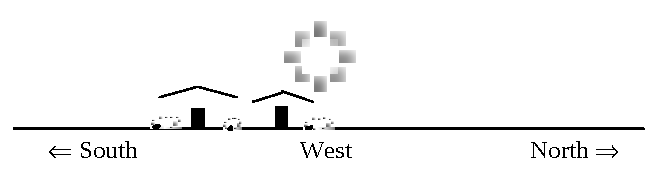
\includegraphics[keepaspectratio,scale=0.75]{ADT-Q09}
    \end{center}
    Where would the Sun appear to set two weeks later?
    \begin{choices}
        \wrongchoice{Farther south}
        \wrongchoice{In the same place}
        %% only northern hemisphere
      \correctchoice{Farther north}
    \end{choices}
\end{question}
}

\element{ADT}{
\begin{question}{ADT-Q10}
    If you could see stars during the day,
        this is what the sky would look like at noon on a given day.
    \begin{center}
        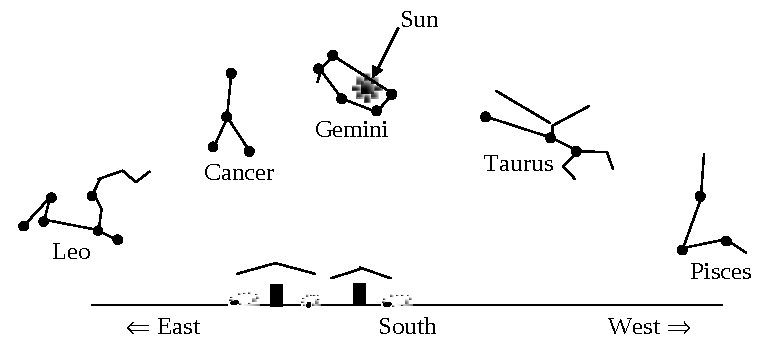
\includegraphics[keepaspectratio,scale=0.66]{ADT-Q10}
    \end{center}
    The Sun is near the stars of the constellation Gemini.
    Near which constellation would you expect the Sun to be located at sunset?
    \begin{multicols}{2}
    \begin{choices}
         \wrongchoice{Leo}
         \wrongchoice{Gemini}
         %% Earth spins toward east,
         %%     constellations seem to move west
       \correctchoice{Pisces}
         \wrongchoice{Cancer}
         \wrongchoice{Taurus}
    \end{choices}
    \end{multicols}
\end{question}
}

\element{ADT}{
\begin{question}{ADT-Q11}
    Compared to the distance to the Moon,
        how far away is the Space Shuttle (when in space) from the Earth?
    \begin{choices}
      \correctchoice{Very close to the Earth}
        \wrongchoice{About half way to the Moon}
        \wrongchoice{Very close to the Moon}
        \wrongchoice{About twice as far as the Moon}
    \end{choices}
\end{question}
}

\element{ADT}{
\begin{question}{ADT-Q12}
    As viewed from our location,
        the stars of the Big Dipper can be connected with imaginary lines to form the shape of a pot with a curved handle.
    To where would you have to travel to first observe a considerable change in the shape formed by these stars?
    \begin{choices}
        \wrongchoice{Across the country}
        \wrongchoice{Moon}
        %% The big dipper is 100 ly away!!
      \correctchoice{A distant star}
        \wrongchoice{Pluto}
        \wrongchoice{Europe}
    \end{choices}
\end{question}
}

\element{ADT}{
\begin{question}{ADT-Q13}
    Which of the following lists is correctly arranged in order of closest-to-most-distant from the Earth?
    \begin{choices}
        \wrongchoice{Stars, Moon, Sun, Pluto}
        \wrongchoice{Moon, Sun, stars, Pluto}
        \wrongchoice{Sun, Moon, Pluto, stars}
        \wrongchoice{Moon, Pluto, Sun, stars}
      \correctchoice{Moon, Sun, Pluto, stars}
    \end{choices}
\end{question}
}

\element{ADT}{
\begin{question}{ADT-Q14}
    Which of the following would make you weigh half as much as you do right now?
    \begin{choices}
        \wrongchoice{Take away half of the Earth's atmosphere.}
        \wrongchoice{Double the distance between the Sun and the Earth.}
        \wrongchoice{Make the Earth spin half as fast.}
      \correctchoice{Take away half of the Earth’s mass.}
        \wrongchoice{More than one of the above}
    \end{choices}
\end{question}
}

\element{ADT}{
\begin{question}{ADT-Q15}
    A person is reading a newspaper while standing 5 feet away from a table that has on it an unshaded 100 watt light bulb.
    Imagine that the table were moved to a distance of 10 feet.
    How many light bulbs in total would have to be placed on the table to light up the newspaper to the same amount of brightness as before?
    \begin{choices}
        \wrongchoice{One bulb.}
      \correctchoice{Four bulbs.}
        \wrongchoice{Two bulbs.}
        \wrongchoice{More than four bulbs.}
        \wrongchoice{Three bulbs.}
    \end{choices}
\end{question}
}

\element{ADT}{
\begin{question}{ADT-Q16}
    According to modern ideas and observations,
        what can be said about the location of the center of the Universe?
    \begin{choices}
        \wrongchoice{The Earth is at the center.}
        \wrongchoice{The Sun is at the center.}
        \wrongchoice{The Milky Way Galaxy is at the center.}
        \wrongchoice{An unknown, distant galaxy is at the center.}
      \correctchoice{The Universe does not have a center.}
    \end{choices}
\end{question}
}

\element{ADT}{
\begin{question}{ADT-Q17}
    The hottest stars are what color?
    \begin{multicols}{2}
    \begin{choices}
        %% highest frequency
      \correctchoice{Blue}
        \wrongchoice{Red}
        \wrongchoice{Orange}
        \wrongchoice{White}
        \wrongchoice{Yellow}
    \end{choices}
    \end{multicols}
\end{question}
}

\element{ADT}{
\begin{question}{ADT-Q18}
    The diagram below shows the Earth and Sun as well as five different possible positions for the Moon.
    \begin{center}
        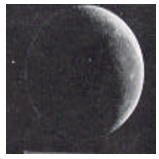
\includegraphics[keepaspectratio,scale=1.0]{ADT-Q18B}
    \end{center}
    Which position of the Moon would cause it to appear like the picture at right when viewed from Earth?
    \begin{center}
        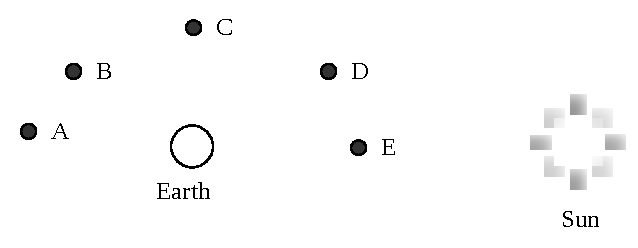
\includegraphics[keepaspectratio,scale=0.75]{ADT-Q18A}
    \end{center}
    \begin{multicols}{5}
    \begin{choices}[o]
        \wrongchoice{$A$}
        \wrongchoice{$B$}
        \wrongchoice{$C$}
      \correctchoice{$D$}
        \wrongchoice{$E$}
    \end{choices}
    \end{multicols}
\end{question}
}

\element{ADT}{
\begin{question}{ADT-Q19}
    You observe a full Moon rising in the east.
    How will it appear in six hours?
    \begin{multicols}{2}
    \begin{choices}
        \AMCboxDimensions{down=-1.5em}
        \wrongchoice{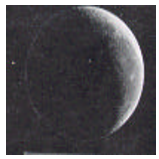
\includegraphics[keepaspectratio,scale=1.0]{ADT-Q19A}}
        \wrongchoice{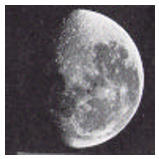
\includegraphics[keepaspectratio,scale=1.0]{ADT-Q19B}}
      \correctchoice{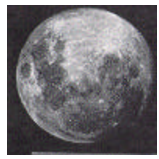
\includegraphics[keepaspectratio,scale=1.0]{ADT-Q19C}}
        \wrongchoice{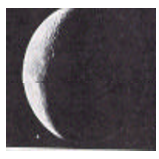
\includegraphics[keepaspectratio,scale=1.0]{ADT-Q19D}}
    \end{choices}
    \end{multicols}
\end{question}
}

\element{ADT}{
\begin{question}{ADT-Q20}
    With your arm held straight,
        your thumb is just wide enough to cover up the Sun.
    If you were on Saturn,
        which is 10 times farther from the Sun than the Earth is,
        what object could you use to just cover up the Sun?
    \begin{choices}
        \wrongchoice{Your wrist}
        \wrongchoice{Your thumb}
        \wrongchoice{A pencil}
        \wrongchoice{A strand of spaghetti}
        %% Inverse squared 1/100 of your thumb
      \correctchoice{A hair}
    \end{choices}
\end{question}
}

\element{ADT}{
\begin{question}{ADT-Q21}
    Global warming is thought to be caused by the:
    \begin{choices}
        \wrongchoice{destruction of the ozone layer.}
        \wrongchoice{trapping of heat by nitrogen.}
      \correctchoice{addition of carbon dioxide.}
    \end{choices}
\end{question}
}

%% Start question indicative
\element{ADT}{
\begin{question}{ADT-Q22}
    \QuestionIndicative
    \scoring{auto=1,v=-1,e=-2}
    In general,
        how confident are you that your answers to this survey are correct?
    \begin{choices}[o]
       \correctchoice{Not at all confident (just guessing)}
       \correctchoice{Not very confident}
       \correctchoice{Not sure}
       \correctchoice{Confident}
       \correctchoice{Very confident}
    \end{choices}
\end{question}
}

\element{ADT}{
\begin{question}{ADT-Q23}
    \QuestionIndicative
    \scoring{auto=1,v=-1,e=-2}
    What is your college major (or current area of interest if undecided)?
    \begin{choices}[o]
       \correctchoice{Business}
       \correctchoice{Education}
       \correctchoice{Humanities, Social Sciences, or the Arts}
       \correctchoice{Science, Engineering, or Architecture}
       \correctchoice{Other}
    \end{choices}
\end{question}
}

\element{ADT}{
\begin{question}{ADT-Q24}
    \QuestionIndicative
    \scoring{auto=1,v=-1,e=-2}
    What was the last math class you completed prior to taking this course?
    \begin{multicols}{2}
    \begin{choices}[o]
       \correctchoice{Algebra}
       \correctchoice{Trigonometry}
       \correctchoice{Geometry}
       \correctchoice{Pre-Calculus}
       \correctchoice{Calculus}
    \end{choices}
    \end{multicols}
\end{question}
}

\element{ADT}{
\begin{question}{ADT-Q25}
    \QuestionIndicative
    \scoring{auto=1,v=-1,e=-2}
    What is your age?
    \begin{choices}[o]
       \correctchoice{0--20 years old}
       \correctchoice{21--23 years old}
       \correctchoice{24--30 years old}
       \correctchoice{31 or older}
       \correctchoice{Decline to answer}
    \end{choices}
\end{question}
}

\element{ADT}{
\begin{question}{ADT-Q26}
    \QuestionIndicative
    \scoring{auto=1,v=-1,e=-2}
    Which best describes your home community (where you attended high school)?
    \begin{choices}[o]
      \correctchoice{Rural}
      \correctchoice{Small town}
      \correctchoice{Suburban}
      \correctchoice{Urban}
      \correctchoice{Not in the USA}
    \end{choices}
\end{question}
}

\element{ADT}{
\begin{question}{ADT-Q27}
    \QuestionIndicative
    \scoring{auto=-1,v=-1,e=-2}
    What is your gender?
    \begin{choices}[o]
       \correctchoice{Female}
       \correctchoice{Decline to answer}
       \correctchoice{Male}
    \end{choices}
\end{question}
}

\element{ADT}{
\begin{question}{ADT-Q28}
    \QuestionIndicative
    \scoring{auto=1,v=-1,e=-2}
    Which best describes your ethnic background?
    \begin{choices}[o]
       \correctchoice{African-American}
       \correctchoice{Asian-American}
       \correctchoice{Native-American}
       \correctchoice{Hispanic-American}
       \correctchoice{None of the above (see question 29 below)}
    \end{choices}
\end{question}
}

\element{ADT}{
\begin{question}{ADT-Q29}
    \QuestionIndicative
    \scoring{auto=1,v=-1,e=-2}
    Which best describes your ethnic background?
    \begin{choices}[o]
       \correctchoice{African (not American)}
       \correctchoice{Asian (not American)}
       \correctchoice{White, non-Hispanic}
       \correctchoice{Multicultural}
       \correctchoice{None of the above (see question 28 above)}
    \end{choices}
\end{question}
}

\element{ADT}{
\begin{question}{ADT-Q30}
    \QuestionIndicative
    \scoring{auto=1,v=-1,e=-2}
    How good at math are you?
    \begin{multicols}{2}
    \begin{choices}[o]
       \correctchoice{Very poor}
       \correctchoice{Poor}
       \correctchoice{Average}
       \correctchoice{Good}
       \correctchoice{Very good}
    \end{choices}
    \end{multicols}
\end{question}
}

\element{ADT}{
\begin{question}{ADT-Q31}
    \QuestionIndicative
    \scoring{auto=1,v=-1,e=-2}
    How good at science are you?
    \begin{multicols}{2}
    \begin{choices}[o]
       \correctchoice{Very poor}
       \correctchoice{Poor}
       \correctchoice{Average}
       \correctchoice{Good}
       \correctchoice{Very good}
    \end{choices}
    \end{multicols}
\end{question}
}

\element{ADT}{
\begin{question}{ADT-Q32}
    \QuestionIndicative
    \scoring{auto=1,v=-1,e=-2}
    Which best describes the level of difficulty you expect/experienced from this course?
    \begin{choices}[o]
       \correctchoice{Extremely difficult for me}
       \correctchoice{Difficult for me}
       \correctchoice{Unsure}
       \correctchoice{Easy for me}
       \correctchoice{Very easy for me}
    \end{choices}
\end{question}
}

\element{ADT}{
\begin{question}{ADT-Q33}
    \QuestionIndicative
    \scoring{auto=1,v=-1,e=-2}
    How many astronomy courses at the college level have you taken?
    \begin{choices}[o]
       \correctchoice{I'm re-taking this course.}
       \correctchoice{This is my first college-level astronomy course.}
       \correctchoice{This is my second college-level astronomy course.}
       \correctchoice{I've completed more than two other college-level astronomy courses.}
    \end{choices}
\end{question}
}


\endinput



%
%% Test of Understandin of vectors: A reliable multiple-choice vector concept test
%% Pablo Barniol and Genearo Zavala
%% Phys. Rev. ST Phys. Educ. Res. 10, 010121--Published 17 June 2014


%% Test of Understanding Vectors
%%--------------------------------------------------
\element{vectors}{
\begin{question}{vectors-q01}
    The figure below shows vectors $\vec{\mathbf{A}}$ and $\vec{\mathbf{B}}$.
    \begin{center}
    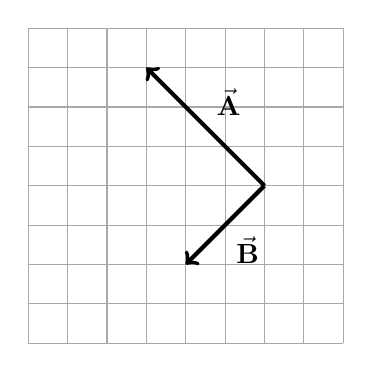
\begin{tikzpicture}
        \draw[white!66!black,step=0.50cm] (0,0) grid (4,4);
        \draw[line width=1.5pt,->] (3,2) -- ++(-1.5,1.5) node[pos=0.5,anchor=south west] {$\vec{\mathbf{A}}$};
        \draw[line width=1.5pt,->] (3,2) -- ++(-1,-1) node[pos=0.5,anchor=north west] {$\vec{\mathbf{B}}$};
    \end{tikzpicture}
    \end{center}
    Choose the option that shows the vector sum 
        $\vec{\mathbf{A}} + \vec{\mathbf{B}}$.
    \begin{multicols}{2}
    \begin{choices}
        \AMCboxDimensions{down=-1.5cm}
        \wrongchoice{
            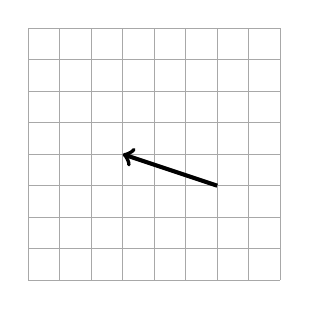
\begin{tikzpicture}[scale=0.8]
                \draw[white!66!black,step=0.50cm] (0,0) grid (4,4);
                \draw[line width=1.5pt,->] (3,1.5) -- ++(-1.5,0.5);
            \end{tikzpicture}
        }
        \wrongchoice{
            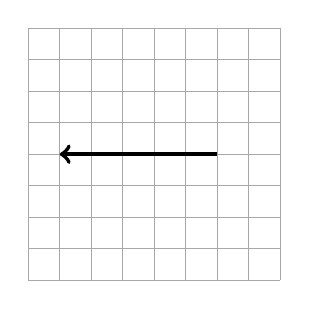
\begin{tikzpicture}[scale=0.8]
                \draw[white!66!black,step=0.50cm] (0,0) grid (4,4);
                \draw[line width=1.5pt,->] (3,2) -- ++(-2.5,0);
            \end{tikzpicture}
        }
        \wrongchoice{
            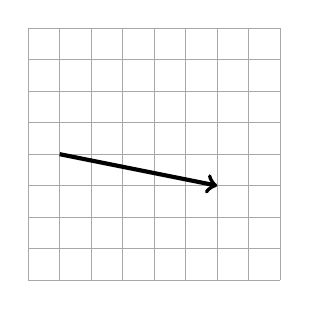
\begin{tikzpicture}[scale=0.8]
                \draw[white!66!black,step=0.50cm] (0,0) grid (4,4);
                \draw[line width=1.5pt,->] (0.5,2) -- ++(2.5,-0.5);
            \end{tikzpicture}
        }
        \wrongchoice{
            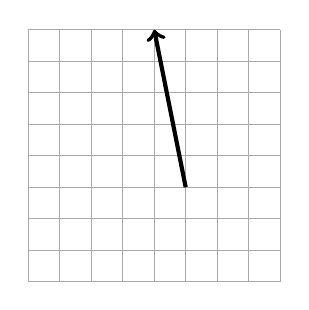
\begin{tikzpicture}[scale=0.8]
                \draw[white!66!black,step=0.50cm] (0,0) grid (4,4);
                \draw[line width=1.5pt,->] (2.5,1.5) -- ++(-0.5,2.5);
            \end{tikzpicture}
        }
        \correctchoice{
            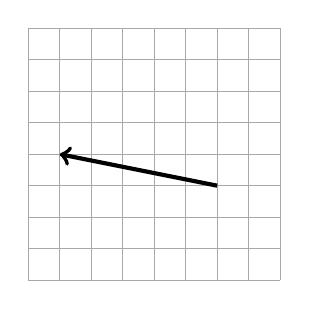
\begin{tikzpicture}[scale=0.8]
                \draw[white!66!black,step=0.50cm] (0,0) grid (4,4);
                \draw[line width=1.5pt,->] (3,1.5) -- ++(-2.5,0.5);
            \end{tikzpicture}
        }
        %% NOTE: six for symmetry
    \end{choices}
    \end{multicols}
\end{question}
}

\element{vectors}{
\begin{question}{vectors-q02}
    The figure below shows vector $\vec{\mathbf{A}}$.
    \begin{center}
    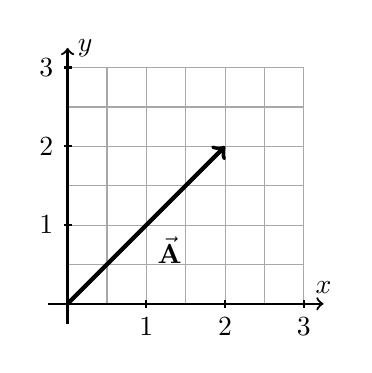
\begin{tikzpicture}
        \draw[white] (-0.5,-0.5) rectangle (3.5,3.5);
        \draw[white!66!black,step=0.5cm] (0,0) grid (3,3);
        \draw[thick,->] (-0.25,0) -- (3.25,0) node[anchor=south] {$x$};
        \draw[thick,->] (0,-0.25) -- (0,3.25) node[anchor=west] {$y$};
        \foreach \i in {1,2,3}{
            \draw[thick] (0.05,\i) -- (-0.05,\i) node[anchor=east] {$\i$};
            \draw[thick] (\i,0.05) -- (\i,-0.05) node[anchor=north] {$\i$};
        }
        \draw[line width=1.5pt,->] (0,0) -- (2,2) node[pos=0.5,anchor=north west] {$\vec{\mathbf{A}}$};
    \end{tikzpicture}
    \end{center}
    Choose the option that shows the unit vector in the direction of vector $\vec{\mathbf{A}}$.
    \begin{multicols}{2}
    \begin{choices}
        \AMCboxDimensions{down=-1.25cm}
        \wrongchoice{
            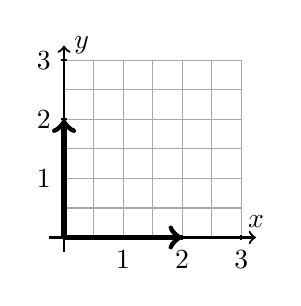
\begin{tikzpicture}[scale=0.75]
                \draw[white] (-0.5,-0.5) rectangle (3.5,3.5);
                \draw[white!66!black,step=0.5cm] (0,0) grid (3,3);
                \draw[thick,->] (-0.25,0) -- (3.25,0) node[anchor=south] {$x$};
                \draw[thick,->] (0,-0.25) -- (0,3.25) node[anchor=west] {$y$};
                \foreach \i in {1,2,3}{
                    \draw[thick] (0.05,\i) -- (-0.05,\i) node[anchor=east] {$\i$};
                    \draw[thick] (\i,0.05) -- (\i,-0.05) node[anchor=north] {$\i$};
                }
                \draw[line width=2.0pt,->] (0,0) -- (0,2);
                \draw[line width=2.0pt,->] (0,0) -- (2,0);
            \end{tikzpicture}
        }
        \wrongchoice{
            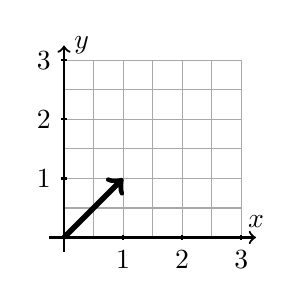
\begin{tikzpicture}[scale=0.75]
                \draw[white] (-0.5,-0.5) rectangle (3.5,3.5);
                \draw[white!66!black,step=0.5cm] (0,0) grid (3,3);
                \draw[thick,->] (-0.25,0) -- (3.25,0) node[anchor=south] {$x$};
                \draw[thick,->] (0,-0.25) -- (0,3.25) node[anchor=west] {$y$};
                \foreach \i in {1,2,3}{
                    \draw[thick] (0.05,\i) -- (-0.05,\i) node[anchor=east] {$\i$};
                    \draw[thick] (\i,0.05) -- (\i,-0.05) node[anchor=north] {$\i$};
                }
                \draw[line width=2.0pt,->] (0,0) -- (1,1);
            \end{tikzpicture}
        }
        %% ANS unit vector has length 1
        \correctchoice{
            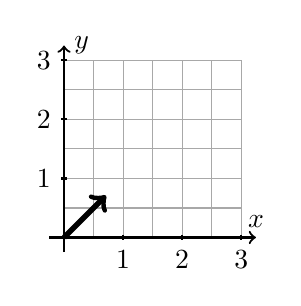
\begin{tikzpicture}[scale=0.75]
                \draw[white] (-0.5,-0.5) rectangle (3.5,3.5);
                \draw[white!66!black,step=0.5cm] (0,0) grid (3,3);
                \draw[thick,->] (-0.25,0) -- (3.25,0) node[anchor=south] {$x$};
                \draw[thick,->] (0,-0.25) -- (0,3.25) node[anchor=west] {$y$};
                \foreach \i in {1,2,3}{
                    \draw[thick] (0.05,\i) -- (-0.05,\i) node[anchor=east] {$\i$};
                    \draw[thick] (\i,0.05) -- (\i,-0.05) node[anchor=north] {$\i$};
                }
                \draw[line width=2.0pt,->] (0,0) -- (0.71,0.71);
            \end{tikzpicture}
        }
        \wrongchoice{
            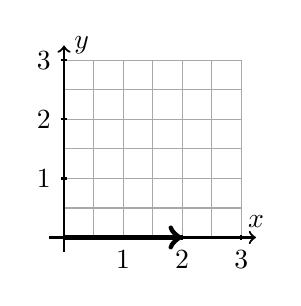
\begin{tikzpicture}[scale=0.75]
                \draw[white] (-0.5,-0.5) rectangle (3.5,3.5);
                \draw[white!66!black,step=0.5cm] (0,0) grid (3,3);
                \draw[thick,->] (-0.25,0) -- (3.25,0) node[anchor=south] {$x$};
                \draw[thick,->] (0,-0.25) -- (0,3.25) node[anchor=west] {$y$};
                \foreach \i in {1,2,3}{
                    \draw[thick] (0.05,\i) -- (-0.05,\i) node[anchor=east] {$\i$};
                    \draw[thick] (\i,0.05) -- (\i,-0.05) node[anchor=north] {$\i$};
                }
                \draw[line width=2.0pt,->] (0,0) -- (2,0);
            \end{tikzpicture}
        }
        \wrongchoice{
            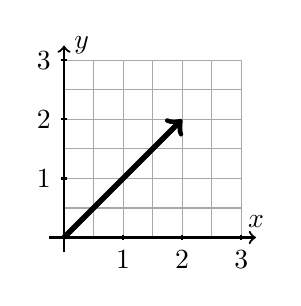
\begin{tikzpicture}[scale=0.75]
                \draw[white] (-0.5,-0.5) rectangle (3.5,3.5);
                \draw[white!66!black,step=0.5cm] (0,0) grid (3,3);
                \draw[thick,->] (-0.25,0) -- (3.25,0) node[anchor=south] {$x$};
                \draw[thick,->] (0,-0.25) -- (0,3.25) node[anchor=west] {$y$};
                \foreach \i in {1,2,3}{
                    \draw[thick] (0.05,\i) -- (-0.05,\i) node[anchor=east] {$\i$};
                    \draw[thick] (\i,0.05) -- (\i,-0.05) node[anchor=north] {$\i$};
                }
                \draw[line width=2.0pt,->] (0,0) -- (2,2);
            \end{tikzpicture}
        }
        %% NOTE: six for symmetry
    \end{choices}
    \end{multicols}
\end{question}
}

\element{vectors}{
\begin{question}{vectors-q03}
    The figure below shows a vector $\vec{\mathbf{C}}$ and $\vec{\mathbf{D}}$.
    \begin{center}
    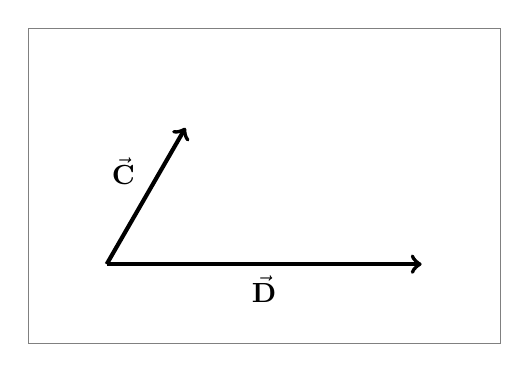
\begin{tikzpicture}
        \draw[help lines] ( -1,-1) rectangle (5,3);
        \draw[line width=1.5pt,->] (0,0) -- (60:2) node[pos=0.5,anchor=south east] {$\vec{\mathbf{C}}$};
        \draw[line width=1.5pt,->] (0,0) -- (0:4) node[pos=0.5,anchor=north] {$\vec{\mathbf{D}}$};
    \end{tikzpicture}
    \end{center}
    Which option is the best interpretation of the dot product $\vec{\mathbf{C}}\cdot\vec{\mathbf{D}}$?
    \begin{choices}
        \wrongchoice{The magnitude of a vector between $\vec{\mathbf{C}}$ and $\vec{\mathbf{D}}$ pointing up to the right.}
      \correctchoice{The projection of vector $\vec{\mathbf{C}}$ onto vector $\vec{\mathbf{D}}$ multplied by teh magnitude of vector $\vec{\mathbf{D}}$.}
        \wrongchoice{A vector between $\vec{\mathbf{C}}$ and $\vec{\mathbf{D}}$ pointing up to the right.}
        \wrongchoice{A vector perpendicular to both vectors.}
        \wrongchoice{A vector in the direction of $\vec{\mathbf{D}}$.}
    \end{choices}
\end{question}
}

\element{vectors}{
\begin{question}{vectors-q04}
    The figure below shows a vector $\vec{\mathbf{A}}$ that forms an angle $\phi$ with the vertical axis.
    \begin{center}
    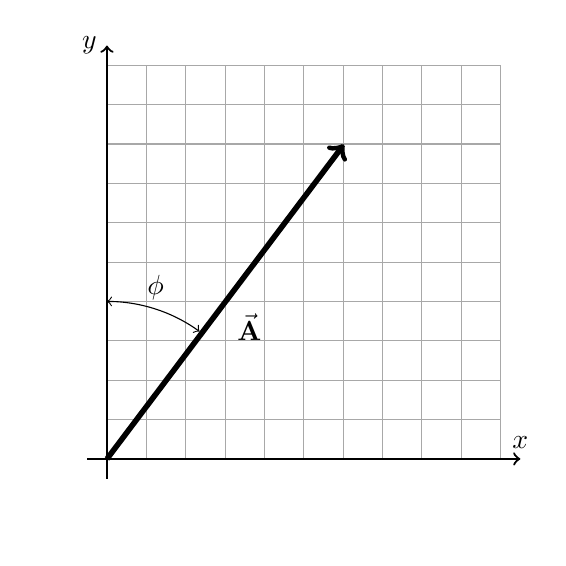
\begin{tikzpicture}
        \draw[white] (-1,-1) rectangle (4,5);
        \draw[white!66!black,step=0.5cm] (0,0) grid (5,5);
        \draw[thick,->] (-0.25,0) -- (5.25,0) node[anchor=south] {$x$};
        \draw[thick,->] (0,-0.25) -- (0,5.25) node[anchor=east] {$y$};
        \draw[line width=2pt,->] (0,0) -- (53:5) node[pos=0.5,anchor=north west] {$\vec{\mathbf{A}}$};
        \draw[<->] (0,2) arc (90:54:2) node[anchor=south,pos=0.5] {$\phi$};
    \end{tikzpicture}
    \end{center}
    Choose the option that shows the $y$-component vector of $\vec{\mathbf{A}}$, (\emph{i.e.} $\vec{\mathbf{A}}_y$).
    \begin{multicols}{2}
    \begin{choices}
        %% NOTE: mix x and y components in x and y direction
        \AMCboxDimensions{down=-1.25cm}
        \wrongchoice{
            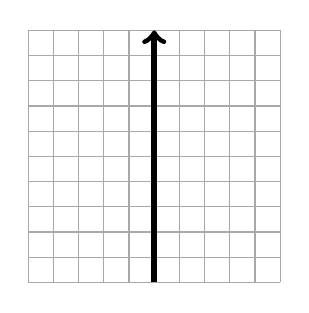
\begin{tikzpicture}[scale=0.64]
                \draw[white!66!black,step=0.5cm] (0,0) grid (5,5);
                \draw[line width=2pt,->] (2.5,0) -- ++(0,5);
            \end{tikzpicture}
        }
        \wrongchoice{
            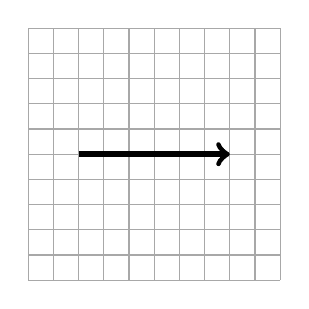
\begin{tikzpicture}[scale=0.64]
                \draw[white!66!black,step=0.5cm] (0,0) grid (5,5);
                \draw[line width=2pt,->] (1,2.5) -- ++(3,0);
            \end{tikzpicture}
        }
        \correctchoice{
            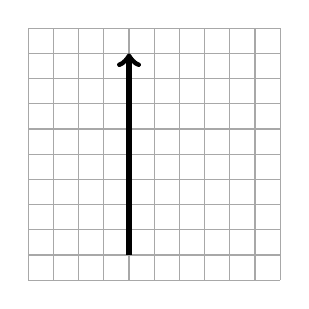
\begin{tikzpicture}[scale=0.64]
                \draw[white!66!black,step=0.5cm] (0,0) grid (5,5);
                \draw[line width=2pt,->] (2,0.5) -- ++(0,4);
            \end{tikzpicture}
        }
        \wrongchoice{
            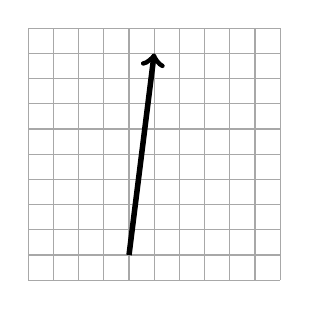
\begin{tikzpicture}[scale=0.64]
                \draw[white!66!black,step=0.5cm] (0,0) grid (5,5);
                \draw[line width=2pt,->] (2,0.5) -- ++(0.5,4);
            \end{tikzpicture}
        }
        \wrongchoice{
            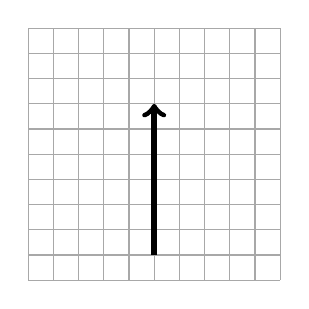
\begin{tikzpicture}[scale=0.64]
                \draw[white!66!black,step=0.5cm] (0,0) grid (5,5);
                \draw[line width=2pt,->] (2.5,0.5) -- ++(0,3);
            \end{tikzpicture}
        }
    \end{choices}
    \end{multicols}
\end{question}
}

\element{vectors}{
\begin{questionmult}{vectors-q05}
    The figure below shows vector $\vec{\mathbf{A}}$.
    \begin{center}
    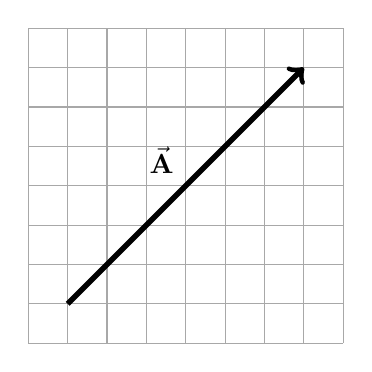
\begin{tikzpicture}
        \draw[white!66!black,step=0.5cm] (0,0) grid (4,4);
        \draw[line width=2pt,->] (0.5,0.5) -- ++(3,3) node[pos=0.5,anchor=south east] {$\vec{\mathbf{A}}$};
    \end{tikzpicture}
    \end{center}
    Which vector(s) has/have the same direction as vector $\vec{\mathbf{A}}$?
    \begin{multicols}{2}
    \begin{choices}
        \AMCboxDimensions{down=-1.5cm}
        %% option H
        \wrongchoice{
            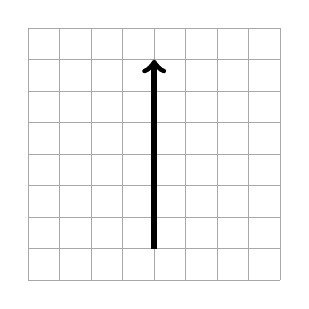
\begin{tikzpicture}[scale=0.8]
                \draw[white!66!black,step=0.5cm] (0,0) grid (4,4);
                \draw[line width=2pt,->] (2,0.5) -- (2,3.5);
            \end{tikzpicture}
        }
        %% option I
        \wrongchoice{
            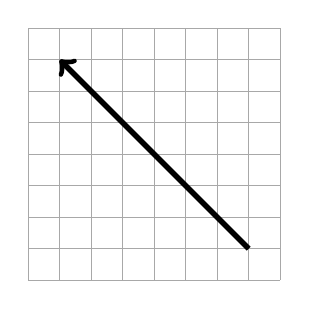
\begin{tikzpicture}[scale=0.8]
                \draw[white!66!black,step=0.5cm] (0,0) grid (4,4);
                \draw[line width=2pt,->] (3.5,0.5) -- (0.5,3.5);
            \end{tikzpicture}
        }
        %% option J
        \wrongchoice{
            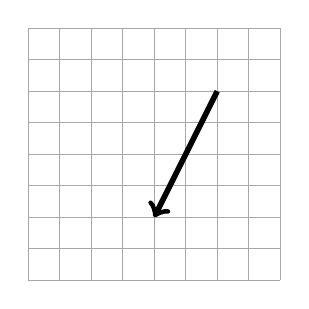
\begin{tikzpicture}[scale=0.8]
                \draw[white!66!black,step=0.5cm] (0,0) grid (4,4);
                \draw[line width=2pt,->] (3,3) -- ++(-1,-2);
            \end{tikzpicture}
        }
        %% option K
        \correctchoice{
            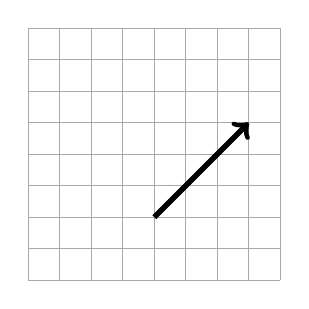
\begin{tikzpicture}[scale=0.8]
                \draw[white!66!black,step=0.5cm] (0,0) grid (4,4);
                \draw[line width=2pt,->] (2,1) -- ++(1.5,1.5);
            \end{tikzpicture}
        }
        %% option L
        \wrongchoice{
            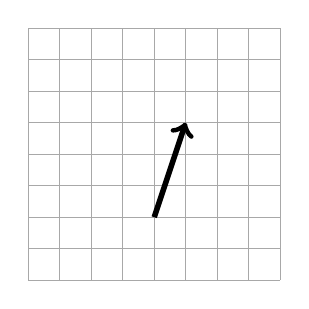
\begin{tikzpicture}[scale=0.8]
                \draw[white!66!black,step=0.5cm] (0,0) grid (4,4);
                \draw[line width=2pt,->] (2,1) -- ++(0.5,1.5);
            \end{tikzpicture}
        }
    \end{choices}
    \end{multicols}
\end{questionmult}
}

\element{vectors}{
\begin{question}{vectors-q06}
    The figure below shows vectors $\vec{\mathbf{A}}$ and $\vec{\mathbf{B}}$ that form an angle $\theta$.
    \begin{center}
    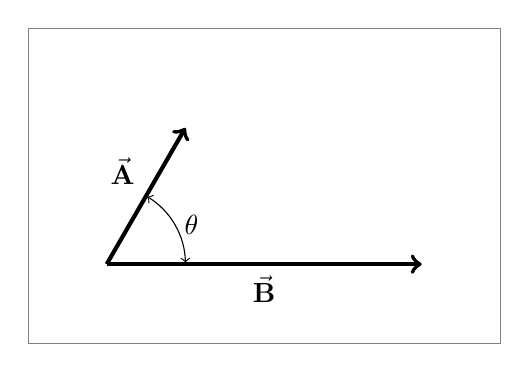
\begin{tikzpicture}
        \draw[help lines] (-1,-1) rectangle (5,3);
        \draw[line width=1.5pt,->] (0,0) -- (60:2) node[pos=0.5,anchor=south east] {$\vec{\mathbf{A}}$};
        \draw[line width=1.5pt,->] (0,0) -- (0:4) node[pos=0.5,anchor=north] {$\vec{\mathbf{B}}$};
        \draw[<->] (1:1) arc (1:59:1) node[pos=0.5,anchor=west] {$\theta$}; 
    \end{tikzpicture}
    \end{center}
    $\left|\vec{\mathbf{A}}\right|$ is the magnitude of vector $\vec{\mathbf{A}}$ and $\left|\vec{\mathbf{B}}\right|$ is the magnitude of vector $\vec{\mathbf{B}}$.
    Which option is the dot product $\left(\vec{\mathbf{A}}\cdot\vec{\mathbf{B}}\right)$?
    \begin{multicols}{2}
    \begin{choices}
        \wrongchoice{$\left|\vec{\mathbf{A}}\right| \left|\vec{\mathbf{B}}\right|$}
      \correctchoice{$\left|\vec{\mathbf{A}}\right| \left|\vec{\mathbf{B}}\right| \cos\theta$}
        \wrongchoice{$\left|\vec{\mathbf{A}}\right| \cos\theta + \left|\vec{\mathbf{B}}\right| \sin\theta$}
        \wrongchoice{$\left|\vec{\mathbf{A}}\right| \left|\vec{\mathbf{B}}\right| \sin\theta$}
        \wrongchoice{$\left|\vec{\mathbf{A}}\right| \cos\theta \left|\vec{\mathbf{B}}\right| \sin\theta$}
    \end{choices}
    \end{multicols}
\end{question}
}

\element{vectors}{
\begin{question}{vectors-q07}
    The figure below shows vectors $\vec{\mathbf{A}}$ and $\vec{\mathbf{B}}$ that have the same magnitude.
    \begin{center}
    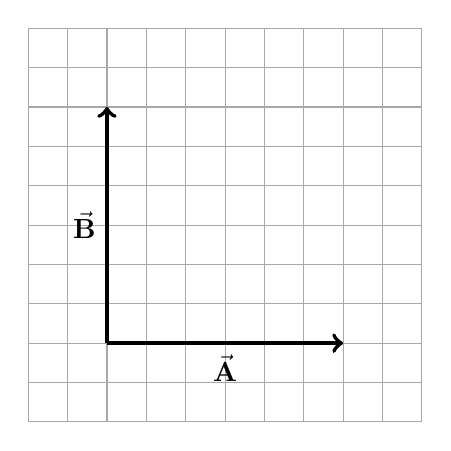
\begin{tikzpicture}
        \draw[white!66!black,step=0.5cm] (-1,-1) grid (4,4);
        \draw[line width=1.5pt,->] (0,0) -- (0:3) node[pos=0.5,anchor=north] {$\vec{\mathbf{A}}$};
        \draw[line width=1.5pt,->] (0,0) -- (90:3) node[pos=0.5,anchor=east] {$\vec{\mathbf{B}}$};
    \end{tikzpicture}
    \end{center}
    Which of the following statements about the magnitude of the vector sum of these two vectors is true?
    \begin{choices}
        \wrongchoice{The magnitude of the vector sum is equal to the magnitude of vector. The vector sum only changes direction.}
      \correctchoice{The magnitude of the vector sum is greater than the magnitude of vector, and it is demonstrated by the direct application of the Pythagorean theorem.}
        \wrongchoice{The magnitude of the vector sum is equal to the magnitude of vector, because vectors and have the same magnitude.}
        \wrongchoice{The magnitude of the vector sum is equal to the magnitude of vector, and it is demonstrated by the direct application of the Pythagorean theorem.}
        \wrongchoice{The magnitude of the vector sum is smaller than the magnitude of vector, because the two vectors are at a \ang{90} angle.}
    \end{choices}
\end{question}
}

\element{vectors}{
\begin{question}{vectors-q08}
    Consider the vector $\vec{\mathbf{A}} = 1\hat{\imath} + 3\hat{\jmath}$
        and $\vec{\mathbf{B}} = 5\hat{\imath}$.
    Which option is the dot product $\left(\vec{\mathbf{A}}\cdot\vec{\mathbf{B}}\right)$?
    \begin{multicols}{2}
    \begin{choices}
      \correctchoice{$5$}
        \wrongchoice{$-15\hat{k}$}
        \wrongchoice{$5\hat{\imath} + 3\hat{\jmath}$}
        \wrongchoice{$6\hat{\imath} + 3\hat{\jmath}$}
        \wrongchoice{$5\hat{\imath}$}
    \end{choices}
    \end{multicols}
\end{question}
}

\element{vectors}{
\begin{question}{vectors-q09}
    The figure below shows vectors $\vec{\mathbf{A}}$ that forms an angle $\phi$ with the vertcial axis.
    \begin{center}
    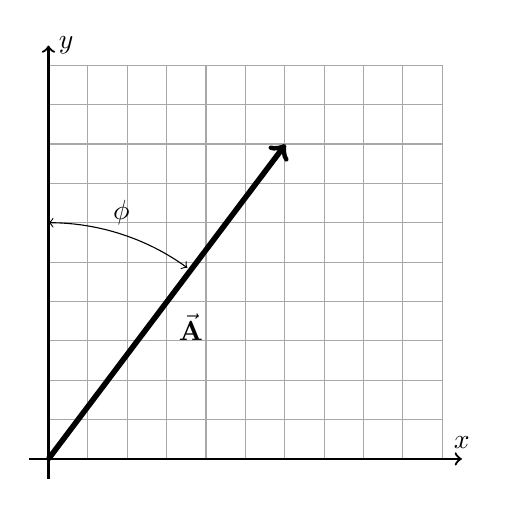
\begin{tikzpicture}
        %\draw[white] (-0.5,-0.2) rectangle (4.5,4.5);
        \draw[white!66!black,step=0.5cm] (0,0) grid (5,5);
        \draw[thick,->] (-0.25,0) -- (5.25,0) node[anchor=south] {$x$};
        \draw[thick,->] (0,-0.25) -- (0,5.25) node[anchor=west] {$y$};
        \draw[line width=2pt,->] (0,0) -- (53:5) node[pos=0.5,anchor=north west] {$\vec{\mathbf{A}}$};
        \draw[<->] (0,3) arc (90:54:3) node[anchor=south,pos=0.5] {$\phi$};
    \end{tikzpicture}
    \end{center}
    Choose the option that shows the $x$-component vector $\vec{\mathbf{A}}$ (\emph{i.e.} $\vec{\mathbf{A}_x}$).
    \begin{multicols}{2}
    \begin{choices}
        \AMCboxDimensions{down=-1.5cm}
        \correctchoice{
            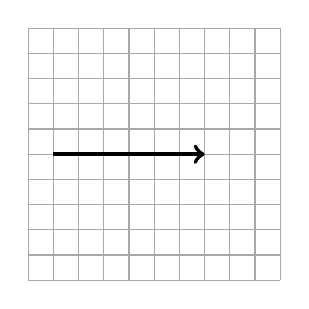
\begin{tikzpicture}[scale=0.64]
                \draw[white!66!black,step=0.5cm] (0,0) grid (5,5);
                \draw[line width=1.5pt,->] (0.5,2.5) -- ++(3,0);
            \end{tikzpicture}
        }
        \wrongchoice{
            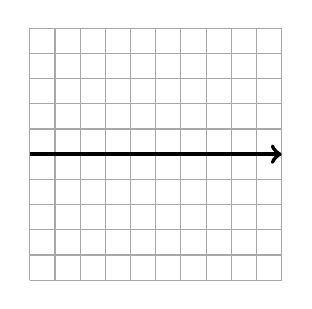
\begin{tikzpicture}[scale=0.64]
                \draw[white!66!black,step=0.5cm] (0,0) grid (5,5);
                \draw[line width=1.5pt,->] (0,2.5) -- ++(5,0);
            \end{tikzpicture}
        }
        \wrongchoice{
            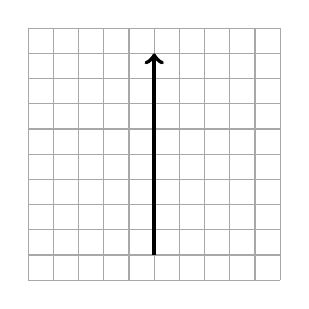
\begin{tikzpicture}[scale=0.64]
                \draw[white!66!black,step=0.5cm] (0,0) grid (5,5);
                \draw[line width=1.5pt,->] (2.5,0.5) -- ++(0,4);
            \end{tikzpicture}
        }
        \wrongchoice{
            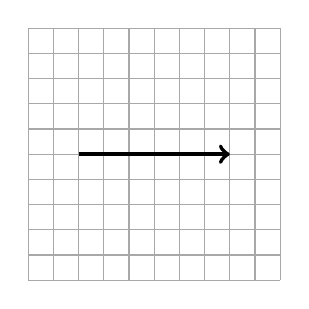
\begin{tikzpicture}[scale=0.64]
                \draw[white!66!black,step=0.5cm] (0,0) grid (5,5);
                \draw[line width=1.5pt,->] (1,2.5) -- ++(3,0);
            \end{tikzpicture}
        }
        \wrongchoice{
            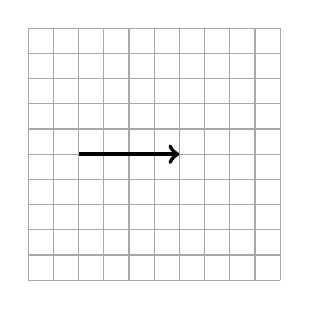
\begin{tikzpicture}[scale=0.64]
                \draw[white!66!black,step=0.5cm] (0,0) grid (5,5);
                \draw[line width=1.5pt,->] (1,2.5) -- ++(2,0);
            \end{tikzpicture}
        }
    \end{choices}
    \end{multicols}
\end{question}
}

\element{vectors}{
\begin{question}{vectors-q10}
    Choose the option that shows the vector $\vec{\mathbf{A}} = -2\hat{\imath} + 3\hat{\jmath}$.
    \begin{multicols}{2}
    \begin{choices}
        \AMCboxDimensions{down=-1.5cm}
        \wrongchoice{
            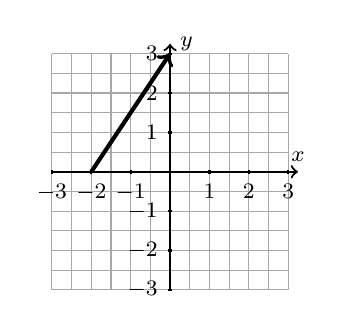
\begin{tikzpicture}[scale=0.5,font=\footnotesize]
                \draw[white!66!black,step=0.50cm] (-3,-3) grid (3,3);
                \draw[thick,->] (-3,0) -- (3.25,0) node[anchor=south] {$x$};
                \draw[thick,->] (0,-3) -- (0,3.25) node[anchor=west] {$y$};
                \foreach \i in {-3,-2,-1,1,2,3}{
                    \draw[thick] (0.05,\i) -- (-0.05,\i) node[anchor=east] {$\i$};
                    \draw[thick] (\i,0.05) -- (\i,-0.05) node[anchor=north] {$\i$};
                }
                \draw[line width=1.5pt,->] (-2,0) -- ++(2,3);
            \end{tikzpicture}
        }
        \correctchoice{
            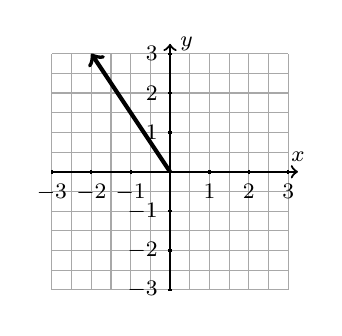
\begin{tikzpicture}[scale=0.5,font=\footnotesize]
                \draw[white!66!black,step=0.50cm] (-3,-3) grid (3,3);
                \draw[thick,->] (-3,0) -- (3.25,0) node[anchor=south] {$x$};
                \draw[thick,->] (0,-3) -- (0,3.25) node[anchor=west] {$y$};
                \foreach \i in {-3,-2,-1,1,2,3}{
                    \draw[thick] (0.05,\i) -- (-0.05,\i) node[anchor=east] {$\i$};
                    \draw[thick] (\i,0.05) -- (\i,-0.05) node[anchor=north] {$\i$};
                }
                \draw[line width=1.5pt,->] (0,0) -- ++(-2,3);
            \end{tikzpicture}
        }
        \wrongchoice{
            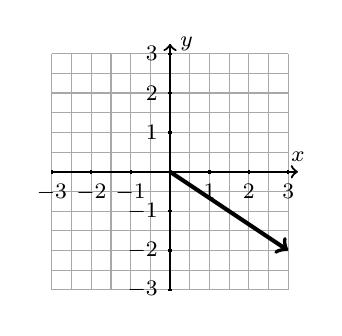
\begin{tikzpicture}[scale=0.5,font=\footnotesize]
                \draw[white!66!black,step=0.50cm] (-3,-3) grid (3,3);
                \draw[thick,->] (-3,0) -- (3.25,0) node[anchor=south] {$x$};
                \draw[thick,->] (0,-3) -- (0,3.25) node[anchor=west] {$y$};
                \foreach \i in {-3,-2,-1,1,2,3}{
                    \draw[thick] (0.05,\i) -- (-0.05,\i) node[anchor=east] {$\i$};
                    \draw[thick] (\i,0.05) -- (\i,-0.05) node[anchor=north] {$\i$};
                }
                \draw[line width=1.5pt,->] (0,0) -- ++(3,-2);
            \end{tikzpicture}
        }
        \wrongchoice{
            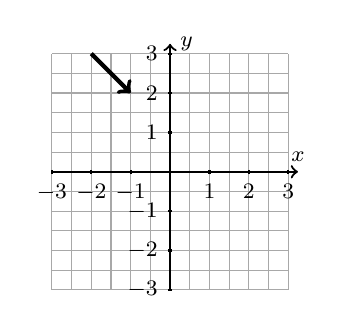
\begin{tikzpicture}[scale=0.5,font=\footnotesize]
                \draw[white!66!black,step=0.50cm] (-3,-3) grid (3,3);
                \draw[thick,->] (-3,0) -- (3.25,0) node[anchor=south] {$x$};
                \draw[thick,->] (0,-3) -- (0,3.25) node[anchor=west] {$y$};
                \foreach \i in {-3,-2,-1,1,2,3}{
                    \draw[thick] (0.05,\i) -- (-0.05,\i) node[anchor=east] {$\i$};
                    \draw[thick] (\i,0.05) -- (\i,-0.05) node[anchor=north] {$\i$};
                }
                \draw[line width=1.5pt,->] (-2,3) -- ++(1,-1);
            \end{tikzpicture}
        }
        \wrongchoice{
            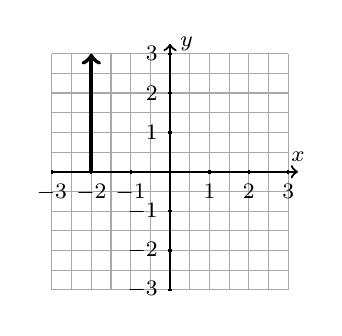
\begin{tikzpicture}[scale=0.5,font=\footnotesize]
                \draw[white!66!black,step=0.50cm] (-3,-3) grid (3,3);
                \draw[thick,->] (-3,0) -- (3.25,0) node[anchor=south] {$x$};
                \draw[thick,->] (0,-3) -- (0,3.25) node[anchor=west] {$y$};
                \foreach \i in {-3,-2,-1,1,2,3}{
                    \draw[thick] (0.05,\i) -- (-0.05,\i) node[anchor=east] {$\i$};
                    \draw[thick] (\i,0.05) -- (\i,-0.05) node[anchor=north] {$\i$};
                }
                \draw[line width=1.5pt,->] (-2,0) -- ++(0,3);
            \end{tikzpicture}
        }
    \end{choices}
    \end{multicols}
\end{question}
}

\element{vectors}{
\begin{question}{vectors-q11}
    The figure below shows vector $\vec{\mathbf{A}}$.
    \begin{center}
    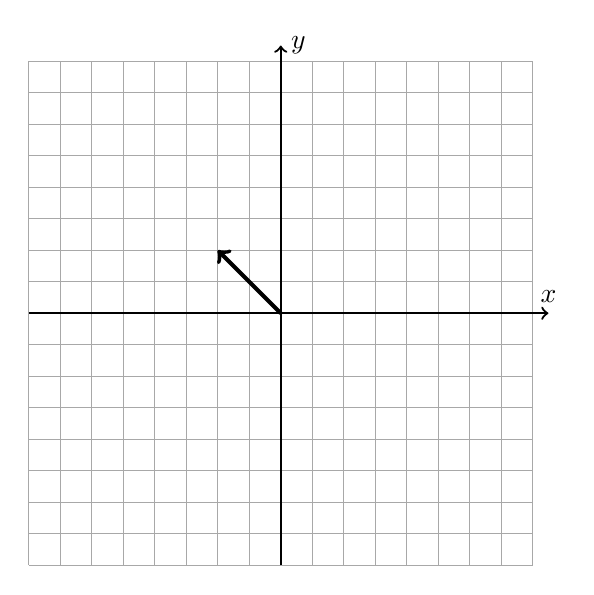
\begin{tikzpicture}[scale=0.8]
        \draw[white!66!black,step=0.50cm] (-4,-4) grid (4,4);
        \draw[thick,->] (-4,0) -- (4.25,0) node[anchor=south] {$x$};
        \draw[thick,->] (0,-4) -- (0,4.25) node[anchor=west] {$y$};
        \draw[line width=1.5pt,->] (0,0) -- ++(-1,1);
    \end{tikzpicture}
    \end{center}
    Choose the option that shows vector $-3\vec{\mathbf{A}}$.
    \begin{multicols}{2}
    \begin{choices}
        \AMCboxDimensions{down=-1.5cm}
        \wrongchoice{
            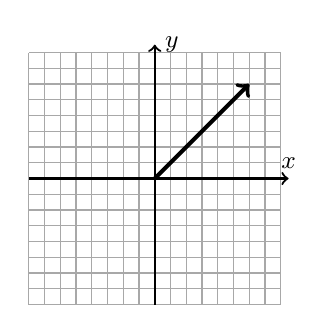
\begin{tikzpicture}[scale=0.4,font=\small]
                \draw[white!66!black,step=0.50cm] (-4,-4) grid (4,4);
                \draw[thick,->] (-4,0) -- (4.25,0) node[anchor=south] {$x$};
                \draw[thick,->] (0,-4) -- (0,4.25) node[anchor=west] {$y$};
                \draw[line width=1.5pt,->] (0,0) -- ++(3,3);
            \end{tikzpicture}
        }
        \wrongchoice{
            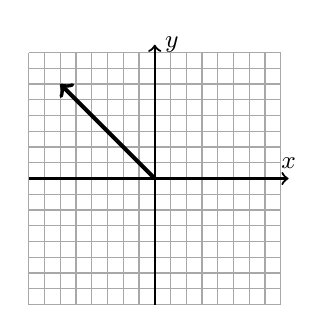
\begin{tikzpicture}[scale=0.4,font=\small]
                \draw[white!66!black,step=0.50cm] (-4,-4) grid (4,4);
                \draw[thick,->] (-4,0) -- (4.25,0) node[anchor=south] {$x$};
                \draw[thick,->] (0,-4) -- (0,4.25) node[anchor=west] {$y$};
                \draw[line width=1.5pt,->] (0,0) -- ++(-3,3);
            \end{tikzpicture}
        }
        \correctchoice{
            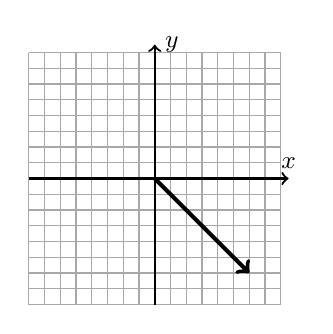
\begin{tikzpicture}[scale=0.4,font=\small]
                \draw[white!66!black,step=0.50cm] (-4,-4) grid (4,4);
                \draw[thick,->] (-4,0) -- (4.25,0) node[anchor=south] {$x$};
                \draw[thick,->] (0,-4) -- (0,4.25) node[anchor=west] {$y$};
                \draw[line width=1.5pt,->] (0,0) -- ++(3,-3);
            \end{tikzpicture}
        }
        \wrongchoice{
            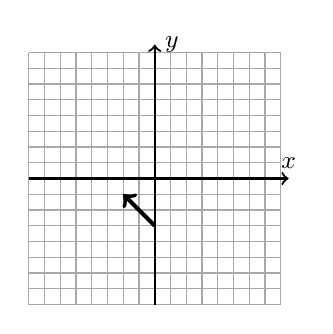
\begin{tikzpicture}[scale=0.4,font=\small]
                \draw[white!66!black,step=0.50cm] (-4,-4) grid (4,4);
                \draw[thick,->] (-4,0) -- (4.25,0) node[anchor=south] {$x$};
                \draw[thick,->] (0,-4) -- (0,4.25) node[anchor=west] {$y$};
                \draw[line width=1.5pt,->] (0,-1.5) -- ++(-1,1);
            \end{tikzpicture}
        }
        \wrongchoice{
            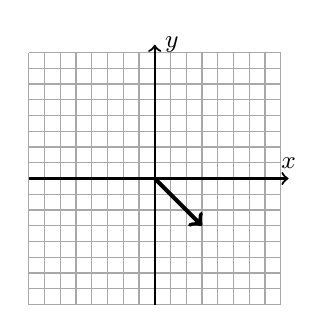
\begin{tikzpicture}[scale=0.4,font=\small]
                \draw[white!66!black,step=0.50cm] (-4,-4) grid (4,4);
                \draw[thick,->] (-4,0) -- (4.25,0) node[anchor=south] {$x$};
                \draw[thick,->] (0,-4) -- (0,4.25) node[anchor=west] {$y$};
                \draw[line width=1.5pt,->] (0,0) -- ++(1.5,-1.5);
            \end{tikzpicture}
        }
    \end{choices}
    \end{multicols}
\end{question}
}

\element{vectors}{
\begin{question}{vectors-q12}
    The figure below shows vectors $\vec{\mathbf{C}}$ and $\vec{\mathbf{A}}$.
    \begin{center}
    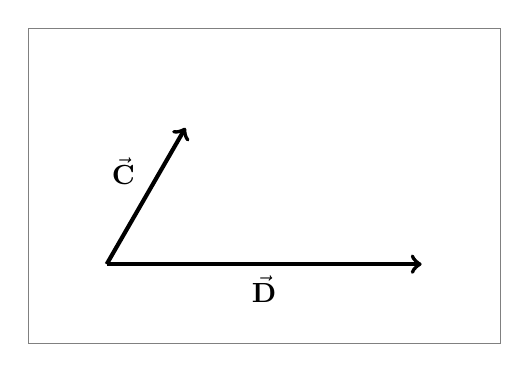
\begin{tikzpicture}
        \draw[help lines] ( -1,-1) rectangle (5,3);
        \draw[line width=1.5pt,->] (0,0) -- (60:2) node[pos=0.5,anchor=south east] {$\vec{\mathbf{C}}$};
        \draw[line width=1.5pt,->] (0,0) -- (0:4) node[pos=0.5,anchor=north] {$\vec{\mathbf{D}}$};
    \end{tikzpicture}
    \end{center}
    Which option is the best interpretation of the cross product
        $\left(\vec{\mathbf{C}}\times\vec{\mathbf{D}}\right)$.
    \begin{choices}
        \wrongchoice{A vector between $\vec{\mathbf{C}}$ and $\vec{\mathbf{D}}$ pointing up to the right.}
        \wrongchoice{A vector perpendicular to both vectors with a direction out of the page.}
        \wrongchoice{The magnitude of a vector between $\vec{\mathbf{C}}$ and $\vec{\mathbf{D}}$ pointing up to the right.}
        \wrongchoice{A quantity in the clock-wise direction.}
      \correctchoice{A vector perpendicular to both vectors with a direction into the page.}
    \end{choices}
\end{question}
}

\element{vectors}{
\begin{question}{vectors-q13}
    The figure below shows vectors $\vec{\mathbf{A}}$ and $\vec{\mathbf{B}}$.
    \begin{center}
    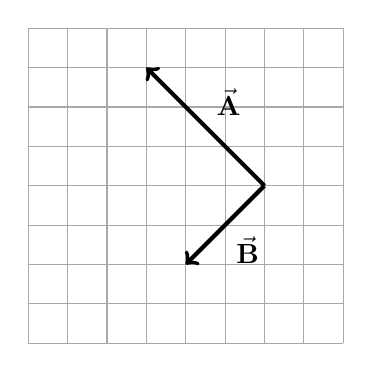
\begin{tikzpicture}
        \draw[white!66!black,step=0.50cm] (0,0) grid (4,4);
        \draw[line width=1.5pt,->] (3,2) -- ++(-1.5,1.5) node[pos=0.5,anchor=south west] {$\vec{\mathbf{A}}$};
        \draw[line width=1.5pt,->] (3,2) -- ++(-1,-1) node[pos=0.5,anchor=north west] {$\vec{\mathbf{B}}$};
    \end{tikzpicture}
    \end{center}
    Choose the option that shows the vector difference $\vec{\mathbf{A}}-\vec{\mathbf{B}}$.
    \begin{multicols}{2}
    \begin{choices}
        \AMCboxDimensions{down=-0.8cm}
        \wrongchoice{
            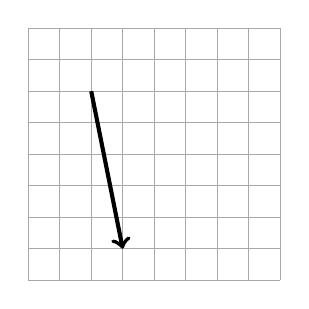
\begin{tikzpicture}[scale=0.8]
                \draw[white!66!black,step=0.50cm] (0,0) grid (4,4);
                \draw[line width=1.5pt,->] (1,3) -- ++(0.5,-2.5);
            \end{tikzpicture}
        }
        \wrongchoice{
            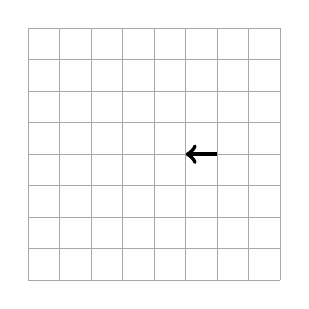
\begin{tikzpicture}[scale=0.8]
                \draw[white!66!black,step=0.50cm] (0,0) grid (4,4);
                \draw[line width=1.5pt,->] (3,2) -- ++(-0.5,0);
            \end{tikzpicture}
        }
        \wrongchoice{
            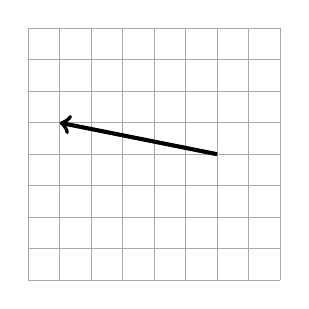
\begin{tikzpicture}[scale=0.8]
                \draw[white!66!black,step=0.50cm] (0,0) grid (4,4);
                \draw[line width=1.5pt,->] (3,2) -- ++(-2.5,0.5);
            \end{tikzpicture}
        }
        \wrongchoice{
            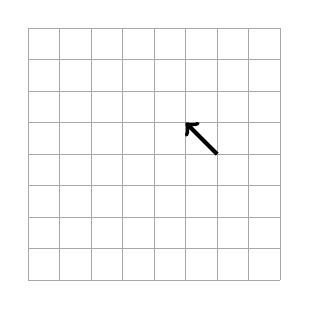
\begin{tikzpicture}[scale=0.8]
                \draw[white!66!black,step=0.50cm] (0,0) grid (4,4);
                \draw[line width=1.5pt,->] (3,2) -- ++(-0.5,0.5);
            \end{tikzpicture}
        }
        \correctchoice{
            \begin{tikzpicture}[scale=0.8]
                \draw[white!66!black,step=0.50cm] (0,0) grid (4,4);
                \draw[line width=1.5pt,->] (2.5,1) -- ++(-0.5,2.5);
            \end{tikzpicture}
        }
    \end{choices}
    \end{multicols}
\end{question}
}

\element{vectors}{
\begin{question}{vectors-q14}
    The figure below shows vector $\vec{\mathbf{A}}$ that forms an angle $\phi$ with the vertical axis.
    \begin{center}
    \begin{tikzpicture}
        %\draw[white] (-0.5,-0.2) rectangle (4.5,4.5);
        %\draw[white!66!black,step=0.5cm] (0,0) grid (4,4);
        \draw[thick,->] (-0.25,0) -- (4.25,0) node[anchor=south] {$x$};
        \draw[thick,->] (0,-0.25) -- (0,4.25) node[anchor=west] {$y$};
        \draw[line width=2pt,->] (0,0) -- (53:5) node[pos=0.5,anchor=north west] {$\vec{\mathbf{A}}$};
        \draw[<->] (0,3) arc (90:53:3) node[anchor=south,pos=0.5] {$\phi$};
    \end{tikzpicture}
    \end{center}
    $\left|\vec{\mathbf{A}}\right|$ is the magnitude of vector $\vec{\mathbf{A}}$.
    Which option shows the magnitude of the $x$-component of vector $\vec{\mathbf{A}}$, (\emph{i.e.} $\vec{\mathbf{A}_x}$)?
    \begin{multicols}{2}
    \begin{choices}
        \wrongchoice{$\left|\vec{\mathbf{A}_x}\right| = \left|\vec{\mathbf{A}}\right| \tan\phi$}
        \wrongchoice{$\left|\vec{\mathbf{A}_x}\right| = \dfrac{\left|\vec{\mathbf{A}}\right|}{\cos\phi}$}
      \correctchoice{$\left|\vec{\mathbf{A}_x}\right| = \left|\vec{\mathbf{A}}\right| \sin\phi$}
        \wrongchoice{$\left|\vec{\mathbf{A}_x}\right| = \left|\vec{\mathbf{A}}\right| \cos\phi$}
        \wrongchoice{$\left|\vec{\mathbf{A}_x}\right| = \dfrac{\left|\vec{\mathbf{A}}\right|}{\sin\phi}$}
    \end{choices}
    \end{multicols}
\end{question}
}

\element{vectors}{
\begin{question}{vectors-q15}
    Consider the vector $\vec{\mathbf{A}} = 1\hat{\imath} + 3\hat{\jmath}$ and the vector $\vec{\mathbf{B}}=5\hat{\imath}$.
    Which option is the cross product $\left(\vec{\mathbf{A}}\times\vec{\mathbf{B}}\right)$?
    \begin{multicols}{2}
    \begin{choices}
      \correctchoice{$-15\hat{k}$}
        \wrongchoice{$5\hat{\imath} + 15\hat{k}$}
        \wrongchoice{$5\hat{\imath} + 3\hat{k}$}
        \wrongchoice{$15\hat{k}$}
        \wrongchoice{$6\hat{\imath} + 3\hat{k}$}
    \end{choices}
    \end{multicols}
\end{question}
}

\element{vectors}{
\begin{question}{vectors-q16}
    The figure below shows vectors $\vec{\mathbf{A}}$ and $\vec{\mathbf{B}}$ that have the same magnitude. 
    \begin{center}
    \begin{tikzpicture}
        \draw[white!66!black,step=0.50cm] (-3,-1) grid (4,3);
        \draw[line width=1.5pt,->] (0,0) -- (0:3) node[pos=0.5,anchor=north] {$\vec{\mathbf{A}}$};
        \draw[line width=1.5pt,->] (0,0) -- (143:3) node[pos=0.5,anchor=north east] {$\vec{\mathbf{B}}$};
    \end{tikzpicture}
    \end{center}
    Which of the following statements about the magnitude of the vector sum of these two vectors is true?
    \begin{choices}
        \wrongchoice{The magnitude of the vector sum is greater than the magnitude of vector, and it is demonstrated by the direct application of the Pythagorean theorem.}
      \correctchoice{The magnitude of the vector sum is smaller than the magnitude of vector, because if we do the graphical addition of the two vectors we note that the vector sum is smaller.}
        \wrongchoice{The magnitude of the vector sum is greater than the magnitude of vector, because the addition of two vectors always gives a resultant vector with a greater magnitude than the vectors that are added up.}
        \wrongchoice{The magnitude of the vector sum is equal to the magnitude of vector, and it is demonstrated by the direct application of the Pythagorean theorem.}
        \wrongchoice{The magnitude of the vector sum is greater than the magnitude of vector, because the distance between the tips of the arrows is longer than the magnitude of vector.}
    \end{choices}
\end{question}
}

\element{vectors}{
\begin{question}{vectors-q17}
    Consider the vector $\vec{\mathbf{A}} = 3\hat{\imath} + 4\hat{\jmath}$.
    Which option shows the direction of this vector as measured from the positive $x$-direction?
    \begin{multicols}{2}
    \begin{choices}
        \wrongchoice{\ang{126.87}}
      \correctchoice{\ang{53.13}}
        \wrongchoice{\ang{143.13}}
        \wrongchoice{\ang{135}}
        \wrongchoice{\ang{-53.13}}
    \end{choices}
    \end{multicols}
\end{question}
}

\element{vectors}{
\begin{question}{vectors-q18}
    The figure below shows vectors $\vec{\mathbf{A}}$ and $\vec{\mathbf{B}}$ that forms an angle $\theta$.
    \begin{center}
    \begin{tikzpicture}
        \draw[help lines] ( -1,-1) rectangle (5,3);
        \draw[line width=1.5pt,->] (0,0) -- (60:2) node[pos=0.5,anchor=south east] {$\vec{\mathbf{A}}$};
        \draw[line width=1.5pt,->] (0,0) -- (0:4) node[pos=0.5,anchor=north] {$\vec{\mathbf{B}}$};
        \draw[<->] (1,0) arc (0:59:1) node[pos=0.5,anchor=west] {$\theta$};
    \end{tikzpicture}
    \end{center}
    $\left|\vec{\mathbf{A}}\right|$ is the magnitude of vector $\vec{\mathbf{A}}$ and $\left|\vec{\mathbf{B}}\right|$ is the magnitude of vector $\vec{\mathbf{B}}$.
    Which option is the magnitude of the cross product $\left(\vec{\mathbf{A}}\times\vec{\mathbf{B}}\right)$?
    \begin{multicols}{2}
    \begin{choices}
        \wrongchoice{$\left|\vec{\mathbf{A}}\right| \cos\theta \left|\vec{\mathbf{B}}\right| \sin\theta$}
        \wrongchoice{$\left|\vec{\mathbf{A}}\right| \left|\vec{\mathbf{B}}\right|$}
        \wrongchoice{$\left|\vec{\mathbf{A}}\right| \left|\vec{\mathbf{B}}\right| \sin\left(\ang{90}-\theta\right)$}
      \correctchoice{$\left|\vec{\mathbf{A}}\right| \left|\vec{\mathbf{B}}\right| \sin\theta$}
        \wrongchoice{$\left|\vec{\mathbf{A}}\right| \left|\vec{\mathbf{B}}\right| \cos\theta$}
    \end{choices}
    \end{multicols}
\end{question}
}

\element{vectors}{
\begin{question}{vectors-q19}
    The figure below shows vectors $\vec{\mathbf{A}}$ and $\vec{\mathbf{B}}$.
    \begin{center}
    \begin{tikzpicture}
        \draw[white!66!black,step=0.50cm] (0,0) grid (4,4);
        \draw[line width=1.5pt,->] (+2.5,3) -- ++(-1.5,0) node[pos=0.5,anchor=south] {$\vec{\mathbf{A}}$};
        \draw[line width=1.5pt,->] (+0.5,1) -- ++(2.5,0) node[pos=0.5,anchor=north] {$\vec{\mathbf{B}}$};
    \end{tikzpicture}
    \end{center}
    Choose the option that shows the vector difference $\vec{\mathbf{A}}-\vec{\mathbf{B}}$.
    \begin{multicols}{2}
    \begin{choices}
        \AMCboxDimensions{down=-0.6cm}
        \wrongchoice{
            \begin{tikzpicture}[scale=0.8]
                \draw[white!66!black,step=0.50cm] (0,0) grid (4,2);
                \draw[line width=1.5pt,->] (0.5,1) -- (2.5,1);
            \end{tikzpicture}
        }
        \wrongchoice{
            \begin{tikzpicture}[scale=0.8]
                \draw[white!66!black,step=0.50cm] (0,0) grid (4,2);
                \draw[line width=1.5pt,->] (0.5,1) -- (1.5,1);
            \end{tikzpicture}
        }
        \wrongchoice{
            \begin{tikzpicture}[scale=0.8]
                \draw[white!66!black,step=0.50cm] (0,0) grid (4,2);
                \draw[line width=1.5pt,<-] (0.5,1) -- (1.5,1);
            \end{tikzpicture}
        }
        \wrongchoice{
            \begin{tikzpicture}[scale=0.8]
                \draw[white!66!black,step=0.50cm] (0,0) grid (4,2);
                \draw[line width=1.5pt,->] (0,1) -- (4,1);
            \end{tikzpicture}
        }
        \correctchoice{
            \begin{tikzpicture}[scale=0.8]
                \draw[white!66!black,step=0.50cm] (0,0) grid (4,2);
                \draw[line width=1.5pt,<-] (0,1) -- (4,1);
            \end{tikzpicture}
        }
    \end{choices}
    \end{multicols}
\end{question}
}

\element{vectors}{
\begin{question}{vectors-q20}
    Consider the vector $\vec{\mathbf{A}} = 2\hat{\imath} + 2\hat{\jmath}$.
    Which option shows the magnitude of this vector?
    \begin{multicols}{2}
    \begin{choices}
        \wrongchoice{$2$}
      \correctchoice{$\sqrt{8}$} %% Also: 2\sqrt{2}
        \wrongchoice{$4$}
        \wrongchoice{$\dfrac{2}{\sqrt{8}}\hat{\imath} + \dfrac{2}{\sqrt{8}}\hat{\jmath}$}
        \wrongchoice{$8$}
    \end{choices}
    \end{multicols}
\end{question}
}


\endinput



%
%% Drawing and using free body diagrams: Why it may be better not to decompose forces
%% Ivica Aviani, Natasa Erceg, and Vanes Mesic
%% Phys. Rev. ST Phys. Educ. Res. 10, 020137--Published 2015
%% DOI: 10.1103/PhysRevSTPER.11.020137


%% Free Body Diagrams, 020137 pp12
%%--------------------------------------------------
\element{FBD}{
\begin{question}{FBD-Q01}
    A block is resting on a horizontal surface.
    Which of the following diagrams correctly shows the forces acting on the block?
    \begin{multicols}{2}
    \begin{choices}
        \AMCboxDimensions{down=-1.5cm}
        \wrongchoice{
            \begin{tikzpicture}[scale=0.8]
                \draw[dashed,white!90!black] (-2,-1.5) rectangle (2,2.5);
                \draw[very thick] (-2,0) -- (2,0);
                \node[draw,minimum width=1.5cm,minimum height=0.75cm,anchor=south] (B) at (0,0) {};
                \draw[fill] (B.center) circle (2pt);
                \draw[very thick,->] (B.center) -- ++(270:2) node[anchor=south west] {1};
            \end{tikzpicture}
        }
        \wrongchoice{
            \begin{tikzpicture}[scale=0.8]
                \draw[dashed,white!90!black] (-2,-1.5) rectangle (2,2.5);
                \draw[very thick] (-2,0) -- (2,0);
                \node[draw,minimum width=1.5cm,minimum height=0.75cm,anchor=south] (B) at (0,0) {};
                \draw[fill] (B.center) circle (2pt);
                \draw[very thick,->] (B.center) -- ++(270:2) node[anchor=south west] {1};
                \draw[very thick,->] (B.center) -- ++(0:2) node[anchor=south east] {2};
                \draw[very thick,->] (B.center) -- ++(180:2) node[anchor=south west] {3};
            \end{tikzpicture}
        }
        \correctchoice{
            \begin{tikzpicture}[scale=0.8]
                \draw[dashed,white!90!black] (-2,-1.5) rectangle (2,2.5);
                \draw[very thick] (-2,0) -- (2,0);
                \node[draw,minimum width=1.5cm,minimum height=0.75cm,anchor=south] (B) at (0,0) {};
                \draw[fill] (B.center) circle (2pt);
                \draw[very thick,->] (B.center) -- ++(270:2) node[anchor=south west] {1};
                \draw[very thick,->] (B.center) -- ++(90:2) node[anchor=north west] {2};
            \end{tikzpicture}
        }
        \wrongchoice{
            \begin{tikzpicture}[scale=0.8]
                \draw[dashed,white!90!black] (-2,-1.5) rectangle (2,2.5);
                \draw[very thick] (-2,0) -- (2,0);
                \node[draw,minimum width=1.5cm,minimum height=0.75cm,anchor=south] (B) at (0,0) {};
                \draw[fill] (B.center) circle (2pt);
                \draw[very thick,->] (B.center) -- ++(180:2) node[anchor=south west] {2};
                \draw[very thick,->] (B.center) -- ++(0:2) node[anchor=south east] {1};
            \end{tikzpicture}
        }
        \wrongchoice{
            \begin{tikzpicture}[scale=0.8]
                \draw[dashed,white!90!black] (-2,-1.5) rectangle (2,2.5);
                \draw[very thick] (-2,0) -- (2,0);
                \node[draw,minimum width=1.5cm,minimum height=0.75cm,anchor=south] (B) at (0,0) {};
                \draw[fill] (B.center) circle (2pt);
                \draw[very thick,->] (B.center) -- ++(90:2) node[anchor=south west] {1};
            \end{tikzpicture}
        }
    \end{choices}
    \end{multicols}
\end{question}
}

\element{FBD}{
\begin{question}{FBD-Q02}
    The pulling force $F$ is acting on a block, but the block is still at rest.
    Which of the following diagrams correctly shows the forces acting on the block?
    \begin{multicols}{2}
    \begin{choices}
        \AMCboxDimensions{down=-1.5cm}
        \wrongchoice{
            \begin{tikzpicture}[scale=0.8]
                \draw[dashed,white!90!black] (-2,-1.5) rectangle (2,2.5);
                \draw[very thick] (-2,0) -- (2,0);
                \node[draw,minimum width=1.5cm,minimum height=0.75cm,anchor=south] (B) at (0,0) {};
                \draw[fill] (B.center) circle (2pt);
                \draw[very thick,->] (B.center) -- ++(270:2) node[anchor=south west] {1};
                \draw[very thick,->] (B.center) -- ++(0:2) node[anchor=south east] {2};
                \draw[very thick,->] (B.center) -- ++(90:1) node[anchor=south] {3};
                \draw[very thick,->] (B.center) -- ++(180:2) node[anchor=south west] {4};
                \draw[very thick,->] (B.center) -- ++(2,1) node[anchor=south east] {$F$};
            \end{tikzpicture}
        }
        \wrongchoice{
            \begin{tikzpicture}[scale=0.8]
                \draw[dashed,white!90!black] (-2,-1.5) rectangle (2,2.5);
                \draw[very thick] (-2,0) -- (2,0);
                \node[draw,minimum width=1.5cm,minimum height=0.75cm,anchor=south] (B) at (0,0) {};
                \draw[fill] (B.center) circle (2pt);
                \draw[very thick,->] (B.center) -- ++(270:2) node[anchor=south west] {1};
                \draw[very thick,->] (B.center) -- ++(180:2) node[anchor=south west] {2};
                \draw[very thick,->] (B.center) -- ++(2,1) node[anchor=south east] {$F$};
            \end{tikzpicture}
        }
        \wrongchoice{
            \begin{tikzpicture}[scale=0.8]
                \draw[dashed,white!90!black] (-2,-1.5) rectangle (2,2.5);
                \draw[very thick] (-2,0) -- (2,0);
                \node[draw,minimum width=1.5cm,minimum height=0.75cm,anchor=south] (B) at (0,0) {};
                \draw[fill] (B.center) circle (2pt);
                \draw[very thick,->] (B.center) -- ++(270:2) node[anchor=south west] {1};
                \draw[very thick,->] (B.center) -- ++(90:1) node[anchor=south] {2};
                \draw[very thick,->] (B.center) -- ++(2,1) node[anchor=south east] {$F$};
            \end{tikzpicture}
        }
        \wrongchoice{
            \begin{tikzpicture}[scale=0.8]
                \draw[dashed,white!90!black] (-2,-1.5) rectangle (2,2.5);
                \draw[very thick] (-2,0) -- (2,0);
                \node[draw,minimum width=1.5cm,minimum height=0.75cm,anchor=south] (B) at (0,0) {};
                \draw[fill] (B.center) circle (2pt);
                \draw[very thick,->] (B.center) -- ++(270:2) node[anchor=south west] {1};
                \draw[very thick,->] (B.center) -- ++(90:1) node[anchor=south] {2};
                \draw[very thick,->] (B.center) -- ++(180:2) node[anchor=south west] {3};
                \draw[very thick,->] (B.center) -- ++(2,1) node[anchor=south east] {$F$};
            \end{tikzpicture}
        }
        \correctchoice{
            \begin{tikzpicture}[scale=0.8]
                \draw[dashed,white!90!black] (-2,-1.5) rectangle (2,2.5);
                \draw[very thick] (-2,0) -- (2,0);
                \node[draw,minimum width=1.5cm,minimum height=0.75cm,anchor=south] (B) at (0,0) {};
                \draw[fill] (B.center) circle (2pt);
                \draw[very thick,->] (B.center) -- ++(270:1) node[anchor=north] {1};
                \draw[very thick,->] (B.center) -- ++(180:2) node[anchor=south west] {2};
                \draw[very thick,->] (B.center) -- ++(2,1) node[anchor=south east] {$F$};
            \end{tikzpicture}
        }
    \end{choices}
    \end{multicols}
\end{question}
}

\element{FBD}{
\begin{question}{FBD-Q03}
    A block is sliding along a horizontal surface at constant speed.
    Which of the following diagrams correctly shows the forces acting on the block?
    \begin{multicols}{2}
    \begin{choices}
        \AMCboxDimensions{down=-1.5cm}
        \wrongchoice{
            \begin{tikzpicture}[scale=0.8]
                \draw[dashed,white!90!black] (-2,-1.5) rectangle (2,2.5);
                \draw[very thick] (-2,0) -- (2,0);
                \node[draw,minimum width=1.5cm,minimum height=0.75cm,anchor=south] (B) at (0,0) {};
                \draw[fill] (B.center) circle (2pt);
                \draw[very thick,->] (B.center) -- ++(270:2) node[anchor=south west] {1};
                \draw[very thick,->] (B.center) -- ++(0:2) node[anchor=south east] {2};
                \draw[very thick,->] (B.center) -- ++(180:2) node[anchor=south west] {3};
            \end{tikzpicture}
        }
        \wrongchoice{
            \begin{tikzpicture}[scale=0.8]
                \draw[dashed,white!90!black] (-2,-1.5) rectangle (2,2.5);
                \draw[very thick] (-2,0) -- (2,0);
                \node[draw,minimum width=1.5cm,minimum height=0.75cm,anchor=south] (B) at (0,0) {};
                \draw[fill] (B.center) circle (2pt);
                \draw[very thick,->] (B.center) -- ++(0:2) node[anchor=south east] {1};
                \draw[very thick,->] (B.center) -- ++(180:2) node[anchor=south west] {2};
            \end{tikzpicture}
        }
        \wrongchoice{
            \begin{tikzpicture}[scale=0.8]
                \draw[dashed,white!90!black] (-2,-1.5) rectangle (2,2.5);
                \draw[very thick] (-2,0) -- (2,0);
                \node[draw,minimum width=1.5cm,minimum height=0.75cm,anchor=south] (B) at (0,0) {};
                \draw[fill] (B.center) circle (2pt);
                \draw[very thick,->] (B.center) -- ++(270:2) node[anchor=south west] {1};
                \draw[very thick,->] (B.center) -- ++(0:1) node[anchor=west] {2};
                \draw[very thick,->] (B.center) -- ++(90:2) node[anchor=north west] {3};
                \draw[very thick,->] (B.center) -- ++(180:2) node[anchor=south west] {4};
            \end{tikzpicture}
        }
        \wrongchoice{
            \begin{tikzpicture}[scale=0.8]
                \draw[dashed,white!90!black] (-2,-1.5) rectangle (2,2.5);
                \draw[very thick] (-2,0) -- (2,0);
                \node[draw,minimum width=1.5cm,minimum height=0.75cm,anchor=south] (B) at (0,0) {};
                \draw[fill] (B.center) circle (2pt);
                \draw[very thick,->] (B.center) -- ++(270:2) node[anchor=south west] {1};
                \draw[very thick,->] (B.center) -- ++(180:2) node[anchor=south west] {2};
            \end{tikzpicture}
        }
        \correctchoice{
            \begin{tikzpicture}[scale=0.8]
                \draw[dashed,white!90!black] (-2,-1.5) rectangle (2,2.5);
                \draw[very thick] (-2,0) -- (2,0);
                \node[draw,minimum width=1.5cm,minimum height=0.75cm,anchor=south] (B) at (0,0) {};
                \draw[fill] (B.center) circle (2pt);
                \draw[very thick,->] (B.center) -- ++(270:2) node[anchor=south west] {1};
                \draw[very thick,->] (B.center) -- ++(0:2) node[anchor=south east] {2};
                \draw[very thick,->] (B.center) -- ++(90:2) node[anchor=north west] {3};
                \draw[very thick,->] (B.center) -- ++(180:2) node[anchor=south west] {4};
            \end{tikzpicture}
        }
    \end{choices}
    \end{multicols}
\end{question}
}

\element{FBD}{
\begin{question}{FBD-Q04}
    A block is accelerating along a horizontal surface.
    Which of the following diagrams correctly shows the forces acting on the block?
    \begin{multicols}{2}
    \begin{choices}
        \AMCboxDimensions{down=-1.5cm}
        %% NOTE: we cannot ignore friction, see A and B
        \correctchoice{
            \begin{tikzpicture}[scale=0.8]
                \draw[dashed,white!90!black] (-2,-1.5) rectangle (2,2.5);
                \draw[very thick] (-2,0) -- (2,0);
                \node[draw,minimum width=1.5cm,minimum height=0.75cm,anchor=south] (B) at (0,0) {};
                \draw[fill] (B.center) circle (2pt);
                \draw[very thick,->] (B.center) -- ++(270:2) node[anchor=south west] {1};
                \draw[very thick,->] (B.center) -- ++(0:2) node[anchor=south east] {2};
                \draw[very thick,->] (B.center) -- ++(90:2) node[anchor=north west] {3};
                \draw[very thick,->] (B.center) -- ++(180:1) node[anchor=east] {4};
            \end{tikzpicture}
        }
        \wrongchoice{
            \begin{tikzpicture}[scale=0.8]
                \draw[dashed,white!90!black] (-2,-1.5) rectangle (2,2.5);
                \draw[very thick] (-2,0) -- (2,0);
                \node[draw,minimum width=1.5cm,minimum height=0.75cm,anchor=south] (B) at (0,0) {};
                \draw[fill] (B.center) circle (2pt);
                \draw[very thick,->] (B.center) -- ++(270:2) node[anchor=south west] {1};
                \draw[very thick,->] (B.center) -- ++(0:2) node[anchor=south east] {2};
                \draw[very thick,->] (B.center) -- ++(90:2) node[anchor=north west] {3};
            \end{tikzpicture}
        }
        \wrongchoice{
            \begin{tikzpicture}[scale=0.8]
                \draw[dashed,white!90!black] (-2,-1.5) rectangle (2,2.5);
                \draw[very thick] (-2,0) -- (2,0);
                \node[draw,minimum width=1.5cm,minimum height=0.75cm,anchor=south] (B) at (0,0) {};
                \draw[fill] (B.center) circle (2pt);
                \draw[very thick,->] (B.center) -- ++(0:2) node[anchor=south east] {1};
                \draw[very thick,->] (B.center) -- ++(180:2) node[anchor=south west] {2};
            \end{tikzpicture}
        }
        \wrongchoice{
            \begin{tikzpicture}[scale=0.8]
                \draw[dashed,white!90!black] (-2,-1.5) rectangle (2,2.5);
                \draw[very thick] (-2,0) -- (2,0);
                \node[draw,minimum width=1.5cm,minimum height=0.75cm,anchor=south] (B) at (0,0) {};
                \draw[fill] (B.center) circle (2pt);
                \draw[very thick,->] (B.center) -- ++(270:2) node[anchor=south west] {1};
                \draw[very thick,->] (B.center) -- ++(0:2) node[anchor=south east] {2};
                \draw[very thick,->] (B.center) -- ++(180:2) node[anchor=south west] {3};
            \end{tikzpicture}
        }
        \wrongchoice{
            \begin{tikzpicture}[scale=0.8]
                \draw[dashed,white!90!black] (-2,-1.5) rectangle (2,2.5);
                \draw[very thick] (-2,0) -- (2,0);
                \node[draw,minimum width=1.5cm,minimum height=0.75cm,anchor=south] (B) at (0,0) {};
                \draw[fill] (B.center) circle (2pt);
                \draw[very thick,->] (B.center) -- ++(270:2) node[anchor=south west] {1};
                \draw[very thick,->] (B.center) -- ++(0:2) node[anchor=south east] {2};
            \end{tikzpicture}
        }
    \end{choices}
    \end{multicols}
\end{question}
}

\element{FBD}{
\begin{question}{FBD-Q05}
    A block is resting on an inclined plane.
    Which of the following diagrams correctly shows the forces on the block?
    \begin{multicols}{2}
    \begin{choices}
        \AMCboxDimensions{down=-1.5cm}
        \wrongchoice{
            \begin{tikzpicture}[scale=0.8]
                \draw[dashed,white!90!black] (-2,-1.5) rectangle (2,2.5);
                \node[draw,minimum width=1.5cm,minimum height=0.75cm,anchor=south,rotate=45] (B) at (0,0) {};
                \draw[very thick,rotate=45] (-2,0) -- (2,0);
                \draw[fill] (B.center) circle (2pt);
                \draw[very thick,->] (B.center) -- ++(45:2) node[anchor=south east] {1};
                \draw[very thick,->] (B.center) -- ++(135:2) node[anchor=south west] {2};
                \draw[very thick,->] (B.center) -- ++(225:2) node[anchor=south east] {3};
            \end{tikzpicture}
        }
        \correctchoice{
            \begin{tikzpicture}[scale=0.8]
                \draw[dashed,white!90!black] (-2,-1.5) rectangle (2,2.5);
                \node[draw,minimum width=1.5cm,minimum height=0.75cm,anchor=south,rotate=45] (B) at (0,0) {};
                \draw[very thick,rotate=45] (-2,0) -- (2,0);
                \draw[fill] (B.center) circle (2pt);
                \draw[very thick,->] (B.center) -- ++(270:2) node[anchor=south east] {1};
                \draw[very thick,->] (B.center) -- ++(45:1.414) node[anchor=south east] {2};
                \draw[very thick,->] (B.center) -- ++(135:1.414) node[anchor=south west] {3};
            \end{tikzpicture}
        }
        \wrongchoice{
            \begin{tikzpicture}[scale=0.8]
                \draw[dashed,white!90!black] (-2,-1.5) rectangle (2,2.5);
                \node[draw,minimum width=1.5cm,minimum height=0.75cm,anchor=south,rotate=45] (B) at (0,0) {};
                \draw[very thick,rotate=45] (-2,0) -- (2,0);
                \draw[fill] (B.center) circle (2pt);
                \draw[very thick,->] (B.center) -- ++(315:2) node[anchor=south west] {1};
                \draw[very thick,->] (B.center) -- ++(45:1.414) node[anchor=south east] {2};
                \draw[very thick,->] (B.center) -- ++(135:2) node[anchor=south west] {3};
                \draw[very thick,->] (B.center) -- ++(225:1.414) node[anchor=east] {4};
            \end{tikzpicture}
        }
        \wrongchoice{
            \begin{tikzpicture}[scale=0.8]
                \draw[dashed,white!90!black] (-2,-1.5) rectangle (2,2.5);
                \node[draw,minimum width=1.5cm,minimum height=0.75cm,anchor=south,rotate=45] (B) at (0,0) {};
                \draw[very thick,rotate=45] (-2,0) -- (2,0);
                \draw[fill] (B.center) circle (2pt);
                \draw[very thick,->] (B.center) -- ++(270:2) node[anchor=south west] {1};
                \draw[very thick,->] (B.center) -- ++(45:1.414) node[anchor=south] {2};
                \draw[very thick,->] (B.center) -- ++(90:2) node[anchor=north east] {3};
                \draw[very thick,->] (B.center) -- ++(225:1.414) node[anchor=east] {4};
            \end{tikzpicture}
        }
        \wrongchoice{
            \begin{tikzpicture}[scale=0.8]
                \draw[dashed,white!90!black] (-2,-1.5) rectangle (2,2.5);
                \node[draw,minimum width=1.5cm,minimum height=0.75cm,anchor=south,rotate=45] (B) at (0,0) {};
                \draw[very thick,rotate=45] (-2,0) -- (2,0);
                \draw[fill] (B.center) circle (2pt);
                \draw[very thick,->] (B.center) -- ++(270:2) node[anchor=south west] {1};
                \draw[very thick,->] (B.center) -- ++(315:1.414) node[anchor=south west] {2};
                \draw[very thick,->] (B.center) -- ++(45:1.414) node[anchor=south east] {3};
                \draw[very thick,->] (B.center) -- ++(135:2) node[anchor=south west] {4};
                \draw[very thick,->] (B.center) -- ++(225:1.414) node[anchor=east] {5};
            \end{tikzpicture}
        }
    \end{choices}
    \end{multicols}
\end{question}
}

\element{FBD}{
\begin{question}{FBD-Q06}
    A block is sliding down an inclined plane at constant speed.
    Which of the following diagrams correctly shows the forces acting on the block?
    \begin{multicols}{2}
    \begin{choices}
        \AMCboxDimensions{down=-1.5cm}
        %% B from 5
        \correctchoice{
            \begin{tikzpicture}[scale=0.8]
                \draw[dashed,white!90!black] (-2,-1.5) rectangle (2,2.5);
                \node[draw,minimum width=1.5cm,minimum height=0.75cm,anchor=south,rotate=45] (B) at (0,0) {};
                \draw[very thick,rotate=45] (-2,0) -- (2,0);
                \draw[fill] (B.center) circle (2pt);
                \draw[very thick,->] (B.center) -- ++(270:2) node[anchor=south east] {1};
                \draw[very thick,->] (B.center) -- ++(45:1.414) node[anchor=south east] {2};
                \draw[very thick,->] (B.center) -- ++(135:1.414) node[anchor=south west] {3};
            \end{tikzpicture}
        }
        %% E from 5
        \wrongchoice{
            \begin{tikzpicture}[scale=0.8]
                \draw[dashed,white!90!black] (-2,-1.5) rectangle (2,2.5);
                \node[draw,minimum width=1.5cm,minimum height=0.75cm,anchor=south,rotate=45] (B) at (0,0) {};
                \draw[very thick,rotate=45] (-2,0) -- (2,0);
                \draw[fill] (B.center) circle (2pt);
                \draw[very thick,->] (B.center) -- ++(270:2) node[anchor=south west] {1};
                \draw[very thick,->] (B.center) -- ++(315:1.414) node[anchor=south west] {2};
                \draw[very thick,->] (B.center) -- ++(45:1.414) node[anchor=south east] {3};
                \draw[very thick,->] (B.center) -- ++(135:2) node[anchor=south west] {4};
                \draw[very thick,->] (B.center) -- ++(225:1.414) node[anchor=east] {5};
            \end{tikzpicture}
        }
        %% orig
        \wrongchoice{
            \begin{tikzpicture}[scale=0.8]
                \draw[dashed,white!90!black] (-2,-1.5) rectangle (2,2.5);
                \node[draw,minimum width=1.5cm,minimum height=0.75cm,anchor=south,rotate=45] (B) at (0,0) {};
                \draw[very thick,rotate=45] (-2,0) -- (2,0);
                \draw[fill] (B.center) circle (2pt);
                \draw[very thick,->] (B.center) -- ++(270:2) node[anchor=south west] {1};
                \draw[very thick,->] (B.center) -- ++(315:1.414) node[anchor=south west] {2};
                \draw[very thick,->] (B.center) -- ++(225:1.414) node[anchor=east] {3};
            \end{tikzpicture}
        }
        %% D from 5
        \wrongchoice{
            \begin{tikzpicture}[scale=0.8]
                \draw[dashed,white!90!black] (-2,-1.5) rectangle (2,2.5);
                \node[draw,minimum width=1.5cm,minimum height=0.75cm,anchor=south,rotate=45] (B) at (0,0) {};
                \draw[very thick,rotate=45] (-2,0) -- (2,0);
                \draw[fill] (B.center) circle (2pt);
                \draw[very thick,->] (B.center) -- ++(270:2) node[anchor=south west] {1};
                \draw[very thick,->] (B.center) -- ++(45:1.414) node[anchor=south] {2};
                \draw[very thick,->] (B.center) -- ++(90:2) node[anchor=north east] {3};
                \draw[very thick,->] (B.center) -- ++(225:1.414) node[anchor=east] {4};
            \end{tikzpicture}
        }
        %% C from 5
        \wrongchoice{
            \begin{tikzpicture}[scale=0.8]
                \draw[dashed,white!90!black] (-2,-1.5) rectangle (2,2.5);
                \node[draw,minimum width=1.5cm,minimum height=0.75cm,anchor=south,rotate=45] (B) at (0,0) {};
                \draw[very thick,rotate=45] (-2,0) -- (2,0);
                \draw[fill] (B.center) circle (2pt);
                \draw[very thick,->] (B.center) -- ++(315:2) node[anchor=south west] {1};
                \draw[very thick,->] (B.center) -- ++(45:1.414) node[anchor=south east] {2};
                \draw[very thick,->] (B.center) -- ++(135:2) node[anchor=south west] {3};
                \draw[very thick,->] (B.center) -- ++(225:1.414) node[anchor=east] {4};
            \end{tikzpicture}
        }
    \end{choices}
    \end{multicols}
\end{question}
}

\element{FBD}{
\begin{question}{FBD-Q07}
    A block is sliding down an inclined plane at constant acceleration.
    Which of the following diagrams correctly shows the forces acting on the block?
    \begin{multicols}{2}
    \begin{choices}
        \AMCboxDimensions{down=-1.5cm}
        \wrongchoice{
            \begin{tikzpicture}[scale=0.8]
                \draw[dashed,white!90!black] (-2,-1.5) rectangle (2,2.5);
                \node[draw,minimum width=1.5cm,minimum height=0.75cm,anchor=south,rotate=45] (B) at (0,0) {};
                \draw[very thick,rotate=45] (-2,0) -- (2,0);
                \draw[fill] (B.center) circle (2pt);
                \draw[very thick,->] (B.center) -- ++(270:2) node[anchor=south west] {1};
                \draw[very thick,->] (B.center) -- ++(315:1.414) node[anchor=south west] {2};
                \draw[very thick,->] (B.center) -- ++(45:1) node[anchor=south west] {3};
                \draw[very thick,->] (B.center) -- ++(135:1.414) node[anchor=south west] {4};
                \draw[very thick,->] (B.center) -- ++(225:1.414) node[anchor=east] {5};
            \end{tikzpicture}
        }
        \correctchoice{
            \begin{tikzpicture}[scale=0.8]
                \draw[dashed,white!90!black] (-2,-1.5) rectangle (2,2.5);
                \node[draw,minimum width=1.5cm,minimum height=0.75cm,anchor=south,rotate=45] (B) at (0,0) {};
                \draw[very thick,rotate=45] (-2,0) -- (2,0);
                \draw[fill] (B.center) circle (2pt);
                \draw[very thick,->] (B.center) -- ++(270:2) node[anchor=south east] {1};
                \draw[very thick,->] (B.center) -- ++(45:1) node[anchor=south west] {2};
                \draw[very thick,->] (B.center) -- ++(135:1.414) node[anchor=south west] {3};
            \end{tikzpicture}
        }
        \wrongchoice{
            \begin{tikzpicture}[scale=0.8]
                \draw[dashed,white!90!black] (-2,-1.5) rectangle (2,2.5);
                \node[draw,minimum width=1.5cm,minimum height=0.75cm,anchor=south,rotate=45] (B) at (0,0) {};
                \draw[very thick,rotate=45] (-2,0) -- (2,0);
                \draw[fill] (B.center) circle (2pt);
                \draw[very thick,->] (B.center) -- ++(315:1.414) node[anchor=south west] {1};
                \draw[very thick,->] (B.center) -- ++(45:1) node[anchor=south west] {2};
                \draw[very thick,->] (B.center) -- ++(135:1.414) node[anchor=south west] {3};
                \draw[very thick,->] (B.center) -- ++(225:1.414) node[anchor=east] {4};
            \end{tikzpicture}
        }
        \wrongchoice{
            \begin{tikzpicture}[scale=0.8]
                \draw[dashed,white!90!black] (-2,-1.5) rectangle (2,2.5);
                \node[draw,minimum width=1.5cm,minimum height=0.75cm,anchor=south,rotate=45] (B) at (0,0) {};
                \draw[very thick,rotate=45] (-2,0) -- (2,0);
                \draw[fill] (B.center) circle (2pt);
                \draw[very thick,->] (B.center) -- ++(270:2) node[anchor=south west] {1};
                \draw[very thick,->] (B.center) -- ++(45:1) node[anchor=south west] {2};
                \draw[very thick,->] (B.center) -- ++(90:2) node[anchor=north east] {3};
                \draw[very thick,->] (B.center) -- ++(225:1.414) node[anchor=east] {4};
            \end{tikzpicture}
        }
        \wrongchoice{
            \begin{tikzpicture}[scale=0.8]
                \draw[dashed,white!90!black] (-2,-1.5) rectangle (2,2.5);
                \node[draw,minimum width=1.5cm,minimum height=0.75cm,anchor=south,rotate=45] (B) at (0,0) {};
                \draw[very thick,rotate=45] (-2,0) -- (2,0);
                \draw[fill] (B.center) circle (2pt);
                \draw[very thick,->] (B.center) -- ++(270:2) node[anchor=south west] {1};
                \draw[very thick,->] (B.center) -- ++(315:1.414) node[anchor=south west] {2};
                \draw[very thick,->] (B.center) -- ++(225:1.414) node[anchor=east] {3};
            \end{tikzpicture}
        }
    \end{choices}
    \end{multicols}
\end{question}
}

\element{FBD}{
\begin{question}{FBD-Q08}
    Two men are resting while they are pulling the rope between them.
    \begin{center}
    \begin{tikzpicture}
        %% Ground
        \node[anchor=north,fill,pattern=north east lines,minimum width=6cm, minimum height=0.05cm] at (0,0) {};
        \draw (-3,0) -- (3,0);
        %% Men
        \foreach \x in {-2.5,2.5} {
            \begin{scope}[anchor=south,xshift=\x cm,scale=2.0]
                \draw[thick] (0,0.25) -- (0,0.75);
                %% Legs
                \draw[thick] (0,0.25) -- (-0.25,0);
                \draw[thick] (0,0.25) -- (+0.25,0);
                %% Arms
                \draw[thick] (0,0.50) -- (-0.25,0.55);
                \draw[thick] (0,0.50) -- (+0.25,0.55);
                %% Head
                \draw[fill=white!90!black] (0,0.80) circle (0.15cm);
            \end{scope}
        }
        %% Rope
        \draw[very thick,<->] (-2,1.1) -- (2,1.1);
    \end{tikzpicture}
    \end{center}
    Which of the following diagrams correctly shows the forces acting on the left man?
    \begin{multicols}{2}
    \begin{choices}
        \AMCboxDimensions{down=-1.5cm}
        \correctchoice{
            \begin{tikzpicture}[scale=0.8]
                \draw[dashed,white!90!black] (-2,-2) rectangle (2,2);
                \coordinate (B) at (0,0);
                \draw[fill] (B) circle (2pt);
                \draw[very thick,->] (B) -- ++(270:2) node[anchor=south west] {1};
                \draw[very thick,->] (B) -- ++(0:2) node[anchor=south east] {2};
                \draw[very thick,->] (B) -- ++(90:2) node[anchor=north west] {3};
                \draw[very thick,->] (B) -- ++(180:2) node[anchor=south west] {4};
            \end{tikzpicture}
        }
        \wrongchoice{
            \begin{tikzpicture}[scale=0.8]
                \draw[dashed,white!90!black] (-2,-2) rectangle (2,2);
                \coordinate (B) at (0,0);
                \draw[fill] (B) circle (2pt);
                \draw[very thick,->] (B) -- ++(0:2) node[anchor=south east] {1};
                \draw[very thick,->] (B) -- ++(180:2) node[anchor=south west] {2};
            \end{tikzpicture}
        }
        \wrongchoice{
            \begin{tikzpicture}[scale=0.8]
                \draw[dashed,white!90!black] (-2,-2) rectangle (2,2);
                \coordinate (B) at (0,0);
                \draw[fill] (B) circle (2pt);
                \draw[very thick,->] (B) -- ++(0:2) node[anchor=south east] {1};
            \end{tikzpicture}
        }
        \wrongchoice{
            \begin{tikzpicture}[scale=0.8]
                \draw[dashed,white!90!black] (-2,-2) rectangle (2,2);
                \coordinate (B) at (0,0);
                \draw[fill] (B) circle (2pt);
                \draw[very thick,->] (B) -- ++(270:2) node[anchor=south west] {1};
                \draw[very thick,->] (B) -- ++(0:2) node[anchor=south east] {2};
            \end{tikzpicture}
        }
        \wrongchoice{
            \begin{tikzpicture}[scale=0.8]
                \draw[dashed,white!90!black] (-2,-2) rectangle (2,2);
                \coordinate (B) at (0,0);
                \draw[fill] (B) circle (2pt);
                \draw[very thick,->] (B) -- ++(270:2) node[anchor=south west] {1};
                \draw[very thick,->] (B) -- ++(90:2) node[anchor=north west] {2};
            \end{tikzpicture}
        }
    \end{choices}
    \end{multicols}
\end{question}
}

\element{FBD}{
\begin{question}{FBD-Q09}
    Two men are resting while they are pulling the rope between them.
    In doing so, the stronger man (on the right side of the rope) is at rest,
        and the weaker man (on the left side of the rope) is sliding to the right.
    \begin{center}
    \begin{tikzpicture}
        %% Ground
        \node[anchor=north,fill,pattern=north east lines,minimum width=6cm, minimum height=0.05cm] at (0,0) {};
        \draw (-3,0) -- (3,0);
        %% Men
        \foreach \x in {-2.5,2.5} {
            \begin{scope}[anchor=south,xshift=\x cm,scale=2.0]
                \draw[thick] (0,0.25) -- (0,0.75);
                %% Legs
                \draw[thick] (0,0.25) -- (-0.25,0);
                \draw[thick] (0,0.25) -- (+0.25,0);
                %% Arms
                \draw[thick] (0,0.50) -- (-0.25,0.55);
                \draw[thick] (0,0.50) -- (+0.25,0.55);
                %% Head
                \draw[fill=white!90!black] (0,0.80) circle (0.15cm);
            \end{scope}
        }
        %% Rope
        \draw[very thick,<->] (-2,1.1) -- (2,1.1);
    \end{tikzpicture}
    \end{center}
    Which of the following diagrams correctly shows the forces acting on the left man when his motion starts?
    \begin{multicols}{2}
    \begin{choices}
        \AMCboxDimensions{down=-1.5cm}
        \wrongchoice{
            \begin{tikzpicture}[scale=0.8]
                \draw[dashed,white!90!black] (-2,-2) rectangle (2,2);
                \coordinate (B) at (0,0);
                \draw[fill] (B) circle (2pt);
                \draw[very thick,->] (B) -- ++(270:1.414) node[anchor=south west] {1};
                \draw[very thick,->] (B) -- ++(0:2) node[anchor=south east] {2};
                \draw[very thick,->] (B) -- ++(180:1.414) node[anchor=north west] {3};
            \end{tikzpicture}
        }
        \wrongchoice{
            \begin{tikzpicture}[scale=0.8]
                \draw[dashed,white!90!black] (-2,-2) rectangle (2,2);
                \coordinate (B) at (0,0);
                \draw[fill] (B) circle (2pt);
                \draw[very thick,->] (B) -- ++(270:2) node[anchor=south west] {1};
                \draw[very thick,->] (B) -- ++(0:2) node[anchor=south east] {2};
            \end{tikzpicture}
        }
        \wrongchoice{
            \begin{tikzpicture}[scale=0.8]
                \draw[dashed,white!90!black] (-2,-2) rectangle (2,2);
                \coordinate (B) at (0,0);
                \draw[fill] (B) circle (2pt);
                \draw[very thick,->] (B) -- ++(0:2) node[anchor=south east] {1};
                \draw[very thick,->] (B) -- ++(180:1.414) node[anchor=south west] {2};
            \end{tikzpicture}
        }
        \wrongchoice{
            \begin{tikzpicture}[scale=0.8]
                \draw[dashed,white!90!black] (-2,-2) rectangle (2,2);
                \coordinate (B) at (0,0);
                \draw[fill] (B) circle (2pt);
                \draw[very thick,->] (B) -- ++(0:2) node[anchor=south east] {1};
            \end{tikzpicture}
        }
        \correctchoice{
            \begin{tikzpicture}[scale=0.8]
                \draw[dashed,white!90!black] (-2,-2) rectangle (2,2);
                \coordinate (B) at (0,0);
                \draw[fill] (B) circle (2pt);
                \draw[very thick,->] (B) -- ++(270:1.414) node[anchor=south west] {1};
                \draw[very thick,->] (B) -- ++(0:2) node[anchor=south east] {2};
                \draw[very thick,->] (B) -- ++(90:1.414) node[anchor=north west] {3};
                \draw[very thick,->] (B) -- ++(180:1.414) node[anchor=south west] {4};
            \end{tikzpicture}
        }
    \end{choices}
    \end{multicols}
\end{question}
}

\element{FBD}{
\begin{question}{FBD-Q10}
    The pendulum bob is swinging from right to left,
        starting from a position higher than the one shown in figure.
    If we neglect air resistance,
        which of the following diagrams correctly shows the forces acting on the pendulum bob?
    \begin{multicols}{2}
    \begin{choices}
        \AMCboxDimensions{down=-1.5cm}
        \wrongchoice{
            \begin{tikzpicture}[scale=1.0]
                \draw[dashed,white!90!black] (-0.6,0.3) rectangle (2.5,-4);
                %% Ceiling
                \node[anchor=south,fill,pattern=north east lines,minimum width=1cm, minimum height=0.05cm] at (0,0) {};
                \draw (-0.5,0) -- (0.5,0);
                %% pendulum
                \coordinate (P) at (300:2.5cm);
                \draw[thick,fill=white!90!black] (P) circle (0.2cm);
                \draw[fill] (P) circle (1pt);
                \draw (0,0) -- (P);
                %% vectors
                \draw[very thick,->] (P) -- ++(120:1) node[anchor=south west] {4};
                \draw[very thick,->] (P) -- ++(30:0.707) node[anchor=south east] {3};
                \draw[very thick,->] (P) -- ++(210:0.707) node[anchor=south east] {5};
                \draw[very thick,->] (P) -- ++(270:1.414) node[anchor=south west] {1};
                \draw[very thick,->] (P) -- ++(300:1.225) node[anchor=south west] {2};
            \end{tikzpicture}
        }
        \correctchoice{
            \begin{tikzpicture}[scale=1.0]
                \draw[dashed,white!90!black] (-0.6,0.3) rectangle (2.5,-4);
                %% Ceiling
                \node[anchor=south,fill,pattern=north east lines,minimum width=1cm, minimum height=0.05cm] at (0,0) {};
                \draw (-0.5,0) -- (0.5,0);
                %% pendulum
                \coordinate (P) at (300:2.5cm);
                \draw[thick,fill=white!90!black] (P) circle (0.2cm);
                \draw[fill] (P) circle (1pt);
                \draw (0,0) -- (P);
                %% vectors
                \draw[very thick,->] (P) -- ++(120:1) node[anchor=south west] {2};
                \draw[very thick,->] (P) -- ++(270:1.414) node[anchor=south west] {1};
            \end{tikzpicture}
        }
        \wrongchoice{
            \begin{tikzpicture}[scale=1.0]
                \draw[dashed,white!90!black] (-0.6,0.3) rectangle (2.5,-4);
                %% Ceiling
                \node[anchor=south,fill,pattern=north east lines,minimum width=1cm, minimum height=0.05cm] at (0,0) {};
                \draw (-0.5,0) -- (0.5,0);
                %% pendulum
                \coordinate (P) at (300:2.5cm);
                \draw[thick,fill=white!90!black] (P) circle (0.2cm);
                \draw[fill] (P) circle (1pt);
                \draw (0,0) -- (P);
                %% vectors
                \draw[very thick,->] (P) -- ++(120:1) node[anchor=south west] {2};
                \draw[very thick,->] (P) -- ++(270:1.414) node[anchor=south west] {1};
                \draw[very thick,->] (P) -- ++(210:0.707) node[anchor=south] {3};
            \end{tikzpicture}
        }
        \wrongchoice{
            \begin{tikzpicture}[scale=1.0]
                \draw[dashed,white!90!black] (-0.6,0.3) rectangle (2.5,-4);
                %% Ceiling
                \node[anchor=south,fill,pattern=north east lines,minimum width=1cm, minimum height=0.05cm] at (0,0) {};
                \draw (-0.5,0) -- (0.5,0);
                %% pendulum
                \coordinate (P) at (300:2.5cm);
                \draw[thick,fill=white!90!black] (P) circle (0.2cm);
                \draw[fill] (P) circle (1pt);
                \draw (0,0) -- (P);
                %% vectors
                \draw[very thick,->] (P) -- ++(270:1.414) node[anchor=south west] {1};
                \draw[very thick,->] (P) -- ++(300:1.225) node[anchor=south west] {2};
                \draw[very thick,->] (P) -- ++(120:1.225) node[anchor=south west] {3};
                \draw[very thick,->] (P) -- ++(210:0.707) node[anchor=south east] {4};
            \end{tikzpicture}
        }
        \wrongchoice{
            \begin{tikzpicture}[scale=1.0]
                \draw[dashed,white!90!black] (-0.6,0.3) rectangle (2.5,-4);
                %% Ceiling
                \node[anchor=south,fill,pattern=north east lines,minimum width=1cm, minimum height=0.05cm] at (0,0) {};
                \draw (-0.5,0) -- (0.5,0);
                %% pendulum
                \coordinate (P) at (300:2.5cm);
                \draw[thick,fill=white!90!black] (P) circle (0.2cm);
                \draw[fill] (P) circle (1pt);
                \draw (0,0) -- (P);
                %% vectors
                \draw[very thick,->] (P) -- ++(210:1) node[anchor=south] {1};
            \end{tikzpicture}
        }
    \end{choices}
    \end{multicols}
\end{question}
}

\element{FBD}{
\begin{question}{FBD-Q11}
    The ball is in circular clockwise motion along a horizontal channel.
    If we neglect friction and air resistance,
        which of the following diagrams correctly shows the forces acting on the ball?
    \begin{multicols}{2}
    \begin{choices}
        \AMCboxDimensions{down=-1cm}
        \wrongchoice{
            \begin{tikzpicture}[scale=0.7]
                \draw (0,0) circle (2cm and 0.55cm);
                \draw (0,0) circle (2.2cm and 0.6cm);
                \coordinate (B) at (-1,-0.5);
                \draw[fill,rotate=-10] (B) circle (4pt and 3pt);
                \draw[thick,->] (B) -- ++(270:1.414) node[anchor=south west] {1};
                \draw[thick,->] (B) -- ++(90:1.414) node[anchor=north west] {2};
                \draw[thick,->] (B) -- ++(-1.2,0.3) node[anchor=north west] {3};
            \end{tikzpicture}
        }
        \wrongchoice{
            \begin{tikzpicture}[scale=0.7]
                \draw (0,0) circle (2cm and 0.55cm);
                \draw (0,0) circle (2.2cm and 0.6cm);
                \coordinate (B) at (-1,-0.5);
                \draw[fill,rotate=-10] (B) circle (4pt and 3pt);
                \draw[thick,->] (B) -- ++(270:1.414) node[anchor=south west] {1};
                \draw[thick,->] (B) -- ++(90:1.414) node[anchor=north west] {2};
                \draw[thick,->] (B) -- ++(-1,-0.5) node[anchor=north west] {3};
            \end{tikzpicture}
        }
        \correctchoice{
            \begin{tikzpicture}[scale=0.7]
                \draw (0,0) circle (2cm and 0.55cm);
                \draw (0,0) circle (2.2cm and 0.6cm);
                \coordinate (B) at (-1,-0.5);
                \draw[fill,rotate=-10] (B) circle (4pt and 3pt);
                \draw[thick,->] (B) -- ++(270:1.414) node[anchor=south west] {1};
                \draw[thick,->] (B) -- ++(1,0.5) node[anchor=west] {2};
                \draw[thick,->] (B) -- ++(90:1.414) node[anchor=north west] {3};
            \end{tikzpicture}
        }
        \wrongchoice{
            \begin{tikzpicture}[scale=0.7]
                \draw (0,0) circle (2cm and 0.55cm);
                \draw (0,0) circle (2.2cm and 0.6cm);
                \coordinate (B) at (-1,-0.5);
                \draw[fill,rotate=-10] (B) circle (4pt and 3pt);
                \draw[thick,->] (B) -- ++(270:1.414) node[anchor=south west] {1};
                \draw[thick,->] (B) -- ++(90:1.414) node[anchor=north west] {3};
                \draw[thick,->] (B) -- ++(1,0.5) node[anchor=west] {2};
                \draw[thick,->] (B) -- ++(-1,-0.5) node[anchor=north west] {4};
            \end{tikzpicture}
        }
        \wrongchoice{
            \begin{tikzpicture}[scale=0.7]
                \draw (0,0) circle (2cm and 0.55cm);
                \draw (0,0) circle (2.2cm and 0.6cm);
                \coordinate (B) at (-1,-0.5);
                \draw[fill,rotate=-10] (B) circle (4pt and 3pt);
                \draw[thick,->] (B) -- ++(270:1.414) node[anchor=south west] {1};
                \draw[thick,->] (B) -- ++(1,0.5) node[anchor=west] {2};
            \end{tikzpicture}
        }
    \end{choices}
    \end{multicols}
\end{question}
}

\element{FBD}{
\begin{question}{FBD-Q12}
    The ball is in a clockwise motion along a verical circular loop.
    If we neglect friction and air resistance,
        which of the following diagrams correctly shows the forces acting on the ball?
    \begin{multicols}{2}
    \begin{choices}
        \AMCboxDimensions{down=-2cm}
        \wrongchoice{
            \begin{tikzpicture}[scale=0.75]
                \draw[thick] (0,0) circle (2cm);
                \coordinate (B) at (0,-1.8cm);
                \draw[thick,fill=white!90!black] (B) circle (0.2cm);
                \draw[fill] (B) circle (1pt);
                \draw[thick,->] (B) -- ++(180:1.414) node[anchor=north west] {2};
                \draw[thick,->] (B) -- ++(270:1.414) node[anchor=south west] {1};
            \end{tikzpicture}
        }
        \wrongchoice{
            \begin{tikzpicture}[scale=0.75]
                \draw[thick] (0,0) circle (2cm);
                \coordinate (B) at (0,-1.8cm);
                \draw[thick,fill=white!90!black] (B) circle (0.2cm);
                \draw[fill] (B) circle (1pt);
                \draw[thick,->] (B) -- ++(90:0.707) node[anchor=west] {2};
                \draw[thick,->] (B) -- ++(270:1.414) node[anchor=south west] {1};
            \end{tikzpicture}
        }
        \correctchoice{
            \begin{tikzpicture}[scale=0.75]
                \draw[thick] (0,0) circle (2cm);
                \coordinate (B) at (0,-1.8cm);
                \draw[thick,fill=white!90!black] (B) circle (0.2cm);
                \draw[fill] (B) circle (1pt);
                \draw[thick,->] (B) -- ++(90:2.8) node[anchor=north west] {2};
                \draw[thick,->] (B) -- ++(270:1.414) node[anchor=south west] {1};
            \end{tikzpicture}
        }
        \wrongchoice{
            \begin{tikzpicture}[scale=0.75]
                \draw[thick] (0,0) circle (2cm);
                \coordinate (B) at (0,-1.8cm);
                \draw[thick,fill=white!90!black] (B) circle (0.2cm);
                \draw[fill] (B) circle (1pt);
                \draw[thick,->] (B) -- ++(90:1.414) node[anchor=north west] {2};
                \draw[thick,->] (B) -- ++(270:1.414) node[anchor=south west] {1};
            \end{tikzpicture}
        }
        \wrongchoice{
            \begin{tikzpicture}[scale=0.75]
                \draw[thick] (0,0) circle (2cm);
                \coordinate (B) at (0,-1.8cm);
                \draw[thick,fill=white!90!black] (B) circle (0.2cm);
                \draw[fill] (B) circle (1pt);
                \draw[thick,->] (B) -- ++(90:1.414) node[anchor=north west] {2};
                \draw[thick,->] (B) -- ++(270:1.414) node[anchor=south west] {1};
                \draw[thick,->] (B) -- ++(180:1.414) node[anchor=north west] {3};
            \end{tikzpicture}
        }
    \end{choices}
    \end{multicols}
\end{question}
}


\endinput




%% JPierce, 814 Q
%

%% Physics 101 Sample Test Questions by Dr. James Pierce
%%------------------------------------------------------------


%% JP's Physics 101 Test Bank 1
%%--------------------------------------------------

%% Topic: Equilibrium
\element{jpierce}{
\begin{question}{pt101tb1-Q01}
    When a ball is tossed straight up, it momentarily comes to a stop at the top of its path.
    Is it in equilibrium during this brief moment?
    \begin{choices}
        \wrongchoice{No, because it is weightless.}
        \wrongchoice{Yes, because there are no net forces acting on it.}
      \correctchoice{No, because its motion is changing.}
        \wrongchoice{Yes, because it is not moving.}
        \wrongchoice{Yes, because it has no inertia.}
    \end{choices}
\end{question}
}

\element{jpierce}{
\begin{question}{pt101tb1-Q02}
    A hockey puck slides across the ice at a constant speed.
    Is it in equilibrium?
    \begin{choices}
        \wrongchoice{No, because friction is slowing it down.}
        \wrongchoice{No, because it is moving.}
        \wrongchoice{No, because it has inertia.}
      \correctchoice{Yes, because there are no net forces acting on it.}
        \wrongchoice{Yes, because the ice exerts no forces on it.}
    \end{choices}
\end{question}
}

\element{jpierce}{
\begin{question}{pt101tb1-Q03}
    A book is at rest on top of a table.
    Which of the following is correct?
    \begin{choices}
        \wrongchoice{There is no force acting on the book.}
      \correctchoice{The book is in equilibrium.}
        \wrongchoice{The inertia of the book is equal to the inertia of the table.}
        \wrongchoice{There is no force acting on the table.}
        \wrongchoice{The book has no inertia.}
    \end{choices}
\end{question}
}

\element{jpierce}{
\begin{question}{pt101tb1-Q04}
    A parachutist falls toward the Earth's surface at a constant speed.
    How do the weight of the parachutist and the drag force on the parachute compare?
    \begin{choices}
        \wrongchoice{There is no connection between the drag force and the weight of the parachutist.}
        \wrongchoice{The drag force must be significantly less than the weight of the parachutist.}
        \wrongchoice{The drag force must be significantly greater than the weight of the parachutist.}
        \wrongchoice{This problem is impossible---a parachutist cannot fall at a constant speed.}
      \correctchoice{The drag force must be equal to the weight of the parachutist.}
    \end{choices}
\end{question}
}

\element{jpierce}{
\begin{question}{pt101tb1-Q05}
    Having made a slight miscalculation,
        Tarzan the ape man hangs motionless on a vertical grapevine suspended
        from a tall tree in the depths of the jungle.
    Which of the following is correct?
    \begin{choices}
        \wrongchoice{There is no tension in the grapevine.}
      \correctchoice{Tarzan is in equilibrium.}
        \wrongchoice{Tarzan has no inertia.}
        \wrongchoice{There are no forces acting on Tarzan.}
        \wrongchoice{Tarzan has no weight.}
    \end{choices}
\end{question}
}

\element{jpierce}{
\begin{question}{pt101tb1-Q06}
    A firefighter slides down a pole at a constant speed.
    How do the weight of the firefighter and the force of friction
        between the firefighter and the pole compare?
    \begin{choices}
        \wrongchoice{This problem is impossible---a firefighter cannot slide at a constant speed.}
        \wrongchoice{The frictional force must be significantly less than the weight of the firefighter.}
        \wrongchoice{There is no connection between the frictional force and the weight of the firefighter.}
      \correctchoice{The frictional force must be equal to the weight of the firefighter.}
        \wrongchoice{The frictional force must be significantly greater than the weight of the firefighter.}
    \end{choices}
\end{question}
}

\element{jpierce}{
\begin{question}{pt101tb1-Q07}
    A painter weighing \SI{750}{\newton} stands on a single board scaffold that
        is supported at each end by a vertical rope from above.
    If one rope has a tension of \SI{500}{\newton} and the other has a
        tension of \SI{350}{\newton}, what is the weight of the board?
    \begin{multicols}{3}
    \begin{choices}
        \wrongchoice{\SI{500}{\newton}}
        \wrongchoice{\SI{250}{\newton}}
        \wrongchoice{\SI{600}{\newton}}
        \wrongchoice{\SI{850}{\newton}}
      \correctchoice{\SI{100}{\newton}}
    \end{choices}
    \end{multicols}
\end{question}
}

\element{jpierce}{
\begin{question}{pt101tb1-Q08}
    A painter weighing \SI{700}{\newton} stands on a single board scaffold that
        is supported at each end by a vertical rope from above.
    If one rope has a tension of \SI{550}{\newton} and the other has a
        tension of \SI{400}{\newton}, what is the weight of the board?
    \begin{multicols}{3}
    \begin{choices}
        \wrongchoice{\SI{550}{\newton}}
        \wrongchoice{\SI{300}{\newton}}
        \wrongchoice{\SI{350}{\newton}}
        \wrongchoice{\SI{150}{\newton}}
      \correctchoice{\SI{250}{\newton}}
    \end{choices}
    \end{multicols}
\end{question}
}

\element{jpierce}{
\begin{question}{pt101tb1-Q09}
    A painter weighing \SI{800}{\newton} stands on a single board scaffold that
        is supported at each end by a vertical rope from above.
    If one rope has a tension of 550 newtons and the other has a
        tension of \SI{450}{\newton}, what is the weight of the board?
    \begin{multicols}{3}
    \begin{choices}
        \wrongchoice{\SI{250}{\newton}}
        \wrongchoice{\SI{100}{\newton}}
      \correctchoice{\SI{200}{\newton}}
        \wrongchoice{\SI{350}{\newton}}
        \wrongchoice{\SI{150}{\newton}}
    \end{choices}
    \end{multicols}
\end{question}
}

%% Topic: Inertia
\element{jpierce}{
\begin{question}{pt101tb1-Q10}
    The property of a moving object to continue moving is what Galileo called
    \begin{multicols}{2}
    \begin{choices}
        \wrongchoice{acceleration.}
        \wrongchoice{speed.}
        \wrongchoice{direction.}
        \wrongchoice{velocity.}
      \correctchoice{inertia.}
    \end{choices}
    \end{multicols}
\end{question}
}

\element{jpierce}{
\begin{question}{pt101tb1-Q11}
    The tendency of objects to resist changes in their motion is called
    \begin{multicols}{2}
    \begin{choices}
      \correctchoice{inertia.}
        \wrongchoice{velocity.}
        \wrongchoice{acceleration.}
        \wrongchoice{speed.}
        \wrongchoice{direction.}
    \end{choices}
    \end{multicols}
\end{question}
}

\element{jpierce}{
\begin{question}{pt101tb1-Q12}
    An automobile with relatively little inertia should
    \begin{choices}
      \correctchoice{get fairly good gas mileage.}
        \wrongchoice{be difficult to brake to a stop.}
        \wrongchoice{have room for lots of passengers.}
        \wrongchoice{be painted a light color, such as white.}
        \wrongchoice{need a big engine.}
    \end{choices}
\end{question}
}

\element{jpierce}{
\begin{question}{pt101tb1-Q13}
    Which of the following has the least amount of inertia?
    \begin{choices}
        \wrongchoice{a helicopter}
      \correctchoice{the wings of a hummingbird}
        \wrongchoice{your little finger}
        \wrongchoice{a bowling ball}
        \wrongchoice{the feet of an elephant}
    \end{choices}
\end{question}
}

%% Topic: Newtons first law
\element{jpierce}{
\begin{question}{pt101tb1-Q14}
    In the absence of an external net force, an object at rest remains at rest,
        and a body in motion moves in a straight line at constant speed. 
    This is a statement of:
    \begin{choices}
        \wrongchoice{Newton's Fourth Law of Motion.}
        \wrongchoice{Newton's Third Law of Motion.}
      \correctchoice{Newton's First Law of Motion.}
        \wrongchoice{Newton's Law of Gravity.}
        \wrongchoice{Newton's Second Law of Motion.}
    \end{choices}
\end{question}
}

\element{jpierce}{
\begin{question}{pt101tb1-Q15}
    A hockey puck sliding across the ice toward the goal is a good illustration of:
    \begin{choices}
        \wrongchoice{Newton's Second Law of Motion.}
      \correctchoice{Newton's First Law of Motion.}
        \wrongchoice{Newton's Fourth Law of Motion.}
        \wrongchoice{Newton's Law of Gravity}
        \wrongchoice{Newton's Third Law of Motion.}
    \end{choices}
\end{question}
}

\element{jpierce}{
\begin{question}{pt101tb1-Q16}
    According to Newton's First Law of Motion,
    \begin{choices}
      \correctchoice{an object in motion moves in a straight line unless acted upon by a net force.}
        \wrongchoice{an object at rest eventually begins to move.}
        \wrongchoice{an object in motion moves in a parabolic trajectory unless acted upon by a net force.}
        \wrongchoice{an object in motion eventually comes to a halt.}
        \wrongchoice{an object at rest always remains at rest.}
    \end{choices}
\end{question}
}

\element{jpierce}{
\begin{question}{pt101tb1-Q17}
    According to Newton's First Law of Motion,
    \begin{choices}
      \correctchoice{an object at rest remains at rest unless acted upon by a net force.}
        \wrongchoice{an object in motion moves in a parabolic trajectory unless acted upon by a net force.}
        \wrongchoice{an object at rest always remains at rest.}
        \wrongchoice{an object at rest eventually begins to move.}
        \wrongchoice{an object in motion eventually comes to a halt.}
    \end{choices}
\end{question}
}

%% Topic: Acc/Vel
\element{jpierce}{
\begin{question}{pt101tb1-Q18}
    \rule[-0.1pt]{4em}{0.1pt} is the rate of change of velocity due to a change in \rule[-0.1pt]{4em}{0.1pt}.
    \begin{choices}
        \wrongchoice{Direction; acceleration and/or speed}
        \wrongchoice{Speed; direction and/or acceleration}
        \wrongchoice{Time; the speed of light}
        \wrongchoice{Mass; inertia}
      \correctchoice{Acceleration; speed and/or direction}
    \end{choices}
\end{question}
}

\element{jpierce}{
\begin{question}{pt101tb1-Q19}
    Acceleration is the rate of change of \rule[-0.1pt]{4em}{0.1pt} due to a change in \rule[-0.1pt]{4em}{0.1pt}.
    \begin{choices}
        \wrongchoice{direction; velocity and/or speed}
        \wrongchoice{time; the speed of light}
        \wrongchoice{speed; direction and/or velocity}
      \correctchoice{velocity; speed and/or direction}
        \wrongchoice{mass; inertia}
    \end{choices}
\end{question}
}

\element{jpierce}{
\begin{question}{pt101tb1-Q20}
    Which of the following best expresses the relation between velocity and acceleration?
    \begin{choices}
        \wrongchoice{An object with zero acceleration must have zero velocity.}
        \wrongchoice{An object with zero acceleration must have non-zero velocity.}
      \correctchoice{The instantaneous acceleration and velocity of an object are independent of each other.}
        \wrongchoice{An object with non-zero acceleration must have zero velocity.}
        \wrongchoice{An object with non-zero acceleration must have non-zero velocity.}
    \end{choices}
\end{question}
}

\element{jpierce}{
\begin{question}{pt101tb1-Q21}
    If the acceleration of a car is directed toward the east,
        the velocity of the car
    \begin{choices}
        \wrongchoice{cannot be directed toward the north or the south.}
        \wrongchoice{must be directed toward the east.}
      \correctchoice{may have any direction.}
        \wrongchoice{must be zero.}
        \wrongchoice{must be directed toward the west.}
    \end{choices}
\end{question}
}

\element{jpierce}{
\begin{question}{pt101tb1-Q22}
    If an object is moving,
        then the magnitude of its \rule[-0.1pt]{4em}{0.1pt} cannot be zero.
    \begin{choices}
        \wrongchoice{speed}
        \wrongchoice{velocity}
        \wrongchoice{acceleration}
      \correctchoice{speed and velocity}
        \wrongchoice{speed, velocity and acceleration}
    \end{choices}
\end{question}
}

\element{jpierce}{
\begin{question}{pt101tb1-Q23}
    \rule[-0.1pt]{4em}{0.1pt} is the rate of change of \rule[-0.1pt]{4em}{0.1pt} due
        to a change in speed and/or direction.
    \begin{choices}
        \wrongchoice{Velocity; inertia}
        \wrongchoice{Velocity; acceleration}
        \wrongchoice{Mass; inertia}
        \wrongchoice{Inertia; mass}
      \correctchoice{Acceleration; velocity}
    \end{choices}
\end{question}
}

\newcommand{\jpierceTBOneQTwentyFourX}{
\begin{tikzpicture}
    \draw[thick] (0,0) -- (0,2) -- (2,0) -- cycle;
    \node[circle,fill=white!50!black,draw,minimum size=1em,anchor=south west] at (0,2) {};
\end{tikzpicture}
}

\newcommand{\jpierceTBOneQTwentyFourY}{
\begin{tikzpicture}
    \draw[thick] (0,2) -- (0,0) -- (2,0) parabola bend (0,2) (0,2);
    \node[circle,fill=white!50!black,draw,minimum size=1em,anchor=south] at (0,2) {};
\end{tikzpicture}
}

\newcommand{\jpierceTBOneQTwentyFourZ}{
\begin{tikzpicture}
    \draw[thick] (2,0) -- (0,0) -- (0,2) parabola bend (2,0) (2,0);
    \node[circle,fill=white!50!black,draw,minimum size=1em,anchor=south west] at (0,2) {};
\end{tikzpicture}
}


%% Topic: Acc/Vel -3P
\element{jpierce}{
\begin{questionmult}{pt101tb1-Q24}
    In each case shown, a ball is released from rest and then rolls down the slope.
    In which case(s) does the ball roll with a constant acceleration?
    \begin{multicols}{2}
    \begin{choices}
        \AMCboxDimensions{down=-0.9cm}
      \correctchoice{\jpierceTBOneQTwentyFourX}
        \wrongchoice{\jpierceTBOneQTwentyFourY}
        \wrongchoice{\jpierceTBOneQTwentyFourZ}
        %\wrongchoice{None of these.}
        %\wrongchoice{$X$, $Y$ and $Z$}
        %\wrongchoice{$Z$}
        %\correctchoice{$X$}
        %\wrongchoice{$Y$}
    \end{choices}
    \end{multicols}
\end{questionmult}
}

\element{jpierce}{
\begin{questionmult}{pt101tb1-Q25}
    In each case shown, a ball is released from rest and then rolls down the slope.
    In which case(s) does the ball roll with a constant speed?
    \begin{multicols}{2}
    \begin{choices}
        \AMCboxDimensions{down=-0.9cm}
        \wrongchoice{\jpierceTBOneQTwentyFourX}
        \wrongchoice{\jpierceTBOneQTwentyFourY}
        \wrongchoice{\jpierceTBOneQTwentyFourZ}
        %\wrongchoice{$X$, $Y$ and $Z$}
        %\wrongchoice{$Y$}
        %\wrongchoice{$X$}
        %\wrongchoice{$Z$}
        %\correctchoice{None of these.}
    \end{choices}
    \end{multicols}
\end{questionmult}
}

\element{jpierce}{
\begin{questionmult}{pt101tb1-Q26}
    In each case shown, a ball is released from rest and then rolls down the slope.
    In which case(s) does the downward acceleration of the ball increase with time?
    \begin{multicols}{2}
    \begin{choices}
        \AMCboxDimensions{down=-0.9cm}
        \wrongchoice{\jpierceTBOneQTwentyFourX}
      \correctchoice{\jpierceTBOneQTwentyFourY}
        \wrongchoice{\jpierceTBOneQTwentyFourZ}
        %\wrongchoice{$Z$}
        %\wrongchoice{$X$, $Y$ and $Z$}
        %\wrongchoice{None of these.}
        %\wrongchoice{$X$}
        %\correctchoice{$Y$}
    \end{choices}
    \end{multicols}
\end{questionmult}
}

\element{jpierce}{
\begin{questionmult}{pt101tb1-Q27}
    In each case shown, a ball is released from rest and then rolls down the slope.
    In which case(s) does the downward acceleration of the ball decrease with time?
    \begin{multicols}{2}
    \begin{choices}
        \AMCboxDimensions{down=-0.9cm}
        \wrongchoice{\jpierceTBOneQTwentyFourX}
        \wrongchoice{\jpierceTBOneQTwentyFourY}
      \correctchoice{\jpierceTBOneQTwentyFourZ}
        %\wrongchoice{$X$}
        %\wrongchoice{$X$, $Y$ and $Z$}
        %\correctchoice{$Z$}
        %\wrongchoice{None of these.}
        %\wrongchoice{$Y$}
    \end{choices}
    \end{multicols}
\end{questionmult}
}

\element{jpierce}{
\begin{questionmult}{pt101tb1-Q28}
    In each case shown, a ball is released from rest and then rolls down the slope.
    In which case(s) does the speed of the ball increase with time?
    \begin{multicols}{2}
    \begin{choices}
        \AMCboxDimensions{down=-0.9cm}
      \correctchoice{\jpierceTBOneQTwentyFourX}
      \correctchoice{\jpierceTBOneQTwentyFourY}
      \correctchoice{\jpierceTBOneQTwentyFourZ}
        %\wrongchoice{$Y$}
        %\correctchoice{$X$, $Y$ and $Z$}
        %\wrongchoice{$X$}
        %\wrongchoice{None of these.}
        %\wrongchoice{$Z$}
    \end{choices}
    \end{multicols}
\end{questionmult}
}

\element{jpierce}{
\begin{questionmult}{pt101tb1-Q29}
    In each case shown, a ball is released from rest and then rolls down the slope.
    In which case(s) does the speed of the ball decrease with time?
    \begin{multicols}{2}
    \begin{choices}
        \AMCboxDimensions{down=-0.9cm}
        \wrongchoice{\jpierceTBOneQTwentyFourX}
        \wrongchoice{\jpierceTBOneQTwentyFourY}
        \wrongchoice{\jpierceTBOneQTwentyFourZ}
        %\wrongchoice{$X$, $Y$ and $Z$}
        %\wrongchoice{$X$}
        %\correctchoice{None of these.}
        %\wrongchoice{$Y$}
        %\wrongchoice{$Z$}
    \end{choices}
    \end{multicols}
\end{questionmult}
}

\element{jpierce}{
\begin{questionmult}{pt101tb1-Q30}
    In each case shown, a ball is released from rest and then rolls down the slope.
    In which case(s) does the ball reach the bottom in the shortest time?
    \begin{multicols}{2}
    \begin{choices}
        \AMCboxDimensions{down=-0.9cm}
        \wrongchoice{\jpierceTBOneQTwentyFourX}
        \wrongchoice{\jpierceTBOneQTwentyFourY}
      \correctchoice{\jpierceTBOneQTwentyFourZ}
        %\wrongchoice{$Y$}
        %\wrongchoice{$X$}
        %\correctchoice{$Z$}
        %\wrongchoice{both $Y$ and $Z$}
        %\wrongchoice{all three require the same time}
    \end{choices}
    \end{multicols}
\end{questionmult}
}

\element{jpierce}{
\begin{questionmult}{pt101tb1-Q31}
    In each case shown, a ball is released from rest and then rolls down the slope.
    In which case(s) does the ball require the longest time to reach the bottom?
    \begin{multicols}{2}
    \begin{choices}
        \AMCboxDimensions{down=-0.9cm}
        \wrongchoice{\jpierceTBOneQTwentyFourX}
      \correctchoice{\jpierceTBOneQTwentyFourY}
        \wrongchoice{\jpierceTBOneQTwentyFourZ}
        %\correctchoice{$Y$}
        %\wrongchoice{all three require the same time}
        %\wrongchoice{$X$}
        %\wrongchoice{both $Y$ and $Z$}
        %\wrongchoice{$Z$}
    \end{choices}
    \end{multicols}
\end{questionmult}
}


%% Topic: Acceleration
\element{jpierce}{
\begin{question}{pt101tb1-Q32}
    A car traveling on a circular track at \SI{50}{\kilo\meter\per\hour}
    \begin{choices}
      \correctchoice{is accelerating but has a constant speed.}
        \wrongchoice{has a changing speed but a constant velocity.}
        \wrongchoice{has a constant velocity but no acceleration.}
        \wrongchoice{is accelerating but has a constant velocity.}
        \wrongchoice{has a constant speed but no acceleration.}
    \end{choices}
\end{question}
}

\element{jpierce}{
\begin{question}{pt101tb1-Q33}
    When a car is accelerating, it must be:
    \begin{choices}
        \wrongchoice{changing its speed.}
        \wrongchoice{changing its color.}
      \correctchoice{changing its speed or its direction.}
        \wrongchoice{changing its position.}
        \wrongchoice{changing its direction.}
    \end{choices}
\end{question}
}

\element{jpierce}{
\begin{question}{pt101tb1-Q34}
    When a car is accelerating, it must be
    \begin{choices}
        \wrongchoice{changing its direction.}
        \wrongchoice{changing its position.}
        \wrongchoice{changing its shape.}
      \correctchoice{changing its velocity.}
        \wrongchoice{changing its speed.}
    \end{choices}
\end{question}
}

\element{jpierce}{
\begin{question}{pt101tb1-Q35}
    A car on a straight track went from \SI{0}{\mile\per\hour} to 
        \SI{60}{\mile\per\hour} in \SI{10}{\second}.
    Its \rule[-0.1pt]{4em}{0.1pt} was \SI{6}{\mile\per\hour\per\second}.
    \begin{choices}
      \correctchoice{acceleration}
        \wrongchoice{instantaneous velocity}
        \wrongchoice{free fall velocity}
        \wrongchoice{velocity}
        \wrongchoice{average speed}
    \end{choices}
\end{question}
}

\element{jpierce}{
\begin{question}{pt101tb1-Q36}
    A car travels for \SI{10}{\second} on a straight track at
        a constant speed of \SI{40}{\meter\per\second}.
    What is its acceleration during this period?
    \begin{multicols}{3}
    \begin{choices}
        \wrongchoice{\SI{40}{\meter\per\second}}
        \wrongchoice{\SI{10}{\meter\per\second\squared}}
      \correctchoice{\SI{0}{\meter\per\second\squared}}
        \wrongchoice{\SI{40}{\meter\per\second\squared}}
        \wrongchoice{\SI{4}{\meter\per\second\squared}}
    \end{choices}
    \end{multicols}
\end{question}
}

\element{jpierce}{
\begin{question}{pt101tb1-Q37}
    A car on a straight track is traveling at \SI{20}{\meter\per\second}.
    If the car accelerates for \SI{3}{\second} at \SI{5}{\meter\per\second\squared},
        what will be the car's speed at the end of the acceleration?
    \begin{multicols}{3}
    \begin{choices}
        \wrongchoice{\SI{15}{\meter\per\second}}
        \wrongchoice{\SI{65}{\meter\per\second}}
      \correctchoice{\SI{35}{\meter\per\second}}
        \wrongchoice{\SI{28}{\meter\per\second}}
        \wrongchoice{\SI{25}{\meter\per\second}}
    \end{choices}
    \end{multicols}
\end{question}
}

\element{jpierce}{
\begin{question}{pt101tb1-Q38}
    A car on a straight track is traveling at \SI{15}{\meter\per\second}.
    If the car accelerates for \SI{2}{\second} at \SI{5}{\meter\per\second\squared},
        what will be the car's speed at the end of the acceleration?
    \begin{multicols}{3}
    \begin{choices}
      \correctchoice{\SI{25}{\meter\per\second}}
        \wrongchoice{\SI{150}{\meter\per\second}}
        \wrongchoice{\SI{40}{\meter\per\second}}
        \wrongchoice{\SI{35}{\meter\per\second}}
        \wrongchoice{\SI{10}{\meter\per\second}}
    \end{choices}
    \end{multicols}
\end{question}
}

\element{jpierce}{
\begin{question}{pt101tb1-Q39}
    A car on a straight track is traveling at \SI{15}{\meter\per\second}.
    After the car decelerates for \SI{2}{\second} at \SI{5}{\meter\per\second\squared},
        what will be the car's new speed?
    \begin{multicols}{3}
    \begin{choices}
      \correctchoice{\SI{5}{\meter\per\second}}
        \wrongchoice{\SI{10}{\meter\per\second}}
        \wrongchoice{\SI{0}{\meter\per\second}}
        \wrongchoice{\SI{7}{\meter\per\second}}
        \wrongchoice{\SI{8}{\meter\per\second}}
    \end{choices}
    \end{multicols}
\end{question}
}

\element{jpierce}{
\begin{question}{pt101tb1-Q40}
    A car on a straight track is traveling at \SI{25}{\meter\per\second}.
    If the car accelerates for \SI{3}{\second} at \SI{5}{\meter\per\second\squared},
        what will be the car's speed at the end of the acceleration?
    \begin{multicols}{3}
    \begin{choices}
      \correctchoice{\SI{10}{\meter\per\second}}
        \wrongchoice{\SI{5}{\meter\per\second}}
        \wrongchoice{\SI{17}{\meter\per\second}}
        \wrongchoice{\SI{0}{\meter\per\second}}
        \wrongchoice{\SI{15}{\meter\per\second}}
    \end{choices}
    \end{multicols}
\end{question}
}

\element{jpierce}{
\begin{question}{pt101tb1-Q41}
    A car initially at rest accelerates in a straight line at \SI{3}{\meter\per\second\squared}. 
    What will be its speed after \SI{4}{\second}?
    \begin{multicols}{3}
    \begin{choices}
      \correctchoice{\SI{12}{\meter\per\second}}
        \wrongchoice{\SI{3}{\meter\per\second}}
        \wrongchoice{\SI{4}{\meter\per\second}}
        \wrongchoice{\SI{0}{\meter\per\second}}
        \wrongchoice{\SI{7}{\meter\per\second}}
    \end{choices}
    \end{multicols}
\end{question}
}

\element{jpierce}{
\begin{question}{pt101tb1-Q42}
    A car initially at rest accelerates in a straight line at \SI{3}{\meter\per\second\squared}.
    What will be its speed after \SI{2}{\second}?
    \begin{multicols}{3}
    \begin{choices}
        \wrongchoice{\SI{2}{\meter\per\second}}
      \correctchoice{\SI{6}{\meter\per\second}}
        \wrongchoice{\SI{0}{\meter\per\second}}
        \wrongchoice{\SI{5}{\meter\per\second}}
        \wrongchoice{\SI{3}{\meter\per\second}}
    \end{choices}
    \end{multicols}
\end{question}
}

%% Topic: Free Fall
\element{jpierce}{
\begin{question}{pt101tb1-Q43}
    If a bowling ball is dropped from a height of \SI{10}{\meter} above the ground,
        it will:
    \begin{choices}
        \wrongchoice{fall downward at a constant speed until it hits the ground.}
        \wrongchoice{rise slowly upwards at a constant speed until it hits the moon.}
        \wrongchoice{fall downward at a constant velocity until it hits the ground.}
        \wrongchoice{fall downward at an ever-decreasing speed until it hits the ground.}
      \correctchoice{fall downward at an ever-increasing speed until it hits the ground.}
    \end{choices}
\end{question}
}

\element{jpierce}{
\begin{question}{pt101tb1-Q44}
    A body in free fall in a vacuum:
    \begin{choices}
        \wrongchoice{will have the same average speed during each second of its fall.}
        \wrongchoice{will not be accelerated during its fall.}
      \correctchoice{will have the same acceleration during each second of its fall.}
        \wrongchoice{will drop the same distance during each second of its fall.}
        \wrongchoice{will have a constant velocity during each second of its fall.}
    \end{choices}
\end{question}
}

\element{jpierce}{
\begin{question}{pt101tb1-Q45}
    While experimenting with different bodies in free fall,
        Galileo found that when air resistance is small enough to be neglected,
    \begin{choices}
        \wrongchoice{large bodies accelerate more rapidly than small bodies.}
      \correctchoice{all bodies accelerate at the same rate.}
        \wrongchoice{light bodies accelerate more rapidly than heavy bodies.}
        \wrongchoice{heavy bodies accelerate more rapidly than light bodies.}
        \wrongchoice{small bodies accelerate more rapidly than large bodies.}
    \end{choices}
\end{question}
}

\element{jpierce}{
\begin{question}{pt101tb1-Q46}
    A baseball is thrown straight up with a speed of \SI{30}{\meter\per\second}.
    What is its acceleration immediately after its release?
    \begin{multicols}{2}
    \begin{choices}
        \wrongchoice{zero}
      \correctchoice{\SI{10}{\meter\per\second\squared} downward}
        \wrongchoice{\SI{15}{\meter\per\second} upward}
        \wrongchoice{\SI{30}{\meter\per\second\squared} downward}
        \wrongchoice{\SI{30}{\meter\per\second} upward}
    \end{choices}
    \end{multicols}
\end{question}
}

\element{jpierce}{
\begin{question}{pt101tb1-Q47}
    A baseball is thrown straight up with a speed of \SI{40}{\meter\per\second}.
    What is its acceleration one second after its release?
    \begin{multicols}{2}
    \begin{choices}
        \wrongchoice{\SI{30}{\meter\per\second\squared} upward}
        \wrongchoice{zero}
        \wrongchoice{\SI{20}{\meter\per\second\squared} downward}
      \correctchoice{\SI{10}{\meter\per\second\squared} downward}
        \wrongchoice{\SI{20}{\meter\per\second} upward}
    \end{choices}
    \end{multicols}
\end{question}
}

\element{jpierce}{
\begin{question}{pt101tb1-Q48}
    A baseball is thrown straight up with a speed of \SI{20}{\meter\per\second}.
    What is its acceleration two seconds after its release?
    \begin{multicols}{2}
    \begin{choices}
        \wrongchoice{\SI{10}{\meter\per\second\squared} upward}
      \correctchoice{\SI{10}{\meter\per\second\squared} downward}
        \wrongchoice{zero}
        \wrongchoice{\SI{20}{\meter\per\second} upward}
        \wrongchoice{\SI{20}{\meter\per\second\squared} downward}
    \end{choices}
    \end{multicols}
\end{question}
}

\element{jpierce}{
\begin{question}{pt101tb1-Q49}
    A baseball is thrown straight up at a speed of \SI{30}{\meter\per\second},
        then caught by the same player when it comes back down.
    What is the speed of the baseball the instant before it is caught?
    \begin{multicols}{2}
    \begin{choices}
        \wrongchoice{\SI{60}{\meter\per\second}}
        \wrongchoice{\SI{0}{\meter\per\second}}
      \correctchoice{\SI{30}{\meter\per\second}}
        \wrongchoice{\SI{15}{\meter\per\second}}
        \wrongchoice{\SI{90}{\meter\per\second}}
    \end{choices}
    \end{multicols}
\end{question}
}

\element{jpierce}{
\begin{question}{pt101tb1-Q50}
    A bowling ball at a height of \SI{20}{\meter} above the ground is falling
        vertically at a rate of \SI{10}{\meter\per\second}.
    Which of these best describes its fate?
    \begin{choices}
        \wrongchoice{It will hit the ground in more than two seconds at a speed less than \SI{10}{\meter\per\second}.}
      \correctchoice{It will hit the ground in less than two seconds at a speed greater than \SI{10}{\meter\per\second}.}
        \wrongchoice{It will hit the ground in exactly two seconds at a speed of \SI{10}{\meter\per\second}.}
        \wrongchoice{It will hit the ground in more than two seconds at a speed greater than \SI{10}{\meter\per\second}.}
        \wrongchoice{It will hit the ground in less than two seconds at a speed less than \SI{10}{\meter\per\second}.}
    \end{choices}
\end{question}
}

\element{jpierce}{
\begin{question}{pt101tb1-Q51}
    A bowling ball at a height of \SI{36}{\meter} above the ground is falling
        vertically at a rate of \SI{12}{\meter\per\second}. 
    Which of these best describes its fate?
    \begin{choices}
        \wrongchoice{It will hit the ground in more than three seconds at a speed greater than \SI{12}{\meter\per\second}.}
        \wrongchoice{It will hit the ground in less than three seconds at a speed less than \SI{12}{\meter\per\second}.}
        \wrongchoice{It will hit the ground in exactly three seconds at a speed of \SI{12}{\meter\per\second}.}
        \wrongchoice{It will hit the ground in more than three seconds at a speed less than \SI{12}{\meter\per\second}.}
      \correctchoice{It will hit the ground in less than three seconds at a speed greater than \SI{12}{\meter\per\second}.}
    \end{choices}
\end{question}
}

\element{jpierce}{
\begin{question}{pt101tb1-Q52}
    A bowling ball is dropped from rest from a height of \SI{50}{\meter}. 
    One second after its release, 
        the speed of the ball will be \rule[-0.1pt]{4em}{0.1pt} (neglecting air resistance).
    \begin{multicols}{3}
    \begin{choices}
      \correctchoice{\SI{10}{\meter\per\second}}
        \wrongchoice{\SI{100}{\meter\per\second}}
        \wrongchoice{\SI{5}{\meter\per\second}}
        \wrongchoice{\SI{20}{\meter\per\second}}
        \wrongchoice{\SI{0}{\meter\per\second}}
    \end{choices}
    \end{multicols}
\end{question}
}

\element{jpierce}{
\begin{question}{pt101tb1-Q53}
    During the first second after being released from rest,
        a free-falling ball will drop a distance of:
    \begin{multicols}{3}
    \begin{choices}
      \correctchoice{\SI{5}{\meter}}
        \wrongchoice{\SI{0.5}{\meter}}
        \wrongchoice{\SI{15}{\meter}}
        \wrongchoice{\SI{10}{\meter}}
        \wrongchoice{\SI{1}{\meter}}
    \end{choices}
    \end{multicols}
\end{question}
}

\element{jpierce}{
\begin{question}{pt101tb1-Q54}
    A person standing at the edge of a cliff \SI{30}{\meter} high throws one
        baseball upwards at \SI{20}{\meter\per\second} and then another baseball
        downwards at \SI{20}{\meter\per\second} such that both baseballs land
        at the base of the cliff at exactly the same time.
    How will the speeds of the two balls compare at the moment of impact
        (assuming air resistance is negligible)?
    \begin{choices}
      \correctchoice{Both balls will have essentially the same speed.}
        \wrongchoice{The `upward' ball will be moving faster because it fell from a greater height.}
        \wrongchoice{The `downward' ball will be moving faster because it did not have to change directions.}
        \wrongchoice{The `upward' ball will be moving faster because it had a longer time to accelerate.}
        \wrongchoice{The `downward' ball will be moving faster because it traveled a shorter distance.}
    \end{choices}
\end{question}
}

\element{jpierce}{
\begin{question}{pt101tb1-Q55}
    A bowling ball is dropped from rest from a height of \SI{60}{\meter}.
    Two seconds after its release, the speed of the ball will
        be \rule[-0.1pt]{4em}{0.1pt} (neglecting air resistance).
    \begin{multicols}{3}
    \begin{choices}
        \wrongchoice{\SI{10}{\meter\per\second}}
        \wrongchoice{\SI{0}{\meter\per\second}}
        \wrongchoice{\SI{40}{\meter\per\second}}
        \wrongchoice{\SI{5}{\meter\per\second}}
      \correctchoice{\SI{20}{\meter\per\second}}
    \end{choices}
    \end{multicols}
\end{question}
}

%% Topic: Speed
\element{jpierce}{
\begin{question}{pt101tb1-Q56}
    A train traveled a distance of \SI{90}{\kilo\meter} in \SI{2}{\hour}.
    It would be most correct to say that its \rule[-0.1pt]{4em}{0.1pt} was
        \SI{45}{\kilo\meter\per\hour}.
    \begin{choices}
      \correctchoice{average speed}
        \wrongchoice{acceleration}
        \wrongchoice{velocity}
        \wrongchoice{free fall velocity}
        \wrongchoice{instantaneous speed}
    \end{choices}
\end{question}
}

\element{jpierce}{
\begin{question}{pt101tb1-Q57}
    A car on a straight track accelerated uniformly from \SI{0}{\mile\per\hour}
        to \SI{60}{\mile\per\hour} in \SI{10}{\second}.
    Its \rule[-0.1pt]{4em}{0.1pt} was \SI{30}{\mile\per\hour}.
    \begin{choices}
        \wrongchoice{instantaneous velocity}
        \wrongchoice{velocity}
        \wrongchoice{free fall velocity}
        \wrongchoice{acceleration}
      \correctchoice{average speed}
    \end{choices}
\end{question}
}

\element{jpierce}{
\begin{question}{pt101tb1-Q58}
    A car on a straight track accelerated uniformly from \SI{0}{\mile\per\hour}
        to \SI{50}{\mile\per\hour} in \SI{20}{\second}.
    Its \rule[-0.1pt]{4em}{0.1pt} was \SI{25}{\mile\per\hour}.
    \begin{choices}
        \wrongchoice{acceleration}
        \wrongchoice{free fall velocity}
        \wrongchoice{instantaneous velocity}
      \correctchoice{average speed}
        \wrongchoice{velocity}
    \end{choices}
\end{question}
}

\element{jpierce}{
\begin{question}{pt101tb1-Q59}
    The speedometer in your car tells you the \rule[-0.1pt]{4em}{0.1pt} of your car.
    \begin{choices}
        \wrongchoice{average speed}
        \wrongchoice{inertia}
        \wrongchoice{acceleration}
        \wrongchoice{velocity}
      \correctchoice{instantaneous speed}
    \end{choices}
\end{question}
}

\element{jpierce}{
\begin{question}{pt101tb1-Q60}
    The cruise control on an automobile is designed to maintain
        the moving vehicle at a nearly constant
    \begin{multicols}{2}
    \begin{choices}
        \wrongchoice{inertia.}
        \wrongchoice{acceleration.}
        \wrongchoice{direction.}
      \correctchoice{speed.}
        \wrongchoice{velocity.}
    \end{choices}
    \end{multicols}
\end{question}
}

\element{jpierce}{
\begin{question}{pt101tb1-Q61}
    A train traveled a distance of \SI{100}{\kilo\meter} in \SI{2}{\hour}.
    Its average speed was:
    %\rule[-0.1pt]{4em}{0.1pt} \si{\kilo\meter\per\hour}:
    \begin{multicols}{3}
    \begin{choices}
        \wrongchoice{\SI{200}{\kilo\meter\per\hour}}
        \wrongchoice{\SI{75}{\kilo\meter\per\hour}}
        \wrongchoice{\SI{100}{\kilo\meter\per\hour}}
        \wrongchoice{\SI{2}{\kilo\meter\per\hour}}
      \correctchoice{\SI{50}{\kilo\meter\per\hour}}
    \end{choices}
    \end{multicols}
\end{question}
}

\element{jpierce}{
\begin{question}{pt101tb1-Q62}
    A train traveled a distance of \SI{180}{\kilo\meter} in \SI{5}{\hour}.
    Its average speed was:
    %\rule[-0.1pt]{4em}{0.1pt} \si{\kilo\meter\per\hour}:
    \begin{multicols}{3}
    \begin{choices}
      \correctchoice{\SI{36}{\kilo\meter\per\hour}}
        \wrongchoice{\SI{60}{\kilo\meter\per\hour}}
        \wrongchoice{\SI{30}{\kilo\meter\per\hour}}
        \wrongchoice{\SI{45}{\kilo\meter\per\hour}}
        \wrongchoice{\SI{90}{\kilo\meter\per\hour}}
    \end{choices}
    \end{multicols}
\end{question}
}

\element{jpierce}{
\begin{question}{pt101tb1-Q63}
    An airplane flew in a straight line for \SI{2}{\hour}
        at an average speed of \SI{300}{\kilo\meter\per\hour}.
    It traveled a distance of:
    %\rule[-0.1pt]{4em}{0.1pt} \si{\kilo\meter}:
    \begin{multicols}{3}
    \begin{choices}
        \wrongchoice{\SI{300}{\kilo\meter}}
      \correctchoice{\SI{600}{\kilo\meter}}
        \wrongchoice{\SI{150}{\kilo\meter}}
        \wrongchoice{\SI{500}{\kilo\meter}}
        \wrongchoice{\SI{400}{\kilo\meter}}
    \end{choices}
    \end{multicols}
\end{question}
}

\element{jpierce}{
\begin{question}{pt101tb1-Q64}
    An airplane flew in a straight line for \SI{2}{\hour} and traveled a distance of \SI{500}{\kilo\meter};
        its average speed was:
    %\rule[-0.1pt]{4em}{0.1pt} \si{\kilo\meter\per\hour}.
    \begin{multicols}{2}
    \begin{choices}
        \wrongchoice{\SI{500}{\kilo\meter\per\hour}}
      \correctchoice{\SI{250}{\kilo\meter\per\hour}}
        \wrongchoice{\SI{1000}{\kilo\meter\per\hour}}
        \wrongchoice{\SI{750}{\kilo\meter\per\hour}}
        \wrongchoice{\SI{100}{\kilo\meter\per\hour}}
    \end{choices}
    \end{multicols}
\end{question}
}

%% Topic: Velocity
\element{jpierce}{
\begin{question}{pt101tb1-Q65}
    To report the velocity of an object,
        we must specify both its \rule[-0.1pt]{4em}{0.1pt} and its \rule[-0.1pt]{4em}{0.1pt}.
    \begin{choices}
        \wrongchoice{mass; length}
        \wrongchoice{direction; mass}
      \correctchoice{speed; direction}
        \wrongchoice{length; acceleration}
        \wrongchoice{acceleration; speed}
    \end{choices}
\end{question}
}

\element{jpierce}{
\begin{question}{pt101tb1-Q66}
    To report the velocity of an object,
        we must specify both its speed and its \rule[-0.1pt]{4em}{0.1pt}.
    \begin{multicols}{2}
    \begin{choices}
        \wrongchoice{mass}
        \wrongchoice{position}
        \wrongchoice{acceleration}
        \wrongchoice{length}
      \correctchoice{direction}
    \end{choices}
    \end{multicols}
\end{question}
}

\element{jpierce}{
\begin{question}{pt101tb1-Q67}
    To report the velocity of an object,
        we must specify both its \rule[-0.1pt]{4em}{0.1pt} and its direction.
    \begin{multicols}{2}
    \begin{choices}
        \wrongchoice{acceleration}
        \wrongchoice{length}
        \wrongchoice{mass}
      \correctchoice{speed}
        \wrongchoice{position}
    \end{choices}
    \end{multicols}
\end{question}
}

\element{jpierce}{
\begin{question}{pt101tb1-Q68}
    To report the \rule[-0.1pt]{4em}{0.1pt} of an object,
        we must specify both its speed and its direction.
    \begin{multicols}{2}
    \begin{choices}
        \wrongchoice{acceleration}
        \wrongchoice{position}
        \wrongchoice{mass}
      \correctchoice{velocity}
        \wrongchoice{length}
    \end{choices}
    \end{multicols}
\end{question}
}

%% Topic: Proj Angle
\element{jpierce}{
\begin{question}{pt101tb1-Q69}
    Assuming level ground and no air resistance,
        a projectile fired at an angle of \ang{30} will have the same
        range as another projectile fired with the same speed at an angle of:
    \begin{multicols}{2}
    \begin{choices}[o]
        \wrongchoice{\ang{45}}
      \correctchoice{\ang{60}}
        \wrongchoice{\ang{90}}
        \wrongchoice{\ang{15}}
        \wrongchoice{none of these---each different projection angle produces a different range}
    \end{choices}
    \end{multicols}
\end{question}
}

\element{jpierce}{
\begin{question}{pt101tb1-Q70}
    Assuming level ground and no air resistance,
        a projectile fired at an angle of \ang{40} will have the same
        range as another projectile fired with the same speed at an angle of:
    \begin{multicols}{2}
    \begin{choices}[o]
      \correctchoice{\ang{50}}
        \wrongchoice{\ang{20}}
        \wrongchoice{\ang{80}}
        \wrongchoice{\ang{60}}
        \wrongchoice{none of these---each different projection angle produces a different range}
    \end{choices}
    \end{multicols}
\end{question}
}

\element{jpierce}{
\begin{question}{pt101tb1-Q71}
    Assuming level ground and no air resistance,
        a projectile fired at an angle of \ang{55} will have the same
        range as another projectile fired with the same speed at an angle of:
    \begin{multicols}{2}
    \begin{choices}[o]
        \wrongchoice{\ang{45}}
        \wrongchoice{\ang{15}}
        \wrongchoice{\ang{25}}
      \correctchoice{\ang{35}}
        \wrongchoice{none of these---each different projection angle produces a different range}
    \end{choices}
    \end{multicols}
\end{question}
}

\element{jpierce}{
\begin{question}{pt101tb1-Q72}
    Assuming level ground and no air resistance,
        a projectile fired at an angle of \ang{25} will have the same
        range as another projectile fired with the same speed at an angle of:
    \begin{multicols}{2}
    \begin{choices}[o]
      \correctchoice{\ang{65}}
        \wrongchoice{\ang{45}}
        \wrongchoice{\ang{55}}
        \wrongchoice{\ang{75}}
        \wrongchoice{none of these---each different projection angle produces a different range}
    \end{choices}
    \end{multicols}
\end{question}
}

\element{jpierce}{
\begin{question}{pt101tb1-Q73}
    Assuming level ground and no air resistance,
        a projectile fired at an angle of \ang{80} will have the same
        range as another projectile fired with the same speed at an angle of:
    \begin{multicols}{2}
    \begin{choices}[o]
      \correctchoice{\ang{10}}
        \wrongchoice{\ang{60}}
        \wrongchoice{\ang{20}}
        \wrongchoice{\ang{30}}
        \wrongchoice{none of these---each different projection angle produces a different range}
    \end{choices}
    \end{multicols}
\end{question}
}

\element{jpierce}{
\begin{question}{pt101tb1-Q74}
    Projectile $A$ is fired at an angle of \ang{50} above the horizontal;
        projectile $B$ is fired with the same speed at an angle of \ang{40}
        above the horizontal.
    Assuming level ground and negligible air resistance,
        which of the following is true?
    \begin{choices}
        \wrongchoice{$A$ will reach the same height and have a shorter range than $B$.}
        \wrongchoice{$A$ will reach a greater height and have a greater range than $B$.}
        \wrongchoice{$A$ will reach a greater height and have a shorter range than $B$.}
      \correctchoice{$A$ will reach a greater height and have the same range as $B$.}
        \wrongchoice{$A$ will reach the same height and have the same range as $B$.}
    \end{choices}
\end{question}
}

\element{jpierce}{
\begin{question}{pt101tb1-Q75}
    Projectile $A$ is fired at an angle of \ang{70} above the horizontal;
        projectile $B$ is fired with the same speed at an angle of \ang{20}
        above the horizontal.
    Assuming level ground and negligible air resistance,
        which of the following is true?
    \begin{choices}
      \correctchoice{$A$ will reach a greater height and have the same range as $B$.}
        \wrongchoice{$A$ will reach the same height and have a shorter range than $B$.}
        \wrongchoice{$A$ will reach a greater height and have a greater range than $B$.}
        \wrongchoice{$A$ will reach the same height and have the same range as $B$.}
        \wrongchoice{$A$ will reach a greater height and have a shorter range than $B$.}
    \end{choices}
\end{question}
}

\element{jpierce}{
\begin{question}{pt101tb1-Q76}
    Projectile $A$ is fired at an angle of \ang{70} above the horizontal;
        projectile $B$ is fired with the same speed at an angle of \ang{30}
        above the horizontal.
    Assuming level ground and negligible air resistance,
        which of the following is true?
    \begin{choices}
        \wrongchoice{$A$ will reach a greater height and have a greater range than $B$.}
        \wrongchoice{$A$ will reach a greater height and have the same range as $B$.}
        \wrongchoice{$A$ will reach the same height and have a shorter range than $B$.}
        \wrongchoice{$A$ will reach the same height and have the same range as $B$.}
      \correctchoice{$A$ will reach a greater height and have a shorter range than $B$.}
    \end{choices}
\end{question}
}

\element{jpierce}{
\begin{question}{pt101tb1-Q77}
    Projectile $A$ is fired at an angle of \ang{60} above the horizontal;
        projectile $B$ is fired with the same speed at an angle of \ang{20}
        above the horizontal.
    Assuming level ground and negligible air resistance,
        which of the following is true?
    \begin{choices}
        \wrongchoice{$A$ will reach the same height and have the same range as $B$.}
        \wrongchoice{$A$ will reach a greater height and have the same range as $B$.}
      \correctchoice{$A$ will reach a greater height and have a greater range than $B$.}
        \wrongchoice{$A$ will reach the same height and have a shorter range than $B$.}
        \wrongchoice{$A$ will reach a greater height and have a shorter range than $B$.}
    \end{choices}
\end{question}
}

\element{jpierce}{
\begin{question}{pt101tb1-Q78}
    Assuming level ground and no air resistance,
        the maximum range of a projectile will be obtained by firing it at an angle of:
    \begin{multicols}{3}
    \begin{choices}
        \wrongchoice{\ang{55}}
        \wrongchoice{\ang{75}}
      \correctchoice{\ang{45}}
        \wrongchoice{\ang{65}}
        \wrongchoice{\ang{85}}
    \end{choices}
    \end{multicols}
\end{question}
}

%% Topic: Projectile
\element{jpierce}{
\begin{question}{pt101tb1-Q79}
    In general, the maximum range of a projectile for a given initial speed
        is obtained with a projection angle of \rule[-0.1pt]{4em}{0.1pt} above
        the horizon (neglecting air resistance).
    \begin{multicols}{3}
    \begin{choices}
        \wrongchoice{\ang{30}}
        \wrongchoice{\ang{75}}
        \wrongchoice{\ang{90}}
      \correctchoice{\ang{45}}
        \wrongchoice{\ang{60}}
    \end{choices}
    \end{multicols}
\end{question}
}

\element{jpierce}{
\begin{question}{pt101tb1-Q80}
    In the absence of air resistance,
        the magnitude of the horizontal component of a projectile's velocity
    \begin{choices}
      \correctchoice{is constant until the projectile hits the ground.}
        \wrongchoice{increases with time until the projectile hits the ground.}
        \wrongchoice{decreases with time until the projectile hits the ground.}
        \wrongchoice{is equal to the magnitude of the vertical component of the projectile's velocity.}
        \wrongchoice{is equal to one half of the magnitude of the vertical component of the projectile's velocity.}
    \end{choices}
\end{question}
}

\element{jpierce}{
\begin{question}{pt101tb1-Q81}
    In the absence of air resistance,
        the magnitude of the vertical component of a projectile's velocity
    \begin{choices}
        \wrongchoice{is constant until the projectile hits the ground.}
        \wrongchoice{always increases with time until the projectile hits the ground.}
        \wrongchoice{always decreases with time until the projectile hits the ground.}
      \correctchoice{increases and/or decreases with time, due to the acceleration of gravity.}
        \wrongchoice{is equal to the magnitude of the horizontal component of the projectile's velocity.}
    \end{choices}
\end{question}
}

\element{jpierce}{
\begin{question}{pt101tb1-Q82}
    A ball is thrown at 30 m/s at an angle of \ang{60} above the horizontal.
    Which of the following statements about the ball's motion is true
        (assuming no air resistance)?
    \begin{choices}
        \wrongchoice{The magnitude of the velocity is constant until the ball strikes the ground.}
      \correctchoice{The horizontal component of the velocity is constant until the ball strikes the ground.}
        \wrongchoice{The vertical component of the velocity is constant until the ball strikes the ground.}
        \wrongchoice{The distance traveled by the ball each second is constant until the ball strikes the ground.}
        \wrongchoice{Both the horizontal and vertical components of the velocity will constantly change, due to gravity.}
    \end{choices}
\end{question}
}

\element{jpierce}{
\begin{question}{pt101tb1-Q83}
    When air resistance does not affect the motion of a projectile,
    \begin{choices}
        \wrongchoice{the horizontal and vertical components of its velocity will both change at the same rate.}
        \wrongchoice{the horizontal and vertical components of its velocity will both change, but at different rates.}
      \correctchoice{the vertical component of its velocity will change while the horizontal component remains constant.}
        \wrongchoice{the horizontal component of its velocity will change while the vertical component remains constant.}
        \wrongchoice{the horizontal and vertical components of its velocity will remain constant.}
    \end{choices}
\end{question}
}

\element{jpierce}{
\begin{question}{pt101tb1-Q84}
    In the absence of air resistance,
        the magnitude of the vertical component of a projectile's acceleration
    \begin{choices}
        \wrongchoice{always decreases with time until the projectile hits the ground.}
        \wrongchoice{increases and/or decreases with time, depending on the projectile's velocity.}
        \wrongchoice{is equal to the magnitude of the horizontal component of the projectile's acceleration.}
        \wrongchoice{always increases with time until the projectile hits the ground.}
      \correctchoice{is constant until the projectile hits the ground.}
    \end{choices}
\end{question}
}

\element{jpierce}{
\begin{question}{pt101tb1-Q85}
    In the absence of air resistance,
        the magnitude of the horizontal component of a projectile's acceleration
    \begin{choices}
        \wrongchoice{is equal to the magnitude of the vertical component of the projectile's acceleration.}
        \wrongchoice{increases with time until the projectile hits the ground.}
        \wrongchoice{is equal to one half of the magnitude of the vertical component of the projectile's acceleration.}
      \correctchoice{is constant until the projectile hits the ground.}
        \wrongchoice{decreases with time until the projectile hits the ground.}
    \end{choices}
\end{question}
}

\element{jpierce}{
\begin{question}{pt101tb1-Q86}
    A ball is thrown horizontally off the top of a high cliff.
    In the absence of air resistance,
        the vertical distance the ball travels in the first second
    \begin{choices}
        \wrongchoice{depends on the size of the ball---the bigger the ball, the greater the distance.}
        \wrongchoice{depends on the speed at which it was thrown---the higher the speed, the greater the distance.}
      \correctchoice{is always the same---about five meters.}
        \wrongchoice{depends on the size of the ball---the smaller the ball, the greater the distance.}
        \wrongchoice{depends on the speed at which it was thrown---the lower the speed, the greater the distance.}
    \end{choices}
\end{question}
}

\element{jpierce}{
\begin{question}{pt101tb1-Q87}
    A ball is thrown horizontally off the top of a high cliff.
    In the absence of air resistance,
        the horizontal distance the ball travels in the first second
    \begin{choices}
        \wrongchoice{is always the same---about five meters.}
        \wrongchoice{depends on the size of the ball---the bigger the ball, the greater the distance.}
        \wrongchoice{depends on the speed at which it was thrown---the lower the speed, the greater the distance.}
        \wrongchoice{depends on the size of the ball---the smaller the ball, the greater the distance.}
      \correctchoice{depends on the speed at which it was thrown---the higher the speed, the greater the distance.}
    \end{choices}
\end{question}
}

\element{jpierce}{
\begin{question}{pt101tb1-Q88}
    A ball is thrown horizontally with a speed of \SI{25}{\meter\per\second}
        from the top of a tower \SI{20}{\meter} high.
    Assuming level ground below and negligible air resistance,
        what will be the magnitude of the horizontal velocity
        component when the ball hits the ground?
    \begin{multicols}{3}
    \begin{choices}
        \wrongchoice{\SI{5}{\meter\per\second}}
        \wrongchoice{\SI{35}{\meter\per\second}}
        \wrongchoice{\SI{15}{\meter\per\second}}
        \wrongchoice{\SI{50}{\meter\per\second}}
      \correctchoice{\SI{25}{\meter\per\second}}
    \end{choices}
    \end{multicols}
\end{question}
}

\element{jpierce}{
\begin{question}{pt101tb1-Q89}
    A ball is thrown horizontally with a speed of \SI{15}{\meter\per\second}
        from the top of a tower \SI{20}{\meter} high.
    Assuming level ground below and negligible air resistance,
        what will be the magnitude of the horizontal velocity component
        when the ball hits the ground?
    \begin{multicols}{3}
    \begin{choices}
        \wrongchoice{\SI{5}{\meter\per\second}}
        \wrongchoice{\SI{35}{\meter\per\second}}
        \wrongchoice{\SI{25}{\meter\per\second}}
        \wrongchoice{\SI{50}{\meter\per\second}}
      \correctchoice{\SI{15}{\meter\per\second}}
    \end{choices}
    \end{multicols}
\end{question}
}

\element{jpierce}{
\begin{question}{pt101tb1-Q90}
    A ball is thrown horizontally with a speed of \SI{35}{\meter\per\second}
        from the top of a tower \SI{20}{\meter} high.
    Assuming level ground below and negligible air resistance,
        what will be the magnitude of the horizontal velocity component
        when the ball hits the ground?
    \begin{multicols}{3}
    \begin{choices}
        \wrongchoice{\SI{15}{\meter\per\second}}
      \correctchoice{\SI{35}{\meter\per\second}}
        \wrongchoice{\SI{25}{\meter\per\second}}
        \wrongchoice{\SI{5}{\meter\per\second}}
        \wrongchoice{\SI{50}{\meter\per\second}}
    \end{choices}
    \end{multicols}
\end{question}
}

\element{jpierce}{
\begin{question}{pt101tb1-Q91}
    A ball is thrown such that the vertical component of its motion is
        \SI{30}{\meter\per\second} upwards and the horizontal component
        of its motion is \SI{20}{\meter\per\second} to the north.
    How long will it be before the ball reaches its maximum height
        (neglecting air resistance)?
    \begin{multicols}{3}
    \begin{choices}
        \wrongchoice{about \SI{1.5}{\second}}
        \wrongchoice{about \SI{5}{\second}}
        \wrongchoice{about \SI{2}{\second}}
      \correctchoice{about \SI{3}{\second}}
        \wrongchoice{about \SI{10}{\second}}
    \end{choices}
    \end{multicols}
\end{question}
}

\element{jpierce}{
\begin{question}{pt101tb1-Q92}
    A ball is thrown such that the vertical component of its motion is
        \SI{30}{\meter\per\second} upwards and the horizontal component
        of its motion is \SI{20}{\meter\per\second} to the north.
    How long will it be before the ball hits the ground
        (assuming a level surface and neglecting air resistance)?
    \begin{multicols}{3}
    \begin{choices}
      \correctchoice{about \SI{6}{\second}}
        \wrongchoice{about \SI{3}{\second}}
        \wrongchoice{about \SI{4}{\second}}
        \wrongchoice{about \SI{8}{\second}}
        \wrongchoice{about \SI{10}{\second}}
    \end{choices}
    \end{multicols}
\end{question}
}

\element{jpierce}{
\begin{question}{pt101tb1-Q93}
    A ball is thrown horizontally with a speed of \SI{25}{\meter\per\second}
        from the top of a tower \SI{20}{\meter} high.
    Assuming level ground below and negligible air resistance,
        how much time will elapse before the ball hits the ground?
    \begin{multicols}{2}
    \begin{choices}
        \wrongchoice{about \SI{1}{\second}}
        \wrongchoice{about \SI{3}{\second}}
        \wrongchoice{about \SI{4}{\second}}
        \wrongchoice{about \SI{5}{\second}}
      \correctchoice{about \SI{2}{\second}}
    \end{choices}
    \end{multicols}
\end{question}
}

\element{jpierce}{
\begin{question}{pt101tb1-Q94}
    A ball is thrown horizontally with a speed of \SI{25}{\meter\per\second}
        from the top of a tower \SI{20}{\meter} high.
    Assuming level ground below and negligible air resistance,
        how far from the tower will the ball hit the ground?
    \begin{multicols}{3}
    \begin{choices}
        \wrongchoice{\SI{20}{\meter}}
        \wrongchoice{\SI{40}{\meter}}
        \wrongchoice{\SI{30}{\meter}}
        \wrongchoice{\SI{25}{\meter}}
      \correctchoice{\SI{50}{\meter}}
    \end{choices}
    \end{multicols}
\end{question}
}

\element{jpierce}{
\begin{question}{pt101tb1-Q95}
    A ball is thrown horizontally with a speed of \SI{25}{\meter\per\second}
        from the top of a tower \SI{20}{\meter} high.
    Assuming level ground below and negligible air resistance,
        what will be the magnitude of the vertical velocity
        component when the ball hits the ground?
    \begin{multicols}{3}
    \begin{choices}
        \wrongchoice{\SI{50}{\meter\per\second}}
        \wrongchoice{\SI{25}{\meter\per\second}}
        \wrongchoice{\SI{10}{\meter\per\second}}
        \wrongchoice{\SI{15}{\meter\per\second}}
      \correctchoice{\SI{20}{\meter\per\second}}
    \end{choices}
    \end{multicols}
\end{question}
}

%% Topic Trajectory
\element{jpierce}{
\begin{question}{pt101tb1-Q96}
    Which of these is the best description of the trajectory
        of a projectile shot at an angle of \ang{60} above the
        horizontal (neglecting air resistance)?
    \begin{choices}
        \wrongchoice{The projectile will gradually arc downward, following the curve of a circle.}
        \wrongchoice{The projectile will move upwards at a \ang{60} angle in a straight line at a gradually increasing speed until it stops and then falls straight down.}
        \wrongchoice{The projectile will move upwards at a \ang{60} angle in a straight line at a gradually diminishing speed until it stops and then falls straight down.}
      \correctchoice{The projectile will gradually arc downward, following the curve of a parabola.}
        \wrongchoice{The projectile will move upwards at a \ang{60} angle in a straight line at a constant speed until it stops and then falls straight down.}
    \end{choices}
\end{question}
}

\element{jpierce}{
\begin{question}{pt101tb1-Q97}
    Which of these is the best description of the trajectory of a
        projectile shot at an angle of \ang{30} above the horizontal
        (neglecting air resistance)?
    \begin{choices}
        \wrongchoice{The projectile will move upwards at a \ang{30} angle in a straight line at a gradually diminishing speed until it stops and then falls straight down.}
      \correctchoice{The projectile will gradually arc downward, following the curve of a parabola.}
        \wrongchoice{The projectile will gradually arc downward, following the curve of a circle.}
        \wrongchoice{The projectile will move upwards at a \ang{30} angle in a straight line at a gradually increasing speed until it stops and then falls straight down.}
        \wrongchoice{The projectile will move upwards at a \ang{30} angle in a straight line at a constant speed until it stops and then falls straight down.}
    \end{choices}
\end{question}
}

\element{jpierce}{
\begin{question}{pt101tb1-Q98}
    Which of these is the best description of the trajectory of a
        projectile shot at an angle of \ang{45} above the horizontal
        (neglecting air resistance)?
    \begin{choices}
      \correctchoice{The projectile will gradually arc downward, following the curve of a parabola.}
        \wrongchoice{The projectile will gradually arc downward, following the curve of a circle.}
        \wrongchoice{The projectile will move upwards at a \ang{45} angle in a straight line at a constant speed until it stops and then falls straight down.}
        \wrongchoice{The projectile will move upwards at a \ang{45} angle in a straight line at a gradually increasing speed until it stops and then falls straight down.}
        \wrongchoice{The projectile will move upwards at a \ang{45} angle in a straight line at a gradually diminishing speed until it stops and then falls straight down.}
    \end{choices}
\end{question}
}

\element{jpierce}{
\begin{question}{pt101tb1-Q99}
    Which of these is the best description of the trajectory of a
        projectile shot horizontally off a high cliff
        (neglecting air resistance)?
    \begin{choices}
        \wrongchoice{The projectile will move outwards in a straight line at a gradually diminishing speed until it stops and then falls straight down.}
        \wrongchoice{The projectile will move outwards in a straight line at a gradually increasing speed until it stops and then falls straight down.}
      \correctchoice{The projectile will gradually arc downward, following the curve of a parabola.}
        \wrongchoice{The projectile will move outwards in a straight line at a constant speed until it stops and then falls straight down.}
        \wrongchoice{The projectile will gradually arc downward, following the curve of a circle.}
    \end{choices}
\end{question}
}

\element{jpierce}{
\begin{question}{pt101tb1-Q100}
    Which of these is the best description of the trajectory of a
        projectile shot from the top of a high cliff at an angle of
        \ang{30} below the horizontal (neglecting air resistance)?
    \begin{choices}
        \wrongchoice{The projectile will gradually arc downward, following the curve of a circle.}
        \wrongchoice{The projectile will move downwards at a \ang{30} angle in a straight line at a gradually diminishing speed until it hits the ground.}
        \wrongchoice{The projectile will move downwards at a \ang{30} angle in a straight line at a constant speed until it hits the ground.}
        \wrongchoice{The projectile will move downwards at a \ang{30} angle in a straight line at a gradually increasing speed until it hits the ground.}
      \correctchoice{The projectile will gradually arc downward, following the curve of a parabola.}
    \end{choices}
\end{question}
}

\element{jpierce}{
\begin{question}{pt101tb1-Q101}
    Which of these is the best description of the trajectory of a
        projectile shot from the top of a high cliff at an angle of
        \ang{60} below the horizontal (neglecting air resistance)?
    \begin{choices}
      \correctchoice{The projectile will gradually arc downward, following the curve of a parabola.}
        \wrongchoice{The projectile will gradually arc downward, following the curve of a circle.}
        \wrongchoice{The projectile will move downwards at a \ang{60} angle in a straight line at a gradually increasing speed until it hits the ground.}
        \wrongchoice{The projectile will move downwards at a \ang{60} angle in a straight line at a constant speed until it hits the ground.}
        \wrongchoice{The projectile will move downwards at a \ang{60} angle in a straight line at a gradually diminishing speed until it hits the ground.}
    \end{choices}
\end{question}
}

\element{jpierce}{
\begin{question}{pt101tb1-Q102}
    Which of these is the best description of the trajectory of a
        projectile shot from the top of a high cliff at an angle of
        \ang{10} below the horizontal (neglecting air resistance)?
    \begin{choices}
        \wrongchoice{The projectile will move downwards at a \ang{10} angle in a straight line at a constant speed until it hits the ground.}
        \wrongchoice{The projectile will move downwards at a \ang{10} angle in a straight line at a gradually diminishing speed until it hits the ground.}
      \correctchoice{The projectile will gradually arc downward, following the curve of a parabola.}
        \wrongchoice{The projectile will move downwards at a \ang{10} angle in a straight line at a gradually increasing speed until it hits the ground.}
        \wrongchoice{The projectile will gradually arc downward, following the curve of a circle.}
    \end{choices}
\end{question}
}

%% Topic Force
\element{jpierce}{
\begin{question}{pt101tb1-Q103}
    The unit of force is the newton, which is equal to a:
    \begin{choices}
        \wrongchoice{kilogram meter squared per second squared (\si{\kilo\gram\meter\squared\per\second\squared}).}
        \wrongchoice{kilogram per second (\si{\kilo\gram\per\second}).}
      \correctchoice{kilogram meter per second squared (\si{\kilo\gram\meter\per\second\squared}).}
        \wrongchoice{kilogram meter per second (\si{\kilo\gram\meter\per\second}).}
        \wrongchoice{kilogram meter (\si{\kilo\gram\meter}).}
    \end{choices}
\end{question}
}

\element{jpierce}{
\begin{question}{pt101tb1-Q104}
    \rule[-0.1pt]{4em}{0.1pt} is generally described as a push or a pull.
    \begin{multicols}{2}
    \begin{choices}
        \wrongchoice{Inertia}
        \wrongchoice{Velocity}
        \wrongchoice{Acceleration}
        \wrongchoice{Mass}
      \correctchoice{Force}
    \end{choices}
    \end{multicols}
\end{question}
}

\element{jpierce}{
\begin{question}{pt101tb1-Q105}
    The frictional force acting on a moving body
    \begin{choices}
        \wrongchoice{acts opposite the acceleration of the body.}
      \correctchoice{acts against the motion of the body.}
        \wrongchoice{acts at a right angle to the acceleration of the body.}
        \wrongchoice{acts in the same direction as the acceleration of the body.}
        \wrongchoice{acts at a right angle to the velocity of the body.}
    \end{choices}
\end{question}
}

\element{jpierce}{
\begin{question}{pt101tb1-Q106}
    A force is required to slide a book across the table at a constant speed because
    \begin{choices}
        \wrongchoice{the natural state of a book is at rest.}
        \wrongchoice{all objects require forces to keep them moving.}
        \wrongchoice{air resistance opposes the book's motion.}
      \correctchoice{friction opposes the book's motion.}
        \wrongchoice{gravity opposes the book's motion.}
    \end{choices}
\end{question}
}

%% Topic: Friction
\element{jpierce}{
\begin{question}{pt101tb1-Q107}
    A firefighter with a mass of \SI{70}{\kilo\gram} slides down a vertical pole,
        accelerating at \SI{3}{\meter\per\second\squared}.
    The force of friction that acts on the firefighter is:
    \begin{multicols}{3}
    \begin{choices}
        \wrongchoice{\SI{700}{\newton}}
        \wrongchoice{zero}
        \wrongchoice{\SI{210}{\newton}}
      \correctchoice{\SI{490}{\newton}}
        \wrongchoice{\SI{70}{\newton}}
    \end{choices}
    \end{multicols}
\end{question}
}

\element{jpierce}{
\begin{question}{pt101tb1-Q108}
    A firefighter with a mass of \SI{70}{\kilo\gram} slides down a vertical pole,
        accelerating at \SI{3}{\meter\per\second\squared}.
    The net force that acts on the firefighter is:
    \begin{multicols}{3}
    \begin{choices}
      \correctchoice{\SI{210}{\newton}}
        \wrongchoice{\SI{490}{\newton}}
        \wrongchoice{\SI{70}{\newton}}
        \wrongchoice{\SI{700}{\newton}}
        \wrongchoice{zero}
    \end{choices}
    \end{multicols}
\end{question}
}

\element{jpierce}{
\begin{question}{pt101tb1-Q109}
    A firefighter with a mass of \SI{70}{\kilo\gram} slides down a vertical pole,
        accelerating at \SI{4}{\meter\per\second\squared}.
    The force of friction that acts on the firefighter is:
    \begin{multicols}{3}
    \begin{choices}
        \wrongchoice{\SI{700}{\newton}}
      \correctchoice{\SI{420}{\newton}}
        \wrongchoice{zero}
        \wrongchoice{\SI{70}{\newton}}
        \wrongchoice{\SI{280}{\newton}}
    \end{choices}
    \end{multicols}
\end{question}
}

\element{jpierce}{
\begin{question}{pt101tb1-Q110}
    A firefighter with a mass of \SI{70}{\kilo\gram} slides down a vertical pole,
        accelerating at \SI{4}{\meter\per\second\squared}.
    The net force that acts on the firefighter is:
    \begin{multicols}{3}
    \begin{choices}
        \wrongchoice{\SI{700}{\newton}}
        \wrongchoice{\SI{420}{\newton}}
        \wrongchoice{zero}
        \wrongchoice{\SI{70}{\newton}}
      \correctchoice{\SI{280}{\newton}}
    \end{choices}
    \end{multicols}
\end{question}
}

\element{jpierce}{
\begin{question}{pt101tb1-Q111}
    A firefighter with a mass of \SI{70}{\kilo\gram} slides down a vertical pole,
        accelerating at \SI{2}{\meter\per\second\squared}.
    The force of friction that acts on the firefighter is:
    \begin{multicols}{3}
    \begin{choices}
        \wrongchoice{\SI{70}{\newton}}
        \wrongchoice{\SI{700}{\newton}}
        \wrongchoice{\SI{140}{\newton}}
        \wrongchoice{zero}
      \correctchoice{\SI{560}{\newton}}
    \end{choices}
    \end{multicols}
\end{question}
}

\element{jpierce}{
\begin{question}{pt101tb1-Q112}
    A firefighter with a mass of \SI{70}{\kilo\gram} slides down a vertical pole,
        accelerating at \SI{2}{\meter\per\second\squared}.
    The net force that acts on the firefighter is:
    \begin{multicols}{3}
    \begin{choices}
        \wrongchoice{\SI{700}{\newton}}
      \correctchoice{\SI{140}{\newton}}
        \wrongchoice{\SI{560}{\newton}}
        \wrongchoice{\SI{70}{\newton}}
        \wrongchoice{zero}
    \end{choices}
    \end{multicols}
\end{question}
}

%% Topic: Mass/Weight
\element{jpierce}{
\begin{question}{pt101tb1-Q113}
    \rule[-0.1pt]{4em}{0.1pt} is a measure of the inertia of a material object.
    \begin{multicols}{2}
    \begin{choices}
        \wrongchoice{Force}
      \correctchoice{Mass}
        \wrongchoice{Acceleration}
        \wrongchoice{Velocity}
        \wrongchoice{Speed}
    \end{choices}
    \end{multicols}
\end{question}
}

\element{jpierce}{
\begin{question}{pt101tb1-Q114}
    The \rule[-0.1pt]{6em}{0.1pt} of an object on the Earth's surface are
        directly proportional to each other.
    \begin{choices}
        \wrongchoice{force and velocity}
      \correctchoice{mass and weight}
        \wrongchoice{speed and velocity}
        \wrongchoice{weight and acceleration}
        \wrongchoice{acceleration and mass}
    \end{choices}
\end{question}
}

\element{jpierce}{
\begin{question}{pt101tb1-Q115}
    The \rule[-0.1pt]{4em}{0.1pt} of a book resting on a table is equal
        to the force of gravity acting on the book.
    \begin{multicols}{2}
    \begin{choices}
        \wrongchoice{mass}
        \wrongchoice{acceleration}
        \wrongchoice{inertia}
      \correctchoice{weight}
        \wrongchoice{volume}
    \end{choices}
    \end{multicols}
\end{question}
}

\element{jpierce}{
\begin{question}{pt101tb1-Q116}
    The kilogram is a measure of \rule[-0.1pt]{4em}{0.1pt} while the
        newton is a measure of \rule[-0.1pt]{4em}{0.1pt}.
    \begin{multicols}{2}
    \begin{choices}
        \wrongchoice{force; mass}
        \wrongchoice{weight; mass}
        \wrongchoice{mass; volume}
        \wrongchoice{volume; force}
      \correctchoice{mass; force}
    \end{choices}
    \end{multicols}
\end{question}
}

\element{jpierce}{
\begin{question}{pt101tb1-Q117}
    The newton is a measure of \rule[-0.1pt]{4em}{0.1pt} while the kilogram
        is a measure of \rule[-0.1pt]{4em}{0.1pt}.
    \begin{multicols}{2}
    \begin{choices}
      \correctchoice{force; mass}
        \wrongchoice{mass; force}
        \wrongchoice{volume; force}
        \wrongchoice{mass; volume}
        \wrongchoice{force; weight}
    \end{choices}
    \end{multicols}
\end{question}
}

\element{jpierce}{
\begin{question}{pt101tb1-Q118}
    The \rule[-0.1pt]{4em}{0.1pt} is a measure of mass while
        the \rule[-0.1pt]{4em}{0.1pt} is a measure of force.
    \begin{multicols}{2}
    \begin{choices}
        \wrongchoice{meter; newton}
      \correctchoice{kilogram; newton}
        \wrongchoice{kilogram; meter}
        \wrongchoice{newton; kilogram}
        \wrongchoice{newton; meter}
    \end{choices}
    \end{multicols}
\end{question}
}

\element{jpierce}{
\begin{question}{pt101tb1-Q119}
    The \rule[-0.1pt]{4em}{0.1pt} is a measure of force while
        the \rule[-0.1pt]{4em}{0.1pt} is a measure of mass.
    \begin{multicols}{2}
    \begin{choices}
      \correctchoice{newton; kilogram}
        \wrongchoice{meter; newton}
        \wrongchoice{kilogram; meter}
        \wrongchoice{newton; meter}
        \wrongchoice{kilogram; newton}
    \end{choices}
    \end{multicols}
\end{question}
}

\element{jpierce}{
\begin{question}{pt101tb1-Q120}
    Mass and \rule[-0.1pt]{4em}{0.1pt} measure essentially the same property
        of a body, while \rule[-0.1pt]{4em}{0.1pt} measures something slightly different.
    \begin{choices}
        \wrongchoice{force; inertia}
        \wrongchoice{weight; inertia}
        \wrongchoice{velocity; acceleration}
      \correctchoice{inertia; weight}
        \wrongchoice{acceleration; velocity}
    \end{choices}
\end{question}
}

\element{jpierce}{
\begin{question}{pt101tb1-Q121}
    Inertia and \rule[-0.1pt]{4em}{0.1pt} measure essentially the same property of a body,
        while \rule[-0.1pt]{4em}{0.1pt} measures something slightly different.
    \begin{choices}
        \wrongchoice{acceleration; velocity}
      \correctchoice{mass; weight}
        \wrongchoice{velocity; acceleration}
        \wrongchoice{force; mass}
        \wrongchoice{weight; mass}
    \end{choices}
\end{question}
}

\element{jpierce}{
\begin{question}{pt101tb1-Q122}
    Weight is best described as a type of:
    \begin{multicols}{2}
    \begin{choices}
        \wrongchoice{velocity}
        \wrongchoice{mass}
        \wrongchoice{inertia}
      \correctchoice{force}
        \wrongchoice{acceleration}
    \end{choices}
    \end{multicols}
\end{question}
}

\element{jpierce}{
\begin{question}{pt101tb1-Q123}
    The Moon's gravity is $1/6$ of the Earth's gravity.
    The weight of a bowling ball on the Moon would
        be \rule[-0.1pt]{4em}{0.1pt} its weight on the Earth.
    \begin{multicols}{2}
    \begin{choices}
        \wrongchoice{\num{6} times}
        \wrongchoice{equal to}
        \wrongchoice{\num{1/36} of}
        \wrongchoice{\num{36} times}
      \correctchoice{\num{1/6} of}
    \end{choices}
    \end{multicols}
\end{question}
}

\element{jpierce}{
\begin{question}{pt101tb1-Q124}
    The Moon's gravity is $1/6$ of the Earth's gravity.
    The weight of a bowling ball on the Earth would
        be \rule[-0.1pt]{4em}{0.1pt} its weight on the Moon.
    \begin{multicols}{2}
    \begin{choices}
        \wrongchoice{equal to}
      \correctchoice{\num{6} times}
        \wrongchoice{\num{1/36} of}
        \wrongchoice{\num{36} times}
        \wrongchoice{\num{1/6} of}
    \end{choices}
    \end{multicols}
\end{question}
}

\element{jpierce}{
\begin{question}{pt101tb1-Q125}
    The Moon's gravity is $1/6$ of the Earth's gravity.
    The mass of a bowling ball on the Earth would
        be \rule[-0.1pt]{4em}{0.1pt} its mass on the Moon.
    \begin{multicols}{2}
    \begin{choices}
        \wrongchoice{\num{1/6} of}
        \wrongchoice{\num{1/36} of}
        \wrongchoice{\num{6} times}
        \wrongchoice{\num{36} times}
      \correctchoice{equal to}
    \end{choices}
    \end{multicols}
\end{question}
}

\element{jpierce}{
\begin{question}{pt101tb1-Q126}
    The Moon's gravity is $1/6$ of the Earth's gravity.
    The mass of a bowling ball on the Moon would
        be \rule[-0.1pt]{4em}{0.1pt} its mass on the Easth.
    \begin{multicols}{2}
    \begin{choices}
        \wrongchoice{\num{6} times}
        \wrongchoice{\num{1/6} of}
      \correctchoice{equal to}
        \wrongchoice{\num{36} times}
        \wrongchoice{\num{1/36} of}
    \end{choices}
    \end{multicols}
\end{question}
}

%% Topic: Newtons Second Law
\element{jpierce}{
\begin{question}{pt101tb1-Q127}
    If a net force acts on an object,
        the object will be accelerated in the direction of the force,
        with the magnitude of the acceleration proportional to the force
        and inversely proportional to the object's mass.
    This is a statement of:
    \begin{choices}
      \correctchoice{Newton's Second Law of Motion.}
        \wrongchoice{Newton's Fourth Law of Motion.}
        \wrongchoice{Newton's Law of Gravity}
        \wrongchoice{Newton's Third Law of Motion.}
        \wrongchoice{Newton's First Law of Motion.}
    \end{choices}
\end{question}
}

\element{jpierce}{
\begin{question}{pt101tb1-Q128}
    Newton's Second Law of Motion says that the \rule[-0.1pt]{4em}{0.1pt} of
        a body is directly proportional to the \rule[-0.1pt]{4em}{0.1pt} and
        inversely proportional to the \rule[-0.1pt]{4em}{0.1pt} of the body.
    \begin{choices}
        \wrongchoice{mass; acceleration of the body; weight}
        \wrongchoice{acceleration; mass of the body; weight}
      \correctchoice{acceleration; net force on the body; mass}
        \wrongchoice{net force; acceleration of the body; mass}
        \wrongchoice{net force; mass of the body; acceleration}
    \end{choices}
\end{question}
}

\element{jpierce}{
\begin{question}{pt101tb1-Q129}
    The acceleration of an object is equal to
    \begin{choices}
        \wrongchoice{the net force on the object divided by the weight of the object.}
      \correctchoice{the net force on the object divided by the mass of the object.}
        \wrongchoice{the mass of the object divided by the weight of the object.}
        \wrongchoice{the net force on the object multiplied by the mass of the object.}
        \wrongchoice{the net force on the object multiplied by the weight of the object.}
    \end{choices}
\end{question}
}

\element{jpierce}{
\begin{question}{pt101tb1-Q130}
    When a certain net force is applied to one brick on a frictionless surface,
        it accelerates at \SI{6}{\meter\per\second\squared}.
    When the same net force is applied to two bricks that are cemented together,
    \begin{choices}
        \wrongchoice{they accelerate at \SI{12}{\meter\per\second\squared}.}
        \wrongchoice{they accelerate at \SI{6}{\meter\per\second\squared}.}
        \wrongchoice{they accelerate at \SI{2}{\meter\per\second\squared}.}
        \wrongchoice{they do not accelerate at all.}
      \correctchoice{they accelerate at \SI{3}{\meter\per\second\squared}.}
    \end{choices}
\end{question}
}

\element{jpierce}{
\begin{question}{pt101tb1-Q131}
    When a certain net force is applied to one brick on a frictionless surface,
        it accelerates at \SI{6}{\meter\per\second\squared}.
    When the same net force is applied to three bricks that are cemented together,
    \begin{choices}
        \wrongchoice{they accelerate at \SI{3}{\meter\per\second\squared}.}
      \correctchoice{they accelerate at \SI{2}{\meter\per\second\squared}.}
        \wrongchoice{they do not accelerate at all.}
        \wrongchoice{they accelerate at \SI{18}{\meter\per\second\squared}.}
        \wrongchoice{they accelerate at \SI{6}{\meter\per\second\squared}.}
    \end{choices}
\end{question}
}

\element{jpierce}{
\begin{question}{pt101tb1-Q132}
    When a certain net force is applied to one brick on a frictionless surface,
        it accelerates at \SI{6}{\meter\per\second\squared}.
    When twice as much net force is applied to two bricks that are cemented together,
    \begin{choices}
        \wrongchoice{they do not accelerate at all.}
      \correctchoice{they accelerate at \SI{12}{\meter\per\second\squared}.}
        \wrongchoice{they accelerate at \SI{6}{\meter\per\second\squared}.}
        \wrongchoice{they accelerate at \SI{2}{\meter\per\second\squared}.}
        \wrongchoice{they accelerate at \SI{3}{\meter\per\second\squared}.}
    \end{choices}
\end{question}
}

\element{jpierce}{
\begin{question}{pt101tb1-Q133}
    When a horizontal net force is applied to one brick on a frictionless surface,
        it accelerates at \SI{6}{\meter\per\second\squared}.
    When the magnitude of this horizontal net force is doubled, the brick:
    \begin{choices}
        \wrongchoice{accelerates at \SI{6}{\meter\per\second\squared}.}
      \correctchoice{accelerates at \SI{12}{\meter\per\second\squared}.}
        \wrongchoice{does not accelerate at all.}
        \wrongchoice{accelerates at \SI{3}{\meter\per\second\squared}.}
        \wrongchoice{accelerates at \SI{2}{\meter\per\second\squared}.}
    \end{choices}
\end{question}
}

\element{jpierce}{
\begin{question}{pt101tb1-Q134}
    When a horizontal force is applied to one brick on a frictionless surface,
        it accelerates at \SI{6}{\meter\per\second\squared}.
    When an additional force---equal in magnitude and opposite in direction
        to the first---is also applied to this brick, it:
    \begin{choices}
        \wrongchoice{accelerates at \SI{3}{\meter\per\second\squared}.}
        \wrongchoice{accelerates at \SI{12}{\meter\per\second\squared}.}
      \correctchoice{does not accelerate at all.}
        \wrongchoice{accelerates at \SI{6}{\meter\per\second\squared}.}
        \wrongchoice{accelerates at \SI{2}{\meter\per\second\squared}.}
    \end{choices}
\end{question}
}

\element{jpierce}{
\begin{question}{pt101tb1-Q135}
    A net force of \SI{6}{\newton} will accelerate a \SI{2}{\kilo\gram} mass at a rate of:
    \begin{multicols}{3}
    \begin{choices}
        \wrongchoice{\SI{8}{\meter\per\second\squared}}
        \wrongchoice{\SI{12}{\meter\per\second\squared}}
      \correctchoice{\SI{3}{\meter\per\second\squared}}
        \wrongchoice{\SI{6}{\meter\per\second\squared}}
        \wrongchoice{\SI{2}{\meter\per\second\squared}}
    \end{choices}
    \end{multicols}
\end{question}
}

\element{jpierce}{
\begin{question}{pt101tb1-Q136}
    A net force of \SI{6}{\newton} will accelerate a \SI{3}{\kilo\gram} mass at a rate of:
    \begin{multicols}{3}
    \begin{choices}
      \correctchoice{\SI{2}{\meter\per\second\squared}}
        \wrongchoice{\SI{9}{\meter\per\second\squared}}
        \wrongchoice{\SI{18}{\meter\per\second\squared}}
        \wrongchoice{\SI{3}{\meter\per\second\squared}}
        \wrongchoice{\SI{6}{\meter\per\second\squared}}
    \end{choices}
    \end{multicols}
\end{question}
}

\element{jpierce}{
\begin{question}{pt101tb1-Q137}
    The same net force that accelerates a \SI{6}{\kilo\gram} mass at
        \SI{2}{\meter\per\second\squared} would accelerate a
        \SI{3}{\kilo\gram} mass at:
    \begin{multicols}{3}
    \begin{choices}
        \wrongchoice{\SI{6}{\meter\per\second\squared}}
        \wrongchoice{\SI{5}{\meter\per\second\squared}}
        \wrongchoice{\SI{2}{\meter\per\second\squared}}
      \correctchoice{\SI{4}{\meter\per\second\squared}}
        \wrongchoice{\SI{3}{\meter\per\second\squared}}
    \end{choices}
    \end{multicols}
\end{question}
}

\element{jpierce}{
\begin{question}{pt101tb1-Q138}
    The same net force that accelerates a \SI{6}{\kilo\gram} mass at
        \SI{2}{\meter\per\second\squared} would accelerate a
        \SI{4}{\kilo\gram} mass at:
    \begin{multicols}{3}
    \begin{choices}
      \correctchoice{\SI{3}{\meter\per\second\squared}}
        \wrongchoice{\SI{6}{\meter\per\second\squared}}
        \wrongchoice{\SI{4}{\meter\per\second\squared}}
        \wrongchoice{\SI{2}{\meter\per\second\squared}}
        \wrongchoice{\SI{5}{\meter\per\second\squared}}
    \end{choices}
    \end{multicols}
\end{question}
}

\element{jpierce}{
\begin{question}{pt101tb1-Q139}
    To accelerate a \SI{6}{\kilo\gram} mass at \SI{2}{\meter\per\second\squared}
        requires a net force of:
    \begin{multicols}{3}
    \begin{choices}
        \wrongchoice{\SI{6}{\newton}}
      \correctchoice{\SI{12}{\newton}}
        \wrongchoice{\SI{3}{\newton}}
        \wrongchoice{\SI{8}{\newton}}
        \wrongchoice{\SI{2}{\newton}}
    \end{choices}
    \end{multicols}
\end{question}
}

\element{jpierce}{
\begin{question}{pt101tb1-Q140}
    To accelerate a \SI{6}{\kilo\gram} mass at \SI{3}{\meter\per\second\squared}
        requires a net force of:
    \begin{multicols}{3}
    \begin{choices}
        \wrongchoice{\SI{3}{\newton}}
        \wrongchoice{\SI{9}{\newton}}
        \wrongchoice{\SI{6}{\newton}}
      \correctchoice{\SI{18}{\newton}}
        \wrongchoice{\SI{2}{\newton}}
    \end{choices}
    \end{multicols}
\end{question}
}

%% Topic: Terminal
\element{jpierce}{
\begin{question}{pt101tb1-Q141}
    A falling object is said to reach terminal speed:
    \begin{choices}
        \wrongchoice{when there is no gravitational force acting on it.}
      \correctchoice{when its air resistance equals the force of gravity on it.}
        \wrongchoice{when its air resistance equals the force of friction on it.}
        \wrongchoice{when it lands on the ground.}
        \wrongchoice{when there is no air resistance acting on it.}
    \end{choices}
\end{question}
}

\element{jpierce}{
\begin{question}{pt101tb1-Q142}
    Two parachutists jump from an airplane together and open their
        identical parachutes at the same time.
    Which of the following is true?
    \begin{choices}
        \wrongchoice{Both parachutists will land at the same time.}
        \wrongchoice{The two parachutists will fall at the same rate.}
        \wrongchoice{The heavier parachutist will encounter less air resistance.}
        \wrongchoice{The lighter parachutist will fall more rapidly.}
      \correctchoice{The heavier parachutist will reach a higher terminal speed.}
    \end{choices}
\end{question}
}

\element{jpierce}{
\begin{question}{pt101tb1-Q143}
    Two parachutists jump from an airplane together and open their
        identical parachutes at the same time.
    Which of the following is true?
    \begin{choices}
        \wrongchoice{The two parachutists will fall at the same rate.}
        \wrongchoice{The heavier parachutist will encounter less air resistance.}
        \wrongchoice{Both parachutists will land at the same time.}
        \wrongchoice{The lighter parachutist will reach a higher terminal speed.}
      \correctchoice{The heavier parachutist will fall more rapidly.}
    \end{choices}
\end{question}
}

\element{jpierce}{
\begin{question}{pt101tb1-Q144}
    Two parachutists jump from an airplane together and open their
        identical parachutes at the same time.
    Which of the following is true?
    \begin{choices}
        \wrongchoice{The two parachutists will fall at the same rate.}
        \wrongchoice{The heavier parachutist will fall more slowly.}
        \wrongchoice{Both parachutists will land at the same time.}
        \wrongchoice{The lighter parachutist will reach a higher terminal speed.}
      \correctchoice{The heavier parachutist will encounter greater air resistance.}
    \end{choices}
\end{question}
}

\element{jpierce}{
\begin{question}{pt101tb1-Q145}
    As a sky diver falls just after jumping from an airplane,
    \begin{choices}
        \wrongchoice{her speed decreases while her acceleration increases.}
        \wrongchoice{her speed and acceleration both increase.}
        \wrongchoice{her speed is constant while her acceleration increases.}
      \correctchoice{her speed increases while her acceleration decreases.}
        \wrongchoice{her speed and acceleration both decrease.}
    \end{choices}
\end{question}
}

\element{jpierce}{
\begin{question}{pt101tb1-Q146}
    As a sky diver falls just after jumping from an airplane,
    \begin{choices}
        \wrongchoice{her acceleration is constant while her speed increases.}
        \wrongchoice{her acceleration and speed both increase.}
      \correctchoice{her acceleration decreases while her speed increases.}
        \wrongchoice{her acceleration increases while her speed decreases.}
        \wrongchoice{her acceleration and speed both decrease.}
    \end{choices}
\end{question}
}

\element{jpierce}{
\begin{question}{pt101tb1-Q147}
    When a falling object reaches terminal speed,
    \begin{choices}
      \correctchoice{its acceleration is zero, and its speed is constant.}
        \wrongchoice{its acceleration is increasing, and its speed is increasing.}
        \wrongchoice{its acceleration is constant, and its speed is zero.}
        \wrongchoice{its acceleration is constant, and its speed is increasing.}
        \wrongchoice{its acceleration is increasing, and its speed is constant.}
    \end{choices}
\end{question}
}

\element{jpierce}{
\begin{question}{pt101tb1-Q148}
    When a falling object reaches terminal speed,
    \begin{choices}
        \wrongchoice{it begins to fall more slowly.}
        \wrongchoice{it begins to fall more rapidly.}
      \correctchoice{it falls with a constant speed.}
        \wrongchoice{its motion becomes unpredictable.}
        \wrongchoice{it stops falling.}
    \end{choices}
\end{question}
}

\element{jpierce}{
\begin{question}{pt101tb1-Q149}
    Two tennis balls---a normal one and one filled with water---are
        dropped from the top of a tall building.
    Which of the following is true?
    \begin{choices}
        \wrongchoice{The normal ball will experience more air resistance and will hit the ground first.}
        \wrongchoice{Both balls will hit the ground together.}
        \wrongchoice{The normal ball will experience less air resistance and will hit the ground first.}
      \correctchoice{The water-filled ball will experience more air resistance and will hit the ground first.}
        \wrongchoice{The water-filled ball will experience less air resistance and will hit the ground first.}
    \end{choices}
\end{question}
}


%% Topic: Newton's third law
\element{jpierce}{
\begin{question}{pt101tb1-Q150}
    If one object exerts a force on a second object,
        the second object exerts an equal and opposite force on the first.
    This is a statement of
    \begin{choices}
        \wrongchoice{Newton's Law of Gravity.}
        \wrongchoice{Newton's Fourth Law of Motion.}
        \wrongchoice{Newton's Second Law of Motion.}
      \correctchoice{Newton's Third Law of Motion.}
        \wrongchoice{Newton's First Law of Motion.}
    \end{choices}
\end{question}
}

\element{jpierce}{
\begin{question}{pt101tb1-Q151}
    For every action there is an equal and opposite reaction.
    This is a statement of
    \begin{choices}
      \correctchoice{Newton's Third Law of Motion.}
        \wrongchoice{Newton's First Law of Motion.}
        \wrongchoice{Newton's Second Law of Motion.}
        \wrongchoice{Newton's Law of Action.}
        \wrongchoice{Newton's Fourth Law of Motion.}
    \end{choices}
\end{question}
}

\element{jpierce}{
\begin{question}{pt101tb1-Q152}
    When $A$ exerts a force on $B$,
        then $B$ exerts an equal and opposite force on $A$.
    This is a statement of
    \begin{choices}
      \correctchoice{Newton's Third Law of Motion.}
        \wrongchoice{Newton's Second Law of Motion.}
        \wrongchoice{Newton's Law of Forces.}
        \wrongchoice{Newton's First Law of Motion.}
        \wrongchoice{Newton's Fourth Law of Motion.}
    \end{choices}
\end{question}
}

\element{jpierce}{
\begin{question}{pt101tb1-Q153}
    When a rifle is fired,
        the rifle exerts a force on the bullet and
    \begin{choices}
        \wrongchoice{the bullet accelerates at the same rate as the rifle.}
      \correctchoice{the bullet exerts a force of equal magnitude on the rifle.}
        \wrongchoice{the bullet exerts a force of lesser magnitude on the rifle.}
        \wrongchoice{the bullet exerts a force of greater magnitude on the rifle.}
        \wrongchoice{the bullet does not exert any force on the rifle.}
    \end{choices}
\end{question}
}

\element{jpierce}{
\begin{question}{pt101tb1-Q154}
    When a rock is dropped,
        the Earth exerts a force on the rock and
    \begin{choices}
        \wrongchoice{the rock accelerates at the same rate as the Earth.}
        \wrongchoice{the rock exerts a force of lesser magnitude on the Earth.}
        \wrongchoice{the rock does not exert any force on the Earth.}
        \wrongchoice{the rock exerts a force of greater magnitude on the Earth.}
      \correctchoice{the rock exerts a force of equal magnitude on the Earth.}
    \end{choices}
\end{question}
}

\element{jpierce}{
\begin{question}{pt101tb1-Q155}
    When a car accelerates along a road,
        the force that accelerates the car is
    \begin{choices}
        \wrongchoice{the force of the car's exhaust gases pushing the car forward.}
        \wrongchoice{the force exerted by the wind on the car.}
        \wrongchoice{the force of gravity on the car.}
        \wrongchoice{the frictional force the tires exert on the road.}
      \correctchoice{the frictional force the road exerts on the tires.}
    \end{choices}
\end{question}
}

%% Topic: Resultant
\element{jpierce}{
\begin{question}{pt101tb1-Q156}
    The resultant of vectors $\overrightarrow{AB}$ and $\overrightarrow{AC}$ is a vector extending
        from point \rule[-0.1pt]{4em}{0.1pt} to point \rule[-0.1pt]{4em}{0.1pt}.
    \begin{center}
    \begin{tikzpicture}
        %% Vectors
        \draw[thick,->] (0,0) -- (4,0);
        \draw[thick,->] (0,0) -- (0,2);
        %% Labels
        \draw[fill] (0,0) circle (1.5pt) node[anchor=east] {$A$};
        \draw[fill] (4,0) circle (0.05pt) node[anchor=west] {$B$};
        \draw[fill] (0,2) circle (0.05pt) node[anchor=east] {$C$};
        \draw[fill] (4,2) circle (1.5pt) node[anchor=west] {$D$};
    \end{tikzpicture}
    \end{center}
    \begin{multicols}{2}
    \begin{choices}
        \wrongchoice{$B; C$}
        \wrongchoice{$C; D$}
      \correctchoice{$A; D$}
        \wrongchoice{$C; B$}
        \wrongchoice{$B; D$}
    \end{choices}
    \end{multicols}
\end{question}
}

\element{jpierce}{
\begin{question}{pt101tb1-Q157}
    A boat heads due north to cross a \SI{1}{\kilo\meter} wide river that flows due west.
    If the boat's speed is \SI{1}{\kilo\meter\per\hour} with respect
        to the water and the river current is also \SI{1}{\kilo\meter\per\hour},
        where will the boat land on the north shore?
    \begin{choices}
        \wrongchoice{\SI{1}{\kilo\meter} east of its original target point.}
        \wrongchoice{\SI{1.41}{\kilo\meter} east of its original target point.}
        \wrongchoice{at its original target point.}
        \wrongchoice{\SI{1.41}{\kilo\meter} west of its original target point.}
      \correctchoice{\SI{1}{\kilo\meter} west of its original target point.}
    \end{choices}
\end{question}
}

\element{jpierce}{
\begin{question}{pt101tb1-Q158}
    A boat heads due north to cross a \SI{1}{\kilo\meter} wide river that flows due east.
    If the boat's speed is \SI{1}{\kilo\meter\per\hour} with respect
        to the water and the river current is also \SI{1}{\kilo\meter\per\hour},
        where will the boat land on the north shore?
    \begin{choices}
        \wrongchoice{\SI{1.41}{\kilo\meter} west of its original target point.}
        \wrongchoice{\SI{1}{\kilo\meter} west of its original target point.}
        \wrongchoice{at its original target point.}
        \wrongchoice{\SI{1.41}{\kilo\meter} east of its original target point.}
      \correctchoice{\SI{1}{\kilo\meter} east of its original target point.}
    \end{choices}
\end{question}
}

\element{jpierce}{
\begin{question}{pt101tb1-Q159}
    An airplane flying east at an airspeed of \SI{200}{\kilo\meter\per\hour}
        has a tailwind blowing from the west at \SI{50}{\kilo\meter\per\hour}.
    How far will the plane fly relative to the ground in two hours?
    \begin{multicols}{3}
    \begin{choices}
        \wrongchoice{\SI{250}{\kilo\meter}}
        \wrongchoice{\SI{400}{\kilo\meter}}
      \correctchoice{\SI{500}{\kilo\meter}}
        \wrongchoice{\SI{300}{\kilo\meter}}
        \wrongchoice{\SI{200}{\kilo\meter}}
    \end{choices}
    \end{multicols}
\end{question}
}

\element{jpierce}{
\begin{question}{pt101tb1-Q160}
    An airplane flying east at an airspeed of \SI{200}{\kilo\meter\per\hour}
        has a tailwind blowing from the east at \SI{50}{\kilo\meter\per\hour}.
    How far will the plane fly relative to the ground in two hours?
    \begin{multicols}{3}
    \begin{choices}
        \wrongchoice{\SI{500}{\kilo\meter}}
        \wrongchoice{\SI{250}{\kilo\meter}}
        \wrongchoice{\SI{200}{\kilo\meter}}
        \wrongchoice{\SI{400}{\kilo\meter}}
      \correctchoice{\SI{300}{\kilo\meter}}
    \end{choices}
    \end{multicols}
\end{question}
}

\element{jpierce}{
\begin{question}{pt101tb1-Q161}
    An airplane heading east at an airspeed of \SI{100}{\kilo\meter\per\hour}
        has a crosswind blowing from the north at \SI{100}{\kilo\meter\per\hour}.
    What will be the airplane's velocity relative to the ground?
    \begin{choices}
        \wrongchoice{\SI{141}{\kilo\meter\per\hour} to the northeast}
        \wrongchoice{\SI{100}{\kilo\meter\per\hour} to the southeast}
        \wrongchoice{\SI{100}{\kilo\meter\per\hour} to the east}
        \wrongchoice{\SI{100}{\kilo\meter\per\hour} to the northeast}
      \correctchoice{\SI{141}{\kilo\meter\per\hour} to the southeast}
    \end{choices}
\end{question}
}

\element{jpierce}{
\begin{question}{pt101tb1-Q162}
    An airplane heading east at an airspeed of \SI{100}{\kilo\meter\per\hour}
        has a crosswind blowing from the south at \SI{100}{\kilo\meter\per\hour}.
    What will be the airplane's velocity relative to the ground?
    \begin{choices}
        \wrongchoice{\SI{100}{\kilo\meter\per\hour} to the southeast}
        \wrongchoice{\SI{141}{\kilo\meter\per\hour} to the southeast}
        \wrongchoice{\SI{100}{\kilo\meter\per\hour} to the east}
      \correctchoice{\SI{141}{\kilo\meter\per\hour} to the northeast}
        \wrongchoice{\SI{100}{\kilo\meter\per\hour} to the northeast}
    \end{choices}
\end{question}
}

\element{jpierce}{
\begin{question}{pt101tb1-Q163}
    An airplane heading west at an airspeed of \SI{100}{\kilo\meter\per\hour}
        has a crosswind blowing from the north at \SI{100}{\kilo\meter\per\hour}.
    What will be the airplane's velocity relative to the ground?
    \begin{choices}
        \wrongchoice{\SI{141}{\kilo\meter\per\hour} to the northeast}
      \correctchoice{\SI{141}{\kilo\meter\per\hour} to the southwest}
        \wrongchoice{\SI{141}{\kilo\meter\per\hour} to the northwest}
        \wrongchoice{\SI{100}{\kilo\meter\per\hour} to the west}
        \wrongchoice{\SI{141}{\kilo\meter\per\hour} to the southeast}
    \end{choices}
\end{question}
}

\element{jpierce}{
\begin{question}{pt101tb1-Q164}
    An airplane heading west at an airspeed of \SI{100}{\kilo\meter\per\hour}
        has a crosswind blowing from the south at \SI{100}{\kilo\meter\per\hour}.
    What will be the airplane's velocity relative to the ground?
    \begin{choices}
        \wrongchoice{\SI{100}{\kilo\meter\per\hour} to the west}
        \wrongchoice{\SI{141}{\kilo\meter\per\hour} to the northeast}
        \wrongchoice{\SI{141}{\kilo\meter\per\hour} to the southeast}
      \correctchoice{\SI{141}{\kilo\meter\per\hour} to the northwest}
        \wrongchoice{\SI{141}{\kilo\meter\per\hour} to the southwest}
    \end{choices}
\end{question}
}

\element{jpierce}{
\begin{question}{pt101tb1-Q165}
    An airplane heading west at an airspeed of \SI{100}{\kilo\meter\per\hour}
        has a crosswind blowing from the south at \SI{100}{\kilo\meter\per\hour}.
    What will be the airplane's velocity relative to the ground?
    \begin{multicols}{3}
    \begin{choices}
      \correctchoice{\SI{141}{\kilo\meter\per\hour}}
        \wrongchoice{\SI{71}{\kilo\meter\per\hour}}
        \wrongchoice{\SI{0}{\kilo\meter\per\hour}}
        \wrongchoice{\SI{200}{\kilo\meter\per\hour}}
        \wrongchoice{\SI{100}{\kilo\meter\per\hour}}
    \end{choices}
    \end{multicols}
\end{question}
}

%% Topic: Vectors and Scalars
\element{jpierce}{
\begin{question}{pt101tb1-Q166}
    A vector quantity is completely described by specifying:
    \begin{choices}
        \wrongchoice{its color.}
      \correctchoice{both its magnitude and its direction.}
        \wrongchoice{either its magnitude or its direction.}
        \wrongchoice{its magnitude.}
        \wrongchoice{its direction.}
    \end{choices}
\end{question}
}

\element{jpierce}{
\begin{question}{pt101tb1-Q167}
    A scalar quantity is completely described by specifying:
    \begin{choices}
        \wrongchoice{either its magnitude or its direction.}
      \correctchoice{its magnitude.}
        \wrongchoice{its color.}
        \wrongchoice{both its magnitude and its direction.}
        \wrongchoice{its direction.}
    \end{choices}
\end{question}
}

\element{jpierce}{
\begin{question}{pt101tb1-Q168}
    \rule[-0.1pt]{4em}{0.1pt} are examples of vector quantities.
    \begin{choices}
      \correctchoice{Velocity and acceleration}
        \wrongchoice{Mass and volume}
        \wrongchoice{Volume and velocity}
        \wrongchoice{Acceleration and time}
        \wrongchoice{Time and mass}
    \end{choices}
\end{question}
}

\element{jpierce}{
\begin{question}{pt101tb1-Q169}
    \rule[-0.1pt]{4em}{0.1pt} are examples of scalar quantities.
    \begin{choices}
        \wrongchoice{Volume and velocity}
      \correctchoice{Mass and volume}
        \wrongchoice{Acceleration and time}
        \wrongchoice{Force and mass}
        \wrongchoice{Velocity and acceleration}
    \end{choices}
\end{question}
}

\element{jpierce}{
\begin{question}{pt101tb1-Q170}
    \rule[-0.1pt]{4em}{0.1pt} are examples of scalar quantities.
    \begin{choices}
      \correctchoice{Time and mass}
        \wrongchoice{Acceleration and time}
        \wrongchoice{Velocity and acceleration}
        \wrongchoice{Mass and force}
        \wrongchoice{Force and velocity}
    \end{choices}
\end{question}
}

\element{jpierce}{
\begin{question}{pt101tb1-Q171}
    \rule[-0.1pt]{4em}{0.1pt} are examples of vector quantities.
    \begin{choices}
        \wrongchoice{Mass and velocity}
        \wrongchoice{Volume and acceleration}
        \wrongchoice{Volume and velocity}
      \correctchoice{Acceleration and force}
        \wrongchoice{Force and mass}
    \end{choices}
\end{question}
}

\element{jpierce}{
\begin{question}{pt101tb1-Q172}
    Which of the following specifies a vector quantity?
    \begin{choices}
        \wrongchoice{Mankato is about \SI{140}{\kilo\meter} from the Twin Cities.}
        \wrongchoice{The lectures in this class are normally \SI{80}{\minute} long.}
        \wrongchoice{The boy had a mass of \SI{40}{\kilo\gram}.}
        \wrongchoice{Honest, officer, we were only going \SI{55}{\mile\per\hour}!}
      \correctchoice{Gravity accelerates falling objects downward at \SI{9.8}{\meter\per\second\squared}.}
    \end{choices}
\end{question}
}

\element{jpierce}{
\begin{question}{pt101tb1-Q173}
    Which of the following specifies a vector quantity?
    \begin{choices}
        \wrongchoice{The lectures in this class are normally \SI{80}{\minute} long.}
        \wrongchoice{The truck accelerated at \SI{9.8}{\meter\per\second\squared}.}
        \wrongchoice{The boy had a mass of \SI{40}{\kilo\gram}.}
      \correctchoice{Mankato is about \SI{140}{\kilo\meter} southwest of the Twin Cities.}
        \wrongchoice{Honest, officer, we were only going \SI{55}{\mile\per\hour}!}
    \end{choices}
\end{question}
}


\endinput



%

%% Physics 101 Sample Test Questions by Dr. James Pierce
%%------------------------------------------------------------


%% JP's Physics 101 Test Bank 2
%%--------------------------------------------------


%% Topic: Collisions
\element{jpierce}{
\begin{question}{pt101tb2-Q01}
    The total momentum before a collision is equal to the total momentum after the collision.
    \begin{choices}
        \wrongchoice{This is true only for collisions between objects moving in the same direction.}
        \wrongchoice{This is true for elastic collisions but not for inelastic collisions.}
      \correctchoice{This is true for any collision.}
        \wrongchoice{This is not true for any collisions.}
        \wrongchoice{This is true for inelastic collisions but not for elastic collisions.}
    \end{choices}
\end{question}
}

\element{jpierce}{
\begin{question}{pt101tb2-Q02}
    An elastic collision is one in which:
    \begin{choices}
      \correctchoice{no lasting deformation of either object occurs.}
        \wrongchoice{both of the two colliding objects are made of a rubbery material.}
        \wrongchoice{lasting deformation occurs for both of the colliding objects.}
        \wrongchoice{lasting deformation occurs for one of the two colliding objects.}
        \wrongchoice{one of the two colliding objects is made of a rubbery material.}
    \end{choices}
\end{question}
}

\element{jpierce}{
\begin{question}{pt101tb2-Q03}
    An inelastic collision is one in which:
    \begin{choices}
        \wrongchoice{both of the two colliding objects are made of a very rigid material.}
        \wrongchoice{both of the two colliding objects are made of a rubbery material.}
      \correctchoice{the two colliding objects deform, generate heat, or stick together.}
        \wrongchoice{no lasting deformation of either object occurs.}
        \wrongchoice{one of the two colliding objects is made of a rubbery material.}
    \end{choices}
\end{question}
}

\element{jpierce}{
\begin{question}{pt101tb2-Q04}
    Which of these is the most accurate statement about momentum in a collision between two objects?
    \begin{choices}
        \wrongchoice{Momentum is only conserved if the colliding objects bounce apart.}
        \wrongchoice{Momentum is only conserved if the collision is elastic.}
        \wrongchoice{Momentum is never conserved.}
      \correctchoice{Momentum is always conserved.}
        \wrongchoice{Momentum is only conserved if the collision is inelastic.}
    \end{choices}
\end{question}
}

\element{jpierce}{
\begin{question}{pt101tb2-Q05}
    A freight car moving at \SI{20}{\meter\per\second} to the right strikes
        a stationary freight car of the same mass.
    If the collision is inelastic,
    \begin{choices}
        \wrongchoice{the first car will move left and the second car will move right, both at \SI{20}{\meter\per\second}.}
        \wrongchoice{the first car will stop and the second car will move away at \SI{20}{\meter\per\second} to the right.}
        \wrongchoice{the first car will move left and the second car will move right, both at \SI{10}{\meter\per\second}.}
        \wrongchoice{both cars will move together to the right at \SI{20}{\meter\per\second}.}
      \correctchoice{both cars will move together to the right at \SI{10}{\meter\per\second}.}
    \end{choices}
\end{question}
}

\element{jpierce}{
\begin{question}{pt101tb2-Q06}
    A freight car moving at \SI{20}{\meter\per\second} to the right strikes
        a stationary freight car of the same mass.
    If the collision is elastic,
    \begin{choices}
        \wrongchoice{the first car will move left and the second car will move right, both at \SI{10}{\meter\per\second}.}
      \correctchoice{the first car will stop and the second car will move away at \SI{20}{\meter\per\second} to the right.}
        \wrongchoice{both cars will move together to the right at \SI{10}{\meter\per\second}.}
        \wrongchoice{both cars will move together to the right at \SI{20}{\meter\per\second}.}
        \wrongchoice{the first car will move left and the second car will move right, both at \SI{20}{\meter\per\second}.}
    \end{choices}
\end{question}
}

\element{jpierce}{
\begin{question}{pt101tb2-Q07}
    A green ball moving to the right at \SI{3}{\meter\per\second} strikes a
        yellow ball moving to the left at \SI{2}{\meter\per\second}.
    If the balls are equally massive and the collision is elastic,
    \begin{choices}
      \correctchoice{the green ball will move to the left at \SI{2}{\meter\per\second} while the yellow ball moves right at \SI{3}{\meter\per\second}.}
        \wrongchoice{Both balls will stick together and move to the right at \SI{1}{\meter\per\second}.}
        \wrongchoice{The yellow ball will stop while the green ball moves left at \SI{3}{\meter\per\second}.}
        \wrongchoice{the green ball will move to the left at \SI{3}{\meter\per\second} while the yellow ball moves right at \SI{2}{\meter\per\second}.}
        \wrongchoice{The green ball will stop while the yellow ball moves right at \SI{2}{\meter\per\second}.}
    \end{choices}
\end{question}
}

\element{jpierce}{
\begin{question}{pt101tb2-Q08}
    A green ball moving to the right at \SI{3}{\meter\per\second} strikes a
        yellow ball moving to the left at \SI{2}{\meter\per\second}.
    If the balls are equally massive and the collision is inelastic,
    \begin{choices}
      \correctchoice{Both balls will stick together and move to the right at \SI{1}{\meter\per\second}.}
        \wrongchoice{The yellow ball will stop while the green ball moves left at \SI{3}{\meter\per\second}.}
        \wrongchoice{The green ball will stop while the yellow ball moves right at \SI{2}{\meter\per\second}.}
        \wrongchoice{the green ball will move to the left at \SI{2}{\meter\per\second} while the yellow ball moves right at \SI{3}{\meter\per\second}.}
        \wrongchoice{the green ball will move to the left at \SI{3}{\meter\per\second} while the yellow ball moves right at \SI{2}{\meter\per\second}.}
    \end{choices}
\end{question}
}

\element{jpierce}{
\begin{question}{pt101tb2-Q09}
    A freight car moving at \SI{30}{\meter\per\second} to the right strikes
        a stationary freight car of the same mass. 
    If the two cars couple together,
        what will be their velocity after the collision?
    \begin{choices}
        \wrongchoice{\SI{30}{\meter\per\second} to the right}
        \wrongchoice{\SI{15}{\meter\per\second} to the left}
      \correctchoice{\SI{15}{\meter\per\second} to the right}
        \wrongchoice{\SI{30}{\meter\per\second} to the left}
        \wrongchoice{\SI{0}{\meter\per\second}}
    \end{choices}
\end{question}
}

\element{jpierce}{
\begin{question}{pt101tb2-Q10}
    A green ball moving to the right at \SI{2}{\meter\per\second}
        strikes a yellow ball moving to the left at \SI{3}{\meter\per\second}.
    If the balls are equally massive and the collision is elastic,
    \begin{choices}
        \wrongchoice{the green ball will move to the left at \SI{2}{\meter\per\second} while the yellow ball moves right at \SI{3}{\meter\per\second}.}
        \wrongchoice{the yellow ball will stop while the green ball moves left at \SI{1}{\meter\per\second}.}
      \correctchoice{the green ball will move to the left at \SI{3}{\meter\per\second} while the yellow ball moves right at \SI{2}{\meter\per\second}.}
        \wrongchoice{the yellow ball will stop while the green ball moves left at \SI{3}{\meter\per\second}.}
        \wrongchoice{the green ball will stop while the yellow ball moves right at \SI{2}{\meter\per\second}.}
    \end{choices}
\end{question}
}

%% Topic: Impulse
\element{jpierce}{
\begin{question}{pt101tb2-Q11}
    Impulse is the product of:
    \begin{choices}
        \wrongchoice{force and velocity.}
        \wrongchoice{velocity and acceleration.}
        \wrongchoice{mass and acceleration.}
      \correctchoice{force and time.}
        \wrongchoice{force and inertia.}
    \end{choices}
\end{question}
}

\element{jpierce}{
\begin{question}{pt101tb2-Q12}
    Impulse is equal to the change in \rule[-0.1pt]{4em}{0.1pt} of the
        object on which the impulse acts.
    \begin{multicols}{2}
    \begin{choices}
        \wrongchoice{force.}
        \wrongchoice{acceleration.}
        \wrongchoice{velocity.}
      \correctchoice{momentum.}
        \wrongchoice{mass.}
    \end{choices}
    \end{multicols}
\end{question}
}

\element{jpierce}{
\begin{question}{pt101tb2-Q13}
    In order to minimize the force acting on your bare hand when you catch a baseball,
        you should:
    \begin{choices}
        \wrongchoice{move your hand toward the ball as you catch it.}
        \wrongchoice{think happy thoughts while you catch the ball.}
        \wrongchoice{keep your hand as motionless as possible as you catch the ball.}
        \wrongchoice{let the ball bounce off your hand as you catch it.}
      \correctchoice{move your hand away from the ball as you catch it.}
    \end{choices}
\end{question}
}

\element{jpierce}{
\begin{question}{pt101tb2-Q14}
    Impulse has the same units as:
    \begin{multicols}{2}
    \begin{choices}
        \wrongchoice{time.}
        \wrongchoice{force.}
      \correctchoice{momentum.}
        \wrongchoice{acceleration.}
        \wrongchoice{mass.}
    \end{choices}
    \end{multicols}
\end{question}
}

\element{jpierce}{
\begin{question}{pt101tb2-Q15}
    An impulse of \SI{100}{\newton\second} is applied to an object.
    If this same impulse is delivered over a longer time interval,
    \begin{choices}
        \wrongchoice{the acceleration involved will be increased.}
      \correctchoice{the force involved will be decreased.}
        \wrongchoice{the momentum transferred will be decreased.}
        \wrongchoice{the momentum transferred will be increased.}
        \wrongchoice{the force involved will be increased.}
    \end{choices}
\end{question}
}

\element{jpierce}{
\begin{question}{pt101tb2-Q16}
    An impulse of \SI{100}{\newton\second} is applied to an object.
    If this same impulse is delivered over a shorter time interval,
    \begin{choices}
        \wrongchoice{the acceleration involved will be decreased.}
      \correctchoice{the force involved will be increased.}
        \wrongchoice{the momentum transferred will be increased.}
        \wrongchoice{the momentum transferred will be decreased.}
        \wrongchoice{the force involved will be decreased.}
    \end{choices}
\end{question}
}

\element{jpierce}{
\begin{question}{pt101tb2-Q17}
    Whether you slam on the brakes or apply a steady,
        moderate pressure to the brake pedal,
        the \rule[-0.1pt]{4em}{0.1pt} required to bring your
        car to a stop will be the same.
    \begin{multicols}{2}
    \begin{choices}
        \wrongchoice{time.}
      \correctchoice{impulse.}
        \wrongchoice{distance.}
        \wrongchoice{force.}
        \wrongchoice{acceleration.}
    \end{choices}
    \end{multicols}
\end{question}
}

\element{jpierce}{
\begin{question}{pt101tb2-Q18}
    \rule[-0.1pt]{4em}{0.1pt} is equal to the change in momentum
        of the object on which it acts.
    \begin{multicols}{2}
    \begin{choices}
        \wrongchoice{Mass}
        \wrongchoice{Velocity}
        \wrongchoice{Acceleration}
      \correctchoice{Impulse}
        \wrongchoice{Force}
    \end{choices}
    \end{multicols}
\end{question}
}

\element{jpierce}{
\begin{question}{pt101tb2-Q19}
    When a bullet is fired from a rifle,
    \begin{choices}
        \wrongchoice{the rifle exerts a lesser impulse on the bullet than the bullet exerts on the rifle.}
        \wrongchoice{the rifle exerts a lesser force on the bullet than the bullet exerts on the rifle.}
        \wrongchoice{the rifle and the bullet exert impulses of equal magnitude on each other.}
      \correctchoice{the rifle exerts a greater force on the bullet than the bullet exerts on the rifle.}
        \wrongchoice{the rifle exerts a greater impulse on the bullet than the bullet exerts on the rifle.}
    \end{choices}
\end{question}
}


%% Topic: Impulse*
\element{jpierce}{
\begin{question}{pt101tb2-Q20}
    Case 1: A net force of \SI{10}{\newton} acts on a mass of \SI{2}{\kilo\gram} for a time of \SI{0.1}{\second}.
    Case 2: A net force of \SI{10}{\newton} acts on a mass of \SI{2}{\kilo\gram} for a time of \SI{0.2}{\second}.
    Both cases result in acceleration of the mass.
    In comparison, Case 1 and Case 2 will:
    \begin{choices}
        \wrongchoice{involve the same impulse and produce different accelerations.}
      \correctchoice{involve different impulses and produce the same acceleration.}
        \wrongchoice{produce the same change of momentum.}
        \wrongchoice{involve different impulses and produce different accelerations.}
        \wrongchoice{involve the same impulse and produce the same acceleration.}
    \end{choices}
\end{question}
}

\element{jpierce}{
\begin{question}{pt101tb2-Q21}
    Case 1: A net force of \SI{10}{\newton} acts on a mass of \SI{1}{\kilo\gram} for a time of \SI{0.2}{\second}.
    Case 2: A net force of \SI{10}{\newton} acts on a mass of \SI{2}{\kilo\gram} for a time of \SI{0.2}{\second}.
    Both cases result in acceleration of the mass.
    In comparison, Case 1 and Case 2 will:
    \begin{choices}
        \wrongchoice{involve different impulses and produce different accelerations.}
        \wrongchoice{involve different impulses and produce the same acceleration.}
      \correctchoice{involve the same impulse and produce different accelerations.}
        \wrongchoice{produce different changes of momentum.}
        \wrongchoice{involve the same impulse and produce the same acceleration.}
    \end{choices}
\end{question}
}

\element{jpierce}{
\begin{question}{pt101tb2-Q22}
    Case 1: A net force of \SI{10}{\newton} acts on a mass of \SI{1}{\kilo\gram} for a time of \SI{0.2}{\second}.
    Case 2: A net force of \SI{20}{\newton} acts on a mass of \SI{1}{\kilo\gram} for a time of \SI{0.2}{\second}.
    Both cases result in acceleration of the mass. 
    In comparison, Case 1 and Case 2 will:
    \begin{choices}
        \wrongchoice{produce the same change of momentum.}
      \correctchoice{involve different impulses and produce different accelerations.}
        \wrongchoice{involve the same impulse and produce different accelerations.}
        \wrongchoice{involve different impulses and produce the same acceleration.}
        \wrongchoice{involve the same impulse and produce the same acceleration.}
    \end{choices}
\end{question}
}

\element{jpierce}{
\begin{question}{pt101tb2-Q23}
    Case 1: A net force of \SI{10}{\newton} acts on a mass of \SI{1}{\kilo\gram} for a time of \SI{0.2}{\second}.
    Case 2: A net force of \SI{20}{\newton} acts on a mass of \SI{2}{\kilo\gram} for a time of \SI{0.1}{\second}.
    Both cases result in acceleration of the mass. 
    In comparison, Case 1 and Case 2 will:
    \begin{choices}
        \wrongchoice{involve the same impulse and produce different accelerations.}
        \wrongchoice{involve different impulses and produce the same acceleration.}
        \wrongchoice{involve different impulses and produce different accelerations.}
        \wrongchoice{produce different changes of momentum.}
      \correctchoice{involve the same impulse and produce the same acceleration.}
    \end{choices}
\end{question}
}

\element{jpierce}{
\begin{question}{pt101tb2-Q24}
    Case 1: A net force of \SI{10}{\newton} acts on a mass of \SI{1}{\kilo\gram} for a time of \SI{0.2}{\second}.
    Case 2: A net force of \SI{20}{\newton} acts on a mass of \SI{1}{\kilo\gram} for a time of \SI{0.1}{\second}.
    Both cases result in acceleration of the mass. 
    In comparison, Case 1 and Case 2 will:
    \begin{choices}
        \wrongchoice{involve different impulses and produce the same acceleration.}
        \wrongchoice{involve the same impulse and produce the same acceleration.}
      \correctchoice{involve the same impulse and produce different accelerations.}
        \wrongchoice{produce different changes of momentum.}
        \wrongchoice{involve different impulses and produce different accelerations.}
    \end{choices}
\end{question}
}

\element{jpierce}{
\begin{question}{pt101tb2-Q25}
    Case 1: A net force of \SI{10}{\newton} acts on a mass of \SI{1}{\kilo\gram} for a time of \SI{0.1}{\second}.
    Case 2: A net force of \SI{20}{\newton} acts on a mass of \SI{2}{\kilo\gram} for a time of \SI{0.1}{\second}.
    Both cases result in acceleration of the mass. 
    In comparison, Case 1 and Case 2 will:
    \begin{choices}
        \wrongchoice{involve different impulses and produce different accelerations.}
      \correctchoice{involve different impulses and produce the same acceleration.}
        \wrongchoice{involve the same impulse and produce different accelerations.}
        \wrongchoice{involve the same impulse and produce the same acceleration.}
        \wrongchoice{produce different changes of momentum.}
    \end{choices}
\end{question}
}

%% Topic: Momentum
\element{jpierce}{
\begin{question}{pt101tb2-Q26}
    Momentum is the product of:
    \begin{choices}
        \wrongchoice{force and velocity.}
        \wrongchoice{force and inertia.}
        \wrongchoice{velocity and acceleration.}
      \correctchoice{mass and velocity.}
        \wrongchoice{mass and acceleration.}
    \end{choices}
\end{question}
}

\element{jpierce}{
\begin{question}{pt101tb2-Q27}
    If two speeding trucks have the same momentum,
    \begin{choices}
        \wrongchoice{they must have the same velocity.}
        \wrongchoice{the more massive truck must have a greater speed.}
        \wrongchoice{they must have the same acceleration.}
        \wrongchoice{they must have the same mass.}
      \correctchoice{the more massive truck must have a lower speed.}
    \end{choices}
\end{question}
}

\element{jpierce}{
\begin{question}{pt101tb2-Q28}
    When a bullet is fired from a rifle,
    \begin{choices}
        \wrongchoice{the momentum of the bullet is zero.}
      \correctchoice{the momentum of the rifle is equal and opposite to the momentum of the bullet.}
        \wrongchoice{the momentum of the bullet is greater than the momentum of the rifle.}
        \wrongchoice{the momentum of the rifle is zero.}
        \wrongchoice{the momentum of the rifle is greater than the momentum of the bullet.}
    \end{choices}
\end{question}
}

\element{jpierce}{
\begin{question}{pt101tb2-Q29}
    When a bullet is fired from a rifle,
    \begin{choices}
        \wrongchoice{the velocity of the rifle is zero.}
        \wrongchoice{the velocity of the rifle is greater than the velocity of the bullet.}
        \wrongchoice{the velocity of the bullet is zero.}
        \wrongchoice{the velocity of the rifle is equal and opposite to the velocity of the bullet.}
      \correctchoice{the velocity of the bullet is greater than the velocity of the rifle.}
    \end{choices}
\end{question}
}

\element{jpierce}{
\begin{question}{pt101tb2-Q30}
    If two speeding trucks have the same momentum,
    \begin{choices}
        \wrongchoice{the less massive truck must have a lower speed.}
      \correctchoice{the less massive truck must have a greater speed.}
        \wrongchoice{they must have the same mass.}
        \wrongchoice{they must have the same acceleration.}
        \wrongchoice{they must have the same velocity.}
    \end{choices}
\end{question}
}

\element{jpierce}{
\begin{question}{pt101tb2-Q31}
    When a bullet is fired from a rifle, the rifle and the bullet have
    \begin{choices}
        \wrongchoice{the same momentum, but the bullet has a greater inertia.}
        \wrongchoice{the same inertia and the same momentum.}
        \wrongchoice{the same inertia, but the rifle has a greater momentum.}
        \wrongchoice{the same inertia, but the bullet has a greater momentum.}
      \correctchoice{the same momentum, but the rifle has a greater inertia.}
    \end{choices}
\end{question}
}

\element{jpierce}{
\begin{question}{pt101tb2-Q32}
    The product of mass and velocity is called:
    \begin{multicols}{2}
    \begin{choices}
        \wrongchoice{kinetic energy}
        \wrongchoice{force}
        \wrongchoice{impulse}
      \correctchoice{momentum}
        \wrongchoice{collision}
    \end{choices}
    \end{multicols}
\end{question}
}

%% Topic: Momentum*
\element{jpierce}{
\begin{question}{pt101tb2-Q33}
    If a moving object doubles its speed, how much momentum will it have?
   The product of mass and velocity is called:
    \begin{choices}
        \wrongchoice{the same amount as before}
        \wrongchoice{four times as much as before}
      \correctchoice{twice as much as before}
        \wrongchoice{one half as much as before}
        \wrongchoice{six times as much as before}
    \end{choices}
\end{question}
}

\element{jpierce}{
\begin{question}{pt101tb2-Q34}
    If a Amoving object triples its speed, how much momentum will it have?
    \begin{choices}
         \wrongchoice{six times as much as before}
         \wrongchoice{one third as much as before}
         \wrongchoice{the same amount as before}
         \wrongchoice{nine times as much as before}
       \correctchoice{three times as much as before}
    \end{choices}
\end{question}
}

\element{jpierce}{
\begin{question}{pt101tb2-Q35}
    If a Amoving object cuts its speed in half, how much momentum will it have?
    \begin{choices}
        \wrongchoice{four times as much as before}
        \wrongchoice{one fourth as much as before}
        \wrongchoice{the same amount as before}
      \correctchoice{one half as much as before}
        \wrongchoice{twice as much as before}
    \end{choices}
\end{question}
}

\element{jpierce}{
\begin{question}{pt101tb2-Q36}
    A \SI{1}{\kilo\gram} ball moving horizontally to the right at \SI{3}{\meter\per\second}
        strikes a wall and rebounds, moving horizontally to the left at the same speed.
    What is the magnitude of the change in momentum of the ball?
    \begin{multicols}{2}
    \begin{choices}
        \wrongchoice{\SI{4}{\kilo\gram\meter\per\second}}
      \correctchoice{\SI{6}{\kilo\gram\meter\per\second}}
        \wrongchoice{\SI{0}{\kilo\gram\meter\per\second}}
        \wrongchoice{\SI{2}{\kilo\gram\meter\per\second}}
        \wrongchoice{\SI{3}{\kilo\gram\meter\per\second}}
    \end{choices}
    \end{multicols}
\end{question}
}

\element{jpierce}{
\begin{question}{pt101tb2-Q37}
    A \SI{2}{\kilo\gram} ball moving horizontally to the right at \SI{3}{\meter\per\second}
        strikes a wall and rebounds, moving horizontally to the left at the same speed. 
    What is the magnitude of the change in momentum of the ball?
    \begin{multicols}{2}
    \begin{choices}
      \correctchoice{\SI{12}{\kilo\gram\meter\per\second}}
        \wrongchoice{\SI{0}{\kilo\gram\meter\per\second}}
        \wrongchoice{\SI{4}{\kilo\gram\meter\per\second}}
        \wrongchoice{\SI{6}{\kilo\gram\meter\per\second}}
        \wrongchoice{\SI{18}{\kilo\gram\meter\per\second}}
    \end{choices}
    \end{multicols}
\end{question}
}

\element{jpierce}{
\begin{question}{pt101tb2-Q38}
    A mass of \SI{12}{\kilo\gram} moving to the right with a speed of
        \SI{4}{\meter\per\second} would have a momentum of:
        %\rule[-0.1pt]{4em}{0.1pt} \si{\kilo\gram\meter\per\second}.
    \begin{multicols}{3}
    \begin{choices}
        \wrongchoice{\SI{8}{\kilo\gram\meter\per\second}}
        \wrongchoice{\SI{16}{\kilo\gram\meter\per\second}}
        \wrongchoice{\SI{1/3}{\kilo\gram\meter\per\second}}
      \correctchoice{\SI{48}{\kilo\gram\meter\per\second}}
        \wrongchoice{\SI{3}{\kilo\gram\meter\per\second}}
    \end{choices}
    \end{multicols}
\end{question}
}

\element{jpierce}{
\begin{question}{pt101tb2-Q39}
    A mass of \SI{2}{\kilo\gram} moving to the right with a speed of
        \SI{6}{\meter\per\second} would have a momentum of:
        %\rule[-0.1pt]{4em}{0.1pt} \si{\kilo\gram\meter\per\second}.
    \begin{multicols}{3}
    \begin{choices}
        \wrongchoice{\SI{4}{\kilo\gram\meter\per\second}}
      \correctchoice{\SI{12}{\kilo\gram\meter\per\second}}
        \wrongchoice{\SI{1/3}{\kilo\gram\meter\per\second}}
        \wrongchoice{\SI{8}{\kilo\gram\meter\per\second}}
        \wrongchoice{\SI{3}{\kilo\gram\meter\per\second}}
    \end{choices}
    \end{multicols}
\end{question}
}

\element{jpierce}{
\begin{question}{pt101tb2-Q40}
    A mass of \SI{2}{\kilo\gram} moving to the right with a momentum of
        \SI{6}{\kilo\gram\meter\per\second} would have a speed of:
        %\rule[-0.1pt]{4em}{0.1pt} \si{\meter\per\second}.
    \begin{multicols}{3}
    \begin{choices}
        \wrongchoice{\SI{4}{\meter\per\second}}
        \wrongchoice{\SI{1/3}{\meter\per\second}}
        \wrongchoice{\SI{12}{\meter\per\second}}
      \correctchoice{\SI{3}{\meter\per\second}}
        \wrongchoice{\SI{8}{\meter\per\second}}
    \end{choices}
    \end{multicols}
\end{question}
}

\element{jpierce}{
\begin{question}{pt101tb2-Q41}
    A mass of \SI{3}{\kilo\gram} moving to the right with a momentum of
        \SI{12}{\kilo\gram\meter\per\second} would have a speed of:
        %\rule[-0.1pt]{4em}{0.1pt} \si{\meter\per\second}.
    \begin{multicols}{3}
    \begin{choices}
        \wrongchoice{\SI{36}{\meter\per\second}}
        \wrongchoice{\SI{15}{\meter\per\second}}
      \correctchoice{\SI{4}{\meter\per\second}}
        \wrongchoice{\SI{9}{\meter\per\second}}
        \wrongchoice{\SI{1/4}{\meter\per\second}}
    \end{choices}
    \end{multicols}
\end{question}
}

\element{jpierce}{
\begin{question}{pt101tb2-Q42}
    A mass of \SI{2}{\kilo\gram} moving to the right with a momentum of
        \SI{8}{\kilo\gram\meter\per\second} would have a speed of:
        %\rule[-0.1pt]{4em}{0.1pt} \si{\meter\per\second}.
    \begin{multicols}{3}
    \begin{choices}
        \wrongchoice{\SI{10}{\meter\per\second}}
      \correctchoice{\SI{4}{\meter\per\second}}
        \wrongchoice{\SI{16}{\meter\per\second}}
        \wrongchoice{\SI{2}{\meter\per\second}}
        \wrongchoice{\SI{8}{\meter\per\second}}
    \end{choices}
    \end{multicols}
\end{question}
}

\element{jpierce}{
\begin{question}{pt101tb2-Q43}
    A mass of \SI{4}{\kilo\gram} moving to the right with a momentum of
        \SI{12}{\kilo\gram\meter\per\second} would have a speed of:
        %\rule[-0.1pt]{4em}{0.1pt} \si{\meter\per\second}.
    \begin{multicols}{3}
    \begin{choices}
        \wrongchoice{\SI{12}{\meter\per\second}}
        \wrongchoice{\SI{4}{\meter\per\second}}
        \wrongchoice{\SI{48}{\meter\per\second}}
        \wrongchoice{\SI{8}{\meter\per\second}}
      \correctchoice{\SI{3}{\meter\per\second}}
    \end{choices}
    \end{multicols}
\end{question}
}

%% Topic: Collision
\element{jpierce}{
\begin{question}{pt101tb2-Q44}
    Which of these is the most accurate statement about
        kinetic energy in a collision between two objects?
    \begin{choices}
        \wrongchoice{Kinetic energy is only conserved if the colliding objects stick together.}
        \wrongchoice{Kinetic energy is only conserved if the collision is inelastic.}
      \correctchoice{Kinetic energy is only conserved if the collision is elastic.}
        \wrongchoice{Kinetic energy is always conserved.}
        \wrongchoice{Kinetic energy is never conserved.}
    \end{choices}
\end{question}
}

\element{jpierce}{
\begin{question}{pt101tb2-Q45}
    Which of these is the most accurate statement about
        kinetic energy in a collision between two objects?
    \begin{choices}
        \wrongchoice{Kinetic energy is only conserved if the collision is inelastic.}
        \wrongchoice{Kinetic energy is always conserved.}
        \wrongchoice{Kinetic energy is never conserved.}
      \correctchoice{Kinetic energy is only conserved if the colliding objects bounce apart.}
        \wrongchoice{Kinetic energy is only conserved if the colliding objects stick together.}
    \end{choices}
\end{question}
}

\element{jpierce}{
\begin{question}{pt101tb2-Q46}
    If a collision between two bodies is elastic,
    \begin{choices}
        \wrongchoice{the total momentum will be unchanged, but the total kinetic energy will be reduced.}
        \wrongchoice{the total kinetic energy will be unchanged, but the total momentum will be reduced.}
      \correctchoice{both the total momentum and the total kinetic energy will be unchanged.}
        \wrongchoice{each body will retain its original momentum after the collision.}
        \wrongchoice{each body will retain its original kinetic energy after the collision.}
    \end{choices}
\end{question}
}


%% Topic: Energy
\element{jpierce}{
\begin{question}{pt101tb2-Q47}
    Potential energy is the energy possessed by an object due to its
    \begin{choices}
        \wrongchoice{acceleration.}
        \wrongchoice{momentum.}
        \wrongchoice{velocity.}
        \wrongchoice{shape.}
      \correctchoice{position.}
    \end{choices}
\end{question}
}

\element{jpierce}{
\begin{question}{pt101tb2-Q48}
    Gravitational potential energy is the product of
    \begin{choices}
        \wrongchoice{mass and acceleration.}
        \wrongchoice{power and time.}
      \correctchoice{weight and height.}
        \wrongchoice{force and distance.}
        \wrongchoice{momentum and impulse.}
    \end{choices}
\end{question}
}

\element{jpierce}{
\begin{question}{pt101tb2-Q49}
    The formula for kinetic energy is ${KE = \rule[-0.1pt]{4em}{0.1pt}}$.
    \begin{multicols}{3}
    \begin{choices}
        \wrongchoice{$mv$}
      \correctchoice{$\dfrac{1}{2} mv^2$}
        \wrongchoice{$ma$}
        \wrongchoice{$Fd$}
        \wrongchoice{$mgh$}
        %% NOTE: add one for symmetry
        \wrongchoice{$Ft$}
    \end{choices}
    \end{multicols}
\end{question}
}

\element{jpierce}{
\begin{question}{pt101tb2-Q50}
    The formula for gravitational potential energy is ${PE = \rule[-0.1pt]{4em}{0.1pt}}$.
    \begin{multicols}{3}
    \begin{choices}
      \correctchoice{$mgh$}
        \wrongchoice{$ma$}
        \wrongchoice{$mv$}
        \wrongchoice{$\dfrac{1}{2} mv^2$}
        \wrongchoice{$Fd$}
        %% NOTE: add one for symmetry
        \wrongchoice{$Ft$}
    \end{choices}
    \end{multicols}
\end{question}
}

\element{jpierce}{
\begin{question}{pt101tb2-Q51}
    Which of the following is true?
    \begin{choices}
        \wrongchoice{A body with zero velocity cannot have any potential energy.}
        \wrongchoice{A body with zero acceleration cannot have any kinetic energy.}
        \wrongchoice{A body with zero potential energy cannot have any velocity.}
        \wrongchoice{A body with zero acceleration cannot have any potential energy.}
      \correctchoice{A body with zero velocity cannot have any kinetic energy.}
    \end{choices}
\end{question}
}

\element{jpierce}{
\begin{question}{pt101tb2-Q52}
    The unit of energy is the joule, which is equal to a:
    \begin{choices}
        \wrongchoice{kilogram meter (\si{\kilo\gram\meter}).}
        \wrongchoice{kilogram per second (\si{\kilo\gram\per\second}).}
        \wrongchoice{newton per second (\si{\newton\per\second}).}
        \wrongchoice{newton meter per second (\si{\newton\meter\per\second}).}
      \correctchoice{newton meter (\si{\newton\meter}).}
    \end{choices}
\end{question}
}

\element{jpierce}{
\begin{question}{pt101tb2-Q53}
    The kinetic energy of a body depends on its
    \begin{choices}
        \wrongchoice{mass and volume.}
        \wrongchoice{shape and acceleration.}
        \wrongchoice{shape and speed.}
        \wrongchoice{acceleration and volume.}
      \correctchoice{mass and speed.}
    \end{choices}
\end{question}
}

\element{jpierce}{
\begin{question}{pt101tb2-Q54}
    The gravitational potential energy of a body depends on its
    \begin{choices}
        \wrongchoice{speed and position.}
        \wrongchoice{mass and volume.}
      \correctchoice{weight and position.}
        \wrongchoice{speed and mass.}
        \wrongchoice{weight and volume.}
    \end{choices}
\end{question}
}

\element{jpierce}{
\begin{question}{pt101tb2-Q55}
    A skydiver weighing \SI{500}{\newton} jumps from an airplane
        at a height of \SI{2 000}{\meter}. 
    If there is no air resistance,
        the skydiver's kinetic energy will equal his potential energy
        relative to the ground when he is at a height of:
    \begin{multicols}{2}
    \begin{choices}
      \correctchoice{\SI{1000}{\meter}}
        \wrongchoice{\SI{500}{\meter}}
        \wrongchoice{\SI{1}{\meter}}
        \wrongchoice{\SI{2000}{\meter}}
        \wrongchoice{\SI{1500}{\meter}}
    \end{choices}
    \end{multicols}
\end{question}
}

\element{jpierce}{
\begin{question}{pt101tb2-Q56}
    A skydiver weighing \SI{500}{\newton} jumps from an airplane
        at a height of \SI{2 000}{\meter}. 
    At the start of the jump,
        the skydiver's kinetic energy is:
    \begin{multicols}{2}
    \begin{choices}
        \wrongchoice{\SI{1 500}{\joule}}
        \wrongchoice{\SI{2 500}{\joule}}
      \correctchoice{\SI{0}{\joule}}
        \wrongchoice{\SI{100 000}{\joule}}
        \wrongchoice{\SI{1 000 000}{\joule}}
    \end{choices}
    \end{multicols}
\end{question}
}

\element{jpierce}{
\begin{question}{pt101tb2-Q57}
    If a moving object doubles its speed,
        how much kinetic energy will it have?
    \begin{choices}
        \wrongchoice{one half as much as before}
        \wrongchoice{the same amount as before}
      \correctchoice{four times as much as before}
        \wrongchoice{twice as much as before}
        \wrongchoice{six times as much as before}
    \end{choices}
\end{question}
}

\element{jpierce}{
\begin{question}{pt101tb2-Q58}
    If a moving object triples its speed,
        how much kinetic energy will it have?
    \begin{choices}
        \wrongchoice{six times as much as before}
        \wrongchoice{three times as much as before}
        \wrongchoice{the same amount as before}
        \wrongchoice{one third as much as before}
      \correctchoice{nine times as much as before}
    \end{choices}
\end{question}
}

\element{jpierce}{
\begin{question}{pt101tb2-Q59}
    If a moving object cuts its speed in half,
        how much kinetic energy will it have?
    \begin{choices}
        \wrongchoice{the same amount as before}
        \wrongchoice{twice as much as before}
      \correctchoice{one fourth as much as before}
        \wrongchoice{four times as much as before}
        \wrongchoice{one half as much as before}
    \end{choices}
\end{question}
}

\element{jpierce}{
\begin{question}{pt101tb2-Q60}
    A car traveling \SI{90}{\kilo\meter\per\hour} has \rule[-0.1pt]{4em}{0.1pt} times
        the kinetic energy of the same car traveling \SI{30}{\kilo\meter\per\hour}.
    \begin{multicols}{3}
    \begin{choices}
        \wrongchoice{\num{30}}
        \wrongchoice{\num{3}}
      \correctchoice{\num{9}}
        \wrongchoice{\num{15}}
        \wrongchoice{\num{6}}
        %% NOTE: add one for symmetry
        \wrongchoice{$\sqrt{3}$}
    \end{choices}
    \end{multicols}
\end{question}
}

\element{jpierce}{
\begin{question}{pt101tb2-Q61}
    A car traveling \SI{80}{\kilo\meter\per\hour} has \rule[-0.1pt]{4em}{0.1pt} times
        the kinetic energy of the same car traveling \SI{20}{\kilo\meter\per\hour}.
    \begin{multicols}{3}
    \begin{choices}
        \wrongchoice{\num{2}}
      \correctchoice{\num{16}}
        \wrongchoice{\num{6}}
        \wrongchoice{\num{4}}
        \wrongchoice{\num{8}}
        %% NOTE: add one for symmetry
        \wrongchoice{$\sqrt{2}$}
    \end{choices}
    \end{multicols}
\end{question}
}

\element{jpierce}{
\begin{question}{pt101tb2-Q62}
    A skydiver weighing \SI{500}{\newton} jumps from an airplane at a height of \SI{2 000}{\meter}. 
    At the start of the jump,
        the skydiver's potential energy is \rule[-0.1pt]{4em}{0.1pt} relative to the ground.
    \begin{multicols}{2}
    \begin{choices}
        \wrongchoice{\SI{100 000}{\joule}}
        \wrongchoice{\SI{4}{\joule}}
        \wrongchoice{\SI{2 500}{\joule}}
      \correctchoice{\SI{1 000 000}{\joule}}
        \wrongchoice{\SI{1 500}{\joule}}
    \end{choices}
    \end{multicols}
\end{question}
}

%% Topic: Energy Conservation
\element{jpierce}{
\begin{question}{pt101tb2-Q63}
    A swinging pendulum has \rule[-0.1pt]{4em}{0.1pt} at
        the bottom (middle) of its arc.
    \begin{choices}
        \wrongchoice{maximum total energy}
        \wrongchoice{maximum potential energy}
        \wrongchoice{minimum kinetic energy}
      \correctchoice{minimum potential energy}
        \wrongchoice{minimum total energy}
    \end{choices}
\end{question}
}

\element{jpierce}{
\begin{question}{pt101tb2-Q64}
    A swinging pendulum has \rule[-0.1pt]{4em}{0.1pt} at
        the bottom (middle) of its arc.
    \begin{choices}
        \wrongchoice{maximum potential energy}
        \wrongchoice{maximum total energy}
        \wrongchoice{minimum total energy}
        \wrongchoice{minimum kinetic energy}
      \correctchoice{maximum kinetic energy}
    \end{choices}
\end{question}
}

\element{jpierce}{
\begin{question}{pt101tb2-Q65}
    A swinging pendulum has \rule[-0.1pt]{4em}{0.1pt} at
        the top (end) of its arc.
    \begin{choices}
        \wrongchoice{maximum kinetic energy}
      \correctchoice{minimum kinetic energy}
        \wrongchoice{minimum total energy}
        \wrongchoice{maximum total energy}
        \wrongchoice{minimum potential energy}
    \end{choices}
\end{question}
}

\element{jpierce}{
\begin{question}{pt101tb2-Q66}
    A swinging pendulum has \rule[-0.1pt]{4em}{0.1pt} at
        the top (end) of its arc.
    \begin{choices}
      \correctchoice{maximum potential energy}
        \wrongchoice{minimum total energy}
        \wrongchoice{minimum potential energy}
        \wrongchoice{maximum kinetic energy}
        \wrongchoice{maximum total energy}
    \end{choices}
\end{question}
}

\element{jpierce}{
\begin{question}{pt101tb2-Q67}
    If a swinging pendulum has \SI{4}{\joule} of kinetic energy
        at the bottom (middle) of its arc,
        its potential energy at the top (end) of its arc will
        be \rule[-0.1pt]{4em}{0.1pt} its potential energy at the bottom (middle) of the arc.
    \begin{choices}
      \correctchoice{\SI{4}{\joule} more than}
        \wrongchoice{the same as}
        \wrongchoice{\SI{2}{\joule} more than}
        \wrongchoice{\SI{2}{\joule} less than}
        \wrongchoice{\SI{4}{\joule} less than}
    \end{choices}
\end{question}
}

\element{jpierce}{
\begin{question}{pt101tb2-Q68}
    If a swinging pendulum has 4 joules of kinetic energy at the bottom (middle) of its arc,
        its total energy at top (end) of its arc will be \rule[-0.1pt]{4em}{0.1pt} its
        total energy at the bottom (middle) of the arc.
    \begin{choices}
        \wrongchoice{2 joules less than}
        \wrongchoice{4 joules more than}
        \wrongchoice{4 joules less than}
        \wrongchoice{2 joules more than}
      \correctchoice{the same as}
    \end{choices}
\end{question}
}

\element{jpierce}{
\begin{question}{pt101tb2-Q69}
    If a swinging pendulum has 2 joules of kinetic energy at the bottom (middle) of its arc,
        its potential energy at the top (end) of its arc will be \rule[-0.1pt]{4em}{0.1pt} its
        potential energy at the bottom (middle) of the arc.
    \begin{choices}
        \wrongchoice{the same as}
        \wrongchoice{4 joules more than}
        \wrongchoice{2 joules less than}
        \wrongchoice{4 joules less than}
      \correctchoice{2 joules more than}
    \end{choices}
\end{question}
}

\element{jpierce}{
\begin{question}{pt101tb2-Q70}
    If a swinging pendulum has 2 joules of kinetic energy at the bottom (middle) of its arc,
        its total energy at top (end) of its arc will be \rule[-0.1pt]{4em}{0.1pt} its
        total energy at the bottom (middle) of the arc.
    \begin{choices}
        \wrongchoice{4 joules less than}
        \wrongchoice{2 joules more than}
        \wrongchoice{2 joules less than}
      \correctchoice{the same as}
        \wrongchoice{4 joules more than}
    \end{choices}
\end{question}
}


%% Topic: KE/Momentum
\element{jpierce}{
\begin{question}{pt101tb2-Q71}
    Two identical balls of clay rolling in opposite directions collide,
        stick together, and stop. 
    In this collision
    \begin{choices}
        \wrongchoice{neither momentum nor kinetic energy were conserved.}
        \wrongchoice{momentum and kinetic energy were both conserved.}
      \correctchoice{momentum was conserved, but kinetic energy was not.}
        \wrongchoice{kinetic energy was conserved, but momentum was not.}
        \wrongchoice{none of the above are true.}
    \end{choices}
\end{question}
}

\element{jpierce}{
\begin{question}{pt101tb2-Q72}
    If two objects of different mass have the same non-zero momentum,
    \begin{choices}
      \correctchoice{the one with less mass will have the greater kinetic energy.}
        \wrongchoice{the one with more mass will have the greater kinetic energy.}
        \wrongchoice{they will have the same kinetic energy.}
        \wrongchoice{the one with the lower speed will have the greater kinetic energy.}
        \wrongchoice{the one with the higher speed will have the greater mass.}
    \end{choices}
\end{question}
}

\element{jpierce}{
\begin{question}{pt101tb2-Q73}
    If two objects of different mass have the same non-zero momentum,
    \begin{choices}
        \wrongchoice{the one with the higher speed will have the greater mass.}
        \wrongchoice{the one with less mass will have less kinetic energy.}
        \wrongchoice{they will have the same kinetic energy.}
        \wrongchoice{the one with the lower speed will have the greater kinetic energy.}
      \correctchoice{the one with more mass will have less kinetic energy.}
    \end{choices}
\end{question}
}

\element{jpierce}{
\begin{question}{pt101tb2-Q74}
    A car traveling at \SI{60}{\kilo\meter\per\hour} passes a truck going \SI{30}{\kilo\meter\per\hour}.
    If the truck has twice the mass of the car,
        which of the following is true?
    \begin{choices}
        \wrongchoice{The car has the same momentum and four times as much kinetic energy as the truck.}
        \wrongchoice{The car has the same kinetic energy and twice as much momentum as the truck.}
        \wrongchoice{The car and the truck have the same momentum and the same kinetic energy.}
        \wrongchoice{The car has the same kinetic energy and half as much momentum as the truck.}
      \correctchoice{The car has the same momentum and twice as much kinetic energy as the truck.}
    \end{choices}
\end{question}
}

\element{jpierce}{
\begin{question}{pt101tb2-Q75}
    A car traveling at \SI{60}{\kilo\meter\per\hour} passes a truck going
        \SI{30}{\kilo\meter\per\hour} that has four times the mass of the car.
    Which of the following is true?
    \begin{choices}
        \wrongchoice{The car and the truck have the same momentum and the same kinetic energy.}
        \wrongchoice{The car has the same kinetic energy and twice as much momentum as the truck.}
        \wrongchoice{The car has the same momentum and twice as much kinetic energy as the truck.}
      \correctchoice{The car has the same kinetic energy and half as much momentum as the truck.}
        \wrongchoice{The car has the same momentum and four times as much kinetic energy as the truck.}
    \end{choices}
\end{question}
}

\element{jpierce}{
\begin{question}{pt101tb2-Q76}
    If two objects of different mass have the same non-zero kinetic energy,
    \begin{choices}
      \correctchoice{the one with more mass will have the greater momentum.}
        \wrongchoice{they will have the same momentum.}
        \wrongchoice{the one with the higher speed will have the greater mass.}
        \wrongchoice{the one with the higher speed will have the greater momentum.}
        \wrongchoice{the one with less mass will have the greater momentum.}
    \end{choices}
\end{question}
}

\element{jpierce}{
\begin{question}{pt101tb2-Q77}
    A car traveling at \SI{60}{\kilo\meter\per\hour} passes a truck going
        \SI{30}{\kilo\meter\per\hour} that has twice the mass of the car. 
    Which of the following is true?
    \begin{choices}
        \wrongchoice{The car has the same momentum and four times as much kinetic energy as the truck.}
        \wrongchoice{The car and the truck have the same momentum and the same kinetic energy.}
        \wrongchoice{The car has the same kinetic energy and twice as much momentum as the truck.}
      \correctchoice{The car has the same momentum and twice as much kinetic energy as the truck.}
        \wrongchoice{The car has the same kinetic energy and half as much momentum as the truck.}
    \end{choices}
\end{question}
}


%% Topic: Machines
\element{jpierce}{
\begin{question}{pt101tb2-Q78}
    When using a simple lever to raise a heavy object,
        the \rule[-0.1pt]{4em}{0.1pt} input must equal
        the \rule[-0.1pt]{4em}{0.1pt} output if frictional forces are neglected.
    \begin{choices}
      \correctchoice{work; work}
        \wrongchoice{momentum; momentum}
        \wrongchoice{impulse; impulse}
        \wrongchoice{force; force}
        \wrongchoice{acceleration; acceleration}
    \end{choices}
\end{question}
}

\element{jpierce}{
\begin{question}{pt101tb2-Q79}
    When using a jack as a lever to raise one end of a car off the ground,
        you are applying a relatively \rule[-0.1pt]{4em}{0.1pt} force
        to raise the car a relatively \rule[-0.1pt]{4em}{0.1pt} distance
        for each push of the jack handle.
    \begin{choices}
        \wrongchoice{large; large}
      \correctchoice{small; small}
        \wrongchoice{small; large}
        \wrongchoice{large; small}
        \wrongchoice{None of the above---a jack cannot be used as a lever.}
    \end{choices}
\end{question}
}

\element{jpierce}{
\begin{question}{pt101tb2-Q80}
    When using a jack as a lever to raise one end of a car off the ground,
        the relatively \rule[-0.1pt]{4em}{0.1pt} force applied to the jack handle
        translates into a relatively \rule[-0.1pt]{4em}{0.1pt} force on the car.
    \begin{choices}
        \wrongchoice{large; large}
      \correctchoice{small; large}
        \wrongchoice{small; small}
        \wrongchoice{large; small}
        \wrongchoice{None of the above---a jack cannot be used as a lever.}
    \end{choices}
\end{question}
}

\element{jpierce}{
\begin{question}{pt101tb2-Q81}
    When using a jack as a lever to raise one end of a car off the ground,
        the jack handle is moved a relatively \rule[-0.1pt]{4em}{0.1pt} distance
        in order to lift the car a relatively \rule[-0.1pt]{4em}{0.1pt} distance.
    \begin{choices}
         \wrongchoice{large; large}
       \correctchoice{large; small}
         \wrongchoice{small; large}
         \wrongchoice{small; small}
         \wrongchoice{None of the above---a jack cannot be used as a lever.}
    \end{choices}
\end{question}
}

\element{jpierce}{
\begin{question}{pt101tb2-Q82}
    Efficiency is the ratio of:
    \begin{choices}
      \correctchoice{useful energy output to total energy input.}
        \wrongchoice{useful energy input to total energy input.}
        \wrongchoice{total energy input to total energy output.}
        \wrongchoice{useful energy input to total energy output.}
        \wrongchoice{useful energy output to total energy output.}
    \end{choices}
\end{question}
}

\element{jpierce}{
\begin{question}{pt101tb2-Q83}
    Real machines are not \SI{100}{\percent} efficient because
    \begin{choices}
        \wrongchoice{that would require the work output to be 100 times the work input, which is impossible.}
        \wrongchoice{the energy input is always less than the energy output.}
      \correctchoice{some of the energy input is always transformed into thermal energy.}
        \wrongchoice{some of the energy input is always transformed into gravitational potential energy.}
        \wrongchoice{that would require the work input to be 100 times the work output, which is impossible.}
    \end{choices}
\end{question}
}

\element{jpierce}{
\begin{question}{pt101tb2-Q84}
    A physicist does \SI{100}{\joule} of work on a simple machine that raises
        a box of books through a height of \SI{0.4}{\meter}. 
    If the efficiency of the machine is \SI{80}{\percent},
        how much work is converted to thermal energy by this process?
    \begin{multicols}{3}
    \begin{choices}
      \correctchoice{\SI{20}{\joule}}
        \wrongchoice{\SI{60}{\joule}}
        \wrongchoice{\SI{40}{\joule}}
        \wrongchoice{\SI{80}{\joule}}
        \wrongchoice{\SI{100}{\joule}}
    \end{choices}
    \end{multicols}
\end{question}
}

\element{jpierce}{
\begin{question}{pt101tb2-Q85}
    A physicist does \SI{100}{\joule} of work on a simple machine that raises
        a box of books through a height of \SI{0.6}{\meter}.
    If the efficiency of the machine is \SI{20}{\percent},
        how much work is converted to thermal energy by this process?
    \begin{multicols}{3}
    \begin{choices}
        \wrongchoice{\SI{60}{\joule}}
      \correctchoice{\SI{80}{\joule}}
        \wrongchoice{\SI{100}{\joule}}
        \wrongchoice{\SI{20}{\joule}}
        \wrongchoice{\SI{40}{\joule}}
    \end{choices}
    \end{multicols}
\end{question}
}

\element{jpierce}{
\begin{question}{pt101tb2-Q86}
    A physicist does \SI{100}{\joule} of work on a simple machine that raises
        a box of books through a height of \SI{0.8}{\meter}.
    If the efficiency of the machine is \SI{40}{\percent},
        how much work is converted to thermal energy by this process?
    \begin{multicols}{3}
    \begin{choices}
      \correctchoice{\SI{60}{\joule}}
        \wrongchoice{\SI{80}{\joule}}
        \wrongchoice{\SI{20}{\joule}}
        \wrongchoice{\SI{100}{\joule}}
        \wrongchoice{\SI{40}{\joule}}
    \end{choices}
    \end{multicols}
\end{question}
}

\element{jpierce}{
\begin{question}{pt101tb2-Q87}
    A physicist does \SI{100}{\joule} of work on a simple machine that raises
        a box of books through a height of \SI{0.2}{\meter}.
    If the efficiency of the machine is \SI{60}{\percent},
        how much work is converted to thermal energy by this process?
    \begin{multicols}{3}
    \begin{choices}
        \wrongchoice{\SI{60}{\joule}}
        \wrongchoice{\SI{20}{\joule}}
      \correctchoice{\SI{40}{\joule}}
        \wrongchoice{\SI{100}{\joule}}
        \wrongchoice{\SI{80}{\joule}}
    \end{choices}
    \end{multicols}
\end{question}
}


%% Topic: Work/Power
\element{jpierce}{
\begin{question}{pt101tb2-Q88}
    Work is equal to the product of:
    \begin{choices}
        \wrongchoice{velocity and time.}
        \wrongchoice{mass and velocity.}
        \wrongchoice{mass and acceleration.}
        \wrongchoice{force and time.}
      \correctchoice{force and distance.}
    \end{choices}
\end{question}
}

\element{jpierce}{
\begin{question}{pt101tb2-Q89}
    \rule[-0.1pt]{4em}{0.1pt} is the rate at which work is done.
    \begin{choices}
        \wrongchoice{Kinetic energy}
        \wrongchoice{Impulse}
      \correctchoice{Power}
        \wrongchoice{Potential energy}
        \wrongchoice{Momentum}
    \end{choices}
\end{question}
}

\element{jpierce}{
\begin{question}{pt101tb2-Q90}
    When you run up two flights of stairs instead of walking up them,
        you feel more tired because
    \begin{choices}
      \correctchoice{your power output is greater when you run than when you walk.}
        \wrongchoice{a running person has more inertia than a walking person.}
        \wrongchoice{you do more work when you run than when you walk.}
        \wrongchoice{the gravitational force is greater on a running person than on a walking person.}
        \wrongchoice{the gravitational acceleration is greater on a running person than on a walking person.}
    \end{choices}
\end{question}
}

\element{jpierce}{
\begin{question}{pt101tb2-Q91}
    The work required to move a bowling ball from the sidewalk to the top of a tall building is:
    \begin{choices}
      \correctchoice{equal to the weight of the ball times the height of the building.}
        \wrongchoice{equal to the mass of the ball times the acceleration of gravity.}
        \wrongchoice{equal to the mass of the ball times the speed at which it is moved to the top of the building.}
        \wrongchoice{equal to the impulse applied to the ball.}
        \wrongchoice{equal to the mass of the ball times the height of the building.}
    \end{choices}
\end{question}
}

\element{jpierce}{
\begin{question}{pt101tb2-Q92}
    \rule[-0.1pt]{4em}{0.1pt} is the rate at
        which \rule[-0.1pt]{4em}{0.1pt} is done.
    \begin{multicols}{2}
    \begin{choices}
        \wrongchoice{Friction; power}
        \wrongchoice{Inertia; acceleration}
        \wrongchoice{Work; power}
        \wrongchoice{Energy; work}
      \correctchoice{Power; work}
    \end{choices}
    \end{multicols}
\end{question}
}

\element{jpierce}{
\begin{question}{pt101tb2-Q93}
    The work done against gravity in moving a box with a mass of
        \SI{3}{\kilo\gram} through a horizontal distance of \SI{5}{\meter} is:
    \begin{multicols}{3}
    \begin{choices}
        \wrongchoice{\SI{15}{\joule}.}
        \wrongchoice{\SI{15}{\newton}.}
        \wrongchoice{\SI{150}{\joule}.}
      \correctchoice{\SI{0}{\joule}.}
        \wrongchoice{\SI{150}{\newton}.}
    \end{choices}
    \end{multicols}
\end{question}
}

\element{jpierce}{
\begin{question}{pt101tb2-Q94}
    The work done against gravity in moving a box with a mass of
        \SI{20}{\kilo\gram} through a horizontal distance of \SI{5}{\meter} is:
    \begin{multicols}{3}
    \begin{choices}
        \wrongchoice{\SI{1000}{\newton}.}
        \wrongchoice{\SI{100}{\joule}.}
      \correctchoice{\SI{0}{\joule}.}
        \wrongchoice{\SI{100}{\newton}.}
        \wrongchoice{\SI{1000}{\joule}.}
    \end{choices}
    \end{multicols}
\end{question}
}

\element{jpierce}{
\begin{question}{pt101tb2-Q95}
    Max pushed on a heavy crate ($\text{mass}=\SI{250}{\kilo\gram}$) for \SI{5}{\second}
        with a force of \SI{200}{\newton}, but the crate did not move at all. 
    How much work did Max do on the crate?
    \begin{multicols}{2}
    \begin{choices}
        \wrongchoice{\SI{250 000}{\joule}}
      \correctchoice{none}
        \wrongchoice{\SI{1000}{\joule}}
        \wrongchoice{\SI{1250}{\joule}}
        \wrongchoice{\SI{200}{\joule}}
    \end{choices}
    \end{multicols}
\end{question}
}

\element{jpierce}{
\begin{question}{pt101tb2-Q96}
    The work done against gravity in moving a box with a mass of
        \SI{20}{\kilo\gram} through a height of \SI{5}{\meter} is:
    \begin{multicols}{2}
    \begin{choices}
        \wrongchoice{\SI{100}{\newton}}
      \correctchoice{\SI{1000}{\joule}}
        \wrongchoice{\SI{4}{\joule}}
        \wrongchoice{\SI{1000}{\newton}}
        \wrongchoice{\SI{100}{\joule}}
    \end{choices}
    \end{multicols}
\end{question}
}

\element{jpierce}{
\begin{question}{pt101tb2-Q97}
    The work done against gravity in moving a box with a weight of
        \SI{20}{\newton} through a height of \SI{5}{\meter} is:
    \begin{multicols}{2}
    \begin{choices}
        \wrongchoice{\SI{100}{\newton}}
      \correctchoice{\SI{100}{\joule}}
        \wrongchoice{\SI{1000}{\joule}}
        \wrongchoice{\SI{4}{\joule}}
        \wrongchoice{\SI{1000}{\newton}}
    \end{choices}
    \end{multicols}
\end{question}
}

\element{jpierce}{
\begin{question}{pt101tb2-Q98}
    The work done against gravity in moving a box with a weight of
        \SI{5}{\newton} through a height of \SI{3}{\meter} is:
    \begin{multicols}{3}
    \begin{choices}
        \wrongchoice{\SI{5/3}{\joule}}
      \correctchoice{\SI{15}{\joule}}
        \wrongchoice{\SI{15}{\newton}}
        \wrongchoice{\SI{150}{\joule}}
        \wrongchoice{\SI{150}{\newton}}
    \end{choices}
    \end{multicols}
\end{question}
}

\element{jpierce}{
\begin{question}{pt101tb2-Q99}
    The work done against gravity in moving a box with a mass of
        \SI{3}{\kilo\gram} through a height of \SI{5}{\meter} is:
    \begin{multicols}{3}
    \begin{choices}
        \wrongchoice{\SI{15}{\joule}}
        \wrongchoice{\SI{0.6}{\joule}}
        \wrongchoice{\SI{150}{\newton}}
      \correctchoice{\SI{150}{\joule}}
        \wrongchoice{\SI{15}{\newton}}
    \end{choices}
    \end{multicols}
\end{question}
}

\element{jpierce}{
\begin{question}{pt101tb2-Q100}
    The work done against gravity in moving a box with a mass of
        \SI{5}{\kilo\gram} through a height of \SI{3}{\meter} is:
    \begin{multicols}{3}
    \begin{choices}
        \wrongchoice{\SI{15}{\newton}}
      \correctchoice{\SI{150}{\joule}}
        \wrongchoice{\SI{150}{\newton}}
        \wrongchoice{\SI{5/3}{\joule}}
        \wrongchoice{\SI{15}{\joule}}
    \end{choices}
    \end{multicols}
\end{question}
}

\element{jpierce}{
\begin{question}{pt101tb2-Q101}
    The work done against gravity in moving a box with a weight of
        \SI{3}{\newton} through a height of \SI{5}{\meter} is:
    \begin{multicols}{3}
    \begin{choices}
      \correctchoice{\SI{15}{\joule}}
        \wrongchoice{\SI{15}{\newton}}
        \wrongchoice{\SI{150}{\joule}}
        \wrongchoice{\SI{0.6}{\joule}}
        \wrongchoice{\SI{150}{\newton}}
    \end{choices}
    \end{multicols}
\end{question}
}


%% Topic: Angular Momentum
\element{jpierce}{
\begin{question}{pt101tb2-Q102}
    Angular momentum is the product of
    \begin{choices}
        \wrongchoice{mass and velocity.}
        \wrongchoice{acceleration and time.}
        \wrongchoice{linear momentum and angle.}
      \correctchoice{rotational inertia and rotational velocity.}
        \wrongchoice{force and impulse.}
    \end{choices}
\end{question}
}

\element{jpierce}{
\begin{question}{pt101tb2-Q103}
    A moving bicycle is more stable against tipping than a non-moving bicycle
    \begin{choices}
        \wrongchoice{because of the kinetic energy of the bicycle and rider.}
        \wrongchoice{because of the linear momentum of the bicycle and rider.}
        \wrongchoice{because of the gravitational potential energy of the rider.}
        \wrongchoice{because of the friction of the bicycle tires with the ground.}
      \correctchoice{because of the angular momentum of the spinning wheels.}
    \end{choices}
\end{question}
}

\element{jpierce}{
\begin{question}{pt101tb2-Q104}
    An unbalanced external torque acting on an object will cause a change in the object's
    \begin{choices}
        \wrongchoice{potential energy.}
        \wrongchoice{mass.}
      \correctchoice{angular momentum.}
        \wrongchoice{linear momentum.}
        \wrongchoice{weight.}
    \end{choices}
\end{question}
}

\element{jpierce}{
\begin{question}{pt101tb2-Q105}
    A platform diver performing a somersault maneuver is changing
        her \rule[-0.1pt]{4em}{0.1pt} but not her \rule[-0.1pt]{4em}{0.1pt}.
    \begin{choices}
        \wrongchoice{angular momentum; gravitational potential energy}
        \wrongchoice{kinetic energy; linear momentum}
        \wrongchoice{linear momentum; rotational speed}
        \wrongchoice{gravitational potential energy; kinetic energy}
      \correctchoice{rotational speed; angular momentum}
    \end{choices}
\end{question}
}

\element{jpierce}{
\begin{question}{pt101tb2-Q106}
    As a spinning ice skater pulls her arms in toward her body,
    \begin{choices}
        \wrongchoice{her angular momentum increases, due to conservation of rotational speed.}
        \wrongchoice{her rotational speed decreases, due to conservation of angular momentum.}
        \wrongchoice{her rotational speed remains constant, due to conservation of angular momentum.}
      \correctchoice{her rotational speed increases, due to conservation of angular momentum.}
        \wrongchoice{her angular momentum decreases, due to conservation of rotational speed.}
    \end{choices}
\end{question}
}

\element{jpierce}{
\begin{question}{pt101tb2-Q107}
    As a spinning ice skater moves her arms out away from her body,
    \begin{choices}
        \wrongchoice{her angular momentum increases, due to conservation of rotational speed.}
        \wrongchoice{her rotational speed increases, due to conservation of angular momentum.}
        \wrongchoice{her angular momentum decreases, due to conservation of rotational speed.}
      \correctchoice{her rotational speed decreases, due to conservation of angular momentum.}
        \wrongchoice{her rotational speed remains constant, due to conservation of angular momentum.}
    \end{choices}
\end{question}
}

\element{jpierce}{
\begin{question}{pt101tb2-Q108}
    When angular momentum is conserved, rotational speed
    \begin{choices}
        \wrongchoice{must be constant.}
      \correctchoice{increases if the mass moves closer to the axis of rotation.}
        \wrongchoice{decreases if the mass moves closer to the axis of rotation.}
        \wrongchoice{may increase, but can never decrease.}
        \wrongchoice{may decrease, but can never increase.}
    \end{choices}
\end{question}
}

\element{jpierce}{
\begin{question}{pt101tb2-Q109}
    When angular momentum is conserved, rotational speed
    \begin{choices}
        \wrongchoice{may increase, but can never decrease.}
      \correctchoice{decreases if the mass moves farther from the axis of rotation.}
        \wrongchoice{increases if the mass moves farther from the axis of rotation.}
        \wrongchoice{must be constant.}
        \wrongchoice{may decrease, but can never increase.}
    \end{choices}
\end{question}
}


%% Topic: Center of Mass
\element{jpierce}{
\begin{question}{pt101tb2-Q110}
    The center of mass of an object
    \begin{choices}
        \wrongchoice{must always coincide with some of the object's mass.}
        \wrongchoice{must lie inside the object's surface.}
      \correctchoice{is the average position of the object's mass.}
        \wrongchoice{is always at its midpoint.}
        \wrongchoice{always moves in a straight line when the object is thrown into the air.}
    \end{choices}
\end{question}
}

\element{jpierce}{
\begin{question}{pt101tb2-Q111}
    When you stand in equilibrium on only one foot,
    \begin{choices}
        \wrongchoice{your center of mass will be directly above the other foot.}
        \wrongchoice{your rotational inertia will be zero.}
      \correctchoice{your center of mass will be directly above that foot.}
        \wrongchoice{you will always fall over.}
        \wrongchoice{your center of mass will be directly above a point equidistant between your two feet.}
    \end{choices}
\end{question}
}

\element{jpierce}{
\begin{question}{pt101tb2-Q112}
    The center of mass of a meter stick is
        approximately \rule[-0.1pt]{4em}{0.1pt} from the end of the stick.
    \begin{multicols}{3}
    \begin{choices}
        \wrongchoice{\SI{0}{\centi\meter}}
        \wrongchoice{\SI{500}{\centi\meter}}
        \wrongchoice{\SI{100}{\centi\meter}}
        \wrongchoice{\SI{10}{\centi\meter}}
      \correctchoice{\SI{50}{\centi\meter}}
    \end{choices}
    \end{multicols}
\end{question}
}

\element{jpierce}{
\begin{question}{pt101tb2-Q113}
    The center of mass of a meter stick is 
        approximately \rule[-0.1pt]{4em}{0.1pt} from the end of the stick.
    \begin{multicols}{3}
    \begin{choices}
        \wrongchoice{\SI{50}{\milli\meter}}
        \wrongchoice{\SI{0}{\milli\meter}}
        \wrongchoice{\SI{100}{\milli\meter}}
      \correctchoice{\SI{500}{\milli\meter}}
        \wrongchoice{\SI{10}{\milli\meter}}
    \end{choices}
    \end{multicols}
\end{question}
}

%% Topic: Centrifugal
\element{jpierce}{
\begin{question}{pt101tb2-Q114}
    A centrifugal force is an apparent force that is:
    \begin{choices}
        \wrongchoice{against the direction of motion of an object.}
        \wrongchoice{directed toward the center of curvature of the path of a moving object.}
        \wrongchoice{directed toward the center of the Earth.}
        \wrongchoice{in the direction of motion of an object.}
      \correctchoice{directed away from the center of curvature of the path of a moving object.}
    \end{choices}
\end{question}
}

\element{jpierce}{
\begin{question}{pt101tb2-Q115}
    When a car rounds a curve to the left at high speed,
        the passengers experience the illusion of being acted upon by:
    \begin{choices}
        \wrongchoice{an upward-directed centrifugal force.}
        \wrongchoice{a centrifugal force directed to the left.}
        \wrongchoice{a centripetal force directed to the right.}
      \correctchoice{a centrifugal force directed to the right.}
        \wrongchoice{an upward-directed centripetal force.}
    \end{choices}
\end{question}
}

\element{jpierce}{
\begin{question}{pt101tb2-Q116}
    A centrifugal force is:
    \begin{choices}
        \wrongchoice{a real force caused by gravity.}
      \correctchoice{an apparent force caused by rotational motion.}
        \wrongchoice{a real force caused by rotational motion.}
        \wrongchoice{a real force that is the reaction force to a centripetal force.}
        \wrongchoice{an apparent force caused by gravity.}
    \end{choices}
\end{question}
}

\element{jpierce}{
\begin{question}{pt101tb2-Q117}
    When a car rounds a curve to the right at high speed,
        the passengers experience the illusion of being acted upon by:
    \begin{choices}
        \wrongchoice{a centrifugal force directed to the right.}
      \correctchoice{a centrifugal force directed to the left.}
        \wrongchoice{an upward-directed centrifugal force.}
        \wrongchoice{an upward-directed centripetal force.}
        \wrongchoice{a centripetal force directed to the left.}
    \end{choices}
\end{question}
}

\element{jpierce}{
\begin{question}{pt101tb2-Q118}
    A centripetal force is one that is:
    \begin{choices}
        \wrongchoice{against the direction of motion of an object.}
        \wrongchoice{directed toward the center of the Earth.}
      \correctchoice{directed toward the center of curvature of the path of a moving object.}
        \wrongchoice{directed away from the center of curvature of the path of a moving object.}
        \wrongchoice{in the direction of motion of an object.}
    \end{choices}
\end{question}
}

\element{jpierce}{
\begin{question}{pt101tb2-Q119}
    When you whirl a rock tied to a string in a horizontal circle around your head,
    \begin{choices}
        \wrongchoice{the rock exerts a centripetal force on the string.}
      \correctchoice{the string exerts a centripetal force on the rock.}
        \wrongchoice{the Earth exerts a centripetal force on the rock.}
        \wrongchoice{the string exerts a centripetal force on your hand.}
        \wrongchoice{there are no centripetal forces involved.}
    \end{choices}
\end{question}
}

\element{jpierce}{
\begin{question}{pt101tb2-Q120}
    When a car rounds a curve at high speed,
    \begin{choices}
      \correctchoice{the road exerts a centripetal force on the tires.}
        \wrongchoice{the car body exerts a centripetal force on the tires.}
        \wrongchoice{there are no centripetal forces involved.}
        \wrongchoice{the car exerts a centripetal force on the road.}
        \wrongchoice{the tires exert a centripetal force on the road.}
    \end{choices}
\end{question}
}

\element{jpierce}{
\begin{question}{pt101tb2-Q121}
    When a car rounds a curve at high speed,
    \begin{choices}
        \wrongchoice{there are no centripetal forces involved.}
        \wrongchoice{the car exerts a centripetal force on the road.}
        \wrongchoice{the tires exert a centripetal force on the road.}
      \correctchoice{the car exerts a centripetal force on the driver.}
        \wrongchoice{the car body exerts a centripetal force on the tires.}
    \end{choices}
\end{question}
}

\element{jpierce}{
\begin{question}{pt101tb2-Q122}
    As you whirl a rock tied to a string in a horizontal circle around your head,
        the string suddenly breaks; what happens?
    \begin{choices}
        \wrongchoice{The rock will move inward and strike you on the head.}
      \correctchoice{The rock will move along a straight line tangent to the circle while curving toward the ground.}
        \wrongchoice{The rock will move outward directly away from your head while curving toward the ground.}
        \wrongchoice{The rock will continue to move in a circle about your head.}
        \wrongchoice{The rock will fall straight to the ground.}
    \end{choices}
\end{question}
}


%% Topic: Cicular
\element{jpierce}{
\begin{question}{pt101tb2-Q123}
    On a spinning disk, points closer to the outer edge will
        have \rule[-0.1pt]{4em}{0.1pt} points near the center.
    \begin{choices}
        \wrongchoice{the same tangential speed as and greater rotational speed than}
      \correctchoice{the same rotational speed as and greater tangential speed than}
        \wrongchoice{lower rotational speed and higher tangential speed than}
        \wrongchoice{the same tangential speed as and lower rotational speed than}
        \wrongchoice{the same rotational speed as and lower tangential speed than}
    \end{choices}
\end{question}
}

\element{jpierce}{
\begin{question}{pt101tb2-Q124}
    On a spinning disk, points closer to the center will
        have \rule[-0.1pt]{4em}{0.1pt} points near the outer edge.
    \begin{choices}
        \wrongchoice{the same tangential speed as and greater rotational speed than}
        \wrongchoice{the same tangential speed as and lower rotational speed than}
        \wrongchoice{the same rotational speed as and greater tangential speed than}
        \wrongchoice{lower rotational speed and higher tangential speed than}
      \correctchoice{the same rotational speed as and lower tangential speed than}
    \end{choices}
\end{question}
}

\element{jpierce}{
\begin{question}{pt101tb2-Q125}
    On the rotating Earth,
        points that have the highest tangential speed will be located at
    \begin{choices}
        \wrongchoice{Mankato.}
      \correctchoice{the Equator.}
        \wrongchoice{the South Pole.}
        \wrongchoice{the North Pole.}
        \wrongchoice{(None of these---all points on the Earth have the same tangential speed.)}
    \end{choices}
\end{question}
}

\element{jpierce}{
\begin{question}{pt101tb2-Q126}
    On the rotating Earth,
        points that have the highest rotational speed will be located at
    \begin{choices}
        \wrongchoice{Mankato.}
        \wrongchoice{the Equator.}
        \wrongchoice{the North Pole.}
        \wrongchoice{the South Pole.}
      \correctchoice{(None of these---all points on the Earth have the same rotational speed.)}
    \end{choices}
\end{question}
}

\element{jpierce}{
\begin{question}{pt101tb2-Q127}
    An object moving in a circular path
    \begin{choices}
        \wrongchoice{must be slowing down.}
        \wrongchoice{must be moving at a constant velocity.}
        \wrongchoice{must be moving at a constant speed.}
      \correctchoice{must be accelerating.}
        \wrongchoice{must be speeding up.}
    \end{choices}
\end{question}
}

\element{jpierce}{
\begin{question}{pt101tb2-Q128}
    A merry-go-round rotates 9 times each minute such that a point on its
        rim moves at a rate of \SI{3}{\meter\per\second}. 
    At a point $\frac{2}{3}$ of the way out from the center to the rim,
        the rotational speed would be \rule[-0.1pt]{4em}{0.1pt}.
    \begin{multicols}{2}
    \begin{choices}
        \wrongchoice{\SI{6}{\rotation\per\minute}}
      \correctchoice{\SI{9}{\rotation\per\minute}}
        \wrongchoice{\SI{2}{\meter\per\second}}
        \wrongchoice{\SI{3}{\rotation\per\minute}}
        \wrongchoice{\SI{3}{\meter\per\second}}
    \end{choices}
    \end{multicols}
\end{question}
}

\element{jpierce}{
\begin{question}{pt101tb2-Q129}
    A merry-go-round rotates 8 times each minute such that a point on its
        rim moves at a rate of \SI{4}{\meter\per\second}.
    At a point halfway out from the center to the rim,
        the rotational speed would be \rule[-0.1pt]{4em}{0.1pt}.
    \begin{multicols}{2}
    \begin{choices}
        \wrongchoice{\SI{2}{\rotation\per\minute}}
        \wrongchoice{\SI{4}{\rotation\per\minute}}
        \wrongchoice{\SI{2}{\meter\per\second}}
      \correctchoice{\SI{8}{\rotation\per\minute}}
        \wrongchoice{\SI{4}{\meter\per\second}}
    \end{choices}
    \end{multicols}
\end{question}
}

\element{jpierce}{
\begin{question}{pt101tb2-Q130}
    A merry-go-round rotates 9 times each minute such that a point on its
        rim moves at a rate of \SI{3}{\meter\per\second}.
    At a point $\frac{1}{3}$ of the way out from the center to the rim,
        the rotational speed would be \rule[-0.1pt]{4em}{0.1pt}.
    \begin{multicols}{2}
    \begin{choices}
      \correctchoice{\SI{9}{\rotation\per\minute}}
        \wrongchoice{\SI{3}{\rotation\per\minute}}
        \wrongchoice{\SI{6}{\rotation\per\minute}}
        \wrongchoice{\SI{1}{\meter\per\second}}
        \wrongchoice{\SI{3}{\meter\per\second}}
    \end{choices}
    \end{multicols}
\end{question}
}

\element{jpierce}{
\begin{question}{pt101tb2-Q131}
    A merry-go-round rotates 8 times each minute such that a point on its
        rim moves at a rate of \SI{4}{\meter\per\second}.
    At a point $\frac{3}{4}$ of the way out from the center to the rim,
        the rotational speed would be \rule[-0.1pt]{4em}{0.1pt}.
    \begin{multicols}{2}
    \begin{choices}
        \wrongchoice{\SI{6}{\rotation\per\minute}}
        \wrongchoice{\SI{6}{\meter\per\second}}
        \wrongchoice{\SI{3/4}{\rotation\per\minute}}
      \correctchoice{\SI{8}{\rotation\per\minute}}
        \wrongchoice{\SI{3/4}{\meter\per\second}}
    \end{choices}
    \end{multicols}
\end{question}
}

\element{jpierce}{
\begin{question}{pt101tb2-Q132}
    A merry-go-round rotates 9 times each minute such that a point on its
        rim moves at a rate of \SI{3}{\meter\per\second}. 
    At a point $\frac{2}{3}$ of the way out from the center to the rim,
        the tangential speed would be \rule[-0.1pt]{4em}{0.1pt}.
    \begin{multicols}{2}
    \begin{choices}
        \wrongchoice{\SI{3}{\meter\per\second}}
      \correctchoice{\SI{2}{\meter\per\second}}
        \wrongchoice{\SI{3}{\rotation\per\minute}}
        \wrongchoice{\SI{9}{\rotation\per\minute}}
        \wrongchoice{\SI{6}{\rotation\per\minute}}
    \end{choices}
    \end{multicols}
\end{question}
}

\element{jpierce}{
\begin{question}{pt101tb2-Q133}
    A merry-go-round rotates 8 times each minute such that a point on its
        rim moves at a rate of \SI{4}{\meter\per\second}.
    At a point halfway out from the center to the rim,
        the tangential speed would be \rule[-0.1pt]{4em}{0.1pt}.
    \begin{multicols}{2}
    \begin{choices}
        \wrongchoice{\SI{8}{\rotation\per\minute}}
        \wrongchoice{\SI{2}{\rotation\per\minute}}
        \wrongchoice{\SI{4}{\meter\per\second}}
      \correctchoice{\SI{2}{\meter\per\second}}
        \wrongchoice{\SI{4}{\rotation\per\minute}}
    \end{choices}
    \end{multicols}
\end{question}
}

\element{jpierce}{
\begin{question}{pt101tb2-Q134}
    A merry-go-round rotates 9 times each minute such that a point on its
        rim moves at a rate of \SI{3}{\meter\per\second}.
    At a point $\frac{1}{3}$ of the way out from the center to the rim,
        the tangential speed would be \rule[-0.1pt]{4em}{0.1pt}.
    \begin{multicols}{2}
    \begin{choices}
        \wrongchoice{\SI{3}{\rotation\per\minute}}
      \correctchoice{\SI{1}{\meter\per\second}}
        \wrongchoice{\SI{3}{\meter\per\second}}
        \wrongchoice{\SI{2}{\meter\per\second}}
        \wrongchoice{\SI{9}{\rotation\per\minute}}
    \end{choices}
    \end{multicols}
\end{question}
}

\element{jpierce}{
\begin{question}{pt101tb2-Q135}
    A merry-go-round rotates 8 times each minute such that a point on its
        rim moves at a rate of \SI{4}{\meter\per\second}.
    At a point $\frac{3}{4}$ of the way out from the center to the rim,
        the tangential speed would be \rule[-0.1pt]{4em}{0.1pt}.
    \begin{multicols}{2}
    \begin{choices}
        \wrongchoice{\SI{8}{\rotation\per\minute}}
        \wrongchoice{\SI{6}{\meter\per\second}}
        \wrongchoice{\SI{0.75}{\meter\per\second}}
      \correctchoice{\SI{3}{\meter\per\second}}
        \wrongchoice{\SI{6}{\rotation\per\minute}}
    \end{choices}
    \end{multicols}
\end{question}
}

%% Topic: Rotational Inertia
\element{jpierce}{
\begin{question}{pt101tb2-Q136}
    The rotational inertia of an object depends on
    \begin{choices}
        \wrongchoice{the rotational speed of the object.}
        \wrongchoice{the volume of the object.}
        \wrongchoice{the weight of the object.}
      \correctchoice{the mass of the object and its distribution with respect to the axis of rotation.}
        \wrongchoice{the color of the object.}
    \end{choices}
\end{question}
}

\element{jpierce}{
\begin{question}{pt101tb2-Q137}
    A tightrope walker carries a long pole because
    \begin{choices}
        \wrongchoice{the pole is filled with helium gas and tends to float in the air.}
        \wrongchoice{he can use it to break his fall if he loses his balance.}
        \wrongchoice{the pole decreases his rotational inertia.}
        \wrongchoice{the pole is made of a material that is not affected by gravity.}
      \correctchoice{the pole increases his rotational inertia.}
    \end{choices}
\end{question}
}

\element{jpierce}{
\begin{question}{pt101tb2-Q138}
    An empty soup can and a full one are rolled side-by-side down an incline. 
    If they start together, which one will reach the bottom first?
    \begin{choices}
        \wrongchoice{The empty can arrives first.}
        \wrongchoice{It depends on the diameters of the cans.}
      \correctchoice{The full can arrives first.}
        \wrongchoice{They will arrive together.}
        \wrongchoice{It depends on the kind of soup.}
    \end{choices}
\end{question}
}

\element{jpierce}{
\begin{question}{pt101tb2-Q139}
    An empty soup can and a full one are rolled side-by-side down an incline. 
    If they start together, which one will roll more slowly?
    \begin{choices}
        \wrongchoice{It depends on the diameters of the cans.}
      \correctchoice{The empty can will be slower.}
        \wrongchoice{They will roll at the same rate.}
        \wrongchoice{It depends on the kind of soup.}
        \wrongchoice{The full can will be slower.}
    \end{choices}
\end{question}
}

\element{jpierce}{
\begin{question}{pt101tb2-Q140}
    A mass $m$ is tied to a string and swung in a horizontal circle of radius $r$,
        the rotational inertia of this system is:
        %\rule[-0.1pt]{4em}{0.1pt}.
    \begin{multicols}{3}
    \begin{choices}
      \correctchoice{$\dfrac{m}{r^2}$}
        \wrongchoice{$m r^2$}
        \wrongchoice{$\dfrac{m}{r}$}
        \wrongchoice{$r m^2$}
        \wrongchoice{$m r$}
    \end{choices}
    \end{multicols}
\end{question}
}

\element{jpierce}{
\begin{question}{pt101tb2-Q141}
    The rotational inertia of a sphere of mass $m$ and
        radius $r$ is proportional to:
    %\rule[-0.1pt]{4em}{0.1pt}.
    \begin{multicols}{3}
    \begin{choices}
        \wrongchoice{$\dfrac{m}{r^2}$}
      \correctchoice{$m r^2$}
        \wrongchoice{$\dfrac{m}{r}$}
        \wrongchoice{$r m^2$}
        \wrongchoice{$m r$}
    \end{choices}
    \end{multicols}
\end{question}
}

\element{jpierce}{
\begin{question}{pt101tb2-Q142}
    A mass of 1 kilogram is tied to a string and swung in a
        horizontal circle of radius \SI{1}{\meter};
        if the radius of the circle is then increased to \SI{2}{\meter},
        the rotational inertia of this new system will be \rule[-0.1pt]{4em}{0.1pt} as before.
    \begin{multicols}{2}
    \begin{choices}
        \wrongchoice{the same}
        \wrongchoice{twice as much}
      \correctchoice{four times as much}
        \wrongchoice{one fourth as much}
        \wrongchoice{one half as much}
    \end{choices}
    \end{multicols}
\end{question}
}

\element{jpierce}{
\begin{question}{pt101tb2-Q143}
    A mass of \SI{1}{\kilo\gram} is tied to a string and swung in a
        horizontal circle of radius \SI{1}{\meter};
        if the radius of the circle is then decreased to \SI{0.5}{\meter},
        the rotational inertia of this new system will be \rule[-0.1pt]{4em}{0.1pt} as before.
    \begin{multicols}{2}
    \begin{choices}
      \correctchoice{one fourth as much}
        \wrongchoice{the same}
        \wrongchoice{four times as much}
        \wrongchoice{twice as much}
        \wrongchoice{one half as much}
    \end{choices}
    \end{multicols}
\end{question}
}

\element{jpierce}{
\begin{question}{pt101tb2-Q144}
    A mass of \SI{1}{\kilo\gram} is tied to a string and swung in a
        horizontal circle of radius \SI{1}{\meter};
        if the mass is then decreased to \SI{0.5}{\kilo\gram},
        the rotational inertia of this new system will be \rule[-0.1pt]{4em}{0.1pt} as before.
    \begin{multicols}{2}
    \begin{choices}
        \wrongchoice{one fourth as much}
        \wrongchoice{four times as much}
        \wrongchoice{twice as much}
      \correctchoice{one half as much}
        \wrongchoice{the same}
    \end{choices}
    \end{multicols}
\end{question}
}

\element{jpierce}{
\begin{question}{pt101tb2-Q145}
    A mass of 1 kilogram is tied to a string and swung in a
        horizontal circle of radius \SI{1}{\meter};
        if the mass is then increased to \SI{2}{\kilo\gram},
        the rotational inertia of this new system will be \rule[-0.1pt]{4em}{0.1pt} as before.
    \begin{choices}
      \correctchoice{twice as much}
        \wrongchoice{one half as much}
        \wrongchoice{the same}
        \wrongchoice{one fourth as much}
        \wrongchoice{four times as much}
    \end{choices}
\end{question}
}

\element{jpierce}{
\begin{question}{pt101tb2-Q146}
    Torque is the product of
    \begin{choices}
        \wrongchoice{mass and radius.}
      \correctchoice{lever arm and force.}
        \wrongchoice{rotational inertia and velocity.}
        \wrongchoice{force and velocity.}
        \wrongchoice{lever arm and rotational inertia.}
    \end{choices}
\end{question}
}

\element{jpierce}{
\begin{question}{pt101tb2-Q147}
    A doorknob is normally placed near the edge of the door opposite the hinges. 
    This is because
    \begin{choices}
        \wrongchoice{the door would look funny with the knob in any other position.}
        \wrongchoice{that is where the door's rotational inertia will be lowest.}
        \wrongchoice{a force at this position will produce a minimum torque.}
      \correctchoice{a force at this position will produce a maximum torque.}
        \wrongchoice{that is where the door's center of mass is located.}
    \end{choices}
\end{question}
}

\element{jpierce}{
\begin{question}{pt101tb2-Q148}
    To obtain the maximum torque for a given force when using a wrench,
        the force should be applied at a \rule[-0.1pt]{4em}{0.1pt} angle
        to the handle of the wrench.
    \begin{multicols}{3}
    \begin{choices}
        \wrongchoice{\ang{30}}
      \correctchoice{\ang{90}}
        \wrongchoice{\ang{180}}
        \wrongchoice{\ang{60}}
        \wrongchoice{\ang{45}}
    \end{choices}
    \end{multicols}
\end{question}
}

%% Topic: Torque
\element{jpierce}{
\begin{question}{pt101tb2-Q149}
    A \SI{60}{\kilo\gram} grandfather and his \SI{30}{\kilo\gram} granddaughter
        are balanced on a seesaw.
    If the grandfather is sitting \SI{1}{\meter} from the pivot point,
        the granddaughter must be sitting \rule[-0.1pt]{4em}{0.1pt} from it.
    \begin{multicols}{3}
    \begin{choices}
      \correctchoice{\SI{2}{\meter}}
        \wrongchoice{\SI{1}{\meter}}
        \wrongchoice{\SI{3}{\meter}}
        \wrongchoice{\SI{6}{\meter}}
        \wrongchoice{\SI{0.5}{\meter}}
    \end{choices}
    \end{multicols}
\end{question}
}

\element{jpierce}{
\begin{question}{pt101tb2-Q150}
    A \SI{75}{\kilo\gram} grandfather and his \SI{30}{\kilo\gram} granddaughter
        are balanced on a seesaw. 
    If the grandfather is sitting \SI{1}{\meter} from the pivot point,
        the granddaughter must be sitting \rule[-0.1pt]{4em}{0.1pt} from it.
    \begin{multicols}{3}
    \begin{choices}
      \correctchoice{\SI{2.5}{\meter}}
        \wrongchoice{\SI{0.5}{\meter}}
        \wrongchoice{\SI{7.5}{\meter}}
        \wrongchoice{\SI{5}{\meter}}
        \wrongchoice{\SI{1.5}{\meter}}
    \end{choices}
    \end{multicols}
\end{question}
}

\element{jpierce}{
\begin{question}{pt101tb2-Q151}
    A \SI{60}{\kilo\gram} grandfather and his \SI{30}{\kilo\gram} granddaughter
        are balanced on a seesaw. 
    If the granddaughter is sitting \SI{2}{\meter} from the pivot point,
        the grandfather must be sitting \rule[-0.1pt]{4em}{0.1pt} from it.
    \begin{multicols}{3}
    \begin{choices}
        \wrongchoice{\SI{2}{\meter}}
      \correctchoice{\SI{1}{\meter}}
        \wrongchoice{\SI{0.5}{\meter}}
        \wrongchoice{\SI{3}{\meter}}
        \wrongchoice{\SI{4}{\meter}}
    \end{choices}
    \end{multicols}
\end{question}
}

\element{jpierce}{
\begin{question}{pt101tb2-Q152}
    A \SI{75}{\kilo\gram} grandfather and his \SI{30}{\kilo\gram} granddaughter
        are balanced on a seesaw. 
    If the granddaughter is sitting \SI{2}{\meter} from the pivot point,
        the grandfather must be sitting \rule[-0.1pt]{4em}{0.1pt} from it.
    \begin{multicols}{3}
    \begin{choices}
        \wrongchoice{\SI{2}{\meter}}
        \wrongchoice{\SI{0.5}{\meter}}
        \wrongchoice{\SI{5}{\meter}}
      \correctchoice{\SI{0.8}{\meter}}
        \wrongchoice{\SI{2.5}{\meter}}
    \end{choices}
    \end{multicols}
\end{question}
}

\element{jpierce}{
\begin{question}{pt101tb2-Q153}
    A \SI{60}{\kilo\gram} grandfather and his \SI{20}{\kilo\gram} granddaughter
        are balanced on a seesaw. 
    If the grandfather is sitting \SI{1}{\meter} from the pivot point,
        the granddaughter must be sitting \rule[-0.1pt]{4em}{0.1pt} from it.
    \begin{multicols}{3}
    \begin{choices}
      \correctchoice{\SI{3}{\meter}}
        \wrongchoice{\SI{1}{\meter}}
        \wrongchoice{\SI{2}{\meter}}
        \wrongchoice{\SI{20}{\meter}}
        \wrongchoice{\SI{6}{\meter}}
    \end{choices}
    \end{multicols}
\end{question}
}

\element{jpierce}{
\begin{question}{pt101tb2-Q154}
    A \SI{60}{\kilo\gram} grandfather and his \SI{20}{\kilo\gram} granddaughter
        are balanced on a seesaw. 
    If the granddaughter is sitting \SI{3}{\meter} from the pivot point,
        the grandfather must be sitting \rule[-0.1pt]{4em}{0.1pt} from it.
    \begin{multicols}{3}
    \begin{choices}
        \wrongchoice{\SI{18}{\meter}}
        \wrongchoice{\SI{9}{\meter}}
      \correctchoice{\SI{1}{\meter}}
        \wrongchoice{\SI{20}{\meter}}
        \wrongchoice{\SI{3}{\meter}}
    \end{choices}
    \end{multicols}
\end{question}
}

\element{jpierce}{
\begin{question}{pt101tb2-Q155}
    A \SI{60}{\kilo\gram} grandfather and his \SI{15}{\kilo\gram} granddaughter
        are balanced on a seesaw. 
    If the grandfather is sitting \SI{0.5}{\meter} from the pivot point,
        the granddaughter must be sitting \rule[-0.1pt]{4em}{0.1pt} from it.
    \begin{multicols}{3}
    \begin{choices}
        \wrongchoice{\SI{7.5}{\meter}}
        \wrongchoice{\SI{4}{\meter}}
        \wrongchoice{\SI{15}{\meter}}
        \wrongchoice{\SI{1}{\meter}}
      \correctchoice{\SI{2}{\meter}}
    \end{choices}
    \end{multicols}
\end{question}
}

\element{jpierce}{
\begin{question}{pt101tb2-Q156}
    A \SI{60}{\kilo\gram} grandfather and his \SI{15}{\kilo\gram} granddaughter
        are balanced on a seesaw. 
    If the granddaughter is sitting \SI{2}{\meter} from the pivot point,
        the grandfather must be sitting \rule[-0.1pt]{4em}{0.1pt} from it.
    \begin{multicols}{3}
    \begin{choices}
        \wrongchoice{\SI{4}{\meter}}
        \wrongchoice{\SI{1}{\meter}}
      \correctchoice{\SI{0.5}{\meter}}
        \wrongchoice{\SI{15}{\meter}}
        \wrongchoice{\SI{30}{\meter}}
    \end{choices}
    \end{multicols}
\end{question}
}

\element{jpierce}{
\begin{question}{pt101tb2-Q157}
    A meter stick is balanced on a fulcrum positioned at the \SI{50}{\centi\meter} mark. 
    If a \SI{100}{\gram} weight is hung at the \SI{20}{\centi\meter} mark,
        where should another \SI{100}{\gram} weight be hung to balance the stick?
    \begin{choices}
      \correctchoice{at the \SI{80}{\centi\meter} mark}
        \wrongchoice{at the \SI{20}{\centi\meter} mark}
        \wrongchoice{at the \SI{70}{\centi\meter} mark}
        \wrongchoice{at the \SI{30}{\centi\meter} mark}
        \wrongchoice{at the \SI{50}{\centi\meter} mark}
    \end{choices}
\end{question}
}

\element{jpierce}{
\begin{question}{pt101tb2-Q158}
    A meter stick is balanced on a fulcrum positioned at the \SI{50}{\centi\meter} mark.
    If a \SI{100}{\gram} weight is hung at the \SI{30}{\centi\meter} mark,
        where should another \SI{100}{\gram} weight be hung to balance the stick?
    \begin{choices}
      \correctchoice{at the \SI{70}{\centi\meter} mark}
        \wrongchoice{at the \SI{50}{\centi\meter} mark}
        \wrongchoice{at the \SI{30}{\centi\meter} mark}
        \wrongchoice{at the \SI{80}{\centi\meter} mark}
        \wrongchoice{at the \SI{20}{\centi\meter} mark}
    \end{choices}
\end{question}
}

\element{jpierce}{
\begin{question}{pt101tb2-Q159}
    A meter stick is balanced on a fulcrum positioned at the \SI{50}{\centi\meter} mark. 
    If a \SI{100}{\gram} weight is hung at the \SI{70}{\centi\meter} mark,
        where should another 100 gram weight be hung to balance the stick?
    \begin{choices}
        \wrongchoice{at the \SI{70}{\centi\meter} mark}
      \correctchoice{at the \SI{30}{\centi\meter} mark}
        \wrongchoice{at the \SI{80}{\centi\meter} mark}
        \wrongchoice{at the \SI{20}{\centi\meter} mark}
        \wrongchoice{at the \SI{50}{\centi\meter} mark}
    \end{choices}
\end{question}
}

\element{jpierce}{
\begin{question}{pt101tb2-Q160}
    A meter stick is balanced on a fulcrum positioned at the \SI{50}{\centi\meter} mark.
    If a \SI{100}{\gram} weight is hung at the \SI{80}{\centi\meter} mark,
        where should another \SI{100}{\gram} weight be hung to balance the stick?
    \begin{choices}
        \wrongchoice{at the \SI{50}{\centi\meter} mark}
        \wrongchoice{at the \SI{30}{\centi\meter} mark}
      \correctchoice{at the \SI{20}{\centi\meter} mark}
        \wrongchoice{at the \SI{80}{\centi\meter} mark}
        \wrongchoice{at the \SI{70}{\centi\meter} mark}
    \end{choices}
\end{question}
}

\element{jpierce}{
\begin{question}{pt101tb2-Q161}
    A meter stick is balanced on a fulcrum positioned at the \SI{50}{\centi\meter} mark.
    If a \SI{100}{\gram} weight is hung at the \SI{70}{\centi\meter} mark,
        where should a \SI{200}{\gram} weight be hung to balance the stick?
    \begin{choices}
        \wrongchoice{at the \SI{20}{\centi\meter} mark}
      \correctchoice{at the \SI{40}{\centi\meter} mark}
        \wrongchoice{at the \SI{60}{\centi\meter} mark}
        \wrongchoice{at the \SI{30}{\centi\meter} mark}
        \wrongchoice{at the \SI{80}{\centi\meter} mark}
    \end{choices}
\end{question}
}

\element{jpierce}{
\begin{question}{pt101tb2-Q162}
    A meter stick is balanced on a fulcrum positioned at the \SI{50}{\centi\meter} mark. 
    If a \SI{100}{\gram} weight is hung at the \SI{20}{\centi\meter} mark,
        where should a \SI{300}{\gram} weight be hung to balance the stick?
    \begin{choices}
        \wrongchoice{at the \SI{70}{\centi\meter} mark}
        \wrongchoice{at the \SI{10}{\centi\meter} mark}
        \wrongchoice{at the \SI{80}{\centi\meter} mark}
      \correctchoice{at the \SI{60}{\centi\meter} mark}
        \wrongchoice{at the \SI{30}{\centi\meter} mark}
    \end{choices}
\end{question}
}


\endinput



%

%% Physics 101 Sample Test Questions by Dr. James Pierce
%%------------------------------------------------------------


%% JP's Physics 101 Test Bank 3
%%--------------------------------------------------


%% Topic: Atom Charge
\element{jpierce}{
\begin{question}{pt101tb3-Q01}
    The net charge of an atom is determined by the number of \rule[-0.1pt]{4em}{0.1pt} it has.
    \begin{choices}
        \wrongchoice{neutrons}
      \correctchoice{protons and electrons}
        \wrongchoice{protons}
        \wrongchoice{electrons and neutrons}
        \wrongchoice{neutrons and protons}
    \end{choices}
\end{question}
}

\element{jpierce}{
\begin{question}{pt101tb3-Q02}
    Protons have \rule[-0.1pt]{4em}{0.1pt} charge,
        neutrons have \rule[-0.1pt]{4em}{0.1pt} charge,
        and electrons have \rule[-0.1pt]{4em}{0.1pt} charge.
    \begin{choices}
      \correctchoice{positive; no; negative}
        \wrongchoice{no; negative; positive}
        \wrongchoice{negative; positive; no}
        \wrongchoice{negative; no; positive}
        \wrongchoice{positive; negative; no}
    \end{choices}
\end{question}
}

\element{jpierce}{
\begin{question}{pt101tb3-Q03}
    Neutrons have \rule[-0.1pt]{4em}{0.1pt} charge,
        electrons have \rule[-0.1pt]{4em}{0.1pt} charge,
        and protons have \rule[-0.1pt]{4em}{0.1pt} charge.
    \begin{choices}
      \correctchoice{no; negative; positive}
        \wrongchoice{negative; no; positive}
        \wrongchoice{negative; positive; no}
        \wrongchoice{positive; negative; no}
        \wrongchoice{positive; no; negative}
    \end{choices}
\end{question}
}

\element{jpierce}{
\begin{question}{pt101tb3-Q04}
    Electrons have \rule[-0.1pt]{4em}{0.1pt} charge,
        protons have \rule[-0.1pt]{4em}{0.1pt} charge,
        and neutrons have \rule[-0.1pt]{4em}{0.1pt} charge.
    \begin{choices}
        \wrongchoice{no; negative; positive}
      \correctchoice{negative; positive; no}
        \wrongchoice{positive; negative; no}
        \wrongchoice{negative; no; positive}
        \wrongchoice{positive; no; negative}
    \end{choices}
\end{question}
}

\element{jpierce}{
\begin{question}{pt101tb3-Q05}
    \rule[-0.1pt]{4em}{0.1pt} have negative charge,
        \rule[-0.1pt]{4em}{0.1pt} have positive charge,
        and \rule[-0.1pt]{4em}{0.1pt} have no charge.
    \begin{choices}
      \correctchoice{Electrons; protons; neutrons}
        \wrongchoice{Neutrons; electrons; protons}
        \wrongchoice{Protons; electrons; neutrons}
        \wrongchoice{Protons; neutrons; electrons}
        \wrongchoice{Electrons; neutrons; protons}
    \end{choices}
\end{question}
}

\element{jpierce}{
\begin{question}{pt101tb3-Q06}
    \rule[-0.1pt]{4em}{0.1pt} have positive charge,
        \rule[-0.1pt]{4em}{0.1pt} have no charge,
        and \rule[-0.1pt]{4em}{0.1pt} have negative charge.
    \begin{choices}
        \wrongchoice{Electrons; neutrons; protons}
        \wrongchoice{Protons; electrons; neutrons}
        \wrongchoice{Electrons; protons; neutrons}
        \wrongchoice{Neutrons; electrons; protons}
      \correctchoice{Protons; neutrons; electrons}
    \end{choices}
\end{question}
}

\element{jpierce}{
\begin{question}{pt101tb3-Q07}
    \rule[-0.1pt]{4em}{0.1pt} have no charge,
        \rule[-0.1pt]{4em}{0.1pt}  have negative charge,
        and \rule[-0.1pt]{4em}{0.1pt} have positive charge.
    \begin{choices}
        \wrongchoice{Electrons; neutrons; protons}
        \wrongchoice{Electrons; protons; neutrons}
        \wrongchoice{Protons; neutrons; electrons}
        \wrongchoice{Protons; electrons; neutrons}
      \correctchoice{Neutrons; electrons; protons}
    \end{choices}
\end{question}
}

\element{jpierce}{
\begin{question}{pt101tb3-Q08}
    In a neutral atom, the number of electrons is equal to
    \begin{choices}
        \wrongchoice{the number of protons minus the number of neutrons.}
        \wrongchoice{the number of neutrons.}
        \wrongchoice{the total number of neutrons and protons.}
        \wrongchoice{the number of neutrons minus the number of protons.}
      \correctchoice{the number of protons.}
    \end{choices}
\end{question}
}

\element{jpierce}{
\begin{question}{pt101tb3-Q09}
    If the number of electrons in an atom is equal to the number of protons,
        the atom is said to be \rule[-0.1pt]{4em}{0.1pt}.
    \begin{multicols}{2}
    \begin{choices}
      \correctchoice{neutral}
        \wrongchoice{a molecule}
        \wrongchoice{carbon}
        \wrongchoice{a compound}
        \wrongchoice{a neutron}
    \end{choices}
    \end{multicols}
\end{question}
}

%% Topic: Atom Element
\element{jpierce}{
\begin{question}{pt101tb3-Q10}
    Which of the following is true?
    \begin{choices}
        \wrongchoice{Some atoms do not belong to any particular element.}
        \wrongchoice{Some atoms belong to more than one element.}
        \wrongchoice{All atoms are identical.}
      \correctchoice{The number of protons in an atom determines which element it is.}
        \wrongchoice{The number of neutrons in an atom determines which element it is.}
    \end{choices}
\end{question}
}

\element{jpierce}{
\begin{question}{pt101tb3-Q11}
    The number of \rule[-0.1pt]{4em}{0.1pt} in an atom
        determines which element it is.
    \begin{choices}
        \wrongchoice{neutrons}
        \wrongchoice{shells}
        \wrongchoice{electrons}
        \wrongchoice{atomic mass units}
      \correctchoice{protons}
    \end{choices}
\end{question}
}

\element{jpierce}{
\begin{question}{pt101tb3-Q12}
    Any two atoms of gold
    \begin{choices}
        \wrongchoice{have the same nuclei.}
        \wrongchoice{can have different numbers of protons.}
        \wrongchoice{have the same number of neutrons.}
        \wrongchoice{have the same atomic mass number.}
      \correctchoice{have the same atomic number.}
    \end{choices}
\end{question}
}

\element{jpierce}{
\begin{question}{pt101tb3-Q13}
    The number of neutrons in an atom of a given element
    \begin{choices}
        \wrongchoice{is equal to the number of protons.}
        \wrongchoice{is equal to the number of electrons.}
        \wrongchoice{is equal to the atomic number.}
        \wrongchoice{is equal to the atomic mass number.}
      \correctchoice{may vary from atom to atom.}
    \end{choices}
\end{question}
}

%% Topic: Atom Force
\element{jpierce}{
\begin{question}{pt101tb3-Q14}
    Within the atom the electron cloud is bound to the nucleus by:
    \begin{choices}
        \wrongchoice{magnetic forces.}
        \wrongchoice{tiny springs.}
        \wrongchoice{gravitational forces.}
        \wrongchoice{very fine filments.}
      \correctchoice{electrostatic forces.}
    \end{choices}
\end{question}
}

\element{jpierce}{
\begin{question}{pt101tb3-Q15}
    Within the atom an electron is:
    \begin{choices}
      \correctchoice{attracted by the protons in the nucleus and repelled by other electrons.}
        \wrongchoice{repelled by the neutrons in the nucleus and attracted by other electrons.}
        \wrongchoice{attracted by protons and repelled by neutrons.}
        \wrongchoice{attracted by the neutrons in the nucleus and repelled by other electrons.}
        \wrongchoice{repelled by the protons in the nucleus and attracted by other electrons.}
    \end{choices}
\end{question}
}

\element{jpierce}{
\begin{question}{pt101tb3-Q16}
    The mass of one hydrogen atom is approximately:
    \begin{choices}
      \correctchoice{one atomic mass unit.}
        \wrongchoice{\num{1/2} atomic mass unit.}
        \wrongchoice{two atomic mass units.}
        \wrongchoice{\num{16} atomic mass units.}
        \wrongchoice{\num{12} atomic mass units.}
    \end{choices}
\end{question}
}

\element{jpierce}{
\begin{question}{pt101tb3-Q17}
    The mass of one oxygen atom is approximately:
    \begin{choices}
        \wrongchoice{two atomic mass units.}
        \wrongchoice{one atomic mass unit.}
        \wrongchoice{\num{1/2} atomic mass unit.}
      \correctchoice{\num{16} atomic mass units.}
        \wrongchoice{\num{12} atomic mass units.}
    \end{choices}
\end{question}
}

\element{jpierce}{
\begin{question}{pt101tb3-Q18}
    The mass of one carbon atom is approximately:
    \begin{choices}
        \wrongchoice{one atomic mass unit.}
        \wrongchoice{\num{1/2} atomic mass unit.}
        \wrongchoice{two atomic mass units.}
      \correctchoice{\num{12} atomic mass units.}
        \wrongchoice{\num{16} atomic mass units.}
    \end{choices}
\end{question}
}

\element{jpierce}{
\begin{question}{pt101tb3-Q19}
    The mass of one hydrogen molecule is approximately:
    \begin{choices}
        \wrongchoice{\num{1/2} atomic mass unit.}
      \correctchoice{two atomic mass units.}
        \wrongchoice{one atomic mass unit.}
        \wrongchoice{\num{12} atomic mass units.}
        \wrongchoice{\num{16} atomic mass units.}
    \end{choices}
\end{question}
}

\element{jpierce}{
\begin{question}{pt101tb3-Q20}
    Almost all of the atom's mass is located in the atom's:
    %\rule[-0.1pt]{4em}{0.1pt}.
    \begin{multicols}{2}
    \begin{choices}
        \wrongchoice{electron cloud.}
        \wrongchoice{protons.}
        \wrongchoice{electrons.}
      \correctchoice{nucleus.}
        \wrongchoice{neutrons.}
    \end{choices}
    \end{multicols}
\end{question}
}

%% Topic: Atom Size
\element{jpierce}{
\begin{question}{pt101tb3-Q21}
    The diameter of a typical atom is about \rule[-0.1pt]{4em}{0.1pt} times the diameter of its nucleus.
    \begin{multicols}{2}
    \begin{choices}
        \wrongchoice{\num{100}}
      \correctchoice{\num{100000}}
        \wrongchoice{\num{1000}}
        \wrongchoice{\num{10}}
        \wrongchoice{\num{2}}
    \end{choices}
    \end{multicols}
\end{question}
}

\element{jpierce}{
\begin{question}{pt101tb3-Q22}
    100 million atoms lined up next to each other would form a line extending for about
    \begin{multicols}{2}
    \begin{choices}
        \wrongchoice{1 million kilometers.}
        \wrongchoice{1 meter.}
        \wrongchoice{1000 kilometers.}
        \wrongchoice{1 kilometer.}
      \correctchoice{1 centimeter.}
    \end{choices}
    \end{multicols}
\end{question}
}

\element{jpierce}{
\begin{question}{pt101tb3-Q23}
    The diameter of a typical atom is about \rule[-0.1pt]{4em}{0.1pt} times
        the diameter of its nucleus.
    \begin{multicols}{2}
    \begin{choices}
        \wrongchoice{\num{1000}}
        \wrongchoice{\num{1/100000}}
        \wrongchoice{\num{1/1000}}
        \wrongchoice{\num{10}}
      \correctchoice{\num{100 000}}
    \end{choices}
    \end{multicols}
\end{question}
}

\element{jpierce}{
\begin{question}{pt101tb3-Q24}
    The diameter of a typical atomic nucleus is about \rule[-0.1pt]{4em}{0.1pt} times
        the diameter of the atom.
    \begin{multicols}{2}
    \begin{choices}
      \correctchoice{\num{1/100000}}
        \wrongchoice{\num{100 000}}
        \wrongchoice{\num{1/1000}}
        \wrongchoice{\num{10}}
        \wrongchoice{\num{1000}}
    \end{choices}
    \end{multicols}
\end{question}
}

%% Topic: Atom Structure
\element{jpierce}{
\begin{question}{pt101tb3-Q25}
    The atom consists of a nucleus of \rule[-0.1pt]{4em}{0.1pt} surrounded 
        by a cloud of \rule[-0.1pt]{4em}{0.1pt}.
    \begin{choices}
        \wrongchoice{neutrons and electrons; protons}
      \correctchoice{protons and neutrons; electrons}
        \wrongchoice{electrons and protons; neutrons}
        \wrongchoice{neutrons and electrons; positrons}
        \wrongchoice{positrons and neutrons; electrons}
    \end{choices}
\end{question}
}

\element{jpierce}{
\begin{question}{pt101tb3-Q26}
    The atom consists of a \rule[-0.1pt]{4em}{0.1pt} nucleus
        surrounded by a \rule[-0.1pt]{4em}{0.1pt} electron cloud.
    \begin{choices}
        \wrongchoice{positively charged; positively charged}
      \correctchoice{positively charged; negatively charged}
        \wrongchoice{negatively charged; negatively charged}
        \wrongchoice{negatively charged; positively charged}
        \wrongchoice{neutral; neutral}
    \end{choices}
\end{question}
}

%% Topic: Atom Number
\element{jpierce}{
\begin{question}{pt101tb3-Q27}
    Your body contains approximately \rule[-0.1pt]{4em}{0.1pt} atoms.
    \begin{multicols}{3}
    \begin{choices}
        \wrongchoice{\num{e12}}
        \wrongchoice{\num{e18}}
      \correctchoice{\num{e27}}
        \wrongchoice{\num{1000}}
        \wrongchoice{\num{e6}}
    \end{choices}
    \end{multicols}
\end{question}
}

\element{jpierce}{
\begin{question}{pt101tb3-Q28}
    The atomic number of an atom identifies which \rule[-0.1pt]{4em}{0.1pt} it is.
    \begin{multicols}{2}
    \begin{choices}
        \wrongchoice{mixture}
      \correctchoice{element}
        \wrongchoice{molecule}
        \wrongchoice{phase}
        \wrongchoice{compound}
    \end{choices}
    \end{multicols}
\end{question}
}

\element{jpierce}{
\begin{question}{pt101tb3-Q29}
    The atomic number is the number of \rule[-0.1pt]{4em}{0.1pt} in the nucleus.
    \begin{multicols}{2}
    \begin{choices}
        \wrongchoice{electrons}
        \wrongchoice{molecules}
      \correctchoice{protons}
        \wrongchoice{neutrons}
        \wrongchoice{elements}
    \end{choices}
    \end{multicols}
\end{question}
}

\element{jpierce}{
\begin{question}{pt101tb3-Q30}
    The number of protons in an atom is given by the atom's \rule[-0.1pt]{4em}{0.1pt}.
    \begin{choices}
        \wrongchoice{atomic mass number}
        \wrongchoice{atomic mass unit}
      \correctchoice{atomic number}
        \wrongchoice{atomic weight}
        \wrongchoice{isotopic number}
    \end{choices}
\end{question}
}

\element{jpierce}{
\begin{question}{pt101tb3-Q31}
    An element with an atomic number of 6 and an atomic mass number of 13 would have
    \begin{choices}
      \correctchoice{6 protons, 7 neutrons, and 6 electrons.}
        \wrongchoice{7 protons, 6 neutrons, and 6 electrons.}
        \wrongchoice{6 protons, 13 neutrons, and 7 electrons.}
        \wrongchoice{6 protons, 7 neutrons, and 13 electrons.}
        \wrongchoice{7 protons, 6 neutrons, and 7 electrons.}
    \end{choices}
\end{question}
}

\element{jpierce}{
\begin{question}{pt101tb3-Q32}
    An element with an atomic number of 3 and an atomic mass number of 7 would have
    \begin{choices}
      \correctchoice{3 protons, 4 neutrons, and 3 electrons.}
        \wrongchoice{4 protons, 3 neutrons, and 4 electrons.}
        \wrongchoice{3 protons, 4 neutrons, and 7 electrons.}
        \wrongchoice{4 protons, 3 neutrons, and 3 electrons.}
        \wrongchoice{3 protons, 7 neutrons, and 4 electrons.}
    \end{choices}
\end{question}
}

\element{jpierce}{
\begin{question}{pt101tb3-Q33}
    An element with an atomic number of 92 and an atomic mass number of 238 would have
    \begin{choices}
        \wrongchoice{146 protons, 92 neutrons, and 92 electrons.}
      \correctchoice{92 protons, 146 neutrons, and 92 electrons.}
        \wrongchoice{92 protons, 146 neutrons, and 238 electrons.}
        \wrongchoice{146 protons, 92 neutrons, and 146 electrons.}
        \wrongchoice{92 protons, 238 neutrons, and 146 electrons.}
    \end{choices}
\end{question}
}

\element{jpierce}{
\begin{question}{pt101tb3-Q34}
    An element with an atomic number of 7 and an atomic mass number of 13 would have
    \begin{choices}
        \wrongchoice{6 protons, 7 neutrons, and 7 electrons.}
        \wrongchoice{7 protons, 6 neutrons, and 13 electrons.}
        \wrongchoice{6 protons, 13 neutrons, and 7 electrons.}
      \correctchoice{7 protons, 6 neutrons, and 7 electrons.}
        \wrongchoice{6 protons, 7 neutrons, and 6 electrons.}
    \end{choices}
\end{question}
}

%% Topic: Brownian
\element{jpierce}{
\begin{question}{pt101tb3-Q35}
    Brownian motion is explained as being caused by the bombardment of visible particles by:
    \begin{choices}
        \wrongchoice{gusts of wind.}
      \correctchoice{atoms and molecules.}
        \wrongchoice{sound waves.}
        \wrongchoice{antimatter.}
        \wrongchoice{light waves.}
    \end{choices}
\end{question}
}

\element{jpierce}{
\begin{question}{pt101tb3-Q36}
    \rule[-0.1pt]{4em}{0.1pt} explained as being caused by the bombardment
        of visible particles by atoms and molecules.
    \begin{choices}
        \wrongchoice{Northern lights are}
        \wrongchoice{Electrons are}
        \wrongchoice{Lightning is}
      \correctchoice{Brownian motion is}
        \wrongchoice{Water waves are}
    \end{choices}
\end{question}
}

\element{jpierce}{
\begin{question}{pt101tb3-Q37}
    Brownian motion is the
    \begin{choices}
      \correctchoice{random motion of microscopic particles being bombarded by even smaller atoms and molecules.}
        \wrongchoice{vibration of atoms and molecules in a solid.}
        \wrongchoice{movement of electrons circulating within the atom.}
        \wrongchoice{very gradual flow of solid materials such as glass over long periods of time.}
        \wrongchoice{random motion of atoms and molecules being bombarded by larger microscopic particles.}
    \end{choices}
\end{question}
}

\element{jpierce}{
\begin{question}{pt101tb3-Q38}
    Brownian motion is explained as being caused by the
        bombardment of \rule[-0.1pt]{4em}{0.1pt} by atoms and molecules.
    \begin{choices}
        \wrongchoice{atomic nuclei}
        \wrongchoice{baseballs}
        \wrongchoice{brownies}
        \wrongchoice{individual electrons}
      \correctchoice{small, but visible, particles}
    \end{choices}
\end{question}
}

\element{jpierce}{
\begin{question}{pt101tb3-Q39}
    Brownian motion is evidence of the existence of \rule[-0.1pt]{4em}{0.1pt}.
    \begin{multicols}{2}
    \begin{choices}
        \wrongchoice{inertia}
        \wrongchoice{friction}
        \wrongchoice{kinetic energy}
      \correctchoice{atoms}
        \wrongchoice{gravity}
    \end{choices}
    \end{multicols}
\end{question}
}

%% Topic: Combinations
\element{jpierce}{
\begin{question}{pt101tb3-Q40}
    Chemical combinations of elements are called
    \begin{multicols}{2}
    \begin{choices}
        \wrongchoice{nuclei.}
        \wrongchoice{shells.}
        \wrongchoice{groups.}
        \wrongchoice{mixtures.}
      \correctchoice{compounds.}
    \end{choices}
    \end{multicols}
\end{question}
}

\element{jpierce}{
\begin{question}{pt101tb3-Q41}
    Atoms combine to form
    \begin{choices}
        \wrongchoice{atomic numbers.}
        \wrongchoice{electron clouds.}
      \correctchoice{molecules.}
        \wrongchoice{quarks.}
        \wrongchoice{antimatter.}
    \end{choices}
\end{question}
}

\element{jpierce}{
\begin{question}{pt101tb3-Q42}
    Sodium chloride (table salt) is an example of:
    \begin{choices}
        \wrongchoice{a molecule.}
        \wrongchoice{an element.}
        \wrongchoice{an atom.}
        \wrongchoice{a mixture.}
      \correctchoice{a compound.}
    \end{choices}
\end{question}
}

\element{jpierce}{
\begin{question}{pt101tb3-Q43}
    Air is an example of:
    \begin{multicols}{2}
    \begin{choices}
        \wrongchoice{an atom.}
        \wrongchoice{a compound.}
        \wrongchoice{an element.}
        \wrongchoice{a molecule.}
      \correctchoice{a mixture.}
    \end{choices}
    \end{multicols}
\end{question}
}

\element{jpierce}{
\begin{question}{pt101tb3-Q44}
    The mercury in a thermometer is an example of:
    \begin{multicols}{2}
    \begin{choices}
        \wrongchoice{antimatter.}
        \wrongchoice{a compound.}
      \correctchoice{an element.}
        \wrongchoice{a molecule.}
        \wrongchoice{a mixture.}
    \end{choices}
    \end{multicols}
\end{question}
}

\element{jpierce}{
\begin{question}{pt101tb3-Q45}
    \ce{H20} is an example of \rule[-0.1pt]{4em}{0.1pt}.
    \begin{multicols}{2}
    \begin{choices}
        \wrongchoice{a mixture.}
        \wrongchoice{an atom.}
      \correctchoice{a molecule.}
        \wrongchoice{an element.}
        \wrongchoice{an isotope.}
    \end{choices}
    \end{multicols}
\end{question}
}

\element{jpierce}{
\begin{question}{pt101tb3-Q46}
    The constituent elements of water are
    \begin{choices}
        \wrongchoice{ice and steam.}
      \correctchoice{hydrogen and oxygen.}
        \wrongchoice{helium and nitrogen.}
        \wrongchoice{hydrogen and helium.}
        \wrongchoice{nitrogen and oxygen.}
    \end{choices}
\end{question}
}

\element{jpierce}{
\begin{question}{pt101tb3-Q47}
    A chemical substance made of atoms of two or more different elements
        combined in a fixed proportion is called
    \begin{multicols}{2}
    \begin{choices}
        \wrongchoice{a mixture.}
        \wrongchoice{a nucleus.}
        \wrongchoice{an isotope.}
        \wrongchoice{a crystal.}
      \correctchoice{a compound.}
    \end{choices}
    \end{multicols}
\end{question}
}

\element{jpierce}{
\begin{question}{pt101tb3-Q48}
    Each molecule of air contains
    \begin{choices}
        \wrongchoice{two atoms of nitrogen and two atoms of oxygen.}
        \wrongchoice{two atoms of nitrogen and one atom of oxygen.}
        \wrongchoice{one atom of nitrogen and two atoms of oxygen.}
        \wrongchoice{one atom of nitrogen and one atom of oxygen.}
      \correctchoice{none of these---air is not a compound.}
    \end{choices}
\end{question}
}

\element{jpierce}{
\begin{question}{pt101tb3-Q49}
    The principal constituents of air are
    \begin{choices}
        \wrongchoice{oxygen molecules and water molecules.}
        \wrongchoice{hydrogen molecules and oxygen molecules.}
      \correctchoice{oxygen molecules and nitrogen molecules.}
        \wrongchoice{hydrogen molecules and water molecules.}
        \wrongchoice{hydrogen molecules and nitrogen molecules.}
    \end{choices}
\end{question}
}

\element{jpierce}{
\begin{question}{pt101tb3-Q50}
    Which of the following is a list of elements?
    \begin{choices}
      \correctchoice{hydrogen, oxygen, nitrogen}
        \wrongchoice{air, nitrogen, oxygen}
        \wrongchoice{water, nitrogen, oxygen}
        \wrongchoice{hydrogen, oxygen, water}
        \wrongchoice{hydrogen, nitrogen, air}
    \end{choices}
\end{question}
}

%% Topic: Elements Human
\element{jpierce}{
\begin{question}{pt101tb3-Q51}
    The human body is composed primarily of the elements
    \begin{choices}
        \wrongchoice{helium, oxygen, carbon, and nitrogen.}
      \correctchoice{hydrogen, oxygen, carbon, and nitrogen.}
        \wrongchoice{hydrogen, helium, oxygen, and carbon.}
        \wrongchoice{hydrogen, helium, nitrogen, and oxygen.}
        \wrongchoice{hydrogen, helium, carbon, and nitrogen.}
    \end{choices}
\end{question}
}

%% Topic: Periodic Table
\element{jpierce}{
\begin{question}{pt101tb3-Q52}
    The element just to the right of iron on the periodic table has
    \begin{choices}
        \wrongchoice{one fewer proton and one more electron than iron.}
      \correctchoice{one more proton and one more electron than iron.}
        \wrongchoice{the same numbers of protons and electrons as iron.}
        \wrongchoice{one more proton and one fewer electron than iron.}
        \wrongchoice{one fewer proton and one fewer electron than iron.}
    \end{choices}
\end{question}
}

\element{jpierce}{
\begin{question}{pt101tb3-Q53}
    The element just to the left of iron on the periodic table has
    \begin{choices}
        \wrongchoice{one fewer proton and one more electron than iron.}
        \wrongchoice{one more proton and one more electron than iron.}
        \wrongchoice{the same numbers of protons and electrons as iron.}
        \wrongchoice{one more proton and one fewer electron than iron.}
      \correctchoice{one fewer proton and one fewer electron than iron.}
    \end{choices}
\end{question}
}

\element{jpierce}{
\begin{question}{pt101tb3-Q54}
    Where on the periodic table would we find an element with one more
        proton and one more electron than silver?
    \begin{choices}
        \wrongchoice{Just below silver.}
        \wrongchoice{Just to the left of silver.}
      \correctchoice{Just to the right of silver.}
        \wrongchoice{Just above silver.}
        \wrongchoice{None of these---there is no such element.}
    \end{choices}
\end{question}
}

\element{jpierce}{
\begin{question}{pt101tb3-Q55}
    Where on the periodic table would we find an element with one fewer
        proton and one fewer electron than silver?
    \begin{choices}
        \wrongchoice{Just to the right of silver.}
        \wrongchoice{Just above silver.}
      \correctchoice{Just to the left of silver.}
        \wrongchoice{Just below silver.}
        \wrongchoice{None of these---there is no such element.}
    \end{choices}
\end{question}
}

\element{jpierce}{
\begin{question}{pt101tb3-Q56}
    Where on the periodic table would we find an element with one fewer
        proton and one fewer electron than hydrogen?
    \begin{choices}
        \wrongchoice{Just to the right of hydrogen.}
        \wrongchoice{Just below hydrogen.}
        \wrongchoice{Just to the left of hydrogen.}
        \wrongchoice{Just above hydrogen.}
      \correctchoice{None of these---there is no such element.}
    \end{choices}
\end{question}
}

\element{jpierce}{
\begin{question}{pt101tb3-Q57}
    The element just to the right of oxygen on the periodic table has
    \begin{choices}
      \correctchoice{one more proton and one more electron than oxygen.}
        \wrongchoice{one more proton and one fewer electron than oxygen.}
        \wrongchoice{one fewer proton and one fewer electron than oxygen.}
        \wrongchoice{the same numbers of protons and electrons as oxygen.}
        \wrongchoice{one fewer proton and one more electron than oxygen.}
    \end{choices}
\end{question}
}

\element{jpierce}{
\begin{question}{pt101tb3-Q58}
    The element just to the left of oxygen on the periodic table has
    \begin{choices}
        \wrongchoice{one more proton and one fewer electron than oxygen.}
      \correctchoice{one fewer proton and one fewer electron than oxygen.}
        \wrongchoice{one more proton and one more electron than oxygen.}
        \wrongchoice{the same numbers of protons and electrons as oxygen.}
        \wrongchoice{one fewer proton and one more electron than oxygen.}
    \end{choices}
\end{question}
}

\element{jpierce}{
\begin{question}{pt101tb3-Q59}
    Where does water appear on the periodic table of the elements?
    \begin{choices}
        \wrongchoice{Just to the right of hydrogen.}
        \wrongchoice{Just to the right of oxygen.}
        \wrongchoice{In the box marked `W'.}
      \correctchoice{Nowhere; water is not an element.}
        \wrongchoice{Between hydrogen and oxygen.}
    \end{choices}
\end{question}
}

\element{jpierce}{
\begin{question}{pt101tb3-Q60}
    Where does air appear on the periodic table of the elements?
    \begin{choices}
      \correctchoice{Nowhere---air is not an element.}
        \wrongchoice{Between nitrogen and oxygen.}
        \wrongchoice{In the box marked 'Ar'.}
        \wrongchoice{Just to the right of oxygen.}
        \wrongchoice{Just to the right of nitrogen.}
    \end{choices}
\end{question}
}

%% Topic: Bonding
\element{jpierce}{
\begin{question}{pt101tb3-Q61}
    Atoms bond to each other in solids through their:
    \begin{choices}
      \correctchoice{protons.}
        \wrongchoice{neutrons.}
        \wrongchoice{electrons.}
        \wrongchoice{nuclei.}
        \wrongchoice{none of these---the atoms in a solid are not bonded to each other.}
    \end{choices}
\end{question}
}

%% Topic: Density
\element{jpierce}{
\begin{question}{pt101tb3-Q62}
    Density is:
    \begin{choices}
        \wrongchoice{mass times volume.}
      \correctchoice{the same as atomic number.}
        \wrongchoice{mass divided by volume.}
        \wrongchoice{mass times velocity.}
        \wrongchoice{mass divided by velocity.}
    \end{choices}
\end{question}
}

\element{jpierce}{
\begin{question}{pt101tb3-Q63}
    Density is:
    \begin{choices}
        \wrongchoice{mass times volume.}
        \wrongchoice{mass minus volume.}
      \correctchoice{mass divided by volume.}
        \wrongchoice{mass plus volume.}
        \wrongchoice{volume divided by mass.}
    \end{choices}
\end{question}
}

\element{jpierce}{
\begin{question}{pt101tb3-Q64}
    The element with the highest density is:
    \begin{multicols}{2}
    \begin{choices}
      \correctchoice{osmium.}
        \wrongchoice{water.}
        \wrongchoice{aluminum.}
        \wrongchoice{gold.}
        \wrongchoice{mercury.}
    \end{choices}
    \end{multicols}
\end{question}
}

\element{jpierce}{
\begin{question}{pt101tb3-Q65}
    The density of water is approximately one
    \begin{choices}
        \wrongchoice{gram per liter (\si{\gram\per\liter}).}
      \correctchoice{gram per cubic centimeter (\si{\gram\per\centi\meter\cubed}).}
        \wrongchoice{kilogram per cubic centimeter (\si{\kilo\gram\per\centi\meter\cubed}).}
        \wrongchoice{gram per cubic meter (\si{\gram\per\centi\meter\cubed}).}
        \wrongchoice{kilogram per cubic meter (\si{\kilo\gram\per\meter\cubed}).}
    \end{choices}
\end{question}
}

\element{jpierce}{
\begin{question}{pt101tb3-Q66}
    The density of water is approximately 1000
    \begin{choices}
        \wrongchoice{grams per cubic meter (\si{\gram\per\meter\cubed}).}
      \correctchoice{kilograms per cubic meter (\si{\kilo\gram\per\meter\cubed}).}
        \wrongchoice{grams per cubic centimeter (\si{\gram\per\centi\meter\cubed}).}
        \wrongchoice{kilograms per cubic centimeter (\si{\kilo\gram\per\centi\meter\cubed}).}
        \wrongchoice{kilograms per liter (\si{\kilo\gram\per\liter}).}
    \end{choices}
\end{question}
}

\element{jpierce}{
\begin{question}{pt101tb3-Q67}
    The density of water is approximately \rule[-0.1pt]{4em}{0.1pt} per
        cubic centimeter.
    \begin{choices}
        \wrongchoice{1000 kilograms (\si{\kilo\gram})}
        \wrongchoice{100 grams (\si{\gram})}
        \wrongchoice{1 kilogram (\si{\kilo\gram})}
        \wrongchoice{10 grams (\si{\gram})}
      \correctchoice{1 gram (\si{\gram})}
    \end{choices}
\end{question}
}

\element{jpierce}{
\begin{question}{pt101tb3-Q68}
    The density of \rule[-0.1pt]{4em}{0.1pt} is
        approximately one gram per cubic centimeter.
    \begin{multicols}{2}
    \begin{choices}
      \correctchoice{water}
        \wrongchoice{air}
        \wrongchoice{aluminum}
        \wrongchoice{lead}
        \wrongchoice{mercury}
    \end{choices}
    \end{multicols}
\end{question}
}

\element{jpierce}{
\begin{question}{pt101tb3-Q69}
    One hundred cubic centimeters of water should have a mass of
        approximately \rule[-0.1pt]{4em}{0.1pt}.
    \begin{multicols}{2}
    \begin{choices}
        \wrongchoice{10 grams}
      \correctchoice{100 grams}
        \wrongchoice{1 gram}
        \wrongchoice{1 kilogram}
        \wrongchoice{100 kilograms}
    \end{choices}
    \end{multicols}
\end{question}
}

\element{jpierce}{
\begin{question}{pt101tb3-Q70}
    One thousand cubic centimeters of water should have a mass of
        approximately \rule[-0.1pt]{4em}{0.1pt}.
    \begin{multicols}{2}
    \begin{choices}
        \wrongchoice{10 grams}
        \wrongchoice{100 grams}
        \wrongchoice{1000 kilograms}
        \wrongchoice{1 gram}
      \correctchoice{1 kilogram}
    \end{choices}
    \end{multicols}
\end{question}
}

\element{jpierce}{
\begin{question}{pt101tb3-Q71}
    Ten cubic centimeters of water should have a mass of
        approximately \rule[-0.1pt]{4em}{0.1pt}.
    \begin{multicols}{2}
    \begin{choices}
        \wrongchoice{100 grams}
        \wrongchoice{1 kilogram}
      \correctchoice{10 grams}
        \wrongchoice{1000 kilograms}
        \wrongchoice{1 gram}
    \end{choices}
    \end{multicols}
\end{question}
}

\element{jpierce}{
\begin{question}{pt101tb3-Q72}
    One hundred grams of water should occupy a volume of
        about \rule[-0.1pt]{4em}{0.1pt}.
    %\begin{multicols}{2}
    \begin{choices}
        \wrongchoice{10 liters}
        \wrongchoice{100 cubic meters}
      \correctchoice{100 cubic centimeters}
        \wrongchoice{100 liters}
        \wrongchoice{one liter}
    \end{choices}
    %\end{multicols}
\end{question}
}

\element{jpierce}{
\begin{question}{pt101tb3-Q73}
    One thousand grams of water should occupy a volume of
        about \rule[-0.1pt]{4em}{0.1pt}.
    %\begin{multicols}{2}
    \begin{choices}
        \wrongchoice{100 cubic centimeters}
        \wrongchoice{1000 cubic meters}
        \wrongchoice{10 liters}
      \correctchoice{one liter}
        \wrongchoice{1000 liters}
    \end{choices}
    %\end{multicols}
\end{question}
}

%% Elastic
\element{jpierce}{
\begin{question}{pt101tb3-Q74}
    A material is said to be \rule[-0.1pt]{4em}{0.1pt} if it changes
        shape when a deforming force acts on it and returns to its
        original shape when the deforming force is removed.
    \begin{multicols}{2}
    \begin{choices}
        \wrongchoice{rigid}
      \correctchoice{elastic}
        \wrongchoice{stretchy}
        \wrongchoice{plastic}
        \wrongchoice{inelastic}
    \end{choices}
    \end{multicols}
\end{question}
}

\element{jpierce}{
\begin{question}{pt101tb3-Q75}
    A material is said to be \rule[-0.1pt]{4em}{0.1pt} if it changes shape
        when a deforming force acts on it and then does not return to its
        original shape when the deforming force is removed.
    \begin{multicols}{2}
    \begin{choices}
        \wrongchoice{elastic}
        \wrongchoice{rigid}
        \wrongchoice{stretchy}
      \correctchoice{inelastic}
        \wrongchoice{plastic}
    \end{choices}
    \end{multicols}
\end{question}
}

\element{jpierce}{
\begin{question}{pt101tb3-Q76}
    Of these, the most elastic material is:
    \begin{multicols}{2}
    \begin{choices}
        \wrongchoice{clay.}
      \correctchoice{rubber.}
        \wrongchoice{dough.}
        \wrongchoice{lead.}
        \wrongchoice{putty.}
    \end{choices}
    \end{multicols}
\end{question}
}

\element{jpierce}{
\begin{question}{pt101tb3-Q77}
    An example of an inelastic material is:
    \begin{multicols}{2}
    \begin{choices}
        \wrongchoice{a spring.}
        \wrongchoice{a golf ball.}
        \wrongchoice{rubber.}
      \correctchoice{clay.}
        \wrongchoice{a baseball.}
    \end{choices}
    \end{multicols}
\end{question}
}

\element{jpierce}{
\begin{question}{pt101tb3-Q78}
    If a spring is stretched beyond its elastic limit,
    \begin{choices}
        \wrongchoice{it will break.}
        \wrongchoice{it will snap back into its original shape.}
      \correctchoice{it will remain deformed.}
        \wrongchoice{its density will be forever changed.}
        \wrongchoice{it will still obey Hooke's Law.}
    \end{choices}
\end{question}
}

%% Topic: Hooke
\element{jpierce}{
\begin{question}{pt101tb3-Q79}
    Hooke's Law relates the
    \begin{choices}
        \wrongchoice{distance a spring stretches to the density of the spring.}
        \wrongchoice{distance a spring stretches to the mass of the spring.}
        \wrongchoice{density of a spring to the force applied to the spring.}
      \correctchoice{distance a spring stretches to the force applied to the spring.}
        \wrongchoice{density of a spring to the mass of the spring.}
    \end{choices}
\end{question}
}

\element{jpierce}{
\begin{question}{pt101tb3-Q80}
    The distance a spring stretches is related to the force
        applied to the spring by \rule[-0.1pt]{4em}{0.1pt} Law.
    \begin{multicols}{2}
    \begin{choices}
        \wrongchoice{Newton's}
      \correctchoice{Hooke's}
        \wrongchoice{Galileo's}
        \wrongchoice{Aristotle's}
        \wrongchoice{Pierce's}
    \end{choices}
    \end{multicols}
\end{question}
}

\element{jpierce}{
\begin{question}{pt101tb3-Q81}
    A mass of \SI{1}{\kilo\gram} is hung from a spring \SI{50}{\centi\meter} long,
        causing the spring to increase its length to \SI{60}{\centi\meter}.
    If the \SI{1}{\kilo\gram} mass is replaced by a \SI{2}{\kilo\gram} mass,
        how long will the spring then be (assuming the elastic limit is not reached)?
    \begin{multicols}{2}
    \begin{choices}
        \wrongchoice{\SI{120}{\centi\meter}}
      \correctchoice{\SI{70}{\centi\meter}}
        \wrongchoice{\SI{100}{\centi\meter}}
        \wrongchoice{\SI{85}{\centi\meter}}
        \wrongchoice{\SI{110}{\centi\meter}}
    \end{choices}
    \end{multicols}
\end{question}
}

\element{jpierce}{
\begin{question}{pt101tb3-Q82}
    A mass of \SI{1}{\kilo\gram} is hung from a spring \SI{50}{\centi\meter} long,
        causing the spring to increase its length to \SI{60}{\centi\meter}. 
    If the \SI{1}{\kilo\gram} mass is replaced by a \SI{3}{\kilo\gram} mass,
        how long will the spring then be (assuming the elastic limit is not reached)?
    \begin{multicols}{2}
    \begin{choices}
        \wrongchoice{\SI{180}{\centi\meter}}
      \correctchoice{\SI{80}{\centi\meter}}
        \wrongchoice{\SI{150}{\centi\meter}}
        \wrongchoice{\SI{70}{\centi\meter}}
        \wrongchoice{\SI{110}{\centi\meter}}
    \end{choices}
    \end{multicols}
\end{question}
}

\element{jpierce}{
\begin{question}{pt101tb3-Q83}
    A mass of \SI{1}{\kilo\gram} is hung from a spring \SI{50}{\centi\meter} long,
        causing the spring to increase its length to \SI{70}{\centi\meter}. 
    If the \SI{1}{\kilo\gram} mass is replaced by a \SI{2}{\kilo\gram} mass,
        how long will the spring then be (assuming the elastic limit is not reached)?
    \begin{multicols}{2}
    \begin{choices}
      \correctchoice{\SI{90}{\centi\meter}}
        \wrongchoice{\SI{80}{\centi\meter}}
        \wrongchoice{\SI{140}{\centi\meter}}
        \wrongchoice{\SI{100}{\centi\meter}}
        \wrongchoice{\SI{120}{\centi\meter}}
    \end{choices}
    \end{multicols}
\end{question}
}

\element{jpierce}{
\begin{question}{pt101tb3-Q84}
    A mass of \SI{2}{\kilo\gram} is hung from a spring \SI{50}{\centi\meter} long,
        causing the spring to increase its length to \SI{70}{\centi\meter}. 
    If the \SI{2}{\kilo\gram} mass is replaced by a \SI{1}{\kilo\gram} mass,
        how long will the spring then be (assuming the elastic limit is not reached)?
    \begin{multicols}{3}
    \begin{choices}
        \wrongchoice{\SI{120}{\centi\meter}}
        \wrongchoice{\SI{35}{\centi\meter}}
        \wrongchoice{\SI{90}{\centi\meter}}
      \correctchoice{\SI{60}{\centi\meter}}
        \wrongchoice{\SI{20}{\centi\meter}}
    \end{choices}
    \end{multicols}
\end{question}
}

\element{jpierce}{
\begin{question}{pt101tb3-Q85}
    A mass of \SI{2}{\kilo\gram} is hung from a spring \SI{50}{\centi\meter} long,
        causing the spring to increase its length to \SI{60}{\centi\meter}. 
    If the \SI{2}{\kilo\gram} mass is replaced by a \SI{1}{\kilo\gram} mass,
        how long will the spring then be (assuming the elastic limit is not reached)?
    \begin{multicols}{3}
    \begin{choices}
        \wrongchoice{\SI{110}{\centi\meter}}
        \wrongchoice{\SI{30}{\centi\meter}}
        \wrongchoice{\SI{25}{\centi\meter}}
        \wrongchoice{\SI{70}{\centi\meter}}
      \correctchoice{\SI{55}{\centi\meter}}
    \end{choices}
    \end{multicols}
\end{question}
}

%% Topic: Scaling
\element{jpierce}{
\begin{question}{pt101tb3-Q86}
    Which should cool most rapidly---a large bowl of porridge,
        a small bowl of porridge, or a medium-sized bowl of porridge?
        (Assume all three bowls were filled at the same time with equally hot porridge.)
    \begin{choices}
      \correctchoice{The small bowl, because it has the greatest surface-to-volume ratio.}
        \wrongchoice{The large bowl, because it has the greatest surface area.}
        \wrongchoice{They should all cool at the same rate because the porridge is the same in each one.}
        \wrongchoice{The large bowl, because it has the greatest volume.}
        \wrongchoice{The medium-sized bowl, because in the story it was the coldest.}
    \end{choices}
\end{question}
}

\element{jpierce}{
\begin{question}{pt101tb3-Q87}
    Elephants need large ears because
    \begin{choices}
        \wrongchoice{small ears would look silly on a body that large.}
        \wrongchoice{they provide shade for the rest of the elephant's body.}
        \wrongchoice{they use them as sails to help move their bodies around.}
      \correctchoice{they need more surface area to cool their large bodies.}
        \wrongchoice{otherwise their hearing would not be very good.}
    \end{choices}
\end{question}
}

\element{jpierce}{
\begin{question}{pt101tb3-Q88}
    When the length of each edge of a cube is doubled,
        the cube's surface area increases by a factor of:
    \begin{multicols}{3}
    \begin{choices}
        \wrongchoice{\num{6}}
        \wrongchoice{\num{8}}
        \wrongchoice{\num{2}}
      \correctchoice{\num{4}}
        \wrongchoice{\num{16}}
    \end{choices}
    \end{multicols}
\end{question}
}

\element{jpierce}{
\begin{question}{pt101tb3-Q89}
    When the length of each edge of a cube is doubled,
        the cube's volume increases by a factor of:
        %\rule[-0.1pt]{4em}{0.1pt}.
    \begin{multicols}{3}
    \begin{choices}
        \wrongchoice{\num{16}}
      \correctchoice{\num{8}}
        \wrongchoice{\num{2}}
        \wrongchoice{\num{6}}
        \wrongchoice{\num{4}}
    \end{choices}
    \end{multicols}
\end{question}
}

\element{jpierce}{
\begin{question}{pt101tb3-Q90}
    When the length of each edge of a cube is doubled,
        the cube's surface area:
    \begin{choices}
        \wrongchoice{increases by a factor of \num{2}.}
        \wrongchoice{decreases by a factor of \num{1/2}.}
        \wrongchoice{decreases by a factor of \num{1/4}.}
      \correctchoice{increases by a factor of \num{4}.}
        \wrongchoice{increases by a factor of \num{8}.}
    \end{choices}
\end{question}
}

\element{jpierce}{
\begin{question}{pt101tb3-Q91}
    When the length of each edge of a cube is doubled,
        the cube's volume:
    \begin{choices}
        \wrongchoice{increases by a factor of \num{4}.}
        \wrongchoice{decreases by a factor of \num{1/2}.}
      \correctchoice{increases by a factor of \num{8}.}
        \wrongchoice{decreases by a factor of \num{1/4}.}
        \wrongchoice{increases by a factor of \num{2}.}
    \end{choices}
\end{question}
}

\element{jpierce}{
\begin{question}{pt101tb3-Q92}
    When the length of each edge of a cube is tripled,
        the cube's surface area increases by a factor of:
    \begin{multicols}{3}
    \begin{choices}
        \wrongchoice{\num{27}}
        \wrongchoice{\num{3}}
        \wrongchoice{\num{6}}
        \wrongchoice{\num{18}}
      \correctchoice{\num{9}}
    \end{choices}
    \end{multicols}
\end{question}
}

\element{jpierce}{
\begin{question}{pt101tb3-Q93}
    When the length of each edge of a cube is tripled,
        the cube's volume increases by a factor of:
    \begin{multicols}{3}
    \begin{choices}
        \wrongchoice{\num{18}}
        \wrongchoice{\num{3}}
        \wrongchoice{\num{6}}
        \wrongchoice{\num{9}}
      \correctchoice{\num{27}}
    \end{choices}
    \end{multicols}
\end{question}
}

\element{jpierce}{
\begin{question}{pt101tb3-Q94}
    When the length of each edge of a cube is tripled,
        the cube's surface area
    \begin{choices}
        \wrongchoice{decreases by a factor of \num{1/9}.}
        \wrongchoice{decreases by a factor of \num{1/3}.}
        \wrongchoice{increases by a factor of \num{27}.}
        \wrongchoice{increases by a factor of \num{3}.}
      \correctchoice{increases by a factor of \num{9}.}
    \end{choices}
\end{question}
}

\element{jpierce}{
\begin{question}{pt101tb3-Q95}
    When the length of each edge of a cube is tripled,
        the cube's volume
    \begin{choices}
        \wrongchoice{increases by a factor of \num{9}.}
        \wrongchoice{decreases by a factor of \num{1/3}.}
        \wrongchoice{decreases by a factor of \num{1/9}.}
        \wrongchoice{increases by a factor of \num{3}.}
      \correctchoice{increases by a factor of \num{27}.}
    \end{choices}
\end{question}
}

\element{jpierce}{
\begin{question}{pt101tb3-Q96}
    When the length of each edge of a cube is doubled,
        the cube's surface-to-volume ratio
    \begin{choices}
        \wrongchoice{increases by a factor of \num{8}.}
        \wrongchoice{increases by a factor of \num{2}.}
      \correctchoice{decreases by a factor of \num{1/2}.}
        \wrongchoice{increases by a factor of \num{4}.}
        \wrongchoice{decreases by a factor of \num{1/4}.}
    \end{choices}
\end{question}
}

\element{jpierce}{
\begin{question}{pt101tb3-Q97}
    When the length of each edge of a cube is tripled,
        the cube's surface-to-volume ratio
    \begin{choices}
        \wrongchoice{decreases by a factor of \num{1/9}.}
        \wrongchoice{increases by a factor of \num{3}.}
      \correctchoice{decreases by a factor of \num{1/3}.}
        \wrongchoice{increases by a factor of \num{27}.}
        \wrongchoice{increases by a factor of \num{9}.}
    \end{choices}
\end{question}
}


%% Topic: Tension Compression
\element{jpierce}{
\begin{question}{pt101tb3-Q98}
    A horizontal steel beam is clamped at one end and a weight is placed
        on the other end, as shown. 
    Describe the stresses on the beam at the three points indicated ($a$, $b$, and $c$)
    %% NOTE: contains graphic
    \begin{choices}
        \wrongchoice{tension at $a$, compression at $c$, neutral layer at $b$}
        \wrongchoice{tension at $a$, compression at $b$, neutral layer at $c$}
        \wrongchoice{tension at $b$, compression at $a$ and $c$}
      \correctchoice{tension at $c$, compression at $a$, neutral layer at $b$}
        \wrongchoice{tension at $a$ and $c$, compression at $b$}
    \end{choices}
\end{question}
}

\element{jpierce}{
\begin{question}{pt101tb3-Q99}
    A horizontal steel beam is supported at each end as shown,
        and a weight is placed in the middle. 
    Describe the stresses at the three points indicated in the beam ($a$, $b$, and $c$).
    %% NOTE: contains graphic
    \begin{choices}
        \wrongchoice{compression at $a$, $b$, and $c$}
      \correctchoice{compression at $a$, tension at $c$, neutral layer at $b$}
        \wrongchoice{compression at $b$, tension at $a$ and $c$}
        \wrongchoice{compression at $c$, tension at $a$, neutral layer at $b$}
        \wrongchoice{compression at $a$ and $b$, tension at $c$}
    \end{choices}
\end{question}
}

\element{jpierce}{
\begin{question}{pt101tb3-Q100}
    An I-beam is relatively thin in the middle of its cross-section because:
    \begin{choices}
        \wrongchoice{this is where most of the tension forces are concentrated.}
      \correctchoice{relatively few forces are applied to this part of the beam.}
        \wrongchoice{this is where most of the compression forces are concentrated.}
        \wrongchoice{this is the part of the beam that needs to flex the most.}
        \wrongchoice{this is the part of the beam that needs to be the most rigid.}
    \end{choices}
\end{question}
}

\element{jpierce}{
\begin{question}{pt101tb3-Q101}
    The curve that gives maximum strength to an arch that supports only its own weight is called:
    \begin{multicols}{2}
    \begin{choices}
        \wrongchoice{a hyperbola.}
      \correctchoice{a catenary.}
        \wrongchoice{a semicircle.}
        \wrongchoice{a parabola.}
        \wrongchoice{an ellipse.}
    \end{choices}
    \end{multicols}
\end{question}
}

\element{jpierce}{
\begin{question}{pt101tb3-Q102}
    Stone doorways are often arched because:
    \begin{choices}
        \wrongchoice{stones with the shapes used in arches are most easily found in nature.}
        \wrongchoice{stone masons do not know how to build any other kind.}
        \wrongchoice{stone breaks more easily under compression than tension.}
      \correctchoice{stone breaks more easily under tension than compression.}
        \wrongchoice{stones with the shapes used in arches are easier to fabricate.}
    \end{choices}
\end{question}
}

\element{jpierce}{
\begin{question}{pt101tb3-Q103}
    Stone doorways are often arched because:
    \begin{choices}
        \wrongchoice{stones with the shapes used in arches are easier to fabricate.}
      \correctchoice{stone can withstand compression forces better than tension.}
        \wrongchoice{stone can withstand tension forces better than compression.}
        \wrongchoice{stone masons do not know how to build any other kind.}
        \wrongchoice{stones with the shapes used in arches are most easily found in nature.}
    \end{choices}
\end{question}
}

\element{jpierce}{
\begin{question}{pt101tb3-Q104}
    In a catenary curve such as is found in the St. Louis arch,
    \begin{choices}
        \wrongchoice{the compression forces produced by the weight of the material used act vertically.}
        \wrongchoice{the tension forces produced by the weight of the material used act horizontally.}
      \correctchoice{the compression forces produced by the weight of the material used act parallel to the curve.}
        \wrongchoice{the tension forces produced by the weight of the material used act parallel to the curve.}
        \wrongchoice{the compression forces produced by the weight of the material used act horizontally.}
    \end{choices}
\end{question}
}

\element{jpierce}{
\begin{question}{pt101tb3-Q105}
    The weight of a dome produces:
    \begin{choices}
      \correctchoice{compression forces parallel to the curve of the dome.}
        \wrongchoice{tension forces acting vertically.}
        \wrongchoice{tension forces parallel to the curve of the dome.}
        \wrongchoice{compression forces perpendicular to the curve of the dome.}
        \wrongchoice{tension forces acting horizontally.}
    \end{choices}
\end{question}
}

%% Topic: Buoyancy
\element{jpierce}{
\begin{question}{pt101tb3-Q106}
    A completely submerged object in a container of liquid always:
    \begin{choices}
        \wrongchoice{sinks to the bottom of the container.}
        \wrongchoice{remains at the same level in the container.}
        \wrongchoice{displaces a mass of liquid equal to its own mass.}
        \wrongchoice{floats to the top of the container.}
      \correctchoice{displaces a volume of liquid equal to its own volume.}
    \end{choices}
\end{question}
}

\element{jpierce}{
\begin{question}{pt101tb3-Q107}
    If the weight of a submerged object is less than the buoyant force on the object,
    \begin{choices}
        \wrongchoice{the object will be crushed by the liquid.}
      \correctchoice{the object will rise to the surface and float.}
        \wrongchoice{the object will remain at its present level.}
        \wrongchoice{the object will sink.}
        \wrongchoice{the object will expand.}
    \end{choices}
\end{question}
}

\element{jpierce}{
\begin{question}{pt101tb3-Q108}
    If the weight of a submerged object is greater than the buoyant force on the object,
    \begin{choices}
      \correctchoice{the object will sink.}
        \wrongchoice{the object will be crushed by the liquid.}
        \wrongchoice{the object will remain at its present level.}
        \wrongchoice{the object will expand.}
        \wrongchoice{the object will rise to the surface and float.}
    \end{choices}
\end{question}
}

\element{jpierce}{
\begin{question}{pt101tb3-Q109}
    The buoyant force:
    \begin{choices}
        \wrongchoice{is the net downward force of a submerged object acting on the surrounding liquid.}
        \wrongchoice{depends on the density of the submerged object.}
        \wrongchoice{is the difference between a submerged object's weight and the weight of an equal mass of water.}
      \correctchoice{is the net upward force of the surrounding liquid acting on a submerged object.}
        \wrongchoice{is the force of gravity acting on a submerged object.}
    \end{choices}
\end{question}
}

\element{jpierce}{
\begin{question}{pt101tb3-Q110}
    Archimedes' Principle states that an immersed object is buoyed up by a force equal to the:
    \begin{choices}
      \correctchoice{weight of the fluid it displaces.}
        \wrongchoice{total pressure on the object.}
        \wrongchoice{difference between the weight of the object and the weight of the fluid it displaces.}
        \wrongchoice{weight of the object.}
        \wrongchoice{centrifugal force acting on the object.}
    \end{choices}
\end{question}
}

\element{jpierce}{
\begin{question}{pt101tb3-Q111}
    If an object is less dense than the fluid in which it is immersed,
    \begin{choices}
        \wrongchoice{the object will sink.}
        \wrongchoice{the object will remain at its present level.}
      \correctchoice{the object will rise to the surface and float.}
        \wrongchoice{the object will expand.}
        \wrongchoice{the object will be crushed by the liquid.}
    \end{choices}
\end{question}
}

\element{jpierce}{
\begin{question}{pt101tb3-Q112}
    If an object is more dense than the fluid in which it is immersed,
    \begin{choices}
        \wrongchoice{the object will remain at its present level.}
      \correctchoice{the object will sink.}
        \wrongchoice{the object will rise to the surface and float.}
        \wrongchoice{the object will be crushed by the liquid.}
        \wrongchoice{the object will expand.}
    \end{choices}
\end{question}
}

\element{jpierce}{
\begin{question}{pt101tb3-Q113}
    A floating object:
    \begin{choices}
      \correctchoice{displaces a weight of fluid equal to its own weight.}
        \wrongchoice{displaces a volume of fluid equal to its own volume.}
        \wrongchoice{has a buoyant force less than its own weight.}
        \wrongchoice{has no weight.}
        \wrongchoice{has a buoyant force greater than its own weight.}
    \end{choices}
\end{question}
}

\element{jpierce}{
\begin{question}{pt101tb3-Q114}
    A ship floats higher in salt water than it does in fresh water because:
    \begin{choices}
        \wrongchoice{salt makes the water more rigid, and the ship does not sink in as far.}
        \wrongchoice{salt water is denser, and more displacement is needed to achieve the same buoyant force.}
        \wrongchoice{salt water is less dense, and more displacement is needed to achieve the same buoyant force.}
        \wrongchoice{salt water is less dense, and less displacement is needed to achieve the same buoyant force.}
      \correctchoice{salt water is denser, and less displacement is needed to achieve the same buoyant force.}
    \end{choices}
\end{question}
}

\element{jpierce}{
\begin{question}{pt101tb3-Q115}
    A ship does not float as high in fresh water as it does in salt water because:
    \begin{choices}
        \wrongchoice{salt water is denser, and more displacement is needed to achieve the same buoyant force.}
        \wrongchoice{salt water is less dense, and less displacement is needed to achieve the same buoyant force.}
      \correctchoice{salt water is less dense, and more displacement is needed to achieve the same buoyant force.}
        \wrongchoice{salt makes the water more rigid, and the ship does not sink in as far.}
        \wrongchoice{salt water is denser, and less displacement is needed to achieve the same buoyant force.}
    \end{choices}
\end{question}
}

\element{jpierce}{
\begin{question}{pt101tb3-Q116}
    A fish can swim horizontally in water if:
    \begin{choices}
        \wrongchoice{its buoyant force is greater than its weight.}
        \wrongchoice{it displaces a weight of water less than its own weight.}
        \wrongchoice{its density is less than that of water.}
      \correctchoice{its buoyant force is equal to its weight.}
        \wrongchoice{its buoyant force is less than its weight.}
    \end{choices}
\end{question}
}

\element{jpierce}{
\begin{question}{pt101tb3-Q117}
    If the weight of a submerged object is equal to the buoyant force on the object,
    \begin{choices}
        \wrongchoice{the object will rise to the surface and float.}
        \wrongchoice{the object will sink.}
        \wrongchoice{the object will be crushed by the liquid.}
        \wrongchoice{the object will expand.}
      \correctchoice{the object will remain at its present level.}
    \end{choices}
\end{question}
}

\element{jpierce}{
\begin{question}{pt101tb3-Q118}
    The buoyant force on a block of wood floating in water:
    \begin{choices}
        \wrongchoice{is equal to the weight of a volume of water with the same volume as the wood.}
      \correctchoice{is equal to the weight of the wood.}
        \wrongchoice{is greater than the weight of the wood.}
        \wrongchoice{cannot be calculated because the block is not completely submerged.}
        \wrongchoice{is less than the weight of the wood.}
    \end{choices}
\end{question}
}

\element{jpierce}{
\begin{question}{pt101tb3-Q119}
    An object with a mass of \SI{1}{\kilo\gram} displaces \SI{0.6}{\kilo\gram} of water. 
    Which of the following is true?
    \begin{choices}
        \wrongchoice{The density of this object is less than that of water.}
        \wrongchoice{The buoyant force on this object is \SI{10}{\newton}.}
        \wrongchoice{This object will not sink in water.}
      \correctchoice{The buoyant force on this object is \SI{6}{\newton}.}
        \wrongchoice{The buoyant force on this object is \SI{4}{\newton}.}
    \end{choices}
\end{question}
}

\element{jpierce}{
\begin{question}{pt101tb3-Q120}
    An object with a mass of \SI{1}{\kilo\gram} displaces \SI{0.6}{\kilo\gram} of water. 
    Which of the following is true?
    \begin{choices}
      \correctchoice{This object will sink in water.}
        \wrongchoice{The buoyant force on this object is \SI{4}{\newton}.}
        \wrongchoice{The density of this object is less than that of water.}
        \wrongchoice{The buoyant force on this object is \SI{10}{\newton}.}
        \wrongchoice{The weight of this object is \SI{6}{\newton}.}
    \end{choices}
\end{question}
}

\element{jpierce}{
\begin{question}{pt101tb3-Q121}
    An object with a mass of \SI{1}{\kilo\gram} displaces \SI{0.6}{\kilo\gram} of water. 
    Which of the following is true?
    \begin{choices}
      \correctchoice{The density of this object is greater than that of water.}
        \wrongchoice{The buoyant force on this object is \SI{4}{\newton}.}
        \wrongchoice{The weight of this object is \SI{6}{\newton}.}
        \wrongchoice{This object will not sink in water.}
        \wrongchoice{The buoyant force on this object is \SI{10}{\newton}.}
    \end{choices}
\end{question}
}

\element{jpierce}{
\begin{question}{pt101tb3-Q122}
    An object with a mass of \SI{1}{\kilo\gram} displaces \SI{0.6}{\kilo\gram} of water. 
    Which of the following is true?
    \begin{choices}
        \wrongchoice{The weight of this object is \SI{6}{\newton}.}
      \correctchoice{The weight of this object is \SI{10}{\newton}.}
        \wrongchoice{The weight of this object is \SI{4}{\newton}.}
        \wrongchoice{The buoyant force on this object is \SI{10}{\newton}.}
        \wrongchoice{The buoyant force on this object is \SI{4}{\newton}.}
    \end{choices}
\end{question}
}

\element{jpierce}{
\begin{question}{pt101tb3-Q123}
    An object with a mass of \SI{1}{\kilo\gram} displaces \SI{0.7}{\kilo\gram} of water. 
    Which of the following is true?
    \begin{choices}
        \wrongchoice{The buoyant force on this object is \SI{10}{\newton}.}
        \wrongchoice{The density of this object is less than that of water.}
      \correctchoice{The buoyant force on this object is \SI{7}{\newton}.}
        \wrongchoice{The buoyant force on this object is \SI{3}{\newton}.}
        \wrongchoice{This object will not sink in water.}
    \end{choices}
\end{question}
}

\element{jpierce}{
\begin{question}{pt101tb3-Q124}
    An object with a mass of \SI{1}{\kilo\gram} displaces \SI{0.7}{\kilo\gram} of water. 
    Which of the following is true?
    \begin{choices}
        \wrongchoice{The weight of this object is \SI{7}{\newton}.}
        \wrongchoice{The density of this object is less than that of water.}
      \correctchoice{This object will sink in water.}
        \wrongchoice{The buoyant force on this object is \SI{3}{\newton}.}
        \wrongchoice{The buoyant force on this object is \SI{10}{\newton}.}
    \end{choices}
\end{question}
}

\element{jpierce}{
\begin{question}{pt101tb3-Q125}
    An object with a mass of \SI{1}{\kilo\gram} displaces \SI{0.7}{\kilo\gram} of water. 
    Which of the following is true?
    \begin{choices}
        \wrongchoice{The buoyant force on this object is \SI{10}{\newton}.}
      \correctchoice{The density of this object is greater than that of water.}
        \wrongchoice{The buoyant force on this object is \SI{3}{\newton}.}
        \wrongchoice{This object will not sink in water.}
        \wrongchoice{The weight of this object is \SI{7}{\newton}.}
    \end{choices}
\end{question}
}

\element{jpierce}{
\begin{question}{pt101tb3-Q126}
    An object with a mass of \SI{1}{\kilo\gram} displaces \SI{0.7}{\kilo\gram} of water. 
    Which of the following is true?
    \begin{choices}
        \wrongchoice{The buoyant force on this object is \SI{10}{\newton}.}
        \wrongchoice{The weight of this object is \SI{3}{\newton}.}
        \wrongchoice{The buoyant force on this object is \SI{3}{\newton}.}
      \correctchoice{The weight of this object is \SI{10}{\newton}.}
        \wrongchoice{The weight of this object is \SI{7}{\newton}.}
    \end{choices}
\end{question}
}

\element{jpierce}{
\begin{question}{pt101tb3-Q127}
    An object with a mass of \SI{1}{\kilo\gram} displaces \SI{600}{\milli\liter} of water. 
    Which of the following is true?
    \begin{choices}
        \wrongchoice{This object will not sink in water.}
        \wrongchoice{The buoyant force on this object is \SI{10}{\newton}.}
      \correctchoice{The buoyant force on this object is \SI{6}{\newton}.}
        \wrongchoice{The buoyant force on this object is \SI{4}{\newton}.}
        \wrongchoice{The density of this object is less than that of water.}
    \end{choices}
\end{question}
}

\element{jpierce}{
\begin{question}{pt101tb3-Q128}
    An object with a mass of \SI{1}{\kilo\gram} displaces \SI{600}{\milli\liter} of water. 
    Which of the following is true?
    \begin{choices}
        \wrongchoice{The buoyant force on this object is \SI{10}{\newton}.}
        \wrongchoice{The weight of this object is \SI{6}{\newton}.}
        \wrongchoice{The density of this object is less than that of water.}
        \wrongchoice{The buoyant force on this object is \SI{4}{\newton}.}
      \correctchoice{This object will sink in water.}
    \end{choices}
\end{question}
}

\element{jpierce}{
\begin{question}{pt101tb3-Q129}
    An object with a mass of \SI{1}{\kilo\gram} displaces \SI{600}{\milli\liter} of water. 
    Which of the following is true?
    \begin{choices}
        \wrongchoice{The buoyant force on this object is \SI{4}{\newton}.}
        \wrongchoice{The weight of this object is \SI{6}{\newton}.}
        \wrongchoice{This object will not sink in water.}
      \correctchoice{The density of this object is greater than that of water.}
        \wrongchoice{The buoyant force on this object is \SI{10}{\newton}.}
    \end{choices}
\end{question}
}

\element{jpierce}{
\begin{question}{pt101tb3-Q130}
    An object with a mass of \SI{1}{\kilo\gram} displaces \SI{600}{\milli\liter} of water. 
    Which of the following is true?
    \begin{choices}
        \wrongchoice{The weight of this object is \SI{4}{\newton}.}
        \wrongchoice{The buoyant force on this object is \SI{4}{\newton}.}
        \wrongchoice{The weight of this object is \SI{6}{\newton}.}
        \wrongchoice{The buoyant force on this object is \SI{10}{\newton}.}
      \correctchoice{The weight of this object is \SI{10}{\newton}.}
    \end{choices}
\end{question}
}

\element{jpierce}{
\begin{question}{pt101tb3-Q131}
    An object with a mass of \SI{1}{\kilo\gram} displaces \SI{700}{\milli\liter} of water. 
    Which of the following is true?
    \begin{choices}
        \wrongchoice{This object will not sink in water.}
      \correctchoice{The buoyant force on this object is \SI{7}{\newton}.}
        \wrongchoice{The buoyant force on this object is \SI{3}{\newton}.}
        \wrongchoice{The density of this object is less than that of water.}
        \wrongchoice{The buoyant force on this object is \SI{10}{\newton}.}
    \end{choices}
\end{question}
}

\element{jpierce}{
\begin{question}{pt101tb3-Q132}
    An object with a mass of \SI{1}{\kilo\gram} displaces \SI{700}{\milli\liter} of water. 
    Which of the following is true?
    \begin{choices}
        \wrongchoice{The buoyant force on this object is \SI{10}{\newton}.}
      \correctchoice{This object will sink in water.}
        \wrongchoice{The weight of this object is \SI{7}{\newton}.}
        \wrongchoice{The density of this object is less than that of water.}
        \wrongchoice{The buoyant force on this object is \SI{3}{\newton}.}
    \end{choices}
\end{question}
}

\element{jpierce}{
\begin{question}{pt101tb3-Q133}
    An object with a mass of \SI{1}{\kilo\gram} displaces \SI{700}{\milli\liter} of water. 
    Which of the following is true?
    \begin{choices}
        \wrongchoice{The buoyant force on this object is \SI{10}{\newton}.}
      \correctchoice{The density of this object is greater than that of water.}
        \wrongchoice{The weight of this object is \SI{7}{\newton}.}
        \wrongchoice{This object will not sink in water.}
        \wrongchoice{The buoyant force on this object is \SI{3}{\newton}.}
    \end{choices}
\end{question}
}

\element{jpierce}{
\begin{question}{pt101tb3-Q134}
    An object with a mass of \SI{1}{\kilo\gram} displaces \SI{700}{\milli\liter} of water. 
    Which of the following is true?
    \begin{choices}
        \wrongchoice{The weight of this object is \SI{3}{\newton}.}
        \wrongchoice{The buoyant force on this object is \SI{3}{\newton}.}
      \correctchoice{The weight of this object is \SI{10}{\newton}.}
        \wrongchoice{The weight of this object is \SI{7}{\newton}.}
        \wrongchoice{The buoyant force on this object is \SI{10}{\newton}.}
    \end{choices}
\end{question}
}

%% Topic: Pressure
\element{jpierce}{
\begin{question}{pt101tb3-Q135}
    Pressure is defined as the \rule[-0.1pt]{4em}{0.1pt} per unit \rule[-0.1pt]{4em}{0.1pt}.
    \begin{multicols}{2}
    \begin{choices}
        \wrongchoice{mass; length}
        \wrongchoice{mass; volume}
      \correctchoice{force; area}
        \wrongchoice{force; mass}
        \wrongchoice{force; volume}
    \end{choices}
    \end{multicols}
\end{question}
}

\element{jpierce}{
\begin{question}{pt101tb3-Q136}
    The water pressure in a lake behind a dam depends on
    \begin{choices}
        \wrongchoice{the number of fish in the lake.}
        \wrongchoice{the distance from the dam at which the pressure is measured.}
        \wrongchoice{the surface area of the lake.}
        \wrongchoice{the volume of lake water behind the dam.}
      \correctchoice{the depth below the surface at which the pressure is measured.}
    \end{choices}
\end{question}
}

\element{jpierce}{
\begin{question}{pt101tb3-Q137}
    Pressure in a liquid is equal to
    \begin{choices}
        \wrongchoice{the mass density of the liquid times the depth.}
      \correctchoice{the weight density of the liquid times the depth.}
        \wrongchoice{the mass density of the liquid times the volume.}
        \wrongchoice{the weight density of the liquid times the volume.}
        \wrongchoice{the weight density of the liquid times the surface area.}
    \end{choices}
\end{question}
}

\element{jpierce}{
\begin{question}{pt101tb3-Q138}
    At any given point in the middle of a glass of water, the water pressure will be
    \begin{choices}
        \wrongchoice{greatest in the downward direction.}
        \wrongchoice{equal to the pressure at all other points in the glass of water.}
        \wrongchoice{greatest in the sideways direction.}
        \wrongchoice{greatest in the upward direction.}
      \correctchoice{equal in all directions.}
    \end{choices}
\end{question}
}

\element{jpierce}{
\begin{question}{pt101tb3-Q139}
    Water pressure acts \rule[-0.1pt]{4em}{0.1pt} the sides of a
        container and \rule[-0.1pt]{4em}{0.1pt} with increasing depth.
    \begin{choices}
      \correctchoice{perpendicular to; increases}
        \wrongchoice{perpendicular to; decreases}
        \wrongchoice{parallel to; increases}
        \wrongchoice{parallel to; decreases}
        \wrongchoice{perpendicular to; remains constant}
    \end{choices}
\end{question}
}

\element{jpierce}{
\begin{question}{pt101tb3-Q140}
    Pressure is defined as the \rule[-0.1pt]{4em}{0.1pt} per unit area.
    \begin{multicols}{2}
    \begin{choices}
        \wrongchoice{mass}
        \wrongchoice{work}
        \wrongchoice{volume}
      \correctchoice{force}
        \wrongchoice{density}
    \end{choices}
    \end{multicols}
\end{question}
}

\element{jpierce}{
\begin{question}{pt101tb3-Q141}
    Four different containers are filled to the same depth with water, as shown. 
    %% NOTE: graphics
    At the bottom of which container will the pressure be the greatest?
    \begin{multicols}{2}
    \begin{choices}
        \wrongchoice{K}
        \wrongchoice{M}
        \wrongchoice{Q}
        \wrongchoice{S}
      \correctchoice{The pressure will be \emph{the same} at the bottom of each container.}
    \end{choices}
    \end{multicols}
\end{question}
}

\element{jpierce}{
\begin{question}{pt101tb3-Q142}
    How does the pressure at point $A$ compare to the pressure at point $B$
        in this water-filled container?
    %% NOTE: graphics
    \begin{choices}
        \wrongchoice{It is greater at $A$ because $A$ is in the middle and feels pressure from all directions.}
        \wrongchoice{It is greater at $A$ because friction with the wall reduces the pressure at $B$.}
      \correctchoice{It is the same at $A$ and $B$ because they are at the same depth.}
        \wrongchoice{It is greater at $B$ because the wall of the container exerts an extra force on the water there.}
        \wrongchoice{It is the same at $A$ and $B$ because all points in the water have the same pressure.}
    \end{choices}
\end{question}
}

\element{jpierce}{
\begin{question}{pt101tb3-Q143}
    How does the pressure at point $A$ compare to the pressure at point $B$
        in this water-filled container?
    %% NOTE: graphics
    \begin{choices}
      \correctchoice{It is greater at $B$ because $B$ is at a greater depth.}
        \wrongchoice{It is greater at $A$ because $A$ is in the middle and feels pressure from all directions.}
        \wrongchoice{It is the same at $A$ and $B$ because they are equidistant from the walls of the container.}
        \wrongchoice{It is greater at $B$ because the bottom of the container exerts an extra force on the water there.}
        \wrongchoice{It is the same at $A$ and $B$ because all points in the water have the same pressure.}
    \end{choices}
\end{question}
}

\element{jpierce}{
\begin{question}{pt101tb3-Q144}
    How does the pressure at point $A$ compare to the pressure at point $B$
        in this water-filled container?
    %% NOTE: graphics
    \begin{choices}
        \wrongchoice{It is the same at $A$ and $B$ because the side and the bottom both push equally on the water.}
      \correctchoice{It is greater at $B$ because $B$ is at a greater depth.}
        \wrongchoice{It is greater at $A$ because the side wall of the container exerts an extra force on the water there.}
        \wrongchoice{It is the same at $A$ and $B$ because all points in the water have the same pressure.}
        \wrongchoice{It is greater at $B$ because water does not push sideways – only down.}
    \end{choices}
\end{question}
}

\element{jpierce}{
\begin{question}{pt101tb3-Q145}
    Alcohol has a density \SI{79}{\percent} that of water;
        the pressure at the bottom of a glass full of alcohol will be
    \begin{choices}
        \wrongchoice{\SI{79}{\percent} less than at the bottom of a similar glass filled with water.}
        \wrongchoice{the same as at the bottom of a similar glass filled with water.}
      \correctchoice{\SI{21}{\percent} less than at the bottom of a similar glass filled with water.}
        \wrongchoice{\SI{21}{\percent} greater than at the bottom of a similar glass filled with water.}
        \wrongchoice{\SI{79}{\percent} greater than at the bottom of a similar glass filled with water.}
    \end{choices}
\end{question}
}

\element{jpierce}{
\begin{question}{pt101tb3-Q146}
    Alcohol has a density \SI{79}{\percent} that of water;
        the pressure at the top of a glass full of alcohol will be
    \begin{choices}
        \wrongchoice{\SI{21}{\percent} greater than at the bottom of a similar glass filled with water.}
        \wrongchoice{\SI{79}{\percent} greater than at the bottom of a similar glass filled with water.}
      \correctchoice{the same as at the bottom of a similar glass filled with water.}
        \wrongchoice{\SI{79}{\percent} less than at the bottom of a similar glass filled with water.}
        \wrongchoice{\SI{21}{\percent} less than at the bottom of a similar glass filled with water.}
    \end{choices}
\end{question}
}

%% Topic: Air Pressure
\element{jpierce}{
\begin{question}{pt101tb3-Q147}
    Atmospheric pressure
    \begin{choices}
        \wrongchoice{acts every direction except upwards.}
        \wrongchoice{acts only sideways.}
        \wrongchoice{acts only downward.}
      \correctchoice{acts in all directions.}
        \wrongchoice{acts only upwards.}
    \end{choices}
\end{question}
}

\element{jpierce}{
\begin{question}{pt101tb3-Q148}
    Water rises in a drinking straw when you suck on it because
    \begin{choices}
        \wrongchoice{the air pressure inside the straw is greater than the air pressure on the water surface.}
        \wrongchoice{the air pressure inside the straw is equal to the air pressure on the water surface.}
        \wrongchoice{a gas always attempts to fill a vacuum.}
        \wrongchoice{a liquid always attempts to fill a vacuum.}
      \correctchoice{the air pressure inside the straw is less than the air pressure on the water surface.}
    \end{choices}
\end{question}
}

\element{jpierce}{
\begin{question}{pt101tb3-Q149}
    When air is removed from a metal can by a vacuum pump,
        the can buckles inwards and is crushed. 
    This occurs because
    \begin{choices}
      \correctchoice{the air pressure on the outside of the can is greater than the air pressure on the inside of the can.}
        \wrongchoice{the loss of air molecules from inside the can weakens the metal.}
        \wrongchoice{the air pressure on the inside of the can is greater than the air pressure on the outside of the can.}
        \wrongchoice{of Bernoulli's principle.}
        \wrongchoice{the opposite sides of the empty can strongly attract each other.}
    \end{choices}
\end{question}
}

\element{jpierce}{
\begin{question}{pt101tb3-Q150}
    A barometer made with mercury will be about \SI{30}{\inch} high while a
        barometer made with water will be about \SI{34}{\foot} high.
    This is because mercury and water have different
    \begin{choices}
        \wrongchoice{accelerations.}
      \correctchoice{densities.}
        \wrongchoice{volumes.}
        \wrongchoice{colors.}
        \wrongchoice{potential energies.}
    \end{choices}
\end{question}
}

\element{jpierce}{
\begin{question}{pt101tb3-Q151}
    The air pressure at the top of a mountain is \rule[-0.1pt]{4em}{0.1pt} the
        air pressure at sea level because \rule[-0.1pt]{4em}{0.1pt}.
    \begin{choices}
        \wrongchoice{greater than; the air on the mountain top can press from all sides, rather than just from above.}
        \wrongchoice{equal to; the air is in contact with the earth in both locations}
        \wrongchoice{greater than; the air has more potential energy at the top of the mountain}
        \wrongchoice{less than; gravity is not as strong at the top of the mountain}
      \correctchoice{less than; there is less air above the mountain top}
    \end{choices}
\end{question}
}

%% Topic: Bernoulli
\element{jpierce}{
\begin{question}{pt101tb3-Q152}
    Bernoulli's principle says that when the speed of a fluid increases,
    \begin{choices}
      \correctchoice{pressure in the fluid decreases.}
        \wrongchoice{the fluid does more work.}
        \wrongchoice{gravitational potential energy of the fluid increases.}
        \wrongchoice{pressure in the fluid increases.}
        \wrongchoice{kinetic energy of the fluid decreases.}
    \end{choices}
\end{question}
}

\element{jpierce}{
\begin{question}{pt101tb3-Q153}
    Bernoulli's principle explains why
    \begin{choices}
        \wrongchoice{a hot air balloon rises.}
        \wrongchoice{dead fish float.}
        \wrongchoice{liquid rises in a drinking straw.}
        \wrongchoice{submarines can remain submerged.}
      \correctchoice{airplanes fly.}
    \end{choices}
\end{question}
}

\element{jpierce}{
\begin{question}{pt101tb3-Q154}
    An airplane wing is shaped such that
    \begin{choices}
        \wrongchoice{air flows more rapidly across the bottom than over the top of the wing.}
      \correctchoice{air flows more rapidly over the top than across the bottom of the wing.}
        \wrongchoice{air does not flow over the top of the wing.}
        \wrongchoice{air flows at the same rate across the bottom and over the top of the wing.}
        \wrongchoice{air does not flow across the bottom of the wing.}
    \end{choices}
\end{question}
}

\element{jpierce}{
\begin{question}{pt101tb3-Q155}
    Bernoulli's principle says that when the speed of a fluid decreases,
    \begin{choices}
        \wrongchoice{kinetic energy of the fluid increases.}
      \correctchoice{pressure in the fluid increases.}
        \wrongchoice{gravitational potential energy of the fluid decreases.}
        \wrongchoice{pressure in the fluid decreases.}
        \wrongchoice{the fluid does less work.}
    \end{choices}
\end{question}
}

%% Topic: Boyle
\element{jpierce}{
\begin{question}{pt101tb3-Q156}
    Boyle's Law says that if the temperature of a given mass of gas does
        not change, the \rule[-0.1pt]{4em}{0.1pt} will be constant.
    \begin{choices}
        \wrongchoice{density}
        \wrongchoice{sum of the volume and the pressure}
      \correctchoice{product of the pressure and the volume}
        \wrongchoice{ratio of the pressure to the volume}
        \wrongchoice{ratio of the volume to the pressure}
    \end{choices}
\end{question}
}

\element{jpierce}{
\begin{question}{pt101tb3-Q157}
    In order to increase the pressure in an automobile tire, one normally
    \begin{choices}
        \wrongchoice{increases the temperature of the tire.}
        \wrongchoice{decreases the volume of the tire.}
        \wrongchoice{decreases the surface area of the tire.}
        \wrongchoice{decreases the number of air molecules in the tire.}
      \correctchoice{increases the density of air in the tire.}
    \end{choices}
\end{question}
}

\element{jpierce}{
\begin{question}{pt101tb3-Q158}
    In order to decrease the pressure in an automobile tire, one normally
    \begin{choices}
      \correctchoice{decreases the number of air molecules in the tire.}
        \wrongchoice{increases the density of air in the tire.}
        \wrongchoice{increases the volume of the tire.}
        \wrongchoice{decreases the temperature of the tire.}
        \wrongchoice{decreases the surface area of the tire.}
    \end{choices}
\end{question}
}

\element{jpierce}{
\begin{question}{pt101tb3-Q159}
    Two identical weights rest on a movable piston inside a cylinder,
        supported by the pressure of the trapped air below.
    If a third identical weight is placed on top of the original weights,
        what will happen?
    \begin{choices}
        \wrongchoice{nothing}
        \wrongchoice{The volume of trapped air will increase.}
        \wrongchoice{The number of trapped air molecules will increase.}
      \correctchoice{The volume of trapped air will decrease.}
        \wrongchoice{The number of trapped air molecules will decrease.}
    \end{choices}
\end{question}
}

\element{jpierce}{
\begin{question}{pt101tb3-Q160}
    Two identical weights rest on a movable piston inside a cylinder,
        supported by the pressure of the trapped air below. 
    If a one of the weights is removed,
        what will happen?
    \begin{choices}
        \wrongchoice{nothing}
        \wrongchoice{The volume of trapped air will decrease.}
        \wrongchoice{The number of trapped air molecules will decrease.}
      \correctchoice{The volume of trapped air will increase.}
        \wrongchoice{The number of trapped air molecules will increase.}
    \end{choices}
\end{question}
}

\element{jpierce}{
\begin{question}{pt101tb3-Q161}
    A Super Soaker squirt gun is filled with water and pumped with air such
        that pulling the trigger causes a stream of water to be ``shot'' from the gun.
    However, if the trigger is pulled continuously,
        the water stream gradually weakens and finally stops;
        this is best explained by:
    \begin{choices}
        \wrongchoice{Newton's Third Law}
        \wrongchoice{Pascal's Principle}
      \correctchoice{Boyle's Law}
        \wrongchoice{Bernoulli's Principle}
        \wrongchoice{Murphy's Law}
    \end{choices}
\end{question}
}

\element{jpierce}{
\begin{question}{pt101tb3-Q162}
    According to Boyle's Law, if the volume occupied by a certain gas is doubled,
    \begin{choices}
        \wrongchoice{the number of atoms in the gas will be halved.}
        \wrongchoice{the pressure of the gas will remain constant.}
        \wrongchoice{the pressure of the gas will be doubled.}
        \wrongchoice{the pressure of the gas will be quadrupled.}
      \correctchoice{the pressure of the gas will be halved.}
    \end{choices}
\end{question}
}

\element{jpierce}{
\begin{question}{pt101tb3-Q163}
    According to Boyle's Law,
        if the volume occupied by a certain gas is halved,
    \begin{choices}
        \wrongchoice{the pressure of the gas will be halved.}
        \wrongchoice{the number of atoms in the gas will be doubled.}
        \wrongchoice{the pressure of the gas will be quadrupled.}
      \correctchoice{the pressure of the gas will be doubled.}
        \wrongchoice{the pressure of the gas will remain constant.}
    \end{choices}
\end{question}
}

\element{jpierce}{
\begin{question}{pt101tb3-Q164}
    When a fixed amount of air is compressed,
        at constant temperature, to half its original volume,
    \begin{choices}
      \correctchoice{the pressure of the air will be twice as much as before.}
        \wrongchoice{the density of the air will be one half as much as before.}
        \wrongchoice{the pressure of the air will be four times as much as before.}
        \wrongchoice{the pressure of the air will be one half as much as before.}
        \wrongchoice{the density of the air will be one fourth as much as before.}
    \end{choices}
\end{question}
}

\element{jpierce}{
\begin{question}{pt101tb3-Q165}
    When a fixed amount of air is compressed,
        at constant temperature, to one fourth its original volume,
    \begin{choices}
        \wrongchoice{the pressure of the air will be twice as much as before.}
        \wrongchoice{the pressure of the air will be one fourth as much as before.}
        \wrongchoice{the density of the air will be one half as much as before.}
        \wrongchoice{the density of the air will be one fourth as much as before.}
      \correctchoice{the pressure of the air will be four times as much as before.}
    \end{choices}
\end{question}
}

\element{jpierce}{
\begin{question}{pt101tb3-Q166}
    When a fixed amount of air is compressed,
        at constant temperature, to one third its original volume,
    \begin{choices}
      \correctchoice{the pressure of the air will be three times as much as before.}
        \wrongchoice{the pressure of the air will be nine times as much as before.}
        \wrongchoice{the density of the air will be one third as much as before.}
        \wrongchoice{the pressure of the air will be one third as much as before.}
        \wrongchoice{the density of the air will be nine times as much as before.}
    \end{choices}
\end{question}
}

%% Topic: Buoyancy
\element{jpierce}{
\begin{question}{pt101tb3-Q167}
    Archimedes' Principle states that an object surrounded by
        air is buoyed up by a force equal to the:
    \begin{choices}
      \correctchoice{weight of the air it displaces.}
        \wrongchoice{weight of Archimedes.}
        \wrongchoice{total pressure on the object.}
        \wrongchoice{difference between the weight of the object and the weight of the air it displaces.}
        \wrongchoice{weight of the object.}
    \end{choices}
\end{question}
}

\element{jpierce}{
\begin{question}{pt101tb3-Q168}
    A balloon will cease rising in air only when:
    \begin{choices}
      \correctchoice{the buoyant force on the balloon equals the weight of the balloon.}
        \wrongchoice{the buoyant force on the balloon is zero.}
        \wrongchoice{the weight of the balloon is zero.}
        \wrongchoice{the air pressure is zero.}
        \wrongchoice{the balloon reaches the very top of the atmosphere.}
    \end{choices}
\end{question}
}

\element{jpierce}{
\begin{question}{pt101tb3-Q169}
    Two helium-filled balloons have the same mass but one is larger than the other. 
    Which will rise more rapidly in air?
    \begin{choices}
      \correctchoice{The larger one, because it has a greater buoyant force.}
        \wrongchoice{They will rise at the same rate because they both contain helium.}
        \wrongchoice{The smaller one, because it has a greater buoyant force.}
        \wrongchoice{The smaller one, because it has a higher density.}
        \wrongchoice{The larger one, because it has a higher density.}
    \end{choices}
\end{question}
}

\element{jpierce}{
\begin{question}{pt101tb3-Q170}
    Two lighter-than-air helium-filled containers have the same
        fixed volume but one holds twice as many helium atoms as the other. 
    Which will rise more rapidly in air?
    \begin{choices}
        \wrongchoice{The one with more helium, because it has a higher density.}
        \wrongchoice{The one with less helium, because it has a greater buoyant force.}
        \wrongchoice{The one with more helium, because it has a greater buoyant force.}
      \correctchoice{The one with less helium, because it has a lower weight.}
        \wrongchoice{They will rise at the same rate because they both contain helium.}
    \end{choices}
\end{question}
}

\element{jpierce}{
\begin{question}{pt101tb3-Q171}
    Humans generally do not rise into the air like helium-filled balloons because
    \begin{choices}
        \wrongchoice{our bodies contain bones.}
        \wrongchoice{our bodies contain no helium.}
      \correctchoice{our bodies are more dense than air.}
        \wrongchoice{there is no buoyant force acting on our bodies.}
        \wrongchoice{air pressure pushes us down onto the ground.}
    \end{choices}
\end{question}
}

\element{jpierce}{
\begin{question}{pt101tb3-Q172}
    On which of these would air produce the greatest buoyant force?
    \begin{choices}
        \wrongchoice{a flying robin}
      \correctchoice{an elephant}
        \wrongchoice{a cat}
        \wrongchoice{a perching robin}
        \wrongchoice{a flying mosquito}
    \end{choices}
\end{question}
}

\element{jpierce}{
\begin{question}{pt101tb3-Q173}
    A helium-filled balloon released at the Earth's surface rises into the air.
    If an identical helium-filled balloon were released at the surface of the Moon,
        where there is less gravity and no atmosphere, what would happen to the balloon?
    \begin{choices}
        \wrongchoice{The balloon would rise from the Moon's surface, but at a slower rate than it did on Earth.}
        \wrongchoice{The balloon would rise from the Moon's surface, but at a faster rate than it did on Earth.}
        \wrongchoice{The balloon would rise from the Moon's surface at the same rate as it did on Earth.}
      \correctchoice{The balloon would fall to the Moon's surface.}
        \wrongchoice{The balloon would hover above the Moon's surface.}
    \end{choices}
\end{question}
}

\endinput


%

%% Physics 101 Sample Test Questions by Dr. James Pierce
%%------------------------------------------------------------


%% JP's Physics 101 Test Bank 4
%%--------------------------------------------------


%% Topic: expansion
\element{jpierce}{
\begin{question}{pt101tb4-Q01}
    In general, when a solid is heated,
    \begin{choices}
        \wrongchoice{it will contract at a lesser rate than a liquid.}
        \wrongchoice{it will contract at a greater rate than a liquid.}
        \wrongchoice{it will neither expand nor contract.}
        \wrongchoice{it will expand at a greater rate than a liquid.}
      \correctchoice{it will expand at a lesser rate than a liquid.}
    \end{choices}
\end{question}
}

\element{jpierce}{
\begin{question}{pt101tb4-Q02}
    In general, when a solid is cooled,
    \begin{choices}
      \correctchoice{it will contract at a lesser rate than a liquid.}
        \wrongchoice{it will expand at a greater rate than a liquid.}
        \wrongchoice{it will neither expand nor contract.}
        \wrongchoice{it will contract at a greater rate than a liquid.}
        \wrongchoice{it will expand at a lesser rate than a liquid.}
    \end{choices}
\end{question}
}

\element{jpierce}{
\begin{question}{pt101tb4-Q03}
    In general, when a liquid is heated,
    \begin{choices}
        \wrongchoice{it will contract at a lesser rate than a solid.}
        \wrongchoice{it will expand at a lesser rate than a solid.}
        \wrongchoice{it will neither expand nor contract.}
      \correctchoice{it will expand at a greater rate than a solid.}
        \wrongchoice{it will contract at a greater rate than a solid.}
    \end{choices}
\end{question}
}

\element{jpierce}{
\begin{question}{pt101tb4-Q04}
    In general, when a liquid is cooled,
    \begin{choices}
        \wrongchoice{it will contract at a lesser rate than a solid.}
        \wrongchoice{it will expand at a greater rate than a solid.}
      \correctchoice{it will contract at a greater rate than a solid.}
        \wrongchoice{it will neither expand nor contract.}
        \wrongchoice{it will expand at a lesser rate than a solid.}
    \end{choices}
\end{question}
}

\element{jpierce}{
\begin{question}{pt101tb4-Q05}
    Liquids \rule[-0.1pt]{4em}{0.1pt} their volume with
        higher temperature due to \rule[-0.1pt]{4em}{0.1pt}.
    \begin{choices}
        \wrongchoice{increase; decreased crystal structure}
        \wrongchoice{increase; less molecular motion}
        \wrongchoice{decrease; greater molecular motion}
        \wrongchoice{decrease; less molecular motion}
      \correctchoice{increase; greater molecular motion}
    \end{choices}
\end{question}
}

\element{jpierce}{
\begin{question}{pt101tb4-Q06}
    Incandescent light bulbs are made of very thin glass because
    \begin{choices}
        \wrongchoice{thicker glass would expand less as the light bulb heats up, causing cracking.}
      \correctchoice{thicker glass would expand more as the light bulb heats up, causing cracking.}
        \wrongchoice{thin glass has a higher specific heat capacity than thick glass.}
        \wrongchoice{thin glass has a lower specific heat capacity than thick glass.}
        \wrongchoice{thicker glass is more expensive.}
    \end{choices}
\end{question}
}

\element{jpierce}{
\begin{question}{pt101tb4-Q07}
    If a flat metal plate with a circular hole cut through it is heated,
    \begin{choices}
        \wrongchoice{the hole gets smaller.}
        \wrongchoice{the hole may get larger or smaller, depending on how much the plate is heated.}
        \wrongchoice{the hole may get larger or smaller, depending on the material of the plate.}
      \correctchoice{the hole gets larger.}
        \wrongchoice{the hole stays exactly the same size.}
    \end{choices}
\end{question}
}

\element{jpierce}{
\begin{question}{pt101tb4-Q08}
    When a mercury thermometer is warmed,
        the mercury level momentarily goes down before it rises. 
    Why?
    \begin{choices}
        \wrongchoice{The mercury crystals must first be melted before expansion can occur.}
        \wrongchoice{The thermometer glass initially expands, decreasing the diameter of the mercury capillary.}
      \correctchoice{The thermometer glass initially expands, increasing the diameter of the mercury capillary.}
        \wrongchoice{The ice crystals must first be melted before expansion can occur.}
        \wrongchoice{The thermometer glass initially contracts, increasing the diameter of the mercury capillary.}
    \end{choices}
\end{question}
}

\element{jpierce}{
\begin{question}{pt101tb4-Q09}
    When a mercury thermometer is warmed,
        the mercury level rises in the glass capillary. 
    Why?
    \begin{choices}
        \wrongchoice{The increased temperature makes the mercury more fluid, permitting it to flow more readily.}
      \correctchoice{The glass expands, increasing the capillary diameter, but mercury expands even more and rises.}
        \wrongchoice{The glass contracts, increasing the capillary diameter, allowing the mercury to rise more easily.}
        \wrongchoice{The glass contracts, decreasing the capillary diameter and squeezing the mercury up.}
        \wrongchoice{The glass expands, decreasing the capillary diameter and squeezing the mercury up.}
    \end{choices}
\end{question}
}

\element{jpierce}{
\begin{question}{pt101tb4-Q10}
    Some thermometers consist essentially of a pointer attached to a coiled,
        bimetallic strip of metal. 
    As the strip is heated,
    \begin{choices}
        \wrongchoice{the two metals on each side of the strip contract at different rates.}
        \wrongchoice{one of the metals expands while the other metal contracts.}
        \wrongchoice{one of the metals contracts while the other metal remains the same length.}
      \correctchoice{the two metals on each side of the strip expand at different rates.}
        \wrongchoice{one of the metals expands while the other metal remains the same length.}
    \end{choices}
\end{question}
}

%% Topic: Heat Capacity
\element{jpierce}{
\begin{question}{pt101tb4-Q11}
    Water has a higher specific heat capacity than iron. 
    This means that
    \begin{choices}
        \wrongchoice{water boils at a higher temperature than iron.}
        \wrongchoice{water is hotter than iron.}
        \wrongchoice{water heats more rapidly than iron.}
      \correctchoice{water heats more slowly than iron.}
        \wrongchoice{water is more dense than iron.}
    \end{choices}
\end{question}
}

\element{jpierce}{
\begin{question}{pt101tb4-Q12}
    Water is a useful cooling agent for automobile engines because it has a relatively
    \begin{choices}
        \wrongchoice{low density.}
      \correctchoice{high specific heat capacity.}
        \wrongchoice{low specific heat capacity.}
        \wrongchoice{low temperature.}
        \wrongchoice{high density.}
    \end{choices}
\end{question}
}

\element{jpierce}{
\begin{question}{pt101tb4-Q13}
    Because the specific heat capacity of water is \rule[-0.1pt]{4em}{0.1pt} that of land,
        water temperatures fluctuate \rule[-0.1pt]{4em}{0.1pt} land temperatures.
    \begin{choices}
      \correctchoice{higher than; less rapidly than}
        \wrongchoice{higher than; more rapidly than}
        \wrongchoice{equal to; at the same rate as}
        \wrongchoice{lower than; less rapidly than}
        \wrongchoice{lower than; more rapidly than}
    \end{choices}
\end{question}
}

\element{jpierce}{
\begin{question}{pt101tb4-Q14}
    Desert sand is very hot during the day and very cool during the night because
    \begin{choices}
        \wrongchoice{sand expands when it is hot and contracts when it is cool.}
      \correctchoice{sand has a relatively low specific heat capacity.}
        \wrongchoice{sand expands when it is cool and contracts when it is hot.}
        \wrongchoice{sand has a relatively high specific heat capacity.}
        \wrongchoice{sand has a relatively high melting point.}
    \end{choices}
\end{question}
}

\element{jpierce}{
\begin{question}{pt101tb4-Q15}
    An object with a relatively high specific heat capacity
    \begin{choices}
        \wrongchoice{tends to cool down rather quickly when removed from sources of heat.}
      \correctchoice{tends to be fairly resistant to changes in temperature.}
        \wrongchoice{is always very cold.}
        \wrongchoice{is always very hot.}
        \wrongchoice{tends to warm up rather quickly when exposed to sources of heat.}
    \end{choices}
\end{question}
}

\element{jpierce}{
\begin{question}{pt101tb4-Q16}
    An object with a relatively low specific heat capacity
    \begin{choices}
        \wrongchoice{tends to be fairly resistant to changes in temperature.}
        \wrongchoice{is always very cold.}
        \wrongchoice{is always very hot.}
        \wrongchoice{tends to warm up rather slowly when exposed to sources of heat.}
      \correctchoice{tends to cool down rather quickly when removed from sources of heat.}
    \end{choices}
\end{question}
}

\element{jpierce}{
\begin{question}{pt101tb4-Q17}
    An object with a relatively low specific heat capacity
    \begin{choices}
        \wrongchoice{is always very hot.}
        \wrongchoice{tends to be fairly resistant to changes in temperature.}
      \correctchoice{tends to warm up rather quickly when exposed to sources of heat.}
        \wrongchoice{is always very cold.}
        \wrongchoice{tends to cool down rather slowly when removed from sources of heat.}
    \end{choices}
\end{question}
}

\element{jpierce}{
\begin{question}{pt101tb4-Q18}
    An object with a relatively low specific heat capacity
    \begin{choices}
        \wrongchoice{tends to warm up quickly and cool down slowly.}
        \wrongchoice{tends to warm up slowly and cool down quickly.}
        \wrongchoice{tends to float in water.}
        \wrongchoice{tends to warm up slowly and cool down slowly.}
      \correctchoice{tends to warm up quickly and cool down quickly.}
    \end{choices}
\end{question}
}

\element{jpierce}{
\begin{question}{pt101tb4-Q19}
    An object with a relatively high specific heat capacity
    \begin{choices}
        \wrongchoice{tends to warm up quickly and cool down slowly.}
        \wrongchoice{tends to warm up slowly and cool down quickly.}
        \wrongchoice{tends to float in water.}
        \wrongchoice{tends to warm up quickly and cool down quickly.}
      \correctchoice{tends to warm up slowly and cool down slowly.}
    \end{choices}
\end{question}
}

\element{jpierce}{
\begin{question}{pt101tb4-Q20}
    The specific heat capacity of water is 1 calorie per gram per degree Celsius. 
    This means that 1 calorie will increase the temperature of 1 gram
        of water by \rule[-0.1pt]{4em}{0.1pt} degree(s).
    \begin{multicols}{2}
    \begin{choices}
        \wrongchoice{\num{0.01}}
        \wrongchoice{\num{0.1}}
      \correctchoice{\num{1}}
        \wrongchoice{\num{100}}
        \wrongchoice{\num{10}}
    \end{choices}
    \end{multicols}
\end{question}
}

\element{jpierce}{
\begin{question}{pt101tb4-Q21}
    Two identical beakers are placed on a hot plate. 
    Beaker $A$ contains \SI{100}{\gram} of water while beaker $B$
        contains \SI{500}{\gram} of water. 
    When the hot plate is turned on,
        in which beaker will the water temperature rise more rapidly?
    \begin{choices}
      \correctchoice{$A$, because it contains less water to heat.}
        \wrongchoice{$B$, because it contains more water to heat.}
        \wrongchoice{$B$, because it can absorb more heat.}
        \wrongchoice{Neither---the rates will be the same because the beakers are identical.}
        \wrongchoice{$A$, because it can absorb more heat.}
    \end{choices}
\end{question}
}

\element{jpierce}{
\begin{question}{pt101tb4-Q22}
    Two identical beakers are placed on a hot plate.
    Beaker $A$ contains \SI{500}{\gram} of water while beaker $B$
        contains \SI{100}{\gram} of water. 
    When the hot plate is turned on,
        in which beaker will the water temperature rise more rapidly?
    \begin{choices}
        \wrongchoice{$A$, because it contains more water to heat.}
        \wrongchoice{Neither---the rates will be the same because the beakers are identical.}
        \wrongchoice{$B$, because it can absorb more heat.}
      \correctchoice{$B$, because it contains less water to heat.}
        \wrongchoice{$A$, because it can absorb more heat.}
    \end{choices}
\end{question}
}

\element{jpierce}{
\begin{question}{pt101tb4-Q23}
    The specific heat capacity of water is 1 calorie per gram per degree Celsius. 
    This means that it will take \rule[-0.1pt]{4em}{0.1pt} calorie(s)
        to increase the temperature of 1 gram of water by 10 degrees.
    \begin{multicols}{3}
    \begin{choices}
      \correctchoice{\num{10}}
        \wrongchoice{\num{0.1}}
        \wrongchoice{\num{0.01}}
        \wrongchoice{\num{1}}
        \wrongchoice{\num{100}}
    \end{choices}
    \end{multicols}
\end{question}
}

\element{jpierce}{
\begin{question}{pt101tb4-Q24}
    The specific heat capacity of water is 1 calorie per gram per degree Celsius. 
    This means that it will take \rule[-0.1pt]{4em}{0.1pt} calorie(s)
        to increase the temperature of 10 grams of water by 1 degree.
    \begin{multicols}{3}
    \begin{choices}
        \wrongchoice{\num{0.1}}
        \wrongchoice{\num{0.01}}
        \wrongchoice{\num{100}}
        \wrongchoice{\num{1}}
      \correctchoice{\num{10}}
    \end{choices}
    \end{multicols}
\end{question}
}

\element{jpierce}{
\begin{question}{pt101tb4-Q25}
    The specific heat capacity of water is 1 calorie per gram per degree Celsius. 
    This means that 10 calories will increase the temperature of 1 gram of water
        by \rule[-0.1pt]{4em}{0.1pt}  degree(s).
    \begin{multicols}{3}
    \begin{choices}
        \wrongchoice{\num{0.1}}
        \wrongchoice{\num{100}}
        \wrongchoice{\num{1}}
        \wrongchoice{\num{0.01}}
      \correctchoice{\num{10}}
    \end{choices}
    \end{multicols}
\end{question}
}

\element{jpierce}{
\begin{question}{pt101tb4-Q26}
    The specific heat capacity of water is 1 calorie per gram per degree Celsius. 
    This means that 10 calories will increase the temperature of 10 grams of water
        by \rule[-0.1pt]{4em}{0.1pt}  degree(s).
    \begin{multicols}{3}
    \begin{choices}
        \wrongchoice{\num{10}}
      \correctchoice{\num{1}}
        \wrongchoice{\num{0.1}}
        \wrongchoice{\num{100}}
        \wrongchoice{\num{0.01}}
    \end{choices}
    \end{multicols}
\end{question}
}

\element{jpierce}{
\begin{question}{pt101tb4-Q27}
    The specific heat capacity of water is 1 calorie per gram per degree Celsius. 
    This means that 100 calories will increase the temperature of 10 grams of water
        by \rule[-0.1pt]{4em}{0.1pt}  degree(s).
    \begin{multicols}{3}
    \begin{choices}
        \wrongchoice{\num{1}}
        \wrongchoice{\num{0.01}}
        \wrongchoice{\num{100}}
      \correctchoice{\num{10}}
        \wrongchoice{\num{0.1}}
    \end{choices}
    \end{multicols}
\end{question}
}

\element{jpierce}{
\begin{question}{pt101tb4-Q28}
    The specific heat capacity of water is 1 calorie per gram per degree Celsius. 
    This means that 10 calories will increase the temperature of 100 grams of water
        by \rule[-0.1pt]{4em}{0.1pt} degree(s).
    \begin{multicols}{3}
    \begin{choices}
      \correctchoice{\num{0.1}}
        \wrongchoice{\num{1}}
        \wrongchoice{\num{100}}
        \wrongchoice{\num{0.01}}
        \wrongchoice{\num{10}}
    \end{choices}
    \end{multicols}
\end{question}
}

\element{jpierce}{
\begin{question}{pt101tb4-Q29}
    The specific heat capacity of water is 1 calorie per gram per degree Celsius. 
    This means that it will take \rule[-0.1pt]{4em}{0.1pt} calorie(s)
        to increase the temperature of 10 grams of water by 10 degrees.
    \begin{multicols}{3}
    \begin{choices}
        \wrongchoice{\num{0.1}}
        \wrongchoice{\num{1}}
        \wrongchoice{\num{20}}
        \wrongchoice{\num{10}}
      \correctchoice{\num{100}}
    \end{choices}
    \end{multicols}
\end{question}
}

%% Topic: Temperature
\element{jpierce}{
\begin{question}{pt101tb4-Q30}
    The temperature of a gas is a measure of
        the \rule[-0.1pt]{4em}{0.1pt} of a molecule in the gas.
    \begin{choices}
        \wrongchoice{mass}
        \wrongchoice{shape}
      \correctchoice{average kinetic energy}
        \wrongchoice{acceleration}
        \wrongchoice{gravitational potential energy}
    \end{choices}
\end{question}
}

\element{jpierce}{
\begin{question}{pt101tb4-Q31}
    A common thermometer measures temperature by means of
    \begin{choices}
        \wrongchoice{the rotation of a solid sphere.}
      \correctchoice{the expansion and contraction of a liquid.}
        \wrongchoice{the rising and falling of bubble of gas in water.}
        \wrongchoice{the changing color of a fluid.}
        \wrongchoice{the compression of a spring.}
    \end{choices}
\end{question}
}

\element{jpierce}{
\begin{question}{pt101tb4-Q32}
    Which of these temperature scales has its zero point located at absolute zero?
    \begin{choices}
        \wrongchoice{the Celsius scale}
      \correctchoice{the Kelvin scale}
        \wrongchoice{the Fahrenheit scale}
        \wrongchoice{the Bernoulli scale}
        \wrongchoice{the Archimedes scale}
    \end{choices}
\end{question}
}

%% Topic: Water/Ice
\element{jpierce}{
\begin{question}{pt101tb4-Q33}
    Water reaches its highest density at a temperature of:
    \begin{multicols}{2}
    \begin{choices}
        \wrongchoice{\SI{-4}{\degreeCelsius}}
        \wrongchoice{\SI{0}{\degreeCelsius}}
      \correctchoice{\SI{4}{\degreeCelsius}}
        \wrongchoice{\SI{-10}{\degreeCelsius}}
        \wrongchoice{\SI{10}{\degreeCelsius}}
    \end{choices}
    \end{multicols}
\end{question}
}

\element{jpierce}{
\begin{question}{pt101tb4-Q34}
    If the density of water were greatest at its freezing point,
        Minnesota lakes would
    \begin{choices}
        \wrongchoice{be warmest at the bottom.}
        \wrongchoice{not freeze.}
      \correctchoice{freeze from the bottom up.}
        \wrongchoice{freeze from the top down.}
        \wrongchoice{be most dense at the top.}
    \end{choices}
\end{question}
}

\element{jpierce}{
\begin{question}{pt101tb4-Q35}
    Ice is \rule[-0.1pt]{4em}{0.1pt} dense than water because
        of the \rule[-0.1pt]{4em}{0.1pt} of ice.
    \begin{choices}
        \wrongchoice{more; greater molecular motion}
        \wrongchoice{less; greater molecular motion}
        \wrongchoice{more; lower molecular motion}
      \correctchoice{less; crystal structure}
        \wrongchoice{more; crystal structure}
    \end{choices}
\end{question}
}

\element{jpierce}{
\begin{question}{pt101tb4-Q36}
    As the temperature of water is raised from \SI{1}{\degreeCelsius}
        to \SI{2}{\degreeCelsius}, what happens?
    \begin{choices}
        \wrongchoice{The water turns into a gas.}
      \correctchoice{The water contracts.}
        \wrongchoice{The water freezes into ice.}
        \wrongchoice{The density of the water remains constant.}
        \wrongchoice{The water expands.}
    \end{choices}
\end{question}
}

\element{jpierce}{
\begin{question}{pt101tb4-Q37}
    As the temperature of water is raised from \SI{6}{\degreeCelsius}
        to \SI{7}{\degreeCelsius}, what happens?
    \begin{choices}
        \wrongchoice{The density of the water remains constant.}
        \wrongchoice{The water freezes into ice.}
        \wrongchoice{The water contracts.}
      \correctchoice{The water expands.}
        \wrongchoice{The water turns into a gas.}
    \end{choices}
\end{question}
}

%% Topic: Conduction
\element{jpierce}{
\begin{question}{pt101tb4-Q38}
    Insulation keeps a house warm by:
    \begin{choices}
        \wrongchoice{decreasing the rate of molecular motion of the air inside.}
      \correctchoice{slowing the escape of heat to the outside.}
        \wrongchoice{preventing heat from escaping to the outside.}
        \wrongchoice{slowing the flow of cold to the inside.}
        \wrongchoice{preventing cold from getting inside.}
    \end{choices}
\end{question}
}

\element{jpierce}{
\begin{question}{pt101tb4-Q39}
    Bare feet standing on a bathroom rug feel warmer than the same
        feet standing on a cold linoleum floor:
    \begin{choices}
        \wrongchoice{because the rug slows the transfer of cold from the floor to the feet.}
        \wrongchoice{because the rug prevents cold from flowing from the floor to the feet.}
        \wrongchoice{because the rug is a good conductor of heat.}
        \wrongchoice{because the rug prevents heat from flowing from the feet to the floor.}
      \correctchoice{because the rug is a poor conductor of heat.}
    \end{choices}
\end{question}
}

\element{jpierce}{
\begin{question}{pt101tb4-Q40}
    Conduction is heat transfer by:
    \begin{choices}
        \wrongchoice{bulk fluid motions.}
      \correctchoice{atomic, molecular, and/or electronic collisions.}
        \wrongchoice{thermal expansion.}
        \wrongchoice{atmospheric currents.}
        \wrongchoice{electromagnetic waves.}
    \end{choices}
\end{question}
}

\element{jpierce}{
\begin{question}{pt101tb4-Q41}
    Which of these is an example of heat transfer by conduction?
    \begin{choices}
        \wrongchoice{You feel the heat from a bonfire even though you are several meters away from it.}
      \correctchoice{The handle of a metal spoon becomes hot when you use it to stir a pot of soup on the stove.}
        \wrongchoice{The air near the ceiling is normally warmer than air near the floor.}
        \wrongchoice{You can boil water in a microwave oven.}
        \wrongchoice{Smoke rises up a chimney.}
    \end{choices}
\end{question}
}

\element{jpierce}{
\begin{question}{pt101tb4-Q42}
    Which of these is an example of heat transfer by conduction?
    \begin{choices}
        \wrongchoice{You can boil water in a microwave oven.}
        \wrongchoice{The air near the ceiling is normally warmer than air near the floor.}
      \correctchoice{The bathroom floor feels cold when you stand on it in bare feet.}
        \wrongchoice{Smoke rises up a chimney.}
        \wrongchoice{You feel the heat from a bonfire even though you are several meters away from it.}
    \end{choices}
\end{question}
}

\element{jpierce}{
\begin{question}{pt101tb4-Q43}
    Heat transfer by conduction cannot occur:
    \begin{multicols}{2}
    \begin{choices}
        \wrongchoice{in a liquid.}
        \wrongchoice{at night.}
      \correctchoice{in a vacuum.}
        \wrongchoice{in a solid.}
        \wrongchoice{in a gas.}
    \end{choices}
    \end{multicols}
\end{question}
}

\element{jpierce}{
\begin{question}{pt101tb4-Q44}
    Convection is heat transfer by:
    \begin{choices}
        \wrongchoice{electromagnetic waves.}
      \correctchoice{bulk fluid motions.}
        \wrongchoice{molecular and electronic collisions.}
        \wrongchoice{direct contact.}
        \wrongchoice{molecular and electronic vibrations.}
    \end{choices}
\end{question}
}

\element{jpierce}{
\begin{question}{pt101tb4-Q45}
    Rising air tends to:
    \begin{choices}
        \wrongchoice{expand and become warmer.}
        \wrongchoice{become denser and warmer.}
        \wrongchoice{maintain a constant density and temperature.}
        \wrongchoice{become denser and cooler.}
      \correctchoice{expand and become cooler.}
    \end{choices}
\end{question}
}

\element{jpierce}{
\begin{question}{pt101tb4-Q46}
    Which of these is an example of heat transfer by convection?
    \begin{choices}
      \correctchoice{The air near the ceiling is normally warmer than air near the floor.}
        \wrongchoice{The bathroom floor feels cold when you stand on it in bare feet.}
        \wrongchoice{You feel the heat from a bonfire even though you are several meters away from it.}
        \wrongchoice{The handle of a metal spoon becomes hot when you use it to stir a pot of soup on the stove.}
        \wrongchoice{You can boil water in a microwave oven.}
    \end{choices}
\end{question}
}

\element{jpierce}{
\begin{question}{pt101tb4-Q47}
    Which of these is an example of heat transfer by convection?
    \begin{choices}
        \wrongchoice{You feel the heat from a bonfire even though you are several meters away from it.}
      \correctchoice{Smoke rises up a chimney.}
        \wrongchoice{The bathroom floor feels cold when you stand on it in bare feet.}
        \wrongchoice{The handle of a metal spoon becomes hot when you use it to stir a pot of soup on the stove.}
        \wrongchoice{You can boil water in a microwave oven.}
    \end{choices}
\end{question}
}

\element{jpierce}{
\begin{question}{pt101tb4-Q48}
    Heat transfer by convection cannot occur:
    \begin{choices}
        \wrongchoice{in a pot of soup.}
      \correctchoice{in the vacuum of space.}
        \wrongchoice{in a swimming pool.}
        \wrongchoice{in the air.}
        \wrongchoice{in the ocean.}
    \end{choices}
\end{question}
}

\element{jpierce}{
\begin{question}{pt101tb4-Q49}
    Convection does not work well in most solids because:
    \begin{choices}
        \wrongchoice{the atoms in most solids never collide with each other.}
        \wrongchoice{most solids are hollow inside.}
        \wrongchoice{most solids are opaque.}
        \wrongchoice{most solids melt when they get too hot.}
      \correctchoice{the atoms in most solids are not free to move around.}
    \end{choices}
\end{question}
}

%% Topic: Radiation
\element{jpierce}{
\begin{question}{pt101tb4-Q50}
    Radiation is heat transfer by:
    \begin{choices}
        \wrongchoice{atmospheric currents.}
        \wrongchoice{direct contact.}
        \wrongchoice{bulk fluid motions.}
        \wrongchoice{molecular and electronic collisions.}
      \correctchoice{electromagnetic waves.}
    \end{choices}
\end{question}
}

\element{jpierce}{
\begin{question}{pt101tb4-Q51}
    What causes dew to form on grass overnight?
    \begin{choices}
        \wrongchoice{Heat transfer by convection to the surrounding air cools the grass below the dew point.}
        \wrongchoice{Dew is just raindrops left over from an overnight shower.}
        \wrongchoice{Heat transfer by radiation to the cloudy night sky cools the grass below the dew point.}
        \wrongchoice{Heat transfer by conduction to the cold soil cools the grass below the dew point.}
      \correctchoice{Heat transfer by radiation to the clear night sky cools the grass below the dew point.}
    \end{choices}
\end{question}
}

\element{jpierce}{
\begin{question}{pt101tb4-Q52}
    Which of these is not an example of heat transfer by radiation?
    \begin{choices}
        \wrongchoice{Coffee in a black pot cools faster than coffee in a shiny pot.}
        \wrongchoice{You can boil water in a microwave oven.}
      \correctchoice{You feel the cold bathroom floor with your bare feet.}
        \wrongchoice{You can heat a room using a roaring fire in the fireplace.}
        \wrongchoice{You get sunburned while playing golf.}
    \end{choices}
\end{question}
}

\element{jpierce}{
\begin{question}{pt101tb4-Q53}
    Which of these is an example of heat transfer by radiation?
    \begin{choices}
        \wrongchoice{You feel the cold bathroom floor with your bare feet.}
        \wrongchoice{Smoke rises up a chimney.}
      \correctchoice{You feel the heat from a bonfire even though you are several meters away from it.}
        \wrongchoice{The air near the ceiling is normally warmer than air near the floor.}
        \wrongchoice{The handle of a metal spoon becomes hot when you use it to stir a pot of soup on the stove.}
    \end{choices}
\end{question}
}

\element{jpierce}{
\begin{question}{pt101tb4-Q54}
    Which of these is an example of heat transfer by radiation?
    \begin{choices}
        \wrongchoice{The handle of a metal spoon becomes hot when you use it to stir a pot of soup on the stove.}
        \wrongchoice{You feel the cold bathroom floor with your bare feet.}
      \correctchoice{The sun warms the earth.}
        \wrongchoice{Smoke rises up a chimney.}
        \wrongchoice{The air near the ceiling is normally warmer than air near the floor.}
    \end{choices}
\end{question}
}

\element{jpierce}{
\begin{question}{pt101tb4-Q55}
    Which of these is an example of heat transfer by radiation?
    \begin{choices}
        \wrongchoice{Smoke rises up a chimney.}
        \wrongchoice{The air near the ceiling is normally warmer than air near the floor.}
      \correctchoice{You can boil water in a microwave oven.}
        \wrongchoice{You feel the cold bathroom floor with your bare feet.}
        \wrongchoice{The handle of a metal spoon becomes hot when you use it to stir a pot of soup on the stove.}
    \end{choices}
\end{question}
}

\element{jpierce}{
\begin{question}{pt101tb4-Q56}
    An object will be a good radiator of heat if it is:
    \begin{multicols}{2}
    \begin{choices}
        \wrongchoice{hollow}
        \wrongchoice{dense}
        \wrongchoice{spherical}
        \wrongchoice{shiny}
      \correctchoice{black}
    \end{choices}
    \end{multicols}
\end{question}
}

\element{jpierce}{
\begin{question}{pt101tb4-Q57}
    An object will be a poor radiator of heat if it is:
    \begin{multicols}{2}
    \begin{choices}
        \wrongchoice{dense}
        \wrongchoice{hollow}
        \wrongchoice{spherical}
      \correctchoice{shiny}
        \wrongchoice{black}
    \end{choices}
    \end{multicols}
\end{question}
}

%% Topic: Bow/Shock
\element{jpierce}{
\begin{question}{pt101tb4-Q58}
    The pattern formed by overlapping waves in a bow wave is in the shape of the letter:
    \begin{multicols}{3}
    \begin{choices}
      \correctchoice{V}
        \wrongchoice{B}
        \wrongchoice{U}
        \wrongchoice{I}
        \wrongchoice{T}
    \end{choices}
    \end{multicols}
\end{question}
}

\element{jpierce}{
\begin{question}{pt101tb4-Q59}
    A bow wave is formed when a boat travels across the surface of the water
    \begin{choices}
        \wrongchoice{without getting wet.}
        \wrongchoice{at a speed greater than the speed of sound in water.}
      \correctchoice{at a speed greater than the speed of the water waves.}
        \wrongchoice{at a very low speed.}
        \wrongchoice{at a speed greater than the speed of sound in air.}
    \end{choices}
\end{question}
}

\element{jpierce}{
\begin{question}{pt101tb4-Q60}
    Sonic booms are caused by aircraft
    \begin{choices}
        \wrongchoice{crashing into the ground.}
        \wrongchoice{crashing into each other.}
      \correctchoice{flying faster than the speed of sound.}
        \wrongchoice{flying faster than the legal speed limit.}
        \wrongchoice{flying faster than the speed of light.}
    \end{choices}
\end{question}
}

\element{jpierce}{
\begin{question}{pt101tb4-Q61}
    Sonic booms are caused by \rule[-0.1pt]{4em}{0.1pt} waves.
    \begin{multicols}{2}
    \begin{choices}
        \wrongchoice{standing}
        \wrongchoice{electromagnetic}
      \correctchoice{shock}
        \wrongchoice{transverse}
        \wrongchoice{sine}
    \end{choices}
    \end{multicols}
\end{question}
}

%% Topic: Doppler
\element{jpierce}{
\begin{question}{pt101tb4-Q62}
    The Doppler effect is caused by:
    \begin{choices}
        \wrongchoice{interference of one wave with another wave of the same frequency.}
      \correctchoice{relative motion between the wave source and the observer.}
        \wrongchoice{interference of one wave with another wave of a slightly different frequency.}
        \wrongchoice{standing waves.}
        \wrongchoice{interference of a wave with itself.}
    \end{choices}
\end{question}
}

\element{jpierce}{
\begin{question}{pt101tb4-Q63}
    The change in the frequency of the horn on a train as it
        approaches and then passes the observer is:
    \begin{choices}
      \correctchoice{due to the Doppler effect.}
        \wrongchoice{due to resonance.}
        \wrongchoice{called a sonic boom.}
        \wrongchoice{only heard if the train is supersonic.}
        \wrongchoice{caused by interference.}
    \end{choices}
\end{question}
}

\element{jpierce}{
\begin{question}{pt101tb4-Q64}
    The Doppler effect causes the:
    \begin{choices}
        \wrongchoice{observed pitch of a sound to be higher if the source of sound is moving away from the observer.}
        \wrongchoice{observed pitch of a sound to be lower if the source of sound is approaching the observer.}
        \wrongchoice{speed of sound to increase if the source of sound is approaching the observer.}
      \correctchoice{observed pitch of a sound to be higher if the source of sound is approaching the observer.}
        \wrongchoice{speed of sound to decrease if the source of sound is approaching the observer.}
    \end{choices}
\end{question}
}

\element{jpierce}{
\begin{question}{pt101tb4-Q65}
    The Doppler effect causes the:
    \begin{choices}
        \wrongchoice{speed of sound to decrease if the source of sound is moving away from the observer.}
        \wrongchoice{observed pitch of a sound to be lower if the source of sound is approaching the observer.}
        \wrongchoice{speed of sound to increase if the source of sound is moving away from the observer.}
      \correctchoice{observed pitch of a sound to be lower if the source of sound is moving away from the observer.}
        \wrongchoice{observed pitch of a sound to be higher if the source of sound is moving away from the observer.}
    \end{choices}
\end{question}
}

%% Topic: Interference
\element{jpierce}{
\begin{question}{pt101tb4-Q66}
    Constructive interference is produced by:
    \begin{choices}
        \wrongchoice{water waves, but not by sound waves.}
        \wrongchoice{objects traveling faster than the speed of sound.}
        \wrongchoice{two waves arriving at the same point out of phase with each other.}
      \correctchoice{two waves arriving at the same point in phase with each other.}
        \wrongchoice{sound waves, but not by water waves.}
    \end{choices}
\end{question}
}

\element{jpierce}{
\begin{question}{pt101tb4-Q67}
    Destructive interference is produced by:
    \begin{choices}
        \wrongchoice{two waves arriving at the same point in phase with each other.}
        \wrongchoice{sound waves, but not by water waves.}
        \wrongchoice{water waves, but not by sound waves.}
        \wrongchoice{objects traveling faster than the speed of sound.}
      \correctchoice{two waves arriving at the same point out of phase with each other.}
    \end{choices}
\end{question}
}

%% Topic: Longitudinal/Transverse Waves
\element{jpierce}{
\begin{question}{pt101tb4-Q68}
    In a longitudinal wave, the medium vibrates in a direction that is:
    \begin{choices}
        \wrongchoice{at a \ang{60} angle to the direction the wave travels.}
        \wrongchoice{at a \ang{45} angle to the direction the wave travels.}
        \wrongchoice{perpendicular to the direction the wave travels.}
        \wrongchoice{randomly oriented with respect to the direction the wave travels.}
      \correctchoice{parallel to the direction the wave travels.}
    \end{choices}
\end{question}
}

\element{jpierce}{
\begin{question}{pt101tb4-Q69}
    In a transverse wave, the medium vibrates in a direction that is:
    \begin{choices}
        \wrongchoice{parallel to the direction the wave travels.}
        \wrongchoice{randomly oriented with respect to the direction the wave travels.}
        \wrongchoice{at a \ang{45} angle to the direction the wave travels.}
      \correctchoice{perpendicular to the direction the wave travels.}
        \wrongchoice{at a \ang{60} angle to the direction the wave travels.}
    \end{choices}
\end{question}
}

\element{jpierce}{
\begin{question}{pt101tb4-Q70}
    Examples of longitudinal waves are
    \begin{choices}
        \wrongchoice{light waves and $S$ waves.}
        \wrongchoice{light waves and sound waves.}
        \wrongchoice{sound waves and $S$ waves.}
        \wrongchoice{light waves and $P$ waves.}
      \correctchoice{sound waves and $P$ waves.}
    \end{choices}
\end{question}
}

\element{jpierce}{
\begin{question}{pt101tb4-Q71}
    Examples of transverse waves are
    \begin{choices}
        \wrongchoice{sound waves and $S$ waves.}
        \wrongchoice{light waves and $P$ waves.}
        \wrongchoice{light waves and sound waves.}
      \correctchoice{light waves and $S$ waves.}
        \wrongchoice{sound waves and $P$ waves.}
    \end{choices}
\end{question}
}

\element{jpierce}{
\begin{question}{pt101tb4-Q72}
    In a \rule[-0.1pt]{4em}{0.1pt} wave,
        the medium vibrates in a direction that is parallel to the direction the wave travels.\
    \begin{multicols}{2}
    \begin{choices}
        \wrongchoice{parallel}
        \wrongchoice{light}
      \correctchoice{longitudinal}
        \wrongchoice{water}
        \wrongchoice{transverse}
    \end{choices}
    \end{multicols}
\end{question}
}

\element{jpierce}{
\begin{question}{pt101tb4-Q73}
    In a \rule[-0.1pt]{4em}{0.1pt} wave,
        the medium vibrates in a direction that is perpendicular to the direction the wave travels.
    \begin{multicols}{2}
    \begin{choices}
        \wrongchoice{longitudinal}
        \wrongchoice{sound}
        \wrongchoice{perpendicular}
      \correctchoice{transverse}
        \wrongchoice{normal}
    \end{choices}
    \end{multicols}
\end{question}
}

%% Topic: Pendulum
\element{jpierce}{
\begin{question}{pt101tb4-Q74}
    The period of a pendulum depends on
    \begin{choices}
        \wrongchoice{the mass of the pendulum and the size of the arc it swings through.}
        \wrongchoice{the length of the pendulum and the size of the arc it swings through.}
        \wrongchoice{the mass of the pendulum and the acceleration of gravity.}
        \wrongchoice{the weight of the pendulum and the material it is made from.}
      \correctchoice{the length of the pendulum and the acceleration of gravity.}
    \end{choices}
\end{question}
}

\element{jpierce}{
\begin{question}{pt101tb4-Q75}
    Other things being equal,
        the pendulum that has the longest period will be:
    \begin{choices}
        \wrongchoice{the least massive one.}
        \wrongchoice{the shortest one.}
        \wrongchoice{the most massive one.}
      \correctchoice{the longest one.}
        \wrongchoice{the most spherical one.}
    \end{choices}
\end{question}
}

\element{jpierce}{
\begin{question}{pt101tb4-Q76}
    Other things being equal,
        the pendulum that has the shortest period will be:
    \begin{choices}
        \wrongchoice{the longest one.}
        \wrongchoice{the most massive one.}
      \correctchoice{the shortest one.}
        \wrongchoice{the most spherical one.}
        \wrongchoice{the least massive one.}
    \end{choices}
\end{question}
}

\element{jpierce}{
\begin{question}{pt101tb4-Q77}
    Two pendulums have strings of the same length, but bobs with different masses. 
    Pendulum $A$ has a mass of \SI{200}{\gram}
        while pendulum $B$ has a mass of \SI{400}{\gram}.
    How will their periods of oscillation compare?
    \begin{choices}
        \wrongchoice{The period of pendulum $A$ will be four times as long as the period of pendulum $B$.}
      \correctchoice{The period of pendulum $A$ will be the same as the period of pendulum $B$.}
        \wrongchoice{The period of pendulum $B$ will be four times as long as the period of pendulum $A$.}
        \wrongchoice{The period of pendulum $A$ will be twice as long as the period of pendulum $B$.}
        \wrongchoice{The period of pendulum $B$ will be twice as long as the period of pendulum $A$.}
    \end{choices}
\end{question}
}

\element{jpierce}{
\begin{question}{pt101tb4-Q78}
    Two pendulums have strings of the same length, but bobs with different masses. 
    Pendulum $A$ has a mass of \SI{200}{\gram}
        while pendulum $B$ has a mass of \SI{100}{\gram}. 
    How will their periods of oscillation compare?
    \begin{choices}
        \wrongchoice{The period of pendulum $A$ will be twice as long as the period of pendulum $B$.}
        \wrongchoice{The period of pendulum $B$ will be twice as long as the period of pendulum $A$.}
        \wrongchoice{The period of pendulum $A$ will be four times as long as the period of pendulum $B$.}
      \correctchoice{The period of pendulum $A$ will be the same as the period of pendulum $B$.}
        \wrongchoice{The period of pendulum $B$ will be four times as long as the period of pendulum $A$.}
    \end{choices}
\end{question}
}

\element{jpierce}{
\begin{question}{pt101tb4-Q79}
    When you swing standing up in a playground swing,
        the period of your oscillation is about 2 seconds. 
    If you then swing sitting down,
        the period of this new oscillation will be:
    \begin{choices}
        \wrongchoice{2 seconds, because the swing is the same length.}
      \correctchoice{more than 2 seconds because your sitting has effectively lengthened the pendulum.}
        \wrongchoice{less than 2 seconds because your sitting has effectively shortened the pendulum.}
        \wrongchoice{less than 2 seconds because your sitting has effectively lengthened the pendulum.}
        \wrongchoice{2 seconds, because your mass is still the same.}
    \end{choices}
\end{question}
}

\element{jpierce}{
\begin{question}{pt101tb4-Q80}
    When you swing sitting down in a playground swing,
        the period of your oscillation is about 2 seconds. 
    If you then swing standing up,
        the period of this new oscillation will be:
    \begin{choices}
        \wrongchoice{2 seconds, because the swing is the same length.}
      \correctchoice{less than 2 seconds because your standing has effectively shortened the pendulum.}
        \wrongchoice{more than 2 seconds because your standing has effectively shortened the pendulum.}
        \wrongchoice{more than 2 seconds because your standing has effectively lengthened the pendulum.}
        \wrongchoice{2 seconds, because your mass is still the same.}
    \end{choices}
\end{question}
}

%% topic: Standing Waves
\element{jpierce}{
\begin{question}{pt101tb4-Q81}
    Nodes in a standing wave on a plucked guitar string are:
    \begin{choices}
        \wrongchoice{points where the string was plucked.}
        \wrongchoice{points of compression.}
      \correctchoice{points where the displacement of the string is a minimum.}
        \wrongchoice{points of rarefaction.}
        \wrongchoice{points where the displacement of the string is a maximum.}
    \end{choices}
\end{question}
}

\element{jpierce}{
\begin{question}{pt101tb4-Q82}
    Standing waves are produced by:
    \begin{choices}
      \correctchoice{waves that reflect off a boundary and interfere with themselves.}
        \wrongchoice{the motion of the source away from the observer.}
        \wrongchoice{waves that vibrate in a vertical plane (standing upright).}
        \wrongchoice{the motion of the source toward the observer.}
        \wrongchoice{objects that travel faster than the speed of sound.}
    \end{choices}
\end{question}
}

\element{jpierce}{
\begin{question}{pt101tb4-Q83}
    \rule[-0.1pt]{4em}{0.1pt} are produced by waves that reflect off
        a boundary and interfere with themselves.
    \begin{choices}
        \wrongchoice{Transverse waves}
        \wrongchoice{Bow waves}
        \wrongchoice{Echoes}
        \wrongchoice{Shock waves}
      \correctchoice{Standing waves}
    \end{choices}
\end{question}
}

%% Topic: Waves
\element{jpierce}{
\begin{question}{pt101tb4-Q84}
    The hertz (\si{\hertz}) is a unit of:
    \begin{multicols}{2}
    \begin{choices}
        \wrongchoice{speed.}
        \wrongchoice{wavelength.}
        \wrongchoice{amplitude.}
      \correctchoice{frequency.}
        \wrongchoice{time.}
    \end{choices}
    \end{multicols}
\end{question}
}

\element{jpierce}{
\begin{question}{pt101tb4-Q85}
    The distance from the top of one wave crest to the next is called the
    \begin{multicols}{2}
    \begin{choices}
        \wrongchoice{speed.}
        \wrongchoice{amplitude.}
        \wrongchoice{period.}
        \wrongchoice{frequency.}
      \correctchoice{wavelength.}
    \end{choices}
    \end{multicols}
\end{question}
}

\element{jpierce}{
\begin{question}{pt101tb4-Q86}
    A wave that has a relatively long wavelength will also have a relatively
    \begin{choices}
        \wrongchoice{small amplitude.}
        \wrongchoice{large amplitude.}
        \wrongchoice{short period.}
      \correctchoice{low frequency.}
        \wrongchoice{high speed.}
    \end{choices}
\end{question}
}

\element{jpierce}{
\begin{question}{pt101tb4-Q87}
    A wave that has a relatively long wavelength will also have a relatively
    \begin{choices}
      \correctchoice{long period.}
        \wrongchoice{small amplitude.}
        \wrongchoice{high speed.}
        \wrongchoice{large amplitude.}
        \wrongchoice{high frequency.}
    \end{choices}
\end{question}
}

\element{jpierce}{
\begin{question}{pt101tb4-Q88}
    A wave that has a relatively short wavelength will also have a relatively
    \begin{choices}
        \wrongchoice{large amplitude.}
        \wrongchoice{long period.}
        \wrongchoice{small amplitude.}
      \correctchoice{high frequency.}
        \wrongchoice{low speed.}
    \end{choices}
\end{question}
}

\element{jpierce}{
\begin{question}{pt101tb4-Q89}
    A wave that has a relatively short wavelength will also have a relatively
    \begin{choices}
        \wrongchoice{low frequency.}
        \wrongchoice{large amplitude.}
      \correctchoice{short period.}
        \wrongchoice{small amplitude.}
        \wrongchoice{low speed.}
    \end{choices}
\end{question}
}

\element{jpierce}{
\begin{question}{pt101tb4-Q90}
    The speed of a wave is equal to the product of its
    \begin{choices}
        \wrongchoice{amplitude and frequency.}
        \wrongchoice{wavelength and period.}
      \correctchoice{frequency and wavelength.}
        \wrongchoice{period and amplitude.}
        \wrongchoice{period and frequency.}
    \end{choices}
\end{question}
}

\element{jpierce}{
\begin{question}{pt101tb4-Q91}
    The period of a wave is equal to 1 divided by the \rule[-0.1pt]{4em}{0.1pt} of the wave.
    \begin{multicols}{2}
    \begin{choices}
        \wrongchoice{speed}
        \wrongchoice{diameter}
        \wrongchoice{wavelength}
        \wrongchoice{amplitude}
      \correctchoice{frequency}
    \end{choices}
    \end{multicols}
\end{question}
}

\element{jpierce}{
\begin{question}{pt101tb4-Q92}
    The speed of a wave is equal to the \rule[-0.1pt]{4em}{0.1pt} divided
        by the \rule[-0.1pt]{4em}{0.1pt}.
    \begin{choices}
        \wrongchoice{frequency; wavelength}
        \wrongchoice{amplitude; frequency}
        \wrongchoice{wavelength; frequency}
        \wrongchoice{period; amplitude}
      \correctchoice{wavelength; period}
    \end{choices}
\end{question}
}

\element{jpierce}{
\begin{question}{pt101tb4-Q93}
    A train of freight cars, each \SI{10}{\meter} long,
        rolls by at the rate of 2 cars each second. 
    What is the speed of the train?
    \begin{multicols}{2}
    \begin{choices}
      \correctchoice{\SI{20}{\meter\per\second}}
        \wrongchoice{\SI{12}{\meter\per\second}}
        \wrongchoice{\SI{2}{\meter\per\second}}
        \wrongchoice{\SI{5}{\meter\per\second}}
        \wrongchoice{\SI{10}{\meter\per\second}}
    \end{choices}
    \end{multicols}
\end{question}
}

\element{jpierce}{
\begin{question}{pt101tb4-Q94}
    A train of freight cars, each \SI{10}{\meter} long,
        rolls by at the rate of 1 car each second. 
    What is the speed of the train?
    \begin{multicols}{2}
    \begin{choices}
        \wrongchoice{\SI{11}{\meter\per\second}}
        \wrongchoice{\SI{5}{\meter\per\second}}
      \correctchoice{\SI{10}{\meter\per\second}}
        \wrongchoice{\SI{1}{\meter\per\second}}
        \wrongchoice{\SI{20}{\meter\per\second}}
    \end{choices}
    \end{multicols}
\end{question}
}

\element{jpierce}{
\begin{question}{pt101tb4-Q95}
    A train of freight cars, each \SI{12}{\meter} long,
        rolls by at the rate of 3 cars each second. 
    What is the speed of the train?
    \begin{multicols}{2}
    \begin{choices}
      \correctchoice{\SI{36}{\meter\per\second}}
        \wrongchoice{\SI{15}{\meter\per\second}}
        \wrongchoice{\SI{4}{\meter\per\second}}
        \wrongchoice{\SI{12}{\meter\per\second}}
        \wrongchoice{\SI{3}{\meter\per\second}}
    \end{choices}
    \end{multicols}
\end{question}
}

\element{jpierce}{
\begin{question}{pt101tb4-Q96}
    A wave with a speed of \SI{6}{\meter\per\second} and a
        wavelength of \SI{3}{\meter} would have a frequency of:
    \begin{multicols}{2}
    \begin{choices}
      \correctchoice{\SI{2}{\hertz}}
        \wrongchoice{\SI{6}{\hertz}}
        \wrongchoice{\SI{3}{\hertz}}
        \wrongchoice{\SI{9}{\hertz}}
        \wrongchoice{\SI{18}{\hertz}}
    \end{choices}
    \end{multicols}
\end{question}
}

\element{jpierce}{
\begin{question}{pt101tb4-Q97}
    A wave with a speed of \SI{6}{\meter\per\second} and a
        frequency of \SI{3}{\hertz} would have a wavelength of:
    \begin{multicols}{2}
    \begin{choices}
        \wrongchoice{\SI{9}{\meter}}
        \wrongchoice{\SI{6}{\meter}}
      \correctchoice{\SI{2}{\meter}}
        \wrongchoice{\SI{18}{\meter}}
        \wrongchoice{\SI{3}{\meter}}
    \end{choices}
    \end{multicols}
\end{question}
}

\element{jpierce}{
\begin{question}{pt101tb4-Q98}
    A wave with a speed of \SI{6}{\meter\per\second} and a
        frequency of \SI{2}{\hertz} would have a wavelength of:
    \begin{multicols}{2}
    \begin{choices}
        \wrongchoice{\SI{2}{\meter}}
        \wrongchoice{\SI{6}{\meter}}
      \correctchoice{\SI{3}{\meter}}
        \wrongchoice{\SI{12}{\meter}}
        \wrongchoice{\SI{9}{\meter}}
    \end{choices}
    \end{multicols}
\end{question}
}

\element{jpierce}{
\begin{question}{pt101tb4-Q99}
    A wave with a speed of \SI{6}{\meter\per\second} and a
        wavelength of \SI{2}{\meter} would have a frequency of:
    \begin{multicols}{2}
    \begin{choices}
        \wrongchoice{\SI{12}{\hertz}}
        \wrongchoice{\SI{8}{\hertz}}
      \correctchoice{\SI{3}{\hertz}}
        \wrongchoice{\SI{6}{\hertz}}
        \wrongchoice{\SI{2}{\hertz}}
    \end{choices}
    \end{multicols}
\end{question}
}

\element{jpierce}{
\begin{question}{pt101tb4-Q100}
    A wave with a wavelength of \SI{6}{\meter} and a
        frequency of \SI{2}{\hertz} would have a speed of:
    \begin{multicols}{2}
    \begin{choices}
        \wrongchoice{\SI{18}{\meter\per\second}}
        \wrongchoice{\SI{3}{\meter\per\second}}
      \correctchoice{\SI{12}{\meter\per\second}}
        \wrongchoice{\SI{2}{\meter\per\second}}
        \wrongchoice{\SI{6}{\meter\per\second}}
    \end{choices}
    \end{multicols}
\end{question}
}

\element{jpierce}{
\begin{question}{pt101tb4-Q101}
    A wave with a wavelength of \SI{6}{\meter} and a
        frequency of \SI{3}{\hertz} would have a speed of:
    \begin{multicols}{2}
    \begin{choices}
        \wrongchoice{\SI{2}{\meter\per\second}}
        \wrongchoice{\SI{12}{\meter\per\second}}
      \correctchoice{\SI{18}{\meter\per\second}}
        \wrongchoice{\SI{6}{\meter\per\second}}
        \wrongchoice{\SI{3}{\meter\per\second}}
    \end{choices}
    \end{multicols}
\end{question}
}

%% Topic: Beats
\element{jpierce}{
\begin{question}{pt101tb4-Q102}
    Beats occur in sound waves:
    \begin{choices}
        \wrongchoice{when two sources vibrate at exactly the same frequency.}
      \correctchoice{when waves from two sources of slightly different frequencies are heard together.}
        \wrongchoice{when waves from two sources are exactly in phase.}
        \wrongchoice{when waves from two sources are exactly out of phase.}
        \wrongchoice{when an echo is heard at the same time as the original sound.}
    \end{choices}
\end{question}
}

\element{jpierce}{
\begin{question}{pt101tb4-Q103}
    The beat frequency is:
    \begin{choices}
        \wrongchoice{the sum of the frequencies of two different sound waves.}
        \wrongchoice{the quotient of the frequencies of two different sound waves.}
        \wrongchoice{the product of the frequencies of two different sound waves.}
      \correctchoice{the difference between the frequencies of two different sound waves.}
        \wrongchoice{the average of the frequencies of two different sound waves.}
    \end{choices}
\end{question}
}

\element{jpierce}{
\begin{question}{pt101tb4-Q104}
    When two vibrating objects are perfectly in tune with each other,
        the beat frequency should be:
    \begin{choices}
        \wrongchoice{\num{1} beats per second.}
      \correctchoice{\num{0} beats per second.}
        \wrongchoice{\num{2} beats per second.}
        \wrongchoice{equal to the frequency of vibration of either object.}
        \wrongchoice{\num{5} beats per second.}
    \end{choices}
\end{question}
}

\element{jpierce}{
\begin{question}{pt101tb4-Q105}
    Sound waves with frequencies of \SI{250}{\hertz} and \SI{256}{\hertz}
        would combine to produce a beat frequency of:
    \begin{multicols}{2}
    \begin{choices}
        \wrongchoice{\SI{253}{\hertz}}
        \wrongchoice{\SI{506}{\hertz}}
      \correctchoice{\SI{6}{\hertz}}
        \wrongchoice{\SI{64,000}{\hertz}}
        \wrongchoice{\SI{1024}{\hertz}}
    \end{choices}
    \end{multicols}
\end{question}
}

\element{jpierce}{
\begin{question}{pt101tb4-Q106}
    A vibrating string is being tuned to match a tuning fork
        with a frequency of \SI{256}{\hertz}.
    When \num{3} beats per second are heard,
        the vibration frequency of the string must be:
    \begin{choices}
        \wrongchoice{\SI{259}{\hertz}.}
        \wrongchoice{\SI{256}{\hertz}.}
        \wrongchoice{\SI{3}{\hertz}.}
        \wrongchoice{\SI{253}{\hertz}.}
      \correctchoice{either \SI{253}{\hertz} or \SI{259}{\hertz}.}
    \end{choices}
\end{question}
}

\element{jpierce}{
\begin{question}{pt101tb4-Q107}
    A vibrating string is being tuned to match a tuning
        fork with a frequency of \SI{384}{\hertz}.
    When \num{2} beats per second are heard,
        the vibration frequency of the string must be:
    \begin{choices}
      \correctchoice{either \SI{382}{\hertz} or \SI{386}{\hertz}.}
        \wrongchoice{\SI{2}{\hertz}.}
        \wrongchoice{\SI{382}{\hertz}.}
        \wrongchoice{\SI{384}{\hertz}.}
        \wrongchoice{\SI{386}{\hertz}.}
    \end{choices}
\end{question}
}

\element{jpierce}{
\begin{question}{pt101tb4-Q108}
    Sound waves with frequencies of \SI{500}{\hertz} and \SI{504}{\hertz}
        would combine to produce a beat frequency of:
    \begin{multicols}{2}
    \begin{choices}
      \correctchoice{\SI{4}{\hertz}}
        \wrongchoice{\SI{1.008}{\hertz}}
        \wrongchoice{\SI{502}{\hertz}}
        \wrongchoice{\SI{252 000}{\hertz}}
        \wrongchoice{\SI{1004}{\hertz}}
    \end{choices}
    \end{multicols}
\end{question}
}

\element{jpierce}{
\begin{question}{pt101tb4-Q109}
    An echo is caused by:
    \begin{choices}
      \correctchoice{reflection of sound waves.}
        \wrongchoice{resonance of sound waves.}
        \wrongchoice{refraction of sound waves.}
        \wrongchoice{changes in the speed of sound with temperature.}
        \wrongchoice{interference of sound waves with each other.}
    \end{choices}
\end{question}
}

\element{jpierce}{
\begin{question}{pt101tb4-Q110}
    Reflection of sound waves produces the phenomenon known as:
    \begin{choices}
      \correctchoice{an echo.}
        \wrongchoice{a sonic boom.}
        \wrongchoice{beats.}
        \wrongchoice{the Doppler effect.}
        \wrongchoice{a bow wave.}
    \end{choices}
\end{question}
}

%% Topic: Interference
\element{jpierce}{
\begin{question}{pt101tb4-Q111}
    Constructive interference of sound waves occurs:
    \begin{choices}
        \wrongchoice{when two waves arrive at the same point out of phase with each other.}
        \wrongchoice{whenever there is an echo.}
      \correctchoice{when two waves arrive at the same point in phase with each other.}
        \wrongchoice{whenever sound waves are reflected off distant buildings.}
        \wrongchoice{whenever sound waves are refracted by air layers of different temperatures.}
    \end{choices}
\end{question}
}

\element{jpierce}{
\begin{question}{pt101tb4-Q112}
    Destructive interference of sound waves occurs:
    \begin{choices}
      \correctchoice{when two waves arrive at the same point out of phase with each other.}
        \wrongchoice{whenever sound waves are refracted by air layers of different temperatures.}
        \wrongchoice{whenever sound waves are reflected off distant buildings.}
        \wrongchoice{when two waves arrive at the same point in phase with each other.}
        \wrongchoice{whenever there is an echo.}
    \end{choices}
\end{question}
}

\element{jpierce}{
\begin{question}{pt101tb4-Q113}
    Which of these is caused by interference?
    \begin{multicols}{2}
    \begin{choices}
        \wrongchoice{echo}
        \wrongchoice{shock wave}
        \wrongchoice{sonic boom}
      \correctchoice{standing wave}
        \wrongchoice{resonance}
    \end{choices}
    \end{multicols}
\end{question}
}

%% Topic: Limits of hearing
\element{jpierce}{
\begin{question}{pt101tb4-Q114}
    Sound waves with frequencies below \SI{20}{\hertz} are called:
    \begin{multicols}{2}
    \begin{choices}
      \correctchoice{infrasonic}
        \wrongchoice{hypersonic}
        \wrongchoice{ultrasonic}
        \wrongchoice{subsonic}
        \wrongchoice{supersonic}
    \end{choices}
    \end{multicols}
\end{question}
}

\element{jpierce}{
\begin{question}{pt101tb4-Q115}
    Sound waves with frequencies above \SI{20 000}{\hertz} are called:
    \begin{multicols}{2}
    \begin{choices}
        \wrongchoice{supersonic}
        \wrongchoice{hyposonic}
      \correctchoice{ultrasonic}
        \wrongchoice{subsonic}
        \wrongchoice{infrasonic}
    \end{choices}
    \end{multicols}
\end{question}
}

\element{jpierce}{
\begin{question}{pt101tb4-Q116}
    The ear of a young person is normally sensitive to pitches corresponding
        to the range of frequencies between about:
    \begin{choices}
      \correctchoice{\SI{20}{\hertz} and \SI{20 000}{\hertz}}
        \wrongchoice{\SI{2}{\hertz} and \SI{2 000}{\hertz}}
        \wrongchoice{\SI{2 000}{\hertz} and \SI{2 000 000}{\hertz}}
        \wrongchoice{\SI{1}{\hertz} and \SI{100}{\hertz}}
        \wrongchoice{\SI{200}{\hertz} and \SI{200,000}{\hertz}}
    \end{choices}
\end{question}
}

\element{jpierce}{
\begin{question}{pt101tb4-Q117}
    The ear of a young person is normally sensitive to pitches corresponding
        to the range of frequencies between about:
    \begin{choices}
        \wrongchoice{\SI{3 000}{\hertz} and \SI{3 000 000}{\hertz}}
      \correctchoice{\SI{20}{\hertz} and \SI{20 000}{\hertz}}
        \wrongchoice{\SI{600}{\hertz} and \SI{600 000}{\hertz}}
        \wrongchoice{\SI{0.1}{\hertz} and \SI{100}{\hertz}}
        \wrongchoice{\SI{5}{\hertz} and \SI{5 000}{\hertz}}
    \end{choices}
\end{question}
}

\element{jpierce}{
\begin{question}{pt101tb4-Q118}
    Which of the following is true concerning the range of sound waves in air?
    \begin{choices}
        \wrongchoice{The range of sound waves in air is limited only by the curvature of the Earth.}
        \wrongchoice{High-frequency sound waves travel farther than low-frequency sound waves.}
        \wrongchoice{Sound waves of different frequencies all have the same range in air.}
        \wrongchoice{The range of sound waves in air is unlimited.}
      \correctchoice{Low-frequency sound waves travel farther than high-frequency sound waves.}
    \end{choices}
\end{question}
}

\element{jpierce}{
\begin{question}{pt101tb4-Q119}
    Foghorns on ships have \rule[-0.1pt]{4em}{0.1pt} frequencies because \rule[-0.1pt]{4em}{0.1pt}.
    \begin{choices}
        \wrongchoice{low; these frequencies are easier to produce on a ship.}
        \wrongchoice{high; these frequencies are easier to produce on a ship.}
        \wrongchoice{low; ships' captains generally cannot hear high frequencies anymore.}
      \correctchoice{low; these frequencies travel farther in air.}
        \wrongchoice{high; these frequencies travel farther in air.}
    \end{choices}
\end{question}
}

%% Topic: Resonance
\element{jpierce}{
\begin{question}{pt101tb4-Q120}
    Pushing a person on a swing at the same rate as the natural
        frequency of the swing/pendulum is an example of
    \begin{choices}
        \wrongchoice{the Doppler effect.}
        \wrongchoice{constructive interference.}
      \correctchoice{resonance.}
        \wrongchoice{destructive interference.}
        \wrongchoice{refraction.}
    \end{choices}
\end{question}
}

\element{jpierce}{
\begin{question}{pt101tb4-Q121}
    Tuning your radio to make its electronics oscillate at the same
        frequency as the waves from your favorite radio station is an example of
    \begin{choices}
      \correctchoice{resonance.}
        \wrongchoice{refraction.}
        \wrongchoice{the Doppler effect.}
        \wrongchoice{constructive interference.}
        \wrongchoice{destructive interference.}
    \end{choices}
\end{question}
}

\element{jpierce}{
\begin{question}{pt101tb4-Q122}
    A trombone player vibrates his lips at a particular frequency,
        causing the air column inside the trombone to vibrate at the same frequency. 
    This is an example of
    \begin{choices}
        \wrongchoice{refraction.}
        \wrongchoice{destructive interference.}
      \correctchoice{resonance.}
        \wrongchoice{the Doppler effect.}
        \wrongchoice{constructive interference.}
    \end{choices}
\end{question}
}

\element{jpierce}{
\begin{question}{pt101tb4-Q123}
    Resonance occurs when
    \begin{choices}
      \correctchoice{the frequency of forced vibrations matches an object's natural frequency.}
        \wrongchoice{sound waves bounce off a distant surface and return to the source.}
        \wrongchoice{sound travels more rapidly through air layers with different temperatures.}
        \wrongchoice{an object moves through air faster than the speed of sound.}
        \wrongchoice{several waves arrive at the same point out of phase with each other.}
    \end{choices}
\end{question}
}

%% Topic: Speed of sound
\element{jpierce}{
\begin{question}{pt101tb4-Q124}
    In general, sound travels most rapidly in \rule[-0.1pt]{4em}{0.1pt},
        less rapidly in \rule[-0.1pt]{4em}{0.1pt},
        and even less rapidly in \rule[-0.1pt]{4em}{0.1pt}.
    \begin{choices}
        \wrongchoice{solids; gases; liquids}
      \correctchoice{solids; liquids; gases}
        \wrongchoice{gases; liquids; solids}
        \wrongchoice{liquids; gases; solids}
        \wrongchoice{liquids; solids; gases}
    \end{choices}
\end{question}
}

\element{jpierce}{
\begin{question}{pt101tb4-Q125}
    Compared to \rule[-0.1pt]{4em}{0.1pt},
        sound travels about 4 times faster in \rule[-0.1pt]{4em}{0.1pt},
        and about 15 times faster in \rule[-0.1pt]{4em}{0.1pt}.
    \begin{choices}
        \wrongchoice{water; steel; air}
        \wrongchoice{water; air; steel}
        \wrongchoice{air; steel; water}
        \wrongchoice{steel; water; air}
      \correctchoice{air; water; steel}
    \end{choices}
\end{question}
}

\element{jpierce}{
\begin{question}{pt101tb4-Q126}
    Sound travels
    \begin{choices}
        \wrongchoice{at the same speed in all materials.}
        \wrongchoice{faster in cold air than in warm air.}
        \wrongchoice{faster in in a vacuum than in air.}
      \correctchoice{faster in warm air than in cold air.}
        \wrongchoice{at the same speed in air of all temperatures.}
    \end{choices}
\end{question}
}

\element{jpierce}{
\begin{question}{pt101tb4-Q127}
    Sound travels faster in air at
    \begin{choices}
        \wrongchoice{lower temperatures because the molecules are closer together and collide more frequently.}
        \wrongchoice{lower temperatures because the molecules move faster and collide more frequently.}
        \wrongchoice{higher temperatures because the molecules are closer together and collide more frequently.}
        \wrongchoice{lower temperatures because the air is more solid then.}
      \correctchoice{higher temperatures because the molecules move faster and collide more frequently.}
    \end{choices}
\end{question}
}

\element{jpierce}{
\begin{question}{pt101tb4-Q128}
    The speed of sound in air at room temperature is about:
    \begin{choices}
        \wrongchoice{\SI{110}{\meter\per\second}}
        \wrongchoice{\SI{1100}{\meter\per\second}}
      \correctchoice{\SI{340}{\meter\per\second}}
        \wrongchoice{\SI{34 000}{\meter\per\second}}
        \wrongchoice{\SI{300 000}{\kilo\meter\per\second}}
    \end{choices}
\end{question}
}

\element{jpierce}{
\begin{question}{pt101tb4-Q129}
    In air, sound takes about \rule[-0.1pt]{4em}{0.1pt} to
        travel the length of a football stadium.
    \begin{multicols}{2}
    \begin{choices}
        \wrongchoice{\SI{30}{\second}}
        \wrongchoice{\SI{3}{\second}}
        \wrongchoice{\SI{3}{\minute}}
        \wrongchoice{\SI{1/30}{\second}}
      \correctchoice{\SI{1/3}{\second}}
    \end{choices}
    \end{multicols}
\end{question}
}

%% Topic: Waves
\element{jpierce}{
\begin{question}{pt101tb4-Q130}
    Compared to a \SI{200}{\hertz} sound, a \SI{400}{\hertz} sound would have
    \begin{choices}
      \correctchoice{a shorter wavelength and the same speed.}
        \wrongchoice{a longer wavelength and a lower speed.}
        \wrongchoice{a shorter wavelength and a lower speed.}
        \wrongchoice{a shorter wavelength and a higher speed.}
        \wrongchoice{a longer wavelength and a higher speed.}
    \end{choices}
\end{question}
}

\element{jpierce}{
\begin{question}{pt101tb4-Q131}
    Compared to a \SI{300}{\hertz} sound,
        a \SI{500}{\hertz} sound would have
    \begin{choices}
      \correctchoice{a shorter wavelength and the same speed.}
        \wrongchoice{a longer wavelength and a higher speed.}
        \wrongchoice{a shorter wavelength and a higher speed.}
        \wrongchoice{a shorter wavelength and a lower speed.}
        \wrongchoice{a longer wavelength and the same speed.}
    \end{choices}
\end{question}
}

\element{jpierce}{
\begin{question}{pt101tb4-Q132}
    Compared to a \SI{400}{\hertz} sound,
        a \SI{200}{\hertz} sound would have
    \begin{choices}
        \wrongchoice{a shorter wavelength and a lower speed.}
        \wrongchoice{a longer wavelength and a higher speed.}
        \wrongchoice{a shorter wavelength and the same speed.}
        \wrongchoice{a longer wavelength and a lower speed.}
      \correctchoice{a longer wavelength and the same speed.}
    \end{choices}
\end{question}
}

\element{jpierce}{
\begin{question}{pt101tb4-Q133}
    Compared to a \SI{500}{\hertz} sound,
        a \SI{300}{\hertz} sound would have
    \begin{choices}
        \wrongchoice{a shorter wavelength and a lower speed.}
        \wrongchoice{a longer wavelength and a lower speed.}
        \wrongchoice{a longer wavelength and a higher speed.}
      \correctchoice{a longer wavelength and the same speed.}
        \wrongchoice{a shorter wavelength and the same speed.}
    \end{choices}
\end{question}
}

%% Topic: Instruments
\element{jpierce}{
\begin{question}{pt101tb4-Q134}
    The musical sound produced by a brass instrument such as a trombone is caused by:
    \begin{choices}
        \wrongchoice{a vibrating air column in the player's throat, which is amplified by the instrument's metal tubing.}
      \correctchoice{standing sound waves in the air inside the tube, which are excited by the player's vibrating lips.}
        \wrongchoice{air rushing through the tube from the open end to the mouthpiece.}
        \wrongchoice{the metal tubing of the instrument vibrating at the resonant frequency of the player's lips.}
        \wrongchoice{air rushing through the tube from the mouthpiece to the open end.}
    \end{choices}
\end{question}
}

%% Topic: Intensity/Loud
\element{jpierce}{
\begin{question}{pt101tb4-Q135}
    The intensity of a sound wave depends on:
    \begin{choices}
        \wrongchoice{the number of waves that pass by every second.}
        \wrongchoice{the speed of the wave.}
      \correctchoice{the amplitude of the wave.}
        \wrongchoice{the wavelength of the wave}
        \wrongchoice{the frequency of the wave.}
    \end{choices}
\end{question}
}

\element{jpierce}{
\begin{question}{pt101tb4-Q136}
    Intensity of sound waves is measured in:
    \begin{choices}
      \correctchoice{decibels (\si{\decibel})}
        \wrongchoice{newtons (\si{\newton})}
        \wrongchoice{meters per second (\si{\meter\per\second})}
        \wrongchoice{meters (\si{\meter})}
        \wrongchoice{hertz (\si{\hertz})}
    \end{choices}
\end{question}
}

\element{jpierce}{
\begin{question}{pt101tb4-Q137}
    The physiological sensation directly related 
        to the \rule[-0.1pt]{4em}{0.1pt} of
        a sound is called \rule[-0.1pt]{4em}{0.1pt}.
    \begin{choices}
      \correctchoice{intensity; loudness}
        \wrongchoice{loudness; amplitude}
        \wrongchoice{speed; pitch}
        \wrongchoice{pitch; frequency}
        \wrongchoice{frequency; intensity}
    \end{choices}
\end{question}
}

\element{jpierce}{
\begin{question}{pt101tb4-Q138}
    The threshold of hearing is set at a sound level of:
    \begin{multicols}{2}
    \begin{choices}
        \wrongchoice{\SI{100}{\decibel}}
        \wrongchoice{\SI{2000}{\decibel}}
      \correctchoice{\SI{0}{\decibel}}
        \wrongchoice{\SI{10}{\decibel}}
        \wrongchoice{\SI{-10}{\decibel}}
    \end{choices}
    \end{multicols}
\end{question}
}

\element{jpierce}{
\begin{question}{pt101tb4-Q139}
    An intensity of 50 decibels is \rule[-0.1pt]{4em}{0.1pt} times
        as intense as an intensity of 30 decibels.
    \begin{multicols}{2}
    \begin{choices}
        \wrongchoice{\num{50}}
      \correctchoice{\num{100}}
        \wrongchoice{\num{1.67}}
        \wrongchoice{\num{30}}
        \wrongchoice{\num{20}}
    \end{choices}
    \end{multicols}
\end{question}
}

\element{jpierce}{
\begin{question}{pt101tb4-Q140}
    An intensity of 60 decibels is \rule[-0.1pt]{4em}{0.1pt} times
        as intense as an intensity of 30 decibels.
    \begin{multicols}{2}
    \begin{choices}
        \wrongchoice{\num{30}}
        \wrongchoice{\num{90}}
      \correctchoice{\num{1000}}
        \wrongchoice{\num{2}}
        \wrongchoice{\num{60}}
    \end{choices}
    \end{multicols}
\end{question}
}

\element{jpierce}{
\begin{question}{pt101tb4-Q141}
    An intensity of 60 decibels is \rule[-0.1pt]{4em}{0.1pt} times
        as intense as an intensity of 40 decibels.
    \begin{multicols}{2}
    \begin{choices}
      \correctchoice{\num{100}}
        \wrongchoice{\num{2400}}
        \wrongchoice{\num{20}}
        \wrongchoice{\num{60}}
        \wrongchoice{\num{1.5}}
    \end{choices}
    \end{multicols}
\end{question}
}

\element{jpierce}{
\begin{question}{pt101tb4-Q142}
    40 decibels represents sound intensity \rule[-0.1pt]{4em}{0.1pt} times
        greater than the threshold of hearing.
    \begin{multicols}{2}
    \begin{choices}
        \wrongchoice{\num{40}}
        \wrongchoice{\num{1600}}
        \wrongchoice{\num{10}}
        \wrongchoice{\num{1 000 000}}
      \correctchoice{\num{10 000}}
    \end{choices}
    \end{multicols}
\end{question}
}

%% Topic: Pitch
\element{jpierce}{
\begin{question}{pt101tb4-Q143}
    The pitch of a musical tone relates directly to the \rule[-0.1pt]{4em}{0.1pt} of the sound wave.
    \begin{multicols}{2}
    \begin{choices}
      \correctchoice{frequency}
        \wrongchoice{loudness}
        \wrongchoice{amplitude}
        \wrongchoice{intensity}
        \wrongchoice{speed}
    \end{choices}
    \end{multicols}
\end{question}
}

\element{jpierce}{
\begin{question}{pt101tb4-Q144}
    Sound waves with higher pitch will have:
    \begin{multicols}{2}
    \begin{choices}
        \wrongchoice{longer wavelengths.}
        \wrongchoice{higher speeds.}
        \wrongchoice{lower frequencies.}
        \wrongchoice{lower speeds.}
      \correctchoice{higher frequencies.}
    \end{choices}
    \end{multicols}
\end{question}
}

\element{jpierce}{
\begin{question}{pt101tb4-Q145}
    The ``highness'' or ``lowness'' of a musical tone is called the:
    \begin{multicols}{2}
    \begin{choices}
        \wrongchoice{loudness}
        \wrongchoice{rhythm}
        \wrongchoice{intensity}
        \wrongchoice{scale}
      \correctchoice{pitch}
    \end{choices}
    \end{multicols}
\end{question}
}

\element{jpierce}{
\begin{question}{pt101tb4-Q146}
    For a musical tone composed of several partial tones, the pitch refers to:
    \begin{choices}
      \correctchoice{the lowest frequency involved.}
        \wrongchoice{the frequency of the partial tone with the lowest intensity.}
        \wrongchoice{the average of the various frequencies involved.}
        \wrongchoice{the frequency of the partial tone with the highest intensity.}
        \wrongchoice{the highest frequency involved.}
    \end{choices}
\end{question}
}

\element{jpierce}{
\begin{question}{pt101tb4-Q147}
    Decreasing the length of a vibrating column of air or a
        vibrating string will generally result in:
    \begin{choices}
        \wrongchoice{a sound with a longer wavelength.}
        \wrongchoice{a sound with a lower pitch.}
        \wrongchoice{a sound wave traveling at a lower speed.}
        \wrongchoice{a sound wave traveling at a higher speed.}
      \correctchoice{a sound with a higher pitch.}
    \end{choices}
\end{question}
}

\element{jpierce}{
\begin{question}{pt101tb4-Q148}
    Increasing the length of a vibrating column of air or a vibrating string will generally result in:
    \begin{choices}
      \correctchoice{a sound with a lower pitch.}
        \wrongchoice{a sound with a higher pitch.}
        \wrongchoice{a sound with a shorter wavelength.}
        \wrongchoice{a sound wave traveling at a higher speed.}
        \wrongchoice{a sound wave traveling at a lower speed.}
    \end{choices}
\end{question}
}

\element{jpierce}{
\begin{question}{pt101tb4-Q149}
    A tuning fork has the number 320 stamped on it. 
    What does this indicate?
    \begin{choices}
        \wrongchoice{The speed of sound in the tuning fork is \SI{320}{\meter\per\second}.}
        \wrongchoice{The wavelength of sound produced by this tuning fork is \SI{320}{\meter}.}
        \wrongchoice{The wavelength of sound produced by this tuning fork is \SI{320}{\centi\meter}.}
      \correctchoice{This tuning fork vibrates at a frequency of \SI{320}{\hertz}.}
        \wrongchoice{The speed of sound in the tuning fork is \SI{320}{\centi\meter\per\second}.}
    \end{choices}
\end{question}
}

\element{jpierce}{
\begin{question}{pt101tb4-Q150}
    A tuning fork has the number 256 stamped on it. 
    What does this indicate?
    \begin{choices}
        \wrongchoice{The wavelength of sound produced by this tuning fork is \SI{256}{\centi\meter}.}
      \correctchoice{This tuning fork vibrates at a frequency of \SI{256}{\hertz}.}
        \wrongchoice{The wavelength of sound produced by this tuning fork is \SI{256}{\meter}.}
        \wrongchoice{The speed of sound in the tuning fork is \SI{256}{\meter\per\second}.}
        \wrongchoice{The speed of sound in the tuning fork is \SI{256}{\centi\meter\per\second}.}
    \end{choices}
\end{question}
}

\element{jpierce}{
\begin{question}{pt101tb4-Q151}
    A tuning fork has the number 512 stamped on it. 
    What does this indicate?
    \begin{choices}
        \wrongchoice{The wavelength of sound produced by this tuning fork is \SI{512}{\meter}.}
        \wrongchoice{The wavelength of sound produced by this tuning fork is \SI{512}{\centi\meter}.}
      \correctchoice{This tuning fork vibrates at a frequency of \SI{512}{\hertz}.}
        \wrongchoice{The speed of sound in the tuning fork is \SI{512}{\centi\meter\per\second}.}
        \wrongchoice{The speed of sound in the tuning fork is \SI{512}{\meter\per\second}.}
    \end{choices}
\end{question}
}

%% Topic: Quality
\element{jpierce}{
\begin{question}{pt101tb4-Q152}
    The quality of a musical tone depends on:
    \begin{choices}
        \wrongchoice{the relative intensities of the partial tones.}
        \wrongchoice{the harmonics present in the tone.}
        \wrongchoice{the frequencies of the partial tones.}
        \wrongchoice{the instrument that created the tone.}
      \correctchoice{all of the above.}
    \end{choices}
\end{question}
}

\element{jpierce}{
\begin{question}{pt101tb4-Q153}
    Partial tones whose frequencies are whole number multiples
        of the fundamental frequency are called:
    \begin{multicols}{2}
    \begin{choices}
        \wrongchoice{integers.}
        \wrongchoice{tonics.}
        \wrongchoice{noise.}
        \wrongchoice{radicals.}
      \correctchoice{harmonics.}
    \end{choices}
    \end{multicols}
\end{question}
}

\element{jpierce}{
\begin{question}{pt101tb4-Q154}
    The first harmonic is also called the:
    \begin{multicols}{2}
    \begin{choices}
        \wrongchoice{tonic.}
        \wrongchoice{basic.}
        \wrongchoice{full tone.}
        \wrongchoice{low note.}
      \correctchoice{fundamental.}
    \end{choices}
    \end{multicols}
\end{question}
}

\element{jpierce}{
\begin{question}{pt101tb4-Q155}
    The lowest possible frequency of vibration of an air pipe
        (such as a trombone or a penny whistle) is called:
    \begin{multicols}{2}
    \begin{choices}
        \wrongchoice{tonic.}
        \wrongchoice{full tone.}
        \wrongchoice{low note.}
      \correctchoice{fundamental.}
        \wrongchoice{basic.}
    \end{choices}
    \end{multicols}
\end{question}
}

\element{jpierce}{
\begin{question}{pt101tb4-Q156}
    When a string vibrates at its fundamental frequency,
        it will produce sounds with:
    \begin{choices}
        \wrongchoice{the most noise.}
      \correctchoice{the longest wavelength.}
        \wrongchoice{the lowest speed.}
        \wrongchoice{the highest pitch.}
        \wrongchoice{the most harmonics.}
    \end{choices}
\end{question}
}

\element{jpierce}{
\begin{question}{pt101tb4-Q157}
    When a string vibrates at its fundamental frequency,
        it will produce sounds with:
    \begin{choices}
        \wrongchoice{the shortest wavelength.}
        \wrongchoice{the most harmonics.}
        \wrongchoice{the lowest speed.}
        \wrongchoice{the most noise.}
      \correctchoice{the lowest pitch.}
    \end{choices}
\end{question}
}

\element{jpierce}{
\begin{question}{pt101tb4-Q158}
    A guitar string vibrates at a fundamental frequency of \SI{110}{\hertz}. 
    The frequency of the first harmonic for this string would be:
    \begin{multicols}{2}
    \begin{choices}
      \correctchoice{\SI{110}{\hertz}}
        \wrongchoice{\SI{440}{\hertz}}
        \wrongchoice{\SI{120}{\hertz}}
        \wrongchoice{\SI{111}{\hertz}}
        \wrongchoice{\SI{220}{\hertz}}
    \end{choices}
    \end{multicols}
\end{question}
}

\element{jpierce}{
\begin{question}{pt101tb4-Q159}
    When a guitar string vibrates at its fundamental frequency,
        it will have a node at each end and \rule[-0.1pt]{4em}{0.1pt} in between.
    \begin{multicols}{2}
    \begin{choices}
      \correctchoice{no nodes}
        \wrongchoice{four nodes}
        \wrongchoice{three nodes}
        \wrongchoice{one node}
        \wrongchoice{two nodes}
    \end{choices}
    \end{multicols}
\end{question}
}

\element{jpierce}{
\begin{question}{pt101tb4-Q160}
    When a guitar string vibrates at the frequency of its second harmonic,
        it will have a node at each end and \rule[-0.1pt]{4em}{0.1pt} in between.
    \begin{multicols}{2}
    \begin{choices}
        \wrongchoice{four nodes}
        \wrongchoice{no nodes}
        \wrongchoice{two nodes}
      \correctchoice{one node}
        \wrongchoice{three nodes}
    \end{choices}
    \end{multicols}
\end{question}
}

\element{jpierce}{
\begin{question}{pt101tb4-Q161}
    When a guitar string vibrates at the frequency of its third harmonic,
        it will have a node at each end and \rule[-0.1pt]{4em}{0.1pt} in between.
    \begin{multicols}{2}
    \begin{choices}
        \wrongchoice{four nodes}
        \wrongchoice{one node}
        \wrongchoice{no nodes}
        \wrongchoice{three nodes}
      \correctchoice{two nodes}
    \end{choices}
    \end{multicols}
\end{question}
}

\element{jpierce}{
\begin{question}{pt101tb4-Q162}
    A guitar string vibrates at a fundamental frequency of \SI{110}{\hertz}. 
    The frequency of the second harmonic for this string would be:
    \begin{multicols}{2}
    \begin{choices}
        \wrongchoice{\SI{330}{\hertz}}
        \wrongchoice{\SI{440}{\hertz}}
        \wrongchoice{\SI{120}{\hertz}}
      \correctchoice{\SI{220}{\hertz}}
        \wrongchoice{\SI{112}{\hertz}}
    \end{choices}
    \end{multicols}
\end{question}
}

\element{jpierce}{
\begin{question}{pt101tb4-Q163}
    A guitar string vibrates at a fundamental frequency of \SI{110}{\hertz}. 
    The frequency of the third harmonic for this string would be:
    \begin{multicols}{2}
    \begin{choices}
        \wrongchoice{\SI{130}{\hertz}}
        \wrongchoice{\SI{220}{\hertz}}
        \wrongchoice{\SI{113}{\hertz}}
        \wrongchoice{\SI{440}{\hertz}}
      \correctchoice{\SI{330}{\hertz}}
    \end{choices}
    \end{multicols}
\end{question}
}

\endinput


%

%% Physics 101 Sample Test Questions by Dr. James Pierce
%%------------------------------------------------------------


%% JP's Physics 101 Test Bank 5
%%--------------------------------------------------


%% Topic: Capacitor
\element{jpierce}{
\begin{question}{pt101tb5-Q01}
    A device that stores separated electrical charges is called:
    \begin{multicols}{2}
    \begin{choices}
        \wrongchoice{a resistor}
        \wrongchoice{a conductor}
        \wrongchoice{a wire}
      \correctchoice{a capacitor}
        \wrongchoice{an insulator}
    \end{choices}
    \end{multicols}
\end{question}
}

\element{jpierce}{
\begin{question}{pt101tb5-Q02}
    When an electronic flash on a camera flashes,
        the burst of current used to create the flash of light is produced by the rapid discharge of:
    \begin{multicols}{2}
    \begin{choices}
        \wrongchoice{a battery.}
        \wrongchoice{a coiled spring.}
      \correctchoice{a capacitor.}
        \wrongchoice{a resistor.}
        \wrongchoice{an inductor.}
    \end{choices}
    \end{multicols}
\end{question}
}

\element{jpierce}{
\begin{question}{pt101tb5-Q03}
    A capacitor is a device used to:
    \begin{choices}
        \wrongchoice{measure the volume of a glass container.}
        \wrongchoice{convert electricity into heat.}
        \wrongchoice{force current through a wire.}
      \correctchoice{store separated electrical charges.}
        \wrongchoice{convert electricity into light.}
    \end{choices}
\end{question}
}

%% Topic: Charge
\element{jpierce}{
\begin{question}{pt101tb5-Q04}
    The two types of electrical charge are called
    \begin{choices}
        \wrongchoice{up and down.}
        \wrongchoice{black and white.}
        \wrongchoice{left and right.}
        \wrongchoice{red and green.}
      \correctchoice{positive and negative.}
    \end{choices}
\end{question}
}

\element{jpierce}{
\begin{question}{pt101tb5-Q05}
    A negatively charged object
    \begin{choices}
        \wrongchoice{has a deficiency of electrons.}
        \wrongchoice{has a deficiency of neutrons.}
        \wrongchoice{has an excess of neutrons.}
      \correctchoice{has an excess of electrons.}
        \wrongchoice{has an excess of protons.}
    \end{choices}
\end{question}
}

\element{jpierce}{
\begin{question}{pt101tb5-Q06}
    A positively charged object
    \begin{choices}
        \wrongchoice{has a deficiency of protons.}
      \correctchoice{has a deficiency of electrons.}
        \wrongchoice{has an excess of neutrons.}
        \wrongchoice{has a deficiency of neutrons.}
        \wrongchoice{has an excess of electrons.}
    \end{choices}
\end{question}
}

\element{jpierce}{
\begin{question}{pt101tb5-Q07}
    An object with no electrical charge
    \begin{choices}
        \wrongchoice{has an excess of neutrons.}
      \correctchoice{has an equal number of protons and electrons.}
        \wrongchoice{has an equal number of protons and neutrons.}
        \wrongchoice{has a deficiency of neutrons.}
        \wrongchoice{has an equal number of neutrons and electrons.}
    \end{choices}
\end{question}
}

\element{jpierce}{
\begin{question}{pt101tb5-Q08}
    The unit of electrical charge is the
    \begin{multicols}{2}
    \begin{choices}
        \wrongchoice{volt (\si{\volt}).}
      \correctchoice{coulomb (\si{\coulomb}).}
        \wrongchoice{watt (\si{\watt}).}
        \wrongchoice{newton (\si{\newton}).}
        \wrongchoice{joule (\si{\joule}).}
    \end{choices}
    \end{multicols}
\end{question}
}

%% Topic: Charging
\element{jpierce}{
\begin{question}{pt101tb5-Q09}
    An object can acquire an electrical charge by
    \begin{choices}
        \wrongchoice{radiation, convection, or friction.}
        \wrongchoice{induction, convection, or radiation.}
        \wrongchoice{contact, induction, or convection.}
      \correctchoice{friction, contact, or induction.}
        \wrongchoice{contact, friction, or convection.}
    \end{choices}
\end{question}
}

\element{jpierce}{
\begin{question}{pt101tb5-Q10}
    When you shuffle your feet as you walk across a carpet in the winter,
        you may become electrically charged through the process of:
    \begin{multicols}{2}
    \begin{choices}
        \wrongchoice{conduction.}
        \wrongchoice{convection.}
        \wrongchoice{contact.}
        \wrongchoice{induction.}
      \correctchoice{friction.}
    \end{choices}
    \end{multicols}
\end{question}
}

\element{jpierce}{
\begin{question}{pt101tb5-Q11}
    In the process of \rule[-0.1pt]{4em}{0.1pt}, an object becomes charged
        by rubbing it against another object, resulting in the transfer
        of electrons from one material to the other.
    \begin{multicols}{2}
    \begin{choices}
        \wrongchoice{induction}
        \wrongchoice{convection}
        \wrongchoice{contact}
      \correctchoice{friction}
        \wrongchoice{conduction}
    \end{choices}
    \end{multicols}
\end{question}
}

\element{jpierce}{
\begin{question}{pt101tb5-Q12}
    In the process of \rule[-0.1pt]{4em}{0.1pt}, an object becomes charged
        by touching it to another charged object, allowing transfer of
        electrons from one object to the other.
    \begin{multicols}{2}
    \begin{choices}
      \correctchoice{contact}
        \wrongchoice{convection}
        \wrongchoice{induction}
        \wrongchoice{friction}
        \wrongchoice{conduction}
    \end{choices}
    \end{multicols}
\end{question}
}

\element{jpierce}{
\begin{question}{pt101tb5-Q13}
    In the process of \rule[-0.1pt]{4em}{0.1pt}, an object becomes charged 
        by bringing a charged object nearby; separation of charges on the
        first object occurs and removal of one of these groups leaves the object charged.
    \begin{multicols}{2}
    \begin{choices}
        \wrongchoice{conduction}
        \wrongchoice{contact}
        \wrongchoice{convection}
      \correctchoice{induction}
        \wrongchoice{friction}
    \end{choices}
    \end{multicols}
\end{question}
}

%% Topic: Conductors/Insulators
\element{jpierce}{
\begin{question}{pt101tb5-Q14}
    A material will be a \rule[-0.1pt]{4em}{0.1pt} if it contains
        charges that are free to move around within the matter.
    \begin{multicols}{2}
    \begin{choices}
        \wrongchoice{solid}
        \wrongchoice{poor conductor}
      \correctchoice{good conductor}
        \wrongchoice{good insulator}
        \wrongchoice{fluid}
    \end{choices}
    \end{multicols}
\end{question}
}

\element{jpierce}{
\begin{question}{pt101tb5-Q15}
    A material will be a \rule[-0.1pt]{4em}{0.1pt} if it contains
        charges that are free to move around within the matter.
    \begin{multicols}{2}
    \begin{choices}
        \wrongchoice{poor reflector}
        \wrongchoice{fluid}
        \wrongchoice{good insulator}
        \wrongchoice{poor conductor}
      \correctchoice{poor insulator}
    \end{choices}
    \end{multicols}
\end{question}
}

\element{jpierce}{
\begin{question}{pt101tb5-Q16}
    A material will be a \rule[-0.1pt]{4em}{0.1pt} if it does not
        contain charges that are free to move around within the matter.
    \begin{multicols}{2}
    \begin{choices}
      \correctchoice{poor conductor}
        \wrongchoice{poor insulator}
        \wrongchoice{solid}
        \wrongchoice{fluid}
        \wrongchoice{good conductor}
    \end{choices}
    \end{multicols}
\end{question}
}

\element{jpierce}{
\begin{question}{pt101tb5-Q17}
    A material will be a \rule[-0.1pt]{4em}{0.1pt} if it does not
        contain charges that are free to move around within the matter.
    \begin{choices}
      \correctchoice{good insulator}
        \wrongchoice{solid}
        \wrongchoice{good conductor}
        \wrongchoice{poor insulator}
        \wrongchoice{fluid}
    \end{choices}
\end{question}
}

\element{jpierce}{
\begin{question}{pt101tb5-Q18}
    Good electrical conductors are usually
    \begin{choices}
      \correctchoice{good thermal conductors.}
        \wrongchoice{good thermal insulators.}
        \wrongchoice{poor thermal conductors.}
        \wrongchoice{good electical insulators.}
        \wrongchoice{transparent to light.}
    \end{choices}
\end{question}
}

\element{jpierce}{
\begin{question}{pt101tb5-Q19}
    Good electrical insulators are usually
    \begin{choices}
        \wrongchoice{opaque to light.}
      \correctchoice{poor thermal conductors.}
        \wrongchoice{poor thermal insulators.}
        \wrongchoice{good thermal conductors.}
        \wrongchoice{good electical conductors.}
    \end{choices}
\end{question}
}

%% Topic: Electric Fields
\element{jpierce}{
\begin{question}{pt101tb5-Q20}
    The lines of force for a point charge
    \begin{choices}
        \wrongchoice{connect points of equal charge.}
      \correctchoice{extend radially outward from it.}
        \wrongchoice{form concentric circles about it.}
        \wrongchoice{indicate the direction of motion of the point charge.}
        \wrongchoice{connect points of equal electric potential.}
    \end{choices}
\end{question}
}

\element{jpierce}{
\begin{question}{pt101tb5-Q21}
    The electric field inside a charged conductor (assuming no flow of current)
    \begin{choices}
        \wrongchoice{increases linearly from the center to the outside.}
        \wrongchoice{is strongest at the center.}
        \wrongchoice{decreases linearly from the center to the outside.}
        \wrongchoice{depends on the material composing the conductor.}
      \correctchoice{is zero.}
    \end{choices}
\end{question}
}

\element{jpierce}{
\begin{question}{pt101tb5-Q22}
    The electrostatic charges on a solid spherical conductor arrange themselves such that
    \begin{choices}
        \wrongchoice{they are slightly more concentrated toward the center of the sphere.}
        \wrongchoice{they are evenly spaced throughout the volume of the sphere.}
        \wrongchoice{they lie entirely at the center of the sphere.}
      \correctchoice{they lie entirely on the outside of the sphere.}
        \wrongchoice{they are slightly more concentrated toward the outside of the sphere.}
    \end{choices}
\end{question}
}

\element{jpierce}{
\begin{question}{pt101tb5-Q23}
    We are much more aware of gravitational forces than electrical forces in our lives because
    \begin{choices}
      \correctchoice{most of the matter we encounter has no net charge and feels no electrical force.}
        \wrongchoice{gravitational fields exist but electrical fields cannot.}
        \wrongchoice{gravity is a purely attractive force.}
        \wrongchoice{gravitational forces are inherently much stronger than electrical forces.}
        \wrongchoice{the charges we encounter are so far apart that the electrical forces between them are very weak.}
    \end{choices}
\end{question}
}

\element{jpierce}{
\begin{question}{pt101tb5-Q24}
    The unit used to measure electric force is the:
    \begin{multicols}{2}
    \begin{choices}
        \wrongchoice{volt (\si{\volt}).}
        \wrongchoice{joule (\si{\joule}).}
        \wrongchoice{watt (\si{\watt}).}
        \wrongchoice{coulomb (\si{\coulomb}).}
      \correctchoice{newton (\si{\newton}).}
    \end{choices}
    \end{multicols}
\end{question}
}

\element{jpierce}{
\begin{question}{pt101tb5-Q25}
    According to Coulomb's law, the electrostatic force between two charges
        is proportional to \rule[-0.1pt]{4em}{0.1pt} and
            inversely proportional to \rule[-0.1pt]{4em}{0.1pt}.
    \begin{choices}
      \correctchoice{the product of the charges; the square of the distance between the charges.}
        \wrongchoice{the difference between the charges; the cube of the distance between the charges.}
        \wrongchoice{the sum of the charges; the square of the distance between the charges.}
        \wrongchoice{the product of the charges; the distance between the charges.}
        \wrongchoice{the sum of the charges; the distance between the charges.}
    \end{choices}
\end{question}
}

%% Topic: Electric Forces
\element{jpierce}{
\begin{question}{pt101tb5-Q26}
    According to Coulomb's law, if the distance between two charges is doubled,
        the force each charge exerts on the other will
        be \rule[-0.1pt]{4em}{0.1pt} its previous value.
    \begin{multicols}{2}
    \begin{choices}
        \wrongchoice{four times}
        \wrongchoice{the same as}
      \correctchoice{one fourth of}
        \wrongchoice{double}
        \wrongchoice{one half of}
    \end{choices}
    \end{multicols}
\end{question}
}

\element{jpierce}{
\begin{question}{pt101tb5-Q27}
    According to Coulomb's law, if the distance between two charges is cut in half,
        the force each charge exerts on the other will
        be \rule[-0.1pt]{4em}{0.1pt} its previous value.
    \begin{multicols}{2}
    \begin{choices}
        \wrongchoice{one half of}
        \wrongchoice{one fourth of}
        \wrongchoice{the same as}
        \wrongchoice{double}
      \correctchoice{four times}
    \end{choices}
    \end{multicols}
\end{question}
}

\element{jpierce}{
\begin{question}{pt101tb5-Q28}
    According to Coulomb's law, if the electrostatic charge on each of two
        small spheres is doubled, the force each sphere exerts on the other
        will be \rule[-0.1pt]{4em}{0.1pt} its previous value.
    \begin{multicols}{2}
    \begin{choices}
        \wrongchoice{one half of}
      \correctchoice{four times}
        \wrongchoice{twice}
        \wrongchoice{the same as}
        \wrongchoice{one fourth of}
    \end{choices}
    \end{multicols}
\end{question}
}

\element{jpierce}{
\begin{question}{pt101tb5-Q29}
    According to Coulomb's law, if the distance between two charges is tripled, 
        the force each charge exerts on the other
        will be \rule[-0.1pt]{4em}{0.1pt} its previous value.
    \begin{multicols}{2}
    \begin{choices}
        \wrongchoice{three times}
      \correctchoice{one ninth of}
        \wrongchoice{the same as}
        \wrongchoice{nine times}
        \wrongchoice{one third of}
    \end{choices}
    \end{multicols}
\end{question}
}

\element{jpierce}{
\begin{question}{pt101tb5-Q30}
    According to Coulomb's law, if the electrostatic charge on each of two
        small spheres is tripled, the force each sphere exerts on the other
        will be \rule[-0.1pt]{4em}{0.1pt} its previous value.
    \begin{multicols}{2}
    \begin{choices}
        \wrongchoice{one third of}
      \correctchoice{nine times}
        \wrongchoice{one ninth of}
        \wrongchoice{the same as}
        \wrongchoice{three times}
    \end{choices}
    \end{multicols}
\end{question}
}

\element{jpierce}{
\begin{question}{pt101tb5-Q31}
    According to Coulomb's law, if the distance between two charges is quadrupled,
        the force each charge exerts on the other
        will be \rule[-0.1pt]{4em}{0.1pt} its previous value.
    \begin{multicols}{2}
    \begin{choices}
      \correctchoice{one sixteenth of}
        \wrongchoice{four times}
        \wrongchoice{sixteen times}
        \wrongchoice{the same as}
        \wrongchoice{one fourth of}
    \end{choices}
    \end{multicols}
\end{question}
}

%% Topic: Potential
\element{jpierce}{
\begin{question}{pt101tb5-Q32}
    The unit of electric potential is the:
    \begin{multicols}{2}
    \begin{choices}
      \correctchoice{volt (\si{\volt}).}
        \wrongchoice{watt (\si{\watt}).}
        \wrongchoice{joule (\si{\joule}).}
        \wrongchoice{coulomb (\si{\coulomb}).}
        \wrongchoice{newton (\si{\newton}).}
    \end{choices}
    \end{multicols}
\end{question}
}

\element{jpierce}{
\begin{question}{pt101tb5-Q33}
    The volt is the unit of electric:
    \begin{multicols}{2}
    \begin{choices}
        \wrongchoice{resistance.}
        \wrongchoice{power.}
        \wrongchoice{current.}
      \correctchoice{potential.}
        \wrongchoice{charge.}
    \end{choices}
    \end{multicols}
\end{question}
}

%% Topic: Current
\element{jpierce}{
\begin{question}{pt101tb5-Q34}
    The unit of electric current is the:
    \begin{multicols}{2}
    \begin{choices}
        \wrongchoice{watt (\si{\watt}).}
        \wrongchoice{joule (\si{\joule}).}
        \wrongchoice{volt (\si{\volt}).}
      \correctchoice{ampere (\si{\ampere}).}
        \wrongchoice{coulomb (\si{\coulomb}).}
    \end{choices}
    \end{multicols}
\end{question}
}

\element{jpierce}{
\begin{question}{pt101tb5-Q35}
    The flow of electric charge is called:
    \begin{multicols}{2}
    \begin{choices}
        \wrongchoice{voltage.}
        \wrongchoice{resistance.}
        \wrongchoice{power.}
        \wrongchoice{potential.}
      \correctchoice{current.}
    \end{choices}
    \end{multicols}
\end{question}
}

\element{jpierce}{
\begin{question}{pt101tb5-Q36}
    If the charges in an electrical circuit always flow in the same direction,
        the current is called
    \begin{choices}
        \wrongchoice{a constant current.}
      \correctchoice{a direct current.}
        \wrongchoice{a basic current.}
        \wrongchoice{an oscillating current.}
        \wrongchoice{an alternating current.}
    \end{choices}
\end{question}
}

\element{jpierce}{
\begin{question}{pt101tb5-Q37}
    If the charges in an electrical circuit periodically switch their direction of flow,
        the current is called
    \begin{choices}
        \wrongchoice{a constant current.}
        \wrongchoice{a direct current.}
        \wrongchoice{a basic current.}
      \correctchoice{an alternating current.}
        \wrongchoice{an oscillating current.}
    \end{choices}
\end{question}
}

\element{jpierce}{
\begin{question}{pt101tb5-Q38}
    The charges in \rule[-0.1pt]{4em}{0.1pt} circuit periodically switch their direction of flow,
        while the charges in \rule[-0.1pt]{4em}{0.1pt} circuit always flow in the same direction.
    \begin{multicols}{2}
    \begin{choices}
        \wrongchoice{a DA; a DC}
        \wrongchoice{an AC; an AD}
        \wrongchoice{an AD; an AC}
        \wrongchoice{a DC; an AC}
      \correctchoice{an AC; a DC}
    \end{choices}
    \end{multicols}
\end{question}
}

\element{jpierce}{
\begin{question}{pt101tb5-Q39}
    The charges in \rule[-0.1pt]{4em}{0.1pt} circuit always flow in the
        same direction while the charges in \rule[-0.1pt]{4em}{0.1pt} circuit
        periodically switch their direction of flow.
    \begin{multicols}{2}
    \begin{choices}
        \wrongchoice{an AC; a DC}
        \wrongchoice{an AC; an AD}
      \correctchoice{a DC; an AC}
        \wrongchoice{a DC; a DA}
        \wrongchoice{an AD; an AC}
    \end{choices}
    \end{multicols}
\end{question}
}

\element{jpierce}{
\begin{question}{pt101tb5-Q40}
    If a charge of \SI{12}{\coulomb} flows through a wire every \SI{3}{\second},
        the current in the wire is:
    \begin{multicols}{3}
    \begin{choices}
        \wrongchoice{\SI{12}{\ampere}}
      \correctchoice{\SI{4}{\ampere}}
        \wrongchoice{\SI{9}{\ampere}}
        \wrongchoice{\SI{3}{\ampere}}
        \wrongchoice{\SI{36}{\ampere}}
    \end{choices}
    \end{multicols}
\end{question}
}

\element{jpierce}{
\begin{question}{pt101tb5-Q41}
    If a charge of \SI{12}{\coulomb} flows through a wire every \SI{4}{\second},
        the current in the wire is:
    \begin{multicols}{3}
    \begin{choices}
      \correctchoice{\SI{3}{\ampere}}
        \wrongchoice{\SI{4}{\ampere}}
        \wrongchoice{\SI{8}{\ampere}}
        \wrongchoice{\SI{12}{\ampere}}
        \wrongchoice{\SI{48}{\ampere}}
    \end{choices}
    \end{multicols}
\end{question}
}

\element{jpierce}{
\begin{question}{pt101tb5-Q42}
    If the current in a wire is \SI{6}{\ampere},
        how much charge will flow through it in \SI{3}{\second}?
    \begin{multicols}{3}
    \begin{choices}
        \wrongchoice{\SI{2}{\coulomb}}
        \wrongchoice{\SI{3}{\coulomb}}
        \wrongchoice{\SI{9}{\coulomb}}
      \correctchoice{\SI{18}{\coulomb}}
        \wrongchoice{\SI{6}{\coulomb}}
    \end{choices}
    \end{multicols}
\end{question}
}

\element{jpierce}{
\begin{question}{pt101tb5-Q43}
    If the current in a wire is \SI{6}{\ampere},
        how much charge will flow through it in \SI{2}{\second}?
    \begin{multicols}{3}
    \begin{choices}
        \wrongchoice{\SI{2}{\coulomb}}
        \wrongchoice{\SI{8}{\coulomb}}
        \wrongchoice{\SI{6}{\coulomb}}
      \correctchoice{\SI{12}{\coulomb}}
        \wrongchoice{\SI{3}{\coulomb}}
    \end{choices}
    \end{multicols}
\end{question}
}

%% Topic: Ohm's Law
\element{jpierce}{
\begin{question}{pt101tb5-Q44}
    According to Ohm's law,
        the current in a circuit is equal to:
    \begin{choices}
        \wrongchoice{the difference between voltage and resistance.}
        \wrongchoice{the product of resistance and voltage.}
        \wrongchoice{the ratio of resistance to voltage.}
        \wrongchoice{the sum of resistance and voltage.}
      \correctchoice{the ratio of voltage to resistance.}
    \end{choices}
\end{question}
}

\element{jpierce}{
\begin{question}{pt101tb5-Q45}
    According to Ohm's law,
        the voltage drop across a light bulb in a circuit is equal
        to \rule[-0.1pt]{4em}{0.1pt} in the bulb.
    \begin{choices}
        \wrongchoice{the sum of resistance and current}
        \wrongchoice{the difference between current and resistance}
        \wrongchoice{the ratio of resistance to current}
      \correctchoice{the product of resistance and current}
        \wrongchoice{the ratio of current to resistance}
    \end{choices}
\end{question}
}

\element{jpierce}{
\begin{question}{pt101tb5-Q46}
    According to Ohm's law,
        the resistance of a light bulb in a circuit is
        equal to \rule[-0.1pt]{4em}{0.1pt} in the bulb.
    \begin{choices}
        \wrongchoice{the sum of voltage and current}
        \wrongchoice{the difference between voltage and current}
      \correctchoice{the ratio of voltage to current}
        \wrongchoice{the ratio of current to voltage}
        \wrongchoice{the product of voltage and current}
    \end{choices}
\end{question}
}

\element{jpierce}{
\begin{question}{pt101tb5-Q47}
    If a voltage of \SI{10}{\volt} produces a current of \SI{2}{\ampere}
        in an electrical device, the resistance must be:
    \begin{multicols}{3}
    \begin{choices}
        \wrongchoice{\SI{2}{\ohm}.}
      \correctchoice{\SI{5}{\ohm}.}
        \wrongchoice{\SI{10}{\ohm}.}
        \wrongchoice{\SI{20}{\ohm}.}
        \wrongchoice{\SI{8}{\ohm}.}
    \end{choices}
    \end{multicols}
\end{question}
}

\element{jpierce}{
\begin{question}{pt101tb5-Q48}
    If a voltage of \SI{110}{\volt} produces a current of \SI{2}{\ampere}
        in an electrical device, the resistance must be:
    \begin{multicols}{3}
    \begin{choices}
      \correctchoice{\SI{55}{\ohm}.}
        \wrongchoice{\SI{110}{\ohm}.}
        \wrongchoice{\SI{2}{\ohm}.}
        \wrongchoice{\SI{220}{\ohm}.}
        \wrongchoice{\SI{108}{\ohm}.}
    \end{choices}
    \end{multicols}
\end{question}
}

\element{jpierce}{
\begin{question}{pt101tb5-Q49}
    If a \SI{100}{\ohm} resistor has a \SI{5}{\ampere} current flowing through it,
        the voltage drop across the resistor is:
    \begin{multicols}{3}
    \begin{choices}
      \correctchoice{\SI{500}{\volt}.}
        \wrongchoice{\SI{100}{\volt}.}
        \wrongchoice{\SI{5}{\volt}.}
        \wrongchoice{\SI{20}{\volt}.}
        \wrongchoice{\SI{50}{\volt}.}
    \end{choices}
    \end{multicols}
\end{question}
}

\element{jpierce}{
\begin{question}{pt101tb5-Q50}
    If a \SI{10}{\ohm} resistor has a \SI{5}{\ampere} current flowing through it,
        the voltage drop across the resistor is:
    \begin{multicols}{3}
    \begin{choices}
        \wrongchoice{\SI{5}{\volt}.}
        \wrongchoice{\SI{10}{\volt}.}
        \wrongchoice{\SI{15}{\volt}.}
        \wrongchoice{\SI{2}{\volt}.}
      \correctchoice{\SI{50}{\volt}.}
    \end{choices}
    \end{multicols}
\end{question}
}

\element{jpierce}{
\begin{question}{pt101tb5-Q51}
    A voltage of \SI{100}{\volt} should produce a current
        of \rule[-0.1pt]{4em}{0.1pt} in a \SI{20}{\ohm} resistor.
    \begin{multicols}{3}
    \begin{choices}
        \wrongchoice{\SI{80}{\ampere}}
      \correctchoice{\SI{5}{\ampere}}
        \wrongchoice{\SI{60}{\ampere}}
        \wrongchoice{\SI{2000}{\ampere}}
        \wrongchoice{\SI{120}{\ampere}}
    \end{choices}
    \end{multicols}
\end{question}
}

\element{jpierce}{
\begin{question}{pt101tb5-Q52}
    A voltage of \SI{60}{\volt} should produce a current
        of \rule[-0.1pt]{4em}{0.1pt} in a \SI{6}{\ohm} resistor.
    \begin{multicols}{3}
    \begin{choices}
        \wrongchoice{\SI{360}{\ampere}}
        \wrongchoice{\SI{66}{\ampere}}
        \wrongchoice{\SI{36}{\ampere}}
        \wrongchoice{\SI{6}{\ampere}}
      \correctchoice{\SI{10}{\ampere}}
    \end{choices}
    \end{multicols}
\end{question}
}

\element{jpierce}{
\begin{question}{pt101tb5-Q53}
    Electric power is measured in:
    \begin{multicols}{2}
    \begin{choices}
      \correctchoice{watts (\si{\watt}).}
        \wrongchoice{coulombs (\si{\coulomb}).}
        \wrongchoice{ohms (\si{\ohm}).}
        \wrongchoice{volts (\si{\volt}).}
        \wrongchoice{amperes (\si{\ampere}).}
    \end{choices}
    \end{multicols}
\end{question}
}

\element{jpierce}{
\begin{question}{pt101tb5-Q54}
    The power consumed by an electric light bulb is:
    \begin{choices}
        \wrongchoice{the ratio of the current passing through it to the voltage across it.}
        \wrongchoice{the ratio of the voltage across it to the current passing through it.}
        \wrongchoice{the difference between the voltage across it and the current passing through it.}
      \correctchoice{the product of the voltage across it and the current passing through it.}
        \wrongchoice{the sum of the voltage across it and the current passing through it.}
    \end{choices}
\end{question}
}

%% Topic: Power
\element{jpierce}{
\begin{question}{pt101tb5-Q55}
    If \SI{120}{\volt} are used to light a \SI{60}{\watt} light bulb,
        the current in the bulb will be:
    \begin{multicols}{3}
    \begin{choices}
        \wrongchoice{\SI{60}{\ampere}.}
        \wrongchoice{\SI{2}{\ampere}.}
        \wrongchoice{\SI{180}{\ampere}.}
        \wrongchoice{\SI{120}{\ampere}.}
      \correctchoice{\SI{0.5}{\ampere}.}
    \end{choices}
    \end{multicols}
\end{question}
}

\element{jpierce}{
\begin{question}{pt101tb5-Q56}
    If \SI{120}{\volt} are used to light a \SI{30}{\watt} light bulb,
        the current in the bulb will be:
    \begin{multicols}{3}
    \begin{choices}
        \wrongchoice{\SI{4}{\ampere}.}
      \correctchoice{\SI{0.25}{\ampere}.}
        \wrongchoice{\SI{150}{\ampere}.}
        \wrongchoice{\SI{30}{\ampere}.}
        \wrongchoice{\SI{120}{\ampere}.}
    \end{choices}
    \end{multicols}
\end{question}
}

\element{jpierce}{
\begin{question}{pt101tb5-Q57}
    If \SI{120}{\volt} are used to light a \SI{100}{\watt} light bulb,
        the current in the bulb will be:
    \begin{multicols}{3}
    \begin{choices}
      \correctchoice{\SI{0.83}{\ampere}.}
        \wrongchoice{\SI{100}{\ampere}.}
        \wrongchoice{\SI{220}{\ampere}.}
        \wrongchoice{\SI{20}{\ampere}.}
        \wrongchoice{\SI{1.2}{\ampere}.}
    \end{choices}
    \end{multicols}
\end{question}
}

\element{jpierce}{
\begin{question}{pt101tb5-Q58}
    If \SI{120}{\volt} are used to light a \SI{150}{\watt} light bulb,
        the current in the bulb will be:
    \begin{multicols}{3}
    \begin{choices}
      \correctchoice{\SI{1.25}{\ampere}.}
        \wrongchoice{\SI{120}{\ampere}.}
        \wrongchoice{\SI{270}{\ampere}.}
        \wrongchoice{\SI{30}{\ampere}.}
        \wrongchoice{\SI{150}{\ampere}.}
    \end{choices}
    \end{multicols}
\end{question}
}

\element{jpierce}{
\begin{question}{pt101tb5-Q59}
    A light bulb that draws a current of \SI{1}{\ampere} when plugged
        into a \SI{120}{\volt} outlet would consume \rule[-0.1pt]{4em}{0.1pt} of power.
    \begin{multicols}{3}
    \begin{choices}
      \correctchoice{\SI{120}{\watt}}
        \wrongchoice{\SI{1200}{\watt}}
        \wrongchoice{\SI{1.2}{\watt}}
        \wrongchoice{\SI{12}{\watt}}
        \wrongchoice{\SI{1}{\watt}}
    \end{choices}
    \end{multicols}
\end{question}
}

\element{jpierce}{
\begin{question}{pt101tb5-Q60}
    A light bulb that draws a current of \SI{0.5}{\ampere} when plugged
        into a \SI{120}{\volt} outlet would consume \rule[-0.1pt]{4em}{0.1pt} of power.
    \begin{multicols}{3}
    \begin{choices}
        \wrongchoice{\SI{120}{\watt}}
        \wrongchoice{\SI{90}{\watt}}
        \wrongchoice{\SI{30}{\watt}}
        \wrongchoice{\SI{240}{\watt}}
      \correctchoice{\SI{60}{\watt}}
    \end{choices}
    \end{multicols}
\end{question}
}

%% topic: Resistance
\element{jpierce}{
\begin{question}{pt101tb5-Q61}
    Electrical resistance is measured in:
    \begin{multicols}{2}
    \begin{choices}
      \correctchoice{ohms (\si{\ohm}).}
        \wrongchoice{joules (\si{\joule}).}
        \wrongchoice{coulombs (\si{\coulomb}).}
        \wrongchoice{amperes (\si{\ampere}).}
        \wrongchoice{volts (\si{\volt}).}
    \end{choices}
    \end{multicols}
\end{question}
}

\element{jpierce}{
\begin{question}{pt101tb5-Q62}
    Wires that are \rule[-0.1pt]{4em}{0.1pt} have higher resistance.
    \begin{choices}
        \wrongchoice{longer and thicker}
      \correctchoice{longer and thinner}
        \wrongchoice{shorter and thinner}
        \wrongchoice{curved}
        \wrongchoice{shorter and thicker}
    \end{choices}
\end{question}
}

\element{jpierce}{
\begin{question}{pt101tb5-Q63}
    Wires that are \rule[-0.1pt]{4em}{0.1pt} have lower resistance.
    \begin{choices}
        \wrongchoice{longer and thicker}
        \wrongchoice{straight}
        \wrongchoice{shorter and thinner}
        \wrongchoice{longer and thinner}
      \correctchoice{shorter and thicker}
    \end{choices}
\end{question}
}

\element{jpierce}{
\begin{question}{pt101tb5-Q64}
    The resistance of the dry human body is about:
    \begin{multicols}{2}
    \begin{choices}
        \wrongchoice{\SI{100}{\ohm}.}
        \wrongchoice{\SI{1}{\ohm}.}
      \correctchoice{\SI{100 000}{\ohm}.}
        \wrongchoice{\SI{1000}{\ohm}.}
        \wrongchoice{\SI{10}{\ohm}.}
    \end{choices}
    \end{multicols}
\end{question}
}

\element{jpierce}{
\begin{question}{pt101tb5-Q65}
    The resistance of the dry human body is about:
    \begin{multicols}{2}
    \begin{choices}
      \correctchoice{\SI{100 000}{\ohm}.}
        \wrongchoice{\SI{0.00001}{\ohm}.}
        \wrongchoice{\SI{10}{\ohm}.}
        \wrongchoice{\SI{1000}{\ohm}.}
        \wrongchoice{\SI{0.01}{\ohm}.}
    \end{choices}
    \end{multicols}
\end{question}
}

\element{jpierce}{
\begin{question}{pt101tb5-Q66}
    The resistance of the dry human body is about \num{100 000}:
    \begin{multicols}{2}
    \begin{choices}
        \wrongchoice{coulombs (\si{\coulomb}).}
        \wrongchoice{amps (\si{\ampere}).}
        \wrongchoice{watts (\si{\watt}).}
        \wrongchoice{joules (\si{\joule}).}
      \correctchoice{ohms (\si{\ohm}).}
    \end{choices}
    \end{multicols}
\end{question}
}

\element{jpierce}{
\begin{question}{pt101tb5-Q67}
    If light bulb $A$ has twice the resistance of light bulb $B$ and the
        same current passes through each bulb, the voltage across
        bulb $A$ will be \rule[-0.1pt]{4em}{0.1pt} the voltage across bulb $B$.
    \begin{multicols}{2}
    \begin{choices}
      \correctchoice{two times}
        \wrongchoice{one fourth of}
        \wrongchoice{four times}
        \wrongchoice{equal to}
        \wrongchoice{one half of}
    \end{choices}
    \end{multicols}
\end{question}
}

\element{jpierce}{
\begin{question}{pt101tb5-Q68}
    If light bulb $A$ has four times the resistance of light bulb $B$ and the
        same current passes through each bulb, the voltage across
        bulb $A$ will be \rule[-0.1pt]{4em}{0.1pt} the voltage across bulb $B$.
    \begin{multicols}{2}
    \begin{choices}
        \wrongchoice{one half of}
      \correctchoice{four times}
        \wrongchoice{two times}
        \wrongchoice{equal to}
        \wrongchoice{one fourth of}
    \end{choices}
    \end{multicols}
\end{question}
}

\element{jpierce}{
\begin{question}{pt101tb5-Q69}
    If light bulb $A$ has twice the resistance of light bulb $B$ and the
        same voltage is applied across each bulb, the current in
        bulb $A$ will be \rule[-0.1pt]{4em}{0.1pt} the current in bulb $B$.
    \begin{multicols}{2}
    \begin{choices}
      \correctchoice{one half of}
        \wrongchoice{two times}
        \wrongchoice{equal to}
        \wrongchoice{four times}
        \wrongchoice{one fourth of}
    \end{choices}
    \end{multicols}
\end{question}
}

\element{jpierce}{
\begin{question}{pt101tb5-Q70}
    If light bulb $A$ has four times the resistance of light bulb $B$ and the
        same voltage is applied across each bulb, the current in
        bulb $A$ will be \rule[-0.1pt]{4em}{0.1pt} the current in bulb $B$.
    \begin{multicols}{2}
    \begin{choices}
      \correctchoice{one fourth of}
        \wrongchoice{two times}
        \wrongchoice{one half of}
        \wrongchoice{four times}
        \wrongchoice{equal to}
    \end{choices}
    \end{multicols}
\end{question}
}

\element{jpierce}{
\begin{question}{pt101tb5-Q71}
    If three light bulbs of different wattage are connected in parallel to a battery,
    \begin{choices}
      \correctchoice{the voltage drop across each bulb will be the same.}
        \wrongchoice{the light output of each bulb will be the same.}
        \wrongchoice{the current in each light bulb will be the same.}
        \wrongchoice{the resistance in each light bulb will be the same.}
        \wrongchoice{the power consumed by each light bulb will be the same.}
    \end{choices}
\end{question}
}

%% Topic: Series/Parallel
\element{jpierce}{
\begin{question}{pt101tb5-Q72}
    If three light bulbs of different wattage are connected in series to a battery,
    \begin{choices}
        \wrongchoice{the voltage drop across each bulb will be the same.}
        \wrongchoice{the power consumed by each light bulb will be the same.}
        \wrongchoice{the resistance in each light bulb will be the same.}
        \wrongchoice{the light output of each bulb will be the same.}
      \correctchoice{the current in each light bulb will be the same.}
    \end{choices}
\end{question}
}

\element{jpierce}{
\begin{question}{pt101tb5-Q73}
    If identical light bulbs $A$, $B$, and $C$ are connected such that $A$ and $B$
        are in parallel with each other and the AB combination is in series with $C$
        and the power supply, how will the brightness of the bulbs compare when
        the power is turned on?
    \begin{choices}
      \correctchoice{$A$ and $B$ will be the same, and $C$ will be brighter.}
        \wrongchoice{All three bulbs will be equally bright.}
        \wrongchoice{All three will be different, with $A$ faintest and $C$ brightest.}
        \wrongchoice{All three will be different, with $A$ brightest and $C$ faintest.}
        \wrongchoice{$A$ and $B$ will be the same, and $C$ will be fainter.}
    \end{choices}
\end{question}
}

\element{jpierce}{
\begin{question}{pt101tb5-Q74}
    Three light bulbs are connected as shown and the terminals (dots)
        are connected to a power supply. 
    \begin{center}
    \begin{circuitikz}
        %% NOTE:
    \end{circuitikz}
    \end{center}
    Which of these statements best describes the resulting circuit?
    \begin{choices}
        \wrongchoice{$L_1$, $L_2$, and $L_3$ are connected in series.}
        \wrongchoice{$L_1$ and $L_2$ are connected in series and together are in parallel with $L_3$.}
        \wrongchoice{$L_1$, $L_2$, and $L_3$ are all connected in parallel.}
        \wrongchoice{$L_1$ and $L_2$ are connected in parallel and together are in parallel with $L_3$.}
      \correctchoice{$L_1$ and $L_2$ are connected in parallel and together are in series with $L_3$.}
    \end{choices}
\end{question}
}

\element{jpierce}{
\begin{question}{pt101tb5-Q75}
    Three light bulbs are connected as shown and the terminals (dots)
        are connected to a power supply.
    \begin{center}
    \begin{circuitikz}
        %% NOTE:
    \end{circuitikz}
    \end{center}
    Which of these statements best describes the resulting circuit?
    \begin{choices}
        \wrongchoice{$L_1$, $L_2$, and $L_3$ are all connected in parallel.}
        \wrongchoice{$L_1$ and $L_2$ are connected in parallel and together are in series with $L_3$.}
        \wrongchoice{$L_1$, $L_2$, and $L_3$ are connected in series.}
        \wrongchoice{$L_2$ and $L_3$ are connected in series and together are in parallel with $L_1$.}
      \correctchoice{$L_2$ and $L_3$ are connected in parallel and together are in series with $L_1$.}
    \end{choices}
\end{question}
}

\element{jpierce}{
\begin{question}{pt101tb5-Q76}
    Three light bulbs are connected as shown and the terminals (dots) are
        connected to a power supply. 
    \begin{center}
    \begin{circuitikz}
        %% NOTE:
    \end{circuitikz}
    \end{center}
    Which of these statements best describes the resulting circuit?
    \begin{choices}
        \wrongchoice{$L_1$ and $L_2$ are connected in series and together are in parallel with $L_3$.}
      \correctchoice{$L_2$ and $L_3$ are connected in series and together are in parallel with $L_1$.}
        \wrongchoice{$L_1$, $L_2$, and $L_3$ are all connected in parallel.}
        \wrongchoice{$L_2$ and $L_3$ are connected in parallel and together are in series with $L_1$.}
        \wrongchoice{$L_1$ and $L_2$ are connected in parallel and together are in series with $L_3$.}
    \end{choices}
\end{question}
}

\element{jpierce}{
\begin{question}{pt101tb5-Q77}
    If identical light bulbs $A$, $B$, and $C$ are connected such
        that $B$ and $C$ are in parallel with each other and the $BC$
        combination is in series with A and the power supply,
        how will the brightness of the bulbs compare when the power is turned on?
    \begin{choices}
        \wrongchoice{All three bulbs will be equally bright.}
      \correctchoice{$B$ and $C$ will be the same, and $A$ will be brighter.}
        \wrongchoice{All three will be different, with $A$ brightest and $B$ faintest.}
        \wrongchoice{All three will be different, with $A$ faintest and $B$ brightest.}
        \wrongchoice{$B$ and $C$ will be the same, and $A$ will be fainter.}
    \end{choices}
\end{question}
}

%% Topic: EM Spectrum
\element{jpierce}{
\begin{question}{pt101tb5-Q78}
    The electromagnetic spectrum includes all of the following except:
    \begin{multicols}{2}
    \begin{choices}
        \wrongchoice{radio waves.}
        \wrongchoice{visible light.}
        \wrongchoice{microwaves.}
      \correctchoice{sound waves.}
        \wrongchoice{x-rays.}
    \end{choices}
    \end{multicols}
\end{question}
}

\element{jpierce}{
\begin{question}{pt101tb5-Q79}
    The electromagnetic spectrum includes all of the following except:
    \begin{multicols}{2}
    \begin{choices}
      \correctchoice{shock waves.}
        \wrongchoice{radio waves.}
        \wrongchoice{microwaves.}
        \wrongchoice{visible light.}
        \wrongchoice{x-rays.}
    \end{choices}
    \end{multicols}
\end{question}
}

\element{jpierce}{
\begin{question}{pt101tb5-Q80}
    In order of increasing wavelength, the electromagnetic spectrum includes
    \begin{choices}
      \correctchoice{ultraviolet, visible light, and infrared.}
        \wrongchoice{visible light, radio, and microwaves.}
        \wrongchoice{x-rays, microwaves, and visible light.}
        \wrongchoice{gamma rays, visible light, and ultraviolet.}
        \wrongchoice{infrared, visible light, and ultraviolet.}
    \end{choices}
\end{question}
}

\element{jpierce}{
\begin{question}{pt101tb5-Q81}
    In order of decreasing wavelength, the electromagnetic spectrum includes
    \begin{choices}
      \correctchoice{infrared, visible light, and ultraviolet.}
        \wrongchoice{gamma rays, visible light, and ultraviolet.}
        \wrongchoice{x-rays, microwaves, and visible light.}
        \wrongchoice{ultraviolet, visible light, and infrared.}
        \wrongchoice{visible light, radio, and microwaves.}
    \end{choices}
\end{question}
}

\element{jpierce}{
\begin{question}{pt101tb5-Q82}
    Of all the electromagnetic waves, those with highest energy
        are \rule[-0.1pt]{4em}{0.1pt} and those with
        lowest energy are \rule[-0.1pt]{4em}{0.1pt}.
    \begin{choices}
        \wrongchoice{visible light; infrared}
      \correctchoice{gamma rays; radio waves}
        \wrongchoice{radio waves; x-rays}
        \wrongchoice{x-rays; microwaves}
        \wrongchoice{microwaves; ultraviolet}
    \end{choices}
\end{question}
}

\element{jpierce}{
\begin{question}{pt101tb5-Q83}
    Of all the electromagnetic waves, those with lowest energy
        are \rule[-0.1pt]{4em}{0.1pt} and those with
        highest energy are \rule[-0.1pt]{4em}{0.1pt}.
    \begin{choices}
      \correctchoice{radio waves; gamma rays}
        \wrongchoice{infrared; ultraviolet}
        \wrongchoice{visible; x-rays}
        \wrongchoice{gamma rays; radio waves}
        \wrongchoice{ultraviolet; infrared}
    \end{choices}
\end{question}
}

\element{jpierce}{
\begin{question}{pt101tb5-Q84}
    The color of visible light that has the longest wavelength is:
    \begin{multicols}{3}
    \begin{choices}
      \correctchoice{red}
        \wrongchoice{violet}
        \wrongchoice{green}
        \wrongchoice{blue}
        \wrongchoice{orange}
    \end{choices}
    \end{multicols}
\end{question}
}

\element{jpierce}{
\begin{question}{pt101tb5-Q85}
    The color of visible light that has the shortest wavelength is:
    \begin{multicols}{3}
    \begin{choices}
        \wrongchoice{green}
        \wrongchoice{red}
        \wrongchoice{blue}
        \wrongchoice{orange}
      \correctchoice{violet}
    \end{choices}
    \end{multicols}
\end{question}
}

%% Topic: EM Wavespeed
\element{jpierce}{
\begin{question}{pt101tb5-Q86}
    Which of the following is true concerning electromagnetic waves in a vacuum?
    \begin{choices}
        \wrongchoice{Those with long wavelengths travel more rapidly than those with short wavelengths.}
        \wrongchoice{Those with low frequencies travel more rapidly than those with high frequencies.}
        \wrongchoice{Those with short wavelengths travel more rapidly than those with long wavelengths.}
      \correctchoice{They all travel at the same speed, independent of wavelength or frequency.}
        \wrongchoice{Those with high frequencies travel more rapidly than those with low frequencies.}
    \end{choices}
\end{question}
}

\element{jpierce}{
\begin{question}{pt101tb5-Q87}
    Which of the following is true concerning light waves in a vacuum?
    \begin{choices}
        \wrongchoice{Those with high frequencies travel more rapidly than those with low frequencies.}
      \correctchoice{They all travel at the same speed, independent of wavelength or frequency.}
        \wrongchoice{Those with long wavelengths travel more rapidly than those with short wavelengths.}
        \wrongchoice{Those with short wavelengths travel more rapidly than those with long wavelengths.}
        \wrongchoice{Those with low frequencies travel more rapidly than those with high frequencies.}
    \end{choices}
\end{question}
}

\element{jpierce}{
\begin{question}{pt101tb5-Q88}
    The speed of light in a vacuum
    \begin{choices}
      \correctchoice{is the same for all the different colors of light.}
        \wrongchoice{is chosen to be equal to the speed of yellow light, which moves faster than any other color.}
        \wrongchoice{is higher for green light than for violet light.}
        \wrongchoice{is higher for blue light than for red light.}
        \wrongchoice{is found by averaging the different speeds of all the different colors of light.}
    \end{choices}
\end{question}
}

\element{jpierce}{
\begin{question}{pt101tb5-Q89}
    Compared to visible light traveling in a vacuum,
        infrared rays would have
    \begin{choices}
        \wrongchoice{the same speed and shorter wavelengths.}
      \correctchoice{the same speed and longer wavelengths.}
        \wrongchoice{the same speed and the same wavelengths.}
        \wrongchoice{a lower speed and shorter wavelengths.}
        \wrongchoice{a lower speed and longer wavelengths.}
    \end{choices}
\end{question}
}

\element{jpierce}{
\begin{question}{pt101tb5-Q90}
    Compared to visible light traveling in a vacuum,
        ultraviolet rays would have
    \begin{choices}
        \wrongchoice{the same speed and longer wavelengths.}
        \wrongchoice{a lower speed and longer wavelengths.}
      \correctchoice{the same speed and shorter wavelengths.}
        \wrongchoice{a lower speed and shorter wavelengths.}
        \wrongchoice{the same speed and the same wavelengths.}
    \end{choices}
\end{question}
}

%% Topic: Radiation Transfer
\element{jpierce}{
\begin{question}{pt101tb5-Q91}
    A material is said to be opaque if
    \begin{choices}
        \wrongchoice{light can pass freely through it in a straight line.}
        \wrongchoice{it absorbs light and then re-emits it.}
        \wrongchoice{it cannot absorb any light.}
      \correctchoice{it absorbs light and redistributes the energy as thermal energy.}
        \wrongchoice{it cannot vibrate at a resonant frequency to match the frequency of the light.}
    \end{choices}
\end{question}
}

\element{jpierce}{
\begin{question}{pt101tb5-Q92}
    A material is said to be transparent if
    \begin{choices}
        \wrongchoice{it cannot emit any light.}
        \wrongchoice{it reflects light.}
        \wrongchoice{it absorbs light and redistributes the energy as thermal energy.}
        \wrongchoice{it can vibrate at a resonant frequency to match the frequency of the light.}
      \correctchoice{light can pass freely through it in a straight line.}
    \end{choices}
\end{question}
}

\element{jpierce}{
\begin{question}{pt101tb5-Q93}
    Glass is:
    \begin{choices}
        \wrongchoice{opaque to visible light and infrared but transparent to ultraviolet.}
        \wrongchoice{opaque to visible light and ultraviolet but transparent to infrared.}
        \wrongchoice{opaque to ultraviolet but transparent to visible light and infrared.}
      \correctchoice{opaque to ultraviolet and infrared but transparent to visible light.}
        \wrongchoice{opaque to visible light but transparent to ultraviolet and infrared.}
    \end{choices}
\end{question}
}

\element{jpierce}{
\begin{question}{pt101tb5-Q94}
    Glass is:
    \begin{choices}
      \correctchoice{transparent to visible light but opaque to ultraviolet and infrared.}
        \wrongchoice{transparent to ultraviolet but opaque to visible light and infrared.}
        \wrongchoice{transparent to ultraviolet and infrared but opaque to visible light.}
        \wrongchoice{transparent to visible light and ultraviolet but opaque to infrared.}
        \wrongchoice{transparent to visible light and infrared but opaque to ultraviolet.}
    \end{choices}
\end{question}
}

%% Topic: Image
\element{jpierce}{
\begin{question}{pt101tb5-Q95}
    Magnification of an object by a lens can be calculated as the ratio
        of the image distance to the object distance. 
    What are the units of magnification?
    \begin{choices}
        \wrongchoice{centimeters (\si{\centi\meter})}
      \correctchoice{none}
        \wrongchoice{inverse centimeters squared (\si{\per\centi\meter\squared})}
        \wrongchoice{inverse centimeters (\si{\per\centi\meter})}
        \wrongchoice{centimeters squared (\si{\centi\meter\squared})}
    \end{choices}
\end{question}
}

\element{jpierce}{
\begin{question}{pt101tb5-Q96}
    Which of the following is true?
    \begin{choices}
        \wrongchoice{The image seen in a plane mirror is a real image.}
        \wrongchoice{Only virtual images can be projected on a screen.}
        \wrongchoice{A light ray passing through the center of a converging lens will be bent to pass through the focus.}
        \wrongchoice{A virtual image is always upside down.}
      \correctchoice{A real image is formed where the rays from an object meet after passing through a lens.}
    \end{choices}
\end{question}
}

\element{jpierce}{
\begin{question}{pt101tb5-Q97}
    Which of the following is true?
    \begin{choices}
      \correctchoice{Only real images can be projected on a screen.}
        \wrongchoice{A virtual image is formed where the rays from an object meet after passing through a lens.}
        \wrongchoice{The image seen in a plane mirror is a real image.}
        \wrongchoice{A virtual image is always upside down.}
        \wrongchoice{A light ray passing through the center of a converging lens will be bent to pass through the focus.}
    \end{choices}
\end{question}
}

\element{jpierce}{
\begin{question}{pt101tb5-Q98}
    Which of the following is true?
    \begin{choices}
        \wrongchoice{A light ray passing through the center of a converging lens will be bent to pass through the focus.}
        \wrongchoice{A virtual image is always upside down.}
        \wrongchoice{A virtual image is formed where the rays from an object meet after passing through a lens.}
        \wrongchoice{Only virtual images can be projected on a screen.}
      \correctchoice{The image seen in a plane mirror is a virtual image.}
    \end{choices}
\end{question}
}

\element{jpierce}{
\begin{question}{pt101tb5-Q99}
    Which of the following is true?
    \begin{choices}
        \wrongchoice{A virtual image is formed where the rays from an object meet after passing through a lens.}
        \wrongchoice{A virtual image is always upside down.}
        \wrongchoice{The image seen in a plane mirror is a real image.}
        \wrongchoice{Only virtual images can be projected on a screen.}
      \correctchoice{A light ray passing through the center of a converging lens will not be bent.}
    \end{choices}
\end{question}
}

\element{jpierce}{
\begin{question}{pt101tb5-Q100}
    A converging lens is used to produce a real image of an object,
        with the image and object being equal in size. 
    As the object is moved farther from the lens,
        what will happen to the image?
    \begin{choices}
        \wrongchoice{The image will turn from upright to inverted.}
        \wrongchoice{The image will move farther from the lens.}
        \wrongchoice{The image will turn from inverted to upright.}
      \correctchoice{The image will become smaller.}
        \wrongchoice{The image will become larger.}
    \end{choices}
\end{question}
}

%% Topic: Lenses
\element{jpierce}{
\begin{question}{pt101tb5-Q101}
    A converging lens is:
    \begin{choices}
        \wrongchoice{uniform in thickness across its surface.}
      \correctchoice{thicker in the middle than at the edges.}
        \wrongchoice{thicker at the edges and in the middle but thinner in between.}
        \wrongchoice{thicker at the edges than in the middle}
        \wrongchoice{thinner at the edges and in the middle but thicker in between.}
    \end{choices}
\end{question}
}

\element{jpierce}{
\begin{question}{pt101tb5-Q102}
    A diverging lens is:
    \begin{choices}
      \correctchoice{thicker at the edges than in the middle}
        \wrongchoice{thicker in the middle than at the edges.}
        \wrongchoice{thinner at the edges and in the middle but thicker in between.}
        \wrongchoice{uniform in thickness across its surface.}
        \wrongchoice{thicker at the edges and in the middle but thinner in between.}
    \end{choices}
\end{question}
}

\element{jpierce}{
\begin{question}{pt101tb5-Q103}
    A converging lens is:
    \begin{choices}
        \wrongchoice{thinner in the middle than at the edges.}
        \wrongchoice{uniform in thickness across its surface.}
        \wrongchoice{thicker at the edges and in the middle but thinner in between.}
      \correctchoice{thinner at the edges than in the middle}
        \wrongchoice{thinner at the edges and in the middle but thicker in between.}
    \end{choices}
\end{question}
}

\element{jpierce}{
\begin{question}{pt101tb5-Q104}
    A diverging lens is:
    \begin{choices}
        \wrongchoice{thinner at the edges and in the middle but thicker in between.}
        \wrongchoice{uniform in thickness across its surface.}
        \wrongchoice{thicker at the edges and in the middle but thinner in between.}
      \correctchoice{thinner in the middle than at the edges.}
        \wrongchoice{thinner at the edges than in the middle}
    \end{choices}
\end{question}
}

\element{jpierce}{
\begin{question}{pt101tb5-Q105}
    A diverging lens produces:
    \begin{choices}
        \wrongchoice{a diminished, real image.}
      \correctchoice{a diminished, virtual image.}
        \wrongchoice{an enlarged, real image.}
        \wrongchoice{an enlarged, virtual image.}
        \wrongchoice{a lifesized imaginary image.}
    \end{choices}
\end{question}
}

\element{jpierce}{
\begin{question}{pt101tb5-Q106}
    When a converging lens is used as a magnifying glass,
        the image produced is:
    \begin{choices}
        \wrongchoice{real and inverted.}
      \correctchoice{virtual and upright.}
        \wrongchoice{virtual and inverted.}
        \wrongchoice{real and upright.}
        \wrongchoice{none of the above---a converging lens cannot be used as a magnifying glass.}
    \end{choices}
\end{question}
}

\element{jpierce}{
\begin{question}{pt101tb5-Q107}
    When you use a converging lens as a magnifying glass,
        the object must be placed:
    \begin{choices}
        \wrongchoice{behind you.}
        \wrongchoice{between you and the lens.}
        \wrongchoice{beyond the focal point.}
        \wrongchoice{at the focal point.}
      \correctchoice{inside the focal point.}
    \end{choices}
\end{question}
}

\element{jpierce}{
\begin{question}{pt101tb5-Q108}
    An object placed outside the focal point of a converging
        lens will form an image that is always
    \begin{choices}
        \wrongchoice{imaginary and inside out.}
        \wrongchoice{real and upright.}
        \wrongchoice{virtual and inverted.}
      \correctchoice{real and inverted.}
        \wrongchoice{virtual and upright.}
    \end{choices}
\end{question}
}

\element{jpierce}{
\begin{question}{pt101tb5-Q109}
    Which of the following is true? 
    When used alone,
    \begin{choices}
        \wrongchoice{diverging lenses can form only real images.}
        \wrongchoice{converging lenses can form only inverted images.}
        \wrongchoice{converging lenses can form only virtual images.}
      \correctchoice{diverging lenses can form only virtual images.}
        \wrongchoice{converging lenses can form only real images.}
    \end{choices}
\end{question}
}

\element{jpierce}{
\begin{question}{pt101tb5-Q110}
    Which of the following is true? 
    When used alone,
    \begin{choices}
        \wrongchoice{converging lenses can form only virtual images.}
        \wrongchoice{converging lenses can form only upright images.}
        \wrongchoice{converging lenses can form only real images.}
        \wrongchoice{diverging lenses can form only inverted images.}
      \correctchoice{diverging lenses can form only upright images.}
    \end{choices}
\end{question}
}

\element{jpierce}{
\begin{question}{pt101tb5-Q111}
    Which of the following is not true? 
    When used alone,
    \begin{choices}
        \wrongchoice{converging lenses can form virtual images.}
        \wrongchoice{converging lenses can form inverted images.}
        \wrongchoice{diverging lenses can form virtual images.}
        \wrongchoice{converging lenses can form real images.}
      \correctchoice{diverging lenses can form real images.}
    \end{choices}
\end{question}
}

%% Topic: Rainbow
\element{jpierce}{
\begin{question}{pt101tb5-Q112}
    Dispersion of light in spherical drops of water produces the phenomenon we know as
    \begin{choices}
        \wrongchoice{diffuse reflection.}
      \correctchoice{a rainbow.}
        \wrongchoice{total internal reflection.}
        \wrongchoice{a mirage.}
        \wrongchoice{a virtual image.}
    \end{choices}
\end{question}
}

\element{jpierce}{
\begin{question}{pt101tb5-Q113}
    The colors seen in a rainbow
    \begin{choices}
      \correctchoice{are produced when sunlight is refracted by raindrops.}
        \wrongchoice{are the colors of the different molecules that make up water.}
        \wrongchoice{are produced by raindrops of different shapes.}
        \wrongchoice{are produced by raindrops of different colors.}
        \wrongchoice{are the colors of the different atoms that make up water.}
    \end{choices}
\end{question}
}

\element{jpierce}{
\begin{question}{pt101tb5-Q114}
    The order of colors seen in a primary rainbow is:
    \begin{choices}
        \wrongchoice{green (outside) to red (inside).}
        \wrongchoice{violet (outside) to yellow (inside).}
        \wrongchoice{completely random and therefore unpredictable.}
        \wrongchoice{blue (outside) to orange (inside).}
      \correctchoice{red (outside) to violet (inside).}
    \end{choices}
\end{question}
}

\element{jpierce}{
\begin{question}{pt101tb5-Q115}
    The order of colors seen in a secondary rainbow is:
    \begin{choices}
        \wrongchoice{completely random and therefore unpredictable.}
        \wrongchoice{green (outside) to red (inside).}
        \wrongchoice{red (outside) to violet (inside).}
      \correctchoice{violet (outside) to yellow (inside).}
        \wrongchoice{blue (outside) to orange (inside).}
    \end{choices}
\end{question}
}

\element{jpierce}{
\begin{question}{pt101tb5-Q116}
    When you view a rainbow,
        the Sun will normally be
    \begin{choices}
        \wrongchoice{in front of you.}
        \wrongchoice{anywhere in the sky---there is no special position required.}
      \correctchoice{behind you.}
        \wrongchoice{below the horizon.}
        \wrongchoice{straight overhead.}
    \end{choices}
\end{question}
}

%% Topic: Reflection
\element{jpierce}{
\begin{question}{pt101tb5-Q117}
    The law of reflection says:
    \begin{choices}
        \wrongchoice{the angle of reflection equals the angle of refraction.}
      \correctchoice{the angle of reflection equals the angle of incidence.}
        \wrongchoice{all reflected rays are parallel to the incident ray.}
        \wrongchoice{all reflected rays are perpendicular to the incident ray.}
        \wrongchoice{all reflected rays are parallel to each other.}
    \end{choices}
\end{question}
}

\element{jpierce}{
\begin{question}{pt101tb5-Q118}
    A plane mirror produces an image that is:
    \begin{choices}
        \wrongchoice{virtual and enlarged.}
      \correctchoice{virtual and upright.}
        \wrongchoice{virtual and inverted.}
        \wrongchoice{real and inverted.}
        \wrongchoice{real and upright.}
    \end{choices}
\end{question}
}

\element{jpierce}{
\begin{question}{pt101tb5-Q119}
    The image you see in the mirror on your bathroom wall is:
    \begin{choices}
      \correctchoice{virtual and upright.}
        \wrongchoice{virtual and inverted.}
        \wrongchoice{real and inverted.}
        \wrongchoice{real and upright.}
        \wrongchoice{virtual and enlarged.}
    \end{choices}
\end{question}
}

\element{jpierce}{
\begin{question}{pt101tb5-Q120}
    Diffuse reflection occurs when:
    \begin{choices}
        \wrongchoice{the reflecting surface is extremely smooth compared to the wavelength of incident light.}
        \wrongchoice{incident light rays interfere with each other.}
        \wrongchoice{reflected light rays interfere with each other.}
      \correctchoice{the reflecting surface is rough compared to the wavelength of incident light.}
        \wrongchoice{reflected light rays interfere with incident light rays.}
    \end{choices}
\end{question}
}

%% Topic: Refraction
\element{jpierce}{
\begin{question}{pt101tb5-Q121}
    Refraction refers to:
    \begin{choices}
      \correctchoice{the bending of light rays as they pass from one medium into another.}
        \wrongchoice{the reversal of left and right as seen in a mirror image.}
        \wrongchoice{the interference between two light rays of slightly different frequencies.}
        \wrongchoice{the apparent reduction in the size of an object as seen through a lens.}
        \wrongchoice{the bouncing of light rays off the boundary between two different media.}
    \end{choices}
\end{question}
}

\element{jpierce}{
\begin{question}{pt101tb5-Q122}
    Fermat's principle of least time:
    \begin{choices}
      \correctchoice{applies to both reflection and refraction.}
        \wrongchoice{applies to reflection but not to refraction.}
        \wrongchoice{applies to neither reflection nor refraction.}
        \wrongchoice{applies to refraction but not to reflection.}
        \wrongchoice{is no longer believed to be true.}
    \end{choices}
\end{question}
}

\element{jpierce}{
\begin{question}{pt101tb5-Q123}
    Which of these phenomena is not attributed to refraction?
    \begin{choices}
        \wrongchoice{An object submerged in water appears to be closer to the surface than it really is.}
      \correctchoice{Objects appear to us to be different colors.}
        \wrongchoice{An object submerged in water appears to be magnified.}
        \wrongchoice{The setting sun appears to be just above the horizon moments after it has actually set.}
        \wrongchoice{The highway ahead appears to be wet, but it is only a mirage.}
    \end{choices}
\end{question}
}

\element{jpierce}{
\begin{question}{pt101tb5-Q124}
    A light ray passing from air into water at an angle of \ang{30} from the normal in air:
    \begin{choices}
        \wrongchoice{would make an angle greater than \ang{30} from the normal in water.}
        \wrongchoice{would be completely absorbed by the water surface.}
        \wrongchoice{would be completely reflected by the water surface.}
        \wrongchoice{would make an angle of \ang{30} from the normal in water.}
      \correctchoice{would make an angle less than \ang{30} from the normal in water.}
    \end{choices}
\end{question}
}

\element{jpierce}{
\begin{question}{pt101tb5-Q125}
    A light ray passing from air into water at an angle of \ang{20} from the normal in air:
    \begin{choices}
        \wrongchoice{would make an angle greater than \ang{20} from the normal in water.}
        \wrongchoice{would be completely absorbed by the water surface.}
        \wrongchoice{would make an angle of \ang{20} from the normal in water.}
        \wrongchoice{would be completely reflected by the water surface.}
      \correctchoice{would make an angle less than \ang{20} from the normal in water.}
    \end{choices}
\end{question}
}

\element{jpierce}{
\begin{question}{pt101tb5-Q126}
    A light ray passing from air into water at an angle of \ang{15} from the normal in air:
    \begin{choices}
        \wrongchoice{would be completely reflected by the water surface.}
      \correctchoice{would make an angle less than \ang{15} from the normal in water.}
        \wrongchoice{would make an angle greater than \ang{15} from the normal in water.}
        \wrongchoice{would make an angle of \ang{15} from the normal in water.}
        \wrongchoice{would be completely absorbed by the water surface.}
    \end{choices}
\end{question}
}

\element{jpierce}{
\begin{question}{pt101tb5-Q127}
    A light ray passing from water into air at an angle of \ang{20} from the normal in water:
    \begin{choices}
        \wrongchoice{would be completely absorbed by the water surface.}
        \wrongchoice{would make an angle less than \ang{20} from the normal in air.}
        \wrongchoice{would make an angle of \ang{20} from the normal in air.}
        \wrongchoice{would be completely reflected by the water surface.}
      \correctchoice{would make an angle greater than \ang{20} from the normal in air.}
    \end{choices}
\end{question}
}

\element{jpierce}{
\begin{question}{pt101tb5-Q128}
    A light ray passing from water into air at an angle of \ang{30} from the normal in water:
    \begin{choices}
        \wrongchoice{would be completely reflected by the water surface.}
        \wrongchoice{would make an angle of \ang{30} from the normal in air.}
      \correctchoice{would make an angle greater than \ang{30} from the normal in air.}
        \wrongchoice{would make an angle less than \ang{30} from the normal in air.}
        \wrongchoice{would be completely absorbed by the water surface.}
    \end{choices}
\end{question}
}

\element{jpierce}{
\begin{question}{pt101tb5-Q129}
    A light ray passing from water into air at an angle of \ang{15} from the normal in water:
    \begin{choices}
        \wrongchoice{would make an angle of \ang{15} from the normal in air.}
        \wrongchoice{would make an angle less than \ang{15} from the normal in air.}
      \correctchoice{would make an angle greater than \ang{15} from the normal in air.}
        \wrongchoice{would be completely reflected by the water surface.}
        \wrongchoice{would be completely absorbed by the water surface.}
    \end{choices}
\end{question}
}

%% Topic: Total Internal Reflection
\element{jpierce}{
\begin{question}{pt101tb5-Q130}
    Total internal reflection occurs when:
    \begin{choices}
        \wrongchoice{the angle of incidence is less than the critical angle.}
        \wrongchoice{the angle of refraction exceeds the critical angle.}
        \wrongchoice{the angle of reflection is less than the critical angle.}
      \correctchoice{the angle of incidence exceeds the critical angle.}
        \wrongchoice{the angle of reflection is equal to the angle of incidence.}
    \end{choices}
\end{question}
}

\element{jpierce}{
\begin{question}{pt101tb5-Q131}
    A practical application of total internal reflection is found in:
    \begin{choices}
        \wrongchoice{rainbows.}
        \wrongchoice{diverging lenses.}
      \correctchoice{fiber optics.}
        \wrongchoice{converging lenses.}
        \wrongchoice{bathroom mirrors.}
    \end{choices}
\end{question}
}

\element{jpierce}{
\begin{question}{pt101tb5-Q132}
    The critical angle is:
    \begin{choices}
        \wrongchoice{the angular radius of the arc of a rainbow.}
        \wrongchoice{the angle of incidence for which the angle of the refracted beam is the same.}
        \wrongchoice{the angle of incidence for which the angle of the reflected beam is the same.}
        \wrongchoice{the angle of incidence for which the angle of the refracted beam is \ang{0}.}
      \correctchoice{the angle of incidence for which the angle of the refracted beam is \ang{90}.}
    \end{choices}
\end{question}
}

\element{jpierce}{
\begin{question}{pt101tb5-Q133}
    The critical angle for the water-air boundary is \ang{48}. 
    This means that a beam of light incident on the boundary
        from the water side at an angle from the normal of \ang{50}:
    \begin{choices}
        \wrongchoice{will emerge in the air at an angle of \ang{82} from the normal.}
      \correctchoice{will undergo total internal reflection.}
        \wrongchoice{will emerge in the air at an angle of \ang{50} from the normal.}
        \wrongchoice{will emerge in the air at an angle of \ang{2} from the normal.}
        \wrongchoice{will emerge in the air at an angle of \ang{98} from the normal.}
    \end{choices}
\end{question}
}

%% Topic: Graph
\element{jpierce}{
\begin{question}{pt101tb5-Q134}
    If $T$ is directly proportional to $L$, then a plot of $T$ vs $L$ should be:
    \begin{choices}
        \wrongchoice{a circle.}
        \wrongchoice{a curve that is concave upward.}
        \wrongchoice{a curve that is concave downward.}
        \wrongchoice{a parabola.}
      \correctchoice{a straight line passing through the origin.}
    \end{choices}
\end{question}
}

%% Topic: Meter
\element{jpierce}{
\begin{question}{pt101tb5-Q135}
    One centimeter (\SI{1}{\centi\meter}) equals:
    \begin{multicols}{3}
    \begin{choices}
        \wrongchoice{\SI{0.001}{\meter}}
        \wrongchoice{\SI{0.1}{\meter}}
      \correctchoice{\SI{0.01}{\meter}}
        \wrongchoice{\SI{10}{\meter}}
        \wrongchoice{\SI{100}{\meter}}
    \end{choices}
    \end{multicols}
\end{question}
}

\element{jpierce}{
\begin{question}{pt101tb5-Q136}
    One meter (\SI{1}{\meter}) equals:
    \begin{multicols}{3}
    \begin{choices}
        \wrongchoice{\SI{0.001}{\centi\meter}}
      \correctchoice{\SI{100}{\centi\meter}}
        \wrongchoice{\SI{0.1}{\centi\meter}}
        \wrongchoice{\SI{10}{\centi\meter}}
        \wrongchoice{\SI{0.01}{\centi\meter}}
    \end{choices}
    \end{multicols}
\end{question}
}

\element{jpierce}{
\begin{question}{pt101tb5-Q137}
    How long is a meter stick?
    \begin{multicols}{3}
    \begin{choices}
        \wrongchoice{\SI{10}{\centi\meter}}
        \wrongchoice{\SI{100}{\milli\meter}}
      \correctchoice{\SI{100}{\centi\meter}}
        \wrongchoice{\SI{1000}{\centi\meter}}
        \wrongchoice{\SI{36}{\inch}}
    \end{choices}
    \end{multicols}
\end{question}
}

\element{jpierce}{
\begin{question}{pt101tb5-Q138}
    How long is a meter stick?
    \begin{multicols}{3}
    \begin{choices}
        \wrongchoice{\SI{100}{\milli\meter}}
        \wrongchoice{\SI{10}{\milli\meter}}
      \correctchoice{\SI{1000}{\milli\meter}}
        \wrongchoice{\SI{36}{\inch}}
        \wrongchoice{\SI{10}{\centi\meter}}
    \end{choices}
    \end{multicols}
\end{question}
}

\element{jpierce}{
\begin{question}{pt101tb5-Q139}
    One meter (\SI{1}{\meter}) is equal to:
    \begin{multicols}{3}
    \begin{choices}
        \wrongchoice{\SI{0.01}{\milli\meter}}
        \wrongchoice{\SI{10}{\milli\meter}}
        \wrongchoice{\SI{100}{\milli\meter}}
      \correctchoice{\SI{1000}{\milli\meter}}
        \wrongchoice{\SI{0.001}{\milli\meter}}
    \end{choices}
    \end{multicols}
\end{question}
}

\element{jpierce}{
\begin{question}{pt101tb5-Q140}
    One centimeter (\SI{1}{\centi\meter}) is equal to:
    \begin{multicols}{3}
    \begin{choices}
      \correctchoice{\SI{10}{\milli\meter}}
        \wrongchoice{\SI{0.1}{\milli\meter}}
        \wrongchoice{\SI{1000}{\milli\meter}}
        \wrongchoice{\SI{100}{\milli\meter}}
        \wrongchoice{\SI{0.01}{\milli\meter}}
    \end{choices}
    \end{multicols}
\end{question}
}

\element{jpierce}{
\begin{question}{pt101tb5-Q141}
    One millimeter (\SI{1}{\milli\meter}) is equal to:
    \begin{multicols}{3}
    \begin{choices}
        \wrongchoice{\SI{100}{\centi\meter}}
      \correctchoice{\SI{0.1}{\centi\meter}}
        \wrongchoice{\SI{0.01}{\centi\meter}}
        \wrongchoice{\SI{10}{\centi\meter}}
        \wrongchoice{\SI{0.001}{\centi\meter}}
    \end{choices}
    \end{multicols}
\end{question}
}

\element{jpierce}{
\begin{question}{pt101tb5-Q142}
    One millimeter (\SI{1}{\milli\meter}) is equal to:
    \begin{multicols}{3}
    \begin{choices}
        \wrongchoice{\SI{1000}{\meter}}
      \correctchoice{\SI{0.001}{\meter}}
        \wrongchoice{\SI{100}{\meter}}
        \wrongchoice{\SI{10}{\meter}}
        \wrongchoice{\SI{0.01}{\meter}}
    \end{choices}
    \end{multicols}
\end{question}
}

%% Topic: Percent
\element{jpierce}{
\begin{question}{pt101tb5-Q143}
    In the laboratory, the speed of sound is measured to be \SI{344}{\meter\per\second},
        different from the actual value of \SI{343}{\meter\per\second}. 
    What is the percent error in the measurement?
    \begin{multicols}{3}
    \begin{choices}
        \wrongchoice{\SI{0.1}{\percent}}
      \correctchoice{\SI{0.3}{\percent}}
        \wrongchoice{\SI{10}{\percent}}
        \wrongchoice{\SI{1}{\percent}}
        \wrongchoice{\SI{3}{\percent}}
    \end{choices}
    \end{multicols}
\end{question}
}


\endinput




%% GRE
%

%% http://ctan.mirrorcatalogs.com/macros/latex/contrib/physics/physics.pdf
%%--------------------------------------------------------------------------------

%% https://physicsworks.wordpress.com/2011/10/10/1/
%%--------------------------------------------------------------------------------


%% GRE Physics 8677 Practice Exam
%%----------------------------------------


%% Page 17
\element{gre}{
\begin{question}{GRE8677-Q01}
    A rock is thrown vertically upward with initial speed $v_0$.
    Assume a friction force proportional to $-v$,
        where $v$ is the velocity of the rock,
        and neglect the buoyant force exerted by air.
    Which of the following is correct?
    \begin{choices}
        \wrongchoice{The acceleration of the rock is always equal to $g$}
      \correctchoice{The acceleration of the rock is equal to $g$ only at the top of the flight.}
        \wrongchoice{The acceleration of the rock is always less than $g$.}
        \wrongchoice{The speed of the rock is always less than $g$.}
        \wrongchoice{The rock can attain a terminal speed greater than $v_0$ before it returns to its starting point.}
    \end{choices}
    %% NOTE: The explanations are optional and only displayed in the Solution and Catalog file.
    \explain{
        Newton's Second law form
        \begin{equation*}
            m\ddot{x} = -k\dot{x} -mg
        \end{equation*}
        The acceleration is only equal to $g$ when the velocity of the rock is zero.
    }
\end{question}
}

\element{gre}{
\begin{question}{GRE8677-Q02}
    A satellite orbits the Earth in a circular orbit.
    An astronaut on board perturbs the orbit slightly by briefly firing a control jet aimed toward the Earth's center.
    %% impulse cross velocity is zero -> Angular momentum is conserved
    Afterward, which of the following is true of the satellite's path?
    \begin{choices}
      \correctchoice{It is an ellipse.}
        \wrongchoice{It is a hyperbola.}
        \wrongchoice{It is a circle with larger radius.}
        %% It is only a perturbation
        \wrongchoice{It is a a spiral with increasing radius.}
        \wrongchoice{It exhibits many radial oscillations per revolution.}
    \end{choices}
\end{question}
}

\element{gre}{
\begin{question}{GRE8677-Q03}
    For blue light, a transparent material has a relative permittivity
        (dielectric constant) of \num{2.1} and a relative permeability
        of \num{1.0}.
    If the speed of light in a vacuum is $c$,
        the phase velocity of blue light in an unbounded medium of this material is:
    %% v = \frac{c}{n}
    %%   = \frac{c}{\sqrt{\dfrac{\epsilon \mu}{\epsilon_0 \mu_0}}}
    %%   = \dfrac{c}{\epsilon_R \mu_R}
    \begin{multicols}{3}
    \begin{choices}
        \wrongchoice{$\sqrt{3.1}c$}
        \wrongchoice{$\sqrt{2.1}c$}
        \wrongchoice{$\dfrac{c}{\sqrt{1.1}}$}
      \correctchoice{$\dfrac{c}{\sqrt{2.1}}$}
        \wrongchoice{$\dfrac{c}{\sqrt{3.1}}$}
    \end{choices}
    \end{multicols}
\end{question}
}

\element{gre}{
\begin{question}{GRE8677-Q04}
    The equation
    \begin{displaymath}
        y = A\sin\left[2\pi\left(\frac{1}{T}-\frac{x}{\lambda}\right)\right],
    \end{displaymath}
    where $A$, $T$, and $\lambda$ are positive constants,
        represents a wave whose:
    \begin{choices}
        %% amplitude is A, not 2A
        \wrongchoice{amplitude is $2A$}
        %% \frac{\dd y}{\dd t} = 
        \wrongchoice{velocity is in the negative $x$-direction}
        \wrongchoice{period is $\dfrac{T}{\lambda}$}
        \wrongchoice{speed is $\dfrac{x}{t}$}
        %% v = \frac{\omega}{k}
      \correctchoice{speed is $\dfrac{\lambda}{T}$}
    \end{choices}
\end{question}
}

\element{gre}{
\begin{question}{GRE8677-Q05}
    Two small spheres of putty, $A$ and $B$, of mass $M$ and $3M$,
        respectively, hang from the ceiling on strings of equal length $l$.
    Sphere $A$ is drawn aside so that it is raised to a height $h_0$ as
        shown below and then released.
    \begin{center}
    %% NOTE: TODO: templated only
    \begin{tikzpicture}
        %% Ceiling
        \node[anchor=south,fill,pattern=north east lines,minimum width=4cm, minimum height=0.05cm] at (0,0) {};
        \draw (-2,0) -- (2,0);
        %% Pendulum Bob
        \node[fill,draw,circle,minimum size=1em] (A) at (225:3cm) {};
        \draw (0,0) -- (A);
        %% Circular path
        \draw[dashed] (0,-2.21) circle (2.21cm and 0.5cm);
        %% Angle
        \draw[dashed] (0,0) -- (0,-2.21);
        \draw[<->] (225:1cm) arc (225:270:1cm) node[pos=0.5,anchor=north] {$\theta$};
    \end{tikzpicture}
    \end{center}
    Sphere $A$ collides with sphere $B$;
        they stick together and swing to a maximum height $h$ equal to:
    \begin{multicols}{3}
    \begin{choices}
        %% conservation of energy
      \correctchoice{$\dfrac{h_0}{16}$}
        \wrongchoice{$\dfrac{h_0}{8}$}
        \wrongchoice{$\dfrac{h_0}{4}$}
        \wrongchoice{$\dfrac{h_0}{3}$}
        \wrongchoice{$\dfrac{h_0}{2}$}
    \end{choices}
    \end{multicols}
\end{question}
}


%% Page 18
\element{gre}{
\begin{question}{GRE8677-Q06}
    A particle is initially at rest at the top of a curved frictionless track.
    \begin{center}
    \begin{tikzpicture}
        %% NOTE: draw diagram
        %% labels and axis
        \node[anchor=south east] at (0,0) {$O$};
        \draw[thick,-latex] (0,0) -- (3,0) node[anchor=west] {$x$};
        \draw[thick,-latex] (0,0) -- (0,-2) node[anchor=north] {$y$};
        %% track
        \draw (0,0) parabola bend (0,0) (3,-2) node[pos=0.5,pin={60:Track}] {};
    \end{tikzpicture}
    \end{center}
    The $x$- and $y$-coordinates of the track are related in dimensionless units
        by $y=\frac{x^2}{4}$, where the positive $y$-axis is in the vertical downward direction.
    As the particle slides down the track,
        what is its tangential acceleration?
    \begin{multicols}{2}
    \begin{choices}
        \wrongchoice{zero}
        \wrongchoice{$g$}
        \wrongchoice{$\dfrac{gx}{2}$}
        \wrongchoice{$\dfrac{gx}{\sqrt{x^2+4}}$}
        \wrongchoice{$\dfrac{gx^2}{\sqrt{x^2+16}}$}
    \end{choices}
    \end{multicols}
\end{question}
}

\element{gre}{
\begin{question}{GRE8677-Q07}
    A \SI{2.0}{\kilo\gram} box hangs by a massless rope from a ceiling.
    A force slowly pulls the box horizontally to the side until the horizontal force is \SI{10}{\newton}.
    The box is then in equilibrium as shown below.
    \begin{center}
    %% NOTE: TODO: only templated
    \begin{tikzpicture}
        %% Ceiling
        \node[anchor=south,fill,pattern=north east lines,minimum width=4cm, minimum height=0.05cm] at (0,0) {};
        \draw (-2,0) -- (2,0);
        %% Pendulum Bob
        \node[fill,draw,circle,minimum size=1em] (A) at (225:3cm) {};
        \draw (0,0) -- (A);
        %% Circular path
        \draw[dashed] (0,-2.21) circle (2.21cm and 0.5cm);
        %% Angle
        \draw[dashed] (0,0) -- (0,-2.21);
        \draw[<->] (225:1cm) arc (225:270:1cm) node[pos=0.5,anchor=north] {$\theta$};
    \end{tikzpicture}
    \end{center}
    The angle that the rope makes with the vertical is closest to:
    \begin{multicols}{2}
    \begin{choices}
        \wrongchoice{$\mathrm{arctan}\,\num{0.5}$}
        \wrongchoice{$\mathrm{arcsin}\,\num{0.5}$}
        \wrongchoice{$\mathrm{arctan}\,\num{2.0}$}
        \wrongchoice{$\mathrm{arcsin}\,\num{2.0}$}
        \wrongchoice{\ang{45}}
    \end{choices}
    \end{multicols}
\end{question}
}

\element{gre}{
\begin{question}{GRE8677-Q08}
    A \SI{5.0}{\kilo\gram} stone is dropped on a nail and drives the nail \SI{0.025}{\meter} into a piece of wood.
    If the stone is moving at \SI{10}{\meter\per\second} when it hits the nail,
        the average force exerted on the nail by the stone while the nail is going into the wood is most nearly:
    \begin{multicols}{2}
    \begin{choices}
        \wrongchoice{\SI{10}{\newton}}
        \wrongchoice{\SI{100}{\newton}}
        \wrongchoice{\SI{1000}{\newton}}
        \wrongchoice{\SI{10000}{\newton}}
        \wrongchoice{\SI{100000}{\newton}}
    \end{choices}
    \end{multicols}
\end{question}
}

\element{gre}{
\begin{question}{GRE8677-Q09}
    A wire of diameter \SI{0.02}{\meter} contains \num{1e28} free electrons per cubic meter.
    For an electric current of \SI{100}{\ampere}, the drift velocity for free electrons in the wire is most nearly:
    \begin{multicols}{2}
    \begin{choices}
        \wrongchoice{\SI{0.6e-29}{\meter\per\second}}
        \wrongchoice{\SI{1e-19}{\meter\per\second}}
        \wrongchoice{\SI{5e-10}{\meter\per\second}}
        \wrongchoice{\SI{2e-4}{\meter\per\second}}
        \wrongchoice{\SI{8e3}{\meter\per\second}}
    \end{choices}
    \end{multicols}
\end{question}
}

\element{gre}{
\begin{question}{GRE8677-Q10}
    An isolated sphere of radius $R$ contains a uniform volume distribution of positive charge.
    \begin{center}
    \begin{tikzpicture}
        %% NOTE:
    \end{tikzpicture}
    \end{center}
    Which of the curves on the graph above correctly illustrates
        the dependence of the magnitude of the electric field of
        the sphere as a function of the distance $f$ from its center?
    \begin{multicols}{2}
    \begin{choices}
        \wrongchoice{\SI{0.6e-29}{\meter\per\second}}
        \wrongchoice{\SI{1e-19}{\meter\per\second}}
        \wrongchoice{\SI{5e-10}{\meter\per\second}}
        \wrongchoice{\SI{2e-4}{\meter\per\second}}
        \wrongchoice{\SI{8e3}{\meter\per\second}}
    \end{choices}
    \end{multicols}
\end{question}
}


%% Page 19
\element{gre}{
\begin{question}{GRE8677-Q11}
    Which of the following equations is a consequence of the equation
    \begin{displaymath}
        \nabla\times\mathbf{H} = \mathbf{\dot{D}} + \mathbf{J} ?
    \end{displaymath}
    \begin{multicols}{2}
    \begin{choices}
        \wrongchoice{$\nabla\cdot\left(\mathbf{\dot{D}} + \mathbf{J}\right)=0$}
        \wrongchoice{$\nabla\times\left(\mathbf{\dot{D}} + \mathbf{J}\right)=0$}
        \wrongchoice{$\nabla\left(\mathbf{\dot{D}}\cdot\mathbf{J}\right)=0$}
        \wrongchoice{$\mathbf{\dot{D}} + \mathbf{J}=0$}
        \wrongchoice{$\mathbf{\dot{D}}\cdot\mathbf{J}=0$}
    \end{choices}
    \end{multicols}
\end{question}
}

\element{gre}{
\begin{question}{GRE8677-Q12}
    A source of \SI{1}{\kilo\hertz} sound is moving straight toward you at a speed \num{0.9} times the speed of sound.
    The frequency you receive is:
    \begin{multicols}{2}
    \begin{choices}
        \wrongchoice{\SI{0.1}{\kilo\hertz}}
        \wrongchoice{\SI{0.5}{\kilo\hertz}}
        \wrongchoice{\SI{1.1}{\kilo\hertz}}
        \wrongchoice{\SI{1.9}{\kilo\hertz}}
        \wrongchoice{\SI{10}{\kilo\hertz}}
    \end{choices}
    \end{multicols}
\end{question}
}

\element{gre}{
\begin{question}{GRE8677-Q13}
    Two coherent sources of visible monochromatic light form an interference pattern on a screen.
    If the relative phase of the sources is varied from 0 to $2\pi$ at a frequency of \SI{500}{\hertz},
        which of the following best describes the effect,
        if any, on the interference pattern?
    \begin{choices}
        \wrongchoice{It is unaffected because the frequency of the phase change is very small compared to the frequency of visible light.}
        \wrongchoice{It is unaffected because the frequency of the phase change is an integral multiple of $\pi$.}
        \wrongchoice{It is destroyed except when the phase difference is 0 or $\pi$.}
        \wrongchoice{It is destroyed for all phase differences because the monochromaticity of the sources is destroyed.}
        \wrongchoice{It is not destroyed but shifts positions at a rate too rapid to be detected by the eye.}
    \end{choices}
\end{question}
}

\element{gre}{
\begin{question}{GRE8677-Q14}
    For an ideal gas, the specific heat at constant pressure $C_p$ is greater than the specific heat at constant volume $C_v$ because the:
    \begin{choices}
        \wrongchoice{gas does work on its environment when its pressure remains constant while its temperature is increased}
        \wrongchoice{heat input per degree increase in temperature is the same in processes for which either the pressure or the volume is kept constant.}
        \wrongchoice{pressure of the gas remains constant when its temperature remains constant.}
        \wrongchoice{increase in the gas's internal energy is greater when the pressure remains constant than when the volume remains constant.}
        \wrongchoice{heat needed is greater when the volume remains constant than when the pressure remains constant.}
    \end{choices}
\end{question}
}

\element{gre}{
\begin{question}{GRE8677-Q15}
    A sample of $N$ atoms of helium gas is confined in a 1.0 cubic meter volume.
    The probability that none of the helium atoms is in a \num{1.0e-6} cubic meter volume of the container is:
    \begin{multicols}{2}
    \begin{choices}
        \wrongchoice{zero}
        \wrongchoice{$\left(10^{-6}\right)^{N}$}
        \wrongchoice{$\left(1-10^{-6}\right)^{N}$}
        \wrongchoice{$1-\left(10^{-6}\right)^{N}$}
        \wrongchoice{one}
    \end{choices}
    \end{multicols}
\end{question}
}

\element{gre}{
\begin{question}{GRE8677-Q16}
    Except for mass, the properties of the muon most closely resemble the properties of the:
    \begin{multicols}{2}
    \begin{choices}
        \wrongchoice{electron}
        \wrongchoice{graviton}
        \wrongchoice{photon}
        \wrongchoice{pion}
        \wrongchoice{proton}
    \end{choices}
    \end{multicols}
\end{question}
}

%% Page 20

\element{gre}{
\begin{question}{GRE8677-Q17}
    Suppose that \ce{^{A}_{Z}X} decays by natural radioactivity in two stages to \ce{^{A-4}_{Z-1}Y}.
    The two stages would most likely be which of the following?
    \begin{multicols}{2}
    \begin{choices}
        %% NOTE: table options
        \wrongchoice{proton}
    \end{choices}
    \end{multicols}
\end{question}
}

\element{gre}{
\begin{question}{GRE8677-Q18}
    The wave function $\Psi(x) = A \mathrm{exp}\left(-\dfrac{b^2x^2}{2}\right)$,
        where $A$ and $b$ are real constants,
        is normalized eigenfunction of the Schr\"{o}dinger equation for a particle of mass $M$ and energy $E$ in a one dimensional potential $V(x)$ such that $V(x)=0$ at $x=0$.
    Which of the following is correct?
    \begin{multicols}{2}
    \begin{choices}
        \wrongchoice{$V = \dfrac{\hbar^2 b^4}{2M}$}
        \wrongchoice{$V = \dfrac{\hbar^2 b^4 x^2}{2M}$}
        \wrongchoice{$V = \dfrac{\hbar^2 b^8 x^4}{2M}$}
        \wrongchoice{$E = \hbar^2 b^2 \left(1-b^2 x^2\right)$}
        \wrongchoice{$E = \dfrac{\hbar^2 b^2}{2M}$}
    \end{choices}
    \end{multicols}
\end{question}
}

\element{gre}{
\begin{question}{GRE8677-Q19}
    The energy levels of the hydrogen atom are given in terms of the principle quantum number $n$ and a positive constant $A$ by the expression:
    \begin{multicols}{2}
    \begin{choices}
        \wrongchoice{$A \left(n+\dfrac{1}{2}\right)$}
        \wrongchoice{$A \left(1-n^2\right)$}
        \wrongchoice{$A \left(-\dfrac{1}{4}+\dfrac{1}{n^2}\right)$}
        \wrongchoice{$A n^2$}
        \wrongchoice{$-\dfrac{A}{n^2}$}
    \end{choices}
    \end{multicols}
\end{question}
}

\element{gre}{
\begin{question}{GRE8677-Q20}
    A positive kaon $(K^+)$ has a rest mass of \SI{494}{\mega\eV\per\clight\squared}.
    If a kaon has a total energy that is equal to the proton rest energy,
        the speed of the kaon is most nearly:
    \begin{multicols}{2}
    \begin{choices}
        \wrongchoice{\SI{0.25}{\clight}}
        \wrongchoice{\SI{0.40}{\clight}}
        \wrongchoice{\SI{0.55}{\clight}}
        \wrongchoice{\SI{0.70}{\clight}}
        \wrongchoice{\SI{0.85}{\clight}}
    \end{choices}
    \end{multicols}
\end{question}
}

\element{gre}{
\begin{question}{GRE8677-Q21}
    Two observers $O$ and $O^{\prime}$ observe two events $A$ and $B$.
    The observers have a constant relative speed of \SI{0.8}{\clight}.
    In units such that the speed of light is one, observer $O$ obtained the following coordinates:
    \begin{description}
        \item[Event $A$:] $x=3$, $y=3$, $z=3$, $t=3$
        \item[Event $B$:] $x=5$, $y=3$, $z=1$, $t=5$
    \end{description}
    What is the length of the space-time interval between these two events,
        as measured by $O^{\prime}$?
    \begin{multicols}{3}
    \begin{choices}
        \wrongchoice{$1$}
        \wrongchoice{$\sqrt{2}$}
        \wrongchoice{$2$}
        \wrongchoice{$3$}
        \wrongchoice{$2\sqrt{3}$}
    \end{choices}
    \end{multicols}
\end{question}
}

\element{gre}{
\begin{question}{GRE8677-Q22}
    Which of the following statements most accurately describes how an electromagnetic field behaves under a Lorentz transformation?
    \begin{choices}
        \wrongchoice{The electric field transformed completely into a magnetic field.}
        \wrongchoice{If initially there is only an electric field, after the transformation there may be both an electric and a magnetic field.}
        \wrongchoice{The electric field is unaltered.}
        \wrongchoice{The magnetic field is unaltered.}
        \wrongchoice{It cannot be determined unless gauge transformation is also specified.}
    \end{choices}
\end{question}
}

\element{gre}{
\begin{question}{GRE8677-Q23}
    Which of the following statements concerning the electrical conductivities at room temperature of a pure copper sample and a pure silicon sample is \emph{not} true?
    \begin{choices}
        \wrongchoice{The conductivity of the copper sample is many orders of magnitude greater than that of the silicon sample.}
        \wrongchoice{If the temperature of the copper sample is increased, its conductivity will decrease.}
        \wrongchoice{If the temperature of the silicon sample is increased, its conductivity will increase.}
        \wrongchoice{The addition of an impurity in the copper sample always decreases its conductivity.}
        \wrongchoice{The addition of an impurity in the silicon sample always decreases its conductivity.}
    \end{choices}
\end{question}
}

%% Page 21

\element{gre}{
\begin{question}{GRE8677-Q24}
    The batter in the diagram above is to be charged by the generator $G$.
    The generator has a terminal voltage of 120 volts when the charging current is 10 amperes.
    The batter has an emf of 100 volts and an internal resistance of 1 ohm.
    \begin{center}
    \begin{tikzpicture}
        %% NOTE:
    \end{tikzpicture}
    \end{center}
    In order to charge the battery at 100 amperes charging current,
        the resistance $R$ should be set at:
    \begin{multicols}{3}
    \begin{choices}
        \wrongchoice{\SI{0.1}{\ohm}}
        \wrongchoice{\SI{0.5}{\ohm}}
        \wrongchoice{\SI{1.0}{\ohm}}
        \wrongchoice{\SI{5.0}{\ohm}}
        \wrongchoice{\SI{10.0}{\ohm}}
    \end{choices}
    \end{multicols}
\end{question}
}

\element{gre}{
\begin{question}{GRE8677-Q25}
    A charged particle is released from rest in a region where there is a constant electric field and a constant magnetic field.
    If the two fields are parallel to each other,
        the path of the particle is a:
    \begin{multicols}{2}
    \begin{choices}
        \wrongchoice{circle}
        \wrongchoice{parabola}
        \wrongchoice{helix}
        \wrongchoice{cycloid}
        \wrongchoice{straight line}
    \end{choices}
    \end{multicols}
\end{question}
}

\element{gre}{
\begin{question}{GRE8677-Q26}
    A nickel target ($Z=28$) is bombarded with fast electrons.
    The minimum electron kinetic energy needed to produce x-rays in the $K$ series is most nearly:
    \begin{multicols}{2}
    \begin{choices}
        \wrongchoice{\SI{10}{\eV}}
        \wrongchoice{\SI{100}{\eV}}
        \wrongchoice{\SI{1000}{\eV}}
        \wrongchoice{\SI{10 000}{\eV}}
        \wrongchoice{\SI{100 000}{\eV}}
    \end{choices}
    \end{multicols}
\end{question}
}

\element{gre}{
\begin{question}{GRE8677-Q27}
    The hypothesis that an electron possesses spin is qualitatively significant for the explanation of all of the following topics \emph{except} the:
    \begin{choices}
        \wrongchoice{structure of the periodic table}
        \wrongchoice{specific heat of metals}
        \wrongchoice{anomalous Zeeman effect}
        \wrongchoice{deflection of a moving electron by a uniform magnetic field}
        \wrongchoice{fine structure of atomic spectra}
    \end{choices}
\end{question}
}

\element{gre}{
\begin{question}{GRE8677-Q28}
    Eigenfunctions for a rigid dumbbell rotating about its center have a $\phi$ dependence of the form $\Psi(\phi) = A\mathrm{e}^{im\phi}$,
        where $m$ is a quantum number and $A$ is a constant.
    Which of the following values of $A$ will properly normalize the eigenfunction?
    \begin{multicols}{3}
    \begin{choices}
        \wrongchoice{$\sqrt{2\pi}$}
        \wrongchoice{$2\pi$}
        \wrongchoice{$\left(2\pi\right)^2$}
        \wrongchoice{$\dfrac{1}{\sqrt{2\pi}}$}
        \wrongchoice{$\dfrac{1}{2\pi}$}
    \end{choices}
    \end{multicols}
\end{question}
}

\element{gre}{
\begin{question}{GRE8677-Q29}
    A negative test charge is moving near a long straight wire in which there is a current.
    A force will act on the test charge in a direction parallel to the direction of the current if the motion of the charge is in a direction:
    \begin{choices}
        \wrongchoice{toward the wire}
        \wrongchoice{away from the wire}
        \wrongchoice{the same as that of the current}
        \wrongchoice{opposite to that of the current}
        \wrongchoice{perpendicular to both the direction of the current and the direction toward the wire}
    \end{choices}
\end{question}
}

\element{gre}{
\begin{question}{GRE8677-Q30}
    The configuration of the potassium atom in its ground state is $1s^2$ $2s^2$ $2p^6$ $3s^2$ $3p^6$ $4s^1$.
    Which of the following statements about potassium is true?
    \begin{choices}
        \wrongchoice{Its $n=3$ shell is completely filled.}
        \wrongchoice{Its $4s$ subshell is completely filled.}
        \wrongchoice{Its least tightly bound electron has $l=4$}
        \wrongchoice{Its atomic number is 17}
        \wrongchoice{Its electron charge distribution is spherically symmetrical.}
    \end{choices}
\end{question}
}

%% Page 22

\element{gre}{
\begin{question}{GRE8677-Q31}
    In this apparatus, the photocathode and the collector are made from the same material.
    \begin{center}
    \begin{tikzpicture}
        %% NOTE:
    \end{tikzpicture}
    \end{center}
    The potential $V$ of the collector, measured relative to ground, is initially zero and is then increased or decreased monotonically.
    The effect is described by Einstein's photoelectric equation.
    \begin{equation*}
        |eV| = h\nu - W.
    \end{equation*}
    %% Begin question
    When the photoelectric equation is satisfied and applicable to this situation,
        $V$ is the:
    \begin{choices}
        \wrongchoice{negative value at which the current stops}
        \wrongchoice{negative value at which the current starts}
        \wrongchoice{positive value at which the current stops}
        \wrongchoice{positive value at which the current starts}
        \wrongchoice{voltage induced when the light is on}
    \end{choices}
\end{question}
}

\element{gre}{
\begin{question}{GRE8677-Q32}
    In this apparatus, the photocathode and the collector are made from the same material.
    \begin{center}
    \begin{tikzpicture}
        %% NOTE:
    \end{tikzpicture}
    \end{center}
    The potential $V$ of the collector, measured relative to ground, is initially zero and is then increased or decreased monotonically.
    The effect is described by Einstein's photoelectric equation.
    \begin{equation*}
        |eV| = h\nu - W.
    \end{equation*}
    %% Begin question
    The photoelectric equation is derived under the assumption that:
    \begin{choices}
        \wrongchoice{electrons are restricted to orbits of angular momentum $n\hbar$, where $n$ is an integer}
        \wrongchoice{electrons are associated with waves of wavelength $\lambda=h/p$, where $p$ is momentum}
        \wrongchoice{light is emitted only when electrons jump between orbits}
        \wrongchoice{light is absorbed in quanta of energy $E=h\nu$}
        \wrongchoice{light behaves like a wave}
    \end{choices}
\end{question}
}

\element{gre}{
\begin{question}{GRE8677-Q33}
    In this apparatus, the photocathode and the collector are made from the same material.
    \begin{center}
    \begin{tikzpicture}
        %% NOTE:
    \end{tikzpicture}
    \end{center}
    The potential $V$ of the collector, measured relative to ground, is initially zero and is then increased or decreased monotonically.
    The effect is described by Einstein's photoelectric equation.
    \begin{equation*}
        |eV| = h\nu - W.
    \end{equation*}
    %% Begin question
    The quantity $W$ in the photoelectric equation is the:
    \begin{choices}
        \wrongchoice{energy difference between the two lowest electron orbits in the atoms of the photocathode}
        \wrongchoice{total light energy absorbed by the photocathode during the measurement}
        \wrongchoice{minimum energy a photon must have in order to be absorbed by the photocathode}
        \wrongchoice{minimum energy required to free an electron from its binding to the cathode material}
        \wrongchoice{average energy of all electrons in the photocathode}
    \end{choices}
\end{question}
}

%% Page 23


\element{gre}{
\begin{question}{GRE8677-Q34}
    The potential energy of a body constrained to move on a straight line is $kx^4$
        where $K$ is a constant.
    The position of the body is $x$, its speed $v$, its linear momentum $p$,
        and its mass $m$.
    %% Start Question
    The force on the body is:
    \begin{multicols}{3}
    \begin{choices}
        \wrongchoice{$\dfrac{1}{2}mv^2$}
        \wrongchoice{$-4kx^3$}
        \wrongchoice{$4kx^4$}
        \wrongchoice{$-\dfrac{4kx^5}{5}$}
        \wrongchoice{$mg$}
    \end{choices}
    \end{multicols}
\end{question}
}

\element{gre}{
\begin{question}{GRE8677-Q35}
    The potential energy of a body constrained to move on a straight line is $kx^4$
        where $K$ is a constant.
    The position of the body is $x$, its speed $v$, its linear momentum $p$,
        and its mass $m$.
    %% Start Question
    The hamiltonian for this system is:
    \begin{multicols}{2}
    \begin{choices}
        \wrongchoice{$\dfrac{p^2}{2m} + kx^4$}
        \wrongchoice{$\dfrac{p^2}{2m} - kx^4$}
        \wrongchoice{$kx^4$}
        \wrongchoice{$\dfrac{1}{2}mv^2 - kx^4$}
        \wrongchoice{$\dfrac{1}{2}mv^2$}
    \end{choices}
    \end{multicols}
\end{question}
}

\element{gre}{
\begin{question}{GRE8677-Q36}
    The potential energy of a body constrained to move on a straight line is $kx^4$
        where $K$ is a constant.
    The position of the body is $x$, its speed $v$, its linear momentum $p$,
        and its mass $m$.
    %% Start Question
    The body moves from $x_1$ at time $t_1$ to $x_2$ at time $t_2$.
    Which of the following quantities is an extremum for the $x-t$ curve corresponding to this motion,
        if end points are fixed?
    \begin{multicols}{2}
    \begin{choices}
        \wrongchoice{$\int^{t_2}_{t_1}\,\left(\dfrac{1}{2}mv^2 - kx^4\right)\,\mathrm{d}t$}
        \wrongchoice{$\int^{t_2}_{t_1}\,\left(\dfrac{1}{2}mv^2\right)\,\mathrm{d}t$}
        \wrongchoice{$\int^{t_2}_{t_1}\,\left(mxv\right)\,\mathrm{d}t$}
        \wrongchoice{$\int^{t_2}_{t_1}\,\left(\dfrac{1}{2}mv^2 + kx^4\right)\,\mathrm{d}x$}
        \wrongchoice{$\int^{t_2}_{t_1}\,\left(mv\right)\,\mathrm{d}x$}
    \end{choices}
    \end{multicols}
\end{question}
}

%% GRE-A8
\element{gre}{
\begin{question}{GRE8677-Q37}
    %% NOTE: tikz
    The figure above represents a point mass $m$ attached to the ceiling by a cord of fixed length $l$.
    If the point mass moves in a horizontal circle of radius $r$ with uniform angular velocity $\omega$,
        the tension in the cord is:
    \begin{multicols}{2}
    \begin{choices}
        \wrongchoice{$mg\left(\dfrac{r}{l}\right)$}
        \wrongchoice{$mg\cos\left(\dfrac{\theta}{2}\right)$}
        \wrongchoice{$\dfrac{m\omega r}{\sin\left(\dfrac{\theta}{2}\right)}$}
        \wrongchoice{$m\sqrt{\omega^2 r^2 + g^2}$}
        \wrongchoice{$m\sqrt{\omega^4 r^2 + g^2}$}
    \end{choices}
    \end{multicols}
\end{question}
}

\element{gre}{
\begin{question}{GRE8677-Q38}
    %% NOTE: tikz
    If logical $O$ is 0 volts and logical 1 is $+1$ volt,
        the circuit shown above is a logic circuit commonly known as
    \begin{multicols}{2}
    \begin{choices}
        \wrongchoice{an OR gate}
        \wrongchoice{an AND gate}
        \wrongchoice{a 2 bit adder}
        \wrongchoice{a flip flop}
        \wrongchoice{a fanout}
    \end{choices}
    \end{multicols}
\end{question}
}

%% Page 24

\element{gre}{
\begin{question}{GRE8677-Q39}
    %% NOTE: big tikz
    The gain of an amplifier is plotted \emph{verses} angular frequency $\omega$ in the diagram above.
    If $K$ and $a$ are positive constants, the frequency dependence of the gain near $\omega=\num{3e5}$ seconds$^{-1}$ is most accurately expressed by:
    \begin{multicols}{3}
    \begin{choices}
        \wrongchoice{$K\mathrm{e}^{-a\omega}$}
        \wrongchoice{$K\omega^2$}
        \wrongchoice{$K\omega$}
        \wrongchoice{$K\omega^{-1}$}
        \wrongchoice{$K\omega^{-2}$}
    \end{choices}
    \end{multicols}
\end{question}
}

%% Page 25

\element{gre}{
\begin{question}{GRE8677-Q40}
    An experimenter measured 9934 counts during one hour from a radioactive sample.
    From this number the counting rate of the sample can be estimated with a standard deviation of most nearly:
    \begin{multicols}{3}
    \begin{choices}
        \wrongchoice{100}
        \wrongchoice{200}
        \wrongchoice{300}
        \wrongchoice{400}
        \wrongchoice{500}
    \end{choices}
    \end{multicols}
\end{question}
}

\element{gre}{
\begin{question}{GRE8677-Q41}
    Which of the following nuclei has the largest binding energy per nucleon?
    (consider the most abundant isotope of each element.)
    \begin{multicols}{2}
    \begin{choices}
        \wrongchoice{Helium}
        \wrongchoice{Carbon}
        \wrongchoice{Iron}
        \wrongchoice{Uranium}
        \wrongchoice{Plutonium}
    \end{choices}
    \end{multicols}
\end{question}
}

\element{gre}{
\begin{question}{GRE8677-Q42}
    A proton beam is incident on a scatterer 0.1 centimeter thick.
    The scatterer contains \num{e20} target nuclei per cubic centimeter.
    In passing through the scatterer,
        one proton per incident million is scattered.
    The scattering cross section is:
    \begin{multicols}{2}
    \begin{choices}
        \wrongchoice{\SI{e-29}{\centi\meter\squared}}
        \wrongchoice{\SI{e-27}{\centi\meter\squared}}
        \wrongchoice{\SI{e-25}{\centi\meter\squared}}
        \wrongchoice{\SI{e-23}{\centi\meter\squared}}
        \wrongchoice{\SI{e-21}{\centi\meter\squared}}
    \end{choices}
    \end{multicols}
\end{question}
}

\element{gre}{
\begin{question}{GRE8677-Q43}
    %% NOTE: tikz
    Three masses are connected by two springs as shown above.
    A longitudinal normal mode with frequency $\dfrac{1}{2\pi}\sqrt{\dfrac{k}{m}}$ is exhibited by:
    \begin{choices}
        \wrongchoice{$A$, $B$, $C$ all moving in the same direction with equal amplitude}
        \wrongchoice{$A$ and $C$ moving in opposite directions with equal amplitude}
        \wrongchoice{$A$ and $C$ moving in the same direction with equal amplitude, and $B$ moving in the opposite direction with the same amplitude}
        \wrongchoice{$A$ and $C$ moving in the same direction with equal amplitude, and $B$ moving in the opposite direction with twice the amplitude}
        \wrongchoice{none of the provided}
    \end{choices}
\end{question}
}

\element{gre}{
\begin{question}{GRE8677-Q44}
    %% NOTE: tikz
    A uniform stick of length $L$ and mass $M$ lies on a frictionless horizontal surface.
    A point particle of mass $m$ approached the stick with speed $v$ on a straight line perpendicular to the stick that intersects the stick at one end,
        as shown above.
    After the collision,
        which is elastic, the particle is at rest.
    The speed $V$ of the center of mass of the stick after the collision is:
    \begin{multicols}{2}
    \begin{choices}
        \wrongchoice{$\dfrac{m}{M}v$}
        \wrongchoice{$\dfrac{m}{M+m}v$}
        \wrongchoice{$\sqrt{\dfrac{m}{M}}v$}
        \wrongchoice{$\sqrt{\dfrac{m}{M+m}}v$}
        \wrongchoice{$\dfrac{3m}{M}v$}
    \end{choices}
    \end{multicols}
\end{question}
}

\element{gre}{
\begin{question}{GRE8677-Q45}
    Photons of wavelength $\lambda$ scatter elastically on free protons initially at rest.
    The wavelength of the photons scattered at \ang{90} is increased by:
    \begin{choices}
        \wrongchoice{$\dfrac{\lambda}{137}$}
        \wrongchoice{$\dfrac{\lambda}{1836}$}
        \wrongchoice{$\dfrac{\lambda}{m_e c}$, where $h$ is Planck's constant, $m_e$ the rest mass of an electron, and $c$ the speed of light.}
        \wrongchoice{$\dfrac{\lambda}{m_p c}$, where $h$ is Planck's constant, $m_p$ the rest mass of a proton, and $c$ the speed of light.}
        \wrongchoice{zero}
    \end{choices}
\end{question}
}

%% Page 26

\element{gre}{
\begin{question}{GRE8677-Q46}
    A blackbody at temperature $T_1$ radiates energy at a power level of 10 milliwatts (\si{\milli\watt}).
    The same blackbody, when at temperature $2T_1$, radiates energy at a power level of:
    \begin{multicols}{2}
    \begin{choices}
        \wrongchoice{\SI{10}{\milli\watt}}
        \wrongchoice{\SI{20}{\milli\watt}}
        \wrongchoice{\SI{40}{\milli\watt}}
        \wrongchoice{\SI{80}{\milli\watt}}
        \wrongchoice{\SI{160}{\milli\watt}}
    \end{choices}
    \end{multicols}
\end{question}
}

\element{gre}{
\begin{question}{GRE8677-Q47}
    The Frank-Hertz experiment and related scattering experiments show that:
    \begin{choices}
        \wrongchoice{electrons are always scattered elastically from atoms}
        \wrongchoice{electrons are never scattered elastically from atoms}
        \wrongchoice{electrons of a certain energy range can be scattered inelastically, and the energy lost by electrons is discrete}
        \wrongchoice{electrons always lost the same energy when they are scattered inelastically}
        \wrongchoice{there is no energy range in which the energy lost by electrons varies continuously}
    \end{choices}
\end{question}
}

\element{gre}{
\begin{question}{GRE8677-Q48}
    A transition in which one photon is radiated by the electron in a hydrogen atom when the electron's wave function changes from $\Phi_1$ to $\Phi_2$ is forbidden if $\Phi_1$ and $\Phi_2$:
    \begin{choices}
        \wrongchoice{have opposite parity}
        \wrongchoice{are orthogonal to each other}
        \wrongchoice{are zero at the center of the atomic nucleus}
        \wrongchoice{are both spherically symmetrical}
        \wrongchoice{are associated with different angular momenta}
    \end{choices}
\end{question}
}

\element{gre}{
\begin{question}{GRE8677-Q49}
    The Hamiltonian operator in the Schr\"{o}dinger equation can be formed from the classical Hamiltonian by substituting:
    \begin{choices}
        \wrongchoice{wavelength and frequency for momentum and energy}
        \wrongchoice{a differential operator for momentum}
        \wrongchoice{transition probability for potential energy}
        \wrongchoice{sums over discrete eigenvalues for integrals over continuous variables}
        \wrongchoice{Gaussian distribution of observables for exact values}
    \end{choices}
\end{question}
}

\element{gre}{
\begin{question}{GRE8677-Q50}
    The Hall effect is used in solid-state physics to measure:
    \begin{choices}
        \wrongchoice{ratio of charge to mass}
        \wrongchoice{magnetic susceptibility}
        \wrongchoice{the sign of the charge carriers}
        \wrongchoice{the width of the gap between the conduction and valence bands}
        \wrongchoice{Fermi energy}
    \end{choices}
\end{question}
}

\element{gre}{
\begin{question}{GRE8677-Q51}
    One feature common to both the Debye theory and the Einstein theory of the specific heat of a crystal composed of $N$ identical atoms is that the:
    \begin{choices}
        \wrongchoice{average energy of each atom is $3kt$}
        \wrongchoice{vibrational energy of the crystal is equivalent to the energy of $3N$ independent harmonic oscillators}
        \wrongchoice{crystal is assumed to be continuous for all elastic waves}
        \wrongchoice{speed of the longitudinal elastic waves is less than the speed of the transverse elastic waves}
        \wrongchoice{upper cutoff frequency of the elastic waves is the same}
    \end{choices}
\end{question}
}

\element{gre}{
\begin{question}{GRE8677-Q52}
    A cube has a constant electric potential $V$ on its surface.
    If there are no charges inside the cube,
        the potential at the center of the cube is:
    \begin{multicols}{3}
    \begin{choices}
        \wrongchoice{zero}
        \wrongchoice{$\dfrac{V}{8}$}
        \wrongchoice{$\dfrac{V}{6}$}
        \wrongchoice{$\dfrac{V}{2}$}
        \wrongchoice{$V$}
    \end{choices}
    \end{multicols}
\end{question}
}

\element{gre}{
\begin{question}{GRE8677-Q53}
    A charged particle oscillates harmonically along the $x$-axis as shown below.
    \begin{center}
    \begin{tikzpicture}
        %% NOTE:
    \end{tikzpicture}
    \end{center}
    The radiation from the particle is detected at a distant point $P$,
        which lies in the $xy$-plane.
    The electric field at $P$ is in the:
    \begin{choices}
        \wrongchoice{$\pm z$ direction and has a maximum amplitude at $\theta=\ang{90}$}
        \wrongchoice{$\pm z$ direction and has a minimum amplitude at $\theta=\ang{90}$}
        \wrongchoice{$xy$-plane and has a maximum amplitude at $\theta=\ang{90}$}
        \wrongchoice{$xy$-plane and has a minimum amplitude at $\theta=\ang{90}$}
        \wrongchoice{$xy$-plane and has a maximum amplitude at $\theta=\ang{45}$}
    \end{choices}
\end{question}
}

%% Page 27

\element{gre}{
\begin{question}{GRE8677-Q54}
    A dielectric of dielectric constant $K$ is placed in contact with a conductor having surface charge density $\sigma$,
        as shown below.
    \begin{center}
    \begin{tikzpicture}
        %% NOTE:
    \end{tikzpicture}
    \end{center}
    What is the polarization (bound) charge density $\sigma_p$ on the surface of the dielectric at the interface between the two materials?
    \begin{multicols}{3}
    \begin{choices}
        \wrongchoice{$\sigma\dfrac{K}{1-K}$}
        \wrongchoice{$\sigma\dfrac{K}{1+K}$}
        \wrongchoice{$\sigma K$}
        \wrongchoice{$\sigma\dfrac{1+K}{K}$}
        \wrongchoice{$\sigma\dfrac{1-K}{K}$}
    \end{choices}
    \end{multicols}
\end{question}
}

\element{gre}{
\begin{question}{GRE8677-Q55}
    The mean kinetic energy of electrons in metals at room temperature is usually many times the thermal energy $kT$.
    Which of the following can best be used to explain this fact?
    \begin{choices}
        \wrongchoice{The energy-time uncertainty relation}
        \wrongchoice{The Pauli-exclusion principle}
        \wrongchoice{The degeneracy of the energy levels}
        \wrongchoice{The Born approximation}
        \wrongchoice{The wave-particle duality}
    \end{choices}
\end{question}
}

\element{gre}{
\begin{question}{GRE8677-Q56}
    If $\Psi$ is a normalized solution of the Schr\"{o}dinger equation and $Q$ is the operator corresponding to a physical observable $x$,
        the quantity $\Psi^{\ast}Q\Psi$ may be integrated in order to obtain the:
    \begin{choices}
        \wrongchoice{normalized constant for $\Psi$}
        \wrongchoice{spatial overlap of $Q$ with $\Psi$}
        \wrongchoice{mean value of $x$}
        \wrongchoice{uncertainty in $x$}
        \wrongchoice{time derivative of $x$}
    \end{choices}
\end{question}
}

\element{gre}{
\begin{question}{GRE8677-Q57}
    Which of the following is an eigenfunction of the linear momentum operator $-i\hbar \dfrac{\partial}{\partial x}$ with a positive eigenvalue $\hbar k$,
        i.e., an eigenfunction that describes a particle that is moving in free space in the direction of positive $x$ with a precise value of linear momentum?
    \begin{multicols}{3}
    \begin{choices}
        \wrongchoice{$\cos kx$}
        \wrongchoice{$\sin kx$}
        \wrongchoice{$\mathrm{e}^{-i\hbar x}$}
        \wrongchoice{$\mathrm{e}^{i\hbar x}$}
        \wrongchoice{$\mathrm{e}^{-kx}$}
    \end{choices}
    \end{multicols}
\end{question}
}

\element{gre}{
\begin{question}{GRE8677-Q58}
    In an ordinary hologram, coherent monochromatic light produces a 3-dimensional picture because wave information is recorded for which of the following?
    \begin{itemize}
        \item[I.] Amplitude
        \item[II.] Phase
        \item[III.] Wave-front angular frequency
    \end{itemize}
    \begin{multicols}{2}
    \begin{choices}
        \wrongchoice{I only}
        \wrongchoice{I and II only}
        \wrongchoice{I and III only}
        \wrongchoice{II and III  only}
        \wrongchoice{I, II and III}
    \end{choices}
    \end{multicols}
\end{question}
}

\element{gre}{
\begin{question}{GRE8677-Q59}
    The dispersion law for a certain type of wave motion is $\omega=\left(c^2k^2+m^2\right)^{1/2}$,
        where $\omega$ is the angular frequency, $k$ is the magnitude of the propagation vector,
        and $c$ and $m$ are constants.
    The ground velocity of these waves approaches:
    \begin{choices}
        \wrongchoice{infinity as $k\to 0$ and zero as $k\to\infty$}
        \wrongchoice{infinity as $k\to 0$ and $c$ as $k\to\infty$}
        \wrongchoice{$c$ as $k\to 0$ and zero as $k\to\infty$}
        \wrongchoice{zero as $k\to 0$ and infinity as $k\to\infty$}
        \wrongchoice{zero as $k\to 0$ and $c$ as $k\to\infty$}
    \end{choices}
\end{question}
}

\element{gre}{
\begin{question}{GRE8677-Q60}
    A particle of mass $m$ that moves along the $x$-axis has potential energy $V(x) = x+bx^2$,
        where $a$ and $b$ are positive constants.
    Its initial velocity is $v_0$ at $x=0$.
    It will execute simple harmonic motion with a frequency determined by the value of:
    \begin{choices}
        \wrongchoice{$b$ alone}
        \wrongchoice{$b$ and $a$ alone}
        \wrongchoice{$b$ and $m$  alone}
        \wrongchoice{$b$, $a$, and $m$ alone}
        \wrongchoice{$b$, $a$, $m$ and $v_0$}
    \end{choices}
\end{question}
}


%% Page 28


\element{gre}{
\begin{question}{GRE8677-Q61}
    The equation of motion of a rocket in free space can be written
    \begin{equation*}
        m \dfrac{\mathrm{d}y}{\mathrm{d}t} + u \dfrac{\mathrm{d}m}{\mathrm{d}t} = 0
    \end{equation*}
    where $m$ is the rocket's mass, $v$ is its velocity, $t$ is time, and $u$ is a constant.
    %% Begin question
    The constant $u$ represents the speed of the:
    \begin{choices}
        \wrongchoice{rocket at $t=0$}
        \wrongchoice{rocket after its fuel is spent}
        \wrongchoice{rocket in its instantaneous rest frame}
        \wrongchoice{rocket's exhaust in a stationary frame}
        \wrongchoice{rocket's exhaust relative to the rocket}
    \end{choices}
\end{question}
}

\element{gre}{
\begin{question}{GRE8677-Q62}
    The equation of motion of a rocket in free space can be written
    \begin{equation*}
        m \dfrac{\mathrm{d}y}{\mathrm{d}t} + u \dfrac{\mathrm{d}m}{\mathrm{d}t} = 0
    \end{equation*}
    where $m$ is the rocket's mass, $v$ is its velocity, $t$ is time, and $u$ is a constant.
    %% Begin question
    The equation can be solved to give $v$ as a function of $m$.
    If the rocket has $m=m_0$ and $v=0$ when it starts,
        what is the solution?
    \begin{multicols}{2}
    \begin{choices}[o]
        \wrongchoice{$u \dfrac{m_0}{m}$}
        \wrongchoice{$u\,\mathrm{exp}\left(\dfrac{m_0}{m}\right)$}
        \wrongchoice{$u \sin\left(\dfrac{m_0}{m}\right)$}
        \wrongchoice{$u \tan\left(\dfrac{m_0}{m}\right)$}
        \wrongchoice{None of the above}
    \end{choices}
    \end{multicols}
\end{question}
}

\element{gre}{
\begin{question}{GRE8677-Q63}
    A point charge $-q$ coulombs is placed at a distance $d$ from a large grounded conducting plane.
    The surface charge density on the plane a distance $D$ from the point charge is:
    \begin{multicols}{3}
    \begin{choices}
        \wrongchoice{$\dfrac{q}{4\pi D}$}
        \wrongchoice{$\dfrac{q D^2}{2\pi}$}
        \wrongchoice{$\dfrac{q d}{2\pi D^2}$}
        \wrongchoice{$\dfrac{q d}{2\pi D^3}$}
        \wrongchoice{$\dfrac{q d}{4\pi\epsilon_0 D^2}$}
    \end{choices}
    \end{multicols}
\end{question}
}

\element{gre}{
\begin{question}{GRE8677-Q64}
    An alternating current electrical generator has a fixed internal impedance $R_g + jX_g$ and is used to supply power to a passive load that has an impedance $R_g + jX_l$,
        where $j=\sqrt{-1}$, $R_g\neq 0$, and $G_g \neq 0$.
    For maximum power transfer between the generator and the load,
        $X_l$ should be equal to:
    \begin{multicols}{3}
    \begin{choices}
        \wrongchoice{zero}
        \wrongchoice{$X_g$}
        \wrongchoice{$-X_g$}
        \wrongchoice{$R_g$}
        \wrongchoice{$-R_g$}
    \end{choices}
    \end{multicols}
\end{question}
}

\element{gre}{
\begin{question}{GRE8677-Q65}
    A current $i$ in a circular loop of radius $b$ produces a magnetic field.
    At a fixed point far from the loop, the strength of the magnetic field is proportional to which of the following combinations of $i$ and $b$?
    \begin{multicols}{3}
    \begin{choices}
        \wrongchoice{$ib$}
        \wrongchoice{$ib^2$}
        \wrongchoice{$i^2b$}
        \wrongchoice{$\dfrac{i}{b}$} %% ??
        \wrongchoice{$\dfrac{i}{b^2}$}
    \end{choices}
    \end{multicols}
\end{question}
}

\element{gre}{
\begin{question}{GRE8677-Q66}
    For a system in which the number of particles is fixed,
        the reciprocal of the Kelvin temperature $T$ is given by which of the following derivatives?
    (Let $P$=pressure, $V$=volume, $S$=entropy and $U$= internal energy.)
    \begin{multicols}{3}
    \begin{choices}
        \wrongchoice{$\left(\dfrac{\partial P}{\partial V}\right)_S$}
        \wrongchoice{$\left(\dfrac{\partial P}{\partial S}\right)_V$}
        \wrongchoice{$\left(\dfrac{\partial S}{\partial P}\right)_U$}
        \wrongchoice{$\left(\dfrac{\partial V}{\partial P}\right)_U$}
        \wrongchoice{$\left(\dfrac{\partial S}{\partial U}\right)_V$}
    \end{choices}
    \end{multicols}
\end{question}
}

\element{gre}{
\begin{question}{GRE8677-Q67}
    A large isolated system of $N$ weakly interacting particles is in thermal equilibrium.
    Each particle has only 3 possible nondegenerate states of energies $0$, $\epsilon$, and $3\epsilon$.
    when the system is at an absolute temperature $T\gg\epsilon/k$, where $k$ is Boltzmann's constant,
        the average energy of each particle is:
    \begin{multicols}{3}
    \begin{choices}
        \wrongchoice{zero}
        \wrongchoice{$\epsilon$}
        \wrongchoice{$\dfrac{4}{3}\epsilon$}
        \wrongchoice{$2\epsilon$}
        \wrongchoice{$3\epsilon$}
    \end{choices}
    \end{multicols}
\end{question}
}

\element{gre}{
\begin{question}{GRE8677-Q68}
    If a newly discovered particle $X$ moves with a speed equal to the speed of light in a vacuum,
        then which of the following must be true?
    \begin{choices}
        \wrongchoice{The rest mass of $X$ is zero.}
        \wrongchoice{The spin of $X$ equals the spin of a photon.}
        \wrongchoice{The charge of $X$ is carried on its surface.}
        \wrongchoice{$X$ does not spin}
        \wrongchoice{$X$ cannot be detected.}
    \end{choices}
\end{question}
}

\element{gre}{
\begin{question}{GRE8677-Q69}
    A car of rest length 5 meters passes through a garage of rest length 4 meters.
    Due to relativistic Lorentz contraction,
        the car is only 3 meters long in the garage's rest frame.
    There are doors on both ends of the garage,
        which open automatically when the front of the car reaches them and close automatically when the rear passes them.
    The opening or closing of each door requires a negligible amount of time.
    %% Start question
    The velocity of the car in the garage's rest frame is:
    \begin{multicols}{2}
    \begin{choices}
        \wrongchoice{$0.4 c$}
        \wrongchoice{$0.6 c$}
        \wrongchoice{$0.8 c$}
        \wrongchoice{greater than $c$}
        \wrongchoice{not determinable from the data given.}
    \end{choices}
    \end{multicols}
\end{question}
}

\element{gre}{
\begin{question}{GRE8677-Q70}
    A car of rest length 5 meters passes through a garage of rest length 4 meters.
    Due to relativistic Lorentz contraction,
        the car is only 3 meters long in the garage's rest frame.
    There are doors on both ends of the garage,
        which open automatically when the front of the car reaches them and close automatically when the rear passes them.
    The opening or closing of each door requires a negligible amount of time.
    %% Start question
    The length of the garage in the car's rest frame is:
    \begin{multicols}{2}
    \begin{choices}
        \wrongchoice{\SI{2.4}{\meter}}
        \wrongchoice{\SI{4.0}{\meter}}
        \wrongchoice{\SI{5.0}{\meter}}
        \wrongchoice{\SI{8.3}{\meter}}
        \wrongchoice{not determinable from the data given.}
    \end{choices}
    \end{multicols}
\end{question}
}

\element{gre}{
\begin{question}{GRE8677-Q71}
    A car of rest length 5 meters passes through a garage of rest length 4 meters.
    Due to relativistic Lorentz contraction,
        the car is only 3 meters long in the garage's rest frame.
    There are doors on both ends of the garage,
        which open automatically when the front of the car reaches them and close automatically when the rear passes them.
    The opening or closing of each door requires a negligible amount of time.
    %% Start question
    Which of the following statements is the best response to the question:
    \begin{quote}
        Was the car ever inside a closed garage?
    \end{quote}
    \begin{choices}
        \wrongchoice{No, because the car is longer than the garage in all reference frames.}
        \wrongchoice{No, because the Lorentz contraction is not a ``real'' effect.}
        \wrongchoice{Yes, because the car is shorter than the garage in all reference frames.}
        \wrongchoice{Yes, because the answer to the question in the garage's rest frame must apply in all reference frames.}
        \wrongchoice{There is no unique answer to the question, as the order of the door openings and closings depends on the reference frame.}
    \end{choices}
\end{question}
}

\element{gre}{
\begin{question}{GRE8677-Q72}
    The measured index of refraction of x-rays in rock salt is less than one.
    This is consistent with the theory of relativity because:
    \begin{choices}
        \wrongchoice{relativity deals with light waves traveling in a vacuum only.}
        \wrongchoice{x-rays cannot transmit signals}
        \wrongchoice{x-ray photons have imaginary mass}
        \wrongchoice{the theory of relativity predates the development of solid-state physics}
        \wrongchoice{the phase velocity and group velocity are different}
    \end{choices}
\end{question}
}

\element{gre}{
\begin{question}{GRE8677-Q73}
    It is necessary to coat a glass lens with a non-reflecting layer.
    If the wavelength of the light in the coating is $\lambda$,
        the best choice is a layer of material having an index of refraction between those of glass and air and a thickness of:
    \begin{multicols}{3}
    \begin{choices}
        \wrongchoice{$\dfrac{\lambda}{4}$}
        \wrongchoice{$\dfrac{\lambda}{2}$}
        \wrongchoice{$\dfrac{\lambda}{\sqrt{2}}$}
        \wrongchoice{$\lambda$}
        \wrongchoice{$\dfrac{3\lambda}{2}$}
    \end{choices}
    \end{multicols}
\end{question}
}

\element{gre}{
\begin{question}{GRE8677-Q74}
    Unpolarized light is incident on two ideal polarizers in series.
    The polarizers are oriented so that no light emerges through the second polarizer.
    A third polarizer is not inserted between the first two and its orientation direction is continuously rotated through \ang{180}.
    The maximum fraction of the incident power transmitted through all three polarizers is:
    \begin{multicols}{3}
    \begin{choices}
        \wrongchoice{zero}
        \wrongchoice{$\dfrac{1}{8}$}
        \wrongchoice{$\dfrac{1}{2}$}
        \wrongchoice{$\dfrac{1}{\sqrt{2}}$}
        \wrongchoice{one}
    \end{choices}
    \end{multicols}
\end{question}
}

\element{gre}{
\begin{question}{GRE8677-Q75}
    The period of a hypothetical Earth satellite orbiting at sea level would be 80 minutes.
    In terms of the Earth's radius $R_e$,
        the radius of a synchronous satellite orbit (period 24 hours) is most nearly:
    \begin{multicols}{3}
    \begin{choices}
        \wrongchoice{$3 R_g$}
        \wrongchoice{$7 R_g$}
        \wrongchoice{$18 R_g$}
        \wrongchoice{$320 R_g$}
        \wrongchoice{$5800 R_g$}
    \end{choices}
    \end{multicols}
\end{question}
}

\element{gre}{
\begin{question}{GRE8677-Q76}
    A hoop of mass $M$ and radius $R$ is at rest at the top of an inclined plane as shown above.
    The hoop rolls down the plane without slipping.
    \begin{center}
    \begin{tikzpicture}
        %% NOTE:
    \end{tikzpicture}
    \end{center}
    When the hoop reaches the bottom,
        its angular momentum around its center of mass is:
    \begin{multicols}{3}
    \begin{choices}
        \wrongchoice{$3 R_g$}
        \wrongchoice{$7 R_g$}
        \wrongchoice{$18 R_g$}
        \wrongchoice{$320 R_g$}
        \wrongchoice{$5800 R_g$}
    \end{choices}
    \end{multicols}
\end{question}
}

\element{gre}{
\begin{question}{GRE8677-Q77}
    A particle is constrained to move along the $x$-axis under the influence of the net force
        $\mathbf{F} = -k\mathbf{x}$ with amplitude $A$ and frequency $f$,
        where $k$ is a positive constant.
    When $x=A/2$, the particle's speed is:
    \begin{multicols}{3}
    \begin{choices}
        \wrongchoice{$2\pi fA$}
        \wrongchoice{$\sqrt{3}\pi fA$}
        \wrongchoice{$\sqrt{2}\pi fA$}
        \wrongchoice{$\pi fA$}
        \wrongchoice{$\dfrac{1}{3}\pi fA$}
    \end{choices}
    \end{multicols}
\end{question}
}

\element{gre}{
\begin{question}{GRE8677-Q78}
    A system consists of two charged particles of equal mass.
    Initially the particles are far apart,
        have zero potential energy,
        and one particle has nonzero speed.
    If radiation is neglected,
        which of the following is true of the total energy of the system?
    \begin{choices}
        \wrongchoice{It is zero and remains zero}
        \wrongchoice{It is negative and constant}
        \wrongchoice{It is positive and constant}
        \wrongchoice{It is constant, but the sign cannot be determined unless the initial velocity of both particles are known.}
        \wrongchoice{It cannot be a constant of the motion because the particles exert force on each other.}
    \end{choices}
\end{question}
}

\element{gre}{
\begin{question}{GRE8677-Q79}
    One of Maxwell's equations is $\nabla\cdot B=0$.
    Which of the following sketches shows magnetic field lines that clearly violate this equation
        within the region bounded by the dashed lines?
    \begin{multicols}{2}
    \begin{choices}
        \wrongchoice{
            \begin{tikzpicture}
            \end{tikzpicture}
        }
    \end{choices}
    \end{multicols}
\end{question}
}

\element{gre}{
\begin{question}{GRE8677-Q80}
    Which of the following electric fields could exists in a finite region of space that contains no charges?
    (In these expressions, $A$ is a constant, and $\hat{\imath}$, $\hat{\jmath}$, and $\hat{k}$ are unit vectors pointing in the $x$, $y$, ans $z$ directions, respectively.)
    \begin{multicols}{2}
    \begin{choices}
        \wrongchoice{$A \left( 2xy\hat{\imath} - xz\hat{k}\right)$}
        \wrongchoice{$A \left( -xy\hat{\jmath} + xz\hat{k}\right)$}
        \wrongchoice{$A \left( xz\hat{\imath} + xz\hat{\jmath}\right)$}
        \wrongchoice{$A xyz \left(\hat{\imath} + \hat{\jmath}\right)$}
        \wrongchoice{$A xyz \hat{\imath}$}
    \end{choices}
    \end{multicols}
\end{question}
}

\element{gre}{
\begin{question}{GRE8677-Q81}
    A small circular wire loop of radius $a$ is located at the center of a much larger circular wire loop of radius $b$ as shown below.
    \begin{center}
    \begin{tikzpicture}
        %% outer loop
        \draw[thick] (0,0) circle (2);
        \draw[dashed] (0,+2) -- (3,+2);
        \draw[dashed] (0,-2) -- (3,-2);
        \draw[thick,latex-latex] (2.8,-2) -- (2.8,+2) node[pos=0.5,anchor=center,fill=white] {$2b$};
        %% inner loop
        \draw[thick] (0,0) circle (1);
        \draw[dashed] (0,+1) -- (-3,+1);
        \draw[dashed] (0,-1) -- (-3,-1);
        \draw[thick,latex-latex] (-2.8,-1) -- (-2.8,+1) node[pos=0.5,anchor=center,fill=white] {$2a$};
    \end{tikzpicture}
    \end{center}
    The larger loop carries an alternating current $I=I_0 \cos\omega t$,
        where $I_0$ and $\omega$ are constants.
    The magnetic field generated by the current in the large loop induces in the small loop an emf that is approximately equal to which of the following?
    (Either use mks units and let $\mu_0$ be the permeability of free space,
        or use Gaussian units and let $\mu_0$ be $4\pi / c^2$.)
    \begin{multicols}{2}
    \begin{choices}
        \wrongchoice{$\left(\dfrac{\pi\mu_0 I_0}{2}\right) \dfrac{a^2}{b}\omega \cos\omega t$}
        \wrongchoice{$\left(\dfrac{\pi\mu_0 I_0}{2}\right) \dfrac{a^2}{b}\omega \sin\omega t$}
        \wrongchoice{$\left(\dfrac{\pi\mu_0 I_0}{2}\right) \dfrac{a}{b^2}\omega \sin\omega t$}
        \wrongchoice{$\left(\dfrac{\pi\mu_0 I_0}{2}\right) \dfrac{a}{b^2} \cos\omega t$}
        \wrongchoice{$\left(\dfrac{\pi\mu_0 I_0}{2}\right) \dfrac{a}{b} \sin\omega t$}
    \end{choices}
    \end{multicols}
\end{question}
}

\element{gre}{
\begin{question}{GRE8677-Q82}
    The emission spectrum of an atomic gas in a magnetic field differs from that of the gas in the absence of a magnetic field.
    Which of the following is true of the phenomenon?
    \begin{choices}
        \wrongchoice{It is called the Stern-Gerlach effect.}
        \wrongchoice{It is called the Stark effect.}
        \wrongchoice{It is due primarily to the nuclear magnetic moment of the atoms.}
        \wrongchoice{The number of emission lines observed for the gas in a magnetic field is always twice the number observed in the absence of a magnetic field.}
        \wrongchoice{The number of emission lines observed for the gas in a magnetic field is either greater than or equal to the number observed in the absence of a magnetic field.}
    \end{choices}
\end{question}
}

\element{gre}{
\begin{question}{GRE8677-Q83}
    A spectral line is produced by a gas that is sufficiently dense that the mean time between atomic collisions is must shorter than the mean lives of the atomic states responsible for the line.
    Compared with the same line produced by a low-density gas,
        the line produced by the low-density gas,
        the line produced by the higher-density gas will appear
    \begin{choices}
        \wrongchoice{the same}
        \wrongchoice{more highly polarized}
        \wrongchoice{broader}
        \wrongchoice{shifted toward the blue end of the spectrum}
        \wrongchoice{split into a doublet}
    \end{choices}
\end{question}
}

\element{gre}{
\begin{question}{GRE8677-Q84}
    Sodium has eleven electrons and the sequence in which energy levels fill in atoms is $1s$, $2s$, $2p$, $3s$, $3p$, $4s$, $3d$, etc.
    What is the ground state of sodium in the usual notation $^{2S+1}L_j$?
    \begin{multicols}{3}
    \begin{choices}
        \wrongchoice{$^{1}S_0$}
        \wrongchoice{$^{2}S_{\frac{1}{2}}$}
        \wrongchoice{$^{1}P_{0}$}
        \wrongchoice{$^{2}P_{\frac{1}{2}}$}
        \wrongchoice{$^{3}P_{\frac{1}{2}}$}
    \end{choices}
    \end{multicols}
\end{question}
}

\element{gre}{
\begin{question}{GRE8677-Q85}
    \begin{center}
    \begin{tikzpicture}
        %% NOTE:
    \end{tikzpicture}
    \end{center}
    The figure above shows the photon interaction cross sections for lead in the energy range where the Compton, photoelectric, and pair production process all play a role.
    What is the correct identification of these cross section?
    \begin{choices}
        \wrongchoice{1=photoelectric, 2=Compton, 3=pair production}
        \wrongchoice{1=photoelectric, 2=pair production, 3=Compton}
        \wrongchoice{1=Compton, 2=pair production, 3=photoelectric}
        \wrongchoice{1=Compton, 2=photoelectric, 2=pair production}
        \wrongchoice{1=pair production, 2=photoelectric, 3=Compton}
    \end{choices}
\end{question}
}

\element{gre}{
\begin{question}{GRE8677-Q86}
    The exponent in Coulomb's inverse squared law has been found to differ from two by the less than one part in a billion by measuring which of the following?
    What is the correct identification of these cross section?
    \begin{choices}
        \wrongchoice{The charge on an oil drop in the Millikan experiment}
        \wrongchoice{The deflection of an electron beam in an electric field}
        \wrongchoice{The neutrality of charge of an atom}
        \wrongchoice{The electric force between two charged objects}
        \wrongchoice{The electric field inside a charged conducting shell}
    \end{choices}
\end{question}
}

\element{gre}{
\begin{question}{GRE8677-Q87}
    In a gas of $N$ diatomic molecules,
        two possible models for a classical description of a diatomic molecule are:
    \begin{center}
    \begin{tikzpicture}
        %% NOTE:
    \end{tikzpicture}
    \end{center}
    Which of the following statements about this gas is true?
    \begin{choices}
        \wrongchoice{Model I has a specific heat $c_v=\dfrac{3}{2}Nk$}
        \wrongchoice{Model II has a smaller specific heat than Model I}
        \wrongchoice{Model I is always correct}
        \wrongchoice{Model II is always correct}
        \wrongchoice{The choice between Models I and II depends on the temperature.}
    \end{choices}
\end{question}
}

\element{gre}{
\begin{question}{GRE8677-Q88}
    Consider a system of $N$ noninteracting particles confined in a volume $V$ at a temperature such that the particles obey classical Boltzmann statistics.
    If the temperature is lowered to the point at which quantum effects become important,
        the pressure of the gas may differ depending on whether the particles are fermions or bosons.
    Let $P_F$ be the pressure exerted by the particles if they are fermions,
        $P_B$ be the pressure if they are bosons,
        $P_C$ be the pressure the particles would exert if quantum effects are ignored.
    Which of the following is true?
    \begin{choices}
        \wrongchoice{$P_F = P_B = P_C$}
        \wrongchoice{$P_F > P_C > P_B$}
        \wrongchoice{$P_F > P_B > P_C$}
        \wrongchoice{$P_F < P_B < P_C$}
        \wrongchoice{$P_F < P_C < P_B$}
    \end{choices}
\end{question}
}

\element{gre}{
\begin{question}{GRE8677-Q89}
    A system containing two identical particles is described by a wave function of the form
    \begin{equation*}
        \Psi = \dfrac{1}{\sqrt{2}} \left[\Psi_{\alpha}(x_1) \Psi_{\beta}(x_2) + \Psi_{\beta}(x_1) \Psi_{\alpha}(x_2) \right]
    \end{equation*}
    where $x_1$ and $x_2$ represent the spatial coordinates of the particles $\alpha$ and $\beta$ represent all the quantum numbers,
        including spin, of the states that they occupy.
    The particle might be:
    \begin{multicols}{2}
    \begin{choices}
        \wrongchoice{electrons}
        \wrongchoice{positrons}
        \wrongchoice{protons}
        \wrongchoice{neutrons}
        \wrongchoice{deuterons}
    \end{choices}
    \end{multicols}
\end{question}
}

\element{gre}{
\begin{question}{GRE8677-Q90}
    \begin{center}
    \begin{tikzpicture}
        %% NOTE;
    \end{tikzpicture}
    \end{center}
    The figure above shows one of the possible energy eigenfunctions $\Psi(x)$ for a particle bouncing freely back and forth along the $x$-axis between impenetrable walls located at $x=-a$ and $x=+a$.
    The potential energy equals zero for $|x|<a$.
    If the energy  of the particle is 2 electron volts when it is in the quantum state associated with this eigenfunction,
        what is is energy when it is in the quantum state of lowest possible energy?
    \begin{multicols}{3}
    \begin{choices}
        \wrongchoice{$0\,\si{\eV}$}
        \wrongchoice{$\dfrac{1}{\sqrt{2}}\,\si{\eV}$}
        \wrongchoice{$\dfrac{1}{2}\,\si{\eV}$}
        \wrongchoice{$1\,\si{\eV}$}
        \wrongchoice{$2\,\si{\eV}$}
    \end{choices}
    \end{multicols}
\end{question}
}

\element{gre}{
\begin{question}{GRE8677-Q91}
    What a narrow beam of monochromatic electrons impinges on the surface of a single metal crystal at an angle of 30 degrees with the plane of the surface,
        first-order reflection is observed.
    If the spacing of the reflecting crystal planes is known from x-ray measurements to be 3 \r{a}ngstroms,
        the speed of the electrons is most nearly:
    \begin{multicols}{2}
    \begin{choices}
        \wrongchoice{\SI{1.4e-4}{\meter\per\second}}
        \wrongchoice{\SI{2.4}{\meter\per\second}}
        \wrongchoice{\SI{5.0e8}{\meter\per\second}}
        \wrongchoice{\SI{2.4e6}{\meter\per\second}}
        \wrongchoice{\SI{4.5e9}{\meter\per\second}}
    \end{choices}
    \end{multicols}
\end{question}
}

\element{gre}{
\begin{question}{GRE8677-Q92}
    Which of the following is \emph{not} compatible with the selection rule that controls electric dipole emission of photons by excited states of atoms?
    \begin{choices}
        \wrongchoice{$\Delta n$ may have any negative integral value.}
        \wrongchoice{$\Delta l = \pm 1$}
        \wrongchoice{$\Delta m_l = 0, \pm 1$}
        \wrongchoice{$\Delta s = \pm 1$}
        \wrongchoice{$\Delta j = \pm 1$}
    \end{choices}
\end{question}
}

\element{gre}{
\begin{question}{GRE8677-Q93}
    \begin{center}
    \begin{tikzpicture}
        %% NOTE:
    \end{tikzpicture}
    \end{center}
    An electric sander has a continuous belt that rubs against a wood surface as shown schematically above.
    The sander is 100 percent efficient and draws a current of 9 amperes from a 120 volt line.
    The belt speed is 10 meters per second.
    If the sander is pushing against the wood with a normal force of 100 newtons,
        the coefficient of friction is most nearly:
    \begin{multicols}{3}
    \begin{choices}
        \wrongchoice{0.02}
        \wrongchoice{0.2}
        \wrongchoice{0.4}
        \wrongchoice{1.1}
        \wrongchoice{10}
    \end{choices}
    \end{multicols}
\end{question}
}

\element{gre}{
\begin{question}{GRE8677-Q94}
    \begin{center}
    \begin{tikzpicture}
        %% NOTE:
    \end{tikzpicture}
    \end{center}
    In the circuit shown above, $R_2=3R_1$ and the battery of emf $\xi$ has negligible integral resistance.
    The resistance of the diode when it allows current to pass through it is also negligible.
    At time $t=0$,
        the switch $S$ is closed and the currents and voltages are allowed to reach their asymptotic values.
        Then at time $t_1$, the switch is opened.
    Which of the following curves most nearly represents the potential at point $A$ as a function of time $t$?
    \begin{multicols}{2}
    \begin{choices}
        \wrongchoice{
            \begin{tikzpicture}
                %% NOTE: TODO: pgfplots
            \end{tikzpicture}
        }
    \end{choices}
    \end{multicols}
\end{question}
}

\element{gre}{
\begin{question}{GRE8677-Q95}
    \begin{center}
    \begin{tikzpicture}
        %% NOTE:
    \end{tikzpicture}
    \end{center}
    In the cycle shown above, $KL$ and $NM$ represent isotherms, while $KN$ and $LM$ represent reversible adiabats.
    A system is carried through the Carnot cycle $KLMN$, taking in heat $Q_2$ from the hot reservoir $T_2$ and releasing heat $Q_1$ to the cold reservoir $T_1$.
    All of the following statements are true \emph{except}:
    \begin{choices}
        \wrongchoice{$Q_1/T_1 -= Q_2/T_2$}
        \wrongchoice{The entropy of the hot reservoir decreases.}
        \wrongchoice{The entropy of the system increases.}
        \wrongchoice{The work $W$ done is equal to the net heat absorbed, $Q_2 - Q_1$}
        \wrongchoice{The efficiency of the cycle is independent of the working substance.}
    \end{choices}
\end{question}
}

\element{gre}{
\begin{question}{GRE8677-Q96}
    A particle of mass $M$ is in an infinitely deep square well potential $V$ where
    \begin{equation*}
        %% NOTE: TODO: table for statments
    \end{equation*}
    A very small perturbing potential $V\prime$ is superimposed on $V$ such that
    \begin{equation*}
        %% NOTE: TODO: table for statments
    \end{equation*}
    \begin{choices}[o]
        \wrongchoice{$\Psi_0^{\prime} = a_{00} \Psi_0, a_{00} \neq 0$}
        \wrongchoice{$\Psi_0^{\prime} = \sum_{n=0}^{\infty} a_{0n} \Psi_n$ with $a_{0n}=0$ for all odd values of $n$}
        \wrongchoice{$\Psi_0^{\prime} = \sum_{n=0}^{\infty} a_{0n} \Psi_n$ with $a_{0n}=0$ for all even values of $n$}
        \wrongchoice{$\Psi_0^{\prime} = \sum_{n=0}^{\infty} a_{0n} \Psi_n$ with $a_{0n}\neq 0$ for all values of $n$}
        \wrongchoice{None of the above}
    \end{choices}
\end{question}
}

\element{gre}{
\begin{question}{GRE8677-Q97}
    \begin{center}
    \begin{tikzpicture}
        %% NOTE:
    \end{tikzpicture}
    \end{center}
    Two uniform cylindrical disks of identical mass $M$, radius $R$, and moment of inertia $\frac{1}{2}MR^2$, as shown above, collide on a frictionless, horizontal surface.
    Disk I, having an initial counterclockwise angular velocity $\omega_0$ and a center-of-mass velocity $v_0 = \frac{1}{2}\omega_0 R$ to the right,
        makes a grazing collision with disk II initially at rest.
    If after the collision the two disks stick together,
        the magnitude of the total angular momentum about the point $P$ is:
    \begin{multicols}{2}
    \begin{choices}
        \wrongchoice{zero}
        \wrongchoice{$\dfrac{1}{2} M R^2 \omega_0$}
        \wrongchoice{$\dfrac{1}{2} M R v_0$}
        \wrongchoice{$M R v_0$}
        \wrongchoice{dependent on the time of the collision}
    \end{choices}
    \end{multicols}
\end{question}
}

\element{gre}{
\begin{question}{GRE8677-Q98}
    \begin{center}
    \begin{tikzpicture}
        %% NOTE:
    \end{tikzpicture}
    \end{center}
    The long thin cylindrical glass rod shown above has length $l$ and is insulated from its surroundings.
    The rod has an excess charge $Q$ uniformly distributed along its length.
    Assume the electric potential to be zero at infinite distance from the rod.
    If $k$ is the constant in Coulomb's law,
        the electric potential at a point $P$ along the axis of the rod and a distance $l$ from one end is $\frac{kQ}{l}$ multiplied by:
    \begin{multicols}{3}
    \begin{choices}
        \wrongchoice{$\dfrac{4}{9}$}
        \wrongchoice{$\dfrac{1}{2}$}
        \wrongchoice{$\dfrac{2}{3}$}
        \wrongchoice{$\ln 2$}
        \wrongchoice{$1$}
    \end{choices}
    \end{multicols}
\end{question}
}

\element{gre}{
\begin{question}{GRE8677-Q99}
    The positronium ``atom'' consists of an electron and a positron bound together by their mutual Coulomb attraction and moving about their center of mass,
        which is located halfway between them.
    Thus the positronium ``atom'' is somewhat analogous to a hydrogen atom.
    The ground-state binding energy of hydrogen is 13.6 electron volts.
    What is the ground-state binding energy of positronium?
    \begin{multicols}{2}
    \begin{choices}
        \wrongchoice{$\left(\dfrac{1}{2}\right)^2 \times \SI{13.6}{\eV}$}
        \wrongchoice{$\dfrac{1}{2} \times \SI{13.6}{\eV}$}
        \wrongchoice{$\SI{13.6}{\eV}$}
        \wrongchoice{$2 \times \SI{13.6}{\eV}$}
        \wrongchoice{$\left(2\right)^2 \times \SI{13.6}{\eV}$}
    \end{choices}
    \end{multicols}
\end{question}
}

\element{gre}{
\begin{question}{GRE8677-Q100}
    The screen of a pinhole camera is at a distance $D$ from the pinhole,
        which has a diameter $d$.
    The light has an effective wavelength $\lambda$, $\left(\lambda \ll D\right)$.
    For which of the  following values of $d$ will the image be sharpest?
    \begin{multicols}{3}
    \begin{choices}
        \wrongchoice{$\sqrt{\lambda D}$}
        \wrongchoice{$\lambda$}
        \wrongchoice{$\dfrac{\lambda}{10}$}
        \wrongchoice{$\dfrac{\lambda^2}{D}$}
        \wrongchoice{$\dfrac{D^2}{\lambda}$}
    \end{choices}
    \end{multicols}
\end{question}
}


\endinput


%

%% http://ctan.mirrorcatalogs.com/macros/latex/contrib/physics/physics.pdf
%%--------------------------------------------------------------------------------


%% GRE Physics 9277 Practice Exam
%%----------------------------------------

%% Page 47
\element{gre}{
\begin{question}{GRE9277-Q01}
    The wave function of a particle is $\mathrm{e}^{i\left(kx-\omega t\right)}$,
        where $x$ is distance, $t$ is time, and $k$ and $\omega$ are positive real numbers.
    The $x$-component of the momentum of the particle is:
    \begin{multicols}{3}
    \begin{choices}
        \wrongchoice{zero}
        \wrongchoice{$\hbar\omega$}
        \wrongchoice{$\hbar k$}
        \wrongchoice{$\dfrac{\hbar\omega}{c}$}
        \wrongchoice{$\dfrac{\hbar k}{\omega}$}
    \end{choices}
    \end{multicols}
\end{question}
}

\element{gre}{
\begin{question}{GRE9277-Q02}
    The longest wavelength x-ray that can undergo Bragg diffraction in a crystal for a given family of planes of spacing $d$ is:
    \begin{multicols}{3}
    \begin{choices}
        \wrongchoice{$\dfrac{d}{4}$}
        \wrongchoice{$\dfrac{d}{2}$}
        \wrongchoice{$d$}
        \wrongchoice{$2d$}
        \wrongchoice{$4d$}
    \end{choices}
    \end{multicols}
\end{question}
}

\element{gre}{
\begin{question}{GRE9277-Q03}
    The ratio of the energies of the $K$ characteristic x-rays of carbon ($Z=6$) to those of magnesium ($Z=12$) is most nearly:
    \begin{multicols}{3}
    \begin{choices}
        \wrongchoice{$\dfrac{1}{4}$}
        \wrongchoice{$\dfrac{2}{2}$}
        \wrongchoice{$1$}
        \wrongchoice{$2$}
        \wrongchoice{$4$}
    \end{choices}
    \end{multicols}
\end{question}
}

\element{gre}{
\begin{question}{GRE9277-Q04}
    The magnitude of the Earth's gravitational force on a point mass is $F(r)$, where $r$ is the distance from the Earth's center to the point mass.
    Assume the Earth is a homogeneous sphere of radius $R$.
    %% Inverse square law
    What is $\dfrac{F(R)}{F(2R)}$?
    \begin{multicols}{3}
    \begin{choices}
        \wrongchoice{32}
        \wrongchoice{8}
        \wrongchoice{4}
        \wrongchoice{2}
        \wrongchoice{1}
    \end{choices}
    \end{multicols}
\end{question}
}

\element{gre}{
\begin{question}{GRE9277-Q05}
    Suppose there is a very small shaft in the Earth such that the point mass can be placed at a radius of $R/2$.
    What is $\dfrac{F(R)}{F\left(\frac{R}{2}\right)}$?
    %% NOTE: use equation* ??
    \begin{multicols}{3}
    \begin{choices}
        \wrongchoice{8}
        \wrongchoice{4}
        \wrongchoice{2}
        \wrongchoice{$\dfrac{1}{2}$}
        \wrongchoice{$\dfrac{1}{4}$}
    \end{choices}
    \end{multicols}
\end{question}
}

%% Page 48
\element{gre}{
\begin{question}{GRE9277-Q06}
    \begin{center}
    \begin{tikzpicture}
        %% NOTE: TODO: draw triangles and square
    \end{tikzpicture}
    \end{center}
    Two wedges, each of mass $m$, are placed next to each other on a flat floor.
    A cube of mass $M$ is balanced on the wedges as shown above.
    Assume no friction between the cube and the wedges,
        but a coefficient of static friction $\mu<1$ between the wedges and the floor.
    What is the largest $M$ that can be balanced as shown without motion of the wedges?
    \begin{multicols}{2}
    \begin{choices}
        \wrongchoice{$\dfrac{m}{\sqrt{2}}$}
        \wrongchoice{$\dfrac{\mu m}{\sqrt{2}}$}
        \wrongchoice{$\dfrac{\mu m}{1-\mu}$}
        \wrongchoice{$\dfrac{2\mu m}{1-\mu}$}
        \wrongchoice{All $M$ will balance}
    \end{choices}
    \end{multicols}
\end{question}
}

\element{gre}{
\begin{question}{GRE9277-Q07}
    \begin{center}
    \begin{tikzpicture}
        %% NOTE: TODO: draw triangles and square
    \end{tikzpicture}
    \end{center}
    A cylindrical tube of mass $M$ can slide on a horizontal wire.
    Two identical pendulums, each of mass $m$ and length $l$,
        hang from the ends of the tube, as shown above.
    For small oscillations of the pendulum in the plane of the paper,
        the eigenfrequencies of the normal modes of oscillation of this system
        are $0$, $\sqrt{\dfrac{g\left(M+2m\right)}{lM}}$, and
    \begin{multicols}{2}
    \begin{choices}
        \wrongchoice{$\sqrt{\dfrac{g}{l}}$}
        \wrongchoice{$\sqrt{\dfrac{g}{l}\dfrac{M+m}{M}}$}
        \wrongchoice{$\sqrt{\dfrac{g}{l}\dfrac{m}{M}}$}
        \wrongchoice{$\sqrt{\dfrac{g}{l}\dfrac{m}{M+m}}$}
        \wrongchoice{$\sqrt{\dfrac{g}{l}\dfrac{m}{M+2m}}$}
    \end{choices}
    \end{multicols}
\end{question}
}

\element{gre}{
\begin{question}{GRE9277-Q08}
    \begin{center}
    \begin{tikzpicture}
        %% NOTE: TODO: draw triangles and square
    \end{tikzpicture}
    \end{center}
    A solid cone hangs from a frictionless pivot at the origin $O$,
        as shown above.
    If $\hat{\imath}$, $\hat{\jmath}$, and $\hat{k}$ are unit vectors,
        and $a$, $b$, and $c$ are positive constants,
        which of the following forces $\mathbf{F}$ applied to the rim of the cone at a point $P$ results in a torque $\tau$ on the cone with a negative component $\tau_z$?
    \begin{choices}
        %% NOTE: TODO: \mathbf ??
        \wrongchoice{$\mathbf{F} = a\hat{k}$,       $P$ is $\left(0,b,-c\right)$}
        \wrongchoice{$\mathbf{F} = -a\hat{k}$,      $P$ is $\left(0,-b,-c\right)$}
        \wrongchoice{$\mathbf{F} = a\hat{\jmath}$,  $P$ is $\left(-b,0,-c\right)$}
        \wrongchoice{$\mathbf{F} = a\hat{\jmath}$,  $P$ is $\left(b,0,-c\right)$}
        \wrongchoice{$\mathbf{F} = -a\hat{k}$,      $P$ is $\left(-b,0,-c\right)$}
    \end{choices}
\end{question}
}

\element{gre}{
\begin{question}{GRE9277-Q09}
    \begin{center}
    \begin{tikzpicture}
        %% NOTE: TODO: draw triangles and square
    \end{tikzpicture}
    \end{center}
    A coaxial cable having radii $a$, $b$, and $c$ carries equal and opposite currents of magnitude $i$ on the inner and outer conductors.
    What is the magnetic induction at point $P$ outside of the cable at a distance $r$ from the axis?
    \begin{multicols}{2}
    \begin{choices}
        \wrongchoice{Zero}
        \wrongchoice{$\dfrac{\mu_0 i r}{2\pi a^2}$}
        \wrongchoice{$\dfrac{\mu_0 i}{2\pi r}$}
        \wrongchoice{$\dfrac{\mu_0 i}{2\pi r} \dfrac{c^2-r^2}{c^2-b^2}$}
        \wrongchoice{$\dfrac{\mu_0 i}{2\pi r} \dfrac{r^2-b^2}{c^2-b^2}$}
    \end{choices}
    \end{multicols}
\end{question}
}

\element{gre}{
\begin{question}{GRE9277-Q10}
    \begin{center}
    \begin{tikzpicture}
        %% NOTE: TODO: draw triangles and square
    \end{tikzpicture}
    \end{center}
    Two positive charges of $q$ and $2q$ coulombs are located on the $x$-axis at $x=0.5a$ and $1.5a$,
        respectively, as shown above.
    There is an infinite, grounded conducting plane at $x=0$.
    What is the magnitude of the net force on the charge $q$?
    \begin{multicols}{2}
    \begin{choices}
        \wrongchoice{$\dfrac{1}{4\pi \epsilon_0} \dfrac{q^2}{a^2}$}
        \wrongchoice{$\dfrac{1}{4\pi \epsilon_0} \dfrac{3q^2}{2a^2}$}
        \wrongchoice{$\dfrac{1}{4\pi \epsilon_0} \dfrac{2q^2}{a^2}$}
        \wrongchoice{$\dfrac{1}{4\pi \epsilon_0} \dfrac{3q^2}{a^2}$}
        \wrongchoice{$\dfrac{1}{4\pi \epsilon_0} \dfrac{7q^2}{2a^2}$}
    \end{choices}
    \end{multicols}
\end{question}
}

\element{gre}{
\begin{question}{GRE9277-Q11}
    \begin{center}
    \begin{tikzpicture}
        %% NOTE: TODO: draw triangles and square
    \end{tikzpicture}
    \end{center}
    The capacitor in the circuit shown above is initially charged.
    After closing the switch,
        how much time elapses until one-half of the capacitor's initial stored \emph{energy} is dissipated?
    \begin{multicols}{2}
    \begin{choices}
        \wrongchoice{$RC$}
        \wrongchoice{$\dfrac{RC}{2}$}
        \wrongchoice{$\dfrac{RC}{4}$}
        \wrongchoice{$2RC\ln 2$}
        \wrongchoice{$\dfrac{2RC\ln 2}{2}$}
    \end{choices}
    \end{multicols}
\end{question}
}

\element{gre}{
\begin{question}{GRE9277-Q12}
    \begin{center}
    \begin{tikzpicture}
        %% NOTE: TODO: draw triangles and square
    \end{tikzpicture}
    \end{center}
    Two large conducting plates form a wedge of angle $\alpha$ as shown in the diagram above.
    The plates are insulated from each other;
        one has a potential $V_0$ and the other is grounded.
    Assuming that the plates are large enough so that the potential difference between them is independent of the cylindrical coordinates $z$ and $\rho$,
        the potential  anywhere between the plates as a function of the angle $\phi$ is:
    \begin{multicols}{3}
    \begin{choices}
        \wrongchoice{$\dfrac{V_0}{\alpha}$}
        \wrongchoice{$\dfrac{V_0 \phi}{\alpha}$}
        \wrongchoice{$\dfrac{V_0 \alpha}{\phi}$}
        \wrongchoice{$\dfrac{V_0 \alpha^2}{\phi}$}
        \wrongchoice{$\dfrac{V_0 \alpha}{\phi^2}$}
    \end{choices}
    \end{multicols}
\end{question}
}

\element{gre}{
\begin{question}{GRE9277-Q13}
    Listed below are Maxwell's equations of electromagnetism.
    If magnetic monopoles exists,
        which of these equations would be \emph{incorrect}?
    \begin{enumerate}
        \item[I.] $\mathrm{Curl}\,\mathbf{H}  = \mathbf{J} + \dfrac{\partial\mathbf{D}}{\partial t}$
        \item[II.] $\mathrm{Curl}\,\mathbf{E}  = - \dfrac{\partial\mathbf{B}}{\partial t}$
        \item[III.] $\mathrm{div}\,\mathbf{D}  = - \rho$
        \item[IV.] $\mathrm{div}\,\mathbf{B}  = 0$
    \end{enumerate}
    \begin{multicols}{2}
    \begin{choices}
        \wrongchoice{I only}
        \wrongchoice{I and II}
        \wrongchoice{I and III}
        \wrongchoice{II and IV}
        \wrongchoice{III and IV}
    \end{choices}
    \end{multicols}
\end{question}
}

\element{gre}{
\begin{question}{GRE9277-Q14}
    The total energy of a blackbody radiation source is collected for one minute and used to heat water.
    The temperature of the water increases from \SI{20}{\degreeCelsius} to \SI{20.5}{\degreeCelsius}.
    If the absolute temperature of the blackbody are doubled and the experiment repeated,
        which of the following statements would be most nearly correct?
    \begin{choices}
        \wrongchoice{The temperature of the water would increase from \SI{20}{\degreeCelsius} to a final temperature of \SI{21}{\degreeCelsius}}
        \wrongchoice{The temperature of the water would increase from \SI{20}{\degreeCelsius} to a final temperature of \SI{24}{\degreeCelsius}}
        \wrongchoice{The temperature of the water would increase from \SI{20}{\degreeCelsius} to a final temperature of \SI{28}{\degreeCelsius}}
        \wrongchoice{The temperature of the water would increase from \SI{20}{\degreeCelsius} to a final temperature of \SI{36}{\degreeCelsius}}
        \wrongchoice{The water would boil within the one-minute time period}
    \end{choices}
\end{question}
}

\element{gre}{
\begin{question}{GRE9277-Q15}
    \begin{center}
    \begin{tikzpicture}
        %% NOTE: TODO: draw dumbbell
    \end{tikzpicture}
    \end{center}
    A classical model of a diatomic molecule is a springy dumbbell, as shown above,
        where the dumbbell is free to rotate about axes perpendicular to the spring.
    In the limit of high temperature,
        what is the specific heat per mole at constant volume?
    \begin{multicols}{3}
    \begin{choices}
        \wrongchoice{$\dfrac{3}{2}R$}
        \wrongchoice{$\dfrac{5}{2}R$}
        \wrongchoice{$\dfrac{7}{2}R$}
        \wrongchoice{$\dfrac{9}{2}R$}
        \wrongchoice{$\dfrac{11}{2}R$}
    \end{choices}
    \end{multicols}
\end{question}
}

\element{gre}{
\begin{question}{GRE9277-Q16}
    \begin{center}
    \begin{tikzpicture}
        %% NOTE: TODO: draw dumbbell
    \end{tikzpicture}
    \end{center}
    An engine absorbs heat a temperature of \SI{727}{\degreeCelsius} and exhausts heat at a temperature of \SI{527}{\degreeCelsius}.
    If the engine operates at maximum possible efficiency, for \SI{2000}{\joule} of heat input the amount of work the engine performs is most nearly:
    \begin{multicols}{2}
    \begin{choices}
        \wrongchoice{\SI{400}{\joule}}
        \wrongchoice{\SI{1400}{\joule}}
        \wrongchoice{\SI{1600}{\joule}}
        \wrongchoice{\SI{2000}{\joule}}
        \wrongchoice{\SI{2760}{\joule}}
    \end{choices}
    \end{multicols}
\end{question}
}

\element{gre}{
\begin{question}{GRE9277-Q17}
    The output of two electrical oscillators are compared on an oscilloscope screen.
    The oscilloscope spot is initially at the center of the screen.
    Oscillator $Y$ is connected to the vertical terminals of the oscilloscope and oscillator $X$ to the horizontal terminals.
    Which of the following patterns could appear on the oscilloscope screen,
        if the frequency of oscillator $Y$ is twice that of oscillator $X$?
    \begin{multicols}{2}
    \begin{choices}
        \AMCboxDimensions{down=-2.0em}
        \wrongchoice{
            \begin{tikzpicture}
                %% NOTE: TODO: draw curve
            \end{tikzpicture} 
        }
    \end{choices}
    \end{multicols}
\end{question}
}

\element{gre}{
\begin{question}{GRE9277-Q18}
    In transmitting high frequency signals on a coaxial cable,
        it is important that the cable be terminated at an end with its characteristics impedance in order to avoid:
    \begin{choices}
        \wrongchoice{leakage of the signal out of the cable}
        \wrongchoice{overheating of the cable}
        \wrongchoice{reflection of signals from the terminated end of the cable}
        \wrongchoice{attenuation of the signal propagating in the cable}
        \wrongchoice{production of image currents in the outer conductor}
    \end{choices}
\end{question}
}

\element{gre}{
\begin{question}{GRE9277-Q19}
    Which of the following is most nearly the mass of the Earth?
    (The radius of the Earth is about \SI{6.4e6}{\meter})
    \begin{multicols}{2}
    \begin{choices}
        \wrongchoice{\SI{6e24}{\kilo\gram}}
        \wrongchoice{\SI{6e27}{\kilo\gram}}
        \wrongchoice{\SI{6e30}{\kilo\gram}}
        \wrongchoice{\SI{6e33}{\kilo\gram}}
        \wrongchoice{\SI{6e36}{\kilo\gram}}
    \end{choices}
    \end{multicols}
\end{question}
}

\element{gre}{
\begin{question}{GRE9277-Q20}
    \begin{center}
    \begin{tikzpicture}
        %% NOTE: TODO: draw triangles and square
    \end{tikzpicture}
    \end{center}
    In a double-slit interference experiment,
        $d$ is the distance between the centers of the slits and $w$ is the width of each slit,
        as shown in the figure above.
    For incident plane waves, an interference maximum on a distant screen will be ``missing'' when:
    \begin{multicols}{2}
    \begin{choices}
        \wrongchoice{$d = \sqrt{2} w$}
        \wrongchoice{$d = \sqrt{3} w$}
        \wrongchoice{$2d = w$}
        \wrongchoice{$2d = 3w$}
        \wrongchoice{$3d = 2w$}
    \end{choices}
    \end{multicols}
\end{question}
}

\element{gre}{
\begin{question}{GRE9277-Q21}
    A soap film with index of refraction greater than air is formed on a circular wire frame that is held in a vertical plane.
    The film is viewed by reflected light from a white-light source.
    Bands of color are observed at the lower parts of the soap film,
        but the area near the top appears black.
    A correct explanation for this phenomena would involve which of the following?
    \begin{enumerate}
        \item[I.] The top of the soap film absorbs all of the light incident on it;
            none is transmitted.
        \item[II.] The thickness of the top part of the soap film has become much less than a wavelength of visible light.
        \item[III.] There is a phase change of \ang{180} for all wavelengths of light reflected from the front surface of the soap film.
        \item[IV.] There is no phase change for any wavelength of light reflected from the back surface of the soap film.
    \end{enumerate}
    \begin{multicols}{2}
    \begin{choices}
        \wrongchoice{I only}
        \wrongchoice{II and II only}
        \wrongchoice{I, II, and III}
        \wrongchoice{II, III, and IV}
    \end{choices}
    \end{multicols}
\end{question}
}

\element{gre}{
\begin{question}{GRE9277-Q22}
    \begin{center}
    \begin{tikzpicture}
        %% NOTE: TODO: draw triangles and square
    \end{tikzpicture}
    \end{center}
    A simple telescope consists of two convex lenses,
        the objective and the eyepiece,
        which have a common focal point $P$,
        as shown in the figure above.
    If the focal length of the objective is 1.0 meter and the angular magnification of the telescope is 10,
        what is the optical path length between objective and eyepiece?
    \begin{multicols}{3}
    \begin{choices}
        \wrongchoice{\SI{0.1}{\meter}}
        \wrongchoice{\SI{0.9}{\meter}}
        \wrongchoice{\SI{1.0}{\meter}}
        \wrongchoice{\SI{1.1}{\meter}}
        \wrongchoice{\SI{10}{\meter}}
    \end{choices}
    \end{multicols}
\end{question}
}

\element{gre}{
\begin{question}{GRE9277-Q23}
    The Fermi temperature of Cu is about \SI{80 000}{\kelvin}.
    Which of the following is most nearly equal to the average speed of a conduction electron in Cu?
    \begin{multicols}{2}
    \begin{choices}
        \wrongchoice{\SI{2e-2}{\meter\per\second}}
        \wrongchoice{\SI{2}{\meter\per\second}}
        \wrongchoice{\SI{2e2}{\meter\per\second}}
        \wrongchoice{\SI{2e4}{\meter\per\second}}
        \wrongchoice{\SI{2e6}{\meter\per\second}}
    \end{choices}
    \end{multicols}
\end{question}
}

\element{gre}{
\begin{question}{GRE9277-Q24}
    Solid argon is held together by which of the following bonding mechanisms?
    \begin{choices}
        \wrongchoice{Ionic bond only}
        \wrongchoice{Covalent bond only}
        \wrongchoice{Partly covalent and partly ionic bond}
        \wrongchoice{Metallic bond}
        \wrongchoice{van der Waals bond}
    \end{choices}
\end{question}
}

\element{gre}{
\begin{question}{GRE9277-Q25}
    In experiments located deep underground,
        the two types of cosmic rays that most commonly reach the experimental apparatus are:
    \begin{choices}
        \wrongchoice{alpha particles and neutrons}
        \wrongchoice{protons and electrons}
        \wrongchoice{iron nuclei and carbon nuclei}
        \wrongchoice{muons and neutrinos}
        \wrongchoice{positrons and electrons}
    \end{choices}
\end{question}
}

\element{gre}{
\begin{question}{GRE9277-Q26}
    ($\log_{10} 2 = 0.30$; $\log_{10} e = 0.43$)
    \begin{center}
    \begin{tikzpicture}
        %% NOTE: TODO: pgfplots logaxis
    \end{tikzpicture}
    \end{center}
    A radioactive nucleus decays,
        with the activity shown in the graph above.
    The half-lift of the nucleus is:
    \begin{multicols}{3}
    \begin{choices}
        \wrongchoice{\SI{2}{\minute}}
        \wrongchoice{\SI{7}{\minute}}
        \wrongchoice{\SI{11}{\minute}}
        \wrongchoice{\SI{18}{\minute}}
        \wrongchoice{\SI{23}{\minute}}
    \end{choices}
    \end{multicols}
\end{question}
}

\element{gre}{
\begin{question}{GRE9277-Q27}
    If a freely moving electron is localized in space to within $\Delta x_0$ of $x_0$,
        its wave function can be described by a wave packet
        $\psi \left(x,t\right) =
            \int^{\infty}_{-\infty} \mathrm{e}^{i\left(kx-\omega t\right)} f(k)\,\mathrm{d}k$,
        where $f(k)$ is peaked around a central value $k_0$.
    Which of the following is most nearly with width of the peak in $k$?
    \begin{multicols}{2}
    \begin{choices}
        \wrongchoice{$\Delta k = \dfrac{1}{x_0}$}
        \wrongchoice{$\Delta k = \dfrac{1}{\Delta x_0}$}
        \wrongchoice{$\Delta k = \dfrac{\Delta x_01}{x_0^2}$}
        \wrongchoice{$\Delta k = \left(\dfrac{\Delta x_0}{x_0}\right) k_0$}
        \wrongchoice{$\Delta k = \sqrt{k_0^2 + \left(\dfrac{1}{x_0}\right)^2}$}
    \end{choices}
    \end{multicols}
\end{question}
}

\element{gre}{
\begin{question}{GRE9277-Q28}
    A system is known to be in the normalized state described by the wave function
    \begin{equation*}
        \psi\left(\theta,\phi\right) =
            \dfrac{1}{\sqrt{30}} \left(5 Y_4^{3} + Y_6^{3} - 2 Y_6^{0}\right),
    \end{equation*}
    where the $Y_{l}^{m} (\theta,\phi)$ are the spherical harmonics.
    The probability of finding the system in a state with azimuthal orbital quantum number $m=3$ is:
    \begin{multicols}{3}
    \begin{choices}
        \wrongchoice{$0$}
        \wrongchoice{$\dfrac{1}{15}$}
        \wrongchoice{$\dfrac{1}{6}$}
        \wrongchoice{$\dfrac{1}{3}$}
        \wrongchoice{$\dfrac{13}{15}$}
    \end{choices}
    \end{multicols}
\end{question}
}

\element{gre}{
\begin{question}{GRE9277-Q29}
    \begin{center}
    \begin{tikzpicture}
        %% NOTE: TODO: pgfplots
    \end{tikzpicture}
    \end{center}
    An attractive, one-dimensional square well has depth $V_0$ as shown above.
    Which of the following best shows a possible wave function for a bound state?
    \begin{multicols}{3}
    \begin{choices}
        \wrongchoice{
            \begin{tikzpicture}
                %% NOTE: TODO: pgfplots
            \end{tikzpicture}
        }
    \end{choices}
    \end{multicols}
\end{question}
}

\element{gre}{
\begin{question}{GRE9277-Q30}
    Given that the binding energy of the hydrogen atom ground state is $E_0 = \SI{13.6}{\eV}$,
        the binding energy of the $n=2$ state of positronium (positron-electron system) is:
    \begin{multicols}{3}
    \begin{choices}
        \wrongchoice{$8 E_0$}
        \wrongchoice{$4 E_0$}
        \wrongchoice{$E_0$}
        \wrongchoice{$\dfrac{E_0}{4}$}
        \wrongchoice{$\dfrac{E_0}{8}$}
    \end{choices}
    \end{multicols}
\end{question}
}

\element{gre}{
\begin{question}{GRE9277-Q31}
    In a $^{3}S$  state of the helium atom,
        the possible values of the total electronic angular momentum quantum number are:
    \begin{multicols}{2}
    \begin{choices}
        \wrongchoice{$0$ only}
        \wrongchoice{$1$ only}
        \wrongchoice{$0$ and $1$ only}
        \wrongchoice{$0$, $\dfrac{1}{2}$, and 1}
        \wrongchoice{$0$, $1$, and $2$}
    \end{choices}
    \end{multicols}
\end{question}
}

\newcommand{\GRENinetyTwoQthirtyTwo}{
\begin{circuitikz}
\end{circuitikz}
}

\element{gre}{
\begin{question}{GRE9277-Q32}
    \begin{center}
        \GRENinetyTwoQthirtyTwo
    \end{center}
    In the circuit shown above, the resistances are given in ohms and the battery is assumed ideal with emf equal to \SI{3.0}{\volt}.
    %% begin question
    The resistor that dissipates the most power is:
    \begin{multicols}{3}
    \begin{choices}
        \wrongchoice{$R_1$}
        \wrongchoice{$R_2$}
        \wrongchoice{$R_3$}
        \wrongchoice{$R_4$}
        \wrongchoice{$R_5$}
    \end{choices}
    \end{multicols}
\end{question}
}

\element{gre}{
\begin{question}{GRE9277-Q33}
    \begin{center}
        \GRENinetyTwoQthirtyTwo
    \end{center}
    In the circuit shown above, the resistances are given in ohms and the battery is assumed ideal with emf equal to \SI{3.0}{\volt}.
    %% begin question
    The voltage across resistor $R_4$ is:
    \begin{multicols}{3}
    \begin{choices}
        \wrongchoice{\SI{0.4}{\volt}}
        \wrongchoice{\SI{0.6}{\volt}}
        \wrongchoice{\SI{1.2}{\volt}}
        \wrongchoice{\SI{1.5}{\volt}}
        \wrongchoice{\SI{3.0}{\volt}}
    \end{choices}
    \end{multicols}
\end{question}
}

\element{gre}{
\begin{question}{GRE9277-Q34}
    A conducting cavity is driven as an electromagnetic resonator.
    If perfect conductivity is assumed,
        the transverse and normal field component must obey which of the following conditions at the inner cavity walls?
    \begin{choices}[o]
        \wrongchoice{$E_n=0$, $B_n=0$}
        \wrongchoice{$E_n=0$, $B_t=0$}
        \wrongchoice{$E_t=0$, $B_t=0$}
        \wrongchoice{$E_t=0$, $B_n=0$}
        \wrongchoice{None of the above}
    \end{choices}
\end{question}
}

\element{gre}{
\begin{question}{GRE9277-Q35}
    Light of wavelength 5200 \r{a}ngstroms is incident normally on a transmission diffraction grating with 2000 lines per centimeter.
    The first-order diffraction maximum is at an angle,
        with respect to the incident beam,
        that is most nearly:
    \begin{multicols}{3}
    \begin{choices}
        \wrongchoice{\ang{3}}
        \wrongchoice{\ang{6}}
        \wrongchoice{\ang{9}}
        \wrongchoice{\ang{12}}
        \wrongchoice{\ang{15}}
    \end{choices}
    \end{multicols}
\end{question}
}

\element{gre}{
\begin{question}{GRE9277-Q36}
    A plane-polarized electromagnetic wave is incident normally on a flat,
        perfectly conducting surface.
    Upon reflection at the surface,
        which of the following is true?
    \begin{choices}
        \wrongchoice{Both the electric vector and magnetic vector are reversed.}
        \wrongchoice{Neither the electric nor the magnetic vector is reversed.}
        \wrongchoice{The electric vector is reversed; the magnetic vector is not.}
        \wrongchoice{The magnetic vector is reversed; the electric vector is not.}
        \wrongchoice{The direction of the electric and magnetic vectors are interchanged.}
    \end{choices}
\end{question}
}

\element{gre}{
\begin{question}{GRE9277-Q37}
    \begin{center}
    \begin{tikzpicture}
        %% NOTE: TODO: draw triangles and square
    \end{tikzpicture}
    \end{center}
    %% K vector bfseries??
    A $\pi^0$ meson (rest-mass energy \SI{135}{\mega\eV}) is moving with velocity $0.8c\,\hat{k}$ in the laboratory rest frame when it decays into two photons, $\gamma_1$ and $\gamma_2$.
    In the $\pi^0$ rest frame, $\gamma_1$ is emitted forward and $\gamma_2$ is emitted backward relative to the $\pi^0$ direction of flight.
    The velocity of $\gamma_2$ in the laboratory rest frame is:
    \begin{multicols}{3}
    \begin{choices}
        \wrongchoice{$-1.0c\,\hat{k}$}
        \wrongchoice{$-0.2c\,\hat{k}$}
        \wrongchoice{$-0.8c\,\hat{k}$}
        \wrongchoice{$+1.0c\,\hat{k}$}
        \wrongchoice{$+1.8c\,\hat{k}$}
    \end{choices}
    \end{multicols}
\end{question}
}

\element{gre}{
\begin{question}{GRE9277-Q38}
    Tau leptons are observed to have an average half-life of $\Delta t_1$ in the frame $S_1$ in which the leptons are at rest.
    In an inertial frame $S_2$,
        which is moving at a speed $v_{12}$ relative to $S_1$,
        the leptons are observed to have an average half-life of $\Delta t_2$.
    In another inertial reference frame $S_3$,
        which is moving at a speed $v_{13}$ relative to $S_1$ and $v_{23}$ relative to $S_2$,
        the leptons have an observed half-life of $\Delta t_3$.
    Which of the following is a correct relationship among two of the half-lives,
        $\Delta t_1$, $\Delta t_2$, and $\Delta t_3$?
    \begin{choices}
        \wrongchoice{$\Delta t_2 = \Delta t_1 \sqrt{1-\dfrac{v_{12}^2}{c^2}}$}
        \wrongchoice{$\Delta t_1 = \Delta t_3 \sqrt{1-\dfrac{v_{13}^2}{c^2}}$}
        \wrongchoice{$\Delta t_2 = \Delta t_3 \sqrt{1-\dfrac{v_{23}^2}{c^2}}$}
        \wrongchoice{$\Delta t_3 = \Delta t_2 \sqrt{1-\dfrac{v_{23}^2}{c^2}}$}
        \wrongchoice{$\Delta t_1 = \Delta t_2 \sqrt{1-\dfrac{v_{23}^2}{c^2}}$}
    \end{choices}
\end{question}
}

%% page 52
\element{gre}{
\begin{question}{GRE9277-Q39}
    \begin{center}
    \begin{tikzpicture}
        %% NOTE: TODO: pgfplots
    \end{tikzpicture}
    \end{center}
    If $n$ is an integer ranging from $1$ to infinity, $\omega$ is an angular frequency,
        and $t$ is time, the the Fourier series for a squared wave, as shown above,
        is given by which of the following?
    \begin{choices}
        \wrongchoice{$\displaystyle V(t) = \frac{4}{\pi} \sum_{1}^{\infty} \frac{1}{n}\sin\left(n\omega{}t\right)$}
        \wrongchoice{$\displaystyle V(t) = \frac{4}{\pi} \sum_{0}^{\infty} \frac{1}{2n+1}\sin\left(\left(2n+1\right)n\omega{}t\right)$}
        \wrongchoice{$\displaystyle V(t) = \frac{4}{\pi} \sum_{1}^{\infty} \frac{1}{n}\cos\left(n\omega{}t\right)$}
        \wrongchoice{$\displaystyle V(t) = \frac{4}{\pi} \sum_{0}^{\infty} \frac{1}{2n+1}\cos\left(\left(2n+1\right)\omega{}t\right)$}
        \wrongchoice{$\displaystyle V(t) = \frac{4}{\pi} + \frac{4}{\pi} \sum_{0}^{\infty} \frac{1}{n^2}\cos\left(n\omega{}t\right)$}
    \end{choices}
\end{question}
}

\element{gre}{
\begin{question}{GRE9277-Q40}
    A rigid cylinder rolls at constant speed without slipping on top of a horizontal plane surface.
    The acceleration of a point on the circumference of the cylinder at the moment when the point touches the plane is:
    \begin{choices}
        \wrongchoice{directed forward}
        \wrongchoice{directed backward}
        \wrongchoice{directed up}
        \wrongchoice{directed down}
        \wrongchoice{zero}
    \end{choices}
\end{question}
}

%% Questions 41-42
\element{gre}{
\begin{question}{GRE9277-Q41}
    A cylinder with momentum of inertia \SI{4}{\kilo\gram\meter\squared} about a fixed axis initially rotates at \SI{80}{\radian\per\second} about this axis.
    A constant torque is applied to slow it down to \SI{40}{\radian\per\second}.
    %% start question
    The kinetic energy lost by the cylinder is:
    \begin{multicols}{2}
    \begin{choices}
        \wrongchoice{\SI{80}{\joule}}
        \wrongchoice{\SI{800}{\joule}}
        \wrongchoice{\SI{4000}{\joule}}
        \wrongchoice{\SI{9600}{\joule}}
        \wrongchoice{\SI{19 200}{\joule}}
    \end{choices}
    \end{multicols}
\end{question}
}

\element{gre}{
\begin{question}{GRE9277-Q42}
    A cylinder with momentum of inertia \SI{4}{\kilo\gram\meter\squared} about a fixed axis initially rotates at \SI{80}{\radian\per\second} about this axis.
    A constant torque is applied to slow it down to \SI{40}{\radian\per\second}.
    %% start question
    If the cylinder takes 10 seconds to reach \SI{40}{\radian\per\second},
        the magnitude of the applied torque is:
    \begin{multicols}{2}
    \begin{choices}
        \wrongchoice{\SI{80}{\newton\meter}}
        \wrongchoice{\SI{40}{\newton\meter}}
        \wrongchoice{\SI{32}{\newton\meter}}
        \wrongchoice{\SI{16}{\newton\meter}}
        \wrongchoice{\SI{8}{\newton\meter}}
    \end{choices}
    \end{multicols}
\end{question}
}

\element{gre}{
\begin{question}{GRE9277-Q43}
    If $\dfrac{\partial L}{\partial q_n}=0$, where $L$ is the Lagrangian for a conservative system without constraints and $q_n$ is a generalized coordinate,
        then the generalized momentum $p_n$ is:
    \begin{choices}
        \wrongchoice{an ignorable coordinate}
        \wrongchoice{constant}
        \wrongchoice{undefined}
        \wrongchoice{Equal to $\dfrac{\dd}{\dd t}\left(\dfrac{\partial L}{\partial q_n}\right)$}
        \wrongchoice{equal to the Hamiltonian for the system}
    \end{choices}
\end{question}
}

%% Page 57
\element{gre}{
\begin{question}{GRE9277-Q44}
    A particle of mass $m$ on the Earth's surface is confined to move on the parabolic curve $y=ax^2$ where $y$ is up.
    Which of the following is a Lagrangian for the particle?
    \begin{choices}
        \wrongchoice{$L = \dfrac{1}{2}m\dot{y}^2\left(1+\dfrac{1}{4ay}\right) - mgy$}
        \wrongchoice{$L = \dfrac{1}{2}m\dot{y}^2\left(1-\dfrac{1}{4ay}\right) - mgy$}
        \wrongchoice{$L = \dfrac{1}{2}m\dot{x}^2\left(1+\dfrac{1}{4ax}\right) - mgx$}
        \wrongchoice{$L = \dfrac{1}{2}m\dot{x}^2\left(1+4a^2x^2\right) - mgx$}
        \wrongchoice{$L = \dfrac{1}{2}m\dot{x}^2 + \dfrac{1}{2}m\dot{y}^2 + mgy$}
    \end{choices}
\end{question}
}

\element{gre}{
\begin{question}{GRE9277-Q45}
    A ball is dropped from a height $h$.
    As it bounces off the floor, its speed is 80 percent of what it was just before it hit the floor.
    The ball will then rise to a height of most nearly:
    \begin{multicols}{3}
    \begin{choices}
        \wrongchoice{$0.94 h$}
        \wrongchoice{$0.80 h$}
        \wrongchoice{$0.75 h$}
        \wrongchoice{$0.64 h$}
        \wrongchoice{$0.50 h$}
    \end{choices}
    \end{multicols}
\end{question}
}

%% Questions 46-47
\element{gre}{
\begin{question}{GRE9277-Q46}
    \begin{center}
        % \newcommand
    \end{center}
    Isotherms and coexistence curves are shown in the $pV$ diagram above for a liquid-gas system.
    The dashed lines are the boundaries of the labeled regions.
    %% start question
    Which numbered curve is the critical isotherm?
    \begin{multicols}{3}
    \begin{choices}
        \wrongchoice{$1$}
        \wrongchoice{$2$}
        \wrongchoice{$3$}
        \wrongchoice{$4$}
        \wrongchoice{$5$}
    \end{choices}
    \end{multicols}
\end{question}
}

\element{gre}{
\begin{question}{GRE9277-Q47}
    \begin{center}
        % \newcommand
    \end{center}
    Isotherms and coexistence curves are shown in the $pV$ diagram above for a liquid-gas system.
    The dashed lines are the boundaries of the labeled regions.
    %% start question
    In which region are the liquid and the vapor in equilibrium with each other?
    \begin{multicols}{3}
    \begin{choices}[o]
        \wrongchoice{$A$}
        \wrongchoice{$B$}
        \wrongchoice{$C$}
        \wrongchoice{$D$}
        \wrongchoice{$E$}
    \end{choices}
    \end{multicols}
\end{question}
}

%% page 58
\element{gre}{
\begin{question}{GRE9277-Q48}
    The magnitude of the force $F$ on an object can be determined by measuring both the mass $m$ of an object and the magnitude of its acceleration $a$ where $F=ma$.
    Assume that these measurements are uncorrelated and normally distributed.
    If the standard deviations of the measurement of the mass and the acceleration are $\sigma_m$ and $\sigma_a$ respectively, then $\sigma_F/F$ is:
    \begin{multicols}{2}
    \begin{choices}
        \wrongchoice{$\left(\dfrac{\sigma_m}{m}\right)^2 + \left(\dfrac{\sigma_a}{a}\right)^2$}
        \wrongchoice{$\left(\dfrac{\sigma_m}{m}+\dfrac{\sigma_a}{a}\right)^{\frac{1}{2}}$}
        \wrongchoice{$\left[\left(\dfrac{\sigma_m}{m}\right)^2+\left(\dfrac{\sigma_a}{a}\right)^2\right]^{\frac{1}{2}}$}
        \wrongchoice{$\dfrac{\sigma_m \sigma_1}{ma}$}
        \wrongchoice{$\dfrac{\sigma_m}{m}+\dfrac{\sigma_a}{a}$}
    \end{choices}
    \end{multicols}
\end{question}
}

\element{gre}{
\begin{question}{GRE9277-Q49}
    Two horizontal scintillation counters are located near the Earth's surface.
    One is 3.0 meters directly above the other.
    Of the following, which of the largest scintillator resolving time that can be used to distinguish downward-going relativistic muons from upward-going relativistic muons using the relative time of the scintillator signal?
    \begin{multicols}{2}
    \begin{choices}
        \wrongchoice{1 picosecond}
        \wrongchoice{1 nanosecond}
        \wrongchoice{1 microsecond}
        \wrongchoice{1 millisecond}
        \wrongchoice{1 second}
    \end{choices}
    \end{multicols}
\end{question}
}

\element{gre}{
\begin{question}{GRE9277-Q50}
    The state of a quantum mechanical system is described by a wave function $\Psi$.
    Consider two physical observable that have discrete eigenvalues:
        observable $A$ with eigenvalues $\{\alpha\}$,
        and observable $B$ with eigenvalues $\{\beta\}$.
    Under what circumstanced can all wave functions be expanded in a set of basis states,
        each of which is a simultaneous eigenfunction of both $A$ and $B$?
    \begin{choices}
        \wrongchoice{Only if the values $\{\alpha\}$ and $\{\beta\}$ are nondegenerate}
        \wrongchoice{Only if $A$ and $B$ commute}
        \wrongchoice{Only if $A$ commutes with the Hamiltonian of the system}
        \wrongchoice{Only if $B$ commutes with the Hamiltonian of the system}
        \wrongchoice{Under all circumstances}
    \end{choices}
\end{question}
}

%% Questions 51-53
\element{gre}{
\begin{question}{GRE9277-Q51}
    A particle of mass $m$ is confined to an infinitely deep square-well potential:
    \begin{align*}
        V(x) &= \infty, & x &\leq0, & x &\geq a \\
        V(x) &= 0,      & 0 &<x     & 0 &< x < a \\
    \end{align*}
    The normalized eigenfunctions, labeled by the equation number $n$, are $\Psi_n = \sqrt{\dfrac{2}{a}}\sin\dfrac{n\pi x}{a}$
    %% start question
    For any state $n$, the expectation value of the momentum of the particle is:
    \begin{multicols}{2}
    \begin{choices}
        \wrongchoice{zero}
        \wrongchoice{$\dfrac{\hbar n\pi}{a}$}
        \wrongchoice{$\dfrac{2\hbar n\pi}{a}$}
        \wrongchoice{$\dfrac{\hbar n\pi}{a}\left(\cos n\pi - 1\right)$}
        \wrongchoice{$\dfrac{-i\hbar n\pi}{a}\left(\cos n\pi - 1\right)$}
    \end{choices}
    \end{multicols}
\end{question}
}

\element{gre}{
\begin{question}{GRE9277-Q52}
    A particle of mass $m$ is confined to an infinitely deep square-well potential:
    \begin{align*}
        V(x) &= \infty, & x &\leq0, & x &\geq a \\
        V(x) &= 0,      & 0 &<x     & 0 &< x < a \\
    \end{align*}
    The normalized eigenfunctions, labeled by the equation number $n$, are $\Psi_n = \sqrt{\dfrac{2}{a}}\sin\dfrac{n\pi x}{a}$
    %% start question
    The eigenfunctions satisfy the condition
    \begin{equation*}
        \int^{a}_{0} \Psi_n^{\ast}(x) \Psi_l(x) \mathrm{d}x = \delta_{nl},\delta_{nl}=1\text{ if }n=l\,,
    \end{equation*}
    otherwise $\delta_{nl}=0$.
    This is a statement that the equations are:
    \begin{choices}
        \wrongchoice{solutions to the Schr\"{o}dinger equation}
        \wrongchoice{orthonormal}
        \wrongchoice{bounded}
        \wrongchoice{linearly dependent}
        \wrongchoice{symmetric}
    \end{choices}
\end{question}
}

\element{gre}{
\begin{question}{GRE9277-Q53}
    A particle of mass $m$ is confined to an infinitely deep square-well potential:
    \begin{align*}
        V(x) &= \infty, & x &\leq0, & x &\geq a \\
        V(x) &= 0,      & 0 &<x     & 0 &< x < a \\
    \end{align*}
    The normalized eigenfunctions, labeled by the equation number $n$, are $\Psi_n = \sqrt{\dfrac{2}{a}}\sin\dfrac{n\pi x}{a}$
    %% start question
    A measurement of energy $E$ will \emph{always} satisfy which of the following relationships?
    \begin{multicols}{2}
    \begin{choices}
        \wrongchoice{$E \leq \dfrac{\pi^2\hbar^2}{8ma^2}$}
        \wrongchoice{$E \geq \dfrac{\pi^2\hbar^2}{8ma^2}$}
        \wrongchoice{$E =    \dfrac{\pi^2\hbar^2}{8ma^2}$}
        \wrongchoice{$E =    \dfrac{n^2\pi^2\hbar^2}{8ma^2}$}
        \wrongchoice{$E =    \dfrac{\pi^2\hbar^2}{2ma^2}$}
    \end{choices}
    \end{multicols}
\end{question}
}

%% page 59
%% questions 54-55
\element{gre}{
\begin{question}{GRE9277-Q54}
    \begin{center}
        %% NOTE: TODO: \newcommand
    \end{center}
    A rectangular loop of wire with dimensions shown above is coplanar with a long wire carrying current $I$.
    The distance between the wire and the left side of the loop is $r$.
    The loop is pulled to the right as indicated.
    %% start question
    What are the directions of the induced current in the loop and the magnetic forces on the left and the right sides of the loop as the loop is pulled?
    %% start options
    \begin{center}
    \begin{tabu}{cX[c]X[c]X[c]}
        \toprule
        \makebox[1.5em][c]{\textnumero}
            & Induced Current
            & Force on Left Side
            & Force on Right Side \\
        \bottomrule
    \end{tabu}
    \end{center}
    \begin{choices}
        \wrongchoice{\begin{tabu}{X[c]X[c]X[c]} Counterclockwise & To the left  & To the right \\ \end{tabu}}
        \wrongchoice{\begin{tabu}{X[c]X[c]X[c]} Counterclockwise & To the left  & To the left  \\ \end{tabu}}
        \wrongchoice{\begin{tabu}{X[c]X[c]X[c]} Counterclockwise & To the right & To the left  \\ \end{tabu}}
        \wrongchoice{\begin{tabu}{X[c]X[c]X[c]} Clockwise        & To the right & To the left  \\ \end{tabu}}
        \wrongchoice{\begin{tabu}{X[c]X[c]X[c]} Clockwise        & To the left  & To the right \\ \end{tabu}}
    \end{choices}
\end{question}
}

\element{gre}{
\begin{question}{GRE9277-Q55}
    \begin{center}
        %% NOTE: TODO: \newcommand
    \end{center}
    A rectangular loop of wire with dimensions shown above is coplanar with a long wire carrying current $I$.
    The distance between the wire and the left side of the loop is $r$.
    The loop is pulled to the right as indicated.
    %% start question
    What is the magnitude of the net force on the loop when the induced current is $i$?
    %% start options
    \begin{multicols}{2}
    \begin{choices}
        \wrongchoice{$\dfrac{\mu_o iI}{2\pi}\ln\left(\dfrac{r+a}{r}\right)$}
        \wrongchoice{$\dfrac{\mu_o iI}{2\pi}\ln\left(\dfrac{r}{r+a}\right)$}
        \wrongchoice{$\dfrac{\mu_o iI}{2\pi}\dfrac{b}{a}$}
        \wrongchoice{$\dfrac{\mu_o iI}{2\pi}\dfrac{ab}{r(r+a)}$}
        \wrongchoice{$\dfrac{\mu_o iI}{2\pi}\dfrac{r(r+a)}{ab}$}
    \end{choices}
    \end{multicols}
\end{question}
}

\element{gre}{
\begin{question}{GRE9277-Q56}
    If $v$ is frequency and $h$ is Planck's constant,
        the ground state energy of a one-dimensional quantum mechanical harmonic oscillator is:
    \begin{multicols}{3}
    \begin{choices}
        \wrongchoice{zero}
        \wrongchoice{$\dfrac{1}{3} hv$}
        \wrongchoice{$\dfrac{1}{2} hv$}
        \wrongchoice{$hv$}
        \wrongchoice{$\dfrac{3}{2} hv$}
    \end{choices}
    \end{multicols}
\end{question}
}

%% page 60
\element{gre}{
\begin{question}{GRE9277-Q57}
    \begin{center}
    \begin{tikzpicture}
        %% NOTE: TODO: draw semicircle and rectangle
    \end{tikzpicture}
    \end{center}
    A uniform and constant magnetic field $\mathbf{B}$ is directed perpendicularly into the plane of the page everywhere within a rectangular region as shown above.
    A wire circuit in the shape of a semicircle is uniformly rotated counterclockwise in the plane of the page about an axis $A$.
    The axis $A$ is perpendicular to the page at the edge of the field and directed through the center of the straight-line portion of the circuit.
    Which of the following graphs best approximates the emf $\varepsilon$ induced in the circuit as a function of time $t$?
    \begin{multicols}{2}
    \begin{choices}
        \AMCboxDimensions{down=-0.4cm}
        \wrongchoice{
            \begin{tikzpicture}
                %% NOTE: TODO: pgfplots
            \end{tikzpicture}
        }
    \end{choices}
    \end{multicols}
\end{question}
}

\element{gre}{
\begin{question}{GRE9277-Q58}
    The ground state configuration of a neutral sodium atom $(Z=11)$ is:
    \begin{multicols}{2}
    \begin{choices}
        \wrongchoice{$1s^2 2s^2 2p^5 3s^2$}
        \wrongchoice{$1s^2 2s^3 2p^6$}
        \wrongchoice{$1s^2 2s^2 2p^6 3s$}
        \wrongchoice{$1s^2 2s^2 2p^6 3p$}
        \wrongchoice{$1s^2 2s^2 2p^5$}
    \end{choices}
    \end{multicols}
\end{question}
}

\element{gre}{
\begin{question}{GRE9277-Q59}
    The ground state of the helium atom is a spin:
    \begin{multicols}{2}
    \begin{choices}
        \wrongchoice{singlet}
        \wrongchoice{doublet}
        \wrongchoice{triplet}
        \wrongchoice{quartet}
        \wrongchoice{quintuplet}
    \end{choices}
    \end{multicols}
\end{question}
}

\element{gre}{
\begin{question}{GRE9277-Q60}
    An electron in a metal has an effective mass $m^{\ast}=0.1 m_e$.
    If this metal is placed in a magnetic field of magnitude 1 tesla,
        the cyclotron resonance frequency $\omega_c$, is most nearly:
    \begin{multicols}{2}
    \begin{choices}
        \wrongchoice{\SI{930}{\radian\per\second}}
        \wrongchoice{\SI{8.5e6}{\radian\per\second}}
        \wrongchoice{\SI{2.8e11}{\radian\per\second}}
        \wrongchoice{\SI{1.8e12}{\radian\per\second}}
        \wrongchoice{\SI{7.4e20}{\radian\per\second}}
    \end{choices}
    \end{multicols}
\end{question}
}

\element{gre}{
\begin{question}{GRE9277-Q61}
    \begin{center}
    \begin{tikzpicture}
        %% NOTE: TODO: two pendulums, \begin{scope}
    \end{tikzpicture}
    \end{center}
    A long, straight, and massless rod pivots about one end in a vertical plane.
    In configuration I, shown above, two small identical masses are attached to the free end;
        in configuration II, one mass is moved to the center of the rod.
    What is the ratio of the frequency of small oscillations of configuration II to that of configuration I?
    \begin{multicols}{3}
    \begin{choices}
        \wrongchoice{$\sqrt{\dfrac{6}{5}}$}
        \wrongchoice{$\sqrt{\dfrac{3}{2}}$}
        \wrongchoice{$\dfrac{6}{5}$}
        \wrongchoice{$\dfrac{3}{2}$}
        \wrongchoice{$\dfrac{5}{3}$}
    \end{choices}
    \end{multicols}
\end{question}
}

%% page 61
\element{gre}{
\begin{question}{GRE9277-Q62}
    A mole of ideal gas initially at temperature $T_0$ and volume $V_0$ undergoes a reversible isothermal expansion to volume $B_1$.
    If the ratio of specific heats is $c_p/c_v = \gamma$ and if $R$ is the gas constant,
        the work done by the gas is:
    \begin{multicols}{2}
    \begin{choices}
        \wrongchoice{zero}
        \wrongchoice{$R T_0 \left(\dfrac{V_1}{V_0}\right)^{\gamma}$}
        \wrongchoice{$R T_0 \left(\dfrac{V_1}{V_0}-1\right)$}
        \wrongchoice{$c_v T_0 \left[1-\left(\dfrac{V_1}{V_0}\right)^{\gamma-1}\right]$}
        \wrongchoice{$R T_0 \ln\left(\dfrac{V_1}{V_0}\right)$}
    \end{choices}
    \end{multicols}
\end{question}
}

\element{gre}{
\begin{question}{GRE9277-Q63}
    Which of the following is true if the arrangement of an isolated thermodynamic system is of maximum probability?
    \begin{choices}
        \wrongchoice{Spontaneous change to a lower probability occurs.}
        \wrongchoice{The entropy is a minimum.}
        \wrongchoice{Boltzmann's constant approaches zero.}
        \wrongchoice{No spontaneous change occurs.}
        \wrongchoice{The entropy is zero.}
    \end{choices}
\end{question}
}

\element{gre}{
\begin{question}{GRE9277-Q64}
    If an electric field is given in a certain region by $E_x=0$, $E_y=0$, $E_z=kz$, where $k$ is a nonzero constant,
        which of the following is true?
    \begin{choices}
        \wrongchoice{There is a time-varying magnetic field.}
        \wrongchoice{There is a charge density in the region.}
        \wrongchoice{The electric field cannot be constant in time.}
        \wrongchoice{The electric field is impossible under any circumstances.}
        \wrongchoice{None of the above.}
    \end{choices}
\end{question}
}

\element{gre}{
\begin{question}{GRE9277-Q65}
    Two point charges with the same charge $+Q$ are fixed along the $x$-axis and are a distance $2R$ apart as shown.
    A small particle with mass $m$ and charge $-q$ is placed at the midpoint between them.
    What is the angular frequency $\omega$ of small oscillations of this particle along the $y$-direction?
    \begin{multicols}{2}
    \begin{choices}
        \wrongchoice{$\dfrac{Qq}{2\pi\epsilon_0 mR^2}$}
        \wrongchoice{$\dfrac{Qq}{4\pi\epsilon_0 mR^2}$}
        \wrongchoice{$\dfrac{Qq}{2\pi\epsilon_0 mR^3}$}
        \wrongchoice{$\sqrt{\dfrac{Qq}{4\pi\epsilon_0 mR^2}}$}
        \wrongchoice{$\sqrt{\dfrac{Qq}{2\pi\epsilon_0 mR^2}}$}
    \end{choices}
    \end{multicols}
\end{question}
}

\element{gre}{
\begin{question}{GRE9277-Q66}
    A thin uniform steel chain is 10 meters long with a mass density of 2 kilograms per meter.
    One end of the chain is attached to a horizontal axle having a radius that is small compared to the length of the chain.
    If the chain initially hangs vertically,
        the work required to slowly wind it up on the axle is closest to:
    \begin{multicols}{2}
    \begin{choices}
        \wrongchoice{\SI{100}{\joule}}
        \wrongchoice{\SI{100}{\joule}}
        \wrongchoice{\SI{1 000}{\joule}}
        \wrongchoice{\SI{2 000}{\joule}}
        \wrongchoice{\SI{10 000}{\joule}}
    \end{choices}
    \end{multicols}
\end{question}
}

%% page 62
\element{gre}{
\begin{question}{GRE9277-Q67}
    \begin{center}
    \begin{tikzpicture}
        %% NOTE: TODO: draw triangles and square
    \end{tikzpicture}
    \end{center}
    A steady beam of light is normally incident on a piece of polaroid.
    As the polaroid is rotated around the beam axis,
        the transmitted intensity varies as $A+B\cos 2\theta$,
        where $\theta$ is the angle of rotation,
        and $A$ and $B$ are constants with $A>B>0$.
    Which of the following may be correctly concluded about the incident light?
    \begin{choices}
        \wrongchoice{The light is completely unpolarized.}
        \wrongchoice{The light is completely plane polarized.}
        \wrongchoice{The light is partly plane polarized and partly unpolarized.}
        \wrongchoice{The light is partly circularly polarized and partly unpolarized.}
        \wrongchoice{The light is completely circularly polarized.}
    \end{choices}
\end{question}
}

\element{gre}{
\begin{question}{GRE9277-Q68}
    The angular separation of the two components of a double start is 8 microradians,
        and the light from the double star has a wavelength of 5500 \r{a}ngstroms.
    The smallest diameter of a telescope mirror that will resolve the double star is most nearly:
    \begin{multicols}{3}
    \begin{choices}
        \wrongchoice{\SI{1}{\milli\meter}}
        \wrongchoice{\SI{1}{\centi\meter}}
        \wrongchoice{\SI{1}{\centi\meter}}
        \wrongchoice{\SI{1}{\meter}}
        \wrongchoice{\SI{100}{\meter}}
    \end{choices}
    \end{multicols}
\end{question}
}

\element{gre}{
\begin{question}{GRE9277-Q69}
    A fast charged particle passes perpendicularly through a thin glass sheet of index of refraction 1.5.
    The particle emits light in the glass.
    The minimum of the particle is:
    \begin{multicols}{3}
    \begin{choices}
        \wrongchoice{$\dfrac{1}{3} c$}
        \wrongchoice{$\dfrac{4}{9} c$}
        \wrongchoice{$\dfrac{5}{9} c$}
        \wrongchoice{$\dfrac{2}{3} c$}
        \wrongchoice{$c$}
    \end{choices}
    \end{multicols}
\end{question}
}

\element{gre}{
\begin{question}{GRE9277-Q70}
    A monoenergetic beam consists of unstable particles with total energies 100 times their rest energy.
    If the particles have rest mass $m$,
        their momentum is most nearly:
    \begin{multicols}{3}
    \begin{choices}
        \wrongchoice{$mc$}
        \wrongchoice{$10 mc$}
        \wrongchoice{$70 mc$}
        \wrongchoice{$100 mc$}
        \wrongchoice{$10^4 mc$}
    \end{choices}
    \end{multicols}
\end{question}
}

%% page 63
%% questions 71-73
\element{gre}{
\begin{question}{GRE9277-Q71}
    A system in thermal equilibrium at temperature $T$ consists of a large number $N_0$ of subsystems,
        each of which can exist only in two states of energy $E_1$ and $E_2$,
        where $E_2-E_1=\epsilon>0$.
    In the expressions that follow,
        $k$ is the Boltzmann constant.
    %% start question
    For a system at temperature $T$,
        the average number of subsystems in the state of energy $E_1$ is given by:
    \begin{multicols}{2}
    \begin{choices}
        \wrongchoice{$\dfrac{N_0}{2}$}
        \wrongchoice{$\dfrac{N_0}{1+\mathrm{e}^{-\epsilon/kT}}$}
        \wrongchoice{$N_0 \mathrm{e}^{-\epsilon/kT}$}
        \wrongchoice{$\dfrac{N_0}{1+\mathrm{e}^{\epsilon/kT}}$}
        \wrongchoice{$\dfrac{N_0 \mathrm{e}^{-\epsilon/kT}}{2}$}
    \end{choices}
    \end{multicols}
\end{question}
}

\element{gre}{
\begin{question}{GRE9277-Q72}
    A system in thermal equilibrium at temperature $T$ consists of a large number $N_0$ of subsystems,
        each of which can exist only in two states of energy $E_1$ and $E_2$,
        where $E_2-E_1=\epsilon>0$.
    In the expressions that follow,
        $k$ is the Boltzmann constant.
    %% start question
    The internal energy of this system at any temperature $T$ is given by $E_1 N_0 + \dfrac{N_1\epsilon}{1+\mathrm{e}^{\epsilon/kT}}$.
    The heat capacity of the system is given by which of the following expressions?
    \begin{choices}
        \wrongchoice{$N_0 k \left(\dfrac{\epsilon}{kT}\right)^2 \dfrac{\mathrm{e}^{\epsilon/kT}}{\left(1+\mathrm{e}^{\epsilon/kT}\right)^2}$}
        \wrongchoice{$N_0 k \left(\dfrac{\epsilon}{kT}\right)^2 \dfrac{1}{\left(1+\mathrm{e}^{\epsilon/kT}\right)^2}$}
        \wrongchoice{$N_0 k \left(\dfrac{\epsilon}{kT}\right)^2 \mathrm{e}^{-\epsilon/kT}$}
        \wrongchoice{$\dfrac{N_0 k}{2} \left(\dfrac{\epsilon}{kT}\right)^2$}
        \wrongchoice{$\dfrac{3}{2} N_0 k$}
    \end{choices}
\end{question}
}

\element{gre}{
\begin{question}{GRE9277-Q73}
    A system in thermal equilibrium at temperature $T$ consists of a large number $N_0$ of subsystems,
        each of which can exist only in two states of energy $E_1$ and $E_2$,
        where $E_2-E_1=\epsilon>0$.
    In the expressions that follow,
        $k$ is the Boltzmann constant.
    %% start question
    Which of the following is true of the entropy of the system?
    \begin{choices}
        \wrongchoice{It increases without limit with $T$ from zero at $T=0$}
        \wrongchoice{It decreases with increasing $T$}
        \wrongchoice{It increases from zero at $T=0$ to $N_0 k\ln 2$ at arbitrary high temperatures.}
        \wrongchoice{It is given by $N_0 k \left[\dfrac{5}{2}\ln T - \ln p + \text{ constant} \right]$.}
        \wrongchoice{It cannot be calculated from the information given.}
    \end{choices}
\end{question}
}

\element{gre}{
\begin{question}{GRE9277-Q74}
    Two circular hoops, $X$ and $Y$, are hanging on nails in wall.
    The mass of $X$ is four times that of $Y$,
        and the diameter of $X$ is also four time that of $Y$.
    If the period of small oscillations of $X$ is $T$,
        the period of small oscillations of $Y$ is:
    \begin{multicols}{3}
    \begin{choices}
        \wrongchoice{$T$}
        \wrongchoice{$\dfrac{T}{2}$}
        \wrongchoice{$\dfrac{T}{4}$}
        \wrongchoice{$\dfrac{T}{8}$}
        \wrongchoice{$\dfrac{T}{16}$}
    \end{choices}
    \end{multicols}
\end{question}
}

\element{gre}{
\begin{question}{GRE9277-Q75}
    A uranium nucleus decays at rest into a thorium nucleus and a helium nucleus,
        as shown above.
    Which of the following is true?
    \begin{choices}
        \wrongchoice{Each decay product has the same kinetic energy.}
        \wrongchoice{Each decay product has the same speed.}
        \wrongchoice{Each decay product tend to go in the same direction.}
        \wrongchoice{The thorium nucleus has more momentum than the helium nucleus.}
        \wrongchoice{The helium nucleus has more kinetic energy than the thorium nucleus.}
    \end{choices}
\end{question}
}

\element{gre}{
\begin{question}{GRE9277-Q76}
    The configuration of three electrons $1s 2p 3p$ has which of the following as the value of its maximum possible total angular momentum quantum number?
    \begin{multicols}{3}
    \begin{choices}
        \wrongchoice{$\dfrac{7}{2}$}
        \wrongchoice{$3$}
        \wrongchoice{$\dfrac{5}{2}$}
        \wrongchoice{$2$}
        \wrongchoice{$\dfrac{3}{2}$}
    \end{choices}
    \end{multicols}
\end{question}
}

\element{gre}{
\begin{question}{GRE9277-Q77}
    Consider a heavy nucleus with spin $\dfrac{1}{2}$.
    The magnitude of the ratio of the intrinsic magnetic moment of this nucleus to that of an electron is:
    \begin{choices}
        \wrongchoice{zero, because the nucleus has no intrinsic magnetic momentum}
        \wrongchoice{greater than 1, because the nucleus contains many protons}
        \wrongchoice{greater than 1, because the nucleus is so much larger in diameter than the electron}
        \wrongchoice{greater than 1, because of the strong interactions among the nucleons in a nucleus}
        \wrongchoice{less than 1, because the nucleus has a mass much larger than that of the electron}
    \end{choices}
\end{question}
}

%% page 64
\element{gre}{
\begin{question}{GRE9277-Q78}
    \begin{center}
    \begin{tikzpicture}
        %% NOTE: TODO: tikz
    \end{tikzpicture}
    \end{center}
    One ice skater of mass $m$ moves with speed $2v$ to the right,
        while another of the same mass $m$ moves with speed $v$ toward the left, as shown in Figure I.
    Their paths are separated by a distance $b$.
    At $t=0$, when they are both at $x=0$,
        they grasp a pole of length $b$ and negligible mass.
    For $t>0$, consider the system as a rigid body of two masses $m$ separated by distance $b$,
        as shown in Figure II.
    Which of the following is the correct formula for the motion after $t=0$ of the skater initially at $y=b/2$?
    \begin{choices}
        %% NOTE: TODO: formatting??
        \wrongchoice{\begin{tabu}{X[c]X[c]} $x=2vt$                               & $y=b/2$\\ \end{tabu}}
        \wrongchoice{\begin{tabu}{X[c]X[c]} $x=vt+0.5b\sin\left(3vt/b\right)$     & $y=0.5\cos\left(3vt/b\right)$\\ \end{tabu}}
        \wrongchoice{\begin{tabu}{X[c]X[c]} $x=0.5vt+0.5b\sin\left(3vt/b\right)$  & $y=0.5\cos\left(3vt/b\right)$\\ \end{tabu}}
        \wrongchoice{\begin{tabu}{X[c]X[c]} $x=vt+0.5b\sin\left(6vt/b\right)$     & $y=0.5\cos\left(6vt/b\right)$\\ \end{tabu}}
        \wrongchoice{\begin{tabu}{X[c]X[c]} $x=0.5vt+0.5b\sin\left(6vt/b\right)$  & $y=0.5\cos\left(6vt/b\right)$\\ \end{tabu}}
    \end{choices}
\end{question}
}

\element{gre}{
\begin{question}{GRE9277-Q79}
    The dispersion curve shown above relates the angular frequency $\omega$ to the wave number $k$.
    For waves with wave numbers lying in the range $k_1<k<k_2$,
        which of the following is true of the phase velocity and the group velocity?
    \begin{choices}
        \wrongchoice{They are in opposite directions.}
        \wrongchoice{They are in the same direction and the phase velocity is larger.}
        \wrongchoice{They are in the same direction and the group velocity is larger.}
        \wrongchoice{The phase velocity is infinite and the group velocity is finite.}
        \wrongchoice{They are the same in direction and magnitude.}
    \end{choices}
\end{question}
}

\element{gre}{
\begin{question}{GRE9277-Q80}
    A beam of electrons is accelerated through a potential difference of 25 kilovolts in an x-ray tube.
    The continuous x-ray spectrum emitted by the target of the tube will have a short wavelength limit of most nearly:
    \begin{multicols}{3}
    \begin{choices}
        \wrongchoice{\SI{0.1}{\angstrom}}
        \wrongchoice{\SI{0.5}{\angstrom}}
        \wrongchoice{\SI{2}{\angstrom}}
        \wrongchoice{\SI{25}{\angstrom}}
        \wrongchoice{\SI{50}{\angstrom}}
    \end{choices}
    \end{multicols}
\end{question}
}

%% page 65
\element{gre}{
\begin{question}{GRE9277-Q81}
    \begin{center}
    \begin{circuitikz}
        %% NOTE: TODO: draw circuit
    \end{circuitikz}
    \end{center}
    In the $RLC$ circuit shown above,
        the applied voltage is
    \begin{equation*}
        \varepsilon\left(t\right) = \varepsilon_m \cos\omega{}t\, .
    \end{equation*}
    For a constant $\varepsilon_m$,
        at what angular frequency $\omega$ does the current have its maximum steady-state amplitude after the transients have died out?
    \begin{multicols}{2}
    \begin{choices}
        \wrongchoice{$\dfrac{1}{RC}$}
        \wrongchoice{$\dfrac{2L}{R}$}
        \wrongchoice{$\dfrac{1}{\sqrt{LC}}$}
        \wrongchoice{$\sqrt{\dfrac{1}{LC}-\left(\dfrac{R}{2L}\right)^2}$}
        \wrongchoice{$\sqrt{\left(\dfrac{1}{RC}\right)^2-\left(\dfrac{L}{R}\right)^2}$}
    \end{choices}
    \end{multicols}
\end{question}
}

\element{gre}{
\begin{question}{GRE9277-Q82}
    \begin{center}
    \begin{tikzpicture}
        %% NOTE: TODO: draw tikz
    \end{tikzpicture}
    \end{center}
    A thin plate of mass $M$, length $L$, and width $2d$ is mounted vertically on a frictionless axle along the $z$-axis,
        as shown above.
    Initially the object is at rest.
    It is then tapped with a hammer to provide a torque $\tau$,
        which produces an angular impulse $\mathbf{H}$ about the $z$-axis of magnitude $H=\int\tau\mathrm{d}4t$.
    What is the angular speed $\omega$ of the plate about the $z$-axis after the tap?
    \begin{multicols}{3}
    \begin{choices}
        \wrongchoice{$\dfrac{H}{2Md^2}$}
        \wrongchoice{$\dfrac{H}{Md^2}$}
        \wrongchoice{$\dfrac{2H}{Md^2}$}
        \wrongchoice{$\dfrac{3H}{Md^2}$}
        \wrongchoice{$\dfrac{4H}{Md^2}$}
    \end{choices}
    \end{multicols}
\end{question}
}

%% page 66
\element{gre}{
\begin{question}{GRE9277-Q83}
    \begin{center}
    \begin{tikzpicture}
        %% NOTE: TODO: draw tikz
    \end{tikzpicture}
    \end{center}
    Two pith balls of equal mass $M$ and equal charge $q$ are suspended from the same point on long massless threads of length $L$ as shown in the figure above.
    If $k$ is the Coulomb's law constant,
        then for small values of $\theta$, the distance $d$ between the charged pith balls in equilibrium is:
    \begin{multicols}{2}
    \begin{choices}
        \wrongchoice{$\left(\dfrac{2kq^2 L}{Mg}\right)^{\frac{1}{3}}$}
        \wrongchoice{$\left(\dfrac{kq^2 L}{Mg}\right)^{\frac{1}{2}}$}
        \wrongchoice{$\left(\dfrac{2kq^2 L}{Mg}\right)^{\frac{1}{2}}$}
        \wrongchoice{$\left(\dfrac{kq^2 L}{Mg}\right)^{\frac{1}{2}}$}
        \wrongchoice{$\dfrac{L}{4}$}
    \end{choices}
    \end{multicols}
\end{question}
}

\element{gre}{
\begin{question}{GRE9277-Q84}
    An electron oscillates back and forth along the $+$ and $-$ $x$-axes,
        consequently emitting electromagnetic radiation.
    Which of the following statements concerning the radiation is \emph{not} true?
    \begin{choices}
        \wrongchoice{The total rate of radiation of energy into all directions is proportional to the square of the electron's acceleration.}
        \wrongchoice{The total rate of radiation of energy into all directions is proportional to the square of the electron's charge.}
        \wrongchoice{Far from the electron, the rate at which radiation energy crosses a perpendicular unit area decreases as the inverse square of the distance from the electron.}
        \wrongchoice{Far from the electron, the rate at which radiation energy crosses a perpendicular unit area is a maximum when the unit area is located on the $+$ or $-$ $x$-axes.}
        \wrongchoice{Far from the electron, the radiated energy is carried equally by the transverse electric and the transverse magnetic field.}
    \end{choices}
\end{question}
}

\element{gre}{
\begin{question}{GRE9277-Q85}
    A free electron (rest mass $m_e=\SI{0.5}{\mega\eV\per\clight}$) has a total energy of \SI{1.5}{\mega\eV}.
    Its momentum $p$ in units of \si{\mega\eV\per\clight} is about:
    \begin{multicols}{2}
    \begin{choices}
        \wrongchoice{\SI{0.86}{\mega\eV\per\clight}}
        \wrongchoice{\SI{1.0}{\mega\eV\per\clight}}
        \wrongchoice{\SI{1.4}{\mega\eV\per\clight}}
        \wrongchoice{\SI{1.5}{\mega\eV\per\clight}}
        \wrongchoice{\SI{2.0}{\mega\eV\per\clight}}
    \end{choices}
    \end{multicols}
\end{question}
}

\element{gre}{
\begin{question}{GRE9277-Q86}
    \begin{center}
    \begin{circuitikz}
        %% NOTE: TODO: draw circuit
    \end{circuitikz}
    \end{center}
    The circuit shown above is used to measure the size of the capacitance $C$.
    The $y$-coordinate of the spot on the oscilloscope screen is proportional to the potential difference across $R$,
        and the $x$-coordinate of the spot is swept at a constant speed $s$.
    The switch is closed and then opened.
    One can then calculate $C$ from the shape and the size of the curve on the screen plus a knowledge of which of the following?
    \begin{choices}
        \wrongchoice{$V_0$ and $R$}
        \wrongchoice{$s$ and $R$}
        \wrongchoice{$s$ and $V_0$}
        \wrongchoice{$R$ and $R\prime$}
        \wrongchoice{The sensitivity of the oscilloscope}
    \end{choices}
\end{question}
}

%% page 67
\element{gre}{
\begin{question}{GRE9277-Q87}
    A particle of mass $M$ moves in a circular orbit of radius $r$ around a fixed point under the influence of an attraction force $F=\dfrac{K}{r^3}$,
        where $K$ is a constant.
    If the potential energy of the particle is zero at an infinite distance from the force center,
        the \emph{total energy} of the particle in the circular orbit is:
    \begin{multicols}{3}
    \begin{choices}
        \wrongchoice{$-\dfrac{K}{r^2}$}
        \wrongchoice{$-\dfrac{K}{2r^2}$}
        \wrongchoice{zero}
        \wrongchoice{$\dfrac{K}{2r^2}$}
        \wrongchoice{$\dfrac{K}{r^2}$}
    \end{choices}
    \end{multicols}
\end{question}
}

\element{gre}{
\begin{question}{GRE9277-Q88}
    A parallel-plate capacitor is connected to a battery.
    $V_0$ is the potential difference between the plates,
        $Q_0$ is the potential difference between the plates,
        $Q_0$ the charge on the positive plate, $E_0$ the magnitude of the electric field,
        and $D_0$ the magnitude of the displacement vector.
    The original vacuum between the plates is filled with a dielectric and then the battery is disconnected.
    If the corresponding electrical parameters for the final state of the capacitor are denoted by a subscript $f$,
        which of the following is true?
    \begin{multicols}{2}
    \begin{choices}
        \wrongchoice{$V_f > V_0$}
        \wrongchoice{$V_f < V_0$}
        \wrongchoice{$Q_f = Q_0$}
        \wrongchoice{$E_f > E_0$}
        \wrongchoice{$D_f > D_0$}
    \end{choices}
    \end{multicols}
\end{question}
}

\element{gre}{
\begin{question}{GRE9277-Q89}
    \begin{center}
    \begin{tikzpicture}
        %% NOTE: TODO: pgfplots logaxis
    \end{tikzpicture}
    \end{center}
    The energy levels for the one-dimensional harmonic oscillator are $hv\left(n+\dfrac{1}{2}\right)$, $n=0,1,2\ldots$
    How will the energy levels for the potential shown in the graph above differ from those for the harmonic oscillator?
    \begin{choices}
        \wrongchoice{The term $\dfrac{1}{2}$ will be changed to $\dfrac{3}{2}$.}
        \wrongchoice{The energy of each level will be doubled.}
        \wrongchoice{The energy of each level will be halved.}
        \wrongchoice{Only those for even values of $n$ will be present.}
        \wrongchoice{Only those for odd values of $n$ will be present.}
    \end{choices}
\end{question}
}

\element{gre}{
\begin{question}{GRE9277-Q90}
    The spacing of the rotational energy levels for the hydrogen molecule \ce{H2} is most nearly:
    \begin{multicols}{2}
    \begin{choices}
        \wrongchoice{\SI{e-9}{\eV}}
        \wrongchoice{\SI{e-3}{\eV}}
        \wrongchoice{\SI{10}{\eV}}
        \wrongchoice{\SI{10}{\mega\eV}}
        \wrongchoice{\SI{100}{\mega\eV}}
    \end{choices}
    \end{multicols}
\end{question}
}

\element{gre}{
\begin{question}{GRE9277-Q91}
    The particle decay $\Lambda \to p + \pi^-$ must be a weak interaction because:
    \begin{choices}
        \wrongchoice{the $\pi^-$ is a lepton}
        \wrongchoice{the $\Lambda$ has spin zero}
        \wrongchoice{no neutrino is produced in the decay}
        \wrongchoice{it does not conserve angular momentum}
        \wrongchoice{it does not conserve strangeness}
    \end{choices}
\end{question}
}

%% page 68
\element{gre}{
\begin{question}{GRE9277-Q92}
    \begin{center}
    \begin{tikzpicture}
        %% NOTE: TODO: pgfplots logaxis
    \end{tikzpicture}
    \end{center}
    A flat coil of wire is rotated at a frequency of 10 hertz in the magnetic field produced by three pairs of magnets as shown above.
    The axis of rotation of the coil lies in the plane of the coil and is perpendicular to the field lines.
    What is the frequency of the alternating voltage in the coil?
    \begin{multicols}{3}
    \begin{choices}
        \wrongchoice{\SI{10/6}{\hertz}}
        \wrongchoice{\SI{10/3}{\hertz}}
        \wrongchoice{\SI{10}{\hertz}}
        \wrongchoice{\SI{30}{\hertz}}
        \wrongchoice{\SI{60}{\hertz}}
    \end{choices}
    \end{multicols}
\end{question}
}

\element{gre}{
\begin{question}{GRE9277-Q93}
    \begin{center}
    \begin{tikzpicture}
        %% NOTE: TODO: pgfplots logaxis
    \end{tikzpicture}
    \end{center}
    The figure above shows a small mass connected to a string,
        which is attached to a vertical post.
    If the mass is released when the string is horizontal as shown,
        the magnitude of the total acceleration of the mass as a function of the angle $\theta$ is:
    \begin{multicols}{2}
    \begin{choices}
        \wrongchoice{$g\sin\theta$}
        \wrongchoice{$2g\cos\theta$}
        \wrongchoice{$2g\sin\theta$}
        \wrongchoice{$g\sqrt{3\cos^2\theta+1}$}
        \wrongchoice{$g\sqrt{3\sin^2\theta+1}$}
    \end{choices}
    \end{multicols}
\end{question}
}

\element{gre}{
\begin{question}{GRE9277-Q94}
    Which of the following is a Lorentz transformation?
    (Assume a system of units such that the velocity of light is 1.)
    \begin{choices}[o]
        %% NOTE: TODO: formatting
        \wrongchoice{\begin{tabu}{X[c]X[c]X[c]X[c]} $x\prime=4x$          & $y\prime=y$ & $z\prime=z$ & $t\prime=0.25t$ \\ \end{tabu}}
        \wrongchoice{\begin{tabu}{X[c]X[c]X[c]X[c]} $x\prime=x-0.75t$     & $y\prime=y$ & $z\prime=z$ & $t\prime=t$ \\ \end{tabu}}
        \wrongchoice{\begin{tabu}{X[c]X[c]X[c]X[c]} $x\prime=1.25x-0.75t$ & $y\prime=y$ & $z\prime=z$ & $t\prime=1.25t-0.75x$ \\ \end{tabu}}
        \wrongchoice{\begin{tabu}{X[c]X[c]X[c]X[c]} $x\prime=1.25x-0.75t$ & $y\prime=y$ & $z\prime=z$ & $t\prime=0.75t-1.25x$ \\ \end{tabu}}
        \wrongchoice{None of the above}
    \end{choices}
\end{question}
}

\element{gre}{
\begin{question}{GRE9277-Q95}
    A beam of \num{e12} photons per second is incident on a target containing \num{e20} nuclei per square centimeter.
    At an angle of 10 degrees,
        there are \num{e2} photons per second elastically scattered into a detector that subtends a solid angle of \num{e-4} steradians.
    What is the differential elastic scattering cross section,
        in units of square centimeters per steradian?
    \begin{multicols}{2}
    \begin{choices}
        \wrongchoice{\SI{e-24}{\centi\meter\squared\per\steradian}}
        \wrongchoice{\SI{e-25}{\centi\meter\squared\per\steradian}}
        \wrongchoice{\SI{e-26}{\centi\meter\squared\per\steradian}}
        \wrongchoice{\SI{e-27}{\centi\meter\squared\per\steradian}}
        \wrongchoice{\SI{e-28}{\centi\meter\squared\per\steradian}}
    \end{choices}
    \end{multicols}
\end{question}
}

%% page 69
\element{gre}{
\begin{question}{GRE9277-Q96}
    \begin{center}
    \begin{tikzpicture}
        %% NOTE: TODO: draw triangles and square
    \end{tikzpicture}
    \end{center}
    A gas-filled cell of length 5 centimeters is inserted in one arm of a Michelson interferometer,
        as shown in the figure above.
    The interferometer is illuminated by light of wavelength 500 nanometers.
    As the gas is evacuated from the cell,
        40 fringes cross a point in the field of view.
    The refractive index of this gas is most nearly:
    \begin{multicols}{2}
    \begin{choices}
        \wrongchoice{\num{1.02}}
        \wrongchoice{\num{1.002}}
        \wrongchoice{\num{1.0002}}
        \wrongchoice{\num{1.00002}}
        \wrongchoice{\num{0.98}}
    \end{choices}
    \end{multicols}
\end{question}
}

\element{gre}{
\begin{question}{GRE9277-Q97}
    Lattice forces affect the motion of electrons in a metallic crystal,
        so that the relationship between the energy $E$ and wave number $k$ is not the classical equation $E=\hbar^2k^2/2m$,
        where $m$ is the electron mass.
    Instead, it is possible to use an effective mass $m^{\ast}$ given by which of the following?
    \begin{multicols}{2}
    \begin{choices}
        \wrongchoice{$m^{\ast} = \dfrac{1}{2}\hbar^2 k \left(\dfrac{\mathrm{d}k}{\mathrm{d}E}\right)$}
        \wrongchoice{$m^{\ast} = \dfrac{\hbar^2 k}{\left(\dfrac{\mathrm{d}k}{\mathrm{d}E}\right)}$}
        \wrongchoice{$m^{\ast} = \hbar^2 k \left(\dfrac{\mathrm{d}^2k}{\mathrm{d}E^2}\right)^{1/3}$}
        \wrongchoice{$m^{\ast} = \dfrac{\hbar^2}{\left(\dfrac{\mathrm{d}^2E}{\mathrm{d}k^2}\right)}$}
        \wrongchoice{$m^{\ast} = \dfrac{1}{2}\hbar^2 m^2 \left(\dfrac{\mathrm{d}^2E}{\mathrm{d}k^2}\right)$}
    \end{choices}
    \end{multicols}
\end{question}
}

\element{gre}{
\begin{question}{GRE9277-Q98}
    The matrix
    \begin{equation*}
        A = \begin{bmatrix}
                0 & 1 & 0 \\
                0 & 0 & 1 \\
                1 & 0 & 0 \\
            \end{bmatrix}
    \end{equation*}
    has three eigenvalues $\lambda_i$ defined by $Av_i = \lambda_i v_i$.
    Which of the following statements is \emph{not} true?
    \begin{choices}
        \wrongchoice{$\lambda_1 + \lambda_2 + \lambda_3 = 0$}
        \wrongchoice{$\lambda_1$, $\lambda_2$, and $\lambda_3$ are all real numbers.}
        \wrongchoice{$\lambda_2\lambda_3 = +1$ for some pair of roots.}
        \wrongchoice{$\lambda_1\lambda_2 + \lambda_2\lambda_3 + \lambda_3\lambda_1 = 0$}
        \wrongchoice{$\lambda_i^3 = +1, i = 1,2,3$}
    \end{choices}
\end{question}
}

%% page 70
\element{gre}{
\begin{question}{GRE9277-Q99}
    In perturbation theory, what is the first order correction to the energy of a hydrogen atom (Bohr radius $a_0$) in its ground state due to the presence of a static electric field $E$?
    \begin{multicols}{2}
    \begin{choices}
        \wrongchoice{zero}
        \wrongchoice{$eEa_0$}
        \wrongchoice{$3eEa_0$}
        \wrongchoice{$\dfrac{8e^2Ea_0^3}{3}$}
        \wrongchoice{$\dfrac{8e^2E^2a_0^3}{3}$}
    \end{choices}
    \end{multicols}
\end{question}
}

\element{gre}{
\begin{question}{GRE9277-Q100}
    \begin{center}
    \begin{tikzpicture}
        %% NOTE: TODO: draw triangles and square
    \end{tikzpicture}
    \end{center}
    A uniform rod of length 10 meters and mass 20 kilograms is balanced on a fulcrum with a 40 kilogram mass on one end of the rod and a 20 kilogram mass on the other end,
        as shown above.
    How far is the fulcrum located from the center of the rod?
    \begin{multicols}{3}
    \begin{choices}
        \wrongchoice{\SI{0}{\meter}}
        \wrongchoice{\SI{1}{\meter}}
        \wrongchoice{\SI{1.25}{\meter}}
        \wrongchoice{\SI{1.5}{\meter}}
        \wrongchoice{\SI{2}{\meter}}
    \end{choices}
    \end{multicols}
\end{question}
}


\endinput



%

%% http://ctan.mirrorcatalogs.com/macros/latex/contrib/physics/physics.pdf
%%--------------------------------------------------------------------------------

%\newcommand{\dd}{\mathop{}\,\mathrm{d}}

%% GRE Physics 9677 Practice Exam
%%----------------------------------------

%% Page 12
\element{gre}{
\begin{question}{GRE9677-Q01}
    \begin{center}
    \begin{tikzpicture}
        %% NOTE: TODO: figure 1 and 2
    \end{tikzpicture}
    \end{center}
    The capacitor shown shown in Figure 1 above is charged by connecting switch $S$ to contact $a$.
    If switch $S$ is thrown to contact $b$ at time $t=0$,
        which of the curves in Figure 2 above represents the magnitude of the current through the resistor $R$ as a function of time?
    \begin{multicols}{3}
    \begin{choices}[o]
        \wrongchoice{$A$}
        \wrongchoice{$B$}
        \wrongchoice{$C$}
        \wrongchoice{$D$}
        \wrongchoice{$E$}
    \end{choices}
    \end{multicols}
\end{question}
}

\element{gre}{
\begin{question}{GRE9677-Q02}
    \begin{center}
    \begin{tikzpicture}
        %% NOTE: TODO: figure 1 and 2
    \end{tikzpicture}
    \end{center}
    The circuit shown above is in a uniform magnetic field that is into the page and is decreasing in magnitude at the rate of 150 tesla/second.
    The ammeter reads:
    \begin{multicols}{3}
    \begin{choices}
        \wrongchoice{\SI{0.15}{\ampere}}
        \wrongchoice{\SI{0.35}{\ampere}}
        \wrongchoice{\SI{0.50}{\ampere}}
        \wrongchoice{\SI{0.65}{\ampere}}
        \wrongchoice{\SI{0.80}{\ampere}}
    \end{choices}
    \end{multicols}
\end{question}
}

%% page 14
%% questions 3-4
\element{gre}{
\begin{question}{GRE9677-Q03}
    Questions 3-4 refer to a thin, nonconducting ring of radius $R$, as shown below,
        which has a charge $Q$ uniformly spread out on it.
    \begin{center}
        %% \newcommand
    \end{center}
    %% start question
    The electric potential at a point $P$,
        which is located on the axis of symmetry a distance $x$ from the center of the ring, is given by:
    \begin{multicols}{2}
    \begin{choices}
        \wrongchoice{$\dfrac{Q}{4\pi\epsilon_0 x}$}
        \wrongchoice{$\dfrac{Q}{4\pi\epsilon_0\sqrt{R^2+x^2}}$}
        \wrongchoice{$\dfrac{Qx}{4\pi\epsilon_0\left(R^2+x^2\right)}$}
        \wrongchoice{$\dfrac{Qx}{4\pi\epsilon_0\left(R^2+x^2\right)^{3/2}}$}
        \wrongchoice{$\dfrac{QR}{4\pi\epsilon_0\left(R^2+x^2\right)}$}
    \end{choices}
    \end{multicols}
\end{question}
}

\element{gre}{
\begin{question}{GRE9677-Q04}
    Questions 3-4 refer to a thin, nonconducting ring of radius $R$, as shown below,
        which has a charge $Q$ uniformly spread out on it.
    \begin{center}
        %% \newcommand
    \end{center}
    %% start question
    A small particle of mass $m$ and charge $-q$ is placed at point $P$ and released.
    If $R>>x$, the particle will undergo oscillations along the axis of symmetry with an angular frequency that is equal to:
    \begin{multicols}{2}
    \begin{choices}
        \wrongchoice{$\sqrt{\dfrac{qQ}{4\pi\epsilon_0 mR^3}}$}
        \wrongchoice{$\sqrt{\dfrac{qQx}{4\pi\epsilon_0 mR^4}}$}
        \wrongchoice{$\dfrac{qQx}{4\pi\epsilon_0 mR^3}$}
        \wrongchoice{$\dfrac{qQx}{4\pi\epsilon_0 mR^4}$}
        \wrongchoice{$\sqrt{\dfrac{qQx}{4\pi\epsilon_0 m}}\dfrac{1}{R^2+x^2}$}
    \end{choices}
    \end{multicols}
\end{question}
}

%% page 16
\element{gre}{
\begin{question}{GRE9677-Q05}
    \begin{center}
    \begin{tikzpicture}
        %% NOTE: TODO: figure 1 and 2
    \end{tikzpicture}
    \end{center}
    A car travels with constant speed on a circular road on level ground.
    In the diagram above, $\mathbf{F}_{air}$ is the force of air resistance on the car.
    Which of the other forces shown best represents the horizontal force of the road on the car's tires?
    \begin{multicols}{3}
    \begin{choices}[o]
        \wrongchoice{$\mathbf{F}_A$}
        \wrongchoice{$\mathbf{F}_B$}
        \wrongchoice{$\mathbf{F}_C$}
        \wrongchoice{$\mathbf{F}_D$}
        \wrongchoice{$\mathbf{F}_E$}
    \end{choices}
    \end{multicols}
\end{question}
}

\element{gre}{
\begin{question}{GRE9677-Q06}
    \begin{center}
    \begin{tikzpicture}
        %% NOTE: TODO: figure 1 and 2
    \end{tikzpicture}
    \end{center}
    A block of mass $m$ sliding down an incline at constant speed is initially at a height $h$ above the ground,
        as shown in the figure above.
    The coefficient of kinetic friction between the mass and the incline is $\mu$.
    If teh mass continues to slide down the incline at a constant speed,
        how much energy is dissipated by friction by the time the mass reaches the bottom of the incline?
    \begin{multicols}{2}
    \begin{choices}
        \wrongchoice{$\dfrac{mgh}{\mu}$}
        \wrongchoice{$mgh$}
        \wrongchoice{$\dfrac{\mu{}mgh}{\sin\theta}$}
        \wrongchoice{$mgh\sin\theta$}
        \wrongchoice{zero}
    \end{choices}
    \end{multicols}
\end{question}
}

\element{gre}{
\begin{question}{GRE9677-Q07}
    \begin{center}
    \begin{tikzpicture}
        %% NOTE: TODO: figure 1 and 2
    \end{tikzpicture}
    \end{center}
    As shown above, a ball of mass $m$, suspended on the end of a wire,
        is released from height $h$ and collides elastically,
        when it is at its lowest point,
        with a block of mass $2m$ at rest on a frictionless surface.
    After the collision, the ball rises to a final height equal to:
    \begin{multicols}{3}
    \begin{choices}
        \wrongchoice{$\dfrac{1}{9} h$}
        \wrongchoice{$\dfrac{1}{8} h$}
        \wrongchoice{$\dfrac{1}{3} h$}
        \wrongchoice{$\dfrac{1}{2} h$}
        \wrongchoice{$\dfrac{2}{3} h$}
    \end{choices}
    \end{multicols}
\end{question}
}

\element{gre}{
\begin{question}{GRE9677-Q08}
    A particle of mass $m$ undergoes harmonic oscillation with period $T_0$.
    A force $f$ proportional to the speed $v$ of the particle, $f=-bv$,
        is introduced.
    If the particle continues to oscillate,
        the period with $f$ acting is:
    \begin{choices}
        \wrongchoice{larger than $T_0$}
        \wrongchoice{smaller than $T_0$}
        \wrongchoice{independent of $b$}
        \wrongchoice{dependent linearly on $b$}
        \wrongchoice{constant changing}
    \end{choices}
\end{question}
}

\element{gre}{
\begin{question}{GRE9677-Q09}
    In the spectrum of hydrogen,
        what is the ratio of the longest wavelength in the Lyman series ($n_f=1$) to the longest wavelength in the Balmer series ($n_f=2$)?
    \begin{multicols}{3}
    \begin{choices}
        \wrongchoice{$\dfrac{5}{27}$}
        \wrongchoice{$\dfrac{1}{3}$}
        \wrongchoice{$\dfrac{4}{9}$}
        \wrongchoice{$\dfrac{3}{2}$}
        \wrongchoice{$3$}
    \end{choices}
    \end{multicols}
\end{question}
}

%% page 18
\element{gre}{
\begin{question}{GRE9677-Q10}
    Internal conversion is the process whereby an excited nucleus transfers its energy directly to one of the most bound atomic electrons,
        causing the electron to be ejected from the atom and leaving the atom in an excited state.
    The most probably process after an internal conversion electron is ejected from an atom with a high atomic number is that the:
    \begin{choices}
        \wrongchoice{atom returns to its ground state through inelastic collisions with other atoms}
        \wrongchoice{atom emits one or several x-rays}
        \wrongchoice{atom emits a $\gamma$-ray}
        \wrongchoice{atom emits an electron}
        \wrongchoice{atom emits a positron}
    \end{choices}
\end{question}
}

\element{gre}{
\begin{question}{GRE9677-Q11}
    A beam of neutral atoms in their ground state is moving into the plane of this page and passes through a region of a strong inhomogenous magnetic field that is directed upward in the plane of the page.
    After the beam passes through this field,
        a detector would find that it has been:
    \begin{choices}
        \wrongchoice{deflected upward}
        \wrongchoice{deflected to the right}
        \wrongchoice{undeflected}
        \wrongchoice{split vertically into two beams}
        \wrongchoice{split horizontally into three beams}
    \end{choices}
\end{question}
}

\element{gre}{
\begin{question}{GRE9677-Q12}
    The ground state of positronium is most nearly equal to:
    \begin{multicols}{3}
    \begin{choices}
        \wrongchoice{\SI{-27.2}{\eV}}
        \wrongchoice{\SI{-13.6}{\eV}}
        \wrongchoice{\SI{-6.8}{\eV}}
        \wrongchoice{\SI{-3.4}{\eV}}
        \wrongchoice{\SI{13.6}{\eV}}
    \end{choices}
    \end{multicols}
\end{question}
}

\element{gre}{
\begin{question}{GRE9677-Q13}
    a 100 watt electric heating element is placed in a pan containing one liter of water.
    Although the heating element is on for a long time,
        the water, though close to boiling,
        does not boil.
    When the heating element is removed,
        approxomately how long will it take the water to cool by \SI{1}{\degreeCelsius}?
    (Assume that the specific heat for water is \SI{4.2}{\kilo\joule\per\kilo\gram\per\degreeCelsius}.)
    \begin{multicols}{3}
    \begin{choices}
        \wrongchoice{\SI{20}{\second}}
        \wrongchoice{\SI{40}{\second}}
        \wrongchoice{\SI{60}{\second}}
        \wrongchoice{\SI{130}{\second}}
        \wrongchoice{\SI{200}{\second}}
    \end{choices}
    \end{multicols}
\end{question}
}

\element{gre}{
\begin{question}{GRE9677-Q14}
    Two identical 1.0 kilogram blocks of copper metal,
        one initially at a temperature $T_1=\SI{0}{\degreeCelsius}$ and the other initially at a temperature $T_2=\SI{100}{\degreeCelsius}$,
        are enclosed in a perfectly insulating container.
    The two blocks are initially separated.
    When the blocks are placed in contact,
        they come to equilibrium at a final temperature $T_f$.
    The amount of heat exchanged between the two blocks in the process is equal to which of the following?
    (The specifif heat of copper metal is equal to \SI{0.1}{\kilo\calorie\per\kilo\gram\per\kelvin}.)
    \begin{multicols}{3}
    \begin{choices}
        \wrongchoice{\SI{50}{\kilo\calorie}}
        \wrongchoice{\SI{25}{\kilo\calorie}}
        \wrongchoice{\SI{10}{\kilo\calorie}}
        \wrongchoice{\SI{5}{\kilo\calorie}}
        \wrongchoice{\SI{1}{\kilo\calorie}}
    \end{choices}
    \end{multicols}
\end{question}
}

%% page 20
\element{gre}{
\begin{question}{GRE9677-Q15}
    \begin{center}
    \begin{tikzpicture}
        %% NOTE: TODO: pgfplots
    \end{tikzpicture}
    \end{center}
    Suppose one mole of an ideal gas undergoes the reversible cycle $ABCA$ shown in the $P$-$V$ diagram above,
        where $AB$ is an isotherm.
    The molar heat capacities are $C_p$ at constant pressure and $C_v$ at constant volume.
    The net heat added to the gas during the cycle is equal to:
    \begin{choices}
        \wrongchoice{$\dfrac{RT_hV_2}{V_1}$}
        \wrongchoice{$-C_p\left(T_h-T_c\right)$}
        \wrongchoice{$C_c\left(T_h-T_c\right)$}
        \wrongchoice{$RT_h\ln\dfrac{V_2}{V_1} - C_p\left(T_h-T_c\right)$}
        \wrongchoice{$RT_h\ln\dfrac{V_2}{V_1} - R\left(T_h-T_c\right)$}
    \end{choices}
\end{question}
}

\element{gre}{
\begin{question}{GRE9677-Q16}
    The mean free path for the molecules of a gas is approximately given by $\dfrac{1}{\eta\sigma}$,
        where $\eta$ is the number density and $\sigma$ is the collision cross section.
    The mean free path for air molecules at room conditions is approximately:
    \begin{multicols}{3}
    \begin{choices}
        \wrongchoice{\SI{e-4}{\meter}}
        \wrongchoice{\SI{e-7}{\meter}}
        \wrongchoice{\SI{e-10}{\meter}}
        \wrongchoice{\SI{e-13}{\meter}}
        \wrongchoice{\SI{e-16}{\meter}}
    \end{choices}
    \end{multicols}
\end{question}
}

\element{gre}{
\begin{question}{GRE9677-Q17}
    \begin{center}
    \begin{tikzpicture}
        %% NOTE: TODO: pgfplots
    \end{tikzpicture}
    \end{center}
    The wave function for a particle constrained to move in one dimension is shown in the graph above ($\Psi=0$ for $x\leq 0$ and $x\geq 5$).
    What is the probability that the particle would be found between $x=2$ and $x=4$?
    \begin{multicols}{3}
    \begin{choices}
        \wrongchoice{$\dfrac{17}{64}$}
        \wrongchoice{$\dfrac{25}{64}$}
        \wrongchoice{$\dfrac{5}{8}$}
        \wrongchoice{$\sqrt{\dfrac{5}{8}}$}
        \wrongchoice{$\dfrac{13}{16}$}
    \end{choices}
    \end{multicols}
\end{question}
}

%% page 22
\element{gre}{
\begin{question}{GRE9677-Q18}
    \begin{center}
    \begin{tikzpicture}
        %% NOTE: TODO: energy diagram
    \end{tikzpicture}
    \end{center}
    Consider a potential of the form
    \begin{equation*}
        V(x) = 0, X\leq a \\
    \end{equation*}
    as shown in the figure above.
    Which of the following wave functions is possible for a particle incident from the left with energy $E<V_0$?
    \begin{multicols}{2}
    \begin{choices}
        \AMCboxDimensions{down=-0.4cm}
        \wrongchoice{
            \begin{tikzpicture}
            \end{tikzpicture}
        }
    \end{choices}
    \end{multicols}
\end{question}
}

\element{gre}{
\begin{question}{GRE9677-Q19}
    When alpha particles are directed onto atoms in a thin metal foil,
        some make very close collisions with the nuclei of the atoms and are scattered at large angles.
    If an alpha particle with an initial kinetic energy of \SI{5}{\mega\eV} happens to be scattered through an angle of \ang{180},
        which of the following must have been its distance of closest approach to the scattering nucleus?
    (Assume that the metal foil is made of silver, with $Z=50$)
    \begin{multicols}{2}
    \begin{choices}
        \wrongchoice{$1.22\times{}50^{1/3}\,\mathrm{fm}$}
        \wrongchoice{\SI{2.9e-14}{\meter}}
        \wrongchoice{\SI{1.0e-12}{\meter}}
        \wrongchoice{\SI{3.0e-8}{\meter}}
        \wrongchoice{\SI{1.7e-7}{\meter}}
    \end{choices}
    \end{multicols}
\end{question}
}

\element{gre}{
\begin{question}{GRE9677-Q20}
    A helium atom, mass $4u$, travels with nonrelativistic speed $v$ normal to the surface of a certain material,
        makes an elastic collision with an (essentially free) surface atom,
        and leaves in the opposite direction with speed $0.6v$.
    The atom on the surface must be an atom of:
    \begin{choices}
        \wrongchoice{hydrogen, mass \SI{1}{\atomicmassunit}}
        \wrongchoice{helium, mass \SI{4}{\atomicmassunit}}
        \wrongchoice{carbon, mass \SI{12}{\atomicmassunit}}
        \wrongchoice{oxygen, mass \SI{16}{\atomicmassunit}}
        \wrongchoice{silicon, mass \SI{28}{\atomicmassunit}}
    \end{choices}
\end{question}
}

\element{gre}{
\begin{question}{GRE9677-Q21}
    The period of a physical pendulum is $2\pi\sqrt{I/mgd}$,
        where $I$ is the moment of inertia about the pivot point and $d$ is the distance from the pivot to the center of mass.
    A circular hoop hangs from a nail on a barn wall.
    The mass of the hoop is 3 kilograms and its radius is 20 centimeters.
    If it is displaced slightly by a passing breeze,
        what is the period of the resulting oscillations?
    \begin{multicols}{3}
    \begin{choices}
        \wrongchoice{\SI{0.63}{\second}}
        \wrongchoice{\SI{1.0}{\second}}
        \wrongchoice{\SI{1.3}{\second}}
        \wrongchoice{\SI{1.8}{\second}}
        \wrongchoice{\SI{2.1}{\second}}
    \end{choices}
    \end{multicols}
\end{question}
}

\element{gre}{
\begin{question}{GRE9677-Q22}
    The curvature of Mars is such that its surface drops a vertical distance of 2.0 meters for every 3600 meters tangent to the surface.
    In addition,
        the gravitational acceleration near its surface is 0.4 times that near the surface of Earth.
    What is the speed a golf ball would need to orbit Mars near the surface,
        ignoring the effects of air resistance?
    \begin{multicols}{2}
    \begin{choices}
        \wrongchoice{\SI{0.9}{\kilo\meter\per\second}}
        \wrongchoice{\SI{1.8}{\kilo\meter\per\second}}
        \wrongchoice{\SI{3.6}{\kilo\meter\per\second}}
        \wrongchoice{\SI{4.5}{\kilo\meter\per\second}}
        \wrongchoice{\SI{5.4}{\kilo\meter\per\second}}
    \end{choices}
    \end{multicols}
\end{question}
}

\element{gre}{
\begin{question}{GRE9677-Q23}
    Suppose that the gravitational force law between two massive objects were $\mathbf{F}_{12}=\mathbf{\hat{r}}_{12}gm_1m_2/r_{12}^{2+\epsilon}$,
        where $\epsilon$ is a small positive number.
    Which of the following statments would be \emph{false}?
    \begin{choices}
        \wrongchoice{The total mechanical energy of the planet-Sun system would be conserved.}
        \wrongchoice{The angular momentum of a single planet moving about the Sun would be conserved.}
        \wrongchoice{The periods of planets in circular orbits would be proportional to the $(3+\epsilon)/2$ power of their respective orbital radii.}
        \wrongchoice{A single planet could move in a stationary noncircular elliptical orbit about the Sun.}
        \wrongchoice{A single planet could move in a stationary circular orbit about the Sun.}
    \end{choices}
\end{question}
}

\element{gre}{
\begin{question}{GRE9677-Q24}
    Two identical conducting spheres, $A$ and $B$, carry equal charge.
    They are initially separated by a distance much larger than their diameters,
        and the force between them is $F$.
    A third identical conducting sphere, $C$, is uncharged.
    Sphere $C$ is first touched to $A$, then to $B$, and then removed.
    As a result, the force between $A$ and $B$ is equal to:
    \begin{multicols}{3}
    \begin{choices}
        \wrongchoice{zero}
        \wrongchoice{$\dfrac{F}{16}$}
        \wrongchoice{$\dfrac{F}{4}$}
        \wrongchoice{$\dfrac{3F}{8}$}
        \wrongchoice{$\dfrac{F}{2}$}
    \end{choices}
    \end{multicols}
\end{question}
}

\element{gre}{
\begin{question}{GRE9677-Q25}
    \begin{center}
    \begin{circuitikz}
        %% NOTE: TODO: circuit
    \end{circuitikz}
    \end{center}
    Two real capacitors of equal capacitance ($C_1=C_2$) are shown in the figure above.
    Initially, while the switch $S$ is open,
        one of the capacitors is uncharged and the other carries charge $Q_0$.
    The energy stored in the charged capacitor is $U_0$.
    Sometime after the switch is closed,
        the capacitors $C_1$ and $C_2$ carry charges $Q_1$ and $Q_2$,
        respectively; the voltages across capacitors are $V_1$ and $V_2$;
        and the energies stored in the capacitors are $U_1$ and $U_2$.
    Which of the following statements is \emph{incorrect}?
    \begin{multicols}{2}
    \begin{choices}
        \wrongchoice{$Q_0=\dfrac{1}{2}\left(Q_1+Q_2\right)$}
        \wrongchoice{$Q_1=Q_2$}
        \wrongchoice{$V_1=V_2$}
        \wrongchoice{$U_1=U_2$}
        \wrongchoice{$U_0=U_1+U_2$}
    \end{choices}
    \end{multicols}
\end{question}
}

\element{gre}{
\begin{question}{GRE9677-Q26}
    A series $RLC$ circuit is used in a radio to tune to an FM station broadcasting at \SI{103.7}{\mega\hertz}.
    The resistance in the circuit is 10 ohms and the inductance is 2.0 microhenries.
    What is the best estimate of the capacitance that should be used?
    \begin{multicols}{2}
    \begin{choices}
        \wrongchoice{\SI{200}{\pico\farad}}
        \wrongchoice{\SI{50}{\pico\farad}}
        \wrongchoice{\SI{1}{\pico\farad}}
        \wrongchoice{\SI{0.2}{\pico\farad}}
        \wrongchoice{\SI{0.02}{\pico\farad}}
    \end{choices}
    \end{multicols}
\end{question}
}

%% page 26
\element{gre}{
\begin{question}{GRE9677-Q27}
    In laboratory experiments, graphs are employed to determine how one measured variable depends on another.
    These graphs generally fall into three categories:
        linear, semilog (logorithmic \emph{versus} linear), and log-log. 
    Which type of graph listed in the third column below would \emph{not} be the best for plotting data to test the relationship given in the first and second columns?
    \begin{center}
    \begin{tabu}{cX[c]X[2c]X[c]}
        \toprule
        \makebox[1.5em][c]{\textnumero}
            & Relation
            & Variables Plotted
            & Type of Graph \\
        \bottomrule
    \end{tabu}
    \end{center}
    \begin{choices}
        \wrongchoice{\begin{tabu}{X[c]X[2c]X[c]} $\dfrac{\dd{}N}{dt}\approx\mathrm{e}^{-2t}$ & Activity vs. time for a radioactive isotope & Semilog \\ \end{tabu}}
        \wrongchoice{\begin{tabu}{X[c]X[2c]X[c]} $\dfrac{V_0}{d}$                            & Stopping potential vs. frequency for the photoelectric effect & Linear \\ \end{tabu}}
        \wrongchoice{\begin{tabu}{X[c]X[2c]X[c]} $\dfrac{V_0}{d}$                            & Distance vs. time for an object undergoing constant acceleration & Log-log  \\ \end{tabu}}
        \wrongchoice{\begin{tabu}{X[c]X[2c]X[c]} $\dfrac{V_0}{\kappa d}$                     & Gain vs. frequency for a low-pass filter & Linear \\ \end{tabu}}
        \wrongchoice{\begin{tabu}{X[c]X[2c]X[c]} $\dfrac{V_0}{\kappa d}$                     & Power radiated vs. temperature for blackbody radiation & Log-log \\ \end{tabu}}
    \end{choices}
\end{question}
}

\element{gre}{
\begin{question}{GRE9677-Q28}
    \begin{center}
    \begin{tikzpicture}
        %% NOTE: TODO: pgfplots
    \end{tikzpicture}
    \end{center}
    The figure above represents the trace on the screen of a cathode ray oscilloscope.
    The screen is graduated in centimeters.
    The spot on the screen moves horizontally with a constant speed of 0.5 centimeter/millisecond,
        and the vertical scale is 2 volts/centimeter.
    The signal is a superposition of two oscillations.
    Which of the following ard most nearly the observed amplitude and frequency of these two oscillations?
    \begin{center}
    \begin{tabu}{cX[c]X[c]}
        \toprule
        \makebox[1.5em][c]{\textnumero}
            & Oscillation 1
            & Oscillation 2 \\
        \bottomrule
    \end{tabu}
    \end{center}
    \begin{choices}
        \wrongchoice{\begin{tabu}{X[r]X[r]X[r]X[r]} \SI{5}{\volt} & \SI{250}{\volt} & \SI{2.5}{\volt} & \SI{1000}{\hertz} \\ \end{tabu}}
        \wrongchoice{\begin{tabu}{X[r]X[r]X[r]X[r]} \SI{1.5}{\volt} & \SI{250}{\volt} & \SI{3}{\volt} & \SI{1500}{\hertz} \\ \end{tabu}}
        \wrongchoice{\begin{tabu}{X[r]X[r]X[r]X[r]} \SI{5}{\volt} & \SI{6}{\volt} & \SI{2}{\volt} & \SI{2}{\hertz} \\ \end{tabu}}
        \wrongchoice{\begin{tabu}{X[r]X[r]X[r]X[r]} \SI{2.5}{\volt} & \SI{83}{\volt} & \SI{1.25}{\volt} & \SI{500}{\hertz} \\ \end{tabu}}
        \wrongchoice{\begin{tabu}{X[r]X[r]X[r]X[r]} \SI{6.14}{\volt} & \SI{98}{\volt} & \SI{1.35}{\volt} & \SI{275}{\hertz} \\ \end{tabu}}
    \end{choices}
\end{question}
}

%% page 28
\element{gre}{
\begin{question}{GRE9677-Q29}
    The characteristic distance at which quantum gravitational effects are significant,
        the Planck length, can be determined from a suitable combination of the physical constants $G$, $\hbar$, and $c$.
    Which of the following correctly gives the Planck length?
    \begin{multicols}{3}
    \begin{choices}
        \wrongchoice{$G\hbar c$}
        \wrongchoice{$G\hbar^2 c^3$}
        \wrongchoice{$G^2 \hbar c$}
        \wrongchoice{$\sqrt{G} \hbar^2 c$}
        \wrongchoice{$\sqrt{\dfrac{G\hbar}{c^3}}$}
    \end{choices}
    \end{multicols}
\end{question}
}

\element{gre}{
\begin{question}{GRE9677-Q30}
    \begin{center}
    \begin{tikzpicture}
        %% NOTE: TODO: figure 1 and 2
    \end{tikzpicture}
    \end{center}
    An open-ended U-tube of uniform cross-sectional area contains water (density 1.0 gram/centimeter$^3$) standing initially 20 centimeters from the bottom in each arm.
    An immiscible liquid of density 4.0 grams/centimeter$^3$ is added to one arm until a layer 5 centimeters high forms,
        as shown in the figure above.
    What is the ratio $h_2/h_1$ of the heights of the liquid in the two arms?
    \begin{multicols}{3}
    \begin{choices}
        \wrongchoice{$\dfrac{3}{1}$}
        \wrongchoice{$\dfrac{5}{2}$}
        \wrongchoice{$\dfrac{2}{1}$}
        \wrongchoice{$\dfrac{3}{2}$}
        \wrongchoice{$\dfrac{1}{1}$}
    \end{choices}
    \end{multicols}
\end{question}
}

\element{gre}{
\begin{question}{GRE9677-Q31}
    A sphere of mass $m$ is released from rest in a stationary viscous medium.
    In addition to the gravitational force of magnitude $mg$,
        the sphere experiences a retarding force of magnitude $bv$, where $v$ is the speed of the sphere and $b$ is a constant.
    Assume that the buoyant force is neglible.
    Which of the following statements about the sphere is correct?
    \begin{choices}
        \wrongchoice{Its kinetic energy decreases due to the retarding force.}
        \wrongchoice{Its kinetic energy increases to a maximum, then decreases to zero due to the retarding force.}
        \wrongchoice{Its speed increases to a maximum, then decreases back to a final terminal speed.}
        \wrongchoice{Its speed increases monotonically, approaching a terminal speed that depends on $b$ but not on $m$.}
        \wrongchoice{Its speed increases monotonically, approaching a terminal speed that depends on both $b$ and $m$.}
    \end{choices}
\end{question}
}

%% page 30
\element{gre}{
\begin{question}{GRE9677-Q32}
    Three equal masses $m$ are rigidly connected to each other by massless rods of length $l$ forming an equilateral triangle,
        as shown above.
    The assembly is to given an angular velocity $\omega$ about an axis perpendicular to the triangle.
    For fixed $\omega$, the ratio of the kinetic energy of the assembly for an axis through $B$ compared with that for an axis through $A$ is equal to:
    \begin{multicols}{3}
    \begin{choices}
        \wrongchoice{3}
        \wrongchoice{2}
        \wrongchoice{1}
        \wrongchoice{1/2}
        \wrongchoice{1/3}
    \end{choices}
    \end{multicols}
\end{question}
}

\element{gre}{
\begin{question}{GRE9677-Q33}
    A diatomic molecule is initially in the state $\Psi\left(\Omega,\Phi\right)=\left(5Y_1^1+3Y_5^1+2Y_5^{-1}\right)/\left(38\right)^{1/2}$,
        where $Y_l^m$ is a spherical harmonic.
    If measurements are made of the total angular momentum quantum number $l$ and of the azimuthal angular momentum quantum number $m$,
        what is the probability of obtaining the result $l=5$?
    \begin{multicols}{3}
    \begin{choices}
        \wrongchoice{$\dfrac{36}{144}$}
        \wrongchoice{$\dfrac{9}{38}$}
        \wrongchoice{$\dfrac{13}{38}$}
        \wrongchoice{$\dfrac{5}{\left(38\right)^{1/2}}$}
        \wrongchoice{$\dfrac{34}{38}$}
    \end{choices}
    \end{multicols}
\end{question}
}

\element{gre}{
\begin{question}{GRE9677-Q34}
    When the beta-decay of \ce{^{60}Co} nuclei is observed at low temperatures in a magnetic field that aligns the spins of the nuclei,
        it is found that the electrons are emitted preferentially in a direction opposite to the \ce{^{60}Co} spin direction.
    Which of the following invariances is violated by this decay?
    \begin{choices}
        \wrongchoice{Gauge invariance}
        \wrongchoice{Time invariance}
        \wrongchoice{Translation invariance}
        \wrongchoice{Reflection invariance}
        \wrongchoice{Rotation invariance}
    \end{choices}
\end{question}
}

\element{gre}{
\begin{question}{GRE9677-Q35}
    The wave function for identical fermions is antisymmetric under particle interchange.
    Which of the following is a consequence of this property?
    \begin{choices}
        \wrongchoice{Pauli exclusion principle}
        \wrongchoice{Bohr correspondence principle}
        \wrongchoice{Heisenberg uncertainty principle}
        \wrongchoice{Bose-Einstein condensation}
        \wrongchoice{Fermi's golden rule}
    \end{choices}
\end{question}
}

\element{gre}{
\begin{question}{GRE9677-Q36}
    A lump of clay whose rest mass is 4 kilograms is traveling at three-fifths the speed of light when it collides head-on with an identical lump going the opposite direction at the same speed.
    If the two lumps stick together and no energy is radiated away,
        what is the mass of the composite lump?
    \begin{multicols}{3}
    \begin{choices}
        \wrongchoice{\SI{4}{\kilo\gram}}
        \wrongchoice{\SI{6.4}{\kilo\gram}}
        \wrongchoice{\SI{8}{\kilo\gram}}
        \wrongchoice{\SI{10}{\kilo\gram}}
        \wrongchoice{\SI{13.3}{\kilo\gram}}
    \end{choices}
    \end{multicols}
\end{question}
}

\element{gre}{
\begin{question}{GRE9677-Q37}
    An atom moving at speed $0.3c$ emits an electron along the same direction with speed $0.6c$ in the internal rest frame of the atom.
    The speed of the electron in the lab frame is equal to:
    \begin{multicols}{3}
    \begin{choices}
        \wrongchoice{$0.25c$}
        \wrongchoice{$0.51c$}
        \wrongchoice{$0.66c$}
        \wrongchoice{$0.76c$}
        \wrongchoice{$0.90c$}
    \end{choices}
    \end{multicols}
\end{question}
}

\element{gre}{
\begin{question}{GRE9677-Q38}
    What is the speed of a particle having a momentum of \SI{5}{\mega\eV\per\clight} and a total relativistic energy of \SI{10}{\mega\eV}?
    \begin{multicols}{3}
    \begin{choices}
        \wrongchoice{$c$}
        \wrongchoice{$0.75c$}
        \wrongchoice{$\dfrac{1}{\sqrt{3}} c$}
        \wrongchoice{$\dfrac{1}{2} c$}
        \wrongchoice{$\dfrac{1}{4} c$}
    \end{choices}
    \end{multicols}
\end{question}
}

%% page 32
\element{gre}{
\begin{question}{GRE9677-Q39}
    Which of the following atoms has the lowest ionization potential?
    \begin{multicols}{3}
    \begin{choices}
        \wrongchoice{\ce{^{2}_{4}He}}
        \wrongchoice{\ce{^{7}_{14}N}}
        \wrongchoice{\ce{^{8}_{16}O}}
        \wrongchoice{\ce{^{18}_{40}Ar}}
        \wrongchoice{\ce{^{55}_{133}Cs}}
    \end{choices}
    \end{multicols}
\end{question}
}

\element{gre}{
\begin{question}{GRE9677-Q40}
    If a singly ionized helium atom in an $n=4$ state emits a photon of wavelength 470 nanometers,
        which of the following gives the approximate final energy level, $E_f$, of the atom,
        and the $n$ value, $n_f$, of this final state?
    \begin{center}
    \begin{tabu}{cX[c]X[c]}
        \toprule
        \makebox[1.5em][c]{\textnumero}
            & $E_f\left(\si{\eV}\right)$
            & $n_f$ \\
        \bottomrule
    \end{tabu}
    \end{center}
    \begin{choices}
        \wrongchoice{\begin{tabu}{X[c]X[c]} -6.0 & 3\\ \end{tabu}}
        \wrongchoice{\begin{tabu}{X[c]X[c]} -6.0 & 2\\ \end{tabu}}
        \wrongchoice{\begin{tabu}{X[c]X[c]}  -14 & 2\\ \end{tabu}}
        \wrongchoice{\begin{tabu}{X[c]X[c]}  -14 & 1\\ \end{tabu}}
        \wrongchoice{\begin{tabu}{X[c]X[c]}  -52 & 1\\ \end{tabu}}
    \end{choices}
\end{question}
}

\element{gre}{
\begin{question}{GRE9677-Q41}
    A $3p$ electron is found in the $^{3}P_{3/2}$ energy level of a hydrogen atom.
    Which of the following is true about the electron in this state?
    \begin{choices}
        \wrongchoice{It is allowed to make an electric dipole transition to the $^{2}S_{1/2}$ level.}
        \wrongchoice{It is allowed to make an electric dipole transition to the $^{2}P_{1/2}$ level.}
        \wrongchoice{It has quantum numbers $l=3$, $j=3/2$, $s=1/2$.}
        \wrongchoice{It has quantum numbers $n=3$, $j=l$, $s=3/2$.}
        \wrongchoice{It has exactly the same energy as it would in the $^{3}D_{3/2}$ level.}
    \end{choices}
\end{question}
}

\element{gre}{
\begin{question}{GRE9677-Q42}
    Light of wavelength 500 nanometers is incident on sodium,
        with work function 2.28 electron volts.
    What is teh maximum kinetic energy of the ejected photoelectrons?
    \begin{multicols}{2}
    \begin{choices}
        \wrongchoice{\SI{0.03}{\eV}}
        \wrongchoice{\SI{0.2}{\eV}}
        \wrongchoice{\SI{0.6}{\eV}}
        \wrongchoice{\SI{1.3}{\eV}}
        \wrongchoice{\SI{2.0}{\eV}}
    \end{choices}
    \end{multicols}
\end{question}
}

\element{gre}{
\begin{question}{GRE9677-Q43}
    The line integral of $\mathbf{u} = y\mathbf{i}-x\mathbf{j}+z\mathbf{k}$ around a circle of radius $R$ in the $xy$-plane with center at the origin is equal to:
    \begin{multicols}{3}
    \begin{choices}
        \wrongchoice{zero}
        \wrongchoice{$2\pi{}R$}
        \wrongchoice{$2\pi{}R^2$}
        \wrongchoice{$\dfrac{\pi{}R^2}{4}$}
        \wrongchoice{$3R^3$}
    \end{choices}
    \end{multicols}
\end{question}
}

\element{gre}{
\begin{question}{GRE9677-Q44}
    A particle of unit mass undergoes one-dimensional motion such that its velocity varies according to
    \begin{equation*}
        v(x) = \beta x^{-n} \, ,
    \end{equation*}
    where $\beta$ and $n$ are constants and $x$ is the position of the particle.
    What is the acceleration of the particle as a function of $x$?
    \begin{multicols}{2}
    \begin{choices}
        \wrongchoice{$-n\beta^2 x^{-2n-1}$}
        \wrongchoice{$-n\beta^2 x^{-n-1}$}
        \wrongchoice{$-n\beta^2 x^{-n}$}
        \wrongchoice{$-\beta x^{-n+1}$}
        \wrongchoice{$-\beta x^{-2n+1}$}
    \end{choices}
    \end{multicols}
\end{question}
}

%% page 34
\element{gre}{
\begin{question}{GRE9677-Q45}
    The circuits below consists of two-element combinations of capacitors, diodes, and resistors.
    $V_{\text{in}}$ represents an ac-voltage with variable frequency.
    It is desired to build a circuit for which $V_{\text{out}}\approx{}V_{\text{in}}$ at high frequencies and $V_{\text{out}}\approx{}0$ at low frequencies.
    Which of the following circuits will perform this task?
    \begin{multicols}{2}
    \begin{choices}
        \AMCboxDimensions{down=-0.75cm}
        \ctikzset{bipoles/length=0.75cm}
        \wrongchoice{
            \begin{circuitikz}
            \end{circuitikz}
        }
    \end{choices}
    \end{multicols}
\end{question}
}

\element{gre}{
\begin{question}{GRE9677-Q46}
    \begin{center}
    \begin{tikzpicture}
        %% NOTE: TODO: figure 1 and 2
    \end{tikzpicture}
    \end{center}
    A circular wire loop of radius $R$ rotates with an angular speed $\omega$ in a uniform magnetic field $\mathbf{B}$,
        as shown in the figure above.
    If the emf $\epsilon$ induced in the loop is $\epsilon\sin\omega{}t$,
        then the angular speed of the loop is:
    \begin{multicols}{2}
    \begin{choices}
        \wrongchoice{$\dfrac{\epsilon_0{}R}{B}$}
        \wrongchoice{$\dfrac{2\pi\epsilon_0{}}{R}$}
        \wrongchoice{$\dfrac{\epsilon_0}{B\pi{}R^2}$}
        \wrongchoice{$\dfrac{\epsilon_0^2}{BR^2}$}
        \wrongchoice{$\tan^{-1}\left(\dfrac{\epsilon_0}{Bc}\right)$}
    \end{choices}
    \end{multicols}
\end{question}
}

\element{gre}{
\begin{question}{GRE9677-Q47}
    \begin{center}
    \begin{tikzpicture}
        %% NOTE: TODO: figure 1 and 2
    \end{tikzpicture}
    \end{center}
    A wire is being wound around a rotating wooden cylinder of radius $R$.
    One end of the wire is connected to the axis of the cylinder,
        as shown in the figure above.
    The cylinder is placed in a uniform magnetic field of magnitude $B$ parallel to its axis and rotates at $N$ revolutions per second.
    What is the potential difference between the open ends of the wire?
    \begin{multicols}{2}
    \begin{choices}
        \wrongchoice{zero}
        \wrongchoice{$2\pi{}NBR$}
        \wrongchoice{$\pi{}NBR^2$}
        \wrongchoice{$\dfrac{BR^2}{N}$}
        \wrongchoice{$\pi{}NBR^3$}
    \end{choices}
    \end{multicols}
\end{question}
}

%% page 36
\element{gre}{
\begin{question}{GRE9677-Q48}
    The half-life of a $\pi^+$ meson at rest is \num{2.5e-8} second.
    A beam of $\pi^+$ mesons is generated at a point 15 meters from a detector.
    Only $\dfrac{1}{2}$ of the $\pi^+$ mesons live to reach the detector.
    The speed of the $\pi^+$ mesons is:
    \begin{multicols}{3}
    \begin{choices}
        \wrongchoice{$\dfrac{1}{2} c$}
        \wrongchoice{$\sqrt{\dfrac{2}{5}} c$}
        \wrongchoice{$\dfrac{2}{\sqrt{5}} c$}
        \wrongchoice{$c$}
        \wrongchoice{$2c$}
    \end{choices}
    \end{multicols}
\end{question}
}

\element{gre}{
\begin{question}{GRE9677-Q49}
    The infinite $xy$-plane is a nonconducting surface,
        with surface charge density $\sigma$, as measured by an observer at rest on the surface.
    A second observer moves with velocity $v\mathbf{\hat{x}}$ relative to the surface,
        at height $h$ above it.
    Which of the following expressions gives the electric field measured by this second observer?
    \begin{choices}
        \wrongchoice{$\dfrac{\sigma}{2\epsilon_0} \mathbf{\hat{z}}$}
        \wrongchoice{$\dfrac{\sigma}{2\epsilon_0}\sqrt{1-\dfrac{v^2}{c^2}} \mathbf{\hat{z}}$}
        \wrongchoice{$\dfrac{\sigma}{2\epsilon_0\sqrt{1-\dfrac{v^2}{c^2}}} \mathbf{\hat{z}}$}
        \wrongchoice{$\dfrac{\sigma}{2\epsilon_0} \left(\sqrt{1-\dfrac{v^2}{c^2}}\mathbf{\hat{z}}+\dfrac{v}{c}\mathbf{\hat{x}}\right)$}
        \wrongchoice{$\dfrac{\sigma}{2\epsilon_0} \left(\sqrt{1-\dfrac{v^2}{c^2}}\mathbf{\hat{z}}-\dfrac{v}{c}\mathbf{\hat{y}}\right)$}
    \end{choices}
\end{question}
}

\element{gre}{
\begin{question}{GRE9677-Q50}
    In inertial frame $S$, two events occur at the same instant in time and $3c$ minutes apart inspace.
    In inertial frame $S\prime$, the same events occur at $5c$ minutes apart.
    What is the time interval between the events in $S\prime$?
    \begin{multicols}{2}
    \begin{choices}
        \wrongchoice{\SI{0}{\minute}}
        \wrongchoice{\SI{2}{\minute}}
        \wrongchoice{\SI{4}{\minute}}
        \wrongchoice{\SI{8}{\minute}}
        \wrongchoice{\SI{16}{\minute}}
    \end{choices}
    \end{multicols}
\end{question}
}

\element{gre}{
\begin{question}{GRE9677-Q51}
    The solution to the Schr\"{o}dinger equation for a particle bound in a one-dimensional,
        infinitely deep potential well,
        indexed by quantum number $n$,
        indicates that in the middle of the well the probabilty density vanishes for:
    \begin{choices}
        \wrongchoice{the ground state ($n=1$) only}
        \wrongchoice{states of even $n$ ($n=2,4,\ldots$)}
        \wrongchoice{states of odd $n$ ($n=1,3,\ldots$)}
        \wrongchoice{all states ($n=1,2,3,\ldots$)}
        \wrongchoice{all states except the ground state}
    \end{choices}
\end{question}
}

\element{gre}{
\begin{question}{GRE9677-Q52}
    At a given instant of time, a rigid rotator is in the state $\Psi\left(\theta,\phi\right)=\sqrt{\dfrac{3}{4\pi}}\sin\theta\sin\phi$,
        where $\theta$ is the polar angle relative to the $z$-axis and $\phi$ is the azimuthal angle.
    Measurement will find which of the following possible values of the $z$-component of the angular momentum, $L_z$?
    \begin{multicols}{2}
    \begin{choices}
        \wrongchoice{zero}
        \wrongchoice{$\dfrac{\hbar}{2}$, $-\dfrac{\hbar}{2}$}
        \wrongchoice{$\hbar$, $-\hbar$}
        \wrongchoice{$2\hbar$, $-2\hbar$}
        \wrongchoice{$\hbar$, 0, $-2\hbar$}
    \end{choices}
    \end{multicols}
\end{question}
}

\element{gre}{
\begin{question}{GRE9677-Q53}
    Positronium is the bound state of an electron and a positron.
    Consider only the states of zero orbital angular momentum $(l=0)$.
    The most probably decay product of any such state of positronium with spin zero (singlet) is:
    \begin{multicols}{2}
    \begin{choices}[o]
        \wrongchoice{0 photon}
        \wrongchoice{1 photon}
        \wrongchoice{2 photon}
        \wrongchoice{3 photon}
        \wrongchoice{4 photon}
    \end{choices}
    \end{multicols}
\end{question}
}

%% page 38
%% question 54-55
\element{gre}{
\begin{question}{GRE9677-Q54}
    Questions 54--55 concern a plane electromagnetic wave that is a superposition of two independent orthogonal plane waves and can be written as the real part of $\mathbf{E}=\mathbf{\hat{x}}E_1\exp{i\left[kz-\omega{}t\right]}+\mathbf{\hat{y}}E_2\exp{i\left[kz-\omega{}t+\pi\right]}$,
        where $k$, $\omega$, $E_1$, and $E_2$ are real.
    %% start question
    If $E_2=E_1$, the tip of the electric field vector will describe a trajectory that,
        as viewed along the $z$-axis from positive $z$ and looking toward the origin, is a:
    \begin{choices}
        \wrongchoice{line at \ang{45} to the $+z$-axis}
        \wrongchoice{line at \ang{135} to the $+z$-axis}
        \wrongchoice{clockwise circle}
        \wrongchoice{counterclockwise circle}
        \wrongchoice{random path}
    \end{choices}
\end{question}
}

\element{gre}{
\begin{question}{GRE9677-Q55}
    Questions 54--55 concern a plane electromagnetic wave that is a superposition of two independent orthogonal plane waves and can be written as the real part of $\mathbf{E}=\mathbf{\hat{x}}E_1\exp{i\left[kz-\omega{}t\right]}+\mathbf{\hat{y}}E_2\exp{i\left[kz-\omega{}t+\pi\right]}$,
        where $k$, $\omega$, $E_1$, and $E_2$ are real.
    %% start question
    If the plane wave is split and recombined on a screen after the two portions,
        which are polarized in the $x$- and $y$-directions,
        have traveled an optical path difference of $2\pi/k$,
        the observed average intensity will be proportional to:
    \begin{multicols}{2}
    \begin{choices}
        \wrongchoice{$E_1^2 + E_2^2$}
        \wrongchoice{$E_1^2 - E_2^2$}
        \wrongchoice{$\left(E_1 + E_2\right)^2$}
        \wrongchoice{$\left(E_1 - E_2\right)^2$}
        \wrongchoice{zero}
    \end{choices}
    \end{multicols}
\end{question}
}

\element{gre}{
\begin{question}{GRE9677-Q56}
    A light source is at the bottom of a pool of water
        (the index of refraction of water is 1.33).
    At what minimum angle of incidence will a ray be totally reflected at the surface?
    \begin{multicols}{3}
    \begin{choices}
        \wrongchoice{\ang{0}}
        \wrongchoice{\ang{25}}
        \wrongchoice{\ang{50}}
        \wrongchoice{\ang{75}}
        \wrongchoice{\ang{90}}
    \end{choices}
    \end{multicols}
\end{question}
}

\element{gre}{
\begin{question}{GRE9677-Q57}
    Consider a single-slit diffraction pattern for a slit of width $d$.
    It is observed that for light of wavelength 400 nanometers,
        the angle between the first minimum and the central maximum is \num{4e-3} radians.
    The value of $d$ is:
    \begin{multicols}{2}
    \begin{choices}
        \wrongchoice{\SI{1e-5}{\meter}}
        \wrongchoice{\SI{5e-5}{\meter}}
        \wrongchoice{\SI{1e-4}{\meter}}
        \wrongchoice{\SI{2e-4}{\meter}}
        \wrongchoice{\SI{1e-3}{\meter}}
    \end{choices}
    \end{multicols}
\end{question}
}

\element{gre}{
\begin{question}{GRE9677-Q58}
    A collimated laser beam emerging from a commercial HeNe laser has a diamter of about 1 millimeter.
    In order to convert this beam into a well collimated beam of diameter 10 millimeters,
        to convex lenses are to be used.
    The first lens is of focal length 1.5 centimeters and is to be mounted at the output of the laser.
    What is the focal length, $f$,
        of the second lens and how far from the first lens should it be placed?
    \begin{center}
        \begin{tabu}{cX[c]X[c]}
        \toprule
        \makebox[1.5em][c]{\textnumero}
            %% NOTE: $f/\si{\centi\meter}
            & $f$
            & Distance \\
        \bottomrule
    \end{tabu}
    \end{center}
    \begin{choices}
        \wrongchoice{\begin{tabu}{X[c]X[c]} \SI{4.5}{\centi\meter} & \SI{6.0}{\centi\meter} \\ \end{tabu}}
        \wrongchoice{\begin{tabu}{X[c]X[c]} \SI{10}{\centi\meter} & \SI{10}{\centi\meter} \\ \end{tabu}}
        \wrongchoice{\begin{tabu}{X[c]X[c]} \SI{10}{\centi\meter} & \SI{11.5}{\centi\meter} \\ \end{tabu}}
        \wrongchoice{\begin{tabu}{X[c]X[c]} \SI{15}{\centi\meter} & \SI{15}{\centi\meter} \\ \end{tabu}}
        \wrongchoice{\begin{tabu}{X[c]X[c]} \SI{15}{\centi\meter} & \SI{16.5}{\centi\meter} \\ \end{tabu}}
    \end{choices}
\end{question}
}

\element{gre}{
\begin{question}{GRE9677-Q59}
    The approximate number of photons in a femtosecond (\SI{e-15}{\second}) pulse of 600 nanometers wavelength light from a 10 kilowatt peak-power dye laser is:
    \begin{multicols}{3}
    \begin{choices}
        \wrongchoice{\num{e3}}
        \wrongchoice{\num{e7}}
        \wrongchoice{\num{e11}}
        \wrongchoice{\num{e15}}
        \wrongchoice{\num{e18}}
    \end{choices}
    \end{multicols}
\end{question}
}

\element{gre}{
\begin{question}{GRE9677-Q60}
    The Lyman alpha spectral line of hydrogen $\left(\lambda=\SI{122}{\nano\meter}\right)$ differs by \num{1.8e-12} meter in spectra taken at opposite ends of the Sun's equator.
    What is the speed of a particle on the equator due to the Sun's rotation,
        in kilometers per second?
    \begin{multicols}{2}
    \begin{choices}
        \wrongchoice{\SI{0.22}{\kilo\meter\per\second}}
        \wrongchoice{\SI{2.2}{\kilo\meter\per\second}}
        \wrongchoice{\SI{22}{\kilo\meter\per\second}}
        \wrongchoice{\SI{220}{\kilo\meter\per\second}}
        \wrongchoice{\SI{2200}{\kilo\meter\per\second}}
    \end{choices}
    \end{multicols}
\end{question}
}

%% page 40
\element{gre}{
\begin{question}{GRE9677-Q61}
    A sphere of radius $S$ carries charge density proportional to the square of the distance from the center:
        $\rho=Ar^2$, where $A$ is a positive constant.
    At a distance of $R/2$ from the center,
        the magnitude of the electric field is:
    \begin{multicols}{3}
    \begin{choices}
        \wrongchoice{$\dfrac{A}{4\pi\epsilon_0}$}
        \wrongchoice{$\dfrac{AR^3}{40\pi\epsilon_0}$}
        \wrongchoice{$\dfrac{AR^3}{24\pi\epsilon_0}$}
        \wrongchoice{$\dfrac{AR^3}{5\pi\epsilon_0}$}
        \wrongchoice{$\dfrac{AR^3}{3\pi\epsilon_0}$}
    \end{choices}
    \end{multicols}
\end{question}
}

\element{gre}{
\begin{question}{GRE9677-Q62}
    Two capacitors of capacitances 1.0 microfarad and 2.0 microfarads are each charged by being connected across a 5.0 volt battery.
    They are disconnected from the battery and then connected to each other with resistive wires so that plates of opposite charge are connected together.
    What will be the magnitude of the final voltage across the 2.0 microfarad capacitor?
    \begin{multicols}{3}
    \begin{choices}
        \wrongchoice{\SI{0}{\volt}}
        \wrongchoice{\SI{0.6}{\volt}}
        \wrongchoice{\SI{1.7}{\volt}}
        \wrongchoice{\SI{3.3}{\volt}}
        \wrongchoice{\SI{5.0}{\volt}}
    \end{choices}
    \end{multicols}
\end{question}
}

\element{gre}{
\begin{question}{GRE9677-Q63}
    According to the Standard Model of elementary particles,
        which of the following is \emph{not} a composite object?
    \begin{multicols}{2}
    \begin{choices}
        \wrongchoice{Muon}
        \wrongchoice{Pi-meson}
        \wrongchoice{Neutron}
        \wrongchoice{Deuteron}
        \wrongchoice{Alpha particle}
    \end{choices}
    \end{multicols}
\end{question}
}

\element{gre}{
\begin{question}{GRE9677-Q64}
    The binding energy of a heavy nucleus is about 7 million electron volts per nucleon,
        whereas the binding energy of a medium-weight nucleus is about 8 million electron volts per nucleon.
    Therefore, the total kinetic energy liberated when a heavy nucleus undergoes symmetric fission is most nearly:
    \begin{multicols}{2}
    \begin{choices}
        \wrongchoice{\SI{1876}{\mega\eV}}
        \wrongchoice{\SI{938}{\mega\eV}}
        \wrongchoice{\SI{200}{\mega\eV}}
        \wrongchoice{\SI{8}{\mega\eV}}
        \wrongchoice{\SI{7}{\mega\eV}}
    \end{choices}
    \end{multicols}
\end{question}
}

\element{gre}{
\begin{question}{GRE9677-Q65}
    A man of mass $m$ on an initially stationary boat gets off the boat by leaping to the left in an exactly horizontal direction.
    Immediately after the leap,
        the boat, of mass $M$,
        is observed to be moving to the right at speed $v$.
    How much work did the man do during leap (both on his own body and on the boat)?
    \begin{multicols}{2}
    \begin{choices}
        \wrongchoice{$\dfrac{1}{2}Mv^2$}
        \wrongchoice{$\dfrac{1}{2}mv^2$}
        \wrongchoice{$\dfrac{1}{2}\left(M+m\right)v^2$}
        \wrongchoice{$\dfrac{1}{2}\left(M+\dfrac{M^2}{m}\right)v^2$}
        \wrongchoice{$\dfrac{1}{2}\left(\dfrac{Mn}{M+n}\right)v^2$}
    \end{choices}
    \end{multicols}
\end{question}
}

\element{gre}{
\begin{question}{GRE9677-Q66}
    When it is about the same distance from the Sun as is Jupiter,
        a spacecraft on a mission to the outer planets has a speed that is 1.5 times the speed of Jupiter in its orbit.
    Which of the following describes the orbit of the spacecraft about the Sun?
    \begin{multicols}{2}
    \begin{choices}
        \wrongchoice{Spiral}
        \wrongchoice{Circle}
        \wrongchoice{Ellipse}
        \wrongchoice{Parabola}
        \wrongchoice{Hyperbola}
    \end{choices}
    \end{multicols}
\end{question}
}

%% page 42
\element{gre}{
\begin{question}{GRE9677-Q67}
    A black hole is an object whose gravitational field is so strong that even light cannot escape.
    To what approximate radius would Earth (mass = \SI{5.98e24}{\kilo\gram}) have to be compressed in order to become a black hole?
    \begin{multicols}{3}
    \begin{choices}
        \wrongchoice{\SI{1}{\nano\meter}}
        \wrongchoice{\SI{1}{\micro\meter}}
        \wrongchoice{\SI{1}{\centi\meter}}
        \wrongchoice{\SI{100}{\meter}}
        \wrongchoice{\SI{10}{\kilo\meter}}
    \end{choices}
    \end{multicols}
\end{question}
}

\element{gre}{
\begin{question}{GRE9677-Q68}
    \begin{center}
    \begin{tikzpicture}
        %% NOTE: TODO: figure 1 and 2
    \end{tikzpicture}
    \end{center}
    A bead is constrained to slide on a frictionless rod that is fixed at an angle $\theta$ with a vertical axis and is rotating with angular frequency $\omega$ about the axis,
        as shown above.
    Taking the distance $s$ along the rod as the variable,
        the Lagrangian for the bead is equal to:
    \begin{choices}
        \wrongchoice{$\dfrac{1}{2}m\dot{s}^2 - mgs\cos\theta$}
        \wrongchoice{$\dfrac{1}{2}m\dot{s}^2 + \dfrac{1}{2}m\left(\omega{}s\right)^2 - mgs$}
        \wrongchoice{$\dfrac{1}{2}m\dot{s}^2 + \dfrac{1}{2}m\left(\omega{}s\cos\theta\right)^2 + mgs\cos\theta$}
        \wrongchoice{$\dfrac{1}{2}m\left(\dot{s}\sin\theta\right)^2 - -mgs\cos\theta$}
        \wrongchoice{$\dfrac{1}{2}m\dot{s}^2 + \dfrac{1}{2}m\left(\omega{}s\sin\theta\right)^2 - mgs\cos\theta$}
    \end{choices}
\end{question}
}

\element{gre}{
\begin{question}{GRE9677-Q69}
    \begin{center}
    \begin{tikzpicture}
        %% NOTE: TODO: figure 1 and 2
    \end{tikzpicture}
    \end{center}
    Two long conductors are arranged as shown above to form overlapping cylinders,
        each of radius $r$, whose centers are separated by a distance $d$.
    Current of density $J$ flows into the plane of the page along the shaded part of one conductor and an equal current portion of the other,
        as shown.
    what are the magnitude and the direction of the magnitude field at point $A$?
    \begin{choices}
        \wrongchoice{$\left(\dfrac{\mu_0}{2\pi}\right)\pi{}dJ$, in the $+y$-direction}
        \wrongchoice{$\left(\dfrac{\mu_0}{2\pi}\right)\dfrac{d^2J}{r}$, in the $+y$-direction}
        \wrongchoice{$\left(\dfrac{\mu_0}{2\pi}\right)\dfrac{4d^2J}{r}$, in the $-y$-direction}
        \wrongchoice{$\left(\dfrac{\mu_0}{2\pi}\right)\dfrac{Jr^2}{d}$, in the $-y$-direction}
        \wrongchoice{There is no magnitude field at $A$}
    \end{choices}
\end{question}
}

\element{gre}{
\begin{question}{GRE9677-Q70}
    A charged particle, $A$, moving at a speed much less than $c$,
        decelerates uniformly.
    A second particle, $B$, has one-half the mass,
        twice the charge, three times the velocity,
        and four times the acceleration of particle $A$.
    According to classical electrodynamics,
        the ratio of $P_B/P_A$ of the powers radiated is:
    \begin{multicols}{3}
    \begin{choices}
        \wrongchoice{16}
        \wrongchoice{32}
        \wrongchoice{48}
        \wrongchoice{64}
        \wrongchoice{72}
    \end{choices}
    \end{multicols}
\end{question}
}

%% page 44
\element{gre}{
\begin{question}{GRE9677-Q71}
    \begin{center}
    \begin{tikzpicture}
        %% NOTE: TODO: figure 1 and 2
    \end{tikzpicture}
    \end{center}
    The figure above shows the trajectory of a particle that is deflected as it moves through the uniform electric field between parallel plates. 
    There is potential difference $V$ and distance $d$ between the plates,
        and they have length $L$. 
    The particle (mass $m$,
        charge $q$) has nonerelativistic speed $v$ before it enters the field,
        and its direction at this time is perpendicular to the field. 
    For small deflections,
        which of the following expressions is the best approximation to the deflection angle $\theta$
    \begin{choices}
        \wrongchoice{$\mathrm{arctan}\left(\dfrac{L}{d}\dfrac{Vq}{mv^2}\right)$}
        \wrongchoice{$\mathrm{arctan}\left(\dfrac{L}{d}\left(\dfrac{Vq}{mv^2}\right)^2\right)$}
        \wrongchoice{$\mathrm{arctan}\left(\left(\dfrac{L}{d}\right)\dfrac{Vq}{mv^2}\right)^2$}
        \wrongchoice{$\mathrm{arctan}\left(\dfrac{L}{d}\sqrt{\dfrac{2Vq}{mv^2}}\right)$}
        \wrongchoice{$\mathrm{arctan}\left(\sqrt{\dfrac{L}{d}}\dfrac{2Vq}{mv^2}\right)$}
    \end{choices}
\end{question}
}

\element{gre}{
\begin{question}{GRE9677-Q72}
    In a voltage amplifier,
        which of the following is \emph{not} usually a result of introducing negative feedback?
    \begin{choices}
        \wrongchoice{Increased amplification}
        \wrongchoice{Increased bandwidth}
        \wrongchoice{Increased stability}
        \wrongchoice{Decreased distortion}
        \wrongchoice{Decreased voltage gain}
    \end{choices}
\end{question}
}

\element{gre}{
\begin{question}{GRE9677-Q73}
    The adiabatic expansion of an ideal gas is described by the equation $PV^{\gamma}=C$,
        $\gamma$ and $C$ are constants.
    The work done by the gas in expanding adiabatically from the state $\left(V_i,P_i\right)$ to $\left(V_f,P_f\right)$ is equal to:
    \begin{choices}
        \wrongchoice{$P_f V_f$}
        \wrongchoice{$\dfrac{P_i+P_f}{2}\left(V_f-V_i\right)$}
        \wrongchoice{$\dfrac{P_fV_f-P_iV_i}{1-\gamma}$}
        \wrongchoice{$\dfrac{P_i\left(V_f^{1+\gamma}-V_i^{1+\gamma}\right)}{1+\gamma}$}
        \wrongchoice{$\dfrac{P_f\left(V_f^{1-\gamma}-V_i^{1-\gamma}\right)}{1+\gamma}$}
    \end{choices}
\end{question}
}

\element{gre}{
\begin{question}{GRE9677-Q74}
    A body of mass $m$ with specific heat $C$ at temperature \SI{500}{\kelvin} is brought into contact with an identical body at temperature \SI{100}{\kelvin},
        and the two are isolated from their surroundings.
    The change in entropy of the system is equal to:
    \begin{multicols}{2}
    \begin{choices}
        \wrongchoice{$\left(\dfrac{4}{3}\right)mC$}
        \wrongchoice{$mC\ln\left(\dfrac{9}{5}\right)$}
        \wrongchoice{$mC\ln\left(3\right)$}
        \wrongchoice{$-mC\ln\left(\dfrac{5}{3}\right)$}
        \wrongchoice{zero}
    \end{choices}
    \end{multicols}
\end{question}
}

%% page 46
\element{gre}{
\begin{question}{GRE9677-Q75}
    \begin{center}
    \begin{tikzpicture}
        %% NOTE: TODO: figure 1 and 2
    \end{tikzpicture}
    \end{center}
    Window $A$ is a pane of glass 4 millimeters thick, as shown above.
    Window $B$ is a sandwich consisting of two extremely thin laters of glass separated by an air gap 2 millimeters thick,
        as shown above.
    If the thermal conductivities of glass and air 0.8 watt/meter\si{\degreeCelsius} and 0.025 watt/meter\si{\degreeCelsius},
        respectiviely,
        then the ratio of the heat flow through window $A$ to the heat flow through window $B$ is:
    \begin{multicols}{3}
    \begin{choices}
        \wrongchoice{2}
        \wrongchoice{4}
        \wrongchoice{8}
        \wrongchoice{16}
        \wrongchoice{32}
    \end{choices}
    \end{multicols}
\end{question}
}

\element{gre}{
\begin{question}{GRE9677-Q76}
    A gaussian wave packet travels through free space.
    Which of the following statements about the wave packet are correct for all such wave packets?
    \begin{itemize}
        \item[I.] The average momentum of the wave packet is zero.
        \item[II.] The width of the wave packet increases with time, as $i\to\infty$.
        \item[III.] The amplitude of the wave packet remains constant with time.
        \item[IV.] The narrower the wave packet is in momentum space, the wider it is in coordinate space.
    \end{itemize}
    \begin{choices}
        \wrongchoice{I and III only}
        \wrongchoice{II and IV only}
        \wrongchoice{I, II, and IV only}
        \wrongchoice{II, III, and IV only}
        \wrongchoice{I, II, III, and IV}
    \end{choices}
\end{question}
}

%% page 48
\element{gre}{
\begin{question}{GRE9677-Q77}
    Two ions, 1 and 2, at fixed separation, with spin angular momentum operators $\mathbf{S}_1$ and $\mathbf{S}_2$,
        have the interaction Hamiltonian $H=-j\mathbf{S}_1\cdot\mathbf{S}_2$,
        where $J>0$.
    The values of $\mathbf{S}_1^2$ and $\mathbf{S}_2^2$ are fixed at $S_1\left(S_1+1\right)$ and $S_2\left(S_2+1\right)$, respectively.
    Which of the following is the energy of the ground state of the system?
    \begin{choices}
        \wrongchoice{zero}
        \wrongchoice{$-J S_1 S_2$}
        \wrongchoice{$-J\left[S_1\left(S_1+1\right) - S_2\left(S_2+1\right)\right]$}
        \wrongchoice{$-\dfrac{J}{2}\left[\left(S_1+S_2\right)\left(S_1+S_2+1\right) - S_1\left(S_1+1\right) - S_2\left(S_2+1\right)\right]$}
        \wrongchoice{$-\dfrac{J}{2}\left[\dfrac{S_1\left(S_1+1\right)+S_2\left(S_2+1\right)}{\left(S_1+S_2\right)\left(S_1+S_2+1\right)}\right]$}
    \end{choices}
\end{question}
}

\element{gre}{
\begin{question}{GRE9677-Q78}
    In an $n$-type semiconductor,
        which of the following is true of impurity atoms?
    \begin{choices}
        \wrongchoice{They accept electrons from the filled valence band into empty energy levels just above the valence band.}
        \wrongchoice{They accept electrons from the filled valence band into empty energy levels just below the valence band.}
        \wrongchoice{They accept electrons from the conduction band into empty energy levels just below the valence band.}
        \wrongchoice{They donate electrons to the filled valence band from the donor level just above the valence band.}
        \wrongchoice{They donate electrons to the filled valence band from the donor level just below the valence band.}
    \end{choices}
\end{question}
}

\element{gre}{
\begin{question}{GRE9677-Q79}
    For an ideal diatomic gas in thermal equilibrium,
        the ratio of the molar heat capacity at constant volume at very high temperatures to that at very low temperatures is equal to:
    \begin{multicols}{3}
    \begin{choices}
        \wrongchoice{$1$}
        \wrongchoice{$\dfrac{5}{3}$}
        \wrongchoice{$2$}
        \wrongchoice{$\dfrac{7}{3}$}
        \wrongchoice{$3$}
    \end{choices}
    \end{multicols}
\end{question}
}

\element{gre}{
\begin{question}{GRE9677-Q80}
    A string consists of two parts attached at $x=0$.
    The right part of the string $\left(x>0\right)$ has mass $\mu_r$ per unit length and the left part of the string $\left(x<0\right)$ has mass $\mu_l$ per unit length.
    The string tension is $T$.
    If a wave of unit amplitude travels along the left part of the string,
        as shown in the figure above,
        what is the amplitude of teh wave that is transmitted to the right part of the string?
    \begin{multicols}{2}
    \begin{choices}
        \wrongchoice{one}
        \wrongchoice{$\dfrac{2}{1+\sqrt{\mu_l/\mu_r}}$}
        \wrongchoice{$\dfrac{2\sqrt{\mu_l/\mu_r}}{1+\sqrt{\mu_l/\mu_r}}$}
        \wrongchoice{$\dfrac{\sqrt{\mu_l/\mu_r}-1}{\sqrt{\mu_l/\mu_r}+1}$}
        \wrongchoice{zero}
    \end{choices}
    \end{multicols}
\end{question}
}

\element{gre}{
\begin{question}{GRE9677-Q81}
    A piano tuner who wishes to tune the note D\textsubscript{2} corresponding to a frequency of 73.416 hertz has tuned A\textsubscript{4} to a frequency of 440.000 hertz.
    Which harmonic of D\textsubscript{2} (counting the fundamental as the first harmonic) will give the lowest number of beats per second,
        and approximately how many beats will this be when the two notes are tuned properly?
    \begin{center}
    \begin{tabu}{cX[c]X[c]}
        \toprule
        \makebox[1.5em][c]{\textnumero}
            & Harmonic
            & Number of beats \\
        \bottomrule
    \end{tabu}
    \end{center}
    \begin{choices}
        \wrongchoice{\begin{tabu}{X[c]X[c]} 6 & 5 \\ \end{tabu}}
        \wrongchoice{\begin{tabu}{X[c]X[c]} 6 & 0.5 \\ \end{tabu}}
        \wrongchoice{\begin{tabu}{X[c]X[c]} 5 & 0.1 \\ \end{tabu}}
        \wrongchoice{\begin{tabu}{X[c]X[c]} 3 & 0.372 \\ \end{tabu}}
        \wrongchoice{\begin{tabu}{X[c]X[c]} 2 & 4.5 \\ \end{tabu}}
    \end{choices}
\end{question}
}

\element{gre}{
\begin{question}{GRE9677-Q82}
    Consider two horizontal glass plates with a thin film of air between them.
    For what values of the thickness of the file of air will the film,
        as seen by reflected light, appear bright if it is illuminated normally from above by blue light of wavelength 488 nanometers?
    \begin{choices}
        \wrongchoice{0, \SI{122}{\nano\meter}, \SI{244}{\nano\meter}}
        \wrongchoice{0, \SI{122}{\nano\meter}, \SI{366}{\nano\meter}}
        \wrongchoice{0, \SI{244}{\nano\meter}, \SI{488}{\nano\meter}}
        \wrongchoice{\SI{122}{\nano\meter}, \SI{244}{\nano\meter}, \SI{366}{\nano\meter}}
        \wrongchoice{\SI{122}{\nano\meter}, \SI{366}{\nano\meter}, \SI{610}{\nano\meter}}
    \end{choices}
\end{question}
}

%% page 50
\element{gre}{
\begin{question}{GRE9677-Q83}
    \begin{center}
    \begin{tikzpicture}
        %% NOTE: TODO: figure 1 and 2
    \end{tikzpicture}
    \end{center}
    Consider a particle moving without friction on a rippled surface,
        as shown above. 
    Gravity acts down in the negative $h$ direction. The elevation $h(x)$ of the surface is given by $h(x) = d\cos\left(kx\right)$. 
    If the particle starts at $x=0$ with a speed $v$ in the $x$ direction,
        for what values of $v$ will the particle stay on the surface at all times?
    \begin{multicols}{2}
    \begin{choices}
        \wrongchoice{$v\leq\sqrt{gd}$}
        \wrongchoice{$v\leq\sqrt{\dfrac{g}{k}}$}
        \wrongchoice{$v\leq\sqrt{gkd^2}$}
        \wrongchoice{$v\leq\sqrt{\dfrac{g}{k^2 d}}$}
        \wrongchoice{$v>0$}
    \end{choices}
    \end{multicols}
\end{question}
}

%% page 52
\element{gre}{
\begin{question}{GRE9677-Q84}
    \begin{center}
    \begin{tikzpicture}
        %% NOTE: TODO: figure 1 and 2
    \end{tikzpicture}
    \end{center}
    Two pendulums are attached to a massless spring, as shown above.
    The arms of the pendulums are of identical lengths $l$,
        but the pendulum balls have unequal masses $m_1$ and $m_2$.
    The initial distance between the masses is the equilibrium length of the spring,
        which has spring constant $K$.
    What is the highest normal mode frequency of this system?
    \begin{multicols}{2}
    \begin{choices}
        \wrongchoice{$\sqrt{\dfrac{g}{l}}$}
        \wrongchoice{$\sqrt{\dfrac{K}{m_1+m_2}}$}
        \wrongchoice{$\sqrt{\dfrac{K}{m_1}+\dfrac{K}{m_2}}$}
        \wrongchoice{$\sqrt{\dfrac{g}{l}+\dfrac{K}{m_1}+\dfrac{K}{m_2}}$}
        \wrongchoice{$\sqrt{\dfrac{2g}{l}+\dfrac{K}{m_1+m_2}}$}
    \end{choices}
    \end{multicols}
\end{question}
}

%% page 54
\element{gre}{
\begin{question}{GRE9677-Q85}
    \begin{center}
    \begin{tikzpicture}
        %% NOTE: TODO: figure 1 and 2
    \end{tikzpicture}
    \end{center}
    Small-amplitude standing waves of wavelength $\lambda$ occur on a string with tension $T$,
        mass per unit length $\mu$, and length $L$. 
    One end of the string is fixed and the other end is attached to a ring of mass $M$ that slides on a frictionless rod,
        as shown in the figure above. 
    When gravity is neglected,
        which of the following conditions correctly determines the wavelength? 
    (You might want to consider the limiting cases $M\to{}0$ and $M\to\infty$.)
    \begin{choices}
        \wrongchoice{$\dfrac{\mu}{M}=\dfrac{2\pi}{\lambda}\mathrm{cot}\dfrac{2\pi{}L}{\lambda}$}
        \wrongchoice{$\dfrac{\mu}{M}=\dfrac{2\pi}{\lambda}\mathrm{tan}\dfrac{2\pi{}L}{\lambda}$}
        \wrongchoice{$\dfrac{\mu}{M}=\dfrac{2\pi}{\lambda}\mathrm{sin}\dfrac{2\pi{}L}{\lambda}$}
        \wrongchoice{$\lambda=\dfrac{2L}{n}$, $n=1,2,3\ldots$}
        \wrongchoice{$\lambda=\dfrac{2L}{n+\frac{1}{2}}$, $n=1,2,3\ldots$}
    \end{choices}
\end{question}
}

%% page 56
\element{gre}{
\begin{question}{GRE9677-Q86}
    A positvely charged particle is moving in the $xy$-plane in a region where there is non-zero uniform magnetic field $B$ in the $+z$-direction and a non-zero uniform electric field $E$ in the $+y$-direction.
    Which of the following is a possible trajectory for the particle?
    \begin{multicols}{2}
    \begin{choices}
        \AMCboxDimensions{down=-0.75cm}
        \wrongchoice{
            \begin{tikzpicture}
                %% NOTE: TODO: figure 1 and 2
            \end{tikzpicture}
        }
    \end{choices}
    \end{multicols}
\end{question}
}

\element{gre}{
\begin{question}{GRE9677-Q87}
    \begin{center}
    \begin{tikzpicture}
        %% NOTE: TODO: figure 1 and 2
    \end{tikzpicture}
    \end{center}
    Two small pith balls, each carrying a charge $q$, are attached to the ends of a light rod of length $d$,
        which is suspended from the ceiling by a thin torsion-free fiber,
        as shown in the figure above.
    There is a uniform magnetic field $\mathbf{B}$,
        pointing straight down,
        in the cylindrical region of radius $R$ around the fiber.
    The system is initially at rest.
    If the magnetic field is turned off,
        which of the following describes what happens to the system?
    \begin{choices}
        \wrongchoice{It rotates with angular momentum $QBR^2$}
        \wrongchoice{It rotates with angular momentum $\dfrac{1}{4}QBd^2$}
        \wrongchoice{It rotates with angular momentum $\dfrac{1}{4}qBRd$}
        \wrongchoice{It does not rotate because to do so would violate conservation of angular momentum.}
        \wrongchoice{It does not move because magnetic forces do no work.}
    \end{choices}
\end{question}
}

%% page 58
\element{gre}{
\begin{question}{GRE9677-Q88}
    \begin{center}
    \begin{tikzpicture}
        %% NOTE: TODO: figure 1 and 2
    \end{tikzpicture}
    \end{center}
    A coaxial cable has the cross section shown in the figure above.
    The shaded region is insulated.
    The regions in which $r<a$ and $b<r<c$ are conducting.
    A uniform dc current density of total current $I$ flows along the inner part of the cable $(\left(r<a\right)$ and returns along the outer part of the cable $\left(b<r<c\right)$ in the directions shown.
    The radial dependence of the magnitude of the magnetic field,
        $H$, is shown by which of the following?
    \begin{multicols}{2}
    \begin{choices}
        \AMCboxDimensions{down=-0.4cm}
        \wrongchoice{
            \begin{tikzpicture}
                %% NOTE: TODO: pgfplots
            \end{tikzpicture}
        }
    \end{choices}
    \end{multicols}
\end{question}
}

%% page 60
\element{gre}{
\begin{question}{GRE9677-Q89}
    \begin{center}
    \begin{tikzpicture}
        %% NOTE: TODO: figure 1 and 2
    \end{tikzpicture}
    \end{center}
    A particle with charge $q$ and momentum $p$ is moving in the horizontal plane under the action of a uniform vertical magnetic field of magnitude $B$.
    Measurements are made of the particle's trajectory to determine the ``sagitta'' $s$ and half-chord length $l$,
        as shown in the figure above.
    Which of the following expressions gives the particle's momentum in terms of $q$, $B$, $s$, and $l$?
    (Assume $s\ll{}l$.)
    \begin{multicols}{2}
    \begin{choices}
        \wrongchoice{$\dfrac{qBs^2}{2l}$}
        \wrongchoice{$\dfrac{qBs^2}{l}$}
        \wrongchoice{$\dfrac{qBl}{s}$}
        \wrongchoice{$\dfrac{qBl^2}{2s}$}
        \wrongchoice{$\dfrac{qBl^2}{8s}$}
    \end{choices}
    \end{multicols}
\end{question}
}

%\element{gre}{
%\begin{question}{GRE9677-Q90}
%    THIS ITEM WAS NOT SCORED
%    \begin{choices}
%        \wrongchoice{}
%    \end{choices}
%\end{question}
%}

%% page 62
\element{gre}{
\begin{question}{GRE9677-Q91}
    \begin{center}
    \begin{tikzpicture}
        %% NOTE: TODO: figure 1 and 2
    \end{tikzpicture}
    \end{center}
    An experimenter needs to heat a small sample to \SI{900}{\kelvin},
        but the only available oven has a maximum temperature of \SI{600}{\kelvin}.
    Could the experimenter heat the sample to \SI{900}{\kelvin} by using a large lens to concentrate the radiation from the oven onto the sample,
        as shown above?
    \begin{choices}
        \wrongchoice{Yes, if the volume of the oven is at least $3/2$ the volume of the sample.}
        \wrongchoice{Yes, if the area of the front of the oven is at least $3/2$ the area of the front of the sample.}
        \wrongchoice{Yes, if the sample is placed at the focal point of the lens.}
        \wrongchoice{No, because it would violate conservation of energy.}
        \wrongchoice{No, because it would violate the second law of thermodynamics.}
    \end{choices}
\end{question}
}

\element{gre}{
\begin{question}{GRE9677-Q92}
    A particle of mass $m$ moves in a one-dimensional potential $V(x)=-ax^2+bX^4$, where $a$ and $b$ are positive constants.
    The angular frequency of small oscillations about the minima of the potential is equal to:
    \begin{multicols}{2}
    \begin{choices}
        \wrongchoice{$\pi\left(\dfrac{a}{2b}\right)^{1/2}$}
        \wrongchoice{$\pi\left(\dfrac{a}{m}\right)^{1/2}$}
        \wrongchoice{$\pi\left(\dfrac{a}{mb}\right)^{1/2}$}
        \wrongchoice{$2\left(\dfrac{a}{m}\right)^{1/2}$}
        \wrongchoice{$\left(\dfrac{a}{2m}\right)^{1/2}$}
    \end{choices}
    \end{multicols}
\end{question}
}

%% page 64
\element{gre}{
\begin{question}{GRE9677-Q93}
    \begin{center}
    \begin{tikzpicture}
        %% NOTE: TODO: figure 1 and 2
    \end{tikzpicture}
    \end{center}
    A particle of mass $m$ moves in the potential shown above. 
    The period of the motion when the particle has energy $E$ is:
    \begin{multicols}{2}
    \begin{choices}
        \wrongchoice{$\sqrt{\dfrac{k}{m}}$}
        \wrongchoice{$2\pi\sqrt{\dfrac{m}{k}}$}
        \wrongchoice{$2\sqrt{\dfrac{2E}{mg^2}}$}
        \wrongchoice{$\pi\sqrt{\dfrac{m}{k}} + 2\sqrt{\dfrac{2E}{mg^2}}$}
        \wrongchoice{$2\pi\sqrt{\dfrac{m}{k}} + 4\sqrt{\dfrac{2E}{mg^2}}$}
    \end{choices}
    \end{multicols}
\end{question}
}

%% page 66
\element{gre}{
\begin{question}{GRE9677-Q94}
    A system consists of $N$ weakly interacting subsystems,
        each with two internal quantum states with energies $0$ and $\epsilon$.
    The internal energy for this system at absolute temperature $T$ is equal to:
    \begin{multicols}{2}
    \begin{choices}
        \wrongchoice{$N\epsilon$}
        \wrongchoice{$\dfrac{3}{2}NKT$}
        \wrongchoice{$N\epsilon\mathrm{e}^{-\epsilon/KT}$}
        \wrongchoice{$\dfrac{N\epsilon}{\mathrm{e}^{-\epsilon/KT}+1}$}
        \wrongchoice{$\dfrac{N\epsilon}{1+\mathrm{e}^{-\epsilon/KT}}$}
    \end{choices}
    \end{multicols}
\end{question}
}

\element{gre}{
\begin{question}{GRE9677-Q95}
    Which of the following curves is characteristic of the specific heat $C_v$ of a metal such as lead, tin, or aluminum in the temperature region where it becomes superconducting?
    \begin{multicols}{2}
    \begin{choices}
        \AMCboxDimensions{down=-0.4cm}
        \wrongchoice{
            \begin{tikzpicture}
                %% NOTE: TODO: pgfplots
            \end{tikzpicture}
        }
    \end{choices}
    \end{multicols}
\end{question}
}

%% page 68
\element{gre}{
\begin{question}{GRE9677-Q96}
    Which of the following reasons explains why a photon cannot decay to an electron and a positron $\left(\gamma\to{}e^{+}+e^{-}\right)$ in free space?
    \begin{choices}
        \wrongchoice{Linear momentum and energy are not both conserved.}
        \wrongchoice{Linear momentum and angular momentum are not both conserved.}
        \wrongchoice{Angular momentum and partity are not both conserved.}
        \wrongchoice{Parity and strangeness are not both conserved.}
        \wrongchoice{Charge and lepton number are not both conserved.}
    \end{choices}
\end{question}
}

\element{gre}{
\begin{question}{GRE9677-Q97}
    A particle of mass $m$ has the wave function $\Psi\left(x,t\right)=\mathrm{E}^{i\omega{}t}\left[\right]$,
        where $\alpha$ and $\beta$ are complex constants and $\omega$ and $k$ are real constants.
    The probability current density is equal to which of the following?
    (Note: $\alpha^{\ast}$ denotes the complex conjugates of $\alpha$ and $|\alpha|^2 = \alpha^{\ast}\alpha$.)
    \begin{choices}
        \wrongchoice{zero}
        \wrongchoice{$\dfrac{\hbar{}k}{m}$}
        \wrongchoice{$\dfrac{\hbar{}k}{2m}\left(|\alpha|^2 + |\beta|^2\right)$}
        \wrongchoice{$\dfrac{\hbar{}k}{2}\left(|\alpha|^2 - |\beta|^2\right)$}
        \wrongchoice{$\dfrac{\hbar{}k}{2mi}\left(\alpha^{\ast}\beta - \beta^{\ast}\alpha\right)$}
    \end{choices}
\end{question}
}

\element{gre}{
\begin{question}{GRE9677-Q98}
    A particle of mass $m$ is acted on by a harmonic force with potential energy function $V(x)=m\omega^2 x^2/2$
        (a one-dimensional simple harmonic oscillator.)
    If there is a wall at $x=0$ so that $V=\infty$ for $x<0$,
        then the energy are equal to:
    \begin{choices}
        \wrongchoice{$0$, $\hbar\omega$, $2\hbar\omega$, $\ldots$}
        \wrongchoice{$0$, $\dfrac{\hbar\omega}{2}$, $\hbar\omega$, $\ldots$}
        \wrongchoice{$\dfrac{\hbar\omega}{2}$, $\dfrac{3\hbar\omega}{2}$, $\dfrac{5\hbar\omega}{2}$, $\ldots$}
        \wrongchoice{$\dfrac{3\hbar\omega}{2}$, $\dfrac{7\hbar\omega}{2}$, $\dfrac{11\hbar\omega}{2}$, $\ldots$}
        \wrongchoice{$0$, $\dfrac{3\hbar\omega}{2}$, $\dfrac{5\hbar\omega}{2}$, $\ldots$}
    \end{choices}
\end{question}
}

%% page 70
\element{gre}{
\begin{question}{GRE9677-Q99}
    The electronic energy levels of atoms of a certain gas are given by $E_n=E_1 n^2$,
        where $n=1,2,3,\ldots$
    Assume that transitions are allowed between all levels.
    If one wanted to construct a laser from this gas by pumping the $n=1\to{}n=3$ transition, which energy level or levels would have to e metastable?
    \begin{choices}
        \wrongchoice{$n=1$ only}
        \wrongchoice{$n=2$ only}
        \wrongchoice{$n=1$ and $n=3$ only}
        \wrongchoice{$n=1$, $n=2$,  and $n=3$}
        \wrongchoice{None}
    \end{choices}
\end{question}
}

\element{gre}{
\begin{question}{GRE9677-Q100}
    The operator $\hat{a}=\sqrt{\dfrac{m\omega_0}{2\hbar}}\left(\hat{x}+i\dfrac{\hat{p}}{m\omega_0}\right)$, when operating on a harmonic energy eigenstate $\Psi_n$ with energy $E_n$,
        produced another energy eigenstate whose energy is $E_n=\hbar\omega_0$.
    Which of the following is true?
    \begin{itemize}
        \item[I.] $\hat{a}$ commutes with the Hamiltonian.
        \item[II.] $\hat{a}$ is a Hermitian operator and therefore an observable.
        \item[III.] The adjoint operator $\hat{a}^{\dagger}\neq\hat{a}$ commutes with the Hamiltonian.
    \end{itemize}
    \begin{choices}
        \wrongchoice{I only}
        \wrongchoice{II only}
        \wrongchoice{III only}
        \wrongchoice{I and II only}
        \wrongchoice{I and III only}
    \end{choices}
\end{question}
}


\endinput



%

%% http://ctan.mirrorcatalogs.com/macros/latex/contrib/physics/physics.pdf
%%--------------------------------------------------------------------------------


%% GRE Physics 0177 Practice Exam
%%----------------------------------------

%% Page 12
\element{gre}{
\begin{question}{GRE0177-Q01}
    Which of the following best illustrates the acceleration
        of a pendulum bob at points $a$ through $e$?
    \begin{choices}
        \AMCboxDimensions{down=-0.4cm}
        \wrongchoice{
            \begin{tikzpicture}
            \end{tikzpicture}
        }
        %\wrongchoice{\includegraphics[keepaspectratio,scale=0.95]{GRE0177-Q01-A}}
        %\wrongchoice{\includegraphics[keepaspectratio,scale=0.95]{GRE0177-Q01-B}}
        %\correctchoice{\includegraphics[keepaspectratio,scale=0.95]{GRE0177-Q01-C}}
        %\wrongchoice{\includegraphics[keepaspectratio,scale=0.95]{GRE0177-Q01-D}}
        %\wrongchoice{\includegraphics[keepaspectratio,scale=0.95]{GRE0177-Q01-E}}
    \end{choices}
\end{question}
}

%% F = m \omega^2 r = m \mu g
\element{gre}{
\begin{question}{GRE0177-Q02}
    The coefficient of static friction between a small coin and the surface of a turntable is \num{0.30}.
    The turntable rotates at \num{33.3} revolutions per minute.
    What is the maximum distance from the center of the turntable at which the coin will not slide?
    \begin{multicols}{2}
    \begin{choices}
        \wrongchoice{\SI{0.024}{\meter}}
        \wrongchoice{\SI{0.048}{\meter}}
        \wrongchoice{\SI{0.121}{\meter}}
      \correctchoice{\SI{0.242}{\meter}}
        \wrongchoice{\SI{0.484}{\meter}}
    \end{choices}
    \end{multicols}
\end{question}
}

%% F = v^2/t = GMm/r^2
%% V = 2 \pi r / T
\element{gre}{
\begin{question}{GRE0177-Q03}
    A satellite of mass $m$ orbits a planet of mass $M$ in a circular orbit of radius $R$.
    The time required for one revolution is:
    \begin{choices}
        \wrongchoice{independent of $M$}
        \wrongchoice{proportional to  $\sqrt{M}$}
        \wrongchoice{linear in $R$}
      \correctchoice{proportional to $R^{3/2}$}
        \wrongchoice{proportional to $R^2$}
    \end{choices}
\end{question}
}

%% KE_i = mv_0^2, KE_f = 2/3 m v_0^2
\element{gre}{
\begin{question}{GRE0177-Q04}
    In a nonrelativity, one-dimensional collision,
        a particle of mass $2m$ collides with a particle of mass $m$ at rest.
    If the particles stick together after the collision,
        what fraction of the initial kinetic energy is lost in the collision?
    \begin{multicols}{3}
    \begin{choices}
        \wrongchoice{\num{0}}
        \wrongchoice{\num{1/4}}
      \correctchoice{\num{1/3}}
        \wrongchoice{\num{1/2}}
        \wrongchoice{\num{2/3}}
    \end{choices}
    \end{multicols}
\end{question}
}

%% Page 14

%% There are six degrees of freedom
%% Three axial and three rotational
\element{gre}{
\begin{question}{GRE0177-Q05}
    A three-dimensional harmonic oscillator is in thermal equilibrium with a temperature reservoir at temperature $T$.
    The average total energy of the oscillator is:
    \begin{multicols}{3}
    \begin{choices}
        \wrongchoice{$\dfrac{kT}{2}$}
        \wrongchoice{$kT$}
        \wrongchoice{$\dfrac{3kT}{2}$}
      \correctchoice{$3kT$}
        \wrongchoice{$6kT$}
    \end{choices}
    \end{multicols}
\end{question}
}

%% in general -> dW = P dV
%% adiabatic  -> PV^\gamma = constant
%% monatomic  -> \gamma = 5/2
%% isothermal -> P = nRT / V
\element{gre}{
\begin{question}{GRE0177-Q06}
    An ideal monatomic gas expands quasi-statically to twice its volume.
    If the process is isothermal,
        the work done by the gas is $W_i$.
    If the process is adiabatic,
        the work done by the gas is $W_a$.
    Which of the following is true?
    \begin{multicols}{2}
    \begin{choices}
        \wrongchoice{$W_i = W_a$}
        \wrongchoice{$0 = W_i < W_a$}
        \wrongchoice{$0 < W_i < W_a$}
        \wrongchoice{$0 = W_a < W_i$}
      \correctchoice{$0 < W_a < W_i$}
    \end{choices}
    \end{multicols}
\end{question}
}

\element{gre}{
\begin{question}{GRE0177-Q07}
    Two long, identical bar magnets are placed under a horizontal piece of paper,
        as shown in the figure below.
    \begin{center}
    \begin{tikzpicture}
        %% NOTE: TODO:
    \end{tikzpicture}
    %\includegraphics[keepaspectratio,scale=0.95]{GREphysics-GRE0177-Q07}
    \end{center}
    The paper is covered with iron filings.
    When the two north poles are small distance apart and touching the paper,
        the iron filings move into a patter that shows the magnetic field line.
    Which of the following best illustrates the patter that results?
    \begin{multicols}{2}
    \begin{choices}
        \AMCboxDimensions{down=-0.4cm}
        \wrongchoice{
            \begin{tikzpicture}
            \end{tikzpicture}
        }
        %\wrongchoice{\includegraphics[keepaspectratio,scale=0.95]{GRE0177-Q07-A}}
        %\correctchoice{\includegraphics[keepaspectratio,scale=0.95]{GRE0177-Q07-B}}
        %\wrongchoice{\includegraphics[keepaspectratio,scale=0.95]{GRE0177-Q07-C}}
        %\wrongchoice{\includegraphics[keepaspectratio,scale=0.95]{GRE0177-Q07-D}}
        %\wrongchoice{\includegraphics[keepaspectratio,scale=0.95]{GRE0177-Q07-E}}
    \end{choices}
    \end{multicols}
\end{question}
}

%% Page 16
\element{gre}{
\begin{question}{GRE0177-Q08}
    A positive charge $Q$ is located at a distance $L$,
        above an infinite grounded conducting plane,
        as shown in the figure above.
    What is the total charge induced on the plane?
    \begin{multicols}{3}
    \begin{choices}
        \wrongchoice{$2Q$}
        \wrongchoice{$Q$}
        \wrongchoice{$0$}
      \correctchoice{$-Q$}
        \wrongchoice{$-2Q$}
    \end{choices}
    \end{multicols}
\end{question}
}

\element{gre}{
\begin{question}{GRE0177-Q09}
    Five positive charges of magnitude $q$ are arranged symmetrically
        around the circumference of a circle of radius $r$.
    What is the magnitude of the electric fiedl at the center of the circle?
    ($k=\tfrac{1}{4\pi \epsilon_0}$)
    \begin{multicols}{2}
    \begin{choices}
      \correctchoice{$0$}
        \wrongchoice{$\dfrac{kq}{r^2}$}
        \wrongchoice{$\dfrac{5kq}{r^2}$}
        \wrongchoice{$\dfrac{kq}{r^2}\cos{\dfrac{2\pi}{5}}$}
        \wrongchoice{$\dfrac{5kq}{r^2}\cos{\dfrac{2\pi}{5}}$}
    \end{choices}
    \end{multicols}
\end{question}
}

%% 1/C_eq = 1/C_1 + 1/C_2
%% dW = V dq = q/C dq
%% W = 1/2 C V^2
\element{gre}{
\begin{question}{GRE0177-Q10}
    A \SI{3}{\micro\farad} capacitor is connected in series
        with a \SI{6}{\micro\farad} capacitor.
    When a \SI{300}{\volt} potential difference is applied across this combination,
        the total energy stored in the two capacitors is
    \begin{multicols}{2}
    \begin{choices}
      \correctchoice{\SI{0.09}{\joule}}
        \wrongchoice{\SI{0.18}{\joule}}
        \wrongchoice{\SI{0.27}{\joule}}
        \wrongchoice{\SI{0.41}{\joule}}
        \wrongchoice{\SI{0.81}{\joule}}
    \end{choices}
    \end{multicols}
\end{question}
}

%% Use first image as second object
\element{gre}{
\begin{question}{GRE0177-Q11}
    An object is located \SI{40}{\centi\meter} from the first two thin converging lenses of focal lengths
        \SI{20}{\centi\meter} and \SI{10}{\centi\meter},
        respecively, as shown in the figure below.
    \begin{center}
    \begin{tikzpicture}
        %% NOTE: TODO:
    \end{tikzpicture}
    %\includegraphics[keepaspectratio,width=0.95\linewidth]{GREphysics-GRE0177-Q11}
    \end{center}
    The lenses are separated by \SI{30}{\centi\meter}.
    The final image formed by the two-lens system is located:
    \begin{choices}
      \correctchoice{\SI{5.0}{\centi\meter} to the right of the second lens}
        \wrongchoice{\SI{13.3}{\centi\meter} to the right of the second lens}
        \wrongchoice{infinitely far to the right of the second lens}
        \wrongchoice{\SI{13.3}{\centi\meter} to the left of the second lens}
        \wrongchoice{\SI{100}{\centi\meter} to the left of the second lens}
    \end{choices}
\end{question}
}

%% only one option is virtual
\element{gre}{
\begin{question}{GRE0177-Q12}
    A spherical, concave mirror is shown in the figure above.
    The focal point $F$ and the location of the object $O$ are indicated.
    At what point will the image be located?
    \begin{multicols}{3}
    \begin{choices}
        \wrongchoice{I}
        \wrongchoice{II}
        \wrongchoice{III}
        \wrongchoice{IV}
      \correctchoice{V}
    \end{choices}
    \end{multicols}
\end{question}
}

%% Page 18
\element{gre}{
\begin{question}{GRE0177-Q13}
    Two stars are separated by an angle of \SI{3e-5}{\radian}.
    What is the diameter of the smallest telescope that can
        resolve the two stars using visible light
        ($\lambda = \SI{600}{\nano\meter}$)?
    [Ignore any effects due to Earth's atmosphere.]
    \begin{multicols}{2}
    \begin{choices}
        \wrongchoice{\SI{1}{\milli\meter}}
      \correctchoice{\SI{2.5}{\centi\meter}}
        \wrongchoice{\SI{10}{\centi\meter}}
        \wrongchoice{\SI{2.5}{\meter}}
        \wrongchoice{\SI{10}{\meter}}
    \end{choices}
    \end{multicols}
\end{question}
}

%% A_detector = \pi D^2 / 4
%% A_sphere   = 4 \pi R^2
%% ansser = A_detector / A_sphere
\element{gre}{
\begin{question}{GRE0177-Q14}
    An \SI{8}{\centi\meter} diameter by \SI{8}{\centi\meter} long
        NaI(TI) detector detects gamma rays of a specific energy
        from a point source of radioactivity.
    What the source is placed just next to the detector at the
        center of the circular face, \SI{50}{\percent} of all
        emitted gamma rays at that energy are detected.
    If the detector is moved to \SI{1}{\meter} away,
        the fraction of detected gamma rays drops to
    \begin{multicols}{2}
    \begin{choices}
        \wrongchoice{\num{e-4}}
        \wrongchoice{\num{2e-4}}
      \correctchoice{\num{4e-4}}
        \wrongchoice{\num{8\pi e-4}}
        \wrongchoice{\num{16\pi e-4}}
    \end{choices}
    \end{multicols}
\end{question}
}

%% Testing discrimination of precision and accuracy
\element{gre}{
\begin{question}{GRE0177-Q15}
    Five classes of students measure the height of a building.
    Each class uses a different method and each measures the height
        many difference times.
    The data for each class are plotted below.
    Which class made the most precise measurement?
    \begin{choices}
        \AMCboxDimensions{down=-0.4cm}
        \wrongchoice{
            \begin{tikzpicture}
                %% NOTE: TODO:
            \end{tikzpicture}
        }
        %\correctchoice{\includegraphics[keepaspectratio]{GRE0177-Q15-A}}
        %\wrongchoice{\includegraphics[keepaspectratio]{GRE0177-Q15-B}}
        %\wrongchoice{\includegraphics[keepaspectratio]{GRE0177-Q15-C}}
        %\wrongchoice{\includegraphics[keepaspectratio]{GRE0177-Q15-D}}
        %\wrongchoice{\includegraphics[keepaspectratio]{GRE0177-Q15-E}}
    \end{choices}
\end{question}
}

%% Page 20

%% Assume poisson distribution
%% Noise to data ratio is \sqrt{N}
\element{gre}{
\begin{question}{GRE0177-Q16}
    A student makes \num{10} \num{1}-second measurements
        of the disintigration of a sample of a long-lived
        radioactive isotope and obtains the following values.
    \begin{equation*}
        3, 0, 2, 1, 2, 4, 0, 1, 2, 5
    \end{equation*}
    How long should the student count to establish the rate to
        an uncertainty of \SI{1}{\percent}
    \begin{multicols}{2}
    \begin{choices}
        \wrongchoice{\SI{80}{\second}}
        \wrongchoice{\SI{160}{\second}}
        \wrongchoice{\SI{2 000}{\second}}
      \correctchoice{\SI{5 000}{\second}}
        \wrongchoice{\SI{6 400}{\second}}
    \end{choices}
    \end{multicols}
\end{question}
}

\element{gre}{
\begin{question}{GRE0177-Q17}
    The ground state electron configuration for phosphorus,
        which has \num{15} electrons, is
    \begin{multicols}{2}
    \begin{choices}
        \wrongchoice{$1s^2 2s^2 2p^6 3s^1 3p^4$}
        \wrongchoice{$1s^2 2s^2 2p^6 3s^2 3p^3$}
      \correctchoice{$1s^2 2s^2 2p^6 3s^2 3d^3$}
        \wrongchoice{$1s^2 2s^2 2p^6 3s^1 3d^4$}
        \wrongchoice{$1s^2 2s^2 2p^6 3p^2 3d^3$}
    \end{choices}
    \end{multicols}
\end{question}
}

\element{gre}{
\begin{question}{GRE0177-Q18}
    The energy required to remove both electrons
        from the helium atom in its ground state
        is \SI{79.0}{\eV}.
    How much energy is required to ionize helium
        (i.e. to remove one electron)?
    \begin{multicols}{2}
    \begin{choices}
      \correctchoice{\SI{24.6}{\eV}}
        \wrongchoice{\SI{39.5}{\eV}}
        \wrongchoice{\SI{51.8}{\eV}}
        \wrongchoice{\SI{54.4}{\eV}}
        \wrongchoice{\SI{65.4}{\eV}}
    \end{choices}
    \end{multicols}
\end{question}
}

\element{gre}{
\begin{question}{GRE0177-Q19}
    The primary source of the Sun's energy is a series of thermonuclear reactions in which the energy
        produced is $c^2$ times the mass difference between
    \begin{choices}
        \wrongchoice{two hydrogen atoms and one helium atom}
      \correctchoice{four hydrogen atoms and one helium atom}
        \wrongchoice{six hydrogen atoms and two helium atom}
        \wrongchoice{three hydrogen atoms and one carbon atom}
        \wrongchoice{two hydrogen atoms plus two heliumn atom and one carbon atom}
    \end{choices}
\end{question}
}

\element{gre}{
\begin{question}{GRE0177-Q20}
    In the production of x-rays, the term ``bremsstrahlung'' refers
        to which of the following?
    \begin{choices}
        \wrongchoice{The cut-off wavelength, $\lambda_{min}$, of the
            x-ray tube} 
        \wrongchoice{The discrete x-ray lines emitted when an
            electron in an outer orbit fills a vacancy in
            an inner orbit of the atoms in the target
            metal of the x-ray tube}
        \wrongchoice{The discrete x-ray lines absorbed when an
            electron in an inner orbit fills a vacancy in
            an outer orbit of the atoms in the target
            metal of the x-ray tube}
        \wrongchoice{The smooth, continuous x-ray spectra
            produced by high-energy blackbody
            radiation from the x-ray tube}
      \correctchoice{The smooth, continuous x-ray spectra
            produced by rapidly decelerating electrons
            in the target metal of the x-ray tube}
    \end{choices}
\end{question}
}

%% E \prop 1/n^2
%% \lambda = c / f
\element{gre}{
\begin{question}{GRE0177-Q21}
    In the hydrogen spectrum, the ratio of the wavelength for
        Lyman-$\alpha$ radiation ($n=2$ to $n=1$) to 
        Balmer-$\alpha$ radiation ($n=3$ to $n=2$) is
    \begin{multicols}{3}
    \begin{choices}
        \wrongchoice{\num{5/48}}
      \correctchoice{\num{5/27}}
        \wrongchoice{\num{1/3}}
        \wrongchoice{\num{3}}
        \wrongchoice{\num{27/5}}
    \end{choices}
    \end{multicols}
\end{question}
}

%% Page 22
\element{gre}{
\begin{question}{GRE0177-Q22}
    An astronomer observes a very small moon orbiting a planet
        and measure the moon's minimum and maximum distances
        from the planet's center and the moon's maximum
        orbital speed.
    Which of the following \emph{cannot} be calculated from these measurements?
    \begin{choices}
      \correctchoice{Mass of the moon}
        \wrongchoice{Mass of the planet}
        \wrongchoice{Minimum speed of the moon}
        \wrongchoice{Period of the orbit}
        \wrongchoice{Semimajor axis of the orbit}
    \end{choices}
\end{question}
}

\element{gre}{
\begin{question}{GRE0177-Q23}
    A particel is constrained to move in a circle with a
        \SI{10}{\meter} radius.
    At one instance, the particle's speed is \SI{10}{\meter\per\second}
        and is increasing at a rate of \SI{10}{\meter\per\second\squared}.
    The angle between the particle's velocity and acceleration
        vector is
    \begin{multicols}{3}
    \begin{choices}
        \wrongchoice{\ang{0}}
        \wrongchoice{\ang{30}}
      \correctchoice{\ang{45}}
        \wrongchoice{\ang{60}}
        \wrongchoice{\ang{90}}
    \end{choices}
    \end{multicols}
\end{question}
}

\element{gre}{
\begin{question}{GRE0177-Q24}
    A stone is thrown at an angle of \ang{45} above the horizontal $x$-axis in the $+x$-direction.
    If air resistance is ignored, which of the velocity versus time graphs shown above best represents $v_x$ verses $t$ and $v_y$ verse $t$, respecively?
    %\includegraphics[keepaspectratio]{GRE0177-Q24-I}
    %\includegraphics[keepaspectratio]{GRE0177-Q24-II}
    %\includegraphics[keepaspectratio]{GRE0177-Q24-III}
    %\includegraphics[keepaspectratio]{GRE0177-Q24-IV}
    %\includegraphics[keepaspectratio]{GRE0177-Q24-V}
    \begin{center}
    \begin{tikzpicture}
        %% NOTE: TODO: pgfplots x5
    \end{tikzpicture}
    \end{center}
    \begin{center}
    \begin{tabu}{cX[c]X[c]}
        \toprule
        \makebox[1.5em][c]{\textnumero}
            & $v_x$ vs. $t$
            & $v_y$ vs. $t$ \\
        \bottomrule
    \end{tabu}
    \end{center}
    \begin{choices}
        \wrongchoice{\begin{tabu}{X[c]X[c]} I  &  IV \\ \end{tabu}}
        \wrongchoice{\begin{tabu}{X[c]X[c]} II &   I \\ \end{tabu}}
        \wrongchoice{\begin{tabu}{X[c]X[c]} II & III \\ \end{tabu}}
      \correctchoice{\begin{tabu}{X[c]X[c]} II &   V \\ \end{tabu}}
        \wrongchoice{\begin{tabu}{X[c]X[c]} IV &   V \\ \end{tabu}}
    \end{choices}
\end{question}
}


%% Page 26
\element{gre}{
\begin{question}{GRE0177-Q25}
    Seven pennies are arranged in a hexagonal, planar
        pattern so as to touch each neighbor, as shown in
        the figure below.
    \begin{center}
    \begin{tikzpicture}
            %% NOTE: TODO:
    \end{tikzpicture}
        %\includegraphics[keepaspectratio,width=0.95\linewidth]{GREphysics-GRE0177-Q25}
    \end{center}
    Each penny is a uniform disk of mass $m$ and radius $r$.
    What is the moment of inertia of the system of seven
        about an axis that passes through the center of
        the central penny and is normal to the plane of
        the pennies?
    %% Parallel axis rule -> I = I_cm + MR^2
    %% moment of disk -> I = 1/2 m r^2
    \begin{multicols}{3}
    \begin{choices}
        \wrongchoice{$\dfrac{7 m r^2}{2}$}
        \wrongchoice{$\dfrac{13 m r^2}{2}$}
        \wrongchoice{$\dfrac{29 m r^2}{2}$}
        \wrongchoice{$\dfrac{49 m r^2}{2}$}
      \correctchoice{$\dfrac{55 m r^2}{2}$}
    \end{choices}
    \end{multicols}
\end{question}
}

\element{gre}{
\begin{question}{GRE0177-Q26}
    A thin uniform rod of mass $M$ and length $L$ is
        positioned vertically above an anchored frictionless
        pivot point, as shown below, and then allowed to
        fall to the ground.
    \begin{center}
    \begin{tikzpicture}
            %% NOTE: TODO:
    \end{tikzpicture}
        %\includegraphics[keepaspectratio]{GREphysics-GRE0177-Q26}
    \end{center}
    With what speed does the free end of the rod strike the ground?
    %% Think conservation of energy
    %% E = mgh + 1/2 mv^2 + 1/2 I \omega^2
    \begin{multicols}{2}
    \begin{choices}
        \wrongchoice{$\sqrt{\frac{1}{3}gL}$}
        \wrongchoice{$\sqrt{gL}$}
      \correctchoice{$\sqrt{3gL}$}
        \wrongchoice{$\sqrt{12 gL}$}
        \wrongchoice{$12 \sqrt{gL}$}
    \end{choices}
    \end{multicols}
\end{question}
}

\element{gre}{
\begin{question}{GRE0177-Q27}
    The eigenvalues of a Hermitian operator are always
    \begin{multicols}{2}
    \begin{choices}
      \correctchoice{real}
        \wrongchoice{imaginary}
        \wrongchoice{degenerate}
        \wrongchoice{linear}
        \wrongchoice{positive}
    \end{choices}
    \end{multicols}
\end{question}
}

\element{gre}{
\begin{question}{GRE0177-Q28}
    The states $\ket{1}$, $\ket{2}$, and $\ket{3}$ are orthonormal.
    \begin{align*}
        \ket{\lambda_1} &= 5 \ket{1} - 3 \ket{2} + 2 \ket{3} \\
        \ket{\lambda_2} &=   \ket{1} - 5 \ket{2} + x \ket{3}
    \end{align*}
    For what values of $x$ are the states $\ket{\lambda_1}$
        and $\ket{\lambda_2}$ given above orthogonal?
    \begin{multicols}{3}
    \begin{choices}
        \wrongchoice{10}
        \wrongchoice{5}
        \wrongchoice{0}
        \wrongchoice{-5}
      \correctchoice{-10}
    \end{choices}
    \end{multicols}
\end{question}
}

\element{gre}{
\begin{question}{GRE0177-Q29}
    The state
    $\Psi = \frac{1}{\sqrt{6}} \Psi_{-1} + \frac{1}{\sqrt{2}} \Psi_{1} + \frac{1}{\sqrt{3}} \Psi_{2}$
    is a linear combination of three orthonormal eigenstates of the
        operator $\hat{O}$ corresponding to eigenstates $-1$, $1$, and $2$.
    What is the expectation value of $\hat{O}$ for this state?
    %% <\phi|O|\phi> = -1/6 + 1/2 + 2/3
    \begin{multicols}{2}
    \begin{choices}
        \wrongchoice{$\dfrac{2}{3}$}
        \wrongchoice{$\sqrt{\dfrac{7}{6}}$}
      \correctchoice{$1$}
        \wrongchoice{$\dfrac{4}{3}$}
        \wrongchoice{$\dfrac{\sqrt{3} + 2\sqrt{2} - 1}{\sqrt{6}}$}
    \end{choices}
    \end{multicols}
\end{question}
}

%% Page 28
\element{gre}{
\begin{question}{GRE0177-Q30}
    Which of the following functions could represent the radial
        wave function for an electron in an atom?
    ($r$ is the distance of the electron from the nucleus: $A$ and $b$ are constants.)
    \begin{enumerate}
        \item[I]    $A e^{-br}$
        \item[II]   $A \sin{br}$
        \item[III]  $\frac{A}{r}$
    \end{enumerate}
    %% Radial function must be exponentially decreasing
    \begin{multicols}{2}
    \begin{choices}
      \correctchoice{I only}
        \wrongchoice{II only}
        \wrongchoice{I and II only}
        \wrongchoice{I and III only}
        \wrongchoice{I, II, and III}
    \end{choices}
    \end{multicols}
\end{question}
}

%% Page 5
\element{gre}{
\begin{question}{GRE0177-Q31}
    Positronium is an atom formed by an electron and a positron (antielectron).
    It is similar to the hydrogen atom, with the positron replacing the proton.
    If a positronium atom makes a transition from the state with
        $n=3$ to a state with $n=1$, the energy of the photon emitted in this
        transition is closest to
    %% Energy level of positronium is half those of Hydrogen
    %% 6.8eV instead of 13.6 eV.
    \begin{multicols}{2}
    \begin{choices}
      \correctchoice{\SI{6.0}{\eV}}
        \wrongchoice{\SI{6.8}{\eV}}
        \wrongchoice{\SI{12.2}{\eV}}
        \wrongchoice{\SI{13.6}{\eV}}
        \wrongchoice{\SI{24.2}{\eV}}
    \end{choices}
    \end{multicols}
\end{question}
}

\element{gre}{
\begin{question}{GRE0177-Q32}
    If the total energy of a particle of mass $m$ is equal to twice its
        rest energy, then the magnitude of the particle's relativisitic momentum is
    %% E^2 = m^2 + p^2 = 4
    \begin{multicols}{3}
    \begin{choices}
        \wrongchoice{$\frac{mc}{2}$}
        \wrongchoice{$\frac{mc}{\sqrt{2}}$}
        \wrongchoice{$mc$}
      \correctchoice{$\sqrt{3}mc$}
        \wrongchoice{$2mc$}
    \end{choices}
    \end{multicols}
\end{question}
}

\element{gre}{
\begin{question}{GRE0177-Q33}
    If a charged pion that decays in \SI{1e-8}{\second} in its own rest
        frame is to travel \SI{30}{\meter} in the laboratory before decaying,
        the pion's speed must be most nearly
    %% proper time of 1e-8: t = \gamma t_0
    %% lab frame of 30:  L = 30 = vt 
    \begin{multicols}{2}
    \begin{choices}
        \wrongchoice{\SI{0.44e8}{\meter\per\second}}
        \wrongchoice{\SI{2.84e8}{\meter\per\second}}
        \wrongchoice{\SI{2.90e8}{\meter\per\second}}
      \correctchoice{\SI{2.98e8}{\meter\per\second}}
        \wrongchoice{\SI{3.00e8}{\meter\per\second}}
    \end{choices}
    \end{multicols}
\end{question}
}

\element{gre}{
\begin{question}{GRE0177-Q34}
    In an inertial reference frame $S$, two events occur on the $x$-axis
        separated in time by $\delta{}t$ and in space by $\delta{}x$.
    In another inertial reference frame $S'$, moving in the $x$-direction
        relative to $S$, the two events could occur at the same time under
        which, if any, of the following conditions?
    \begin{choices}
        \wrongchoice{For any values of $\delta{}x$ and $\delta{}t$}
        \wrongchoice{Only if $\left| \frac{\delta{}x}{\delta{}t} \right| < c$}
      \correctchoice{Only if $\left| \frac{\delta{}x}{\delta{}t} \right| > c$}
        \wrongchoice{Only if $\left| \frac{\delta{}x}{\delta{}t} \right| = c$}
        \wrongchoice{Under no condition}
    \end{choices}
\end{question}
}

\element{gre}{
\begin{question}{GRE0177-Q35}
    If the absolute temperature of a blackbody is increased by a factor of $3$,
        the energy radiated per unit area does which of the following?
    \begin{choices}
        \wrongchoice{Decreases by a factor of $81$}
        \wrongchoice{Decreases by a factor of $9$}
        \wrongchoice{Increases by a factor of $9$}
        \wrongchoice{Increases by a factor of $27$}
      \correctchoice{Increases by a factor of $81$}
    \end{choices}
\end{question}
}

%% Page 30
\element{gre}{
\begin{question}{GRE0177-Q36}
    Consider a quasi-static adiabatic expansion of an
        ideal gas from an initial state $i$ to a final
        state $f$.
    Which of the following statements is \emph{not} true?
    \begin{choices}
        \wrongchoice{No heat flows into or out of the gas}
        \wrongchoice{The entropy of state $i$ equals the entropy of state $f$.}
        \wrongchoice{The change of internal energy of the gas is $-\int{}P\,\mathrm{d}V$}
        \wrongchoice{The mechanical work done by the gas is $\int{}P\,\mathrm{d}V$}
      \correctchoice{The temperature of the gas remains constant.}
    \end{choices}
\end{question}
}

\element{gre}{
\begin{question}{GRE0177-Q37}
    \begin{center}
    \begin{tikzpicture}
            %% NOTE: TODO:
    \end{tikzpicture}
        %\includegraphics[keepaspectratio]{GREphysics-GRE0177-Q37}
    \end{center}
    A constant amount of an ideal gas undergoes the cyclic process $ABCA$
        in the $PV$ diagram shown above.
    The path $BC$ is isothermal.
    The work done by the gas during one complete cycle,
        beginning and ending at $A$, is most nearly
    \begin{multicols}{3}
    \begin{choices}
        \wrongchoice{\SI{600}{\kilo\joule}}
        \wrongchoice{\SI{300}{\kilo\joule}}
        \wrongchoice{zero}
        \wrongchoice{\SI{-300}{\kilo\joule}}
        \wrongchoice{\SI{-600}{\kilo\joule}}
    \end{choices}
    \end{multicols}
\end{question}
}

\element{gre}{
\begin{question}{GRE0177-Q38}
    \begin{center}
    \begin{tikzpicture}
            %% NOTE: TODO:
    \end{tikzpicture}
        %\includegraphics[keepaspectratio]{GREphysics-GRE0177-Q37}
    \end{center}
    An $AC$ circuit consists of the elements shown above,
        with $R=\SI{10000}{\ohm}$, $L=\SI{25}{\milli\henry}$,
        and C an adjustable capacitance.
    The $AC$ voltage generator supplies a signal with an
        amplitude of \SI{40}{\volt} and angular frequency
        of \SI{1000}{\radian\per\second}.
    For what value of $C$ is the ampitude of the current maximized?
    \begin{multicols}{3}
    \begin{choices}
        \wrongchoice{\SI{4}{\nano\farad}}
        \wrongchoice{\SI{40}{\nano\farad}}
        \wrongchoice{\SI{4}{\micro\farad}}
        \wrongchoice{\SI{40}{\micro\farad}}
        \wrongchoice{\SI{400}{\micro\farad}}
    \end{choices}
    \end{multicols}
\end{question}
}

\element{gre}{
\begin{question}{GRE0177-Q39}
    Which two of the following circuits are high-pass filters?
    \begin{multicols}{2}
        %% Enumerate with numbers and change roman to arabic
        %\includegraphics[width=linewidth,keepaspectratio]{GRE0177-Q39-I}
        %\includegraphics[width=linewidth,keepaspectratio]{GRE0177-Q39-II}
        %\includegraphics[width=linewidth,keepaspectratio]{GRE0177-Q39-III}
        %\includegraphics[width=linewidth,keepaspectratio]{GRE0177-Q39-IV}
    \end{multicols}
    \begin{multicols}{2}
    \begin{choices}
        \wrongchoice{I and II}
        \wrongchoice{I and III}
        \wrongchoice{I and IV}
        \wrongchoice{II and III}
        \wrongchoice{II and IV}
    \end{choices}
    \end{multicols}
\end{question}
}

%% TODO: Start writing here
\element{gre}{
\begin{question}{GRE0177-Q40}
    \begin{center}
    \begin{circuitikz}
        %% NOTE: TODO: draw circuit
    \end{circuitikz}
    \end{center}
    In the circuit shown above, the switch $S$ is closed at $t=0$.
    Which of the following best rerepsents the voltage across the inductor,
        as seen on an oscilloscope?
    \begin{multicols}{2}
    \begin{choices}
        %% ANS is D
        \AMCboxDimensions{down=-0.4cm}
        \ctikzset{bipoles/length=0.75cm}
        \wrongchoice{
            \begin{tikzpicture}
                %% NOTE: TODO: pgfplots
            \end{tikzpicture}
        }
    \end{choices}
    \end{multicols}
\end{question}
}

%% page 34
\element{gre}{
\begin{question}{GRE0177-Q41}
    Maxwell's equations can be written in the form shown below.
    If magnetic charges exists and if it is conserved,
        which of these equations will have to be changed?
    \begin{itemize}
        \item[I.] $\nabla\cdot\mathbf{E}=\rho/\epsilon_0$
        \item[II.] $\nabla\cdot\mathbf{B}=0$
        \item[III.] $\nabla\times\mathbf{E}=-\dfrac{\partial\mathbf{B}}{\partial t}$
        \item[IV.] $\nabla\times\mathbf{B}=\mu_0\mathbf{J} + \mu_0\epsilon_0\dfrac{\partial\mathbf{E}}{\partial t}$
    \end{itemize}
    %% NOTE: questionmult
    \begin{multicols}{2}
    \begin{choices}
        %% ANS is E
        \wrongchoice{I only}
        \wrongchoice{II only}
        \wrongchoice{III only}
        \wrongchoice{I and IV}
      \correctchoice{II and III}
    \end{choices}
    \end{multicols}
\end{question}
}

\element{gre}{
\begin{question}{GRE0177-Q42}
    \begin{center}
    \begin{tikzpicture}
        %% NOTE: TODO:
    \end{tikzpicture}
    Three wire loops and an observer are positioned as shown in the figure above.
    From the observer's point of view, a current $I$ flows counterclockwise in the middle loop,
        which is moving towards the observer with a velocity $v$.
    Loops $A$ and $B$ are stationary.
    The same observer would notice that:
    \begin{choices}
        %% ANS is C
        \wrongchoice{clockwise currents are induced in loops $A$ and $B$}
        \wrongchoice{counterclockwise currents are induced in loops $A$ and $B$}
      \correctchoice{a clockwise current is induced in loop $A$, but a counterclockwise current is induced in loop $B$}
        \wrongchoice{a counterclockwise current is induced in loop $A$, but a clockwise current is induced in loop $B$}
        \wrongchoice{a counterclockwise current is induced in loop $A$, but no current is induced in loop $B$}
    \end{choices}
\end{question}
}

%% page 36
\element{gre}{
\begin{question}{GRE0177-Q43}
    The components of the orbital angular momentum operator $\mathbf{L} = \left(L_x,L_y,L_z\right)$ satisfy the following commutation relations.
    \begin{align*}
        \left[ L_x, L_y \right] &= i\hbar L_z \\
        \left[ L_y, L_x \right] &= i\hbar L_x \\
        \left[ L_z, L_x \right] &= i\hbar L_y \\
    \end{align*}
    What is the value of the commutator $\left[ L_x L_y, L_z \right]$?
    \begin{multicols}{2}
    \begin{choices}
        %% ANS is D
        \wrongchoice{$2i\hbar L_x L_y$}
        \wrongchoice{$i\hbar \left(L_x^2 + L_y^2\right)$}
        \wrongchoice{$-i\hbar \left(L_x^2 + L_y^2\right)$}
        \wrongchoice{$i\hbar \left(L_x^2 - L_y^2\right)$}
        \wrongchoice{$-i\hbar \left(L_x^2 - L_y^2\right)$}
    \end{choices}
    \end{multicols}
\end{question}
}

\element{gre}{
\begin{question}{GRE0177-Q44}
    The energy eigenstates for a particle of mass $m$ in a box of length $L$ have wave functions $\phi_n(x) = \sqrt{2/L}\sin\left(n\pi x/L\right)$ and energies $E_n=n^2 \pi^2 \hbar^2/2mL^2$, where $n=1,2,3,\ldots$
    At time $t=0$, the particle is in a state described as follows.
    \begin{equation*}
        \Psi \left(t=0\right) = \frac{1}{\sqrt{14}} \left[\phi_1 + 2\phi_2 + 3\phi_3 \right]
    \end{equation*}
    Which of the following is a possible result of a measurement of energy for the state $\Psi$?
    \begin{multicols}{3}
    \begin{choices}
        %% ANS is D
        \wrongchoice{$2E_1$}
        \wrongchoice{$5E_1$}
        \wrongchoice{$7E_1$}
        \wrongchoice{$9E_1$}
        \wrongchoice{$14E_1$}
    \end{choices}
    \end{multicols}
\end{question}
}

\element{gre}{
\begin{question}{GRE0177-Q45}
    Let $\ket{n}$ represent the normalized $n^{th}$ energy eigenstate of the one-dimensional harmonic oscillator,
        $H \ket{n} = \hbar\omega\left(n+\dfrac{1}{2}\right)\ket{n}$.
    If $\ket{\Psi}$ is a normalized ensemble state that can be expanded as a linear combination
    \begin{equation*}
        \ket{\Psi} = \frac{1}{\sqrt{14}}\ket{1} - \frac{2}{\sqrt{14}}\ket{2} + \frac{3}{\sqrt{14}}\ket{3}
    \end{equation*}
    of the eigenstates, what is the expectation value of the energy operator in this ensemble state?
    \begin{multicols}{3}
    \begin{choices}
        %% ANS is B
        \wrongchoice{$\dfrac{102}{14} \hbar\omega$}
        \wrongchoice{$\dfrac{43}{14} \hbar\omega$}
        \wrongchoice{$\dfrac{23}{14} \hbar\omega$}
        \wrongchoice{$\dfrac{17}{14} \hbar\omega$}
        \wrongchoice{$\dfrac{7}{14} \hbar\omega$}
    \end{choices}
    \end{multicols}
\end{question}
}

\element{gre}{
\begin{question}{GRE0177-Q46}
    A free particle with initial kinetic energy $E$ and de Broglie wavelength $lambda$ enters a region in which it has a potential energy $V$.
    What is the particle's new de Broglie wavelength?
    \begin{multicols}{2}
    \begin{choices}
        %% ANS is E
        \wrongchoice{$\lambda \left(1+E/V\right)$}
        \wrongchoice{$\lambda \left(1-E/V\right)$}
        \wrongchoice{$\lambda \left(1-E/V\right)^{-1}$}
        \wrongchoice{$\lambda \left(1+E/V\right)^{1/2}$}
        \wrongchoice{$\lambda \left(1-E/V\right)^{1/2}$}
    \end{choices}
    \end{multicols}
\end{question}
}

\element{gre}{
\begin{question}{GRE0177-Q47}
    A sealed and thermally insulated container of total volume $V$ is divided into two equal volumes by an impermeable wall.
    The left half of the container is initially occupied by $n$ moles of an ideal gas at temperature $T$.
    Which of the following gives the change in entropy of the system when the wall is suddenly removed and the gas expands to fill the entire volume?
    \begin{multicols}{2}
    \begin{choices}
        %% ANS is B
        \wrongchoice{$2nR \ln 2$}
        \wrongchoice{$nR \ln 2$}
        \wrongchoice{$\dfrac{1}{2}nR \ln 2$}
        \wrongchoice{$-nR \ln 2$}
        \wrongchoice{$-2nR \ln 2$}
    \end{choices}
    \end{multicols}
\end{question}
}

\element{gre}{
\begin{question}{GRE0177-Q48}
    A gaseous mixture of \ce{O2} (molecular mass 32 u) and \ce{N2} (molecular mass 28 u) is maintained at constant temperature.
    What is the ratio $\dfrac{v_{rms} (\ce{N2})}{v_{rms}(\ce{)2}}$ of the root-mean-square speeds of the molecules?
    \begin{multicols}{2}
    \begin{choices}
        %% ANS is C
        \wrongchoice{$\dfrac{7}{8}$}
        \wrongchoice{$\sqrt{\dfrac{7}{8}}$}
        \wrongchoice{$\sqrt{\dfrac{8}{7}}$}
        \wrongchoice{$\left(\dfrac{8}{7}\right)^2$}
        \wrongchoice{$\ln\left(\dfrac{8}{7}\right)$}
    \end{choices}
    \end{multicols}
\end{question}
}

\element{gre}{
\begin{question}{GRE0177-Q49}
    In a Maxwell-Boltzmann system with two states of energies $\epsilon$ and $2\epsilon$,
        respectively, and a degeneracy of 2 for each state,
        the partition function is:
    \begin{multicols}{2}
    \begin{choices}
        %% ANS is E
        \wrongchoice{$\mathrm{e}^{-\epsilon /kT}$}
        \wrongchoice{$2\mathrm{e}^{-2\epsilon /kT}$}
        \wrongchoice{$2\mathrm{e}^{-3\epsilon /kT}$}
        \wrongchoice{$\mathrm{e}^{-\epsilon /kT} + \mathrm{e}^{-2\epsilon /kT}$}
        \wrongchoice{$2\left[\mathrm{e}^{-\epsilon /kT} + \mathrm{e}^{-2\epsilon /kT}\right]$}
    \end{choices}
    \end{multicols}
\end{question}
}

\element{gre}{
\begin{question}{GRE0177-Q50}
    At \SI{20}{\degreeCelsius}, a pipe open at both ends resonantes at a frequency of \SI{440}{\hertz}.
    At what frequency does the same pipe resonante on a particularly cold day when the speed of such is 3 percent lower than it would be at \SI{20}{\degreeCelsius}?
    \begin{multicols}{2}
    \begin{choices}
        %% ANS is B
        \wrongchoice{\SI{414}{\hertz}}
        \wrongchoice{\SI{427}{\hertz}}
        \wrongchoice{\SI{433}{\hertz}}
        \wrongchoice{\SI{440}{\hertz}}
        \wrongchoice{\SI{453}{\hertz}}
    \end{choices}
    \end{multicols}
\end{question}
}

\element{gre}{
\begin{question}{GRE0177-Q51}
    Unpolarized light of intensity $I_0$ is incident on a series of three polarizing filters.
    The axis of the second filter is oriented at \ang{45} to that of the first filter,
        while the axis of the third filter is oriented at \ang{90} to that of the first filter.
    What is the intensity of the light transmitted through the third filter?
    \begin{multicols}{2}
    \begin{choices}
        %% ANS is B
        \wrongchoice{zero}
        \wrongchoice{$\dfrac{I_0}{8}$}
        \wrongchoice{$\dfrac{I_0}{4}$}
        \wrongchoice{$\dfrac{I_0}{2}$}
        \wrongchoice{$\dfrac{I_0}{\sqrt{2}}$}
    \end{choices}
    \end{multicols}
\end{question}
}



%% 52: C

%% page 40

%% 53: B
%% 54: C
%% 55: E

%% 56: D
%% 57: A
%% 58: B
%% 59: B
%% 60: D


\endinput



%

%% http://ctan.mirrorcatalogs.com/macros/latex/contrib/physics/physics.pdf
%%--------------------------------------------------------------------------------


%% GRE Physics 0877 Practice Exam
%%----------------------------------------

%% Page 12
\element{gre}{
\begin{question}{GRE0877-Q01}
    A ball is thrown out of the passenger window of a car moving
        to the right (ignore air resistance).
    If the ball is thrown out perpendicular to the velocity of the car,
        which of the following best depicts the path the ball takes,
        as viewed from above?
    \begin{choices}
        \AMCboxDimensions{down=-0.4cm}
        \wrongchoice{
            \begin{tikzpicture}
            \end{tikzpicture}
        }
        %\wrongchoice{\includegraphics[keepaspectratio,scale=0.95]{GRE0877-Q01-A}}
        %\wrongchoice{\includegraphics[keepaspectratio,scale=0.95]{GRE0877-Q01-B}}
        %\correctchoice{\includegraphics[keepaspectratio,scale=0.95]{GRE0877-Q01-C}}
        %\wrongchoice{\includegraphics[keepaspectratio,scale=0.95]{GRE0877-Q01-D}}
        %\wrongchoice{\includegraphics[keepaspectratio,scale=0.95]{GRE0877-Q01-E}}
    \end{choices}
\end{question}
}

\element{gre}{
\begin{question}{GRE0877-Q02}
    An object is thrown horizontally from the open window of a building.
    If the initial speed of the object is \SI{20}{\meter\per\second}
        and it hits the ground \SI{2.0}{\second} later,
        from what height was it thrown?
    (Neglect air resistance and assume the ground is level.)
    \begin{multicols}{3}
    \begin{choices}
        \wrongchoice{\SI{4.9}{\meter}}
        \wrongchoice{\SI{9.8}{\meter}}
        \wrongchoice{\SI{10.0}{\meter}}
        \wrongchoice{\SI{19.6}{\meter}}
        \wrongchoice{\SI{39.2}{\meter}}
    \end{choices}
    \end{multicols}
\end{question}
}

\element{gre}{
\begin{question}{GRE0877-Q03}
    A resistor in a circuit dissipates energy at a rate of \SI{1}{\watt}.
    If the voltage across the resistor is doubled,
        what will be the new rate of energy dissipation?
    \begin{multicols}{3}
    \begin{choices}
        \wrongchoice{\SI{0.25}{\watt}}
        \wrongchoice{\SI{0.5}{\watt}}
        \wrongchoice{\SI{1}{\watt}}
        \wrongchoice{\SI{2}{\watt}}
        \wrongchoice{\SI{4}{\watt}}
    \end{choices}
    \end{multicols}
\end{question}
}


%% Page 14
\element{gre}{
\begin{question}{GRE0877-Q04}
    An infinitely long, straight wire carrying current $I_1$
        passes through the center of a circular loop of
        wire carrying current $I_2$, as shown above.
    \begin{center}
    \begin{tikzpicture}
        %% NOTE: tikz
    \end{tikzpicture}
    \end{center}
    The long wire is perpendicular to the plane of the loop.
    Which of the following describes the magnetic force on the loop?
    \begin{choices}
        \wrongchoice{Outward, along a radius of the loop.}
        \wrongchoice{Inward, along a radius of the loop.}
        \wrongchoice{Upward, along the axis of the loop.}
        \wrongchoice{Downward, along the axis of the loop.}
        \wrongchoice{There is no magnetic force on the loop.}
    \end{choices}
\end{question}
}

\element{gre}{
\begin{question}{GRE0877-Q05}
    De Broglie hypothesized that the linear momentum
        and wavelength of a free massive particle are
        related by which of the following constants?
    \begin{choices}
        \wrongchoice{Planck's constant}
        \wrongchoice{Boltzmann's constant}
        \wrongchoice{The Rydberg constant}
        \wrongchoice{The speed of light}
        \wrongchoice{Avogadro's number}
    \end{choices}
\end{question}
}

\element{gre}{
\begin{question}{GRE0877-Q06}
    An atom has filled $n=1$ and $n=2$ levels.
    How many electrons does the atom have?
    \begin{multicols}{3}
    \begin{choices}
        \wrongchoice{2}
        \wrongchoice{4}
        \wrongchoice{6}
        \wrongchoice{8}
        \wrongchoice{10}
    \end{choices}
    \end{multicols}
\end{question}
}

\element{gre}{
\begin{question}{GRE0877-Q07}
    The root-mean-square speed of molecules of mass $m$ in an ideal gas at temperature $T$ is:
    \begin{multicols}{3}
    \begin{choices}
        \wrongchoice{zero}
        \wrongchoice{$\sqrt{\dfrac{2kT}{m}}$}
        \wrongchoice{$\sqrt{\dfrac{3kT}{m}}$}
        \wrongchoice{$\sqrt{\dfrac{8kT}{\pi m}}$}
        \wrongchoice{$\dfrac{kT}{m}$}
    \end{choices}
    \end{multicols}
\end{question}
}

\element{gre}{
\begin{question}{GRE0877-Q08}
    The energy from electromagnetic waves in equilibrium in a cavity is used to melt ice.
    If the Kelvin temperature of the cavity is increased
        by a factor of two, the mass of ice that can be melted in
        a fixed amount of time is increased by a factor of:
    \begin{multicols}{3}
    \begin{choices}
        \wrongchoice{2}
        \wrongchoice{4}
        \wrongchoice{8}
        \wrongchoice{16}
        \wrongchoice{32}
    \end{choices}
    \end{multicols}
\end{question}
}


%% Page 16
\element{gre}{
\begin{question}{GRE0877-Q09}
    \begin{center}
    \begin{tikzpicture}
        %% NOTE: TODO: tikz ellipse orbit
    \end{tikzpicture}
    \end{center}
    The figure above represents the orbit of a planet around a star,
        $S$, and the marks divide the orbit into 14 equal time intervals,
        $t = \frac{T}{14}$, where $T$ is the orbital period.
    If the only force acting on the planet is Newtonian gravitation,
        then true statements about the situation include which of the following?
    \begin{itemize}
        \item[I.] Area $A$ = area $B$
        \item[II.] The star $S$ is at one focus of an elliptically shaped orbit.
        \item[III.] $T^2 = Ca^3$, where $a$ is the semimajor axis of the ellipse and $C$ is a constant.
    \end{itemize}
    \begin{multicols}{2}
    \begin{choices}
        \wrongchoice{I only}
        \wrongchoice{II only}
        \wrongchoice{I and II only}
        \wrongchoice{II and III only}
        \wrongchoice{I, II, and III}
    \end{choices}
    \end{multicols}
\end{question}
}

\element{gre}{
\begin{question}{GRE0877-Q10}
    A massless spring with force constant $k$ launches a ball of mass $m$.
    In order for the ball to reach a speed $u$,
        by what displacement $s$ should the spring be compressed
    \begin{multicols}{2}
    \begin{choices}
        \wrongchoice{$s = v\sqrt{\dfrac{k}{m}}$}
        \wrongchoice{$s = v\sqrt{\dfrac{m}{v}}$}
        \wrongchoice{$s = v\sqrt{\dfrac{2k}{m}}$}
        \wrongchoice{$s = v\dfrac{m}{k}$}
        \wrongchoice{$s = v^2\dfrac{m}{2k}$}
    \end{choices}
    \end{multicols}
\end{question}
}

\element{gre}{
\begin{question}{GRE0877-Q11}
    A quantum mechanical harmonic oscillator has an angular frequency $\omega$.
    The Schr\"{o}dinger equation predicts that the ground state energy of the oscillator will be:
    \begin{multicols}{3}
    \begin{choices}
        \wrongchoice{$-\dfrac{1}{2}\hbar\omega$}
        \wrongchoice{$0$}
        \wrongchoice{$\hbar\omega$}
        \wrongchoice{$\hbar\omega$}
        \wrongchoice{$\dfrac{3}{2}\hbar\omega$}
    \end{choices}
    \end{multicols}
\end{question}
}

\element{gre}{
\begin{question}{GRE0877-Q12}
    In the Bohr model of the hydrogen atom,
        the linear momentum of the electron at radius $r_n$ is given by which of the following?
    ($n$ is the principal quantum number.)
    \begin{multicols}{3}
    \begin{choices}
        \wrongchoice{$n\hbar$}
        \wrongchoice{$nr_n\hbar$}
        \wrongchoice{$\dfrac{n^2\hbar}{r_n}$}
        \wrongchoice{$n^2 r_n \hbar$}
        \wrongchoice{$\dfrac{n^2\hbar}{r_n}$}
    \end{choices}
    \end{multicols}
\end{question}
}


%% Page 18
\element{gre}{
\begin{question}{GRE0877-Q13}
    The figure below represents a log-log plot of variable $y$ versus variable $x$.
    \begin{center}
    \begin{tikzpicture}
        %% NOTE: TODO: pgfplots
    \end{tikzpicture}
    \end{center}
    The origin represents the point $x=1$ and $y=1$.
    Which of the following gives the approximate functional relationship between $y$ and $x$?
    \begin{multicols}{2}
    \begin{choices}
        \wrongchoice{$y = 6 x$}
        \wrongchoice{$y = \frac{1}{2}x + 6$}
        \wrongchoice{$y = 6 x + \frac{1}{2}$}
        \wrongchoice{$y = \frac{1}{6}x^2$}
        \wrongchoice{$y = 6 x^2$}
    \end{choices}
    \end{multicols}
\end{question}
}


%% Page 20
\element{gre}{
\begin{question}{GRE0877-Q14}
    Two experimental techniques determine the mass of an object to be \SI{11(1)}{\kilo\gram} and \SI{10(2)}{\kilo\gram}.
    These two measurements can be combined to give a weighted average. 
    The uncertainty of the weighted average is equal to which of the following?
    \begin{multicols}{3}
    \begin{choices}
        \wrongchoice{\SI[parse-numbers=false]{\dfrac{1}{2}}{\kilo\gram}}
        \wrongchoice{\SI[parse-numbers=false]{\dfrac{2}{\sqrt{5}}}{\kilo\gram}}
        \wrongchoice{\SI[parse-numbers=false]{\dfrac{2}{\sqrt{3}}}{\kilo\gram}}
        \wrongchoice{\SI[parse-numbers=false]{2}{\kilo\gram}}
        \wrongchoice{\SI[parse-numbers=false]{\sqrt{5}}{\kilo\gram}}
    \end{choices}
    \end{multicols}
\end{question}
}

\element{gre}{
\begin{question}{GRE0877-Q15}
    If the five lenses shown below are made of the same material,
        which lens has the shortest positive focal length?
    \begin{multicols}{2}
    \begin{choices}
        \AMCboxDimensions{down=-0.4cm}
        \wrongchoice{
            \begin{tikzpicture}
                %% NOTE: TODO: draw lens
            \end{tikzpicture}
        }
    \end{choices}
    \end{multicols}
\end{question}
}


%% Page 22
\element{gre}{
\begin{question}{GRE0877-Q16}
    Unpolarized light is incident on a pair of ideal linear polarizers
        whose transmission axes make an angle of \ang{45} with each other.
    The transmitted light intensity through both polarizers is what percentage of the incident intensity?
    \begin{multicols}{3}
    \begin{choices}
        \wrongchoice{\SI{100}{\percent}}
        \wrongchoice{\SI{75}{\percent}}
        \wrongchoice{\SI{50}{\percent}}
        \wrongchoice{\SI{25}{\percent}}
        \wrongchoice{\SI{0}{\percent}}
    \end{choices}
    \end{multicols}
\end{question}
}

\element{gre}{
\begin{question}{GRE0877-Q17}
    A very long, thin, straight wire carries a uniform charge density of $l$ per unit length. 
    Which of the following gives the magnitude of the electric field at a radial distance r from the wire?
    \begin{multicols}{2}
    \begin{choices}
        \wrongchoice{$\dfrac{1}{2\pi\epsilon_0} \dfrac{\lambda}{r}$}
        \wrongchoice{$\dfrac{1}{2\pi\epsilon_0} \dfrac{r}{\lambda}$}
        \wrongchoice{$\dfrac{1}{2\pi\epsilon_0} \dfrac{\lambda}{r^2}$}
        \wrongchoice{$\dfrac{1}{4\pi\epsilon_0} \dfrac{\lambda^2}{r^2}$}
        \wrongchoice{$\dfrac{1}{4\pi\epsilon_0} \lambda\ln{}r$}
    \end{choices}
    \end{multicols}
\end{question}
}

\element{gre}{
\begin{question}{GRE0877-Q18}
    The bar magnet shown in the figure below is moved completely through the loop.
    \begin{center}
    \begin{tikzpicture}
        %% NOTE: TODO: tikz?
    \end{tikzpicture}
    \end{center}
    Which of the following is a true statement about the
        direction of the current flow between the two
        points $a$ and $b$ in the circuit?
    \begin{choices}
        \wrongchoice{No current flows between $a$ and $b$ as the magnet passes through the loop.}
        \wrongchoice{Current flows from $a$ to $b$ as the magnet passes through the loop.}
        \wrongchoice{Current flows from $b$ to $a$ as the magnet passes through the loop.}
        \wrongchoice{Current flows from $a$ to $b$ as the magnet enters the loop and from $b$ to $a$ as the magnet leaves the loop.}
        \wrongchoice{Current flows from $b$ to $a$ as the magnet enters the loop and from $a$ to $b$ as the magnet leaves the loop}
    \end{choices}
\end{question}
}


%% Page 24
\element{gre}{
\begin{question}{GRE0877-Q19}
    The surface of the Sun has a temperature close to
        \SI{6 000}{\kelvin} and it emits a blackbody (Planck)
        spectrum that reaches a maximum near \SI{500}{\nano\meter}.
    For a body with a surface temperature close to \SI{300}{\kelvin},
        at what wavelength would the thermal spectrum reach a maximum?
    \begin{multicols}{3}
    \begin{choices}
        \wrongchoice{\SI{10}{\micro\meter}}
        \wrongchoice{\SI{100}{\micro\meter}}
        \wrongchoice{\SI{10}{\milli\meter}}
        \wrongchoice{\SI{100}{\milli\meter}}
        \wrongchoice{\SI{10}{\meter}}
    \end{choices}
    \end{multicols}
\end{question}
}

\element{gre}{
\begin{question}{GRE0877-Q20}
    At the present time, the temperature of the universe
        (i.e., the microwave radiation background) is about \SI{3}{\kelvin}.
    When the temperature was \SI{12}{\kelvin},
        typical objects in the universe, such as galaxies, were:
    \begin{choices}
        \wrongchoice{one-quarter as distant as they are today}
        \wrongchoice{one-half as distant as they are today}
        \wrongchoice{separated by about the same distances as they are today}
        \wrongchoice{two times as distant as they are today}
        \wrongchoice{four times as distant as they are today}
    \end{choices}
\end{question}
}

\element{gre}{
\begin{question}{GRE0877-Q21}
    For an adiabatic process involving an ideal gas having volume $V$ and temperature $T$,
        which of the following is constant?
    ($\gamma = \dfrac{C_p}{C_V}$)
    \begin{multicols}{3}
    \begin{choices}
        \wrongchoice{$TV$}
        \wrongchoice{$TV^{\,\gamma}$}
        \wrongchoice{$TV^{\,\gamma-1}$}
        \wrongchoice{$T^{\,\gamma}V$}
        \wrongchoice{$T^{\,\gamma}V^{\,\gamma-1}$}
    \end{choices}
    \end{multicols}
\end{question}
}

\element{gre}{
\begin{question}{GRE0877-Q22}
    An electron has total energy equal to four times its rest energy.
    The momentum of the electron is:
    \begin{multicols}{3}
    \begin{choices}
        \wrongchoice{$m_e c$}
        \wrongchoice{$\sqrt{2} m_e c$}
        \wrongchoice{$\sqrt{15} m_e c$}
        \wrongchoice{$4 m_e c$}
        \wrongchoice{$2\sqrt{15} m_e c$}
    \end{choices}
    \end{multicols}
\end{question}
}

\element{gre}{
\begin{question}{GRE0877-Q23}
    Two spaceships approach Earth with equal speeds,
        as measured by an observer on Earth,
        but from opposite directions.
    A meterstick on one spaceship is measured to be \SI{60}{\centi\meter} long by an occupant of the other spaceship.
    What is the speed of each spaceship,
        as measured by the observer on Earth?
    \begin{multicols}{3}
    \begin{choices}
        \wrongchoice{$0.4 c$}
        \wrongchoice{$0.5 c$}
        \wrongchoice{$0.6 c$}
        \wrongchoice{$0.7 c$}
        \wrongchoice{$0.8 c$}
    \end{choices}
    \end{multicols}
\end{question}
}

\element{gre}{
\begin{question}{GRE0877-Q24}
    A meter stick with a speed of $0.8c$ moves past an observer.
    In the observer's reference frame,
        how long does it take the stick to pass the observer?
    \begin{multicols}{3}
    \begin{choices}
        \wrongchoice{\SI{1.6}{\nano\second}}
        \wrongchoice{\SI{2.5}{\nano\second}}
        \wrongchoice{\SI{4.2}{\nano\second}}
        \wrongchoice{\SI{6.9}{\nano\second}}
        \wrongchoice{\SI{8.3}{\nano\second}}
    \end{choices}
    \end{multicols}
\end{question}
}


%% Page 26
\element{gre}{
\begin{question}{GRE0877-Q25}
    Consider a set of wave functions $\Psi_i(x)$.
    Which of the following conditions guarantees that the functions are normalized and mutually orthogonal? 
    (The indices $i$ and $j$ take on the values in the set ${1, 2, . . . , n }$.)
    \begin{choices}
        \wrongchoice{$\displaystyle \Psi_i^{\ast} (x) \Psi_j (x) = 0$}
        \wrongchoice{$\displaystyle \Psi_i^{\ast} (x) \Psi_j (x) = 1$}
        \wrongchoice{$\displaystyle \int_{-\infty}^{\,\,\infty} \Psi_i^{\ast} (x) \Psi_j (x) \mathrm{d}x = 0$}
        \wrongchoice{$\displaystyle \int_{-\infty}^{\,\,\infty} \Psi_i^{\ast} (x) \Psi_j (x) \mathrm{d}x = 1$}
        \wrongchoice{$\displaystyle \int_{-\infty}^{\,\,\infty} \Psi_i^{\ast} (x) \Psi_j (x) \mathrm{d}x = \delta_{ij}$}
    \end{choices}
\end{question}
}

\element{gre}{
\begin{question}{GRE0877-Q26}
    The normalized ground state wave function of hydrogen is
    \begin{equation*}
        \Psi_{100} = \frac{2}{\sqrt{4\pi} a_0^{3/2}},
    \end{equation*}
    where $a_0$ is the Bohr radius. 
    What is the most likely distance that the electron is from the nucleus?
    \begin{multicols}{3}
    \begin{choices}
        \wrongchoice{zero}
        \wrongchoice{$\dfrac{a_0}{2}$}
        \wrongchoice{$\dfrac{a_0}{\sqrt{2}}$}
        \wrongchoice{$a_0$}
        \wrongchoice{$2a_0$}
    \end{choices}
    \end{multicols}
\end{question}
}

\element{gre}{
\begin{question}{GRE0877-Q27}
    The lifetime for the $2p \to 1s$ transition in hydrogen is \SI{1.6e9}{\second}. 
    The natural line width for the radiation emitted during the transition is approximately:
    \begin{multicols}{2}
    \begin{choices}
        \wrongchoice{\SI{100}{\hertz}}
        \wrongchoice{\SI{100}{\kilo\hertz}}
        \wrongchoice{\SI{100}{\mega\hertz}}
        \wrongchoice{\SI{100}{\giga\hertz}}
        \wrongchoice{\SI{100}{\tera\hertz}}
    \end{choices}
    \end{multicols}
\end{question}
}

\element{gre}{
\begin{question}{GRE0877-Q28}
    A spring of force constant $k$ is stretched a certain distance. 
    It takes twice as much work to stretch a second spring by half this distance. 
    The force constant of the second spring is:
    \begin{multicols}{3}
    \begin{choices}
        \wrongchoice{$k$}
        \wrongchoice{$2k$}
        \wrongchoice{$4k$}
        \wrongchoice{$8k$}
        \wrongchoice{$16k$}
    \end{choices}
    \end{multicols}
\end{question}
}

\element{gre}{
\begin{question}{GRE0877-Q29}
    On a frictionless surface,
        a block of mass $M$ moving at speed $v$ collides elastically with another block of the same mass that is initially at rest. 
    After the collision, the first block moves at an angle $\theta$ to its initial direction and has a speed $v/2$.
    The second block's speed after the collision is:
    \begin{multicols}{2}
    \begin{choices}
        \wrongchoice{$\dfrac{\sqrt{3}}{4} v$}
        \wrongchoice{$\dfrac{v}{2}$}
        \wrongchoice{$\dfrac{\sqrt{3}}{2} v$}
        \wrongchoice{$\dfrac{\sqrt{5}}{2} v$}
        \wrongchoice{$v + \dfrac{v}{2} \cos\theta$}
    \end{choices}
    \end{multicols}
\end{question}
}

\element{gre}{
\begin{question}{GRE0877-Q30}
    Which of the following gives Hamilton's canonical equation(s) of motion? 
    ($H$ is the Hamiltonian, $q_i$ are the generalized coordinates, and $p_i$ are the generalized momenta.)
    \begin{choices}
        \wrongchoice{$q_i=\dfrac{\partial H}{\partial p_i}$,        $p_i=\dfrac{\partial H}{\partial q_i}$}
        \wrongchoice{$q_i=\dfrac{\partial H}{\partial \dot{q}_i}$,  $p_i=\dfrac{\partial H}{\partial \dot{p}_i}$}
        \wrongchoice{$\dot{q}_i=\dfrac{\partial H}{\partial q_i}$,  $\dot{p}_i=\dfrac{\partial H}{\partial p_i}$}
        \wrongchoice{$\dot{q}_i=\dfrac{\partial H}{\partial p_i}$,  $\dot{p}_i=\dfrac{\partial H}{\partial q_i}$}
        \wrongchoice{$\dfrac{\dd}{\dd t} \left(\dfrac{\partial H}{\partial p_i}\right) - \dfrac{\partial H}{\partial q_i} = 0$}
    \end{choices}
\end{question}
}

\element{gre}{
\begin{question}{GRE0877-Q31}
    \begin{center}
    \begin{tikzpicture}
        %% NOTE: TODO: draw block
    \end{tikzpicture}
    \end{center}
    A layer of oil with density \SI{800}{\kilo\gram\per\meter\cubed} floats on top of a volume of water with density \SI{1 000}{\kilo\gram\per\meter\cubed}.
    A block floats at the oil-water interface with $1/4$ of its volume in oil and $3/4$ of its volume in water,
        as shown in the figure above. 
    What is the density of the block?
    \begin{multicols}{2}
    \begin{choices}
        \wrongchoice{\SI{200}{\kilo\gram\per\meter\cubed}}
        \wrongchoice{\SI{850}{\kilo\gram\per\meter\cubed}}
        \wrongchoice{\SI{950}{\kilo\gram\per\meter\cubed}}
        \wrongchoice{\SI{1 050}{\kilo\gram\per\meter\cubed}}
        \wrongchoice{\SI{1 800}{\kilo\gram\per\meter\cubed}}
    \end{choices}
    \end{multicols}
\end{question}
}

\element{gre}{
\begin{question}{GRE0877-Q32}
    An incompressible fluid of density $\rho$ flows through a horizontal pipe of radius $r$ and then passes through a constriction of radius $r/2$.
    If the fluid has pressure $P_0$ and velocity $v_0$ before the constriction, the pressure in the constriction is:
    \begin{multicols}{2}
    \begin{choices}
        \wrongchoice{$P_0 - \dfrac{15}{2} \rho v^2$}
        \wrongchoice{$P_0 - \dfrac{3}{2} \rho v^2$}
        \wrongchoice{$\dfrac{P_0}{4}$}
        \wrongchoice{$P_0 + \dfrac{3}{2} \rho v^2$}
        \wrongchoice{$P_0 + \dfrac{15}{2} \rho v^2$}
    \end{choices}
    \end{multicols}
\end{question}
}

\element{gre}{
\begin{question}{GRE0877-Q33}
    A thermodynamic system, initially at absolute temperature $T_1$,
        contains a mass $m$ of water with specific heat capacity $c$. 
    Heat is added until the temperature rises to $T_2$.
    The change in entropy of the water is:
    \begin{multicols}{2}
    \begin{choices}
        \wrongchoice{$0$}
        \wrongchoice{$T_2 - T_1$}
        \wrongchoice{$mc T_2$}
        \wrongchoice{$mc \left(T_2-T_1\right)$}
        \wrongchoice{$mc \ln\left(\dfrac{T_2}{T_1}\right)$}
    \end{choices}
    \end{multicols}
\end{question}
}

\element{gre}{
\begin{question}{GRE0877-Q34}
    Heat $Q$ is added to a monatomic ideal gas under conditions of constant volume,
        resulting in a temperature change $T$. 
    How much heat will be required to produce the same temperature change,
        if it is added under conditions of constant pressure?
    \begin{multicols}{3}
    \begin{choices}
        \wrongchoice{$\dfrac{3}{5} Q$}
        \wrongchoice{$Q$}
        \wrongchoice{$\dfrac{5}{3} Q$}
        \wrongchoice{$2 Q$}
        \wrongchoice{$\dfrac{10}{3} Q$}
    \end{choices}
    \end{multicols}
\end{question}
}

\element{gre}{
\begin{question}{GRE0877-Q35}
    A heat pump is to extract heat from an outdoor environment at \SI{7}{\degreeCelsius} and heat the environment indoors to \SI{27}{\degreeCelsius}.
    For each \SI{15 000}{\joule} of heat delivered indoors,
        the smallest amount of work that must be supplied to the heat pump is approximately:
    \begin{multicols}{2}
    \begin{choices}
        \wrongchoice{\SI{500}{\joule}}
        \wrongchoice{\SI{1 000}{\joule}}
        \wrongchoice{\SI{1 100}{\joule}}
        \wrongchoice{\SI{2 000}{\joule}}
        \wrongchoice{\SI{2 200}{\joule}}
    \end{choices}
    \end{multicols}
\end{question}
}

\element{gre}{
\begin{question}{GRE0877-Q36}
    \begin{center}
    \begin{tikzpicture}
        %% NOTE: TODO: circuitkz
    \end{tikzpicture}
    \end{center}
    The capacitor in the circuit above is charged. 
    If switch $S$ is closed at time $t=0$,
        which of the following represents the magnetic energy, $U$,
        in the inductor as a function of time? 
    (Assume that the capacitor and inductor are ideal.)
    \begin{multicols}{2}
    \begin{choices}
        \AMCboxDimensions{down=-0.4cm}
        \wrongchoice{
            \begin{tikzpicture}
                %% NOTE: TODO: pgfplots
            \end{tikzpicture}
        }
    \end{choices}
    \end{multicols}
\end{question}
}

\element{gre}{
\begin{question}{GRE0877-Q37}
    \begin{center}
    \begin{tikzpicture}
        %% NOTE: TODO: charge
    \end{tikzpicture}
    \end{center}
    A pair of electric charges of equal magnitude $q$ and opposite sign are separated by a distance $l$,
        as shown in the figure above. 
    Which of the following gives the approximate magnitude and direction of the electric field set up by the two charges at a point $P$ on the $y$-axis,
        which is located a distance $r \gg l$ from the $x$-axis?
    \begin{center}
    \begin{tabu}{cX[c]X[c]}
        \toprule
        \makebox[1.5em][c]{\textnumero}
            & Magnitude
            & Direction \\
        \bottomrule
    \end{tabu}
    \end{center}
    \begin{choices}
        \wrongchoice{\begin{tabu}{X[c]X[c]} $\dfrac{1}{4\pi\epsilon_0}\dfrac{2q}{r^2}$ & $+y$ \\ \end{tabu}}
        \wrongchoice{\begin{tabu}{X[c]X[c]} $\dfrac{1}{4\pi\epsilon_0}\dfrac{2q}{r^2}$ & $+x$ \\ \end{tabu}}
        \wrongchoice{\begin{tabu}{X[c]X[c]} $\dfrac{1}{4\pi\epsilon_0}\dfrac{2q}{r^2}$ & $-x$ \\ \end{tabu}}
        \wrongchoice{\begin{tabu}{X[c]X[c]} $\dfrac{1}{4\pi\epsilon_0}\dfrac{ql}{r^2}$ & $+x$ \\ \end{tabu}}
        \wrongchoice{\begin{tabu}{X[c]X[c]} $\dfrac{1}{4\pi\epsilon_0}\dfrac{ql}{r^2}$ & $-x$ \\ \end{tabu}}
    \end{choices}
\end{question}
}

\element{gre}{
\begin{question}{GRE0877-Q38}
    \begin{center}
    \begin{tikzpicture}
        %% NOTE: tikz
    \end{tikzpicture}
    \end{center}
    Consider two very long, straight, insulated wires oriented at right angles. 
    The wires carry currents of equal magnitude $I$ in the directions shown in the figure above. 
    What is the net magnetic field at point $P$?
    \begin{multicols}{2}
    \begin{choices}
        \wrongchoice{$\dfrac{\mu_0 I}{2\pi a} \left(\mathbf{\hat{x}} + \mathbf{\hat{y}}\right)$}
        \wrongchoice{$-\dfrac{\mu_0 I}{2\pi a} \left(\mathbf{\hat{x}} + \mathbf{\hat{y}}\right)$}
        \wrongchoice{$\dfrac{\mu_0 I}{\pi a} \mathbf{\hat{z}}$}
        \wrongchoice{$-\dfrac{\mu_0 I}{\pi a} \mathbf{\hat{z}}$}
        \wrongchoice{zero}
    \end{choices}
    \end{multicols}
\end{question}
}

\element{gre}{
\begin{question}{GRE0877-Q39}
    A beam of muons travels through the laboratory with speed $v=\frac{4}{5}c$.
    The lifetime of a muon in its rest frame is $\tau=\SI{2.2e-6}{\second}$.
    The mean distance traveled by the muons in the laboratory frame is:
    \begin{multicols}{2}
    \begin{choices}
        \wrongchoice{\SI{530}{\meter}}
        \wrongchoice{\SI{660}{\meter}}
        \wrongchoice{\SI{880}{\meter}}
        \wrongchoice{\SI{1 100}{\meter}}
        \wrongchoice{\SI{1 500}{\meter}}
    \end{choices}
    \end{multicols}
\end{question}
}

\element{gre}{
\begin{question}{GRE0877-Q40}
    A particle of mass $M$ decays from rest into two particles. 
    One particle has mass $m$ and the other particle is massless. 
    The momentum of the massless particle is:
    \begin{multicols}{2}
    \begin{choices}
        \wrongchoice{$\dfrac{\left(M^2-m^2\right) c}{4M}$}
        \wrongchoice{$\dfrac{\left(M^2-m^2\right) c}{2M}$}
        \wrongchoice{$\dfrac{\left(M^2-m^2\right) c}{M}$}
        \wrongchoice{$\dfrac{2\left(M^2-m^2\right) c}{M}$}
        \wrongchoice{$\dfrac{4\left(M^2-m^2\right) c}{M}$}
    \end{choices}
    \end{multicols}
\end{question}
}

\element{gre}{
\begin{question}{GRE0877-Q41}
    \begin{center}
    \begin{tikzpicture}
        %% NOTE: TODO: pgfplots
    \end{tikzpicture}
    \end{center}
    In an experimental observation of the photoelectric effect,
        the stopping potential was plotted versus the light frequency,
        as shown in the figure above. 
    The best straight line was fitted to the experimental points. 
    Which of the following gives the slope of the line? 
    (The work function of the metal is $\phi$.)
    \begin{multicols}{3}
    \begin{choices}
        \wrongchoice{$\dfrac{h}{\phi}$}
        \wrongchoice{$\dfrac{h}{e}$}
        \wrongchoice{$\dfrac{e}{h}$}
        \wrongchoice{$\dfrac{e}{\phi}$}
        \wrongchoice{$\dfrac{\phi}{e}$}
    \end{choices}
    \end{multicols}
\end{question}
}

\element{gre}{
\begin{question}{GRE0877-Q42}
    \begin{center}
    \begin{tikzpicture}
        %% NOTE: TODO: pgfplots
    \end{tikzpicture}
    \end{center}
    Two sinusoidal waveforms of the same frequency are displayed on an oscilloscope screen, as indicated above. 
    The horizontal sweep of the oscilloscope is set to \SI{100}{\nano\second\per\centi\meter} and the vertical gains of channels 1 and 2 are each set to \SI{2}{\volt\per\centi\meter}.
    The zero-voltage level of each channel is given at the right in the figure. 
    The phase difference between the two waveforms is most nearly:
    \begin{multicols}{3}
    \begin{choices}
        \wrongchoice{\ang{30}}
        \wrongchoice{\ang{45}}
        \wrongchoice{\ang{60}}
        \wrongchoice{\ang{90}}
        \wrongchoice{\ang{120}}
    \end{choices}
    \end{multicols}
\end{question}
}

\element{gre}{
\begin{question}{GRE0877-Q43}
    In the diamond structure of elemental carbon, the nearest neighbors of each C atom lie at the corners of a:
    \begin{multicols}{2}
    \begin{choices}
        \wrongchoice{square}
        \wrongchoice{hexagon}
        \wrongchoice{cube}
        \wrongchoice{tetrahedron}
        \wrongchoice{octahedron}
    \end{choices}
    \end{multicols}
\end{question}
}

\element{gre}{
\begin{question}{GRE0877-Q44}
    According to the BCS theory,
        the attraction between Cooper pairs in a superconductor is due to:
    \begin{choices}
        \wrongchoice{the weak nuclear force}
        \wrongchoice{the strong nuclear force}
        \wrongchoice{vacuum polarization}
        \wrongchoice{interactions with the ionic lattice}
        \wrongchoice{the Casimir effect}
    \end{choices}
\end{question}
}

\element{gre}{
\begin{question}{GRE0877-Q45}
    During a hurricane, a \SI{1 200}{\hertz} warning siren on the town hall sounds. 
    The wind is blowing at \SI{55}{\meter\per\second} in a direction from the siren toward a person \SI{1}{\kilo\meter} away. 
    With what frequency does the sound wave reach the person? 
    (The speed of sound in air is \SI{330}{\meter\per\second}.)
    \begin{multicols}{2}
    \begin{choices}
        \wrongchoice{\SI{1 000}{\hertz}}
        \wrongchoice{\SI{1 030}{\hertz}}
        \wrongchoice{\SI{1 200}{\hertz}}
        \wrongchoice{\SI{1 400}{\hertz}}
        \wrongchoice{\SI{1 440}{\hertz}}
    \end{choices}
    \end{multicols}
\end{question}
}

\element{gre}{
\begin{question}{GRE0877-Q46}
    Sound waves moving at \SI{350}{\meter\per\second} diffract out of a speaker enclosure with an opening that is a long rectangular slit \SI{0.14}{\meter} across. 
    At about what frequency will the sound first disappear at an angle of \ang{45} from the normal to the speaker face?
    \begin{multicols}{2}
    \begin{choices}
        \wrongchoice{\SI{500}{\hertz}}
        \wrongchoice{\SI{1 750}{\hertz}}
        \wrongchoice{\SI{2 750}{\hertz}}
        \wrongchoice{\SI{3 500}{\hertz}}
        \wrongchoice{\SI{5 000}{\hertz}}
    \end{choices}
    \end{multicols}
\end{question}
}

\element{gre}{
\begin{question}{GRE0877-Q47}
    An organ pipe, closed at one end and open at the other,
        is designed to have a fundamental frequency of C (\SI{131}{\hertz}).
    What is the frequency of the next higher harmonic for this pipe?
    \begin{multicols}{2}
    \begin{choices}
        \wrongchoice{\SI{44}{\hertz}}
        \wrongchoice{\SI{196}{\hertz}}
        \wrongchoice{\SI{262}{\hertz}}
        \wrongchoice{\SI{393}{\hertz}}
        \wrongchoice{\SI{524}{\hertz}}
    \end{choices}
    \end{multicols}
\end{question}
}

%% Page 48
\element{gre}{
\begin{question}{GRE0877-Q48}
    \begin{center}
    \begin{tikzpicture}
        %% NOTE: tikz
    \end{tikzpicture}
    \end{center}
    For the logic circuit shown above,
        which of the following Boolean statements gives the output $E$ in terms of inputs $A$, $B$, $C$, and $D$?
    \begin{multicols}{2}
    \begin{choices}
        %% overbar symbol
        \wrongchoice{$E = $}
    \end{choices}
    \end{multicols}
\end{question}
}

\element{gre}{
\begin{question}{GRE0877-Q49}
    Which of the following lasers utilizes transitions that involve the energy levels of free atoms?
    \begin{choices}
        \wrongchoice{Diode laser}
        \wrongchoice{Dye laser}
        \wrongchoice{Free-electron laser}
        \wrongchoice{Gas laser}
        \wrongchoice{Solid-state laser}
    \end{choices}
\end{question}
}

\element{gre}{
\begin{question}{GRE0877-Q50}
    Which of the following expressions is proportional to the total energy for the levels of a one-electron Bohr atom? 
    ($m$ is the reduced mass, $Z$ is the number of protons in the nucleus, $-e$ is the charge on the electron, and $n$ is the principal quantum number.)
    \begin{multicols}{2}
    \begin{choices}
        \wrongchoice{$\dfrac{mZ e^2}{n}$}
        \wrongchoice{$\dfrac{mZ e^2}{n^2}$}
        \wrongchoice{$\dfrac{mZ^2 e^4}{n^2}$}
        \wrongchoice{$\dfrac{m^2 Z^2 e^2}{n^2}$}
        \wrongchoice{$\dfrac{m^2 Z^2 e^4}{n^2}$}
    \end{choices}
    \end{multicols}
\end{question}
}

\element{gre}{
\begin{question}{GRE0877-Q51}
    True statements about the absorption and emission of energy by an atom include which of the following?
    \begin{enumerate}
        \item[I.] An atom can only absorb photons of light that have certain specific energies.
        \item[II.] An atom can emit photons of light of any energy.
        \item[III.] At low temperature,
            the lines in the absorption spectrum of an atom coincide with the lines in its emission spectrum that represent transitions to the ground state.
    \end{enumerate}
    \begin{multicols}{2}
    \begin{choices}
        \wrongchoice{I only}
        \wrongchoice{III only}
        \wrongchoice{I and II only}
        \wrongchoice{I and III only}
        \wrongchoice{I, II, and III}
    \end{choices}
    \end{multicols}
\end{question}
}

\element{gre}{
\begin{question}{GRE0877-Q52}
    X rays of wavelength $\lambda=\SI{0.250}{\nano\meter}$ are incident on the face of a crystal at angle $\theta$,
        measured from the crystal surface. 
    The smallest angle that yields an intense reflected beam is $\theta=\ang{14.5}$.
    Which of the following gives the value of the interplanar spacing $d$?
    ($\sin\ang{14.5}\approx 1/4$)
    \begin{multicols}{2}
    \begin{choices}
        \wrongchoice{\SI{0.125}{\nano\meter}}
        \wrongchoice{\SI{0.250}{\nano\meter}}
        \wrongchoice{\SI{0.500}{\nano\meter}}
        \wrongchoice{\SI{0.625}{\nano\meter}}
        \wrongchoice{\SI{0.750}{\nano\meter}}
    \end{choices}
    \end{multicols}
\end{question}
}

\element{gre}{
\begin{question}{GRE0877-Q53}
    Astronomers observe two separate solar systems,
        each consisting of a planet orbiting a sun. 
    The two orbits are circular and have the same radius $R$.
    It is determined that the planets have angular momenta of the same magnitude $L$ about their suns,
        and that the orbital periods are in the ratio of three to one;
        i.e., $T_1=3T_2$.
    The ratio $m_1/m_2$ of the masses of the two planets is:
    \begin{multicols}{3}
    \begin{choices}
        \wrongchoice{$1$}
        \wrongchoice{$\sqrt{3}$}
        \wrongchoice{$2$}
        \wrongchoice{$3$}
        \wrongchoice{$9$}
    \end{choices}
    \end{multicols}
\end{question}
}

\element{gre}{
\begin{question}{GRE0877-Q54}
    If the Sun were suddenly replaced by a black hole of the same mass,
        it would have a Schwarzschild radius of \SI{3 000}{\meter}.
    What effect, if any, would this change have on the orbits of the planets?
    \begin{choices}
        \wrongchoice{The planets would move directly toward the Sun.}
        \wrongchoice{The planets would move in spiral orbits.}
        \wrongchoice{The planets would oscillate about their former elliptical orbits.}
        \wrongchoice{The orbits would precess much more rapidly.}
        \wrongchoice{The orbits would remain unchanged}
    \end{choices}
\end{question}
}

\element{gre}{
\begin{question}{GRE0877-Q55}
    A distant galaxy is observed to have its hydrogen-$\beta$ line shifted to a wavelength of \SI{580}{\nano\meter},
        away from the laboratory value of \SI{434}{\nano\meter}. 
    Which of the following gives the approximate velocity of recession of the distant galaxy? 
    (Note: $\dfrac{580}{434}\approx\dfrac{4}{3}$)
    \begin{multicols}{2}
    \begin{choices}
        \wrongchoice{$0.28c$}
        \wrongchoice{$0.53c$}
        \wrongchoice{$0.56c$}
        \wrongchoice{$0.75c$}
        \wrongchoice{$0.86c$}
    \end{choices}
    \end{multicols}
\end{question}
}

\element{gre}{
\begin{question}{GRE0877-Q56}
    A small plane can fly at a speed of \SI{200}{\kilo\meter\per\hour} in still air. 
    A \SI{30}{\kilo\meter\per\hour} wind is blowing from west to east. 
    How much time is required for the plane to fly \SI{500}{\kilo\meter} due north?
    \begin{multicols}{2}
    \begin{choices}
        \wrongchoice{\SI{50/23}{\hour}}
        \wrongchoice{\SI[parse-numbers=false]{\dfrac{50}{\sqrt{409}}}{\hour}}
        \wrongchoice{\SI{50/20}{\hour}}
        \wrongchoice{\SI[parse-numbers=false]{\dfrac{50}{\sqrt{391}}}{\hour}}
        \wrongchoice{\SI{50/17}{\hour}}
    \end{choices}
    \end{multicols}
\end{question}
}

%% Page 46
\element{gre}{
\begin{question}{GRE0877-Q57}
    \begin{center}
    \begin{tikzpicture}
        %% NOTE: tikz
    \end{tikzpicture}
    \end{center}
    Each of the figures above shows blocks of mass $2m$ and $m$ acted on by an external horizontal force $F$. 
    For each figure, which of the following statements about the magnitude of the force that one block exerts on the other ($F_{12}$) is correct? 
    (Assume that the surface on which the blocks move is frictionless.)
    \begin{center}
    \begin{tabu}{cX[c]X[c]}
        \toprule
        \makebox[1.5em][c]{\textnumero}
            & Figure 1
            & Figure 2 \\
        \bottomrule
    \end{tabu}
    \end{center}
    \begin{choices}
        \wrongchoice{\begin{tabu}{X[c]X[c]} $F_{12}=\dfrac{F}{3}$   & $F_{12}=\dfrac{F}{3}$ \\ \end{tabu}}
        \wrongchoice{\begin{tabu}{X[c]X[c]} $F_{12}=\dfrac{F}{3}$  & $F_{12}=\dfrac{2F}{3}$ \\ \end{tabu}}
        \wrongchoice{\begin{tabu}{X[c]X[c]} $F_{12}=\dfrac{2F}{3}$  & $F_{12}=\dfrac{F}{3}$ \\ \end{tabu}}
        \wrongchoice{\begin{tabu}{X[c]X[c]} $F_{12}=\dfrac{2F}{3}$  & $F_{12}=\dfrac{2F}{3}$ \\ \end{tabu}}
        \wrongchoice{\begin{tabu}{X[c]X[c]} $F_{12}=F$              & $F_{12}=F$ \\ \end{tabu}}
    \end{choices}
\end{question}
}

\element{gre}{
\begin{question}{GRE0877-Q58}
    \begin{center}
    \begin{tikzpicture}
        %% NOTE: tikz
    \end{tikzpicture}
    \end{center}
    In the figure above, block $A$ has mass $m_A=\SI{25}{\kilo\gram}$ and block $B$ has mass $m_B=\SI{10}{\kilo\gram}$.
    Both blocks move with constant acceleration $a=\SI{2}{\meter\per\second\squared}$ to the right,
        and the coefficient of static friction between the two blocks is $\mu_s=0.8$.
    The static frictional force acting between the blocks is:
    \begin{multicols}{2}
    \begin{choices}
        \wrongchoice{\SI{20}{\newton}}
        \wrongchoice{\SI{50}{\newton}}
        \wrongchoice{\SI{78}{\newton}}
        \wrongchoice{\SI{196}{\newton}}
        \wrongchoice{\SI{274}{\newton}}
    \end{choices}
    \end{multicols}
\end{question}
}

\element{gre}{
\begin{question}{GRE0877-Q59}
    A simple pendulum of length $l$ is suspended from the ceiling of an elevator that is accelerating upward with constant acceleration $a$. 
    For small oscillations, the period, $T$, of the pendulum is:
    \begin{multicols}{2}
    \begin{choices}
        \wrongchoice{$T = 2\pi\sqrt{\dfrac{l}{g}}$}
        \wrongchoice{$T = 2\pi\sqrt{\dfrac{l}{g-a}}$}
        \wrongchoice{$T = 2\pi\sqrt{\dfrac{l}{g+a}}$}
        \wrongchoice{$T = 2\pi\sqrt{\dfrac{l}{g}\dfrac{a}{g+a}}$}
        \wrongchoice{$T = 2\pi\sqrt{\dfrac{l}{g}\dfrac{g+a}{a}}$}
    \end{choices}
    \end{multicols}
\end{question}
}

\element{gre}{
\begin{question}{GRE0877-Q60}
    \begin{center}
    \begin{tikzpicture}
        %% NOTE: tikz
    \end{tikzpicture}
    \end{center}
    Three long, straight wires in the $xz$-plane, each carrying current $I$,
        cross at the origin of coordinates, as shown in the figure above.
    Let $\mathbf{\hat{x}}$, $\mathbf{\hat{y}}$, and $\mathbf{\hat{z}}$ denote the unit vectors in the $x$-, $y$-, and $z$-directions, respectively. 
    The magnetic field $\mathbf{B}$ as a function of $x$, with $y=0$ and $z=0$, is:
    \begin{choices}
        \wrongchoice{$\mathbf{b} = \dfrac{3\mu_0 I}{2\pi x}\mathbf{\hat{x}}$}
        \wrongchoice{$\mathbf{b} = \dfrac{3\mu_0 I}{2\pi x}\mathbf{\hat{y}}$}
        \wrongchoice{$\mathbf{b} = \dfrac{\mu_0 I}{2\pi x}\left(1+2\sqrt{2}\right)\mathbf{\hat{y}}$}
        \wrongchoice{$\mathbf{b} = \dfrac{\mu_0 I}{2\pi x}\mathbf{\hat{x}}$}
        \wrongchoice{$\mathbf{b} = \dfrac{\mu_0 I}{2\pi x}\mathbf{\hat{y}}$}
    \end{choices}
\end{question}
}

%% Page 50
\element{gre}{
\begin{question}{GRE0877-Q61}
    \begin{center}
    \begin{tikzpicture}
        %% NOTE: tikz
    \end{tikzpicture}
    \end{center}
    A particle with mass $m$ and charge $q$, moving with a velocity $v$,
        enters a region of uniform magnetic field $\mathbf{B}$, as shown in the figure above.
    The particle strikes the wall at a distance $d$ from the entrance slit. 
    If the particle's velocity stays the same but its charge-to-mass ratio is doubled,
        at what distance from the entrance slit will the particle strike the wall?
    \begin{multicols}{3}
    \begin{choices}
        \wrongchoice{$2d$}
        \wrongchoice{$\sqrt{2}d$}
        \wrongchoice{$d$}
        \wrongchoice{$\dfrac{d}{\sqrt{2}}$}
        \wrongchoice{$\dfrac{d}{2}$}
    \end{choices}
    \end{multicols}
\end{question}
}

\element{gre}{
\begin{question}{GRE0877-Q62}
    \begin{center}
    \begin{tikzpicture}
        %% NOTE: tikz
    \end{tikzpicture}
    \end{center}
    Consider the closed cylindrical Gaussian surface above. 
    Suppose that the net charge enclosed within this surface is \SI{+1e9}{\coulomb} and the electric flux out through the portion of the surface marked $A$ is \SI{-100}{\newton\meter\squared\per\coulomb}.
    The flux through the rest of the surface is most nearly given by which of the following?
    \begin{multicols}{2}
    \begin{choices}
        \wrongchoice{\SI{-100}{\newton\meter\squared\per\coulomb}}
        \wrongchoice{\SI{0}{\newton\meter\squared\per\coulomb}}
        \wrongchoice{\SI{10}{\newton\meter\squared\per\coulomb}}
        \wrongchoice{\SI{100}{\newton\meter\squared\per\coulomb}}
        \wrongchoice{\SI{200}{\newton\meter\squared\per\coulomb}}
    \end{choices}
    \end{multicols}
\end{question}
}

\element{gre}{
\begin{question}{GRE0877-Q63}
    \begin{equation*}
        \ce{^{13}N -> ^{13}C + e^{+} + v_e}
    \end{equation*}
    The nuclear decay above is an example of a process induced by the:
    \begin{choices}
        \wrongchoice{M\"{o}ssbauer effect}
        \wrongchoice{Casimir effect}
        \wrongchoice{photoelectric effect}
        \wrongchoice{weak interaction}
        \wrongchoice{strong interaction}
    \end{choices}
\end{question}
}

%% Page 52
\element{gre}{
\begin{question}{GRE0877-Q64}
    Consider a single electron atom with orbital angular momentum $L=\sqrt{2}\hbar$.
    Which of the following gives the possible values of a measurement of $L_z$,
        the $z$-component of $L$?
    \begin{multicols}{2}
    \begin{choices}
        \wrongchoice{$0$}
        \wrongchoice{$0$, $\hbar$}
        \wrongchoice{$0$, $\hbar$, $2\hbar$}
        \wrongchoice{$-\hbar$, $0$, $\hbar$}
        \wrongchoice{$-2\hbar$, $\hbar$, $0$, $\hbar$, $2\hbar$}
    \end{choices}
    \end{multicols}
\end{question}
}

\element{gre}{
\begin{question}{GRE0877-Q65}
    Characteristics of the quantum harmonic oscillator include which of the following?
    \begin{enumerate}
        \item[I.] A spectrum of evenly spaced energy states
        \item[II.] A potential energy function that is linear in the position coordinate
        \item[III.] A ground state that is characterized by zero kinetic energy
        \item[IV.] A nonzero probability of finding the oscillator outside the classical turning points
    \end{enumerate}
    \begin{multicols}{2}
    \begin{choices}
        \wrongchoice{I only}
        \wrongchoice{IV only}
        \wrongchoice{I and IV only}
        \wrongchoice{II and III only}
        \wrongchoice{I, II, III, and IV}
    \end{choices}
    \end{multicols}
\end{question}
}

\element{gre}{
\begin{question}{GRE0877-Q66}
    A muon can be considered to be a heavy electron with a mass $m_{\mu}=207m_e$.
    Imagine replacing the electron in a hydrogen atom with a muon. 
    What are the energy levels $E_n$ for this new form of hydrogen in terms of the binding energy of ordinary hydrogen $E_0$,
        the mass of the proton $m_p$, and the principal quantum number $n$?
    \begin{choices}
        \wrongchoice{$E_n = \dfrac{-E_0}{n^2} \left(\dfrac{m_{\mu}}{m_{e}}\right)$}
        \wrongchoice{$E_n = \dfrac{-E_0}{n^2} \left(\dfrac{m_{e}}{m_{\mu}}\right)$}
        \wrongchoice{$E_n = \dfrac{-E_0}{n^2} \left(\dfrac{m_p+m+_e}{m_p+m_{\mu}}\right)$}
        \wrongchoice{$E_n = \dfrac{-E_0}{n^2} \left(\dfrac{m_{\mu}\left(m_p+m+_e\right)}{m_e\left(m_p+m_{\mu}\right)}\right)$}
        \wrongchoice{$E_n = \dfrac{-E_0}{n^2} \left(\dfrac{m_e\left(m_p+m+_{\mu}\right)}{m_{\mu}\left(m_p+m_e\right)}\right)$}
    \end{choices}
\end{question}
}

%% Page 54
\element{gre}{
\begin{question}{GRE0877-Q67}
    A large, parallel-plate capacitor consists of two square plates that measure \SI{0.5}{\meter} on each side. 
    A charging current of \SI{9}{\ampere} is applied to the capacitor.
    Which of the following gives the approximate rate of change of the electric field between the plates?
    \begin{multicols}{2}
    \begin{choices}
        \wrongchoice{\SI{2}{\volt\per\meter\per\second}}
        \wrongchoice{\SI{40}{\volt\per\meter\per\second}}
        \wrongchoice{\SI{1e12}{\volt\per\meter\per\second}}
        \wrongchoice{\SI{4e12}{\volt\per\meter\per\second}}
        \wrongchoice{\SI{2e13}{\volt\per\meter\per\second}}
    \end{choices}
    \end{multicols}
\end{question}
}

\element{gre}{
\begin{question}{GRE0877-Q68}
    The circuit shown in the figure above consists of eight resistors,
        each with resistance $R$,
        and a battery with terminal voltage $V$ and negligible internal resistance. 
    What is the current flowing through the battery?
    \begin{multicols}{3}
    \begin{choices}
        \wrongchoice{$\dfrac{1}{3}\dfrac{V}{R}$}
        \wrongchoice{$\dfrac{1}{2}\dfrac{V}{R}$}
        \wrongchoice{$\dfrac{V}{R}$}
        \wrongchoice{$\dfrac{3}{2}\dfrac{V}{R}$}
        \wrongchoice{$3\dfrac{V}{R}$}
    \end{choices}
    \end{multicols}
\end{question}
}

\element{gre}{
\begin{question}{GRE0877-Q69}
    In the AC circuit above, $V_i$ is the amplitude of the input voltage and $V_o$ is the amplitude of the output voltage. 
    If the angular frequency of the input voltage is varied,
        which of the following gives the ratio $V_o/V_i=G$ as a function of $\omega$?
    \begin{multicols}{2}
    \begin{choices}
        \AMCboxDimensions{down=-0.4cm}
        \wrongchoice{
            \begin{tikzpicture}
                %% NOTE: TODO: tikzpicture
            \end{tikzpicture}
        }
    \end{choices}
    \end{multicols}
\end{question}
}

%% Page 56
\element{gre}{
\begin{question}{GRE0877-Q70}
    A wire loop that encloses an area of \SI{10}{\centi\meter\squared} has a resistance of \SI{5}{\ohm}. 
    The loop is placed in a magnetic field of \SI{0.5}{\tesla} with its plane perpendicular to the field. 
    The loop is suddenly removed from the field. 
    How much charge flows past a given point in the wire?
    \begin{multicols}{3}
    \begin{choices}
        \wrongchoice{\SI{e-4}{\coulomb}}
        \wrongchoice{\SI{e-3}{\coulomb}}
        \wrongchoice{\SI{e-2}{\coulomb}}
        \wrongchoice{\SI{e-1}{\coulomb}}
        \wrongchoice{\SI{1}{\coulomb}}
    \end{choices}
    \end{multicols}
\end{question}
}

\element{gre}{
\begin{question}{GRE0877-Q71}
    Two nonrelativistic electrons move in circles under the influence of a uniform magnetic field $\mathbf{B}$,
        as shown in the figure above. 
    The ratio $r_1/r_2$ of the orbital radii is equal to $1/3$.
    Which of the following is equal to the ratio $1/2$ of the speeds?
    \begin{multicols}{3}
    \begin{choices}
        \wrongchoice{$\dfrac{1}{9}$}
        \wrongchoice{$\dfrac{1}{3}$}
        \wrongchoice{$1$}
        \wrongchoice{$3$}
        \wrongchoice{$9$}
    \end{choices}
    \end{multicols}
\end{question}
}

\element{gre}{
\begin{question}{GRE0877-Q72}
    Which of the following statements about bosons and/or fermions is true?
    \begin{choices}
        \wrongchoice{Bosons have symmetric wave functions and obey the Pauli exclusion principle.}
        \wrongchoice{Bosons have antisymmetric wave functions and do not obey the Pauli exclusion principle.}
        \wrongchoice{Fermions have symmetric wave functions and obey the Pauli exclusion principle.}
        \wrongchoice{Fermions have antisymmetric wave functions and obey the Pauli exclusion principle.}
        \wrongchoice{Bosons and fermions obey the Pauli exclusion principle.}
    \end{choices}
\end{question}
}

\element{gre}{
\begin{question}{GRE0877-Q73}
    The discovery of the $J/\Psi$ particle was especially significant because it provided evidence for which of the following?
    \begin{choices}
        \wrongchoice{Parity violation in weak interactions}
        \wrongchoice{Massive neutrinos}
        \wrongchoice{Higgs bosons}
        \wrongchoice{Charmed quarks}
        \wrongchoice{Strange quarks}
    \end{choices}
\end{question}
}

%% Page 58
\element{gre}{
\begin{question}{GRE0877-Q74}
    \begin{center}
    \begin{tikzpicture}
        %% NOTE: tikz
    \end{tikzpicture}
    \end{center}
    The figure above shows an object $O$ placed at a distance $R$ to the left of a convex spherical mirror that has a radius of curvature $R$.
    Point $C$ is the center of curvature of the mirror.
    The image formed by the mirror is at:
    \begin{choices}
        \wrongchoice{infinity}
        \wrongchoice{a distance $R$ to the left of the mirror and inverted}
        \wrongchoice{a distance $R$ to the right of the mirror and upright}
        \wrongchoice{a distance $\dfrac{R}{3}$ to the left of the mirror and inverted}
        \wrongchoice{a distance $\dfrac{R}{3}$ to the right of the mirror and upright}
    \end{choices}
\end{question}
}

%% Page 60
\element{gre}{
\begin{question}{GRE0877-Q75}
    A uniform thin film of soapy water with index of refraction $n=1.33$ is viewed in air via reflected light. 
    The film appears dark for long wavelengths and first appears bright for \SI{540}{\nano\meter}.
    What is the next shorter wavelength at which the film will appear bright on reflection?
    \begin{multicols}{2}
    \begin{choices}
        \wrongchoice{\SI{135}{\nano\meter}}
        \wrongchoice{\SI{180}{\nano\meter}}
        \wrongchoice{\SI{270}{\nano\meter}}
        \wrongchoice{\SI{320}{\nano\meter}}
        \wrongchoice{\SI{405}{\nano\meter}}
    \end{choices}
    \end{multicols}
\end{question}
}

\element{gre}{
\begin{question}{GRE0877-Q76}
    A model of an optical fiber is shown in the figure above. 
    The optical fiber has an index of refraction, $n$, and is surrounded by free space.
    What angles of incidence, $\theta$, will result in the light staying in the optical fiber?
    \begin{choices}
        \wrongchoice{$\theta > \sin^{-1}\left(\sqrt{n^2-1}\right)$}
        \wrongchoice{$\theta < \sin^{-1}\left(\sqrt{n^2-1}\right)$}
        \wrongchoice{$\theta > \sin^{-1}\left(\sqrt{n^2-1}\right)$}
        \wrongchoice{$\theta < \sin^{-1}\left(\sqrt{n^2-1}\right)$}
        \wrongchoice{$\sin^{-1}\left(\sqrt{n^2-1}\right) < \theta < \sin^{-1}\left(\sqrt{n^2+1}\right)$}
    \end{choices}
\end{question}
}

\element{gre}{
\begin{question}{GRE0877-Q77}
    A gas at temperature $T$ is composed of molecules of mass $m$.
    Which of the following describes how the average time between intermolecular collisions varies with $m$?
    \begin{choices}
        \wrongchoice{It is proportional to $\dfrac{1}{m}$.}
        \wrongchoice{It is proportional to $\sqrt[4]{m}$.}
        \wrongchoice{It is proportional to $\sqrt{m}$.}
        \wrongchoice{It is proportional to $m$.}
        \wrongchoice{It is proportional to $m^2$.}
    \end{choices}
\end{question}
}

\element{gre}{
\begin{question}{GRE0877-Q78}
    A particle can occupy two possible states with energies $E_1$ and $E_2$,
        where $E_2 > E_1$.
    At temperature $T$, the probability of finding the particle in state 2 is given by which of the following?
    \begin{choices}
        \wrongchoice{$\dfrac{\mathrm{e}^{-E_1/kT}}{\mathrm{e}^{-E_1/kT}+\mathrm{e}^{-E_2/kT}}$}
        \wrongchoice{$\dfrac{\mathrm{e}^{-E_2/kT}}{\mathrm{e}^{-E_1/kT}+\mathrm{e}^{-E_2/kT}}$}
        \wrongchoice{$\dfrac{\mathrm{e}^{-\left(E_1+E_2\right)/kT}}{\mathrm{e}^{-E_1/kT}+\mathrm{e}^{-E_2/kT}}$}
        \wrongchoice{$\dfrac{\mathrm{e}^{-E_1/kT}+\mathrm{e}^{-E_2/kT}}{\mathrm{e}^{-E_2/kT}}$}
        \wrongchoice{$\dfrac{\mathrm{e}^{-E_1/kT}+\mathrm{e}^{-E_2/kT}}{\mathrm{e}^{-E_1/kT}}$}
    \end{choices}
\end{question}
}

%% Page 62
\element{gre}{
\begin{question}{GRE0877-Q79}
    Consider 1 mole of a real gas that obeys the van der Waals equation of state shown above. 
    If the gas undergoes an isothermal expansion at temperature $T_0$ from volume $V_1$ to volume $V_2$,
        which of the following gives the work done by the gas?
    \begin{choices}
        \wrongchoice{zero}
        \wrongchoice{$RT_0 \ln\left(\dfrac{V_2}{V_1}\right)$}
        \wrongchoice{$RT_0 \ln\left(\dfrac{V_2-b}{V_1-b}\right)$}
        \wrongchoice{$RT_0 \ln\left(\dfrac{V_2-b}{V_1-b}\right) + a\left(\dfrac{1}{V_2}-\dfrac{1}{V_1}\right)$}
        \wrongchoice{$RT_0 \ln\left(\dfrac{1}{\left(V_2-b\right)^2} - \dfrac{1}{\left(V_1-b\right)^2}\right) + a\left(\dfrac{1}{V_2^3}-\dfrac{1}{V_1^3}\right)$}
    \end{choices}
\end{question}
}

\element{gre}{
\begin{question}{GRE0877-Q80}
    A \SI{1}{\kilo\gram} block attached to a spring vibrates with a frequency of \SI{1}{\hertz} on a frictionless horizontal table. 
    Two springs identical to the original spring are attached in parallel to an \SI{8}{\kilo\gram} block placed on the same table. 
    Which of the following gives the frequency of vibration of the \SI{8}{\kilo\gram} block?
    \begin{multicols}{2}
    \begin{choices}
        \wrongchoice{\SI{1/4}{\hertz}}
        \wrongchoice{\SI[parse-numbers=false]{\dfrac{1}{2\sqrt{2}}}{\hertz}}
        \wrongchoice{\SI{1/2}{\hertz}}
        \wrongchoice{\SI{1}{\hertz}}
        \wrongchoice{\SI{2}{\hertz}}
    \end{choices}
    \end{multicols}
\end{question}
}

%% Page 64
\element{gre}{
\begin{question}{GRE0877-Q81}
    \begin{center}
    \begin{tikzpicture}
        %% NOTE: tikz
    \end{tikzpicture}
    \end{center}
    A uniform disk with a mass of $m$ and a radius of $r$ rolls without slipping along a horizontal surface and ramp, as shown above. 
    The disk has an initial velocity of $v$.
    What is the maximum height h to which the center of mass of the disk rises?
    \begin{multicols}{2}
    \begin{choices}
        \wrongchoice{$h = \dfrac{v^2}{2g}$}
        \wrongchoice{$h = \dfrac{3v^2}{4g}$}
        \wrongchoice{$h = \dfrac{v^2}{g}$}
        \wrongchoice{$h = \dfrac{3v^2}{2g}$}
        \wrongchoice{$h = \dfrac{2v^2}{g}$}
    \end{choices}
    \end{multicols}
\end{question}
}

\element{gre}{
\begin{question}{GRE0877-Q82}
    A mass, $m$, is attached to a massless spring fixed at one end.
    The mass is confined to move in a horizontal plane,
        and its position is given by the polar coordinates $r$ and $\theta$.
    Both $r$ and $\theta$ can vary. 
    If the relaxed length of the spring is $s$ and the force constant is $k$,
        what is the nLagrangian, $L$, for the system?
    \begin{choices}
        \wrongchoice{$L =  \dfrac{1}{2}m\dot{r}^2 + \dfrac{1}{2}mr^2\dot{\theta}^2 - \dfrac{1}{2}k\left(r\cos\theta-s\right)^2$}
        \wrongchoice{$L =  \dfrac{1}{2}m\dot{r}^2 + \dfrac{1}{2}mr^2\dot{\theta}^2 - \dfrac{1}{2}k\left(r\sin\theta-s\right)^2$}
        \wrongchoice{$L =  \dfrac{1}{2}m\dot{r}^2 + \dfrac{1}{2}mr^2\dot{\theta}^2 + \dfrac{1}{2}k\left(r-s\right)^2$}
        \wrongchoice{$L =  \dfrac{1}{2}m\dot{r}^2 + \dfrac{1}{2}mr^2\dot{\theta}^2 - \dfrac{1}{2}k\left(r-s\right)^2$}
        \wrongchoice{$L = -\dfrac{1}{2}m\dot{r}^2 + \dfrac{1}{2}mr^2\dot{\theta}^2 + \dfrac{1}{2}k\left(r-s\right)^2$}
    \end{choices}
\end{question}
}

%% Page 66
\element{gre}{
\begin{question}{GRE0877-Q83}
    A mass $m$ attached to the end of a massless rod of length $L$ is free to swing below the plane of support,
        as shown in the figure above. 
    The Hamiltonian for this system is given by
    \begin{equation*}
        H = \frac{p_{\theta}^2}{2mL^2} + \frac{p_{\phi}^2}{2ml^2\sin^2\theta} - mgL\cos\theta
    \end{equation*}
    where $\theta$ and $\phi$ are defined as shown in the figure.
    On the basis of Hamilton,s equations of motion,
        the generalized coordinate or momentum that is a constant in time is:
    \begin{multicols}{3}
    \begin{choices}
        \wrongchoice{$\theta$}
        \wrongchoice{$\phi$}
        \wrongchoice{$\dot{\theta}$}
        \wrongchoice{$p_{\theta}$}
        \wrongchoice{$p_{\phi}$}
    \end{choices}
    \end{multicols}
\end{question}
}

\element{gre}{
\begin{question}{GRE0877-Q84}
    \begin{center}
    \begin{tikzpicture}
        %% NOTE: TODO:
    \end{tikzpicture}
    \end{center}
    A rod of length $L$ and mass $M$ is placed along the $x$-axis with one end at the origin,
        as shown in the figure above. 
    The rod has linear mass density $\lambda = \dfrac{2M}{L^2}x$,
        where $x$ is the distance from the origin. 
    Which of the following gives the $x$-coordinate of the rod’s center of mass?
    \begin{multicols}{3}
    \begin{choices}
        \wrongchoice{$\dfrac{1}{12} L$}
        \wrongchoice{$\dfrac{1}{4} L$}
        \wrongchoice{$\dfrac{1}{3} L$}
        \wrongchoice{$\dfrac{1}{2} L$}
        \wrongchoice{$\dfrac{2}{3} L$}
    \end{choices}
    \end{multicols}
\end{question}
}

%% Page 68
\element{gre}{
\begin{question}{GRE0877-Q85}
    A particle is in an infinite square well potential with walls at $x=0$ and $x=L$.
    If the particle is in the state $\Psi\left(x\right)=A\sin\left(\dfrac{3\pi{}x}{L}\right)$,
        where $A$ is a constant, what is the probability that the particle is between $x=\dfrac{1}{3}L$ and $x=\dfrac{2}{3}L$?
    \begin{multicols}{3}
    \begin{choices}
        \wrongchoice{$0$}
        \wrongchoice{$\dfrac{1}{3}$}
        \wrongchoice{$\dfrac{1}{\sqrt{3}}$}
        \wrongchoice{$\dfrac{2}{3}$}
        \wrongchoice{$1$}
    \end{choices}
    \end{multicols}
\end{question}
}

\element{gre}{
\begin{question}{GRE0877-Q86}
    Which of the following are the eigenvalues of the Hermitian matrix
    \begin{equation*}
    \begin{pmatrix}
        2  & i \\
        -i & 2 \\
    \end{pmatrix} ?
    \end{equation*}
    \begin{multicols}{2}
    \begin{choices}
        \wrongchoice{$1$, $0$}
        \wrongchoice{$1$, $3$}
        \wrongchoice{$2$, $2$}
        \wrongchoice{$i$, $-i$}
        \wrongchoice{$1+i$, $1-i$}
    \end{choices}
    \end{multicols}
\end{question}
}

%% Page 70
\element{gre}{
\begin{question}{GRE0877-Q87}
    \begin{align*}
        \sigma_x = 
            \begin{pmatrix}
                0 & 1 \\
                1 & 0 \\
            \end{pmatrix}, & &
        \sigma_y = 
            \begin{pmatrix}
                0 & -i \\
                i & 0 \\
            \end{pmatrix}, \\
        \sigma_1 = 
            \begin{pmatrix}
                1 & 0 \\
                0 & -1 \\
            \end{pmatrix}, & &
        I = 
            \begin{pmatrix}
                1 & 0 \\
                0 & 1 \\
            \end{pmatrix} \\
    \end{align*}
    Consider the Pauli spin matrices $\sigma_x$, $\sigma_y$ and $\sigma_z$ and the identity matrix $I$ given above.
    The commutator $\left[\sigma_x,\sigma_y\right] = \sigma_x \sigma_y - \sigma_y \sigma_x$ is equal to which of the following?
    \begin{multicols}{3}
    \begin{choices}
        \wrongchoice{$I$}
        \wrongchoice{$2i\sigma_x$}
        \wrongchoice{$2i\sigma_y$}
        \wrongchoice{$2i\sigma_z$}
        \wrongchoice{zero}
    \end{choices}
    \end{multicols}
\end{question}
}

%% Page 71
\element{gre}{
\begin{question}{GRE0877-Q88}
    A spin-$\dfrac{1}{2}$ particle is in a state described by the spinor
    \begin{equation*}
        %% NOTE: change XI
        \Xi = A
        \begin{pmatrix}
            1+i \\
            2 \\
        \end{pmatrix}
    \end{equation*}
    Where $A$ is a normalization constant.
    The probabilitiy of finding the particle with spin projection $S_z = \dfrac{1}{2}\hbar$ is:
    \begin{multicols}{3}
    \begin{choices}
        \wrongchoice{$\dfrac{1}{6}$}
        \wrongchoice{$\dfrac{1}{3}$}
        \wrongchoice{$\dfrac{1}{2}$}
        \wrongchoice{$\dfrac{2}{3}$}
        \wrongchoice{$1$}
    \end{choices}
    \end{multicols}
\end{question}
}

%% Page 74
\element{gre}{
\begin{question}{GRE0877-Q89}
    \begin{center}
    \begin{tikzpicture}
        %% NOTE: TODO: pgfplots
    \end{tikzpicture}
    \end{center}
    An electron with total energy $E$ in the region $x<0$ is moving in the $+x$-direction. 
    It encounters a step potential at $x=0$.
    The wave function for $x_0$ is given by
    \begin{align*}
        %% NOTE: finish equation
        \Psi = A \mathrm{e}^{ik_1 x} + B\mathrm{e}^{-ik_1 x},\quad\text{where }k_1=\sqrt{\frac{2mE}{\hbar^2}}
    \end{align*}
    and the wave function for $x>0$ is given by:
    \begin{align*}
        %% NOTE: finish equation
        \Psi = A \mathrm{e}^{ik_1x} + B\mathrm{e}^{-ik_1x}, 
    \end{align*}
    Which of the following gives the reflection coefficient for the system?
    \begin{multicols}{2}
    \begin{choices}
        \wrongchoice{$R=0$}
        \wrongchoice{$R=1$}
        \wrongchoice{$R=\dfrac{k_2}{k_1}$}
        \wrongchoice{$R=\left(\dfrac{k_1-k_2}{k_1+k_2}\right)$}
        \wrongchoice{$R=\dfrac{4k_1 k_2}{\left(k_1+k_2\right)^2}$}
    \end{choices}
    \end{multicols}
\end{question}
}


%% Page 76
\element{gre}{
\begin{question}{GRE0877-Q90}
    \begin{center}
    \begin{tikzpicture}
        %% NOTE: TODO: spheres
    \end{tikzpicture}
    \end{center}
    Two thin, concentric, spherical conducting shells are arranged as shown in the figure above. 
    The inner shell has radius $a$, charge $+Q$, and is at zero electric potential. 
    The outer shell has radius $b$ and charge $Q$.
    If $r$ is the radial distance from the center of the spheres,
        what is the electric potential in region I ($a<r<b$) and egion II ($r>b$)?
    \begin{center}
    \begin{tabu}{cX[c]X[c]}
        \toprule
        \makebox[1.5em][c]{\textnumero}
            & Region I \\
            & Region II \\
        \bottomrule
    \end{tabu}
    \end{center}
    \begin{choices}
        \wrongchoice{\begin{tabu}{X[c]X[c]} $\dfrac{Q}{4\pi\epsilon_0}\dfrac{1}{r}$ & $0$ \\ \end{tabu}}
        \wrongchoice{\begin{tabu}{X[c]X[c]} $\dfrac{Q}{4\pi\epsilon_0}\left(\dfrac{1}{r}-\dfrac{1}{a}\right)$ & $0$ \\ \end{tabu}}
        \wrongchoice{\begin{tabu}{X[c]X[c]} $\dfrac{Q}{4\pi\epsilon_0}\left(\dfrac{1}{r}-\dfrac{1}{b}\right)$ & $\dfrac{Q}{4\pi\epsilon_0}\dfrac{1}{r}$ \\ \end{tabu}}
        \wrongchoice{\begin{tabu}{X[c]X[c]} $\dfrac{Q}{4\pi\epsilon_0}\left(\dfrac{1}{r}-\dfrac{1}{a}\right)$ & $\dfrac{Q}{4\pi\epsilon_0}\dfrac{1}{r}\left(\dfrac{1}{b}-\dfrac{1}{a}\right)$ \\ \end{tabu}}
        \wrongchoice{\begin{tabu}{X[c]X[c]} $\dfrac{Q}{4\pi\epsilon_0}\left(\dfrac{1}{r}-\dfrac{1}{b}\right)$ & $\dfrac{Q}{4\pi\epsilon_0}\dfrac{1}{r}\left(\dfrac{1}{a}-\dfrac{1}{b}\right)$ \\ \end{tabu}}
    \end{choices}
\end{question}
}

\element{gre}{
\begin{question}{GRE0877-Q91}
    In static electromagnetism, let $\mathbf{E}$ , $\mathbf{B}$, $\mathbf{J}$, and $\rho$
        and be the electric field, magnetic field, current density, and charge density, respectively. 
    Which of the following conditions allows the electric field to be written in the form $\mathbf{E}=-\nabla\phi$,
        where $\phi$ is the electrostatic potential?
    \begin{multicols}{2}
    \begin{choices}
        \wrongchoice{$\nabla\cdot\mathbf{J}=0$}
        \wrongchoice{$\nabla\cdot\mathbf{E}=\dfrac{\rho}{\epsilon}$}
        \wrongchoice{$\nabla\times\mathbf{E}=0$}
        \wrongchoice{$\nabla\times\mathbf{B}=\mu\mathbf{J}$}
        \wrongchoice{$\nabla\cdot\mathbf{B}=0$}
    \end{choices}
    \end{multicols}
\end{question}
}

%% Page 78
\element{gre}{
\begin{question}{GRE0877-Q92}
    A long, straight, hollow cylindrical wire with an inner radius $R$ and an outer radius $2R$ carries a uniform current density. 
    Which of the following graphs best represents the magnitude of the magnetic field as a function of the distance from the center of the wire?
    \begin{multicols}{2}
    \begin{choices}
        \AMCboxDimensions{down=-0.4cm}
        \wrongchoice{
            \begin{tikzpicture}
                %% NOTE: TODO: pgfplots
            \end{tikzpicture}
        }
    \end{choices}
    \end{multicols}
\end{question}
}

\element{gre}{
\begin{question}{GRE0877-Q93}
    A parallel-plate capacitor has plate separation $d$.
    The space between the plates is empty. 
    A battery supplying voltage $V_0$ is connected across the capacitor,
        resulting in electromagnetic energy $U_0$ stored in the capacitor. 
    A dielectric, of dielectric constant $\kappa$,
        is inserted so that it just fills the space between the plates. 
    If the battery is still connected,
        what are the electric field $E$ and the energy $U$ stored in the dielectric,
        in terms of $V_0$ and $U_0$?
    \begin{center}
    \begin{tabu}{cX[c]X[c]}
        \toprule
        \makebox[1.5em][c]{\textnumero}
            & $E$
            & $U$ \\
        \bottomrule
    \end{tabu}
    \end{center}
    \begin{choices}
        \wrongchoice{\begin{tabu}{X[c]X[c]} $\dfrac{V_0}{d}$        & $U_0$ \\ \end{tabu}}
        \wrongchoice{\begin{tabu}{X[c]X[c]} $\dfrac{V_0}{d}$        & $\kappa U_0$ \\ \end{tabu}}
        \wrongchoice{\begin{tabu}{X[c]X[c]} $\dfrac{V_0}{d}$        & $\kappa^2 U_0$ \\ \end{tabu}}
        \wrongchoice{\begin{tabu}{X[c]X[c]} $\dfrac{V_0}{\kappa d}$ & $U_0$ \\ \end{tabu}}
        \wrongchoice{\begin{tabu}{X[c]X[c]} $\dfrac{V_0}{\kappa d}$ & $\kappa U_0$ \\ \end{tabu}}
    \end{choices}
\end{question}
}

\element{gre}{
\begin{question}{GRE0877-Q94}
    An observer $O$ at rest midway between two sources of light at $x=0$ and $x=\SI{10}{\meter}$ observes the two sources to flash simultaneously.
    According to a second observer $O\prime$,
        moving at a constant speed parallel to the $x$-axis,
        one source of light flashes \SI{13}{\nano\second} before the other. 
    Which of the following gives the speed of $O\prime$ relative to $O$?
    \begin{multicols}{3}
    \begin{choices}
        \wrongchoice{$0.13c$}
        \wrongchoice{$0.15c$}
        \wrongchoice{$0.36c$}
        \wrongchoice{$0.53c$}
        \wrongchoice{$0.62c$}
    \end{choices}
    \end{multicols}
\end{question}
}

%% Page 80
\element{gre}{
\begin{question}{GRE0877-Q95}
    Let $\mathbf{\hat{J}}$ be a quantum mechanical angular momentum operator. 
    The commutator $\left[ \hat{J_x}, \hat{J_y}, \hat{J_z} \right]$ is equivalent to which of the following?
    \begin{multicols}{3}
    \begin{choices}
        \wrongchoice{zero}
        \wrongchoice{$i\hbar \hat{J_z}$}
        \wrongchoice{$i\hbar \hat{J_z}\hat{J_x}$}
        \wrongchoice{$-i\hbar \hat{J_z}\hat{J_x}$}
        \wrongchoice{$i\hbar \hat{J_x}\hat{J_y}$}
    \end{choices}
    \end{multicols}
\end{question}
}

\element{gre}{
\begin{question}{GRE0877-Q96}
    Which of the following ions \emph{cannot} be used as a dopant in germanium to make an n-type semiconductor?
    \begin{multicols}{3}
    \begin{choices}
        %% NOTE: spell out??
        \wrongchoice{As}
        \wrongchoice{P}
        \wrongchoice{Sb}
        \wrongchoice{B}
        \wrongchoice{N}
    \end{choices}
    \end{multicols}
\end{question}
}

\element{gre}{
\begin{question}{GRE0877-Q97}
    In the Compton effect, a photon with energy $E$ scatters through a \ang{90} angle from a stationary electron of mass $m$. 
    The energy of the scattered photon is:
    \begin{multicols}{3}
    \begin{choices}
        \wrongchoice{$E$}
        \wrongchoice{$\dfrac{E}{2}$}
        \wrongchoice{$\dfrac{E^2}{mc^2}$}
        \wrongchoice{$\dfrac{E^2}{E+mc^2}$}
        \wrongchoice{$\dfrac{E^2 mc^2}{E+mc^2}$}
    \end{choices}
    \end{multicols}
\end{question}
}

\element{gre}{
\begin{question}{GRE0877-Q98}
    Which of the following is the principal decay mode of the positive muon $\mu^+$?
    \begin{multicols}{2}
    \begin{choices}
        %% NOTE: TODO: finish options, use ce??
        \wrongchoice{$\mu^+ \to e^+ + v_e$}
        \wrongchoice{$\mu^+ \to p^+ + v_e$}
        \wrongchoice{$\mu^+ \to e^+ + v_e$}
        \wrongchoice{$\mu^+ \to e^+ + v_e$}
    \end{choices}
    \end{multicols}
\end{question}
}

%% Page 82
\element{gre}{
\begin{question}{GRE0877-Q99}
    A small particle of mass $m$ is at rest on a horizontal circular platform that is free to rotate about a vertical axis through its center. 
    The particle is located at a radius $r$ from the axis,
        as shown in the figure above. 
    The platform begins to rotate with constant angular acceleration $\alpha$.
    Because of friction between the particle and the platform,
        the particle remains at rest with respect to the platform. 
    When the platform has reached angular speed $\omega$,
        the angle between the static frictional force $\mathbf{f}_s$ and the inward radial direction is given by which of the following?
    \begin{multicols}{2}
    \begin{choices}
        \wrongchoice{$\theta = \dfrac{\omega^2 r}{g}$}
        \wrongchoice{$\theta = \dfrac{\omega^2}{\alpha}$}
        \wrongchoice{$\theta = \dfrac{\alpha}{\omega^2}$}
        \wrongchoice{$\theta = \tan^{-1}\left(\dfrac{\omega^2}{\alpha}\right)$}
        \wrongchoice{$\theta = \tan^{-1}\left(\dfrac{\alpha}{\omega^2}\right)$}
    \end{choices}
    \end{multicols}
\end{question}
}

%% Page 84
\element{gre}{
\begin{question}{GRE0877-Q100}
    The partition function $Z$ in statistical mechanics can be written as
    \begin{equation*}
        Z = \sum_r \mathrm{e}^{-E_r/kT},
    \end{equation*}
    where the index $r$ ranges over all possible microstates of a system and $E_r$ is the energy of microstate $r$. 
    For a single quantum mechanical harmonic oscillator with energies
    \begin{equation*}
        %E_n = \left(n+\frac{1}{2}\right)\hbar\omega$,\quad\text{where }n=0,1,2,\ldots ,
    \end{equation*}
    the partition function $Z$ is given by which of the following?
    \begin{multicols}{2}
    \begin{choices}
        \wrongchoice{$Z = \mathrm{e}^{-\frac{1}{2}\hbar\omega /kT}$}
        \wrongchoice{$Z = \mathrm{e}^{\frac{1}{2}\hbar\omega /kT}$}
        \wrongchoice{$Z = \mathrm{e}^{\frac{1}{2}\hbar\omega /kT} -1$}
        \wrongchoice{$Z = \mathrm{e}^{\frac{1}{2}\hbar\omega /kT} +1$}
        \wrongchoice{$Z = \dfrac{\mathrm{e}^{\frac{1}{2}\hbar\omega /kT}}{\mathrm{e}^{\hbar\omega /kT}-1}$}
    \end{choices}
    \end{multicols}
\end{question}
}

\begin{comment}
\end{comment}

\endinput




%% CAP, 520 Q
%

%% Canadian Association of Physicists
%%----------------------------------------

%% NOTE: exams are formatted so options are on rows, not columns.
%% NOTE: each option is indidivually punctuated
%% NOTE: queens english, not american


%% Their are 520 - 1 multiple-choice questions


%% CAP High School Prize Examinations
%%----------------------------------------


%% Completed Exams:
%% 1995, 1996, 1997, 1998, 1999, 2001
%% 2002, 2003, 2005, 2006
%%----------------------------------------


%% CAP Exam 2015 Part A: Multiple Choice Questions
%%--------------------------------------------------
\element{cap}{ %% CAP-A3
\begin{question}{CAP-A-2015-q01}
    As shown in the picture, a ball is attached to a ceiling and a wall with massless ropes $A$ and $B$.
    Rope $A$ is at angle $\theta$ from the vertical direction, and rope $B$ is horizontal. 
    The system is static. 
    \begin{center}
    \begin{tikzpicture}
        %% ceiling, A
        \draw (1,0) -- (3,0);
        \node[anchor=south,fill,pattern=north east lines,minimum width=2cm, minimum height=0.05cm] at (2,0) {};
        %% wall, B
        \draw (-2,-4) -- (-2,-2);
        \node[anchor=east,fill,pattern=north east lines,minimum width=0.05cm, minimum height=2cm] at (-2,-3) {};
        %% String A and B
        \draw[thick] (0,-3) -- (2,0) node[pos=0.5,anchor=south east] {$A$};
        \draw[thick] (-2,-3) -- (0,-3) node[pos=0.5,anchor=south] {$B$};
        %% Pendulum
        \draw[fill=white!90!black] (0,-3) circle (10pt);
        %% angle
        \draw[dashed] (2,0) -- (2,-1.5);
        \draw[<->] (2,-1) arc (270:238:1) node[pos=0.5,anchor=north] {$\theta$};
    \end{tikzpicture}
    \end{center}
    If rope $B$ is cut,
        what is the ratio of the tension in rope $A$ immediately after it is cut to the tension in $A$ before it is cut?
    \begin{multicols}{2}
    \begin{choices}
        \wrongchoice{$1$}
        \wrongchoice{$\cos\theta$}
        \wrongchoice{$\dfrac{1}{\cos\theta}$}
      \correctchoice{$\cos 2\theta$}
        \wrongchoice{$\cos\theta \sin\theta$}
    \end{choices}
    \end{multicols}
\end{question}
}

\element{cap}{ %% CAP-D2
\begin{question}{CAP-A-2015-q02}
    Consider a circuit made of a wire with uniform resistance in a shape of a circle as shown in the picture. 
    The circle is connected diagonally from point $A$ to point $B$ with the same type of wire. 
    \begin{center}
    \begin{circuitikz}[scale=0.95]
        %% left branch
        \draw[thick] (4,0) to [short,i=$i_0$] (2,0);
        %% center circle
        \draw[thick] (0,0) circle (2cm);
        %% wire AB
        \draw[thick] (240:2) -- (60:2);
        \node[anchor=north east] at  (240:2) {$A$};
        \node[anchor=south west] at  (60:2) {$B$};
        \draw[dashed] (-1,0) -- (1,0);
        \draw[<->] (0.66,0) arc (0:60:0.66) node[pos=0.5,anchor=west] {$\theta$};
        %% right branch
        \draw[thick] (-2,0) to [short,i=$i_0$] (-4,0);
    \end{circuitikz}
    \end{center}
    If the current passing through the circuit is $i_0$,
        what is the current passing through the wire $AB$ as a function of angle $\theta$?
    \begin{multicols}{2}
    \begin{choices}
        \wrongchoice{zero}
        \wrongchoice{$\dfrac{\theta}{\pi-\theta} i_0$}
        \wrongchoice{$\dfrac{\pi-2\theta}{\pi+2} i_0$}
      \correctchoice{$\dfrac{\pi-2\theta}{\pi+4} i_0$}
    \end{choices}
    \end{multicols}
\end{question}
}

\element{cap}{ %% CAP-A3
\begin{question}{CAP-A-2015-q03}
    The following graph represents the speed of a car as a function of time. 
    We know that as the car speeds up there is a friction force with air that can be approximately considered to be proportional to the speed of the car.
    \begin{center}
    \begin{tikzpicture}
        \begin{axis}[
            axis y line=left, 
            axis x line=bottom, 
            axis line style={->},
            xlabel={time},
            xtick={3},
            xticklabels={$t_0$},
            x label style={
                at={(current axis.right of origin)},
                anchor=north east,
            },
            ylabel={velocity},
            ytick=\empty,
            xmin=0,xmax=11,
            ymin=0,ymax=11,
            width=0.8\columnwidth,
            height=0.5\columnwidth,
        ]
        \addplot[line width=1pt] plot coordinates { (0,0) (3,9) (10,9) };
        \addplot[line width=1pt,dashed] plot coordinates { (3,9) (3,0) };
        \end{axis}
    \end{tikzpicture}
    \end{center}
    Which of the following graphs can be the force of the engine as a function of time?
    \begin{multicols}{2}
    \begin{choices}
        \AMCboxDimensions{down=-2.5em}
        \wrongchoice{
            \begin{tikzpicture}
                \begin{axis}[
                    axis y line=left, 
                    axis x line=bottom, 
                    axis line style={->},
                    xlabel={time},
                    xtick={3},
                    xticklabels={$t_0$},
                    x label style={
                        at={(current axis.right of origin)},
                        anchor=north east,
                    },
                    ylabel={velocity},
                    ytick=\empty,
                    xmin=0,xmax=11,
                    ymin=0,ymax=11,
                    width=1.0\columnwidth,
                ]
                \addplot[line width=1pt] plot coordinates { (0,9) (3,9) };
                \addplot[line width=1pt,dashed] plot coordinates { (3,9) (3,0) };
                \addplot[line width=1pt] plot coordinates { (3,5) (10,5) };
                \end{axis}
            \end{tikzpicture}
        }
        \wrongchoice{
            \begin{tikzpicture}
                \begin{axis}[
                    axis y line=left, 
                    axis x line=bottom, 
                    axis line style={->},
                    xlabel={time},
                    xtick={3},
                    xticklabels={$t_0$},
                    x label style={
                        at={(current axis.right of origin)},
                        anchor=north east,
                    },
                    ylabel={velocity},
                    ytick=\empty,
                    xmin=0,xmax=11,
                    ymin=0,ymax=11,
                    width=1.0\columnwidth,
                ]
                \addplot[line width=1pt] plot coordinates { (0,3) (3,9) };
                \addplot[line width=1pt,dashed] plot coordinates { (3,9) (3,0) };
                \addplot[line width=1pt] plot coordinates { (3,2) (10,2) };
                \end{axis}
            \end{tikzpicture}
        }
        %% ANS is C
        \correctchoice{
            \begin{tikzpicture}
                \begin{axis}[
                    axis y line=left, 
                    axis x line=bottom, 
                    axis line style={->},
                    xlabel={time},
                    xtick={3},
                    xticklabels={$t_0$},
                    x label style={
                        at={(current axis.right of origin)},
                        anchor=north east,
                    },
                    ylabel={velocity},
                    ytick=\empty,
                    xmin=0,xmax=11,
                    ymin=0,ymax=11,
                    width=1.0\columnwidth,
                ]
                \addplot[line width=1pt] plot coordinates { (0,3) (3,9) };
                \addplot[line width=1pt,dashed] plot coordinates { (3,9) (3,0) };
                \addplot[line width=1pt] plot coordinates { (3,6) (10,6) };
                \end{axis}
            \end{tikzpicture}
        }
        \wrongchoice{
            \begin{tikzpicture}
                \begin{axis}[
                    axis y line=left, 
                    axis x line=bottom, 
                    axis line style={->},
                    xlabel={time},
                    xtick={3},
                    xticklabels={$t_0$},
                    x label style={
                        at={(current axis.right of origin)},
                        anchor=north east,
                    },
                    ylabel={velocity},
                    ytick=\empty,
                    xmin=0,xmax=11,
                    ymin=0,ymax=11,
                    width=1.0\columnwidth,
                ]
                \addplot[line width=1pt,domain=0:3] { 3 + 0.66 * x * x };
                \addplot[line width=1pt,dashed] plot coordinates { (3,9) (3,0) };
                \addplot[line width=1pt] plot coordinates { (3,6) (10,6) };
                \end{axis}
            \end{tikzpicture}
        }
        \wrongchoice{
            \begin{tikzpicture}
                \begin{axis}[
                    axis y line=left, 
                    axis x line=bottom, 
                    axis line style={->},
                    xlabel={time},
                    xtick={3},
                    xticklabels={$t_0$},
                    x label style={
                        at={(current axis.right of origin)},
                        anchor=north east,
                    },
                    ylabel={velocity},
                    ytick=\empty,
                    xmin=0,xmax=11,
                    ymin=0,ymax=11,
                    width=1.0\columnwidth,
                ]
                \addplot[line width=1pt,domain=0:3] { 3 + 0.66 * x * x };
                \addplot[line width=1pt,dashed] plot coordinates { (3,9) (3,0) };
                \addplot[line width=1pt] plot coordinates { (3,3) (10,3) };
                \end{axis}
            \end{tikzpicture}
        }
    \end{choices}
    \end{multicols}
\end{question}
}

\element{cap}{ %% CAP-??
\begin{question}{CAP-A-2015-q04}
    If electromagnetic radiation with intensity $I$ (power per unit area) is absorbed by a surface,
        it exerts a pressure on the surface that is given by $\frac{I}{c}\cos\theta$,
        where $c$ is the speed of light and $\theta$ is the angle the light rays hit the surface relative to a direction perpendicular to the surface. 
    The Sun has a radiation power of $P=\SI{3.9e26}{\watt}$. 
    The absorption of sunlight by Earth causes a force on Earth that pushes it away from the Sun. 
    Which of the following is closest to the magnitude of this force?
    \begin{multicols}{2}
    \begin{choices}
        \wrongchoice{\SI{e7}{\newton}}
      \correctchoice{\SI{e9}{\newton}}
        \wrongchoice{\SI{e11}{\newton}}
        \wrongchoice{\SI{e13}{\newton}}
    \end{choices}
    \end{multicols}
\end{question}
}

\element{cap}{ %% CAP-??
\begin{question}{CAP-A-2015-q05}
    As shown in the picture a cylinder with volumetric thermal expansion coefficient of $\beta_c=\SI{3e-6}{\per\degreeCelsius}$ is completely submerged and floating in a fluid at the temperature \SI{50}{\degreeCelsius}.
    \emph{Please Note:} not drawn, to scale.
    \begin{center}
    \begin{tikzpicture}
        %% 50 degrees
        \begin{scope}[xshift=-2cm]
            \draw (-1.5,4) -- (-1.5,0) --  (1.5,0) -- (1.5,4);
            \draw[very thick,fill=white!90!black] (-0.75,3) rectangle (0.75,1.5);
            \draw plot [smooth,tension=0.7,samples=30,domain={-1.5:1.5}] (\x,3 + 0.02*rand);
            \node[anchor=center,font=\large] at (0,0.5) {\SI{50}{\degreeCelsius}};
        \end{scope}
        %% 0 degrees
        \begin{scope}[xshift=+2cm]
            \draw (-1.5,4) -- (-1.5,0) --  (1.5,0) -- (1.5,4);
            \draw[very thick,fill=white!90!black] (-0.75,3.1) rectangle (0.75,1.6);
            \draw plot [smooth,tension=0.7,samples=30,domain={-1.5:1.5}] (\x,2.9 + 0.02*rand);
            \node[anchor=center,font=\large] at (0,0.5) {\SI{0}{\degreeCelsius}};
        \end{scope}
    \end{tikzpicture}
    \end{center}
    The fluid has volumetric thermal expansion coefficient of $\beta_f=\SI{3e-5}{\per\degreeCelsius}$.
    If we cool down the cylinder and the fluid to \SI{0}{\degreeCelsius} what percentage of the cylinder's height will be out of the fluid?
    \begin{multicols}{2}
    \begin{choices}
      \correctchoice{\SI{0.39}{\percent}}
        \wrongchoice{\SI{0.42}{\percent}}
        \wrongchoice{\SI{0.78}{\percent}}
        \wrongchoice{\SI{0.84}{\percent}}
    \end{choices}
    \end{multicols}
\end{question}
}

\element{cap}{ %% CAP-??
\begin{question}{CAP-A-2015-q06}
    %% NOTE: the meter was defined as 1/1e6 the distance from the equator to the pole
    The amount of sunlight absorbed by the Earth's atmosphere is approximately proportional to the length of air through which it travels to reach to the Earth.
    Which of the following is closest to the ratio of the absorption of sunlight during sunset relative to the absorption when the Sun is exactly at the center of the sky?
    The effective height of the atmosphere is about \SI{10}{\kilo\meter}.
    \begin{multicols}{4}
    \begin{choices}
        \wrongchoice{22}
      \correctchoice{36}
        \wrongchoice{45}
        \wrongchoice{64}
    \end{choices}
    \end{multicols}
\end{question}
}

\element{cap}{ %% CAP-XX
\begin{question}{CAP-A-2015-q07}
    A beam of red light is made up of a stream of photons. 
    The size of dots represents the photon energy,
        and the spacing represents the spatial distribution between photons.
    \begin{center}
    \begin{tikzpicture}
        %% NOTE: TODO: tikz draw
    \end{tikzpicture}
    \end{center}
    If we use photons of half the wavelength of red light,
        keeping the intensity constant,
        what should the stream look like?
    \begin{choices}
        %% NOTE: ANS is C
        \wrongchoice{
            \begin{tikzpicture}
                %% NOTE: TODO: draw tikz
            \end{tikzpicture}
        }
    \end{choices}
\end{question}
}

\element{cap}{ %% CAP-??
\begin{question}{CAP-A-2015-q08}
    To paint the surface of a solid metal sculpture we need 100 buckets of paint. 
    If we melt the sculpture and create 1000 smaller but otherwise identical sculptures,
        how many buckets of paint are needed to paint the surface of all 1000 small sculptures? 
    Assume that the original and the smaller sculptures are all solid with no cavity inside.
    \begin{multicols}{2}
    \begin{choices}
        \wrongchoice{10}
        \wrongchoice{100}
      \correctchoice{1000}
        \wrongchoice{10000}
    \end{choices}
    \end{multicols}
\end{question}
}

\element{cap}{
\begin{question}{CAP-A-2015-q09}
    A person is standing on a platform that is sliding down the hill as shown in the picture. 
    \begin{center}
    \begin{tikzpicture}
        %% incline
        \draw[very thick] (-3,0) -- (0,0) -- (150:6);
        \draw (-2,0) arc (180:150:2) node[pos=0.5,anchor=east] {\ang{30}};
        %% platform
        \draw[very thick] (60:0.06) ++ (150:3) -- ++(150:2) -- ++(0:1.73) -- ++(270:1);
        %% person
        \begin{scope}[anchor=south,shift={(150:4)},yshift=0.64cm]
            \draw[thick] (0,0.25) -- (0,0.75);
            %% Legs
            \draw[thick] (0,0.25) -- (-0.25,0);
            \draw[thick] (0,0.25) -- (+0.25,0);
            %% Arms
            \draw[thick] (0,0.50) -- (-0.25,0.55);
            \draw[thick] (0,0.50) -- (+0.25,0.55);
            %% Head
            \draw[fill=white!90!black] (0,0.80) circle (0.15cm);
            %% scale
            \draw[thick] (-0.33,0) rectangle (0.33,-0.1);
        \end{scope}
    \end{tikzpicture}
    \end{center}
    The slope of the hill is \ang{30} with respect to the horizontal. 
    The person is standing on a scale positioned on the surface of the platform and the scale is reading only \SI{150}{\pound} while his real weight is \SI{160}{\pound}. 
    Which of the following is the coefficient of kinetic friction between the platform and the slope?
    \begin{multicols}{2}
    \begin{choices}
        \wrongchoice{$\dfrac{\sqrt{3}}{2}$}
      \correctchoice{$\dfrac{\sqrt{3}}{4}$}
        \wrongchoice{$\dfrac{\sqrt{3}}{3}$}
        \wrongchoice{$\dfrac{\sqrt{2}}{3}$}
        \wrongchoice{there is not enough information to calculate the friction coefficient.}
    \end{choices}
    \end{multicols}
\end{question}
}

\element{cap}{ %% CAP-C3
\begin{question}{CAP-A-2015-q10}
    A constant amount of ideal gas, at the temperature $T_0$,
        undergoes a process that changes its pressure from $P_0$ to $2P_0$.
    Then its volume is increased from $V_0$ to $3V_0$ at a constant pressure,
        as shown on the $PV$ diagram:
    \begin{center}
    \begin{tikzpicture}
        \begin{axis}[
            axis y line=left, 
            axis x line=bottom, 
            axis line style={->},
            xlabel={volume},
            xtick={0,1,2,3},
            xticklabels={0,$V_0$,$2V_0$,$3V_0$},
            ylabel={pressure},
            ytick={0,1,2},
            yticklabels={0,$p_0$,$2p_0$},
            xmin=0,xmax=3.5,
            ymin=0,ymax=2.5,
            width=0.8\columnwidth,
            height=0.5\columnwidth,
        ]
        \addplot[line width=1pt,mark=*] plot coordinates { (1,1) (1,2) (3,2) };
        \node[anchor=west] at (axis cs:1,1) {1};
        \node[anchor=south] at (axis cs:1,2) {2};
        \node[anchor=south] at (axis cs:3,2) {3};
        \draw[dashed] (axis cs:1,0) -- (axis cs:1,1);
        \draw[dashed] (axis cs:0,1) -- (axis cs:1,1);
        \draw[dashed] (axis cs:0,2) -- (axis cs:1,2);
        \draw[dashed] (axis cs:3,0) -- (axis cs:3,2);
        \end{axis}
    \end{tikzpicture}
    \end{center}
    Which of the $PT$ diagrams below correctly reflects these processes:
    \begin{choices}
        \AMCboxDimensions{down=-4.5em}
        \wrongchoice{
            \begin{tikzpicture}
                \begin{axis}[
                    clip=false,
                    axis y line=left, 
                    axis x line=bottom, 
                    axis line style={->},
                    xlabel={temperature},
                    xtick={0,1,2,3},
                    xticklabels={0,$T_0$,$2T_0$,$3T_0$},
                    ylabel={pressure},
                    ytick={0,1,2},
                    yticklabels={0,$p_0$,$2p_0$},
                    xmin=0,xmax=3.5,
                    ymin=0,ymax=2.5,
                    width=0.8\columnwidth,
                    height=0.4\columnwidth,
                ]
                \addplot[line width=1pt,mark=*] plot coordinates { (1,1) (2,2) (3,2) };
                \node[anchor=south] at (axis cs:1,1) {1};
                \node[anchor=south] at (axis cs:2,2) {2};
                \node[anchor=south] at (axis cs:3,2) {3};
                \draw[dashed] (axis cs:0,1) -- (axis cs:1,1);
                \draw[dashed] (axis cs:0,2) -- (axis cs:2,2);
                \draw[dashed] (axis cs:1,0) -- (axis cs:1,1);
                \draw[dashed] (axis cs:2,0) -- (axis cs:2,2);
                \draw[dashed] (axis cs:3,0) -- (axis cs:3,2);
                \end{axis}
            \end{tikzpicture}
        }
        %% ANS is B
        \correctchoice{
            \begin{tikzpicture}
                \begin{axis}[
                    clip=false,
                    axis y line=left, 
                    axis x line=bottom, 
                    axis line style={->},
                    xlabel={temperature},
                    xtick={0,1,2,3,4,5,6},
                    xticklabels={0,$T_0$,$2T_0$,,$4T_0$,,$6T_0$},
                    ylabel={pressure},
                    ytick={0,1,2},
                    yticklabels={0,$p_0$,$2p_0$},
                    xmin=0,xmax=6.5,
                    ymin=0,ymax=2.5,
                    width=0.8\columnwidth,
                    height=0.4\columnwidth,
                ]
                \addplot[line width=1pt,mark=*] plot coordinates { (1,1) (2,2) (6,2) };
                \node[anchor=south] at (axis cs:1,1) {1};
                \node[anchor=south] at (axis cs:2,2) {2};
                \node[anchor=south] at (axis cs:6,2) {3};
                \draw[dashed] (axis cs:0,1) -- (axis cs:1,1);
                \draw[dashed] (axis cs:0,2) -- (axis cs:2,2);
                \draw[dashed] (axis cs:1,0) -- (axis cs:1,1);
                \draw[dashed] (axis cs:2,0) -- (axis cs:2,2);
                \draw[dashed] (axis cs:6,0) -- (axis cs:6,2);
                \end{axis}
            \end{tikzpicture}
        }
        \wrongchoice{
            \begin{tikzpicture}
                \begin{axis}[
                    clip=false,
                    axis y line=left, 
                    axis x line=bottom, 
                    axis line style={->},
                    xlabel={temperature},
                    xtick={0,1,2,3},
                    xticklabels={0,$T_0$,$2T_0$,$3T_0$},
                    ylabel={pressure},
                    ytick={0,1,2},
                    yticklabels={0,$p_0$,$2p_0$},
                    xmin=0,xmax=3.5,
                    ymin=0,ymax=2.5,
                    width=0.8\columnwidth,
                    height=0.4\columnwidth,
                ]
                \addplot[line width=1pt,mark=*] plot coordinates { (1,1) (1,2) (3,2) };
                \node[anchor=west] at (axis cs:1,1) {1};
                \node[anchor=south] at (axis cs:1,2) {2};
                \node[anchor=south] at (axis cs:3,2) {3};
                \draw[dashed] (axis cs:0,1) -- (axis cs:1,1);
                \draw[dashed] (axis cs:0,2) -- (axis cs:1,2);
                \draw[dashed] (axis cs:1,0) -- (axis cs:1,1);
                \draw[dashed] (axis cs:3,0) -- (axis cs:3,2);
                \end{axis}
            \end{tikzpicture}
        }
        \wrongchoice{
            \begin{tikzpicture}
                \begin{axis}[
                    clip=false,
                    axis y line=left, 
                    axis x line=bottom, 
                    axis line style={->},
                    xlabel={temperature},
                    xtick={0,1,2,3},
                    xticklabels={0,$\frac{1}{3}T_0$,$\frac{2}{3}T_0$,$T_0$},
                    ylabel={pressure},
                    ytick={0,1,2},
                    yticklabels={0,$p_0$,$2p_0$},
                    xmin=0,xmax=3.5,
                    ymin=0,ymax=2.5,
                    width=0.8\columnwidth,
                    height=0.4\columnwidth,
                ]
                \addplot[line width=1pt,mark=*] plot coordinates { (1,2) (3,2) (3,1) };
                \node[anchor=west] at (axis cs:3,1) {1};
                \node[anchor=south] at (axis cs:3,2) {2};
                \node[anchor=south] at (axis cs:1,2) {3};
                \draw[dashed] (axis cs:0,1) -- (axis cs:3,1);
                \draw[dashed] (axis cs:0,2) -- (axis cs:1,2);
                \draw[dashed] (axis cs:1,0) -- (axis cs:1,2);
                \draw[dashed] (axis cs:3,0) -- (axis cs:3,1);
                \end{axis}
            \end{tikzpicture}
        }
    \end{choices}
\end{question}
}

\element{cap}{ %% cap-A7
\begin{question}{CAP-A-2015-q11}
    A sentence from a book by a famous bestselling author Dan Brown:
    \begin{quote}
        The pilot nodded. 
        ``Altitude sickness. 
        We were at sixty thousand feet. 
        You're thirty percent lighter up there. 
        Lucky we only did a puddle jump. 
        If we'd gone to Tokyo I'd have taken her all the way up a hundred miles. 
        Now that'll get your insides rolling.''
    \end{quote}
    Is the statement correct?
    \begin{choices}[o]
        \wrongchoice{Yes}
      \correctchoice{No, the distance from the surface of the Earth have to be about \SI{1000}{\kilo\meter} for a person to feel \SI{30}{\percent} lighter.}
        \wrongchoice{No, the person will not feel lighter at higher altitude since the upward force of airplanes engine compensates for the lack of gravity.}
        \wrongchoice{No both arguments (b) and (c) are true.}
    \end{choices}
\end{question}
}

\element{cap}{ %% cap-XX
\begin{question}{CAP-A-2015-q12}
    The figure below shows some light rays coming from point $P$ and passing through a lens.
    \begin{center}
    \begin{tikzpicture}
        %% NOTE: TODO: draw tikz
        %% principal axis
        \draw (-3,0) -- (+3,0);
        %% lens
        \draw[very thick] (0,-2) -- (0,2);
        %% point P
        \draw[ultra thick,->] (-2,0) -- (-2,1) node[anchor=south] {$P$};
        %% Ray diagram
        %\draw[thick,postaction={decorate},decoration={markings, mark=at position .25 with {\arrowreversed{latex}}}] (-2,1) -- (0,1);
        \draw[thick,postaction={decorate},decoration={markings, mark=at position 0.5 with {\arrow{latex}}}] (-2,1) -- (0,1);
    \end{tikzpicture}
    \end{center}
    Which of the distances shown in the diagram below corresponds to the focal length of this lens?
    \begin{center}
    \begin{tikzpicture}
        %% NOTE: TODO: draw tikz
    \end{tikzpicture}
    \end{center}
    \begin{multicols}{4}
    \begin{choices}
        %% NOTE: move each into option??
        \wrongchoice{1}
        \wrongchoice{2}
      \correctchoice{3}
        \wrongchoice{4}
    \end{choices}
    \end{multicols}
\end{question}
}

\element{cap}{ %% cap-A1
\begin{question}{CAP-A-2015-q13}
    A passenger of a train that is moving with the speed of \SI{25}{\meter\per\second} sees from his seat far from a window that it takes 6 seconds for another train to pass the window completely. 
    If the length of the second train is \SI{300}{\meter} and it is going in the opposite direction,
        what is its velocity?
    \begin{multicols}{3}
    \begin{choices}
        \wrongchoice{\SI{15}{\meter\per\second}}
        \wrongchoice{\SI{20}{\meter\per\second}}
      \correctchoice{\SI{25}{\meter\per\second}}
        \wrongchoice{\SI{30}{\meter\per\second}}
        \wrongchoice{\SI{35}{\meter\per\second}}
    \end{choices}
    \end{multicols}
\end{question}
}

\element{cap}{ %% cap-B2
\begin{question}{CAP-A-2015-q14}
    An observer is running toward a mirror with a speed of \SI{15}{\kilo\meter\per\hour},
        and the mirror is moving toward the observer with a speed of \SI{10}{\kilo\meter\per\hour}. 
    What is the relative speed with which the observer sees his image approaching him?
    \begin{multicols}{3}
    \begin{choices}
        \wrongchoice{\SI{10}{\kilo\meter\per\hour}}
        \wrongchoice{\SI{20}{\kilo\meter\per\hour}}
        \wrongchoice{\SI{25}{\kilo\meter\per\hour}}
        \wrongchoice{\SI{30}{\kilo\meter\per\hour}}
      \correctchoice{\SI{50}{\kilo\meter\per\hour}}
    \end{choices}
    \end{multicols}
\end{question}
}

\element{cap}{ %% cap-C2
\begin{question}{CAP-A-2015-q15}
    Three identical closed containers are filled with gases at the same temperature. 
    Container $A$ is filled with \SI{64}{\gram} of oxygen,
        container $B$ is filled with \SI{84}{\gram} of nitrogen,
        and container $C$ is filled with \SI{8}{\gram} of hydrogen. 
    Which is the correct ranking of the pressures in the containers?
    \begin{multicols}{2}
    \begin{choices}
        \wrongchoice{$P_A > P_B > P_C$}
        \wrongchoice{$P_A > P_C > P_B$}
        \wrongchoice{$P_A < P_C < P_B$}
      \correctchoice{$P_A < P_B < P_C$}
        \wrongchoice{$P_A = P_B > P_C$}
    \end{choices}
    \end{multicols}
\end{question}
}

\element{cap}{ %% cap-A4
\begin{question}{CAP-A-2015-q16}
    A ball is placed on a massless spring that is held at an angle of $\theta$ with respect to the horizontal. 
    The spring is then compressed a distance of $x$ and released. 
    When the ball reaches the maximum height of its trajectory,
        it is traveling at a speed $v$.
    Then a different ball, weighing four times as much as the first,
        is placed on the spring which is still at an angle $\theta$. 
    The spring is again compressed a distance $x$ and released. 
    Compared to the first ball, the second ball reaches a maximum height that is:
    \begin{choices}
        \wrongchoice{$\sin^2\theta$ times as high.}
      \correctchoice{$\dfrac{1}{4}$ times as high.}
        \wrongchoice{$\dfrac{v^2 g}{x}$ times as high.}
        \wrongchoice{4 times higher.}
    \end{choices}
\end{question}
}

\element{cap}{ %% cap-XX
\begin{question}{CAP-A-2015-q17}
    A laser beam propagating in glass (shown in white)
        hits the rectangular gap filled with air (shown in gray).
    \begin{center}
    \begin{tikzpicture}
        %% NOTE: TODO: tikz draw
    \end{tikzpicture}
    \end{center}
    Which line shown on the figure below represents correct path of the beam?
    \begin{multicols}{4}
    \begin{choices}
        \wrongchoice{1}
        \wrongchoice{2}
        \wrongchoice{3}
      \correctchoice{4}
    \end{choices}
    \end{multicols}
\end{question}
}

\element{cap}{ %% cap-B2
\begin{question}{CAP-A-2015-q18}
    A parallel beam of light of frequency \SI{6.9e14}{\hertz} enters a glass plate with an index of refraction $n=1.5$.
    The frequency of light in the glass is:
    \begin{multicols}{2}
    \begin{choices}
        \wrongchoice{\SI{4.6e14}{\hertz}}
      \correctchoice{\SI{6.9e14}{\hertz}}
        \wrongchoice{\SI{10.36e14}{\hertz}}
        \wrongchoice{\SI{13.8e14}{\hertz}}
    \end{choices}
    \end{multicols}
\end{question}
}

\element{cap}{ %% cap-??
\begin{question}{CAP-A-2015-q19}
    Students are watching a science fiction movie where the blood spilled during a battle on the a spaceship with its engines turned off form spheres floating in air.
    The students think it is unphysical.
    \begin{choices}
        \wrongchoice{The students are right, because the blood should not form spheres.}
        \wrongchoice{The students are wrong, because in free fall the liquid should form into spheres due to atmospheric pressure.}
      \correctchoice{The students are wrong, because in free fall the liquid should form the spheres due to the surface tension.}
        \wrongchoice{The students are right, because the gravitational forces should immediately pull the blood toward the walls or other objects on the ship.}
    \end{choices}
\end{question}
}

\element{cap}{ %% cap-E3
\begin{question}{CAP-A-2015-q20}
    Unstable elementary particles are produced traveling at $v=0.6c$ with respect to an observer in a laboratory. 
    These particles have a typical intrinsic lifetime of \SI{100}{\nano\second}.
    In the frame of the observer,
        how long will the particles typically last before decaying?
    \begin{choices}
        \wrongchoice{They won't decay while moving}
        \wrongchoice{\SI{100}{\nano\second}}
      \correctchoice{\SI{125}{\nano\second}}
        \wrongchoice{\SI{175}{\nano\second}}
        \wrongchoice{\SI{80}{\nano\second}}
    \end{choices}
\end{question}
}

\element{cap}{ %% cap-XX
\begin{question}{CAP-A-2015-q21}
    A charged moving object enters a volume where a uniform field is present. 
    After some time the object moves in a circular orbit. 
    Which field was present in this area?
    %% NOTE: questionmult: Which fields could be present in this area?
    \begin{choices}[o]
        \wrongchoice{gravitational}
      \correctchoice{magnetic}
        \wrongchoice{electrostatic}
        \wrongchoice{both (a) or (c) are possible}
        \wrongchoice{both (b) or (c) are possible}
    \end{choices}
\end{question}
}

\element{cap}{ %% cap-B4
\begin{question}{CAP-A-2015-q22}
    Students are watching a science fiction movie where the crew of one spaceship watches an explosion on the other spaceship. 
    After a short time interval the crew hear the sound of the explosion. 
    The students think it is unphysical.
    \begin{choices}
        \wrongchoice{The students are right, because there should be no delay: the sound propagates in vacuum at the speed of light.}
        \wrongchoice{The students are wrong. The science adviser of the movie made it according to the laws of physics.}
        \wrongchoice{The students are right, because the steel body of the spaceship blocks the sound}
      \correctchoice{The students are right, because sound cannot propagate in the region between the spaceships}
    \end{choices}
\end{question}
}

\element{cap}{ %% cap-XX
\begin{question}{CAP-A-2015-q23}
    A beam of electrons is sent through a small hole in a piece of foil. 
    The places where the electrons hit on a distant screen are recorded. 
    \begin{center}
    \begin{tikzpicture}
        %% NOTE: TODO: tikz draw
    \end{tikzpicture}
    \end{center}
    If we make the hole smaller,
        the region where the electrons are hitting the screen will be:
    \begin{multicols}{3}
    \begin{choices}
      \correctchoice{bigger}
        \wrongchoice{the same}
        \wrongchoice{smaller}
    \end{choices}
    \end{multicols}
\end{question}
}

\element{cap}{ %% cap-A7
\begin{question}{CAP-A-2015-q24}
    An astronaut takes a pendulum up to the International Space Station (ISS). 
    The ISS orbits \SI{330}{\kilo\meter} above the surface of the Earth. 
    The radius of the Earth is \SI{6371}{\kilo\meter}. 
    Compared to when it is at ground level,
        the pendulum on the ISS swings with a period that is:
    \begin{choices}
        \wrongchoice{\num{49.3e-3} times as long.}
        \wrongchoice{0.95 times as long.}
        \wrongchoice{1.05 times longer.}
        \wrongchoice{20.3 times longer.}
      \correctchoice{The pendulum does not swing on the ISS.}
    \end{choices}
\end{question}
}

\element{cap}{ %% cap-E3
\begin{question}{CAP-A-2015-q25}
    Two objects, $A$ and $B$,
        appear to be the same length in a reference frame when $A$ is stationary and $B$ is moving with speed $\frac{3}{5} c$ along its length. 
    In the frame of reference where $B$ is stationary and $A$ is moving,
        what is the ratio of their lengths?
    \begin{choices}
        \wrongchoice{\num{49.3e-3} times as long.}
      \correctchoice{0.95 times as long.}
        \wrongchoice{1.05 times longer.}
        \wrongchoice{20.3 times longer.}
        \wrongchoice{The pendulum does not swing on the ISS.}
    \end{choices}
\end{question}
}


%% CAP Exam 2014 Part A: Multiple Choice Questions
%%--------------------------------------------------
\element{cap}{ %% cap-D2
\begin{questionmult}{CAP-A-2014-q01}
    Consider the electric power dissipation due to resistance in a circuit. 
    Which of the following changes leave the dissipated electric power unchanged?
    \begin{choices}
      \correctchoice{Doubling the voltage and reducing the current by a factor of two.}
      \correctchoice{Doubling the voltage and increasing the resistance by a factor of four.}
      \correctchoice{Doubling the current and reducing the resistance by a factor of four.}
        %\wrongchoice{None of the above.}
        %\wrongchoice{Both (b) and (c) are correct.}
        %\correctchoice{(a),(b) and (c) are correct.}
    \end{choices}
\end{questionmult}
}

\element{cap}{ %% cap-??
\begin{question}{CAP-A-2014-q02}
    A U-shaped glass tube closed at both ends and positioned vertically is partly filled with water. 
    At a certain time the levels of water are different in the two arms of the tube due to a difference in air pressure above each arm. 
    \begin{center}
    \begin{tikzpicture}
        \draw[fill] (-1,1) -- (-1,0) arc (180:360:1) -- (1,0.5) -- (0.8,0.5) -- (0.8,0) arc (360:180:0.8) -- (-0.8,1) -- cycle;
        \draw (-1,1) -- (-1,1.5) -- (-0.8,1.5) -- (-0.8,1.0);
        \draw (1,0.5) -- (1,1.5) -- (0.8,1.5) -- (0.8,0.5);
    \end{tikzpicture}
    \end{center}
    If there is no temperature change,
        what will happen to the water level on both sides?
    \begin{choices}
        \wrongchoice{The water levels will stay stationary.}
        \wrongchoice{The water levels will equalize rapidly---within seconds.}
      \correctchoice{The water levels will slowly equalize---within days.}
        \wrongchoice{The difference between the levels in each arm will increase.}
    \end{choices}
\end{question}
}

\element{cap}{ %% cap-A7
\begin{question}{CAP-A-2014-q03}
    How does the magnitude of the gravitational force with which the Moon attracts the Earth compare to the magnitude of the gravitational force with which the Earth attracts the Moon?
    \begin{choices}
      \correctchoice{They are equal.}
        \wrongchoice{The first is greater.}
        \wrongchoice{The first is smaller.}
    \end{choices}
\end{question}
}

\element{cap}{ %% cap-A4
\begin{question}{CAP-A-2014-q04}
    The friction force acting on a bicycle is \SI{20}{\newton}. 
    What power does a cyclist need in order to travel at \SI{18}{\kilo\meter\per\hour}?
    \begin{multicols}{2}
    \begin{choices}
        \wrongchoice{\SI{50}{\watt}}
      \correctchoice{\SI{100}{\watt}}
        \wrongchoice{\SI{1800}{\watt}}
        \wrongchoice{\SI{3600}{\watt}}
    \end{choices}
    \end{multicols}
\end{question}
}

\element{cap}{ %% cap-A5
\begin{question}{CAP-A-2014-q05}
    What is the average horizontal force acting on a ball when it elastically bounces off a wall,
        assuming the collision time is \SI{0.1}{\second} and the momentum of the ball before the bounce was \SI{2}{\kilo\gram\meter\per\second},
        perpendicular to the wall?
    \begin{multicols}{2}
    \begin{choices}
        \wrongchoice{\SI{0.2}{\newton}}
        \wrongchoice{\SI{0.4}{\newton}}
      \correctchoice{\SI{40}{\newton}}
        \wrongchoice{\SI{20}{\newton}}
    \end{choices}
    \end{multicols}
\end{question}
}

\element{cap}{ %% cap-XX
\begin{question}{CAP-A-2014-q06}
    A small explosion occurs in a model airplane which rips it into two pieces. 
    The model was flying with velocity $v$ just before the explosion. 
    \begin{center}
    \begin{tikzpicture}
        \draw[very thick,-latex] (0,0) -- (4,0) node[pos=0.5,anchor=south] {$v$};
    \end{tikzpicture}
    \end{center}
    Which combination of $v_1$ and $v_2$ are possible velocities of the two pieces after the explosion?
    \begin{multicols}{2}
    \begin{choices}
        \AMCboxDimensions{down=-0.8cm}
        %% ANS is A
        \correctchoice{
            \begin{tikzpicture}
                \draw[dashed,white!90!black] (0,0) rectangle (3,3);
            \end{tikzpicture}
        }
        \wrongchoice{
            \begin{tikzpicture}
                \draw[dashed,white!90!black] (0,0) rectangle (3,3);
            \end{tikzpicture}
        }
    \end{choices}
    \end{multicols}
\end{question}
}

\element{cap}{ %% cap-D1
\begin{question}{CAP-A-2014-q07}
    Three ping-pong balls are electrically charged and are arranged in the plane of the page in an equilateral triangle as shown below. 
    \begin{center}
    \begin{tikzpicture}[scale=1.33]
        \draw (0,0) -- (1,1.73) -- (2,0) -- cycle;
        \draw[fill=white!90!black] (0,0) circle (5pt) node[anchor=east,xshift=-5pt] {$Q_1=\SI{5}{\micro\coulomb}$};
        \draw[fill=white!90!black] (1,1.73) circle (5pt) node[anchor=south,yshift=5pt] {$Q_2=\SI{-10}{\micro\coulomb}$};
        \draw[fill=white!90!black] (2,0) circle (5pt) node[anchor=west,xshift=5pt] {$Q_2=\SI{5}{\micro\coulomb}$};
    \end{tikzpicture}
    \end{center}
    What is the direction of the force acting on the ping-pong ball charged with $Q_3 = \SI{-10}{\micro\coulomb}$?
    \begin{choices}
        \wrongchoice{Towards the top of the page.}
      \correctchoice{Towards the bottom of the page.}
        \wrongchoice{Towards the left.}
        \wrongchoice{Towards the right.}
        \wrongchoice{Another direction.}
    \end{choices}
\end{question}
}

\element{cap}{ %% cap-D2
\begin{question}{CAP-A-2014-q08}
    In the circuit shown below,
        the resistance $R_1$ is increased. 
    \begin{center}
    \ctikzset{bipoles/length=1.00cm}
    \begin{circuitikz}
        \draw (0,0) to [battery] (4,0) to (4,2) to [R,l=$R_2$] (2,2) to [R,l=$R_1$] (0,2) to (0,0);
    \end{circuitikz}
    \end{center}
    What happens to the magnitude of the potential difference across $R_1$?
    \begin{choices}
      \correctchoice{It increases.}
        \wrongchoice{It decreases.}
        \wrongchoice{It remains the same.}
    \end{choices}
\end{question}
}

\element{cap}{ %% cap-B4
\begin{question}{CAP-A-2014-q09}
    Two identical loudspeakers, placed close to each other,
        are supplied with the same sinusoidal voltage. 
    One can imagine a pattern around the loudspeakers with alternating areas of increased and decreased sound intensity. 
    Which of the actions below will not change the positions of these areas?
    \begin{choices}
        \wrongchoice{Moving one of the speakers.}
      \correctchoice{Changing the amplitude of the voltage.}
        \wrongchoice{Changing the frequency.}
        \wrongchoice{Replacing the air in the room with a gas of a different density.}
    \end{choices}
\end{question}
}

\element{cap}{ %% cap-A7
\begin{question}{CAP-A-2014-q10}
    Two artificial satellites, named Argo and Navis,
        have circular orbits of radii $R$ and $2R$,
        respectively, about the same planet. 
    The orbital speed of Argo is $v$. 
    What is the orbital speed of Navis?
    \begin{multicols}{3}
    \begin{choices}
        \wrongchoice{$\dfrac{v}{2}$}
      \correctchoice{$\dfrac{v}{\sqrt{2}}$}
        \wrongchoice{$v$}
        \wrongchoice{$v\sqrt{2}$}
        \wrongchoice{$2v$}
    \end{choices}
    \end{multicols}
\end{question}
}

\element{cap}{ %% cap-??
\begin{question}{CAP-A-2014-q11}
    When someone drags their fingernails across a chalkboard,
        a terrible high-pitched sound is produced due to small bumps in the chalkboard. 
    Assume these bumps are uniformly spaced by \SI{0.5}{\milli\meter}. 
    Audiologists have determined that humans find sounds in the range of \SI{2}{\kilo\hertz} to \SI{4}{\kilo\hertz} to be very annoying. 
    An evil teacher wants to produce the longest duration continuous sound in this range by dragging her fingernails across the chalkboard. 
    At what speed should she drag her nails to accomplish this?
    \begin{multicols}{2}
    \begin{choices}
        \wrongchoice{\SI{0.28}{\meter\per\second}}
        \wrongchoice{\SI{0.56}{\meter\per\second}}
      \correctchoice{\SI{1.00}{\meter\per\second}}
        \wrongchoice{\SI{2.00}{\meter\per\second}}
    \end{choices}
    \end{multicols}
\end{question}
}

\element{cap}{ %% cap-??
\begin{question}{CAP-A-2014-q12}
    The Hall Effect occurs when both a current and magnetic field are present and perpendicular to each other in a solid. 
    The result is the generation of an electric field and a corresponding potential difference (the Hall voltage) across the width of the solid. 
    Suppose a two-dimensional rectangular material carries a current of \SI{0.5}{\ampere} in the positive $x$ direction and is penetrated by a magnetic field of \SI{1.4}{\milli\tesla} in the negative z direction.
    The number of mobile charges per unit area of the material is \SI{0.2}{\micro\coulomb\per\meter\squared}.
    What is the magnitude of the Hall voltage,
        and the direction of the generated electric field? 
    (Assume a right-handed coordinate system)
    \begin{choices}
        \wrongchoice{\SI{70}{\micro\volt}, negative $y$ direction}
        \wrongchoice{\SI{70}{\micro\volt}, positive $y$ direction}
      \correctchoice{\SI{3.5}{\micro\volt}, negative $y$ direction}
        \wrongchoice{\SI{3.5}{\micro\volt}, positive $y$ direction}
    \end{choices}
\end{question}
}

\element{cap}{ %% cap-E2
\begin{question}{CAP-A-2014-q13}
    Polonium-214 atoms have a mass of \SI{3.55e-22}{\gram} and decay into \ce{^{210}Pb} with a half-life of \SI{160}{\micro\second}. 
    A detector encompassing \SI{1}{\gram} of \ce{^{214}Po} counts the number of \ce{^{210}Pb} daughters produced. 
    An experimentalist rigs an oscillator so that the frequency of electromagnetic radiation it emits matches the frequency of \ce{^{210}Pb} counts measured by detector. 
    After \SI{8}{\milli\second},
        what type of electromagnetic radiation is produced by the oscillator?
    \begin{choices}
      \correctchoice{Radar}
        \wrongchoice{Red light}
        \wrongchoice{Ultra-violet}
        \wrongchoice{X-rays}
    \end{choices}
\end{question}
}

\element{cap}{ %% cap-A4
\begin{question}{CAP-A-2014-q14}
    To submerge a block of wood which is less dense than water,
        one needs to exert a force downward which does a positive amount of work on the block. 
    Which of the following is correct for this situation to occur?
    \begin{choices}
        \wrongchoice{The work done by the external force is stored as potential energy in the block.}
        \wrongchoice{The block is moving downward, therefore its potential energy is decreasing, thus the work done by the external force is all converted to heat, due to friction.}
        \wrongchoice{The work done by external force is all stored as kinetic energy in the block.}
      \correctchoice{The potential energy of the water is increased while the potential energy of the block is decreased.}
        \wrongchoice{The total energy of the block is conserved.}
        \wrongchoice{The total energy of the block and water is conserved.}
    \end{choices}
\end{question}
}

\element{cap}{ %% cap-A1
\begin{question}{CAP-A-2014-q15}
    In 1929, Edwin Hubble discovered that the universe is expanding. 
    He observed that galaxies far away from us are moving away at a speed that is proportional to their distance from us 
        (you can assume the constant of proportionality is time-independent). 
    For a galaxy that obeys Hubble's law,
        which of the following can be the graph of distance (from Earth) versus time? 
    For each plot, $t=0$ corresponds to the present.
    \begin{multicols}{2}
    \begin{choices}
        \AMCboxDimensions{down=-2.5em}
        \wrongchoice{
            \begin{tikzpicture}
                \begin{axis}[
                    axis y line=left, 
                    axis x line=bottom, 
                    axis line style={->},
                    xlabel={time},
                    xtick=\empty,
                    ylabel={distance},
                    ytick=\empty,
                    xmin=0,xmax=11,
                    ymin=0,ymax=11,
                    width=1.0\columnwidth,
                ]
                \addplot[line width=1pt] plot coordinates { (0,2) (10,10) };
                \end{axis}
            \end{tikzpicture}
        }
        %% NOTE: ANS is B
        \correctchoice{
            \begin{tikzpicture}
                \begin{axis}[
                    axis y line=left, 
                    axis x line=bottom, 
                    axis line style={->},
                    xlabel={time},
                    xtick=\empty,
                    ylabel={distance},
                    ytick=\empty,
                    xmin=0,xmax=11,
                    ymin=0,ymax=11,
                    width=1.0\columnwidth,
                ]
                \addplot[line width=1pt,domain=0:10] { 2 + 0.08*x*x };
                \end{axis}
            \end{tikzpicture}
        }
        \wrongchoice{
            \begin{tikzpicture}
                \begin{axis}[
                    axis y line=left, 
                    axis x line=bottom, 
                    axis line style={->},
                    xlabel={time},
                    xtick=\empty,
                    ylabel={distance},
                    ytick=\empty,
                    xmin=0,xmax=11,
                    ymin=0,ymax=11,
                    width=1.0\columnwidth,
                ]
                \addplot[line width=1pt,domain=0:10] { 10 - 0.08*(x-10)*(x-10) };
                \end{axis}
            \end{tikzpicture}
        }
        \wrongchoice{
            \begin{tikzpicture}
                \begin{axis}[
                    axis y line=left, 
                    axis x line=bottom, 
                    axis line style={->},
                    xlabel={time},
                    xtick=\empty,
                    ylabel={distance},
                    ytick=\empty,
                    xmin=0,xmax=11,
                    ymin=0,ymax=11,
                    width=1.0\columnwidth,
                ]
                %\addplot[line width=1pt,domain=0:10] { 2 + exp(x)/2200 };
                \addplot[line width=1pt,domain=0:10] { 2 + 0.0008*x*x*x*x };
                \end{axis}
            \end{tikzpicture}
        }
    \end{choices}
    \end{multicols}
\end{question}
}

\element{cap}{ %% cap-??
\begin{question}{CAP-A-2014-q16}
    Which of the following is closest to the thickness of a piece of paper?
    \begin{multicols}{3}
    \begin{choices}
        \wrongchoice{\SI{e-3}{\meter}}
      \correctchoice{\SI{e-4}{\meter}}
        \wrongchoice{\SI{e-5}{\meter}}
        \wrongchoice{\SI{e-6}{\meter}}
        \wrongchoice{\SI{e-7}{\meter}}
    \end{choices}
    \end{multicols}
\end{question}
}

\element{cap}{ %% cap-??
\begin{question}{CAP-A-2014-q17}
    The paper-folding theorem states that in order to fold something in half,
        it's length must be at least $\pi$ times its thickness. 
    How many times can you fold a standard sheet of printing paper ($\SI{0.216}{\meter}\times\SI{0.279}{\meter}$) if you always fold from the middle of the longer edge?
    \begin{multicols}{4}
    \begin{choices}
        \wrongchoice{5}
        \wrongchoice{6}
      \correctchoice{7}
        \wrongchoice{12}
    \end{choices}
    \end{multicols}
\end{question}
}

\element{cap}{ %% cap-D2
\begin{question}{CAP-A-2014-q18}
    A circuit contains nothing but a battery of voltage $V$ wired to three resistors of resistance $R$. 
    Which of the following cannot be the power dissipated in the circuit
        (assuming negligible resistance for the wires)?
    \begin{multicols}{2}
    \begin{choices}
        \wrongchoice{$P = \dfrac{V^2}{3 R}$}
        \wrongchoice{$P = \dfrac{3 V^2}{R}$}
        \wrongchoice{$P = \dfrac{3 V^2}{2 R}$}
        \wrongchoice{$P = \dfrac{2 V^2}{3 R}$}
      \correctchoice{All of the provided are possible}
    \end{choices}
    \end{multicols}
\end{question}
}

\element{cap}{ %% cap-A7
\begin{question}{CAP-A-2014-q19}
    In a binary star system consisting of two stars of equal mass,
        where is the gravitational potential equal to zero? 
    Assume that for a single star in empty space,
        the potential is zero at infinity.
    \begin{choices}
        \wrongchoice{Exactly halfway between the stars.}
        \wrongchoice{Along a line bisecting the line connecting the stars and perpendicular to the plane of the stars' orbit.}
      \correctchoice{Infinitely far from the stars.}
        \wrongchoice{At any point on a plane bisecting the line connecting the stars and perpendicular to the plane of the stars' orbit.}
    \end{choices}
\end{question}
}

\element{cap}{ %% cap-B3
\begin{question}{CAP-A-2014-q20}
    In Young's double-slit experiment,
        both slits are illuminated by a laser beam and the interference pattern is observed on a screen. 
    If the viewing screen is moving farther from the slits,
        what will happen to the interference pattern?
    \begin{choices}
        \wrongchoice{The pattern gets brighter.}
        \wrongchoice{The pattern gets brighter and the fringes move closer to each other and to the central fringe.}
        \wrongchoice{The pattern gets brighter and the fringes move farther from the central fringe and from each other.}
      \correctchoice{The pattern gets less bright and fringes appear farther apart.}
        \wrongchoice{There is no change in the pattern.}
        \wrongchoice{The pattern becomes unfocused.}
    \end{choices}
\end{question}
}

\element{cap}{ %% cap-A4
\begin{question}{CAP-A-2014-q21}
    A ball is dropped to the Earth from a height of \SI{2}{\meter}.
    Neglecting the air resistance,
        which one of the following graphs represents the kinetic energy of the ball vs. time?
    \begin{multicols}{2}
    \begin{choices}
        \AMCboxDimensions{down=-2.5em}
        \wrongchoice{
            \begin{tikzpicture}
                \begin{axis}[
                    axis y line=left, 
                    axis x line=bottom, 
                    axis line style={->},
                    xlabel={time},
                    xtick=\empty,
                    ylabel={kinetic energy},
                    ytick=\empty,
                    xmin=0,xmax=11,
                    ymin=0,ymax=11,
                    width=1.0\columnwidth,
                ]
                \addplot[line width=1pt] plot coordinates { (0,3) (10,3) };
                \end{axis}
            \end{tikzpicture}
        }
        \wrongchoice{
            \begin{tikzpicture}
                \begin{axis}[
                    axis y line=left, 
                    axis x line=bottom, 
                    axis line style={->},
                    xlabel={time},
                    xtick=\empty,
                    ylabel={kinetic energy},
                    ytick=\empty,
                    xmin=0,xmax=11,
                    ymin=0,ymax=11,
                    width=1.0\columnwidth,
                ]
                \addplot[line width=1pt] plot coordinates { (0,0) (10,10) };
                \end{axis}
            \end{tikzpicture}
        }
        %% ANS is C
        \correctchoice{
            \begin{tikzpicture}
                \begin{axis}[
                    axis y line=left, 
                    axis x line=bottom, 
                    axis line style={->},
                    xlabel={time},
                    xtick=\empty,
                    ylabel={kinetic energy},
                    ytick=\empty,
                    xmin=0,xmax=11,
                    ymin=0,ymax=11,
                    width=1.0\columnwidth,
                ]
                \addplot[line width=1pt,domain=0:10] { 0.1*x*x };
                \end{axis}
            \end{tikzpicture}
        }
        \wrongchoice{
            \begin{tikzpicture}
                \begin{axis}[
                    axis y line=left, 
                    axis x line=bottom, 
                    axis line style={->},
                    xlabel={time},
                    xtick=\empty,
                    ylabel={kinetic energy},
                    ytick=\empty,
                    xmin=0,xmax=11,
                    ymin=0,ymax=11,
                    width=1.0\columnwidth,
                ]
                \addplot[line width=1pt,domain=0:10] { sqrt(10) * sqrt(x) };
                \end{axis}
            \end{tikzpicture}
        }
    \end{choices}
    \end{multicols}
\end{question}
}

\element{cap}{ %% cap-B2
\begin{question}{CAP-A-2014-q22}
    What will happen to the magnitude of the optical power of a lens when it is placed in water ($n=1.33$) compared to its power in the air ($n=1.00$)?
    \begin{choices}
        \wrongchoice{It will increase.}
      \correctchoice{It will decrease.}
        \wrongchoice{It will stay the same.}
        \wrongchoice{It will depend on whether the lens is converging or diverging.}
    \end{choices}
\end{question}
}

\element{cap}{ %% cap-D2
\begin{question}{CAP-A-2014-q23}
    The three electric heaters in the following circuit all have the same resistance. 
    \begin{center}
    \ctikzset{bipoles/length=1.00cm}
    \begin{circuitikz}[]
        \draw (0,0) to [battery] (4,0) to (4,1) to [R,l=$C$] (2,1) to [R,l=$B$] (0,1) to (0,0);
        \draw (4,1) to (4,2) to [R,l=$A$] (0,2) to (0,1);
    \end{circuitikz}
    \end{center}
    Given that the total heat emitted by a heater is proportional to the power dissipated,
        the total heat produced by $B$ and $C$ together,
        compared with the heat produced in $A$, is:
    \begin{choices}
        \wrongchoice{A quarter as much.}
      \correctchoice{Half as much.}
        \wrongchoice{The same.}
        \wrongchoice{Twice as much.}
        \wrongchoice{Four times as much.}
    \end{choices}
\end{question}
}

\element{cap}{ %% cap-A3
\begin{question}{CAP-A-2014-q24}
    A box sits on a horizontal surface that exerts a normal force $N$ on the box. 
    You apply a horizontal force to it and it does not move. 
    If you had applied a force twice as large,
        it still would not have moved. 
    Let $\mu_s$ be the coefficient of static friction of the surface. 
    While you are applying your initial force,
        which of the following is true of the force of friction acting on the box?
    \begin{multicols}{2}
    \begin{choices}
        \wrongchoice{$F_f = 0$}
      \correctchoice{$F_f <    \mu_s N$}
        \wrongchoice{$F_f \leq \mu_s N$}
        \wrongchoice{$F_f =    \mu_s N$}
        \wrongchoice{$F_f \geq \mu_s N$}
        \wrongchoice{$F_f >    \mu_s N$}
    \end{choices}
    \end{multicols}
\end{question}
}

\element{cap}{ %% cap-??
\begin{question}{CAP-A-2014-q25}
    Which of the following is closer to the dimensions of a solar cell panel that can produce enough energy for a family in Vancouver in summer time?
    The following information might be useful:

    %% first piece
    \hspace{1em} The price of residential electricity in British Columbia is approximately 6.90 cents per \si{\kilo\watt\hour}. 
    A typical household's monthly electricity bill is 40 dollars in the summer.

    %% second piece
    \hspace{1em} The power per area from sunlight that reaches the city of Vancouver is about \SI{0.5}{\kilo\watt\per\meter\squared} (averaged over 24 hours) during the period of June-September.
    The efficiency of a typical solar cell is about \SI{20}{\percent}.
    \begin{choices}
        \wrongchoice{$\SI{30}{\centi\meter}\times\SI{30}{\centi\meter}$}
      \correctchoice{$\SI{3}{\meter}\times\SI{3}{\meter}$}
        \wrongchoice{$\SI{30}{\meter}\times\SI{30}{\meter}$}
        \wrongchoice{$\SI{300}{\meter}\times\SI{030}{\meter}$}
        \wrongchoice{The size of the panel must be much bigger than any of these numbers,
            since it is always cloudy in Vancouver and the city does not get enough sunshine!}
    \end{choices}
\end{question}
}


%% CAP Exam 2013 Part A: Multiple Choice Questions
%%--------------------------------------------------
\element{cap}{ %% cap-XX
\begin{question}{CAP-A-2013-q01}
    A small block of mass $m_1$ is released from rest at the top of a curve-shaped,
        frictionless wedge of mass $m_2$ which sits on a frictionless horizontal surface as shown.
    \begin{center}
    \begin{tikzpicture}
        %% block on top
        \begin{scope}[yshift=+2cm]
            %% wedge, m_2
            \draw[fill=white!90!black] (-2,0) -- (-2,2) to [out=0,in=180] (2,0) --cycle;
            \node[anchor=center] at (0,1) {$m_2$};
            \draw[<->] (-2.5,0) -- (-2.5,2) node[pos=0.5,anchor=center,fill=white] {$h$};
            %% block, m_1
            \node[draw,fill=white!60!black,minimum size=0.25cm,anchor=south west] at (-2,2) {$m_1$};
        \end{scope}
        %% block at bottom
        \begin{scope}[yshift=-3cm]
            %% wedge, m_2
            \draw[fill=white!90!black] (-2,0) -- (-2,2) to [out=0,in=180] (2,0) --cycle;
            \node[anchor=center] at (0,1) {$m_2$};
            \draw (2,1.5) -- ++(180:1) node[pos=0.5,anchor=south] {$v_2$};
            %% block, m_1
            \node[draw,fill=white!60!black,minimum size=0.25cm,anchor=south west] at (2,0) {$m_1$};
            \draw (2,1.5) -- ++(0:1) node[pos=0.5,anchor=south] {\SI{4.00}{\meter\per\second}};
        \end{scope}
    \end{tikzpicture}
    \end{center}
    When the block leaves the wedge its velocity is measured to be \SI{4.00}{\meter\per\second} to the right as shown in the figure. 
    If the mass of the block is doubled to become $2m_1$,
        what can be said about the speed with which it leaves the wedge?
    \begin{choices}
      \correctchoice{Its speed is less than \SI{4.00}{\meter\per\second}}
        \wrongchoice{Its speed is equal to \SI{4.00}{\meter\per\second}}
        \wrongchoice{Its speed is greater than \SI{4.00}{\meter\per\second}}
        \wrongchoice{Not enough information is given.}
    \end{choices}
\end{question}
}

\element{cap}{ %% cap-D1
\begin{question}{CAP-A-2013-q02}
    Consider the electric charges $A$, $B$, $C$ shown in the figure below,
        where $q$ is a positive number. 
    \begin{center}
    \begin{tikzpicture}
        %% axis
        \draw[dashed] (-4,0) -- (4,0);
        %% charges
        \draw[fill=white!90!black] (-3,0) circle (5pt)
            node[anchor=south,yshift=+5pt] {$-q$}
            node[anchor=north,yshift=-5pt] {$A$};
        \draw[fill=white!90!black] (0,0) circle (5pt)
            node[anchor=south,yshift=+5pt] {$+q$}
            node[anchor=north,yshift=-5pt] {$B$};
        \draw[fill=white!90!black] (3,0) circle (5pt)
            node[anchor=south,yshift=+5pt] {$+q$}
            node[anchor=north,yshift=-5pt] {$C$};
        %% distances
        \draw[<->] (-3,-1) -- (-0.05,-1) node[pos=0.5,anchor=center,fill=white] {$d$};
        \draw[<->] (+3,-1) -- (+0.05,-1) node[pos=0.5,anchor=center,fill=white] {$d$};
    \end{tikzpicture}
    \end{center}
    Which answer correctly describes the magnitude of the net force experienced by the charges?
    \begin{multicols}{2}
    \begin{choices}
        \wrongchoice{$F_A > F_B > F_C$}
        \wrongchoice{$F_A > F_C > F_B$}
      \correctchoice{$F_B > F_A > F_C$}
        \wrongchoice{$F_A = F_B = F_C$}
        \wrongchoice{$F_A > F_B = F_C$}
    \end{choices}
    \end{multicols}
\end{question}
}

\element{cap}{ %% cap-D5
\begin{question}{CAP-A-2013-q03}
    A long, straight wire carries a current that decreases linearly with time. 
    What is the direction of the induced electric field outside the wire?
    \begin{choices}
      \correctchoice{Parallel to the current in the wire, in the same direction.}
        \wrongchoice{Parallel to the current in the wire, in the opposite direction.}
        \wrongchoice{Pointing radially outward from the wire.}
        \wrongchoice{Pointing radially inward toward the wire.}
        \wrongchoice{There is no induced electric field outside the wire.}
    \end{choices}
\end{question}
}

\element{cap}{ %% cap-A3
\begin{question}{CAP-A-2013-q04}
    A car driven at a constant speed turns left. 
    Which force makes the car turn?
    \begin{choices}
      \correctchoice{The force of friction, directed towards the left.}
        \wrongchoice{The force of friction, directed towards the right.}
        \wrongchoice{The force with which the driver is turning the steering wheel, directed towards the left.}
        \wrongchoice{The force with which the driver is turning the steering wheel, directed towards the right.}
    \end{choices}
\end{question}
}

\element{cap}{ %% cap-A3
\begin{question}{CAP-A-2013-q05}
    A cyclist stops pedaling at a velocity $v=\SI{36}{\kilo\meter\per\hour}$ and notices that her bike keeps moving for $d=\SI{500}{\meter}$ before it stops. 
    The total mass of the bike, the biker and her camping equipment is $m=\SI{100}{\kilo\gram}$.
    What is the average combined force on the bicycle due to friction and drag?
    \begin{multicols}{2}
    \begin{choices}
      \correctchoice{\SI{10}{\newton}}
        \wrongchoice{\SI{20}{\newton}}
        \wrongchoice{\SI{130}{\newton}}
        \wrongchoice{\SI{260}{\newton}}
    \end{choices}
    \end{multicols}
\end{question}
}

\element{cap}{ %% cap-A3
\begin{question}{CAP-A-2013-q06}
    A child is swinging to and fro on a playground swing.
    At the instant the chains of the swing are vertical,
        what is the direction of the child's acceleration?
    \begin{choices}
        \wrongchoice{Downwards.}
      \correctchoice{Upwards.}
        \wrongchoice{In the direction of motion.}
        \wrongchoice{Opposite to the direction of motion.}
        \wrongchoice{At that moment, the acceleration is zero.}
    \end{choices}
\end{question}
}

\element{cap}{ %% cap-A3
\begin{question}{CAP-A-2013-q07}
    A bullet of mass \SI{5}{\gram} is accelerated in a rifle barrel with an approximately constant force of \SI{2500}{\newton}.
    The mass of the rifle is \SI{5}{\kilo\gram}.
    What is the force pushing the rifle back?
    \begin{multicols}{2}
    \begin{choices}
        \wrongchoice{\SI{2.5}{\newton}}
      \correctchoice{\SI{2 500}{\newton}}
        \wrongchoice{\SI{2 500 000}{\newton}}
        \wrongchoice{\SI{0}{\newton}}
    \end{choices}
    \end{multicols}
\end{question}
}

\element{cap}{ %% cap-A5
\begin{question}{CAP-A-2013-q08}
    Two balls of different masses collide head-on. 
    After the collision, the balls remain at rest,
        and no external forces act on them. 
    Which statement is true about the speeds of the balls before the collision?
    \begin{choices}
      \correctchoice{They must have been different, and the collision was inelastic.}
        \wrongchoice{They must have been different, and the collision was elastic.}
        \wrongchoice{They must have been identical, and the collision was inelastic.}
        \wrongchoice{They must have been identical, and the collision was elastic.}
        \wrongchoice{No combination of speed values could have caused both balls to stop after the collision.}
    \end{choices}
\end{question}
}

\element{cap}{ %% cap-A3
\begin{question}{CAP-A-2013-q09}
    A Ferris wheel is turning about a horizontal axis through its center. 
    The linear speed of a passenger sitting on the rim is constant. 
    Which one of the following sentences about the passenger's acceleration is correct?
    \begin{choices}
        \wrongchoice{Its magnitude at the highest point is higher than at the lowest point, and it is downwards at both points.}
        \wrongchoice{Both its magnitude and direction are the same at the highest and at the lowest points.}
      \correctchoice{Its magnitude is the same at the highest and at the lowest points, but the directions are opposite.}
        \wrongchoice{Its magnitude at the highest point is smaller than at the lowest point, and it is downwards at both points.}
    \end{choices}
\end{question}
}

\element{cap}{ %% cap-A6
\begin{question}{CAP-A-2013-q10}
    A uniform rod is suspended on two thin strings as shown below. 
    \begin{center}
    \begin{tikzpicture}
        %% ceiling
        \draw (-3,0) -- (3,0);
        \node[anchor=south,fill,pattern=north east lines,minimum width=6cm, minimum height=0.05cm] at (0,0) {};
        %% large rod
        \draw[line width=3pt] (-2,-3) -- (2,-1.5);
        %% strings
        \draw (-2,-3) -- (-2,0);
        \draw (2,-1.5) -- (2,0);
    \end{tikzpicture}
    \end{center}
    Which string has a larger tension force?
    \begin{choices}
        \wrongchoice{The right one}
        \wrongchoice{The left one}
      \correctchoice{The tension force is the same on both}
        \wrongchoice{It depends on the angle}
    \end{choices}
\end{question}
}

\element{cap}{ %% cap-D1
\begin{question}{CAP-A-2013-q11}
    Two point charges $-2Q$ and $+Q$ are placed on the $x$-axis with $-2Q$ at $x=0$ and $+Q$ at $x=a$.
    Which of the following statements is true?
    \begin{choices}
        \wrongchoice{There is no point on the $x$-axis where the electric field is zero.}
        \wrongchoice{There is a point on the $x$-axis, at $x<0$, where the electric field is zero.}
        \wrongchoice{There is a point on the $x$-axis, between the charges ($0<x<a$), where the electric field is zero.}
      \correctchoice{There is a point on the $x$-axis, at $x>a$, where the electric field is zero.}
    \end{choices}
\end{question}
}

\element{cap}{ %% cap-XX-B2
\begin{question}{CAP-A-2013-q12}
    In a lab experiment,
        a laser beam hits a semicircular glass object off the center axis. 
    The ray enters perpendicularly to the surface,
        and the environment is air.
    Which ray diagram is correct?
    \begin{multicols}{2}
    \begin{choices}
        \AMCboxDimensions{down=-0.8cm}
        %% NOTE: ANS is D
        \wrongchoice{
            \begin{tikzpicture}
                %% semicircle
                \draw[fill=white!90!black] (-0.5,1) -- (0,1) arc (90:-90:1) -- (-0.5,-1) -- cycle;
                %% light ray
                \draw[thick,->] (-1.5,0.5) -- (-0.5,0.5);
                \draw[thick,->] (-0.5,0.5) -- (2,0.5);
            \end{tikzpicture}
        }
    \end{choices}
    \end{multicols}
\end{question}
}

\element{cap}{ %% cap-C1
\begin{question}{CAP-A-2013-q13}
    You put two identical ice cubes on plates of different materials. 
    One cube is put on an aluminum plate,
        and the other on a glass plate. 
    Both plates have been in the room for a long time prior to the experiment. 
    You notice that the ice melts faster on the metal plate. 
    Why?
    \begin{choices}
        \wrongchoice{The ice is in thermal equilibrium with the plastic plate, but not with the metal plate.}
      \correctchoice{The metal plate conducts heat to the ice more rapidly than the plastic plate.}
        \wrongchoice{The metal plate holds more heat than the plastic plate.}
        \wrongchoice{The metal plate was warmer than the plastic plate initially.}
    \end{choices}
\end{question}
}

\element{cap}{ %% cap-??
\begin{question}{CAP-A-2013-q14}
    Two black objects of the same diameter, a sphere and a flat disk,
        are placed in a parallel beam of light.  
    The plane of the disk is perpendicular to the beam.  
    What can be said about the force acting on them?
    \begin{choices}
        \wrongchoice{The force is zero.}
        \wrongchoice{The force is larger on the disk than on the sphere.}
        \wrongchoice{The force is larger on the sphere than on the disk.}
      \correctchoice{The force is the same on both objects.}
    \end{choices}
\end{question}
}

\element{cap}{ %% cap-B1
\begin{question}{CAP-A-2013-q15}
    Adrianne has a device that emits photons with a wavelength of $\lambda=\SI{1.498}{\kilo\meter}$.
    Kwan has a similar device that emits photons at a frequency of $f=\SI{201}{\kilo\hertz}$.
    Whose device emits photons in air at the highest frequency?
    \begin{choices}
        \wrongchoice{Adrianne's}
      \correctchoice{Kwan's}
        \wrongchoice{The frequencies are the same.}
        \wrongchoice{There is not enough information to compare.}
    \end{choices}
\end{question}
}

\element{cap}{ %% cap-??
\begin{question}{CAP-A-2013-q16}
    A girl sitting on a floating mattress in a small pool holds a model of a motorboat in her hands. 
    When she puts it in the water to start driving it with her remote control,
        what happens to the water level in the pool?
    \begin{choices}
        \wrongchoice{It rises by a small amount.}
        \wrongchoice{It drops by a small amount.}
      \correctchoice{It stays the same.}
        \wrongchoice{The qualitative result depends on the weight of the model boat.}
    \end{choices}
\end{question}
}

\element{cap}{ %% cap-XX-C3
\begin{question}{CAP-A-2013-q17}
    Which of the accompanying $P$--$V$ diagrams best represents an isothermal process,
        that is a process occurring at constant temperature?
    \begin{multicols}{2}
    \begin{choices}
        %% NOTE: ANS is B
        \AMCboxDimensions{down=-2.5em}
        \wrongchoice{
            \begin{tikzpicture}
                \begin{axis}[
                    axis y line=left, 
                    axis x line=bottom, 
                    axis line style={->},
                    xlabel={volume},
                    xtick=\empty,
                    ylabel={pressure},
                    ytick=\empty,
                    xmin=0,xmax=11,
                    ymin=0,ymax=11,
                    width=1.0\columnwidth,
                ]
                \addplot[line width=1pt,domain=0:10] { 8 };
                \end{axis}
            \end{tikzpicture}
        }
    \end{choices}
    \end{multicols}
\end{question}
}

\element{cap}{ %% cap-A3
\begin{question}{CAP-A-2013-q18}
    Two identical objects of mass $m$ are connected to a massless string which is hung over two frictionless pulleys as shown below. 
    %% NOTE: duplicate of olympiad-1995-q06
    \begin{center}
    \begin{tikzpicture}
        %% Ceiling
        \node[anchor=south,fill,pattern=north east lines,minimum width=8cm, minimum height=0.05cm] at (0,0) {};
        \draw (-4,0) -- (4,0);
        %% Mass Left
        \node[draw,anchor=north,minimum size=1cm,fill=white!90!black,rounded corners=0.5ex] (A) at (-2.5,-2.5) {$m$};
        %% Mass Right
        \node[draw,anchor=north,minimum size=1cm,fill=white!90!black,rounded corners=0.5ex] (B) at (+2.5,-2.5) {$m$};
        %% Rope
        \draw[very thick] (A.north) -- (-2.5,-1) arc(180:90:0.5) -- (+2,-0.5) arc(90:0:0.5) -- (B.north);
        %% Pulley Left
        \draw (-2,-1) circle (0.5cm);
        \draw[fill=white!90!black] (-2.2,0) -- (-2.1,-1.1) arc(190:350:0.1) -- (-1.8,0) -- cycle;
        \draw[fill] (-2,-1) circle (1pt);
        %% Pulley Right
        \draw (+2,-1) circle (0.5cm);
        \draw[fill=white!90!black] (+1.8,0) -- (+1.9,-1.1) arc(190:350:0.1) -- (+2.2,0) -- cycle;
        \draw[fill] (+2,-1) circle (1pt);
    \end{tikzpicture}
    \end{center}
    If everything is at rest,
        what is the tension in the cord?
    \begin{choices}
        \wrongchoice{Less than $mg$.}
      \correctchoice{Exactly $mg$.}
        \wrongchoice{More than $mg$, but less than $2mg$.}
        \wrongchoice{Exactly $2mg$.}
        \wrongchoice{More than $2mg$.}
    \end{choices}
\end{question}
}

\element{cap}{ %% cap-A1
\begin{question}{CAP-A-2013-q19}
    Car $A$ and car $B$ are both traveling down a straight highway at \SI{90}{\kilo\meter\per\hour}.
    Car $A$ is only \SI{6.0}{\meter} behind car $B$.
    The driver of car $B$ brakes,
        slowing down with a constant deceleration of \SI{2.0}{\meter\per\second\squared}.
    After \SI{1.2}{\second},
        the driver of car $A$ begins to brake,
        also at \SI{2.0}{\meter\per\second\squared},
        but this is insufficient and the cars eventually collide,
        both still moving forward. 
    What is the relative velocity of the two cars at the moment of the collision?
    \begin{multicols}{3}
    \begin{choices}
      \correctchoice{\SI{2.4}{\meter\per\second}}
        \wrongchoice{\SI{5.0}{\meter\per\second}}
        \wrongchoice{\SI{9.5}{\meter\per\second}}
        \wrongchoice{\SI{21}{\meter\per\second}}
        \wrongchoice{\SI{24}{\meter\per\second}}
    \end{choices}
    \end{multicols}
\end{question}
}

\element{cap}{ %% cap-B1
\begin{question}{CAP-A-2013-q20}
    Two interfering waves have the same wavelength, frequency, and amplitude. 
    They are traveling in the same direction but are 90 degrees out of phase. 
    Compared to the individual waves,
        what can be said about the resultant wave?
    \begin{choices}
        \wrongchoice{It will have the same amplitude and velocity, but a different wavelength.}
        \wrongchoice{It will have the same amplitude and wavelength, but a different velocity.}
      \correctchoice{It will have the same wavelength and velocity, but a different amplitude.}
        \wrongchoice{It will have the same amplitude and frequency, but a different velocity.}
        \wrongchoice{It will have the same frequency and velocity, but a different wavelength.}
    \end{choices}
\end{question}
}

\element{cap}{ %% cap-A6
\begin{question}{CAP-A-2013-q21}
    A spinning ice skater has an initial kinetic energy $\frac{1}{2} I\omega^2$.
    She pulls in her outstretched arms,
        decreasing her moment of inertia to $\frac{1}{4} I$.
    What is her new angular speed?
    \begin{multicols}{3}
    \begin{choices}
        \wrongchoice{$\dfrac{\omega}{4}$}
        \wrongchoice{$\dfrac{\omega}{2}$}
        \wrongchoice{$\omega$}
        \wrongchoice{$2\omega$}
      \correctchoice{$4\omega$}
    \end{choices}
    \end{multicols}
\end{question}
}

\element{cap}{ %% cap-A3
\begin{question}{CAP-A-2013-q22}
    A ball of mass $m$ is thrown vertically upward. 
    Instead of neglecting air resistance,
        assume that the force of air resistance has a magnitude proportional to the ball's velocity,
        but pointing in the opposite direction. 
    What is the ball's acceleration at the highest point?
    \begin{choices}
        \wrongchoice{zero}
        \wrongchoice{Less than $g$.}
      \correctchoice{$g$}
        \wrongchoice{Greater than $g$.}
    \end{choices}
\end{question}
}

\element{cap}{ %% cap-A7
\begin{question}{CAP-A-2013-q23}
    A hypothetical planet has density $\rho$, radius $R$,
        and surface gravitational acceleration $g$. 
    What would be the acceleration due to gravity at the surface of a planet with double the radius,
        and the same planetary density?
    \begin{multicols}{3}
    \begin{choices}
        \wrongchoice{$4g$}
      \correctchoice{$2g$}
        \wrongchoice{$g$}
        \wrongchoice{$\dfrac{g}{2}$}
        \wrongchoice{$\dfrac{g}{4}$}
    \end{choices}
    \end{multicols}
\end{question}
}

\element{cap}{ %% cap-B2
\begin{question}{CAP-A-2013-q24}
    You are given two lenses placed close together: a converging lens with focal length \SI{+10}{\centi\meter},
        and a diverging lens with focal length \SI{-20}{\centi\meter}.
    Which of the following would produce a virtual image that is larger than the object?
    \begin{choices}
      \correctchoice{Placing the object \SI{5}{\centi\meter} from the converging lens.}
        \wrongchoice{Placing the object \SI{15}{\centi\meter} from the converging lens.}
        \wrongchoice{Placing the object \SI{25}{\centi\meter} from the converging lens.}
        \wrongchoice{Placing the object \SI{15}{\centi\meter} from the diverging lens.}
        \wrongchoice{Placing the object \SI{25}{\centi\meter} from the diverging lens.}
    \end{choices}
\end{question}
}

\element{cap}{ %% cap-D5
\begin{question}{CAP-A-2013-q25}
    An electromagnetic wave is propagating in vacuum in the positive $z$ direction. 
    At an instant when its magnetic field $B$ at a certain position is in the positive $x$ direction and getting stronger,
        what happens to its electric field $E$ at that same position?
    \begin{choices}
        \wrongchoice{$E$ is in the positive $x$ direction and getting weaker.}
        \wrongchoice{$E$ is in the negative $x$ direction and getting stronger.}
        \wrongchoice{$E$ is in the positive $y$ direction and getting weaker.}
      \correctchoice{$E$ is in the negative $y$ direction and getting stronger.}
        \wrongchoice{$E$ is zero.}
    \end{choices}
\end{question}
}


%% CAP Exam 2012 Part A: Multiple Choice Questions
%%--------------------------------------------------
\element{cap}{ %% cap-XX-A7
\begin{question}{CAP-A-2012-q01}
    Two planets $X$ and $Y$ travel counterclockwise in circular orbits around a star as shown in the figure below:
    \begin{center}
    \begin{tikzpicture}
        \begin{scope}[xshift=-2cm]
            %% orbits
            \draw (0,0) circle (1.5cm);
            \draw (0,0) circle (0.5cm);
            %% Y and X
            \draw[dashed] (0,0) -- (1.5,0);
            \draw[fill=white!90!black] (0.5,0) circle (2pt) node[anchor=south west,xshift=2pt] {$Y$};
            \draw[fill=white!90!black] (1.5,0) circle (2pt) node[anchor=south west,xshift=2pt] {$X$};
            %% planet
            \draw[fill=white!90!black] (0,0)  circle (5pt);
            %% label
            \node[anchor=center] at (0,-2) {Fig. 1};
        \end{scope}
        \begin{scope}[xshift=+2cm]
            %% orbits
            \draw (0,0) circle (1.5cm);
            \draw (0,0) circle (0.5cm);
            %% Y and X
            \draw[dashed] (0,0) -- (1.5,0);
            \draw[dashed] (0,0) -- ++(90:1.5);
            \draw[dashed] (0,0) -- ++(225:0.5);
            \draw[fill=white!90!black] (225:0.5) circle (2pt) node[anchor=north east,xshift=-2pt] {$Y$};
            \draw[fill=white!90!black] (90:1.5) circle (2pt) node[anchor=south,yshift=2pt] {$X$};
            %% planet
            \draw[fill=white!90!black] (0,0)  circle (5pt);
            %% label
            \node[anchor=center] at (0,-2) {Fig. 2};
        \end{scope}
    \end{tikzpicture}
    \end{center}
    The radii of their orbits are in the ratio $3:1$. 
    At some time, they are aligned as in Fig. 1, making a straight line with the star. 
    After five Earth years, the angular displacement of planet $X$ is \ang{90.0},
        as in Fig. 2. 
    %% NOTE: angular displacement or angular distance??
    What is the angular displacement of planet $Y$ at this time?
    \begin{multicols}{3}
    \begin{choices}
        \wrongchoice{\ang{35}}
        \wrongchoice{\ang{90}}
        \wrongchoice{\ang{180}}
        \wrongchoice{\ang{360}}
      \correctchoice{\ang{468}}
    \end{choices}
    \end{multicols}
\end{question}
}

\element{cap}{ %% cap-A3
\begin{question}{CAP-A-2012-q02}
    You are holding a bottle of sparkling water inside a car moving forward. 
    When the driver applies the brakes:
    \begin{choices}
        \wrongchoice{Bubbles in the middle of the liquid will start to move forward with respect to the bottle.}
      \correctchoice{Bubbles will start to move backward with respect the bottle.}
        \wrongchoice{Bubbles will stay at the same horizontal location in the water.}
        \wrongchoice{Depending on the speed of the car, bubbles might move forward or backward.}
    \end{choices}
\end{question}
}

\element{cap}{ %% cap-A7
\begin{question}{CAP-A-2012-q03}
    An Earth satellite revolves in a circular orbit at a height $h$ from the surface of the Earth. 
    If $R$ is the Earth's radius and $g$ is the acceleration due to gravity at the surface of the Earth,
        then the speed of the satellite is given by:
    \begin{multicols}{2}
    \begin{choices}
        \wrongchoice{$\sqrt{gR}$}
        \wrongchoice{$\sqrt{g \left(R+h\right)}$}
      \correctchoice{$\sqrt{g \dfrac{R^2}{R+h}}$}
        \wrongchoice{$\sqrt{g \dfrac{\left(R+h\right)^2}{R}}$}
    \end{choices}
    \end{multicols}
\end{question}
}

\element{cap}{ %% cap-??
\begin{question}{CAP-A-2012-q04}
    Assume that sodium produces monochromatic light with a wavelength of \SI{5.89e-7}{\meter}.
    At what approximate rate would a 10 watt sodium-vapor light be emitting photons? 
    Assume that the efficiency of the light bulb is about \SI{30}{\percent}.
    \begin{multicols}{2}
    \begin{choices}
      \correctchoice{\SI{8.9e18}{photons\per\second}}
        \wrongchoice{\SI{3.0e19}{photons\per\second}}
        \wrongchoice{\SI{9.9e19}{photons\per\second}}
        \wrongchoice{\SI{2.0e20}{photons\per\second}}
    \end{choices}
    \end{multicols}
\end{question}
}

\element{cap}{ %% cap-D2
\begin{question}{CAP-A-2012-q05}
    Three batteries are placed in series. 
    Each battery has an internal resistance $r$. 
    If one of the batteries is placed the wrong way around as shown in the picture,
    \begin{center}
    \ctikzset{bipoles/length=1.00cm}
    \begin{circuitikz}[scale=1.1]
        %% nodes A and B
        \draw[fill] (-3,0) circle (2pt);
        \draw[fill] (+3,0) circle (2pt);
        %% Circuit
        \draw (-1,0) to [battery,v=$ $] (-3,0);
        \draw (-1,0) to [battery,v=$ $] (1,0) to [battery,v=$ $] (3,0);
    \end{circuitikz}
    \end{center}
        what will be the total resistance of the three cells now?
    \begin{multicols}{3}
    \begin{choices}
        \wrongchoice{$\dfrac{r}{3}$}
        \wrongchoice{$\dfrac{r}{2}$}
        \wrongchoice{$r$}
        \wrongchoice{$2r$}
      \correctchoice{$3r$}
    \end{choices}
    \end{multicols}
\end{question}
}

\element{cap}{ %% cap-??
\begin{question}{CAP-A-2012-q06}
    At the designed intensity, the two beams circulating in the Large Hadron Collider (LHC) at CERN consist of 5616 bunches (2808 in each direction) of approximately \num{1.15e11} protons per bunch. 
    A small commercial hydrogen cylinder contains \SI{40}{\liter} of gas at a pressure of \SI{10}{\mega\pascal} and a temperature of \SI{25}{\degreeCelsius}. 
    Assuming an injection efficiency of \SI{70}{\percent},
        how many times could the LHC be filled at the designed intensity using a single,
        perfectly hermetic cylinder?
    \begin{multicols}{2}
    \begin{choices}
        \wrongchoice{\num{1.1e11}}
        \wrongchoice{\num{1.5e11}}
      \correctchoice{\num{2.1e11}}
        \wrongchoice{\num{1.1e14}}
        \wrongchoice{\num{1.5e14}}
    \end{choices}
    \end{multicols}
\end{question}
}

\element{cap}{ %% cap-C1
\begin{question}{CAP-A-2012-q07}
    The Earth is constantly receiving energy from the Sun.
    To stay at approximately the same temperature,
        the Earth loses energy by:
    \begin{choices}
        \wrongchoice{Conduction}
      \correctchoice{Radiation}
        \wrongchoice{Convection}
        \wrongchoice{Evaporation}
        \wrongchoice{The Earth does not lose energy, this is why we have global warming.}
    \end{choices}
\end{question}
}

\element{cap}{ %% cap-A4
\begin{question}{CAP-A-2012-q08}
    A car starts to move at time $t=0$. 
    If the engine of the car is able to provide constant power,
        which of the following statements is correct about the speed of car at the beginning of the motion?
    \begin{choices}
        \wrongchoice{The speed is constant.}
        \wrongchoice{The speed increases proportionally to time passed ($v \propto t$).}
      \correctchoice{The speed increases as the square root of time ($v \propto \sqrt{t}$).}
        \wrongchoice{The speed increases as time squared ($v \propto t^2$).}
    \end{choices}
\end{question}
}

\element{cap}{ %% cap-A1
\begin{question}{CAP-A-2012-q09}
    A detector far away from the source of a wave is detecting pulses of that wave every 0.2 second. 
    If the detector starts to move towards the source at a speed of \SI{6.0}{\kilo\meter\per\hour},
        then it would detect a total of 18200 pulses per hour. 
    What is the speed of the wave?
    \begin{multicols}{2}
    \begin{choices}
        \wrongchoice{\SI{100}{\meter\per\second}}
      \correctchoice{\SI{150}{\meter\per\second}}
        \wrongchoice{\SI{200}{\meter\per\second}}
        \wrongchoice{\SI{300}{\meter\per\second}}
    \end{choices}
    \end{multicols}
\end{question}
}

\element{cap}{ %% cap-??
\begin{question}{CAP-A-2012-q10}
    There are three different liquids, with densities $\rho_1$, $\rho_2$ and $\rho_3$,
        in a U-shaped container as shown in the picture. 
        The lengths shown are $H_1=\SI{15}{\centi\meter}$ and $H_2=\SI{10}{\centi\meter}$.
    \begin{center}
    \begin{tikzpicture}[xscale=1.2]
        %% bottom rho_2
        \draw[fill=white!60!black] (-1.25,2) -- (-1.25,0) -- (1.25,0) -- (1.25,2.66) -- (1,2.66) -- (1,0.25) -- (-1,0.25) -- (-1,2) --cycle;
        \node[anchor=south] at (0,0.25) {$\rho_2$};
        %% left rho_3
        \draw[fill=white!90!black] (-1.25,2) rectangle (-1,4);
        \draw[<->] (-0.5,2) -- (-0.5,4)  node[pos=0.5,anchor=center,fill=white] {$H_1$};
        \node[anchor=east] at (-1.25,3) {$\rho_3$};
        %% right rho_1
        \draw[] (1,2.66) rectangle (1.25,4);
        \node[anchor=south,fill,pattern=north west lines,minimum width=0.2cm, minimum height=1.33cm] at (1.13,2.66) {};
        \draw[<->] (0.5,2.66) -- (0.5,4)  node[pos=0.5,anchor=center,fill=white] {$H_2$};
        \node[anchor=west] at (+1.25,3.33) {$\rho_1$};
        %% dashed line
        \draw[dashed] (-1,4) -- (1,4);
        \draw (-1.25,2) -- (-1.25,5);
        \draw (-1,2) -- (-1,5);
        \draw (+1.25,2) -- (+1.25,5);
        \draw (+1,2) -- (+1,5);
    \end{tikzpicture}
    \end{center}
    Which of the following equations gives the correct relation between the densities of the fluids in the container?
    \begin{multicols}{2}
    \begin{choices}
      \correctchoice{$3\rho_3   = 2\rho_1 +  \rho_2$}
        \wrongchoice{$ \rho_3   = 2\rho_1 + 3\rho_2$}
        \wrongchoice{$2\rho_3   = 3\rho_1 +  \rho_2$}
        \wrongchoice{$ \rho_3   = 3\rho_1 + 2\rho_2$}
    \end{choices}
    \end{multicols}
\end{question}
}

\element{cap}{ %% cap-??
\begin{question}{CAP-A-2012-q11}
    The intensity of light from a source decreases with the distance $x$ from the source, as $x^{-2}$.
    In the following picture, the intensity of light from the source $S$ at point $A$ on a curtain is \SI{8.1}{U} where U is some unit. 
    We then add a big mirror parallel to the curtain at point $B$.
    The distances $AS$ and $SB$ are equal,
        and the points $A$, $S$ and $B$ are in line perpendicular to the curtain and the mirror.
    \begin{center}
    \begin{tikzpicture}
        %% left and right
        \draw[dashed] (-3,-2) -- (-3,2);
        \draw[thick] (3,-2) -- (3,2);
        %% source
        \draw[fill] (0,0) circle (3pt) node[anchor=north,yshift=-5pt] {$S$};
        %% Rays
        \foreach \x in {60,120,...,360} \draw[thick,->] (0,0) -- (\x:1);
        %% A and B
        \draw[fill] (+3,0) circle (1.5pt) node[anchor=west,xshift=+1pt] {$A$};
        \draw[fill] (-3,0) circle (1.5pt) node[anchor=west,xshift=+1pt] {$B$};
        %% L and L
        \draw[<->] (-3,-1.5) -- (-0.05,-1.5) node[pos=0.5,anchor=center,fill=white] {$L$}; 
        \draw[<->] (+3,-1.5) -- (+0.05,-1.5) node[pos=0.5,anchor=center,fill=white] {$L$}; 
    \end{tikzpicture}
    \end{center}
    What is the intensity of light reaching point $A$ now?
    \begin{multicols}{2}
    \begin{choices}
      \correctchoice{\SI{9.0}{U}}
        \wrongchoice{\SI{10.15}{U}}
        \wrongchoice{\SI{10.8}{U}}
        \wrongchoice{\SI{16.2}{U}}
    \end{choices}
    \end{multicols}
\end{question}
}

\element{cap}{ %% cap-??
\begin{question}{CAP-A-2012-q12}
    Which of the following is the correct free-body diagram for a cylinder floating in water?
    \begin{multicols}{2}
    \begin{choices}
        \AMCboxDimensions{down=-2.5cm}
        \wrongchoice{
            \begin{tikzpicture}
                \draw[dashed,white!90!black] (-1.5,-4.75) rectangle (1.5,1.25);
                %% cylinder
                \draw[fill=white!60!black] (-1,0) -- (-1,-3) arc (180:360:1cm and 0.2cm) -- (1,0) arc(360:-180:1cm and 0.2cm);
                \draw[fill=white!90!black] (0,0) circle (1cm and 0.2cm);
                %% Forces
                \draw[thick,->] (0,0) -- ++(90:0.5) node[anchor=south west] {$F_{\text{buoyant}}$};
                \draw[thick,->] (0,-3.2) -- ++(270:1.5) node[anchor=south east] {$m_c g$};
            \end{tikzpicture}
        }
        \wrongchoice{
            \begin{tikzpicture}
                \draw[dashed,white!90!black] (-1.5,-4.75) rectangle (1.5,1.25);
                %% cylinder
                \draw[fill=white!60!black] (-1,0) -- (-1,-3) arc (180:360:1cm and 0.2cm) -- (1,0) arc(360:-180:1cm and 0.2cm);
                \draw[fill=white!90!black] (0,0) circle (1cm and 0.2cm);
                %% Forces
                \draw[thick,->] (-0.5,-3.15) -- ++(270:1.50) node[anchor=south east] {$m_c g$};
                \draw[thick,->] (+0.5,-3.15) -- ++(270:0.50) node[anchor=north] {$F_{\text{buoyant}}$};
            \end{tikzpicture}
        }
        \wrongchoice{
            \begin{tikzpicture}
                \draw[dashed,white!90!black] (-1.5,-4.75) rectangle (1.5,1.25);
                %% cylinder
                \draw[fill=white!60!black] (-1,0) -- (-1,-3) arc (180:360:1cm and 0.2cm) -- (1,0) arc(360:-180:1cm and 0.2cm);
                \draw[fill=white!90!black] (0,0) circle (1cm and 0.2cm);
                %% Forces
                \draw[thick,->] (0,0) -- ++(90:1) node[anchor=north west] {$F_{\text{buoyant}}$};
            \end{tikzpicture}
        }
        %% ANS is D
        \correctchoice{
            \begin{tikzpicture}
                \draw[dashed,white!90!black] (-1.5,-4.75) rectangle (1.5,1.25);
                %% cylinder
                \draw[fill=white!60!black] (-1,0) -- (-1,-3) arc (180:360:1cm and 0.2cm) -- (1,0) arc(360:-180:1cm and 0.2cm);
                \draw[fill=white!90!black] (0,0) circle (1cm and 0.2cm);
                %% Forces
                \draw[thick,->] (0,0) -- ++(90:1) node[anchor=north west] {$F_{\text{buoyant}}$};
                \draw[thick,->] (0,-3.2) -- ++(270:1) node[anchor=south west] {$m_c g$};
            \end{tikzpicture}
        }
    \end{choices}
    \end{multicols}
\end{question}
}

\element{cap}{ %% cap-??-M1
\begin{question}{CAP-A-2012-q13}
    Vancouver's latitude is about \ang{49},
        and Earth's axial tilt is about \ang{23}.
    The power delivered by the Sun reaching a horizontal surface in Vancouver at noon differs in winter and summer. 
    What is the approximate ratio of this quantity measured in winter,
        compared to that measured in summer?
    \begin{multicols}{2}
    \begin{choices}
        \wrongchoice{$1:2$}
      \correctchoice{$1:3$}
        \wrongchoice{$1:4$}
        \wrongchoice{$1:5$}
    \end{choices}
    \end{multicols}
\end{question}
}

\element{cap}{ %% cap-B1
\begin{question}{CAP-A-2012-q14}
    Consider a metal rod firmly attached to a wall. 
    \begin{center}
    \begin{tikzpicture}
        %% wall
        \draw (0,-1) -- (0,1);
        \node[anchor=west,fill,pattern=north east lines,minimum width=0.05cm, minimum height=2cm] at (0,0) {};
        %% rod
        \draw[fill=white!90!black] (0,-1ex) rectangle (-5,1ex);
        %% hammer
        \begin{scope}[rotate=-45,xshift=-4.5cm,yshift=-5cm]
            %% handle
            \draw[fill=white!90!black] (-1ex,0) -- (-0.5ex,2) -- (0.5ex,2) -- (1ex,0) -- cycle;
            %% mallet
            \draw[fill=white!60!black] (-2ex,2) -- (-1.5ex,2.2) -- (1.5ex,2.2) -- (2ex,2) -- cycle;
            \draw[fill] (-4ex,2.2) -- (-4ex,2.7) -- (4ex,2.7) -- (4ex,2.2) -- cycle;
        \end{scope}
    \end{tikzpicture}
    \end{center}
    When you strike the rod with a hammer,
        which kind of wave Which of the following is the closest to the total mass will you excite?
    \begin{choices}
        \wrongchoice{A longitudinal wave.}
        \wrongchoice{A transverse wave.}
      \correctchoice{Either kind, or both, depending on where and how you hit the rod.}
        \wrongchoice{No wave will be excited, the metal is too strong.}
    \end{choices}
\end{question}
}

\element{cap}{ %% cap-A1
\begin{question}{CAP-A-2012-q15}
    Assume that you videotaped the fall of a ball due to gravity in vacuum,
        and are now playing the video in reverse at the same speed. 
    Which of the following statements is correct about the acceleration of the ball seen in these conditions,
        compared to that of the actual falling ball?
    \begin{choices}
      \correctchoice{The accelerations are the same in both cases.}
        \wrongchoice{They have the same value but opposite directions.}
        \wrongchoice{They have different values but the same direction.}
        \wrongchoice{Both the values and directions differ.}
    \end{choices}
\end{question}
}

\element{cap}{ %% cap-A6
\begin{question}{CAP-A-2012-q16}
    A rod ($AB$) is attached to a fixed point ($C$) using a light rope ($AC$). 
    The other end of the rod ($B$) is sitting on ice with negligible friction and the system is in stationary position. 
    Which of the following can be the equilibrium configuration of this system?
    \begin{multicols}{2}
    \begin{choices}
        \AMCboxDimensions{down=-1cm}
        \wrongchoice{
            \begin{tikzpicture}
                %% floor
                \draw (0,0) -- (3,0);
                \node[anchor=north,fill,pattern=north east lines,minimum width=3cm, minimum height=0.05cm] at (1.5,0) {};
                %% coordinate A, B, C
                \coordinate (A) at (0.5,2);
                \coordinate (B) at (+2,0);
                \coordinate (C) at (+2,2);
                %% lables
                \draw[fill] (A) circle (1.5pt) node[anchor=east] {$A$};
                \draw[fill] (B) circle (1.5pt) node[anchor=south west] {$B$};
                \draw[fill] (C) circle (1.5pt) node[anchor=west] {$C$};
                %% Rod AB, rope AC
                \draw[very thick] (A) -- (B);
                \draw[thin] (A) -- (C);
                \draw[dashed] (C) -- (B);
            \end{tikzpicture}
        }
        \wrongchoice{
            \begin{tikzpicture}
                %% floor
                \draw (0,0) -- (3,0);
                \node[anchor=north,fill,pattern=north east lines,minimum width=3cm, minimum height=0.05cm] at (1.5,0) {};
                %% coordinate A, B, C
                \coordinate (A) at (0.5,1.5);
                \coordinate (B) at (+2.5,0);
                \coordinate (C) at (1.5,2);
                %% lables
                \draw[fill] (A) circle (1.5pt) node[anchor=east] {$A$};
                \draw[fill] (B) circle (1.5pt) node[anchor=south west] {$B$};
                \draw[fill] (C) circle (1.5pt) node[anchor=west] {$C$};
                %% Rod AB, rope AC
                \draw[dashed] (C) -- (1.5,0);
                \draw[very thick] (A) -- (B);
                \draw[thin] (A) -- (C);
            \end{tikzpicture}
        }
        %% ANS: is C
        \correctchoice{
            \begin{tikzpicture}
                %% floor
                \draw (0,0) -- (3,0);
                \node[anchor=north,fill,pattern=north east lines,minimum width=3cm, minimum height=0.05cm] at (1.5,0) {};
                %% coordinate A, B, C
                \coordinate (A) at (0.5,1.25);
                \coordinate (B) at (+2.75,0);
                \coordinate (C) at (0.5,2);
                %% lables
                \draw[fill] (A) circle (1.5pt) node[anchor=east] {$A$};
                \draw[fill] (B) circle (1.5pt) node[anchor=south] {$B$};
                \draw[fill] (C) circle (1.5pt) node[anchor=west] {$C$};
                %% Rod AB, rope AC
                \draw[dashed] (C) -- (0.5,0);
                \draw[very thick] (A) -- (B);
                \draw[thin] (A) -- (C);
            \end{tikzpicture}
        }
        \wrongchoice{
            \begin{tikzpicture}
                %% floor
                \draw (0,0) -- (3,0);
                \node[anchor=north,fill,pattern=north east lines,minimum width=3cm, minimum height=0.05cm] at (1.5,0) {};
                %% coordinate A, B, C
                \coordinate (A) at (1,1);
                \coordinate (B) at (+2.75,0);
                \coordinate (C) at (0.25,2);
                %% lables
                \draw[fill] (A) circle (1.5pt) node[anchor=south west] {$A$};
                \draw[fill] (B) circle (1.5pt) node[anchor=south] {$B$};
                \draw[fill] (C) circle (1.5pt) node[anchor=west] {$C$};
                %% Rod AB, rope AC
                \draw[dashed] (C) -- (0.25,0);
                \draw[very thick] (A) -- (B);
                \draw[thin] (A) -- (C);
            \end{tikzpicture}
        }
    \end{choices}
    \end{multicols}
\end{question}
}

\element{cap}{ %% cap-??-M3
\begin{question}{CAP-A-2012-q17}
    Which of the following is the closest to the total mass of the atmosphere around the Earth?
    \begin{multicols}{2}
    \begin{choices}
        \wrongchoice{\SI{e13}{\kilo\gram}}
        \wrongchoice{\SI{e16}{\kilo\gram}}
      \correctchoice{\SI{e19}{\kilo\gram}}
        \wrongchoice{\SI{e22}{\kilo\gram}}
    \end{choices}
    \end{multicols}
\end{question}
}

\element{cap}{ %% cap-??
\begin{question}{CAP-A-2012-q18}
    At shallow depth, $h$, the pressure in the ocean is simply given by $P = P_0 + \rho gh$,
        in which $\rho$ is the density of water and $P_0$ is the air pressure. 
    As we go deeper,
        the high pressure causes the water to compress and become denser. 
    Which of the following sketches illustrates the correct dependence of the pressure on the depth $h$?
    \begin{multicols}{2}
    \begin{choices}
        \AMCboxDimensions{down=-2.5em}
        %% ANS is A
        \correctchoice{
            \begin{tikzpicture}
                \begin{axis}[
                    axis y line=left, 
                    axis x line=bottom, 
                    axis line style={->},
                    xlabel={$h$},
                    x label style={
                        at={(current axis.right of origin)},
                        anchor=north east,
                    },
                    xtick=\empty,
                    ylabel={$P$},
                    y label style={
                        at={(current axis.above origin)},
                        anchor=north east,
                        rotate=270,
                    },
                    ytick={2},
                    yticklabels={$P_0$},
                    xmin=0,xmax=11,
                    ymin=0,ymax=11,
                    width=1.0\columnwidth,
                ]
                \addplot[line width=1pt,domain=0:10] { 2 + 0.08 * x*x };
                \end{axis}
            \end{tikzpicture}
        }
        \wrongchoice{
            \begin{tikzpicture}
                \begin{axis}[
                    axis y line=left, 
                    axis x line=bottom, 
                    axis line style={->},
                    xlabel={$h$},
                    x label style={
                        at={(current axis.right of origin)},
                        anchor=north east,
                    },
                    xtick=\empty,
                    ylabel={$P$},
                    y label style={
                        at={(current axis.above origin)},
                        anchor=north east,
                        rotate=270,
                    },
                    ytick={2},
                    yticklabels={$P_0$},
                    xmin=0,xmax=11,
                    ymin=0,ymax=11,
                    width=1.0\columnwidth,
                ]
                \addplot[line width=1pt] plot coordinates { (0,2) (10,10) };
                \end{axis}
            \end{tikzpicture}
        }
        \wrongchoice{
            \begin{tikzpicture}
                \begin{axis}[
                    axis y line=left, 
                    axis x line=bottom, 
                    axis line style={->},
                    xlabel={$h$},
                    x label style={
                        at={(current axis.right of origin)},
                        anchor=north east,
                    },
                    xtick=\empty,
                    ylabel={$P$},
                    y label style={
                        at={(current axis.above origin)},
                        anchor=north east,
                        rotate=270,
                    },
                    ytick={2},
                    yticklabels={$P_0$},
                    xmin=0,xmax=11,
                    ymin=0,ymax=11,
                    width=1.0\columnwidth,
                ]
                \addplot[line width=1pt,domain=0:10] { -6 + 16 / (1 + exp(-0.5*x) ) };
                \draw[dashed] (axis cs:0,10) -- (axis cs:10,10);
                \end{axis}
            \end{tikzpicture}
        }
        \wrongchoice{
            \begin{tikzpicture}
                \begin{axis}[
                    axis y line=left, 
                    axis x line=bottom, 
                    axis line style={->},
                    xlabel={$h$},
                    x label style={
                        at={(current axis.right of origin)},
                        anchor=north east,
                    },
                    xtick=\empty,
                    ylabel={$P$},
                    y label style={
                        at={(current axis.above origin)},
                        anchor=north east,
                        rotate=270,
                    },
                    ytick={2},
                    yticklabels={$P_0$},
                    xmin=0,xmax=11,
                    ymin=0,ymax=11,
                    width=1.0\columnwidth,
                ]
                \addplot[line width=1pt,domain=0:10] { 2 + 2.52*sqrt(x) };
                \end{axis}
            \end{tikzpicture}
        }
    \end{choices}
    \end{multicols}
\end{question}
}

\element{cap}{ %% cap-C1
\begin{question}{CAP-A-2012-q19}
    An aluminum plate and a glass plate are left in a room for a long time. 
    Putting one ice cube on each plate,
        you notice that the ice melts faster on the aluminum plate. 
    Why?
    \begin{choices}
        \wrongchoice{The ice is in thermal equilibrium with the glass plate, but not with the aluminum plate.}
      \correctchoice{Aluminum conducts heat to the ice more rapidly than glass.}
        \wrongchoice{The aluminum plate holds more heat.}
        \wrongchoice{The aluminum plate is warmer.}
    \end{choices}
\end{question}
}

\element{cap}{ %% cap-B4
\begin{question}{CAP-A-2012-q20}
    You are on the side of the highway,
        listening to the siren of a fast-approaching ambulance. 
    When the ambulance is not moving the frequency of its siren is \SI{1000}{\hertz}.
    Which of the following graphs best describes the frequency that you hear as the ambulance approaches and then passes you?
    \begin{choices}
        %% NOTE: make graphs better??
        \AMCboxDimensions{down=-4em}
        \wrongchoice{
            \begin{tikzpicture}
                \begin{axis}[
                    axis y line=left, 
                    axis x line=bottom, 
                    axis line style={->},
                    xlabel={time},
                    x unit=\si{\second},
                    xtick={0,1,2,3,4,5,6},
                    ylabel={frequency},
                    y unit=\si{\hertz},
                    ytick={920,960,1000,1040,1080},
                    xmin=0,xmax=6.5,
                    ymin=920,ymax=1090,
                    width=0.8\columnwidth,
                    height=0.5\columnwidth,
                ]
                \addplot[line width=1pt] plot coordinates { (1,1080) (5,920) };
                \end{axis}
            \end{tikzpicture}
        }
        \wrongchoice{
            \begin{tikzpicture}
                \begin{axis}[
                    axis y line=left, 
                    axis x line=bottom, 
                    axis line style={->},
                    xlabel={time},
                    x unit=\si{\second},
                    xtick={0,1,2,3,4,5,6},
                    ylabel={frequency},
                    y unit=\si{\hertz},
                    ytick={920,960,1000,1040,1080},
                    xmin=0,xmax=6.5,
                    ymin=920,ymax=1090,
                    width=0.8\columnwidth,
                    height=0.5\columnwidth,
                ]
                \addplot[line width=1pt] plot coordinates { (1,920) (5,1080) };
                \end{axis}
            \end{tikzpicture}
        }
        %% ANS is C
        \correctchoice{
            \begin{tikzpicture}
                \begin{axis}[
                    axis y line=left, 
                    axis x line=bottom, 
                    axis line style={->},
                    xlabel={time},
                    x unit=\si{\second},
                    xtick={0,1,2,3,4,5,6},
                    ylabel={frequency},
                    y unit=\si{\hertz},
                    ytick={920,960,1000,1040,1080},
                    xmin=0,xmax=6.5,
                    ymin=920,ymax=1090,
                    width=0.8\columnwidth,
                    height=0.5\columnwidth,
                ]
                \addplot[line width=1pt,domain=0:6] { 940 + 120 / (1 + exp(10*(x-3)) };
                \end{axis}
            \end{tikzpicture}
        }
        \wrongchoice{
            \begin{tikzpicture}
                \begin{axis}[
                    axis y line=left, 
                    axis x line=bottom, 
                    axis line style={->},
                    xlabel={time},
                    x unit=\si{\second},
                    xtick={0,1,2,3,4,5,6},
                    ylabel={frequency},
                    y unit=\si{\hertz},
                    ytick={920,960,1000,1040,1080},
                    xmin=0,xmax=6.5,
                    ymin=920,ymax=1090,
                    width=0.8\columnwidth,
                    height=0.5\columnwidth,
                ]
                \draw (axis cs:0,1060) to[out=0,in=180] (axis cs:6,940);
                \end{axis}
            \end{tikzpicture}
        }
    \end{choices}
\end{question}
}

\element{cap}{ %% cap-B1
\begin{question}{CAP-A-2012-q21}
    Which of the following radiation types has the longest wavelength?
    \begin{choices}
      \correctchoice{Radio Waves}
        \wrongchoice{Visible light}
        \wrongchoice{X rays}
        \wrongchoice{Infrared light}
        \wrongchoice{All of the provided have the same wavelength.}
    \end{choices}
\end{question}
}

\element{cap}{ %% cap-XX-??
\begin{question}{CAP-A-2012-q22}
    A cup filled with water has a hole in the side,
        through which the liquid is flowing out. 
    If the cup is dropped from a height,
        what will happen to the water flowing from the cup?
    \begin{choices}
        %% NOTE: TODO: each option has an accompany diagram also
        \wrongchoice{It will keep coming out, flowing at the same rate as before.}
        \wrongchoice{It will keep coming out, but it will flow a bit slower than  before.}
        \wrongchoice{It will keep coming out, but start to flow upwards relative to the cup:}
        \wrongchoice{It will keep coming out, flowing horizontally with respect to the falling cup:}
      \correctchoice{It will stop flowing.}
    \end{choices}
\end{question}
}

\element{cap}{ %% cap-??
\begin{question}{CAP-A-2012-q23}
    Two cubes, with respective masses $M_1$ and $M_2$ and side lengths $L_1$ and $L_2$,
        are lying on a smooth table as shown.
    \begin{center}
    \begin{tikzpicture}
        %% ground
        \draw (-3,0) -- (3,0);
        \node[anchor=north,fill,pattern=north east lines,minimum width=6cm, minimum height=0.05cm] at (0,0) {};
        %% M_1
        \draw[fill=white!90!black] (-1.5,0) rectangle (1.5,3);
        \node[anchor=center] at (0,1.5) {$M_1$};
        \node[anchor=east] at (-1.5,1.5) {$L_1$};
        %% M_2
        \draw[fill=white!60!black] (-0.66,3) rectangle (0.66,4.33);
        \node[anchor=center] at (0,3.66) {$M_2$};
        \node[anchor=east] at (-1,3.66) {$L_2$};
    \end{tikzpicture}
    \end{center}
    What is the pressure exerted by the cubes on the table?
    \begin{choices}
        \wrongchoice{$\dfrac{M_1 g}{L_1^2} + \dfrac{M_2 g}{L_2^2}$}
      \correctchoice{$\dfrac{M_1 g}{L_1^2} + \dfrac{M_2 g}{L_1^2}$}
        \wrongchoice{$\dfrac{M_1 g}{L_2^2} + \dfrac{M_2 g}{L_2^2}$}
        \wrongchoice{None of the provided}
    \end{choices}
\end{question}
}

\element{cap}{ %% cap-??
\begin{question}{CAP-A-2012-q24}
    Consider an object that floats in water but sinks in oil. 
    When the object floats in water, half of it is submerged. 
    If we slowly pour oil on top of the water so it completely covers the object,
        the object:
    \begin{choices}
      \correctchoice{moves up}
        \wrongchoice{stays in the same place}
        \wrongchoice{moves down}
    \end{choices}
\end{question}
}

\element{cap}{ %% cap-??
\begin{question}{CAP-A-2012-q25}
    The pressure in a stream of water flowing out of a faucet is:
    \begin{choices}
        \wrongchoice{largest at the bottom}
        \wrongchoice{largest near the faucet}
      \correctchoice{the same everywhere in the stream}
    \end{choices}
\end{question}
}


%% CAP Exam 2011 Part A: Multiple Choice Questions
%%--------------------------------------------------
\element{cap}{ %% cap-??
\begin{question}{CAP-A-2011-q01}
    Incandescent light bulbs are notorious for being relatively inefficient in producing visible light. 
    The tungsten wire inside such a bulb is at a temperature of approximately \SI{3000}{\kelvin} and the emission spectrum is very similar to that of a blackbody. 
    The efficiency is so low because:
    \begin{choices}
        \wrongchoice{Most of the electrons are absorbed in the tungsten wire.}
        \wrongchoice{Most of the power is lost due to the resistance of the bulb.}
      \correctchoice{The electric power actually is efficiently transformed into radiation but at \SI{3000}{\kelvin}, most of it is infrared.}
        \wrongchoice{A blackbody absorbs more light than it emits, hence it appears black.}
    \end{choices}
\end{question}
}

\element{cap}{
\begin{question}{CAP-A-2011-q02}
    A solar panel installed on a spaceship has a maximum energy output of \SI{5}{\kilo\watt} near the Earth. 
    What is the maximum energy output of the solar panel when the spaceship is near Mars? 
    (The distance from the Earth to the Sun is 1 A.U. and from Mars to the Sun is 1.5 A.U.)
    \begin{multicols}{3}
    \begin{choices}
        \wrongchoice{\SI{3.3}{\kilo\watt}}
      \correctchoice{\SI{2.2}{\kilo\watt}}
        \wrongchoice{\SI{1.0}{\kilo\watt}}
        \wrongchoice{\SI{0.55}{\kilo\watt}}
        \wrongchoice{\SI{0.20}{\kilo\watt}}
    \end{choices}
    \end{multicols}
\end{question}
}

\element{cap}{
\begin{question}{CAP-A-2011-q03}
    A scientist measured a 1μA current in an area of a human brain. 
    Unlike current in metals which is carried by free electrons,
        the current in the brain is mainly carried by potassium ions. 
    Each potassium ion has one unit of charge $e$. 
    This current corresponds to the flow of how many potassium ions per second?
    \begin{multicols}{3}
    \begin{choices}
        \wrongchoice{\num{6e5}}
        \wrongchoice{\num{6e6}}
        \wrongchoice{\num{6e8}}
      \correctchoice{\num{6e12}}
        \wrongchoice{\num{6e18}}
    \end{choices}
    \end{multicols}
\end{question}
}

\element{cap}{ %% cap-XX-C1
\begin{question}{CAP-A-2011-q04}
    The gas supply to your physics professor's house suddenly stops due to a gas line failure. 
    It is winter and the temperature outside is \SI{-5}{\degreeCelsius} and constant. 
    Assuming all the doors and windows remain closed,
        which of these graphs best describes how the temperature in the house changes with time after the gas supply stops?
    \begin{multicols}{2}
    \begin{choices}
        %% NOTE: ANS is C
        %% NOTE: TODO: pgfplots
        \AMCboxDimensions{down=-2.5em}
        \wrongchoice{
            \begin{tikzpicture}
                \begin{axis}[
                    axis y line=left, 
                    axis x line=bottom, 
                    axis line style={->},
                    xlabel={time},
                    x unit=\si{\hour},
                    xtick={0,10,20,30},
                    ylabel={temperature},
                    y unit=\si{\degreeCelsius},
                    ytick={-10,0,10,20,30},
                    xmin=0,xmax=31,
                    ymin=-11,ymax=31,
                    width=1.0\columnwidth,
                ]
                \addplot[line width=1pt] plot coordinates { (0,9) (3,9) };
                \end{axis}
            \end{tikzpicture}
        }
        \wrongchoice{
            \begin{tikzpicture}
                \begin{axis}[
                    axis y line=left, 
                    axis x line=bottom, 
                    axis line style={->},
                    xlabel={time},
                    x unit=\si{\hour},
                    xtick={0,10,20,30},
                    ylabel={temperature},
                    y unit=\si{\degreeCelsius},
                    ytick={-10,0,10,20,30},
                    xmin=0,xmax=31,
                    ymin=-11,ymax=31,
                    width=1.0\columnwidth,
                ]
                \addplot[line width=1pt] plot coordinates { (0,22) (30,-5) };
                \end{axis}
            \end{tikzpicture}
        }
    \end{choices}
    \end{multicols}
\end{question}
}

\element{cap}{ %% cap-XX-B2
\begin{question}{CAP-A-2011-q05}
    The ray of light traveling in air hits the parallel glass plate as shown.
    \begin{center}
    \begin{tikzpicture}
        %% NOTE: TODO: tikz draw
        %% Incoming
        \draw[thick,->] (-3,0) -- (0,0);
        %% reflected
        \draw (0,0) -- ++(120:1) node[anchor=south] {1};
    \end{tikzpicture}
    \end{center}
    Which are the possible continuations of the light ray?
    \begin{multicols}{2}
    \begin{choices}
        \wrongchoice{4 only}
        \wrongchoice{both 2 and 4}
        \wrongchoice{both 3 and 6}
      \correctchoice{both 1 and 5}
    \end{choices}
    \end{multicols}
\end{question}
}

\element{cap}{ %% cap-??-M3
\begin{question}{CAP-A-2011-q06}
    Approximately, what fraction of the energy emitted by the Sun reaches to the Earth?
    \begin{multicols}{2}
    \begin{choices}
        \wrongchoice{\num{e-7}}
      \correctchoice{\num{e-10}}
        \wrongchoice{\num{e-13}}
        \wrongchoice{\num{e-16}}
    \end{choices}
    \end{multicols}
\end{question}
}

%\element{cap}{
%\begin{question}{CAP-A-2011-q07}
%    The resistance of the tungsten in a light bulb increases with temperature.
%    Which of the following graphs shows the current as a function of voltage for the light bulb?
%    \begin{multicols}{2}
%    \begin{choices}
%        \AMCboxDimensions{down=-2.5em}
%        %% ANS is A
%        %% NOTE: this question is confusing and too subtle
%        \correctchoice{
%            \begin{tikzpicture}
%                \begin{axis}[
%                    axis y line=left, 
%                    axis x line=bottom, 
%                    axis line style={->},
%                    xlabel={voltage},
%                    xtick=\empty,
%                    ylabel={current},
%                    ytick=\empty,
%                    xmin=0,xmax=11,
%                    ymin=0,ymax=11,
%                    width=1.0\columnwidth,
%                ]
%                \addplot[line width=1pt,domain=0:10] { 3.16*sqrt(x) };
%                \end{axis}
%            \end{tikzpicture}
%        }
%        \wrongchoice{
%            \begin{tikzpicture}
%                \begin{axis}[
%                    axis y line=left, 
%                    axis x line=bottom, 
%                    axis line style={->},
%                    xlabel={voltage},
%                    xtick=\empty,
%                    ylabel={current},
%                    ytick=\empty,
%                    xmin=0,xmax=11,
%                    ymin=0,ymax=11,
%                    width=1.0\columnwidth,
%                ]
%                \addplot[line width=1pt,domain=0:10] { 0.1*x*x };
%                \end{axis}
%            \end{tikzpicture}
%        }
%        \wrongchoice{
%            \begin{tikzpicture}
%                \begin{axis}[
%                    axis y line=left, 
%                    axis x line=bottom, 
%                    axis line style={->},
%                    xlabel={voltage},
%                    xtick=\empty,
%                    ylabel={current},
%                    ytick=\empty,
%                    xmin=0,xmax=11,
%                    ymin=0,ymax=11,
%                    width=1.0\columnwidth,
%                ]
%                \addplot[line width=1pt,domain=0:10] { 10 - 0.1*(x-10)*(x-10) };
%                \end{axis}
%            \end{tikzpicture}
%        }
%        \wrongchoice{
%            \begin{tikzpicture}
%                \begin{axis}[
%                    axis y line=left, 
%                    axis x line=bottom, 
%                    axis line style={->},
%                    xlabel={voltage},
%                    xtick=\empty,
%                    ylabel={current},
%                    ytick=\empty,
%                    xmin=0,xmax=11,
%                    ymin=0,ymax=11,
%                    width=1.0\columnwidth,
%                ]
%                \addplot[line width=1pt,domain=0:10] { x };
%                \end{axis}
%            \end{tikzpicture}
%        }
%        %% NOTE: too similar to B
%        %\wrongchoice{
%        %    \begin{tikzpicture}
%        %        \begin{axis}[
%        %            axis y line=left, 
%        %            axis x line=bottom, 
%        %            axis line style={->},
%        %            xlabel={voltage},
%        %            xtick=\empty,
%        %            ylabel={current},
%        %            ytick=\empty,
%        %            xmin=0,xmax=11,
%        %            ymin=0,ymax=11,
%        %            width=1.0\columnwidth,
%        %        ]
%        %        \addplot[line width=1pt,domain=0:10] { 0.1*x*x };
%        %        \end{axis}
%        %    \end{tikzpicture}
%        %}
%    \end{choices}
%    \end{multicols}
%\end{question}
%}

\element{cap}{ %% cap-E3
\begin{question}{CAP-A-2011-q08}
    A fast rocket travels directly upwards at 0.5c (half the speed of light). 
    There is an explosion directly below the rocket. 
    If astronauts manage to measure how fast the light produced by the explosion is moving relative to their spacecraft,
        they will find the light to be moving:
    \begin{choices}
        \wrongchoice{Upwards at speed $0.5 c$.}
      \correctchoice{Upwards at speed $c$.}
        \wrongchoice{Upwards at speed $1.5 c$.}
        \wrongchoice{Downwards at speed $0.5 c$.}
        \wrongchoice{Downwards at speed $c$.}
    \end{choices}
\end{question}
}

\element{cap}{ %% cap-XX-E3
\begin{question}{CAP-A-2011-q09}
    Two identical clocks are set to the same time as one passes the other at very high (relativistic) velocity as shown in the top figure. 
    \begin{center}
    \begin{tikzpicture}
        %% NOTE: TODO: draw tikz
    \end{tikzpicture}
    \end{center}
    Which of the other figures represents a possible observation of the clocks at some later time in the reference frame of the stationary clock?
    \begin{multicols}{2}
    \begin{choices}
        %% NOTE: ANS is C
        \wrongchoice{
            \begin{tikzpicture}
                %% NOTE: TODO: pgfplots
            \end{tikzpicture}
        }
    \end{choices}
    \end{multicols}
\end{question}
}

\element{cap}{ %% cap-E3
\begin{questionmult}{CAP-A-2011-q10}
    %For the statements:
    %\begin{enumerate}
    %    \item Mass can be directly converted into kinetic energy
    %    \item Kinetic energy can be directly converted into mass
    %\end{enumerate}
    Of the below statements, which are true?
    \begin{choices}
        \correctchoice{Mass can be directly converted into kinetic energy}
        \correctchoice{Kinetic energy can be directly converted into mass}
        %\wrongchoice{only first is true}
        %\wrongchoice{only second is true}
        %\correctchoice{both are true}
        %\wrongchoice{neither is true}
    \end{choices}
\end{questionmult}
}

\element{cap}{ %% cap-E2
\begin{question}{CAP-A-2011-q11}
    A stable Helium-4 nucleus has two protons and two neutrons.
    If the mass of Helium-4 nucleus,
        proton and neutron are denote by $m_{\ce{He}}$, $m_p$, $m_n$ respectively,
        we can conclude that:
    \begin{choices}
        \wrongchoice{$m_{\ce{He}} = 2m_p + 2m_a$}
        \wrongchoice{$m_{\ce{He}} > 2m_p + 2m_a$}
      \correctchoice{$m_{\ce{He}} < 2m_p + 2m_a$}
        \wrongchoice{Any of the provided may be true.}
    \end{choices}
\end{question}
}

\element{cap}{ %% cap-??
\begin{question}{CAP-A-2011-q12}
    A clean metal surface is placed in a vacuum.
    The surface is irradiated with monochromatic light of variable intensity $I$ (number of photons per unit area) and frequency $f$.
    We measure the maximum kinetic energy $K$ of electrons emitted from the meter due to the photoelectric effect.
    How does $K$ behave when $I$ increases?
    \begin{choices}
        \wrongchoice{$K$ increases}
      \correctchoice{$K$ is constant}
        \wrongchoice{$K$ decreases}
        \wrongchoice{Impossible to determine}
    \end{choices}
\end{question}
}

\element{cap}{ %% cap-A2
\begin{question}{CAP-A-2011-q13}
    A point mass is moving in the $xy$ plane.
    Its acceleration is a constant vector perpendicular to the $x$ axis,
        then:
    \begin{choices}
        \wrongchoice{only $v_y$ is constant.}
        \wrongchoice{only $v_x$ is constant.}
        \wrongchoice{only the acceleration is constant.}
      \correctchoice{the acceleration and $v_x$ are constant.}
        \wrongchoice{the position and $a_y$ are constant.}
    \end{choices}
\end{question}
}

\element{cap}{ %% cap-A3
\begin{question}{CAP-A-2011-q14}
    A huge case, attached to a cable,
        is descending at a constant velocity. 
    The tension in the cable is (neglecting the air resistance):
    \begin{choices}
        \wrongchoice{greater than the weight of the case.}
        \wrongchoice{smaller than the weight of the case.}
      \correctchoice{equal to the weight of the case.}
        \wrongchoice{we cannot tell since we don't know the weight of the case.}
    \end{choices}
\end{question}
}

\element{cap}{ %% cap-C1
\begin{question}{CAP-A-2011-q15}
    Objects $A$ and $B$, isolated from the environment,
        are initially separated from each other and are then placed in thermal contact. 
    Their initial temperatures are $T_A=\SI{0}{\degreeCelsius}$ and $T_B=\SI{100}{\degreeCelsius}$. 
    The heat capacity of $B$ is twice the one of $A$. 
    \begin{center}
    \begin{tikzpicture}
        %% Block A
        \draw (0,0) rectangle (2,2);
        %% label A
        \node[anchor=center] (A) at (1,1) {\SI{1.0}{\kilo\gram}};
        \node[anchor=south] at (A.north) {$A$};
        \node[anchor=north] at (A.south) {\SI{0}{\degreeCelsius}};
        %% Block B
        \draw (2,0) rectangle (5,2);
        %% label B
        \node[anchor=center] (B) at (3.5,1) {\SI{2.0}{\kilo\gram}};
        \node[anchor=south] at (B.north) {$B$};
        \node[anchor=north] at (B.south) {\SI{100}{\degreeCelsius}};
    \end{tikzpicture}
    \end{center}
    After a certain time, the system reaches equilibrium. 
    The final temperatures are:
    \begin{choices}
        \wrongchoice{$T_A = T_B = \SI{50}{\degreeCelsius}$}
      \correctchoice{$T_A = T_B > \SI{50}{\degreeCelsius}$}
        \wrongchoice{$T_A = T_B < \SI{50}{\degreeCelsius}$}
        \wrongchoice{$T_A > T_B > \SI{50}{\degreeCelsius}$}
        \wrongchoice{$T_A > \SI{50}{\degreeCelsius} > T_B$}
    \end{choices}
\end{question}
}

\element{cap}{ %% cap-A3
\begin{question}{CAP-A-2011-q16}
    When a car is starting, its driving wheels experience:
    \begin{choices}
        \wrongchoice{The force of kinetic friction directed backward.}
        \wrongchoice{The force of static friction directed backward.}
        \wrongchoice{The force of kinetic friction directed forward.}
      \correctchoice{The force of static friction directed forward.}
    \end{choices}
\end{question}
}

\element{cap}{ %% cap-??-A4
\begin{question}{CAP-A-2011-q17}
    An aquarium partly filled with water accelerates down an incline which is at an angle $\theta$ with respect to the horizon.
    The surface of water in the aquarium:
    \begin{choices}
        \wrongchoice{is horizontal.}
        \wrongchoice{is parallel to the plane of the incline.}
      \correctchoice{forms an angle $\alpha$ with the horizon, where ${\ang{0} < \alpha < \theta}$}
        \wrongchoice{forms an angle $\alpha$ with the horizon, where ${\theta < \alpha < \ang{90}}$.}
    \end{choices}
\end{question}
}

\element{cap}{ %% cap-??-B2
\begin{question}{CAP-A-2011-q18}
    Objects around us have different colors. 
    This is because:
    \begin{choices}
        \wrongchoice{They are at different temperatures.}
        \wrongchoice{They are non-thermal radiation sources.}
        \wrongchoice{Different materials or paints reflect light at different speeds.}
      \correctchoice{Different materials or paints reflect different wavelengths.}
    \end{choices}
\end{question}
}

\element{cap}{ %% cap-C1
\begin{question}{CAP-A-2011-q19}
    This graph shows the average temperature inside a room. 
    \begin{center}
    \begin{tikzpicture}
        \begin{axis}[
            axis y line=left, 
            axis x line=bottom, 
            axis line style={->},
            xlabel={time},
            xtick={4,8},
            xticklabels={$t_1$,$t_2$},
            x label style={
                at={(current axis.right of origin)},
                anchor=north east,
            },
            ylabel={temperature},
            ytick=\empty,
            xmin=0,xmax=13,
            ymin=0,ymax=11,
            grid=major,
            width=0.8\columnwidth,
            height=0.5\columnwidth,
        ]
        \addplot[line width=1pt] plot coordinates { (0,2) (4,2) };
        \draw (axis cs:4,2) to[out=70,in=180] (axis cs:8,7);
        \addplot[line width=1pt] plot coordinates { (8,7) (12,7) };
        \node[anchor=center] at (axis cs:2,9) {I};
        \node[anchor=center] at (axis cs:6,9) {II};
        \node[anchor=center] at (axis cs:10,9) {III};
        \end{axis}
    \end{tikzpicture}
    \end{center}
    At time $t_1$ the heater is turned on. 
    We want to compare the power input to the room ($P_{\text{in}}$) and the power output from the room ($P_{\text{out}}$).
    For which region(s) on the graph is $P_{\text{in}} \neq P_{\text{out}}$?
    \begin{choices}
        \wrongchoice{Only region I}
      \correctchoice{Only region II}
        \wrongchoice{Only region III}
        \wrongchoice{Only regions I \& III}
        \wrongchoice{Regions I, II \& III}
    \end{choices}
\end{question}
}

\element{cap}{ %% cap-??-M3
\begin{question}{CAP-A-2011-q20}
    A spherical asteroid with a radius of \SI{1}{\kilo\meter} is illuminated by sunlight. 
    In order to calculate the solar power absorbed by the asteroid,
        what area should be used?
    \begin{choices}
        \wrongchoice{\SI{1}{\kilo\meter\squared}}
      \correctchoice{\SI{3.14}{\kilo\meter\squared}}
        \wrongchoice{\SI{12.6}{\kilo\meter\squared}}
        \wrongchoice{Answer cannot be determined from the available data.}
    \end{choices}
\end{question}
}

\element{cap}{ %% cap-A1
\begin{questionmult}{CAP-A-2011-q21}
    If you toss a ball up, at the highest point:
    \begin{choices}
      \correctchoice{The velocity changes direction.}
        \wrongchoice{The acceleration changes direction.}
        \wrongchoice{The acceleration is zero.}
        \wrongchoice{Both velocity and acceleration are zero.}
        %\wrongchoice{More than one of the above is correct.}
    \end{choices}
\end{questionmult}
}

\element{cap}{ %% cap-A4
\begin{question}{CAP-A-2011-q22}
    Many cars are now equipped with anti-lock brakes (ABS),
        which prevents locking of the wheels during emergency braking. 
    What is the main advantage?
    \begin{choices}
        \wrongchoice{This saves the tires. Otherwise too much rubber is left on the road.}
        \wrongchoice{Provides more control over the car but stopping distance increases slightly.}
        \wrongchoice{This leads to a shorter stopping distance because tires exert rolling friction which is larger than kinetic friction.}
        \wrongchoice{This leads to a shorter stopping distance because tires exert rolling friction which is larger than static friction.}
      \correctchoice{This leads to a shorter stopping distance because tires exert static friction which is larger than kinetic friction.}
    \end{choices}
\end{question}
}

\element{cap}{ %% cap-D2
\begin{question}{CAP-A-2011-q23}
    Rank in order, from brightest to dimmest,
        the identical bulbs $A$ to $D$.
    \begin{center}
    \ctikzset{bipoles/length=1.00cm}
    \begin{circuitikz}[yscale=0.8]
        \draw (4,0) to [battery] (0,0) to (0,2) to [R,l=$A$] (2,2) to [R,l=$B$] (4,2) to (4,4) to (4,0);
        \draw (0,2) to (0,4) to [R,l=$C$] (4,4) to (4,2);
        \draw (0,4) to (0,6) to [R,l=$D$] (4,6) to (4,4);
    \end{circuitikz}
    \end{center}
    \begin{choices}
        \wrongchoice{$A = B = C = D$}
        \wrongchoice{$A = B > C = D$}
        \wrongchoice{$A > C > B > D$}
        \wrongchoice{$A > C = D > B$}
      \correctchoice{$C = D > B = A$}
    \end{choices}
\end{question}
}


%% CAP Exam 2010 Part A: Multiple Choice Questions
%%--------------------------------------------------
\element{cap}{ %% cap-A5
\begin{question}{CAP-A-2010-q01}
    A ball is dropped from a height $h$. 
    It hits the ground and bounces back up with a momentum loss of \SI{10}{\percent} due to the impact. 
    The maximum height it will reach is:
    \begin{multicols}{2}
    \begin{choices}
        \wrongchoice{$0.90 h$}
      \correctchoice{$0.81 h$}
        \wrongchoice{$0.949 h$}
        \wrongchoice{$0.3 h$}
    \end{choices}
    \end{multicols}
\end{question}
}

\element{cap}{ %% cap-A3
\begin{question}{CAP-A-2010-q02}
    A mass $m_1$ rests on a frictionless surface. 
    It is attached to mass $m_2$ by a light string which passes over a massless,
        frictionless pulley, as shown in the figure.
    \begin{center}
    \begin{tikzpicture}
        %% Floor and wall
        \draw (-4,2) -- (-4,0) -- (0,0) -- (0,-3);
        \node[anchor=north,fill,pattern=north east lines,minimum width=4cm, minimum height=0.05cm] at (-2,0) {};
        \node[anchor=east,fill,pattern=north east lines,minimum width=0.05cm, minimum height=2.2cm] at (-4,0.9) {};
        %% Mass
        \node[draw,fill=white!90!black,rectangle,rounded corners=1ex,minimum size=1.25cm,anchor=south] (A) at (-2,0) {$m_1$};
        \node[draw,fill=white!90!black,rectangle,rounded corners=1ex,minimum size=1.00cm,anchor=north] (B) at (1,-1) {$m_2$};
        %% Rope and Pully
        \draw[thick] (A.south east) ++(90:0.5) -- (0.75,0.5) arc(90:0:0.25) -- (B.north);
        \draw[thick,fill=white!90!black] (0.75,0.25) circle (0.25); 
        \draw[thick,fill=white] (0,0) -- (0.75,0.35) arc (90:-60:0.1) -- (0,-0.5) -- cycle;
        \draw[fill] (0.75,0.25) circle (1pt);
    \end{tikzpicture}
    \end{center}
    The system is released from rest.
    The initial acceleration a of $m_2$ is given by:
    \begin{multicols}{2}
    \begin{choices}
        \wrongchoice{$a = g$}
        \wrongchoice{$a = \left(m_2-m_1\right) g$}
        \wrongchoice{$a = \dfrac{m_2}{m_1+m_2} g$}
      \correctchoice{$a = \dfrac{m_1}{m_1+m_2} g$}
    \end{choices}
    \end{multicols}
\end{question}
}

\element{cap}{ %% cap-XX-A4
\begin{question}{CAP-A-2010-q03}
    %% NOTE: reword!!
    The system in question 2 is attached to a spring of spring constant $k$ which in turn is attached to a vertical wall,
        as shown in the figure. 
    \begin{center}
    \begin{tikzpicture}
        %% Floor and wall
        \draw (-5,2) -- (-5,0) -- (0,0) -- (0,-3);
        \node[anchor=north,fill,pattern=north east lines,minimum width=5cm, minimum height=0.05cm] at (-2.5,0) {};
        \node[anchor=east,fill,pattern=north east lines,minimum width=0.05cm, minimum height=2.3cm] at (-5,0.85) {};
        %% Mass
        \node[draw,fill=white!90!black,rectangle,rounded corners=1ex,minimum size=1.25cm,anchor=south] (A) at (-2,0) {$m_1$};
        \node[draw,fill=white!90!black,rectangle,rounded corners=1ex,minimum size=1.00cm,anchor=north] (B) at (1,-1) {$m_2$};
        %% Rope and Pully
        \draw[thick] (A.south east) ++(90:0.5) -- (0.75,0.5) arc(90:0:0.25) -- (B.north);
        \draw[thick,fill=white!90!black] (0.75,0.25) circle (0.25); 
        \draw[thick,fill=white] (0,0) -- (0.75,0.35) arc (90:-60:0.1) -- (0,-0.5) -- cycle;
        \draw[fill] (0.75,0.25) circle (1pt);
        %% Spring to Wall
        \draw[thick,decoration={aspect=0.2,segment length=2mm,amplitude=2mm,coil},decorate]  (A.south west) ++(90:0.5) -- (-5,0.5);
    \end{tikzpicture}
    \end{center}
    The spring is neither stretched nor compressed. 
    The system is released from rest. 
    The mass $m_2$ falls and then oscillates about a mean displacement $x$ from its original position before release given by:
    \begin{multicols}{2}
    \begin{choices}
      \correctchoice{$x = \dfrac{x_2 g}{k}$}
        \wrongchoice{$x = \dfrac{m_1 g}{k}$}
        \wrongchoice{$x = \dfrac{\left(m_1+m_2\right) g}{k}$}
        \wrongchoice{$x = \dfrac{k}{m_2 g}$}
    \end{choices}
    \end{multicols}
\end{question}
}

\element{cap}{ %% cap-XX-D2
\begin{question}{CAP-A-2010-q04}
    Four \SI{100}{\ohm} resistors and a \SI{1}{\volt} battery are connected as shown in the circuit diagram. 
    \begin{center}
    \ctikzset{bipoles/length=1.00cm}
    \begin{circuitikz}
        %% circuit
        \draw (0,0) to [R,l=\SI{100}{\ohm}] (0,3) to [R,l=\SI{100}{\ohm}] (3,3) to [R,l=\SI{100}{\ohm}] (3,0) to [R,l=\SI{100}{\ohm}] (0,0);
        \draw (3,3) to (5,3) to [battery,l=\SI{1}{\volt}] (5,0) to (3,0);
        \draw (0,0) to [voltmeter] (3,3);
        %% P1 and P2
        \draw[fill] (0,0) circle (1.5pt) node[anchor=north east] {$P1$};
        \draw[fill] (3,3) circle (1.5pt) node[anchor=south west] {$P2$};
    \end{circuitikz}
    \end{center}
    The potential difference between points $P_1$ and $P_2$ is given by:
    \begin{multicols}{2}
    \begin{choices}
        %% NOTE: double check values
        \wrongchoice{\SI{0.250}{\volt}}
        \wrongchoice{\SI{0.333}{\volt}}
        \wrongchoice{\SI{0.500}{\volt}}
      \correctchoice{\SI{0.667}{\volt}}
    \end{choices}
    \end{multicols}
\end{question}
}

\element{cap}{ %% cap-XX-
\begin{question}{CAP-A-2010-q05}
    A heavy plate is held horizontal resting on two frictionless pistons,
        each of which is placed in the opening of an asymmetric U tube filled with an incompressible fluid,
        as shown in the figure. 
    \begin{center}
    \begin{tikzpicture}
        %% NOTE: TODO: tikz draw
    \end{tikzpicture}
    \end{center}
    Once the restraints on the plate are released, then:
    \begin{choices}
      \correctchoice{piston $A_1$ will rise and $A_2$ will fall;}
        \wrongchoice{piston $A_2$ will rise and $A_1$ will fall;}
        \wrongchoice{the plate will remain level and not move;}
        \wrongchoice{the plate will remain level and both pistons will sink a similar small distance.}
    \end{choices}
\end{question}
}

\element{cap}{ %% cap-B2
\begin{question}{CAP-A-2010-q06}
    Two identical glasses, one completely filled with water,
        and the other filled with vodka, are viewed directly from above.
    The refractive index of vodka is slightly greater than the refractive index of water. 
    Which glass appears to have a greater depth of fluid?
    \begin{choices}
      \correctchoice{the water glass;}
        \wrongchoice{the vodka glass;}
        \wrongchoice{neither glass because the apparent depth is the same as the real depth in both glasses;}
        \wrongchoice{neither glass, because the effect of the clear fluid is to reduce the apparent depth by the same factor in both glasses.}
    \end{choices}
\end{question}
}

\element{cap}{ %% cap-XX-B2
\begin{question}{CAP-A-2010-q07}
    The drawing shows a crown glass slab of refractive index 1.5 with a rectangular cross section. 
    \begin{center}
    \begin{tikzpicture}
        %% NOTE: TODO: tikz draw
    \end{tikzpicture}
    \end{center}
    As illustrated, a laser beam strikes the upper surface at an angle of \ang{60}.
    After reflecting from the upper surface,
        the beam reflects from the side and bottom surfaces.
    If the glass is surrounded by air,
        determine at which point part of the beam first exits the glass.
    \begin{choices}[o]
        \wrongchoice{$A$}
      \correctchoice{$B$}
        \wrongchoice{$C$}
        \wrongchoice{none of the provided.}
    \end{choices}
\end{question}
}

\element{cap}{ %% cap-A3
\begin{question}{CAP-A-2010-q08}
    A block of mass $m$ is sandwiched between a rough vertical wall and a horizontally oriented spring with spring constant $k$. 
    \begin{center}
    \begin{tikzpicture}
        %% wall
        \draw (0,-2) -- (0,2);
        \node[anchor=west,fill,pattern=north east lines,minimum width=0.05cm, minimum height=4cm] at (0,0) {};
        %% block
        \node[draw,minimum height=2cm,minimum width=1.25cm,anchor=east] (A) at (0,0) {$m$};
        %% Spring
        \draw[thick,decoration={aspect=0.2,segment length=2mm,amplitude=2mm,coil},decorate]  (A.west) -- (-3,0) node[anchor=south,pos=0.5,yshift=2mm] {$k$};
        \draw[thick,->] (-5,0) -- (-3,0);
    \end{tikzpicture}
    \end{center}
    If the spring is compressed a distance $x$ beyond its uncompressed length,
        then the minimum coefficient of static friction for which the block does not fall is:
    \begin{multicols}{2}
    \begin{choices}
      \correctchoice{$\dfrac{mg}{kx}$}
        \wrongchoice{$\dfrac{kx}{mg}$}
        \wrongchoice{$\dfrac{kx}{mg + kx}$}
        \wrongchoice{$\dfrac{mg}{mg + kx}$}
    \end{choices}
    \end{multicols}
\end{question}
}

\element{cap}{ %% cap-??
\begin{question}{CAP-A-2010-q09}
    A light wave has a high enough frequency to ionize an atom. 
    If the amplitude of the light wave is tripled,
        the chance of an atom being ionized by the light wave increases by a factor of:
    \begin{multicols}{4}
    \begin{choices}
      \correctchoice{$1$}
        \wrongchoice{$\sqrt{3}$}
        \wrongchoice{$3$}
        \wrongchoice{$9$}
    \end{choices}
    \end{multicols}
\end{question}
}

\element{cap}{ %% cap-XX-A4
\begin{question}{CAP-A-2010-q10}
    %% NOTE: double check the units
    A \SI{100}{\kilo\gram} student eats a 200 Calorie doughnut. 
    To `burn off the sugar high',
        he decides to climb the steps of a tall building. 
    How high would he have to climb to expend an equivalent amount of work? 
    %(1 food calorie = \num{e3} calories ~ \SI{4200}{\joule}).
    \begin{multicols}{2}
    \begin{choices}
        \wrongchoice{\SI{273}{\meter}}
        \wrongchoice{\SI{428}{\meter}}
      \correctchoice{\SI{857}{\meter}}
        \wrongchoice{\SI{8400}{\meter}}
    \end{choices}
    \end{multicols}
\end{question}
}

\element{cap}{ %% cap-XX-C1
\begin{question}{CAP-A-2010-q11}
    In an insulated vessel, \SI{250}{\gram} of ice at \SI{0}{\degreeCelsius} is added to \SI{600}{\gram} of water at \SI{18}{\degreeCelsius}.
    %% NOTE: why approximately 3.33e5 J/kg ??
    The latent heat of fusion is $\approx\SI{3.33e5}{\joule\per\kilo\gram}$. 
    The amount of ice remaining when the system reaches thermal equilibrium is:
    \begin{multicols}{2}
    \begin{choices}
        \wrongchoice{\SI{0}{\gram}}
      \correctchoice{\SI{114}{\gram}}
        \wrongchoice{\SI{136}{\gram}}
        \wrongchoice{\SI{45.2}{\gram}}
    \end{choices}
    \end{multicols}
\end{question}
}

\element{cap}{ %% cap-XX-??
\begin{question}{CAP-A-2010-q12}
    A liquid will rise in a narrow tube (capillary action) if the adhesive forces between the molecules of the liquid and the molecules of the tube are greater than the cohesive forces between the molecules of the liquid. 
    The height of a column of liquid of density $\rho$ drawn up a tube of radius $r$ is given by
    \begin{equation*}
        h = \dfrac{2\gamma}{\rho g r} \cos\theta \, ,
    \end{equation*}
    where $\theta$ is the contact angle between the surface of the liquid and the tube,
        $g$ is the acceleration due to gravity,
        and $\gamma$ is a constant that depends on a number of parameters. 
    The dimensions of $\gamma$ are given by:
    \begin{multicols}{2}
    \begin{choices}
        %% NOTE: changed to frac instead of purely exponent
        \wrongchoice{$\dfrac{\mathrm{M}}{\mathrm{L}^{2}}$}
        \wrongchoice{$\dfrac{\mathrm{M}\mathrm{L}}{\mathrm{T}^{2}}$}
        \wrongchoice{$\dfrac{\mathrm{L}}{\mathrm{M}\mathrm{T}^{2}}$}
      \correctchoice{none of the provided.}
    \end{choices}
    \end{multicols}
\end{question}
}

\element{cap}{ %% cap-??
\begin{question}{CAP-A-2010-q13}
    If the Earth's polar land-based glaciers melted,
        water would be redistributed on the planet,
        and the depression in the earth's crust made by the weight of the ice would rebound,
        as the land rises when the weight of the glaciers is removed
        (an effect known as Post-Glacial Rebound or Glacial Isostatic Adjustment). 
    Following post-glacial rebound, the length of day would:
    \begin{choices}
        \wrongchoice{increase.}
      \correctchoice{decrease.}
        \wrongchoice{remain the same as th e present length of day.}
        \wrongchoice{at first increase but then shortly return to the present length of day.}
        \wrongchoice{at first decrease but then shortly return to th e present length of day.}
    \end{choices}
\end{question}
}

\element{cap}{ %% cap-D1
\begin{question}{CAP-A-2010-q14}
    Eight identical negative charges $-q$ are arranged symmetrically on a circle of radius $r$,
        each equidistant from the next. 
    \begin{center}
    \begin{tikzpicture}
        \draw (0,0) circle (2cm);
        \foreach \x in {45,90,...,360} {
            \draw[fill] (\x:2) circle (1.5pt) node[anchor=center,shift={(\x:1em)}] {$-q$};
        }
    \end{tikzpicture}
    \end{center}
    Assume the point charges have zero potential at infinity. 
    If the constant of proportionality in Coulomb's law is $k$,
        then the magnitude of the electric field and the electrostatic potential at the center of the circle are given by:
    \begin{choices}
        \wrongchoice{$E=\dfrac{8kq}{r^2}$; $V=\dfrac{-8kq}{r}$}
        \wrongchoice{$E=\dfrac{8kq}{\left(2\pi r\right)^2}$; $V=\dfrac{-8kq}{2\pi r}$}
        \wrongchoice{$E=\dfrac{8kq}{r^2}$; $V=0$}
        \wrongchoice{$E=0$; $V=0$}
      \correctchoice{$E=0$; $V=\dfrac{-8kq}{r}$}
    \end{choices}
\end{question}
}

\element{cap}{ %% cap-D1
\begin{question}{CAP-A-2010-q15}
    %% NOTE: made independnet
    Five negative charges $-q$ and three positive charges $+q$
        all of the same magnitude are arranged symmetrically on a circle of radius $r$,
        each equidistant from the next. 
    \begin{center}
    \begin{tikzpicture}
        \draw (0,0) circle (2cm);
        \foreach \x in {90,125,...,270} {
            \draw[fill] (\x:2) circle (1.5pt) node[anchor=center,shift={(\x:1em)}] {$-q$};
        }
        \foreach \x in {315,360,45} {
            \draw[fill] (\x:2) circle (1.5pt) node[anchor=center,shift={(\x:1em)}] {$+q$};
        }
    \end{tikzpicture}
    \end{center}
    %Three of the negative charges in the previous questions are replaced with positive charges with the same magnitude,
    %    and are arranged as in the figure.
    %The magnitude of the electric field and the electrostatic potential at the center of the circle are given by:
    Assume the point charges have zero potential at infinity. 
    If the constant of proportionality in Coulomb's law is $k$,
        then the magnitude of the electric field and the electrostatic potential at the center of the circle are given by:
    \begin{choices}
        \wrongchoice{$E=\dfrac{2kq}{r^2}\left(1+2\sqrt{2}\right)$; $V=0$}
      \correctchoice{$E=\dfrac{2kq}{r^2}\left(1+\sqrt{2}\right)$; $V=\dfrac{-2kq}{r}$}
        \wrongchoice{$E=\dfrac{2kq}{r^2}\left(1+2\sqrt{2}\right)$; $V=\dfrac{-2kq}{r}$}
        \wrongchoice{$E=0$; $V=\dfrac{-2qk}{r}$}
        \wrongchoice{none of the provided}
    \end{choices}
\end{question}
}

\element{cap}{ %% cap-XX-D1
\begin{question}{CAP-A-2010-q16}
    An electric dipole consists of two small particles. 
    Each has mass $m$ but opposite electric charge $\pm q$.
    They are separated by a light, nonconducting rod of length $l$.
    \begin{center}
    \begin{tikzpicture}
        %% NOTE: TODO: tikz draw
    \end{tikzpicture}
    \end{center}
    The dipole is placed in a uniform electric field $E$ such that it forms an angle $\theta$ to the field,
        then is released. 
    Its initial angular acceleration about its center of mass is given by:
    \begin{multicols}{2}
    \begin{choices}
        \wrongchoice{$\dfrac{2qE\cos\theta}{ml}$}
      \correctchoice{$\dfrac{2qE\sin\theta}{ml}$}
        \wrongchoice{$\dfrac{qEl\cos\theta}{m}$}
        \wrongchoice{$\dfrac{qEl\sin\theta}{m}$}
        \wrongchoice{$\dfrac{qE\sin\theta}{ml^2}$}
    \end{choices}
    \end{multicols}
\end{question}
}

\element{cap}{ %% cap-A3
\begin{question}{CAP-A-2010-q17}
    At time $t=0$ a block of mass $m$ moves with momentum $p$ along a rough horizontal surface.
    If it comes to a complete stop in time $t$,
        then the coefficient of kinetic friction $\mu_k$ is given by:
    \begin{multicols}{2}
    \begin{choices}
      \correctchoice{$\dfrac{p}{mgt}$}
        \wrongchoice{$\dfrac{pg}{mt}$}
        \wrongchoice{$\dfrac{ptg}{m}$}
        \wrongchoice{$\dfrac{pt}{mg}$}
        \wrongchoice{none of the provided}
    \end{choices}
    \end{multicols}
\end{question}
}

\element{cap}{ %% cap-A4
\begin{question}{CAP-A-2010-q18}
    A fish swimming in water with constant velocity $v_0$ experiences a viscous drag force that is proportional to the square of its velocity (\emph{i.e.} $F_{\text{drag}}\propto v^2$).
    If the fish doubles its velocity,
        then the thrust force $F$ that it must generate to maintain this new velocity is related to the fish's original thrust force $F_0$ via:
    \begin{multicols}{2}
    \begin{choices}
        \wrongchoice{$F = 2 F_0$}
        \wrongchoice{$F = \sqrt{2} F_0$}
      \correctchoice{$F = 4 F_0$}
        \wrongchoice{$F = F_0^2$}
        \wrongchoice{none of the provided}
    \end{choices}
    \end{multicols}
\end{question}
}

\element{cap}{ %% cap-XX-C1
\begin{question}{CAP-A-2010-q19}
    A solid object has a hole in it.
    %\begin{center}
    %\begin{tikzpicture}
    %\end{tikzpicture}
    %\end{center}
    Which of these illustrations more correctly shows how the object and the hole change as the temperature increases?
    \begin{choices}
        \AMCboxDimensions{down=-1cm}
        %% ANS is A
        \correctchoice{
            \begin{tikzpicture}
                %% left
                \begin{scope}[xshift=-1.25cm]
                    \draw[fill=white!90!black] (0,0) circle (0.5cm);
                    \draw[fill=white] (0,0) circle (0.25cm);
                \end{scope}
                %% Arrow
                \begin{scope}
                    \draw[line width=3pt,-latex] (-0.5,0) -- (0.5,0);
                \end{scope}
                %% right
                \begin{scope}[xshift=+1.75cm]
                    \draw[fill=white!90!black] (0,0) circle (1cm);
                    \draw[fill=white] (0,0) circle (0.5cm);
                \end{scope}
            \end{tikzpicture}
        }
        \wrongchoice{
            \begin{tikzpicture}
                %% left
                \begin{scope}[xshift=-1.25cm]
                    \draw[fill=white!90!black] (0,0) circle (0.5cm);
                    \draw[fill=white] (0,0) circle (0.25cm);
                \end{scope}
                %% Arrow
                \begin{scope}
                    \draw[line width=3pt,-latex] (-0.5,0) -- (0.5,0);
                \end{scope}
                %% right
                \begin{scope}[xshift=+1.75cm]
                    \draw[fill=white!90!black] (0,0) circle (1cm);
                    \draw[fill=white] (0,0) circle (0.13cm);
                \end{scope}
            \end{tikzpicture}
        }
        \wrongchoice{The answer depends on the material of which the object is made.}
        \wrongchoice{The answer depends on how much the temperature increases.}
        %\wrongchoice{Both (c) and (d) are correct.}
    \end{choices}
\end{question}
}

\element{cap}{ %% cap-A6
\begin{question}{CAP-A-2010-q20}
    Two gear wheels of the same thickness, but with one twice the diameter of the other,
        are mounted on parallel light axles far enough apart not to mesh the teeth of the wheels. 
    The larger wheel is spun with angular velocity $\Omega$ and the wheels are then moved together so they mesh. 
    What is the subsequent angular velocity of the larger wheel?
    \begin{multicols}{4}
    \begin{choices}
        \wrongchoice{$\dfrac{\Omega}{2}$}
        \wrongchoice{$\dfrac{\Omega}{5}$}
        \wrongchoice{$\dfrac{2\Omega}{5}$}
      \correctchoice{$\dfrac{4\Omega}{5}$}
    \end{choices}
    \end{multicols}
\end{question}
}

\element{cap}{ %% cap-XX-A6
\begin{question}{CAP-A-2010-q21}
    %% NOTE: make independnent
    For the meshed rotating gears of the previous question,
        what fraction of the original energy is lost?
    \begin{multicols}{4}
    \begin{choices}
        \wrongchoice{$\dfrac{1}{4}$}
        \wrongchoice{$\dfrac{1}{8}$}
      \correctchoice{$\dfrac{1}{5}$}
        \wrongchoice{$\dfrac{2}{5}$}
    \end{choices}
    \end{multicols}
\end{question}
}

\element{cap}{ %% cap-XX-D2
\begin{question}{CAP-A-2010-q22}
    The drawing shows a copper wire (of negligible resistance) bent into a circular shape with a radius of $r$.
    The radial section $BC$ is fixed in place,
        while the copper bar $AC$ sweeps around at an angular speed of $\omega$.
    The bar makes electrical contact with the wire at all times. 
    The wire and the bar have negligible resistance. 
    \begin{center}
    \begin{tikzpicture}
        %% NOTE: TODO: tikz draw
    \end{tikzpicture}
    \end{center}
    A uniform magnetic field exists everywhere,
        is perpendicular to the plane of the circle,
        and has a magnitude of $B$. 
    Which of the following shows the magnitude of the current as a function of $\theta$?
    \begin{multicols}{2}
    \begin{choices}
        %% NOTE: ANS is D
        \wrongchoice{
            \begin{tikzpicture}
                \begin{axis}[
                    axis y line=left, 
                    axis x line=bottom, 
                    axis line style={->},
                    xlabel={$\theta$},
                    xtick={0,1.5708,3.14159,4.7123889},
                    xticklabels={$0$,$\frac{\pi}{2}$,$\pi$,$\frac{3\pi}{2}$},
                    %xtick={0,pi,2pi},
                    x label style={
                        at={(current axis.right of origin)},
                        anchor=north east,
                    },
                    ylabel={current},
                    ytick=\empty,
                    xmin=0,xmax=11,
                    ymin=0,ymax=11,
                    width=1.0\columnwidth,
                ]
                \addplot[line width=1pt] plot coordinates { (0,9) (3,9) };
                \addplot[line width=1pt,dashed] plot coordinates { (3,9) (3,0) };
                \addplot[line width=1pt] plot coordinates { (3,5) (10,5) };
                \end{axis}
            \end{tikzpicture}
        }
    \end{choices}
    \end{multicols}
\end{question}
}


%% CAP Exam 2009 Part A: Multiple Choice Questions
%%--------------------------------------------------
\element{cap}{ %% cap-A5
\begin{question}{CAP-A-2009-q01}
    A ball falls to the earth from a height $h$ and bounces to a height $h^{\prime}$.
    Momentum is conserved in the ball-earth system:
    \begin{choices}
      \correctchoice{no matter what height $h^{\prime}$ the ball reaches.}
        \wrongchoice{only if $h^{\prime} < h$.}
        \wrongchoice{only if $h^{\prime} = h$.}
        \wrongchoice{only if $h^{\prime} > h$.}
        \wrongchoice{only if $h^{\prime} \geq h$.}
    \end{choices}
\end{question}
}

\element{cap}{ %% cap-XX-??
\begin{question}{CAP-A-2009-q02}
    A tap water pipe is bent as shown in the diagram.
    \begin{center}
    \begin{tikzpicture}
        %% NOTE: TODO: tikz draw
    \end{tikzpicture}
    \end{center}
    Sections 1 and 2 of the pipe are horizontal,
        but section 2 is placed at a higher height of $H$.
    The diameter of the pipe of section 1 is 1.5 times larger than the diameter of section 2.
    Indicate which of the following is the most complete answer for the relationship between hydrostatic pressure measured by the gauges in section 1 and 2:
    \begin{choices}
        \wrongchoice{$P_1 < P_2$ because water flows slower in section 1.}
        \wrongchoice{$P_1 > P_2$ because water flows slower in section 1.}
        \wrongchoice{$P_1 > P_2$ because section 1 is lower than section k.}
      \correctchoice{$P_1 > P_2$ because water flows slower in section 1, and section 1 is lower than section 2.}
        \wrongchoice{For some value of $H$, $P_1=P_2$ because the lower speed of the flowing water in section 1 is compensated by the hydrostatic pressure due to the difference $H$ in the height of the two sections.}
    \end{choices}
\end{question}
}

\element{cap}{ %% cap-C1
\begin{question}{CAP-A-2009-q03}
    We know that a person emits about \SI{500}{\watt} of radiation.
    We also know that a person sitting still uses about \SI{100}{\watt} of chemical energy.
    Where is the rest of the energy mainly coming from?
    \begin{choices}
        \wrongchoice{Heat conducted from the air into our body.}
        \wrongchoice{Convection of the heat.}
      \correctchoice{Radiation from objects around us.}
        \wrongchoice{The energy, emitted by the body does not have to have a source.}
        \wrongchoice{Burning fat that we have accumulates previously.}
    \end{choices}
\end{question}
}

\element{cap}{ %% cap-D2
\begin{question}{CAP-A-2009-q04}
    In the two circuits shown below,
        the batteries are identical and maintain constant voltage.
    The light bulbs $A$, $B$, $C$ and $D$, are identical and have resistance $R$.
    \begin{center}
    \ctikzset{bipoles/length=0.75cm}
    \begin{circuitikz}
        %% Left
        \begin{scope}[xshift=-1.5cm,xscale=0.8]
            \draw (0,0) to [battery] (0,3) to (2,3) to [R,l=$A$] (2,1.5) to [R,l=$B$] (2,0) to (0,0);
        \end{scope}
        %% Right
        \begin{scope}[xshift=+1.5cm,xscale=0.8]
            \draw (0,0) to [battery] (0,3) to (2,3) to [R,l=$C$] (2,0) to (0,0);
            \draw (2,3) to (4,3) to [R,l=$D$] (4,0) to (2,0);
        \end{scope}
    \end{circuitikz}
    \end{center}
    Assume that the bulbs are brighter when there is more current flowing through them.
    Which of the following relationships correctly describe the brightness of the bulbs?
    \begin{choices}
        \wrongchoice{$A = B > C = D$}
      \correctchoice{$C = D > A = B$}
        \wrongchoice{$A = B = C = D$}
        \wrongchoice{$A = C > B = D$}
    \end{choices}
\end{question}
}

\element{cap}{ %% cap-A4
\begin{question}{CAP-A-2009-q05}
    The figure shows an accelerometer: a device for measuring the horizontal acceleration of cars and airplanes.
    \begin{center}
    \begin{tikzpicture}[scale=0.4]
        %% accelerometer
        \draw[fill=white!90!black] (-8,0) -- (-8,10) parabola bend (0,2) (8,10) -- (8,0) -- cycle;
        %% label
        \node[anchor=center] (A) at (-3,10) {$y=x^2$};
        \draw (-7,8) -- (A.west);
        %% ball
        \draw[shading=ball,ball color=white!90!black] (-6,6.5) ++(33.69:1.5em) circle (1.5em);
        %% ruler
        \draw (-8,-1em) -- (8,-1em);
        \foreach \x in {-8,-7,...,8} {
            \draw (\x,-1em) -- (\x,-2em);
        }
        \foreach \x in {--5,0,5} {
            \draw (\x,-1em) -- (\x,-3em);
        }
        \node[anchor=north] at (-5,-3em) {\SI{-0.5}{\meter}};
        \node[anchor=north] at (0,-3em) {\SI{0}{\meter}};
        \node[anchor=north] at (+5,-3em) {\SI{0.5}{\meter}};
    \end{tikzpicture}
    \end{center}
    The device consists of a ball that is free to roll on a parabolic track.
    A scale along the bottom is used to measure the ball's horizontal position $x$.
    What is the acceleration of the car when the displacement of the ball in the accelerometer equals \SI{0.20}{\meter}?
    \begin{multicols}{2}
    \begin{choices}
      \correctchoice{\SI{3.9}{\meter\per\second\squared}}
        \wrongchoice{\SI{3.6}{\meter\per\second\squared}}
        \wrongchoice{\SI{26.5}{\meter\per\second\squared}}
        \wrongchoice{\SI{24.5}{\meter\per\second\squared}}
        \wrongchoice{\SI{9.1}{\meter\per\second\squared}}
    \end{choices}
    \end{multicols}
\end{question}
}

\element{cap}{ %% cap-C1
\begin{question}{CAP-A-2009-q06}
    Objects $A$ and $B$ that are initially separated from each other and well isolated from their surroundings are then brought into thermal contact.
    Initially $T_A = \SI{0}{\degreeCelsius}$ and $T_B = \SI{100}{\degreeCelsius}$.
    \begin{center}
    \begin{tikzpicture}
        %% Block A
        \draw (0,0) rectangle (2,2);
        %% label A
        \node[anchor=center] (A) at (1,1) {\SI{1.0}{\kilo\gram}};
        \node[anchor=south] at (A.north) {$A$};
        \node[anchor=north] at (A.south) {\SI{0}{\degreeCelsius}};
        %% Block B
        \draw (2,0) rectangle (4,2);
        %% label B
        \node[anchor=center] (B) at (3,1) {\SI{1.0}{\kilo\gram}};
        \node[anchor=south] at (B.north) {$B$};
        \node[anchor=north] at (B.south) {\SI{100}{\degreeCelsius}};
    \end{tikzpicture}
    \end{center}
    The specific heat of $A$ is less than the specific heat of $B$.
    After some time,
        the system comes to an equilibrium state.
    Their final temperatures are:
    \begin{choices}
      \correctchoice{$T_A = T_B > \SI{3.9}{\degreeCelsius}$}
        \wrongchoice{$T_A > T_B > \SI{3.9}{\degreeCelsius}$}
        \wrongchoice{$T_A = T_B < \SI{3.9}{\degreeCelsius}$}
        \wrongchoice{$T_B > T_A > \SI{3.9}{\degreeCelsius}$}
        \wrongchoice{$T_A = T_B = \SI{3.9}{\degreeCelsius}$}
    \end{choices}
\end{question}
}

\element{cap}{ %% cap-B4
\begin{question}{CAP-A-2009-q07}
    An object is moving at a constant speed $v_0$ towards a source that is at rest and that is emitting sound waves of frequency $f_0$.
    The frequency of the echo that returns to the source after being reflected from the object is given by:
    \begin{multicols}{2}
    \begin{choices}
        \wrongchoice{$f_{\text{echo}} = f_0 \dfrac{v}{v-v_0}$}
        \wrongchoice{$f_{\text{echo}} = f_0 \dfrac{v-v_0}{v+v_0}$}
      \correctchoice{$f_{\text{echo}} = f_0 \dfrac{v+v_0}{v-v_0}$}
        \wrongchoice{$f_{\text{echo}} = f_0 \dfrac{v+v_0}{v}$}
    \end{choices}
    \end{multicols}
\end{question}
}

\element{cap}{ %% cap-A7
\begin{question}{CAP-A-2009-q08}
    An astronaut lifts off from planet Zuton in a spaceship.
    The free-fall acceleration on Zuton is four times less than on the Earth.
    At the moment of liftoff the acceleration of the spaceship is \SI{2.45}{\meter\per\second\squared} (up).
    The weight of the astronaut at that instant is more than her weight on the surface of the earth by the factor of:
    \begin{multicols}{3}
    \begin{choices}
        \wrongchoice{$4$}
        \wrongchoice{$2$}
        \wrongchoice{$1$}
      \correctchoice{$0.5$}
        \wrongchoice{$0.25$}
    \end{choices}
    \end{multicols}
\end{question}
}

\element{cap}{ %% cap-A3
\begin{question}{CAP-A-2009-q09}
    A \SI{0.50}{\kilo\gram} mass attached to the end of a string swings in a vertical circle with radius of \SI{2.0}{\meter}.
    When the string is horizontal,
        the speed of the mass is \SI{8.0}{\meter\per\second}.
    What is the magnitude of the force of the string on the mass at this position?
    \begin{multicols}{3}
    \begin{choices}
      \correctchoice{\SI{16}{\newton}}
        \wrongchoice{\SI{17}{\newton}}
        \wrongchoice{\SI{21}{\newton}}
        \wrongchoice{\SI{11}{\newton}}
        \wrongchoice{\SI{25}{\newton}}
    \end{choices}
    \end{multicols}
\end{question}
}

\element{cap}{ %% cap-D4
\begin{question}{CAP-A-2009-q10}
    What is the velocity of an electron that passes without being deviated through perpendicular electric and magnetic fields if $E = \SI{4.0}{\kilo\volt\per\meter}$ and $B=\SI{8.0}{\milli\tesla}$?
    \begin{multicols}{2}
    \begin{choices}
        \wrongchoice{\SI{32}{\meter\per\second}}
      \correctchoice{\SI{500}{\kilo\meter\per\second}}
        \wrongchoice{\SI{2e-6}{\meter\per\second}}
        \wrongchoice{\SI{500}{\meter\per\second}}
        \wrongchoice{\SI{2}{\kilo\meter\per\second}}
    \end{choices}
    \end{multicols}
\end{question}
}

\element{cap}{ %% cap-A8
\begin{question}{CAP-A-2009-q11}
    A body that is oscillating harmonically in the vertical direction is suspended from two identical springs connected in series.
    The frequency of oscillation is $f_1$.
    After the springs are disconnected and attach to the body in parallel,
        the frequency of the vertical oscillation of the body is equal to:
    \begin{multicols}{3}
    \begin{choices}
        \wrongchoice{$f_1$}
      \correctchoice{$2 f_1$}
        \wrongchoice{$\dfrac{f_1}{4}$}
        \wrongchoice{$4 f_1$}
        \wrongchoice{$\dfrac{f_1}{2}$}
    \end{choices}
    \end{multicols}
\end{question}
}

\element{cap}{ %% cap-XX-A6
\begin{question}{CAP-A-2009-q12}
    A piece of aluminum wire shown on the drawing is connected to a circuit with a source of constant current.
    \begin{center}
    \begin{tikzpicture}
        %% NOTE: TODO: tikz draw
        %% large top
        \draw[fill=white!90!black] (0,0) circle (1cm and 0.5cm);
        \draw[fill=white!90!black] (-1,0) -- (-1,1) arc (180:360:1cm and 0.5cm) -- (1,0) arc (0:-180:1cm and 0.5cm);
        %% small middle
        %\draw (-2
        %% large bottom
        %\draw (-1,3) 
    \end{tikzpicture}
    \end{center}
    Choose the correct conclusion on the values of the current ($I$),
        the amount of heat ($P$) emitted per second by a unit of length,
        and the electric field strength ($E$) inside the segments of the wire:
    \begin{choices}
        %% NOTE: works in two column page
        \wrongchoice{$I_1 = I_2 = I_3$;\hfill $P_1 = P_2 = P_3$;\hfill $E_1 = E_2 = E_3$.}
        \wrongchoice{$I_1 = I_3 = \dfrac{I_2}{2}$;\hfill $P_1 = P_3 = \dfrac{P_2}{16}$;\hfill $E_1 = E_2 = E_3$.}
        \wrongchoice{$I_1 = I_3 = \dfrac{I_2}{2}$;\hfill $P_1 = P_3 = \dfrac{P_2}{16}$;\hfill $E_1 = E_3 = \dfrac{E_2}{2}$.}
        \wrongchoice{$I_1 = I_2 = I_3$;\hfill $P_1 = P_3 = \dfrac{P_2}{4}$;\hfill $E_1 = E_2 = E_3$.}
      \correctchoice{$I_1 = I_2 = I_3$;\hfill $P_1 = P_3 = \dfrac{P_2}{4}$;\hfill $E_1 = E_3 = \dfrac{E_2}{4}$.}
    \end{choices}
\end{question}
}

\element{cap}{ %% cap-A7
\begin{question}{CAP-A-2009-q13}
    A spacecraft of mass $m$ orbits a planet of mass $M$ in a circular orbit of radius $R$.
    What is the minimum energy required to send this spacecraft to a distant point in space where the gravitational force of the planet on the spacecraft is negligible?
    \begin{multicols}{2}
    \begin{choices}
        \wrongchoice{$\dfrac{GmM}{4R}$}
        \wrongchoice{$\dfrac{GmM}{R}$}
      \correctchoice{$\dfrac{GmM}{2R}$}
        \wrongchoice{$\dfrac{GmM}{3R}$}
        \wrongchoice{$\dfrac{2GmM}{5R}$}
    \end{choices}
    \end{multicols}
\end{question}
}

\element{cap}{ %% cap-XX-C3
\begin{question}{CAP-A-2009-q14}
    Two identical thermally isolated containers are separated by a valve.
    Initially, there is an ideal gas in container 1, and there is a vacuum in container 2.
    \begin{center}
    \begin{tikzpicture}
        %% NOTE: TODO: tikz draw
    \end{tikzpicture}
    \end{center}
    Some time after the value is opened,
        the gas in the two containers comes to an equilibrium state.
    Which of the following statements about the gas during this process is true?
    \begin{choices}
        \wrongchoice{The molar mass of the gas decreases.}
      \correctchoice{The work produced by the gas is zero.}
        \wrongchoice{The temperature of the gas drops.}
        \wrongchoice{The work produced by the gas is positive and is equal to the absolute value of the change of the internal energy of the gas.}
    \end{choices}
\end{question}
}

\element{cap}{ %% cap-XX-A4
\begin{question}{CAP-A-2009-q15}
    During the winter vacation,
        children use snow and water to build frictionless slides of different shapes in order to conduct various experiments.
    The side view of one of them is shown in the figure:
    \begin{center}
    \begin{tikzpicture}
        %% NOTE: TODO: tikz draw
        %% floor
        \draw (-5,0) to (2,0);
        \node[anchor=north,fill,pattern=north east lines,minimum width=7cm, minimum height=0.05cm] at (-1.5,0) {};
        %% circle
        \draw (0,0) arc (270:90:1cm);
        \draw (0,1) circle (1.5pt);
        %% ramp
        \draw (0,0) arc (270:240:1cm) -- ++(240:5);
        \draw (0,0) arc (270:240:1cm) ++(240:4) ++(60:1em) circle (1em);
    \end{tikzpicture}
    \end{center}
    The linear segment of the slide is smoothly transferred to a circle with a circumference of radius $R$.
    A puck starts sliding down from rest at an initial height of $2R$.
    The acceleration of the puck at the lowest point of its trajectory is:
    \begin{multicols}{3}
    \begin{choices}
        \wrongchoice{$g$}
        \wrongchoice{$2g$}
        \wrongchoice{$3g$}
      \correctchoice{$4g$}
        \wrongchoice{zero}
    \end{choices}
    \end{multicols}
\end{question}
}

\element{cap}{ %% cap-??
\begin{question}{CAP-A-2009-q16}
    A star undergoes a supernova explosion. 
    Just after the explosion,
        the material left behind forms a uniform sphere of radius \SI{8.0e6}{\meter} with a rotation period of 15 hours. 
    This remaining material eventually collapses into a neutron star of radius \SI{4.0}{\kilo\meter} with a period of rotation $T$ of:
    \begin{multicols}{3}
    \begin{choices}
        \wrongchoice{\SI{14}{\second}}
        \wrongchoice{\SI{3.8}{\hour}}
        \wrongchoice{\SI{0.021}{\second}}
      \correctchoice{\SI{0.014}{\second}}
        \wrongchoice{\SI{0.0075}{\hour}}
    \end{choices}
    \end{multicols}
\end{question}
}

\element{cap}{ %% cap-XX-??
\begin{question}{CAP-A-2009-q17}
    An impulse laser may be treated as a source of photons that are emitted during the time interval of the pulse which is followed by a time interval when no photons are produced. 
    Pulses are periodically repeated. 
    A laser beam of diameter $d = \SI{10}{\micro\meter}$ is directed upward and is perpendicular to the thin foil surface which has an index of reflection $\rho=0.50$ (see the sketch of the experiment). 
    \begin{center}
    \begin{tikzpicture}
        %% NOTE: TODO: tikz draw
    \end{tikzpicture}
    \end{center}
    The index of reflection of the surface is the ratio of the reflected energy to the impact energy. 
    A pulse with duration of \SI{0.13}{\milli\second} has a total energy of \SI{10}{\joule}.
    What is the mass of the piece of foil that can be supported in the air solely by the light pressure of the laser beam?
    \begin{multicols}{2}
    \begin{choices}
        \wrongchoice{$< \SI{39}{\gram}$}
        \wrongchoice{$< \SI{3.1e-12}{\gram}$}
      \correctchoice{$< \SI{39}{\milli\gram}$}
        \wrongchoice{$< \SI{3.7}{\gram}$}
        \wrongchoice{$< \SI{0.38}{\gram}$}
    \end{choices}
    \end{multicols}
\end{question}
}

\element{cap}{ %% cap-B1
\begin{question}{CAP-A-2009-q18}
    Two sinusoidal waves traveling at the same speed in opposite directions interfere to produce a standing wave with the wave function
        $y = \left(\SI{1.50}{\meter}\right) \sin\left(0.400x\right)\cos\left(200t\right)$,
        where $x$ is in meters and $t$ is in seconds. 
    The speed of propagation of each of the interfering waves is:
    \begin{multicols}{3}
    \begin{choices}
        \wrongchoice{\SI{159}{\meter\per\second}}
        \wrongchoice{\SI{200}{\meter\per\second}}
        \wrongchoice{\SI{300}{\meter\per\second}}
        \wrongchoice{\SI{47.7}{\meter\per\second}}
      \correctchoice{\SI{500}{\meter\per\second}}
    \end{choices}
    \end{multicols}
\end{question}
}

\element{cap}{ %% cap-XX-D5
\begin{question}{CAP-A-2009-q19}
    A bar magnet is dropped from above and falls through a loop of wire as shown. 
    \begin{center}
    \begin{tikzpicture}
        %% NOTE: TODO: tikz draw
    \end{tikzpicture}
    \end{center}
    A student measures the current in the loop between a time when the north pole of the magnet is above the plane of the loop and another time when the south pole of the magnet is below the plane of the loop.
    Which statement is correct about the result of the student's measurement?
    \begin{choices}
        \wrongchoice{The current in the loop flows in one direction increasing steadily to its maximum value when the center of the bar crosses the center of the loop plane, after which the current begins to steadily decrease.}
        \wrongchoice{The current in the loop undergoes harmonic oscillations because the magnetic flux through the loop is changing.}
      \correctchoice{The current in the loop flows first in one direction, then, after the center of the bar crosses the center of the loop plane, the current begins to flow in the opposite direction.}
        \wrongchoice{No current flows in the loop because both ends of the magnet move through the loop.}
    \end{choices}
\end{question}
}

\element{cap}{ %% cap-??
\begin{question}{CAP-A-2009-q20}
    Unpolarized light goes through three successive Polaroid filters,
        each with its transmission axis at \ang{45} relative to the preceding filter. 
    What percentage of the light gets through?
    \begin{multicols}{3}
    \begin{choices}
        \wrongchoice{\SI{0}{\percent}}
      \correctchoice{\SI{12.5}{\percent}}
        \wrongchoice{\SI{25}{\percent}}
        \wrongchoice{\SI{50}{\percent}}
        \wrongchoice{\SI{33}{\percent}}
    \end{choices}
    \end{multicols}
\end{question}
}


%% CAP Exam 2008 Part A: Multiple Choice Questions
%%--------------------------------------------------
\element{cap}{
\begin{question}{CAP-A-2008-q01}
    The figure below shows the electric field lines for two point objects separated by a small distance.
    \begin{center}
    \begin{tikzpicture}
        %% NOTE: TODO: tikz draw
        %% charge q_2
        \draw[shading=ball,ball color=white!90!black] (0,2) circle (1ex) node[anchor=north,yshift=-1.5em] {$q_2$};
        %% charge q_1
        \draw[shading=ball,ball color=white!30!black] (0,0) circle (1ex) node[anchor=south,yshift=1.5em] {$q_1$};
        %% Field lines
        %\foreach \x in { }
    \end{tikzpicture}
    \end{center}
    The charges $q_1$ and $q_2$ can be identified as:
    \begin{choices}
        \wrongchoice{$q_1$ is positive, $q_2$ is negative, $\dfrac{q_1}{q_2} = -3$.}
        \wrongchoice{$q_1$ is negative, $q_2$ is positive, $\dfrac{q_1}{q_2} = -3$.}
        \wrongchoice{$q_1$ is positive, $q_2$ is negative, $\dfrac{q_1}{q_2} = -\dfrac{1}{3}$.}
      \correctchoice{$q_1$ is negative, $q_2$ is positive, $\dfrac{q_1}{q_2} = -\dfrac{1}{3}$.}
        \wrongchoice{$q_1$ is zero with charges redistributed over the surface of the object $1$ due to electrostatic induction; $q_2$ is positive.}
    \end{choices}
\end{question}
}

\element{cap}{
\begin{questionmult}{CAP-A-2008-q02}
    A simple pendulum swings back and forth,
        the forces acting on the suspended object may produce positive work,
        negative work or produce no work.
    Which of the forces, if any,
        from the listed three below does no work on the pendulum?
    \begin{choices}
      \correctchoice{Tension.}
        \wrongchoice{Air resistance.}
        \wrongchoice{Gravitational Force.}
    \end{choices}
\end{questionmult}
}

\element{cap}{
\begin{question}{CAP-A-2008-q03}
    A baseball bat is made of wood of uniform density.
    The bat is cut at the location of its center of mass, as shown.
    \begin{center}
    \begin{tikzpicture}
        %% NOTE: TODO: tikz draw
    \end{tikzpicture}
    \end{center}
    Which of the following is true?
    \begin{choices}
        \wrongchoice{The piece on the right has the small mass.}
      \correctchoice{The piece on the left has the small mass.}
        \wrongchoice{Both pieces has the same mass.}
        \wrongchoice{Impossible to determine without knowledge of the wood density.}
    \end{choices}
\end{question}
}

\element{cap}{
\begin{question}{CAP-A-2008-q04}
    A section of a hollow pipe and a solid cylinder have the same radius,
        mass and length.
    They both rotate about their long central axes with the same angular speed.
    Which of the following is true?
    \begin{choices}
      \correctchoice{The pipe has a higher rotational kinetic energy.}
        \wrongchoice{The solid cylinder has a higher rotational kinetic energy.}
        \wrongchoice{They have the same rotational kinetic energy.}
        \wrongchoice{Impossible to determine without numerical data for radii, masses and length of the pipe and cylinder.}
    \end{choices}
\end{question}
}

\element{cap}{
\begin{question}{CAP-A-2008-q05}
    In a comet-Sun system, the position of the comet closest to the Sun is called perihelion,
        and the position of the comet farthest from the Sun is called aphelion.
    The two quantities that both have their highest values when the comet is in perihelion are:
    \begin{choices}
        \wrongchoice{The acceleration and the potential energy of the comet.}
        \wrongchoice{The speed and the potential energy of the comet-Sun system.}
      \correctchoice{The speed and the acceleration of the comet.}
        \wrongchoice{The acceleration and the total energy of the comet-Sun system.}
    \end{choices}
\end{question}
}

\element{cap}{
\begin{question}{CAP-A-2008-q06}
    When an object is at point $A$ on the graph of a simple harmonic motion below,
    \begin{center}
    \begin{tikzpicture}[x=0.06\columnwidth]
        %% axis  lines
        \draw[->] (-1,0) -- (13.60,0) node[anchor=west] {$t$};
        \draw[->] (0,-1.2) -- (0,1.2) node[anchor=south] {$x$};
        %% wave
        \draw[domain=-0.33*pi:4.33*pi,samples=150,line width=1pt] plot (\x, {cos(\x r)});
        %% point A
        \draw[fill] (3.93,-0.7085) circle (1.5pt) node[anchor=west] {$A$};
    \end{tikzpicture}
    \end{center}
        what are respectively, its velocity and acceleration?
    \begin{choices}
      \correctchoice{both positive.}
        \wrongchoice{both negative.}
        \wrongchoice{positive and zero.}
        \wrongchoice{positive and negative.}
        \wrongchoice{negative and positive.}
    \end{choices}
\end{question}
}

\element{cap}{
\begin{question}{CAP-A-2008-q07}
    Does the kinetic energy of an electron have an upper limit?
    \begin{choices}[o]
        \wrongchoice{Yes, $m_e c^2$}
        \wrongchoice{Yes, $\dfrac{1}{2} m_e c^2$}
        \wrongchoice{Yes, with another value.}
      \correctchoice{No}
    \end{choices}
\end{question}
}

\element{cap}{
\begin{question}{CAP-A-2008-q08}
    When you receive a chest x-ray at the hospital,
        the x-rays pass through a set of parallel ribs in your chest.
    Do your ribs act as a diffraction grating for the x-rays?
    \begin{choices}
        \wrongchoice{Yes. They produce diffracted beams that can be observed separately.}
      \correctchoice{Not to a measurable extent. The ribs are far too apart.}
        \wrongchoice{Essentially not. The ribs are too close together.}
        \wrongchoice{Essentially not. The ribs are too few in number.}
        \wrongchoice{Absolutely not. X-rays cannot diffract.}
    \end{choices}
\end{question}
}

\element{cap}{
\begin{question}{CAP-A-2008-q09}
    A certain battery has some internal resistance.
    Can the potential difference across the terminals of the battery be equal to its \emph{emf}?
    \begin{choices}
        \wrongchoice{No.}
        \wrongchoice{Yes, if the battery is absorbing energy by electrical transmission.}
        \wrongchoice{Yes, if more than one wire is connected to each terminal.}
      \correctchoice{Yes, if the current in the battery is zero.}
    \end{choices}
\end{question}
}

\element{cap}{
\begin{question}{CAP-A-2008-q10}
    A long solenoid with closely spaced turns carries electric current.
    Each turn of wire exerts:
    \begin{choices}
      \correctchoice{an attractive force on the next adjacent turn.}
        \wrongchoice{a repulsive force on the next adjacent turn.}
        \wrongchoice{zero force on the next adjacent turn.}
        \wrongchoice{either an attractive or a repulsive force on the next adjacent turn, depending on the direction of current in solenoid.}
        %% NOTE: why a question mark in option d?
    \end{choices}
\end{question}
}

\element{cap}{
\begin{question}{CAP-A-2008-q11}
    An apple is held completely submerged just below the surface of a container of water.
    The apply is then moved to a deeper point in the water.
    Compared with the net force needed to hold the apply just below the surface,
        what is the force needed to hold it at a deeper point?
    \begin{choices}
        \wrongchoice{larger.}
      \correctchoice{essentially the same.}
        \wrongchoice{smaller.}
        \wrongchoice{impossible to determine.}
    \end{choices}
\end{question}
}

\element{cap}{
\begin{question}{CAP-A-2008-q12}
    A small source radiates an electromagnetic wave with a single frequency into vacuum,
        equally in all directions.
    Indicate the pair of quantities that are decreasing as the wave moves away from the source:
    \begin{choices}
        \wrongchoice{the frequency of the wave and an amplitude of electric field.}
      \correctchoice{the amplitude of the electric field and the intensity of the wave.}
        \wrongchoice{the frequency of the electric field and the intensity of the wave.}
        \wrongchoice{the speed of propagation and the wavelength.}
    \end{choices}
\end{question}
}

\element{cap}{
\begin{question}{CAP-A-2008-q13}
    Two identical balls with completely smooth surfaces are moving uniformly in free space without rotation.
    At some moment, they undergo a perfectly elastic glancing collision.
    After the collisions,
        the angle between the two vectors of velocities is:
    \begin{choices}[o]
        \wrongchoice{\ang{30}}
        \wrongchoice{\ang{45}}
      \correctchoice{\ang{90}}
        \wrongchoice{Impossible to answer without knowledge of the angle between the two velocities before the collision.}
    \end{choices}
\end{question}
}

\element{cap}{
\begin{question}{CAP-A-2008-q14}
    Car batteries are often rated in ampere-hours.
    %% Does this information designate the amount of:
    This information designates the amount of:
    \begin{choices}
        \wrongchoice{potential that the battery can supply.}
        \wrongchoice{power.}
      \correctchoice{charge.}
        \wrongchoice{energy.}
    \end{choices}
\end{question}
}

\element{cap}{
\begin{question}{CAP-A-2008-q15}
    A laser travels from glass into air and strikes normally the smooth interface between the two media.
    In the air:
    \begin{choices}
        \wrongchoice{the light travels with a lower speed normally to the interface.}
      \correctchoice{the light travels with a higher speed normally to the interface.}
        \wrongchoice{the light travels with unchanged speed but bends away from the normal.}
        \wrongchoice{the light travels with a higher speed and bends away from the normal.}
        \wrongchoice{the light travels with a lower speed and bends away from the normal.}
    \end{choices}
\end{question}
}

\element{cap}{
\begin{questionmult}{CAP-A-2008-q16}
    If only one external force acts on an object,
    \begin{choices}
        %% question mult
        \wrongchoice{it always changes the kinetic energy of the object.}
        \wrongchoice{it always changes the speed of the object.}
      \correctchoice{it always changes the momentum of the object.}
    \end{choices}
\end{questionmult}
}

\element{cap}{
\begin{question}{CAP-A-2008-q17}
    A square conductive frame is moving in the vertical $XY$ plane at a constant velocity $v$ through a region of uniform magnetic field $B$ directed perpendicular to the plane of the frame as shown in the figure.
    \begin{center}
    \begin{tikzpicture}
        %% axis  lines
        \draw[->] (0,0) -- (0,4) node[anchor=west] {$y$};
        \draw[->] (0,0) -- (7,0) node[anchor=south] {$x$};
        %% squared loop
        \draw[very thick] (18mm,6mm) rectangle (36mm,24mm);
        %% velocity
        \draw[thick,->] (18mm,30mm) -- (36mm,30mm) node[pos=0.66,anchor=south] {$v$};
        %% B field
        \node[anchor=center] at (48mm,30mm) {$B$};
        \foreach \x in {3,9,15,...,63} {
            \foreach \y in {3,9,15,...,33} {
                \draw[thin,white!60!black] (\x mm,\y mm) -- ++(45:1mm);
                \draw[thin,white!60!black] (\x mm,\y mm) -- ++(135:1mm);
                \draw[thin,white!60!black] (\x mm,\y mm) -- ++(225:1mm);
                \draw[thin,white!60!black] (\x mm,\y mm) -- ++(315:1mm);
            }
        }
    \end{tikzpicture}
    \end{center}
    Does charge separation occur in the frame?
    \begin{choices}
      \correctchoice{Yes, with the top positive.}
        \wrongchoice{Yes, with the top negative.}
        \wrongchoice{No.}
        \wrongchoice{Yes, with the left side negative.}
        \wrongchoice{Yes, with the left side positive.}
    \end{choices}
\end{question}
}

\element{cap}{
\begin{question}{CAP-A-2008-q18}
    A person spear-fishing from a boat sees a stationary fish a few meters away in a direction about \ang{30} below the horizontal.
    The index of refraction of water is 1.34.
    Assume the dense spear does not change direction when it enters the water.
    To spear the fish, the person should:
    \begin{choices}[o]
        \wrongchoice{aim above where he sees the fish.}
        \wrongchoice{aim precisely at the fish.}
      \correctchoice{aim below the fish.}
    \end{choices}
\end{question}
}

\element{cap}{
\begin{question}{CAP-A-2008-q19}
    A spacecraft built in the shape of a sphere moves past an observer on the Earth with a speed of $0.5 c$.
    Approximately what shape does the observer measure for the spacecraft as it goes by?
    \begin{choices}
        \wrongchoice{A sphere.}
        \wrongchoice{A cigar shape, elongated along the direction of motion.}
      \correctchoice{A round ``pillow'' shape, flattened along the direction of motion.}
        \wrongchoice{A conical shape, pointing in the direction of motion.}
    \end{choices}
\end{question}
}

\element{cap}{
\begin{question}{CAP-A-2008-q20}
    One liter of water in a light thin-walled vessel is heated up under atmospheric pressure by an electric heater with unknown power rating.
    Initially the temperature of the water is \SI{20}{\degreeCelsius}.
    After the temperature becomes \SI{60}{\degreeCelsius},
        it stops increasing, while the heater is still one.
    As the heater is unable to boil water,
        it is turned off.
    During the first 20 seconds the water becomes 2 degrees cooler.
    Estimate the power output of the heater.
    \begin{multicols}{2}
    \begin{choices}
        \wrongchoice{\SI{8.40}{\watt}}
      \correctchoice{\SI{420}{\watt}}
        \wrongchoice{\SI{1260}{\watt}}
        \wrongchoice{\SI{8400}{\watt}}
    \end{choices}
    \end{multicols}
\end{question}
}


%% CAP Exam 2007 Part A: Multiple Choice Questions
%%--------------------------------------------------
\element{cap}{
\begin{question}{CAP-A-2007-q01}
    A book is placed on a chair.
    Then a videocassette is placed on the book.
    The floor exerts a normal force:
    \begin{choices}
        \wrongchoice{on all three.}
        \wrongchoice{only on the book.}
      \correctchoice{only on the chair.}
        \wrongchoice{upwards on the chair and downwards on the book.}
    \end{choices}
\end{question}
}

\element{cap}{
\begin{question}{CAP-A-2007-q02}
    The figure shows two point sources ($A$ and $B$) of coherent mechanical waves of the same wavelength.
    Source $B$ emits waves that are $+\pi$ radians out of phase with the waves from source $A$.
    Source $A$ is $3\lambda$ distant from $P$ and source $P$ is $5\lambda$ distant from $P$ ($\lambda$ is the wavelength).
    \begin{center}
    \begin{tikzpicture}
        %% nodes
        \draw[fill] (-1,0) circle (3pt) node[anchor=east,xshift=-2pt] {$A$};
        \draw[fill] (+3,0) circle (3pt) node[anchor=west,xshift=+2pt] {$B$};
        \node[anchor=center] (P) at (0,-1) {$P$};
        %% vectors
        \draw[thick,->] (-1,0) -- (P.north west);
        \draw[thick,->] (+3,0) -- (P.north east);
    \end{tikzpicture} 
    \end{center}
    The phase difference between the waves arriving at $P$ from $A$ and $B$ is:
    \begin{multicols}{3}
    \begin{choices}
        \wrongchoice{\SI{0}{\radian}}
        \wrongchoice{\SI{\pi/2}{\radian}}
        \wrongchoice{\SI{2\pi}{\radian}}
      \correctchoice{\SI{3\pi}{\radian}}
        \wrongchoice{\SI{4\pi}{\radian}}
    \end{choices}
    \end{multicols}
\end{question}
}

\element{cap}{
\begin{question}{CAP-A-2007-q03}
    What is the potential difference $V_B-V_A$ in the circuit segment below if the current $I=\SI{1.5}{\ampere}$?
    \begin{center}
    \ctikzset{bipoles/length=1.00cm}
    \begin{circuitikz}[scale=1.1]
        %% nodes A and B
        \draw[fill] (-3,0) circle (2pt) node[anchor=east] {$A$};
        \draw[fill] (+3,0) circle (2pt) node[anchor=west] {$B$};
        %% Circuit
        \draw (-3,0) to [short,i=$I$] (-2,0);
        \draw (-3,0) to [battery,v=\SI{20}{\volt}] (-1,0) to [R,l=\SI{20}{\ohm}] (1,0);
        \draw (3,0) to [battery,v_=\SI{12}{\volt}] (1,0);
    \end{circuitikz}
    \end{center}
    \begin{multicols}{3}
    \begin{choices}
        \wrongchoice{\SI{+22}{\volt}}
      \correctchoice{\SI{-22}{\volt}}
        \wrongchoice{\SI{-38}{\volt}}
        \wrongchoice{\SI{+38}{\volt}}
        \wrongchoice{\SI{+2.0}{\volt}}
    \end{choices}
    \end{multicols}
\end{question}
}

\element{cap}{
\begin{question}{CAP-A-2007-q04}
    The graph below shows a velocity time graph for a ball.
    \begin{center}
    \begin{tikzpicture}
        \begin{axis}[
            axis y line=left, 
            axis x line=middle, 
            axis line style={->},
            xlabel={time},
            xtick=\empty,
            ylabel={velocity},
            ytick={-5,0,5},
            yticklabels={$-v_1$,0,$+v_1$},
            xmin=0,xmax=11,
            ymin=-11,ymax=11,
            grid=major,
            width=0.8\columnwidth,
            height=0.5\columnwidth,
        ]
        \addplot[line width=1pt] plot coordinates { (0,10) (5,5) };
        \addplot[dashed,line width=1pt] plot coordinates { (5,5) (5,-5) };
        \addplot[line width=1pt] plot coordinates { (5,-5) (10,-10) };
        \end{axis}
    \end{tikzpicture}
    \end{center}
    Which explanation best fits the motion of the ball as shown by the graph?
    \begin{choices}
        \wrongchoice{The ball falls, is caught, and is thrown down with a greater velocity.}
      \correctchoice{The ball rises, hits the ceiling, and falls down.}
        \wrongchoice{The ball falls, hits the floor, and bounces up.}
        \wrongchoice{The ball rises, is caught, and then is thrown down.}
    \end{choices}
\end{question}
}

\element{cap}{
\begin{question}{CAP-A-2007-q05}
    A light bulb $A$ is rated at \SI{60}{\watt} and a light bulb $B$ is rated at \SI{100}{\watt}.
    Both are designed to operate at \SI{110}{\volt}.
    Which statement is correct?
    \begin{choices}
        \wrongchoice{The \SI{60}{\watt} bulb has a greater resistance and greater current than the \SI{100}{\watt} bulb.}
      \correctchoice{The \SI{60}{\watt} bulb has a greater resistance and smaller current than the \SI{100}{\watt} bulb.}
        \wrongchoice{The \SI{60}{\watt} bulb has a smaller resistance and smaller current than the \SI{100}{\watt} bulb.}
        \wrongchoice{The \SI{60}{\watt} bulb has a smaller resistance and greater current than the \SI{100}{\watt} bulb.}
        \wrongchoice{We need to know the resistivities of the filaments to answer this question.}
    \end{choices}
\end{question}
}

\element{cap}{
\begin{question}{CAP-A-2007-q06}
    When a light ray travels between any two points,
        the path it takes is the one that:
    \begin{choices}
        \wrongchoice{covers the greatest distance.}
        \wrongchoice{avoids travel in more than one medium.}
        \wrongchoice{covers the least distance.}
      \correctchoice{takes the least time.}
        \wrongchoice{is the mean between the longest and the shortest paths.}
    \end{choices}
\end{question}
}

\element{cap}{
\begin{question}{CAP-A-2007-q07}
    A fountain sends water to a height of \SI{100}{\meter}.
    What must be the pressurization (above atmospheric pressure) of the water system driving the fountain?
    $\SI{1}{\atm} = \SI{e5}{\newton\per\meter\squared}$.
    \begin{multicols}{2}
    \begin{choices}
        \wrongchoice{\SI{10.8}{\atm}}
        \wrongchoice{\SI{9.80}{\atm}}
        \wrongchoice{\SI{8.80}{\atm}}
      \correctchoice{\SI{0.980}{\atm}}
    \end{choices}
    \end{multicols}
\end{question}
}

\element{cap}{
\begin{question}{CAP-A-2007-q08}
    A bead of mass $m$, attached to a string, is pushed and starts to rotate in the vertical plane.
    Only the gravitational force influence the rotation of the bead.
    The difference between the tension of the string when the bead is at the lowest point ($T_L$)
        and when the bead is at the upper point ($T_U$) is:
    \begin{multicols}{2}
    \begin{choices}
        \wrongchoice{$T_U - T_L = 2mg$}
        \wrongchoice{$T_U - T_L = 6mg$}
        \wrongchoice{$T_L - T_U = 2mg$}
        \wrongchoice{$T_L - T_U = 5mg$}
      \correctchoice{$T_L - T_U = 6mg$}
    \end{choices}
    \end{multicols}
\end{question}
}

\element{cap}{
\begin{question}{CAP-A-2007-q09}
    Two identical particles, each with a mass of \SI{4.5}{\milli\gram} and charge \SI{30}{\nano\coulomb},
        are moving directly toward each other with equal speeds of \SI{4.0}{\meter\per\second} at the instant when the distance separating the two particles is equal to \SI{25}{\centi\meter}.
    How far apart will they be from each other at the point of closest approach?
    \begin{multicols}{3}
    \begin{choices}
      \correctchoice{\SI{7.8}{\centi\meter}}
        \wrongchoice{\SI{9.8}{\centi\meter}}
        \wrongchoice{\SI{12}{\centi\meter}}
        \wrongchoice{\SI{15}{\centi\meter}}
        \wrongchoice{\SI{20}{\centi\meter}}
    \end{choices}
    \end{multicols}
\end{question}
}

\element{cap}{
\begin{question}{CAP-A-2007-q10}
    A straight wire of length $L$ carries a current $I$ in the opposite $z$ direction
        in a region where the magnetic field is uniform and specified by
        $B_x = 3B$, $B_y=-2B$, and $B_z=B$, where $B$ is a constant.
    What is the magnitude of the magnetic force on the wire?
    \begin{multicols}{3}
    \begin{choices}
        \wrongchoice{$1.0 ILB$}
      \correctchoice{$2.2 ILB$}
        \wrongchoice{$3.6 ILB$}
        \wrongchoice{$4.2 ILB$}
        \wrongchoice{$5.0 ILB$}
    \end{choices}
    \end{multicols}
\end{question}
}

\element{cap}{
\begin{question}{CAP-A-2007-q11}
    A spaceship of mass $m$ circles a planet of mass $M$ in a circular orbit of radius $R$.
    How much energy is required to transfer the spaceship to a circular orbit of radius $3R$?
    \begin{multicols}{3}
    \begin{choices}
        \wrongchoice{$\dfrac{GmM}{2R}$}
      \correctchoice{$\dfrac{GmM}{3R}$}
        \wrongchoice{$\dfrac{GmM}{4R}$}
        \wrongchoice{$\dfrac{GmM}{6R}$}
        \wrongchoice{$\dfrac{3GmM}{4R}$}
    \end{choices}
    \end{multicols}
\end{question}
}

\element{cap}{
\begin{question}{CAP-A-2007-q12}
    Three simple pendulums with strings of different lengths and bobs of different masses are pulled out from their position of equilibrium to angles $\theta_1$, $\theta_2 = 2\theta_1$ and $\theta_3=3\theta_1$, respectively.
    All angles $\theta_1$, $\theta_2$, and $\theta_3$ are very small.
    The bobs are then released and start oscillating freely.
    Which answer better matches the results of measurements of the frequencies of the three pendulums?
    \begin{choices}
        \wrongchoice{$f_1 = 2 f_2$, and $f_1 = 3 f_3$}
        \wrongchoice{$f_3 = 3 f_1$, and $f_2 = 2 f_1$}
        \wrongchoice{$f_1 = f_2=f_3$}
        \wrongchoice{We need to know the mass of each bob to find the relationship between the frequencies.}
      \correctchoice{We need to know the length of each pendulum to find the relationship between the frequencies.}
    \end{choices}
\end{question}
}

\element{cap}{
\begin{question}{CAP-A-2007-q13}
    The electric potential inside a charged solid spherical conductor in equilibrium:
    \begin{choices}
        \wrongchoice{is always zero.}
        \wrongchoice{decreases from its value at the surface to a value of zero at the center.}
      \correctchoice{is constant and is equal to its value at the surface.}
        \wrongchoice{increases from its value at the surface to a higher value at the center.}
    \end{choices}
\end{question}
}

\element{cap}{
\begin{question}{CAP-A-2007-q14}
    For which process below will the internal energy of a system \emph{not} change?
    \begin{choices}
        \wrongchoice{An adiabatic expansion or compression of an ideal gas.}
      \correctchoice{An isothermal expansion or compression of an ideal gas.}
        \wrongchoice{An isobaric expansion or compression of an ideal gas.}
        \wrongchoice{The freezing of a quantity of a liquid at its melting point.}
        \wrongchoice{The evaporation of a quantity of a liquid at its boiling point.}
    \end{choices}
\end{question}
}

\element{cap}{
\begin{question}{CAP-A-2007-q15}
    A diver shines an underwater searchlight at the surface of a pond whose water has an index of refraction $n=1.33$.
    At what angle of incidence relative to the surface will the light be totally reflected?
    \begin{multicols}{3}
    \begin{choices}
      \correctchoice{\ang{41}}
        \wrongchoice{\ang{47}}
        \wrongchoice{\ang{49}}
        \wrongchoice{\ang{51}}
        \wrongchoice{\ang{58}}
    \end{choices}
    \end{multicols}
\end{question}
}

\element{cap}{
\begin{question}{CAP-A-2007-q16}
    According to the Bohr model of the atom,
        an electron can undergo a transition from one orbit that is closer to the nucleus to another which is farther from the nucleus,
        by absorbing a photon whose energy $E$ depends on its frequency $f$ as $E=hf$,
        where $h$ is Planck's constant.
    An energy of \SI{13.6}{\eV} is needed to ionize a hydrogen atom by ejecting an electron from the lowest energy level.
    What is the longest wavelength of a photon that can eject the electron from the lowest energy level of the atom?
    \begin{multicols}{3}
    \begin{choices}
        \wrongchoice{\SI{40}{\nano\meter}}
        \wrongchoice{\SI{60}{\nano\meter}}
        \wrongchoice{\SI{70}{\nano\meter}}
        \wrongchoice{\SI{80}{\nano\meter}}
      \correctchoice{\SI{90}{\nano\meter}}
    \end{choices}
    \end{multicols}
\end{question}
}

\element{cap}{
\begin{question}{CAP-A-2007-q17}
    One reason why we know that magnetic fields are not the same as electric fields is because the force they exert on a charge $+q$, is:
    \begin{choices}
        \wrongchoice{in opposite directions in electric and magnetic fields if the charge is moving.}
        \wrongchoice{parallel to the magnetic field and perpendicular to the electric field if the charge is moving.}
      \correctchoice{parallel to the electric field and perpendicular to the magnetic field if the charge is moving.}
        \wrongchoice{zero in the electric field and nonzero in the magnetic field if the charge is moving.}
    \end{choices}
\end{question}
}

\element{cap}{
\begin{question}{CAP-A-2007-q18}
    In an experiment to prove the existence of the light pressure,
        two vertically oriented disks are attached as shown to the ends of a horizontal beam in an evacuated tube.
    \begin{center}
    \begin{tikzpicture}
        %% NOTE: TODO: tikz draw
    \end{tikzpicture}
    \end{center}
    The horizontal beam is suspended at its center point by a vertical wire.
    The surface of the disks are simultaneously illuminated by a parallel beam of light of high intensity.
    Which explanation best fits the behavior of the two-disk system?
    \begin{choices}
        \wrongchoice{The horizontal beam is displaced from its equilibrium position due to the equal light pressure on both disks.}
      \correctchoice{The horizontal beam rotates around the vertical wire with the mirror moving in the direction of light propagation and the black disk moving in the opposite direction.}
        \wrongchoice{The horizontal beam rotates around the vertical wire with the mirror moving in the direction of light propagation and the mirror moving in the opposite direction.}
        \wrongchoice{The experiment cannot show the existence of light pressure because light has no mass.}
    \end{choices}
\end{question}
}

\element{cap}{
\begin{question}{CAP-A-2007-q19}
    You are shown a photo of a car driven on a vertical inside wall of a huge cylinder with a radius of \SI{50}{\meter}.
    The coefficient of static friction between the car tires and the cylinder is $\mu_s = 0.8$.
    \begin{center}
    \begin{tikzpicture}
        %% NOTE: TODO: tikz draw
    \end{tikzpicture}
    \end{center}
    The minimum speed,
        at which the car can be driven like that, is:
    \begin{multicols}{2}
    \begin{choices}
        \wrongchoice{\SI{20}{\kilo\meter\per\hour}}
        \wrongchoice{\SI{70}{\kilo\meter\per\hour}}
      \correctchoice{\SI{90}{\kilo\meter\per\hour}}
        \wrongchoice{\SI{120}{\kilo\meter\per\hour}}
    \end{choices}
    \end{multicols}
\end{question}
}

\element{cap}{
\begin{questionmult}{CAP-A-2007-q20}
    An emf may be induced in:
    \begin{choices}
      \correctchoice{a piece of linear wire when it moves in a uniform static magnetic field.}
      \correctchoice{a closed loop of wire moving with a fixed orientation at a constant velocity in a non-uniform static magnetic field.}
        \wrongchoice{a closed loop of wire moving with a fixed orientation and accelerating in a uniform static magnetic field.}
        %\correctchoice{the cases described in (a) and (b) only.}
        %\wrongchoice{the cases described in (b) and (c) only.}
    \end{choices}
\end{questionmult}
}


%% CAP Exam 2006 Part A: Multiple Choice Questions
%%--------------------------------------------------
\element{cap}{
\begin{question}{CAP-A-2006-q01}
    A uniform meter stick is supported on a fulcrum at the \SI{25}{\centi\meter} mark.
    A \SI{0.50}{\kilo\gram} object is hung from the \SI{0}{\centi\meter} end of the meter stick,
        and the stick is balanced horizontally.
    The mass of the meter stick is:
    \begin{multicols}{2}
    \begin{choices}
        \wrongchoice{\SI{0.25}{\kilo\gram}}
      \correctchoice{\SI{0.50}{\kilo\gram}}
        \wrongchoice{\SI{0.75}{\kilo\gram}}
        \wrongchoice{\SI{1.0}{\kilo\gram}}
    \end{choices}
    \end{multicols}
\end{question}
}

\element{cap}{
\begin{question}{CAP-A-2006-q02}
    The radius of the Earth is \SI{6.37e6}{\meter}.
    Approximately how fast is a person on the Equator moving due to the Earth's rotation?
    \begin{multicols}{2}
    \begin{choices}
        \wrongchoice{\SI{5}{\meter\per\second}}
        \wrongchoice{\SI{50}{\meter\per\second}}
      \correctchoice{\SI{500}{\meter\per\second}}
        \wrongchoice{\SI{5000}{\meter\per\second}}
    \end{choices}
    \end{multicols}
\end{question}
}

\element{cap}{
\begin{question}{CAP-A-2006-q03}
    In a certain region of space,
        the electric field is zero.
    From this we can conclude that the electric potential in this region is:
    \begin{multicols}{2}
    \begin{choices}
      \correctchoice{constant}
        \wrongchoice{zero}
        \wrongchoice{positive}
        \wrongchoice{negative}
    \end{choices}
    \end{multicols}
\end{question}
}

\element{cap}{
\begin{question}{CAP-A-2006-q04}
    A bullet of mass $m$ and speed $v$ hits a pendulum bob of mass $M$ at time $t_1$,
        and passes completely through the bob.
    The bullet emerges at time $t_2$ with a speed of $v/2$.
    The pendulum bob is suspended by a stiff rod of length $l$ and negligible mass.
    After the collision, the bob can barely swing through a complete vertical circle.
    At time $t_3$, the bob reaches the highest position.
    \begin{center}
    \begin{tikzpicture}
        %% Path
        \draw[dashed] (0,-2) arc(-90:90:2);
        %% Pendulum Pivot
        \draw[fill] (0,0) circle (2pt);
        %% Pendulum Down
        \draw[very thick] (-1pt,0) rectangle (1pt,-2);
        \draw[fill=white] (0,-2) circle (10pt);
        %% Pendulum Up
        \draw[dashed] (-1pt,0) rectangle (1pt,+2);
        \draw[dashed,fill=white] (0,+2) circle (10pt);
        %% Bullet Entering
        \draw[thick,->] (-2,-2) -- ++(0:1.33) node[pos=0.5,anchor=south] {$v$};
        \draw[fill] (-2,-2) circle (4pt);
        %% Bullet Exiting
        \draw[thick,->] (+2,-2) -- ++(0:0.66) node[pos=0.5,anchor=south] {$v/2$};
        \draw[fill] (+2,-2) circle (4pt);
    \end{tikzpicture}
    \end{center}
    What quantities are conserved in this process?
    \begin{choices}
        \wrongchoice{Total kinetic energy of the bob and the bullet during the time interval $\Delta t = t_2-t_1$.}
      \correctchoice{Total momentum of the bob and the bullet during the time interval $\Delta t = t_2-t_1$.}
        \wrongchoice{Total mechanical energy of the bob and the bullet during the time interval $t_3-t_1$.}
        \wrongchoice{Momentum of the bob after $t_2$.}
    \end{choices}
\end{question}
}

\element{cap}{
\begin{question}{CAP-A-2006-q05}
    The diagram shows a circuit with four identical light bulbs.
    \begin{center}
    \ctikzset{bipoles/length=1.00cm}
    \begin{circuitikz}
        %% removed AC as it is redundant
        \draw (0,0) to [sV,l=\SI{120}{\volt}] (0,-2) to [R,l=$D$] (-2,-2) to [R,l=$C$] (-4,-2) to [R,l=$B$] (-4,0) to (0,0);
        \draw (-4,-2) to (-6,-2) to [R,l=$A$] (-6,0) to (-4,0);
    \end{circuitikz}
    \end{center}
    When we remove bulb $A$ from the circuit,
        the light intensity of bulb $C$:
    \begin{choices}
        \wrongchoice{remains the same}
        \wrongchoice{increases}
      \correctchoice{decreases}
        \wrongchoice{becomes zero}
    \end{choices}
\end{question}
}

\element{cap}{
\begin{question}{CAP-A-2006-q06}
    The amplitude of an electromagnetic wave in vacuum is doubled with no other changes made to the wave.
    As a result of this doubling of the amplitude,
        which of the following statements is correct?
    \begin{choices}[o]
        \wrongchoice{The speed of propagation of the wave changes.}
        \wrongchoice{The frequency of the wave changes.}
        \wrongchoice{all of the above}
      \correctchoice{none of the above}
    \end{choices}
\end{question}
}

\element{cap}{
\begin{question}{CAP-A-2006-q07}
    Two objects are initially at rest on a frictionless surface.
    Object 1 has a greater mass than object 2.
    The same constant force starts to act on each object.
    The force is removed from each object after it accelerates over a distance $d$.
    After the force is removed from both objects,
        which statement is correct ($p$: momentum, $K$: kinetic energy)?
    \begin{multicols}{2}
    \begin{choices}
        \wrongchoice{$p_1 < p_2$}
      \correctchoice{$p_1 > p_2$}
        \wrongchoice{$K_1 > K_2$}
        \wrongchoice{$K_1 < K_2$}
    \end{choices}
    \end{multicols}
\end{question}
}

\element{cap}{
\begin{question}{CAP-A-2006-q08}
    A dart is loaded into a spring-loaded toy dart gun by pushing the spring in by a distance $d$.
    For the next loading,
        the spring is compressed a distance $2d$.
    How much faster does the second dart leave the gun compared to the first?
    \begin{choices}
        \wrongchoice{four times as fast}
      \correctchoice{two times as fast}
        \wrongchoice{the same}
        \wrongchoice{half as fast}
        \wrongchoice{one-fourth as fast}
    \end{choices}
\end{question}
}

\element{cap}{
\begin{question}{CAP-A-2006-q09}
    One of two parallel metallic plates is uniformly charged with charge $+q$,
        and the other one is charged with charge $-q$.
    In this case, the electric field between them is $E$.
    When the negatively charged plate is discharged then recharged with a positive charge $4q$,
        the electric field between then plates becomes:
    \begin{multicols}{3}
    \begin{choices}
        \wrongchoice{zero}
      \correctchoice{$1.5 E$}
        \wrongchoice{$2.5 E$}
        \wrongchoice{$3 E$}
        \wrongchoice{$5 E$}
    \end{choices}
    \end{multicols}
\end{question}
}

\element{cap}{
\begin{question}{CAP-A-2006-q10}
    A uniform magnetic field $B$ is directed out of the page.
    A metallic wire has the shape of a squared frame and is placed in the field as shown.
    \begin{center}
    \begin{tikzpicture}
        %% B field out of page
        \foreach \x in {1,2,3,4,5}
            \foreach \y in {1,2,3,4,5} {
                \draw[fill=white] (\x,\y) circle (4pt);
                \draw[fill=black] (\x,\y) circle (1pt);
            }
        \node[anchor=north,yshift=-4pt] at (3,1) {$B$ field out of page};
        %% Wire loop
        \draw[ultra thick] (1.5,1.5) rectangle (4.5,4.5);
    \end{tikzpicture}
    \end{center}
    While the shape of the wire is steadily transformed into a circle in the same plane,
        the current in the frame:
    \begin{choices}
      \correctchoice{is directed clockwise}
        \wrongchoice{does not appear}
        \wrongchoice{is directed counterclockwise}
    \end{choices}
\end{question}
}

\element{cap}{
\begin{question}{CAP-A-2006-q11}
    %The drawing shows velocity ($v$) versus time ($t$) graphs for two cyclists moving along the same straight segment of a highway from the same point.
    The drawing shows velocity versus time graphs for two cyclists moving along the same straight segment of a highway from the same point.
    The second cyclist starts moving at $t=\SI{3.0}{\minute}$.
    \begin{center}
    \begin{tikzpicture}
        \begin{axis}[
            axis y line=left, 
            axis x line=bottom, 
            axis line style={->},
            xlabel={time},
            x unit=\si{\minute},
            xtick={0,3,4},
            x label style={
                at={(current axis.right of origin)},
                anchor=north east,
            },
            ylabel={velocity},
            ytick=\empty,
            xmin=0,xmax=8,
            ymin=0,ymax=5,
            width=0.8\columnwidth,
            height=0.5\columnwidth,
        ]
        \addplot[line width=1pt,domain=0:6]{ x };
        \addplot[line width=1pt,domain=3:6]{ 4 * (x-3) };
        \draw[dashed] (axis cs:4,0) -- (axis cs:4,5);
        \end{axis}
    \end{tikzpicture}
    \end{center}
    At what time do the two cyclists meet?
    %% NOTE: 3 columns??
    \begin{multicols}{3}
    \begin{choices}
        \wrongchoice{\SI{4.0}{\minute}}
      \correctchoice{\SI{6.0}{\minute}}
        \wrongchoice{\SI{12}{\minute}}
    \end{choices}
    \end{multicols}
\end{question}
}

\element{cap}{
\begin{question}{CAP-A-2006-q12}
    Two solid spheres manufactured of the same material freely fall down in the air.
    One sphere has a diameter twice as large as the other.
    The force due to air resistance is proportional to the cross-sectional area of the moving object and is a quadratic function of the speed of an object.
    Some time after the beginning of motion in the presence of air resistance,
        the velocity of each sphere becomes constant.
    It is called the terminal velocity.
    The ratio of terminal velocities of the spheres $v_{\text{big}}/v_{\text{small}}$ is:
    \begin{multicols}{4}
    \begin{choices}
        \wrongchoice{$2$}
      \correctchoice{$\sqrt{2}$}
        \wrongchoice{$\dfrac{1}{2}$}
        \wrongchoice{$\dfrac{1}{\sqrt{2}}$}
    \end{choices}
    \end{multicols}
\end{question}
}

\element{cap}{
\begin{question}{CAP-A-2006-q13}
    Astronauts are weightless in orbit because:
    \begin{choices}
        \wrongchoice{they are beyond the pull of gravity.}
        \wrongchoice{they travel in the accelerated frame of reference where fictitious centrifugal force is equal to centripetal force, and the net force on an astronaut is zero.}
      \correctchoice{they are in free fall together with their spacecraft.}
        \wrongchoice{of another cause not already provided.}
    \end{choices}
\end{question}
}

\element{cap}{
\begin{question}{CAP-A-2006-q14}
    Two solid objects of the same mass are supplied with heat at the same rate $\Delta Q/\Delta t$.
    The temperature of the first object with latent heat $L_1$ and specific heat capacity $c_1$ changes according to graph 1 on the diagram.
    The temperature of the second object with latent heat $L_2$ and specific heat capacity $c_2$ changes according to graph 2 on the diagram.
    \begin{center}
    \begin{tikzpicture}
        \begin{axis}[
            axis y line=left, 
            axis x line=bottom, 
            axis line style={->},
            xlabel={time},
            xtick=\empty,
            ylabel={temperature},
            ytick=\empty,
            xmin=0,xmax=11,
            ymin=0,ymax=11,
            width=0.8\columnwidth,
            height=0.5\columnwidth,
        ]
        \addplot[line width=1pt] plot coordinates { (0,2) (2,6) (7,6) (8,10) } node[pos=1.0,anchor=west] {1};
        \addplot[line width=1pt] plot coordinates { (0,2) (2,3) (8,3) (10,10) } node[pos=1.0,anchor=west] {2};
        \end{axis}
    \end{tikzpicture}
    \end{center}
    Based on what is shown in the graph,
        the latent heat $L_1$ and $L_2$ and the specific heat capacities $c_1$ and $c_2$ in the solid state obey which of the following relationships:
    \begin{choices}
        \wrongchoice{$L_1 > L_2$; $c_1 < c_2$.}
      \correctchoice{$L_1 < L_2$; $c_1 < c_2$.}
        \wrongchoice{There is not enough information to determine these relations.}
        \wrongchoice{$L_1 > L_2$; $c_1 > c_2$.}
    \end{choices}
\end{question}
}

\element{cap}{
\begin{question}{CAP-A-2006-q15}
    A light ray strikes a prism as shown in the drawing.
    The angles of the prism are \ang{90}, \ang{45}, and \ang{45}.
    \begin{center}
    \begin{tikzpicture}
        %% Prism
        \draw[fill=white!90!blue] (0,0) -- (3,0) -- (0,3) -- cycle;
        %% Incident ray
        \draw[very thick,->] (-2,1.5) -- (1.5,1.5) node[pos=0.5,anchor=south] {incident ray};
        %% options
        \draw[->] (1.5,1.5) -- ++(90:1.5) node[anchor=north west] {1};
        \draw[->] (1.5,1.5) -- ++(335:1.5) node[anchor=south] {2};
        \draw[->] (1.5,1.5) -- ++(270:1.5) node[anchor=south west] {3};
    \end{tikzpicture}
    \end{center}
    The critical angle of the prism material is \ang{49}.
    What rays are the possible continuations of the incident ray?
    \begin{choices}
        \wrongchoice{The ray 1 only}
        \wrongchoice{The ray 2 only}
        \wrongchoice{The ray 3 only}
        \wrongchoice{Both rays 1 and 3}
      \correctchoice{Both rays 2 and 3}
    \end{choices}
\end{question}
}

\element{cap}{
\begin{question}{CAP-A-2006-q16}
    You stand on a platform at a train station and listen to a train horn as the train approaches the station at a constant velocity.
    While the train approaches, but before it arrives, you hear:
    \begin{choices}
        \wrongchoice{the intensity and the frequency of the sound both increasing.}
        \wrongchoice{the intensity and the frequency of the sound both decreasing.}
        \wrongchoice{the intensity increasing and the frequency decreasing.}
      \correctchoice{the intensity decreasing and the frequency increasing.}
        \wrongchoice{the intensity decreasing and the frequency remaining the same.}
    \end{choices}
\end{question}
}

\element{cap}{
\begin{question}{CAP-A-2006-q17}
    A linear conductor with current $I_1$ is placed along the axis of a circular conductor,
        which carries current $I_2$.
    The magnetic force acting on each of the conductors is:
    \begin{choices}
      \correctchoice{zero.}
        \wrongchoice{directly proportional to the product of currents $I_1$ and $I_2$ and inversely proportional to the radius of the circular conductor.}
        \wrongchoice{directly proportional to the product of currents $I_1$ and $I_2$ and inversely proportional to the squared of the radius of the circular conductor.}
        \wrongchoice{directly proportional to the product of currents $I_1$ and $I_2$ and the area of a circular conductor.}
    \end{choices}
\end{question}
}

\element{cap}{
\begin{question}{CAP-A-2006-q18}
    An aquarium is filled with water.
    The lateral wall of the aquarium is \SI{40}{\centi\meter} long and \SI{30}{\centi\meter} high.
    Using \SI{10}{\meter\per\second\squared} for the acceleration due to gravity,
        and \SI{1}{\gram\per\centi\meter\cubed} for the density of water,
        the force on the lateral wall of the aquarium is:
    \begin{multicols}{2}
    \begin{choices}
        \wrongchoice{\SI{36}{\newton}}
        \wrongchoice{\SI{90}{\newton}}
      \correctchoice{\SI{180}{\newton}}
        \wrongchoice{\SI{1500}{\newton}}
    \end{choices}
    \end{multicols}
\end{question}
}

\element{cap}{
\begin{question}{CAP-A-2006-q19}
    A satellite is moved from one circular orbit around the earth,
        to another of less radius.
    Which of the following is true?
    \begin{choices}
        \wrongchoice{The kinetic energy increases, and the potential energy increases.}
      \correctchoice{The kinetic energy increases, and the potential energy decreases.}
        \wrongchoice{The kinetic energy decreases, and the potential energy decreases.}
        \wrongchoice{The kinetic energy decreases, and the potential energy increases.}
    \end{choices}
\end{question}
}

\element{cap}{
\begin{question}{CAP-A-2006-q20}
    A point particle carries a positive charge $+q$ and is maintained at an a distance $h$ above a large conductive uncharged plate.
    The electric force of interaction between the charge and the plate is \emph{best} described as:
    \begin{choices}
        \wrongchoice{zero force.}
        \wrongchoice{an attractive force proportional to $q/h^2$.}
        \wrongchoice{an attractive force proportional to $q^2/h^2$.}
      \correctchoice{an attractive force proportional to $q^2/4h^2$.}
        \wrongchoice{a repulsive force proportional to $q^2/h^2$.}
    \end{choices}
\end{question}
}


%% NOTE: full solutions not provided
%%          on all exams older than 2006
%%--------------------------------------------------


%% CAP Exam 2005 Part A: Multiple Choice Questions
%%--------------------------------------------------
\element{cap}{
\begin{question}{CAP-A-2005-q01}
    A child throws a ball toward the front end of an approaching train.
    The collision between the ball and the train is perfectly elastic.
    Let $v$ be the speed of the ball with respect to the train and $V$ its speed with respect to the ground.
    If the labels ``$i$'' and ``$f$'' refer to those speeds just before and just after,
        respectively, the ball hits the train, then:
    \begin{choices}
      \correctchoice{$v_i = v_f$ and $V_i < V_f$}
        \wrongchoice{$v_i < v_f$ and $V_i < V_f$}
        \wrongchoice{$v_i > v_f$ and $V_i < V_f$}
        \wrongchoice{$v_i = v_f$ and $V_i > V_f$}
    \end{choices}
\end{question}
}

\element{cap}{
\begin{question}{CAP-A-2005-q02}
    A physics textbook of mass $m$ rests flat on a horizontal table of mass $M$ placed on the ground.
    Let $N_{a\to b}$ be the contact force exerted \emph{by} body ``$a$'' \emph{on} body ``$b$''.
    According to Newton's 3\textsuperscript{rd} Law,
        which of the following is the action-reaction pair of forces?
    \begin{choices}
        \wrongchoice{$mg$ and $N_{\text{table}\to\text{book}}$}
        \wrongchoice{$\left(m+M\right)g$ and $N_{\text{table}\to\text{book}}$}
        \wrongchoice{$N_{\text{ground}\to\text{table}}$ and $Mg + N_{\text{book}\to\text{table}}$}
      \correctchoice{$N_{\text{ground}\to\text{table}}$ and $Mg + N_{\text{table}\to\text{ground}}$}
    \end{choices}
\end{question}
}

\element{cap}{
\begin{question}{CAP-A-2005-q03}
    At some time $t$, two identical balls, $A$ and $B$,
        are set rolling without slipping at the same speed from one end of the two tracks which are identical with the same horizontal length,
        except that track $B$ has a dip in the path of ball $B$,
        as shown in the figure.
    \begin{center}
    \begin{tikzpicture}
        %% Case A
        \begin{scope}[yshift=0.5cm]
            \draw[thick] (0,0) -- (6,0);
            \node[anchor=south,fill,circle,minimum size=1em] at (1em,0) {};
            \node[anchor=north] at (1em,0) {$A$};
        \end{scope}
        %% Case B
        \begin{scope}[yshift=-0.5cm]
            \draw[thick] (0,0) -- (1,0) to[out=0,in=180] (2,-0.5) -- (4,-0.5) to[out=0,in=180] (5,0) -- (6,0);
            \node[anchor=south,fill,circle,minimum size=1em] at (1em,0) {};
            \node[anchor=north] at (1em,0) {$B$};
        \end{scope}
    \end{tikzpicture}
    \end{center}
    The straight portions of the tracks are horizontal.
    Gravity is uniform throughout.
    Which ball reaches the other end first?
    \begin{choices}
        \wrongchoice{Ball $A$.}
        \wrongchoice{neither, since both arrive at the same time.}
      \correctchoice{Ball $B$.}
        \wrongchoice{ball $A$, but only if the dip is deep enough.}
    \end{choices}
\end{question}
}

\element{cap}{
\begin{question}{CAP-A-2005-q04}
    To a good approximation,
        Earth and Jupiter move around the Sun in circular orbits of \SI{1.49e8}{\kilo\meter} and \SI{7.79e9}{\kilo\meter} radius, respectively.
    What is the maximum error that can arise in the prediction of solar eclipse times
        (as observed from Earth) on Jupiter caused by one of its moons if one fails to take into account the variation of the relative position of the two planets?
    \begin{multicols}{2}
    \begin{choices}
      \correctchoice{\SI{2.6e3}{\second}}
        \wrongchoice{\SI{3.1e3}{\second}}
        \wrongchoice{\SI{5.0e2}{\second}}
        \wrongchoice{\SI{9.9e2}{\second}}
    \end{choices}
    \end{multicols}
\end{question}
}

\element{cap}{
\begin{question}{CAP-A-2005-q05}
    Experiment shows that two perfectly neutral parallel metal plates separated by a small distance $d$,
        attract each other via a very weak force, known as the Casimir force.
        The force per unit area of the plates, $\mathcal{F}$,
        depends only on the Planck constant $h$, on the speed of light $c$, and on $d$.
    %% NOTE: check \mathcal
    Which of the following has the best change of being correct for $\mathcal{F}$?
    \begin{multicols}{2}
    \begin{choices}
        \wrongchoice{$\mathcal{F} = \dfrac{hc}{d^2}$}
      \correctchoice{$\mathcal{F} = \dfrac{hc}{d^4}$}
        \wrongchoice{$\mathcal{F} = \dfrac{hd^2}{c}$}
        \wrongchoice{$\mathcal{F} = \dfrac{d^4}{hc}$}
    \end{choices}
    \end{multicols}
\end{question}
}

\element{cap}{
\begin{question}{CAP-A-2005-q06}
    A simple pendulum of length $L$ with a bob of mass $m$ is taken into Earth orbit on the International Space Station.
    Its frequency of oscillation with respect to that on the ground is:
    \begin{choices}
        \wrongchoice{greater.}
        \wrongchoice{smaller but non-zero.}
        \wrongchoice{the same.}
      \correctchoice{zero.}
    \end{choices}
\end{question}
}

\element{cap}{
\begin{question}{CAP-A-2005-q07}
    When you turn on a battery-operated portable music-playing device,
        how long must you leave it on for electrons leaving the negative terminal of the battery to reach the positive terminal if their path lies within good conductors?
    \begin{choices}
        \wrongchoice{A few milliseconds.}
        \wrongchoice{A few tenths of a second.}
        \wrongchoice{A few microseconds.}
      \correctchoice{A few minutes.}
    \end{choices}
\end{question}
}

\element{cap}{
\begin{question}{CAP-A-2005-q08}
    Circuit $A$ is made of resistors connected in series to a battery;
        circuit $B$ is made of resistors connected in parallel to a battery.
    Let $P$ be the power drawn from the batteries.
    As the number of resistors in each circuit is increased,
    \begin{choices}
        \wrongchoice{$P_A$ increases and $P_B$ decreases.}
        \wrongchoice{both $P_A$ and $P_B$ increases.}
      \correctchoice{$P_A$ decreases and $P_B$ increases.}
        \wrongchoice{$P_A$ and $P_B$ remain the same.}
    \end{choices}
\end{question}
}

\element{cap}{
\begin{question}{CAP-A-2005-q09}
    According to a simplified but still useful model,
        the drag force due to air resistance on a moving car goes like the square of the car's speed $v$.
    Suppose that the maximum speed of a car is limited only by this drag force.
    If the power of the car's engine were increased by \SI{50}{\percent},
        the top speed of the car would increase by about:
    \begin{multicols}{2}
    \begin{choices}
        \wrongchoice{\SI{50}{\percent}}
      \correctchoice{\SI{15}{\percent}}
        \wrongchoice{\SI{22}{\percent}}
        \wrongchoice{\SI{30}{\percent}}
    \end{choices}
    \end{multicols}
\end{question}
}

\element{cap}{
\begin{question}{CAP-A-2005-q10}
    A projectile is launched with an initial velocity $v_i$,
        with $v_{ix}$ and $v_{iy}$ the horizontal and vertical velocity components, respectively.
    when is there a point on its trajectory after launch where its velocity is perpendicular to its acceleration?
    \begin{choices}
        \wrongchoice{always}
      \correctchoice{only if $v_{ix}\neq 0$ and $v_{iy}$ points upward}
        \wrongchoice{only if $v_{ix}\neq 0$}
        \wrongchoice{always, except if $v_{ix}=0$}
    \end{choices}
\end{question}
}

\element{cap}{
\begin{question}{CAP-A-2005-q11}
    Three charged conducting metal spheres, of radius $R_1$, $R_2$, and $R_3$,
        are connected together by wires.
    Let $R_1<R_2<R_3$.
    At equilibrium, which of the following sets of relations involving the electric field strength $E$ generated by a sphere,
        its potential $V$, and its charge $Q$, must hold between the spheres?
    \begin{choices}
        %% NOTE: hfill works well in double column
        \wrongchoice{$V_1=V_2=V_3$;\hfill $E_1<E_2<E_3$;\hfill $Q_1<Q_2<Q_3$.}
      \correctchoice{$V_1=V_2=V_3$;\hfill $E_1>E_2>E_3$;\hfill $Q_1<Q_2<Q_3$.}
        \wrongchoice{$V_1<V_2<V_3$;\hfill $E_1<E_2<E_3$;\hfill $Q_1=Q_2=Q_3$.}
        \wrongchoice{$V_1>V_2>V_3$;\hfill $E_1<E_2<E_3$;\hfill $Q_1>Q_2>Q_3$.}
    \end{choices}
\end{question}
}

\element{cap}{
\begin{question}{CAP-A-2005-q12}
    A ball of mass $m$ attached to an inextensible string of length $R$ is swung around a vertical circle just fast enough so that the string is always fully stretched.
    Let $\Delta T$ denote the difference between the tension in the string at the bottom and at the top of the circle, $v_b$ and $v_t$,
        the speed of the ball at the bottom and at the top, respectively.
    Then, taking ``dependence'' to be with respect to a set of independent variables,
    \begin{choices}
      \correctchoice{$\Delta T$ is independent of $R$, $v_b$ and $v_t$.}
        \wrongchoice{$\Delta T$ is independent of $R$, but depends on $v_b^2-v_t^2$.}
        \wrongchoice{$\Delta T$ depends on $R$, but on neither $v_b$ nor $v_t$.}
        \wrongchoice{$\Delta T$ depends on $R$ and $v_b^2-v_t^2$.}
    \end{choices}
\end{question}
}

\element{cap}{
\begin{question}{CAP-A-2005-q13}
    An object of mass $m$ hangs motionless from a vertical spring.
    When the object is pulled down to a new rest position,
        the total mechanical energy of the system:
    \begin{choices}
      \correctchoice{increases}
        \wrongchoice{remains the same}
        \wrongchoice{decreases}
        \wrongchoice{may increase or decrease depending on the new position}
    \end{choices}
\end{question}
}

\element{cap}{
\begin{question}{CAP-A-2005-q14}
    As more and more negative electric charge is being brought to a conducting sphere,
        inside the sphere:
    \begin{choices}
        \wrongchoice{the electric field and potential increase.}
        \wrongchoice{the electric field stays constant and the potential increases.}
      \correctchoice{the electric field stays constant and the potential decreases.}
        \wrongchoice{the electric field increases and the potential decrease.}
    \end{choices}
\end{question}
}

\element{cap}{
\begin{question}{CAP-A-2005-q15}
    A static magnetic field of about \SI{0.01}{\tesla} in strength can erase data on the magnetic strip of a credit card.
    What would be roughly the minimum diameter of a long straight wire carrying a \SI{100}{\ampere} current for which your card would be safe no matter how close you take it to the wire?
    \begin{multicols}{2}
    \begin{choices}
        \wrongchoice{\SI{0.2}{\milli\meter}}
        \wrongchoice{\SI{2}{\milli\meter}}
        \wrongchoice{\SI{1}{\milli\meter}}
      \correctchoice{\SI{4}{\milli\meter}}
    \end{choices}
    \end{multicols}
\end{question}
}

\element{cap}{
\begin{question}{CAP-A-2005-q16}
    A string of length $L$ is composed of two segments of equal length.
    One segment has linear mass density $\mu_1$ and the other other $\mu_2\neq \mu_1$.
    One segment is tied to a wall,
        and the string is stretched by a force,
        applied to the other segment,
        which is the much greater than the total weight of the string.
    If $T_i$ is the tension in the $i^{\text{th}}$ segment,
        and $v_i$, the speed of a transverse wave propagating along that segment,
    \begin{choices}
        \wrongchoice{$v_1=v_2$ and $T_1=T_2$}
      \correctchoice{$v_1\neq v_2$ and $T_1=T_2$}
        \wrongchoice{$v_1=v_2$ and $T_1\neq T_2$}
        \wrongchoice{$v_1\neq v_2$ and $T_1\neq T_2$}
    \end{choices}
\end{question}
}

\element{cap}{
\begin{question}{CAP-A-2005-q17}
    A perfectly straight portion of a uniform rope has mass $M$ and length $L$.
    At end $A$ of the segment,
        the tension in the rope is $T_A$; at end $B$ it is $T_B>T_A$.
    The tension in the rope at a distance $L/5$ from end $A$ is:
    \begin{multicols}{2}
    \begin{choices}
        \wrongchoice{$T_B - T_A$}
        \wrongchoice{$\dfrac{T_A+T_A}{5}$}
      \correctchoice{$\dfrac{4T_A+T_A}{5}$}
        \wrongchoice{$\dfrac{T_A-T_A}{5}$}
    \end{choices}
    \end{multicols}
\end{question}
}

\element{cap}{
\begin{question}{CAP-A-2005-q18}
    Two spheres are identical except that sphere $A$ is white whereas sphere $B$ is black.
    After they have been in thermal contact long enough with each other and their surroundings,
        in the visible range,
    \begin{choices}
      \correctchoice{$A$ radiates less than $B$.}
        \wrongchoice{both emit the same amount of radiation.}
        \wrongchoice{$A$ radiates more than $B$.}
        \wrongchoice{$A$ radiates more than $B$ only if its temperature is high enough.}
    \end{choices}
\end{question}
}

\element{cap}{
\begin{question}{CAP-A-2005-q19}
    An aircraft bound for Vancouver and coming from Montr\'{e}al is flying due west.
    Its body and wings are covered in aluminum.
    At some point on its flight path,
        the Earth's magnetic field points north and downward.
    The point on the plane's exterior which is then at the highest potential is:
    \begin{choices}
        \wrongchoice{the nose (front).}
        \wrongchoice{the tail (back).}
        \wrongchoice{the tip of the right wind.}
      \correctchoice{the tip of the left wind.}
    \end{choices}
\end{question}
}

\element{cap}{
\begin{question}{CAP-A-2005-q20}
    You are on the short of a canal of uniform width $d$ and want to reach a point a distance $L>d$ away \emph{along} the other shore as quickly as possible.
    To achieve this,
        you first run along the short at constant speed $v_1$,
        then jump in the canal and swim directly toward your target at constant speed $v_2<v_1$,
        both being your maximum speeds.
    The water in the canal is motionless.
    The angle of your trajectory in the water with respect to the short must obey:
    \begin{multicols}{2}
    \begin{choices}
        \wrongchoice{$\cos\theta = \dfrac{v_1}{v_2}$}
        \wrongchoice{$\cos\theta = \sqrt{\dfrac{v_1^2}{v_2^2}-1}$}
        \wrongchoice{$\cos\theta = 1 - \dfrac{d}{L}$}
      \correctchoice{$\cos\theta = \dfrac{v_2}{v_1}$}
    \end{choices}
    \end{multicols}
\end{question}
}

\element{cap}{
\begin{question}{CAP-A-2005-q21}
    Exactly half of a rectangular conducting loop lies in a uniform magnetic field perpendicular to the plane of the loop.
    At some point in time,
        the magnitude of the magnetic field starts rapidly decreasing.
    While this is happening,
        which of the following statements most accurately describes the effect on the loop?
    \begin{choices}
      \correctchoice{The loop is pulled into the magnetic field.}
        \wrongchoice{The loop is pushed into the magnetic field.}
        \wrongchoice{The loop starts rotating.}
        \wrongchoice{The behavior of the loop cannot be determined unless the direction of the magnetic field is completely specified.}
    \end{choices}
\end{question}
}

\element{cap}{
\begin{question}{CAP-A-2005-q22}
    Two otherwise identical spaceships have different solar sails:
        sail $A$ is a perfect reflector, sail $B$ is a perfect absorber.
    Each starts at the same distance from the Sun and travel radially outward.
    Let $\Delta p_A$ and $\Delta p_B$ be the momentum gained by the ships after traveling equal distances.
    Then:
    \begin{multicols}{2}
    \begin{choices}
        \wrongchoice{$\Delta p_A = \Delta p_B$}
      \correctchoice{$\Delta p_A > \Delta p_B$}
        \wrongchoice{$\Delta p_A < \Delta p_B$}
        \wrongchoice{$\Delta p_A = \Delta p_B = 0$}
    \end{choices}
    \end{multicols}
\end{question}
}

\element{cap}{
\begin{question}{CAP-A-2005-q23}
    If there were only one transmitter,
        and you were separated from this transmitter by the many tall building to be found in downtown Toronto,
        spaced about \SI{30}{\meter} apart on average,
        with which of the following would you be most likely to experience dead spots
        (places with very poor or no reception)?
    \begin{choices}
        \wrongchoice{AM radio stations (frequency \SI{1}{\mega\hertz}).}
        \wrongchoice{FM radio stations (frequency \SI{100}{\mega\hertz}).}
      \correctchoice{cell phones (frequency \SI{1000}{\mega\hertz}).}
        \wrongchoice{all of the provided equally.}
    \end{choices}
\end{question}
}

\element{cap}{
\begin{question}{CAP-A-2005-q24}
    A horizontal cathode ray tube (CRT) is set so that its electron beam produces a spot of light at the center of the screen when no external electromagnetic field is present.
    When you look straight at the screen,
        however, you discover that the spot,
        instead of being at the center as it should,
        is shifted a bit to the right.
    Suspecting what the cause of this deflection may be,
        you rotate the CRT by \ang{180} around its vertical axis.
    Facing the screen, you find that the spot of light is still shifted to right of center by the same distance as before.
    You conclude that the CRT is immersed in:
    \begin{choices}
        \wrongchoice{an electric field directed horizontally to the left with respect to the screen's initial position.}
        \wrongchoice{an electric field directed horizontally to the right with respect to the screen's initial position.}
      \correctchoice{a magnetic field directed vertically upward with respect to the screen's initial position.}
        \wrongchoice{a magnetic field directed vertically downward with respect to the screen's initial position.}
    \end{choices}
\end{question}
}

\element{cap}{
\begin{question}{CAP-A-2005-q25}
    Light rays from a very distant source travel along the $+x$ direction.
    Two identical thin lenses with focal length $f>0$ and their optical axis along $x$,
        sit, one at $x=0$, and the other at $x=d<f$.
    Where do the rays focus?
    \begin{multicols}{2}
    \begin{choices}
      \correctchoice{$d + \dfrac{f\left(f-d\right)}{2f-d}$}
        \wrongchoice{$d - \dfrac{f\left(f-d\right)}{d}$}
        \wrongchoice{$d + \dfrac{f\left(f-d\right)}{2\left(f+d\right)}$}
        \wrongchoice{$d + \dfrac{f^2}{2f-d}$}
    \end{choices}
    \end{multicols}
\end{question}
}


%% CAP Exam 2004 Part A: Multiple Choice Questions
%%--------------------------------------------------
\element{cap}{
\begin{questionmult}{CAP-A-2004-q01}
    You are standing upright in a room in front of a vertical mirror.
    In this mirror,
        you can see from your position only the upper two-thirds of your body.
    You wish to see the entire length of your body reflected in the mirror.
    Which combination of the following three courses of action will achieve this?
    \begin{choices}
        \wrongchoice{Move away from the mirror}
        \wrongchoice{Move toward the mirror}
      \correctchoice{Use a mirror whose height will allow you to see your whole image when you are at your initial position.}
    \end{choices}
\end{questionmult}
}

\element{cap}{
\begin{question}{CAP-A-2004-q02}
    A \SI{5}{\kilo\gram} cart collides on a horizontal surface with a \SI{20}{\kilo\gram} cart.
    Which cart experiences the smaller force because of the collision?
    \begin{choices}
        \wrongchoice{The \SI{5}{\kilo\gram} cart.}
      \correctchoice{The forces are equal.}
        \wrongchoice{The \SI{20}{\kilo\gram} cart.}
        \wrongchoice{It depends if the collision is elastic.}
    \end{choices}
\end{question}
}

\element{cap}{
\begin{question}{CAP-A-2004-q03}
    Two monkeys with the same mass stand on a branch at height $h$ above the horizontal jungle floor.
    Monkey $A$ steps off the branch holding the end of an inextensible rope of length $L$ whose other end is tied to another branch at height $H$,
        lets go at the bottom of the swing, and falls freely to the floor, as shown below.
    \begin{center}
    \begin{tikzpicture}
        %% ground
        \draw (-2.5,0) -- (4.5,0);
        \node[anchor=north,fill,pattern=north east lines,minimum width=7cm, minimum height=0.05cm] at (1,0) {};
        %% Rope
        %\draw[fill] (0,5) circle (1pt);
        \draw[very thick] (0,5) -- ++(315:4);
        \draw[thick,<->] (0,5) ++(45:0.66) --++(315:4) node[pos=0.5,anchor=center,rotate=-45,fill=white] {$L$};
        %% A and B
        \draw[fill] (0,5) ++(315:4) circle (2pt) node[anchor=south,yshift=2pt] {$A$};
        \draw[fill] (0,5) ++(315:4) ++(0:1) circle (2pt) node[anchor=south,yshift=2pt] {$B$};
        %% path
        \draw[dashed,->] (0,5) ++(315:4) arc(315:270:4) parabola (-1.5,0.05);
        \draw[thick,->] (0,5) ++(315:4) arc(315:270:4);
        \draw[dashed,->] (0,5) ++(315:4) ++(0:1) -- ++(270:2.17);
        %% Height
        \draw[<->] (-1,0) -- (-1,5) node[pos=0.5,anchor=center,fill=white] {$H$};
        \draw[<->] (0,5) ++(315:4) ++(0:0.25) -- ++(270:2.17) node[pos=0.5,anchor=center,fill=white] {$h$};
    \end{tikzpicture}
    \end{center}
    Monkey $B$ steps off and falls straight downward.
    Then, neglecting air resistance but not the tension in the rope,
        the total $W$ done on each monkey and the speed $v$ with which each hits the floor are as follows:
    \begin{choices}
        \wrongchoice{$W_A < W_B$, $v_A < v_B$}
        \wrongchoice{$W_A = W_B$, $v_A < v_B$}
      \correctchoice{$W_A = W_B$, $v_A = v_B$}
        \wrongchoice{$W_A < W_B$, $v_A = v_B$}
    \end{choices}
\end{question}
}

\element{cap}{
\begin{question}{CAP-A-2004-q04}
    A person, standing on a train that is accelerating forward at \SI{3.3}{\meter\per\second\squared},
        throws a ball vertically upward.
    Neglecting air resistance,
        the magnitude of the ball's acceleration relative to the train is:
    \begin{multicols}{2}
    \begin{choices}
        \wrongchoice{\SI{9.8}{\meter\per\second\squared}}
      \correctchoice{\SI{10.3}{\meter\per\second\squared}}
        \wrongchoice{\SI{7.0}{\meter\per\second\squared}}
        \wrongchoice{\SI{13.1}{\meter\per\second\squared}}
    \end{choices}
    \end{multicols}
\end{question}
}

\element{cap}{
\begin{question}{CAP-A-2004-q05}
    I must cross a river in the shortest possible time.
    Water flows downstream at a constant \SI{5.0}{\meter\per\second} between the two parallel shores.
    Taking the direction of the flow as reference,
        if my boat has a maximum speed of \SI{10}{\meter\per\second},
        it should head at:
    \begin{multicols}{4}
    \begin{choices}
      \correctchoice{\ang{90}}
        \wrongchoice{\ang{120}}
        \wrongchoice{\ang{150}}
        \wrongchoice{\ang{27}}
    \end{choices}
    \end{multicols}
\end{question}
}

\element{cap}{
\begin{question}{CAP-A-2004-q06}
    A hoop and a solid cylinder have the same mass and radius.
    They both roll, without slipping, on a horizontal surface.
    If their kinetic energies are equal,
    \begin{choices}
        \wrongchoice{the hoop has a greater translational speed than the cylinder.}
      \correctchoice{the cylinder has a greater translational speed than the hoop.}
        \wrongchoice{the hoop and cylinder have the same translational speed.}
        \wrongchoice{the hoop has a greater rotational speed than the cylinder.}
    \end{choices}
\end{question}
}

\element{cap}{
\begin{question}{CAP-A-2004-q07}
    A string clamped at both ends is vibrating.
    At the moment the string looks flat,
        the instantaneous transverse velocity of points along the string,
        excluding its end-points, must be:
    \begin{choices}
        \wrongchoice{zero everywhere.}
      \correctchoice{dependent on the location along the string.}
        \wrongchoice{not zero everywhere.}
        \wrongchoice{non-zero and in the same direction everywhere.}
    \end{choices}
\end{question}
}

\element{cap}{
\begin{question}{CAP-A-2004-q08}
    In vacuum, a potential difference $V$ is maintained between points a distance $d$ apart.
    The corresponding electric field $E$ accelerates an electron from rest to a speed $v$ over that distance.
    Which one of the following statements is true?
    \begin{choices}
        \wrongchoice{$E$ does not depend on $d$}
        \wrongchoice{$E$ depends on $V$, not on $d$}
        \wrongchoice{$E$ depends only on $d$}
      \correctchoice{$v$ depends on $V$, not on $d$}
    \end{choices}
\end{question}
}

\element{cap}{
\begin{question}{CAP-A-2004-q09}
    Light waves propagate along the length of a pipe containing a perfect vacuum and whose end caps are perfect reflectors.
    A standing-wave pattern is formed with frequency $f$ and wavelength $\lambda$.
    When a gas, with index of refraction $n$, is introduced into the pipe,
        which of the following changes occurs?
    \begin{multicols}{2}
    \begin{choices}
        \wrongchoice{$\lambda$ increases}
        \wrongchoice{$f$ increases}
        \wrongchoice{$\lambda$ decreases}
      \correctchoice{$f$ decreases}
    \end{choices}
    \end{multicols}
\end{question}
}

\element{cap}{
\begin{question}{CAP-A-2004-q10}
    Students claim that in a lab experiment they witnessed a head-on \emph{elastic} collision between two balls on a horizontal surface which resulted in the balls being both at rest.
    No external horizontal force was acting at any time on the masses.
    Which of these comments is the most appropriate about this process?
    \begin{choices}
        \wrongchoice{Initial speeds and masses must have been different.}
        \wrongchoice{Initial speeds and masses must have been identical.}
        \wrongchoice{Initial speeds, but not necessarily masses, were identical.}
      \correctchoice{The process cannot have occurred as claimed.}
    \end{choices}
\end{question}
}

\element{cap}{
\begin{question}{CAP-A-2004-q11}
    The potential across a \SI{3}{\micro\farad} capacitor is \SI{12}{\volt} when it is not connected to anything.
    It is then connected in parallel with an uncharged \SI{6}{\micro\farad} capacitor.
    At equilibrium,
        the charge $q$ on the \SI{3}{\micro\farad} capacitor and the potential difference $V$ across it are:
    \begin{choices}
      \correctchoice{$q=\SI{12}{\micro\coulomb}$, $V=\SI{4}{\volt}$}
        \wrongchoice{$q=\SI{24}{\micro\coulomb}$, $V=\SI{8}{\volt}$}
        \wrongchoice{$q=\SI{36}{\micro\coulomb}$, $V=\SI{12}{\volt}$}
        \wrongchoice{$q=\SI{12}{\micro\coulomb}$, $V=\SI{6}{\volt}$}
    \end{choices}
\end{question}
}

\element{cap}{
\begin{question}{CAP-A-2004-q12}
    In subatomic physics,
        one often associates a characteristic wavelength $\lambda$ with a particle of mass $m$.
    If $\hbar=h/2\pi$ ($h$ being Planck's constant) and $c$ the speed of light,
    which of the following expressions is most likely to be the correct one?
    \begin{multicols}{2}
    \begin{choices}
        \wrongchoice{$\lambda = \dfrac{\hbar c}{m}$}
        \wrongchoice{$\lambda = \dfrac{\hbar}{mc^2}$}
        \wrongchoice{$\lambda = \dfrac{\hbar m}{c}$}
      \correctchoice{$\lambda = \dfrac{\hbar}{mc}$}
    \end{choices}
    \end{multicols}
\end{question}
}

\element{cap}{
\begin{question}{CAP-A-2004-q13}
    At equilibrium, the electric field at a point on a closed conducting surface,
        whether the surface is charged or neutral, can never be:
    \begin{choices}
      \correctchoice{tangent to the surface}
        \wrongchoice{perpendicular to the surface}
        \wrongchoice{zero}
        \wrongchoice{directed inward since it must vanish inside}
    \end{choices}
\end{question}
}

\element{cap}{
\begin{question}{CAP-A-2004-q14}
    A uniform cubical box of mass $M$ rests on a horizontal floor with one edge against a small obstruction fixed to the floor.
    Can a horizontal force of magnitude $F$ applied on the box at the center of the side opposite the obstruction tip the box?
    \begin{choices}
        \wrongchoice{no, never}
      \correctchoice{yes, only if $F>mg$.}
        \wrongchoice{yes, $F>\dfrac{mg}{2}$ is sufficient}
        \wrongchoice{yes, only if $F>2mg$.}
    \end{choices}
\end{question}
}

\element{cap}{
\begin{question}{CAP-A-2004-q15}
    A circuit consists of a battery, a resistor $R$, and two light bulbs $A$ and $B$ as shown below.
    \begin{center}
    \ctikzset{bipoles/length=0.75cm}
    \begin{circuitikz}
        \draw (0,0) to [battery] (0,2) to [R,l=$R$] (2,2) to [european resistor,l=$A$] (2,0) to (0,0);
        \draw (2,2) to (4,2) to [european resistor,l=$B$] (4,0) to (2,0);
    \end{circuitikz}
    \end{center}
    If the filament in lightbulb $A$ burns out,
        then the following is true for light bulb $B$.
    \begin{choices}
        \wrongchoice{It is turned off.}
        \wrongchoice{Its brightness does not change.}
        \wrongchoice{It gets dimmer.}
      \correctchoice{It gets brighter.}
    \end{choices}
\end{question}
}

\element{cap}{
\begin{question}{CAP-A-2004-q16}
    An observer at $O$ views two closely spaced lines on the bottom sheet through an angled slab of plastic with parallel faces,
        exactly as shown in the figure below.
    \begin{center}
    \begin{circuitikz}
        %% NOTE: TODO: draw circuit
    \end{circuitikz}
    \end{center}
    Compared to when there is no plastic,
        the lines appear to be observer:
    \begin{choices}
        \wrongchoice{the same but shifted to the right.}
      \correctchoice{shifted to the left and spaced farther apart.}
        \wrongchoice{shifted to the right and spaced closer together.}
        \wrongchoice{exactly as they do without the plastic slab.}
    \end{choices}
\end{question}
}

\element{cap}{
\begin{question}{CAP-A-2004-q17}
    If all of Earth's polar ice were suddenly to melt into the oceans,
        in the short term the length of the day would:
    \begin{choices}
      \correctchoice{increase.}
        \wrongchoice{decrease.}
        \wrongchoice{remain the same.}
        \wrongchoice{first decrease, then increase.}
    \end{choices}
\end{question}
}

\element{cap}{
\begin{question}{CAP-A-2004-q18}
    Two identical balls, $A$ and $B$, of uniform composition and initially at the same temperature,
        each absorb exactly the same amount of heat.
    $A$ is hanging down from the ceiling while $B$ rests on the horizontal floor in the same room.
    \begin{center}
    \begin{tikzpicture}
        %% jphafner
        %% NOTE: TODO: draw tikz
        %% Floor
        \draw (-2,0) -- (2,0);
        \node[anchor=north,fill,pattern=north east lines,minimum width=4cm, minimum height=0.05cm] at (0,0) {};
        \draw[fill=white!90!black] (1.5,6pt) circle (6pt) node[anchor=south,yshift=6pt] {$B$};
        %% Ceiling
        \begin{scope}[yshift=2.5cm,xshift=-1.5cm]
            \draw[thick] (-0.5,0) -- (0.5,0);
            \node[anchor=south,fill,pattern=north east lines,minimum width=1cm, minimum height=0.05cm] at (0,0) {};
            \draw (0,0) to (0,-1);
            \draw[fill=white!90!black] (0,-1) circle (6pt) node[anchor=north,yshift=-6pt] {$A$};
        \end{scope}
    \end{tikzpicture}
    \end{center}
    Assuming no subsequent heat loss by the balls,
        which of the following statements is correct about their final temperatures,
        $T_A$ and $T_B$ once the balls have reached their final dimension?
    \begin{multicols}{2}
    \begin{choices}
        \wrongchoice{$T_A < T_B$}
      \correctchoice{$T_A > T_B$}
        \wrongchoice{$T_A = T_B$}
        \wrongchoice{$T_A \leq T_B$}
    \end{choices}
    \end{multicols}
\end{question}
}

\element{cap}{
\begin{question}{CAP-A-2004-q19}
    Two uncharged balls $A$ and $B$, each very light and coated with a conducting material,
        hang vertically side by side just touching each other.
    A positively-charged glass rod is brought near ball $A$ without touching it.
    Now $A$ and $B$ are separated and then the glass rod is removed.
    If $Q_A$ and $Q_B$ represent the electric charges on $A$ and $B$,
        respectively, you conclude that:
    \begin{choices}
        \wrongchoice{$Q_A < 0$ and $Q_B < 0$.}
      \correctchoice{$Q_A < 0$ and $Q_B > 0$.}
        \wrongchoice{$Q_A > 0$ and $Q_B < 0$.}
        \wrongchoice{$Q_A > 0$ and $Q_B > 0$.}
    \end{choices}
\end{question}
}

\element{cap}{
\begin{question}{CAP-A-2004-q20}
    You are traveling at a constant speed in an airtight car with a balloon floating motionless next to you.
    Suddenly, you slam on the brakes so as to stop the car quickly.
    During deceleration, with respect to the car the balloon:
    \begin{choices}
        \wrongchoice{moves forward.}
        \wrongchoice{remains motionless.}
      \correctchoice{moves backward.}
        \wrongchoice{can move forward or backward.}
    \end{choices}
\end{question}
}

\element{cap}{
\begin{question}{CAP-A-2004-q21}
    Due to tidal friction on Earth,
        the radius $R$ of the Moon's orbit is increasing at the rate of a few centimeters per year.
    During this process,
        the Moon's angular momentum:
    \begin{choices}
        \wrongchoice{remains constant since its speed decreases.}
        \wrongchoice{remains constant but its total energy increases.}
      \correctchoice{increases as $\sqrt{R}$ while its total energy increases.}
        \wrongchoice{decreases as $\sqrt{R}$ while its kinetic energy decreases.}
    \end{choices}
\end{question}
}

\element{cap}{
\begin{question}{CAP-A-2004-q22}
    In order to measure the speed $v$ of blood flowing through an artery,
        a uniform magnetic field $B$ is applied in a direction perpendicular to the flow and a voltmeter measures the voltage across the diameter $D$ of the artery,
        at right angles to $B$.
    If positive and negative ions in the blood are longitudinally at rest with respect to the flow,
        the speed of the flow is closest to:
    \begin{multicols}{2}
    \begin{choices}
      \correctchoice{$v = \dfrac{V}{BD}$}
        \wrongchoice{$v = \dfrac{DB}{V}$}
        \wrongchoice{$v = \dfrac{VD}{B}$}
        \wrongchoice{$v = \dfrac{B}{VD}$}
    \end{choices}
    \end{multicols}
\end{question}
}

\element{cap}{
\begin{question}{CAP-A-2004-q23}
    A bar magnet with its north (N) and south (S) poles as shown below is initially moving to the left,
        along the axis of, and away from a circular conducting loop.
    \begin{center}
    \begin{tikzpicture}
        %% ring
        \draw[ultra thick] (0,0) circle (0.75cm and 2cm);
        \draw[dashed] (-6,0) -- (0,0);
        %% magnet
        \draw[fill=white] (-4,-0.66em) rectangle (-2,0.66em);
        \node[anchor=west] at (-3.9,0) {S};
        \node[anchor=east] at (-2.1,0) {N};
        \draw[thick,->] (-2.5,2em) -- (-3.5,2em); 
    \end{tikzpicture}
    \end{center}
    A current $I$ is induced in the loop,
        with $a$ the acceleration of the magnet due to this current.
    As seen from the magnet looking in the direction of the loop,
    \begin{choices}
        \wrongchoice{$I$ runs clockwise and $a$ point to the left.}
        \wrongchoice{$I$ runs counterclockwise and $a$ point to the right.}
      \correctchoice{$I$ runs clockwise and $a$ point to the right.}
        \wrongchoice{$I$ runs counterclockwise and $a$ point to the left.}
    \end{choices}
\end{question}
}

\element{cap}{
\begin{question}{CAP-A-2004-q24}
    You are moving a negative charge $q<0$ at a small constant speed away from a conducting spherical shell on which resides a negative charge $Q<0$.
    The electrostatic field of $Q$ is $\mathbf{E}$.
    Let $U$ be the total energy of $q$, $W_a$ the work done by the force $\mathbf{F}_a$ you exert on $q$,
        and $W_E$ the work done by the electrostatic force $\mathbf{F}_E$ on $q$.
    Then as $q$ is being moved,
    \begin{choices}
        \wrongchoice{$W_a = -W_E$, and therefore $U$ remains constant.}
        \wrongchoice{$\mathbf{F}_a = -\mathbf{F}_E$, and therefore $U$ remains constant.}
      \correctchoice{$U$ increases.}
        \wrongchoice{$U$ decreases.}
    \end{choices}
\end{question}
}

\element{cap}{
\begin{question}{CAP-A-2004-q25}
    An ice cube of pure fresh water floats on pure fresh water in a glass.
    A huge ice shelf, also of pure fresh water,
        floats on the ocean away from Antarctica.
    Neglecting the contribution due to the density of air,
        as the ice cube and the iceberg melt,
    \begin{choices}
        \wrongchoice{the water level rises both in the glass and in the ocean.}
        \wrongchoice{the water level does not change in either case.}
      \correctchoice{the water level stays the same in the glass but rises in the ocean.}
        \wrongchoice{the water level decreases in the glass but stays the same in the ocean.}
    \end{choices}
\end{question}
}


%% CAP Exam 2003 Part A: Multiple Choice Questions
%%--------------------------------------------------
\element{cap}{
\begin{question}{CAP-A-2003-q01}
    A parallel-plate capacitor holds charge $q$ and is not connected to anything.
    The distance between the plates is now increased.
    The electric energy stored on the capacitor:
    \begin{choices}
        \wrongchoice{decreases.}
        \wrongchoice{remains the same.}
      \correctchoice{increases.}
        \wrongchoice{can do any of the above, depending on how the capacitance changes.}
    \end{choices}
\end{question}
}

\element{cap}{
\begin{question}{CAP-A-2003-q02}
    When a mechanical or electromagnetic wave goes from one medium to another,
        it undergoes a change in:
    \begin{choices}
        \wrongchoice{amplitude only.}
      \correctchoice{both speed and wavelength.}
        \wrongchoice{speed only.}
        \wrongchoice{wavelength only.}
    \end{choices}
\end{question}
}

\element{cap}{
\begin{question}{CAP-A-2003-q03}
    Two identical rooms in a perfectly insulated house are connected by an open doorway.
    The temperature in the two rooms are maintained at different values.
    The room which contains more air molecules is:
    \begin{choices}
        \wrongchoice{the one with the higher temperature.}
      \correctchoice{the one with the lower temperature.}
        \wrongchoice{the one with the higher pressure.}
        \wrongchoice{neither, since both have the same volume.}
    \end{choices}
\end{question}
}

\element{cap}{
\begin{question}{CAP-A-2003-q04}
    Three airplanes, $A$, $B$, and $C$, each release an object from the same altitude and with the same initial speed $v_0$ with respect to the ground.
    At the moment their object is released,
        $A$ is flying horizontally,
        $B$ is flying upward at an angle $\theta$ with respect to the horizontal,
        and $C$ is flying at the same angle $\theta$ as $B$ but downward with respect to the horizontal.
    Assuming the ground to be horizontal and neglecting any aerodynamical effect,
        the speeds $v$ at which the three objects will hit the ground satisfy:
    \begin{multicols}{2}
    \begin{choices}
        \wrongchoice{$v_A = v_B < v_C$.}
        \wrongchoice{$v_A > v_B = v_C$.}
        \wrongchoice{$v_A < v_B < v_C$.}
      \correctchoice{$v_A = v_B = v_C$.}
    \end{choices}
    \end{multicols}
\end{question}
}

\element{cap}{
\begin{question}{CAP-A-2003-q05}
    Two identical conducting spheres, $A$ and $B$, carry equal electric charge.
    They are separated by a distance much larger than their diameter and exert an electrostatic force $F$ on each other.
    A third identical conducting sphere $C$ is initially uncharged and far away from $A$ and $B$.
    Sphere $C$ is then brought briefly into contact with sphere $A$, then with sphere $B$,
        and finally removed far away.
    The electrostatic force between $A$ and $B$ is now:
    \begin{multicols}{4}
    \begin{choices}
      \correctchoice{$\dfrac{3F}{8}$}
        \wrongchoice{$\dfrac{F}{2}$}
        \wrongchoice{$\dfrac{F}{4}$}
        \wrongchoice{$\dfrac{F}{16}$}
    \end{choices}
    \end{multicols}
\end{question}
}

\element{cap}{
\begin{question}{CAP-A-2003-q06}
    On the ground, the Earth exerts a force $F_0$ on an astronaut.
    The force that the Earth exerts on this astronaut inside the Space Shuttle in low Earth orbit,
        \SI{300}{\kilo\meter} above the ground, is:
    \begin{choices}
      \correctchoice{a little less than $F_0$.}
        \wrongchoice{a little more than $F_0$.}
        \wrongchoice{exactly $F_0$.}
        \wrongchoice{zero, since the astronaut is weightless when in orbit.}
    \end{choices}
\end{question}
}

\element{cap}{
\begin{question}{CAP-A-2003-q07}
    A person is swinging a ball at the end of a string of length $l$ with constant speed $v$.
    The work done by the tension $T$ in the string over one revolution is:
    \begin{choices}
      \correctchoice{zero}
        \wrongchoice{$\dfrac{mv^2}{2}$}
        \wrongchoice{$2\pi lT$}
        \wrongchoice{undetermined by the information given}
    \end{choices}
\end{question}
}

\element{cap}{
\begin{question}{CAP-A-2003-q08}
    The pressure exerted by a gas on the walls of the vessel that contains it is due to the:
    \begin{choices}
        \wrongchoice{change in kinetic energy of the gas molecules as they strike the walls.}
        \wrongchoice{collisions between the gas molecules.}
        \wrongchoice{repulsive force between the gas molecules.}
      \correctchoice{change in momentum of the gas molecules as they strike the walls.}
    \end{choices}
\end{question}
}

\element{cap}{
\begin{question}{CAP-A-2003-q09}
    A Martian creature similar to an Earth frog jumps with an initial speed $v_0$ and attains the range $R$ over horizontal ground.
    The maximum possible height reached by the creature,
        neglecting friction in the tenuous Martian air,
        is ($\theta$ being the launch angle):
    \begin{choices}
      \correctchoice{$\dfrac{R}{4}\tan\theta$}
        \wrongchoice{$\dfrac{R}{4}\sin\theta$}
        \wrongchoice{$\dfrac{R}{2}\tan\theta$}
        \wrongchoice{undetermined because of missing data.}
    \end{choices}
\end{question}
}

\element{cap}{
\begin{question}{CAP-A-2003-q10}
    The work done to accelerate a truck on a horizontal road from rest to speed $v$:
    \begin{choices}
      \correctchoice{is less than that required to accelerate it from $v$ to $2v$.}
        \wrongchoice{is equal to that required to accelerate it from $v$ to $2v$.}
        \wrongchoice{is more than that required to accelerate it from $v$ to $2v$.}
        \wrongchoice{may be any of the provided since it depends on the force acting on the truck and the distance over which it acts.}
    \end{choices}
\end{question}
}

\element{cap}{
\begin{question}{CAP-A-2003-q11}
    If the Earth did not rotate on its axis,
        the magnitude of the gravitational acceleration at the Equator would be about:
    \begin{choices}
        \wrongchoice{\SI{0.003}{\percent} larger.}
      \correctchoice{\SI{0.3}{\percent} larger.}
        \wrongchoice{\SI{0.3}{\percent} smaller.}
        \wrongchoice{\SI{0.003}{\percent} smaller.}
    \end{choices}
\end{question}
}

\element{cap}{
\begin{question}{CAP-A-2003-q12}
    You want to apply a force on a box so that it moves with constant speed across a horizontal floor.
    The coefficient of kinetic friction between the box and the floor is $\mu_k$.
    Of the four following cases,
        the force you apply on the box will be smallest when you:
    \begin{choices}[o]
        \wrongchoice{push on it with a force applied at an angle $\ang{0}<\theta<\ang{90}$ downward from the horizontal.}
      \correctchoice{pull on it with a force applied at an angle $\theta$ as in (a), upward from the horizontal.}
        \wrongchoice{do either (a) or (b) since the applied force is the same.}
        \wrongchoice{push or pull with a force applied horizontally.}
    \end{choices}
\end{question}
}

\element{cap}{
\begin{question}{CAP-A-2003-q13}
    An electric current runs counterclockwise in a rectangular loop around the outside edge of this page,
        which lies flat on your table.
    A uniform magnetic field is then turned on,
        directed parallel to the page from top to bottom.
    The magnetic force on the page will cause:
    \begin{choices}
        \wrongchoice{the left edge to lift up.}
        \wrongchoice{the right edge to lift up.}
      \correctchoice{the top edge to lift up.}
        \wrongchoice{the bottom edge to lift up.}
    \end{choices}
\end{question}
}

\element{cap}{
\begin{question}{CAP-A-2003-q14}
    A car has a maximum acceleration of \SI{3.0}{\meter\per\second\squared}.
    Its maximum acceleration while towing another car twice its mass,
        assuming no skidding, would be:
    \begin{multicols}{2}
    \begin{choices}
        \wrongchoice{\SI{3.0}{\meter\per\second\squared}}
        \wrongchoice{\SI{1.5}{\meter\per\second\squared}}
      \correctchoice{\SI{1.0}{\meter\per\second\squared}}
        \wrongchoice{\SI{0.5}{\meter\per\second\squared}}
    \end{choices}
    \end{multicols}
\end{question}
}

\element{cap}{
\begin{question}{CAP-A-2003-q15}
    Two satellites of equal mass, $A$ and $B$, are in concentric orbits around the Earth.
    The distance of $B$ from Earth's center is twice that of $A$.
    The ratio of the centripetal force acting on $B$ to that acting on $A$ is:
    \begin{multicols}{4}
    \begin{choices}
        \wrongchoice{$1$}
        \wrongchoice{$\sqrt{\dfrac{1}{2}}$}
        \wrongchoice{$\dfrac{1}{2}$}
      \correctchoice{$\dfrac{1}{4}$}
    \end{choices}
    \end{multicols}
\end{question}
}

\element{cap}{
\begin{question}{CAP-A-2003-q16}
    A proton sits at coordinates $(x,y) = (0,0)$, and an electron at $(d,h)$,
        where $d \gg h$.
    At time $t=0$, a uniform electric field $E$ of unknown magnitude but pointing in the positive $y$ direction is turned on.
    Assuming that $d$ is large enough that the proton-electron interaction is negligible,
        the $y$ coordinates of the two particles will be equal (at equal time)
    \begin{choices}
      \correctchoice{at about $y=\dfrac{d}{2000}$}
        \wrongchoice{at an undetermined value since $E$ is unknown.}
        \wrongchoice{at about $y=\dfrac{d}{43}$}
        \wrongchoice{nowhere, they move in opposite directions.}
    \end{choices}
\end{question}
}

\element{cap}{
\begin{question}{CAP-A-2003-q17}
    In the circuit below we increase the resistance $R_2$.
    \begin{center}
    \ctikzset{bipoles/length=0.75cm}
    \begin{circuitikz}
        \draw (0,0) to [battery] (0,3) to [R,l=$R_1$] (3,3) to (3,2.5) to (2,2.5) to [R,l=$R_3$] (2,0.5) to (3,0.5) to (3,0) to (0,0);
        \draw (3,2.5) to (4,2.5) to [R,l=$R_2$] (4,0.5) to (3,0.5);
    \end{circuitikz}
    \end{center}
    If $I_j$ is the current through resistor $R_j$ $(j=1,2,3)$, then:
    \begin{choices}
        \wrongchoice{$I_1$ and $I_2$ both increase.}
        \wrongchoice{$I_1$ decreases and $I_2$ increases.}
      \correctchoice{$I_1$ and $I_2$ both decrease.}
        \wrongchoice{$I_1$ increases and $I_2$ decreases.}
    \end{choices}
\end{question}
}

\element{cap}{
\begin{question}{CAP-A-2003-q18}
    Two carts, $A$ and $B$, are placed on an air track.
    They are made of the same material and \emph{look} identical.
    $B$ is given a constant speed and collides elastically with $A$ at rest.
    After the collision, both carts move in the same direction.
    One concludes that:
    \begin{choices}[o]
      \correctchoice{$A$ is hollow.}
        \wrongchoice{$B$ is hollow.}
        \wrongchoice{$A$ and $B$ are identical.}
        \wrongchoice{any of the first three answers is possible.}
    \end{choices}
\end{question}
}

\element{cap}{
\begin{question}{CAP-A-2003-q19}
    The smallest length scale known in physics is the Planck length.
    It is an important ingredient in some current cosmological theories.
    Which of the following expressions could represent this Planck length?
    (see Data table.)
    \begin{multicols}{2}
    \begin{choices}
        \wrongchoice{$\sqrt{\dfrac{e^2}{hc}}$}
        \wrongchoice{$\sqrt{\dfrac{hc}{G}}$}
        \wrongchoice{$\sqrt{Ghc}$}
      \correctchoice{$\sqrt{\dfrac{hG}{c^3}}$}
    \end{choices}
    \end{multicols}
\end{question}
}

\element{cap}{
\begin{question}{CAP-A-2003-q20}
    The Webb space telescope,
        scheduled to be launched in 2010,
        will have a mirror \SI{6}{\meter} in diameter.
    Compared with the Hubble space telescope,
        whose mirror has a \SI{2.4}{\meter} diameter,
        it will be able to resolve objects whose angular separation is about:
    \begin{choices}
      \correctchoice{2.5 times smaller.}
        \wrongchoice{5 times smaller.}
        \wrongchoice{an order of magnitude smaller.}
        \wrongchoice{the same, the larger mirror only increases the amount of light gathered.}
    \end{choices}
\end{question}
}

\element{cap}{
\begin{question}{CAP-A-2003-q21}
    A simple pendulum of length $L$ is suspended from the top of a flat beam of thickness $L/2$.
    The bob is pulled away from the beam so that it makes an angle $\theta<\ang{30}$ with the vertical,
        as shown in the figure.
    \begin{center}
    \begin{tikzpicture}
        %% Flat beam
        \draw[fill=white!90!black] (0,0) rectangle (5,-2);
        \node[anchor=west] at (5,-1) {$L/2$};
        %% Pendulum L
        \draw (0,0) -- (250:4) node[pos=0.5,anchor=south east] {$L$};
        \draw[fill=white!90!black] (250:4) circle (1ex);
        \draw (270:1) arc(270:250:1) node[pos=0.5,anchor=north] {$\theta$};
        %% Pendulum L/2
        \draw[dashed] (0,-2) -- (0,-4);
        \draw (0,-2) -- ++(299:2);
        \draw[fill=white!90!black] (0,-2) ++(299:2) circle (1ex);
        \draw (0,-3) arc(270:299:1) node[pos=0.5,anchor=north] {$\phi$};
    \end{tikzpicture}
    \end{center}
    It is then released from rest.
    If $\phi$ is the maximum angular deflection to the right, then:
    \begin{multicols}{2}
    \begin{choices}
        \wrongchoice{$\phi = \theta$}
        \wrongchoice{$\phi < \theta$}
      \correctchoice{$\theta < \phi = 2\theta$}
        \wrongchoice{$\phi \geq 2\theta$}
    \end{choices}
    \end{multicols}
\end{question}
}

\element{cap}{
\begin{question}{CAP-A-2003-q22}
    In the diagram below, light is incident on the interface between media 1 and 2 at exactly the critical angle,
        and is totally reflected.
    The light is then also totally reflected at the interface between 1 and 3,
        after which it travels in a direction opposite to its initial direction.
    \begin{center}
    \begin{tikzpicture}
        %% Boundaries
        \draw[very thick] (-3,0) -- (1,0);
        \draw[very thick] (0,0) -- (0,3);
        %% path
        \draw[thick,->] (0,1.5) ++(135:2.0) -- ++(315:1.1);
        \draw[thick] (0,1.5)  -- ++(135:1.1);
        \draw[thick,->] (0,1.5)  -- ++(225:1.1);
        \draw[thick] (0,1.5)  -- ++(225:2.0);
        \draw[thick,->] (-1.5,0) -- ++(135:1.1);
        \draw[thick] (-1.5,0)  -- ++(45:2.1);
        %% index of refraction
        \node[anchor=north] at (-1,-1em) {$n_3$};
        \node[anchor=west] at (1em,1.5) {$n_2$};
        \node[anchor=center] at (-1.5,1.5) {$n_1$};
    \end{tikzpicture}
    \end{center}
    The two interfaces are perpendicular.
    The media must have a refraction index $n$ such that:
    \begin{multicols}{2}
    \begin{choices}
        \wrongchoice{$n_1 < n_2 < n_3$}
        \wrongchoice{$n_1^2 - n_3^2 \geq n_2^2$}
      \correctchoice{$n_1^2 - n_2^2 \geq n_3^2$}
        \wrongchoice{$n_1^2 + n_2^2 \geq n_3^2$}
    \end{choices}
    \end{multicols}
\end{question}
}

\element{cap}{
\begin{question}{CAP-A-2003-q23}
    For the sake of science a physicist jumps attached to the end of a bungee cord,
        carrying sound measuring equipment.
    As he swings up and down vertically with a period of \SI{6.0}{\second},
        he monitors the frequency of a sound source on the ground directly below him,
        and observes a difference of \SI{84}{\hertz} between the maximum and minimum frequency of the source.
    If the source emits at a constant \SI{1370}{\hertz},
        and assuming no significant attenuation of his oscillations over the duration of the measurements,
        the amplitude of his oscillations is closest to:
    \begin{multicols}{2}
    \begin{choices}
      \correctchoice{\SI{10}{\meter}}
        \wrongchoice{\SI{20}{\meter}}
        \wrongchoice{\SI{32}{\meter}}
        \wrongchoice{\SI{15}{\meter}}
    \end{choices}
    \end{multicols}
\end{question}
}

\element{cap}{
\begin{question}{CAP-A-2003-q24}
    A person pulls a box along the ground at constant speed.
    Considering the Earth and the box together as a system,
        which of the following is true about the net force $F$ exerted by the person on this system and the work $W$ she does on it?
    \begin{multicols}{2}
    \begin{choices}
        \wrongchoice{$F = 0$ and $W = 0$}
        \wrongchoice{$F \neq 0$ and $W = 0$}
      \correctchoice{$F = 0$ and $W \neq 0$}
        \wrongchoice{$F \neq 0$ and $W \neq 0$}
    \end{choices}
    \end{multicols}
\end{question}
}

\element{cap}{
\begin{questionmult}{CAP-A-2003-q25}
    A magnet moves inside a coil.
    Which of the following factors can affect the emf induced in the coil?
    \begin{choices}
      \correctchoice{the speed at which the magnet moves.}
      \correctchoice{the strength of the magnet.}
      \correctchoice{the number of turns in the coil.}
    \end{choices}
\end{questionmult}
}


%% CAP Exam 2002 Part A: Multiple Choice Questions
%%--------------------------------------------------
\element{cap}{
\begin{question}{CAP-A-2002-q01}
    A little girl is holding a helium-filled balloon on a string while riding in a closed elevator going down a very tall building at constant speed.
    The elevator shaft is maintained under vacuum.
    Suddenly the elevator cable snaps,
        sending the elevator into free fall.
    In her surprise the girl lets go of the string.
    She is even more surprised to see
    \begin{choices}
        \wrongchoice{the balloon rising.}
        \wrongchoice{the balloon floating downward.}
      \correctchoice{the balloon remaining stationary.}
        \wrongchoice{the balloon bouncing slowly between the floor and the ceiling.}
    \end{choices}
\end{question}
}

\element{cap}{
\begin{question}{CAP-A-2002-q02}
    A demonstration apparatus sits on a table in the lab.
    It consists of a metal track (shown as a thick solid line in the figure below)
        along which a perfectly spherical marble can roll without slipping.
    In one run, the marble is released from rest at a height $h$ above the table on the left section,
        rolls down one side and then up the other side without slipping,
        briefly stopping when it has reached height $h_1$.
    \begin{center}
    \begin{tikzpicture}
        %% floor
        \draw[dashed](-3.5,0) -- (4.5,0);
        \draw[thick] (-1.5,0) -- (1.5,0);
        % ramp h
        \draw[thick] (-1.5,0) -- ++(120:3); 
        \draw (-1.5,0) ++(120:2.5) arc (210:-150:1ex); 
        % ball h
        \draw[thick,->] (-1.5,0) ++(120:2.5) ++(30:1ex) ++(300:1ex) -- ++(300:3ex);
        \draw (-2,0) arc (180:120:0.5) node[pos=0.5,anchor=east] {$\theta$};
        % height h
        \draw[dashed,<->] (-3,0) -- (-3,2.3) node[pos=0.5,anchor=center,fill=white] {$h$};
        % ramp h_1
        \draw[thick] (+1.5,0) -- ++(30:3.5); 
        % ball h_1
        \draw[dashed] (+1.5,0) ++ (30:2.5) arc (-60:300:1ex); 
        \draw (+2,0) arc (0:30:0.5) node[pos=0.6,anchor=west] {$\phi$};
        % height h_1
        \draw[dashed,<->] (4,0) -- (4,1.4) node[pos=0.5,anchor=center,fill=white] {$h_1$};
    \end{tikzpicture}
    \end{center}
    Assuming the table to be horizontal and neglecting air drag as well as any energy loss due to rolling,
    \begin{choices}
        \wrongchoice{$h_1 < h$ always, because the friction that keeps the ball rolling must dissipate energy.}
      \correctchoice{$h_1 = h$, since total mechanical energy is conserved}
        \wrongchoice{$h_1 = h$ only if tilt angles $\phi$ and $\theta$ are equal.}
        \wrongchoice{$h_1 = h$ only if tilt angles $\phi$ is larger than $\theta$.}
    \end{choices}
\end{question}
}

\element{cap}{
\begin{question}{CAP-A-2002-q03}
    In the moving \emph{Jurassic Park}, as a jeep is being pursued by a dinosaur,
        one can see the animal in the jeep's side rear-view mirror on which is printed:
        ``Objects in mirror are closer than they appear.'' Then,
    \begin{choices}
        \wrongchoice{the mirror is flat.}
        \wrongchoice{the mirror is concave.}
      \correctchoice{the mirror is convex.}
        \wrongchoice{the mirror could be either convex or concave.}
    \end{choices}
\end{question}
}

\element{cap}{
\begin{question}{CAP-A-2002-q04}
    A lump of sticky chewing gum with mass $m$ moves at speed $v$ toward another lump of mass $M$ at rest.
    They collide and stick together,
        both moving at speed $V$.
    Nothing else is known about the conditions under which the collision takes place.
    Which of the following statements is the most correct?
    \begin{choices}
        \wrongchoice{Neither total kinetic energy nor total linear momentum can be conserved.}
        \wrongchoice{This is an elastic collision in which both total kinetic energy and total linear momentum are conserved; the final speed is $V=v/2$.}
        \wrongchoice{This is an inelastic collision, and in such collisions, total linear momentum is always conserved; the final speed is $V=v/4$.}
      \correctchoice{This is an inelastic collision in which total linear momentum is conserved, provided no external force can deliver an impulse to the system during the collision.}
    \end{choices}
\end{question}
}

\element{cap}{
\begin{question}{CAP-A-2002-q05}
    According to the Archimedes principle,
    \begin{choices}
      \correctchoice{a body immersed in a fluid experiences an upward force equal to the weight of the fluid it displaces.}
        \wrongchoice{a body immersed in a fluid experiences an upward force equal to the weight of object.}
        \wrongchoice{a body immersed in a fluid displaces an amount of fluid equal to the volume of the body.}
        \wrongchoice{a body immersed in a liquid floats only if its density is smaller than that of the liquid.}
    \end{choices}
\end{question}
}

\element{cap}{
\begin{question}{CAP-A-2002-q06}
    A guitar string of length $L$, with both of its ends fixed,
        is vibrating, producing a sound composed of a fundamental frequency and its integer multiples (harmonics).
    To emphasize all the even-numbered harmonics at the expense of the odd-numbered ones,
        the furthest distance away from either end where one should hold down the string is:
    \begin{multicols}{4}
    \begin{choices}
      \correctchoice{$\dfrac{L}{2}$}
        \wrongchoice{$\dfrac{L}{4}$}
        \wrongchoice{$\dfrac{L}{3}$}
        \wrongchoice{$\dfrac{L}{5}$}
    \end{choices}
    \end{multicols}
\end{question}
}

\element{cap}{
\begin{question}{CAP-A-2002-q07}
    A sinusoidal wave is moving along a string of uniform density.
    If you double the frequency of the wave,
    \begin{choices}
        \wrongchoice{the wavelength of the wave doubles.}
        \wrongchoice{the speed of the wave doubles.}
      \correctchoice{the speed of the wave remains about the same.}
        \wrongchoice{the period of the wave doubles.}
    \end{choices}
\end{question}
}

\element{cap}{
\begin{question}{CAP-A-2002-q08}
    Two point-charges, each with a charge of \SI{+1}{\micro\coulomb},
        lie some finite distance apart.
    On which of the segments of an infinite line going through the charges is there a point,
        a finite distance away from the charges,
        where the electric potential is zero,
        assuming that it vanishes at infinity?
    \begin{choices}
        \wrongchoice{Between the charges only.}
        \wrongchoice{On either side outside the system.}
        \wrongchoice{Impossible to tell without knowing the distance between the charges.}
      \correctchoice{Nowhere.}
    \end{choices}
\end{question}
}

\element{cap}{
\begin{question}{CAP-A-2002-q09}
    Standing on the ground,
        you are holding with your hand a string from which is suspended a stone.
    The reaction force, associated---in the sense of Newton's 3\textsuperscript{rd} law---with the force of Earth's gravity on the stone,
        is the force exerted by:
    \begin{choices}
        \wrongchoice{the string on your hand.}
        \wrongchoice{your body on the Earth.}
        \wrongchoice{the stone on the string.}
      \correctchoice{the stone on the Earth.}
    \end{choices}
\end{question}
}

\element{cap}{
\begin{question}{CAP-A-2002-q10}
    At the shallow end of a swimming pool,
        the water is \SI{70.0}{\centi\meter} deep.
    The diameter of the cone of light emerging from the water into the air above,
        emitted by a light source \SI{10.0}{\centi\meter} in diameter at the bottom of the pool measured by an observer on the edge of the pool \SI{2.5}{\meter} away, is:
    \begin{multicols}{2}
    \begin{choices}
        \wrongchoice{\SI{1.60}{\meter}}
      \correctchoice{\SI{1.75}{\meter}}
        \wrongchoice{\SI{1.70}{\meter}}
        \wrongchoice{\SI{1.80}{\meter}}
    \end{choices}
    \end{multicols}
\end{question}
}

\element{cap}{
\begin{question}{CAP-A-2002-q11}
    Of two quantities of water and steam,
        both at \SI{100}{\degreeCelsius} and having the same mass,
        in immediate contact with the same area of your skin,
        which is likeliest to cause a more severe burn?
    \begin{choices}
      \correctchoice{the steam.}
        \wrongchoice{the water.}
        \wrongchoice{There is no difference.}
        \wrongchoice{It depends on the steam's pressure.}
    \end{choices}
\end{question}
}

\element{cap}{
\begin{question}{CAP-A-2002-q12}
    A varying electric current running through a coiled wire induces an emf across the coil.
    The voltage measured by a voltmeter across the terminals of the coil:
    \begin{choices}
        \wrongchoice{is smaller or larger than the emf, depending on how fast the current changes.}
        \wrongchoice{is larger than the emf.}
        \wrongchoice{is equal to the emf.}
      \correctchoice{is smaller than the emf.}
    \end{choices}
\end{question}
}

\element{cap}{
\begin{question}{CAP-A-2002-q13}
    Three blocks of identical mass are connected by strings as shown below.
    The whole system is accelerated to the right along a frictionless,
        horizontal surface by a force $F$.
    \begin{center}
    \begin{tikzpicture}
        %% Floor
        \draw[thick] (-3,0) -- (3,0);
        \node[anchor=north,fill,pattern=north east lines,minimum width=6cm, minimum height=0.05cm] at (0,0) {};
        %% Three Blocks
        \node[draw,anchor=south,minimum size=0.75cm,fill=white!90!black] (A) at (-2,0) {};
        \node[draw,anchor=south,minimum size=0.75cm,fill=white!90!black] (B) at (-0.25,0) {};
        \node[draw,anchor=south,minimum size=0.75cm,fill=white!90!black] (C) at (+1.5,0) {};
        %% Rope
        \draw[thick] (A.east) -- (B.west);
        \draw[thick] (B.east) -- (C.west);
        \draw[thick,->] (C.east) -- ++(0:1.5) node[pos=0.5,anchor=south] {$F$};
    \end{tikzpicture}
    \end{center}
    The net force acting on the middle block is:
    \begin{multicols}{4}
    \begin{choices}
        \wrongchoice{zero}
        \wrongchoice{$\dfrac{2F}{3}$}
        \wrongchoice{$F$}
      \correctchoice{$\dfrac{F}{3}$}
    \end{choices}
    \end{multicols}
\end{question}
}

\element{cap}{
\begin{question}{CAP-A-2002-q14}
    A spaceship is moving straight toward Earth with its engine turned off.
    Let $M$ and $m$ be the masses of the Earth and of the spaceship,
        respectively,
        with $R$ the distance from the space-ship to the center of the Earth.
    As a result of the gravitational force of the Earth,
        in moving from position 1 to position 2,
        the kinetic energy of the spaceship increases by
    \begin{multicols}{2}
    \begin{choices}
        \wrongchoice{$\dfrac{GMm\left(R_2-R_1\right)}{R_1 R_2}$}
      \correctchoice{$\dfrac{GMm\left(R_2-R_1\right)}{R_1^2}$}
        \wrongchoice{$\dfrac{GMm\left(R_1-R_2\right)}{R_1 R_2}$}
        \wrongchoice{$\dfrac{GMm\left(R_1-R_2\right)}{R_1^2 R_2^2}$}
    \end{choices}
    \end{multicols}
\end{question}
}

\element{cap}{
\begin{question}{CAP-A-2002-q15}
    Two masses $M_a$ and $M_b$, attached to the end of springs $a$ and $b$,
        respectively, undergo simple harmonic motion on a horizontal,
        frictionless surface.
    If the periods of motion are identical,
        and if $M_b = 2M_a$, the amplitudes $A$ of oscillation of the two masses are related by:
    \begin{multicols}{2}
    \begin{choices}
        \wrongchoice{$A_b = \dfrac{A_a}{\sqrt{2}}$}
        \wrongchoice{$A_a = A_b$}
        \wrongchoice{$A_a = \dfrac{A_b}{4}$}
      \correctchoice{none of the provided}
    \end{choices}
    \end{multicols}
\end{question}
}

\element{cap}{
\begin{question}{CAP-A-2002-q16}
    Consider a circuit which contains a battery and a single resistance $R$.
    If a second resistance is added in parallel with $R$,
    \begin{choices}
        \wrongchoice{the voltage across $R$ will decrease.}
        \wrongchoice{the current through $R$ will increase.}
      \correctchoice{the total current drawn from the battery will increase.}
        \wrongchoice{the power dissipated in $R$ will decrease.}
    \end{choices}
\end{question}
}

\element{cap}{
\begin{question}{CAP-A-2002-q17}
    Starship \emph{Enterprise} is in a circular orbit of period \SI{300}{\minute} around planet Thera at an altitude of \SI{1000}{\kilo\meter}.
    A klingon spaceship then enters another circular orbit around Thera at an altitude of \SI{19 000}{\kilo\meter}.
    Thera has a radius of \SI{5000}{\kilo\meter}.
    The Klingon spaceship circles Thera in:
    \begin{multicols}{2}
    \begin{choices}
        \wrongchoice{\SI{600}{\minute}}
        \wrongchoice{\SI{1 800}{\minute}}
        \wrongchoice{\SI{1 200}{\minute}}
      \correctchoice{\SI{2 400}{\minute}}
    \end{choices}
    \end{multicols}
\end{question}
}

\element{cap}{
\begin{question}{CAP-A-2002-q18}
    A simplified bola consists of two (instead of the usual three)
        small but heavy balls connected to a common point by identical lengths of string.
    To launch it, you hold one end of the balls overhead and swing the other ball in a horizontal circular about your wrist.
    You then let go of the bola which very soon starts rotating around its center of mass, as shown below.
    \begin{center}
    \begin{tikzpicture}
        %% Case (1)
        \begin{scope}[xshift=-2cm]
            \draw[fill] (-1,0) circle (2pt);
            \draw[fill] (+1,0) circle (2pt);
            \draw (-1,0) -- (+1,0);
            \draw[thick,->] (-1,0) ++ (60:10pt) arc(60:-60:10pt);
            \node[anchor=center] at (0,-2em) {(1)};
        \end{scope}
        %% Case (2)
        \begin{scope}[xshift=+2cm]
            \draw[fill] (150:1) circle (2pt);
            \draw[fill] (330:1) circle (2pt);
            \draw (150:1) -- (330:1);
            \draw[thick,->] (30:10pt) arc(30:-90:10pt);
            \node[anchor=center] at (0,-2em) {(2)};
        \end{scope}
    \end{tikzpicture}
    \end{center}
    Which one of the following statements holds true when the rotation axis changes from (1) to (2)?
    \begin{choices}
      \correctchoice{Angular momentum is the same, but angular speed increases.}
        \wrongchoice{Angular momentum and angular speed remain the same.}
        \wrongchoice{Angular momentum is the same, but angular speed decreases.}
        \wrongchoice{Angular momentum and angular speed both increase.}
    \end{choices}
\end{question}
}

\element{cap}{
\begin{question}{CAP-A-2002-q19}
    In an ink-jet printer, and ink droplet of mass $m$ is given a negative charge $q$ by a computer-controlled charging unit,
        and then enters at speed $v$ the region between two deflecting parallel plates of length $L$ separated by distance $d$ (see figure below).
    \begin{center}
    \begin{tikzpicture}
        %% Parallel Plates
        \draw (-3,+1) -- (3,+1);
        \draw (-3,-1) -- (3,-1);
        %% Trajectory and charge Q
        \draw[dashed] (-3,0) -- (3,0);
        \draw[thick] (-3,0) to[out=0,in=190] (2,0.25);
        \draw[thick,->] (2,0.25) -- ++(10:3em);
        \draw[fill] (2,0.25) circle (2pt) node[anchor=south east] {$q$};
        %% velocity
        \draw[thick,->] (-3.75,0) -- (-3.25,0) node[pos=0.5,anchor=south] {$v$};
        %% Length and distance
        \draw[dashed,<->] (3.5,1) -- (3.5,-1) node[pos=0.5,anchor=center,fill=white] {$d$};
        \draw[dashed,<->] (-3,-1.5) -- (3,-1.5) node[pos=0.5,anchor=center,fill=white] {$L$};
        %% E field
        \draw[thick,->] (-2.5,0.5) -- (-2.5,-0.5) node[pos=0,anchor=east] {$E$};
    \end{tikzpicture}
    \end{center}
    All over this region exists a downward electric field which you can assume to be uniform.
    Neglecting the gravitational force on the droplet,
        the maximum charge that it can be given so that it will not hit a plate is most closely approximated by:
    \begin{multicols}{2}
    \begin{choices}
        \wrongchoice{$\dfrac{mv^2 E}{dL^2}$}
      \correctchoice{$\dfrac{md}{E \left(vL\right)^2}$}
        \wrongchoice{$\dfrac{mv^2 d}{D L^2}$}
        \wrongchoice{$\dfrac{m \left(vL\right)^2}{Ed}$}
    \end{choices}
    \end{multicols}
\end{question}
}

\element{cap}{
\begin{question}{CAP-A-2002-q20}
    Four very long straight wires carry equal electric currents in the $+z$ direction.
    They intersect the $x$-$y$ plane at $\left(x,y\right)=\left(-a,0\right)$, $\left(0,a\right)$, $\left(a,0\right)$, and $\left(0,a\right)$.
    The magnetic force exerted on the wire at position $\left(-a,0\right)$ is along
    \begin{multicols}{4}
    \begin{choices}
        \wrongchoice{$+y$}
        \wrongchoice{$+x$}
      \correctchoice{$-y$}
        \wrongchoice{$-x$}
    \end{choices}
    \end{multicols}
\end{question}
}

\element{cap}{
\begin{question}{CAP-A-2002-q21}
    Two masses, both equal to \SI{100}{\gram},
        are suspended at the ends of identical light strings of length $l=\SI{1.0}{\meter}$,
        attached to the same point on the ceiling (see figure).
    \begin{center}
    \begin{tikzpicture}
        %% Ceiling
        \draw (-2,0) -- (2,0);
        \node[anchor=south,fill,pattern=north east lines,minimum width=4cm, minimum height=0.05cm] at (0,0) {};
        %% Pendulum
        \draw (0,0) -- (260:4);
        \draw[fill=white] (260:4) circle (1ex);
        \draw (0,0) -- (290:4);
        \draw[fill=white] (290:4) circle (1ex);
        %% angles
        \draw[dashed] (0,0) -- (270:4);
        \draw[<->] (270:2) arc (270:260:2) node[anchor=east] {$\theta_1$};
        \draw[<->] (270:1.5) arc (270:290:1.5) node[anchor=west] {$\theta_2$};
    \end{tikzpicture}
    \end{center}
    At time $t=0$, they are simultaneously released from rest,
        one at angle $\theta_1 = \ang{10}$,
        the other at angle $\theta_2 = \ang{20}$ from the vertical.
    The masses will collide:
    \begin{choices}
      \correctchoice{at $\theta=\ang{0.0}$, \SI{0.50}{\second} later.}
        \wrongchoice{at $\theta=\ang{5.0}$ to the right of the vertical, \SI{0.16}{\second} later.}
        \wrongchoice{at $\theta=\ang{0.0}$, \SI{0.13}{\second} later.}
        \wrongchoice{at $\theta=\ang{5.0}$ to the right of the vertical, \SI{0.10}{\second} later.}
    \end{choices}
\end{question}
}

\element{cap}{
\begin{question}{CAP-A-2002-q22}
    Two trains are moving toward each other on two parallel tracks at the same speed with respect to the ground.
    When the whistle of one train blows,
        the frequency of the sound heard by a passenger on the other train will be:
    \begin{choices}
        \wrongchoice{greatest if the air is still.}
        \wrongchoice{greatest if a wind blows in the same direction and at the same speed as the other train.}
        \wrongchoice{greatest if a wind blows in the opposite direction and at the same speed as the other train.}
      \correctchoice{will not depend on whether there is a wind blowing.}
    \end{choices}
\end{question}
}

\element{cap}{
\begin{question}{CAP-A-2002-q23}
    In an African wildlife reserve your jeep is traveling at a \emph{constant} speed of \SI{105}{\kilo\meter\per\hour} \emph{alongside} a cheetah running at full speed.
    The animal, frightened by the jeep's noise,
        keeps at a constant distance of \SI{60}{\meter} from the vehicle.
    Not having paid much attention to the surrounding landscape,
        you suddenly realize that your jeep is passing the very same spot where it was \SI{60}{\second} before.
    The speed of the cheetah is:
    \begin{multicols}{2}
    \begin{choices}
        \wrongchoice{\SI{105}{\kilo\meter\per\hour}}
        \wrongchoice{\SI{99}{\kilo\meter\per\hour}}
        \wrongchoice{\SI{94}{\kilo\meter\per\hour}}
      \correctchoice{\SI{82}{\kilo\meter\per\hour}}
    \end{choices}
    \end{multicols}
\end{question}
}

\element{cap}{
\begin{question}{CAP-A-2002-q24}
    A jet-fighter pilot, wishing to experience weightlessness conditions,
        enters a parabolic trajectory closely approximating that of a projectile in free-fall.
    His aircraft must fly at a minimum speed of \SI{400}{\kilo\meter\per\hour} to keep control,
        and he should not exceed \SI{600}{\kilo\meter\per\hour} so as not to suffer a black-out when he pulls out of the trajectory at the end.
    There is no wind and air resistance can be compensated by the engine.
    In order to be weightless as long as possible,
        he should enter the parabola at an upward angle (with respect to the horizontal ground) of
    \begin{multicols}{2}
    \begin{choices}
        \wrongchoice{\ang{33.7}}
        \wrongchoice{\ang{56.3}}
        \wrongchoice{\ang{41.8}}
      \correctchoice{\ang{48.2}}
    \end{choices}
    \end{multicols}
\end{question}
}

\element{cap}{
\begin{question}{CAP-A-2002-q25}
    Which one of the following statements is \emph{not} true?
    The phase difference between two light waves can change:
    \begin{choices}
        \wrongchoice{by reflection.}
        \wrongchoice{by the waves traveling along paths of different lengths.}
        \wrongchoice{by the waves traveling through media that have a different refraction index.}
      \correctchoice{by being transmitted through a boundary between two media with a different refraction index.}
    \end{choices}
\end{question}
}


%% CAP Exam 2001 Part A: Multiple Choice Questions
%%--------------------------------------------------
\element{cap}{
\begin{question}{CAP-A-2001-q01}
    Three identical resistors are connected across a voltage source $V$ so that one of them is in parallel with two others which are connected in series.
    The power dissipated through the first one,
        compared to the power dissipated by each of the other two,
        is approximately:
    \begin{choices}
        \wrongchoice{the same.}
        \wrongchoice{half as much.}
        \wrongchoice{twice as much.}
      \correctchoice{four times as much.}
    \end{choices}
\end{question}
}

\element{cap}{
\begin{question}{CAP-A-2001-q02}
    The diagram below shows various positions of a child in motion on a swing.
    Somewhere in front of the child a stationary whistle is blowing.
    \begin{center}
    \begin{tikzpicture}
        %% Pendulum
        \draw[thin,dashed] (210:2) arc (210:330:2);
        \foreach \a/\b in {210/A, 250/B, 270/C, 330/D} {
            \draw (0,0) -- (\a:2);
            \draw[fill] (\a:2) circle (2pt) node[anchor=north,yshift=-2pt] {$\b$};
        }
        %% whistle
        \begin{scope}[xshift=4cm,yshift=-2cm,xscale=-1]
            \draw[thick] (0,0) ++(0:0.25) ++ (90:0.25) --++(180:0.5) --++(90:1) --++(0:0.5) --++(270:0.2) --++(180:0.2) -- ++(-60:0.4) -- cycle;
            \draw (0,0) -- ++(90:0.25);
            \node[anchor=north] at (0,0) {whistle};
        \end{scope}
    \end{tikzpicture}
    \end{center}
    At which position will the child hear the highest frequency for the sound of the whistle?
    \begin{choices}
        \wrongchoice{At $B$ when moving toward $A$}
        \wrongchoice{At $B$ when moving toward $C$}
        \wrongchoice{At $C$ when moving toward $B$}
      \correctchoice{At $C$ when moving toward $D$}
    \end{choices}
\end{question}
}

\element{cap}{
\begin{question}{CAP-A-2001-q03}
    In a Young double slit experiment, green light is incident on the two slits.
    \begin{center}
    \begin{tikzpicture}
        %% Incoming waves
        \foreach \x in {-0.66,-1.33,-2.00} {
            \draw[thick] (\x,-2) -- (\x,+2);
        }
        \draw[thick,->] (-2.33,0) -- (-0.33,0);
        \node[font=\small,anchor=north,text width=5em,text centered] at (-1.33,-2) {incoming light waves};
        %% Barrier with two slits
        \draw[fill] (0,-2) rectangle (0.5ex,+2);
        \draw[white,fill=white] (0,0.30) rectangle (0.5ex,0.36);
        \draw[white,fill=white] (0,-0.30) rectangle (0.5ex,-0.36);
        %% Outgoing waves
        \foreach \x in {-0.33,+0.33}
            \foreach \y in {0.33,0.66} {
                \draw (1ex,\x) ++(0,\y) arc(90:-90:\y);
            }
        %% Interference pattern on screen, vertically aligned sin wave, 7\pi = 21.98
        \begin{scope}[xshift=4cm,y=0.1cm]
            \draw[domain=-7*pi:7*pi,samples=150,line width=1pt] plot ({-0.5*cos(\x r)}, \x);
            \draw (+0.5,-24) -- (+0.5,+24);
            \node[font=\small,anchor=north,text width=5em,text centered] at (0,-24) {screen};
            \node[font=\small,anchor=east,text width=5em,text centered] at (0,16) {fringes};
        \end{scope}
    \end{tikzpicture}
    \end{center}
    The interference pattern is observed on a screen.
    Which one of the following changes would cause the observed fringes to be more closely spaced?
    \begin{choices}
        \wrongchoice{Reducing the separation between the slits.}
      \correctchoice{Using blue light instead of green light.}
        \wrongchoice{Using red light instead of green light.}
        \wrongchoice{Moving the light source farther away from the slits.}
    \end{choices}
\end{question}
}

\element{cap}{
\begin{question}{CAP-A-2001-q04}
    A thin lens with focal length $f$ is to be used as a magnifying glass.
    Which of the following statements regarding this situation is true?
    \begin{choices}
        \wrongchoice{A converging lens must be used, and the object be placed at a distance greater than $2f$ from the lens.}
        \wrongchoice{A diverging lens must be used, and the object be placed between $f$ and $2f$ from the lens.}
      \correctchoice{A converging lens must be used, and the object be placed at a distance less than $f$ from the lens.}
        \wrongchoice{A diverging lens must be used, and the object be placed at a any point other than the focal point.}
    \end{choices}
\end{question}
}

\element{cap}{
\begin{question}{CAP-A-2001-q05}
    The figure shows the path of a ray of light as it passes through three different materials with refractive indices $n_1$, $n_2$, and $n_3$.
    \begin{center}
    \begin{tikzpicture}
        %% interfaces
        \draw (-3,1) -- (3,1);
        \draw (-3,-1) -- (3,-1);
        %% labels
        \node[anchor=center] at (-2.5,+1.5) {$n_1$};
        \node[anchor=center] at (-2.5,0,0) {$n_2$};
        \node[anchor=center] at (-2.5,-1.5) {$n_3$};
        %% path
        \draw[dashed] (-2,2) -- (-1.5,1) -- (1.5,-1) -- (1.75,-2);
    \end{tikzpicture}
    \end{center}
    The figure is drawn to scale.
    What can be conclude concerning the indices of these three materials?
    \begin{multicols}{2}
    \begin{choices}
        \wrongchoice{$n_3 < n_2 < n_1$}
        \wrongchoice{$n_3 < n_1 < n_2$}
      \correctchoice{$n_2 < n_1 < n_3$}
        \wrongchoice{$n_1 < n_3 < n_2$}
    \end{choices}
    \end{multicols}
\end{question}
}

\element{cap}{
\begin{question}{CAP-A-2001-q06}
    The diagram shows the trajectory of three artillery shells.
    Each was fired with the same initial speed.
    \begin{center}
    \begin{tikzpicture}
        %% ground
        \draw (-0.5,0) -- (6.5,0);
        \node[anchor=north,fill,pattern=north east lines,minimum width=7cm, minimum height=0.05cm] at (3,0) {};
        %% Trajectories
        \draw (0,0) parabola bend (1.5,4.5) (3,0);
        \draw (0,0) parabola bend (3,3) (6,0);
        \draw (0,0) parabola bend (1.5,1.5) (3,0);
        %% labels
        \node[anchor=north] at (1.5,4.5) {$A$};
        \node[anchor=south] at (3,3) {$B$};
        \node[anchor=north] at (1.5,1.5) {$C$};
    \end{tikzpicture}
    \end{center}
    Which shell was in the air for the longest time?
    (Ignore air friction.)
    \begin{choices}
      \correctchoice{Shell $A$}
        \wrongchoice{Shell $B$}
        \wrongchoice{Shell $C$}
        \wrongchoice{Shells $A$ and $C$ were in the air for equal time, which was longer than for shell $B$.}
    \end{choices}
\end{question}
}

\element{cap}{
\begin{question}{CAP-A-2001-q07}
    Let $V$ be electric potential and $E$ the magnitude of the electric field.
    At a given position,
        which of the following statements is true?
    \begin{choices}
        \wrongchoice{$E$ is always zero where $V$ is zero}
        \wrongchoice{$V$ is always zero where $E$ is zero}
      \correctchoice{$E$ can be zero where $V$ is non-zero}
        \wrongchoice{$E$ is always non-zero where $V$ is non-zero}
    \end{choices}
\end{question}
}

\element{cap}{
\begin{question}{CAP-A-2001-q08}
    Two test charges are brought successively to a position some distance away from a negative charge $-Q$.
    First, test charge $q$ is placed at a distance $R$ from $-Q$.
    Then it is removed and a test charge $-2q$ is placed at a distance $2R$ from $-Q$.
    The sign of $q$ is unknown.
    \begin{center}
    \begin{tikzpicture}
        %% Case A
        \begin{scope}[xshift=-2cm]
            \draw[fill] (-1,0) circle (1.5pt) node[anchor=south,yshift=1.5pt] {$-Q$};
            \draw[fill] (+1,0) circle (1.5pt) node[anchor=south,yshift=1.5pt] {$q$};
            \draw (-1,0) -- (+1,0) node[pos=0.5,anchor=north] {$R$};
            \node[anchor=north] at (0,-1.5em) {(a)};
        \end{scope}
        %% Case B
        \begin{scope}[xshift=+2cm]
            \draw[fill] (-2,0) circle (1.5pt) node[anchor=south,yshift=1.5pt] {$-Q$};
            \draw[fill] (+2,0) circle (1.5pt) node[anchor=south,yshift=1.5pt] {$-2q$};
            \draw (-2,0) -- (+2,0) node[pos=0.5,anchor=north] {$2R$};
            \node[anchor=north] at (0,-1.5em) {(b)};
        \end{scope}
    \end{tikzpicture}
    \end{center}
    Compared with the electric potential at the position of the test charge in the first case,
        the electric potential at the position of the second test charge is:
    \begin{choices}
        \wrongchoice{the same}
        \wrongchoice{twice as large}
      \correctchoice{half as large}
        \wrongchoice{impossible to determine unless the sign of $q$ is known.}
    \end{choices}
\end{question}
}

\element{cap}{
\begin{question}{CAP-A-2001-q09}
    A simple pendulum, consisting of a mass $m$ at the end of an unstretchable string of length $L$,
        swings upward, making an angle $\theta$ with the vertical.
    The work done \emph{by} the tension in the string is:
    \begin{multicols}{2}
    \begin{choices}
      \correctchoice{zero}
        \wrongchoice{$mgL$}
        \wrongchoice{$mgL\cos\theta$}
        \wrongchoice{$-mgL\sin\theta$}
    \end{choices}
    \end{multicols}
\end{question}
}

\element{cap}{
\begin{question}{CAP-A-2001-q10}
    In problems involving electromagnetism it is often convenient and informative to express answers in terms of a constant, $\alpha$,
        which is a combination of the Coulomb constant, $k_e = \frac{1}{4\pi\varepsilon}$,
        the charge of the electron $e$, and $\hbar=\frac{h}{2\pi}$,
        $h$ being Planck's constant.
    For instance, the lowest energy that a hydrogen atom can have is given by $E=-\frac{1}{2}\alpha^2 mc^2$,
        where $m$ is the mass of the electron and $c$ is the speed of light.
    Which of the following is the correct expression for $\alpha$?
    (HINT: non-relativistic kinetic energy is $\frac{1}{2}mv^2$, where $v$ is speed.)
    \begin{multicols}{2}
    \begin{choices}
      \correctchoice{$\dfrac{k_e e^2}{\hbar c}$}
        \wrongchoice{$\dfrac{\hbar}{k_e e^2 c}$}
        \wrongchoice{$\dfrac{k_e e^2 \hbar}{c}$}
        \wrongchoice{$\dfrac{k_e e^2 c}{\hbar}$}
    \end{choices}
    \end{multicols}
\end{question}
}

\element{cap}{
\begin{question}{CAP-A-2001-q11}
    A mass suspended from a spring is oscillating up and down.
    Consider the following two statements:
    \begin{enumerate}
        \item At some point during the oscillation, the mass has zero velocity but it is accelerating.
        \item At some point during the oscillation, the mass has zero velocity and zero acceleration.
    \end{enumerate}
    \begin{choices}
        \wrongchoice{Both occur at some time during the oscillation.}
        \wrongchoice{Neither occurs during the oscillation.}
      \correctchoice{Only (1) occurs.}
        \wrongchoice{Only (2) occurs.}
    \end{choices}
\end{question}
}

\element{cap}{
\begin{question}{CAP-A-2001-q12}
    A very long solenoid perpendicular to the page generates a downward magnetic field whose magnitude increases with time.
    This induces an emf in a conducting wire loop around the solenoid which lights two identical bulbs connected in series along the wire.
    \begin{center}
    \begin{tikzpicture}[scale=0.90]
        %% Two circles
        \draw[line width=2pt] (0,0)  circle (2cm);
        \draw[] (0,0)  circle (2.5cm);
        %% A and B
        \draw[fill=white] (-2.5,0) circle (5pt) node[anchor=east,xshift=-5pt] {$A$};
        \draw[fill=white] (+2.5,0) circle (5pt) node[anchor=west,xshift=+5pt] {$B$};
        %% terminals
        \draw[fill] (0,+2.5) circle (2pt);
        \draw[fill] (0,-2.5) circle (2pt);
        \draw[thick,tension=50] (0,+2.5) to[out=90,in=90] (4,0) to [out=270,in=270] (0,-2.5);
    \end{tikzpicture}
    \end{center}
    Now two points diametrically opposed on the wire loop are shorted with another wire lying to the right of bulb $B$ in the plane of the page.
    After the shorting wire is inserted,
    \begin{choices}
        \wrongchoice{bulb $A$ goes out, and bulb $B$ dims.}
        \wrongchoice{bulb $A$ goes out, and bulb $B$ gets brighter.}
        \wrongchoice{bulb $B$ goes out, and bulb $A$ dims.}
      \correctchoice{bulb $B$ goes out, and bulb $A$ gets brighter.}
    \end{choices}
\end{question}
}

\element{cap}{
\begin{question}{CAP-A-2001-q13}
    A quantity of charge, $Q$, is distributed uniformly through a sphere of radius $R$.
    A smaller sphere, of radius $d$ and concentric with the large sphere,
        is now removed from it, leaving a spherical cavity with no charge in it.
    The charge density of the remaining shell has not changed.
    The electrostatic potential at a distance $r<R$, outside the shell, is
    \begin{multicols}{2}
    \begin{choices}
        \wrongchoice{$\dfrac{1}{4\pi\varepsilon}\dfrac{Q}{r}\dfrac{r^3}{d^3}$}
      \correctchoice{$\dfrac{1}{4\pi\varepsilon}\dfrac{Q}{r}\dfrac{R^3}{d^3}$}
        \wrongchoice{$\dfrac{1}{4\pi\varepsilon}\dfrac{Q}{r}\dfrac{R^3-d^3}{R^3}$}
        \wrongchoice{$\dfrac{1}{4\pi\varepsilon}\dfrac{Q}{r}\dfrac{d^3}{R^3}$}
    \end{choices}
    \end{multicols}
\end{question}
}

\element{cap}{
\begin{question}{CAP-A-2001-q14}
    A vertical spring with constant \SI{250}{\newton\per\meter} and negligible mass is attached to a horizontal plate.
    A block of mass \SI{0.255}{\kilo\gram} is dropped onto the spring which compresses by \SI{0.12}{\meter} before coming momentarily to rest.
    The following two numbers are the work done by the force of gravity, $W_g$,
        and the work done by the spring $W_s$, (both over the total distance that the spring is compressed).
    \begin{choices}
      \correctchoice{$W_g=\SI{0.30}{\joule}$,\phantom{$-$} $W_s=\SI{-1.8}{\joule}$}
        \wrongchoice{$W_g=\SI{0.30}{\joule}$,\phantom{$-$} $W_s=\SI{1.8}{\joule}$}
        \wrongchoice{$W_g=\SI{-0.30}{\joule}$, $W_s=\SI{1.8}{\joule}$}
        \wrongchoice{$W_g=\SI{-0.30}{\joule}$, $W_s=\SI{-1.8}{\joule}$}
    \end{choices}
\end{question}
}

\element{cap}{
\begin{question}{CAP-A-2001-q15}
    A stone of mass $m$ is attached to a light strong string and whirled in a \emph{vertical} circle of radius $r$.
    At the exact bottom of the path,
        the tension in the string is three times the weight of the stone.
    The stone's speed at that point is given by:
    \begin{multicols}{2}
    \begin{choices}
        \wrongchoice{$2\sqrt{gr}$}
      \correctchoice{$\sqrt{2gr}$}
        \wrongchoice{$\sqrt{3gr}$}
        \wrongchoice{$4gr$}
    \end{choices}
    \end{multicols}
\end{question}
}

\element{cap}{
\begin{question}{CAP-A-2001-q16}
    You are \emph{rapidly} pumping air into a tire with a bicycle pump.
    At the same time,
        helium gas is \emph{rapidly} escaping out of a balloon.
    Which of the following statements is true?
    \begin{choices}
        \wrongchoice{The pump cools down while the helium gas warms up as it is expelled.}
      \correctchoice{The pump warms up while the helium gas cools down as it is expelled.}
        \wrongchoice{The pump cools down while the helium gas also cools down as it is expelled.}
        \wrongchoice{The pump warms up while the helium gas also warms up as it is expelled.}
    \end{choices}
\end{question}
}

\element{cap}{
\begin{question}{CAP-A-2001-q17}
    A particle, moving through a certain region of space,
        experiences a non-zero magnetic force.
    Which of the following is possible?
    \begin{choices}
        %% NOTE: wording is inconsistent
        \wrongchoice{A magnetic field exists in that region and changes the speed of the particle.}
        \wrongchoice{A magnetic field exists in this region and the particle's velocity vector is parallel to the magnetic field vector.}
      \correctchoice{A magnetic field exists in this region and the particle is moving at right angle to the magnetic field.}
        \wrongchoice{A magnetic field exists in this region and the particle is moving in the direction opposite to the magnetic field vector.}
    \end{choices}
\end{question}
}

\element{cap}{
\begin{question}{CAP-A-2001-q18}
    The astronauts aboard a Space Shuttle in circular orbit around the Earth wish to transfer the shuttle to a new circular orbit at higher altitude.
    In this new orbit,
        the shuttle will have:
    \begin{choices}
      \correctchoice{a smaller orbital speed and a larger total energy.}
        \wrongchoice{a smaller orbital speed and a smaller total energy.}
        \wrongchoice{a larger orbital speed and a larger total energy.}
        \wrongchoice{a larger orbital speed and a smaller total energy.}
    \end{choices}
\end{question}
}

\element{cap}{
\begin{question}{CAP-A-2001-q19}
    A car pushes a stalled truck up a hill.
    The car exerts a force of magnitude $F_1$ on the truck.
    The truck exerts a force of magnitude $F_2$ on the car.
    Then:
    \begin{choices}
      \correctchoice{$F_1 = F_2$ since these forces form an action-reaction pair.}
        \wrongchoice{$F_1 = F_2$ only if the car and track do not accelerate.}
        \wrongchoice{$F_1 > F_2$, or else the car and the tuck would not move.}
        \wrongchoice{$F_1 < F_2$, because the truck is heavier.}
    \end{choices}
\end{question}
}

\element{cap}{
\begin{question}{CAP-A-2001-q20}
    A convex mirror has its center of curvature located behind the mirror.
    The image formed by such a mirror is:
    \begin{choices}
        \wrongchoice{upside down, enlarged and virtual.}
        \wrongchoice{upside down, reduced and virtual.}
        \wrongchoice{right side up, reduced and real.}
      \correctchoice{right side up, reduced and virtual.}
    \end{choices}
\end{question}
}

\element{cap}{
\begin{question}{CAP-A-2001-q21}
    A toy airplane is traveling in a horizontal circular at a constant speed at the end of a tether wire.
    The magnitude of the tension in the wire is $F$.
    Then the wire is played out to twice its original length and the plane is made to fly at twice its original speed.
    The tension in the wire is now:
    \begin{multicols}{4}
    \begin{choices}
        \wrongchoice{$\dfrac{F}{4}$}
        \wrongchoice{$\dfrac{F}{2}$}
        \wrongchoice{$F$}
      \correctchoice{$2F$}
    \end{choices}
    \end{multicols}
\end{question}
}

\element{cap}{
\begin{question}{CAP-A-2001-q22}
    The plates of a parallel-plate capacitor are separated by a solid dielectric.
    This capacitor and a resistor are connected in series across the terminals of a battery.
    Now the plates of the capacitor are pulled slightly farther apart.
    When equilibrium is restored in the circuit,
    \begin{choices}
        \wrongchoice{the potential difference across the plates has increased.}
        \wrongchoice{the energy stores on the capacitor has increased.}
        \wrongchoice{the capacitance of the capacitor has increased.}
      \correctchoice{the charge on the plates of the capacitor has decreased.}
    \end{choices}
\end{question}
}

\element{cap}{
\begin{question}{CAP-A-2001-q23}
    A uniform pole is attached to a vertical wall by a frictionless pivot.
    The pole is held horizontal by a vertical cable attached to the ceiling as shown.
    \begin{center}
    \begin{tikzpicture}
        %% Wall and Ceiling
        \node[anchor=east,fill,pattern=north east lines,minimum width=0.05cm, minimum height=4cm] at (0,1) {};
        \draw (0,-1) -- (0,3);
        \node[anchor=south,fill,pattern=north east lines,minimum width=6.3cm, minimum height=0.05cm] at (2.88,3) {};
        \draw (0,3) -- (6,3);
        %% Rod
        \draw[fill] (0,-0.5) -- (0,0.05) arc (90:-90:0.05) --cycle;
        \draw (0,0.1) arc (90:-90:0.1);
        \node[anchor=south west] at (0,0.1) {pivot};
        \draw[fill=white!90!black] (0.1,-0.1) rectangle (5,0.1);
        \node[anchor=north] at (2.5,-0.1) {pole};
        %% Wire
        \draw[thick] (5,0.1) -- (5,3) node[pos=0.5,anchor=east] {cable};
    \end{tikzpicture}
    \end{center}
    Considering torques on the pole about the axis of the pivot,
        which one of the statements below the figure is correct?
    \begin{choices}
      \correctchoice{The magnitude of the torque due to the tension in the cable is equal to the magnitude of the torque due to the weight of the pole.}
        \wrongchoice{The magnitude of the torque due to the tension in the cable is greater than the magnitude of the torque due to the weight of the pole.}
        \wrongchoice{The magnitude of the torque due to the tension in the cable is less than the magnitude of the torque due to the weight of the pole.}
        \wrongchoice{The tension in the cable is equal to the weight of the pole.}
    \end{choices}
\end{question}
}

\element{cap}{
\begin{question}{CAP-A-2001-q24}
    The minimum speed with respect to air that a particular jet aircraft must have in order to keep aloft is \SI{300}{\kilo\meter\per\hour}.
    Suppose that as its pilot prepares to take off,
        the wind blows eastward at a ground speed that can vary between \SI{0}{\kilo\meter\per\hour} and \SI{30}{\kilo\meter\per\hour}.
    Ignoring any other fact,
        a safe procedure to follow,
        consistent with using up as little fuel as possible, is to
    \begin{choices}
        \wrongchoice{take off eastward at a \emph{ground} speed of \SI{320}{\kilo\meter\per\hour}.}
        \wrongchoice{take off westward at a \emph{ground} speed of \SI{320}{\kilo\meter\per\hour}.}
      \correctchoice{take off westward at a \emph{ground} speed of \SI{300}{\kilo\meter\per\hour}.}
        \wrongchoice{take off westward at a \emph{ground} speed of \SI{280}{\kilo\meter\per\hour}.}
    \end{choices}
\end{question}
}

\element{cap}{
\begin{question}{CAP-A-2001-q25}
    A mass $m$ is moving at speed $v$ perpendicular to a rod of length $l$ and mass $M=6m$ which pivots around a frictionless axle running through its center.
    It strikes and sticks to the end of the rod.
    The momentum of inertia of the rod about its center is $Md^2/12$.
    Then the angular speed of the system right after the collision is:
    \begin{multicols}{4}
    \begin{choices}
      \correctchoice{$\dfrac{2v}{3d}$}
        \wrongchoice{$\dfrac{2v}{d}$}
        \wrongchoice{$\dfrac{v}{d}$}
        \wrongchoice{$\dfrac{3v}{2d}$}
    \end{choices}
    \end{multicols}
\end{question}
}


%% CAP Exam 2000 Part A: Multiple Choice Questions
%%--------------------------------------------------
\element{cap}{
\begin{question}{CAP-A-2000-q01}
    Two high performance bicycle wheels have the same mass but one is a solid disk and the other is a hoop with very light (as compared to the mass of the rim) spokes.
    Which wheel takes the most energy to accelerate to a speed $v$?
    Ignore any air and rolling resistances.
    \begin{choices}
        \wrongchoice{The disk wheel requires more energy.}
      \correctchoice{The spoked wheel requires more energy.}
        \wrongchoice{Both take the same amount of energy.}
        \wrongchoice{It depends on the radius of each wheel.}
    \end{choices}
\end{question}
}

\element{cap}{
\begin{question}{CAP-A-2000-q02}
    An astronaut on a strange planet finds that the acceleration due to gravity is two times greater than that on earth.
    Which of the following could explain this?
    \begin{choices}
        \wrongchoice{The mass of the planet is half that of the earth's but its radius is the same.}
        \wrongchoice{The radius of the planet is half that of the earth's but its mass is the same.}
        \wrongchoice{Both the mass and the radius are twice the earth's values.}
      \correctchoice{Both the mass and the radius are half the earth's values.}
    \end{choices}
\end{question}
}

\element{cap}{
\begin{question}{CAP-A-2000-q03}
    A ball of mass \SI{10}{\gram} is hung from the end of a light vertical spring and set oscillating with an amplitude of \SI{10}{\centi\meter}.
    The period of the oscillation is \SI{1}{\second}.
    If the ball is now replaced by another with a mass of \SI{40}{\gram} and again set oscillating with the same amplitude,
        its new period of oscillation will be,
    \begin{multicols}{4}
    \begin{choices}
        \wrongchoice{\SI{1}{\second}}
      \correctchoice{\SI{2}{\second}}
        \wrongchoice{\SI{4}{\second}}
        \wrongchoice{\SI{8}{\second}}
    \end{choices}
    \end{multicols}
\end{question}
}

\element{cap}{
\begin{question}{CAP-A-2000-q04}
    The human ear canal, which is open to the atmosphere and ends at the ear drum,
        is about \SI{3}{\centi\meter} long.
    Which of the following is the best approximation to the fundamental resonant frequency of the ear canal?
    \begin{multicols}{2}
    \begin{choices}
        \wrongchoice{\SI{1 500}{\hertz}}
      \correctchoice{\SI{3 000}{\hertz}}
        \wrongchoice{\SI{6 000}{\hertz}}
        \wrongchoice{\SI{11 000}{\hertz}}
    \end{choices}
    \end{multicols}
\end{question}
}

\element{cap}{
\begin{question}{CAP-A-2000-q05}
    A metal ball is connected to the ground with a wire via a switch.
    The switch is initially closed (\emph{i.e.} the ball is connected to ground)
        while a charge $+Q$ is brought close to the ball (but not touching).
    While the charge is near the ball,
        the switch is opened and then the charge is taken away.
    The charge on the ball is now,
    \begin{choices}
        \wrongchoice{zero}
        \wrongchoice{positive}
      \correctchoice{negative}
        %% it was zero before?
        \wrongchoice{unchanged from its initial charge}
    \end{choices}
\end{question}
}

\element{cap}{
\begin{question}{CAP-A-2000-q06}
    In the light from a distant star,
        a particular spectral line is observed.
    The wavelength of this line varies between being about \SI{2}{\percent} shorter than the same line as observed in an earth based laboratory,
        and about \SI{2}{\percent} longer.
    which of the following best describes the star,
    \begin{choices}
        \wrongchoice{The star is moving away from the earth.}
        \wrongchoice{The star is moving towards the earth.}
        \wrongchoice{The star is very, very massive as compared to the sun.}
      \correctchoice{The star is orbiting about some massive hidden object.}
    \end{choices}
\end{question}
}

\element{cap}{
\begin{question}{CAP-A-2000-q07}
    A metal bar rotates about a vertical axis which passes through the center of the bar.
    The axis of rotation is perpendicular to the length of the bar.
    There is a uniform magnetic field in the vertical direction.
    The $emf$ (or potential difference) induced between the two ends of the bar is,
    \begin{choices}
      \correctchoice{zero.}
        \wrongchoice{a sinusoidally oscillating value.}
        \wrongchoice{a non-zero positive value.}
        \wrongchoice{a non-zero negative value.}
    \end{choices}
\end{question}
}

\element{cap}{
\begin{question}{CAP-A-2000-q08}
    A projector shows an image which is in focus but too large for the screen on which it is shown.
    Since the projector and the screen are fixed in place,
        the projectionist must,
    \begin{choices}
        \wrongchoice{adjust the projector's lens by moving it closer to the screen.}
        \wrongchoice{adjust the projector's lens by moving it farther to the screen.}
        \wrongchoice{replace the projector's lens with one having a shorter focal length.}
      \correctchoice{replace the projector's lens with one having a longer focal length.}
    \end{choices}
\end{question}
}

\element{cap}{
\begin{question}{CAP-A-2000-q09}
    In photographic darkrooms,
        the only source of light is usually a red light bulb.
    After spending time in a darkroom,
        a person's eye becomes adjusted to the light but everything appears to be in black and white.
    Since a red surface reflects all red light,
        it will appear ``white''.
    Which of the following colors will appear to be the brightest?
    \begin{multicols}{2}
    \begin{choices}
        \wrongchoice{Green}
        \wrongchoice{Blue}
      \correctchoice{Purple}
        \wrongchoice{Black}
    \end{choices}
    \end{multicols}
\end{question}
}

\element{cap}{
\begin{question}{CAP-A-2000-q10}
    Millikan's oil drop experiment attempts to measure the charge on a single electron, $e$,
        by measuring the charge on tiny oil drops suspended in an electrostatic field.
    It is assumed that the charge on the oil drops is due to just a small number of excess electrons.
    The charges \SI{3.90e-19}{\coulomb}, \SI{6.5e-19}{\coulomb} and \SI{9.10e-19}{\coulomb} are measured on three drops of oil.
    The charge of an electron is deduced to be,
    \begin{multicols}{2}
    \begin{choices}
      \correctchoice{\SI{1.3e-19}{\coulomb}}
        \wrongchoice{\SI{1.6e-19}{\coulomb}}
        \wrongchoice{\SI{2.6e-19}{\coulomb}}
        \wrongchoice{\SI{3.9e-19}{\coulomb}}
    \end{choices}
    \end{multicols}
\end{question}
}

\element{cap}{
\begin{question}{CAP-A-2000-q11}
    Two mirrors are joined together so that they make an angle of \ang{60} as shown.
    \begin{center}
    \begin{tikzpicture}
        \draw[dotted] (-5,0) -- (1,0);
        \draw[thick] (0,0) -- (150:5);
        \draw[thick] (0,0) -- (210:5);
        \draw[<->,dashed] (150:1.33) arc (150:210:1.33) node[pos=0.5,anchor=west,fill=white] {\ang{60}};
        \draw[fill] (-4,0) circle (1.5pt) node[anchor=south] {$P$};
    \end{tikzpicture}
    \end{center}
    A person stands at a point $P$ which is on the line which bisects the \ang{60} angle.
    How many images of herself does the person see?
    \begin{multicols}{2}
    \begin{choices}
        \wrongchoice{1}
        \wrongchoice{3}
      \correctchoice{6}
        \wrongchoice{infinite number}
    \end{choices}
    \end{multicols}
\end{question}
}

\element{cap}{
\begin{question}{CAP-A-2000-q12}
    Consider a roller coaster with a loop-the-loop.
    The loop is not circular (that would be too dangerous) but has a radius of curvature which decreases with height.
    A roller coaster car starts from rest from the top of a hill which is \SI{5}{\meter} higher than the top of the loop.
    It rolls down the hill and through the loop.
    What must be the radius of curvature at the top of the loop be so that the passengers of the car will feel,
        at that point, as if they have their normal weight?
    \begin{multicols}{4}
    \begin{choices}
      \correctchoice{\SI{5}{\meter}}
        \wrongchoice{\SI{10}{\meter}}
        \wrongchoice{\SI{15}{\meter}}
        \wrongchoice{\SI{20}{\meter}}
    \end{choices}
    \end{multicols}
\end{question}
}

\element{cap}{
\begin{question}{CAP-A-2000-q13}
    Two identical conducting balls have positive charges $q_1 \neq q_2$ respectively.
    The balls are brought together so that they touch and then put back in their original positions.
    The force between the balls is,
    \begin{choices}
        \wrongchoice{The same as it was before the balls touched.}
      \correctchoice{Greater than before the balls touched.}
        \wrongchoice{Less than before the balls touched.}
        \wrongchoice{Zero.}
    \end{choices}
\end{question}
}

\element{cap}{
\begin{question}{CAP-A-2000-q14}
    Helium \ce{^{4}_{2}He} becomes a superfluid at temperatures $T<\SI{2.18}{\kelvin}$.
    A superfluid flows with no viscosity.
    This behavior can only be explained using quantum physics and it can only happen if the de Broglie wavelength of a helium atom,
        of mass $m$, is comparable to the inter-atomic spacing of the fluid.
    Which of the following could be an expression for $\lambda$, the de Broglie wavelength?
    \begin{multicols}{2}
    \begin{choices}
      \correctchoice{$\lambda = \dfrac{h}{\sqrt{3mkT}}$}
        \wrongchoice{$\lambda = \dfrac{\sqrt{3mkT}}{rh}$}
        \wrongchoice{$\lambda = \dfrac{\sqrt{h}}{3mkT}$}
        \wrongchoice{$\lambda = \dfrac{3mkT}{\sqrt{h}}$}
    \end{choices}
    \end{multicols}
\end{question}
}

\element{cap}{
\begin{question}{CAP-A-2000-q15}
    In a game of egg-toss, two players toss an egg back and forth between them while moving farther and farther apart.
    The loser is the person who breaks the egg when catching it.
    The force required to break an egg's shell is about \SI{5}{\newton} and a typical egg has a mass of about \SI{50}{\gram}.
    If  the players are \SI{10}{\meter} apart, and the eggs are thrown with initial velocities directed at \ang{45} above the horizontal,
        what is the shortest time that a player can take to arrest the motion of the egg so as not to break it?
    \begin{multicols}{2}
    \begin{choices}
        \wrongchoice{\SI{0.01}{\second}}
      \correctchoice{\SI{0.10}{\second}}
        \wrongchoice{\SI{0.50}{\second}}
        \wrongchoice{\SI{1.00}{\second}}
    \end{choices}
    \end{multicols}
\end{question}
}

\element{cap}{
\begin{question}{CAP-A-2000-q16}
    A circuit is comprised of 8 identical batteries connected in series as shown.
    \begin{center}
    \ctikzset{bipoles/length=0.75cm}
    \begin{circuitikz}[scale=1.33]
        \draw (0,0) to [battery] (0,2) to [battery] (1,2) to [battery] (2,2) to [battery] (3,2) to [battery] (3,0) to [battery] (2,0) to [battery] (1,0) to [battery] (0,0);
        \draw (3,2) to (4,2) to [voltmeter] (4,0) to (3,0);
    \end{circuitikz}
    \end{center}
    Each batter has an \emph{emf} of \SI{1.5}{\volt} and an internal resistance of \SI{0.2}{\ohm}.
    What is the reading on a voltmeter connected across any one of the batteries?
    \begin{multicols}{2}
    \begin{choices}
      \correctchoice{\SI{0.0}{\volt}}
        \wrongchoice{\SI{1.3}{\volt}}
        \wrongchoice{\SI{1.5}{\volt}}
        \wrongchoice{\SI{12}{\volt}}
    \end{choices}
    \end{multicols}
\end{question}
}

\element{cap}{
\begin{question}{CAP-A-2000-q17}
    Each branch in the following circuit has a resistance $R$.
    \begin{center}
    \begin{tikzpicture}
        %% NOTE:
        %% \ifnum \x<\y
        %%     \breakforeach
        %% \fi
        %% node A and B
        \draw[fill] (0,0) circle (1.5pt) node[anchor=east] {$A$};
        \draw[fill] (6,0) circle (1.5pt) node[anchor=west] {$B$};
        %% center wire
        \foreach \x in {0cm,2cm,4cm}
            \foreach \i in {45,315} {
                \draw[thick] (\x,0) -- ++(\i:1.414cm);
            }
        %% outer wire
        \foreach \x in {1cm,3cm}
            \foreach \y in {+1cm,-1cm}
                \foreach \i in {45,315} {
                    \draw[thick] (\x,\y) -- ++(\i:1.414cm);
                }
        %% in reverse
        \foreach \x in {6cm,4cm}
            \foreach \i in {135,225} {
                \draw[thick] (\x,0) -- ++(\i:2.828cm);
            }
    \end{tikzpicture}
    \end{center}
    The equivalent resistance of the circuit between the points $A$ and $B$ is,
    \begin{multicols}{4}
    \begin{choices}
        \wrongchoice{$R$}
      \correctchoice{$2R$}
        \wrongchoice{$4R$}
        \wrongchoice{$8R$}
    \end{choices}
    \end{multicols}
\end{question}
}

%% NOTE: could make alternative about inelastic collision
\element{cap}{
\begin{question}{CAP-A-2000-q18}
    Which of the following statements is true concerning the elastic collision of two objects?
    \begin{choices}
        \wrongchoice{No work is done on any of the two objects, since there is not external force}
        \wrongchoice{No work done by the first object on the second is equal to the work done on the second by the first}
      \correctchoice{The work done by the first object on the second is exactly the opposite of the work done on the second by the first.}
        \wrongchoice{The work done on the system depends on the angle of collision.}
    \end{choices}
\end{question}
}

\element{cap}{
\begin{question}{CAP-A-2000-q19}
    Which of the following statements is false?
    \begin{choices}
        \wrongchoice{The momentum of a heavy object is greater than that of a light object moving at the same speed.}
      \correctchoice{In a perfectly inelastic collision, all the initial kinetic energy of the colliding bodies is dissipated.}
        \wrongchoice{The momentum of a system of colliding bodies may be conserved even though the total mechanical energy may not.}
        \wrongchoice{The velocities of the center of mass of a system is the system's total momentum divided by its total mass.}
    \end{choices}
\end{question}
}

\element{cap}{
\begin{question}{CAP-A-2000-q20}
    Which of the following statements is true?
    \begin{choices}
        \wrongchoice{The observed doppler shift for a sound waves depends only on the relative motion of the source and the receiver.}
        \wrongchoice{Only transverse waves can diffract.}
        \wrongchoice{Two wave sources that are out of phase by \ang{180} are incoherent.}
        %% patterns are stationary
      \correctchoice{Interference patterns are only observed for coherent sources.}
    \end{choices}
\end{question}
}

\element{cap}{
\begin{question}{CAP-A-2000-q21}
    An airplane circumnavigates the globe by flying above the equator and at a constant altitude above sea level.
    If the plane repeats the journal but flies at an altitude which is \SI{1000}{\meter} higher than before,
        how much larger a distance through the atmosphere does the plane travel as compared to the first time?
    \begin{multicols}{2}
    \begin{choices}
      \correctchoice{\SI{6.283}{\kilo\meter}}
        \wrongchoice{\SI{62.83}{\kilo\meter}}
        \wrongchoice{\SI{628.3}{\kilo\meter}}
        \wrongchoice{\SI{6283}{\kilo\meter}}
    \end{choices}
    \end{multicols}
\end{question}
}

\element{cap}{
\begin{question}{CAP-A-2000-q22}
    A block of mass $m$ is at rest on an inclined plane.
    The coefficients of static and kinetic friction between the block and the plane are $\mu_s$ and $\mu_k < \mu_2$.
    The angle that the plane makes with the horizontal satisfies $\tan\theta=\mu_2$.
    \begin{center}
    \begin{tikzpicture}
        %% NOTE: TODO: draw 3d
        %% 6 coordinates for plane
        %% 8 coordinates for block
        %% define all and then connect
        %\coordinate (A) at (0,0);
        %% X, Y, Z
        %% Draw square using relative coordinates, since i Know angles
        %% Dashed Plane
        \draw[dashed] (0,0,0) -- (0,0,-3) -- (4,0,-3);
        \draw[dashed] (0,0,-3) -- (0,2,-3);
        %% Solid Plane
        \draw (0,0,0) -- (4,0,0) -- (4,0,-3) -- (0,2,-3) -- (0,2,0) -- cycle; 
        \draw (0,2,0) -- (4,0,0);
        %% block
        %% vector
    \end{tikzpicture}
    \end{center}
    A string is attached to the block.
    Is it possible to pull on the string in such a way that the block will slide with constant velocity along a horizontal line?
    That is to say, can the block slide along a line of constant elevation?
    \begin{choices}
      \correctchoice{Yes}
        \wrongchoice{Yes, but only if $\mu_k mg\cos\theta < mg\sin\theta$}
        \wrongchoice{Yes, but only if $\mu_k mg\cos\theta > mg\sin\theta$}
        \wrongchoice{No}
    \end{choices}
\end{question}
}

\element{cap}{
\begin{question}{CAP-A-2000-q23}
    A proton is moving with a speed of $u$ directly towards an alpha-particle (Helium nucleus) which,
        when the two particles were very far apart from one another,
        was initially at rest.
    What is the separation of the particles at their point of closest approach?
    You may assume that $m_{\alpha} = 4m_p$.
    \begin{multicols}{2}
    \begin{choices}
        \wrongchoice{$r = \dfrac{e^2}{\pi \varepsilon_0 m_p u^2}$}
        \wrongchoice{$r = \dfrac{e^2}{4\pi \varepsilon_0 m_p u^2}$}
      \correctchoice{$r = \dfrac{5 e^2}{4\pi \varepsilon_0 m_p u^2}$}
        \wrongchoice{$r = \dfrac{5 e^2}{8\pi \varepsilon_0 m_p u^2}$}
    \end{choices}
    \end{multicols}
\end{question}
}

\element{cap}{
\begin{question}{CAP-A-2000-q24}
    Red light from a \ce{HeNe} laser has a wavelength of \SI{630}{\nano\meter}.
    If it is normally incident upon an optical diffraction grating with 2000 lines per centimeter,
        how many maxima (including the central maximum) may be observed on a screen which is far from the gratin?
    \begin{multicols}{4}
    \begin{choices}
        \wrongchoice{14}
      \correctchoice{15}
        \wrongchoice{16}
        \wrongchoice{17}
    \end{choices}
    \end{multicols}
\end{question}
}

\element{cap}{
\begin{question}{CAP-A-2000-q25}
    Which of the following statements is true?
    \begin{choices}
        \wrongchoice{The capacitance of a capacitor is the total amount of charge it can store.}
        \wrongchoice{The equivalent capacitance of two capacitors in series is the sum of the two capacitors.}
      \correctchoice{A dielectric material inserted between the conductors of a capacitor increases its capacitance.}
        \wrongchoice{The electrostatic energy stored by a capacitor is equal to the ratio of the charge on either conductor to the potential difference between the conductors.}
    \end{choices}
\end{question}
}


%% CAP Exam 1999 Part A: Multiple Choice Questions
%%--------------------------------------------------
\element{cap}{
\begin{question}{CAP-A-1999-q01}
    The time dependence of the acceleration of a car is as shown.
    \begin{center}
    \begin{tikzpicture}
        \begin{axis}[
            axis y line=left, 
            axis x line=middle, 
            axis line style={->},
            xlabel={time},
            x label style={anchor=north east},
            xtick={2,4,5,7},
            xticklabels={$t_1$,$t_2$,,},
            ylabel={acceleration},
            ytick=\empty,
            xmin=0,xmax=10,
            ymin=-2,ymax=3,
            width=0.8\columnwidth,
            height=0.5\columnwidth,
        ]
        \addplot[line width=1pt] plot coordinates { (0,0) (2,2) (4,2) (5,0) (5.5,-1) (7,-1) (9,1) };
        \node[anchor=south west,xshift=-0.4em] at (axis cs:5,0) {$t_3$};
        \node[anchor=south] at (axis cs:7,0) {$t_4$};
        \draw[dashed] (axis cs:2,0) -- (axis cs:2,2);
        \draw[dashed] (axis cs:4,0) -- (axis cs:4,2);
        \draw[dashed] (axis cs:7,0) -- (axis cs:7,-1);
        \end{axis}
    \end{tikzpicture}
    \end{center}
    Which time corresponds to the maximum speed of the car?
    \begin{multicols}{4}
    \begin{choices}
        \wrongchoice{$t_1$}
        \wrongchoice{$t_2$}
      \correctchoice{$t_3$}
        \wrongchoice{$t_4$}
    \end{choices}
    \end{multicols}
\end{question}
}

\element{cap}{
\begin{question}{CAP-A-1999-q02}
    Two identical loudspeakers are supplied with identical sinusoidal signals.
    They are placed close to one another in a room and it is noted that there are regions of increased and decreased sound intensity in the vicinity of the speakers.
    Which of the following actions will not change this pattern?
    \begin{choices}
        \wrongchoice{Moving one of the speakers}
      \correctchoice{Changing the amplitude of the signal}
        \wrongchoice{Changing the frequency of the signal}
        \wrongchoice{Replacing the air in the room with Helium gas.}
    \end{choices}
\end{question}
}

\element{cap}{
\begin{question}{CAP-A-1999-q03}
    Two objects of the same diameter,
        a sphere and a disc, are placed in front of a uniform beam of light.
    The plane of the disc is perpendicular to the light rays.
    The force acting upon them by the light is:
    \begin{choices}
        \wrongchoice{zero}
        \wrongchoice{bigger on the disc}
      \correctchoice{bigger on the sphere}
        \wrongchoice{the same on both}
    \end{choices}
\end{question}
}

\element{cap}{
\begin{question}{CAP-A-1999-q04}
    A \SI{1}{\kilo\gram} mass rests on the ground,
        at sea-level and at the equator.
    What would its weight be if the earth were spinning ten times faster than is presently the case?
    \begin{multicols}{2}
    \begin{choices}
        \wrongchoice{\SI{9.80}{\newton}}
        \wrongchoice{\SI{3.37}{\newton}}
      \correctchoice{\SI{6.43}{\newton}}
        \wrongchoice{\SI{9.76}{\newton}}
    \end{choices}
    \end{multicols}
\end{question}
}

\element{cap}{
\begin{question}{CAP-A-1999-q05}
    An ideal ammeter---a device to measure current in an electrical circuit---should have an internal resistance which is,
    \begin{choices}
      \correctchoice{zero}
        \wrongchoice{infinite}
        \wrongchoice{equal to the resistance to the circuits load.}
        \wrongchoice{equal to the internal resistance of the circuits power source.}
    \end{choices}
\end{question}
}

\element{cap}{
\begin{question}{CAP-A-1999-q06}
    A \SI{100 000}{\kilo\gram} aircraft drops a \SI{1000}{\kilo\gram} package of supplies over an arctic research station.
    What approximate force is felt by the \SI{100}{\kilo\gram} pilot at the instant of release?
    \begin{multicols}{2}
    \begin{choices}
        \wrongchoice{\SI{1}{\newton}}
      \correctchoice{\SI{10}{\newton}}
        \wrongchoice{\SI{100}{\newton}}
        \wrongchoice{zero}
    \end{choices}
    \end{multicols}
\end{question}
}

\element{cap}{
\begin{question}{CAP-A-1999-q07}
    A converging lens forms an image of an object on a screen.
    The image is real and has twice the size of the object.
    If the positions of the screen and the object are interchanged,
        leaving the lens in its original position,
        what is the new image size on the screen?
    \begin{choices}
        \wrongchoice{Twice the object size.}
        \wrongchoice{Same as the object size.}
      \correctchoice{Half the object size.}
        \wrongchoice{Can't say as it depends on the focal length of the lens.}
    \end{choices}
\end{question}
}

\element{cap}{
\begin{question}{CAP-A-1999-q08}
    A bucket full of water is attached to the end of a rope and allowed to swing back and forth as a pendulum from a fixed support.
    The bucket has a hole in its bottom that allows water to leak out.
    How does the period of motion change with the loss of water?
    \begin{choices}
        \wrongchoice{The period does not change.}
        \wrongchoice{The period continuously decreases.}
        \wrongchoice{The period continuously increases.}
      \correctchoice{The period increases to some maximum and then decreases again.}
    \end{choices}
\end{question}
}

\element{cap}{
\begin{question}{CAP-A-1999-q09}
    A pencil is placed vertically on a table top with its pointy end up and its sticky eraser end down.
    As it falls over from this unstable position,
        its point of contact with the table remains stationary.
    During its fall, the acceleration of its tip,
    \begin{choices}
        \wrongchoice{remains less than $g$ at all times.}
      \correctchoice{exceeds $g$ at some point.}
        \wrongchoice{becomes $g$ just before hitting the table.}
        \wrongchoice{is constant.}
    \end{choices}
\end{question}
}

\element{cap}{
\begin{question}{CAP-A-1999-q10}
    Two \SI{20}{\gram} worms climb over a \SI{10}{\centi\meter} high,
        very thin, wall.
    One worm is thin and \SI{20}{\centi\meter} long.
    The other is fat (but still thin compared to its length) and only \SI{10}{\centi\meter} long.
    What is the ratio of the potential energy of the thin worm as compared to that of the fat worm when each is half way over the top of the wall?
    \begin{multicols}{4}
    \begin{choices}
        \wrongchoice{$1:1$}
        \wrongchoice{$2:1$}
      \correctchoice{$2:3$}
        \wrongchoice{$1:2$}
    \end{choices}
    \end{multicols}
\end{question}
}

\element{cap}{
\begin{question}{CAP-A-1999-q11}
    Suppose that the ``Man Who Skied Down Everest'' went straight down an incline of \ang{40} to the horizontal and subject to a coefficient of kinetic friction of $0.10$.
    Starting from rest, how long did it take him to reach a speed of \SI{50}{\kilo\meter\per\hour} (Ignore air resistance)?
    \begin{multicols}{2}
    \begin{choices}
      \correctchoice{\SI{2.5}{\second}}
        \wrongchoice{\SI{9.0}{\second}}
        \wrongchoice{\SI{1.5e2}{\second}}
        \wrongchoice{\SI{2.0}{\second}}
    \end{choices}
    \end{multicols}
\end{question}
}

\element{cap}{
\begin{question}{CAP-A-1999-q12}
    A stone is thrown vertically downward from the edge of a cliff with an initial speed of \SI{10}{\meter\per\second}.
    Just before hitting the ground,
        it has a final speed of \SI{30}{\meter\per\second}.
    If instead,
        the stone were thrown horizontally outward from the top of the cliff with the same initial speed as before,
        what final speed would it have immediately before hitting the ground?
    \begin{multicols}{2}
    \begin{choices}
        \wrongchoice{\SI{10}{\meter\per\second}}
        \wrongchoice{\SI{20}{\meter\per\second}}
      \correctchoice{\SI{30}{\meter\per\second}}
        \wrongchoice{\SI{40}{\meter\per\second}}
    \end{choices}
    \end{multicols}
\end{question}
}

\element{cap}{
\begin{question}{CAP-A-1999-q13}
    Two objects of equal mass,
        and heading towards each other with equal speeds,
        undergo a head-on collision.
    Which of the following statements is correct?
    \begin{choices}
        \wrongchoice{Their final velocities must be zero}
      \correctchoice{Their final velocities may be zero}
        \wrongchoice{Each must have a final velocity equal to the other's initial velocity}
        \wrongchoice{Their velocities must be reduced in magnitude}
    \end{choices}
\end{question}
}

\element{cap}{
\begin{question}{CAP-A-1999-q14}
    A positive point charge $+Q$ is placed at $x=0$ and a negative point charge $-Q$ is placed at $x=a$.
    The magnitude of the electrostatic force between the two is $F$.
    If another point charge $+Q$ is placed at $x=-a$,
        the net force on the charge at the origin $(x=0)$ is,
    \begin{choices}
        \wrongchoice{$2F$ in the negative $x$-direction.}
        \wrongchoice{$F$ in the positive $x$-direction.}
        \wrongchoice{$\dfrac{5F}{4}$ in the positive $x$-direction.}
      \correctchoice{$2F$ in the positive $x$-direction.}
    \end{choices}
\end{question}
}

\element{cap}{
\begin{question}{CAP-A-1999-q15}
    A simple circuit contains an ideal battery and a resistance $R$.
    If a second resistor is placed in parallel with the first,
    \begin{choices}
        \wrongchoice{the potential across $R$ will decrease.}
        \wrongchoice{the current through $R$ will decrease.}
      \correctchoice{the current delivered by the battery will increase.}
        \wrongchoice{the power dissipated by $R$ will increase.}
    \end{choices}
\end{question}
}

\element{cap}{
\begin{question}{CAP-A-1999-q16}
    A positively charged insulator is brought near
        (but does not touch) two metallic spheres that are in contact.
    The metallic spheres are then separated.
    The sphere which was initially farthest from the insulator will have,
    \begin{choices}
        \wrongchoice{no net charge.}
        \wrongchoice{a negative charge.}
      \correctchoice{a positive charge.}
        \wrongchoice{either a positive or negative charge.}
    \end{choices}
\end{question}
}

\element{cap}{
\begin{question}{CAP-A-1999-q17}
    A uniform electric field is as shown.
    \begin{center}
    \begin{tikzpicture}[scale=0.9]
        %% empty points
        \foreach \x in {-3,0,3} {
            \draw[dotted] (\x,3) -- (\x,-3);
            \foreach \y in {-2.00,-0.66,0.66,2.00} {
                \draw[fill=white] (\x,\y) circle (3pt);
            }
        }
        %% filled point
        \draw[fill] (0,0.66) circle (3pt);
        %% uniform E field
        \node[anchor=south] at (3.33,2.33) {$E$};
        \foreach \y in {-2.00,-0.66,0.66,2.00} {
            \draw[-latex] (3.33,\y) -- ++(0:0.33);
        }
    \end{tikzpicture}
    \end{center}
    How many of the labeled points have the same electric potential as the shaded point?
    \begin{multicols}{4}
    \begin{choices}
        \wrongchoice{2}
      \correctchoice{3}
        \wrongchoice{4}
        \wrongchoice{8}
    \end{choices}
    \end{multicols}
\end{question}
}

\element{cap}{
\begin{question}{CAP-A-1999-q18}
    A spherical capacitor is formed by two metallic and concentric spherical shells.
    The capacitor is then charged so that the outer shell carries a positive charge and the inner shell carries an equal but negative charge.
    Even if the capacitor is not connected to any circuit,
        the charge will eventually leak away due to the small conductivity of the material between the shells.
    What is the character of the magnetic field induced by this leakage current?
    \begin{choices}
        \wrongchoice{Radially outwards from the inner shell to the outer shell}
        \wrongchoice{Radially inwards from the outer shell to the inner shell}
        \wrongchoice{Circular field lines between the shells and perpendicular to the radial direction.}
      \correctchoice{No magnetic field is induced.}
    \end{choices}
\end{question}
}

\element{cap}{
\begin{question}{CAP-A-1999-q19}
    Which of the following has units of magnetic field?
    \begin{choices}
      \correctchoice{kilogram per coulomb per second (\si{\kilo\gram\per\coulomb\per\second})}
        \wrongchoice{kilogram per ampere per second (\si{\kilo\gram\per\ampere\per\second})}
        \wrongchoice{newton per coulomb per meter (\si{\newton\per\coulomb\per\meter})}
        \wrongchoice{joule per ampere per meter (\si{\joule\per\ampere\per\meter})}
    \end{choices}
\end{question}
}

\element{cap}{
\begin{question}{CAP-A-1999-q20}
    Near the geographic north pole is the magnetic north pole which is,
        in fact, a south magnetic pole.
    At this point, the earth's magnetic field points straight down.
    An electron is projected southwards and horizontally from the magnetic north pole.
    The magnetic force on the electron will cause it to be deflected to the,
    \begin{multicols}{2}
    \begin{choices}
        \wrongchoice{up}
        \wrongchoice{down}
        \wrongchoice{east}
      \correctchoice{west}
    \end{choices}
    \end{multicols}
\end{question}
}

\element{cap}{
\begin{question}{CAP-A-1999-q21}
    A diffraction grating has 300 ``lines'' per \si{\milli\meter} etches upon it.
    When light of wavelength \SI{55}{\nano\meter} is normally incident upon the grating,
        how many bright spots appear on a screen a short distance away?
    \begin{multicols}{4}
    \begin{choices}
        \wrongchoice{1}
        \wrongchoice{6}
        \wrongchoice{12}
      \correctchoice{13}
    \end{choices}
    \end{multicols}
\end{question}
}

\element{cap}{
\begin{question}{CAP-A-1999-q22}
    A drop of oil $(n=1.4)$ is on a glass $(n=1.5)$ sheet and is observed from directly above by a reflected white light.
    A number of circular constructive interference bands are observed for each color in the visible spectrum.
    \begin{center}
    \begin{tikzpicture}
        %% surface
        \draw (-3,0) -- (3,0);
        \draw (2.66,0) arc (0:180:2.66cm and 0.66cm);
        %% labels
        \node[anchor=south] at (0,0) {oil};
        \node[anchor=south] at (-2,1) {air};
        %% observer
        \draw[fill] (0,2) circle (3pt) node[anchor=west,xshift=3pt] {observer};
    \end{tikzpicture}
    \end{center}
    Approximately how thick is the oil film where one observes the third blue band from the outside edge of the drop.
    The wavelength of blue light may be taken to be $\lambda_b = \SI{450}{\nano\meter}$.
    \begin{multicols}{2}
    \begin{choices}
      \correctchoice{\SI{482}{\nano\meter}}
        \wrongchoice{\SI{675}{\nano\meter}}
        \wrongchoice{\SI{1125}{\nano\meter}}
        \wrongchoice{\SI{1350}{\nano\meter}}
    \end{choices}
    \end{multicols}
\end{question}
}

\element{cap}{
\begin{question}{CAP-A-1999-q23}
    A uniform, horizontal beam of light is incident upon a prism as shown.
    The prism is in the shape of a quarter-cylinder, of radius $R=\SI{5}{\centi\meter}$,
        and has the index of refraction $n=1.5$.
    \begin{center}
    \begin{tikzpicture}
        %% Surface
        \draw (-2,0) -- (5,0);
        \draw[<->] (0,-1em) -- (3,-1em) node[pos=0.5,anchor=center,fill=white] {$R$};
        \draw[<->] (3,+1em) -- (4.5,+1em) node[pos=0.5,anchor=center,fill=white] {$x$};
        %% prism
        \draw (0,0) -- (0,3) arc (90:0:3) -- cycle;
        %% incoming rays
        \foreach \x in {0.33,1.33,2.66} {
            \draw[thick,->] (-2,\x) -- (-0.1,\x);
        }
    \end{tikzpicture}
    \end{center}
    A patch on the table top for a distance $x$ from the cylinder is unilluminated.
    The value of $x$ is,
    \begin{multicols}{2}
    \begin{choices}
      \correctchoice{\SI{1.71}{\centi\meter}}
        \wrongchoice{\SI{2.24}{\centi\meter}}
        \wrongchoice{\SI{2.50}{\centi\meter}}
        \wrongchoice{\SI{5.00}{\centi\meter}}
    \end{choices}
    \end{multicols}
\end{question}
}

\element{cap}{
\begin{questionmult}{CAP-A-1999-q24}
    Consider the following types of electromagnetic radiation:
        radio waves, infra-red, visible light.
    Which of the following statements are true?
    \begin{choices}
        \wrongchoice{only radio waves can be used to transmit audio information.}
        \wrongchoice{only infra-red radiation is emitted by very hot objects.}
        %% We can detect infra-red by heat
        \wrongchoice{only visible light can be detected by humans}
    \end{choices}
\end{questionmult}
}

\element{cap}{
\begin{questionmult}{CAP-A-1999-q25}
    In the film Armageddon,
        astronauts land on an asteroid and are able to walk around ``normally' due to the gravitation of the large rock.
        Suppose that a spherical asteroid has a mass $M$ and a radius $R$.
    A spherical hole of radius $R/2$ is excavated from the asteroid as shown.
    \begin{center}
    \begin{tikzpicture}
        \draw[fill=white!90!black] (0,0) circle (2cm);
        \draw[thick,-latex] (0,0) -- (135:2) node[pos=0.5,anchor=north east] {$R$};
        \draw[fill=white] (1,0) circle (1cm);
        \draw[fill] (2,0) circle (1.5pt);
        \draw[latex-] (2.1,0) -- ++(0:1);
    \end{tikzpicture}
    \end{center}
    What is the gravitational acceleration at a point on the surface of the asteroid at a point just above the excavation?
    \begin{multicols}{2}
    \begin{choices}
        \wrongchoice{$\dfrac{GM}{R^2}$}
      \correctchoice{$\dfrac{GM}{2 R^2}$}
        \wrongchoice{$\dfrac{GM}{8 R^2}$}
        \wrongchoice{$\dfrac{7GM}{8 R^2}$}
    \end{choices}
    \end{multicols}
\end{questionmult}
}


%% CAP Exam 1998 Part A: Multiple Choice Questions
%%--------------------------------------------------
\element{cap}{
\begin{question}{CAP-A-1998-q01}
    What mechanical power $P$ is required to move an object of mass $m$ against an opposing force $F$ at a constant velocity $v$?
    \begin{multicols}{2}
    \begin{choices}
      \correctchoice{$P=Fv$}
        \wrongchoice{$P=\dfrac{mv^2}{2}$}
        \wrongchoice{$P=\dfrac{mv}{F}$}
        \wrongchoice{$P=\dfrac{F^2}{mv}$}
    \end{choices}
    \end{multicols}
\end{question}
}

\element{cap}{
\begin{question}{CAP-A-1998-q02}
    A rocket generates a thrust force by ejecting hot gases from an engine.
    If it takes \SI{1}{\milli\second} to combust \SI{1}{\kilo\gram} of fuel,
        ejecting it at a speed of \SI{1000}{\meter\per\second}, what thrust is generated?
    \begin{multicols}{2}
    \begin{choices}
        \wrongchoice{\SI{1000}{\newton}}
        \wrongchoice{\SI{10 000}{\newton}}
        \wrongchoice{\SI{100 000}{\newton}}
      \correctchoice{\SI{1 000 000}{\newton}}
    \end{choices}
    \end{multicols}
\end{question}
}

\element{cap}{
\begin{question}{CAP-A-1998-q03}
    A rubber band (two parallel strands of elastic material) has a spring constant \SI{10}{\newton\per\meter}.
    If the bank is cut in one place such that it now forms a single long strand of elastic material,
        what is its new spring constant?
    \begin{multicols}{2}
    \begin{choices}
        \wrongchoice{\SI{20}{\newton\per\meter}}
        \wrongchoice{\SI{40}{\newton\per\meter}}
        \wrongchoice{\SI{5}{\newton\per\meter}}
      \correctchoice{\SI{2.5}{\newton\per\meter}}
    \end{choices}
    \end{multicols}
\end{question}
}

\element{cap}{
\begin{question}{CAP-A-1998-q04}
    A ball rests upon a flat piece of paper on a table top.
    The paper is pulled quickly and horizontally to the right as shown.
    \begin{center}
    \begin{tikzpicture}
        \draw[fill] (0,0.5) circle (0.5cm);
        \draw[dashed] (0,2) -- (0,-2em);
        \draw[-latex] (-0.5,-0.5em) -- (1.5,-0.5em);
        \draw[thick] (-2,-1em) -- (2,-1em);
    \end{tikzpicture}
    \end{center}
    Relative to its initial position with respect to the table,
        the ball initially:
    \begin{choices}
      \correctchoice{moves to the right.}
        \wrongchoice{moves to the left.}
        \wrongchoice{remains stationary.}
        \wrongchoice{its motion depends on the speed at which the paper was removed.}
    \end{choices}
\end{question}
}

\element{cap}{
\begin{question}{CAP-A-1998-q05}
    Two small spheres with masses $m_1$ and $m_2$ hand on weightless,
        insulating threads with length $l_1$ and $l_2$.
    The two spheres carry a charge of $q_1$ and $q_2$ respectively.
    \begin{center}
    \begin{tikzpicture}
        %% first
        \begin{scope}[xshift=-1.25cm,xscale=1]
            %% ceiling
            \node[anchor=south,fill,pattern=north east lines,minimum width=2cm, minimum height=0.05cm] at (0,0) {};
            \draw (-1,0) -- (1,0);
            %% pendulum
            \draw (0,0) -- (240:2) node[pos=0.5,anchor=south east] {$L_1$};
            \draw[fill=white!90!black] (240:2) circle (0.2cm) node[anchor=north,yshift=-0.2cm] {$M_1$, $Q_1$};
            \draw[dashed] (0,0) -- (270:2);
            \draw[<->] (0,-1) arc(270:240:1) node[pos=0.5,anchor=north] {$\theta_1$};
        \end{scope}
        %% second
        \begin{scope}[xshift=+1.25cm,xscale=-1]
            %% ceiling
            \node[anchor=south,fill,pattern=north east lines,minimum width=2cm, minimum height=0.05cm] at (0,0) {};
            \draw (-0.75,0) -- (0.75,0);
            %% pendulum
            \draw (0,0) -- (240:3) node[pos=0.5,anchor=south west] {$L_2$};
            \draw[fill=white!90!black] (240:3) circle (0.2cm) node[anchor=north,yshift=-0.2cm] {$M_2$, $Q_2$};
            \draw[dashed] (0,0) -- (270:3);
            \draw[<->] (0,-1) arc(270:240:1) node[pos=0.5,anchor=north] {$\theta_2$};
        \end{scope}
    \end{tikzpicture}
    \end{center}
    The spheres hang such that they are level with one another and the threads are inclined to the vertical at angles $\theta_1$ and $\theta_2$.
    Which of the following conditions is required if $\theta_1=\theta_2$.
    \begin{choices}
      \correctchoice{$m_1 = m_2$}
        \wrongchoice{$\left|q_1\right| = \left|q_2\right|$}
        \wrongchoice{$l_1 = l_2$}
        \wrongchoice{none of the provided.}
    \end{choices}
\end{question}
}

\element{cap}{
\begin{question}{CAP-A-1998-q06}
    An astronaut aboard the space shuttle,
        which is in orbit about the earth,
        is said to be weightless because;
    \begin{choices}
        \wrongchoice{there is not force of gravity on her.}
        \wrongchoice{a radially outwards force acts on her which cancels the force of gravity.}
      \correctchoice{she is falling in the earth's gravitational field.}
        \wrongchoice{she is at such a position between the earth and the moon that their forces of gravity cancel each other.}
    \end{choices}
\end{question}
}

\element{cap}{
\begin{question}{CAP-A-1998-q07}
    Beats are heard when the A string of two violins are played.
    The beat frequency decreases as the tension in the A string of violin 1 is slowly increased.
    Which of the following statements is correct?
    \begin{choices}
      \correctchoice{The fundamental frequency of the A string in violin 1 is less than that for violin 2}
        \wrongchoice{The fundamental frequency of the A string in violin 1 is greater than that for violin 2}
        \wrongchoice{The fundamental frequency of the A string in violin 1 may be greater or less than that for violin 2 depending on the linear mass densities of the two strings.}
        \wrongchoice{The fundamental frequency of the A string in violin 1 may be greater or less than that for violin 2 depending on the temperature.}
    \end{choices}
\end{question}
}

\element{cap}{
\begin{question}{CAP-A-1998-q08}
    A proton (mass $m_p$, charge $+e$) and a deuteron (mass $2m_p$, charge $+e$) are initially at rest and are accelerated through the same potential difference $\Delta V$.
    Which of the following is true concerning the final properties of the two particles?
    \begin{choices}
        \wrongchoice{They have the same speed.}
        \wrongchoice{They have the same momentum.}
      \correctchoice{They have the same kinetic energy.}
        \wrongchoice{They have been subjected to the sample impulse.}
    \end{choices}
\end{question}
}

\element{cap}{
\begin{question}{CAP-A-1998-q09}
    An ideal battery is connected to a circuit of four resistors as shown.
    \begin{center}
    \ctikzset{bipoles/length=0.75cm}
    \begin{circuitikz}
        \draw (0,0) to [battery,l=$\epsilon$] (0,3) to  (3,3) to [R,l=$R_2$] (6,3) to [R,l=$R_4$] (6,0) to [R,l=$R_3$] (3,0) to (0,0);
        \draw (3,0) to [R,l=$R_1$] (3,3);
    \end{circuitikz}
    \end{center}
    If the resistance of $R_4$ is increased, then:
    \begin{choices}
        \wrongchoice{The current through $R_1$ decreases.}
        \wrongchoice{The potential difference across $R_1$ increases.}
      \correctchoice{The potential difference across $R_4$ increases.}
        %% NOTE: double check this
        \wrongchoice{The potential difference across $R_2$ decreases.}
    \end{choices}
\end{question}
}

\element{cap}{
\begin{questionmult}{CAP-A-1998-q10}
    A ray of light is incident upon an air/water interface
        (it passes from air into water) at an angle of \ang{45}.
    Which of the  following changes as the light enters the water?
    \begin{choices}
      \correctchoice{wavelength}
        \wrongchoice{frequency}
      \correctchoice{speed of propagation}
      \correctchoice{direction of propagation}
    \end{choices}
\end{questionmult}
}

\element{cap}{
\begin{question}{CAP-A-1998-q11}
    Three freight cars, each of mass $m$,
        are being pulled by an engine exerting a force $F$ on the lead car.
    What is the force exerting on the trailing car by the middle one?
    \begin{multicols}{4}
    \begin{choices}
        \wrongchoice{$F$}
        \wrongchoice{$\dfrac{F}{2}$}
      \correctchoice{$\dfrac{F}{3}$}
        \wrongchoice{$\dfrac{2F}{3}$}
    \end{choices}
    \end{multicols}
\end{question}
}

\element{cap}{
\begin{question}{CAP-A-1998-q12}
    The lowest frequency to resonance in a pipe,
        closed at one end and open at the other, is \SI{300}{\hertz}.
    Which of the following frequencies will not resonance in this particular pipe?
    \begin{multicols}{2}
    \begin{choices}
        \wrongchoice{\SI{900}{\hertz}}
        \wrongchoice{\SI{2 100}{\hertz}}
        \wrongchoice{\SI{3 300}{\hertz}}
      \correctchoice{\SI{3 600}{\hertz}}
    \end{choices}
    \end{multicols}
\end{question}
}

\element{cap}{
\begin{question}{CAP-A-1998-q13}
    A long metal bar, \SI{30.0}{\centi\meter} in length,
        is aligned along a north-south line and moves eastwards at a speed of \SI{10.0}{\meter\per\second}.
    A uniform magnetic field of \SI{4.00}{\tesla} points downwards.
    If the south end of the bar has a potential of \SI{0}{\volt},
        the induced potential at the north end of the bar is,
    \begin{choices}
      \correctchoice{\SI{+12}{\volt}}
        \wrongchoice{\SI{-12}{\volt}}
        \wrongchoice{\SI{0}{\volt}}
        \wrongchoice{cannot be determined since there is no closed circuit}
    \end{choices}
\end{question}
}

\element{cap}{
\begin{question}{CAP-A-1998-q14}
    A proton is moving in a uniform electric field, $E$,
        of unknown magnitude and direction.
    There is a uniform magnetic field of \SI{0.01}{\tesla} pointing in the $y$-direction.
    The proton moves in the $x$-direction at a constant velocity of \SI{10}{\kilo\meter\per\second}.
    All directions are with respect to the usual right handed $xyz$ coordinate system.
    Which of the following is correct?
    \begin{choices}
        \wrongchoice{$E=\SI{100}{\volt\per\meter}$, in the $z$-direction}
      \correctchoice{$E=\SI{100}{\volt\per\meter}$, in the negative $z$-direction}
        \wrongchoice{$E=\SI{100}{\volt\per\meter}$, in the $x$-direction}
        \wrongchoice{$E=\SI{100}{\volt\per\meter}$, in the negative $y$-direction}
    \end{choices}
\end{question}
}

\element{cap}{
\begin{question}{CAP-A-1998-q15}
    A aluminum block has a cavity within it which is completely closed.
    The block is placed in a region permeated by a uniform electric field which is directed upwards.
    Which of the following is a correct statement describing conditions in the interior of the block's cavity?
    \begin{choices}
        \wrongchoice{The electric field in the cavity is directed upwards.}
        \wrongchoice{The electric field in the cavity is directed downwards.}
      \correctchoice{There is no electric field in the cavity.}
        \wrongchoice{The electric field in the cavity is of varying magnitude and is zero at the exact center.}
    \end{choices}
\end{question}
}

\element{cap}{
\begin{question}{CAP-A-1998-q16}
    Two copper spheres, $A$ and $B$, are identical in all respects but $A$ carries a charge of \SI{-3}{\micro\coulomb} whereas $B$ is charged to \SI{+1}{\micro\coulomb}.
    The two are brought together until they touch and then separated so that they are nearby but otherwise insulated.
    Which of the following is true concerning the electrostatic force $F$ between the two spheres?
    \begin{choices}
        \wrongchoice{$F=0$ as one of the spheres is uncharged}
        \wrongchoice{$F=0$ as both of the spheres are uncharged}
        \wrongchoice{$F=0$ is attractive}
      \correctchoice{$F=0$ is repulsive}
    \end{choices}
\end{question}
}

\element{cap}{
\begin{question}{CAP-A-1998-q17}
    A real battery has an emf $\varepsilon$ and an internal resistance $r$.
    A variable resistor $R$ is connected across the terminals of the battery.
    A current $I$ is drawn from the battery and the potential difference across the terminals of the battery is $V$.
    If $R$ is slowly decreased to zero,
        which of the following best describes $I$, and $V$?
    \begin{choices}
        \wrongchoice{$I$ decreases to zero; $V$ approaches $\varepsilon$.}
        \wrongchoice{$I$ approaches an infinite value; $V$ decreases to zero.}
        \wrongchoice{$I$ approaches $\varepsilon/r$; $V$ approaches $\varepsilon$.}
      \correctchoice{$I$ approaches $\varepsilon/r$; $V$ decreases to zero.}
    \end{choices}
\end{question}
}

\element{cap}{
\begin{question}{CAP-A-1998-q18}
    Three resistors are connected together as shown.
    \begin{center}
    \begin{center}
    \ctikzset{bipoles/length=0.75cm}
    \begin{circuitikz}
        \draw (0,0) to [R,l=$R/2$,label/align=straight] (1.5,2.6) to [R,l=$R$,label/align=straight] (3,0) to [R,l=$R$] (0,0);
        \draw[fill] (0,0) circle (1.5pt) node[anchor=north east] {$A$};
        \draw[fill] (1.5,2.6) circle (1.5pt) node[anchor=south] {$B$};
        \draw[fill] (3,0) circle (1.5pt) node[anchor=north west] {$C$};
    \end{circuitikz}
    \end{center}
    \end{center}
    A current $I$ flows into $A$ and out of $B$.
    What is the power dissipated by the resistor $R/2$?
    \begin{multicols}{2}
    \begin{choices}
      \correctchoice{$\dfrac{8 I^2 R}{25}$}
        \wrongchoice{$I^2 R$}
        \wrongchoice{$\dfrac{16 I^2 R}{5}$}
        \wrongchoice{$\dfrac{16 I^2 R}{32}$}
    \end{choices}
    \end{multicols}
\end{question}
}

\element{cap}{
\begin{question}{CAP-A-1998-q19}
    Light enters one end of an optical fiber as shown.
    \begin{center}
    \begin{tikzpicture}
        %% Fiber optic
        \draw (0,-1) rectangle (6,1);
        \draw[dashed] (-2,0) -- (3,0);
        %% Incident Ray
        \draw[thick,<-] (206:0.1) -- (206:2);
        \draw[<->] (-1,0) arc (180:206:1) node[pos=0.5,anchor=east] {$\theta$};
        %% Reflected Ray
        \draw[thick,->] (0,0) -- (3,1) -- ++(341:1.25);
    \end{tikzpicture}
    \end{center}
    The uniform index of refraction of the cylindrical fiber is $n=1.4$.
    What is the maximum angle $\theta$ that the incident light may have so that the light ray is totally internally reflected within the fiber.
    Take the index of refraction of air to be unity;
        all results shown to two significant digits.
    \begin{multicols}{4}
    \begin{choices}
      \correctchoice{\ang{78}}
        \wrongchoice{\ang{46}}
        \wrongchoice{\ang{44}}
        \wrongchoice{\ang{12}}
    \end{choices}
    \end{multicols}
\end{question}
}

\element{cap}{
\begin{question}{CAP-A-1998-q20}
    Two balls of the same mass are dropped from the same height onto the floor.
    The first ball bounces upwards from the floor elastically.
    The second ball sticks to the floor.
    The first applies an impulse to the floor of $I_1$ and the second applies an impulse $I_2$.
    The two impulses obey,
    \begin{multicols}{2}
    \begin{choices}
        \wrongchoice{$I_2 = 2I_1$}
      \correctchoice{$I_2 = \dfrac{I_1}{2}$}
        \wrongchoice{$I_2 = 4I_1$}
        \wrongchoice{$I_2 = \dfrac{I_1}{4}$}
    \end{choices}
    \end{multicols}
\end{question}
}

\element{cap}{
\begin{question}{CAP-A-1998-q21}
    A glass of water has an ice cube floating in it.
    The level of the water is marked on the glass with a grease-pencil.
    Once the ice cube has completely melted,
        and assuming that there has been no evaporation,
        the water level,
        relative to the initial marking, has:
    \begin{choices}
        \wrongchoice{gone up.}
        \wrongchoice{gone down.}
      \correctchoice{remains the same.}
        \wrongchoice{cannot say based on the above information.}
    \end{choices}
\end{question}
}

\element{cap}{
\begin{question}{CAP-A-1998-q22}
    A bit of mud stuck to a bicycle's front wheel detaches and is flung horizontally forward when it is at the top of the wheel's rotation (directly above the wheel's hub).
    The bicycle is moving forward at a speed $v$ and the bicycle is rolling along without slipping,
        how far in front of the bicycle's front wheel hub is it?
    (Ignore air resistance)
    \begin{multicols}{2}
    \begin{choices}
        \wrongchoice{$\sqrt{\dfrac{2rv^2}{g}}$.}
      \correctchoice{$\sqrt{\dfrac{4rv^2}{g}}$.}
        \wrongchoice{$\sqrt{\dfrac{8rv^2}{g}}$.}
        \wrongchoice{$\sqrt{\dfrac{16rv^2}{g}}$.}
    \end{choices}
    \end{multicols}
\end{question}
}

\element{cap}{
\begin{question}{CAP-A-1998-q23}
    An exploratory rocket of mass $m$ is in orbit about the sun at a radius $R_{ES}/10$ (one tenth of the radius of the earth's orbit about the sun).
    To exit this orbit, it fires its engine over a short period of time.
    This quickly doubles the velocity of the rocket while halving its mass (due to fuel consumption).
    Immediately after the burn,
        what is the kinetic energy of the rocket?
    \begin{multicols}{2}
    \begin{choices}
      \correctchoice{$\dfrac{10 GM_S m}{R_{ES}}$.}
        \wrongchoice{$\dfrac{5 GM_S m}{R_{ES}}$.}
        \wrongchoice{$\dfrac{20 GM_S m}{R_{ES}}$.}
        \wrongchoice{$\dfrac{GM_S m}{2 R_{ES}}$.}
    \end{choices}
    \end{multicols}
\end{question}
}

\element{cap}{
\begin{question}{CAP-A-1998-q24}
    A light bulb shines light along the $x$-axis and through two parallel ideal polarizing filters,
        one with a fixed polarizing axis,
        and one with an axis that rotates about the $x$-axis and in the $yz$-plane.
    Looking towards the light bulb through the combined filtering system, you see;
    \begin{choices}[o]
        \wrongchoice{A bulb almost disappearing twice per revolution, and reaching a maximum intensity twice per revolution.
            The maximum brightness is not as bright as looking at an unfiltered bulb.}
        \wrongchoice{As in (a) but once per revolution.}
        \wrongchoice{As in (a) but with a maximum brightness as bright as an unfiltered bulb.}
      \correctchoice{As in (a) but with a bulb that disappears completely.}
    \end{choices}
\end{question}
}

\element{cap}{
\begin{question}{CAP-A-1998-q25}
    Two identical metallic spheres are both charged to $+Q$.
    The spheres are fixed in place, with their centers $2l$ apart from each another.
    They are joined by a light, in-flexible rod.
    Sliding back and forth on the rod (ignore friction) is a small disk of mass $m$ charge to $q$.
    The disk is in equilibrium when it is half way between the spheres.
    If the disk is displaced by a small amount from its equilibrium point,
        it will oscillate with a period of:
    \begin{multicols}{2}
    \begin{choices}
      \correctchoice{$2 \pi \sqrt{\dfrac{\pi\varepsilon_0 ml^3}{Qq}}$}
        \wrongchoice{$2 \pi \sqrt{\dfrac{Qq}{\pi\varepsilon_0 ml^3}}$}
        \wrongchoice{$2 \pi \sqrt{\dfrac{4\pi\varepsilon_0 ml^3}{Qq}}$}
        \wrongchoice{$2 \pi \sqrt{\dfrac{4\pi\varepsilon_0 ml^2}{Qq}}$}
    \end{choices}
    \end{multicols}
\end{question}
}


%% CAP Exam 1997 Part A: Multiple Choice Questions
%%--------------------------------------------------
\element{cap}{
\begin{question}{CAP-A-1997-q01}
    Two astronauts, each of mass \SI{75}{\kilo\gram}, are floating next to each other in space,
        outside the space shuttle.
    One of the them pushes the other through a distance of \SI{1}{\meter}
        (an arm's length) with a force of \SI{300}{\newton}.
    What is the final relative velocity of the two?
    \begin{multicols}{2}
    \begin{choices}
        \wrongchoice{\SI{2.0}{\meter\per\second}}
        \wrongchoice{\SI{2.83}{\meter\per\second}}
      \correctchoice{\SI{4.0}{\meter\per\second}}
        \wrongchoice{\SI{16.0}{\meter\per\second}}
    \end{choices}
    \end{multicols}
\end{question}
}

\element{cap}{
\begin{question}{CAP-A-1997-q02}
    Twelve identical resistors (each of resistance $R$) are placed along the 12 edges of a cube.
    What is the effective resistance between opposite corners of the cube?
    \begin{multicols}{4}
    \begin{choices}
        \wrongchoice{$\dfrac{2R}{3}$}
      \correctchoice{$\dfrac{5R}{3}$}
        \wrongchoice{$R$}
        \wrongchoice{$12 R$}
    \end{choices}
    \end{multicols}
\end{question}
}

\element{cap}{
\begin{question}{CAP-A-1997-q03}
    A heavy wooden beam of length $L$ lies on the ground.
    You must carry it with a friend who happens to be twice as strong as you are
        (she can carry twice as much weight with the same effort).
    If you pick up the beam at one end,
        at what distance from your end should your friend carry it in order to be fair?
    \begin{multicols}{4}
    \begin{choices}
        \wrongchoice{$\dfrac{2L}{3}$}
        \wrongchoice{$\dfrac{3L}{5}$}
      \correctchoice{$\dfrac{3L}{4}$}
        \wrongchoice{$L$}
    \end{choices}
    \end{multicols}
\end{question}
}

\element{cap}{
\begin{question}{CAP-A-1997-q04}
    A car traveling at \SI{80}{\kilo\meter\per\hour} needs a braking distance of \SI{50}{\meter} to come to a complete stop.
    What braking distance should the same car need if its initial speed were \SI{160}{\kilo\meter\per\hour}?
    You may assume that the same braking force can be applied?
    \begin{multicols}{2}
    \begin{choices}
        \wrongchoice{\SI{70.7}{\meter}}
        \wrongchoice{\SI{100}{\meter}}
        \wrongchoice{\SI{141}{\meter}}
      \correctchoice{\SI{200}{\meter}}
    \end{choices}
    \end{multicols}
\end{question}
}

\element{cap}{
\begin{question}{CAP-A-1997-q05}
    What would the length of the earth's day be if a pendulum suspended at some point along the equator did not swing
        (i.e. when it is pulled from its equilibrium point, it does not swing down again)?
    \begin{multicols}{2}
    \begin{choices}
        \wrongchoice{\SI{24}{\hour}}
        \wrongchoice{\SI{1.2}{\hour}}
      \correctchoice{\SI{1.4}{\hour}}
        \wrongchoice{\SI{2.4}{\hour}}
    \end{choices}
    \end{multicols}
\end{question}
}

\element{cap}{
\begin{question}{CAP-A-1997-q06}
    Two electrons are a certain distance apart from one another.
    What is the order of magnitude of the ratio of the electric force between them to the gravitational force between them?
    \begin{multicols}{2}
    \begin{choices}
        \wrongchoice{$10^{8}:1$}
        \wrongchoice{$10^{28}:1$}
        \wrongchoice{$10^{31}:1$}
      \correctchoice{$10^{42}:1$}
    \end{choices}
    \end{multicols}
\end{question}
}

\element{cap}{
\begin{question}{CAP-A-1997-q07}
    A balloon rising vertically with a speed of \SI{5}{\meter\per\second} releases a sand bag at an instant when it is \SI{20}{\meter} above the ground.
    How long its release does it take for the sand bag to hit the ground?
    You may ignore air resistance.
    \begin{multicols}{2}
    \begin{choices}
        \wrongchoice{\SI{2.01}{\second}}
      \correctchoice{\SI{2.59}{\second}}
        \wrongchoice{\SI{2.81}{\second}}
        \wrongchoice{\SI{3.01}{\second}}
    \end{choices}
    \end{multicols}
\end{question}
}

\element{cap}{
\begin{question}{CAP-A-1997-q08}
    A card is ties to a pail of water and the pail is swung in a vertical circle of radius \SI{1}{\meter}.
    What must the minimum velocity of the pail be at its highest point so that no water spills out?
    \begin{multicols}{2}
    \begin{choices}
      \correctchoice{\SI{3.1}{\meter\per\second}}
        \wrongchoice{\SI{5.6}{\meter\per\second}}
        \wrongchoice{\SI{20.7}{\meter\per\second}}
        \wrongchoice{\SI{100.5}{\meter\per\second}}
    \end{choices}
    \end{multicols}
\end{question}
}

\element{cap}{
\begin{question}{CAP-A-1997-q09}
    An object of mass \SI{5}{\kilo\gram} hangs from a spring and oscillates with a period of \SI{0.5}{\second}.
    By how much will the equilibrium length of the spring be shortened when the object is removed.
    \begin{multicols}{2}
    \begin{choices}
        \wrongchoice{\SI{0.75}{\centi\meter}}
        \wrongchoice{\SI{1.50}{\centi\meter}}
        \wrongchoice{\SI{3.13}{\centi\meter}}
      \correctchoice{\SI{6.20}{\centi\meter}}
    \end{choices}
    \end{multicols}
\end{question}
}

\element{cap}{
\begin{question}{CAP-A-1997-q10}
    A certain organ pipe produces a sound of frequency \SI{440}{\hertz} in air.
    If the pipe is filled with helium at the same temperature and pressure,
        what frequency will be produced?
    Sound travels three times faster in helium than it does in air.
    \begin{multicols}{2}
    \begin{choices}
        \wrongchoice{\SI{147}{\hertz}}
        \wrongchoice{\SI{440}{\hertz}}
        \wrongchoice{\SI{880}{\hertz}}
      \correctchoice{\SI{1320}{\hertz}}
    \end{choices}
    \end{multicols}
\end{question}
}

\element{cap}{
\begin{question}{CAP-A-1997-q11}
    A ladder of length \SI{10}{\meter} and mass \SI{20}{\kilo\gram}
        (and with a uniform mass distribution) leans against a slippery vertical wall.
    The ladder makes an angle of \ang{30} with respect to the vertical.
    Friction between the ladder and the ground prevents it from sliding downwards.
    What is the magnitude of the force exerted on the ladder by the wall?
    \begin{multicols}{2}
    \begin{choices}
        \wrongchoice{\SI{0}{\newton}}
        \wrongchoice{\SI{0.57}{\newton}}
        \wrongchoice{\SI{5.7}{\newton}}
      \correctchoice{\SI{57}{\newton}}
    \end{choices}
    \end{multicols}
\end{question}
}

\element{cap}{
\begin{question}{CAP-A-1997-q12}
    A ball of mass \SI{1.0}{\kilo\gram} is whirled on the end of a string in a horizontal circle of radius \SI{1.5}{\meter} and with a constant speed of \SI{2.0}{\meter\per\second}.
    The work done on the ball by the tension in the string in one complete revolution is,
    \begin{multicols}{2}
    \begin{choices}
      \correctchoice{\SI{0}{\joule}}
        \wrongchoice{\SI{2.7}{\joule}}
        \wrongchoice{\SI{8.0}{\joule}}
        \wrongchoice{\SI{22.1}{\joule}}
    \end{choices}
    \end{multicols}
\end{question}
}

\element{cap}{
\begin{question}{CAP-A-1997-q13}
    A source of sound emitting a note of constant frequency moves in a horizontal circle at constant speed.
    A distant observer hears a note which fluctuates in pitch over a range of \SI{20}{\hertz} once every second.
    If the rate of rotation of the source is doubled,
        the observe would hear a fluctuation in pitch,
    \begin{choices}
        \wrongchoice{greater than \SI{20}{\hertz} once every second}
        \wrongchoice{of \SI{20}{\hertz} twice every second}
        \wrongchoice{less than \SI{20}{\hertz} once every second}
      \correctchoice{greater than \SI{20}{\hertz} twice every second}
    \end{choices}
\end{question}
}

\element{cap}{
\begin{question}{CAP-A-1997-q14}
    Four identical charges are located at the corners of a square.
    The electric field is zero at,
    \begin{choices}
        \wrongchoice{any of the four corners of the square.}
        \wrongchoice{any of the mid-points of the sides of the square.}
      \correctchoice{the center point of the square.}
        \wrongchoice{at no point within or on the square.}
    \end{choices}
\end{question}
}

\element{cap}{
\begin{question}{CAP-A-1997-q15}
    The unit of electric charge may be expressed as,
    \begin{choices}
      \correctchoice{ampere newton meter per watt (\si{\ampere\newton\meter\per\watt})}
        \wrongchoice{ampere volt (\si{\ampere\volt})}
        \wrongchoice{ampere per second (\si{\ampere\per\second})}
        \wrongchoice{ampere ohm (\si{\ampere\ohm})}
    \end{choices}
\end{question}
}

\element{cap}{
\begin{question}{CAP-A-1997-q16}
    A rectangular coil of wire rotates about an axis which is perpendicular to a uniform magnetic field at a steady rate.
    Consider the instant when the plane of the coil is parallel to the magnetic field lines.
    At that instant the induced electromotive force is,
    \begin{choices}
        \wrongchoice{minimum}
      \correctchoice{maximum}
        \wrongchoice{zero}
        \wrongchoice{constant, the same at all times.}
    \end{choices}
\end{question}
}

\element{cap}{
\begin{question}{CAP-A-1997-q17}
    An airplane flies from a town $A$ to a town $B$ when there is no wind and takes a time $T_0$ for a return trip.
    When there is a wind blowing in a direction from town $A$ to town $B$,
        the plane's time for a similar return trip, $T_w$, would satisfy,
    \begin{choices}
        \wrongchoice{$T_0 > T_w$}
      \correctchoice{$T_0 < T_w$}
        \wrongchoice{$T_0 = T_w$}
        \wrongchoice{the result depends on the distance between the towns.}
    \end{choices}
\end{question}
}

\element{cap}{
\begin{question}{CAP-A-1997-q18}
    You have an ample supply of \SI{3}{\micro\farad} capacitors.
    What is the minimum number of these capacitors required to make a circuit with an equivalent capacitance of \SI{2.25}{\micro\farad}.
    \begin{multicols}{4}
    \begin{choices}
        \wrongchoice{3}
      \correctchoice{4}
        \wrongchoice{5}
        \wrongchoice{6}
    \end{choices}
    \end{multicols}
\end{question}
}

\element{cap}{
\begin{question}{CAP-A-1997-q19}
    Three \SI{100}{\watt} light bulbs are connected in series to a \SI{120}{\volt} power source.
    If two of the light bulbs are replaced by \SI{60}{\watt} bulbs,
        the brightness of the remaining \SI{100}{\watt} bulb is,
    \begin{choices}
        \wrongchoice{brighter than it was before}
      \correctchoice{dimmer than it was before}
        \wrongchoice{the same brightness as it was before}
        \wrongchoice{will not illuminate}
    \end{choices}
\end{question}
}

\element{cap}{
\begin{questionmult}{CAP-A-1997-q20}
    The earth orbits the sun in an elliptical path.
    Of the following statements, which are true?
    \begin{choices}
        \wrongchoice{The earth's orbital speed is constant}
      \correctchoice{The angular momentum of the earth with respect to the sun is a constant}
        \wrongchoice{The force acting on the earth due to the sun is a constant}
        \wrongchoice{The earth's orbital speed is faster in the spring and fall than it is in the summer and winter}
    \end{choices}
\end{questionmult}
}

\element{cap}{
\begin{question}{CAP-A-1997-q21}
    A ball is thrown upwards into the air.
    Taking into account air resistance,
        the forces acting on the ball while in upwards flight are,
    \begin{choices}
        \wrongchoice{a decreasing upwards force and a constant downwards force.}
        \wrongchoice{a decreasing upwards force and a decreasing downwards force.}
      \correctchoice{a decreasing downwards force.}
        \wrongchoice{an increasing downwards force.}
    \end{choices}
\end{question}
}

\element{cap}{
\begin{question}{CAP-A-1997-q22}
    A bullet traveling at \SI{500}{\meter\per\second} and with a mass of \SI{100}{\gram} collides and remains embedded in a small lead weight of mass \SI{5}{\kilo\gram}.
    The weight is suspended from a fixed support by a cord of length \SI{5}{\meter} and may swing freely.
    If the weight was initially at rest,
        what is the period of oscillation of the system immediately after the collision and how does it change as the amplitude of the oscillation decays due to air resistance?
    \begin{choices}
        \wrongchoice{\SI{4.5}{\second} and constant in time.}
        \wrongchoice{\SI{4.5}{\second} and increasing in time.}
        \wrongchoice{\SI{0.7}{\second} and constant in time.}
      \correctchoice{none of the provided.}
    \end{choices}
\end{question}
}

\element{cap}{
\begin{question}{CAP-A-1997-q23}
    A peculiar force acting up upon an object has the equation $F=-cx^3$ where $x$ is the displacement of the object from some origin and $c=\SI{1}{\newton\per\meter\cubed}$.
    What is the magnitude of the work done by this force on the object as the object moves from $x=\SI{-2}{\meter}$ to $x=\SI{+2}{\meter}$?
    \begin{multicols}{4}
    \begin{choices}
        \wrongchoice{\SI{16}{\joule}}
        \wrongchoice{\SI{8}{\joule}}
        \wrongchoice{\SI{4}{\joule}}
      \correctchoice{\SI{0}{\joule}}
    \end{choices}
    \end{multicols}
\end{question}
}

\element{cap}{
\begin{question}{CAP-A-1997-q24}
    With what minimum speed,
        with respect to the earth,
        must an object be launched from the earth so as to escape the gravitational pull of the solar system?
    You may ignore the effect of the earth,
        moon and other planets.
    \begin{multicols}{2}
    \begin{choices}
        \wrongchoice{\SI{5.6e3}{\meter\per\second}}
        \wrongchoice{\SI{11.2e3}{\meter\per\second}}
      \correctchoice{\SI{12.2e3}{\meter\per\second}}
        \wrongchoice{\SI{42.1e3}{\meter\per\second}}
    \end{choices}
    \end{multicols}
\end{question}
}

\element{cap}{
\begin{question}{CAP-A-1997-q25}
    Sound waves from deep within a room and of frequency \SI{440}{\hertz} are incident upon a tall,
        narrow, and open window.
    An observer outside is far from the window (at least much farther from the window than the window is wide).
    The line from the observer to the window makes an angle of \ang{30} with respect to the normal to the plane of the window.
    Shutters begin to close so that the width of the window is decreasing at \SI{6}{\meter\per\second}.
    The observer hears,
    \begin{choices}
        \wrongchoice{a \SI{440}{\hertz} note beating at \SI{4.29}{\hertz}}
      \correctchoice{a \SI{440}{\hertz} note beating at \SI{3.88}{\hertz}}
        \wrongchoice{a \SI{440}{\hertz} note steadily decreasing in intensity}
        \wrongchoice{initially a \SI{440}{\hertz} note with a steadily increasing frequency}
    \end{choices}
\end{question}
}


%% CAP Exam 1996 Part A: Multiple Choice Questions
%%--------------------------------------------------
\element{cap}{
\begin{question}{CAP-A-1996-q01}
    A toy for firing a ball vertically consists of a vertical spring which is compressed by \SI{0.10}{\meter}.
    A force of \SI{10.0}{\newton} is needed to hold the spring at that compression.
    If a ball of mass \SI{0.050}{\kilo\gram} is placed on the compressed spring and the spring is released,
        the ball will reach a height (above its initial position) of:
    \begin{multicols}{4}
    \begin{choices}
      \correctchoice{\SI{1.0}{\meter}}
        \wrongchoice{\SI{1.2}{\meter}}
        \wrongchoice{\SI{1.4}{\meter}}
        \wrongchoice{\SI{1.6}{\meter}}
    \end{choices}
    \end{multicols}
\end{question}
}

\element{cap}{
\begin{question}{CAP-A-1996-q02}
    A rescue plane is flying horizontally with a speed of \SI{30}{\meter\per\second} and at an altitude of \SI{125}{\meter} above the sea when it drops a warning flare.
    Neglecting air resistance and assuming that the plane does not change its course,
        speed or altitude, how far from the plane is the flare when it hits the water?
    \begin{multicols}{2}
    \begin{choices}
        \wrongchoice{\SI{146}{\meter}}
        \wrongchoice{\SI{195}{\meter}}
      \correctchoice{\SI{125}{\meter}}
        \wrongchoice{\SI{150}{\meter}}
    \end{choices}
    \end{multicols}
\end{question}
}

\element{cap}{
\begin{question}{CAP-A-1996-q03}
    A loudspeaker is placed over the open end of a pipe.
    By changing the frequency of the sound from the speaker,
        it is found that the pipe has resonances at \SI{700}{\hertz} and \SI{900}{\hertz} but not \SI{800}{\hertz}.
    This means that:
    \begin{choices}
      \correctchoice{The pipe is closed at one end and the fundamental is \SI{100}{\hertz}}
        \wrongchoice{The pipe is closed at one end and the fundamental is \SI{200}{\hertz}}
        \wrongchoice{The pipe is open at both ends and the fundamental is \SI{100}{\hertz}}
        \wrongchoice{The pipe is open at both ends and the fundamental is \SI{200}{\hertz}}
    \end{choices}
\end{question}
}

\element{cap}{
\begin{question}{CAP-A-1996-q04}
    In a television tube,
        electrons are accelerated from rest through a potential difference of \SI{1600}{\volt}.
    What is the speed of the electrons after this acceleration?
    \begin{multicols}{2}
    \begin{choices}
        \wrongchoice{\SI{16 000}{\kilo\meter\per\second}}
        \wrongchoice{\SI{20 000}{\kilo\meter\per\second}}
      \correctchoice{\SI{24 000}{\kilo\meter\per\second}}
        \wrongchoice{\SI{28 000}{\kilo\meter\per\second}}
    \end{choices}
    \end{multicols}
\end{question}
}

\element{cap}{
\begin{question}{CAP-A-1996-q05}
    The electron-volt is a measure of:
    \begin{choices}
        \wrongchoice{charge}
        \wrongchoice{current}
        \wrongchoice{electric field strength}
      \correctchoice{energy}
    \end{choices}
\end{question}
}

\element{cap}{
\begin{question}{CAP-A-1996-q06}
    A current of \SI{5}{\ampere} passes along a wire of length \SI{1.0}{\meter}.
    The wire is at right angles to a uniform magnetic field of strength \SI{0.15}{\tesla}.
    The force on the wire is:
    \begin{multicols}{2}
    \begin{choices}
        \wrongchoice{zero}
      \correctchoice{\SI{0.75}{\newton}}
        \wrongchoice{\SI{33}{\newton}}
        \wrongchoice{\SI{0.03}{\newton}}
    \end{choices}
    \end{multicols}
\end{question}
}

\element{cap}{
\begin{question}{CAP-A-1996-q07}
    An \SI{8}{\micro\farad} capacitor is charged to a potential of \SI{120}{\volt}.
    How much work was required to do this?
    \begin{multicols}{2}
    \begin{choices}
        \wrongchoice{\SI{2.7e-12}{\joule}}
        \wrongchoice{\SI{1.2e-1}{\joule}}
        \wrongchoice{\SI{9.6e-4}{\joule}}
      \correctchoice{\SI{5.8e-2}{\joule}}
    \end{choices}
    \end{multicols}
\end{question}
}

\element{cap}{
\begin{question}{CAP-A-1996-q08}
    A flashlight is operated on four batteries placed in series.
    Each battery has an internal resistance $r$.
    If one of the batteries is accidentally placed the wrong way around,
        the total internal resistance of the four cells will not be:
    \begin{multicols}{4}
    \begin{choices}
        \wrongchoice{$\dfrac{r}{4}$}
        \wrongchoice{$3 r$}
        \wrongchoice{$\dfrac{r}{5}$}
      \correctchoice{$4 r$}
    \end{choices}
    \end{multicols}
\end{question}
}

\element{cap}{
\begin{question}{CAP-A-1996-q09}
    A ray of light is passing from air into glass.
    If the angle of incidence,
        with respect to the normal to the interface,
        is increased:
    \begin{choices}
        \wrongchoice{Total internal reflection will occur when the angle of incidence equals the critical angle.}
        \wrongchoice{Total internal reflection will occur when the angle of incidence is less than the critical angle.}
        \wrongchoice{Total internal reflection will occur when the angle of incidence is greater than the critical angle.}
      \correctchoice{The refractive angle will increase but there will be no total internal reflection.}
    \end{choices}
\end{question}
}

\element{cap}{
\begin{question}{CAP-A-1996-q10}
    A mass of \SI{20}{\gram} is hung from the end of a light vertical spring and is set oscillating with an amplitude of \SI{10}{\centi\meter}.
    Its total energy is found to be \SI{4}{\joule}.
    If the mass is now replaced with a mass of \SI{40}{\gram} and it is again set oscillating with an amplitude of \SI{10}{\centi\meter},
        its total energy is now:
    \begin{multicols}{4}
    \begin{choices}
        \wrongchoice{\SI{2}{\joule}}
      \correctchoice{\SI{4}{\joule}}
        \wrongchoice{\SI{5.6}{\joule}}
        \wrongchoice{\SI{8}{\joule}}
    \end{choices}
    \end{multicols}
\end{question}
}

\element{cap}{
\begin{question}{CAP-A-1996-q11}
    A \SI{65}{\kilo\gram} girl, riding an elevator,
        weights herself by standing on a scale.
    What is the reading of the scale is the elevator is accelerating downwards at \SI{2}{\meter\per\second\squared}?
    \begin{multicols}{2}
    \begin{choices}
        \wrongchoice{\SI{65.0}{\kilo\gram}}
        \wrongchoice{\SI{0}{\kilo\gram}}
      \correctchoice{\SI{51.7}{\kilo\gram}}
        \wrongchoice{\SI{78.3}{\kilo\gram}}
    \end{choices}
    \end{multicols}
\end{question}
}

\element{cap}{
\begin{question}{CAP-A-1996-q12}
    A highway curve of radius \SI{30}{\meter} is banked so that a car traveling at \SI{40}{\kilo\meter\per\hour} can travel around it without slipping even if there is no friction between the car's tires and the road surface.
    Without friction,
        a car traveling faster than this will slide up the curve,
        while a car traveling slower will slide down the curve.
    Find the angle of elevation of the banked highway curve.
    \begin{multicols}{4}
    \begin{choices}
        \wrongchoice{\ang{67}}
      \correctchoice{\ang{23}}
        \wrongchoice{\ang{45}}
        \wrongchoice{\ang{90}}
    \end{choices}
    \end{multicols}
\end{question}
}

\element{cap}{
\begin{question}{CAP-A-1996-q13}
    A ball is thrown upwards into the air rising to a height $h$.
    Accounting for the ``real life'' conditions of air resistance,
        the time $t_1$ that the ball takes to rise to its maximum height and time $t_2$ that is takes to fall back down to its initial position obey:
    \begin{multicols}{2}
    \begin{choices}
        \wrongchoice{$t_1 = t_2$}
      \correctchoice{$t_1 < t_2$}
        \wrongchoice{$t_1 > t_2$}
        \wrongchoice{$t_1 + t_2 = \sqrt{\dfrac{8h}{g}}$}
    \end{choices}
    \end{multicols}
\end{question}
}

\element{cap}{
\begin{question}{CAP-A-1996-q14}
    An airplane flies northwards from town $A$ to town $B$ and then back again.
    There is a steady wind blowing towards the north so that for the first stage of the trip,
        the airplane is flying in the same direction as the wind and for the return half of the journey,
        the airplane is flying directly into the wind.
    The total trip time $T_w$, as compared to the total trip time in the absence of any wind $T_0$, obeys:
    \begin{multicols}{2}
    \begin{choices}
        \wrongchoice{$T_w = T_0$}
      \correctchoice{$T_w > T_0$}
        \wrongchoice{$T_w < T_0$}
        \wrongchoice{$T_w = 2 T_0$}
    \end{choices}
    \end{multicols}
\end{question}
}

\element{cap}{
\begin{question}{CAP-A-1996-q15}
    The space shuttle moves in a circular orbit about the earth at a constant speed.
    To change the orbit radius,
        the crew temporarily activates the main engine which accelerates the space shuttle in the direction of its motion.
    After the main engine is switched off again,
        the shuttle will be in an elliptical orbit with:
    \begin{choices}
      \correctchoice{a larger average radius and a lower average speed.}
        \wrongchoice{a larger average radius and a higher average speed.}
        \wrongchoice{a smaller average radius and a lower average speed.}
        \wrongchoice{a smaller average radius and a higher average speed.}
    \end{choices}
\end{question}
}

\element{cap}{
\begin{question}{CAP-A-1996-q16}
    Which of the following expressions has the correct units to represent the radius of a hydrogen atom in its ground state?
    (only one expression is correct)
    \begin{multicols}{2}
    \begin{choices}
      \correctchoice{$\dfrac{\varepsilon_0 h^2}{\pi m_e e^2}$}
        \wrongchoice{$\dfrac{h^2 m_e e^2}{4\pi \varepsilon_0}$}
        \wrongchoice{$\dfrac{m_e c^2}{h^2 e^4}$}
        \wrongchoice{$\dfrac{e^4 m_e}{8 \varepsilon_0^2 h^2}$}
    \end{choices}
    \end{multicols}
\end{question}
}

\element{cap}{
\begin{question}{CAP-A-1996-q17}
    If the electric field is zero within some region of space,
        the electric potential within that region:
    \begin{choices}
        \wrongchoice{must be zero.}
        \wrongchoice{must be positive.}
        \wrongchoice{must be negative.}
      \correctchoice{must be a constant value.}
    \end{choices}
\end{question}
}

\element{cap}{
\begin{question}{CAP-A-1996-q18}
    In comparing properties of visible light waves to microwaves,
        which of the following statements is \emph{false}?
    \begin{choices}
      \correctchoice{Visible light waves travel at the same speed in glass as do microwaves.}
        \wrongchoice{Visible light waves have a higher frequency in glass than do microwaves.}
        \wrongchoice{Visible light waves travel at the same speed in vacuum as do microwaves.}
        \wrongchoice{Both visible light waves and microwaves can be refracted by glass.}
    \end{choices}
\end{question}
}

\element{cap}{
\begin{question}{CAP-A-1996-q19}
    A boy sits at the top of a hemispherical mound of ice of radius $r$.
    He begins to slide (from rest) downwards without friction.
    At what height above the ground does he leave contact with the ice?
    \begin{choices}
        \wrongchoice{The boy does not leave contact with the ice.}
        \wrongchoice{$\dfrac{r}{3}$}
        \wrongchoice{$\dfrac{r}{2}$}
      \correctchoice{$\dfrac{2r}{3}$}
    \end{choices}
\end{question}
}

\element{cap}{
\begin{question}{CAP-A-1996-q20}
    A rocket for mining the asteroid belt is designed like a large scoop.
    It is approaching asteroids at a velocity of \SI{e4}{\meter\per\second}.
    The asteroids are much smaller than the rocket.
    If the rocket scoops asteroids at the rate of \SI{100}{\kilo\gram\per\second},
        what thrust (force) must the rocket's engines provide in order for the rocket to maintain a constant velocity?
    Ignore any variation in the rocket's mass due to the burning of fuel.
    \begin{multicols}{2}
    \begin{choices}
        \wrongchoice{\SI{e3}{\newton}}
      \correctchoice{\SI{e5}{\newton}}
        \wrongchoice{\SI{e9}{\newton}}
        \wrongchoice{\SI{e12}{\newton}}
    \end{choices}
    \end{multicols}
\end{question}
}

\element{cap}{
\begin{question}{CAP-A-1996-q21}
    The sensitivity of the human ear is greatest near \SI{3000}{\hertz}.
    This result is best explained by the fact that:
    \begin{choices}
      \correctchoice{the ear canal is a resonant cavity with a fundamental frequency near \SI{3000}{\hertz}.}
        \wrongchoice{at a frequency of \SI{3000}{\hertz} the wavelength of sound is approximately the distance between the ears.}
        \wrongchoice{\SI{3000}{\hertz} is the frequency at which the skull resonates.}
        \wrongchoice{none of the provided statements explain the result.}
    \end{choices}
\end{question}
}

\element{cap}{
\begin{question}{CAP-A-1996-q22}
    A long piece of rubber is wider than it is thick.
    When it is stretched in length by some amount:
    %% NOTE: added hint to make more clear
    \emph{Hint}: assume that length, width and thickness are perpendicular.
    \begin{choices}
        \wrongchoice{its thickness decreases but its width increases.}
        \wrongchoice{its thickness decreases but its width remains the same.}
        \wrongchoice{its thickness increases but its width decreases.}
      \correctchoice{both its thickness and width decreases.}
    \end{choices}
\end{question}
}

\element{cap}{
\begin{question}{CAP-A-1996-q23}
    A new medical procedure to cure near-sightedness involves changing the shape of the eye's lens using a precisely controlled laser beam.
    A near-sighted eye cannot focus clearly on distant objects.
    To improve the vision of the patient, we must:
    \begin{choices}
        \wrongchoice{uniformly decrease the thickness of the lens.}
        \wrongchoice{uniformly increase the thickness of the lens.}
      \correctchoice{make the middle of the lens thinner.}
        \wrongchoice{make the outer rim of the lens thinner.}
    \end{choices}
\end{question}
}

\element{cap}{
\begin{question}{CAP-A-1996-q24}
    A proton travels in a circular orbit of radius \SI{1}{\centi\meter} in a magnetic field of strength \SI{0.5}{\tesla}.
    The kinetic energy of the proton is:
    \begin{multicols}{2}
    \begin{choices}
        \wrongchoice{\SI{3.35e-27}{\joule}}
        \wrongchoice{\SI{1.67e-27}{\joule}}
        \wrongchoice{\SI{3.83e-16}{\joule}}
      \correctchoice{\SI{1.91e-16}{\joule}}
    \end{choices}
    \end{multicols}
\end{question}
}

\element{cap}{
\begin{question}{CAP-A-1996-q25}
    A metal rod \SI{30}{\centi\meter} long moves at \SI{8}{\meter\per\second} in a plane perpendicular to a magnetic field of \SI{0.05}{\tesla}.
    The velocity of the rod is in a direction perpendicular to its length.
    The potential difference between the ends of the rod is:
    \begin{choices}
        \wrongchoice{\SI{48}{\volt}}
        \wrongchoice{\SI{6.40e-20}{\volt}}
      \correctchoice{\SI{120}{\milli\volt}}
        \wrongchoice{A potential difference will not be induced in this case.}
    \end{choices}
\end{question}
}


%% CAP Exam 1995 Part A: Multiple Choice Questions
%%--------------------------------------------------
\element{cap}{
\begin{question}{CAP-A-1995-q01}
    A salvage ship tries to raise a sunken miniature submarine from the bottom of Lake Superior.
    The submarine and its contents have a mass of \SI{72 000}{\kilo\gram} and a volume of \SI{18.9}{\meter\cubed}.
    What upwards force must be applied to raise the submarine?
    The density of water is \SI{1000}{\kilo\gram\per\meter\cubed}?
    \begin{multicols}{2}
    \begin{choices}
        \wrongchoice{\SI{1.8e5}{\newton}}
        \wrongchoice{\SI{2.0e5}{\newton}}
        \wrongchoice{\SI{4.8e5}{\newton}}
      \correctchoice{\SI{5.2e5}{\newton}}
    \end{choices}
    \end{multicols}
\end{question}
}

\element{cap}{
\begin{question}{CAP-A-1995-q02}
    A little girl is playing with a toy pendulum while riding in an elevator.
    Being an astute and educated young lass,
        she notes that the period of the pendulum is $T=\SI{0.5}{\second}$.
    Suddenly the cables supporting the elevator break and all of the safety features fail simultaneously.
    The elevator plunges into free fall.
    The young girl is astonished to discover that the pendulum has,
    \begin{choices}
        \wrongchoice{continued oscillating with a period of \SI{0.5}{\second}.}
      \correctchoice{stopped oscillating entirely.}
        \wrongchoice{decreased its rate of oscillation to have a greater period.}
        \wrongchoice{decreased its rate of oscillation to have a lesser period.}
    \end{choices}
\end{question}
}

\element{cap}{
\begin{question}{CAP-A-1995-q03}
    Two identical spring loaded, toy guns shoot projectiles straight upwards.
    The projectile in gun $B$ has twice the mass as that in gun $A$.
    The projectile launched by gun $A$ reaches a height $H$.
    Ignoring air resistance, the projectile launched by gun $B$ would reach a height of:
    \begin{multicols}{4}
    \begin{choices}
        \wrongchoice{$\dfrac{H}{4}$}
      \correctchoice{$\dfrac{H}{2}$}
        \wrongchoice{$\dfrac{H}{\sqrt{2}}$}
        \wrongchoice{$H$}
    \end{choices}
    \end{multicols}
\end{question}
}

\element{cap}{
\begin{question}{CAP-A-1995-q04}
    An athlete of mass \SI{75}{\kilo\gram} runs at \SI{10}{\meter\per\second}.
    What is his kinetic energy?
    \begin{multicols}{2}
    \begin{choices}
      \correctchoice{\SI{3750}{\joule}}
        \wrongchoice{\SI{7500}{\joule}}
        \wrongchoice{\SI{375}{\joule}}
        \wrongchoice{\SI{750}{\joule}}
    \end{choices}
    \end{multicols}
\end{question}
}

\element{cap}{
\begin{question}{CAP-A-1995-q05}
    The moon is about 60 earth radii from the center of the earth and completes one orbit in about 28 days.
    Assuming that the moon executes a circular orbit about the center of the earth,
        the acceleration of the moon (in units of $g$, the acceleration due to gravity at the earth's surface) is closest to,
    \begin{multicols}{4}
    \begin{choices}
        \wrongchoice{$\dfrac{g}{30}$}
        \wrongchoice{$\dfrac{g}{60}$}
      \correctchoice{$\dfrac{g}{3600}$}
        \wrongchoice{$g$}
    \end{choices}
    \end{multicols}
\end{question}
}

\element{cap}{
\begin{question}{CAP-A-1995-q06}
    A survey crew sights the top of a radio tower with a small telescope.
    The angle that the telescope makes with the horizontal is measured to be \ang{53}.
    The crew moves the telescope \SI{25}{\meter} closer to the base of the tower and repeats the process.
    The new angle that the telescope makes with the horizontal is \ang{60}.
    What is the height of the tower assuming that the base of the tower is on the same level as the area where the telescope measurements were made?
    \begin{multicols}{2}
    \begin{choices}
        \wrongchoice{\SI{33}{\meter}}
        \wrongchoice{\SI{43}{\meter}}
      \correctchoice{\SI{142}{\meter}}
        \wrongchoice{\SI{286}{\meter}}
    \end{choices}
    \end{multicols}
\end{question}
}

\element{cap}{
\begin{question}{CAP-A-1995-q07}
    Which of the following is \emph{not} true for electromagnetic waves:
    \begin{choices}
        \wrongchoice{they consist of oscillating electric and magnetic fields.}
        \wrongchoice{they travel at different speeds in air depending on their frequency.}
        \wrongchoice{they transport energy.}
      \correctchoice{they have no momentum.}
    \end{choices}
\end{question}
}

\element{cap}{
\begin{question}{CAP-A-1995-q08}
    Two long parallel wires are placed side-by-side on a level table.
    The two wires carry equal currents in the same direction.
    Which of the following is true of the magnetic forces exerted on each wire by the other?
    \begin{choices}
        \wrongchoice{One wire experiences a force upwards while the other experiences a downwards force.}
        \wrongchoice{Both wires experience an upwards force.}
      \correctchoice{The two wires are attracted to one another.}
        \wrongchoice{The two wires repel one another.}
    \end{choices}
\end{question}
}

\element{cap}{
\begin{question}{CAP-A-1995-q09}
    A piano tuner uses a tuning fork which oscillates with a frequency of \SI{440}{\hertz} (middle A).
    Middle A on a piano is out of tune,
        producing a note of frequency $f$.
    The piano note and the tuning fork are heard to beat with a frequency of \SI{3}{\hertz}.
    When the tension in the piano string is decreased,
        the beat frequency also decreases.
    The out-of-tune frequency $f$ must have been,
    \begin{multicols}{2}
    \begin{choices}
        \wrongchoice{\SI{446}{\hertz}}
      \correctchoice{\SI{443}{\hertz}}
        \wrongchoice{\SI{437}{\hertz}}
        \wrongchoice{\SI{434}{\hertz}}
    \end{choices}
    \end{multicols}
\end{question}
}

\element{cap}{
\begin{question}{CAP-A-1995-q10}
    Sudbury's Creighton mine is one of the deepest in the world (\SI{2.07}{\kilo\meter}).
    In this mine the conditions as compare to those at the surface are,
    \begin{choices}
        \wrongchoice{lower air pressure, higher acceleration due to gravity.}
      \correctchoice{higher air pressure, lower acceleration due to gravity.}
        \wrongchoice{higher air pressure, higher acceleration due to gravity.}
        \wrongchoice{lower air pressure, lower acceleration due to gravity.}
    \end{choices}
\end{question}
}

\element{cap}{
\begin{question}{CAP-A-1995-q11}
    A parallel network of resistors consists of a \SI{1}{\ohm} resistor placed in parallel with a \SI{2}{\ohm} resistor.
    This combination is,
        in turn, placed in parallel with a \SI{4}{\ohm} resistor.
    Further \SI{8}{\ohm}, \SI{16}{\ohm}, \SI{32}{\ohm}, \ldots{} resistors are placed in parallel with the network one by one.
    To what value does equivalent resistance of the network converge upon?
    \begin{choices}
      \correctchoice{\SI{0.5}{\hertz}}
        \wrongchoice{\SI{2.0}{\hertz}}
        \wrongchoice{\SI{0.0}{\hertz}}
        \wrongchoice{Does not converge to a finite value.}
    \end{choices}
\end{question}
}

\element{cap}{
\begin{question}{CAP-A-1995-q12}
    A simple machine has a bob of mass \SI{2}{\kilo\gram} hanging on a cord of length \SI{1}{\meter}.
    Suppose the pendulum is raised until it is horizontal (an angular displacement of \ang{90}) and then released.
    What is the speed of the bob at the bottom of its swing?
    \begin{multicols}{2}
    \begin{choices}
        \wrongchoice{\SI{9.91}{\meter\per\second}}
        \wrongchoice{\SI{19.6}{\meter\per\second}}
        \wrongchoice{\SI{3.13}{\meter\per\second}}
      \correctchoice{\SI{4.43}{\meter\per\second}}
    \end{choices}
    \end{multicols}
\end{question}
}

\element{cap}{
\begin{question}{CAP-A-1995-q13}
    An organ pipe of length $L$ is open at one end and closed at the other.
    What are the wavelength of the three lowest frequencies that can be produced with this pipe?
    \begin{multicols}{2}
    \begin{choices}
        \wrongchoice{$4L$, $2L$, $L$}
        %\wrongchoice{$2L$, $L$, $L/2$}
        %\wrongchoice{$2L$, $L$, $2L/3$}
        %\correctchoice{$4L$, $4L/3$, $4L/5$}
        \wrongchoice{$2L$, $L$, $\dfrac{L}{2}$}
        \wrongchoice{$2L$, $L$, $\dfrac{2L}{3}$}
      \correctchoice{$4L$, $\dfrac{4L}{3}$, $\dfrac{4L}{5}$}
    \end{choices}
    \end{multicols}
\end{question}
}

\element{cap}{
\begin{question}{CAP-A-1995-q14}
    A satellite is in orbit at an altitude of one earth radius.
    What is the orbital speed of this satellite?
    \begin{multicols}{2}
    \begin{choices}
        \wrongchoice{\SI{1.56e7}{\meter\per\second}}
        \wrongchoice{\SI{3.95e3}{\meter\per\second}}
        \wrongchoice{\SI{9.91e3}{\meter\per\second}}
      \correctchoice{\SI{5.59e3}{\meter\per\second}}
    \end{choices}
    \end{multicols}
\end{question}
}

\element{cap}{
\begin{question}{CAP-A-1995-q15}
    A stead non-turbulent stream of water comes out of a tap and falls vertically downward.
    As it does so,
        the diameter of the stream appears to get smaller.
    What is the primary reason?
    \begin{choices}
        \wrongchoice{The water's surface tension constricts the stream.}
        \wrongchoice{Air pressure, which decreases with altitude, squeezes the stream}
      \correctchoice{The water is accelerating under gravity and so the stream must get thinner as the flow rate (velocity times cross-sectional area) must be constant.}
        \wrongchoice{The flow does not constrict; it is an optical illusion.}
    \end{choices}
\end{question}
}

\element{cap}{
\begin{question}{CAP-A-1995-q16}
    A roller coaster car is on a track that forms a circular loop,
        of radius $R$, in the vertical plane.
    If the car is to maintain contact with the track at the top of the loop
        (generally considered to be a good thing),
        what is the minimum speed that the car must have at the bottom of the loop.
    Ignore air resistance and rolling friction.
    \begin{multicols}{2}
    \begin{choices}
        \wrongchoice{$\sqrt{2gR}$}
        \wrongchoice{$\sqrt{3gR}$}
        \wrongchoice{$\sqrt{4gR}$}
      \correctchoice{$\sqrt{5gR}$}
    \end{choices}
    \end{multicols}
\end{question}
}

\element{cap}{
\begin{question}{CAP-A-1995-q17}
    An object is placed \SI{30}{\centi\meter} in front of a thin,
        spherical lens.
    An upright image, twice the size of the object,
        is formed by the lens.
    Which of the following attributes best describes the lens.
    \begin{choices}
        \wrongchoice{diverging, focal length \SI{20}{\centi\meter}}
        \wrongchoice{converging, focal length \SI{20}{\centi\meter}}
        \wrongchoice{diverging, focal length \SI{60}{\centi\meter}}
      \correctchoice{converging, focal length \SI{60}{\centi\meter}}
    \end{choices}
\end{question}
}

\element{cap}{
\begin{question}{CAP-A-1995-q18}
    A point charge $+Q$ is placed at the centroid of an equilateral triangle.
    When a second charge $+Q$ is placed at a vertex of the triangle,
        the magnitude of the electrostatic force on the central charge is \SI{4}{\newton}.
    What is the magnitude of the net force on the central charge when a third charge $+Q$ is placed at another vertex of the triangle?
    \begin{multicols}{2}
    \begin{choices}
        \wrongchoice{zero}
      \correctchoice{\SI{4}{\newton}}
        \wrongchoice{\SI[parse-numbers=false]{4\sqrt{2}}{\newton}}
        \wrongchoice{\SI{8}{\newton}}
    \end{choices}
    \end{multicols}
\end{question}
}

\element{cap}{
\begin{question}{CAP-A-1995-q19}
    Greenhouse ``warming'' is caused by an atmosphere which is,
    \begin{choices}
      \correctchoice{transparent to visible light but opaque to I.R. light.}
        \wrongchoice{transparent to both visible and I.R. light.}
        \wrongchoice{opaque to both visible and I.R. light.}
        \wrongchoice{warming due to the hot air from the world's increasing population.}
    \end{choices}
\end{question}
}

\element{cap}{
\begin{question}{CAP-A-1995-q20}
    A particle of mass $m$ and charge $q$ is accelerated through a potential difference $V$ to a velocity $\vec{v}$ towards the south.
    The particle enters a region with both a magnetic field $\vec{B}$ (pointing eastward) and electric field $\vec{E}$ (pointing down).
    The particle travels at constant velocity through this region.
    The potential difference $V$ must satisfy,
    %\begin{multicols}{2}
    \begin{choices}
      \correctchoice{$V = \dfrac{mE^2}{2qB^2}$}
        \wrongchoice{$V = \dfrac{2mE}{qB}$}
        \wrongchoice{$V = \dfrac{E}{qB}$}
        \wrongchoice{It is not possible for the particle to be undeflected by these fields.}
    \end{choices}
    %\end{multicols}
\end{question}
}

\element{cap}{
\begin{question}{CAP-A-1995-q21}
    A space craft orbiting the moon with an orbital radius of \SI{e6}{\meter} has an orbital period of \SI{45}{\minute}.
    When it drops down to a lower radius of radius \SI{e5}{\meter},
        its period has become,
    \begin{choices}
        \wrongchoice{\SI{36}{\minute}}
      \correctchoice{\SI{85}{\minute}}
        \wrongchoice{\SI{54}{\minute}}
        \wrongchoice{Need to know the mass of the moon for this problem.}
    \end{choices}
\end{question}
}

\element{cap}{
\begin{question}{CAP-A-1995-q22}
    A simple pendulum is made from a \SI{2}{\kilo\gram} block of wood suspended from a light cord of length \SI{1}{\meter}.
    When the pendulum is hanging in such a way that it is stationary and vertical,
        a bullet is shot horizontally into the block of wood where it sticks.
    The bullet has a mass of \SI{e-2}{\kilo\gram} and has a speed of \SI{500}{\meter\per\second} just before its head-on collision with the block.
    The pendulum will swing to a maximum angle with the vertical of,
    \begin{multicols}{4}
    \begin{choices}
        \wrongchoice{\ang{71.3}}
        \wrongchoice{\ang{23.4}}
        \wrongchoice{\ang{35.7}}
      \correctchoice{\ang{46.8}}
    \end{choices}
    \end{multicols}
\end{question}
}

\element{cap}{
\begin{question}{CAP-A-1995-q23}
    Electronic components are tested for durability by subjecting them to high accelerations.
    This is achieved by placing them on a platform attached to a vertically hanging spring.
    The platform (and the component being tested) oscillate up and down with a frequency of \SI{10}{\hertz} when the spring is stretched by \SI{10}{\centi\meter} and released.
    What is the maximum acceleration experienced by the electronic component?
    \begin{multicols}{2}
    \begin{choices}
        \wrongchoice{\SI{10.0}{\meter\per\second\squared}}
        \wrongchoice{\SI{2.00}{\meter\per\second\squared}}
      \correctchoice{\SI{395}{\meter\per\second\squared}}
        \wrongchoice{\SI{158}{\meter\per\second\squared}}
    \end{choices}
    \end{multicols}
\end{question}
}

\element{cap}{
\begin{question}{CAP-A-1995-q24}
    A real battery can be considered to be an ideal battery of potential $\epsilon$ in series with an internal resistor $r$.
    Suppose that the battery is connected to a single ``load'' resistance $R$.
    For what value of $R$ will the power dissipated by the load be a maximum?
    \begin{multicols}{4}
    \begin{choices}
      \correctchoice{$r$}
        \wrongchoice{$\dfrac{r}{2}$}
        \wrongchoice{$2r$}
        \wrongchoice{$10 r$}
    \end{choices}
    \end{multicols}
\end{question}
}

\element{cap}{
\begin{question}{CAP-A-1995-q25}
    Two trucks pull on either end of a rope,
        each with a force of \SI{10 000}{\newton}.
    In the center of the rope, a ball of mass \SI{20}{\kilo\gram} is hanging.
    \begin{center}
    \begin{tikzpicture}
        %% Forces
        \draw[thick,-latex] (0,0) -- (30:3) node[pos=0.5,anchor=south] {$F$};
        \draw[thick,-latex] (0,0) -- (150:3) node[pos=0.5,anchor=south] {$F$};
        %% angle
        \draw[dashed] (-3,0) -- (+3,0);
        \draw[<->] (+1.5,0) arc (0:30:1.5) node[pos=0.5,anchor=west] {$\theta$};
        \draw[<->] (-1.5,0) arc (180:150:1.5) node[pos=0.5,anchor=east] {$\theta$};
        %% Ball
        \node[draw,circle,minimum size=0.8cm,fill=white!90!black,anchor=center] at (0,0) {$M$};
    \end{tikzpicture}
    \end{center}
    The angle $\theta$ that the rope makes with the horizontal is,
    \begin{choices}
        \wrongchoice{\ang{56}}
        \wrongchoice{\ang{5.6}}
      \correctchoice{\ang{0.56}}
        \wrongchoice{\ang{0}; the rope will obviously be horizontal in this situation.}
    \end{choices}
\end{question}
}


%% CAP Exam 1994 Part A: Multiple Choice Questions
%%--------------------------------------------------
\element{cap}{
\begin{question}{CAP-A-1994-q01}
    It was once proposed to use a \SI{2}{\kilo\meter} vertical Sudbury mine shaft for microgravity experiments in a vacuum.
    How much time would scientists have to do an experiment during one drop?
    \begin{multicols}{2}
    \begin{choices}
      \correctchoice{\SI{20}{\second}}
        \wrongchoice{\SI{63}{\second}}
        \wrongchoice{\SI{0.64}{\second}}
        \wrongchoice{\SI{198}{\second}}
    \end{choices}
    \end{multicols}
\end{question}
}

\element{cap}{
\begin{question}{CAP-A-1994-q02}
    If the moon were twice as massive as it is now,
        and it stayed at the same orbital radius about the earth as it has now,
        its new orbital period (in terms of its current orbital period $T$) would be:
    \begin{multicols}{4}
    \begin{choices}
      \correctchoice{$T$}
        \wrongchoice{$\dfrac{T}{2}$}
        \wrongchoice{$\dfrac{T}{4}$}
        \wrongchoice{$2T$}
    \end{choices}
    \end{multicols}
\end{question}
}

\element{cap}{
\begin{question}{CAP-A-1994-q03}
    In the following circuit composed of identical capacitors,
    \begin{center}
    \ctikzset{bipoles/length=1.00cm}
    \begin{circuitikz}[scale=0.8]
        \draw (0,0) to [C] (6,0) to (6,4) to [C] (3,4) to [C] (0,4) to (0,0);
        \draw (0,2) to [C] (3,2) to [C] (6,2);
        \draw (3,2) to [C] (3,4);
        %% Nodes
        \draw[fill] (3,4) circle (1.5pt) node[anchor=south] {$A$};
        \draw[fill] (0,2) circle (1.5pt) node[anchor=east] {$B$};
        \draw[fill] (3,2) circle (1.5pt) node[anchor=north] {$C$};
        \draw[fill] (6,2) circle (1.5pt) node[anchor=west] {$D$};
    \end{circuitikz}
    \end{center}
        across which terminals would you connect a battery in order for all the capacitors to charge up.
    \begin{multicols}{2}
    \begin{choices}
        \wrongchoice{$AB$}
        \wrongchoice{$AC$}
      \correctchoice{$BD$}
        \wrongchoice{none of the provided}
    \end{choices}
    \end{multicols}
\end{question}
}

\element{cap}{
\begin{question}{CAP-A-1994-q04}
    Two cylindrical resistors, one of length $l$ and radius $r$,
        and the other of length $3l$ and radius $3r$,
        are made of the same materials.
    If the resistance of the smaller one is $R$,
        what is the resistance of the larger one?
    %% R = \rho l / A
    \begin{multicols}{4}
    \begin{choices}
      \correctchoice{$\dfrac{R}{3}$}
        \wrongchoice{$3 R$}
        \wrongchoice{$9 R$}
        \wrongchoice{$27 R$}
    \end{choices}
    \end{multicols}
\end{question}
}

\element{cap}{
\begin{question}{CAP-A-1994-q05}
    A simple pendulum consists of a mass $m$ attached to a light string of length $l$.
    If the system is oscillating through small angles,
        which of the following is true?
    \begin{choices}
        \wrongchoice{The frequency is independent of the acceleration due to gravity $g$.}
        \wrongchoice{The period depends on the amplitude of the oscillation.}
      \correctchoice{The period is independent of the mass $m$.}
        \wrongchoice{The period is independent of the length $l$.}
    \end{choices}
\end{question}
}

\element{cap}{
\begin{question}{CAP-A-1994-q06}
    An astronaut in the space shuttle orbiting the earth performs a trick for a television audience.
    She inflates a helium filled balloon within the shuttle's controlled atmosphere and lets go of it.
    To the astonishment of all watching, the balloon:
    \begin{choices}
      \correctchoice{hoovers in place where it was released.}
        \wrongchoice{rises noticeably away from the earth.}
        \wrongchoice{falls noticeably towards the earth.}
        \wrongchoice{drifts backwards opposite to the direction of the shuttle's velocity}
    \end{choices}
\end{question}
}

\element{cap}{
\begin{question}{CAP-A-1994-q07}
    A boat has a green light (with wavelength $\lambda=\SI{500}{\nano\meter}$) on its mast.
    What wavelength would be measured and what color would be observed for this light as seen by a diver submerged in water (index of refraction $n=1.33$) by the side of the boat.
    \begin{choices}
        \wrongchoice{Green $\lambda=\SI{500}{\nano\meter}$}
        \wrongchoice{Red $\lambda=\SI{665}{\nano\meter}$}
      \correctchoice{green $\lambda=\SI{376}{\nano\meter}$}
        \wrongchoice{UV $\lambda=\SI{376}{\nano\meter}$}
    \end{choices}
\end{question}
}

\element{cap}{
\begin{question}{CAP-A-1994-q08}
    A radio station transmits using a vertical mast.
    The antenna in your radio is a coil (solenoid) wrapped around a ferrite (iron) rod.
    What orientation must this antenna have for optimum reception?
    \begin{choices}
        \wrongchoice{Rod pointing at mast.}
        \wrongchoice{Rod parallel at mast.}
      \correctchoice{Horizontal rod pointing \ang{90} from the line of the mast.}
        \wrongchoice{Horizontally oriented rod directly above the mast.}
    \end{choices}
\end{question}
}

\element{cap}{
\begin{question}{CAP-A-1994-q09}
    You have ten identical filters.
    One is placed in front of a white light and the light appears red.
    When all ten are placed in front of the light,
        it appears to be a dim green color.
    Which of the following is a possible transmission characteristic for one of the filters?
    \begin{multicols}{2}
    \begin{choices}
        %% NOTE: TODO: draw tikz graph
        %% NOTE: ANS is A
        \wrongchoice{
            \begin{tikzpicture}
            \end{tikzpicture}
        }
    \end{choices}
    \end{multicols}
\end{question}
}

\element{cap}{
\begin{question}{CAP-A-1994-q10}
    Two atoms interact with each other according to the following force $F$,
        and potential, $V$ diagrams.
    \begin{center}
    \begin{tikzpicture}
        %% NOTE: Leonard-Jones Potential
        \begin{groupplot}[
                group style={group size=1 by 2},
                axis lines=middle,
                axis line style={->},
                width=0.8\columnwidth,
                height=0.5\columnwidth,
                xlabel={$x$},
                xtick=\empty,
                xmin=0.50,xmax=3,
                x label style={
                    at={(current axis.right of origin)},
                    anchor=north,
                },
                ytick=\empty,
                ymin=-1.1,ymax=1.1,
                y label style={
                    at={(current axis.above origin)},
                    anchor=east,
                },
                samples=200,
            ]
            \nextgroupplot[
                ylabel={$F$},
                grid=major,
            ] \addplot[line width=1pt,domain=0.8:3]{ 8*( 2*(1/x)^13 - (1/x)^7 ) };
            \draw[fill] (axis cs:1.12,0) circle (1.5pt) node[anchor=south east] {$u$};
            \draw[fill] (axis cs:1.25,0) circle (1.5pt) node[anchor=south west] {$w$};
            \draw[dashed] (axis cs:1.25,0) -- (axis cs:1.25,-0.8);
            \nextgroupplot[
                ylabel={$V$},
                grid=major,
            ] \addplot[line width=1pt,domain=0.8:3]{ 4*( (1/x)^12 - (1/x)^6 ) };
            \draw[fill] (axis cs:1.00,0) circle (1.5pt) node[anchor=south east] {$y$};
            \draw[fill] (axis cs:1.13,0) circle (1.5pt) node[anchor=south west] {$z$};
            \draw[dashed] (axis cs:1.13,0) -- (axis cs:1.13,-0.9);
        \end{groupplot}
    \end{tikzpicture}
    \end{center}
    What is their equilibrium separation?
    \begin{choices}
        \wrongchoice{The separation $u$ which is equal to $y$}
      \correctchoice{The separation $u$ which is equal to $z$}
        \wrongchoice{The separation $w$ which is equal to $y$}
        \wrongchoice{The separation $w$ which is equal to $z$}
    \end{choices}
\end{question}
}

\element{cap}{
\begin{question}{CAP-A-1994-q11}
    A ball is thrown into the air with an initial speed $u$.
    The time interval taken for the ball to rise to its maximum height is $t_r$.
    The time interval taken for it to fall back down from this maximum height to its original position is $t_f$.
    Under ``real life'' conditions,
        which of the following is satisfied by $t_r$ and $t_f$?
    \begin{choices}
        \wrongchoice{$t_r > t_f$}
      \correctchoice{$t_r < t_f$}
        \wrongchoice{$t_r = t_f$}
        \wrongchoice{$t_r > t_f$ if $u$ is great enough.}
    \end{choices}
\end{question}
}

\element{cap}{
\begin{question}{CAP-A-1994-q12}
    An airplane flied a straight path from town $A$ to town $B$, \SI{5 000}{\kilo\meter} away.
    Town $B$ is due east of town $A$ and a strong wind blow from north to south at \SI{300}{\kilo\meter\per\hour}.
    If the plane's airspeed is \SI{900}{\kilo\meter\per\hour},
        which of the following statements is true?
    \begin{choices}
      \correctchoice{Trip time is $\dfrac{5}{3\sqrt{8}}\,\si{\hour}$} 
        \wrongchoice{Plane's ground speed is \SI{600}{\kilo\meter\per\hour}.}
        \wrongchoice{Plane's heading is \ang{30} North of East.}
        \wrongchoice{None of the provided.}
    \end{choices}
\end{question}
}

\element{cap}{
\begin{question}{CAP-A-1994-q13}
    Microwaves of wavelength $\lambda=\SI{5.0}{\centi\meter}$,
        and intensity $I_0$ are split and recombined by the metallic mirror system shown.
    \begin{center}
    \begin{tikzpicture}
        %% NOTE: TODO: draw tikz
    \end{tikzpicture}
    \end{center}
    What should $x$ be so that the intensity of the microwaves at the point $P$ (the detector) is zero?
    \begin{multicols}{2}
    \begin{choices}
        \wrongchoice{\SI{0.88}{\centi\meter}} 
        \wrongchoice{\SI{3.54}{\centi\meter}} 
      \correctchoice{\SI{6.04}{\centi\meter}} 
        \wrongchoice{\SI{3.02}{\centi\meter}} 
    \end{choices}
    \end{multicols}
\end{question}
}

\element{cap}{
\begin{question}{CAP-A-1994-q14}
    Which of the following is a possible expression for the Rydberg, a unit of energy?
    \begin{multicols}{2}
    \begin{choices}
        \wrongchoice{$\dfrac{e^4}{8m_e \epsilon_0 h^2}$}
        \wrongchoice{$\dfrac{\epsilon_0^2 h^2}{8m_e e^4}$}
      \correctchoice{$\dfrac{m_e e^4}{8 \epsilon_0^2 h^2}$}
        \wrongchoice{$\dfrac{m_e c^2}{\epsilon_0 h e}$}
    \end{choices}
    \end{multicols}
\end{question}
}

\element{cap}{
\begin{question}{CAP-A-1994-q15}
    Consider the network of identical resistors shown.
    \begin{center}
    \ctikzset{bipoles/length=0.75cm}
    \begin{circuitikz}[scale=1.5]
        \draw (-0.5,0) to (0,0) to [R,l_=$R$] (3,0) to [R,l_=$R$] (3,2) to [R,l=$R$] (0,2) to (-0.5,2);
        \draw (0,0) to [R,l_=$R$,label/align=straight] (3,2);
        \draw (0,0) to [R,l_=$R$] (0,2);
        %% Nodes
        \draw[fill] (-0.5,0) circle (1pt) node[anchor=east] {$B$};
        \draw[fill] (-0.5,2) circle (1pt) node[anchor=east] {$A$};
    \end{circuitikz}
    \end{center}
    The equivalent resistance between the points $A$ and $B$ is:
    \begin{multicols}{4}
    \begin{choices}
        \wrongchoice{$5R$}
        \wrongchoice{$\dfrac{R}{2}$}
      \correctchoice{$\dfrac{5R}{8}$}
        \wrongchoice{$2R$}
    \end{choices}
    \end{multicols}
\end{question}
}

\element{cap}{
\begin{question}{CAP-A-1994-q16}
    A ray of light is directed towards a corner reflector as shown.
    The incident ray makes an angle of \ang{22} with one of the mirrors.
    \begin{center}
    \begin{tikzpicture}
        %% NOTE: TODO: draw tikz
        %% Mirror
        \draw (0,0) -- ++(225:5);
        \draw (0,0) -- ++(315:5);
        %% Mirror fill
        \node[anchor=south,fill,pattern=vertical lines,minimum width=5.1cm, minimum height=0.05cm,rotate=45] at (225:2.4) {};
        \node[anchor=south,fill,pattern=vertical lines,minimum width=5.1cm, minimum height=0.05cm,rotate=315] at (315:2.4) {};
        %% Mirror 90 degrees
        \draw (225:0.4) -- ++(315:0.4) -- ++(45:0.4);
        %% Incoming Ray
        \draw[very thick,<-] (225:3) -- ++(247:2.5);
        \draw[<->] (225:4.5) arc (225:247:1.5) node[pos=0.8,anchor=north east] {\ang{22}};
        %% 1st reflection
        \draw[dashed,very thick,->] (225:3) -- ++(23:3);
        %% 2nd reflection
        \draw[dashed,very thick,->] (315:1.21) -- ++(247:2);
        \draw[<->] (315:2.212) arc (315:247:1) node[pos=0.5,anchor=north] {$\theta$};
    \end{tikzpicture}
    \end{center}
    At what angle $\theta$ does the ray emerge?
    \begin{multicols}{2}
    \begin{choices}
        \wrongchoice{\ang{22}}
      \correctchoice{\ang{68}}
        \wrongchoice{\ang{44}}
        \wrongchoice{none of the provided}
    \end{choices}
    \end{multicols}
\end{question}
}

\element{cap}{
\begin{question}{CAP-A-1994-q17}
    Many people's glasses appear to be a glue-green color when viewed under reflected light.
    A thin film of index of refraction $n=1.35$ is applied to the outside surface of the glass so that the film/glass interface does not reflect any red light of wavelength $\lambda=\SI{630}{\nano\meter}$.
    What thickness must the film layer be in order to achieve this?
    Take the index of refraction of air and glass to be 1.0 and 1.6 respectively.
    \begin{multicols}{2}
    \begin{choices}
        \wrongchoice{\SI{157.5}{\nano\meter}}
        \wrongchoice{\SI{315.0}{\nano\meter}}
        \wrongchoice{\SI{233.3}{\nano\meter}}
      \correctchoice{\SI{116.7}{\nano\meter}}
    \end{choices}
    \end{multicols}
\end{question}
}

\element{cap}{
\begin{question}{CAP-A-1994-q18}
    A mass $M$ has the same kinetic energy as a mass $m$.
    The ratio of their momentum, $p_M / p_m$, is:
    \begin{multicols}{2}
    \begin{choices}
      \correctchoice{$\sqrt{\dfrac{M}{m}}$}
        \wrongchoice{$\sqrt{\dfrac{m}{M}}$}
        \wrongchoice{$\dfrac{m+M}{M}$}
        \wrongchoice{$\dfrac{\left(m+M\right)^2}{mM}$}
    \end{choices}
    \end{multicols}
\end{question}
}

\element{cap}{
\begin{question}{CAP-A-1994-q19}
    A stream of water droplets, each of mass $m=\SI{0.001}{\kilo\gram}$,
        are fired horizontally at a velocity of \SI{10}{\meter\per\second} towards a steel plate where they collide.
    The droplets are spaced equidistantly with a spacing of \SI{1}{\centi\meter}.
    What is the approximate average force exerted on the plate by the water droplets assuming that they do not rebound after their collision.
    \begin{multicols}{4}
    \begin{choices}
      \correctchoice{\SI{10}{\newton}}
        \wrongchoice{\SI{100}{\newton}}
        \wrongchoice{\SI{1}{\newton}}
        \wrongchoice{\SI{0.1}{\newton}}
    \end{choices}
    \end{multicols}
\end{question}
}

\element{cap}{
\begin{question}{CAP-A-1994-q20}
    Three identical balls are thrown from the top of a cliff and some time later land at the base of the cliff.
    Ball $A$ is thrown upwards with speed $v$, Ball $B$ is thrown downwards with speed $v$,
        and Ball $C$ is thrown at speed $v$ and at an angle of \ang{45} above the horizontal.
    Comparing the speeds, $v_A$, $v_B$, and $v_C$ with which the balls hit the ground at the base of the cliff (and ignoring air resistance), you find:
    \begin{multicols}{2}
    \begin{choices}
        \wrongchoice{$v_A = v_B > v_C$}
        \wrongchoice{$v_A > v_C > v_B$}
      \correctchoice{$v_A = v_B = v_C$}
        \wrongchoice{$v_B > v_C > v_A$}
    \end{choices}
    \end{multicols}
\end{question}
}


\endinput



%


%% Canadian Association of Physicists
%%----------------------------------------


%% CAP High School Prize Examinations
%%----------------------------------------


%% CAP Exam Part B: Open Response Questions
%%--------------------------------------------------
\element{cap}{
\begin{question}{CAP-B-1994-q01}
    In this question we will investigate a possible navigational air for aircraft approaching an airport.
    Support at one end of the runway there are two radio transmitting towers,
        one on either side of the runway,
        separated by a distance $l=\SI{100}{\meter}$.
    The two radio towers are each transmitting a radio signal of frequency $f_0=\SI{12}{\mega\hertz}$ in phase with each other.
    An aircraft with ground speed of $v$ is flying towards the airport such that its velocity makes an angle $\theta$ with the runway as shown.
    The aircraft, still very far from the airport, has locked onto the signals and is heading directly for the midpoint of the towers.
    \begin{enumerate}
        \item At the aircraft's current position, the intensity of the signal from each tower separately would be $I_0$.
            Find the intensity of the combined signal from both towers received by the aircraft for headings of $\theta=0$ and $\theta=\pi/2$.
    \end{enumerate}
    \begin{multicols}{3}
    \begin{choices}
        \wrongchoice{}
    \end{choices}
    \end{multicols}
\end{question}
}


\endinput




%% AAPT, 1203 Q
%

%% AAPT Physics Bowl Exams Questions
%%----------------------------------------


%% This section has 58 problems


%% PhysicsBowl 2016
%%----------------------------------------
\element{aapt}{
\begin{question}{bowl-2016-q01}
    Which one of the following choices represents the smallest amount of time?
    \begin{multicols}{2}
    \begin{choices}
        \wrongchoice{1 day}
        \wrongchoice{1 minute}
      \correctchoice{1 second}
        \wrongchoice{1 week}
        \wrongchoice{1 year}
    \end{choices}
    \end{multicols}
\end{question}
}

\element{aapt}{
\begin{question}{bowl-2016-q02}
    The position vs. time graph of an object moving on a horizontal line is shown.
    \begin{center}
    \begin{tikzpicture}
        \begin{axis}[
            axis y line=left,
            axis x line=middle,
            axis line style={->},
            xlabel={time},
            x unit=\si{\second},
            xtick={0,2,4,6,8,10},
            minor x tick num=1,
            ylabel={position},
            y unit=\si{\meter},
            ytick={-5,0,5},
            minor y tick num=4,
            grid=major,
            xmin=0,xmax=10.2,
            ymin=-5.5,ymax=5.5,
            width=0.95\columnwidth,
            height=0.50\columnwidth,
        ]
        %% NOTE: TODO: draw curve
        \addplot[line width=1pt,mark=\empty] plot coordinates { (0,0) (3,4) (5,4) (9,-4) (10,-4) };
        \end{axis}
    \end{tikzpicture}
    \end{center}
    At what time(s) is the object moving with its greatest speed?
    \begin{choices}
      \correctchoice{At time $t = \SI{3.0}{\second}$ only}
        \wrongchoice{At time $t = \SI{3.5}{\second}$ only}
        \wrongchoice{At times $t = \SI{3.5}{\second}$ and $t = \SI{9.0}{\second}$}
        \wrongchoice{At time $t = \SI{7.0}{\second}$ only}
        \wrongchoice{At time $t = \SI{9.0}{\second}$ only}
    \end{choices}
\end{question}
}

\element{aapt}{
\begin{question}{bowl-2016-q03}
    A car accelerates uniformly from \SI{0}{\hour} to \SI{60}{\hour} in \SI{4.50}{\second}.
    Which one of the following choices best represents the acceleration of the car?
    \begin{multicols}{2}
    \begin{choices}
        \wrongchoice{\SI{13.3}{\meter\per\second\squared}}
        \wrongchoice{\SI{9.8}{\meter\per\second\squared}}
        \wrongchoice{\SI{4.8}{\meter\per\second\squared}}
      \correctchoice{\SI{3.7}{\meter\per\second\squared}}
        \wrongchoice{\SI{0.37}{\meter\per\second\squared}}
    \end{choices}
    \end{multicols}
\end{question}
}

\element{aapt}{
\begin{question}{bowl-2016-q04}
    The following four length measurements are recorded:
        \SI{5.4e-1}{\meter}, \SI{5.4e0}{\meter}, \SI{5.40e1}{\meter}, and \SI{5.400e2}{\meter}.
    Which one of the following choices best represents the sum of these values using the rules of significant digits?
    \begin{multicols}{2}
    \begin{choices}
        \wrongchoice{\SI{6e2}{\meter}}
        \wrongchoice{\SI{6.0e2}{\meter}}
        \wrongchoice{\SI{6.00e2}{\meter}}
      \correctchoice{\SI{5.999e2}{\meter}}
        \wrongchoice{\SI{5.9994e2}{\meter}}
    \end{choices}
    \end{multicols}
\end{question}
}

\element{aapt}{
\begin{question}{bowl-2016-q05}
    In the figure shown, the mass $m = \SI{6.0}{\kilo\gram}$ and the mass $M = \SI{14.0}{\kilo\gram}$ are stationary.
    \begin{center}
    \begin{tikzpicture}
        %% Ceiling
        \node[anchor=south,fill,pattern=north east lines,minimum width=4cm, minimum height=0.05cm] at (0,0) {};
        \draw (-2,0) -- (2,0);
        %% Masses
        \node[draw,fill=white!90!black,rectangle,rounded corners=1ex,minimum size=0.75cm,anchor=north] (A) at (-0.75,-2) {$m$};
        \node[draw,fill=white!90!black,rectangle,rounded corners=1ex,minimum size=1.25cm,anchor=north] (B) at (0.75,-4) {$M$};
        %% Rope
        \draw[thick] (A.north) -- (-0.75,-1.0) arc(180:0:0.75) -- (B.north);
        %% Pulley
        \draw (0,-1) circle (0.75);
        \draw[fill=white!90!black] (-0.3,0) -- (-0.2,-1.1) arc(190:350:0.2) -- (0.3,0) --cycle;
        \draw[fill] (0,-1) circle (1.5pt);
        %% Floor
        \node[anchor=north,fill,pattern=north east lines,minimum width=4cm, minimum height=0.05cm] at (0,-5.25) {};
        \draw (-2,-5.25) -- (2,-5.25);
    \end{tikzpicture}
    \end{center}
    The mass $M$ rests on the floor.
    Which one of the following choices represents the tension in the string connecting the masses?
    \begin{multicols}{3}
    \begin{choices}
        \wrongchoice{\SI{40}{\newton}}
      \correctchoice{\SI{60}{\newton}}
        \wrongchoice{\SI{80}{\newton}}
        \wrongchoice{\SI{140}{\newton}}
        \wrongchoice{\SI{200}{\newton}}
    \end{choices}
    \end{multicols}
\end{question}
}

\element{aapt}{
\begin{question}{bowl-2016-q06}
    An object, thrown straight downward with a speed of \SI{20.0}{\second},
        takes \SI{2.00}{\second} to reach the ground below.
    From what height above the ground was the object thrown?
    Ignore air resistance.
    \begin{multicols}{3}
    \begin{choices}
        \wrongchoice{\SI{20.0}{\meter}}
        \wrongchoice{\SI{40.0}{\meter}}
        \wrongchoice{\SI{50.0}{\meter}}
      \correctchoice{\SI{60.0}{\meter}}
        \wrongchoice{\SI{80.0}{\meter}}
    \end{choices}
    \end{multicols}
\end{question}
}

\element{aapt}{
\begin{question}{bowl-2016-q07}
    Three cylindrical resistors are made of the same material.
    \begin{center}
    \begin{tikzpicture}
        %% NOTE: TODO: draw resistor
    \end{tikzpicture}
    \end{center}
    The length and radius of each resistor is:
    \begin{description}
        \item[Resistor 1:] Length $L$, radius $r$
        \item[Resistor 2:] Length $L⁄2$ , radius $r⁄2$
        \item[Resistor 3:] Length $L⁄4$ , radius $r⁄2$
    \end{description}
    Which one of the following choices correctly ranks the resistance of these resistors ($R_1$, $R_2$, $R_3$)?
    \begin{multicols}{2}
    \begin{choices}
        \wrongchoice{$R_1 = R_2 < R_3$}
        \wrongchoice{$R_2 < R_1 < R_3$}
        \wrongchoice{$R_3 < R_2 < R_1$}
        \wrongchoice{$R_1 < R_2 = R_3$}
      \correctchoice{$R_1 = R_3 < R_2$}
    \end{choices}
    \end{multicols}
\end{question}
}

\element{aapt}{
\begin{question}{bowl-2016-q08}
    In the history of physics, the names Nicolaus Copernicus, Galileo Galilei, James Clerk Maxwell, and Isaac Newton are very recognizable.
    Which one of the following choices correctly orders these names chronologically by the approximate dates of each person’s scientific work (ending with the most recent)?
    \begin{choices}
      \correctchoice{Copernicus $\rightarrow$ Galileo $\rightarrow$ Newton $\rightarrow$ Maxwell}
        \wrongchoice{Copernicus $\rightarrow$ Galileo $\rightarrow$ Maxwell $\rightarrow$ Newton}
        \wrongchoice{Galileo $\rightarrow$ Copernicus $\rightarrow$ Newton $\rightarrow$ Maxwell}
        \wrongchoice{Galileo $\rightarrow$ Newton $\rightarrow$ Copernicus $\rightarrow$ Maxwell}
        \wrongchoice{Newton $\rightarrow$ Copernicus $\rightarrow$ Maxwell $\rightarrow$ Galileo}
    \end{choices}
\end{question}
}

\element{aapt}{
\begin{question}{bowl-2016-q09}
    In the circuit shown, an electric current exists in the metal resistor connected to the battery.
    \begin{center}
    \ctikzset{bipoles/length=1.00cm}
    \begin{circuitikz}
        %% NOTE: TODO: draw resistor
        \draw (0,0) to [R,l={Resistor}] (4,0) to (4,2) to [battery,l=$V$] (2,2) to (0,2) to (0,0);
    \end{circuitikz}
    \end{center}
    Which one of the following choices best describes the direction of electron flow through the resistor and the direction of the electric field through the interior of the resistor?
    \begin{center}
    \begin{tabu}{cX[c]X[c]}
        \toprule
        \makebox[1.5em][c]{\textnumero}
            & Direction of electron from in resistor
            & Direction of electric field in resistor \\
        \bottomrule
    \end{tabu}
    \end{center}
    \begin{choices}
        \wrongchoice{\begin{tabu}{X[c]X[c]} \tikz \draw[thick,->] (0,0) -- (+1,0); & \tikz \draw[thick,->] (0,0) -- (+1,0); \\ \hline \end{tabu}}
      \correctchoice{\begin{tabu}{X[c]X[c]} \tikz \draw[thick,->] (0,0) -- (-1,0); & \tikz \draw[thick,->] (0,0) -- (+1,0); \\ \hline \end{tabu}}
        \wrongchoice{\begin{tabu}{X[c]X[c]} \tikz \draw[thick,->] (0,0) -- (+1,0); & \tikz \draw[thick,->] (0,0) -- (-1,0); \\ \hline \end{tabu}}
        \wrongchoice{\begin{tabu}{X[c]X[c]} \tikz \draw[thick,->] (0,0) -- (-1,0); & \tikz \draw[thick,->] (0,0) -- (-1,0); \\ \hline \end{tabu}}
        \wrongchoice{\begin{tabu}{X[c]X[c]} \tikz \draw[thick,->] (0,0) -- (+1,0); & There is no electric field \\ \hline \end{tabu}}
    \end{choices}
\end{question}
}

\element{aapt}{
\begin{question}{bowl-2016-q10}
    A person wishes to accelerate an object upward uniformly.
    Which one of the following choices must be true of the force, $F$, provided by the person onto the object?
    $W$ represents the magnitude of the gravitational force acting on the object.
    Ignore any effects of the air or of the Earth's rotation.
    \begin{multicols}{3}
    \begin{choices}
        \wrongchoice{$F = W$}
        \wrongchoice{$F \geq W$}
      \correctchoice{$F > W$}
        \wrongchoice{$F \geq 2W$}
        \wrongchoice{$F > 2W$}
    \end{choices}
    \end{multicols}
\end{question}
}

\element{aapt}{
\begin{question}{bowl-2016-q11}
    A \SI{12.0}{\newton} net force directed to the right is exerted on a \SI{3.0}{\kilo\gram} block for \SI{5.0}{\second}.
    The block was initially at rest and slides on a horizontal surface.
    %% begin question
    What is the speed of the block at the end of the \SI{5.0}{\second} interval?
    \begin{multicols}{3}
    \begin{choices}
        \wrongchoice{\SI{12}{\meter\per\second}}
        \wrongchoice{\SI{15}{\meter\per\second}}
      \correctchoice{\SI{20}{\meter\per\second}}
        \wrongchoice{\SI{36}{\meter\per\second}}
        \wrongchoice{\SI{60}{\meter\per\second}}
    \end{choices}
    \end{multicols}
\end{question}
}

\element{aapt}{
\begin{question}{bowl-2016-q12}
    A \SI{12.0}{\newton} net force directed to the right is exerted on a \SI{3.0}{\kilo\gram} block for \SI{5.0}{\second}.
    The block was initially at rest and slides on a horizontal surface.
    %% begin question
    What is the kinetic energy associated with the block after the \SI{5.0}{\second} interval?
    \begin{multicols}{2}
    \begin{choices}
        \wrongchoice{\SI{180}{\joule}}
      \correctchoice{\SI{600}{\joule}}
        \wrongchoice{\SI{800}{\joule}}
        \wrongchoice{\SI{1200}{\joule}}
        \wrongchoice{\SI{1600}{\joule}}
    \end{choices}
    \end{multicols}
\end{question}
}

\element{aapt}{
\begin{question}{bowl-2016-q13}
    For the inclined plane shown,
    \begin{center}
    \begin{tikzpicture}
        %% NOTE: TODO: draw pulley
        \draw (-2,0) -- (5,0);
        %% Include
        \draw[thick] (0,0) -- (0,3) -- (4,0) -- cycle;
        \draw[dashed] (0,0) -- (0,0.5) -- (0.5,0.5) -- (0.5,0);
        \draw (0,3) -- (4,0) node[pos=0.5,anchor=south west] {\SI{5.0}{\meter}};
        \draw (0,0) -- (4,0) node[pos=0.5,anchor=north] {\SI{4.0}{\meter}};
        \draw (0,0) -- (0,3) node[pos=0.5,anchor=east] {\SI{3.0}{\meter}};
    \end{tikzpicture}
    \end{center}
        which one of the following choices best represents the value of the incline’s ideal mechanical advantage?
    \begin{multicols}{3}
    \begin{choices}
      \correctchoice{1.67}
        \wrongchoice{1.33}
        \wrongchoice{1.25}
        \wrongchoice{0.80}
        \wrongchoice{0.75}
    \end{choices}
    \end{multicols}
\end{question}
}

\element{aapt}{
\begin{question}{bowl-2016-q14}
    A scientist obtains an answer that has units equivalent to those from computing the square root of the ratio of the Universal Gravitational constant to Coulomb's constant.
    Which one of the following choices has these same units?
    \begin{choices}
        \wrongchoice{energy divided by time}
        \wrongchoice{length divided by time}
        \wrongchoice{mass divided by energy}
        \wrongchoice{electric field strength divided by magnetic field strength}
      \correctchoice{charge divided by mass}
    \end{choices}
\end{question}
}

\element{aapt}{
\begin{question}{bowl-2016-q15}
    A radio station broadcasts its signal at a frequency of \SI{100.0}{\mega\hertz}.
    What is the wavelength of the station's signal?
    \begin{multicols}{3}
    \begin{choices}
        \wrongchoice{\SI{3.00}{\kilo\meter}}
      \correctchoice{\SI{3.00}{\meter}}
        \wrongchoice{\SI{3.00}{\milli\meter}}
        \wrongchoice{\SI{0.33}{\meter}}
        \wrongchoice{\SI{0.33}{\kilo\meter}}
    \end{choices}
    \end{multicols}
\end{question}
}

\element{aapt}{
\begin{question}{bowl-2016-q16}
    A uniform stick is fixed to rotate about an axis through its center.
    The stick starts from rest and rotates through an angle of \ang{90} in a time of \SI{1.0}{\second}.
    If the angular acceleration of the stick is constant,
        what is the angular speed of the stick about its rotation axis after one full revolution?
    \begin{multicols}{3}
    \begin{choices}
        \wrongchoice{\SI[parse-numbers=false]{4\pi}{\radian\per\second}}
        \wrongchoice{\SI[parse-numbers=false]{4\sqrt{2}\pi}{\radian\per\second}}
      \correctchoice{\SI[parse-numbers=false]{2\pi}{\radian\per\second}}
        \wrongchoice{\SI[parse-numbers=false]{\sqrt{2}\pi}{\radian\per\second}}
        \wrongchoice{\SI[parse-numbers=false]{\pi}{\radian\per\second}}
    \end{choices}
    \end{multicols}
\end{question}
}

\element{aapt}{
\begin{question}{bowl-2016-q17}
    ``All planets in the solar system follow elliptical orbits with the Sun located at one focus of the ellipse.''
    This statement is best summarized by which one of the following choices?
    \begin{choices}
      \correctchoice{Kepler's First Law}
        \wrongchoice{Kepler's Second Law}
        \wrongchoice{Newton's Universal Law of Gravitation}
        \wrongchoice{Einstein's Law of Gravity}
        \wrongchoice{Schwarzchild's Law of Orbits}
    \end{choices}
\end{question}
}

\element{aapt}{
\begin{question}{bowl-2016-q18}
    For any motion in two dimensions, which one of the following choices identifies quantities that must have the same direction?
    \begin{choices}
      \correctchoice{average velocity and displacement}
        \wrongchoice{average acceleration and average velocity}
        \wrongchoice{average acceleration and displacement}
        \wrongchoice{final velocity and average acceleration}
        \wrongchoice{final velocity and displacement}
    \end{choices}
\end{question}
}

\element{aapt}{
\begin{question}{bowl-2016-q19}
    An ideal gas in a sealed container with \num{1.20e24} particles has a pressure of \SI{1.0}{\atm} at a temperature of \SI{27.0}{\degreeCelsius}.
    Which one of the following choices best represents the volume of the container?
    \begin{multicols}{2}
    \begin{choices}
        \wrongchoice{\SI{450}{\meter\cubed}}
        \wrongchoice{\SI{4.5}{\meter\cubed}}
        \wrongchoice{\SI{0.49}{\meter\cubed}}
      \correctchoice{\SI{0.049}{\meter\cubed}}
        \wrongchoice{\SI{0.00049}{\meter\cubed}}
    \end{choices}
    \end{multicols}
\end{question}
}

\element{aapt}{
\begin{question}{bowl-2016-q20}
    A uniform \SI{10.0}{\meter} long plank is pivoted about its center of gravity.
    A mass $M_1$ then is placed at the left edge of the plank and a second mass $M_2$ is placed \SI{1.0}{\meter} from the right end.
    This system is in static equilibrium (shown).
    \begin{center}
    \begin{tikzpicture}
        %% NOTE: TODO: draw pulley
    \end{tikzpicture}
    \end{center}
    If each mass now is moved \SI{2.0}{\meter} closer to the center of the plank,
        which one of the following choices best describes the subsequent motion of the plank?
    \begin{choices}
        \wrongchoice{The plank remains in static equilibrium.}
        \wrongchoice{The plank rotates at constant angular speed until the right side reaches the ground.}
        \wrongchoice{The plank rotates at constant angular speed until the left side reaches the ground.}
        \wrongchoice{The plank angularly accelerates until the right side reaches the ground.}
      \correctchoice{The plank angularly accelerates until the left side reaches the ground.}
    \end{choices}
\end{question}
}

\element{aapt}{
\begin{question}{bowl-2016-q21}
    At \SI{1.94}{\second} after launch, a projectile in free fall achieved its minimum speed during flight.
    If that minimum speed was \SI{15.0}{\meter\per\second},
        what was the projectile's initial angle of launch from the horizontal?
    \begin{multicols}{3}
    \begin{choices}
        \wrongchoice{\ang{82.6}}
      \correctchoice{\ang{52.3}}
        \wrongchoice{\ang{50.6}}
        \wrongchoice{\ang{39.4}}
        \wrongchoice{\ang{37.7}}
    \end{choices}
    \end{multicols}
\end{question}
}

\element{aapt}{
\begin{question}{bowl-2016-q22}
    For the following nuclear reaction,
    \begin{equation}
        \ce{^{40}_{19}K + e^- -> $X$ + ^{0}_{0} \nu_e }
    \end{equation}
        which one of the following choices correctly identifies the quantity labeled $X$?
    \begin{multicols}{3}
    \begin{choices}
        \wrongchoice{\ce{^{40}_{19}K}}
        \wrongchoice{\ce{^{40}_{18}K}}
        \wrongchoice{\ce{^{39}_{18}Ar}}
        \wrongchoice{\ce{^{39}_{19}K}}
      \correctchoice{\ce{^{40}_{18}Ar}}
    \end{choices}
    \end{multicols}
\end{question}
}

\element{aapt}{
\begin{question}{bowl-2016-q23}
    At a party, two spherical balloons are expanded to have the same radius.
    Balloon \#1 is filled with helium gas while balloon \#2 is filled with xenon gas.
    Which one of the following statements about the buoyant forces on the balloons is correct?
    \begin{choices}
        \wrongchoice{The buoyant force is greater for the helium balloon.}
        \wrongchoice{The buoyant force is greater for the xenon balloon.}
      \correctchoice{The buoyant force is the same for each balloon.}
        \wrongchoice{The balloon experiencing the greater buoyant force cannot be determined without knowing the radius .}
        \wrongchoice{The balloon experiencing the greater buoyant force cannot be determined without knowing the atmospheric pressure at the time.}
    \end{choices}
\end{question}
}

\element{aapt}{
\begin{question}{bowl-2016-q24}
    A proton moves with constant non-zero velocity in a region of space that has a uniform magnetic field directed into the plane of the page.
    The proton moves directly up the plane of the page.
    What is the direction of the electric field in this region of space?
    Ignore gravity.
    \begin{choices}
        \wrongchoice{To the left}
      \correctchoice{To the right}
        \wrongchoice{Down the plane of the page}
        \wrongchoice{Up the plane of the page}
        \wrongchoice{There is no electric field necessary}
    \end{choices}
\end{question}
}

\element{aapt}{
\begin{question}{bowl-2016-q25}
    The plates of a large parallel-plate capacitor are separated by a distance of \SI{0.05}{\meter}.
    The potential difference between the plates is \SI{24.0}{\volt}.
    A charge released from rest between the plates experiences an electric force of \SI{1.00}{\newton}.
    What is the magnitude of the charge released between the plates?
    \begin{multicols}{3}
    \begin{choices}
      \correctchoice{\SI{2.08}{\milli\coulomb}}
        \wrongchoice{\SI{4.17}{\milli\coulomb}}
        \wrongchoice{\SI{8.33}{\milli\coulomb}}
        \wrongchoice{\SI{16.6}{\milli\coulomb}}
        \wrongchoice{\SI{33.3}{\milli\coulomb}}
    \end{choices}
    \end{multicols}
\end{question}
}

\element{aapt}{
\begin{question}{bowl-2016-q26}
    A \SI{10.0}{\kilo\gram} mass moves to the right at \SI{8.00}{\second}.
    A \SI{5.0}{\kilo\gram} mass moves to the left at \SI{7.00}{\second}.
    With what speed does the center of mass of this two-mass system move?
    \begin{multicols}{3}
    \begin{choices}
        \wrongchoice{\SI{7.67}{\meter\per\second}}
        \wrongchoice{\SI{7.50}{\meter\per\second}}
      \correctchoice{\SI{3.00}{\meter\per\second}}
        \wrongchoice{\SI{2.00}{\meter\per\second}}
        \wrongchoice{\SI{0.50}{\meter\per\second}}
    \end{choices}
    \end{multicols}
\end{question}
}

\element{aapt}{
\begin{question}{bowl-2016-q27}
    A tuning fork of frequency $f$ is placed over a long tube closed at one end producing the third lowest frequency standing wave for the tube.
    What frequency tuning fork would be needed to produce the fourth lowest frequency standing wave?
    \begin{multicols}{3}
    \begin{choices}
        \wrongchoice{$\dfrac{4f}{3}$}
        \wrongchoice{$\dfrac{5f}{3}$}
        \wrongchoice{$\dfrac{6f}{5}$}
      \correctchoice{$\dfrac{7f}{5}$}
        \wrongchoice{$\dfrac{5f}{4}$}
    \end{choices}
    \end{multicols}
\end{question}
}

\element{aapt}{
\begin{question}{bowl-2016-q28}
    Recent excitement in the physics community came from the February, 2016 announcement from LIGO that:
    \begin{choices}
        \wrongchoice{alien life had been discovered on a distant planet.}
        \wrongchoice{dark matter had been discovered.}
        \wrongchoice{there was proof of dark energy’s existence.}
      \correctchoice{gravitational waves had been detected.}
        \wrongchoice{objects had been observed to travel faster than the speed of light.}
    \end{choices}
\end{question}
}

\element{aapt}{
\begin{question}{bowl-2016-q29}
    A ray of light is incident onto a thin glass lens as shown.
    \begin{center}
    \begin{tikzpicture}
        %% NOTE: TODO: draw ray diagram
    \end{tikzpicture}
    \end{center}
    Which one of the following arrows best indicates the path of the refracted ray?
    \begin{multicols}{5}
    \begin{choices}[o]
        \wrongchoice{$A$}
        \wrongchoice{$B$}
        \wrongchoice{$C$}
        \wrongchoice{$D$}
      \correctchoice{$E$}
    \end{choices}
    \end{multicols}
\end{question}
}

\element{aapt}{
\begin{question}{bowl-2016-q30}
    A scientist wishes to compute the amount of energy necessary to melt a known mass of a solid sample.
    Which quantity associated with the sample would the scientist be most interested in knowing?
    \begin{choices}
      \correctchoice{Latent heat of fusion}
        \wrongchoice{Specific heat}
        \wrongchoice{Coefficient of thermal expansion}
        \wrongchoice{Latent heat of vaporization}
        \wrongchoice{Thermal conductivity}
    \end{choices}
\end{question}
}

\element{aapt}{
\begin{question}{bowl-2016-q31}
    The circuit shown has 4 identical light bulbs connected to an ideal battery.
    \begin{center}
    \begin{circuitikz}
        %% NOTE: TODO: draw circuit
    \end{circuitikz}
    \end{center}
    If bulb \#2 were removed leaving an open circuit there,
        what happens to the voltage across both bulb \#1 and from $Q$ to $X$?
    \begin{center}
    \begin{tabu}{cX[c]X[c]}
        \toprule
        \makebox[1.5em][c]{\textnumero}
            & Voltage across bulb \#1
            & Voltage from $Q$ to $X$ \\
        \bottomrule
    \end{tabu}
    \end{center}
    \begin{choices}
        \wrongchoice{\begin{tabu}{X[c]X[c]} Remains the same & Decreases \\ \end{tabu}}
        \wrongchoice{\begin{tabu}{X[c]X[c]} Decreases        & Remains the same \\ \end{tabu}}
        \wrongchoice{\begin{tabu}{X[c]X[c]} Increases        & Decreases \\ \end{tabu}}
        \wrongchoice{\begin{tabu}{X[c]X[c]} Increases        & Increases \\ \end{tabu}}
      \correctchoice{\begin{tabu}{X[c]X[c]} Decreases        & Increases \\ \end{tabu}}
    \end{choices}
\end{question}
}

\element{aapt}{
\begin{question}{bowl-2016-q32}
    A mass connected to a string forms a simple pendulum.
    The mass is released from rest and undergoes simple harmonic motion.
    Which one of the following choices correctly ranks the magnitude of the tension in the string ($T$),
        the gravitational force on the mass ($W$),
        and the net force acting on the mass ($F$) when the mass swings through its lowest point?
    \begin{multicols}{2}
    \begin{choices}
        \wrongchoice{$F < W = T$}
        \wrongchoice{$W < T < F$}
        \wrongchoice{$W < F = T$}
      \correctchoice{$F < W < T$}
        \wrongchoice{More information is required to answer the question.}
    \end{choices}
    \end{multicols}
\end{question}
}

\element{aapt}{
\begin{question}{bowl-2016-q33}
    Given the configuration of three charges, $+Q$, $+Q$, and $-2Q$,
    \begin{center}
    \begin{tikzpicture}
        %% NOTE: TODO: draw charge diagram
    \end{tikzpicture}
    \end{center}
        which one of the following choices best represents the direction of the electric field at the point $P$ and the sign of the electric potential at $P$ from these charges?
    \begin{center}
    \begin{tabu}{cX[c]X[c]}
        \toprule
        \makebox[1.5em][c]{\textnumero}
            & Field Direction at $P$ & Sign of Electric Potential at $P$ \\
        \bottomrule
    \end{tabu}
    \end{center}
    \begin{choices}
        %% NOTE: TODO: Improve alignment
        \wrongchoice{\begin{tabu}{X[c]X[c]} \tikz \draw[thick,-latex] (0,0) -- ++ (+0.714,-0.714); & Positive \\ \hline \end{tabu}}
      \correctchoice{\begin{tabu}{X[c]X[c]} \tikz \draw[thick,-latex] (0,0) -- ++ (-0.714,+0.714); & Positive \\ \hline \end{tabu}}
        \wrongchoice{\begin{tabu}{X[c]X[c]} \tikz \draw[thick,-latex] (0,0) -- ++ (+0.714,-0.714); & Negative \\ \hline \end{tabu}}
        \wrongchoice{\begin{tabu}{X[c]X[c]} \tikz \draw[thick,-latex] (0,0) -- ++ (-0.714,+0.714); & Negative \\ \hline \end{tabu}}
        \wrongchoice{\begin{tabu}{X[c]X[c]} Zero & Zero \\ \hline \end{tabu}}
    \end{choices}
\end{question}
}

\element{aapt}{
\begin{question}{bowl-2016-q34}
    The graph shows the magnitude of the linear momentum of two solid objects colliding on the $x$-axis.
    \begin{center}
    \begin{tikzpicture}
        \begin{axis}[
            axis y line=left,
            axis x line=middle,
            axis line style={->},
            xlabel={time},
            x unit=\si{\second},
            xtick={0,2,4,6,8,10},
            minor x tick num=1,
            ylabel={position},
            y unit=\si{\meter},
            ytick={-5,0,5},
            minor y tick num=4,
            grid=major,
            xmin=0,xmax=10.2,
            ymin=-5.5,ymax=5.5,
            width=0.95\columnwidth,
            height=0.50\columnwidth,
        ]
        %% NOTE: TODO: draw curve
        \addplot[line width=1pt,mark=\empty] plot coordinates { (0,0) (3,4) (5,4) (9,-4) (10,-4) };
        \end{axis}
    \end{tikzpicture}
    \end{center}
    Which one of the following statements must be true based on the information provided?
    \begin{choices}
        \wrongchoice{The objects remain stuck together after the collision.}
        \wrongchoice{Object 2 experiences the greater force from the collision.}
      \correctchoice{Object 2 cannot have more mass than object 1.}
        \wrongchoice{The kinetic energy loss was maximized with no external forces present in the two-object system.}
        \wrongchoice{The kinetic energy of the two-object system is the same both before and after the collision.}
    \end{choices}
\end{question}
}

\element{aapt}{
\begin{question}{bowl-2016-q35}
    Which one of the following choices best describes what it means for an object to be iridescent?
    \begin{choices}
      \correctchoice{The color of the object appears to change with a change in the angle of view.}
        \wrongchoice{The object appears to have two images formed from it because of differences in index of refraction.}
        \wrongchoice{The color of the object appears to be different based on its temperature.}
        \wrongchoice{The object remains illuminated after turning off all surrounding light sources.}
        \wrongchoice{The object is alive and producing light biochemically.}
    \end{choices}
\end{question}
}

\element{aapt}{
\begin{question}{bowl-2016-q36}
    On a straight road, a self-driving car races with a robot.
    The robot accelerates at \SI{8.50}{\meter\per\second\squared} until reaching its maximum constant speed of \SI{15.0}{\meter\per\second}.
    The car accelerates at \SI{5.60}{\meter\per\second\squared} until reaching its maximum constant speed of \SI{25.0}{\meter\per\second}.
    The car and robot start from rest from the same location.
    What is the maximum distance that the robot leads the car during the race?
    \begin{multicols}{3}
    \begin{choices}
        \wrongchoice{\SI{3.3}{\meter}}
      \correctchoice{\SI{6.9}{\meter}}
        \wrongchoice{\SI{10.2}{\meter}}
        \wrongchoice{\SI{13.2}{\meter}}
        \wrongchoice{\SI{17.3}{\meter}}
    \end{choices}
    \end{multicols}
\end{question}
}

\newcommand{\BowlTwentySixteenQThirtySeven}{
    \begin{tikzpicture}
        %% NOTE: TODO: draw charge diagram
    \end{tikzpicture}
}

\element{aapt}{
\begin{question}{bowl-2016-q37}
    %% Questions 37 – 38 deal with the following information:
    A string is connected to a mechanical oscillator on one end and to a cube-shaped mass, $M=\SI{8.0}{\kilo\gram}$, at the other end as shown.
    %% NOTE: change wording: left to below or somehting
    The oscillator vibrates the string with a frequency of $f$ producing the standing wave in the figure on the left.
    When the mass is submerged completely in water,
        the string vibrates in the standing wave pattern shown on the right.
    %% start question
    What is the value of the ratio for the tension when the mass is submerged in water to the tension when the mass is hanging in air?
    \begin{multicols}{3}
    \begin{choices}
        \wrongchoice{$4$}
        \wrongchoice{$2$}
        \wrongchoice{$\dfrac{1}{\sqrt{2}}$}
        \wrongchoice{$\dfrac{1}{2}$}
      \correctchoice{$\dfrac{1}{4}$}
    \end{choices}
    \end{multicols}
\end{question}
}

\element{aapt}{
\begin{question}{bowl-2016-q38}
    %% Questions 37 – 38 deal with the following information:
    A string is connected to a mechanical oscillator on one end and to a cube-shaped mass, $M=\SI{8.0}{\kilo\gram}$, at the other end as shown.
    %% NOTE: change wording: left to below or somehting
    The oscillator vibrates the string with a frequency of $f$ producing the standing wave in the figure on the left.
    When the mass is submerged completely in water,
        the string vibrates in the standing wave pattern shown on the right.
    %% start question
    What is the length of one side of the cube of mass $M$?
    \begin{multicols}{3}
    \begin{choices}
        \wrongchoice{\SI{0.006}{\meter}}
        \wrongchoice{\SI{0.091}{\meter}}
        \wrongchoice{\SI{0.126}{\meter}}
      \correctchoice{\SI{0.182}{\meter}}
        \wrongchoice{\SI{0.200}{\meter}}
    \end{choices}
    \end{multicols}
\end{question}
}

\element{aapt}{
\begin{question}{bowl-2016-q39}
    %% Questions 39 – 40 deal with the following information:
    An object moves in a circle, starting at the top, with initial speed \SI{17.0}{\second} .
    The object's speed increases uniformly until it has moved counterclockwise through an angle of \ang{55}.
    The average acceleration for this motion is \SI{9.8}{\meter\per\second\squared} directed straight downward.
    %% start question
    What is the final speed of the object?
    \begin{multicols}{3}
    \begin{choices}
      \correctchoice{\SI{29.6}{\meter\per\second}}
        \wrongchoice{\SI{26.8}{\meter\per\second}}
        \wrongchoice{\SI{20.8}{\meter\per\second}}
        \wrongchoice{\SI{18.4}{\meter\per\second}}
        \wrongchoice{\SI{17.1}{\meter\per\second}}
    \end{choices}
    \end{multicols}
\end{question}
}

\element{aapt}{
\begin{question}{bowl-2016-q40}
    %% Questions 39 – 40 deal with the following information:
    An object moves in a circle, starting at the top, with initial speed \SI{17.0}{\second} .
    The object's speed increases uniformly until it has moved counterclockwise through an angle of \ang{55}.
    The average acceleration for this motion is \SI{9.8}{\meter\per\second\squared} directed straight downward.
    %% start question
    What is the time for this motion?
    \begin{multicols}{3}
    \begin{choices}
        \wrongchoice{\SI{1.54}{\second}}
        \wrongchoice{\SI{1.80}{\second}}
        \wrongchoice{\SI{2.26}{\second}}
      \correctchoice{\SI{2.48}{\second}}
        \wrongchoice{\SI{2.93}{\second}}
    \end{choices}
    \end{multicols}
\end{question}
}

\element{aapt}{
\begin{question}{bowl-2016-q41}
    A small object is launched \ang{30} above the horizontal from a height of \SI{10.0}{\meter} above the ground.
    If the initial speed of the object is \SI{15.0}{\meter\per\second},
        at what angle below the horizontal is the object moving when it reaches the ground?
    Ignore air resistance.
    \begin{multicols}{3}
    \begin{choices}
        \wrongchoice{\ang{36.1}}
        \wrongchoice{\ang{39.1}}
        \wrongchoice{\ang{43.3}}
      \correctchoice{\ang{50.9}}
        \wrongchoice{\ang{68.5}}
    \end{choices}
    \end{multicols}
\end{question}
}

\element{aapt}{
\begin{question}{bowl-2016-q42}
    An object (which points upward) is placed \SI{21.0}{\centi\meter} from a converging lens of focal length \SI{18.0}{\centi\meter}.
    Which one of the following choices is true about the image formed by the lens?
    \begin{choices}
        \wrongchoice{The image is larger than the object, virtual, and points upward.}
      \correctchoice{The image is larger than the object, real, and points downward.}
        \wrongchoice{The image is smaller than the object, virtual, and points upward.}
        \wrongchoice{The image is smaller than the object, real, and points upward.}
        \wrongchoice{The image is smaller than the object, real, and points downward.}
    \end{choices}
\end{question}
}

\element{aapt}{
\begin{question}{bowl-2016-q43}
    A uniform beam connected to a wall at the hinge is in static equilibrium as shown.
    \begin{center}
    \begin{tikzpicture}
        %% NOTE: TODO: draw charge diagram
    \end{tikzpicture}
    \end{center}
    The cable connected to the beam is massless.
    What are the directions of the horizontal and vertical components of force acting at the pivot on the beam?
    \begin{center}
    \begin{tabu}{cX[c]X[c]}
        \toprule
        \makebox[1.5em][c]{\textnumero}
            & Horizontal component & Vertical component \\
        \bottomrule
    \end{tabu}
    \end{center}
    \begin{choices}
        \wrongchoice{\begin{tabu}{X[c]X[c]} To the right & Upward \\ \end{tabu}}
        \wrongchoice{\begin{tabu}{X[c]X[c]} To the right & Downward \\ \end{tabu}}
      \correctchoice{\begin{tabu}{X[c]X[c]} To the left  & Upward \\ \end{tabu}}
        \wrongchoice{\begin{tabu}{X[c]X[c]} To the left  & Downward \\ \end{tabu}}
        \wrongchoice{\begin{tabu}{X[c]X[c]} It cannot be determined & It cannot be determined \\ \end{tabu}}
    \end{choices}
\end{question}
}

\element{aapt}{
\begin{question}{bowl-2016-q44}
    A proton moves in a circular orbit in a uniform magnetic field, $B$.
    A helium nucleus moves in a circular orbit in the same magnetic field.
    If each particle experiences the same magnitude magnetic force during its motion,
        what is the ratio of the speed of the helium to the speed of the proton?
    \begin{multicols}{3}
    \begin{choices}
        \wrongchoice{$4: 1$}
        \wrongchoice{$1: 4$}
        \wrongchoice{$1: 1$}
        \wrongchoice{$2: 1$}
      \correctchoice{$1: 2$}
    \end{choices}
    \end{multicols}
\end{question}
}

\element{aapt}{
\begin{question}{bowl-2016-q45}
    Light of wavelength \SI{250}{\nano\meter} shines onto a metallic surface.
    It is known that the electrons ejected from the surface range in speed as $0 \leq v \leq \SI{4.85e5}{\meter\per\second}$.
    What is the work function of the surface?
    \begin{multicols}{3}
    \begin{choices}
        \wrongchoice{\SI{4.97}{\eV}}
        \wrongchoice{\SI{1.60}{\eV}}
        \wrongchoice{\SI{3.63}{\eV}}
      \correctchoice{\SI{4.30}{\eV}}
        \wrongchoice{\SI{1.34}{\eV}}
    \end{choices}
    \end{multicols}
\end{question}
}

\element{aapt}{
\begin{question}{bowl-2016-q46}
    Two spherical, non-rotating planets, $X$ and $Y$, have the same uniform density $\rho$.
    Planet $X$ has twice the radius of Planet $Y$.
    Let $v_X$ and $v_Y$ represent the escape speed at the surfaces of Planet $X$ and Planet $Y$,
        respectively.
    What is the ratio of $v_X : v_Y$?
    \begin{multicols}{3}
    \begin{choices}
      \correctchoice{$2: 1$}
        \wrongchoice{$1: 2$}
        \wrongchoice{$1: 1$}
        \wrongchoice{$4: 1$}
        \wrongchoice{$1: 4$}
    \end{choices}
    \end{multicols}
\end{question}
}

\element{aapt}{
\begin{question}{bowl-2016-q47}
    Two small loops of wire are located close to a wire with conventional current directed up the page.
    A scientist then moves the loops away from the current as shown.
    \begin{center}
    \begin{tikzpicture}
        %% NOTE: TODO: draw charge diagram
    \end{tikzpicture}
    \end{center}
    What is the orientation of the conventional current in each loop while this occurs?
    \begin{center}
    \begin{tabu}{cX[c]X[c]}
        \toprule
        \makebox[1.5em][c]{\textnumero}
            & Left loop & Right loop \\
        \bottomrule
    \end{tabu}
    \end{center}
    \begin{choices}
        \wrongchoice{\begin{tabu}{X[c]X[c]} Clockwise        & Clockwise \\ \end{tabu}}
        \wrongchoice{\begin{tabu}{X[c]X[c]} Clockwise        & Counterclockwise \\ \end{tabu}}
      \correctchoice{\begin{tabu}{X[c]X[c]} Counterclockwise & Clockwise \\ \end{tabu}}
        \wrongchoice{\begin{tabu}{X[c]X[c]} Counterclockwise & Counterclockwise \\ \end{tabu}}
        \wrongchoice{\begin{tabu}{X[c]X[c]} No current       & No current \\ \end{tabu}}
    \end{choices}
\end{question}
}

\element{aapt}{
\begin{question}{bowl-2016-q48}
    From a given state of $P$, $V$, and $T$ for an ideal gas,
        which one of the following reversible processes has the most heat associated with it?
    \begin{choices}
        \wrongchoice{Isothermal expansion doubling the volume}
      \correctchoice{Isobaric expansion doubling the volume}
        %% NOTE: isovolumic??
        \wrongchoice{Isovolumetric pressure doubling}
        \wrongchoice{Adiabatic expansion doubling the volume}
        \wrongchoice{Isobaric compression halving the volume}
    \end{choices}
\end{question}
}

\element{aapt}{
\begin{question}{bowl-2016-q49}
    John is at rest on a platform that he measures to be \SI{500}{\meter} long on the $x$-axis.
    He then sees a spaceship moving along the $x$-axis with a speed of \SI{1.80e8}{\meter\per\second} as it crosses the length of the platform.
    Sitting in her chair, the spaceship's pilot measures the time it takes her to cross the platform.
    What type of time interval does she measure and what value does she obtain?
    \begin{center}
    \begin{tabu}{cX[c]X[c]}
        \toprule
        \makebox[1.5em][c]{\textnumero}
            & Type of time interval & Time \\
        \bottomrule
    \end{tabu}
    \end{center}
    \begin{choices}
      \correctchoice{\begin{tabu}{X[c]X[c]} Proper time   & \SI{2.22}{\micro\second} \\ \end{tabu}}
        \wrongchoice{\begin{tabu}{X[c]X[c]} Improper time & \SI{2.22}{\micro\second} \\ \end{tabu}}
        \wrongchoice{\begin{tabu}{X[c]X[c]} Proper time   & \SI{2.72}{\micro\second} \\ \end{tabu}}
        \wrongchoice{\begin{tabu}{X[c]X[c]} Improper time & \SI{2.72}{\micro\second} \\ \end{tabu}}
        \wrongchoice{\begin{tabu}{X[c]X[c]} Neither proper nor improper & \SI{3.48}{\micro\second} \\ \end{tabu}}
    \end{choices}
\end{question}
}

\element{aapt}{
\begin{question}{bowl-2016-q50}
    A uniform stick of mass $M$ and length $L$ is fixed to rotate about a frictionless pivot located $L⁄3$ from one end.
    The stick is released from rest incrementally away from being perfectly vertical,
        resulting in the stick rotating clockwise about its pivot.
    \begin{center}
    \begin{tikzpicture}
        %% NOTE: TODO: draw charge diagram
    \end{tikzpicture}
    \end{center}
    When the stick is horizontal,
        what is the tangential speed of the center of mass about the pivot?
    \begin{multicols}{3}
    \begin{choices}
        \wrongchoice{$\dfrac{1}{\sqrt{15}}\sqrt{gL}$}
        \wrongchoice{$\dfrac{3}{\sqrt{10}}\sqrt{gL}$}
        \wrongchoice{$\dfrac{1}{\sqrt{10}}\sqrt{gL}$}
        \wrongchoice{$\dfrac{3}{\sqrt{20}}\sqrt{gL}$}
      \correctchoice{$\dfrac{1}{\sqrt{12}}\sqrt{gL}$}
    \end{choices}
    \end{multicols}
\end{question}
}

\endinput



%

%% AAPT Physics Bowl Exams Questions
%%----------------------------------------

%% this file contains 823 problems

%http://www.aapt.org/Programs/PhysicsBowl/printexams.cfm
%http://www.aapt.org/Programs/PhysicsBowl/examconv.cfm

%% NOTE: think of a way to move tabulary to options!!


%% PhysicsBowl 2015 Division 01 only
%%----------------------------------------
\element{aapt}{ %% Bowl-M1
\begin{question}{bowl-2015-q01}
    Which one of the following choices correctly represents a length of \SI{3.00}{\milli\meter}?
    \begin{multicols}{2}
    \begin{choices}
        \wrongchoice{\SI{3.00e-6}{\meter}}
      \correctchoice{\SI{3.00e-3}{\meter}}
        \wrongchoice{\SI{3.00e-2}{\meter}}
        \wrongchoice{\SI{3.00e3}{\meter}}
        \wrongchoice{\SI{3.00e6}{\meter}}
    \end{choices}
    \end{multicols}
\end{question}
}

\element{aapt}{ %% Bowl-A1
\begin{question}{bowl-2015-q02}
    A box uniformly slides \SI{7.50}{\meter} to rest across
        a flat surface in a time of \SI{12.0}{\second}.
    What was the initial speed of the box when it started its slide?
    \begin{multicols}{2}
    \begin{choices}
        \wrongchoice{\SI{0.313}{\meter\per\second}}
        \wrongchoice{\SI{0.625}{\meter\per\second}}
      \correctchoice{\SI{1.25}{\meter\per\second}}
        \wrongchoice{\SI{2.50}{\meter\per\second}}
        \wrongchoice{\SI{5.00}{\meter\per\second}}
    \end{choices}
    \end{multicols}
\end{question}
}

\element{aapt}{ %% Bowl-A5
\begin{question}{bowl-2015-q03}
    Which one of the following quantities is not a vector quantity?
    \begin{multicols}{2}
    \begin{choices}
      \correctchoice{Average speed}
        \wrongchoice{Average velocity}
        \wrongchoice{Linear momentum}
        \wrongchoice{Acceleration}
        \wrongchoice{Average force}
    \end{choices}
    \end{multicols}
\end{question}
}

\element{aapt}{ %% Bowl-B1
\begin{question}{bowl-2015-q04}
    A standing wave on a string is produced.
    Which one of the following choices best describes the location
        on the string at which maximum constructive interference occurs?
    \begin{multicols}{2}
    \begin{choices}
        \wrongchoice{node}
      \correctchoice{antinode}
        \wrongchoice{harmonic}
        \wrongchoice{overtone}
        \wrongchoice{amplitude}
    \end{choices}
    \end{multicols}
\end{question}
}

\element{aapt}{ %% Bowl-A2
\begin{question}{bowl-2015-q05}
    An object initially is moving upward while in free fall.
    Which one of the following choices best represents the direction of the object's acceleration during its flight?
    \begin{center}
    \begin{tabu}{cX[c]X[c]X[c]}
        \toprule
        \makebox[1.5em][c]{\textnumero}
            & Object moving upward & Object at peak of motion & Object moving downward \\
        \bottomrule
    \end{tabu}
    \end{center}
    \begin{choices}
        \wrongchoice{\begin{tabu}{X[c]X[c]X[c]} Upward & Zero & Downward \\ \end{tabu}}
        \wrongchoice{\begin{tabu}{X[c]X[c]X[c]} Downward & Zero & Downward \\ \end{tabu}}
        \wrongchoice{\begin{tabu}{X[c]X[c]X[c]} Upward & Downward & Downward \\ \end{tabu}}
        \wrongchoice{\begin{tabu}{X[c]X[c]X[c]} Downward & Zero & Upward \\ \end{tabu}}
      \correctchoice{\begin{tabu}{X[c]X[c]X[c]} Downward & Downward & Downward \\ \end{tabu}}
    \end{choices}
\end{question}
}

\element{aapt}{ %% Bowl-A1
\begin{question}{bowl-2015-q06}
    A car travels at \SI{20.0}{\mile\per\hour}.
    Which one of the following choices best represents the speed
        of the car in SI units of meter per second (\si{\meter\per\second})?
    \begin{multicols}{3}
    \begin{choices}
        \wrongchoice{\SI{533}{\meter\per\second}}
        \wrongchoice{\SI{45.0}{\meter\per\second}}
        \wrongchoice{\SI{20.0}{\meter\per\second}}
      \correctchoice{\SI{8.9}{\meter\per\second}}
        \wrongchoice{\SI{0.75}{\meter\per\second}}
    \end{choices}
    \end{multicols}
\end{question}
}

\element{aapt}{ %% Bowl-A2
\begin{question}{bowl-2015-q07}
    An object moves clockwise with constant speed around the vertical circle shown.
    \begin{center}
    \begin{tikzpicture}[font=\small]
        \draw[thick] (0,0) circle (1.5cm);
        \draw[fill] (-1.5,0) circle (2pt) node[anchor=east] {$X$};
        \draw[thick,->] (-2.25,0) arc (180:110:2.25cm);
    \end{tikzpicture}
    \end{center}
    Which arrow best indicates the direction of the object's
        instantaneous acceleration at the point labeled $X$?
    \begin{multicols}{3}
    \begin{choices}
        \AMCboxDimensions{down=-0.33cm}
        \correctchoice{
            \begin{tikzpicture}
                \draw[white!90!black,dashed] (0,0) rectangle (1,1);
                \draw[thick,->] (0,0.5) -- (1,0.5);
            \end{tikzpicture}
        }
        \wrongchoice{
            \begin{tikzpicture}
                \draw[white!90!black,dashed] (0,0) rectangle (1,1);
                \draw[thick,->] (0.5,1) -- (0.5,0);
            \end{tikzpicture}
        }
        \wrongchoice{
            \begin{tikzpicture}
                \draw[white!90!black,dashed] (0,0) rectangle (1,1);
                \draw[thick,->] (1,0.5) -- (0,0.5);
            \end{tikzpicture}
        }
        \wrongchoice{
            \begin{tikzpicture}
                \draw[white!90!black,dashed] (0,0) rectangle (1,1);
                \draw[thick,->] (0.15,0.85) -- (0.85,0.15);
            \end{tikzpicture}
        }
        \wrongchoice{
            \begin{tikzpicture}
                \draw[white!90!black,dashed] (0,0) rectangle (1,1);
                \draw[fill] (0.5,0.25) circle (1.5pt)
                    node[anchor=south] {$\vec{a}=0$};
            \end{tikzpicture}
        }
        %\wrongchoice{There is no acceleration}
    \end{choices}
    \end{multicols}
\end{question}
}

\element{aapt}{ %% Bowl-D1
\begin{question}{bowl-2015-q08}
    A negatively charged balloon remains at rest when placed on a vertical wall.
    Which one of the following terms is most closely associated with the
        electrical phenomenon allowing the balloon to remain on the wall?
    \begin{multicols}{2}
    \begin{choices}
        \wrongchoice{Radiation}
        \wrongchoice{Grounding}
        \wrongchoice{Reduction}
        \wrongchoice{Current}
      \correctchoice{Polarization}
    \end{choices}
    \end{multicols}
\end{question}
}

\element{aapt}{ %% Bowl-A1
\begin{question}{bowl-2015-q09}
    Two cars are moving to the right on a horizontal track,
        each with constant acceleration.
    At an instant of time, the information about the cars is shown:
    \begin{description}
        \item[Car \#1:] position = \SI{125.0}{\meter};
            velocity = \SI{13.0}{\meter\per\second};
            constant acceleration = \SI{1.5}{\meter\per\second\squared}
        \item[Car \#2:] position = \SI{80.0}{\meter};
            velocity = \SI{9.30}{\meter\per\second};
            constant acceleration = \SI{5.5}{\meter\per\second\squared}
    \end{description}
    During the next \SI{1.0}{\second} of motion,
        which one of the following choices best represents
        what happens to the distance between the cars?
    \begin{choices}
        \wrongchoice{It decreases during the entire \SI{1.0}{\second} of motion.}
        \wrongchoice{It increases during the entire \SI{1.0}{\second} of motion.}
      \correctchoice{It initially increases and then decreases resulting in a greater distance between the cars after \SI{1.0}{\second}.}
        \wrongchoice{It initially increases and then decreases resulting in a smaller distance between the cars after \SI{1.0}{\second}.}
        \wrongchoice{It initially increases and then decreases resulting in the same distance between the cars after \SI{1.0}{\second}.}
    \end{choices}
\end{question}
}

\element{aapt}{ %% Bowl-D2
\begin{question}{bowl-2015-q10}
    For the circuit shown, the three light bulbs have identical resistance $R$,
        the battery is ideal, and all wires have no resistance.
    \begin{center}
    \ctikzset{bipoles/length=0.75cm}
    \begin{circuitikz}[scale=1.33]
        %% Parallel Circuit
        \draw (0,0) to [battery,l=$\xi$] (2,0)
                    to (2,1) to [R,l_=$\#3$] (0,1);
        \draw (2,1) to (2,2)
                    to [R,l_=$\#1$] (1,2)
                    to [R,l_=$\#2$] (0,2)
                    to (0,0);
        \draw (0,0.5) to (-0.5,0.5)
                    to [cspst,l=$S$] (-0.5,1.5)
                    to (0,1.5);
    \end{circuitikz}
    \end{center}
    Which one of the following choices correctly identifies the light bulbs
        that either become dimmer or go out completely when the switch,
        $S$, in the circuit is closed?
    \begin{choices}
        \wrongchoice{All 3 bulbs}
        \wrongchoice{Bulbs $\#1$ and $\#2$ only}
        \wrongchoice{Bulb $\#3$ only}
        \wrongchoice{Bulb $\#1$ only}
      \correctchoice{None of the bulbs}
    \end{choices}
\end{question}
}


%% PhysicsBowl 2015 Division 01 and 02
%%----------------------------------------
\element{aapt}{ %% Bowl-M1
\begin{question}{bowl-2015-q11}
    Two length measurements are made and recorded as
        $L_1=\SI{84.55}{\centi\meter}$ and $L_2=\SI{33.55}{\centi\meter}$.
    Two other length measurements are made and recorded as
        $L_3=\SI{1.750}{\centi\meter}$ and $L_4=\SI{1.250}{\centi\meter}$.
    These measurements are used to compute the quantity
        $\left( L_1 + L_2\right)-\left(L_3 + L_4\right)$ using the rules of significant figures.
    Which one of the following choices best represents the correct result to this calculation?
    \begin{multicols}{2}
    \begin{choices}
        \wrongchoice{\SI{115.100}{\centi\meter}}
      \correctchoice{\SI{115.10}{\centi\meter}}
        \wrongchoice{\SI{115.1}{\centi\meter}}
        \wrongchoice{\SI{115}{\centi\meter}}
        \wrongchoice{\SI{120}{\centi\meter}}
    \end{choices}
    \end{multicols}
\end{question}
}

\element{aapt}{ %% Bowl-A5
\begin{question}{bowl-2015-q12}
    A box of mass \SI{12.0}{\kilo\gram} is being pushed
        to the right across a horizontal surface.
    When the box has \SI{12.0}{\joule} of kinetic energy,
        a \SI{12.0}{\newton} net force acts on it.
    Which one of the following choices best represents the
        magnitude of the linear momentum of the box at this instant?
    \begin{multicols}{2}
    \begin{choices}
        \wrongchoice{\SI{6.00}{\kilo\gram\meter\per\second}}
        \wrongchoice{\SI{8.50}{\kilo\gram\meter\per\second}}
        \wrongchoice{\SI{12.0}{\kilo\gram\meter\per\second}}
      \correctchoice{\SI{17.0}{\kilo\gram\meter\per\second}}
        \wrongchoice{\SI{24.0}{\kilo\gram\meter\per\second}}
    \end{choices}
    \end{multicols}
\end{question}
}

\element{aapt}{ %% Bowl-A3
\begin{question}{bowl-2015-q13}
    An object is being pushed at constant speed on an inclined plane.
    The free body diagram of the object is shown with the gravitational force represented by $W$,
        the friction force by $f$,
        the applied external push parallel to the incline by $F$,
        and the normal force with the surface by $n$.
    %[Vectors are not drawn to scale.] ??
    \begin{center}
    \begin{tikzpicture}
        %% Ramp
        \draw[thick] (0,0) -- (30:5cm);
        %% Box
        \node[thick,draw,rectangle,minimum size=0.66cm,rotate=30,anchor=south]
            (B) at (30:3cm) {};
        %% Arrows
        \draw[thick,->] (B) -- ++ (210:1.5cm)
            node[anchor=south west,rotate=30] {$F$};
        \draw[thick,->] (B) -- ++ (30:1.5cm)
            node[anchor=south east,rotate=30] {$f$};
        \draw[thick,->] (B.center) -- ++ (270:1.5cm)
            node[anchor=south west] {$W$};
        \draw[thick,->] (B.center) -- ++ (120:1.5cm)
            node[anchor=south,rotate=30] {$n$};
    \end{tikzpicture}
    \end{center}
    Which one of the following choices represents correct relationships between the forces?
    \begin{multicols}{2}
    \begin{choices}
        \wrongchoice{$n>W$ and $F<f$}
        \wrongchoice{$n<W$ and $F=f$}
      \correctchoice{$n<W$ and $F<f$}
        \wrongchoice{$n=W$ and $F>f$}
        \wrongchoice{$n=W$ and $F=f$}
    \end{choices}
    \end{multicols}
\end{question}
}

\element{aapt}{ %% Bowl-A2
\begin{question}{bowl-2015-q14}
    A particle has a position, $x$, as a function of time, $t$,
        given as $x(t) = -15 -25t + 10 t^2$, where all quantities are in base SI units.
    Which one of the following choices represents
        the magnitude of the particle's acceleration?
    \begin{multicols}{3}
    \begin{choices}
        \wrongchoice{\SI{5}{\meter\per\second\squared}}
        \wrongchoice{\SI{10}{\meter\per\second\squared}}
        \wrongchoice{\SI{15}{\meter\per\second\squared}}
      \correctchoice{\SI{20}{\meter\per\second\squared}}
        \wrongchoice{\SI{40}{\meter\per\second\squared}}
    \end{choices}
    \end{multicols}
\end{question}
}

\element{aapt}{ %% Bowl-A3
\begin{question}{bowl-2015-q15}
    A skydiver falls downward through the air with constant speed.
    Which one of the following choices correctly describes the
        Newton's Third Law pair force to the air resistance acting on the skydiver during the fall?
    \begin{choices}
        \wrongchoice{There is no Third Law pair force for this kind of situation.}
        \wrongchoice{The gravitational force acting on the skydiver by the Earth.}
        \wrongchoice{The force that molecules in the air exert on neighboring molecules in the air.}
        \wrongchoice{The force exerted on molecules in the air by the ground.}
      \correctchoice{The force exerted on molecules in the air by the skydiver.}
    \end{choices}
\end{question}
}

\element{aapt}{
\begin{question}{bowl-2015-q16}
    ``Particles of matter also have associated wavelengths and can behave as waves.''
    To which scientist is this concept attributed?
    \begin{multicols}{2}
    \begin{choices}
      \correctchoice{de Broglie}
        \wrongchoice{Pauli}
        \wrongchoice{Fermi}
        \wrongchoice{Heisenberg}
        \wrongchoice{Rydberg}
    \end{choices}
    \end{multicols}
\end{question}
}

\element{aapt}{ %% Bowl-A1
\begin{question}{bowl-2015-q17}
    An object starts at the origin and its velocity along a line vs. time is graphed.
    \begin{center}
    \begin{tikzpicture}
        \begin{axis}[
            axis y line=left,
            axis x line=middle,
            axis line style={->},
            xlabel={time},
            x unit=\si{\second},
            xtick={0,2,4,6,8,10},
            minor x tick num=1,
            ylabel={velocity},
            y unit=\si{\meter\per\second},
            ytick={-5,0,5},
            minor y tick num=4,
            grid=major,
            xmin=0,xmax=10.2,
            ymin=-5.5,ymax=5.5,
            width=0.95\columnwidth,
            height=0.50\columnwidth,
        ]
        \addplot[line width=1pt,mark=\empty] plot coordinates { (0,0) (3,4) (5,4) (9,-4) (10,-4) };
        \end{axis}
    \end{tikzpicture}
    \end{center}
    Which one of the following choices best gives the proper interval(s) of time for which the object is moving away from the origin?
    \begin{choices}
        \wrongchoice{Only for times $\SI{0}{\second}<t<\SI{3}{\second}$}
        \wrongchoice{Only for times $\SI{0}{\second}<t<\SI{5}{\second}$}
        \wrongchoice{Only for times $\SI{3}{\second}<t<\SI{5}{\second}$}
      \correctchoice{Only for times $\SI{0}{\second}<t<\SI{7}{\second}$}
        \wrongchoice{For times $\SI{0}{\second}<t<\SI{3}{\second}$ and $\SI{5}{\second}<t<\SI{9}{\second}$}
    \end{choices}
\end{question}
}

\element{aapt}{ %% Bowl-B4
\begin{question}{bowl-2015-q18}
    A \SI{680}{\hertz} tuning fork is placed over a tube open at both ends that is filled with air.
    As a result, a standing wave in the 3\textsuperscript{rd} harmonic is produced.
    The speed of sound in air is \SI{340}{\meter\per\second}.
    What is the length of the tube?
    \begin{multicols}{3}
    \begin{choices}
        \wrongchoice{\SI{0.38}{\meter}}
        \wrongchoice{\SI{0.67}{\meter}}
      \correctchoice{\SI{0.75}{\meter}}
        \wrongchoice{\SI{1.33}{\meter}}
        \wrongchoice{\SI{1.50}{\meter}}
    \end{choices}
    \end{multicols}
\end{question}
}

\element{aapt}{ %% Bowl-C3
\begin{question}{bowl-2015-q19}
    Ten moles of helium gas are enclosed in a container at a pressure of
        \SI{1.00}{atm} and at a temperature of \SI{400}{\kelvin}.
    Which one of the following choices best represents the density of this gas sample?
    \begin{multicols}{2}
    \begin{choices}
        \wrongchoice{\SI{0.012}{\kilo\gram\per\meter\cubed}}
      \correctchoice{\SI{0.12}{\kilo\gram\per\meter\cubed}}
        \wrongchoice{\SI{1.2}{\kilo\gram\per\meter\cubed}}
        \wrongchoice{\SI{120}{\kilo\gram\per\meter\cubed}}
        \wrongchoice{\SI{1.2e4}{\kilo\gram\per\meter\cubed}}
    \end{choices}
    \end{multicols}
\end{question}
}

\element{aapt}{ %% Bowl-??
\begin{question}{bowl-2015-q20}
    Which one of the following choices best represents the
        work for which the 2014 Nobel Prize in Physics was awarded?
    \begin{choices}
        \wrongchoice{Landing the Rosetta Philae Lander on the surface of Comet 67P/Churyumov-Gerasimenko}
        \wrongchoice{The detection of dark matter}
      \correctchoice{The invention of the blue LED}
        \wrongchoice{The creation of a tractor beam using sound}
        \wrongchoice{The detection of neutrinos from the Sun which agreed with theory}
    \end{choices}
\end{question}
}

\element{aapt}{ %% Bowl-A2
\begin{question}{bowl-2015-q21}
    An object is launched from the ground at an angle of \ang{60}
        above the horizontal with a speed of \SI{20.0}{\second}.
    What is the magnitude of the average velocity of the object
        from just after launch until it reaches its highest vertical position during flight?
    \begin{multicols}{2}
    \begin{choices}
        \wrongchoice{\SI{13.7}{\meter\per\second}}
      \correctchoice{\SI{13.2}{\meter\per\second}}
        \wrongchoice{\SI{10.0}{\meter\per\second}}
        \wrongchoice{\SI{9.3}{\meter\per\second}}
        \wrongchoice{\SI{8.7}{\meter\per\second}}
    \end{choices}
    \end{multicols}
\end{question}
}

\element{aapt}{ %% Bowl-A7
\begin{question}{bowl-2015-q22}
    Satellite 1 makes a circular orbit around the Earth with a radius $r_1=R$.
    Satellite 2 makes a circular orbit around the Earth with a radius $r_2=2R$.
    We let $v$ represent the speed of a satellite and $a$
        represent the magnitude of a satellite's acceleration.
    Which one of the following choices gives the correct relation
        between the speeds and accelerations of the satellites?
    \begin{choices}
      \correctchoice{$v_2=\dfrac{1}{\sqrt{2}}v_1$; $a_2=\dfrac{1}{4}a_1$}
        \wrongchoice{$v_2=\dfrac{1}{2}v_1$; $a_2=\dfrac{1}{4}a_1$}
        \wrongchoice{$v_2=\dfrac{1}{\sqrt{2}}v_1$; $a_2=\dfrac{1}{2}a_1$}
        \wrongchoice{$v_2=\dfrac{1}{2}v_1$; $a_2=\dfrac{1}{2}a_1$}
        \wrongchoice{$v_2=v_1$; $a_2=\dfrac{1}{2}a_1$}
    \end{choices}
\end{question}
}

\element{aapt}{ %% Bowl-A2
\begin{question}{bowl-2015-q23}
    A car moves with constant speed around a horseshoe-shaped
        path as shown with the arrows in the figure.
    \begin{center}
    \begin{tikzpicture}
    \begin{scope}[very thick,decoration={markings,mark=at position 0.5 with {\arrow{latex}}}]
        %% Inner bottom to inner upper
        \draw[postaction={decorate}] (2,-1.25) arc(270:450:0.125) -- (0,-1);
        \draw[postaction={decorate}] (0,-1) arc (270:90:1cm);
        \draw[postaction={decorate}] (0,+1) -- (2,1); %arc(270:450:0.125);
        %% outer upper to  outer bottom
        \draw[postaction={decorate}] (2,1) arc(270:450:0.125) -- (0,1.25) arc(90:180:1.25);
        \draw[postaction={decorate}] (-1.25,0) arc(180:270:1.25cm) -- (2,-1.25);
        %% X and W Labels
        \draw[fill] (1,-1.25) circle (2pt) node[anchor=north] {$W$};
        \draw[fill] (-1.25,0) circle (2pt) node[anchor=east] {$X$};
    \end{scope}
    \end{tikzpicture}
    \end{center}
    Which one of the following choices best describes the direction
        of the average acceleration of the car in traveling from $W$ to $X$?
    \begin{multicols}{3}
    \begin{choices}
        \AMCboxDimensions{down=-0.33cm}
        \correctchoice{
            \begin{tikzpicture}
                \draw[white!90!black,dashed] (0,0) rectangle (1,1);
                \draw[very thick,->] (0.85,0.85) -- (0.15,0.15);
            \end{tikzpicture}
        }
        \wrongchoice{
            \begin{tikzpicture}
                \draw[white!90!black,dashed] (0,0) rectangle (1,1);
                \draw[very thick,->] (0.85,0.15) -- (0.15,0.85);
            \end{tikzpicture}
        }
        \wrongchoice{
            \begin{tikzpicture}
                \draw[white!90!black,dashed] (0,0) rectangle (1,1);
                \draw[very thick,->] (0.15,0.15) -- (0.85,0.85);
            \end{tikzpicture}
        }
        \wrongchoice{
            \begin{tikzpicture}
                \draw[white!90!black,dashed] (0,0) rectangle (1,1);
                \draw[very thick,->] (0.15,0.85) -- (0.85,0.15);
            \end{tikzpicture}
        }
        \wrongchoice{
            \begin{tikzpicture}
                \draw[white!90!black,dashed] (0,0) rectangle (1,1);
                \draw[fill] (0.5,0.25) circle (1.5pt) node[anchor=south] {$\vec{a}=0$};
            \end{tikzpicture}
        }
        %\wrongchoice{There is no average acceleration}
    \end{choices}
    \end{multicols}
\end{question}
}

\element{aapt}{ %% Bowl-A3
\begin{question}{bowl-2015-q24}
    A mass on a frictionless incline has a gravitational force,
        a normal force from the incline,
        and a force applied by a person that all are equal in magnitude.
    \begin{center}
    \begin{tikzpicture}
        %% Ramp
        \draw[thick] (0,0) -- (30:5cm)
            node[pos=1.00,anchor=north east,rotate=30] {incline's surface};
        \draw[thick] (0,0) -- (0:4.33cm);
        %% Angle
        \draw[->] (1.0,0) arc (0:30:1.0cm)
            node[pos=0.5,anchor=west] {$\theta$};
        %% Box
        \node[thick,draw,rectangle,minimum size=0.66cm,rotate=30,anchor=south]
            (B) at (30:3cm) {};
        %% Arrows
        \draw[thick,->] (B) -- ++ (30:1.5cm)
            node[pos=1.00,anchor=south east,rotate=30] {$+x$};
    \end{tikzpicture}
    \end{center}
    The mass remains at rest and the incline makes an angle $\theta$
        counterclockwise from the horizontal.
    Which one of the following choices best describes the
        orientation of the applied force by the person?
    The $+x$-axis is directed upward, parallel to the
        incline's surface as shown in the figure.
    \begin{choices}
        \wrongchoice{The applied force is oriented directly along the $+x$ axis.}
        \wrongchoice{The applied force is oriented at an angle $\theta$ clockwise from the $+x$ axis.}
      \correctchoice{The applied force is oriented at an angle $\ang{90}-\theta$ clockwise from the $+x$ axis.}
        \wrongchoice{The applied force is oriented at an angle $\ang{90}-\theta$ counterclockwise from the $+x$ axis.}
        \wrongchoice{This is a completely impossible situation that never can be realized physically.}
    \end{choices}
\end{question}
}

\element{aapt}{ %% Bowl-C3
\begin{question}{bowl-2015-q25}
    A gas undergoes the unusual process $M\rightarrow{}N$ in the pressure vs. volume graph shown.
    \begin{center}
    \begin{tikzpicture}
        \begin{axis}[
            axis y line=left,
            axis x line=bottom,
            axis line style={->},
            xlabel={volume},
            xtick=\empty,
            ylabel={pressure},
            ytick=\empty,
            grid=major,
            xmin=0,xmax=10,
            ymin=0,ymax=10,
            width=0.8\columnwidth,
            height=0.5\columnwidth,
        ]
        %% line
        \addplot[line width=1pt,smooth,tension=0.7,mark=\empty] plot coordinates {(6,8) (5,1) (3,3) (2,2) };
        %% arrows
        \draw[very thick,-latex] (axis cs:5.70,4.5) -- ++(260:0.5);
        \draw[very thick,-latex] (axis cs:3,3) -- ++(180:0.5);
        %% labels
        \fill (axis cs:2,2) circle (1.5pt) node[anchor=north] {$N$};
        \fill (axis cs:6,8) circle (1.5pt) node[anchor=south] {$M$};
        \end{axis}
    \end{tikzpicture}
    \end{center}
    Which one of the following choices properly represents the signs of the internal energy change of the gas, $\Delta U$,
        the total energy transferred as heat to the gas, $Q$,
        and the total work done on the gas by the surroundings, $W$, for this process?
    \begin{center}
    \begin{tabu}{cX[c]X[c]X[c]}
        \toprule
        \makebox[1.5em][c]{\textnumero}
            & $\Delta U$ & $Q$ & $W$ \\
        \bottomrule
    \end{tabu}
    \end{center}
    \begin{choices}
        \wrongchoice{\begin{tabu}{X[c]X[c]X[c]} Positive & Negative & Positive \\ \end{tabu}}
        \wrongchoice{\begin{tabu}{X[c]X[c]X[c]} Negative & Positive & Negative \\ \end{tabu}}
        \wrongchoice{\begin{tabu}{X[c]X[c]X[c]} Negative & Negative & Negative \\ \end{tabu}}
        \wrongchoice{\begin{tabu}{X[c]X[c]X[c]} Positive & Positive & Negative \\ \end{tabu}}
      \correctchoice{\begin{tabu}{X[c]X[c]X[c]} Negative & Negative & Positive \\ \end{tabu}}
    \end{choices}
\end{question}
}

\element{aapt}{ %% Bowl-A8
\begin{question}{bowl-2015-q26}
    The position of a mass connected to a spring obeys $x(t) = A\cos\left(\omega t\right)$.
    What is the average speed of the mass for one full oscillation
        in terms of the mass's maximum speed during oscillation, $v_{max}$?
    \begin{multicols}{2}
    \begin{choices}
      \correctchoice{$\dfrac{2}{\pi} v_{max}$}
        \wrongchoice{$\dfrac{1}{\sqrt{2}} v_{max}$}
        \wrongchoice{$\dfrac{1}{2} v_{max}$}
        \wrongchoice{$\dfrac{\sqrt{2}}{\pi} v_{max}$}
        \wrongchoice{$\dfrac{1}{2\pi\sqrt{2}} v_{max}$}
    \end{choices}
    \end{multicols}
\end{question}
}

\newcommand{\BowlTwentyFifteenQTwentySeven}{
\begin{tikzpicture}
    \begin{axis}[
        axis y line=left,
        axis x line=bottom,
        axis line style={->},
        xlabel={time},
        x unit=\si{\milli\second},
        xtick={0,1,2,3},
        ylabel={force},
        y unit=\si{\kilo\newton},
        ytick={0,5,10},
        grid=major,
        xmin=0,xmax=3,
        ymin=0,ymax=10,
        width=0.95\columnwidth,
        height=0.50\columnwidth,
    ]
    \addplot[line width=1pt,mark=\empty] plot coordinates {(0,0) (1,10) (3,0) };
    \end{axis}
\end{tikzpicture}
}

\element{aapt}{ %% Bowl-A5
\begin{question}{bowl-2015-q27}
    %Questions 27 – 28 deal with the following information:
    On a frictionless horizontal surface,
        two bodies make a head-on collision and stick together.
    Body 1 has a mass of \SI{3.50}{\kilo\gram} and initially moves
        to the right with speed \SI{7.0}{\meter\per\second}.
    Body 2 initially is at rest.
    A graph of the force exerted onto Body 2 from Body 1 during the collision is shown.
    \begin{center}
        \BowlTwentyFifteenQTwentySeven
    \end{center}
    What is the mass of Body 2?
    \begin{multicols}{3}
    \begin{choices}
        \wrongchoice{\SI{2.81}{\kilo\gram}}
        \wrongchoice{\SI{3.50}{\kilo\gram}}
        \wrongchoice{\SI{4.59}{\kilo\gram}}
      \correctchoice{\SI{5.53}{\kilo\gram}}
        \wrongchoice{\SI{7.50}{\kilo\gram}}
    \end{choices}
    \end{multicols}
\end{question}
}

\element{aapt}{ %% Bowl-A5
\begin{question}{bowl-2015-q28}
    %Questions 27 – 28 deal with the following information:
    On a frictionless horizontal surface,
        two bodies make a head-on collision and stick together.
    Body 1 has a mass of \SI{3.50}{\kilo\gram} and initially moves
        to the right with speed \SI{7.0}{\meter\per\second}.
    Body 2 initially is at rest.
    A graph of the force exerted onto Body 2 from Body 1 during the collision is shown.
    \begin{center}
        \BowlTwentyFifteenQTwentySeven
    \end{center}
    How much kinetic energy was transformed to other kinds of energy from the collision?
    \begin{multicols}{3}
    \begin{choices}
        \wrongchoice{\SI{67.1}{\joule}}
      \correctchoice{\SI{52.6}{\joule}}
        \wrongchoice{\SI{42.9}{\joule}}
        \wrongchoice{\SI{38.2}{\joule}}
        \wrongchoice{\SI{30.0}{\joule}}
    \end{choices}
    \end{multicols}
\end{question}
}

\element{aapt}{ %% Bowl-D4
\begin{question}{bowl-2015-q29}
    An electron moves at constant non-zero velocity directly between two long straight wires.
    The conventional current in each wire has the same magnitude,
        but the currents are in opposite directions as shown in the figure.
    \begin{center}
    \begin{tikzpicture}
        %% NOTE: rotated 90 degrees
        %% electron
        \fill (0,0) circle (2pt) node[anchor=east] {$e^{-}$};
        \draw[thick,->] (0,0) -- (1,0) node[pos=0.5,anchor=south] {$v$};
        %% upper wire
        \draw[very thick] (-3,1) -- (3,1);
        \draw[very thick] (-3,0.5) -- (3,0.5);
        \node[anchor=south] at (+2.5,0.5) {$I$};
        \foreach \x in {-2,-1,...,2} {
            \draw[->] (\x,+0.75) -- ++(180:1);
        }
        %% lower wire
        \draw[very thick] (-3,-1) -- (3,-1);
        \draw[very thick] (-3,-0.5) -- (3,-0.5);
        \node[anchor=south] at (-2.5,-1.0) {$I$};
        \foreach \x in {-2,-1,...,2} {
            \draw[->] (\x,-0.75) -- ++(0:1);
        }
    \end{tikzpicture}
    \end{center}
    Ignoring gravity, which choice best reflects the direction of the magnetic field
        and the direction of the electric field that exist at the location of the electron?
    Any electric field in the region originates from an unseen external source.
    \begin{center}
    \begin{tabu}{cX[c]X[2c]}
        \toprule
        \makebox[1.5em][c]{\textnumero}
            & Electric Field & Magnetic Field \\
        \bottomrule
    \end{tabu}
    \end{center}
    \begin{choices}
        \wrongchoice{\begin{tabu}{X[c]X[2c]} No Field & No Field \\ \end{tabu}}
        \wrongchoice{\begin{tabu}{X[c]X[2c]} To the left & Into the plane of the page \\ \end{tabu}}
        \wrongchoice{\begin{tabu}{X[c]X[2c]} To the right & Into the plane of the page \\ \end{tabu}}
        \wrongchoice{\begin{tabu}{X[c]X[2c]} To the left & Out of the plane of the page \\ \end{tabu}}
      \correctchoice{\begin{tabu}{X[c]X[2c]} To the right & Out of the plane of the page \\ \end{tabu}}
    \end{choices}
\end{question}
}

\element{aapt}{ %% Bowl-??-F1
\begin{question}{bowl-2015-q30}
    A spring scale reads \SI{2.50}{\newton} when a small solid mass hangs from it in air.
    The spring scale reads \SI{1.58}{\newton} when the mass
        at the end of the spring is completely submerged in a container of water.
    Which one of the following choices best represents the density of the solid mass?
    \begin{multicols}{2}
    \begin{choices}
        \wrongchoice{\SI{3.68e3}{\kilo\gram\per\meter\cubed}}
      \correctchoice{\SI{2.72e3}{\kilo\gram\per\meter\cubed}}
        \wrongchoice{\SI{1.58e3}{\kilo\gram\per\meter\cubed}}
        \wrongchoice{\SI{9.20e2}{\kilo\gram\per\meter\cubed}}
        \wrongchoice{\SI{1.58e2}{\kilo\gram\per\meter\cubed}}
    \end{choices}
    \end{multicols}
\end{question}
}

\element{aapt}{ %% Bowl-??-C2
\begin{question}{bowl-2015-q31}
    Approximately how many hydrogen atoms are there in the liquid water of Earth's oceans?
    \begin{multicols}{3}
    \begin{choices}
        \wrongchoice{\num{e62}}
        \wrongchoice{\num{e57}}
        \wrongchoice{\num{e52}}
      \correctchoice{\num{e47}}
        \wrongchoice{\num{e42}}
    \end{choices}
    \end{multicols}
\end{question}
}

\element{aapt}{ %% Bowl-A1
\begin{question}{bowl-2015-q32}
    An object moving along a line completes a \SI{20.0}{\second}
        trip with an average speed of \SI{10.0}{\meter\per\second} in two stages.
    During stage 1, the object moves with a constant velocity of
        \SI{6.0}{\meter\per\second} to the right for \SI{12.0}{\second}.
    What constant magnitude acceleration directed to the left
        must the object have during the \SI{8.0}{\second} of stage 2?
    \begin{multicols}{2}
    \begin{choices}
        \wrongchoice{\SI{2.5}{\meter\per\second\squared}}
        \wrongchoice{\SI{2.7}{\meter\per\second\squared}}
        \wrongchoice{\SI{4.0}{\meter\per\second\squared}}
      \correctchoice{\SI{5.3}{\meter\per\second\squared}}
        \wrongchoice{\SI{6.3}{\meter\per\second\squared}}
    \end{choices}
    \end{multicols}
\end{question}
}

\element{aapt}{ %% Bowl-B4
\begin{question}{bowl-2015-q33}
    Two spherical speakers separated by \SI{30.0}{\meter} each emit a
        constant frequency signal of \SI{57.0}{\hertz} in phase with each other.
    The speed of sound in air is \SI{342}{\meter\per\second}.
    \begin{center}
    \begin{tikzpicture}
        \draw (-2,0) circle (1em);
        \node[anchor=north,text width=4em,text centered] at (-2,-1em) {left speaker};
        \node[anchor=north,text width=4em,text centered] at (+2,-1em) {right speaker};
        \draw (+2,0) circle (1em);
        \draw[<->] (-2,0) -- (+2,0) node[pos=0.5,anchor=south] {\SI{30.0}{\meter}};
    \end{tikzpicture}
    \end{center}
    How many locations of complete destructive interference of the
        incoming signals are there on the line between the speakers?
    \begin{multicols}{3}
    \begin{choices}
        \wrongchoice{\num{12}}
        \wrongchoice{\num{11}}
      \correctchoice{\num{10}}
        \wrongchoice{\num{9}}
        \wrongchoice{\num{6}}
    \end{choices}
    \end{multicols}
\end{question}
}

\element{aapt}{ %% Bowl-B2
\begin{question}{bowl-2015-q34}
    An upward-pointing object is placed \SI{15.0}{\centi\meter} to the left of a lens system.
    The first lens is convex with focal length \SI{10.0}{\centi\meter}.
    The second lens is convex with focal length \SI{10}{\centi\meter} and its location from the first lens is varied from \SI{10}{\centi\meter} away to \SI{110}{\centi\meter} away.
    \emph{Please Note:} The drawings are not drawn to scale.
    \begin{center}
    \begin{tikzpicture}
        %% optical axis
        \draw[thick] (-3,0) -- (5,0);
        %% object
        \draw[thick,->] (-2.75,0) -- (-2.75,1);
        %% lens 1
        \draw (-0.5,1) arc (5.74:-5.74:10);
        \draw (-0.5,1) arc (174.26:185.74:10);
        \node[anchor=south,yshift=1ex] at (-0.5,1) {Lens 1};
        %% lens 2
        \draw (+1,1) arc (5.74:-5.74:10);
        \draw (+1,1) arc (174.26:185.74:10);
        \node[anchor=south,yshift=1ex] at (+1,1) {Lens 1};
        %% distance x
        \draw[<->] (-0.5,1) -- (+1,1) node[pos=0.5,anchor=center,fill=white] {$x$};
        \draw[thick,<->] (-0.5,-1.2) -- (+1,-1.2) node[pos=0.5,anchor=center,fill=white] {\SI{10}{\centi\meter}};
        \draw[thick,<->] (-0.5,-1.6) -- (-2.75,-1.6) node[pos=0.5,anchor=center,fill=white] {\SI{15}{\centi\meter}};
        \draw[thick,<->] (-0.5,-2) -- (+5,-2) node[pos=0.5,anchor=center,fill=white] {\SI{110}{\centi\meter}};
    \end{tikzpicture}
    \end{center}
    Which one of the following choices best represents the description of the final image formed as the second lens is moved from $x=\SI{10}{\centi\meter}$ to $x=\SI{110}{\centi\meter}$ from the first lens?
    \begin{center}
    \begin{tabu}{cX[c]X[c]X[c]}
        \toprule
        \makebox[1.5em][c]{\textnumero}
            & $x=\SI{10}{\centi\meter}$
            & $\longrightarrow~~~\longrightarrow~~~\longrightarrow$
            & $x=\SI{110}{\centi\meter}$ \\
        \bottomrule
    \end{tabu}
    \end{center}
    \begin{choices}
      \correctchoice{\begin{tabu}{X[c]X[c]X[c]} Real and pointing downward & Virtual and pointing downward & Real and pointing upward \\ \midrule \end{tabu}}
        \wrongchoice{\begin{tabu}{X[c]X[c]X[c]} Virtual and pointing downward & Virtual and pointing upward & Real and pointing upward \\ \midrule \end{tabu}}
        \wrongchoice{\begin{tabu}{X[c]X[c]X[c]} Virtual and pointing upward & Virtual and pointing downward & Real and pointing upward \\ \midrule \end{tabu}}
        \wrongchoice{\begin{tabu}{X[c]X[c]X[c]} Real and pointing upward & Virtual and pointing downward & Real and pointing upward \\ \midrule \end{tabu}}
        \wrongchoice{\begin{tabu}{X[2c]X[c]} Virtual and pointing downward & Real and pointing upward \\ \midrule \end{tabu}}
    \end{choices}
\end{question}
}

\element{aapt}{ %% Bowl-A6
\begin{question}{bowl-2015-q35}
    Two uniform disks, $X$ and $Y$, have equal masses, $M$,
        but different radii such that $r_X < r_Y$.
    Both disks initially are at rest.
    A force $F$ is applied tangent to each disk at its right edge for the same amount of time.
    \begin{center}
    \begin{tikzpicture}
        \draw[thick,fill=white!70!black] (-2,0) circle (0.66);
        \draw[thick,fill=white] (-2,0) circle (3pt);
        \draw[thick,->] (-1.33,0) -- ++ (90:2cm)
            node[pos=1.0,anchor=north west] {$F$};
        \draw[thick,fill=white!70!black] (+2,0) circle (1.33);
        \draw[thick,fill=white] (+2,0) circle (3pt);
        \draw[thick,->] (3.33,0) -- ++ (90:2cm)
            node[pos=1.0,anchor=north west] {$F$};
    \end{tikzpicture}
    \end{center}
    As a result, each disk rotates counterclockwise in the plane
        of the page about a fixed frictionless axis through its center.
    Which one of the following choices correctly compares the
        magnitudes of angular momentum $L$ about the center axis and
        total kinetic energy $K$ of disk $X$ and disk $Y$?
    \begin{choices}
        \wrongchoice{$L_x<L_y$; $K_X<K_Y$}
        \wrongchoice{$L_x<L_y$; $K_X>K_Y$}
        \wrongchoice{$L_x=L_y$; $K_X=K_Y$}
        \wrongchoice{$L_x=L_y$; $K_X<K_Y$}
      \correctchoice{$L_x<L_y$; $K_X=K_Y$}
    \end{choices}
\end{question}
}

\element{aapt}{ %% Bowl-A2
\begin{question}{bowl-2015-q36}
    Rain falls vertically at \SI{12.0}{\meter\per\second} with respect to a stationary observer.
    A car is moving at an angle of \ang{40} below the horizontal with respect to the observer.
    A passenger sitting in the car notes that the rain makes an angle of \ang{29.0} with the vertical.
    What is the car's speed with respect to the observer?
    \begin{multicols}{2}
    \begin{choices}
        \wrongchoice{\SI{2.29}{\meter\per\second}}
      \correctchoice{\SI{5.39}{\meter\per\second}}
        \wrongchoice{\SI{9.03}{\meter\per\second}}
        \wrongchoice{\SI{11.8}{\meter\per\second}}
        \wrongchoice{\SI{16.2}{\meter\per\second}}
    \end{choices}
    \end{multicols}
\end{question}
}

\element{aapt}{ %% Bowl-D5
\begin{question}{bowl-2015-q37}
    Which one of the following choices represents the base SI units of inductance?
    \begin{multicols}{3}
    \begin{choices}
      \correctchoice{$\dfrac{\si{\kilo\gram\meter\squared}}{\si{\ampere\squared\second\squared}}$}
        \wrongchoice{$\dfrac{\si{\kilo\gram\meter\squared}}{\si{\ampere\second}}$}
        \wrongchoice{$\dfrac{\si{\kilo\gram\meter}}{\si{\ampere\squared\second\squared}}$}
        \wrongchoice{$\dfrac{\si{\kilo\gram\meter\squared}}{\si{\ampere\squared\second\cubed}}$}
        \wrongchoice{$\dfrac{\si{\kilo\gram\meter}}{\si{\ampere\squared\second\cubed}}$}
    \end{choices}
    \end{multicols}
\end{question}
}

\element{aapt}{ %% Bowl-B2
\begin{question}{bowl-2015-q38}
    A thin film of alcohol ($n_{alcohol}=1.35$) lies on a flat glass surface ($n_{glass}=1.60$).
    When light of wavelength \SI{540}{\nano\meter} is incident normal to the alcohol surface from air,
        the light is strongly reflected, but when light of wavelength \SI{432}{\nano\meter}
        is incident normal to the surface from air, the reflected light is minimized.
    \begin{center}
    \begin{tikzpicture}[yscale=0.66]
        %% Boundaries
        \draw[very thick] (0,2) -- (6,2);
        \draw[very thick] (0,0) -- (6,0);
        %% Lebels
        \node[anchor=west] at (3,3) {air};
        \node[anchor=west] at (3,1) {alcohol};
        \node[anchor=west] at (3,-1) {glass};
        %% Thickness
        \draw[thick,<->] (-1em,0) -- (-1em,2) node[pos=0.5,anchor=east] {$t$};
        %% Incoming Ray
        \draw[thick,->] (1,5) -- (1,2) node[pos=0.0,anchor=north west] {light};
    \end{tikzpicture}
    \end{center}
    Which one of the following choices could represent the thickness, $t$, of the alcohol film?
    \begin{multicols}{3}
    \begin{choices}
        \wrongchoice{\SI{216}{\nano\meter}}
        \wrongchoice{\SI{320}{\nano\meter}}
        \wrongchoice{\SI{324}{\nano\meter}}
      \correctchoice{\SI{400}{\nano\meter}}
        \wrongchoice{\SI{486}{\nano\meter}}
    \end{choices}
    \end{multicols}
\end{question}
}

\element{aapt}{ %% Bowl-D2
\begin{question}{bowl-2015-q39}
    For the circuit shown, the four light bulbs have identical resistance,
        the battery is ideal and all wires have no resistance.
    \begin{center}
    \ctikzset{bipoles/length=0.75cm}
    \begin{circuitikz}[scale=1.5]
        \draw (0,0) to [battery,l=$\xi$] (0,2)
                    to (2,2) to [R] (2,1)
                    to [R] (2,0) to (0,0);
        \draw (2,2) to (4,2) to (4,1) to [R] (4,0) to (2,0);
        \draw (2,1) to [cspst,l=$S$] (3,1) to [R] (4,1);
        \draw[fill] (0,0) circle (1pt) node[anchor=east] {$P$};
        \draw[fill] (4,1) circle (1pt) node[anchor=west] {$X$};
        \draw[fill] (2,1) circle (1pt) node[anchor=east] {$W$};
    \end{circuitikz}
    \end{center}
    After the switch, $S$, in the circuit is closed,
        which one of the following choices correctly describes what happens to the magnitude of the current at the point labeled $P$ and to the magnitude of the potential difference from $W$ to $X$?
    \begin{center}
    \begin{tabu}{cX[c]X[c]}
        \toprule
        \makebox[1.5em][c]{\textnumero}
            & Current at $P$ & $\Delta V_{XW}$ \\
        \bottomrule
    \end{tabu}
    \end{center}
    \begin{choices}
        \wrongchoice{\begin{tabu}{X[c]X[c]} No Change & Increases \\ \end{tabu}}
        \wrongchoice{\begin{tabu}{X[c]X[c]} Decreases & Increases \\ \end{tabu}}
        \wrongchoice{\begin{tabu}{X[c]X[c]} Increases & Increases \\ \end{tabu}}
        \wrongchoice{\begin{tabu}{X[c]X[c]} Decreases & Decreases \\ \end{tabu}}
      \correctchoice{\begin{tabu}{X[c]X[c]} Increases & Decreases \\ \end{tabu}}
    \end{choices}
\end{question}
}

\element{aapt}{ %% Bowl-A3
\begin{question}{bowl-2015-q40}
    A \SI{2.0}{\kilo\gram} mass is connected to the end of string and moves about the string's fixed end in a conical motion with a constant speed of \SI{4.0}{\meter\per\second}.
    The string has a length of \SI{2.50}{\meter} and forms an angle of $\theta$ with the vertical.
    \begin{center}
    \begin{tikzpicture}
        %% Ceiling
        \node[anchor=south,fill,pattern=north east lines,minimum width=4cm, minimum height=0.05cm] at (0,0) {};
        \draw (-2,0) -- (2,0);
        %% Pendulum Bob
        \node[fill,draw,circle,minimum size=1em] (A) at (225:3cm) {};
        \draw (0,0) -- (A);
        %% Circular path
        \draw[dashed] (0,-2.21) circle (2.21cm and 0.5cm);
        %% Angle
        \draw[dashed] (0,0) -- (0,-2.21);
        \draw[<->] (225:1cm) arc (225:270:1cm) node[pos=0.5,anchor=north] {$\theta$};
    \end{tikzpicture}
    \end{center}
    What is the tension in the string?
    \begin{multicols}{2}
    \begin{choices}
        \wrongchoice{\SI{20.0}{\newton}}
        \wrongchoice{\SI{23.7}{\newton}}
      \correctchoice{\SI{27.4}{\newton}}
        \wrongchoice{\SI{29.8}{\newton}}
        \wrongchoice{\SI{32.5}{\newton}}
    \end{choices}
    \end{multicols}
\end{question}
}


%% PhysicsBowl 2015 Division 02 only
%%----------------------------------------
\newcommand{\BowlTwentyFifteenQFortyOne}{
\begin{tikzpicture}
    \begin{axis}[
        axis y line=left,
        axis x line=bottom,
        axis line style={->},
        xlabel={time},
        xtick={0,5,10},
        xticklabels={$0$,$T$,$2T$},
        ylabel={position},
        ytick=\empty,
        grid=major,
        xmin=0,xmax=11,
        ymin=0,ymax=20,
        width=0.95\columnwidth,
        height=0.50\columnwidth,
        very thin,
        legend style={
            at={(0.90,0.1)},
            anchor=south,
        },
        colormap={mymap}{rgb=(0,0,0); rgb=(0,0,0)}
    ]
    \addplot[dashed,line width=1pt,domain=0:10]{4+(8*x/5)};
    \addplot[line width=1pt,black,draw=black,color=black,patch,patch type=quadratic spline] coordinates {
        (0,4) (5,12) (2,2.0) (5,12) (10,20) (7,18) };
    %\legend{Truck,Car}; node??
    \end{axis}
\end{tikzpicture}
}

\element{aapt}{ %% Bowl-A1
\begin{question}{bowl-2015-q41}
    %Questions 41--42 deal with the following information:
    A car (solid line) and a truck (dashed line) are moving on a horizontal track.
    The position vs. time graph for the two vehicles is shown.
    \begin{center}
        \BowlTwentyFifteenQFortyOne
    \end{center}
    For the entire time shown in the graph,
        which one of the following choices correctly describes the relationship
        between the average speed of the truck to that of the car?
    \begin{choices}
      \correctchoice{The truck's average speed is less than the average speed of the car.}
        \wrongchoice{The truck's average speed is the same as the average speed of the car.}
        \wrongchoice{The truck's average speed is greater than the average speed of the car.}
        \wrongchoice{The truck's average speed is positive while the car's average speed is negative but of the same magnitude.}
        \wrongchoice{A relationship cannot be determined without more information.}
    \end{choices}
\end{question}
}

\element{aapt}{ %% Bowl-A1
\begin{question}{bowl-2015-q42}
    %Questions 41--42 deal with the following information:
    A car (solid line) and a truck (dashed line) are moving on a horizontal track.
    The position vs. time graph for the two vehicles is shown.
    \begin{center}
        \BowlTwentyFifteenQFortyOne
    \end{center}
    Which one of the following choices best describes the instants of time, $t$,
        at which the car and truck travel with the same speed?
    \begin{choices}
        \wrongchoice{Only at times $t=0$, $t=T$ and $t=2T$.}
        \wrongchoice{At one instant during the interval $0 < t < T$ and at one instant during the interval $T < t < 2T$.}
      \correctchoice{At two instants during the interval $0 < t < T$ and at one instant during the interval $T < t < 2T$.}
        \wrongchoice{At one instant during the interval $0 < t < T$ and at two instants during the interval $T < t < 2T$.}
        \wrongchoice{At two instants during the interval $0 < t < T$ and at two instants during the interval $T < t < 2T$.}
    \end{choices}
\end{question}
}

\element{aapt}{ %% Bowl-A5
\begin{question}{bowl-2015-q43}
    An object of mass \SI{4.0}{\kilo\gram} has a total kinetic energy of
        \SI{100.0}{\joule} and an $x$-component of
        linear momentum equal to \SI{24.0}{\kilo\gram\meter\per\second}.
    The object is moving in the $x$-$y$ plane.
    What is the $y$-component of the object's linear momentum?
    \begin{multicols}{2}
    \begin{choices}
        \wrongchoice{\SI{8.00}{\kilo\gram\meter\per\second}}
      \correctchoice{\SI{15.0}{\kilo\gram\meter\per\second}}
        \wrongchoice{\SI{26.0}{\kilo\gram\meter\per\second}}
        \wrongchoice{\SI{32.0}{\kilo\gram\meter\per\second}}
        \wrongchoice{\SI{97.0}{\kilo\gram\meter\per\second}}
    \end{choices}
    \end{multicols}
\end{question}
}

\element{aapt}{ %% Bowl-C2
\begin{question}{bowl-2015-q44}
    Which one of the following choices is most associated with the following statement:
        ``When the pressure of a gas is held constant,
        the volume of the gas is directly proportional to the temperature.''?
    \begin{multicols}{2}
    \begin{choices}
        \wrongchoice{Newton's Law}
        \wrongchoice{Boyle's Law}
        \wrongchoice{Avogadro's Law}
        \wrongchoice{Graham's Law}
      \correctchoice{Charles's Law}
    \end{choices}
    \end{multicols}
\end{question}
}

\element{aapt}{ %% Bowl-D1
\begin{question}{bowl-2015-q45}
    A \SI{6.00}{\micro\farad} parallel-plate capacitor is disconnected
        from a \SI{12}{\volt} battery after being fully charged.
    A person now carefully inserts a dielectric material of constant
        $\kappa=2$ so that it fills one-half of the space between the plates as shown.
    \begin{center}
    \begin{tikzpicture}
        %% Left Capacitor Plate
        \draw (-1,0) -- (-1,2);
        \draw (-3,1) -- (-1,1);
        %% Right Capacitor Plate
        \draw (+1,0) -- (+1,2);
        \draw (+3,1) -- (+1,1);
        %% Thickness
        \draw[thick,<->] (-1,-0.5) -- (+1,-0.5)
            node[pos=0.5,anchor=center,fill=white] {$d$};
        %% Dielectric
        \draw[fill=white!50!black] (-0.5,0) rectangle (+0.5,2);
    \end{tikzpicture}
    \end{center}
    How much work was done by the person while inserting the dielectric?
    \begin{multicols}{3}
    \begin{choices}
        \wrongchoice{\SI{-81}{\micro\joule}}
      \correctchoice{\SI{-108}{\micro\joule}}
        \wrongchoice{\SI{-144}{\micro\joule}}
        \wrongchoice{\SI{-216}{\micro\joule}}
        \wrongchoice{\SI{-288}{\micro\joule}}
    \end{choices}
    \end{multicols}
\end{question}
}

\element{aapt}{ %% Bowl-A6
\begin{question}{bowl-2015-q46}
    A uniform rod of mass $M$ and length $L$ is fixed to rotate about a
        frictionless pivot located $\frac{L}{3}$ from one end.
    The rod is released from rest incrementally away from being perfectly vertical,
        resulting in the rod rotating clockwise about the pivot.
    \begin{center}
    \begin{tikzpicture}
        \draw[thick] (0,-1) -- (0,2);
        \draw[fill] (0,0) circle (2pt) node[label distance=1em,pin=45:pivot] {};
        \node[anchor=west] at (0,-0.5) {$\dfrac{L}{3}$};
        \draw[thick,dashed,->] (0,-1) arc (270:240:1cm);
        \draw[thick,dashed,->] (0,2) arc (90:60:2cm);
    \end{tikzpicture}
    \end{center}
    When the rod is horizontal,
        what is the magnitude of the tangential acceleration of its center of mass?
    \begin{multicols}{3}
    \begin{choices}
        \wrongchoice{$\dfrac{1}{6} g$}
        \wrongchoice{$\dfrac{1}{2} g$}
        \wrongchoice{$\dfrac{4}{3} g$}
        \wrongchoice{$\dfrac{2}{3} g$}
      \correctchoice{$\dfrac{1}{4} g$}
    \end{choices}
    \end{multicols}
\end{question}
}

\element{aapt}{ %% Bowl-C3
\begin{question}{bowl-2015-q47}
    One mole of a diatomic ideal gas undergoes a reversible adiabatic process.
    The pressure and volume initially are given as $P=\SI{2.0}{atm}$ and $V=\SI{30}{\liter}$.
    If the volume is halved during the adiabatic process,
        how much work was done on the gas sample by the surroundings?
    \begin{multicols}{3}
    \begin{choices}
        \wrongchoice{\SI{6790}{\joule}}
        \wrongchoice{\SI{5530}{\joule}}
      \correctchoice{\SI{4850}{\joule}}
        \wrongchoice{\SI{4200}{\joule}}
        \wrongchoice{\SI{3040}{\joule}}
    \end{choices}
    \end{multicols}
\end{question}
}

\element{aapt}{ %% Bowl-D1
\begin{question}{bowl-2015-q48}
    Two concentric charged conducting shells are in free space.
    The outer shell has inner radius $2a$ and outer radius $3a$.
    The inner shell has radius $a$.
    \begin{center}
    \begin{tikzpicture}[scale=0.75]
        \draw[fill=white!50!black] (0,0) circle (3.0cm);
        \draw[fill=white]          (0,0) circle (2.0cm);
        \draw[fill=white!50!black] (0,0) circle (1.0cm);
        \draw[->] (3.5,0) -- ++ (90:1cm) node[fill=white,anchor=center,pos=0.5] {$a$};
        \draw[->] (4.5,0) -- ++ (90:2cm) node[fill=white,anchor=center,pos=0.5] {$2a$};
        \draw[->] (5.5,0) -- ++ (90:3cm) node[fill=white,anchor=center,pos=0.5] {$3a$};
    \end{tikzpicture}
    \end{center}
    It is known that the electric potential at $r=3a$ is $V_{3a}= \frac{kQ}{3a}$.
    If the electric potential $V_{a}$ at $r=a$ is \SI{0}{\volt},
        what is the charge on the inner spherical shell, $Q_{in}$?
    \begin{multicols}{2}
    \begin{choices}
        \wrongchoice{$Q_{in}= -\frac{3}{2} Q$}
      \correctchoice{$Q_{in}= -\frac{2}{3} Q$}
        \wrongchoice{$Q_{in}= -\frac{1}{3} Q$}
        \wrongchoice{$Q_{in}= - 2Q$}
        \wrongchoice{$Q_{in}= -\frac{1}{2} Q$}
    \end{choices}
    \end{multicols}
\end{question}
}

\element{aapt}{ %% Bowl-E3
\begin{question}{bowl-2015-q49}
    The kinetic energy associated with an electron is twice its rest energy.
    At what speed is the electron traveling?
    \begin{multicols}{2}
    \begin{choices}
      \correctchoice{\SI{2.83e8}{\meter\per\second}}
        \wrongchoice{\SI{2.67e8}{\meter\per\second}}
        \wrongchoice{\SI{2.60e8}{\meter\per\second}}
        \wrongchoice{\SI{2.25e8}{\meter\per\second}}
        \wrongchoice{\SI{2.12e8}{\meter\per\second}}
    \end{choices}
    \end{multicols}
\end{question}
}

\element{aapt}{ %% Bowl-D5
\begin{question}{bowl-2015-q50}
    A magnetic field directed into the plane of the page is decreasing in time.
    A constant emf $\xi$ is produced for the square loop enclosing the field in the figure.
    \begin{center}
    \ctikzset{bipoles/length=0.75cm}
    \begin{circuitikz}
        %% circuit
        \draw (0,0) to [voltmeter] (4,4) to (4,0);
        \draw (0,0) to (0,4) to [R,l=$R$] (2,4) to [R,l=$R$] (4,4) to (4,0) to [R,l=$R$] (0,0);
        %% B field into page
        \foreach \x in {0.5,1.0,...,3.5}
            \foreach \y in {0.5,1.0,...,3.5}
                \foreach \i in {45,135,225,315} {
                    \pgfmathifthenelse{\x==\y}{}{"\noexpand\draw[thick] (\x,\y) -- ++(\i:0.1);"}\pgfmathresult
                }
    \end{circuitikz}
    \end{center}
    The square loop has three identical light bulbs of resistance $R$
        in it and an ideal voltmeter connected to the corners through the center of the loop.
    What is the magnitude of the voltmeter's reading?
    \begin{multicols}{3}
    \begin{choices}
        \wrongchoice{$0\xi$}
        \wrongchoice{$\dfrac{1}{2}\xi$}
        \wrongchoice{$\dfrac{1}{3}\xi$}
      \correctchoice{$\dfrac{1}{6}\xi$}
        \wrongchoice{$\dfrac{2}{3}\xi$}
    \end{choices}
    \end{multicols}
\end{question}
}


%% PhysicsBowl 2014 Division 01 only
%%----------------------------------------
\element{aapt1}{ %% Bowl-B1
\begin{question}{bowl-2014-q01}
    An FM radio station sends a signal with a frequency
        of \SI{99.99e6}{\hertz}.
    Which one of the following choices best represents
        this frequency expressed using metric prefixes?
    \begin{multicols}{2}
    \begin{choices}
        \wrongchoice{\SI{99.99}{\kilo\hertz}.}
      \correctchoice{\SI{99.99}{\mega\hertz}.}
        \wrongchoice{\SI{99.99}{\giga\hertz}.}
        \wrongchoice{\SI{99.99}{\tera\hertz}.}
        \wrongchoice{\SI{99.99}{\nano\hertz}.}
    \end{choices}
    \end{multicols}
\end{question}
}

\element{aapt}{ %% Bowl-M1
\begin{question}{bowl-2014-q02}
    In the laboratory, a student makes the following six measurements for the length of an object: \SI{5.05}{\centi\meter},
        \SI{5.06}{\centi\meter}, \SI{5.07}{\centi\meter}, \SI{5.07}{\centi\meter}, and \SI{5.09}{\centi\meter}.
    Using the rules of significant digits, which one of the following choices correctly represents how she should express the average length of the object?
    \begin{multicols}{3}
    \begin{choices}
        \wrongchoice{\SI{5}{\centi\meter}.}
        \wrongchoice{\SI{5.06}{\centi\meter}.}
        %\wrongchoice{\SI[parse-numbers=false]{5.0\bar{66}}{\centi\meter}.}
        \wrongchoice{\SI{5.066}{\centi\meter}.}
      \correctchoice{\SI{5.07}{\centi\meter}.}
        \wrongchoice{\SI{5.1}{\centi\meter}.}
    \end{choices}
    \end{multicols}
\end{question}
}

\element{aapt}{ %% Bowl-A2
\begin{question}{bowl-2014-q03}
    An object is dropped into free fall.
    Through how many meters does the object fall during the first \SI{3.00}{\second} of flight?
    \begin{multicols}{3}
    \begin{choices}
        \wrongchoice{\SI{10.0}{\meter}.}
        \wrongchoice{\SI{15.0}{\meter}.}
        \wrongchoice{\SI{30.0}{\meter}.}
      \correctchoice{\SI{45.0}{\meter}.}
        \wrongchoice{\SI{90.0}{\meter}.}
    \end{choices}
    \end{multicols}
\end{question}
}

\element{aapt}{ %% Bowl-A3
\begin{question}{bowl-2014-q04}
    Three equal masses are suspended from a classroom ceiling by a series of strings as shown in the figure.
    \begin{center}
    \begin{tikzpicture}[yscale=0.75]
        %% Ceiling
        \draw (-2,0) -- (2,0);
        \node[anchor=south,pattern=north east lines,minimum width=4cm,minimum height=0.05cm] at (0,0) {};
        %% Masses
        \node[draw,rectangle,anchor=center,minimum size=0.75cm] (A) at (0,-2) {$M$};
        \node[draw,rectangle,anchor=center,minimum size=0.75cm] (B) at (0,-4) {$M$};
        \node[draw,rectangle,anchor=center,minimum size=0.75cm] (C) at (0,-6) {$M$};
        %% Strings
        \draw[thick] (0,0) -- (A.north) node[pos=0.5,anchor=west] {$A$};
        \draw[thick] (A.south) -- (B.north) node[pos=0.5,anchor=west] {$B$};
        \draw[thick] (B.south) -- (C.north) node[pos=0.5,anchor=west] {$C$};
    \end{tikzpicture}
    \end{center}
    Which string has the greatest tension?
    \begin{choices}
      \correctchoice{Only String $A$.}
        \wrongchoice{Only String $B$.}
        \wrongchoice{Only String $C$.}
        \wrongchoice{Strings $A$, $B$, and $C$ have the same non-zero tension.}
        \wrongchoice{Strings $A$, $B$, and $C$ all have no tension.}
    \end{choices}
\end{question}
}

\element{aapt}{ %% Bowl-A8
\begin{question}{bowl-2014-q05}
    A simple pendulum consists of a massive bob connected to the end of a very light string.
    Which one of the following changes should be made in order to increase the period of the pendulum?
    Ignore air resistance.
    \begin{choices}
        \wrongchoice{Increase the mass of the bob.}
        \wrongchoice{Decrease the mass of the bob.}
      \correctchoice{Increase the length of the string.}
        \wrongchoice{Decrease the length of the string.}
        \wrongchoice{Decrease the maximum angle of the pendulum's oscillation.}
    \end{choices}
\end{question}
}

\element{aapt}{ %% Bowl-??-E2
\begin{question}{bowl-2014-q06}
    MRI is a commonly used acronym for medical diagnostic technique.
    MRI stands for which of the the following choices?
    \begin{choices}
        \wrongchoice{Medical Radio Imaging.}
        \wrongchoice{Minimally Radioactive Intervention.}
        \wrongchoice{Multiaxis Radar Injection.}
        \wrongchoice{Magnetic Radioisotopic Injection.}
      \correctchoice{Magnetic Resonance Imaging.}
    \end{choices}
\end{question}
}

\element{aapt}{ %% Bowl-A1
\begin{question}{bowl-2014-q07}
    Starting from rest,
        a car uniformly accelerates to a speed of \SI{7.60}{\meter\per\second} in a time of \SI{3.00}{\second}.
    Through what distance does the cart move in this time?
    \begin{multicols}{3}
    \begin{choices}
        \wrongchoice{\SI{5.7}{\meter}}
        \wrongchoice{\SI{8.1}{\meter}}
      \correctchoice{\SI{11.4}{\meter}}
        \wrongchoice{\SI{16.1}{\meter}}
        \wrongchoice{\SI{22.8}{\meter}}
    \end{choices}
    \end{multicols}
\end{question}
}

\element{aapt}{ %% Bowl-A8
\begin{question}{bowl-2014-q08}
    A \SI{2.5}{\kilo\gram} mass connected to the end of an ideal spring oscillates in simple harmonic motion.
    The mass''s position is described as a function of time by $x(t) = 0.20 \cos\left(8.00 t + 0.50\right)$ where all quantities are in base SI units.
    Which of the following choices gives the numerical value of the oscillation's amplitude in base SI units?
    \begin{multicols}{3}
    \begin{choices}
        \wrongchoice{\num{8.00}}
        \wrongchoice{\num{4.00}}
        \wrongchoice{\num{1.60}}
        \wrongchoice{\num{0.50}}
      \correctchoice{\num{0.20}}
    \end{choices}
    \end{multicols}
\end{question}
}

\element{aapt}{ %% Bowl-A4
\begin{question}{bowl-2014-q09}
    Which one of the following quantities is not a scalar quantity?
    \begin{multicols}{3}
    \begin{choices}
      \correctchoice{Force}
        \wrongchoice{Energy}
        \wrongchoice{Mass}
        \wrongchoice{Speed}
        \wrongchoice{Pressure}
    \end{choices}
    \end{multicols}
\end{question}
}

\element{aapt}{ %% Bowl-D1
\begin{question}{bowl-2014-q10}
    Two charges, $-Q$ and $+Q$, are fixed in place on the $x$-axis,
        each a distance $a$ from the origin as shown.
    \begin{center}
    \begin{tikzpicture}[scale=1.5]
        %% Axes
        \draw[->] (-1.5,0) -- (2,0) node[pos=1.0,anchor=south east] {$x$};
        \draw[->] (0,-0.5) -- (0,1.5) node[pos=1.0,anchor=north west] {$y$};
        %% Location labels
        \draw[fill] (-1,0) circle (1.5pt) node[anchor=south] {$-Q$};
        \draw[fill] (+1,0) circle (1.5pt) node[anchor=south] {$+Q$};
        \draw[fill] (0,+1) circle (1.5pt) node[anchor=west] {$P$};
        %% Distance labels
        \draw[<->] (-1,-0.25) -- (-0.1,-0.25) node[pos=0.5,anchor=north] {$a$};
        \draw[<->] (+1,-0.25) -- (0.1,-0.25) node[pos=0.5,anchor=north] {$a$};
        \draw[<->] (-0.25,1) -- (-0.25,0.1) node[pos=0.5,anchor=east] {$d$};
    \end{tikzpicture}
    \end{center}
    At the point labeled $P$, a distance $d$ along the $y$-axis from the origin,
        what is the direction of the electric field from the given charges?
    \begin{choices}
        \wrongchoice{Up the plan of the page}
        \wrongchoice{Down the plane of the page}
        \wrongchoice{To the right}
      \correctchoice{To the left}
        \wrongchoice{There is no electric field}
    \end{choices}
\end{question}
}


%% PhysicsBowl 2014 Division 01 and 02
%%----------------------------------------
\element{aapt}{ %% Bowl-A4
\begin{question}{bowl-2014-q11}
    A crate gains \SI{36.0}{\joule} of kinetic energy while its speed is increased from \SI{2.00}{\meter\per\second} to \SI{4.00}{\meter\per\second}.
    Which one of the following choices best represents the mass of the crate?
    \begin{multicols}{3}
    \begin{choices}
        \wrongchoice{\SI{36.0}{\kilo\gram}}
        \wrongchoice{\SI{18.0}{\kilo\gram}}
      \correctchoice{\SI{6.0}{\kilo\gram}}
        \wrongchoice{\SI{3.0}{\kilo\gram}}
        \wrongchoice{\SI{1.5}{\kilo\gram}}
    \end{choices}
    \end{multicols}
\end{question}
}

\element{aapt}{ %% Bowl-A3
\begin{question}{bowl-2014-q12}
    A box of mass \SI{5.0}{\kilo\gram} is being pushed to the right across a horizontal surface while a constant frictional force of \SI{8.0}{\newton} acts on the box.
    At some instant of time,
        the box has a speed of \SI{4.0}{\meter\per\second} and an acceleration of \SI{3.0}{\meter\per\second\squared}.
    What is the magnitude of the net force acting on the box at this instant?
    \begin{multicols}{3}
    \begin{choices}
        \wrongchoice{\SI{7.0}{\newton}}
        \wrongchoice{\SI{12.0}{\newton}}
      \correctchoice{\SI{15.0}{\newton}}
        \wrongchoice{\SI{20.0}{\newton}}
        \wrongchoice{\SI{23.0}{\newton}}
    \end{choices}
    \end{multicols}
\end{question}
}

\element{aapt}{ %% Bowl-A4
\begin{question}{bowl-2014-q13}
    Which one of the following scientists is most associated with the following statement:
        ``For small displacements of an object from equilibrium, there is a restoring force that is proportional to the displacement''?
    \begin{multicols}{2}
    \begin{choices}
        \wrongchoice{Albert Einstein}
      \correctchoice{Robert Hooke}
        \wrongchoice{Christiaan Huygens}
        \wrongchoice{Johannes Kepler}
        \wrongchoice{Heinrich Lenz}
    \end{choices}
    \end{multicols}
\end{question}
}

\element{aapt}{ %% Bowl-A3
\begin{question}{bowl-2014-q14}
    A box rests on the floor of an elevator.
    The elevator is accelerating upward.
    Which one of the following choices best represents the Newton's Third Law pair force to the gravitational force acting on the box by the Earth?
    \begin{choices}
        \wrongchoice{There is no Newton's Third Law pair force in this scenario.}
        \wrongchoice{The entire normal force of contact from the floor on the box.}
        \wrongchoice{Only a portion of the normal force of contact from the floor on the box.}
        \wrongchoice{The force of the cables pulling upward on the elevator.}
      \correctchoice{The gravitational force acting on the Earth by the box.}
    \end{choices}
\end{question}
}

\element{aapt}{ %% Bowl-A5
\begin{question}{bowl-2014-q15}
    Two objects $A$ and $B$, move in space and then collide.
    \begin{description}
        \item[Before collision:] Object $A$, of mass \SI{5.0}{\kilo\gram},
            moves to the right with a speed of \SI{25.0}{\meter\per\second}.
            Object $B$ of mass \SI{10.0}{\kilo\gram}, moves to the left with a speed of \SI{20.0}{\meter\per\second}.
        \item[After collision:] Object $A$ moves to the left with a speed of \SI{25.0}{\meter\per\second}.
    \end{description}
    What is the velocity of object $B$ after the collision?
    \begin{multicols}{2}
    \begin{choices}
        \wrongchoice{\SI{30.0}{\meter\per\second} to the right}
        \wrongchoice{\SI{20.0}{\meter\per\second} to the right}
        \wrongchoice{\SI{20.0}{\meter\per\second} to the left}
      \correctchoice{\SI{5.0}{\meter\per\second} to the right}
        \wrongchoice{\SI{5.0}{\meter\per\second} to the left}
    \end{choices}
    \end{multicols}
\end{question}
}

\element{aapt}{ %% Bowl-A1
\begin{question}{bowl-2014-q16}
    A toy car initially moves to the right at \SI{60.0}{\centi\meter\per\second}.
    Five seconds later, the car is moving at \SI{40.0}{\centi\meter\per\second} to the left.
    The total displacement of the car during this time is \SI{10.0}{\centi\meter} to the left of where it started.
    Which one of the following choices best represents the magnitude of the average velocity of the car during the five second motion?
    \begin{multicols}{2}
    \begin{choices}
        \wrongchoice{\SI{50.0}{\centi\meter\per\second}}
        \wrongchoice{\SI{10.0}{\centi\meter\per\second}}
        \wrongchoice{\SI{4.0}{\centi\meter\per\second}}
      \correctchoice{\SI{2.0}{\centi\meter\per\second}}
        \wrongchoice{\SI{0.40}{\centi\meter\per\second}}
    \end{choices}
    \end{multicols}
\end{question}
}

\element{aapt}{ %% Bowl-A1
\begin{question}{bowl-2014-q17}
    A toy car initially moves to the right at \SI{60.0}{\centi\meter\per\second}.
    Five seconds later, the car is moving at \SI{40.0}{\centi\meter\per\second} to the left.
    The total displacement of the car during this time is \SI{10.0}{\centi\meter} to the left of where it started.
    Which one of the following choices best represents the magnitude of the average acceleration of the car during the five second motion?
    \begin{multicols}{2}
    \begin{choices}
      \correctchoice{\SI{20.0}{\centi\meter\per\second\squared}}
        \wrongchoice{\SI{4.0}{\centi\meter\per\second\squared}}
        \wrongchoice{\SI{2.0}{\centi\meter\per\second\squared}}
        \wrongchoice{\SI{0.80}{\centi\meter\per\second\squared}}
        \wrongchoice{\SI{0.40}{\centi\meter\per\second\squared}}
    \end{choices}
    \end{multicols}
\end{question}
}

\element{aapt}{ %% Bowl-M1
\begin{question}{bowl-2014-q18}
    A rectangular block of wood has a mass of \SI{17.8}{\gram} and dimensions of length: \SI{3.00}{\centi\meter},
        width: \SI{4.00}{\centi\meter}, and height: \SI{2.00}{\centi\meter}.
    Which one of the following choices correctly gives the average density of the block?
    \begin{multicols}{2}
    \begin{choices}
        \wrongchoice{\SI{7.42e5}{\kilo\gram\per\meter\cubed}}
      \correctchoice{\SI{7.42e2}{\kilo\gram\per\meter\cubed}}
        \wrongchoice{\SI{7.42}{\kilo\gram\per\meter\cubed}}
        \wrongchoice{\SI{7.42e-1}{\kilo\gram\per\meter\cubed}}
        \wrongchoice{\SI{7.42e-4}{\kilo\gram\per\meter\cubed}}
    \end{choices}
    \end{multicols}
\end{question}
}

\element{aapt}{ %% Bowl-??-E3
\begin{question}{bowl-2014-q19}
    In 2013, the Nobel Prize in physics was awarded
        ``for the theoretical discovery of a mechanism that contributes to our understanding of the origin of mass of subatomic particles,
          and which recently was confirmed through the discovery of the predicted fundamental particle,
          by the ATLAS and CMS experiment at CERN's Large Hadron Collider.''
    The winners were Fran\c{c}ois Englert and:
    \begin{multicols}{2}
    \begin{choices}
        \wrongchoice{Stephen Hawking}
        \wrongchoice{Edward Witten}
        \wrongchoice{Edwin Hubble}
        \wrongchoice{Brian Greene}
      \correctchoice{Peter Higgs}
    \end{choices}
    \end{multicols}
\end{question}
}

\element{aapt}{ %% Bowl-A3
\begin{question}{bowl-2014-q20}
    A uniform block of mass $m$ is placed on an inclined plane of angle $\theta$.
    \begin{center}
    \begin{tikzpicture}
        %% Ramp
        \draw[thick] (0,0) -- ++ (150:5cm);
        \draw[thick] (0,0) -- ++ (180:4.4cm);
        %% Angle
        \draw[thick,->,dashed] (-2cm,0) arc (180:150:2cm) node[pos=0.5,anchor=east] {$\theta$};
        %% Box
        \node[draw,rotate=-30,minimum size=0.75cm,anchor=south] at (150:4cm) {$m$};
    \end{tikzpicture}
    \end{center}
    When released, the block does not move.
    It is determined that the normal force acting on the incline on the block has a magnitude of \SI{62}{\newton} while the force of static friction acting on the block has a magnitude of \SI{38}{\newton}.
    The coefficient of static friction between the block and inclined plane is $\mu_s = \num{0.92}$.
    Which one of the following choices best represents the mass, $m$, of the block?
    \begin{multicols}{3}
    \begin{choices}
        \wrongchoice{\SI{2.4}{\kilo\gram}}
        \wrongchoice{\SI{6.2}{\kilo\gram}}
      \correctchoice{\SI{7.3}{\kilo\gram}}
        \wrongchoice{\SI{8.4}{\kilo\gram}}
        \wrongchoice{\SI{10.0}{\kilo\gram}}
    \end{choices}
    \end{multicols}
\end{question}
}

\element{aapt}{ %% Bowl-B4
\begin{question}{bowl-2014-q21}
    A tuning fork placed over a \SI{57}{\centi\meter} column of air closed only at its bottom end produces a standing wave in the 3\textsuperscript{rd} harmonic.
    The speed of sound in air is \SI{342}{\meter\per\second}.
    What is the frequency of the tuning fork?
    \begin{multicols}{3}
    \begin{choices}
        \wrongchoice{\SI{150}{\hertz}}
        \wrongchoice{\SI{300}{\hertz}}
      \correctchoice{\SI{450}{\hertz}}
        \wrongchoice{\SI{600}{\hertz}}
        \wrongchoice{\SI{900}{\hertz}}
    \end{choices}
    \end{multicols}
\end{question}
}

\element{aapt}{ %% Bowl-D2
\begin{question}{bowl-2014-q22}
    For the circuit shown, all three light bulbs have the same resistance.
    \begin{center}
    \ctikzset{bipoles/length=0.75cm}
    \begin{circuitikz}[scale=1.33]
        \draw (0,0) to (0,2) to [battery,l=$\xi$] (2,2) to [R,l=\#1] (3,2) to (3,0) to (2,0) to [R,l_=\#3] (0,0);
        \draw (2,2) to [R,l=\#2] (2,0);
    \end{circuitikz}
    \end{center}
    The battery and wires have no resistance.
    What is the proper ranking of the bulbs' brightness?
    \begin{choices}
        \wrongchoice{Bulb 1 $=$ Bulb 2 $=$ Bulb 3}
        \wrongchoice{Bulb 3 $<$ Bulb 2 $=$ Bulb 1}
        \wrongchoice{Bulb 2 $<$ Bulb 1 $<$ Bulb 3}
      \correctchoice{Bulb 1 $=$ Bulb 2 $<$ Bulb 3}
        \wrongchoice{Bulb 1 $=$ Bulb 3 $<$ Bulb 2}
    \end{choices}
\end{question}
}

\element{aapt}{ %% Bowl-A6
\begin{question}{bowl-2014-q23}
    Two small identical coins (labeled $X$ and $Y$) are at rest on a horizontal disk rotating at a constant rate about an axis perpendicular to the plan of the disk and through its center.
    \begin{center}
    \begin{tikzpicture}
        \draw (0,0) circle (2.2cm);
        %% Axis
        \draw (0,-2) -- (0,+2);
        \draw (-2,0) -- (+2,0);
        %% Lables X and Y
        \draw[fill] (+1,0) circle (1.5pt) node[anchor=north] {$X$};
        \draw[fill] (+2,0) circle (1.5pt) node[anchor=north] {$Y$};
        %% Distances
        \draw[<->] (0,0.75) -- (1,0.75) node[pos=0.5,anchor=south] {$d_X$};
        \draw[<->] (0,-0.75) -- (2,-0.75) node[pos=0.5,anchor=north] {$d_Y$};
    \end{tikzpicture}
    \end{center}
    The distance of the coins from the center of disk is related by $d_X=\frac{1}{2} d_Y$.
    Which one of the following choices correctly identifies the relationship between $f_X$ and $f_Y$,
        the frictional force on coin $X$ and on coin $Y$, respectively?
    \begin{multicols}{2}
    \begin{choices}
        \wrongchoice{$f_X = \dfrac{1}{4} f_Y$}
      \correctchoice{$f_X = \dfrac{1}{2} f_Y$}
        \wrongchoice{$f_X = f_Y$}
        \wrongchoice{$f_X = 2 f_Y$}
        \wrongchoice{$f_X = 4 f_Y$}
    \end{choices}
    \end{multicols}
\end{question}
}

\element{aapt}{ %% Bowl-D4
\begin{question}{bowl-2014-q24}
    For the bar magnet shown in the figure,
        which choice best describes the direction of the magnetic field at the point $P$ located directly above the center of the magnet?
    \begin{center}
    \begin{tikzpicture}
        %% Cube
        \draw[thick] (0,0,0) -- (3,0,0) -- (3,1,0) -- (0,1,0) -- cycle;
        \draw[thick] (3,0,0) -- (3,0,-1) -- (3,1,-1) -- (3,1,0) -- cycle;
        \draw[thick] (3,0,0) -- (3,0,-1) -- (3,1,-1) -- (3,1,0) -- cycle;
        \draw[thick] (0,1,0) -- (0,1,-1) -- (3,1,-1);
        \draw[dashed] (0,0,0) -- (0,0,-1) -- (3,0,-1);
        \draw[dashed] (0,0,-1) -- (0,1,-1);
        %% Labels
        %% NOTE: TODO: slant text
        \draw[fill] (1.5,2.0,-0.5) circle (2pt) node[anchor=west] {$P$};
        \node[anchor=center] at (3.0,0.5,-0.5) {$N$};
        \node[anchor=center] at (0.0,0.5,-0.5) {$S$};
    \end{tikzpicture}
    \end{center}
    \begin{choices}
        \wrongchoice{Up the plane of the page}
        \wrongchoice{To the right}
        \wrongchoice{Down the plane of the page}
      \correctchoice{To the left}
        \wrongchoice{Out of the plane of the page}
    \end{choices}
\end{question}
}

\element{aapt}{ %% Bowl-B2
\begin{question}{bowl-2014-q25}
    It is observed that a light ray changes direction when it enters a new material.
    Which one of the following choices is the term best associated with this phenomenon?
    \begin{multicols}{2}
    \begin{choices}
        \wrongchoice{Doppler Effect}
        \wrongchoice{Interference}
        \wrongchoice{Polarization}
        \wrongchoice{Diffraction}
      \correctchoice{Refraction}
    \end{choices}
    \end{multicols}
\end{question}
}

\element{aapt}{ %% Bowl-??-F1
\begin{question}{bowl-2014-q26}
    A solid cube of iron and a solid cube of aluminum have equal mass.
    The cubes are placed into the same large pool of water so that each is completely submerged and resting on the pool's bottom.
    Which object experiences the greater buoyant force from the water?
    \begin{choices}
        \wrongchoice{The iron cube}
      \correctchoice{The aluminum cube}
        \wrongchoice{The buoyant forces are equal}
        \wrongchoice{The mass of the cubes is needed to answer the question.}
        \wrongchoice{The answer depends on the whether the pool is filled with fresh water or salt water.}
    \end{choices}
\end{question}
}

\element{aapt}{ %% Bowl-A7
\begin{question}{bowl-2014-q27}
    Two spherical, non-rotating planets, $X$ and $Y$, have the same density $\rho$.
    Planet $X$ has twice the radius of planet $Y$.
    Let $g_X$ and $g_Y$ represent the acceleration due to gravity at the surfaces of Planet $X$ and planet $Y$, respectively.
    What is the ratio of $g_X:g_Y$?
    \begin{multicols}{3}
    \begin{choices}
      \correctchoice{$2:1$}
        \wrongchoice{$1:2$}
        \wrongchoice{$1:1$}
        \wrongchoice{$4:1$}
        \wrongchoice{$1:4$}
    \end{choices}
    \end{multicols}
\end{question}
}

\element{aapt4}{ %% Bowl-B4
\begin{question}{bowl-2014-q28}
    A waterproof speaker placed at the bottom of a swimming pool emits a sound wave that travels toward the surface of the water.
    In the water, the sound wave has a frequency $f_{water}$,
        wavelength $\lambda_{water}$, and wave speed $v_{water}$.
    When the sound wave enters the air it has frequency $f_{air}$,
        wavelength $\lambda_{water}$, and wave speed $v_{water}$.
    Which one of the following relationships correctly compares the frequencies,
        wavelengths, and wave speeds of the waves in the air and water?
    \begin{choices}
        \wrongchoice{$f_{water}=f_{air}$; $\lambda_{water}=\lambda{air}$; $v_{water}=v_{air}$}
      \correctchoice{$f_{water}=f_{air}$; $\lambda_{water}>\lambda{air}$; $v_{water}>v_{air}$}
        \wrongchoice{$f_{water}<f_{air}$; $\lambda_{water}>\lambda{air}$; $v_{water}=v_{air}$}
        \wrongchoice{$f_{water}<f_{air}$; $\lambda_{water}=\lambda{air}$; $v_{water}<v_{air}$}
        \wrongchoice{$f_{water}=f_{air}$; $\lambda_{water}<\lambda{air}$; $v_{water}>v_{air}$}
    \end{choices}
\end{question}
}

\element{aapt}{ %% Bowl-D4
\begin{question}{bowl-2014-q29}
    An electron with charge $-e$ and mass $m$ travels at a speed $v$
        in a plane perpendicular to the magnetic field of magnitude $B$.
    The electron follows a circular path of radius $R$.
    In a time $t$, the electron travels halfway around the circle.
    What is the amount of work done by the magnetic force on the
        electron in this time?
    \begin{multicols}{2}
    \begin{choices}
      \correctchoice{zero}
        \wrongchoice{$-\pi evBR$}
        \wrongchoice{$\pi evBR$}
        \wrongchoice{$-2\pi evBR$}
        \wrongchoice{$\dfrac{\pi mv}{eB}$}
    \end{choices}
    \end{multicols}
\end{question}
}

\element{aapt}{ %% Bowl-A7
\begin{question}{bowl-2014-q30}
    Considering only the Moon-Earth system (ignore any influence of the Sun),
        which one of the following best represents the magnitude of the Moon's acceleration about the Earth?
    \begin{multicols}{2}
    \begin{choices}
        \wrongchoice{\SI{3e-1}{\meter\per\second\squared}}
        \wrongchoice{\SI{3e-2}{\meter\per\second\squared}}
      \correctchoice{\SI{3e-3}{\meter\per\second\squared}}
        \wrongchoice{\SI{3e-4}{\meter\per\second\squared}}
        \wrongchoice{\SI{3e-5}{\meter\per\second\squared}}
    \end{choices}
    \end{multicols}
\end{question}
}

\element{aapt}{ %% Bowl-A4
\begin{question}{bowl-2014-q31}
    A toy crane exerts an upward force and delivers a useful power output of \SI{0.10}{\watt} to raise a block vertically at a constant speed.
    At what constant speed will this crane raise a \SI{0.20}{\kilo\gram} block?
    \begin{multicols}{3}
    \begin{choices}
        \wrongchoice{\SI{0.01}{\meter\per\second}}
        \wrongchoice{\SI{0.02}{\meter\per\second}}
      \correctchoice{\SI{0.05}{\meter\per\second}}
        \wrongchoice{\SI{0.20}{\meter\per\second}}
        \wrongchoice{\SI{0.50}{\meter\per\second}}
    \end{choices}
    \end{multicols}
\end{question}
}

\element{aapt}{ %% Bowl-A4
\begin{question}{bowl-2014-q32}
    Planck's constant is multiplied by the speed of light.
    The resulting value then is divided by three meters.
    This final value has the units of which one of the following quantities?
    \begin{multicols}{2}
    \begin{choices}
        \wrongchoice{Force}
        \wrongchoice{Linear Momentum}
        \wrongchoice{Speed}
        \wrongchoice{Frequency}
      \correctchoice{Energy}
    \end{choices}
    \end{multicols}
\end{question}
}

\element{aapt}{ %% Bowl-A1
\begin{question}{bowl-2014-q33}
    An object moves with constant acceleration starting with velocity $v_0=\SI{5.00}{\meter\per\second}$ and ending with a velocity of $v=-\SI{1.00}{\meter\per\second}$ in a time of \SI{3.00}{\second}.
    For this motion, what is the average speed associated with the object.
    \begin{multicols}{3}
    \begin{choices}
        \wrongchoice{\SI{2.00}{\meter\per\second}}
      \correctchoice{\SI{2.17}{\meter\per\second}}
        \wrongchoice{\SI{2.50}{\meter\per\second}}
        \wrongchoice{\SI{2.83}{\meter\per\second}}
        \wrongchoice{\SI{3.00}{\meter\per\second}}
    \end{choices}
    \end{multicols}
\end{question}
}

\element{aapt}{ %% Bowl-D5
\begin{question}{bowl-2014-q34}
    Two circular loops of resistive wire are placed next to each other as in the figure.
    \begin{center}
    \begin{tikzpicture}
        %% Battery
        \node[anchor=east] at (180:1.30cm) {$V$};
        %% Left Circle
        \draw[thick] (177:1cm) -- ++ (0:0.30cm);
        \draw[thick] (177:1cm) -- ++ (180:0.30cm);
        \draw[thick] (-177:1cm) -- ++ (0:0.15cm);
        \draw[thick] (-177:1cm) -- ++ (180:0.15cm);
        \draw[thick] (-177:1cm) arc (-177:177:1cm);
        %% Right Circle
        \draw[thick] (2.5,0) circle (1cm);
        \draw[fill] (0,0) circle (1pt) node[anchor=north] {$P$};
    \end{tikzpicture}
    \end{center}
    The circular loop on the left is connected to a constant voltage source $V$.
    The resistance of this loop is increasing linearly with time.
    As the resistance is changing,
        what is the direction of the magnetic field at point $P$ (the center of the left-hand loop) and what is the orientation of the conventional current in the right-hand loop (as viewed in the figure from above)?
    \begin{center}
    \begin{tabu}{cX[5c]X[4c]}
        \toprule
        \makebox[1.5em][c]{\textnumero}
            & Magnetic Field Direction & Current Orientation \\
        \bottomrule
    \end{tabu}
    \end{center}
    \begin{choices}
      \correctchoice{\begin{tabu}{X[5c]X[4c]} Into the plane of the page & Counterclockwise \\ \end{tabu}}
        \wrongchoice{\begin{tabu}{X[5c]X[4c]} Into the plane of the page & Clockwise \\ \end{tabu}}
        \wrongchoice{\begin{tabu}{X[5c]X[4c]} Out of the plane of the page & Counterclockwise \\ \end{tabu}}
        \wrongchoice{\begin{tabu}{X[5c]X[4c]} Out of the plane of the page & Counterclockwise \\ \end{tabu}}
        \wrongchoice{\begin{tabu}{X[5c]X[4c]} There is no field & There is no current \\ \end{tabu}}
    \end{choices}
\end{question}
}

\element{aapt}{ %% Bowl-??
\begin{question}{bowl-2014-q35}
    There are several statements presented below that attempt to describe physical phenomena.
    Which one of the following statements is correct?
    \begin{choices}
        \wrongchoice{The coefficient of friction is a value always less than or equal to one, but greater than or equal to zero.}
        \wrongchoice{For horizontal surfaces, the normal force acting on an object always cancels the gravitational force.}
        \wrongchoice{An ideal gas's temperature must change if both work is done and energy is exchanged as heat with it.}
        \wrongchoice{Increasing the spacing between slits in the Young's double slit experiment results in an increase in the spacing between the dark regions on a distant viewing screen.}
      \correctchoice{In electrostatic equilibrium, an electric field is perpendicular to the surface of a charged conductor electrostatic equilibrium, an electric field is perpendicular to the surface of a charged conductor.}
    \end{choices}
\end{question}
}

\element{aapt}{ %% Bowl-B2
\begin{question}{bowl-2014-q36}
    A concave mirror with focal length $f$ is shown in the figure.
    \begin{center}
    \begin{tikzpicture}
        %% Optical axis
        \draw (-4,0) -- (4,0);
        \draw[fill] (-2,0) circle (1.5pt);
        \draw[fill] (+2,0) circle (1.5pt);
        %% Region Labels
        \node[anchor=center,text width=3em,text centered] at (-3,2) {Region I};
        \node[anchor=center,text width=3em,text centered] at (-1,2) {Region II};
        \node[anchor=center,text width=3em,text centered] at (+1,2) {Region III};
        \node[anchor=center,text width=3em,text centered] at (+3,2) {Region IV};
        %% Region lines
        \draw[dashed] (2,2) -- (2,-2);
        \draw[dashed] (0,2) -- (0,-2);
        \draw[dashed] (-2,2) -- (-2,-2);
        %% Mirror
        \draw[thick] (-4,0) ++ (-20:4) arc (-20:20:4);
        \node[font=\footnotesize,anchor=south west] at (0,0) {mirror};
        %% Focal Lengths
        \draw[<->] (-2,-1.8) -- (0,-1.8) node[pos=0.5,anchor=north] {$f$};
        \draw[<->] (+2,-1.8) -- (0,-1.8) node[pos=0.5,anchor=north] {$f$};
    \end{tikzpicture}
    \end{center}
    A real object now is placed to the left of the mirror.
    In theory, which one of the following choices best describes everywhere that it is impossible for an image to form from the mirror?
    \begin{choices}
      \correctchoice{Region II only.}
        \wrongchoice{Region II and III only.}
        \wrongchoice{Region III and IV only.}
        \wrongchoice{Region II and IV only.}
        \wrongchoice{Region I, II, and IV only.}
    \end{choices}
\end{question}
}

\element{aapt}{ %% Bowl-C2
\begin{question}{bowl-2014-q37}
    A new element is discovered and named PhysicsBowlium (atomic symbol \emph{Phys}).
    Its entry onto the standard periodic table of elements appears as in the figure
        (with Helium shown as well).
    \begin{center}
    \begin{tikzpicture}
        \node[draw,rectangle,anchor=center] at (-2,0) {
            \begin{minipage}{2.2cm}
                \centering
                {\textbf{2} \hfill 4.003}
                \linebreak \linebreak
                {\Huge\textbf{He}}
                \linebreak \linebreak
                {{\footnotesize Helium}}
            \end{minipage}
        };
        \node[draw,rectangle,anchor=center] at (+2,0) {
            \begin{minipage}{2.2cm}
                \centering
                {\textbf{200} \hfill 458.7}
                \linebreak \linebreak
                {\Huge\textbf{Phys}}
                \linebreak \linebreak
                {{\footnotesize PhysicsBowlium}}
            \end{minipage}
        };
    \end{tikzpicture}
    \end{center}
    Given a sample of \emph{Phys} which acts as a perfect monatomic ideal gas,
        what is the root-mean-square speed of the atoms of the gas if
        the sample is at \SI{20}{\degreeCelsius}?
    \begin{multicols}{3}
    \begin{choices}
        \wrongchoice{\SI{1.04}{\meter\per\second}}
        \wrongchoice{\SI{4.00}{\meter\per\second}}
        \wrongchoice{\SI{33.0}{\meter\per\second}}
      \correctchoice{\SI{126}{\meter\per\second}}
        \wrongchoice{\SI{191}{\meter\per\second}}
    \end{choices}
    \end{multicols}
\end{question}
}

\element{aapt}{ %% Bowl-D2
\begin{question}{bowl-2014-q38}
    In the circuit shown, the switch $S$ has been left open for a very long time.
    \begin{center}
    \ctikzset{bipoles/length=0.75cm}
    \begin{circuitikz}[scale=1.00]
        \draw (0,0) to [battery,l=\SI{9}{\volt}] (0,2) to [R,l=\SI{3}{\kilo\ohm}] (2,2) to [R,l=\SI{1}{\kilo\ohm}] (4,2) to (4,0);
        \draw (0,0) to (2,0) to [C,l=\SI{10}{\micro\farad}] (4,0);
        \draw (2,0) to [cspst,l=$S$] (2,2);
    \end{circuitikz}
    \end{center}
    All circuit elements are considered to be ideal.
    Which one of the following statements best describes the behavior of the current
        through the switch $S$ once it is closed?
    \begin{choices}
      \correctchoice{The current initially is \SI{12}{\milli\ampere} and decreases to a steady \SI{3}{\milli\ampere}.}
        \wrongchoice{The current initially is \SI{3}{\milli\ampere} and increases to a steady \SI{12}{\milli\ampere}.}
        \wrongchoice{The current initially is \SI{9}{\milli\ampere} and decreases to a steady \SI{3}{\milli\ampere}.}
        \wrongchoice{The current initially is \SI{6}{\milli\ampere} and decreases to a steady \SI{3}{\milli\ampere}.}
        \wrongchoice{The current is a steady \SI{3}{\milli\ampere}.}
    \end{choices}
\end{question}
}

\element{aapt}{ %% Bowl-A6
\begin{question}{bowl-2014-q39}
    Two uniform disks, $X$ and $Y$, have masses $m_X < m_Y$, equal radii,
        and equal initial non-zero kinetic energies.
    \begin{center}
    \begin{tikzpicture}
        %% Disk X, on left
        \draw[thick,fill=white!70!black] (-2,0) circle (1.00);
        \draw[thick,fill=white] (-2,0) circle (3pt);
        \draw[thick,->] (-1.00,0) -- ++ (90:2cm)
            node[pos=1.0,anchor=north west] {$F$};
        \node[anchor=north] at (-2,-1.10) {Disk $X$};
        %% Disk Y, on right
        \draw[thick,fill=white!70!black] (+2,0) circle (1.00);
        \draw[thick,fill=white] (+2,0) circle (3pt);
        \draw[thick,->] (3.00,0) -- ++ (90:2cm)
            node[pos=1.0,anchor=north west] {$F$};
        \node[anchor=north] at (+2,-1.10) {Disk $Y$};
    \end{tikzpicture}
    \end{center}
    Each disk rotates counterclockwise in the plane of the page about a
        fixed edge for the same amount of time.
    After the forces are applied, let $L$ represent the magnitude of the
        angular momentum about the center of a disk and $K$ represent the
        kinetic energy of a disk.
    Which one of the following choices correctly compares these quantities
        for disk $X$ and disk $Y$?
    \begin{choices}
        \wrongchoice{$L_X>L_Y$; $K_X<K_Y$}
        \wrongchoice{$L_X>L_Y$; $K_X>K_Y$}
        \wrongchoice{$L_X=L_Y$; $K_X=K_Y$}
        \wrongchoice{$L_X<L_Y$; $K_X<K_Y$}
      \correctchoice{$L_X<L_Y$; $K_X>K_Y$}
    \end{choices}
\end{question}
}

\element{aapt}{ %% Bowl-A2
\begin{question}{bowl-2014-q40}
    A small \SI{1.35}{\kilo\gram} mass is launched from the top of a cliff at an angle of \ang{15.9} above the horizontal.
    \begin{center}
    \begin{tikzpicture}
        %% Surface
        \draw[thick] (0,3) -- (1,3) -- (1,0) -- (3,0);
        %% Top Arrow
        \coordinate (A) at (1,3.1);
        \draw[fill] (A) circle (1pt);
        \draw[thick,->] (A) -- ++ (15.9:1cm);
        \draw[dashed] (A) -- ++ (0:1cm) node [anchor=south west] {\ang{15.9}};
        %% Bottom Arrow
        \coordinate (B) at (3,0);
        \draw[fill] (B) circle (1pt);
        \draw[thick,->] (B) -- ++ (-34.4:1cm);
        \draw[dashed] (B) -- ++ (0:1cm) node[anchor=north west] {\ang{34.4}};
    \end{tikzpicture}
    \end{center}
    When the mass reaches the ground \SI{4.33}{\second} later,
        its velocity is directed at \ang{34.4} below the horizontal.
    What is the speed of the mass when it reaches the ground?
    Ignore air resistance.
    \begin{multicols}{3}
    \begin{choices}
        \wrongchoice{\SI{60.7}{\meter\per\second}}
      \correctchoice{\SI{54.1}{\meter\per\second}}
        \wrongchoice{\SI{46.4}{\meter\per\second}}
        \wrongchoice{\SI{43.3}{\meter\per\second}}
        \wrongchoice{\SI{38.8}{\meter\per\second}}
    \end{choices}
    \end{multicols}
\end{question}
}


%% PhysicsBowl 2014 Division 02 only
%%----------------------------------------
\element{aapt}{ %% Bowl-E2
\begin{question}{bowl-2014-q41}
    ``No two electrons in an atom can have an identical set of
        the four quantum numbers.'' is a statement most closely
        associated with which of the following scientists?
    \begin{multicols}{2}
    \begin{choices}
        \wrongchoice{Albert Einstein}
        \wrongchoice{Enrico Fermi}
        \wrongchoice{Sheldon Cooper}
      \correctchoice{Wolfgang Pauli}
        \wrongchoice{Issac Newton}
    \end{choices}
    \end{multicols}
\end{question}
}

\element{aapt}{ %% Bowl-B3
\begin{question}{bowl-2014-q42}
    Plane-polarized light with intensity $I$ is incident on a single polarizing sheet.
    If the intensity of the light becomes $\frac{1}{4}I$ after passing through the polarizer,
        what is the angle between the transmission axis of the polarizer and the polarizer and the polarization plane of the incident light?
    \begin{multicols}{3}
    \begin{choices}
        \wrongchoice{\ang{75}}
        \wrongchoice{\ang{67.5}}
      \correctchoice{\ang{60}}
        \wrongchoice{\ang{30}}
        \wrongchoice{\ang{22.5}}
    \end{choices}
    \end{multicols}
\end{question}
}

\element{aapt}{ %% Bowl-A6
\begin{question}{bowl-2014-q43}
    A long rod of length $L$ is pivoted about its left end.
    It is released from an angle $\theta$ above the horizontal.
    \begin{center}
    \begin{tikzpicture}
        \draw[line width=1.2pt] (-1,0) -- (3,0);
        \draw[fill] (0,0) circle (1.5pt) node[pin=280:pivot] {};
        \draw (0,0) -- ++ (30:3) node[pos=0.75,anchor=south,rotate=30] {$L$};
        \draw (0:1cm) arc (0:30:1cm) node[pos=0.5,anchor=west] {$\theta$};
    \end{tikzpicture}
    \end{center}
    What is the magnitude of the angular acceleration of the rod about the pivot when the rod is released?
    \begin{multicols}{3}
    \begin{choices}
        \wrongchoice{$\dfrac{6g}{L}\cos\theta$}
        \wrongchoice{$\dfrac{6g}{L}\sin\theta$}
        \wrongchoice{$\dfrac{3g}{L}\sin\theta$}
      \correctchoice{$\dfrac{3g}{L}\cos\theta$}
        \wrongchoice{$\dfrac{3g}{L}\sin\theta$}
    \end{choices}
    \end{multicols}
\end{question}
}

\element{aapt}{ %% Bowl-B2
\begin{question}{bowl-2014-q44}
    A ray of monochromatic light enters the right-triangular glass as shown.
    \begin{center}
    \begin{tikzpicture}[scale=0.75]
        %% Define corners of prism
        \coordinate (A) at (0,0);
        \coordinate (B) at (0,5.656);
        \coordinate (C) at (2.828,2.828);
        \draw[thick] (A) -- (B) -- (C) -- cycle;
        %% Angle labels
        \draw (A) ++ (45:1.00) arc (45:90:1.00) node[pos=0.4,anchor=south] {\ang{45}};
        \draw (B) ++ (270:1.00) arc (270:315:1.00) node[pos=0.6,anchor=north] {\ang{45}};
        \draw (C) ++ (225:0.66) -- ++ (135:0.66) -- ++ (45:0.66);
        %% Entering
        \draw[<-] (B) ++ (270:1.414cm) -- ++ (180:2cm) node[pos=1.0,anchor=south] {entering};
        %% Options
        \draw[thick,->] (B) ++ (-45:2cm) -- ++ (90:2cm) node[pos=1.0,anchor=south] {$A$};
        \draw[thick,->] (B) ++ (-45:2cm) -- ++ (45:2cm) node[pos=1.0,anchor=south west] {$B$};
        \draw[thick,->] (B) ++ (-45:2cm) -- ++ (-35:2cm) node[pos=1.0,anchor=west] {$C$};
        \draw[thick,->] (A) ++ (45:2cm) -- ++ (270:2cm) node[pos=1.0,anchor=west] {$D$};
        \draw[thick,->] (A) ++ (90:1.414cm) -- ++ (180:2cm) node[pos=1.0,anchor=south west] {$E$};
    \end{tikzpicture}
    \end{center}
    %% NOTE: critical angle for crown glass is 41 = asin( 1/1.52 )
    Which one of the lettered rays shows the path of the light after it exits the glass?
    \begin{multicols}{5}
    \begin{choices}[o]
        \wrongchoice{$A$}
        \wrongchoice{$B$}
        \wrongchoice{$C$}
        \wrongchoice{$D$}
      \correctchoice{$E$}
    \end{choices}
    \end{multicols}
\end{question}
}

\element{aapt}{ %% Bowl-A8
\begin{question}{bowl-2014-q45}
    A long thin rod of mass $M$ and length $L$ is pivoted at one end so that it swings as a pendulum.
    The rod is set into simple harmonic oscillation and has a period of motion $T$.
    A second thin rod with mass $2M$ and length $2L$ also is pivoted at one end to swing as a pendulum.
    When this second rod is set into simple harmonic oscillation,
        what is its period?
    \begin{multicols}{3}
    \begin{choices}
        \wrongchoice{$2T$}
      \correctchoice{$\sqrt{2}T$}
        \wrongchoice{$T$}
        \wrongchoice{$\dfrac{1}{\sqrt{2}}T$}
        \wrongchoice{$\dfrac{1}{2}T$}
    \end{choices}
    \end{multicols}
\end{question}
}

\element{aapt}{ %% Bowl-C3
\begin{question}{bowl-2014-q46}
    A monatomic, ideal gas undergoes an isobaric process.
    During the process,
        the gas performs \SI{80}{\joule} of work on the surrounding.
    Which one of the following statements best describes the head exchange during this process?
    \begin{choices}
      \correctchoice{\SI{200}{\joule} of energy was added to the gas.}
        \wrongchoice{\SI{200}{\joule} of energy was removed from the gas.}
        \wrongchoice{\SI{80}{\joule} of energy was added to the gas.}
        \wrongchoice{\SI{80}{\joule} of energy was removed from the gas.}
        \wrongchoice{It cannot be determined without knowing the change in temperature for the gas.}
    \end{choices}
\end{question}
}

\element{aapt}{ %% Bowl-D1
\begin{question}{bowl-2014-q47}
    An air-filled parallel plate capacitor of capacitance $C$ is fully charged after being connected to a battery of voltage $V$.
    The battery then is disconnected and an insulating dielectric slave of constant $\kappa$ is inserted between the capacitor's plates,
        fully filling the region.
    What is the voltage between the plates once equilibrium is established with the dielectric in place?
    \begin{multicols}{3}
    \begin{choices}
        \wrongchoice{$\kappa^2V$}
        \wrongchoice{$\kappa V$}
        \wrongchoice{$V$}
      \correctchoice{$\dfrac{V}{\kappa}$}
        \wrongchoice{$\dfrac{V}{\kappa^2}$}
    \end{choices}
    \end{multicols}
\end{question}
}

\element{aapt}{ %% Bowl-B3
\begin{question}{bowl-2014-q48}
    A laser beam with wavelength \SI{632.8}{\nano\meter} shines onto a newly fabricated single slit.
    As a result, the width of the principal bright region on a viewing screen \SI{1.25}{\meter} away is \SI{1.00}{\meter}.
    Which of the following best represents the size of the single slit opening?
    \begin{multicols}{3}
    \begin{choices}
        \wrongchoice{\SI{0.79}{\micro\meter}}
        \wrongchoice{\SI{0.85}{\micro\meter}}
        \wrongchoice{\SI{1.01}{\micro\meter}}
        \wrongchoice{\SI{1.58}{\micro\meter}}
      \correctchoice{\SI{1.70}{\micro\meter}}
    \end{choices}
    \end{multicols}
\end{question}
}

\element{aapt}{ %% Bowl-A6
\begin{question}{bowl-2014-q49}
    A solid, uniform disk of mass $M$ and radius $R$ rotates clockwise about its center with an angular speed $\omega_0$.
    \begin{center}
    \begin{tikzpicture}
        %% Surface
        \draw (-2,0) -- (2,0);
        \node[anchor=north,pattern=north east lines,minimum width=4cm,minimum height=0.05cm] at (0,0) {};
        %% Circle
        \draw (0,1) circle (1cm);
        \draw[thick,->] (0,1) -- ++ (225:1cm) node[pos=0.5,anchor=south east] {$R$};
        \draw[thick,->] (0,1) ++ (125:0.5cm) arc(125:-45:0.5cm);
        \draw (0,1) ++ (135:1.1cm) node[anchor=south] {$M$};
    \end{tikzpicture}
    \end{center}
    The disk then is placed onto a horizontal surface and beings moving only to the right, slipping as it rolls.
    The coefficient of friction between the floor and the disk is $\mu$ and the frictional force is considered constant throughout the motion.
    What is the angular speed of the disk when the disk starts rolling without slipping?
    \begin{multicols}{3}
    \begin{choices}
        \wrongchoice{$\dfrac{\mu}{2}\omega_0$}
        \wrongchoice{$\dfrac{1}{2}\omega_0$}
      \correctchoice{$\dfrac{1}{3}\omega_0$}
        \wrongchoice{$\dfrac{2\mu}{3}\omega_0$}
        \wrongchoice{$\dfrac{3}{5}\omega_0$}
    \end{choices}
    \end{multicols}
\end{question}
}

\element{aapt}{ %% Bowl-E3
\begin{question}{bowl-2014-q50}
    Two clocks, $A$ and $B$, are synchronized on Earth.
    Clock $A$ is placed onto a space ship that leaves Earth in a straight line with speed of \SI{2.40e8}{\meter\per\second}.
    On Earth, a scientist with clock $B$ has her telescope fixed directly on clock $A$.
    If each clock started at $t=\SI{0}{\second}$,
        what time does the scientist observe on clock $A$ when clock $B$ reads $t=\SI{90}{\second}$?
    Assume the time of acceleration for the ship leaving the Earth was negligible.
    \begin{multicols}{3}
    \begin{choices}
        \wrongchoice{\SI{24}{\second}}
      \correctchoice{\SI{30}{\second}}
        \wrongchoice{\SI{50}{\second}}
        \wrongchoice{\SI{54}{\second}}
        \wrongchoice{\SI{72}{\second}}
    \end{choices}
    \end{multicols}
\end{question}
}


%% PhysicsBowl 2013 Division 01 only
%%----------------------------------------
\element{aapt}{ %% Bowl-M1
\begin{question}{bowl-2013-q01}
    Red light from a laser is noted to have a wavelength of \SI{632.8}{\nano\meter}.
    Which one of the following choices best represents the meaning of the prefix \emph{nano}?
    \begin{multicols}{3}
    \begin{choices}
        \wrongchoice{\num{e-3}}
        \wrongchoice{\num{e-6}}
      \correctchoice{\num{e-9}}
        \wrongchoice{\num{e-12}}
        \wrongchoice{\num{e-15}}
    \end{choices}
    \end{multicols}
\end{question}
}

\element{aapt}{ %% Bowl-A2
\begin{question}{bowl-2013-q02}
    A small object is released from rest and reaches the ground in a time of \SI{2.50}{\second}.
    With what speed does the object reach the ground?
    Neglect air resistance.
    \begin{multicols}{3}
    \begin{choices}
        \wrongchoice{\SI{31.3}{\meter\per\second}}
      \correctchoice{\SI{25.0}{\meter\per\second}}
        \wrongchoice{\SI{12.5}{\meter\per\second}}
        \wrongchoice{\SI{10.0}{\meter\per\second}}
        \wrongchoice{\SI{2.50}{\meter\per\second}}
    \end{choices}
    \end{multicols}
\end{question}
}

\element{aapt}{ %% Bowl-A2
\begin{question}{bowl-2013-q03}
    A small object is released from rest and reaches the ground in a time of \SI{2.50}{\second}.
    From what height above the ground was the object being released?
    Neglect air resistance.
    \begin{multicols}{3}
    \begin{choices}
        \wrongchoice{\SI{6.25}{\meter}}
        \wrongchoice{\SI{12.5}{\meter}}
        \wrongchoice{\SI{25.0}{\meter}}
      \correctchoice{\SI{31.3}{\meter}}
        \wrongchoice{\SI{62.5}{\meter}}
    \end{choices}
    \end{multicols}
\end{question}
}

\element{aapt}{ %% Bowl-??
\begin{question}{bowl-2013-q04}
    A scientist calculated a quantity that was equal to one light-year.
    Which one of the following choices represents the type of quantity that the scientist calculated?
    \begin{multicols}{3}
    \begin{choices}
        \wrongchoice{Time}
        \wrongchoice{Mass}
        \wrongchoice{Speed}
        \wrongchoice{Force}
      \correctchoice{Distance}
    \end{choices}
    \end{multicols}
\end{question}
}

\element{aapt}{ %% Bowl-A5
\begin{question}{bowl-2013-q05}
    At an instant of time $t$, a point object of mass $M$ moves with velocity $\vec{V}$,
        has acceleration $\vec{A}$, and is at position $(x,y)$.
    In what direction must the linear momentum of the object be directed at this instant?
    \begin{choices}
      \correctchoice{Along the direction of the velocity of the mass.}
        \wrongchoice{Along the direction of the net force acting on the mass.}
        \wrongchoice{Along the direction of the vector from the origin $(0,0)$ to $(x,y)$.}
        \wrongchoice{Along the direction of the acceleration of the mass.}
        \wrongchoice{Along the direction perpendicular to the object's acceleration.}
    \end{choices}
\end{question}
}

\element{aapt}{ %% Bowl-A8
\begin{question}{bowl-2013-q06}
    A \SI{1.50}{\meter} long string clamped at both ends is vibrating at its second harmonic.
    What is the wavelength associated with the string for this scenario?
    \begin{multicols}{3}
    \begin{choices}
        \wrongchoice{\SI{3.00}{\meter}}
        \wrongchoice{\SI{2.25}{\meter}}
      \correctchoice{\SI{1.50}{\meter}}
        \wrongchoice{\SI{1.00}{\meter}}
        \wrongchoice{\SI{0.75}{\meter}}
    \end{choices}
    \end{multicols}
\end{question}
}

\element{aapt}{ %% Bowl-D1
\begin{question}{bowl-2013-q07}
    Two identical particles are fixed in place a distance of \SI{0.50}{\meter} apart.
    The electric force that one particle exerts on the other has a magnitude of \SI{3.00}{\newton}.
    Which one of the following choices best represents the magnitude of each particle's charge?
    \begin{multicols}{2}
    \begin{choices}
        \wrongchoice{\SI{4.17e-11}{\coulomb}}
        \wrongchoice{\SI{8.33e-11}{\coulomb}}
        \wrongchoice{\SI{1.67e-10}{\coulomb}}
      \correctchoice{\SI{9.13e-6}{\coulomb}}
        \wrongchoice{\SI{1.29e-5}{\coulomb}}
    \end{choices}
    \end{multicols}
\end{question}
}

\element{aapt}{ %% Bowl-??
\begin{question}{bowl-2013-q08}
    Some standard household lights are being replaced with LEDs.
    LED is the acronym for which one of the following choice?
    \begin{choices}
        \wrongchoice{Low Emission Dial}
      \correctchoice{Light Emitting Diode}
        \wrongchoice{Light Energy Divider}
        \wrongchoice{Lower Edge Disc}
        \wrongchoice{Limiting Emission Diode}
    \end{choices}
\end{question}
}

\element{aapt}{ %% Bowl-A8
\begin{question}{bowl-2013-q09}
    A simple pendulum oscillated with period of \SI{2.0}{\second}.
    \begin{center}
    \begin{tikzpicture}
        \draw[dashed] (0,0) -- ++ (270:3cm);
        \draw[thick] (0,0) -- ++ (240:3cm);
        \draw[fill] (240:3cm) circle (3pt);
        \draw[dashed] (300:3cm) arc (300:240:3cm);
        \draw[<-] (240:1cm) arc (240:270:1cm)
            node[font=\small,anchor=north,pos=0.5] {\ang{4}};
    \end{tikzpicture}
    \end{center}
    If the maximum oscillation of the pendulum is \ang{4.0} from equilibrium,
        what is the length of the string for this pendulum?
    \begin{multicols}{3}
    \begin{choices}
        \wrongchoice{\SI{6.4}{\meter}}
        \wrongchoice{\SI{3.2}{\meter}}
        \wrongchoice{\SI{1.6}{\meter}}
      \correctchoice{\SI{1.0}{\meter}}
        \wrongchoice{\SI{0.5}{\meter}}
    \end{choices}
    \end{multicols}
\end{question}
}

\element{aapt}{ %% Bowl-A2
\begin{question}{bowl-2013-q10}
    An object is thrown straight upward.
    The object remains in free fall until it returns to its initial launch point.
    Which one of the following graphs could represent the velocity of the object as a function of time during the flight?
    \begin{multicols}{2}
    \begin{choices}
        \AMCboxDimensions{down=-2.0em}
        \wrongchoice{
            \begin{tikzpicture}
                \begin{axis}[
                    axis y line=left,
                    axis x line=middle,
                    axis line style={->},
                    xlabel={time},
                    xtick=\empty,
                    x label style={anchor=north east},
                    ylabel={velocity},
                    ytick=\empty,
                    xmin=0,xmax=11,
                    ymin=-5.5,ymax=5.5,
                    width=0.95\columnwidth,
                    very thin,
                ]
                \addplot[line width=1pt,domain=0:5]{5-x};
                \addplot[line width=1pt,domain=5:10]{(x-5)};
                \end{axis}
            \end{tikzpicture}
        }
        \wrongchoice{
            \begin{tikzpicture}
                \begin{axis}[
                    axis y line=left,
                    axis x line=middle,
                    axis line style={->},
                    xlabel={time},
                    xtick=\empty,
                    x label style={anchor=south east},
                    ylabel={velocity},
                    ytick=\empty,
                    xmin=0,xmax=11,
                    ymin=-5.5,ymax=5.5,
                    width=0.95\columnwidth,
                    very thin,
                ]
                \addplot[line width=1pt,domain=0:5]{-5+x};
                \addplot[line width=1pt,domain=5:10]{(5-x)};
                \end{axis}
            \end{tikzpicture}
        }
        \wrongchoice{
            \begin{tikzpicture}
                \begin{axis}[
                    axis y line=left,
                    axis x line=middle,
                    axis line style={->},
                    xlabel={time},
                    xtick=\empty,
                    x label style={anchor=north east},
                    ylabel={velocity},
                    ytick=\empty,
                    xmin=0,xmax=11,
                    ymin=-5.5,ymax=5.5,
                    width=0.95\columnwidth,
                    very thin,
                ]
                \addplot[line width=1pt,domain=0:10]{0.2*(x-5)*(x-5)};
                \end{axis}
            \end{tikzpicture}
        }
        \wrongchoice{
            \begin{tikzpicture}
                \begin{axis}[
                    axis y line=left,
                    axis x line=middle,
                    axis line style={->},
                    xlabel={time},
                    xtick=\empty,
                    x label style={anchor=south east},
                    ylabel={velocity},
                    ytick=\empty,
                    xmin=0,xmax=11,
                    ymin=-5.5,ymax=5.5,
                    width=0.95\columnwidth,
                    very thin,
                ]
                \addplot[line width=1pt,domain=0:10]{-0.2*(x-5)*(x-5)};
                \end{axis}
            \end{tikzpicture}
        }
        \correctchoice{
            \begin{tikzpicture}
                \begin{axis}[
                    axis y line=left,
                    axis x line=middle,
                    axis line style={->},
                    xlabel={time},
                    xtick=\empty,
                    x label style={anchor=south east},
                    ylabel={velocity},
                    ytick=\empty,
                    xmin=0,xmax=11,
                    ymin=-5.5,ymax=5.5,
                    width=0.95\columnwidth,
                    very thin,
                ]
                \addplot[line width=1pt,domain=0:10]{5-x};
                \end{axis}
            \end{tikzpicture}
        }
    \end{choices}
    \end{multicols}
\end{question}
}


%% PhysicsBowl 2013 Division 01 and 02
%%----------------------------------------
\element{aapt}{ %% Bowl-??
\begin{question}{bowl-2013-q11}
    There was great excitement in the physics community because of an announcement from the LHC during the summer of 2012.
    Which one of the following choices best represents the reason for the excitement?
    \begin{choices}
        \wrongchoice{The announcement that life was found on Mars.}
        \wrongchoice{The announcement that dark matter had been created and studied in the laboratory.}
        \wrongchoice{The announcement that the Hubble Telescope discovered a ``spaceship-like'' object near Alpha Centauri.}
        \wrongchoice{The announcement that the mass of a neutrino had been determined.}
      \correctchoice{The announcement that there was experimental evidence of a particle consistent with a Higgs Boson.}
    \end{choices}
\end{question}
}

\element{aapt}{ %% Bowl-A7
\begin{question}{bowl-2013-q12}
    It takes the Earth one day to rotate about its axis.
    Which one of the following choices best represents the time that it takes the Moon to make one rotation about its axis?
    \begin{choices}
        \wrongchoice{One day.}
        \wrongchoice{One week.}
      \correctchoice{One month.}
        \wrongchoice{One year.}
        \wrongchoice{It does not rotate at all.}
    \end{choices}
\end{question}
}

\element{aapt}{ %% Bowl-M1
\begin{question}{bowl-2013-q13}
    Which one of the following choices represents the measurement with the most number of significant digits?
    \begin{multicols}{2}
    \begin{choices}
        \wrongchoice{\SI{6.75}{\meter}}
        \wrongchoice{\SI{4.67e9}{\meter}}
        \wrongchoice{\SI{0.000 000 012}{\meter}}
        \wrongchoice{\SI{8100}{\meter}}
      \correctchoice{\SI{2.000 05}{\meter}}
    \end{choices}
    \end{multicols}
\end{question}
}

\element{aapt}{ %% Bowl-A2
\begin{question}{bowl-2013-q14}
    A small box is thrown at an angle of \ang{30.0} above the horizontal ground with a speed of \SI{20.0}{\meter\per\second}.
    To what maximum height above the launch point does the ball rise during its motion?
    Ignore air resistance.
    \begin{multicols}{3}
    \begin{choices}
        \wrongchoice{\SI{2.5}{\meter}}
      \correctchoice{\SI{5.0}{\meter}}
        \wrongchoice{\SI{10.0}{\meter}}
        \wrongchoice{\SI{15.0}{\meter}}
        \wrongchoice{\SI{20.0}{\meter}}
    \end{choices}
    \end{multicols}
\end{question}
}

\element{aapt}{ %% Bowl-D2
\begin{question}{bowl-2013-q15}
    In a circuit, the flow of electrons in a horizontal wire produces a constant current of \SI{3.2}{\ampere} for a time of \SI{3.0}{\hour}.
    Which one of the following choices best represents the number of electrons that pass through a vertical cross-section of the wire during this time?
    \begin{multicols}{2}
    \begin{choices}
        \wrongchoice{\num{9.60}}
        \wrongchoice{\num{6.00e19}}
        \wrongchoice{\num{7.20e22}}
      \correctchoice{\num{2.16e23}}
        \wrongchoice{\num{6.02e23}}
    \end{choices}
    \end{multicols}
\end{question}
}

\element{aapt}{ %% Bowl-A3
\begin{question}{bowl-2013-q16}
    A block initially moving at \SI{8.0}{\meter\per\second} accelerates uniformly to rest on a horizontal surface.
    The block travels a distance of \SI{12.0}{\meter} during the slide.
    Which one of the following choices best represents the coefficient of kinetic friction between the surface and the block?
    \begin{multicols}{3}
    \begin{choices}
        \wrongchoice{\num{1.20}}
        \wrongchoice{\num{0.667}}
        \wrongchoice{\num{0.533}}
      \correctchoice{\num{0.267}}
        \wrongchoice{\num{0.133}}
    \end{choices}
    \end{multicols}
\end{question}
}

\element{aapt}{ %% Bowl-A1
\begin{question}{bowl-2013-q17}
    A position vs. time graph of a particle moving along a horizontal axis is shown.
    \begin{center}
    \begin{tikzpicture}
        \begin{axis}[
            axis y line=left,
            axis x line=middle,
            axis line style={->},
            xlabel={time},
            x unit=\si{\second},
            xtick={0,2,4,6,8,10},
            minor xtick={1,3,5,7,9},
            ylabel={position},
            y unit=\si{\meter},
            ytick={-10,0,10},
            minor ytick={-8,-6,-4,-2,2,4,6,8},
            grid=both,
            xmin=0,xmax=10.5,
            ymin=-10.5,ymax=10.5,
            width=0.95\columnwidth,
            height=0.618\columnwidth,
        ]
        \addplot[line width=1pt,mark=\empty] plot coordinates { (0,8) (3,8) (5,0) (6,0) (8,-8) (9,-8) (10,10) };
        \end{axis}
    \end{tikzpicture}
    \end{center}
    What is the total distance traveled by the particle from $t=\SI{0}{\second}$ to $t=\SI{10}{\second}$?
    \begin{multicols}{3}
    \begin{choices}
        \wrongchoice{\SI{2}{\meter}}
        \wrongchoice{\SI{18}{\meter}}
        \wrongchoice{\SI{26}{\meter}}
      \correctchoice{\SI{34}{\meter}}
        \wrongchoice{\SI{42}{\meter}}
    \end{choices}
    \end{multicols}
\end{question}
}

\element{aapt}{ %% Bowl-A2
\begin{questionmult}{bowl-2013-q18}
    Which of the following choices correctly identifies a situations for which there is a non-zero acceleration?
    \begin{choices}
      \correctchoice{A point object moves in a straight line with increasing speed.}
      \correctchoice{A point object moves in a circular path with constant speed.}
      \correctchoice{A point object moves in a circular path with decreasing speed.}
    \end{choices}
\end{questionmult}
}

\element{aapt}{ %% Bowl-??
\begin{question}{bowl-2013-q19}
    Which physicist won the Nobel Prize in physics partly for the explanation of the photoelectric effect?
    \begin{multicols}{2}
    \begin{choices}
        \wrongchoice{Isaac Newton}
        \wrongchoice{Steven Hawing}
      \correctchoice{Albert Einstein}
        \wrongchoice{Marie Curie}
        \wrongchoice{Neil deGrasse Tyson}
    \end{choices}
    \end{multicols}
\end{question}
}

\element{aapt}{ %% Bowl-C2
\begin{question}{bowl-2013-q20}
    A sample of ideal gas at a temperature of \SI{40.0}{\degreeCelsius} is in a container of volume \SI{3.50e-2}{\meter\cubed}.
    If the pressure of the gas is \SI{0.50}{\atm},
        how many molecules of the gas are in the container?
    \begin{multicols}{2}
    \begin{choices}
        \wrongchoice{\num{4.05e18}}
        \wrongchoice{\num{4.10e20}}
        \wrongchoice{\num{4.05e21}}
      \correctchoice{\num{4.10e23}}
        \wrongchoice{\num{4.10e26}}
    \end{choices}
    \end{multicols}
\end{question}
}

\element{aapt}{ %% Bowl-E2
\begin{question}{bowl-2013-q21}
    The following nuclear reaction occurs:
    \begin{equation}
        \ce{^{131}_{53}I -> ^{131}_{54}Xe + ^{A}_{Z}X}
    \end{equation}
    What is \ce{^{A}_{Z}X}?
    \begin{multicols}{2}
    \begin{choices}
        \wrongchoice{a neutron}
        \wrongchoice{a proton}
        \wrongchoice{a positron}
        \wrongchoice{an alpha particle}
      \correctchoice{an electron}
    \end{choices}
    \end{multicols}
\end{question}
}

\element{aapt}{ %% Bowl-D2
\begin{question}{bowl-2013-q22}
    Four resistors, each of resistance $R$,
        are connected to a battery in the following way: ``Two resistors are connected in series.
    This combination of two resistors is connected in parallel to a third resistor.
    This set of three resistors is connected in series to a fourth resistor.''
    What is the equivalent resistance of this arrangement of four resistors?
    \begin{multicols}{3}
    \begin{choices}
        \wrongchoice{$\dfrac{5}{2}R$}
      \correctchoice{$\dfrac{5}{3}R$}
        \wrongchoice{$\dfrac{4}{3}R$}
        \wrongchoice{$\dfrac{3}{5}R$}
        \wrongchoice{$\dfrac{2}{5}R$}
    \end{choices}
    \end{multicols}
\end{question}
}

\element{aapt}{ %% Bowl-A6
\begin{question}{bowl-2013-q23}
    A small object of mass \SI{11.0}{\gram} is at rest \SI{30.0}{\centi\meter} from a horizontal disk's center.
    The disk starts to rotate from rest about its center with a constant angular acceleration of \SI{4.50}{\radian\per\second\squared}.
    What is the magnitude of the net force acting on the object after a time of $t=\SI{1/3}{\second}$ if the object remains at rest with respect to the disk?
    \begin{multicols}{2}
    \begin{choices}
        \wrongchoice{\SI{0}{\newton}}
        \wrongchoice{\SI{7.43e-3}{\newton}}
        \wrongchoice{\SI{1.49e-2}{\newton}}
      \correctchoice{\SI{1.66e-2}{\newton}}
        \wrongchoice{\SI{2.23e-2}{\newton}}
    \end{choices}
    \end{multicols}
\end{question}
}

\element{aapt}{ %% Bowl-B3
\begin{question}{bowl-2013-q24}
    Which one of the following statements best describes Huygens' Principle?
    \begin{choices}
        \wrongchoice{An additional pressure is transmitted undiminished to all points in the fluid and to the walls of the container.}
      \correctchoice{Each point on a wavefront acts as a source of secondary spherical wavelets (new waves).}
        \wrongchoice{For every action force, there is an equal but opposite reaction force.}
        \wrongchoice{It is impossible to have a process which has the sole result of transferring energy from a low temperature reservoir to a high temperature reservoir.}
        \wrongchoice{A time-changing magnetic field has an associated induced electric field.}
    \end{choices}
\end{question}
}

\element{aapt}{ %% Bowl-??
\begin{question}{bowl-2013-q25}
    An ideal fluid completely fills a small horizontal tube that has a narrowing cross-sectional area as seen in the figure.
    \begin{center}
    \begin{tikzpicture}
        \draw [dashed] (-2,0) -- (3,0);
        \draw [ultra thick,->] (-1.5,0) -- (-0.5,0);
        \draw [very thick] (-2,+1) -- (0,+1) -- (1,+0.33) -- (3,+0.33);
        \draw [very thick] (-2,-1) -- (0,-1) -- (1,-0.33) -- (3,-0.33);
    \end{tikzpicture}
    \end{center}
    %% changed tense
    Which one of the following choices best describes what will happen to the fluid's speed and the associated pressure in the narrower region as compared to the wider region?
    \begin{choices}
      \correctchoice{The fluid speed increases and the fluid pressure decreases.}
        \wrongchoice{The fluid speed increases and the fluid pressure increases.}
        \wrongchoice{The fluid speed increases and the fluid pressure remained the same.}
        \wrongchoice{The fluid speed decreases and the fluid pressure increases.}
        \wrongchoice{The fluid speed decreases and the fluid pressure decreases.}
    \end{choices}
\end{question}
}

\element{aapt}{ %% Bowl-A1
\begin{question}{bowl-2013-q26}
    An object moving only to the right completes a \SI{20.0}{\second} trip in two stages, I and II.
    The average speed of the entire \SI{20.0}{\second} trip is \SI{10.0}{\meter\per\second}.
    For state I, the object moves with a constant velocity of \SI{6.0}{\meter\per\second} for \SI{12.0}{\second}.
    What constant acceleration must the object have during the \SI{8.0}{\second} of stage II?
    \begin{multicols}{2}
    \begin{choices}
        \wrongchoice{\SI{2.25}{\meter\per\second\squared}}
      \correctchoice{\SI{2.50}{\meter\per\second\squared}}
        \wrongchoice{\SI{4.00}{\meter\per\second\squared}}
        \wrongchoice{\SI{6.25}{\meter\per\second\squared}}
        \wrongchoice{\SI{8.50}{\meter\per\second\squared}}
    \end{choices}
    \end{multicols}
\end{question}
}

\element{aapt}{ %% Bowl-B2
\begin{question}{bowl-2013-q27}
    Light of wavelength \SI{600}{\nano\meter} is transmitted from air into a piece of glass.
    \begin{center}
    \begin{tikzpicture}
    \begin{scope}[decoration={markings,mark=at position 0.66 with {\arrow{latex}}}]
        %% 30, 60 triangle
        \draw[thick] (0,0) -- (-6.93,0) -- (-6.93,4) -- cycle;
        \node[anchor=south west,shift={(1ex,1ex)}] at (-6.93,0) {Glass};
        %% incoming
        \draw[thick,postaction={decorate}] (0,2) -- (-3.46,2);
        %% refracted
        \foreach \x/\y in {160/A,180/B,206/C}
            \draw[thick,postaction={decorate}] (-3.46,2) -- ++ (\x:1.73) node[anchor=center,shift={(\x:1em)}] {$\y$};
        \foreach \x/\y in {270/D,290/E}
            \draw[thick,postaction={decorate}] (-3.46,2) -- ++ (\x:1.41) node[anchor=center,shift={(\x:1em)}] {$\y$};
    \end{scope}
    \end{tikzpicture}
    \end{center}
    Which one of the labeled arrows best indicates the path of the light ray after it enters the glass?
    \begin{multicols}{5}
    \begin{choices}[o]
        \wrongchoice{$A$}
        \wrongchoice{$B$}
      \correctchoice{$C$}
        \wrongchoice{$D$}
        \wrongchoice{$E$}
    \end{choices}
    \end{multicols}
\end{question}
}

\element{aapt}{ %% Bowl-A3
\begin{question}{bowl-2013-q28}
    An object is in free fall close to the ground.
    A person intervenes and slows the object uniformly to rest.
    Which one of the following statements must be true about the magnitude of the acceleration of the object as it is being stopped by the person?
    The magnitude of the object's acceleration is $a_{obj}$ and the magnitude of the acceleration from gravity is $g$.
    \begin{multicols}{2}
    \begin{choices}
        \wrongchoice{$a_{obj} = g$}
        \wrongchoice{$a_{obj} > g$}
        \wrongchoice{$a_{obj} < g$}
        \wrongchoice{$a_{obj} \leq g$}
        \wrongchoice{$a_{obj} \geq g$}
      \correctchoice{None of these relations must be true.}
    \end{choices}
    \end{multicols}
\end{question}
}

\element{aapt}{ %% Bowl-D1
\begin{question}{bowl-2013-q29}
    Two electrons enter a region between charged capacitor plates with equal speed $v$.
    \begin{center}
    \begin{tikzpicture}
        %% Plates
        \draw[very thick] (-2,-2) -- (-2,+2) node[anchor=south] {$+Q$};
        \draw[very thick] (+2,-2) -- (+2,+2) node[anchor=south] {$-Q$};
        %% Gap
        \fill[white] (+1.9,-0.15) rectangle (+2.1,+0.15);
        %% Distance
        \draw[thick,<->] (-2,1.8) -- (+2,1.8) node[pos=0.5,anchor=center,fill=white] {$d$};
        %% Two electrons A and B
        \coordinate (A) at (1.85,+0.15);
        \coordinate (B) at (1.85,-0.15);
        \draw[fill] (A) circle (1.5pt);
        \draw[fill] (B) circle (1.5pt);
        \draw[thick,->] (A) -- ++ (180:2.0cm) node[pos=0.5,anchor=south] {$A$};
        \draw[thick,->] (B) -- ++ (210:2.0cm) node[pos=0.5,anchor=north west] {$B$};
        %% 30 degrees
        \draw[dashed] (2,0) -- ++ (180:1.5cm);
        \draw[dashed] (2,0) ++ (180:1.0cm) arc (180:210:1.0) node[pos=0.6,anchor=east] {\ang{30}};
    \end{tikzpicture}
    \end{center}
    Electron $A$ is directed horizontally to the left while electron $B$ is directed at \ang{30} below the horizontal.
    Each electron makes it to the left-hand plate.
    Which one of the following choices best compares the speeds of the charges $(v_A,v_B)$ upon arrival at the left plate?
    Consider only the electrons $A$ and $B$'s interactions with the constant electric field between the plates, ignoring any relativistic effects.
    \begin{choices}
        \wrongchoice{$v_A > v_B$}
      \correctchoice{$v_A = v_B$}
        \wrongchoice{$v_A < v_B$}
        \wrongchoice{The answer depends on the size of the plate separation $d$.}
        \wrongchoice{The answer depends on the magnitude of the charge, $Q$, on each plate.}
    \end{choices}
\end{question}
}

\element{aapt}{ %% Bowl-D4
\begin{question}{bowl-2013-q30}
    Electrons flow to the left in a wire as shown.
    \begin{center}
    \begin{tikzpicture}
        %% Wire
        \draw (-3.5,+0.5) -- (+3.5,+0.5);
        \draw (-3.5,-0.5) -- (+3.5,-0.5);
        %% Current
        \foreach \x in {30,20,10,0,-10,-20}
            \draw[xshift=-0.25cm,thick,->] (\x mm,0) -- ++ (180:0.75cm);
        \draw[fill] (3,0) circle (1.5pt)
            node[anchor=west] {$e^-$};
        %% Electron
        \draw[fill] (0,1) circle (1pt)
            node[anchor=west] {$p^+$};
            %node[anchor=west] {proton};
        \draw[thick,->] (0,1) -- ++ (90:1cm)
            node[pos=0.5,anchor=west] {$v$};
    \end{tikzpicture}
    \end{center}
    For the proton moving toward the top of the page at the instant shown,
        what is the direction of the magnetic force on the proton?
    \begin{choices}
        \wrongchoice{To the left}
      \correctchoice{To the right}
        \wrongchoice{Into the plane of the page}
        \wrongchoice{Out of the plane of the page}
        \wrongchoice{There is no force}
    \end{choices}
\end{question}
}

\element{aapt}{ %% Bowl-C3
\begin{question}{bowl-2013-q31}
    A monatomic ideal gas undergoes a reversible isothermal expansion in an enclosed container.
    Which one of the following quantities associated with the gas has a value of \emph{zero}?
    \begin{choices}
        \wrongchoice{Heat}
        \wrongchoice{Entropy change}
        \wrongchoice{Work done}
      \correctchoice{Internal energy change}
        \wrongchoice{Pressure change}
    \end{choices}
\end{question}
}

\element{aapt}{ %% Bowl-A1
\begin{question}{bowl-2013-q32}
    An acceleration vs. time graph for an object moving along a line is shown.
    \begin{center}
    \begin{tikzpicture}
        \begin{axis}[
            axis y line=left,
            axis x line=middle,
            axis line style={->},
            xlabel={time},
            x unit=\si{\second},
            xtick={0,2,4,6,8,10},
            minor xtick={1,3,5,7,9},
            ylabel={acceleration},
            y unit=\si{\meter\per\second\squared},
            ytick={-10,0,10},
            minor ytick={-8,-6,-4,-2,2,4,6,8},
            grid=both,
            xmin=0,xmax=10.25,
            ymin=-10.5,ymax=10.5,
            width=0.95\columnwidth,
            height=0.618\columnwidth,
        ]
        \addplot[line width=1pt,domain=0:10]{8*sin(1.26*deg(x))};
        \end{axis}
    \end{tikzpicture}
    \end{center}
    The object starts from rest at time $t=\SI{0}{\second}$.
    At what time(s) does the object attain a maximum displacement from its starting position?
    \begin{choices}
        \wrongchoice{At times $t=\SI{2.5}{\second}$ and $t=\SI{7.5}{\second}$ only}
        \wrongchoice{At times $t=\SI{5.0}{\second}$ and $t=\SI{10}{\second}$ only}
        \wrongchoice{At times $t=\SI{1.25}{\second}$, $t=\SI{3.75}{\second}$,
            $t=\SI{6.25}{\second}$, and $t=\SI{8.75}{\second}$ only}
        \wrongchoice{At times $t=\SI{2.5}{\second}$, $t=\SI{5.0}{\second}$,
            $t=\SI{7.5}{\second}$, and $t=\SI{10}{\second}$ only}
      \correctchoice{At time $t=\SI{10}{\second}$ only}
    \end{choices}
\end{question}
}

\element{aapt}{ %% Bowl-A2
\begin{question}{bowl-2013-q33}
    At the top of a high cliff, a small rock is dropped from rest.
    A ball is launched straight downward with an initial speed of \SI{36.0}{\meter\per\second} at a time \SI{2.10}{\second} after the rock was dropped.
    When the ball has fallen \SI{28.0}{\meter} further than the initially dropped rock,
        what is the speed of the ball relative to the rock?
    \begin{multicols}{2}
    \begin{choices}
      \correctchoice{\SI{15.0}{\meter\per\second}}
        \wrongchoice{\SI{16.0}{\meter\per\second}}
        \wrongchoice{\SI{20.0}{\meter\per\second}}
        \wrongchoice{\SI{21.0}{\meter\per\second}}
        \wrongchoice{\SI{36.0}{\meter\per\second}}
    \end{choices}
    \end{multicols}
\end{question}
}

\element{aapt}{ %% Bowl-B4
\begin{question}{bowl-2013-q34}
    Which one of the following choices represents the base MKS units for sound intensity?
    \begin{choices}
      \correctchoice{kilogram per second cubed (\si{\kilo\gram\per\second\cubed})}
        \wrongchoice{meter per kilogram per second dubed (\si{\meter\per\kilo\gram\per\second\cubed})}
        \wrongchoice{meter squared per kilogram per second squared (\si{\meter\squared\per\kilo\gram\per\second\squared})}
        \wrongchoice{kilogram per meter per second squared (\si{\kilo\gram\per\meter\per\second\squared})}
        \wrongchoice{second squared per meter per kilogram (\si{\second\squared\per\meter\per\kilo\gram})}
    \end{choices}
\end{question}
}

\element{aapt}{ %% Bowl-D5
\begin{question}{bowl-2013-q35}
    For the figure shown,
        the variable resistance of the inner circuit,
        $R_{\text{inner}}$, is increasing at a constant rate.
    \begin{center}
    \ctikzset{bipoles/length=0.75cm}
    \begin{circuitikz}[scale=1.00]
        %% outer circuit
        \draw (-3,-2) to (-3,2) to [R,l=$R_{\text{outer}}$] (3,2) to (3,-2) to (-3,-2);
        \fill (-3,2) circle (2pt) node[anchor=south] {$X$};
        \fill (+3,2) circle (2pt) node[anchor=south] {$Y$};
        %% inbetween
        \fill (-2.5,-1.5) circle (2pt) node[anchor=south] {$P$};
        %% inner circuit
        \draw (-2,-1) to (-2,1) to (2,1) to (2,-1) to [battery,l=$V$] (0,-1) to [vR,l=$R_{\text{inner}}$] (-2,-1);
    \end{circuitikz}
    \end{center}
    While this is occurring,
    in which direction is the magnetic field associated with the inner circuit at the point $P$ in the plane of the circuit and in which direction is the flow of electrons through the resistor labeled $R_{\text{outer}}$?
    \begin{center}
    \begin{tabu}{cX[c]X[c]}
        \toprule
        \makebox[1.5em][c]{\textnumero}
        & Magnetic Field at $P$ & Electron flow through $R_{\text{outer}}$ \\
        \bottomrule
    \end{tabu}
    \end{center}
    \begin{choices}
        \wrongchoice{\begin{tabu}{X[c]X[c]} There is no field & There is no flow \\ \end{tabu}}
        \wrongchoice{\begin{tabu}{X[c]X[c]} Into the page & From $Y$ to $X$ \\ \end{tabu}}
      \correctchoice{\begin{tabu}{X[c]X[c]} Into the page & From $X$ to $Y$ \\ \end{tabu}}
        \wrongchoice{\begin{tabu}{X[c]X[c]} Out of the page & From $Y$ to $X$ \\ \end{tabu}}
        \wrongchoice{\begin{tabu}{X[c]X[c]} Out of the page & From $X$ to $Y$ \\ \end{tabu}}
    \end{choices}
\end{question}
}

\element{aapt}{ %% Bowl-E1
\begin{question}{bowl-2013-q36}
    The principal quantum number of an electron is $n=5$.
    How many possible values of the orbital magnetic quantum number $m_l$ are there for this electron?
    \begin{multicols}{3}
    \begin{choices}
        \wrongchoice{\num{25}}
        \wrongchoice{\num{11}}
      \correctchoice{\num{9}}
        \wrongchoice{\num{5}}
        \wrongchoice{\num{4}}
    \end{choices}
    \end{multicols}
\end{question}
}

\element{aapt}{ %% Bowl-B2
\begin{question}{bowl-2013-q37}
    A real object in air is placed in front of a glass lens.
    The calculated image size is larger than the size of the original object.
    Which one of the following conclusions about the type of lens used and the type of image formed is correct?
    \begin{center}
    \begin{tabu}{cX[2c]X[3c]}
        \toprule
        \makebox[1.5em][c]{\textnumero}
            & Type of Lens & Type of Image \\
        \bottomrule
    \end{tabu}
    \end{center}
    \begin{choices}
      \correctchoice{\begin{tabu}{X[2c]X[3c]} Convex only & Could be virtual or real \\ \end{tabu}}
        \wrongchoice{\begin{tabu}{X[2c]X[3c]} Concave only & Will be virtual only \\ \end{tabu}}
        \wrongchoice{\begin{tabu}{X[2c]X[3c]} Either concave or convex & Will be virtual only \\ \end{tabu}}
        \wrongchoice{\begin{tabu}{X[2c]X[3c]} Convex only & Will be real only \\ \end{tabu}}
        \wrongchoice{\begin{tabu}{X[2c]X[3c]} Either concave or convex & Virtual for the concave lens; Real for the convex lens \\ \end{tabu}}
    \end{choices}
\end{question}
}

\element{aapt}{ %% Bowl-D2
\begin{question}{bowl-2013-q38}
    Five identical light bulbs are connected into a circuit as shown.
    \begin{center}
    \ctikzset{bipoles/length=0.75cm}
    \begin{circuitikz}[scale=1.00]
        \draw (0,4) to [battery,l=$\xi$] (3,4) to (4,4)
                    to [R,l=\#1] (4,3)
                    to [R,l=\#3] (4,0)
                    to (0,0)
                    to [R,l=\#4] (0,3) to (0,4);
        \draw (0,3) to (2,3) to [R,l=\#2] (4,3);
        \draw (2,3) to [R,l=\#5](2,2) to [cspst,l=$S$] (2,0);
    \end{circuitikz}
    \end{center}
    All wires are ideal with no resistance,
        and the ideal battery has emf $\xi$.
    When the switch $S$ in the circuit is closed,
        aside from bulb \#5, which of the other bulbs brighten?
    \begin{choices}
        \wrongchoice{Only Bulb \#4}
      \correctchoice{Only Bulb \#1 and \#3}
        \wrongchoice{Only Bulb \#3 and \#4}
        \wrongchoice{Only Bulb \#2, \#3, and \#4}
        \wrongchoice{Only Bulb \#1, \#3, and \#4}
    \end{choices}
\end{question}
}

\newcommand{\BowlTwentyThirteenQThirtyNine}{
\begin{tikzpicture}[scale=0.75]
    %% Draw three dimensional wedge
    \draw (0,0,0) -- (6,0,0) -- (6,0,-4) -- (0,3,-4) -- (0,3,0) -- cycle;
    \draw (0,3,0) -- (6,0,0);
    %% Disk
    \node[anchor=south,circle,minimum size=2em,fill] (D) at (0,3,-3) {};
    \node[anchor=south east] at (D.north west) {Disk};
    %% Ring
    \node[anchor=south,circle,minimum size=2em,draw] (R) at (0,3,-1) {};
    \node[anchor=south east] at (R.north west) {Ring};
\end{tikzpicture}
}

\element{aapt}{ %% Bowl-A6
\begin{question}{bowl-2013-q39}
    An ideal uniform solid disk and an ideal uniform ring each have mass $M$ and radius $R$.
    Each object beings purely rolling without slipping down a rough inclined plane.
    The coefficients of friction for the disk and ring with the incline are $\mu_{disk}>\mu_{ring}$.
    \begin{center}
        \BowlTwentyThirteenQThirtyNine
    \end{center}
    As each object rolls down the incline,
        which statement is correct about the force of friction from the incline on the objects?
    \begin{choices}
      \correctchoice{The ring experiences a greater force of friction than the disk.}
        \wrongchoice{The disk experiences a greater force of friction than the ring.}
        \wrongchoice{The force of friction is equal and non-zero for both objects.}
        \wrongchoice{The force of friction is equal to zero for both objects.}
        \wrongchoice{Nothing can be concluded about the force of friction without more information.}
    \end{choices}
\end{question}
}

\element{aapt}{ %% Bowl-A6
\begin{question}{bowl-2013-q40}
    An ideal uniform solid disk and an ideal uniform ring each have mass $M$ and radius $R$.
    Each object beings purely rolling without slipping down a rough inclined plane.
    The coefficients of friction for the disk and ring with the incline are $\mu_{disk}>\mu_{ring}$.
    \begin{center}
        \BowlTwentyThirteenQThirtyNine
    \end{center}
    As the objects roll,
        what is the ratio of the ring's angular acceleration to the disk's angular acceleration calculated about an axis perpendicular to the objects face and through its center of mass?
    \begin{multicols}{3}
    \begin{choices}
        \wrongchoice{$1:2$}
        \wrongchoice{$2:1$}
        \wrongchoice{$\mu_{disk}:\mu_{ring}$}
        \wrongchoice{$4:3$}
      \correctchoice{$3:4$}
    \end{choices}
    \end{multicols}
\end{question}
}


%% PhysicsBowl 2013 Division 02 only
%%----------------------------------------
\element{aapt}{ %% Bowl-C3
\begin{question}{bowl-2013-q41}
    An engine operates between a low temperature of \SI{273}{\degreeCelsius} and a high temperature of \SI{546}{\degreeCelsius}.
    What is the maximum theoretical efficiency of this engine?
    \begin{multicols}{3}
    \begin{choices}
      \correctchoice{$\dfrac{1}{3}$}
        \wrongchoice{$\dfrac{2}{3}$}
        \wrongchoice{$\dfrac{1}{4}$}
        \wrongchoice{$\dfrac{1}{2}$}
        \wrongchoice{$\dfrac{3}{4}$}
    \end{choices}
    \end{multicols}
\end{question}
}

\element{aapt}{ %% Bowl-A5
\begin{question}{bowl-2013-q42}
    An object of mass $12M$ is at rest when it suddenly explodes into 3 pieces with masses $3M$, $4M$, and $5M$.
    The piece of mass $3m$ moves with speed $V$ in the direction shown in the diagram.
    \begin{center}
    \begin{tikzpicture}
        \draw[dashed,->] (0,-3) -- (0,+3) node[anchor=south] {$+y$};
        \draw[dashed,->] (-3.5,0) -- (+3.5,0) node[anchor=west] {$+x$};
        %% First Mass
        \draw[very thick,->] (0,0) -- ++ (135:3)
            node[pos=1.0,anchor=south] {$V$}
            node[pos=0.5,draw,circle,fill=white,anchor=center] {$3M$};
        \draw (180:2.55) arc (180:135:2.55)
            node[pos=0.5,anchor=east] {\ang{45}};
        %% Second Mass
        \draw[very thick,->] (0,0) -- ++ (225:3)
            node[pos=0.5,draw,circle,fill=white,anchor=center] {$4M$};
        \draw (225:2.45) arc (225:180:2.45)
            node[pos=0.5,anchor=east] {\ang{45}};
        %% Third Mass
        \draw[very thick,->] (0,0) -- ++ (0:3)
            node[pos=1.0,anchor=south] {$v$}
            node[pos=0.5,draw,circle,fill=white,anchor=center] {$5M$};
    \end{tikzpicture}
    \end{center}
    What is the speed of the piece with mass $5M$ knowing it is moving directly to the right?
    \begin{multicols}{3}
    \begin{choices}
        \wrongchoice{$V$}
        \wrongchoice{$\dfrac{3\sqrt{2}}{20}V$}
      \correctchoice{$\dfrac{3\sqrt{2}}{5}V$}
        \wrongchoice{$\dfrac{3}{5\sqrt{2}}V$}
        \wrongchoice{$\dfrac{7}{5\sqrt{2}}V$}
    \end{choices}
    \end{multicols}
\end{question}
}

\element{aapt}{ %% Bowl-A5
\begin{question}{bowl-2013-q43}
    A small \SI{1.0}{\kilo\gram} mass is launched from the top of a cliff with speed $V$ at an angle of \ang{30} above the horizontal.
    When the mass reaches the ground, its velocity is directed at \ang{45} below the horizontal.
    Which one of the following choices is the magnitude of the total impulse that was imparted to the mass during its flight?
    Ignore air resistance.
    \begin{multicols}{2}
    \begin{choices}
      \correctchoice{$\dfrac{1}{2}\left(\sqrt{3}+1\right)V$}
        \wrongchoice{$\sqrt{\dfrac{3}{2}}\dfrac{\left(\sqrt{2}+1\right)}{2}V$}
        \wrongchoice{$\dfrac{1}{2}\left(\sqrt{3}-1\right)V$}
        \wrongchoice{$\dfrac{1}{2}\left(\sqrt{\dfrac{3}{2}}+1\right)V$}
        \wrongchoice{$\sqrt{\dfrac{3}{2}}\dfrac{\left(\sqrt{2}+1\right)}{\left(\sqrt{2}-1\right)}V$}
    \end{choices}
    \end{multicols}
\end{question}
}

\element{aapt}{ %% Bowl-??
\begin{question}{bowl-2013-q44}
    Which one of the following terms/quantities is most closely associated with ``the measure of the resistance of an object to length change under lengthwise tension or compression.''?
    \begin{multicols}{2}
    \begin{choices}
        \wrongchoice{Bulb modulus}
        \wrongchoice{Plastic deformation}
        \wrongchoice{Shear modulus}
        \wrongchoice{Elastic limit}
      \correctchoice{Young's modulus}
    \end{choices}
    \end{multicols}
\end{question}
}

\element{aapt}{ %% Bowl-D3
\begin{question}{bowl-2013-q45}
    The switch $S$ in the RC circuit shown is closed at time $t=\SI{0}{\second}$.
    \begin{center}
    \ctikzset{bipoles/length=0.75cm}
    \begin{circuitikz}[scale=1.00]
        \draw (0,0) to [battery,l=$\xi$] (0,2)
                    to [cspst,l=$S$] (2,2)
                    to [C,l=$C$] (4,2)
                    to (4,0)
                    to [R,l=$R$] (0,0);
    \end{circuitikz}
    \end{center}
    All circuit elements are ideal and $R=\SI{10.0}{\ohm}$, $C=\SI{2.2}{\farad}$ and $\xi=\SI{12.0}{\volt}$.
    The capacitor is initially uncharged.
    How long after the switch is closed is the voltage across the capacitor three times as large as the voltage across the resistor?
    \begin{multicols}{3}
    \begin{choices}
        \wrongchoice{\SI{22.0}{\second}}
        \wrongchoice{\SI{24.2}{\second}}
      \correctchoice{\SI{30.5}{\second}}
        \wrongchoice{\SI{36.0}{\second}}
        \wrongchoice{\SI{54.7}{\second}}
    \end{choices}
    \end{multicols}
\end{question}
}

\element{aapt}{ %% Bowl-??
\begin{question}{bowl-2013-q46}
    Which one of the following quarks was the last to be confirmed experimentally?
    \begin{multicols}{3}
    \begin{choices}
        \wrongchoice{Charmed}
        \wrongchoice{Up}
        \wrongchoice{Strange}
        \wrongchoice{Down}
      \correctchoice{Top}
    \end{choices}
    \end{multicols}
\end{question}
}

\element{aapt}{ %% Bowl-A6
\begin{question}{bowl-2013-q47}
    Which one of the following choices best represents the magnitude of the angular momentum of the Earth associated with its rotation about its axis?
    \begin{multicols}{2}
    \begin{choices}
        \wrongchoice{\SI{e38}{\kilo\gram\meter\squared\per\second\squared}}
      \correctchoice{\SI{e34}{\kilo\gram\meter\squared\per\second\squared}}
        \wrongchoice{\SI{e30}{\kilo\gram\meter\squared\per\second\squared}}
        \wrongchoice{\SI{e26}{\kilo\gram\meter\squared\per\second\squared}}
        \wrongchoice{\SI{e22}{\kilo\gram\meter\squared\per\second\squared}}
    \end{choices}
    \end{multicols}
\end{question}
}

\element{aapt}{ %% Bowl-C3
\begin{question}{bowl-2013-q48}
    Two identical samples of a monatomic ideal gas are to undergo reversible processes.
    Which one of the following choices is a correct statement about the heat associated with the process?
    \begin{description}[itemsep=0pt]
        \item[Process 1:] An isochoric pressure doubling
        \item[Process 2:] An isobaric volume doubling
    \end{description}
    \begin{choices}
      \correctchoice{There is less heat associated with Process 1 than Process 2.}
        \wrongchoice{The heat is the same non-zero value for Process 1 and 2.}
        \wrongchoice{There is more heat associated with Process 1 than Process 2.}
        \wrongchoice{The heat is zero for Process 1 and 2.}
        \wrongchoice{More information is required to determine the relationship for heats.}
    \end{choices}
\end{question}
}

\element{aapt}{ %% Bowl-E3
\begin{question}{bowl-2013-q49}
    Two electrons move with the magnitude of their linear momentum having a ratio of $2:1$.
    If the slower electron moves with speed of \SI{1.2e8}{\meter\per\second},
        what is the speed of the faster moving electron?
    \begin{multicols}{2}
    \begin{choices}
        \wrongchoice{\SI{2.67e8}{\meter\per\second}}
        \wrongchoice{\SI{2.40e8}{\meter\per\second}}
        \wrongchoice{\SI{2.24e8}{\meter\per\second}}
      \correctchoice{\SI{1.97e8}{\meter\per\second}}
        \wrongchoice{\SI{1.56e8}{\meter\per\second}}
    \end{choices}
    \end{multicols}
\end{question}
}

%% NOTE: energy mininima??
\element{aapt}{ %% Bowl-??-A4
\begin{question}{bowl-2013-q50}
    A U-tube is filled with mercury (density \SI{13.6}{\gram\per\centi\meter\cubed}) as shown in the left-most figure.
    Water of mass \SI{800}{\gram} is added to the left-hand side of the tube.
    When equilibrium is re-established,
        the tube appears as shown in the right-most figure.
    The cross-sectional area of the left tube is \SI{6.50}{\centi\meter\cubed} while the right tube has cross-sectional area of \SI{15.0}{\centi\meter\cubed}.
    \emph{Pleaes note:} The drawings are not to scale.
    \begin{center}
    \begin{tikzpicture}
        \begin{scope}[xshift=-2cm]
            %% mercury
            \fill[white!60!black] (-1,2) -- (-1,0) -- (1,0) -- (1,2) -- (0.5,2) -- (0.5,0.5) -- (-0.75,0.5) -- (-0.75,2) -- cycle;
            \draw[dashed] (-1.33,2) -- (1.33,2);
            %% container
            \draw[thick] (-1,4) -- (-1,0) -- (1,0) -- (1,4) -- (0.5,4) -- (0.5,0.5) -- (-0.75,0.5) -- (-0.75,4) -- cycle;
            %% labels
            \node[anchor=south] at (-0.83,4) {left};
            \node[anchor=south] at (+0.75,4) {right};
            \node[anchor=north] at (0,0) {Mercury only};
        \end{scope}
        \begin{scope}[xshift=2cm]
            %% NOTE: TODO: make to scale!!
            %% mercury, x = 2.5
            \fill[white!60!black] (-1,1) -- (-1,0) -- (1,0) -- (1,2.5) -- (0.5,2.5) -- (0.5,0.5) -- (-0.75,0.5) -- (-0.75,1) -- cycle;
            \draw[dashed] (-1.33,2) -- (1.33,2);
            \draw[<->] (0.33,2) -- (0.33,2.5) node[pos=0.5,anchor=east] {$x$};
            %% water
            \fill[pattern=north east lines] (-1,1) rectangle (-0.75,3.5);
            %% container
            \draw[thick] (-1,4) -- (-1,0) -- (1,0) -- (1,4) -- (0.5,4) -- (0.5,0.5) -- (-0.75,0.5) -- (-0.75,4) -- cycle;
            %% labels
            \node[anchor=south] at (-0.83,4) {left};
            \node[anchor=south] at (+0.75,4) {right};
            \node[anchor=north] at (0,0) {Mercury with water};
        \end{scope}
    \end{tikzpicture}
    \end{center}
    Which one of the following choices best represents the height $x$ above the original equilibrium that the mercury rises in the right tube?
    \begin{multicols}{3}
    \begin{choices}
        \wrongchoice{\SI{1.96}{\centi\meter}}
      \correctchoice{\SI{2.74}{\centi\meter}}
        \wrongchoice{\SI{3.92}{\centi\meter}}
        \wrongchoice{\SI{4.92}{\centi\meter}}
        \wrongchoice{\SI{9.05}{\centi\meter}}
    \end{choices}
    \end{multicols}
\end{question}
}


%% PhysicsBowl 2012 Division 01 only
%%----------------------------------------
\element{aapt}{ %% Bowl-M1
\begin{question}{bowl-2012-q01}
    Which one of the following lengths is the largest?
    \begin{multicols}{2}
    \begin{choices}
        \wrongchoice{one centimeter}
      \correctchoice{one kilometer}
        \wrongchoice{one millimeter}
        \wrongchoice{one meter}
        \wrongchoice{one nanometer}
    \end{choices}
    \end{multicols}
\end{question}
}

\element{aapt}{ %% Bowl-B2
\begin{question}{bowl-2012-q02}
    A ray of light passes straight downward through the point labeled $B$ in the diagram shown.
    The ray reaches a flat mirror placed at an angle $\theta$ to the horizontal as shown.
    \begin{center}
    \begin{tikzpicture}
        %% mirror
        \draw[very thick] (0,0) -- (150:6) node[pos=0.75,anchor=north,rotate=-30] {mirror};
        %% horizontal
        \draw[dashed] (0,0) -- (-5,0);
        \draw[<->] (-1,0) arc(180:150:1) node[pos=0.5,anchor=east] {$\theta$};
        %% ray
        \draw[thick,<-] (60:2) ++(150:4) ++(90:1ex) -- ++(90:2) node[anchor=north west] {ray};
        %% options
        \foreach \x/\y in {0/D,2/C,4/B,6/A}
            \fill (60:2) ++ (150:\x) circle (2pt) node[anchor=south west] {$\y$};
        \fill ({-4*cos(30) + 2*sin(30)},1em) circle (2pt) node[anchor=east] {$E$};
    \end{tikzpicture}
    \end{center}
    Which one of the locations labeled in the figure best represents the point through which the ray reflected from the mirror will pass?
    \begin{multicols}{5}
    \begin{choices}[o]
        \wrongchoice{$A$}
        \wrongchoice{$B$}
      \correctchoice{$C$}
        \wrongchoice{$D$}
        \wrongchoice{$E$}
    \end{choices}
    \end{multicols}
\end{question}
}

\element{aapt}{ %% Bowl-M1
\begin{question}{bowl-2012-q03}
    Which one of the following choices best represents the value of the speed of light?
    \begin{choices}
        \wrongchoice{\SI{5.90e12}{\mile\per\week}}
      \correctchoice{\SI{1.13e11}{\mile\per\week}}
        \wrongchoice{\SI{1.61e10}{\mile\per\week}}
        \wrongchoice{\SI{6.75e8}{\mile\per\week}}
        \wrongchoice{\SI{1.13e8}{\mile\per\week}}
    \end{choices}
\end{question}
}

\element{aapt}{ %% Bowl-B1
\begin{question}{bowl-2012-q04}
    The wave speed is \SI{20.0}{\meter\per\second} for waves traveling on a string tied at both ends.
    If sinusoidal waves with a frequency of \SI{2.00}{\hertz} are traveling on this string,
        which one of the following choices best represents the period of these waves?
    \begin{multicols}{3}
    \begin{choices}
        \wrongchoice{\SI{40.0}{\second}}
        \wrongchoice{\SI{10.0}{\second}}
        \wrongchoice{\SI{3.16}{\second}}
      \correctchoice{\SI{0.50}{\second}}
        \wrongchoice{\SI{0.10}{\second}}
    \end{choices}
    \end{multicols}
\end{question}
}

\element{aapt}{ %% Bowl-M1
\begin{question}{bowl-2012-q05}
    A solid rectangular box is measured to have length $L=\SI{13.34}{\centi\meter}$,
        width $W=\SI{8.45}{\centi\meter}$, and height $H=\SI{3.36}{\centi\meter}$.
    Which one of the following choices best represents the volume of the box using proper significant digits?
    \begin{multicols}{2}
    \begin{choices}
        \wrongchoice{\SI{4e2}{\centi\meter\cubed}}
        \wrongchoice{\SI{3.8e2}{\centi\meter\cubed}}
      \correctchoice{\SI{3.79e2}{\centi\meter\cubed}}
        \wrongchoice{\SI{3.787e2}{\centi\meter\cubed}}
        \wrongchoice{\SI{3.7875e2}{\centi\meter\cubed}}
    \end{choices}
    \end{multicols}
\end{question}
}

\element{aapt}{ %% Bowl-??-B3
\begin{question}{bowl-2012-q06}
    Electromagnetic radiation travels through vacuum with a wavelength of \SI{400}{\nano\meter}.
    Which one of the following choices best describes this type of radiation?
    \begin{multicols}{2}
    \begin{choices}
        \wrongchoice{X-rays}
        \wrongchoice{Radio Waves}
        \wrongchoice{Microwaves}
        \wrongchoice{Red Light}
      \correctchoice{Violet Light}
    \end{choices}
    \end{multicols}
\end{question}
}

\element{aapt}{ %% Bowl-A3
\begin{question}{bowl-2012-q07}
    An object of mass \SI{5.00}{\kilo\gram} moves only to the right along the $+x$-axis.
    During some time interval, the object's speed increased from \SI{4.00}{\meter\per\second} to \SI{8.00}{\meter\per\second} with a constant acceleration of \SI{2.00}{\meter\per\second\squared}.
    What is the net force acting on the object during the time interval of the acceleration?
    \begin{multicols}{2}
    \begin{choices}[o]
      \correctchoice{\SI{10.0}{\newton}}
        \wrongchoice{\SI{20.0}{\newton}}
        \wrongchoice{\SI{30.0}{\newton}}
        \wrongchoice{\SI{40.0}{\newton}}
        \wrongchoice{The answer cannot be determined without more information about the forces involved.}
    \end{choices}
    \end{multicols}
\end{question}
}

\element{aapt}{ %% Bowl-A1
\begin{question}{bowl-2012-q08}
    An object of mass \SI{5.00}{\kilo\gram} moves only to the right along the $+x$-axis.
    During some time interval, the object's speed increased from \SI{4.00}{\meter\per\second} to \SI{8.00}{\meter\per\second} with a constant acceleration of \SI{2.00}{\meter\per\second\squared}.
    Through what distance does the object move during the time interval of the acceleration?
    \begin{multicols}{3}
    \begin{choices}
        \wrongchoice{\SI{2.00}{\meter}}
        \wrongchoice{\SI{4.00}{\meter}}
        \wrongchoice{\SI{8.00}{\meter}}
      \correctchoice{\SI{12.0}{\meter}}
        \wrongchoice{\SI{24.0}{\meter}}
    \end{choices}
    \end{multicols}
\end{question}
}

\element{aapt}{ %% Bowl-D2
\begin{question}{bowl-2012-q09}
    A constant current of \SI{4.00}{\ampere} through a light bulb results in a power of \SI{24.0}{\watt} associated with the bulb.
    Which one of the following choices best represents the resistance of the light bulb?
    \begin{multicols}{3}
    \begin{choices}
        \wrongchoice{\SI{96.0}{\ohm}}
        \wrongchoice{\SI{6.00}{\ohm}}
        \wrongchoice{\SI{2.45}{\ohm}}
      \correctchoice{\SI{1.50}{\ohm}}
        \wrongchoice{\SI{0.67}{\ohm}}
    \end{choices}
    \end{multicols}
\end{question}
}

\element{aapt}{ %% Bowl-A3
\begin{question}{bowl-2012-q10}
    A string of negligible mass connects an object of mass $M=\SI{10}{\kilo\gram}$ to the ceiling of an elevator.
    \begin{center}
    \begin{tikzpicture}[scale=1.33]
        \draw (0,0) rectangle (3,4);
        \node[anchor=north west] at (0,4) {elevator};
        \draw[thick] (1.5,4) -- ++(90:1);
        \node[minimum size=1cm,draw] (M) at (2,2) {$M$};
        \draw (M.north) -- (2.0,4) node[anchor=east,pos=0.33] {string};
    \end{tikzpicture}
    \end{center}
    The elevator experiences a constant downward acceleration of magnitude \SI{6.0}{\meter\per\second\squared}.
    Let $T$ represent the magnitude of the force by the string (tension) acting on the mass $M$,
        let $G$ represent the magnitude of the gravitational force by the Earth acting on the mass $M$,
        and let $F$ represent the magnitude of the net force acting on mass $M$.
    Which one of the following choices describes the relationship between these forces?
    \begin{multicols}{2}
    \begin{choices}
        \wrongchoice{$T=G=F$}
        \wrongchoice{$T<G<F$}
        \wrongchoice{$T=G<F$}
        \wrongchoice{$T<G=F$}
      \correctchoice{$T<G<F$}
    \end{choices}
    \end{multicols}
\end{question}
}


%% PhysicsBowl 2012 Division 01 and 02
%%----------------------------------------
\element{aapt}{ %% Bowl-A6
\begin{question}{bowl-2012-q11}
    A girl twirls a small mass connected to the end of a string
        counterclockwise in a horizontal circle above her head.
    \begin{center}
    \begin{tikzpicture}
        \draw[thick,dashed] (0,0) circle (2cm);
        \draw (0,0) -- ++ (45:2cm);
        \draw[fill] (45:2cm) circle (2pt);
        %% Options
        \foreach \x/\y in {90/A,120/B,180/C,240/D,270/E}
            \draw[fill] (\x:2cm) circle (2pt) node[anchor=center,shift={(\x:-1em)}] {$\y$};
        %% Point P
        \draw[fill] (180:3cm) circle (2pt) node[anchor=north] {$P$};
    \end{tikzpicture}
    \end{center}
    The figure shows an outline of the mass's path viewed from
        above the twirling mass.
    If the girl needs the mass to pass through the point labeled
        $P$ in the figure, at which lettered point on the path
        should she let go of the string?
    \begin{multicols}{5}
    \begin{choices}
        \wrongchoice{$A$}
      \correctchoice{$B$}
        \wrongchoice{$C$}
        \wrongchoice{$D$}
        \wrongchoice{$E$}
    \end{choices}
    \end{multicols}
\end{question}
}

\element{aapt}{ %% Bowl-A5
\begin{question}{bowl-2012-q12}
    Which one of the following quantities is a scalar quantity?
    \begin{multicols}{2}
    \begin{choices}
        \wrongchoice{Impulse}
        \wrongchoice{Linear Momentum}
        \wrongchoice{Acceleration}
      \correctchoice{Speed}
        \wrongchoice{Displacement}
    \end{choices}
    \end{multicols}
\end{question}
}

\element{aapt}{ %% Bowl-D1
\begin{question}{bowl-2012-q13}
    Approximately how many electrons must be removed from
        an electrically neutral object to give it a net
        charge of $Q=\SI[retain-explicit-plus]{+1.00}{\coulomb}$?
    \begin{multicols}{2}
    \begin{choices}
        \wrongchoice{\num{1.60e-19}}
        \wrongchoice{\num{1}}
      \correctchoice{\num{6.25e18}}
        \wrongchoice{\num{6.02e23}}
        \wrongchoice{\num{1.1e30}}
    \end{choices}
    \end{multicols}
\end{question}
}

\element{aapt}{ %% Bowl-D2
\begin{question}{bowl-2012-q14}
    For the circuit shown below,
        what is the equivalent resistance?
    \begin{center}
    \ctikzset{bipoles/length=0.75cm}
    \begin{circuitikz}
        \draw (0,0) to (0,2) to [battery,l=$\xi$] (2,2)
                    to [R,l=$R$] (4,2) to [R,l=$R$] (6,2) to (6,0) to (0,0);
        \draw (4,2) to [R,l=$R$] (4,0);
    \end{circuitikz}
    \end{center}
    Assume that all wires are ideal, the battery has no
        internal resistance, and all three resistors have
        identical resistance $R$.
    \begin{multicols}{3}
    \begin{choices}
        \wrongchoice{$3R$}
      \correctchoice{$\dfrac{3}{2}R$}
        \wrongchoice{$\dfrac{2}{3}R$}
        \wrongchoice{$\dfrac{1}{3}R$}
        \wrongchoice{$R$}
    \end{choices}
    \end{multicols}
\end{question}
}

\element{aapt}{ %% Bowl-??
\begin{question}{bowl-2012-q15}
    Which one of the following phases of the lunar cycle
        immediately follows ``First Quarter''?
    \begin{multicols}{2}
    \begin{choices}
      \correctchoice{Waxing Gibbous}
        \wrongchoice{Waning Gibbous}
        \wrongchoice{Waxing Crescent}
        \wrongchoice{Waning Crescent}
        \wrongchoice{New Moon}
    \end{choices}
    \end{multicols}
\end{question}
}

\element{aapt}{ %% Bowl-A4
\begin{question}{bowl-2012-q16}
    A constant force $F=\SI{50}{\newton}$ (as shown in the figure)
        is applied for the \SI{6.0}{\meter} motion of the box
        upward along the incline.
    \begin{center}
    \begin{tikzpicture}
        \draw (0,0) -- ++ (30:4);
        \draw (0,0) -- (0:3.8);
        \draw[dashed,->] (0:3) arc (0:30:3) node[pos=0.5,anchor=west] {\ang{30}};
        \node[draw,rotate=30,anchor=south,fill=white!50!black,rectangle,minimum size=2em] (A) at (30:2) {};
        \draw[dashed] (A.east) -- ++ (30:2) node[anchor=south,rotate=30] {\ang{20}};
        \draw[dashed,->] (A.east) ++ (30:1.33) arc (30:50:1.33);
        \draw[thick,->] (A.east) -- ++ (50:2) node[anchor=south] {$F$};
    \end{tikzpicture}
    \end{center}
    The mass of the block is $M=\SI{15}{\kilo\gram}$.
    Which one of the following choices best represents
        the work done by the force $F$ on the box for the motion?
    \begin{multicols}{3}
    \begin{choices}
        \wrongchoice{\SI{300}{\joule}}
      \correctchoice{\SI{282}{\joule}}
        \wrongchoice{\SI{260}{\joule}}
        \wrongchoice{\SI{193}{\joule}}
        \wrongchoice{\SI{150}{\joule}}
    \end{choices}
    \end{multicols}
\end{question}
}

\element{aapt}{ %% Bowl-A1
\begin{question}{bowl-2012-q17}
    A mass moves according to the graph of position as a function of time shown below.
    \begin{center}
    \begin{tikzpicture}
        \begin{axis}[
            axis y line=left,
            axis x line=middle,
            axis line style={->},
            xlabel={time},
            x unit=\si{\second},
            xtick={0,2,4,6,8,10},
            minor xtick={1,3,5,7,9},
            ylabel={position},
            y unit=\si{\meter},
            ytick={-10,0,10},
            minor ytick={-8,-6,-4,-2,2,4,6,8},
            grid=both,
            xmin=0,xmax=10.25,
            ymin=-10.5,ymax=10.5,
            width=0.95\columnwidth,
            height=0.618\columnwidth,
        ]
        \addplot[line width=1pt,domain=0:10]{8*sin(6.28*deg(x)/10)};
        \end{axis}
    \end{tikzpicture}
    \end{center}
    Which one of the following choices correctly represents the time or time interval for which the instantaneous velocity of the mass is considered always to be negative?
    Let $t$ represent time.
    \begin{choices}
        \wrongchoice{$t=\SI{0.0}{\second}$, $t=\SI{5.0}{\second}$ and $t=\SI{10.0}{\second}$}
        \wrongchoice{$\SI{0.0}{\second}<t<\SI{2.5}{\second}$}
      \correctchoice{$\SI{2.5}{\second}<t<\SI{7.5}{\second}$}
        \wrongchoice{$\SI{5.0}{\second}<t<\SI{10.0}{\second}$}
        \wrongchoice{$\SI{2.5}{\second}<t<\SI{10.0}{\second}$}
    \end{choices}
\end{question}
}

\element{aapt}{ %% Bowl-A4
\begin{question}{bowl-2012-q18}
    A \SI{1.00}{\kilo\gram} object is released from rest
        near the surface of the Earth.
    The gravitational force acting on the \SI{1.00}{\kilo\gram}
        object by the Earth does \SI{10.0}{\joule} of work on
        the object as it falls \SI{1.00}{\meter} to the ground.
    Which one of the the following choices best represents the
        amount of work done by the gravitational force acting
        on the Earth by the \SI{1.00}{\kilo\gram} object during
        the fall?
    \begin{multicols}{2}
    \begin{choices}
      \correctchoice{\SI{0.0}{\joule}}
        \wrongchoice{\SI{-10.0}{\joule}}
        \wrongchoice{\SI{10.0}{\joule}}
        \wrongchoice{\SI{-5.86e25}{\joule}}
        \wrongchoice{\SI{5.86e25}{\joule}}
    \end{choices}
    \end{multicols}
\end{question}
}

\element{aapt}{ %% Bowl-A4
\begin{question}{bowl-2012-q19}
    The magnitude of the linear momentum of a \SI{4.00}{\kilo\gram}
        point mass is changed from \SI{6.00}{\kilo\gram\meter\per\second}
        to \SI{14.0}{\kilo\gram\meter\per\second} in a time interval
        of \SI{6.00}{\second}.
    What is the change in the kinetic energy of the mass during
        this time interval?
    \begin{multicols}{3}
    \begin{choices}
        \wrongchoice{\SI{8.0}{\joule}}
        \wrongchoice{\SI{10.0}{\joule}}
        \wrongchoice{\SI{16.0}{\joule}}
      \correctchoice{\SI{20.0}{\joule}}
        \wrongchoice{\SI{32.0}{\joule}}
    \end{choices}
    \end{multicols}
\end{question}
}

\element{aapt}{ %% Bowl-E2
\begin{question}{bowl-2012-q20}
    ``Both the position and momentum of an electron cannot be known
        exactly at the same instant of time.''
    To whom is this concept attributed?
    \begin{multicols}{2}
    \begin{choices}
        \wrongchoice{Wolfgang Pauli}
        \wrongchoice{Louis de Broglie}
        \wrongchoice{Albert Einstein}
        \wrongchoice{Paul Dirac}
      \correctchoice{Werner Heisenberg}
    \end{choices}
    \end{multicols}
\end{question}
}

\element{aapt}{ %% Bowl-??-C2
\begin{question}{bowl-2012-q21}
    A child's balloon is filled with pure Xenon gas.
    This balloon then is released from rest two meters above
        the ground on Earth.
    Which one of the following choices best describes the
        response of the balloon?
    \begin{choices}
      \correctchoice{The balloon immediately falls toward the ground.}
        \wrongchoice{The balloon floats gently in the air, finally reaching the ground after several minutes.}
        \wrongchoice{The balloon floats gently in the air, essentially hovering at the same height for at least a day.}
        \wrongchoice{The balloon very, very slowly and gently rises upward.}
        \wrongchoice{The balloon rapidly rises into the sky.}
    \end{choices}
\end{question}
}

\element{aapt}{ %% Bowl-A6
\begin{question}{bowl-2012-q22}
    A girl swings a \SI{4.0}{\kilo\gram} mass with constant
        speed of \SI{3.24}{\meter\per\second} in a
        vertically-oriented circle of radius \SI{0.75}{\meter}.
    What is the net force acting on the mass when it is
        at the lowest point of the circle?
    \begin{multicols}{3}
    \begin{choices}
        \wrongchoice{\SI{96}{\newton}}
      \correctchoice{\SI{56}{\newton}}
        \wrongchoice{\SI{40}{\newton}}
        \wrongchoice{\SI{16}{\newton}}
        \wrongchoice{\SI{0}{\newton}}
    \end{choices}
    \end{multicols}
\end{question}
}

\element{aapt}{ %% Bowl-A5
\begin{question}{bowl-2012-q23}
    A collision of two blocks takes place along a
        horizontal surface without friction.
    A block with mass $M_1=\SI{3.00}{\kilo\gram}$ initially moves to the left with speed
        $V_1=\SI{5.00}{\meter\per\second}$ when its hits a block with mass
        $M_2=\SI{5.00}{\kilo\gram}$ initially moving to the right with speed
        $V_2=\SI{2.00}{\meter\per\second}$.
    After colliding, the block with mass $M_1$ is moving to the right with speed \SI{1.00}{\meter\per\second}.
    %% Begin Question
    Which of the blocks underwent a larger magnitude of acceleration during the collision?
    \begin{choices}
      \correctchoice{The block with mass $M_1$}
        \wrongchoice{The block with mass $M_2$}
        \wrongchoice{The magnitude of the acceleration was the same for both blocks.}
        \wrongchoice{The answer depends on how much kinetic energy was transferred out of the two-block system.}
        \wrongchoice{More information about the time of the collision is required to answer the question.}
    \end{choices}
\end{question}
}

\element{aapt}{ %% Bowl-A5
\begin{question}{bowl-2012-q24}
    A collision of two blocks takes place along a
        horizontal surface without friction.
    A block with mass $M_1=\SI{3.00}{\kilo\gram}$ initially moves to the left with speed
        $V_1=\SI{5.00}{\meter\per\second}$ when its hits a block with mass
        $M_2=\SI{5.00}{\kilo\gram}$ initially moving to the right with speed
        $V_2=\SI{2.00}{\meter\per\second}$.
    After colliding, the block with mass $M_1$ is moving to the right with speed \SI{1.00}{\meter\per\second}.
    %% Begin Question
    What is the speed of the block with mass $M_2$ after the collision?
    \begin{multicols}{3}
    \begin{choices}
        \wrongchoice{\SI{0.40}{\meter\per\second}}
        \wrongchoice{\SI{1.00}{\meter\per\second}}
      \correctchoice{\SI{1.60}{\meter\per\second}}
        \wrongchoice{\SI{4.29}{\meter\per\second}}
        \wrongchoice{\SI{4.40}{\meter\per\second}}
    \end{choices}
    \end{multicols}
\end{question}
}

\element{aapt}{ %% Bowl-A6
\begin{question}{bowl-2012-q25}
    Which one of the following choices best represents
        the average angular speed of the hour hand on a standard clock?
    \begin{multicols}{2}
    \begin{choices}
        \wrongchoice{\SI{5.24e-1}{\radian\per\second}}
        \wrongchoice{\SI{2.62e-1}{\radian\per\second}}
        \wrongchoice{\SI{1.75e-3}{\radian\per\second}}
      \correctchoice{\SI{1.45e-4}{\radian\per\second}}
        \wrongchoice{\SI{7.27e-5}{\radian\per\second}}
    \end{choices}
    \end{multicols}
\end{question}
}

\element{aapt}{ %% Bowl-A2
\begin{question}{bowl-2012-q26}
    An object is thrown horizontally with speed
        \SI{10.0}{\meter\per\second} from a height
        $H$ above the ground.
    The object reaches the ground with a speed of
        \SI{20.0}{\meter\per\second}.
    Which one of the following choices best represents
        the time of the object's flight to the ground?
    Ignore air resistance.
    \begin{multicols}{3}
    \begin{choices}
        \wrongchoice{\SI{1.00}{\second}}
        \wrongchoice{\SI{1.22}{\second}}
        \wrongchoice{\SI{1.41}{\second}}
        \wrongchoice{\SI{1.50}{\second}}
      \correctchoice{\SI{1.73}{\second}}
    \end{choices}
    \end{multicols}
\end{question}
}

\element{aapt}{ %% Bowl-C3
\begin{question}{bowl-2012-q27}
    The pressure inside a container with two moles of
        an ideal gas is \num{0.75}~atmospheres.
    The temperature of the gas is \SI{100}{\degreeCelsius}.
    The container maintains constant volume as the pressure is tripled.
    Which one of the following choices best represents
        the temperature of the gas after the pressure is tripled?
    \begin{multicols}{3}
    \begin{choices}
        \wrongchoice{\SI{33}{\degreeCelsius}}
        \wrongchoice{\SI{300}{\degreeCelsius}}
        \wrongchoice{\SI{573}{\degreeCelsius}}
      \correctchoice{\SI{847}{\degreeCelsius}}
        \wrongchoice{\SI{1119}{\degreeCelsius}}
    \end{choices}
    \end{multicols}
\end{question}
}

\element{aapt}{ %% Bowl-D4
\begin{question}{bowl-2012-q28}
    A long straight wire has a conventional current
        directed into the plane of the page as shown in the figure.
    \begin{center}
    \begin{tikzpicture}
        %% Point P with vectors
        \draw[fill] (0,0) circle (1.5pt) node[anchor=west] {$P$};
        \draw[thick,->] (0,0) -- ++ (90:2) node[anchor=south] {$A$};
        \draw[thick,->] (0,0) arc (0:30:4) node[anchor=south east] {$B$};
        \draw[thick,->] (0,0) -- ++ (180:2) node[anchor=east] {$C$};
        \draw[thick,->] (0,0) arc (0:-30:4) node[anchor=north east] {$D$};
        \draw[thick,->] (0,0) -- ++ (270:2) node[anchor=north] {$E$};
        %% Wire X
        \draw[thick] (-3,0) circle (1ex);
        \foreach \x in {45,135,225,315}
            \draw[thick] (-3,0) -- ++ (\x:0.5ex);
        \path (-3,0) ++(120:1ex) node[pin={120:wire}]  {};
    \end{tikzpicture}
    \end{center}
    Which one of the arrows shown best indicates the
        direction of the magnetic field associated
        with this wire at the location labeled $P$?
    \begin{multicols}{5}
    \begin{choices}[o]
        \wrongchoice{$A$}
        \wrongchoice{$B$}
        \wrongchoice{$C$}
        \wrongchoice{$D$}
      \correctchoice{$E$}
    \end{choices}
    \end{multicols}
\end{question}
}

\element{aapt}{ %% Bowl-A1
\begin{question}{bowl-2012-q29}
    A vehicle completes one lap around a circular track
        at an average speed of \SI{50}{\meter\per\second}
        and then completes a second lap at an average speed of $V$.
    The average speed of the vehicle for the completion
        of both laps was \SI{80}{\meter\per\second}.
    What was the average speed $V$ of the second lap?
    \begin{multicols}{3}
    \begin{choices}
        \wrongchoice{\SI{100}{\meter\per\second}}
        \wrongchoice{\SI{110}{\meter\per\second}}
        \wrongchoice{\SI{125}{\meter\per\second}}
        \wrongchoice{\SI{150}{\meter\per\second}}
      \correctchoice{\SI{200}{\meter\per\second}}
    \end{choices}
    \end{multicols}
\end{question}
}

\element{aapt}{ %% Bowl-B3
\begin{question}{bowl-2012-q30}
    Coherent light of wavelength \SI{550}{\nano\meter} shines
        on a double slit apparatus that has point slits
        spaced by a distance of \SI{42.4}{\micro\meter}.
    In theory, what is the maximum order bright fringe
        that can be viewed?
    %% d \sin\theta = m\lambda
    %% m_{max} at \theta=\ang{90}
    %% m_{max} = \frac{d}{\lambda} = 77.1
    \begin{multicols}{3}
    \begin{choices}
        \wrongchoice{\num{1297}}
      \correctchoice{\num{77}}
        \wrongchoice{\num{12}}
        \wrongchoice{\num{8}}
        \wrongchoice{\num{1}}
    \end{choices}
    \end{multicols}
\end{question}
}

\element{aapt}{ %% Bowl-D1
\begin{question}{bowl-2012-q31}
    Three particles with charges $Q$, $Q$, and $Q_2$ are initially at rest very (infinitely) far apart from one another.
    The particles are moved to the locations shown in the figure where they are fixed in place.
    The particles on the left and right have charge $Q$ and are separated by a distance $R$.
    The particle with charge $Q_2$ is located at the midpoint directly between the other charged particles.
    \begin{center}
    \begin{tikzpicture}
        %% Axis
        \draw[dashed] (-3.5,0) -- (3.5,0);
        %% Charges
        \fill (-3,0) circle (2pt) node[anchor=south] {$Q$};
        \fill ( 0,0) circle (2pt) node[anchor=south] {$Q_2$};
        \fill (+3,0) circle (2pt) node[anchor=south] {$Q$};
        %% Radius label
        \draw[thick,<->] (-3,-1em) -- (+3,-1em) node[pos=0.5,anchor=north] {$R$};
    \end{tikzpicture}
    \end{center}
    The total work required to configure this three-particle arrangement is zero joules.
    Ignore any self-energies for the particles.
    What is the value of the charge $Q_2$?
    %\begin{multicols}{2}
    \begin{choices}
      \correctchoice{$\dfrac{-1}{4}Q$}
        \wrongchoice{$\dfrac{-\sqrt{2}}{4}Q$}
        \wrongchoice{$\dfrac{-1}{2}Q$}
        \wrongchoice{$\dfrac{-1}{8}Q$}
        \wrongchoice{It is not possible to accomplish what is required.}
    \end{choices}
    %\end{multicols}
\end{question}
}

\element{aapt}{ %% Bowl-??
\begin{question}{bowl-2012-q32}
    To whom was the first Nobel prize in physics awarded?
    \begin{choices}
        \wrongchoice{Isaac Newton for his contributions to physics and calculus.}
        \wrongchoice{James Chadwick for the discovery of the neutron.}
      \correctchoice{Wilhelm R\"{o}ntgen for the discover of X-rays.}
        \wrongchoice{Marie Curie for her work on radioactivity.}
        \wrongchoice{Albert Einstein for his explanation of the photoelectric effect and for the theories of relativity.}
    \end{choices}
\end{question}
}

\element{aapt}{ %% Bowl-A6
\begin{question}{bowl-2012-q33}
    A solid, uniform sphere rolls without slipping on a floor
        along the $+x$-axis (to the right).
    \begin{center}
    \begin{tikzpicture}
        %% Floor and ball
        \draw[very thick] (-2,0) -- (4,0) node[pos=0.5,anchor=north,yshift=-1em] {Floor};
        \node[anchor=north,pattern=north east lines,minimum width=6cm] at (1,0) {};
        \node[anchor=south,circle,minimum size=0.75cm,draw,fill=white!50!black] at (-1,0) {};
        %% Axis labels
        \draw[thick,->] (2,1,0) -- (2,1,1) node[anchor=north] {$+z$};
        \draw[thick,->] (2,1,0) -- (3,1,0) node[anchor=west] {$+x$};
        \draw[thick,->] (2,1,0) -- (2,2,0) node[anchor=west] {$+y$};
    \end{tikzpicture}
    \end{center}
    The rotational kinetic energy associated with the sphere
        about an axis of rotation through its center of mass
        along the $+z$-axis (out of the plane of the page)
        is \SI{20}{\joule}.
    What is the translational kinetic energy associated with
        the sphere?
    \begin{multicols}{3}
    \begin{choices}
        \wrongchoice{\SI{8}{\joule}}
        \wrongchoice{\SI{10}{\joule}}
        \wrongchoice{\SI{20}{\joule}}
        \wrongchoice{\SI{40}{\joule}}
      \correctchoice{\SI{50}{\joule}}
    \end{choices}
    \end{multicols}
\end{question}
}

\element{aapt}{ %% Bowl-A6
\begin{question}{bowl-2012-q34}
    A mass $m$ attached to a light string of length $L$ is
        located at an angle $\theta$ below the horizontal as
        shown in the figure below.
    \begin{center}
    \begin{tikzpicture}
        %% horizontal
        \draw[ultra thick] (-2,0) -- (3,0);
        \fill (0,0) circle (3pt);
        \node[pin={145:pivot}] at (0,0) {};
        %% lighg string
        \draw[fill] (0,0) -- ++ (315:3)
            node[pos=0.5,anchor=north east] {$L$};
        %% mass
        \fill (315:3) circle (2pt) node[anchor=north,yshift=-2pt] {$m$};
        \draw[->] (315:1) arc (315:360:1) node[pos=0.5,anchor=west] {$\theta$};
    \end{tikzpicture}
    \end{center}
    The mass then is released from rest.
    Calculated from an axis perpendicular to the plane of the
        page through the pivot, which one of the following
        choices represents the magnitude of the torque produced
        by the gravitational force acting on the mass at this instant?
    \begin{multicols}{2}
    \begin{choices}
        \wrongchoice{$mgL$}
        \wrongchoice{$mgL\sin\theta$}
      \correctchoice{$mgL\cos\theta$}
        \wrongchoice{$mgL\left(1-\sin\theta\right)$}
        \wrongchoice{$mgL\left(1-\cos\theta\right)$}
    \end{choices}
    \end{multicols}
\end{question}
}

\element{aapt}{ %% Bowl-B2
\begin{question}{bowl-2012-q35}
    A student wants to set up an experiment with a thin convex lens of focal length $f$ such that a thin real object produces a focused real image on a movable screen.
    At how many locations along the optical axis (principal axis) can the object be placed so that the distance between the object and the focused image on the screen is equal to $3f$?
    \begin{choices}
      \correctchoice{There is no location.}
        \wrongchoice{There is exactly one location.}
        \wrongchoice{There are exactly two locations.}
        \wrongchoice{There are exactly two locations.}
        \wrongchoice{There are an infinite number of locations.}
    \end{choices}
\end{question}
}

\element{aapt}{ %% Bowl-D4
\begin{question}{bowl-2012-q36}
    A positive charge moves with constant velocity through a region of space containing both an electric field and a magnetic field.
    The electric field is directed out of the plane of the page.
    Ignoring any gravitational field,
        which one of the following choices represents possible directions of both the particle's velocity and the total magnetic field in the region of space?
    \begin{center}
    \begin{tabu}{cX[c]X[c]}
        \toprule
        \makebox[1.5em][c]{\textnumero}
            & Velocity of particle
            & Magnetic Field \\
        \bottomrule
    \end{tabu}
    \end{center}
    \begin{choices}
        \wrongchoice{\begin{tabu}{X[c]X[c]} Toward the bottom of the page & Into the plane of the page \\ \end{tabu}}
        \wrongchoice{\begin{tabu}{X[c]X[c]} Into the plane of the page & Out of the plane of the page \\ \end{tabu}}
        \wrongchoice{\begin{tabu}{X[c]X[c]} To the left & Toward the bottom of the page \\ \end{tabu}}
      \correctchoice{\begin{tabu}{X[c]X[c]} Toward the top of the page & To the right \\ \end{tabu}}
        \wrongchoice{\begin{tabu}{X[c]X[c]} Out of the plane of the page & Toward the top of the page \\ \end{tabu}}
    \end{choices}
\end{question}
}

\element{aapt}{ %% Bowl-M1
\begin{question}{bowl-2012-q37}
    The cylindrical head of an aluminum nail has a diameter of \SI{1.00}{\centi\meter}.
    For the top layer of atoms in the nail's head,
        which one of the following choices best represents the number of aluminum atoms in that layer?
    \begin{multicols}{3}
    \begin{choices}
        \wrongchoice{\num{e10}}
      \correctchoice{\num{e15}}
        \wrongchoice{\num{e20}}
        \wrongchoice{\num{e25}}
        \wrongchoice{\num{e30}}
    \end{choices}
    \end{multicols}
\end{question}
}

\element{aapt}{ %% Bowl-D5
\begin{question}{bowl-2012-q38}
    A squared, conducting wire loop sits in a plane perpendicular to
        a spatially uniform magnetic field pointing into the plane
        of the page as shown.
    The magnetic field strength steadily increases with time.
    \begin{center}
    \begin{tikzpicture}
        %% B field into page
        \foreach \x in {-25,-15,...,25}
            \foreach \y in {-25,-15,...,25}
                \foreach \a in {45,135,225,315} {
                    \draw[thin] (\x mm,\y mm) circle (1ex);
                    \draw[thick] (\x mm,\y mm) -- ++(\a:0.5ex);
                }
        %% rectangular loop
        \draw[very thick] (-2,-2) rectangle (2,2);
    \end{tikzpicture}
    \end{center}
    Which one of the following effects best describes the result
        of this field increase?
    \begin{choices}
        \wrongchoice{The entire loop moves up the plane of the page.}
        \wrongchoice{The loop rotates with the top of the loop initially moving out of the plane of the page and the bottom edge moving into the plane of the page.}
        \wrongchoice{The loop rotates with the top of the loop initially moving into the plane of the page and the bottom edge moving out of the plane of the page.}
        \wrongchoice{The legs of the loop attempt to increase the area enclosed by the loop.}
      \correctchoice{The legs of the loop attempt to decrease the area enclosed by the loop.}
    \end{choices}
\end{question}
}

\element{aapt}{ %% Bowl-D2
\begin{question}{bowl-2012-q39}
    For the circuit shown, all wires have no resistance,
        the battery has a constant internal resistance of $r=\SI{8.0}{\ohm}$ and the two light bulbs (\#1 and \#2) are identical,
        each with resistance $R_{bulb}$.
    \begin{center}
    \ctikzset{bipoles/length=0.75cm}
    \begin{circuitikz}[yscale=0.66]
        \draw (0,0) to [battery] (0,2) to [R,l=$r$] (0,4) to [vR,l=$R$] (3,4) to [R,l=\#1] (3,0) to (0,0);
        \draw (3,4) to (5,4) to [R,l=\#2] (5,2) to [cspst,l=$S$] (5,0) to (3,0);
    \end{circuitikz}
    \end{center}
    The variable resistor is initially set to $R=\SI{26.0}{\ohm}$.
    The switch $S$ in the circuit now is closed.
    To what resistance must the variable resistor be set if bulb \#1 is to have the same brightness after the switch is closed as it did with the switch open?
    \begin{choices}
      \correctchoice{\SI{9.0}{\ohm}}
        \wrongchoice{\SI{13.0}{\ohm}}
        \wrongchoice{\SI{16.0}{\ohm}}
        \wrongchoice{\SI{22.0}{\ohm}}
        \wrongchoice{The answer can be computed only if the bulbs' resistance $R_{bulb}$ is known.}
    \end{choices}
\end{question}
}

\element{aapt}{ %% Bowl-C2
\begin{question}{bowl-2012-q40}
    Using the kinetic theory of gases, which one of the following choices best represents the RMS (root mean square) speed of \SI{58}{\gram} of monatomic ideal gas at a pressure of \SI{3.0}{\atm} in an enclosed container of volume \SI{6.0}{\liter}
    \begin{multicols}{3}
    \begin{choices}
        \wrongchoice{\SI{0.557}{\meter\per\second}}
        \wrongchoice{\SI{9.71}{\meter\per\second}}
        \wrongchoice{\SI{177}{\meter\per\second}}
      \correctchoice{\SI{307}{\meter\per\second}}
        \wrongchoice{\SI{3150}{\meter\per\second}}
    \end{choices}
    \end{multicols}
\end{question}
}


%% PhysicsBowl 2012 Division 02 only
%%----------------------------------------
\element{aapt}{ %% Bowl-E2
\begin{question}{bowl-2012-q41}
    A hypothetical radioactive substance Aaptinium decays via alpha-emission
        into Physicbowlium.
    The decay constant for this alpha-emission is \SI{20}{\per\second}.
    Which one of the following statements correctly compares Physicbowlium
        to Aaptinium?
    \begin{choices}
        \wrongchoice{Physicsbowlium has 4 fewer protons and 2 fewer neutrons than Aaptinium}
        \wrongchoice{Physicsbowlium has 4 fewer neutron and 2 fewer protons than Aaptinium}
      \correctchoice{Physicsbowlium has 2 fewer protons and 2 fewer neutrons than Aaptinium}
        \wrongchoice{Physicsbowlium has 4 fewer protons than, and the same number of neutrons as, Aaptinium}
        \wrongchoice{Physicsbowlium has 2 fewer protons than, and the same number of neutrons as, Aaptinium}
    \end{choices}
\end{question}
}

\element{aapt}{ %% Bowl-E2
\begin{question}{bowl-2012-q42}
    A hypothetical radioactive substance Aaptinium decays via alpha-emission into Physicbowlium.
    The decay constant for this alpha-emission is \SI{20}{\per\second}.
    What is the half-life of Aaptinium?
    \begin{multicols}{3}
    \begin{choices}
      \correctchoice{\SI{0.035}{\second}}
        \wrongchoice{\SI{0.050}{\second}}
        \wrongchoice{\SI{0.100}{\second}}
        \wrongchoice{\SI{0.297}{\second}}
        \wrongchoice{\SI{0.693}{\second}}
    \end{choices}
    \end{multicols}
\end{question}
}

\element{aapt}{ %% Bowl-A6
\begin{question}{bowl-2012-q43}
    Several forces act on a rigid body.
    If the resultant (net) force on the body is zero,
        which one of the following statements must be true?
    \begin{choices}
        \wrongchoice{The object is in translational equilibrium and rotational equilibrium.}
      \correctchoice{The object is in translational, but not necessarily rotational, equilibrium.}
        \wrongchoice{The object is in rotational, but not necessarily translational, equilibrium.}
        \wrongchoice{The object is in static equilibrium.}
        \wrongchoice{The object is in neither translational nor rotational equilibrium.}
    \end{choices}
\end{question}
}

\element{aapt}{ %% Bowl-C3
\begin{question}{bowl-2012-q44}
    A monatomic ideal gas is the working substance for a refrigerator
        that undergoes the cycle process ($ABCDA$) shown in the $PV$ diagram.
    \begin{center}
    \begin{tikzpicture}
        \begin{axis}[
            axis y line=left,
            axis x line=bottom,
            axis line style={->},
            xlabel={volume},
            xtick={0,1,2},
            xticklabels={0,$V_0$,$2V_0$},
            ylabel={pressure},
            ytick={0,1,2},
            yticklabels={0,$P_0$,$2P_0$},
            xmin=0,xmax=2.5,
            ymin=0,ymax=2.5,
            width=0.8\columnwidth,
            height=0.5\columnwidth,
        ]
        %% process
        \addplot[line width=1pt,mark=\empty] plot coordinates { (1,1) (2,1) (2,2) (1,2) (1,1) };
        %% labels
        \node[anchor=north east] at (axis cs:1,1) {$A$};
        \node[anchor=north west] at (axis cs:2,1) {$B$};
        \node[anchor=south west] at (axis cs:2,2) {$C$};
        \node[anchor=south east] at (axis cs:1,2) {$D$};
        %% arrows
        \draw[line width=1pt,-latex] (axis cs:2,2) -- (axis cs:1.5,2);
        \draw[line width=1pt,-latex] (axis cs:1,2) -- (axis cs:1,1.5);
        \draw[line width=1pt,-latex] (axis cs:1,1) -- (axis cs:1.5,1);
        \draw[line width=1pt,-latex] (axis cs:2,1) -- (axis cs:2,1.5);
        %% dashed
        \draw[dashed] (axis cs:0,1) -- (axis cs:1,1);
        \draw[dashed] (axis cs:0,2) -- (axis cs:1,2);
        \draw[dashed] (axis cs:1,0) -- (axis cs:1,1);
        \draw[dashed] (axis cs:2,0) -- (axis cs:2,1);
        \end{axis}
    \end{tikzpicture}
    \end{center}
    The process are all isochoric or isobaric with pressure between $P_0$
        and $2P_0$ and volume between $V_0$ and $2V_0$.
    What is the coefficient of performance for this refrigerator?
    \begin{multicols}{3}
    \begin{choices}
        \wrongchoice{$\dfrac{1}{4}$}
        \wrongchoice{$\dfrac{1}{3}$}
        \wrongchoice{$\dfrac{4}{3}$}
      \correctchoice{$\dfrac{11}{2}$}
        \wrongchoice{$\dfrac{13}{2}$}
    \end{choices}
    \end{multicols}
\end{question}
}

\element{aapt}{ %% Bowl-E3
\begin{question}{bowl-2012-q45}
    A stationary atom of mass \SI{4.00e-26}{\kilo\gram} spontaneously
        emits a photon of energy \SI{10.0}{\eV}.
    Which one of the following choices best represents the speed
        of the atom after emitting the photon?
    \begin{multicols}{2}
    \begin{choices}
        \wrongchoice{\SI{4.00e7}{\meter\per\second}}
        \wrongchoice{\SI{8.97e3}{\meter\per\second}}
      \correctchoice{\SI{1.33e-1}{\meter\per\second}}
        \wrongchoice{\SI{1.58e-4}{\meter\per\second}}
        \wrongchoice{\SI{2.50e-8}{\meter\per\second}}
    \end{choices}
    \end{multicols}
\end{question}
}

\element{aapt}{ %% Bowl-M1
\begin{question}{bowl-2012-q46}
    There is a quantity called the Planck time, $t_{planck}$,
        which is computed in terms of constants as $t^2_{planck} = \frac{\hbar G}{c^n}$ where $\hbar$ is Planck's constant divided by $2\pi$,
        $G$ is the Universal Gravitational Constant,
        and $c$ is the speed of light.
    In order for this expression for time to be consistent,
        what is the numerical value of $n$,
        the power to which the speed of light is raised?
    \begin{multicols}{3}
    \begin{choices}
        \wrongchoice{\num{2}}
        \wrongchoice{\num{3}}
        \wrongchoice{\num{4}}
      \correctchoice{\num{5}}
        \wrongchoice{\num{6}}
    \end{choices}
    \end{multicols}
\end{question}
}

\element{aapt}{ %% Bowl-??
\begin{question}{bowl-2012-q47}
    Water flows ideally through a cylinderically-shaped pipe.
    At the lower end, the pipe's cross-sectional area is
        \SI{3.00}{\centi\meter\squared} whereas in the
        upper portion, the pipe's cross-sectional area is
        \SI{10.0}{\centi\meter\squared} and fluid is moving at
        \SI{9.0}{\meter\per\second}.
    Which one of the following choice's best represents the
        difference in pressure between the lower section
        of the pipe and the upper section if the vertical distance
        between the centers of the pipe sections is \SI{2.0}{\meter}.
    \begin{multicols}{3}
    \begin{choices}
        \wrongchoice{\SI{5.6}{\pascal}}
        \wrongchoice{\SI{6.05}{\pascal}}
      \correctchoice{\SI{56}{\kilo\pascal}}
        \wrongchoice{\SI{60.5}{\kilo\pascal}}
        \wrongchoice{\SI{65}{\kilo\pascal}}
    \end{choices}
    \end{multicols}
\end{question}
}

\element{aapt}{ %% Bowl-A3
\begin{question}{bowl-2012-q48}
    An object of mass $M$ is dropped from a height $H$
        above the ground.
    The object bounces off of a horizontal surface in a
        collision lasting time $T$.
    The object then rises upward to a maximum height
        $\frac{H}{2}$.
    What was the magnitude of the average net force
        acting on the mass during the collision
        with the surface?
    \begin{multicols}{2}
    \begin{choices}
        \wrongchoice{$\left(2-\sqrt{2}\right) \dfrac{M\sqrt{gH}}{T}$}
        \wrongchoice{$\left(\dfrac{1}{\sqrt{2}}+1\right) \dfrac{M\sqrt{gH}}{T}$}
        \wrongchoice{$\sqrt{3} \dfrac{M\sqrt{gH}}{T}$}
        \wrongchoice{$\left(2\sqrt{2}-1\right) \dfrac{M\sqrt{gH}}{T}$}
      \correctchoice{$\left(\sqrt{2}+1\right) \dfrac{M\sqrt{gH}}{T}$}
    \end{choices}
    \end{multicols}
\end{question}
}

\element{aapt}{ %% Bowl-B3
\begin{question}{bowl-2012-q49}
    A beam of unpolarized light traveling in air strikes a piece of optically flat glass at an angle of incidence of \ang{58}.
    Some of the light is reflected while the remainder is transmitted into the glass.
    The reflected beam is \SI{100}{\percent} polarized parallel to the surface of the glass.
    What is the index of refraction for the glass?
    \begin{multicols}{3}
    \begin{choices}
      \correctchoice{\num{1.60}}
        \wrongchoice{\num{1.53}}
        \wrongchoice{\num{1.47}}
        \wrongchoice{\num{1.38}}
        \wrongchoice{\num{1.18}}
    \end{choices}
    \end{multicols}
\end{question}
}

\element{aapt}{ %% Bowl-D5
\begin{question}{bowl-2012-q50}
    A spatially uniform electric field is constrained within the circular region of radius $R$ as shown.
    \begin{center}
    \begin{tikzpicture}
        %% E field
        \foreach \a in {0,30,...,330}
            \foreach \r in {1.33} {
                \draw[gray] (\a:\r) circle  (0.5ex);
                \fill[gray] (\a:\r) circle  (1pt);
            }
        \node[anchor=north,yshift=-0.5ex] at (120:1.33) {$E$};
        %% circle
        \draw (0,0) circle (2);
        \fill (0,0) circle (1.5pt);
        \draw[thick,->] (0,0) -- (45:2) node[pos=0.33,anchor=north west] {$R$};
        %% electron
        \draw[fill] (0,-3) circle (2pt);
        \draw[thick,->] (0,-3) -- ++(90:0.5) node[pos=0.5,anchor=west] {$e^{-}$};
    \end{tikzpicture}
    \end{center}
    The field is directed out of the plane of the page and its strength is decreasing uniformly with time.
    Which one of the following choices best represents the direction of the Lorentz force on the electron at the instant shown in the figure when the electron is moving up the plane of the page?
    Ignore gravity.
    \begin{choices}
        \wrongchoice{No Force}
      \correctchoice{Into to the plane of the page}
        \wrongchoice{Out of the plane of the page}
        \wrongchoice{To the right}
        \wrongchoice{To the left}
    \end{choices}
\end{question}
}


%% PhysicsBowl 2011 Division 01 only
%%----------------------------------------
\element{aapt}{ %% Bowl-M1
\begin{question}{bowl-2011-q01}
    Which one of the following choices best represents the average mass of an adult human male?
    \begin{multicols}{2}
    \begin{choices}
        \wrongchoice{\SI{1.0e-2}{\kilo\gram}}
        \wrongchoice{\SI{1.0e-1}{\kilo\gram}}
        \wrongchoice{\SI{1.0e1}{\kilo\gram}}
      \correctchoice{\SI{1.0e2}{\kilo\gram}}
        \wrongchoice{\SI{1.0e3}{\kilo\gram}}
    \end{choices}
    \end{multicols}
\end{question}
}

\element{aapt}{ %% Bowl-E3
\begin{question}{bowl-2011-q02}
    Albert Einstein's most famous equation $E=mc^2$.
    The unit for the quantity represented by $E$ can
        be written as which of the following options?
    \begin{multicols}{2}
    \begin{choices}
        \wrongchoice{second (\si{\second})}
        \wrongchoice{newton (\si{\newton})}
        \wrongchoice{kilogram (\si{\kilo\gram})}
        \wrongchoice{meter (\si{\meter})}
      \correctchoice{joule (\si{\joule})}
    \end{choices}
    \end{multicols}
\end{question}
}

\element{aapt}{ %% Bowl-M1
\begin{question}{bowl-2011-q03}
    The distance of one thousand meters can be written
        as one kilometer.
    Which one of the following choices best represents a
        distance of one million meters?
    \begin{choices}
        \wrongchoice{one gigameter (\SI{1}{\giga\meter})}
      \correctchoice{one megameter (\SI{1}{\mega\meter})}
        \wrongchoice{one micrometer (\SI{1}{\micro\meter})}
        \wrongchoice{one nanometer (\SI{1}{\nano\meter})}
        \wrongchoice{one terameter (\SI{1}{\tera\meter})}
    \end{choices}
\end{question}
}

\element{aapt}{ %% Bowl-M1
\begin{question}{bowl-2011-q04}
    The following two measurements of length are recorded from an experiment:
        $L_1=\SI{4.57e3}{\meter}$ and $L_2=\SI{2.130e2}{\meter}$.
    Using the rules of the significant digits,
        what is the sum $\left(L_1+L_2\right)$ of these measurements?
    \begin{multicols}{2}
    \begin{choices}
        \wrongchoice{\SI{5e3}{\meter}}
        \wrongchoice{\SI{4.8e3}{\meter}}
      \correctchoice{\SI{4.78e3}{\meter}}
        \wrongchoice{\SI{4.783e3}{\meter}}
        \wrongchoice{\SI{6.70e3}{\meter}}
    \end{choices}
    \end{multicols}
\end{question}
}

\element{aapt}{ %% Bowl-D1
\begin{question}{bowl-2011-q05}
    A positively charged rod is brought near a metal electroscope that is initially uncharged.
    As shown in the figure, the rod does not touch the electroscope.
    \begin{center}
    \begin{tikzpicture}
        %% charges rod
        \draw (0,0) rectangle (4,0.5);
        \foreach \x in {4,8,...,36} \node[anchor=center] at (\x mm,0.25) {$+$};
        %% electroscope
        \draw[thick] (-0.5,-0.5) -- (0.5,-0.5);
        \draw (0,-0.5) -- (0,-2.5);
        \draw (0,-2.5) -- ++(300:2);
        \draw (0,-2.5) -- ++(240:2);
        \draw (0,-3) circle (2cm);
        \node[anchor=north] at (0,-5) {electroscope};
    \end{tikzpicture}
    \end{center}
    There is no charge transfer between the electroscope and rod,
        but the leaves of the electroscope move apart from each other when the rod is brought near the top of the electroscope.
    Which one of the following choices is the best explanation for this phenomenon?
    \begin{choices}
        \wrongchoice{Protons are repelled by the rod into the leaves of the electroscope.}
      \correctchoice{Electrons are attracted out of the leaves of the electroscope toward the rod.}
        \wrongchoice{Protons are repelled into the leaves of the electroscope and electrons are attracted out of the leaves of the electroscope.}
        \wrongchoice{Positively charged electrons are repelled by the rod into the leaves of the electroscope.}
        \wrongchoice{Positively charged electrons are repelled into the leaves of the electroscope and regular electrons are attracted out of the leaves of the electroscope.}
    \end{choices}
\end{question}
}

\element{aapt}{ %% Bowl-A3
\begin{question}{bowl-2011-q06}
    A ball of mass $m=\SI{0.100}{\kilo\gram}$ is launched straight upward so that it rises to a maximum height of \SI{12.0}{\meter} above the launch point.
    Ignore air resistance.
    %% Start question
    When the ball reaches its maximum height,
        which one of the following choices best represents the magnitude of the net force acting on the ball?
    \begin{multicols}{3}
    \begin{choices}
        \wrongchoice{\SI{0}{\newton}}
        \wrongchoice{\SI{0.100}{\newton}}
      \correctchoice{\SI{1.00}{\newton}}
        \wrongchoice{\SI{10.0}{\newton}}
        \wrongchoice{\SI{12.0}{\newton}}
    \end{choices}
    \end{multicols}
\end{question}
}

\element{aapt}{ %% Bowl-A1
\begin{question}{bowl-2011-q07}
    A ball of mass $m=\SI{0.100}{\kilo\gram}$ is launched straight upward so that it rises to a maximum height of \SI{12.0}{\meter} above the launch point.
    Ignore air resistance.
    %% Start question
    Approximately how much time does it take the ball to reach the maximum height from its launch?
    \begin{multicols}{3}
    \begin{choices}
        \wrongchoice{\SI{0.65}{\second}}
        \wrongchoice{\SI{1.00}{\second}}
        \wrongchoice{\SI{1.20}{\second}}
      \correctchoice{\SI{1.55}{\second}}
        \wrongchoice{\SI{2.40}{\second}}
    \end{choices}
    \end{multicols}
\end{question}
}

\element{aapt}{ %% Bowl-A1
\begin{question}{bowl-2011-q08}
    An object moves along a horizontal line with increasing speed.
    Which one of the following choices could represent the signs of the velocity and of the acceleration for the object to achieve this motion?
    \begin{center}
    \begin{tabu}{cX[c]X[c]}
        \toprule
        \makebox[1.5em][c]{\textnumero}
            & Velocity & Acceleration \\
        \bottomrule
    \end{tabu}
    \end{center}
    \begin{choices}
        \wrongchoice{\begin{tabu}{X[c]X[c]} Zero & Zero \\ \end{tabu}}
        \wrongchoice{\begin{tabu}{X[c]X[c]} Positive & Zero \\ \end{tabu}}
        \wrongchoice{\begin{tabu}{X[c]X[c]} Positive & Negative \\ \end{tabu}}
        \wrongchoice{\begin{tabu}{X[c]X[c]} Negative & Positive \\ \end{tabu}}
      \correctchoice{\begin{tabu}{X[c]X[c]} Negative & Negative \\ \end{tabu}}
    \end{choices}
\end{question}
}

\element{aapt}{ %% Bowl-A1
\begin{question}{bowl-2011-q09}
    Which one of the following choices best represents the speed of \SI{60.0}{\mile\per\hour} rewritten in units of \si{\kilo\meter\per\day}?
    \begin{multicols}{2}
    \begin{choices}
      \correctchoice{\SI{2300}{\kilo\meter\per\day}}
        \wrongchoice{\SI{1440}{\kilo\meter\per\day}}
        \wrongchoice{\SI{900}{\kilo\meter\per\day}}
        \wrongchoice{\SI{4.00}{\kilo\meter\per\day}}
        \wrongchoice{\SI{1.56}{\kilo\meter\per\day}}
    \end{choices}
    \end{multicols}
\end{question}
}

\element{aapt}{ %% Bowl-A3
\begin{question}{bowl-2011-q10}
    A string of negligible mass connected an object of mass $M=\SI{10}{\kilo\gram}$ to the ceiling of an elevator.
    \begin{center}
    \begin{tikzpicture}[scale=1.33]
        \draw (0,0) rectangle (3,4);
        \node[anchor=north west] at (0,4) {elevator};
        \draw[thick] (1.5,4) -- ++(90:1);
        \node[minimum size=1cm,draw] (M) at (2,2) {$M$};
        \draw (M.north) -- (2.0,4) node[anchor=east,pos=0.33] {string};
    \end{tikzpicture}
    \end{center}
    The elevator experiences a constant downward speed of \SI{3.0}{\meter\per\second}.
    Let $T$ represent the magnitude of the force on the mass $M$ by the string (tension),
        $G$ represent the magnitude of the gravitational force by Earth acting on the mass $M$ hanging in the elevator,
        and $F$ represent the magnitude of the net force acting on the mass $M$.
    Which one of the following choices describes the relationships between these forces?
    \begin{multicols}{2}
    \begin{choices}
        \wrongchoice{$F<T<G$}
        \wrongchoice{$F=T=G$}
        \wrongchoice{$F<G<T$}
        \wrongchoice{$F=T<G$}
      \correctchoice{$F<T<G$}
    \end{choices}
    \end{multicols}
\end{question}
}


%% PhysicsBowl 2011 Division 01 and 02
%%----------------------------------------
\element{aapt}{ %% Bowl-??
\begin{question}{bowl-2011-q11}
    The largest particle accelerator in the world is called the LHC.
    What does LHC stand for?
    \begin{choices}
        \wrongchoice{Large Hadron Conductor}
        \wrongchoice{Light Hadron Container}
        \wrongchoice{Light Hadron Collider}
        \wrongchoice{Large Hadron Container}
      \correctchoice{Large Hadron Collider}
    \end{choices}
\end{question}
}

\element{aapt}{ %% Bowl-A3
\begin{question}{bowl-2011-q12}
    A \SI{5.0}{\kilo\gram} mass moves along the $x$-axis.
    At one instant of time, the mass has position \SI{2.0}{\meter},
        velocity \SI{3.0}{\meter\per\second},
        and acceleration \SI{4.0}{\meter\per\second\squared}.
    What is the net force acting on the mass at this time?
    \begin{multicols}{3}
    \begin{choices}
        \wrongchoice{\SI{0}{\newton}}
        \wrongchoice{\SI{10.0}{\newton}}
        \wrongchoice{\SI{15.0}{\newton}}
      \correctchoice{\SI{20.0}{\newton}}
        \wrongchoice{\SI{22.5}{\newton}}
    \end{choices}
    \end{multicols}
\end{question}
}

\element{aapt}{ %% Bowl-A3
\begin{question}{bowl-2011-q13}
    A physics book sits at rest on a table.
    On top of the book is a calculator, also at rest.
    \begin{center}
    \begin{tikzpicture}
        %% table
        \node[anchor=south,draw,pattern=north east lines,minimum width=6cm,minimum height=2em] (T) at (0,0) {};
        \node[anchor=center,fill=white] at (0,1em) {Table};
        \fill (T.south west) ++(1em,0) rectangle ++(1em,-1);
        \fill (T.south east) ++(-1em,0) rectangle ++(-1em,-1);
        %% book
        \node[draw,fill=white!90!black,anchor=south,minimum width=3cm,minimum height=2em] (B) at (T.north) {Book};
        %% calculator
        \node[draw,anchor=south,minimum width=1cm,minimum height=1em,pin={40:Calculator}] (C) at (B.north) {};
    \end{tikzpicture}
    \end{center}
    Which one of the following choices is the Newton's Third Law pair force to the force that the table exerts on the book?
    \begin{choices}
      \correctchoice{The contact force on the table by the book.}
        \wrongchoice{The gravitational force on the book by the Earth.}
        \wrongchoice{The gravitational force on the combination of the book and calculator by the Earth.}
        \wrongchoice{The contact force on the book by the calculator.}
        \wrongchoice{The contact force on the table by the ground supporting it.}
    \end{choices}
\end{question}
}

\element{aapt}{ %% Bowl-A1
\begin{question}{bowl-2011-q14}
    A car makes a trip in two parts.
    \begin{description}[itemsep=0pt]
        \item[Part 1:] It travels a distance of \SI{800}{\meter} at a constant speed of \SI{4.0}{\meter\per\second}.
        \item[Part 2:] It travels a distance of \SI{1200}{\meter} at a constant speed of \SI{20.0}{\meter\per\second}.
    \end{description}
    What is the average speed of the two-part trip?
    \begin{multicols}{3}
    \begin{choices}
      \correctchoice{\SI{7.7}{\meter\per\second}}
        \wrongchoice{\SI{10.4}{\meter\per\second}}
        \wrongchoice{\SI{12.0}{\meter\per\second}}
        \wrongchoice{\SI{13.6}{\meter\per\second}}
        \wrongchoice{\SI{17.3}{\meter\per\second}}
    \end{choices}
    \end{multicols}
\end{question}
}

\element{aapt}{ %% Bowl-A3
\begin{question}{bowl-2011-q15}
    A \SI{4.0}{\kilo\gram} object is pushed to the right on a rough surface by a horizontal force of \SI{15}{\newton} as shown.
    \begin{center}
    \begin{tikzpicture}
        %% floor
        \draw  (-3,0) -- (3,0);
        \node[anchor=north,pattern=north east lines,minimum width=6cm] at (0,0) {};
        %% Box
        \node[draw,minimum size=1.33cm,anchor=south] (A) at (-1,0) {\SI{4.0}{\kilo\gram}};
        \draw[thick,->] (A.east) -- ++(0:1.33) node[pos=0.5,anchor=south] {\SI{15}{\newton}};
    \end{tikzpicture}
    \end{center}
    During the push, the object accelerates uniformly to the right at \SI{2.50}{\meter\per\second}.
    What must be the magnitude of the force of friction also acting on the object during the push?
    %% NOTE: could rewrite and include direction
    \begin{multicols}{3}
    \begin{choices}
        \wrongchoice{\SI{0}{\newton}}
      \correctchoice{\SI{5}{\newton}}
        \wrongchoice{\SI{10}{\newton}}
        \wrongchoice{\SI{15}{\newton}}
        \wrongchoice{\SI{25}{\newton}}
    \end{choices}
    \end{multicols}
\end{question}
}

\element{aapt}{ %% Bowl-D1
\begin{question}{bowl-2011-q16}
    Which one of the following is \emph{not} a vector quantity?
    \begin{choices}
        \wrongchoice{Linear momentum}
        \wrongchoice{Electric field}
        \wrongchoice{Average velocity}
        \wrongchoice{Instantaneous acceleration}
      \correctchoice{Kinetic energy}
    \end{choices}
\end{question}
}

\element{aapt}{ %% Bowl-B1
\begin{question}{bowl-2011-q17}
    A new radio station broadcasts its signal with a wavelength of \SI{3.40}{\meter}.
    At what frequency is this station broadcasting?
    \begin{multicols}{2}
    \begin{choices}
        \wrongchoice{\SI{1.76e8}{\hertz}}
      \correctchoice{\SI{8.82e7}{\hertz}}
        \wrongchoice{\SI{100}{\hertz}}
        \wrongchoice{\SI{0.294}{\hertz}}
        \wrongchoice{\SI{1.13e-8}{\hertz}}
    \end{choices}
    \end{multicols}
\end{question}
}

\newcommand{\BowlTwentyElevenQEighteen}{
\begin{tikzpicture}
    \begin{axis}[
        axis y line=left,
        axis x line=middle,
        axis line style={->},
        xlabel={time},
        x unit=\si{\second},
        xtick={0,2,4,6,8,10},
        minor x tick num=1,
        ylabel={velocity},
        y unit=\si{\meter\per\second},
        ytick={-10,0,10},
        minor y tick num=4,
        grid=both,
        xmin=0,xmax=10,
        ymin=-10,ymax=10,
        width=0.8\columnwidth,
        height=0.5\columnwidth,
    ]
    \addplot[line width=1pt,domain=0:10] { 8*sin(36*x) };
    \end{axis}
\end{tikzpicture}
}

\element{aapt}{ %% Bowl-A1
\begin{question}{bowl-2011-q18}
    The motion of an object moving along a straight line is given by the velocity vs. time graph shown.
    \begin{center}
        \BowlTwentyElevenQEighteen
    \end{center}
    Which one of the following choices best represents the average acceleration of the object during the time interval from $t=\SI{4.0}{\second}$ to $t=\SI{9.0}{\second}$?
    \begin{multicols}{2}
    \begin{choices}
        \wrongchoice{\SI{0.80}{\meter\per\second\squared}}
        \wrongchoice{\SI{0}{\meter\per\second\squared}}
        \wrongchoice{\SI{-0.80}{\meter\per\second\squared}}
      \correctchoice{\SI{-1.6}{\meter\per\second\squared}}
        \wrongchoice{\SI{-3.2}{\meter\per\second\squared}}
    \end{choices}
    \end{multicols}
\end{question}
}

\element{aapt}{ %% Bowl-A1
\begin{question}{bowl-2011-q19}
    The motion of an object moving along a straight line is given by the velocity vs. time graph shown.
    \begin{center}
        \BowlTwentyElevenQEighteen
    \end{center}
    Which one of the following choices best represents the instantaneous acceleration of the object at the time $t=\SI{4.0}{\second}$
    \begin{multicols}{2}
    \begin{choices}
        \wrongchoice{\SI{0}{\meter\per\second\squared}}
        \wrongchoice{\SI{-1.6}{\meter\per\second\squared}}
        \wrongchoice{\SI{-2.0}{\meter\per\second\squared}}
        \wrongchoice{\SI{-3.2}{\meter\per\second\squared}}
      \correctchoice{\SI{-4.0}{\meter\per\second\squared}}
    \end{choices}
    \end{multicols}
\end{question}
}

\element{aapt}{ %% Bowl-??
\begin{question}{bowl-2011-q20}
    The transistor is a solid piece of semiconducting material with many applications in electronics.
    The initial development of transistors and the Nobel Prize awarded for its invention occurred closest to which calendar year?
    \begin{multicols}{3}
    \begin{choices}
        \wrongchoice{1890}
        \wrongchoice{1920}
      \correctchoice{1950}
        \wrongchoice{1980}
        \wrongchoice{2005}
    \end{choices}
    \end{multicols}
\end{question}
}

\element{aapt}{ %% Bowl-??-M1
\begin{question}{bowl-2011-q21}
    Which one of the following choices best represents the time it takes for light coming from the Moon's surface to reach the Earth?
    \begin{multicols}{3}
    \begin{choices}
        \wrongchoice{\SI{0.001}{\second}}
        \wrongchoice{\SI{0.10}{\second}}
      \correctchoice{\SI{1.0}{\second}}
        \wrongchoice{\SI{10.0}{\second}}
        \wrongchoice{\SI{60}{\second}}
    \end{choices}
    \end{multicols}
\end{question}
}

\element{aapt}{ %% Bowl-C2
\begin{question}{bowl-2011-q22}
    Three modes of an ideal gas occupy a container of volume \SI{2.5e-2}{\meter\cubed}.
    The pressure inside this container is \SI{5.00e5}{\pascal}.
    Which one of the following choices best represents the temperature of the gas?
    \begin{multicols}{3}
    \begin{choices}
        \wrongchoice{\SI{225}{\kelvin}}
      \correctchoice{\SI{500}{\kelvin}}
        \wrongchoice{\SI{775}{\kelvin}}
        \wrongchoice{\SI{1 500}{\kelvin}}
        \wrongchoice{\SI{50 800}{\kelvin}}
    \end{choices}
    \end{multicols}
\end{question}
}

\element{aapt}{ %% Bowl-B1
\begin{question}{bowl-2011-q23}
    A string, clamped at both ends, has its tension fixed.
    A wave generator vibrates the string with a frequency $f$ producing waves of wavelength $\lambda$ which have speed $v$.
    The frequency of the wave generator is now doubled to $2f$.
    Which one of the following choices best describes the new value of the wavelength of waves produced and the speed of the waves on the string?
    \begin{center}
    \begin{tabu}{cX[c]X[c]}
        \toprule
        \makebox[1.5em][c]{\textnumero}
            & Wavelength & Wave speed \\
        \bottomrule
    \end{tabu}
    \end{center}
    \begin{choices}
      \correctchoice{\begin{tabu}{X[c]X[c]} $\dfrac{\lambda}{2}$  & $v$ \\ \end{tabu}}
        \wrongchoice{\begin{tabu}{X[c]X[c]} $\dfrac{\lambda}{2}$ & $2v$ \\ \end{tabu}}
        \wrongchoice{\begin{tabu}{X[c]X[c]} $\lambda$  & $2v$ \\ \end{tabu}}
        \wrongchoice{\begin{tabu}{X[c]X[c]} $\lambda$ & $v$ \\ \end{tabu}}
        \wrongchoice{\begin{tabu}{X[c]X[c]} $2\lambda$ & $4v$ \\ \end{tabu}}
    \end{choices}
\end{question}
}

\element{aapt}{ %% Bowl-B1
\begin{question}{bowl-2011-q24}
    Two waves pulses travel to the right toward a rigid boundary as shown.
    \begin{center}
    \begin{tikzpicture}
        \draw[thin,dashed,white!90!black,step=0.5] (0,-1) grid (6,2);
        %% Two waves
        \draw[ultra thick] (0,0) -- (1,0) -- (1,1) -- (3,1) -- (3,0) -- (4,0) -- (5,1) -- (5,0) -- (6,0);
        %% thick wall
        \draw (6,-1) -- (6,2);
        \node[anchor=west,pattern=north east lines,minimum height=3cm] at (6,0.5) {};
        %% vectors
        \draw[ultra thick,-latex] (1.5,1.5) -- ++(0:1);
        \draw[ultra thick,-latex] (4,1.5) -- ++(0:1);
    \end{tikzpicture}
    \end{center}
    After reflection of the triangular pulse,
        the pulses will interfere.
    Which one of the following pictures best represents the superposition of the pulses when the centers of the individual pulses coincide?
    \begin{multicols}{2}
    \begin{choices}
        \AMCboxDimensions{down=-0.4cm}
        \correctchoice{
            \begin{tikzpicture}
                \draw[thin,dashed,white!90!black,step=0.5] (0,0) grid (3,2);
                \draw[thin,white!60!black] (0,0) rectangle (3,2);
                \draw (0,0) -- (0.5,0) -- (0.5,1) -- (1,1) -- (1,0) -- (2,1) -- (2.5,1) -- (2.5,0) -- (3,0);
            \end{tikzpicture}
        }
        \wrongchoice{
            \begin{tikzpicture}
                \draw[thin,dashed,white!90!black,step=0.5] (0,0) grid (3,2);
                \draw[thin,white!60!black] (0,0) rectangle (3,2);
                \draw (0,0) -- (0.5,0) -- (0.5,1) -- (1,1) -- (2,0) -- (2,1) -- (2.5,1) -- (2.5,0) -- (3,0);
            \end{tikzpicture}
        }
        \wrongchoice{
            \begin{tikzpicture}
                \draw[thin,dashed,white!90!black,step=0.5] (0,0) grid (3,2);
                \draw[thin,white!60!black] (0,0) rectangle (3,2);
                \draw (0,0) -- (0.5,0) -- (0.5,1) -- (1,1) -- (2,2) -- (2,1) -- (2.5,1) -- (2.5,0) -- (3,0);
            \end{tikzpicture}
        }
        \wrongchoice{
            \begin{tikzpicture}
                \draw[thin,dashed,white!90!black,step=0.5] (0,0) grid (3,2);
                \draw[thin,white!60!black] (0,0) rectangle (3,2);
                \draw (0,0) -- (0.5,0) -- (0.5,1) -- (1,1) -- (1,2) -- (2,1) -- (2.5,1) -- (2.5,0) -- (3,0);
            \end{tikzpicture}
        }
        \wrongchoice{
            \begin{tikzpicture}
                \draw[thin,dashed,white!90!black,step=0.5] (0,0) grid (3,2);
                \draw[thin,white!60!black] (0,0) rectangle (3,2);
                \draw (0,0) -- (0.5,0) -- (0.5,1) -- (1,1) -- (1,0.5) -- (2,1.5) -- (2,1) -- (2.5,1) -- (2.5,0) -- (3,0);
            \end{tikzpicture}
        }
    \end{choices}
    \end{multicols}
\end{question}
}

\element{aapt}{ %% Bowl-D5
\begin{question}{bowl-2011-q25}
    The product $\left(\SI{3}{\tesla}\times\SI{2}{\meter}\times\SI{4}{\meter\per\second}\right)$ is equivalent to which one of the following
    \begin{multicols}{3}
    \begin{choices}
        \wrongchoice{\SI{24}{\ampere}}
        \wrongchoice{\SI{24}{\coulomb}}
        \wrongchoice{\SI{24}{\watt}}
        \wrongchoice{\SI{24}{\ohm}}
      \correctchoice{\SI{24}{\volt}}
    \end{choices}
    \end{multicols}
\end{question}
}

\element{aapt}{ %% Bowl-??
\begin{question}{bowl-2011-q26}
    During the New Moon phase of the lunar cycle,
        approximately what percent of the Moon's surface receives light from the Sun?
    \begin{multicols}{3}
    \begin{choices}
        \wrongchoice{\SI{0}{\percent}}
        \wrongchoice{\SI{25}{\percent}}
      \correctchoice{\SI{50}{\percent}}
        \wrongchoice{\SI{75}{\percent}}
        \wrongchoice{\SI{100}{\percent}}
    \end{choices}
    \end{multicols}
\end{question}
}

\element{aapt}{ %% Bowl-??
\begin{question}{bowl-2011-q27}
    The density of a solid cubic block is given as $\rho=\SI{0.750}{\gram\per\centi\meter\cubed}$.
    This block is dropped into a large swimming pool filled with water.
    When equilibrium is established and all motion stops,
        which choice best describes the location of the block?
    \begin{choices}
        \wrongchoice{The block is resting at the bottom of the pool.}
        \wrongchoice{The block is completely submerged, but stops \SI{75}{\percent} of the way to the bottom of the pool.}
        \wrongchoice{The block is completely submerged, but stops \SI{25}{\percent} of the way to the bottom of the pool.}
      \correctchoice{The block is floating with \SI{75}{\percent} of its volume under the water surface.}
        \wrongchoice{The block is floating with \SI{25}{\percent} of its volume under the water surface.}
    \end{choices}
\end{question}
}

\element{aapt}{ %% Bowl-A3
\begin{question}{bowl-2011-q28}
    A person throws an object of mass $M$ straight upward with an initial non-zero speed $v$.
    The object rises to a maximum height $H$ above the launch point.
    The person now throws an object of mass $\frac{1}{2}M$ straight upward with speed $2v$.
    In terms of $H$, to what maximum height does the object of mass $\frac{1}{2}M$ rise above the launch point?
    Ignore air resistance?
    \begin{multicols}{3}
    \begin{choices}
        \wrongchoice{$8H$}
      \correctchoice{$4H$}
        \wrongchoice{$2H$}
        \wrongchoice{$\sqrt{2}H$}
        \wrongchoice{$H$}
    \end{choices}
    \end{multicols}
\end{question}
}

\element{aapt}{ %% Bowl-D4
\begin{question}{bowl-2011-q29}
    An electron moves with speed \SI{1.00e3}{\meter\per\second} as it enters a region of space that has only a uniform magnetic field.
    The electron is accelerated because of this field with a constant magnitude of \SI{3.00e5}{\meter\per\second\squared} for the entire time of \SI{1.00e-3}{\second} that it is in the field.
    With what speed would the electron exit the field?
    Ignore gravity?
    \begin{choices}
        \wrongchoice{\SI{1.80e3}{\meter\per\second}}
        \wrongchoice{\SI{1.41e3}{\meter\per\second}}
      \correctchoice{\SI{1.00e3}{\meter\per\second}}
        \wrongchoice{\SI{2.00e2}{\meter\per\second}}
        \wrongchoice{It depends on the initial angle of the electron's velocity with respect to the magnetic field.}
    \end{choices}
\end{question}
}

\element{aapt}{ %% Bowl-A1
\begin{question}{bowl-2011-q30}
    Two cars travel to the right, each starting from rest, along a straight road.
    Car $A$ has twice the acceleration of car $B$.
    After traveling a distance $d$, Car $A$ has speed $v$.
    When Car $B$ has traveled the same distance $d$, what is its speed in terms of $v$?
    \begin{multicols}{3}
    \begin{choices}
        \wrongchoice{$\dfrac{1}{4}v$}
        \wrongchoice{$\dfrac{1}{2}v$}
        \wrongchoice{$\dfrac{\sqrt{3}}{2}v$}
      \correctchoice{$\dfrac{\sqrt{2}}{2}v$}
        \wrongchoice{$v$}
    \end{choices}
    \end{multicols}
\end{question}
}

\element{aapt}{ %% Bowl-C1
\begin{question}{bowl-2011-q31}
    Approximately how much energy is required to transform a \SI{20}{\gram} cube of ice at a temperature of \SI{-10.0}{\degreeCelsius} into liquid water at a temperature of \SI{10}{\degreeCelsius}?
    \begin{multicols}{3}
    \begin{choices}
        \wrongchoice{\SI{840}{\joule}}
        \wrongchoice{\SI{1 300}{\joule}}
        \wrongchoice{\SI{1 700}{\joule}}
      \correctchoice{\SI{7 900}{\joule}}
        \wrongchoice{\SI{46 000}{\joule}}
    \end{choices}
    \end{multicols}
\end{question}
}

\element{aapt}{ %% Bowl-??
\begin{question}{bowl-2011-q32}
    An ideal green pigment is mixed with an ideal read pigment.
    After mixing, which one of the following choices best represents the color of the pigment produced?
    \begin{multicols}{3}
    \begin{choices}
        \wrongchoice{Blue}
        \wrongchoice{Cyan}
        \wrongchoice{Magenta}
        \wrongchoice{Yellow}
      \correctchoice{Black}
    \end{choices}
    \end{multicols}
\end{question}
}

\element{aapt}{ %% Bowl-B2
\begin{question}{bowl-2011-q33}
    For the setup-up shown of a candle and screen placed \SI{30}{\centi\meter} apart,
        there are two locations at which a thin converging lens can be placed to produce a focused real image.
    \begin{center}
    \begin{tikzpicture}
        %% optical axis
        \draw (-1,0) -- (6.5,0);
        %% object (candle)
        \draw[thick,->] (0,0) -- (0,1) node[anchor=south] {candle};
        %% screen
        \draw[thick] (6,0) -- (6,2) node[anchor=south] {screen};
        \node[anchor=west,pattern=north east lines,minimum height=2cm] at (6,1) {};
        %% distance
        \draw[thick,<->] (0,-1em) -- (6,-1em) node[pos=0.5,anchor=center,fill=white] {\SI{30}{\centi\meter}};
    \end{tikzpicture}
    \end{center}
    One real image of the candle appears on the screen when the lens is located \SI{12}{\centi\meter} from the candle.
    From this location,
        how does this lens now have to moved in order to make the second real image of the candle appear on the screen?
    \begin{choices}
        \wrongchoice{\SI{3}{\centi\meter} toward the screen}
        \wrongchoice{\SI{6}{\centi\meter} toward the candle}
      \correctchoice{\SI{6}{\centi\meter} toward the screen}
        \wrongchoice{\SI{9}{\centi\meter} toward the candle}
        \wrongchoice{\SI{9}{\centi\meter} toward the screen}
    \end{choices}
\end{question}
}

\element{aapt}{ %% Bowl-D4
\begin{question}{bowl-2011-q34}
    A wire lies in the plane of the page with conventional current $I$ as shown below.
    \begin{center}
    \begin{tikzpicture}
        %% wire
        \foreach \x in {-0.2,0.2} \draw[thick] (\x,-2.5) -- (\x,2.0);
        \foreach \x in {-2,-1,0,1} \draw[thick,->] (0,\x) -- ++(90:0.5);
        \node[anchor=north] at (0,-2) {$I$};
        %% electron
        \fill (-2,0) circle (2pt) node[anchor=south] {$e^{-}$};
        \draw[thick,->] (-2,0) -- ++(0:1) node[pos=0.5,anchor=south] {$v$};
    \end{tikzpicture}
    \end{center}
    At the instant shown,
        what is the direction of the magnetic force on the electron that is moving directly to the right toward the wire?
    \begin{choices}
        \wrongchoice{Toward the bottom of the page}
      \correctchoice{Toward the top of the page}
        \wrongchoice{Into the plane of the page}
        \wrongchoice{Out of the place of the page}
        \wrongchoice{There is no force}
    \end{choices}
\end{question}
}

\element{aapt}{ %% Bowl-A6
\begin{question}{bowl-2011-q35}
    Mary rides her bicycle directed due South.
    She applies the brakes quickly bringing the bicycle to rest with the wheels rolling without slipping on the group.
    Which one of the following choices best represents the direction of the angular acceleration of the bicycle's front wheel while it is slowing to rest from Mary's point of view?
    \begin{multicols}{2}
    \begin{choices}
        \wrongchoice{Into the ground}
        \wrongchoice{North}
        \wrongchoice{South}
        \wrongchoice{East}
      \correctchoice{West}
        %% NOTE: add option for symmetry
        \wrongchoice{Out of the ground}
    \end{choices}
    \end{multicols}
\end{question}
}

\element{aapt}{ %% Bowl-A4
\begin{question}{bowl-2011-q36}
    For the inclined plane shown,
        a force of \SI{150}{\newton} applied parallel to the incline's surface is needed to pull the object of mass $M=\SI{10.0}{\kilo\gram}$ along the entire length of the incline's surface at a constant speed.
    \begin{center}
    \begin{tikzpicture}[scale=1.5]
        %% 3,4,5, triangle
        \draw[thick] (0,0) -- (4,0) -- (4,3) -- cycle;
        \draw (3.5,0) -- (3.5,0.5) -- (4,0.5);
        %% lengths
        \draw[<->] (0,-0.5) -- (4,-0.5) node[pos=0.5,anchor=center,fill=white] {\SI{4.0}{\meter}};
        \draw[<->] (4.5,0) -- (4.5,3) node[pos=0.5,anchor=center,fill=white] {\SI{3.0}{\meter}};
        %% box
        \node[draw,minimum size=1cm,anchor=south,rotate=36.86] (M) at (36.86:1) {$M$};
        \draw[thick,->] (M.east) -- ++(36.86:1.5) node[pos=0.5,anchor=south,rotate=36.86] {$F=\SI{150}{\newton}$};
    \end{tikzpicture}
    \end{center}
    What is the actual mechanical advantage (AMA) for this scenario?
    \begin{multicols}{3}
    \begin{choices}
      \correctchoice{$\dfrac{2}{3}$}
        \wrongchoice{$\dfrac{3}{2}$}
        \wrongchoice{$\dfrac{2}{5}$}
        \wrongchoice{$\dfrac{3}{5}$}
        \wrongchoice{$\dfrac{5}{3}$}
    \end{choices}
    \end{multicols}
\end{question}
}

\element{aapt}{ %% Bowl-A4
\begin{question}{bowl-2011-q37}
    Two blocks sit on a horizontal frictionless surface connected to an ideal spring.
    \begin{center}
    \begin{tikzpicture}
        %% floor
        \draw (-3.5,0) -- (3.5,0);
        \node[anchor=north,minimum width=7cm,pattern=north east lines] at (0,0) {};
        %% 2M block
        \node[draw,rounded corners=0.5ex,minimum size=1.5cm,fill=white!90!black,anchor=south] (A) at (-1.5,0) {$2M$};
        %% M block
        \node[draw,rounded corners=0.5ex,minimum size=1.2cm,fill=white!90!black,anchor=south] (B) at (+2,0) {$M$};
        %% spring
        \draw[decoration={aspect=0.2,segment length=2.0mm,amplitude=2mm,coil},decorate] (B.west) -- ++(180:2.15);
        %% string
        \draw[thick] (B.north) -- ++(180:2.75) node[pos=0.6,anchor=south] {string};
    \end{tikzpicture}
    \end{center}
    Initially everything is at rest and there is a string compressing the mass-spring system from equilibrium.
    At some time after the string is cut,
        the block of mass $2M$ reaches its maximum kinetic energy $K$.
    What maximum kinetic energy does the block of mass $M$ attain in terms of $K$?
    \begin{multicols}{3}
    \begin{choices}
        \wrongchoice{$\dfrac{1}{4}K$}
        \wrongchoice{$\dfrac{1}{2}K$}
        \wrongchoice{$K$}
      \correctchoice{$2K$}
        \wrongchoice{$4K$}
    \end{choices}
    \end{multicols}
\end{question}
}

\element{aapt}{ %% Bowl-D2
\begin{question}{bowl-2011-q38}
    For the circuit shown,
        the four light bulbs have identical resistance.
    \begin{center}
    \ctikzset{bipoles/length=0.8cm}
    \begin{circuitikz}
        \draw (0,0) to [battery,l=$\xi$] (0,4) to (2,4) to [R,l=\#1] (2,2) to [R,l=\#2] (2,0) to (0,0);
        \draw (2,4) to (4,4) to [R,l=\#3] (4,2) to (4,0) to [cspst,l_=$S$] (2,0);
        \draw (2,2) to [R,l=\#4] (4,2);
    \end{circuitikz}
    \end{center}
    All wires have zero resistance,
        and the battery is assume to be ideal with emf $\xi$.
    When the switch, $S$,  in the circuit is closed,
        a wire of zero resistance is added into the circuit.
    Which one of the light bulbs will be dimmer after the switch is closed?
    \begin{multicols}{2}
    \begin{choices}
      \correctchoice{Only bulb \#2}
        \wrongchoice{Only bulb \#4}
        \wrongchoice{Only bulb \#1 and \#4}
        \wrongchoice{Only bulb \#2 and \#4}
        \wrongchoice{Only bulb \#1, \#2, and \#4}
    \end{choices}
    \end{multicols}
\end{question}
}

\element{aapt}{ %% Bowl-A5
\begin{question}{bowl-2011-q39}
    An object with mass $M$ moves due East on a frictionless horizontal surface with speed of $V$.
    A second object of mass $\frac{1}{2}M$ has a speed of $3V$.
    The two objects collide and stick together.
    If the objects are moving due South after the collision,
        with what speed are they moving?
    \begin{multicols}{3}
    \begin{choices}
        \wrongchoice{$\dfrac{5}{3}V$}
        \wrongchoice{$\dfrac{1}{3}V$}
      \correctchoice{$\dfrac{\sqrt{5}}{3}V$}
        \wrongchoice{$\dfrac{4\sqrt{2}}{3}V$}
        \wrongchoice{$\dfrac{\sqrt{33}}{3}V$}
    \end{choices}
    \end{multicols}
\end{question}
}

\element{aapt}{ %% Bowl-A6
\begin{question}{bowl-2011-q40}
    A \SI{2.0}{\kilo\gram} particle travels at a constant speed of \SI{5.0}{\meter\per\second} along the line shown in the figure.
    \begin{center}
    \begin{tikzpicture}
        \begin{axis}[
            axis y line=left,
            axis x line=middle,
            axis line style={->},
            xlabel={$x$},
            x unit=\si{\meter},
            xtick={0,1,2,3,4,5},
            x label style={
                at={(current axis.right of origin)},
                anchor=west,
            },
            ylabel={$y$},
            y unit=\si{\meter},
            ytick={0,1,2,3,4,5},
            y label style={
                at={(current axis.above origin)},
                anchor=south,
                rotate=270,
            },
            grid=major,
            xmin=0,xmax=5.5,
            ymin=0,ymax=5.5,
            width=0.8\linewidth,
            height=0.8\linewidth,
        ]
        \addplot[dashed,domain=0:3] {4 - 4*x/3};
        \draw[fill] (axis cs:1,2.667) circle (3pt) node[anchor=south west] {\SI{2}{\kilo\gram}};
        \draw[very thick,->] (axis cs:1,2.667) -- (axis cs:1.66,1.78) node[pos=0.5,anchor=west] {$v=\SI{5}{\meter\per\second}$};
        \end{axis}
    \end{tikzpicture}
    \end{center}
    What is the magnitude of the particle's angular momentum calculated from the origin?
    \begin{multicols}{2}
    \begin{choices}
        \wrongchoice{\SI{10}{\kilo\gram\meter\squared\per\second}}
      \correctchoice{\SI{24}{\kilo\gram\meter\squared\per\second}}
        \wrongchoice{\SI{30}{\kilo\gram\meter\squared\per\second}}
        \wrongchoice{\SI{32}{\kilo\gram\meter\squared\per\second}}
        \wrongchoice{\SI{40}{\kilo\gram\meter\squared\per\second}}
    \end{choices}
    \end{multicols}
\end{question}
}


%% PhysicsBowl 2011 Division 02 only
%%----------------------------------------
\element{aapt}{ %% Bowl-D5
\begin{question}{bowl-2011-q41}
    For the figure show, the variable resistance of the outer circuit,
        $R_{\text{outer}}$, is decreasing at a constant rate.
    \begin{center}
    \ctikzset{bipoles/length=1.00cm}
    \begin{circuitikz}[scale=1.00]
        %% outer circuit
        \draw (-3,-2) to [vR,l=$R_{\text{outer}}$] (0,-2) to [battery,l=$V$] (3,-2) to (3,2) to (-3,2) to (-3,-2);
        %% inner circuit
        \draw (-2,-1) to (-2,1) to [R,l=$R_{\text{inner}}$] (2,1) to (2,-1) to (-2,-1);
        \fill (-2,1) circle (2pt) node[anchor=south] {$X$};
        \fill (+2,1) circle (2pt) node[anchor=south] {$Y$};
        %% inbetween
        \fill (0,+2.5) circle (2pt) node[anchor=south] {$P$};
    \end{circuitikz}
    \end{center}
    While this is occurring,
    in which direction is the magnetic field associated with the outer circuit at the point $P$ in the plane of the circuit and in which direction is the conventional current through the resistor $R_{\text{inner}}$ in the smaller interior circuit?  
    The two circuits lie on a flat table.
    \begin{center}
    \begin{tabu}{cX[c]X[c]}
        \toprule
        \makebox[1.5em][c]{\textnumero}
        & Magnetic Field at $P$ & Current through $R_{\text{inner}}$ \\
        \bottomrule
    \end{tabu}
    \end{center}
    \begin{choices}
      \correctchoice{\begin{tabu}{X[c]X[c]} Into the page & From $X$ to $Y$ \\ \end{tabu}}
        \wrongchoice{\begin{tabu}{X[c]X[c]} Into the page & From $Y$ to $X$ \\ \end{tabu}}
        \wrongchoice{\begin{tabu}{X[c]X[c]} Into the page & There is no current \ \end{tabu}}
        \wrongchoice{\begin{tabu}{X[c]X[c]} Out of the page & From $X$ to $Y$ \\ \end{tabu}}
        \wrongchoice{\begin{tabu}{X[c]X[c]} Out of the page & From $Y$ to $X$ \\ \end{tabu}}
    \end{choices}
\end{question}
}

\element{aapt}{ %% Bowl-D1
\begin{question}{bowl-2011-q42}
    A parallel-plate capacitor of capacitance $C$ has an insulating dielectric material of constant $\kappa$ filling the entire region between the plates.
    This capacitance is connect to a battery of voltage $V$ and is fully charged before the battery is disconnected.
    The capacitor stores energy $U$.
    Using insulating gloves, a person now removes the dielectric from the capacitor.
    After equilibrium is established following the removal of the dielectric,
        which one of the following choices represents the energy stored by the capacitor in terms of $U$?
    \begin{multicols}{3}
    \begin{choices}
        \wrongchoice{$\kappa^2 U$}
      \correctchoice{$\kappa U$}
        \wrongchoice{$U$}
        \wrongchoice{$\dfrac{U}{\kappa}$}
        \wrongchoice{$\dfrac{U}{\kappa^2}$}
    \end{choices}
    \end{multicols}
\end{question}
}

\element{aapt}{ %% Bowl-B4
\begin{question}{bowl-2011-q43}
    A standing wave is created in an air-filled tube open at both ends when a tuning fork of frequency \SI{552}{\hertz} is placed near one of the open ends.
    A tuning fork of frequency \SI{644}{\hertz} produces the next highest harmonic for this tube.
    What is the length of the open tube?
    Assume room temperature.
    \begin{multicols}{3}
    \begin{choices}
        \wrongchoice{\SI{0.46}{\meter}}
        \wrongchoice{\SI{0.92}{\meter}}
        \wrongchoice{\SI{1.59}{\meter}}
      \correctchoice{\SI{1.85}{\meter}}
        \wrongchoice{\SI{3.70}{\meter}}
    \end{choices}
    \end{multicols}
\end{question}
}

\element{aapt}{ %% Bowl-C3
\begin{question}{bowl-2011-q44}
    One mole of monatomic ideal gas undergoes an isobaric expansion.
    In the process, the temperature of the gas increases from \SI{300}{\kelvin} to \SI{500}{\kelvin}.
    Which one of the following choices best represents the amount of work done by the gas on the surroundings?
    \begin{multicols}{3}
    \begin{choices}
        \wrongchoice{\SI{665}{\joule}}
        \wrongchoice{\SI{1110}{\joule}}
      \correctchoice{\SI{1660}{\joule}}
        \wrongchoice{\SI{2490}{\joule}}
        \wrongchoice{\SI{4160}{\joule}}
    \end{choices}
    \end{multicols}
\end{question}
}

\element{aapt}{ %% Bowl-B2
\begin{question}{bowl-2011-q45}
    An object is placed in front of a thin converging lens resulting in a focused image forming on a screen.
    If the bottom half of the lens were covered with black paper,
        what happens to the image on the screen?
    \begin{choices}
        \wrongchoice{There is no change of any kind to the image.}
        \wrongchoice{Only the top half of the image is focused into an image on the screen.}
        \wrongchoice{Only the top half of the object is focused into an image on the screen and it now is half the size.}
        \wrongchoice{The image is fully formed, only it is now half as large.}
      \correctchoice{The image is fully formed, only it is dimmer.}
    \end{choices}
\end{question}
}

\element{aapt}{ %% Bowl-D1
\begin{question}{bowl-2011-q46}
    A hollow conducting sphere in static equilibrium is isolated in deep space with a net excess charge $+Q$ on it.
    \begin{center}
    \begin{tikzpicture}
        %% cyclinder
        \draw (0,0) circle (2);
        %% axes
        \draw [dashed] (0,0) -- (2,0) node[pos=0.5,anchor=north] {$R=3a$};
        \draw[-latex] (2,0) -- (3,0) node[anchor=south east] {$+x$};
        \draw[-latex] (0,2) -- (0,3) node[anchor=north west] {$+y$};
        %% Point P
        \draw[dashed] (0,0) -- (60:1.33) node[pos=0.5,anchor=south,rotate=60] {$2a$};
        \draw[fill] (60:1.33) circle (2pt) node[anchor=south east] {$P$};
        \draw[<->] (1,0) arc (0:60:1) node[pos=0.5,anchor=west] {\ang{60}};
    \end{tikzpicture}
    \end{center}
    What is the electric potential (assuming $V\left(r\rightarrow\infty\right)=0$)
        at the position labeled $P$ shown in the interior of the figure?
    The sphere has radius $R=3a$ and the point of interest is at a location $r=2a$ from the center of the sphere at an angle of \ang{60} with respect to the $x$-axis.
    \begin{multicols}{3}
    \begin{choices}
        \wrongchoice{zero}
        \wrongchoice{$\dfrac{kQ}{2a}$}
      \correctchoice{$\dfrac{kQ}{3a}$}
        \wrongchoice{$\dfrac{kQ}{4a}$}
        \wrongchoice{$\dfrac{\sqrt{3}kQ}{4a}$}
    \end{choices}
    \end{multicols}
\end{question}
}

\element{aapt}{ %% Bowl-A3
\begin{question}{bowl-2011-q47}
    A simple pendulum of length $L$ has a point of mass $M$ released from rest from the horizontal position shown.
    In the absence of air resistance and friction,
        the mass swings through the arc of a circle.
    \begin{center}
    \begin{tikzpicture}
        \node[pin={120:pivot}] at (0,0) {};
        \draw (0,-0.25) -- (0.25,-0.25) -- (0.25,0);
        \draw[dashed] (3,0) arc (360:240:3);
        \node[anchor=south] at (1.5,0) {$L$};
        \draw[thick] (0,0) -- (3,0);
        \fill (3,0) circle (2pt) node[anchor=west] {$M$};
        \draw[thick] (0,0) -- (0,-3);
        \fill (0,-3) circle (2pt) node[anchor=north] {$P$};
    \end{tikzpicture}
    \end{center}
    Let $T$ represent the magnitude of the force from the string on the mass (tension),
        $G$ represent the magnitude of the gravitational force acting on the mass by the Earth,
        and $F$ represent the magnitude of the net force acting on the mass.
    Which one of the following choices describes the relationship among these forces when the mass swings at the bottom of the arc (point $P$)?
    \begin{multicols}{2}
    \begin{choices}
      \correctchoice{$G<F<T$}
        \wrongchoice{$F<G=T$}
        \wrongchoice{$F<G<T$}
        \wrongchoice{$T<F<G$}
        \wrongchoice{$G=F<T$}
    \end{choices}
    \end{multicols}
\end{question}
}

\element{aapt}{ %% Bowl-D5
\begin{question}{bowl-2011-q48}
    An electromagnetic wave has a magnetic field given by the expression (in Cartesian coordinates)
    \begin{multline*}
        \vec{\mathbf{B}}\left(x,y,z,t\right) = \\
            \left(\num{6.0e-6}\right)\cos\left(\num{2.21e7}z-\num{6.63e15}t\right)\hat{x} \, .
    \end{multline*}
    At time $t=0$ and position $x=y=z=0$,
        what is the direction of the electric field associated with this wave?
    \begin{multicols}{3}
    \begin{choices}
        \wrongchoice{$+x$}
        \wrongchoice{$-x$}
        \wrongchoice{$+y$}
      \correctchoice{$-y$}
        \wrongchoice{$+z$}
    \end{choices}
    \end{multicols}
\end{question}
}

\element{aapt}{ %% Bowl-A6
\begin{question}{bowl-2011-q49}
    An inverted ``V'' in static equilibrium is made from two uniform beams each of mass $M=\SI{12}{\kilo\gram}$.
    Each beam of the ``V'' has the same length and makes an angle of \ang{30} with the vertical as shown in the diagram.
    \begin{center}
    \begin{tikzpicture}
        %% ground
        \draw (-3,0) -- (3,0);
        \node[anchor=north,minimum width=6cm,pattern=north east lines] at (0,0) {};
        \node[anchor=north] at (0,-1em) {ground};
        %% Beam M
        \draw[line width=2pt] (-2,0) -- (0,3.46) node[pos=0.4,anchor=south east] {$M$};
        \draw[line width=2pt] (+2,0) -- (0,3.46) node[pos=0.4,anchor=south west] {$M$};
        %% angle
        \draw[dashed] (0,3.45) -- (0,1.5);
        \draw[<->] (0,2.25) arc(270:240:1.21) node[pos=0.6,anchor=north] {\ang{30}};
        \draw[<->] (0,2.00) arc(270:300:1.46) node[pos=0.6,anchor=north] {\ang{30}};
    \end{tikzpicture}
    \end{center}
    Which one of the following choices best represent the magnitude of the static friction force acting on the left leg of the ``V'' from the level ground?
    The coefficient of static friction between each beam and the ground is $\mu_s=\num{0.76}$
    \begin{multicols}{3}
    \begin{choices}
        \wrongchoice{\SI{26.3}{\newton}}
      \correctchoice{\SI{34.6}{\newton}}
        \wrongchoice{\SI{45.6}{\newton}}
        \wrongchoice{\SI{69.3}{\newton}}
        \wrongchoice{\SI{91.2}{\newton}}
    \end{choices}
    \end{multicols}
\end{question}
}

\element{aapt}{ %% Bowl-E3
\begin{question}{bowl-2011-q50}
    A person sets a one-meter long stick so that is makes a \ang{30} angle with the $x$-axis.
    An observer in a space ship moving along the $x$-axis measures the stick to be \ang{60} with the $x$-axis.
    With what speed is the space ship moving in terms of the speed of light, $c$?
    \begin{multicols}{3}
    \begin{choices}
        \wrongchoice{$\dfrac{1}{2}c$}
        \wrongchoice{$\dfrac{\sqrt{2}}{3}c$}
        \wrongchoice{$\dfrac{3}{4}c$}
        \wrongchoice{$\dfrac{2}{\sqrt{5}}c$}
      \correctchoice{$\dfrac{2\sqrt{2}}{3}c$}
    \end{choices}
    \end{multicols}
\end{question}
}


%% PhysicsBowl 2010 Division 01 only
%%----------------------------------------
\element{aapt}{ %% Bowl-M1
\begin{question}{bowl-2010-q01}
    The very first PhysicsBowl took place in 1985.
    Approximately how many seconds ago did students compete in this first contest?
    \begin{multicols}{3}
    \begin{choices}
        \wrongchoice{\SI{e2}{\second}}
        \wrongchoice{\SI{e5}{\second}}
        \wrongchoice{\SI{e7}{\second}}
      \correctchoice{\SI{e9}{\second}}
        \wrongchoice{\SI{e12}{\second}}
    \end{choices}
    \end{multicols}
\end{question}
}

\element{aapt}{ %% Bowl-A4
\begin{question}{bowl-2010-q02}
    Which of the following is \emph{not} a vector quantity?
    \begin{multicols}{2}
    \begin{choices}
        \wrongchoice{Acceleration}
        \wrongchoice{Average Velocity}
        \wrongchoice{Linear Momentum}
      \correctchoice{Potential Energy}
        \wrongchoice{Force}
    \end{choices}
    \end{multicols}
\end{question}
}

\element{aapt}{ %% Bowl-M1
\begin{question}{bowl-2010-q03}
    The following three measurements of length are given:
        $L_1=\SI{22.05}{\meter}$, $L_2=\SI{6.1123}{\meter}$, and $L_3=\SI{89.6}{\meter}$.
    What is the sum of these three measurements using rules of proper significant digits?
    \begin{multicols}{2}
    \begin{choices}
        \wrongchoice{\SI{120}{\meter}}
        \wrongchoice{\SI{118}{\meter}}
      \correctchoice{\SI{117.8}{\meter}}
        \wrongchoice{\SI{117.76}{\meter}}
        \wrongchoice{\SI{117.7623}{\meter}}
    \end{choices}
    \end{multicols}
\end{question}
}

\element{aapt}{ %% Bowl-A1
\begin{question}{bowl-2010-q04}
    Which of the following relationships correctly ranks the three given speeds from least to greatest?
    The speeds are given as $v_1=\SI{1.25e-4}{\centi\meter\per\micro\second}$,
        $v_2=\SI{0.076}{\mega\meter\per\week}$, $v_3=\SI{9.50}{\kilo\meter\per\day}$.
    \begin{multicols}{2}
    \begin{choices}
        \wrongchoice{$v_1<v_2<v_3$}
      \correctchoice{$v_3<v_2<v_1$}
        \wrongchoice{$v_2<v_3<v_1$}
        \wrongchoice{$v_1<v_3<v_2$}
        \wrongchoice{$v_3<v_2=v_1$}
    \end{choices}
    \end{multicols}
\end{question}
}

\element{aapt}{ %% Bowl-C3
\begin{question}{bowl-2010-q05}
    When computed with proper MKS units,
        the Universal Gas Constant divided by Boltzmann's constant is equal to:
    \begin{choices}
        \wrongchoice{the speed of light.}
        \wrongchoice{Planck's constant.}
      \correctchoice{Avogadro's number.}
        \wrongchoice{the permittivity of free space.}
        \wrongchoice{the Universal Gravitational constant.}
    \end{choices}
\end{question}
}

\element{aapt}{ %% Bowl-A3
\begin{question}{bowl-2010-q06}
    Which of the following statements is most closely associated with Newton's Third Law of Motion?
    \begin{choices}
        \wrongchoice{``What goes up must come down.''}
      \correctchoice{``For every action force, there is an equal but opposite reaction force.''}
        \wrongchoice{``An object at rest remains at rest.''}
        \wrongchoice{``The acceleration of an object is directly proportional to the force acting on the object but inversely proportional to the mass of the object.''}
        \wrongchoice{``The Universe tends toward disorder.''}
    \end{choices}
\end{question}
}

\element{aapt}{ %% Bowl-A1
\begin{question}{bowl-2010-q07}
    A small object is thrown straight downward on Earth with an initial speed of \SI{12.0}{\meter\per\second} from a position \SI{10.0}{\meter} above the ground.
    Ignoring air resistance, the speed of the object when it reaches the ground is:
    \begin{multicols}{3}
    \begin{choices}
      \correctchoice{\SI{18.4}{\meter\per\second}}
        \wrongchoice{\SI{14.6}{\meter\per\second}}
        \wrongchoice{\SI{14.0}{\meter\per\second}}
        \wrongchoice{\SI{12.8}{\meter\per\second}}
        \wrongchoice{\SI{12.0}{\meter\per\second}}
    \end{choices}
    \end{multicols}
\end{question}
}

\newcommand{\BowlTwentyTenQEight}{
\begin{tikzpicture}
    \begin{axis}[
        axis y line=left,
        axis x line=middle,
        axis line style={->},
        xlabel={time},
        x unit=\si{\second},
        xtick={0,2,4,6,8,10},
        minor x tick num=1,
        ylabel={position},
        y unit=\si{\meter},
        ytick={0,2,4,6},
        minor y tick num=1,
        grid=both,
        xmin=0,xmax=10,
        ymin=0,ymax=6,
        width=0.8\columnwidth,
        height=0.5\columnwidth,
    ]
    \addplot[line width=1pt,domain=0:10] { 4 + sin(45*x) };
    \end{axis}
\end{tikzpicture}
}

\element{aapt}{ %% Bowl-A8
\begin{question}{bowl-2010-q08}
    A mass is connected to the end of a spring and undergoes simple harmonic oscillation.
    The graph provided shows the position of the mass as measured from the floor as a function of time.
    \begin{center}
        \BowlTwentyTenQEight
    \end{center}
    What is the period of the mass's oscillation?
    \begin{multicols}{3}
    \begin{choices}
        \wrongchoice{\SI{2.0}{\second}}
        \wrongchoice{\SI{4.0}{\second}}
        \wrongchoice{\SI{5.0}{\second}}
      \correctchoice{\SI{8.0}{\second}}
        \wrongchoice{\SI{10.0}{\second}}
    \end{choices}
    \end{multicols}
\end{question}
}

\element{aapt}{ %% Bowl-A8
\begin{question}{bowl-2010-q09}
    A mass is connected to the end of a spring and undergoes simple harmonic oscillating.
    The graph provided shows the position of the mass as measured from the floor as a function of time.
    \begin{center}
        \BowlTwentyTenQEight
    \end{center}
    What is the amplitude of the mass's oscillation?
    \begin{multicols}{3}
    \begin{choices}
      \correctchoice{\SI{1.0}{\meter}}
        \wrongchoice{\SI{2.0}{\meter}}
        \wrongchoice{\SI{3.0}{\meter}}
        \wrongchoice{\SI{4.0}{\meter}}
        \wrongchoice{\SI{5.0}{\meter}}
    \end{choices}
    \end{multicols}
\end{question}
}

\element{aapt}{ %% Bowl-A1
\begin{question}{bowl-2010-q10}
    A particle travels at a constant speed around a circular path of radius $R$.
    If the particle makes one complete trip around the entire circle,
        what is the magnitude of the displacement for this trip?
    \begin{multicols}{3}
    \begin{choices}
        \wrongchoice{$\pi R$}
        \wrongchoice{$2 R$}
        \wrongchoice{$2\pi R$}
        \wrongchoice{$\pi R^2$}
      \correctchoice{$0$}
    \end{choices}
    \end{multicols}
\end{question}
}


%% PhysicsBowl 2010 Division 01 and 02
%%----------------------------------------
\element{aapt}{ % Bowl-A1
\begin{question}{bowl-2010-q11}
    Consider the motion of an object given by the velocity vs. time graph shown below.
    \begin{center}
    \begin{tikzpicture}
        \begin{axis}[
            axis y line=left,
            axis x line=middle,
            axis line style={->},
            xlabel={time},
            x unit=\si{\second},
            xtick={0,2,4,6,8,10},
            minor x tick num=1,
            ylabel={velocity},
            y unit=\si{\meter\per\second},
            ytick={-10,0,10},
            minor y tick num=4,
            grid=both,
            xmin=0,xmax=10,
            ymin=-10,ymax=10,
            width=0.95\columnwidth,
            height=0.50\columnwidth,
        ]
        \addplot[mark=\empty,smooth] plot coordinates { (0,-6) (5,8) (10,-8) };
        \end{axis}
    \end{tikzpicture}
    \end{center}
    For which time(s) is the acceleration of the object equal to \SI{0}{\meter\per\second\squared}?
    \begin{choices}
        \wrongchoice{Only at time $t=\SI{2.0}{\second}$}
      \correctchoice{Only at time $t=\SI{5.0}{\second}$}
        \wrongchoice{Only at time $t=\SI{8.0}{\second}$}
        \wrongchoice{At times $t=\SI{2.0}{\second}$ and $t=\SI{5.0}{\second}$}
        \wrongchoice{At times $t=\SI{2.0}{\second}$, $t=\SI{5.0}{\second}$, and $t=\SI{8.0}{\second}$}
    \end{choices}
\end{question}
}

\element{aapt}{ %% Bowl-D1
\begin{question}{bowl-2010-q12}
    A scientist sets up an experiment with a proton of charge $+Q$ and mass $M$ being placed near a helium  nucleus (2 protons and 2 neutrons) of charge $+2Q$ and mass $4M$.
    The objects are each released from rest and begin to move.
    From the scientist's point of view, which choice best describes the object that experiences the greatest magnitude of electric force from the other and which object experiences the greatest magnitude of acceleration?
    Ignore gravity?
    \begin{center}
    \begin{tabu}{cX[c]X[c]}
        \toprule
        \makebox[1.5em][c]{\textnumero}
            & Largest magnitude of force & Largest magnitude of acceleration \\
        \bottomrule
    \end{tabu}
    \end{center}
    \begin{choices}
        \wrongchoice{\begin{tabu}{X[c]X[c]} The helium nucleus & The helium nucleus \\ \end{tabu}}
        \wrongchoice{\begin{tabu}{X[c]X[c]} The helium nucleus & The proton \\ \end{tabu}}
        \wrongchoice{\begin{tabu}{X[c]X[c]} The proton          & The accelerations are equal \\ \end{tabu}}
        \wrongchoice{\begin{tabu}{X[c]X[c]} The forces are equal & The accelerations are equal \\ \end{tabu}}
      \correctchoice{\begin{tabu}{X[c]X[c]} The forces are equal & The proton \\ \end{tabu}}
    \end{choices}
\end{question}
}

\element{aapt}{ %% Bowl-??
\begin{question}{bowl-2010-q13}
    The Large Hadron Collider (LHC) is the largest particle accelerator in the world.
    To which of the following countries would you have to travel in order to visit the LHC?
    \begin{multicols}{2}
    \begin{choices}
        \wrongchoice{Germany}
        \wrongchoice{Italy}
        %% NOTE: France would also be correct
      \correctchoice{Switzerland}
        \wrongchoice{United States}
        \wrongchoice{Russia}
    \end{choices}
    \end{multicols}
\end{question}
}

\element{aapt}{ %% Bowl-C1
\begin{question}{bowl-2010-q14}
    What temperature change on the Kelvin scale is equivalent to
        a \SI{27}{\degreeCelsius} change?
    \begin{multicols}{3}
    \begin{choices}
        \wrongchoice{\SI{300}{\kelvin}}
        \wrongchoice{\SI{273}{\kelvin}}
        \wrongchoice{\SI{246}{\kelvin}}
      \correctchoice{\SI{27}{\kelvin}}
        \wrongchoice{\SI{9}{\kelvin}}
    \end{choices}
    \end{multicols}
\end{question}
}

\element{aapt}{ %% Bowl-A3
\begin{question}{bowl-2010-q15}
    Three blocks, labeled $A$, $B$, and $C$, remain at rest on a table.
    \begin{center}
    \begin{tikzpicture}
        %% table
        \draw[pattern=north east lines] (-3,0) rectangle (3,-0.25);
        \draw[pattern=north east lines] (-2.75,-0.25) rectangle (-2.50,-1);
        \draw[pattern=north east lines] (+2.75,-0.25) rectangle (+2.50,-1);
        %% A, B, C
        \node[draw,fill=white!90!black,anchor=south,minimum width=5cm,minimum height=2em] (C) at (0,0) {\SI{13.0}{\newton}};
        \node[draw,fill=white!90!black,anchor=south,minimum width=4cm,minimum height=2em] (B) at (C.north) {\SI{7.0}{\newton}};
        \node[draw,fill=white!90!black,anchor=south,minimum width=3cm,minimum height=2em] (A) at (B.north) {\SI{5.0}{\newton}};
        %% labels
        \node[anchor=east] at (C.west) {$C$};
        \node[anchor=east] at (B.west) {$B$};
        \node[anchor=east] at (A.west) {$A$};
    \end{tikzpicture}
    \end{center}
    The magnitude of the gravitational force on each block is indicated on the figure.
    What is the magnitude of the contact force on block $C$ from block $B$?
    \begin{multicols}{3}
    \begin{choices}
        \wrongchoice{\SI{1.0}{\newton}}
        \wrongchoice{\SI{6.0}{\newton}}
        \wrongchoice{\SI{7.0}{\newton}}
      \correctchoice{\SI{12.0}{\newton}}
        \wrongchoice{\SI{13.0}{\newton}}
    \end{choices}
    \end{multicols}
\end{question}
}

\element{aapt}{ %% Bowl-A6
\begin{question}{bowl-2010-q16}
    A mass $M_1=\SI{40}{\kilo\gram}$ is at the very edge of a \SI{6.0}{\meter} long plank which is pivoted about its center of mass located directly at the center of its length.
    \begin{center}
    \begin{tikzpicture}
        %% ground
        \draw (-4,0) -- (3,0);
        \node[anchor=north,minimum width=7cm,pattern=north east lines] at (-0.5,0) {};
        %% pivot
        \draw[very thick] (-0.577,0) -- (0,1) -- (0.577,0) -- cycle;
        %% balance beam
        \draw[very thick] (-3,1) -- (3,1);
        %% masses
        \node[draw,circle,anchor=south,fill=white!90!black,font=\footnotesize] at (-3,1) {$M_1$};
        \node[draw,circle,anchor=south,fill=white!90!black,font=\footnotesize] at (2,1) {$M_2$};
        %% distance
        \draw[<->] (-3,3) -- (3,3) node[pos=0.5,anchor=center,fill=white] {\SI{6.0}{\meter}};
        \draw[<->] (0,2.5) -- (2,2.5) node[pos=0.5,anchor=center,fill=white] {$x$};
    \end{tikzpicture}
    \end{center}
    How far from the center of the plank ($X$) should the mass $M_2=\SI{80}{\kilo\gram}$ be placed so that the plank remains in static equilibrium in a horizontal position?
    \begin{multicols}{3}
    \begin{choices}
        \wrongchoice{\SI{0.50}{\meter}}
        \wrongchoice{\SI{1.33}{\meter}}
      \correctchoice{\SI{1.50}{\meter}}
        \wrongchoice{\SI{2.00}{\meter}}
        \wrongchoice{\SI{3.00}{\meter}}
    \end{choices}
    \end{multicols}
\end{question}
}

\element{aapt}{ %% Bowl-B4
\begin{question}{bowl-2010-q17}
    A tube of air open at only one end is vibrating in the 5\textsuperscript{th} harmonic from a tuning fork of frequency \SI{120}{\hertz} placed at the open end.
    If the tube of air were to vibrate at its fundamental frequency,
        what frequency tuning fork would be needed at the open end?
    \begin{multicols}{3}
    \begin{choices}
      \correctchoice{\SI{24}{\hertz}}
        \wrongchoice{\SI{30}{\hertz}}
        \wrongchoice{\SI{40}{\hertz}}
        \wrongchoice{\SI{125}{\hertz}}
        \wrongchoice{\SI{600}{\hertz}}
    \end{choices}
    \end{multicols}
\end{question}
}

\element{aapt}{ %% Bowl-??
\begin{question}{bowl-2010-q18}
    Of the following choices,
        which best describes a ``rapidly rotating neutron star emitting radiation''?
    \begin{multicols}{2}
    \begin{choices}
        \wrongchoice{Supernova}
        \wrongchoice{Quasar}
        \wrongchoice{Nebula}
        \wrongchoice{White Dwarf}
      \correctchoice{Pulsar}
    \end{choices}
    \end{multicols}
\end{question}
}

\element{aapt}{ %% Bowl-??-B2
\begin{question}{bowl-2010-q19}
    Which is the correct relationship for the speed ($v$) of the following three electromagnetic waves in vacuum?
    The waves are: $X$-rays, $UV$ rays, microwaves.
    \begin{choices}
        \wrongchoice{$v_{X-ray} < v_{microwave} < v_{UV}$}
        \wrongchoice{$v_{microwave}< v_{UV} < v_{X-ray}$}
      \correctchoice{$v_{X-ray} = v_{microwave} = v_{UV}$}
        \wrongchoice{$v_{UV} < v_{microwave} < v_{X-ray}$}
        \wrongchoice{$v_{X-ray} < v_{UV} < v_{microwave}$}
    \end{choices}
\end{question}
}

\element{aapt}{ %% Bowl-C2
\begin{question}{bowl-2010-q20}
    A sample of ideal gas is in a container at a temperature of \SI{100}{\degreeCelsius} and a pressure of \SI{2.5}{\atm}.
    If the volume of the container is \SI{24}{\liter},
        approximately how many molecules of gas are in the container?
    \begin{multicols}{2}
    \begin{choices}
        \wrongchoice{\num{4.58e24}}
      \correctchoice{\num{1.23e24}}
        \wrongchoice{\num{6.25e23}}
        \wrongchoice{\num{4.53e22}}
        \wrongchoice{\num{1.21e22}}
    \end{choices}
    \end{multicols}
\end{question}
}

\element{aapt}{ %% Bowl-C1
\begin{question}{bowl-2010-q21}
    Which terminology is best associated with the amount of energy required to change the phase of a material per unit mass?
    \begin{choices}
        \wrongchoice{Thermal conductivity}
        \wrongchoice{Specific heat}
        \wrongchoice{Work}
      \correctchoice{Latent heat}
        \wrongchoice{Entropy}
    \end{choices}
\end{question}
}

\element{aapt}{ %% Bowl-??-F
\begin{question}{bowl-2010-q22}
    A small and uniform \SI{10.0}{\kilo\gram} object floats at rest with \SI{75}{\percent} of the object submerged in a cubical tank containing \SI{50.0}{\meter\cubed} of water.
    What is the buoyant force acting on the object?
    Treat $g=\SI{10}{\meter\per\second\squared}$.
    \begin{multicols}{2}
    \begin{choices}
        \wrongchoice{\SI{5e5}{\newton}}
        \wrongchoice{\SI{3.75e5}{\newton}}
      \correctchoice{\SI{100}{\newton}}
        \wrongchoice{\SI{75}{\newton}}
        \wrongchoice{\SI{25}{\newton}}
    \end{choices}
    \end{multicols}
\end{question}
}

\element{aapt}{ %% Bowl-A8
\begin{question}{bowl-2010-q23}
    A point object of mass $M$ is connected to the end of a long string of negligible mass and the system swings as a simple pendulum with period $T$.
    The point object of mass $M$ is now replaced with a point object of mass $4M$.
    When this new system swings as a simple pendulum, what is its period?
    \begin{multicols}{3}
    \begin{choices}
        \wrongchoice{$4T$}
        \wrongchoice{$2T$}
      \correctchoice{$T$}
        \wrongchoice{$\dfrac{T}{2}$}
        \wrongchoice{$\dfrac{T}{4}$}
    \end{choices}
    \end{multicols}
\end{question}
}

\element{aapt}{ %% Bowl-A1
\begin{question}{bowl-2010-q24}
    By computing the area under the acceleration vs time graph for a fixed time interval of an object's motion,
        what quantity has been determined for that object?
    \begin{choices}
        \wrongchoice{The average velocity during the time interval.}
        \wrongchoice{The velocity at the end of the time interval.}
        \wrongchoice{The average speed during the time interval.}
      \correctchoice{The change in velocity during the time interval.}
        \wrongchoice{The velocity at the time midway through the time interval.}
    \end{choices}
\end{question}
}

\element{aapt}{ %% Bowl-A5
\begin{question}{bowl-2010-q25}
    Two point objects are launched straight upward with identical linear momentum.
    Object 1 has mass $M$ and reaches a maximum height $H$ above the launch point.
    If object 2 has mass $2M$, what is the maximum attained height above the launch point in terms of $H$?
    \begin{multicols}{3}
    \begin{choices}
      \correctchoice{$\dfrac{H}{4}$}
        \wrongchoice{$\dfrac{H}{2}$}
        \wrongchoice{$H$}
        \wrongchoice{$2H$}
        \wrongchoice{$4H$}
    \end{choices}
    \end{multicols}
\end{question}
}

\element{aapt}{ %% Bowl-XX-D4
\begin{question}{bowl-2010-q26}
    An electron moving in the plane of the page at an angle of \ang{30} to the horizontal enters a region with constant magnetic field directed horizontally in the plane of the page as shown.
    \begin{center}
    \begin{tikzpicture}
        %% NOTE: TODO: draw tikz
    \end{tikzpicture}
    \end{center}
    At the instant that the electron enters the magnetic field,
        which best describes the direction of the resulting magnetic force on the electron?
    \begin{choices}
        \wrongchoice{To the right}
        \wrongchoice{To the left}
        \wrongchoice{In a direction not listed here}
        \wrongchoice{Into the plane of the page}
      \correctchoice{Out of the plane of the page}
    \end{choices}
\end{question}
}

\element{aapt}{ %% Bowl-XX-D2
\begin{question}{bowl-2010-q27}
    The circuit shown contains a battery (of emf $V_{bat}$) with internal resistance $r$ connected to a rheostat (variable resistor).
    \begin{center}
    \begin{circuitikz}
        %% NOTE: TODO: draw circuit
    \end{circuitikz}
    \end{center}
    When the resistance of the rheostat is increased,
        which of the following statements is true?
    \begin{choices}
      \correctchoice{The terminal voltage ($V_a-V_b$) increases.}
        \wrongchoice{The current through the ammeter in the circuit increases.}
        \wrongchoice{The power associated with the internal resistance increases.}
        \wrongchoice{The potential difference across the rheostat decreases.}
        \wrongchoice{None of the above statements is true.}
    \end{choices}
\end{question}
}

\element{aapt}{ %% Bowl-B2
\begin{question}{bowl-2010-q28}
    Which of the following \emph{could} produce an enlarged but inverted image of a real object?
    \begin{choices}
      \correctchoice{Place a converging lens at a distance greater than its focal length from the object.}
        \wrongchoice{Place a converging lens at a distance less than its focal length from the object.}
        \wrongchoice{Place a diverging lens at a distance less than the magnitude of its focal length from the object.}
        \wrongchoice{Place a diverging lens at a distance greater than the magnitude of its focal length from the object.}
        \wrongchoice{It is not possible to create the type of image desired.}
    \end{choices}
\end{question}
}

\element{aapt}{ %% Bowl-A1
\begin{question}{bowl-2010-q29}
    A ball initially at rest falls without air resistance from a height $h$ above the ground.
    If the ball falls the first distance $\frac{h}{2}$ in a time $t$,
        how much time is required to fall the remaining distance of $\frac{h}{2}$?
    \begin{multicols}{3}
    \begin{choices}
        \wrongchoice{$\num{0.25}t$}
      \correctchoice{$\num{0.41}t$}
        \wrongchoice{$\num{0.50}t$}
        \wrongchoice{$\num{0.71}t$}
        \wrongchoice{$\num{1.00}t$}
    \end{choices}
    \end{multicols}
\end{question}
}

\element{aapt}{ %% Bowl-B2
\begin{question}{bowl-2010-q30}
    Chromatic aberration from a lens is a consequence of:
    \begin{choices}
        \wrongchoice{polarization}
        \wrongchoice{interference}
        \wrongchoice{total internal reflection}
        \wrongchoice{diffraction}
      \correctchoice{dispersion}
    \end{choices}
\end{question}
}

\element{aapt}{ %% Bowl-XX-A4
\begin{question}{bowl-2010-q31}
    An object of mass $M$ starts from rest at the bottom of a fixed incline of height $H$.
    \begin{center}
    \begin{tikzpicture}
        %% NOTE: add triangle diagram
        %% NOTE: scope
    \end{tikzpicture}
    \end{center}
    A person decides to push the object up the incline in one of two ways with an applied force shown in the diagram.
    In each of the trails, the object reaches the top of the incline with speed $V$.
    How would the work done by the person on the block compare for the two trials?
    Assume the same constant non-zero coefficient of kinetic friction between the incline and the object for both trials.
    \begin{choices}
      \correctchoice{More work would be done in Trial 1}
        \wrongchoice{More work would be done in Trial 2}
        \wrongchoice{The work would be equal for both trials}
        \wrongchoice{It is impossible to determine for which trial there would be more work done without knowing the value of the speed $V$.}
        \wrongchoice{It is impossible to determine for which trial there would be more work done without knowing the value of the coefficient of friction.}
    \end{choices}
\end{question}
}

\element{aapt}{ %% Bowl-A3
\begin{question}{bowl-2010-q32}
    A rubber ball of mass \SI{2.0}{\kilo\gram} falling straight downward hits the ground with a speed of \SI{0.90}{\meter\per\second} and then rebounds straight upward with a speed of \SI{0.60}{\meter\per\second}.
    The collision time of the ball with the ground is $t=\SI{0.25}{\second}$.
    Treat $g=\SI{20}{\meter\per\second\squared}$ for this situation.
    What is the magnitude of the average acceleration of the ball while it is in contact with the ground?
    \begin{multicols}{2}
    \begin{choices}
        \wrongchoice{\SI{1.2}{\meter\per\second\squared}}
      \correctchoice{\SI{6.0}{\meter\per\second\squared}}
        \wrongchoice{\SI{10.0}{\meter\per\second\squared}}
        \wrongchoice{\SI{13.0}{\meter\per\second\squared}}
        \wrongchoice{\SI{16.0}{\meter\per\second\squared}}
    \end{choices}
    \end{multicols}
\end{question}
}

\element{aapt}{ %% Bowl-A3
\begin{question}{bowl-2010-q33}
    A rubber ball of mass \SI{2.0}{\kilo\gram} falling straight downward hits the ground with a speed of \SI{0.90}{\meter\per\second} and then rebounds straight upward with a speed of \SI{0.60}{\meter\per\second}.
    The collision time of the ball with the ground is $t=\SI{0.25}{\second}$.
    Treat $g=\SI{20}{\meter\per\second\squared}$ for this situation.
    What is the magnitude of the average force exerted by the ground on the ball while they are in contact?
    \begin{multicols}{3}
    \begin{choices}
        \wrongchoice{\SI{2.4}{\newton}}
        \wrongchoice{\SI{12.0}{\newton}}
        \wrongchoice{\SI{20.0}{\newton}}
        \wrongchoice{\SI{26.0}{\newton}}
      \correctchoice{\SI{32.0}{\newton}}
    \end{choices}
    \end{multicols}
\end{question}
}

\element{aapt}{ %% Bowl-XX-A5
\begin{question}{bowl-2010-q34}
    A \SI{4.0}{\kilo\gram} object in deep space moves at a constant velocity of \SI{10}{\meter\per\second} along the $+x$ axis.
    \begin{center}
    \begin{tikzpicture}
        %% NOTE: TODO: draw tikz
    \end{tikzpicture}
    \end{center}
    The object suddenly explodes into 2 equal mass pieces.
    Immediately after the explosion, one piece is now moving directly along the $-y$ axis with a speed of \SI{8.0}{\meter\per\second}.
    What was the size of the impulse provided to this piece now moving along the $-y$ axis from the explosion?
    \begin{multicols}{3}
    \begin{choices}
        \wrongchoice{\SI{12.8}{\newton\second}}
        \wrongchoice{\SI{16.0}{\newton\second}}
      \correctchoice{\SI{25.6}{\newton\second}}
        \wrongchoice{\SI{36.0}{\newton\second}}
        \wrongchoice{\SI{43.1}{\newton\second}}
    \end{choices}
    \end{multicols}
\end{question}
}

\element{aapt}{ %% Bowl-XX-A6
\begin{question}{bowl-2010-q35}
    A point object with mass $M=\SI{2.0}{\kilo\gram}$ is attached a distance $R=\SI{1.75}{\meter}$ from the fixed center of a disk as shown in the figure.
    \begin{center}
    \begin{tikzpicture}
        %% NOTE: TODO: draw tikz
    \end{tikzpicture}
    \end{center}
    The disk starts rotating from rest with constant angular acceleration $\alpha=\SI{5.00}{\radian\per\second\squared}$ about an axis perpendicular to the plane of the page through the disk's center.
    After how much time $T$ is the tangential component of the point object's acceleration equal in magnitude to the centripetal component of the point object's acceleration?
    \begin{multicols}{3}
    \begin{choices}
        \wrongchoice{\SI{0.769}{\second}}
        \wrongchoice{\SI{0.592}{\second}}
        \wrongchoice{\SI{0.500}{\second}}
      \correctchoice{\SI{0.447}{\second}}
        \wrongchoice{\SI{0.350}{\second}}
    \end{choices}
    \end{multicols}
\end{question}
}

\element{aapt}{ %% Bowl-D1
\begin{question}{bowl-2010-q36}
    In terms of the seven fundamental SI units in the MKS system,
        the unit for capacitance is written as which of the following?
    \begin{multicols}{3}
    \begin{choices}
        \wrongchoice{$\dfrac{\si{\ampere\squared}}{\si{\kilo\gram\meter\squared}}$}
        \wrongchoice{$\dfrac{\si{\ampere\second}}{\si{\kilo\gram\meter\squared}}$}
        \wrongchoice{$\dfrac{\si{\ampere\second\squared}}{\si{\kilo\gram\meter}}$}
        \wrongchoice{$\dfrac{\si{\ampere\squared\second\cubed}}{\si{\kilo\gram\meter\squared}}$}
      \correctchoice{$\dfrac{\si{\ampere\squared\second\tothefourth}}{\si{\kilo\gram\meter\squared}}$}
    \end{choices}
    \end{multicols}
\end{question}
}

\element{aapt}{ %% Bowl-D1
\begin{question}{bowl-2010-q37}
    A positively charged particle is moved in a straight line to the right from position $x=\SI{-4.0}{\meter}$ to position $x=\SI{-2.0}{\meter}$ by an external agent.
    The electric potential at these positions in space are $V(x=\SI{-4}{\meter})=\SI{-4.0}{\volt}$ and $V(x=\SI{-2}{\meter})=\SI{-2.0}{\volt}$.
    Which statement is true about the work done by the external agent moving the charge between these positions and the electric field component parallel to the direction of motion that the moving charged particle experiences?
    Assume the particle is moved at constant speed.
    \begin{choices}
        \wrongchoice{The external agent does no work since the speed was constant.}
        \wrongchoice{The external agent does negative work and the electric field is directed to the right.}
        \wrongchoice{The external agent does positive work and the electric field is directed to the right.}
        \wrongchoice{The external agent does negative work and the electric field is directed to the left.}
      \correctchoice{The external agent does positive work and the electric field is directed to the left.}
    \end{choices}
\end{question}
}

\element{aapt}{ %% Bowl-A1
\begin{question}{bowl-2010-q38}
    Two objects both move uniformly accelerate to the right.
    At time $t=\SI{0}{\second}$,
        the objects are at the same initial position but,
    \begin{itemize}
        \item Object 1 has initial speed twice that of Object 2,
        \item Object 1 has one-half the acceleration of Object 2.
    \end{itemize}
    After some time $T$, the velocity of the two objects is the same.
    What is the ratio of the distance traveled in this time $T$ by Object 2 to that traveled by Object 1?
    \begin{multicols}{3}
    \begin{choices}
        \wrongchoice{$5:6$}
      \correctchoice{$4:5$}
        \wrongchoice{$3:4$}
        \wrongchoice{$2:3$}
        \wrongchoice{$1:2$}
    \end{choices}
    \end{multicols}
\end{question}
}

\element{aapt}{ %% Bowl-XX-D5
\begin{question}{bowl-2010-q39}
    A strong bar magnet is held very close to the opening of a solenoid as shown in the diagram.
    \begin{center}
    \begin{tikzpicture}
        %% NOTE: TODO: draw tikz and/or circuit??
    \end{tikzpicture}
    \end{center}
    As the magnet is moved to the left toward the solenoid,
        a conventional current through the resistor shown is directed from $A$ to $B$.
    What is the direction of the force on the bar magnet because of the induced current in the solenoid and which magnetic pole does the ``??'' in the diagram represent?
    %Which number option above best answers the question.
    Which option best answers the question.
    \begin{center}
    \begin{tabu}{cX[c]X[c]}
        \toprule
        \makebox[1.5em][c]{\textnumero}
            \#  & Force on the magnet   & Pole of the magnet \\
        \bottomrule
    \end{tabu}
    \end{center}
    \begin{choices}
      \correctchoice{\begin{tabu}{X[c]X[c]} To the right & North \\ \end{tabu}}
        \wrongchoice{\begin{tabu}{X[c]X[c]} To the left  & North \\ \end{tabu}}
        \wrongchoice{\begin{tabu}{X[c]X[c]} To the right & South \\ \end{tabu}}
        \wrongchoice{\begin{tabu}{X[c]X[c]} To the left  & South \\ \end{tabu}}
        \wrongchoice{\begin{tabu}{X[c]X[c]} There is not force & It can't be determined \\ \end{tabu}}
    \end{choices}
\end{question}
}

\element{aapt}{ %% Bowl-XX-A6
\begin{question}{bowl-2010-q40}
    A uniform, solid cylinder with a mass $M$ and radius $R$ is pulled by a horizontal force $F$ acting through the center as shown.
    \begin{center}
    \begin{tikzpicture}
        %% NOTE: TODO: draw tikz
    \end{tikzpicture}
    \end{center}
    The cylinder rolls to the right without slipping.
    What is the magnitude of the force of friction between the cylinder and the ground?
    \begin{multicols}{3}
    \begin{choices}
        \wrongchoice{$\dfrac{1}{4}F$}
      \correctchoice{$\dfrac{1}{3}F$}
        \wrongchoice{$\dfrac{1}{2}F$}
        \wrongchoice{$\dfrac{2}{3}F$}
        \wrongchoice{$\dfrac{3}{4}F$}
    \end{choices}
    \end{multicols}
\end{question}
}


%% PhysicsBowl 2010 Division 02 only
%%----------------------------------------
\element{aapt}{ %% Bowl-??
\begin{question}{bowl-2010-q41}
    Two spheres are heated to the same temperature and allowed to radiate energy to identical surroundings.
    The spheres have the same emissivity,
        but one sphere has twice the diameter of the other.
    If the smaller sphere radiates energy at a rate $P$,
        at which rate will the larger sphere radiate energy?
    \begin{multicols}{3}
    \begin{choices}
        \wrongchoice{$P$}
        \wrongchoice{$2P$}
      \correctchoice{$4P$}
        \wrongchoice{$8P$}
        \wrongchoice{$16P$}
    \end{choices}
    \end{multicols}
\end{question}
}

\element{aapt}{ %% Bowl-A7
\begin{question}{bowl-2010-q42}
    A comet moves in an elliptical orbit around the sun.
    As the comet moves from aphelion (the point on the orbit farthest from the sun)
        to perihelion (the point on the orbit closest to the sun),
        which of the following results is true?
    \begin{center}
    \begin{tabu}{cX[c]X[c]X[c]}
        \toprule
        \makebox[1.5em][c]{\textnumero}
            & Speed of the comet
            & Angular momentum of the  comet/sun system
            & Gravitational potential energy of the comet/sun system \\
        \bottomrule
    \end{tabu}
    \end{center}
    \begin{choices}
        \wrongchoice{\begin{tabu}{X[c]X[c]X[c]} Increases & Increases & Decreases \\ \end{tabu}}
      \correctchoice{\begin{tabu}{X[c]X[c]X[c]} Increases & Constant  & Decreases \\ \end{tabu}}
        \wrongchoice{\begin{tabu}{X[c]X[c]X[c]} Decreases & Decreases & Increases \\ \end{tabu}}
        \wrongchoice{\begin{tabu}{X[c]X[c]X[c]} Increases & Increases & Constant  \\ \end{tabu}}
        \wrongchoice{\begin{tabu}{X[c]X[c]X[c]} Constant  & Constatn  & Constant  \\ \end{tabu}}
    \end{choices}
\end{question}
}

\element{aapt}{ %% Bowl-D4
\begin{question}{bowl-2010-q43}
    Two ions travel perpendicular to the same uniform magnetic field.
    The ions carry the same charge and have the same path radius in the magnetic field.
    Which of the following quantities \emph{must} be the same for the two ions?
    \begin{choices}
        \wrongchoice{Mass}
        \wrongchoice{Speed}
        \wrongchoice{Charge-to-mass ratio}
        \wrongchoice{Kinetic energy}
      \correctchoice{Magnitude of linear momentum}
    \end{choices}
\end{question}
}

\element{aapt}{ %% Bowl-E2
\begin{question}{bowl-2010-q44}
    A radioactive sample of gas has a half-life of \SI{100}{\second}.
    If there are initially \num{10 000} of these gas molecules in a closed container,
        approximately how many of the molecules after a time of \SI{250}{\second} elapses?
    \begin{multicols}{3}
    \begin{choices}
        \wrongchoice{\num{2500}}
        \wrongchoice{\num{2190}}
      \correctchoice{\num{1770}}
        \wrongchoice{\num{1560}}
        \wrongchoice{\num{1250}}
    \end{choices}
    \end{multicols}
\end{question}
}

\element{aapt}{ %% Bowl-XX-D3??
\begin{question}{bowl-2010-q45}
    The the ideal $RL$ circuit shown,
        the resistance is $F=\SI{10.0}{\ohm}$,
        the inductance is $L=\SI{5.0}{\henry}$ and the battery has voltage $\xi=\SI{12}{\volt}$.
    \begin{center}
    \begin{circuitikz}
        %% NOTE: TODO:
    \end{circuitikz}
    \end{center}
    Some time after the switch $S$ in the circuit is closed,
        the ammeter in the circuit reads \SI{0.40}{\ampere}.
    At what rate is energy being stores by the inductor at this instant?
    \begin{multicols}{3}
    \begin{choices}
        \wrongchoice{\SI{0.40}{\watt}}
        \wrongchoice{\SI{1.0}{\watt}}
        \wrongchoice{\SI{2.0}{\watt}}
      \correctchoice{\SI{3.2}{\watt}}
        \wrongchoice{\SI{4.8}{\watt}}
    \end{choices}
    \end{multicols}
\end{question}
}

\element{aapt}{ %% Bowl-E2
\begin{question}{bowl-2010-q46}
    For the following nuclear reaction,
        what is the unknown labeled by $X$?
    \begin{equation*}
        ^{22}_{11}Na + X \rightarrow ^{22}_{10}Ne + \nu_e
    \end{equation*}
    \begin{multicols}{2}
    \begin{choices}
        \wrongchoice{A proton}
      \correctchoice{An electron}
        \wrongchoice{A neutron}
        \wrongchoice{An alpha particle}
        \wrongchoice{A positron}
    \end{choices}
    \end{multicols}
\end{question}
}

\element{aapt}{ %% Bowl-XX-A6
\begin{question}{bowl-2010-q47}
    An open cylindrical container with very large radius is at
        rest a distance $H$ above the ground at the edge of a platform.
    \begin{center}
    \begin{tikzpicture}
        %% NOTE: TODO:  draw tikz
    \end{tikzpicture}
    \end{center}
    A tiny hole develops at the bottom of the container and
        water from the container squirts out horizontally
        landing a distance $H$ from the edge of the platform.
    For the water to land at this location, what is the
        depth of the water $L$ in the container?
    The figure is not drawn to scale and air resistance is ignored.
    \begin{multicols}{3}
    \begin{choices}
      \correctchoice{$\dfrac{H}{4}$}
        \wrongchoice{$\dfrac{H}{\sqrt{2}}$}
        \wrongchoice{$H$}
        \wrongchoice{$\sqrt{2}H$}
        \wrongchoice{$2H$}
    \end{choices}
    \end{multicols}
\end{question}
}

\element{aapt}{ %% Bowl-??-E2
\begin{question}{bowl-2010-q48}
    Which of the following wavelengths of electromagnetic radiation will produce photoelectrons of the least kinetic energy if the radiation is incident on a material with a work function of \SI{4.80}{\eV}?
    \begin{multicols}{3}
    \begin{choices}
        \wrongchoice{\SI{992}{\nano\meter}}
        \wrongchoice{\SI{496}{\nano\meter}}
      \correctchoice{\SI{248}{\nano\meter}}
        \wrongchoice{\SI{124}{\nano\meter}}
        \wrongchoice{\SI{62}{\nano\meter}}
    \end{choices}
    \end{multicols}
\end{question}
}

\element{aapt}{ %% Bowl-XX-C3
\begin{question}{bowl-2010-q49}
    A monatomic ideal gas is the working substance for an engine that undergoes the cycle process ($ABCDA$) shown in the $PV$ diagram.
    \begin{center}
    \begin{center}
    %% NOTE: Double check the graph,
    \begin{tikzpicture}
        \begin{axis}[
            axis y line=left,
            axis x line=bottom,
            axis line style={->},
            xlabel={volume},
            xtick={0,1,2},
            xticklabels={0,$V_0$,$\frac{3}{2}V_0$},
            ylabel={pressure},
            ytick={0,1,2},
            yticklabels={0,$P_0$,$2P_0$},
            xmin=0,xmax=2.5,
            ymin=0,ymax=2.5,
            width=0.8\columnwidth,
            height=0.5\columnwidth,
        ]
        %% process
        \addplot[line width=1pt,mark=\empty] plot coordinates { (1,1) (2,1) (2,2) (1,2) (1,1) };
        %% labels
        \node[anchor=north east] at (axis cs:1,1) {$A$};
        \node[anchor=south east] at (axis cs:1,2) {$B$};
        \node[anchor=south west] at (axis cs:2,2) {$C$};
        \node[anchor=north west] at (axis cs:2,1) {$D$};
        %% arrows
        \draw[line width=1pt,-latex] (axis cs:1,1) -- (axis cs:1,1.5);
        \draw[line width=1pt,-latex] (axis cs:1,2) -- (axis cs:1.5,2);
        \draw[line width=1pt,-latex] (axis cs:2,2) -- (axis cs:2,1.5);
        \draw[line width=1pt,-latex] (axis cs:2,1) -- (axis cs:1.5,1);
        %% dashed
        \draw[dashed] (axis cs:0,1) -- (axis cs:1,1);
        \draw[dashed] (axis cs:0,2) -- (axis cs:1,2);
        \draw[dashed] (axis cs:1,0) -- (axis cs:1,1);
        \draw[dashed] (axis cs:2,0) -- (axis cs:2,1);
        \end{axis}
    \end{tikzpicture}
    \end{center}
    \end{center}
    The process are all isochoric or isobaric with pressure between $P_0$ and $2P_0$ and volumes between $V_0$ and $\frac{3}{2}V_0$.
    What is the efficiency of this engine?
    \begin{multicols}{3}
    \begin{choices}
      \correctchoice{$\dfrac{1}{8}$}
        \wrongchoice{$\dfrac{1}{5}$}
        \wrongchoice{$\dfrac{1}{3}$}
        \wrongchoice{$\dfrac{2}{3}$}
        \wrongchoice{$\dfrac{5}{7}$}
    \end{choices}
    \end{multicols}
\end{question}
}

\element{aapt}{ %% Bowl-E3
\begin{question}{bowl-2010-q50}
    An object of mass $m$ is initially at rest.
    After this object is accelerated to a speed of \SI{2.40e8}{\meter\per\second},
        it collides with and sticks to a second object of mass $m$ at rest.
    Immediately after the collision what is the common speed of the two masses?
    \begin{multicols}{2}
    \begin{choices}
        \wrongchoice{\SI{2.25e8}{\meter\per\second}}
        \wrongchoice{\SI{1.85e8}{\meter\per\second}}
        \wrongchoice{\SI{1.66e8}{\meter\per\second}}
      \correctchoice{\SI{1.50e8}{\meter\per\second}}
        \wrongchoice{\SI{1.20e8}{\meter\per\second}}
    \end{choices}
    \end{multicols}
\end{question}
}


%% PhysicsBowl 2009 Division 01 only
%%----------------------------------------
\element{aapt}{ %% Bowl-??
\begin{question}{bowl-2009-q01}
    Approximately how many seconds is it until the PhysicsBowl takes place in the year 2019?
    \begin{multicols}{3}
    \begin{choices}
        \wrongchoice{\num{e2}}
        \wrongchoice{\num{e7}}
        \wrongchoice{\num{e8}}
      \correctchoice{\num{e9}}
        \wrongchoice{\num{e12}}
    \end{choices}
    \end{multicols}
\end{question}
}

\element{aapt}{ %% Bowl-M1
\begin{question}{bowl-2009-q02}
    A room has a floor area of \SI{25}{\meter\squared}.
    What is this area in \si{\centi\meter\squared}?
    \begin{multicols}{2}
    \begin{choices}
        \wrongchoice{\num{25 000 000}}
      \correctchoice{\num{250 000}}
        \wrongchoice{\num{2 500}}
        \wrongchoice{\num{0.25}}
        \wrongchoice{\num{0.00 25}}
    \end{choices}
    \end{multicols}
\end{question}
}

\element{aapt}{ %% Bowl-A5
\begin{question}{bowl-2009-q03}
    Which one of the following quantities can have its unit expressed as \si{\kilo\gram\meter\per\second\squared}?
    \begin{multicols}{2}
    \begin{choices}
      \correctchoice{Force}
        \wrongchoice{Power}
        \wrongchoice{Energy}
        \wrongchoice{Pressure}
        \wrongchoice{Linear Momentum}
    \end{choices}
    \end{multicols}
\end{question}
}

\element{aapt}{ %% Bowl-M1
\begin{question}{bowl-2009-q04}
    The length measurement $L=\SI{0.01230}{\centi\meter}$ has how many significant digits?
    \begin{multicols}{3}
    \begin{choices}
        \wrongchoice{\num{6}}
        \wrongchoice{\num{5}}
      \correctchoice{\num{4}}
        \wrongchoice{\num{3}}
        \wrongchoice{\num{2}}
    \end{choices}
    \end{multicols}
\end{question}
}

\element{aapt}{ %% Bowl-A4
\begin{question}{bowl-2009-q05}
    At an instant of time, a block of mass \SI{0.50}{\kilo\gram} has position of \SI{3.0}{\meter},
        a speed of \SI{4.0}{\meter\per\second}, and acceleration of \SI{1.0}{\meter\per\second\squared}.
    What is the block's kinetic energy at this instant?
    \begin{multicols}{3}
    \begin{choices}
        \wrongchoice{\SI{1.0}{\joule}}
        \wrongchoice{\SI{1.5}{\joule}}
        \wrongchoice{\SI{2.0}{\joule}}
      \correctchoice{\SI{4.0}{\joule}}
        \wrongchoice{\SI{8.0}{\joule}}
    \end{choices}
    \end{multicols}
\end{question}
}

\element{aapt}{ %% Bowl-B1
\begin{question}{bowl-2009-q06}
    For a standing wave mode on a string fixed at both ends,
        adjacent antinodes are separated by a distance of \SI{20}{\centi\meter}.
    Waves travel on this string at a speed of \SI{1200}{\centi\meter\per\second}.
    At what frequency is the string vibrated to produce this standing wave?
    \begin{multicols}{3}
    \begin{choices}
        \wrongchoice{\SI{120}{\joule}}
        \wrongchoice{\SI{60}{\joule}}
        \wrongchoice{\SI{40}{\joule}}
      \correctchoice{\SI{30}{\joule}}
        \wrongchoice{\SI{20}{\joule}}
    \end{choices}
    \end{multicols}
\end{question}
}

\element{aapt}{ %% Bowl-XX-D2
\begin{question}{bowl-2009-q07}
    The equivalent resistance of the circuit shown below with resistances $R_1=\SI{4.00}{\ohm}$,
        $R_2=\SI{3.00}{\ohm}$, and $R_3=\SI{2.00}{\ohm}$ is:
    \begin{center}
    \begin{circuitikz}
        %% NOTE: TODO; draw circuit
    \end{circuitikz}
    \end{center}
    \begin{multicols}{3}
    \begin{choices}
        \wrongchoice{\SI{0.111}{\ohm}}
      \correctchoice{\SI{0.923}{\ohm}}
        \wrongchoice{\SI{1.08}{\ohm}}
        \wrongchoice{\SI{3.00}{\ohm}}
        \wrongchoice{\SI{9.00}{\ohm}}
    \end{choices}
    \end{multicols}
\end{question}
}

\element{aapt}{ %% Bowl-XX-A1
\begin{question}{bowl-2009-q08}
    Consider the motion of an object given by the position vs time graph shown.
    \begin{center}
    \begin{tikzpicture}
        \begin{axis}[
            axis y line=left,
            axis x line=middle,
            axis line style={->},
            xlabel={time},
            x unit=\si{\second},
            xtick={0,2,4,6,8,10},
            minor x tick num=1,
            ylabel={position},
            y unit=\si{\meter},
            ytick={-10,0,10},
            minor y tick num=4,
            grid=major,
            xmin=0,xmax=10.5,
            ymin=-10.5,ymax=10.5,
            width=0.8\columnwidth,
            height=0.5\columnwidth,
        ]
        %% NOTE: TODO: write function
        \addplot[line width=1pt,mark=\empty] plot coordinates { (0,0) (3,4) (5,4) (9,-4) (10,-4) };
        \end{axis}
    \end{tikzpicture}
    \end{center}
    For what time(s) is the speed of the object greatest?
    \begin{choices}
        \wrongchoice{At all times from $t=\SI{0.0}{\second}\rightarrow{}t=\SI{2.0}{\second}$}
        \wrongchoice{At time $t=\SI{3.0}{\second}$}
      \correctchoice{At time $t=\SI{4.0}{\second}$}
        \wrongchoice{At all times from $t=\SI{5.0}{\second}\rightarrow{}t=\SI{7.0}{\second}$}
        \wrongchoice{At time $t=\SI{8.5}{\second}$}
    \end{choices}
\end{question}
}

\element{aapt}{ %% Bowl-XX-A2
\begin{question}{bowl-2009-q09}
    The free fall trajectory of an object thrown horizontally from the top of a building is shown at the dashed line in the figure.
    Which sets of arrows best corresponds to the directions of the velocity and the acceleration for the object at the point labeled $P$ on the trajectory?
    \begin{center}
    \begin{tikzpicture}
        %% NOTE: add graph
        \draw[very thick] (0,0) -- (0,-4) -- (2,-4);
        \draw[domain=0:3.8,samples=4,mark=*,only marks] plot ({0.2+0.4*\x}, {-0.25*\x*\x});
    \end{tikzpicture}
    \end{center}
    %% NOTE: \begin{tabu}
    \begin{choices}
        %% TODO: creative manner to represent options
        %% NOTE: add tabu
        %% NOTE: add arrow fonts
      \correctchoice{Velocity $ $; Acceleration: $ $}
        \wrongchoice{Velocity $ $; Acceleration: $ $}
        \wrongchoice{Velocity $ $; Acceleration: $ $}
        \wrongchoice{Velocity $ $; Acceleration: $ $}
        \wrongchoice{Velocity $ $; Acceleration: $ $}
    \end{choices}
\end{question}
}

\element{aapt}{ %% Bowl-A5
\begin{question}{bowl-2009-q10}
    A car with mass $M$ initially travels to the East with speed $4V$.
    A truck initially travels to the West with speed $3V$.
    After the vehicles collide, they move together to the West with common speed $2V$.
    What is the mass of the truck?
    \begin{multicols}{3}
    \begin{choices}
        \wrongchoice{$2M$}
        \wrongchoice{$3M$}
        \wrongchoice{$4M$}
        \wrongchoice{$5M$}
      \correctchoice{$6M$}
    \end{choices}
    \end{multicols}
\end{question}
}


%% PhysicsBowl 2009 Division 01 and 02
%%----------------------------------------
\element{aapt}{ %% Bowl-??
\begin{question}{bowl-2009-q11}
    What is the orientation of the Earth, Sun, and Moon during the total lunar eclipse?
    \begin{choices}
        \wrongchoice{The Sun is between the Earth and Moon.}
      \correctchoice{The Earth is between the Sun and Moon.}
        \wrongchoice{The Moon is between the Sun and Earth.}
        \wrongchoice{The Earth, Moon, and Sun make a right triangle.}
        \wrongchoice{The Earth is above the Sun and Moon.}
    \end{choices}
\end{question}
}

\element{aapt}{ %% Bowl-A5
\begin{question}{bowl-2009-q12}
    A \SI{5.0}{\kilo\gram} solid sphere is in free fall near the surface of the Earth.
    What is the magnitude of the gravitational force acting \emph{on the Earth by the solid sphere}?
    The Earth's mass is \SI{5.98e24}{\kilo\gram}.
    \begin{multicols}{2}
    \begin{choices}
        \wrongchoice{\SI{0}{\newton}}
        \wrongchoice{\SI{5}{\newton}}
      \correctchoice{\SI{50}{\newton}}
        \wrongchoice{\SI{5.98e25}{\newton}}
        \wrongchoice{It is immeasurably small, but not zero}
    \end{choices}
    \end{multicols}
\end{question}
}

\newcommand{\BowlTwentyNineQThirteen}{
\begin{tikzpicture}
    %% NOTE: TODO:
\end{tikzpicture}
}

\element{aapt}{ %% Bowl-XX-A4 to match 14
\begin{question}{bowl-2009-q13}
    In the figure below, a box moves with speed \SI{5.00}{\meter\per\second} at the bottom of a rough, fixed incline plane.
    The box slides with constant acceleration to the top of the incline as it is being pushed directly to the left with a constant force of $F=\SI{240}{\newton}$.
    The box, of mass $m=\SI{20.0}{\kilo\gram}$, has a speed of \SI{2.50}{\meter\per\second} when it reaches the top of the incline.
    \begin{center}
        \BowlTwentyNineQThirteen
    \end{center}
    %% start question
    What is the magnitude of the acceleration of the box as it slides up the incline?
    \begin{multicols}{3}
    \begin{choices}
        \wrongchoice{\SI{12.0}{\meter\per\second\squared}}
        \wrongchoice{\SI{10.0}{\meter\per\second\squared}}
        \wrongchoice{\SI{5.88}{\meter\per\second\squared}}
        \wrongchoice{\SI{1.88}{\meter\per\second\squared}}
      \correctchoice{\SI{0.938}{\meter\per\second\squared}}
    \end{choices}
    \end{multicols}
\end{question}
}

\element{aapt}{ %% Bowl-XX-A4
\begin{question}{bowl-2009-q14}
    In the figure below, a box moves with speed \SI{5.00}{\meter\per\second} at the bottom of a rough, fixed incline plane.
    The box slides with constant acceleration to the top of the incline as it is being pushed directly to the left with a constant force of $F=\SI{240}{\newton}$.
    The box, of mass $m=\SI{20.0}{\kilo\gram}$,
        has a speed of \SI{2.50}{\meter\per\second} when it reaches the top of the incline.
    \begin{center}
        \BowlTwentyNineQThirteen
    \end{center}
    %% start question
    How much work is done by the applied force, $F$, to the box?
    \begin{multicols}{3}
    \begin{choices}
        \wrongchoice{\SI{2400}{\joule}}
      \correctchoice{\SI{1920}{\joule}}
        \wrongchoice{\SI{1200}{\joule}}
        \wrongchoice{\SI{988.5}{\joule}}
        \wrongchoice{\SI{-187.5}{\joule}}
    \end{choices}
    \end{multicols}
\end{question}
}

\element{aapt}{ %% Bowl-C2
\begin{question}{bowl-2009-q15}
    An ideal gas in a closed container of volume \SI{6.0}{\liter} is at a temperature of \SI{100}{\degreeCelsius}.
    If the pressure of the gas is \SI{2.5}{\atm},
        how many moles of gas are in the container?
    \begin{multicols}{3}
    \begin{choices}
      \correctchoice{\num{0.0048}}
        \wrongchoice{\num{0.018}}
        \wrongchoice{\num{0.49}}
        \wrongchoice{\num{1.83}}
        \wrongchoice{\num{490}}
    \end{choices}
    \end{multicols}
\end{question}
}

\element{aapt}{ %% Bowl-A6
\begin{question}{bowl-2009-q16}
    What condition \emph{must} be met in order to use the rotational kinematics equation $\Delta\theta=\omega_0t+\frac{1}{2}at^2$?
    \begin{choices}
      \correctchoice{The angular acceleration is constant.}
        \wrongchoice{The angular velocity is constant.}
        \wrongchoice{The linear acceleration is zero.}
        \wrongchoice{The angular acceleration is zero.}
        \wrongchoice{There is no restriction on the use of this equation.}
    \end{choices}
\end{question}
}

\element{aapt}{ %% Bowl-A1
\begin{question}{bowl-2009-q17}
    A toy car moves \SI{3.0}{\meter} to the North in \SI{1.0}{\second}.
    The car then moves at \SI{9.0}{\meter\per\second} due South for \SI{2.0}{\second}.
    What is the average speed of the car for this \SI{3.0}{\second} trip?
    \begin{multicols}{3}
    \begin{choices}
        \wrongchoice{\SI{4.0}{\meter\per\second}}
        \wrongchoice{\SI{5.0}{\meter\per\second}}
        \wrongchoice{\SI{6.0}{\meter\per\second}}
      \correctchoice{\SI{7.0}{\meter\per\second}}
        \wrongchoice{\SI{12.0}{\meter\per\second}}
    \end{choices}
    \end{multicols}
\end{question}
}

\element{aapt}{ %% Bowl-XX-D4
\begin{question}{bowl-2009-q18}
    A wire has a conventional current $I$ directed to the right.
    At the instant shown in the figure,
        an electron has velocity directed to the left.
    \begin{center}
    \begin{tikzpicture}
        %% NOTE: TODO: draw tikz
    \end{tikzpicture}
    \end{center}
    The magnetic force on the electron at this instant is:
    \begin{choices}
        \wrongchoice{zero}
        \wrongchoice{directed out of the plane of the page.}
        \wrongchoice{directed into the plane of the page.}
        \wrongchoice{directed toward the top of the page.}
      \correctchoice{directed toward the bottom of the page.}
    \end{choices}
\end{question}
}

\element{aapt}{ %% Bowl-C1
\begin{question}{bowl-2009-q19}
    A scientist claims to be investigating ``The transfer of energy that results from the bulk motion of a fluid.''
    Which of the following terms best describes the energy transfer method that this scientist is studying?
    \begin{multicols}{2}
    \begin{choices}
        \wrongchoice{radiation}
      \correctchoice{convection}
        \wrongchoice{conduction}
        \wrongchoice{latent heat}
        \wrongchoice{specific heat}
    \end{choices}
    \end{multicols}
\end{question}
}

\element{aapt}{ %% Bowl-A2
\begin{question}{bowl-2009-q20}
    A projectile launched from the ground landed a horizontal distance of \SI{120.0}{\meter} from its launch point.
    The projectile was in the air for a time of \SI{4.00}{\second}.
    If the projectile landed at the same vertical position from which it was launched,
        what was the launch speed of the projectile?
    Ignore air resistance.
    \begin{multicols}{3}
    \begin{choices}
        \wrongchoice{\SI{22.4}{\meter\per\second}}
        \wrongchoice{\SI{30.0}{\meter\per\second}}
      \correctchoice{\SI{36.1}{\meter\per\second}}
        \wrongchoice{\SI{42.4}{\meter\per\second}}
        \wrongchoice{\SI{50.0}{\meter\per\second}}
    \end{choices}
    \end{multicols}
\end{question}
}

\element{aapt}{ %% Bowl-A3
\begin{question}{bowl-2009-q21}
    A \SI{20.0}{\kilo\gram} box remains at rest on a horizontal surface while a person pushes directly to the right on the box with a force of \SI{60}{\newton}.
    The coefficient of kinetic friction between the box and the surface is $\mu_k=\num{0.20}$.
    The coefficient of static friction between the box and the surface is $\mu_s=\num{0.60}$.
    What is the magnitude of the force of friction acting on the box during the push?
    \begin{multicols}{3}
    \begin{choices}
        \wrongchoice{\SI{200}{\newton}}
        \wrongchoice{\SI{120}{\newton}}
      \correctchoice{\SI{60}{\newton}}
        \wrongchoice{\SI{40}{\newton}}
        \wrongchoice{\SI{0}{\newton}}
    \end{choices}
    \end{multicols}
\end{question}
}

\element{aapt}{ %% Bowl-A8
\begin{question}{bowl-2009-q22}
    A point object is connected to the end of a long string of negligible mass and the system swings as a simple pendulum with period $T$.
    What is the period of the pendulum if the string is made to have one-quarter of its original length?
    \begin{multicols}{3}
    \begin{choices}
        \wrongchoice{$4T$}
        \wrongchoice{$2T$}
        \wrongchoice{$T$}
      \correctchoice{$\dfrac{T}{2}$}
        \wrongchoice{$\dfrac{T}{4}$}
    \end{choices}
    \end{multicols}
\end{question}
}

\element{aapt}{ %% Bowl-D1
\begin{question}{bowl-2009-q23}
    A personal rubs a neutral comb through their hair and the comb becomes negatively charged.
    Which of the following is the best explanation for this phenomenon?
    \begin{choices}
        \wrongchoice{The hair gains protons from the comb.}
        \wrongchoice{The hair gains protons from the comb while giving electrons to the comb.}
      \correctchoice{The hair loses electrons to the comb.}
        \wrongchoice{The comb loses protons to the person's hand holding the comb.}
        \wrongchoice{The comb loses protons to the person's hand while also gaining electrons from the hair.}
    \end{choices}
\end{question}
}

\element{aapt}{ %% Bowl-A6
\begin{question}{bowl-2009-q24}
    A point mass moved along a horizontal circular path of radius \SI{8.0}{\meter} with a constant kinetic energy of \SI{128}{\joule}.
    What is the magnitude of the net force acting on the mass as it moves?
    \begin{multicols}{3}
    \begin{choices}
        \wrongchoice{\SI{64}{\newton}}
      \correctchoice{\SI{32}{\newton}}
        \wrongchoice{\SI{16}{\newton}}
        \wrongchoice{\SI{8}{\newton}}
        \wrongchoice{\SI{0}{\newton}}
    \end{choices}
    \end{multicols}
\end{question}
}

\element{aapt}{ %% Bowl-??
\begin{question}{bowl-2009-q25}
    Which of the following types of electromagnetic radiation has the largest magnitude of momentum per photon?
    \begin{multicols}{2}
    \begin{choices}
        \wrongchoice{FM radio}
        \wrongchoice{Microwaves}
        \wrongchoice{Violet light}
        \wrongchoice{Infrared light}
      \correctchoice{Gamma rays}
    \end{choices}
    \end{multicols}
\end{question}
}

\element{aapt}{ %% Bowl-XX-D2
\begin{question}{bowl-2009-q26}
    %% NOTE: consider rewriting so circuit is more centered in question
    For the circuit shown, when a shorting wire (no resistance)
        connects the points labeled $A$ and $B$,
        which of the numbered light bulbs becomes brighter?
    \begin{center}
    \begin{circuitikz}
        %% NOTE: TODO: draw circuit
    \end{circuitikz}
    \end{center}
    Assume that all four bulbs are identical and have resistance $R$.
    \begin{multicols}{2}
    \begin{choices}
        \wrongchoice{Bulb 1 only}
        \wrongchoice{Bulb 2 only}
        \wrongchoice{Bulb 3 only}
      \correctchoice{Bulbs 1 and 3 only}
        \wrongchoice{Bulbs 1, 2, and 3}
    \end{choices}
    \end{multicols}
\end{question}
}

\element{aapt}{ %% Bowl-D4
\begin{question}{bowl-2009-q27}
    A proton moves straight up the plane of this page into a region that has a magnetic field directed to the right.
    If the particle is undeflected as it passes through this region,
        in what direction must there be a component of electric field?
    Ignore gravity.
    \begin{multicols}{2}
    \begin{choices}
        \wrongchoice{To the left}
        \wrongchoice{Into the page}
      \correctchoice{Out of the page}
        \wrongchoice{Down the page}
        \wrongchoice{To the right}
    \end{choices}
    \end{multicols}
\end{question}
}

\element{aapt}{ %% Bowl-??
\begin{question}{bowl-2009-q28}
    White light shines through ideal filters to produce cyan light.
    If an ideal pigment appears yellow in white light,
        what color does the pigment appear in the cyan light?
    \begin{multicols}{3}
    \begin{choices}
        \wrongchoice{magenta}
        \wrongchoice{yellow}
        \wrongchoice{blue}
        \wrongchoice{red}
      \correctchoice{green}
    \end{choices}
    \end{multicols}
\end{question}
}

\element{aapt}{ %% Bowl-XX-E1
\begin{question}{bowl-2009-q29}
    The diagram to the right shows the lowest energy levels for an electron in a hypothetical atom.
    \begin{center}
    \begin{tikzpicture}
        %% NOTE: TODO: \foreach \x/\y in {-1,-3...
    \end{tikzpicture}
    \end{center}
    The electron is excited to the \SI{-1}{\eV} level of the atom and transitions to the lowest energy state by emitting only two photons.
    Which of the following energies could not belong to either of the photons?
    \begin{multicols}{3}
    \begin{choices}
        \wrongchoice{\SI{2}{\eV}}
      \correctchoice{\SI{4}{\eV}}
        \wrongchoice{\SI{5}{\eV}}
        \wrongchoice{\SI{6}{\eV}}
        \wrongchoice{\SI{9}{\eV}}
    \end{choices}
    \end{multicols}
\end{question}
}

\element{aapt}{ %% Bowl-D2
\begin{question}{bowl-2009-q30}
    In terms of the seven fundamental SI units in the MKS system,
        the Ohm (\si{\ohm}) is written as:
    \begin{multicols}{3}
    \begin{choices}
      \correctchoice{$\dfrac{\si{\kilo\gram\meter\squared}}{\si{\ampere\squared\second\cubed}}$}
        \wrongchoice{$\dfrac{\si{\kilo\gram\meter\squared\second}}{\si{\coulomb\squared}}$}
        \wrongchoice{$\dfrac{\si{\kilo\gram\meter}}{\si{\coulomb\second}}$}
        \wrongchoice{$\dfrac{\si{\kilo\gram\meter\squared}}{\si{\ampere\second\squared}}$}
        \wrongchoice{$\dfrac{\si{\kilo\gram\second\squared}}{\si{\ampere\squared\meter\squared}}$}
    \end{choices}
    \end{multicols}
\end{question}
}

\element{aapt}{ %% Bowl-A1
\begin{question}{bowl-2009-q31}
    A car moves to the right along a one-dimensional track for a total time $T$ in two parts.
    \begin{description}
        \item[Part One:] The car maintains constant non-zero speed $V$ for the first \num{3/4} of the total time.
        \item[Part Two:] The car accelerates uniformly to rest during the last \num{1/4} of the total time.
    \end{description}
    What is the ratio of the distance traveled during Part One of the trip to the distance traveled during Part Two of the trip?
    \begin{multicols}{2}
    \begin{choices}
      \correctchoice{$6:1$}
        \wrongchoice{$3:2$}
        \wrongchoice{$4:3$}
        \wrongchoice{$8:3$}
        \wrongchoice{The values of $V$ and $T$ are required to answer the question.}
    \end{choices}
    \end{multicols}
\end{question}
}

\element{aapt}{ %% Bowl-??
\begin{question}{bowl-2009-q32}
    A cube of unknown material and uniform density floats in a container of water with \SI{60}{\percent} of its volume submerged.
    If the same cube were placed in a container of oil with density $\rho_{oil}=\SI{800}{\kilo\gram\per\meter\cubed}$,
        what portion of the cube's volume would be submerged while floating?
    \begin{multicols}{3}
    \begin{choices}
        \wrongchoice{\SI{33}{\percent}}
        \wrongchoice{\SI{50}{\percent}}
        \wrongchoice{\SI{58}{\percent}}
        \wrongchoice{\SI{67}{\percent}}
      \correctchoice{\SI{75}{\percent}}
    \end{choices}
    \end{multicols}
\end{question}
}

\element{aapt}{ %% Bowl-C3
\begin{question}{bowl-2009-q33}
    An ideal gas undergoes an isobaric expansion followed by an isochoric cooling.
    Which of the following statements \emph{must} be true after the completion of these processes?
    \begin{choices}
      \correctchoice{The final pressure is less than the original pressure.}
        \wrongchoice{The final volume is less than the original volume.}
        \wrongchoice{The final temperature is less than the original temperature.}
        \wrongchoice{The total quantity of heat, $Q$, associated with these processes is positive.}
        \wrongchoice{The internal energy of the gas is unchanged.}
    \end{choices}
\end{question}
}

\element{aapt}{ %% Bowl-XX-B2
\begin{question}{bowl-2009-q34}
    The diagram below shows the path taken by a monochromatic light ray traveling through three media.
    The symbols $v_1$, $\lambda_1$, and $f_1$ represent the speed,
        wavelength, and frequency of the light in Medium 1, respectively.
    \begin{center}
    \begin{tikzpicture}
        %% NOTE: TODO: draw tikz
    \end{tikzpicture}
    \end{center}
    Which of the following relationships for the light in the three media is true?
    \begin{multicols}{2}
    \begin{choices}
        \wrongchoice{$\lambda_1<\lambda_3<\lambda_2$}
        \wrongchoice{$v_2<v_3<v_1$}
        \wrongchoice{$f_2<f_1<f_3$}
        \wrongchoice{$v_3<v_1<v_2$}
      \correctchoice{$\lambda_2<\lambda_1<\lambda_3$}
    \end{choices}
    \end{multicols}
\end{question}
}

\element{aapt}{ %% Bowl-XX-??
\begin{question}{bowl-2009-q35}
    A piece of an ideal fluid is marked as it moves along a horizontal streamline through a pipe,
        as shown in the figure below.
    \begin{center}
    \begin{tikzpicture}
        %% NOTE: TODO: draw tikz
        %% NOTE: deja vu
    \end{tikzpicture}
    \end{center}
    In Region I, the speed of the fluid on the streamline is $V$.
    The cylindrical, horizontal pipe narrows so that the radius of the pipe in Region II is half of what it was in Region I.
    What is the speed of the marked fluid when it is in region II?
    \begin{multicols}{3}
    \begin{choices}
      \correctchoice{$4V$}
        \wrongchoice{$2V$}
        \wrongchoice{$V$}
        \wrongchoice{$\dfrac{V}{2}$}
        \wrongchoice{$\dfrac{V}{4}$}
    \end{choices}
    \end{multicols}
\end{question}
}

\element{aapt}{ %% Bowl-XX-D3
\begin{question}{bowl-2009-q36}
    For the $RC$ circuit shown, the resistance is $R=\SI{10.0}{\ohm}$,
        the capacitance is $C=\SI{5.0}{\farad}$ and the battery has voltage $\xi=\SI{12}{\volt}$.
    \begin{center}
    \begin{circuitikz}
        %% NOTE: TODO: draw circuit
    \end{circuitikz}
    \end{center}
    The capacitor is initially uncharged when the switch $S$ is closed at time $t=\SI{0}{\second}$.
    At some time later, the current in the circuit is \SI{0.50}{\ampere}.
    What is the magnitude of the voltage across the capacitor at that moment?
    \begin{multicols}{3}
    \begin{choices}
        \wrongchoice{\SI{0}{\volt}}
        \wrongchoice{\SI{5}{\volt}}
        \wrongchoice{\SI{6}{\volt}}
      \correctchoice{\SI{7}{\volt}}
        \wrongchoice{\SI{12}{\volt}}
    \end{choices}
    \end{multicols}
\end{question}
}

\element{aapt}{ %% Bowl-XX
\begin{question}{bowl-2009-q37}
    For the figure shown below,
        the variable resistance in the circuit on the left is increased at a constant rate.
    \begin{center}
    \begin{circuitikz}
        %% NOTE: TODO: draw circuit, begin{scope}
    \end{circuitikz}
    \end{center}
    What is the direction of the magnetic field at the point $P$ at the center of the left-hand circuit and in what direction is the conventional current through the resistor in the right-hand circuit?
    \begin{center}
    \begin{tabu}{cX[c]X[c]X[c]}
        \toprule
        \makebox[1.5em][c]{\textnumero}
            & \emph{Magnetic Field at $P$} & \emph{Current through resistor} \\
        \bottomrule
    \end{tabu}
    \end{center}
    \begin{choices}
      \correctchoice{\begin{tabu}{X[c]X[c]X[c]} Into the page & From $B$ to $A$ \\ \end{tabu}}
        \wrongchoice{\begin{tabu}{X[c]X[c]X[c]} Into the page & From $A$ to $B$ \\ \end{tabu}}
        \wrongchoice{\begin{tabu}{X[c]X[c]X[c]} Out of the page & From $B$ to $A$ \\ \end{tabu}}
        \wrongchoice{\begin{tabu}{X[c]X[c]X[c]} Out of the page & From $A$ to $B$ \\ \end{tabu}}
        \wrongchoice{\begin{tabu}{X[c]X[c]X[c]} There is no field & There is not current \\ \end{tabu}}
    \end{choices}
\end{question}
}

\element{aapt}{ %% Bowl-XX-D1
\begin{question}{bowl-2009-q38}
    A small object of mass $M$ and charge $Q$ is connected to an insulating massless string in a vacuum on Earth.
    A uniform electric field exists throughout the region of the vacuum as indicated.
    The mass remains in static equilibrium at an angle of $\theta$ with the vertical as shown in the figure below.
    \begin{center}
    \begin{tikzpicture}
        %% NOTE: TODO: draw tikz
    \end{tikzpicture}
    \end{center}
    When the string is cut,
        which of the illustrated paths best indicates the trajectory of the mass?
    \begin{multicols}{3}
    \begin{choices}
        \wrongchoice{$I$}
      \correctchoice{$J$}
        \wrongchoice{$K$}
        \wrongchoice{$L$}
        \wrongchoice{$M$}
    \end{choices}
    \end{multicols}
\end{question}
}

\element{aapt}{ %% Bowl-XX-A4
\begin{question}{bowl-2009-q39}
    For the compound machine comprised of the inclined plane and pulley shown,
        a \SI{75}{\newton} force is required to slide a box with mass $M=\SI{10.0}{\kilo\gram}$ up the incline at a constant speed.
    \begin{center}
    \begin{tikzpicture}
        %% NOTE: TODO: draw tikz
        %% deja vu, halliday or serway
    \end{tikzpicture}
    \end{center}
    What is the efficiency of the compound machine?
    \begin{multicols}{3}
    \begin{choices}
        \wrongchoice{$\dfrac{1}{3}$}
        \wrongchoice{$\dfrac{3}{8}$}
        \wrongchoice{$\dfrac{1}{2}$}
      \correctchoice{$\dfrac{2}{3}$}
        \wrongchoice{$\dfrac{3}{4}$}
    \end{choices}
    \end{multicols}
\end{question}
}

\element{aapt}{ %% Bowl-XX-A4
\begin{question}{bowl-2009-q40}
    A uniform solid cylinder of mass $M=\SI{2.00}{\kilo\gram}$ and radius $R=\SI{10.0}{\centi\meter}$ is connected about an axis through the center of the cylinder to a horizontal spring with spring constant \SI{4.00}{\newton\per\meter}.
    \begin{center}
    \begin{tikzpicture}
        %% NOTE: TODO: draw tikz
        %% deja vu, halliday or serway, decorate for spring
    \end{tikzpicture}
    \end{center}
    The cylinder is pulled back, stretching the spring \SI{1.00}{\meter} from equilibrium.
    When released, the cylinder rolls without slipping.
    What is the speed of the center of the cylinder when it returns to equilibrium?
    \begin{multicols}{3}
    \begin{choices}
        \wrongchoice{\SI{0.577}{\meter\per\second}}
        \wrongchoice{\SI{1.00}{\meter\per\second}}
      \correctchoice{\SI{1.15}{\meter\per\second}}
        \wrongchoice{\SI{1.22}{\meter\per\second}}
        \wrongchoice{\SI{1.41}{\meter\per\second}}
    \end{choices}
    \end{multicols}
\end{question}
}


%% PhysicsBowl 2009 Division 02 only
%%----------------------------------------
\element{aapt}{ %% Bowl-XX-D3
\begin{question}{bowl-2009-q41}
    For the circuits shown below,
        which will take the least time to charge the capacitor(s) to \SI{90}{\percent} of the full charge?
    All batteries are ideal and identical with emf $\xi$,
        all resistors are identical with resistance $R$,
        and all capacitors are identical with capacitance $C$ and are initially uncharged.
    \begin{multicols}{2}
    \begin{choices}
        %% Answer is E
        \wrongchoice{
            \begin{circuitikz}
                %% NOTE: TODO; draw circuitz
            \end{circuitikz}
        }
    \end{choices}
    \end{multicols}
\end{question}
}

\element{aapt}{ %% Bowl-XX-A6
\begin{question}{bowl-2009-q42}
    A uniform, solid disk with mass $M$ and radius $R$ is rotating on a fixed frictionless platform with constant angular speed $\omega_0$ about a fixed axis through its center.
    \begin{center}
    \begin{tikzpicture}
        %% NOTE: TODO: draw cylinders
    \end{tikzpicture}
    \end{center}
    A second uniform solid disk of mass $2M$ and radius $\frac{R}{2}$ is placed from rest directly on top of the first disk so that the centers of the disks line up.
    When equilibrium is established, the disks are spinning at the same rate.
    What is the angular speed of the disks at equilibrium?
    \begin{multicols}{3}
    \begin{choices}
        \wrongchoice{$\dfrac{1}{4}\omega_0$}
        \wrongchoice{$\dfrac{1}{3}\omega_0$}
        \wrongchoice{$\dfrac{1}{2}\omega_0$}
      \correctchoice{$\dfrac{2}{3}\omega_0$}
        \wrongchoice{$\sqrt{\dfrac{2}{3}}\omega_0$}
    \end{choices}
    \end{multicols}
\end{question}
}

\element{aapt}{ %% Bowl-XX-B2
\begin{question}{bowl-2009-q43}
    A real object is located in front of a convex lens at a distance greater than the focal length of the lens.
    What type of image is formed and what is true of the image's size compared to that of the object?
    \begin{center}
    \begin{tabu}{cX[c]X[c]X[c]}
        \toprule
        \makebox[1.5em][c]{\textnumero}
            & Type of Image
            & Size of Image \\
        \bottomrule
    \end{tabu}
    \end{center}
    \begin{choices}
        \wrongchoice{\begin{tabu}{X[c]X[c]X[c]} Real & Larger than object \end{tabu}}
      \correctchoice{\begin{tabu}{X[c]X[c]X[c]} Real & More information is neededt \end{tabu}}
        \wrongchoice{\begin{tabu}{X[c]X[c]X[c]} Virtual & Smaller than object \end{tabu}}
        \wrongchoice{\begin{tabu}{X[c]X[c]X[c]} Virtual & Larger than object \end{tabu}}
        \wrongchoice{\begin{tabu}{X[c]X[c]X[c]} More Information is needed & More information is needed \end{tabu}}
    \end{choices}
\end{question}
}

\element{aapt}{ %% Bowl-D3
\begin{question}{bowl-2009-q44}
    In an ideal $LC$ circuit,
        what is the time difference between all of the energy in the circuit being stored in the inductor and all of the energy being stored in the capacitor?
    \begin{choices}
        \wrongchoice{No time difference}
        \wrongchoice{One-eight of a period of oscillation}
      \correctchoice{One-quarter of a period of oscillation}
        \wrongchoice{One-half of a period of oscillation}
        \wrongchoice{After one full period of oscillation has passed}
    \end{choices}
\end{question}
}

\element{aapt}{ %% Bowl-??
\begin{question}{bowl-2009-q45}
    In neutron decay, the process is written as $n\rightarrow p + e^- + \bar{v}$,
        where $\bar{v}$ is an antineutrino necessary to have conservation of momentum of energy.
    Who postulated the existence of neutrinos?
    \begin{multicols}{2}
    \begin{choices}
      \correctchoice{Wolfgang Pauli}
        \wrongchoice{Paul Dirac}
        \wrongchoice{Louis de Broglie}
        \wrongchoice{Werner Heisenberg}
        \wrongchoice{Albert Einstein}
    \end{choices}
    \end{multicols}
\end{question}
}

\element{aapt}{ %% Bowl-XX-B3
\begin{question}{bowl-2009-q46}
    Monochromatic light is incident on a slide containing six infinitely thin,
        equally spaced slits as shown in the figure below.
    \begin{center}
    \begin{tikzpicture}
        %% NOTE: TODO: draw tikz
    \end{tikzpicture}
    \end{center}
    The resulting interference pattern on a distance screen reveals a place of total destructive interference.
    Of the following,
        what must be the phase difference (in radians) between the electric fields from each of the adjacent slits for this location on the screen?
    \begin{multicols}{3}
    \begin{choices}
        \wrongchoice{$0$}
        \wrongchoice{$\dfrac{\pi}{12}$}
        \wrongchoice{$\dfrac{\pi}{6}$}
      \correctchoice{$\dfrac{\pi}{3}$}
        \wrongchoice{$\dfrac{\pi}{2}$}
    \end{choices}
    \end{multicols}
\end{question}
}

\element{aapt}{ %% Bowl-XX-D1
\begin{question}{bowl-2009-q47}
    A spatially uniform electric field is constrained within the circular region of radius $R$ as shown.
    \begin{center}
    \begin{tikzpicture}
        %% NOTE: TODO: draw tikz
    \end{tikzpicture}
    \end{center}
    The field is directed out of the phase of the page and its strength is increasing uniformly in time.
    What is the direction of the force on the proton in the figure if the proton is moving to the right at the instant shown?
    Ignore gravity.
    \begin{multicols}{2}
    \begin{choices}
        \wrongchoice{No Force}
        \wrongchoice{Up}
        \wrongchoice{Down}
        \wrongchoice{Out of the page}
      \correctchoice{Into the page}
    \end{choices}
    \end{multicols}
\end{question}
}

\element{aapt}{ %% Bowl-D5
\begin{question}{bowl-2009-q48}
    An electromagnetic wave has an electric field given by the expression (in Cartesian coordinates)
    \begin{equation*}
        \vec{E}(x,t) = \num{6.0} \cos\left(\num{1.14e7}x - \num{3.43e15}t \right) \hat{z}
    \end{equation*}
    %% start question
    What is the direction of the energy flow for the wave?
    \begin{multicols}{3}
    \begin{choices}
        \wrongchoice{$-x$}
      \correctchoice{$+x$}
        \wrongchoice{$-y$}
        \wrongchoice{$+y$}
        \wrongchoice{$+z$}
    \end{choices}
    \end{multicols}
\end{question}
}

\element{aapt}{ %% Bowl-D5
\begin{question}{bowl-2009-q49}
    An electromagnetic wave has an electric field given by the expression (in Cartesian coordinates)
    \begin{equation*}
        \vec{E}(x,t) = \num{6.0} \cos\left(\num{1.14e7}x - \num{3.43e15}t \right) \hat{z}
    \end{equation*}
    %% start question
    What is the direction of the magnetic field at time $t=\num{0}$ and position $x=\num{0}$?
    \begin{multicols}{3}
    \begin{choices}
        \wrongchoice{$-x$}
        \wrongchoice{$+x$}
      \correctchoice{$-y$}
        \wrongchoice{$+y$}
        \wrongchoice{$+z$}
    \end{choices}
    \end{multicols}
\end{question}
}

\element{aapt}{ %% Bowl-E3
\begin{question}{bowl-2009-q50}
    What is the magnitude of the linear momentum of an electron moving in a straight line if it has \SI{3.2e-13}{\joule} of kinetic energy?
    \begin{multicols}{2}
    \begin{choices}
        \wrongchoice{\SI{0}{\kilo\gram\meter\per\second}}
        \wrongchoice{\SI{2.6e-22}{\kilo\gram\meter\per\second}}
        \wrongchoice{\SI{7.6e-22}{\kilo\gram\meter\per\second}}
      \correctchoice{\SI{1.3e-21}{\kilo\gram\meter\per\second}}
        \wrongchoice{\SI{1.9e-12}{\kilo\gram\meter\per\second}}
    \end{choices}
    \end{multicols}
\end{question}
}


%% PhysicsBowl 2008 Division 01 only
%%----------------------------------------
\element{aapt}{ %% Bowl-A5
\begin{question}{bowl-2008-q01}
    Of the following, which quantity is a vector?
    \begin{multicols}{2}
    \begin{choices}
        \wrongchoice{Energy}
        \wrongchoice{Mass}
        \wrongchoice{Average speed}
        \wrongchoice{Temperature}
      \correctchoice{Linear Momentum}
    \end{choices}
    \end{multicols}
\end{question}
}

\element{aapt}{ %% Bowl-M1
\begin{question}{bowl-2008-q02}
    In one year, there are approximately \SI{3.15e7}{\second}.
    Which of the following representations using metric prefixes is equivalent to this value?
    \begin{multicols}{3}
    \begin{choices}
        \wrongchoice{\SI{31.5}{\kilo\second}}
      \correctchoice{\SI{31.5}{\mega\second}}
        \wrongchoice{\SI{31.5}{\giga\second}}
        \wrongchoice{\SI{31.5}{\milli\second}}
        \wrongchoice{\SI{31.5}{\pico\second}}
    \end{choices}
    \end{multicols}
\end{question}
}

\element{aapt}{ %% Bowl-A1
\begin{question}{bowl-2008-q03}
    A dog starts from rest and runs in a straight line with constant acceleration of \SI{2.5}{\meter\per\second\squared}.
    How much time does it take for the dog to run a distance of \SI{10.0}{\meter}?
    \begin{multicols}{3}
    \begin{choices}
        \wrongchoice{\SI{8.0}{\second}}
        \wrongchoice{\SI{4.0}{\second}}
      \correctchoice{\SI{2.8}{\second}}
        \wrongchoice{\SI{2.0}{\second}}
        \wrongchoice{\SI{1.4}{\second}}
    \end{choices}
    \end{multicols}
\end{question}
}

\element{aapt}{ %% Bowl-C2
\begin{question}{bowl-2008-q04}
    One mole of an ideal gas has a temperature of \SI{100}{\degreeCelsius}.
    If this gas fills the \SI{10.0}{\meter\cubed} volume of a closed container,
        what is the pressure of the gas?
    \begin{multicols}{2}
    \begin{choices}
        \wrongchoice{\SI{0.821}{\pascal}}
        \wrongchoice{\SI{3.06}{\pascal}}
        \wrongchoice{\SI{83.1}{\pascal}}
      \correctchoice{\SI{310}{\pascal}}
        \wrongchoice{\SI{1.84e24}{\pascal}}
    \end{choices}
    \end{multicols}
\end{question}
}

\element{aapt}{ %% Bowl-D4
\begin{question}{bowl-2008-q05}
    Approximately how much would it cost to keep a \SI{100}{\watt} light bulb lit continuously for 1 year at a rate of \$\num{0.10} \si{\per\kilo\watt\per\hour}.
    \begin{multicols}{2}
    \begin{choices}
        \wrongchoice{\$\num{1}}
        \wrongchoice{\$\num{10}}
      \correctchoice{\$\num{100}}
        \wrongchoice{\$\num{1 000}}
        \wrongchoice{\$\num{100 000}}
    \end{choices}
    \end{multicols}
\end{question}
}

\element{aapt}{ %% Bowl-D1
\begin{question}{bowl-2008-q06}
    A positive point charge exerts a force of magnitude $F$ on a negative point charge placed a distance $x$ away.
    If the distance between the two point charges is halved,
        what is the magnitude of the new force that the positive point charge exerts on the negative point charge?
    \begin{multicols}{3}
    \begin{choices}
      \correctchoice{$4F$}
        \wrongchoice{$2F$}
        \wrongchoice{$F$}
        \wrongchoice{$\frac{F}{2}$}
        \wrongchoice{$\frac{F}{4}$}
    \end{choices}
    \end{multicols}
\end{question}
}

\element{aapt}{ %% Bowl-??-E2
\begin{question}{bowl-2008-q07}
    Which of the following types of electromagnetic radiation has the greatest energy per photon?
    \begin{multicols}{2}
    \begin{choices}
        \wrongchoice{infrared}
        \wrongchoice{microwave}
        \wrongchoice{FM radio}
        \wrongchoice{AM radio}
      \correctchoice{violet light}
    \end{choices}
    \end{multicols}
\end{question}
}

\element{aapt}{ %% Bowl-A3
\begin{question}{bowl-2008-q08}
    An object on an inclined plane has a gravitational force of magnitude \SI{10}{\newton} acting on it from the Earth.
    \begin{center}
    \begin{tikzpicture}
        %% Inclined Plan
        \draw (0,0) -- (36.9:5);
        \draw (0,0) -- (4,0);
        %% Object
        \node[draw,fill=white!80!black,circle,minimum size=2em,rotate=36.9,anchor=south] (M) at (36.9:4) {};
        \draw[thick,->] (M.center) -- ++(270:2) node[pos=0.5,anchor=west] {\SI{10}{\newton}};
        %% Angle
        \draw[<->] (1,0) arc (0:36.9:1) node[pos=0.5,anchor=west] {\ang{36.9}};
        %% Coordinates
        \draw[thick,->] (36.9:2) ++ (126.9:0.2) -- ++(126.9:1) node[anchor=west,rotate=36.9] {$+y$};
        \draw[thick,->] (36.9:2) ++ (126.9:0.2) -- ++(216.9:1) node[anchor=south,rotate=36.9] {$+x$};
    \end{tikzpicture}
    \end{center}
    Which of the following gives the correct components of this gravitational force for the coordinate axes shown in the figure?
    The $y$-axis is perpendicular to the incline's surface while the $x$-axis is parallel to the inclined surface.
    \begin{choices}
      \correctchoice{\makebox[6em][l]{$F_x = \SI{+6}{\newton}$,} \makebox[6em][l]{$F_y = \SI{-8}{\newton}$}}
        \wrongchoice{\makebox[6em][l]{$F_x = \SI{+8}{\newton}$,} \makebox[6em][l]{$F_y = \SI{-6}{\newton}$}}
        \wrongchoice{\makebox[6em][l]{$F_x = \SI{-6}{\newton}$,} \makebox[6em][l]{$F_y = \SI{+8}{\newton}$}}
        \wrongchoice{\makebox[6em][l]{$F_x = \SI{-8}{\newton}$,} \makebox[6em][l]{$F_y = \SI{+6}{\newton}$}}
        \wrongchoice{\makebox[6em][l]{$F_x = \SI{0}{\newton}$,}  \makebox[6em][l]{$F_y = \SI{10}{\newton}$}}
    \end{choices}
\end{question}
}

\element{aapt}{ %% Bowl-??
\begin{question}{bowl-2008-q09}
    When a beam of white light passes through a prism,
        the exiting light is seen as a spectrum of visible colors.
    This phenomenon is known as:
    \begin{multicols}{2}
    \begin{choices}
        \wrongchoice{diffraction}
        \wrongchoice{dispersion}
        \wrongchoice{interference}
        \wrongchoice{polarization}
        \wrongchoice{reflection}
    \end{choices}
    \end{multicols}
\end{question}
}

\element{aapt}{ %% Bowl-??
\begin{question}{bowl-2008-q10}
    Which of the following could be a correct unit for pressure?
    \begin{choices}
        \wrongchoice{kilogram per meter squared (\si{\kilo\gram\per\meter\squared})}
        \wrongchoice{kilogram per meter per second (\si{\kilo\gram\per\meter\per\second})}
        \wrongchoice{kilogram per second squared (\si{\kilo\gram\per\second\squared})}
      \correctchoice{kilogram per meter per second squared (\si{\kilo\gram\per\meter\per\second\squared})}
        \wrongchoice{meter second per kilogram (\si{\meter\second\per\kilo\gram})}
    \end{choices}
\end{question}
}


%% PhysicsBowl 2008 Division 01 and 02
%%----------------------------------------
\element{aapt}{ %% Bowl-??
\begin{question}{bowl-2008-q11}
    Which person has won a Nobel prize in physics?
    \begin{multicols}{2}
    \begin{choices}
      \correctchoice{Marie Curie}
        \wrongchoice{Isaac Newton}
        \wrongchoice{Aristotle}
        \wrongchoice{Johannes Kepler}
        \wrongchoice{Stephen Hawking}
    \end{choices}
    \end{multicols}
\end{question}
}

\element{aapt}{ %% Bowl-A6
\begin{question}{bowl-2008-q12}
    What is the average angular speed of the second hand on a clock.
    \begin{multicols}{2}
    \begin{choices}
        \wrongchoice{\SI{6.28}{\radian\per\second}}
      \correctchoice{\SI{0.105}{\radian\per\second}}
        \wrongchoice{\SI{0.0167}{\radian\per\second}}
        \wrongchoice{\SI{1.745e-3}{\radian\per\second}}
        \wrongchoice{\SI{2.778e-4}{\radian\per\second}}
    \end{choices}
    \end{multicols}
\end{question}
}

\element{aapt}{ %% Bowl-XX-A3
\begin{question}{bowl-2008-q13}
    What is the ideal mechanical advantage for the pulley system show below?
    \begin{center}
    \begin{tikzpicture}
        %% NOTE: TODO: draw tikz
    \end{tikzpicture}
    \end{center}
    \begin{multicols}{3}
    \begin{choices}
        \wrongchoice{$\dfrac{F}{Mg}$}
        \wrongchoice{$\dfrac{Mg}{F}$}
        \wrongchoice{\num{3}}
      \correctchoice{\num{4}}
        \wrongchoice{\num{5}}
    \end{choices}
    \end{multicols}
\end{question}
}

\newcommand{\BowlTwentyZeroEightQFourteen}{
\begin{tikzpicture}[scale=0.66]
    \draw[thick] (0,0) circle (3cm);
    \draw[fill] (+3,0) circle (2pt) node[anchor=west] {$P$};
    \draw[fill] (-3,0) circle (2pt) node[anchor=east] {$Q$};
    \draw[dotted] (-3,0) -- (+3,0);
    \foreach \a/\b in {-15/15,75/105,165/195,255/285} {
        \draw[->] (\a:2.5cm) arc (\a:\b:2.5cm);
    }
\end{tikzpicture}
}

\element{aapt}{ %% Bowl-A2
\begin{question}{bowl-2008-q14}
    A particle continuously moves in a circular path at constant speed in a counter-clockwise direction.
    Consider a time interval during which the particle moves along this circular path from point $P$ to point $Q$.
    Point $Q$ is exactly half-way around the circle from point $P$.
    \begin{center}
        \BowlTwentyZeroEightQFourteen
    \end{center}
    %% Start question
    What is the direction of the average velocity during this time interval?
    \begin{multicols}{2}
    \begin{choices}
        \AMCboxDimensions{down=-0.4cm}
        \wrongchoice{
            \begin{tikzpicture}
                \draw[dashed,draw=white!90!black] (0,0) rectangle (1,1);
                \draw[thick,->] (0,0.5) -- (1,0.5);
            \end{tikzpicture}
        }
        %% ANS is B
        \correctchoice{
            \begin{tikzpicture}
                \draw[dashed,draw=white!90!black] (0,0) rectangle (1,1);
                \draw[thick,->] (1,0.5) -- (0,0.5);
            \end{tikzpicture}
        }
        \wrongchoice{
            \begin{tikzpicture}
                \draw[dashed,draw=white!90!black] (0,0) rectangle (1,1);
                \draw[thick,->] (0.5,0) -- (0.5,1);
            \end{tikzpicture}
        }
        \wrongchoice{
            \begin{tikzpicture}
                \draw[dashed,draw=white!90!black] (0,0) rectangle (1,1);
                \draw[thick,->] (0.5,1) -- (0.5,0);
            \end{tikzpicture}
        }
        \wrongchoice{
            \begin{tikzpicture}
                \draw[dashed,draw=white!90!black] (0,0) rectangle (1,1);
                \draw[fill] (0.5,0.25) circle (1.5pt) node[anchor=south] {$\vec{v}_{ave}=0$};
            \end{tikzpicture}
        }
    \end{choices}
    \end{multicols}
\end{question}
}

\element{aapt}{ %% Bowl-A2
\begin{question}{bowl-2008-q15}
    A particle continuously moves in a circular path at constant speed in a counter-clockwise direction.
    Consider a time interval during which the particle moves along this circular path from point $P$ to point $Q$.
    Point $Q$ is exactly half-way around the circle from point $P$.
    \begin{center}
        \BowlTwentyZeroEightQFourteen
    \end{center}
    %% Start question
    What is the direction of the average acceleration during this time interval?
    \begin{multicols}{3}
    \begin{choices}
        \AMCboxDimensions{down=-0.4cm}
        \wrongchoice{
            \begin{tikzpicture}
                \draw[dashed,draw=white!90!black] (0,0) rectangle (1,1);
                \draw[thick,->] (0,0.5) -- (1,0.5);
            \end{tikzpicture}
        }
        \wrongchoice{
            \begin{tikzpicture}
                \draw[dashed,draw=white!90!black] (0,0) rectangle (1,1);
                \draw[thick,->] (1,0.5) -- (0,0.5);
            \end{tikzpicture}
        }
        \wrongchoice{
            \begin{tikzpicture}
                \draw[dashed,draw=white!90!black] (0,0) rectangle (1,1);
                \draw[thick,->] (0.5,0) -- (0.5,1);
            \end{tikzpicture}
        }
        %% ANS is D
        \correctchoice{
            \begin{tikzpicture}
                \draw[dashed,draw=white!90!black] (0,0) rectangle (1,1);
                \draw[thick,->] (0.5,1) -- (0.5,0);
            \end{tikzpicture}
        }
        \wrongchoice{
            \begin{tikzpicture}
                \draw[dashed,draw=white!90!black] (0,0) rectangle (1,1);
                \draw[fill] (0.5,0.25) circle (1.5pt) node[anchor=south] {$\vec{v}_{ave}=0$};
            \end{tikzpicture}
        }
    \end{choices}
    \end{multicols}
\end{question}
}

\element{aapt}{ %% Bowl-XX-??
\begin{question}{bowl-2008-q16}
    A block is connected to a light string attached to the bottom of a large container of water.
    \begin{center}
    \begin{tikzpicture}
        %% NOTE: add diagram
        %% NNOTE: this is just squares and lines
    \end{tikzpicture}
    \end{center}
    The tension in the string is \SI{3.0}{\newton}.
    The gravitational force from Earth on the block is \SI{5.0}{\newton}.
    What is the block's volume?
    \begin{multicols}{2}
    \begin{choices}
        \wrongchoice{\SI{2.0e-4}{\meter\cubed}}
        \wrongchoice{\SI{3.0e-4}{\meter\cubed}}
        \wrongchoice{\SI{5.0e-4}{\meter\cubed}}
      \correctchoice{\SI{8.0e-4}{\meter\cubed}}
        \wrongchoice{\SI{1.0e-4}{\meter\cubed}}
    \end{choices}
    \end{multicols}
\end{question}
}

\element{aapt}{ %% Bowl-??
\begin{question}{bowl-2008-q17}
    An ideal red pigment is mixed with an ideal blue pigment.
    After mixing, what color pigment results?
    \begin{multicols}{3}
    \begin{choices}
        \wrongchoice{cyan}
        \wrongchoice{magenta}
        \wrongchoice{yellow}
        \wrongchoice{green}
      \correctchoice{black}
    \end{choices}
    \end{multicols}
\end{question}
}

\element{aapt}{ %% Bowl-B4
\begin{question}{bowl-2008-q18}
    A car is moving to the left at \SI{20}{\meter\per\second} while a truck is moving to the right at \SI{25}{\meter\per\second}.
    If the truck emits a sound of frequency \SI{5000}{\hertz},
        what is the perceived frequency of the sound by the driver of the car?
    Assume the vehicles are moving directly away from each other on a \SI{20.0}{\degreeCelsius} day.
    \begin{multicols}{3}
    \begin{choices}
      \correctchoice{\SI{4384}{\hertz}}
        \wrongchoice{\SI{4706}{\hertz}}
        \wrongchoice{\SI{4932}{\hertz}}
        \wrongchoice{\SI{5079}{\hertz}}
        \wrongchoice{\SI{5714}{\hertz}}
    \end{choices}
    \end{multicols}
\end{question}
}

\element{aapt}{ %% Bowl-A7
\begin{question}{bowl-2008-q19}
    Kepler's Second Law about ``sweeping out equal areas in equal time''
        can be derived most directly from which conservation law?
    \begin{multicols}{2}
    \begin{choices}
        \wrongchoice{energy}
      \correctchoice{angular momentum}
        \wrongchoice{linear momentum}
        \wrongchoice{mechanical energy}
        \wrongchoice{mass}
    \end{choices}
    \end{multicols}
\end{question}
}

\element{aapt}{ %% Bowl-XX-A3
\begin{question}{bowl-2008-q20}
    A person pushes a block of mass $M=\SI{6.0}{\kilo\gram}$ with a constant speed of \SI{5.0}{\meter\per\second} straight up a flat surface inclined \ang{30.0} above the horizontal.
    \begin{center}
    \begin{tikzpicture}
        %% NOTE: TODO: draw tikz
    \end{tikzpicture}
    \end{center}
    The coefficient of kinetic friction between the block and the surface is $\mu=\num{0.40}$.
    What is the net force acting on the block?
    \begin{multicols}{3}
    \begin{choices}
      \correctchoice{\SI{0}{\newton}}
        \wrongchoice{\SI{21}{\newton}}
        \wrongchoice{\SI{30}{\newton}}
        \wrongchoice{\SI{51}{\newton}}
        \wrongchoice{\SI{76}{\newton}}
    \end{choices}
    \end{multicols}
\end{question}
}

\element{aapt}{ %% Bowl-B2
\begin{question}{bowl-2008-q21}
    Modern telescopes use mirrors, rather than lenses, to form images.
    One advantage of mirrors over lenses is that the images formed by mirrors are not affected by:
    \begin{choices}
        \wrongchoice{destructive interference}
        \wrongchoice{constructive interference}
      \correctchoice{chromatic aberration}
        \wrongchoice{spherical aberration}
        \wrongchoice{atmospheric refraction}
    \end{choices}
\end{question}
}

\element{aapt}{ %% Bowl-C1
\begin{question}{bowl-2008-q22}
    In a calorimeter, \SI{20}{\gram} of liquid water at \SI{100}{\degreeCelsius} is mixed with \SI{50}{\gram} of water vapor at \SI{100}{\degreeCelsius}.
    The system is allowed to come to equilibrium.
    Assuming that the calorimeter and the surroundings can be ignored,
        which of the following best describes the net energy exchange between the vapor and the liquid during the process of coming to equilibrium?
    \begin{choices}
      \correctchoice{There is no net energy exchange.}
        \wrongchoice{Energy is transferred from the vapor to the liquid, vaporizing some of the liquid.}
        \wrongchoice{Energy is transferred from the vapor to the liquid, increasing the liquid's temperature.}
        \wrongchoice{Energy is transferred from the vapor to the liquid until all of the liquid vaporizes.}
        \wrongchoice{Energy is transferred from the liquid to the vapor, condensing some vapor.}
    \end{choices}
\end{question}
}

\newcommand{\BowlTwentyZeroEightQTwentyThree}{
\begin{tikzpicture}
    \begin{axis}[
        axis y line=left,
        axis x line=middle,
        axis line style={->},
        xlabel={time},
        x unit=\si{\second},
        xtick={0,2,4,6,8,10},
        minor x tick num=1,
        ylabel={velocity},
        y unit=\si{\meter\per\second},
        ytick={-10,-5,0,5,10},
        minor y tick num=4,
        grid=major,
        xmin=0,xmax=10,
        ymin=-10,ymax=10,
        width=0.95\columnwidth,
        height=0.50\columnwidth,
    ]
    \addplot[line width=1pt,domain=0:3]{8};
    \addplot[line width=1pt,domain=3:6]{20 - 4*x};
    \addplot[line width=1pt,domain=6:10]{-4};
    \end{axis}
\end{tikzpicture}
}

\element{aapt}{ %% Bowl-A1
\begin{question}{bowl-2008-q23}
    The velocity vs. time graph for the motion of a car on a straight track is shown in the diagram.
    The thick line represents the velocity.
    Assume that the car starts at the origin $x=0$.
    \begin{center}
        \BowlTwentyZeroEightQTwentyThree
    \end{center}
    At which time is the car the greatest distance from the origin?
    \begin{multicols}{3}
    \begin{choices}
        \wrongchoice{$t=\SI{10}{\second}$}
        \wrongchoice{$t=\SI{6}{\second}$}
      \correctchoice{$t=\SI{5}{\second}$}
        \wrongchoice{$t=\SI{3}{\second}$}
        \wrongchoice{$t=\SI{0}{\second}$}
    \end{choices}
    \end{multicols}
\end{question}
}

\element{aapt}{ %% Bowl-A1
\begin{question}{bowl-2008-q24}
    The velocity vs. time graph for the motion of a car on a straight track is shown in the diagram.
    The thick line represents the velocity.
    Assume that the car starts at the origin $x=0$.
    \begin{center}
        \BowlTwentyZeroEightQTwentyThree
    \end{center}
    What is the average speed of the car for the \SI{10}{\second} interval?
    \begin{multicols}{3}
    \begin{choices}
        \wrongchoice{\SI{1.20}{\meter\per\second}}
        \wrongchoice{\SI{1.40}{\meter\per\second}}
        \wrongchoice{\SI{3.30}{\meter\per\second}}
      \correctchoice{\SI{5.00}{\meter\per\second}}
        \wrongchoice{\SI{5.40}{\meter\per\second}}
    \end{choices}
    \end{multicols}
\end{question}
}

\element{aapt}{ %% Bowl-E2
\begin{question}{bowl-2008-q25}
    The following nuclear reaction occurs:
    \begin{displaymath}
        \ce{^{4}_2 He + ^{9}_{4} Be -> ^{12}_{4} C + ^{A}_{B} X} .
    \end{displaymath}
    What is \ce{^{A}_{Z} X}?
    \begin{multicols}{2}
    \begin{choices}
        \wrongchoice{a proton}
        \wrongchoice{an electron}
        \wrongchoice{a positron}
        \wrongchoice{an alpha particle}
      \correctchoice{a neutron}
    \end{choices}
    \end{multicols}
\end{question}
}

\element{aapt}{ %% Bowl-E2
\begin{question}{bowl-2008-q26}
    If the principle quantum number of an electron is $n=4$,
        how many possible values of the orbital magnetic quantum number $m_l$ are there for this electron?
    \begin{multicols}{3}
    \begin{choices}
        \wrongchoice{\num{3}}
        \wrongchoice{\num{4}}
      \correctchoice{\num{7}}
        \wrongchoice{\num{9}}
        \wrongchoice{\num{16}}
    \end{choices}
    \end{multicols}
\end{question}
}

\element{aapt}{ %% Bowl-B4
\begin{question}{bowl-2008-q27}
    A tube of length $L_1$ is open at both ends.
    A second tube of length $L_2$ is closed at one end and open at the other end.
    This second tube resonates at the same fundamental frequency as the first tube.
    What is the value of $L_2$?
    \begin{multicols}{3}
    \begin{choices}
        \wrongchoice{$4L_1$}
        \wrongchoice{$2L_1$}
        \wrongchoice{$L_1$}
        \wrongchoice{$\dfrac{1}{2}L_1$}
        \wrongchoice{$\dfrac{1}{4}L_1$}
    \end{choices}
    \end{multicols}
\end{question}
}

\element{aapt}{ %% Bowl-B2
\begin{question}{bowl-2008-q28}
    A diverging lens produces an image of a real object.
    The image is:
    \begin{choices}
        \wrongchoice{virtual, larger than the object, and upright.}
      \correctchoice{virtual, smaller than the object, and upright.}
        \wrongchoice{virtual, smaller than the object, and inverted.}
        \wrongchoice{real, smaller than the object, and inverted.}
        \wrongchoice{real, larger than the object, and inverted.}
    \end{choices}
\end{question}
}

\element{aapt}{ %% Bowl-XX-D5
\begin{question}{bowl-2008-q29}
    A strong bar magnet is held very close to the opening of a solenoid as shown in the diagram.
    \begin{center}
    \begin{tikzpicture}
        %% NOTE: add diagram
    \end{tikzpicture}
    \end{center}
    As the magnet is moved away from the solenoid at constant speed,
        what is the direction of conventional current through the resistor shown and what is the direction of the force on the magnet because of the induced current?
    \begin{center}
    \begin{tabu}{cX[c]X[c]X[c]}
        \toprule
        \makebox[1.5em][c]{\textnumero}
            & Current through resistor
            & Force on Magnet \\
        \bottomrule
    \end{tabu}
    \end{center}
    \begin{choices}
        \wrongchoice{\begin{tabu}{X[c]X[c]X[c]} From $A$ to $B$ & To the left \end{tabu}}
        \wrongchoice{\begin{tabu}{X[c]X[c]X[c]} From $B$ to $A$ & To the left \end{tabu}}
      \correctchoice{\begin{tabu}{X[c]X[c]X[c]} From $A$ to $B$ & To the right \end{tabu}}
        \wrongchoice{\begin{tabu}{X[c]X[c]X[c]} From $B$ to $A$ & To the right \end{tabu}}
        \wrongchoice{\begin{tabu}{X[c]X[c]X[c]} No current & To the right \end{tabu}}
    \end{choices}
\end{question}
}

\element{aapt}{ %% Bowl-XX-B2
\begin{question}{bowl-2008-q30}
    A light beam passes through the air and strikes the surface of a plastic block.
    Which pair of statements correctly describes the phase change for the reflected wave and the transmitted wave?
    \begin{center}
    \begin{tabu}{cX[c]X[c]X[c]}
        \toprule
        \makebox[1.5em][c]{\textnumero}
            & Reflected wave
            & Transmitted wave \\
        \bottomrule
    \end{tabu}
    \end{center}
    \begin{choices}
        \wrongchoice{\begin{tabu}{X[c]X[c]X[c]} \ang{90}        & \ang{90} \end{tabu}}
        \wrongchoice{\begin{tabu}{X[c]X[c]X[c]} No phase change & \ang{180} \end{tabu}}
        \wrongchoice{\begin{tabu}{X[c]X[c]X[c]} No phase change & No phase change \end{tabu}}
        \wrongchoice{\begin{tabu}{X[c]X[c]X[c]} \ang{180}       & \ang{180} \end{tabu}}
      \correctchoice{\begin{tabu}{X[c]X[c]X[c]} \ang{180}       & No phase change \end{tabu}}
    \end{choices}
\end{question}
}

\element{aapt}{ %% Bowl-D3
\begin{question}{bowl-2008-q31}
    For the circuit shown, $\xi=\SI{6.0}{\volt}$, $R_1=\SI{7.0}{\ohm}$,
        $R_2=\SI{3.0}{\ohm}$, $R_3=\SI{6.0}{\ohm}$, and $R_4=\SI{12.0}{\ohm}$.
    \begin{center}
    \ctikzset{bipoles/length=1.0cm}
    \begin{circuitikz}
        \draw (0,0) to [battery,l=$\xi$] (0,3) to (3,3) to [R,l=$R_1$] (3,1.5) to [R,l=$R_2$] (3,0) to (0,0);
        \draw (3,1.5) to [C,l=$C$] (6,1.5);
        \draw (3,3) to (6,3) to [R,l=$R_3$] (6,1.5) to [R,l=$R_4$] (6,0) to (3,0);
    \end{circuitikz}
    \end{center}
    After operating for a long time, equilibrium is established.
    What value is the voltage across the capacitor at equilibrium?
    \begin{multicols}{3}
    \begin{choices}
        \wrongchoice{\SI{6.0}{\volt}}
        \wrongchoice{\SI{4.2}{\volt}}
        \wrongchoice{\SI{3.0}{\volt}}
      \correctchoice{\SI{2.2}{\volt}}
        \wrongchoice{\SI{0.2}{\volt}}
    \end{choices}
    \end{multicols}
\end{question}
}

\element{aapt}{ %% bowl-??
\begin{question}{bowl-2008-q32}
    On February 20, 2008, there was a total lunar eclipse.
    What was the phase of the Moon during the eclipse.
    \begin{multicols}{2}
    \begin{choices}
        \wrongchoice{New Moon}
      \correctchoice{Full Moon}
        \wrongchoice{Dark Moon}
        \wrongchoice{Last Moon}
        \wrongchoice{First Moon}
    \end{choices}
    \end{multicols}
\end{question}
}

\newcommand{\BowlTwentyZeroEightQThirtyThree}{
\begin{tikzpicture}
    %% axis
    \draw[<->] (-4,0) -- (4,0);
    %% charges
    \fill (-1.33,0) circle (2pt) node[anchor=north east] {$+3Q$};
    \fill (+1.33,0) circle (2pt) node[anchor=north east] {$-Q$};
    %% dashed
    \draw[dashed] (-1.33,-1) -- (-1.33,+1);
    \draw[dashed] (+1.33,-1) -- (+1.33,+1);
    %% labels
    \node[anchor=center] at (-3,0.5) {Region I};
    \node[anchor=center] at (0,0.5) {Region II};
    \node[anchor=center] at (+3,0.5) {Region III};
\end{tikzpicture}
}

\element{aapt}{ %% Bowl-D1
\begin{question}{bowl-2008-q33}
    Two point charges are fixed on the $x$-axis in otherwise empty space as shown below.
    \begin{center}
        \BowlTwentyZeroEightQThirtyThree
    \end{center}
    %% start question
    In which Region(s) is there a place on the $x$-axis (aside from infinity) at which the electric potential is equal to zero?
    \begin{choices}
        \wrongchoice{Only in Region II}
        \wrongchoice{Only in Region III}
        \wrongchoice{In both Regions I and II}
        \wrongchoice{In both Regions I and III}
      \correctchoice{In both Regions II and III}
    \end{choices}
\end{question}
}

\element{aapt}{ %% Bowl-D1
\begin{question}{bowl-2008-q34}
    Two point charges are fixed on the $x$-axis in otherwise empty space as shown below.
    \begin{center}
        \BowlTwentyZeroEightQThirtyThree
    \end{center}
    %% start question
    In which Region(s) is there a place on the $x$-axis (aside from infinity) at which the electric field is equal to zero?
    \begin{choices}
        \wrongchoice{Only in Region II}
      \correctchoice{Only in Region III}
        \wrongchoice{In both Regions I and II}
        \wrongchoice{In both Regions I and III}
        \wrongchoice{In both Regions II and III}
    \end{choices}
\end{question}
}

\element{aapt}{ %% Bowl-A3
\begin{question}{bowl-2008-q35}
    Astronauts on the Moon perform an experiment with a simple pendulum that is released from the horizontal position at rest.
    \begin{center}
    \begin{tikzpicture}
        %% point P
        \fill (0,0) circle (2pt) node[anchor=west] {$P$};
        %% initial position
        \draw[dashed] (0,0) -- (-3,0);
        \fill (-3,0) circle (5pt);
        %% theta position
        \draw (0,0) -- (225:3);
        \fill (225:3) circle (5pt);
        %% theta label
        \draw[<->] (-1,0) arc(180:225:1) node[pos=0.5,anchor=east] {$\theta$};
    \end{tikzpicture}
    \end{center}
    At the momentum shown in the diagram with $\ang{0}<\theta<\ang{90}$,
        the total acceleration of the mass may be directed in which of the following ways?
    \begin{choices}
      \correctchoice{straight to the right}
        \wrongchoice{straight to the left}
        \wrongchoice{straight upward}
        \wrongchoice{straight downward}
        \wrongchoice{straight along the connecting string toward point $P$ (the pivot)}
    \end{choices}
\end{question}
}

\element{aapt}{ %% Bowl-XX-A6
\begin{question}{bowl-2008-q36}
    An electron moves in the plane of the page through two regions of space along the dotted-line trajectory shown in the figure.
    There is a uniform electric field in Region I directed into the plane of the page (as shown).
    There is no electric field in Region II.
    \begin{center}
    \begin{tikzpicture}
        %% NOTE: add diagram
    \end{tikzpicture}
    \end{center}
    What is a necessary direction of the magnetic field in regions I and II?
    Ignore gravitational forces.
    At the momentum shown in the diagram with $\ang{0}<\theta<\ang{90}$,
        the total acceleration of the mass may be directed in which of the following ways?
    \begin{center}
    \begin{tabu}{cX[c]X[c]X[c]}
        \toprule
        \makebox[1.5em][c]{\textnumero}
            & Region I  & Region II \\
        \bottomrule
    \end{tabu}
    \end{center}
    \begin{choices}
        %% NOTE: ANS ???
        \wrongchoice{\begin{tabu}{X[c]X[c]X[c]} Down the plane of the page  & Up the plane of the page \end{tabu}}
        \wrongchoice{\begin{tabu}{X[c]X[c]X[c]} Up the plane of the page    & Into the plane of the page \end{tabu}}
        \wrongchoice{\begin{tabu}{X[c]X[c]X[c]} Up the plane of the page    & Out of the plane of the page \end{tabu}}
        \wrongchoice{\begin{tabu}{X[c]X[c]X[c]} Down the plane of the page  & Out of the plane of the page \end{tabu}}
        \wrongchoice{\begin{tabu}{X[c]X[c]X[c]} Into the plane of the page  & Up the plane of the page \end{tabu}}
    \end{choices}
\end{question}
}

\element{aapt}{ %% Bowl-XX-A6
\begin{question}{bowl-2008-q37}
    A uniform meter stick has a \SI{45.0}{\gram} mass placed at the \SI{20}{\centi\meter} mark as shown in the figure.
    \begin{center}
    \begin{tikzpicture}
        %% NOTE: add diagram
    \end{tikzpicture}
    \end{center}
    If a pivot is placed at the \SI{42.5}{\centi\meter} mark and the meter stick remains horizontal in static equilibrium,
        what is the mass of the meter stick?
    \begin{multicols}{3}
    \begin{choices}
        \wrongchoice{\SI{18.0}{\gram}}
        \wrongchoice{\SI{45.0}{\gram}}
        \wrongchoice{\SI{72.0}{\gram}}
        \wrongchoice{\SI{120.0}{\gram}}
      \correctchoice{\SI{135.0}{\gram}}
    \end{choices}
    \end{multicols}
\end{question}
}

\element{aapt}{ %% Bowl-A7
\begin{question}{bowl-2008-q38}
    A \SI{1200}{\kilo\gram} satellite orbits Planet $X$ in circular orbit with constant speed of \SI{5.00e3}{\meter\per\second}.
    The radius of orbit is \SI{7.50e7}{\meter}.
    What is the magnitude of the gravitational force exerted on the satellite by Planet $X$?
    \begin{multicols}{2}
    \begin{choices}
      \correctchoice{\SI{400}{\newton}}
        \wrongchoice{\SI{200}{\newton}}
        \wrongchoice{\SI{0.080}{\newton}}
        \wrongchoice{\SI{0.0127}{\newton}}
        \wrongchoice{More information is required to answer this question.}
    \end{choices}
    \end{multicols}
\end{question}
}

\element{aapt}{ %% Bowl-C2
\begin{question}{bowl-2008-q39}
    An ideal gas is enclosed in a container.
    The volume of the container is reduced to half the original volume at constant temperature.
    According to kinetic theory,
        what is the best explanation for the increase in pressure created by the gas?
    \begin{choices}
        \wrongchoice{The average speed of the gas particles decreases, but they hit the container wall more frequently.}
      \correctchoice{The average speed of the gas particles is unchanged, but they hit the container wall more frequently.}
        \wrongchoice{The average speed of the gas particles increases as does the frequency with which they hit the container walls.}
        \wrongchoice{The average speed of the gas particles increases, overcoming the decreases frequency that they hit the container walls.}
        \wrongchoice{The internal energy of the gas increases.}
    \end{choices}
\end{question}
}

\element{aapt}{ %% Bowl-XX-A6
\begin{question}{bowl-2008-q40}
    A point particle of mass $m$ collides with a thin rod pivoted at one end.
    The rod has mass $M=2m$, length $L$,
        and momentum of inertia $I=\frac{1}{3}ML^2$.
    The particle moves horizontally with speed $V$ when it hits the bottom of the rod and sticks to it.
    \begin{center}
    \begin{tikzpicture}
        %% NOTE: TODO: add diagram
        \draw[very thick] (-1,0) -- (+1,0) node[pos=0.5,anchor=south] {pivot};
        \draw[very thick] (0,0)  -- (0,-4) node[pos=0.5,anchor=west] {$L$};
        \draw[fill] (-0.5,-4) circle (2pt) node[anchor=south] {$m$};
        \draw[->] (-0.5,-4) -- ++(0:1) node[pos=0.5,anchor=north] {$v$};
    \end{tikzpicture}
    \end{center}
    What is the speed of the particle immediately after collision?
    \begin{multicols}{3}
    \begin{choices}
        \wrongchoice{$\dfrac{1}{3}V$}
        \wrongchoice{$\dfrac{1}{\sqrt{3}}V$}
      \correctchoice{$\dfrac{3}{5}V$}
        \wrongchoice{$\dfrac{3}{4}V$}
        \wrongchoice{$\dfrac{\sqrt{3}}{2}V$}
    \end{choices}
    \end{multicols}
\end{question}
}


%% PhysicsBowl 2008 Division 02 only
%%----------------------------------------
\element{aapt}{ %% Bowl-XX-D3
\begin{question}{bowl-2008-q41}
    The circuit shown has been operating for a long time.
    The instant after the switch in the circuit labeled $S$ is \emph{opened},
        what is the voltage across the inductor $V_L$ and which labeled point ($A$ or $B$) of the inductor is at the higher potential?
    \begin{center}
    \begin{circuitikz}
        %% NOTE: add circuit
    \end{circuitikz}
    \end{center}
    Take $R_1=\SI{4.0}{\ohm}$, $R_2=\SI{8.0}{\ohm}$,
        and $L=\SI{2.5}{\henry}$.
    \begin{choices}
        \wrongchoice{$V_L=\SI{30}{\volt}$; Points $A$ and $B$ are equal potentials.}
        \wrongchoice{$V_L=\SI{12}{\volt}$; Point $A$ is at the higher potential.}
        \wrongchoice{$V_L=\SI{12}{\volt}$; Point $B$ is at the higher potential.}
        \wrongchoice{$V_L=\SI{6}{\volt}$; Point $A$ is at the higher potential.}
        \wrongchoice{$V_L=\SI{6}{\volt}$; Point $B$ is at the higher potential.}
    \end{choices}
\end{question}
}

\element{aapt}{ %% Bowl-XX-D1
\begin{question}{bowl-2008-q42}
    A parallel-plate capacitor is connected to a battery.
    Without disconnecting the capacitor,
        a student pulls the capacitor's plates apart so that the plate separation doubles.
    As a result of this action,
        what happens to the voltage across the capacitor and the energy stored by the capacitor?
    \begin{choices}
        %% NOTE: format options??
        \wrongchoice{\makebox[10em][l]{The voltage doubles,}        \makebox[8em][l]{The energy stays the same}}
        \wrongchoice{\makebox[10em][l]{The voltage halves,}         \makebox[8em][l]{The energy doubles}}
        \wrongchoice{\makebox[10em][l]{The voltage doubles,}        \makebox[8em][l]{The energy halves}}
      \correctchoice{\makebox[10em][l]{The voltage stays the same,} \makebox[8em][l]{The energy halves}}
        \wrongchoice{\makebox[10em][l]{The voltage stays the same,} \makebox[8em][l]{The energy doubles}}
    \end{choices}
\end{question}
}

\element{aapt}{ %% Bowl-B3
\begin{question}{bowl-2008-q43}
    Unpolarized light of intensity $I_0$ enters a polarizer-analyzer system in which the angle between the transmission axes of the polarizer and analyzer is \ang{30}.
    What is the intensity of the light leaving the analyzer?
    \begin{multicols}{3}
    \begin{choices}
      \correctchoice{$\dfrac{3}{8}I_0$}
        \wrongchoice{$\dfrac{1}{8}I_0$}
        \wrongchoice{$\dfrac{3}{4}I_0$}
        \wrongchoice{$\dfrac{1}{4}I_0$}
        \wrongchoice{$\dfrac{1}{2}I_0$}
    \end{choices}
    \end{multicols}
\end{question}
}

\element{aapt}{ %% Bowl-C3
\begin{question}{bowl-2008-q44}
    A mole of a monatomic ideal gas has pressure $P$,
        volume $V$, and temperature $T$.
    Which of the following processes would result in the greatest amount of energy added to the gas from heat?
    \begin{choices}
      \correctchoice{A process doubling the temperature at constant pressure.}
        \wrongchoice{An adiabatic free expansion doubling the volume.}
        \wrongchoice{A process doubling the pressure at constant volume.}
        \wrongchoice{An adiabatic expansion doubling the volume.}
        \wrongchoice{A process doubling the volume at constant temperature.}
    \end{choices}
\end{question}
}

\element{aapt}{ %% Bowl-E3
\begin{question}{bowl-2008-q45}
    Electron \#1 moves with speed $\num{0.30}c$ where $c$ is the speed of light.
    Electron \#2 moves with speed $\num{0.60}c$.
    What is the ratio of the kinetic energy of electron \#2 to electron \#1?
    \begin{multicols}{3}
    \begin{choices}
        \wrongchoice{\num{1.19}}
        \wrongchoice{\num{1.32}}
        \wrongchoice{\num{2.00}}
        \wrongchoice{\num{4.00}}
      \correctchoice{\num{5.18}}
    \end{choices}
    \end{multicols}
\end{question}
}

\element{aapt}{ %% Bowl-B1
\begin{question}{bowl-2008-q46}
    A traveling wave has the form
    \begin{equation*}
        y(x,t) = \num{3.0}\sin\left(\num{2.5}x - \num{5.0}t \right)
    \end{equation*}
    where all quantities given are in MKS units,
        $X$ is position, and $T$ represents time.
    What is the period of the wave?
    \begin{multicols}{3}
    \begin{choices}
        \wrongchoice{\SI{2.00}{\second}}
      \correctchoice{\SI{1.26}{\second}}
        \wrongchoice{\SI{1.00}{\second}}
        \wrongchoice{\SI{0.63}{\second}}
        \wrongchoice{\SI{0.20}{\second}}
    \end{choices}
    \end{multicols}
\end{question}
}

\element{aapt}{ %% Bowl-E2
\begin{question}{bowl-2008-q47}
    A radioactive sample decays with a half-life of \SI{2.0}{\year}.
    Approximately how much time must pass so that only $\frac{1}{3}$ of the original sample remains?
    \begin{multicols}{3}
    \begin{choices}
        \wrongchoice{\SI{6.0}{\year}}
        \wrongchoice{\SI{3.4}{\year}}
      \correctchoice{\SI{3.2}{\year}}
        \wrongchoice{\SI{3.0}{\year}}
        \wrongchoice{\SI{2.8}{\year}}
    \end{choices}
    \end{multicols}
\end{question}
}

\element{aapt}{ %% Bowl-A4
\begin{question}{bowl-2008-q48}
    A block of mass $M$ on a horizontal surface is connected to the end of a massless spring of spring constant $k$.
    The block is pulled a distance $x$ from equilibrium and when released from rest, the block moves toward equilibrium.
    \begin{center}
    \begin{tikzpicture}
        %% Surface
        \node[anchor=north,fill,pattern=north east lines,minimum width=6cm, minimum height=0.05cm] at (-3,0) {};
        \node[anchor=west,fill,pattern=north east lines,minimum width=0.05cm, minimum height=2.25cm] at (0,0.875) {};
        \draw (0,2) -- (0,0) -- (-6,0);
        %% Mass
        \node[fill=white!90!black,draw,rectangle,rounded corners=1ex,minimum size=1.5cm,anchor=south] (M) at (-5.00,0) {$M$};
        \draw[dashed] (M.north) -- ++(90:1);
        \draw[dashed] (-3,2.5) -- ++(270:1.2);
        %% spring
        \draw[decoration={aspect=0.2,segment length=2.0mm,amplitude=2mm,coil},decorate] (0,0.75) -- (M.east) node[pos=0.5,anchor=south,yshift=3mm] {$k$};
        %% Displacement
        \draw[<->] (-5,2) -- (-3,2) node[pos=0.5,anchor=south] {$x$};
    \end{tikzpicture}
    \end{center}
    What minimum coefficient of kinetic friction between the surface and the block would prevent the block from returning to equilibrium with non-zero speed?
    \begin{multicols}{3}
    \begin{choices}
        \wrongchoice{$\dfrac{kx^2}{2Mg}$}
        \wrongchoice{$\dfrac{kx}{Mg}$}
      \correctchoice{$\dfrac{kx}{2Mg}$}
        \wrongchoice{$\dfrac{Mg}{2kx}$}
        \wrongchoice{$\dfrac{k}{4Mgx}$}
    \end{choices}
    \end{multicols}
\end{question}
}

\element{aapt}{ %% Bowl-D3
\begin{question}{bowl-2008-q49}
    A circuit consists of a resistor, capacitor,
        and inductor connected in series to an AC source.
    As the source frequency increases, the current in the circuit decreases.
    Which statement about the circuit is \emph{not} correct as the source frequency increases?
    \begin{choices}
        \wrongchoice{The impedance of the circuit increases.}
      \correctchoice{The circuit is said to become more capacitive than inductive.}
        \wrongchoice{The phase angle for the circuit becomes more positive.}
        \wrongchoice{The inductive reactance increases.}
        \wrongchoice{The total power from the source decreases.}
    \end{choices}
\end{question}
}

\element{aapt}{ %% Bowl-XX-D5
\begin{question}{bowl-2008-q50}
    An infinitely long solenoid passes through the circuit as shown.
    \begin{center}
    \ctikzset{bipoles/length=0.75cm}
    \begin{circuitikz}
        %% circuit
        \draw (0,0) to [battery,l=$\xi$] (0,2) to (2,2) to [R,l=$R$] (2,0) to [ospst,l=$S$] (0,0);
        \draw (2,2) to (4,2) to [R,l=$R$] (4,1) to [R,l=$R$] (4,0) to (2,0);
        %% solenoid
    \end{circuitikz}
    \end{center}
    %% NOTE: is the switch open or closed?
    The magnetic field of the solenoid, directed into the plane of the page,
        is weakening which produces a constant emf of magnitude $\xi$ for a closed loop around the outside of the solenoid.
    Once equilibrium is established in the circuit,
        what is the voltage across the switch $S$?
    \begin{multicols}{3}
    \begin{choices}
        \wrongchoice{$0$}
        \wrongchoice{$\dfrac{1}{3}\xi$}
        \wrongchoice{$\dfrac{2}{3}\xi$}
        \wrongchoice{$\xi$}
      \correctchoice{$\dfrac{4}{3}\xi$}
    \end{choices}
    \end{multicols}
\end{question}
}


%% PhysicsBowl 2007 Division 01 only
%%----------------------------------------
\element{aapt}{ %% Bowl-M1
\begin{question}{bowl-2007-q01}
    A standard centimeter ruler is shown.
    \begin{center}
    \begin{tikzpicture}
        %% Object
        \draw[fill=white!75!black] (-0.8,0) rectangle (4,0.5);
        \node[anchor=south] at (1.4,0.5) {Object};
        \draw (-0.8,0) -- (6.6,0);
        %% Small Hashes
        \foreach \x in {-8,-4,0,4,8,...,64}{
            \draw (\x mm,0) -- (\x mm,-1em);
        }
        %% Big Hashes
        \foreach \x in {20,40,60}{
            \draw (\x mm,0) -- (\x mm,-2em);
        }
        \draw (0,0) -- (0,-1) node[anchor=north] {$9$};
        \draw (4,0) -- (4,-1) node[anchor=north] {$10$};
    \end{tikzpicture}
    \end{center}
    Which recorded value is the most correct for the location of the shaded object's right end?
    \begin{multicols}{3}
    \begin{choices}
        \wrongchoice{\SI{10}{\centi\meter}}
        \wrongchoice{\SI{10.}{\centi\meter}}
        \wrongchoice{\SI{10.0}{\centi\meter}}
      \correctchoice{\SI{10.00}{\centi\meter}}
        \wrongchoice{$10.\bar{0}$\si{\centi\meter}}
    \end{choices}
    \end{multicols}
\end{question}
}

\element{aapt}{ %% Bowl-M1
\begin{question}{bowl-2007-q02}
    How thick is the average page of a physics textbook?
    \begin{multicols}{3}
    \begin{choices}
        \wrongchoice{\SI{0.1}{\micro\meter}}
        \wrongchoice{\SI{1}{\micro\meter}}
        \wrongchoice{\SI{10}{\micro\meter}}
      \correctchoice{\SI{100}{\micro\meter}}
        \wrongchoice{\SI{1000}{\micro\meter}}
    \end{choices}
    \end{multicols}
\end{question}
}

\element{aapt}{ %% Bowl-A1
\begin{question}{bowl-2007-q03}
    Two automobiles are \SI{150}{\kilo\meter} apart and traveling toward each other.
    One automobile is moving at \SI{60}{\kilo\meter\per\hour} and the other is moving \SI{40}{\kilo\meter\per\hour}.
    In how many hours will they meet?
    \begin{multicols}{3}
    \begin{choices}
      \correctchoice{\SI{1.5}{\hour}}
        \wrongchoice{\SI{1.75}{\hour}}
        \wrongchoice{\SI{2.0}{\hour}}
        \wrongchoice{\SI{2.5}{\hour}}
        \wrongchoice{\SI{3.0}{\hour}}
    \end{choices}
    \end{multicols}
\end{question}
}

\element{aapt}{ %% Bowl-A1
\begin{questionmult}{bowl-2007-q04}
    A particle moves on the $x$-axis.
    When the particle's acceleration is positive and increasing:
    %% NOTE: very difficult
    \begin{choices}
        \wrongchoice{its velocity must be positive.}
        \wrongchoice{its velocity must be negative.}
        \wrongchoice{it must be slowing down.}
        \wrongchoice{it must be speeding up.}
        %\correctchoice{none of the other options are true.}
    \end{choices}
\end{questionmult}
}

\element{aapt}{ %% Bowl-A1
\begin{question}{bowl-2007-q05}
    The position-time, $y$ vs. $t$,
        graph for the motion of an object is shown.
    \begin{center}
    \begin{tikzpicture}
        \begin{axis}[
            axis y line=left,
            axis x line=bottom,
            axis line style={->},
            xlabel={time},
            x unit=\si{\second},
            xtick={0,1,2,3,4,5},
            minor x tick num=1,
            ylabel={position},
            y unit=\si{\meter},
            ytick={0,10,20,30},
            minor y tick num=4,
            grid=major,
            xmin=0,xmax=5.2,
            ymin=0,ymax=32,
            width=0.95\columnwidth,
            height=0.50\columnwidth,
        ]
        \addplot[line width=1pt,domain=0:5]{25 - 4*(x-2.5)*(x-2.5)};
        \end{axis}
    \end{tikzpicture}
    \end{center}
    What would be a reasonable equation for the acceleration $a$ that would account for this motion?
    \begin{choices}
        \wrongchoice{$a=0$}
        \wrongchoice{$a=$positive constant}
      \correctchoice{$a=$negative constant}
        \wrongchoice{$a=$positive constant times $t$}
        \wrongchoice{$a=$negative constant times $t$}
    \end{choices}
\end{question}
}

\element{aapt}{ %% Bowl-A3
\begin{question}{bowl-2007-q06}
    A \SI{500}{\kilo\gram} car is moving at \SI{28}{\meter\per\second}.
    The driver sees a barrier ahead.
    If the car takes \SI{95}{\meter} to come to rest,
        what is the magnitude of the minimum average force necessary to stop?
    \begin{multicols}{2}
    \begin{choices}
        \wrongchoice{\SI{47.5}{\newton}}
        \wrongchoice{\SI{1400}{\newton}}
      \correctchoice{\SI{2060}{\newton}}
        \wrongchoice{\SI{19 600}{\newton}}
        \wrongchoice{\SI{133 000}{\newton}}
    \end{choices}
    \end{multicols}
\end{question}
}

\element{aapt}{ %% Bowl-A4
\begin{question}{bowl-2007-q07}
    A mass connected to a string swings back and forth as a pendulum with snapshots of the motion seen in the figure.
    \begin{center}
    \begin{tikzpicture}
        %% Ceiling
        \node[anchor=south,fill,pattern=north east lines,minimum width=4cm, minimum height=0.05cm] at (0,0) {};
        \draw (-2,0) -- (2,0);
        %% Pendulums
        \node[circle,draw,fill=white!90!black] (A) at (210:3) {$A$};
        \node[circle,draw,fill=white!70!black] (B) at (240:3) {$B$};
        \node[circle,draw,fill=white!50!black] (C) at (270:3) {$C$};
        \node[circle,draw,fill=white!70!black] (D) at (300:3) {$D$};
        \node[circle,draw,fill=white!90!black] (E) at (330:3) {$E$};
        %% Strings
        \draw[dashed] (0,0) -- (A);
        \draw[dashed] (0,0) -- (B);
        \draw (0,0) -- (C);
        \draw[dashed] (0,0) -- (D);
        \draw[dashed] (0,0) -- (E);
    \end{tikzpicture}
    \end{center}
    Ignore the friction in the system.
    Which of the following statements about the pendulum-Earth system is correct?
    \begin{choices}
      \correctchoice{The total mechanical energy in the system is constant.}
        \wrongchoice{The total mechanical energy in the system is maximum at $B$.}
        \wrongchoice{The potential energy at $A$ and $C$ are equal.}
        \wrongchoice{The kinetic energy at $C$ and $D$ are equal.}
        \wrongchoice{The kinetic energy at $C$ and $E$ are equal.}
        %% reworded for consistency
        %\wrongchoice{The kinetic energy at $E$ equals the kinetic energy at $C$.}
    \end{choices}
\end{question}
}

\element{aapt}{ %% Bowl-A1
\begin{question}{bowl-2007-q08}
    What does one obtain by dividing the distance of \SI{12}{\mega\meter} by the time of \SI{4}{\tera\second}?
    \begin{multicols}{3}
    \begin{choices}
        \wrongchoice{\SI{3}{\nano\meter\per\second}}
      \correctchoice{\SI{3}{\micro\meter\per\second}}
        \wrongchoice{\SI{3}{\milli\meter\per\second}}
        \wrongchoice{\SI{3}{\kilo\meter\per\second}}
        \wrongchoice{\SI{3}{\giga\meter\per\second}}
    \end{choices}
    \end{multicols}
\end{question}
}

\element{aapt}{ %% Bowl-A3
\begin{question}{bowl-2007-q09}
    A block rests on an incline that makes the angle $\phi$ with the horizontal.
    The block remains at rest as $\phi$ is slowly increased.
    The magnitude of the normal force and the static frictional force of the incline on the block
    \begin{choices}
        \wrongchoice{both increase}
        \wrongchoice{both decrease}
        \wrongchoice{both remain the same}
        \wrongchoice{increase and decrease, respectively}
      \correctchoice{decrease and increase, respectively}
    \end{choices}
\end{question}
}

\element{aapt}{ %% Bowl-??
\begin{question}{bowl-2007-q10}
    Contact forces are examples of which of the fundamental forces?
    \begin{multicols}{2}
    \begin{choices}
        \wrongchoice{Strong}
      \correctchoice{Electromagnetic}
        \wrongchoice{Weak}
        \wrongchoice{Gravitational}
        \wrongchoice{None of the provided}
    \end{choices}
    \end{multicols}
\end{question}
}


%% PhysicsBowl 2007 Division 01 and 02
%%----------------------------------------
\element{aapt}{ %% Bowl-A1
\begin{question}{bowl-2007-q11}
    A cart is initially moving at \SI{0.5}{\meter\per\second} along a track.
    The cart comes to rest after traveling \SI{1}{\meter\per\second}.
    The experimental is repeated on the same track,
        but now the cart is initially moving at \SI{1}{\meter\per\second}.
    How far does the cart travel before coming to rest?
    \begin{multicols}{3}
    \begin{choices}
        \wrongchoice{\SI{1}{\meter}}
        \wrongchoice{\SI{2}{\meter}}
        \wrongchoice{\SI{3}{\meter}}
      \correctchoice{\SI{4}{\meter}}
        \wrongchoice{\SI{5}{\meter}}
    \end{choices}
    \end{multicols}
\end{question}
}

\element{aapt}{ %% Bowl-A1
\begin{question}{bowl-2007-q12}
    The definition of average velocity is:
    \begin{choices}
        \wrongchoice{the average acceleration multiplied by the time.}
        \wrongchoice{distance traveled divided by the time.}
        \wrongchoice{$\dfrac{1}{2}\left(v_f+v_i\right)$}
        \wrongchoice{radius multiplied by angular velocity.}
      \correctchoice{displacement divided by the time.}
    \end{choices}
\end{question}
}

\element{aapt}{ %% Bowl-A3
\begin{question}{bowl-2007-q13}
    A student weighing \SI{500}{\newton} stands on a bathroom scale in the school's elevator.
    When the scale reads \SI{520}{\newton},
        the elevator must be:
    \begin{choices}
      \correctchoice{accelerating upward.}
        \wrongchoice{accelerating downward.}
        \wrongchoice{moving upward at a constant speed.}
        \wrongchoice{moving downward at a constant speed.}
        \wrongchoice{at rest.}
    \end{choices}
\end{question}
}

\element{aapt}{ %% Bowl-A3
\begin{question}{bowl-2007-q14}
    An object moves to the East across a frictionless surface with constant speed.
    A person then applies a constant force to the North on the object.
    What is the resulting path that the object takes?
    \begin{choices}
        \wrongchoice{A straight line path partly Eastward, partly Northward.}
        \wrongchoice{A straight line path totally to the North.}
      \correctchoice{A parabolic path opening toward the North.}
        \wrongchoice{A parabolic path opening toward the East.}
        \wrongchoice{An exponential path opening upward toward the North.}
    \end{choices}
\end{question}
}

\element{aapt}{ %% Bowl-A4
\begin{question}{bowl-2007-q15}
    %% Questions 15 and 16 refer to this situation.
    Two identical mass objects are launched with the same speed from the same starting location.
    Object 1 is launched at an angle of \ang{30} above the horizontal while Object 2 is launched at an angle of \ang{60} above the horizontal.
    Ignore air resistance and consider the flight of each object from launch until it returns to the same launch height above the ground.
    %% start question
    Which object returns to the starting height with the greatest speed?
    \begin{choices}
        \wrongchoice{Object 1 since it keeps a lower trajectory.}
        \wrongchoice{Object 2 since it is in the air for a longer time.}
        \wrongchoice{Object 2 since there is more work done on the object during flight.}
      \correctchoice{The speed are the same.}
        \wrongchoice{It cannot be determined without more information.}
    \end{choices}
\end{question}
}

\element{aapt}{ %% Bowl-A5
\begin{question}{bowl-2007-q16}
    %% Questions 15 and 16 refer to this situation.
    Two identical mass objects are launched with the same speed from the same starting location.
    Object 1 is launched at an angle of \ang{30} above the horizontal while Object 2 is launched at an angle of \ang{60} above the horizontal.
    Ignore air resistance and consider the flight of each object from launch until it returns to the same launch height above the ground.
    %% start question
    What object experiences the greatest change in linear momentum?
    \begin{choices}
        \wrongchoice{Object 1 since it has a higher final speed.}
        \wrongchoice{Object 2 since it has a higher final speed.}
      \correctchoice{Object 2 since it is in the air for a longer time.}
        \wrongchoice{The change in momentum is the same for each.}
        \wrongchoice{It cannot be determined without more information.}
    \end{choices}
\end{question}
}

\element{aapt}{ %% Bowl-XX-A1
\begin{question}{bowl-2007-q17}
    A toy car moves along the $x$-axis according to the velocity versus time curve shown below.
    \begin{center}
    \begin{tikzpicture}
        \begin{axis}[
            axis y line=left,
            axis x line=middle,
            axis line style={->},
            clip=false,
            xlabel={time},
            x unit=\si{\second},
            xtick={0,1,2,3,4,5,6},
            ylabel={velocity},
            y unit=\si{\meter\per\second},
            ytick={-10,0,10},
            minor y tick num=1,
            grid=major,
            xmin=0,xmax=6.5,
            ymin=-15,ymax=15,
            width=0.8\columnwidth,
            height=0.5\columnwidth,
        ]
        \addplot[very thick,smooth,tension=0.7,mark=\empty] plot coordinates { (0,0) (1,6) (2,15) (3,7) (3.3,0) (4,-10) (5.1,0) (5,-1) (6,6) };
        \end{axis}
    \end{tikzpicture}
    \end{center}
    When does the car have zero acceleration?
    \begin{choices}
      \correctchoice{at \SI{2}{\second} and \SI{4}{\second}}
        \wrongchoice{at approximately \SI{3}{\second}}
        \wrongchoice{at approximately \SI{3.3}{\second} and \SI{5.1}{\second}}
        \wrongchoice{the acceleration is always zero}
        \wrongchoice{at no time}
    \end{choices}
\end{question}
}

\element{aapt}{ %% Bowl-A3
\begin{question}{bowl-2007-q18}
    In which one of the following situations is the net force constantly zero on the object?
    \begin{choices}
        \wrongchoice{A mass attached to a string and swinging like a pendulum.}
        \wrongchoice{A stone falling freely in a gravitational field.}
        \wrongchoice{An astronaut floating in the International Space Station.}
        \wrongchoice{A snowboarder riding down a steep hill.}
      \correctchoice{A skydiver who has reached terminal velocity.}
    \end{choices}
\end{question}
}

\element{aapt}{ %% Bowl-A3
\begin{question}{bowl-2007-q19}
    What net force is necessary to keep a \SI{1.0}{\kilo\gram} puck moving in a circle of radius \SI{0.5}{\meter} on a horizontal frictionless surface with a speed of \SI{2.0}{\meter\per\second}?
    \begin{multicols}{3}
    \begin{choices}
        \wrongchoice{\SI{0}{\newton}}
        \wrongchoice{\SI{2.0}{\newton}}
        \wrongchoice{\SI{4.0}{\newton}}
      \correctchoice{\SI{8.0}{\newton}}
        \wrongchoice{\SI{16}{\newton}}
    \end{choices}
    \end{multicols}
\end{question}
}

\element{aapt}{ %% Bowl-A3
\begin{question}{bowl-2007-q20}
    A large wedge rests on a horizontal frictionless surface,
        as shown.
    \begin{center}
    \begin{tikzpicture}
        %% Floor
        \draw (-1,0) -- (5,0);
        \node[anchor=north,pattern=north east lines,minimum width=6cm] at (2,0) {};
        %% Wedge
        \draw[fill=white!90!black] (0,0) -- (4,3) -- (4,0) -- cycle;
        %% block
        \node[anchor=south,draw,fill=white!60!black,minimum size=1cm,rotate=36.8] at (36.8:3) {};
    \end{tikzpicture}
    \end{center}
    A block starts from rest and slides down the inclined surface of the wedge,
        which is rough.
    During the motion of the block,
        the center of mass of the block and wedge system.
    \begin{choices}
        \wrongchoice{does not move.}
      \correctchoice{moves vertically with increasing speed.}
        \wrongchoice{moves horizontally with constant speed.}
        \wrongchoice{moves horizontally with increasing speed.}
        \wrongchoice{moves both horizontally and vertically.}
    \end{choices}
\end{question}
}

\element{aapt}{ %% Bowl-A3
\begin{question}{bowl-2007-q21}
    A box slides to the right across a horizontal floor.
    A person called Ted exerts a force $T$ to the right on the box.
    A person called Mario exerts a force $M$ to the left,
        which is half as large as the force $T$.
    Given that there is friction $f$ and the box accelerates to the right,
        rank the sizes of these three forces exerted on the box.
    \begin{multicols}{2}
    \begin{choices}
      \correctchoice{$f<M<T$}
        \wrongchoice{$M<f<T$}
        \wrongchoice{$M<T<f$}
        \wrongchoice{$f=M<T$}
        \wrongchoice{It cannot be determined.}
    \end{choices}
    \end{multicols}
\end{question}
}

\element{aapt}{ %% Bowl-A4
\begin{question}{bowl-2007-q22}
    A mass $m$ is pulled outward until the string of length $L$ to which it is attached makes a \ang{90} angle with the vertical.
    The mass is released from rest and swings through a circular arc.
    What is the tension in the string when the mass swings through the bottom of the arc?
    \begin{multicols}{2}
    \begin{choices}
        \wrongchoice{$0$}
        \wrongchoice{$mg$}
        \wrongchoice{$2mg$}
      \correctchoice{$3mg$}
        \wrongchoice{It cannot be determined}
    \end{choices}
    \end{multicols}
\end{question}
}

\element{aapt}{ %% Bowl-A8
\begin{question}{bowl-2007-q23}
    The period of a mass-spring system undergoing simple harmonic oscillation is $T$.
    If the amplitude of the mass-spring system's motion is doubled,
        the period will be:
    \begin{multicols}{3}
    \begin{choices}
        \wrongchoice{$\dfrac{1}{4}T$}
        \wrongchoice{$\dfrac{1}{2}T$}
      \correctchoice{$T$}
        \wrongchoice{$2T$}
        \wrongchoice{$4T$}
    \end{choices}
    \end{multicols}
\end{question}
}

\element{aapt}{ %% Bowl-XX-B4
\begin{question}{bowl-2007-q24}
    A resonance occurs with a tuning fork and an air column of size \SI{39}{\centi\meter}.
    The next highest resonance occurs with an air column of \SI{65}{\centi\meter}.
    \begin{center}
    \begin{tikzpicture}
        %% NOTE: TODO: complex tikz
    \end{tikzpicture}
    \end{center}
    What is the frequency of the tuning fork?
    Assume that the speed of sound is \SI{343}{\meter\per\second}.
    \begin{multicols}{2}
    \begin{choices}
        \wrongchoice{\SI{329.8}{\hertz}}
        \wrongchoice{\SI{527.7}{\hertz}}
      \correctchoice{\SI{659.6}{\hertz}}
        \wrongchoice{\SI{879.5}{\hertz}}
        \wrongchoice{\SI{1319}{\hertz}}
    \end{choices}
    \end{multicols}
\end{question}
}

\element{aapt}{ %% Bowl-D1
\begin{question}{bowl-2007-q25}
    If two protons are spaced by a distance $R$,
        what is the ratio of the gravitational force that one proton exerts on the other to the electric force that one proton exerts on the other?
    That is:
    \begin{equation*}
        \frac{F_{gravity}}{F_{electric}} =
    \end{equation*}
    \begin{multicols}{3}
    \begin{choices}
        \wrongchoice{$\approx\num{e-8}$}
        \wrongchoice{$\approx\num{e-16}$}
        \wrongchoice{$\approx\num{e-20}$}
      \correctchoice{$\approx\num{e-36}$}
        \wrongchoice{$\approx\num{e-43}$}
    \end{choices}
    \end{multicols}
\end{question}
}

\element{aapt}{ %% Bowl-XX-D1
\begin{question}{bowl-2007-q26}
    For the diagram shown below, what is the ratio of the charges $\frac{q_2}{q_1}$,
        where the diagram shown has a representation of the field lines in the space near the charges.
    \begin{center}
        %% NOTE: add diagram
    \end{center}
    \begin{multicols}{3}
    \begin{choices}
        \wrongchoice{$\dfrac{-3}{2}$}
      \correctchoice{$\dfrac{-2}{3}$}
        \wrongchoice{$\dfrac{2}{3}$}
        \wrongchoice{$\dfrac{3}{2}$}
        \wrongchoice{$1$}
    \end{choices}
    \end{multicols}
\end{question}
}

\element{aapt}{ %% Bowl-D2
\begin{question}{bowl-2007-q27}
    A junior Thomas Edison wants to make a brighter light bulb.
    He decides to modify the filament.
    How should the filament of a light bulb be modified in order to make the light bulb produce more light at a given voltage?
    \begin{choices}
        \wrongchoice{Increase the resistivity only.}
      \correctchoice{Increase the diameter only.}
        \wrongchoice{Decrease the diameter only.}
        \wrongchoice{Decrease the diameter and increase the resistivity.}
        \wrongchoice{Increase the length only.}
    \end{choices}
\end{question}
}

\element{aapt}{ %% Bowl-D1
\begin{question}{bowl-2007-q28}
    Which statement about a system of point charges that are fixed in space is necessarily true?
    \begin{choices}
      \correctchoice{If the potential energy of the system is negative,
            net positive work by an external agent is required to take the charges in the system back to infinity.}
        \wrongchoice{If the potential energy of the system is positive,
            net positive work is required to bring any new charge not part of the system in from infinity to its final resting location.}
        \wrongchoice{If the potential energy of the system is zero,
            no negative charges are in the configuration}
        \wrongchoice{If the potential energy of the system is negative,
            net positive work by an external agent was required to assemble the system of charges.}
        \wrongchoice{If the potential energy of the system is zero,
            then there is no electric force anywhere in space on any other charged particle not part of the system.}
    \end{choices}
\end{question}
}

\element{aapt}{ %% Bowl-XX-D2
\begin{question}{bowl-2007-q29}
    In the circuit diagram below, all of the bulbs are identical.
    Which bulb will be the brightest?
    \begin{center}
    \ctikzset{bipoles/length=0.75cm}
    \begin{circuitikz}
        %% NOTE: TOD: draw circuit
    \end{circuitikz}
    \end{center}
    \begin{multicols}{2}
    \begin{choices}
        \wrongchoice{$I$}
        \wrongchoice{$J$}
      \correctchoice{$K$}
        \wrongchoice{$L$}
        \wrongchoice{The bulbs all have the same brightness.}
    \end{choices}
    \end{multicols}
\end{question}
}

\element{aapt}{ %% Bowl-XX-D2
\begin{question}{bowl-2007-q30}
    In the following circuit diagram,
        which one of the following bulbs will not light?
    \begin{center}
    \ctikzset{bipoles/length=0.75cm}
    \begin{circuitikz}
        %% NOTE: TOD: draw circuit
    \end{circuitikz}
    \end{center}
    \begin{multicols}{2}
    \begin{choices}
        \wrongchoice{$I$}
        \wrongchoice{$J$}
        \wrongchoice{$K$}
        \wrongchoice{$L$}
      \correctchoice{They all light.}
    \end{choices}
    \end{multicols}
\end{question}
}

\element{aapt}{ %% Bowl-XX-D?
\begin{question}{bowl-2007-q31}
    James Clerk Maxwell's great contribution to electromagnetic theory was his idea that
    \begin{choices}
        \wrongchoice{work is required to move a magnetic pole through a closed path surrounding a current.}
      \correctchoice{a time-changing electric field acts as a current and produced a magnetic field.}
        \wrongchoice{the speed of light could be determined from simple electrostatic and magnetostatic experiments and finding the values of $\mu_0$ and $\epsilon_0$.}
        \wrongchoice{the magnetic force on a moving charge particle is perpendicular to both its velocity and the magnetic field.}
        \wrongchoice{magnetism could be explained in terms of circulating currents in atoms.}
    \end{choices}
\end{question}
}

\element{aapt}{ %% Bowl-XX-??
\begin{question}{bowl-2007-q32}
    What does \emph{LASER} stand for?
    \begin{choices}
        \wrongchoice{Light Amplification by Simulated Emission of Radiation}
      \correctchoice{Light Amplification by Stimulated Emission of Radiation}
        \wrongchoice{Light Amplification by Simultaneous Emission of Radiation}
        \wrongchoice{Light Amplification by Systematic Emission of Radiation}
        \wrongchoice{Light Amplification by Serendipitous Emission of Radiation}
    \end{choices}
\end{question}
}

\element{aapt}{ %% Bowl-XX-D?
\begin{question}{bowl-2007-q33}
    For the circuit shown, the ammeter reading is initially $I$.
    \begin{center}
    \ctikzset{bipoles/length=0.75cm}
    \begin{circuitikz}
        %% NOTE: TOD: draw circuit
    \end{circuitikz}
    \end{center}
    The switch in the circuit then is closed.
    Consequently:
    \begin{choices}
        \wrongchoice{The ammeter reading decreases}
        \wrongchoice{The potential difference between $E$ and $F$ increases.}
      \correctchoice{The potential difference between $E$ and $F$ stays the same.}
        \wrongchoice{Bulb \#3 lights up more brightly}
        \wrongchoice{The power supplied by the battery decreases.}
    \end{choices}
\end{question}
}

\element{aapt}{ %% Bowl-XX-??
\begin{question}{bowl-2007-q34}
    For the solenoid shown in the diagram (which are assumed to be close to each other),
        the resistance of the left-hand circuit is slowly increased.
    \begin{center}
    \begin{tikzpicture}
        %% NOTE: TODO: 
    \end{tikzpicture}
    \end{center}
    In which direction does the galvanometer needle in the right-hand circuit move in response to this change?
    \begin{choices}
      \correctchoice{The needle deflects to the left.}
        \wrongchoice{The needle deflects to the right.}
        \wrongchoice{The needle oscillates back and forth.}
        \wrongchoice{The needle rotates in counterclockwise circles.}
        \wrongchoice{The needle never moves.}
    \end{choices}
\end{question}
}

\element{aapt}{ %% Bowl-??
\begin{question}{bowl-2007-q35}
    Two objects labeled $K$ and $L$ have equal mass but densities $\num{0.95}D_0$ and $D_0$, respectively.
    Each of these objects floats after being thrown into a deep swimming pool.
    Which is true about the buoyant forces acting on these objects?
    \begin{choices}
        \wrongchoice{The buoyant force is greater on Object $K$ since it has a lower density and displaces more water.}
        \wrongchoice{The buoyant force is greater on Object $K$ since it has a lower density and lower density objects always float ``higher'' in the fluid.}
        \wrongchoice{The buoyant force is greater on Object $L$ since it is denser than $K$ and therefore ``heavier''.}
      \correctchoice{The buoyant forces are equal on the objects since they have equal mass.}
        \wrongchoice{Without knowing the specific gravity of the of the objects, nothing can be determined.}
    \end{choices}
\end{question}
}

\element{aapt}{ %% Bowl-??
\begin{question}{bowl-2007-q36}
    A driveway is \SI{22.0}{\meter} long and \SI{5.0}{\meter} wide.
    If the atmospheric pressure is \SI{1.0e5}{\pascal},
        what force does the atmosphere exert on the driveway?
    \begin{multicols}{2}
    \begin{choices}
        \wrongchoice{\SI{9.09e-8}{\newton}}
        \wrongchoice{\SI{1.1e-3}{\newton}}
        \wrongchoice{\SI{909}{\newton}}
        \wrongchoice{\SI{4545}{\newton}}
      \correctchoice{\SI{1.1e7}{\newton}}
    \end{choices}
    \end{multicols}
\end{question}
}

\element{aapt}{ %% Bowl-B1
\begin{question}{bowl-2007-q37}
    A place of zero displacement on a standing wave is called:
    \begin{multicols}{2}
    \begin{choices}
        \wrongchoice{an antinode}
      \correctchoice{an node}
        \wrongchoice{the amplitude}
        \wrongchoice{the wavenumber}
        \wrongchoice{the harmonic}
    \end{choices}
    \end{multicols}
\end{question}
}

\element{aapt}{ %% Bowl-C1
\begin{question}{bowl-2007-q38}
    Absolute zero is best described as that temperature at which:
    \begin{choices}
        \wrongchoice{water freezes at standard pressure.}
        \wrongchoice{water is at its triple point.}
        \wrongchoice{the molecules of a substance have a maximum kinetic energy.}
        \wrongchoice{the molecules of a substance have a maximum potential energy.}
      \correctchoice{the molecules of a substance have minimum kinetic energy.}
    \end{choices}
\end{question}
}

\element{aapt}{ %% Bowl-C1
\begin{question}{bowl-2007-q39}
    A mass of material exists in its solid form at its melting temperature \SI{10}{\degreeCelsius}.
    The following processes then occur to the material:
    \begin{description}[itemsep=1ex]
        \item[Process 1:] An amount of thermal energy $Q$ is added to the material and $\frac{3}{4}$ of the material melts.
        \item[Process 2:] An identical additional amount of thermal energy $Q$ is added to the material and the material is now a liquid at \SI{50}{\degreeCelsius}.
    \end{description}
    What is the ratio of the latent heat of fusion to the specific heat of the liquid for this material?
    \begin{multicols}{2}
    \begin{choices}
      \correctchoice{\SI{80}{\degreeCelsius}}
        \wrongchoice{\SI{60}{\degreeCelsius}}
        \wrongchoice{\SI{40}{\degreeCelsius}}
        \wrongchoice{\SI{20}{\degreeCelsius}}
        \wrongchoice{More information is needed to answer this question.}
    \end{choices}
    \end{multicols}
\end{question}
}

\element{aapt}{ %% Bowl-C3
\begin{question}{bowl-2007-q40}
    Which is not true of an isochoric process on an enclosed ideal gas in which the pressure decreases?
    \begin{choices}
        \wrongchoice{The work done is zero.}
        \wrongchoice{The internal energy of the gas decreases.}
      \correctchoice{The heat is zero.}
        \wrongchoice{The rms speed of the gas molecules decreases.}
        \wrongchoice{The gas temperature decreases.}
    \end{choices}
\end{question}
}


%% PhysicsBowl 2007 Division 02 only
%%----------------------------------------
\element{aapt}{ %% Bowl-XX-A6??
\begin{question}{bowl-2007-q41}
    For the diagram shown,
        what is the magnitude of the torque from the applied force as measured from the center of the disk?
    \begin{center}
    \begin{tikzpicture}
        %% NOTE: TODO: draw tikz
    \end{tikzpicture}
    \end{center}
    \begin{multicols}{2}
    \begin{choices}
        \wrongchoice{$Fd\sin\ang{30}$}
        \wrongchoice{$Fd\tan\ang{30}$}
        \wrongchoice{$Fd\sin\ang{90}$}
      \correctchoice{$Fd\sin\ang{120}$}
        \wrongchoice{$Fd\cos\ang{120}$}
    \end{choices}
    \end{multicols}
\end{question}
}

\element{aapt}{ %% Bowl-XX-D1?
\begin{question}{bowl-2007-q42}
    A solid spherical conductor has charge $+Q$ and radius $R$.
    It is surrounded by a solid spherical shell with charge $-Q$, inner radius $2R$, and outer radius $3R$.
    \begin{center}
    \begin{tikzpicture}
        %% NOTE: TODO: draw tikz
    \end{tikzpicture}
    \end{center}
    Which of the following statements is true for the labeled points in the diagram?
    Assume these objects are isolated in space and that the electric potential is zero as the distance from the spheres approaches infinity.
    Point $A$ is at the center of the inner sphere,
        Point $B$ is located at $r=R+\delta$, Point $D$ is located at $r=3R+\delta$ and Point $C$ is located at $r=2R-\delta$ where $\delta$ is an infinitesimal amount and all distances are from the center of the inner sphere.
    \begin{choices}
        \wrongchoice{The electric potential has a maximum magnitude at $C$ and the electric field has a maximum magnitude at $A$.}
        \wrongchoice{The electric potential has a maximum magnitude at $D$ and the electric field has a maximum magnitude at $B$.}
        \wrongchoice{The electric potential at $A$ is zero and the electric field has a maximum magnitude at $D$.}
        \wrongchoice{The electric potential at $A$ is zero and the electric field has a maximum magnitude at $B$.}
      \correctchoice{Both the electric potential and electric field achieve a maximum magnitude at $B$.}
    \end{choices}
\end{question}
}

\element{aapt}{ %% Bowl-XX-B2
\begin{question}{bowl-2007-q43}
    Which of the following best represents the ray diagram construction for finding the image formed for the virtual object shown?
    The solid dots on either side of the lens locate the equal magnitude foci of the lens.
    \begin{choices}
        \wrongchoice{
            \begin{tikzpicture}
                %% NOTE: TODO: draw diagram
            \end{tikzpicture}
        }
    \end{choices}
\end{question}
}

\element{aapt}{ %% Bowl-B1
\begin{question}{bowl-2007-q44}
    A person vibrates the end of a string sending transverse waves down the string.
    If the person then doubles the rate at which he vibrates the string,
        the speed of the waves
    \begin{choices}
        \wrongchoice{doubles and the wavelength is unchanged.}
        \wrongchoice{doubles and the wavelength doubled.}
        \wrongchoice{doubles while the wavelength is halved.}
        \wrongchoice{is unchanged while the wavelength is doubled.}
      \correctchoice{is unchanged while the wavelength is halved.}
    \end{choices}
\end{question}
}

\element{aapt}{ %% Bowl-??
\begin{question}{bowl-2007-q45}
    If the temperature of a material doubles on the Kelvin scale,
        by how much does the time-rate at which energy is radiated from the material change?
    \begin{choices}
        \wrongchoice{It is unchanged}
        \wrongchoice{It is doubled}
        \wrongchoice{It is \num{4} times greater}
        \wrongchoice{It is \num{8} times greater}
      \correctchoice{It is \num{16} times greater}
    \end{choices}
\end{question}
}

\element{aapt}{ %% Bowl-C3
\begin{question}{bowl-2007-q46}
    An ideal gas undergoes a reversible isothermal expansion at $T=\SI{300}{\kelvin}$.
    The total change in entropy of the gas is \SI{2.5}{\joule\per\kelvin}.
    How much work was done by the environment on the gas during this process?
    \begin{multicols}{2}
    \begin{choices}
      \correctchoice{\SI{-750}{\joule}}
        \wrongchoice{\SI{-120}{\joule}}
        \wrongchoice{\SI{120}{\joule}}
        \wrongchoice{\SI{750}{\joule}}
        \wrongchoice{More information is required to answer this question.}
    \end{choices}
    \end{multicols}
\end{question}
}

\element{aapt}{ %% Bowl-E3
\begin{question}{bowl-2007-q47}
    Two spaceships travel along paths that are at right angles to each other.
    Each ship travels at $\num{0.60}c$ where $c$ is the speed of light in a vacuum according to a stationary observer.
    If one of the ships turns on a green laser and aims it at a right angle to the direction of its travel,
        with what speed does the other speed record the speed of the green light?
    \begin{multicols}{2}
    \begin{choices}
        \wrongchoice{$\num{0.40}c$}
        \wrongchoice{$\num{0.85}c$}
      \correctchoice{$\num{1.00}c$}
        \wrongchoice{$\num{1.17}c$}
        \wrongchoice{More information is required about the direction
            that the light is traveling in order to answer the question.}
    \end{choices}
    \end{multicols}
\end{question}
}

\element{aapt}{ %% Bowl-E3
\begin{question}{bowl-2007-q48}
    How fast must an observer more so that a stationary object appears to be one-half of its proper length?
    \begin{multicols}{3}
    \begin{choices}
        \wrongchoice{$\num{0.50}c$}
        \wrongchoice{$\num{0.67}c$}
        \wrongchoice{$\num{0.75}c$}
      \correctchoice{$\num{0.87}c$}
        \wrongchoice{$\num{0.93}c$}
    \end{choices}
    \end{multicols}
\end{question}
}

\element{aapt}{ %% Bowl-??-E?
\begin{question}{bowl-2007-q49}
    The ratio $\dfrac{\lambda_1}{\lambda_2}$ of the deBroglie wavelengths of two non-relativistic particles with mass $m_1$ and $m_2$ and the same kinetic energy,
        is equal to:
    \begin{multicols}{3}
    \begin{choices}
        \wrongchoice{$\dfrac{m_2}{m_1}$}
        \wrongchoice{$\dfrac{m_1}{m_2}$}
      \correctchoice{$\sqrt{\dfrac{m_2}{m_1}}$}
        \wrongchoice{$\sqrt{\dfrac{m_1}{m_2}}$}
        \wrongchoice{$1$}
    \end{choices}
    \end{multicols}
\end{question}
}

\element{aapt}{ %% Bowl-E2
\begin{question}{bowl-2007-q50}
    A gas undergoes radioactive decay with time constant $\tau$.
    A sample of \num{10 000} particles is put into a container.
    After one time constant has passed, the experimenter places another \num{10 000} particles into the original container.
    How much time passes from the addition of the particles until the container of gas reaches \num{10 000} particles again?
    \begin{multicols}{3}
    \begin{choices}
      \correctchoice{$\left(\num{0.405}\right)\tau$}
        \wrongchoice{$\left(\num{0.500}\right)\tau$}
        \wrongchoice{$\left(\num{0.693}\right)\tau$}
        \wrongchoice{$\tau$}
        \wrongchoice{$2\tau$}
    \end{choices}
    \end{multicols}
\end{question}
}


%% PhysicsBowl 2006 Division 01 only
%%----------------------------------------
\element{aapt}{ %% Bowl-M1
\begin{question}{bowl-2006-q01}
    The mass of an object is recorded as $m=\SI{2.10e4}{\kilo\gram}$.
    This mass has been recorded with how many significant digits?
    \begin{multicols}{3}
    \begin{choices}
        \wrongchoice{2}
      \correctchoice{3}
        \wrongchoice{4}
        \wrongchoice{5}
        \wrongchoice{6}
    \end{choices}
    \end{multicols}
\end{question}
}

\element{aapt}{ %% Bowl-M1
\begin{question}{bowl-2006-q02}
    How tall is a flagpole if the sun is at a \ang{53} angle above the horizon and the shadow is \SI{8.0}{\meter} long?
    \begin{multicols}{3}
    \begin{choices}
        \wrongchoice{\SI{4.8}{\meter}}
        \wrongchoice{\SI{6.0}{\meter}}
        \wrongchoice{\SI{8.0}{\meter}}
      \correctchoice{\SI{10.6}{\meter}}
        \wrongchoice{\SI{13.3}{\meter}}
    \end{choices}
    \end{multicols}
\end{question}
}

\element{aapt}{ %% Bowl-A1
\begin{question}{bowl-2006-q03}
    Three students were arguing about the height of a parking garage.
    One student suggested that to determine the height of the garage,
        they simply had to drop tennis balls from the top and time the fall of the tennis balls.
    If the time for the ball to fall was \SI{1.4}{\second},
        approximately how tall is the parking garage?
    \begin{multicols}{3}
    \begin{choices}
        \wrongchoice{\SI{4.9}{\meter}}
        \wrongchoice{\SI{7.0}{\meter}}
      \correctchoice{\SI{9.8}{\meter}}
        \wrongchoice{\SI{13.8}{\meter}}
        \wrongchoice{\SI{19.6}{\meter}}
    \end{choices}
    \end{multicols}
\end{question}
}

\element{aapt}{ %% Bowl-A2
\begin{question}{bowl-2006-q04}
    An arrow is shot from a bow at an angle of \ang{40} from the horizontal at a speed of \SI{24.0}{\meter\per\second}.
    Ignoring air resistance,
        what is the arrow's maximum height above its launch point?
    \begin{multicols}{3}
    \begin{choices}
        \wrongchoice{\SI{5.9}{\meter}}
      \correctchoice{\SI{11.9}{\meter}}
        \wrongchoice{\SI{16.9}{\meter}}
        \wrongchoice{\SI{23.8}{\meter}}
        \wrongchoice{\SI{28.8}{\meter}}
    \end{choices}
    \end{multicols}
\end{question}
}

\element{aapt}{ %% Bowl-A3
\begin{question}{bowl-2006-q05}
    Newton's First Law is based on the experimental work of which person,
        who rolled spheres down and up inclines?
    \begin{multicols}{2}
    \begin{choices}
      \correctchoice{Galileo Galilei}
        \wrongchoice{Christian Huygens}
        \wrongchoice{Nicolas Copernicus}
        \wrongchoice{Count Rumford}
        \wrongchoice{Aristotle}
    \end{choices}
    \end{multicols}
\end{question}
}

\element{aapt}{ %% Bowl-A5
\begin{question}{bowl-2006-q06}
    An arrow is shot through an apple.
    If the \SI{0.1}{\kilo\gram} arrow changes speed by \SI{10}{\meter\per\second} during the collision (from \SI{30}{\meter\per\second} to \SI{20}{\meter\per\second}) and the apple goes from rest to a speed of \SI{2}{\meter\per\second} during the collision,
        then the mass of the apple must be:
    \begin{multicols}{3}
    \begin{choices}
        \wrongchoice{\SI{0.2}{\kilo\gram}}
      \correctchoice{\SI{0.5}{\kilo\gram}}
        \wrongchoice{\SI{0.8}{\kilo\gram}}
        \wrongchoice{\SI{1.0}{\kilo\gram}}
        \wrongchoice{\SI{2.0}{\kilo\gram}}
    \end{choices}
    \end{multicols}
\end{question}
}

\element{aapt}{ %% Bowl-A1
\begin{question}{bowl-2006-q07}
    A car has the velocity versus time curve shown.
    %% NOTE: bowl-2007-q17
    \begin{center}
    \begin{tikzpicture}
        \begin{axis}[
            axis y line=left,
            axis x line=middle,
            axis line style={->},
            clip=false,
            xlabel={time},
            x unit=\si{\second},
            xtick={0,1,2,3,4,5,6},
            ylabel={velocity},
            y unit=\si{\meter\per\second},
            ytick={-10,0,10},
            minor y tick num=1,
            grid=major,
            xmin=0,xmax=6.5,
            ymin=-15,ymax=15,
            width=0.8\columnwidth,
            height=0.5\columnwidth,
        ]
        \addplot[very thick,smooth,tension=0.7,mark=\empty] plot coordinates { (0,0) (1,6) (2,15) (3,7) (3.3,0) (4,-10) (5.1,0) (5,-1) (6,6) };
        \end{axis}
    \end{tikzpicture}
    \end{center}
    Which of the following statements regarding its motion is \emph{incorrect}?
    \begin{choices}
        \wrongchoice{The car is moving fastest at \SI{2.0}{\second}.}
        \wrongchoice{The car is at rest at approximately \SI{5.2}{\second}.}
        \wrongchoice{The car is speeding up from $t=\SI{0}{\second}$ to $t=\SI{2.0}{\second}$.}
      \correctchoice{The car has negative acceleration at $t=\SI{4.5}{\second}$.}
        \wrongchoice{The car has no acceleration at the instant $t=\SI{2.0}{\second}$.}
    \end{choices}
\end{question}
}

\element{aapt}{ %% Bowl-A3
\begin{question}{bowl-2006-q08}
    A baseball is thrown by a pitcher with a speed of \SI{35}{\meter\per\second}.
    The batter swings and hits the ball.
    The magnitude of the force that the ball exerts on the bat is always:
    \begin{choices}
        \wrongchoice{zero as it is only the bat that exerts a force on the ball.}
        \wrongchoice{equal to the gravitational force acting on the ball.}
        \wrongchoice{larger than the force the bat exerts on the ball.}
        \wrongchoice{smaller than the force the bat exerts on the ball.}
      \correctchoice{equal to the force that the bat exerts on the ball.}
    \end{choices}
\end{question}
}

\element{aapt}{ %% Bowl-A4
\begin{question}{bowl-2006-q09}
    A deliveryman moves 10 cartons from the sidewalk,
        along a \SI{10}{\meter} ramp to a loading dock,
        which is \SI{1.5}{\meter} above the sidewalk.
    %% NOTE: diagram, but not necessary
    If each carton has a mass of \SI{25}{\kilo\gram},
        what is the total work done by the deliveryman on the cartons to move them to the loading dock?
    \begin{multicols}{2}
    \begin{choices}
        \wrongchoice{\SI{2 500}{\joule}}
      \correctchoice{\SI{3 750}{\joule}}
        \wrongchoice{\SI{10 000}{\joule}}
        \wrongchoice{\SI{25 000}{\joule}}
        \wrongchoice{\SI{37 500}{\joule}}
    \end{choices}
    \end{multicols}
\end{question}
}

\element{aapt}{ %% Bowl-A5
\begin{question}{bowl-2006-q10}
    A firecracker explodes while in the flight along a parabolic path
        and fragments from it travel in all directions.
    After the explosion, the center of mass of the firecracker
    \begin{choices}
        \wrongchoice{falls directly vertically downward.}
        \wrongchoice{ceases to exist.}
        \wrongchoice{lands equidistant from all fragments.}
        \wrongchoice{has no force acting on it.}
      \correctchoice{continues to move along a parabolic path.}
    \end{choices}
\end{question}
}


%% PhysicsBowl 2006 Division 01 and 02
%%----------------------------------------
\element{aapt}{ %% Bowl-M1
\begin{question}{bowl-2006-q11}
    The number of seconds from  now until the beginning of the next millennium (year 3000) can be approximate as $10^x$.
    What is $x$?
    \begin{multicols}{3}
    \begin{choices}
        \wrongchoice{$3$}
        \wrongchoice{$4$}
      \correctchoice{$10$}
        \wrongchoice{$30$}
        \wrongchoice{$1000$}
    \end{choices}
    \end{multicols}
\end{question}
}

\element{aapt}{ %% Bowl-M1
\begin{question}{bowl-2006-q12}
    Experimental data are taken.
    Which of the following statements is correct about the precision and accuracy of the data?
    \begin{choices}
        \wrongchoice{If the data are precise, then the data must also be accurate.}
        \wrongchoice{If the data are precise, then the data cannot be accurate.}
        \wrongchoice{If the data are accurate, then the data must also be precise.}
        \wrongchoice{If the data are accurate, then it is not possible for the data to be precise.}
      \correctchoice{The data does not need be either accurate or precise.}
    \end{choices}
\end{question}
}

\element{aapt}{ %% Bowl-A2
\begin{question}{bowl-2006-q13}
    A rock is dropped from the top of a tall tower.
    Half a second later another rock,
        twice as massive as the first, is dropped.
    Ignoring air resistance,
    \begin{choices}
      \correctchoice{the distance between the rocks increases while both are falling.}
        \wrongchoice{the acceleration is greater for the more massive rock.}
        \wrongchoice{the speed of both rocks is constant while they fall.}
        \wrongchoice{they strike the ground more than half a second apart.}
        \wrongchoice{they strike the ground with the same kinetic energy.}
    \end{choices}
\end{question}
}

\element{aapt}{ %% Bowl-XX-A3
\begin{question}{bowl-2006-q14}
    A book leans against a crate on a table.
    Neither is moving.
    \begin{center}
    \begin{tikzpicture}
        %% NOTE: tikz
    \end{tikzpicture}
    \end{center}
    Which of the following statements concerning this situation is \emph{correct}?
    \begin{choices}
        \wrongchoice{The force of the book on the crate is less than that of the crate on the book.}
        \wrongchoice{Although there is no friction acting on the crate,
            there must be friction acting on the book or else it will fall.}
      \correctchoice{The net force acting on the book is zero.}
        \wrongchoice{The direction of the frictional force acting on the book is in the same direction as the frictional force acting on the crate.}
        \wrongchoice{The Newton's Third Law reaction force to the weight of the book is the normal force from the table.}
    \end{choices}
\end{question}
}

\element{aapt}{ %% Bowl-A3
\begin{question}{bowl-2006-q15}
    A crate of toys remains at rest on a sleigh as the sleigh is pulled up a hill with an increasing speed.
    The crate is not fastened down to the sleigh.
    What force is responsible for the crate's increase in speed up the hill?
    \begin{choices}
        \wrongchoice{the contact force (normal force) of the ground on the sleigh}
      \correctchoice{the force of static friction of the sleigh on the crate}
        \wrongchoice{the contact force (normal force) of the sleigh on the crate}
        \wrongchoice{the gravitational force acting on the sleigh}
        \wrongchoice{no force is needed}
    \end{choices}
\end{question}
}

\element{aapt}{ %% Bowl-A7
\begin{question}{bowl-2006-q16}
    A scientist in the International Space Station experiences``"weightlessness'' because
    \begin{choices}
        \wrongchoice{there is no gravitational force from the Earth acting on her.}
        \wrongchoice{the gravitational pull of the Moon has canceled the pull of the Earth on her.}
      \correctchoice{she is in free fall along with the Space Station and its contents.}
        \wrongchoice{at an orbit of \num{200} miles above the Earth,
            the gravitational force of the Earth on her is \SI{2}{\percent} less than on its surface.}
        \wrongchoice{in space she has no mass.}
    \end{choices}
\end{question}
}

\element{aapt}{ %% Bowl-A5
\begin{question}{bowl-2006-q17}
    A point-like object of mass \SI{2.0}{\kilo\gram} moves along the $+x$-axis with a kinetic energy of \SI{16.0}{\joule}.
    A net horizontal force acting along the $x$-axis is applied to the object with the force-position profile shown.
    \begin{center}
    \begin{tikzpicture}
        \begin{axis}[
            axis y line=left,
            axis x line=bottom,
            axis line style={->},
            xlabel={distance},
            x unit=\si{\milli\meter},
            xtick={0,2,4,6},
            minor x tick num=1,
            ylabel={force},
            y unit=\si{\kilo\newton},
            ytick={0,4,8},
            minor y tick num=1,
            grid=both,
            xmin=0,xmax=6.5,
            ymin=0,ymax=9.5,
            width=0.8\columnwidth,
            height=0.5\columnwidth,
        ]
        \addplot[line width=1pt,mark=\empty] plot coordinates { (0,0) (2,8) (5,0) };
        \end{axis}
    \end{tikzpicture}
    \end{center}
    What is the total impulse delivered by the force?
    \begin{multicols}{3}
    \begin{choices}
        \wrongchoice{\SI{40}{\kilo\gram\meter\per\second}}
        \wrongchoice{\SI{20}{\kilo\gram\meter\per\second}}
        \wrongchoice{\SI{12}{\kilo\gram\meter\per\second}}
        \wrongchoice{\SI{10}{\kilo\gram\meter\per\second}}
      \correctchoice{\SI{4}{\kilo\gram\meter\per\second}}
    \end{choices}
    \end{multicols}
\end{question}
}

\element{aapt}{ %% Bowl-A1
\begin{question}{bowl-2006-q18}
    A cart is initially moving at \SI{0.5}{\meter\per\second} along a track.
    The cart comes to rest after traveling \SI{1}{\meter}.
    The experiment is repeated on the same track,
        but now the cart is initially moving at \SI{1}{\meter\per\second}.
    How far does the cart travel before coming to rest?
    \begin{multicols}{3}
    \begin{choices}
        \wrongchoice{\SI{1}{\meter}}
        \wrongchoice{\SI{2}{\meter}}
        \wrongchoice{\SI{3}{\meter}}
      \correctchoice{\SI{4}{\meter}}
        \wrongchoice{\SI{8}{\meter}}
    \end{choices}
    \end{multicols}
\end{question}
}

\element{aapt}{ %% Bowl-A4
\begin{question}{bowl-2006-q19}
    A \SI{60.0}{\kilo\gram} ball of clay is tossed vertically in the air with an initial speed of \SI{4.60}{\meter\per\second}.
    Ignoring air resistance,
        what is the change in its potential energy when it reaches its highest point?
    \begin{multicols}{3}
    \begin{choices}
        \wrongchoice{\SI{0}{\joule}}
        \wrongchoice{\SI{45}{\joule}}
        \wrongchoice{\SI{280}{\joule}}
      \correctchoice{\SI{635}{\joule}}
        \wrongchoice{\SI{2700}{\joule}}
    \end{choices}
    \end{multicols}
\end{question}
}

\element{aapt}{ %% Bowl-A4
\begin{question}{bowl-2006-q20}
    A boy jumps from rest straight upward from a flat,
        stationary concrete surface.
    The boy, of mass $M$,
        leaves the concrete surface with speed $v$ and his center of mass rises a distance $d$ to the highest point of the motion.
    How much physical work did the average normal force of contact ($N$) between the boy's feet and the concrete do on the boy?
    \begin{multicols}{3}
    \begin{choices}
        \wrongchoice{$Nd$}
        \wrongchoice{$\dfrac{Mv^2}{2}$}
        \wrongchoice{$\dfrac{Nd}{2}$}
        \wrongchoice{$Mgd$}
      \correctchoice{zero}
    \end{choices}
    \end{multicols}
\end{question}
}

\element{aapt}{ %% Bowl-M1
\begin{question}{bowl-2006-q21}
    Which of the following is not one of the seven fundamental SI units using the MKS system?
    \begin{multicols}{2}
    \begin{choices}
      \correctchoice{Henry}
        \wrongchoice{Kelvin}
        \wrongchoice{Ampere}
        \wrongchoice{Candela}
        \wrongchoice{Mole}
    \end{choices}
    \end{multicols}
\end{question}
}

\element{aapt}{ %% Bowl-A2
\begin{question}{bowl-2006-q22}
    During an interval of time,
        a tennis ball is moved so that the angle between the velocity and the acceleration of the ball is kept at a constant \ang{120}.
    Which statement is true about the tennis ball during this interval of time?
    \begin{choices}
        \wrongchoice{Its speed increases and it is changing its direction of travel.}
      \correctchoice{Its speed decreases and it is changing its direction of travel.}
        \wrongchoice{Its speed remains constant, but it is changing its direction of travel.}
        \wrongchoice{Its speed remains constant and it is not changing its direction of travel.}
        \wrongchoice{Its speed decreases and it is not changing its direction of travel.}
    \end{choices}
\end{question}
}

\element{aapt}{ %% Bowl-XX-A6
\begin{question}{bowl-2006-q23}
    An object $m$, on the end of a string,
        moves in a circle on a horizontal frictionless table as shown.
    \begin{center}
    \begin{tikzpicture}
        %% NOTE: TODO: complex diagram
    \end{tikzpicture}
    \end{center}
    As the string is pulled very slowly through a small hole in the table,
        which of the following is correct for an observer measuring from the hole in the table?
    \begin{choices}
      \correctchoice{The angular momentum of $m$ remains constant.}
        \wrongchoice{The angular momentum of $m$ decreases.}
        \wrongchoice{The kinetic energy of $m$ remains constant}
        \wrongchoice{The kinetic energy of $m$ decreases}
        \wrongchoice{None of the above occurs.}
    \end{choices}
\end{question}
}

\element{aapt}{ %% Bowl-A6
\begin{question}{bowl-2006-q24}
    A person tries to balance vertically each of three long uniform cylinders with equal radii on the end of his finger:
    \begin{itemize}
        \item A wood cylinder of mass $m$ and length $L$ with moment of inertia $I$
        \item A bamboo cylinder of mass $m$ and length $3L$ with moment of inertia $9I$
        \item A concrete cylinder of mass $4m$ and length $2L$ with moment of inertia $16I$
        \item Which object is the easiest to balance and why?
    \end{itemize}
    Which object is the easiest to balance and why?
    \begin{choices}
        \wrongchoice{The wood cylinder is easiest to balance because it has the smallest moment of inertia.}
        \wrongchoice{The concrete cylinder is easiest to balance because it has the largest moment of inertia.}
        \wrongchoice{The concrete cylinder is easiest to balance because it is the most massive.}
        \wrongchoice{The bamboo cylinder is easiest to balance because it has the least density.}
      \correctchoice{The bamboo cylinder is easiest to balance because it is longest.}
    \end{choices}
\end{question}
}

\element{aapt}{ %% Bowl-C2
\begin{question}{bowl-2006-q25}
    A monoatomic ideal gas at pressure $P=\SI{e5}{\pascal}$ is in a container of volume $V=\SI{12}{\meter\squared}$ while at temperature $T=\SI{50}{\degreeCelsius}$.
    How many molecules of gas are in the container?
    \begin{multicols}{2}
    \begin{choices}
        \wrongchoice{\num{447}}
        \wrongchoice{\num{2888}}
        \wrongchoice{\num{6.02e23}}
      \correctchoice{\num{2.69e26}}
        \wrongchoice{\num{1.74e27}}
    \end{choices}
    \end{multicols}
\end{question}
}

\element{aapt}{ %% Bowl-C3
\begin{question}{bowl-2006-q26}
    In the Pressure versus Volume graph shown,
        in the process of going from $a$ to $b$ \SI{60}{\joule} of heat are added,
        and in the process of going from $b$ to $d$ \SI{20}{\joule} of heat are added.
    \begin{center}
    \begin{tikzpicture}
        \begin{axis}[
            axis y line=left,
            axis x line=bottom,
            axis line style={->},
            xlabel={volume},
            x unit=\si{\meter\cubed},
            xtick={2,5},
            ylabel={pressure},
            y unit=\si{\pascal},
            ytick={3,8},
            xmin=0,xmax=6,
            ymin=0,ymax=9,
            clip=false,
            width=0.8\columnwidth,
            height=0.5\columnwidth,
        ]
        %% process
        \addplot[line width=1pt,mark=\empty] plot coordinates { (2,3) (2,8) (5,8) (5,3) (2,3) };
        %% labels
        \node[anchor=north west] at (axis cs:2,3) {$A$};
        \node[anchor=south west] at (axis cs:2,8) {$B$};
        \node[anchor=north west] at (axis cs:5,3) {$C$};
        \node[anchor=south west] at (axis cs:5,8) {$D$};
        %% arrows
        \draw[line width=1pt,-latex] (axis cs:2,3) -- (axis cs:2,4);
        \draw[line width=1pt,-latex] (axis cs:2,8) -- (axis cs:3,8);
        \draw[line width=1pt,-latex] (axis cs:2,3) -- (axis cs:3,3);
        \draw[line width=1pt,-latex] (axis cs:5,3) -- (axis cs:5,4);
        %% dashed
        \draw[dashed] (axis cs:0,3) -- (axis cs:2,3);
        \draw[dashed] (axis cs:0,8) -- (axis cs:2,8);
        \draw[dashed] (axis cs:2,0) -- (axis cs:2,3);
        \draw[dashed] (axis cs:5,0) -- (axis cs:5,3);
        \end{axis}
    \end{tikzpicture}
    \end{center}
    In the process of going $A$ to $C$ to $D$,
        what is the total heat added?
    \begin{multicols}{3}
    \begin{choices}
        \wrongchoice{\SI{80}{\joule}}
      \correctchoice{\SI{65}{\joule}}
        \wrongchoice{\SI{60}{\joule}}
        \wrongchoice{\SI{56}{\joule}}
        \wrongchoice{\SI{47}{\joule}}
    \end{choices}
    \end{multicols}
\end{question}
}

\element{aapt}{ %% Bowl-C1
\begin{question}{bowl-2006-q27}
    A frozen hamburger in plastic needs to be thawed quickly.
    Which of the methods described provides the most rapid thawing of the burger?
    \begin{choices}
      \correctchoice{Place the burger itself in a metal pan at room temperature.}
        \wrongchoice{Place the burger in its package on the kitchen counter at room temperature.}
        \wrongchoice{Place the burger in its package in a pot of non-boiling warm water.}
        \wrongchoice{Place the burger itself on a plastic plate in the refrigerator.}
        \wrongchoice{Place the burger itself on the ceramic kitchen counter at room temperature.}
    \end{choices}
\end{question}
}

\element{aapt}{ %% Bowl-??
\begin{question}{bowl-2006-q28}
    A radio signal with a wavelength of \SI{1.2e-4}{\meter} is sent to a distance asteroid,
        is reflected, and returns to Earth 72 hours and 48 minutes later.
    How far from Earth is the asteroid?
    \begin{multicols}{2}
    \begin{choices}
        \wrongchoice{\SI{1.9e10}{\kilo\meter}}
      \correctchoice{\SI{3.9e10}{\kilo\meter}}
        \wrongchoice{\SI{7.9e10}{\kilo\meter}}
        \wrongchoice{\SI{1.9e11}{\kilo\meter}}
        \wrongchoice{\SI{5.4e11}{\kilo\meter}}
    \end{choices}
    \end{multicols}
\end{question}
}

\element{aapt}{ %% Bowl-A8
\begin{question}{bowl-2006-q29}
    Two separate strings of the same thickness are stretched so that they experience the same tension.
    String $B$ is twice as dense as String $A$.
    String $A$, of length $L$, is vibrated at the fundamental frequency.
    How long is String $B$ if it has the same fundamental frequency as String $A$?
    \begin{multicols}{3}
    \begin{choices}
        \wrongchoice{$\dfrac{1}{2} L$}
      \correctchoice{$\dfrac{1}{\sqrt{2}} L$}
        \wrongchoice{$L$}
        \wrongchoice{$\sqrt{2} L$}
        \wrongchoice{$2 L$}
    \end{choices}
    \end{multicols}
\end{question}
}

\element{aapt}{ %% Bowl-??
\begin{question}{bowl-2006-q30}
    A copper block is connected to a string and submerged in a container of water.
    \begin{description}[itemsep=0pt]
        \item[Position 1:] The copper is completely submerged, but just under the surface of the water.
        \item[Position 2:] The copper is completely submerged, mid-way between the water surface and the bottom of the container.
        \item[Position 3:] The copper is completely submerged, but just above the bottom surface of the container.
    \end{description}
    Assume that the water is incompressible.
    What is the ranking of the buoyant forces ($B$) acting on the copper blocks for these positions,
        from least to greater?
    \begin{multicols}{2}
    \begin{choices}
        \wrongchoice{$B_1 < B_2 < B_3$}
        \wrongchoice{$B_3 < B_2 < B_1$}
      \correctchoice{$B_1 = B_2 = B_3$}
        \wrongchoice{$B_1 < B_2 = B_3$}
        \wrongchoice{$B_3 < B_1 = B_2$}
    \end{choices}
    \end{multicols}
\end{question}
}

\element{aapt}{ %% Bowl-B4
\begin{question}{bowl-2006-q31}
    A sound increases its decibel reading from \SIrange{20}{40}{\decibel}.
    This means that the intensity of the sound:
    \begin{choices}
        \wrongchoice{is doubled}
        \wrongchoice{is 20 times greater}
      \correctchoice{is 100 times greater}
        \wrongchoice{is the old intensity + 20}
        \wrongchoice{is the old intensity + 100}
    \end{choices}
\end{question}
}

\element{aapt}{ %% Bowl-A4
\begin{question}{bowl-2006-q32}
    The kilowatt hour (\si{\kilo\watt\hour}) is a unit of:
    \begin{multicols}{2}
    \begin{choices}
        \wrongchoice{Power.}
      \correctchoice{Energy.}
        \wrongchoice{Force.}
        \wrongchoice{Impulse.}
        \wrongchoice{Voltage.}
    \end{choices}
    \end{multicols}
\end{question}
}

\element{aapt}{ %% Bowl-D2
\begin{question}{bowl-2006-q33}
    A current through the thin filament wire of a light bulb causes the filament to become white hot,
        while the larger wires connected to the light bulb remain much cooler.
    This happens because:
    \begin{choices}
        \wrongchoice{the larger connecting wires have more resistance than the filament.}
      \correctchoice{the thin filament has more resistance than the larger connecting wires.}
        \wrongchoice{the filament wire is not insulated.}
        \wrongchoice{the current in the filament is greater than that through the connecting wires.}
        \wrongchoice{the current in the filament is less than that through the connecting wires.}
    \end{choices}
\end{question}
}

\element{aapt}{ %% Bowl-D2
\begin{question}{bowl-2006-q34}
    How much charge will pass through the identified resistor in 5 seconds once the circuit is closed?
    \begin{center}
    \ctikzset{bipoles/length=0.75cm}
    \begin{circuitikz}[scale=0.8]
        \draw (0,0) to [battery,l=\SI{24}{\volt}] (0,3) to [R,l=\SI{4}{\ohm}] (3,3) to [R,l=\SI{4}{\ohm}] (3,0) to [R,l=\SI{4}{\ohm}] (0,0);
        \draw (3,3) to (5,3) to [R,l=\SI{4}{\ohm}] (5,0) to (3,0);
        \node[pin={[text width=3em,pin distance=6mm,pin edge={<-,shorten <=1mm}]60:this resistor}] at (5,1.5) {};
    \end{circuitikz}
    \end{center}
    \begin{multicols}{3}
    \begin{choices}
        \wrongchoice{\SI{1.2}{\coulomb}}
        \wrongchoice{\SI{2.4}{\coulomb}}
      \correctchoice{\SI{6}{\coulomb}}
        \wrongchoice{\SI{12}{\coulomb}}
        \wrongchoice{\SI{24}{\coulomb}}
    \end{choices}
    \end{multicols}
\end{question}
}

\element{aapt}{ %% Bowl-E3
\begin{question}{bowl-2006-q35}
    A scientist claims to have perfected a technique in which he can spontaneously convert an electron completely into energy in the laboratory without any other material required.
    What is the conclusion about this claim from our current understanding of physics?
    \begin{choices}
        \wrongchoice{This is possible because Einstein's equation says that mass and energy are equivalent\ldots it is just very difficult to achieve with electrons}
        \wrongchoice{This is possible and it is done all the time in the high-energy physics labs.}
        \wrongchoice{The scientist is almost correct\ldots except that in converting the electron to energy, an electron's anti-particle is produced in the process as well.}
        \wrongchoice{The scientist is almost correct\ldots except that in converting the electron to energy, a proton is produced in the process as well.}
      \correctchoice{This is not possible because charge conservation would be violated.}
    \end{choices}
\end{question}
}

\element{aapt}{ %% Bowl-XX-D1
\begin{question}{bowl-2006-q36}
    Two uniformly charged non-conducting spheres on insulating bases are placed on an air table.
    %% NOTE: removed coulombs as unit as it was unnecessary
    Sphere $A$ has a charge $+3 Q$ and sphere B has a charge $+ Q$.
    Which of the following correctly illustrates the magnitude and direction of the electrostatic force between the spheres when they are released?
    \begin{multicols}{2}
    \begin{choices}
        %% NOTE: add diagram
        %% NOTE: ans is D
        \wrongchoice{
            \begin{tikzpicture}
                %% sphere A
            \end{tikzpicture}
        }
    \end{choices}
    \end{multicols}
\end{question}
}

\element{aapt}{ %% Bowl-D4
\begin{question}{bowl-2006-q37}
    For the four identical current-carrying wires shown (with conventional current coming out of the plane of the page),
        the wire on the right is labeled $P$.
    \begin{center}
    \begin{tikzpicture}
        %% currents
        \foreach \x in {0,90,180,270} {
            \draw (\x:1.5) circle (1ex);
            \fill (\x:1.5) circle (1.6pt);
            \node[anchor=center,shift={(\x:-1em)}] at (\x:1.5) {\SI{4}{\ampere}};
        }
        %% point P
        \node[anchor=west,xshift=1ex] at (0:1.5) {$P$};
    \end{tikzpicture}
    \end{center}
    What is the direction of the magnetic force on the wire labeled $P$ from the other wires?
    \begin{choices}
      \correctchoice{To the left}
        \wrongchoice{To the right}
        \wrongchoice{Up the plane of the page}
        \wrongchoice{Down the plane of the page}
        \wrongchoice{There is no force.}
    \end{choices}
\end{question}
}

\element{aapt}{ %% Bowl-B2
\begin{question}{bowl-2006-q38}
    For which of the following does one obtain an image of increased size from a real object?
    Take all focus and radius of curvature values as positive.
    \begin{choices}
        \wrongchoice{The object is placed at a position outside the radius of curvature for a converging lens.}
        \wrongchoice{The object is placed at a position outside the radius of curvature for a diverging lens.}
        \wrongchoice{The object is placed at a position inside the magnitude of the focus for a concave lens.}
      \correctchoice{The object is placed at a position between the focus and radius of curvature for a concave mirror.}
        \wrongchoice{The object is placed at a position between the focus and the radius of curvature for a convex mirror.}
    \end{choices}
\end{question}
}

\element{aapt}{
\begin{question}{bowl-2006-q39}
    Chronologically, order the following events from earliest to most recent:
    \begin{enumerate}[label=\Alph*),itemsep=1ex]
        \item Albert Einstein describes the photoelectric effect with light as a particle
        \item Isaac Newton's theory on optics
        \item James Clerk Maxwell derives that light is an electromagnetic wave
        \item Thomas Young's double slit experiment demonstrating light as a wave
    \end{enumerate}
    \begin{multicols}{2}
    \begin{choices}
        %% NOTE: change formatting
      \correctchoice{B D C A}
        \wrongchoice{B C D A}
        \wrongchoice{D B C A}
        \wrongchoice{B A C D}
        \wrongchoice{C B D A}
    \end{choices}
    \end{multicols}
\end{question}
}

\element{aapt}{ %% Bowl-E2
\begin{question}{bowl-2006-q40}
    A new element,
        named Physicsbowlium (symbol \ce{Phys}) is discovered to undergo double alpha decay and beta decay simultaneously.
    Amazingly, this causes the material to decay into an element called Onlyonatestium (symbol \ce{Oo}).
    What is the correct representation of the (\ce{Oo})?
    \begin{equation*}
        \ce{^{2006}_{200}Phys -> ^{4}_{2}\alpha + ^{4}_{2}\alpha + ^{0}_{-1}e + ^{?}_{?}Oo }
    \end{equation*}
    \begin{multicols}{3}
    \begin{choices}
        \wrongchoice{\ce{^{1998}_{195}Oo}}
        \wrongchoice{\ce{^{2006}_{195}Oo}}
        \wrongchoice{\ce{^{1998}_{203}Oo}}
        \wrongchoice{\ce{^{2014}_{203}Oo}}
      \correctchoice{\ce{^{1998}_{197}Oo}}
    \end{choices}
    \end{multicols}
\end{question}
}


%% PhysicsBowl 2006 Division 02 only
%%----------------------------------------
\element{aapt}{ %% Bowl-XX-D4
\begin{question}{bowl-2006-q41}
    From our current understanding of physics,
        which representation of magnetic field lines is inconsistent?
    The squares in the diagrams below simply represent regions of space.
    \begin{multicols}{2}
    \begin{choices}
        %% NOTE: add diagrams
        \wrongchoice{
            \begin{tikzpicture}
            \end{tikzpicture}
        }
    \end{choices}
    \end{multicols}
\end{question}
}

\element{aapt}{ %% Bowl-D5
\begin{question}{bowl-2006-q42}
    A solenoid is constructed with $N$ loops of wire tightly wrapped around an iron-filled center.
    Due to budget cuts, the current that ordinarily runs through this solenoid is cut in half.
    As a result, the inductance of the solenoid is:
    \begin{multicols}{2}
    \begin{choices}
      \correctchoice{unchanged}
        \wrongchoice{quartered}
        \wrongchoice{halved}
        \wrongchoice{doubled}
        \wrongchoice{quadrupled}
    \end{choices}
    \end{multicols}
\end{question}
}

\element{aapt}{ %% Bowl-C3
\begin{question}{bowl-2006-q43}
    A \SI{10}{\ohm} resistor is connected to a \SI{12}{\volt} battery.
    If the temperature (\SI{300}{\kelvin}) and mass of the resistor (\SI{20}{\gram}) remain constant,
        what is the change in entropy of the resistor during \SI{30}{\second} of operation of the circuit?
    \begin{multicols}{2}
    \begin{choices}
        \wrongchoice{\SI{432}{\joule\per\kelvin}}
        \wrongchoice{\SI{1.44}{\joule\per\kelvin}}
      \correctchoice{\SI{0}{\joule\per\kelvin}}
        \wrongchoice{\SI{-1.44}{\joule\per\kelvin}}
        \wrongchoice{\SI{-432}{\joule\per\kelvin}}
    \end{choices}
    \end{multicols}
\end{question}
}

\element{aapt}{ %% Bowl-C3
\begin{question}{bowl-2006-q44}
    A refrigerator must operate when the outside environment is at \SI{22}{\degreeCelsius} to maintain an environment at \SI{2}{\degreeCelsius} inside the refrigerator.
    During one cycle,
        the refrigerator expels \SI{1200}{\joule} of energy to the outside environment while \SI{400}{\joule} of work were done.
    What is the coefficient of performance of this refrigerator?
    \begin{multicols}{3}
    \begin{choices}
      \correctchoice{\num{2.00}}
        \wrongchoice{\num{3.00}}
        \wrongchoice{\num{10.00}}
        \wrongchoice{\num{13.75}}
        \wrongchoice{\num{14.75}}
    \end{choices}
    \end{multicols}
\end{question}
}

\element{aapt}{ %% Bowl-B3
\begin{question}{bowl-2006-q45}
    In a Young's double-slit experiment, the slit separation is doubled.
    To maintain the same fringe spacing on the screen,
        the screen-to-slit distance $D$ must be changed to:
    \begin{multicols}{3}
    \begin{choices}
        \wrongchoice{$\dfrac{D}{2}$}
        \wrongchoice{$\dfrac{D}{2}$}
        \wrongchoice{$\sqrt{2} D$}
      \correctchoice{$2 D$}
        \wrongchoice{$4 D$}
    \end{choices}
    \end{multicols}
\end{question}
}

\element{aapt}{ %% Bowl-??-E1
\begin{question}{bowl-2006-q46}
    In the photoelectric effect experiment,
        a stopping potential of $V$ stop is needed when light of frequency $f_0$ shines on the electron-emitting metal surface.
    If the metal surface on which the light shines is replaced with a new material that has half the work function,
        what is the new stopping potential, $V_{new}$, for light of frequency $f_0$ shining on it?
    \begin{choices}
        \wrongchoice{$V_{new} > 2 V_{stop}$}
        \wrongchoice{$V_{new} = 2 V_{stop}$}
        \wrongchoice{$V_{stop} < V_{new} < 2 V_{stop}$}
        \wrongchoice{$V_{new} = V_{stop}$}
      \correctchoice{It is indeterminate with the given information}
    \end{choices}
\end{question}
}

\element{aapt}{ %% Bowl-??-E2
\begin{question}{bowl-2006-q47}
    The sub-atomic make-up of a proton is:
    \begin{choices}
      \correctchoice{2 up quarks and a down quark}
        \wrongchoice{2 down quarks and an up quark}
        \wrongchoice{1 up quark, 1 down quark, and 1 top quark}
        \wrongchoice{1 up quark, 1 strange quark, and 1 bottom quark}
        \wrongchoice{2 strange quarks and 1 charmed quark}
    \end{choices}
\end{question}
}

\element{aapt}{ %% Bowl-B3
\begin{question}{bowl-2006-q48}
    Unpolarized light of intensity $I_0$ is incident onto a series of 3 polarizers.
    The angles of the polarizers are set to
        \ang{0}, \ang{45}, \ang{90} as measured from the vertical.
    What is the intensity of the light as it exits from the third polarizer?
    \begin{multicols}{3}
    \begin{choices}
        \wrongchoice{\num{0}}
        \wrongchoice{\num{1/2}}
        \wrongchoice{\num{1/4}}
      \correctchoice{\num{1/8}}
        \wrongchoice{\num{1/16}}
    \end{choices}
    \end{multicols}
\end{question}
}

\element{aapt}{ %% Bowl-XX-A8
\begin{question}{bowl-2006-q49}
    Three identical Hookian springs of spring constant $k$ are connected as shown to a mass $M$ in equilibrium.
    The horizontal platform shown between the springs and the springs themselves have no mass.
    \begin{center}
    \begin{tikzpicture}
        %% NOTE: TODO: draw tikz
    \end{tikzpicture}
    \end{center}
    If the mass $M$ is slightly displaced vertically,
        the mass exhibits simple harmonic oscillation.
    Assume that the horizontal platform does not rotate during the oscillations.
    What is the period of the oscillation?
    \begin{multicols}{3}
    \begin{choices}
        \wrongchoice{$2\pi\sqrt{\dfrac{3M}{k}}$}
        \wrongchoice{$2\pi\sqrt{\dfrac{M}{3k}}$}
        \wrongchoice{$2\pi\sqrt{\dfrac{M}{k}}$}
        \wrongchoice{$2\pi\sqrt{\dfrac{2M}{3k}}$}
      \correctchoice{$2\pi\sqrt{\dfrac{3M}{2k}}$}
    \end{choices}
    \end{multicols}
\end{question}
}

\element{aapt}{ %% Bowl-A7
\begin{question}{bowl-2006-q50}
    A rocket is in a circular orbit with speed $v$ and orbital radius $R$ around a heavy stationary mass.
    An external impulse is quickly applied to the rocket directly opposite to the velocity and the rocket's speed is slowed to $\frac{v}{2}$,
        putting the rocket into an elliptical orbit.
    In terms of $R$,
        the size of the semi-major axis a of this new elliptical orbit is:
    \begin{multicols}{2}
    \begin{choices}
        \wrongchoice{$a = \dfrac{1}{4} R$}
        \wrongchoice{$a = \dfrac{1}{2} R$}
      \correctchoice{$a = \dfrac{4}{7} R$}
        \wrongchoice{$a = \dfrac{7}{11} R$}
        \wrongchoice{$a = \dfrac{\sqrt{8}}{3} R$}
    \end{choices}
    \end{multicols}
\end{question}
}


%% PhysicsBowl 2005 Division 01 only
%%----------------------------------------
\element{aapt}{ %% Bowl-B1
\begin{question}{bowl-2005-q01}
    Which quantity is \emph{not} a scalar?
    \begin{multicols}{2}
    \begin{choices}
      \correctchoice{velocity}
        \wrongchoice{speed}
        \wrongchoice{wavelength}
        \wrongchoice{specific heat}
        \wrongchoice{temperature}
    \end{choices}
    \end{multicols}
\end{question}
}

\element{aapt}{ %% Bowl-A2
\begin{question}{bowl-2005-q02}
    A pebble is dropped from a high vertical cliff.
    The collision of the pebble with the ground below is seen \SI{1.50}{\second} after the pebble is dropped.
    With what speed did the pebble hit the ground?
    Ignore air resistance.
    \begin{multicols}{3}
    \begin{choices}
        \wrongchoice{\SI{10}{\meter\per\second}}
      \correctchoice{\SI{15}{\meter\per\second}}
        \wrongchoice{\SI{48.6}{\meter\per\second}}
        \wrongchoice{\SI{100.4}{\meter\per\second}}
        \wrongchoice{\SI{343}{\meter\per\second}}
    \end{choices}
    \end{multicols}
\end{question}
}

\element{aapt}{ %% Bowl-A3
\begin{question}{bowl-2005-q03}
    What is the centripetal acceleration of an object (mass = \SI{50}{\gram}) on the end of an \SI{80}{\centi\meter} string rotating at a constant rate of 4 times a second?
    \begin{center}
    \begin{tikzpicture}
        \draw[dashed] (0,0) circle (2);
        \draw[fill] (40:2) circle (3pt) node[anchor=west,xshift=3pt] {\SI{50}{\gram}};
        \draw[thick,->] (40:2) arc(40:60:2);
        \draw (0,0) -- (40:2) node[pos=0.5,anchor=south,rotate=40] {\SI{80}{\centi\meter}};
    \end{tikzpicture}
    \end{center}
    \begin{multicols}{2}
    \begin{choices}
        \wrongchoice{\SI{25}{\meter\per\second\squared}}
        \wrongchoice{\SI{32}{\meter\per\second\squared}}
        \wrongchoice{\SI{100}{\meter\per\second\squared}}
      \correctchoice{\SI{500}{\meter\per\second\squared}}
        \wrongchoice{\SI{2500}{\meter\per\second\squared}}
    \end{choices}
    \end{multicols}
\end{question}
}

\element{aapt}{ %% Bowl-A5
\begin{question}{bowl-2005-q04}
    A freight car is moving freely along a railroad track at \SI{7.0}{\meter\per\second} and collides with a tanker car that is at rest.
    \begin{center}
    \begin{tikzpicture}
        %% NOTE: two carts
    \end{tikzpicture}
    \end{center}
    After the collision,
        the two cars stick together and continue to move down the track.
    What is the magnitude of the final velocity of the cars if the freight car has a mass of \SI{1 200}{\kilo\gram} and the tanker car has a mass of \SI{1 600}{\kilo\gram}?
    \begin{multicols}{2}
    \begin{choices}
        \wrongchoice{\SI{0.0}{\meter\per\second}}
        \wrongchoice{\SI{1.00}{\meter\per\second}}
      \correctchoice{\SI{3.00}{\meter\per\second}}
        \wrongchoice{\SI{4.00}{\meter\per\second}}
        \wrongchoice{\SI{6.00}{\meter\per\second}}
    \end{choices}
    \end{multicols}
\end{question}
}

\element{aapt}{ %% Bowl-A4
\begin{question}{bowl-2005-q05}
    A box of old textbooks is on the middle shelf in the bookroom \SI{1.3}{\meter} from the floor.
    If the janitor relocates the box to the shelf that is \SI{2.6}{\meter} from the floor,
        how much work does he do on the box.
    The box has a mass of \SI{10.0}{\kilo\gram}.
    \begin{multicols}{3}
    \begin{choices}
        \wrongchoice{\SI{13.0}{\joule}}
        \wrongchoice{\SI{26.0}{\joule}}
        \wrongchoice{\SI{52.0}{\joule}}
      \correctchoice{\SI{130}{\joule}}
        \wrongchoice{\SI{260}{\joule}}
    \end{choices}
    \end{multicols}
\end{question}
}

\element{aapt}{ %% Bowl-A3
\begin{question}{bowl-2005-q06}
    The students in a Physics I class were in lab conducting an experiment related to Newton's Second Law.
    The collected data were displayed on the graph below.
    \begin{center}
    %% Changed net force to force
    \begin{tikzpicture}
        \begin{axis}[
            axis y line=left,
            axis x line=bottom,
            axis line style={->},
            xlabel={acceleration},
            x unit=\si{\meter\per\second\squared},
            xtick={0,0.2,0.4,0.6,0.8,1.0},
            ylabel={force},
            y unit=\si{\newton},
            ytick={0,5,10,15,20,25},
            grid=major,
            xmin=0,xmax=1.05,
            ymin=0,ymax=26,
            width=0.8\columnwidth,
            height=0.5\columnwidth,
        ]
        \addplot[line width=1pt,mark=*] plot coordinates {(0,0) (1,23)};
        \end{axis}
    \end{tikzpicture}
    \end{center}
    From this graph, what conclusions can the students make?
    \begin{choices}
      \correctchoice{The mass of the system was constant.}
        \wrongchoice{The acceleration of the system was constant.}
        \wrongchoice{The force acting on the system}
        \wrongchoice{The force acting on the system is not related to the acceleration of the system.}
        \wrongchoice{The force acting on any system will always be less than 20 N.}
    \end{choices}
\end{question}
}

\element{aapt}{ %% Bowl-A1
\begin{question}{bowl-2005-q07}
    A snail is moving along a straight line.
    Its initial position is $x_0 = \SI{-5}{\meter}$ and it is moving away from the origin and slowing down.
    In this coordinate system, the signs of the initial position $x_0$,
        initial velocity $v_0$ and acceleration $a$, respectively, are
    \begin{choices}
        \wrongchoice{$x_0=-$, $v_0=+$, $a=+$}
      \correctchoice{$x_0=-$, $v_0=-$, $a=+$}
        \wrongchoice{$x_0=-$, $v_0=-$, $a=-$}
        \wrongchoice{$x_0=-$, $v_0=+$, $a=-$}
        \wrongchoice{$x_0=+$, $v_0=+$, $a=+$}
    \end{choices}
\end{question}
}

\element{aapt}{ %% Bowl-A3
\begin{question}{bowl-2005-q08}
    Why do raindrops fall with constant speed during the later stages of their descent?
    \begin{choices}
        \wrongchoice{The gravitational force is the same for all drops.}
        \wrongchoice{All drops fall from the same height.}
        \wrongchoice{The gravitational force is negligible for objects as small as raindrops.}
        \wrongchoice{The gravitational force cannot increase the speed of a falling object to more than 9.8 m/s.}
      \correctchoice{Air resistance balances the gravitational force on a drop.}
    \end{choices}
\end{question}
}

\element{aapt}{ %% Bowl-B4
\begin{question}{bowl-2005-q09}
    A tube is open at both ends with the air oscillating in the $4^{th}$ harmonic.
    How many displacement nodes are located within the tube?
    \begin{multicols}{3}
    \begin{choices}
        \wrongchoice{\num{2}}
        \wrongchoice{\num{3}}
      \correctchoice{\num{4}}
        \wrongchoice{\num{5}}
        \wrongchoice{\num{6}}
    \end{choices}
    \end{multicols}
\end{question}
}

\element{aapt}{
\begin{question}{bowl-2005-q10}
    A homeowner pushes a lawn mower across a horizontal patch of grass with a constant speed by applying a force $P$.
    The arrows in the diagram correctly indicate the directions but not necessarily the magnitudes of the various forces on the lawn mower.
    \begin{center}
        %% NOTE: deja vu with NYSED
    \end{center}
    Which of the following relations among the various force magnitudes,
        $W$, $f$, $N$, $P$ is \emph{correct}?
    \begin{multicols}{2}
    \begin{choices}
      \correctchoice{$P > f$ and $N > W$}
        \wrongchoice{$P < f$ and $N = W$}
        \wrongchoice{$P > f$ and $N < W$}
        \wrongchoice{$P = f$ and $N > W$}
        \wrongchoice{none of the above}
    \end{choices}
    \end{multicols}
\end{question}
}


%% PhysicsBowl 2005 Division 01 and 02
%%----------------------------------------
\element{aapt}{
\begin{question}{bowl-2005-q11}
    A wheel of radius \SI{0.1}{\meter} (wheel A) is attached by a non-stretching belt to a wheel of radius \SI{0.2}{\meter} (wheel $B$).
    \begin{center}
    \begin{tikzpicture}
        %% NOTE: deja vu with NJCTL
    \end{tikzpicture}
    \end{center}
    The belt does not slip.
    If wheel $B$ turns through 1 revolution,
        wheel $A$ will rotate through
    \begin{multicols}{2}
    \begin{choices}
        \wrongchoice{\num{1/4} revolution}
        \wrongchoice{\num{1/2} revolution}
        \wrongchoice{\num{1} revolution}
      \correctchoice{\num{2} revolutions}
        \wrongchoice{\num{4} revolutions}
    \end{choices}
    \end{multicols}
\end{question}
}

\element{aapt}{ %% Bowl-A8
\begin{question}{bowl-2005-q12}
    A mass on the end of a spring oscillates with the
        displacement versus time graph shown below.
    \begin{center}
    \begin{tikzpicture}
        \begin{axis}[
            axis y line=left,
            axis x line=middle,
            axis line style={->},
            xlabel={time},
            x unit=\si{\second},
            xtick={0,0.5,1.0,1.5,2.0},
            ylabel={displacement},
            y unit=\si{\meter},
            ytick={-0.04,0,0.04},
            grid=major,
            xmin=0,xmax=2.1,
            ymin=-0.05,ymax=0.05,
            width=0.8\columnwidth,
            height=0.5\columnwidth,
        ]
        \addplot[line width=1pt,domain=0:2] {0.04 * sin(180*x)};
        \end{axis}
    \end{tikzpicture}
    \end{center}
    Which of the following statements about its motion is \emph{incorrect}?
    \begin{choices}
      \correctchoice{The amplitude of the oscillations is \SI{0.08}{\meter}.}
        \wrongchoice{The frequency of oscillations is \SI{0.5}{\hertz}.}
        \wrongchoice{The mass achieves a maximum in speed at $t = \SI{1.0}{\second}$.}
        \wrongchoice{The period of oscillations is \SI{2.0}{\second}.}
        \wrongchoice{The mass experiences a maximum in the size of the acceleration at $t = \SI{1.5}{\second}$.}
    \end{choices}
\end{question}
}

\element{aapt}{ %% Bowl-A3
\begin{question}{bowl-2005-q13}
    A bat striking a \SI{0.125}{\kilo\gram} baseball is in contact
        with the ball for a time of \SI{0.03}{\second}.
    The ball travels in a straight line as it approaches and then leaves the bat.
    If the ball arrives at the bat with a velocity of
        \SI{4.5}{\meter\per\second} and leaves with a velocity of \SI{-6.5}{\meter\per\second},
        what is the magnitude of the average force acting on the ball?
    \begin{multicols}{2}
    \begin{choices}
        \wrongchoice{\SI{8.33}{\newton}}
        \wrongchoice{\SI{18.75}{\newton}}
        \wrongchoice{\SI{27.08}{\newton}}
      \correctchoice{\SI{45.83}{\newton}}
        \wrongchoice{\SI{458}{\newton}}
    \end{choices}
    \end{multicols}
\end{question}
}

\element{aapt}{ %% Bowl-A3
\begin{question}{bowl-2005-q14}
    An astronaut on the Moon simultaneously drops a feather and a hammer.
    The fact that they reach the surface at the same instant shows that
    \begin{choices}
        \wrongchoice{no gravity forces act on a body in a vacuum.}
        \wrongchoice{the acceleration due to gravity on the Moon is less than the acceleration due to gravity on the Earth.}
        \wrongchoice{the gravitational force from the Moon on heavier objects (the hammer) is equal to the gravitational force on lighter objects (the feather).}
        \wrongchoice{a hammer and feather have less mass on the Moon than on Earth.}
      \correctchoice{in the absence of air resistance all bodies at a given location fall with the same acceleration.}
    \end{choices}
\end{question}
}

\element{aapt}{ %% Bowl-B3
\begin{question}{bowl-2005-q15}
    %In the electromagnetic spectrum,
    %    rank the following electromagnetic waves in terms of increasing wavelength
    Which option correctly ranks the electromagnetic waves in terms of increasing wavelength?
    \begin{choices}
        \wrongchoice{Ultraviolet, X-ray, Radio waves}
        \wrongchoice{Ultraviolet, Radio Waves, X-ray}
        \wrongchoice{Radio waves, Ultraviolet, X-ray}
        \wrongchoice{Radio waves, X-ray, Ultraviolet}
      \correctchoice{X-ray, Ultraviolet, Radio waves}
    \end{choices}
\end{question}
}

\element{aapt}{ %% Bowl-D2
\begin{question}{bowl-2005-q16}
    A cylindrical graphite resistor has length $L$ and cross-sectional area $A$.
    It is to be placed into a circuit,
        but it first must be cut in half so that the new length is $\frac{1}{2} L$.
    What is the ratio of the new resistivity to the old resistivity of the cylindrical resistor?
    \begin{multicols}{3}
    \begin{choices}
        \wrongchoice{\num{4}}
        \wrongchoice{\num{2}}
      \correctchoice{\num{1}}
        \wrongchoice{\num{1/2}}
        \wrongchoice{\num{1/4}}
    \end{choices}
    \end{multicols}
\end{question}
}

\element{aapt}{ %% Bowl-XX-D1
\begin{question}{bowl-2005-q17}
    A small positive test charge is placed at point $P$ in the region near two charges.
    \begin{center}
    \begin{tikzpicture}
        %% NOTE: TODO: draw tikz
        %% \foreach ??
    \end{tikzpicture}
    \end{center}
    Which of the following arrows indicates the direction of the force on the positive test charge?
    \begin{multicols}{3}
    \begin{choices}
        \AMCboxDimensions{down=-0.4cm}
        \wrongchoice{
            \begin{tikzpicture}
                \draw[dashed,white!90!black] (0,0) rectangle (1,1);
                \draw[thick,->] (0,0.5) -- (1,0.5);
            \end{tikzpicture}
        }
        %% ANS is B
        \correctchoice{
            \begin{tikzpicture}
                \draw[dashed,white!90!black] (0,0) rectangle (1,1);
                \draw[thick,->] (1,0.5) -- (0,0.5);
            \end{tikzpicture}
        }
        \wrongchoice{
            \begin{tikzpicture}
                \draw[dashed,white!90!black] (0,0) rectangle (1,1);
                \draw[thick,->] (0.5,0) -- (0.5,1);
            \end{tikzpicture}
        }
        \wrongchoice{
            \begin{tikzpicture}
                \draw[dashed,white!90!black] (0,0) rectangle (1,1);
                \draw[thick,->] (0.5,1) -- (0.5,0);
            \end{tikzpicture}
        }
        \wrongchoice{
            \begin{tikzpicture}
                \draw[dashed,white!90!black] (0,0) rectangle (1,1);
                \draw[thick,->] (0.15,0.85) -- (0.85,0.15);
            \end{tikzpicture}
        }
    \end{choices}
    \end{multicols}
\end{question}
}

\element{aapt}{ %% Bowl-B2
\begin{question}{bowl-2005-q18}
    A student holds a hand mirror to observe the back of her head while standing in front of and looking into a wall mirror.
    If she is standing \SI{4}{\foot} in front of the wall mirror and she holds the hand mirror \SI{1}{\foot} behind her head,
        she will see the back of her head how far behind the wall mirror?
    \begin{multicols}{3}
    \begin{choices}
      \correctchoice{\SI{6}{\foot}}
        \wrongchoice{\SI{5}{\foot}}
        \wrongchoice{\SI{4}{\foot}}
        \wrongchoice{\SI{3}{\foot}}
        \wrongchoice{\SI{2}{\foot}}
    \end{choices}
    \end{multicols}
\end{question}
}

\element{aapt}{ %% Bowl-XX-D5
\begin{question}{bowl-2005-q19}
    The magnetic field line passing through point $P$
        inside the solenoid shown is directed
    \begin{center}
    \begin{tikzpicture}
        %% NOTE: TODO: draw tikz
    \end{tikzpicture}
    \end{center}
    \begin{choices}
        \wrongchoice{to the right.}
        \wrongchoice{to the left.}
        \wrongchoice{downward the bottom of the page.}
      \correctchoice{upward toward the top of the page.}
        \wrongchoice{in no direction since the magnetic field is zero.}
    \end{choices}
\end{question}
}

\element{aapt}{ %% Bowl-XX-D5
\begin{question}{bowl-2005-q20}
    A portable radio that is playing is placed inside a screen cage as shown.
    When inside the cage the radio stops playing because
    \begin{center}
    \begin{tikzpicture}
        %% NOTE: TODO: draw tikz
    \end{tikzpicture}
    \end{center}
    \begin{choices}
        \wrongchoice{the electric potential of the batteries is neutralized.}
        \wrongchoice{the charge on the radio is zero.}
        \wrongchoice{the sound cannot travel through t he cage.}
      \correctchoice{the electric field of the radio waves cannot penetrate the cage.}
        \wrongchoice{none of the above reasons.}
    \end{choices}
\end{question}
}

\element{aapt}{ %% Bowl-D2
\begin{question}{bowl-2005-q21}
    A household iron used to press clothes is marked ``\SI{120}{\volt}, \SI{600}{\watt}.''
    In normal use, the current in it is:
    \begin{multicols}{3}
    \begin{choices}
        \wrongchoice{\SI{0.2}{\ampere}}
        \wrongchoice{\SI{2}{\ampere}}
        \wrongchoice{\SI{4}{\ampere}}
      \correctchoice{\SI{5}{\ampere}}
        \wrongchoice{\SI{7.2}{\ampere}}
    \end{choices}
    \end{multicols}
\end{question}
}

\element{aapt}{ %% Bowl-XX-D4
\begin{question}{bowl-2005-q22}
    The diagram below shows a straight wire carrying current $i$ in a uniform magnetic field.
    An arrow indicates the magnetic force $F$ on the wire.
    \begin{center}
    \begin{tikzpicture}
        %% NOTE: TODO: draw tikz
    \end{tikzpicture}
    \end{center}
    Of the following possibilities,
        the direction of the magnetic field must be
    \begin{choices}
      \correctchoice{out of the page.}
        \wrongchoice{into of the page.}
        \wrongchoice{to the right.}
        \wrongchoice{up the plane of the page.}
        \wrongchoice{down the plane of the page.}
    \end{choices}
\end{question}
}

\element{aapt}{ %% Bowl-B4
\begin{question}{bowl-2005-q23}
    A person hears a single-frequency sound from a speaker that emits sound uniformly in all directions.
    The person records the decibel level reading.
    Which of the following processes would increase the decibel reading the most?
    \begin{choices}
        \wrongchoice{The power output of the speaker is doubled.}
      \correctchoice{The distance of the person to the speaker is halved.}
        \wrongchoice{The frequency of the sound is doubled.}
        \wrongchoice{The temperature of the air is doubled on the Kelvin scale.}
        \wrongchoice{The area over which the sound is transmitted is halved.}
    \end{choices}
\end{question}
}

\element{aapt}{ %% Bowl-??
\begin{question}{bowl-2005-q24}
    The hydraulic press, which allows large masses to be lifted with small applied forces,
        is a consequence of which principle?
    \begin{multicols}{2}
    \begin{choices}
      \correctchoice{Pascal's}
        \wrongchoice{Bernoulli's}
        \wrongchoice{Archimedes'}
        \wrongchoice{Huygens'}
        \wrongchoice{Newton's}
    \end{choices}
    \end{multicols}
\end{question}
}

\element{aapt}{ %% Bowl-??
\begin{question}{bowl-2005-q25}
    A car is seen in ideal white light to be ideal yellow in color.
    If one were to view this car in ideal blue light,
        the car would appear to be
    \begin{multicols}{2}
    \begin{choices}
        \wrongchoice{yellow}
        \wrongchoice{red}
        \wrongchoice{blue}
        \wrongchoice{green}
      \correctchoice{black}
    \end{choices}
    \end{multicols}
\end{question}
}

\element{aapt}{ %% Bowl-B2
\begin{question}{bowl-2005-q26}
    Light shines from air into a clear material.
    When the light makes an angle of incidence equal to \ang{30.0},
        the light refracts at an angle of \ang{15.0}.
    If the light is shone from an angle of incidence of \ang{60.0},
        what is the angle of refraction?
    \begin{multicols}{3}
    \begin{choices}
        \wrongchoice{\ang{19.5}}
      \correctchoice{\ang{26.6}}
        \wrongchoice{\ang{30.0}}
        \wrongchoice{\ang{45.0}}
        \wrongchoice{\ang{60.0}}
    \end{choices}
    \end{multicols}
\end{question}
}

\element{aapt}{ %% Bowl-A8
\begin{question}{bowl-2005-q27}
    What is the period of a simple pendulum if the length
        of the cord is \SI{67.0}{\centi\meter} and the
        pendulum bob has a mass of \SI{2.4}{\kilo\gram}?
    %% NOTE: diamgram is not needed
    \begin{multicols}{3}
    \begin{choices}
        \wrongchoice{\SI{0.259}{\second}}
      \correctchoice{\SI{1.63}{\second}}
        \wrongchoice{\SI{3.86}{\second}}
        \wrongchoice{\SI{16.3}{\second}}
        \wrongchoice{\SI{24.3}{\second}}
    \end{choices}
    \end{multicols}
\end{question}
}

\element{aapt}{ %% Bowl-A4
\begin{question}{bowl-2005-q28}
    A mass, $M$, is at rest on a frictionless surface,
        connected to an ideal horizontal spring that is unstretched.
    A person extends the spring \SI{30}{\centi\meter} from equilibrium and holds it at this location by applying a \SI{10}{\newton} force.
    The spring is brought back to equilibrium and the mass connected to it is now doubled to $2M$.
    If the spring is extended back \SI{30}{\centi\meter} from equilibrium,
        what is the necessary force applied by the person to hold the mass stationary there?
    \begin{multicols}{2}
    \begin{choices}
        \wrongchoice{\SI{20.0}{\newton}}
        \wrongchoice{\SI{14.1}{\newton}}
      \correctchoice{\SI{10.0}{\newton}}
        \wrongchoice{\SI{7.07}{\newton}}
        \wrongchoice{\SI{5.00}{\newton}}
    \end{choices}
    \end{multicols}
\end{question}
}

\element{aapt}{ %% Bowl-B2
\begin{question}{bowl-2005-q29}
    An object is in front of a convex lens,
        at a distance less than the focal length from the lens.
    Its image is:
    \begin{choices}
      \correctchoice{virtual and larger than the object.}
        \wrongchoice{real and smaller than the object.}
        \wrongchoice{virtual and smaller than the object.}
        \wrongchoice{real and larger than the object.}
        \wrongchoice{virtual and the same size as the object.}
    \end{choices}
\end{question}
}

\element{aapt}{ %% Bowl-M1
\begin{question}{bowl-2005-q30}
    A scientist measures the dimensions of a rectangular solid to be
        $\SI{1.000}{\milli\meter}\times\SI{20.00}{\centi\meter}\times\SI{5.00}{\centi\meter}$.
    Using proper scientific notation and significant digits,
        what is the volume of the box in units of \si{\meter\cubed}?
    \begin{choices}
        \wrongchoice{\SI{1.000e-5}{\meter\cubed}}
        \wrongchoice{\SI{1.000e-4}{\meter\cubed}}
      \correctchoice{\SI{1.00e-5}{\meter\cubed}}
        \wrongchoice{\SI{1.00e-4}{\meter\cubed}}
        \wrongchoice{\SI{1e-5}{\meter\cubed}}
    \end{choices}
\end{question}
}

\element{aapt}{ %% Bowl-XX-A3
\begin{question}{bowl-2005-q31}
    A child is belted into a Ferris Wheel seat that rotates
        counterclockwise at constant speed at an amusement park.
    \begin{center}
    \begin{tikzpicture}
        %% NOTE: TODO: draw tikz
    \end{tikzpicture}
    \end{center}
    At the location shown, which direction best represents
        the total force exerted on the child by the seat and belt?
    \begin{multicols}{2}
    \begin{choices}
        %% NOTE: tikz
        %% NOTE: ans is D
        \wrongchoice{
            \begin{tikzpicture}
            \end{tikzpicture}
        }
    \end{choices}
    \end{multicols}
\end{question}
}

\element{aapt}{ %% Bowl-A6
\begin{question}{bowl-2005-q32}
    A turntable plays a record by spinning at a constant rate of \SI{45}{\revolution\per\minute}.
    What is the average angular acceleration of the record to reach this final angular speed,
        having started from rest, if it takes \SI{8}{\second} to do so?
    All answers are in units of \si{\radian\per\second\squared}.
    \begin{multicols}{2}
    \begin{choices}
        \wrongchoice{\SI{337.5}{\radian\per\second\squared}}
        \wrongchoice{\SI{35.34}{\radian\per\second\squared}}
        \wrongchoice{\SI{5.625}{\radian\per\second\squared}}
      \correctchoice{\SI{0.5890}{\radian\per\second\squared}}
        \wrongchoice{\SI{0.09375}{\radian\per\second\squared}}
    \end{choices}
    \end{multicols}
\end{question}
}

\element{aapt}{ %% Bowl-XX-D5
\begin{question}{bowl-2005-q33}
    The figure below shows a bar moving to the right on two conducting rails.
    \begin{center}
    \begin{tikzpicture}
        %% NOTE: TODO: draw tikz
    \end{tikzpicture}
    \end{center}
    To make an induced current $i$ in the direction indicated,
        in what direction would the magnetic field be in the area contained within the conducting rails?
    \begin{choices}
        \wrongchoice{out of the page}
      \correctchoice{into the page}
        \wrongchoice{to the right}
        \wrongchoice{to the left}
        \wrongchoice{It is impossible to create the current with a constant magnetic field.}
    \end{choices}
\end{question}
}

\element{aapt}{ %% bowl-A5
\begin{question}{bowl-2005-q34}
    A \SI{40}{\kilo\gram} boy is stationary on a \SI{30}{\kilo\gram} plank that is sliding at \SI{5.00}{\meter\per\second} to the right across a frictionless pond.
    The boy then turns and starts walking on the plank at a rate of \SI{4.00}{\meter\per\second} to the left, relative to the plank.
    What is the speed of the plank relative to the pond now?
    \begin{multicols}{2}
    \begin{choices}
        \wrongchoice{\SI{1.00}{\meter\per\second}}
        \wrongchoice{\SI{6.08}{\meter\per\second}}
      \correctchoice{\SI{7.29}{\meter\per\second}}
        \wrongchoice{\SI{9.00}{\meter\per\second}}
        \wrongchoice{\SI{17.00}{\meter\per\second}}
    \end{choices}
    \end{multicols}
\end{question}
}

\element{aapt}{ %% Bowl-A2
\begin{question}{bowl-2005-q35}
    An arrow is shot horizontally toward a target \SI{20}{\meter} away.
    In traveling the first \SI{5}{\meter} horizontally,
        the arrow falls \SI{0.2}{\meter}.
    In traveling the next \SI{5}{\meter} horizontally it will fall an additional:
    \begin{multicols}{3}
    \begin{choices}
      \correctchoice{\SI{0.6}{\meter}}
        \wrongchoice{\SI{0.4}{\meter}}
        \wrongchoice{\SI{0.3}{\meter}}
        \wrongchoice{\SI{0.2}{\meter}}
        \wrongchoice{\SI{0.1}{\meter}}
    \end{choices}
    \end{multicols}
\end{question}
}

\element{aapt}{ %% Bowl-D5
\begin{question}{bowl-2005-q36}
    When one computes the square root of the ratio of the
        permeability of free space to the permittivity of free space,
        one obtains $\sqrt{\dfrac{\mu_0}{\epsilon_0}}=337$.
    What is the unit of this quantity?
    \begin{choices}
        \wrongchoice{farads (\si{\farad})}
        \wrongchoice{joules (\si{\joule})}
        \wrongchoice{volts (\si{\volt})}
        \wrongchoice{meters per second (\si{\meter\per\second})}
      \correctchoice{ohm (\si{\ohm})}
    \end{choices}
\end{question}
}

\element{aapt}{ %% Bowl-D2
\begin{question}{bowl-2005-q37}
    For the circuit shown, a shorting wire of negligible resistance is added to the circuit between points $A$ and $B$.
    \begin{center}
    \ctikzset{bipoles/length=0.75cm}
    \begin{circuitikz}
        %% circuit
        \draw (0,0) to [battery,l=$\xi$] (0,3) to [R,l=\#1] (3,3) to [R,l=\#2] (3,0) to (0,0);
        \draw (3,3) to (6,3) to [R,l=\#3] (6,1.5) to [R,l=\#4] (6,0) to (3,0);
        %% point A and B
        \fill (4.5,3) circle (2pt) node[anchor=south,yshift=2pt] {$A$};
        \fill (6,1.5) circle (2pt) node[anchor=west,xshift=2pt] {$B$};
    \end{circuitikz}
    \end{center}
    When this shorting wire is added, bulb \#3 goes out.
    Which bulbs (all identical) in the circuit brighten?
    \begin{choices}
        \wrongchoice{Only Bulb 2.}
        \wrongchoice{Only Bulb 4}
      \correctchoice{Only Bulbs 1 and 4.}
        \wrongchoice{Only Bulbs 2 and 4}
        \wrongchoice{Bulbs 1,2 ,and 4}
    \end{choices}
\end{question}
}

\element{aapt}{ %% bowl-XX-C3
\begin{question}{bowl-2005-q38}
    The PV diagram show s four different possible reversible processes performed on a monatomic ideal gas.
    Process $A$ is isobaric (constant pressure).
    Process $B$ is isothermal (constant temperature).
    Process $C$ is adiabatic.
    Process $D$ is isochoric (constant volume).
    \begin{center}
    %% NOTE: finish this
    \begin{tikzpicture}
        \begin{axis}[
            axis y line=left,
            axis x line=middle,
            axis line style={->},
            xlabel={time},
            x unit=\si{\second},
            xtick={0,0.5,1.0,1.5,2.0},
            ylabel={displacement},
            y unit=\si{\meter},
            ytick={-0.04,0,0.04},
            grid=major,
            xmin=0,xmax=2.1,
            ymin=-0.05,ymax=0.05,
            width=0.8\columnwidth,
            height=0.5\columnwidth,
        ]
        \addplot[line width=1pt,domain=0:2] {0.04 * sin(180*x)};
        \end{axis}
    \end{tikzpicture}
    \end{center}
    For which process(es) does the temperature of the gas decrease?
    \begin{choices}
        \wrongchoice{Process $A$ only}
        \wrongchoice{Process $C$ only}
      \correctchoice{Only Processes $C$ and $D$}
        \wrongchoice{Only Processes $B$, $C$, and $D$}
        \wrongchoice{All 4 processes}
    \end{choices}
\end{question}
}

\element{aapt}{ %% Bowl-??-E
\begin{question}{bowl-2005-q39}
    Muons, unstable elementary particles with lifetimes on the order of a few microseconds,
        created in the upper levels of the atmosphere are able to reach the surface of the Earth before decaying because
    \begin{choices}
        \wrongchoice{according to observers on Earth, the internal clocks of the muons run faster than for muons at rest.}
        \wrongchoice{according to observers on Earth, the muons travel faster than the speed of light.}
        \wrongchoice{according to the muons, their lifetime is longer than a few microseconds.}
        \wrongchoice{muons last longer in air than in a vacuum}
      \correctchoice{according to the muons, the distance from the upper atmosphere to the surface of the Earth is shorter than that measured by observers on Earth.}
    \end{choices}
\end{question}
}

\element{aapt}{ %% Bowl-C2
\begin{question}{bowl-2005-q40}
    A new monatomic ideal gas is discovered and named ``Physicsbowlium.''
    A pure \SI{4}{\mole} sample is sitting in a container at equilibrium in a \SI{20.0}{\degreeCelsius} environment.
    According to the kinetic theory of gases,
        what is the average kinetic energy per molecule for this gas?
    \begin{choices}
        \wrongchoice{\SI{4.14e-22}{\joule}}
        \wrongchoice{\SI{6.07e-21}{\joule}}
        \wrongchoice{\SI{2.02e-21}{\joule}}
        \wrongchoice{\SI{3652}{\joule}}
      \correctchoice{The molar mass of the gas is needed to answer this question.}
    \end{choices}
\end{question}
}


%% PhysicsBowl 2005 Division 02 only
%%----------------------------------------
\element{aapt}{
\begin{question}{bowl-2005-q41}
    In a system of lenses, it is reported that when the calculation
        of the magnification was performed on a diverging lens that
        has focal length of magnitude $f$, the image size was
        identical to that of the object.
    How is this possible?
    \begin{choices}
      \correctchoice{The object was virtual and located a distance 2f from the lens.}
        \wrongchoice{The object was virtual and located a distance f from the lens.}
        \wrongchoice{The object was real and located a distance 2f from the lens.}
        \wrongchoice{The object was real and located a distance f from the lens.}
        \wrongchoice{It is not possible}
    \end{choices}
\end{question}
}

\element{aapt}{ %% Bowl-C3
\begin{question}{bowl-2005-q42}
    A sample of a monatomic ideal gas starts with pressure,
        volume, temperature, and number of moles given as $P_0$, $V_0$, $T_0$, $n$, respectively.
    The gas has molar specific heats at constant pressure and constant volume of $c_p$, $c_v$.
    \begin{description}
        \item[Process 1:] The gas is compressed to half of its volume at constant pressure.
        \item[Process 2:] The gas is expanded isothermally such that the gas does work on the environment equal to the amount of work done onto the gas by the environment during process 1.
    \end{description}
    What is the entropy change of the gas during Process 2?
    \begin{multicols}{2}
    \begin{choices}
        \wrongchoice{$nc_p \ln\left(\dfrac{1}{2}\right)$}
        \wrongchoice{$nc_p \ln\left(2\right)$}
      \correctchoice{$\dfrac{P_0 V_0}{T_0}$}
        \wrongchoice{$0$}
        \wrongchoice{none of the provided}
    \end{choices}
    \end{multicols}
\end{question}
}

\element{aapt}{ %% Bowl-XX-B2
\begin{question}{bowl-2005-q43}
    Light is incident normal to a thin layer of soap.
    \begin{center}
    \begin{tikzpicture}
        %% NOTE: TODO: draw tikz,
        %% NOTE: draw eye with open triangle and arcs inbetween
    \end{tikzpicture}
    \end{center}
    Given the figure, what is the minimum thickness
        of the soap film that gives the soap a
        bluish color ($\lambda = \SI{500}{\nano\meter}$)?
    \begin{multicols}{3}
    \begin{choices}
        \wrongchoice{\SI{100}{\nano\meter}}
      \correctchoice{\SI{200}{\nano\meter}}
        \wrongchoice{\SI{250}{\nano\meter}}
        \wrongchoice{\SI{400}{\nano\meter}}
        \wrongchoice{\SI{500}{\nano\meter}}
    \end{choices}
    \end{multicols}
\end{question}
}

\element{aapt}{ %% Bowl-A4
\begin{question}{bowl-2005-q44}
    A box of mass $m$ is initially at rest on a horizontal surface.
    A constant horizontal force of $\dfrac{mg}{2}$ is applied to the box,
        directed to the right.
    The coefficient of friction of the surface changes with the
        distance pushed as $\mu = \mu_0 x$ where $x$ is the distance
        from the initial location.
    For what distance is the box pushed until it returns to rest?
    \begin{multicols}{3}
    \begin{choices}
        \wrongchoice{$\dfrac{4}{\mu_0}$}
        \wrongchoice{$\dfrac{2}{\mu_0}$}
      \correctchoice{$\dfrac{1}{\mu_0}$}
        \wrongchoice{$\dfrac{1}{2\mu_0}$}
        \wrongchoice{$\dfrac{1}{4\mu_0}$}
    \end{choices}
    \end{multicols}
\end{question}
}

\element{aapt}{ %% Bowl-D1
\begin{question}{bowl-2005-q45}
    A spherical conducting shell has a net charge $+Q$ placed on it.
    Which of the following is the correct relationship for the electric potential at the points labeled $A$, $B$, and $C$?
    Point $A$ is at the center of the sphere,
        point $B$ is at the surface of the shell, a distance $R$ from point $A$,
        and point $C$ is a distance $R$ from point $B$ outside the sphere.
    \begin{center}
    \begin{tikzpicture}
        %% spherical shell
        \draw (0,0) circle (2);
        %% Points A, B, C
        \fill (0,0) circle (2pt) node[anchor=south] {$A$};
        \fill (2,0) circle (2pt) node[anchor=south west] {$B$};
        \fill (4,0) circle (2pt) node[anchor=south] {$C$};
        %% Radius
        \draw[thick,<->] (0,2.25) -- (2,2.25) node[pos=0.5,anchor=center,fill=white] {$R$};
        \draw[thick,<->] (2,2.25) -- (4,2.25) node[pos=0.5,anchor=center,fill=white] {$R$};
    \end{tikzpicture}
    \end{center}
    As $r$ goes to infinity, $V=0$.
    \begin{choices}
        \wrongchoice{$V_C < V_B < V_A$}
        \wrongchoice{$V_A < V_B < V_C$}
        \wrongchoice{$V_C = V_B = V_A$}
        \wrongchoice{$V_C = V_B < V_A$}
      \correctchoice{$V_C < V_B = V_A$}
    \end{choices}
\end{question}
}

\element{aapt}{ %% Bowl-C1
\begin{question}{bowl-2005-q46}
    A uniform square piece of metal has initial side length $L_0$.
    A square piece is cut out of the center of the metal.
    \begin{center}
    \begin{tikzpicture}
        %% uniform squared piece
        \draw[pattern=north east lines] (-2,-2) rectangle (2,2);
        \draw[fill=white] (-0.5,-0.5) rectangle (0.5,0.5);
        %% length
        \draw[thick,<->] (-2.5,-2) -- (-2.5,2) node[pos=0.5,anchor=center,fill=white] {$L_0$};
        \draw[thick,<->] (-2,2.5) -- (+2,2.5) node[pos=0.5,anchor=center,fill=white] {$L_0$};
    \end{tikzpicture}
    \end{center}
    The temperature of the metal is now raised so that the side lengths are increased by \SI{4}{\percent}.
    What has happened to the area of the square piece cut out of the center of the metal?
    \begin{choices}
        \wrongchoice{It is increased by \SI{16}{\percent}}
      \correctchoice{It is increased by \SI{8}{\percent}}
        \wrongchoice{It is increased by \SI{4}{\percent}}
        \wrongchoice{It is decreased by \SI{4}{\percent}}
        \wrongchoice{It is decreased by \SI{8}{\percent}}
    \end{choices}
\end{question}
}

\element{aapt}{ %% Bowl-B4
\begin{question}{bowl-2005-q47}
    A sound wave generated from a tuning fork of single frequency travels from air (with speed of sound \SI{340}{\meter\per\second}) into rock (with speed of sound \SI{1500}{\meter\per\second}).
    Which statement is true about the wavelength and frequency of the sound as it passes from air to rock?
    \begin{choices}
        \wrongchoice{The frequency of the sound increases and the wavelength increases.}
        \wrongchoice{The frequency of the sound increases and the wavelength is unchanged.}
        \wrongchoice{The frequency of the sound is unchanged and the wavelength is decreased.}
      \correctchoice{The frequency of the sound is unchanged and the wavelength is increased.}
        \wrongchoice{The frequency of the sound decreases and the wavelength increased.}
    \end{choices}
\end{question}
}

\element{aapt}{ %% Bowl-XX-D3
\begin{question}{bowl-2005-q48}
    For the configuration of capacitors shown,
        both switches are closed simultaneously.
    \begin{center}
    \ctikzset{bipoles/length=0.75cm}
    \begin{circuitikz}
        %% NOTE: how to add charge labels?
        %% NOTE: recycle voltage labeling?
        \draw (0,0) to[C,l=\SI{5}{\micro\farad}] (0,3) to [ospst] (3,3) to [C,l=\SI{20}{\micro\farad}] (3,0) to [ospst] (0,0);
    \end{circuitikz}
    \end{center}
    After equilibrium is established,
        what is the charge on the top plate of
        the \SI{5}{\micro\farad} capacitor?
    \begin{multicols}{3}
    \begin{choices}
        \wrongchoice{\SI{100}{\micro\coulomb}}
        \wrongchoice{\SI{50}{\micro\coulomb}}
        \wrongchoice{\SI{30}{\micro\coulomb}}
        \wrongchoice{\SI{25}{\micro\coulomb}}
      \correctchoice{\SI{10}{\micro\coulomb}}
    \end{choices}
    \end{multicols}
\end{question}
}

\element{aapt}{ %% Bowl-A6
\begin{question}{bowl-2005-q49}
    Two solid disks are made of the same material.
    One disk has radius $R$ while the other disk has radius $2R$.
    Both disks are rotating about a fixed axis perpendicular to the disk,
        through its center.
    Given that the disks have equal kinetic energy,
        what is the ratio of the angular momentum of the disks
    \begin{equation*}
        \frac{L_{2R}}{L_R} \,?
    \end{equation*}
    \begin{multicols}{3}
    \begin{choices}
        \wrongchoice{\num{16}}
        \wrongchoice{\num{8}}
      \correctchoice{\num{4}}
        \wrongchoice{\num{2}}
        \wrongchoice{\num{1}}
    \end{choices}
    \end{multicols}
\end{question}
}

\element{aapt}{
\begin{question}{bowl-2005-q50}
    A series RL circuit is shown.
    Which of the suggested changes in the circuit (labeled I, II, and III)
        would result in the initial voltage across the inductor (at the instant that the switch is closed)
        to be double what it is for the circuit shown?
    \begin{center}
    \begin{circuitikz}
        %% NOTE: not finished
        %\draw (0,0) to[C,l=\SI{5}{\micro\farad}] (0,3) to [ospst] (3,3) to [C,l=\SI{20}{\micro\farad}] (3,0) to [ospst] (0,0);
    \end{circuitikz}
    \end{center}
    \begin{itemize}
        \item[I.] Reduce the resistance in the circuit to $\frac{R_0}{2}$.
        \item[II.] Double the inductance in the circuit to $2L_0$.
        \item[III.] Add a second identical inductor to the circuit in parallel with the first inductor.
    \end{itemize}
    \begin{choices}
        \wrongchoice{Only change I}
        \wrongchoice{Only change II}
        \wrongchoice{Only change III}
        \wrongchoice{Changes I and II must be done together}
      \correctchoice{None of the changes achieves the desired result.}
    \end{choices}
\end{question}
}


%% PhysicsBowl 2000
%%----------------------------------------
\element{aapt}{ %% Bowl-B2
\begin{question}{bowl-2000-q01}
    As a wave moves from one medium to a second medium with a different index of refraction,
        which of the following wave properties would \emph{never} change?
    \begin{multicols}{2}
    \begin{choices}
      \correctchoice{frequency}
        \wrongchoice{wavelength}
        \wrongchoice{speed}
        \wrongchoice{angle}
        \wrongchoice{all will change}
    \end{choices}
    \end{multicols}
\end{question}
}

\element{aapt}{ %% Bowl-E2
\begin{question}{bowl-2000-q02}
    The following equation is an example of what kind of nuclear reaction?
    \begin{equation*}
        \ce{ ^{12}_{6}C + ^{4}_{2}He -> ^{16}_{8}O + Energy}
    \end{equation*}
    \begin{multicols}{2}
    \begin{choices}
        \wrongchoice{fission}
      \correctchoice{fussion}
        \wrongchoice{alpha decay}
        \wrongchoice{beta decay}
        \wrongchoice{positron decay}
    \end{choices}
    \end{multicols}
\end{question}
}

\element{aapt}{ %% Bowl-D2
\begin{question}{bowl-2000-q03}
    Which of the following statements is \emph{not} true concerning the simple circuit shown where resistors $R_1$, $R_2$ and $R_3$ all have equal resistances?
    \begin{center}
    \ctikzset{bipoles/length=0.75cm}
    \begin{circuitikz}
        \draw (0,0) to[battery,l=\SI{5}{\volt}] (0,3) to (2,3) to [R,l=$R_1$] (2,0) to (0,0);
        \draw (2,3) to (4,3) to [R,l=$R_2$] (4,0) to (2,0);
        \draw (4,3) to (6,3) to [R,l=$R_3$] (6,0) to (4,0);
    \end{circuitikz}
    \end{center}
    \begin{choices}
      \correctchoice{the largest current will pass through $R_1$}
        \wrongchoice{the voltage across $R_2$ is \SI{5}{\volt}}
        \wrongchoice{the power dissipated in $R_3$ could be \SI{10}{\watt}}
        \wrongchoice{if $R_2$ were to burn out, current would still flow through both $R_1$ and $R_3$}
        \wrongchoice{the net resistance of the circuit is less than $R_1$}
    \end{choices}
\end{question}
}

\element{aapt}{ %% Bowl-B2
\begin{question}{bowl-2000-q04}
    Specular reflection occurs whenever light is incident on:
    \begin{choices}
      \correctchoice{a smooth surface}
        \wrongchoice{a rough surface}
        \wrongchoice{a boundary between high index of refraction and low index of refraction materials}
        \wrongchoice{a boundary between low index of refraction and high index of refraction materials}
        \wrongchoice{a boundary between any two transparent substances, regardless of index of refraction}
    \end{choices}
\end{question}
}

\element{aapt}{
\begin{question}{bowl-2000-q05}
    A cart with mass $2m$ has a velocity of $v$ before it strikes another cart of mass $3m$ at rest.
    The two carts couple and move off together with a velocity:
    \begin{multicols}{3}
    \begin{choices}
        \wrongchoice{$\dfrac{v}{5}$}
        \wrongchoice{$\dfrac{2v}{5}$}
        \wrongchoice{$\dfrac{3v}{5}$}
        \wrongchoice{$\dfrac{2v}{3}$}
        \wrongchoice{$\sqrt{\dfrac{v}{5}} v$}
    \end{choices}
    \end{multicols}
\end{question}
}

\element{aapt}{ %% Bowl-D1
\begin{question}{bowl-2000-q06}
    How much work would be required to move a \SI{4}{\coulomb} charge
        \SI{6}{\meter} parallel to a \SI{24}{\newton\per\coulomb} electric field?
    \begin{multicols}{3}
    \begin{choices}
        \wrongchoice{\SI{0}{\joule}}
        \wrongchoice{\SI{24}{\joule}}
        \wrongchoice{\SI{96}{\joule}}
        \wrongchoice{\SI{144}{\joule}}
      \correctchoice{\SI{576}{\joule}}
    \end{choices}
    \end{multicols}
\end{question}
}

\element{aapt}{ %% Bowl-B1
\begin{question}{bowl-2000-q07}
    The length of the most effective transmitting antenna is equal to one-fourth the wavelength of the broadcast wave.
    If a radio station has an antenna \SI{4.5}{\meter} long then what is the broadcast frequency of the radio station?
    \begin{multicols}{2}
    \begin{choices}
        \wrongchoice{\SI{1.5e-8}{\hertz}}
        \wrongchoice{\SI{6.0e-8}{\hertz}}
        \wrongchoice{\SI{1.7e7}{\hertz}}
        \wrongchoice{\SI{6.7e7}{\hertz}}
      \correctchoice{\SI{3.0e8}{\hertz}}
    \end{choices}
    \end{multicols}
\end{question}
}

\element{aapt}{ %% Bowl-XX
\begin{question}{bowl-2000-q08}
    A pendulum is pulled to one side and released.
    It swings freely to the opposite side and stops.
    Which of the following might best represent graphs of kinetic energy ($E_k$),
        potential energy ($E_p$), and total energy ($E_T$)?
    \begin{multicols}{2}
    \begin{choices}
        %% NOTE: ans is C
        \wrongchoice{
            \begin{tikzpicture}
            \end{tikzpicture}
        }
    \end{choices}
    \end{multicols}
\end{question}
}

\element{aapt}{ %% Bowl-A1
\begin{question}{bowl-2000-q09}
    Is it possible for an object's velocity to increase while its acceleration decreases?
    \begin{choices}
        \wrongchoice{No, this is impossible because of the way in which acceleration is defined.}
        \wrongchoice{No, because if acceleration is decreasing the object will be slowing down.}
        \wrongchoice{No, because velocity and acceleration must always be in the same direction.}
        \wrongchoice{Yes, an example would be a falling object near the surface of the moon.}
      \correctchoice{Yes, an example would be a falling object in the presence of air resistance}
    \end{choices}
\end{question}
}

\element{aapt}{ %% Bowl-D5
\begin{questionmult}{bowl-2000-q10}
    When a wire moving through a magnetic field has a voltage induced between the wire's ends,
        that voltage is:
    \begin{choices}
      \correctchoice{directly proportional to the strength of the magnetic field.}
      \correctchoice{directly proportional to the velocity of the wire.}
        \wrongchoice{directly proportional to the diameter of the wire.}
    \end{choices}
\end{questionmult}
}

\element{aapt}{ %% Bowl-A5
\begin{question}{bowl-2000-q11}
    A certain particle undergoes erratic motion.
    At every point in its motion,
        the direction of the particle's momentum is \emph{always}:
    \begin{choices}
      \correctchoice{the same as the direction of its velocity}
        \wrongchoice{the same as the direction of its acceleration}
        \wrongchoice{the same as the direction of its net force}
        \wrongchoice{the same as the direction of its kinetic energy vector}
        \wrongchoice{none of the provided}
    \end{choices}
\end{question}
}

\element{aapt}{ %% Bowl-A7
\begin{question}{bowl-2000-q12}
    Astronauts in an orbiting space shuttle are ``weightless'' because:
    \begin{choices}
        \wrongchoice{of their extreme distance from the earth}
        \wrongchoice{the net gravitational force on them is zero}
        \wrongchoice{there is no atmosphere in space}
        \wrongchoice{the space shuttle does not rotate}
      \correctchoice{they are in a state of free fall}
    \end{choices}
\end{question}
}

\element{aapt}{ %% Bowl-A3
\begin{question}{bowl-2000-q13}
    An object near the surface of the earth with a weight of
        \SI{100}{\newton} is accelerated at \SI{4}{\meter\per\second\squared}.
    What is the net force on the object?
    \begin{multicols}{3}
    \begin{choices}
        \wrongchoice{\SI{25}{\newton}}
      \correctchoice{\SI{40}{\newton}}
        \wrongchoice{\SI{250}{\newton}}
        \wrongchoice{\SI{400}{\newton}}
        \wrongchoice{\SI{2500}{\newton}}
    \end{choices}
    \end{multicols}
\end{question}
}

\element{aapt}{ %% Bowl-XX-B2
\begin{question}{bowl-2000-q14}
    A beam of light passes from medium 1 to medium 2 to medium 3 as shown in the diagram.
    \begin{center}
    \begin{tikzpicture}
        %% NOTE: TODO: draw tikz
    \end{tikzpicture}
    \end{center}
    What may be concluded about the three indexes of refraction,
        $n_1$, $n_2$ and $n_3$?
    \begin{multicols}{2}
    \begin{choices}
        \wrongchoice{$n_3 > n_1 > n_2$}
        \wrongchoice{$n_1 > n_2 > n_3$}
        \wrongchoice{$n_1 > n_3 > n_2$}
        \wrongchoice{$n_2 > n_3 > n_1$}
      \correctchoice{$n_2 > n_1 > n_3$}
    \end{choices}
    \end{multicols}
\end{question}
}

\element{aapt}{ %% Bowl-A5
\begin{question}{bowl-2000-q15}
    A student initially at rest on a frictionless frozen pond throws a \SI{1}{\kilo\gram} hammer in one direction.
    After the throw, the hammer moves off in one direction while the student moves off in the other direction.
    Which of the following correctly describes the above situation?
    \begin{choices}
        \wrongchoice{The hammer will have the momentum with the greater magnitude.}
        \wrongchoice{The student will have the momentum with the greater magnitude.}
      \correctchoice{The hammer will have the greater kinetic energy.}
        \wrongchoice{The student will have the greater kinetic energy.}
        \wrongchoice{The student and the hammer will have equal but opposite amounts of kinetic energy.}
    \end{choices}
\end{question}
}

\element{aapt}{ %% Bowl-B2
\begin{questionmult}{bowl-2000-q16}
    Consider an illuminated object, a pinhole,
        and a screen arranged to form a pinhole image on the screen.
    Which of the following will occur if the screen is moved away from the pinhole?
    \begin{choices}
        \wrongchoice{the image will go out of focus}
      \correctchoice{the image will become larger}
        \wrongchoice{the image will become brighter}
    \end{choices}
\end{questionmult}
}

\element{aapt}{ %% Bowl-D1
\begin{question}{bowl-2000-q17}
    An alpha particle and a proton are placed equal distance between two large charged metal plates as shown.
    \begin{center}
    \begin{tikzpicture}
        %% alpha and proton
        \node at (-0.5,0) {$\alpha^{2+}$};
        \node at (+0.5,0) {$p^{+}$};
        %% upper plate
        \draw (-3,0.66) rectangle (+3,1.00);
        \foreach \x in {-25,-20,...,25}
            \node[anchor=center] at (\x mm,0.8) {$-$};
        %% lower plate
        \draw (-3,-0.66) rectangle (+3,-1.00);
        \foreach \x in {-25,-20,...,25}
            \node[anchor=center] at (\x mm,-0.8) {$+$};
    \end{tikzpicture}
    \end{center}
    Which of the following would best describe the motion of the two particles if they were free to move?
    \begin{choices}
        \wrongchoice{The alpha particle will travel upwards with twice the velocity of the proton.}
        \wrongchoice{Both particles will travel upwards with the same velocity.}
        \wrongchoice{The alpha particle will accelerate upwards with twice the acceleration of the proton.}
        \wrongchoice{Both particles will accelerate upwards with the same acceleration.}
      \correctchoice{The alpha particle will accelerate upwards with half the acceleration of the proton.}
    \end{choices}
\end{question}
}

\element{aapt}{ %% Bowl-D1
\begin{questionmult}{bowl-2000-q18}
    Two parallel metal plates carry opposite electrical charges each with a magnitude of $Q$.
    The plates are separated by a distance $d$ and each plate has an area $A$.
    Which of the following would have the effect of reducing the potential difference between the plates?
    \begin{choices}
        \wrongchoice{increasing $Q$}
        \wrongchoice{increasing $d$}
      \correctchoice{increasing $A$}
    \end{choices}
\end{questionmult}
}

\element{aapt}{ %% Bowl-A7
\begin{question}{bowl-2000-q19}
    An astronaut in an orbiting space craft attaches a mass $m$ to a string and whirls it around in uniform circular motion.
    The radius of the circle is $r$, the speed of the mass is $v$,
        and the tension in the string is $F$.
    If the mass, radius,
        and speed were all to double the tension required to maintain uniform circular motion would be
    \begin{multicols}{3}
    \begin{choices}
        \wrongchoice{$\dfrac{F}{2}$}
        \wrongchoice{$F$}
        \wrongchoice{$2F$}
      \correctchoice{$4F$}
        \wrongchoice{$8F$}
    \end{choices}
    \end{multicols}
\end{question}
}

\element{aapt}{ %% Bowl-D4
\begin{question}{bowl-2000-q20}
    A wire moves with a velocity $v$ through a magnetic field
        and experiences an induced charge separation as shown.
    \begin{center}
    \begin{tikzpicture}
        %% NOTE: TODO: draw tikz
    \end{tikzpicture}
    \end{center}
    What is the direction of the magnetic field?
    \begin{choices}
      \correctchoice{Into the page}
        \wrongchoice{Towards the bottom of the page}
        \wrongchoice{Towards the right}
        \wrongchoice{Out of the page}
        \wrongchoice{Towards the top of the page}
    \end{choices}
\end{question}
}

\element{aapt}{ %% Bowl-A3
\begin{question}{bowl-2000-q21}
    %The next TWO questions will refer to the following information.
    A car of mass $m$ slides across a patch of ice at a speed $v$ with its brakes locked.
    It then hits dry pavement and skids to a stop in a distance $d$.
    The coefficient of kinetic friction between the tires and the dry road is $\mu$.
    %% Start Question
    If the car had a mass of $2m$, it would have skidded a distance of:
    \begin{multicols}{3}
    \begin{choices}
        \wrongchoice{$\dfrac{1}{2} d$}
      \correctchoice{$d$}
        \wrongchoice{$\sqrt{2} d$}
        \wrongchoice{$2 d$}
        \wrongchoice{$4 d$}
        %% NOTE: Added for symmetry
        \wrongchoice{$\dfrac{1}{4} d$}
    \end{choices}
    \end{multicols}
\end{question}
}

\element{aapt}{ %% Bowl-A3
\begin{question}{bowl-2000-q22}
    %The next TWO questions will refer to the following information.
    A car of mass $m$ slides across a patch of ice at a speed $v$ with its brakes locked.
    It then hits dry pavement and skids to a stop in a distance $d$.
    The coefficient of kinetic friction between the tires and the dry road is $\mu$.
    %% Start Question
    If the car had a speed of $2v$, it would have skidded a distance of:
    \begin{multicols}{3}
    \begin{choices}
        \wrongchoice{$\dfrac{1}{2} d$}
        \wrongchoice{$d$}
        \wrongchoice{$\sqrt{2} d$}
        \wrongchoice{$2 d$}
      \correctchoice{$4 d$}
        %% NOTE: Added for symmetry
        \wrongchoice{$\dfrac{1}{4} d$}
    \end{choices}
    \end{multicols}
\end{question}
}


\element{aapt}{ %% Bowl-D2
\begin{question}{bowl-2000-q23}
    If all of the resistors in the following simple circuit have the same resistance,
        which would dissipate the greatest power?
    \begin{center}
    \ctikzset{bipoles/length=0.75cm}
    \begin{circuitikz}
        \draw (0,0) to [R,l=$A$] (0,2) to [R,l=$B$] (2,2) to [R,l=$D$] (2,0) to [R,l=$C$] (0,0);
        \draw (2,2) to (4,2) to [battery] (4,0) to (2,0);
    \end{circuitikz}
    \end{center}
    \begin{multicols}{2}
    \begin{choices}[o]
        \wrongchoice{resistor $A$}
        \wrongchoice{resistor $B$}
        \wrongchoice{resistor $C$}
      \correctchoice{resistor $D$}
    \end{choices}
    \end{multicols}
\end{question}
}

\element{aapt}{ %% Bowl-A7
\begin{question}{bowl-2000-q24}
    Consider an object that has a mass, $m$,
        and a weight, $W$, at the surface of the moon.
    If we assume the moon has a nearly uniform density,
        which of the following would be closest to the object's mass
        and weight at a distance halfway between Moon’s center and its surface?
    \begin{multicols}{2}
    \begin{choices}
        \wrongchoice{$\num{1/2} m$ and $\num{1/2} W$}
        \wrongchoice{$\num{1/4} m$ and $\num{1/4} W$}
        \wrongchoice{$\num{1} m$ and $\num{1} W$}
      \correctchoice{$\num{1} m$ and $\num{1/2} W$}
        \wrongchoice{$\num{1} m$ and $\num{1/4} W$}
    \end{choices}
    \end{multicols}
\end{question}
}

\element{aapt}{ %% Bowl-A3
\begin{question}{bowl-2000-q25}
    The net force on a rocket with a weight of \SI{1.5e4}{\newton} is \SI{2.4e4}{\newton}.
    About how much time is needed to increase the rocket's speed
        from \SI{12}{\meter\per\second} to \SI{36}{\meter\per\second}
        near the surface of the Earth at takeoff?
    \begin{multicols}{3}
    \begin{choices}
        \wrongchoice{\SI{0.62}{\second}}
        \wrongchoice{\SI{0.78}{\second}}
      \correctchoice{\SI{1.5}{\second}}
        \wrongchoice{\SI{3.8}{\second}}
        \wrongchoice{\SI{15}{\second}}
    \end{choices}
    \end{multicols}
\end{question}
}

\element{aapt}{ %% Bowl-A3
\begin{question}{bowl-2000-q26}
    A \SI{500}{\gram} ball moving at \SI{15}{\meter\per\second}
        slows down uniformly until it stops.
    If the ball travels \SI{15}{\meter},
        what was the average net force applied while it was coming to a stop?
    \begin{multicols}{2}
    \begin{choices}
        \wrongchoice{\SI{0.37}{\newton}}
      \correctchoice{\SI{3.75}{\newton}}
        \wrongchoice{\SI{37.5}{\newton}}
        \wrongchoice{\SI{375}{\newton}}
        \wrongchoice{\SI{3750}{\newton}}
    \end{choices}
    \end{multicols}
\end{question}
}

\element{aapt}{ %% Bowl-XX-D2
\begin{question}{bowl-2000-q27}
    The following diagram represents an electrical circuit containing
        two uniform resistance wires connected to a single flashlight cell.
    Both wires have the same length, but the thickness of wire $X$ is twice that of wire $Y$.
    \begin{center}
    \ctikzset{bipoles/length=0.75cm}
    \begin{circuitikz}
        %% circuit
        \draw (0,0) to [battery,l=\SI{1.5}{\volt}] (0,2) to (2,2) to (2,0) to (0,0);
        \draw (2,2) to (4,2) to (4,0) to (2,0);
        %% thick wires
        \draw[line width=1.5pt] (2,0) -- (2,2) node[pos=0.4,pin={[pin edge={<-,shorten <=1pt}]60:wire $Y$}] {};
        \draw[line width=3.0pt] (4,0) -- (4,2) node[pos=0.6,pin={[pin edge={<-,shorten <=1pt}]-60:wire $X$}] {};;
    \end{circuitikz}
    \end{center}
    Which of the following would best represent the dependence of
        electric potential on position along the length of the two wires?
    \begin{multicols}{2}
    \begin{choices}
        %% NOTE: ans is E
        \AMCboxDimensions{down=-2.5em}
        \wrongchoice{
            \begin{tikzpicture}
                \begin{axis}[
                    axis y line=left,
                    axis x line=bottom,
                    axis line style={->},
                    xlabel={position},
                    xtick=\empty,
                    ylabel={voltage},
                    ytick=\empty,
                    grid=major,
                    xmin=0,xmax=11,
                    ymin=0,ymax=11,
                    width=1.00\linewidth,
                ]
                \addplot[line width=1pt,domain=0:10]{1.33*x}
                    node[anchor=north west,pos=0.6] {Wire $Y$};
                \addplot[line width=1pt,domain=0:10]{0.33*x}
                    node[anchor=south east,pos=0.6] {Wire $X$};
                \end{axis}
            \end{tikzpicture}
        }
        \wrongchoice{
            \begin{tikzpicture}
                \begin{axis}[
                    axis y line=left,
                    axis x line=bottom,
                    axis line style={->},
                    xlabel={position},
                    xtick=\empty,
                    ylabel={voltage},
                    ytick=\empty,
                    grid=major,
                    xmin=0,xmax=11,
                    ymin=0,ymax=11,
                    width=1.00\linewidth,
                ]
                \addplot[line width=1pt,domain=0:10]{8}
                    node[anchor=south east,pos=0.9] {Wire $Y$};
                \addplot[line width=1pt,domain=0:10]{3}
                    node[anchor=south east,pos=0.9] {Wire $X$};
                \end{axis}
            \end{tikzpicture}
        }
    \end{choices}
    \end{multicols}
\end{question}
}

\element{aapt}{ %% Bowl-XX
\begin{question}{bowl-2000-q28}
    %The following TWO questions refer to the following information.
    An ideal elastic rubber ball is dropped from a height of about \SI{2}{\meter},
        hits the floor and rebounds to its original height.
    %% start question
    Which of the following graphs would best represent the distance above the floor versus time for the above bouncing ball?
    \begin{multicols}{2}
    \begin{choices}
        \AMCboxDimensions{down=-2.5em}
        %% NOTE: ans is C
        \wrongchoice{
            \begin{tikzpicture}
                \begin{axis}[
                    axis y line=left,
                    axis x line=bottom,
                    axis line style={->},
                    xlabel={time},
                    xtick=\empty,
                    ylabel={distance},
                    ytick=\empty,
                    grid=major,
                    xmin=0,xmax=11,
                    ymin=0,ymax=11,
                    width=1.00\linewidth,
                ]
                \addplot[line width=1pt,domain=0:10]{ 0.1*x *x};
                \end{axis}
            \end{tikzpicture}
        }
    \end{choices}
    \end{multicols}
\end{question}
}

\element{aapt}{ %% Bowl-XX
\begin{question}{bowl-2000-q29}
    %The following TWO questions refer to the following information.
    An ideal elastic rubber ball is dropped from a height of about \SI{2}{\meter},
        hits the floor and rebounds to its original height.
    %% start question
    Which of the following graphs would best represent acceleration versus time for the bouncing ball?
    \begin{multicols}{2}
    \begin{choices}
        %% NOTE: ans is B
        \wrongchoice{
            \begin{tikzpicture}
            \end{tikzpicture}
        }
    \end{choices}
    \end{multicols}
\end{question}
}

\element{aapt}{ %% Bowl-B3
\begin{question}{bowl-2000-q30}
    Monochromatic light falls on a single slit \SI{0.01}{\centi\meter} wide
        and develops a first-order minimum (dark band) \SI{0.59}{\centi\meter}
        from the center of the central bright band on a screen that is one meter away.
    Determine the wavelength of the light.
    \begin{multicols}{2}
    \begin{choices}
        \wrongchoice{\SI{1.18e-2}{\centi\meter}}
        \wrongchoice{\SI{5.90e-3}{\centi\meter}}
        \wrongchoice{\SI{1.18e-4}{\centi\meter}}
      \correctchoice{\SI{5.90e-5}{\centi\meter}}
        \wrongchoice{\SI{1.18e-6}{\centi\meter}}
    \end{choices}
    \end{multicols}
\end{question}
}

\element{aapt}{ %% Bowl-??
\begin{question}{bowl-2000-q31}
    The average signal to noise ratio for a particular tape recorder is \SI{50}{\decibel}.
    This means that the loudness of an average reproduced signal is about how many times louder than the loudness of the tape noise?
    \begin{multicols}{2}
    \begin{choices}
        \wrongchoice{\num{7.07} times}
        \wrongchoice{\num{50} times}
        \wrongchoice{\num{625} times}
        \wrongchoice{\num{2500} times}
      \correctchoice{\num{100 000} times}
    \end{choices}
    \end{multicols}
\end{question}
}

\element{aapt}{ %% Bowl-A3
\begin{question}{bowl-2000-q32}
    A block rests on a flat plane inclined at an angle of \ang{30} with respect to the horizontal.
    What is the minimum coefficient of friction necessary to keep the block from sliding?
    \begin{multicols}{3}
    \begin{choices}
        \wrongchoice{$\dfrac{1}{2}$}
        \wrongchoice{$\dfrac{1}{\sqrt{2}}$}
      \correctchoice{$\dfrac{1}{\sqrt{3}}$}
        \wrongchoice{$\dfrac{1}{4}$}
        \wrongchoice{$\dfrac{2}{\sqrt{3}}$}
    \end{choices}
    \end{multicols}
\end{question}
}

\element{aapt}{ %% Bowl-B4
\begin{question}{bowl-2000-q33}
    %The next TWO questions refer to the following information.
    A natural horn (trumpet with no valves) is similar to an pipe open at both ends.
    A musician plans to create a fundamental frequency of
        \SI{256}{\hertz} (middle $C$) using the horn.
    %% start question
    If sound travels at \SI{350}{\meter\per\second},
        what must be the length of this horn?
    \begin{multicols}{2}
    \begin{choices}
        \wrongchoice{\SI{0.34}{\meter}}
      \correctchoice{\SI{0.68}{\meter}}
        \wrongchoice{\SI{0.73}{\meter}}
        \wrongchoice{\SI{1.36}{\meter}}
        \wrongchoice{\SI{1.46}{\meter}}
    \end{choices}
    \end{multicols}
\end{question}
}

\element{aapt}{ %% Bowl-B4
\begin{question}{bowl-2000-q34}
    %The next TWO questions refer to the following information.
    A natural horn (trumpet with no valves) is similar to an pipe open at both ends.
    A musician plans to create a fundamental frequency of
        \SI{256}{\hertz} (middle $C$) using the horn.
    %% start question
    A talented musician can produce a number of overtones on this natural horn.
    What would be the frequency of the fourth overtone produced when the
        musician is playing a middle $C$ fundamental?
    \begin{multicols}{2}
    \begin{choices}
        \wrongchoice{\SI{512}{\hertz}}
        \wrongchoice{\SI{768}{\hertz}}
        \wrongchoice{\SI{1024}{\hertz}}
      \correctchoice{\SI{1280}{\hertz}}
        \wrongchoice{\SI{1536}{\hertz}}
    \end{choices}
    \end{multicols}
\end{question}
}

\element{aapt}{ %% Bowl-C1
\begin{question}{bowl-2000-q35}
    A \SI{100}{\gram} block of aluminum at \SI{90}{\degreeCelsius} is brought into contact with a \SI{100}{\gram} block of lead at \SI{10}{\degreeCelsius} inside a thermally isolated container.
    The final temperature of the system at equilibrium would be closest to:
    \begin{multicols}{2}
    \begin{choices}
        \wrongchoice{\SI{10}{\degreeCelsius}}
        \wrongchoice{\SI{20}{\degreeCelsius}}
        \wrongchoice{\SI{50}{\degreeCelsius}}
      \correctchoice{\SI{80}{\degreeCelsius}}
        \wrongchoice{\SI{90}{\degreeCelsius}}
    \end{choices}
    \end{multicols}
\end{question}
}

\element{aapt}{ %% Bowl-A4
\begin{question}{bowl-2000-q36}
    A ball is thrown vertically upward with an initial
        velocity $v$ and an initial kinetic energy $E_k$.
    When the ball is half way to the top of its flight,
        it has a velocity of \rule[-0.1pt]{4em}{0.1pt}
        and a kinetic energy of \rule[-0.1pt]{4em}{0.1pt}.
    \begin{multicols}{2}
    \begin{choices}
        \wrongchoice{$\dfrac{v}{2}$, $\dfrac{E_k}{2}$}
      \correctchoice{$\dfrac{v}{\sqrt{2}}$, $\dfrac{E_k}{2}$}
        \wrongchoice{$\dfrac{v}{4}$, $\dfrac{E_k}{2}$}
        \wrongchoice{$\dfrac{v}{2}$, $\dfrac{E_k}{\sqrt{2}}$}
        \wrongchoice{$\dfrac{v}{\sqrt{2}}$, $\dfrac{E_k}{\sqrt{2}}$}
    \end{choices}
    \end{multicols}
\end{question}
}

\element{aapt}{ %% Bowl-A2
\begin{question}{bowl-2000-q37}
    %The next TWO questions will refer to the following information.
    During a recent winter storm,
        bales of hay had to be dropped from an airplane to a herd of cattle below.
    Assume the airplane flew horizontally at an altitude of \SI{180}{\meter}
        with a constant velocity of \SI{50}{\meter\per\second} and dropped
        one bail of hay every \SI{2}{\second}.
    It is reasonable to assume that air resistance will be negligible for this situation.
    %% start question
    As the bales are falling through the air,
        what will happen to their distance of separation?
    \begin{choices}
      \correctchoice{the distance of separation will increase}
        \wrongchoice{the distance of separation will decrease}
        \wrongchoice{the distance of separation will remain constant}
        \wrongchoice{the distance of separation will depend on the mass of the bales}
        \wrongchoice{none of the provided are always true}
    \end{choices}
\end{question}
}

\element{aapt}{ %% Bowl-A2
\begin{question}{bowl-2000-q38}
    %The next TWO questions will refer to the following information.
    During a recent winter storm,
        bales of hay had to be dropped from an airplane to a herd of cattle below.
    Assume the airplane flew horizontally at an altitude of \SI{180}{\meter}
        with a constant velocity of \SI{50}{\meter\per\second} and dropped
        one bail of hay every \SI{2}{\second}.
    It is reasonable to assume that air resistance will be negligible for this situation.
    %% start question
    About how far apart from each other will the bales land on the ground?
    \begin{multicols}{3}
    \begin{choices}
        \wrongchoice{\SI{9000}{\meter}}
        \wrongchoice{\SI{300}{\meter}}
        \wrongchoice{\SI{180}{\meter}}
      \correctchoice{\SI{100}{\meter}}
        \wrongchoice{\SI{50}{\meter}}
    \end{choices}
    \end{multicols}
\end{question}
}

\element{aapt}{ %% Bowl-A2
\begin{question}{bowl-2000-q39}
    If a boat can travel with a speed of $v$ in still water,
        which of the following trips will take the least amount of time.
    \begin{choices}
      \correctchoice{traveling a distance of $2d$ in still water}
        \wrongchoice{traveling a distance of $2d$ across (perpendicular to) the current in a stream}
        \wrongchoice{traveling a distance $d$ downstream and returning a distance $d$ upstream}
        \wrongchoice{traveling a distance $d$ upstream and returning a distance $d$ downstream}
        \wrongchoice{all of the provided will take equal times}
    \end{choices}
\end{question}
}

\element{aapt}{ %% Bowl-A1
\begin{question}{bowl-2000-q40}
    Suppose two cars are racing on a circular track \SI{1}{\kilo\meter} in circumference.
    The first car can circle the track in \SI{15}{\second} at top speed
        while the second car can circle the track in \SI{12}{\second} at top speed.
    How much lead does the first car need starting the last lap of the race not to lose?
    \begin{multicols}{2}
    \begin{choices}
      \correctchoice{at least \SI{250}{\meter}}
        \wrongchoice{at least \SI{200}{\meter}}
        \wrongchoice{at least \SI{104}{\meter}}
        \wrongchoice{at least \SI{83}{\meter}}
        \wrongchoice{at least \SI{67}{\meter}}
    \end{choices}
    \end{multicols}
\end{question}
}


%% PhysicsBowl 1999
%%----------------------------------------
\element{aapt}{ %% Bowl-A1
\begin{question}{bowl-1999-q01}
    %% NOTE: NIST style convention is distance divied by time
    The change of distance per unit time without reference
        to a particular direction is called
    \begin{multicols}{2}
    \begin{choices}
        \wrongchoice{inertia}
      \correctchoice{speed}
        \wrongchoice{velocity}
        \wrongchoice{acceleration}
        \wrongchoice{position}
    \end{choices}
    \end{multicols}
\end{question}
}

\element{aapt}{ %% Bowl-A3
\begin{question}{bowl-1999-q02}
    Which of the following terms is \emph{not} related
        conceptually to the others?
    \begin{multicols}{2}
    \begin{choices}
        \wrongchoice{vector}
        \wrongchoice{resultant}
        \wrongchoice{component}
      \correctchoice{exponent}
        \wrongchoice{equilibrant}
    \end{choices}
    \end{multicols}
\end{question}
}

\element{aapt}{ %% Bowl-A3
\begin{question}{bowl-1999-q03}
    If the net force on an object were doubled while
        at the same time the mass of the object was
        halved, then the acceleration of the object is:
    \begin{multicols}{2}
    \begin{choices}
        \wrongchoice{\num{1/4} as great}
        \wrongchoice{\num{1/2} as great}
        \wrongchoice{\num{2} times as great}
      \correctchoice{\num{4} times as great}
        \wrongchoice{unchanged}
    \end{choices}
    \end{multicols}
\end{question}
}

\element{aapt}{ %% Bowl-XX-D4
\begin{question}{bowl-1999-q04}
    If conventional (positive) electric current flows from left to right in a wire as shown in the diagram,
    \begin{center}
    \begin{tikzpicture}
        %% NOTE: TODO: draw tikz
    \end{tikzpicture}
    \end{center}
        what is the direction of the magnetic field at point $P$?
    \begin{choices}
        \wrongchoice{toward top of paper}
        \wrongchoice{toward bottom of paper}
      \correctchoice{into paper}
        \wrongchoice{out of paper}
        \wrongchoice{to the right}
    \end{choices}
\end{question}
}

\element{aapt}{ %% Bowl-A3
\begin{question}{bowl-1999-q05}
    A tractor-trailer truck is traveling down the road.
    The mass of the trailer is \num{4} times the mass
        of the tractor.
    If the tractor accelerates forward, the force
        that the trailer applies on the tractor is:
    \begin{choices}
        \wrongchoice{\num{4} times greater than the force of the tractor on the trailer.}
        \wrongchoice{\num{2} times greater than the force of the tractor on the trailer.}
      \correctchoice{equal to the force of the tractor on the trailer.}
        \wrongchoice{\num{1/4} the force of the tractor on the trailer.}
        \wrongchoice{zero since the tractor is pulling the trailer forward.}
    \end{choices}
\end{question}
}

\element{aapt}{ %% Bowl-A2
\begin{question}{bowl-1999-q06}
    An airplane with air speed \SI{120}{\kilo\meter\per\hour} is heading due north in a wind blowing due east at \SI{50}{\kilo\meter\per\hour}.
    What is the ground speed of the plane?
    \begin{multicols}{2}
    \begin{choices}
        \wrongchoice{\SI{60}{\kilo\meter\per\hour}}
        \wrongchoice{\SI{120}{\kilo\meter\per\hour}}
      \correctchoice{\SI{130}{\kilo\meter\per\hour}}
        \wrongchoice{\SI{140}{\kilo\meter\per\hour}}
        \wrongchoice{None of these}
    \end{choices}
    \end{multicols}
\end{question}
}

\element{aapt}{ %% Bowl-A2
\begin{question}{bowl-1999-q07}
    In the absence of air resistance,
        if an object were to fall freely near the surface of the Moon.
    \begin{choices}
        \wrongchoice{its velocity could never exceed \SI{10}{\meter\per\second}.}
        \wrongchoice{its acceleration would gradually decrease until the object moves with a terminal velocity.}
      \correctchoice{the acceleration is constant.}
        \wrongchoice{it will fall with a constant speed.}
        \wrongchoice{the acceleration is zero.}
    \end{choices}
\end{question}
}

\element{aapt}{
\begin{question}{bowl-1999-q08}
    A weight can be hung in any of the following four ways.
    In which case is the string most likely to break?
    \begin{multicols}{2}
    \begin{choices}
        \wrongchoice{
            \begin{tikzpicture}
            \end{tikzpicture}
        }
    \end{choices}
    \end{multicols}
\end{question}
}

\element{aapt}{ %% Bowl-A2
\begin{question}{bowl-1999-q09}
    If air resistance can be neglected,
        what happens to the horizontal velocity component of a basketball as it is thrown to the basket from the free-throw line?
    \begin{choices}
        \wrongchoice{increases}
        \wrongchoice{decreases}
        \wrongchoice{decreases until the ball reaches the top then increases as the ball comes down}
        \wrongchoice{increases until the ball reaches the top then decreases as the ball comes down}
      \correctchoice{remains constant}
    \end{choices}
\end{question}
}

\element{aapt}{ %% Bowl-A4
\begin{question}{bowl-1999-q10}
    A simple machine can \emph{not} do which of the following:
    \begin{choices}
        \wrongchoice{have a mechanical advantage greater than 1.}
        \wrongchoice{change the direction of the force.}
        \wrongchoice{move the resistance a greater distance than the applied force.}
      \correctchoice{increase the energy put into it.}
        \wrongchoice{produce a force in the resistance which is greater than the applied force.}
    \end{choices}
\end{question}
}


%% PhysicsBowl 1999
%%----------------------------------------
\element{aapt}{ %% Bowl-A7
\begin{question}{bowl-1999-q11}
    Assume that the Earth attracts John Glenn with a gravitational force $F$ at the surface of the Earth.
    When he made his famous second flight in orbit,
        the gravitational force on John Glenn while he was in orbit was closest to which of the following?
    \begin{multicols}{2}
    \begin{choices}
      \correctchoice{$\num{0.95}\,F$}
        \wrongchoice{$\num{0.50}\,F$}
        \wrongchoice{$\num{0.25}\,F$}
        \wrongchoice{$\num{0.10}\,F$}
        \wrongchoice{zero}
    \end{choices}
    \end{multicols}
\end{question}
}

\element{aapt}{ %% Bowl-A3
\begin{question}{bowl-1999-q12}
    Two boxes are accelerated to the right on a frictionless horizontal surface as shown.
    \begin{center}
    \begin{tikzpicture}
        %% Floor
        \node[anchor=north,fill,pattern=north east lines,minimum width=7cm, minimum height=0.05cm] at (0,0) {};
        \draw (-3.5,0) -- (3.5,0);
        %% Masses
        \node[draw,fill=white!80!black,rectangle,rounded corners=1ex,minimum size=1.00cm,anchor=south east] (A) at (-2,0) {\SI{3}{\kilo\gram}};
        \node[draw,fill=white!80!black,rectangle,rounded corners=1ex,minimum size=1.43cm,anchor=south west] (B) at (+0,0) {\SI{9}{\kilo\gram}};
        %% string
        \draw[thick] (A.south east) ++ (90:0.66) -- ++(0:2) node[pos=0.5,anchor=south] {};
        \draw[thick,->] (B.east) -- ++(0:1.5) node[pos=0.5,anchor=south] {\SI{24}{\newton}};
    \end{tikzpicture}
    \end{center}
    The larger box has a mass of \SI{9}{\kilo\gram} and the smaller box has a mass of \SI{3}{\kilo\gram}.
    If a \SI{24}{\newton} horizontal force pulls on the larger box,
        with what force does the larger box pull the smaller box?
    \begin{multicols}{3}
    \begin{choices}
        \wrongchoice{\SI{3}{\newton}}
      \correctchoice{\SI{6}{\newton}}
        \wrongchoice{\SI{8}{\newton}}
        \wrongchoice{\SI{18}{\newton}}
        \wrongchoice{\SI{24}{\newton}}
    \end{choices}
    \end{multicols}
\end{question}
}

\element{aapt}{ %% Bowl-D2
\begin{question}{bowl-1999-q13}
    A heating coil is rated \SI{1200}{\watt} and \SI{120}{\volt}.
    What is the maximum value of the current under these conditions?
    \begin{multicols}{2}
    \begin{choices}
      \correctchoice{\SI{10.0}{\ampere}}
        \wrongchoice{\SI{12.0}{\ampere}}
        \wrongchoice{\SI{14.1}{\ampere}}
        \wrongchoice{\SI{0.100}{\ampere}}
        \wrongchoice{\SI{0.141}{\ampere}}
    \end{choices}
    \end{multicols}
\end{question}
}

\element{aapt}{ %% Bowl-A4
\begin{question}{bowl-1999-q14}
    A construction laborer holds a \SI{20}{\kilo\gram} sheet
        of wallboard \SI{3}{\meter} above the floor for \SI{4}{\second}.
    During these \SI{4}{\second} how much power was expended
        on the wallboard?
    \begin{multicols}{2}
    \begin{choices}
        \wrongchoice{\SI{2400}{\watt}}
        \wrongchoice{\SI{320}{\watt}}
        \wrongchoice{\SI{27}{\watt}}
        \wrongchoice{\SI{15}{\watt}}
      \correctchoice{None of the provided}
    \end{choices}
    \end{multicols}
\end{question}
}

\element{aapt}{ %% Bowl-XX-A!
\begin{question}{bowl-1999-q15}
    Giveg the graph of the velocity vs. time of a duck flying due south for the winter.
    \begin{center}
    \begin{tikzpicture}
        \begin{axis}[
            axis y line=left,
            axis x line=bottom,
            axis line style={->},
            xlabel={time},
            xtick=\empty,
            ylabel={velocity},
            ytick=\empty,
            grid=major,
            xmin=0,xmax=11,
            ymin=0,ymax=11,
            width=0.8\linewidth,
            height=0.5\linewidth,
        ]
        %% NOTE: TODO: write function
        \addplot[line width=1pt,smooth] plot coordinates { (8,0) };
        \end{axis}
    \end{tikzpicture}
    \end{center}
    At what point did the duck stop its forward motion?
    \begin{multicols}{2}
    \begin{choices}[o]
        \wrongchoice{$A$}
        \wrongchoice{$B$}
        \wrongchoice{$C$}
      \correctchoice{$D$}
        \wrongchoice{None of the provided}
    \end{choices}
    \end{multicols}
\end{question}
}

\element{aapt}{ %% Bowl-A3
\begin{question}{bowl-1999-q16}
    Which of the following principles best explains why large tractor-trailer trucks generally accelerate much more slowly than automobiles?
    \begin{choices}
        \wrongchoice{To every action there is an equal reaction.}
        \wrongchoice{Every body attracts every other body in the universe.}
        \wrongchoice{A force is necessary to change the speed or direction of a body.}
        \wrongchoice{The total momentum of interacting bodies is always conserved.}
      \correctchoice{The acceleration of a body is inversely proportional to its mass and directly proportional to the external force acting on the body.}
    \end{choices}
\end{question}
}

\newcommand{\BowlNineteenNinetyNineQSeventeen}{
\begin{tikzpicture}
    %% looks similar to olympiad question, 2015
\end{tikzpicture}
}

\element{aapt}{
\begin{question}{bowl-1999-q17}
    The diagram below shows the position and elapsed time of a car starting from rest and uniformly accelerating in a straight line.
    \begin{center}
        \BowlNineteenNinetyNineQSeventeen
    \end{center}
    What was the average velocity of the car during the third second?
    \begin{multicols}{3}
    \begin{choices}
      \correctchoice{\SI{15}{\meter\per\second}}
        \wrongchoice{\SI{12}{\meter\per\second}}
        \wrongchoice{\SI{9}{\meter\per\second}}
        \wrongchoice{\SI{5}{\meter\per\second}}
        \wrongchoice{\SI{2}{\meter\per\second}}
    \end{choices}
    \end{multicols}
\end{question}
}

\element{aapt}{
\begin{question}{bowl-1999-q18}
    The diagram below shows the position and elapsed time of a car starting from rest and uniformly accelerating in a straight line.
    \begin{center}
        \BowlNineteenNinetyNineQSeventeen
    \end{center}
    The average acceleration during the entire \SI{3}{\second} interval is closest to:
    \begin{multicols}{3}
    \begin{choices}
        \wrongchoice{\SI{27}{\meter\per\second\squared}}
        \wrongchoice{\SI{9}{\meter\per\second\squared}}
      \correctchoice{\SI{6}{\meter\per\second\squared}}
        \wrongchoice{\SI{5}{\meter\per\second\squared}}
        \wrongchoice{\SI{3}{\meter\per\second\squared}}
    \end{choices}
    \end{multicols}
\end{question}
}

\element{aapt}{ %% Bowl-A5
\begin{question}{bowl-1999-q19}
    A \SI{50}{\kilo\gram} skater at rest on a frictionless rink throws a \SI{2}{\kilo\gram} ball,
        giving the ball a velocity of \SI{10.0}{\meter\per\second}.
    Which statement describes the skater's subsequent motion?
    \begin{choices}
        \wrongchoice{\SI{0.4}{\meter\per\second} in the same direction as the ball.}
      \correctchoice{\SI{0.4}{\meter\per\second} in the opposite direction to the ball.}
        \wrongchoice{\SI{2}{\meter\per\second} in the same direction as the ball.}
        \wrongchoice{\SI{4}{\meter\per\second} in the same direction as the ball.}
        \wrongchoice{\SI{4}{\meter\per\second} in the opposite direction to the ball.}
    \end{choices}
\end{question}
}

\element{aapt}{ %% Bowl-A1
\begin{question}{bowl-1999-q20}
    What is the shape of the velocity time graph for an object with the position time graph shown below.
    \begin{center}
    \begin{tikzpicture}
        \begin{axis}[
            axis y line=left,
            axis x line=middle,
            axis line style={->},
            xlabel={time},
            xtick=\empty,
            ylabel={position},
            ytick=\empty,
            xmin=0,xmax=11,
            ymin=-6,ymax=6,
            width=0.8\linewidth,
            height=0.5\linewidth,
        ]
        \addplot[line width=1pt,domain=0:10]{5-x};
        \end{axis}
    \end{tikzpicture}
    \end{center}
    \begin{multicols}{2}
    \begin{choices}
        \AMCboxDimensions{down=-2em}
        \wrongchoice{
            \begin{tikzpicture}
                \begin{axis}[
                    axis y line=left,
                    axis x line=middle,
                    axis line style={->},
                    xlabel={time},
                    xtick=\empty,
                    x label style={anchor=north east},
                    ylabel={position},
                    ytick=\empty,
                    xmin=0,xmax=11,
                    ymin=-6,ymax=6,
                    width=1.0\columnwidth,
                ]
                \addplot[line width=1pt,domain=0:10]{4};
                \end{axis}
            \end{tikzpicture}
        }
        %% ANS is B
        \correctchoice{
            \begin{tikzpicture}
                \begin{axis}[
                    axis y line=left,
                    axis x line=middle,
                    axis line style={->},
                    xlabel={time},
                    xtick=\empty,
                    ylabel={position},
                    ytick=\empty,
                    xmin=0,xmax=11,
                    ymin=-6,ymax=6,
                    width=1.0\columnwidth,
                ]
                \addplot[line width=1pt,domain=0:10]{-4};
                \end{axis}
            \end{tikzpicture}
        }
        \wrongchoice{
            \begin{tikzpicture}
                \begin{axis}[
                    axis y line=left,
                    axis x line=middle,
                    axis line style={->},
                    xlabel={time},
                    xtick=\empty,
                    x label style={anchor=north east},
                    ylabel={position},
                    ytick=\empty,
                    xmin=0,xmax=11,
                    ymin=-6,ymax=6,
                    width=1.0\columnwidth,
                ]
                \addplot[line width=1pt,mark=\empty] plot coordinates { (0,5) (5,0) (10,5) };
                \end{axis}
            \end{tikzpicture}
        }
        \wrongchoice{
            \begin{tikzpicture}
                \begin{axis}[
                    axis y line=left,
                    axis x line=middle,
                    axis line style={->},
                    xlabel={time},
                    xtick=\empty,
                    ylabel={position},
                    ytick=\empty,
                    xmin=0,xmax=11,
                    ymin=-6,ymax=6,
                    width=1.0\columnwidth,
                ]
                \addplot[line width=1pt,domain=0:5] { -0.2*x*x };
                \addplot[line width=1pt,domain=5:10] { -0.2*(x-10)*(x-10) };
                \end{axis}
            \end{tikzpicture}
        }
        \wrongchoice{
            \begin{tikzpicture}
                \begin{axis}[
                    axis y line=left,
                    axis x line=middle,
                    axis line style={->},
                    xlabel={time},
                    xtick=\empty,
                    ylabel={position},
                    ytick=\empty,
                    xmin=0,xmax=11,
                    ymin=-6,ymax=6,
                    width=1.0\columnwidth,
                ]
                \addplot[line width=1pt,domain=0:5] { 5 - 0.2*x*x };
                \addplot[line width=1pt,domain=5:10] { -5 + 0.2*(x-10)*(x-10) };
                \end{axis}
            \end{tikzpicture}
        }
    \end{choices}
    \end{multicols}
\end{question}
}

\element{aapt}{ %% Bowl-A7
\begin{question}{bowl-1999-q21}
    What happens to the force of gravitational attraction
        between two small objects if the mass of each object
        is doubled and the distance between their centers is doubled?
    \begin{multicols}{2}
    \begin{choices}
        \wrongchoice{It is doubled}
        \wrongchoice{It is quadrupled}
        \wrongchoice{It is halved}
        \wrongchoice{It is reduced fourfold}
      \correctchoice{It remains the same}
    \end{choices}
    \end{multicols}
\end{question}
}

\element{aapt}{ %% Bowl-A6
\begin{question}{bowl-1999-q22}
    A child whirls a ball at the end of a rope,
        in a uniform circular motion.
    Which of the following statements is \emph{not} true?
    \begin{choices}
        \wrongchoice{The speed of the ball is constant}
      \correctchoice{The velocity of the ball is constant}
        \wrongchoice{The radius is constant}
        \wrongchoice{The magnitude of the ball's acceleration is constant}
        \wrongchoice{The acceleration of the ball is directed radially inwards toward the center}
    \end{choices}
\end{question}
}

\element{aapt}{ %% Bowl-D2
\begin{question}{bowl-1999-q23}
    What is the resistance of a \SI{60}{\watt} light bulb
        designed to operate at \SI{120}{\volt}?
    \begin{multicols}{2}
    \begin{choices}
        \wrongchoice{\SI{5}{\ohm}}
        \wrongchoice{\SI{2}{\ohm}}
        \wrongchoice{\SI{60}{\ohm}}
      \correctchoice{\SI{240}{\ohm}}
        \wrongchoice{\SI{7200}{\ohm}}
    \end{choices}
    \end{multicols}
\end{question}
}

\element{aapt}{
\begin{question}{bowl-1999-q24}
    Consider the two oppositely charged plates as shown in the diagram.
    \begin{center}
    \begin{tikzpicture}
        %% NOTE: TODO: finish this
        %% Options
        %\foreach \a/\b in { }
        %    \node[anchor=south] at (0,\a) {$\b$};
        %% upper plate
        \draw (-3,0.66) rectangle (+3,1.00);
        \foreach \x in {-25,-20,...,25}
            \node[anchor=center] at (\x mm,0.8) {$-$};
        %% lower plate
        \draw (-3,-0.66) rectangle (+3,-1.00);
        \foreach \x in {-25,-20,...,25}
            \node[anchor=center] at (\x mm,-0.8) {$+$};
    \end{tikzpicture}
    \end{center}
    At which of the marked points shown in the diagram would a positively charged particle have the greatest electrical potential energy?
    \begin{multicols}{5}
    \begin{choices}[o]
        \wrongchoice{$A$}
        \wrongchoice{$B$}
        \wrongchoice{$C$}
        \wrongchoice{$D$}
      \correctchoice{$E$}
    \end{choices}
    \end{multicols}
\end{question}
}

\element{aapt}{ %% Bowl-B1
\begin{question}{bowl-1999-q25}
    Pioneering radio station KFKA started broadcasting
        \SI{78}{\year} ago at 1310 (\SI{1.31}{\mega\hertz}) on the AM dial.
    What is the approximate length of its radio waves?
    \begin{multicols}{2}
    \begin{choices}
        \wrongchoice{\SI{23}{\meter}}
      \correctchoice{\SI{230}{\meter}}
        \wrongchoice{\SI{2 300}{\meter}}
        \wrongchoice{\SI{23 000}{\meter}}
        \wrongchoice{\SI{3e8}{\meter}}
    \end{choices}
    \end{multicols}
\end{question}
}

\element{aapt}{ %% Bowl-XX-B2
\begin{question}{bowl-1999-q26}
    A beam of light traveling in glass ($n_g=\num{1.5}$)
        strikes a boundary with air ($n_a=\num{1.0}$) at point $P$.
    The angle of incidence is \ang{60} as shown in the diagram.
    \begin{center}
    \begin{tikzpicture}
        %% glass
        \draw[fill=white!90!black] (-3,0) rectangle (3,-2);
        \node[anchor=north west] at (-3,0) {glass};
        \node[anchor=north west] at (-2,0) {$n_g=1.5$};
        %% air
        \node[anchor=south west] at (-3,0) {air};
        \node[anchor=south west] at (-2,0) {$n_a=1.0$};
        %% incoming
        \draw[very thick,->] (1,0) -- ++(202:3) -- ++(382:1.5);
        %% point P
        \fill (1,0) circle (2pt) node[anchor=east,xshift=-1ex] {$P$};
        %% outgoing, TODO: double check these
        \foreach \a/\b in {120/A,80/B,45/C,30/D,300/E}
            \draw[->] (1,0) -- ++(\a:2) node[anchor=center,shift={(\a:1em)}] {$\b$};
    \end{tikzpicture}
    \end{center}
    Which ray would best indicate the beam's path after point $P$?
    \begin{multicols}{5}
    \begin{choices}[o]
        \wrongchoice{$A$}
        \wrongchoice{$B$}
        \wrongchoice{$C$}
        \wrongchoice{$D$}
      \correctchoice{$E$}
    \end{choices}
    \end{multicols}
\end{question}
}

\element{aapt}{ %% Bowl-B1
\begin{question}{bowl-1999-q27}
    Assume that waves are propagating in a uniform medium.
    If the frequency of the wave source doubles then:
    \begin{choices}
        \wrongchoice{The speed of the waves doubles}
        \wrongchoice{The wavelength of the waves doubles}
        \wrongchoice{The speed of the waves halves}
      \correctchoice{The wavelength of the waves halves}
        \wrongchoice{None of the provided}
    \end{choices}
\end{question}
}

\element{aapt}{
\begin{question}{bowl-1999-q28}
    In the diagram, which of the following would
        represent a zone or zones of constructive interference?
    \begin{center}
    \begin{tikzpicture}
        %% NOTE: TODO: complex tikz
    \end{tikzpicture}
    \end{center}
    \begin{enumerate}
        \item from $P$ to $A$
        \item from $P$ to $B$
        \item from $P$ to $C$
    \end{enumerate}
    \begin{choices}
        \wrongchoice{only zone number 1}
        \wrongchoice{only zone number 2}
        \wrongchoice{only zone number 3}
        \wrongchoice{only zones numbered 1 and 2}
      \correctchoice{only zones numbered 1 and 3}
    \end{choices}
\end{question}
}

\element{aapt}{ %% Bowl-D4
\begin{question}{bowl-1999-q29}
    Two light wires are hung vertically.
    With electrical current in both wires directed upward:
    \begin{choices}
      \correctchoice{the wires will experience a force of attraction}
        \wrongchoice{the wires will experience a force of repulsion}
        \wrongchoice{the force on the right hand wire will cancel the force on the left hand wire}
        \wrongchoice{both wires will experience a torque until they are at right angles to one another}
        \wrongchoice{none of the provided are true}
    \end{choices}
\end{question}
}

\element{aapt}{ %% Bowl-D2
\begin{question}{bowl-1999-q30}
    Given the simple electrical circuit below.
    \begin{center}
    \ctikzset{bipoles/length=0.75cm}
    \begin{circuitikz}
        \draw (0,0) to [battery] (4,0) to (4,2) to [R,l=$Y$] (2,2) to [R,l=$X$] (0,2) to (0,0);
        \draw (4,2) to (4,4) to [R,l=$Z$] (0,4) to (0,2);
    \end{circuitikz}
    \end{center}
    If the current in all three resistors is equal,
        which of the following statements must be true?
    \begin{choices}
        \wrongchoice{$X$, $Y$, and $Z$ all have equal resistance}
        \wrongchoice{$X$ and $Y$ have equal resistance}
      \correctchoice{$X$ and $Y$ added together have the same resistance as $Z$}
        \wrongchoice{$X$ and $Y$ each have more resistance than $Z$}
        \wrongchoice{none of the provided are true}
    \end{choices}
\end{question}
}

\element{aapt}{ %% Bowl-D2
\begin{question}{bowl-1999-q31}
    Wire $Y$ is made of the same material but has twice the diameter and half the length of wire $X$.
    If wire $X$ has a resistance of $R$ then wire $Y$ would have a resistance of:
    \begin{multicols}{3}
    \begin{choices}
      \correctchoice{$\dfrac{R}{8}$}
        \wrongchoice{$\dfrac{R}{2}$}
        \wrongchoice{$R$}
        \wrongchoice{$2R$}
        \wrongchoice{$8R$}
    \end{choices}
    \end{multicols}
\end{question}
}

\element{aapt}{ %% Bowl-XX-A3
\begin{question}{bowl-1999-q32}
    A wooden box is first pulled across a horizontal steel plate as shown in the diagram $A$.
    \begin{center}
    \begin{tikzpicture}
        %% NOTE: TODO: scope xshift
    \end{tikzpicture}
    \end{center}
    The box is then pulled across the same steel plate while the plate is inclined as shown in diagram $B$.
    How does the force required to overcome friction in the inclined case ($B$) compare to the horizontal case ($A$)?
    \begin{choices}
        \wrongchoice{the frictional force is the same in both cases}
        \wrongchoice{the inclined case has a greater frictional force}
      \correctchoice{the inclined case has less frictional force}
        \wrongchoice{the frictional force increases with angle until the angle is \ang{90}, then drops to zero.}
        \wrongchoice{more information is required.}
    \end{choices}
\end{question}
}

\element{aapt}{ %% Bowl-A7
\begin{question}{bowl-1999-q33}
    One object at the surface of the Moon experiences the same gravitational force as a second object at the surface of the Earth.
    Which of the following would be a reasonable conclusion?
    \begin{choices}
        \wrongchoice{both objects would fall at the same acceleration}
      \correctchoice{the object on the Moon has the greater mass}
        \wrongchoice{the object on the Earth has the greater mass}
        \wrongchoice{both objects have identical masses}
        \wrongchoice{the object on Earth has a greater mass but the Earth has a greater rate of motion.}
    \end{choices}
\end{question}
}

\element{aapt}{ %% Bowl-B2
\begin{question}{bowl-1999-q34}
    A small light bulb is placed \SI{20}{\centi\meter} to the right of a converging lens of focal length \SI{10}{\centi\meter}.
    Which of the following statements is \emph{not} true about the image of the bulb formed by the lens?
    \begin{choices}
      \correctchoice{It is virtual.}
        \wrongchoice{It is inverted.}
        \wrongchoice{It is the same size as the bulb.}
        \wrongchoice{It is \SI{20}{\centi\meter} to the left of the lens.}
        \wrongchoice{It is can be projected on a screen.}
    \end{choices}
\end{question}
}

\element{aapt}{ %% Bowl-E2
\begin{question}{bowl-1999-q35}
    The following equation is an example of what kind of nuclear reaction?
    \begin{equation*}
        \ce{^{235}_{92}U + ^1_0 n -> ^{133}_{51}Sb + ^{99}_{41}Nb + 4 ^1_0n}
    \end{equation*}
    \begin{multicols}{2}
    \begin{choices}
      \correctchoice{fission}
        \wrongchoice{fussion}
        \wrongchoice{alpha decay}
        \wrongchoice{beta decay}
        \wrongchoice{positron decay}
    \end{choices}
    \end{multicols}
\end{question}
}

\element{aapt}{ %% Bowl-A3
\begin{question}{bowl-1999-q36}
    What happens to the inertia at an object when its velocity is doubled?
    \begin{choices}
        \wrongchoice{the object's inertia becomes $\sqrt{2}$ times greater}
        \wrongchoice{the object's inertia becomes \num{2} times greater}
        \wrongchoice{the object's inertia becomes \num{4} times greater}
        \wrongchoice{the object's inertia becomes \num{8} times greater}
      \correctchoice{the object's inertia is unchanged}
    \end{choices}
\end{question}
}

\element{aapt}{ %% Bowl-XX-D2
\begin{question}{bowl-1999-q37}
    The diagram below represents a simple electric circuit composed of \num{5} identical light bulbs and \num{2} flashlight cells.
    \begin{center}
    \begin{circuitikz}
        %% NOTE: TODO: draw circuit
    \end{circuitikz}
    \end{center}
    Which bulb (or bulbs) would you expect to be the brightest?
    \begin{choices}
        \wrongchoice{$V$ only}
        \wrongchoice{$V$ and $W$ only}
        \wrongchoice{$V$ and $Z$ only}
      \correctchoice{$V$, $W$ and $Z$ only}
        \wrongchoice{all five bulbs are the same brightness}
    \end{choices}
\end{question}
}

\element{aapt}{ %% Bowl-B2
\begin{question}{bowl-1999-q38}
    An image is formed on a screen by a convergent lens.
    If the top half of the lens is then covered what will happen to the image?
    \begin{choices}
      \correctchoice{the image is dimmer but otherwise unchanged.}
        \wrongchoice{the image becomes half as big.}
        \wrongchoice{only the top half of the image is produced.}
        \wrongchoice{only the bottom half of the image is produced.}
        \wrongchoice{the image becomes half as big and is inverted from its original position.}
    \end{choices}
\end{question}
}

\element{aapt}{ %% Bowl-A3
\begin{questionmult}{bowl-1999-q39}
    The driver of an automobile must carefully control each of the following devices.
    Which of these devices can cause an acceleration in a moving car?
    \begin{choices}
      \correctchoice{the break pedal}
      \correctchoice{the gas pedal}
      \correctchoice{the steering wheel}
    \end{choices}
\end{questionmult}
}

\element{aapt}{ %% Bowl-D2
\begin{question}{bowl-1999-q40}
    Three different resistors $R_1$, $R_2$ and $R_3$ are connected in parallel to a battery.
    Suppose $R_1$ has \SI{2}{\volt} across is, $R_2=\SI{4}{\volt}$,
        and $R_3$ dissipates \SI{6}{\watt}.
    What is the current in $R_3$?
    \begin{multicols}{3}
    \begin{choices}
        \wrongchoice{\SI{0.33}{\ampere}}
        \wrongchoice{\SI{0.5}{\ampere}}
        \wrongchoice{\SI{2}{\ampere}}
      \correctchoice{\SI{3}{\ampere}}
        \wrongchoice{\SI{12}{\ampere}}
    \end{choices}
    \end{multicols}
\end{question}
}


%% PhysicsBowl 1998
%%----------------------------------------
\element{aapt}{ %% Bowl-A4
\begin{question}{bowl-1998-q01}
    Which of the following is not a vector quantity?
    \begin{multicols}{2}
    \begin{choices}
        \wrongchoice{acceleration}
        \wrongchoice{electric field}
      \correctchoice{energy}
        \wrongchoice{force}
        \wrongchoice{velocity}
    \end{choices}
    \end{multicols}
\end{question}
}

\element{aapt}{ %% Bowl-B1
\begin{question}{bowl-1998-q02}
    An observer hears a sound with frequency \SI{400}{\hertz}.
    Its wavelength is approximately:
    \begin{multicols}{3}
    \begin{choices}
      \correctchoice{\SI{0.85}{\meter}}
        \wrongchoice{\SI{1.2}{\meter}}
        \wrongchoice{\SI{2.75}{\meter}}
        \wrongchoice{\SI{13.6}{\meter}}
        \wrongchoice{\SI{44}{\meter}}
    \end{choices}
    \end{multicols}
\end{question}
}

\element{aapt}{ %% Bowl-A3
\begin{question}{bowl-1998-q03}
    An object in equilibrium has three forces, $F_1=\SI{30}{\newton}$,
        $F_2=\SI{50}{\newton}$, and $F_3=\SI{70}{\newton}$, acting on it.
    The magnitude of the resultant of $F_1$ and $F_2$ is:
    \begin{multicols}{3}
    \begin{choices}
        \wrongchoice{\SI{10}{\newton}}
        \wrongchoice{\SI{20}{\newton}}
        \wrongchoice{\SI{40}{\newton}}
      \correctchoice{\SI{70}{\newton}}
        \wrongchoice{\SI{80}{\newton}}
        %% NOTE: zero is a good distractor
        \wrongchoice{\SI{0}{\newton}}
    \end{choices}
    \end{multicols}
\end{question}
}

\element{aapt}{ %% Bowl-B2
\begin{question}{bowl-1998-q04}
    As sound travels from steel into air,
        both its speed and its:
    \begin{choices}
        \wrongchoice{wavelength increase}
      \correctchoice{wavelength decrease}
        \wrongchoice{frequency increase}
        \wrongchoice{frequency decrease}
        \wrongchoice{frequency remain unchanged}
    \end{choices}
\end{question}
}

\element{aapt}{ %% Bowl-C1
\begin{question}{bowl-1998-q05}
    Which of the following temperatures would be most appropriate to keep milk at inside a refrigerator?
    \begin{multicols}{3}
    \begin{choices}
        \wrongchoice{\SI{-20}{\degreeCelsius}}
        \wrongchoice{\SI{5}{\kelvin}}
        \wrongchoice{\SI{40}{\degreeCelsius}}
      \correctchoice{\SI{278}{\kelvin}}
        \wrongchoice{\SI{350}{\kelvin}}
    \end{choices}
    \end{multicols}
\end{question}
}

\element{aapt}{ %% Bowl-D2
\begin{question}{bowl-1998-q06}
    When any four resistors are connected in parallel,
        the \rule[-0.1pt]{4em}{0.1pt} each resistors is the same.
    \begin{multicols}{2}
    \begin{choices}
        \wrongchoice{charge on}
        \wrongchoice{current through}
        \wrongchoice{power from}
        \wrongchoice{resistance of}
      \correctchoice{voltage across}
    \end{choices}
    \end{multicols}
\end{question}
}

\element{aapt}{ %% Bowl-C3
\begin{question}{bowl-1998-q07}
    A heat engine takes in \SI{200}{\joule} of thermal energy and performs \SI{50}{\joule} of work in each cycle.
    What is its efficiency?
    \begin{multicols}{3}
    \begin{choices}
        \wrongchoice{\SI{500}{\percent}}
        \wrongchoice{\SI{400}{\percent}}
      \correctchoice{\SI{25}{\percent}}
        \wrongchoice{\SI{20}{\percent}}
        \wrongchoice{\SI{12}{\percent}}
    \end{choices}
    \end{multicols}
\end{question}
}

\element{aapt}{ %% Bowl-D1
\begin{question}{bowl-1998-q08}
    When two charged point-like objects are separated by a distance $R$,
        the force between them is $F$.
    If the distance between them is quadrupled,
        the force between them is:
    \begin{multicols}{3}
    \begin{choices}
        \wrongchoice{$16 F$}
        \wrongchoice{$4 F$}
        \wrongchoice{$F$}
        \wrongchoice{$\dfrac{F}{4}$}
      \correctchoice{$\dfrac{F}{16}$}
    \end{choices}
    \end{multicols}
\end{question}
}

\element{aapt}{ %% Bowl-XX-D1
\begin{question}{bowl-1998-q09}
    An electroscope is given a positive charge,
        causing its foil leaves to separate.
    \begin{center}
    \begin{tikzpicture}
        %% NOTE: TODO; draw tikz
    \end{tikzpicture}
    \end{center}
    When an object is brought near the top plate of the electroscope,
        the foils separate even further.
    We could conclude:
    \begin{choices}
      \correctchoice{that the object is positively charged.}
        \wrongchoice{that the object is electrically charged.}
        \wrongchoice{that the object is negatively charged.}
        \wrongchoice{only that the object is charged.}
        \wrongchoice{only that the object is uncharged.}
    \end{choices}
\end{question}
}

\element{aapt}{ %% Bowl-D4
\begin{question}{bowl-1998-q10}
    A charged particle with constant velocity enters a uniform magnetic field whose direction is parallel to the particle's velocity.
    The particle will:
    \begin{choices}
        \wrongchoice{speed up}
        \wrongchoice{slow down}
      \correctchoice{experience no change in velocity}
        \wrongchoice{follow a parabolic arc.}
        \wrongchoice{follow a circular arc.}
    \end{choices}
\end{question}
}

\element{aapt}{ %% Bowl-E2
\begin{question}{bowl-998-q11}
    In the nuclear reaction below,
    \begin{equation*}
         \ce{^{6}_{3}Li + $?$ -> ^{7}_{3}Li} \, ,
    \end{equation*}
    the ``$?$'' represents:
    \begin{multicols}{2}
    \begin{choices}
        \wrongchoice{an alpha particle}
        \wrongchoice{a deuteron}
        \wrongchoice{an electron}
      \correctchoice{a neutron}
        \wrongchoice{a proton}
    \end{choices}
    \end{multicols}
\end{question}
}

\element{aapt}{ %% Bowl-E2
\begin{question}{bowl-1998-q12}
    An alpha particle is the same as:
    \begin{multicols}{2}
    \begin{choices}
      \correctchoice{a helium nucleus}
        \wrongchoice{a positron}
        \wrongchoice{an electron}
        \wrongchoice{a high energy photon}
        \wrongchoice{a deuteron}
    \end{choices}
    \end{multicols}
\end{question}
}

\element{aapt}{ %% Bowl-A2
\begin{question}{bowl-1998-q13}
    When a falling object moves with terminal velocity, it:
    \begin{choices}
        \wrongchoice{has zero velocity.}
      \correctchoice{has zero acceleration.}
        \wrongchoice{has an upward acceleration.}
        \wrongchoice{is no longer subject to air resistance.}
        \wrongchoice{has an acceleration of approximately \SI{10}{\meter\per\second\squared}.}
    \end{choices}
\end{question}
}

\element{aapt}{ %% Bowl-A1
\begin{question}{bowl-1998-q14}
    How long must a \SI{2.5}{\meter\per\second\squared} acceleration
        act to change the velocity of a \SI{2.0}{\kilo\gram} object
        by \SI{3.0}{\meter\per\second}?
    \begin{multicols}{3}
    \begin{choices}
        \wrongchoice{\SI{0.83}{\second}}
      \correctchoice{\SI{1.2}{\second}}
        \wrongchoice{\SI{1.7}{\second}}
        \wrongchoice{\SI{2.5}{\second}}
        \wrongchoice{\SI{7.5}{\second}}
    \end{choices}
    \end{multicols}
\end{question}
}

\element{aapt}{ %% Bowl-A1
\begin{question}{bowl-1998-q15}
    A freely falling object is found to be moving downward at \SI{18}{\meter\per\second}.
    If it continues to fall,
        two seconds later the object would be moving with a speed of:
    \begin{multicols}{3}
    \begin{choices}
        \wrongchoice{\SI{8.0}{\meter\per\second}}
        \wrongchoice{\SI{10}{\meter\per\second}}
        \wrongchoice{\SI{18}{\meter\per\second}}
      \correctchoice{\SI{38}{\meter\per\second}}
        \wrongchoice{\SI{180}{\meter\per\second}}
    \end{choices}
    \end{multicols}
\end{question}
}

\element{aapt}{ %% Bowl-A3
\begin{question}{bowl-1998-q16}
    If the unit for force is $\mathrm{F}$, the unit for velocity $\mathrm{V}$,
        and the unit for time $\mathrm{T}$, then the unit for momentum is:
    \begin{multicols}{3}
    \begin{choices}
      \correctchoice{$\mathrm{FT}$}
        \wrongchoice{$\mathrm{FTV}$}
        \wrongchoice{$\mathrm{FT}^2V$}
        \wrongchoice{$\dfrac{\mathrm{FT}}{\mathrm{V}}$}
        \wrongchoice{$\dfrac{\mathrm{FV}}{\mathrm{T}}$}
    \end{choices}
    \end{multicols}
\end{question}
}

\element{aapt}{ %% Bowl-XX-B2
\begin{question}{bowl-1998-q17}
    Which diagram best represents what happens to a ray of light entering air from water?
    Air is at the top of all diagrams?
    \begin{multicols}{2}
    \begin{choices}
        %% NOTE: ANS is C
        \wrongchoice{
            \begin{tikzpicture}
                %% air
                %% water
                \draw[fill=white!90!black] (-1.5,0) rectangle (1.5,-1);
                %% axis lines
                \draw[dashed] (0,-1) -- (0,1);
            \end{tikzpicture}
        }
    \end{choices}
    \end{multicols}
\end{question}
}

\element{aapt}{ %% Bowl-B4
\begin{question}{bowl-1998-q18}
    When a train is at rest,
        both a passenger on the train and a ticket seller on the station agree that the trains whistle produces sound at a frequency of \SI{120}{\hertz}.
    When the train is moving away from the station at \SI{15}{\meter\per\second},
        the passenger hears a frequency of \rule[-0.1pt]{4em}{0.1pt} and the ticket seller hears a frequency of \rule[-0.1pt]{4em}{0.1pt}.
    \begin{multicols}{2}
    \begin{choices}
        \wrongchoice{\SI{120}{\hertz}, \SI{125}{\hertz}}
        \wrongchoice{\SI{115}{\hertz}, \SI{120}{\hertz}}
        \wrongchoice{\SI{120}{\hertz}, \SI{120}{\hertz}}
        \wrongchoice{\SI{115}{\hertz}, \SI{115}{\hertz}}
      \correctchoice{\SI{120}{\hertz}, \SI{115}{\hertz}}
    \end{choices}
    \end{multicols}
\end{question}
}

\element{aapt}{ %% bowl-B2
\begin{question}{bowl-1998-q19}
    In order to produce an enlarged, upright image of an object,
        you could use a:
    \begin{choices}
        \wrongchoice{converging lens more than one focal length from the object.}
      \correctchoice{converging lens less than one focal length from the object.}
        \wrongchoice{diverging lens more than one focal length from the object.}
        \wrongchoice{diverging lens exactly one focal length from the object.}
        \wrongchoice{diverging lens less than one focal length from the object.}
    \end{choices}
\end{question}
}

\element{aapt}{ %% Bowl-D2
\begin{question}{bowl-1998-q20}
    Wire I and wire II are made of the same material.
    Wire II has twice the diameter and twice the length of wire I.
    If wire I has resistance $R$, wire II has resistance:
    \begin{multicols}{3}
    \begin{choices}
        \wrongchoice{$\dfrac{R}{8}$}
        \wrongchoice{$\dfrac{R}{4}$}
      \correctchoice{$\dfrac{R}{2}$}
        \wrongchoice{$R$}
        \wrongchoice{$2R$}
    \end{choices}
    \end{multicols}
\end{question}
}

\element{aapt}{ %% Bowl-XX-D4
\begin{question}{bowl-1998-q21}
    The diagram to the right depicts iron filings sprinkled around three permanent magnets.
    \begin{center}
    \begin{tikzpicture}
        %% NOTE: TODO: to[out and in] north east sout
    \end{tikzpicture}
    \end{center}
    Pole $R$ is the same as poles:
    \begin{multicols}{2}
    \begin{choices}
        \wrongchoice{$T$ and $Y$}
        \wrongchoice{$T$ and $Z$}
        \wrongchoice{$X$ and $Y$}
      \correctchoice{$X$ and $Z$}
        \wrongchoice{$S$, $T$, and $Z$}
    \end{choices}
    \end{multicols}
\end{question}
}

\element{aapt}{ %% Bowl-A6
\begin{question}{bowl-1998-q22}
    A rotating fan blade has kinetic energy $K$ when rotating with constant angular velocity.
    When the angular velocity is reduced to one-third,
        the kinetic energy becomes:
    \begin{multicols}{3}
    \begin{choices}
        \wrongchoice{$9K$}
        \wrongchoice{$3K$}
        \wrongchoice{$K$}
        \wrongchoice{$\dfrac{1}{3} K$}
      \correctchoice{$\dfrac{1}{9} K$}
    \end{choices}
    \end{multicols}
\end{question}
}

\element{aapt}{ %% Bowl-XX-D1
\begin{question}{bowl-1998-q23}
    Two charges $+Q$ and $-4Q$ are arranged as shown in the accompanying diagram.
    \begin{center}
    \begin{tikzpicture}
        %% NOTE: TODO: draw diagram
    \end{tikzpicture}
    \end{center}
    At which of the labeled points is the field nearly zero?
    \begin{multicols}{3}
    \begin{choices}
      \correctchoice{$A$}
        \wrongchoice{$B$}
        \wrongchoice{$C$}
        \wrongchoice{$D$}
        \wrongchoice{$E$}
    \end{choices}
    \end{multicols}
\end{question}
}

\element{aapt}{ %% Bowl-A7
\begin{question}{bowl-1998-q24}
    A planet has a radius one-half that of Earth and mass one-fifth the Earth's mass.
    The gravitational acceleration at the surface of the planet is most nearly:
    \begin{multicols}{3}
    \begin{choices}
        \wrongchoice{\SI{4.0}{\meter\per\second\squared}}
      \correctchoice{\SI{8.0}{\meter\per\second\squared}}
        \wrongchoice{\SI{12.5}{\meter\per\second\squared}}
        \wrongchoice{\SI{25}{\meter\per\second\squared}}
        \wrongchoice{\SI{62.5}{\meter\per\second\squared}}
    \end{choices}
    \end{multicols}
\end{question}
}

\element{aapt}{ %% Bowl-A3
\begin{question}{bowl-1998-q25}
    A car whose mass is \SI{1200}{\kilo\gram} is accelerated from rest by a constant force of \SI{2 400}{\newton}.
    What is the speed of the car \SI{8.0}{\second} after beginning?
    \begin{multicols}{3}
    \begin{choices}
        \wrongchoice{\SI{0.40}{\meter\per\second}}
        \wrongchoice{\SI{1.6}{\meter\per\second}}
        \wrongchoice{\SI{4.0}{\meter\per\second}}
        \wrongchoice{\SI{8.0}{\meter\per\second}}
      \correctchoice{\SI{16}{\meter\per\second}}
    \end{choices}
    \end{multicols}
\end{question}
}

\element{aapt}{ %% Bowl-A5
\begin{question}{bowl-1998-q26}
    A ball with mass of \SI{0.50}{\kilo\gram} and a speed of \SI{6.0}{\meter\per\second}
        collides perpendicularly with a wall and bounces off with a speed
        of \SI{4.0}{\meter\per\second} in the opposite direction.
    What is the magnitude of the impulse acting on the ball?
    \begin{multicols}{3}
    \begin{choices}
        \wrongchoice{\SI{13}{\joule}}
        \wrongchoice{\SI{1.0}{\newton\second}}
      \correctchoice{\SI{5.0}{\newton\second}}
        \wrongchoice{\SI{2.0}{\meter\per\second}}
        \wrongchoice{\SI{10}{\meter\per\second}}
    \end{choices}
    \end{multicols}
\end{question}
}

\newcommand{\BowlNineteenNinetyEightQTwentySeven}{
\ctikzset{bipoles/length=0.8cm}
\begin{circuitikz}
    \draw (0,0) to (0,4) to [battery] (0,6) to (2,6) to [R,l=$K$] (2,2) to (3,2) to [R,l=$N$] (3,0) -- (0,0);
    \draw (2,6) to (4,6) to [R,l=$L$] (4,4) to [R,l=$M$] (4,2) to (3,2);
\end{circuitikz}
}

\element{aapt}{ %% Bowl-D2
\begin{question}{bowl-1998-q27}
    Four identical light bulbs $K$, $L$, $M$, and $N$ are connected in the electrical circuit shown in the accompanying diagram.
    \begin{center}
        \BowlNineteenNinetyEightQTwentySeven
    \end{center}
    Rank the current through the bulbs.
    \begin{multicols}{2}
    \begin{choices}
        \wrongchoice{$K>L>M>N$}
        \wrongchoice{$L=M>K=N$}
        \wrongchoice{$L>M>K>N$}
      \correctchoice{$N>K>L=M$}
        \wrongchoice{$N>L=M>K$}
    \end{choices}
    \end{multicols}
\end{question}
}

\element{aapt}{ %% Bowl-A6
\begin{question}{bowl-1998-q28}
    A solid disk has mass $m$, radius $r$,
        and rotational inertia $\frac{1}{2}mr^2$.
    The disk is initially at rest.
    A constant force $F$ acts tangentially to the rim.
    What is the angular acceleration of the disk?
    \begin{multicols}{3}
    \begin{choices}
        \wrongchoice{$\dfrac{m}{fr^2}$}
        \wrongchoice{$\dfrac{F}{mr}$}
        \wrongchoice{$\dfrac{F}{2mr^2}$}
        \wrongchoice{$\dfrac{2F}{mr^2}$}
      \correctchoice{$\dfrac{2F}{mr}$}
    \end{choices}
    \end{multicols}
\end{question}
}

\element{aapt}{ %% Bowl-A3
\begin{question}{bowl-1998-q29}
    A \SI{50}{\kilo\gram} student stands on a scale in an elevator.
    At the instant the elevator has a downward acceleration of \SI{1.0}{\meter\per\second\squared} and an upward velocity of \SI{3.0}{\meter\per\second},
        the scale reads approximately:
    \begin{multicols}{3}
    \begin{choices}
        \wrongchoice{\SI{350}{\newton}}
      \correctchoice{\SI{450}{\newton}}
        \wrongchoice{\SI{500}{\newton}}
        \wrongchoice{\SI{550}{\newton}}
        \wrongchoice{\SI{650}{\newton}}
    \end{choices}
    \end{multicols}
\end{question}
}

\element{aapt}{ %% Bowl-D1
\begin{question}{bowl-1998-q30}
    Four positive point charges are arranged as shown in the accompanying diagram.
    \begin{center}
    \begin{tikzpicture}
        %% x and y axis
        \draw (-3,0) -- (3,0);
        \draw (0,-1) -- (0,3);
        %% charges 1,2,3,4
        \fill (0,2) circle (3pt) node[anchor=north west] {1};
        \fill (-2,0) circle (3pt) node[anchor=north west] {2};
        \fill (0,0) circle (3pt) node[anchor=north west] {3};
        \fill (+2,0) circle (3pt) node[anchor=north west] {4};
    \end{tikzpicture}
    \end{center}
    The force between charges 1 and 3 is \SI{6.0}{\newton};
        the force between charges 2 and 3 is \SI{5.0}{\newton};
        and the force between charges 3 and 4 is \SI{3.0}{\newton}.
    The magnitude of the total force on charge 3 is most nearly:
    \begin{multicols}{3}
    \begin{choices}
      \correctchoice{\SI{6.3}{\newton}}
        \wrongchoice{\SI{8.0}{\newton}}
        \wrongchoice{\SI{10}{\newton}}
        \wrongchoice{\SI{11}{\newton}}
        \wrongchoice{\SI{14}{\newton}}
    \end{choices}
    \end{multicols}
\end{question}
}

\element{aapt}{ %% Bowl-A1
\begin{question}{bowl-1998-q31}
    An object sliding down an inclined plane has a speed \SI{0.40}{\meter\per\second} two seconds after it begins to slide.
    Approximately how far does it travel in three seconds?
    \begin{multicols}{3}
    \begin{choices}
        \wrongchoice{\SI{0.15}{\meter}}
        \wrongchoice{\SI{0.30}{\meter}}
        \wrongchoice{\SI{0.45}{\meter}}
        \wrongchoice{\SI{0.60}{\meter}}
      \correctchoice{\SI{0.90}{\meter}}
    \end{choices}
    \end{multicols}
\end{question}
}

\element{aapt}{ %% Bowl-A3
\begin{question}{bowl-1998-q32}
    A \SI{3.0}{\kilo\gram} block with initial speed \SI{4.0}{\meter\per\second} slides across a rough horizontal floor before coming to rest.
    The frictional force acting on the block is \SI{3.0}{\newton}.
    How far does the block slide before coming to rest?
    \begin{multicols}{3}
    \begin{choices}
        \wrongchoice{\SI{1.0}{\meter}}
        \wrongchoice{\SI{2.0}{\meter}}
        \wrongchoice{\SI{4.0}{\meter}}
      \correctchoice{\SI{8.0}{\meter}}
        \wrongchoice{\SI{16}{\meter}}
    \end{choices}
    \end{multicols}
\end{question}
}

\element{aapt}{ %% Bowl-A7
\begin{question}{bowl-1998-q33}
    In the following problem,
        the word ``weight'' refers to the force a scale registers.
    If the Earth were to stop rotating, but not change shape,
    \begin{choices}
      \correctchoice{the weight of an object at the equator would increase.}
        \wrongchoice{the weight of an object at the equator would decrease.}
        \wrongchoice{the weight of an object at the north pole would increase.}
        \wrongchoice{the weight of an object at the north pole would decrease.}
        \wrongchoice{all objects on Earth would become weightless.}
    \end{choices}
\end{question}
}

\element{aapt}{
\begin{question}{bowl-1998-q34}
    In the accompanying circuit diagram,
        the current through the \SI{6.0}{\ohm} resistor is \SI{1.0}{\ampere}.
    \begin{center}
    \ctikzset{bipoles/length=0.75cm}
    \begin{circuitikz}
        \draw (0,0) to [battery,l=$V$] (0,2) to [R,l=\SI{4.0}{\ohm}] (2,2) to [R,l=\SI{2.0}{\ohm}] (2,0) to (0,0);
        \draw (2,2) to (4,2) to [R,l=\SI{3.0}{\ohm}] (4,0) to (2,0);
        \draw (4,2) to (6,2) to [R,l=\SI{6.0}{\ohm}] (6,0) to (4,0);
    \end{circuitikz}
    \end{center}
    What is the power supply voltage, $V$?
    \begin{multicols}{3}
    \begin{choices}
        \wrongchoice{\SI{10}{\volt}}
        \wrongchoice{\SI{18}{\volt}}
        \wrongchoice{\SI{24}{\volt}}
      \correctchoice{\SI{30}{\volt}}
        \wrongchoice{\SI{42}{\volt}}
    \end{choices}
    \end{multicols}
\end{question}
}

\element{aapt}{ %% Bowl-B4
\begin{question}{bowl-1998-q35}
    A pipe that is closed at one end and open at the other resonates at a fundamental frequency of \SI{240}{\hertz}.
    The next lowest/highest frequency it resonates at is most nearly:
    \begin{multicols}{3}
    \begin{choices}
        \wrongchoice{\SI{60}{\hertz}}
        \wrongchoice{\SI{80}{\hertz}}
        \wrongchoice{\SI{120}{\hertz}}
        \wrongchoice{\SI{480}{\hertz}}
      \correctchoice{\SI{720}{\hertz}}
    \end{choices}
    \end{multicols}
\end{question}
}

\element{aapt}{ %% Bowl-B2
\begin{question}{bowl-1998-q36}
    The critical angle in a transparent substance surrounded by air is \ang{30}.
    The speed of light in the substance (in multiples of \SI{e8}{\meter\per\second}) is most nearly:
    \begin{multicols}{3}
    \begin{choices}
        \wrongchoice{\num{1.0}}
      \correctchoice{\num{1.5}}
        \wrongchoice{\num{2.0}}
        \wrongchoice{\num{3.0}}
        \wrongchoice{\num{6.0}}
    \end{choices}
    \end{multicols}
\end{question}
}

\element{aapt}{ %% Bowl-D1
\begin{questionmult}{bowl-1998-q37}
    Two isolated parallel plates are separated by a distance $d$.
    They carry opposite charges $Q$ and each has surface area $A$.
    Which of the following would increase the strength of the electric field between the plates?
    \begin{choices}
      \correctchoice{Increasing $Q$}
        \wrongchoice{Increasing $A$}
        \wrongchoice{Increasing $d$}
    \end{choices}
\end{questionmult}
}

\element{aapt}{ %% Bowl-A6
\begin{question}{bowl-1998-q38}
    A uniform meter stick of mass \SI{0.20}{\kilo\gram} is pivoted at the \SI{40}{\centi\meter} mark.
    Where should one hang a mass of \SI{0.50}{\kilo\gram} to balance the stick?
    \begin{multicols}{3}
    \begin{choices}
        \wrongchoice{\SI{16}{\centi\meter}}
      \correctchoice{\SI{36}{\centi\meter}}
        \wrongchoice{\SI{44}{\centi\meter}}
        \wrongchoice{\SI{46}{\centi\meter}}
        \wrongchoice{\SI{54}{\centi\meter}}
    \end{choices}
    \end{multicols}
\end{question}
}

\element{aapt}{ %% Bowl-D3
\begin{question}{bowl-1998-q39}
    In the circuit diagrammed below,
        the \SI{3.00}{\micro\farad} capacitor is fully charged at \SI{18.0}{\micro\coulomb}.
    \begin{center}
    \ctikzset{bipoles/length=0.75cm}
    \begin{circuitikz}
        \draw (0,0) to [battery,l=$V$] (0,3) to [R,l=\SI{100}{\ohm}] (2,3) to [R,l=\SI{300}{\ohm}] (2,0) to (0,0);
        \draw (2,3) to (4,3) to [R,l=\SI{200}{\ohm}] (4,1.5) to [C,l=\SI{3.00}{\micro\farad}] (4,0) to (2,0);
    \end{circuitikz}
    \end{center}
    What is the value of the power supply voltage $V$?
    \begin{multicols}{3}
    \begin{choices}
        \wrongchoice{\SI{4.40}{\volt}}
        \wrongchoice{\SI{6.00}{\volt}}
      \correctchoice{\SI{8.00}{\volt}}
        \wrongchoice{\SI{10.4}{\volt}}
        \wrongchoice{\SI{11.0}{\volt}}
    \end{choices}
    \end{multicols}
\end{question}
}

\element{aapt}{ %% Bowl-A2
\begin{question}{bowl-1998-q40}
    Coin I is thrown upward from the top of a \SI{100}{\meter} tower with speed of \SI{15}{\meter\per\second}.
    Coin II is dropped (zero initial speed) from the top of the tower \SI{2.0}{\second} later.
    Assume $g$ is \SI{10}{\meter\per\second\squared}.
    How far below the top of the tower does coin I pass coin II?
    \begin{multicols}{3}
    \begin{choices}
        \wrongchoice{\SI{1.6}{\meter}}
        \wrongchoice{\SI{16}{\meter}}
      \correctchoice{\SI{20}{\meter}}
        \wrongchoice{\SI{80}{\meter}}
        \wrongchoice{\SI{96}{\meter}}
    \end{choices}
    \end{multicols}
\end{question}
}


%% PhysicsBowl 1997
%%----------------------------------------
\element{aapt}{ %% Bowl-A4
\begin{question}{bowl-1997-q01}
    A force $F$ directed at an angle of $q$ above the horizontal is used to pull a crate a distance $D$ across a level floor.
    The work done by the force $F$ is:
    \begin{multicols}{2}
    \begin{choices}
        \wrongchoice{$FD$}
      \correctchoice{$FD \cos\theta$}
        \wrongchoice{$FD \sin\theta$}
        \wrongchoice{$mg \sin\theta$}
        \wrongchoice{$mgD \cos\theta$}
    \end{choices}
    \end{multicols}
\end{question}
}

\element{aapt}{ %% Bowl-D4
\begin{question}{bowl-1997-q02}
    An electric current flows through a horizontal wire
        from left to right as shown in the accompanying diagram.
    \begin{center}
    \begin{tikzpicture}
        %% NOTE: how they represent current is interesting
        \draw[thick] (-3,-0.1) rectangle (3,0.1);
        \node[anchor=center,circle,draw,inner sep=1pt] (A) at (-1,0.50) {$+$};
        \draw[thick,->] (A) -- ++ (0:2cm);
        \node[anchor=center,circle,draw,inner sep=1pt] (B) at (1,-0.50) {$-$};
        \draw[thick,->] (B) -- ++ (180:2cm);
        \draw[fill] (0,-1.00) circle (2pt) node[anchor=west] {$P$};
    \end{tikzpicture}
    \end{center}
     Which option best represents the direction of the
        magnetic field at $P$?
    \begin{choices}
      \correctchoice{into the page}
        \wrongchoice{out of the page}
        \wrongchoice{to the right of the page}
        \wrongchoice{toward the top of the page}
        \wrongchoice{toward the bottom of the page}
    \end{choices}
\end{question}
}

\element{aapt}{ %% Bowl-A4
\begin{question}{bowl-1997-q03}
    A student working on an energy conservation problem has obtained the answer \SI{50}{\joule\second\squared\per\meter\squared}.
    The student has solved for:
    \begin{multicols}{3}
    \begin{choices}
        \wrongchoice{energy}
        \wrongchoice{force}
      \correctchoice{mass}
        \wrongchoice{velocity}
        \wrongchoice{work}
    \end{choices}
    \end{multicols}
\end{question}
}

\element{aapt}{ %% Bowl-B1
\begin{question}{bowl-1997-q04}
    Which station broadcasts with \SI{3.27}{\meter} radio waves?
    \begin{multicols}{2}
    \begin{choices}
      \correctchoice{\SI{91.7}{\mega\hertz}}
        \wrongchoice{\SI{92.5}{\mega\hertz}}
        \wrongchoice{\SI{98.5}{\mega\hertz}}
        \wrongchoice{\SI{102.5}{\mega\hertz}}
        \wrongchoice{\SI{106.3}{\mega\hertz}}
    \end{choices}
    \end{multicols}
\end{question}
}

\element{aapt}{ %% Bowl-XX-D1
\begin{question}{bowl-1997-q05}
    Point charges 1 and 2 have equal magnitude.
    The diagram below shows the electric field lines surrounding them.
    \begin{center}
    \begin{tikzpicture}
        %% NOTE: add diagram
        \coordinate (A) at (-1,0);
        \coordinate (B) at (+1,0);
        %% point charges
        \fill (A) circle (1.5pt) node[anchor=north east] {1};
        \fill (B) circle (1.5pt) node[anchor=north west] {2};
        %% field lines
        \draw[thick,decorate,decoration={markings,mark=at position 0.5 with {\arrow{latex}}}] (A.west) to[out=180,in=0] (B.east);
        \draw[thick,decorate,decoration={markings,mark=at position 0.5 with {\arrow{latex}}}] (A.north) to[out=90,in=90] (B.north);
        \draw[thick,decorate,decoration={markings,mark=at position 0.5 with {\arrow{latex}}}] (A.south) to[out=270,in=270] (B.south);
    \end{tikzpicture}
    \end{center}
    Which of the following statements is true?
    \begin{choices}
      \correctchoice{Charge 1 is positive, charge 2 is negative.}
        \wrongchoice{Charge 1 is negative, charge 2 is positive.}
        \wrongchoice{Both charges 1 and 2 are positive.}
        \wrongchoice{Both charges 1 and 2 are negative.}
        \wrongchoice{Both charges 1 and 2 have the same sign, but it is impossible to tell which.}
    \end{choices}
\end{question}
}

\element{aapt}{ %% Bowl-D1
\begin{question}{bowl-1997-q06}
    A charged rod is placed between two insulated conducting spheres as shown.
    The spheres have no net charge.
    \begin{center}
    \begin{tikzpicture}
        %% Rod
        \begin{scope}
            \draw[fill=white!90!black] (-1ex,0) rectangle (1ex,2.5);
        \end{scope}
        %% left conducting sphere
        \begin{scope}[xshift=-2cm]
            \draw (0,1) circle (1cm);
            \node[anchor=west] at (-1,1) {I};
            \node[anchor=east] at (+1,1) {II};
            \draw (0,0) -- (0,-0.5);
            \draw (-1,-0.5) rectangle (1,-0.75);
        \end{scope}
        %% right conducting sphere
        \begin{scope}[xshift=+2cm]
            \draw (0,1) circle (1cm);
            \node[anchor=west] at (-1,1) {III};
            \node[anchor=east] at (+1,1) {IV};
            \draw (0,0) -- (0,-0.5);
            \draw (-1,-0.5) rectangle (1,-0.75);
        \end{scope}
    \end{tikzpicture}
    \end{center}
    Region II has the same polarity as Region:
    \begin{multicols}{2}
    \begin{choices}
        \wrongchoice{I only}
      \correctchoice{III only}
        \wrongchoice{IV only}
        \wrongchoice{I \& II only}
        \wrongchoice{I \& IV only}
    \end{choices}
    \end{multicols}
\end{question}
}

\element{aapt}{ %% Bowl-B2
\begin{question}{bowl-1997-q07}
    A narrow beam of monochromatic light enters a lens parallel to the optic axis,
        as shown in the accompanying diagram.
    \begin{center}
    \begin{tikzpicture}
        %% optical axis
        \draw (-2,0) -- (4,0);
        %% lens
        \draw (0,1) arc (20:-20:2.92);
        \draw (0,1) arc (160:200:2.92);
        %% incoming
        \draw[thick,->] (-2,0.66) -- (-0.1,0.66);
        %% outgoing
        \foreach \x/\y in {25/A,13/B,0/C,-13/D,-25/E}
            \draw[thick,->] (0,0.66) ++ (\x:0.1) -- ++(\x:2cm) node[anchor=center,shift={(\x:1em)}] {$\y$};
        %% focal length
        \draw (+1.46,1ex) -- (+1.46,-1ex) node[anchor=north] {$f$};
        \draw (-1.46,1ex) -- (-1.46,-1ex) node[anchor=north] {$f$};
    \end{tikzpicture}
    \end{center}
    Which arrow best represents the direction of the light after leaving the lens?
    \begin{multicols}{5}
    \begin{choices}[o]
        \wrongchoice{A}
        \wrongchoice{B}
        \wrongchoice{C}
        \wrongchoice{D}
      \correctchoice{E}
    \end{choices}
    \end{multicols}
\end{question}
}

\element{aapt}{ %% Bowl-A3
\begin{question}{bowl-1997-q08}
    Cart 1 and cart 2 are held together as shown in the diagram below.
    Cart 2 is more massive than cart 1.
    \begin{center}
    \begin{tikzpicture}
        %% floor
        \draw (-3,0) -- (3,0);
        \node[anchor=north,pattern=north east lines,minimum width=6cm] at (0,0) {};
        %% cart 1
        \node[anchor=south,draw,minimum width=1.66cm,minimum height=0.5cm] (A) at (-1.66,1em) {1};
        \draw (A.south west) ++(+0.5em,-0.5em) circle (0.5em);
        \draw (A.south east) ++(-0.5em,-0.5em) circle (0.5em);
        %% cart 2
        \node[anchor=south,draw,minimum width=1.66cm,minimum height=1.0cm] (B) at (+1.66,1em) {2};
        \draw (B.south west) ++(+0.5em,-0.5em) circle (0.5em);
        \draw (B.south east) ++(-0.5em,-0.5em) circle (0.5em);
        %% String
        \draw[decoration={aspect=0.2,segment length=1.5mm,amplitude=1.5mm,coil},decorate] (A.east) -- ++(0:1.66cm);
    \end{tikzpicture}
    \end{center}
    As they are forced apart by the release of a compressed spring,
        which of the following quantities will have the same magnitude for both carts?
    \begin{multicols}{2}
    \begin{choices}
        \wrongchoice{acceleration}
        \wrongchoice{change of velocity}
      \correctchoice{force}
        \wrongchoice{speed}
        \wrongchoice{velocity}
    \end{choices}
    \end{multicols}
\end{question}
}

\element{aapt}{ %% Bowl-A2
\begin{question}{bowl-1997-q09}
    At a certain time,
        an object in free fall has velocity \SI{4.0}{\meter\per\second} in the upward direction.
    What is the approximate velocity of the object one second later?
    \begin{multicols}{2}
    \begin{choices}
        \wrongchoice{\SI{14}{\meter\per\second} up}
        \wrongchoice{\SI{10}{\meter\per\second} up}
        \wrongchoice{\SI{4.0}{\meter\per\second} up}
      \correctchoice{\SI{6.0}{\meter\per\second} down}
        \wrongchoice{\SI{10}{\meter\per\second} down}
    \end{choices}
    \end{multicols}
\end{question}
}

\element{aapt}{ %% Bowl-A4
\begin{question}{bowl-1997-q10}
    A compressed spring has \SI{16}{\joule} of potential energy.
    What is the maximum speed it can impart to a \SI{2.0}{\kilo\gram} object?
    \begin{multicols}{3}
    \begin{choices}
        \wrongchoice{\SI{2.8}{\meter\per\second}}
      \correctchoice{\SI{4.0}{\meter\per\second}}
        \wrongchoice{\SI{5.6}{\meter\per\second}}
        \wrongchoice{\SI{8.0}{\meter\per\second}}
        \wrongchoice{\SI{16}{\meter\per\second}}
    \end{choices}
    \end{multicols}
\end{question}
}

\element{aapt}{ %% Bowl-??
\begin{question}{bowl-1997-q11}
    What does the ``?'' represent in the nuclear reaction
        \ce{^{2}_{1}H + ^{2}_{1}H -> ^{3}_{2}He + $?$}.
    \begin{multicols}{2}
    \begin{choices}
        \wrongchoice{an $\alpha$}
        \wrongchoice{a $\beta$}
        \wrongchoice{a $\gamma$}
      \correctchoice{a neutron}
        \wrongchoice{a proton}
    \end{choices}
    \end{multicols}
\end{question}
}

\element{aapt}{ %% Bowl-A7
\begin{question}{bowl-1997-q12}
    Two artificial satellites, 1 and 2,
        are put into circular orbit at the same altitude above Earth's surface.
    The mass of satellite 2 is twice the mass of satellite 1.
    If the period of satellite 1 is $T$,
        what is the period of satellite 2?
    \begin{multicols}{3}
    \begin{choices}
        \wrongchoice{$\dfrac{T}{4}$}
        \wrongchoice{$\dfrac{T}{2}$}
      \correctchoice{$T$}
        \wrongchoice{$2T$}
        \wrongchoice{$4T$}
    \end{choices}
    \end{multicols}
\end{question}
}

\element{aapt}{ %% Bowl-A7
\begin{question}{bowl-1997-q13}
    A small sphere is moving in a vertical circle at constant speed.
    The magnitude of the net force on the sphere:
    \begin{choices}
        \wrongchoice{at the bottom of the loop is greater than the net force at the top.}
        \wrongchoice{at the top of the loop is greater than the net force at the bottom.}
        \wrongchoice{increases as the sphere moves from the bottom to the top.}
        \wrongchoice{decreases as the sphere moves from the bottom to the top.}
      \correctchoice{is the same at the top of the loop as it is at the bottom of the loop.}
    \end{choices}
\end{question}
}

\element{aapt}{ %% Bowl-A5
\begin{question}{bowl-1997-q14}
    A \SI{5 000}{\kilo\gram} freight car moving at \SI{4.0}{\kilo\meter\per\hour} collides and couples with an \SI{8000}{\kilo\gram} freight car which is initially at rest.
    The approximate common final speed of these two cars is:
    \begin{multicols}{2}
    \begin{choices}
        \wrongchoice{\SI{1.0}{\kilo\meter\per\hour}}
        \wrongchoice{\SI{1.3}{\kilo\meter\per\hour}}
      \correctchoice{\SI{1.5}{\kilo\meter\per\hour}}
        \wrongchoice{\SI{2.5}{\kilo\meter\per\hour}}
        \wrongchoice{\SI{4.0}{\kilo\meter\per\hour}}
    \end{choices}
    \end{multicols}
\end{question}
}

\element{aapt}{ %% Bowl-C3
\begin{question}{bowl-1997-q15}
    Which of the following is always true for an isothermal process of an ideal gas?
    \begin{choices}
      \correctchoice{The internal energy does not change.}
        \wrongchoice{No heat flows into or out of the system.}
        \wrongchoice{The pressure does not change.}
        \wrongchoice{The volume does not change.}
        \wrongchoice{No work is done by or on the system.}
    \end{choices}
\end{question}
}

\element{aapt}{ %% Bowl-D1
\begin{question}{bowl-1997-q16}
    How much work is required to move \SI{-24}{\micro\coulomb} of charge \SI{4.0}{\meter} parallel to a uniform \SI{6.0}{\newton\per\coulomb} electric field?
    \begin{multicols}{3}
    \begin{choices}
        \wrongchoice{\SI{1.0}{\micro\joule}}
        \wrongchoice{\SI{16}{\micro\joule}}
        \wrongchoice{\SI{36}{\micro\joule}}
        \wrongchoice{\SI{62}{\micro\joule}}
      \correctchoice{\SI{576}{\micro\joule}}
    \end{choices}
    \end{multicols}
\end{question}
}

\element{aapt}{ %% Bowl-D4
\begin{question}{bowl-1997-q17}
    Two bar magnets are to be cut in half along the dotted lines shown below.
    \begin{center}
    \begin{tikzpicture}
        %% Vertical
        \begin{scope}[yshift=1.25cm]
            \draw[thick] (-3,0.5) rectangle (3,-0.5);
            \node[anchor=east] at (3,0) {S};
            \node[anchor=west] at (-3,0) {N};
            \draw[dashed,white!50!black] (0,1) -- (0,-1);
        \end{scope}
        %% horizontal
        \begin{scope}[yshift=-1.25cm]
            \draw[thick] (-3,0.5) rectangle (3,-0.5);
            \node[anchor=east] at (3,0) {S};
            \node[anchor=west] at (-3,0) {N};
            \draw[dashed,white!50!black] (-3.5,0) -- (3.5,0);
        \end{scope}
    \end{tikzpicture}
    \end{center}
    None of the pieces are rotated.
    After the cut:
    \begin{choices}
        \wrongchoice{None of the halves will attract any other.}
        \wrongchoice{The two halves of each magnet will attract each other.}
        \wrongchoice{The two halves of each magnet will repel each other.}
        \wrongchoice{The two halves of the top magnet will repel, the two halves of the bottom magnet will attract.}
      \correctchoice{The two halves of the top magnet will attract, the two halves of the bottom magnet will repel.}
    \end{choices}
\end{question}
}

\element{aapt}{ %% Bowl-A1
\begin{question}{bowl-1997-q18}
    A motorist travels \SI{400}{\kilo\meter} at \SI{80}{\kilo\meter\per\hour} and \SI{400}{\kilo\meter} at \SI{100}{\kilo\meter\per\hour}.
    What is the average speed of the motorist on this trip?
    \begin{multicols}{2}
    \begin{choices}
        \wrongchoice{\SI{84}{\kilo\meter\per\hour}}
      \correctchoice{\SI{89}{\kilo\meter\per\hour}}
        \wrongchoice{\SI{90}{\kilo\meter\per\hour}}
        \wrongchoice{\SI{91}{\kilo\meter\per\hour}}
        \wrongchoice{\SI{95}{\kilo\meter\per\hour}}
    \end{choices}
    \end{multicols}
\end{question}
}

\element{aapt}{ %% Bowl-B1
\begin{question}{bowl-1997-q19}
    The standing wave pattern diagrammed to the right is produced in a string fixed at both ends.
    %% NOTE: bowl-1994-q19
    \begin{center}
    \begin{tikzpicture}[x=0.07\linewidth]
        %% walls
        \draw (0,1) -- (0,-1);
        \draw (12.56,1) -- (12.56,-1);
        \node[pattern=north east lines,anchor=east,minimum height=2cm] at (0,0) {};
        \node[pattern=north east lines,anchor=west,minimum height=2cm] at (12.56,0) {};
        %% waves
        \draw[thick,domain=0:4*pi,smooth,line width=1pt] plot (\x, {0.8*sin(\x r)});
        \draw[dashed,domain=0:4*pi,smooth,line width=1pt] plot (\x, {-0.8*sin(\x r)});
        %% distance
        \draw[<->] (0,-1.33) --  (12.56,-1.33) node[pos=0.5,anchor=center,fill=white] {\SI{1.0}{\meter}};
    \end{tikzpicture}
    \end{center}
    The speed of waves in the string is \SI{2.0}{\meter\per\second}.
    What is the frequency of the standing wave pattern
    \begin{multicols}{3}
    \begin{choices}
        \wrongchoice{\SI{0.25}{\hertz}}
        \wrongchoice{\SI{1.0}{\hertz}}
        \wrongchoice{\SI{2.0}{\hertz}}
      \correctchoice{\SI{4.0}{\hertz}}
        \wrongchoice{\SI{8.0}{\hertz}}
    \end{choices}
    \end{multicols}
\end{question}
}

\newcommand{\BowlNineteenNinetySevenQTwenty}{
\begin{tikzpicture}
    \begin{axis}[
        axis y line=left,
        axis x line=middle,
        axis line style={->},
        xlabel={time},
        x unit=\si{\second},
        xtick={0,5,10,15,20,25,30,35},
        ylabel={velocity},
        y unit=\si{\meter\per\second},
        ytick={-2,-1,0,1,2,3},
        grid=major,
        xmin=0,xmax=37,
        ymin=-2.2,ymax=3.3,
        width=0.95\columnwidth,
        height=0.50\columnwidth,
    ]
    \addplot[line width=1pt,domain=0:10]{0.3*x};
    \addplot[line width=1pt,domain=10:20]{3};
    \addplot[line width=1pt,domain=20:25]{3 - 0.8*(x-20)};
    \addplot[line width=1pt,domain=25:30]{-1};
    \addplot[line width=1pt,domain=30:35]{-1 + 0.2*(x-30)};
    \end{axis}
\end{tikzpicture}
}

\element{aapt}{ %% Bowl-A1
\begin{question}{bowl-1997-q20}
    %Questions 20, 21, and 22 refer to the motion of a toy car traveling along the x-axis.
    The graph shown below is a plot of the car's velocity in the $x$ direction, $v_x$, versus time, $t$.
    \begin{center}
        \BowlNineteenNinetySevenQTwenty
    \end{center}
    During what time interval was the car moving towards its initial position at constant velocity?
    \begin{multicols}{2}
    \begin{choices}
        \wrongchoice{\SIrange{0}{10}{\second}}
        \wrongchoice{\SIrange{10}{20}{\second}}
        \wrongchoice{\SIrange{20}{25}{\second}}
      \correctchoice{\SIrange{25}{30}{\second}}
        \wrongchoice{\SIrange{30}{35}{\second}}
    \end{choices}
    \end{multicols}
\end{question}
}

\element{aapt}{ %% Bowl-A1
\begin{question}{bowl-1997-q21}
    %Questions 20, 21, and 22 refer to the motion of a toy car traveling along the x-axis.
    The graph shown below is a plot of the car's velocity in the $x$ direction, $v_x$, versus time, $t$.
    \begin{center}
        \BowlNineteenNinetySevenQTwenty
    \end{center}
    What was the acceleration at \SI{33}{\second}?
    \begin{multicols}{2}
    \begin{choices}
        \wrongchoice{\SI{0.40}{\meter\per\second\squared}}
      \correctchoice{\SI{0.20}{\meter\per\second\squared}}
        \wrongchoice{\SI{0.0}{\meter\per\second\squared}}
        \wrongchoice{\SI{-0.20}{\meter\per\second\squared}}
        \wrongchoice{\SI{-0.40}{\meter\per\second\squared}}
    \end{choices}
    \end{multicols}
\end{question}
}

\element{aapt}{ %% Bowl-A1
\begin{question}{bowl-1997-q22}
    %Questions 20, 21, and 22 refer to the motion of a toy car traveling along the x-axis.
    The graph shown below is a plot of the car's velocity in the $x$ direction, $v_x$, versus time, $t$.
    \begin{center}
        \BowlNineteenNinetySevenQTwenty
    \end{center}
    How far did the car travel during the first \SI{15}{\second}?
    \begin{multicols}{3}
    \begin{choices}
        \wrongchoice{\SI{0.0}{\meter}}
        \wrongchoice{\SI{3.0}{\meter}}
        \wrongchoice{\SI{15}{\meter}}
      \correctchoice{\SI{30}{\meter}}
        \wrongchoice{\SI{45}{\meter}}
    \end{choices}
    \end{multicols}
\end{question}
}

\element{aapt}{ %% Bowl-B1
\begin{question}{bowl-1997-q23}
    String $L$ and string $H$ have the same tension and length.
    String $L$ has mass $m$ and string $H$ has mass $4m$.
    If the speed waves in string $L$ is $v$,
        the speed of waves in string $H$ is:
    \begin{multicols}{3}
    \begin{choices}
      \correctchoice{$\dfrac{v}{2}$}
        \wrongchoice{$v$}
        \wrongchoice{$\sqrt{2}\,v$}
        \wrongchoice{$\num{2}\,v$}
        \wrongchoice{$\num{4}\,v$}
    \end{choices}
    \end{multicols}
\end{question}
}

\element{aapt}{ %% Bowl-B2
\begin{question}{bowl-1997-q24}
    The accompanying diagram shows the path that a light ray takes passing through three transparent materials.
    The indices of refraction in materials 1, 2, and 3 are $n_1$, $n_2$, and $n_3$, respectively.
    \begin{center}
    \begin{tikzpicture}
        %% transitions
        \draw (-3,0.5) -- (3,0.5);
        \draw (-3,-0.5) -- (3,-0.5);
        %% Ray
        \draw[thick,->] (-1.5,0.5) -- ++(135:1) -- ++(315:0.5);
        \draw[thick] (-1.5,0.5) -- (1.5,-0.5);
        \draw[thick,->] (+1.5,-0.5) -- ++(290:1);
        %% number labels
        \node[anchor=center] at (-3,1) {1};
        \node[anchor=center] at (-3,0) {2};
        \node[anchor=center] at (-3,-1) {3};
        %% index labels
        \node[anchor=center] at (3,1) {$n_1$};
        \node[anchor=center] at (3,0) {$n_2$};
        \node[anchor=center] at (3,-1) {$n_3$};
    \end{tikzpicture}
    \end{center}
    Which of the following best describes the relation between the indices of refraction?
    \begin{multicols}{2}
    \begin{choices}
        \wrongchoice{$n_1 > n_2 > n_3$}
        \wrongchoice{$n_1 > n_3 > n_2$}
        \wrongchoice{$n_2 > n_1 > n_3$}
        \wrongchoice{$n_2 > n_3 > n_1$}
      \correctchoice{$n_3 > n_1 > n_2$}
    \end{choices}
    \end{multicols}
\end{question}
}

\element{aapt}{ %% Bowl-A2
\begin{question}{bowl-1997-q25}
    Originally there are $N$ atoms of an unstable isotope.
    After \SI{20}{\minute}, only \num{1/16} of them have not decayed.
    What is the half life of the isotope?
    \begin{multicols}{3}
    \begin{choices}
        \wrongchoice{\SI{10}{\minute}}
      \correctchoice{\SI{5}{\minute}}
        \wrongchoice{\SI{4}{\minute}}
        \wrongchoice{\SI{2}{\minute}}
        \wrongchoice{\SI{1}{\minute}}
    \end{choices}
    \end{multicols}
\end{question}
}

\element{aapt}{ %% Bowl-C2
\begin{question}{bowl-1997-q26}
    The average speed of the atoms of a gas at \SI{100}{\kelvin} is \SI{200}{\meter\per\second}.
    What would most nearly be the average speed of the atoms at \SI{300}{\kelvin}?
    \begin{multicols}{2}
    \begin{choices}
        \wrongchoice{\SI{67}{\meter\per\second}}
        \wrongchoice{\SI{140}{\meter\per\second}}
        \wrongchoice{\SI{200}{\meter\per\second}}
      \correctchoice{\SI{350}{\meter\per\second}}
        \wrongchoice{\SI{600}{\meter\per\second}}
    \end{choices}
    \end{multicols}
\end{question}
}

\element{aapt}{ %% Bowl-D2
\begin{question}{bowl-1997-q27}
    Three resistors---$R_1$, $R_2$, and $R_3$---are connected in series to a battery.
    Suppose $R_1$ carries a current of \SI{2.0}{\ampere},
        $R_2$ has a resistance of \SI{3.0}{\ohm},
        and $R_3$ dissipates \SI{6.0}{\watt} of power.
    What is the voltage across $R_3$?
    \begin{multicols}{3}
    \begin{choices}
        \wrongchoice{\SI{1.0}{\volt}}
        \wrongchoice{\SI{2.0}{\volt}}
      \correctchoice{\SI{3.0}{\volt}}
        \wrongchoice{\SI{6.0}{\volt}}
        \wrongchoice{\SI{12}{\volt}}
    \end{choices}
    \end{multicols}
\end{question}
}

\element{aapt}{ %% Bowl-D4
\begin{question}{bowl-1997-q28}
    An ion with charge $q$, mass $m$,
        and speed $v$ enters a magnetic field $B$ and is deflected into a path with a radius of curvature $R$.
    If a second ion has speed $2v$, while $m$, $q$, and $B$ are unchanged,
        what will be the radius of the second ion's path?
    \begin{multicols}{3}
    \begin{choices}
        \wrongchoice{$4R$}
      \correctchoice{$2R$}
        \wrongchoice{$R$}
        \wrongchoice{$\dfrac{R}{2}$}
        \wrongchoice{$\dfrac{R}{4}$}
    \end{choices}
    \end{multicols}
\end{question}
}

\element{aapt}{ %% Bowl-B3
\begin{questionmult}{bowl-1997-q29}
    A student performs an experiment similar to Young's Double Slit Experiment.
    Coherent light passes through two narrow slits and produces a
        pattern of alternating bright and dark lines on a screen.
    Which of the following would cause the bright lines on the screen to be further apart?
    \begin{choices}
        \wrongchoice{Increasing the distance between the slits.}
      \correctchoice{Decreasing the distance between the slits.}
        \wrongchoice{Decreasing the wavelength of the light.}
    \end{choices}
\end{questionmult}
}

\element{aapt}{ %% Bowl-A3
\begin{question}{bowl-1997-q30}
    A string with masses of \SI{1.5}{\kilo\gram} and \SI{3.0}{\kilo\gram} on its ends is hung over a frictionless,
        massless pulley as shown below.
    \begin{center}
    \begin{tikzpicture}
        %% Ceiling
        \node[anchor=south,fill,pattern=north east lines,minimum width=4cm, minimum height=0.05cm] at (0,0) {};
        \draw (-2,0) -- (2,0);
        %% Pulley
        \draw (0,-1) circle (0.75);
        \draw[fill=white!90!black] (-0.3,0) -- (-0.2,-1.1) arc(190:350:0.2) -- (0.3,0) --cycle;
        \draw[fill] (0,-1) circle (1.5pt);
        %% Masses
        \node[draw,fill=white!90!black,rectangle,rounded corners=1ex,minimum size=1cm,anchor=north] (A) at (-0.75,-4) {\SI{1.5}{\kilo\gram}};
        \node[draw,fill=white!90!black,rectangle,rounded corners=1ex,minimum size=1.414cm,anchor=north] (B) at (0.75,-3) {\SI{3.0}{\kilo\gram}};
        %% Rope
        \draw[thick] (A.north) -- (-0.75,-1.0) arc(180:0:0.75) -- (B.north);
    \end{tikzpicture}
    \end{center}
    What is the approximate magnitude of the acceleration of the masses?
    \begin{multicols}{2}
    \begin{choices}
        \wrongchoice{\SI{1.5}{\meter\per\second\squared}}
        \wrongchoice{\SI{3.0}{\meter\per\second\squared}}
      \correctchoice{\SI{3.3}{\meter\per\second\squared}}
        \wrongchoice{\SI{6.7}{\meter\per\second\squared}}
        \wrongchoice{\SI{10}{\meter\per\second\squared}}
    \end{choices}
    \end{multicols}
\end{question}
}

\element{aapt}{ %% Bowl-A3
\begin{question}{bowl-1997-q31}
    Two blocks of mass \SI{1.0}{\kilo\gram} and \SI{3.0}{\kilo\gram} are connected by a string which has a tension of \SI{2.0}{\newton}.
    A force $F$ acts on the \SI{3.0}{\kilo\gram} block as shown below.
    %% NOTE: bowl-1999-q12
    \begin{center}
    \begin{tikzpicture}
        %% Floor
        \node[anchor=north,fill,pattern=north east lines,minimum width=7cm, minimum height=0.05cm] at (0,0) {};
        \draw (-3.5,0) -- (3.5,0);
        %% Masses
        \node[draw,fill=white!80!black,rectangle,rounded corners=1ex,minimum size=1.00cm,anchor=south east] (A) at (-2,0) {\SI{1}{\kilo\gram}};
        \node[draw,fill=white!80!black,rectangle,rounded corners=1ex,minimum size=1.43cm,anchor=south west] (B) at (+0,0) {\SI{3}{\kilo\gram}};
        %% string
        \draw[thick] (A.south east) ++ (90:0.66) -- ++(0:2cm) node[pos=0.5,anchor=south] {\SI{2}{\newton}};
        \draw[thick,->] (B.east) -- ++(0:1.5) node[pos=0.5,anchor=south] {$F$};
    \end{tikzpicture}
    \end{center}
    Assuming friction is negligible, what is the value of $F$?
    \begin{multicols}{3}
    \begin{choices}
        \wrongchoice{\SI{1.0}{\newton}}
        \wrongchoice{\SI{2.0}{\newton}}
        \wrongchoice{\SI{4.0}{\newton}}
        \wrongchoice{\SI{6.0}{\newton}}
      \correctchoice{\SI{8.0}{\newton}}
    \end{choices}
    \end{multicols}
\end{question}
}

\element{aapt}{ %% Bowl-D4
\begin{question}{bowl-1997-q32}
    A wire moves through a magnetic field directed into the page.
    The wire experiences an induced charge separation as shown.
    \begin{center}
    \begin{tikzpicture}
        %% metal bar
        \draw[thick] (-2.5,-1em) rectangle (2.5,1em);
        \node[anchor=west] at (-2.5,0) {$-$};
        \node[anchor=east] at (+2.5,0) {$+$};
        %% B field into page
        \foreach \x in {-30,-20,...,30}
            \foreach \y in {-2em,2em}
                \foreach \i in {45,135,225,315} {
                    \draw (\x mm,\y) -- ++(\i:0.5ex);
                    \draw (\x mm,\y) circle (1ex);
                }
        \foreach \x in {-30,30}
            \foreach \i in {45,135,225,315} {
                \draw (\x mm,0) circle (1ex);
                \draw (\x mm,0) -- ++(\i:0.5ex);
            }
    \end{tikzpicture}
    \end{center}
    Which way is the wire moving?
    \begin{choices}
        \wrongchoice{to the right}
        \wrongchoice{to the left}
        \wrongchoice{out of the page}
        \wrongchoice{toward the top of the page}
      \correctchoice{toward the bottom of the page}
    \end{choices}
\end{question}
}

\element{aapt}{ %% Bowl-A3
\begin{question}{bowl-1997-q33}
    A softball player catches a ball of mass $m$,
        which is moving toward her with horizontal speed $v$.
    While bringing the ball to rest,
        her hand moves back a distance $d$.
    Assuming constant deceleration,
        the horizontal force exerted on the ball by her hand is:
    \begin{multicols}{3}
    \begin{choices}
      \correctchoice{$\dfrac{mv^2}{2d}$}
        \wrongchoice{$\dfrac{mv^2}{d}$}
        \wrongchoice{$mvd$}
        \wrongchoice{$\dfrac{2mv}{d}$}
        \wrongchoice{$\dfrac{mv}{d}$}
    \end{choices}
    \end{multicols}
\end{question}
}

\element{aapt}{ %% Bowl-D1
\begin{questionmult}{bowl-1997-q34}
    Two large oppositely charged insulated plates have a uniform electric field between them.
    The distance between the plates is increased.
    \begin{center}
    \begin{tikzpicture}
        %% parallel plates
        \draw[very thick] (-1,-2) -- (-1,2);
        \draw[very thick] (+1,-2) -- (+1,2);
        %% wires
        \draw (-1,0) -- (-2,0);
        \draw (+1,0) -- (+2,0);
        %% E field
        \node[anchor=south] at (0,15mm) {E Field};
        \foreach \y in {-15,-10,...,15}
            \draw[thick,->] (-0.75,\y mm) -- ++(0:1.5);
    \end{tikzpicture}
    \end{center}
    Which of the following statements is true?
    \begin{choices}
        \wrongchoice{The field strength decreases.}
        \wrongchoice{The field strength increases.}
      \correctchoice{The potential difference between the plates increases.}
    \end{choices}
\end{questionmult}
}

\element{aapt}{ %% Bowl-D2
\begin{question}{bowl-1997-q35}
    When a single resistor is connected to a battery,
        a total power $P$ is dissipated in the circuit.
    How much total power is dissipated in a circuit if $n$ identical resistors are connected in series using the same battery?
    Assume the internal resistance of the battery is zero.
    \begin{multicols}{3}
    \begin{choices}
        \wrongchoice{$n^2 P$}
        \wrongchoice{$n P$}
        \wrongchoice{$P$}
      \correctchoice{$\dfrac{P}{n}$}
        \wrongchoice{$\dfrac{P}{n^2}$}
    \end{choices}
    \end{multicols}
\end{question}
}

\element{aapt}{ %% Bowl-E1
\begin{question}{bowl-1997-q36}
    A student performs the Photoelectric Effect Experiment and obtains the data depicted in the accompanying graph of $E_{Km}$,
        the maximum kinetic energy of the photoelectrons in \si{\eV}, versus $f$, the frequency of the photons in \SI{10e14}{\hertz}.
    \begin{center}
    \begin{tikzpicture}
        \begin{axis}[
            axis y line=left,
            axis x line=middle,
            axis line style={->},
            xlabel={frequency},
            x unit=\SI{e14}{\hertz},
            xtick={0,2,4,6,8,10},
            x label style={anchor=north east,yshift=-2.5em},
            ylabel={$E_{Km}$},
            y unit=\si{\eV},
            ytick={-1,0,1,2},
            grid=major,
            xmin=0,xmax=10,
            ymin=-1.5,ymax=2.5,
            width=0.8\columnwidth,
            height=0.5\columnwidth,
        ]
        %% NOTE: \phi = 3.63e14 * 6.63e-34 / 1.6e-19
        \addplot[line width=1pt,mark=\empty] plot coordinates { (3.63,0) (10,2.64) };
        \end{axis}
    \end{tikzpicture}
    \end{center}
    What is the approximate work function for this material?
    \begin{multicols}{3}
    \begin{choices}
      \correctchoice{\SI{1.5}{\eV}}
        \wrongchoice{\SI{2.0}{\eV}}
        \wrongchoice{\SI{2.7}{\eV}}
        \wrongchoice{\SI{4.0}{\eV}}
        \wrongchoice{\SI{6.0}{\eV}}
        %% NOTE: is this distractor too much?
        \wrongchoice{\SI{3.6}{\eV}}
    \end{choices}
    \end{multicols}
\end{question}
}

\element{aapt}{ %% Bowl-D2
\begin{questionmult}{bowl-1997-q37}
    Consider the compound circuit shown below.
    \begin{center}
    \ctikzset{bipoles/length=0.75cm}
    \begin{circuitikz}
        \draw (0,0) to [battery] (4,0) to (4,2) to [R,l=$3$] (0,2) to (0,0);
        \draw (4,2) to (4,4) to [R,l=$2$] (2,4) to [R,l=$2$] (0,4) to (0,2);
    \end{circuitikz}
    \end{center}
    The three bulbs 1, 2, and 3---represented as resistors in the diagram---are identical.
    Which of the following statements are true?
    \begin{choices}
      \correctchoice{Bulb 3 is brighter than bulb 1 or 2.}
      \correctchoice{Bulb 3 has more current passing through it than bulb 1 or 2.}
      \correctchoice{Bulb 3 has a greater voltage drop across it than bulb 1 or 2.}
    \end{choices}
\end{questionmult}
}

\element{aapt}{ %% Bowl-E3
\begin{question}{bowl-1997-q38}
    A vehicle traveling at a constant $\num{0.60}\,c$ passes a clock at a street intersection.
    For a \SI{1}{\second} interval on that clock,
        what interval will the driver of the vehicle measure?
    \begin{multicols}{3}
    \begin{choices}
        \wrongchoice{\SI{0.60}{\second}}
        \wrongchoice{\SI{0.80}{\second}}
        \wrongchoice{\SI{1}{\second}}
      \correctchoice{\SI{1.25}{\second}}
        \wrongchoice{\SI{1.67}{\second}}
    \end{choices}
    \end{multicols}
\end{question}
}

\element{aapt}{ %% Bowl-A6
\begin{question}{bowl-1997-q39}
    A cylinder free to turn around a fixed axis has a string wrapped around it as shown below.
    \begin{center}
    \begin{tikzpicture}[scale=0.75]
        \draw[fill=white!90!black] (0,0) circle (1ex);
        \draw[thick] (0,0) circle (2cm);
        \draw[thick,->] (2,0) -- ++(270:3) node[pos=0.5,anchor=west] {$F$};
    \end{tikzpicture}
    \end{center}
    The string is pulled with a force $F$ equal to the cylinders weight.
    What is the acceleration of the string?
    \begin{multicols}{3}
    \begin{choices}
      \correctchoice{$2g$}
        \wrongchoice{$g$}
        \wrongchoice{$\dfrac{g}{2}$}
        \wrongchoice{$\dfrac{g}{4}$}
        \wrongchoice{$\dfrac{F}{g}$}
    \end{choices}
    \end{multicols}
\end{question}
}

\element{aapt}{ %% Bowl-A2
\begin{question}{bowl-1997-q40}
    A boat is traveling at \SI{6.0}{\kilo\meter\per\hour} \ang{30} W of N with respect to a river.
    The river is flowing at \SI{3.0}{\kilo\meter\per\hour} from W to E.
    As observed from shore, the boat is traveling:
    \begin{multicols}{2}
    \begin{choices}
        \wrongchoice{\ang{45} E of N}
        \wrongchoice{\ang{30} E of N}
      \correctchoice{due N}
        \wrongchoice{\ang{30} W of N}
        \wrongchoice{\ang{45} W of N}
    \end{choices}
    \end{multicols}
\end{question}
}


%% PhysicsBowl 1996
%%----------------------------------------
\element{aapt}{ %% Bowl-??
\begin{question}{bowl-1996-q01}
    A light year is a unit of:
    \begin{multicols}{2}
    \begin{choices}
        \wrongchoice{acceleration}
      \correctchoice{distance}
        \wrongchoice{speed}
        \wrongchoice{time}
        \wrongchoice{velocity}
    \end{choices}
    \end{multicols}
\end{question}
}

\element{aapt}{ %% Bowl-B2
\begin{question}{bowl-1996-q02}
    A beam of light is directed toward a point $P$ on a boundary as shown to the right.
    \begin{center}
    \begin{tikzpicture}
        %% boundary
        \draw (-3,0) -- (3,0);
        \draw[dashed] (0,-2) -- (0,2);
        \node[anchor=south west] at (-3,0) {$n=1.0$};
        \node[anchor=north west] at (-3,0) {$n=1.5$};
        \fill (0,0) circle (1pt) node[anchor=south west] {$P$};
        %% incoming
        \draw[thick] (135:2) -- (0,0);
        \draw[black,thick,decorate,decoration={markings,mark=at position 0.5 with {\arrow{latex}}}] (135:2) -- (0,0);
        %% refracted
        \foreach \x/\y in {360/A,330/B,315/C,298/D,270/E}
            \draw[thick,->] (0,0) -- (\x:2) node[anchor=center,shift={(\x:1em)},fill=white] {$\y$};
    \end{tikzpicture}
    \end{center}
    Which segment best represents the refracted ray?
    \begin{multicols}{3}
    \begin{choices}[o]
        \wrongchoice{$PA$}
        \wrongchoice{$PB$}
        \wrongchoice{$PC$}
      \correctchoice{$PD$}
        \wrongchoice{$PE$}
    \end{choices}
    \end{multicols}
\end{question}
}

\element{aapt}{ %% Bowl-B4
\begin{question}{bowl-1996-q03}
    If the frequency of sound is doubled, the wavelength:
    \begin{choices}
      \correctchoice{halves and the speed remains unchanged.}
        \wrongchoice{doubles and the speed remains unchanged.}
        \wrongchoice{is unchanged and the speed doubles.}
        \wrongchoice{is unchanged and the speed halves.}
        \wrongchoice{the wavelength halves and the speed halves.}
    \end{choices}
\end{question}
}

\element{aapt}{ %% Bowl-A5
\begin{question}{bowl-1996-q04}
    When the velocity of a moving object is doubled,
        its \rule[-0.1pt]{4em}{0.1pt} is also doubled.
    \begin{multicols}{2}
    \begin{choices}
        \wrongchoice{acceleration}
        \wrongchoice{kinetic energy}
        \wrongchoice{mass}
      \correctchoice{momentum}
        \wrongchoice{potential energy}
    \end{choices}
    \end{multicols}
\end{question}
}

\element{aapt}{ %% Bowl-C1
\begin{question}{bowl-1996-q05}
    When metal rod 1 is placed in contact with metal rod 2,
        thermal energy flows from 1 to 2.
    A possible explanation is that 1 has a higher \rule[-0.1pt]{4em}{0.1pt} than 2.
    \begin{multicols}{2}
    \begin{choices}
        \wrongchoice{heat}
        \wrongchoice{heat capacity}
        \wrongchoice{mass}
        \wrongchoice{specific heat}
      \correctchoice{temperature}
    \end{choices}
    \end{multicols}
\end{question}
}

\element{aapt}{ %% Bowl-A5
\begin{question}{bowl-1996-q06}
    Impulse, $F_{net}\Delta t$, is best related to:
    \begin{choices}
        \wrongchoice{momentum.}
      \correctchoice{change in momentum.}
        \wrongchoice{kinetic energy.}
        \wrongchoice{change in kinetic energy.}
        \wrongchoice{none of these.}
    \end{choices}
\end{question}
}

\element{aapt}{ %% Bowl-D4
\begin{question}{bowl-1996-q07}
    An amber rod is given a net negative charge and held at rest.
    Which of the following statements is true?
    \begin{choices}
        \wrongchoice{The amber rod is surrounded only by a magnetic field that circles the rod.}
        \wrongchoice{The amber rod is surrounded only by an electric field that is directed out from the rod.}
      \correctchoice{The amber rod is surrounded only by an electric field that is directed into the rod.}
        \wrongchoice{The amber rod is surrounded by both a magnetic field that circles the rod and an electric field that is directed out from the rod.}
        \wrongchoice{The amber rod is surrounded by both a magnetic field that circles the rod and an electric field that is directed into the rod.}
    \end{choices}
\end{question}
}

\element{aapt}{ %% Bowl-A2
\begin{question}{bowl-1996-q08}
    A ball is rolled off the edge of a horizontal table.
    The ball has an initial speed $v_0$ and lands on the floor some distance from the base of the table.
    Which of the following statements concerning the fall of the ball is \emph{false}?
    \begin{choices}
        \wrongchoice{The time of flight depends on the height of the table.}
        \wrongchoice{One of the components of the final speed will be $v_0$.}
        \wrongchoice{The ball will accelerate.}
      \correctchoice{The ball will have a longer flight time if $v_0$ is increased.}
        \wrongchoice{The ball will fall because of the force due to gravity.}
    \end{choices}
\end{question}
}

\element{aapt}{ %% Bowl-A3
\begin{question}{bowl-1996-q09}
    When a falling object reaches terminal velocity, it:
    \begin{choices}
        \wrongchoice{is no longer subject to the friction of air.}
      \correctchoice{moves downward with constant velocity.}
        \wrongchoice{has an acceleration of approximately \SI{10}{\meter\per\second\squared}.}
        \wrongchoice{has no downward velocity.}
        \wrongchoice{has an upward acceleration.}
    \end{choices}
\end{question}
}

\element{aapt}{ %% Bowl-B1
\begin{question}{bowl-1996-q10}
    Two wave pulses approach each other as seen in the figure below.
    The wave pulses overlap at point $P$.
    \begin{center}
    \begin{tikzpicture}[scale=0.9]
        %% left wave
        \draw (0,0) -- (-1,0) -- (-1,0.5) -- (-3,0.5) -- (-3,0) -- (-4,0);
        \draw[thick,->] (-1.9,1) -- ++(0:1);
        %% right wave
        \draw (0,0) -- (1,0) -- (2,-1) -- (3,0) -- (4,0);
        \draw[thick,->] (1.9,-1) -- ++(180:1);
        %% right wave
        \fill (0,0) circle (2pt) node[anchor=north] {$P$};
    \end{tikzpicture}
    \end{center}
    Which diagram best represents the appearance of the wave pulses as they leave point $P$?
    \begin{choices}
        \AMCboxDimensions{down=-0.8cm}
        \wrongchoice{
            \begin{tikzpicture}[scale=0.9]
                \draw[dashed,white!90!black] (-4.1,-1.2) rectangle (4.1,1.2);
                %% left wave
                \draw (0,0) -- (-1,0) -- (-1,0.5) -- (-3,0.5) -- (-3,0) -- (-4,0);
                \draw[thick,->] (-2.1,1) -- ++(180:1);
                %% right wave
                \draw (0,0) -- (1,0) -- (2,-1) -- (3,0) -- (4,0);
                \draw[thick,->] (2.1,-1) -- ++(0:1);
                %% right wave
                \fill (0,0) circle (2pt) node[anchor=north] {$P$};
            \end{tikzpicture}
        }
        %% ANS is B
        \correctchoice{
            \begin{tikzpicture}[scale=0.9]
                \draw[dashed,white!90!black] (-4.1,-1.2) rectangle (4.1,1.2);
                %% left wave
                \draw (0,0) -- (-1,0) -- (-2,-1) -- (-3,0) -- (-4,0);
                \draw[thick,->] (-2.1,-1) -- ++(180:1);
                %% right wave
                \draw (0,0) -- (+1,0) -- (+1,0.5) -- (+3,0.5) -- (+3,0) -- (+4,0);
                \draw[thick,->] (2.1,1) -- ++(0:1);
                %% right wave
                \fill (0,0) circle (2pt) node[anchor=north] {$P$};
            \end{tikzpicture}
        }
        \wrongchoice{
            \begin{tikzpicture}[scale=0.9]
                \draw[dashed,white!90!black] (-4.1,-1.2) rectangle (4.1,1.2);
                %% no way
                \draw (4,0) -- (-4,0);
                \fill (0,0) circle (2pt) node[anchor=north] {$P$};
            \end{tikzpicture}
        }
        \wrongchoice{
            \begin{tikzpicture}[scale=0.9]
                \draw[dashed,white!90!black] (-4.1,-1.2) rectangle (4.1,1.2);
                %% left wave
                \draw (-4,0) -- (0,0);
                %% right wave
                \draw (0,0) -- (+1,0) -- (+1,0.5) -- (+2,-0.5) -- (+3,0.5) -- (3,0) -- (+4,0);
                \draw[thick,->] (2.1,1) -- ++(0:1);
            \end{tikzpicture}
        }
        \wrongchoice{
            \begin{tikzpicture}[scale=0.9]
                \draw[dashed,white!90!black] (-4.1,-1.2) rectangle (4.1,1.2);
                %% left wave
                \draw (0,0) -- (-1,0) -- (-1,0.5) -- (-2,-0.5) -- (-3,0.5) -- (-3,0) -- (-4,0);
                \draw[thick,->] (-2.1,+1) -- ++(180:1);
                %% right wave
                \draw (4,0) -- (0,0);
            \end{tikzpicture}
        }
    \end{choices}
\end{question}
}

\element{aapt}{ %% Bowl-A8
\begin{question}{bowl-1996-q11}
    A simple pendulum of mass $m$ and length $L$ has a period of oscillation $T$ at angular amplitude $\theta=\ang{5}$ measured from its equilibrium position.
    If the amplitude is changed to \ang{10} and everything else remains constant,
        the new period of the pendulum would be approximately:
    \begin{multicols}{3}
    \begin{choices}
        \wrongchoice{$2T$}
        \wrongchoice{$\sqrt{2}T$}
      \correctchoice{$T$}
        \wrongchoice{$\dfrac{T}{\sqrt{2}}$}
        \wrongchoice{$\dfrac{T}{2}$}
    \end{choices}
    \end{multicols}
\end{question}
}

\element{aapt}{ %% Bowl-A5
\begin{question}{bowl-1996-q12}
    Two football players with mass \SI{75}{\kilo\gram} and \SI{100}{\kilo\gram} run directly toward each other with speeds \SI{6.0}{\meter\per\second} and \SI{8.0}{\meter\per\second} respectively.
    If they grab each other as they collide,
        the combined speed of the two players just after the collision would be:
    \begin{multicols}{3}
    \begin{choices}
      \correctchoice{\SI{2.0}{\meter\per\second}}
        \wrongchoice{\SI{3.4}{\meter\per\second}}
        \wrongchoice{\SI{4.6}{\meter\per\second}}
        \wrongchoice{\SI{7.1}{\meter\per\second}}
        \wrongchoice{\SI{8.0}{\meter\per\second}}
    \end{choices}
    \end{multicols}
\end{question}
}

\element{aapt}{ %% Bowl-E2
\begin{question}{bowl-1996-q13}
    A potassium \ce{^{40}_{19}K} nucleus emits a beta ($\beta$) and becomes:
    \begin{multicols}{3}
    \begin{choices}
        \wrongchoice{\ce{^{36}_{17}Cl}}
        \wrongchoice{\ce{^{44}_{21}Sc}}
        \wrongchoice{\ce{^{40}_{18}Ar}}
        \wrongchoice{\ce{^{40}_{19}K}}
      \correctchoice{\ce{^{40}_{20}Ca}}
    \end{choices}
    \end{multicols}
\end{question}
}

\element{aapt}{ %% Bowl-A5
\begin{question}{bowl-1996-q14}
    A \SI{30}{\kilo\gram} child who is running at \SI{4.0}{\meter\per\second} jumps onto a stationary \SI{10}{\kilo\gram} skateboard.
    The speed of the child and the skateboard is approximately:
    \begin{multicols}{3}
    \begin{choices}
      \correctchoice{\SI{3.0}{\meter\per\second}}
        \wrongchoice{\SI{4.0}{\meter\per\second}}
        \wrongchoice{\SI{5.0}{\meter\per\second}}
        \wrongchoice{\SI{6.0}{\meter\per\second}}
        \wrongchoice{\SI{7.0}{\meter\per\second}}
    \end{choices}
    \end{multicols}
\end{question}
}

\element{aapt}{ %% Bowl-A3
\begin{question}{bowl-1996-q15}
    A car whose mass is \SI{1500}{\kilo\gram} is accelerated uniformly from rest to a speed of \SI{20}{\meter\per\second} in \SI{10}{\second}.
    The magnitude of the net force accelerating the car is:
    \begin{multicols}{2}
    \begin{choices}
        \wrongchoice{\SI{1 000}{\newton}}
        \wrongchoice{\SI{2 000}{\newton}}
      \correctchoice{\SI{3 000}{\newton}}
        \wrongchoice{\SI{20 000}{\newton}}
        \wrongchoice{\SI{30 000}{\newton}}
    \end{choices}
    \end{multicols}
\end{question}
}

\element{aapt}{ %% Bowl-D2
\begin{question}{bowl-1996-q16}
    When two resistors, having resistance $R_1$ and $R_2$,
        are connected in parallel,
        the equivalent resistance of the combination is \SI{5}{\ohm}.
    Which of the following statements about the resistances is correct?
    \begin{choices}
      \correctchoice{Both $R_1$ and $R_2$ are greater than \SI{5}{\ohm}.}
        \wrongchoice{Both $R_1$ and $R_2$ are equal to \SI{5}{\ohm}.}
        \wrongchoice{Both $R_1$ and $R_2$ are less than \SI{5}{\ohm}.}
        \wrongchoice{The sum of $R_1$ and $R_2$ is \SI{5}{\ohm}.}
        \wrongchoice{One of the resistances is greater than \SI{5}{\ohm},
            one of the resistances is less than \SI{5}{\ohm}.}
    \end{choices}
\end{question}
}

\element{aapt}{ %% Bowl-A1
\begin{question}{bowl-1996-q17}
    A ball which is dropped from the top of a building strikes the ground with a speed of \SI{30}{\meter\per\second}.
    Assume air resistance can be ignored.
    The height of the building is approximately:
    \begin{multicols}{3}
    \begin{choices}
        \wrongchoice{\SI{15}{\meter}}
        \wrongchoice{\SI{30}{\meter}}
      \correctchoice{\SI{45}{\meter}}
        \wrongchoice{\SI{75}{\meter}}
        \wrongchoice{\SI{90}{\meter}}
    \end{choices}
    \end{multicols}
\end{question}
}

\element{aapt}{ %% Bowl-A5
\begin{question}{bowl-1996-q18}
    A rubber ball is held motionless a height $h_0$ above a hard floor and released.
    Assuming that the collision with the floor is elastic,
        which one of the following graphs best shows the relationship between the total energy $E$ of the ball and its height $h$ above the surface?
    \begin{multicols}{2}
    \begin{choices}
        \AMCboxDimensions{down=-2.5em}
        \wrongchoice{
            \begin{tikzpicture}
                \begin{axis}[
                    axis y line=left,
                    axis x line=middle,
                    axis line style={->},
                    xlabel={$h$},
                    xtick=\empty,
                    x label style={
                        at={(current axis.right of origin)},
                        anchor=west,
                    },
                    ylabel={$E$},
                    ytick=\empty,
                    y label style={
                        at={(current axis.above origin)},
                        anchor=south,
                        rotate=270,
                    },
                    grid=major,
                    xmin=0,xmax=11,
                    ymin=0,ymax=11,
                    width=1.0\columnwidth,
                ]
                \addplot[line width=1pt,mark=\empty] plot coordinates { (0,0) (10,10) };
                \end{axis}
            \end{tikzpicture}
        }
        \wrongchoice{
            \begin{tikzpicture}
                \begin{axis}[
                    axis y line=left,
                    axis x line=middle,
                    axis line style={->},
                    xlabel={$h$},
                    xtick=\empty,
                    x label style={
                        at={(current axis.right of origin)},
                        anchor=west,
                    },
                    ylabel={$E$},
                    ytick=\empty,
                    y label style={
                        at={(current axis.above origin)},
                        anchor=south,
                        rotate=270,
                    },
                    grid=major,
                    xmin=0,xmax=11,
                    ymin=0,ymax=11,
                    width=1.0\columnwidth,
                ]
                \addplot[line width=1pt,mark=\empty] plot coordinates { (0,10) (10,0) };
                \end{axis}
            \end{tikzpicture}
        }
        \wrongchoice{
            \begin{tikzpicture}
                \begin{axis}[
                    axis y line=left,
                    axis x line=middle,
                    axis line style={->},
                    xlabel={$h$},
                    xtick=\empty,
                    x label style={
                        at={(current axis.right of origin)},
                        anchor=west,
                    },
                    ylabel={$E$},
                    ytick=\empty,
                    y label style={
                        at={(current axis.above origin)},
                        anchor=south,
                        rotate=270,
                    },
                    grid=major,
                    xmin=0,xmax=11,
                    ymin=0,ymax=11,
                    width=1.0\columnwidth,
                ]
                \addplot[line width=1pt,mark=\empty] plot coordinates { (0,0) (5,6) (10,0) };
                \end{axis}
            \end{tikzpicture}
        }
        \wrongchoice{
            \begin{tikzpicture}
                \begin{axis}[
                    axis y line=left,
                    axis x line=middle,
                    axis line style={->},
                    xlabel={$h$},
                    xtick=\empty,
                    x label style={
                        at={(current axis.right of origin)},
                        anchor=west,
                    },
                    ylabel={$E$},
                    ytick=\empty,
                    y label style={
                        at={(current axis.above origin)},
                        anchor=south,
                        rotate=270,
                    },
                    grid=major,
                    xmin=0,xmax=11,
                    ymin=0,ymax=11,
                    width=1.0\columnwidth,
                ]
                \addplot[line width=1pt,domain=0:5] { 0.2 * x *x };
                \addplot[line width=1pt,domain=5:10]{ 0.2 *(x-10)*(x-10) };
                \end{axis}
            \end{tikzpicture}
        }
        %% ANS is E
        \correctchoice{
            \begin{tikzpicture}
                \begin{axis}[
                    axis y line=left,
                    axis x line=middle,
                    axis line style={->},
                    xlabel={$h$},
                    xtick=\empty,
                    x label style={
                        at={(current axis.right of origin)},
                        anchor=west,
                    },
                    ylabel={$E$},
                    ytick=\empty,
                    y label style={
                        at={(current axis.above origin)},
                        anchor=south,
                        rotate=270,
                    },
                    grid=major,
                    xmin=0,xmax=11,
                    ymin=0,ymax=11,
                    width=1.0\columnwidth,
                ]
                \addplot[line width=1pt,mark=\empty] plot coordinates { (0,8) (10,8) };
                \end{axis}
            \end{tikzpicture}
        }
    \end{choices}
    \end{multicols}
\end{question}
}

\element{aapt}{ %% Bowl-B2
\begin{question}{bowl-1996-q19}
    Light that has wavelength of \SI{500}{\nano\meter} in air has wavelength \SI{400}{\nano\meter} in a transparent material.
    What is the index of refraction of the material?
    \begin{multicols}{3}
    \begin{choices}
        \wrongchoice{\num{0.64}}
        \wrongchoice{\num{0.80}}
        \wrongchoice{\num{1.00}}
      \correctchoice{\num{1.25}}
        \wrongchoice{\num{1.56}}
    \end{choices}
    \end{multicols}
\end{question}
}

\element{aapt}{ %% Bowl-A4
\begin{question}{bowl-1996-q20}
    A force of \SI{10}{\newton} stretches a spring that has a spring constant of \SI{20}{\newton\per\meter}.
    The potential energy stored in the spring is:
    \begin{multicols}{3}
    \begin{choices}
      \correctchoice{\SI{2.5}{\joule}}
        \wrongchoice{\SI{5.0}{\joule}}
        \wrongchoice{\SI{10}{\joule}}
        \wrongchoice{\SI{40}{\joule}}
        \wrongchoice{\SI{200}{\joule}}
    \end{choices}
    \end{multicols}
\end{question}
}

\element{aapt}{ %% Bowl-D1
\begin{question}{bowl-1996-q21}
    Two isolated conducting spheres ($S_1$ of radius \SI{0.030}{\meter} and initial charge \SI[retain-explicit-plus]{+6.0}{\nano\coulomb} and $S_2$ of radius \SI{0.040}{\meter} and initial charge \SI[retain-explicit-plus]{+2.0}{\nano\coulomb}) are connected by a conducting wire.
    Charge will flow in the wire until:
    \begin{choices}
        \wrongchoice{both spheres are equally charged.}
        \wrongchoice{the net charge is zero.}
        \wrongchoice{the force of repulsion between the two spheres becomes equal.}
        \wrongchoice{both spheres have the same surface charge density.}
      \correctchoice{both spheres are at the same potential.}
    \end{choices}
\end{question}
}

\element{aapt}{ %% Bowl-C3
\begin{question}{bowl-1996-q22}
    When an ideal gas is isothermally compressed:
    \begin{choices}
      \correctchoice{thermal energy flows from the gas to the surroundings.}
        \wrongchoice{the temperature of the gas decreases.}
        \wrongchoice{no thermal energy enters or leaves the gas.}
        \wrongchoice{the temperature of the gas increases.}
        \wrongchoice{thermal energy flows from the surroundings to the gas.}
    \end{choices}
\end{question}
}

\element{aapt}{ %% Bowl-A7
\begin{question}{bowl-1996-q23}
    A hypothetical planet has seven times the mass of Earth and twice the radius of Earth.
    The magnitude of the gravitational acceleration at the surface of this planet is most nearly:
    \begin{multicols}{2}
    \begin{choices}
        \wrongchoice{\SI{2.9}{\meter\per\second\squared}}
        \wrongchoice{\SI{5.7}{\meter\per\second\squared}}
      \correctchoice{\SI{17.5}{\meter\per\second\squared}}
        \wrongchoice{\SI{35}{\meter\per\second\squared}}
        \wrongchoice{\SI{122}{\meter\per\second\squared}}
    \end{choices}
    \end{multicols}
\end{question}
}

\element{aapt}{ %% Bowl-A4
\begin{question}{bowl-1996-q24}
    A \SI{2.0}{\kilo\gram} ball is attached to a \SI{0.80}{\meter} string and whirled in a horizontal circle at a constant speed of \SI{6.0}{\meter\per\second}.
    \begin{center}
    \begin{tikzpicture}
        \draw (0,0) ellipse (3cm and 1cm);
        \draw[thick,->] (0,0) -- (3,0);
        \draw[fill] (3,0) circle (3pt);
        \draw[thick,->] (5:3.3) arc (10:-10:3.3cm and 1.3cm);
    \end{tikzpicture}
    \end{center}
    The work done on the ball during each revolution is:
    \begin{multicols}{3}
    \begin{choices}
        \wrongchoice{\SI{450}{\joule}}
        \wrongchoice{\SI{90}{\joule}}
        \wrongchoice{\SI{72}{\joule}}
        \wrongchoice{\SI{16}{\joule}}
      \correctchoice{zero}
    \end{choices}
    \end{multicols}
\end{question}
}

\element{aapt}{ %% Bowl-B2
\begin{question}{bowl-1996-q25}
    Which of the following is \emph{not} possible for the images formed by the lens in the accompanying figure?
    \begin{center}
    \begin{tikzpicture}
        \draw (0,2) arc (90:-90:2);
        \draw (0,2) arc (45:-45:2.828);
    \end{tikzpicture}
    \end{center}
    \begin{choices}
        \wrongchoice{real and inverted}
        \wrongchoice{real and smaller in size}
        \wrongchoice{real and larger in size}
        \wrongchoice{virtual and erect}
      \correctchoice{virtual and smaller in size}
    \end{choices}
\end{question}
}

\element{aapt}{ %% Bowl-B4
\begin{question}{bowl-1996-q26}
    If the speed of sound in air is \SI{340}{\meter\per\second},
        the length of the organ pipe, open at both ends,
        that can resonate at the fundamental frequency of \SI{136}{\hertz}, would be:
    \begin{multicols}{3}
    \begin{choices}
        \wrongchoice{\SI{0.625}{\meter}}
        \wrongchoice{\SI{0.750}{\meter}}
      \correctchoice{\SI{1.25}{\meter}}
        \wrongchoice{\SI{2.50}{\meter}}
        \wrongchoice{\SI{3.75}{\meter}}
    \end{choices}
    \end{multicols}
\end{question}
}

\element{aapt}{ %% Bowl-XX-D4
\begin{question}{bowl-1996-q27}
    A long straight wire conductor is placed below a compass.
    \begin{center}
    \begin{tikzpicture}
        %% NOTE: TODO: 
        \draw (0,0) circle (0.5cm);
    \end{tikzpicture}
    \end{center}
    When the conventional current in the conductor is from south to north and large,
        the N pole of the compass:
    \begin{choices}
        \wrongchoice{remains undeflected.}
        \wrongchoice{points to the south.}
        \wrongchoice{points to the west.}
      \correctchoice{points to the east.}
        \wrongchoice{has its polarity reversed.}
    \end{choices}
\end{question}
}

\element{aapt}{ %% Bowl-E3
\begin{question}{bowl-1996-q28}
    A photon with frequency $f$ behaves as if it had a mass equal to:
    \begin{multicols}{3}
    \begin{choices}
        \wrongchoice{$hfc^2$}
      \correctchoice{$\dfrac{hf}{c^2}$}
        \wrongchoice{$\dfrac{c^2}{hf}$}
        \wrongchoice{$\dfrac{fc^2}{h}$}
        \wrongchoice{$\dfrac{h}{fc^2}$}
    \end{choices}
    \end{multicols}
\end{question}
}

\element{aapt}{ %% Bowl-D1
\begin{question}{bowl-1996-q29}
    Two large parallel plates a distance $d$ apart are charged by connecting them to a battery of potential difference $V$.
    The battery is disconnected, and the plates are slowly moved apart.
    As the distance between plates increases:
    \begin{choices}
        \wrongchoice{the charge on the plates decreases.}
        \wrongchoice{the electric field intensity between the plates increases.}
        \wrongchoice{the electric field intensity between the plates decreases.}
        \wrongchoice{the potential difference between the plates decreases.}
      \correctchoice{the potential difference between the plates increases.}
    \end{choices}
\end{question}
}

\element{aapt}{ %% Bowl-A3
\begin{question}{bowl-1996-q30}
    An \SI{800}{\kilo\gram} elevator accelerates downward at \SI{2.0}{\meter\per\second\squared}.
    The force exerted by the cable on the elevator is:
    \begin{multicols}{2}
    \begin{choices}
        \wrongchoice{\SI{1.6}{\kilo\newton} down}
        \wrongchoice{\SI{1.6}{\kilo\newton} up}
      \correctchoice{\SI{6.4}{\kilo\newton} up}
        \wrongchoice{\SI{8.0}{\kilo\newton} down}
        \wrongchoice{\SI{9.6}{\kilo\newton} down}
    \end{choices}
    \end{multicols}
\end{question}
}

\element{aapt}{ %% Bowl-D3
\begin{question}{bowl-1996-q31}
    See the accompanying figure.
    \begin{center}
    \ctikzset{bipoles/length=0.75cm}
    \begin{circuitikz}
        \draw (0,0) to [battery,l=\SI{10.0}{\volt}] (0,3) to [R,l=\SI{100}{\ohm}] (3,3) to [R,l=\SI{300}{\ohm}] (3,0) to (0,0);
        \draw (3,3) to (5,3) to [R,l=\SI{200}{\ohm}] (5,1.5) to [C,l=\SI{3.00}{\micro\farad}] (5,0) to (3,0);
    \end{circuitikz}
    \end{center}
    What is the current through the \SI{300}{\ohm} resistor when the capacitor is fully charged?
    \begin{multicols}{2}
    \begin{choices}
        \wrongchoice{zero}
        \wrongchoice{\SI{0.020}{\ampere}}
      \correctchoice{\SI{0.025}{\ampere}}
        \wrongchoice{\SI{0.033}{\ampere}}
        \wrongchoice{\SI{0.100}{\ampere}}
    \end{choices}
    \end{multicols}
\end{question}
}

\element{aapt}{ %% Bowl-A3
\begin{question}{bowl-1996-q32}
    The \SI{10.0}{\kilo\gram} box shown in the figure below is sliding to the right along the floor.
    \begin{center}
    \begin{tikzpicture}
        %% Floor
        \node[anchor=north,fill,pattern=north east lines,minimum width=4cm, minimum height=0.05cm] at (0,0) {};
        \draw (-2,0) -- (2,0);
        %% Block
        \node[draw,fill=white!90!black,rectangle,rounded corners=1ex,minimum size=1.414cm,anchor=south] (M) at (0,0) {\SI{10.0}{\kilo\gram}};
        %% Vectors
        \draw[thick,->] (M.east) -- ++(0:1.5) node[pos=0.5,anchor=south] {\SI{10.0}{\newton}};
        \draw[thick,->] (M.north) ++ (135:1) -- ++(0:1.4) node[pos=0.5,anchor=south] {$\vec{v}$};
    \end{tikzpicture}
    \end{center}
    A horizontal force of \SI{10.0}{\newton} is being applied to the right.
    The coefficient of kinetic friction between the box and the floor is \num{0.20}.
    The box is moving with:
    \begin{choices}
      \correctchoice{acceleration to the left.}
        \wrongchoice{centripetal acceleration.}
        \wrongchoice{acceleration to the right.}
        \wrongchoice{constant speed and constant velocity.}
        \wrongchoice{constant speed but not constant velocity.}
    \end{choices}
\end{question}
}

\element{aapt}{ %% Bowl-A3
\begin{question}{bowl-1996-q33}
    Two blocks $X$ and $Y$ are in contact on a horizontal frictionless surface.
    A \SI{36}{\newton} constant force is applied to X as shown below.
    \begin{center}
    \begin{tikzpicture}
        %% Floor
        \node[anchor=north,fill,pattern=north east lines,minimum width=6cm, minimum height=0.05cm] at (0,0) {};
        \draw (-3,0) -- (3,0);
        %% Block
        \node[draw,fill=white!90!black,rectangle,rounded corners=1ex,minimum size=1.00cm,anchor=south east] (X) at (0,0) {\SI{4.0}{\kilo\gram}};
        \node[draw,fill=white!90!black,rectangle,rounded corners=1ex,minimum size=2.00cm,anchor=south west] (Y) at (0,0) {\SI{20}{\kilo\gram}};
        \node[anchor=south] at (X.north) {$X$};
        \node[anchor=south] at (Y.north) {$Y$};
        %% Vectors
        \draw[thick,<-] (X.west) -- ++(180:2) node[pos=0.5,anchor=south] {\SI{36}{\newton}};
    \end{tikzpicture}
    \end{center}
    The force exerted by $X$ on $Y$ is:
    \begin{multicols}{3}
    \begin{choices}
        \wrongchoice{\SI{1.5}{\newton}}
        \wrongchoice{\SI{6.0}{\newton}}
        \wrongchoice{\SI{29}{\newton}}
      \correctchoice{\SI{30}{\newton}}
        \wrongchoice{\SI{36}{\newton}}
    \end{choices}
    \end{multicols}
\end{question}
}

\element{aapt}{ %% Bowl-D1
\begin{question}{bowl-1996-q34}
    A point charge $+q$ is placed midway between two point charges $+3q$ and $-q$ separated by a distance $2d$.
    If Coulomb's constant is $k$,
        the magnitude of the force on the charge $+q$ is:
    \begin{multicols}{3}
    \begin{choices}
        \wrongchoice{$2 \dfrac{kq^2}{d^2}$}
      \correctchoice{$4 \dfrac{kq^2}{d^2}$}
        \wrongchoice{$6 \dfrac{kq^2}{d^2}$}
        \wrongchoice{$8 \dfrac{kq^2}{d^2}$}
        \wrongchoice{$10\dfrac{kq^2}{d^2}$}
    \end{choices}
    \end{multicols}
\end{question}
}

\element{aapt}{ %% Bowl-XX-A5
\begin{question}{bowl-1996-q35}
    A projectile of mass $m$ is fired horizontally from a spring gun that rests on a horizontal frictionless surface.
    The mass of the gun is $M$.
    \begin{center}
    \begin{tikzpicture}
        %% NOTE: add figure
        %% floor
    \end{tikzpicture}
    \end{center}
    If the kinetic energy of the projectile after firing is $E_k$,
        the gun will recoil with a kinetic energy equal to:
    \begin{multicols}{2}
    \begin{choices}
        \wrongchoice{$E_k$}
      \correctchoice{$E_k\dfrac{m}{M}$}
        \wrongchoice{$\dfrac{E_k m}{M+m}$}
        \wrongchoice{$\dfrac{E_k (m + M)}{m}$}
        \wrongchoice{$E_k \sqrt{\dfrac{m}{M}}$}
    \end{choices}
    \end{multicols}
\end{question}
}

\element{aapt}{ %% Bowl-XX-D1
\begin{question}{bowl-1996-q36}
    An isolated conducting sphere of radius $R$ has positive charge $+Q$.
    Which graph best depicts the electric field $E$ as a function of radius $r$,
        the distance from the center of the sphere?
    \begin{multicols}{2}
    \begin{choices}
        \AMCboxDimensions{down=-2.5em}
        %% NOTE: ANS is D
        \wrongchoice{
            \begin{tikzpicture}
                \begin{axis}[
                    axis y line=left,
                    axis x line=middle,
                    axis line style={->},
                    xlabel={$r$},
                    xtick={5},
                    xticklabels={$R$},
                    x label style={
                        at={(current axis.right of origin)},
                        anchor=west,
                    },
                    ylabel={$E$},
                    ytick=\empty,
                    y label style={
                        at={(current axis.above origin)},
                        anchor=south,
                        rotate=270,
                    },
                    grid=major,
                    xmin=0,xmax=11,
                    ymin=0,ymax=11,
                    width=1.0\columnwidth,
                ]
                \addplot[line width=1pt,domain=0:5] {8};
                \addplot[line width=1pt,domain=5:10] {8};
                \end{axis}
            \end{tikzpicture}
        }
    \end{choices}
    \end{multicols}
\end{question}
}

\element{aapt}{ %% Bowl-D2
\begin{question}{bowl-1996-q37}
    Four identical light bulbs $K$, $L$, $M$, and $N$ are connected
        in the electrical circuit shown in the accompanying figure.
    \begin{center}
        \BowlNineteenNinetyEightQTwentySeven
    \end{center}
    Bulb $M$ burns out.
    Which of the following statements is true?
    \begin{choices}
        \wrongchoice{All the light bulbs go out.}
        \wrongchoice{Only bulb M goes out.}
        \wrongchoice{Bulb N goes out but at least one other bulb remains lit.}
        \wrongchoice{The brightness of bulb N remains the same.}
      \correctchoice{Bulb N becomes dimmer but does not go out.}
    \end{choices}
\end{question}
}

\element{aapt}{ %% Bowl-A4
\begin{question}{bowl-1996-q38}
    A pendulum bob mass $m$ on a cord length $L$ is pulled sideways until the cord makes an angle $\theta$ with the vertical as shown in the figure below.
    \begin{center}
    \begin{tikzpicture}
        %% Ceiling
        \node[anchor=south,fill,pattern=north east lines,minimum width=4cm, minimum height=0.05cm] at (0,0) {};
        \draw (-2,0) -- (2,0);
        %% Min
        \draw[dashed] (0,0) -- (0,-3) node[pos=0.5,anchor=west] {$L$};
        \draw[fill=white] (0,-3) circle (5pt);
        %% Max
        \draw (0,0) -- (225:3);
        \draw[fill] (225:3) circle (5pt);
        %% Vector
        \draw[thick,->] (270:3.5) arc (270:225:3.5);
        \draw (270:0.75) arc (270:225:0.75) node[anchor=north,pos=0.5] {$\theta$};
    \end{tikzpicture}
    \end{center}
    The change in potential energy of the bob during the displacement is:
    \begin{multicols}{2}
    \begin{choices}
      \correctchoice{$mgL \left(1-\cos\theta\right)$}
        \wrongchoice{$mgL \left(1-\sin\theta\right)$}
        \wrongchoice{$mgL \sin\theta$}
        \wrongchoice{$mgL \cos\theta$}
        \wrongchoice{$2mgL \left(1-\sin\theta\right)$}
    \end{choices}
    \end{multicols}
\end{question}
}

\element{aapt}{ %% Bowl-XX-A3
\begin{question}{bowl-1996-q39}
    Assume the objects in the following diagrams have equal mass and the strings holding them in place are identical.
    In which case would the string be most likely to break?
    \begin{multicols}{2}
    \begin{choices}
        %% NOTE: TODO: Add diagrams
        %% ANS is B
        \wrongchoice{
            \begin{tikzpicture}
            \end{tikzpicture}
        }
        \wrongchoice{All would be equally likely to break.}
    \end{choices}
    \end{multicols}
\end{question}
}

\element{aapt}{ %% Bowl-D4
\begin{question}{bowl-1996-q40}
    A proton of mass $M$ and kinetic energy $E_k$ passes undeflected through a region with electric and magnetic fields perpendicular to each other.
    The electric field has magnitude $E$.
    The magnitude of the magnetic field $B$ is:
    \begin{multicols}{3}
    \begin{choices}
        \wrongchoice{$\sqrt{\dfrac{ME^2}{E_k}}$}
        \wrongchoice{$\sqrt{\dfrac{ME}{2E_k}}$}
        \wrongchoice{$\sqrt{\dfrac{2ME}{E_k}}$}
      \correctchoice{$\sqrt{\dfrac{ME^2}{2E_k}}$}
        \wrongchoice{$\sqrt{\dfrac{ME^2}{E_k^2}}$}
    \end{choices}
    \end{multicols}
\end{question}
}


%% PhysicsBowl 1995
%%----------------------------------------
\element{aapt}{ %% Bowl-B4
\begin{question}{bowl-1995-q01}
    Which is not associated with a sound wave?
    \begin{multicols}{2}
    \begin{choices}
        \wrongchoice{amplitude}
        \wrongchoice{period}
      \correctchoice{polarization}
        \wrongchoice{velocity}
        \wrongchoice{wavelength}
    \end{choices}
    \end{multicols}
\end{question}
}

\element{aapt}{ %% Bowl-A3
\begin{question}{bowl-1995-q02}
    An object shown in the accompanying figure moves in uniform circular motion.
    \begin{center}
    \begin{tikzpicture}
        %% Path
        \draw (0,0) circle (2cm);
        \draw[thick,->] (135:1.8) arc (135:180:1.8);
        %% Vectors
        \draw[thick,->] (2,0) -- ++ (90:1.5) node[anchor=south] {$D$};
        \draw[thick,->] (2,0) -- ++ (0:1.5) node[anchor=west] {$E$};
        \draw[thick,->] (2,0) -- ++ (135:1.5) node[anchor=south east] {$C$};
        \draw[thick,->] (2,0) -- ++ (180:1.5) node[anchor=east] {$B$};
        \draw[thick,->] (2,0) -- ++ (225:1.5) node[anchor=north east] {$A$};
    \end{tikzpicture}
    \end{center}
    Which arrow best depicts the net force acting on the object at the instant shown?
    \begin{multicols}{3}
    \begin{choices}[o]
        \wrongchoice{$A$}
      \correctchoice{$B$}
        \wrongchoice{$C$}
        \wrongchoice{$D$}
        \wrongchoice{$E$}
    \end{choices}
    \end{multicols}
\end{question}
}

\element{aapt}{ %% Bowl-A1
\begin{question}{bowl-1995-q03}
    A toy car moves \SI{0.80}{\meter} in \SI{1.0}{\second}
        at the constant velocity.
    If it continues, how far will it travel in \SI{3.0}{\second}?
    \begin{multicols}{3}
    \begin{choices}
      \correctchoice{\SI{2.4}{\meter}}
        \wrongchoice{\SI{3.6}{\meter}}
        \wrongchoice{\SI{4.8}{\meter}}
        \wrongchoice{\SI{7.2}{\meter}}
        \wrongchoice{\SI{14.4}{\meter}}
    \end{choices}
    \end{multicols}
\end{question}
}

\element{aapt}{ %% Bowl-B1
\begin{question}{bowl-1995-q04}
    A wave has a frequency of \SI{50}{\hertz}.
    The period of the wave is:
    \begin{multicols}{2}
    \begin{choices}
        \wrongchoice{\SI{0.010}{\second}}
        \wrongchoice{\SI{0.20}{\second}}
        \wrongchoice{\SI{7.0}{\second}}
        \wrongchoice{\SI{20}{\second}}
      \correctchoice{\SI{0.020}{\second}}
    \end{choices}
    \end{multicols}
\end{question}
}

\element{aapt}{ %% Bowl-C1
\begin{question}{bowl-1995-q05}
    What temperature change on the Kelvin scale is equivalent to a \ang{10} change on the Celsius scale?
    \begin{multicols}{3}
    \begin{choices}
        \wrongchoice{\SI{283}{\kelvin}}
        \wrongchoice{\SI{273}{\kelvin}}
        \wrongchoice{\SI{18}{\kelvin}}
      \correctchoice{\SI{10}{\kelvin}}
        \wrongchoice{\SI{0}{\kelvin}}
    \end{choices}
    \end{multicols}
\end{question}
}

\element{aapt}{ %% Bowl-A3
\begin{question}{bowl-1995-q06}
    The ``reaction'' force does not cancel the ``action'' force because:
    \begin{choices}
        \wrongchoice{The action force is greater than the reaction force.}
        \wrongchoice{The action force is less than the reaction force.}
      \correctchoice{They act on different bodies.}
        \wrongchoice{They are in the same direction.}
        \wrongchoice{The reaction exists only after the action force is removed.}
    \end{choices}
\end{question}
}

\element{aapt}{
\begin{question}{bowl-1995-q07}
    An isolated conducting sphere of radius $R$ has positive charge $+Q$.
    Which graph best depicts the electric potential $V$ as a function of $r$,
        the distance from the center of the sphere?
    \begin{multicols}{2}
    \begin{choices}
        \AMCboxDimensions{down=-2.5em}
        \wrongchoice{
            \begin{tikzpicture}
                \begin{axis}[
                    axis y line=left,
                    axis x line=middle,
                    axis line style={->},
                    xlabel={$r$},
                    xtick={5},
                    xticklabels={$R$},
                    x label style={
                        at={(current axis.right of origin)},
                        anchor=west,
                    },
                    ylabel={$V$},
                    ytick=\empty,
                    y label style={
                        at={(current axis.above origin)},
                        anchor=south,
                        rotate=270,
                    },
                    grid=major,
                    xmin=0,xmax=11,
                    ymin=0,ymax=11,
                    width=1.0\columnwidth,
                ]
                \addplot[line width=1pt,domain=0:5] {8};
                \addplot[line width=1pt,domain=5:10] {8};
                \end{axis}
            \end{tikzpicture}
        }
    \end{choices}
    \end{multicols}
\end{question}
}

\element{aapt}{ %% Bowl-A3
\begin{question}{bowl-1995-q08}
    How long must a \SI{100}{\newton} net force act to produce a change in momentum of \SI{200}{\kilo\gram\meter\per\second}?
    \begin{multicols}{3}
    \begin{choices}
        \wrongchoice{\SI{0.25}{\second}}
        \wrongchoice{\SI{0.50}{\second}}
        \wrongchoice{\SI{1.0}{\second}}
      \correctchoice{\SI{2.0}{\second}}
        \wrongchoice{\SI{4.0}{\second}}
    \end{choices}
    \end{multicols}
\end{question}
}

\element{aapt}{ %% Bowl-A7
\begin{question}{bowl-1995-q09}
    Two spherical bodies attract each other with a gravitational force of \SI{4.0}{\newton}.
    What will be the force if the distance between them is doubled?
    \begin{multicols}{3}
    \begin{choices}
      \correctchoice{\SI{1.0}{\newton}}
        \wrongchoice{\SI{2.0}{\newton}}
        \wrongchoice{\SI{4.0}{\newton}}
        \wrongchoice{\SI{8.0}{\newton}}
        \wrongchoice{\SI{16.0}{\newton}}
    \end{choices}
    \end{multicols}
\end{question}
}

\element{aapt}{ %% Bowl-B2
\begin{question}{bowl-1995-q10}
    A plane mirror produces an image that is:
    \begin{choices}
        \wrongchoice{real, inverted, and larger than the object.}
        \wrongchoice{real, upright, and the same size as the object.}
        \wrongchoice{real, upright, and smaller than the object.}
        \wrongchoice{virtual, inverted, and smaller than the object.}
      \correctchoice{virtual, upright, and the same size as the object.}
    \end{choices}
\end{question}
}

\element{aapt}{ %% Bowl-??
\begin{question}{bowl-1995-q11}
    Which of the following types of electromagnetic radiation has the least energy per photon?
    \begin{multicols}{3}
    \begin{choices}
        \wrongchoice{gamma}
        \wrongchoice{infrared}
      \correctchoice{radio}
        \wrongchoice{visible}
        \wrongchoice{x-rays}
    \end{choices}
    \end{multicols}
\end{question}
}

\element{aapt}{ %% Bowl-B2
\begin{question}{bowl-1995-q12}
    The principle underlying fiber optics is:
    \begin{choices}
        \wrongchoice{diffraction}
        \wrongchoice{dispersion}
        \wrongchoice{interference}
        \wrongchoice{polarization}
      \correctchoice{total internal reflection}
    \end{choices}
\end{question}
}

\element{aapt}{ %% Bowl-A1
\begin{question}{bowl-1995-q13}
    A freely falling body is found to be moving downwards at \SI{27}{\meter\per\second} at one instant.
    If it continues to fall, one second later the object would be moving with a downward velocity closest to:
    \begin{multicols}{3}
    \begin{choices}
        \wrongchoice{\SI{270}{\meter\per\second}}
      \correctchoice{\SI{37}{\meter\per\second}}
        \wrongchoice{\SI{27}{\meter\per\second}}
        \wrongchoice{\SI{17}{\meter\per\second}}
        \wrongchoice{\SI{10}{\meter\per\second}}
    \end{choices}
    \end{multicols}
\end{question}
}

\element{aapt}{ %% Bowl-C1
\begin{question}{bowl-1995-q14}
    Which would be the most comfortable temperature for your bath water?
    \begin{multicols}{3}
    \begin{choices}
        \wrongchoice{\SI{0}{\degreeCelsius}}
        \wrongchoice{\SI{40}{\kelvin}}
        \wrongchoice{\SI{110}{\degreeCelsius}}
      \correctchoice{\SI{310}{\kelvin}}
        \wrongchoice{\SI{560}{\kelvin}}
    \end{choices}
    \end{multicols}
\end{question}
}

\element{aapt}{ %% Bowl-A4
\begin{question}{bowl-1995-q15}
    If the unit for force is $\mathrm{F}$,
        the unit for velocity $\mathrm{V}$,
        and the unit for time $\mathrm{T}$,
        then the unit for energy is:
    \begin{multicols}{3}
    \begin{choices}
      \correctchoice{$\mathrm{FVT}$}
        \wrongchoice{$\dfrac{\mathrm{F}}{\mathrm{T}}$}
        \wrongchoice{$\dfrac{\mathrm{FV}}{\mathrm{T}}$}
        \wrongchoice{$\dfrac{\mathrm{F}}{\mathrm{T}^2}$}
        \wrongchoice{$\dfrac{\mathrm{FV}^2}{\mathrm{T}^2}$}
    \end{choices}
    \end{multicols}
\end{question}
}

\element{aapt}{ %% Bowl-D4
\begin{question}{bowl-1995-q16}
    A charged particle with constant speed enters a uniform magnetic field whose direction is perpendicular to the particle's velocity.
    The particle will:
    \begin{choices}
        \wrongchoice{Speed up.}
        \wrongchoice{Slow down.}
        \wrongchoice{Experience no change in velocity.}
        \wrongchoice{Follow a parabolic arc.}
      \correctchoice{Follow a circular arc.}
    \end{choices}
\end{question}
}

\element{aapt}{ %% Bowl-A4
\begin{question}{bowl-1995-q17}
    Which is a vector quantity?
    \begin{multicols}{2}
    \begin{choices}
        \wrongchoice{energy}
        \wrongchoice{mass}
      \correctchoice{momentum}
        \wrongchoice{power}
        \wrongchoice{work}
    \end{choices}
    \end{multicols}
\end{question}
}

\element{aapt}{ %% Bowl-A8
\begin{question}{bowl-1995-q18}
    The period of a spring-mass system undergoing simple harmonic motion is $T$.
    If the amplitude of the spring-mass system's motion is doubled,
        the period will be:
    \begin{multicols}{3}
    \begin{choices}
        \wrongchoice{$\frac{1}{4}T$}
        \wrongchoice{$\frac{1}{2}T$}
      \correctchoice{$T$}
        \wrongchoice{$2T$}
        \wrongchoice{$4T$}
    \end{choices}
    \end{multicols}
\end{question}
}

\element{aapt}{ %% Bowl-A2
\begin{question}{bowl-1995-q19}
    A baseball is thrown horizontally from a cliff.
    At the same instant, a bowling ball is dropped from the same height.
    Assuming air resistance can be ignored,
        which of the following statements is correct?
    \begin{choices}
        \wrongchoice{The bowling ball hits the ground first.}
      \correctchoice{Both the baseball and the bowling ball hit the ground at the same time.}
        \wrongchoice{The baseball has the greater acceleration just before it hits the ground.}
        \wrongchoice{The bowling ball has the greater velocity just before it hits the ground.}
        \wrongchoice{The bowling ball has the greater acceleration just before it hits the ground.}
    \end{choices}
\end{question}
}

\element{aapt}{ %% Bowl-C1
\begin{question}{bowl-1995-q20}
    One kilogram of water at \SI{85}{\degreeCelsius} is added to a one kilogram thermally isolated copper container initially at \SI{15}{\degreeCelsius}.
    Which of the following statements is true once the system has reached thermal equilibrium?
    \begin{choices}
        \wrongchoice{The thermal energy gained by the copper is greater than the thermal energy lost by the water.}
        \wrongchoice{The thermal energy gained by the copper is less than the thermal energy lost by the water.}
      \correctchoice{The temperature change of the copper is greater than the temperature change of the water.}
        \wrongchoice{The temperature change of the copper is the same as the temperature change of the water.}
        \wrongchoice{The temperature change of the copper is less than the temperature change of the water.}
    \end{choices}
\end{question}
}

\element{aapt}{ %% Bowl-B2
\begin{question}{bowl-1995-q21}
    A diverging lens produces an image of a real object that is:
    \begin{choices}
        \wrongchoice{real, inverted, and larger than the object.}
        \wrongchoice{real, upright, and the same size as the object.}
        \wrongchoice{virtual, inverted, and smaller than the object.}
        \wrongchoice{virtual, upright, and larger than the object.}
      \correctchoice{virtual, upright, and smaller than the object.}
    \end{choices}
\end{question}
}

\element{aapt}{ %% Bowl-E2
\begin{question}{bowl-1995-q22}
    A radioactive element has a half-life of \SI{4.0}{\hour}.
    Approximately how much of the radioactive element will remain after \SI{12.0}{\hour}?
    \begin{multicols}{3}
    \begin{choices}
        \wrongchoice{$\dfrac{1}{16}$}
      \correctchoice{$\dfrac{1}{8}$}
        \wrongchoice{$\dfrac{1}{6}$}
        \wrongchoice{$\dfrac{1}{4}$}
        \wrongchoice{$\dfrac{1}{3}$}
    \end{choices}
    \end{multicols}
\end{question}
}

\element{aapt}{ %% Bowl-??
\begin{question}{bowl-1995-q23}
    A Brief History of Time is the title of a book written by:
    \begin{multicols}{2}
    \begin{choices}
        \wrongchoice{Albert Einstein}
      \correctchoice{Stephen Hawking}
        \wrongchoice{Hendrik Lorentz}
        \wrongchoice{Isaac Newton}
        \wrongchoice{Andrew Timex}
    \end{choices}
    \end{multicols}
\end{question}
}

\element{aapt}{ %% Bowl-C3
\begin{question}{bowl-1995-q24}
    The theoretical (Carnot) efficiency of a heat engine operating between \SI{600}{\degreeCelsius} and \SI{100}{\degreeCelsius} is:
    \begin{multicols}{3}
    \begin{choices}
        \wrongchoice{\SI{16.7}{\percent}}
        \wrongchoice{\SI{20.0}{\percent}}
        \wrongchoice{\SI{42.0}{\percent}}
      \correctchoice{\SI{57.3}{\percent}}
        \wrongchoice{\SI{83.3}{\percent}}
    \end{choices}
    \end{multicols}
\end{question}
}

\element{aapt}{ %% Bowl-XX-D1
\begin{question}{bowl-1995-q25}
    In the figure below, equipotential lines are drawn at
        \SI{0}{\volt}, \SI{20.0}{\volt}, and \SI{40.0}{\volt}.
    \begin{center}
    \begin{tikzpicture}
        %% NOTE: TODO: draw tikz
    \end{tikzpicture}
    \end{center}
    The total work done in moving a point charge of \SI[retain-explicit-plus]{+3.00}{\micro\coulomb} from position $\alpha$ to position $\beta$ is:
    \begin{multicols}{3}
    \begin{choices}
        \wrongchoice{\SI{4.00}{\micro\joule}}
        \wrongchoice{\SI{8.00}{\micro\joule}}
        \wrongchoice{\SI{12.0}{\micro\joule}}
        \wrongchoice{\SI{24.0}{\micro\joule}}
      \correctchoice{\SI{120}{\micro\joule}}
    \end{choices}
    \end{multicols}
\end{question}
}

\element{aapt}{ %% Bowl-D1
\begin{question}{bowl-1995-q26}
    Two positive point charges repel each other with force \SI{0.36}{\newton} when their separation is \SI{1.5}{\meter}.
    What force do they exert on each other when their separation is \SI{1.0}{\meter}?
    \begin{multicols}{3}
    \begin{choices}
      \correctchoice{\SI{0.81}{\newton}}
        \wrongchoice{\SI{0.54}{\newton}}
        \wrongchoice{\SI{0.36}{\newton}}
        \wrongchoice{\SI{0.24}{\newton}}
        \wrongchoice{\SI{0.25}{\newton}}
    \end{choices}
    \end{multicols}
\end{question}
}

\element{aapt}{ %% Bowl-A2
\begin{question}{bowl-1995-q27}
    A rocket near the surface of the earth is accelerating vertically upward at \SI{10}{\meter\per\second\squared}.
    The rocket releases an instrument package.
    Immediately after release the acceleration of the instrument package is:
    \begin{multicols}{2}
    \begin{choices}
        \wrongchoice{\SI{20}{\meter\per\second\squared} up}
        \wrongchoice{\SI{10}{\meter\per\second\squared} up}
        \wrongchoice{\SI{0}{\meter\per\second\squared}}
      \correctchoice{\SI{10}{\meter\per\second\squared} down}
        \wrongchoice{\SI{20}{\meter\per\second\squared} down}
    \end{choices}
    \end{multicols}
\end{question}
}

\element{aapt}{ %% Bowl-E2
\begin{question}{bowl-1995-q28}
    A radon \ce{^{220}_{86}Rn} nucleus emits an alpha particle and becomes a:
    \begin{multicols}{3}
    \begin{choices}
      \correctchoice{\ce{^{216}_{84}Po}}
        \wrongchoice{\ce{^{220}_{85}At}}
        \wrongchoice{\ce{^{220}_{86}Rn}}
        \wrongchoice{\ce{^{220}_{87}Fr}}
        \wrongchoice{\ce{^{224}_{88}Ra}}
    \end{choices}
    \end{multicols}
\end{question}
}

\element{aapt}{ %% Bowl-A5
\begin{question}{bowl-1995-q29}
    Two objects, $P$ and $Q$, have the same momentum.
    $Q$ can have more kinetic energy than $P$ if it:
    \begin{choices}
        \wrongchoice{has more mass than $P$.}
        \wrongchoice{has the same mass as $P$.}
      \correctchoice{is moving faster than $P$.}
        \wrongchoice{is moving at the same speed as $P$.}
        \wrongchoice{None of the above. $Q$ can't have more kinetic energy than $P$.}
    \end{choices}
\end{question}
}

\element{aapt}{ %% Bowl-D4
\begin{question}{bowl-1995-q30}
    A \SI{0.20}{\meter} long copper rod has constant velocity \SI{0.30}{\meter\per\second} traveling through a uniform magnetic field of \SI{0.060}{\tesla}.
    The rod, velocity, and magnetic field are all mutually perpendicular.
    What is the potential difference induced across the rod’s length?
    \begin{multicols}{2}
    \begin{choices}
      \correctchoice{\SI{0.0036}{\volt}}
        \wrongchoice{\SI{0.040}{\volt}}
        \wrongchoice{\SI{0.090}{\volt}}
        \wrongchoice{\SI{1.0}{\volt}}
        \wrongchoice{\SI{25}{\volt}}
    \end{choices}
    \end{multicols}
\end{question}
}

\element{aapt}{ %% Bowl-XX-B2
\begin{question}{bowl-1995-q31}
    A beam of light passes from medium 1 to medium 2
        to medium 3 as shown in the accompanying figure.
    \begin{center}
    \begin{tikzpicture}
        %% NOTE: TODO: draw
    \end{tikzpicture}
    \end{center}
    What is true about the respective indices of refraction ($n_1$, $n_2$, and $n_3$)?
    \begin{multicols}{2}
    \begin{choices}
        \wrongchoice{$n_1 > n_2 > n_3$}
        \wrongchoice{$n_1 > n_3 > n_2$}
        \wrongchoice{$n_2 > n_3 > n_1$}
      \correctchoice{$n_2 > n_1 > n_3$}
        \wrongchoice{$n_3 > n_1 > n_2$}
    \end{choices}
    \end{multicols}
\end{question}
}

\element{aapt}{ %% Bowl-D2
\begin{question}{bowl-1995-q32}
    Four identical light bulbs $K$, $L$, $M$, and $N$ are connected in the electrical circuit shown in the accompanying figure.
    \begin{center}
        \BowlNineteenNinetyEightQTwentySeven
    \end{center}
    Bulb $K$ burns out.
    Which of the following statements is true?
    \begin{choices}
        \wrongchoice{All the light bulbs go out.}
        \wrongchoice{Only bulb $N$ goes out.}
        \wrongchoice{Bulb $N$ becomes brighter.}
        \wrongchoice{The brightness of bulb $N$ remains the same.}
      \correctchoice{Bulb $N$ becomes dimmer but does not go out.}
    \end{choices}
\end{question}
}

\element{aapt}{ %% Bowl-E3
\begin{question}{bowl-1995-q33}
    An atomic particle of mass $m$ moving at speed $v$ is found to have wavelength $\lambda$.
    What is the wavelength of a second particle with speed $3v$ and the same mass?
    \begin{multicols}{3}
    \begin{choices}
        \wrongchoice{$\frac{1}{9}\lambda$}
      \correctchoice{$\frac{1}{3}\lambda$}
        \wrongchoice{$\lambda$}
        \wrongchoice{$3\,\lambda$}
        \wrongchoice{$9\,\lambda$}
    \end{choices}
    \end{multicols}
\end{question}
}

\element{aapt}{ %% Bowl-A3
\begin{question}{bowl-1995-q34}
    A student pulls a wooden box along a rough horizontal floor at constant speed by means of a force $P$ as shown below.
    \begin{center}
    \begin{tikzpicture}
        %% Floor
        \node[anchor=north,fill,pattern=north east lines,minimum width=6cm, minimum height=0.05cm] at (0,0) {};
        \draw (-3,0) -- (3,0);
        %% Block
        \node[draw,fill=white!80!black,rectangle,rounded corners=1ex,minimum size=1.414cm,anchor=south] (M) at (0,0) {};
        %% Forces
        \draw[thick,->] (M.north) -- ++(90:1.5cm) node[anchor=north west] {$N$};
        \draw[thick,->] (M.west) -- ++(180:1.5cm) node[anchor=south west] {$f$};
        \draw[thick,->] (M.south) -- ++(270:1.5cm) node[anchor=south west] {$W$};
        \draw[dashed] (M.east) -- ++(0:1.5cm);
        \draw[<->] (M.east) ++ (0:0.75) arc(0:30:0.75) node[anchor=west,pos=0.5] {$\theta$};
        \draw[thick,->] (M.east) -- ++(30:1.5cm) node[anchor=south east] {$P$};
    \end{tikzpicture}
    \end{center}
    Which of the following must be true?
    \begin{multicols}{2}
    \begin{choices}
      \correctchoice{$P > f$ and $N < W$.}
        \wrongchoice{$P > f$ and $N = W$.}
        \wrongchoice{$P = f$ and $N > W$.}
        \wrongchoice{$P = f$ and $N = W$.}
        \wrongchoice{$P < f$ and $N = W$.}
    \end{choices}
    \end{multicols}
\end{question}
}

\element{aapt}{ %% Bowl-D2
\begin{question}{bowl-1995-q35}
    The voltmeter in the accompanying circuit diagram has internal resistance \SI{10.0}{\kilo\ohm} and the ammeter has internal resistance \SI{25.0}{\ohm}.
    The ammeter reading is \SI{1.00}{\milli\ampere}.
    The voltmeter reading is most nearly:
    \begin{multicols}{3}
    \begin{choices}
        \wrongchoice{\SI{1.0}{\volt}}
        \wrongchoice{\SI{2.0}{\volt}}
        \wrongchoice{\SI{3.0}{\volt}}
      \correctchoice{\SI{4.0}{\volt}}
        \wrongchoice{\SI{5.0}{\volt}}
    \end{choices}
    \end{multicols}
\end{question}
}

\element{aapt}{ %% Bowl-XX-D1
\begin{question}{bowl-1995-q36}
    Assume the electric potential is zero at infinity.
    A point charge of \SI[retain-explicit-plus]{+4.0}{\micro\coulomb} is placed on the negative $x$-axis \SI{0.20}{\meter} to the left of the origin,
        as shown in the accompanying figure.
    \begin{center}
    \begin{tikzpicture}
        %% NOTE: TODO: 
    \end{tikzpicture}
    \end{center}
    A second point charge $q$ is placed on the positive $x$-axis \SI{0.30}{\meter} to the right of the origin.
    The net electric potential at the origin is also zero.
    What is $q$'s charge?
    \begin{multicols}{2}
    \begin{choices}
        \wrongchoice{\SI{-9.0}{\micro\coulomb}}
      \correctchoice{\SI{-6.0}{\micro\coulomb}}
        \wrongchoice{\SI{0.0}{\micro\coulomb}}
        \wrongchoice{\SI[retain-explicit-plus]{+6.0}{\micro\coulomb}}
        \wrongchoice{\SI[retain-explicit-plus]{+9.0}{\micro\coulomb}}
    \end{choices}
    \end{multicols}
\end{question}
}

\element{aapt}{ %% Bowl-A5
\begin{question}{bowl-1995-q37}
    A spring is compressed between two objects with unequal masses,
        $m$ and $M$, held together by a string as shown in the figure to the right.
    The objects are initially at rest on a horizontal frictionless surface.
    The string is then cut.
    \begin{center}
    \begin{tikzpicture}
        %% Floor
        \node[anchor=north,fill,pattern=north east lines,minimum width=6cm, minimum height=0.05cm] at (0,0) {};
        \draw (-3,0) -- (3,0);
        %% Masses
        \node[draw,fill=white!80!black,rectangle,rounded corners=1ex,minimum size=1.414cm,anchor=south] (M) at (2,0) {$m$};
        \node[draw,fill=white!80!black,rectangle,rounded corners=1ex,minimum size=1.414cm,anchor=south] (m) at (-2,0) {$M$};
        %% Spring String
        \draw[decoration={aspect=0.2,segment length=2.5mm,amplitude=2mm,coil},decorate] (m.east) -- (M.west) node[pos=0.5,anchor=south,yshift=3mm] {};
        \draw[thick] (m.north) -- (M.north);
    \end{tikzpicture}
    \end{center}
    Which statement is true?
    \begin{choices}
        \wrongchoice{Kinetic energy is the same as before the string was cut.}
        \wrongchoice{The total final kinetic energy is zero.}
        \wrongchoice{The two objects have equal kinetic energy.}
        \wrongchoice{The speed of one object is equal to the speed of the other.}
      \correctchoice{The total final momentum of the two objects is zero.}
    \end{choices}
\end{question}
}

\element{aapt}{ %% Bowl-A3
\begin{question}{bowl-1995-q38}
    A block with initial velocity \SI{4.0}{\meter\per\second} slides \SI{8.0}{\meter} across a rough horizontal floor before coming to rest.
    The coefficient of friction is:
    \begin{multicols}{3}
    \begin{choices}
        \wrongchoice{\num{0.80}}
        \wrongchoice{\num{0.40}}
        \wrongchoice{\num{0.20}}
      \correctchoice{\num{0.10}}
        \wrongchoice{\num{0.05}}
    \end{choices}
    \end{multicols}
\end{question}
}

\element{aapt}{ %% Bowl-A1
\begin{question}{bowl-1995-q39}
    A car starts from rest and accelerates at \SI{0.80}{\meter\per\second\squared} for \SI{10}{\second}.
    It then continues at constant velocity.
    Twenty seconds (\SI{20}{\second}) after it began to move, the car has:
    \begin{choices}
        \wrongchoice{velocity \SI{8.0}{\meter\per\second} and has traveled \SI{40}{\meter}.}
        \wrongchoice{velocity \SI{8.0}{\meter\per\second} and has traveled \SI{80}{\meter}.}
      \correctchoice{velocity \SI{8.0}{\meter\per\second} and has traveled \SI{120}{\meter}.}
        \wrongchoice{velocity \SI{16.0}{\meter\per\second} and has traveled \SI{160}{\meter}.}
        \wrongchoice{velocity \SI{16.0}{\meter\per\second} and has traveled \SI{320}{\meter}.}
    \end{choices}
\end{question}
}

\element{aapt}{ %% Bowl-XX-B2
\begin{question}{bowl-1995-q40}
    A Metrologic laser is embedded in a material of index of refraction $n$.
    The laser beam emerges from the material and hits a target.
    See the accompanying figure for the position parameters of the laser and target.
    \begin{center}
    \begin{tikzpicture}
        %% NOTE: TODO:
    \end{tikzpicture}
    \end{center}
    The value of $n$ is:
    \begin{multicols}{3}
    \begin{choices}
        \wrongchoice{\num{1.4}}
      \correctchoice{\num{1.5}}
        \wrongchoice{\num{2.1}}
        \wrongchoice{\num{3.5}}
        \wrongchoice{\num{5.0}}
    \end{choices}
    \end{multicols}
\end{question}
}


%% PhysicsBowl 1994
%%----------------------------------------
\element{aapt}{ %% Bowl-A1
\begin{question}{bowl-1994-q01}
    Starting from rest, object 1 falls freely for \SI{4.0}{\second},
        and object 2 falls freely for \SI{8.0}{\second}.
    Compared to object 1, object 2 falls:
    \begin{choices}
        \wrongchoice{half as far.}
        \wrongchoice{twice as far.}
        \wrongchoice{three times as far.}
      \correctchoice{four times as far.}
        \wrongchoice{sixteen times as far.}
    \end{choices}
\end{question}
}

\element{aapt}{ %% Bowl-A1
\begin{question}{bowl-1994-q02}
    A car starts from rest and uniformly accelerates to a final speed of \SI{20.0}{\meter\per\second} in a time of \SI{15}{\second}.
    How far does the car travel during this time?
    \begin{multicols}{3}
    \begin{choices}
      \correctchoice{\SI{150}{\meter}}
        \wrongchoice{\SI{300}{\meter}}
        \wrongchoice{\SI{450}{\meter}}
        \wrongchoice{\SI{600}{\meter}}
        \wrongchoice{\SI{800}{\meter}}
    \end{choices}
    \end{multicols}
\end{question}
}

\element{aapt}{ %% Bowl-A2
\begin{question}{bowl-1994-q03}
    A ball is thrown off a high cliff with no horizontal velocity.
    It lands \SI{6.0}{\second} later with a velocity of \SI{40.0}{\meter\per\second}.
    What was the initial velocity of the ball?
    \begin{multicols}{2}
    \begin{choices}
        \wrongchoice{\SI{100}{\meter\per\second} up}
      \correctchoice{\SI{20}{\meter\per\second} up}
        \wrongchoice{\SI{0}{\meter\per\second}}
        \wrongchoice{\SI{20}{\meter\per\second} down}
        \wrongchoice{\SI{100}{\meter\per\second} down}
    \end{choices}
    \end{multicols}
\end{question}
}

\element{aapt}{ %% Bowl-A3
\begin{question}{bowl-1994-q04}
    Newton's First Law is based in part on the work of:
    \begin{multicols}{3}
    \begin{choices}
        \wrongchoice{Dalton}
        \wrongchoice{Davy}
      \correctchoice{Galileo}
        \wrongchoice{Joule}
        \wrongchoice{Young}
    \end{choices}
    \end{multicols}
\end{question}
}

\element{aapt}{ %% Bowl-A4
\begin{question}{bowl-1994-q05}
    A mass $m$; attached to a horizontal massless spring with spring constant $k$;
        is set into simple harmonic motion.
    \begin{center}
    \begin{tikzpicture}
        \draw (0,1.5) -- (0,0) -- (6,0);
        \node[draw,fill=white!80!black,rectangle,rounded corners=1ex,minimum size=1cm,anchor=south] (M) at (5,0) {};
        \draw[decoration={aspect=0.2,segment length=2.5mm,amplitude=3mm,coil},decorate] (0,0.5) -- (M.west) node[pos=0.5,anchor=south,yshift=3mm] {$k$};
        \draw[dashed] (M.north) -- ++(90:1);
        \draw[dashed] (3,1) -- (3,2);
        \draw[thick,<->] (3,1.5) -- (5,1.5) node[anchor=south,pos=0.5] {$A$};
    \end{tikzpicture}
    \end{center}
    Its maximum displacement from its equilibrium position is $A$.
    What is the mass's speed as it passes through its equilibrium position?
    \begin{multicols}{2}
    \begin{choices}
        \wrongchoice{$0$}
      \correctchoice{$A\sqrt{\dfrac{k}{m}}$}
        \wrongchoice{$A\sqrt{\dfrac{m}{k}}$}
        \wrongchoice{$\dfrac{1}{A}\sqrt{\dfrac{k}{m}}$}
        \wrongchoice{$\dfrac{1}{A}\sqrt{\dfrac{m}{k}}$}
    \end{choices}
    \end{multicols}
\end{question}
}

\element{aapt}{ %% Bowl-B1
\begin{questionmult}{bowl-1994-q06}
    Which of the following statements about the speed of waves on a string are true?
    \begin{choices}
      \correctchoice{The speed depends on the tension in the string.}
        \wrongchoice{The speed depends on the frequency.}
      \correctchoice{The speed depends on the mass per unit length of the string.}
    \end{choices}
\end{questionmult}
}

\element{aapt}{ %% Bowl-D1
\begin{questionmult}{bowl-1994-q07}
    A positively charged conductor attracts a second object.
    Which of the following statements could be true?
    \begin{choices}
      \correctchoice{The second object is a conductor with negative net charge.}
      \correctchoice{The second object is a conductor with zero net charge.}
      \correctchoice{The second object is an insulator with zero net charge.}
    \end{choices}
\end{questionmult}
}

\element{aapt}{ %% Bowl-D1
\begin{question}{bowl-1994-q08}
    A point charge of \SI[retain-explicit-plus]{+4.0}{\micro\coulomb} is placed on the negative $x$-axis \SI{0.20}{\meter} to the left of the origin,
        as shown in the accompanying figure.
    \begin{center}
    \begin{tikzpicture}
        %% axis
        \draw[thick,->] (-2.5,0) -- (3.5,0);
        \draw[thick,->] (0,-1) -- (0,1);
        %% charges
        \fill (-2,0) circle (2pt) node[anchor=south] {\SI{+4}{\micro\coulomb}};
        \fill (+3,0) circle (2pt) node[anchor=south] {$q$};
        %% distances
        \draw[<->] (-2,-0.5) -- (-0.05,-0.5) node[pos=0.5,anchor=center,fill=white] {\SI{0.20}{\meter}};
        \draw[<->] (+3,-0.5) -- (+0.05,-0.5) node[pos=0.5,anchor=center,fill=white] {\SI{0.30}{\meter}};
    \end{tikzpicture}
    \end{center}
    A second point charge $q$ is placed on the positive $x$-axis \SI{0.30}{\meter} to the right of the origin.
    The net electric field at the origin is zero. 
    What is $q$?
    \begin{multicols}{2}
    \begin{choices}
      \correctchoice{\SI[retain-explicit-plus]{+9.0}{\micro\coulomb}}
        \wrongchoice{\SI[retain-explicit-plus]{+6.0}{\micro\coulomb}}
        \wrongchoice{\SI[retain-explicit-plus]{0.0}{\micro\coulomb}}
        \wrongchoice{\SI[retain-explicit-plus]{-6.0}{\micro\coulomb}}
        \wrongchoice{\SI[retain-explicit-plus]{-9.0}{\micro\coulomb}}
    \end{choices}
    \end{multicols}
\end{question}
}

\element{aapt}{ %% Bowl-??
\begin{question}{bowl-1994-q09}
    An atomic mass unit is approximately equal to the mass of a(n):
    \begin{multicols}{2}
    \begin{choices}
        \wrongchoice{alpha particle}
        \wrongchoice{electron}
        \wrongchoice{photon}
        \wrongchoice{positron}
      \correctchoice{proton}
    \end{choices}
    \end{multicols}
\end{question}
}

\element{aapt}{ %% Bowl-E2
\begin{question}{bowl-1994-q10}
    Which device can be used to detect nuclear radiation?
    \begin{multicols}{2}
    \begin{choices}
        \wrongchoice{cyclotron}
      \correctchoice{photographic film}
        \wrongchoice{betatron}
        \wrongchoice{synchrotron}
        \wrongchoice{Van de Graaff}
    \end{choices}
    \end{multicols}
\end{question}
}

\element{aapt}{ %% Bowl-B2
\begin{question}{bowl-1994-q11}
    The critical angle of a material is the angle of incidence for which the angle of refraction is:
    \begin{multicols}{3}
    \begin{choices}
        \wrongchoice{\ang{0}}
        \wrongchoice{\ang{30}}
        \wrongchoice{\ang{45}}
      \correctchoice{\ang{90}}
        \wrongchoice{\ang{180}}
    \end{choices}
    \end{multicols}
\end{question}
}

\element{aapt}{ %% Bowl-C1
\begin{question}{bowl-1994-q12}
    Which of the following could \emph{not} be used to indicate a temperature change?
    A change in:
    \begin{choices}
        \wrongchoice{color of a metal rod.}
        \wrongchoice{length of a liquid column.}
        \wrongchoice{pressure of a gas at constant volume.}
        \wrongchoice{electrical resistance.}
      \correctchoice{mass of one mole of gas at constant pressure.}
    \end{choices}
\end{question}
}

\element{aapt}{ %% Bowl-??
\begin{question}{bowl-1994-q13}
    The purpose of the December 1993 space shuttle Endeavor mission was to repair the Hubble Space Telescope.
    The shuttle astronauts corrected the major problem of the telescope when they:
    \begin{choices}
        \wrongchoice{replaced an improperly ground lens.}
      \correctchoice{installed corrective optics to compensate for the misshaped mirror.}
        \wrongchoice{freed a stuck camera shutter and installed a new roll of film.}
        \wrongchoice{installed a new primary mirror.}
        \wrongchoice{repositioned the transmitting antenna to point towards Earth.}
    \end{choices}
\end{question}
}

\element{aapt}{ %% Bowl-A2
\begin{question}{bowl-1994-q14}
    An arrow is aimed horizontally,
        directly at the center of a target \SI{20}{\meter} away.
    The arrow hits \SI{0.050}{\meter} below the center of the target.
    Neglecting air resistance, what was the initial speed of the arrow?
    \begin{multicols}{3}
    \begin{choices}
        \wrongchoice{\SI{20}{\meter\per\second}}
        \wrongchoice{\SI{40}{\meter\per\second}}
        \wrongchoice{\SI{100}{\meter\per\second}}
      \correctchoice{\SI{200}{\meter\per\second}}
        \wrongchoice{\SI{400}{\meter\per\second}}
    \end{choices}
    \end{multicols}
\end{question}
}

\element{aapt}{ %% Bowl-A3
\begin{question}{bowl-1994-q15}
    A car is traveling on a road in hilly terrain, see figure below.
    \begin{center}
    \begin{tikzpicture}[x=0.08\linewidth]
        %% sin curve
        \draw[domain=0:3*pi,smooth,line width=1pt] plot (\x, {sin(\x r)});
        %% cart at \pi radians
        \node[draw,fill=white!90!black,anchor=south,rotate=-55,minimum width=1cm,minimum height=0.5cm] (A) at (3.5,0) {};
        \draw (A.south west) ++(260:0.707ex) circle (0.5ex);
        \draw (A.south east) ++(170:0.707ex) circle (0.5ex);
    \end{tikzpicture}
    \end{center}
    Assume the car has speed $v$ and the tops and bottoms
        of the hills have radius of curvature $R$.
    The driver of the car is most likely to feel weightless:
    \begin{choices}
      \correctchoice{at the top of a hill when $v>\sqrt{gR}$.}
        \wrongchoice{at the bottom of a hill when $v>\sqrt{gR}$.}
        \wrongchoice{going down a hill when $v=\sqrt{gR}$.}
        \wrongchoice{at the top of a hill when $v<\sqrt{gR}$.}
        \wrongchoice{at the bottom of a hill when $v<\sqrt{gR}$.}
    \end{choices}
\end{question}
}

\element{aapt}{ %% Bowl-A3
\begin{question}{bowl-1994-q16}
    A car of mass $m$, traveling at speed $v$,
        stops in time $t$ when maximum braking force is applied.
    Assuming the braking force is independent of mass,
        what time would be required to stop a car of mass $2m$ traveling at speed $v$?
    \begin{multicols}{3}
    \begin{choices}
        \wrongchoice{$\dfrac{t}{2}$}
        \wrongchoice{$t$}
        \wrongchoice{$\sqrt{2}t$}
      \correctchoice{$2t$}
        \wrongchoice{$4t$}
    \end{choices}
    \end{multicols}
\end{question}
}

\element{aapt}{ %% Bowl-??
\begin{question}{bowl-1994-q17}
    A cork has weight $mg$ and density \SI{25}{\percent} of water density.
    A string is tied around the cork and attached to the bottom of a water-filled container.
    As shown in the accompanying figure, the cork is totally immersed in the water.
    \begin{center}
    \begin{tikzpicture}
        %% cylinder
        \draw[thick] (-1,2.5) -- (-1,0) arc (180:360:1cm and 0.25cm) to (1,2.5);
        \draw[dashed] (-1,0) arc (180:0:1cm and 0.25cm);
        %% water level
        \draw[thick] (0,2) circle (1cm and 0.25cm);
        %% cork and string
        \draw[thick] (0,0) circle (0.05cm and 0.025cm);
        \draw (0,0) -- (0,0.5);
        %\draw (0,1.25) circle (0.5 and 0.13);
        \draw[fill=white!90!black] (-0.5,1.25) arc (180:0:0.5cm and 0.13cm) to (0.33,0.5) arc (360:180:0.33cm and 0.16cm) -- cycle;
        \draw (-0.5,1.25) arc (180:360:0.5cm and 0.13cm);
    \end{tikzpicture}
    \end{center}
    Expressed in terms of the cork weight $mg$, the tension in the string is:
    \begin{multicols}{3}
    \begin{choices}
        \wrongchoice{$0$}
        \wrongchoice{$mg$}
        \wrongchoice{$2 mg$}
      \correctchoice{$3 mg$}
        \wrongchoice{$4 mg$}
    \end{choices}
    \end{multicols}
\end{question}
}

\element{aapt}{ %% Bowl-B2
\begin{question}{bowl-1994-q18}
    An object is located \SI{0.20}{\meter} from a converging lens which
        has a focal length of \SI{0.15}{\meter}.
    Relative to the object, the image formed by the lens will be:
    \begin{choices}
        \wrongchoice{real, erect, and smaller.}
        \wrongchoice{real, inverted, and smaller.}
        \wrongchoice{real, inverted, and larger.}
        \wrongchoice{virtual, erect, and larger.}
        \wrongchoice{virtual, inverted, and smaller.}
    \end{choices}
\end{question}
}

\element{aapt}{ %% Bowl-B1
\begin{question}{bowl-1994-q19}
    A string is firmly attached at both ends.
    When a frequency of \SI{60}{\hertz} is applied, the string vibrates in the
        standing wave pattern shown below.
    %% NOTE: Three nodes and two antinodes
    \begin{center}
    \begin{tikzpicture}[x=0.075\linewidth]
        %% walls
        \draw (0,1) -- (0,-1);
        \draw (9.42,1) -- (9.42,-1);
        \node[pattern=north east lines,anchor=east,minimum height=2cm] at (0,0) {};
        \node[pattern=north east lines,anchor=west,minimum height=2cm] at (9.42,0) {};
        %% waves
        \draw[thick,domain=0:3*pi,smooth,line width=1pt] plot (\x, {sin(\x r)});
        \draw[dashed,domain=0:3*pi,smooth,line width=1pt] plot (\x, {-1.0*sin(\x r)});
    \end{tikzpicture}
    \end{center}
    Assume the tension in the string and its mass per unit length do not change.
    Which of the following frequencies could \emph{not} also produce a standing wave pattern in the string?
    \begin{multicols}{3}
    \begin{choices}
      \correctchoice{\SI{30}{\hertz}}
        \wrongchoice{\SI{40}{\hertz}}
        \wrongchoice{\SI{80}{\hertz}}
        \wrongchoice{\SI{100}{\hertz}}
        \wrongchoice{\SI{180}{\hertz}}
    \end{choices}
    \end{multicols}
\end{question}
}

\element{aapt}{ %% Bowl-D5
\begin{question}{bowl-1994-q20}
     A magnet is dropped through a vertical copper pipe slightly larger than the magnet.
     Relative to the speed it would fall in air, the magnet in the pipe falls:
     \begin{choices}
         \wrongchoice{more slowly because it is attracted by the innate magnetic field of the pipe.}
       \correctchoice{more slowly because the currents induced in the pipe produce an opposing magnetic field.}
         \wrongchoice{at the same rate.}
         \wrongchoice{more quickly because it is attracted by the innate magnetic field of the pipe.}
         \wrongchoice{more quickly because the currents induced in the pipe produce a opposing magnetic field.}
    \end{choices}
\end{question}
}

\element{aapt}{ %% Bowl-D1
\begin{questionmult}{bowl-1994-q21}
    Which of the following statements about solid conductors in electrostatics are true?
    \begin{choices}
      \correctchoice{The electric field inside the conductor is always zero.}
        \wrongchoice{The electric potential inside the conductor is always zero.}
      \correctchoice{Any net charge is on the surface.}
    \end{choices}
\end{questionmult}
}

\element{aapt}{ %% Bowl-E2
\begin{question}{bowl-1994-q22}
    A radioactive oxygen, $^{15}_{8}\mathrm{O}$, nucleus emits a positron and becomes:
    \begin{multicols}{3}
    \begin{choices}
        \wrongchoice{$^{14}_{7}\mathrm{N}$}
        \wrongchoice{$^{15}_{7}\mathrm{N}$}
        \wrongchoice{$^{15}_{8}\mathrm{O}$}
      \correctchoice{$^{14}_{9}\mathrm{F}$}
        \wrongchoice{$^{15}_{9}\mathrm{F}$}
    \end{choices}
    \end{multicols}
\end{question}
}

\element{aapt}{ %% Bowl-??
\begin{question}{bowl-1994-q23}
    Albert Einstein won the Nobel Prize in Physics for his work on:
    \begin{choices}
        \wrongchoice{general relativity.}
        \wrongchoice{high temperature superconductors.}
      \correctchoice{the photoelectric effect.}
        \wrongchoice{special relativity.}
        \wrongchoice{transistors.}
    \end{choices}
\end{question}
}

\element{aapt}{ %% Bowl-E2
\begin{question}{bowl-1994-q24}
    A sample of radioactive material has an initial activity of \SI{10 000}{\per\minute}.
    \SI{30}{\minute} later, its activity is \SI{2 500}{\per\minute}.
    The half-life of the material is:
    \begin{multicols}{3}
    \begin{choices}
        \wrongchoice{\SI{7.5}{\minute}}
        \wrongchoice{\SI{10}{\minute}}
      \correctchoice{\SI{15}{\minute}}
        \wrongchoice{\SI{20}{\minute}}
        \wrongchoice{\SI{22}{\minute}}
    \end{choices}
    \end{multicols}
\end{question}
}

\element{aapt}{ %% Bowl-A3
\begin{question}{bowl-1994-q25}
    One end of a massless rope is attached to a mass $m$;
        the other end is attached to a mass of \SI{1.00}{\kilo\gram}.
    The rope is hung over a massless frictionless pulley as shown in the accompanying figure.
    \begin{center}
    \begin{tikzpicture}
        %% Ceiling
        \node[anchor=south,fill,pattern=north east lines,minimum width=4cm, minimum height=0.05cm] at (0,0) {};
        \draw (-2,0) -- (2,0);
        %% Masses
        \node[draw,fill=white!90!black,rectangle,rounded corners=1ex,minimum size=1cm,anchor=north] (A) at (-0.75,-4) {$m$};
        \node[draw,fill=white!90!black,rectangle,rounded corners=1ex,minimum size=1cm,anchor=north] (B) at (0.75,-3) {\SI{1.0}{\kilo\gram}};
        %% Rope
        \draw[thick] (A.north) -- (-0.75,-1.0) arc(180:0:0.75) -- (B.north);
        %% Pulley
        \draw (0,-1) circle (0.75);
        \draw[fill=white!90!black] (-0.3,0) -- (-0.2,-1.1) arc(190:350:0.2) -- (0.3,0) --cycle;
        \draw[fill] (0,-1) circle (1.5pt);
    \end{tikzpicture}
    \end{center}
    Mass $m$ accelerates downward at \SI{5.0}{\meter\per\second\squared}.
    What is $m$?
    \begin{multicols}{3}
    \begin{choices}
      \correctchoice{\SI{3.0}{\kilo\gram}}
        \wrongchoice{\SI{2.0}{\kilo\gram}}
        \wrongchoice{\SI{1.5}{\kilo\gram}}
        \wrongchoice{\SI{1.0}{\kilo\gram}}
        \wrongchoice{\SI{0.5}{\kilo\gram}}
    \end{choices}
    \end{multicols}
\end{question}
}

\element{aapt}{ %% Bowl-A3
\begin{question}{bowl-1994-q26}
    As shown in the accompanying figure, a force $F$ is exerted at an angle of $\theta$.
    \begin{center}
    \begin{tikzpicture}
        %% Floor
        \draw (-2,0) -- (2,0);
        \node[anchor=north,fill,pattern=north east lines,minimum width=4cm, minimum height=0.05cm] at (0,0) {};
        %% Box
        \node[fill=white!90!black,draw,anchor=south,minimum size=1.5cm] (A) at (-1,0) {};
        %% Force 
        \draw[thick,<-] (A.north east) -- ++(45:2) node[pos=0.5,anchor=south,rotate=45] {$F$};
        \draw[dashed] (A.north east) -- ++(0:1.33);
        \draw[<->] (A.north east) ++(0:1) arc (0:45:1) node[pos=0.5,anchor=west] {$\theta$};
        %% velocity
        \draw[thick,->] (0.5,0.5) -- ++(0:2) node[pos=0.5,anchor=south] {$v$};
    \end{tikzpicture}
    \end{center}
    The block of weight $mg$ is initially moving the right with speed $v$.
    The coefficient of friction between the rough floor and the block is $\mu$.
    The frictional force acting on the block is:
    \begin{choices}
        \wrongchoice{$\mu mg$ to the right}
        \wrongchoice{$\mu mg$ to the left}
        \wrongchoice{$\mu mg - F\sin\theta$ to the left}
        \wrongchoice{$\mu\left( mg - F\sin\theta\right)$ to the right}
      \correctchoice{$\mu\left( mg + F\sin\theta\right)$ to the left}
    \end{choices}
\end{question}
}

\element{aapt}{ %% Bowl-C2
\begin{question}{bowl-1994-q27}
    A mass $m$ of helium gas is in a container of constant volume $V$.
    It is initially at pressure $P$ and absolute (Kelvin) temperature $T$.
    Additional helium is added, bringing the total mass of helium gas to $3m$.
    After this addition, the temperature is found to be $2T$.
    What is the gas pressure?
    \begin{multicols}{3}
    \begin{choices}
        \wrongchoice{$\frac{2}{3}P$}
        \wrongchoice{$\frac{3}{2}P$}
        \wrongchoice{$2P$}
        \wrongchoice{$3P$}
      \correctchoice{$6P$}
    \end{choices}
    \end{multicols}
\end{question}
}

\element{aapt}{ %% Bowl-D2
\begin{question}{bowl-1994-q28}
    Four identical light bulbs $K$, $L$, $M$, and $N$ are connected
        in the electrical circuit shown in the accompanying figure.
    \begin{center}
        \BowlNineteenNinetyEightQTwentySeven
    \end{center}
    In order of decreasing brightness (starting with the brightest), the bulbs are:
    \begin{multicols}{2}
    \begin{choices}
        \wrongchoice{$K = L > M > N$}
        \wrongchoice{$K = L = M > N$}
        \wrongchoice{$K > L = M > N$}
      \correctchoice{$N > K > L = M$}
        \wrongchoice{$N > K = L = M$}
    \end{choices}
    \end{multicols}
\end{question}
}

\element{aapt}{ %% Bowl-D4
\begin{question}{bowl-1994-q29}
    Four infinitely long wires are arranged as shown in the accompanying figure's end-on view.
    %% NOTE: bowl-2006-q37
    \begin{center}
    \begin{tikzpicture}
        %% currents
        \foreach \x in {45,135,225,315} {
            \node[anchor=center,shift={(\x:-1em)}] at (\x:2) {$I$};
            \draw (\x:2) circle (1ex);
            \pgfmathifthenelse{\x == 45}{}{"\noexpand\fill (\x:2) circle (1.5pt);"}\pgfmathresult
        }
        \foreach \x in {45,135,225,315} \draw (45:2) -- ++(\x:0.66ex);
        %% point P
        \node[anchor=center] at (0,0) {$P$};
    \end{tikzpicture}
    \end{center}
    All four wires are perpendicular to the plane of the page and have the same magnitude of current $I$.
    The conventional current in the wire in the upper right-hand corner is directed into the plane of the page.
    The other conventional currents are out of the plane of the page.
    Point $P$ is a distance $R$ from all four wires.
    What is the total magnetic field at point $P$?
    \begin{choices}
        \wrongchoice{$\dfrac{\mu_0}{2\pi} I^2$ toward the wire}
        \wrongchoice{$\dfrac{\mu_0 I^2 L}{2\pi R}$ upward, in the same direction as $I$}
      \correctchoice{$\dfrac{\mu_0 I^2 L}{2\pi R}$ downward, in the opposite direction as $I$}
        \wrongchoice{$ev \dfrac{\mu_0 I L}{2\pi R}$ upward, in the same direction as $I$}
        \wrongchoice{$ev \dfrac{\mu_0 I L}{2\pi R}$ downward, in the opposite direction as $I$}
    \end{choices}
\end{question}
}

\element{aapt}{
\begin{question}{bowl-1994-q30}
    The conventional current $I$ in a long straight wire flows in the upward direction as shown in the figure to the right.
    \begin{center}
    \begin{tikzpicture}
        %% NOTE: TODO: draw tikz
    \end{tikzpicture}
    \end{center}
    (Electron flow is downward.)
    At the instant a proton of charge $+e$ is a distance $R$ from the wire and heading directly toward it,
        the force on the proton is:
    \begin{choices}
        \wrongchoice{$\dfrac{\mu_0 I^2}{2\pi}$ toward the wire}
        \wrongchoice{$\dfrac{\mu_0 I^2 L}{2\pi R}$ upward, in the same direction as $I$}
        \wrongchoice{$\dfrac{\mu_0 I^2 L}{2\pi R}$ downward, in the opposite direction as $I$}
        \wrongchoice{$ev \dfrac{\mu_0 I L}{2\pi R}$ upward, in the same direction as $I$}
      \correctchoice{$ev \dfrac{\mu_0 I L}{2\pi R}$ downward, in the opposite direction as $I$}
    \end{choices}
\end{question}
}

\element{aapt}{ %% Bowl-??
\begin{question}{bowl-1994-q31}
    Light of a single frequency falls on a photoelectric material but no electrons are emitted.
    Electrons may be emitted if the:
    \begin{choices}
        \wrongchoice{frequency of the light is decreased.}
      \correctchoice{frequency of the light is increased.}
        \wrongchoice{intensity of the light is decreased.}
        \wrongchoice{intensity of the light is increased.}
        \wrongchoice{velocity of the light is increased.}
    \end{choices}
\end{question}
}

\element{aapt}{ %% Bowl-B3
\begin{question}{bowl-1994-q32}
    In Young's double slit experiment,
        second and higher order bright bands can overlap.
    Which third order band would occur at the same location as a second order band of wavelength \SI{660}{\nano\meter}?
    \begin{multicols}{3}
    \begin{choices}
        \wrongchoice{\SI{1320}{\nano\meter}}
        \wrongchoice{\SI{990}{\nano\meter}}
        \wrongchoice{\SI{495}{\nano\meter}}
      \correctchoice{\SI{440}{\nano\meter}}
        \wrongchoice{\SI{330}{\nano\meter}}
    \end{choices}
    \end{multicols}
\end{question}
}

\element{aapt}{ %% Bowl-A5
\begin{question}{bowl-1994-q33}
    An air track car with mass $m$ and velocity $v$ to the right collides elastically with a second air track car with mass $2m$ and initial velocity zero.
    What is the velocity of the $2m$ car after the collision?
    \begin{multicols}{2}
    \begin{choices}
      \correctchoice{$\dfrac{2}{3} v$ to the right}
        \wrongchoice{$\dfrac{1}{\sqrt{2}} v$ to the right}
        \wrongchoice{$\dfrac{1}{2} v$ to the right}
        \wrongchoice{$v$ to the left}
        \wrongchoice{$\dfrac{1}{3} v$ to the left}
    \end{choices}
    \end{multicols}
\end{question}
}

\element{aapt}{ %% Bowl-A7
\begin{question}{bowl-1994-q34}
    A hypothetical planet orbits a star with mass one-half the mass of our sun.
    The planet's orbital radius is the same as the Earth's.
    Approximately how many Earth years does it take for the planet to complete one orbit?
    \begin{multicols}{3}
    \begin{choices}
        \wrongchoice{$\dfrac{1}{2}$}
        \wrongchoice{$\dfrac{1}{\sqrt{2}}$}
        \wrongchoice{$1$}
      \correctchoice{$\sqrt{2}$}
        \wrongchoice{$2$}
    \end{choices}
    \end{multicols}
\end{question}
}

\element{aapt}{
\begin{question}{bowl-1994-q35}
    A gas can be taken from state $a$ to $c$ by two different reversible processes,
        $a\rightarrow c$ or $a\rightarrow b\rightarrow c$.
    \begin{center}
    \begin{tikzpicture}
        %% NOTE: TODO: finish this
        \begin{axis}[
            axis y line=left,
            axis x line=middle,
            axis line style={->},
            xlabel={$r$},
            xtick={5},
            xticklabels={$R$},
            x label style={
                at={(current axis.right of origin)},
                anchor=west,
            },
            ylabel={$V$},
            ytick=\empty,
            y label style={
                at={(current axis.above origin)},
                anchor=south,
                rotate=270,
            },
            grid=major,
            xmin=0,xmax=11,
            ymin=0,ymax=11,
            width=0.8\linewidth,
            width=0.5\linewidth,
        ]
        \addplot[line width=1pt,domain=0:5] {8};
        \addplot[line width=1pt,domain=5:10] {8};
        \end{axis}
    \end{tikzpicture}
    \end{center}
    During the direct process $a\rightarrow c$,
        \SI{20.0}{\joule} of work are done by the system and \SI{30.0}{\joule} of heat are added to the system.
    During the process $a\rightarrow b\rightarrow c$,
        \SI{25.0}{\joule} of heat are added to the system.
    How much work is done by the system during $a\rightarrow b\rightarrow c$?
    \begin{multicols}{3}
    \begin{choices}
        \wrongchoice{\SI{5.0}{\joule}}
        \wrongchoice{\SI{10.0}{\joule}}
      \correctchoice{\SI{15.0}{\joule}}
        \wrongchoice{\SI{20.0}{\joule}}
        \wrongchoice{\SI{25.0}{\joule}}
    \end{choices}
    \end{multicols}
\end{question}
}

\element{aapt}{ %% Bowl-D2
\begin{question}{bowl-1994-q36}
    What is the current through the \SI{6.0}{\ohm}
        resistor shown in the accompanying circuit diagram?
    \begin{center}
    \ctikzset{bipoles/length=0.75cm}
    \begin{circuitikz}
        \draw (0,0) to [battery,l=$\SI{10}{\volt}$] (0,2)
                    to (0,4) to [battery,l=$\SI{4.0}{\volt}$] (2,4) to (2,2)
                    to [R,l=$\SI{6}{\ohm}$] (2,1)
                    to [battery,l=$\SI{6}{\volt}$] (2,0) to (0,0);
        \draw (0,2) to [R,l=$\SI{4}{\ohm}$] (2,2)
                    to [R,l=$\SI{11}{\ohm}$] (4,2)
                    to [R,l=$\SI{3}{\ohm}$] (4,0) to (2,0);
    \end{circuitikz}
    \end{center}
    Assume all batteries have negligible resistance.
    \begin{multicols}{3}
    \begin{choices}
      \correctchoice{\SI{0.0}{\ampere}}
        \wrongchoice{\SI{0.40}{\ampere}}
        \wrongchoice{\SI{0.50}{\ampere}}
        \wrongchoice{\SI{1.3}{\ampere}}
        \wrongchoice{\SI{1.5}{\ampere}}
    \end{choices}
    \end{multicols}
\end{question}
}

\element{aapt}{ %% Bowl-D2
\begin{question}{bowl-1994-q37}
    You are given three \SI{1.0}{\ohm} resistors.
    Which of the following equivalent resistances \emph{cannot} be produced using all three resistors?
    \begin{multicols}{3}
    \begin{choices}
        \wrongchoice{\SI{1/3}{\ohm}}
        \wrongchoice{\SI{2/3}{\ohm}}
      \correctchoice{\SI{1.0}{\ohm}}
        \wrongchoice{\SI{1.5}{\ohm}}
        \wrongchoice{\SI{3.0}{\ohm}}
    \end{choices}
    \end{multicols}
\end{question}
}

\element{aapt}{ %% Bowl-A4
\begin{question}{bowl-1994-q38}
    A force $F$ at an angle $\theta$ above the horizontal is used to pull a heavy
        suitcase of weight $mg$ a distance $d$ along a level floor at constant velocity.
    The coefficient of friction between the floor and the suitcase is $\mu$.
    The work done by the frictional force is:
    \begin{multicols}{2}
    \begin{choices}
      \correctchoice{$-Fd \cos\theta$}
        \wrongchoice{$mgh -Fd \cos\theta$}
        \wrongchoice{$-\mu Fd \cos\theta$}
        \wrongchoice{$-\mu mgd$}
        \wrongchoice{$-\mu mgd \cos\theta$}
    \end{choices}
    \end{multicols}
\end{question}
}

\element{aapt}{ %% Bowl-D1
\begin{question}{bowl-1994-q39}
    A small object with charge $q$ and weight $mg$ is attached to one end of a string of length $L$.
    The other end is attached to a stationary support.
    The system is placed in a uniform horizontal electric field $E$,
        as shown in the accompanying figure.
    \begin{center}
    \begin{tikzpicture}
        %% ceiling
        \draw (-2,0) -- (2,0);
        \node[anchor=south,pattern=north east lines,minimum width=4cm] at (0,0) {};
        %% pendulum
        \draw[dashed] (0,0) -- (0,-2);
        \draw (0,0) -- (300:3) node[pos=0.66,anchor=south west] {$L$};
        \draw[fill=white!90!black] (300:3) circle (1ex)
            node[anchor=west,xshift=1ex] {$m$};
            %node[anchor=east,xshift=-1ex] {$q$};
        %% angle
        \draw[<->] (0,-1) arc (270:300:1) node[pos=0.5,anchor=north] {$\theta$};
        %% E field
        \node[anchor=west] at (2,-1) {$E$};
        \foreach \y in {-1,-2,-3} \draw[white!50!black,->] (-2,\y) -- (2,\y);
    \end{tikzpicture}
    \end{center}
    In the presence of the field,
        the string makes a constant angle $\theta$ with the vertical.
    What is the sign and magnitude of $q$?
    \begin{choices}
        \wrongchoice{positive, with magnitude $\dfrac{mg}{E}$}
      \correctchoice{positive, with magnitude $\dfrac{mg}{E}\tan\theta$}
        \wrongchoice{negative, with magnitude $\dfrac{mg}{E}$}
        \wrongchoice{negative, with magnitude $\dfrac{mg}{E}\tan\theta$}
        \wrongchoice{negative, with magnitude $\dfrac{E}{mg}\tan\theta$}
    \end{choices}
\end{question}
}

\element{aapt}{ %% Bowl-A5
\begin{question}{bowl-1994-q40}
    A block of mass $M$ is initially at rest on a frictionless floor,
        as shown in the accompanying figure.
    \begin{center}
    \begin{tikzpicture}
        %% Surface
        \node[anchor=north,fill,pattern=north east lines,minimum width=6cm, minimum height=0.05cm] at (-3,0) {};
        \node[anchor=west,fill,pattern=north east lines,minimum width=0.05cm, minimum height=2.25cm] at (0,0.875) {};
        \draw (0,2) -- (0,0) -- (-6,0);
        %% Mass
        \node[fill=white!90!black,draw,rectangle,rounded corners=1ex,minimum size=1.55cm,anchor=south] (M) at (-3.45,0) {$M$};
        %% spring
        \draw[decoration={aspect=0.2,segment length=1.0mm,amplitude=2mm,coil},decorate] (0,0.75) -- (M.east) node[pos=0.5,anchor=south,yshift=3mm] {$k$};
        %% Arrow
        \draw[ultra thick,<-] (M.west) -- ++(180:2cm) node[pos=0.5,anchor=south] {arrow};
    \end{tikzpicture}
    \end{center}
    The block, attached to a massless spring with spring constant $k$,
        is initially at its equilibrium position.
    An arrow with mass $m$ and velocity $v$ is shot into the block The arrow sticks in the block.
    What is the maximum compression of the spring?
    \begin{multicols}{2}
    \begin{choices}
        \wrongchoice{$x = v \sqrt{\dfrac{m}{k}}$}
        \wrongchoice{$x = v \sqrt{\dfrac{k}{m}}$}
        \wrongchoice{$x = v \sqrt{\dfrac{m+M}{k}}$}
        \wrongchoice{$x = \dfrac{(m+M) v}{\sqrt{mk}}$}
      \correctchoice{$x = \dfrac{mv}{\sqrt{(m+M)k}}$}
    \end{choices}
    \end{multicols}
\end{question}
}


\endinput



%
%% http://www.aapt.org/physicsteam/2015/exams.cfm

%% For exams 1994 to 2000
% http://dev.physicslab.org/Compilations/AAPT.aspx


%% AAPT Physics Olympiad Exams Questions
%%----------------------------------------


%% PhysicsOlympiad 2015 F=ma Exam
%%----------------------------------------
\element{aapt}{ %% Olympiad-A2
\begin{question}{olympiad-2015-q01}
    A \SI{600}{\meter} wide river flows directly south at \SI{4.0}{\meter\per\second}.
    A small motor boat travels at \SI{5.0}{\meter\per\second} in still water and points in such a direction so that it will travel directly east relative to the land.
    \begin{center}
    \begin{tikzpicture}
        %% Banks
        \draw[ultra thick] (-3,-2) -- (-3,2);
        \draw[ultra thick] (+3,-2) -- (+3,2);
        \draw[<->] (-3,-2.2) -- (+3,-2.2) node[pos=0.5,anchor=center,fill=white] {\SI{600}{\meter}};
        %% Boat
        \node[rotate=53,minimum size=0.5cm] (B) at (-2,-1) {};
        \draw[fill=white!90!black] (B.east) ++ (53:0.20) -- (B.south east) -- (B.south west) -- (B.north west) -- (B.north east) --cycle;
        \draw[thick,->] (B.east) ++(53:0.3) -- ++(53:1.25);
        %% Current
        \draw[thick,->] (0,+2) -- (0,+1) node[pos=0.5,anchor=west] {\SI{4}{\meter\per\second}};
    \end{tikzpicture}
    \end{center}
    The time it takes to cross the river is closest to:
    \begin{multicols}{3}
    \begin{choices}
        \wrongchoice{\SI{67}{\second}}
        \wrongchoice{\SI{120}{\second}}
        \wrongchoice{\SI{150}{\second}}
      \correctchoice{\SI{200}{\second}}
        \wrongchoice{\SI{600}{\second}}
    \end{choices}
    \end{multicols}
\end{question}
}

\element{aapt}{ %% Olympiad-A1
\begin{question}{olympiad-2015-q02}
    A car travels directly north on a straight highway at a constant speed of \SI{80}{\kilo\meter\per\hour} for a distance of \SI{25}{\kilo\meter}.
    The car then continues directly north at a constant speed of \SI{50}{\kilo\meter\per\hour} for a distance of \SI{75}{\kilo\meter}.
    The average speed of the car for the entire journey is closest to:
    \begin{multicols}{2}
    \begin{choices}
      \correctchoice{\SI{55.2}{\kilo\meter\per\hour}}
        \wrongchoice{\SI{57.5}{\kilo\meter\per\hour}}
        \wrongchoice{\SI{65}{\kilo\meter\per\hour}}
        \wrongchoice{\SI{69.6}{\kilo\meter\per\hour}}
        \wrongchoice{\SI{72.5}{\kilo\meter\per\hour}}
    \end{choices}
    \end{multicols}
\end{question}
}

\element{aapt}{ %% Olympiad-A4
\begin{question}{olympiad-2015-q03}
    The force of friction on an airplane in level flight is given by $F_f = kv^2$,
        where $k$ is some constant, and $v$ is the speed of the airplane.
    When the power output from the engines is $P_0$,
        the plane is able to fly at a speed $v_0$.
    If the power output of the engines is increased by \SI{100}{\percent} to $2P_0$,
        the airplane will be able to fly at a new speed given by:
    \begin{multicols}{3}
    \begin{choices}
        \wrongchoice{$1.12 v_0$}
      \correctchoice{$1.26 v_0$}
        \wrongchoice{$1.41 v_0$}
        \wrongchoice{$2.82 v_0$}
        \wrongchoice{$8 v_0$}
    \end{choices}
    \end{multicols}
\end{question}
}

\element{aapt}{ %% Olympiad-A3
\begin{question}{olympiad-2015-q04}
    A \SI{2.0}{\kilo\gram} box is originally at rest on a horizontal surface
        where the coefficient of static friction between the box and the surface
        is $\mu_s$ and the coefficient of the kinetic friction between the box
        and the surface is $\mu_k=\num{0.90}\mu_s$.
    An external horizontal force of magnitude $P$ is then applied to the box.
    Which of the following is a graph of the acceleration of the box a versus the external force $P$?
    \begin{multicols}{2}
    \begin{choices}
        \AMCboxDimensions{down=-2.5em}
        %% ANS is A
        \correctchoice{
            \begin{tikzpicture}
                \begin{axis}[
                    axis y line=left,
                    axis x line=bottom,
                    axis line style={->},
                    xlabel={Force $P$},
                    xtick=\empty,
                    ylabel={acceleration $a$},
                    ytick=\empty,
                    xmin=0,xmax=11,
                    ymin=0,ymax=11,
                    width=0.95\columnwidth,
                    very thin,
                ]
                \addplot[line width=1pt,mark=\empty] plot coordinates {(0,0) (3,0) (3,1) (10,8)};
                \end{axis}
            \end{tikzpicture}
        }
        \wrongchoice{
            \begin{tikzpicture}
                \begin{axis}[
                    axis y line=left,
                    axis x line=bottom,
                    axis line style={->},
                    xlabel={Force $P$},
                    xtick=\empty,
                    ylabel={acceleration $a$},
                    ytick=\empty,
                    xmin=0,xmax=11,
                    ymin=0,ymax=11,
                    width=0.95\columnwidth,
                    very thin,
                ]
                \addplot[line width=1pt,mark=\empty] plot coordinates {(0,0) (3,0) (3,3) (10,10)};
                \end{axis}
            \end{tikzpicture}
        }
        \wrongchoice{
            \begin{tikzpicture}
                \begin{axis}[
                    axis y line=left,
                    axis x line=bottom,
                    axis line style={->},
                    xlabel={Force $P$},
                    xtick=\empty,
                    ylabel={acceleration $a$},
                    ytick=\empty,
                    xmin=0,xmax=11,
                    ymin=0,ymax=11,
                    width=0.95\columnwidth,
                    very thin,
                ]
                \addplot[line width=1pt,mark=\empty] plot coordinates {(0,0) (3,0) (10,7)};
                \end{axis}
            \end{tikzpicture}
        }
        \wrongchoice{
            \begin{tikzpicture}
                \begin{axis}[
                    axis y line=left,
                    axis x line=bottom,
                    axis line style={->},
                    xlabel={Force $P$},
                    xtick=\empty,
                    ylabel={acceleration $a$},
                    ytick=\empty,
                    xmin=0,xmax=11,
                    ymin=0,ymax=11,
                    width=0.95\columnwidth,
                    very thin,
                ]
                \addplot[line width=1pt,mark=\empty] plot coordinates {(0,3) (1,3) (8,11)};
                \end{axis}
            \end{tikzpicture}
        }
        \wrongchoice{
            \begin{tikzpicture}
                \begin{axis}[
                    axis y line=left,
                    axis x line=bottom,
                    axis line style={->},
                    xlabel={Force $P$},
                    xtick=\empty,
                    ylabel={acceleration $a$},
                    ytick=\empty,
                    xmin=0,xmax=11,
                    ymin=0,ymax=11,
                    width=0.95\columnwidth,
                    very thin,
                ]
                \addplot[line width=1pt,mark=\empty] plot coordinates {(0,0) (3,3) (3,4) (9,10)};
                \end{axis}
            \end{tikzpicture}
        }
    \end{choices}
    \end{multicols}
\end{question}
}

\element{aapt}{
\begin{question}{olympiad-2015-q05}
    A \SI{470}{\gram} lead ball is launched at a 60 degree angle above the horizontal with an initial speed of \SI{100}{\meter\per\second} directly toward a target on a vertical cliff wall that is \SI{150}{\meter} away as shown in the figure.
    \begin{center}
    \begin{tikzpicture}
        %% NOTE: TODO: tikz draw
        \draw (-5,0) -- (0,0)  -- (0,2.88);
        \draw (-5,0) -- ++(60:5);
    \end{tikzpicture}
    \end{center}
    Ignoring air friction,
        by what distance does the lead ball miss the target when it hits the cliff wall?
    \begin{multicols}{3}
    \begin{choices}
        \wrongchoice{\SI{1.3}{\meter}}
        \wrongchoice{\SI{2.2}{\meter}}
        \wrongchoice{\SI{5.0}{\meter}}
        \wrongchoice{\SI{7.1}{\meter}}
      \correctchoice{\SI{11}{\meter}}
    \end{choices}
    \end{multicols}
\end{question}
}

\element{aapt}{ %% Olympiad-A5
\begin{question}{olympiad-2015-q06}
    Three trolley carts are free to move on a one dimensional frictionless horizontal track.
    Cart $A$ has a mass of \SI{1.9}{\kilo\gram} and an initial speed of \SI{1.7}{\meter\per\second} to the right;
    Cart $B$ has a mass of \SI{1.1}{\kilo\gram} and an initial speed of \SI{2.5}{\meter\per\second} to the left;
    Cart $C$ has a mass of \SI{1.3}{\kilo\gram} and is originally at rest.
    Collisions between carts $A$ and $B$ are perfectly elastic;
        collisions between carts $B$ and $C$ are perfectly inelastic.
    \begin{center}
    \begin{tikzpicture}
        %% Ground
        \draw[ultra thick] (-4,0) -- (4,0);
        %% Cars
        \node[draw,minimum width=1cm,minimum height=1.5em,anchor=south] (A) at (-3,0.2) {\SI{1.9}{\kilo\gram}};
        \node[draw,minimum width=1cm,minimum height=1.5em,anchor=south] (B) at  (0,0.2) {\SI{1.1}{\kilo\gram}};
        \node[draw,minimum width=1cm,minimum height=1.5em,anchor=south] (C) at (+3,0.2) {\SI{1.3}{\kilo\gram}};
        %% Wheels
        \draw (A.south east) ++(-0.15,-0.1) circle (0.1);
        \draw (A.south west) ++(+0.15,-0.1) circle (0.1);
        \draw (B.south east) ++(-0.15,-0.1) circle (0.1);
        \draw (B.south west) ++(+0.15,-0.1) circle (0.1);
        \draw (C.south east) ++(-0.15,-0.1) circle (0.1);
        \draw (C.south west) ++(+0.15,-0.1) circle (0.1);
        %% Labels
        \node[anchor=south] at (A.north) {Cart $A$};
        \node[anchor=south] at (B.north) {Cart $B$};
        \node[anchor=south] at (C.north) {Cart $C$};
        %% Velocity
        \draw[thick,->] (-3.5,-0.5) -- (-2.5,-0.5) node[pos=0.5,anchor=north] {\SI{1.7}{\meter\per\second}};
        \draw[thick,->] (+0.5,-0.5) -- (-0.5,-0.5) node[pos=0.5,anchor=north] {\SI{2.5}{\meter\per\second}};
    \end{tikzpicture}
    \end{center}
    What is the velocity of the center of mass of the system of the three carts after the last collision?
    \begin{multicols}{3}
    \begin{choices}
      \correctchoice{\SI{0.11}{\meter\per\second}}
        \wrongchoice{\SI{0.16}{\meter\per\second}}
        \wrongchoice{\SI{1.4}{\meter\per\second}}
        \wrongchoice{\SI{2.0}{\meter\per\second}}
        \wrongchoice{\SI{3.23}{\meter\per\second}}
    \end{choices}
    \end{multicols}
\end{question}
}

\newcommand{\OlympiadTwentyFifteenQSeven}{
\begin{tikzpicture}
    %% Ground
    \draw[ultra thick] (-4,0) -- (4,0);
    %% Cars
    \node[draw,minimum width=1cm,minimum height=1.5em,anchor=south] (A) at (-3,0.2) {$m$};
    \node[draw,minimum width=1cm,minimum height=1.5em,anchor=south] (B) at  (0,0.2) {$3m$};
    \node[draw,minimum width=1cm,minimum height=1.5em,anchor=south] (C) at (+3,0.2) {$9m$};
    %% Wheels
    \draw (A.south east) ++(-0.15,-0.1) circle (0.1);
    \draw (A.south west) ++(+0.15,-0.1) circle (0.1);
    \draw (B.south east) ++(-0.15,-0.1) circle (0.1);
    \draw (B.south west) ++(+0.15,-0.1) circle (0.1);
    \draw (C.south east) ++(-0.15,-0.1) circle (0.1);
    \draw (C.south west) ++(+0.15,-0.1) circle (0.1);
    %% Labels
    \node[anchor=south] at (A.north) {Cart $A$};
    \node[anchor=south] at (B.north) {Cart $B$};
    \node[anchor=south] at (C.north) {Cart $C$};
    %% Markers
    \draw[thick] (-3.5,0) -- (-3.5,-0.2) node[anchor=north] {\SI{0}{\meter}};
    \draw[thick] (-0.5,0) -- (-0.5,-0.2) node[anchor=north] {\SI{1}{\meter}};
    \draw[thick] (+2.5,0) -- (+2.5,-0.2) node[anchor=north] {\SI{2}{\meter}};
\end{tikzpicture}
}

\element{aapt}{ %% Olympiad-A5
\begin{question}{olympiad-2015-q07}
    %% The following information applies to questions 7 and 8
    Carts $A$, $B$, and $C$ are on a long horizontal frictionless track.
    The masses of the carts are $m$, $3m$, and $9m$.
    Originally cart $B$ is at rest at the \SI{1.0}{\meter} mark and cart $C$ is at rest on the \SI{2.0}{\meter} mark.
    Cart $A$ is originally at the zero meter mark moving toward the cart $B$ at a speed of $v_0$.
    \begin{center}
        \OlympiadTwentyFifteenQSeven
    \end{center}
    Assuming that all collisions are completely inelastic,
        what is the final speed of cart $C$?
    \begin{multicols}{3}
    \begin{choices}
      \correctchoice{$\dfrac{1}{13} v_0$}
        \wrongchoice{$\dfrac{1}{10} v_0$}
        \wrongchoice{$\dfrac{1}{9} v_0$}
        \wrongchoice{$\dfrac{1}{3} v_0$}
        \wrongchoice{$\dfrac{2}{5} v_0$}
    \end{choices}
    \end{multicols}
\end{question}
}

\element{aapt}{ %% Olympiad-A5
\begin{question}{olympiad-2015-q08}
    %% The following information applies to questions 7 and 8
    Carts $A$, $B$, and $C$ are on a long horizontal frictionless track.
    The masses of the carts are $m$, $3m$, and $9m$.
    Originally cart $B$ is at rest at the \SI{1.0}{\meter} mark and cart $C$ is at rest on the \SI{2.0}{\meter} mark.
    Cart $A$ is originally at the zero meter mark moving toward the cart $B$ at a speed of $v_0$.
    \begin{center}
        \OlympiadTwentyFifteenQSeven
    \end{center}
    Assuming that all collisions are completely elastic,
        what is the final speed of cart $C$?
    \begin{multicols}{3}
    \begin{choices}
        \wrongchoice{$\dfrac{1}{8} v_0$}
      \correctchoice{$\dfrac{1}{4} v_0$}
        \wrongchoice{$\dfrac{1}{2} v_0$}
        \wrongchoice{$ v_0$}
        \wrongchoice{$2 v_0$}
    \end{choices}
    \end{multicols}
\end{question}
}

\element{aapt}{ %% Olympiad-A5
\begin{question}{olympiad-2015-q09}
    %The following information applies to questions 9 and 10
    A \SI{0.650}{\kilo\gram} ball moving at \SI{5.00}{\meter\per\second} collides with a \SI{0.750}{\kilo\gram} ball that is originally at rest.
    After the collision,
        the \SI{0.750}{\kilo\gram} ball moves off with a speed of \SI{4.00}{\meter\per\second},
        and the \SI{0.650}{\kilo\gram} ball moves off at a right angle to the final direction of motion of the \SI{0.750}{\kilo\gram} ball.
    %% Start question
    What is the final speed of the \SI{0.650}{\kilo\gram} ball?
    \begin{multicols}{2}
    \begin{choices}
      \correctchoice{\SI{1.92}{\meter\per\second}}
        \wrongchoice{\SI{2.32}{\meter\per\second}}
        \wrongchoice{\SI{3.00}{\meter\per\second}}
        \wrongchoice{\SI{4.64}{\meter\per\second}}
        \wrongchoice{\SI{5.77}{\meter\per\second}}
    \end{choices}
    \end{multicols}
\end{question}
}

\element{aapt}{ %% Olympiad-A5
\begin{question}{olympiad-2015-q10}
    %The following information applies to questions 9 and 10
    A \SI{0.650}{\kilo\gram} ball moving at \SI{5.00}{\meter\per\second} collides with a \SI{0.750}{\kilo\gram} ball that is originally at rest.
    After the collision,
        the \SI{0.750}{\kilo\gram} ball moves off with a speed of \SI{4.00}{\meter\per\second},
        and the \SI{0.650}{\kilo\gram} ball moves off at a right angle to the final direction of motion of the \SI{0.750}{\kilo\gram} ball.
    %% Start question
    Let the change in total kinetic energy in this collision be defined by $\Delta K=K_f - K_i$,
        where $K_f$ is the total final kinetic energy,
        and $K_i$ is the total initial kinetic energy.
    Which of the following is true?
    \begin{multicols}{2}
    \begin{choices}
        \wrongchoice{$\Delta K = \dfrac{K_i+K_f}{2}$}
        \wrongchoice{$K_f < \Delta K < K_i$}
        \wrongchoice{$0 < \Delta K < K_f$}
        \wrongchoice{$\Delta K = 0$}
      \correctchoice{$-K_i < \Delta K < 0$}
    \end{choices}
    \end{multicols}
\end{question}
}

\element{aapt}{
\begin{question}{olympiad-2015-q11}
    A sphere floats in water with $2/3$ of the volume of the sphere submerged.
    The sphere is removed and placed in oil that has $3/4$ the density of water.
    If it floats in the oil,
        what fraction of the sphere would be submerged in the oil?
    \begin{multicols}{2}
    \begin{choices}
        \wrongchoice{$\dfrac{1}{12}$}
        \wrongchoice{$\dfrac{1}{2}$}
      \correctchoice{$\dfrac{8}{9}$}
        \wrongchoice{$\dfrac{17}{12}$}
        \wrongchoice{The sphere will not float, it will sink in the oil.}
    \end{choices}
    \end{multicols}
\end{question}
}

\element{aapt}{ %% Olympiad-A8
\begin{question}{olympiad-2015-q12}
    %%The following information applies to questions 12 and 13
    A pendulum consists of a small bob of mass $m$ attached to a fixed point by a string of length $L$.
    The pendulum bob swings down from rest from an initial angle $\theta_{max} < \ang{90}$.
    %% Begin Question
    Which of the following statements about the pendulum bob's acceleration is true?
    \begin{choices}
        \wrongchoice{The magnitude of the acceleration is constant for the motion.}
        \wrongchoice{The magnitude of the acceleration at the lowest point is $g$, the acceleration of free fall.}
        \wrongchoice{The magnitude of the acceleration is zero at some point of the pendulum’s swing.}
        \wrongchoice{The acceleration is always directed toward the center of the circle.}
      \correctchoice{The acceleration at the bottom of the swing is pointing vertically upward.}
    \end{choices}
\end{question}
}

\element{aapt}{ %% Olympiad-A8
\begin{question}{olympiad-2015-q13}
    %%The following information applies to questions 12 and 13
    A pendulum consists of a small bob of mass $m$ attached to a fixed point by a string of length $L$.
    The pendulum bob swings down from rest from an initial angle $\theta_{max}<\ang{90}$.
    %% Begin Question
    Consider the pendulum bob when it is at an angle $\theta=\dfrac{1}{2}\theta_{max}$ on the way up (moving toward $\theta_{max}$).
    What is the direction of the acceleration vector?
    \begin{multicols}{2}
    \begin{choices}
        \AMCboxDimensions{down=-1.5cm}
        \wrongchoice{
            \begin{tikzpicture}
                \draw[dashed,white!80!black] (-0.4,0.2) rectangle (2.8,-3.7);
                \draw (0,0) -- (0,-3) arc (270:330:3) -- cycle;
                \draw[fill] (300:3) circle (1.5pt);
                \node[anchor=center] at (300:1) {$\theta_{max}$};
                \draw[very thick,->] (300:3)  -- ++(120:1) node[pos=0.5,anchor=south west] {$\vec{a}$};
            \end{tikzpicture}
        }
        \wrongchoice{
            \begin{tikzpicture}
                \draw[dashed,white!80!black] (-0.4,0.2) rectangle (2.8,-3.7);
                \draw (0,0) -- (0,-3) arc (270:330:3) -- cycle;
                \draw[fill] (300:3) circle (1.5pt);
                \node[anchor=center] at (300:1) {$\theta_{max}$};
                \draw[very thick,->] (300:3)  -- ++(90:1) node[pos=0.5,anchor=south west] {$\vec{a}$};
            \end{tikzpicture}
        }
        \wrongchoice{
            \begin{tikzpicture}
                \draw[dashed,white!80!black] (-0.4,0.2) rectangle (2.8,-3.7);
                \draw (0,0) -- (0,-3) arc (270:330:3) -- cycle;
                \draw[fill] (300:3) circle (1.5pt);
                \node[anchor=center] at (300:1) {$\theta_{max}$};
                \draw[very thick,->] (300:3)  -- ++(60:1) node[pos=0.5,anchor=south east] {$\vec{a}$};
            \end{tikzpicture}
        }
        %% ANS is D: angle is 135 if \theta=60, \theta/2=30
        %% changed to 160 to avoid confusion with A
        \correctchoice{
            \begin{tikzpicture}
                \draw[dashed,white!80!black] (-0.4,0.2) rectangle (2.8,-3.7);
                \draw (0,0) -- (0,-3) arc (270:330:3) -- cycle;
                \draw[fill] (300:3) circle (1.5pt);
                \node[anchor=center] at (300:1) {$\theta_{max}$};
                \draw[very thick,->] (300:3)  -- ++(160:1) node[pos=0.5,anchor=south west] {$\vec{a}$};
            \end{tikzpicture}
        }
        \wrongchoice{
            \begin{tikzpicture}
                \draw[dashed,white!80!black] (-0.4,0.2) rectangle (2.8,-3.7);
                \draw (0,0) -- (0,-3) arc (270:330:3) -- cycle;
                \draw[fill] (300:3) circle (1.5pt);
                \node[anchor=center] at (300:1) {$\theta_{max}$};
                \draw[very thick,->] (300:3)  -- ++(250:1) node[pos=0.5,anchor=north west] {$\vec{a}$};
            \end{tikzpicture}
        }
    \end{choices}
    \end{multicols}
\end{question}
}

\element{aapt}{ %% Olympiad-A6
\begin{question}{olympiad-2015-q14}
    %%The following information applies to questions 14 and 15
    A \SI{3.0}{\meter} long massless rod is free to rotate horizontally about its center.
    Two \SI{5.0}{\kilo\gram} point objects are originally located at the ends of the rod;
        they are free to slide on the frictionless rod and are kept from flying off the rod by an inflexible massless rope that connects the two objects.
    Originally the system is rotating at \SI{4.0}{\radian\per\second};
        assume the system is completely frictionless;
        and ignore any concerns about instability of the system.
    %% Begin Question
    Calculate the original tension in the rope.
    \begin{multicols}{3}
    \begin{choices}
        \wrongchoice{\SI{60}{\newton}}
        \wrongchoice{\SI{106}{\newton}}
      \correctchoice{\SI{120}{\newton}}
        \wrongchoice{\SI{240}{\newton}}
        \wrongchoice{\SI{480}{\newton}}
    \end{choices}
    \end{multicols}
\end{question}
}

\element{aapt}{ %% Olympiad-A6
\begin{question}{olympiad-2015-q15}
    %%The following information applies to questions 14 and 15
    A \SI{3.0}{\meter} long massless rod is free to rotate horizontally about its center.
    Two \SI{5.0}{\kilo\gram} point objects are originally located at the ends of the rod;
        they are free to slide on the frictionless rod and are kept from flying off the rod by an inflexible massless rope that connects the two objects.
    Originally the system is rotating at \SI{4.0}{\radian\per\second};
        assume the system is completely frictionless;
        and ignore any concerns about instability of the system.
    %% Begin Question
    The rope is slowly tightened by a small massless motor attached to one of the objects.
    It is done in such a way as to pull the two objects closer to the center of the rotating rod.
    How much work is done by the motor in pulling the two objects from the ends of the rod until they are each \SI{0.5}{\meter} from the center of rotation?
    \begin{multicols}{3}
    \begin{choices}
        \wrongchoice{\SI{120}{\joule}}
        \wrongchoice{\SI{180}{\joule}}
        \wrongchoice{\SI{240}{\joule}}
      \correctchoice{\SI{1440}{\joule}}
        \wrongchoice{\SI{1620}{\joule}}
    \end{choices}
    \end{multicols}
\end{question}
}

\element{aapt}{
\begin{question}{olympiad-2015-q16}
    Shown below is a graph of potential energy as a function of position for a \SI{0.50}{\kilo\gram} object.
    \begin{center}
    \begin{tikzpicture}
        %% NOTE: how to draw?
        \begin{axis}[
            axis y line=left,
            axis x line=middle,
            axis line style={->},
            xlabel={position},
            x unit=\si{\centi\meter},
            xtick={0,1,2,3,4,5,6},
            minor x tick num=1,
            ylabel={energy},
            y unit=\si{\joule},
            ytick={-10,0,10,20},
            minor x tick num=1,
            grid=major,
            xmin=0,xmax=6.1,
            ymin=-12,ymax=22,
            width=0.8\columnwidth,
            height=0.5\columnwidth,
        ]
        %% NOTE: TODO: add function
        %\addplot[line width=1pt,smooth,domain=0:6] plot coordinates {x};
        \addplot[line width=1pt,smooth,domain=0:6] {x};
        \end{axis}
    \end{tikzpicture}
    \end{center}
    Which of the following statements is \emph{not} true in the range $\SI{0}{\centi\meter} < x < \SI{6}{\centi\meter}$?
    \begin{choices}
        \wrongchoice{The object could be at equilibrium at either $x=\SI{1}{\centi\meter}$ or $x=\SI{3}{\centi\meter}$.}
        \wrongchoice{The minimum possible total energy for this object in the range is \SI{-10}{\joule}.}
        \wrongchoice{The magnitude of the force on the object at \SI{4}{\centi\meter} is approximately \SI{1000}{\newton}.}
        \wrongchoice{If the total energy of the particle is \SI{0}{\joule} then the object will have a maximum kinetic energy of \SI{10}{\joule}.}
      \correctchoice{The magnitude of the acceleration of the object at $x=\SI{2}{\centi\meter}$ is approximately \SI{4}{\centi\meter\per\second\squared}.}
    \end{choices}
\end{question}
}

\element{aapt}{ %% Olympiad-A6
\begin{question}{olympiad-2015-q17}
    A flywheel can rotate in order to store kinetic energy.
    The flywheel is a uniform disk made of a material with a density $\rho$ and tensile strength $\sigma$ (measured in Pascals---\si{\pascal}),
        a radius $r$, and a thickness $h$.
    The flywheel is rotating at the maximum possible angular velocity so that it does not break.
    Which of the following expression correctly gives the maximum kinetic energy per kilogram that can be stored in the flywheel?
    Assume that $\alpha$ is a dimensionless constant.
    \begin{multicols}{2}
    \begin{choices}
        \wrongchoice{$\alpha \sqrt{\dfrac{\rho \sigma}{4}}$}
        \wrongchoice{$\alpha h\sqrt{\dfrac{\rho\sigma}{r}}$}
        \wrongchoice{$\alpha \sqrt{\dfrac{h}{r}}\left(\dfrac{\sigma}{\rho}\right)^2$}
        \wrongchoice{$\alpha \left(\dfrac{h}{r}\right)\left(\dfrac{\sigma}{\rho}\right)$}
      \correctchoice{$\dfrac{\alpha\sigma}{\rho}$}
    \end{choices}
    \end{multicols}
\end{question}
}

\element{aapt}{
\begin{question}{olympiad-2015-q18}
    Shown below are three graphs of the same data.
    \begin{center}
    \begin{tikzpicture}
        %% NOTE: TODO: check functions and add marks
        \begin{groupplot}[
                group style={group size=1 by 3},
                axis y line=left,
                axis x line=bottom,
                axis line style={->},
                width=0.8\columnwidth,
                height=0.5\columnwidth,
                xtick=\empty,
                ytick=\empty,
            ]
            \nextgroupplot[
                xlabel={$y$},
                ylabel={$x$},
                xmin=0,xmax=10,
                ymin=0,ymax=10,
            ] \addplot[domain=0:10] {1*exp(0.2*x)};
            \nextgroupplot[
                xlabel={$x$},
                ylabel={$\log\left(y\right)$},
                xmin=0,xmax=10,
                ymin=0,ymax=10,
            ] \addplot[domain=0:10] {1+x};
            \nextgroupplot[
                xlabel={$\log\left(x\right)$},
                ylabel={$\log\left(y\right)$},
                xmin=0,xmax=10,
                ymin=0,ymax=10,
            ] \addplot[domain=0:10] {1 + ln(x)};
        \end{groupplot}
    \end{tikzpicture}
    \end{center}
    Which is the correct functional relationship between the data points?
    Assume $a$ and $b$ are constants.
    \begin{multicols}{2}
    \begin{choices}
        \wrongchoice{$y = ax + b$}
        \wrongchoice{$y = ax^2 + b$}
        \wrongchoice{$y = ax^b$}
      \correctchoice{$y = a\mathrm{e}^{bx}$}
        \wrongchoice{$y = a\log x + b$}
    \end{choices}
    \end{multicols}
\end{question}
}

\element{aapt}{
\begin{question}{olympiad-2015-q19}
    %%The following information applies to questions 19 and 20
    A U-tube manometer consists of a uniform diameter cylindrical tube that is bent into a U shape.
    It is originally filled with water that has a density $\rho_w$.
    The total length of the column of water is $L$.
    Ignore surface tension and viscosity.
    \begin{center}
    \begin{tikzpicture}
        %% NOTE: TODO: include diagram to help scaffold!
    \end{tikzpicture}
    \end{center}
    %% Begin Question
    The water is displaced slightly so that one side moves up a distance $x$ and the other side lowers a distance $x$.
    Find the frequency of oscillation.
    \begin{multicols}{2}
    \begin{choices}
      \correctchoice{$\dfrac{1}{2\pi} \sqrt{\dfrac{2g}{L}}$}
        \wrongchoice{$2\pi \sqrt{\dfrac{g}{L}}$}
        \wrongchoice{$\dfrac{1}{2\pi} \sqrt{\dfrac{2L}{g}}$}
        \wrongchoice{$\dfrac{1}{2\pi} \sqrt{\dfrac{g}{\rho_W}}$}
        \wrongchoice{$2\pi \sqrt{\rho_W gL}$}
    \end{choices}
    \end{multicols}
\end{question}
}

\element{aapt}{
\begin{question}{olympiad-2015-q20}
    Oil with a density half that of water is added to one side of the tube until the total length of oil is equal to the total length of water.
    Determine the equilibrium height difference between the two sides:
    \begin{multicols}{3}
    \begin{choices}
        \wrongchoice{$L$}
      \correctchoice{$\dfrac{L}{2}$}
        \wrongchoice{$\dfrac{L}{3}$}
        \wrongchoice{$\dfrac{3L}{4}$}
        \wrongchoice{$\dfrac{L}{4}$}
    \end{choices}
    \end{multicols}
\end{question}
}

\element{aapt}{ %% Olympiad-A2
\begin{question}{olympiad-2015-q21}
    An object launched vertically upward from the ground with a speed of \SI{50}{\meter\per\second} bounces off of the ground on the return trip with a coefficient of restitution given by $C_R=0.9$,
        meaning that immediately after a bounce the upward speed is \SI{90}{\percent} of the previous downward speed.
    The ball continues to bounce like this;
        what is the total amount of time between when the ball is launched and when it finally comes to a rest?
    Assume the collision time is zero; the bounce is instantaneous.
    Treat the problem as ideally classical and ignore any quantum effects that might happen for very small bounces.
    \begin{multicols}{2}
    \begin{choices}
        \wrongchoice{\SI{71}{\second}}
      \correctchoice{\SI{100}{\second}}
        \wrongchoice{\SI{141}{\second}}
        \wrongchoice{\SI{1000}{\second}}
        \wrongchoice{$\infty$ (the ball never comes to a rest)}
    \end{choices}
    \end{multicols}
\end{question}
}

\element{aapt}{
\begin{question}{olympiad-2015-q22}
    A solid ball is released from rest down inclines of various inclination angles $\theta$ but through a fixed vertical height $h$.
    The coefficient of static and kinetic friction are both equal to $\mu$.
    Which of the following graphs best represents the total kinetic energy of the ball at the bottom of the incline as a function of the angle of the incline?
    \begin{multicols}{2}
    \begin{choices}
        %% ANS is C
        \wrongchoice{
            \begin{tikzpicture}
                %% NOTE:
            \end{tikzpicture}
        }
    \end{choices}
    \end{multicols}
\end{question}
}

\element{aapt}{ %% Olympiad-A5
\begin{question}{olympiad-2015-q23}
    A \SI{2.0}{\kilo\gram} object falls from rest a distance of \SI{5.0}{\meter} onto a \SI{6.0}{\kilo\gram} object that is supported by a vertical massless spring with spring constant k = 72 N/m.
    The two objects stick together after the collision,
        which results in the mass/spring system oscillating.
    What is the maximum magnitude of the displacement of the \SI{6.0}{\kilo\gram} object from its original location before it is struck by the falling object?
    \begin{multicols}{3}
    \begin{choices}
        \wrongchoice{\SI{0.27}{\meter}}
      \correctchoice{\SI{1.1}{\meter}}
        \wrongchoice{\SI{2.5}{\meter}}
        \wrongchoice{\SI{2.8}{\meter}}
        \wrongchoice{\SI{3.1}{\meter}}
    \end{choices}
    \end{multicols}
\end{question}
}

\element{aapt}{ %% Olympiad-A8
\begin{question}{olympiad-2015-q24}
    The speed of a transverse wave on a long cylindrical steel string is given by:
    \begin{equation*}
        v = \sqrt{\dfrac{TL}{M}}\, ,
    \end{equation*}
    where $T$ is the tension in the string,
        $M$ is the mass, and $L$ is the length of the string.
    Ignore any string stiffness,
        and assume that it does not stretch when tightened.
    Consider two steel strings of the same length,
        the first with radius $r_1$ and a second thicker string with radius $r_2=4r_1$.
    Each string is tightened to the maximum possible tension without breaking.
    What is the ratio $\dfrac{f_1}{f_2}$ of the fundamental frequencies of vibration on the two strings?
    \begin{multicols}{3}
    \begin{choices}
      \correctchoice{$1$}
        \wrongchoice{$\sqrt{2}$}
        \wrongchoice{$2$}
        \wrongchoice{$2\sqrt{2}$}
        \wrongchoice{$4$}
    \end{choices}
    \end{multicols}
\end{question}
}

\element{aapt}{ %% Olympiad-A8
\begin{question}{olympiad-2015-q25}
    Two identical carts $A$ and $B$ each with mass $m$ are connected via a spring with spring constant $k$.
    Two additional springs, identical to the first,
        connect the carts to two fixed points.
    The carts are free to oscillate under the effect of the springs in one dimensional frictionless motion.
    \begin{center}
    \begin{tikzpicture}
        \draw[ultra thick] (-4,2) -- (-4,0) -- (4,0) -- (4,2);
        %% Carts
        \node[draw,anchor=south,minimum width=1.2cm,minimum height=0.6cm] (A) at (-1.66,0.5em) {};
        \node[draw,anchor=south,minimum width=1.2cm,minimum height=0.6cm] (B) at (+1.66,0.5em) {};
        \node[anchor=south] at (A.north) {Cart $A$};
        \node[anchor=south] at (B.north) {Cart $B$};
        %% Wheels
        \draw (A.south west) ++(+0.5em,-0.25em) circle (0.25em);
        \draw (A.south east) ++(-0.5em,-0.25em) circle (0.25em);
        \draw (B.south west) ++(+0.5em,-0.25em) circle (0.25em);
        \draw (B.south east) ++(-0.5em,-0.25em) circle (0.25em);
        %% Spring
        \draw[decoration={aspect=0.2,segment length=2mm,amplitude=2mm,coil},decorate] (A.west) -- ++(180:1.75);
        \draw[decoration={aspect=0.2,segment length=2mm,amplitude=2mm,coil},decorate] (A.east) -- (B.west);
        \draw[decoration={aspect=0.2,segment length=2mm,amplitude=2mm,coil},decorate] (B.east) -- ++(0:1.75);
    \end{tikzpicture}
    \end{center}
    Under suitable initial conditions,
        the two carts will oscillate in phase according to
    \begin{equation*}
        x_A (t) = x_0 \sin\omega_1 t = x_B (t) \, ,
    \end{equation*}
    where $x_A$ and $x_B$ are the locations of carts $A$ and $B$ relative to their respective equilibrium positions.
    Under other suitable initial conditions,
        the two carts will oscillate exactly out of phase according to
    \begin{equation*}
        x_A (t) = x_0 \sin\omega_2 t = -x_B(t) \, ,
    \end{equation*}
    Determine the ratio $\dfrac{\omega_2}{\omega_1}$:
    \begin{multicols}{3}
    \begin{choices}
      \correctchoice{$\sqrt{3}$}
        \wrongchoice{$2$}
        \wrongchoice{$2\sqrt{2}$}
        \wrongchoice{$3$}
        \wrongchoice{$5$}
    \end{choices}
    \end{multicols}
\end{question}
}


%% PhysicsOlympiad 2014 F=ma Exam
%%----------------------------------------
\element{aapt}{ %% Olympiad-A6
\begin{question}{olympiad-2014-q01}
    A car turning to the right is traveling at constant speed in a circle.
    From the driver's perspective,
        the angular momentum vector about the center of the circle
        points $X$ and the acceleration vector of the car points $Y$ where
    \begin{choices}
        \wrongchoice{$X$ is left, $Y$ is left.}
        \wrongchoice{$X$ is forward, $Y$ is right.}
        \wrongchoice{$X$ is down, $Y$ is forward.}
        \wrongchoice{$X$ is left, $Y$ is right.}
      \correctchoice{$X$ is down, $Y$ is right.}
    \end{choices}
\end{question}
}

\element{aapt}{ %% Olympiad-A3
\begin{question}{olympiad-2014-q02}
    A ball rolls without slipping down an inclined plane as shown in the diagram.
    Which of the following vectors best represents the direction of the total
        force that the ball exerts on the plane?
    \begin{center}
    \begin{tikzpicture}
        \draw[thick] (0,0) -- (3,0) -- (0,3) -- cycle;
        \node[thick,draw,circle,minimum size=2em,anchor=south west] at (1.5,1.5) {};
    \end{tikzpicture}
    \end{center}
    \begin{multicols}{2}
    \begin{choices}
        \AMCboxDimensions{down=-0.85cm}
        \wrongchoice{
            \begin{tikzpicture}
                \draw[dashed,draw=white!50!black] (+0.05,+0.65) rectangle (-1.95,-1.35);
                \draw[fill] (0,0) circle (1.5pt);
                \draw[thick,->] (0,0) -- (200:2.0cm);
            \end{tikzpicture}
        }
        \wrongchoice{
            \begin{tikzpicture}
                \draw[dashed,draw=white!50!black] (-2.00,-1.00) rectangle (0.0,+1.0);
                \draw[fill] (0,0) circle (1.5pt);
                \draw[thick,->] (0,0) -- (180:2.0cm);
            \end{tikzpicture}
        }
        \wrongchoice{
            \begin{tikzpicture}
                \draw[dashed,draw=white!50!black] (+0.3,+0.3) rectangle (-1.7,-1.7);
                \draw[fill] (0,0) circle (1.5pt);
                \draw[thick,->] (0,0) -- (225:2.0cm);
            \end{tikzpicture}
        }
        \wrongchoice{
            \begin{tikzpicture}
                \draw[dashed,draw=white!50!black] (+0.05,-0.65) rectangle (-1.95,+1.35);
                %\draw[dashed,draw=white!50!black] (-1.00,0.00) rectangle (+1.0,-2.0);
                \draw[fill] (0,0) circle (1.5pt);
                \draw[thick,->] (0,0) -- (160:2.0cm);
            \end{tikzpicture}
        }
        %% ANS is E
        %% The arrow is straight down in the case of 45 deg
        \correctchoice{
            \begin{tikzpicture}
                \draw[dashed,draw=white!50!black] (-1.00,-0.00) rectangle (+1.0,-2.0);
                \draw[fill] (0,0) circle (1.5pt);
                \draw[thick,->] (0,0) -- (270:2.0cm);
            \end{tikzpicture}
        }
    \end{choices}
    \end{multicols}
\end{question}
}

\element{aapt}{ %% aapt-F1
\begin{question}{olympiad-2014-q03}
    An object of uniform density floats partially submerged so that
        \SI{20}{\percent} of the object is above the water.
    A \SI{3}{\newton} force presses down on the top of the object
        so that the object becomes fully submerged.
    What is the volume of the object?
    The density of water is $\rho_{H_2O} = \SI{1000}{\kilo\gram\per\meter\cubed}$.
    \begin{multicols}{2}
    \begin{choices}
        \wrongchoice{$V_{object} = \SI{0.3}{\liter}$}
        \wrongchoice{$V_{object} = \SI{0.67}{\liter}$}
        \wrongchoice{$V_{object} = \SI{1.2}{\liter}$}
      \correctchoice{$V_{object} = \SI{1.5}{\liter}$}
        \wrongchoice{$V_{object} = \SI{3.0}{\liter}$}
    \end{choices}
    \end{multicols}
\end{question}
}

\element{aapt}{ %% Olympiad-A5
\begin{question}{olympiad-2014-q04}
    What are the correct values of the numbers in the following statements?
    Assume there are no external forces,
        and take $N = 1$ to mean that the statement cannot be made for any meaningful number of particles.
    \begin{itemize}
        \item If a particle at rest explodes into $N_1$ or fewer particles with known masses,
            and the total kinetic energy of the new particles is known,
            the kinetic energy of each of the new particles is completely determined.
        \item If a particle at rest explodes into $N_2$ or fewer particles,
            the velocities of the new particles must lie in a line.
        \item If a particle at rest explodes into $N_3$ or fewer particles,
            the velocities of the new particles must lie in a plane.
    \end{itemize}
    \begin{choices}
        \wrongchoice{$N_1 = 2$, $N_2 = 1$, $N_3 = 1$}
        \wrongchoice{$N_1 = 1$, $N_2 = 2$, $N_3 = 3$}
      \correctchoice{$N_1 = 2$, $N_2 = 2$, $N_3 = 3$}
        \wrongchoice{$N_1 = 3$, $N_2 = 2$, $N_3 = 3$}
        \wrongchoice{$N_1 = 2$, $N_2 = 3$, $N_3 = 4$}
    \end{choices}
\end{question}
}

\element{aapt}{ %% Olympiad-A6
\begin{question}{olympiad-2014-q05}
    A unicyclist goes around a circular track of radius \SI{30}{\meter}
        at a (\emph{amazingly fast}!) constant speed of \SI{10}{\meter\per\second}.
    At what angle to the left (or right) of vertical must the unicyclist lean to avoid falling?
    Assume that the height of the unicyclist is much smaller than the radius of the track.
    \begin{multicols}{3}
    \begin{choices}
        \wrongchoice{\ang{9.46}}
        \wrongchoice{\ang{9.59}}
      \correctchoice{\ang{18.4}}
        \wrongchoice{\ang{19.5}}
        \wrongchoice{\ang{70.5}}
    \end{choices}
    \end{multicols}
\end{question}
}

\element{aapt}{ %% Olympiad-A5
\begin{question}{olympiad-2014-q06}
    A cubical box of mass \SI{10}{\kilo\gram} with edge length
        \SI{5}{\meter} is free to move on a frictionless horizontal surface.
    Inside is a small block of mass \SI{2}{\kilo\gram},
        which moves without friction inside the box.
    At time $t=0$,
        the block is moving with velocity \SI{5}{\meter\per\second}
        directly towards one of the faces of the box,
        while the box is initially at rest.
    The coefficient of restitution for any collision between the block and box is \SI{90}{\percent},
        meaning that the relative speed between the box and block immediately after a collision is \SI{90}{\percent} of the relative speed between the box and block immediately before the collision.
    \begin{center}
    \begin{tikzpicture}
        %% Big box
        \draw (0,0) rectangle (2,2);
        \node[anchor=south] at (1,2) {\SI{10}{\kilo\gram} cube};
        %% small cube
        \draw[fill=white!75!black] (0.5,0) rectangle (0.8,0.3);
        \node[anchor=south] at (1.0,0.3) {\SI{2}{\kilo\gram} block};
        %% Frictionless surface
        \draw (-1,-0.05) -- (5,-0.05) node[pos=0.5,anchor=north] {frictionless surface};
    \end{tikzpicture}
    \end{center}
    After \SI{1}{\minute},
        the block is a displacement $x$ from the original position.
    Which of the following is closest to $x$?
    \begin{multicols}{3}
    \begin{choices}
        \wrongchoice{\SI{0}{\meter}}
      \correctchoice{\SI{50}{\meter}}
        \wrongchoice{\SI{100}{\meter}}
        \wrongchoice{\SI{200}{\meter}}
        \wrongchoice{\SI{300}{\meter}}
    \end{choices}
    \end{multicols}
\end{question}
}

\element{aapt}{ %% Olympiad-A6
\begin{question}{olympiad-2014-q07}
    A \SI{1.00}{\meter} long stick with uniform density is allowed
        to rotate about a point \SI{30.0}{\centi\meter} from its end.
    The stick is perfectly balanced when a \SI{50.0}{\gram}
        mass is placed on the stick \SI{20.0}{\centi\meter} from the same end.
    What is the mass of the stick?
    \begin{multicols}{3}
    \begin{choices}
        \wrongchoice{\SI{35.7}{\gram}}
        \wrongchoice{\SI{33.3}{\gram}}
      \correctchoice{\SI{25.0}{\gram}}
        \wrongchoice{\SI{17.5}{\gram}}
        \wrongchoice{\SI{14.3}{\gram}}
    \end{choices}
    \end{multicols}
\end{question}
}

\element{aapt}{ %% Olympiad-A8
\begin{question}{olympiad-2014-q08}
    An object of mass $M$ is hung on a vertical spring of spring constant $k$
        and is set into vertical oscillations.
    The period of this oscillation is $T_0$.
    The spring is then cut in half and the same mass is attached and the system
        is set up to oscillate on a frictionless inclined plane making an angle $\theta$
        to the horizontal.
    Determine the period of the oscillations on the inclined plane in terms of $T_0$.
    \begin{multicols}{3}
    \begin{choices}
        \wrongchoice{$T_0$}
        \wrongchoice{$\dfrac{T_0}{2}$}
        \wrongchoice{$2T_0\sin\theta$}
      \correctchoice{$\dfrac{T_0}{\sqrt{2}}$}
        \wrongchoice{$\dfrac{T_0\sin\theta}{\sqrt{2}}$}
    \end{choices}
    \end{multicols}
\end{question}
}

\element{aapt}{ %% Olympiad-A3
\begin{question}{olympiad-2014-q09}
    A \SI{5.0}{\kilo\gram} object undergoes a time-varying force as shown in the graph below.
    \begin{center}
    \begin{tikzpicture}
        \begin{axis}[
            axis y line=left,
            axis x line=bottom,
            axis line style={->},
            xlabel={time},
            x unit=\si{\second},
            xtick={0,1,2,3,4,5,6,7,8},
            minor x tick num=1,
            ylabel={force},
            y unit=\si{\newton},
            ytick={0,1,2,3,4},
            minor x tick num=1,
            grid=major,
            xmin=0,xmax=8.1,
            ymin=0,ymax=4.1,
            width=0.8\columnwidth,
            height=0.5\columnwidth,
        ]
        \addplot[line width=1pt,mark=\empty] plot coordinates { (0,0) (3,3) (7,1) (8,1) };
        \end{axis}
    \end{tikzpicture}
    \end{center}
    If the velocity at $t=\SI{0.0}{\second}$ is \SI[retain-explicit-plus]{+1.0}{\meter\per\second},
        what is the velocity of the object at $t=\SI{7}{\second}$?
    \begin{multicols}{2}
    \begin{choices}
        \wrongchoice{\SI{2.45}{\meter\per\second}}
        \wrongchoice{\SI{2.50}{\meter\per\second}}
      \correctchoice{\SI{3.50}{\meter\per\second}}
        \wrongchoice{\SI{12.5}{\meter\per\second}}
        \wrongchoice{\SI{15.0}{\meter\per\second}}
    \end{choices}
    \end{multicols}
\end{question}
}

\element{aapt}{ %% Olympiad-A6
\begin{question}{olympiad-2014-q10}
    A radio controlled car is attached to a stake in the ground by a \SI{3.00}{\meter}
        long piece of string, and is forced to move in a circular path.
    The car has an initial angular velocity of \SI{1.00}{\radian\per\second}
        and smoothly accelerates at a rate of \SI{4.00}{\radian\per\second\squared}.
    The string will break if the centripetal acceleration exceeds
        \SI{2.43e2}{\gram\per\second\squared}.
    How long can the car accelerate at this rate before the string breaks?
    \begin{multicols}{3}
    \begin{choices}
        \wrongchoice{\SI{0.25}{\second}}
        \wrongchoice{\SI{0.50}{\second}}
        \wrongchoice{\SI{1.00}{\second}}
        \wrongchoice{\SI{1.50}{\second}}
      \correctchoice{\SI{2.00}{\second}}
    \end{choices}
    \end{multicols}
\end{question}
}

\element{aapt}{ %% Olympiad-A4
\begin{question}{olympiad-2014-q11}
    A point mass $m$ is connected to an ideal spring on a horizontal frictionless surface.
    The mass is pulled a short distance and then released.
    Which of the following is the most correct plot of the kinetic energy
        as a function of potential energy?
    \begin{multicols}{2}
    \begin{choices}
        \AMCboxDimensions{down=-1.00cm}
        \wrongchoice{
            \begin{tikzpicture}[scale=0.60,font=\small]
                \draw (-2,0) -- (+2,0) node[anchor=north] {$E_{potential}$};
                \draw (0,-2) -- (0,+2) node[anchor=west] {$E_{kinetic}$};
                \draw[very thick] (0,0) circle (1.5cm);
            \end{tikzpicture}
        }
        \wrongchoice{
            \begin{tikzpicture}[scale=0.60,font=\small]
                \draw (-2,0) -- (+2,0) node[anchor=north] {$E_{potential}$};
                \draw (0,-2) -- (0,+2) node[anchor=west] {$E_{kinetic}$};
                \draw[very thick] (-1.5,0) -- (0,1.5) -- (1.5,0) -- (0,-1.5) -- cycle;
            \end{tikzpicture}
        }
        \wrongchoice{
            \begin{tikzpicture}[scale=0.60,font=\small]
                \draw (-2,0) -- (+2,0) node[anchor=north] {$E_{potential}$};
                \draw (0,-2) -- (0,+2) node[anchor=west] {$E_{kinetic}$};
                \draw[very thick] (-1.5,0) parabola bend (0,1.5) (1.5,0);
            \end{tikzpicture}
        }
        \wrongchoice{
            \begin{tikzpicture}[scale=0.60,font=\small]
                \draw (-2,0) -- (+2,0) node[anchor=north] {$E_{potential}$};
                \draw (0,-2) -- (0,+2) node[anchor=west] {$E_{kinetic}$};
                \draw[very thick] (-1.5,0) -- (0,1.5) -- (1.5,0);
            \end{tikzpicture}
        }
        %% ANS: E
        \correctchoice{
            \begin{tikzpicture}[scale=0.60,font=\small]
                \draw (-2,0) -- (+2,0) node[anchor=north] {$E_{potential}$};
                \draw (0,-2) -- (0,+2) node[anchor=west] {$E_{kinetic}$};
                \draw[very thick] (0,1.5) -- (1.5,0);
            \end{tikzpicture}
        }
    \end{choices}
    \end{multicols}
\end{question}
}

\newcommand{\OlympiadTwentyFourteenQTwelve}{
\begin{tikzpicture}
    %% Left wing
    \draw (0,0,0) -- (-2,0,0) -- (-2,0,-1) -- (0,0,-1) -- cycle;
    %% Main body
    \draw (0,0,0) -- (0,-2,0) -- (0,-2,-2) -- (0,0,-2) -- cycle;
    %% Right wing
    \draw[fill=white] (0,0,-1) -- (0,0,-2) -- (2,0,-2) -- (2,0,-1) -- cycle;
    \draw[dashed] (0,0,-2) -- (0,1,-2);
    \draw[dashed] (2,0,-2) -- (2,1,-2);
    \draw[thick,<->] (0,0.5,-2) -- (2,0.5,-2) node[pos=0.5,anchor=south] {$r$};
\end{tikzpicture}
}

%% NOTE: TODO: dimensional analysis or  metrology questions??
\element{aapt}{
\begin{question}{olympiad-2014-q12}
    A paper helicopter with rotor radius $r$ and weight $W$ is dropped from a height $h$ in air with a density of $\rho$.
    \begin{center}
        \OlympiadTwentyFourteenQTwelve
    \end{center}
    Assuming that the helicopter quickly reaches terminal velocity,
        a function for the time of flight $T$ can be found in the form
    \begin{displaymath}
        T = k h^{\alpha} r^{\beta} \rho^{\delta} W^{\omega} \, ,
    \end{displaymath}
    where $k$ is an unknown dimensionless constant (actually, \num{1.164}).
    $\alpha$, $\beta$, $\delta$, and $\omega$ are constant exponents to be determined.
    Determine $\alpha$.
    \begin{multicols}{2}
    \begin{choices}
        \wrongchoice{$\alpha=-1$}
        \wrongchoice{$\alpha=-\dfrac{1}{2}$}
        \wrongchoice{$\alpha=0$}
        \wrongchoice{$\alpha=\dfrac{1}{2}$}
      \correctchoice{$\alpha=1$}
    \end{choices}
    \end{multicols}
\end{question}
}

%% NOTE: TODO: dimensional analysis or  metrology questions??
\element{aapt}{
\begin{question}{olympiad-2014-q13}
    A paper helicopter with rotor radius $r$ and weight $W$ is dropped from a height $h$ in air with a density of $\rho$.
    \begin{center}
        \OlympiadTwentyFourteenQTwelve
    \end{center}
    Assuming that the helicopter quickly reaches terminal velocity,
        a function for the time of flight $T$ can be found in the form
    \begin{displaymath}
        T = k h^{\alpha} r^{\beta} \rho^{\delta} W^{\omega} \, ,
    \end{displaymath}
    where $k$ is an unknown dimensionless constant (actually, \num{1.164}).
    $\alpha$, $\beta$, $\delta$, and $\omega$ are constant exponents to be determined.
    Determine $\beta$.
    \begin{multicols}{2}
    \begin{choices}
        \wrongchoice{$\beta=\dfrac{1}{3}$}
        \wrongchoice{$\beta=\dfrac{1}{2}$}
        \wrongchoice{$\beta=\dfrac{2}{3}$}
      \correctchoice{$\beta=1$}
        \wrongchoice{$\beta$ can not be uniquely determined without more information.}
    \end{choices}
    \end{multicols}
\end{question}
}

\element{aapt}{ %% Olympiad-A6
\begin{question}{olympiad-2014-q14}
    A disk of moment of inertia $I$, mass $M$, and radius $R$ has a cord
        wrapped around it tightly as shown in the diagram.
    The disk is free to slide on its side as shown in the top down view.
    A constant force of $T$ is applied to the end of the cord and accelerates
        the disk along a frictionless surface.
    \begin{center}
    \begin{tikzpicture}
        \node[draw=black,very thick,fill=white!80!black,circle,minimum size=2cm] (A) at (0,0) {};
        \node[anchor=west,xshift=1cm] at (A) {Solid Disk};
        \draw[very thick,->] (A.north) -- ++ (0:2cm) node[pos=0.5,anchor=south] {rope} node[pos=1.0,anchor=west] {force $T$};
    \end{tikzpicture}
    \end{center}
    After the disk has accelerated some distance,
        determine the ratio of the translational $KE$ to total $KE$ of the disk,
    \begin{displaymath}
        \frac{KE_{translational}}{KE_{total}} =
    \end{displaymath}
    \begin{multicols}{3}
    \begin{choices}
        \wrongchoice{$\dfrac{1}{MR^2}$}
        \wrongchoice{$\dfrac{MR^2}{1}$}
        \wrongchoice{$\dfrac{1}{3MR^2}$}
      \correctchoice{$\dfrac{1}{MR^2+I}$}
        \wrongchoice{$\dfrac{MR^2}{MR^2+I}$}
    \end{choices}
    \end{multicols}
\end{question}
}

\element{aapt}{ %% Olympiad-A6
\begin{question}{olympiad-2014-q15}
    The maximum torque output from the engine of a new experimental car of mass $m$ is $\tau$.
    The maximum rotational speed of the engine is $\omega$.
    The engine is designed to provide a constant power output $P$.
    The engine is connected to the wheels via a perfect transmission
        that can smoothly trade torque for speed with no power loss.
    The wheels have a radius $R$,
        and the coefficient of static friction between the wheels and the road is $\mu$.
    %% Start Question
    What is the maximum sustained speed $v$ the car can drive up a \ang{30} incline?
    Assume no frictional losses and assume $\mu$ is large enough so that the tires do not slip.
    \begin{multicols}{2}
    \begin{choices}
      \correctchoice{$v=\dfrac{2P}{mg}$}
        \wrongchoice{$v=\dfrac{2P}{\sqrt{3}mg}$}
        \wrongchoice{$v=\dfrac{2P}{\mu mg}$}
        \wrongchoice{$v=\dfrac{\tau\omega}{mg}$}
        \wrongchoice{$v=\dfrac{\tau\omega}{\mu mg}$}
    \end{choices}
    \end{multicols}
\end{question}
}

\element{aapt}{ %% Olympiad-A5
\begin{question}{olympiad-2014-q16}
    An object of mass $m_1$ initially moving at speed $v_0$
        collides with an object of mass $m_2 = \alpha m_1$,
        where $\alpha <1$, that is initially at rest.
    The collision could be completely elastic, completely inelastic,
        or partially inelastic.
    After the collision the two objects move at speeds $v_1$ and $v_2$.
    Assume that the collision is one dimensional,
        and that object one cannot pass through object two.
    After the collision, the speed ratio $r_1 = \dfrac{v_1}{v_0}$ of object 1 is bounded by:
    \begin{choices}
        \wrongchoice{$\dfrac{1-\alpha}{1+\alpha} \leq r_1 \leq 1$}
      \correctchoice{$\dfrac{1-\alpha}{1+\alpha} \leq r_1 \leq \dfrac{1}{1+\alpha}$}
        \wrongchoice{$\dfrac{\alpha}{1+\alpha} \leq r_1 \leq 1$}
        \wrongchoice{$0 \leq r_1 \leq \dfrac{2\alpha}{1+\alpha}$}
        \wrongchoice{$\dfrac{1}{1+\alpha} \leq r_1 \leq \dfrac{2}{1+\alpha}$}
    \end{choices}
\end{question}
}

\element{aapt}{ %% Olympiad-A7
\begin{question}{olympiad-2014-q17}
    A spherical cloud of dust in space has a uniform density $\rho_0$ and a radius $R_0$.
    The gravitational acceleration of free fall at the surface
        of the cloud due to the mass of the cloud is $g_0$.
    A process occurs (heat expansion) that causes the cloud to suddenly grow to a radius $2R_0$,
        while maintaining a uniform (but not constant) density.
    The gravitational acceleration of free fall at a point $R_0$
        away from the center of the cloud due to the mass of the cloud is now:
    \begin{multicols}{3}
    \begin{choices}
        \wrongchoice{$\dfrac{1}{32} g_0$}
        \wrongchoice{$\dfrac{1}{16} g_0$}
      \correctchoice{$\dfrac{1}{8} g_0$}
        \wrongchoice{$\dfrac{1}{4} g_0$}
        \wrongchoice{$\dfrac{1}{2} g_0$}
    \end{choices}
    \end{multicols}
\end{question}
}

\element{aapt}{ %% Olympiad-A3
\begin{question}{olympiad-2014-q18}
    Consider the following diagram of a box and two weight scales.
    Scale $A$ supports the box via a massless rope.
    A pulley is attached to the top of the box;
        a second massless rope passes over the pulley,
        one end is attached to the box and the other end to scale $B$.
    The two scales read indicate the tensions $T_A$ and $T_B$ in the ropes.
    Originally scale $A$ reads \SI{30}{\newton} and scale $B$ reads \SI{20}{\newton}.
    \begin{center}
        %% NOTE: tikz?
        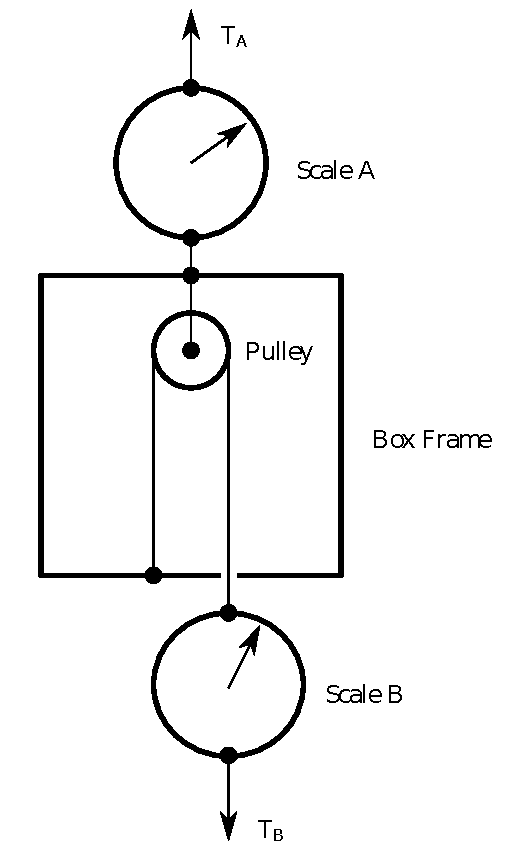
\includegraphics[keepaspectratio,scale=0.6]{Olympiad2014-Q18}
    \end{center}
    If an additional force pulls down on scale $B$ so that the reading increases to
        \SI{30}{\newton}, what will be the new reading on scale $A$?
    \begin{multicols}{3}
    \begin{choices}
        \wrongchoice{\SI{35}{\newton}}
      \correctchoice{\SI{40}{\newton}}
        \wrongchoice{\SI{45}{\newton}}
        \wrongchoice{\SI{50}{\newton}}
        \wrongchoice{\SI{60}{\newton}}
    \end{choices}
    \end{multicols}
\end{question}
}

\element{aapt}{ %% Olympiad-A3
\begin{question}{olympiad-2014-q19}
    A helicopter is flying horizontally at constant speed.
    A perfectly flexible uniform cable is suspended beneath the helicopter;
        air friction on the cable is not negligible.
    %% Start Question
    Which of the following diagrams best shows the shape of the cable
        as the helicopter flies through the air to the right?
    \begin{multicols}{2}
    \begin{choices}
        %% tikz?
        \AMCboxDimensions{down=-2cm}
        \wrongchoice{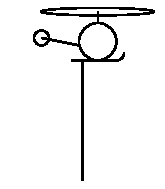
\includegraphics[keepaspectratio,scale=1.0]{Olympiad2014-Q19-A}}
      \correctchoice{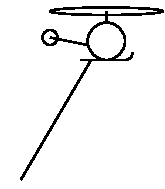
\includegraphics[keepaspectratio,scale=1.0]{Olympiad2014-Q19-B}}
        \wrongchoice{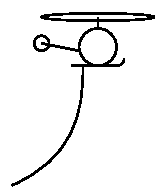
\includegraphics[keepaspectratio,scale=1.0]{Olympiad2014-Q19-C}}
        \wrongchoice{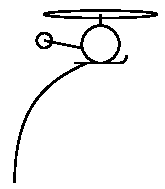
\includegraphics[keepaspectratio,scale=1.0]{Olympiad2014-Q19-D}}
        \wrongchoice{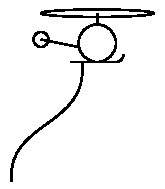
\includegraphics[keepaspectratio,scale=1.0]{Olympiad2014-Q19-E}}
    \end{choices}
    \end{multicols}
\end{question}
}

\element{aapt}{ %% Olympiad-A6
\begin{question}{olympiad-2014-q20}
    A crew of scientists has built a new space station.
    The space station is shaped like a wheel of radius $R$,
        with essentially all its mass $M$ at the rim.
    When the crew arrives, the station will be set rotating at a rate that
        causes an object at the rim to have radial acceleration $g$, thereby simulating
    Earth's surface gravity.
    This is accomplished by two small rockets, each with thrust $T$ newtons,
        mounted on the station's rim.
    How long a time $t$ does one need to fire the rockets to achieve the desired condition?
    \begin{multicols}{2}
    \begin{choices}
        \wrongchoice{$t=\dfrac{\sqrt{g R^3} M}{2T}$}
      \correctchoice{$t=\dfrac{\sqrt{g R} M}{2T}$}
        \wrongchoice{$t=\dfrac{\sqrt{g R} M}{T}$}
        \wrongchoice{$t=\sqrt{\dfrac{g R}{\pi}}\dfrac{M}{T}$}
        \wrongchoice{$t=\dfrac{\sqrt{g R}M}{\pi T}$}
    \end{choices}
    \end{multicols}
\end{question}
}

\element{aapt}{ %% Olympiad-A6
\begin{question}{olympiad-2014-q21}
    Two pulleys (shown in figure) are made of the same metal with density $\rho$.
    Pulley $A$ is a uniform disk with radius $R$.
    Pulley $B$ is identical except a circle of $\frac{R}{2}$ is removed from the center.
    When two boxes $M=\alpha m$, where $\alpha>1$,
        are connected over the pulleys through a massless rope and move without slipping,
        what is the ratio between the accelerations in system $A$ and $B$?
    \begin{center}
    \begin{tikzpicture}
        \begin{scope}[xshift=+2cm]
            %% Labels
            \node[anchor=south]at (0,1em) {Pulley $B$};
            %% Ceiling
            \node[anchor=south,fill,pattern=north east lines,minimum width=3cm, minimum height=0.05cm] at (-0.5,0) {};
            \draw (-2,0) -- (1,0);
            %% Pulley
            \draw[fill=white!50!black] (0,-1) circle (0.75);
            \draw[fill=white] (0,-1) circle (0.38);
            \draw[fill=white!90!black] (-0.3,0) -- (-0.10,-1.1) arc(190:350:0.10) -- (0.3,0) --cycle;
            \draw[fill] (0,-1) circle (1.5pt);
            %% Masses
            \node[draw,fill=white!90!black,rectangle,rounded corners=1ex,minimum size=1cm,anchor=north] (A) at (-0.75,-3) {$m$};
            \node[draw,fill=white!90!black,rectangle,rounded corners=1ex,minimum size=1.414cm,anchor=north] (B) at (0.75,-2.5) {$M$};
            %% Rope
            \draw[thick] (A.north) -- (-0.75,-1.0) arc(180:0:0.75) -- (B.north);
        \end{scope}
        \begin{scope}[xshift=-2cm]
            %% Labels
            \node[anchor=south] at (0,1em) {Pulley $A$};
            %% Ceilin3737
            \node[anchor=south,fill,pattern=north east lines,minimum width=3cm, minimum height=0.05cm] at (+0.5,0) {};
            \draw (-1,0) -- (2,0);
            %% Pulley
            \draw[fill=white!50!black] (0,-1) circle (0.75);
            \draw[fill=white!90!black] (-0.3,0) -- (-0.2,-1.1) arc(190:350:0.2) -- (0.3,0) --cycle;
            \draw[fill] (0,-1) circle (1.5pt);
            %% Masses
            \node[draw,fill=white!90!black,rectangle,rounded corners=1ex,minimum size=1cm,anchor=north] (A) at (-0.75,-3) {$m$};
            \node[draw,fill=white!90!black,rectangle,rounded corners=1ex,minimum size=1.414cm,anchor=north] (B) at (0.75,-2.5) {$M$};
            %% Rope
            \draw[thick] (A.north) -- (-0.75,-1.0) arc(180:0:0.75) -- (B.north);
        \end{scope}
    \end{tikzpicture}
    \end{center}
    The mass of pulley $A$ is $M+m$.
    \begin{multicols}{2}
    \begin{choices}
      \correctchoice{$\dfrac{a_A}{a_B} = \dfrac{47}{48}$}
        \wrongchoice{$\dfrac{a_A}{a_B} = \dfrac{31}{32}$}
        \wrongchoice{$\dfrac{a_A}{a_B} = \dfrac{15}{16}$}
        \wrongchoice{$\dfrac{a_A}{a_B} = \dfrac{9}{16}$}
        \wrongchoice{$\dfrac{a_A}{a_B} = \dfrac{3}{4}$}
    \end{choices}
    \end{multicols}
\end{question}
}

\element{aapt}{ %% Olympiad-A7
\begin{question}{olympiad-2014-q22}
    A body of mass $M$ and a body of mass $m\ll M$ are in circular orbits
        about their center of mass under the influence of their
        mutual gravitational attraction to each other.
    The distance between the bodies is $R$, which is much larger than the size of either body.
    %% Start Question
    A small amount of matter $\delta \ll m$ is removed from the body of mass $m$
        and transferred to the body of mass $M$.
    The transfer is done in such a way so that the orbits of the two bodies remain circular,
        and remain separated by a distance $R$.
    Which of the following statements is correct?
    \begin{choices}
        \wrongchoice{The gravitational force between the two bodies increases.}
        \wrongchoice{The gravitational force between the two bodies remains constant.}
        \wrongchoice{The total angular momentum of the system increases.}
        \wrongchoice{The total angular momentum of the system remains constant.}
      \correctchoice{The period of the orbit of two bodies remains constant.}
    \end{choices}
\end{question}
}

\element{aapt}{ %% Olympiad-A5
\begin{question}{olympiad-2014-q23}
    A \SI{100}{\kilo\gram} astronaut carries a launcher loaded with a
        \SI{10}{\kilo\gram} bowling ball;
        the launcher and the astronaut's spacesuit have negligible mass.
    The astronaut discovers that firing the launcher results in the ball
        moving away from her at a relative speed of \SI{50}{\meter\per\second}.
    %% Start question
    What is the impulse delivered to the astronaut when firing the launcher?
    \begin{multicols}{2}
    \begin{choices}
      \correctchoice{\SI{455}{\newton\second}}
        \wrongchoice{\SI{500}{\newton\second}}
        \wrongchoice{\SI{550}{\newton\second}}
        \wrongchoice{\SI{5000}{\newton\second}}
        \wrongchoice{\SI{5500}{\newton\second}}
    \end{choices}
    \end{multicols}
\end{question}
}

\element{aapt}{ %% Olympiad-A5
\begin{question}{olympiad-2014-q24}
    A \SI{100}{\kilo\gram} astronaut carries a launcher loaded with a
        \SI{10}{\kilo\gram} bowling ball;
        the launcher and the astronaut's spacesuit have negligible mass.
    The astronaut discovers that firing the launcher results in the ball
        moving away from her at a relative speed of \SI{50}{\meter\per\second}.
    %% Start question
    The astronaut is now moving at \SI{10}{\meter\per\second}
        (as measured in a certain frame of reference).
    She wishes to fire the launcher so that her velocity turns through
        as large an angle as possible (in this frame of reference).
    What is this maximum angle?
    (\emph{Hint:} a diagram may be useful.)
    \begin{multicols}{3}
    \begin{choices}
        \wrongchoice{\ang{24.4}}
        \wrongchoice{\ang{26.6}}
      \correctchoice{\ang{27.0}}
        \wrongchoice{\ang{30.0}}
        \wrongchoice{\ang{180.0}}
    \end{choices}
    \end{multicols}
\end{question}
}

\element{aapt}{ %% Olymmpiad-A4
\begin{question}{olympiad-2014-q25}
    A block with mass $m$ is released from rest at the top of a frictionless ramp.
    The block starts at a height $h_1$ above the base of the ramp,
        slides down the ramp, and then up a second ramp.
    The coefficient of kinetic friction between the block and the second ramp is $\mu_k$.
    If both ramps make an angle of $\theta$ with the horizontal,
        to what height $h_2$ above the base of the second ramp will the block rise?
    \begin{choices}
      \correctchoice{$h_2 = \dfrac{h_1\sin\theta}{\mu_k \cos\theta + \sin\theta}$}
        \wrongchoice{$h_2 = \dfrac{h_1\sin\theta}{\mu_k + \sin\theta}$}
        \wrongchoice{$h_2 = \dfrac{h_1\sin\theta}{\mu_k \cos^2\theta + \sin\theta}$}
        \wrongchoice{$h_2 = \dfrac{h_1\sin\theta}{\mu_k \cos^2\theta + \sin^2\theta}$}
        \wrongchoice{$h_2 = \dfrac{h_1\sin\theta}{\mu_k \sin\theta + \cos\theta}$}
    \end{choices}
\end{question}
}


%% PhysicsOlympiad 2013 F=ma Exam
%%----------------------------------------
\element{aapt}{ %% Olympiad-A1
\begin{question}{olympiad-2013-q01}
    An observer stands on the side of the front of a stationary train.
    When the train starts moving with constant acceleration,
        it takes \SI{5}{\second} for the first car to pass the observer.
    How long will it take for the 10\textsuperscript{th} car to pass?
    \begin{multicols}{3}
    \begin{choices}
        %% T_10 - T_9 = \sqrt{10*5^2} - \sqrt{9*5^2}
        \wrongchoice{\SI{1.07}{\second}}
        \wrongchoice{\SI{0.98}{\second}}
        \wrongchoice{\SI{0.91}{\second}}
        \wrongchoice{\SI{0.86}{\second}}
      \correctchoice{\SI{0.81}{\second}}
    \end{choices}
    \end{multicols}
\end{question}
}

\element{aapt}{ %% Olympiad-A5
\begin{question}{olympiad-2013-q02}
    Jordi stands \SI{20}{\meter} from a wall and Diego stands \SI{10}{\meter} from the same wall.
    Jordi throws a ball at an angle of \ang{30} above the horizontal,
        and it collides elastically with the wall.
    How fast does Jordi need to throw the ball so that Diego will catch it?
    Consider Jordi and Diego to be the same height,
        and both are on the same perpendicular line from the wall.
    \begin{multicols}{3}
    \begin{choices}
        \wrongchoice{\SI{11}{\meter\per\second}}
        \wrongchoice{\SI{15}{\meter\per\second}}
      \correctchoice{\SI{19}{\meter\per\second}}
        \wrongchoice{\SI{30}{\meter\per\second}}
        \wrongchoice{\SI{35}{\meter\per\second}}
    \end{choices}
    \end{multicols}
\end{question}
}

\element{aapt}{ %% Olympiad-A2
\begin{question}{olympiad-2013-q03}
    Tom throws a football to Wes, who is a distance $l$ away.
    Tom can control the time of flight $t$ of the ball by choosing any speed up to $v_{max}$
        and any launch angle between \ang{0} and \ang{90}.
    Ignore air resistance and assume Tom and Wes are at the same height.
    Which of the following statements is \emph{incorrect}?
    \begin{choices}
        %% remember R = \frac{v^2}{g}\sin 2\theta
        \wrongchoice{If $v_{max}<\sqrt{gl}$, the ball cannot reach Wes at all.}
        \wrongchoice{Assuming the ball can reach Wes, as $v_{max}$ increases with $l$ held fixed, the minimum value of $t$ decreases.}
        \wrongchoice{Assuming the ball can reach Wes, as $v_{max}$ increases with $l$ held fixed, the maximum value of $t$ increases.}
        \wrongchoice{Assuming the ball can reach Wes, as $l$ increases with $v_{max}$ held fixed, the minimum value of $t$ increases.}
      \correctchoice{Assuming the ball can reach Wes, as $l$ increases with $v_{max}$ held fixed, the maximum value of $t$ increases.}
    \end{choices}
\end{question}
}

\element{aapt}{ %% Olympiad-A6
\begin{question}{olympiad-2013-q04}
    The sign shown below consists of two uniform legs attached by a frictionless hinge.
    The coefficient of friction between the ground and the legs is $\mu$.
    Which of the following gives the maximum value of $\theta$ such that the sign will not collapse?
    \begin{center}
    \begin{tikzpicture}
        %% Triangle
        \draw (-3,0) -- (3,0);
        \draw[very thick] (-2,0) -- ++ (60:4);
        \draw[very thick] (+2,0) -- ++ (120:4);
        %% Angle
        \draw[thick,<->] (-2,0) ++ (60:2.5) arc (240:300:1.5) node[pos=0.5,anchor=north] {$\theta$};
        %% Length
        \draw[thick,<->] (2,0) ++ (30:0.3) -- ++ (120:4) node[pos=0.5,anchor=west] {$L$};
    \end{tikzpicture}
    \end{center}
    \begin{multicols}{2}
    \begin{choices}
        \wrongchoice{$\sin\theta = 2\mu$}
        \wrongchoice{$\sin\dfrac{\theta}{2} = \dfrac{\mu}{2}$}
        \wrongchoice{$\tan\dfrac{\theta}{2} = \mu$}
        \wrongchoice{$\tan\theta = 2\mu$}
      \correctchoice{$\tan\dfrac{\theta}{2} = 2\mu$}
    \end{choices}
    \end{multicols}
\end{question}
}

\newcommand{\myOlympiadThirteenQzeroFive}{
\begin{tikzpicture}
    \begin{axis}[
        axis y line=left,
        axis x line=bottom,
        axis line style={->},
        xlabel={time},
        x unit=\si{\second},
        xtick={0,2,4,6,8,10,12,14,16,18,20,22,24,26},
        ylabel={scale reading},
        y unit=\si{\kilo\gram},
        ytick={0,20,40,60,80,100,120},
        %grid=major,
        xmin=0,xmax=26,
        ymin=0,ymax=120,
        width=0.90\columnwidth,
        height=0.45\columnwidth,
    ]
    \addplot[mark=\empty] plot coordinates { (0,80) (2,80) (2,60) (4,60) (4,80) (22,80) (22,100) (24,100) (24,80) (26,80) };
    \end{axis}
\end{tikzpicture}
}

\element{aapt}{ %% Olympiad-A3
\begin{question}{olympiad-2013-q05}
    A student steps onto a stationary elevator and stands on a bathroom scale.
    The elevator then travels from the top of the building to the bottom.
    The student records the reading on the scale as a function of time.
    \begin{center}
        \myOlympiadThirteenQzeroFive
    \end{center}
    At what time(s) does the student have maximum downward velocity?
    \begin{choices}
        \wrongchoice{At all times between \SI{2}{\second} and \SI{4}{\second}}
        \wrongchoice{At \SI{4}{\second} only}
      \correctchoice{At all times between \SI{4}{\second} and \SI{22}{\second}}
        \wrongchoice{At \SI{22}{\second} only}
        \wrongchoice{At all times between \SI{22}{\second} and \SI{24}{\second}}
    \end{choices}
\end{question}
}

\element{aapt}{ %% Olympiad-A3
\begin{question}{olympiad-2013-q06}
    A student steps onto a stationary elevator and stands on a bathroom scale.
    The elevator then travels from the top of the building to the bottom.
    The student records the reading on the scale as a function of time.
    \begin{center}
        \myOlympiadThirteenQzeroFive
    \end{center}
    How tall is the building?
    \begin{multicols}{3}
    \begin{choices}
        \wrongchoice{\SI{50}{\meter}}
        \wrongchoice{\SI{80}{\meter}}
      \correctchoice{\SI{100}{\meter}}
        \wrongchoice{\SI{150}{\meter}}
        \wrongchoice{\SI{400}{\meter}}
    \end{choices}
    \end{multicols}
\end{question}
}

\element{aapt}{ %% Olympiad-A5
\begin{question}{olympiad-2013-q07}
    A light car and a heavy truck have the same momentum.
    The truck weighs ten times as much as the car.
    How do their kinetic energies compare?
    \begin{choices}
        \wrongchoice{The truck's kinetic energy is larger by a factor of \num{100}}
        \wrongchoice{They truck's kinetic energy is larger by a factor of \num{10}}
        \wrongchoice{They have the same kinetic energy}
      \correctchoice{The car's kinetic energy is larger by a factor of \num{10}}
        \wrongchoice{The car's kinetic energy is larger by a factor of \num{100}}
    \end{choices}
\end{question}
}

\element{aapt}{ %% Olympiad-A5
\begin{question}{olympiad-2013-q08}
    A truck is initially moving at velocity $v$.
    The driver presses the brake in order to slow the truck to a stop.
    The brake applies a constant force $F$ to the truck.
    The truck rolls a distance $x$ before coming to a stop,
        and the time it takes to stop is $t$.
    %% Start question
    Which of the following expressions is equal the initial kinetic energy of the truck
        (i.e. the kinetic energy before the driver starts braking)?
    \begin{multicols}{2}
    \begin{choices}
      \correctchoice{$Fx$}
        \wrongchoice{$Fvt$}
        \wrongchoice{$Fxt$}
        \wrongchoice{$Ft$}
        \wrongchoice{Both $Fx$ and $FvT$ are correct}
    \end{choices}
    \end{multicols}
\end{question}
}

\element{aapt}{ %% Olympiad-A5
\begin{question}{olympiad-2013-q09}
    A truck is initially moving at velocity $v$.
    The driver presses the brake in order to slow the truck to a stop.
    The brake applies a constant force $F$ to the truck.
    The truck rolls a distance $x$ before coming to a stop,
        and the time it takes to stop is $t$.
    %% Start question
    Which of the following expressions is equal the initial momentum of the truck
        (i.e. the momentum before the driver starts braking)?
    \begin{multicols}{3}
    \begin{choices}
        \wrongchoice{$Fx$}
        \wrongchoice{$F\dfrac{t}{2}$}
        \wrongchoice{$Fxt$}
        \wrongchoice{$2Ft$}
      \correctchoice{$2F\dfrac{x}{v}$}
    \end{choices}
    \end{multicols}
\end{question}
}

\element{aapt}{ %% Olympiad-A6
\begin{question}{olympiad-2013-q10}
    Which of the following can be used to distinguish a solid ball
        from a hollow sphere of the same radius and mass?
    \begin{choices}
        \wrongchoice{Measurements of the orbit of a test mass around the object.}
      \correctchoice{Measurements of the time it takes the object to roll down an inclined plane.}
        \wrongchoice{Measurements of the tidal forces applied by the object to a liquid body.}
        \wrongchoice{Measurements of the behavior of the object as it floats in water.}
        \wrongchoice{Measurements of the force applied to the object by a uniform gravitational field.}
    \end{choices}
\end{question}
}

\element{aapt}{ %% Olympiad-A3
\begin{question}{olympiad-2013-q11}
    A right-triangular wooden block of mass $M$ is at rest on a table, as shown in figure.
    Two smaller wooden cubes, both with mass $m$,
        initially rest on the two sides of the larger block.
    As all contact surfaces are frictionless,
        the smaller cubes start sliding down the larger block while the block remains at rest.
    What is the normal force from the system to the table?
    \begin{center}
    \begin{tikzpicture}
        %% Triangle
        \draw (-3,0) -- (3,0);
        \draw[thick] (-2,0) -- (2,0);
        \draw[thick] (-2,0) -- ++(30:3.464);
        \draw[thick] (+2,0) -- ++(120:2);
        \node[anchor=west] at (0,0.433) {$M$};
        %% Angles
        \draw (-2,0) ++ (0:0.5) arc (0:30:0.5) node[pos=0.5,anchor=west] {$\alpha$};
        \draw (+2,0) ++ (120:0.5) arc (120:180:0.5) node[pos=0.5,anchor=east] {$\beta$};
        \draw (1,1.732) ++ (-60:0.5) -- ++(210:0.5) -- ++(120:0.5);
        %% Blocks
        \node[draw,rectangle,minimum size=1.5em,rotate=30,anchor=south] at (-0.5,0.866) {$m$};
        \node[draw,rectangle,minimum size=1.5em,rotate=30,anchor=west] at (1.5,0.866) {$m$};
    \end{tikzpicture}
    \end{center}
    \begin{choices}
        \wrongchoice{$2mg$}
        \wrongchoice{$2mg + Mg$}
      \correctchoice{$mg + Mg$}
        \wrongchoice{$Mg + mg\left(\sin\alpha + \sin\beta\right)$}
        \wrongchoice{$Mg + mg\left(\cos\alpha + \cos\beta\right)$}
    \end{choices}
\end{question}
}

\element{aapt}{ %% Olympiad-A6
\begin{question}{olympiad-2013-q12}
    A spherical shell of mass $M$ and radius $R$ is completely filled with a frictionless fluid,
        also of mass $M$.
    It is released from rest,
        and then it rolls without slipping down an incline that makes an angle $theta$ with the horizontal.
    What will be the acceleration of the shell down the incline just after it is released?
    Assume the acceleration of free fall is $g$.
    The moment of inertia of a thin shell of radius $r$ and mass $m$ about the center of mass is $ =\frac{3}{2}mr^2$;
        the moment of inertia of a solid sphere of radius $r$ and mass $m$ about the center of mass is $I=\frac{2}{5} mr^2$.
    \begin{multicols}{2}
    \begin{choices}
        \wrongchoice{$a=g\sin\theta$}
      \correctchoice{$a=\dfrac{3g}{4}\sin\theta$}
        \wrongchoice{$a=\dfrac{g}{2}\sin\theta$}
        \wrongchoice{$a=\dfrac{3g}{8}\sin\theta$}
        \wrongchoice{$a=\dfrac{3g}{5}\sin\theta$}
    \end{choices}
    \end{multicols}
\end{question}
}

\element{aapt}{ %% Olympiad-A7
\begin{question}{olympiad-2013-q13}
    There is a ring outside of Saturn.
    In order to distinguish if the ring is actually a part of Saturn or is instead part of the satellites of Saturn,
        we need to know the relation between the velocity $v$ of each layer in the ring and the distance $R$ of the layer to the center of Saturn.
    Which of the following statements is correct?
    \begin{choices}
        %% v = \omega R, if connected
      \correctchoice{If $v\propto R$, then the layer is part of Saturn.}
        \wrongchoice{If $v^2\propto R$, then the layer is part of the satellites of Saturn.}
        \wrongchoice{If $v\propto \frac{1}{R}$, then the layer is part of Saturn.}
        %% v^2 = G M r, if in orbit
        \wrongchoice{If $v^2\propto \frac{1}{R}$, then the layer is part of Saturn.}
        \wrongchoice{If $v\propto R^2$, then the layer is part of the satellites of Saturn.}
    \end{choices}
\end{question}
}

\element{aapt}{ %% Olympiad-A5
\begin{question}{olympiad-2013-q14}
    A cart of mass $m$ moving at \SI{12}{\meter\per\second} to the right collides elastically with a cart of mass \SI{4.0}{\kilo\gram} that is originally at rest.
    After the collision,
        the cart of mass $m$ moves to the left with a velocity of \SI{6.0}{\meter\per\second}.
    Assuming an elastic collision in one dimension only,
        what is the velocity of the center of mass ($v_{cm}$) of the two carts before the collision?
    \begin{multicols}{2}
    \begin{choices}
        \wrongchoice{$v_{cm} = \SI{2.0}{\meter\per\second}$}
      \correctchoice{$v_{cm} = \SI{3.0}{\meter\per\second}$}
        \wrongchoice{$v_{cm} = \SI{6.0}{\meter\per\second}$}
        \wrongchoice{$v_{cm} = \SI{9.0}{\meter\per\second}$}
        \wrongchoice{$v_{cm} = \SI{18}{\meter\per\second}$}
    \end{choices}
    \end{multicols}
\end{question}
}

\element{aapt}{
\begin{question}{olympiad-2013-q15}
    A uniform rod is partially in water with one end suspended, as shown in figure.
    \begin{center}
        %% NOTE: tikz? draw=white
        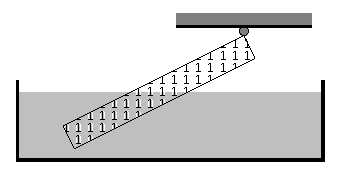
\includegraphics[keepaspectratio,scale=1.0]{Olympiad2013-Q15}
    \end{center}
    The density of the rod is $5/9$ that of water.
    At equilibrium, what portion of the rod is above water?
    \begin{multicols}{3}
    \begin{choices}
        \wrongchoice{\num{0.25}}
        \wrongchoice{\num{0.33}}
        \wrongchoice{\num{0.5}}
      \correctchoice{\num{0.67}}
        \wrongchoice{\num{0.75}}
    \end{choices}
    \end{multicols}
\end{question}
}

\element{aapt}{ %% Olympiad-A7
\begin{question}{olympiad-2013-q16}
    %% \emph{Inspired by a problem from the 2012 International Physics Olympiad, Estonia}.
    A very large number of small particles forms a spherical cloud.
    Initially they are at rest, have uniform mass density per unit volume $\rho_0$,
        and occupy a region of radius $r_0$.
    The cloud collapses due to gravitation;
        the particles do not interact with each other in any other way.
    %% Start Questions
    How much time passes until the cloud collapses fully?
    (The constant \num{0.5427} is actually $\sqrt{\frac{3\pi}{32}}$.)
    \begin{multicols}{2}
    \begin{choices}
        %% Dimensional Analysis: time cannot depend on size
        \wrongchoice{$\dfrac{\num{0.5427}}{r_0^2 \sqrt{G\rho_0}}$}
        \wrongchoice{$\dfrac{\num{0.5427}}{r_0 \sqrt{G\rho_0}}$}
        \wrongchoice{$\dfrac{\num{0.5427}}{\sqrt{r_0 G\rho_0}}$}
      \correctchoice{$\dfrac{\num{0.5427}}{\sqrt{G\rho_0}}$}
        \wrongchoice{$\dfrac{\num{0.5427}}{\sqrt{G\rho_0}}r_0$}
    \end{choices}
    \end{multicols}
\end{question}
}

\element{aapt}{ %% Olympiad-A7
\begin{question}{olympiad-2013-q17}
    Two small, equal masses are attached by a lightweight rod.
    This object orbits a planet; the length of the rod is smaller than the radius of the orbit,
        but not negligible.
    The rod rotates about its axis in such a way that it remains vertical with respect to the planet.
    \begin{itemize}
        \item Is there a force in the rod?
            If so, is it tension or compression?
        \item Is the equilibrium stable, unstable, or neutral with respect to a small perturbation in the angle of the rod?
            (Assume this perturbation maintains the rate of rotation, so that in the co-rotating frame the rod is still stationary but at an angle to the vertical.)
    \end{itemize}
    \begin{center}
    \begin{tikzpicture}[scale=0.75]
        \draw[thick,fill=white!80!black] (0,0) circle (2cm);
        \draw[dotted] (0,0) circle (3cm);
        \foreach \x in {0,90,180,270} {
            \draw[fill] (\x:2.5) circle (5pt);
            \draw (\x:3.5) circle (5pt);
            \draw (\x:2.5) -- (\x:3.5);
        }
    \end{tikzpicture}
    \end{center}
    \begin{choices}
        \wrongchoice{There is no force in the rod; the equilibrium is neutral.}
      \correctchoice{The rod is in tension; the equilibrium is stable.}
        \wrongchoice{The rod is in compression; the equilibrium is stable.}
        \wrongchoice{The rod is in tension; the equilibrium is unstable.}
        \wrongchoice{The rod is in compression; the equilibrium is unstable.}
    \end{choices}
\end{question}
}

\element{aapt}{ %% Olympiad-A5
\begin{question}{olympiad-2013-q18}
    Two point particles, each of mass \SI{1}{\kilo\gram}, begin in the state shown below.
    \begin{center}
    \begin{tikzpicture}[scale=0.9]
        \begin{axis}[
            xlabel={$x$},
            x unit=\si{\meter},
            xtick={-3,-2,-1,0,1,2,3},
            ylabel={$y$},
            y unit=\si{\meter},
            ytick={-3,-2,-1,0,1,2,3},
            grid=major,
            xmin=-3,xmax=3,
            ymin=-3,ymax=3,
            width=0.80\columnwidth,
            height=0.80\columnwidth,
        ]
        \draw[fill] (axis cs:1,1) circle (1.5pt);
        \draw[thick,->] (axis cs:1,1) -- (axis cs:0,1) node[pos=0.5,anchor=south] {\SI{1.0}{\meter\per\second}};
        \draw[fill] (axis cs:1,-1) circle (1.5pt);
        \draw[thick,->] (axis cs:1,-1) -- (axis cs:2,-1) node[pos=0.5,anchor=south] {\SI{1.0}{\meter\per\second}};
        \end{axis}
    \end{tikzpicture}
    \end{center}
    The system evolves through internal forces only.
    Which of the following could be the state after some time has passed?
    %% added to improve printing
    [Axis grid lines in options are identical to those in problem.]
    \begin{multicols}{2}
    \begin{choices}
        \AMCboxDimensions{down=-0.40\columnwidth}
        \wrongchoice{
            \begin{tikzpicture}[font=\small]
                \begin{axis}[
                    clip=false,
                    xlabel={},
                    xtick={-3,-2,-1,0,1,2,3},
                    xticklabels=\empty,
                    ylabel={},
                    ytick={-3,-2,-1,0,1,2,3},
                    yticklabels=\empty,
                    grid=major,
                    xmin=-3,xmax=3,
                    ymin=-3,ymax=3,
                    width=\columnwidth,
                    height=\columnwidth,
                ]
                \draw[fill] (axis cs:-1,0) circle (1.5pt);
                \draw[thick,->] (axis cs:-1,0) -- (axis cs:-1,-1) node[pos=1.0,anchor=north] {\SI{1.0}{\meter\per\second}};
                \draw[fill] (axis cs:1,0) circle (1.5pt);
                \draw[thick,->] (axis cs:1,0) -- (axis cs:1,1) node[pos=1.0,anchor=south] {\SI{1.0}{\meter\per\second}};
                \end{axis}
            \end{tikzpicture}
        }
        \wrongchoice{
            \begin{tikzpicture}[font=\small]
                \begin{axis}[
                    clip=false,
                    xlabel={},
                    xtick={-3,-2,-1,0,1,2,3},
                    xticklabels=\empty,
                    ylabel={},
                    ytick={-3,-2,-1,0,1,2,3},
                    yticklabels=\empty,
                    grid=major,
                    xmin=-3,xmax=3,
                    ymin=-3,ymax=3,
                    width=\columnwidth,
                    height=\columnwidth,
                ]
                \draw[fill] (axis cs:1,1) circle (1.5pt);
                \draw[thick,->] (axis cs:1,1) -- (axis cs:-1,1) node[pos=0.5,anchor=south] {\SI{2.0}{\meter\per\second}};
                \draw[fill] (axis cs:1,-1) circle (1.5pt);
                \end{axis}
            \end{tikzpicture}
        }
        \wrongchoice{
            \begin{tikzpicture}[font=\small]
                \begin{axis}[
                    clip=false,
                    xlabel={},
                    xtick={-3,-2,-1,0,1,2,3},
                    xticklabels=\empty,
                    ylabel={},
                    ytick={-3,-2,-1,0,1,2,3},
                    yticklabels=\empty,
                    grid=major,
                    xmin=-3,xmax=3,
                    ymin=-3,ymax=3,
                    width=\columnwidth,
                    height=\columnwidth,
                ]
                \draw[fill] (axis cs:2,0) circle (1.5pt);
                \draw[thick,->] (axis cs:2,0) -- (axis cs:1.303,0.707) node[pos=1.0,anchor=south] {\SI{1.0}{\meter\per\second}};
                \draw[fill] (axis cs:0,0) circle (1.5pt);
                \draw[thick,->] (axis cs:0,0) -- (axis cs:+0.707,-0.707) node[pos=0.5,anchor=north east] {\SI{1.0}{\meter\per\second}};
                \end{axis}
            \end{tikzpicture}
        }
        \wrongchoice{
            \begin{tikzpicture}[font=\small]
                \begin{axis}[
                    clip=false,
                    xlabel={},
                    xtick={-3,-2,-1,0,1,2,3},
                    xticklabels=\empty,
                    ylabel={},
                    ytick={-3,-2,-1,0,1,2,3},
                    yticklabels=\empty,
                    grid=major,
                    xmin=-3,xmax=3,
                    ymin=-3,ymax=3,
                    width=\columnwidth,
                    height=\columnwidth,
                ]
                \draw[fill] (axis cs:0,2) circle (1.5pt);
                \draw[thick,->] (axis cs:0,2) -- (axis cs:-1,2) node[pos=0.5,anchor=south] {\SI{1.0}{\meter\per\second}};
                \draw[fill] (axis cs:2,-2) circle (1.5pt);
                \draw[thick,->] (axis cs:2,-2) -- (axis cs:3,-2) node[pos=0.5,anchor=south] {\SI{1.0}{\meter\per\second}};
                \end{axis}
            \end{tikzpicture}
        }
        %% ANS is E
        \correctchoice{
            \begin{tikzpicture}[font=\small]
                \begin{axis}[
                    clip=false,
                    xlabel={},
                    xtick={-3,-2,-1,0,1,2,3},
                    xticklabels=\empty,
                    ylabel={},
                    ytick={-3,-2,-1,0,1,2,3},
                    yticklabels=\empty,
                    grid=major,
                    xmin=-3,xmax=3,
                    ymin=-3,ymax=3,
                    width=\columnwidth,
                    height=\columnwidth,
                ]
                \draw[fill] (axis cs:2,1) circle (1.5pt);
                \draw[thick,->] (axis cs:2,1) -- (axis cs:2,2) node[pos=0.5,anchor=east] {\SI{1.0}{\meter\per\second}};
                \draw[fill] (axis cs:0,-1) circle (1.5pt);
                \draw[thick,->] (axis cs:0,-1) -- (axis cs:0,-2) node[pos=0.5,anchor=west] {\SI{1.0}{\meter\per\second}};
                \end{axis}
            \end{tikzpicture}
        }
    \end{choices}
    \end{multicols}
\end{question}
}

\element{aapt}{ %% Olympiad-A8
\begin{question}{olympiad-2013-q19}
    %The following information applies to questions 19, 20, and 21.
    A simple pendulum experiment is constructed from a point mass $m$ attached to a pivot by a massless rod of length $L$ in a constant gravitational field.
    The rod is released from an angle $\theta_0 < \pi/2$ at rest and the period of motion is found to be $T_0$.
    Ignore air resistance and friction.
    %% Start question
    At what angle $\theta_g$ during the swing is the tension in the rod the greatest?
    \begin{choices}
        \wrongchoice{The tension is the greatest at the point $θ_g=\theta_0$.}
      \correctchoice{The tension is the greatest at the point $θ_g=0$.}
        \wrongchoice{The tension is the greatest at an angle $θ_g$ with $\theta < θ_g < θ_0$.}
        \wrongchoice{The tension is constant.}
        \wrongchoice{None of the provided are true for all values of $θ_0$ with $0 < θ_0 < \frac{\pi}{2}$.}
    \end{choices}
\end{question}
}

\element{aapt}{ %% Olympiad-A8
\begin{question}{olympiad-2013-q20}
    %The following information applies to questions 19, 20, and 21.
    A simple pendulum experiment is constructed from a point mass $m$ attached to a pivot by a massless rod of length $L$ in a constant gravitational field.
    The rod is released from an angle $\theta_0 < \pi/2$ at rest and the period of motion is found to be $T_0$.
    Ignore air resistance and friction.
    %% Start question
    What is the maximum value of the tension in the rod?
    \begin{multicols}{2}
    \begin{choices}
        \wrongchoice{$mg$}
        \wrongchoice{$2mg$}
        \wrongchoice{$\dfrac{mL\theta_0}{T_0^2}$}
        \wrongchoice{$mg \sin\theta_0$}
      \correctchoice{$mg\left( 3 - 2\cos\theta_0 \right)$}
    \end{choices}
    \end{multicols}
\end{question}
}

\element{aapt}{ %% Olympiad-A8
\begin{question}{olympiad-2013-q21}
    %The following information applies to questions 19, 20, and 21.
    A simple pendulum experiment is constructed from a point mass $m$ attached to a pivot by a massless rod of length $L$ in a constant gravitational field.
    The rod is released from an angle $\theta_0 < \pi/2$ at rest and the period of motion is found to be $T_0$.
    Ignore air resistance and friction.
    %% Start question
    The experiment is repeated with a new pendulum with a rod of length $4L$,
        using the same angle $\theta_0$, and the period of motion is found to be $T$.
    Which of the following statements is correct?
    \begin{choices}
      \correctchoice{$T = 2T_0$ regardless of the value of $\theta_0$.}
        \wrongchoice{$T > 2T_0$ with $T\approx{}2T_0$ if $\theta_0 \ll 1$.}
        \wrongchoice{$T < 2T_0$ with $T\approx{}2T_0$ if $\theta_0 \ll 1$.}
        \wrongchoice{$T > 2T_0$ for some values of $\theta_0$ and $T<2T_0$ for other values of $\theta_0$.}
        \wrongchoice{$T_0$ and $T$ are undefined because the motion is not periodic unless $\theta_0 \ll 1$.}
    \end{choices}
\end{question}
}

%% NOTE: graphics for A6
\element{aapt}{
\begin{question}{olympiad-2013-q22}
    A simplified model on the foot is shown.
    \begin{center}
        \includegraphics[keepaspectratio,width=\columnwidth]{Olympiad2013-Q22}
    \end{center}
    When a student of mass $m=\SI{60}{\kilo\gram}$ stands on a single toe,
        the tension $T$ in the Achilles Tendon is closest to:
    \begin{multicols}{2}
    \begin{choices}
        \wrongchoice{$T = \SI{600}{\newton}$}
        \wrongchoice{$T = \SI{1200}{\newton}$}
        \wrongchoice{$T = \SI{1800}{\newton}$}
      \correctchoice{$T = \SI{2400}{\newton}$}
        \wrongchoice{$T = \SI{3000}{\newton}$}
    \end{choices}
    \end{multicols}
\end{question}
}

\element{aapt}{ %% Olympiad-A4
\begin{question}{olympiad-2013-q23}
    %The following information applies to questions 23 and 24
    A man with mass $m$ jumps off of a high bridge with a bungee cord attached to his ankles.
    The man falls through a maximum distance $H$ at which point the bungee cord brings him to a momentary rest before he bounces back up.
    The bungee cord is perfectly elastic,
        obeying Hooke's force law with a spring constant $k$,
        and stretches from an original length of $L_0$ to a final length $L = L_0 + h$.
    The maximum tension in the Bungee cord is four times the weight of the man.
    %% Start question
    Determine the spring constant $k$.
    \begin{multicols}{2}
    \begin{choices}
        \wrongchoice{$k = \dfrac{mg}{h}$}
        \wrongchoice{$k = \dfrac{2mg}{h}$}
        \wrongchoice{$k = \dfrac{mg}{H}$}
        \wrongchoice{$k = \dfrac{2mg}{H}$}
      \correctchoice{$k = \dfrac{8mg}{H}$}
    \end{choices}
    \end{multicols}
\end{question}
}

\element{aapt}{ %% Olympiad-A4
\begin{question}{olympiad-2013-q24}
    %The following information applies to questions 23 and 24
    A man with mass $m$ jumps off of a high bridge with a bungee cord attached to his ankles.
    The man falls through a maximum distance $H$ at which point the bungee cord brings him to a momentary rest before he bounces back up.
    The bungee cord is perfectly elastic,
        obeying Hooke's force law with a spring constant $k$,
        and stretches from an original length of $L_0$ to a final length $L = L_0 + h$.
    The maximum tension in the Bungee cord is four times the weight of the man.
    %% Start question
    Find the maximum extension of the bungee cord $h$.
    \begin{multicols}{2}
    \begin{choices}
      \correctchoice{$h = \dfrac{1}{2}H$}
        \wrongchoice{$h = \dfrac{1}{4}H$}
        \wrongchoice{$h = \dfrac{1}{5}H$}
        \wrongchoice{$h = \dfrac{2}{5}H$}
        \wrongchoice{$h = \dfrac{1}{8}H$}
    \end{choices}
    \end{multicols}
\end{question}
}

\element{aapt}{ %% Olympiad-A3
\begin{question}{olympiad-2013-q25}
    A box with weight $W$ will slide down a \ang{30} incline at
        constant speed under the influence of gravity and friction alone.
    If instead a horizontal force $P$ is applied to the box,
        the box can be made to move up the ramp at constant speed.
    What is the magnitude of $P$?
    \begin{multicols}{2}
    \begin{choices}
        \wrongchoice{$P = \dfrac{1}{2} W$}
        \wrongchoice{$P = \dfrac{2}{\sqrt{3}} W$}
        \wrongchoice{$P = W$}
      \correctchoice{$P = \sqrt{3} W$}
        \wrongchoice{$P = 2 W$}
    \end{choices}
    \end{multicols}
\end{question}
}


%% PhysicsOlympiad 2012 F=ma Exam
%%----------------------------------------
\element{aapt}{ %% Olympiad-A1
\begin{question}{olympiad-2012-q01}
    Consider a dripping faucet, where the faucet is \SI{10}{\centi\meter} above the sink.
    The time between drops is such that when one drop hits the sink,
        one is in the air and another is about to drop.
    At what height above the sink will the drop in the air be right as a drop hits the sink?
    \begin{choices}
        \wrongchoice{Between \SI{0}{\centi\meter} and \SI{2}{\centi\meter}}
        \wrongchoice{Between \SI{2}{\centi\meter} and \SI{4}{\centi\meter}}
        \wrongchoice{Between \SI{4}{\centi\meter} and \SI{6}{\centi\meter}}
      \correctchoice{Between \SI{6}{\centi\meter} and \SI{8}{\centi\meter}}
        \wrongchoice{Between \SI{8}{\centi\meter} and \SI{10}{\centi\meter}}
    \end{choices}
\end{question}
}

\element{aapt}{ %% Olympiad-A2
\begin{question}{olympiad-2012-q02}
    A cannonball is launched with initial velocity of magnitude $v_0$
        over a horizontal surface.
    At what minimum angle $\theta_{min}$ above the horizontal should the
        cannonball be launched so that it rises to a height $H$
        which is larger than the horizontal distance $R$ that it will
        travel when it returns to the ground?
    \begin{choices}
      \correctchoice{$\theta_{min}=\ang{76}$}
        \wrongchoice{$\theta_{min}=\ang{72}$}
        \wrongchoice{$\theta_{min}=\ang{60}$}
        \wrongchoice{$\theta_{min}=\ang{45}$}
        \wrongchoice{There is no such angle, as $R>H$ for all range problems.}
    \end{choices}
\end{question}
}

\element{aapt}{ %% Olympiad-A6
\begin{question}{olympiad-2012-q03}
    An equilateral triangle is sitting on an inclined plane.
    Friction is too high for it to slide under any circumstance,
        but if the plane is sloped enough it can ``topple'' down the hill.
    What angle incline is necessary for it to start toppling?
    \begin{choices}
        \wrongchoice{30 degrees}
        \wrongchoice{45 degrees}
      \correctchoice{60 degrees}
        \wrongchoice{It will topple at any angle more than zero}
        \wrongchoice{It can never topple if it cannot slide}
    \end{choices}
\end{question}
}

\element{aapt}{ %% Olympiad-A5
\begin{question}{olympiad-2012-q04}
    A particle at rest explodes into three particles of equal mass
        in the absence of external forces.
    Two particles emerge at a right angle to each other with equal speed $v$.
    What is the speed of the third particle?
    \begin{multicols}{2}
    \begin{choices}
        \wrongchoice{$v$}
      \correctchoice{$\sqrt{2}v$}
        \wrongchoice{$2v$}
        \wrongchoice{$2\sqrt{2}v$}
        \wrongchoice{The third particle can have a range of different speeds.}
    \end{choices}
    \end{multicols}
\end{question}
}

\element{aapt}{ %% Olympiad-A5
\begin{question}{olympiad-2012-q05}
    A \SI{12}{\kilo\gram} block moving east at \SI{4}{\meter\per\second}
        collides head on with a \SI{6}{\kilo\gram} block that is moving
        west at \SI{2}{\meter\per\second}.
    The two blocks move together after the collision.
    What is the loss in kinetic energy in this collision?
    \begin{multicols}{3}
    \begin{choices}
        \wrongchoice{\SI{36}{\joule}}
        \wrongchoice{\SI{48}{\joule}}
        \wrongchoice{\SI{60}{\joule}}
      \correctchoice{\SI{72}{\joule}}
        \wrongchoice{\SI{96}{\joule}}
    \end{choices}
    \end{multicols}
\end{question}
}

\element{aapt}{ %% Olympiad-A2
\begin{question}{olympiad-2012-q06}
    Two cannons are arranged vertically, with the lower cannon pointing upward
        (towards the upper cannon) and the upper cannon pointing downward
        (towards the lower cannon), \SI{200}{\meter\per\second} above the lower cannon.
    Simultaneously, they both fire.
    The muzzle velocity of the lower cannon is \SI{25}{\meter\per\second}
        and the muzzle velocity of the upper cannon is \SI{55}{\meter\per\second}.
    \begin{center}
        \includegraphics[keepaspectratio,scale=0.8]{Olympiad2012-Q06}
    \end{center}
    How long after the cannons fire do the projectiles collide?
    \begin{multicols}{3}
    \begin{choices}
        \wrongchoice{\SI{2.2}{\second}}
      \correctchoice{\SI{2.5}{\second}}
        \wrongchoice{\SI{3.6}{\second}}
        \wrongchoice{\SI{6.7}{\second}}
        \wrongchoice{\SI{8.0}{\second}}
    \end{choices}
    \end{multicols}
\end{question}
}

\element{aapt}{ %% Olympiad-A2
\begin{question}{olympiad-2012-q07}
    Two cannons are arranged vertically, with the lower cannon pointing upward
        (towards the upper cannon) and the upper cannon pointing downward
        (towards the lower cannon), \SI{200}{\meter\per\second} above the lower cannon.
    Simultaneously, they both fire.
    The muzzle velocity of the lower cannon is \SI{25}{\meter\per\second}
        and the muzzle velocity of the upper cannon is \SI{55}{\meter\per\second}.
    \begin{center}
        \includegraphics[keepaspectratio,scale=0.8]{Olympiad2012-Q06}
    \end{center}
    How far beneath the top cannon do the projectiles collide?
    \begin{multicols}{3}
    \begin{choices}
        \wrongchoice{\SI{31}{\meter}}
        \wrongchoice{\SI{67}{\meter}}
        \wrongchoice{\SI{110}{\meter}}
        \wrongchoice{\SI{140}{\meter}}
      \correctchoice{\SI{170}{\meter}}
    \end{choices}
    \end{multicols}
\end{question}
}

\element{aapt}{ %% Olympiad-A4
\begin{question}{olympiad-2012-q08}
    A block of mass $m=\SI{3.0}{\kilo\gram}$ is moving on a horizontal surface
        towards a massless spring with spring constant $k=\SI{80.0}{\newton\per\meter}$.
    The coefficient of kinetic friction between the block and the
        surface is $\mu_k=\num{0.50}$.
    The block has a speed of \SI{2.0}{\meter\per\second} when it first
        comes in contact with the spring.
    How far will the spring be compressed?
    \begin{multicols}{3}
    \begin{choices}
        \wrongchoice{\SI{0.19}{\meter}}
      \correctchoice{\SI{0.24}{\meter}}
        \wrongchoice{\SI{0.39}{\meter}}
        \wrongchoice{\SI{0.40}{\meter}}
        \wrongchoice{\SI{0.61}{\meter}}
    \end{choices}
    \end{multicols}
\end{question}
}

\element{aapt}{ %% Olympiad-A7
\begin{question}{olympiad-2012-q09}
    A uniform spherical planet has radius $R$ and the acceleration due
        to gravity at its surface is $g$.
    What is the escape velocity of a particle from the planet's surface?
    \begin{multicols}{2}
    \begin{choices}
        \wrongchoice{$\frac{1}{2}\sqrt{gR}$}
        \wrongchoice{$\sqrt{gR}$}
      \correctchoice{$\sqrt{2gR}$}
        \wrongchoice{$2\sqrt{gR}$}
        \wrongchoice{The escape velocity cannot be expressed in terms of $g$ and $R$ alone.}
    \end{choices}
    \end{multicols}
\end{question}
}

\element{aapt}{ %% Olympiad-A6
\begin{question}{olympiad-2012-q10}
    Four objects are placed at rest at the top of an inclined plane
        and allowed to roll without slipping to the bottom in the
        absence of rolling resistance and air resistance.
    \begin{itemize}
        \item Object $A$ is a solid brass ball of diameter $d$.
        \item Object $B$ is a solid brass ball of diameter $2d$.
        \item Object $C$ is a hollow brass sphere of diameter $d$.
        \item Object $D$ is a solid aluminum ball of diameter $d$. (Aluminum is less dense than brass.)
    \end{itemize}
    The balls are placed so that their centers of mass all travel the same distance.
    In each case, the time of motion $T$ is measured.
    Which of the following statements is correct?
    \begin{choices}
        \wrongchoice{$T_B > T_C > T_A = T_D$}
        \wrongchoice{$T_A = T_B = T_C > T_D$}
        \wrongchoice{$T_B > T_A = T_C = T_D$}
      \correctchoice{$T_C > T_A = T_B = T_D$}
        \wrongchoice{$T_A = T_B = T_C = T_D$}
    \end{choices}
\end{question}
}

\element{aapt}{ %% Olympiad-A3
\begin{question}{olympiad-2012-q11}
    As shown below, Lily is using the rope through a fixed pulley
        to move a box with constant speed $v$.
    The kinetic friction coefficient between the box and the ground is $\mu<1$;
        assume that the fixed pulley is massless and there is no friction
        between the rope and the fixed pulley.
    Then, while the box is moving,
        which of the following statements is correct?
    \begin{center}
        \includegraphics[keepaspectratio,scale=0.8]{Olympiad2012-Q11}
    \end{center}
    \begin{choices}
        \wrongchoice{The magnitude of the force on the rope is constant.}
      \correctchoice{The magnitude of friction between the ground and the box is decreasing.}
        \wrongchoice{The magnitude of the normal force of the ground on the box is increasing.}
        \wrongchoice{The pressure of the box on the ground is increasing.}
        \wrongchoice{The pressure of the box on the ground is constant.}
    \end{choices}
\end{question}
}

\element{aapt}{ %% Olympiad-A6
\begin{question}{olympiad-2012-q12}
    A rigid hoop can rotate about the center.
    Two massless strings are attached to the hoop, one at $A$, the other at $B$.
    These strings are tied together at the center of the hoop at $O$,
        and a weight $G$ is suspended from that point.
    The strings have a fixed length, regardless of the tension,
        and the weight $G$ is only supported by the strings.
    Originally $OA$ is horizontal.
    \begin{center}
    \begin{tikzpicture}
        \draw[ultra thick] (0,0) circle (3cm);
        \draw[thick] (0,0) circle (0.15cm);
        \node[anchor=north west] at (315:0.15cm) {$O$};
        %% 45 degree ring
        \draw[thick] (45:3) circle (0.15cm);
        \draw (45:0.15) -- (45:2.85) node[pos=0.5,anchor=north west] {$T_2$};
        \node[anchor=south west] at (45:3.1) {$B$};
        %% 180 degree ring
        \draw[thick] (180:3) circle (0.15cm);
        \draw (180:0.15cm) -- (180:2.85) node[pos=0.5,anchor=south] {$T_1$};
        \node[anchor=east] at (180:3.1) {$A$};
        %% Rotational direction
        \draw[very thick,->] (170:3.5) arc(170:100:3.5);
        %% handing mass
        \node[ultra thick,draw,fill=white!60!black,rounded corners=1ex,minimum size=1cm,anchor=north] (M) at (0,-1) {};
        \draw (M.north) -- (270:0.15cm);
        \node[anchor=west] at (M.east) {$G$};
    \end{tikzpicture}
    \end{center}
    Now, the outer hoop will start to slowly rotate \ang{90} clockwise
        until $OA$ will become vertical, while keeping the angle between
        the strings constant and keeping the object static.
    Which of the following statements about the tensions $T_1$ and $T_2$
        in the two strings is correct?
    \begin{choices}
        \wrongchoice{$T_1$ always decreases.}
        \wrongchoice{$T_1$ always increases.}
        \wrongchoice{$T_2$ always increases.}
      \correctchoice{$T_2$ will become zero at the end of the rotation.}
        \wrongchoice{$T_2$ first increases and then decreases.}
    \end{choices}
\end{question}
}

\element{aapt}{ %% Olympiad-A4
\begin{question}{olympiad-2012-q13}
    Shown below is a graph of the $x$ component of force versus position
        for a \SI{4.0}{\kilo\gram} cart constrained to move in one dimension on the $x$ axis.
    \begin{center}
    \begin{tikzpicture}
        \begin{axis}[
            axis y line=middle,
            axis x line=bottom,
            axis line style={->},
            xlabel={$x$},
            x unit=\si{\meter},
            xtick={-4,-2,0,2,4,6,8},
            minor x tick num=1,
            ylabel={$F$},
            y unit=\si{\newton},
            ytick={-2,0,2,4,6},
            minor x tick num=1,
            grid=major,
            xmin=-2,ymax=8,
            ymin=-4,xmax=8,
            width=0.95\columnwidth,
            height=0.618\columnwidth,
        ]
        \addplot[line width=1pt,domain=-4:1]{5};
        \addplot[line width=1pt,domain=1:8]{6 - x};
        \end{axis}
    \end{tikzpicture}
    \end{center}
    At $x=0$ the cart has a velocity of \SI{-3.0}{\meter\per\second}
        (in the negative direction).
    Which of the following is closest to the maximum speed of the cart?
    \begin{multicols}{2}
    \begin{choices}
        \wrongchoice{\SI{1.6}{\meter\per\second}}
        \wrongchoice{\SI{2.5}{\meter\per\second}}
        \wrongchoice{\SI{3.0}{\meter\per\second}}
        \wrongchoice{\SI{4.0}{\meter\per\second}}
      \correctchoice{\SI{4.2}{\meter\per\second}}
    \end{choices}
    \end{multicols}
\end{question}
}

\element{aapt}{
\begin{question}{olympiad-2012-q14}
    A uniform cylinder of radius a originally has a weight of \SI{80}{\newton}.
    After an off-axis cylinder hole at $2a/5$ was drilled through it,
        it weighs \SI{65}{\newton}.
    The axes of the two cylinders are parallel and their centers are at the same height.
    \begin{center}
    \begin{tikzpicture}[scale=0.95,font=\small]
        \begin{scope}[xshift=-2.2cm]
            %% cylinder
            \draw[fill=white!50!black] (0,0)  circle (2cm);
            %% Floor
            \draw[thick] (-2.2,-2) -- (2.2,-2);
            %% axis
            \draw[dashed] (-2.2,0) -- (2.2,0);
            \draw[dashed] (0,-2) -- (0,3);
            \draw[dashed] (2,-2) -- (2,3);
            %% Radius
            \draw[thick,<->] (0,2.5) -- (2,2.5) node[pos=0.5,anchor=south] {$a$};
        \end{scope}
        \begin{scope}[xshift=+2.2cm]
            %% cylinder
            \draw[fill=white!50!black] (0,0)  circle (2cm);
            \draw[fill=white] (0.8,0)  circle (0.6cm);
            %% Floor
            \draw[thick] (-2.2,-2) -- (2.2,-2);
            %% axis
            \draw[dashed] (-2.2,0) -- (2.2,0);
            \draw[dashed] (0,-2) -- (0,3);
            \draw[dashed] (0.8,-2) -- (0.8,3);
            %% Radius
            \draw[thick,<->] (0,2.5) -- (0.8,2.5) node[pos=0.5,anchor=south] {$2a/5$};
            \draw[dashed] (0.8,3) -- (0.8,3);
        \end{scope}
    \end{tikzpicture}
    \end{center}
    A force $T$ is applied to the top of the cylinder horizontally.
    In order to keep the cylinder is at rest,
        the magnitude of the force is closest to:
    \begin{multicols}{3}
    \begin{choices}
      \correctchoice{\SI{6}{\newton}}
        \wrongchoice{\SI{10}{\newton}}
        \wrongchoice{\SI{15}{\newton}}
        \wrongchoice{\SI{30}{\newton}}
        \wrongchoice{\SI{38}{\newton}}
    \end{choices}
    \end{multicols}
\end{question}
}

\element{aapt}{ %% Olympiad-A4
\begin{question}{olympiad-2012-q15}
    A car of mass $m$ has an engine that provides a constant power output $P$.
    Assuming no friction, what is the maximum constant speed $v_{max}$
        that this car can drive up a long incline that makes an angle θ with the horizontal?
    \begin{choices}
      \correctchoice{$v_{max}=\dfrac{P}{mg\sin\theta}$}
        \wrongchoice{$v_{max}=\dfrac{P^2\sin\theta}{mg}$}
        \wrongchoice{$v_{max}=\dfrac{1}{\sin\theta}\sqrt{\dfrac{2P}{mg}}$}
        \wrongchoice{There is no maximum constant speed.}
        \wrongchoice{The maximum constant speed depends on the length of the incline.}
    \end{choices}
\end{question}
}

\element{aapt}{ %% Olympiad-A8
\begin{question}{olympiad-2012-q16}
    Inside a cart that is accelerating horizontally at acceleration $\vec{a}$,
        there is a block of mass $M$ connected to two light springs of
        force constants $k_1$ and $k_2$.
    \begin{center}
    \begin{tikzpicture}
        %% Floor
        \draw[thick] (-4,0) -- (4,0);
        %% Cart
        \draw[thick] (-3,0.5) rectangle (3,2.5);
        %% Wheels
        \draw[thick] (-2.5,0.25) circle (0.25);
        \draw[thick] (+2.5,0.25) circle (0.25);
        %% Mass
        \node[thick,draw,minimum size=1.5cm,fill=white!80!black,rounded corners=1ex,anchor=south] (M) at (0,0.52) {$M$};
        %% spring
        \draw[decoration={aspect=0.2,segment length=2.0mm,amplitude=2.5mm,coil},decorate] (M.west) -- ++(180:2.25) node[pos=0.5,anchor=south,yshift=3mm] {$k_1$};
        \draw[decoration={aspect=0.2,segment length=2.0mm,amplitude=2.5mm,coil},decorate] (M.east) -- ++(0:2.25) node[pos=0.5,anchor=south,yshift=3mm] {$k_2$};
    \end{tikzpicture}
    \end{center}
    The block can move without friction horizontally.
    Find the vibration frequency of the block.
    \begin{choices}
        \wrongchoice{$\dfrac{1}{2\pi}\sqrt{\dfrac{k_1+k_2}{M} + a}$}
        \wrongchoice{$\dfrac{1}{2\pi}\sqrt{\dfrac{k_1 k_2}{\left(k_1+k_2\right)M}}$}
        \wrongchoice{$\dfrac{1}{2\pi}\sqrt{\dfrac{k_1 k_2}{\left(k_1+k_2\right)M} + a}$}
        \wrongchoice{$\dfrac{1}{2\pi}\sqrt{\dfrac{|k_1-k_2|}{M}}$}
      \correctchoice{$\dfrac{1}{2\pi}\sqrt{\dfrac{k_1+k_2}{M}}$}
    \end{choices}
\end{question}
}

\element{aapt}{ %% Olympiad-A8
\begin{question}{olympiad-2012-q17}
    Shown below is a log/log plot for the data collected of amplitude
        and period of oscillation for certain non-linear oscillator.
    \begin{center}
    \begin{tikzpicture}
        \begin{axis}[
            xlabel={$\log\left(A\right)$},
            xtick={0,1,2},
            minor x tick num=3,
            ylabel={$\log\left(T\right)$},
            ytick={2,4,6,8},
            minor y tick num=4,
            grid=major,
            xmin=0,xmax=2,
            ymin=2,ymax=8,
            width=0.95\columnwidth,
            height=0.618\columnwidth,
        ]
        \addplot[line width=1pt,domain=0:2]{3 + 2*x};
        \addplot[mark=*,only marks] plot coordinates { (0.20,3.5) (0.4,4.1) (0.80,4.4) (1.05,5.1) (1.33,5.9) (1.6,6.05) (1.8,6.5) };
        \end{axis}
    \end{tikzpicture}
    \end{center}
    According to the data,
        the relationship between period $T$ and amplitude $A$ is best given by:
    \begin{choices}
      \correctchoice{$T=\num{1000}A^2$}
        \wrongchoice{$T=\num{1000}A^3$}
        \wrongchoice{$T=2A+3$}
        \wrongchoice{$T=3\sqrt{A}$}
        \wrongchoice{Period is independent of amplitude for oscillating systems}
    \end{choices}
\end{question}
}

\element{aapt}{ %% Olympiad-A8
\begin{question}{olympiad-2012-q18}
    A mass hangs from the ceiling of a box by an ideal spring.
    With the box held fixed,
        the mass is given an initial velocity and oscillates with purely vertical motion.
    When the mass reaches the lowest point of its motion,
        the box is released and allowed to fall.
    To an observer inside the box,
        which of the following quantities does not change when the box is released?
    Ignore air resistance.
    \begin{choices}
        \wrongchoice{The amplitude of the oscillation}
      \correctchoice{The period of the oscillation}
        \wrongchoice{The maximum speed reached by the mass}
        \wrongchoice{The height at which the mass reaches its maximum speed}
        \wrongchoice{The maximum height reached by the mass}
    \end{choices}
\end{question}
}

\element{aapt}{ %% Olympiad-A4
\begin{question}{olympiad-2012-q19}
    A \SI{1 500}{\watt} motor is used to pump water a vertical height of
        \SI{2.0}{\meter} out of a flooded basement through a cylindrical pipe.
    The water is ejected though the end of the pipe at a speed of \SI{2.5}{\meter\per\second}.
    Ignoring friction and assuming that all of the energy of the motor goes to the water,
        which of the following is the closest to the radius of the pipe?
    The density of water is $\rho=\SI{1000}{\kilo\gram\per\meter\cubed}$.
    \begin{multicols}{3}
    \begin{choices}
        \wrongchoice{\SI{1/3}{\centi\meter}}
        \wrongchoice{\SI{1}{\centi\meter}}
        \wrongchoice{\SI{3}{\centi\meter}}
      \correctchoice{\SI{10}{\centi\meter}}
        \wrongchoice{\SI{30}{\centi\meter}}
    \end{choices}
    \end{multicols}
\end{question}
}

\element{aapt}{
\begin{question}{olympiad-2012-q20}
    A container of water is sitting on a scale.
    Originally, the scale reads $M_1=\SI{45}{\kilo\gram}$.
    A block of wood is suspended from a second scale;
        originally the scale read $M_2=\SI{12}{\kilo\gram}$.
    The density of wood is \SI{0.60}{\gram\per\centi\meter\cubed};
        the density of the water is \SI{1.00}{\gram\per\centi\meter\cubed}.
    The block of wood is lowered into the water until half of the block is beneath the surface.
    What is the resulting reading on the scales?
    \begin{center}
        \includegraphics[keepaspectratio,scale=1.0]{Olympiad2012-Q20}
    \end{center}
    \begin{choices}
        \wrongchoice{$M_1=\SI{45}{\kilo\gram}$ and $M_2=\SI{2}{\kilo\gram}$.}
        \wrongchoice{$M_1=\SI{45}{\kilo\gram}$ and $M_2=\SI{6}{\kilo\gram}$.}
        \wrongchoice{$M_1=\SI{45}{\kilo\gram}$ and $M_2=\SI{10}{\kilo\gram}$.}
        \wrongchoice{$M_1=\SI{55}{\kilo\gram}$ and $M_2=\SI{6}{\kilo\gram}$.}
      \correctchoice{$M_1=\SI{55}{\kilo\gram}$ and $M_2=\SI{2}{\kilo\gram}$.}
    \end{choices}
\end{question}
}

%% NOTE: tikz for A4
\element{aapt}{
\begin{question}{olympiad-2012-q21}
    A spring system is set up as follows:
        a platform with a weight of \SI{10}{\newton} is on top of two springs,
        each with spring constant \SI{75}{\newton\per\meter}.
    On top of the platform is a third spring with spring constant \SI{75}{\newton\per\meter}.
    \begin{center}
    \begin{tikzpicture}
        %% Table And floor
        \draw[thick,fill=white!80!black] (-3,0) rectangle (3,0.2);
        \draw[thick] (-3,-2) -- (+3,-2);
        %% springs
        \draw[decoration={aspect=0.2,segment length=2.0mm,amplitude=2.5mm,coil},decorate] (0,0.2) -- ++(90:2);
        \draw[decoration={aspect=0.2,segment length=2.0mm,amplitude=2.5mm,coil},decorate] (-2,0) -- ++(270:2);
        \draw[decoration={aspect=0.2,segment length=2.0mm,amplitude=2.5mm,coil},decorate] (+2,0) -- ++(270:2);
        %% original height
        \draw[<->,thick] (-4.5,-2) -- (-4.5,2.2) node[pos=0.5,anchor=center,fill=white,text centered,text width=5em] {Original Height};
        %% ball is placed here
        \draw[dashed] (-4.6,2.2) -- (0.5,2.2);
        \draw[dashed] (-4.6,0) -- (-3,0);
        \draw[thick,<-] (0,2.2) -- ++(20:1) node[anchor=south] {The ball is placed here};
    \end{tikzpicture}
    \end{center}
    If a ball with a weight of \SI{5.0}{\newton} is then fastened to the
        top of the third spring and then slowly lowered,
        by how much does the height of the spring system change?
    \begin{multicols}{3}
    \begin{choices}
        \wrongchoice{\SI{0.033}{\meter}}
        \wrongchoice{\SI{0.067}{\meter}}
      \correctchoice{\SI{0.100}{\meter}}
        \wrongchoice{\SI{0.133}{\meter}}
        \wrongchoice{\SI{0.600}{\meter}}
    \end{choices}
    \end{multicols}
\end{question}
}

\element{aapt}{
\begin{question}{olympiad-2012-q22}
    The softest audible sound has an intensity of $I_0=\SI{e-12}{\watt\per\meter\squared}$.
    In terms of the fundamental units of kilograms,
        meters, and seconds, this is equivalent to:
    \begin{choices}
      \correctchoice{$I_0=\SI{e-12}{\kilo\gram\per\second\cubed}$}
        \wrongchoice{$I_0=\SI{e-12}{\kilo\gram\per\second}$}
        \wrongchoice{$I_0=\SI{e-12}{\kilo\gram\squared\meter\per\second}$}
        \wrongchoice{$I_0=\SI{e-12}{\kilo\gram\squared\meter\per\second\squared}$}
        \wrongchoice{$I_0=\SI{e-12}{\kilo\gram\per\meter\per\second\cubed}$}
    \end{choices}
\end{question}
}

\element{aapt}{ %% Olympiad-A7
\begin{question}{olympiad-2012-q23}
    Which of the following sets of equipment \emph{cannot} be used to
        measure the local value of the acceleration due to gravity ($g$)?
    \begin{choices}
        \wrongchoice{A spring scale (which reads in force units) and a known mass.}
        \wrongchoice{A rod of known length, an unknown mass, and a stopwatch.}
      \correctchoice{An inclined plane of known inclination, several carts of different known masses, and a stopwatch.}
        \wrongchoice{A launcher which launches projectiles at a known speed, a projectile of known mass, and a meter stick.}
        \wrongchoice{A motor with a known output power, a known mass, a piece of string of unknown length, and a stopwatch.}
    \end{choices}
\end{question}
}

\element{aapt}{ %% Olympiad-A6
\begin{question}{olympiad-2012-q24}
    Three point masses $m$ are attached together by identical springs.
    When placed at rest on a horizontal surface the masses
        form a triangle with side length $l$.
    When the assembly is rotated about its center at angular velocity $\omega$,
        the masses form a triangle with side length $2l$.
    What is the spring constant $k$ of the springs?
    \begin{multicols}{3}
    \begin{choices}
        \wrongchoice{$2m\omega^2$}
        \wrongchoice{$\dfrac{2}{\sqrt{3}}m\omega^2$}
      \correctchoice{$\dfrac{2}{3}m\omega^2$}
        \wrongchoice{$\dfrac{1}{\sqrt{3}}m\omega^2$}
        \wrongchoice{$\dfrac{1}{3}m\omega^2$}
    \end{choices}
    \end{multicols}
\end{question}
}

%% NOTE: tikz for A7
\element{aapt}{
\begin{question}{olympiad-2012-q25}
    Consider the two orbits around the sun shown below.
    Orbit $P$ is circular with radius $R$, orbit $Q$ is elliptical such
        that the farthest point $b$ is between $2R$ and $3R$,
        and the nearest point $a$ is between $\frac{R}{3}$ and $\frac{R}{2}$.
    Consider the magnitudes of the velocity of the circular orbit $v_c$,
        the velocity of the comet in the elliptical orbit at the farthest point $v_b$,
        and the velocity of the comet in the elliptical orbit at the nearest point $v_a$.
    Which of the following rankings is correct?
    \begin{center}
    %\includegraphics[keepaspectratio,scale=0.8]{Olympiad2012-Q25}
    \begin{tikzpicture}
        %% TODO: foci in terms of major and minor axis
        %% Circle: Orbit P
        \draw[fill=white!70!black] (0,0) circle (0.1cm);
        \draw[thick,->] (0,0)-- (45:2cm) node[pos=0.5,anchor=north west] {$R$};
        %% Ellipse: Orbit Q
        %% Points: A, B, C
        \draw (90:2) -- ++ (0:1.5) node[pos=0.5,anchor=south] {$v_c$};
    \end{tikzpicture}
    \end{center}
    \begin{multicols}{2}
    \begin{choices}
        \wrongchoice{$v_b > v_c > 2v_a$}
        \wrongchoice{$2v_c > v_b > v_a$}
      \correctchoice{$10v_b > v_a > v_c$}
        \wrongchoice{$v_c > v_a > 4v_b$}
        \wrongchoice{$2v_a > \sqrt{2}v_b > v_c$}
    \end{choices}
    \end{multicols}
\end{question}
}


%% PhysicsOlympiad 2011 F=ma Exam
%%----------------------------------------
\element{aapt}{ %% Olympiad-A1
\begin{question}{olympiad-2011-q01}
    A cyclist travels at a constant speed of \SI{22.0}{\kilo\meter\per\hour}
        except for a \SI{20}{\minute} stop.
    The cyclist's average speed was \SI{17.5}{\kilo\meter\per\hour}.
    How far did the cyclist travel?
    \begin{multicols}{2}
    \begin{choices}
        %% d = v \frac{ \bar{v} T }{ v - \bar{v} }
      \correctchoice{\SI{28.5}{\kilo\meter}}
        \wrongchoice{\SI{30.3}{\kilo\meter}}
        \wrongchoice{\SI{31.2}{\kilo\meter}}
        \wrongchoice{\SI{36.5}{\kilo\meter}}
        \wrongchoice{\SI{38.9}{\kilo\meter}}
    \end{choices}
    \end{multicols}
\end{question}
}

\newcommand{\myOlympiaGraphElevenQTwo}{
\begin{tikzpicture}
\begin{groupplot}[
        group style={
            group size=1 by 3,
            x descriptions at=edge bottom,
            y descriptions at=edge left,
        },
        axis y line=left,
        axis x line=bottom,
        axis line style={->},
        xlabel={time},
        ylabel={velocity},
        xtick={0,2,4,6,8,10},
        ytick={-2,0,2,4},
        y unit=\si{\meter\per\second},
        xmin=0,xmax=10.2,
        ymin=-3,ymax=4.2,
        grid=major,
        width=0.90\columnwidth,
        height=0.45\columnwidth,
    ]
    \nextgroupplot[
        title={Object I},
        line width=1pt,
    ] \addplot[domain=0:4] {x};
      \addplot[domain=4:10] {8-x};
    \nextgroupplot[
        title={Object II},
        line width=1pt,
    ] \addplot[domain=0:9] {2};
      \addplot[domain=9:10] {20-2*x};
    \nextgroupplot[
        title={Object III},
        line width=1pt,
        x unit=\si{\second},
    ] \addplot[domain=0:6] {x/3};
      \addplot[domain=6:10] {2};
\end{groupplot}
\end{tikzpicture}
}

\element{aapt}{ %% Olympiad-A1
\begin{question}{olympiad-2011-q02}
    The three graphs below show the velocity of three objects as a function of time.
    Each object is moving only in one dimension.
    \begin{center}
        \myOlympiaGraphElevenQTwo
    \end{center}
    Rank the \emph{magnitudes} of the average acceleration during the ten second interval.
    %% I: -2 m/s^2, II: -2 m/s^2, III: 2 m/s^2
    \begin{multicols}{2}
    \begin{choices}
        \wrongchoice{$I>II>III$}
        \wrongchoice{$II>I>III$}
        \wrongchoice{$III>II>I$}
        \wrongchoice{$I>II=III$}
      \correctchoice{$I=II=III$}
    \end{choices}
    \end{multicols}
\end{question}
}

\element{aapt}{ %% Olympiad-A1
\begin{question}{olympiad-2011-q03}
    The three graphs below show the velocity of three objects as a function of time.
    Each object is moving only in one dimension.
    \begin{center}
        \myOlympiaGraphElevenQTwo
    \end{center}
    Rank the \emph{magnitudes} of the maximum velocity during the ten second interval.
    %% I: 4 m/s, II: 2 m/s, III: 2 m/s
    \begin{multicols}{2}
    \begin{choices}
        \wrongchoice{$I>II>III$}
        \wrongchoice{$II>I>III$}
        \wrongchoice{$III>II>I$}
      \correctchoice{$I>II=III$}
        \wrongchoice{$I=II=III$}
    \end{choices}
    \end{multicols}
\end{question}
}

\element{aapt}{ %% Olympiad-A1
\begin{question}{olympiad-2011-q04}
    The three graphs below show the velocity of three objects as a function of time.
    Each object is moving only in one dimension.
    \begin{center}
        \myOlympiaGraphElevenQTwo
    \end{center}
    Rank the \emph{magnitudes} of the \emph{distance} traveled during the ten second interval.
    \begin{multicols}{2}
    \begin{choices}
        %% I: 18m, II: 19m, III: 14m
        \wrongchoice{$I>II>III$}
      \correctchoice{$II>I>III$}
        \wrongchoice{$III>II>I$}
        \wrongchoice{$I>II=III$}
        \wrongchoice{$I=II=III$}
    \end{choices}
    \end{multicols}
\end{question}
}

\element{aapt}{ %% Olympiad-A2
\begin{question}{olympiad-2011-q05}
    A crude approximation is that the Earth travels in a circular orbit
        about the Sun at constant speed, at a distance of \SI{150 000 000}{\kilo\meter}
        from the Sun.
    Which of the following is the closest for the acceleration of the Earth in this orbit?
    \begin{multicols}{2}
    \begin{choices}
        %% a = v^2 / r = ( (2\pi r)/t )^2 / r = 4\pi^2 r / t^2
        \wrongchoice{exactly \SI{0}{\meter\per\second\squared}}
      \correctchoice{\SI{0.006}{\meter\per\second\squared}}
        \wrongchoice{\SI{0.6}{\meter\per\second\squared}}
        \wrongchoice{\SI{6}{\meter\per\second\squared}}
        \wrongchoice{\SI{10}{\meter\per\second\squared}}
    \end{choices}
    \end{multicols}
\end{question}
}

\element{aapt}{ %% Olympiad-A5
\begin{question}{olympiad-2011-q06}
    A child is sliding out of control with velocity $v_c$ across a frozen lake.
    He runs head-on into another child, initially at rest,
        with \num{3} times the mass of the first child,
        who holds on so that the two now slide together.
    What is the velocity of the couple after the collision?
    \begin{multicols}{3}
    \begin{choices}
        \wrongchoice{$2v_c$}
        \wrongchoice{$v_c$}
        \wrongchoice{$\dfrac{v_c}{2}$}
        \wrongchoice{$\dfrac{v_c}{3}$}
      \correctchoice{$\dfrac{v_c}{4}$}
    \end{choices}
    \end{multicols}
\end{question}
}

\element{aapt}{ %% Olympiad-A6
\begin{question}{olympiad-2011-q07}
    An ice skater can rotate about a vertical axis with an
        angular velocity $\omega_0$ by holding her arms straight out.
    She can then pull in her arms close to her body so that her
        angular velocity changes to $2\omega_0$,
        without the application of any external torque.
    What is the ratio of her final rotational kinetic energy
        to her initial rotational kinetic energy?
    \begin{multicols}{3}
    \begin{choices}
        \wrongchoice{$\sqrt{2}$}
      \correctchoice{$2$}
        \wrongchoice{$2\sqrt{3}$}
        \wrongchoice{$4$}
        \wrongchoice{$8$}
    \end{choices}
    \end{multicols}
\end{question}
}

\element{aapt}{
\begin{question}{olympiad-2011-q08}
    When a block of wood with a weight of \SI{30}{\newton} is
        completely submerged under water the buoyant force
        on the block of wood from the water is \SI{50}{\newton}.
    When the block is released it floats at the surface.
    What fraction of the block will then be visible above
        the surface of the water when the block is floating?
    \begin{multicols}{3}
    \begin{choices}
        \wrongchoice{$\dfrac{1}{15}$}
        \wrongchoice{$\dfrac{1}{5}$}
        \wrongchoice{$\dfrac{1}{3}$}
      \correctchoice{$\dfrac{2}{5}$}
        \wrongchoice{$\dfrac{3}{5}$}
    \end{choices}
    \end{multicols}
\end{question}
}

\element{aapt}{ %% Olympiad-A4
\begin{question}{olympiad-2011-q09}
    A spring has an equilibrium length of \SI{2.0}{\meter}
        and a spring constant of \SI{10}{\newton\per\meter}.
    Alice is pulling on one end of the spring with a force of \SI{3.0}{\newton}.
    Bob is pulling on the opposite end of the spring with a force of \SI{3.0}{\newton},
        in the opposite direction.
    What is the resulting length of the spring?
    \begin{multicols}{3}
    \begin{choices}
        \wrongchoice{\SI{1.7}{\meter}}
        \wrongchoice{\SI{2.0}{\meter}}
      \correctchoice{\SI{2.3}{\meter}}
        \wrongchoice{\SI{2.6}{\meter}}
        \wrongchoice{\SI{8.0}{\meter}}
    \end{choices}
    \end{multicols}
\end{question}
}

\element{aapt}{ %% Olympiad-A8
\begin{question}{olympiad-2011-q10}
    Which of the following changes will result in an \emph{increase}
        in the period of a simple pendulum?
    \begin{choices}
        \wrongchoice{Decrease the length of the pendulum}
        \wrongchoice{Increase the mass of the pendulum}
      \correctchoice{Increase the amplitude of the pendulum swing}
        \wrongchoice{Operate the pendulum in an elevator that is accelerating upward}
        \wrongchoice{Operate the pendulum in an elevator that is moving downward at constant speed.}
    \end{choices}
\end{question}
}

\element{aapt}{
\begin{question}{olympiad-2011-q11}
    A large metal cylindrical cup floats in a rectangular tub half-filled with water.
    The tap is placed over the cup and turned on, releasing water at a constant rate.
    Eventually the cup sinks to the bottom and is completely submerged.
    Which of the following five graphs could represent the water level
        in the sink as a function of time?
    \begin{multicols}{2}
    \begin{choices}
        \AMCboxDimensions{down=-3.0em}
        \wrongchoice{
            \begin{tikzpicture}
                \begin{axis}[
                    xlabel={time},
                    xtick={0,1,2,3,4,5,6,7,8,9,10},
                    xticklabels=\empty,
                    ylabel={water level},
                    ytick={0,1,2,3,4,5,6,7},
                    yticklabels=\empty,
                    grid=major,
                    xmin=0,xmax=10,
                    ymin=0,ymax=7,
                    width=0.95\columnwidth,
                ]
                \addplot[line width=1pt,mark=\empty] plot coordinates { (0,1) (10,6)};
                \end{axis}
            \end{tikzpicture}
        }
        \wrongchoice{
            \begin{tikzpicture}
                \begin{axis}[
                    xlabel={time},
                    xtick={0,1,2,3,4,5,6,7,8,9,10},
                    xticklabels=\empty,
                    ylabel={water level},
                    ytick={0,1,2,3,4,5,6,7},
                    yticklabels=\empty,
                    grid=major,
                    xmin=0,xmax=10,
                    ymin=0,ymax=7,
                    width=0.95\columnwidth,
                ]
                \addplot[line width=1pt,mark=\empty] plot coordinates {(0,1) (4,4) (10,6)};
                \end{axis}
            \end{tikzpicture}
        }
        %% ANS is C
        \correctchoice{
            \begin{tikzpicture}
                \begin{axis}[
                    xlabel={time},
                    xtick={0,1,2,3,4,5,6,7,8,9,10},
                    xticklabels=\empty,
                    ylabel={water level},
                    ytick={0,1,2,3,4,5,6,7},
                    yticklabels=\empty,
                    grid=major,
                    xmin=0,xmax=10,
                    ymin=0,ymax=7,
                    width=0.95\columnwidth,
                ]
                \addplot[line width=1pt,mark=\empty] plot coordinates {(0,1) (4,3) (4,2) (10,5)};
                \end{axis}
            \end{tikzpicture}
        }
        \wrongchoice{
            \begin{tikzpicture}
                \begin{axis}[
                    xlabel={time},
                    xtick={0,1,2,3,4,5,6,7,8,9,10},
                    xticklabels=\empty,
                    ylabel={water level},
                    ytick={0,1,2,3,4,5,6,7},
                    yticklabels=\empty,
                    grid=major,
                    xmin=0,xmax=10,
                    ymin=0,ymax=7,
                    width=0.95\columnwidth,
                ]
                \addplot[line width=1pt,mark=\empty] plot coordinates {(0,1) (4,3) (4,4) (10,7)};
                \end{axis}
            \end{tikzpicture}
        }
        \wrongchoice{
            \begin{tikzpicture}
                \begin{axis}[
                    xlabel={time},
                    xtick={0,1,2,3,4,5,6,7,8,9,10},
                    xticklabels=\empty,
                    ylabel={water level},
                    ytick={0,1,2,3,4,5,6,7},
                    yticklabels=\empty,
                    grid=major,
                    xmin=0,xmax=10,
                    ymin=0,ymax=7,
                    width=0.95\columnwidth,
                ]
                \addplot[line width=1pt,mark=\empty] plot coordinates {(0,1) (4,3) (4,2) (10,5)};
                \end{axis}
            \end{tikzpicture}
        }
    \end{choices}
    \end{multicols}
\end{question}
}

\element{aapt}{ %% Olympiad-A7
\begin{question}{olympiad-2011-q12}
    You are given a large collection of identical heavy balls and lightweight rods.
    When two balls are placed at the ends of one rod and interact through
        their mutual gravitational attraction (as is shown on the left),
        the compressive force in the rod is $F$.
    \begin{center}
    \begin{tikzpicture}[scale=0.8]
        \begin{scope}[xshift=-1.5cm]
            \draw[line width=3pt] (0,2) -- (0,1.732) -- (0,-2) --cycle;
            \draw[fill=white!60!black] (0,-2) circle (0.5cm);
            \draw[fill=white!60!black] (0,+2) circle (0.5cm);
        \end{scope}
        \begin{scope}[xshift=+1.5cm]
            \draw[line width=3pt] (0,2) -- (3.46,0) -- (0,-2) --cycle;
            \draw[fill=white!60!black] (0,-2) circle (0.5cm);
            \draw[fill=white!60!black] (0,+2) circle (0.5cm);
            \draw[fill=white!60!black] (3.46,0) circle (0.5cm);
        \end{scope}
    \end{tikzpicture}
    \end{center}
    Next,
        three balls and three rods are placed at the vertexes and edges
        of an equilateral triangle (as is shown on the right).
    What is the compressive force in each rod in the latter case?
    \begin{multicols}{3}
    \begin{choices}
        \wrongchoice{$\dfrac{1}{\sqrt{3}}F$}
        \wrongchoice{$\dfrac{\sqrt{3}}{2}F$}
      \correctchoice{$F$}
        \wrongchoice{$\sqrt{3}F$}
        \wrongchoice{$2F$}
    \end{choices}
    \end{multicols}
\end{question}
}

\element{aapt}{ %% Olympiad-A6
\begin{question}{olympiad-2011-q13}
    The apparatus in the diagram consists of a solid cylinder of radius
        \SI{1}{\centi\meter} attached at the center to two disks of radius \SI{2}{\centi\meter}.
    It is placed on a surface where it can roll, but will not slip.
    A thread is wound around the central cylinder.
    When the thread is pulled at the angle $\theta=\ang{90}$ to the horizontal (directly up),
        the apparatus rolls to the right.
    Which below is the largest value of $\theta$ for which it will not roll
        to the right when pulling on the thread?
    \begin{center}
        \includegraphics[keepaspectratio,scale=0.75]{Olympiad2011-Q13}
    \end{center}
    \begin{multicols}{2}
    \begin{choices}
        \wrongchoice{$\theta=\ang{15}$}
        \wrongchoice{$\theta=\ang{30}$}
        \wrongchoice{$\theta=\ang{45}$}
      \correctchoice{$\theta=\ang{60}$}
        \wrongchoice{None, the apparatus will always roll to the right}
    \end{choices}
    \end{multicols}
\end{question}
}

\element{aapt}{
\begin{question}{olympiad-2011-q14}
    You have \num{5} different strings with weights tied at various point,
        all hanging from the ceiling, and reaching down to the floor.
    The string is released at the top, allowing the weights to fall.
    Which one will create a regular, uniform beating sound as the weights hit the floor?
    \begin{multicols}{2}
    \begin{choices}
        %% NOTE: ANS: D
        \wrongchoice{
            %\begin{tikzpicture}
            %\end{tikzpicture}
        }
    \end{choices}
    \end{multicols}
\end{question}
}

\element{aapt}{ %% Olympiad-A4
\begin{question}{olympiad-2011-q15}
    A vertical mass-spring oscillator is displaced \SI{2.0}{\centi\meter} from equilibrium.
    The \SI{100}{\gram} mass passes through the equilibrium point
        with a speed of \SI{0.75}{\meter\per\second}.
    What is the spring constant of the spring?
    \begin{multicols}{2}
    \begin{choices}
        \wrongchoice{\SI{90}{\newton\per\meter}}
        \wrongchoice{\SI{100}{\newton\per\meter}}
        \wrongchoice{\SI{110}{\newton\per\meter}}
      \correctchoice{\SI{140}{\newton\per\meter}}
        \wrongchoice{\SI{160}{\newton\per\meter}}
    \end{choices}
    \end{multicols}
\end{question}
}


%% NOTE: 2Q's improve for A3
\element{aapt}{
\begin{question}{olympiad-2011-q16}
    Jonathan is using a rope to lift a box with Becky in it;
        the box is hanging off the side of a bridge, Jonathan is on top.
    A rope is hooked up from the box and passes a fixed railing;
        Jonathan holds the box up by pressing the rope against the railing with a massless,
        frictionless physics textbook.
    The static friction coefficient between the rope and railing is $\mu_s$;
        the kinetic friction coefficient between the rope and railing is $\mu_k<\mu_s$;
        the mass of the box and Becky combined is $M$;
        and the initial height of the bottom of the box above the ground is $h$.
    Assume a massless rope.
    \begin{center}
        \includegraphics[keepaspectratio,scale=0.8]{Olympiad2011-Q16}
    \end{center}
    What magnitude force does Jonathan need to exert on the physics book to keep the rope from slipping?
    \begin{multicols}{2}
    \begin{choices}
        \wrongchoice{$M g$}
        \wrongchoice{$\mu_k M g$}
        \wrongchoice{$\dfrac{\mu_k M g}{\mu_s}$}
        \wrongchoice{$\left(\mu_s+\mu_k\right)Mg$}
      \correctchoice{$\dfrac{Mg}{\mu_s}$}
    \end{choices}
    \end{multicols}
\end{question}
}

\element{aapt}{
\begin{question}{olympiad-2011-q17}
    Jonathan is using a rope to lift a box with Becky in it;
        the box is hanging off the side of a bridge, Jonathan is on top.
    A rope is hooked up from the box and passes a fixed railing;
        Jonathan holds the box up by pressing the rope against the railing with a massless,
        frictionless physics textbook.
    The static friction coefficient between the rope and railing is $\mu_s$;
        the kinetic friction coefficient between the rope and railing is $\mu_k<\mu_s$;
        the mass of the box and Becky combined is $M$;
        and the initial height of the bottom of the box above the ground is $h$.
    Assume a massless rope.
    \begin{center}
        \includegraphics[keepaspectratio,scale=0.8]{Olympiad2011-Q16}
    \end{center}
    Jonathan applies a normal force that is just enough to keep the rope from slipping.
    Becky makes a small jump,
        barely leaving contact with the floor of the box.
    Upon landing on the box, the force of the impact causes the rope to start slipping from Jonathan's hand.
    At what speed does the box smash into the ground?
    Assume Jonathan's normal force does not change.
    What magnitude force does Jonathan need to exert on the physics book to keep the rope from slipping?
    \begin{multicols}{2}
    \begin{choices}
        \wrongchoice{$\sqrt{2}gH\dfrac{\mu_k}{\mu_s}$}
        \wrongchoice{$\sqrt{2}gH\left(1-\dfrac{\mu_k}{\mu_s}\right)$}
        \wrongchoice{$\sqrt{2}gH\sqrt{\dfrac{\mu_k}{\mu_s}}$}
      \correctchoice{$\sqrt{2}gH\sqrt{1-\dfrac{\mu_k}{\mu_s}}$}
        \wrongchoice{$\sqrt{2}gh\left(\mu_s-\mu_k\right)$}
    \end{choices}
    \end{multicols}
\end{question}
}

\element{aapt}{ %% Olympiad-A4
\begin{question}{olympiad-2011-q18}
    A block of mass $m=\SI{3.0}{\kilo\gram}$ slides down one ramp, and then up a second ramp.
    The coefficient of kinetic friction between the block and each ramp is $\mu_k=\num{0.40}$.
    The block begins at a height $h_1=\SI{1.0}{\meter}$ above the horizontal.
    Both ramps are at a \ang{30} incline above the horizontal.
    To what height above the horizontal does the block rise on the second ramp?
    \begin{multicols}{3}
    \begin{choices}
      \correctchoice{\SI{0.18}{\meter}}
        \wrongchoice{\SI{0.52}{\meter}}
        \wrongchoice{\SI{0.59}{\meter}}
        \wrongchoice{\SI{0.69}{\meter}}
        \wrongchoice{\SI{0.71}{\meter}}
    \end{choices}
    \end{multicols}
\end{question}
}

\element{aapt}{ %% Olympiad-A3
\begin{question}{olympiad-2011-q19}
    A particle of mass \SI{2.00}{\kilo\gram} moves under a force given by
    \begin{equation*}
        \mathbf{F} = -\left(\SI{8.00}{\newton\per\meter}\right)
            \left( x\hat{i} + y\hat{j}\right)
    \end{equation*}
    where $\hat{i}$ and $\hat{j}$ are unit vectors in the
        $x$ and $y$ directions.
    the particle is placed at the origin with an initial velocity
    \begin{equation*}
        \mathbf{v} = \left(\SI{3.00}{\meter\per\second}\right)\hat{i}
            + \left(\SI{4.00}{\meter\per\second}\right)\hat{j}.
    \end{equation*}
    After how much time will the particle first return to the origin?
    \begin{multicols}{3}
    \begin{choices}
        \wrongchoice{\SI{0.785}{\second}}
        \wrongchoice{\SI{1.29}{\second}}
      \correctchoice{\SI{1.57}{\second}}
        \wrongchoice{\SI{2.00}{\second}}
        \wrongchoice{\SI{3.14}{\second}}
    \end{choices}
    \end{multicols}
\end{question}
}

\element{aapt}{ %% Olympiad-A3
\begin{question}{olympiad-2011-q20}
    A particle of mass \SI{2.00}{\kilo\gram} moves under a force given by
    \begin{equation*}
        \mathbf{F} = -\left(\SI{8.00}{\newton\per\meter}\right)
            \left( x\hat{i} + y\hat{j}\right)
    \end{equation*}
    where $\hat{i}$ and $\hat{j}$ are unit vectors in the
        $x$ and $y$ directions.
    the particle is placed at the origin with an initial velocity
    \begin{equation*}
        \mathbf{v} = \left(\SI{3.00}{\meter\per\second}\right)\hat{i}
            + \left(\SI{4.00}{\meter\per\second}\right)\hat{j}.
    \end{equation*}
    What is the maximum distance between the particle and the origin?
    \begin{multicols}{3}
    \begin{choices}
        \wrongchoice{\SI{2.00}{\meter}}
      \correctchoice{\SI{2.50}{\meter}}
        \wrongchoice{\SI{3.50}{\meter}}
        \wrongchoice{\SI{5.00}{\meter}}
        \wrongchoice{\SI{7.00}{\meter}}
    \end{choices}
    \end{multicols}
\end{question}
}

\element{aapt}{
\begin{question}{olympiad-2011-q21}
    An engineer is given a fixed volume $V_m$ of metal with which to construct a spherical pressure vessel.
    Interestingly, assuming the vessel has thin walls and is always pressurized to near its bursting point,
        the amount of gas the vessel can contain, $n$ (measured in moles),
        does not depend on the radius $r$ of the vessel;
        instead it depends only on $V_m$ (measured in \si{\meter\cubed}),
        the temperature $T$ (measured in \si{\kelvin}),
        the ideal gas constant $R$ (measured in \si{\joule\per\kelvin\per\mole}),
        and the tensile strength of the metal $\sigma$ (measured in \si{\newton\per\meter\squared}).
    Which of the following gives $n$ in terms of these parameters?
    \begin{multicols}{2}
    \begin{choices}
      \correctchoice{$n=\dfrac{2}{3}\dfrac{V_m\sigma}{RT}$}
        \wrongchoice{$n=\dfrac{2}{3}\dfrac{\sqrt[3]{V_m\sigma}}{RT}$}
        \wrongchoice{$n=\dfrac{2}{3}\dfrac{\sqrt[3]{V_m\sigma^2}}{RT}$}
        \wrongchoice{$n=\dfrac{2}{3}\dfrac{\sqrt[3]{V_m^2\sigma}}{RT}$}
        \wrongchoice{$n=\dfrac{2}{3}\sqrt[3]{\dfrac{V_m\sigma^2}{RT}}$}
    \end{choices}
    \end{multicols}
\end{question}
}

\element{aapt}{ %% Olympiad-A6
\begin{question}{olympiad-2011-q22}
    This graph depicts the torque output of a hypothetical gasoline engine
        as a function of rotation frequency.
    The engine is incapable of running outside of the graphed range.
    \begin{center}
    \begin{tikzpicture}
        \begin{axis}[
            clip=false,
            axis y line=left,
            axis x line=bottom,
            axis line style={->},
            xlabel={Engine Revolutions per Minute},
            xtick={0,1000,2000},
            minor x tick num=3,
            ylabel={Output Torque},
            y unit=\si{\newton\per\meter},
            ytick={0,10,20,30},
            minor y tick num=1,
            grid=major,
            xmin=0,ymax=35,
            ymin=0,xmax=2500,
            width=0.95\columnwidth,
            height=0.618\columnwidth,
        ]
        \addplot[very thick,smooth,mark=\empty] plot coordinates { (250,12) (750,16) (1500,31) (2000,22) (2250,5) };
        \draw[fill] (axis cs:250,12) circle (1.5pt) node[anchor=south] {$I$};
        \draw[fill] (axis cs:1500,31) circle (1.5pt) node[anchor=south] {$II$};
        \draw[fill] (axis cs:2250,5) circle (1.5pt) node[anchor=south west] {$III$};
        \end{axis}
    \end{tikzpicture}
    \end{center}
    At what engine RPM (revolutions per minute) does the engine produce maximum power?
    \begin{choices}[o]
        \wrongchoice{I}
        \wrongchoice{At some point between I and II}
        \wrongchoice{II}
      \correctchoice{At some point between II and III}
        \wrongchoice{III}
    \end{choices}
\end{question}
}

\element{aapt}{ %% Olympiad-A7
\begin{question}{olympiad-2011-q23}
    A particle is launched from the surface of a uniform,
        stationary spherical planet at an angle to the vertical.
    The particle travels in the absence of air resistance and eventually falls back onto the planet.
    Spaceman Fred describes the path of the particle as a parabola using the laws of projectile motion.
    Spacewoman Kate recalls from Kepler's laws that every bound orbit around a point mass is an ellipse (or circle),
        and that the gravitation due to a uniform sphere is identical to that of a point mass.
    Which of the following best explains the discrepancy?
    \begin{choices}
        \wrongchoice{Because the experiment takes place very close to the surface of the sphere, it is no longer valid to replace the sphere with a point mass.}
        \wrongchoice{Because the particle strikes the ground, it is not in orbit of the planet and therefore can follow a non-elliptical path.}
        \wrongchoice{Kate disregarded the fact that motions around a point mass may also be parabolas or hyperbolas.}
        \wrongchoice{Kepler's laws only hold in the limit of large orbits.}
      \correctchoice{The path is an ellipse, but is very close to a parabola due to the short length of the flight relative to the distance from the center of the planet.}
    \end{choices}
\end{question}
}

\element{aapt}{ %% Olympiad-A6
\begin{question}{olympiad-2011-q24}
    A turntable is supported on a Teflon ring of inner radius $R$ and outer radius $R+\delta$ where $\delta\ll R$, as shown in the diagram.
    To rotate the turntable at a constant rate, power must be supplied to overcome friction.
    The manufacturer of the turntable wishes to reduce the power required without changing the rotation rate,
        the weight of the turntable, or the coefficient of friction of the Teflon surface.
    Engineers propose two solutions: increasing the width of the bearing (increasing $\delta$),
        or increasing the radius (increasing $R$).
    What are the effects of these proposed changes?
    \begin{center}
    \begin{tikzpicture}
        \draw[thick] (0,0) circle (2cm);
        \draw[thick] (0,0) circle (2.5cm);
        \draw[thick,->] (0,0) -- ++(45:1.9cm) node[pos=0.5,anchor=south east] {$R$};
    \end{tikzpicture}
    \end{center}
    \begin{choices}
      \correctchoice{Increasing $\delta$ has no significant effect on the required power;
            increasing $R$ increases the required power.}
        \wrongchoice{Increasing $\delta$ has no significant effect on the required power;
            increasing $R$ decreases the required power.}
        \wrongchoice{Increasing $\delta$ increases the required power;
            increasing $R$ has no significant effect on the required power.}
        \wrongchoice{Increasing $\delta$ decreases the required power;
            increasing $R$ has no significant effect on the required power.}
        \wrongchoice{Neither change has a significant effect on the required power.}
    \end{choices}
\end{question}
}

\element{aapt}{ %% Olympiad-A6
\begin{question}{olympiad-2011-q25}
    A hollow cylinder with a very thin wall (like a toilet paper tube) and a block are placed at rest at the top of a plane with inclination $\theta$ above the horizontal.
    The cylinder rolls down the plane without slipping and the block slides down the plane;
        it is found that both objects reach the bottom of the plane simultaneously.
    What is the coefficient of kinetic friction between the block and the plane?
    \begin{multicols}{3}
    \begin{choices}
        \wrongchoice{$0$}
        \wrongchoice{$\dfrac{1}{3}\tan\theta$}
      \correctchoice{$\dfrac{1}{2}\tan\theta$}
        \wrongchoice{$\dfrac{2}{3}\tan\theta$}
        \wrongchoice{$\tan\theta$}
    \end{choices}
    \end{multicols}
\end{question}
}


%% PhysicsOlympiad 2010 F=ma Exam
%%----------------------------------------
\newcommand{\olympiadTwentyTenQOne}{
\begin{tikzpicture}
    \begin{axis}[
        clip=false,
        axis y line=none,
        axis x line=middle,
        axis line style={->},
        xlabel={time},
        xtick={0,3,4,5,9},
        xticklabels={$A$, $B$, $C$, $D$, $E$},
        ylabel=\empty,
        ytick={-4,-2,0,2,4},
        grid=major,
        ymin=-4.4,ymax=4.4,
        xmin=-0.4,xmax=9.4,
        width=0.8\columnwidth,
        height=0.5\columnwidth,
    ]
    \addplot[line width=1pt,mark=\empty] coordinates {(0,0) (3,4) (5,-4) (9,0) };
    \end{axis}
\end{tikzpicture}
}

\element{aapt}{ %% Olympiad-A1
\begin{question}{olympiad-2010-q01}
    The figure below represents the motion of a squirrel as it
        runs in a straight-line along a telephone wire.
    The letters $A$ through $E$ refer to the indicated times.
    \begin{center}
        \olympiadTwentyTenQOne
    \end{center}
    If the graph is a graph of Position vs. Time,
        then the squirrel has the greatest speed at what times(s)
        or during what time interval(s)?
    \begin{multicols}{2}
    \begin{choices}
        \wrongchoice{from $A$ to $B$}
        \wrongchoice{from $B$ to $C$ only}
      \correctchoice{from $B$ to $D$}
        \wrongchoice{from $C$ to $D$ only}
        \wrongchoice{from $D$ to $E$}
    \end{choices}
    \end{multicols}
\end{question}
}

\element{aapt}{ %% Olympiad-A1
\begin{question}{olympiad-2010-q02}
    The figure below represents the motion of a squirrel as it
        runs in a straight-line along a telephone wire.
    The letters $A$ through $E$ refer to the indicated times.
    \begin{center}
        \olympiadTwentyTenQOne
    \end{center}
    If the graph is a graph of Velocity vs. Time,
        then the squirrel has the greatest speed at what times(s)
        or during what time interval(s)?
    \begin{multicols}{2}
    \begin{choices}
        \wrongchoice{at $B$}
        \wrongchoice{at $C$}
        \wrongchoice{at $D$}
      \correctchoice{at both $B$ and $D$}
        \wrongchoice{From $C$ to $D$}
    \end{choices}
    \end{multicols}
\end{question}
}

\element{aapt}{ %% Olympiad-A1
\begin{question}{olympiad-2010-q03}
    The figure below represents the motion of a squirrel as it
        runs in a straight-line along a telephone wire.
    The letters $A$ through $E$ refer to the indicated times.
    \begin{center}
        \olympiadTwentyTenQOne
    \end{center}
    If the graph is a graph of Acceleration vs. Time,
        then the squirrel has the greatest speed at what times(s)
        or during what time interval(s)?
    \begin{choices}
        \wrongchoice{at $B$}
      \correctchoice{at $C$}
        \wrongchoice{at $D$}
        \wrongchoice{at both $B$ and $D$}
        \wrongchoice{From $C$ to $D$}
    \end{choices}
\end{question}
}

\element{aapt}{ %% Olympiad-A2
\begin{question}{olympiad-2010-q04}
    Two teams of movers are lowering a piano from the window
        of a \num{10} floor apartment building.
    The rope breaks when the piano is \SI{30}{\meter} above the ground.
    The movers on the ground, alerted by the shouts of the movers above,
        first notice the piano when it is \SI{14}{\meter} above the ground.
    How long do they have to get out of the way before the piano hits the ground?
    \begin{multicols}{3}
    \begin{choices}
      \correctchoice{\SI{0.66}{\second}}
        \wrongchoice{\SI{0.78}{\second}}
        \wrongchoice{\SI{1.67}{\second}}
        \wrongchoice{\SI{1.79}{\second}}
        \wrongchoice{\SI{2.45}{\second}}
    \end{choices}
    \end{multicols}
\end{question}
}

\element{aapt}{ %% Olympiad-A2
\begin{question}{olympiad-2010-q05}
    Two projectiles are launched from a 35 meter ledge as shown in the diagram.
    One is launched from a 37 degree angle above the horizontal and the
        other is launched from 37 degrees below the horizontal.
    Both of the launches are given the same initial speed of $v_0=\SI{50}{\meter\per\second}$.
    \begin{center}
    \begin{tikzpicture}
        %% Surface
        \draw[thick] (-1.2,0) -- (0,0) -- (0,-3) -- (5,-3);
        \draw[dashed] (0,0) -- (0.5,0);
        %% Labels
        \draw[<->] (-1,0) -- (-1,-3) node[pos=0.5,anchor=center,fill=white] {\SI{35}{\meter}};
        %% Trajectories
        \draw[dashed,domain=0:11.8,samples=20] plot ({0.342*\x}, {0.257*\x-0.0429*\x*\x});
        \draw[dashed,domain=0:5.9,samples=20] plot ({0.342*\x}, {-0.257*\x-0.0429*\x*\x});
    \end{tikzpicture}
    \end{center}
    The difference in the times of flight for these two projectiles,
        $t_1-t_2$, is closest to
    \begin{multicols}{3}
    \begin{choices}
        \wrongchoice{\SI{3}{\second}}
        \wrongchoice{\SI{5}{\second}}
      \correctchoice{\SI{6}{\second}}
        \wrongchoice{\SI{8}{\second}}
        \wrongchoice{\SI{10}{\second}}
    \end{choices}
    \end{multicols}
\end{question}
}

\element{aapt}{ %% Olympiad-A2
\begin{question}{olympiad-2010-q06}
    A projectile is launched across flat ground at an angle $\theta$ to the
        horizontal and travels in the absence of air resistance.
    It rises to a maximum height $H$ and lands a horizontal distance $R$ away.
    What is the ratio $\frac{H}{R}$?
    \begin{multicols}{2}
    \begin{choices}
        \wrongchoice{$\tan\theta$}
        \wrongchoice{$2\tan\theta$}
        \wrongchoice{$\dfrac{2}{\tan\theta}$}
        \wrongchoice{$\dfrac{1}{2}\tan\theta$}
      \correctchoice{$\dfrac{1}{4}\tan\theta$}
    \end{choices}
    \end{multicols}
\end{question}
}

\element{aapt}{ %% Olympiad-A6
\begin{question}{olympiad-2010-q07}
    Harry Potter is sitting \SI{2.0}{\meter} from the center of a merry-go-round
        when Draco Malfoy casts a spell that glues Harry in place and then makes
        the merry-go-round start spinning on its axis.
    Harry has a mass of \SI{50.0}{\kilo\gram} and can withstand $\num{5.0}g$'s
        of acceleration before passing out.
    What is the magnitude of Harry's angular momentum when he passes out?
    \begin{multicols}{2}
    \begin{choices}
        \wrongchoice{\SI{200}{\kilo\gram\meter\squared\per\second}}
        \wrongchoice{\SI{330}{\kilo\gram\meter\squared\per\second}}
        \wrongchoice{\SI{660}{\kilo\gram\meter\squared\per\second}}
      \correctchoice{\SI{1000}{\kilo\gram\meter\squared\per\second}}
        \wrongchoice{\SI{2200}{\kilo\gram\meter\squared\per\second}}
    \end{choices}
    \end{multicols}
\end{question}
}

\element{aapt}{ %% Olympiad-A3
\begin{question}{olympiad-2010-q08}
    A car attempts to accelerate up a hill at an angle $\theta$ to the horizontal.
    The coefficient of static friction between the tires and
        the hill is $\mu>\tan\theta$.
    What is the maximum acceleration the car can achieve
        (in the direction upwards along the hill)?
    Neglect the rotational inertia of the wheels.
    \begin{multicols}{2}
    \begin{choices}
        \wrongchoice{$g\tan\theta$}
      \correctchoice{$g\left(\mu\cos\theta-\sin\theta\right)$}
        \wrongchoice{$g\left(\mu-\sin\theta\right)$}
        \wrongchoice{$g\mu\cos\theta$}
        \wrongchoice{$g\left(\mu\sin\theta-\cos\theta\right)$}
    \end{choices}
    \end{multicols}
\end{question}
}

\element{aapt}{ %% Olympiad-A3
\begin{question}{olympiad-2010-q09}
    A point object of mass $M$ hangs from the ceiling of a car
        from a massless string of length $L$.
    \begin{center}
    \begin{tikzpicture}
        %% Ceiling
        \node[anchor=south,fill,pattern=north east lines,minimum width=4cm, minimum height=0.05cm] at (0,0) {};
        \draw (-2,0) -- (2,0);
        %% Pendulum
        \draw (0,0) -- (240:5) node[pos=0.5,anchor=south east] {$L$};
        \node[draw,fill=white!90!black,thick,circle,anchor=center,minimum size=1em] at (240:5) {$M$};
        \draw[<->] (240:2) arc(240:270:2) node[pos=0.5,anchor=north] {$\theta$};
        \draw[dashed] (0,0) -- (270:5);
    \end{tikzpicture}
    \end{center}
    It is observed to make an angle $theta$ from the vertical
        as the car accelerates uniformly from rest.
    Find the acceleration of the car in terms of $\theta$, $M$, $L$, and $g$.
    \begin{multicols}{2}
    \begin{choices}
        \wrongchoice{$Mg\sin\theta$}
        \wrongchoice{$MgL\tan\theta$}
      \correctchoice{$g\tan\theta$}
        \wrongchoice{$g\cot\theta$}
        \wrongchoice{$Mg\tan\theta$}
    \end{choices}
    \end{multicols}
\end{question}
}

\element{aapt}{ %% Olympiad-A3
\begin{question}{olympiad-2010-q10}
    A block of mass $m_1$ is on top of a block of mass $m_2$.
    The lower block is on a horizontal surface,
        and a rope can pull horizontally on the lower block.
    The coefficient of kinetic friction for all surfaces is $\mu$.
    \begin{center}
    \begin{tikzpicture}
        %% Floor
        \node[anchor=north,fill,pattern=north east lines,minimum width=4cm, minimum height=0.05cm] at (0,0) {};
        \draw (-2,0) -- (2,0);
        %% blocks
        \node[draw,fill=white!90!black,thick,rectangle,rounded corners=1ex,minimum width=1.5cm,minimum height=0.75cm,anchor=south] (A) at (0,0) {2};
        \node[draw,fill=white!90!black,thick,rectangle,rounded corners=1ex,minimum width=0.75cm,minimum height=0.5cm,anchor=south] (B) at (A.north) {1};
        %% Force vector
        \draw[thick,->] (A.east) -- ++(0:1.5) node[pos=0.5,anchor=south] {$F$};
    \end{tikzpicture}
    \end{center}
    What is the resulting acceleration of the lower block if a
        force $F$ is applied to the rope?
    Assume that $F$ is sufficiently large so that the top block slips on the lower block.
    \begin{choices}
      \correctchoice{$a_2 = \dfrac{\left(F-\mu g\left(2m_1 + m_2\right)\right)}{m_2}$}
        \wrongchoice{$a_2 = \dfrac{\left(F-\mu g\left(m_1 + m_2\right)\right)}{m_2}$}
        \wrongchoice{$a_2 = \dfrac{\left(F-\mu g\left(m_1 + 2m_2\right)\right)}{m_2}$}
        \wrongchoice{$a_2 = \dfrac{\left(F+\mu g\left(m_1 + m_2\right)\right)}{m_2}$}
        \wrongchoice{$a_2 = \dfrac{\left(F-\mu g\left(m_2 - m_1\right)\right)}{m_2}$}
    \end{choices}
\end{question}
}

\element{aapt}{
\begin{question}{olympiad-2010-q11}
    The three masses shown in the accompanying diagram are equal.
    The pulleys are small, the string is lightweight,
        and friction is negligible.
    \begin{center}
    \begin{tikzpicture}
        %% NOTE: add diagram
    \end{tikzpicture}
    \end{center}
    Assuming the system is in equilibrium,
        what is the ratio $\frac{a}{b}$?
    The figure is \emph{not} drawn to scale!
    \begin{multicols}{3}
    \begin{choices}
        \wrongchoice{$\dfrac{1}{2}$}
        \wrongchoice{$1$}
        \wrongchoice{$\sqrt{3}$}
        \wrongchoice{$2$}
      \correctchoice{$2\sqrt{3}$}
    \end{choices}
    \end{multicols}
\end{question}
}

\element{aapt}{ %% Olympiad-A4
\begin{question}{olympiad-2010-q12}
    A ball with mass $m$ projected horizontally off the end of a table
        with an initial kinetic energy $K$.
    At a time $t$ after it leaves the end of the table it has kinetic energy $3K$.
    What is $t$?
    Neglect air resistance
    \begin{multicols}{2}
    \begin{choices}
        \wrongchoice{$\dfrac{3}{g}\sqrt{\dfrac{K}{m}}$}
      \correctchoice{$\dfrac{2}{g}\sqrt{\dfrac{K}{m}}$}
        \wrongchoice{$\dfrac{1}{g}\sqrt{\dfrac{8K}{m}}$}
        \wrongchoice{$\dfrac{K}{g}\sqrt{\dfrac{6}{m}}$}
        \wrongchoice{$\dfrac{2K}{g}\sqrt{\dfrac{1}{m}}$}
    \end{choices}
    \end{multicols}
\end{question}
}

\element{aapt}{
\begin{question}{olympiad-2010-q13}
    A ball of mass $M$ and radius $R$ has a moment of inertia of $I=\frac{2}{5}MR^2$.
    The ball is released from rest and rolls down the ramp with no frictional loss of energy.
    The ball is projected vertically upward off a ramp as shown in the diagram,
        reaching a maximum height $y_{max}$ above the point where it leaves the ramp.
    \begin{center}
    \begin{tikzpicture}
        %% NOTE: tikz and A6, define coordinates
        \draw (0,0) -- ++(300:3) arc(210:270:1em) --++(0:2cm) arc (270:360:1em) --++(90:0.5cm);
        %\node[circle,fill=white!70!black] at ( ) {};
    \end{tikzpicture}
    \end{center}
    Determine the maximum height of the projectile $y_{max}$ in terms of $h$.
    \begin{multicols}{3}
    \begin{choices}
        \wrongchoice{$h$}
        \wrongchoice{$\dfrac{25}{49}h$}
        \wrongchoice{$\dfrac{2}{5}h$}
      \correctchoice{$\dfrac{5}{7}h$}
        \wrongchoice{$\dfrac{7}{5}h$}
    \end{choices}
    \end{multicols}
\end{question}
}

\element{aapt}{ %% Olympiad-A5
\begin{question}{olympiad-2010-q14}
    A \SI{5.0}{\kilo\gram} block with a speed of \SI{8.0}{\meter\per\second}
        travels \SI{2.0}{\meter} along a horizontal surface where it makes a head-on,
        perfectly elastic collision with a \SI{15.0}{\kilo\gram} block which is at rest.
    The coefficient of kinetic friction between both blocks and
        the surface is \num{0.35}.
    How far does the \SI{15.0}{\kilo\gram} block travel before coming to rest?
    \begin{multicols}{2}
    \begin{choices}
        \wrongchoice{$\SI{0.76}{\meter}$}
      \correctchoice{$\SI{1.79}{\meter}$}
        \wrongchoice{$\SI{2.29}{\meter}$}
        \wrongchoice{$\SI{3.04}{\meter}$}
        \wrongchoice{$\SI{9.14}{\meter}$}
    \end{choices}
    \end{multicols}
\end{question}
}

\newcommand{\olympiadTwentyTenQFifteen}{
\begin{tikzpicture}
    %% Surface
    \draw (-3,-1pt) -- (5,-1pt);
    %% small block
    \node[draw,fill=white!60!black,rectangle,minimum size=0.6cm,anchor=south] (M) at (-2,0) {$m$};
    \draw[thick,->] (M.east) -- ++(0:1) node[pos=0.5,anchor=south] {$v$};
    %% big block
    \draw[fill=white!80!black] (0,0) -- (4,2) -- (4,0) -- cycle;
    \node[anchor=west] at (3,0.5) {$M$};
\end{tikzpicture}
}

\element{aapt}{ %% Olympiad-A5
\begin{question}{olympiad-2010-q15}
    A small block of mass $m$ is moving on a horizontal
        table surface at initial speed $v_0$.
    It then moves smoothly onto a sloped big block of mass $M$.
    The big block can also move on the table surface.
    Assume that everything moves without friction.
    \begin{center}
        \olympiadTwentyTenQFifteen
    \end{center}
    A small block moving with initial speed $v_0$ moves smoothly
        onto a sloped big block of mass $M$.
    After the small block reaches the height $h$ on the slope,
        it slides down.
    Find the height $h$.
    \begin{multicols}{2}
    \begin{choices}
        \wrongchoice{$h=\dfrac{v_0^2}{2g}$}
        \wrongchoice{$h=\dfrac{1}{g}\dfrac{Mv_0^2}{m+M}$}
      \correctchoice{$h=\dfrac{1}{2g}\dfrac{Mv_0^2}{m+M}$}
        \wrongchoice{$h=\dfrac{1}{2g}\dfrac{mv_0^2}{m+M}$}
        \wrongchoice{$h=\dfrac{v_0^2}{g}$}
    \end{choices}
    \end{multicols}
\end{question}
}

\element{aapt}{ %% Olympiad-A5
\begin{question}{olympiad-2010-q16}
    A small block of mass $m$ is moving on a horizontal
        table surface at initial speed $v_0$.
    It then moves smoothly onto a sloped big block of mass $M$.
    The big block can also move on the table surface.
    Assume that everything moves without friction.
    \begin{center}
        \olympiadTwentyTenQFifteen
    \end{center}
    A small block moving with initial speed $v_0$ moves smoothly
        onto a sloped big block of mass $M$.
    After the small block reaches the height $h$ on the slope,
        it slides down.
    Following the previous set up,
        find the speed $v$ of the small block after it leaves the slope.
    \begin{multicols}{2}
    \begin{choices}
        \wrongchoice{$v=v_0^2$}
        \wrongchoice{$v=\dfrac{m}{m+M} v_0^2$}
        \wrongchoice{$v=\dfrac{M}{m+M} v_0^2$}
        \wrongchoice{$v=\dfrac{M-m}{m} v_0^2$}
      \correctchoice{$v=\dfrac{M-m}{m+M} v_0^2$}
    \end{choices}
    \end{multicols}
\end{question}
}

\element{aapt}{ %% Olympiad-A7
\begin{question}{olympiad-2010-q17}
    Four masses $m$ are arranged at the vertices of a tetrahedron of side length $a$.
    What is the gravitational potential energy of this arrangement?
    \begin{multicols}{2}
    \begin{choices}
        \wrongchoice{$-2\dfrac{Gm^2}{a}$}
        \wrongchoice{$-3\dfrac{Gm^2}{a}$}
        \wrongchoice{$-4\dfrac{Gm^2}{a}$}
      \correctchoice{$-6\dfrac{Gm^2}{a}$}
        \wrongchoice{$-12\dfrac{Gm^2}{a}$}
    \end{choices}
    \end{multicols}
\end{question}
}

\newcommand{\olympiadTwentyTenQEighteen}{
\begin{tikzpicture}
    \begin{axis}[
        axis y line=left,
        axis x line=bottom,
        axis line style={->},
        xlabel={distance},
        x unit=\si{\meter},
        xtick={-15,-10,-5,0,5,10,15},
        ylabel={energy},
        y unit=\si{\joule},
        ytick={-10,-5,0},
        xmin=-16,xmax=16,
        ymin=-12,ymax=2,
        width=0.8\columnwidth,
        height=0.4\columnwidth,
        very thin,
    ]
    \addplot[line width=1pt,mark=\empty] plot coordinates {(-16,0) (-10,0) (0,-10) (10,0) (16,0)};
    \end{axis}
\end{tikzpicture}
}

\element{aapt}{ %% Olympiad-A4
\begin{question}{olympiad-2010-q18}
    The following is a graph of potential energy.
    \begin{center}
        \olympiadTwentyTenQEighteen
    \end{center}
    Which of the following represents the force corresponding to the given potential?
    \begin{choices}
        \AMCboxDimensions{down=-3.5em}
        \wrongchoice{
            \begin{tikzpicture}
                \begin{axis}[
                    axis y line=left,
                    axis x line=bottom,
                    axis line style={->},
                    xlabel={distance},
                    x unit=\si{\meter},
                    xtick={-15,-10,-5,0,5,10,15},
                    ylabel={force},
                    y unit=\si{\newton},
                    ytick={-2,-1,0,1,2},
                    xmin=-16,xmax=16,
                    ymin=-3,ymax=3,
                    width=0.8\columnwidth,
                    height=0.4\columnwidth,
                    very thin,
                ]
                \addplot[line width=1pt,mark=\empty] plot coordinates {(-16,0) (-10,0) (-10,-1) (0,-1) (0,1) (10,1) (10,0) ( 16,0)};
                \end{axis}
            \end{tikzpicture}
        }
        \wrongchoice{
            \begin{tikzpicture}
                \begin{axis}[
                    axis y line=left,
                    axis x line=bottom,
                    axis line style={->},
                    xlabel={distance},
                    x unit=\si{\meter},
                    xtick={-15,-10,-5,0,5,10,15},
                    ylabel={force},
                    y unit=\si{\newton},
                    ytick={-2,-1,0,1,2},
                    xmin=-16,xmax=16,
                    ymin=-3,ymax=3,
                    width=0.8\columnwidth,
                    height=0.4\columnwidth,
                    very thin,
                ]
                \addplot[line width=1pt,mark=\empty] plot coordinates {(-16,0) (-10,0) (-10,-2) (0,-2) (0,2) (10,2) (10,0) ( 16,0)};
                \end{axis}
            \end{tikzpicture}
        }
        \wrongchoice{
            \begin{tikzpicture}
                \begin{axis}[
                    axis y line=left,
                    axis x line=bottom,
                    axis line style={->},
                    xlabel={distance},
                    x unit=\si{\meter},
                    xtick={-15,-10,-5,0,5,10,15},
                    ylabel={force},
                    y unit=\si{\newton},
                    ytick={-2,-1,0,1,2},
                    xmin=-16,xmax=16,
                    ymin=-3,ymax=3,
                    width=0.8\columnwidth,
                    height=0.4\columnwidth,
                    very thin,
                ]
                \addplot[line width=1pt,mark=\empty] plot coordinates {(-16,0) (-10,0) (-10,-0.5) (0,-0.5) (0,0.5) (10,0.5) (10,0) ( 16,0)};
                \end{axis}
            \end{tikzpicture}
        }
        \wrongchoice{
            \begin{tikzpicture}
                \begin{axis}[
                    axis y line=left,
                    axis x line=bottom,
                    axis line style={->},
                    xlabel={distance},
                    x unit=\si{\meter},
                    xtick={-15,-10,-5,0,5,10,15},
                    ylabel={force},
                    y unit=\si{\newton},
                    ytick={-2,-1,0,1,2},
                    xmin=-16,xmax=16,
                    ymin=-3,ymax=3,
                    width=0.8\columnwidth,
                    height=0.4\columnwidth,
                    very thin,
                ]
                \addplot[line width=1pt,mark=\empty] plot coordinates {(-16,0) (-10,0) (-10,0.5) (0,0.5) (0,-0.5) (10,-0.5) (10,0) ( 16,0)};
                \end{axis}
            \end{tikzpicture}
        }
        %% ANS is E
        \correctchoice{
            \begin{tikzpicture}
                \begin{axis}[
                    axis y line=left,
                    axis x line=bottom,
                    axis line style={->},
                    xlabel={distance},
                    x unit=\si{\meter},
                    xtick={-15,-10,-5,0,5,10,15},
                    ylabel={force},
                    y unit=\si{\newton},
                    ytick={-2,-1,0,1,2},
                    xmin=-16,xmax=16,
                    ymin=-3,ymax=3,
                    width=0.8\columnwidth,
                    height=0.4\columnwidth,
                    very thin,
                ]
                \addplot[line width=1pt,mark=\empty] plot coordinates {(-16,0) (-10,0) (-10,1) (0,1) (0,-1) (10,-1) (10,0) ( 16,0)};
                \end{axis}
            \end{tikzpicture}
        }
    \end{choices}
\end{question}
}

\element{aapt}{ %% Olympiad-A4
\begin{questionmult}{olympiad-2010-q19}
    The following is a graph of potential energy.
    \begin{center}
        \olympiadTwentyTenQEighteen
    \end{center}
    Which of the graphs could be the motion of a particle in the given potential?
    \begin{choices}
        \AMCboxDimensions{down=-3.5em}
        \correctchoice{
            \begin{tikzpicture}
                \begin{axis}[
                    axis y line=left,
                    axis x line=bottom,
                    axis line style={->},
                    xlabel={time},
                    x unit=\si{\second},
                    xtick={0,2,4,6,8,10},
                    ylabel={position},
                    y unit=\si{\meter},
                    ytick={-10,0,10},
                    minor y tick num=1,
                    xmin=0,xmax=10.2,
                    ymin=-16,ymax=16,
                    width=0.8\columnwidth,
                    height=0.4\columnwidth,
                ]
                \addplot[line width=1pt,domain=0:10] {15};
                \end{axis}
            \end{tikzpicture}
        }
        \wrongchoice{
            \begin{tikzpicture}
                \begin{axis}[
                    axis y line=left,
                    axis x line=bottom,
                    axis line style={->},
                    xlabel={time},
                    x unit=\si{\second},
                    xtick={0,2,4,6,8,10},
                    ylabel={position},
                    y unit=\si{\meter},
                    ytick={-10,0,10},
                    minor y tick num=1,
                    xmin=0,xmax=10.2,
                    ymin=-16,ymax=16,
                    width=0.8\columnwidth,
                    height=0.4\columnwidth,
                ]
                \addplot[line width=1pt,domain=0:10] {-5};
                \end{axis}
            \end{tikzpicture}
        }
        \correctchoice{
            \begin{tikzpicture}
                \begin{axis}[
                    axis y line=left,
                    axis x line=bottom,
                    axis line style={->},
                    xlabel={time},
                    x unit=\si{\second},
                    xtick={0,2,4,6,8,10},
                    ylabel={position},
                    y unit=\si{\meter},
                    ytick={-10,0,10},
                    xmin=0,xmax=10.2,
                    ymin=-16,ymax=16,
                    width=0.8\columnwidth,
                    height=0.4\columnwidth,
                ]
                \addplot[line width=1pt,mark=\empty] plot coordinates {(0,10) (10,15) };
                \end{axis}
            \end{tikzpicture}
        }
    \end{choices}
\end{questionmult}
}

\element{aapt}{ %% Olympiad-A4
\begin{question}{olympiad-2010-q20}
    The following is a graph of potential energy.
    \begin{center}
        \olympiadTwentyTenQEighteen
    \end{center}
    Consider the following graph of position vs. time,
        which represents the motion of a certain particle in the given potential.
    \begin{center}
    \begin{tikzpicture}
        \begin{axis}[
            axis y line=left,
            axis x line=bottom,
            axis line style={->},
            xlabel={time},
            x unit=\si{\second},
            xtick={0,2,4,6,8,10},
            ylabel={position},
            y unit=\si{\meter},
            ytick={-5,0,5},
            xmin=0,xmax=10.2,
            ymin=-7,ymax=7,
            width=0.8\columnwidth,
            height=0.4\columnwidth,
        ]
        \addplot[line width=1pt,domain=0:10] {5*sin(0.785*deg(x)) };
        \end{axis}
    \end{tikzpicture}
    \end{center}
    What is the total energy of the particle?
    \begin{multicols}{3}
    \begin{choices}
      \correctchoice{\SI{-5}{\joule}}
        \wrongchoice{\SI{0}{\joule}}
        \wrongchoice{\SI{5}{\joule}}
        \wrongchoice{\SI{10}{\joule}}
        \wrongchoice{\SI{15}{\joule}}
    \end{choices}
    \end{multicols}
\end{question}
}

\element{aapt}{ %% Olympiad-A7
\begin{question}{olympiad-2010-q21}
    The gravitational self potential energy of a solid ball
        of mass density $\rho$ and radius $R$ is $E$.
    What is the gravitational self potential energy of a ball
        of mass density $\rho$ and radius $2R$?
    \begin{multicols}{3}
    \begin{choices}
        \wrongchoice{$2E$}
        \wrongchoice{$4E$}
        \wrongchoice{$8E$}
        \wrongchoice{$16E$}
      \correctchoice{$32E$}
    \end{choices}
    \end{multicols}
\end{question}
}

\element{aapt}{
\begin{question}{olympiad-2010-q22}
    A balloon filled with helium gas is tied by a light string to the floor of a car;
        the car is sealed so that the motion of the car does not cause
        air from outside to affect the balloon.
    \begin{center}
    \begin{tikzpicture}
        %% NOTE: add plot
    \end{tikzpicture}
    \end{center}
    If the car is traveling with constant speed along a circular path,
        in what direction will the balloon on the string lean towards?
    \begin{multicols}{2}
    \begin{choices}
        \wrongchoice{$A$}
        \wrongchoice{$B$}
        \wrongchoice{$C$}
      \correctchoice{$D$}
        \wrongchoice{Remains vertical}
    \end{choices}
    \end{multicols}
\end{question}
}


\element{aapt}{
\begin{question}{olympiad-2010-q23}
    Two streams of water flow through the U-shaped tubes shown.
    The tube on the left has cross-sectional area $A$,
        and the speed of the water flowing through it is $v$;
        the tube on the right has cross-sectional area $A' = \frac{1}{2}A$.
    \begin{center}
    \begin{tikzpicture}
        %% NOTE: add plot
    \end{tikzpicture}
    \end{center}
    If the net force on the tube assembly is zero,
        what must be the speed $v_0$ of the water flowing through the tube on the right?
    Neglect gravity,
        and assume that the speed of the water in each tube is the same upon entry and exit.
    \begin{multicols}{3}
    \begin{choices}
        \wrongchoice{$\dfrac{1}{2}v$}
        \wrongchoice{$v$}
      \correctchoice{$\sqrt{2}v$}
        \wrongchoice{$2v$}
        \wrongchoice{$4v$}
    \end{choices}
    \end{multicols}
\end{question}
}

\element{aapt}{
\begin{question}{olympiad-2010-q24}
    A uniform circular disk of radius $R$ begins with a mass $M$;
        about an axis through the center of the disk and perpendicular
        to the plane of the disk the moment of inertia is $I_0 = \frac{1}{2}MR^2$.
    A hole is cut in the disk as shown in the diagram.
    \begin{center}
    \begin{tikzpicture}
        %% NOTE: add three figures
        \begin{scope}[xshift=-3cm,scale=1.2,font=\small]
            \draw[thick,fill=white!80!black] (0,0) circle (1cm);
            \draw[thick,->] (0,0) -- (225:1) node[pos=0.5,anchor=south east] {$R$};
        \end{scope}
        \begin{scope}[xshift=0cm,scale=1.2,font=\small]
            \draw[thick,fill=white!80!black] (0,0) circle (1cm);
            \draw[thick,fill=white] (0.5,0) circle (0.5cm);
            \draw[thick,->] (0,0) -- (225:1) node[pos=0.5,anchor=south east] {$R$};
            \draw[thick,->] (0:0.5) -- (0:1) node[pos=0.5,anchor=south] {$R/2$};
        \end{scope}
        \begin{scope}[xshift=3cm,scale=1.2,font=\small]
            \draw[dashed] (0,-1) -- (0,1) node[anchor=north] {axis of rotation};
            \draw[thick,->] (0.1,0.5) arc (100:80:0.2cm and 0.1cm);
            %% NOTE: down arc  up  arc cycle fill;
            \draw[thick,fill=white!80!black] (0,0) circle (0.1cm and 0.25cm);
            \draw[thick,fill=white] (0.5,0) circle (0.05cm and 0.5cm);
        \end{scope}
    \end{tikzpicture}
    \end{center}
    In terms of the radius $R$ and the mass $M$ of the original disk,
        what is the moment of inertia of the resulting object about the axis shown?
    \begin{multicols}{3}
    \begin{choices}
        \wrongchoice{$\dfrac{15}{32}MR^2$}
      \correctchoice{$\dfrac{13}{32}MR^2$}
        \wrongchoice{$\dfrac{3}{8}MR^2$}
        \wrongchoice{$\dfrac{9}{32}MR^2$}
        \wrongchoice{$\dfrac{15}{16}MR^2$}
    \end{choices}
    \end{multicols}
\end{question}
}

\element{aapt}{ %% Olympiad-A7
\begin{question}{olympiad-2010-q25}
    Spaceman Fred's spaceship (which has negligible mass)
        is in an elliptical orbit about Planet Bob.
    The minimum distance between the spaceship and the planet is $R$;
        the maximum distance between the spaceship and the planet is $2R$.
    \begin{center}
    \begin{tikzpicture}
        %% Earth
        \draw[fill=white!75!black] (0,0) circle (1ex) node[anchor=west,xshift=0.5ex] {Earth};
        %% Radius
        \draw[dotted] (-1.5,1) -- (-1.5,-3.6);
        \draw[dotted] (0,1) -- (0,-3.6);
        \draw[dotted] (3,1) -- (3,-3.6);
        \draw[<->] (-1.5,-3.5) -- (0,-3.5) node[pos=0.5,anchor=south] {$R$};
        \draw[<->] (0,-3.5) -- (3,-3.5) node[pos=0.5,anchor=south] {$2R$};
        %% Inner Orbit
        \draw[very thick] (0.72,0) circle (2.25cm and 1.75cm);
        %% Outer Orbit
        \draw[dashed] (0,0) circle (3cm);
    \end{tikzpicture}
    \end{center}
    At the point of maximum distance,
        Spaceman Fred is traveling at speed $v_0$.
    He then fires his thrusters so that he enters a circular orbit of radius $2R$.
    What is his new speed?
    \begin{multicols}{2}
    \begin{choices}
      \correctchoice{$\sqrt{\dfrac{3}{2}}v_0$}
        \wrongchoice{$\sqrt{5}v_0$}
        \wrongchoice{$\sqrt{\dfrac{3}{5}}v_0$}
        \wrongchoice{$\sqrt{2}v_0$}
        \wrongchoice{$2 v_0$}
    \end{choices}
    \end{multicols}
\end{question}
}


%% PhysicsOlympiad 2009 F=ma Exam
%%----------------------------------------
\element{aapt}{ %% Olympiad-A3
\begin{question}{olympiad-2009-q01}
    A \SI{0.3}{\kilo\gram} apple falls from rest through a height of
        \SI{40}{\centi\meter} onto a flat surface.
    Upon impact, the apple comes to rest in \SI{0.1}{\second},
        and \SI{4}{\centi\meter\squared} of the apple comes into
        contact with the surface during the impact.
    What is the average pressure exerted on the apple during the impact?
    Ignore air resistance.
    \begin{multicols}{2}
    \begin{choices}
        \wrongchoice{\SI{67 000}{\pascal}}
      \correctchoice{\SI{21 000}{\pascal}}
        \wrongchoice{\SI{6 700}{\pascal}}
        \wrongchoice{\SI{210}{\pascal}}
        \wrongchoice{\SI{67}{\pascal}}
    \end{choices}
    \end{multicols}
\end{question}
}

\newcommand{\olympiadTwentyZeroNineQTwo}{
\begin{tikzpicture}
    %% Floor
    \draw[fill=white!50!black] (-4,0) rectangle (4,-0.1);
    %% Blocks
    \node[draw,anchor=south,fill=white!50!black,rounded corners=1ex,minimum width=1cm,minimum height=0.5cm] (A) at (-3,0) {};
    \node[draw,anchor=south,fill=white!50!black,rounded corners=1ex,minimum width=1cm,minimum height=0.5cm] (B) at (-0.5,0) {};
    \node[draw,anchor=south,fill=white!50!black,rounded corners=1ex,minimum width=1cm,minimum height=0.5cm] (C) at (+3,0) {};
    %% Vectors
    \draw[thick,->] (A.east) -- ++(0:1) node[pos=0.5,anchor=south] {$v$};
    \draw[thick,->] (C.west) -- ++(180:1) node[pos=0.5,anchor=south] {$v$};
\end{tikzpicture}
}

\element{aapt}{ %% Olympiad-A5
\begin{question}{olympiad-2009-q02}
    Three blocks of identical mass are placed on a frictionless table as shown.
    The center block is at rest,
        whereas the other two blocks are moving directly towards it at identical speeds $v$.
    The center block is initially closer to the left block than the right one.
    All motion takes place along a single horizontal line.
    \begin{center}
        \olympiadTwentyZeroNineQTwo
    \end{center}
    Suppose that all collisions are instantaneous and perfectly elastic.
    After a long time, which of the following is true?
    \begin{choices}
        \wrongchoice{The center block is moving to the left.}
        \wrongchoice{The center block is moving to the right.}
        \wrongchoice{The center block is at rest somewhere to the left of its initial position.}
      \correctchoice{The center block is at rest at its initial position.}
        \wrongchoice{The center block is at rest somewhere to the right of its initial position.}
    \end{choices}
\end{question}
}

\element{aapt}{ %% Olympiad-A5
\begin{question}{olympiad-2009-q03}
    Three blocks of identical mass are placed on a frictionless table as shown.
    The center block is at rest,
        whereas the other two blocks are moving directly towards it at identical speeds $v$.
    The center block is initially closer to the left block than the right one.
    All motion takes place along a single horizontal line.
    \begin{center}
        \olympiadTwentyZeroNineQTwo
    \end{center}
    Suppose, instead, that all collisions are instantaneous and perfectly inelastic.
    After a long time, which of the following is true?
    \begin{choices}
        \wrongchoice{The center block is moving to the left.}
        \wrongchoice{The center block is moving to the right.}
        \wrongchoice{The center block is at rest somewhere to the left of its initial position.}
        \wrongchoice{The center block is at rest at its initial position.}
      \correctchoice{The center block is at rest somewhere to the right of its initial position}
    \end{choices}
\end{question}
}

\element{aapt}{ %% Olympiad-A3
\begin{question}{olympiad-2009-q04}
    A spaceman of mass \SI{80}{\kilo\gram} is sitting in a spacecraft near the surface of the Earth.
    The spacecraft is accelerating upward at five times the acceleration due to gravity.
    What is the force of the spaceman on the spacecraft?
    \begin{multicols}{2}
    \begin{choices}
      \correctchoice{\SI{4800}{\newton}}
        \wrongchoice{\SI{4000}{\newton}}
        \wrongchoice{\SI{3200}{\newton}}
        \wrongchoice{\SI{800}{\newton}}
        \wrongchoice{\SI{400}{\newton}}
    \end{choices}
    \end{multicols}
\end{question}
}

\element{aapt}{ %% Olympiad-A7
\begin{question}{olympiad-2009-q05}
    Three equal mass satellites $A$, $B$, and $C$ are in coplanar orbits
        around a planet as shown in the figure.
    \begin{center}
    \begin{tikzpicture}
        %% Earth
        \draw[fill=white!75!black] (0,0) circle (1ex) node[anchor=south,yshift=0.5ex] {Earth};
        %% Orbit A
        \draw[dashed] (0,0) circle (3cm);
        \draw[fill] (135:3) circle (1.5pt) node[anchor=south east] {$A$};
        %% Orbit B
        \draw[very thick] (0.72,0) circle (2.25cm and 1.75cm);
        \draw[fill] (0.72,1.75) circle (1.5pt) node[anchor=south] {$B$};
        %% Orbit C
        \draw[dashed] (0,0) circle (1.5cm);
        \draw[fill] (340:1.5) circle (1.5pt) node[anchor=west] {$C$};
    \end{tikzpicture}
    \end{center}
    The magnitudes of the angular momenta of the satellites as measured
        about the planet are $L_A$, $L_B$, and $L_C$.
    Which of the following statements is correct?
    \begin{choices}
      \correctchoice{$L_A > L_B > L_C$}
        \wrongchoice{$L_C > L_B > L_A$}
        \wrongchoice{$L_B > L_C > L_A$}
        \wrongchoice{$L_B > L_A > L_C$}
        \wrongchoice{The relationship between the magnitudes is different at various instants in time.}
    \end{choices}
\end{question}
}

\element{aapt}{ %% Olympiad-A2
\begin{question}{olympiad-2009-q06}
    An object is thrown with a fixed initial speed $v_0$ at various
        angles $\alpha$ relative to the horizon.
    At some constant height $h$ above the launch point the speed $v$
        of the object is measured as a function of the initial angle $\alpha$.
    Which of the following best describes the dependence of $v$ on $\alpha$?
        (Assume that the height $h$ is achieved, and assume that there is no air resistance.)
    \begin{choices}
        \wrongchoice{$v$ will increase monotonically with $\alpha$.}
        \wrongchoice{$v$ will increase to some critical value $v_{max}$ and then decrease.}
      \correctchoice{$v$ will remain constant, independent of $\alpha$.}
        \wrongchoice{$v$ will decrease to some critical value $v_{min}$ and then increase.}
        \wrongchoice{None of the provided.}
    \end{choices}
\end{question}
}

\element{aapt}{ %% Olympiad-A1
\begin{question}{olympiad-2009-q07}
    A bird is flying in a straight line initially at \SI{10}{\meter\per\second}.
    It uniformly increases its speed to \SI{15}{\meter\per\second}
        while covering a distance of \SI{25}{\meter}.
    What is the magnitude of the acceleration of the bird?
    \begin{multicols}{2}
    \begin{choices}
        \wrongchoice{\SI{5.0}{\meter\per\second\squared}}
      \correctchoice{\SI{2.5}{\meter\per\second\squared}}
        \wrongchoice{\SI{2.0}{\meter\per\second\squared}}
        \wrongchoice{\SI{0.5}{\meter\per\second\squared}}
        \wrongchoice{\SI{0.2}{\meter\per\second\squared}}
    \end{choices}
    \end{multicols}
\end{question}
}

\newcommand{\olympiadTwentyZeroNineQEight}{
\begin{tikzpicture}
    \begin{axis}[
        axis y line=left,
        axis x line=middle,
        axis line style={->},
        xlabel={time},
        x unit=\si{\second},
        xtick={0,1,2,3},
        minor x tick num=1,
        ylabel={angular velocity},
        y unit=\si{\radian\per\second},
        ytick={-2,0,2,4},
        minor x tick num=1,
        grid=major,
        xmin=0,xmax=3.3,
        ymin=-2.5,ymax=4.5,
        width=0.9\columnwidth,
        height=0.55\columnwidth,
    ]
    \addplot[line width=1pt,domain=0:3]{4 - 2*x};
    \end{axis}
\end{tikzpicture}
}

\element{aapt}{ %% Olympiad-A6
\begin{question}{olympiad-2009-q08}
    A flat disk rotates about an axis perpendicular to the plane of the
        disk and through the center of the disk with an angular velocity
        as shown in the graph below.
    \begin{center}
        \olympiadTwentyZeroNineQEight
    \end{center}
    Determine the angular acceleration of the disk when $t=\SI{2.0}{\second}$.
    \begin{multicols}{3}
    \begin{choices}
        \wrongchoice{\SI{-12}{\radian\per\second\squared}}
        \wrongchoice{\SI{-8}{\radian\per\second\squared}}
        \wrongchoice{\SI{-4}{\radian\per\second\squared}}
      \correctchoice{\SI{-2}{\radian\per\second\squared}}
        \wrongchoice{\SI{0}{\radian\per\second\squared}}
    \end{choices}
    \end{multicols}
\end{question}
}

\element{aapt}{ %% Olympiad-A6
\begin{question}{olympiad-2009-q09}
    A flat disk rotates about an axis perpendicular to the plane of the
        disk and through the center of the disk with an angular velocity
        as shown in the graph below.
    \begin{center}
        \olympiadTwentyZeroNineQEight
    \end{center}
    Through what net angle does the disk turn during the 3 seconds?
    \begin{multicols}{3}
    \begin{choices}
        \wrongchoice{\SI{9}{\radian}}
        \wrongchoice{\SI{8}{\radian}}
        \wrongchoice{\SI{6}{\radian}}
        \wrongchoice{\SI{4}{\radian}}
      \correctchoice{\SI{3}{\radian}}
    \end{choices}
    \end{multicols}
\end{question}
}

\element{aapt}{ %% Olympiad-A2
\begin{question}{olympiad-2009-q10}
    A person standing on the edge of a fire escape simultaneously launches two apples,
        one straight up with a speed of \SI{7}{\meter\per\second}
        and the other straight down at the same speed.
    How far apart are the two apples 2 seconds after they were thrown,
        assuming that neither has hit the ground?
    \begin{multicols}{2}
    \begin{choices}
        \wrongchoice{\SI{14}{\meter}}
        \wrongchoice{\SI{20}{\meter}}
      \correctchoice{\SI{28}{\meter}}
        \wrongchoice{\SI{34}{\meter}}
        \wrongchoice{\SI{56}{\meter}}
    \end{choices}
    \end{multicols}
\end{question}
}

\element{aapt}{ %% Olympiad-A4
\begin{question}{olympiad-2009-q11}
    A \SI{2.25}{\kilo\gram} mass undergoes an acceleration as shown below.
    How much work is done on the mass?
    \begin{center}
    \begin{tikzpicture}
        \begin{axis}[
            axis y line=left,
            axis x line=middle,
            axis line style={->},
            xlabel={position},
            x unit=\si{\meter},
            xtick={0,2,4,6,8,10,12},
            minor x tick num=1,
            ylabel={acceleration},
            y unit=\si{\meter\per\second\squared},
            ytick={-2,0,2,4},
            minor x tick num=1,
            grid=major,
            xmin=0,xmax=12.5,
            ymin=-2.5,ymax=4.5,
            width=0.9\columnwidth,
            height=0.55\columnwidth,
        ]
        \addplot[line width=1pt,mark=\empty] plot coordinates { (0,0) (2,4) (4,4) (10,-2) (12,0) };
        \end{axis}
    \end{tikzpicture}
    \end{center}
    \begin{multicols}{3}
    \begin{choices}
      \correctchoice{\SI{36}{\joule}}
        \wrongchoice{\SI{22}{\joule}}
        \wrongchoice{\SI{5}{\joule}}
        \wrongchoice{\SI{-17}{\joule}}
        \wrongchoice{\SI{-36}{\joule}}
    \end{choices}
    \end{multicols}
\end{question}
}

\element{aapt}{ %% Olympiad-A4
\begin{question}{olympiad-2009-q12}
    Batman, who has a mass of $M=\SI{100}{\kilo\gram}$,
        climbs to the roof of a \SI{30}{\meter} building
        and then lowers one end of a massless rope to his sidekick Robin.
    Batman then pulls Robin, who has a mass of $m=\SI{75}{\kilo\gram}$,
        up the roof of the building.
    Approximately how much total work has Batman done after Robin is on the roof?
    \begin{multicols}{2}
    \begin{choices}
        \wrongchoice{\SI{60}{\joule}}
        \wrongchoice{\SI{7e3}{\joule}}
      \correctchoice{\SI{5e4}{\joule}}
        \wrongchoice{\SI{600}{\joule}}
        \wrongchoice{\SI{3e4}{\joule}}
    \end{choices}
    \end{multicols}
\end{question}
}

\element{aapt}{ %% Olympiad-A6
\begin{question}{olympiad-2009-q13}
    Lucy (mass \SI{33.1}{\kilo\gram}), Henry (mass \SI{63.7}{\kilo\gram}),
        and Mary (mass \SI{24.3}{\kilo\gram}) sit on a lightweight seesaw
        at evenly spaced \SI{2.74}{\meter} intervals
        (in the order in which they are listed; Henry is between Lucy and Mary)
        so that the seesaw balances.
    Who exerts the most torque (in terms of magnitude) on the seesaw?
    Ignore the mass of the seesaw.
    \begin{choices}
        \wrongchoice{Henry}
      \correctchoice{Lucy}
        \wrongchoice{Mary}
        \wrongchoice{They all exert the same torque.}
        \wrongchoice{There is not enough information to answer the question.}
    \end{choices}
\end{question}
}

\element{aapt}{ %% Olympiad-A5
\begin{question}{olympiad-2009-q14}
    A wooden block (mass $M$) is hung from a peg by a massless rope.
    A speeding bullet (with mass $m$ and initial speed $v_0$)
        collides with the block at time $t=0$ and embeds in it.
    Let $S$ be the system consisting of the block and bullet.
    \begin{center}
    \begin{tikzpicture}
        %% Block
        \node[draw,fill=white!50!black,rectangle,minimum height=0.6cm,minimum width=1.3cm,anchor=center] (M) at (0,0) {};
        \draw (M.north) -- (0,3);
        \draw[fill] (0,3) circle (2pt);
        %% Bullet
        \node[rectangle,minimum size=0.2cm,anchor=center] (B) at (-2,0) {};
        \draw[thick,fill=white!50!black] (B.north east) -- ++(315:0.141) -- (B.south east) -- (B.south west) -- (B.north west) -- (B.north east) -- cycle;
    \end{tikzpicture}
    \end{center}
    Which quantities are conserved between $t=\SI{-10}{\second}$
        and $t=\SI{+10}{\second}$?
    \begin{choices}
        \wrongchoice{The total linear momentum of $S$.}
        \wrongchoice{The horizontal component of the linear momentum of $S$.}
        \wrongchoice{The mechanical energy of $S$.}
        \wrongchoice{The angular momentum of $S$ as measured about a perpendicular axis through the peg.}
      \correctchoice{None of the provided are conserved.}
    \end{choices}
\end{question}
}

\element{aapt}{ %% Olympiad-A3
\begin{question}{olympiad-2009-q15}
    A \SI{22.0}{\kilo\gram} suitcase is dragged in a straight line at a
        constant speed of \SI{1.10}{\meter\per\second} across a level airport
        floor by a student on the way to the 40\textsuperscript{th} IPhO in Merida, Mexico.
    The individual pulls with a \SI{1.00e2}{\newton} force along a handle with
        makes an upward angle of \num{30.0} degrees with respect to the horizontal.
    What is the coefficient of kinetic friction between the suitcase and the floor?
    \begin{multicols}{2}
    \begin{choices}
        \wrongchoice{$\mu_k = \num{0.013}$}
        \wrongchoice{$\mu_k = \num{0.394}$}
      \correctchoice{$\mu_k = \num{0.509}$}
        \wrongchoice{$\mu_k = \num{0.866}$}
        \wrongchoice{$\mu_k = \num{1.055}$}
    \end{choices}
    \end{multicols}
\end{question}
}

\element{aapt}{ %% Olympiad-A8
\begin{question}{olympiad-2009-q16}
    Two identical objects of mass $m$ are placed at either end of a spring
        of spring constant $k$ and the whole system is placed on a horizontal frictionless surface.
    At what angular frequency $\omega$ does the system oscillate?
    \begin{multicols}{3}
    \begin{choices}
        \wrongchoice{$\sqrt{\dfrac{k}{m}}$}
      \correctchoice{$\sqrt{\dfrac{2k}{m}}$}
        \wrongchoice{$\sqrt{\dfrac{k}{2m}}$}
        \wrongchoice{$2\sqrt{\dfrac{k}{m}}$}
        \wrongchoice{$\dfrac{1}{2}\sqrt{\dfrac{k}{m}}$}
    \end{choices}
    \end{multicols}
\end{question}
}

\element{aapt}{ %% Olympiad-A8
\begin{question}{olympiad-2009-q17}
    You are given a standard kilogram mass and a tuning fork that is calibrated in \si{\hertz}.
    You are also provided with a complete collection of laboratory equipment,
        but none of it is calibrated in SI units.
    You do not know the values of any fundamental constants.
    Which of the following quantities could you measure in SI units?
    \begin{choices}
        \wrongchoice{The acceleration due to gravity.}
        \wrongchoice{The speed of light in a vacuum.}
        \wrongchoice{The density of room temperature water.}
      \correctchoice{The spring constant of a given spring.}
        \wrongchoice{The air pressure in the room.}
    \end{choices}
\end{question}
}

\element{aapt}{ %% Olympiad-A8
\begin{question}{olympiad-2009-q18}
    A simple pendulum of length $L$ is constructed from a point object of mass $m$ suspended by a massless string attached to a fixed pivot point.
    A small peg is placed a distance $2L/3$ directly below the fixed pivot point so that the pendulum would swing as shown in the figure below.
    \begin{center}
    \begin{tikzpicture}[scale=1.5,font=\small]
        %% Length label
        \draw[thick,<->] (-1.5,-1) -- (-1.5,2) node[pos=0.5,anchor=west] {$L$};
        \draw (0,-1) -- (0,2);
        %% Pegs
        \draw[fill] (0,2) circle (1pt) node[anchor=west,xshift=2em] {Fixed Pivot Points};
        \draw[fill] (0,0) circle (1pt) node[anchor=west,xshift=2em] {Small Peg};
        \draw[dashed] (0,2) -- ++(280:3);
        \draw[fill=white!50!black] (0,2) ++(280:3) circle (3pt)  node[anchor=west,xshift=2em] {Points Object of mass $m$};
        \draw[dashed] (0,0) -- ++(240:1);
        \draw[fill=white!50!black] (0,0) ++(240:1) circle (3pt);
        \draw[fill=white!50!black] (0,-1) circle (3pt);
    \end{tikzpicture}
    \end{center}
    The mass is displaced 5 degrees from the vertical and released.
    How long does it take to return to its starting position?
    \begin{multicols}{2}
    \begin{choices}
        \wrongchoice{$\pi \sqrt{\dfrac{L}{g}\left(1+\sqrt{\dfrac{2}{3}}\right)}$}
        \wrongchoice{$\pi \sqrt{\dfrac{L}{g}\left(2+\dfrac{2}{\sqrt{3}}\right)}$}
        \wrongchoice{$\pi \sqrt{\dfrac{L}{g}\left(2+\dfrac{1}{3}\right)}$}
        \wrongchoice{$\pi \sqrt{\dfrac{L}{g}\left(2+\sqrt{3}\right)}$}
      \correctchoice{$\pi \sqrt{\dfrac{L}{g}\left(2+\frac{1}{\sqrt{3}}\right)}$}
    \end{choices}
    \end{multicols}
\end{question}
}

\element{aapt}{ %% Olympiad-A2
\begin{question}{olympiad-2009-q19}
    A certain football quarterback can throw a football a maximum range
        of \num{80} meters on level ground.
    What is the highest point reached by the football if thrown this maximum range?
    Ignore air friction.
    \begin{multicols}{3}
    \begin{choices}
        \wrongchoice{\SI{10}{\meter}}
      \correctchoice{\SI{20}{\meter}}
        \wrongchoice{\SI{30}{\meter}}
        \wrongchoice{\SI{40}{\meter}}
        \wrongchoice{\SI{50}{\meter}}
    \end{choices}
    \end{multicols}
\end{question}
}

\element{aapt}{ %% Olympiad-A5
\begin{question}{olympiad-2009-q20}
    Consider a completely inelastic collision between two lumps of space goo.
    Lump 1 has mass $m$ and originally moves directly north with a speed $v_0$.
    Lump 2 has mass $3m$ and originally moves directly east with speed $\dfrac{v_0}{2}$.
    What is the final speed of the masses after the collision?
    Ignore gravity, and assume the two lumps stick together after the collision.
    \begin{multicols}{3}
    \begin{choices}
        \wrongchoice{$\dfrac{7}{16}v_0$}
        \wrongchoice{$\sqrt{\dfrac{5}{8}}v_0$}
      \correctchoice{$\dfrac{\sqrt{13}v_0}{8}$}
        \wrongchoice{$\dfrac{5}{8}v_0$}
        \wrongchoice{$\sqrt{\dfrac{13}{8}}v_0$}
    \end{choices}
    \end{multicols}
\end{question}
}

\newcommand{\olympiadTwentyZeroNineQTwentyOne}{
\begin{tikzpicture}
    %% Center of Mass
    \draw[very thick] (0,0) -- ++(45:0.1);
    \draw[very thick] (0,0) -- ++(135:0.1);
    \draw[very thick] (0,0) -- ++(225:0.1);
    \draw[very thick] (0,0) -- ++(315:0.1);
    %% line
    \draw[dashed] (-3,0) -- (1,0);
    %% Paths
    \draw[thick,->] (-3,0) arc(180:140:3);
    \draw[thick,->] (+1,0) arc(0:-80:1);
    %% Masses
    \draw[thick,fill=white!60!black] (-3,0) circle (10pt);
    \draw[thick,fill=white!60!black] (+1,0) circle (17pt);
\end{tikzpicture}
}

\element{aapt}{ %% Olympiad-A7
\begin{question}{olympiad-2009-q21}
    Two stars orbit their common center of mass as shown in the diagram below.
    The masses of the two stars are $3M$ and $M$.
    The distance between the stars is $d$.
    \begin{center}
        \olympiadTwentyZeroNineQTwentyOne
    \end{center}
    What is the value of the gravitational potential energy of the two star system?
    \begin{multicols}{2}
    \begin{choices}
        \wrongchoice{$-\dfrac{GM^2}{d}$}
        \wrongchoice{$\dfrac{3GM^2}{d}$}
        \wrongchoice{$-\dfrac{GM^2}{d^2}$}
      \correctchoice{$-\dfrac{3GM^2}{d}$}
        \wrongchoice{$-\dfrac{3GM^2}{d^2}$}
    \end{choices}
    \end{multicols}
\end{question}
}


\element{aapt}{ %% Olympiad-A7
\begin{question}{olympiad-2009-q22}
    Two stars orbit their common center of mass as shown in the diagram below.
    The masses of the two stars are $3M$ and $M$.
    The distance between the stars is $d$.
    \begin{center}
        \olympiadTwentyZeroNineQTwentyOne
    \end{center}
    Determine the period of the orbit for the star of mass $3M$.
    \begin{multicols}{2}
    \begin{choices}
      \correctchoice{$\pi\sqrt{\dfrac{d^3}{GM}}$}
        \wrongchoice{$\dfrac{3\pi}{4}\sqrt{\dfrac{d^3}{GM}}$}
        \wrongchoice{$\pi\sqrt{\dfrac{d^3}{3GM}}$}
        \wrongchoice{$2\pi\sqrt{\dfrac{d^3}{GM}}$}
        \wrongchoice{$\dfrac{\pi}{4}\sqrt{\dfrac{d^3}{GM}}$}
    \end{choices}
    \end{multicols}
\end{question}
}

\element{aapt}{ %% Olympiad-A8
\begin{question}{olympiad-2009-q23}
    A mass is attached to an ideal spring.
    At time $t=0$ the spring is at its natural length and the mass is given an initial velocity;
        the period of the ensuing (one-dimensional) simple harmonic motion is $T$.
    At what time is the power delivered to the mass by the spring first a maximum?
    \begin{multicols}{3}
    \begin{choices}
        \wrongchoice{$t=\text{zero}$}
        \wrongchoice{$t=\dfrac{T}{8}$}
        \wrongchoice{$t=\dfrac{T}{4}$}
      \correctchoice{$t=\dfrac{3T}{8}$}
        \wrongchoice{$t=\dfrac{T}{2}$}
    \end{choices}
    \end{multicols}
\end{question}
}

\element{aapt}{ %% Olympiad-A6
\begin{question}{olympiad-2009-q24}
    A uniform rectangular wood block of mass $M$,
        with length $b$ and height $a$, rests on an incline as shown.
    The incline and the wood block have a coefficient of static friction, $\mu_s$.
    The incline is moved upwards from an angle of zero through an angle $\theta$.
    At some critical angle the block will either tip over or slip down the plane.
    \begin{center}
    \begin{tikzpicture}
        %% surface
        \draw (0,0) -- (3,0);
        \draw (0,0) -- (30:4);
        %% block
        \node[draw,fill=white!90!black,rectangle,minimum height=1.00cm,minimum width=0.66cm,anchor=south,rotate=30] (M) at (30:2.5) {};
        \node[anchor=west] at (M.east) {a};
        \node[anchor=south] at (M.north) {b};
        %% angle
        \draw[<->] (0:1) arc (0:30:1) node[anchor=west,pos=0.5] {$\theta$};
    \end{tikzpicture}
    \end{center}
    Determine the relationship between $a$, $b$,
        and $\mu_s$ such that the block will tip over (and not slip) at the critical angle.
    The box is rectangular, and $a\neq b$.
    \begin{multicols}{2}
    \begin{choices}
        \wrongchoice{$\mu_s > \dfrac{a}{b}$}
        \wrongchoice{$\mu_s > 1 − \dfrac{a}{b}$}
      \correctchoice{$\mu_s > \dfrac{b}{a}$}
        \wrongchoice{$\mu_s < \dfrac{a}{b}$}
        \wrongchoice{$\mu_s < \dfrac{1}{b} − 1$}
    \end{choices}
    \end{multicols}
\end{question}
}

\element{aapt}{
\begin{question}{olympiad-2009-q25}
    Two discs are mounted on thin,
        lightweight rods oriented through their centers and normal to the discs.
    These axles are constrained to be vertical at all times,
        and the discs can pivot frictionlessly on the rods.
    The discs have identical thickness and are made of the same material,
        but have differing radii $r_1$ and $r_2$.
    The discs are given angular velocities of magnitudes $\omega_1$ and $\omega_2$,
        respectively, and brought into contact at their edges.
    \begin{center}
    \begin{tikzpicture}
        %% TODO: NOTE: insert diagram
        \begin{scope}[xshift=3cm]
            \draw (0,0);
        \end{scope}
    \end{tikzpicture}
    \end{center}
    After the discs interact via friction it is found that both discs come exactly to a halt.
    Which of the following must hold?
    Ignore effects associated with the vertical rods.
    \begin{multicols}{2}
    \begin{choices}
        \wrongchoice{$\omega_1^2 r_1 = \omega_2^2 r_2$}
        \wrongchoice{$\omega_1 r_1 = \omega_2 r_2$}
        \wrongchoice{$\omega_1 r_1^2 = \omega_2 r_2^2$}
      \correctchoice{$\omega_1 r_1^3 = \omega_2 r_2^3$}
        \wrongchoice{$\omega_1 r_1^4 = \omega_2 r_2^4$}
    \end{choices}
    \end{multicols}
\end{question}
}


%% PhysicsOlympiad 2008 F=ma Exam
%%----------------------------------------
\element{aapt}{ %% Olympiad-A1
\begin{question}{olympiad-2008-q01}
    A bird flying in a straight line, initially at \SI{10}{\meter\per\second},
        uniformly increases its speed to \SI{18}{\meter\per\second}
        while covering a distance of \SI{40}{\meter}.
    What is the magnitude of the acceleration of the bird?
    \begin{multicols}{2}
    \begin{choices}
        \wrongchoice{\SI{0.1}{\meter\per\second\squared}}
        \wrongchoice{\SI{0.2}{\meter\per\second\squared}}
        \wrongchoice{\SI{2.0}{\meter\per\second\squared}}
      \correctchoice{\SI{2.8}{\meter\per\second\squared}}
        \wrongchoice{\SI{5.6}{\meter\per\second\squared}}
    \end{choices}
    \end{multicols}
\end{question}
}

\element{aapt}{ %% Olympiad-A1
\begin{question}{olympiad-2008-q02}
    A cockroach is crawling along the walls inside a cubical room that
        has an edge length of \SI{3}{\meter}.
    If the cockroach starts from the back lower left hand corner of the
        cube and finishes at the front upper right hand corner,
        what is the magnitude of the displacement of the cockroach?
    \begin{multicols}{2}
    \begin{choices}
        \wrongchoice{\SI[parse-numbers=false]{3\sqrt{2}}{\meter}}
        \wrongchoice{\SI[parse-numbers=false]{3\sqrt[3]{2}}{\meter}}
      \correctchoice{\SI[parse-numbers=false]{3\sqrt{3}}{\meter}}
        \wrongchoice{\SI[parse-numbers=false]{3}{\meter}}
        \wrongchoice{\SI[parse-numbers=false]{9}{\meter}}
    \end{choices}
    \end{multicols}
\end{question}
}

\element{aapt}{
\begin{question}{olympiad-2008-q03}
    The position vs. time graph for an object moving in a straight line is shown below.
    What is the instantaneous velocity at $t=\SI{2}{\second}$?
    \begin{center}
    \begin{tikzpicture}
        \begin{axis}[
            axis y line=left,
            axis x line=middle,
            axis line style={->},
            xlabel={time},
            x unit=\si{\second},
            xtick={0,1,2,3},
            minor x tick num=1,
            ylabel={position},
            y unit=\si{\meter},
            ytick={-2,0,2,4},
            minor x tick num=1,
            grid=major,
            xmin=0,xmax=3.3,
            ymin=-2.5,ymax=4.5,
            width=0.8\columnwidth,
            height=0.5\columnwidth,
        ]
        \addplot[line width=1pt,domain=0:3]{4 - 2*x};
        \end{axis}
    \end{tikzpicture}
    \end{center}
    \begin{multicols}{3}
    \begin{choices}
      \correctchoice{\SI{-2}{\meter\per\second}}
        \wrongchoice{\SI{-12}{\meter\per\second}}
        \wrongchoice{\SI{0}{\meter\per\second}}
        \wrongchoice{\SI{2}{\meter\per\second}}
        \wrongchoice{\SI{4}{\meter\per\second}}
    \end{choices}
    \end{multicols}
\end{question}
}

\newcommand{\myOlympiadEightQzeroFour}{
\begin{tikzpicture}
    \begin{axis}[
        axis y line=left,
        axis x line=middle,
        axis line style={->},
        xlabel={time},
        x unit=\si{\second},
        xtick={0,1,2,3},
        minor x tick num=1,
        ylabel={velocity},
        y unit=\si{\meter\per\second},
        ytick={-2,0,2,4},
        minor x tick num=1,
        grid=major,
        xmin=0,xmax=3.3,
        ymin=-2.5,ymax=4.5,
        width=0.8\columnwidth,
        height=0.5\columnwidth,
    ]
    \addplot[line width=1pt,mark=\empty] plot coordinates { (0,2) (1,4) (1.5,4) (3,-2) };
    \end{axis}
\end{tikzpicture}
}

\element{aapt}{ %% Olympiad-A1
\begin{question}{olympiad-2008-q04}
    Shown below is the velocity vs. time graph for a toy car moving along a straight line.
    \begin{center}
        \myOlympiadEightQzeroFour
    \end{center}
    What is the maximum displacement from start for the toy car?
    \begin{multicols}{3}
    \begin{choices}
        \wrongchoice{\SI{3}{\meter}}
        \wrongchoice{\SI{5}{\meter}}
        \wrongchoice{\SI{6.5}{\meter}}
      \correctchoice{\SI{7}{\meter}}
        \wrongchoice{\SI{7.5}{\meter}}
    \end{choices}
    \end{multicols}
\end{question}
}

\element{aapt}{ %% Olympiad-A1
\begin{question}{olympiad-2008-q05}
    Shown below is the velocity vs. time graph for a toy car moving along a straight line.
    \begin{center}
        \myOlympiadEightQzeroFour
    \end{center}
    Which of the following acceleration vs. time graphs most closely
        represents the acceleration of the toy car
    \begin{choices}
        \AMCboxDimensions{down=-1.5em}
        \wrongchoice{
            \begin{tikzpicture}
                \begin{axis}[
                    axis y line=left,
                    axis x line=middle,
                    axis line style={->},
                    xlabel={time},
                    x unit=\si{\second},
                    xtick={0,1,2,3},
                    %ylabel={$a$},
                    %y unit=\si{\meter\per\second\squared},
                    ytick={-2,0,2},
                    grid=major,
                    xmin=0,xmax=3.2,
                    ymin=-2.2,ymax=2.2,
                    width=0.8\columnwidth,
                    height=0.4\columnwidth,
                ]
                \addplot[line width=1pt,mark=\empty] plot coordinates {(0,2) (1,2) (1,0) (1.5,0) (1.5,1) (3,1)};
                \end{axis}
            \end{tikzpicture}
        }
        \wrongchoice{
            \begin{tikzpicture}
                \begin{axis}[
                    axis y line=left,
                    axis x line=middle,
                    axis line style={->},
                    xlabel={time},
                    x unit=\si{\second},
                    xtick={0,1,2,3},
                    %ylabel={$a$},
                    %y unit=\si{\meter\per\second\squared},
                    ytick={-2,0,2},
                    grid=major,
                    xmin=0,xmax=3.2,
                    ymin=-2.2,ymax=2.2,
                    width=0.8\columnwidth,
                    height=0.4\columnwidth,
                ]
                \addplot[line width=1pt,mark=\empty] plot coordinates {(0,2) (1,2) (1,0) (1.5,0) (1.5,-1) (3,-1)};
                \end{axis}
            \end{tikzpicture}
        }
        %% ANS is C
        \correctchoice{
            \begin{tikzpicture}
                \begin{axis}[
                    axis y line=left,
                    axis x line=middle,
                    axis line style={->},
                    xlabel={time},
                    x unit=\si{\second},
                    xtick={0,1,2,3},
                    %ylabel={$a$},
                    %y unit=\si{\meter\per\second\squared},
                    ytick={-2,0,2},
                    grid=major,
                    xmin=0,xmax=3.2,
                    ymin=-2.2,ymax=2.2,
                    width=0.8\columnwidth,
                    height=0.4\columnwidth,
                ]
                \addplot[line width=1pt,mark=\empty] plot coordinates {(0,1) (1,1) (1,0) (1.5,0) (1.5,-2) (3,-2)};
                \end{axis}
            \end{tikzpicture}
        }
        \wrongchoice{
            \begin{tikzpicture}
                \begin{axis}[
                    axis y line=left,
                    axis x line=middle,
                    axis line style={->},
                    xlabel={time},
                    x unit=\si{\second},
                    xtick={0,1,2,3},
                    %ylabel={$a$},
                    %y unit=\si{\meter\per\second\squared},
                    ytick={-2,0,2},
                    grid=major,
                    xmin=0,xmax=3.2,
                    ymin=-2.2,ymax=2.2,
                    width=0.8\columnwidth,
                    height=0.4\columnwidth,
                ]
                \addplot[line width=1pt,mark=\empty] plot coordinates {(0,1) (1,1) (1,0) (1.5,0) (1.5,-2) (2.5,-2) (2.5,2) (3,2)};
                \end{axis}
            \end{tikzpicture}
        }
        \wrongchoice{
            \begin{tikzpicture}
                \begin{axis}[
                    axis y line=left,
                    axis x line=middle,
                    axis line style={->},
                    xlabel={time},
                    x unit=\si{\second},
                    xtick={0,1,2,3},
                    %ylabel={$a$},
                    %y unit=\si{\meter\per\second\squared},
                    ytick={-2,0,2},
                    grid=major,
                    xmin=0,xmax=3.2,
                    ymin=-2.2,ymax=2.2,
                    width=0.8\columnwidth,
                    height=0.4\columnwidth,
                ]
                \addplot[line width=1pt,mark=\empty] plot coordinates {(0,2) (1,2) (1,1) (1.5,1) (1.5,-1) (2.5,-1) (2.5,1) (3,1)};
                \end{axis}
            \end{tikzpicture}
        }
    \end{choices}
\end{question}
}

\element{aapt}{ %% Olympiad-A2
\begin{question}{olympiad-2008-q06}
    A cannon fires projectiles on a flat range at a
        fixed speed but with variable angle.
    The maximum range of the cannon is $L$.
    What is the range of the cannon when it fires at an angle
        $\frac{\pi}{6}$ above the horizontal?
    Ignore air resistance.
    \begin{multicols}{3}
    \begin{choices}
      \correctchoice{$\dfrac{\sqrt{3}}{2}L$}
        \wrongchoice{$\dfrac{1}{\sqrt{2}}L$}
        \wrongchoice{$\dfrac{1}{\sqrt{3}}L$}
        \wrongchoice{$\dfrac{1}{2}L$}
        \wrongchoice{$\dfrac{1}{3}L$}
    \end{choices}
    \end{multicols}
\end{question}
}

\element{aapt}{ %% Olympiad-A5
\begin{question}{olympiad-2008-q07}
    A toboggan sled is traveling at \SI{2.0}{\meter\per\second} across the snow.
    The sled and its riders have a combined mass of \SI{120}{\kilo\gram}.
    Another child ($m_{child}=\SI{40}{\kilo\gram}$) headed
        in the opposite direction jumps on the sled from the front.
    She has a speed of \SI{5.0}{\meter\per\second} immediately before she lands on the sled.
    What is the new speed of the sled?
    Neglect any effects of friction.
    \begin{multicols}{2}
    \begin{choices}
      \correctchoice{\SI{0.25}{\meter\per\second}}
        \wrongchoice{\SI{0.33}{\meter\per\second}}
        \wrongchoice{\SI{2.75}{\meter\per\second}}
        \wrongchoice{\SI{3.04}{\meter\per\second}}
        \wrongchoice{\SI{3.67}{\meter\per\second}}
    \end{choices}
    \end{multicols}
\end{question}
}

\element{aapt}{ %% Olympiad-A3
\begin{question}{olympiad-2008-q08}
    Riders in a carnival ride stand with their backs against the wall
        of a circular room of diameter \SI{8.0}{\meter}.
    The room is spinning horizontally about an axis through its center
        at a rate of \SI{45}{\revolution\per\minute} when the floor drops
        so that it no longer provides any support for the riders.
    What is the minimum coefficient of static friction between the wall
        and the rider required so that the rider does not slide down the wall?
    \begin{multicols}{3}
    \begin{choices}
        \wrongchoice{\num{0.0012}}
        \wrongchoice{\num{0.056}}
      \correctchoice{\num{0.11}}
        \wrongchoice{\num{0.53}}
        \wrongchoice{\num{8.9}}
    \end{choices}
    \end{multicols}
\end{question}
}

\element{aapt}{ %% Olympiad-A5
\begin{questionmult}{olympiad-2008-q09}
    A ball of mass $m_1$ travels along the $x$-axis in the positive direction
        with an initial speed of $v_0$.
    It collides with a ball of mass $m_2$ that is originally at rest.
    After the collision, the ball of mass $m_1$ has velocity
        $v_{1x}\hat{x} + v_{1y}\hat{y}$ and the ball of mass $m_2$
        has velocity $v_{2x}\hat{x} + v_{2y}\hat{y}$.
    %Consider the following five statements:
    %\begin{itemize}
    %    \item[I)] $0 = m_1 v_{1x} + m_1 v_{2x}$
    %    \item[II)] $m_1 v_0 = m_1 v_{1y} + m_2 v_{2y}$
    %    \item[III)] $0 = m_1 v_{1y} + m_2 v_{2y}$
    %    \item[IV)] $m_1 v_0 = m_1 v_{1x} + m_1 v_{1y}$
    %    \item[V)] $m_1 v_0 = m_1 v_{1x} + m_2 v_{2x}$
    %\end{itemize}
    Of these five statements, the system must satisfy
    \begin{choices}
        \wrongchoice{$0 = m_1 v_{1x} + m_1 v_{2x}$}
        \wrongchoice{$m_1 v_0 = m_1 v_{1y} + m_2 v_{2y}$}
      \correctchoice{$0 = m_1 v_{1y} + m_2 v_{2y}$}
        \wrongchoice{$m_1 v_0 = m_1 v_{1x} + m_1 v_{1y}$}
      \correctchoice{$m_1 v_0 = m_1 v_{1x} + m_2 v_{2x}$}
        %\wrongchoice{I and II}
        %\correctchoice{III and V}
        %\wrongchoice{II and V}
        %\wrongchoice{III and IV}
        %\wrongchoice{I and III}
    \end{choices}
\end{questionmult}
}

\newcommand{\olympiadTwentyZeroEightQTen}{
\begin{tabulary}{\columnwidth}{CC}
    \toprule
    Force/(\si{\newton}) &
    acceleration/(\si{\meter\per\second\squared}) \\
    \midrule
    3.05 & 0.095 \\
    3.45 & 0.205 \\
    4.05 & 0.295 \\
    4.45 & 0.405 \\
    5.05 & 0.495 \\
    \bottomrule
\end{tabulary}
}

\element{aapt}{ %% Olympiad-A3
\begin{question}{olympiad-2008-q10}
    %%The following information applies to the next two problems.
    An experiment consists of pulling a heavy wooden block across a level surface with a spring force meter.
    The constant force for each try is recorded, as is the acceleration of the block.
    The data are shown below.
    \begin{center}
        \olympiadTwentyZeroEightQTen
    \end{center}
    Which is the best value for the mass of the block?
    \begin{multicols}{3}
    \begin{choices}
        \wrongchoice{\SI{3}{\kilo\gram}}
      \correctchoice{\SI{5}{\kilo\gram}}
        \wrongchoice{\SI{10}{\kilo\gram}}
        \wrongchoice{\SI{20}{\kilo\gram}}
        \wrongchoice{\SI{30}{\kilo\gram}}
    \end{choices}
    \end{multicols}
\end{question}
}

\element{aapt}{ %% Olympiad-A3
\begin{question}{olympiad-2008-q11}
    %%The following information applies to the next two problems.
    An experiment consists of pulling a heavy wooden block across a level surface with a spring force meter.
    The constant force for each try is recorded, as is the acceleration of the block.
    The data are shown below.
    \begin{center}
        \olympiadTwentyZeroEightQTen
    \end{center}
    Which is the best value for the coefficient of friction between the block and the surface?
    \begin{multicols}{3}
    \begin{choices}
      \correctchoice{\num{0.05}}
        \wrongchoice{\num{0.07}}
        \wrongchoice{\num{0.09}}
        \wrongchoice{\num{0.5}}
        \wrongchoice{\num{0.6}}
    \end{choices}
    \end{multicols}
\end{question}
}

\element{aapt}{ %% Olympiad-A6
\begin{question}{olympiad-2008-q12}
    A uniform disk rotates at a fixed angular velocity on an axis through
        its center normal to the plane of the disk, and has kinetic energy $E$.
    If the same disk rotates at the same angular velocity about an axis
        on the edge of the disk (still normal to the plane of the disk),
        what is its kinetic energy?
    \begin{multicols}{3}
    \begin{choices}
        \wrongchoice{$\dfrac{1}{2}E$}
        \wrongchoice{$\dfrac{3}{2}E$}
        \wrongchoice{$2E$}
      \correctchoice{$3E$}
        \wrongchoice{$4E$}
    \end{choices}
    \end{multicols}
\end{question}
}

\element{aapt}{ %% Olympiad-A8
\begin{question}{olympiad-2008-q13}
    A mass is attached to the wall by a spring of constant $k$.
    When the spring is at its natural length,
        the mass is given a certain initial velocity,
        resulting in oscillations of amplitude $A$.
    If the spring is replaced by a spring of constant $2k$,
        and the mass is given the same initial velocity,
        what is the amplitude of the resulting oscillation?
    \begin{multicols}{3}
    \begin{choices}
        \wrongchoice{$\dfrac{1}{2}A$}
      \correctchoice{$\dfrac{1}{\sqrt{2}}A$}
        \wrongchoice{$\sqrt{2}A$}
        \wrongchoice{$2A$}
        \wrongchoice{$4A$}
    \end{choices}
    \end{multicols}
\end{question}
}

\element{aapt}{ %% Olympiad-A6
\begin{question}{olympiad-2008-q14}
    A spaceborne energy storage device consists of two equal masses connected
        by a tether and rotating about their center of mass.
    Additional energy is stored by reeling in the tether;
        no external forces are applied.
    Initially the device has kinetic energy $E$ and rotates at angular velocity $\omega$.
    Energy is added until the device rotates at angular velocity $2\omega$.
    What is the new kinetic energy of the device?
    \begin{multicols}{3}
    \begin{choices}
        \wrongchoice{$\sqrt{2}E$}
      \correctchoice{$2E$}
        \wrongchoice{$2\sqrt{2}E$}
        \wrongchoice{$4E$}
        \wrongchoice{$8E$}
    \end{choices}
    \end{multicols}
\end{question}
}

\element{aapt}{
\begin{question}{olympiad-2008-q15}
    A uniform round tabletop of diameter \SI{4.0}{\meter} and
        mass \SI{50.0}{\kilo\gram} rests on massless,
        evenly spaced legs of length \SI{1.0}{\meter} and spacing \SI{3.0}{\meter}.
    A carpenter sits on the edge of the table.
    What is the maximum mass of the carpenter such that the table remains upright?
    Assume that the force exerted by the carpenter on the table is vertical
        and at the edge of the table.
    \begin{center}
        %% NOTE: diagram
    \end{center}
    \begin{multicols}{3}
    \begin{choices}
        \wrongchoice{\SI{67}{\kilo\gram}}
        \wrongchoice{\SI{75}{\kilo\gram}}
        \wrongchoice{\SI{81}{\kilo\gram}}
      \correctchoice{\SI{150}{\kilo\gram}}
        \wrongchoice{\SI{350}{\kilo\gram}}
    \end{choices}
    \end{multicols}
\end{question}
}

\element{aapt}{ %% Olympiad-A4
\begin{question}{olympiad-2008-q16}
    A massless spring with spring constant $k$ is vertically mounted so that
        bottom end is firmly attached to the ground, and the top end free.
    A ball with mass $m$ falls vertically down on the top end of the spring,
        becoming attached, so that the ball oscillates vertically on the spring.
    What equation describes the acceleration a of the ball when it is at a height $y$
        above the original position of the top end of the spring?
    Let down be negative, and neglect air resistance;
        $g$ is the magnitude of the acceleration of free fall.
    \begin{multicols}{2}
    \begin{choices}
        \wrongchoice{$a = \dfrac{mv^2}{y} + g$}
        \wrongchoice{$a = \dfrac{mv^2}{k} - g$}
        \wrongchoice{$a = \dfrac{ky}{m} + g$}
        \wrongchoice{$a = -\dfrac{ky}{m} + g$}
      \correctchoice{$a = -\dfrac{ky}{m} - g$}
    \end{choices}
    \end{multicols}
\end{question}
}

\element{aapt}{ %% Olympiad-A4
\begin{question}{olympiad-2008-q17}
    A mass $m$ is resting at equilibrium suspended from a vertical spring
        of natural length $L$ and spring constant $k$ inside a box as shown:
    \begin{center}
    \begin{tikzpicture}
        %% Box
        \draw[very thick] (-3,0) rectangle (+3,-5);
        %% Blocks
        \node[draw,fill=white!90!black,rectangle,rounded corners=1ex,minimum size=1.00cm,anchor=south] (M) at (0,-3) {};
        %% Spring, Rope
        \draw[decoration={aspect=0.2,segment length=2.0mm,amplitude=2.5mm,coil},decorate] (0,0) -- (M.north) node[pos=0.5,anchor=west,xshift=4mm] {$k$};
    \end{tikzpicture}
    \end{center}
    The box begins accelerating upward with acceleration $a$.
    How much closer does the equilibrium position of the mass move to the bottom of the box?
    \begin{multicols}{3}
    \begin{choices}
        \wrongchoice{$\dfrac{aL}{g}$}
        \wrongchoice{$\dfrac{aL}{a}$}
        \wrongchoice{$\dfrac{m(g+a)}{k}$}
        \wrongchoice{$\dfrac{m(g-a)}{k}$}
      \correctchoice{$\dfrac{ma}{k}$}
    \end{choices}
    \end{multicols}
\end{question}
}

\element{aapt}{ %% Olympiad-A6
\begin{question}{olympiad-2008-q18}
    A uniform circular ring of radius $R$ is fixed in place.
    A particle is placed on the axis of the ring at a distance much greater
        than $R$ and allowed to fall towards the ring under the influence of the ring’s gravity.
    The particle achieves a maximum speed $v$.
    The ring is replaced with one of the same (linear) mass density but radius $2R$,
        and the experiment is repeated.
    What is the new maximum speed of the particle?
    \begin{multicols}{3}
    \begin{choices}
        \wrongchoice{$\dfrac{1}{2}v$}
        \wrongchoice{$\dfrac{1}{\sqrt{2}}v$}
      \correctchoice{$v$}
        \wrongchoice{$\sqrt{2}v$}
        \wrongchoice{$2v$}
    \end{choices}
    \end{multicols}
\end{question}
}

\element{aapt}{ %% Olympiad-A4
\begin{question}{olympiad-2008-q19}
    A car has an engine which delivers a constant power.
    It accelerates from rest at time $t=0$, and at $t=t_0$ its acceleration is $a_0$.
    What is its acceleration at $t = 2t_0$?
    Ignore energy loss due to friction.
    \begin{multicols}{3}
    \begin{choices}
        \wrongchoice{$\dfrac{1}{2}a_0$}
      \correctchoice{$\dfrac{1}{\sqrt{2}}a_0$}
        \wrongchoice{$a_0$}
        \wrongchoice{$\sqrt{2}a_0$}
        \wrongchoice{$2a_0$}
    \end{choices}
    \end{multicols}
\end{question}
}

\element{aapt}{
\begin{question}{olympiad-2008-q20}
    The Young's modulus, $E$, of a material measures how stiff it is;
        the larger the value of $E$, the more stiff the material.
    Consider a solid, rectangular steel beam which is anchored horizontally
        to the wall at one end and allowed to deflect under its own weight.
    The beam has length $L$, vertical thickness $h$, width $w$, mass density $\rho$,
        and Young's modulus $E$;
        the acceleration due to gravity is $g$.
    What is the distance through which the other end moves?
    (Hint: \emph{you are expected to solve this problem by eliminating implausible answers.
    All of the choices are dimensionally correct.})
    \begin{multicols}{2}
    \begin{choices}
        %\wrongchoice{$h \mathrm{e}^{\dfrac{\rho gL}{E}}$}
        \wrongchoice{$h \exp{\left(\dfrac{\rho gL}{E}\right)}$}
        \wrongchoice{$\dfrac{2\rho gL}{E}$}
        \wrongchoice{$\sqrt{2Lh}$}
      \correctchoice{$\dfrac{3 \rho g L^2}{2 E h^2}$}
        \wrongchoice{$\sqrt{3}\dfrac{EL}{\rho g h}$}
    \end{choices}
    \end{multicols}
\end{question}
}

\element{aapt}{
\begin{question}{olympiad-2008-q21}
    Consider a particle at rest which may decay into two (daughter)
        particles or into three (daughter) particles.
    Which of the following is true in the two-body case but false
        in the three-body case?
    (There are no external forces.)
    \begin{choices}
        \wrongchoice{The velocity vectors of the daughter particles must lie in a single plane.}
      \correctchoice{Given the total kinetic energy of the system and the mass of each daughter particle, it is possible to determine the speed of each daughter particle.}
        \wrongchoice{Given the speed(s) of all but one daughter particle, it is possible to determine the speed of the remaining particle.}
        \wrongchoice{The total momentum of the daughter particles is zero.}
        \wrongchoice{None of the provided.}
    \end{choices}
\end{question}
}

\element{aapt}{ %% Olympiad-A5
\begin{question}{olympiad-2008-q22}
    A bullet of mass $m_1$ strikes a pendulum of mass $m_2$ suspended from
        a pivot by a string of length $L$ with a horizontal velocity $v_0$.
    The collision is perfectly inelastic and the bullet sticks to the bob.
    Find the minimum velocity $v_0$ such that the bob (with the bullet inside)
        completes a circular vertical loop.
    \begin{choices}
        \wrongchoice{$2\sqrt{Lg}$}
        \wrongchoice{$\sqrt{5Lg}$}
        \wrongchoice{$\dfrac{m_1+m_2}{m_1} 2\sqrt{Lg}$}
        \wrongchoice{$\dfrac{m_1+m_2}{m_2} \sqrt{Lg}$}
      \correctchoice{$\dfrac{m_1+m_2}{m_1} \sqrt{5Lg}$}
    \end{choices}
\end{question}
}

\element{aapt}{ %% Olympiad-A7
\begin{question}{olympiad-2008-q23}
    Consider two uniform spherical planets of equal density but unequal radius.
    Which of the following quantities is the same for both planets?
    \begin{choices}
        \wrongchoice{The escape velocity from the planet's surface.}
        \wrongchoice{The acceleration due to gravity at the planet's surface.}
      \correctchoice{The orbital period of a satellite in a circular orbit just above the planet's surface.}
        \wrongchoice{The orbital period of a satellite in a circular orbit at a given distance from the planet's center.}
        \wrongchoice{None of the provided.}
    \end{choices}
\end{question}
}

\element{aapt}{ %% Olympiad-A1
\begin{question}{olympiad-2008-q24}
    A ball is launched upward from the ground at an initial vertical speed
        of $v_0$ and begins bouncing vertically.
    Every time it rebounds,
        it loses a proportion of the magnitude of its velocity due to the
        inelastic nature of the collision,
        such that if the speed just before hitting the ground on a bounce is $v$,
        then the speed just after the bounce is $rv$, where $r<1$ is a constant.
    Calculate the total length of time that the ball remains bouncing,
        assuming that any time associated with the actual contact
        of the ball with the ground is negligible.
    \begin{multicols}{2}
    \begin{choices}
      \correctchoice{$\dfrac{2v_0}{g}\dfrac{1}{1-r}$}
        \wrongchoice{$\dfrac{v_0}{g}\dfrac{r}{1-r}$}
        \wrongchoice{$\dfrac{2v_0}{g}\dfrac{1-r}{r}$}
        \wrongchoice{$\dfrac{2v_0}{g}\dfrac{1}{1-r^2}$}
        \wrongchoice{$\dfrac{2v_0}{g}\dfrac{1}{1+(1-r)^2}$}
    \end{choices}
    \end{multicols}
\end{question}
}

\element{aapt}{ %% Olympiad-A7
\begin{question}{olympiad-2008-q25}
    Two satellites are launched at a distance $R$ from a planet of negligible radius.
    Both satellites are launched in the tangential direction.
    The first satellite launches correctly at a speed $v_0$ and enters a circular orbit.
    The second satellite, however, is launched at a speed $\frac{1}{2} v_0$.
    What is the minimum distance between the second satellite and the
        planet over the course of its orbit?
    \begin{multicols}{3}
    \begin{choices}
        \wrongchoice{$\dfrac{1}{\sqrt{2}}R$}
        \wrongchoice{$\dfrac{1}{2}R$}
        \wrongchoice{$\dfrac{1}{3}R$}
        \wrongchoice{$\dfrac{1}{4}R$}
      \correctchoice{$\dfrac{1}{7}R$}
    \end{choices}
    \end{multicols}
\end{question}
}


%% PhysicsOlympiad 2007 F=ma Exam
%%----------------------------------------
\element{aapt}{ %% Olympiad-A1
\begin{question}{olympiad-2007-q01}
    An object moves in two dimensions according to
    \begin{equation*}
        \vec{r}\left(t\right) = \left( 4.0 t^2-9.0\right) \hat{\imath} +
                                \left( 2.0 t - 5.0\right) \hat{\jmath},
    \end{equation*}
    where $r$ is in meters and $g$ in seconds.
    When does the object cross the $x$-axis?
    \begin{multicols}{3}
    \begin{choices}
        \wrongchoice{\SI{0.0}{\second}}
        \wrongchoice{\SI{0.4}{\second}}
        \wrongchoice{\SI{0.6}{\second}}
        \wrongchoice{\SI{1.5}{\second}}
      \correctchoice{\SI{2.5}{\second}}
    \end{choices}
    \end{multicols}
\end{question}
}

\element{aapt}{
\begin{question}{olympiad-2007-q02}
    The graph shows velocity as a function of time for a car.
    \begin{center}
    \begin{tikzpicture}
        \begin{axis}[
            axis y line=left,
            axis x line=bottom,
            axis line style={->},
            xlabel={time},
            x unit=\si{\second},
            xtick={0,30,60,90,120,150,180},
            minor x tick num=1,
            ylabel={velocity},
            y unit=\si{\meter\per\second},
            ytick={0,10,20,30,40},
            minor x tick num=1,
            grid=major,
            xmin=0,xmax=185,
            ymin=0,ymax=42,
            width=0.95\columnwidth,
            height=0.618\columnwidth,
        ]
        %% NOTE: need to define function for motion
        %% TODO: finish this for A1
        \addplot[line width=1pt,domain=0:3]{x};
        \addplot[line width=1pt,domain=3:7]{4.5 - 2*x/4};
        \addplot[line width=1pt,domain=7:8]{1};
        \end{axis}
    \end{tikzpicture}
    \end{center}
    What was the acceleration at time = \SI{90}{\second}?
    \begin{multicols}{2}
    \begin{choices}
        \wrongchoice{\SI{0.22}{\meter\per\second\squared}}
      \correctchoice{\SI{0.33}{\meter\per\second\squared}}
        \wrongchoice{\SI{1.0}{\meter\per\second\squared}}
        \wrongchoice{\SI{9.8}{\meter\per\second\squared}}
        \wrongchoice{\SI{30}{\meter\per\second\squared}}
    \end{choices}
    \end{multicols}
\end{question}
}

\element{aapt}{ %% Olympiad-A1
\begin{question}{olympiad-2007-q03}
    The coordinate of an object is given as a function of time by
        $x = 8 t - 3 t^2$, where $x$ is in meters and $t$ is in seconds.
    Its average velocity over the interval from $t = \SIrange{1}{2}{\second}$ is
    \begin{multicols}{3}
    \begin{choices}
        \wrongchoice{\SI{-2}{\meter\per\second}}
      \correctchoice{\SI{-1}{\meter\per\second}}
        \wrongchoice{\SI{-0.5}{\meter\per\second}}
        \wrongchoice{\SI{0.5}{\meter\per\second}}
        \wrongchoice{\SI{1}{\meter\per\second}}
    \end{choices}
    \end{multicols}
\end{question}
}

\element{aapt}{ %% Olympiad-A1
\begin{question}{olympiad-2007-q04}
    An object is released from rest and falls a distance
        $h$ during the first second of time.
    How far will it fall during the next second of time?
    \begin{multicols}{3}
    \begin{choices}
        \wrongchoice{$h$}
        \wrongchoice{$2h$}
      \correctchoice{$3h$}
        \wrongchoice{$4h$}
        \wrongchoice{$h^2$}
    \end{choices}
    \end{multicols}
\end{question}
}

\element{aapt}{ %% Olympiad-A3
\begin{question}{olympiad-2007-q05}
    A crate of toys remains at rest on a sleigh as the sleigh
        is pulled up a hill with an increasing speed.
    The crate is not fastened down to the sleigh.
    What force is responsible for the crate's increase in speed up the hill?
    \begin{choices}
      \correctchoice{the force of static friction of the sleigh on the crate}
        \wrongchoice{the contact force (normal force) of the ground on the sleigh}
        \wrongchoice{the contact force (normal force) of the sleigh on the crate}
        \wrongchoice{the gravitational force acting on the sleigh}
        \wrongchoice{no force is needed}
    \end{choices}
\end{question}
}

\element{aapt}{ %% Olympiad-A1
\begin{question}{olympiad-2007-q06}
    At time $t = 0$ a drag racer starts from rest at the origin
        and moves along a straight line with velocity given by $v=5t^2$,
        where $v$ is in \si{\meter\per\second} and $t$ is in \si{\second}.
    The expression for the displacement of the car from $t=0$ to time $t$ is
    \begin{multicols}{3}
    \begin{choices}
        \wrongchoice{$5t^3$}
      \correctchoice{$\dfrac{5t^3}{3}$}
        \wrongchoice{$10t$}
        \wrongchoice{$15t^2$}
        \wrongchoice{$\dfrac{5t}{2}$}
    \end{choices}
    \end{multicols}
\end{question}
}

\element{aapt}{ %% Olympiad-A4
\begin{question}{olympiad-2007-q07}
    The chemical potential energy stored in a battery is converted
        into kinetic energy in a toy car that increases its speed first
        from \SI{0}{\mile\per\hour} to \SI{2}{\mile\per\hour} and then from
        \SI{2}{\mile\per\hour} up to \SI{4}{\mile\per\hour}.
    Ignore the energy transferred to thermal energy due to friction and air resistance.
    Compared to the energy required to go from \SIrange{0}{2}{\mile\per\hour},
        the energy required to go from \SIrange{2}{4}{\mile\per\hour} is:
    \begin{choices}
        \wrongchoice{half the amount.}
        \wrongchoice{the same amount.}
        \wrongchoice{twice the amount.}
      \correctchoice{three times the amount.}
        \wrongchoice{four times the amount.}
    \end{choices}
\end{question}
}

\element{aapt}{ %% Olympiad-A7
\begin{question}{olympiad-2007-q08}
    When two stars are very far apart their gravitational potential energy is zero;
        when they are separated by a distance $d$ the
        gravitational potential energy of the system is $U$.
    If the stars are separated by a distance $2d$ the
        gravitational potential energy of the system is
    \begin{multicols}{3}
    \begin{choices}
        \wrongchoice{$\frac{U}{4}$}
      \correctchoice{$\frac{U}{2}$}
        \wrongchoice{$U$}
        \wrongchoice{$2 U$}
        \wrongchoice{$4 U$}
    \end{choices}
    \end{multicols}
\end{question}
}

\element{aapt}{ %% Olympiad-A5
\begin{question}{olympiad-2007-q09}
    A large wedge rests on a horizontal frictionless surface, as shown.
    \begin{center}
    \begin{tikzpicture}
        %% Ground
        \draw (-1,0) -- (5,0);
        \node[anchor=north,fill,pattern=north east lines,minimum width=6cm, minimum height=0.05cm] at (2,0) {};
        %% Wedge
        \draw[fill=white!80!black] (0,0) -- (37:5) -- ++(270:3) -- cycle;
        %% block
        \node[draw,minimum size=0.8cm,anchor=south,rotate=37,fill=white!40!black] at (37:3) {};
    \end{tikzpicture}
    \end{center}
    A block starts from rest and slides down the inclined surface of the wedge,
        which is rough.
    During the motion of the block,
        the center of mass of the block and wedge
    \begin{choices}
        \wrongchoice{does not move}
        \wrongchoice{moves horizontally with constant speed}
        \wrongchoice{moves horizontally with increasing speed}
      \correctchoice{moves vertically with increasing speed}
        \wrongchoice{moves both horizontally and vertically}
    \end{choices}
\end{question}
}

\element{aapt}{ %% Olympiad-A6
\begin{question}{olympiad-2007-q10}
    Two wheels with fixed hubs, each having a mass of \SI{1}{\kilo\gram},
        start from rest, and forces are applied as shown.
    \begin{center}
    \begin{tikzpicture}
        %% Large
        \begin{scope}[xshift=+2cm,scale=0.75]
            %% Circle with spokes
            \draw (0,0) circle (2cm);
            \foreach \x in {45,90,...,360} {
                \draw (0,0) -- (\x:2cm);
            }
            %% Torquing force
            \draw[thick,->] (0,2) -- ++(0:2cm) node[pos=0.5,anchor=south] {$F_2$};
            %% Labels
            \node[anchor=north] at (0,-2) {$R=\SI{1}{\meter}$};
        \end{scope}
        %% Small
        \begin{scope}[xshift=-1cm,scale=0.75]
            %% Circle with spokes
            \draw (0,0) circle (1cm);
            \foreach \x in {45,90,...,360} {
                \draw (0,0) -- (\x:1cm);
            }
            %% Torquing force
            \draw[thick,->] (0,1) -- ++(0:1cm) node[pos=0.5,anchor=south] {$F_1=\SI{1}{\newton}$};
            %% Labels
            \node[anchor=north] at (0,-2) {$R=\SI{0.5}{\meter}$};
        \end{scope}
    \end{tikzpicture}
    \end{center}
    Assume the hubs and spokes are massless,
        so that the rotational inertia is $I = mR^2$.
    In order to impart identical angular accelerations
        about their respective hubs, how large must $F_2$ be?
    \begin{multicols}{3}
    \begin{choices}
        \wrongchoice{\SI{0.25}{\newton}}
        \wrongchoice{\SI{0.5}{\newton}}
        \wrongchoice{\SI{1}{\newton}}
      \correctchoice{\SI{2}{\newton}}
        \wrongchoice{\SI{4}{\newton}}
    \end{choices}
    \end{multicols}
\end{question}
}

\element{aapt}{
\begin{question}{olympiad-2007-q11}
    A uniform disk, a thin hoop, and a uniform sphere,
        all with the same mass and same outer radius, are each free to
        rotate about a fixed axis through its center.
    \begin{center}
    \begin{tikzpicture}
        %% NOTE: tikz
    \end{tikzpicture}
    \end{center}
    Assume the hoop is connected to the rotation axis by light spokes.
    With the objects starting from rest, identical forces are
        simultaneously applied to the rims, as shown.
    Rank the objects according to their kinetic energies after a given time $t$,
        from least to greatest.
    \begin{choices}
        \wrongchoice{disk, hoop, sphere}
        \wrongchoice{sphere, disk, hoop}
        \wrongchoice{hoop, sphere, disk}
        \wrongchoice{disk, sphere, hoop}
      \correctchoice{hoop, disk, sphere}
    \end{choices}
\end{question}
}

\element{aapt}{
\begin{question}{olympiad-2007-q12}
    A \SI{2}{\kilo\gram} rock is suspended by a massless string
        from one end of a uniform \SI{1}{\meter} measuring stick.
    \begin{center}
        %% NOTE: tikz
    \end{center}
    What is the mass of the measuring stick if it is balanced by
        a support force at the \SI{0.20}{\meter} mark?
    \begin{multicols}{2}
    \begin{choices}
        \wrongchoice{\SI{0.20}{\kilo\gram}}
        \wrongchoice{\SI{1.00}{\kilo\gram}}
      \correctchoice{\SI{1.33}{\kilo\gram}}
        \wrongchoice{\SI{2.00}{\kilo\gram}}
        \wrongchoice{\SI{3.00}{\kilo\gram}}
    \end{choices}
    \end{multicols}
\end{question}
}

\element{aapt}{
\begin{question}{olympiad-2007-q13}
    A particle moves along the $x$-axis.
    It collides elastically head-on with an identical
        particle initially at rest.
    Which of the following graphs could illustrate the
        momentum of each particle as a function of time?
    \begin{multicols}{2}
    \begin{choices}
        %% NOTE: add pgfplots
        %% NOTE: ans D
        \wrongchoice{
            \begin{tikzpicture}
            \end{tikzpicture}
        }
    \end{choices}
    \end{multicols}
\end{question}
}

\element{aapt}{ %% Olympiad-A3
\begin{question}{olympiad-2007-q14}
    When the speed of a rear-drive car is increasing on a horizontal road,
        the direction of the frictional force on the tires is
    \begin{choices}
      \correctchoice{backward on the front tires and forward on the rear tires.}
        \wrongchoice{forward on the front tires and backward on the rear tires.}
        \wrongchoice{forward on all tires.}
        \wrongchoice{backward on all tires.}
        \wrongchoice{zero.}
    \end{choices}
\end{question}
}

\element{aapt}{ %% Olympiad-A6
\begin{question}{olympiad-2007-q15}
    A uniform disk ($I=\frac{1}{2} MR^2$) of mass \SI{8.0}{\kilo\gram}
        can rotate without friction on a fixed axis.
    \begin{center}
    \begin{tikzpicture}
        %% Ceiling
        \node[anchor=south,fill,pattern=north east lines,minimum width=4cm, minimum height=0.05cm] at (0,0) {};
        \draw (-2,0) -- (2,0);
        %% Pulley
        \draw (0,-1) circle (0.75);
        \draw[fill=white!90!black] (-0.3,0) -- (-0.2,-1.1) arc(190:350:0.2) -- (0.3,0) --cycle;
        \draw[fill] (0,-1) circle (1.5pt);
        %% Masses
        \node[draw,fill=white!90!black,rectangle,rounded corners=1ex,minimum size=1.414cm,anchor=north] (M) at (0.75,-3) {\SI{3.0}{\kilo\gram}};
        %% Rope
        \draw[thick] (M.north) -- (0.75,-1.0);
    \end{tikzpicture}
    \end{center}
    A string is wrapped around its circumference and is attached
        to a \SI{6.0}{\kilo\gram} mass.
    The string does not slip.
    What is the tension in the cord while the mass is falling?
    \begin{multicols}{3}
    \begin{choices}
        \wrongchoice{\SI{20.0}{\newton}}
      \correctchoice{\SI{24.0}{\newton}}
        \wrongchoice{\SI{34.3}{\newton}}
        \wrongchoice{\SI{60.0}{\newton}}
        \wrongchoice{\SI{80.0}{\newton}}
    \end{choices}
    \end{multicols}
\end{question}
}

\element{aapt}{ %% Olympiad-A5
\begin{question}{olympiad-2007-q16}
    A baseball is dropped on top of a basketball.
    The basketball hits the ground, rebounds with a speed of \SI{4.0}{\meter\per\second},
        and collides with the baseball as it is moving downward at \SI{4.0}{\meter\per\second}.
    After the collision, the baseball moves upward as shown in the
        figure and the basketball is instantaneously at rest right after the collision.
    \begin{center}
    \begin{tikzpicture}
        %% Surface
        \node[anchor=north,fill,pattern=north east lines,minimum width=4cm, minimum height=0.05cm] at (0,0) {};
        \draw (-2,0) -- (2,0);
        %% Basketball
        \draw[fill=white!90!black] (0,0.6) circle (0.5cm);
        %% Baseball
        \draw[fill=white!90!black] (0,2) circle (5pt);
        \draw[thick,->] (0,2) ++(0,5pt) -- (0,3);
    \end{tikzpicture}
    \end{center}
    The mass of the baseball is \SI{0.2}{\kilo\gram} and the mass
        of the basketball is \SI{0.5}{\kilo\gram}.
    Ignore air resistance and ignore any changes in velocities due to gravity
        during the very short collision times.
    The speed of the baseball right after colliding with the upward moving basketball is
    \begin{multicols}{2}
    \begin{choices}
        \wrongchoice{\SI{4.0}{\meter\per\second}}
      \correctchoice{\SI{6.0}{\meter\per\second}}
        \wrongchoice{\SI{8.0}{\meter\per\second}}
        \wrongchoice{\SI{12.0}{\meter\per\second}}
        \wrongchoice{\SI{16.0}{\meter\per\second}}
    \end{choices}
    \end{multicols}
\end{question}
}

\element{aapt}{ %% Olympiad-A2
\begin{question}{olympiad-2007-q17}
    A small point-like object is thrown horizontally off of a
        \SI{50.0}{\meter} high building with an initial speed
        of \SI{10.0}{\meter\per\second}.
    At any point along the trajectory there is an acceleration
        component tangential to the trajectory and an acceleration
        component perpendicular to the trajectory.
    How many seconds after the object is thrown is the tangential
        component of the acceleration of the object equal to twice
        the perpendicular component of the acceleration of the object?
    Ignore air resistance.
    \begin{multicols}{2}
    \begin{choices}
      \correctchoice{\SI{2.00}{\second}}
        \wrongchoice{\SI{1.50}{\second}}
        \wrongchoice{\SI{1.00}{\second}}
        \wrongchoice{\SI{0.50}{\second}}
        \wrongchoice{The building is not high enough for this to occur.}
    \end{choices}
    \end{multicols}
\end{question}
}

\element{aapt}{ %% Olympiad-A4
\begin{question}{olympiad-2007-q18}
    A small chunk of ice falls from rest down a frictionless parabolic ice sheet shown in the figure.
    At the point labeled $A$ in the diagram,
        the ice sheet becomes a steady,
        rough incline of angle \ang{30} with respect to the horizontal and friction coefficient $\mu_k$.
    \begin{center}
    \begin{tikzpicture}[font=\small,scale=0.9]
        %% Surface
        \draw (0,0) -- (-4,0);
        \draw (0,0) -- (150:8) node[rotate=-30,pos=0.5,anchor=north] {rough incline};
        \draw (150:8) to[out=150,in=280] (-8,5.33);
        \node[draw,fill=white!90!black,rectangle,minimum size=1em,rotate=-80,anchor=south] (B) at (-8,5.33) {};
        \node[xshift=1ex,anchor=west] at (B.north) {ice chunk};
        %% Angle
        \draw (0,0) -- (180:1) arc(180:150:1) node[pos=0.5,anchor=east] {\ang{30}};
        %% Labels
        \draw[fill] (150:8) circle (1.5pt) node[anchor=south west] {$A$};
        \draw (0,0) -- (150:4);
        %% Length labels
        \draw[<->] (-9,0) -- (-9,5.33) node[pos=0.5,anchor=center,fill=white] {$h$};
        \draw[dashed,<->] (0,0) ++ (60:0.75) -- ++(150:8) node[pos=0.5,anchor=center,fill=white] {$\dfrac{3h}{2}$};
    \end{tikzpicture}
    \end{center}
    This incline is of length $\frac{3}{2}h$ and ends at a cliff.
    The chunk of ice comes to rest precisely at the end of the incline.
    What is the coefficient of friction $\mu_k$?
    \begin{multicols}{3}
    \begin{choices}
        \wrongchoice{\num{0.866}}
      \correctchoice{\num{0.770}}
        \wrongchoice{\num{0.667}}
        \wrongchoice{\num{0.385}}
        \wrongchoice{\num{0.333}}
    \end{choices}
    \end{multicols}
\end{question}
}

\element{aapt}{ %% Olympiad-A4
\begin{question}{olympiad-2007-q19}
    A non-Hookian spring has force $F=-kx^2$ where $k$ is the
        spring constant and $x$ is the displacement from its unstretched position.
    \begin{center}
    \begin{tikzpicture}
        %% Surface
        \draw (-3,2) -- (-3,0) -- (0,0) -- (330:5);
        \draw[thick] (330:5) -- ++ (180:3);
        \draw[<->] (330:5) ++ (180:2) arc (180:150:2) node[pos=0.5,anchor=east] {\ang{30}};
        %% Blocks
        \node[draw,fill=white!90!black,rectangle,rounded corners=1ex,minimum size=1.00cm,rotate=-30,anchor=south] (M) at (330:2) {};
        %% Spring, Rope
        \draw[decoration={aspect=0.2,segment length=2.0mm,amplitude=2.5mm,coil},decorate] (-3,0.70) -- (-0.70,0.75) node[pos=0.5,anchor=south,yshift=4mm] {$k$};
        \draw (-0.75,0.75) -- (0,0.75) arc (90:60:0.25) -- ++(330:1.7);
        %% Pulley
        \draw[thick,fill=white!90!black] (0,0.5) circle (0.25);
        \draw[thick,fill=white] (-0.15,0) -- (-0.1,0.50) arc (180:0:0.1) -- (330:0.15) -- (0,0) -- cycle;
        \draw[fill] (0,0.5) circle (1pt);
        %% Displacement
        \draw[<->] (M.east) -- ++(330:2) node[pos=0.5,rotate=-30,anchor=center,fill=white] {$x$};
        \draw[dashed] (330:4.5) ++ (60:0.25) -- ++(60:0.5);
    \end{tikzpicture}
    \end{center}
    For the system shown of a mass $m$ connected to an
        unstretched spring initially at rest,
        how far does the spring extend before the system momentarily comes to rest?
    Assume that all surfaces are frictionless and that the pulley is frictionless as well.
    \begin{multicols}{2}
    \begin{choices}
      \correctchoice{$\left(\dfrac{3mg}{2k}\right)^{\dfrac{1}{2}}$}
        \wrongchoice{$\left(\dfrac{mg}{k}\right)^{\dfrac{1}{2}}$}
        \wrongchoice{$\left(\dfrac{2mg}{k}\right)^{\dfrac{1}{2}}$}
        \wrongchoice{$\left(\dfrac{\sqrt{3}mg}{k}\right)^{\dfrac{1}{3}}$}
        \wrongchoice{$\left(\dfrac{3\sqrt{3}mg}{2k}\right)^{\dfrac{1}{3}}$}
    \end{choices}
    \end{multicols}
\end{question}
}

\element{aapt}{ %% Olympiad-A4
\begin{question}{olympiad-2007-q20}
    A point-like mass moves horizontally between two walls on a
        frictionless surface with initial kinetic energy $E$.
    With every collision with the walls,
        the mass loses $\frac{1}{2}$ its kinetic energy to thermal energy.
    How many collisions with the walls are necessary before the
        speed of the mass is reduced by a factor of $8$?
    \begin{multicols}{3}
    \begin{choices}
        \wrongchoice{\num{3}}
        \wrongchoice{\num{4}}
      \correctchoice{\num{6}}
        \wrongchoice{\num{8}}
        \wrongchoice{\num{16}}
    \end{choices}
    \end{multicols}
\end{question}
}

\element{aapt}{ %% Olympiad-A6
\begin{question}{olympiad-2007-q21}
    If the rotational inertia of a sphere about an axis through the
        center of the sphere is $I$, what is the rotational inertia
        of another sphere that has the same density, but has twice the radius?
    \begin{multicols}{3}
    \begin{choices}
        \wrongchoice{$2 I$}
        \wrongchoice{$4 I$}
        \wrongchoice{$8 I$}
        \wrongchoice{$16 I$}
      \correctchoice{$32 I$}
    \end{choices}
    \end{multicols}
\end{question}
}

\element{aapt}{ %% Olympiad-A4
\begin{question}{olympiad-2007-q22}
    Two rockets are in space in a negligible gravitational field.
    All observations are made by an observer in a reference frame
        in which both rockets are initially at rest.
    The masses of the rockets are $m$ and $9m$.
    A constant force $F$ acts on the rocket of mass $m$ for a distance $d$.
    As a result, the rocket acquires a momentum $p$.
    If the same constant force $F$ acts on the rocket of
        mass $9m$ for the same distance $d$,
        how much momentum does the rocket of mass $9m$ acquire?
    \begin{multicols}{3}
    \begin{choices}
        \wrongchoice{$\dfrac{p}{9}$}
        \wrongchoice{$\dfrac{p}{3}$}
        \wrongchoice{$p$}
      \correctchoice{$3 p$}
        \wrongchoice{$9 p$}
    \end{choices}
    \end{multicols}
\end{question}
}

\element{aapt}{ %% Olympiad-A7
\begin{question}{olympiad-2007-q23}
    If a planet of radius $R$ spins with an angular velocity $\omega$ about an axis through the North Pole,
        what is the ratio of the normal force experienced by a person at the equator to that experienced by a person at the North Pole?
    Assume a constant gravitational field $g$ and that both people are stationary relative to the planet and are at sea level.
    \begin{multicols}{3}
    \begin{choices}
        \wrongchoice{$\dfrac{g}{R\omega^2}$}
        \wrongchoice{$\dfrac{R\omega^2}{g}$}
      \correctchoice{$1 - \dfrac{R\omega^2}{g}$}
        \wrongchoice{$1 + \dfrac{g}{R\omega^2}$}
        \wrongchoice{$1 + \dfrac{R\omega^2}{g}$}
    \end{choices}
    \end{multicols}
\end{question}
}

\element{aapt}{ %% Olympiad-A3
\begin{question}{olympiad-2007-q24}
    A ball of mass $m$ is launched into the air.
    Ignore air resistance, but assume that there is a wind that
        exerts a constant force $F_0$ in the $-x$ direction.
    In terms of $F_0$ and the acceleration due to gravity $g$,
        at what angle above the positive $x$-axis must the ball be
        launched in order to come back to the point from which it was launched?
    \begin{choices}
        \wrongchoice{$\tan^{-1}\left(F_0 mg\right)$}
      \correctchoice{$\tan^{-1}\left(\frac{mg}{F_0}\right)$}
        \wrongchoice{$\sin^{-1}\left(F_0 mg\right)$}
        \wrongchoice{the angle depends on the launch speed}
        \wrongchoice{no such angle is possible}
    \end{choices}
\end{question}
}

\element{aapt}{
\begin{question}{olympiad-2007-q25}
    Find the period of small oscillations of a water pogo,
        which is a stick of mass $m$ in the shape of a box
        (a rectangular parallelepiped.)
    The stick has a length $L$, a width $w$ and a height $h$
        and is bobbing up and down in water of density $\rho$.
    Assume that the water pogo is oriented such that the
        length $L$ and width $w$ are horizontal at all times.
    Hint: The buoyant force on an object is given by $F_{buoy}=\rho Vg$,
        where $V$ is the volume of the medium displaced by the object
        and $\rho$ is the density of the medium.
    Assume that at equilibrium, the pogo is floating.
    \begin{multicols}{2}
    \begin{choices}
        \wrongchoice{$2 \pi\sqrt{\frac{L}{g}}$}
        \wrongchoice{$\pi\sqrt{\frac{\rho w^2 L^2 g}{mh^2}}$}
        \wrongchoice{$2 \pi\sqrt{\frac{mh^2}{\rho L^2 w^2 g}}$}
      \correctchoice{$2 \pi\sqrt{\frac{m}{\rho w L g}}$}
        \wrongchoice{$\pi\sqrt{\frac{m}{\rho w L g}}$}
    \end{choices}
    \end{multicols}
\end{question}
}

%% NOTE: Q26 through Q38 also request a corresponding Free Respose Answer Form

\element{aapt}{ %% Olympiad-A3
\begin{question}{olympiad-2007-q26}
    A sled loaded with children starts from rest and
        slides down a snowy \ang{25} (with respect to the horizontal)
        incline traveling \SI{85}{\meter} in \SI{17}{\second}.
    Ignore air resistance.
    What is the coefficient of kinetic friction between the sled and the slope?
    \begin{multicols}{3}
    \begin{choices}
        \wrongchoice{\num{0.36}}
      \correctchoice{\num{0.40}}
        \wrongchoice{\num{0.43}}
        \wrongchoice{\num{1.00}}
        \wrongchoice{\num{2.01}}
    \end{choices}
    \end{multicols}
\end{question}
}

\element{aapt}{
\begin{question}{olympiad-2007-q27}
    A space station consists of two living modules attached to
        a central hub on opposite sides of the hub by long corridors of equal length.
    Each living module contains $N$ astronauts of equal mass.
    The mass of the space station is negligible compared to the
        mass of the astronauts, and the size of the central hub
        and living modules is negligible compared to the length of the corridors.
    \begin{center}
    \begin{tikzpicture}
        %% NOTE: tikz
    \end{tikzpicture}
    \end{center}
    At the beginning of the day, the space station is rotating so that
        the astronauts feel as if they are in a gravitational field of strength $g$.
    Two astronauts, one from each module, climb into the central hub,
        and the remaining astronauts now feel a gravitational field of strength $g^{\prime}$.
    What is the ratio $\frac{g^{\prime}}{g}$ in terms of $N$?
    \begin{multicols}{2}
    \begin{choices}
        \wrongchoice{$\frac{2N}{N-1}$}
        \wrongchoice{$\frac{N}{N-1}$}
        \wrongchoice{$\sqrt{\frac{N-1}{N}}$}
        \wrongchoice{$\sqrt{\frac{N}{N-1}}$}
      \correctchoice{none of the provided}
    \end{choices}
    \end{multicols}
\end{question}
}

\newcommand{\aaptTwoZeroZeroSeven}{
    \begin{tikzpicture}
    \end{tikzpicture}
}

\element{aapt}{
\begin{question}{olympiad-2007-q28}
    A simplified model of a bicycle of mass $M$ has two tires that
        each comes into contact with the ground at a point.
    The wheelbase of this bicycle (the distance between the points
        of contact with the ground) is $w$, and the center of mass
        of the bicycle is located midway between the tires and a
        height $h$ above the ground.
    The bicycle is moving to the right, but slowing down at a constant rate.
    The acceleration has a magnitude $a$.
    Air resistance may be ignored.
    \begin{center}
        \aaptTwoZeroZeroSeven
    \end{center}
    Case 1: Assume that the coefficient of sliding friction between
        each tire and the ground is $\mu$, and that both tires are skidding:
        sliding without rotating.
    Express your answers in terms of $w$, $h$, $M$, and $g$.
    %% Start Question
    What is the maximum value of $\mu$ so that both tires remain in contact with the ground?
    \begin{multicols}{2}
    \begin{choices}
      \correctchoice{$\dfrac{w}{2h}$}
        \wrongchoice{$\dfrac{h}{2w}$}
        \wrongchoice{$\dfrac{2h}{w}$}
        \wrongchoice{$\dfrac{w}{h}$}
        \wrongchoice{none of the provided}
    \end{choices}
    \end{multicols}
\end{question}
}

\element{aapt}{
\begin{question}{olympiad-2007-q29}
    A simplified model of a bicycle of mass $M$ has two tires that
        each comes into contact with the ground at a point.
    The wheelbase of this bicycle (the distance between the points
        of contact with the ground) is $w$, and the center of mass
        of the bicycle is located midway between the tires and a
        height $h$ above the ground.
    The bicycle is moving to the right, but slowing down at a constant rate.
    The acceleration has a magnitude $a$.
    Air resistance may be ignored.
    \begin{center}
        \aaptTwoZeroZeroSeven
    \end{center}
    Case 1: Assume that the coefficient of sliding friction between
        each tire and the ground is $\mu$, and that both tires are skidding:
        sliding without rotating.
    Express your answers in terms of $w$, $h$, $M$, and $g$.
    %% Start Question
    What is the maximum value of $a$ so that both tires remain in contact with the ground?
    \begin{multicols}{2}
    \begin{choices}
        \wrongchoice{$\dfrac{wg}{h}$}
      \correctchoice{$\dfrac{wg}{2h}$}
        \wrongchoice{$\dfrac{hg}{2w}$}
        \wrongchoice{$\dfrac{h}{2wg}$}
        \wrongchoice{none of the provided}
    \end{choices}
    \end{multicols}
\end{question}
}

\element{aapt}{
\begin{question}{olympiad-2007-q30}
    A simplified model of a bicycle of mass $M$ has two tires that
        each comes into contact with the ground at a point.
    The wheelbase of this bicycle (the distance between the points
        of contact with the ground) is $w$, and the center of mass
        of the bicycle is located midway between the tires and a
        height $h$ above the ground.
    The bicycle is moving to the right, but slowing down at a constant rate.
    The acceleration has a magnitude $a$.
    Air resistance may be ignored.
    \begin{center}
        \aaptTwoZeroZeroSeven
    \end{center}
    Case 2: Assume, instead, that the coefficient of sliding friction between
        each tire and the ground is different: $\mu_1$ for the front tire and
        $\mu_2$ for the rear tire.
    Let $\mu_1=2\mu_2$.
    Express your answers in terms of $w$, $h$, $M$, and $g$.
    %% Start Question
    Assume that both tires are skidding: sliding without rotating.
    What is the maximum value of $a$ so that both tires remain in contact with the ground?
    \begin{multicols}{2}
    \begin{choices}
        \wrongchoice{$\dfrac{wg}{h}$}
        \wrongchoice{$\dfrac{wg}{2h}$}
        \wrongchoice{$\dfrac{2wg}{3h}$}
        \wrongchoice{$\dfrac{hg}{2w}$}
      \correctchoice{none of the provided}
    \end{choices}
    \end{multicols}
\end{question}
}

\element{aapt}{ %% Olympiad-A6
\begin{question}{olympiad-2007-q31}
    A thin, uniform rod has mass $m$ and length $L$.
    Let the acceleration due to gravity be $g$.
    Let the rotational inertia of the rod about its center be $md^2$.
    %% Start Question
    Find the ratio $\frac{L}{d}$.
    \begin{multicols}{2}
    \begin{choices}
        \wrongchoice{$3\sqrt{2}$}
        \wrongchoice{$3$}
        \wrongchoice{$12$}
      \correctchoice{$2\sqrt{3}$}
        \wrongchoice{none of the provided}
    \end{choices}
    \end{multicols}
\end{question}
}

\element{aapt}{
\begin{question}{olympiad-2007-q32}
    A thin, uniform rod has mass $m$ and length $L$.
    Let the acceleration due to gravity be $g$.
    Let the rotational inertia of the rod about its center be $md^2$.
    %% Description
    The rod is suspended from a point a distance $kd$ from the center,
        and undergoes small oscillations with an angular frequency $\beta\sqrt{\frac{g}{d}}$.
    %% Start Question
    Find an expression for $\beta$ in terms of $k$.
    \begin{multicols}{2}
    \begin{choices}
        \wrongchoice{$1 + k^2$}
        \wrongchoice{$\sqrt{1 + k^2}$}
        \wrongchoice{$\sqrt{\dfrac{k}{1+k}}$}
        \wrongchoice{$\sqrt{\dfrac{k^2}{1+k}}$}
      \correctchoice{none of the provided}
    \end{choices}
    \end{multicols}
\end{question}
}

\element{aapt}{
\begin{question}{olympiad-2007-q33}
    A thin, uniform rod has mass $m$ and length $L$.
    Let the acceleration due to gravity be $g$.
    Let the rotational inertia of the rod about its center be $md^2$.
    %% Description
    The rod is suspended from a point a distance $kd$ from the center,
        and undergoes small oscillations with an angular frequency $\beta\sqrt{\frac{g}{d}}$.
    %% Start Question
    Find the maximum value of $\beta$.
    \begin{multicols}{2}
    \begin{choices}
        \wrongchoice{$1$}
        \wrongchoice{$\sqrt{2}$}
      \correctchoice{$\sqrt{\dfrac{1}{\sqrt{2}}}$}
        \wrongchoice{$\beta$ does not attain a maximum value}
        \wrongchoice{none of the provided}
    \end{choices}
    \end{multicols}
\end{question}
}

\newcommand{\aaptTwentyZeroSevenQThirtyFour}{
\begin{tikzpicture}
    %% TODO: NOTE:  A6
\end{tikzpicture}
}

\element{aapt}{
\begin{question}{olympiad-2007-q34}
    A point object of mass $m$ is connected to a cylinder of radius $R$ via a massless rope.
    At time $t=0$ the object is moving with an initial velocity $v_0$ perpendicular to the rope,
        the rope has a length $L_0$, and the rope has a non-zero tension.
    All motion occurs on a horizontal frictionless surface.
    The cylinder remains stationary on the surface and does not rotate.
    The object moves in such a way that the rope slowly winds up around the cylinder.
    The rope will break when the tension exceeds $T_{max}$.
    Express your answers in terms of $T_{max}$, $m$, $L_0$, $R$ , and $v_0$.
    \begin{center}
        \aaptTwentyZeroSevenQThirtyFour
    \end{center}
    What is the angular momentum of the object with respect to the
        axis of the cylinder at the instant that the rope breaks?
    \begin{multicols}{2}
    \begin{choices}
        \wrongchoice{$mv_0 R$}
      \correctchoice{$\dfrac{m^2 v_0^3}{T_{max}}$}
        \wrongchoice{$mv_0 L_0$}
        \wrongchoice{$\dfrac{T_{max} R^2}{v_0}$}
        \wrongchoice{none of the provided}
    \end{choices}
    \end{multicols}
\end{question}
}

\element{aapt}{
\begin{question}{olympiad-2007-q35}
    A point object of mass $m$ is connected to a cylinder of radius $R$ via a massless rope.
    At time $t=0$ the object is moving with an initial velocity $v_0$ perpendicular to the rope,
        the rope has a length $L_0$, and the rope has a non-zero tension.
    All motion occurs on a horizontal frictionless surface.
    The cylinder remains stationary on the surface and does not rotate.
    The object moves in such a way that the rope slowly winds up around the cylinder.
    The rope will break when the tension exceeds $T_{max}$.
    Express your answers in terms of $T_{max}$, $m$, $L_0$, $R$ , and $v_0$.
    \begin{center}
        \aaptTwentyZeroSevenQThirtyFour
    \end{center}
    What is the kinetic energy of the object at the instant that the rope breaks?
    \begin{multicols}{2}
    \begin{choices}
      \correctchoice{$\dfrac{mv_0^2}{2}$}
        \wrongchoice{$\dfrac{mv_0^2 R}{2 L_0}$}
        \wrongchoice{$\dfrac{mv_0^2 R^2}{2 L_0^2}$}
        \wrongchoice{$\dfrac{mv_0^2 L_0^2}{2 R^2}$}
        \wrongchoice{none of the provided}
    \end{choices}
    \end{multicols}
\end{question}
}

\element{aapt}{
\begin{question}{olympiad-2007-q36}
    A point object of mass $m$ is connected to a cylinder of radius $R$ via a massless rope.
    At time $t=0$ the object is moving with an initial velocity $v_0$ perpendicular to the rope,
        the rope has a length $L_0$, and the rope has a non-zero tension.
    All motion occurs on a horizontal frictionless surface.
    The cylinder remains stationary on the surface and does not rotate.
    The object moves in such a way that the rope slowly winds up around the cylinder.
    The rope will break when the tension exceeds $T_{max}$.
    Express your answers in terms of $T_{max}$, $m$, $L_0$, $R$ , and $v_0$.
    \begin{center}
        \aaptTwentyZeroSevenQThirtyFour
    \end{center}
    What is the length (not yet wound) of the rope?
    \begin{multicols}{2}
    \begin{choices}
        \wrongchoice{$L_0 - \pi R$}
        \wrongchoice{$L_0 - 2\pi R$}
        \wrongchoice{$L_0 - \sqrt{18} \pi R$}
      \correctchoice{$\dfrac{mv_0}{T_{max}}$}
        \wrongchoice{none of the provided}
    \end{choices}
    \end{multicols}
\end{question}
}

\element{aapt}{
\begin{question}{olympiad-2007-q37}
    A massless elastic cord (that obeys Hooke's Law) will
        break if the tension in the cord exceeds $T_{max}$.
    One end of the cord is attached to a fixed point,
        the other is attached to an object of mass $3m$.
    If a second, smaller object of mass $m$ moving at an initial
        speed $v_0$ strikes the larger mass and the two stick together,
        the cord will stretch and break, but the final kinetic
        energy of the two masses will be zero.
    If instead the two collide with a perfectly elastic one-dimensional
        collision, the cord will still break, and the larger mass will
        move off with a final speed of $v_f$.
    All motion occurs on a horizontal, frictionless surface.
    %% Start Question
    Find $\frac{v_f}{v_0}$.
    \begin{multicols}{2}
    \begin{choices}
        \wrongchoice{$\dfrac{1}{\sqrt{12}}$}
        \wrongchoice{$\dfrac{1}{\sqrt{2}}$}
      \correctchoice{$\dfrac{1}{\sqrt{6}}$}
        \wrongchoice{$\dfrac{1}{\sqrt{3}}$}
        \wrongchoice{none of the provided}
    \end{choices}
    \end{multicols}
\end{question}
}

\element{aapt}{
\begin{question}{olympiad-2007-q38}
    A massless elastic cord (that obeys Hooke's Law) will
        break if the tension in the cord exceeds $T_{max}$.
    One end of the cord is attached to a fixed point,
        the other is attached to an object of mass $3m$.
    If a second, smaller object of mass $m$ moving at an initial
        speed $v_0$ strikes the larger mass and the two stick together,
        the cord will stretch and break, but the final kinetic
        energy of the two masses will be zero.
    If instead the two collide with a perfectly elastic one-dimensional
        collision, the cord will still break, and the larger mass will
        move off with a final speed of $v_f$.
    All motion occurs on a horizontal, frictionless surface.
    %% Start Question
    Find the ratio of the total kinetic energy of the system
        of two masses after the perfectly elastic collision
        and the cord has broken to the initial kinetic energy
        of the smaller mass prior to the collision.
    \begin{multicols}{2}
    \begin{choices}
        \wrongchoice{$\dfrac{1}{4}$}
        \wrongchoice{$\dfrac{1}{3}$}
        \wrongchoice{$\dfrac{1}{2}$}
      \correctchoice{$\dfrac{3}{4}$}
        \wrongchoice{none of the provided}
    \end{choices}
    \end{multicols}
\end{question}
}


%% PhysicsOlympiad 2004 Multiple Choice
%%----------------------------------------
\element{aapt}{ %% Olymmpiad-A1
\begin{question}{olympiad-2004-q01}
    A stone is thrown straight downward with a speed of \SI{20}{\meter\per\second} from the top of a tall building.
    If the stone strikes the ground \SI{3.0}{\second} later,
        how tall is the building?
    \begin{multicols}{3}
    \begin{choices}
        \wrongchoice{\SI{45}{\meter}}
        \wrongchoice{\SI{60}{\meter}}
        \wrongchoice{\SI{90}{\meter}}
      \correctchoice{\SI{105}{\meter}}
        \wrongchoice{\SI{120}{\meter}}
    \end{choices}
    \end{multicols}
\end{question}
}

\element{aapt}{ %% Olympiad-A1
\begin{question}{olympiad-2004-q02}
    A coyote can run at a speed of \SI{20}{\meter\per\second} while a prairie dog can manage only \SI{5.5}{\meter\per\second}.
    If the prairie dog is \SI{45}{\meter} in front of a coyote,
        what is the maximum time it has to reach its hole without being caught?
    \begin{multicols}{3}
    \begin{choices}
        \wrongchoice{\SI{2.3}{\second}}
      \correctchoice{\SI{3.1}{\second}}
        \wrongchoice{\SI{5.4}{\second}}
        \wrongchoice{\SI{5.9}{\second}}
        \wrongchoice{\SI{8.2}{\second}}
    \end{choices}
    \end{multicols}
\end{question}
}

\element{aapt}{ %% Olympiad-A1
\begin{question}{olympiad-2004-q03}
    A model rocket accelerates upwards at \SI{50}{\meter\per\second\squared} for \SI{2.0}{\second} before its engine burns out.
    The rocket then coasts upward.
    What is the maximum height that the rocket reaches?
    You may assume air resistance is negligible.
    \begin{multicols}{3}
    \begin{choices}
        \wrongchoice{\SI{100}{\meter}}
        \wrongchoice{\SI{510}{\meter}}
      \correctchoice{\SI{610}{\meter}}
        \wrongchoice{\SI{1020}{\meter}}
        \wrongchoice{\SI{1220}{\meter}}
    \end{choices}
    \end{multicols}
\end{question}
}

\element{aapt}{ %% Olympiad-A2
\begin{question}{olympiad-2004-q04}
    A hunter in a forest walks \SI{800}{\meter} west.
    He then turns south and walks \SI{400}{\meter} before turning west again and walking a final \SI{300}{\meter}.
    At the end of the walk,
        what is the magnitude of the hunter's displacement from the beginning?
    \begin{multicols}{3}
    \begin{choices}
        \wrongchoice{\SI{640}{\meter}}
        \wrongchoice{\SI{890}{\meter}}
      \correctchoice{\SI{1170}{\meter}}
        \wrongchoice{\SI{1390}{\meter}}
        \wrongchoice{\SI{1500}{\meter}}
    \end{choices}
    \end{multicols}
\end{question}
}

\element{aapt}{ %% Olympiad-A2
\begin{question}{olympiad-2004-q05}
    Robin Hood aims his longbow horizontally at a target's bull eye \SI{30}{\meter} away.
    If the arrow strikes the target exactly \SI{1.0}{\meter} below the bull's eye,
        how fast did the arrow move as it was shot from the bow?
    Assume air resistance is negligible.
    \begin{multicols}{3}
    \begin{choices}
        \wrongchoice{\SI{6.0}{\meter\per\second}}
        \wrongchoice{\SI{13}{\meter\per\second}}
        \wrongchoice{\SI{33}{\meter\per\second}}
      \correctchoice{\SI{67}{\meter\per\second}}
        \wrongchoice{\SI{150}{\meter\per\second}}
    \end{choices}
    \end{multicols}
\end{question}
}

\element{aapt}{ %% Olympiad-A4
\begin{question}{olympiad-2004-q06}
    It takes \SI{250}{\newton} to pull a longbow back \SI{0.6}{\meter}.
    If all the energy required to pull the bow back is delivered to the arrow,
        what would be the kinetic energy of the arrow when it is fired?
    Assume the bow behaves according to Hooke's law.
    \begin{multicols}{3}
    \begin{choices}
      \correctchoice{\SI{75}{\joule}}
        \wrongchoice{\SI{90}{\joule}}
        \wrongchoice{\SI{150}{\joule}}
        \wrongchoice{\SI{420}{\joule}}
        \wrongchoice{\SI{22 000}{\joule}}
    \end{choices}
    \end{multicols}
\end{question}
}

\element{aapt}{ %% Olympiad-A3
\begin{question}{olympiad-2004-q07}
    Two masses of \SI{5.0}{\kilo\gram} and \SI{7.0}{\kilo\gram} are originally at rest on a frictionless surface.
    The masses are connected by a light cord.
    \begin{center}
    \begin{tikzpicture}
        %% floor
        \draw (-3,0) -- (3,0);
        \node[anchor=north,fill,pattern=north east lines,minimum width=6cm,minimum height=0.1cm] at (0,0) {};
        %% blocks
        \node[draw,anchor=south,minimum size=1cm] (L) at (-2,0) {\SI{5}{\kilo\gram}};
        \node[draw,anchor=south,minimum size=1.2cm] (R) at (+1,0) {\SI{7}{\kilo\gram}};
        %% Force
        \draw[thick,->] (R.east) -- ++(0:2) node[pos=0.5,anchor=south] {\SI{30}{\newton}};
        \draw[thick] (R.west) -- ++(180:1.9);
    \end{tikzpicture}
    \end{center}
    A second cord is attached to the \SI{7.0}{\kilo\gram} mass and pulled with a horizontal force of \SI{30}{\newton}.
    What is the tension in the cord that connects the two masses?
    \begin{multicols}{3}
    \begin{choices}
        \wrongchoice{\SI{5}{\newton}}
        \wrongchoice{\SI{7}{\newton}}
      \correctchoice{\SI{12.5}{\newton}}
        \wrongchoice{\SI{17.5}{\newton}}
        \wrongchoice{\SI{30}{\newton}}
    \end{choices}
    \end{multicols}
\end{question}
}

\element{aapt}{ %% Olympiad-A3
\begin{question}{olympiad-2004-q08}
    Two masses are connected by a light cord which is looped over a light frictionless pulley.
    \begin{center}
    \begin{tikzpicture}
        %% Ceiling
        \node[anchor=south,fill,pattern=north east lines,minimum width=4cm, minimum height=0.05cm] at (0,0) {};
        \draw[thick] (-2,0) -- (2,0);
        %% pulley
        \draw (0,-1) circle (0.75cm);
        \draw[fill=white!50!black] (-0.2,0) -- (-0.1,-1.05) arc (200:340:0.1) -- (0.2,0) --cycle;
        \draw[fill] (0,-1) circle (1pt);
        %% masses
        \node[minimum size=1.0cm,draw,fill=white!90!black] (L) at (-0.75,-3) {\SI{3}{\kilo\gram}};
        \node[minimum size=1.3cm,draw,fill=white!90!black] (R) at (+0.75,-4) {\SI{5}{\kilo\gram}};
        %% rope
        \draw (R.north) -- (+0.75,-1);
        \draw (L.north) -- (-0.75,-1);
    \end{tikzpicture}
    \end{center}
    If one mass is \SI{3.0}{\kilo\gram} and the second mass is \SI{5.0}{\kilo\gram},
        what is the downward acceleration of the heavier mass?
    Assume air resistance is negligible.
    \begin{multicols}{3}
    \begin{choices}
        \wrongchoice{\SI{9.8}{\meter\per\second\squared}}
        \wrongchoice{\SI{8.4}{\meter\per\second\squared}}
        \wrongchoice{\SI{6.3}{\meter\per\second\squared}}
        \wrongchoice{\SI{3.8}{\meter\per\second\squared}}
      \correctchoice{\SI{2.5}{\meter\per\second\squared}}
    \end{choices}
    \end{multicols}
\end{question}
}

\element{aapt}{
\begin{question}{olympiad-2004-q09}
    Light with a wavelength of \SI{500}{\nano\meter} in a vacuum enters a liquid with an index of refraction of \num{1.25} at an angle of incidence of \ang{40}.
    What would the wavelength of the light in the liquid?
    \begin{multicols}{3}
    \begin{choices}
        \wrongchoice{\SI{320}{\nano\meter}}
        \wrongchoice{\SI{400}{\nano\meter}}
        \wrongchoice{\SI{500}{\nano\meter}}
      \correctchoice{\SI{625}{\nano\meter}}
        \wrongchoice{\SI{780}{\nano\meter}}
    \end{choices}
    \end{multicols}
\end{question}
}

\element{aapt}{
\begin{question}{olympiad-2004-q10}
    Which of the following choices best explains why a certain color of light will allow the observer to see the greatest detail when using a microscope?
    \begin{choices}
      \correctchoice{blue light because it has the shortest wavelength}
        \wrongchoice{blue light because it travels fastest through the microscope lens}
        \wrongchoice{red light because it doesn't affect night vision}
        \wrongchoice{red light because it is less likely to be scattered}
        \wrongchoice{red light because it has the longest wavelength}
    \end{choices}
\end{question}
}

\element{aapt}{
\begin{question}{olympiad-2004-q11}
    Which of the following properties of light could \emph{not} be demonstrated by sound traveling in air?
    \begin{choices}
        \wrongchoice{reflection}
        \wrongchoice{refraction}
        \wrongchoice{diffraction}
      \correctchoice{polarization}
        \wrongchoice{all of the provided can be demonstrated by sound}
    \end{choices}
\end{question}
}

\element{aapt}{
\begin{question}{olympiad-2004-q12}
    When a radioactive nucleus emits a gamma ray the number of:
    \begin{choices}
        \wrongchoice{protons increases by one while the number of neutrons decreases by one}
        \wrongchoice{protons decreases by one while the number of neutrons increases by one}
        \wrongchoice{protons and neutrons each decrease by two}
        \wrongchoice{protons and neutrons each increase by two}
      \correctchoice{protons and neutrons remain unchanged}
    \end{choices}
\end{question}
}

\element{aapt}{ %% Olympiad-A1
\begin{question}{olympiad-2004-q13}
    A baseball is thrown vertically into the air with a velocity $v$,
        and reaches a maximum height $h$.
    At what height was the baseball moving with one-half its original velocity?
    Assume air resistance is negligible.
    \begin{multicols}{3}
    \begin{choices}
        \wrongchoice{$\dfrac{h}{4}$}
        \wrongchoice{$\dfrac{h}{3}$}
        \wrongchoice{$\dfrac{h}{2}$}
        \wrongchoice{$\dfrac{2h}{3}$}
      \correctchoice{$\dfrac{3h}{4}$}
    \end{choices}
    \end{multicols}
\end{question}
}

\element{aapt}{ %% Olympiad-A6
\begin{question}{olympiad-2004-q14}
    A heavy, uniform metal disk starts from rest and rolls down an incline plane with height $h$.
    \begin{center}
    \begin{tikzpicture}
        %% Block and ball
        \draw[thick] (0,3) -- (0,0) -- (5,0) -- cycle;
        \node[circle,fill,anchor=south] at (0,3) {};
        %% height
        \draw[thick,<->] (-1,0) -- (-1,3) node[pos=0.5,anchor=center,fill=white] {$h$};
    \end{tikzpicture}
    \end{center}
    Assume there is not mechanical energy lost to friction and that air resistance is negligible.
    When the disk reaches the bottom of the plane its velocity would be:
    \begin{multicols}{3}
    \begin{choices}
        \wrongchoice{$\sqrt{2hg}$}
      \correctchoice{$\sqrt{\dfrac{4hg}{3}}$}
        \wrongchoice{$\left(2gh\right)^2$}
        \wrongchoice{$\left(3gh\right)^2$}
        \wrongchoice{$\dfrac{4gh}{3}$}
    \end{choices}
    \end{multicols}
\end{question}
}

\element{aapt}{
\begin{question}{olympiad-2004-q15}
    Two point objects each carrying charge $10 Q$ are separated by a distance $d$.
    The force between them is $F$.
    If half the charge on one object is transferred to the other object while at the same time the distance between them is doubled,
        what is the new force between the two objects?
    \begin{multicols}{2}
    \begin{choices}
      \correctchoice{$0.19 F$}
        \wrongchoice{$0.25 F$}
        \wrongchoice{$0.75 F$}
        \wrongchoice{$4.0 F$}
        \wrongchoice{no change in $F$}
    \end{choices}
    \end{multicols}
\end{question}
}

\element{aapt}{
\begin{question}{olympiad-2004-q16}
    A negative electrical charge is made to move clockwise in a circular path due to an external magnetic field.
    \begin{center}
    \begin{tikzpicture}
        \draw[thick,->] (270:2) arc (270:0:2);
        %\draw[fill=white] (270:2) circle (0.75em);
        %\node[anchor=center] at (270:2) {$e^{-}$};
        \node[anchor=center,circle,draw,fill=white] at (270:2) {$e^-$};
    \end{tikzpicture}
    \end{center}
    What would be the direction of the magnetic field?
    \begin{choices}
        \wrongchoice{toward the top of the page}
        \wrongchoice{toward the bottom of the page}
        \wrongchoice{out of the page}
      \correctchoice{into the page}
        \wrongchoice{towards the left}
    \end{choices}
\end{question}
}

\element{aapt}{
\begin{question}{olympiad-2004-q17}
    A parallel plate capacitor is charged to a voltage of $V$.
    To double the energy stored on the capacitor,
        the voltage between the plates would have to become:
    \begin{multicols}{3}
    \begin{choices}
        \wrongchoice{$\dfrac{V}{4}$}
        \wrongchoice{$\dfrac{V}{2}$}
      \correctchoice{$\sqrt{2} V$}
        \wrongchoice{$2 V$}
        \wrongchoice{$4 V$}
    \end{choices}
    \end{multicols}
\end{question}
}

\newcommand{\OlympiadTwentyZeroFourQEighteen}{
\begin{tikzpicture}
    \node at (1,5) {Top};
    %% Ground
    \node[anchor=north,fill,pattern=north east lines,minimum width=2.4cm, minimum height=0.1cm] at (0.8,0) {};
    \draw (0,0) -- (2,0);
    %% Building
    \draw (-0.4cm,0) rectangle (0,5cm);
    \node[anchor=center,fill,pattern=north east lines,minimum width=0.4cm, minimum height=5cm] at (-0.2,2.5) {};
    %% ball A
    \node[circle,fill] (A) at (1,2) {};
    \node[anchor=west] at (A.east) {Ball $A$};
    %% ball B
    \node[circle,fill] (B) at (1,4) {};
    \node[anchor=west] at (B.east) {Ball $B$};
\end{tikzpicture}
}

\element{aapt}{ %% Olympiad-A1
\begin{question}{olympiad-2004-q18}
    Two identical bowling balls $A$ and $B$ are each dropped from rest from the top of a tall tower as shown at the right.
    Ball $A$ is dropped \SI{1.0}{\second} before ball $B$ is dropped but both balls fall for some time before ball $A$ strikes the ground.
    \begin{center}
        \OlympiadTwentyZeroFourQEighteen
    \end{center}
    Air resistance can be considered negligible during the fall.
    %% start question
    At the moment ball $B$ is released:
    \begin{choices}
        \wrongchoice{ball $A$ has fallen about \SI{10}{\meter}}
      \correctchoice{ball $A$ is traveling at about \SI{10}{\meter\per\second}}
        \wrongchoice{its acceleration is about \SI{10}{\meter\per\second\squared} less than ball $A$}
        \wrongchoice{ball $A$ has more mechanical energy than ball $B$}
        \wrongchoice{ball $B$ has more mechanical energy than ball $A$}
    \end{choices}
\end{question}
}

\element{aapt}{ %% Olympiad-A1
\begin{question}{olympiad-2004-q19}
    Two identical bowling balls $A$ and $B$ are each dropped from rest from the top of a tall tower as shown at the right.
    Ball $A$ is dropped \SI{1.0}{\second} before ball $B$ is dropped but both balls fall for some time before ball $A$ strikes the ground.
    \begin{center}
        \OlympiadTwentyZeroFourQEighteen
    \end{center}
    Air resistance can be considered negligible during the fall.
    %% start question
    After ball $B$ is dropped but before ball $A$ strikes the ground,
    \begin{choices}
      \correctchoice{the distance between the two balls increases}
        \wrongchoice{the distance between the two balls decreases}
        \wrongchoice{the distance between the two balls remains constant}
        \wrongchoice{the velocity of ball $A$ increases with respect to ball $B$}
        \wrongchoice{the velocity of ball $A$ decreases with respect to ball $B$}
    \end{choices}
\end{question}
}

\element{aapt}{
\begin{question}{olympiad-2004-q20}
    For the heat engine diagrammed as shown,
    \begin{center}
    \begin{tikzpicture}
        %% Nodes
        \node[draw,minimum height=2em,minimum width=2.5cm,anchor=center] (A) at (0,+2) {Heat Source};
        \node[draw,minimum height=2em,minimum width=2.5cm,anchor=center] (B) at (0,0) {Heat Engine};
        \node[draw,minimum height=2em,minimum width=2.5cm,anchor=center] (C)  at (0,-2) {Heat Sink};
        %% Edges
        \draw[thick,->] (A.south) -- (B.north) node[pos=0.5,anchor=west] {\SI{2000}{\joule}};
        \draw[thick,->] (B.south) -- (C.north) node[pos=0.5,anchor=west] {\SI{1500}{\joule}};
        \draw[thick,->] (B.east) -- ++(0:2)
            node[pos=0.5,anchor=south] {\SI{500}{\joule}}
            node[pos=1.0,anchor=west] {Work};
    \end{tikzpicture}
    \end{center}
        what would be its efficience?
    \begin{multicols}{3}
    \begin{choices}
        \wrongchoice{\SI{300}{\percent}}
        \wrongchoice{\SI{133}{\percent}}
        \wrongchoice{\SI{75}{\percent}}
        \wrongchoice{\SI{33}{\percent}}
      \correctchoice{\SI{25}{\percent}}
    \end{choices}
    \end{multicols}
\end{question}
}

\element{aapt}{
\begin{question}{olympiad-2004-q21}
    Two \SI{1000}{\ohm} resistors are connected in series to a \SI{120}{\volt} electrical source.
    \begin{center}
    \begin{circuitikz}
        %% NOTE:
    \end{circuitikz}
    \end{center}
    A voltmeter with a resistance of \SI{1000}{\ohm} is connected across the last resistor as shown.
    What would be the reading of the voltmeter?
    \begin{multicols}{3}
    \begin{choices}
        \wrongchoice{\SI{120}{\volt}}
        \wrongchoice{\SI{80}{\volt}}
        \wrongchoice{\SI{60}{\volt}}
        \wrongchoice{\SI{40}{\volt}}
        \wrongchoice{\SI{30}{\volt}}
    \end{choices}
    \end{multicols}
\end{question}
}

\element{aapt}{
\begin{question}{olympiad-2004-q22}
    Two resistors, one with resistance $R$ and the second with resistance $4R$ are placed in a circuit with a voltage $V$.
    \begin{center}
    \begin{circuitikz}
        %% NOTE:
    \end{circuitikz}
    \end{center}
    If resistance $R$ dissipates power $P$,
        what would be the power dissipated by the $4R$ resistance?
    \begin{multicols}{3}
    \begin{choices}
        \wrongchoice{$4P$}
        \wrongchoice{$2P$}
        \wrongchoice{$P$}
        \wrongchoice{$\dfrac{P}{2}$}
        \wrongchoice{$\dfrac{P}{4}$}
    \end{choices}
    \end{multicols}
\end{question}
}

\newcommand{\OlympiadTwentyZeroFourQTwentyThree}{
\begin{tikzpicture}
    %% NOTE:
\end{tikzpicture}
}

\element{aapt}{
\begin{question}{olympiad-2004-q23}
    Three identical laboratory carts $A$, $B$ and $C$ are each subject to a constant force $\vec{F}_A$, $\vec{F}_B$, and $\vec{F}_C$, respectively.
    One or more of these forces may be zero.
    The diagram below shows the position of each cart at each second of an \SI{8.0}{\second} interval.
    \begin{center}
        \OlympiadTwentyZeroFourQTwentyThree
    \end{center}
    Which car has the greatest average velocity during the interval?
    \begin{multicols}{2}
    \begin{choices}
        \wrongchoice{$A$}
        \wrongchoice{$B$}
        \wrongchoice{$C$}
        \wrongchoice{all three average velocities were equal}
        \wrongchoice{not enough information is provided}
    \end{choices}
    \end{multicols}
\end{question}
}

\element{aapt}{
\begin{question}{olympiad-2004-q24}
    Three identical laboratory carts $A$, $B$ and $C$ are each subject to a constant force $\vec{F}_A$, $\vec{F}_B$, and $\vec{F}_C$, respectively.
    One or more of these forces may be zero.
    The diagram below shows the position of each cart at each second of an \SI{8.0}{\second} interval.
    \begin{center}
        \OlympiadTwentyZeroFourQTwentyThree
    \end{center}
    How does the magnitude of the force acting on each cart compare?
    \begin{multicols}{2}
    \begin{choices}
        \wrongchoice{$F_A > F_B > F_C$}
        \wrongchoice{$F_A = F_C > F_B$}
        \wrongchoice{$F_A = F_B > F_C$}
        \wrongchoice{$F_C > F_B > F_A$}
        \wrongchoice{not enough information is provided}
    \end{choices}
    \end{multicols}
\end{question}
}

\element{aapt}{
\begin{question}{olympiad-2004-q25}
    A rectangular loop of wire in the plane of the paper,
        starts outside a perpendicular uniform magnetic field directed into the paper as shown.
    \begin{center}
    \begin{tikzpicture}
        %%  NOTE:
    \end{tikzpicture}
    \end{center}
    The loop is pulled with a constant velocity through the magnetic field and out the other side.
    Assume the restiance in the wire is large enough so that the back-emf is neglible.
    Which of the following graphs would best represent the electric current in the wier as it varies with time?
    \begin{multicols}{2}
    \begin{choices}
        \wrongchoice{
            \begin{tikzpicture}
                %% NOTE: pgfplots plot coordinates
            \end{tikzpicture}
        }
    \end{choices}
    \end{multicols}
\end{question}
}

\newcommand{\OlympiadTwentyZeroFourQTwentySix}{
\begin{tikzpicture}
    %% NOTE:
\end{tikzpicture}
}

\element{aapt}{
\begin{question}{olympiad-2004-q26}
    The diagram below shows five resistors connected to a voltage source.
    \begin{center}
        \OlympiadTwentyZeroFourQTwentySix
    \end{center}
    Which resistor has the greatest electric current through it?
    \begin{multicols}{3}
    \begin{choices}
        \wrongchoice{\SI{1}{\ohm}}
        \wrongchoice{\SI{2}{\ohm}}
        \wrongchoice{\SI{3}{\ohm}}
        \wrongchoice{\SI{4}{\ohm}}
        \wrongchoice{\SI{5}{\ohm}}
    \end{choices}
    \end{multicols}
\end{question}
}

\element{aapt}{
\begin{question}{olympiad-2004-q27}
    The diagram below shows five resistors connected to a voltage source.
    \begin{center}
        \OlympiadTwentyZeroFourQTwentySix
    \end{center}
    Which resistor has the greatest potential difference across it?
    \begin{multicols}{3}
    \begin{choices}
        \wrongchoice{\SI{1}{\ohm}}
        \wrongchoice{\SI{2}{\ohm}}
        \wrongchoice{\SI{3}{\ohm}}
        \wrongchoice{\SI{4}{\ohm}}
        \wrongchoice{\SI{5}{\ohm}}
    \end{choices}
    \end{multicols}
\end{question}
}

\element{aapt}{
\begin{question}{olympiad-2004-q28}
    A nucleus of polonium-218 (\ce{^{218}_{85}Po}) emits an alpha particle (\ce{^{4}_{2}\alpha}).
    The next two elements in the radioactive decay chain emit a beta particle (\ce{^{0}_{-1}\beta^{-}}).
    What would be the resulting nucleus after these three decays have occured?
    \begin{multicols}{3}
    \begin{choices}
        \wrongchoice{\ce{^{214}_{82}Pb}}
        \wrongchoice{\ce{^{214}_{84}Po}}
        \wrongchoice{\ce{^{214}_{85}At}}
        \wrongchoice{\ce{^{222}_{85}At}}
        \wrongchoice{\ce{^{222}_{86}Rn}}
    \end{choices}
    \end{multicols}
\end{question}
}

\element{aapt}{
\begin{question}{olympiad-2004-q29}
    Two metal cubes of equal mass, one of copper (\ce{^{64}_{29}Cu}) and one of gold (\ce{^{197}_{79}Au}),
        are taken from a boiling water bath and placed on a large block of ice.
    If the copper melts \SI{100}{\gram} of ice,
        about how much ice could be expected to be melted by the gold?
    \begin{multicols}{3}
    \begin{choices}
        \wrongchoice{\SI{310}{\gram}}
        \wrongchoice{\SI{160}{\gram}}
        \wrongchoice{\SI{100}{\gram}}
        \wrongchoice{\SI{61}{\gram}}
        \wrongchoice{\SI{32}{\gram}}
    \end{choices}
    \end{multicols}
\end{question}
}

\element{aapt}{
\begin{question}{olympiad-2004-q30}
    A sample of gas is caused to go through the cycle shown in the pV diagram below.
    \begin{center}
    \begin{tikzpicture}
        %% NOTE:
    \end{tikzpicture}
    \end{center}
    What is the net work doen by the gas during the cycle?
    \begin{multicols}{3}
    \begin{choices}
        %% kilojoules??
        \wrongchoice{\SI{12 000}{\joule}}
        \wrongchoice{\SI{8 000}{\joule}}
        \wrongchoice{\SI{6 000}{\joule}}
        \wrongchoice{\SI{4 000}{\joule}}
        \wrongchoice{\SI{2 000}{\joule}}
    \end{choices}
    \end{multicols}
\end{question}
}


%% PhysicsOlympiad 2003 Multiple Choice
%%----------------------------------------
\newcommand{\OlympiadTwentyZeroThreeQOne}{
\begin{tikzpicture}
    \node[anchor=north,fill,pattern=north east lines,minimum width=6cm, minimum height=0.1cm] at (2,0) {};
    \draw (-1,0) -- (5,0);
    %% Block
    \node[minimum size=1.5cm,draw,fill=white!90!black,anchor=south,text width=0.8cm,text centered] (A) at (0,0) {Block $A$};
    \draw[thick,<-] (A.west) -- ++(180:1) node[pos=0.5,anchor=south] {$F$};
    %% distance label
    \draw[<->] (0,1.8) -- (4,1.8) node[pos=0.5,anchor=south] {\SI{2}{\meter}};
\end{tikzpicture}

\vspace{\baselineskip}
\begin{tikzpicture}
    %% Floor
    \node[anchor=north,fill,pattern=north east lines,minimum width=6cm, minimum height=0.1cm] at (2,0) {};
    \draw (-1,0) -- (5,0);
    %% Block
    \node[minimum size=1.2cm,draw,fill=white!90!black,anchor=south,text width=0.8cm,text centered] (B) at (0,0) {Block $B$};
    \draw[thick,<-] (B.west) -- ++(180:1) node[pos=0.5,anchor=south] {$F$};
\end{tikzpicture}

\vspace{\baselineskip}
\begin{tikzpicture}
    %% Floor
    \node[anchor=north,fill,pattern=north east lines,minimum width=6cm, minimum height=0.1cm] at (2,0) {};
    \draw (-1,0) -- (5,0);
    %% Block
    \node[minimum size=1.0cm,draw,fill=white!90!black,anchor=south,text width=0.8cm,text centered] (C) at (0,0) {Block $C$};
    \draw[thick,<-] (C.west) -- ++(180:1) node[pos=0.5,anchor=south] {$F$};
\end{tikzpicture}
}

\element{aapt}{ %% Olympiad-A5
\begin{question}{olympiad-2003-q01}
    %% THE NEXT THREE QUESTIONS REFER TO THE FOLLOWING SCENARIO
    Three blocks ($A$, $B$, and $C$) are each pushed by equal forces, $F$,
        frictionlessly across a horizontal surface for a distance of \SI{2}{\meter}.
    The mass of block $A$ is greater than block $B$,
        and the mass of block $B$ is greater than block $C$.
    \begin{center}
        \OlympiadTwentyZeroThreeQOne
    \end{center}
    %% start question
    Which block will be traveling the fastest after the \SI{2}{\meter} push?
    \begin{choices}
        \wrongchoice{Block $A$}
        \wrongchoice{Block $B$}
      \correctchoice{Block $C$}
        \wrongchoice{All blocks will be moving with the same speed}
        \wrongchoice{It depends on the actual masses of the blocks}
    \end{choices}
\end{question}
}

\element{aapt}{ %% Olympiad-A5
\begin{question}{olympiad-2003-q02}
    %% THE NEXT THREE QUESTIONS REFER TO THE FOLLOWING SCENARIO
    Three blocks ($A$, $B$, and $C$) are each pushed by equal forces, $F$,
        frictionlessly across a horizontal surface for a distance of \SI{2}{\meter}.
    The mass of block $A$ is greater than block $B$,
        and the mass of block $B$ is greater than block $C$.
    \begin{center}
        \OlympiadTwentyZeroThreeQOne
    \end{center}
    %% start question
    Which of the blocks would have the greatest kinetic energy at the end of the \SI{2}{\meter} push?
    \begin{choices}
        \wrongchoice{Block $A$}
      \correctchoice{Block $B$}
        \wrongchoice{Block $C$}
        \wrongchoice{All blocks will have the same kinetic energy}
        \wrongchoice{It depends on the actual masses of the blocks}
    \end{choices}
\end{question}
}

\element{aapt}{ %% Olympiad-A5
\begin{question}{olympiad-2003-q03}
    %% THE NEXT THREE QUESTIONS REFER TO THE FOLLOWING SCENARIO
    Three blocks ($A$, $B$, and $C$) are each pushed by equal forces, $F$,
        frictionlessly across a horizontal surface for a distance of \SI{2}{\meter}.
    The mass of block $A$ is greater than block $B$,
        and the mass of block $B$ is greater than block $C$.
    \begin{center}
        \OlympiadTwentyZeroThreeQOne
    \end{center}
    %% start question
    Which of the blocks will have received the greatest impulse during the \SI{2}{\meter} push?
    \begin{choices}
      \correctchoice{Block $A$}
        \wrongchoice{Block $B$}
        \wrongchoice{Block $C$}
        \wrongchoice{All blocks will have the same impulse}
        \wrongchoice{It depends on the actual masses of the blocks}
    \end{choices}
\end{question}
}

\element{aapt}{ %% Olympiad-A3
\begin{question}{olympiad-2003-q04}
    A skydiver is falling at terminal velocity before opening her parachute.
    After opening her parachute, she falls at a much smaller terminal velocity.
    How does the total upward force before she opens her parachute compare to the total upward force after she opens her parachute?
    \begin{choices}
        \wrongchoice{the ratio of the forces is equal to the ratio of the velocities}
        \wrongchoice{the ratio of the forces is equal to the inverse ratio of the velocities}
        \wrongchoice{the upward force with the parachute will depend on the size of the parachute}
        \wrongchoice{the upward force before the parachute will be greater because of the greater velocity}
      \correctchoice{the upward force in both cases must be the same}
    \end{choices}
\end{question}
}

\element{aapt}{ %% Olympiad-A7
\begin{question}{olympiad-2003-q05}
    The gravitational force on a textbook at the top of Pikes Peak
        (elevation \SI{14 100}{\foot}) is \SI{40}{\newton}.
    What would be the approximate gravitational force on the same textbook if it were taken to twice the elevation?
    \begin{multicols}{3}
    \begin{choices}
        \wrongchoice{\SI{5}{\newton}}
        \wrongchoice{\SI{10}{\newton}}
        \wrongchoice{\SI{20}{\newton}}
      \correctchoice{\SI{40}{\newton}}
        \wrongchoice{\SI{80}{\newton}}
    \end{choices}
    \end{multicols}
\end{question}
}

\element{aapt}{
\begin{question}{olympiad-2003-q06}
    A cube of aluminum has side length \SI{0.10}{\meter}.
    It is dropped into a deep swimming pool of water with density \SI{1.00e3}{\kilo\gram\per\meter\cubed}.
    The cube comes gently to rest at the bottom of the pool.
    If the density of the aluminum is \SI{2.7e3}{\kilo\gram\per\meter\cubed},
        the magnitude of the buoyant force acting on the aluminum is:
    \begin{multicols}{3}
    \begin{choices}
        \wrongchoice{\SI{26.6}{\newton}}
      \correctchoice{\SI{9.8}{\newton}}
        \wrongchoice{\SI{2.7}{\newton}}
        \wrongchoice{\SI{1.0}{\newton}}
        \wrongchoice{\SI{0}{\newton}}
    \end{choices}
    \end{multicols}
\end{question}
}

\element{aapt}{
\begin{question}{olympiad-2003-q07}
    The diagrams below show four cannons firing shells with different masses at different angles of elevation.
    The horizontal component of the shell's velocity is the same in all four cases.
    In which case will the shell have the greatest range if air resistance is neglected?
    %% NOTE: graphics
    %% NOTE: multichoice with cannons in options
    \begin{choices}
       \wrongchoice{Cannon $A$}
       \wrongchoice{Cannon $B$ only}
       \wrongchoice{Cannon $C$ only}
     \correctchoice{Cannon $D$}
       \wrongchoice{Both cannons B and C have the greatest range}
    \end{choices}
\end{question}
}

%\element{aapt}{
%\begin{question}{olympiad-2003-q08}
%    Each of the diagrams below represents two weights connected by a massless string which passes over a massless,
%        frictionless pulley.
%    In which diagram will the magnitude of the acceleration be the largest?
%    \begin{multicols}{3}
%    \begin{choices}
%        \AMCboxDimensions{down=-2cm}
%        %% ANS is A
%        %% \the\columnwidth=75.08066 pt
%        \correctchoice{
%            ~\hspace{-1cm}
%            \begin{tikzpicture}[font=\small]
%                \draw[dashed,white!50!black] (-1.4,0.5) rectangle (1.1,-4.0);
%                %% Ceiling
%                \node[anchor=south,fill,pattern=north east lines,minimum width=2cm, minimum height=0.05cm] at (0,0) {};
%                \draw[thick] (-1,0) -- (1,0);
%                %% pulley
%                \draw (0,-0.75) circle (0.5cm);
%                \draw[fill=white!50!black] (-0.15,0) -- (-0.1,-0.78) arc (200:340:0.1) -- (0.15,0) --cycle;
%                \draw[fill] (0,-0.75) circle (1pt);
%                %% masses
%                \node[minimum height=1cm,minimum width=0.5cm,draw,fill=white!90!black] (L) at (-0.5,-3) {\SI{2}{\kilo\gram}};
%                \node[minimum height=0.7cm,minimum width=0.5cm,draw,fill=white!90!black] (R) at (+0.5,-2) {\SI{1}{\kilo\gram}};
%                %% rope
%                \draw (R.north) -- (+0.5,-0.75);
%                \draw (L.north) -- (-0.5,-0.75);
%            \end{tikzpicture}
%        }
%        \wrongchoice{
%            ~\hspace{-1cm}
%            \begin{tikzpicture}[font=\small]
%                \draw[dashed,white!50!black] (-1.4,0.5) rectangle (1.1,-4.0);
%                %% Ceiling
%                \node[anchor=south,fill,pattern=north east lines,minimum width=2cm, minimum height=0.05cm] at (0,0) {};
%                \draw[thick] (-1,0) -- (1,0);
%                %% pulley
%                \draw (0,-0.75) circle (0.5cm);
%                \draw[fill=white!50!black] (-0.15,0) -- (-0.1,-0.78) arc (200:340:0.1) -- (0.15,0) --cycle;
%                \draw[fill] (0,-0.75) circle (1pt);
%                %% masses
%                \node[minimum height=1cm,minimum width=0.5cm,draw,fill=white!90!black] (L) at (-0.5,-3) {\SI{4}{\kilo\gram}};
%                \node[minimum height=0.7cm,minimum width=0.5cm,draw,fill=white!90!black] (R) at (+0.5,-2) {\SI{3}{\kilo\gram}};
%                %% rope
%                \draw (R.north) -- (+0.5,-0.75);
%                \draw (L.north) -- (-0.5,-0.75);
%            \end{tikzpicture}
%        }
%        \wrongchoice{
%            ~\hspace{-1cm}
%            \begin{tikzpicture}[font=\small]
%                \draw[dashed,white!50!black] (-1.4,0.5) rectangle (1.1,-4.0);
%                %% Ceiling
%                \node[anchor=south,fill,pattern=north east lines,minimum width=2cm, minimum height=0.05cm] at (0,0) {};
%                \draw[thick] (-1,0) -- (1,0);
%                %% pulley
%                \draw (0,-0.75) circle (0.5cm);
%                \draw[fill=white!50!black] (-0.15,0) -- (-0.1,-0.78) arc (200:340:0.1) -- (0.15,0) --cycle;
%                \draw[fill] (0,-0.75) circle (1pt);
%                %% masses
%                \node[minimum height=1cm,minimum width=0.5cm,draw,fill=white!90!black] (L) at (-0.5,-3) {\SI{5}{\kilo\gram}};
%                \node[minimum height=0.7cm,minimum width=0.5cm,draw,fill=white!90!black] (R) at (+0.5,-2) {\SI{3}{\kilo\gram}};
%                %% rope
%                \draw (R.north) -- (+0.5,-0.75);
%                \draw (L.north) -- (-0.5,-0.75);
%            \end{tikzpicture}
%        }
%        \wrongchoice{
%            ~\hspace{-1cm}
%            \begin{tikzpicture}[font=\small]
%                \draw[dashed,white!50!black] (-1.4,0.5) rectangle (1.1,-4.0);
%                %% Ceiling
%                \node[anchor=south,fill,pattern=north east lines,minimum width=2cm, minimum height=0.05cm] at (0,0) {};
%                \draw[thick] (-1,0) -- (1,0);
%                %% pulley
%                \draw (0,-0.75) circle (0.5cm);
%                \draw[fill=white!50!black] (-0.15,0) -- (-0.1,-0.78) arc (200:340:0.1) -- (0.15,0) --cycle;
%                \draw[fill] (0,-0.75) circle (1pt);
%                %% masses
%                \node[minimum height=1cm,minimum width=0.5cm,draw,fill=white!90!black] (L) at (-0.5,-3) {\SI{8}{\kilo\gram}};
%                \node[minimum height=0.7cm,minimum width=0.5cm,draw,fill=white!90!black] (R) at (+0.5,-2) {\SI{5}{\kilo\gram}};
%                %% rope
%                \draw (R.north) -- (+0.5,-0.75);
%                \draw (L.north) -- (-0.5,-0.75);
%            \end{tikzpicture}
%        }
%        \wrongchoice{
%            ~\hspace{-1cm}
%            \begin{tikzpicture}[font=\small]
%                \draw[dashed,white!50!black] (-1.4,0.5) rectangle (1.1,-4.0);
%                %% Ceiling
%                \node[anchor=south,fill,pattern=north east lines,minimum width=2cm, minimum height=0.05cm] at (0,0) {};
%                \draw[thick] (-1,0) -- (1,0);
%                %% pulley
%                \draw (0,-0.75) circle (0.5cm);
%                \draw[fill=white!50!black] (-0.15,0) -- (-0.1,-0.78) arc (200:340:0.1) -- (0.15,0) --cycle;
%                \draw[fill] (0,-0.75) circle (1pt);
%                %% masses
%                \node[minimum height=1cm,minimum width=0.5cm,draw,fill=white!90!black] (L) at (-0.5,-3) {\SI{10}{\kilo\gram}};
%                \node[minimum height=0.7cm,minimum width=0.5cm,draw,fill=white!90!black] (R) at (+0.5,-2) {\SI{6}{\kilo\gram}};
%                %% rope
%                \draw (R.north) -- (+0.5,-0.75);
%                \draw (L.north) -- (-0.5,-0.75);
%            \end{tikzpicture}
%        }
%    \end{choices}
%    \end{multicols}
%\end{question}
%}

\newcommand{\OlympiadTwentyZeroThreeQEight}{
\begin{tikzpicture}[font=\small]
    %% Ceiling
    \node[anchor=south,fill,pattern=north east lines,minimum width=4cm, minimum height=0.05cm] at (0,0) {};
    \draw[thick] (-2,0) -- (2,0);
    %% pulley
    \draw (0,-1) circle (0.75cm);
    \draw[fill=white!70!black] (-0.2,0) -- (-0.15,-1.05) arc (190:350:0.15) -- (0.2,0) --cycle;
    \draw[fill] (0,-1) circle (1.5pt);
    %% masses
    \node[minimum size=1.2cm,draw,fill=white!90!black] (L) at (-0.75,-4) {$M_1$};
    \node[minimum size=1cm,draw,fill=white!90!black] (R) at (+0.75,-3) {$M_2$};
    %% rope
    \draw (R.north) -- (+0.75,-1);
    \draw (L.north) -- (-0.75,-1);
\end{tikzpicture}
}

\element{aapt}{ %% Olympiad-A3
\begin{question}{olympiad-2003-q08A}
    Two weights are connected by a massless string which passes over a massless pulley.
    \begin{center}
        \OlympiadTwentyZeroThreeQEight
    \end{center}
    Which value of $M_1$ and $M_2$ will result in the largest magntidue of acceleration?
    \begin{choices}
      \correctchoice{$M_1=\SI{2}{\kilo\gram}$, $M_2=\SI{1}{\kilo\gram}$}
        \wrongchoice{$M_1=\SI{4}{\kilo\gram}$, $M_2=\SI{3}{\kilo\gram}$}
        \wrongchoice{$M_1=\SI{5}{\kilo\gram}$, $M_2=\SI{3}{\kilo\gram}$}
        \wrongchoice{$M_1=\SI{8}{\kilo\gram}$, $M_2=\SI{5}{\kilo\gram}$}
        \wrongchoice{$M_1=\SI{10}{\kilo\gram}$, $M_2=\SI{6}{\kilo\gram}$}
    \end{choices}
\end{question}
}

\element{aapt}{
\begin{question}{olympiad-2003-q08B}
    Two weights are connected by a massless string which passes over a massless pulley.
    \begin{center}
        \OlympiadTwentyZeroThreeQEight
    \end{center}
    Which value of $M_1$ and $M_2$ will result in the largest string tension?
    \begin{choices}
        %% Custom question
        %% NOTE: TODO: finish options
        \wrongchoice{$M_1=\SI{2}{\kilo\gram}$, $M_2=\SI{1}{\kilo\gram}$}
        \wrongchoice{$M_1=\SI{4}{\kilo\gram}$, $M_2=\SI{3}{\kilo\gram}$}
        \wrongchoice{$M_1=\SI{5}{\kilo\gram}$, $M_2=\SI{3}{\kilo\gram}$}
        \wrongchoice{$M_1=\SI{8}{\kilo\gram}$, $M_2=\SI{5}{\kilo\gram}$}
        \wrongchoice{$M_1=\SI{10}{\kilo\gram}$, $M_2=\SI{6}{\kilo\gram}$}
    \end{choices}
\end{question}
}

\element{aapt}{ %% Olympiad-A6
\begin{question}{olympiad-2003-q09}
    A uniform ladder in static equilibrium leans against a frictionless wall.
    \begin{center}
    \begin{tikzpicture}
        %% Wall
        \node[anchor=west,fill,pattern=north east lines,minimum width=0.1cm, minimum height=3cm] at (0,1.5) {};
        \draw (0,0) -- (0,3);
        %% Floor
        \node[anchor=north,fill,pattern=north east lines,minimum width=4.2cm, minimum height=0.1cm] at (-1.9,0) {};
        \draw (0,0) -- (-4,0);
        %% Ladder
        \draw[line width=3pt] (0,2.12) -- (-3,0) node[pos=0.5,anchor=south east] {ladder};
        %% angle
        \draw[<->] (-2,0) arc (0:30:1) node[pos=0.5,anchor=west] {\ang{30}};
    \end{tikzpicture}
    \end{center}
    The ladder has length $L$ and mass $M$.
    Given that the angle between the ladder and floor is \ang{30} degrees,
        what would be the value of the coefficient of static friction ($\mu_s$) between the ladder and the ground?
    \begin{multicols}{2}
    \begin{choices}
        \wrongchoice{$\mu_s \geq \dfrac{1}{\sqrt{3}}$}
        \wrongchoice{$\mu_s \geq \dfrac{2}{\sqrt{3}}$}
      \correctchoice{$\mu_s \geq \dfrac{\sqrt{3}}{2}$}
        \wrongchoice{$\mu_s \geq \dfrac{1}{2}$}
        \wrongchoice{$\mu_s \geq \sqrt{3}$}
    \end{choices}
    \end{multicols}
\end{question}
}

\element{aapt}{ %% Olympiad-A4
\begin{question}{olympiad-2003-q10}
    A roller coaster car moves along a track as shown.
    \begin{center}
    \begin{tikzpicture}
        %% Ground
        \node[anchor=north,fill,pattern=north east lines,minimum width=8cm, minimum height=0.05cm] at (3,0) {};
        \draw (-1,0) -- (7,0);
        %% Path
        \draw[thick] (-1,4.5) to[out=45,in=180] (0,5) to[out=0,in=180] (3,1) to[out=0,in=180] (6,3) to [out=0,in=145] (7,2.5);
        %% Mass
        \draw[thick] node[draw,rotate=30,fill=white!90!black,minimum size=0.5cm,anchor=south] (M) at (-0.6,4.8) {};
        \draw (M.south east) circle (0.1cm);
        \draw (M.south west) circle (0.1cm);
        %% Labels
        \node[anchor=south] at (-0,5) {$A$};
        \node[anchor=south] at (6,3) {$B$};
        \draw[<->] (0,0) -- (0,5) node[pos=0.5,fill=white,anchor=center] {\SI{50}{\meter}};
        \draw[<->] (3,0) -- (3,1) node[pos=0.5,fill=white,anchor=center] {\SI{10}{\meter}};
        \draw[<->] (6,0) -- (6,3) node[pos=0.5,fill=white,anchor=center] {\SI{30}{\meter}};
    \end{tikzpicture}
    \end{center}
    At point $A$,
        the roller coaster car is moving with a speed of \SI{10}{\meter\per\second}.
    If friction is negligible,
        about how fast would the car be moving at point $B$?
    \begin{multicols}{3}
    \begin{choices}
        \wrongchoice{\SI{14}{\meter\per\second}}
        \wrongchoice{\SI{20}{\meter\per\second}}
      \correctchoice{\SI{22}{\meter\per\second}}
        \wrongchoice{\SI{26}{\meter\per\second}}
        \wrongchoice{\SI{31}{\meter\per\second}}
    \end{choices}
    \end{multicols}
\end{question}
}

\element{aapt}{ %% Olympiad-A4
\begin{question}{olympiad-2003-q11}
    A laboratory cart with a mass of $m$ and velocity $v$ runs headlong into a stationary spring bumper and compresses the spring.
    If the spring has a spring constant $k$,
        what is the maximum compression of the spring?
    \begin{multicols}{3}
    \begin{choices}
      \correctchoice{$v \sqrt{\dfrac{m}{k}}$}
        \wrongchoice{$\sqrt{\dfrac{mv}{k}}$}
        \wrongchoice{$\dfrac{mv^2}{2k}$}
        \wrongchoice{$mv\sqrt{k}$}
        \wrongchoice{$\sqrt{\dfrac{mv}{2k}}$}
    \end{choices}
    \end{multicols}
\end{question}
}

\element{aapt}{ %% Olympiad-A7
\begin{question}{olympiad-2003-q12}
    A meter stick is supported at each end by a spring scale.
    A heavy mass is then hung on the meter stick so that the spring scale on the left hand side reads four times the value of the spring scale on the right hand side.
    If the mass of the meter stick is negligible compared to the hanging mass,
        how far from the right hand side is the large mass hanging?
    \begin{multicols}{3}
    \begin{choices}
        \wrongchoice{\SI{25}{\centi\meter}}
        \wrongchoice{\SI{50}{\centi\meter}}
        \wrongchoice{\SI{67}{\centi\meter}}
        \wrongchoice{\SI{75}{\centi\meter}}
      \correctchoice{\SI{80}{\centi\meter}}
    \end{choices}
    \end{multicols}
\end{question}
}

\element{aapt}{ %% Olympiad-A6
\begin{question}{olympiad-2003-q13}
    %% THE NEXT TWO QUESTIONS REFER TO THE FOLLOWING SCENARIO
    A figure skater has a moment of inertia of \SI{4.0}{\kilo\gram\meter\squared} with her arms outstretched.
    If she begins a spin at \SI{3.0}{\radian\per\second} with her arms outstretched and then brings her arms in tight to her body,
    her rate of spin increases to \SI{7.0}{\radian\per\second} in \SI{2.5}{\second}.
    You may ignore friction and air resistance.
    %% start question
    As the skater brings her arms in tight to her body,
        what torque is applied to increase her spin.
    \begin{multicols}{2}
    \begin{choices}
        \wrongchoice{\SI{2.7}{\newton\meter}}
        \wrongchoice{\SI{4.0}{\newton\meter}}
        \wrongchoice{\SI{5.3}{\newton\meter}}
        \wrongchoice{\SI{9.3}{\newton\meter}}
      \correctchoice{no torque is applied to increase her spin}
    \end{choices}
    \end{multicols}
\end{question}
}

\element{aapt}{ %% Olympiad-A6
\begin{question}{olympiad-2003-q14}
    %% THE NEXT TWO QUESTIONS REFER TO THE FOLLOWING SCENARIO
    A figure skater has a moment of inertia of \SI{4.0}{\kilo\gram\meter\squared} with her arms outstretched.
    If she begins a spin at \SI{3.0}{\radian\per\second} with her arms outstretched and then brings her arms in tight to her body,
    her rate of spin increases to \SI{7.0}{\radian\per\second} in \SI{2.5}{\second}.
    You may ignore friction and air resistance.
    %% start question
    What is the moment of inertia of the skater with her arms tight to her body?
    \begin{multicols}{2}
    \begin{choices}
        \wrongchoice{\SI{0.73}{\kilo\gram\meter\squared}}
      \correctchoice{\SI{1.7}{\kilo\gram\meter\squared}}
        \wrongchoice{\SI{2.8}{\kilo\gram\meter\squared}}
        \wrongchoice{\SI{7.5}{\kilo\gram\meter\squared}}
        \wrongchoice{\SI{9.4}{\kilo\gram\meter\squared}}
    \end{choices}
    \end{multicols}
\end{question}
}

\element{aapt}{ %% Olympiad-A6
\begin{question}{olympiad-2003-q13}
    %% THE NEXT TWO QUESTIONS REFER TO THE FOLLOWING SCENARIO
    A figure skater has a moment of inertia of \SI{4.0}{\kilo\gram\meter\squared} with her arms outstretched.
    If she begins a spin at \SI{3.0}{\radian\per\second} with her arms outstretched and then brings her arms in tight to her body,
    her rate of spin increases to \SI{7.0}{\radian\per\second} in \SI{2.5}{\second}.
    You may ignore friction and air resistance.
    %% start question
    As the skater brings her arms in tight to her body,
        what torque is applied to increase her spin.
    \begin{multicols}{2}
    \begin{choices}
        \wrongchoice{\SI{2.7}{\newton\meter}}
        \wrongchoice{\SI{4.0}{\newton\meter}}
        \wrongchoice{\SI{5.3}{\newton\meter}}
        \wrongchoice{\SI{9.3}{\newton\meter}}
      \correctchoice{no torque is applied to increase her spin}
    \end{choices}
    \end{multicols}
\end{question}
}

\element{aapt}{ %% Olympiad-A6
\begin{question}{olympiad-2003-q14}
    %% THE NEXT TWO QUESTIONS REFER TO THE FOLLOWING SCENARIO
    A figure skater has a moment of inertia of \SI{4.0}{\kilo\gram\meter\squared} with her arms outstretched.
    If she begins a spin at \SI{3.0}{\radian\per\second} with her arms outstretched and then brings her arms in tight to her body,
    her rate of spin increases to \SI{7.0}{\radian\per\second} in \SI{2.5}{\second}.
    You may ignore friction and air resistance.
    %% start question
    What is the moment of inertia of the skater with her arms tight to her body?
    \begin{multicols}{2}
    \begin{choices}
        \wrongchoice{\SI{0.73}{\kilo\gram\meter\squared}}
      \correctchoice{\SI{1.7}{\kilo\gram\meter\squared}}
        \wrongchoice{\SI{2.8}{\kilo\gram\meter\squared}}
        \wrongchoice{\SI{7.5}{\kilo\gram\meter\squared}}
        \wrongchoice{\SI{9.4}{\kilo\gram\meter\squared}}
    \end{choices}
    \end{multicols}
\end{question}
}

\element{aapt}{
\begin{question}{olympiad-2003-q15}
    Two identical spheres carry identical electric charges.
    If the spheres are set a distance $d$ apart they repel one another with a force $F$.
    A third sphere,
        identical to the other two but initially uncharged is then touched to one sphere and then to the other before being removed.
    What would be the resulting force between the original two spheres?
    \begin{multicols}{3}
    \begin{choices}
        \wrongchoice{$\dfrac{3F}{4}$}
        \wrongchoice{$\dfrac{5F}{8}$}
        \wrongchoice{$\dfrac{F}{2}$}
      \correctchoice{$\dfrac{3F}{8}$}
        \wrongchoice{$\dfrac{F}{4}$}
    \end{choices}
    \end{multicols}
\end{question}
}

\element{aapt}{
\begin{question}{olympiad-2003-q16}
    A conventional electric current flows due east in a high voltage power line.
    What would be the direction of the resulting magnetic field directly below the power line?
    \begin{multicols}{3}
    \begin{choices}
      \correctchoice{north}
        \wrongchoice{east}
        \wrongchoice{south}
        \wrongchoice{west}
        \wrongchoice{up}
    \end{choices}
    \end{multicols}
\end{question}
}

\element{aapt}{
\begin{question}{olympiad-2003-q17}
    Two parallel metal plates \SI{0.04}{\meter} apart are connected to a \SI{1.5}{\volt} battery.
    When fully charged,
        each metal plate has a charge of magnitude \SI{9.0e-4}{\coulomb}.
    What is the capacitance of the two plates?
    \begin{multicols}{2}
    \begin{choices}
        \wrongchoice{\SI{1.5e-2}{\farad}}
        \wrongchoice{\SI{1.2e-3}{\farad}}
        \wrongchoice{\SI{3.0e-4}{\farad}}
      \correctchoice{\SI{6.0e-4}{\farad}}
        \wrongchoice{\SI{9.0e-4}{\farad}}
    \end{choices}
    \end{multicols}
\end{question}
}

\element{aapt}{
\begin{question}{olympiad-2003-q18}
    An electron travels so that its total energy is twice its rest energy (\SI{0.511}{\mega\eV}).
    What is the speed of the electron?
    \begin{multicols}{2}
    \begin{choices}
        \wrongchoice{$v=\dfrac{1}{2}c$}
        \wrongchoice{$v=\dfrac{3}{4}c$}
      \correctchoice{$v=\dfrac{\sqrt{3}}{2}c$}
        \wrongchoice{$v=\dfrac{8}{9}c$}
        \wrongchoice{$v=\dfrac{\sqrt{8}}{3}c$}
    \end{choices}
    \end{multicols}
\end{question}
}

\element{aapt}{
\begin{question}{olympiad-2003-q19}
    An alpha particle is accelerated to a velocity $v$ in a particle accelerator by a potential difference of \SI{1200}{\volt}.
    Which of the following potential differences would be needed to give the alpha particle twice the velocity?
    \begin{multicols}{3}
    \begin{choices}
        \wrongchoice{\SI{7200}{\volt}}
      \correctchoice{\SI{4800}{\volt}}
        \wrongchoice{\SI{4100}{\volt}}
        \wrongchoice{\SI{2400}{\volt}}
        \wrongchoice{\SI{1700}{\volt}}
    \end{choices}
    \end{multicols}
\end{question}
}

\element{aapt}{
\begin{question}{olympiad-2003-q20}
    A battery, an ammeter, three resistors, and a switch are connected to form the simple circuit shown below.
    \begin{center}
    \ctikzset{bipoles/length=0.75cm}
    \begin{circuitikz}[scale=2]
        %% NOTE: battery label rotate
        \draw (0,0) to [battery,l=battery] (0,1)
                    to [ammeter,l=$A$] (1,1)
                    to [R,l=\SI{20}{\ohm}] (2,1)
                    to [R,l=\SI{15}{\ohm}] (2,0)
                    to (0,0);
        \draw (2,1) to (3,1)
                    to [R,l=\SI{30}{\ohm}] (3,0)
                    to [ospst=$S$,mirror,l=$S$] (2,0);
    \end{circuitikz}
    \end{center}
    When the switch is closed what would happen to the potential difference across the 15 ohm resistor?
    \begin{choices}
        \wrongchoice{it would equal the potential difference across the \SI{20}{\ohm} resistor}
        \wrongchoice{it would be twice the potential difference across the \SI{30}{\ohm} resistor}
      \correctchoice{it would equal the potential difference across the \SI{30}{\ohm} resistor}
        \wrongchoice{it would be half the potential difference across the \SI{30}{\ohm} resistor}
        \wrongchoice{none of the provided}
    \end{choices}
\end{question}
}

\element{aapt}{
\begin{question}{olympiad-2003-q21}
    A sample of an ideal monatomic gas is confined in a rigid \SI{0.008}{\meter\cubed} container.
    If \SI{40}{\joule} of heat energy were added to the sample,
        how much would the pressure increase?
    \begin{multicols}{2}
    \begin{choices}
        \wrongchoice{\SI{5}{\pascal}}
        \wrongchoice{\SI{3 333}{\pascal}}
        \wrongchoice{\SI{320}{\pascal}}
      \correctchoice{\SI{5000}{\pascal}}
        \wrongchoice{\SI{1 600}{\pascal}}
    \end{choices}
    \end{multicols}
\end{question}
}

\newcommand{\OlympiadTwentyZeroThreeQTwentyTwo}{
\begin{circuitikz}
    %% NOTE: finish this
    \draw (0,0) to [battery,l=battery] (0,1)
                to [ammeter,l=$A$] (1,1)
                to [R,l=\SI{20}{\ohm}] (2,1)
                to [R,l=\SI{15}{\ohm}] (2,0)
                to (0,0);
    \draw (2,1) to (3,1)
                to [R,l=\SI{30}{\ohm}] (3,0)
                to [ospst=$S$,mirror,l=$S$] (2,0);
\end{circuitikz}
}

\element{aapt}{
\begin{question}{olympiad-2003-q22}
    %% THE NEXT TWO QUESTIONS REFER TO THE FOLLOWING SCENARIO
    A \SI{9}{\volt} battery is connected to four resistors to form a simple circuit as shown below.
    \begin{center}
        \OlympiadTwentyZeroThreeQTwentyTwo
    \end{center}
    What would be the current at point $E$ in the circuit?
    \begin{multicols}{2}
    \begin{choices}
      \correctchoice{\SI{2}{\ampere}}
        \wrongchoice{\SI{4}{\ampere}}
        \wrongchoice{\SI{5}{\ampere}}
        \wrongchoice{\SI{7}{\ampere}}
        \wrongchoice{\SI{9}{\ampere}}
    \end{choices}
    \end{multicols}
\end{question}
}

\element{aapt}{
\begin{question}{olympiad-2003-q23}
    %% THE NEXT TWO QUESTIONS REFER TO THE FOLLOWING SCENARIO
    A \SI{9}{\volt} battery is connected to four resistors to form a simple circuit as shown below.
    \begin{center}
        \OlympiadTwentyZeroThreeQTwentyTwo
    \end{center}
    What would be the potential at point $B$ with respect to point $D$?
    \begin{multicols}{2}
    \begin{choices}
      \correctchoice{\SI{+2}{\volt}}
        \wrongchoice{\SI{+4}{\volt}}
        \wrongchoice{\SI{+5}{\volt}}
        \wrongchoice{\SI{+7}{\volt}}
        \wrongchoice{\SI{+9}{\volt}}
    \end{choices}
    \end{multicols}
\end{question}
}

\element{aapt}{
\begin{question}{olympiad-2003-q24}
    A beam of light from the air is incident on a transparent block of material.
    The angle of incidence is \ang{49} while the angle of refraction is \ang{30}.
    What is the velocity of light in the transparent material?
    \begin{multicols}{2}
    \begin{choices}
        \wrongchoice{\SI{1.8e8}{\meter\per\second}}
      \correctchoice{\SI{2.0e8}{\meter\per\second}}
        \wrongchoice{\SI{2.3e8}{\meter\per\second}}
        \wrongchoice{\SI{3.0e8}{\meter\per\second}}
        \wrongchoice{\SI{4.5e8}{\meter\per\second}}
    \end{choices}
    \end{multicols}
\end{question}
}

\element{aapt}{
\begin{question}{olympiad-2003-q25}
    An electromagnetic wave is moving to the right.
    \begin{center}
    \begin{tikzpicture}
        %% NOTE:
    \end{tikzpicture}
    \end{center}
    At one instant at point $P$,
        the electric field vector $E$ is pointing towards the top of the page.
    In which direction would the magnetic field vector $B$ point at this moment?
    \begin{choices}
        \wrongchoice{to the right}
        \wrongchoice{to the left}
        \wrongchoice{into the paper}
      \correctchoice{out of the paper}
        \wrongchoice{towards the bottom of the paper}
    \end{choices}
\end{question}
}

\element{aapt}{
\begin{question}{olympiad-2003-q26}
    An object is placed \SI{60}{\centi\meter} from a convex converging lens.
    The image produced is inverted and half the size of the object.
    What would be focal length of the lens?
    \begin{multicols}{3}
    \begin{choices}
        \wrongchoice{\SI{90}{\centi\meter}}
        \wrongchoice{\SI{60}{\centi\meter}}
        \wrongchoice{\SI{45}{\centi\meter}}
        \wrongchoice{\SI{30}{\centi\meter}}
      \correctchoice{\SI{20}{\centi\meter}}
    \end{choices}
    \end{multicols}
\end{question}
}

\element{aapt}{
\begin{question}{olympiad-2003-q27}
    A transmission diffraction grating is ruled with \num{5000} lines per cm.
    Through what angle will the first order maxima be deflected when light with a wavelength of \SI{4.5e-7}{\meter} strikes the grating at an angle of incidence of 0 o .
    \begin{multicols}{3}
    \begin{choices}
        \wrongchoice{\ang{5.2}}
        \wrongchoice{\ang{6.4}}
      \correctchoice{\ang{13}}
        \wrongchoice{\ang{27}}
        \wrongchoice{\ang{34}}
    \end{choices}
    \end{multicols}
\end{question}
}

\element{aapt}{
\begin{question}{olympiad-2003-q28}
    Non-polarized light first passes through one polarizing filter and then through a second.
    If the intensity of light emerging from the second filter is \SI{12.5}{\percent} of the light that struck the first filter,
        at what angle must the axes of the two filters be with respect to one another?
    \begin{multicols}{3}
    \begin{choices}
        \wrongchoice{\ang{7}}
        \wrongchoice{\ang{30}}
        \wrongchoice{\ang{42}}
      \correctchoice{\ang{60}}
        \wrongchoice{\ang{83}}
    \end{choices}
    \end{multicols}
\end{question}
}

\element{aapt}{
\begin{question}{olympiad-2003-q29}
    Assume that sodium produces monochromatic light with a wavelength of \SI{5.89e-7}{\meter}.
    At what rate would a \SI{10}{\watt} sodium vapor light be emitting photons?
    \begin{choices}
        \wrongchoice{\num{3.5e19} photons/s}
      \correctchoice{\num{3.0e19} photons/s}
        \wrongchoice{\num{2.5e10} photons/s}
        \wrongchoice{\num{2.0e19} photons/s}
        \wrongchoice{\num{1.5e19} photons/s}
    \end{choices}
\end{question}
}

\element{aapt}{
\begin{question}{olympiad-2003-q30}
    One object has twice the temperature of a second identical object.
    How does the rate $R_1$ at which the first object radiates energy compare to the rate $R_2$ at which the second object radiates energy?
    \begin{multicols}{2}
    \begin{choices}
        \wrongchoice{$R_1 = R_2$}
        \wrongchoice{$R_1 = 2 R_2$}
        \wrongchoice{$R_1 = 4 R_2$}
        \wrongchoice{$R_1 = 8 R_2$}
      \correctchoice{$R_1 = 16 R_2$}
    \end{choices}
    \end{multicols}
\end{question}
}


%% PhysicsOlympiad 2000 Screening Exam
%%----------------------------------------
\newcommand{\aaptOlympiadZeroZeroQOne}{
\begin{tikzpicture}
    \begin{axis}[
        axis y line=left,
        axis x line=middle,
        axis line style={->},
        xlabel={time},
        x unit=\si{\second},
        xtick={0,2,4,6,8},
        minor x tick num=1,
        ylabel={acceleration},
        y unit=\si{\meter\per\second\squared},
        ytick={-4,-2,0,2,4},
        minor y tick num=1,
        grid=major,
        xmin=0,xmax=8,
        ymin=-4.5,ymax=4.5,
        width=0.8\columnwidth,
        height=0.5\columnwidth,
    ]
    \addplot[line width=1pt,no marks] plot coordinates { (0,0) (2,4) (6,-4) (8,0) };
    \end{axis}
\end{tikzpicture}
}

\element{aapt}{ %% Olympiad-A1
\begin{question}{olympiad-2000-q01}
    A car moves as described in the acceleration vs time graph below.
    \begin{center}
        \aaptOlympiadZeroZeroQOne
    \end{center}
    At what time would the car be moving with the greatest velocity?
    \begin{multicols}{3}
    \begin{choices}
        \wrongchoice{\SI{0}{\second}}
        \wrongchoice{\SI{2}{\second}}
      \correctchoice{\SI{4}{\second}}
        \wrongchoice{\SI{6}{\second}}
        \wrongchoice{\SI{8}{\second}}
    \end{choices}
    \end{multicols}
\end{question}
}

\element{aapt}{ %% Olympiad-A1
\begin{question}{olympiad-2000-q02}
    A car moves as described in the acceleration vs time graph below.
    \begin{center}
        \aaptOlympiadZeroZeroQOne
    \end{center}
    At what time would the car be farthest from its original starting position?
    \begin{multicols}{3}
    \begin{choices}
        \wrongchoice{\SI{0}{\second}}
        \wrongchoice{\SI{2}{\second}}
        \wrongchoice{\SI{4}{\second}}
        \wrongchoice{\SI{6}{\second}}
      \correctchoice{\SI{8}{\second}}
    \end{choices}
    \end{multicols}
\end{question}
}

\element{aapt}{ %% Olympiad-D2
\begin{question}{olympiad-2000-q03}
    Given four identical resistors of resistance $R$,
        which of the following circuits would have an equivalent resistance of $4/3 R$?
    \begin{choices}
        \AMCboxDimensions{down=-1.5cm}
        \ctikzset{bipoles/length=1.00cm}
        \correctchoice{
            \begin{circuitikz}
                \draw[white] (0,-1.6) rectangle (6,1.6);
                \draw node[circ] at (0,0) {}
                      node[circ] at (6,0) {};
                \draw (0,0) to [R] (2,0) to [R] (5,0) to (6,0);
                \draw (2,0) to (2,+1) to [R] (5,+1) to (5,0);
                \draw (2,0) to (2,-1) to [R] (5,-1) to (5,0);
            \end{circuitikz}
        }
        \wrongchoice{
            \begin{circuitikz}
                \draw[white] (0,-1.6) rectangle (6,1.6);
                \draw node[circ] at (0,0) {}
                      node[circ] at (6,0) {};
                \draw (0,0) to (1,0);
                \draw (5,0) to (6,0);
                \draw (1,0) to (1,+1) to [R] (3,+1) to [R] (5,+1) to (5,0);
                \draw (1,0) to [R] (5,0);
                \draw (1,0) to (1,-1) to [R] (5,-1) to (5,0);
            \end{circuitikz}
        }
        \wrongchoice{
            \begin{circuitikz}
                \draw[white] (0,-1.6) rectangle (6,1.6);
                \draw node[circ] at (0,0) {}
                      node[circ] at (6,0) {};
                \draw (0,0) to (1,0);
                \draw (1,0) to (1,+0.5) to [R] (3,+0.5) to [R] (5.5,+0.5) to (5.5,0);
                \draw (1,0) to (1,-0.5) to [R] (3,-0.5) to [R] (5.5,-0.5) to (5.5,0);
                \draw (5.5,0) to (6,0);
            \end{circuitikz}
        }
        \wrongchoice{
            \begin{circuitikz}
                \draw[white] (0,-1.6) rectangle (6,1.6);
                \draw node[circ] at (0,0) {}
                      node[circ] at (6,0) {};
                \draw (0,0) to [R] (1.5,0);
                \draw (1.5,0) to (1.5,0.5) to [R] (3.5,+0.5) to [R] (5.5,0.5) to (5.5,0);
                \draw (1.5,0) to (1.5,-0.5) to [R] (5.5,-0.5) to (5.5,0) to (6,0);
            \end{circuitikz}
        }
        %% replaced no option
        %\wrongchoice{None of the provided}
        \wrongchoice{
            \begin{circuitikz}
                \draw[white] (0,-1.6) rectangle (6,1.6);
                \draw node[circ] at (0,0) {}
                      node[circ] at (6,0) {};
                \draw (0,0) to [R] (1.5,0) to [R] (3,0);
                \draw (3,0) to (3,+0.5) to [R] (5.5,0.5) to (5.5,0);
                \draw (3,0) to (3,-0.5) to [R] (5.5,-0.5) to (5.5,0) to (6,0);
            \end{circuitikz}
        }
    \end{choices}
\end{question}
}

\element{aapt}{ %% Olympiad-A6
\begin{question}{olympiad-2000-q04}
    An Olympic ice skater starts a slow spin on her ice skates.
    As she brings her arm and free leg closer to her axis of rotation,
        she spins faster.
    Which of the following statements must he true?
    \begin{choices}
      \correctchoice{Angular momentum remains constant but angular kinetic energy increases.}
        \wrongchoice{Angular momentum increases but angular kinetic energy remains the same.}
        \wrongchoice{Both angular momentum and angular kinetic energy increase.}
        \wrongchoice{Both angular momentum and angular kinetic energy remain the same.}
        \wrongchoice{All of the provided might he true depending on the type of spin.}
    \end{choices}
\end{question}
}

\element{aapt}{ %% Olympiad-A3
\begin{question}{olympiad-2000-q05}
    An object originally traveling at a velocity, $v_0$,
        is accelerated to a velocity, $v$, in a time, $t$, by a constant force, $F$.
    What would be the mass of the object?
    \begin{multicols}{3}
    \begin{choices}
        \wrongchoice{$\dfrac{v-v_0}{Ft}$}
      \correctchoice{$\dfrac{Ft}{v-v_0}$}
        \wrongchoice{$\dfrac{F\left(v-v_0\right)}{t}$}
        \wrongchoice{$\dfrac{F}{vt}$}
        \wrongchoice{$\dfrac{F}{v_0t}$}
    \end{choices}
    \end{multicols}
\end{question}
}

\newcommand{\aaptOlympiadZeroZeroQSix}{
\begin{tikzpicture}
    %% NOTE: TODO: tikz 3D draw
\end{tikzpicture}
}

\element{aapt}{ %% Olympiad-XX
\begin{question}{olympiad-2000-q06}
    %% Use the following information to answer questions 6 and 7.
    A frictionless air puck of mass $m$ is placed on a plane surface inclined at an angle of \ang{60} with respect to the horizontal.
    A string of length $L$ is attached to the puck at one end and the upper edge of the inclined plane at the other to constrain the movement of the puck.
    \begin{center}
        \aaptOlympiadZeroZeroQSix
    \end{center}
    What would be the magnitude of the normal force from the plane acting on the puck?
    \begin{multicols}{2}
    \begin{choices}
        \wrongchoice{$mg\sin\ang{60}$}
        \wrongchoice{$mg\cos\ang{60}$}
        \wrongchoice{$mg\tan\ang{60}$}
        \wrongchoice{$\dfrac{mg}{\tan\ang{60}}$}
        %% NOTE: actually solve
      \correctchoice{none of the provided}
    \end{choices}
    \end{multicols}
\end{question}
}

\element{aapt}{ %% Olympiad-XX
\begin{question}{olympiad-2000-q07}
    %% Use the following information to answer questions 6 and 7.
    A frictionless air puck of mass $m$ is placed on a plane surface inclined at an angle of \ang{60} with respect to the horizontal.
    A string of length $L$ is attached to the puck at one end and the upper edge of the inclined plane at the other to constrain the movement of the puck.
    \begin{center}
        \aaptOlympiadZeroZeroQSix
    \end{center}
    If the puck was set into a back and forth pendulum motion as indicated by the dotted line,
        what would be the period of the motion?
    \begin{multicols}{2}
    \begin{choices}
        \wrongchoice{$T=2\pi \sqrt{\dfrac{l}{g}}$}
        \wrongchoice{$T=2\pi \tan\ang{60}\sqrt{\dfrac{l}{g}}$}
      \correctchoice{$T=2\pi \sqrt{\dfrac{l}{g\sin\ang{60}}}$}
        \wrongchoice{$T=2\pi \sqrt{\dfrac{l\sin\ang{60}}{g}}$}
        \wrongchoice{none of the provided}
    \end{choices}
    \end{multicols}
\end{question}
}

\element{aapt}{ %% Olympiad-C1
\begin{question}{olympiad-2000-q08}
    How much heat is lost by a lake with a mass of \SI{1.0e10}{\kilo\gram} when it is cooled from a summer temperature of \SI{25}{\degreeCelsius} to \SI{5}{\degreeCelsius} in the winter.
    Assume the specific heat of water is \SI{4180}{\joule\per\kilo\gram\per\degreeCelsius}.
    \begin{multicols}{2}
    \begin{choices}
        \wrongchoice{\SI{1.20e5}{\joule}}
        \wrongchoice{\SI{4.78e7}{\joule}}
        \wrongchoice{\SI{2.09e14}{\joule}}
      \correctchoice{\SI{8.36e14}{\joule}}
        \wrongchoice{\SI{1.05e15}{\joule}}
    \end{choices}
    \end{multicols}
\end{question}
}

\element{aapt}{ %% Olympiad-C3
\begin{question}{olympiad-2000-q09}
    If an ideal Carnot heat engine with an efficiency of \SI{30}{\percent} absorbs heat from a reservoir at \SI{727}{\degreeCelsius},
        what must be the exhaust temperature of the engine?
    \begin{multicols}{3}
    \begin{choices}
        \wrongchoice{\SI{509}{\degreeCelsius}}
      \correctchoice{\SI{427}{\degreeCelsius}}
        \wrongchoice{\SI{273}{\degreeCelsius}}
        \wrongchoice{\SI{218}{\degreeCelsius}}
        \wrongchoice{\SI{0}{\degreeCelsius}}
    \end{choices}
    \end{multicols}
\end{question}
}

\element{aapt}{ %% Olympiad-A4
\begin{question}{olympiad-2000-q10}
    An arrow is to be propelled by a simple bow.
    If the arrow were given a velocity $v$ by a certain displacement $d$,
        what would be the arrow's velocity with a displacement of $3d$?
    Assume the magnitude of the force the bow exerts on the arrow is proportional to the arrow displacement.
    \begin{multicols}{3}
    \begin{choices}
      \correctchoice{$3 v$}
        \wrongchoice{$6 v$}
        \wrongchoice{$9 v$}
        \wrongchoice{$12 v$}
        \wrongchoice{$27 v$}
    \end{choices}
    \end{multicols}
\end{question}
}

\element{aapt}{ %% Olympiad-B2
\begin{question}{olympiad-2000-q11}
    Light with an angle of incidence of \ang{57} in air is completely polarized when it reflects off a sheet of plate glass.
    What is the index of refraction of the glass?
    \begin{multicols}{3}
    \begin{choices}
        \wrongchoice{0.649}
        \wrongchoice{1.19}
        \wrongchoice{1.41}
      \correctchoice{1.54}
        \wrongchoice{1.84}
    \end{choices}
    \end{multicols}
\end{question}
}

\element{aapt}{ %% Olympiad-D2
\begin{question}{olympiad-2000-q12}
    The circuit diagrammed below is setup to measure the resistance $R$.
    The voltmeter has an internal resistance of \SI{100e3}{\ohm} and the ammeter has an internal resistance of \SI{0.10}{\ohm}.
    \begin{center}
    \begin{circuitikz}
        \ctikzset{bipoles/length=1.00cm}
        \draw (0,0) to [battery] (0,2) to (1,2) to [R,l=$R$] (3,2) to [ammeter] (5,2)
                    to (5,0) to (0,0);
        \draw (1,2) to (1,4) to [voltmeter] (3,4) to (3,2);
    \end{circuitikz}
    \end{center}
    If the true value of $R$ is \SI{10e3}{\ohm},
        what is the percent error in the calculated resistance found by dividing the reading on the voltmeter by the reading on the ammeter?
    \begin{multicols}{3}
    \begin{choices}
        \wrongchoice{\SI{0.5}{\percent}}
        \wrongchoice{\SI{1}{\percent}}
      \correctchoice{\SI{9}{\percent}}
        \wrongchoice{\SI{27}{\percent}}
        \wrongchoice{\SI{50}{\percent}}
    \end{choices}
    \end{multicols}
\end{question}
}

\element{aapt}{ %% Olympiad-A3
\begin{question}{olympiad-2000-q13}
    A block is sliding frictionlessly up a plane inclined at an angle of \ang{45} to the horizontal.
    \begin{center}
    \begin{tikzpicture}
        %% incline and angle
        \draw[thick] (0,0) -- ++(45:6);
        \draw (0,0) -- ++(0:4.24);
        \draw[<->] (1.5,0) arc (0:45:1.5) node[pos=0.5,anchor=west] {\ang{45}};
        %% Block
        \node[draw,fill=white!90!black,minimum size=1cm,anchor=south,rotate=45] (A) at (45:3) {};
        \draw[thick,->] (A.east) -- ++(45:1.5) node[pos=0.5,anchor=south,rotate=45] {\SI{25}{\meter\per\second}};
    \end{tikzpicture}
    \end{center}
    If at a given time the block's velocity is \SI{+25}{\meter\per\second} in the upward direction what is the velocity of the block \SI{4.0}{\second} later?
    \begin{multicols}{3}
    \begin{choices}
        \wrongchoice{\SI{+64.2}{\meter\per\second}}
        \wrongchoice{\SI{+53.3}{\meter\per\second}}
        \wrongchoice{\SI{+28.3}{\meter\per\second}}
        \wrongchoice{\SI{+7.1}{\meter\per\second}}
      \correctchoice{\SI{-2.7}{\meter\per\second}}
    \end{choices}
    \end{multicols}
\end{question}
}

\element{aapt}{ %% Olympiad-A3
\begin{question}{olympiad-2000-q14}
    Three blocks ($m_1$, $m_2$ and $m_3$) are slid at constant velocity across a rough surface as shown below.
    \begin{center}
    \begin{tikzpicture}
        %% Ground
        \draw (-5,0) -- (2,0);
        \node[anchor=north,fill,pattern=north east lines,minimum width=7cm, minimum height=0.1cm] at (-1.5,0) {};
        %% Three Blocks
        \node[draw,minimum size=1.5cm,fill=white!90!black,anchor=south east] (A) at (0,0) {$m_1$};
        \node[draw,minimum size=1.2cm,fill=white!90!black,anchor=south east] (B) at (A.south west) {$m_2$};
        \node[draw,minimum size=1.0cm,fill=white!90!black,anchor=south east] (C) at (B.south west) {$m_3$};
        %% Force
        \draw[very thick,<-] (A.east) -- ++(0:2) node[pos=0.5,anchor=south] {$F$};
    \end{tikzpicture}
    \end{center}
    The coefficient of kinetic friction between each block and the surface is $\mu$.
    What would be the force of $m_1$ on $m_2$?
    \begin{multicols}{2}
    \begin{choices}
        \wrongchoice{$F$}
        \wrongchoice{$F -\left(m_2 - m_3\right) g\mu$}
      \correctchoice{$\left(m_2 + m_3\right) g\mu$}
        \wrongchoice{$m_1g\mu - \left(m_2 + m_3\right) g\mu$}
        \wrongchoice{$\left(m_1 + m_2 + m_3\right) g\mu$}
    \end{choices}
    \end{multicols}
\end{question}
}

\element{aapt}{ %% Olympiad-A6
\begin{question}{olympiad-2000-q15}
    A wheel starts from rest and angularly accelerates with a constant angular acceleration.
    After a time $t$, the wheel completes its first revolution,
        about how long will it take to complete its second revolution?
    \begin{multicols}{3}
    \begin{choices}
      \correctchoice{$0.4 t$}
        \wrongchoice{$1.0 t$}
        \wrongchoice{$1.4 t$}
        \wrongchoice{$1.7 t$}
        \wrongchoice{$2.0 t$}
    \end{choices}
    \end{multicols}
\end{question}
}

\element{aapt}{ %% Olympiad-A4
\begin{question}{olympiad-2000-q16}
    If projectile is fired vertically upward from the surface of Mercury
        ($g_{\text{Mercury}} = \SI{3.75}{\meter\per\second\squared}$),
    what would be the required initial velocity if the projectile is to rise to a maximum height of \SI{30}{\meter}?
    \begin{multicols}{3}
    \begin{choices}
        \wrongchoice{\SI{4.0}{\meter\per\second}}
        \wrongchoice{\SI{8.0}{\meter\per\second}}
        \wrongchoice{\SI{10.6}{\meter\per\second}}
      \correctchoice{\SI{15.0}{\meter\per\second}}
        \wrongchoice{\SI{11.2}{\meter\per\second}}
    \end{choices}
    \end{multicols}
\end{question}
}

\newcommand{\aaptOlympiadZeroZeroQSeventeen}{
\begin{tikzpicture}
    %% Floor
    \draw[very thick] (-3,0) -- (0,0) -- (0,-2);
    %% Mass
    \node[draw,fill=white!90!black,rectangle,rounded corners=1ex,minimum size=1.0cm,anchor=south] (A) at (-2,0) {\SI{5.0}{\kilo\gram}};
    \node[draw,fill=white!90!black,rectangle,rounded corners=1ex,minimum size=1.0cm,anchor=north] (B) at (1,-1) {\SI{5.0}{\kilo\gram}};
    %% Rope and Pully
    \draw[thick] (A.south east) ++(90:0.5) -- (0.75,0.5) arc(90:0:0.25) -- (B.north);
    \draw[thick,fill=white!90!black] (0.75,0.25) circle (0.25);
    \draw[thick,fill=white] (0,0) -- (0.75,0.35) arc (90:-60:0.1) -- (0,-0.5) -- cycle;
    \draw[fill] (0.75,0.25) circle (1pt);
\end{tikzpicture}
}

\element{aapt}{ %% Olympiad-A3
\begin{question}{olympiad-2000-q17}
    %% Questions 17 and 18 refer to the situation shown in the accompanying diagram.
    Two \SI{5}{\kilo\gram} masses are attached to opposite ends of a long massless cord which passes tautly over a massless frictionless pulley.
    The upper mass is initially held at rest on a table \SI{50}{\centi\meter} from the pulley.
    The coefficient of kinetic friction between this mass and the table is \num{0.20}.
    \begin{center}
        \aaptOlympiadZeroZeroQSeventeen
    \end{center}
    %% start question
    When the system is released, its resulting acceleration is closest to which of the following:
    \begin{multicols}{3}
    \begin{choices}
        \wrongchoice{\SI{9.8}{\meter\per\second\squared}}
        \wrongchoice{\SI{7.8}{\meter\per\second\squared}}
        \wrongchoice{\SI{4.9}{\meter\per\second\squared}}
      \correctchoice{\SI{3.9}{\meter\per\second\squared}}
        \wrongchoice{\SI{1.9}{\meter\per\second\squared}}
    \end{choices}
    \end{multicols}
\end{question}
}

\element{aapt}{ %% Olympiad-A4
\begin{question}{olympiad-2000-q18}
    %% Questions 17 and 18 refer to the situation shown in the accompanying diagram.
    Two \SI{5}{\kilo\gram} masses are attached to opposite ends of a long massless cord which passes tautly over a massless frictionless pulley.
    The upper mass is initially held at rest on a table \SI{50}{\centi\meter} from the pulley.
    The coefficient of kinetic friction between this mass and the table is \num{0.20}.
    \begin{center}
        \aaptOlympiadZeroZeroQSeventeen
    \end{center}
    %% start question
    When the hanging mass has fallen a distance of \SI{30}{\centi\meter},
        how much work has been done by the frictional force?
    \begin{multicols}{3}
    \begin{choices}
        \wrongchoice{\SI{-147}{\joule}}
        \wrongchoice{\SI{-14.7}{\joule}}
        \wrongchoice{\SI{-9.8}{\joule}}
        \wrongchoice{\SI{-5.8}{\joule}}
      \correctchoice{\SI{-2.9}{\joule}}
    \end{choices}
    \end{multicols}
\end{question}
}

\element{aapt}{ %% Olympiad-B4
\begin{question}{olympiad-2000-q19}
    A student makes a tone by blowing across one end of a tube \SI{0.5}{\meter} long that is open at both ends.
    If the speed of sound is \SI{342}{\meter\per\second},
        what will be the frequency of the fundamental note produced?
    \begin{multicols}{3}
    \begin{choices}
        \wrongchoice{\SI{171}{\hertz}}
      \correctchoice{\SI{342}{\hertz}}
        \wrongchoice{\SI{684}{\hertz}}
        \wrongchoice{\SI{1026}{\hertz}}
        \wrongchoice{\SI{1368}{\hertz}}
    \end{choices}
    \end{multicols}
\end{question}
}

\element{aapt}{ %% Olympiad-D2
\begin{question}{olympiad-2000-q20}
    What would be the equivalent capacitance of the circuit shown if each capacitor has a capacitance of $C$?
    \begin{center}
    \begin{circuitikz}
        \ctikzset{bipoles/length=1.00cm}
        \draw node[circ] (A) at (-1,+1) {}
              node[circ] (B) at (-1,-1) {}
              (A) to (0,+1) to [C] (2,+1)
                  to (2,+1) to [C] (2,-1)
                  to (2,-1) to [C] (0,-1)
              (B) to (0,-1) to [C] (0,+1);
    \end{circuitikz}
    \end{center}
    \begin{multicols}{3}
    \begin{choices}
        \wrongchoice{$\dfrac{1}{4} C$}
        \wrongchoice{$\dfrac{3}{4} C$}
      \correctchoice{$\dfrac{4}{3} C$}
        \wrongchoice{$3 C$}
        \wrongchoice{$4 C$}
    \end{choices}
    \end{multicols}
\end{question}
}

\element{aapt}{ %% Olympiad-B2
\begin{question}{olympiad-2000-q21}
    A converging lens has a focal length of \SI{10}{\centi\meter}.
    If an object is placed \SI{50}{\centi\meter} from the lens,
        what will be the magnitude of the magnification of the image?
    \begin{multicols}{3}
    \begin{choices}
        \wrongchoice{$\dfrac{1}{5}$}
      \correctchoice{$\dfrac{1}{4}$}
        \wrongchoice{$\dfrac{1}{2}$}
        \wrongchoice{2}
        \wrongchoice{5}
    \end{choices}
    \end{multicols}
\end{question}
}

\element{aapt}{ %% Olympiad-A5
\begin{question}{olympiad-2000-q22}
    Viewed from one frame of reference, a \SI{1500}{\kilo\gram} automobile with a velocity of \SI{25}{\meter\per\second} collides with a \SI{1000}{\kilo\gram} automobile at rest.
    The two automobiles stick together.
    What would be the velocity of the two cars immediately after the collision in a frame of reference moving at \SI{10}{\meter\per\second} in the same direction as the \SI{1500}{\kilo\gram} automobile?
    \begin{multicols}{3}
    \begin{choices}
        \wrongchoice{\SI{25}{\meter\per\second}}
        \wrongchoice{\SI{15}{\meter\per\second}}
      \correctchoice{\SI{5}{\meter\per\second}}
        \wrongchoice{\SI{0}{\meter\per\second}}
        \wrongchoice{\SI{-5}{\meter\per\second}}
    \end{choices}
    \end{multicols}
\end{question}
}

\element{aapt}{ %% Olympiad-E2
\begin{question}{olympiad-2000-q23}
    The most common isotope of Uranium, \ce{^{238}_{92}U},
        radioactively decays into \ce{^{206}_{82}Pb}, Lead,
        by means of a series of alpha and beta particle emissions.
    How many of each particle must be emitted?
    %\begin{multicols}{2}
    \begin{choices}
        \wrongchoice{32 alphas and 10 betas}
        \wrongchoice{16 alphas and 16 betas}
        \wrongchoice{16 alphas and 8 betas}
      \correctchoice{8 alphas and 6 betas}
        \wrongchoice{4 alphas and 16 betas}
    \end{choices}
    %\end{multicols}
\end{question}
}

\element{aapt}{ %% Olympiad-A4
\begin{question}{olympiad-2000-q24}
    A small bird with a mass of \SI{0.5}{\kilo\gram} takes off from the ground and flies with an upward velocity of \SI{3}{\meter\per\second} for \SI{10}{\second}.
    Which of the following is closest to the minimum power that must be developed by the bird?
    \begin{multicols}{3}
    \begin{choices}
        \wrongchoice{\SI{60}{\watt}}
      \correctchoice{\SI{15}{\watt}}
        \wrongchoice{\SI{9}{\watt}}
        \wrongchoice{\SI{6}{\watt}}
        \wrongchoice{\SI{1.5}{\watt}}
    \end{choices}
    \end{multicols}
\end{question}
}

\element{aapt}{ %% Olympiad-A7
\begin{question}{olympiad-2000-q25}
    Two iron spheres separated by some distance have a minute gravitational attraction, $F$.
    If the spheres are moved to one half their original separation and allowed to rust so that the mass of each sphere increases \SI{41}{\percent},
        what would be the resulting gravitational force?
    \begin{multicols}{3}
    \begin{choices}
        \wrongchoice{$2F $}
        \wrongchoice{$4F $}
        \wrongchoice{$6F$}
      \correctchoice{$8F$}
        \wrongchoice{$10F$}
    \end{choices}
    \end{multicols}
\end{question}
}

\element{aapt}{ %% Olympiad-XX
\begin{question}{olympiad-2000-q26}
    After the switch in the accompanying circuit has been closed for a very long time,
    \begin{center}
    \begin{circuitikz}
        %% NOTE: TODO: draw
    \end{circuitikz}
    \end{center}
        what would be the total current in the circuit shown?
    \begin{multicols}{3}
    \begin{choices}
        \wrongchoice{\SI{0.53}{\ampere}}
        \wrongchoice{\SI{0.90}{\ampere}}
      \correctchoice{\SI{1.5}{\ampere}}
        \wrongchoice{\SI{1.9}{\ampere}}
        \wrongchoice{\SI{2.0}{\ampere}}
    \end{choices}
    \end{multicols}
\end{question}
}

\element{aapt}{ %% Olympiad-XX
\begin{question}{olympiad-2000-q27}
    Which of the following graphs would best represent the resistance versus temperature relationship for a superconductor?
    \begin{multicols}{2}
    \begin{choices}
        %% NOTE: ANS is A
        \AMCboxDimensions{down=-2.5em}
        \wrongchoice{
            \begin{tikzpicture}
            \begin{axis}[
                font=\small,
                axis y line=left,
                axis x line=bottom,
                axis line style={->},
                xlabel={temperature},
                xtick=\empty,
                ylabel={resistance},
                ytick=\empty,
                xmin=0,xmax=11,
                ymin=0,ymax=11,
                width=\columnwidth,
            ]
            \addplot[line width=1pt,no marks] plot coordinates { (2,0) (2,4) (6,-4) (8,0) };
            \end{axis}
            \end{tikzpicture}
        }
    \end{choices}
    \end{multicols}
\end{question}
}

\element{aapt}{ %% Olympiad-D4
\begin{question}{olympiad-2000-q28}
    A moving charged particle experiences no magnetic force.
    Which of the following statements \emph{must} be true?
    \begin{choices}
        \wrongchoice{The particle must be moving parallel to a magnetic field.}
        \wrongchoice{The particle must be moving perpendicular to a magnetic field.}
        \wrongchoice{The particle must \emph{not} be moving in a magnetic field.}
        \wrongchoice{The particle must be moving in an electric field.}
      \correctchoice{None of the provided must be true.}
    \end{choices}
\end{question}
}

\newcommand{\aaptOlympiadZeroZeroQTwentyNine}{
\begin{tikzpicture}
    \node[draw,dashed,minimum width=4cm,minimum height=3cm] (A) at (0,0) {};
    %% lengths
    \node[rotate=90,anchor=south] at (A.west) {\SI{60}{\centi\meter}};
    \node[anchor=north] at (A.south) {\SI{80}{\centi\meter}};
    %% center, point X
    \draw[fill] (A.center) circle (1.5pt) node[anchor=west] {$X$};
    %% charges
    \draw[fill] (A.north west) circle (1.5pt) node[anchor=south east] {$Q_1$};
    \draw[fill] (A.south west) circle (1.5pt) node[anchor=north east] {$Q_2$};
    \draw[fill] (A.south east) circle (1.5pt) node[anchor=north west] {$Q_3$};
\end{tikzpicture}
}

\element{aapt}{ %% Olympiad-D1
\begin{question}{olympiad-2000-q29}
    %% Questions 29 and 30 refer to the following situation.
    Three electric charges ($Q_1$, $Q_2$ and $Q_3$) are arranged at three corners of a rectangle as shown in the diagram and each has a charge of \SI{-40}{\nano\coulomb}.
    \begin{center}
        \aaptOlympiadZeroZeroQTwentyNine
    \end{center}
    What is the magnitude of the net force on $Q_2$?
    \begin{multicols}{2}
    \begin{choices}
        \wrongchoice{\SI{1.4e-5}{\newton}}
        \wrongchoice{\SI{1.7e-5}{\newton}}
        \wrongchoice{\SI{4.2e-5}{\newton}}
      \correctchoice{\SI{4.6e-5}{\newton}}
        \wrongchoice{\SI{14.7e-5}{\newton}}
    \end{choices}
    \end{multicols}
\end{question}
}

\element{aapt}{ %% Olympiad-D1
\begin{question}{olympiad-2000-q30}
    %% Questions 29 and 30 refer to the following situation.
    Three electric charges ($Q_1$, $Q_2$ and $Q_3$) are arranged at three corners of a rectangle as shown in the diagram and each has a charge of \SI{-40}{\nano\coulomb}.
    \begin{center}
        \aaptOlympiadZeroZeroQTwentyNine
    \end{center}
    What would be the magnitude of the total electric field at center point $X$?
    \begin{multicols}{2}
    \begin{choices}
      \correctchoice{\SI{1440}{\newton\per\coulomb}}
        \wrongchoice{\SI{720}{\newton\per\coulomb}}
        \wrongchoice{\SI{360}{\newton\per\coulomb}}
        \wrongchoice{\SI{180}{\newton\per\coulomb}}
        \wrongchoice{\SI{90}{\newton\per\coulomb}}
    \end{choices}
    \end{multicols}
\end{question}
}


%% PhysicsOlympiad 1999 Screening Exam
%%----------------------------------------
\element{aapt}{ %% Olympiad-A1
\begin{question}{olympiad-1999-q01}
    A truck driver travels three-fourths the distance of his run at one velocity ($v$) and then completes his run at one half his original velocity ($1⁄2v$).
    What was the trucker's average speed for the trip?
    \begin{multicols}{3}
    \begin{choices}
        \wrongchoice{$0.85v$}
      \correctchoice{$0.80v$}
        \wrongchoice{$0.75v$}
        \wrongchoice{$0.70v$}
        \wrongchoice{$0.65v$}
    \end{choices}
    \end{multicols}
\end{question}
}

\element{aapt}{ %% Olympiad-A3
\begin{question}{olympiad-1999-q02}
    Hercules and Ajax horizontally push in the same direction on a \SI{1200}{\kilo\gram} crate.
    Hercules pushes with a force of \SI{500}{\newton} and Ajax pushes with a force of \SI{300}{\newton}.
    If a frictional force provides \SI{200}{\newton} of resistance,
        what is the acceleration of the crate?
    \begin{multicols}{3}
    \begin{choices}
        \wrongchoice{\SI{1.3}{\meter\per\second\squared}}
        \wrongchoice{\SI{1.0}{\meter\per\second\squared}}
        \wrongchoice{\SI{0.87}{\meter\per\second\squared}}
        \wrongchoice{\SI{0.75}{\meter\per\second\squared}}
      \correctchoice{\SI{0.5}{\meter\per\second\squared}}
    \end{choices}
    \end{multicols}
\end{question}
}

\element{aapt}{ %% Olympiad-XX
\begin{question}{olympiad-1999-q03}
    A uniform \SI{2}{\kilo\gram} cylinder rests on a laboratory cart as shown.
    \begin{center}
    \begin{tikzpicture}
        %% NOTE: TODO: tikz draw
    \end{tikzpicture}
    \end{center}
    The coefficient of static friction between the cylinder and the cart is 0.5.
    If the cylinder is \SI{4}{\centi\meter} in diameter and \SI{10}{\centi\meter} in height,
        which of the following is closest to the minimum acceleration of the cart needed to cause the cylinder to tip over?
    \begin{choices}
        \wrongchoice{\SI{2}{\meter\per\second\squared}}
      \correctchoice{\SI{4}{\meter\per\second\squared}}
        \wrongchoice{\SI{5}{\meter\per\second\squared}}
        \wrongchoice{\SI{6}{\meter\per\second\squared}}
        \wrongchoice{The cylinder would slide at all of these accelerations.}
    \end{choices}
\end{question}
}

\element{aapt}{ %% Olympiad-XX
\begin{question}{olympiad-1999-q04}
    %% NOTE: at right
    At right is a graph of the distance vs. time for car moving along a road.
    \begin{center}
    \begin{tikzpicture}
        %% NOTE: TODO: tikz draw
    \end{tikzpicture}
    \end{center}
    According the graph,
        at which of the following times would the automobile have been accelerating positively?
    \begin{choices}
        %% NOTE: format
        \wrongchoice{0, 20, 38, \& 60 min.}
      \correctchoice{5, 12, 29, \& 35 min.}
        \wrongchoice{5, 29, \& 57 min.}
        \wrongchoice{12, 35, \& 41 min.}
        \wrongchoice{at all times from 0 to 60 min.}
    \end{choices}
\end{question}
}

\element{aapt}{ %% Olympiad-A7
\begin{question}{olympiad-1999-q05}
    A ball which is thrown upward near the surface of the earth with a velocity of \SI{50}{\meter\per\second} will come to rest about \SI{5}{\second} later.
    If the ball were thrown up with the same velocity on Planet $X$,
        after \SI{5}{\second} it would still be moving upwards at nearly \SI{31}{\meter\per\second}.
    The magnitude of the gravitational field near the surface of Planet $X$ is what fraction of the gravitational field near the surface of the earth?
    \begin{multicols}{3}
    \begin{choices}
        \wrongchoice{\num{0.16}}
      \correctchoice{\num{0.39}}
        \wrongchoice{\num{0.53}}
        \wrongchoice{\num{0.63}}
        \wrongchoice{\num{1.59}}
    \end{choices}
    \end{multicols}
\end{question}
}

\element{aapt}{ %% Olympiad-A7
\begin{question}{olympiad-1999-q06}
    Two light plastic shopping bags of negligible mass are placed \SI{2}{\meter} apart.
    Each bag contains 15 oranges.
    If 10 oranges were moved from one bag to the other,
        the gravitational force between the two bags would:
    \begin{choices}
        \wrongchoice{increase to $\dfrac{3}{2}$ the original value.}
        \wrongchoice{decrease to $\dfrac{2}{5}$ the original value.}
        \wrongchoice{increase to $\dfrac{5}{3}$ the original value.}
      \correctchoice{decrease to $\dfrac{5}{9}$ the original value.}
        \wrongchoice{not change.}
    \end{choices}
\end{question}
}

\element{aapt}{ %% Olympiad-A3
\begin{question}{olympiad-1999-q07}
    If a net force $F$ applied to an object of mass $m$ will produce an acceleration of $a$,
        what is the mass of a second object which accelerates at $5a$ when acted upon by a net force of $2F$?
    \begin{multicols}{3}
    \begin{choices}
      \correctchoice{$\dfrac{2}{5} m$}
        \wrongchoice{$2 m$}
        \wrongchoice{$\dfrac{5}{2} m$}
        \wrongchoice{$5m$}
        \wrongchoice{$10m$}
    \end{choices}
    \end{multicols}
\end{question}
}

\element{aapt}{ %% Olympiad-XX
\begin{question}{olympiad-1999-q08}
    A large beach ball is dropped from the ceiling of a school gymnasium to the floor about \SI{10}{\meter} below.
    Which of the following graphs would best represent its velocity as a function of time?
    \begin{multicols}{2}
    \begin{choices}
        \AMCboxDimensions{down=-2.5em}
        %% NOTE: TODO: finish graphs
        \wrongchoice{
            \begin{tikzpicture}
                \begin{axis}[
                    axis y line=left,
                    axis x line=bottom,
                    axis line style={->},
                    xlabel={time},
                    xtick=\empty,
                    ylabel={velocity},
                    ytick=\empty,
                    xmin=0,xmax=11,
                    ymin=0,ymax=11,
                    width=0.95\columnwidth,
                    very thin,
                ]
                \addplot[line width=1pt,domain=0:10]{x};
                \end{axis}
            \end{tikzpicture}
        }
        \wrongchoice{
            \begin{tikzpicture}
                \begin{axis}[
                    axis y line=left,
                    axis x line=bottom,
                    axis line style={->},
                    xlabel={time},
                    xtick=\empty,
                    ylabel={velocity},
                    ytick=\empty,
                    xmin=0,xmax=11,
                    ymin=0,ymax=11,
                    width=0.95\columnwidth,
                    very thin,
                ]
                \addplot[line width=1pt,domain=0:10]{0.1* x * x};
                \end{axis}
            \end{tikzpicture}
        }
        \wrongchoice{
            \begin{tikzpicture}
                \begin{axis}[
                    axis y line=left,
                    axis x line=bottom,
                    axis line style={->},
                    xlabel={time},
                    xtick=\empty,
                    ylabel={velocity},
                    ytick=\empty,
                    xmin=0,xmax=11,
                    ymin=0,ymax=11,
                    width=0.95\columnwidth,
                    very thin,
                ]
                \addplot[line width=1pt,domain=0:10]{0.1* x * x};
                \end{axis}
            \end{tikzpicture}
        }
        %% NOTE: ANS is D
        \correctchoice{
            \begin{tikzpicture}
                \begin{axis}[
                    axis y line=left,
                    axis x line=bottom,
                    axis line style={->},
                    xlabel={time},
                    xtick=\empty,
                    ylabel={velocity},
                    ytick=\empty,
                    xmin=0,xmax=11,
                    ymin=0,ymax=11,
                    width=0.95\columnwidth,
                    very thin,
                ]
                \addplot[line width=1pt,domain=0:10]{0.1* x * x};
                \end{axis}
            \end{tikzpicture}
        }
        \wrongchoice{
            \begin{tikzpicture}
                \begin{axis}[
                    axis y line=left,
                    axis x line=bottom,
                    axis line style={->},
                    xlabel={time},
                    xtick=\empty,
                    ylabel={velocity},
                    ytick=\empty,
                    xmin=0,xmax=11,
                    ymin=0,ymax=11,
                    width=0.95\columnwidth,
                    very thin,
                ]
                \addplot[line width=1pt,mark=\empty] plot coordinates { (0,0) (4,10) (10,10) };
                \end{axis}
            \end{tikzpicture}
        }
    \end{choices}
    \end{multicols}
\end{question}
}

\element{aapt}{ %% Olympiad-A4
\begin{question}{olympiad-1999-q09}
    A driver in a \SI{1500}{\kilo\gram} sports car wishes to pass a slow moving truck on a two lane road.
    What is the average power required to accelerate the sports car from \SI{20}{\meter\per\second} to \SI{40}{\meter\per\second} in \SI{3}{\second}?
    \begin{multicols}{2}
    \begin{choices}
        \wrongchoice{\SI{10 000}{\watt}}
        \wrongchoice{\SI{20 000}{\watt}}
        \wrongchoice{\SI{100 000}{\watt}}
      \correctchoice{\SI{300 000}{\watt}}
        \wrongchoice{\SI{400 000}{\watt}}
    \end{choices}
    \end{multicols}
\end{question}
}

\element{aapt}{ %% Olympiad-A4
\begin{question}{olympiad-1999-q10}
    A \SI{40}{\kilo\gram} mass is attached to a horizontal spring with a constant of \SI{500}{\newton\per\meter}.
    If the mass rests on a frictionless horizontal surface,
        what is the total energy of this system when set into simple harmonic motion by an original displacement of \SI{0.2}{\meter}?
    \begin{multicols}{3}
    \begin{choices}
      \correctchoice{\SI{10}{\joule}}
        \wrongchoice{\SI{20}{\joule}}
        \wrongchoice{\SI{50}{\joule}}
        \wrongchoice{\SI{4000}{\joule}}
        \wrongchoice{\SI{100 000}{\joule}}
    \end{choices}
    \end{multicols}
\end{question}
}

\element{aapt}{ %% Olympiad-A5
\begin{question}{olympiad-1999-q11}
    Two skaters on a frictionless pond push apart from one another.
    One skater has a mass $M$ much greater than the mass $m$ of the second skater.
    After some time the two skaters are a distance $d$ apart.
    How far has the lighter skater moved from her original position?
    \begin{multicols}{3}
    \begin{choices}
        \wrongchoice{$d$}
        \wrongchoice{$\dfrac{dM}{m}$}
        \wrongchoice{$\dfrac{dm}{M}$}
        \wrongchoice{$\dfrac{dm}{M+m}$}
      \correctchoice{$\dfrac{dM}{m+M}$}
    \end{choices}
    \end{multicols}
\end{question}
}

\element{aapt}{ %% Olympiad-XX
\begin{question}{olympiad-1999-q12}
    Given the three masses as shown in the diagram,
        if the coefficient of kinetic friction between the large mass ($m_2$) and the table is $\mu$,
        what would be the upward acceleration of the small mass ($m_3$)?
    \begin{center}
    \begin{tikzpicture}
        %% NOTE: TODO: draw tikz, possible duplicate graphic, check apPhysics
    \end{tikzpicture}
    \end{center}
    The mass and friction of the cords and pulleys are small enough to produce a negligible effect on the system.
    \begin{multicols}{2}
    \begin{choices}
        \wrongchoice{$\dfrac{m_1 g}{m_1 + m_2 + m_3}$}
        \wrongchoice{$\dfrac{g \left(m_1+ \mu m_2\right)}{m_1 + m_2 + m_3}$}
        \wrongchoice{$\dfrac{g\mu \left(m_1 + m_2 + m_3\right)}{m_1 - m_2 - m_3}$}
        \wrongchoice{$\dfrac{g\mu \left(m_1 - m_2 - m_3\right)}{m_1 + m_2 + m_3}$}
      \correctchoice{$\dfrac{g \left(m_1-\mu m_2-m_3\right)}{m_1 + m_2 + m_3}$}
    \end{choices}
    \end{multicols}
\end{question}
}

\element{aapt}{ %% Olympiad-XX
\begin{question}{olympiad-1999-q13}
    An object with a mass of \SI{2}{\kilo\gram} is accelerated from rest.
    The graph at right shows the magnitude of the net force in newtons as a function of time in seconds.
    %% NOTE: at right
    \begin{center}
    \begin{tikzpicture}
        %% NOTE: TODO: pgfplots
        %% smooth fit line function
    \end{tikzpicture}
    \end{center}
    At $t = \SI{4}{\second}$ the object's velocity would have been closest to which of the following:
    \begin{multicols}{3}
    \begin{choices}
        \wrongchoice{\SI{2.2}{\meter\per\second}}
      \correctchoice{\SI{3.5}{\meter\per\second}}
        \wrongchoice{\SI{5.8}{\meter\per\second}}
        \wrongchoice{\SI{7.0}{\meter\per\second}}
        \wrongchoice{\SI{11.5}{\meter\per\second}}
    \end{choices}
    \end{multicols}
\end{question}
}

\element{aapt}{ %% Olympiad-A6
\begin{question}{olympiad-1999-q14}
    A thin ring of mass $m$ and radius $r$ rolls across the floor with a velocity $v$.
    Which of the following would be the best estimate of the ring's total kinetic energy as it rolls across the floor?
    \begin{multicols}{2}
    \begin{choices}
      \correctchoice{$mv^2$}
        \wrongchoice{$\dfrac{1}{2} mv^2$}
        \wrongchoice{$\dfrac{1}{4} mv^2$}
        \wrongchoice{$\dfrac{1}{2} mv^2 + \dfrac{mv^2}{r}$}
        \wrongchoice{$\dfrac{1}{2} mv^2 + \dfrac{mr^2}{t^2}$}
    \end{choices}
    \end{multicols}
\end{question}
}

\element{aapt}{ %% Olympiad-A3
\begin{question}{olympiad-1999-q15}
    A \SI{4.0}{\kilo\gram} mass is attached to one end of a rope \SI{2}{\meter} long.
    If the mass is swung in a vertical circle from the free end of the rope,
        what is the tension in the rope when the mass is at its highest point if it is moving with a speed of \SI{5}{\meter\per\second}?
    \begin{multicols}{3}
    \begin{choices}
        \wrongchoice{\SI{5.4}{\newton}}
      \correctchoice{\SI{10.8}{\newton}}
        \wrongchoice{\SI{21.6}{\newton}}
        \wrongchoice{\SI{50}{\newton}}
        \wrongchoice{\SI{65.4}{\newton}}
    \end{choices}
    \end{multicols}
\end{question}
}

\element{aapt}{ %% Olympiad-C2
\begin{question}{olympiad-1999-q16}
    A mole of ideal gas at STP is heated in an insulated constant volume container until the average velocity of its molecules doubled.
    Its pressure would therefore increase by what factor?
    \begin{multicols}{3}
    \begin{choices}
        \wrongchoice{0.5}
        \wrongchoice{1}
        \wrongchoice{2}
      \correctchoice{4}
        \wrongchoice{8}
    \end{choices}
    \end{multicols}
\end{question}
}

\element{aapt}{ %% Olympiad-C3
\begin{question}{olympiad-1999-q17}
    An ideal heat engine takes in heat energy at a high temperature and exhausts energy at a lower temperature.
    If the amount of energy exhausted at the low temperature is 3 times the amount of work done by the heat engine,
        what is its efficiency?
    \begin{multicols}{3}
    \begin{choices}
      \correctchoice{\num{0.25}}
        \wrongchoice{\num{0.33}}
        \wrongchoice{\num{0.67}}
        \wrongchoice{\num{0.9}}
        \wrongchoice{\num{1.33}}
    \end{choices}
    \end{multicols}
\end{question}
}

\element{aapt}{ %% Olympiad-C1
\begin{question}{olympiad-1999-q18}
    If \SI{100}{\gram} of ice at \SI{0}{\degreeCelsius} is mixed with \SI{100}{\gram} of boiling water at \SI{100}{\degreeCelsius},
        which of the following graphs would best represent the temperature vs time of the two components of the mixture?
    \begin{multicols}{2}
    \begin{choices}
        \AMCboxDimensions{down=-2.0em}
        \wrongchoice{
            ~\hspace{-2em}
            \begin{tikzpicture}
                \begin{axis}[
                    axis y line=left,
                    axis x line=middle,
                    axis line style={->},
                    xlabel={time},
                    xtick=\empty,
                    x label style={anchor=north east},
                    ylabel=\empty,
                    ytick={0,100},
                    xmin=0,xmax=10,
                    ymin=-35,ymax=110,
                    width=1.00\columnwidth,
                    very thin,
                ]
                \addplot[line width=1pt,mark=\empty] plot coordinates { (0,100) (7,50) (10,50) };
                \addplot[line width=1pt,mark=\empty] plot coordinates { (0,0) (7,50) (10,50) };
                \end{axis}
            \end{tikzpicture}
        }
        \wrongchoice{
            ~\hspace{-2em}
            \begin{tikzpicture}
                \begin{axis}[
                    axis y line=left,
                    axis x line=middle,
                    axis line style={->},
                    xlabel={time},
                    xtick=\empty,
                    x label style={anchor=north east},
                    ylabel=\empty,
                    ytick={0,100},
                    xmin=0,xmax=10,
                    ymin=-35,ymax=110,
                    width=1.00\columnwidth,
                    very thin,
                ]
                \addplot[line width=1pt,mark=\empty] plot coordinates { (0,100) (7,30) (10,30) };
                \addplot[line width=1pt,mark=\empty] plot coordinates { (0,-30) (2,0) (5,0) (7,30) };
                \end{axis}
            \end{tikzpicture}
        }
        %% NOTE: ANS is C
        \correctchoice{
            ~\hspace{-2em}
            \begin{tikzpicture}
                \begin{axis}[
                    axis y line=left,
                    axis x line=middle,
                    axis line style={->},
                    xlabel={time},
                    xtick=\empty,
                    x label style={anchor=north east},
                    ylabel=\empty,
                    ytick={0,100},
                    xmin=0,xmax=10,
                    ymin=-35,ymax=110,
                    width=1.00\columnwidth,
                    very thin,
                ]
                \addplot[line width=1pt,mark=\empty] plot coordinates { (0,100) (7,20) (10,20) };
                \addplot[line width=1pt,mark=\empty] plot coordinates { (0,0) (6,0) (7,20) };
                \end{axis}
            \end{tikzpicture}
        }
        \wrongchoice{
            ~\hspace{-2em}
            \begin{tikzpicture}
                \begin{axis}[
                    axis y line=left,
                    axis x line=middle,
                    axis line style={->},
                    xlabel={time},
                    xtick=\empty,
                    x label style={anchor=north east},
                    ylabel=\empty,
                    ytick={0,100},
                    xmin=0,xmax=10,
                    ymin=-35,ymax=110,
                    width=1.00\columnwidth,
                    very thin,
                ]
                \addplot[line width=1pt,mark=\empty] plot coordinates { (0,100) (8,0) (10,0) };
                \addplot[line width=1pt,mark=\empty] plot coordinates { (0,-30) (8,0)};
                \end{axis}
            \end{tikzpicture}
        }
        \wrongchoice{
            ~\hspace{-2em}
            \begin{tikzpicture}
                \begin{axis}[
                    axis y line=left,
                    axis x line=middle,
                    axis line style={->},
                    xlabel={time},
                    xtick=\empty,
                    x label style={anchor=north east},
                    ylabel=\empty,
                    ytick={0,100},
                    xmin=0,xmax=10,
                    ymin=-35,ymax=110,
                    width=1.00\columnwidth,
                    very thin,
                ]
                \addplot[line width=1pt,mark=\empty] plot coordinates { (0,100) (8,0) (10,0) };
                \addplot[line width=1pt,mark=\empty] plot coordinates { (0,0) (8,100) (10,100) };
                \end{axis}
            \end{tikzpicture}
        }
    \end{choices}
    \end{multicols}
\end{question}
}

\element{aapt}{ %% Olympiad-B3
\begin{question}{olympiad-1999-q19}
    Two wave sources, $G$ and $H$, produce waves of different wavelengths as shown in the diagram.
    \begin{center}
    \begin{tikzpicture}[scale=1.33]
        \foreach \i in {1.5,3.0,...,18} {
            \draw (-4 mm,0) ++(\i mm,0) arc(0:180:\i mm);
        }
        \foreach \i in {2.3,4.6,...,18.4} {
            \draw (+4 mm,0) ++(\i mm,0) arc(0:180:\i mm);
        }
        \draw[fill] (-4 mm,0) circle (1pt) node[anchor=north] {$G$};
        \draw[fill] (+4 mm,0) circle (1pt) node[anchor=north] {$H$};
    \end{tikzpicture}
    \end{center}
    Lines shown in the diagram represent wave crests.
    Which of the following would be true of the resulting interference pattern?
    \begin{choices}
        \wrongchoice{The perpendicular bisector of $GH$ would be an antinodal line.}
        \wrongchoice{The interference pattern will be a stable pattern but not symmetrical left to right.}
      \correctchoice{The pattern of nodal and antinodal lines will sweep from left to right.}
        \wrongchoice{If $G$ and $H$ were moved farther apart, the fewer the number of nodal and antinodal lines.}
        \wrongchoice{There will not be an organized interference pattern because the sources are not producing the same frequency}
    \end{choices}
\end{question}
}

\element{aapt}{ %% Olympiad-B1
\begin{question}{olympiad-1999-q20}
    Given a wave produced by a simple harmonic oscillator whose displacement in meters is given by the equation:
        $y = 0.3\sin\left(3\pi x + 24\pi t\right)$, what is the frequency of the wave in hertz?
    \begin{multicols}{3}
    \begin{choices}
        \wrongchoice{\SI{3}{\hertz}}
        \wrongchoice{\SI{7.2}{\hertz}}
        \wrongchoice{\SI{8}{\hertz}}
      \correctchoice{\SI{12}{\hertz}}
        \wrongchoice{\SI{24}{\hertz}}
    \end{choices}
    \end{multicols}
\end{question}
}

\element{aapt}{ %% Olympiad-B1
\begin{question}{olympiad-1999-q21}
    Which of the following wave properties cannot be demonstrated by all kinds of waves?
    \begin{multicols}{2}
    \begin{choices}
      \correctchoice{Polarization}
        \wrongchoice{Diffraction}
        \wrongchoice{Superposition}
        \wrongchoice{Refraction}
        \wrongchoice{Frequency}
    \end{choices}
    \end{multicols}
\end{question}
}

\element{aapt}{ %% Olympiad-B4
\begin{question}{olympiad-1999-q22}
    A source when at rest in a medium produces waves with a velocity $v$ and a wavelength of $\lambda$.
    If the source is set in motion to the left with a velocity $v_s$,
        what would be the length of the wavelengths produced directly in front of the source?
    \begin{multicols}{2}
    \begin{choices}
      \correctchoice{$\lambda\left(1-\dfrac{v_s}{v}\right)$}
        \wrongchoice{$\lambda\left(1+\dfrac{v_s}{v}\right)$}
        \wrongchoice{$\lambda\left(1+\dfrac{v}{v_s}\right)$}
        \wrongchoice{$\dfrac{\lambda-v}{v-v_s}$}
        \wrongchoice{$\dfrac{\lambda}{v+v_s}$}
    \end{choices}
    \end{multicols}
\end{question}
}

\element{aapt}{ %% Olympiad-XX
\begin{question}{olympiad-1999-q23}
    A beam of light strikes one mirror of a pair of right angle mirrors at an angle of incidence of \ang{45} as shown in the diagram.
    \begin{center}
    \begin{tikzpicture}
        %% NOTE: TODO: draw tikz
    \end{tikzpicture}
    \end{center}
    If the right angle mirror assembly is rotated such that the angle of incidence is now \ang{60},
        what will happen to the angle of the beam that emerges from the right angle mirror assembly?
    \begin{choices}
        \wrongchoice{It will move through an angle of \ang{15} with respect to the original emerging beam.}
        \wrongchoice{It will move through an angle of \ang{30} with respect to the original emerging beam.}
        \wrongchoice{It will move through an angle of \ang{45} with respect to the original emerging beam.}
        \wrongchoice{It will move through an angle of \ang{60} with respect to the original emerging beam.}
      \correctchoice{It will emerge parallel to the original emerging beam.}
    \end{choices}
\end{question}
}

\element{aapt}{ %% Olympiad-D2
\begin{question}{olympiad-1999-q24}
    What would be the total current being supplied by the battery in the circuit shown?
    \begin{center}
    \ctikzset{bipoles/length=1.00cm}
    \begin{circuitikz}
        \draw (0,0) to [battery,l=\SI{9}{\volt}] (2,0) to [R,l=\SI{4}{\ohm}] (4,0) to (4,4) to [R,l=\SI{3}{\ohm}] (0,4) to (0,0);
        \draw (4,3) to [R,l=\SI{6}{\ohm}] (2,3) to [R,l=\SI{4}{\ohm}] (0,3);
        \draw (4,0) to [R,l=\SI{3}{\ohm}] (2,3);
    \end{circuitikz}
    \end{center}
    \begin{multicols}{3}
    \begin{choices}
        \wrongchoice{\SI{3.0}{\ampere}}
        \wrongchoice{\SI{2.25}{\ampere}}
        \wrongchoice{\SI{2.0}{\ampere}}
      \correctchoice{\SI{1.5}{\ampere}}
        \wrongchoice{\SI{1.0}{\ampere}}
    \end{choices}
    \end{multicols}
\end{question}
}

\element{aapt}{ %% Olympiad-D2
\begin{question}{olympiad-1999-q25}
    Consider a simple circuit containing a battery and three light bulbs.
    Bulb $A$ is wired in parallel with bulb $B$ and this combination is wired in series with bulb $C$.
    What would happen to the brightness of the other two bulbs if bulb $A$ were to burn out?
    \begin{choices}
        \wrongchoice{only bulb $B$ would get brighter.}
        \wrongchoice{both would get brighter.}
      \correctchoice{bulb $B$ would get brighter and bulb $C$ would get dimmer.}
        \wrongchoice{bulb $B$ would get dimmer and bulb $C$ would get brighter.}
        \wrongchoice{There would be no change in the brightness of either bulb $B$ or bulb $C$.}
    \end{choices}
\end{question}
}

\element{aapt}{ %% Olympiad-XX
\begin{question}{olympiad-1999-q26}
    A coil of wire is moved vertically at a constant velocity through a horizontal magnetic field.
    Assume the plane of the coil is perpendicular to the magnetic field.
    Which of the following graphs would best represent the electric current induced in the coil if it started somewhat above the magnetic field and ended equally as far below the magnetic field ?
    %% NOTE: TODO: pgfplots
    \begin{multicols}{2}
    \begin{choices}
        \AMCboxDimensions{down=-2.5em}
        \wrongchoice{
            \begin{tikzpicture}
                \begin{axis}[
                    axis y line=left,
                    axis x line=bottom,
                    axis line style={->},
                    xlabel={time},
                    xtick=\empty,
                    ylabel={current},
                    ytick=\empty,
                    xmin=0,xmax=10,
                    ymin=0,ymax=10,
                    width=0.95\columnwidth,
                    very thin,
                ]
                \addplot[line width=1pt,domain=0:10]{ 0.4 * x * (x-10)};
                \end{axis}
            \end{tikzpicture}
        }
        \wrongchoice{
            \begin{tikzpicture}
                \begin{axis}[
                    axis y line=left,
                    axis x line=bottom,
                    axis line style={->},
                    xlabel={time},
                    xtick=\empty,
                    ylabel={current},
                    ytick=\empty,
                    xmin=0,xmax=10,
                    ymin=0,ymax=10,
                    width=0.95\columnwidth,
                    very thin,
                ]
                \addplot[line width=1pt,domain=0:10]{ 3.16 * sqrt(x) };
                \end{axis}
            \end{tikzpicture}
        }
        \wrongchoice{
            \begin{tikzpicture}
                \begin{axis}[
                    axis y line=left,
                    axis x line=bottom,
                    axis line style={->},
                    xlabel={time},
                    xtick=\empty,
                    ylabel={current},
                    ytick=\empty,
                    xmin=0,xmax=10,
                    ymin=0,ymax=10,
                    width=0.95\columnwidth,
                    very thin,
                ]
                \addplot[line width=1pt,domain=0:10]{ 0.1 * x * x};
                \end{axis}
            \end{tikzpicture}
        }
        \wrongchoice{
            \begin{tikzpicture}
                \begin{axis}[
                    axis y line=left,
                    axis x line=middle,
                    axis line style={->},
                    xlabel={time},
                    xtick=\empty,
                    x label style={anchor=north east},
                    ylabel={current},
                    ytick=\empty,
                    xmin=0,xmax=10,
                    ymin=0,ymax=10,
                    width=0.95\columnwidth,
                    very thin,
                ]
                %% NOTE: TODO: finish this graph
                \addplot[line width=1pt,domain=0:10]{ sin(x) };
                \end{axis}
            \end{tikzpicture}
        }
        %% NOTE: ANS is E
        \wrongchoice{
            \begin{tikzpicture}
                \begin{axis}[
                    axis y line=left,
                    axis x line=middle,
                    axis line style={->},
                    xlabel={time},
                    xtick=\empty,
                    x label style={anchor=north east},
                    ylabel={current},
                    ytick=\empty,
                    xmin=0,xmax=10,
                    ymin=0,ymax=10,
                    width=0.95\columnwidth,
                    very thin,
                ]
                %% NOTE: TODO: finish this graph
                \addplot[line width=1pt,mark=\empty,smooth] plot coordinates { (0,0) (8,100) (10,100) };
                \end{axis}
            \end{tikzpicture}
        }
    \end{choices}
    \end{multicols}
\end{question}
}

\element{aapt}{ %% Olympiad-XX
\begin{question}{olympiad-1999-q27}
    Three metal spheres $A$, $B$, and $C$ are mounted on insulating stands.
    The spheres are touching one another, as shown in the diagram.
    \begin{center}
    \begin{tikzpicture}
        %% NOTE: TODO: tikz draw
    \end{tikzpicture}
    \end{center}
    A strong positively charged object is brought near sphere $A$ and a strong negative charge is brought near sphere $C$.
    While the charged objects remain near spheres $A$ and $C$,
        sphere $B$ is removed by means of its insulating stand.
    After the charged objects are removed,
        sphere $B$ is first touched to sphere $A$ and then to sphere $C$.
    The resulting charge on $B$ would be:
    \begin{choices}
        \wrongchoice{the same sign but $1⁄2$ the magnitude as originally on sphere $A$.}
        \wrongchoice{the opposite sign but $1⁄2$ the magnitude as originally on sphere $A$.}
      \correctchoice{the opposite sign but $1⁄4$ the magnitude as originally on sphere $A$.}
        \wrongchoice{the same sign but $1⁄2$ the magnitude as originally on sphere $C$.}
        \wrongchoice{neutrally charged.}
    \end{choices}
\end{question}
}

\element{aapt}{ %% Olympiad-D1
\begin{question}{olympiad-1999-q28}
    Which of the following graphs would best represent the electric field of a hollow Van de Graff sphere as a function of distance from its center when it is charged to a potential of \SI{400 000}{\volt}?
    \begin{multicols}{2}
    \begin{choices}
        \AMCboxDimensions{down=-2.5em}
        \wrongchoice{
            \begin{tikzpicture}
                \begin{axis}[
                    axis y line=left,
                    axis x line=bottom,
                    axis line style={->},
                    xlabel={radius},
                    xtick=\empty,
                    ylabel={electric field},
                    ytick=\empty,
                    xmin=0,xmax=11,
                    ymin=0,ymax=11,
                    width=0.95\columnwidth,
                    very thin,
                ]
                \addplot[line width=1pt,domain=0:10]{ 10/x };
                \end{axis}
            \end{tikzpicture}
        }
        \wrongchoice{
            \begin{tikzpicture}
                \begin{axis}[
                    clip=false,
                    axis y line=left,
                    axis x line=bottom,
                    axis line style={->},
                    xlabel={radius},
                    xtick=\empty,
                    ylabel={electric field},
                    ytick=\empty,
                    xmin=0,xmax=11,
                    ymin=0,ymax=11,
                    width=0.95\columnwidth,
                    very thin,
                ]
                \addplot[line width=1pt,domain=0:1]{ 10 };
                \addplot[line width=1pt,domain=1:10]{ 10/x };
                \end{axis}
            \end{tikzpicture}
        }
        %% ANS is C
        \correctchoice{
            \begin{tikzpicture}
                \begin{axis}[
                    axis y line=left,
                    axis x line=bottom,
                    axis line style={->},
                    xlabel={radius},
                    xtick=\empty,
                    ylabel={electric field},
                    ytick=\empty,
                    xmin=0,xmax=11,
                    ymin=0,ymax=11,
                    width=0.95\columnwidth,
                    very thin,
                ]
                \addplot[line width=1pt,mark=\empty] plot coordinates { (0,0) (1,0) (1,10) };
                \addplot[line width=1pt,domain=1:10]{ 10/x };
                \end{axis}
            \end{tikzpicture}
        }
        \wrongchoice{
            \begin{tikzpicture}
                \begin{axis}[
                    axis y line=left,
                    axis x line=bottom,
                    axis line style={->},
                    xlabel={radius},
                    xtick=\empty,
                    ylabel={electric field},
                    ytick=\empty,
                    xmin=0,xmax=11,
                    ymin=0,ymax=11,
                    width=0.95\columnwidth,
                    very thin,
                ]
                \addplot[line width=1pt,mark=\empty] plot coordinates { (0,0) (1,10) };
                \addplot[line width=1pt,domain=1:10]{ 10/x };
                \end{axis}
            \end{tikzpicture}
        }
        \wrongchoice{
            \begin{tikzpicture}
                \begin{axis}[
                    axis y line=left,
                    axis x line=bottom,
                    axis line style={->},
                    xlabel={radius},
                    xtick=\empty,
                    ylabel={electric field},
                    ytick=\empty,
                    xmin=0,xmax=11,
                    ymin=0,ymax=11,
                    width=0.95\columnwidth,
                    very thin,
                ]
                \addplot[line width=1pt,mark=\empty] plot coordinates { (0,0) (1,10) (10,4) };
                \end{axis}
            \end{tikzpicture}
        }
    \end{choices}
    \end{multicols}
\end{question}
}

\element{aapt}{ %% Olympiad-D4
\begin{question}{olympiad-1999-q29}
    A mass spectrograph separates ions by weight using simple concepts from physics.
    Charged ions are given a specific kinetic energy by accelerating them through a potential difference.
    The ions then move through a perpendicular magnetic field where they are deflected into circular paths with differing radii.
    How would the radius of a singularly ionized common helium atom \ce{^{4}_{2}He} compare to the radius of a doubly ionized common oxygen atom \ce{^{16}_{8}O} if they were accelerated through the same potential difference and were deflected by the same magnetic field?
    \begin{choices}
        \wrongchoice{The radius of the \ce{He} ion path is 4 times the radius of the \ce{O} ion path.}
        \wrongchoice{The radius of the \ce{O} ion path is 2 times the radius of the \ce{He} ion path.}
        \wrongchoice{The radius of the \ce{O} ion path is 4 times the radius of the \ce{He} ion path.}
        \wrongchoice{The radius of the \ce{O} ion path is 8 times the radius of the \ce{O} ion path.}
      \correctchoice{The radius of the \ce{He} ion path is equal to the radius of the \ce{O} ion path.}
    \end{choices}
\end{question}
}

\element{aapt}{ %% Olympiad-XX
\begin{question}{olympiad-1999-q30}
    A bar magnet is thrust into a coil of wire as indicated in the diagram.
    \begin{center}
    %% NOTE: TODO: copied from 1997
    \begin{tikzpicture}
        %% Loops
        \foreach \i in {1mm,3mm,5mm,7mm} {
            \draw (\i,0) circle (0.2cm and 1.5cm);
        }
        %% magnet
        \node[draw,fill=white!90!black,minimum width=1.5cm,minimum height=0.5cm,anchor=center] (M) at (-3,0) {};
        \draw[thick,->] (M.east) ++(0,+0.15) to[out=0,in=220]  ++(30:1.5);
        \draw[thick,->] (M.east) ++(0,+0.07) to[out=0,in=200]  ++(15:1.5);
        \draw[thick,->] (M.east) to[out=0,in=180]  ++(0:1.5);
        \draw[thick,->] (M.east) ++(0,-0.07) to[out=0,in=160]  ++(-15:1.5);
        \draw[thick,->] (M.east) ++(0,-0.15) to[out=0,in=140]  ++(-30:1.5);
    \end{tikzpicture}
    \end{center}
    Which of the following statements concerning this experiment is correct?
    \begin{choices}
        \wrongchoice{The polarity of the coil at $H$ is North, at $G$ is South, and the induced current is indicated by arrow $X$.}
      \correctchoice{The polarity of the coil at $H$ is South, at $G$ is North, and the induced current is indicated by arrow $Y$.}
        \wrongchoice{The polarity of the coil at $H$ is North, at $G$ is South, and the induced current is indicated by arrow $Y$.}
        \wrongchoice{The polarity of the coil at $H$ is South, at $G$ is North, and the induced current is indicated by arrow $X$.}
        \wrongchoice{There is no polarity to the coil and no current in the coil.}
    \end{choices}
\end{question}
}


%% PhysicsOlympiad 1998 Screening Exam
%%----------------------------------------
\element{aapt}{ %% Olympiad-XX
\begin{question}{olympiad-1998-q01}
    The graph below is a plot of position versus time.
    \begin{center}
    \begin{tikzpicture}
        \begin{axis}[
            axis y line=left,
            axis x line=bottom,
            axis line style={->},
            xlabel={time},
            xtick=\empty,
            ylabel={position},
            ytick=\empty,
            xmin=0,xmax=11,
            ymin=0,ymax=11,
            width=0.8\columnwidth,
            height=0.5\columnwidth,
        ]
        %% TODO: NOTE: draw function
        \addplot[mark=\empty,thick,smooth] plot coordinates { (0,3) (5,9) (8,1) (10,6) };
        %% guesswork
        \draw[fill] (axis cs:1,4.5) circle (1.5pt) node[anchor=north] {$A$};
        \draw[fill] (axis cs:3,7.3) circle (1.5pt) node[anchor=north] {$B$};
        \draw[fill] (axis cs:5,9) circle (1.5pt) node[anchor=north] {$C$};
        \draw[fill] (axis cs:6.7,5) circle (1.5pt) node[anchor=west] {$D$};
        \draw[fill] (axis cs:8,1) circle (1.5pt) node[anchor=south] {$E$};
        \end{axis}
    \end{tikzpicture}
    \end{center}
    For which labeled region is the velocity positive and the acceleration negative?
    \begin{multicols}{3}
    \begin{choices}[o]
        \wrongchoice{$A$}
        \wrongchoice{$B$}
        \wrongchoice{$C$}
        \wrongchoice{$D$}
      \correctchoice{$E$}
    \end{choices}
    \end{multicols}
\end{question}
}

\element{aapt}{ %% Olympiad-XX
\begin{question}{olympiad-1998-q02}
    A child left her home and started walking at a constant velocity.
    After a time she stopped for a while and then continued on with a velocity greater than she originally had.
    All of a sudden she turned around and walked very quickly back home.
    Which of the following graphs best represents the distance versus time graph for her walk?
    \begin{multicols}{2}
    \begin{choices}
        %% NOTE: pgfplots??
        %% NOTE: ANS is B
        \wrongchoice{
            \begin{tikzpicture}
            \end{tikzpicture}
        }
    \end{choices}
    \end{multicols}
\end{question}
}

\element{aapt}{ %% Olympiad-A2
\begin{question}{olympiad-1998-q03}
    In a rescue attempt, a hovering helicopter drops a life preserver to a swimmer being swept downstream by a river current of constant velocity $v$.
    The helicopter is at a height of \SI{9.8}{\meter}.
    The swimmer is \SI{6.0}{\meter} upstream from a point directly under the helicopter when the life preserver is released.
    It lands \SI{2.0}{\meter} in front of the swimmer.
    How fast is the current flowing?
    Neglect air resistance.
    \begin{multicols}{3}
    \begin{choices}
        \wrongchoice{\SI{13.7}{\meter\per\second}}
        \wrongchoice{\SI{9.8}{\meter\per\second}}
        \wrongchoice{\SI{6.3}{\meter\per\second}}
      \correctchoice{\SI{2.8}{\meter\per\second}}
        \wrongchoice{\SI{2.4}{\meter\per\second}}
    \end{choices}
    \end{multicols}
\end{question}
}

\element{aapt}{ %% Olympiad-A1
\begin{question}{olympiad-1998-q04}
    A child tosses a ball directly upward.
    Its total time in the air is $T$.
    Its maximum height is $H$.
    What is its height after it has been in the air a time $T/4$?
    Neglect air resistance.
    \begin{multicols}{3}
    \begin{choices}
        \wrongchoice{$\dfrac{1}{4} H$}
        \wrongchoice{$\dfrac{1}{3} H$}
        \wrongchoice{$\dfrac{1}{2} H$}
        \wrongchoice{$\dfrac{2}{3} H$}
      \correctchoice{$\dfrac{3}{4} H$}
    \end{choices}
    \end{multicols}
\end{question}
}

\element{aapt}{ %% Olympiad-A1
\begin{questionmult}{olympiad-1998-q05}
    A whiffle ball is tossed straight up,
        reaches a highest point, and falls back down.
    Air resistance is not negligible.
    Which of the following statements are true?
    \begin{choices}
      \correctchoice{The ball's speed is zero at the highest point.}
        \wrongchoice{The ball's acceleration is zero at the highest point.}
        \wrongchoice{The ball takes a longer time to travel up to the highest point than to fall back down.}
        %% A. I only B. II only C. I & II only D. I & III only E. I, II, & III
    \end{choices}
\end{questionmult}
}

\element{aapt}{ %% Olympiad-A8
\begin{question}{olympiad-1998-q06}
    A pendulum is attached to the ceiling of an elevator car.
    When the car is parked, the pendulum exhibits a period of \SI{1.00}{\second}.
    The car now begins to travel upward with an upward acceleration of \SI{2.3}{\meter\per\second\squared}.
    During this part of the motion,
        what will be the approximate period of the pendulum?
    \begin{multicols}{3}
    \begin{choices}
        \wrongchoice{\SI{0.80}{\second}}
      \correctchoice{\SI{0.90}{\second}}
        \wrongchoice{\SI{1.00}{\second}}
        \wrongchoice{\SI{1.10}{\second}}
        \wrongchoice{\SI{1.20}{\second}}
    \end{choices}
    \end{multicols}
\end{question}
}

\element{aapt}{ %% Olympiad-A3
\begin{question}{olympiad-1998-q07}
    Two identical blocks of weight $W$ are placed one on top of the other as shown below.
    \begin{center}
    \begin{tikzpicture}
        %% Ground
        \draw (0,0) -- (-6,0);
        \node[anchor=north,fill,pattern=north east lines,minimum width=6cm, minimum height=0.05cm] at (-3,0) {};
        %% Wall
        \draw (0,0) -- (0,3);
        \node[anchor=west,fill,pattern=north east lines,minimum width=0.1cm, minimum height=3.2cm] at (0,+1.4) {};
        %% block
        \node[fill=white!90!black,rounded corners=1ex,minimum width=2cm,minimum height=1cm,draw,anchor=south] (B) at (-3,0) {$m$};
        \node[fill=white!90!black,rounded corners=1ex,minimum width=2cm,minimum height=1cm,draw,anchor=south] (T) at (B.north) {$m$};
        %% force
        \draw[very thick,->] (B.west) -- ++(180:1.5) node[pos=0.5,anchor=south] {$F$};
        \draw[very thick] (T.east) -- ++(0:2);
    \end{tikzpicture}
    \end{center}
    The upper block is tied to the wall.
    The lower block is pulled to the right with a force $F$.
    The coefficient of static friction between all surfaces in contact is $\mu$.
    What is the largest force $F$ that can be exerted before the lower block starts to slip?
    \begin{multicols}{3}
    \begin{choices}
        \wrongchoice{$\mu W$}
        \wrongchoice{$\dfrac{3}{2} \mu W$}
        \wrongchoice{$2 \mu W$}
        \wrongchoice{$\dfrac{5}{2} \mu W$}
      \correctchoice{$3 \mu W$}
    \end{choices}
    \end{multicols}
\end{question}
}

\element{aapt}{ %% Olympiad-A3
\begin{question}{olympiad-1998-q08}
    An object placed on an equal arm balance requires \SI{12}{\kilo\gram} to balance it.
    When placed on a spring scale, the scale reads \SI{120}{\newton}.
    Everything (balance, scale, set of masses, and the object)
        is now transported to the moon where the gravitational force is one-sixth that on Earth.
    The new readings of the balance and the spring scale (respectively) are:
    \begin{multicols}{2}
    \begin{choices}
      \correctchoice{\SI{12}{\kilo\gram}, \SI{20}{\newton}}
        \wrongchoice{\SI{12}{\kilo\gram}, \SI{120}{\newton}}
        \wrongchoice{\SI{12}{\kilo\gram}, \SI{720}{\newton}}
        \wrongchoice{\SI{2}{\kilo\gram}, \SI{20}{\newton}}
        \wrongchoice{\SI{2}{\kilo\gram}, \SI{120}{\newton}}
    \end{choices}
    \end{multicols}
\end{question}
}

\element{aapt}{ %% Olympiad-A6
\begin{question}{olympiad-1998-q09}
    A large spool of rope lies on the ground in the diagram below.
    \begin{center}
    \begin{tikzpicture}
        %% Ground
        \draw (-2,0) -- (+4,0);
        \node[anchor=north,fill,pattern=north east lines,minimum width=6cm, minimum height=0.05cm] at (1,0) {};
        %% Spool
        \draw[thick] (0,2) circle (2cm);
        %% Rope
        \draw[thick,->] (0,4) -- ++(0:4) node[anchor=north east] {$X$};
    \end{tikzpicture}
    \end{center}
    The end, labeled $X$, is pulled a distance $S$ in the horizontal direction.
    The spool rolls without slipping.
    The distance the spool’s center of mass moves is:
    \begin{multicols}{3}
    \begin{choices}
        \wrongchoice{$2S$}
        \wrongchoice{$S$}
      \correctchoice{$\dfrac{S}{2}$}
        \wrongchoice{$\dfrac{S}{3}$}
        \wrongchoice{$\dfrac{S}{4}$}
    \end{choices}
    \end{multicols}
\end{question}
}

\element{aapt}{ %% Olympiad-A5
\begin{question}{olympiad-1998-q10}
    Air track car $Z$ of mass \SI{1.5}{\kilo\gram} approaches and collides with air track car $R$ of mass \SI{2.0}{\kilo\gram}.
    %See the accompanying diagram.
    \begin{center}
    \begin{tikzpicture}
        %% Track
        \draw[thick] (-4,0) -- (4,0);
        %% Carts
        \node[draw,minimum width=1.8cm,minimum height=0.9cm,fill=white,anchor=base,yshift=2mm] (Z) at (-2.5,0) {$Z$};
        \node[draw,minimum width=1.8cm,minimum height=0.9cm,fill=white,anchor=base,yshift=2mm] (R) at (+2.5,0) {$R$};
        %% Spring
        \draw[decoration={aspect=0.2,segment length=1.5mm,amplitude=2mm,coil},decorate] (R.west) -- ++(180:1);
        %% Vector
        \draw[very thick,-latex] (Z.south west) ++(270:0.5) -- ++(0:1.8);
    \end{tikzpicture}
    \end{center}
    Car $R$ has a spring attached to it and is initially at rest.
    When the separation between the cars has reached a minimum, then:
    \begin{choices}
        \wrongchoice{car $R$ is still at rest.}
        \wrongchoice{car $Z$ has come to rest.}
        \wrongchoice{both cars have the same kinetic energy.}
        \wrongchoice{both cars have the same momentum.}
      \correctchoice{the kinetic energy of the system has reached a minimum.}
    \end{choices}
\end{question}
}

\element{aapt}{ %% Olympiad-A5
\begin{question}{olympiad-1998-q11}
    Two ice skaters, a \SI{200}{\pound} man and a \SI{120}{\pound} woman,
        are initially hugging on a frictionless level ice surface.
    Ten seconds after they push off from each other,
        they are \SI{8.0}{\meter} apart.
    How far has the woman moved in that time?
    \begin{multicols}{3}
    \begin{choices}
        \wrongchoice{\SI{8.0}{\meter}}
        \wrongchoice{\SI{6.5}{\meter}}
      \correctchoice{\SI{5.0}{\meter}}
        \wrongchoice{\SI{4.0}{\meter}}
        \wrongchoice{\SI{3.0}{\meter}}
    \end{choices}
    \end{multicols}
\end{question}
}

\element{aapt}{ %% Olympiad-A5
\begin{questionmult}{olympiad-1998-q12}
    %% to the right
    The diagram below shows the velocity-time graph for two masses $R$ and $S$ that collided elastically.
    \begin{center}
    \begin{tikzpicture}
        \begin{axis}[
            axis y line=left,
            axis x line=bottom,
            axis line style={->},
            xlabel={time},
            x unit=\si{\second},
            xtick={0,1,2,3,4},
            minor x tick num=1,
            ylabel={velocity},
            y unit=\si{\meter\per\second},
            ytick={0.0,0.4,0.8,1.2},
            minor y tick num=1,
            grid=major,
            xmin=0,xmax=4.05,
            ymin=0,ymax=1.205,
            width=0.8\columnwidth,
            height=0.5\columnwidth,
        ]
        \addplot[line width=1pt,no marks] plot coordinates { (0,0.8) (1,0.8) (3,0.2) (4,0.2) };
        \node[anchor=south] at (axis cs:0.5,0.8) {$R$};
        \addplot[line width=1pt,no marks] plot coordinates { (0,0) (1,0) (3,1.0) (4,1.0) };
        \node[anchor=north] at (axis cs:3.5,1.0) {$S$};
        \end{axis}
    \end{tikzpicture}
    \end{center}
    Which of the following statements is true?
    \begin{choices}
      \correctchoice{$R$ and $S$ moved in the same direction after the collision.}
      \correctchoice{The velocities of $R$ and $S$ were equal at the mid-time of the collision.}
        \wrongchoice{The mass of $S$ was greater than the mass of $R$.}
        %% A. I only B. II only C. I & II only D. II & III only E. I, II & III
    \end{choices}
\end{questionmult}
}

\element{aapt}{ %% Olympiad-A5
\begin{question}{olympiad-1998-q13}
    %% NOTE: reworded
    %% Questions 13 and 14 refer to the motion of two blocks along a frictionless level track.
    Two blocks are in motion along a frictionless level track.
    Block \#1 (mass $m_1$) is initially moving with speed $v_0$.
    It collides with and sticks to an initially stationary block (\#2) of mass $m_2 = 9 m_1$.
    %% start question
    What is the speed of the two blocks after the collision?
    \begin{multicols}{3}
    \begin{choices}
        \wrongchoice{$v_0$}
        \wrongchoice{$\dfrac{9}{10} v_0$}
        \wrongchoice{$\dfrac{8}{9} v_0$}
        \wrongchoice{$\dfrac{1}{9} v_0$}
      \correctchoice{$\dfrac{1}{10} v_0$}
    \end{choices}
    \end{multicols}
\end{question}
}

\element{aapt}{ %% Olympiad-A5
\begin{question}{olympiad-1998-q14}
    %%  NOTE: reword
    %% Questions 13 and 14 refer to the motion of two blocks along a frictionless level track.
    Two blocks are in motion along a frictionless level track.
    Block \#1 (mass $m_1$) is initially moving with speed $v_0$.
    It collides with and sticks to an initially stationary block (\#2) of mass $m_2 = 9 m_1$.
    %% start question
    What fraction of the initial kinetic energy of the system is converted to other forms (heat, sound, \ldots) as a result of the collision?
    \begin{multicols}{3}
    \begin{choices}
        \wrongchoice{\SI{1}{\percent}}
        \wrongchoice{\SI{10}{\percent}}
        \wrongchoice{\SI{50}{\percent}}
      \correctchoice{\SI{90}{\percent}}
        \wrongchoice{\SI{99}{\percent}}
    \end{choices}
    \end{multicols}
\end{question}
}

\element{aapt}{ %% Olympiad-A6
\begin{question}{olympiad-1998-q15}
    Three identical objects of mass $M$ are fastened to a massless rod of length $L$ as shown.
    \begin{center}
    \begin{tikzpicture}
        %% three masses
        \draw[fill] (-3,0) circle (3pt) node[anchor=south,yshift=3pt] {$M$};
        \draw[fill] (+3,0) circle (3pt) node[anchor=south,yshift=3pt] {$M$};
        \draw[fill] (+0,0) circle (3pt) node[anchor=south,yshift=3pt] {$M$};
        %% connect
        \draw[thick] (-3,0) -- (3,0);
        %% labels
        \draw[thick,<->] (-3,-0.5) -- (-0.05,-0.5) node[pos=0.5,anchor=center,fill=white] {$L/2$};
        \draw[thick,<->] (+3,-0.5) -- (+0.05,-0.5) node[pos=0.5,anchor=center,fill=white] {$L/2$};
    \end{tikzpicture}
    \end{center}
    The array rotates about the center of the rod.
    Its rotational inertia is
    \begin{multicols}{3}
    \begin{choices}
      \correctchoice{$\dfrac{1}{2} ML^2$}
        \wrongchoice{$ML^2$}
        \wrongchoice{$\dfrac{5}{4} ML^2$}
        \wrongchoice{$\dfrac{3}{2} ML^2$}
        \wrongchoice{$3 ML^2$}
    \end{choices}
    \end{multicols}
\end{question}
}

\element{aapt}{ %% Olympiad-XX
\begin{question}{olympiad-1998-q16}
    A length of rope is wrapped around a spool of weight $W$ with inner radius $r$ and outer radius $R$ as shown in the accompanying diagram.
    \begin{center}
    \begin{tikzpicture}
        %% NOTE: TODO: tikz draw: front and side view
        \begin{scope}
            \draw (2,0) -- (2,0);
        \end{scope}
    \end{tikzpicture}
    \end{center}
    The rope is pulled with a tension $T$ at an angle $\theta$.
    Which of the following conditions must be satisfied for the spool to slide uniformly without rolling?
    \begin{multicols}{2}
    \begin{choices}
      \correctchoice{$\cos\theta = \dfrac{r}{R}$}
        \wrongchoice{$\sin\theta = \dfrac{r}{R}$}
        \wrongchoice{$T = W$}
        \wrongchoice{$T = W\sin\theta$}
        \wrongchoice{$T = W\cos\theta$}
    \end{choices}
    \end{multicols}
\end{question}
}

\element{aapt}{ %% Olympiad-A6
\begin{question}{olympiad-1998-q17}
    Two identical bricks of length $L$ are piled one on top of the other on a table.
    %See the diagram to the right.
    \begin{center}
    \begin{tikzpicture}
        \draw (-4,0) -- (0,0) -- (0,-2);
        %% Blocks
        \node[draw,minimum width=2cm,minimum height=1cm,anchor=south] (A) at (-0.7,0) {};
        \node[draw,minimum width=2cm,minimum height=1cm,anchor=south,xshift=0.3cm] (B) at (A.north) {};
        %% labels
        \draw[thick,<->] (B.north west) ++(90:0.5) -- ++(0:2cm) node[pos=0.5,anchor=center,fill=white] {$L$};
        %% distance
        \draw[dashed] (B.south east) -- ++(270:2);
        \draw[thick,<-] (0,-0.5) -- ++(180:1);
        \draw[thick,<-] (0.6,-0.5) -- ++(0:1);
        \node[anchor=center] at (0.3,-0.5) {$S$};
    \end{tikzpicture}
    \end{center}
    What is the maximum distance $S$ the top brick can overlap the table with the system still balanced?
    \begin{multicols}{3}
    \begin{choices}
        \wrongchoice{$\dfrac{1}{2} L$}
        \wrongchoice{$\dfrac{2}{3} L$}
      \correctchoice{$\dfrac{3}{4} L$}
        \wrongchoice{$\dfrac{7}{8} L$}
        \wrongchoice{$ L$}
    \end{choices}
    \end{multicols}
\end{question}
}

\element{aapt}{ %% Olympiad-C2
\begin{question}{olympiad-1998-q18}
    A gas contains a mixture of \ce{He^{4}} and \ce{Ne^{20}} atoms.
    If the average speed of the \ce{He^{4}} atoms is $v_0$,
        what is the average speed of the \ce{Ne^{20}} atoms?
    \begin{multicols}{3}
    \begin{choices}
        \wrongchoice{$\dfrac{1}{5} v_0$}
      \correctchoice{$\dfrac{1}{\sqrt{5}} v_0$}
        \wrongchoice{$v_0$}
        \wrongchoice{$\sqrt{5} v_0$}
        \wrongchoice{$5 v_0$}
    \end{choices}
    \end{multicols}
\end{question}
}

\element{aapt}{ %% Olympiad-C1
\begin{questionmult}{olympiad-1998-q19}
    One end of a metal rod of length $L$ and cross-sectional area $A$ is held at a constant temperature $T_1$.
    The other end is held at a constant $T_2$.
    Which of the following statements about the amount of heat transferred through the rod per unit time are true?
    \begin{choices}
        \wrongchoice{The rate of heat transfer is proportional to $\dfrac{1}{T_1 - T_2}$.}
      \correctchoice{The rate of heat transfer is proportional to $A$.}
        \wrongchoice{The rate of heat transfer is proportional to $L$.}
        %% A. II only B. III only C. I and II only D. I and III only E. II and III only
    \end{choices}
\end{questionmult}
}

\element{aapt}{ %% Olympiad-XX
\begin{question}{olympiad-1998-q20}
    On all the pV diagrams shown below the lighter curve represents an isothermal process,
        a process for which the temperature remains constant.
    Which dark curve best represents an adiabatic process,
        a process for which no heat enters or leaves the system?
    \begin{multicols}{2}
    \begin{choices}
        %% NOTE: ANS is C
        \wrongchoice{
            \begin{tikzpicture}
                %% NOTE: pgfplots
            \end{tikzpicture}
        }
    \end{choices}
    \end{multicols}
\end{question}
}

\element{aapt}{ %% Olympiad-E1
\begin{question}{olympiad-1998-q21}
    The longest wavelength photon in the visible Balmer series for the hydrogen atom is:
    \begin{multicols}{3}
    \begin{choices}
        \wrongchoice{\SI{0.66}{\nano\meter}}
        \wrongchoice{\SI{6.56}{\nano\meter}}
        \wrongchoice{\SI{65.6}{\nano\meter}}
      \correctchoice{\SI{656}{\nano\meter}}
        \wrongchoice{\SI{6560}{\nano\meter}}
    \end{choices}
    \end{multicols}
\end{question}
}

\element{aapt}{ %% Olympiad-B3
\begin{question}{olympiad-1998-q22}
    Waves are produced by two point sources $S$ and $S^{\prime}$ vibrating in phase.
    See the accompanying diagram.
    \begin{center}
    \begin{tikzpicture}
        %% Points
        \draw[fill] (-3,0) circle (2pt) node[anchor=east] {$S$};
        \draw[fill] (0,0) circle (2pt) node[anchor=east] {$S^{\prime}$};
        \draw[fill] (0,3) circle (2pt) node[anchor=east] {$X$};
        %% connect
        \draw[thick] (0,0) -- (0,3);
    \end{tikzpicture}
    \end{center}
    $X$ is a point on the second nodal line.
    The path difference $SX - S^{\prime}X$ is \SI{4.5}{\centi\meter}.
    The wavelength of the waves is approximately:
    \begin{multicols}{3}
    \begin{choices}
        \wrongchoice{\SI{1.5}{\centi\meter}}
        \wrongchoice{\SI{1.8}{\centi\meter}}
        \wrongchoice{\SI{2.3}{\centi\meter}}
      \correctchoice{\SI{3.0}{\centi\meter}}
        \wrongchoice{\SI{4.5}{\centi\meter}}
    \end{choices}
    \end{multicols}
\end{question}
}

\element{aapt}{ %% Olympiad-B3
\begin{question}{olympiad-1998-q23}
    A thin film of thickness $t$ and index of refraction 1.33 coats a glass with index of refraction 1.50 as shown below.
    \begin{center}
    \begin{tikzpicture}
        \draw (-3,1) -- (3,1);
        \draw (-3,0) -- (3,0);
        %% thickness
        \draw[<->] (-2.5,1) -- (-2.5,0) node[pos=0.5,anchor=center,fill=white] {$t$};
        %% index of refraction
        \node[anchor=east] at (3,1.5) {$n=1.00$};
        \node[anchor=east] at (3,0.5) {$n=1.33$};
        \node[anchor=east] at (3,-0.5) {$n=1.50$};
        %% Path
        \draw[very thick] (-0.5,1) -- ++(100:1.5);
        \draw[very thick,->] (-0.5,1) -- ++(80:1.5);
        \draw[very thick,->] (-0.5,1) -- ++(-80:1.003) -- ++(80:2.5);
    \end{tikzpicture}
    \end{center}
    Which of the following thicknesses $t$ will not reflect light with wavelength \SI{640}{\nano\meter} in air?
    Hint: Light undergoes a \ang{180} phase shift when it is reflected off a material with a higher index of refraction.
    \begin{multicols}{3}
    \begin{choices}
        \wrongchoice{\SI{160}{\nano\meter}}
        \wrongchoice{\SI{240}{\nano\meter}}
      \correctchoice{\SI{360}{\nano\meter}}
        \wrongchoice{\SI{480}{\nano\meter}}
        \wrongchoice{\SI{640}{\nano\meter}}
    \end{choices}
    \end{multicols}
\end{question}
}

\element{aapt}{ %% Olympiad-B2
\begin{question}{olympiad-1998-q24}
    An object is placed \SI{12}{\centi\meter} in front of a spherical mirror.
    The image is right side up and is two times bigger than the object.
    The image is:
    \begin{choices}
        \wrongchoice{\SI{6}{\centi\meter} in front of the mirror and real.}
        \wrongchoice{\SI{6}{\centi\meter} behind the mirror and virtual.}
        \wrongchoice{\SI{12}{\centi\meter} in front of the mirror and virtual.}
        \wrongchoice{\SI{24}{\centi\meter} in front of the mirror and virtual.}
      \correctchoice{\SI{24}{\centi\meter} behind the mirror and virtual.}
    \end{choices}
\end{question}
}

\element{aapt}{ %% Olympiad-D1
\begin{question}{olympiad-1998-q25}
    A charge is uniformly distributed through a volume of radius $a$.
    Which of the graphs below best represents the magnitude of the electric field as a function of distance from the center of the sphere?
    \begin{multicols}{2}
    \begin{choices}
        \AMCboxDimensions{down=-2.5em}
        \wrongchoice{
            \begin{tikzpicture}
                \begin{axis}[
                    axis y line=left,
                    axis x line=bottom,
                    axis line style={->},
                    xlabel={radius},
                    xtick={3},
                    xticklabels={$a$},
                    x label style={
                        at={(current axis.right of origin)},
                        anchor=north east,
                    },
                    ylabel={$E$ field},
                    ytick=\empty,
                    xmin=0,xmax=11,
                    ymin=0,ymax=11,
                    width=0.95\columnwidth,
                    very thin,
                ]
                \addplot[line width=1pt,domain=0:3]{5};
                \addplot[line width=1pt,domain=3:10]{45/x/x};
                \end{axis}
            \end{tikzpicture}
        }
        \wrongchoice{
            \begin{tikzpicture}
                \begin{axis}[
                    axis y line=left,
                    axis x line=bottom,
                    axis line style={->},
                    xlabel={radius},
                    xtick={3},
                    xticklabels={$a$},
                    x label style={
                        at={(current axis.right of origin)},
                        anchor=north east,
                    },
                    ylabel={$E$ field},
                    ytick=\empty,
                    xmin=0,xmax=11,
                    ymin=0,ymax=11,
                    width=0.95\columnwidth,
                    very thin,
                ]
                \addplot[line width=1pt,no marks] plot coordinates { (0,5) (3,5) (10,1) };
                \end{axis}
            \end{tikzpicture}
        }
        \wrongchoice{
            \begin{tikzpicture}
                \begin{axis}[
                    axis y line=left,
                    axis x line=bottom,
                    axis line style={->},
                    xlabel={radius},
                    xtick={3},
                    xticklabels={$a$},
                    x label style={
                        at={(current axis.right of origin)},
                        anchor=north east,
                    },
                    ylabel={$E$ field},
                    ytick=\empty,
                    xmin=0,xmax=11,
                    ymin=0,ymax=11,
                    width=0.95\columnwidth,
                    very thin,
                ]
                \addplot[line width=1pt,no marks] plot coordinates { (0,0) (3,0) (3,5) };
                \addplot[line width=1pt,domain=3:10]{45/x/x};
                \end{axis}
            \end{tikzpicture}
        }
        %% ANS is D
        \correctchoice{
            \begin{tikzpicture}
                \begin{axis}[
                    axis y line=left,
                    axis x line=bottom,
                    axis line style={->},
                    xlabel={radius},
                    xtick={3},
                    xticklabels={$a$},
                    x label style={
                        at={(current axis.right of origin)},
                        anchor=north east,
                    },
                    ylabel={$E$ field},
                    ytick=\empty,
                    xmin=0,xmax=11,
                    ymin=0,ymax=11,
                    width=0.95\columnwidth,
                    very thin,
                ]
                \addplot[line width=1pt,no marks] plot coordinates { (0,0) (3,5) };
                \addplot[line width=1pt,domain=3:10]{45/x/x};
                \end{axis}
            \end{tikzpicture}
        }
        \wrongchoice{
            \begin{tikzpicture}
                \begin{axis}[
                    axis y line=left,
                    axis x line=bottom,
                    axis line style={->},
                    xlabel={radius},
                    xtick={3},
                    xticklabels={$a$},
                    x label style={
                        at={(current axis.right of origin)},
                        anchor=north east,
                    },
                    ylabel={$E$ field},
                    ytick=\empty,
                    xmin=0,xmax=11,
                    ymin=0,ymax=11,
                    width=0.95\columnwidth,
                    very thin,
                ]
                \addplot[line width=1pt,no marks] plot coordinates { (0,0) (3,5) (10,1) };
                \end{axis}
            \end{tikzpicture}
        }
    \end{choices}
    \end{multicols}
\end{question}
}

\element{aapt}{ %% Olympiad-D1
\begin{questionmult}{olympiad-1998-q26}
    A free electron and a free proton are placed between two oppositely charged parallel plates.
    Both are closer to the positive plate than the negative plate.
    %% See diagram to the right.
    \begin{center}
    \begin{tikzpicture}
        %% Charges
        \node[draw,circle,anchor=center] at (+1,2) {$+$};
        \node[draw,circle,anchor=center] at (+5,2) {$-$};
        %% Top
        \draw (0,0) rectangle (6,-1em);
        \foreach \x in {2,6,...,58}
            \node[anchor=center] at (\x mm,3cm+0.5em) {$+$};
        %% Bottom
        \draw (0,3) rectangle (6,3cm+1em);
        \foreach \x in {2,6,...,58}
            \node[anchor=center] at (\x mm,-0.5em) {$-$};
    \end{tikzpicture}
    \end{center}
    Which of the following statements is true?
    \begin{choices}
        \wrongchoice{The force on the proton is greater than the force on the electron.}
      \correctchoice{The potential energy of the proton is greater than that of the electron.}
        \wrongchoice{The potential energy of the proton and the electron is the same.}
        %% A. I only B. II only C. III only D. I & II only E. I & III only
    \end{choices}
\end{questionmult}
}

\element{aapt}{ %% Olympiad-D2
\begin{question}{olympiad-1998-q27}
    In the electrical circuit shown to the right,
        the current through the \SI{2.0}{\ohm} resistor is \SI{3.0}{\ampere}.
    \begin{center}
    \ctikzset{bipoles/length=1.00cm}
    \begin{circuitikz}[scale=0.66]
        \draw (0,0) to (0,4) to [battery] (2,4) to [R,l=\SI{6.00}{\ohm}] (4,4) to (4,0) to [R,l=\SI{2.00}{\ohm}] (1,0) to (0,0);
        \draw (4,2) to [R,l=\SI{6.00}{\ohm}] (1,2) to (1,0);
        \draw (4,0) to (4,-2) to [R,l=\SI{3.00}{\ohm}] (1,-2) to (1,0);
    \end{circuitikz}
    \end{center}
    The emf of the battery is about:
    \begin{multicols}{3}
    \begin{choices}
        \wrongchoice{\SI{51}{\volt}}
      \correctchoice{\SI{42}{\volt}}
        \wrongchoice{\SI{36}{\volt}}
        \wrongchoice{\SI{24}{\volt}}
        \wrongchoice{\SI{21}{\volt}}
    \end{choices}
    \end{multicols}
\end{question}
}

\element{aapt}{ %% Olympiad-D4
\begin{question}{olympiad-1998-q28}
    An ion with a charge $q$, mass $m$,
        and speed $v$ enters a magnetic field $B$ and is deflected into a path with a radius of curvature $R$.
    If an ion with charge $q$, mass $2m$,
        and speed $2v$ enters the same magnetic field,
        it will be deflected into a path with a radius of curvature:
    \begin{multicols}{3}
    \begin{choices}
      \correctchoice{$4 R$}
        \wrongchoice{$2 R$}
        \wrongchoice{$R$}
        \wrongchoice{$\dfrac{1}{2} R$}
        \wrongchoice{$\dfrac{1}{4} R$}
    \end{choices}
    \end{multicols}
\end{question}
}

\element{aapt}{ %% Olympiad-XX
\begin{question}{olympiad-1998-q29}
    Which of the following wiring diagrams could be used to experimentally determine $R$ using Ohm's Law?
    Assume an ideal voltmeter and an ideal ammeter.
    \begin{multicols}{2}
    \begin{choices}
        \AMCboxDimensions{down=-0.75cm}
        \ctikzset{bipoles/length=0.75cm}
        \wrongchoice{
            \begin{circuitikz}[scale=0.75]
                \draw (0,0) to [battery] (-2,0) to [R] (-4,0) to (-4,4) to [R,l=$R$] (-2,4) to (0,4) to (0,0);
            \end{circuitikz}
        }
        %% ANS is B
        \correctchoice{
            \begin{circuitikz}[scale=0.75]
                \draw (0,0) to [battery] (-2,0) to [R] (-4,0) to (-4,4) to [R,l=$R$] (-2,4) to (0,4) to (0,0);
            \end{circuitikz}
        }
    \end{choices}
    \end{multicols}
\end{question}
}

\element{aapt}{ %% Olympiad-D4
\begin{question}{olympiad-1998-q30}
    A vertical wire carries a current upward through a magnetic field directed to the north.
    The magnetic force on the wire points:
    \begin{multicols}{2}
    \begin{choices}
        \wrongchoice{south}
        \wrongchoice{north}
        \wrongchoice{east}
      \correctchoice{west}
        \wrongchoice{downward}
    \end{choices}
    \end{multicols}
\end{question}
}


%% PhysicsOlympiad 1997 Screening Exam
%%----------------------------------------
\element{aapt}{ %% Olympiad-A1
\begin{question}{olympiad-1997-q01}
    Starting from rest at time $t=0$,
        a car moves in a straight line with an acceleration given by the accompanying graph.
    \begin{center}
    \begin{tikzpicture}
        \begin{axis}[
            axis y line=left,
            axis x line=bottom,
            axis line style={->},
            xlabel={time},
            x unit=\si{\second},
            xtick={0,2,4,6},
            minor x tick num=1,
            ylabel={acceleration},
            y unit=\si{\meter\per\second\squared},
            ytick={0,2,4,6},
            minor y tick num=1,
            grid=major,
            xmin=0,xmax=6.1,
            ymin=0,ymax=6.2,
            width=0.8\columnwidth,
            height=0.5\columnwidth,
        ]
        \addplot[line width=1.5pt,no marks] plot coordinates { (0,5) (5,0) (6,0) };
        \end{axis}
    \end{tikzpicture}
    \end{center}
    What is the speed of the car at $t=\SI{3}{\second}$?
    \begin{multicols}{3}
    \begin{choices}
        \wrongchoice{\SI{1.0}{\meter\per\second}}
        \wrongchoice{\SI{2.0}{\meter\per\second}}
        \wrongchoice{\SI{6.0}{\meter\per\second}}
      \correctchoice{\SI{10.5}{\meter\per\second}}
        \wrongchoice{\SI{12.5}{\meter\per\second}}
    \end{choices}
    \end{multicols}
\end{question}
}

\element{aapt}{ %% Olympiad-A2
\begin{question}{olympiad-1997-q02}
    A flare is dropped from a plane flying over level ground at a velocity of \SI{70}{\meter\per\second} in the horizontal direction.
    At the instant the flare is released, the plane begins to accelerate horizontally at \SI{0.75}{\meter\per\second\squared}.
    The flare takes \SI{4.0}{\second} to reach the ground.
    Assume air resistance is negligible.
    Relative to a spot directly under the flare at release,
        the flare lands directly on the spot.
    \begin{choices}
        \wrongchoice{directly on the spot}
        \wrongchoice{\SI{6.0}{\meter} in front of the spot.}
        \wrongchoice{\SI{274}{\meter} in front of the spot.}
      \correctchoice{\SI{280}{\meter} in front of the spot.}
        \wrongchoice{\SI{286}{\meter} in front of the spot.}
    \end{choices}
\end{question}
}

\element{aapt}{ %% Olympiad-A2
\begin{question}{olympiad-1997-q03}
    A flare is dropped from a plane flying over level ground at a velocity of \SI{70}{\meter\per\second} in the horizontal direction.
    At the instant the flare is released, the plane begins to accelerate horizontally at \SI{0.75}{\meter\per\second\squared}.
    The flare takes \SI{4.0}{\second} to reach the ground.
    Assume air resistance is negligible.
    %% made independent
    %As seen by the pilot of the plane (in question \#2) and measured relative to a spot directly under the plane when the flare lands,
    As seen by the pilot of the plane and measured relative to a spot directly under the plane when the flare lands,
        the flare lands:
    \begin{choices}
        \wrongchoice{\SI{286}{\meter} behind the plane.}
      \correctchoice{\SI{6.0}{\meter} behind the plane.}
        \wrongchoice{directly under the plane.}
        \wrongchoice{\SI{12}{\meter} in front of the plane.}
        \wrongchoice{\SI{274}{\meter} in front of the plane}
    \end{choices}
\end{question}
}

\element{aapt}{ %% Olympiad-A3
\begin{question}{olympiad-1997-q04}
    A force $F$ is used to hold a block of mass $m$ on an incline as shown in the diagram.
    \begin{center}
    \begin{tikzpicture}
        %% incline
        \draw[thick] (0,0) -- (30:6);
        \draw[thick,dashed] (0,0) -- (0:5.196);
        \draw[<->] (1.5,0) arc (0:30:1.5) node[pos=0.5,anchor=west] {$\theta$};
        %% block
        \node[draw,anchor=south,minimum size=1cm,rotate=30,fill=white!90!black] (A) at (30:4) {};
        %% force
        \draw[very thick,<-] (A.north) -- ++(120:1) node[pos=0.5,anchor=west] {$F$};
    \end{tikzpicture}
    \end{center}
    The plane makes an angle of $\theta$ with the horizontal and $F$ is perpendicular to the plane.
    The coefficient of friction between the plane and the block is $\mu$.
    What is the minimum force, $F$, necessary to keep the block at rest?
    \begin{multicols}{2}
    \begin{choices}
        \wrongchoice{$\mu mg$}
        \wrongchoice{$mg \cos\theta$}
        \wrongchoice{$mg \sin\theta$}
        \wrongchoice{$\dfrac{mg}{\mu} \sin\theta$}
      \correctchoice{$\dfrac{mg}{\mu} \left(\sin\theta-\mu\cos\theta\right)$}
    \end{choices}
    \end{multicols}
\end{question}
}

\element{aapt}{ %% Olympiad-A3
\begin{question}{olympiad-1997-q05}
    You hold a rubber ball in your hand.
    The Newton's third law companion force to the force of gravity on the ball is the force exerted by the:
    \begin{choices}
      \correctchoice{ball on the Earth.}
        \wrongchoice{ball on the hand.}
        \wrongchoice{hand on the ball.}
        \wrongchoice{Earth on the ball.}
        \wrongchoice{Earth on your hand.}
    \end{choices}
\end{question}
}

\element{aapt}{ %% Olympiad-A3
\begin{question}{olympiad-1997-q06}
    A ball of mass $m$ is fastened to a string.
    The ball swings in a vertical circle of radius $R$ with the other end of the string held fixed.
    Neglecting air resistance,
        the difference between the string's tension at the bottom of the circle and at the top of the circle is:
    \begin{multicols}{3}
    \begin{choices}
        \wrongchoice{$mg$}
        \wrongchoice{$2 mg$}
        \wrongchoice{$4 mg$}
      \correctchoice{$6 mg$}
        \wrongchoice{$8 mg$}
    \end{choices}
    \end{multicols}
\end{question}
}

\element{aapt}{ %% Olympiad-A5
\begin{question}{olympiad-1997-q07}
    Three air track cars, shown in the accompanying figure,
        all have the same mass $m$.
    \begin{center}
    \begin{tikzpicture}
        %% Blocks
        \node[draw,minimum size=1cm,rounded corners=0.5ex,fill=white!90!black] (A) at (-3,0) {1};
        \node[draw,minimum size=1cm,rounded corners=0.5ex,fill=white!90!black] (B) at (+0,0) {2};
        \node[draw,minimum size=1cm,rounded corners=0.5ex,fill=white!90!black] (C) at (+3,0) {3};
        %% masses ??
        \node[anchor=north] at (A.south) {$m$};
        \node[anchor=north] at (B.south) {$m$};
        \node[anchor=north] at (C.south) {$m$};
        %% Arrows
        \draw[thick,->] (A.east) -- ++(0:1cm) node[pos=0.5,anchor=south] {$v$};
    \end{tikzpicture}
    \end{center}
    Cars 2 and 3 are initially at rest.
    Car 1 is moving to the right with speed $v$.
    Car 1 collides with car 2 and sticks to it.
    The 1-2 combination collides elastically with car 3.
    Which of the following is most nearly the final speed of car 3?
    \begin{multicols}{3}
    \begin{choices}
        \wrongchoice{$0.17 v$}
        \wrongchoice{$0.50 v$}
      \correctchoice{$0.67 v$}
        \wrongchoice{$0.80 v$}
        \wrongchoice{$1.00 v$}
    \end{choices}
    \end{multicols}
\end{question}
}

\element{aapt}{ %% Olympiad-A6
\begin{question}{olympiad-1997-q08}
    A point object of mass $2m$ is attached to one end of a rigid rod of negligible mass and length $L$.
    The rod is initially at rest but free to rotate about a fixed axis perpendicular to the rod and passing through its other end.
    \begin{center}
    \begin{tikzpicture}[font=\footnotesize]
        \begin{scope}[xshift=-1.25cm]
            %% point mass
            \node[draw,circle] (A) at (-2,-2) {$m$};
            \draw[thick,->] (A.east) -- ++(0:1cm) node[pos=0.5,anchor=south] {$v$};
            %% rod
            \draw[fill] (-2pt,2cm) rectangle (2pt,-2cm);
            \node[anchor=east] at (-2pt,0) {$L$};
            %% 2m
            \node[draw,circle,fill=white] (B) at (0,-2) {$2m$};
        \end{scope}
        \begin{scope}[xshift=+0.25cm,rotate around={30:(0,2)}]
            %% point mass
            \node[draw,circle] (C) at (-0.5,-2) {$m$};
            %% rod
            \draw[fill] (-2pt,2cm) rectangle (2pt,-2cm);
            \node[anchor=east] at (-5pt,0) {$L$};
            %% 2m
            \node[draw,circle,fill=white] (D) at (0,-2) {$2m$};
            \draw[thick,->] (D.north east) -- ++(0:1cm) node[pos=0.5,anchor=south] {$v_t$};
        \end{scope}
    \end{tikzpicture}
    \end{center}
    A second point object with mass $m$ and initial speed $v$ collides and sticks to the $2m$ object.
    What is the tangential speed $v_t$ of the object immediately after the collision?
    \begin{multicols}{3}
    \begin{choices}
      \correctchoice{$\dfrac{v}{3}$}
        \wrongchoice{$\dfrac{v}{2}$}
        \wrongchoice{$\dfrac{v}{\sqrt{3}}$}
        \wrongchoice{$\dfrac{v}{\sqrt{2}}$}
        \wrongchoice{$\dfrac{2v}{\sqrt{3}}$}
    \end{choices}
    \end{multicols}
\end{question}
}

\element{aapt}{ %% Olympiad-A7
\begin{question}{olympiad-1997-q09}
    Two artificial satellites I and II have circular orbits of radii $R$ and $2R$,
        respectively, about the same planet.
    The orbital velocity of satellite I is $v$.
    What is the orbital velocity of satellite II?
    \begin{multicols}{3}
    \begin{choices}
        \wrongchoice{$\dfrac{v}{2}$}
      \correctchoice{$\dfrac{v}{\sqrt{2}}$}
        \wrongchoice{$v$}
        \wrongchoice{$\sqrt{2}v$}
        \wrongchoice{$2v$}
    \end{choices}
    \end{multicols}
\end{question}
}

\element{aapt}{ %% Olympiad-A7
\begin{question}{olympiad-1997-q10}
    The gravitational acceleration on the surface of the moon is \SI{1.6}{\meter\per\second\squared}.
    The radius of the moon is \SI{1.7e6}{\meter}.
    The period of a satellite placed in a low circular orbit about the moon is most nearly:
    \begin{multicols}{2}
    \begin{choices}
        \wrongchoice{\SI{1.0e3}{\second}}
      \correctchoice{\SI{6.5e3}{\second}}
        \wrongchoice{\SI{1.1e6}{\second}}
        \wrongchoice{\SI{5.0e6}{\second}}
        \wrongchoice{\SI{7.1e12}{\second}}
    \end{choices}
    \end{multicols}
\end{question}
}

\element{aapt}{ %% Olympiad-A6
\begin{question}{olympiad-1997-q11}
    A uniform ladder of length $L$ rests against a smooth frictionless wall.
    \begin{center}
    \begin{tikzpicture}
        %% Wall and Floor
        \draw (0,0) -- (3,0);
        \node[anchor=north,fill,pattern=north east lines,minimum width=3.0cm, minimum height=0.05cm] at (1.5,0) {};
        \draw (0,0) -- (0,5);
        \node[anchor=east,fill,pattern=north east lines,minimum width=0.05cm, minimum height=5.2cm] at (0,2.4) {};
        %% ladder
        \draw[line width=2pt] (0,4) -- (2,0);
        %% angle
        \draw[<->] (1,0) arc(180:116:1) node[pos=0.5,anchor=east] {$\theta$};
    \end{tikzpicture}
    \end{center}
    The floor is rough and the coefficient of static friction between the floor and ladder is $\mu$.
    When the ladder is positioned at angle $\theta$,
        as shown in the accompanying diagram,
        it is just about to slip.
    What is $\theta$?
    \begin{multicols}{2}
    \begin{choices}
        \wrongchoice{$\theta = \dfrac{\mu}{L}$}
        \wrongchoice{$\tan\theta = 2\mu$}
      \correctchoice{$\tan\theta = \dfrac{1}{2\mu}$}
        \wrongchoice{$\sin\theta = \dfrac{1}{\mu}$}
        \wrongchoice{$\cos\theta = \mu$}
    \end{choices}
    \end{multicols}
\end{question}
}

\element{aapt}{ %% Olympiad-A6
\begin{questionmult}{olympiad-1997-q12}
    Three objects, all of mass $M$,
        are released simultaneously from the top of an inclined plane of height $H$.
    %The objects are described as follows:
    Assume the cylinders roll down the plane without slipping and the cube slides down the plane without friction.
    Which object(s) reach(es) the bottom of the plane first?
    \begin{choices}
      \correctchoice{a cube of side $R$.}
        \wrongchoice{a solid cylinder of radius $R$}
        \wrongchoice{a hollow cylinder of radius $R$}
        %% I %% II %% III %% I & II %% II & III
    \end{choices}
\end{questionmult}
}

\element{aapt}{ %% Olympiad-A6
\begin{question}{olympiad-1997-q13}
    A massless rod of length $2R$ can rotate about a vertical axis through its center as shown in the diagram.
    \begin{center}
    \begin{tikzpicture}
        \begin{scope}[yshift=+0.5cm]
            \draw (-3,0) -- (3,0);
            \draw[fill=white!90!black] (-3,0) circle (5pt);
            \draw[fill=white!90!black] (+3,0) circle (5pt);
            \draw[thick,->] (0,0.5) -- (3,0.5) node[pos=0.5,anchor=south] {$R$};
            \draw[dashed] (0,0.75) -- (0,-0.5);
        \end{scope}
        \begin{scope}[yshift=-0.5cm]
            \draw (-3,0) -- (3,0);
            \draw[fill=white!90!black] (-1.5,0) circle (5pt);
            \draw[fill=white!90!black] (+1.5,0) circle (5pt);
            \draw[thick,->] (0,-0.5) -- (1.5,-0.5) node[pos=0.5,anchor=north] {$R/2$};
            \draw[dashed] (0,0.5) -- (0,-0.75);
        \end{scope}
    \end{tikzpicture}
    \end{center}
    The system rotates at an angular velocity $\omega$ when the two masses $m$ are a distance $R$ from the axis.
    The masses are simultaneously pulled to a distance of $R/2$ from the axis by a force directed along the rod.
    What is the new angular velocity of the system?
    \begin{multicols}{3}
    \begin{choices}
        \wrongchoice{$\dfrac{\omega}{4}$}
        \wrongchoice{$\dfrac{\omega}{2}$}
        \wrongchoice{$\omega$}
        \wrongchoice{$2\omega$}
      \correctchoice{$4\omega$}
    \end{choices}
    \end{multicols}
\end{question}
}

\element{aapt}{ %% Olympiad-XX
\begin{question}{olympiad-1997-q14}
    A meter stick moves with a velocity of $0.60 c$ relative to an observer.
    The observer measures the length of the meter stick to be $L$.
    Which of the following statements is always true?
    \begin{multicols}{2}
    \begin{choices}
        \wrongchoice{$L=\SI{0.60}{\meter}$}
        \wrongchoice{$L=\SI{0.80}{\meter}$}
      \correctchoice{$\SI{0.80}{\meter\squared} L^2 \SI{1.00}{\meter}$}
        %% NOTE: TODO: finish this??
        \wrongchoice{$L=\SI{1.00}{\meter}$}
        \wrongchoice{$L 3 \SI{1.00}{\meter}$}
    \end{choices}
    \end{multicols}
\end{question}
}

\element{aapt}{ %% Olympiad-XX
\begin{question}{olympiad-1997-q15}
    A glowing ember (hot piece of charcoal) radiates power $P$ in watts at an absolute temperature $T$.
    When the temperature of the ember has decreased to $T/2$,
        the power it radiates is most nearly:
    \begin{multicols}{3}
    \begin{choices}
        \wrongchoice{$P$}
        \wrongchoice{$\dfrac{P}{2}$}
        \wrongchoice{$\dfrac{P}{4}$}
        \wrongchoice{$\dfrac{P}{8}$}
      \correctchoice{$\dfrac{P}{16}$}
    \end{choices}
    \end{multicols}
\end{question}
}

\newcommand{\aaptOlympiadNinetySevenQSixteen}{
\begin{tikzpicture}
    \begin{semilogyaxis}[
        clip=false,
        axis y line=left,
        axis x line=bottom,
        axis line style={->},
        xlabel={$V$},
        xtick=\empty,
        ylabel={$p$},
        ytick=\empty,
        y label style={
            at={(current axis.above origin)},
            anchor=east,
            rotate=270,
        },
        xmin=0,xmax=10,
        ymin=0.5,ymax=16,
        width=0.8\columnwidth,
        height=0.5\columnwidth,
    ]
    \node[anchor=south] at (axis cs:2,8) {1};
    \node[anchor=west] at (axis cs:8,2) {2};
    \node[anchor=west] at (axis cs:8,0.8) {3};
    \addplot[line width=1pt,domain=2:8]{ 25/x^(1.66) };
    \draw[thick,->]  (axis cs:5.1,1.69) -- (axis cs:5,1.74);
    \addplot[line width=1pt,domain=2:8]{ 16/x };
    \draw[thick,->] (axis cs:5,3.2) -- (axis cs:5.1,3.17);
    \addplot[line width=1pt,domain=2:8] plot coordinates { (8,0.8) (8,2) };
    \draw[thick,->] (axis cs:8,1.1) -- (axis cs:8,0.9);
    \end{semilogyaxis}
\end{tikzpicture}
}

\element{aapt}{ %% Olympiad-C3
\begin{question}{olympiad-1997-q16}
    Three processes compose a thermodynamic cycle shown in the accompanying pV diagram of an ideal gas.
    \begin{center}
        \aaptOlympiadNinetySevenQSixteen
    \end{center}
    Process $1\to 2$ takes place at constant temperature (\SI{300}{\kelvin}).
    During this process \SI{60}{\joule} of heat enters the system.
    Process $2\to 3$ takes place at constant volume.
    During this process \SI{40}{\joule} of heat leaves the system.
    Process $3\to 1$ is adiabatic.
    $T_3$ is \SI{275}{\kelvin}.
    %% start question
    What is the change in internal energy of the system during process $3\to 1$?
    \begin{multicols}{3}
    \begin{choices}
        \wrongchoice{\SI{-40}{\joule}}
        \wrongchoice{\SI{-20}{\joule}}
        \wrongchoice{zero}
        \wrongchoice{\SI{+20}{\joule}}
      \correctchoice{\SI{+40}{\joule}}
    \end{choices}
    \end{multicols}
\end{question}
}

\element{aapt}{ %% Olympiad-C3
\begin{question}{olympiad-1997-q17}
    Three processes compose a thermodynamic cycle shown in the accompanying pV diagram of an ideal gas.
    \begin{center}
        \aaptOlympiadNinetySevenQSixteen
    \end{center}
    Process $1\to 2$ takes place at constant temperature (\SI{300}{\kelvin}).
    During this process \SI{60}{\joule} of heat enters the system.
    Process $2\to 3$ takes place at constant volume.
    During this process \SI{40}{\joule} of heat leaves the system.
    Process $3\to 1$ is adiabatic.
    $T_3$ is \SI{275}{\kelvin}.
    %% start question
    %What is the change in entropy of the system described in Question \#16 during the process $3\to 1$?
    What is the change in entropy of the system during the process $3\to 1$?
    \begin{multicols}{3}
    \begin{choices}
        \wrongchoice{\SI{+5.0}{\kelvin\per\joule}}
        \wrongchoice{\SI{+0.20}{\joule\per\kelvin}}
      \correctchoice{zero}
        \wrongchoice{\SI{-1.6}{\joule\per\kelvin}}
        \wrongchoice{\SI{-6.9}{\kelvin\per\joule}}
    \end{choices}
    \end{multicols}
\end{question}
}

\element{aapt}{ %% Olympiad-B1
\begin{question}{olympiad-1997-q18}
    A wave is described by the equation: $y(x,t) = 0.030 \sin\left(5\pi x + 4\pi t\right)$ where $x$ and $y$ are in meters and $t$ is in seconds.
    The $+x$ direction is to the right.
    What is the velocity of the wave?
    \begin{choices}
      \correctchoice{\SI{0.80}{\meter\per\second} to the left}
        \wrongchoice{\SI{1.25}{\meter\per\second} to the left}
        \wrongchoice{\SI[parse-numbers=false]{0.12\pi}{\meter\per\second} to the right}
        \wrongchoice{\SI{0.80}{\meter\per\second} to the right}
        \wrongchoice{\SI{1.25}{\meter\per\second} to the right}
    \end{choices}
\end{question}
}

\element{aapt}{ %% Olympiad-B3
\begin{question}{olympiad-1997-q19}
    Two sources, in phase and a distance $d$ apart,
        each emit a wave of wavelength $\lambda$.
    %See accompanying figure.
    \begin{center}
    \begin{tikzpicture}
        %% Two sources
        \draw[fill] (0,+1) circle (2pt);
        \draw[fill] (0,-1) circle (2pt);
        \draw[<->] (-0.3,-1) -- (-0.3,+1) node[pos=0.5,anchor=center,fill=white] {$d$};
        %% point P
        \draw[fill] (6,2) circle (1pt) node[anchor=south] {$P$};
        \draw (0,+1) -- (6,2) node[pos=0.1,anchor=south,rotate=14] {$L_2$};
        \draw (0,-1) -- (6,2) node[pos=0.1,anchor=south,rotate=37] {$L_1$};
        %% distance x
        \draw[<->] (6,0) -- (6,1.95) node[pos=0.5,anchor=center,fill=white] {$x$};
        \draw[dashed] (-0.1,0) -- (6.1,0);
        \draw[dashed] (0,0) -- (6,2);
        \draw[<->] (1.5,0) arc (0:18.4:1.5) node[pos=0.5,anchor=west] {$\theta$};
    \end{tikzpicture}
    \end{center}
    Which of the choices for the path difference $\Delta L = L_1 - L_2$ will \emph{always} produce destructive interference at point $P$?
    \begin{multicols}{3}
    \begin{choices}
        \wrongchoice{$d\sin\theta$}
        \wrongchoice{$\dfrac{x}{L_1}$}
        \wrongchoice{$d\dfrac{x}{L_2}$}
      \correctchoice{$\dfrac{\lambda}{2}$}
        \wrongchoice{$2\lambda$}
    \end{choices}
    \end{multicols}
\end{question}
}

\element{aapt}{ %% Olympiad-B2
\begin{question}{olympiad-1997-q20}
    You are given two lenses,
        a converging lens with focal length \SI{+10}{\centi\meter} and a diverging lens with focal length \SI{-20}{\centi\meter}.
    Which of the following would produce a virtual image that is larger than the object?
    \begin{choices}
      \correctchoice{Placing the object \SI{5}{\centi\meter} from the converging lens.}
        \wrongchoice{Placing the object \SI{15}{\centi\meter} from the converging lens.}
        \wrongchoice{Placing the object \SI{25}{\centi\meter} from the converging lens.}
        \wrongchoice{Placing the object \SI{15}{\centi\meter} from the diverging lens.}
        \wrongchoice{Placing the object \SI{25}{\centi\meter} from the diverging lens.}
    \end{choices}
\end{question}
}

\element{aapt}{ %% Olympiad-XX
\begin{question}{olympiad-1997-q21}
    You are given two identical plano-convex lenses,
        one of which is shown on the right.
    %% NOTE: TODO: remove to the right ??
    \begin{center}
    \begin{tikzpicture}
        %% NOTE: TODO: draw tikz
        \begin{scope}[xshift=-1.5cm]
            \draw (0,0) arc(180:175:26.6);
            \draw (0,0) arc(180:195:26.6);
            %\draw (0,-1) -- (0,+1);
            \node[anchor=north] at (0,-2) {Planoconvex};
        \end{scope}
        \begin{scope}[xshift=+1.5cm]
            \draw (0,0) arc (180:175:26.6); 
            \draw (0,0) arc (180:195:26.6); 
            \node at (0,-1) {Double Convex};
        \end{scope}
    \end{tikzpicture}
    \end{center}
    When you place an object \SI{20}{\centi\meter} to the left of a single plano-convex lens,
        the image appears \SI{40}{\centi\meter} to the right of the lens.
    You then arrange the two plano-convex lenses back to back to form a double convex lens.
    If the object is \SI{20}{\centi\meter} to the left of this new lens,
        what is the approximate location of the image?
    \begin{choices}
        \wrongchoice{\SI{6.7}{\centi\meter} to the right of the lens.}
      \correctchoice{\SI{10}{\centi\meter} to the right of the lens.}
        \wrongchoice{\SI{20}{\centi\meter} to the right of the lens.}
        \wrongchoice{\SI{80}{\centi\meter} to the right of the lens.}
        \wrongchoice{\SI{80}{\centi\meter} to the left of the lens.}
    \end{choices}
\end{question}
}

\element{aapt}{ %% Olympiad-XX
\begin{question}{olympiad-1997-q22}
    Positive charge $Q$ is uniformly distributed over a ring of radius a that lies in the $y$-$z$ plane as shown in the diagram.
    The ring is centered at the origin.
    \begin{center}
    \begin{tikzpicture}
        %% Coordinates
        \draw[thick,-latex] (+3,0) -- (-3,0) node[anchor=north] {$z$};
        \draw[thick,-latex] (0,-3) -- (0,+3) node[anchor=west] {$y$};
        \draw[thick,-latex] (-2,1.15) -- (3.46,-2) node[anchor=north] {$x$};
        %% Ring
        \draw[line width=2pt] (0,0) circle (2cm);
        %\draw[thick,->] (0,0) -- (45:2cm) node[pos=0.5,anchor=south] {$a$};
        \node[anchor=south east] at (120:2) {$Q$};
    \end{tikzpicture}
    \end{center}
    Which of the following graphs best represents the value of the electric field $E$ as a function of $x$,
        the distance along the positive $x$ axis?
    \begin{multicols}{2}
    \begin{choices}
        \AMCboxDimensions{down=-2.5em}
        %% NOTE: ANS is D
        \wrongchoice{
            %% NOTE: TODO: FINISH this
            \begin{tikzpicture}
                \begin{axis}[
                    axis y line=left,
                    axis x line=bottom,
                    axis line style={->},
                    xlabel={$x$},
                    xtick=\empty,
                    ylabel={$E$},
                    ytick=\empty,
                    xmin=0,xmax=10,
                    ymin=0,ymax=10,
                    width=0.95\columnwidth,
                ]
                \addplot[line width=1pt,domain=0:10]{6};
                \end{axis}
            \end{tikzpicture}
        }
    \end{choices}
    \end{multicols}
\end{question}
}

\element{aapt}{ %% Olympiad-D1
\begin{question}{olympiad-1997-q23}
    Four point charges are placed at the corners of a square with diagonal $2a$ as shown in the diagram.
    \begin{center}
    \begin{tikzpicture}
        %% coordinates
        \draw[thick,->] (0,0) -- (2,0) node[anchor=north] {$x$};
        \draw[thick,->] (0,0) -- (0,2) node[anchor=west] {$y$};
        %% Charges
        \draw[fill=white!90!black] (-2,-2) circle (5pt) node [anchor=west,xshift=5pt] {$-2q$};
        \draw[fill=white!90!black] (-2,+2) circle (5pt) node [anchor=west,xshift=5pt] {$+3q$};
        \draw[fill=white!90!black] (+2,+2) circle (5pt) node [anchor=east,xshift=-5pt] {$-q$};
        \draw[fill=white!90!black] (+2,-2) circle (5pt) node [anchor=east,xshift=-5pt] {$+3q$};
        %% 2a
        \draw[thick,dashed,<->] (-1.88,1.88) -- (1.88,-1.88) node[pos=0.25,anchor=north,rotate=-45] {$2a$};
    \end{tikzpicture}
    \end{center}
    What is the total electric field at the center of the square?
    \begin{choices}
        \wrongchoice{$\dfrac{kq}{a^2}$ at an angle \ang{45} above the $+x$ axis.}
      \correctchoice{$\dfrac{kq}{a^2}$ at an angle \ang{45} below the $-x$ axis.}
        \wrongchoice{$\dfrac{3 kq}{a^2}$ at an angle \ang{45} above the $-x$ axis.}
        \wrongchoice{$\dfrac{3 kq}{a^2}$ at an angle \ang{45} below the $+x$ axis.}
        \wrongchoice{$\dfrac{9 kq}{a^2}$ at an angle \ang{45} above the $+x$ axis.}
    \end{choices}
\end{question}
}

\newcommand{\olympiadNinetySevenQTwentyFour}{
\begin{tikzpicture}
    %% spherical shell
    \draw[fill=white!90!black] (0,0) circle (2cm);
    \draw[fill=white] (0,0) circle (1.5cm);
    %% radius
    \draw[-latex] (0,0) -- (90:1.5) node[pos=0.5,anchor=west] {$a$};
    \draw[-latex] (0,0) -- (315:2.0) node[pos=0.5,anchor=south,rotate=-45] {$b$};
    %% -q and Q
    \node[anchor=east] (0,0) {$Q$};
    \node[anchor=center] at (225:1.88) {$-q$};
\end{tikzpicture}
}

\element{aapt}{ %% Olympiad-D1
\begin{question}{olympiad-1997-q24}
    %Both questions 24 and 25 refer to the system shown in the diagram.
    A spherical shell with an inner surface of radius $a$ and an outer surface of radius $b$ is made of conducting material.
    A point charge $+Q$ is placed at the center of the spherical shell and a total charge $-q$ is placed on the shell.
    \begin{center}
        \olympiadNinetySevenQTwentyFour
    \end{center}
    %% start question
    How is the charge $-q$ distributed after it has reached equilibrium?
    \begin{choices}
        \wrongchoice{Zero charge on the inner surface, $-q$ on the outer surface.}
        \wrongchoice{$-Q$ on the inner surface, $-q$ on the outer surface.}
      \correctchoice{$-Q$ on the inner surface, $-q+Q$ on the outer surface.}
        \wrongchoice{$+Q$ on the inner surface, $-q-Q$ on the outer surface.}
        \wrongchoice{The charge $-q$ is spread uniformly between the inner and outer surface.}
    \end{choices}
\end{question}
}

\element{aapt}{ %% Olympiad-D1
\begin{question}{olympiad-1997-q25}
    %Both questions 24 and 25 refer to the system shown in the diagram.
    A spherical shell with an inner surface of radius $a$ and an outer surface of radius $b$ is made of conducting material.
    A point charge $+Q$ is placed at the center of the spherical shell and a total charge $-q$ is placed on the shell.
    \begin{center}
        \olympiadNinetySevenQTwentyFour
    \end{center}
    %% start question
    Assume that the electrostatic potential is zero at an infinite distance from the spherical shell.
    What is the electrostatic potential at a distance $R$ from the center of the shell,
        where $b^3 R^3 a$?
    \begin{multicols}{3}
    \begin{choices}
        \wrongchoice{zero}
        \wrongchoice{$k\dfrac{Q}{a}$}
        \wrongchoice{$k\dfrac{Q}{R}$}
        \wrongchoice{$k\dfrac{Q-q}{R}$}
      \correctchoice{$k\dfrac{Q-q}{b}$}
    \end{choices}
    \end{multicols}
\end{question}
}

\newcommand{\olympiadNinetySevenQTwentySix}{
\begin{circuitikz}
    %% This is duplicate graphic from before, uses L_1 instead of B_1
    %% NOTE: TODO: draw tikz
\end{circuitikz}
}

\element{aapt}{ %% Olympiad-XX
\begin{question}{olympiad-1997-q26}
    %% Use the circuit below to answer questions 26 and 27.
    $B_1$ , $B_2$, $B_3$, and $B_4$ are identical light bulbs.
    There are six voltmeters connected to the circuit as shown.
    \begin{center}
        \olympiadNinetySevenQTwentySix
    \end{center}
    All voltmeters are connected so that they display positive voltages.
    Assume that the voltmeters do not effect the circuit.
    %% start question
    If $B_2$ were to burn out,
        opening the circuit, which voltmeter(s) would read zero volts?
    \begin{choices}
      \correctchoice{none would read zero.}
        \wrongchoice{only $V_2$}
        \wrongchoice{only $V_3$ and $V_4$}
        \wrongchoice{only $V_3$, $V_4$ , and $V_5$}
        \wrongchoice{they would all read zero}
    \end{choices}
\end{question}
}

\element{aapt}{ %% Olympiad-XX
\begin{question}{olympiad-1997-q27}
    %% Use the circuit below to answer questions 26 and 27.
    $B_1$ , $B_2$, $B_3$, and $B_4$ are identical light bulbs.
    There are six voltmeters connected to the circuit as shown.
    \begin{center}
        \olympiadNinetySevenQTwentySix
    \end{center}
    All voltmeters are connected so that they display positive voltages.
    Assume that the voltmeters do not effect the circuit.
    %% start question
    If $B_2$ were to burn out, opening the circuit,
        what would happen to the reading of $V_1$?
    Let $V$ be its original reading when all bulbs are functioning and let $V^{\prime}$ be its reading when $B_2$ is burnt out.
    \begin{multicols}{2}
    \begin{choices}
        \wrongchoice{$V^{\prime} > 2V$}
        \wrongchoice{$2V > V^{\prime} > V$}
        \wrongchoice{$V^{\prime} = V$}
      \correctchoice{$V > V^{\prime} > \dfrac{V}{2}$}
        \wrongchoice{$\dfrac{V}{2} > V^{\prime}$}
    \end{choices}
    \end{multicols}
\end{question}
}

\element{aapt}{ %% Olympiad-D4
\begin{question}{olympiad-1997-q28}
    A particle with positive charge $q$ and mass $m$ travels along a path perpendicular to a magnetic field.
    The particle moves in a circle of radius $R$ with frequency $f$.
    What is the magnitude of the magnetic field?
    \begin{multicols}{3}
    \begin{choices}
        \wrongchoice{$\dfrac{mf}{q}$}
      \correctchoice{$\dfrac{2\pi fm}{q}$}
        \wrongchoice{$\dfrac{m}{2\pi fq}$}
        \wrongchoice{$\dfrac{mc}{qR}$}
        \wrongchoice{$\dfrac{\mu qf}{2\pi R}$}
    \end{choices}
    \end{multicols}
\end{question}
}

\element{aapt}{ %% Olympiad-D4
\begin{question}{olympiad-1997-q29}
    %% NOTE: to the right
    Two wires, each carrying a current $i$, are shown in the diagram to the right.
    Both wires extend in a straight line for a very long distance on both the right and the left.
    One wire contains a semi-circular loop of radius a centered on point $X$.
    \begin{center}
    \begin{tikzpicture}
        %% top wire
        \draw (-3,1) -- (3,1);
        \draw[thick,->] (-0.5,1) -- (0.5,1) node[pos=0.5,anchor=south] {$i$};
        %% bottom wire
        \draw (-3,0) -- (-1,0) arc(180:360:1cm) -- (3,0);
        \draw[thick,->] (3,0) -- (2,0) node[pos=0.5,anchor=north] {$i$};
        %% Point X
        \draw[fill] (0,0) circle (1.5pt) node[anchor=south east] {$X$};
        \draw[thick,->] (0,0) -- (315:1cm) node[pos=0.5,anchor=south,rotate=-45] {$a$};
        %% width a
        \draw[thick,<->] (-1.5,0.05) -- (-1.5,0.95) node[pos=0.5,anchor=center,fill=white] {$a$};
    \end{tikzpicture}
    \end{center}
    What is the correct expression for the magnetic field at point $X$?
    HINT: The magnitude of the magnetic field at the center of a circular current loop of radius $R$ is $\mu_0 i/(2R)$.
    \begin{choices}
        %% NOTE: Align options with \makebox[ ]{ }
        \wrongchoice{\makebox[8em][l]{$\dfrac{\mu_0 i}{4a} + \dfrac{\mu_0 i}{2\pi a}$} out of the page}
        %% NOTE: TODO: this could  be reduced
        \wrongchoice{\makebox[8em][l]{$\dfrac{\mu_0 i}{2a} - \dfrac{\mu_0 i}{2\pi a} + \dfrac{\mu_0 i}{2\pi a}$} out of the page}
      \correctchoice{\makebox[8em][l]{$\dfrac{\mu_0 i}{4a} + \dfrac{\mu_0 i}{2\pi a}$} into the page}
        %% NOTE: TODO: this could  be reduced
        \wrongchoice{\makebox[8em][l]{$\dfrac{\mu_0 i}{4a} + \dfrac{\mu_0 i}{2\pi a} + \dfrac{\mu_0 i}{2\pi a}$} into the page}
        \wrongchoice{\makebox[8em][l]{$\dfrac{\mu_0 i}{2a} - \dfrac{\mu_0 i}{2\pi a}$} into the page}
    \end{choices}
\end{question}
}

\element{aapt}{ %% Olympiad-D5
\begin{questionmult}{olympiad-1997-q30}
    You are given a bar magnet and a looped coil of wire.
    \begin{center}
    \begin{tikzpicture}
        %% Loops
        \foreach \i in {1mm,3mm,5mm,7mm} {
            \draw (\i,0) circle (0.2cm and 1.5cm);
        }
        %% magnet
        \node[draw,fill=white!90!black,minimum width=1.5cm,minimum height=0.5cm,anchor=center] (M) at (-3,0) {};
        \draw[thick,->] (M.east) ++(0,+0.15) to[out=0,in=220]  ++(30:1.5);
        \draw[thick,->] (M.east) ++(0,+0.07) to[out=0,in=200]  ++(15:1.5);
        \draw[thick,->] (M.east) to[out=0,in=180]  ++(0:1.5);
        \draw[thick,->] (M.east) ++(0,-0.07) to[out=0,in=160]  ++(-15:1.5);
        \draw[thick,->] (M.east) ++(0,-0.15) to[out=0,in=140]  ++(-30:1.5);
    \end{tikzpicture}
    \end{center}
    Which of the following would induce an emf in the coil?
    \begin{choices}
      \correctchoice{Moving the magnet toward the coil.}
      \correctchoice{Moving the coil away from the magnet.}
      \correctchoice{Turning the coil about a vertical axis.}
        %% A. I only B. II only C. I & II D. I & III E. I, II, III
    \end{choices}
\end{questionmult}
}


%% PhysicsOlympiad 1996 Screening Exam
%%----------------------------------------
\element{aapt}{ %% Olympiad-A1
\begin{question}{olympiad-1996-q01}
    An object is projected straight upward from ground level with a velocity of \SI{50}{\meter\per\second}.
    Ignoring air resistance,
        it will return to ground level in approximately:
    \begin{multicols}{3}
    \begin{choices}
        \wrongchoice{\SI{2.5}{\second}}
        \wrongchoice{\SI{5.0}{\second}}
        \wrongchoice{\SI{7.5}{\second}}
      \correctchoice{\SI{10}{\second}}
        \wrongchoice{\SI{15}{\second}}
    \end{choices}
    \end{multicols}
\end{question}
}

\element{aapt}{ %% Olympiad-A2
\begin{question}{olympiad-1996-q02}
    A jogger runs with constant speed $v$ through a forest of pine trees.
    A pine cone starts to fall from a height $h$ when the jogger is directly below it.
    How far behind the jogger will the pine cone land?
    \begin{multicols}{3}
    \begin{choices}
      \correctchoice{$\sqrt{\dfrac{2hv^2}{g}}$}
        \wrongchoice{$\sqrt{\dfrac{hv^2}{g}}$}
        \wrongchoice{$\dfrac{gh^2}{2v^2}$}
        \wrongchoice{$\dfrac{2gh^2}{v^2}$}
        \wrongchoice{$\dfrac{v^2}{2g}$}
    \end{choices}
    \end{multicols}
\end{question}
}

\element{aapt}{ %% Olympiad-A1
\begin{question}{olympiad-1996-q03}
    A ball is thrown downward with speed \SI{15}{\meter\per\second} from the roof of a \SI{30}{\meter} building.
    At the same instant a ball is thrown upward with speed \SI{15}{\meter\per\second} from ground level.
    Relative to ground level,
        the two balls pass each other at a height of:
    \begin{multicols}{3}
    \begin{choices}
        \wrongchoice{zero}
        \wrongchoice{\SI{5.0}{\meter}}
      \correctchoice{\SI{10}{\meter}}
        \wrongchoice{\SI{15}{\meter}}
        \wrongchoice{\SI{20}{\meter}}
    \end{choices}
    \end{multicols}
\end{question}
}

\element{aapt}{ %% Olympiad-A2
\begin{question}{olympiad-1996-q04}
    A swimmer can swim with a velocity of \SI{1.0}{\meter\per\second} in still water.
    The swimmer wishes to swim directly across a river with a current of \SI{0.50}{\meter\per\second} directed from upstream to downstream.
    To end up directly across the river the swimmer must head at an angle of:
    \begin{choices}
        \wrongchoice{$\tan^{-1}\left(\dfrac{1}{2}\right)$ upstream.}
      \correctchoice{$\sin^{-1}\left(\dfrac{1}{2}\right)$ upstream.}
        \wrongchoice{directly across the river.}
        \wrongchoice{$\sin^{-1}\left(\dfrac{1}{2}\right)$ downstream}
        \wrongchoice{$\tan^{-1}\left(\dfrac{1}{2}\right)$ downstream}
    \end{choices}
\end{question}
}

\element{aapt}{ %% Olympiad-A3
\begin{question}{olympiad-1996-q05}
    What is the tension $T$ in the rope if the \SI{10}{\newton} weight is moving upward with constant velocity?
    \begin{center}
    \begin{tikzpicture}
        %% Ceiling
        \node[anchor=south,fill,pattern=north east lines,minimum width=6cm, minimum height=0.05cm] at (-1,0) {};
        \draw (-4,0) -- (2,0);
        %% Rope
        \draw[very thick,->] (+1.0,0) -- (+1,-3) arc(0:-180:0.5) -- (0,-1) arc(0:135:0.5) -- ++(225:3.5) node[pos=1.0,anchor=south,yshift=0.05cm] {$T$};
        \draw[dashed] (-0.5,-0.5) ++(-0.3535,-0.1464) ++(225:3) -- ++(0:2);
        \draw[thick,<->] (-0.5,-0.5) ++(-0.3535,-0.1464) ++(225:3) ++(0:1.5) arc(0:45:1.5) node[pos=0.5,anchor=west] {\ang{45}};
        %% first pulley
        \draw[thick] (-0.5,-1) circle (0.5);
        \draw[fill=white!90!black] (-0.8,0) -- (-0.7,-1.1) arc(190:350:0.2) -- (-0.2,0) --cycle;
        \draw[fill] (-0.5,-1) circle (1.5pt);
        %% second pulley
        \draw[thick] (0.5,-3) circle (0.50);
        \draw[fill] (0.5,-3) circle (1.5pt);
        %% Masses
        \node[draw,fill=white!90!black,rectangle,rounded corners=1ex,minimum size=1.2cm,anchor=north] (B) at (0.5,-4) {\SI{10}{\newton}};
        \draw[thick] (B.north) -- (0.5,-3);
    \end{tikzpicture}
    \end{center}
    \begin{multicols}{3}
    \begin{choices}
        \wrongchoice{\SI{3.5}{\newton}}
      \correctchoice{\SI{5.0}{\newton}}
        \wrongchoice{\SI{7.1}{\newton}}
        \wrongchoice{\SI{10}{\newton}}
        \wrongchoice{\SI{14}{\newton}}
    \end{choices}
    \end{multicols}
\end{question}
}

\element{aapt}{ %% Olympiad-A3
\begin{question}{olympiad-1996-q06}
    As shown below,
        two blocks with masses $m$ and $M$ ($M>m$) are pushed by a force $F$ in both Case I and Case II.
    \begin{center}
    \begin{tikzpicture}
        %% Ground
        \node[anchor=north,fill,pattern=north east lines,minimum width=8cm, minimum height=0.05cm] at (0,0) {};
        \draw (-4,0) -- (4,0);
        %% Case I
        \begin{scope}[xshift=-1.75cm]
            \node[anchor=south east,draw,minimum size=1.4cm] (A1) at (0,0) {$M$};
            \node[anchor=south west,draw,minimum size=1.0cm] (B1) at (0,0) {$m$};
            \draw[ultra thick,<-] (A1.west) -- ++(180:1) node[pos=0.5,anchor=south] {$F$};
            \node[anchor=south] at (A1.north) {Case I};
        \end{scope}
        %% Case II
        \begin{scope}[xshift=+1.75cm]
            \node[anchor=south east,draw,minimum size=1.4cm] (A2) at (0,0) {$M$};
            \node[anchor=south west,draw,minimum size=1.0cm] (B2) at (0,0) {$m$};
            \draw[ultra thick,<-] (B2.east) -- ++(0:1) node[pos=0.5,anchor=south] {$F$};
            \node[anchor=south] at (A2.north) {Case II};
        \end{scope}
    \end{tikzpicture}
    \end{center}
    The surface is horizontal and frictionless.
    Let $R_{I}$ be the force that $m$ exerts on $M$ in case I and $R_{II}$ be the force that $m$ exerts on $M$ in case II.
    Which of the following statements is true?
    \begin{choices}
        \wrongchoice{$R_{I} = R_{II} = 0$}
        \wrongchoice{$R_{I} = R_{II}$ and is not equal to zero or $F$.}
        \wrongchoice{$R_{I} = R_{II} = F$}
      \correctchoice{$R_{I} < R_{II}$}
        \wrongchoice{$R_{I} > R_{II}$}
    \end{choices}
\end{question}
}

\element{aapt}{ %% Olympiad-A3
\begin{question}{olympiad-1996-q07}
    Two blocks, with masses \SI{17}{\kilo\gram} and \SI{15}{\kilo\gram},
        are connected by a light string that passes over a frictionless pulley of negligible mass as shown.
    \begin{center}
    \begin{tikzpicture}
        %% Ground
        \node[anchor=north,fill,pattern=north east lines,minimum width=8cm, minimum height=0.05cm] at (-1,0) {};
        \draw (-5,0) -- (3,0);
        %% Triangle
        \draw (-4,0) -- ++(45:5.657);
        \draw (+2.309,0) -- ++(120:4.619);
        %% angles
        \draw[<->] (-3,0) arc (0:45:1) node[pos=0.5,anchor=west] {\ang{45}};
        \draw[<->] (+1.309,0) arc (180:120:1) node[pos=0.5,anchor=east] {\ang{60}};
        %% pulley
        \draw[] (0,4.4) circle (0.25cm);
        \draw[fill] (0,4.4) circle (1pt);
        \draw[fill] (0,4.0) circle (1pt);
        \draw[very thick] (0,4.0) -- (0,4.4);
        \draw[thick] (0,4.65) arc(90:135:0.25) -- ++(225:2.85) node[pos=0.6,anchor=south,rotate=45] {$T_2$};
        \draw[thick] (0,4.65) arc(90:45:0.25) -- ++(-60:2.5) node[pos=0.6,anchor=south,rotate=-60] {$T_1$};
        %% left and right block
        \path (-4,0) ++(45:2.5) node[draw,rotate=45,anchor=south,minimum size=1.2cm] {\SI{17}{\kilo\gram}};
        \path (+2.309,0) -- ++(120:2) node[draw,rotate=-60,anchor=south,minimum size=1cm] {\SI{15}{\kilo\gram}};
    \end{tikzpicture}
    \end{center}
    The surfaces of the planes are frictionless.
    The blocks are released from rest.
    $T_1$ and $T_2$ are the tensions in the strings.
    Which of the following statements is correct?
    \begin{choices}
      \correctchoice{The \SI{15}{\kilo\gram} block accelerates down the plane.}
        \wrongchoice{The \SI{17}{\kilo\gram} block accelerates down the plane.}
        \wrongchoice{Both blocks remain at rest.}
        \wrongchoice{$T_1 > T_2$}
        \wrongchoice{$T_1 < T_2$}
    \end{choices}
\end{question}
}

\element{aapt}{ %% Olympiad-A3
\begin{question}{olympiad-1996-q08}
    A small block of mass $m$ starts from rest at the top of a globe of radius $R$.
    \begin{center}
    \begin{tikzpicture}
        %% globe
        \draw (0,0) circle (2cm);
        \draw[thick,->] (0,0) -- (41:2) node[anchor=north,pos=0.6] {$R$};
        \draw[dashed] (0,0) -- (90:2);
        \draw[<->] (0,1) arc(90:41:1) node[pos=0.5,anchor=south] {$\theta$};
        %% top block
        \node[anchor=south,draw,fill=white!90!black,minimum size=0.33cm] at (0,2) {};
        %% bottom block
        \node[anchor=south,draw,rotate=-48,minimum size=0.33cm] at (41:2) {};
    \end{tikzpicture}
    \end{center}
    At what angle $\theta$ does it slide off the surface of the globe?
    Assume the system is frictionless.
    \begin{multicols}{2}
    \begin{choices}
        \wrongchoice{$\theta = \ang{0}$}
        \wrongchoice{$\theta = \cos^{-1}\left(\dfrac{1}{3}\right)$}
      \correctchoice{$\theta = \cos^{-1}\left(\dfrac{2}{3}\right)$}
        \wrongchoice{$\theta = \ang{60}$}
        \wrongchoice{$\theta = \ang{90}$}
        %% added distractor ?
        %\wrongchoice{$\theta = \cos^{-1}\left(\dfrac{1}{2}\right)$}
    \end{choices}
    \end{multicols}
\end{question}
}

\element{aapt}{ %% Olympiad-A3
\begin{questionmult}{olympiad-1996-q09}
    An object with mass $m$ and initial velocity $v$ is brought to rest by a constant force $F$ acting for a time $t$ and through a distance $d$.
    %Possible expressions for the magnitude of the force $F$ are:
    Which of these give(s) the correct expression for the magnitude of the force $F$?
    \begin{multicols}{3}
    \begin{choices}
      \correctchoice{$\dfrac{mv^2}{2d}$}
      \correctchoice{$\dfrac{2md}{t^2}$}
      \correctchoice{$\dfrac{mv}{t}$}
    \end{choices}
    \end{multicols}
\end{questionmult}
}

\element{aapt}{ %% Olympiad-A5
\begin{questionmult}{olympiad-1996-q10}
    A small sphere is moving at a constant speed in a vertical circle.
    %Below is a list of quantities that could be used to describe some aspect of the motion of the sphere.
    Which of these quantities will change as this sphere moves around the circle?
    \begin{choices}
        %% ANS is E
        \wrongchoice{kinetic energy}
      \correctchoice{potential energy}
      \correctchoice{momentum}
    \end{choices}
\end{questionmult}
}

\element{aapt}{ %% Olympiad-A4
\begin{question}{olympiad-1996-q11}
    A roller coaster travels with speed $v_A$ at point $A$.
    Point $B$ is a height $H$ above point $A$.
    Assuming no frictional losses and no work done by a motor,
        what is the speed at point $B$?
    \begin{multicols}{2}
    \begin{choices}
      \correctchoice{$\sqrt{v_A^2 - 2gH}$}
        \wrongchoice{$v_A - \sqrt{2gH}$}
        \wrongchoice{$v_A - 2gH$}
        \wrongchoice{$v_A + \sqrt{2gH}$}
        \wrongchoice{$\sqrt{v_A^2 + 2gH}$}
    \end{choices}
    \end{multicols}
\end{question}
}

\element{aapt}{ %% Olympiad-A5
\begin{question}{olympiad-1996-q12}
    Three air track cars are initially placed as shown in the accompanying figure.
    Car $A$ has mass $m$ and initial velocity $v$ to the right.
    Car $B$ with mass $m$ and car C with mass $4m$ are both initially at rest.
    \begin{center}
    \begin{tikzpicture}
        %% Blocks
        \node[draw,minimum size=1cm,rounded corners=0.5ex,fill=white!90!black] (A) at (-3,0) {1};
        \node[draw,minimum size=1cm,rounded corners=0.5ex,fill=white!90!black] (B) at (+0,0) {2};
        \node[draw,minimum size=1cm,rounded corners=0.5ex,fill=white!90!black] (C) at (+3,0) {3};
        %% masses ??
        \node[anchor=north] at (A.south) {$m$};
        \node[anchor=north] at (B.south) {$m$};
        \node[anchor=north] at (C.south) {$4m$};
        %% Arrows
        \draw[thick,->] (A.east) -- ++(0:1cm) node[pos=0.5,anchor=south] {$v$};
    \end{tikzpicture}
    \end{center}
    Car $A$ collides elastically with car $B$,
        which in turn collides elastically with car $C$.
    After the collision, car $B$ is at rest.
    The final velocities of cars $A$ and $C$ are:
    \begin{choices}
      \correctchoice{Car $A$: $0.6v$ to the left; Car $C$: $0.4v$ to the right}
        \wrongchoice{Car $A$: $2.6v$ to the left; Car $C$: $0.4v$ to the right}
        \wrongchoice{Car $A$: at rest; Car $C$: $0.5v$ to the right}
        \wrongchoice{Car $A$: at rest; Car $C$: $0.25v$ to the right}
        \wrongchoice{Car $A$: at rest; Car $C$: $v$ to the right}
    \end{choices}
\end{question}
}

\element{aapt}{ %% Olympiad-A6
\begin{question}{olympiad-1996-q13}
    A child with mass $m$ is standing at the edge of a playground merry-go-round with moment of inertia $I$,
        radius $R$, and initial angular velocity $\omega$.
    %% See figure to the right.
    \begin{center}
    \begin{tikzpicture}
        \draw (0,0) circle (2cm);
        \node[draw,circle,fill=white] (M) at (2,0) {$m$};
        \draw[thick,->] (1.5,0) arc(0:90:1.5) node[pos=0.5,anchor=north east] {$\omega$};
        \draw[thick,->] (M.north) -- ++(90:1.5) node[pos=0.5,anchor=west] {$v$};
    \end{tikzpicture}
    \end{center}
    The child jumps off the edge of the merry-go-round with tangential velocity $v$ with respect to the ground.
    The new angular velocity of the merry-go-round is:
    %\begin{multicols}{2}
    \begin{choices}
        \wrongchoice{$\omega$}
        \wrongchoice{$\sqrt{\dfrac{I\omega^2 - mv^2}{I}}$}
        \wrongchoice{$\sqrt{\dfrac{\left(I+mR^2\right)\omega^2 - mv^2}{I}}$}
        \wrongchoice{$\dfrac{I\omega - mvR}{I}$}
      \correctchoice{$\dfrac{\left(I+mR^2\right)\omega^2 - mvR}{I}$}
    \end{choices}
    %\end{multicols}
\end{question}
}

\element{aapt}{ %% Olympiad-A6
\begin{question}{olympiad-1996-q14}
    As shown in the figure below,
        a spool has outer radius $R$ and axle radius $r$.
    A string is wrapped around the axle of the spool and can be pulled in any of the directions labeled by I, II, or III.
    \begin{center}
    \begin{tikzpicture}
        %% ground
        \draw (-2,0) -- (4,0);
        \node[anchor=north,fill,pattern=north east lines,minimum width=6.0cm, minimum height=0.05cm] at (1,0) {};
        %% spool
        \draw[thick] (0,2) circle (1cm);
        \draw[thick] (0,2) circle (2cm);
        \draw[thick] (0,0) -- (0,2);
        %% r and R
        \draw[thick,->] (0,2)-- ++(180:1) node[pos=0.50,anchor=south] {$r$};
        \draw[thick,->] (0,2)-- ++(215:2) node[pos=0.75,anchor=south] {$R$};
        %% I, II, and III
        %% NOTE: TODO: double check these angles
        \draw[thick,->] (0,2) ++(300:1) -- ++(30:2.2) node[anchor=south west] {III};
        \draw[thick,->] (0,2) ++(315:1) -- ++(45:2.2) node[anchor=south west] {II};
        \draw[thick,->] (0,2) ++(350:1) -- ++(80:2.2) node[anchor=south west] {I};
    \end{tikzpicture}
    \end{center}
    The spool will slide to the right without rolling on the horizontal surface if it is pulled in direction(s):
    \begin{multicols}{2}
    \begin{choices}
        %% NOTE: questionmult
        \wrongchoice{I only}
      \correctchoice{II only}
        \wrongchoice{III only}
        \wrongchoice{I and II only}
        \wrongchoice{II and III only}
    \end{choices}
    \end{multicols}
\end{question}
}

\element{aapt}{ %% Olympiad-A6
\begin{question}{olympiad-1996-q15}
    A uniform flag pole of length $L$ and mass $M$ is pivoted on the ground with a frictionless hinge.
    The flag pole makes an angle $\theta$ with the horizontal.
    The moment of inertia of the flag pole about one end is $\frac{1}{3} ML^2$.
    \begin{center}
    \begin{tikzpicture}
        %% ground
        \draw (-1,0) -- (5,0);
        \node[anchor=north,fill,pattern=north east lines,minimum width=6.0cm, minimum height=0.05cm] at (2,0) {};
        %% pivot and bar
        \draw (0,0) arc (270:-90:0.1cm);
        \draw[fill=white!90!black,rotate around={-45:(0,0.1)}] (-0.1,0.2) rectangle (0.1,5);
        \node[anchor=south west] at (45:5.0) {$P$};
        \draw[thick,<->] (-0.1,0.1) ++(135:0.5) -- ++(45:5) node[pos=0.5,anchor=center,fill=white,rotate=45] {$L$};
        %% angle
        \draw[<->] (1.5,0) arc(0:45:1.4) node[pos=0.5,anchor=west] {$\theta$};
    \end{tikzpicture}
    \end{center}
    If it starts falling from the position shown in the accompanying figure,
        the linear acceleration of the free end of the flag pole---labeled $P$---would be:
    \begin{multicols}{3}
    \begin{choices}
        \wrongchoice{$\dfrac{2g}{3}\cos\theta$}
        \wrongchoice{$\dfrac{2g}{3}$}
        \wrongchoice{$g$}
      \correctchoice{$\dfrac{3g}{2}\cos\theta$}
        \wrongchoice{$\dfrac{3g}{2}$}
    \end{choices}
    \end{multicols}
\end{question}
}

\element{aapt}{ %% Olympiad-C2
\begin{question}{olympiad-1996-q16}
    The root mean square velocity of oxygen gas (atomic mass 16) is $v$ at room temperature.
    What is the root mean square velocity of helium (atomic mass 4) at the same temperature?
    \begin{multicols}{3}
    \begin{choices}
        \wrongchoice{$4 v$}
      \correctchoice{$2 v$}
        \wrongchoice{$v$}
        \wrongchoice{$\dfrac{v}{2}$}
        \wrongchoice{$\dfrac{v}{4}$}
    \end{choices}
    \end{multicols}
\end{question}
}

\element{aapt}{ %% Olympiad-C3
\begin{question}{olympiad-1996-q17}
    Which of the accompanying $pV$ diagrams best represents an adiabatic process (process where no heat enters or leaves the system)?
    \begin{multicols}{2}
    \begin{choices}
        \AMCboxDimensions{down=-2.5em}
        \wrongchoice{
            \begin{tikzpicture}
                \begin{axis}[
                    axis y line=left,
                    axis x line=bottom,
                    axis line style={->},
                    xlabel={$V$},
                    xtick=\empty,
                    x label style={
                        at={(current axis.right of origin)},
                        anchor=west,
                    },
                    ylabel={$p$},
                    ytick=\empty,
                    y label style={
                        at={(current axis.above origin)},
                        anchor=east,
                        rotate=270,
                    },
                    xmin=0,xmax=10,
                    ymin=0,ymax=10,
                    width=0.95\columnwidth,
                ]
                \addplot[line width=1pt,domain=2:8]{6};
                \draw[thick,->] (axis cs:4,6) -- (axis cs:6,6);
                \end{axis}
            \end{tikzpicture}
        }
        \wrongchoice{
            \begin{tikzpicture}
                \begin{axis}[
                    axis y line=left,
                    axis x line=bottom,
                    axis line style={->},
                    xlabel={$V$},
                    xtick=\empty,
                    x label style={
                        at={(current axis.right of origin)},
                        anchor=west,
                    },
                    ylabel={$p$},
                    ytick=\empty,
                    y label style={
                        at={(current axis.above origin)},
                        anchor=east,
                        rotate=270,
                    },
                    xmin=0,xmax=10,
                    ymin=0,ymax=10,
                    width=0.95\columnwidth,
                ]
                \addplot[line width=1pt,no marks] plot coordinates { (1,1) (9,9) };
                \draw[thick,->] (axis cs:4,4) -- (axis cs:6,6);
                \end{axis}
            \end{tikzpicture}
        }
        %% ANS is C
        \correctchoice{
            \begin{tikzpicture}
                \begin{axis}[
                    axis y line=left,
                    axis x line=bottom,
                    axis line style={->},
                    xlabel={$V$},
                    xtick=\empty,
                    x label style={
                        at={(current axis.right of origin)},
                        anchor=west,
                    },
                    ylabel={$p$},
                    ytick=\empty,
                    y label style={
                        at={(current axis.above origin)},
                        anchor=east,
                        rotate=270,
                    },
                    xmin=0,xmax=10,
                    ymin=0,ymax=10,
                    width=0.95\columnwidth,
                ]
                \addplot[line width=1pt,domain=1:8]{ 22/x^(1.66) };
                \draw[thick,->] (axis cs:5,1.52) -- (axis cs:5.2,1.425);
                \end{axis}
            \end{tikzpicture}
        }
        \wrongchoice{
            \begin{tikzpicture}
                \begin{axis}[
                    axis y line=left,
                    axis x line=bottom,
                    axis line style={->},
                    xlabel={$V$},
                    xtick=\empty,
                    x label style={
                        at={(current axis.right of origin)},
                        anchor=west,
                    },
                    ylabel={$p$},
                    ytick=\empty,
                    y label style={
                        at={(current axis.above origin)},
                        anchor=east,
                        rotate=270,
                    },
                    xmin=0,xmax=10,
                    ymin=0,ymax=10,
                    width=0.95\columnwidth,
                ]
                \addplot[line width=1pt,domain=1:8]{ x^(1.66)/3.5 };
                \draw[thick,->] (axis cs:5,4.13) -- (axis cs:5.2,4.41);
                \end{axis}
            \end{tikzpicture}
        }
        \wrongchoice{
            \begin{tikzpicture}
                \begin{axis}[
                    axis y line=left,
                    axis x line=bottom,
                    axis line style={->},
                    xlabel={$V$},
                    xtick=\empty,
                    x label style={
                        at={(current axis.right of origin)},
                        anchor=west,
                    },
                    ylabel={$p$},
                    ytick=\empty,
                    y label style={
                        at={(current axis.above origin)},
                        anchor=east,
                        rotate=270,
                    },
                    xmin=0,xmax=10,
                    ymin=0,ymax=10,
                    width=0.95\columnwidth,
                ]
                \addplot[line width=1pt,no marks] plot coordinates { (5,1) (5,9) };
                \draw[thick,->] (axis cs:5,4) -- (axis cs:5,6);
                \end{axis}
            \end{tikzpicture}
        }
    \end{choices}
    \end{multicols}
\end{question}
}

\element{aapt}{ %% Olympiad-B1
\begin{question}{olympiad-1996-q18}
    String $A$ and String $B$ have the same mass and length.
    String $A$ is under tension $T$ and string $B$ is under tension $2T$.
    The speed of waves in $B$ is \rule[-0.1pt]{4em}{0.1pt} times the speed of waves in $A$.
    \begin{multicols}{3}
    \begin{choices}
        \wrongchoice{0.50}
        \wrongchoice{0.71}
        \wrongchoice{1.00}
      \correctchoice{1.4}
        \wrongchoice{2.0}
    \end{choices}
    \end{multicols}
\end{question}
}

\element{aapt}{ %% Olympiad-B4
\begin{question}{olympiad-1996-q19}
    On a day when the velocity of sound in air is $v$,
        a whistle moves with velocity $u$ toward a stationary wall. 
    \begin{center}
    \begin{tikzpicture}
        %% Floor and Wall
        \draw (-7,0) -- (0,0);
        \node[anchor=north,fill,pattern=north east lines,minimum width=7.0cm, minimum height=0.05cm] at (-3.5,0) {};
        \draw[line width=1.5pt] (0,-0.25) -- (0,3);
        %% cart
        \node[draw,anchor=south,minimum width=1.5cm,minimum height=0.5cm] (A) at (-5,0.4) {};
        %% wheels
        \draw (A.south east) ++(180:0.3cm) arc(-270:90:0.2);
        \draw (A.south west) ++(0:0.3cm) arc(-270:90:0.2);
        %% velocity
        \draw[thick,->] (A.east) -- ++(0:1.5) node[pos=0.5,anchor=south] {$u$};
        %% whistle
        \draw[thick] (A.north) ++(0:0.25) ++ (90:0.25) --++(180:0.5) --++(90:1) --++(0:0.5) --++(270:0.2) --++(180:0.2) -- ++(-60:0.4) -- cycle;
        \draw (A.north) -- ++(90:0.25);
    \end{tikzpicture}
    \end{center}
    The whistle emits sound with frequency $f$. 
    What frequency of reflected sound will be heard by an observer traveling along with the whistle?
    \begin{multicols}{3}
    \begin{choices}
        \wrongchoice{$f \dfrac{v-u}{v+u}$}
        \wrongchoice{$f \dfrac{v}{v+u}$}
        \wrongchoice{$f$}
        \wrongchoice{$f \dfrac{v-u}{v-u}$}
      \correctchoice{$f \dfrac{v+u}{v-u}$}
    \end{choices}
    \end{multicols}
\end{question}
}

\element{aapt}{ %% Olympiad-B2
\begin{question}{olympiad-1996-q20}
    You are given two lenses, a converging lens with focal length \SI{+10}{\centi\meter} and a diverging lens with focal length \SI{-20}{\centi\meter}.
    Which of the following would produce a real image that is larger than the object?
    \begin{choices}
        \wrongchoice{Placing the object \SI{5}{\centi\meter} from the converging lens.}
      \correctchoice{Placing the object \SI{15}{\centi\meter} from the converging lens.}
        \wrongchoice{Placing the object \SI{25}{\centi\meter} from the converging lens.}
        \wrongchoice{Placing the object \SI{15}{\centi\meter} from the diverging lens.}
        \wrongchoice{Placing the object \SI{25}{\centi\meter} from the diverging lens.}
    \end{choices}
\end{question}
}

\element{aapt}{ %% Olympiad-B2
\begin{question}{olympiad-1996-q21}
    Two mirrors, labeled $LM$ for left mirror and $RM$ for right mirror in the accompanying figure,
        are parallel to each other and \SI{3.0}{\meter} apart. 
    \begin{center}
    \begin{tikzpicture}
        %% Left and right mirror
        \draw[very thick] (-4,-1) -- (-4,3) node[anchor=south] {$LM$};
        \draw[very thick] (+2,-1) -- (+2,3) node[anchor=south] {$RM$};
        %% Arrows
        \draw[<->] (-3.95,-0.5) -- (-0.05,-0.5) node[pos=0.5,anchor=north] {\SI{2.0}{\meter}};
        \draw[<->] (+1.95,-0.5) -- (+0.05,-0.5) node[pos=0.5,anchor=north] {\SI{1.0}{\meter}};
        %%% Man
        \begin{scope}[anchor=south,scale=2.0]
            \draw[thick] (0,0.25) -- (0,0.75);
            %% Legs
            \draw[thick] (0,0.25) -- (-0.25,0);
            \draw[thick] (0,0.25) -- (+0.25,0);
            %% Arms
            \draw[thick] (0,0.50) -- (-0.25,0.55);
            \draw[thick] (0,0.50) -- (+0.25,0.55);
            %% Head
            \draw[fill=white!90!black] (0,0.80) circle (0.15cm);
        \end{scope}
    \end{tikzpicture}
    \end{center}
    A person standing \SI{1.0}{\meter} from the right mirror ($RM$) looks into this mirror and sees a series of images. 
    How far from the person is the second closest image seen in the right mirror ($RM$)?
    \begin{multicols}{3}
    \begin{choices}
        \wrongchoice{\SI{2.0}{\meter}}
        \wrongchoice{\SI{4.0}{\meter}}
      \correctchoice{\SI{6.0}{\meter}}
        \wrongchoice{\SI{8.0}{\meter}}
        \wrongchoice{\SI{10.0}{\meter}}
    \end{choices}
    \end{multicols}
\end{question}
}

\element{aapt}{ %% Olympiad-B3
\begin{question}{olympiad-1996-q22}
    A thin film of thickness $t$ and index of refraction 1.33 coats a glass with index of refraction 1.50. 
    \begin{center}
    \begin{tikzpicture}
        \draw (-3,1) -- (3,1);
        \draw (-3,0) -- (3,0);
        %% thickness
        \draw[<->] (-2.5,1) -- (-2.5,0) node[pos=0.5,anchor=center,fill=white] {$t$};
        %% index of refraction
        \node[anchor=east] at (3,1.5) {$n=1.00$};
        \node[anchor=east] at (3,0.5) {$n=1.33$};
        \node[anchor=east] at (3,-0.5) {$n=1.50$};
        %% Path
        \draw[very thick] (-0.5,1) -- ++(100:1.5);
        \draw[very thick,->] (-0.5,1) -- ++(80:1.5);
        \draw[very thick,->] (-0.5,1) -- ++(-80:1.003) -- ++(80:2.5);
    \end{tikzpicture}
    \end{center}
    What is the least thickness $t$ that will strongly reflect light with wavelength \SI{600}{\nano\meter}? 
    Hint: Light undergoes a \ang{180} phase shift when it is reflected off a material with a higher index of refraction.
    \begin{multicols}{3}
    \begin{choices}
      \correctchoice{\SI{225}{\nano\meter}}
        \wrongchoice{\SI{300}{\nano\meter}}
        \wrongchoice{\SI{400}{\nano\meter}}
        \wrongchoice{\SI{450}{\nano\meter}}
        \wrongchoice{\SI{600}{\nano\meter}}
    \end{choices}
    \end{multicols}
\end{question}
}

\element{aapt}{ %% Olympiad-D1
\begin{question}{olympiad-1996-q23}
    The accompanying figure shows two concentric spherical shells isolated from each other. 
    The smaller shell has radius $b$ and net charge $+Q$.
    The larger shell has radius $2b$ and an equal net charge $+Q$. 
    \begin{center}
    \begin{tikzpicture}
        %% small sphere
        \draw (0,0) circle (1cm);
        \draw[thick,->] (0,0) -- (45:1) node[pos=0.5,anchor=south,rotate=45] {$b$};
        \node[anchor=west] at (0:1) {$+Q$};
        %% large sphere
        \draw (0,0) circle (2cm);
        \draw[thick,->] (0,0) -- (315:2) node[pos=0.75,anchor=south,rotate=-45] {$2b$};
        \node[anchor= south west] at (45:2) {$+Q$};
    \end{tikzpicture}
    \end{center}
    If $R$ is the distance from the common center,
        the highest electric field magnitude $E$ occurs:
    \begin{choices}
        \wrongchoice{only at $R=0$, where $E$ is infinite.}
        \wrongchoice{anywhere $R<b$, where $E$ is constant}
      \correctchoice{immediately outside the smaller ($R=b$) shell.}
        \wrongchoice{immediately outside the larger ($R=2b$) shell.}
        \wrongchoice{far away from the shells; $E$ increases with distance.}
    \end{choices}
\end{question}
}

\element{aapt}{ %% Olympiad-D1
\begin{question}{olympiad-1996-q24}
    An infinite conducting plate of thickness \SI{0.0200}{\meter} is surrounded by a uniform field $E=\SI{400}{\volt\per\meter}$ directed left to right. 
    %See the figure to the right. 
    \begin{center}
    \begin{tikzpicture}
        %% conducting plate
        \draw[white,fill=white!90!black] (-1,0) rectangle (1,3);
        %% boundaries
        \draw[dotted] (-4,0) -- (-4,3);
        \draw[dotted] (-1,0) -- (-1,3);
        \draw[dotted] (+1,0) -- (+1,3);
        \draw[dotted] (+3,0) -- (+3,3);
        % E field
        \draw[thick,->] (-3,2) -- (-2,2) node[pos=0.5,anchor=south] {$E$};
        \draw[thick,->] (+1.5,2) -- (+2.5,2) node[pos=0.5,anchor=south] {$E$};
        % Voltage
        \draw[thick,<->] (-4,1) -- (-1,1)   
            node[pos=0.0,anchor=south west] {$V_3$}
            node[pos=0.5,anchor=north] {\SI{0.030}{\meter}}
            node[pos=1.0,anchor=south east] {$V_2$};
        \draw[thick,<->] (+1,1) -- (+3,1)   
            node[pos=0.0,anchor=south west] {$V_1$}
            node[pos=0.5,anchor=north] {\SI{0.020}{\meter}}
            node[pos=1.0,anchor=south east] {$V_0$};
        \draw[thick,<->] (-1,1) -- (+1,1)   
            node[pos=0.5,anchor=north] {\SI{0.020}{\meter}};
    \end{tikzpicture}
    \end{center}
    Let the potential $V_0=0$ a distance \SI{0.0200}{\meter} to the right of the plate. 
    What is $V_3$, the potential \SI{0.0300}{\meter} to the left of the plate?
    \begin{multicols}{3}
    \begin{choices}
        \wrongchoice{\SI{-28}{\volt}}
        \wrongchoice{\SI{-20}{\volt}}
        \wrongchoice{\SI{+12}{\volt}}
      \correctchoice{\SI{+20}{\volt}}
        \wrongchoice{\SI{+28}{\volt}}
    \end{choices}
    \end{multicols}
\end{question}
}

\element{aapt}{ %% Olympiad-D1
\begin{question}{olympiad-1996-q25}
    A sphere of radius $a$ has uniform charge density $\rho$.
    A spherical cavity of radius $c$ is formed in the sphere. 
    The cavity is centered a distance $b$ ($b>c$) from the center of the sphere. 
    \begin{center}
    \begin{tikzpicture}
        %% spherical cavity
        \draw[fill=white!90!black] (0,0) circle (2cm);
        \draw[fill=white] (1,0) circle (0.5cm);
        %% radius
        \draw[thick,->] (0,0) -- (135:2) node[pos=0.5,anchor=south west] {$a$};
        \draw[thick,->] (0,0) -- (1,0) node[pos=0.25,anchor=north] {$b$};
        \draw[thick,->] (1,0) -- ++(45:0.5) node[pos=0.25,anchor=north west] {$c$};
    \end{tikzpicture}
    \end{center}
    What is the magnitude of the electric field at the center of the cavity?
    \begin{multicols}{2}
    \begin{choices}
      \correctchoice{$\dfrac{\rho b}{3\varepsilon_0}$}
        \wrongchoice{$\dfrac{\rho a^3}{3\varepsilon_0 b^2}$}
        \wrongchoice{$\dfrac{\rho \left(a^3-c^3\right)}{3\varepsilon_0 b^2}$}
        \wrongchoice{$\dfrac{\rho}{3\varepsilon_0} \left(b-\dfrac{c^3}{2b^2}\right)$}
        \wrongchoice{$\dfrac{\rho}{3\varepsilon_0} \left(b-\dfrac{c^3}{b^2}\right)$}
        %\wrongchoice{$\dfrac{\rho \left(b-\dfrac{c^3}{2b^2}\right)}{3\varepsilon_0}$}
        %\wrongchoice{$\dfrac{\rho \left(b-\dfrac{c^3}{b^2}\right)}{3\varepsilon_0}$}
    \end{choices}
    \end{multicols}
\end{question}
}

\element{aapt}{ %% Olympiad-D1
\begin{question}{olympiad-1996-q26}
    As shown in the diagram below, two fixed charges,
    \begin{center}
    \begin{tikzpicture}
        %% charges
        \draw[fill=white!90!black] (-3,0) circle (5pt) node[anchor=north,yshift=-5pt] {$q_1$};
        \draw[fill=white!90!black] (+3,0) circle (5pt) node[anchor=north,yshift=-5pt] {$q_2$};
        %% distance
        \draw[dashed,<->] (-2.8cm,0) -- (+2.8cm,0) node[pos=0.5,anchor=center,fill=white] {\SI{0.200}{\meter}};
    \end{tikzpicture}
    \end{center}
    $q_1 = \SI{+1.00}{\micro\coulomb}$ and $q_2=\SI{-4.00}{\micro\coulomb}$, are \SI{0.200}{\meter} apart. 
    Where is the total field zero?
    \begin{choices}
        \wrongchoice{\SI{0.40}{\meter} to the right of $q_1$}
        \wrongchoice{\SI{0.13}{\meter} to the right of $q_1$}
        \wrongchoice{\SI{0.1}{\meter} to the right of $q_1$}
        \wrongchoice{\SI{0.067}{\meter} to the left of $q_1$}
      \correctchoice{\SI{0.20}{\meter} to the left of $q_1$}
    \end{choices}
\end{question}
}

\element{aapt}{ %% Olympiad-D2
\begin{question}{olympiad-1996-q27}
    The switch, $S$, is closed in the circuit shown below.
    \begin{center}
    \ctikzset{bipoles/length=1.00cm}
    \begin{circuitikz}
        \draw (0,0) to [battery,l=\SI{6.0}{\volt}] (0,2) to [cspst,l=$S$] (0,4)
                    to [R,l=\SI{100}{\ohm}] (2,4) to (4,4) to [C,l=\SI{10.0}{\micro\farad}] (4,0) to (0,0);
        \draw (2,4) to [R,l=\SI{200}{\ohm}] (2,0);
    \end{circuitikz}
    \end{center}
    What is the charge on the capacitor when it is fully charged?
    \begin{multicols}{3}
    \begin{choices}
        \wrongchoice{\SI{5.0}{\micro\coulomb}}
        \wrongchoice{\SI{10}{\micro\coulomb}}
        \wrongchoice{\SI{20}{\micro\coulomb}}
      \correctchoice{\SI{40}{\micro\coulomb}}
        \wrongchoice{\SI{60}{\micro\coulomb}}
    \end{choices}
    \end{multicols}
\end{question}
}

\element{aapt}{ %% Olympiad-D2
\begin{question}{olympiad-1996-q28}
    Two identical resistors with resistance $R$ are connected in the two circuits drawn below. 
    \begin{center}
    \ctikzset{bipoles/length=1.00cm}
    \begin{circuitikz}
        %% NOTE: Place label inside circuit??
        \begin{scope}[yshift=+1.5cm]
            \draw (0,0) to [battery,l=\SI{12}{\volt}] (0,2) to [R,l=$R$] (4,2) to (4,0) to [R,l_=$R$] (0,0);
            \node[anchor=north] at (-1.5,2) {I};
            %\node[anchor=north] at (0.5,1) {I};
        \end{scope}
        \begin{scope}[yshift=-1.5cm]
            \draw (0,0) to [battery,l=\SI{12}{\volt}] (0,2) to (2,2) to [R,l=$R$] (2,0);
            \draw (2,2) to (4,2) to [R,l=$R$] (4,0) to (0,0);
            \node[anchor=north] at (-1.5,2) {II};
        \end{scope}
    \end{circuitikz}
    \end{center}
    The battery in both circuits is a \SI{12}{\volt} battery. 
    Which statement is correct?
    \begin{choices}
        \wrongchoice{More current will flow through each R in circuit I than in circuit II.}
      \correctchoice{More total power will be delivered by the battery in circuit II than in circuit I.}
        \wrongchoice{The potential drop across each R will be greater in circuit I than in circuit II.}
        \wrongchoice{The equivalent resistance will be greater in circuit II than in circuit I.}
        \wrongchoice{The power dissipated in each R will be greater in circuit I than in circuit II.}
    \end{choices}
\end{question}
}

\element{aapt}{ %% Olympiad-D2
\begin{question}{olympiad-1996-q29}
    The resistors---$R_1$, $R_2$, and $R_3$---have been adjusted so that the current in the ammeter (labeled $A$ in the accompanying circuit diagram) is zero. 
    \begin{center}
    \ctikzset{bipoles/length=0.75cm}
    \begin{circuitikz}
        \draw (0,0) to [battery,l=$V$] (4,0) to (4,2) to [R,l=$R_2$] (2,2) to [R,l=$R_1$] (0,2);
        \draw (4,2) to (4,6) to [R,l=$R$] (2,6) to [R,l=$R_3$] (0,6) to (0,0);
        \draw (2,6) to [ammeter,l=$A$] (2,2);
    \end{circuitikz}
    \end{center}
    What is $R$?
    \begin{multicols}{3}
    \begin{choices}
        \wrongchoice{$R_2$}
        \wrongchoice{$R_3$}
        \wrongchoice{$\dfrac{R_1 R_2}{R_3}$}
        \wrongchoice{$\dfrac{R_1 R_3}{R_2}$}
      \correctchoice{$\dfrac{R_2 R_3}{R_1}$}
    \end{choices}
    \end{multicols}
\end{question}
}

\element{aapt}{ %% Olympiad-D5
\begin{question}{olympiad-1996-q30}
    A long cylindrical conducting wire---shown in cross section below---carries a conventional current out of the page. 
    \begin{center}
    \begin{tikzpicture}
        %% cylindrical a and R
        \draw (0,0) circle (2cm);
        \draw (0,0) circle (1cm);
        %% radius a and R
        \draw[thick,->] (0,0) -- ++(45:2) node[pos=0.75,anchor=south east] {$a$};
        \draw[thick,->] (0,0) -- ++(135:1) node[pos=0.5,anchor=north east] {$R$};
    \end{tikzpicture}
    \end{center}
    The wire has uniform current density $J$ and radius $a$. 
    What is the magnetic field inside the wire,
        a distance $R$ ($R<a$) from the wire's center?
    \begin{choices}
        \wrongchoice{$\dfrac{\mu_0 J a}{2}$ clockwise}
        \wrongchoice{$\dfrac{\mu_0 J a^2}{2R}$ clockwise}
      \correctchoice{$\dfrac{\mu_0 J R}{2}$ counterclockwise}
        \wrongchoice{$\dfrac{\mu_0 J a^2}{2R}$ counterclockwise}
        \wrongchoice{$\dfrac{\mu_0 J a}{2}$ counterclockwise}
    \end{choices}
\end{question}
}


%% PhysicsOlympiad 1995 Screening Exam
%%----------------------------------------
\element{aapt}{ %% Olympiad-XX
\begin{question}{olympiad-1995-q01}
    The accompanying figure is a graph of an object's position as a function of time.
    \begin{center}
    \begin{tikzpicture}
        \begin{axis}[
            axis y line=left,
            axis x line=middle,
            axis line style={->},
            xlabel={time},
            xtick=\empty,
            ylabel={position},
            ytick=\empty,
            grid=major,
            xmin=0,xmax=10,
            ymin=-5,ymax=10,
            width=0.8\columnwidth,
            height=0.5\columnwidth,
        ]
        %% NOTE: TODO: make function and labels
        \addplot[line width=1pt,no marks] plot coordinates { (0,0) (2,4) (6,-4) (8,0) };
        \end{axis}
    \end{tikzpicture}
    \end{center}
    Which lettered segment corresponds to a time when the object has a negative acceleration?
    \begin{multicols}{3}
    \begin{choices}
        \wrongchoice{$A$}
        \wrongchoice{$B$}
      \correctchoice{$C$}
        \wrongchoice{$D$}
        \wrongchoice{$E$}
    \end{choices}
    \end{multicols}
\end{question}
}

\element{aapt}{ %% Olympiad-A2
\begin{question}{olympiad-1995-q02}
    A car is moving at a constant velocity to the right along a straight level highway.
    Just as the car passes a cliff,
        a rock falls straight down in the cliff’s reference system.
    Which of the accompanying curves best depicts the path the rock takes in the car's reference system?
    \begin{multicols}{3}
    \begin{choices}
        \AMCboxDimensions{down=-0.45cm}
        \wrongchoice{
            \begin{tikzpicture}
                \draw[dashed,white!90!black] (0,0) rectangle (1,1);
                \draw[thick,-latex] (0.5,1) -- (0.5,0);
            \end{tikzpicture}
        }
        \wrongchoice{
            \begin{tikzpicture}
                \draw[dashed,white!90!black] (0,0) rectangle (1,1);
                %\draw[thick,-latex] (1,1) arc(0:-90:1);
                \draw[thick,-latex] (1,1) parabola bend (0,0) (0,0);
            \end{tikzpicture}
        }
        \wrongchoice{
            \begin{tikzpicture}
                \draw[dashed,white!90!black] (0,0) rectangle (1,1);
                \draw[thick,-latex] (1,1) -- (0,0);
            \end{tikzpicture}
        }
        %% ANS is E
        \correctchoice{
            \begin{tikzpicture}
                \draw[dashed,white!90!black] (0,0) rectangle (1,1);
                %\draw[thick,-latex] (1,1) arc(90:180:1);
                \draw[thick,-latex] (1,1) parabola bend (1,1) (0,0);
            \end{tikzpicture}
        }
        \wrongchoice{
            \begin{tikzpicture}
                \draw[dashed,white!90!black] (0,0) rectangle (1,1);
                \draw[thick,-latex] (1,0.5) -- (0,0.5);
            \end{tikzpicture}
        }
    \end{choices}
    \end{multicols}
\end{question}
}

\element{aapt}{ %% Olympiad-A3
\begin{question}{olympiad-1995-q03}
    Three blocks---1, 2, and 3---rest on a horizontal frictionless surface,
        as shown in the accompanying figure.
    Each block has a mass $m$, and the blocks are connected by massless strings.
    Block 3 is pulled to the right by a force $F$.
    \begin{center}
    \begin{tikzpicture}
        %% Floor
        \node[anchor=north,fill,pattern=north east lines,minimum width=8cm, minimum height=0.05cm] at (-1.5,0) {};
        \draw (-5.5,0) -- (2.5,0);
        %% Blocks
        \node[anchor=south,minimum size=1cm,draw,fill=white!90!black] (A) at (0,0) {$m$};
        \node[anchor=south,minimum size=1cm,draw,fill=white!90!black] (B) at (-2,0) {$m$};
        \node[anchor=south,minimum size=1cm,draw,fill=white!90!black] (C) at (-4,0) {$m$};
        %% Labels
        \node[anchor=south] at (A.north) {3};
        \node[anchor=south] at (B.north) {2};
        \node[anchor=south] at (C.north) {1};
        %% Strings
        \draw[thick] (A.west) -- (B.east);
        \draw[thick] (B.west) -- (C.east);
        %% Force
        \draw[thick,->] (A.east) -- ++(0:1.5cm) node[pos=0.5,anchor=south] {$F$};
    \end{tikzpicture}
    \end{center}
    The resultant force on block 2 is:
    \begin{multicols}{3}
    \begin{choices}
        \wrongchoice{zero}
      \correctchoice{$\dfrac{F}{3}$}
        \wrongchoice{$\dfrac{F}{2}$}
        \wrongchoice{$\dfrac{2F}{3}$}
        \wrongchoice{$F$}
    \end{choices}
    \end{multicols}
\end{question}
}

\element{aapt}{ %% Olympiad-A3
\begin{question}{olympiad-1995-q04}
    Which solid vector in the accompanying figures best represents the acceleration of a pendulum mass at an intermediate point in its swing?
    \begin{multicols}{2}
    \begin{choices}
        \AMCboxDimensions{down=-1cm}
        \wrongchoice{
            \begin{tikzpicture}
                \draw[dashed,white!90!black] (-1.5,-2.75) rectangle (1.5,0.2);
                %% string
                \draw (0,0) -- (300:2);
                %% path
                \draw[thick,white!80!black,latex-latex] (225:2) arc(225:315:2);
                %% arrows
                \draw[thick,-latex] (300:2) -- ++(210:1);
                %% bob
                \draw[fill=white!80!black] (300:2) circle (5pt);
            \end{tikzpicture}
        }
        \wrongchoice{
            \begin{tikzpicture}
                \draw[dashed,white!90!black] (-1.5,-2.75) rectangle (1.5,0.2);
                %% string
                \draw (0,0) -- (300:2);
                %% path
                \draw[thick,white!80!black,latex-latex] (225:2) arc(225:315:2);
                %% arrows
                \draw[thick,-latex] (300:2) -- ++(120:1);
                %% bob
                \draw[fill=white!80!black] (300:2) circle (5pt);
            \end{tikzpicture}
        }
        \wrongchoice{
            \begin{tikzpicture}
                \draw[dashed,white!90!black] (-1.5,-2.75) rectangle (1.5,0.2);
                %% string
                \draw (0,0) -- (300:2);
                %% path
                \draw[thick,white!80!black,latex-latex] (225:2) arc(225:315:2);
                %% arrows
                \draw[thick,-latex] (300:2) -- ++(270:1);
                %% bob
                \draw[fill=white!80!black] (300:2) circle (5pt);
            \end{tikzpicture}
        }
        %% ANS is D
        \correctchoice{
            \begin{tikzpicture}
                \draw[dashed,white!90!black] (-1.5,-2.75) rectangle (1.5,0.2);
                %% string
                \draw (0,0) -- (300:2);
                %% path
                \draw[thick,white!80!black,latex-latex] (225:2) arc(225:315:2);
                %% arrows
                \draw[thick,-latex] (300:2) -- ++(160:1);
                %% bob
                \draw[fill=white!80!black] (300:2) circle (5pt);
            \end{tikzpicture}
        }
        \wrongchoice{
            \begin{tikzpicture}
                \draw[dashed,white!90!black] (-1.5,-2.75) rectangle (1.5,0.2);
                %% string
                \draw (0,0) -- (300:2);
                %% path
                \draw[thick,white!80!black,latex-latex] (225:2) arc(225:315:2);
                %% arrows
                \draw[thick,-latex] (300:2) -- ++(210:1);
                %% bob
                \draw[fill=white!80!black] (300:2) circle (5pt);
            \end{tikzpicture}
        }
    \end{choices}
    \end{multicols}
\end{question}
}

\element{aapt}{ %% Olympiad-A4
\begin{question}{olympiad-1995-q05}
    A mass attached to a horizontal massless spring is displaced \SI{16}{\centi\meter} to the right of its equilibrium position and released from rest.
    At its \SI{16}{\centi\meter} extension,
        the spring-mass system has \SI{1.28}{\joule} of potential energy.
    \begin{center}
    \begin{tikzpicture}
        \begin{scope}[yshift=1cm]
            %% Floor and Wall
            \draw (0,1) -- (0,0) -- (7,0);
            %% block
            \node[draw,fill=white!90!black,minimum size=1cm,anchor=south] (A) at (6,0) {};
            %% Spring
            \draw[decoration={aspect=0.2,segment length=2.93mm,amplitude=2mm,coil},decorate] (A.west) -- (0,0.5);
            %% midway
            \draw[dashed] (4,0) -- (4,1.66);
            \draw[thick,->] (4,1.33) -- (6,1.33) node[pos=0.5,anchor=south] {\SI{16}{\centi\meter}};
        \end{scope}
        \begin{scope}[yshift=-1cm]
            %% Floor and Wall
            \draw (0,1) -- (0,0) -- (7,0);
            %% block
            \node[draw,fill=white!90!black,minimum size=1cm,anchor=south] (A) at (3,0) {};
            %% Spring
            \draw[decoration={aspect=0.2,segment length=1.33mm,amplitude=2mm,coil},decorate] (A.west) -- (0,0.5);
            %% midway
            \draw[dashed] (4,0) -- (4,1.66);
            \draw[thick,->] (4,1.33) -- (3,1.33) node[pos=0.5,anchor=south] {\SI{8}{\centi\meter}};
        \end{scope}
    \end{tikzpicture}
    \end{center}
    Upon release, it slides across a rough surface and comes momentarily to rest \SI{8}{\centi\meter} to the left of its equilibrium position.
    How much mechanical energy was dissipated by friction?
    \begin{multicols}{3}
    \begin{choices}
        \wrongchoice{\SI{0.16}{\joule}}
        \wrongchoice{\SI{0.32}{\joule}}
        \wrongchoice{\SI{0.64}{\joule}}
      \correctchoice{\SI{0.96}{\joule}}
        \wrongchoice{\SI{1.12}{\joule}}
    \end{choices}
    \end{multicols}
\end{question}
}

\element{aapt}{ %% Olympiad-A3
\begin{question}{olympiad-1995-q06}
    Two identical masses $m$ are connected to a massless string which is hung over two frictionless pulleys as shown.
    \begin{center}
    \begin{tikzpicture}
        %% Ceiling
        \node[anchor=south,fill,pattern=north east lines,minimum width=8cm, minimum height=0.05cm] at (0,0) {};
        \draw (-4,0) -- (4,0);
        %% Mass Left
        \node[draw,anchor=north,minimum size=1cm,fill=white!90!black,rounded corners=0.5ex] (A) at (-2.5,-2.5) {$m$};
        %% Mass Right
        \node[draw,anchor=north,minimum size=1cm,fill=white!90!black,rounded corners=0.5ex] (B) at (+2.5,-2.5) {$m$};
        %% Rope
        \draw[very thick] (A.north) -- (-2.5,-1) arc(180:90:0.5) -- (+2,-0.5) arc(90:0:0.5) -- (B.north);
        %% Pulley Left
        \draw (-2,-1) circle (0.5cm);
        \draw[fill=white!90!black] (-2.2,0) -- (-2.1,-1.1) arc(190:350:0.1) -- (-1.8,0) -- cycle;
        \draw[fill] (-2,-1) circle (1pt);
        %% Pulley Right
        \draw (+2,-1) circle (0.5cm);
        \draw[fill=white!90!black] (+1.8,0) -- (+1.9,-1.1) arc(190:350:0.1) -- (+2.2,0) -- cycle;
        \draw[fill] (+2,-1) circle (1pt);
    \end{tikzpicture}
    \end{center}
    If everything is at rest,
        what is the tension in the cord?
    \begin{choices}
        \wrongchoice{Less than $mg$.}
      \correctchoice{Exactly $mg$.}
        \wrongchoice{More than $mg$ but less than $2mg$.}
        \wrongchoice{Exactly $2mg$.}
        \wrongchoice{More than $2mg$.}
    \end{choices}
\end{question}
}

\element{aapt}{ %% Olympiad-A1
\begin{question}{olympiad-1995-q07}
    Car $A$ and car $B$ are both traveling down a straight highway at \SI{25}{\meter\per\second} (about \SI{56}{\mile\per\hour}).
    Car $A$ is only \SI{6.0}{\meter} behind car $B$.
    The driver of car $B$ brakes,
        slowing down with a constant acceleration of \SI{2.0}{\meter\per\second\squared}.
    After a time \SI{1.2}{\second},
        the driver of car $A$ begins to brake,
        also at \SI{2.0}{\meter\per\second\squared}.
    What is the relative velocity of the two cars when they collide?
    Hint: Both cars are still moving forward when they collide.
    \begin{multicols}{3}
    \begin{choices}
      \correctchoice{\SI{2.4}{\meter\per\second}}
        \wrongchoice{\SI{5.0}{\meter\per\second}}
        \wrongchoice{\SI{9.5}{\meter\per\second}}
        \wrongchoice{\SI{21}{\meter\per\second}}
        \wrongchoice{\SI{24}{\meter\per\second}}
    \end{choices}
    \end{multicols}
\end{question}
}

\element{aapt}{ %% Olympiad-A5
\begin{question}{olympiad-1995-q08}
    Car $A$ and car $B$ are both traveling down a straight highway at \SI{25}{\meter\per\second} (about \SI{56}{\mile\per\hour}).
    Car $A$ is only \SI{6.0}{\meter} behind car $B$.
    The driver of car $B$ brakes,
        slowing down with a constant acceleration of \SI{2.0}{\meter\per\second\squared}.
    After a time \SI{1.2}{\second},
        the driver of car $A$ begins to brake,
        also at \SI{2.0}{\meter\per\second\squared}.
    %% NOTE: make self contained
    %During the collision between car $A$ and car $B$ described in Problem \#7 above,
    During the collision between car $A$ and car $B$,
        which car experiences the greater change in momentum?
    \begin{choices}
        \wrongchoice{The more massive car.}
        \wrongchoice{The less massive car.}
        \wrongchoice{Car $A$ because its velocity at the start of the collision is greater.}
        \wrongchoice{Car $B$ because its velocity at the start of the collision is less.}
      \correctchoice{Both cars experience the same magnitude of momentum change.}
    \end{choices}
\end{question}
}

\element{aapt}{ %% Olympiad-A5
\begin{question}{olympiad-1995-q09}
    A \SI{70}{\kilo\gram} hunter ropes a \SI{350}{\kilo\gram} polar bear.
    Both are initially at rest,
        \SI{30}{\meter} apart on a frictionless and level ice surface.
    When the hunter pulls the polar bear to him,
        the polar bear will move:
    \begin{multicols}{3}
    \begin{choices}
      \correctchoice{\SI{5}{\meter}}
        \wrongchoice{\SI{6}{\meter}}
        \wrongchoice{\SI{15}{\meter}}
        \wrongchoice{\SI{24}{\meter}}
        \wrongchoice{\SI{25}{\meter}}
    \end{choices}
    \end{multicols}
\end{question}
}

\element{aapt}{ %% Olympiad-A5
\begin{question}{olympiad-1995-q10}
    A bullet of mass $m$ is fired at a block of mass $M$ initially at rest.
    The bullet, moving at an initial speed $v$,
        embeds itself in the block.
    The speed of the block after the collision is:
    \begin{multicols}{2}
    \begin{choices}
        \wrongchoice{$\dfrac{Mv}{M+m}$}
        \wrongchoice{$\dfrac{\left(M+m\right)v}{m}$}
        \wrongchoice{$v\sqrt{\dfrac{m}{M+m}}$}
        \wrongchoice{$v\sqrt{\dfrac{M+m}{m}}$}
      \correctchoice{$\dfrac{mv}{M+m}$}
    \end{choices}
    \end{multicols}
\end{question}
}

\element{aapt}{ %% Olympiad-A3
\begin{question}{olympiad-1995-q11}
    The driver of a \SI{1000}{\kilo\gram} car tries to turn through a circle of radius \SI{100}{\meter} on an unbanked curve at a speed of \SI{10}{\meter\per\second}.
    The maximum frictional force between the tires and the slippery road is \SI{900}{\newton}.
    The car will:
    \begin{choices}
        \wrongchoice{Slide into the inside of the curve.}
        \wrongchoice{Make the turn.}
        \wrongchoice{Slow down due to the centrifugal force.}
        \wrongchoice{Make the turn only if it speeds up.}
      \correctchoice{Slide off to the outside of the curve.}
    \end{choices}
\end{question}
}

\element{aapt}{ %% Olympiad-A6
\begin{question}{olympiad-1995-q12}
    A solid cylinder weighing \SI{200}{\newton} has a fixed axis and a string wrapped around it.
    The string is pulled with a force equal to the weight of the cylinder.
    The acceleration of the string is approximately:
    \begin{multicols}{3}
    \begin{choices}
        \wrongchoice{\SI{10}{\meter\per\second\squared}}
      \correctchoice{\SI{20}{\meter\per\second\squared}}
        \wrongchoice{\SI{30}{\meter\per\second\squared}}
        \wrongchoice{\SI{40}{\meter\per\second\squared}}
        \wrongchoice{\SI{50}{\meter\per\second\squared}}
    \end{choices}
    \end{multicols}
\end{question}
}

\element{aapt}{ %% Olympiad-A6
\begin{question}{olympiad-1995-q13}
    A spinning ice skater has an initial kinetic energy $\frac{1}{2}I\omega^2$.
    She pulls in her outstretched arms,
        decreasing her moment of inertia to $\frac{1}{4}I$.
    Her new angular speed is:
    \begin{multicols}{3}
    \begin{choices}
        \wrongchoice{$\dfrac{1}{4}\omega$}
        \wrongchoice{$\dfrac{1}{2}\omega$}
        \wrongchoice{$\omega$}
        \wrongchoice{$2\omega$}
      \correctchoice{$4\omega$}
    \end{choices}
    \end{multicols}
\end{question}
}

\element{aapt}{ %% Olympiad-A6
\begin{question}{olympiad-1995-q14}
    A heavy rod of length $L$ and weight $W$ is suspended horizontally by two vertical ropes as shown below. The first rope is attached to the left end of the rod while the second rope is attached a distance $\frac{1}{4}L$ from the right end.
    \begin{center}
    \begin{tikzpicture}[xscale=1.75]
        %% heavy rod
        \draw[fill=white!90!black] (-2,0) rectangle (2,-0.2);
        %% ropes
        \draw[very thick,->] (-2,0) -- ++(90:1.5) node[anchor=north east] {1};
        \draw[very thick,->] (+1,0) -- ++(90:1.5) node[anchor=north east] {2};
        %% labels
        \draw[<->] (-2,-1) -- (2,-1) node[pos=0.5,anchor=center,fill=white] {$L$};
        \draw[<->] (2,1) -- (1.02,1) node[pos=0.5,anchor=south] {$L/4$};
    \end{tikzpicture}
    \end{center}
    The tension in the second rope is:
    \begin{multicols}{3}
    \begin{choices}
        \wrongchoice{$\dfrac{1}{2}W$}
        \wrongchoice{$\dfrac{1}{4}W$}
        \wrongchoice{$\dfrac{1}{3}W$}
        \wrongchoice{$\dfrac{2}{3}W$}
        \wrongchoice{$W$}
    \end{choices}
    \end{multicols}
\end{question}
}

\element{aapt}{ %% Olympiad-XX??
\begin{question}{olympiad-1995-q15}
    A block of ice with mass $m$ falls into a lake.
    After impact, a mass of ice $m/5$ melts.
    Both the block of ice and the lake have a temperature of \SI{0}{\degreeCelsius}.
    If $L$ represents the heat of fusion,
        the minimum distance the ice fell is:
    \begin{multicols}{3}
    \begin{choices}
      \correctchoice{$\dfrac{L}{5g}$}
        \wrongchoice{$\dfrac{5L}{g}$}
        \wrongchoice{$\dfrac{gL}{5m}$}
        \wrongchoice{$\dfrac{mL}{5g}$}
        \wrongchoice{$\dfrac{5gL}{m}$}
    \end{choices}
    \end{multicols}
\end{question}
}

\element{aapt}{ %% Olympiad-XX
\begin{question}{olympiad-1995-q16}
    Which of the accompanying PV diagrams best represents an isothermal (constant temperature) process?
    \begin{multicols}{3}
    \begin{choices}
        %% NOTE: ANS is B
        \wrongchoice{
            \begin{tikzpicture}
                %% NOTE: TODO: pgfplots
            \end{tikzpicture}
        }
    \end{choices}
    \end{multicols}
\end{question}
}

\element{aapt}{ %% Olympiad-C3
\begin{question}{olympiad-1995-q17}
    If the heat is added at constant volume,
        \SI{6300}{\joule} of heat are required to raise the temperature of an ideal gas by \SI{150}{\kelvin}.
    If instead, the heat is added at constant pressure,
        \SI{8800}{\joule} are needed for the same temperature change.
    When the temperature of the gas changes by \SI{150}{\kelvin},
        the internal energy of the gas changes by:
    \begin{multicols}{3}
    \begin{choices}
        \wrongchoice{\SI{2500}{\joule}}
      \correctchoice{\SI{6300}{\joule}}
        \wrongchoice{\SI{8800}{\joule}}
        \wrongchoice{\SI{11 300}{\joule}}
        \wrongchoice{\SI{15 100}{\joule}}
    \end{choices}
    \end{multicols}
\end{question}
}

\element{aapt}{ %% Olympiad-A1
\begin{question}{olympiad-1995-q18}
    A firecracker exploding on the surface of a lake is heard as two sounds---a time interval $t$ apart---by the paddler of a nearby canoe.
    Sound travels with a speed $u$ in water and a speed $v$ in air.
    The distance from the exploding firecracker to the canoe is:
    \begin{multicols}{3}
    \begin{choices}
        \wrongchoice{$\dfrac{uvt}{u+v}$}
        \wrongchoice{$\dfrac{t\left(u+v\right)}{uv}$}
        \wrongchoice{$\dfrac{t\left(u-v\right)}{uv}$}
        \wrongchoice{$vt$}
      \correctchoice{$\dfrac{uvt}{u-v}$}
    \end{choices}
    \end{multicols}
\end{question}
}

\element{aapt}{ %% Olympiad-B1
\begin{question}{olympiad-1995-q19}
    Two interfering waves have the same wavelength, frequency, and amplitude.
    They are traveling in the same direction but are 90º out of phase.
    Compared to the individual waves, the resultant wave will have the same:
    \begin{choices}
        \wrongchoice{amplitude and velocity but different wavelength.}
        \wrongchoice{amplitude and wavelength but different velocity.}
      \correctchoice{wavelength and velocity but different amplitude.}
        \wrongchoice{amplitude and frequency but different velocity.}
        \wrongchoice{frequency and velocity but different wavelength.}
    \end{choices}
\end{question}
}

\element{aapt}{ %% Olympiad-B1
\begin{question}{olympiad-1995-q20}
    An organ pipe which is open at both ends resonates with fundamental frequency \SI{300}{\hertz}.
    If one end of the pipe is closed,
        it will resonate with a fundamental frequency of:
    \begin{multicols}{3}
    \begin{choices}
        \wrongchoice{\SI{75}{\hertz}}
      \correctchoice{\SI{150}{\hertz}}
        \wrongchoice{\SI{300}{\hertz}}
        \wrongchoice{\SI{600}{\hertz}}
        \wrongchoice{\SI{1200}{\hertz}}
    \end{choices}
    \end{multicols}
\end{question}
}

\element{aapt}{ %% Olympiad-B2
\begin{question}{olympiad-1995-q21}
    You are given two lenses,
        a converging lens with focal length \SI{+10}{\centi\meter} and a diverging lens with focal length \SI{-20}{\centi\meter}.
    Which of the following would produce a virtual image that is larger than the object?
    \begin{choices}
      \correctchoice{Placing the object \SI{5}{\centi\meter} from the converging lens.}
        \wrongchoice{Placing the object \SI{15}{\centi\meter} from the converging lens.}
        \wrongchoice{Placing the object \SI{25}{\centi\meter} from the converging lens.}
        \wrongchoice{Placing the object \SI{15}{\centi\meter} from the diverging lens.}
        \wrongchoice{Placing the object \SI{25}{\centi\meter} from the diverging lens.}
    \end{choices}
\end{question}
}

\element{aapt}{ %% Olympiad-B3
\begin{question}{olympiad-1995-q22}
    Light shining through two very narrow slits produces an interference maximum at point $P$ when the entire apparatus is in air (see accompanying figure).
    \begin{center}
    \begin{tikzpicture}
        %% Two slits
        \draw[very thick] (0,-1.5) -- (0,1.5);
        \draw[white,fill=white] (0,+1) circle (4pt);
        \draw[white,fill=white] (0,-1) circle (4pt);
        \draw[<->] (-1,-1) -- (-1,+1) node[pos=0.5,anchor=center,fill=white] {$d$};
        %% point P
        \draw[fill] (6,2) circle (1pt) node[anchor=south] {$P$};
        \draw (0,+1) -- (6,2);
        \draw (0,-1) -- (6,2);
        %% distance x
        \draw[<->] (6,0) -- (6,1.95) node[pos=0.5,anchor=center,fill=white] {$x$};
        \draw[dashed] (-0.2,0) -- (6.2,0);
        \draw[dashed] (0,0) -- (6,2);
        \draw[<->] (1.5,0) arc(0:18.4:1.5) node[pos=0.5,anchor=west] {$\theta$};
    \end{tikzpicture}
    \end{center}
    For the interference maximum represented,
        light through the bottom slit travels one wavelength further than light through the top slit before reaching point $P$.
    If the entire apparatus is immersed in water,
        the angle $\theta$ to the interference maximum:
    \begin{choices}
        \wrongchoice{is unchanged}
        \wrongchoice{decreases because the frequency decreases.}
        \wrongchoice{decreases because the wavelength decreases.}
        \wrongchoice{increases because the frequency increases.}
        \wrongchoice{increases because the wavelength increases.}
    \end{choices}
\end{question}
}

\element{aapt}{ %% Olympiad-XX
\begin{question}{olympiad-1995-q23}
    The magnitude of the field due to an infinite plate of charge is $\sigma/(2\varepsilon_0)$,
        where $\sigma$ is the charge per unit area and $\varepsilon_0$ is the vacuum permittivity.
    The figure below depicts three infinite plates of perpendicular to the plane of the page with charge per unit area $\sigma_1$, $+2\sigma_1$, and $-\sigma_1$.
    \begin{center}
    \begin{tikzpicture}
        %% NOTE: TODO: tikz
        %% This was copied from elsewhere, make vertical, not horizontal
        %% Charges
        \node[draw,circle,anchor=center] at (+1,2) {$+$};
        \node[draw,circle,anchor=center] at (+5,2) {$-$};
        %% Top
        \draw (0,0) rectangle (6,-1em);
        \foreach \x in {2,6,...,58}
            \node[anchor=center] at (\x mm,3cm+0.5em) {$+$};
        %% Bottom
        \draw (0,3) rectangle (6,3cm+1em);
        \foreach \x in {2,6,...,58}
            \node[anchor=center] at (\x mm,-0.5em) {$-$};
    \end{tikzpicture}
    \end{center}
    The total field at the point labeled $X$ is:
    \begin{multicols}{2}
    \begin{choices}
        \wrongchoice{$\dfrac{4\sigma_1}{2\varepsilon_0}$ to the left}
        \wrongchoice{$\dfrac{\sigma_1}{2\varepsilon_0}$ to the left}
        \wrongchoice{zero}
        \wrongchoice{$\dfrac{\sigma_1}{2\varepsilon_0}$ to the right}
        \wrongchoice{$\dfrac{4\sigma_1}{2\varepsilon_0}$ to the right}
    \end{choices}
    \end{multicols}
\end{question}
}

\element{aapt}{ %% Olympiad-XX
\begin{question}{olympiad-1995-q24}
    There are three conducting spheres of identical diameter,
        shown below.
    \begin{center}
    \begin{tikzpicture}
        %% NOTE: TODO: tikz
    \end{tikzpicture}
    \end{center}
    Spheres 1 and 2 are separated by a distance that is large compared to their diameter.
    They have equal charges and repel each other with an electrostatic force $F$.
    Sphere 3 is initially uncharged and has an insulated handle.
    It is touched first to sphere 1, then to sphere 2, and then removed.
    If the distance between spheres 1 and 2 has not changed, the force between these two spheres is:
    \begin{multicols}{3}
    \begin{choices}
        \wrongchoice{zero}
        \wrongchoice{$\dfrac{1}{16} F$}
        \wrongchoice{$\dfrac{1}{4} F$}
        \wrongchoice{$\dfrac{3}{8} F$}
        \wrongchoice{$\dfrac{1}{2} F$}
    \end{choices}
    \end{multicols}
\end{question}
}

\element{aapt}{ %% Olympiad-XX
\begin{questionmult}{olympiad-1995-q25}
    Two conducting spheres, $A$ of radius $a$ and $B$ of radius $b$,
        are shown in the accompanying figure.
    \begin{center}
    \begin{tikzpicture}
        %% NOTE: TODO: tikz
    \end{tikzpicture}
    \end{center}
    Both are positively charged and isolated from their surroundings.
    They had been connected by a conducting wire but the wire has been removed.
    Assuming the potential an infinite distance away is zero,
        which of the following statements about the spheres are true:
    \begin{choices}[o]
        %% A. i and iv B. i and vi C. ii and vi    D. iii and iv   E. iii and v
        \wrongchoice{Sphere $A$ is at the higher potential.}
        \wrongchoice{Sphere $B$ is at the higher potential.}
      \correctchoice{Both spheres have the same potential.}
      \correctchoice{Sphere $A$ has the larger charge.}
        \wrongchoice{Sphere $B$ has the larger charge.}
        \wrongchoice{Both spheres have the same charge.}
    \end{choices}
\end{questionmult}
}

\element{aapt}{ %% Olympiad-D1
\begin{question}{olympiad-1995-q26}
    The accompanying figure shows two concentric spherical shells isolated from each other.
    \begin{center}
    \begin{tikzpicture}
        %% small sphere
        \draw (0,0) circle (1cm);
        \draw[thick,->] (0,0) -- (45:1) node[pos=0.5,anchor=south,rotate=45] {$b$};
        \node[anchor=west] at (0:1) {$+q$};
        %% large sphere
        \draw (0,0) circle (2cm);
        \draw[thick,->] (0,0) -- (315:2) node[pos=0.75,anchor=south,rotate=-45] {$B$};
        \node[anchor= south west] at (45:2) {$+Q$};
    \end{tikzpicture}
    \end{center}
    The smaller shell has radius $b$ and net charge $+q$.
    The larger shell has radius $B$ and net charge $+Q$.
    Assume that the potential is zero at an infinite distance from the shells.
    If $R$ is the distance from the common center,
        the highest electric potential $V$ occurs:
    \begin{choices}
        \wrongchoice{only at $R=0$, where $V$ is infinite}
      \correctchoice{anywhere $R\geq b$, where $V$ is constant}
        \wrongchoice{in the region $b < R < B$.}
        \wrongchoice{immediately outside the larger shell; $V$ is zero everywhere within it.}
        \wrongchoice{far away from the shells; $V$ increases with distance.}
    \end{choices}
\end{question}
}

\element{aapt}{ %% Olympiad-D2
\begin{question}{olympiad-1995-q27}
    In the circuit represented below,
    \begin{center}
    \ctikzset{bipoles/length=0.75cm}
    \begin{circuitikz}
        \draw[ultra thick,-latex] (0,0.5) -- (0,1.5) node[pos=0.5,anchor=east] {$I$};
        \draw (0,0) to (0,1.5) to [battery,l=$V$] (0,3) to [R,l=$R$] (2,3) to [R,l=$R$] (4,3) to [R,l=$R$] (4,0) to (0,0);
        \draw (2,0) to [battery,l=$V$] (2,1.5) to [R,l=$R$] (2,3);
    \end{circuitikz}
    \end{center}
    the current $I$ equals:
    \begin{multicols}{3}
    \begin{choices}
      \correctchoice{$\dfrac{V}{5R}$}
        \wrongchoice{$\dfrac{V}{4R}$}
        \wrongchoice{$\dfrac{2V}{5R}$}
        \wrongchoice{$\dfrac{V}{2R}$}
        \wrongchoice{$\dfrac{2V}{R}$}
    \end{choices}
    \end{multicols}
\end{question}
}

\newcommand{\olympiadNinetyFiveQTwentyEight}{
\ctikzset{bipoles/length=1.00cm}
\begin{circuitikz}[scale=0.80]
    %% NOTE: TODO: circuittikz
    \draw (0,0) to (0,2) to [battery] (0,4) to [R,l=$L_1$] (4,4) to (8,4) to [R,l=$L_3$] (8,2) to  [R,l=$L_4$] (8,0) to (0,0);
    \draw (4,0) to [R,l=$L_2$] (4,4);
\end{circuitikz}
}

\element{aapt}{ %% Olympiad-XX
\begin{question}{olympiad-1995-q28}
    %%Refer to the following information for the next two questions.
    In the following diagram, $L_1$, $L_2$, $L_3$, and $L_4$ are identical light bulbs.
    There are six voltmeters connected to the circuit as shown.
    Assume that the voltmeters do not effect the circuit.
    \begin{center}
        \olympiadNinetyFiveQTwentyEight
    \end{center}
    Which of the following combinations are equal to $V_0$?
    \begin{multicols}{3}
    \begin{choices}
        \wrongchoice{$V_1 + V_3$}
        \wrongchoice{$V_2 + V_3 + V_4$}
      \correctchoice{$V_1 + V_5$}
        \wrongchoice{$V_3 + V_4$}
        \wrongchoice{$V_1 + V_4$}
    \end{choices}
    \end{multicols}
\end{question}
}

\element{aapt}{ %% Olympiad-XX
\begin{question}{olympiad-1995-q29}
    %%Refer to the following information for the next two questions.
    In the following diagram, $L_1$, $L_2$, $L_3$, and $L_4$ are identical light bulbs.
    There are six voltmeters connected to the circuit as shown.
    Assume that the voltmeters do not effect the circuit.
    \begin{center}
        \olympiadNinetyFiveQTwentyEight
    \end{center}
    %% NOTE: made independent
    If $L_3$ were to burn out,
        opening the circuit, which voltmeter(s) would read zero volts?
    \begin{choices}
        %% NOTE: questionmult?
        \wrongchoice{None would read zero.}
        \wrongchoice{only $V_3$}
      \correctchoice{only $V_4$}
        \wrongchoice{only $V_3$, $V_4$, and $V_5$}
        \wrongchoice{they would all read zero}
    \end{choices}
\end{question}
}

\element{aapt}{ %% Olympiad-D5
\begin{question}{olympiad-1995-q30}
    Identical currents flow in two perpendicular wires,
        as shown in the accompanying figure.
    The wires are very close but do not touch.
    \begin{center}
    \begin{circuitikz}[scale=0.8]
        \draw[very thick] (3,0) to (0,0) to [short,i=$I$] (-3,0);
        \draw[very thick] (0,-3) to (0,0) to [short,i=$I$] (0,3);
        \node[anchor=center] at (+1.5,+1.5) {1};
        \node[anchor=center] at (-1.5,+1.5) {2};
        \node[anchor=center] at (-1.5,-1.5) {3};
        \node[anchor=center] at (+1.5,-1.5) {4};
    \end{circuitikz}
    \end{center}
    The magnetic field can be zero:
    \begin{choices}
        \wrongchoice{at a point in region 1 only}
        \wrongchoice{at a point in region 2 only}
        \wrongchoice{at points in both regions 1 and 2}
        \wrongchoice{at points in both regions 1 and 4}
      \correctchoice{at points in both regions 2 and 4}
    \end{choices}
\end{question}
}


%% PhysicsOlympiad 1994 Screening Exam
%%----------------------------------------
\element{aapt}{ %% Olympiad-A1
\begin{question}{olympiad-1994-q01}
    A motorist travels \SI{320}{\kilo\meter} at \SI{80}{\kilo\meter\per\hour} and then \SI{320}{\kilo\meter} at \SI{100}{\kilo\meter\per\hour}.
    What is the average speed of the motorist for the entire trip?
    \begin{multicols}{3}
    \begin{choices}
        \wrongchoice{\SI{84}{\kilo\meter\per\hour}}
      \correctchoice{\SI{89}{\kilo\meter\per\hour}}
        \wrongchoice{\SI{90}{\kilo\meter\per\hour}}
        \wrongchoice{\SI{91}{\kilo\meter\per\hour}}
        \wrongchoice{\SI{95}{\kilo\meter\per\hour}}
    \end{choices}
    \end{multicols}
\end{question}
}

\element{aapt}{ %% Olympiad-A1
\begin{question}{olympiad-1994-q02}
    A sports car is stopped at a light.
    At $t=0$ the light changes and the sports car accelerates at a constant \SI{2.0}{\meter\per\second\squared}.
    At $t=\SI[fraction-function=\tfrac]{10/3}{\second}$ a station wagon traveling at a constant \SI{15}{\meter\per\second} in the same direction passes the stop light.
    When does the station wagon catch up to the sports car?
    \begin{multicols}{3}
    \begin{choices}
        \wrongchoice{never}
      \correctchoice{$t = \SI{5.0}{\second}$}
        \wrongchoice{$t = \SI{7.5}{\second}$}
        \wrongchoice{$t = \SI{12}{\second}$}
        \wrongchoice{$t = \SI{21}{\second}$}
    \end{choices}
    \end{multicols}
\end{question}
}

\element{aapt}{ %% Olympiad-A1
\begin{question}{olympiad-1994-q03}
    A ball is thrown from ground level with an initial velocity of $v_0$ in the upward direction.
    It reaches a maximum height $y$ and returns to ground level at time $t$ after it was thrown.
    If its initial velocity is doubled,
        it will be in the air for time \rule[-0.1pt]{4em}{0.1pt} and reach a maximum height \rule[-0.1pt]{4em}{0.1pt}.
    \begin{multicols}{3}
    \begin{choices}
        \wrongchoice{$t$; $4y$}
        \wrongchoice{$2t$; $y$}
        \wrongchoice{$2t$; $2y$}
      \correctchoice{$2t$; $4y$}
        \wrongchoice{$4t$; $2y$}
    \end{choices}
    \end{multicols}
\end{question}
}

\element{aapt}{ %% Olympiad-A1
\begin{question}{olympiad-1994-q04}
    %% modified to make self contained
    A ball is thrown from ground level with an initial velocity of $v_0$ in the upward direction.
    It reaches a maximum height $y$ and returns to ground level at time $t$ after it was thrown.
    %% start question
    The ball is then taken to mars where the acceleration due to gravity is approximately \SI{4}{\meter\per\second\squared} ($0.4 g_E$).
    It is thrown from ground level with the same initial velocity as it originally had on Earth,
        $v_0$ in the upward direction.
    On Mars,
        it will be in the air for time \rule[-0.1pt]{4em}{0.1pt} and reach a maximum height \rule[-0.1pt]{4em}{0.1pt}.
    \begin{multicols}{3}
    \begin{choices}
        \wrongchoice{$0.5 t$; $2.5 y$}
        \wrongchoice{$0.4 t$; $6.25 y$}
      \correctchoice{$2.5 t$; $2.5 y$}
        \wrongchoice{$6.25 t$; $2.5 y$}
        \wrongchoice{$6.25 t$; $6.25 y$}
    \end{choices}
    \end{multicols}
\end{question}
}

\element{aapt}{ %% Olympiad-A6
\begin{question}{olympiad-1994-q05}
    A top is spinning in the direction shown in the accompanying figure.
    \begin{center}
    \begin{tikzpicture}
    \begin{scope}[rotate=-15,scale=0.75]
        %% top
        \draw (0,0) circle (1cm and 0.33cm);
        \draw (-1.5,-1) arc(180:360:1.5cm and 0.495cm);
        %\draw (0,-3) -- ++(130:2.0);
        \draw (-1,0) -- (-1.5,-1) arc(180:200:1.5cm and 0.495cm) -- (0,-3);
        \draw (+1,0) -- (+1.5,-1) arc(360:330:1.5cm and 0.495cm) -- (0,-3);
        %% spinning
        \draw[thick,->] (-0.5,1) arc (-200:70:0.5cm and 0.25cm);
        %% Axis
        \draw[dashed] (0,0) -- (0,2);
    \end{scope}
    \end{tikzpicture}
    \end{center}
    Its axis of rotation makes an angle of \ang{15} with the vertical.
    Assume friction can be neglected.
    The magnitude of the top's angular momentum will \rule[-0.1pt]{4em}{0.1pt} while its direction will \rule[-0.1pt]{4em}{0.1pt}.
    \begin{choices}
        \wrongchoice{increase; precess in the counterclockwise direction when seen from above.}
        \wrongchoice{increase; not precess}
        \wrongchoice{remain the same; not precess}
        \wrongchoice{remain the same; precess in the clockwise direction when seen from above.}
      \correctchoice{remain the same; precess in the counterclockwise direction when seen from above.}
    \end{choices}
\end{question}
}

\element{aapt}{ %% Olympiad-A5
\begin{question}{olympiad-1994-q06}
    Three air track cars,
        shown in the accompanying figure,
        all have the same mass $m$.
    Cars 2 and 3 are initially at rest.
    Car 1 is moving to the right with speed $v$.
    \begin{center}
    \begin{tikzpicture}
        %% Blocks
        \node[draw,minimum size=1cm,rounded corners=0.5ex,fill=white!90!black] (A) at (-3,0) {1};
        \node[draw,minimum size=1cm,rounded corners=0.5ex,fill=white!90!black] (B) at (+0,0) {2};
        \node[draw,minimum size=1cm,rounded corners=0.5ex,fill=white!90!black] (C) at (+3,0) {3};
        %% masses ??
        \node[anchor=north] at (A.south) {$m$};
        \node[anchor=north] at (B.south) {$m$};
        \node[anchor=north] at (C.south) {$m$};
        %% Arrows
        \draw[thick,->] (A.east) -- ++(0:1cm) node[pos=0.5,anchor=south] {$v$};
    \end{tikzpicture}
    \end{center}
    Car 1 collides with car 2 and sticks to it.
    The 1-2 combination collides elastically with car 3.
    Which of the following is most nearly the final speed of the 1-2 combination?
    \begin{multicols}{3}
    \begin{choices}
      \correctchoice{$0.17 v$}
        \wrongchoice{$0.50 v$}
        \wrongchoice{$0.67 v$}
        \wrongchoice{$0.80 v$}
        \wrongchoice{$1.0 v$}
    \end{choices}
    \end{multicols}
\end{question}
}

\element{aapt}{ %% Olympiad-A4
\begin{question}{olympiad-1994-q07}
    A cube with mass $M$ starts at rest at point 1 at a height $4R$,
        where $R$ is the radius of the circular part of the track.
    The cube slides down the frictionless track and around the loop.
    \begin{center}
    \begin{tikzpicture}[scale=0.8]
        %% Track
        \draw[thick] (-4,6) to[out=280,in=135] (225:2);
        \draw[thick] (225:2) arc(-135:120:2);
        \draw[very thick,->] (0,0) -- (2,0) node[pos=0.5,anchor=south] {$R$};
        %% block 1
        \node[draw,fill=white!90!black,minimum size=0.25,anchor=west,rotate=10] at (-4,6) {$1$};
        %% block 2
        \node[draw,fill=white!90!black,minimum size=0.25,anchor=north] at (90:2) {$2$};
        %% 6R
        \draw[very thick,<->] (-5,-2) -- (-5,6) node[pos=0.5,anchor=center,fill=white] {$4R$};
    \end{tikzpicture}
    \end{center}
    The force that the track exerts on the cube at point 2 is most nearly \rule[-0.1pt]{4em}{0.1pt} times the cube's weight $Mg$.
    \begin{multicols}{3}
    \begin{choices}
        \wrongchoice{1}
        \wrongchoice{2}
      \correctchoice{3}
        \wrongchoice{4}
        \wrongchoice{5}
    \end{choices}
    \end{multicols}
\end{question}
}

\element{aapt}{ %% Olympiad-A7
\begin{question}{olympiad-1994-q08}
    An astronaut with weight $W$ on Earth lands on a planet with mass 0.1 times the mass of Earth and radius 0.5 times the radius of Earth.
    The astronaut's weight is \rule[-0.1pt]{4em}{0.1pt} on the planet.
    \begin{multicols}{3}
    \begin{choices}
        \wrongchoice{$0.02 W$}
        \wrongchoice{$0.04 W$}
        \wrongchoice{$0.2 W$}
      \correctchoice{$0.4 W$}
        \wrongchoice{$ W$}
    \end{choices}
    \end{multicols}
\end{question}
}

\element{aapt}{ %% Olympiad-A3
\begin{question}{olympiad-1994-q09}
    A horizontal force $F$, represented by the arrow in the figure below,
        is used to push a block of weight $mg$ up an inclined plane making an angle of $\theta$ with the horizontal.
    The coefficient of friction between the plane and the block is $\mu$.
    \begin{center}
    \begin{tikzpicture}
        %% incline
        \draw[thick] (0,0) -- (30:6);
        \draw[thick,dashed] (0,0) -- (0:5.196);
        \draw[<->] (1.5,0) arc (0:30:1.5) node[pos=0.5,anchor=west] {$\theta$};
        %% block
        \node[draw,anchor=south,minimum size=1cm,rotate=30,fill=white!90!black] (A) at (30:4) {};
        %% force
        \draw[very thick,<-] (A.west) -- ++(180:2) node[pos=0.5,anchor=south] {$F$};
    \end{tikzpicture}
    \end{center}
    The magnitude of the frictional force acting on the block is:
    \begin{multicols}{2}
    \begin{choices}
        \wrongchoice{$\mu mg\cos\theta$}
        \wrongchoice{$\dfrac{\mu mg}{\cos\theta}$}
      \correctchoice{$\mu\left( mg \cos\theta + F\sin\theta\right)$}
        \wrongchoice{$\mu\left(F\cos\theta - mg\sin\theta\right)$}
        \wrongchoice{$\mu F\cos\theta$}
    \end{choices}
    \end{multicols}
\end{question}
}

\element{aapt}{ %% Olympiad-A6
\begin{question}{olympiad-1994-q10}
    A child of mass $M$ stands on the edge of a merry-go-round of radius $R$ and moment of inertia $I$.
    Both the merry-go-round and child are initially at rest.
    The child walks around the circumference with speed $v$ with respect to the ground.
    What is the magnitude of the angular velocity of the merry-go-round with respect to the ground?
    \begin{multicols}{2}
    \begin{choices}
      \correctchoice{zero}
        \wrongchoice{$\omega = \dfrac{MRv}{I}$}
        \wrongchoice{$\omega = \dfrac{v}{R}$}
        \wrongchoice{$\omega = \dfrac{MRv}{I-MR^2}$}
        \wrongchoice{$\omega = \dfrac{MRv}{I+MR^2}$}
    \end{choices}
    \end{multicols}
\end{question}
}

\element{aapt}{ %% Olympiad-A6
\begin{question}{olympiad-1994-q11}
    A rigid rod of mass $M$ and length $L$ has moment of inertia $\frac{1}{12} ML^2$ about its center of mass.
    A sphere of mass $m$ and radius $R$ has moment of inertia $\frac{2}{5} MR^2$ about its center of mass.
    A combined system is formed by centering the sphere at one end of the rod and placing an axis at the other (see accompanying figure).
    \begin{center}
    \begin{tikzpicture}
        %% Pivot Point
        \draw (0,0) circle (0.05cm);
        \draw (0,0) circle (0.1cm);
        \node[pin={[pin distance=5mm,pin edge={<-,shorten <=1pt}]90:axis}] at (0,0) {};
        %% Rod
        \draw[fill=white!90!black] (0.1,0.1) rectangle (5,-0.1);
        \node[anchor=south] at (2.5,0.1) {$M$};
        \draw[thick,<->] (0,-1) -- (5.5,-1) node[pos=0.5,anchor=center,fill=white] {$L$};
        %% Ball
        \node[draw,fill=white!80!black,circle,anchor=west,minimum size=1cm] at (5,0) {$m$};
    \end{tikzpicture}
    \end{center}
    What is the moment of inertia of the combined system about the axis shown?
    \begin{choices}
        \wrongchoice{$I = \dfrac{1}{12} ML^2 + \dfrac{2}{5} MR^2$}
        \wrongchoice{$I = \dfrac{1}{12} ML^2 + \dfrac{2}{5} MR^2 + mL^2$}
      \correctchoice{$I = \dfrac{1}{3} ML^2 + \dfrac{2}{5} MR^2 + mL^2$}
        \wrongchoice{$I = \dfrac{1}{12} ML^2 + mL^2$}
        \wrongchoice{$I = \dfrac{1}{3} ML^2 + mL^2$}
    \end{choices}
\end{question}
}

\element{aapt}{ %% Olympiad-A7
\begin{question}{olympiad-1994-q12}
    A rocket is launched from the surface of a planet with mass $M$ and radius $R$.
    What is the minimum velocity the rocket must be given to completely escape from the planet's gravitational field?
    \begin{multicols}{2}
    \begin{choices}
        \wrongchoice{$v = \sqrt{\dfrac{2GM}{R^2}}$}
      \correctchoice{$v = \sqrt{\dfrac{2GM}{R}}$}
        \wrongchoice{$v = \sqrt{\dfrac{GM}{R^2}}$}
        \wrongchoice{$v = \sqrt{\dfrac{GM}{R}}$}
        \wrongchoice{$v = \sqrt{GM}$}
    \end{choices}
    \end{multicols}
\end{question}
}

\element{aapt}{ %% Olympiad-A6
\begin{question}{olympiad-1994-q13}
    A uniform rod of length $L$ and weight $W_R$ is suspended as shown in the accompanying figure.
    \begin{center}
    \begin{tikzpicture}
        %% and wall
        \draw[thick] (0,-1) -- (0,6);
        \node[anchor=east,fill,pattern=north east lines,minimum width=0.1cm, minimum height=7cm] at (0,2.5) {};
        %% hinge and rod
        \draw (0.1,0) circle (0.1);
        \draw[fill=white!90!black] (0.2,-0.1) rectangle (6,0.1);
        \draw[very thick,->] (6,0.1) -- (6,-2) node[anchor=south east] {$W$};
        %% Cable
        \draw (6,0.1) -- (0,5);
        \draw[very thick,->] (6,0.1) -- ++(140.76:2) node[anchor=south west] {$T$};
    \end{tikzpicture}
    \end{center}
    A weight $W$ is added to the end of the rod.
    The support wire is at an angle $\theta$ to the rod.
    What is the tension $T$ in the wire?
    \begin{multicols}{2}
    \begin{choices}
        \wrongchoice{$T = \dfrac{W}{\sin\theta}$}
        \wrongchoice{$T = W + W_R$}
        \wrongchoice{$T = W + \dfrac{1}{2}W_R$}
      \correctchoice{$T = \dfrac{W + \dfrac{1}{2}W_R}{\sin\theta}$}
        \wrongchoice{$T = \dfrac{W + W_R}{\sin\theta}$}
    \end{choices}
    \end{multicols}
\end{question}
}

\element{aapt}{ %% Olympiad-A6
\begin{question}{olympiad-1994-q14}
    A hollow vertical cylinder of radius $R$ is rotated with angular velocity $\omega$ about an axis through its center.
    \begin{center}
    \begin{tikzpicture}[scale=1.25]
        \begin{scope}[xshift=-1.5cm]
            \draw[fill=white!90!black] (-1,0) arc (180:0:1cm and 0.5cm) -- (1,-3) arc(0:-180:1cm and 0.5cm) -- (-1,0) --cycle;
            %\draw[fill=white!50!black] (-1,0) arc(180:-180:1cm and 0.5cm);
            \draw[fill=white] (-1,0) arc(180:-180:1cm and 0.5cm);
            \draw[fill] (0,0) circle (0.5pt);
            \draw[thick,dashed] (0,-3.5) -- (0,-4);
            \draw[thick,dashed,->] (0,-0.5) -- (0,1) node[anchor=south,text width=5em,text centered] {side view};
        \end{scope}
        \begin{scope}[xshift=+1.5cm,yshift=-1cm]
            %\draw[fill=white!50!black] (0,0) circle (1cm);
            \draw[fill=white] (0,0) circle (1cm);
            \draw[fill] (0,0) circle (1pt);
            \node[anchor=north,fill=white] at (0,-1) {top view};
            \node[draw,minimum size=0.5cm,anchor=east] at (1,0) {$M$};
        \end{scope}
    \end{tikzpicture}
    \end{center}
    What is the minimum coefficient of static friction necessary to keep the mass $M$ suspended on the inside of the cylinder as it rotates?
    \begin{multicols}{2}
    \begin{choices}
        \wrongchoice{$\mu = \dfrac{gR}{\omega^2}$}
        \wrongchoice{$\mu = \dfrac{\omega^2 g}{R}$}
        \wrongchoice{$\mu = \dfrac{\omega^2 R}{g}$}
        \wrongchoice{$\mu = \dfrac{\omega^2}{gR}$}
      \correctchoice{$\mu = \dfrac{g}{\omega^2 R}$}
    \end{choices}
    \end{multicols}
\end{question}
}

\element{aapt}{ %% Olympiad-A4
\begin{question}{olympiad-1994-q15}
    A block of mass $M$ is attached to a relaxed spring with force constant $k$,
        placed on a frictionless inclined plane as shown in the accompanying figure, and released.
    \begin{center}
    \begin{tikzpicture}
        %% incline
        \draw[very thick] (0,0) -- (30:6) --++(120:1);
        \draw[dashed] (0,0) -- (0:5.20);
        \draw[<->] (1.5,0) arc (0:30:1.5) node[pos=0.5,anchor=west] {$\theta$};
        %% block
        \node[draw,anchor=south east,minimum size=1cm,rotate=30,fill=white!90!black] (A) at (30:4) {};
        %% Spring
        \draw[decoration={aspect=0.2,segment length=1.5mm,amplitude=2mm,coil},decorate] (A.east) -- ++(30:2);
    \end{tikzpicture}
    \end{center}
    What is the maximum extension of the spring?
    \begin{multicols}{2}
    \begin{choices}
      \correctchoice{$x = \dfrac{2Mg\sin\theta}{k}$}
        \wrongchoice{$x = \dfrac{Mg\sin\theta}{k}$}
        \wrongchoice{$x = \dfrac{2Mg}{k}$}
        \wrongchoice{$x = \dfrac{Mg}{k}$}
        \wrongchoice{$x = \sqrt{2gM}$}
    \end{choices}
    \end{multicols}
\end{question}
}

\element{aapt}{ %% Olympiad-A3
\begin{question}{olympiad-1994-q16}
    A simple pendulum of length $L$ and mass $m$ is attached to a moving support.
    \begin{center}
    \begin{tikzpicture}
        %% Wall
        \node[anchor=east,fill,pattern=north east lines,minimum width=0.25cm, minimum height=4.25cm] at (0,-1.85) {};
        \draw (0,0.29) rectangle (-0.29,-4);
        %% Ceiling
        \node[anchor=south,fill,pattern=north east lines,minimum width=3cm, minimum height=0.25cm] at (1.5,0) {};
        \draw (0,0) rectangle (3,0.29);
        %% Pendulum
        \draw (1.5,0) -- ++(300:3);
        \draw[fill=white!90!black] (1.5,0) ++(300:3) circle (5pt);
        %% angle
        \draw[dashed] (1.5,0) -- ++(270:3);
        \draw[<->] (1.5,0) ++(270:1.5) arc (270:300:1.5) node[pos=0.5,anchor=north] {$\theta$};
        %% length
        \draw[latex-latex] (2.5,0) -- ++(300:3) node[pos=0.5,anchor=center,fill=white,rotate=-60] {$L$};
    \end{tikzpicture}
    \end{center}
    In order for the pendulum string to make a constant angle $\theta$ with the vertical,
        the support must be moving to the:
    \begin{choices}
        \wrongchoice{right with constant acceleration $a = g\tan\theta$.}
      \correctchoice{left with constant acceleration $a = g\tan\theta$.}
        \wrongchoice{right with constant acceleration $a = g\sin\theta$.}
        \wrongchoice{right with constant velocity $v=\sqrt{Lg\tan\theta}$}
        \wrongchoice{left with constant velocity $v=\sqrt{Lg\tan\theta}$}
    \end{choices}
\end{question}
}

\element{aapt}{ %% Olympiad-C3
\begin{question}{olympiad-1994-q17}
    A Carnot cycle takes in \SI{1000}{\joule} of heat at a high temperature of \SI{400}{\kelvin}.
    How much heat is expelled at the cooler temperature of \SI{300}{\kelvin}?
    \begin{multicols}{3}
    \begin{choices}
        \wrongchoice{zero}
        \wrongchoice{\SI{250}{\joule}}
        \wrongchoice{\SI{500}{\joule}}
      \correctchoice{\SI{750}{\joule}}
        \wrongchoice{\SI{1000}{\joule}}
    \end{choices}
    \end{multicols}
\end{question}
}

\element{aapt}{ %% Olympiad-C3
\begin{question}{olympiad-1994-q18}
    An ideal gas is expanded at constant pressure from initial volume $V_i$ and temperature $T_i$ to final volume $V_f$ and temperature $T_f$.
    The gas has molar heat capacity $C_P$ at constant pressure.
    The amount of work done by $n$ moles of the gas during the process can be expressed:
    \begin{multicols}{2}
    \begin{choices}
        \wrongchoice{zero}
        \wrongchoice{$nRT\ln\left(\dfrac{V_f}{V_i}\right)$}
        \wrongchoice{$C_P\left(T_f-T_i\right)$}
        \wrongchoice{$nR\left(V_f-V_i\right)$}
      \correctchoice{$nR\left(T_f-T_i\right)$}
    \end{choices}
    \end{multicols}
\end{question}
}

\element{aapt}{ %% Olympiad-C2
\begin{question}{olympiad-1994-q19}
    The average translational kinetic energy of any ideal gas depends only on:
    \begin{choices}
      \correctchoice{the absolute (Kelvin) temperature.}
        \wrongchoice{the mass of the gas.}
        \wrongchoice{the pressure of the gas.}
        \wrongchoice{the amount of the gas.}
        \wrongchoice{whether the gas is monatomic or diatomic.}
    \end{choices}
\end{question}
}

\element{aapt}{ %% Olympiad-B3
\begin{question}{olympiad-1994-q20}
    A soap film of thickness $t$ is surrounded by air.
    It is illuminated at near normal incidence by monochromatic light which has wavelength $\lambda$ in the film.
    \begin{center}
    \begin{tikzpicture}
        \draw (-3,1) -- (3,1);
        \draw (-3,0) -- (3,0);
        %% thickness
        \draw[<->] (-2.5,1) -- (-2.5,0) node[pos=0.5,anchor=center,fill=white] {$t$};
        %% index of refraction
        \node[anchor=east] at (3,1.5) {air};
        \node[anchor=east] at (3,0.5) {soap};
        \node[anchor=east] at (3,-0.5) {air};
        %% Path
        \draw[very thick] (-0.5,1) -- ++(100:1.5);
        \draw[very thick,->] (-0.5,1) -- ++(80:1.5);
        \draw[very thick,->] (-0.5,1) -- ++(-80:1.003) -- ++(80:2.5);
    \end{tikzpicture}
    \end{center}
    A film thickness of \rule[-0.1pt]{4em}{0.1pt} will produce maximum brightness of the reflected light.
    \begin{multicols}{3}
    \begin{choices}
      \correctchoice{$\dfrac{\lambda}{4}$}
        \wrongchoice{$\dfrac{\lambda}{2}$}
        \wrongchoice{$\lambda$}
        \wrongchoice{$2\lambda$}
        \wrongchoice{$4\lambda$}
    \end{choices}
    \end{multicols}
\end{question}
}

\element{aapt}{ %% Olympiad-B2
\begin{question}{olympiad-1994-q21}
    You are given two lenses,
        a converging lens with focal length \SI{+10}{\centi\meter} and a diverging lens with focal length \SI{-20}{\centi\meter}.
    Which of the following would produce a real image that is smaller than the object?
    \begin{choices}
        \wrongchoice{Placing the object \SI{5}{\centi\meter} from the converging lens.}
        \wrongchoice{Placing the object \SI{15}{\centi\meter} from the converging lens.}
      \correctchoice{Placing the object \SI{25}{\centi\meter} from the converging lens.}
        \wrongchoice{Placing the object \SI{15}{\centi\meter} from the diverging lens.}
        \wrongchoice{Placing the object \SI{25}{\centi\meter} from the diverging lens.}
    \end{choices}
\end{question}
}

\element{aapt}{ %% Olympiad-B4
\begin{question}{olympiad-1994-q22}
    A source at rest emits waves with wavelength $\lambda$ in a medium with velocity $v$.
    \begin{center}
    \begin{tikzpicture}[scale=0.9]
        %% Wave Fronts
        \foreach \x in {8,16,24,32} {
            \draw (-0.5 * \x mm,0) circle (\x mm);
        }
        %% Velocity
        \draw[fill] (-4mm,0) circle (1.5pt);
        \draw[very thick,->] (-4mm,0) --++(0:3) node[anchor=south east] {$v_s$};
        %% lambda prime
        \draw[<->] (-48mm,0) -- (-36mm,0) node[pos=0.5,anchor=south] {$\lambda^{\prime}$};
    \end{tikzpicture}
    \end{center}
    If the source moves to the right with velocity $v_s$,
        the distance between adjacent crests $\lambda^{\prime}$ directly behind the source is:
    \begin{multicols}{2}
    \begin{choices}
        \wrongchoice{$\dfrac{\lambda v}{v + v_s}$}
        \wrongchoice{$\dfrac{\lambda v}{v - v_s}$}
        \wrongchoice{$\lambda \left(1 + \dfrac{v}{v_s}\right)$}
      \correctchoice{$\lambda \left(1 + \dfrac{v_s}{v}\right)$}
        \wrongchoice{$\lambda \left(1 - \dfrac{v_s}{v}\right)$}
    \end{choices}
    \end{multicols}
\end{question}
}

\element{aapt}{ %% Olympiad-B3
\begin{question}{olympiad-1994-q23}
    Two sources, in phase and a distance $d$ apart, each emit a wave of wavelength $\lambda$.
    See accompanying figure.
    \begin{center}
    \begin{tikzpicture}
        %% Two sources
        \draw[fill] (0,+1) circle (2pt);
        \draw[fill] (0,-1) circle (2pt);
        \draw[<->] (-0.3,-1) -- (-0.3,+1) node[pos=0.5,anchor=center,fill=white] {$d$};
        %% point P
        \draw[fill] (6,2) circle (1pt) node[anchor=south] {$P$};
        \draw (0,+1) -- (6,2) node[pos=0.1,anchor=south,rotate=14] {$L_2$};
        \draw (0,-1) -- (6,2) node[pos=0.1,anchor=south,rotate=37] {$L_1$};
        %% distance x
        \draw[<->] (6,0) -- (6,1.95) node[pos=0.5,anchor=center,fill=white] {$x$};
        \draw[dashed] (-0.1,0) -- (6.1,0);
    \end{tikzpicture}
    \end{center}
    Which of the choices for the path difference $\Delta L = L_1 - L_2$ will always produce constructive interference at point $P$?
    \begin{multicols}{3}
    \begin{choices}
        \wrongchoice{$d\sin\theta$}
        \wrongchoice{$\dfrac{x}{L_1}$}
        \wrongchoice{$d\left(\dfrac{x}{L_2}\right)$}
        \wrongchoice{$\dfrac{\lambda}{d}$}
      \correctchoice{$2\lambda$}
    \end{choices}
    \end{multicols}
\end{question}
}

\newcommand{\aaptOlympiadNinetyFourQTwentyFour}{
\begin{tikzpicture}
    %% charges
    \draw[fill] (-2,0) circle (3pt) node[anchor=south] {\SI{+4.0}{\micro\coulomb}};
    \draw[fill] (+2,0) circle (3pt) node[anchor=south] {\SI{-9.0}{\micro\coulomb}};
    %% length
    \draw[thick,<->] (-2,-0.5) -- (2,-0.5) node[pos=0.5,anchor=center,fill=white] {\SI{1.00}{\meter}};
\end{tikzpicture}
}

\element{aapt}{ %% Olympiad-D1
\begin{question}{olympiad-1994-q24}
    %Refer to the following information for the next two questions.
    Two point charges of \SI{+4.00}{\micro\coulomb} and \SI{-9.00}{\micro\coulomb} are placed \SI{1.00}{\meter} apart,
        as shown in the accompanying figure.
    \begin{center}
        \aaptOlympiadNinetyFourQTwentyFour
    \end{center}
    Assume the potential goes to zero as $R$ goes to infinity.
    %% start question
    The total electric field due to the two charges is zero at a point:
    \begin{choices}
        \wrongchoice{\SI{3.00}{\meter} to the right of the \SI{-9.00}{\micro\coulomb} charge.}
        \wrongchoice{\SI{0.40}{\meter} to the right of the \SI{+4.00}{\micro\coulomb} charge.}
        \wrongchoice{\SI{0.31}{\meter} to the right of the \SI{+4.00}{\micro\coulomb} charge.}
        \wrongchoice{\SI{0.80}{\meter} to the left of the \SI{+4.00}{\micro\coulomb} charge.}
      \correctchoice{\SI{2.00}{\meter} to the left of the \SI{+4.00}{\micro\coulomb} charge.}
    \end{choices}
\end{question}
}

\element{aapt}{ %% Olympiad-D1
\begin{question}{olympiad-1994-q25}
    %Refer to the following information for the next two questions.
    Two point charges of \SI{+4.00}{\micro\coulomb} and \SI{-9.00}{\micro\coulomb} are placed \SI{1.00}{\meter} apart,
        as shown in the accompanying figure.
    \begin{center}
        \aaptOlympiadNinetyFourQTwentyFour
    \end{center}
    Assume the potential goes to zero as $R$ goes to infinity.
    %% start question
    How much work is done moving the \SI{-9.00}{\micro\coulomb} charge from its original position to a new position \SI{2.00}{\meter} from the \SI{+4.00}{\micro\coulomb} charge?
    \begin{multicols}{3}
    \begin{choices}
        \wrongchoice{\SI{-0.324}{\joule}}
        \wrongchoice{\SI{-0.081}{\joule}}
      \correctchoice{\SI{+0.162}{\joule}}
        \wrongchoice{\SI{+0.243}{\joule}}
        \wrongchoice{\SI{+0.486}{\joule}}
    \end{choices}
    \end{multicols}
\end{question}
}

\element{aapt}{ %% Olympiad-D1
\begin{question}{olympiad-1994-q26}
    A point charge $Q$ is placed at the center of a spherical conducting shell,
        the shaded part of the accompanying figure.
    A total charge of $-q$ is placed on the shell.
    \begin{center}
    \begin{tikzpicture}
        %% Inner and outer
        \draw[fill=white!90!black] (0,0) circle (2cm);
        \draw[fill=white] (0,0) circle (1cm);
        %% charge
        \draw[fill] (0,0) circle (1.5pt) node[anchor=west] {$Q$};
        \node[anchor=center] at (315:1.5) {$-q$};
        %% Radius
        \draw[thick,->] (0,0) -- (90:1.8cm)
            node[pos=0.33,anchor=west] {$R_2$}
            node[pos=1.00,anchor=west] {$P_2$};
        \draw[thick,->] (0,0) -- (180:0.9cm)
            node[pos=0.50,anchor=north] {$R_1$}
            node[pos=1.00,anchor=east] {$P_1$};
    \end{tikzpicture}
    \end{center}
    The magnitude of the electric field at point $P_1$ a distance $R_1$ from the center is \rule[-0.1pt]{4em}{0.1pt}.
    The magnitude of the electric field at point $P_2$ a distance $R_2$ from the center is \rule[-0.1pt]{4em}{0.1pt}.
    \begin{multicols}{2}
    \begin{choices}
      \correctchoice{zero; zero}
        \wrongchoice{$k\dfrac{Q}{R_1^2}$; zero}
        \wrongchoice{$k\dfrac{Q-q}{R_1^2}$; zero}
        \wrongchoice{zero; $k\dfrac{Q-q}{R_2^2}$}
        \wrongchoice{$k\dfrac{Q-q}{R_1^2}$; $k\dfrac{Q-q}{R_2^2}$}
    \end{choices}
    \end{multicols}
\end{question}
}

\element{aapt}{ %% Olympiad-D2
\begin{question}{olympiad-1994-q27}
    Resistor $R_4$, as shown in the figure, is a variable resistor.
    \begin{center}
    \ctikzset{bipoles/length=1.00cm}
    \begin{tikzpicture}[scale=1.2]
        \draw (0,0) to[battery,l=$V$] (-2,0) to (-2,3)
                    to [R,l=$R_1$] (0,5) to [R,l=$R_2$] (2,3)
                    to (2,0) -- (0,0);
        \draw (2,3) to[vR,l=$R_4$] (0,1)
                    to[R,l=$R_3$] (-2,3);
        \draw (0,5) to[ammeter] (0,1);
    \end{tikzpicture}
    \end{center}
    In order for there to be no current through the ammeter,
        $R_4$ must be equal to:
    \begin{multicols}{3}
    \begin{choices}
        \wrongchoice{$R_2$}
        \wrongchoice{$R_3$}
        \wrongchoice{$\dfrac{R_1 R_2}{R_3}$}
        \wrongchoice{$\dfrac{R_1 R_3}{R_2}$}
      \correctchoice{$\dfrac{R_2 R_3}{R_1}$}
    \end{choices}
    \end{multicols}
\end{question}
}

\element{aapt}{ %% Olympiad-D2
\begin{question}{olympiad-1994-q28}
    A resistor $R$ dissipates power $P$ when connected directly to a voltage source $V$,
        as shown in the accompanying figures.
    \begin{center}
    \ctikzset{bipoles/length=0.75cm}
    ~\hfill
    \begin{circuitikz}
        \draw[white] (0,-0.5) -- (2.5,0);
        \draw (0,0) to [battery,l=$V$] (0,2) to (2,2) to [R,l_=$R$] (2,0) to (0,0);
        \node[anchor=west] at (2.1,1) {$P$}; 
    \end{circuitikz}
    \hfill
    \begin{circuitikz}
        \draw (0,0) to (0,1.5) to [battery,l=$V$] (0,3) to (2,3) to [R,l_=$R$] (2,1.5) to [R,l_=$R^{\prime}$] (2,0) to (0,0);
        \node[anchor=west] at (2.1,2.25) {$P/2$}; 
    \end{circuitikz}
    \hfill~
    \end{center}
    What resistance $R^{\prime}$ must be connected in series with $R$ to decrease the power dissipated in $R$ to $\frac{1}{2}P$?
    \begin{multicols}{2}
    \begin{choices}
        \wrongchoice{$\dfrac{R}{2}$}
        \wrongchoice{$\dfrac{R}{\sqrt{2}}$}
        \wrongchoice{$R$}
      \correctchoice{$R\left(\sqrt{2}-1\right)$}
        \wrongchoice{$R\sqrt{2}$}
    \end{choices}
    \end{multicols}
\end{question}
}

\element{aapt}{ %% Olympiad-D5
\begin{question}{olympiad-1994-q29}
    The infinitely long straight wire carries a conventional current $I$ as shown in the accompanying figure.
    The rectangular loop carries a conventional current $I^{\prime}$ in the counterclockwise direction.
    \begin{center}
    \begin{tikzpicture}
        %% Straight Wire
        \draw[ultra thick,->] (0,-3) -- (0,3) node[anchor=north west] {$I$};
        %% Wire loop
        \draw (2,-2) rectangle (4,+2);
        \draw[ultra thick,->] (2,+0.5) -- (2,-0.5) node[pos=0.5,anchor=west] {$I^{\prime}$};
        \draw[ultra thick,->] (4,-0.5) -- (4,+0.5);
        %% lengths
        \draw[<->] (4.5,-2) -- (4.5,+2) node[pos=0.5,anchor=center,fill=white] {$c$};
        \draw[<->] (0.1,-2.5) -- (2,-2.5) node[pos=0.5,anchor=center,fill=white] {$a$};
        \draw[<->] (0.1,-3) -- (4,-3) node[pos=0.5,anchor=center,fill=white] {$b$};
    \end{tikzpicture}
    \end{center}
    The net force on the rectangular loop is:
    \begin{choices}
      \correctchoice{$\dfrac{\mu II^{\prime} c}{2\pi}\left(\dfrac{1}{a}-\dfrac{1}{b}\right)$ to the right}
        \wrongchoice{$\dfrac{\mu II^{\prime} c}{2\pi}\left(\dfrac{1}{a}+\dfrac{1}{b}\right)$ to the left}
        \wrongchoice{$\dfrac{\mu II^{\prime} c}{2\pi}\left(\dfrac{c}{a}+\dfrac{c}{b}+\dfrac{2\left(b-a\right)}{c}\right)$ to the left}
        \wrongchoice{$\dfrac{\mu II^{\prime} c}{2\pi}\dfrac{2\left(a-b\right)}{c}$ to the right}
        \wrongchoice{zero}
    \end{choices}
\end{question}
}

\element{aapt}{ %% Olympiad-D5
\begin{question}{olympiad-1994-q30}
    A spatially uniform magnetic field of \SI{0.080}{\tesla} is directed into the plane of the page and perpendicular to it,
        as shown in the accompanying figure.
    A wire loop in the plane of the page has constant area \SI{0.010}{\meter\squared}.
    \begin{center}
    \begin{tikzpicture}
        %% B field into page
        \foreach \x in {1,2,3,4,5}
            \foreach \y in {1,2,3,4,5} {
                \draw[thick] (\x,\y) -- ++(45:0.15);
                \draw[thick] (\x,\y) -- ++(135:0.15);
                \draw[thick] (\x,\y) -- ++(225:0.15);
                \draw[thick] (\x,\y) -- ++(315:0.15);
            }
        %% Wire loop
        \draw[ultra thick] (1.5,1.5) rectangle (4.5,4.5);
    \end{tikzpicture}
    \end{center}
    The magnitude of the magnetic field decreases at a constant rate of \SI{3.0e-4}{\tesla\per\second}.
    What is the magnitude and direction of the induced emf?
    \begin{choices}
      \correctchoice{\SI{3.0e-6}{\volt} clockwise}
        \wrongchoice{\SI{3.0e-6}{\volt} counterclockwise}
        \wrongchoice{\SI{2.4e-5}{\volt} counterclockwise}
        \wrongchoice{\SI{8.0e-4}{\volt} counterclockwise}
        \wrongchoice{\SI{8.0e-4}{\volt} clockwise}
    \end{choices}
\end{question}
}


\endinput




%

%% AAPT Physics Bowl Exams Questions
%%----------------------------------------


%% This section has 58 problems


%% PhysicsBowl 2015
%%----------------------------------------
\element{aapt}{ %% Bowl-A1
\begin{question}{bowl-2015-q02}
    A box uniformly slides \SI{7.50}{\meter} to rest across
        a flat surface in a time of \SI{12.0}{\second}.
    What was the initial speed of the box when it started its slide?
    \begin{multicols}{2}
    \begin{choices}
        \wrongchoice{\SI{0.313}{\meter\per\second}}
        \wrongchoice{\SI{0.625}{\meter\per\second}}
      \correctchoice{\SI{1.25}{\meter\per\second}}
        \wrongchoice{\SI{2.50}{\meter\per\second}}
        \wrongchoice{\SI{5.00}{\meter\per\second}}
    \end{choices}
    \end{multicols}
\end{question}
}

\element{aapt}{ %% Bowl-A1
\begin{question}{bowl-2015-q06}
    A car travels at \SI{20.0}{\mile\per\hour}.
    Which one of the following choices best represents the speed
        of the car in SI units of meter per second (\si{\meter\per\second})?
    \begin{multicols}{3}
    \begin{choices}
        \wrongchoice{\SI{533}{\meter\per\second}}
        \wrongchoice{\SI{45.0}{\meter\per\second}}
        \wrongchoice{\SI{20.0}{\meter\per\second}}
      \correctchoice{\SI{8.9}{\meter\per\second}}
        \wrongchoice{\SI{0.75}{\meter\per\second}}
    \end{choices}
    \end{multicols}
\end{question}
}

\element{aapt}{ %% Bowl-A1
\begin{question}{bowl-2015-q09}
    Two cars are moving to the right on a horizontal track,
        each with constant acceleration.
    At an instant of time, the information about the cars is shown:
    \begin{description}
        \item[Car \#1:] position = \SI{125.0}{\meter};
            velocity = \SI{13.0}{\meter\per\second};
            constant acceleration = \SI{1.5}{\meter\per\second\squared}
        \item[Car \#2:] position = \SI{80.0}{\meter};
            velocity = \SI{9.30}{\meter\per\second};
            constant acceleration = \SI{5.5}{\meter\per\second\squared}
    \end{description}
    During the next \SI{1.0}{\second} of motion,
        which one of the following choices best represents
        what happens to the distance between the cars?
    \begin{choices}
        \wrongchoice{It decreases during the entire \SI{1.0}{\second} of motion.}
        \wrongchoice{It increases during the entire \SI{1.0}{\second} of motion.}
      \correctchoice{It initially increases and then decreases resulting in a greater distance between the cars after \SI{1.0}{\second}.}
        \wrongchoice{It initially increases and then decreases resulting in a smaller distance between the cars after \SI{1.0}{\second}.}
        \wrongchoice{It initially increases and then decreases resulting in the same distance between the cars after \SI{1.0}{\second}.}
    \end{choices}
\end{question}
}

\element{aapt}{ %% Bowl-A1
\begin{question}{bowl-2015-q17}
    An object starts at the origin and its velocity along a line vs. time is graphed.
    \begin{center}
    \begin{tikzpicture}
        \begin{axis}[
            axis y line=left,
            axis x line=middle,
            axis line style={->},
            xlabel={time},
            x unit=\si{\second},
            xtick={0,2,4,6,8,10},
            minor x tick num=1,
            ylabel={velocity},
            y unit=\si{\meter\per\second},
            ytick={-5,0,5},
            minor y tick num=4,
            grid=major,
            xmin=0,xmax=10.2,
            ymin=-5.5,ymax=5.5,
            width=0.95\columnwidth,
            height=0.50\columnwidth,
        ]
        \addplot[line width=1pt,mark=\empty] plot coordinates { (0,0) (3,4) (5,4) (9,-4) (10,-4) };
        \end{axis}
    \end{tikzpicture}
    \end{center}
    Which one of the following choices best gives the proper interval(s) of time for which the object is moving away from the origin?
    \begin{choices}
        \wrongchoice{Only for times $\SI{0}{\second}<t<\SI{3}{\second}$}
        \wrongchoice{Only for times $\SI{0}{\second}<t<\SI{5}{\second}$}
        \wrongchoice{Only for times $\SI{3}{\second}<t<\SI{5}{\second}$}
      \correctchoice{Only for times $\SI{0}{\second}<t<\SI{7}{\second}$}
        \wrongchoice{For times $\SI{0}{\second}<t<\SI{3}{\second}$ and $\SI{5}{\second}<t<\SI{9}{\second}$}
    \end{choices}
\end{question}
}

\element{aapt}{ %% Bowl-A1
\begin{question}{bowl-2015-q32}
    An object moving along a line completes a \SI{20.0}{\second}
        trip with an average speed of \SI{10.0}{\meter\per\second} in two stages.
    During stage 1, the object moves with a constant velocity of
        \SI{6.0}{\meter\per\second} to the right for \SI{12.0}{\second}.
    What constant magnitude acceleration directed to the left
        must the object have during the \SI{8.0}{\second} of stage 2?
    \begin{multicols}{2}
    \begin{choices}
        \wrongchoice{\SI{2.5}{\meter\per\second\squared}}
        \wrongchoice{\SI{2.7}{\meter\per\second\squared}}
        \wrongchoice{\SI{4.0}{\meter\per\second\squared}}
      \correctchoice{\SI{5.3}{\meter\per\second\squared}}
        \wrongchoice{\SI{6.3}{\meter\per\second\squared}}
    \end{choices}
    \end{multicols}
\end{question}
}

\newcommand{\BowlTwentyFifteenQFortyOne}{
\begin{tikzpicture}
    \begin{axis}[
        axis y line=left,
        axis x line=bottom,
        axis line style={->},
        xlabel={time},
        xtick={0,5,10},
        xticklabels={$0$,$T$,$2T$},
        ylabel={position},
        ytick=\empty,
        grid=major,
        xmin=0,xmax=11,
        ymin=0,ymax=20,
        width=0.95\columnwidth,
        height=0.50\columnwidth,
        very thin,
        legend style={
            at={(0.90,0.1)},
            anchor=south,
        },
        colormap={mymap}{rgb=(0,0,0); rgb=(0,0,0)}
    ]
    \addplot[dashed,line width=1pt,domain=0:10]{4+(8*x/5)};
    \addplot[line width=1pt,black,draw=black,color=black,patch,patch type=quadratic spline] coordinates {
        (0,4) (5,12) (2,2.0) (5,12) (10,20) (7,18) };
    %\legend{Truck,Car}; node??
    \end{axis}
\end{tikzpicture}
}

\element{aapt}{ %% Bowl-A1
\begin{question}{bowl-2015-q41}
    %Questions 41--42 deal with the following information:
    A car (solid line) and a truck (dashed line) are moving on a horizontal track.
    The position vs. time graph for the two vehicles is shown.
    \begin{center}
        \BowlTwentyFifteenQFortyOne
    \end{center}
    For the entire time shown in the graph,
        which one of the following choices correctly describes the relationship
        between the average speed of the truck to that of the car?
    \begin{choices}
      \correctchoice{The truck's average speed is less than the average speed of the car.}
        \wrongchoice{The truck's average speed is the same as the average speed of the car.}
        \wrongchoice{The truck's average speed is greater than the average speed of the car.}
        \wrongchoice{The truck's average speed is positive while the car's average speed is negative but of the same magnitude.}
        \wrongchoice{A relationship cannot be determined without more information.}
    \end{choices}
\end{question}
}

\element{aapt}{ %% Bowl-A1
\begin{question}{bowl-2015-q42}
    %Questions 41--42 deal with the following information:
    A car (solid line) and a truck (dashed line) are moving on a horizontal track.
    The position vs. time graph for the two vehicles is shown.
    \begin{center}
        \BowlTwentyFifteenQFortyOne
    \end{center}
    Which one of the following choices best describes the instants of time, $t$,
        at which the car and truck travel with the same speed?
    \begin{choices}
        \wrongchoice{Only at times $t=0$, $t=T$ and $t=2T$.}
        \wrongchoice{At one instant during the interval $0 < t < T$ and at one instant during the interval $T < t < 2T$.}
      \correctchoice{At two instants during the interval $0 < t < T$ and at one instant during the interval $T < t < 2T$.}
        \wrongchoice{At one instant during the interval $0 < t < T$ and at two instants during the interval $T < t < 2T$.}
        \wrongchoice{At two instants during the interval $0 < t < T$ and at two instants during the interval $T < t < 2T$.}
    \end{choices}
\end{question}
}


%% PhysicsBowl 2014
%%----------------------------------------
\element{aapt}{ %% Bowl-A1
\begin{question}{bowl-2014-q07}
    Starting from rest,
        a cart uniformly accelerates to a speed of \SI{7.60}{\meter\per\second} in a time of \SI{3.00}{\second}.
    Through what distance does the cart move in this time?
    \begin{multicols}{3}
    \begin{choices}
        \wrongchoice{\SI{5.7}{\meter}}
        \wrongchoice{\SI{8.1}{\meter}}
      \correctchoice{\SI{11.4}{\meter}}
        \wrongchoice{\SI{16.1}{\meter}}
        \wrongchoice{\SI{22.8}{\meter}}
    \end{choices}
    \end{multicols}
\end{question}
}

\element{aapt}{ %% Bowl-A1
\begin{question}{bowl-2014-q16}
    A toy car initially moves to the right at \SI{60.0}{\centi\meter\per\second}.
    Five seconds later, the car is moving at \SI{40.0}{\centi\meter\per\second} to the left.
    The total displacement of the car during this time is \SI{10.0}{\centi\meter} to the left of where it started.
    %% begin question
    Which one of the following choices best represents the magnitude of the average velocity of the car during the five second motion?
    \begin{multicols}{2}
    \begin{choices}
        \wrongchoice{\SI{50.0}{\centi\meter\per\second}}
        \wrongchoice{\SI{10.0}{\centi\meter\per\second}}
        \wrongchoice{\SI{4.0}{\centi\meter\per\second}}
      \correctchoice{\SI{2.0}{\centi\meter\per\second}}
        \wrongchoice{\SI{0.40}{\centi\meter\per\second}}
    \end{choices}
    \end{multicols}
\end{question}
}

\element{aapt}{ %% Bowl-A1
\begin{question}{bowl-2014-q17}
    A toy car initially moves to the right at \SI{60.0}{\centi\meter\per\second}.
    Five seconds later, the car is moving at \SI{40.0}{\centi\meter\per\second} to the left.
    The total displacement of the car during this time is \SI{10.0}{\centi\meter} to the left of where it started.
    %% begin question
    Which one of the following choices best represents the magnitude of the average acceleration of the car during the five second motion?
    \begin{multicols}{2}
    \begin{choices}
      \correctchoice{\SI{20.0}{\centi\meter\per\second\squared}}
        \wrongchoice{\SI{4.0}{\centi\meter\per\second\squared}}
        \wrongchoice{\SI{2.0}{\centi\meter\per\second\squared}}
        \wrongchoice{\SI{0.80}{\centi\meter\per\second\squared}}
        \wrongchoice{\SI{0.40}{\centi\meter\per\second\squared}}
    \end{choices}
    \end{multicols}
\end{question}
}


\element{aapt}{ %% Bowl-A1
\begin{question}{bowl-2014-q33}
    An object moves with constant acceleration starting with velocity $v_0=\SI{5.00}{\meter\per\second}$ and ending with a velocity of $v=-\SI{1.00}{\meter\per\second}$ in a time of \SI{3.00}{\second}.
    For this motion, what is the average speed associated with the object.
    \begin{multicols}{3}
    \begin{choices}
        \wrongchoice{\SI{2.00}{\meter\per\second}}
      \correctchoice{\SI{2.17}{\meter\per\second}}
        \wrongchoice{\SI{2.50}{\meter\per\second}}
        \wrongchoice{\SI{2.83}{\meter\per\second}}
        \wrongchoice{\SI{3.00}{\meter\per\second}}
    \end{choices}
    \end{multicols}
\end{question}
}


%% PhysicsBowl 2013
%%----------------------------------------
\element{aapt}{ %% Bowl-A1
\begin{question}{bowl-2013-q17}
    A position vs. time graph of a particle moving along a horizontal axis is shown.
    \begin{center}
    \begin{tikzpicture}
        \begin{axis}[
            axis y line=left,
            axis x line=middle,
            axis line style={->},
            xlabel={time},
            x unit=\si{\second},
            xtick={0,2,4,6,8,10},
            minor xtick={1,3,5,7,9},
            ylabel={position},
            y unit=\si{\meter},
            ytick={-10,0,10},
            minor ytick={-8,-6,-4,-2,2,4,6,8},
            grid=both,
            xmin=0,xmax=10.5,
            ymin=-10.5,ymax=10.5,
            width=0.95\columnwidth,
            height=0.618\columnwidth,
        ]
        \addplot[line width=1pt,mark=\empty] plot coordinates { (0,8) (3,8) (5,0) (6,0) (8,-8) (9,-8) (10,10) };
        \end{axis}
    \end{tikzpicture}
    \end{center}
    What is the total distance traveled by the particle from $t=\SI{0}{\second}$ to $t=\SI{10}{\second}$?
    \begin{multicols}{3}
    \begin{choices}
        \wrongchoice{\SI{2}{\meter}}
        \wrongchoice{\SI{18}{\meter}}
        \wrongchoice{\SI{26}{\meter}}
      \correctchoice{\SI{34}{\meter}}
        \wrongchoice{\SI{42}{\meter}}
    \end{choices}
    \end{multicols}
\end{question}
}

\element{aapt}{ %% Bowl-A1
\begin{question}{bowl-2013-q26}
    An object moving only to the right completes a \SI{20.0}{\second} trip in two stages, I and II.
    The average speed of the entire \SI{20.0}{\second} trip is \SI{10.0}{\meter\per\second}.
    For state I, the object moves with a constant velocity of \SI{6.0}{\meter\per\second} for \SI{12.0}{\second}.
    What constant acceleration must the object have during the \SI{8.0}{\second} of stage II?
    \begin{multicols}{2}
    \begin{choices}
        \wrongchoice{\SI{2.25}{\meter\per\second\squared}}
      \correctchoice{\SI{2.50}{\meter\per\second\squared}}
        \wrongchoice{\SI{4.00}{\meter\per\second\squared}}
        \wrongchoice{\SI{6.25}{\meter\per\second\squared}}
        \wrongchoice{\SI{8.50}{\meter\per\second\squared}}
    \end{choices}
    \end{multicols}
\end{question}
}

\element{aapt}{ %% Bowl-A1
\begin{question}{bowl-2013-q32}
    An acceleration vs. time graph for an object moving along a line is shown.
    \begin{center}
    \begin{tikzpicture}
        \begin{axis}[
            axis y line=left,
            axis x line=middle,
            axis line style={->},
            xlabel={time},
            x unit=\si{\second},
            xtick={0,2,4,6,8,10},
            minor xtick={1,3,5,7,9},
            ylabel={acceleration},
            y unit=\si{\meter\per\second\squared},
            ytick={-10,0,10},
            minor ytick={-8,-6,-4,-2,2,4,6,8},
            grid=both,
            xmin=0,xmax=10.25,
            ymin=-10.5,ymax=10.5,
            width=0.95\columnwidth,
            height=0.618\columnwidth,
        ]
        \addplot[line width=1pt,domain=0:10]{8*sin(1.26*deg(x))};
        \end{axis}
    \end{tikzpicture}
    \end{center}
    The object starts from rest at time $t=\SI{0}{\second}$.
    At what time(s) does the object attain a maximum displacement from its starting position?
    \begin{choices}
        \wrongchoice{At times $t=\SI{2.5}{\second}$ and $t=\SI{7.5}{\second}$ only}
        \wrongchoice{At times $t=\SI{5.0}{\second}$ and $t=\SI{10}{\second}$ only}
        \wrongchoice{At times $t=\SI{1.25}{\second}$, $t=\SI{3.75}{\second}$,
            $t=\SI{6.25}{\second}$, and $t=\SI{8.75}{\second}$ only}
        \wrongchoice{At times $t=\SI{2.5}{\second}$, $t=\SI{5.0}{\second}$,
            $t=\SI{7.5}{\second}$, and $t=\SI{10}{\second}$ only}
      \correctchoice{At time $t=\SI{10}{\second}$ only}
    \end{choices}
\end{question}
}


%% PhysicsBowl 2012
%%----------------------------------------
\element{aapt}{ %% Bowl-A1
\begin{question}{bowl-2012-q08}
    An object of mass \SI{5.00}{\kilo\gram} moves only to the right along the $+x$-axis.
    During some time interval, the object's speed increased from \SI{4.00}{\meter\per\second} to \SI{8.00}{\meter\per\second} with a constant acceleration of \SI{2.00}{\meter\per\second\squared}.
    Through what distance does the object move during the time interval of the acceleration?
    \begin{multicols}{3}
    \begin{choices}
        \wrongchoice{\SI{2.00}{\meter}}
        \wrongchoice{\SI{4.00}{\meter}}
        \wrongchoice{\SI{8.00}{\meter}}
      \correctchoice{\SI{12.0}{\meter}}
        \wrongchoice{\SI{24.0}{\meter}}
    \end{choices}
    \end{multicols}
\end{question}
}

\element{aapt}{ %% Bowl-A1
\begin{question}{bowl-2012-q17}
    A mass moves according to the graph of position as a function of time shown below.
    \begin{center}
    \begin{tikzpicture}
        \begin{axis}[
            axis y line=left,
            axis x line=middle,
            axis line style={->},
            xlabel={time},
            x unit=\si{\second},
            xtick={0,2,4,6,8,10},
            minor xtick={1,3,5,7,9},
            ylabel={position},
            y unit=\si{\meter},
            ytick={-10,0,10},
            minor ytick={-8,-6,-4,-2,2,4,6,8},
            grid=both,
            xmin=0,xmax=10.25,
            ymin=-10.5,ymax=10.5,
            width=0.95\columnwidth,
            height=0.618\columnwidth,
        ]
        \addplot[line width=1pt,domain=0:10]{8*sin(6.28*deg(x)/10)};
        \end{axis}
    \end{tikzpicture}
    \end{center}
    Which one of the following choices correctly represents the time or time interval for which the instantaneous velocity of the mass is considered always to be negative?
    Let $t$ represent time.
    \begin{choices}
        \wrongchoice{$t=\SI{0.0}{\second}$, $t=\SI{5.0}{\second}$ and $t=\SI{10.0}{\second}$}
        \wrongchoice{$\SI{0.0}{\second}<t<\SI{2.5}{\second}$}
      \correctchoice{$\SI{2.5}{\second}<t<\SI{7.5}{\second}$}
        \wrongchoice{$\SI{5.0}{\second}<t<\SI{10.0}{\second}$}
        \wrongchoice{$\SI{2.5}{\second}<t<\SI{10.0}{\second}$}
    \end{choices}
\end{question}
}

\element{aapt}{ %% Bowl-A1
\begin{question}{bowl-2012-q29}
    A vehicle completes one lap around a circular track
        at an average speed of \SI{50}{\meter\per\second}
        and then completes a second lap at an average speed of $V$.
    The average speed of the vehicle for the completion
        of both laps was \SI{80}{\meter\per\second}.
    What was the average speed $V$ of the second lap?
    \begin{multicols}{3}
    \begin{choices}
        \wrongchoice{\SI{100}{\meter\per\second}}
        \wrongchoice{\SI{110}{\meter\per\second}}
        \wrongchoice{\SI{125}{\meter\per\second}}
        \wrongchoice{\SI{150}{\meter\per\second}}
      \correctchoice{\SI{200}{\meter\per\second}}
    \end{choices}
    \end{multicols}
\end{question}
}


%% PhysicsBowl 2011
%%----------------------------------------
\element{aapt}{ %% Bowl-A1
\begin{question}{bowl-2011-q07}
    A ball of mass $m=\SI{0.100}{\kilo\gram}$ is launched
        straight upward so that it rises to a maximum height
        of \SI{12.0}{\meter} above the launch point.
    Ignore air resistance.
    %% Start question
    Approximately how much time does it take the ball to reach
        the maximum height from its launch?
    \begin{multicols}{3}
    \begin{choices}
        \wrongchoice{\SI{0.65}{\second}}
        \wrongchoice{\SI{1.00}{\second}}
        \wrongchoice{\SI{1.20}{\second}}
      \correctchoice{\SI{1.55}{\second}}
        \wrongchoice{\SI{2.40}{\second}}
    \end{choices}
    \end{multicols}
\end{question}
}

\element{aapt}{ %% Bowl-A1
\begin{question}{bowl-2011-q08}
    An object moves along a horizontal line with increasing speed.
    Which one of the following choices could represent the signs of the velocity and of the acceleration for the object to achieve this motion?
    \begin{center}
    \begin{tabu}{cX[c]X[c]}
        \toprule
        \makebox[1.5em][c]{\textnumero}
            & Velocity & Acceleration \\
        \bottomrule
    \end{tabu}
    \end{center}
    \begin{choices}
        \wrongchoice{\begin{tabu}{X[c]X[c]} Zero & Zero \\ \end{tabu}}
        \wrongchoice{\begin{tabu}{X[c]X[c]} Positive & Zero \\ \end{tabu}}
        \wrongchoice{\begin{tabu}{X[c]X[c]} Positive & Negative \\ \end{tabu}}
        \wrongchoice{\begin{tabu}{X[c]X[c]} Negative & Positive \\ \end{tabu}}
      \correctchoice{\begin{tabu}{X[c]X[c]} Negative & Negative \\ \end{tabu}}
    \end{choices}
\end{question}
}

\element{aapt}{ %% Bowl-A1
\begin{question}{bowl-2011-q09}
    Which one of the following choices best represents the speed of \SI{60.0}{\mile\per\hour} rewritten in units of \si{\kilo\meter\per\day}?
    \begin{multicols}{2}
    \begin{choices}
      \correctchoice{\SI{2300}{\kilo\meter\per\day}}
        \wrongchoice{\SI{1440}{\kilo\meter\per\day}}
        \wrongchoice{\SI{900}{\kilo\meter\per\day}}
        \wrongchoice{\SI{4.00}{\kilo\meter\per\day}}
        \wrongchoice{\SI{1.56}{\kilo\meter\per\day}}
    \end{choices}
    \end{multicols}
\end{question}
}

\element{aapt}{ %% Bowl-A1
\begin{question}{bowl-2011-q14}
    A car makes a trip in two parts.
    \begin{description}[itemsep=0pt]
        \item[Part 1:] It travels a distance of \SI{800}{\meter} at a constant speed of \SI{4.0}{\meter\per\second}.
        \item[Part 2:] It travels a distance of \SI{1200}{\meter} at a constant speed of \SI{20.0}{\meter\per\second}.
    \end{description}
    What is the average speed of the two-part trip?
    \begin{multicols}{3}
    \begin{choices}
      \correctchoice{\SI{7.7}{\meter\per\second}}
        \wrongchoice{\SI{10.4}{\meter\per\second}}
        \wrongchoice{\SI{12.0}{\meter\per\second}}
        \wrongchoice{\SI{13.6}{\meter\per\second}}
        \wrongchoice{\SI{17.3}{\meter\per\second}}
    \end{choices}
    \end{multicols}
\end{question}
}

\newcommand{\BowlTwentyElevenQEighteen}{
\begin{tikzpicture}
    \begin{axis}[
        axis y line=left,
        axis x line=middle,
        axis line style={->},
        xlabel={time},
        x unit=\si{\second},
        xtick={0,2,4,6,8,10},
        minor x tick num=1,
        ylabel={velocity},
        y unit=\si{\meter\per\second},
        ytick={-10,0,10},
        minor y tick num=4,
        grid=both,
        xmin=0,xmax=10,
        ymin=-10,ymax=10,
        width=0.8\columnwidth,
        height=0.5\columnwidth,
    ]
    \addplot[line width=1pt,domain=0:10] { 8*sin(36*x) };
    \end{axis}
\end{tikzpicture}
}

\element{aapt}{ %% Bowl-A1
\begin{question}{bowl-2011-q18}
    The motion of an object moving along a straight line is given by the velocity vs. time graph shown.
    \begin{center}
        \BowlTwentyElevenQEighteen
    \end{center}
    Which one of the following choices best represents the average acceleration of the object during the time interval from $t=\SI{4.0}{\second}$ to $t=\SI{9.0}{\second}$?
    \begin{multicols}{2}
    \begin{choices}
        \wrongchoice{\SI{0.80}{\meter\per\second\squared}}
        \wrongchoice{\SI{0}{\meter\per\second\squared}}
        \wrongchoice{\SI{-0.80}{\meter\per\second\squared}}
      \correctchoice{\SI{-1.6}{\meter\per\second\squared}}
        \wrongchoice{\SI{-3.2}{\meter\per\second\squared}}
    \end{choices}
    \end{multicols}
\end{question}
}

\element{aapt}{ %% Bowl-A1
\begin{question}{bowl-2011-q19}
    The motion of an object moving along a straight line is given by the velocity vs. time graph shown.
    \begin{center}
        \BowlTwentyElevenQEighteen
    \end{center}
    Which one of the following choices best represents the instantaneous acceleration of the object at the time $t=\SI{4.0}{\second}$
    \begin{multicols}{2}
    \begin{choices}
        \wrongchoice{\SI{0}{\meter\per\second\squared}}
        \wrongchoice{\SI{-1.6}{\meter\per\second\squared}}
        \wrongchoice{\SI{-2.0}{\meter\per\second\squared}}
        \wrongchoice{\SI{-3.2}{\meter\per\second\squared}}
      \correctchoice{\SI{-4.0}{\meter\per\second\squared}}
    \end{choices}
    \end{multicols}
\end{question}
}

%% NOTE: bowl-2011-q21?

\element{aapt}{ %% Bowl-A1
\begin{question}{bowl-2011-q30}
    Two cars travel to the right, each starting from rest, along a straight road.
    Car $A$ has twice the acceleration of car $B$.
    After traveling a distance $d$, Car $A$ has speed $v$.
    When Car $B$ has traveled the same distance $d$, what is its speed in terms of $v$?
    \begin{multicols}{3}
    \begin{choices}
        \wrongchoice{$\dfrac{1}{4}v$}
        \wrongchoice{$\dfrac{1}{2}v$}
        \wrongchoice{$\dfrac{\sqrt{3}}{2}v$}
      \correctchoice{$\dfrac{\sqrt{2}}{2}v$}
        \wrongchoice{$v$}
    \end{choices}
    \end{multicols}
\end{question}
}


%% PhysicsBowl 2010
%%----------------------------------------
\element{aapt}{ %% Bowl-A1
\begin{question}{bowl-2010-q04}
    Which of the following relationships correctly ranks
        the three given speeds from least to greatest?
    The speeds are given as $v_1=\SI{1.25e-4}{\centi\meter\per\micro\second}$,
        $v_2=\SI{0.076}{\mega\meter\per\week}$,
        $v_3=\SI{9.50}{\kilo\meter\per\day}$.
    \begin{multicols}{2}
    \begin{choices}
        \wrongchoice{$v_1<v_2<v_3$}
      \correctchoice{$v_3<v_2<v_1$}
        \wrongchoice{$v_2<v_3<v_1$}
        \wrongchoice{$v_1<v_3<v_2$}
        \wrongchoice{$v_3<v_2=v_1$}
    \end{choices}
    \end{multicols}
\end{question}
}

\element{aapt}{ %% Bowl-A1
\begin{question}{bowl-2010-q07}
    A small object is thrown straight downward on Earth with
        an initial speed of \SI{12.0}{\meter\per\second}
        from a position \SI{10.0}{\meter} above the ground.
    Ignoring air resistance, the speed of the object when it reaches the ground is:
    \begin{multicols}{3}
    \begin{choices}
      \correctchoice{\SI{18.4}{\meter\per\second}}
        \wrongchoice{\SI{14.6}{\meter\per\second}}
        \wrongchoice{\SI{14.0}{\meter\per\second}}
        \wrongchoice{\SI{12.8}{\meter\per\second}}
        \wrongchoice{\SI{12.0}{\meter\per\second}}
    \end{choices}
    \end{multicols}
\end{question}
}

\element{aapt}{ %% Bowl-A1
\begin{question}{bowl-2010-q10}
    A particle travels at a constant speed around
        a circular path of radius $R$.
    If the particle makes one complete trip around
        the entire circle, what is the magnitude
        of the displacement for this trip?
    \begin{multicols}{3}
    \begin{choices}
        \wrongchoice{$\pi R$}
        \wrongchoice{$2 R$}
        \wrongchoice{$2\pi R$}
        \wrongchoice{$\pi R^2$}
      \correctchoice{zero}
        %% NOTE: added for symmetry
        %\wrongchoice{$4\pi R$}
    \end{choices}
    \end{multicols}
\end{question}
}

\element{aapt}{ % Bowl-A1
\begin{question}{bowl-2010-q11}
    Consider the motion of an object given by the velocity
        vs. time graph shown below.
    \begin{center}
    \begin{tikzpicture}
        \begin{axis}[
            axis y line=left,
            axis x line=middle,
            axis line style={->},
            xlabel={time},
            x unit=\si{\second},
            xtick={0,2,4,6,8,10},
            minor x tick num=1,
            ylabel={velocity},
            y unit=\si{\meter\per\second},
            ytick={-10,0,10},
            minor y tick num=4,
            grid=both,
            xmin=0,xmax=10,
            ymin=-10,ymax=10,
            width=0.95\columnwidth,
            height=0.50\columnwidth,
        ]
        \addplot[mark=\empty,smooth] plot coordinates { (0,-6) (5,8) (10,-8) };
        \end{axis}
    \end{tikzpicture}
    \end{center}
    For which time(s) is the acceleration of the object
        equal to \SI{0}{\meter\per\second\squared}?
    \begin{choices}
        \wrongchoice{Only at time $t=\SI{2.0}{\second}$}
      \correctchoice{Only at time $t=\SI{5.0}{\second}$}
        \wrongchoice{Only at time $t=\SI{8.0}{\second}$}
        \wrongchoice{At times $t=\SI{2.0}{\second}$ and $t=\SI{5.0}{\second}$}
        \wrongchoice{At times $t=\SI{2.0}{\second}$, $t=\SI{5.0}{\second}$, and $t=\SI{8.0}{\second}$}
    \end{choices}
\end{question}
}

\element{aapt}{ %% Bowl-A1
\begin{question}{bowl-2010-q24}
    By computing the area under the acceleration vs time
        graph for a fixed time interval of an object's
        motion, what quantity has been determined for that object?
    \begin{choices}
        \wrongchoice{The average velocity during the time interval.}
        \wrongchoice{The velocity at the end of the time interval.}
        \wrongchoice{The average speed during the time interval.}
      \correctchoice{The change in velocity during the time interval.}
        \wrongchoice{The velocity at the time midway through the time interval.}
    \end{choices}
\end{question}
}

\element{aapt}{ %% Bowl-A1
\begin{question}{bowl-2010-q29}
    A ball initially at rest falls without air resistance from
        a height $h$ above the ground.
    If the ball falls the first distance $\frac{h}{2}$ in a time
        $t$, how much time is required to fall the remaining
        distance of $\frac{h}{2}$?
    \begin{multicols}{3}
    \begin{choices}
        \wrongchoice{$\num{0.25}t$}
      \correctchoice{$\num{0.41}t$}
        \wrongchoice{$\num{0.50}t$}
        \wrongchoice{$\num{0.71}t$}
        \wrongchoice{$\num{1.00}t$}
    \end{choices}
    \end{multicols}
\end{question}
}

\element{aapt}{ %% Bowl-A1
\begin{question}{bowl-2010-q38}
    Two objects both move uniformly accelerate to the right.
    At time $t=\SI{0}{\second}$, the objects are at the same
        initial position but
    \begin{itemize}
        \item Object 1 has initial speed twice that of Object 2
        \item Object 1 has one-half the acceleration of Object 2
    \end{itemize}
    After some time $T$, the velocity of the two objects is the same.
    What is the ratio of the distance traveled in this time $T$
        by Object 2 to that traveled by Object 1?
    \begin{multicols}{3}
    \begin{choices}
        \wrongchoice{$5:6$}
      \correctchoice{$4:5$}
        \wrongchoice{$3:4$}
        \wrongchoice{$2:3$}
        \wrongchoice{$1:2$}
    \end{choices}
    \end{multicols}
\end{question}
}


%% PhysicsBowl 2009
%%----------------------------------------

%% NOTE: bowl-2009-q08

\element{aapt}{ %% Bowl-A1
\begin{question}{bowl-2009-q17}
    A toy car moves \SI{3.0}{\meter} to the North in \SI{1.0}{\second}.
    The car then moves at \SI{9.0}{\meter\per\second} due South
        for \SI{2.0}{\second}.
    What is the average speed of the car for this \SI{3.0}{\second} trip?
    \begin{multicols}{3}
    \begin{choices}
        \wrongchoice{\SI{4.0}{\meter\per\second}}
        \wrongchoice{\SI{5.0}{\meter\per\second}}
        \wrongchoice{\SI{6.0}{\meter\per\second}}
      \correctchoice{\SI{7.0}{\meter\per\second}}
        \wrongchoice{\SI{12.0}{\meter\per\second}}
    \end{choices}
    \end{multicols}
\end{question}
}

\element{aapt}{ %% Bowl-A1
\begin{question}{bowl-2009-q31}
    A car moves to the right along a one-dimensional track
        for a total time $T$ in two parts.
    \begin{description}
        \item[Part One:] The car maintains constant non-zero speed $V$
            for the first \num{3/4} of the total time.
        \item[Part Two:] The car accelerates uniformly to rest during
                the last \num{1/4} of the total time.
    \end{description}
    What is the ratio of the distance traveled during Part One of
        the trip to the distance traveled during Part Two of the trip?
    \begin{multicols}{2}
    \begin{choices}
      \correctchoice{$6:1$}
        \wrongchoice{$3:2$}
        \wrongchoice{$4:3$}
        \wrongchoice{$8:3$}
        \wrongchoice{The values of $V$ and $T$ are required to answer the question.}
    \end{choices}
    \end{multicols}
\end{question}
}


%% PhysicsBowl 2008
%%----------------------------------------
\element{aapt}{ %% Bowl-A1
\begin{question}{bowl-2008-q03}
    A dog starts from rest and runs in a straight line
        with constant acceleration of \SI{2.5}{\meter\per\second\squared}.
    How much time does it take for the dog to run
        a distance of \SI{10.0}{\meter}?
    \begin{multicols}{3}
    \begin{choices}
        \wrongchoice{\SI{8.0}{\second}}
        \wrongchoice{\SI{4.0}{\second}}
      \correctchoice{\SI{2.8}{\second}}
        \wrongchoice{\SI{2.0}{\second}}
        \wrongchoice{\SI{1.4}{\second}}
    \end{choices}
    \end{multicols}
\end{question}
}

\newcommand{\BowlTwentyZeroEightQTwentyThree}{
\begin{tikzpicture}
    \begin{axis}[
        axis y line=left,
        axis x line=middle,
        axis line style={->},
        xlabel={time},
        x unit=\si{\second},
        xtick={0,2,4,6,8,10},
        minor x tick num=1,
        ylabel={velocity},
        y unit=\si{\meter\per\second},
        ytick={-10,-5,0,5,10},
        minor y tick num=4,
        grid=major,
        xmin=0,xmax=10,
        ymin=-10,ymax=10,
        width=0.95\columnwidth,
        height=0.618\columnwidth,
    ]
    \addplot[line width=1pt,domain=0:3]{8};
    \addplot[line width=1pt,domain=3:6]{20 - 4*x};
    \addplot[line width=1pt,domain=6:10]{-4};
    \end{axis}
\end{tikzpicture}
}

\element{aapt}{ %% Bowl-A1
\begin{question}{bowl-2008-q23}
    The velocity vs. time graph for the motion of a car on a straight track is shown in the diagram.
    The thick line represents the velocity.
    Assume that the car starts at the origin $x=0$.
    \begin{center}
        \BowlTwentyZeroEightQTwentyThree
    \end{center}
    At which time is the car the greatest distance from the origin?
    \begin{multicols}{3}
    \begin{choices}
        \wrongchoice{$t=\SI{10}{\second}$}
        \wrongchoice{$t=\SI{6}{\second}$}
      \correctchoice{$t=\SI{5}{\second}$}
        \wrongchoice{$t=\SI{3}{\second}$}
        \wrongchoice{$t=\SI{0}{\second}$}
    \end{choices}
    \end{multicols}
\end{question}
}

\element{aapt}{ %% Bowl-A1
\begin{question}{bowl-2008-q24}
    The velocity vs. time graph for the motion of a car on a straight track is shown in the diagram.
    The thick line represents the velocity.
    Assume that the car starts at the origin $x=0$.
    \begin{center}
        \BowlTwentyZeroEightQTwentyThree
    \end{center}
    What is the average speed of the car for the \SI{10}{\second} interval?
    \begin{multicols}{3}
    \begin{choices}
        \wrongchoice{\SI{1.20}{\meter\per\second}}
        \wrongchoice{\SI{1.40}{\meter\per\second}}
        \wrongchoice{\SI{3.30}{\meter\per\second}}
      \correctchoice{\SI{5.00}{\meter\per\second}}
        \wrongchoice{\SI{5.40}{\meter\per\second}}
    \end{choices}
    \end{multicols}
\end{question}
}


%% PhysicsBowl 2007
%%----------------------------------------
\element{aapt}{ %% Bowl-A1
\begin{question}{bowl-2007-q03}
    Two automobiles are \SI{150}{\kilo\meter} apart and traveling toward each other.
    One automobile is moving at \SI{60}{\kilo\meter\per\hour} and the other is moving \SI{40}{\kilo\meter\per\hour}.
    In how many hours will they meet?
    \begin{multicols}{3}
    \begin{choices}
      \correctchoice{\SI{1.5}{\hour}}
        \wrongchoice{\SI{1.75}{\hour}}
        \wrongchoice{\SI{2.0}{\hour}}
        \wrongchoice{\SI{2.5}{\hour}}
        \wrongchoice{\SI{3.0}{\hour}}
    \end{choices}
    \end{multicols}
\end{question}
}

\element{aapt}{ %% Bowl-A1
\begin{questionmult}{bowl-2007-q04}
    A particle moves on the $x$-axis.
    When the particle's acceleration is positive and increasing
    \begin{choices}
        \wrongchoice{its velocity must be positive.}
        \wrongchoice{its velocity must be negative.}
        \wrongchoice{it must be slowing down.}
        \wrongchoice{it must be speeding up.}
        %\correctchoice{none of the other options are true.}
    \end{choices}
\end{questionmult}
}

\element{aapt}{ %% Bowl-A1
\begin{question}{bowl-2007-q05}
    The position-time, $y$ vs. $t$, graph for the motion
        of an object is shown.
    \begin{center}
    \begin{tikzpicture}
        \begin{axis}[
            axis y line=left,
            axis x line=bottom,
            axis line style={->},
            xlabel={time},
            x unit=\si{\second},
            xtick={0,1,2,3,4,5},
            minor x tick num=1,
            ylabel={position},
            y unit=\si{\meter},
            ytick={0,10,20,30},
            minor y tick num=4,
            grid=major,
            xmin=0,xmax=5.2,
            ymin=0,ymax=32,
            width=0.95\columnwidth,
            height=0.50\columnwidth,
        ]
        \addplot[line width=1pt,domain=0:5]{25 - 4*(x-2.5)*(x-2.5)};
        \end{axis}
    \end{tikzpicture}
    \end{center}
    What would be a reasonable equation for the acceleration $a$ that would account for this motion?
    \begin{choices}
        \wrongchoice{$a=0$}
        \wrongchoice{$a=$ positive constant}
      \correctchoice{$a=$ negative constant}
        \wrongchoice{$a=$ positive constant times $t$}
        \wrongchoice{$a=$ negative constant times $t$}
    \end{choices}
\end{question}
}

\element{aapt}{ %% Bowl-A1
\begin{question}{bowl-2007-q08}
    What does one obtain by dividing the distance of \SI{12}{\mega\meter} by the time of \SI{4}{\tera\second}?
    \begin{multicols}{3}
    \begin{choices}
        \wrongchoice{\SI{3}{\nano\meter\per\second}}
      \correctchoice{\SI{3}{\micro\meter\per\second}}
        \wrongchoice{\SI{3}{\milli\meter\per\second}}
        \wrongchoice{\SI{3}{\kilo\meter\per\second}}
        \wrongchoice{\SI{3}{\giga\meter\per\second}}
    \end{choices}
    \end{multicols}
\end{question}
}

\element{aapt}{ %% Bowl-A1
\begin{question}{bowl-2007-q11}
    A cart is initially moving at \SI{0.5}{\meter\per\second} along a track.
    The cart comes to rest after traveling \SI{1}{\meter}.
    The experiment is repeated on the same track,
        but now the cart is initially moving at \SI{1}{\meter\per\second}.
    How far does the cart travel before coming to rest?
    \begin{multicols}{3}
    \begin{choices}
        \wrongchoice{\SI{1}{\meter}}
        \wrongchoice{\SI{2}{\meter}}
        \wrongchoice{\SI{3}{\meter}}
      \correctchoice{\SI{4}{\meter}}
        \wrongchoice{\SI{5}{\meter}}
    \end{choices}
    \end{multicols}
\end{question}
}

\element{aapt}{ %% Bowl-A1
\begin{question}{bowl-2007-q12}
    The definition of average velocity is:
    \begin{choices}
        \wrongchoice{the average acceleration multiplied by the time.}
        \wrongchoice{distance traveled divided by the time.}
        \wrongchoice{$\frac{1}{2}\left(v_f+v_i\right)$}
        \wrongchoice{radius multiplied by angular velocity.}
      \correctchoice{displacement divided by the time.}
    \end{choices}
\end{question}
}


%% PhysicsBowl 2006
%%----------------------------------------
\element{aapt}{ %% Bowl-A1
\begin{question}{bowl-2006-q03}
    Three students were arguing about the height of a parking garage.
    One student suggested that to determine the height of the garage,
        they simply had to drop tennis balls from the top and time
        the fall of the tennis balls.
    If the time for the ball to fall was \SI{1.4}{\second},
        approximately how tall is the parking garage?
    \begin{multicols}{3}
    \begin{choices}
        \wrongchoice{\SI{4.9}{\meter}}
        \wrongchoice{\SI{7.0}{\meter}}
      \correctchoice{\SI{9.8}{\meter}}
        \wrongchoice{\SI{13.8}{\meter}}
        \wrongchoice{\SI{19.6}{\meter}}
    \end{choices}
    \end{multicols}
\end{question}
}

\element{aapt}{ %% Bowl-A1
\begin{question}{bowl-2006-q07}
    A car has the velocity versus time curve shown.
    %% NOTE: bowl-2007-q17
    \begin{center}
    \begin{tikzpicture}
        \begin{axis}[
            axis y line=left,
            axis x line=middle,
            axis line style={->},
            clip=false,
            xlabel={time},
            x unit=\si{\second},
            xtick={0,1,2,3,4,5,6},
            ylabel={velocity},
            y unit=\si{\meter\per\second},
            ytick={-10,0,10},
            minor y tick num=1,
            grid=major,
            xmin=0,xmax=6.5,
            ymin=-15,ymax=15,
            width=0.8\columnwidth,
            height=0.5\columnwidth,
        ]
        \addplot[very thick,smooth,tension=0.7,mark=\empty] plot coordinates { (0,0) (1,6) (2,15) (3,7) (3.3,0) (4,-10) (5.1,0) (5,-1) (6,6) };
        \end{axis}
    \end{tikzpicture}
    \end{center}
    Which of the following statements regarding its motion is \emph{incorrect}?
    \begin{choices}
        \wrongchoice{The car is moving fastest at \SI{2.0}{\second}.}
        \wrongchoice{The car is at rest at approximately \SI{5.2}{\second}.}
        \wrongchoice{The car is speeding up from $t=\SI{0}{\second}$ to $t=\SI{2.0}{\second}$.}
      \correctchoice{The car has negative acceleration at $t=\SI{4.5}{\second}$.}
        \wrongchoice{The car has no acceleration at the instant $t=\SI{2.0}{\second}$.}
    \end{choices}
\end{question}
}

\element{aapt}{ %% Bowl-A1
\begin{question}{bowl-2006-q18}
    A cart is initially moving at \SI{0.5}{\meter\per\second} along a track.
    The cart comes to rest after traveling \SI{1}{\meter}.
    The experiment is repeated on the same track,
        but now the cart is initially moving at \SI{1}{\meter\per\second}.
    How far does the cart travel before coming to rest?
    \begin{multicols}{3}
    \begin{choices}
        \wrongchoice{\SI{1}{\meter}}
        \wrongchoice{\SI{2}{\meter}}
        \wrongchoice{\SI{3}{\meter}}
      \correctchoice{\SI{4}{\meter}}
        \wrongchoice{\SI{8}{\meter}}
    \end{choices}
    \end{multicols}
\end{question}
}


%% PhysicsBowl 2005
%%----------------------------------------
\element{aapt}{ %% Bowl-A1
\begin{question}{bowl-2005-q07}
    A snail is moving along a straight line.
    Its initial position is $x_0 = \SI{-5}{\meter}$ and it is moving away from the origin and slowing down.
    In this coordinate system, the signs of the initial position $x_0$,
        initial velocity $v_0$ and acceleration $a$, respectively, are
    \begin{choices}
        \wrongchoice{$x_0=-$, $v_0=+$, $a=+$}
      \correctchoice{$x_0=-$, $v_0=-$, $a=+$}
        \wrongchoice{$x_0=-$, $v_0=-$, $a=-$}
        \wrongchoice{$x_0=-$, $v_0=+$, $a=-$}
        \wrongchoice{$x_0=+$, $v_0=+$, $a=+$}
    \end{choices}
\end{question}
}


%% PhysicsBowl 2000
%%----------------------------------------
\element{aapt}{ %% Bowl-A1
\begin{question}{bowl-2000-q09}
    Is it possible for an object's velocity to increase while its acceleration decreases?
    \begin{choices}
        \wrongchoice{No, this is impossible because of the way in which acceleration is defined.}
        \wrongchoice{No, because if acceleration is decreasing the object will be slowing down.}
        \wrongchoice{No, because velocity and acceleration must always be in the same direction.}
        \wrongchoice{Yes, an example would be a falling object near the surface of the moon.}
      \correctchoice{Yes, an example would be a falling object in the presence of air resistance}
    \end{choices}
\end{question}
}

\element{aapt}{ %% Bowl-A1
\begin{question}{bowl-2000-q40}
    Suppose two cars are racing on a circular track \SI{1}{\kilo\meter} in circumference.
    The first car can circle the track in \SI{15}{\second} at top speed
        while the second car can circle the track in \SI{12}{\second} at top speed.
    How much lead does the first car need starting the last lap of the race not to lose?
    \begin{multicols}{2}
    \begin{choices}
      \correctchoice{at least \SI{250}{\meter}}
        \wrongchoice{at least \SI{200}{\meter}}
        \wrongchoice{at least \SI{104}{\meter}}
        \wrongchoice{at least \SI{83}{\meter}}
        \wrongchoice{at least \SI{67}{\meter}}
    \end{choices}
    \end{multicols}
\end{question}
}


%% PhysicsBowl 1999
%%----------------------------------------
\element{aapt}{ %% Bowl-A1
\begin{question}{bowl-1999-q01}
    %% NOTE: NIST style convention is distance divied by time
    The change of distance per unit time without reference
        to a particular direction is called
    \begin{multicols}{2}
    \begin{choices}
        \wrongchoice{inertia}
      \correctchoice{speed}
        \wrongchoice{velocity}
        \wrongchoice{acceleration}
        \wrongchoice{position}
    \end{choices}
    \end{multicols}
\end{question}
}

\element{aapt}{ %% Bowl-A1
\begin{question}{bowl-1999-q20}
    What is the shape of the velocity time graph for an object with the position time graph shown below.
    \begin{center}
    \begin{tikzpicture}
        \begin{axis}[
            axis y line=left,
            axis x line=middle,
            axis line style={->},
            xlabel={time},
            xtick=\empty,
            ylabel={position},
            ytick=\empty,
            xmin=0,xmax=11,
            ymin=-6,ymax=6,
            width=0.8\linewidth,
            height=0.5\linewidth,
        ]
        \addplot[line width=1pt,domain=0:10]{5-x};
        \end{axis}
    \end{tikzpicture}
    \end{center}
    \begin{multicols}{2}
    \begin{choices}
        \AMCboxDimensions{down=-2em}
        \wrongchoice{
            \begin{tikzpicture}
                \begin{axis}[
                    axis y line=left,
                    axis x line=middle,
                    axis line style={->},
                    xlabel={time},
                    xtick=\empty,
                    x label style={anchor=north east},
                    ylabel={position},
                    ytick=\empty,
                    xmin=0,xmax=11,
                    ymin=-6,ymax=6,
                    width=1.0\columnwidth,
                ]
                \addplot[line width=1pt,domain=0:10]{4};
                \end{axis}
            \end{tikzpicture}
        }
        %% ANS is B
        \correctchoice{
            \begin{tikzpicture}
                \begin{axis}[
                    axis y line=left,
                    axis x line=middle,
                    axis line style={->},
                    xlabel={time},
                    xtick=\empty,
                    ylabel={position},
                    ytick=\empty,
                    xmin=0,xmax=11,
                    ymin=-6,ymax=6,
                    width=1.0\columnwidth,
                ]
                \addplot[line width=1pt,domain=0:10]{-4};
                \end{axis}
            \end{tikzpicture}
        }
        \wrongchoice{
            \begin{tikzpicture}
                \begin{axis}[
                    axis y line=left,
                    axis x line=middle,
                    axis line style={->},
                    xlabel={time},
                    xtick=\empty,
                    x label style={anchor=north east},
                    ylabel={position},
                    ytick=\empty,
                    xmin=0,xmax=11,
                    ymin=-6,ymax=6,
                    width=1.0\columnwidth,
                ]
                \addplot[line width=1pt,mark=\empty] plot coordinates { (0,5) (5,0) (10,5) };
                \end{axis}
            \end{tikzpicture}
        }
        \wrongchoice{
            \begin{tikzpicture}
                \begin{axis}[
                    axis y line=left,
                    axis x line=middle,
                    axis line style={->},
                    xlabel={time},
                    xtick=\empty,
                    ylabel={position},
                    ytick=\empty,
                    xmin=0,xmax=11,
                    ymin=-6,ymax=6,
                    width=1.0\columnwidth,
                ]
                \addplot[line width=1pt,domain=0:5] { -0.2*x*x };
                \addplot[line width=1pt,domain=5:10] { -0.2*(x-10)*(x-10) };
                \end{axis}
            \end{tikzpicture}
        }
        \wrongchoice{
            \begin{tikzpicture}
                \begin{axis}[
                    axis y line=left,
                    axis x line=middle,
                    axis line style={->},
                    xlabel={time},
                    xtick=\empty,
                    ylabel={position},
                    ytick=\empty,
                    xmin=0,xmax=11,
                    ymin=-6,ymax=6,
                    width=1.0\columnwidth,
                ]
                \addplot[line width=1pt,domain=0:5] { 5 - 0.2*x*x };
                \addplot[line width=1pt,domain=5:10] { -5 + 0.2*(x-10)*(x-10) };
                \end{axis}
            \end{tikzpicture}
        }
    \end{choices}
    \end{multicols}
\end{question}
}


%% PhysicsBowl 1998
%%----------------------------------------
\element{aapt}{ %% Bowl-A1
\begin{question}{bowl-1998-q14}
    How long must a \SI{2.5}{\meter\per\second\squared} acceleration
        act to change the velocity of a \SI{2.0}{\kilo\gram} object
        by \SI{3.0}{\meter\per\second}?
    \begin{multicols}{3}
    \begin{choices}
        \wrongchoice{\SI{0.83}{\second}}
      \correctchoice{\SI{1.2}{\second}}
        \wrongchoice{\SI{1.7}{\second}}
        \wrongchoice{\SI{2.5}{\second}}
        \wrongchoice{\SI{7.5}{\second}}
    \end{choices}
    \end{multicols}
\end{question}
}


\element{aapt}{ %% Bowl-A1
\begin{question}{bowl-1998-q15}
    A freely falling object is found to be moving downward at \SI{18}{\meter\per\second}.
    If it continues to fall,
        two seconds later the object would be moving with a speed of:
    \begin{multicols}{3}
    \begin{choices}
        \wrongchoice{\SI{8.0}{\meter\per\second}}
        \wrongchoice{\SI{10}{\meter\per\second}}
        \wrongchoice{\SI{18}{\meter\per\second}}
      \correctchoice{\SI{38}{\meter\per\second}}
        \wrongchoice{\SI{180}{\meter\per\second}}
    \end{choices}
    \end{multicols}
\end{question}
}

\element{aapt}{ %% Bowl-A1
\begin{question}{bowl-1998-q31}
    An object sliding down an inclined plane has a speed \SI{0.40}{\meter\per\second} two seconds after it begins to slide.
    Approximately how far does it travel in three seconds?
    \begin{multicols}{3}
    \begin{choices}
        \wrongchoice{\SI{0.15}{\meter}}
        \wrongchoice{\SI{0.30}{\meter}}
        \wrongchoice{\SI{0.45}{\meter}}
        \wrongchoice{\SI{0.60}{\meter}}
      \correctchoice{\SI{0.90}{\meter}}
    \end{choices}
    \end{multicols}
\end{question}
}


%% PhysicsBowl 1997
%%----------------------------------------
\element{aapt}{ %% Bowl-A1
\begin{question}{bowl-1997-q18}
    A motorist travels \SI{400}{\kilo\meter} at \SI{80}{\kilo\meter\per\hour} and \SI{400}{\kilo\meter} at \SI{100}{\kilo\meter\per\hour}.
    What is the average speed of the motorist on this trip?
    \begin{multicols}{2}
    \begin{choices}
        \wrongchoice{\SI{84}{\kilo\meter\per\hour}}
      \correctchoice{\SI{89}{\kilo\meter\per\hour}}
        \wrongchoice{\SI{90}{\kilo\meter\per\hour}}
        \wrongchoice{\SI{91}{\kilo\meter\per\hour}}
        \wrongchoice{\SI{95}{\kilo\meter\per\hour}}
    \end{choices}
    \end{multicols}
\end{question}
}

\newcommand{\BowlNineteenNinetySevenQTwenty}{
\begin{tikzpicture}
    \begin{axis}[
        axis y line=left,
        axis x line=middle,
        axis line style={->},
        xlabel={time},
        x unit=\si{\second},
        xtick={0,5,10,15,20,25,30,35},
        ylabel={velocity},
        y unit=\si{\meter\per\second},
        ytick={-2,-1,0,1,2,3},
        grid=major,
        xmin=0,xmax=37,
        ymin=-2.2,ymax=3.3,
        width=0.95\columnwidth,
        height=0.50\columnwidth,
    ]
    \addplot[line width=1pt,domain=0:10]{0.3*x};
    \addplot[line width=1pt,domain=10:20]{3};
    \addplot[line width=1pt,domain=20:25]{3 - 0.8*(x-20)};
    \addplot[line width=1pt,domain=25:30]{-1};
    \addplot[line width=1pt,domain=30:35]{-1 + 0.2*(x-30)};
    \end{axis}
\end{tikzpicture}
}

\element{aapt}{ %% Bowl-A1
\begin{question}{bowl-1997-q20}
    %Questions 20, 21, and 22 refer to the motion of a toy car traveling along the x-axis.
    The graph shown below is a plot of the car's
        velocity in the $x$ direction, $v_x$, versus time, $t$.
    \begin{center}
        \BowlNineteenNinetySevenQTwenty
    \end{center}
    During what time interval was the car moving towards
        its initial position at constant velocity?
    \begin{multicols}{2}
    \begin{choices}
        \wrongchoice{\SIrange{0}{10}{\second}}
        \wrongchoice{\SIrange{10}{20}{\second}}
        \wrongchoice{\SIrange{20}{25}{\second}}
      \correctchoice{\SIrange{25}{30}{\second}}
        \wrongchoice{\SIrange{30}{35}{\second}}
    \end{choices}
    \end{multicols}
\end{question}
}

\element{aapt}{ %% Bowl-A1
\begin{question}{bowl-1997-q21}
    %Questions 20, 21, and 22 refer to the motion of a toy car traveling along the x-axis.
    The graph shown below is a plot of the car's
        velocity in the $x$ direction, $v_x$, versus time, $t$.
    \begin{center}
        \BowlNineteenNinetySevenQTwenty
    \end{center}
    What was the acceleration at \SI{33}{\second}?
    \begin{multicols}{2}
    \begin{choices}
        \wrongchoice{\SI{0.40}{\meter\per\second\squared}}
      \correctchoice{\SI{0.20}{\meter\per\second\squared}}
        \wrongchoice{\SI{0.0}{\meter\per\second\squared}}
        \wrongchoice{\SI{-0.20}{\meter\per\second\squared}}
        \wrongchoice{\SI{-0.40}{\meter\per\second\squared}}
    \end{choices}
    \end{multicols}
\end{question}
}

\element{aapt}{ %% Bowl-A1
\begin{question}{bowl-1997-q22}
    %Questions 20, 21, and 22 refer to the motion of a toy car traveling along the x-axis.
    The graph shown below is a plot of the car's
        velocity in the $x$ direction, $v_x$, versus time, $t$.
    \begin{center}
        \BowlNineteenNinetySevenQTwenty
    \end{center}
    How far did the car travel during the first \SI{15}{\second}?
    \begin{multicols}{3}
    \begin{choices}
        \wrongchoice{\SI{0.0}{\meter}}
        \wrongchoice{\SI{3.0}{\meter}}
        \wrongchoice{\SI{15}{\meter}}
      \correctchoice{\SI{30}{\meter}}
        \wrongchoice{\SI{45}{\meter}}
    \end{choices}
    \end{multicols}
\end{question}
}



%% PhysicsBowl 1996
%%----------------------------------------
\element{aapt}{ %% Bowl-A1
\begin{question}{bowl-1996-q17}
    A ball which is dropped from the top of a building strikes the ground with a speed of \SI{30}{\meter\per\second}.
    Assume air resistance can be ignored.
    The height of the building is approximately:
    \begin{multicols}{3}
    \begin{choices}
        \wrongchoice{\SI{15}{\meter}}
        \wrongchoice{\SI{30}{\meter}}
      \correctchoice{\SI{45}{\meter}}
        \wrongchoice{\SI{75}{\meter}}
        \wrongchoice{\SI{90}{\meter}}
    \end{choices}
    \end{multicols}
\end{question}
}


%% PhysicsBowl 1995
%%----------------------------------------
\element{aapt}{ %% Bowl-A1
\begin{question}{bowl-1995-q03}
    A toy car moves \SI{0.80}{\meter} in \SI{1.0}{\second}
        at the constant velocity.
    If it continues, how far will it travel in \SI{3.0}{\second}?
    \begin{multicols}{3}
    \begin{choices}
      \correctchoice{\SI{2.4}{\meter}}
        \wrongchoice{\SI{3.6}{\meter}}
        \wrongchoice{\SI{4.8}{\meter}}
        \wrongchoice{\SI{7.2}{\meter}}
        \wrongchoice{\SI{14.4}{\meter}}
    \end{choices}
    \end{multicols}
\end{question}
}

\element{aapt}{ %% Bowl-A1
\begin{question}{bowl-1995-q13}
    A freely falling body is found to be moving downwards at \SI{27}{\meter\per\second} at one instant.
    If it continues to fall, one second later the object would be moving with a downward velocity closest to:
    \begin{multicols}{3}
    \begin{choices}
        \wrongchoice{\SI{270}{\meter\per\second}}
      \correctchoice{\SI{37}{\meter\per\second}}
        \wrongchoice{\SI{27}{\meter\per\second}}
        \wrongchoice{\SI{17}{\meter\per\second}}
        \wrongchoice{\SI{10}{\meter\per\second}}
    \end{choices}
    \end{multicols}
\end{question}
}

\element{aapt}{ %% Bowl-A1
\begin{question}{bowl-1995-q39}
    A car starts from rest and accelerates at \SI{0.80}{\meter\per\second\squared} for \SI{10}{\second}.
    It then continues at constant velocity.
    Twenty seconds (\SI{20}{\second}) after it began to move, the car has:
    \begin{choices}
        \wrongchoice{velocity \SI{8.0}{\meter\per\second} and has traveled \SI{40}{\meter}.}
        \wrongchoice{velocity \SI{8.0}{\meter\per\second} and has traveled \SI{80}{\meter}.}
      \correctchoice{velocity \SI{8.0}{\meter\per\second} and has traveled \SI{120}{\meter}.}
        \wrongchoice{velocity \SI{16.0}{\meter\per\second} and has traveled \SI{160}{\meter}.}
        \wrongchoice{velocity \SI{16.0}{\meter\per\second} and has traveled \SI{320}{\meter}.}
    \end{choices}
\end{question}
}


%% PhysicsBowl 1994
%%----------------------------------------
\element{aapt}{ %% Bowl-A1
\begin{question}{bowl-1994-q01}
    Starting from rest, object 1 falls freely for \SI{4.0}{\second},
        and object 2 falls freely for \SI{8.0}{\second}.
    Compared to object 1, object 2 falls:
    \begin{choices}
        \wrongchoice{half as far.}
        \wrongchoice{twice as far.}
        \wrongchoice{three times as far.}
      \correctchoice{four times as far.}
        \wrongchoice{sixteen times as far.}
    \end{choices}
\end{question}
}

\element{aapt}{ %% Bowl-A1
\begin{question}{bowl-1994-q02}
    A car starts from rest and uniformly accelerates to a final speed of \SI{20.0}{\meter\per\second} in a time of \SI{15}{\second}.
    How far does the car travel during this time?
    \begin{multicols}{3}
    \begin{choices}
      \correctchoice{\SI{150}{\meter}}
        \wrongchoice{\SI{300}{\meter}}
        \wrongchoice{\SI{450}{\meter}}
        \wrongchoice{\SI{600}{\meter}}
        \wrongchoice{\SI{800}{\meter}}
    \end{choices}
    \end{multicols}
\end{question}
}

\endinput



%

%% AAPT Physics Bowl Exams Questions
%%----------------------------------------


% This section has 36 problems


%% PhysicsBowl 2015
%%----------------------------------------
\element{aapt}{ %% Bowl-A2
\begin{question}{bowl-2015-q05}
    An object initially is moving upward while in free fall.
    Which one of the following choices best represents the direction of the object's acceleration during its flight?
    \begin{center}
    \begin{tabu}{cX[c]X[c]X[c]}
        \toprule
        \makebox[1.5em][c]{\textnumero}
            & Object moving upward
            & Object at peak of motion
            & Object moving downward \\
        \bottomrule
    \end{tabu}
    \end{center}
    \begin{choices}
        \wrongchoice{\begin{tabu}{X[c]X[c]X[c]} Upward & Zero & Downward \\ \end{tabu}}
        \wrongchoice{\begin{tabu}{X[c]X[c]X[c]} Downward & Zero & Downward \\ \end{tabu}}
        \wrongchoice{\begin{tabu}{X[c]X[c]X[c]} Upward & Downward & Downward \\ \end{tabu}}
        \wrongchoice{\begin{tabu}{X[c]X[c]X[c]} Downward & Zero & Upward \\ \end{tabu}}
      \correctchoice{\begin{tabu}{X[c]X[c]X[c]} Downward & Downward & Downward \\ \end{tabu}}
    \end{choices}
\end{question}
}

\element{aapt}{ %% Bowl-A2
\begin{question}{bowl-2015-q07}
    An object moves clockwise with constant speed around the vertical circle shown.
    \begin{center}
    \begin{tikzpicture}[font=\small]
        \draw[thick] (0,0) circle (1.5cm);
        \draw[fill] (-1.5,0) circle (2pt) node[anchor=east] {$X$};
        \draw[thick,->] (-2.25,0) arc (180:110:2.25cm);
    \end{tikzpicture}
    \end{center}
    Which arrow best indicates the direction of the object's
        instantaneous acceleration at the point labeled $X$?
    \begin{multicols}{3}
    \begin{choices}
        \AMCboxDimensions{down=-0.33cm}
        \correctchoice{
            \begin{tikzpicture}
                \draw[white!90!black,dashed] (0,0) rectangle (1,1);
                \draw[thick,->] (0,0.5) -- (1,0.5);
            \end{tikzpicture}
        }
        \wrongchoice{
            \begin{tikzpicture}
                \draw[white!90!black,dashed] (0,0) rectangle (1,1);
                \draw[thick,->] (0.5,1) -- (0.5,0);
            \end{tikzpicture}
        }
        \wrongchoice{
            \begin{tikzpicture}
                \draw[white!90!black,dashed] (0,0) rectangle (1,1);
                \draw[thick,->] (1,0.5) -- (0,0.5);
            \end{tikzpicture}
        }
        \wrongchoice{
            \begin{tikzpicture}
                \draw[white!90!black,dashed] (0,0) rectangle (1,1);
                \draw[thick,->] (0.15,0.85) -- (0.85,0.15);
            \end{tikzpicture}
        }
        \wrongchoice{
            \begin{tikzpicture}
                \draw[white!90!black,dashed] (0,0) rectangle (1,1);
                \draw[fill] (0.5,0.25) circle (1.5pt)
                    node[anchor=south] {$\vec{a}=0$};
            \end{tikzpicture}
        }
        %\wrongchoice{There is no acceleration}
    \end{choices}
    \end{multicols}
\end{question}
}

\element{aapt}{ %% Bowl-A2
\begin{question}{bowl-2015-q14}
    A particle has a position, $x$, as a function of time, $t$,
    given as $x(t) = -\num{15} -\num{25}t + \num{10}t^2$.
    Which one of the following choices represents
        the magnitude of the particle's acceleration?
    %All quantities are expressed in base SI units.
    \begin{multicols}{3}
    \begin{choices}
        \wrongchoice{\SI{5}{\meter\per\second\squared}}
        \wrongchoice{\SI{10}{\meter\per\second\squared}}
        \wrongchoice{\SI{15}{\meter\per\second\squared}}
      \correctchoice{\SI{20}{\meter\per\second\squared}}
        \wrongchoice{\SI{40}{\meter\per\second\squared}}
        %% NOTE: added for symmetry
        \wrongchoice{\SI{25}{\meter\per\second\squared}}
    \end{choices}
    \end{multicols}
\end{question}
}

\element{aapt}{ %% Bowl-A2
\begin{question}{bowl-2015-q21}
    An object is launched from the ground at an angle of \ang{60}
        above the horizontal with a speed of \SI{20.0}{\second}.
    What is the magnitude of the average velocity of the object
        from just after launch until it reaches its highest vertical position during flight?
    \begin{multicols}{2}
    \begin{choices}
        \wrongchoice{\SI{13.7}{\meter\per\second}}
      \correctchoice{\SI{13.2}{\meter\per\second}}
        \wrongchoice{\SI{10.0}{\meter\per\second}}
        \wrongchoice{\SI{9.3}{\meter\per\second}}
        \wrongchoice{\SI{8.7}{\meter\per\second}}
    \end{choices}
    \end{multicols}
\end{question}
}

\element{aapt}{ %% Bowl-A2
\begin{question}{bowl-2015-q23}
    A car moves with constant speed around a horseshoe-shaped
        path as shown with the arrows in the figure.
    \begin{center}
    \begin{tikzpicture}
    \begin{scope}[very thick,decoration={markings,mark=at position 0.5 with {\arrow{latex}}}] 
        %% Inner bottom to inner upper
        \draw[postaction={decorate}] (2,-1.25) arc(270:450:0.125) -- (0,-1);
        \draw[postaction={decorate}] (0,-1) arc (270:90:1cm);
        \draw[postaction={decorate}] (0,+1) -- (2,1); %arc(270:450:0.125);
        %% outer upper to  outer bottom
        \draw[postaction={decorate}] (2,1) arc(270:450:0.125) -- (0,1.25) arc(90:180:1.25);
        \draw[postaction={decorate}] (-1.25,0) arc(180:270:1.25cm) -- (2,-1.25);
        %% X and W Labels
        \draw[fill] (1,-1.25) circle (2pt) node[anchor=north] {$W$};
        \draw[fill] (-1.25,0) circle (2pt) node[anchor=east] {$X$};
    \end{scope}
    \end{tikzpicture}
    \end{center}
    Which one of the following choices best describes the direction
        of the average acceleration of the car in traveling from $W$ to $X$?
    \begin{multicols}{3}
    \begin{choices}
        \AMCboxDimensions{down=-0.33cm}
        \correctchoice{
            \begin{tikzpicture}
                \draw[white!90!black,dashed] (0,0) rectangle (1,1);
                \draw[very thick,->] (0.85,0.85) -- (0.15,0.15);
            \end{tikzpicture}
        }
        \wrongchoice{
            \begin{tikzpicture}
                \draw[white!90!black,dashed] (0,0) rectangle (1,1);
                \draw[very thick,->] (0.85,0.15) -- (0.15,0.85);
            \end{tikzpicture}
        }
        \wrongchoice{
            \begin{tikzpicture}
                \draw[white!90!black,dashed] (0,0) rectangle (1,1);
                \draw[very thick,->] (0.15,0.15) -- (0.85,0.85);
            \end{tikzpicture}
        }
        \wrongchoice{
            \begin{tikzpicture}
                \draw[white!90!black,dashed] (0,0) rectangle (1,1);
                \draw[very thick,->] (0.15,0.85) -- (0.85,0.15);
            \end{tikzpicture}
        }
        \wrongchoice{
            \begin{tikzpicture}
                \draw[white!90!black,dashed] (0,0) rectangle (1,1);
                \draw[fill] (0.5,0.25) circle (1.5pt) node[anchor=south] {$\vec{a}=0$};
            \end{tikzpicture}
        }
        %\wrongchoice{There is no average acceleration}
    \end{choices}
    \end{multicols}
\end{question}
}

\element{aapt}{ %% Bowl-A2
\begin{question}{bowl-2015-q36}
    Rain falls vertically at \SI{12.0}{\meter\per\second} with respect to a stationary observer.
    A car is moving at an angle of \ang{40} below the horizontal with respect to the observer.
    A passenger sitting in the car notes that the rain makes an angle of \ang{29.0} with the vertical.
    What is the car's speed with respect to the observer?
    \begin{multicols}{2}
    \begin{choices}
        \wrongchoice{\SI{2.29}{\meter\per\second}}
      \correctchoice{\SI{5.39}{\meter\per\second}}
        \wrongchoice{\SI{9.03}{\meter\per\second}}
        \wrongchoice{\SI{11.8}{\meter\per\second}}
        \wrongchoice{\SI{16.2}{\meter\per\second}}
    \end{choices}
    \end{multicols}
\end{question}
}


%% PhysicsBowl 2014
%%----------------------------------------
\element{aapt}{ %% Bowl-A2
\begin{question}{bowl-2014-q03}
    An object is dropped into free fall.
    Through how many meters does the object fall during the first \SI{3.00}{\second} of flight?
    \begin{multicols}{3}
    \begin{choices}
        \wrongchoice{\SI{10.0}{\meter}.}
        \wrongchoice{\SI{15.0}{\meter}.}
        \wrongchoice{\SI{30.0}{\meter}.}
      \correctchoice{\SI{45.0}{\meter}.}
        \wrongchoice{\SI{90.0}{\meter}.}
    \end{choices}
    \end{multicols}
\end{question}
}

\element{aapt}{ %% Bowl-A2
\begin{question}{bowl-2014-q40}
    A small \SI{1.35}{\kilo\gram} mass is launched from the top of a cliff at an angle of \ang{15.9} above the horizontal.
    \begin{center}
    \begin{tikzpicture}
        %% Surface
        \draw[thick] (0,3) -- (1,3) -- (1,0) -- (3,0);
        %% Top Arrow
        \coordinate (A) at (1,3.1);
        \draw[fill] (A) circle (1pt);
        \draw[thick,->] (A) -- ++ (15.9:1cm);
        \draw[dashed] (A) -- ++ (0:1cm) node [anchor=south west] {\ang{15.9}};
        %% Bottom Arrow
        \coordinate (B) at (3,0);
        \draw[fill] (B) circle (1pt);
        \draw[thick,->] (B) -- ++ (-34.4:1cm);
        \draw[dashed] (B) -- ++ (0:1cm) node[anchor=north west] {\ang{34.4}};
    \end{tikzpicture}
    \end{center}
    When the mass reaches the ground \SI{4.33}{\second} later,
        its velocity is directed at \ang{34.4} below the horizontal.
    What is the speed of the mass when it reaches the ground?
    Ignore air resistance.
    \begin{multicols}{3}
    \begin{choices}
        \wrongchoice{\SI{60.7}{\meter\per\second}}
      \correctchoice{\SI{54.1}{\meter\per\second}}
        \wrongchoice{\SI{46.4}{\meter\per\second}}
        \wrongchoice{\SI{43.3}{\meter\per\second}}
        \wrongchoice{\SI{38.8}{\meter\per\second}}
    \end{choices}
    \end{multicols}
\end{question}
}


%% PhysicsBowl 2013
%%----------------------------------------
\element{aapt}{ %% Bowl-A2
\begin{question}{bowl-2013-q02}
    A small object is released from rest and reaches the ground in a time of \SI{2.50}{\second}.
    With what speed does the object reach the ground?
    Neglect air resistance.
    \begin{multicols}{3}
    \begin{choices}
        \wrongchoice{\SI{31.3}{\meter\per\second}}
      \correctchoice{\SI{25.0}{\meter\per\second}}
        \wrongchoice{\SI{12.5}{\meter\per\second}}
        \wrongchoice{\SI{10.0}{\meter\per\second}}
        \wrongchoice{\SI{2.50}{\meter\per\second}}
    \end{choices}
    \end{multicols}
\end{question}
}

\element{aapt}{ %% Bowl-A2
\begin{question}{bowl-2013-q03}
    A small object is released from rest and reaches the ground in a time of \SI{2.50}{\second}.
    From what height above the ground was the object being released?
    Neglect air resistance.
    \begin{multicols}{3}
    \begin{choices}
        \wrongchoice{\SI{6.25}{\meter}}
        \wrongchoice{\SI{12.5}{\meter}}
        \wrongchoice{\SI{25.0}{\meter}}
      \correctchoice{\SI{31.3}{\meter}}
        \wrongchoice{\SI{62.5}{\meter}}
    \end{choices}
    \end{multicols}
\end{question}
}

\element{aapt}{ %% Bowl-A2
\begin{question}{bowl-2013-q10}
    An object is thrown straight upward.
    The object remains in free fall until it returns to its initial launch point.
    Which one of the following graphs could represent the velocity of the object as a function of time during the flight?
    \begin{multicols}{2}
    \begin{choices}
        \AMCboxDimensions{down=-2.0em}
        \wrongchoice{
            \begin{tikzpicture}
                \begin{axis}[
                    axis y line=left,
                    axis x line=middle,
                    axis line style={->},
                    xlabel={time},
                    xtick=\empty,
                    x label style={anchor=north east},
                    ylabel={velocity},
                    ytick=\empty,
                    xmin=0,xmax=11,
                    ymin=-5.5,ymax=5.5,
                    width=0.95\columnwidth,
                    very thin,
                ]
                \addplot[line width=1pt,domain=0:5]{5-x};
                \addplot[line width=1pt,domain=5:10]{(x-5)};
                \end{axis}
            \end{tikzpicture}
        }
        \wrongchoice{
            \begin{tikzpicture}
                \begin{axis}[
                    axis y line=left,
                    axis x line=middle,
                    axis line style={->},
                    xlabel={time},
                    xtick=\empty,
                    x label style={anchor=south east},
                    ylabel={velocity},
                    ytick=\empty,
                    xmin=0,xmax=11,
                    ymin=-5.5,ymax=5.5,
                    width=0.95\columnwidth,
                    very thin,
                ]
                \addplot[line width=1pt,domain=0:5]{-5+x};
                \addplot[line width=1pt,domain=5:10]{(5-x)};
                \end{axis}
            \end{tikzpicture}
        }
        \wrongchoice{
            \begin{tikzpicture}
                \begin{axis}[
                    axis y line=left,
                    axis x line=middle,
                    axis line style={->},
                    xlabel={time},
                    xtick=\empty,
                    x label style={anchor=north east},
                    ylabel={velocity},
                    ytick=\empty,
                    xmin=0,xmax=11,
                    ymin=-5.5,ymax=5.5,
                    width=0.95\columnwidth,
                    very thin,
                ]
                \addplot[line width=1pt,domain=0:10]{0.2*(x-5)*(x-5)};
                \end{axis}
            \end{tikzpicture}
        }
        \wrongchoice{
            \begin{tikzpicture}
                \begin{axis}[
                    axis y line=left,
                    axis x line=middle,
                    axis line style={->},
                    xlabel={time},
                    xtick=\empty,
                    x label style={anchor=south east},
                    ylabel={velocity},
                    ytick=\empty,
                    xmin=0,xmax=11,
                    ymin=-5.5,ymax=5.5,
                    width=0.95\columnwidth,
                    very thin,
                ]
                \addplot[line width=1pt,domain=0:10]{-0.2*(x-5)*(x-5)};
                \end{axis}
            \end{tikzpicture}
        }
        \correctchoice{
            \begin{tikzpicture}
                \begin{axis}[
                    axis y line=left,
                    axis x line=middle,
                    axis line style={->},
                    xlabel={time},
                    xtick=\empty,
                    x label style={anchor=south east},
                    ylabel={velocity},
                    ytick=\empty,
                    xmin=0,xmax=11,
                    ymin=-5.5,ymax=5.5,
                    width=0.95\columnwidth,
                    very thin,
                ]
                \addplot[line width=1pt,domain=0:10]{5-x};
                \end{axis}
            \end{tikzpicture}
        }
        %% NOTE:
    \end{choices}
    \end{multicols}
\end{question}
}

\element{aapt}{ %% Bowl-A2
\begin{question}{bowl-2013-q14}
    A small box is thrown at an angle of \ang{30.0} above the horizontal ground with a speed of \SI{20.0}{\meter\per\second}.
    To what maximum height above the launch point does the ball rise during its motion?
    Ignore air resistance.
    \begin{multicols}{3}
    \begin{choices}
        \wrongchoice{\SI{2.5}{\meter}}
      \correctchoice{\SI{5.0}{\meter}}
        \wrongchoice{\SI{10.0}{\meter}}
        \wrongchoice{\SI{15.0}{\meter}}
        \wrongchoice{\SI{20.0}{\meter}}
    \end{choices}
    \end{multicols}
\end{question}
}

\element{aapt}{ %% Bowl-A2
\begin{questionmult}{bowl-2013-q18}
    Which of the following choices correctly identifies a situations for which there is a non-zero acceleration?
    \begin{choices}
      \correctchoice{A point object moves in a straight line with increasing speed.}
      \correctchoice{A point object moves in a circular path with constant speed.}
      \correctchoice{A point object moves in a circular path with decreasing speed.}
    \end{choices}
\end{questionmult}
}

\element{aapt}{ %% Bowl-A2
\begin{question}{bowl-2013-q33}
    At the top of a high cliff, a small rock is dropped from rest.
    A ball is launched straight downward with an initial speed of \SI{36.0}{\meter\per\second} at a time \SI{2.10}{\second} after the rock was dropped.
    When the ball has fallen \SI{28.0}{\meter} further than the initially dropped rock,
        what is the speed of the ball relative to the rock?
    \begin{multicols}{2}
    \begin{choices}
      \correctchoice{\SI{15.0}{\meter\per\second}}
        \wrongchoice{\SI{16.0}{\meter\per\second}}
        \wrongchoice{\SI{20.0}{\meter\per\second}}
        \wrongchoice{\SI{21.0}{\meter\per\second}}
        \wrongchoice{\SI{36.0}{\meter\per\second}}
    \end{choices}
    \end{multicols}
\end{question}
}


%% PhysicsBowl 2012
%%----------------------------------------
\element{aapt}{ %% Bowl-A2
\begin{question}{bowl-2012-q26}
    An object is thrown horizontally with speed
        \SI{10.0}{\meter\per\second} from a height
        $H$ above the ground.
    The object reaches the ground with a speed of
        \SI{20.0}{\meter\per\second}.
    Which one of the following choices best represents
        the time of the object's flight to the ground?
    Ignore air resistance.
    \begin{multicols}{3}
    \begin{choices}
        \wrongchoice{\SI{1.00}{\second}}
        \wrongchoice{\SI{1.22}{\second}}
        \wrongchoice{\SI{1.41}{\second}}
        \wrongchoice{\SI{1.50}{\second}}
      \correctchoice{\SI{1.73}{\second}}
    \end{choices}
    \end{multicols}
\end{question}
}


%% PhysicsBowl 2009
%%----------------------------------------

%% NOTE: bowl-2009-q09

\element{aapt}{ %% Bowl-A2
\begin{question}{bowl-2009-q20}
    A projectile launched from the ground landed a horizontal
        distance of \SI{120.0}{\meter} from its launch point.
    The projectile was in the air for a time of \SI{4.00}{\second}.
    If the projectile landed at the same vertical position from
        which it was launched, what was the launch speed of the
        projectile?
    Ignore air resistance.
    \begin{multicols}{3}
    \begin{choices}
        \wrongchoice{\SI{22.4}{\meter\per\second}}
        \wrongchoice{\SI{30.0}{\meter\per\second}}
      \correctchoice{\SI{36.1}{\meter\per\second}}
        \wrongchoice{\SI{42.4}{\meter\per\second}}
        \wrongchoice{\SI{50.0}{\meter\per\second}}
    \end{choices}
    \end{multicols}
\end{question}
}


%% PhysicsBowl 2008
%%----------------------------------------
\newcommand{\BowlTwentyZeroEightQFourteen}{
\begin{tikzpicture}[scale=0.66]
    \draw[thick] (0,0) circle (3cm);
    \draw[fill] (+3,0) circle (2pt) node[anchor=west] {$P$};
    \draw[fill] (-3,0) circle (2pt) node[anchor=east] {$Q$};
    \draw[dotted] (-3,0) -- (+3,0);
    \foreach \a/\b in {-15/15,75/105,165/195,255/285} {
        \draw[->] (\a:2.5cm) arc (\a:\b:2.5cm);
    }
\end{tikzpicture}
}

\element{aapt}{ %% Bowl-A2
\begin{question}{bowl-2008-q14}
    A particle continuously moves in a circular path at constant speed in a counter-clockwise direction.
    Consider a time interval during which the particle moves along this circular path from point $P$ to point $Q$.
    Point $Q$ is exactly half-way around the circle from point $P$.
    \begin{center}
        \BowlTwentyZeroEightQFourteen
    \end{center}
    %% Start question
    What is the direction of the average velocity during this time interval?
    \begin{multicols}{2}
    \begin{choices}
        \AMCboxDimensions{down=-0.4cm}
        \wrongchoice{
            \begin{tikzpicture}
                \draw[dashed,draw=white!90!black] (0,0) rectangle (1,1);
                \draw[thick,->] (0,0.5) -- (1,0.5);
            \end{tikzpicture}
        }
        %% ANS is B
        \correctchoice{
            \begin{tikzpicture}
                \draw[dashed,draw=white!90!black] (0,0) rectangle (1,1);
                \draw[thick,->] (1,0.5) -- (0,0.5);
            \end{tikzpicture}
        }
        \wrongchoice{
            \begin{tikzpicture}
                \draw[dashed,draw=white!90!black] (0,0) rectangle (1,1);
                \draw[thick,->] (0.5,0) -- (0.5,1);
            \end{tikzpicture}
        }
        \wrongchoice{
            \begin{tikzpicture}
                \draw[dashed,draw=white!90!black] (0,0) rectangle (1,1);
                \draw[thick,->] (0.5,1) -- (0.5,0);
            \end{tikzpicture}
        }
        \wrongchoice{
            \begin{tikzpicture}
                \draw[dashed,draw=white!90!black] (0,0) rectangle (1,1);
                \draw[fill] (0.5,0.25) circle (1.5pt) node[anchor=south] {$\vec{v}_{ave}=0$};
            \end{tikzpicture}
        }
    \end{choices}
    \end{multicols}
\end{question}
}

\element{aapt}{ %% Bowl-A2
\begin{question}{bowl-2008-q15}
    A particle continuously moves in a circular path at constant speed in a counter-clockwise direction.
    Consider a time interval during which the particle moves along this circular path from point $P$ to point $Q$.
    Point $Q$ is exactly half-way around the circle from point $P$.
    \begin{center}
        \BowlTwentyZeroEightQFourteen
    \end{center}
    %% Start question
    What is the direction of the average acceleration during this time interval?
    \begin{multicols}{3}
    \begin{choices}
        \AMCboxDimensions{down=-0.4cm}
        \wrongchoice{
            \begin{tikzpicture}
                \draw[dashed,draw=white!90!black] (0,0) rectangle (1,1);
                \draw[thick,->] (0,0.5) -- (1,0.5);
            \end{tikzpicture}
        }
        \wrongchoice{
            \begin{tikzpicture}
                \draw[dashed,draw=white!90!black] (0,0) rectangle (1,1);
                \draw[thick,->] (1,0.5) -- (0,0.5);
            \end{tikzpicture}
        }
        \wrongchoice{
            \begin{tikzpicture}
                \draw[dashed,draw=white!90!black] (0,0) rectangle (1,1);
                \draw[thick,->] (0.5,0) -- (0.5,1);
            \end{tikzpicture}
        }
        %% ANS is D
        \correctchoice{
            \begin{tikzpicture}
                \draw[dashed,draw=white!90!black] (0,0) rectangle (1,1);
                \draw[thick,->] (0.5,1) -- (0.5,0);
            \end{tikzpicture}
        }
        \wrongchoice{
            \begin{tikzpicture}
                \draw[dashed,draw=white!90!black] (0,0) rectangle (1,1);
                \draw[fill] (0.5,0.25) circle (1.5pt) node[anchor=south] {$\vec{v}_{ave}=0$};
            \end{tikzpicture}
        }
    \end{choices}
    \end{multicols}
\end{question}
}


%% PhysicsBowl 2006
%%----------------------------------------
\element{aapt}{ %% Bowl-A2
\begin{question}{bowl-2006-q04}
    An arrow is shot from a bow at an angle of \ang{40} from the
        horizontal at a speed of \SI{24.0}{\meter\per\second}.
    Ignoring air resistance,
        what is the arrow's maximum height above its launch point?
    \begin{multicols}{3}
    \begin{choices}
        \wrongchoice{\SI{5.9}{\meter}}
      \correctchoice{\SI{11.9}{\meter}}
        \wrongchoice{\SI{16.9}{\meter}}
        \wrongchoice{\SI{23.8}{\meter}}
        \wrongchoice{\SI{28.8}{\meter}}
    \end{choices}
    \end{multicols}
\end{question}
}

\element{aapt}{ %% Bowl-A2
\begin{question}{bowl-2006-q13}
    A rock is dropped from the top of a tall tower.
    Half a second later another rock,
        twice as massive as the first,
        is dropped.
    Ignoring air resistance,
    \begin{choices}
      \correctchoice{the distance between the rocks increases while both are falling.}
        \wrongchoice{the acceleration is greater for the more massive rock.}
        \wrongchoice{the speed of both rocks is constant while they fall.}
        \wrongchoice{they strike the ground more than half a second apart.}
        \wrongchoice{they strike the ground with the same kinetic energy.}
    \end{choices}
\end{question}
}


\element{aapt}{ %% Bowl-A2
\begin{question}{bowl-2006-q22}
    During an interval of time, a tennis ball is moved so that the
        angle between the velocity and the acceleration of the ball
        is kept at a constant \ang{120}.
    Which statement is true about the tennis ball during this interval of time?
    \begin{choices}
        \wrongchoice{Its speed increases and it is changing its direction of travel.}
      \correctchoice{Its speed decreases and it is changing its direction of travel.}
        \wrongchoice{Its speed remains constant, but it is changing its direction of travel.}
        \wrongchoice{Its speed remains constant and it is not changing its direction of travel.}
        \wrongchoice{Its speed decreases and it is not changing its direction of travel.}
    \end{choices}
\end{question}
}


%% PhysicsBowl 2005
%%----------------------------------------
\element{aapt}{ %% Bowl-A2
\begin{question}{bowl-2005-q02}
    A pebble is dropped from a high vertical cliff.
    The collision of the pebble with the ground below is seen
       \SI{1.50}{\second} after the pebble is dropped.
    With what speed did the pebble hit the ground?
    Ignore air resistance.
    \begin{multicols}{3}
    \begin{choices}
        \wrongchoice{\SI{10}{\meter\per\second}}
      \correctchoice{\SI{15}{\meter\per\second}}
        \wrongchoice{\SI{48.6}{\meter\per\second}}
        \wrongchoice{\SI{100.4}{\meter\per\second}}
        \wrongchoice{\SI{343}{\meter\per\second}}
    \end{choices}
    \end{multicols}
\end{question}
}

\element{aapt}{ %% Bowl-A2
\begin{question}{bowl-2005-q35}
    An arrow is shot horizontally toward a target \SI{20}{\meter} away.
    In traveling the first \SI{5}{\meter} horizontally,
        the arrow falls \SI{0.2}{\meter}.
    In traveling the next \SI{5}{\meter} horizontally it will fall an additional
    \begin{multicols}{3}
    \begin{choices}
      \correctchoice{\SI{0.6}{\meter}}
        \wrongchoice{\SI{0.4}{\meter}}
        \wrongchoice{\SI{0.3}{\meter}}
        \wrongchoice{\SI{0.2}{\meter}}
        \wrongchoice{\SI{0.1}{\meter}}
    \end{choices}
    \end{multicols}
\end{question}
}


%% PhysicsBowl 2000
%%----------------------------------------
\element{aapt}{ %% Bowl-A2
\begin{question}{bowl-2000-q37}
    %The next TWO questions will refer to the following information.
    During a recent winter storm,
        bales of hay had to be dropped from an airplane to a herd of cattle below.
    Assume the airplane flew horizontally at an altitude of \SI{180}{\meter}
        with a constant velocity of \SI{50}{\meter\per\second} and dropped
        one bail of hay every \SI{2}{\second}.
    It is reasonable to assume that air resistance will be negligible for this situation.
    As the bales are falling through the air,
        what will happen to their distance of separation?
    \begin{choices}
      \correctchoice{the distance of separation will increase}
        \wrongchoice{the distance of separation will decrease}
        \wrongchoice{the distance of separation will remain constant}
        \wrongchoice{the distance of separation will depend on the mass of the bales}
        \wrongchoice{none of the provided are always true}
    \end{choices}
\end{question}
}

\element{aapt}{ %% Bowl-A2
\begin{question}{bowl-2000-q38}
    %The next TWO questions will refer to the following information.
    During a recent winter storm,
        bales of hay had to be dropped from an airplane to a herd of cattle below.
    Assume the airplane flew horizontally at an altitude of \SI{180}{\meter}
        with a constant velocity of \SI{50}{\meter\per\second} and dropped
        one bail of hay every \SI{2}{\second}.
    It is reasonable to assume that air resistance will be negligible for this situation.
    About how far apart from each other will the bales land on the ground?
    \begin{multicols}{3}
    \begin{choices}
        \wrongchoice{\SI{9000}{\meter}}
        \wrongchoice{\SI{300}{\meter}}
        \wrongchoice{\SI{180}{\meter}}
      \correctchoice{\SI{100}{\meter}}
        \wrongchoice{\SI{50}{\meter}}
    \end{choices}
    \end{multicols}
\end{question}
}

\element{aapt}{ %% Bowl-A2
\begin{question}{bowl-2000-q39}
    If a boat can travel with a speed of $v$ in still water,
        which of the following trips will take the least amount of time.
    \begin{choices}
      \correctchoice{traveling a distance of $2d$ in still water}
        \wrongchoice{traveling a distance of $2d$ across (perpendicular to) the current in a stream}
        \wrongchoice{traveling a distance $d$ downstream and returning a distance $d$ upstream}
        \wrongchoice{traveling a distance $d$ upstream and returning a distance $d$ downstream}
        \wrongchoice{all of the provided will take equal times}
    \end{choices}
\end{question}
}


%% PhysicsBowl 2000
%%----------------------------------------
\element{aapt}{ %% Bowl-A2
\begin{question}{bowl-1999-q06}
    An airplane with air speed \SI{120}{\kilo\meter\per\hour}
        is heading due north in a wind blowing due east at
        \SI{50}{\kilo\meter\per\hour}.
    What is the ground speed of the plane?
    \begin{multicols}{2}
    \begin{choices}
        \wrongchoice{\SI{60}{\kilo\meter\per\hour}}
        \wrongchoice{\SI{120}{\kilo\meter\per\hour}}
      \correctchoice{\SI{130}{\kilo\meter\per\hour}}
        \wrongchoice{\SI{140}{\kilo\meter\per\hour}}
        \wrongchoice{None of these}
    \end{choices}
    \end{multicols}
\end{question}
}

\element{aapt}{ %% Bowl-A2
\begin{question}{bowl-1999-q07}
    In the absence of air resistance, if an object were
        to fall freely near the surface of the Moon.
    \begin{choices}
        \wrongchoice{its velocity could never exceed \SI{10}{\meter\per\second}.}
        \wrongchoice{its acceleration would gradually decrease until the object moves with a terminal velocity.}
      \correctchoice{the acceleration is constant.}
        \wrongchoice{it will fall with a constant speed.}
        \wrongchoice{the acceleration is zero.}
    \end{choices}
\end{question}
}

\element{aapt}{ %% Bowl-A2
\begin{question}{bowl-1999-q09}
    If air resistance can be neglected, what happens to the
        horizontal velocity component of a basketball as it
        is thrown to the basket from the free-throw line?
    \begin{choices}
        \wrongchoice{increases}
        \wrongchoice{decreases}
        \wrongchoice{decreases until the ball reaches the top then increases as the ball comes down}
        \wrongchoice{increases until the ball reaches the top then decreases as the ball comes down}
      \correctchoice{remains constant}
    \end{choices}
\end{question}
}


%% PhysicsBowl 1998
%%----------------------------------------
\element{aapt}{ %% Bowl-A2
\begin{question}{bowl-1998-q13}
    When a falling object moves with terminal velocity, it:
    \begin{choices}
        \wrongchoice{has zero velocity.}
      \correctchoice{has zero acceleration.}
        \wrongchoice{has an upward acceleration.}
        \wrongchoice{is no longer subject to air resistance.}
        \wrongchoice{has an acceleration of approximately \SI{10}{\meter\per\second\squared}.}
    \end{choices}
\end{question}
}

\element{aapt}{ %% Bowl-A2
\begin{question}{bowl-1998-q40}
    Coin I is thrown upward from the top of a \SI{100}{\meter} tower with speed of \SI{15}{\meter\per\second}.
    Coin II is dropped (zero initial speed) from the top of the tower \SI{2.0}{\second} later.
    Assume $g$ is \SI{10}{\meter\per\second\squared}.
    How far below the top of the tower does coin I pass coin II?
    \begin{multicols}{3}
    \begin{choices}
        \wrongchoice{\SI{1.6}{\meter}}
        \wrongchoice{\SI{16}{\meter}}
      \correctchoice{\SI{20}{\meter}}
        \wrongchoice{\SI{80}{\meter}}
        \wrongchoice{\SI{96}{\meter}}
    \end{choices}
    \end{multicols}
\end{question}
}


%% PhysicsBowl 1997
%%----------------------------------------
\element{aapt}{ %% Bowl-A2
\begin{question}{bowl-1997-q09}
    At a certain time,
        an object in free fall has velocity \SI{4.0}{\meter\per\second} in the upward direction.
    What is the approximate velocity of the object one second later?
    \begin{multicols}{2}
    \begin{choices}
        \wrongchoice{\SI{14}{\meter\per\second} up}
        \wrongchoice{\SI{10}{\meter\per\second} up}
        \wrongchoice{\SI{4.0}{\meter\per\second} up}
      \correctchoice{\SI{6.0}{\meter\per\second} down}
        \wrongchoice{\SI{10}{\meter\per\second} down}
    \end{choices}
    \end{multicols}
\end{question}
}

\element{aapt}{ %% Bowl-A2
\begin{question}{bowl-1997-q40}
    A boat is traveling at \SI{6.0}{\kilo\meter\per\hour} \ang{30} W of N with respect to a river.
    The river is flowing at \SI{3.0}{\kilo\meter\per\hour} from W to E.
    As observed from shore, the boat is traveling:
    \begin{multicols}{2}
    \begin{choices}
        \wrongchoice{\ang{45} E of N}
        \wrongchoice{\ang{30} E of N}
      \correctchoice{due N}
        \wrongchoice{\ang{30} W of N}
        \wrongchoice{\ang{45} W of N}
    \end{choices}
    \end{multicols}
\end{question}
}


%% PhysicsBowl 1996
%%----------------------------------------
\element{aapt}{ %% Bowl-A2
\begin{question}{bowl-1996-q08}
    A ball is rolled off the edge of a horizontal table.
    The ball has an initial speed $v_0$ and lands on the floor some distance from the base of the table.
    Which of the following statements concerning the fall of the ball is \emph{false}?
    \begin{choices}
        \wrongchoice{The time of flight depends on the height of the table.}
        \wrongchoice{One of the components of the final speed will be $v_0$.}
        \wrongchoice{The ball will accelerate.}
      \correctchoice{The ball will have a longer flight time if $v_0$ is increased.}
        \wrongchoice{The ball will fall because of the force due to gravity.}
    \end{choices}
\end{question}
}


%% PhysicsBowl 1995
%%----------------------------------------
\element{aapt}{ %% Bowl-A2
\begin{question}{bowl-1995-q19}
    A baseball is thrown horizontally from a cliff.
    At the same instant, a bowling ball is dropped from the same height.
    Assuming air resistance can be ignored,
        which of the following statements is correct?
    \begin{choices}
        \wrongchoice{The bowling ball hits the ground first.}
      \correctchoice{Both the baseball and the bowling ball hit the ground at the same time.}
        \wrongchoice{The baseball has the greater acceleration just before it hits the ground.}
        \wrongchoice{The bowling ball has the greater velocity just before it hits the ground.}
        \wrongchoice{The bowling ball has the greater acceleration just before it hits the ground.}
    \end{choices}
\end{question}
}

\element{aapt}{ %% Bowl-A2
\begin{question}{bowl-1995-q27}
    A rocket near the surface of the earth is accelerating vertically upward at \SI{10}{\meter\per\second\squared}.
    The rocket releases an instrument package.
    Immediately after release the acceleration of the instrument package is:
    \begin{multicols}{2}
    \begin{choices}
        \wrongchoice{\SI{20}{\meter\per\second\squared} up}
        \wrongchoice{\SI{10}{\meter\per\second\squared} up}
        \wrongchoice{\SI{0}{\meter\per\second\squared}}
      \correctchoice{\SI{10}{\meter\per\second\squared} down}
        \wrongchoice{\SI{20}{\meter\per\second\squared} down}
    \end{choices}
    \end{multicols}
\end{question}
}


%% PhysicsBowl 1995
%%----------------------------------------
\element{aapt}{ %% Bowl-A2
\begin{question}{bowl-1994-q03}
    A ball is thrown off a high cliff with no horizontal velocity.
    It lands \SI{6.0}{\second} later with a velocity of \SI{40.0}{\meter\per\second}.
    What was the initial velocity of the ball?
    \begin{multicols}{2}
    \begin{choices}
        \wrongchoice{\SI{100}{\meter\per\second} up}
      \correctchoice{\SI{20}{\meter\per\second} up}
        \wrongchoice{\SI{0}{\meter\per\second}}
        \wrongchoice{\SI{20}{\meter\per\second} down}
        \wrongchoice{\SI{100}{\meter\per\second} down}
    \end{choices}
    \end{multicols}
\end{question}
}


%% PhysicsBowl 1994
%%----------------------------------------
\element{aapt}{ %% Bowl-A2
\begin{question}{bowl-1994-q14}
    An arrow is aimed horizontally,
        directly at the center of a target \SI{20}{\meter} away.
    The arrow hits \SI{0.050}{\meter} below the center of the target.
    Neglecting air resistance, what was the initial speed of the arrow?
    \begin{multicols}{3}
    \begin{choices}
        \wrongchoice{\SI{20}{\meter\per\second}}
        \wrongchoice{\SI{40}{\meter\per\second}}
        \wrongchoice{\SI{100}{\meter\per\second}}
      \correctchoice{\SI{200}{\meter\per\second}}
        \wrongchoice{\SI{400}{\meter\per\second}}
    \end{choices}
    \end{multicols}
\end{question}
}


\endinput




%

%% AAPT Physics Bowl Exams Questions
%%----------------------------------------


%% this section contains 67 problems


%% PhysicsBowl 2015
%%----------------------------------------
\element{aapt}{ %% Bowl-A3
\begin{question}{bowl-2015-q13}
    An object is being pushed at constant speed on an inclined plane.
    The free body diagram of the object is shown with the gravitational force represented by $W$,
        the friction force by $f$,
        the applied external push parallel to the incline by $F$,
        and the normal force with the surface by $n$.
    %[Vectors are not drawn to scale.] ??
    \begin{center}
    \begin{tikzpicture}
        %% Ramp
        \draw[thick] (0,0) -- (30:5cm);
        %% Box
        \node[thick,draw,rectangle,minimum size=0.66cm,rotate=30,anchor=south]
            (B) at (30:3cm) {};
        %% Arrows
        \draw[thick,->] (B) -- ++ (210:1.5cm)
            node[anchor=south west,rotate=30] {$F$};
        \draw[thick,->] (B) -- ++ (30:1.5cm)
            node[anchor=south east,rotate=30] {$f$};
        \draw[thick,->] (B.center) -- ++ (270:1.5cm)
            node[anchor=south west] {$W$};
        \draw[thick,->] (B.center) -- ++ (120:1.5cm)
            node[anchor=south,rotate=30] {$n$};
    \end{tikzpicture}
    \end{center}
    Which one of the following choices represents correct relationships between the forces?
    \begin{multicols}{2}
    \begin{choices}
        \wrongchoice{$n>W$ and $F<f$}
        \wrongchoice{$n<W$ and $F=f$}
      \correctchoice{$n<W$ and $F<f$}
        \wrongchoice{$n=W$ and $F>f$}
        \wrongchoice{$n=W$ and $F=f$}
    \end{choices}
    \end{multicols}
\end{question}
}

\element{aapt}{ %% Bowl-A3
\begin{question}{bowl-2015-q15}
    A skydiver falls downward through the air with constant speed.
    Which one of the following choices correctly describes the
        Newton's Third Law pair force to the air resistance acting on the skydiver during the fall?
    \begin{choices}
        \wrongchoice{There is no Third Law pair force for this kind of situation.}
        \wrongchoice{The gravitational force acting on the skydiver by the Earth.}
        \wrongchoice{The force that molecules in the air exert on neighboring molecules in the air.}
        \wrongchoice{The force exerted on molecules in the air by the ground.}
      \correctchoice{The force exerted on molecules in the air by the skydiver.}
    \end{choices}
\end{question}
}


\element{aapt}{ %% Bowl-A3
\begin{question}{bowl-2015-q24}
    A mass on a frictionless incline has a gravitational force,
        a normal force from the incline,
        and a force applied by a person that all are equal in magnitude.
    \begin{center}
    \begin{tikzpicture}
        %% Ramp
        \draw[thick] (0,0) -- (30:5cm)
            node[pos=1.00,anchor=north east,rotate=30] {incline's surface};
        \draw[thick] (0,0) -- (0:4.33cm);
        %% Angle
        \draw[->] (1.0,0) arc (0:30:1.0cm)
            node[pos=0.5,anchor=west] {$\theta$};
        %% Box
        \node[thick,draw,rectangle,minimum size=0.66cm,rotate=30,anchor=south]
            (B) at (30:3cm) {};
        %% Arrows
        \draw[thick,->] (B) -- ++ (30:1.5cm)
            node[pos=1.00,anchor=south east,rotate=30] {$+x$};
    \end{tikzpicture}
    \end{center}
    The mass remains at rest and the incline makes an angle $\theta$
        counterclockwise from the horizontal.
    Which one of the following choices best describes the
        orientation of the applied force by the person?
    The $+x$-axis is directed upward, parallel to the
        incline's surface as shown in the figure.
    \begin{choices}
        \wrongchoice{The applied force is oriented directly along the $+x$ axis.}
        \wrongchoice{The applied force is oriented at an angle $\theta$ clockwise from the $+x$ axis.}
      \correctchoice{The applied force is oriented at an angle $\ang{90}-\theta$ clockwise from the $+x$ axis.}
        \wrongchoice{The applied force is oriented at an angle $\ang{90}-\theta$ counterclockwise from the $+x$ axis.}
        \wrongchoice{This is a completely impossible situation that never can be realized physically.}
    \end{choices}
\end{question}
}

\element{aapt}{ %% Bowl-A3
\begin{question}{bowl-2015-q40}
    A \SI{2.0}{\kilo\gram} mass is connected to the end of string and moves about the string's fixed end in a conical motion with a constant speed of \SI{4.0}{\meter\per\second}.
    The string has a length of \SI{2.50}{\meter} and forms an angle of $\theta$ with the vertical.
    \begin{center}
    \begin{tikzpicture}
        %% Ceiling
        \node[anchor=south,fill,pattern=north east lines,minimum width=4cm, minimum height=0.05cm] at (0,0) {};
        \draw (-2,0) -- (2,0);
        %% Pendulum Bob
        \node[fill,draw,circle,minimum size=1em] (A) at (225:3cm) {};
        \draw (0,0) -- (A);
        %% Circular path
        \draw[dashed] (0,-2.21) circle (2.21cm and 0.5cm);
        %% Angle
        \draw[dashed] (0,0) -- (0,-2.21);
        \draw[<->] (225:1cm) arc (225:270:1cm) node[pos=0.5,anchor=north] {$\theta$};
    \end{tikzpicture}
    \end{center}
    What is the tension in the string?
    \begin{multicols}{2}
    \begin{choices}
        \wrongchoice{\SI{20.0}{\newton}}
        \wrongchoice{\SI{23.7}{\newton}}
      \correctchoice{\SI{27.4}{\newton}}
        \wrongchoice{\SI{29.8}{\newton}}
        \wrongchoice{\SI{32.5}{\newton}}
    \end{choices}
    \end{multicols}
\end{question}
}


%% PhysicsBowl 2014
%%----------------------------------------
\element{aapt}{ %% Bowl-A3
\begin{question}{bowl-2014-q04}
    Three equal masses are suspended from a classroom ceiling by a series of strings as shown in the figure.
    \begin{center}
    \begin{tikzpicture}[yscale=0.75]
        %% Ceiling
        \draw (-2,0) -- (2,0);
        \node[anchor=south,pattern=north east lines,minimum width=4cm,minimum height=0.05cm] at (0,0) {};
        %% Masses
        \node[draw,rectangle,anchor=center,minimum size=0.75cm] (A) at (0,-2) {$M$};
        \node[draw,rectangle,anchor=center,minimum size=0.75cm] (B) at (0,-4) {$M$};
        \node[draw,rectangle,anchor=center,minimum size=0.75cm] (C) at (0,-6) {$M$};
        %% Strings
        \draw[thick] (0,0) -- (A.north) node[pos=0.5,anchor=west] {$A$};
        \draw[thick] (A.south) -- (B.north) node[pos=0.5,anchor=west] {$B$};
        \draw[thick] (B.south) -- (C.north) node[pos=0.5,anchor=west] {$C$};
    \end{tikzpicture}
    \end{center}
    Which string has the greatest tension?
    \begin{choices}
      \correctchoice{Only String $A$.}
        \wrongchoice{Only String $B$.}
        \wrongchoice{Only String $C$.}
        \wrongchoice{Strings $A$, $B$, and $C$ have the same non-zero tension.}
        \wrongchoice{Strings $A$, $B$, and $C$ all have no tension.}
    \end{choices}
\end{question}
}

\element{aapt}{ %% Bowl-A3
\begin{question}{bowl-2014-q12}
    A box of mass \SI{5.0}{\kilo\gram} is being pushed to the right across a horizontal surface while a constant frictional force of \SI{8.0}{\newton} acts on the box.
    At some instant of time,
        the box has a speed of \SI{4.0}{\meter\per\second} and an acceleration of \SI{3.0}{\meter\per\second\squared}.
    What is the magnitude of the net force acting on the box at this instant?
    \begin{multicols}{3}
    \begin{choices}
        \wrongchoice{\SI{7.0}{\newton}}
        \wrongchoice{\SI{12.0}{\newton}}
      \correctchoice{\SI{15.0}{\newton}}
        \wrongchoice{\SI{20.0}{\newton}}
        \wrongchoice{\SI{23.0}{\newton}}
    \end{choices}
    \end{multicols}
\end{question}
}

\element{aapt}{ %% Bowl-A3
\begin{question}{bowl-2014-q14}
    A box rests on the floor of an elevator.
    The elevator is accelerating upward.
    Which one of the following choices best represents the Newton's Third Law pair force to the gravitational force acting on the box by the Earth?
    \begin{choices}
        \wrongchoice{There is no Newton's Third Law pair force in this scenario.}
        \wrongchoice{The entire normal force of contact from the floor on the box.}
        \wrongchoice{Only a portion of the normal force of contact from the floor on the box.}
        \wrongchoice{The force of the cables pulling upward on the elevator.}
      \correctchoice{The gravitational force acting on the Earth by the box.}
    \end{choices}
\end{question}
}

\element{aapt}{ %% Bowl-A3
\begin{question}{bowl-2014-q20}
    A uniform block of mass $m$ is placed on an inclined plane of angle $\theta$.
    \begin{center}
    \begin{tikzpicture}
        %% Ramp
        \draw[thick] (0,0) -- ++ (150:5cm);
        \draw[thick] (0,0) -- ++ (180:4.4cm);
        %% Angle
        \draw[thick,->,dashed] (-2cm,0) arc (180:150:2cm) node[pos=0.5,anchor=east] {$\theta$};
        %% Box
        \node[draw,rotate=-30,minimum size=0.75cm,anchor=south] at (150:4cm) {$m$};
    \end{tikzpicture}
    \end{center}
    When released, the block does not move.
    It is determined that the normal force acting on the incline on the block has a magnitude of \SI{62}{\newton} while the force of static friction acting on the block has a magnitude of \SI{38}{\newton}.
    The coefficient of static friction between the block and inclined plane is $\mu_s = \num{0.92}$.
    Which one of the following choices best represents the mass, $m$, of the block?
    \begin{multicols}{3}
    \begin{choices}
        \wrongchoice{\SI{2.4}{\kilo\gram}}
        \wrongchoice{\SI{6.2}{\kilo\gram}}
      \correctchoice{\SI{7.3}{\kilo\gram}}
        \wrongchoice{\SI{8.4}{\kilo\gram}}
        \wrongchoice{\SI{10.0}{\kilo\gram}}
    \end{choices}
    \end{multicols}
\end{question}
}


%% PhysicsBowl 2013
%%----------------------------------------
\element{aapt}{ %% Bowl-A3
\begin{question}{bowl-2013-q16}
    A block initially moving at \SI{8.0}{\meter\per\second} accelerates uniformly to rest on a horizontal surface.
    The block travels a distance of \SI{12.0}{\meter} during the slide.
    Which one of the following choices best represents the coefficient of kinetic friction between the surface and the block?
    \begin{multicols}{3}
    \begin{choices}
        \wrongchoice{\num{1.20}}
        \wrongchoice{\num{0.667}}
        \wrongchoice{\num{0.533}}
      \correctchoice{\num{0.267}}
        \wrongchoice{\num{0.133}}
    \end{choices}
    \end{multicols}
\end{question}
}

\element{aapt}{ %% Bowl-A3
\begin{question}{bowl-2013-q28}
    An object is in free fall close to the ground.
    A person intervenes and slows the object uniformly to rest.
    Which one of the following statements must be true about the magnitude of the acceleration of the object as it is being stopped by the person?
    The magnitude of the object's acceleration is $a_{obj}$ and the magnitude of the acceleration from gravity is $g$.
    \begin{multicols}{2}
    \begin{choices}
        \wrongchoice{$a_{obj} = g$}
        \wrongchoice{$a_{obj} > g$}
        \wrongchoice{$a_{obj} < g$}
        \wrongchoice{$a_{obj} \leq g$}
        \wrongchoice{$a_{obj} \geq g$}
      \correctchoice{None of these relations must be true.}
    \end{choices}
    \end{multicols}
\end{question}
}


%% PhysicsBowl 2012
%%----------------------------------------
\element{aapt}{ %% Bowl-A3
\begin{question}{bowl-2012-q07}
    An object of mass \SI{5.00}{\kilo\gram} moves only to the right along the $+x$-axis.
    During some time interval, the object's speed increased from \SI{4.00}{\meter\per\second} to \SI{8.00}{\meter\per\second} with a constant acceleration of \SI{2.00}{\meter\per\second\squared}.
    What is the net force acting on the object during the time interval of the acceleration?
    \begin{multicols}{2}
    \begin{choices}
      \correctchoice{\SI{10.0}{\newton}}
        \wrongchoice{\SI{20.0}{\newton}}
        \wrongchoice{\SI{30.0}{\newton}}
        \wrongchoice{\SI{40.0}{\newton}}
        \wrongchoice{The answer cannot be determined without more information about the forces involved.}
    \end{choices}
    \end{multicols}
\end{question}
}

%% NOTE: bowl-2012-q10 -> Refer: bowl-2011-q10

\element{aapt}{ %% Bowl-A3
\begin{question}{bowl-2012-q10}
    A string of negligible mass connects an object of mass $M=\SI{10}{\kilo\gram}$ to the ceiling of an elevator.
    \begin{center}
    \begin{tikzpicture}[scale=1.33]
        \draw (0,0) rectangle (3,4);
        \node[anchor=north west] at (0,4) {elevator};
        \draw[thick] (1.5,4) -- ++(90:1);
        \node[minimum size=1cm,draw] (M) at (2,2) {$M$};
        \draw (M.north) -- (2.0,4) node[anchor=east,pos=0.33] {string};
    \end{tikzpicture}
    \end{center}
    The elevator experiences a constant downward acceleration of magnitude \SI{6.0}{\meter\per\second\squared}.
    Let $T$ represent the magnitude of the force by the string (tension) acting on the mass $M$,
        let $G$ represent the magnitude of the gravitational force by the Earth acting on the mass $M$,
        and let $F$ represent the magnitude of the net force acting on mass $M$.
    Which one of the following choices describes the relationship between these forces?
    \begin{multicols}{2}
    \begin{choices}
        \wrongchoice{$T=G=F$}
        \wrongchoice{$T<G<F$}
        \wrongchoice{$T=G<F$}
        \wrongchoice{$T<G=F$}
      \correctchoice{$T<G<F$}
    \end{choices}
    \end{multicols}
\end{question}
}

\element{aapt}{ %% Bowl-A3
\begin{question}{bowl-2012-q48}
    An object of mass $M$ is dropped from a height $H$
        above the ground.
    The object bounces off of a horizontal surface in a
        collision lasting time $T$.
    The object then rises upward to a maximum height
        $\frac{H}{2}$.
    What was the magnitude of the average net force
        acting on the mass during the collision
        with the surface?
    \begin{multicols}{2}
    \begin{choices}
        \wrongchoice{$\left(2-\sqrt{2}\right) \dfrac{M\sqrt{gH}}{T}$}
        \wrongchoice{$\left(\dfrac{1}{\sqrt{2}}+1\right) \dfrac{M\sqrt{gH}}{T}$}
        \wrongchoice{$\sqrt{3} \dfrac{M\sqrt{gH}}{T}$}
        \wrongchoice{$\left(2\sqrt{2}-1\right) \dfrac{M\sqrt{gH}}{T}$}
      \correctchoice{$\left(\sqrt{2}+1\right) \dfrac{M\sqrt{gH}}{T}$}
    \end{choices}
    \end{multicols}
\end{question}
}

%% PhysicsBowl 2011
%%----------------------------------------
\element{aapt}{ %% Bowl-A3
\begin{question}{bowl-2011-q06}
    A ball of mass $m=\SI{0.100}{\kilo\gram}$ is launched
        straight upward so that it rises to a maximum height
        of \SI{12.0}{\meter} above the launch point.
    Ignore air resistance.
    %% Start question
    When the ball reaches its maximum height, which one of the
        following choices best represents the magnitude of the
        net force acting on the ball?
    \begin{multicols}{3}
    \begin{choices}
        \wrongchoice{\SI{0}{\newton}}
        \wrongchoice{\SI{0.100}{\newton}}
      \correctchoice{\SI{1.00}{\newton}}
        \wrongchoice{\SI{10.0}{\newton}}
        \wrongchoice{\SI{12.0}{\newton}}
    \end{choices}
    \end{multicols}
\end{question}
}

\element{aapt}{ %% Bowl-A3
\begin{question}{bowl-2011-q10}
    A string of negligible mass connected an object of mass $M=\SI{10}{\kilo\gram}$ to the ceiling of an elevator.
    \begin{center}
    \begin{tikzpicture}[scale=1.33]
        \draw (0,0) rectangle (3,4);
        \node[anchor=north west] at (0,4) {elevator};
        \draw[thick] (1.5,4) -- ++(90:1);
        \node[minimum size=1cm,draw] (M) at (2,2) {$M$};
        \draw (M.north) -- (2.0,4) node[anchor=east,pos=0.33] {string};
    \end{tikzpicture}
    \end{center}
    The elevator experiences a constant downward speed of \SI{3.0}{\meter\per\second}.
    Let $T$ represent the magnitude of the force on the mass $M$ by the string (tension),
        $G$ represent the magnitude of the gravitational force by Earth acting on the mass $M$ hanging in the elevator, 
        and $F$ represent the magnitude of the net force acting on the mass $M$.
    Which one of the following choices describes the relationships between these forces?
    \begin{multicols}{2}
    \begin{choices}
        \wrongchoice{$F<T<G$}
        \wrongchoice{$F=T=G$}
        \wrongchoice{$F<G<T$}
        \wrongchoice{$F=T<G$}
      \correctchoice{$F<T=G$}
    \end{choices}
    \end{multicols}
\end{question}
}

\element{aapt}{ %% Bowl-A3
\begin{question}{bowl-2011-q12}
    A \SI{5.0}{\kilo\gram} mass moves along the $x$-axis.
    At one instant of time, the mass has position \SI{2.0}{\meter},
        velocity \SI{3.0}{\meter\per\second},
        and acceleration \SI{4.0}{\meter\per\second\squared}.
    What is the net force acting on the mass at this time?
    \begin{multicols}{3}
    \begin{choices}
        \wrongchoice{\SI{0}{\newton}}
        \wrongchoice{\SI{10.0}{\newton}}
        \wrongchoice{\SI{15.0}{\newton}}
      \correctchoice{\SI{20.0}{\newton}}
        \wrongchoice{\SI{22.5}{\newton}}
    \end{choices}
    \end{multicols}
\end{question}
}

\element{aapt}{ %% Bowl-A3
\begin{question}{bowl-2011-q13}
    A physics book sits at rest on a table.
    On top of the book is a calculator, also at rest.
    \begin{center}
    \begin{tikzpicture}
        %% table
        \node[anchor=south,draw,pattern=north east lines,minimum width=6cm,minimum height=2em] (T) at (0,0) {};
        \node[anchor=center,fill=white] at (0,1em) {Table};
        \fill (T.south west) ++(1em,0) rectangle ++(1em,-1);
        \fill (T.south east) ++(-1em,0) rectangle ++(-1em,-1);
        %% book
        \node[draw,fill=white!90!black,anchor=south,minimum width=3cm,minimum height=2em] (B) at (T.north) {Book};
        %% calculator
        \node[draw,anchor=south,minimum width=1cm,minimum height=1em,pin={40:Calculator}] (C) at (B.north) {};
    \end{tikzpicture}
    \end{center}
    Which one of the following choices is the Newton's Third Law pair force to the force that the table exerts on the book?
    \begin{choices}
      \correctchoice{The contact force on the table by the book.}
        \wrongchoice{The gravitational force on the book by the Earth.}
        \wrongchoice{The gravitational force on the combination of the book and calculator by the Earth.}
        \wrongchoice{The contact force on the book by the calculator.}
        \wrongchoice{The contact force on the table by the ground supporting it.}
    \end{choices}
\end{question}
}

\element{aapt}{ %% Bowl-A3
\begin{question}{bowl-2011-q15}
    A \SI{4.0}{\kilo\gram} object is pushed to the right on a rough surface by a horizontal force of \SI{15}{\newton} as shown.
    \begin{center}
    \begin{tikzpicture}
        %% floor
        \draw  (-3,0) -- (3,0);
        \node[anchor=north,pattern=north east lines,minimum width=6cm] at (0,0) {};
        %% Box
        \node[draw,minimum size=1.33cm,anchor=south] (A) at (-1,0) {\SI{4.0}{\kilo\gram}};
        \draw[thick,->] (A.east) -- ++(0:1.33) node[pos=0.5,anchor=south] {\SI{15}{\newton}};
    \end{tikzpicture}
    \end{center}
    During the push, the object accelerates uniformly to the right at \SI{2.50}{\meter\per\second}.
    What must be the magnitude of the force of friction also acting on the object during the push?
    %% NOTE: could rewrite and include direction
    \begin{multicols}{3}
    \begin{choices}
        \wrongchoice{\SI{0}{\newton}}
      \correctchoice{\SI{5}{\newton}}
        \wrongchoice{\SI{10}{\newton}}
        \wrongchoice{\SI{15}{\newton}}
        \wrongchoice{\SI{25}{\newton}}
    \end{choices}
    \end{multicols}
\end{question}
}

\element{aapt}{ %% Bowl-A3
\begin{question}{bowl-2011-q28}
    A person throws an object of mass $M$ straight upward with an initial non-zero speed $v$.
    The object rises to a maximum height $H$ above the launch point.
    The person now throws an object of mass $\frac{1}{2}M$ straight upward with speed $2v$.
    In terms of $H$, to what maximum height does the object of mass $\frac{1}{2}M$ rise above the launch point?
    Ignore air resistance?
    \begin{multicols}{3}
    \begin{choices}
        \wrongchoice{$8H$}
      \correctchoice{$4H$}
        \wrongchoice{$2H$}
        \wrongchoice{$\sqrt{2}H$}
        \wrongchoice{$H$}
    \end{choices}
    \end{multicols}
\end{question}
}

\element{aapt}{ %% Bowl-A3
\begin{question}{bowl-2011-q47}
    A simple pendulum of length $L$ has a point of mass $M$ released from rest from the horizontal position shown.
    In the absence of air resistance and friction,
        the mass swings through the arc of a circle.
    \begin{center}
    \begin{tikzpicture}
        \node[pin={120:pivot}] at (0,0) {};
        \draw (0,-0.25) -- (0.25,-0.25) -- (0.25,0);
        \draw[dashed] (3,0) arc (360:240:3);
        \node[anchor=south] at (1.5,0) {$L$};
        \draw[thick] (0,0) -- (3,0);
        \fill (3,0) circle (2pt) node[anchor=west] {$M$};
        \draw[thick] (0,0) -- (0,-3);
        \fill (0,-3) circle (2pt) node[anchor=north] {$P$};
    \end{tikzpicture}
    \end{center}
    Let $T$ represent the magnitude of the force from the string on the mass (tension),
        $G$ represent the magnitude of the gravitational force acting on the mass by the Earth,
        and $F$ represent the magnitude of the net force acting on the mass.
    Which one of the following choices describes the relationship among these forces when the mass swings at the bottom of the arc (point $P$)?
    \begin{multicols}{2}
    \begin{choices}
      \correctchoice{$G<F<T$}
        \wrongchoice{$F<G=T$}
        \wrongchoice{$F<G<T$}
        \wrongchoice{$T<F<G$}
        \wrongchoice{$G=F<T$}
    \end{choices}
    \end{multicols}
\end{question}
}


%% PhysicsBowl 2010
%%----------------------------------------
\element{aapt}{ %% Bowl-A3
\begin{question}{bowl-2010-q06}
    Which of the following statements is most closely associated
        with Newton's Third Law of Motion?
    \begin{choices}
        \wrongchoice{``What goes up must come down.''}
      \correctchoice{``For every action force, there is an equal but opposite reaction force.''}
        \wrongchoice{``An object at rest remains at rest.''}
        \wrongchoice{``The acceleration of an object is directly proportional to the force acting on the object but inversely proportional to the mass of the object.''}
        \wrongchoice{``The Universe tends toward disorder.''}
    \end{choices}
\end{question}
}

\element{aapt}{ %% Bowl-A3
\begin{question}{bowl-2010-q15}
    Three blocks, labeled $A$, $B$, and $C$, remain at rest on a table.
    \begin{center}
    \begin{tikzpicture}
        %% table
        \draw[pattern=north east lines] (-3,0) rectangle (3,-0.25);
        \draw[pattern=north east lines] (-2.75,-0.25) rectangle (-2.50,-1);
        \draw[pattern=north east lines] (+2.75,-0.25) rectangle (+2.50,-1);
        %% A, B, C
        \node[draw,fill=white!90!black,anchor=south,minimum width=5cm,minimum height=2em] (C) at (0,0) {\SI{13.0}{\newton}};
        \node[draw,fill=white!90!black,anchor=south,minimum width=4cm,minimum height=2em] (B) at (C.north) {\SI{7.0}{\newton}};
        \node[draw,fill=white!90!black,anchor=south,minimum width=3cm,minimum height=2em] (A) at (B.north) {\SI{5.0}{\newton}};
        %% labels
        \node[anchor=east] at (C.west) {$C$};
        \node[anchor=east] at (B.west) {$B$};
        \node[anchor=east] at (A.west) {$A$};
    \end{tikzpicture}
    \end{center}
    The magnitude of the gravitational force on each block is indicated on the figure.
    What is the magnitude of the contact force on block $C$ from block $B$?
    \begin{multicols}{3}
    \begin{choices}
        \wrongchoice{\SI{1.0}{\newton}}
        \wrongchoice{\SI{6.0}{\newton}}
        \wrongchoice{\SI{7.0}{\newton}}
      \correctchoice{\SI{12.0}{\newton}}
        \wrongchoice{\SI{13.0}{\newton}}
    \end{choices}
    \end{multicols}
\end{question}
}

\element{aapt}{ %% Bowl-A3
\begin{question}{bowl-2010-q32}
    A rubber ball of mass \SI{2.0}{\kilo\gram} falling straight
        downward hits the ground with a speed of
        \SI{0.90}{\meter\per\second} and then rebounds straight
        upward with a speed of \SI{0.60}{\meter\per\second}.
    The collision time of the ball with the ground is
        $t=\SI{0.25}{\second}$.
    Treat $g=\SI{20}{\meter\per\second\squared}$ for this
        situation.
    What is the magnitude of the average acceleration
        of the ball while it is in contact with the ground?
    \begin{multicols}{2}
    \begin{choices}
        \wrongchoice{\SI{1.2}{\meter\per\second\squared}}
      \correctchoice{\SI{6.0}{\meter\per\second\squared}}
        \wrongchoice{\SI{10.0}{\meter\per\second\squared}}
        \wrongchoice{\SI{13.0}{\meter\per\second\squared}}
        \wrongchoice{\SI{16.0}{\meter\per\second\squared}}
    \end{choices}
    \end{multicols}
\end{question}
}

\element{aapt}{ %% Bowl-A3
\begin{question}{bowl-2010-q33}
    A rubber ball of mass \SI{2.0}{\kilo\gram} falling straight
        downward hits the ground with a speed of
        \SI{0.90}{\meter\per\second} and then rebounds straight
        upward with a speed of \SI{0.60}{\meter\per\second}.
    The collision time of the ball with the ground is
        $t=\SI{0.25}{\second}$.
    Treat $g=\SI{20}{\meter\per\second\squared}$ for this
        situation.
    What is the magnitude of the average force
        exerted by the ground on the ball while they
        are in contact?
    \begin{multicols}{3}
    \begin{choices}
        \wrongchoice{\SI{2.4}{\newton}}
        \wrongchoice{\SI{12.0}{\newton}}
        \wrongchoice{\SI{20.0}{\newton}}
        \wrongchoice{\SI{26.0}{\newton}}
      \correctchoice{\SI{32.0}{\newton}}
    \end{choices}
    \end{multicols}
\end{question}
}


%% PhysicsBowl 2009
%%----------------------------------------
\element{aapt}{ %% Bowl-A3
\begin{question}{bowl-2009-q21}
    A \SI{20.0}{\kilo\gram} box remains at rest on a horizontal
        surface while a person pushes directly to the right
        on the box with a force of \SI{60}{\newton}.
    The coefficient of kinetic friction between the box and
        the surface is $\mu_k=\num{0.20}$.
    The coefficient of static friction between the box and
        the surface is $\mu_s=\num{0.60}$.
    What is the magnitude of the force of friction acting
        on the box during the push?
    \begin{multicols}{3}
    \begin{choices}
        \wrongchoice{\SI{200}{\newton}}
        \wrongchoice{\SI{120}{\newton}}
      \correctchoice{\SI{60}{\newton}}
        \wrongchoice{\SI{40}{\newton}}
        \wrongchoice{\SI{0}{\newton}}
    \end{choices}
    \end{multicols}
\end{question}
}


%% PhysicsBowl 2008
%%----------------------------------------
\element{aapt}{ %% Bowl-A3
\begin{question}{bowl-2008-q08}
    An object on an inclined plane has a gravitational force of magnitude \SI{10}{\newton} acting on it from the Earth.
    \begin{center}
    \begin{tikzpicture}
        %% Inclined Plan
        \draw (0,0) -- (36.9:5);
        \draw (0,0) -- (4,0);
        %% Object
        \node[draw,fill=white!80!black,circle,minimum size=2em,rotate=36.9,anchor=south] (M) at (36.9:4) {};
        \draw[thick,->] (M.center) -- ++(270:2) node[pos=0.5,anchor=west] {\SI{10}{\newton}};
        %% Angle
        \draw[<->] (1,0) arc (0:36.9:1) node[pos=0.5,anchor=west] {\ang{36.9}};
        %% Coordinates
        \draw[thick,->] (36.9:2) ++ (126.9:0.2) -- ++(126.9:1) node[anchor=west,rotate=36.9] {$+y$};
        \draw[thick,->] (36.9:2) ++ (126.9:0.2) -- ++(216.9:1) node[anchor=south,rotate=36.9] {$+x$};
    \end{tikzpicture}
    \end{center}
    Which of the following gives the correct components of this gravitational force for the coordinate axes shown in the figure?
    The $y$-axis is perpendicular to the incline's surface while the $x$-axis is parallel to the inclined surface.
    \begin{choices}
      \correctchoice{\makebox[6em][l]{$F_x = \SI{+6}{\newton}$,} \makebox[6em][l]{$F_y = \SI{-8}{\newton}$}}
        \wrongchoice{\makebox[6em][l]{$F_x = \SI{+8}{\newton}$,} \makebox[6em][l]{$F_y = \SI{-6}{\newton}$}}
        \wrongchoice{\makebox[6em][l]{$F_x = \SI{-6}{\newton}$,} \makebox[6em][l]{$F_y = \SI{+8}{\newton}$}}
        \wrongchoice{\makebox[6em][l]{$F_x = \SI{-8}{\newton}$,} \makebox[6em][l]{$F_y = \SI{+6}{\newton}$}}
        \wrongchoice{\makebox[6em][l]{$F_x = \SI{0}{\newton}$,}  \makebox[6em][l]{$F_y = \SI{10}{\newton}$}}
    \end{choices}
\end{question}
}

\element{aapt}{ %% Bowl-A3
\begin{question}{bowl-2008-q35}
    Astronauts on the Moon perform an experiment with a simple pendulum that is released from the horizontal position at rest.
    \begin{center}
    \begin{tikzpicture}
        %% point P
        \fill (0,0) circle (2pt) node[anchor=west] {$P$};
        %% initial position
        \draw[dashed] (0,0) -- (-3,0);
        \fill (-3,0) circle (5pt);
        %% theta position
        \draw (0,0) -- (225:3);
        \fill (225:3) circle (5pt);
        %% theta label
        \draw[<->] (-1,0) arc(180:225:1) node[pos=0.5,anchor=east] {$\theta$};
    \end{tikzpicture}
    \end{center}
    At the momentum shown in the diagram with $\ang{0}<\theta<\ang{90}$,
        the total acceleration of the mass may be directed in which of the following ways?
    \begin{choices}
      \correctchoice{straight to the right}
        \wrongchoice{straight to the left}
        \wrongchoice{straight upward}
        \wrongchoice{straight downward}
        \wrongchoice{straight along the connecting string toward point $P$ (the pivot)}
    \end{choices}
\end{question}
}


%% PhysicsBowl 2007
%%----------------------------------------
\element{aapt}{ %% Bowl-A3
\begin{question}{bowl-2007-q06}
    A \SI{500}{\kilo\gram} car is moving at \SI{28}{\meter\per\second}.
    The driver sees a barrier ahead.
    If the car takes \SI{95}{\meter} to come to rest,
        what is the magnitude of the minimum average force
        necessary to stop?
    \begin{multicols}{2}
    \begin{choices}
        \wrongchoice{\SI{47.5}{\newton}}
        \wrongchoice{\SI{1400}{\newton}}
      \correctchoice{\SI{2060}{\newton}}
        \wrongchoice{\SI{19 600}{\newton}}
        \wrongchoice{\SI{133 000}{\newton}}
    \end{choices}
    \end{multicols}
\end{question}
}

\element{aapt}{ %% Bowl-A3
\begin{question}{bowl-2007-q09}
    A block rests on an incline that makes the angle $\phi$ with the horizontal.
    The block remains at rest as $\phi$ is slowly increased.
    The magnitude of the normal force and the static frictional force of the incline on the block
    \begin{choices}
        \wrongchoice{both increase}
        \wrongchoice{both decrease}
        \wrongchoice{both remain the same}
        \wrongchoice{increase and decrease, respectively}
      \correctchoice{decrease and increase, respectively}
    \end{choices}
\end{question}
}

\element{aapt}{ %% Bowl-A3
\begin{question}{bowl-2007-q13}
    A student weighing \SI{500}{\newton} stands on a bathroom scale in the school's elevator.
    When the scale reads \SI{520}{\newton},
        the elevator must be:
    \begin{choices}
      \correctchoice{accelerating upward.}
        \wrongchoice{accelerating downward.}
        \wrongchoice{moving upward at a constant speed.}
        \wrongchoice{moving downward at a constant speed.}
        \wrongchoice{at rest.}
    \end{choices}
\end{question}
}

\element{aapt}{ %% Bowl-A3
\begin{question}{bowl-2007-q14}
    An object moves to the East across a frictionless surface with constant speed.
    A person then applies a constant force to the North on the object.
    What is the resulting path that the object takes?
    \begin{choices}
        \wrongchoice{A straight line path partly Eastward, partly Northward.}
        \wrongchoice{A straight line path totally to the North.}
      \correctchoice{A parabolic path opening toward the North.}
        \wrongchoice{A parabolic path opening toward the East.}
        \wrongchoice{An exponential path opening upward toward the North.}
    \end{choices}
\end{question}
}

\element{aapt}{ %% Bowl-A3
\begin{question}{bowl-2007-q18}
    In which one of the following situations is the net force constantly zero on the object?
    \begin{choices}
        \wrongchoice{A mass attached to a string and swinging like a pendulum.}
        \wrongchoice{A stone falling freely in a gravitational field.}
        \wrongchoice{An astronaut floating in the International Space Station.}
        \wrongchoice{A snowboarder riding down a steep hill.}
      \correctchoice{A skydiver who has reached terminal velocity.}
    \end{choices}
\end{question}
}

\element{aapt}{ %% Bowl-A3
\begin{question}{bowl-2007-q19}
    What net force is necessary to keep a \SI{1.0}{\kilo\gram} puck moving in a circle of radius \SI{0.5}{\meter} on a horizontal frictionless surface with a speed of \SI{2.0}{\meter\per\second}?
    \begin{multicols}{3}
    \begin{choices}
        \wrongchoice{\SI{0}{\newton}}
        \wrongchoice{\SI{2.0}{\newton}}
        \wrongchoice{\SI{4.0}{\newton}}
      \correctchoice{\SI{8.0}{\newton}}
        \wrongchoice{\SI{16}{\newton}}
    \end{choices}
    \end{multicols}
\end{question}
}

\element{aapt}{ %% Bowl-A3
\begin{question}{bowl-2007-q20}
    A large wedge rests on a horizontal frictionless surface,
        as shown.
    \begin{center}
    \begin{tikzpicture}
        %% Floor
        \draw (-1,0) -- (5,0);
        \node[anchor=north,pattern=north east lines,minimum width=6cm] at (2,0) {};
        %% Wedge
        \draw[fill=white!90!black] (0,0) -- (4,3) -- (4,0) -- cycle;
        %% block
        \node[anchor=south,draw,fill=white!60!black,minimum size=1cm,rotate=36.8] at (36.8:3) {};
    \end{tikzpicture}
    \end{center}
    A block starts from rest and slides down the inclined surface of the wedge,
        which is rough.
    During the motion of the block,
        the center of mass of the block and wedge system.
    \begin{choices}
        \wrongchoice{does not move.}
      \correctchoice{moves vertically with increasing speed.}
        \wrongchoice{moves horizontally with constant speed.}
        \wrongchoice{moves horizontally with increasing speed.}
        \wrongchoice{moves both horizontally and vertically.}
    \end{choices}
\end{question}
}

\element{aapt}{ %% Bowl-A3
\begin{question}{bowl-2007-q21}
    A box slides to the right across a horizontal floor.
    A person called Ted exerts a force $T$ to the right on the box.
    A person called Mario exerts a force $M$ to the left,
        which is half as large as the force $T$.
    Given that there is friction $f$ and the box accelerates to the right,
        rank the sizes of these three forces exerted on the box.
    \begin{multicols}{2}
    \begin{choices}
      \correctchoice{$f<M<T$}
        \wrongchoice{$M<f<T$}
        \wrongchoice{$M<T<f$}
        \wrongchoice{$f=M<T$}
        \wrongchoice{It cannot be determined.}
    \end{choices}
    \end{multicols}
\end{question}
}


%% PhysicsBowl 2006
%%----------------------------------------
\element{aapt}{ %% Bowl-A3
\begin{question}{bowl-2006-q05}
    Newton's First Law is based on the experimental work of which person,
        who rolled spheres down and up inclines?
    \begin{multicols}{2}
    \begin{choices}
      \correctchoice{Galileo Galilei}
        \wrongchoice{Christian Huygens}
        \wrongchoice{Nicolas Copernicus}
        \wrongchoice{Count Rumford}
        \wrongchoice{Aristotle}
    \end{choices}
    \end{multicols}
\end{question}
}

\element{aapt}{ %% Bowl-A3
\begin{question}{bowl-2006-q08}
    A baseball is thrown by a pitcher with a speed of \SI{35}{\meter\per\second}.
    The batter swings and hits the ball.
    The magnitude of the force that the ball exerts on the bat is always:
    \begin{choices}
        \wrongchoice{zero as it is only the bat that exerts a force on the ball.}
        \wrongchoice{equal to the gravitational force acting on the ball.}
        \wrongchoice{larger than the force the bat exerts on the ball.}
        \wrongchoice{smaller than the force the bat exerts on the ball.}
      \correctchoice{equal to the force that the bat exerts on the ball.}
    \end{choices}
\end{question}
}

\element{aapt}{ %% Bowl-A3
\begin{question}{bowl-2006-q15}
    A crate of toys remains at rest on a sleigh as the sleigh is pulled
        up a hill with an increasing speed.
    The crate is not fastened down to the sleigh.
    What force is responsible for the crate's increase in speed up the hill?
    \begin{choices}
        \wrongchoice{the contact force (normal force) of the ground on the sleigh}
      \correctchoice{the force of static friction of the sleigh on the crate}
        \wrongchoice{the contact force (normal force) of the sleigh on the crate}
        \wrongchoice{the gravitational force acting on the sleigh}
        \wrongchoice{no force is needed}
    \end{choices}
\end{question}
}


%% PhysicsBowl 2005
%%----------------------------------------
\element{aapt}{ %% Bowl-A3
\begin{question}{bowl-2005-q03}
    What is the centripetal acceleration of an object (mass = \SI{50}{\gram}) on the end of an \SI{80}{\centi\meter} string rotating at a constant rate of 4 times a second?
    \begin{center}
    \begin{tikzpicture}
        \draw[dashed] (0,0) circle (2);
        \draw[fill] (40:2) circle (3pt) node[anchor=west,xshift=3pt] {\SI{50}{\gram}};
        \draw[thick,->] (40:2) arc(40:60:2);
        \draw (0,0) -- (40:2) node[pos=0.5,anchor=south,rotate=40] {\SI{80}{\centi\meter}};
    \end{tikzpicture}
    \end{center}
    \begin{multicols}{2}
    \begin{choices}
        \wrongchoice{\SI{25}{\meter\per\second\squared}}
        \wrongchoice{\SI{32}{\meter\per\second\squared}}
        \wrongchoice{\SI{100}{\meter\per\second\squared}}
      \correctchoice{\SI{500}{\meter\per\second\squared}}
        \wrongchoice{\SI{2500}{\meter\per\second\squared}}
    \end{choices}
    \end{multicols}
\end{question}
}

\element{aapt}{ %% Bowl-A3
\begin{question}{bowl-2005-q06}
    The students in a Physics I class were in lab conducting an experiment related to Newton's Second Law.
    The collected data were displayed on the graph below.
    \begin{center}
    %% Changed net force to force
    \begin{tikzpicture}
        \begin{axis}[
            axis y line=left,
            axis x line=bottom,
            axis line style={->},
            xlabel={acceleration},
            x unit=\si{\meter\per\second\squared},
            xtick={0,0.2,0.4,0.6,0.8,1.0},
            ylabel={force},
            y unit=\si{\newton},
            ytick={0,5,10,15,20,25},
            grid=major,
            xmin=0,xmax=1.05,
            ymin=0,ymax=26,
            width=0.8\columnwidth,
            height=0.5\columnwidth,
        ]
        \addplot[line width=1pt,mark=*] plot coordinates {(0,0) (10,23)};
        \end{axis}
    \end{tikzpicture}
    \end{center}
    From this graph, what conclusions can the students make?
    \begin{choices}
      \correctchoice{The mass of the system was constant.}
        \wrongchoice{The acceleration of the system was constant.}
        \wrongchoice{The force acting on the system}
        \wrongchoice{The force acting on the system is not related to the acceleration of the system.}
        \wrongchoice{The force acting on any system will always be less than 20 N.}
    \end{choices}
\end{question}
}

\element{aapt}{ %% Bowl-A3
\begin{question}{bowl-2005-q08}
    Why do raindrops fall with constant speed during the later stages of their descent?
    \begin{choices}
        \wrongchoice{The gravitational force is the same for all drops.}
        \wrongchoice{All drops fall from the same height.}
        \wrongchoice{The gravitational force is negligible for objects as small as raindrops.}
        \wrongchoice{The gravitational force cannot increase the speed of a falling object to more than 9.8 m/s.}
      \correctchoice{Air resistance balances the gravitational force on a drop.}
    \end{choices}
\end{question}
}

\element{aapt}{ %% Bowl-A3
\begin{question}{bowl-2005-q13}
    A bat striking a \SI{0.125}{\kilo\gram} baseball is in contact
        with the ball for a time of \SI{0.03}{\second}.
    The ball travels in a straight line as it approaches and then leaves the bat.
    If the ball arrives at the bat with a velocity of
        \SI{4.5}{\meter\per\second} and leaves with a velocity of \SI{-6.5}{\meter\per\second},
        what is the magnitude of the average force acting on the ball?
    \begin{multicols}{2}
    \begin{choices}
        \wrongchoice{\SI{8.33}{\newton}}
        \wrongchoice{\SI{18.75}{\newton}}
        \wrongchoice{\SI{27.08}{\newton}}
      \correctchoice{\SI{45.83}{\newton}}
        \wrongchoice{\SI{458}{\newton}}
    \end{choices}
    \end{multicols}
\end{question}
}

\element{aapt}{ %% Bowl-A3
\begin{question}{bowl-2005-q14}
    An astronaut on the Moon simultaneously drops a feather and a hammer.
    The fact that they reach the surface at the same instant shows that
    \begin{choices}
        \wrongchoice{no gravity forces act on a body in a vacuum.}
        \wrongchoice{the acceleration due to gravity on the Moon is less than the acceleration due to gravity on the Earth.}
        \wrongchoice{the gravitational force from the Moon on heavier objects (the hammer) is equal to the gravitational force on lighter objects (the feather).}
        \wrongchoice{a hammer and feather have less mass on the Moon than on Earth.}
      \correctchoice{in the absence of air resistance all bodies at a given location fall with the same acceleration.}
    \end{choices}
\end{question}
}


%% PhysicsBowl 2000
%%----------------------------------------
\element{aapt}{ %% Bowl-A3
\begin{question}{bowl-2000-q13}
    An object near the surface of the earth with a weight of
        \SI{100}{\newton} is accelerated at \SI{4}{\meter\per\second\squared}.
    What is the net force on the object?
    \begin{multicols}{2}
    \begin{choices}
        \wrongchoice{\SI{25}{\newton}}
      \correctchoice{\SI{40}{\newton}}
        \wrongchoice{\SI{250}{\newton}}
        \wrongchoice{\SI{400}{\newton}}
        \wrongchoice{\SI{2500}{\newton}}
    \end{choices}
    \end{multicols}
\end{question}
}

\element{aapt}{ %% Bowl-A3
\begin{question}{bowl-2000-q21}
    %The next TWO questions will refer to the following information.
    A car of mass $m$ slides across a patch of ice at a speed $v$ with its brakes locked.
    It then hits dry pavement and skids to a stop in a distance $d$.
    The coefficient of kinetic friction between the tires and the dry road is $\mu$.
    %% Start Question
    If the car had a mass of $2m$, it would have skidded a distance of:
    \begin{multicols}{3}
    \begin{choices}
        \wrongchoice{$\dfrac{1}{2} d$}
      \correctchoice{$d$}
        \wrongchoice{$\sqrt{2} d$}
        \wrongchoice{$2 d$}
        \wrongchoice{$4 d$}
        %% NOTE: Added for symmetry
        \wrongchoice{$\dfrac{1}{4} d$}
    \end{choices}
    \end{multicols}
\end{question}
}

\element{aapt}{ %% Bowl-A3
\begin{question}{bowl-2000-q22}
    %The next TWO questions will refer to the following information.
    A car of mass $m$ slides across a patch of ice at a speed $v$ with its brakes locked.
    It then hits dry pavement and skids to a stop in a distance $d$.
    The coefficient of kinetic friction between the tires and the dry road is $\mu$.
    %% Start Question
    If the car had a speed of $2v$, it would have skidded a distance of:
    \begin{multicols}{3}
    \begin{choices}
        \wrongchoice{$\dfrac{1}{2} d$}
        \wrongchoice{$d$}
        \wrongchoice{$\sqrt{2} d$}
        \wrongchoice{$2 d$}
      \correctchoice{$4 d$}
        %% NOTE: Added for symmetry
        \wrongchoice{$\dfrac{1}{4} d$}
    \end{choices}
    \end{multicols}
\end{question}
}

\element{aapt}{ %% Bowl-A3
\begin{question}{bowl-2000-q25}
    The net force on a rocket with a weight of \SI{1.5e4}{\newton} is \SI{2.4e4}{\newton}.
    About how much time is needed to increase the rocket's speed
        from \SI{12}{\meter\per\second} to \SI{36}{\meter\per\second}
        near the surface of the Earth at takeoff?
    \begin{multicols}{3}
    \begin{choices}
        \wrongchoice{\SI{0.62}{\second}}
        \wrongchoice{\SI{0.78}{\second}}
      \correctchoice{\SI{1.5}{\second}}
        \wrongchoice{\SI{3.8}{\second}}
        \wrongchoice{\SI{15}{\second}}
    \end{choices}
    \end{multicols}
\end{question}
}

\element{aapt}{ %% Bowl-A3
\begin{question}{bowl-2000-q26}
    A \SI{500}{\gram} ball moving at \SI{15}{\meter\per\second}
        slows down uniformly until it stops.
    If the ball travels \SI{15}{\meter},
        what was the average net force applied while it was coming to a stop?
    \begin{multicols}{2}
    \begin{choices}
        \wrongchoice{\SI{0.37}{\newton}}
      \correctchoice{\SI{3.75}{\newton}}
        \wrongchoice{\SI{37.5}{\newton}}
        \wrongchoice{\SI{375}{\newton}}
        \wrongchoice{\SI{3750}{\newton}}
    \end{choices}
    \end{multicols}
\end{question}
}

\element{aapt}{ %% Bowl-A3
\begin{question}{bowl-2000-q32}
    A block rests on a flat plane inclined at an angle of \ang{30} with respect to the horizontal.
    What is the minimum coefficient of friction necessary to keep the block from sliding?
    \begin{multicols}{3}
    \begin{choices}
        \wrongchoice{$\dfrac{1}{2}$}
        \wrongchoice{$\dfrac{1}{\sqrt{2}}$}
      \correctchoice{$\dfrac{1}{\sqrt{3}}$}
        \wrongchoice{$\dfrac{1}{4}$}
        \wrongchoice{$\dfrac{2}{\sqrt{3}}$}
    \end{choices}
    \end{multicols}
\end{question}
}


%% PhysicsBowl 1999
%%----------------------------------------
\element{aapt}{ %% Bowl-A3
\begin{question}{bowl-1999-q02}
    Which of the following terms is \emph{not} related
        conceptually to the others?
    \begin{multicols}{2}
    \begin{choices}
        \wrongchoice{vector}
        \wrongchoice{resultant}
        \wrongchoice{component}
      \correctchoice{exponent}
        \wrongchoice{equilibrant}
    \end{choices}
    \end{multicols}
\end{question}
}

\element{aapt}{ %% Bowl-A3
\begin{question}{bowl-1999-q03}
    If the net force on an object were doubled while
        at the same time the mass of the object was
        halved, then the acceleration of the object is:
    \begin{multicols}{2}
    \begin{choices}
        \wrongchoice{\num{1/4} as great}
        \wrongchoice{\num{1/2} as great}
        \wrongchoice{\num{2} times as great}
      \correctchoice{\num{4} times as great}
        \wrongchoice{unchanged}
    \end{choices}
    \end{multicols}
\end{question}
}

\element{aapt}{ %% Bowl-A3
\begin{question}{bowl-1999-q05}
    A tractor-trailer truck is traveling down the road.
    The mass of the trailer is \num{4} times the mass
        of the tractor.
    If the tractor accelerates forward, the force
        that the trailer applies on the tractor is
    \begin{choices}
        \wrongchoice{\num{4} times greater than the force of the tractor on the trailer.}
        \wrongchoice{\num{2} times greater than the force of the tractor on the trailer.}
      \correctchoice{equal to the force of the tractor on the trailer.}
        \wrongchoice{\num{1/4} the force of the tractor on the trailer.}
        \wrongchoice{zero since the tractor is pulling the trailer forward.}
    \end{choices}
\end{question}
}

\element{aapt}{ %% Bowl-A3
\begin{question}{bowl-1999-q12}
    Two boxes are accelerated to the right on a frictionless horizontal surface as shown.
    \begin{center}
    \begin{tikzpicture}
        %% Floor
        \node[anchor=north,fill,pattern=north east lines,minimum width=7cm, minimum height=0.05cm] at (0,0) {};
        \draw (-3.5,0) -- (3.5,0);
        %% Masses
        \node[draw,fill=white!80!black,rectangle,rounded corners=1ex,minimum size=1.00cm,anchor=south east] (A) at (-2,0) {\SI{3}{\kilo\gram}};
        \node[draw,fill=white!80!black,rectangle,rounded corners=1ex,minimum size=1.43cm,anchor=south west] (B) at (+0,0) {\SI{9}{\kilo\gram}};
        %% string
        \draw[thick] (A.south east) ++ (90:0.66) -- ++(0:2) node[pos=0.5,anchor=south] {};
        \draw[thick,->] (B.east) -- ++(0:1.5) node[pos=0.5,anchor=south] {\SI{24}{\newton}};
    \end{tikzpicture}
    \end{center}
    The larger box has a mass of \SI{9}{\kilo\gram} and the smaller box has a mass of \SI{3}{\kilo\gram}.
    If a \SI{24}{\newton} horizontal force pulls on the larger box,
        with what force does the larger box pull the smaller box?
    \begin{multicols}{3}
    \begin{choices}
        \wrongchoice{\SI{3}{\newton}}
      \correctchoice{\SI{6}{\newton}}
        \wrongchoice{\SI{8}{\newton}}
        \wrongchoice{\SI{18}{\newton}}
        \wrongchoice{\SI{24}{\newton}}
    \end{choices}
    \end{multicols}
\end{question}
}

\element{aapt}{ %% Bowl-A3
\begin{question}{bowl-1999-q16}
    Which of the following principles best explains why
        large tractor-trailer trucks generally accelerate
        much more slowly than automobiles?
    \begin{choices}
        %% NOTE: Newton's second law
        \wrongchoice{To every action there is an equal reaction.}
        \wrongchoice{Every body attracts every other body in the universe.}
        \wrongchoice{A force is necessary to change the speed or direction of a body.}
        \wrongchoice{The total momentum of interacting bodies is always conserved.}
      \correctchoice{The acceleration of a body is inversely proportional to its
            mass and directly proportional to the external force acting on the body.}
    \end{choices}
\end{question}
}

\element{aapt}{ %% Bowl
\begin{question}{bowl-1999-q36}
    What happens to the inertia at an object when its velocity is doubled?
    \begin{choices}
        \wrongchoice{the object's inertia becomes $\sqrt{2}$ times greater}
        \wrongchoice{the object's inertia becomes \num{2} times greater}
        \wrongchoice{the object's inertia becomes \num{4} times greater}
        \wrongchoice{the object's inertia becomes \num{8} times greater}
      \correctchoice{the object's inertia is unchanged}
    \end{choices}
\end{question}
}

\element{aapt}{ %% Bowl-A3
\begin{questionmult}{bowl-1999-q39}
    The driver of an automobile must carefully control each of the following devices.
    Which of these devices can cause an acceleration in a moving car?
    \begin{choices}
      \correctchoice{the break pedal}
      \correctchoice{the gas pedal}
      \correctchoice{the steering wheel}
    \end{choices}
\end{questionmult}
}



%% PhysicsBowl 1998
%%----------------------------------------
\element{aapt}{ %% Bowl-A3
\begin{question}{bowl-1998-q03}
    An object in equilibrium has three forces, $F_1=\SI{30}{\newton}$,
        $F_2=\SI{50}{\newton}$, and $F_3=\SI{70}{\newton}$, acting on it.
    The magnitude of the resultant of $F_1$ and $F_2$ is:
    \begin{multicols}{3}
    \begin{choices}
        \wrongchoice{\SI{10}{\newton}}
        \wrongchoice{\SI{20}{\newton}}
        \wrongchoice{\SI{40}{\newton}}
      \correctchoice{\SI{70}{\newton}}
        \wrongchoice{\SI{80}{\newton}}
        %% NOTE: zero is a good distractor
        \wrongchoice{\SI{0}{\newton}}
    \end{choices}
    \end{multicols}
\end{question}
}

\element{aapt}{ %% Bowl-A3
\begin{question}{bowl-1998-q16}
    If the unit for force is $\mathrm{F}$, the unit for velocity $\mathrm{V}$,
        and the unit for time $\mathrm{T}$, then the unit for momentum is:
    \begin{multicols}{3}
    \begin{choices}
      \correctchoice{$\mathrm{FT}$}
        \wrongchoice{$\mathrm{FTV}$}
        \wrongchoice{$\mathrm{FT}^2V$}
        \wrongchoice{$\dfrac{\mathrm{FT}}{\mathrm{V}}$}
        \wrongchoice{$\dfrac{\mathrm{FV}}{\mathrm{T}}$}
    \end{choices}
    \end{multicols}
\end{question}
}

\element{aapt}{ %% Bowl-A3
\begin{question}{bowl-1998-q25}
    A car whose mass is \SI{1200}{\kilo\gram} is accelerated from rest by a constant force of \SI{2 400}{\newton}.
    What is the speed of the car \SI{8.0}{\second} after beginning?
    \begin{multicols}{3}
    \begin{choices}
        \wrongchoice{\SI{0.40}{\meter\per\second}}
        \wrongchoice{\SI{1.6}{\meter\per\second}}
        \wrongchoice{\SI{4.0}{\meter\per\second}}
        \wrongchoice{\SI{8.0}{\meter\per\second}}
      \correctchoice{\SI{16}{\meter\per\second}}
    \end{choices}
    \end{multicols}
\end{question}
}

\element{aapt}{ %% Bowl-A3
\begin{question}{bowl-1998-q29}
    A \SI{50}{\kilo\gram} student stands on a scale in an elevator.
    At the instant the elevator has a downward acceleration of \SI{1.0}{\meter\per\second\squared} and an upward velocity of \SI{3.0}{\meter\per\second},
        the scale reads approximately:
    \begin{multicols}{3}
    \begin{choices}
        \wrongchoice{\SI{350}{\newton}}
      \correctchoice{\SI{450}{\newton}}
        \wrongchoice{\SI{500}{\newton}}
        \wrongchoice{\SI{550}{\newton}}
        \wrongchoice{\SI{650}{\newton}}
    \end{choices}
    \end{multicols}
\end{question}
}

\element{aapt}{ %% Bowl-A3
\begin{question}{bowl-1998-q32}
    A \SI{3.0}{\kilo\gram} block with initial speed \SI{4.0}{\meter\per\second} slides across a rough horizontal floor before coming to rest.
    The frictional force acting on the block is \SI{3.0}{\newton}.
    How far does the block slide before coming to rest?
    \begin{multicols}{3}
    \begin{choices}
        \wrongchoice{\SI{1.0}{\meter}}
        \wrongchoice{\SI{2.0}{\meter}}
        \wrongchoice{\SI{4.0}{\meter}}
      \correctchoice{\SI{8.0}{\meter}}
        \wrongchoice{\SI{16}{\meter}}
    \end{choices}
    \end{multicols}
\end{question}
}


%% PhysicsBowl 1997
%%----------------------------------------
\element{aapt}{ %% Bowl-A3
\begin{question}{bowl-1997-q08}
    Cart 1 and cart 2 are held together as shown in the diagram below.
    Cart 2 is more massive than cart 1.
    \begin{center}
    \begin{tikzpicture}
        %% floor
        \draw (-3,0) -- (3,0);
        \node[anchor=north,pattern=north east lines,minimum width=6cm] at (0,0) {};
        %% cart 1
        \node[anchor=south,draw,minimum width=1.66cm,minimum height=0.5cm] (A) at (-1.66,1em) {1};
        \draw (A.south west) ++(+0.5em,-0.5em) circle (0.5em);
        \draw (A.south east) ++(-0.5em,-0.5em) circle (0.5em);
        %% cart 2
        \node[anchor=south,draw,minimum width=1.66cm,minimum height=1.0cm] (B) at (+1.66,1em) {2};
        \draw (B.south west) ++(+0.5em,-0.5em) circle (0.5em);
        \draw (B.south east) ++(-0.5em,-0.5em) circle (0.5em);
        %% String
        \draw[decoration={aspect=0.2,segment length=1.5mm,amplitude=1.5mm,coil},decorate] (A.east) -- ++(0:1.66cm);
    \end{tikzpicture}
    \end{center}
    As they are forced apart by the release of a compressed spring,
        which of the following quantities will have the same magnitude for both carts?
    \begin{multicols}{2}
    \begin{choices}
        \wrongchoice{acceleration}
        \wrongchoice{change of velocity}
      \correctchoice{force}
        \wrongchoice{speed}
        \wrongchoice{velocity}
    \end{choices}
    \end{multicols}
\end{question}
}

\element{aapt}{ %% Bowl-A3
\begin{question}{bowl-1997-q30}
    A string with masses of \SI{1.5}{\kilo\gram} and \SI{3.0}{\kilo\gram} on its ends is hung over a frictionless,
        massless pulley as shown below.
    \begin{center}
    \begin{tikzpicture}
        %% Ceiling
        \node[anchor=south,fill,pattern=north east lines,minimum width=4cm, minimum height=0.05cm] at (0,0) {};
        \draw (-2,0) -- (2,0);
        %% Pulley
        \draw (0,-1) circle (0.75);
        \draw[fill=white!90!black] (-0.3,0) -- (-0.2,-1.1) arc(190:350:0.2) -- (0.3,0) --cycle;
        \draw[fill] (0,-1) circle (1.5pt);
        %% Masses
        \node[draw,fill=white!90!black,rectangle,rounded corners=1ex,minimum size=1cm,anchor=north] (A) at (-0.75,-4) {\SI{1.5}{\kilo\gram}};
        \node[draw,fill=white!90!black,rectangle,rounded corners=1ex,minimum size=1.414cm,anchor=north] (B) at (0.75,-3) {\SI{3.0}{\kilo\gram}};
        %% Rope
        \draw[thick] (A.north) -- (-0.75,-1.0) arc(180:0:0.75) -- (B.north);
    \end{tikzpicture}
    \end{center}
    What is the approximate magnitude of the acceleration of the masses?
    \begin{multicols}{2}
    \begin{choices}
        \wrongchoice{\SI{1.5}{\meter\per\second\squared}}
        \wrongchoice{\SI{3.0}{\meter\per\second\squared}}
      \correctchoice{\SI{3.3}{\meter\per\second\squared}}
        \wrongchoice{\SI{6.7}{\meter\per\second\squared}}
        \wrongchoice{\SI{10}{\meter\per\second\squared}}
    \end{choices}
    \end{multicols}
\end{question}
}

\element{aapt}{ %% Bowl-A3
\begin{question}{bowl-1997-q31}
    Two blocks of mass \SI{1.0}{\kilo\gram} and \SI{3.0}{\kilo\gram} are connected by a string which has a tension of \SI{2.0}{\newton}.
    A force $F$ acts on the \SI{3.0}{\kilo\gram} block as shown below.
    %% NOTE: bowl-1999-q12
    \begin{center}
    \begin{tikzpicture}
        %% Floor
        \node[anchor=north,fill,pattern=north east lines,minimum width=7cm, minimum height=0.05cm] at (0,0) {};
        \draw (-3.5,0) -- (3.5,0);
        %% Masses
        \node[draw,fill=white!80!black,rectangle,rounded corners=1ex,minimum size=1.00cm,anchor=south east] (A) at (-2,0) {\SI{1}{\kilo\gram}};
        \node[draw,fill=white!80!black,rectangle,rounded corners=1ex,minimum size=1.43cm,anchor=south west] (B) at (+0,0) {\SI{3}{\kilo\gram}};
        %% string
        \draw[thick] (A.south east) ++ (90:0.66) -- ++(0:2cm) node[pos=0.5,anchor=south] {\SI{2}{\newton}};
        \draw[thick,->] (B.east) -- ++(0:1.5) node[pos=0.5,anchor=south] {$F$};
    \end{tikzpicture}
    \end{center}
    Assuming friction is negligible, what is the value of $F$?
    \begin{multicols}{3}
    \begin{choices}
        \wrongchoice{\SI{1.0}{\newton}}
        \wrongchoice{\SI{2.0}{\newton}}
        \wrongchoice{\SI{4.0}{\newton}}
        \wrongchoice{\SI{6.0}{\newton}}
      \correctchoice{\SI{8.0}{\newton}}
    \end{choices}
    \end{multicols}
\end{question}
}

\element{aapt}{ %% Bowl-A3
\begin{question}{bowl-1997-q33}
    A softball player catches a ball of mass $m$,
        which is moving toward her with horizontal speed $v$.
    While bringing the ball to rest,
        her hand moves back a distance $d$.
    Assuming constant deceleration,
        the horizontal force exerted on the ball by her hand is:
    \begin{multicols}{3}
    \begin{choices}
      \correctchoice{$\dfrac{mv^2}{2d}$}
        \wrongchoice{$\dfrac{mv^2}{d}$}
        \wrongchoice{$mvd$}
        \wrongchoice{$\dfrac{2mv}{d}$}
        \wrongchoice{$\dfrac{mv}{d}$}
    \end{choices}
    \end{multicols}
\end{question}
}


%% PhysicsBowl 1996
%%----------------------------------------
\element{aapt}{ %% Bowl-A3
\begin{question}{bowl-1996-q09}
    When a falling object reaches terminal velocity, it:
    \begin{choices}
        \wrongchoice{is no longer subject to the friction of air.}
      \correctchoice{moves downward with constant velocity.}
        \wrongchoice{has an acceleration of approximately \SI{10}{\meter\per\second\squared}.}
        \wrongchoice{has no downward velocity.}
        \wrongchoice{has an upward acceleration.}
    \end{choices}
\end{question}
}

\element{aapt}{ %% Bowl-A3
\begin{question}{bowl-1996-q15}
    A car whose mass is \SI{1500}{\kilo\gram} is accelerated uniformly from rest to a speed of \SI{20}{\meter\per\second} in \SI{10}{\second}.
    The magnitude of the net force accelerating the car is:
    \begin{multicols}{2}
    \begin{choices}
        \wrongchoice{\SI{1 000}{\newton}}
        \wrongchoice{\SI{2 000}{\newton}}
      \correctchoice{\SI{3 000}{\newton}}
        \wrongchoice{\SI{20 000}{\newton}}
        \wrongchoice{\SI{30 000}{\newton}}
    \end{choices}
    \end{multicols}
\end{question}
}

\element{aapt}{ %% Bowl-A3
\begin{question}{bowl-1996-q30}
    An \SI{800}{\kilo\gram} elevator accelerates downward at \SI{2.0}{\meter\per\second\squared}.
    The force exerted by the cable on the elevator is:
    \begin{multicols}{2}
    \begin{choices}
        \wrongchoice{\SI{1.6}{\kilo\newton} down}
        \wrongchoice{\SI{1.6}{\kilo\newton} up}
      \correctchoice{\SI{6.4}{\kilo\newton} up}
        \wrongchoice{\SI{8.0}{\kilo\newton} down}
        \wrongchoice{\SI{9.6}{\kilo\newton} down}
    \end{choices}
    \end{multicols}
\end{question}
}

\element{aapt}{ %% Bowl-A3
\begin{question}{bowl-1996-q32}
    The \SI{10.0}{\kilo\gram} box shown in the figure below is sliding to the right along the floor.
    \begin{center}
    \begin{tikzpicture}
        %% Floor
        \node[anchor=north,fill,pattern=north east lines,minimum width=4cm, minimum height=0.05cm] at (0,0) {};
        \draw (-2,0) -- (2,0);
        %% Block
        \node[draw,fill=white!90!black,rectangle,rounded corners=1ex,minimum size=1.414cm,anchor=south] (M) at (0,0) {\SI{10.0}{\kilo\gram}};
        %% Vectors
        \draw[thick,->] (M.east) -- ++(0:1.5) node[pos=0.5,anchor=south] {\SI{10.0}{\newton}};
        \draw[thick,->] (M.north) ++ (135:1) -- ++(0:1.4) node[pos=0.5,anchor=south] {$\vec{v}$};
    \end{tikzpicture}
    \end{center}
    A horizontal force of \SI{10.0}{\newton} is being applied to the right.
    The coefficient of kinetic friction between the box and the floor is \num{0.20}.
    The box is moving with:
    \begin{choices}
      \correctchoice{acceleration to the left.}
        \wrongchoice{centripetal acceleration.}
        \wrongchoice{acceleration to the right.}
        \wrongchoice{constant speed and constant velocity.}
        \wrongchoice{constant speed but not constant velocity.}
    \end{choices}
\end{question}
}

\element{aapt}{ %% Bowl-A3
\begin{question}{bowl-1996-q33}
    Two blocks $X$ and $Y$ are in contact on a horizontal frictionless surface.
    A \SI{36}{\newton} constant force is applied to X as shown below.
    \begin{center}
    \begin{tikzpicture}
        %% Floor
        \node[anchor=north,fill,pattern=north east lines,minimum width=6cm, minimum height=0.05cm] at (0,0) {};
        \draw (-3,0) -- (3,0);
        %% Block
        \node[draw,fill=white!90!black,rectangle,rounded corners=1ex,minimum size=1.00cm,anchor=south east] (X) at (0,0) {\SI{4.0}{\kilo\gram}};
        \node[draw,fill=white!90!black,rectangle,rounded corners=1ex,minimum size=2.00cm,anchor=south west] (Y) at (0,0) {\SI{20}{\kilo\gram}};
        \node[anchor=south] at (X.north) {$X$};
        \node[anchor=south] at (Y.north) {$Y$};
        %% Vectors
        \draw[thick,<-] (X.west) -- ++(180:2) node[pos=0.5,anchor=south] {\SI{36}{\newton}};
    \end{tikzpicture}
    \end{center}
    The force exerted by $X$ on $Y$ is:
    \begin{multicols}{3}
    \begin{choices}
        \wrongchoice{\SI{1.5}{\newton}}
        \wrongchoice{\SI{6.0}{\newton}}
        \wrongchoice{\SI{29}{\newton}}
      \correctchoice{\SI{30}{\newton}}
        \wrongchoice{\SI{36}{\newton}}
    \end{choices}
    \end{multicols}
\end{question}
}


%% PhysicsBowl 1995
%%----------------------------------------
\element{aapt}{ %% Bowl-A3
\begin{question}{bowl-1995-q02}
    An object shown in the accompanying figure moves in uniform circular motion.
    \begin{center}
    \begin{tikzpicture}
        %% Path
        \draw (0,0) circle (2cm);
        \draw[thick,->] (135:1.8) arc (135:180:1.8);
        %% Vectors
        \draw[thick,->] (2,0) -- ++ (90:1.5) node[anchor=south] {$D$};
        \draw[thick,->] (2,0) -- ++ (0:1.5) node[anchor=west] {$E$};
        \draw[thick,->] (2,0) -- ++ (135:1.5) node[anchor=south east] {$C$};
        \draw[thick,->] (2,0) -- ++ (180:1.5) node[anchor=east] {$B$};
        \draw[thick,->] (2,0) -- ++ (225:1.5) node[anchor=north east] {$A$};
    \end{tikzpicture}
    \end{center}
    Which arrow best depicts the net force acting on the object at the instant shown?
    \begin{multicols}{3}
    \begin{choices}[o]
        \wrongchoice{$A$}
      \correctchoice{$B$}
        \wrongchoice{$C$}
        \wrongchoice{$D$}
        \wrongchoice{$E$}
    \end{choices}
    \end{multicols}
\end{question}
}

\element{aapt}{ %% Bowl-A3
\begin{question}{bowl-1995-q06}
    The ``reaction'' force does not cancel the ``action'' force because:
    \begin{choices}
        \wrongchoice{The action force is greater than the reaction force.}
        \wrongchoice{The action force is less than the reaction force.}
      \correctchoice{They act on different bodies.}
        \wrongchoice{They are in the same direction.}
        \wrongchoice{The reaction exists only after the action force is removed.}
    \end{choices}
\end{question}
}

\element{aapt}{ %% Bowl-A3
\begin{question}{bowl-1995-q08}
    How long must a \SI{100}{\newton} net force act to produce a change in momentum of \SI{200}{\kilo\gram\meter\per\second}?
    \begin{multicols}{3}
    \begin{choices}
        \wrongchoice{\SI{0.25}{\second}}
        \wrongchoice{\SI{0.50}{\second}}
        \wrongchoice{\SI{1.0}{\second}}
      \correctchoice{\SI{2.0}{\second}}
        \wrongchoice{\SI{4.0}{\second}}
    \end{choices}
    \end{multicols}
\end{question}
}

\element{aapt}{ %% Bowl-A3
\begin{question}{bowl-1995-q34}
    A student pulls a wooden box along a rough horizontal floor at constant speed by means of a force $P$ as shown below.
    \begin{center}
    \begin{tikzpicture}
        %% Floor
        \node[anchor=north,fill,pattern=north east lines,minimum width=6cm, minimum height=0.05cm] at (0,0) {};
        \draw (-3,0) -- (3,0);
        %% Block
        \node[draw,fill=white!80!black,rectangle,rounded corners=1ex,minimum size=1.414cm,anchor=south] (M) at (0,0) {};
        %% Forces
        \draw[thick,->] (M.north) -- ++(90:1.5cm) node[anchor=north west] {$N$};
        \draw[thick,->] (M.west) -- ++(180:1.5cm) node[anchor=south west] {$f$};
        \draw[thick,->] (M.south) -- ++(270:1.5cm) node[anchor=south west] {$W$};
        \draw[dashed] (M.east) -- ++(0:1.5cm);
        \draw[<->] (M.east) ++ (0:0.75) arc(0:30:0.75) node[anchor=west,pos=0.5] {$\theta$};
        \draw[thick,->] (M.east) -- ++(30:1.5cm) node[anchor=south east] {$P$};
    \end{tikzpicture}
    \end{center}
    Which of the following must be true?
    \begin{multicols}{2}
    \begin{choices}
      \correctchoice{$P > f$ and $N < W$.}
        \wrongchoice{$P > f$ and $N = W$.}
        \wrongchoice{$P = f$ and $N > W$.}
        \wrongchoice{$P = f$ and $N = W$.}
        \wrongchoice{$P < f$ and $N = W$.}
    \end{choices}
    \end{multicols}
\end{question}
}

\element{aapt}{ %% Bowl-A3
\begin{question}{bowl-1995-q38}
    A block with initial velocity \SI{4.0}{\meter\per\second} slides \SI{8.0}{\meter} across a rough horizontal floor before coming to rest.
    The coefficient of friction is:
    \begin{multicols}{3}
    \begin{choices}
        \wrongchoice{\num{0.80}}
        \wrongchoice{\num{0.40}}
        \wrongchoice{\num{0.20}}
      \correctchoice{\num{0.10}}
        \wrongchoice{\num{0.05}}
    \end{choices}
    \end{multicols}
\end{question}
}


%% PhysicsBowl 1994
%%----------------------------------------
\element{aapt}{ %% Bowl-A3
\begin{question}{bowl-1994-q04}
    Newton's First Law is based in part on the work of:
    \begin{multicols}{3}
    \begin{choices}
        \wrongchoice{Dalton}
        \wrongchoice{Davy}
      \correctchoice{Galileo}
        \wrongchoice{Joule}
        \wrongchoice{Young}
    \end{choices}
    \end{multicols}
\end{question}
}

\element{aapt}{ %% Bowl-A3
\begin{question}{bowl-1994-q15}
    A car is traveling on a road in hilly terrain, see figure below.
    \begin{center}
    \begin{tikzpicture}[x=0.08\linewidth]
        %% sin curve
        \draw[domain=0:3*pi,smooth,line width=1pt] plot (\x, {sin(\x r)});
        %% cart at \pi radians
        \node[draw,fill=white!90!black,anchor=south,rotate=-55,minimum width=1cm,minimum height=0.5cm] (A) at (3.5,0) {};
        \draw (A.south west) ++(260:0.707ex) circle (0.5ex);
        \draw (A.south east) ++(170:0.707ex) circle (0.5ex);
    \end{tikzpicture}
    \end{center}
    Assume the car has speed $v$ and the tops and bottoms
        of the hills have radius of curvature $R$.
    The driver of the car is most likely to feel weightless:
    \begin{choices}
      \correctchoice{at the top of a hill when $v>\sqrt{gR}$.}
        \wrongchoice{at the bottom of a hill when $v>\sqrt{gR}$.}
        \wrongchoice{going down a hill when $v=\sqrt{gR}$.}
        \wrongchoice{at the top of a hill when $v<\sqrt{gR}$.}
        \wrongchoice{at the bottom of a hill when $v<\sqrt{gR}$.}
    \end{choices}
\end{question}
}

\element{aapt}{ %% Bowl-A3
\begin{question}{bowl-1994-q16}
    A car of mass $m$, traveling at speed $v$,
        stops in time $t$ when maximum braking force is applied.
    Assuming the braking force is independent of mass,
        what time would be required to stop a car of mass $2m$ traveling at speed $v$?
    \begin{multicols}{3}
    \begin{choices}
        \wrongchoice{$\dfrac{t}{2}$}
        \wrongchoice{$t$}
        \wrongchoice{$\sqrt{2}t$}
      \correctchoice{$2t$}
        \wrongchoice{$4t$}
    \end{choices}
    \end{multicols}
\end{question}
}

\element{aapt}{ %% Bowl-A3
\begin{question}{bowl-1994-q25}
    One end of a massless rope is attached to a mass $m$;
        the other end is attached to a mass of \SI{1.00}{\kilo\gram}.
    The rope is hung over a massless frictionless pulley as shown in the accompanying figure.
    \begin{center}
    \begin{tikzpicture}
        %% Ceiling
        \node[anchor=south,fill,pattern=north east lines,minimum width=4cm, minimum height=0.05cm] at (0,0) {};
        \draw (-2,0) -- (2,0);
        %% Pulley
        \draw (0,-1) circle (0.75);
        \draw[fill=white!90!black] (-0.3,0) -- (-0.2,-1.1) arc(190:350:0.2) -- (0.3,0) --cycle;
        \draw[fill] (0,-1) circle (1.5pt);
        %% Masses
        \node[draw,fill=white!90!black,rectangle,rounded corners=1ex,minimum size=1cm,anchor=north] (A) at (-0.75,-4) {$m$};
        \node[draw,fill=white!90!black,rectangle,rounded corners=1ex,minimum size=1cm,anchor=north] (B) at (0.75,-3) {\SI{1.0}{\kilo\gram}};
        %% Rope
        \draw[thick] (A.north) -- (-0.75,-1.0) arc(180:0:0.75) -- (B.north);
    \end{tikzpicture}
    \end{center}
    Mass $m$ accelerates downward at \SI{5.0}{\meter\per\second\squared}.
    What is $m$?
    \begin{multicols}{3}
    \begin{choices}
      \correctchoice{\SI{3.0}{\kilo\gram}}
        \wrongchoice{\SI{2.0}{\kilo\gram}}
        \wrongchoice{\SI{1.5}{\kilo\gram}}
        \wrongchoice{\SI{1.0}{\kilo\gram}}
        \wrongchoice{\SI{0.5}{\kilo\gram}}
    \end{choices}
    \end{multicols}
\end{question}
}

\element{aapt}{ %% Bowl-A3
\begin{question}{bowl-1994-q26}
    As shown in the accompanying figure, a force $F$ is exerted at an angle of $\theta$.
    \begin{center}
    \begin{tikzpicture}
        %% Floor
        \draw (-2,0) -- (2,0);
        \node[anchor=north,fill,pattern=north east lines,minimum width=4cm, minimum height=0.05cm] at (0,0) {};
        %% Box
        \node[fill=white!90!black,draw,anchor=south,minimum size=1.5cm] (A) at (-1,0) {};
        %% Force 
        \draw[thick,<-] (A.north east) -- ++(45:2) node[pos=0.5,anchor=south,rotate=45] {$F$};
        \draw[dashed] (A.north east) -- ++(0:1.33);
        \draw[<->] (A.north east) ++(0:1) arc (0:45:1) node[pos=0.5,anchor=west] {$\theta$};
        %% velocity
        \draw[thick,->] (0.5,0.5) -- ++(0:2) node[pos=0.5,anchor=south] {$v$};
    \end{tikzpicture}
    \end{center}
    The block of weight $mg$ is initially moving the right with speed $v$.
    The coefficient of friction between the rough floor and the block is $\mu$.
    The frictional force acting on the block is:
    \begin{choices}
        \wrongchoice{$\mu mg$ to the right}
        \wrongchoice{$\mu mg$ to the left}
        \wrongchoice{$\mu mg - F\sin\theta$ to the left}
        \wrongchoice{$\mu\left( mg - F\sin\theta\right)$ to the right}
      \correctchoice{$\mu\left( mg + F\sin\theta\right)$ to the left}
    \end{choices}
\end{question}
}


\endinput



%

%% AAPT Physics Bowl Exams Questions
%%----------------------------------------


%% this section contains 33 problems


%% PhysicsBowl 2015
%%----------------------------------------


%% PhysicsBowl 2014
%%----------------------------------------
\element{aapt-A4}{ %% Bowl-A4
\begin{question}{bowl-2014-q09}
    Which one of the following quantities is not a scalar quantity?
    \begin{multicols}{3}
    \begin{choices}
      \correctchoice{Force}
        \wrongchoice{Energy}
        \wrongchoice{Mass}
        \wrongchoice{Speed}
        \wrongchoice{Pressure}
    \end{choices}
    \end{multicols}
\end{question}
}

\element{aapt}{ %% Bowl-A4
\begin{question}{bowl-2014-q11}
    A crate gains \SI{36.0}{\joule} of kinetic energy while its speed is increased from \SI{2.00}{\meter\per\second} to \SI{4.00}{\meter\per\second}.
    Which one of the following choices best represents the mass of the crate?
    \begin{multicols}{3}
    \begin{choices}
        \wrongchoice{\SI{36.0}{\kilo\gram}}
        \wrongchoice{\SI{18.0}{\kilo\gram}}
      \correctchoice{\SI{6.0}{\kilo\gram}}
        \wrongchoice{\SI{3.0}{\kilo\gram}}
        \wrongchoice{\SI{1.5}{\kilo\gram}}
    \end{choices}
    \end{multicols}
\end{question}
}

\element{aapt}{ %% Bowl-A3
\begin{question}{bowl-2014-q13}
    Which one of the following scientists is most associated with the following statement:
        ``For small displacements of an object from equilibrium, there is a restoring force that is proportional to the displacement''?
    \begin{multicols}{2}
    \begin{choices}
        \wrongchoice{Albert Einstein}
      \correctchoice{Robert Hooke}
        \wrongchoice{Christiaan Huygens}
        \wrongchoice{Johannes Kepler}
        \wrongchoice{Heinrich Lenz}
    \end{choices}
    \end{multicols}
\end{question}
}

\element{aapt}{ %% Bowl-A4
\begin{question}{bowl-2014-q31}
    A toy crane exerts an upward force and delivers a useful power output of \SI{0.10}{\watt} to raise a block vertically at a constant speed.
    At what constant speed will this crane raise a \SI{0.20}{\kilo\gram} block?
    \begin{multicols}{3}
    \begin{choices}
        \wrongchoice{\SI{0.01}{\meter\per\second}}
        \wrongchoice{\SI{0.02}{\meter\per\second}}
      \correctchoice{\SI{0.05}{\meter\per\second}}
        \wrongchoice{\SI{0.20}{\meter\per\second}}
        \wrongchoice{\SI{0.50}{\meter\per\second}}
    \end{choices}
    \end{multicols}
\end{question}
}

\element{aapt}{ %% Bowl-A4
\begin{question}{bowl-2014-q32}
    Planck's constant is multiplied by the speed of light.
    The resulting value then is divided by three meters.
    This final value has the units of which one of the following quantities?
    \begin{multicols}{2}
    \begin{choices}
        \wrongchoice{Force}
        \wrongchoice{Linear Momentum}
        \wrongchoice{Speed}
        \wrongchoice{Frequency}
      \correctchoice{Energy}
    \end{choices}
    \end{multicols}
\end{question}
}


%% PhysicsBowl 2013
%%----------------------------------------


%% PhysicsBowl 2012
%%----------------------------------------
\element{aapt}{ %% Bowl-A4
\begin{question}{bowl-2012-q16}
    A constant force $F=\SI{50}{\newton}$ (as shown in the figure)
        is applied for the \SI{6.0}{\meter} motion of the box
        upward along the incline.
    \begin{center}
    \begin{tikzpicture}
        \draw (0,0) -- ++ (30:4);
        \draw (0,0) -- (0:3.8);
        \draw[dashed,->] (0:3) arc (0:30:3) node[pos=0.5,anchor=west] {\ang{30}};
        \node[draw,rotate=30,anchor=south,fill=white!50!black,rectangle,minimum size=2em] (A) at (30:2) {};
        \draw[dashed] (A.east) -- ++ (30:2) node[anchor=south,rotate=30] {\ang{20}};
        \draw[dashed,->] (A.east) ++ (30:1.33) arc (30:50:1.33);
        \draw[thick,->] (A.east) -- ++ (50:2) node[anchor=south] {$F$};
    \end{tikzpicture}
    \end{center}
    The mass of the block is $M=\SI{15}{\kilo\gram}$.
    Which one of the following choices best represents
        the work done by the force $F$ on the box for the motion?
    \begin{multicols}{3}
    \begin{choices}
        \wrongchoice{\SI{300}{\joule}}
      \correctchoice{\SI{282}{\joule}}
        \wrongchoice{\SI{260}{\joule}}
        \wrongchoice{\SI{193}{\joule}}
        \wrongchoice{\SI{150}{\joule}}
    \end{choices}
    \end{multicols}
\end{question}
}


\element{aapt}{ %% Bowl-A4
\begin{question}{bowl-2012-q18}
    A \SI{1.00}{\kilo\gram} object is released from rest
        near the surface of the Earth.
    The gravitational force acting on the \SI{1.00}{\kilo\gram}
        object by the Earth does \SI{10.0}{\joule} of work on
        the object as it falls \SI{1.00}{\meter} to the ground.
    Which one of the the following choices best represents the
        amount of work done by the gravitational force acting
        on the Earth by the \SI{1.00}{\kilo\gram} object during
        the fall?
    \begin{multicols}{2}
    \begin{choices}
      \correctchoice{\SI{0.0}{\joule}}
        \wrongchoice{\SI{-10.0}{\joule}}
        \wrongchoice{\SI{10.0}{\joule}}
        \wrongchoice{\SI{-5.86e25}{\joule}}
        \wrongchoice{\SI{5.86e25}{\joule}}
    \end{choices}
    \end{multicols}
\end{question}
}

\element{aapt}{ %% Bowl-A4
\begin{question}{bowl-2012-q19}
    The magnitude of the linear momentum of a \SI{4.00}{\kilo\gram}
        point mass is changed from \SI{6.00}{\kilo\gram\meter\per\second}
        to \SI{14.0}{\kilo\gram\meter\per\second} in a time interval
        of \SI{6.00}{\second}.
    What is the change in the kinetic energy of the mass during
        this time interval?
    \begin{multicols}{3}
    \begin{choices}
        \wrongchoice{\SI{8.0}{\joule}}
        \wrongchoice{\SI{10.0}{\joule}}
        \wrongchoice{\SI{16.0}{\joule}}
      \correctchoice{\SI{20.0}{\joule}}
        \wrongchoice{\SI{32.0}{\joule}}
    \end{choices}
    \end{multicols}
\end{question}
}


%% PhysicsBowl 2011
%%----------------------------------------
\element{aapt}{ %% Bowl-A4
\begin{question}{bowl-2011-q36}
    For the inclined plane shown,
        a force of \SI{150}{\newton} applied parallel to the incline's surface is needed to pull the object of mass $M=\SI{10.0}{\kilo\gram}$ along the entire length of the incline's surface at a constant speed.
    \begin{center}
    \begin{tikzpicture}[scale=1.5]
        %% 3,4,5, triangle
        \draw[thick] (0,0) -- (4,0) -- (4,3) -- cycle;
        \draw (3.5,0) -- (3.5,0.5) -- (4,0.5);
        %% lengths
        \draw[<->] (0,-0.5) -- (4,-0.5) node[pos=0.5,anchor=center,fill=white] {\SI{4.0}{\meter}};
        \draw[<->] (4.5,0) -- (4.5,3) node[pos=0.5,anchor=center,fill=white] {\SI{3.0}{\meter}};
        %% bot
        \node[draw,minimum size=1cm,anchor=south,rotate=36.86] (M) at (36.86:1) {$M$};
        \draw (M.east) -- ++(36.86:1.5) node[pos=0.5,anchor=south,rotate=36.86] {$F=\SI{150}{\newton}$};
    \end{tikzpicture}
    \end{center}
    What is the actual mechanical advantage (AMA) for this scenario?
    \begin{multicols}{3}
    \begin{choices}
      \correctchoice{$\dfrac{2}{3}$}
        \wrongchoice{$\dfrac{3}{2}$}
        \wrongchoice{$\dfrac{2}{5}$}
        \wrongchoice{$\dfrac{3}{5}$}
        \wrongchoice{$\dfrac{5}{3}$}
    \end{choices}
    \end{multicols}
\end{question}
}

\element{aapt}{ %% Bowl-A4
\begin{question}{bowl-2011-q37}
    Two blocks sit on a horizontal frictionless surface connected to an ideal spring.
    \begin{center}
    \begin{tikzpicture}
        %% floor
        \draw (-3.5,0) -- (3.5,0);
        \node[anchor=north,minimum width=7cm,pattern=north east lines] at (0,0) {};
        %% 2M block
        \node[draw,rounded corners=0.5ex,minimum size=1.5cm,fill=white!90!black,anchor=south] (A) at (-1.5,0) {$2M$};
        %% M block
        \node[draw,rounded corners=0.5ex,minimum size=1.2cm,fill=white!90!black,anchor=south] (B) at (+2,0) {$M$};
        %% spring
        \draw[decoration={aspect=0.2,segment length=2.0mm,amplitude=2mm,coil},decorate] (B.west) -- ++(180:2.15);
        %% string
        \draw[thick] (B.north) -- ++(180:2.75) node[pos=0.6,anchor=south] {string};
    \end{tikzpicture}
    \end{center}
    Initially everything is at rest and there is a string compressing the mass-spring system from equilibrium.
    At some time after the string is cut,
        the block of mass $2M$ reaches its maximum kinetic energy $K$.
    What maximum kinetic energy does the block of mass $M$ attain in terms of $K$?
    \begin{multicols}{3}
    \begin{choices}
        \wrongchoice{$\dfrac{1}{4}K$}
        \wrongchoice{$\dfrac{1}{2}K$}
        \wrongchoice{$K$}
      \correctchoice{$2K$}
        \wrongchoice{$4K$}
    \end{choices}
    \end{multicols}
\end{question}
}


%% PhysicsBowl 2010
%%----------------------------------------
\element{aapt}{ %% Bowl-A4
\begin{question}{bowl-2010-q02}
    Which of the following is \emph{not} a vector quantity?
    \begin{multicols}{2}
    \begin{choices}
        \wrongchoice{Acceleration}
        \wrongchoice{Average Velocity}
        \wrongchoice{Linear Momentum}
      \correctchoice{Potential Energy}
        \wrongchoice{Force}
    \end{choices}
    \end{multicols}
\end{question}
}


%% PhysicsBowl 2009
%%----------------------------------------
\element{aapt}{ %% Bowl-A4
\begin{question}{bowl-2009-q05}
    At an instant of time, a block of mass \SI{0.50}{\kilo\gram}
        has position of \SI{3.0}{\meter}, a speed of
        \SI{4.0}{\meter\per\second}, and acceleration of
        \SI{1.0}{\meter\per\second\squared}.
    What is the block's kinetic energy at this instant?
    \begin{multicols}{3}
    \begin{choices}
        \wrongchoice{\SI{1.0}{\joule}}
        \wrongchoice{\SI{1.5}{\joule}}
        \wrongchoice{\SI{2.0}{\joule}}
      \correctchoice{\SI{4.0}{\joule}}
        \wrongchoice{\SI{8.0}{\joule}}
    \end{choices}
    \end{multicols}
\end{question}
}


%% PhysicsBowl 2008
%%----------------------------------------
\element{aapt}{ %% Bowl-A4
\begin{question}{bowl-2008-q48}
    A block of mass $M$ on a horizontal surface is connected to the end of a massless spring of spring constant $k$.
    The block is pulled a distance $x$ from equilibrium and when released from rest, the block moves toward equilibrium.
    \begin{center}
    \begin{tikzpicture}
        %% Surface
        \node[anchor=north,fill,pattern=north east lines,minimum width=6cm, minimum height=0.05cm] at (-3,0) {};
        \node[anchor=west,fill,pattern=north east lines,minimum width=0.05cm, minimum height=2.25cm] at (0,0.875) {};
        \draw (0,2) -- (0,0) -- (-6,0);
        %% Mass
        \node[fill=white!90!black,draw,rectangle,rounded corners=1ex,minimum size=1.5cm,anchor=south] (M) at (-5.00,0) {$M$};
        \draw[dashed] (M.north) -- ++(90:1);
        \draw[dashed] (-3,2.5) -- ++(270:1.2);
        %% spring
        \draw[decoration={aspect=0.2,segment length=2.0mm,amplitude=2mm,coil},decorate] (0,0.75) -- (M.east) node[pos=0.5,anchor=south,yshift=3mm] {$k$};
        %% Displacement
        \draw[<->] (-5,2) -- (-3,2) node[pos=0.5,anchor=south] {$x$};
    \end{tikzpicture}
    \end{center}
    What minimum coefficient of kinetic friction between the surface and the block would prevent the block from returning to equilibrium with non-zero speed?
    \begin{multicols}{3}
    \begin{choices}
        \wrongchoice{$\dfrac{kx^2}{2Mg}$}
        \wrongchoice{$\dfrac{kx}{Mg}$}
      \correctchoice{$\dfrac{kx}{2Mg}$}
        \wrongchoice{$\dfrac{Mg}{2kx}$}
        \wrongchoice{$\dfrac{k}{4Mgx}$}
    \end{choices}
    \end{multicols}
\end{question}
}


%% PhysicsBowl 2007
%%----------------------------------------
\element{aapt}{ %% Bowl-A4
\begin{question}{bowl-2007-q07}
    A mass connected to a string swings back and forth as a pendulum with snapshots of the motion seen in the figure.
    \begin{center}
    \begin{tikzpicture}
        %% Ceiling
        \node[anchor=south,fill,pattern=north east lines,minimum width=4cm, minimum height=0.05cm] at (0,0) {};
        \draw (-2,0) -- (2,0);
        %% Pendulums
        \node[circle,draw,fill=white!90!black] (A) at (210:3) {$A$};
        \node[circle,draw,fill=white!70!black] (B) at (240:3) {$B$};
        \node[circle,draw,fill=white!50!black] (C) at (270:3) {$C$};
        \node[circle,draw,fill=white!70!black] (D) at (300:3) {$D$};
        \node[circle,draw,fill=white!90!black] (E) at (330:3) {$E$};
        %% Strings
        \draw[dashed] (0,0) -- (A);
        \draw[dashed] (0,0) -- (B);
        \draw (0,0) -- (C);
        \draw[dashed] (0,0) -- (D);
        \draw[dashed] (0,0) -- (E);
    \end{tikzpicture}
    \end{center}
    Ignore the friction in the system.
    Which of the following statements about the pendulum-Earth system is correct?
    \begin{choices}
      \correctchoice{The total mechanical energy in the system is constant.}
        \wrongchoice{The total mechanical energy in the system is maximum at $B$.}
        \wrongchoice{The potential energy at $A$ and $C$ are equal.}
        \wrongchoice{The kinetic energy at $C$ and $D$ are equal.}
        \wrongchoice{The kinetic energy at $C$ and $E$ are equal.}
        %\wrongchoice{The kinetic energy at $E$ equals the kinetic energy at $C$.}
    \end{choices}
\end{question}
}

\element{aapt}{ %% Bowl-A4
\begin{question}{bowl-2007-q15}
    %% Questions 15 and 16 refer to this situation.
    Two identical mass objects are launched with the same speed from the same starting location.
    Object 1 is launched at an angle of \ang{30} above the horizontal while Object 2 is launched at an angle of \ang{60} above the horizontal.
    Ignore air resistance and consider the flight of each object from launch until it returns to the same launch height above the ground.
    %% start question
    Which object returns to the starting height with the greatest speed?
    \begin{choices}
        \wrongchoice{Object 1 since it keeps a lower trajectory.}
        \wrongchoice{Object 2 since it is in the air for a longer time.}
        \wrongchoice{Object 2 since there is more work done on the object during flight.}
      \correctchoice{The speed are the same.}
        \wrongchoice{It cannot be determined without more information.}
    \end{choices}
\end{question}
}

\element{aapt}{ %% Bowl-A4
\begin{question}{bowl-2007-q22}
    A mass $m$ is pulled outward until the string of length $L$ to which it is attached makes a \ang{90} angle with the vertical.
    The mass is released from rest and swings through a circular arc.
    What is the tension in the string when the mass swings through the bottom of the arc?
    \begin{multicols}{2}
    \begin{choices}
        \wrongchoice{$0$}
        \wrongchoice{$mg$}
        \wrongchoice{$2mg$}
      \correctchoice{$3mg$}
        \wrongchoice{It cannot be determined}
    \end{choices}
    \end{multicols}
\end{question}
}


%% PhysicsBowl 2006
%%----------------------------------------
\element{aapt}{ %% Bowl-A4
\begin{question}{bowl-2006-q09}
    A deliveryman moves 10 cartons from the sidewalk, along a \SI{10}{\meter}
        ramp to a loading dock, which is \SI{1.5}{\meter} above the sidewalk.
    %% NOTE: diagram, but not necessary
    If each carton has a mass of \SI{25}{\kilo\gram},
        what is the total work done by the deliveryman on the cartons to move them to the loading dock?
    \begin{multicols}{2}
    \begin{choices}
        \wrongchoice{\SI{2 500}{\joule}}
      \correctchoice{\SI{3 750}{\joule}}
        \wrongchoice{\SI{10 000}{\joule}}
        \wrongchoice{\SI{25 000}{\joule}}
        \wrongchoice{\SI{37 500}{\joule}}
    \end{choices}
    \end{multicols}
\end{question}
}

\element{aapt}{ %% Bowl-A4
\begin{question}{bowl-2006-q19}
    A \SI{60.0}{\kilo\gram} ball of clay is tossed vertically in the air
        with an initial speed of \SI{4.60}{\meter\per\second}.
    Ignoring air resistance,
        what is the change in its potential energy when it reaches its highest point?
    \begin{multicols}{3}
    \begin{choices}
        \wrongchoice{\SI{0}{\joule}}
        \wrongchoice{\SI{45}{\joule}}
        \wrongchoice{\SI{280}{\joule}}
      \correctchoice{\SI{635}{\joule}}
        \wrongchoice{\SI{2700}{\joule}}
    \end{choices}
    \end{multicols}
\end{question}
}

\element{aapt}{ %% Bowl-A4
\begin{question}{bowl-2006-q20}
    A boy jumps from rest straight upward from a flat,
        stationary concrete surface.
    The boy, of mass $M$, leaves the concrete surface with speed $v$
        and his center of mass rises a distance $d$ to the highest point of the motion.
    How much physical work did the average normal force of contact ($N$)
        between the boy's feet and the concrete do on the boy?
    \begin{multicols}{3}
    \begin{choices}
        \wrongchoice{$Nd$}
        \wrongchoice{$\dfrac{Mv^2}{2}$}
        \wrongchoice{$\dfrac{Nd}{2}$}
        \wrongchoice{$Mgd$}
      \correctchoice{zero}
    \end{choices}
    \end{multicols}
\end{question}
}

\element{aapt}{ %% Bowl-A4
\begin{question}{bowl-2006-q32}
    The kilowatt hour (\si{\kilo\watt\hour}) is a unit of:
    \begin{multicols}{2}
    \begin{choices}
        \wrongchoice{Power.}
      \correctchoice{Energy.}
        \wrongchoice{Force.}
        \wrongchoice{Impulse.}
        \wrongchoice{Voltage.}
    \end{choices}
    \end{multicols}
\end{question}
}



%% PhysicsBowl 2005
%%----------------------------------------
\element{aapt}{ %% Bowl-A4
\begin{question}{bowl-2005-q05}
    A box of old textbooks is on the middle shelf in the
        bookroom \SI{1.3}{\meter} from the floor.
    If the janitor relocates the box to the shelf that is
        \SI{2.6}{\meter} from the floor, how much work
        does he do on the box.
    The box has a mass of \SI{10.0}{\kilo\gram}.
    \begin{multicols}{3}
    \begin{choices}
        \wrongchoice{\SI{13.0}{\joule}}
        \wrongchoice{\SI{26.0}{\joule}}
        \wrongchoice{\SI{52.0}{\joule}}
      \correctchoice{\SI{130}{\joule}}
        \wrongchoice{\SI{260}{\joule}}
    \end{choices}
    \end{multicols}
\end{question}
}

\element{aapt}{ %% Bowl-A4
\begin{question}{bowl-2005-q28}
    A mass, $M$, is at rest on a frictionless surface,
        connected to an ideal horizontal spring that is unstretched.
    A person extends the spring \SI{30}{\centi\meter} from
        equilibrium and holds it at this location by
        applying a \SI{10}{\newton} force.
    The spring is brought back to equilibrium and the mass
        connected to it is now doubled to $2M$.
    If the spring is extended back \SI{30}{\centi\meter} from
        equilibrium, what is the necessary force applied
        by the person to hold the mass stationary there?
    \begin{multicols}{2}
    \begin{choices}
        \wrongchoice{\SI{20.0}{\newton}}
        \wrongchoice{\SI{14.1}{\newton}}
      \correctchoice{\SI{10.0}{\newton}}
        \wrongchoice{\SI{7.07}{\newton}}
        \wrongchoice{\SI{5.00}{\newton}}
    \end{choices}
    \end{multicols}
\end{question}
}

\element{aapt}{ %% Bowl-A4
\begin{question}{bowl-2005-q44}
    A box of mass $m$ is initially at rest on a horizontal surface.
    A constant horizontal force of $\dfrac{mg}{2}$ is applied to the box,
        directed to the right.
    The coefficient of friction of the surface changes with the
        distance pushed as $\mu = \mu_0 x$ where $x$ is the distance
        from the initial location.
    For what distance is the box pushed until it returns to rest?
    \begin{multicols}{3}
    \begin{choices}
        \wrongchoice{$\dfrac{4}{\mu_0}$}
        \wrongchoice{$\dfrac{2}{\mu_0}$}
      \correctchoice{$\dfrac{1}{\mu_0}$}
        \wrongchoice{$\dfrac{1}{2\mu_0}$}
        \wrongchoice{$\dfrac{1}{4\mu_0}$}
    \end{choices}
    \end{multicols}
\end{question}
}



%% PhysicsBowl 2000
%%----------------------------------------
\element{aapt}{ %% Bowl-A4
\begin{question}{bowl-2000-q36}
    A ball is thrown vertically upward with an initial
        velocity $v$ and an initial kinetic energy $E_k$.
    When the ball is half way to the top of its flight,
        it has a velocity of \rule[-0.1pt]{4em}{0.1pt}
        and a kinetic energy of \rule[-0.1pt]{4em}{0.1pt}.
    \begin{multicols}{2}
    \begin{choices}
        \wrongchoice{$\dfrac{v}{2}$, $\dfrac{E_k}{2}$}
      \correctchoice{$\dfrac{v}{\sqrt{2}}$, $\dfrac{E_k}{2}$}
        \wrongchoice{$\dfrac{v}{4}$, $\dfrac{E_k}{2}$}
        \wrongchoice{$\dfrac{v}{2}$, $\dfrac{E_k}{\sqrt{2}}$}
        \wrongchoice{$\dfrac{v}{\sqrt{2}}$, $\dfrac{E_k}{\sqrt{2}}$}
    \end{choices}
    \end{multicols}
\end{question}
}



%% PhysicsBowl 1999
%%----------------------------------------
\element{aapt}{ %% Bowl-A4
\begin{question}{bowl-1999-q10}
    A simple machine can \emph{not} do which of the following:
    \begin{choices}
        \wrongchoice{have a mechanical advantage greater than 1.}
        \wrongchoice{change the direction of the force.}
        \wrongchoice{move the resistance a greater distance than the applied force.}
      \correctchoice{increase the energy put into it.}
        \wrongchoice{produce a force in the resistance which is greater than the applied force.}
    \end{choices}
\end{question}
}

\element{aapt}{ %% Bowl-A4
\begin{question}{bowl-1999-q14}
    A construction laborer holds a \SI{20}{\kilo\gram} sheet
        of wallboard \SI{3}{\meter} above the floor for \SI{4}{\second}.
    During these \SI{4}{\second} how much power was expended
        on the wallboard?
    \begin{multicols}{2}
    \begin{choices}
        \wrongchoice{\SI{2400}{\watt}}
        \wrongchoice{\SI{320}{\watt}}
        \wrongchoice{\SI{27}{\watt}}
        \wrongchoice{\SI{15}{\watt}}
      \correctchoice{None of the provided}
    \end{choices}
    \end{multicols}
\end{question}
}



%% PhysicsBowl 1998
%%----------------------------------------
\element{aapt}{ %% Bowl-A4
\begin{question}{bowl-1998-q01}
    Which of the following is not a vector quantity?
    \begin{multicols}{2}
    \begin{choices}
        \wrongchoice{acceleration}
        \wrongchoice{electric field}
      \correctchoice{energy}
        \wrongchoice{force}
        \wrongchoice{velocity}
    \end{choices}
    \end{multicols}
\end{question}
}


%% PhysicsBowl 1997
%%----------------------------------------
\element{aapt}{ %% Bowl-A4
\begin{question}{bowl-1997-q01}
    A force $F$ directed at an angle of $q$ above the horizontal is used to pull a crate a distance $D$ across a level floor.
    The work done by the force $F$ is:
    \begin{multicols}{2}
    \begin{choices}
        \wrongchoice{$FD$}
      \correctchoice{$FD \cos\theta$}
        \wrongchoice{$FD \sin\theta$}
        \wrongchoice{$mg \sin\theta$}
        \wrongchoice{$mgD \cos\theta$}
    \end{choices}
    \end{multicols}
\end{question}
}

\element{aapt}{ %% Bowl-A4
\begin{question}{bowl-1997-q03}
    A student working on an energy conservation problem has obtained the answer \SI{50}{\joule\second\squared\per\meter\squared}.
    The student has solved for:
    \begin{multicols}{3}
    \begin{choices}
        \wrongchoice{energy}
        \wrongchoice{force}
      \correctchoice{mass}
        \wrongchoice{velocity}
        \wrongchoice{work}
    \end{choices}
    \end{multicols}
\end{question}
}

\element{aapt}{ %% Bowl-A4
\begin{question}{bowl-1997-q10}
    A compressed spring has \SI{16}{\joule} of potential energy.
    What is the maximum speed it can impart to a \SI{2.0}{\kilo\gram} object?
    \begin{multicols}{3}
    \begin{choices}
        \wrongchoice{\SI{2.8}{\meter\per\second}}
      \correctchoice{\SI{4.0}{\meter\per\second}}
        \wrongchoice{\SI{5.6}{\meter\per\second}}
        \wrongchoice{\SI{8.0}{\meter\per\second}}
        \wrongchoice{\SI{16}{\meter\per\second}}
    \end{choices}
    \end{multicols}
\end{question}
}


%% PhysicsBowl 1996
%%----------------------------------------
\element{aapt}{ %% Bowl-A4
\begin{question}{bowl-1996-q20}
    A force of \SI{10}{\newton} stretches a spring that has a spring constant of \SI{20}{\newton\per\meter}.
    The potential energy stored in the spring is:
    \begin{multicols}{3}
    \begin{choices}
      \correctchoice{\SI{2.5}{\joule}}
        \wrongchoice{\SI{5.0}{\joule}}
        \wrongchoice{\SI{10}{\joule}}
        \wrongchoice{\SI{40}{\joule}}
        \wrongchoice{\SI{200}{\joule}}
    \end{choices}
    \end{multicols}
\end{question}
}

\element{aapt}{ %% Bowl-A4
\begin{question}{bowl-1996-q24}
    A \SI{2.0}{\kilo\gram} ball is attached to a \SI{0.80}{\meter} string and whirled in a horizontal circle at a constant speed of \SI{6.0}{\meter\per\second}.
    \begin{center}
    \begin{tikzpicture}
        \draw (0,0) ellipse (3cm and 1cm);
        \draw[thick,->] (0,0) -- (3,0);
        \draw[fill] (3,0) circle (3pt);
        \draw[thick,->] (5:3.3) arc (5:-5:3.3cm);
    \end{tikzpicture}
    \end{center}
    The work done on the ball during each revolution is:
    \begin{multicols}{3}
    \begin{choices}
        \wrongchoice{\SI{450}{\joule}}
        \wrongchoice{\SI{90}{\joule}}
        \wrongchoice{\SI{72}{\joule}}
        \wrongchoice{\SI{16}{\joule}}
      \correctchoice{zero}
    \end{choices}
    \end{multicols}
\end{question}
}

\element{aapt}{ %% Bowl-A4
\begin{question}{bowl-1996-q38}
    A pendulum bob mass $m$ on a cord length $L$ is pulled sideways until the cord makes an angle $\theta$ with the vertical as shown in the figure below.
    \begin{center}
    \begin{tikzpicture}
        %% Ceiling
        \node[anchor=south,fill,pattern=north east lines,minimum width=4cm, minimum height=0.05cm] at (0,0) {};
        \draw (-2,0) -- (2,0);
        %% Min
        \draw[dashed] (0,0) -- (0,-3) node[pos=0.5,anchor=west] {$L$};
        \draw[fill=white] (0,-3) circle (5pt);
        %% Max
        \draw (0,0) -- (225:3);
        \draw[fill] (225:3) circle (5pt);
        %% Vector
        \draw[thick,->] (270:3.5) arc (270:225:3.5);
        \draw (270:0.75) arc (270:225:0.75) node[anchor=north,pos=0.5] {$\theta$};
    \end{tikzpicture}
    \end{center}
    The change in potential energy of the bob during the displacement is:
    \begin{multicols}{2}
    \begin{choices}
      \correctchoice{$mgL \left(1-\cos\theta\right)$}
        \wrongchoice{$mgL \left(1-\sin\theta\right)$}
        \wrongchoice{$mgL \sin\theta$}
        \wrongchoice{$mgL \cos\theta$}
        \wrongchoice{$2mgL \left(1-\sin\theta\right)$}
    \end{choices}
    \end{multicols}
\end{question}
}


%% PhysicsBowl 1995
%%----------------------------------------
\element{aapt}{ %% Bowl-A4
\begin{question}{bowl-1995-q15}
    If the unit for force is $\mathrm{F}$,
        the unit for velocity $\mathrm{V}$,
        and the unit for time $\mathrm{T}$,
        then the unit for energy is:
    \begin{multicols}{3}
    \begin{choices}
      \correctchoice{$\mathrm{FVT}$}
        \wrongchoice{$\dfrac{\mathrm{F}}{\mathrm{T}}$}
        \wrongchoice{$\dfrac{\mathrm{FV}}{\mathrm{T}}$}
        \wrongchoice{$\dfrac{\mathrm{F}}{\mathrm{T}^2}$}
        \wrongchoice{$\dfrac{\mathrm{FV}^2}{\mathrm{T}^2}$}
    \end{choices}
    \end{multicols}
\end{question}
}

\element{aapt}{ %% Bowl-A4
\begin{question}{bowl-1995-q17}
    Which is a vector quantity?
    \begin{multicols}{2}
    \begin{choices}
        \wrongchoice{energy}
        \wrongchoice{mass}
      \correctchoice{momentum}
        \wrongchoice{power}
        \wrongchoice{work}
    \end{choices}
    \end{multicols}
\end{question}
}


%% PhysicsBowl 1994
%%----------------------------------------
\element{aapt}{ %% Bowl-A4
\begin{question}{bowl-1994-q05}
    A mass $m$; attached to a horizontal massless spring with spring constant $k$;
        is set into simple harmonic motion.
    \begin{center}
    \begin{tikzpicture}
        \draw (0,1.5) -- (0,0) -- (6,0);
        \node[draw,fill=white!80!black,rectangle,rounded corners=1ex,minimum size=1cm,anchor=south] (M) at (5,0) {};
        \draw[decoration={aspect=0.2,segment length=2.5mm,amplitude=3mm,coil},decorate] (0,0.5) -- (M.west) node[pos=0.5,anchor=south,yshift=3mm] {$k$};
        \draw[dashed] (M.north) -- ++(90:1);
        \draw[dashed] (3,1) -- (3,2);
        \draw[thick,<->] (3,1.5) -- (5,1.5) node[anchor=south,pos=0.5] {$A$};
    \end{tikzpicture}
    \end{center}
    Its maximum displacement from its equilibrium position is $A$.
    What is the mass's speed as it passes through its equilibrium position?
    \begin{multicols}{2}
    \begin{choices}
        \wrongchoice{zero}
      \correctchoice{$A\sqrt{\dfrac{k}{m}}$}
        \wrongchoice{$A\sqrt{\dfrac{m}{k}}$}
        \wrongchoice{$\dfrac{1}{A}\sqrt{\dfrac{k}{m}}$}
        \wrongchoice{$\dfrac{1}{A}\sqrt{\dfrac{m}{k}}$}
    \end{choices}
    \end{multicols}
\end{question}
}

\element{aapt}{ %% Bowl-A4
\begin{question}{bowl-1994-q38}
    A force $F$ at an angle $\theta$ above the horizontal is used to pull a heavy
        suitcase of weight $mg$ a distance $d$ along a level floor at constant velocity.
    The coefficient of friction between the floor and the suitcase is $\mu$.
    The work done by the frictional force is:
    \begin{multicols}{2}
    \begin{choices}
      \correctchoice{$-Fd \cos\theta$}
        \wrongchoice{$mgh -Fd \cos\theta$}
        \wrongchoice{$-\mu Fd \cos\theta$}
        \wrongchoice{$-\mu mgd$}
        \wrongchoice{$-\mu mgd \cos\theta$}
    \end{choices}
    \end{multicols}
\end{question}
}


\endinput



%

%% AAPT Physics Bowl Exams Questions
%%----------------------------------------


%% this section contains 34 problems


%% PhysicsBowl 2015
%%----------------------------------------
\element{aapt}{ %% Bowl-A5
\begin{question}{bowl-2015-q03}
    Which one of the following quantities is not a vector quantity?
    \begin{multicols}{2}
    \begin{choices}
      \correctchoice{Average speed}
        \wrongchoice{Average velocity}
        \wrongchoice{Linear momentum}
        \wrongchoice{Acceleration}
        \wrongchoice{Average force}
    \end{choices}
    \end{multicols}
\end{question}
}

\element{aapt}{ %% Bowl-A5
\begin{question}{bowl-2015-q12}
    A box of mass \SI{12.0}{\kilo\gram} is being pushed
        to the right across a horizontal surface.
    When the box has \SI{12.0}{\joule} of kinetic energy,
        a \SI{12.0}{\newton} net force acts on it.
    Which one of the following choices best represents the
        magnitude of the linear momentum of the box at this instant?
    \begin{multicols}{2}
    \begin{choices}
        \wrongchoice{\SI{6.00}{\kilo\gram\meter\per\second}}
        \wrongchoice{\SI{8.50}{\kilo\gram\meter\per\second}}
        \wrongchoice{\SI{12.0}{\kilo\gram\meter\per\second}}
      \correctchoice{\SI{17.0}{\kilo\gram\meter\per\second}}
        \wrongchoice{\SI{24.0}{\kilo\gram\meter\per\second}}
    \end{choices}
    \end{multicols}
\end{question}
}

\newcommand{\BowlTwentyFifteenQTwentySeven}{
\begin{tikzpicture}
    \begin{axis}[
        axis y line=left,
        axis x line=bottom,
        axis line style={->},
        xlabel={time},
        x unit=\si{\milli\second},
        xtick={0,1,2,3},
        ylabel={force},
        y unit=\si{\kilo\newton},
        ytick={0,5,10},
        grid=major,
        xmin=0,xmax=3,
        ymin=0,ymax=10,
        width=0.95\columnwidth,
        height=0.50\columnwidth,
    ]
    \addplot[line width=1pt,mark=\empty] plot coordinates {(0,0) (1,10) (3,0) };
    \end{axis}
\end{tikzpicture}
}

\element{aapt}{ %% Bowl-A5
\begin{question}{bowl-2015-q27}
    %Questions 27 – 28 deal with the following information:
    On a frictionless horizontal surface,
        two bodies make a head-on collision and stick together.
    Body 1 has a mass of \SI{3.50}{\kilo\gram} and initially moves
        to the right with speed \SI{7.0}{\meter\per\second}.
    Body 2 initially is at rest.
    A graph of the force exerted onto Body 2 from Body 1 during the collision is shown.
    \begin{center}
        \BowlTwentyFifteenQTwentySeven
    \end{center}
    What is the mass of Body 2?
    \begin{multicols}{3}
    \begin{choices}
        \wrongchoice{\SI{2.81}{\kilo\gram}}
        \wrongchoice{\SI{3.50}{\kilo\gram}}
        \wrongchoice{\SI{4.59}{\kilo\gram}}
      \correctchoice{\SI{5.53}{\kilo\gram}}
        \wrongchoice{\SI{7.50}{\kilo\gram}}
    \end{choices}
    \end{multicols}
\end{question}
}

\element{aapt}{ %% Bowl-A5
\begin{question}{bowl-2015-q28}
    %Questions 27 – 28 deal with the following information:
    On a frictionless horizontal surface,
        two bodies make a head-on collision and stick together.
    Body 1 has a mass of \SI{3.50}{\kilo\gram} and initially moves
        to the right with speed \SI{7.0}{\meter\per\second}.
    Body 2 initially is at rest.
    A graph of the force exerted onto Body 2 from Body 1 during the collision is shown.
    \begin{center}
        \BowlTwentyFifteenQTwentySeven
    \end{center}
    How much kinetic energy was transformed to other kinds of energy from the collision?
    \begin{multicols}{3}
    \begin{choices}
        \wrongchoice{\SI{67.1}{\joule}}
      \correctchoice{\SI{52.6}{\joule}}
        \wrongchoice{\SI{42.9}{\joule}}
        \wrongchoice{\SI{38.2}{\joule}}
        \wrongchoice{\SI{30.0}{\joule}}
    \end{choices}
    \end{multicols}
\end{question}
}

\element{aapt}{ %% Bowl-A5
\begin{question}{bowl-2015-q43}
    An object of mass \SI{4.0}{\kilo\gram} has a total kinetic energy of
        \SI{100.0}{\joule} and an $x$-component of
        linear momentum equal to \SI{24.0}{\kilo\gram\meter\per\second}.
    The object is moving in the $x$-$y$ plane.
    What is the $y$-component of the object's linear momentum?
    \begin{multicols}{2}
    \begin{choices}
        \wrongchoice{\SI{8.00}{\kilo\gram\meter\per\second}}
      \correctchoice{\SI{15.0}{\kilo\gram\meter\per\second}}
        \wrongchoice{\SI{26.0}{\kilo\gram\meter\per\second}}
        \wrongchoice{\SI{32.0}{\kilo\gram\meter\per\second}}
        \wrongchoice{\SI{97.0}{\kilo\gram\meter\per\second}}
    \end{choices}
    \end{multicols}
\end{question}
}


%% PhysicsBowl 2014
%%----------------------------------------
\element{aapt}{ %% Bowl-A5
\begin{question}{bowl-2014-q15}
    Two objects $A$ and $B$, move in space and then collide.
    \begin{description}
        \item[Before collision:] Object $A$, of mass \SI{5.0}{\kilo\gram},
            moves to the right with a speed of \SI{25.0}{\meter\per\second}.
            Object $B$ of mass \SI{10.0}{\kilo\gram}, moves to the left
            with a speed of \SI{20.0}{\meter\per\second}.
        \item[After collision:] Object $A$ moves to the left with a speed
            of \SI{25.0}{\meter\per\second}.
    \end{description}
    What is the velocity of object $B$ after the collision?
    \begin{multicols}{2}
    \begin{choices}
        \wrongchoice{\SI{30.0}{\meter\per\second} to the right}
        \wrongchoice{\SI{20.0}{\meter\per\second} to the right}
        \wrongchoice{\SI{20.0}{\meter\per\second} to the left}
      \correctchoice{\SI{5.0}{\meter\per\second} to the right}
        \wrongchoice{\SI{5.0}{\meter\per\second} to the left}
    \end{choices}
    \end{multicols}
\end{question}
}


%% PhysicsBowl 2013
%%----------------------------------------
\element{aapt}{ %% Bowl-A5
\begin{question}{bowl-2013-q05}
    At an instant of time $t$, a point object of mass $M$ moves with velocity $\vec{V}$,
        has acceleration $\vec{A}$, and is at position $(x,y)$.
    In what direction must the linear momentum of the object be directed at this instant?
    \begin{choices}
      \correctchoice{Along the direction of the velocity of the mass.}
        \wrongchoice{Along the direction of the net force acting on the mass.}
        \wrongchoice{Along the direction of the vector from the origin $(0,0)$ to $(x,y)$.}
        \wrongchoice{Along the direction of the acceleration of the mass.}
        \wrongchoice{Along the direction perpendicular to the object's acceleration.}
    \end{choices}
\end{question}
}

\element{aapt}{ %% Bowl-A5
\begin{question}{bowl-2013-q42}
    An object of mass $12M$ is at rest when it suddenly explodes into 3 pieces with masses $3M$, $4M$, and $5M$.
    The piece of mass $3m$ moves with speed $V$ in the direction shown in the diagram.
    \begin{center}
    \begin{tikzpicture}
        \draw[dashed,->] (0,-3) -- (0,+3) node[anchor=south] {$+y$};
        \draw[dashed,->] (-3.5,0) -- (+3.5,0) node[anchor=west] {$+x$};
        %% First Mass
        \draw[very thick,->] (0,0) -- ++ (135:3)
            node[pos=1.0,anchor=south] {$V$}
            node[pos=0.5,draw,circle,fill=white,anchor=center] {$3M$};
        \draw (180:2.55) arc (180:135:2.55)
            node[pos=0.5,anchor=east] {\ang{45}};
        %% Second Mass
        \draw[very thick,->] (0,0) -- ++ (225:3)
            node[pos=0.5,draw,circle,fill=white,anchor=center] {$4M$};
        \draw (225:2.45) arc (225:180:2.45)
            node[pos=0.5,anchor=east] {\ang{45}};
        %% Third Mass
        \draw[very thick,->] (0,0) -- ++ (0:3)
            node[pos=1.0,anchor=south] {$v$}
            node[pos=0.5,draw,circle,fill=white,anchor=center] {$5M$};
    \end{tikzpicture}
    \end{center}
    What is the speed of the piece with mass $5M$ knowing it is moving directly to the right?
    \begin{multicols}{3}
    \begin{choices}
        \wrongchoice{$V$}
        \wrongchoice{$\dfrac{3\sqrt{2}}{20}V$}
      \correctchoice{$\dfrac{3\sqrt{2}}{5}V$}
        \wrongchoice{$\dfrac{3}{5\sqrt{2}}V$}
        \wrongchoice{$\dfrac{7}{5\sqrt{2}}V$}
    \end{choices}
    \end{multicols}
\end{question}
}

\element{aapt}{ %% Bowl-A5
\begin{question}{bowl-2013-q43}
    A small \SI{1.0}{\kilo\gram} mass is launched from the top of a cliff with speed $V$ at an angle of \ang{30} above the horizontal.
    When the mass reaches the ground, its velocity is directed at \ang{45} below the horizontal.
    Which one of the following choices is the magnitude of the total impulse that was imparted to the mass during its flight?
    Ignore air resistance.
    \begin{multicols}{2}
    \begin{choices}
      \correctchoice{$\dfrac{1}{2}\left(\sqrt{3}+1\right)V$}
        \wrongchoice{$\sqrt{\dfrac{3}{2}}\dfrac{\left(\sqrt{2}+1\right)}{2}V$}
        \wrongchoice{$\dfrac{1}{2}\left(\sqrt{3}-1\right)V$}
        \wrongchoice{$\dfrac{1}{2}\left(\sqrt{\dfrac{3}{2}}+1\right)V$}
        \wrongchoice{$\sqrt{\dfrac{3}{2}}\dfrac{\left(\sqrt{2}+1\right)}{\left(\sqrt{2}-1\right)}V$}
    \end{choices}
    \end{multicols}
\end{question}
}



%% PhysicsBowl 2012
%%----------------------------------------
\element{aapt}{ %% Bowl-A5
\begin{question}{bowl-2012-q12}
    Which one of the following quantities is a scalar quantity?
    \begin{multicols}{2}
    \begin{choices}
        \wrongchoice{Impulse}
        \wrongchoice{Linear Momentum}
        \wrongchoice{Acceleration}
      \correctchoice{Speed}
        \wrongchoice{Displacement}
    \end{choices}
    \end{multicols}
\end{question}
}

\element{aapt}{ %% Bowl-A5
\begin{question}{bowl-2012-q23}
    A collision of two blocks takes place along a
        horizontal surface without friction.
    A block with mass $M_1=\SI{3.00}{\kilo\gram}$ initially moves to the left with speed
        $V_1=\SI{5.00}{\meter\per\second}$ when its hits a block with mass
        $M_2=\SI{5.00}{\kilo\gram}$ initially moving to the right with speed
        $V_2=\SI{2.00}{\meter\per\second}$.
    After colliding, the block with mass $M_1$ is moving to the right with speed \SI{1.00}{\meter\per\second}.
    %% Begin Question
    Which of the blocks underwent a larger magnitude of acceleration during the collision?
    \begin{choices}
      \correctchoice{The block with mass $M_1$}
        \wrongchoice{The block with mass $M_2$}
        \wrongchoice{The magnitude of the acceleration was the same for both blocks.}
        \wrongchoice{The answer depends on how much kinetic energy was transferred out of the two-block system.}
        \wrongchoice{More information about the time of the collision is required to answer the question.}
    \end{choices}
\end{question}
}

\element{aapt}{ %% Bowl-A5
\begin{question}{bowl-2012-q24}
    A collision of two blocks takes place along a
        horizontal surface without friction.
    A block with mass $M_1=\SI{3.00}{\kilo\gram}$ initially moves to the left with speed
        $V_1=\SI{5.00}{\meter\per\second}$ when its hits a block with mass
        $M_2=\SI{5.00}{\kilo\gram}$ initially moving to the right with speed
        $V_2=\SI{2.00}{\meter\per\second}$.
    After colliding, the block with mass $M_1$ is moving to the right with speed \SI{1.00}{\meter\per\second}.
    %% Begin Question
    What is the speed of the block with mass $M_2$ after the collision?
    \begin{multicols}{3}
    \begin{choices}
        \wrongchoice{\SI{0.40}{\meter\per\second}}
        \wrongchoice{\SI{1.00}{\meter\per\second}}
      \correctchoice{\SI{1.60}{\meter\per\second}}
        \wrongchoice{\SI{4.29}{\meter\per\second}}
        \wrongchoice{\SI{4.40}{\meter\per\second}}
    \end{choices}
    \end{multicols}
\end{question}
}


%% PhysicsBowl 2011
%%----------------------------------------
\element{aapt}{ %% Bowl-A5
\begin{question}{bowl-2011-q39}
    An object with mass $M$ moves due East on a frictionless horizontal surface with speed of $V$.
    A second object of mass $\frac{1}{2}M$ has a speed of $3V$.
    The two objects collide and stick together.
    If the objects are moving due South after the collision,
        with what speed are they moving?
    \begin{multicols}{3}
    \begin{choices}
        \wrongchoice{$\dfrac{5}{3}V$}
        \wrongchoice{$\dfrac{1}{3}V$}
      \correctchoice{$\dfrac{\sqrt{5}}{3}V$}
        \wrongchoice{$\dfrac{4\sqrt{2}}{3}V$}
        \wrongchoice{$\dfrac{\sqrt{33}}{3}V$}
    \end{choices}
    \end{multicols}
\end{question}
}


%% PhysicsBowl 2010
%%----------------------------------------
\element{aapt}{ %% Bowl-A5
\begin{question}{bowl-2010-q25}
    Two point objects are launched straight upward with
        identical linear momentum.
    Object 1 has mass $M$ and reaches a maximum height $H$
        above the launch point.
    If object 2 has mass $2M$, what is the maximum attained
        height above the launch point in terms of $H$?
    \begin{multicols}{3}
    \begin{choices}
      \correctchoice{$\dfrac{H}{4}$}
        \wrongchoice{$\dfrac{H}{2}$}
        \wrongchoice{$H$}
        \wrongchoice{$2H$}
        \wrongchoice{$4H$}
    \end{choices}
    \end{multicols}
\end{question}
}


%% PhysicsBowl 2009
%%----------------------------------------
\element{aapt}{ %% Bowl-A5
\begin{question}{bowl-2009-q03}
    Which one of the following quantities can have its
        unit expressed as \si{\kilo\gram\meter\per\second\squared}?
    \begin{multicols}{2}
    \begin{choices}
      \correctchoice{Force}
        \wrongchoice{Power}
        \wrongchoice{Energy}
        \wrongchoice{Pressure}
        \wrongchoice{Linear Momentum}
    \end{choices}
    \end{multicols}
\end{question}
}

\element{aapt}{ %% Bowl-A5
\begin{question}{bowl-2009-q10}
    A car with mass $M$ initially travels to the East with speed $4V$.
    A truck initially travels to the West with speed $3V$.
    After the vehicles collide, they move together to the West
        with common speed $2V$.
    What is the mass of the truck?
    \begin{multicols}{3}
    \begin{choices}
        \wrongchoice{$2M$}
        \wrongchoice{$3M$}
        \wrongchoice{$4M$}
        \wrongchoice{$5M$}
      \correctchoice{$6M$}
    \end{choices}
    \end{multicols}
\end{question}
}

\element{aapt}{ %% Bowl-A5
\begin{question}{bowl-2009-q12}
    A \SI{5.0}{\kilo\gram} solid sphere is in free fall near
        the surface of the Earth.
    What is the magnitude of the gravitational force acting
        \emph{on the Earth by the solid sphere}?
    The Earth's mass is \SI{5.98e24}{\kilo\gram}.
    \begin{multicols}{2}
    \begin{choices}
        \wrongchoice{\SI{0}{\newton}}
        \wrongchoice{\SI{5}{\newton}}
      \correctchoice{\SI{50}{\newton}}
        \wrongchoice{\SI{5.98e25}{\newton}}
        \wrongchoice{It is immeasurably small, but not zero}
    \end{choices}
    \end{multicols}
\end{question}
}


%% PhysicsBowl 2008
%%----------------------------------------
\element{aapt}{ %% Bowl-A5
\begin{question}{bowl-2008-q01}
    Of the following, which quantity is a vector?
    \begin{multicols}{2}
    \begin{choices}
        \wrongchoice{Energy}
        \wrongchoice{Mass}
        \wrongchoice{Average speed}
        \wrongchoice{Temperature}
      \correctchoice{Linear Momentum}
    \end{choices}
    \end{multicols}
\end{question}
}


%% PhysicsBowl 2007
%%----------------------------------------
\element{aapt}{ %% Bowl-A5
\begin{question}{bowl-2007-q16}
    %% Questions 15 and 16 refer to this situation.
    Two identical mass objects are launched with the same speed from the same starting location.
    Object 1 is launched at an angle of \ang{30} above the horizontal while Object 2 is launched at an angle of \ang{60} above the horizontal.
    Ignore air resistance and consider the flight of each object from launch until it returns to the same launch height above the ground.
    %% start question
    What object experiences the greatest change in linear momentum?
    \begin{choices}
        \wrongchoice{Object 1 since it has a higher final speed.}
        \wrongchoice{Object 2 since it has a higher final speed.}
      \correctchoice{Object 2 since it is in the air for a longer time.}
        \wrongchoice{The change in momentum is the same for each.}
        \wrongchoice{It cannot be determined without more information.}
    \end{choices}
\end{question}
}


%% PhysicsBowl 2006
%%----------------------------------------
\element{aapt}{ %% Bowl-A5
\begin{question}{bowl-2006-q06}
    An arrow is shot through an apple.
    If the \SI{0.1}{\kilo\gram} arrow changes speed by \SI{10}{\meter\per\second} during the collision (from \SI{30}{\meter\per\second} to \SI{20}{\meter\per\second}) and the apple goes from rest to a speed of \SI{2}{\meter\per\second} during the collision,
        then the mass of the apple must be:
    \begin{multicols}{3}
    \begin{choices}
        \wrongchoice{\SI{0.2}{\kilo\gram}}
      \correctchoice{\SI{0.5}{\kilo\gram}}
        \wrongchoice{\SI{0.8}{\kilo\gram}}
        \wrongchoice{\SI{1.0}{\kilo\gram}}
        \wrongchoice{\SI{2.0}{\kilo\gram}}
    \end{choices}
    \end{multicols}
\end{question}
}

\element{aapt}{ %% Bowl-A5
\begin{question}{bowl-2006-q10}
    A firecracker explodes while in the flight along a parabolic path
        and fragments from it travel in all directions.
    After the explosion, the center of mass of the firecracker
    \begin{choices}
        \wrongchoice{falls directly vertically downward.}
        \wrongchoice{ceases to exist.}
        \wrongchoice{lands equidistant from all fragments.}
        \wrongchoice{has no force acting on it.}
      \correctchoice{continues to move along a parabolic path.}
    \end{choices}
\end{question}
}

\element{aapt}{ %% Bowl-A5
\begin{question}{bowl-2006-q17}
    A point-like object of mass \SI{2.0}{\kilo\gram} moves along
        the $+x$-axis with a kinetic energy of \SI{16.0}{\joule}.
    A net horizontal force acting along the $x$-axis is applied
        to the object with the force-position profile shown.
    \begin{center}
    \begin{tikzpicture}
        \begin{axis}[
            axis y line=left,
            axis x line=bottom,
            axis line style={->},
            xlabel={distance},
            x unit=\si{\milli\meter},
            xtick={0,2,4,6},
            minor x tick num=1,
            ylabel={force},
            y unit=\si{\kilo\newton},
            ytick={0,4,8},
            minor y tick num=1,
            grid=both,
            xmin=0,xmax=6.5,
            ymin=0,ymax=9.5,
            width=0.8\columnwidth,
            height=0.5\columnwidth,
        ]
        \addplot[line width=1pt,mark=\empty] plot coordinates { (0,0) (2,8) (5,0) };
        \end{axis}
    \end{tikzpicture}
    \end{center}
    What is the total impulse delivered by the force?
    \begin{multicols}{3}
    \begin{choices}
        \wrongchoice{\SI{40}{\kilo\gram\meter\per\second}}
        \wrongchoice{\SI{20}{\kilo\gram\meter\per\second}}
        \wrongchoice{\SI{12}{\kilo\gram\meter\per\second}}
        \wrongchoice{\SI{10}{\kilo\gram\meter\per\second}}
      \correctchoice{\SI{4}{\kilo\gram\meter\per\second}}
    \end{choices}
    \end{multicols}
\end{question}
}


%% PhysicsBowl 2005
%%----------------------------------------
\element{aapt}{ %% bowl-A5
\begin{question}{bowl-2005-q34}
    A \SI{40}{\kilo\gram} boy is stationary on a \SI{30}{\kilo\gram} plank that is sliding at \SI{5.00}{\meter\per\second} to the right across a frictionless pond.
    The boy then turns and starts walking on the plank at a rate of \SI{4.00}{\meter\per\second} to the left, relative to the plank.
    What is the speed of the plank relative to the pond now?
    \begin{multicols}{2}
    \begin{choices}
        \wrongchoice{\SI{1.00}{\meter\per\second}}
        \wrongchoice{\SI{6.08}{\meter\per\second}}
      \correctchoice{\SI{7.29}{\meter\per\second}}
        \wrongchoice{\SI{9.00}{\meter\per\second}}
        \wrongchoice{\SI{17.00}{\meter\per\second}}
    \end{choices}
    \end{multicols}
\end{question}
}


%% PhysicsBowl 2000
%%----------------------------------------
\element{aapt}{ %% Bowl-A5
\begin{question}{bowl-2000-q11}
    A certain particle undergoes erratic motion.
    At every point in its motion,
        the direction of the particle's momentum is \emph{always}:
    \begin{choices}
      \correctchoice{the same as the direction of its velocity}
        \wrongchoice{the same as the direction of its acceleration}
        \wrongchoice{the same as the direction of its net force}
        \wrongchoice{the same as the direction of its kinetic energy vector}
        \wrongchoice{none of the provided}
    \end{choices}
\end{question}
}

\element{aapt}{ %% Bowl-A5
\begin{question}{bowl-2000-q15}
    A student initially at rest on a frictionless frozen pond
        throws a \SI{1}{\kilo\gram} hammer in one direction.
    After the throw, the hammer moves off in one direction
        while the student moves off in the other direction.
    Which of the following correctly describes the above situation?
    \begin{choices}
        \wrongchoice{The hammer will have the momentum with the greater magnitude.}
        \wrongchoice{The student will have the momentum with the greater magnitude.}
      \correctchoice{The hammer will have the greater kinetic energy.}
        \wrongchoice{The student will have the greater kinetic energy.}
        \wrongchoice{The student and the hammer will have equal but opposite amounts of kinetic energy.}
    \end{choices}
\end{question}
}


%% PhysicsBowl 1999
%%----------------------------------------
\element{aapt}{ %% Bowl-A5
\begin{question}{bowl-1999-q19}
    A \SI{50}{\kilo\gram} skater at rest on a frictionless rink
        throws a \SI{2}{\kilo\gram} ball, giving the ball
        a velocity of \SI{10.0}{\meter\per\second}.
    Which statement describes the skater's subsequent motion?
    \begin{choices}
        \wrongchoice{\SI{0.4}{\meter\per\second} in the same direction as the ball.}
      \correctchoice{\SI{0.4}{\meter\per\second} in the opposite direction to the ball.}
        \wrongchoice{\SI{2}{\meter\per\second} in the same direction as the ball.}
        \wrongchoice{\SI{4}{\meter\per\second} in the same direction as the ball.}
        \wrongchoice{\SI{4}{\meter\per\second} in the opposite direction to the ball.}
    \end{choices}
\end{question}
}


%% PhysicsBowl 1998
%%----------------------------------------
\element{aapt}{ %% Bowl-A5
\begin{question}{bowl-1998-q26}
    A ball with mass of \SI{0.50}{\kilo\gram} and a speed of \SI{6.0}{\meter\per\second}
        collides perpendicularly with a wall and bounces off with a speed
        of \SI{4.0}{\meter\per\second} in the opposite direction.
    What is the magnitude of the impulse acting on the ball?
    \begin{multicols}{3}
    \begin{choices}
        \wrongchoice{\SI{13}{\joule}}
        \wrongchoice{\SI{1.0}{\newton\second}}
      \correctchoice{\SI{5.0}{\newton\second}}
        \wrongchoice{\SI{2.0}{\meter\per\second}}
        \wrongchoice{\SI{10}{\meter\per\second}}
    \end{choices}
    \end{multicols}
\end{question}
}


%% PhysicsBowl 1997
%%----------------------------------------
\element{aapt}{ %% Bowl-A5
\begin{question}{bowl-1997-q14}
    A \SI{5 000}{\kilo\gram} freight car moving at \SI{4.0}{\kilo\meter\per\hour} collides and couples with an \SI{8000}{\kilo\gram} freight car which is initially at rest.
    The approximate common final speed of these two cars is:
    \begin{multicols}{2}
    \begin{choices}
        \wrongchoice{\SI{1.0}{\kilo\meter\per\hour}}
        \wrongchoice{\SI{1.3}{\kilo\meter\per\hour}}
      \correctchoice{\SI{1.5}{\kilo\meter\per\hour}}
        \wrongchoice{\SI{2.5}{\kilo\meter\per\hour}}
        \wrongchoice{\SI{4.0}{\kilo\meter\per\hour}}
    \end{choices}
    \end{multicols}
\end{question}
}


%% PhysicsBowl 1996
%%----------------------------------------
\element{aapt}{ %% Bowl-A5
\begin{question}{bowl-1996-q04}
    When the velocity of a moving object is doubled,
        its \rule[-0.1pt]{4em}{0.1pt} is also doubled.
    \begin{multicols}{2}
    \begin{choices}
        \wrongchoice{acceleration}
        \wrongchoice{kinetic energy}
        \wrongchoice{mass}
      \correctchoice{momentum}
        \wrongchoice{potential energy}
    \end{choices}
    \end{multicols}
\end{question}
}

\element{aapt}{ %% Bowl-A5
\begin{question}{bowl-1996-q06}
    Impulse, $F_{net}\Delta t$, is best related to:
    \begin{choices}
        \wrongchoice{momentum.}
      \correctchoice{change in momentum.}
        \wrongchoice{kinetic energy.}
        \wrongchoice{change in kinetic energy.}
        \wrongchoice{none of these.}
    \end{choices}
\end{question}
}

\element{aapt}{ %% Bowl-A5
\begin{question}{bowl-1996-q12}
    Two football players with mass \SI{75}{\kilo\gram} and \SI{100}{\kilo\gram} run directly toward each other with speeds \SI{6.0}{\meter\per\second} and \SI{8.0}{\meter\per\second} respectively.
    If they grab each other as they collide,
        the combined speed of the two players just after the collision would be:
    \begin{multicols}{3}
    \begin{choices}
      \correctchoice{\SI{2.0}{\meter\per\second}}
        \wrongchoice{\SI{3.4}{\meter\per\second}}
        \wrongchoice{\SI{4.6}{\meter\per\second}}
        \wrongchoice{\SI{7.1}{\meter\per\second}}
        \wrongchoice{\SI{8.0}{\meter\per\second}}
    \end{choices}
    \end{multicols}
\end{question}
}

\element{aapt}{ %% Bowl-A5
\begin{question}{bowl-1996-q14}
    A \SI{30}{\kilo\gram} child who is running at \SI{4.0}{\meter\per\second} jumps onto a stationary \SI{10}{\kilo\gram} skateboard.
    The speed of the child and the skateboard is approximately:
    \begin{multicols}{3}
    \begin{choices}
      \correctchoice{\SI{3.0}{\meter\per\second}}
        \wrongchoice{\SI{4.0}{\meter\per\second}}
        \wrongchoice{\SI{5.0}{\meter\per\second}}
        \wrongchoice{\SI{6.0}{\meter\per\second}}
        \wrongchoice{\SI{7.0}{\meter\per\second}}
    \end{choices}
    \end{multicols}
\end{question}
}

\element{aapt}{ %% Bowl-A5
\begin{question}{bowl-1996-q18}
    A rubber ball is held motionless a height $h_0$ above a hard floor and released.
    Assuming that the collision with the floor is elastic,
        which one of the following graphs best shows the relationship between the total energy $E$ of the ball and its height $h$ above the surface?
    \begin{multicols}{2}
    \begin{choices}
        \AMCboxDimensions{down=-2.5em}
        \wrongchoice{
            \begin{tikzpicture}
                \begin{axis}[
                    axis y line=left,
                    axis x line=middle,
                    axis line style={->},
                    xlabel={$h$},
                    xtick=\empty,
                    x label style={
                        at={(current axis.right of origin)},
                        anchor=west,
                    },
                    ylabel={$E$},
                    ytick=\empty,
                    y label style={
                        at={(current axis.above origin)},
                        anchor=south,
                        rotate=270,
                    },
                    grid=major,
                    xmin=0,xmax=11,
                    ymin=0,ymax=11,
                    width=1.0\columnwidth,
                ]
                \addplot[line width=1pt,mark=\empty] plot coordinates { (0,0) (10,10) };
                \end{axis}
            \end{tikzpicture}
        }
        \wrongchoice{
            \begin{tikzpicture}
                \begin{axis}[
                    axis y line=left,
                    axis x line=middle,
                    axis line style={->},
                    xlabel={$h$},
                    xtick=\empty,
                    x label style={
                        at={(current axis.right of origin)},
                        anchor=west,
                    },
                    ylabel={$E$},
                    ytick=\empty,
                    y label style={
                        at={(current axis.above origin)},
                        anchor=south,
                        rotate=270,
                    },
                    grid=major,
                    xmin=0,xmax=11,
                    ymin=0,ymax=11,
                    width=1.0\columnwidth,
                ]
                \addplot[line width=1pt,mark=\empty] plot coordinates { (0,10) (10,0) };
                \end{axis}
            \end{tikzpicture}
        }
        \wrongchoice{
            \begin{tikzpicture}
                \begin{axis}[
                    axis y line=left,
                    axis x line=middle,
                    axis line style={->},
                    xlabel={$h$},
                    xtick=\empty,
                    x label style={
                        at={(current axis.right of origin)},
                        anchor=west,
                    },
                    ylabel={$E$},
                    ytick=\empty,
                    y label style={
                        at={(current axis.above origin)},
                        anchor=south,
                        rotate=270,
                    },
                    grid=major,
                    xmin=0,xmax=11,
                    ymin=0,ymax=11,
                    width=1.0\columnwidth,
                ]
                \addplot[line width=1pt,mark=\empty] plot coordinates { (0,0) (5,6) (10,0) };
                \end{axis}
            \end{tikzpicture}
        }
        \wrongchoice{
            \begin{tikzpicture}
                \begin{axis}[
                    axis y line=left,
                    axis x line=middle,
                    axis line style={->},
                    xlabel={$h$},
                    xtick=\empty,
                    x label style={
                        at={(current axis.right of origin)},
                        anchor=west,
                    },
                    ylabel={$E$},
                    ytick=\empty,
                    y label style={
                        at={(current axis.above origin)},
                        anchor=south,
                        rotate=270,
                    },
                    grid=major,
                    xmin=0,xmax=11,
                    ymin=0,ymax=11,
                    width=1.0\columnwidth,
                ]
                \addplot[line width=1pt,domain=0:5] { 0.2 * x *x };
                \addplot[line width=1pt,domain=5:10]{ 0.2 *(x-10)*(x-10) };
                \end{axis}
            \end{tikzpicture}
        }
        %% ANS is E
        \correctchoice{
            \begin{tikzpicture}
                \begin{axis}[
                    axis y line=left,
                    axis x line=middle,
                    axis line style={->},
                    xlabel={$h$},
                    xtick=\empty,
                    x label style={
                        at={(current axis.right of origin)},
                        anchor=west,
                    },
                    ylabel={$E$},
                    ytick=\empty,
                    y label style={
                        at={(current axis.above origin)},
                        anchor=south,
                        rotate=270,
                    },
                    grid=major,
                    xmin=0,xmax=11,
                    ymin=0,ymax=11,
                    width=1.0\columnwidth,
                ]
                \addplot[line width=1pt,mark=\empty] plot coordinates { (0,8) (10,8) };
                \end{axis}
            \end{tikzpicture}
        }
    \end{choices}
    \end{multicols}
\end{question}
}


%% PhysicsBowl 1995
%%----------------------------------------
\element{aapt}{ %% Bowl-A5
\begin{question}{bowl-1995-q29}
    Two objects, $P$ and $Q$, have the same momentum.
    $Q$ can have more kinetic energy than $P$ if it:
    \begin{choices}
        \wrongchoice{has more mass than $P$.}
        \wrongchoice{has the same mass as $P$.}
      \correctchoice{is moving faster than $P$.}
        \wrongchoice{is moving at the same speed as $P$.}
        \wrongchoice{None of the above. $Q$ can't have more kinetic energy than $P$.}
    \end{choices}
\end{question}
}

\element{aapt}{ %% Bowl-A5
\begin{question}{bowl-1995-q37}
    A spring is compressed between two objects with unequal masses,
        $m$ and $M$, held together by a string as shown in the figure to the right.
    The objects are initially at rest on a horizontal frictionless surface.
    The string is then cut.
    \begin{center}
    \begin{tikzpicture}
        %% Floor
        \node[anchor=north,fill,pattern=north east lines,minimum width=6cm, minimum height=0.05cm] at (0,0) {};
        \draw (-3,0) -- (3,0);
        %% Masses
        \node[draw,fill=white!80!black,rectangle,rounded corners=1ex,minimum size=1.414cm,anchor=south] (M) at (2,0) {$m$};
        \node[draw,fill=white!80!black,rectangle,rounded corners=1ex,minimum size=1.414cm,anchor=south] (m) at (-2,0) {$M$};
        %% Spring String
        \draw[decoration={aspect=0.2,segment length=2.5mm,amplitude=2mm,coil},decorate] (m.east) -- (M.west) node[pos=0.5,anchor=south,yshift=3mm] {};
        \draw[thick] (m.north) -- (M.north);
    \end{tikzpicture}
    \end{center}
    Which statement is true?
    \begin{choices}
        \wrongchoice{Kinetic energy is the same as before the string was cut.}
        \wrongchoice{The total final kinetic energy is zero.}
        \wrongchoice{The two objects have equal kinetic energy.}
        \wrongchoice{The speed of one object is equal to the speed of the other.}
      \correctchoice{The total final momentum of the two objects is zero.}
    \end{choices}
\end{question}
}


%% PhysicsBowl 1994
%%----------------------------------------
\element{aapt}{ %% Bowl-A5
\begin{question}{bowl-1994-q33}
    An air track car with mass $m$ and velocity $v$ to the right collides elastically with a second air track car with mass $2m$ and initial velocity zero.
    What is the velocity of the $2m$ car after the collision?
    \begin{multicols}{2}
    \begin{choices}
      \correctchoice{$\dfrac{2}{3} v$ to the right}
        \wrongchoice{$\dfrac{1}{\sqrt{2}} v$ to the right}
        \wrongchoice{$\dfrac{1}{2} v$ to the right}
        \wrongchoice{$v$ to the left}
        \wrongchoice{$\dfrac{1}{3} v$ to the left}
    \end{choices}
    \end{multicols}
\end{question}
}

\element{aapt}{ %% Bowl-A5
\begin{question}{bowl-1994-q40}
    A block of mass $M$ is initially at rest on a frictionless floor,
        as shown in the accompanying figure.
    \begin{center}
    \begin{tikzpicture}
        %% Surface
        \node[anchor=north,fill,pattern=north east lines,minimum width=6cm, minimum height=0.05cm] at (-3,0) {};
        \node[anchor=west,fill,pattern=north east lines,minimum width=0.05cm, minimum height=2.25cm] at (0,0.875) {};
        \draw (0,2) -- (0,0) -- (-6,0);
        %% Mass
        \node[fill=white!90!black,draw,rectangle,rounded corners=1ex,minimum size=1.55cm,anchor=south] (M) at (-3.45,0) {$M$};
        %% spring
        \draw[decoration={aspect=0.2,segment length=1.0mm,amplitude=2mm,coil},decorate] (0,0.75) -- (M.east) node[pos=0.5,anchor=south,yshift=3mm] {$k$};
        %% Arrow
        \draw[ultra thick,<-] (M.west) -- ++(180:2cm) node[pos=0.5,anchor=south] {arrow};
    \end{tikzpicture}
    \end{center}
    The block, attached to a massless spring with spring constant $k$,
        is initially at its equilibrium position.
    An arrow with mass $m$ and velocity $v$ is shot into the block The arrow sticks in the block.
    What is the maximum compression of the spring?
    \begin{multicols}{2}
    \begin{choices}
        \wrongchoice{$x = v \sqrt{\dfrac{m}{k}}$}
        \wrongchoice{$x = v \sqrt{\dfrac{k}{m}}$}
        \wrongchoice{$x = v \sqrt{\dfrac{m+M}{k}}$}
        \wrongchoice{$x = \dfrac{(m+M) v}{\sqrt{mk}}$}
      \correctchoice{$x = \dfrac{mv}{\sqrt{(m+M)k}}$}
    \end{choices}
    \end{multicols}
\end{question}
}


\endinput



%

%% AAPT Physics Bowl Exams Questions
%%----------------------------------------


%% this section contains 23 problems


%% PhysicsBowl 2015
%%----------------------------------------
\element{aapt}{ %% Bowl-A6
\begin{question}{bowl-2015-q35}
    Two uniform disks, $X$ and $Y$, have equal masses, $M$,
        but different radii such that $r_X < r_Y$.
    Both disks initially are at rest.
    A force $F$ is applied tangent to each disk at its right edge for the same amount of time.
    \begin{center}
    \begin{tikzpicture}
        \draw[thick,fill=white!70!black] (-2,0) circle (0.66);
        \draw[thick,fill=white] (-2,0) circle (3pt);
        \draw[thick,->] (-1.33,0) -- ++ (90:2cm)
            node[pos=1.0,anchor=north west] {$F$};
        \draw[thick,fill=white!70!black] (+2,0) circle (1.33);
        \draw[thick,fill=white] (+2,0) circle (3pt);
        \draw[thick,->] (3.33,0) -- ++ (90:2cm)
            node[pos=1.0,anchor=north west] {$F$};
    \end{tikzpicture}
    \end{center}
    As a result, each disk rotates counterclockwise in the plane
        of the page about a fixed frictionless axis through its center.
    Which one of the following choices correctly compares the
        magnitudes of angular momentum $L$ about the center axis and
        total kinetic energy $K$ of disk $X$ and disk $Y$?
    \begin{choices}
        \wrongchoice{$L_x<L_y$; $K_X<K_Y$}
        \wrongchoice{$L_x<L_y$; $K_X>K_Y$}
        \wrongchoice{$L_x=L_y$; $K_X=K_Y$}
        \wrongchoice{$L_x=L_y$; $K_X<K_Y$}
      \correctchoice{$L_x<L_y$; $K_X=K_Y$}
    \end{choices}
\end{question}
}

\element{aapt}{ %% Bowl-A6
\begin{question}{bowl-2015-q46}
    A uniform rod of mass $M$ and length $L$ is fixed to rotate about a
        frictionless pivot located $\frac{L}{3}$ from one end.
    The rod is released from rest incrementally away from being perfectly vertical,
        resulting in the rod rotating clockwise about the pivot.
    \begin{center}
    \begin{tikzpicture}
        \draw[thick] (0,-1) -- (0,2);
        \draw[fill] (0,0) circle (2pt) node[label distance=1em,pin=45:pivot] {};
        \node[anchor=west] at (0,-0.5) {$\dfrac{L}{3}$};
        \draw[thick,dashed,->] (0,-1) arc (270:240:1cm);
        \draw[thick,dashed,->] (0,2) arc (90:60:2cm);
    \end{tikzpicture}
    \end{center}
    When the rod is horizontal,
        what is the magnitude of the tangential acceleration of its center of mass?
    \begin{multicols}{3}
    \begin{choices}
        \wrongchoice{$\dfrac{1}{6} g$}
        \wrongchoice{$\dfrac{1}{2} g$}
        \wrongchoice{$\dfrac{4}{3} g$}
        \wrongchoice{$\dfrac{2}{3} g$}
      \correctchoice{$\dfrac{1}{4} g$}
    \end{choices}
    \end{multicols}
\end{question}
}


%% PhysicsBowl 2014
%%----------------------------------------
\element{aapt}{ %% Bowl-A6
\begin{question}{bowl-2014-q23}
    Two small identical coins (labeled $X$ and $Y$) are at rest on a horizontal disk rotating at a constant rate about an axis perpendicular to the plan of the disk and through its center.
    \begin{center}
    \begin{tikzpicture}
        \draw (0,0) circle (2.2cm);
        %% Axis
        \draw (0,-2) -- (0,+2);
        \draw (-2,0) -- (+2,0);
        %% Lables X and Y
        \draw[fill] (+1,0) circle (1.5pt) node[anchor=north] {$X$};
        \draw[fill] (+2,0) circle (1.5pt) node[anchor=north] {$Y$};
        %% Distances
        \draw[<->] (0,0.75) -- (1,0.75) node[pos=0.5,anchor=south] {$d_X$};
        \draw[<->] (0,-0.75) -- (2,-0.75) node[pos=0.5,anchor=north] {$d_Y$};
    \end{tikzpicture}
    \end{center}
    The distance of the coins from the center of disk is related by $d_X=\frac{1}{2} d_Y$.
    Which one of the following choices correctly identifies the relationship between $f_X$ and $f_Y$,
        the frictional force on coin $X$ and on coin $Y$, respectively?
    \begin{multicols}{2}
    \begin{choices}
        \wrongchoice{$f_X = \dfrac{1}{4} f_Y$}
      \correctchoice{$f_X = \dfrac{1}{2} f_Y$}
        \wrongchoice{$f_X = f_Y$}
        \wrongchoice{$f_X = 2 f_Y$}
        \wrongchoice{$f_X = 4 f_Y$}
    \end{choices}
    \end{multicols}
\end{question}
}

\element{aapt}{ %% Bowl-A6
\begin{question}{bowl-2014-q39}
    Two uniform disks, $X$ and $Y$, have masses $m_X < m_Y$, equal radii,
        and equal initial non-zero kinetic energies.
    \begin{center}
    \begin{tikzpicture}
        %% Disk X, on left
        \draw[thick,fill=white!70!black] (-2,0) circle (1.00);
        \draw[thick,fill=white] (-2,0) circle (3pt);
        \draw[thick,->] (-1.00,0) -- ++ (90:2cm)
            node[pos=1.0,anchor=north west] {$F$};
        \node[anchor=north] at (-2,-1.10) {Disk $X$};
        %% Disk Y, on right
        \draw[thick,fill=white!70!black] (+2,0) circle (1.00);
        \draw[thick,fill=white] (+2,0) circle (3pt);
        \draw[thick,->] (3.00,0) -- ++ (90:2cm)
            node[pos=1.0,anchor=north west] {$F$};
        \node[anchor=north] at (+2,-1.10) {Disk $Y$};
    \end{tikzpicture}
    \end{center}
    Each disk rotates counterclockwise in the plane of the page about a
        fixed edge for the same amount of time.
    After the forces are applied, let $L$ represent the magnitude of the
        angular momentum about the center of a disk and $K$ represent the
        kinetic energy of a disk.
    Which one of the following choices correctly compares these quantities
        for disk $X$ and disk $Y$?
    \begin{choices}
        \wrongchoice{$L_X>L_Y$; $K_X<K_Y$}
        \wrongchoice{$L_X>L_Y$; $K_X>K_Y$}
        \wrongchoice{$L_X=L_Y$; $K_X=K_Y$}
        \wrongchoice{$L_X<L_Y$; $K_X<K_Y$}
      \correctchoice{$L_X<L_Y$; $K_X>K_Y$}
    \end{choices}
\end{question}
}

\element{aapt}{ %% Bowl-A6
\begin{question}{bowl-2014-q43}
    A long rod of length $L$ is pivoted about its left end.
    It is released from an angle $\theta$ above the horizontal.
    \begin{center}
    \begin{tikzpicture}
        \draw[line width=1.2pt] (-1,0) -- (3,0);
        \draw[fill] (0,0) circle (1.5pt) node[pin=280:pivot] {};
        \draw (0,0) -- ++ (30:3) node[pos=0.75,anchor=south,rotate=30] {$L$};
        \draw (0:1cm) arc (0:30:1cm) node[pos=0.5,anchor=west] {$\theta$};
    \end{tikzpicture}
    \end{center}
    What is the magnitude of the angular acceleration of the rod about the pivot when the rod is released?
    \begin{multicols}{3}
    \begin{choices}
        \wrongchoice{$\dfrac{6g}{L}\cos\theta$}
        \wrongchoice{$\dfrac{6g}{L}\sin\theta$}
        \wrongchoice{$\dfrac{3g}{L}\sin\theta$}
      \correctchoice{$\dfrac{3g}{L}\cos\theta$}
        \wrongchoice{$\dfrac{3g}{L}\sin\theta$}
    \end{choices}
    \end{multicols}
\end{question}
}

\element{aapt}{ %% Bowl-A6
\begin{question}{bowl-2014-q49}
    A solid, uniform disk of mass $M$ and radius $R$ rotates clockwise about its center with an angular speed $\omega_0$.
    \begin{center}
    \begin{tikzpicture}
        %% Surface
        \draw (-2,0) -- (2,0);
        \node[anchor=north,pattern=north east lines,minimum width=4cm,minimum height=0.05cm] at (0,0) {};
        %% Circle
        \draw (0,1) circle (1cm);
        \draw[thick,->] (0,1) -- ++ (225:1cm) node[pos=0.5,anchor=south east] {$R$};
        \draw[thick,->] (0,1) ++ (125:0.5cm) arc(125:-45:0.5cm);
        \draw (0,1) ++ (135:1.1cm) node[anchor=south] {$M$};
    \end{tikzpicture}
    \end{center}
    The disk then is placed onto a horizontal surface and beings moving only to the right, slipping as it rolls.
    The coefficient of friction between the floor and the disk is $\mu$ and the frictional force is considered constant throughout the motion.
    What is the angular speed of the disk when the disk starts rolling without slipping?
    \begin{multicols}{3}
    \begin{choices}
        \wrongchoice{$\dfrac{\mu}{2}\omega_0$}
        \wrongchoice{$\dfrac{1}{2}\omega_0$}
      \correctchoice{$\dfrac{1}{3}\omega_0$}
        \wrongchoice{$\dfrac{2\mu}{3}\omega_0$}
        \wrongchoice{$\dfrac{3}{5}\omega_0$}
    \end{choices}
    \end{multicols}
\end{question}
}


%% PhysicsBowl 2013
%%----------------------------------------
\element{aapt}{ %% Bowl-A6
\begin{question}{bowl-2013-q23}
    A small object of mass \SI{11.0}{\gram} is at rest \SI{30.0}{\centi\meter} from a horizontal disk's center.
    The disk starts to rotate from rest about its center with a constant angular acceleration of \SI{4.50}{\radian\per\second\squared}.
    What is the magnitude of the net force acting on the object after a time of $t=\SI{1/3}{\second}$ if the object remains at rest with respect to the disk?
    \begin{multicols}{2}
    \begin{choices}
        \wrongchoice{\SI{0}{\newton}}
        \wrongchoice{\SI{7.43e-3}{\newton}}
        \wrongchoice{\SI{1.49e-2}{\newton}}
      \correctchoice{\SI{1.66e-2}{\newton}}
        \wrongchoice{\SI{2.23e-2}{\newton}}
    \end{choices}
    \end{multicols}
\end{question}
}

\newcommand{\BowlTwentyThirteenQThirtyNine}{
\begin{tikzpicture}[scale=0.75]
    %% Draw three dimensional wedge
    \draw (0,0,0) -- (6,0,0) -- (6,0,-4) -- (0,3,-4) -- (0,3,0) -- cycle;
    \draw (0,3,0) -- (6,0,0);
    %% Disk
    \node[anchor=south,circle,minimum size=2em,fill] (D) at (0,3,-3) {};
    \node[anchor=south east] at (D.north west) {Disk};
    %% Ring
    \node[anchor=south,circle,minimum size=2em,draw] (R) at (0,3,-1) {};
    \node[anchor=south east] at (R.north west) {Ring};
\end{tikzpicture}
}

\element{aapt}{ %% Bowl-A6
\begin{question}{bowl-2013-q39}
    An ideal uniform solid disk and an ideal uniform ring each have mass $M$ and radius $R$.
    Each object beings purely rolling without slipping down a rough inclined plane.
    The coefficients of friction for the disk and ring with the incline are $\mu_{disk}>\mu_{ring}$.
    \begin{center}
        \BowlTwentyThirteenQThirtyNine
    \end{center}
    As each object rolls down the incline,
        which statement is correct about the force of friction from the incline on the objects?
    \begin{choices}
      \correctchoice{The ring experiences a greater force of friction than the disk.}
        \wrongchoice{The disk experiences a greater force of friction than the ring.}
        \wrongchoice{The force of friction is equal and non-zero for both objects.}
        \wrongchoice{The force of friction is equal to zero for both objects.}
        \wrongchoice{Nothing can be concluded about the force of friction without more information.}
    \end{choices}
\end{question}
}

\element{aapt}{ %% Bowl-A6
\begin{question}{bowl-2013-q40}
    An ideal uniform solid disk and an ideal uniform ring each have mass $M$ and radius $R$.
    Each object beings purely rolling without slipping down a rough inclined plane.
    The coefficients of friction for the disk and ring with the incline are $\mu_{disk}>\mu_{ring}$.
    \begin{center}
        \BowlTwentyThirteenQThirtyNine
    \end{center}
    As the objects roll,
        what is the ratio of the ring's angular acceleration to the disk's angular acceleration calculated about an axis perpendicular to the objects face and through its center of mass?
    \begin{multicols}{3}
    \begin{choices}
        \wrongchoice{$1:2$}
        \wrongchoice{$2:1$}
        \wrongchoice{$\mu_{disk}:\mu_{ring}$}
        \wrongchoice{$4:3$}
      \correctchoice{$3:4$}
    \end{choices}
    \end{multicols}
\end{question}
}

\element{aapt}{ %% Bowl-A6
\begin{question}{bowl-2013-q47}
    Which one of the following choices best represents the magnitude of the angular momentum of the Earth associated with its rotation about its axis?
    \begin{multicols}{2}
    \begin{choices}
        \wrongchoice{\SI{e38}{\kilo\gram\meter\squared\per\second\squared}}
      \correctchoice{\SI{e34}{\kilo\gram\meter\squared\per\second\squared}}
        \wrongchoice{\SI{e30}{\kilo\gram\meter\squared\per\second\squared}}
        \wrongchoice{\SI{e26}{\kilo\gram\meter\squared\per\second\squared}}
        \wrongchoice{\SI{e22}{\kilo\gram\meter\squared\per\second\squared}}
    \end{choices}
    \end{multicols}
\end{question}
}


%% PhysicsBowl 2012
%%----------------------------------------
\element{aapt}{ %% Bowl-A6
\begin{question}{bowl-2012-q11}
    A girl twirls a small mass connected to the end of a string
        counterclockwise in a horizontal circle above her head.
    \begin{center}
    \begin{tikzpicture}
        \draw[thick,dashed] (0,0) circle (2cm);
        \draw (0,0) -- ++ (45:2cm);
        \draw[fill] (45:2cm) circle (2pt);
        %% Options
        \foreach \x/\y in {90/A,120/B,180/C,240/D,270/E}
            \draw[fill] (\x:2cm) circle (2pt) node[anchor=center,shift={(\x:-1em)}] {$\y$};
        %% Point P
        \draw[fill] (180:3cm) circle (2pt) node[anchor=north] {$P$};
    \end{tikzpicture}
    \end{center}
    The figure shows an outline of the mass's path viewed from
        above the twirling mass.
    If the girl needs the mass to pass through the point labeled
        $P$ in the figure, at which lettered point on the path
        should she let go of the string?
    \begin{multicols}{5}
    \begin{choices}
        \wrongchoice{$A$}
      \correctchoice{$B$}
        \wrongchoice{$C$}
        \wrongchoice{$D$}
        \wrongchoice{$E$}
    \end{choices}
    \end{multicols}
\end{question}
}

\element{aapt}{ %% Bowl-A6
\begin{question}{bowl-2012-q22}
    A girl swings a \SI{4.0}{\kilo\gram} mass with constant
        speed of \SI{3.24}{\meter\per\second} in a
        vertically-oriented circle of radius \SI{0.75}{\meter}.
    What is the net force acting on the mass when it is
        at the lowest point of the circle?
    \begin{multicols}{3}
    \begin{choices}
        \wrongchoice{\SI{96}{\newton}}
      \correctchoice{\SI{56}{\newton}}
        \wrongchoice{\SI{40}{\newton}}
        \wrongchoice{\SI{16}{\newton}}
        \wrongchoice{\SI{0}{\newton}}
    \end{choices}
    \end{multicols}
\end{question}
}

\element{aapt}{ %% Bowl-A6
\begin{question}{bowl-2012-q25}
    Which one of the following choices best represents
        the average angular speed of the hour hand on a standard clock?
    \begin{multicols}{2}
    \begin{choices}
        \wrongchoice{\SI{5.24e-1}{\radian\per\second}}
        \wrongchoice{\SI{2.62e-1}{\radian\per\second}}
        \wrongchoice{\SI{1.75e-3}{\radian\per\second}}
      \correctchoice{\SI{1.45e-4}{\radian\per\second}}
        \wrongchoice{\SI{7.27e-5}{\radian\per\second}}
    \end{choices}
    \end{multicols}
\end{question}
}

\element{aapt}{ %% Bowl-A6
\begin{question}{bowl-2012-q33}
    A solid, uniform sphere rolls without slipping on a floor
        along the $+x$-axis (to the right).
    \begin{center}
    \begin{tikzpicture}
        %% Floor and ball
        \draw[very thick] (-2,0) -- (4,0) node[pos=0.5,anchor=north,yshift=-1em] {Floor};
        \node[anchor=north,pattern=north east lines,minimum width=6cm] at (1,0) {};
        \node[anchor=south,circle,minimum size=0.75cm,draw,fill=white!50!black] at (-1,0) {};
        %% Axis labels
        \draw[thick,->] (2,1,0) -- (2,1,1) node[anchor=north] {$+z$};
        \draw[thick,->] (2,1,0) -- (3,1,0) node[anchor=west] {$+x$};
        \draw[thick,->] (2,1,0) -- (2,2,0) node[anchor=west] {$+y$};
    \end{tikzpicture}
    \end{center}
    The rotational kinetic energy associated with the sphere
        about an axis of rotation through its center of mass
        along the $+z$-axis (out of the plane of the page)
        is \SI{20}{\joule}.
    What is the translational kinetic energy associated with
        the sphere?
    \begin{multicols}{3}
    \begin{choices}
        \wrongchoice{\SI{8}{\joule}}
        \wrongchoice{\SI{10}{\joule}}
        \wrongchoice{\SI{20}{\joule}}
        \wrongchoice{\SI{40}{\joule}}
      \correctchoice{\SI{50}{\joule}}
    \end{choices}
    \end{multicols}
\end{question}
}

\element{aapt}{ %% Bowl-A6
\begin{question}{bowl-2012-q34}
    A mass $m$ attached to a light string of length $L$ is
        located at an angle $\theta$ below the horizontal as
        shown in the figure below.
    \begin{center}
    \begin{tikzpicture}
        %% horizontal
        \draw[ultra thick] (-2,0) -- (3,0);
        \fill (0,0) circle (3pt);
        \node[pin={145:pivot}] at (0,0) {};
        %% lighg string
        \draw[fill] (0,0) -- ++ (315:3)
            node[pos=0.5,anchor=north east] {$L$};
        %% mass 
        \fill (315:3) circle (2pt) node[anchor=north,yshift=-2pt] {$m$};
        \draw[->] (315:1) arc (315:360:1) node[pos=0.5,anchor=west] {$\theta$};
    \end{tikzpicture}
    \end{center}
    The mass then is released from rest.
    Calculated from an axis perpendicular to the plane of the
        page through the pivot, which one of the following
        choices represents the magnitude of the torque produced
        by the gravitational force acting on the mass at this instant?
    \begin{multicols}{2}
    \begin{choices}
        \wrongchoice{$mgL$}
        \wrongchoice{$mgL\sin\theta$}
      \correctchoice{$mgL\cos\theta$}
        \wrongchoice{$mgL\left(1-\sin\theta\right)$}
        \wrongchoice{$mgL\left(1-\cos\theta\right)$}
    \end{choices}
    \end{multicols}
\end{question}
}

\element{aapt}{ %% Bowl-A6
\begin{question}{bowl-2012-q43}
    Several forces act on a rigid body.
    If the resultant (net) force on the body is zero,
        which one of the following statements must be true?
    \begin{choices}
        \wrongchoice{The object is in translational equilibrium and rotational equilibrium.}
      \correctchoice{The object is in translational, but not necessarily rotational, equilibrium.}
        \wrongchoice{The object is in rotational, but not necessarily translational, equilibrium.}
        \wrongchoice{The object is in static equilibrium.}
        \wrongchoice{The object is in neither translational nor rotational equilibrium.}
    \end{choices}
\end{question}
}


%% PhysicsBowl 2011
%%----------------------------------------
\element{aapt}{ %% Bowl-A6
\begin{question}{bowl-2011-q35}
    Mary rides her bicycle directed due South.
    She applies the brakes quickly bringing the bicycle to rest with the wheels rolling without slipping on the group.
    Which one of the following choices best represents the direction of the angular acceleration of the bicycle's front wheel while it is slowing to rest from Mary's point of view?
    \begin{multicols}{2}
    \begin{choices}
        \wrongchoice{Into the ground}
        \wrongchoice{North}
        \wrongchoice{South}
        \wrongchoice{East}
      \correctchoice{West}
        %% NOTE: add option for symmetry
        \wrongchoice{Out of the ground}
    \end{choices}
    \end{multicols}
\end{question}
}

\element{aapt}{ %% Bowl-A6
\begin{question}{bowl-2011-q40}
    A \SI{2.0}{\kilo\gram} particle travels at a constant speed of \SI{5.0}{\meter\per\second} along the line shown in the figure.
    \begin{center}
    \begin{tikzpicture}
        \begin{axis}[
            axis y line=left,
            axis x line=middle,
            axis line style={->},
            xlabel={$x$},
            x unit=\si{\meter},
            xtick={0,1,2,3,4,5},
            x label style={
                at={(current axis.right of origin)},
                anchor=west,
            },
            ylabel={$y$},
            y unit=\si{\meter},
            ytick={0,1,2,3,4,5},
            y label style={
                at={(current axis.above origin)},
                anchor=south,
                rotate=270,
            },
            grid=major,
            xmin=0,xmax=5.5,
            ymin=0,ymax=5.5,
            width=0.8\linewidth,
            height=0.8\linewidth,
        ]
        \addplot[dashed,domain=0:3] {4 - 4*x/3};
        \draw[fill] (axis cs:1,2.667) circle (3pt) node[anchor=south west] {\SI{2}{\kilo\gram}};
        \draw[very thick,->] (axis cs:1,2.667) -- (axis cs:1.66,1.78) node[pos=0.5,anchor=west] {$v=\SI{5}{\meter\per\second}$};
        \end{axis}
    \end{tikzpicture}
    \end{center}
    What is the magnitude of the particle's angular momentum calculated from the origin?
    \begin{multicols}{2}
    \begin{choices}
        \wrongchoice{\SI{10}{\kilo\gram\meter\squared\per\second}}
      \correctchoice{\SI{24}{\kilo\gram\meter\squared\per\second}}
        \wrongchoice{\SI{30}{\kilo\gram\meter\squared\per\second}}
        \wrongchoice{\SI{32}{\kilo\gram\meter\squared\per\second}}
        \wrongchoice{\SI{40}{\kilo\gram\meter\squared\per\second}}
    \end{choices}
    \end{multicols}
\end{question}
}

\element{aapt}{ %% Bowl-A6
\begin{question}{bowl-2011-q49}
    An inverted ``V'' in static equilibrium is made from two uniform beams each of mass $M=\SI{12}{\kilo\gram}$.
    Each beam of the ``V'' has the same length and makes an angle of \ang{30} with the vertical as shown in the diagram.
    \begin{center}
    \begin{tikzpicture}
        %% ground
        \draw (-3,0) -- (3,0);
        \node[anchor=north,minimum width=6cm,pattern=north east lines] at (0,0) {};
        \node[anchor=north] at (0,-1em) {ground};
        %% Beam M
        \draw[line width=2pt] (-2,0) -- (0,3.46) node[pos=0.4,anchor=south east] {$M$};
        \draw[line width=2pt] (+2,0) -- (0,3.46) node[pos=0.4,anchor=south west] {$M$};
        %% angle
        \draw[dashed] (0,3.45) -- (0,1.5);
        \draw[<->] (0,2.25) arc(270:240:1.21) node[pos=0.6,anchor=north] {\ang{30}};
        \draw[<->] (0,2.00) arc(270:300:1.46) node[pos=0.6,anchor=north] {\ang{30}};
    \end{tikzpicture}
    \end{center}
    Which one of the following choices best represent the magnitude of the static friction force acting on the left leg of the ``V'' from the level ground?
    The coefficient of static friction between each beam and the ground is $\mu_s=\num{0.76}$
    \begin{multicols}{3}
    \begin{choices}
        \wrongchoice{\SI{26.3}{\newton}}
      \correctchoice{\SI{34.6}{\newton}}
        \wrongchoice{\SI{45.6}{\newton}}
        \wrongchoice{\SI{69.3}{\newton}}
        \wrongchoice{\SI{91.2}{\newton}}
    \end{choices}
    \end{multicols}
\end{question}
}


%% PhysicsBowl 2010
%%----------------------------------------
\element{aapt}{ %% Bowl-A6
\begin{question}{bowl-2010-q16}
    A mass $M_1=\SI{40}{\kilo\gram}$ is at the very edge of a \SI{6.0}{\meter} long plank which is pivoted about its center of mass located directly at the center of its length.
    \begin{center}
    \begin{tikzpicture}
        %% ground
        \draw (-4,0) -- (3,0);
        \node[anchor=north,minimum width=7cm,pattern=north east lines] at (-0.5,0) {};
        %% pivot
        \draw[very thick] (-0.577,0) -- (0,1) -- (0.577,0) -- cycle;
        %% balance beam
        \draw[very thick] (-3,1) -- (3,1);
        %% masses
        \node[draw,circle,anchor=south,fill=white!90!black,font=\footnotesize] at (-3,1) {$M_1$};
        \node[draw,circle,anchor=south,fill=white!90!black,font=\footnotesize] at (2,1) {$M_2$};
        %% distance
        \draw[<->] (-3,3) -- (3,3) node[pos=0.5,anchor=center,fill=white] {\SI{6.0}{\meter}};
        \draw[<->] (0,2.5) -- (2,2.5) node[pos=0.5,anchor=center,fill=white] {$x$};
    \end{tikzpicture}
    \end{center}
    How far from the center of the plank ($X$) should the mass $M_2=\SI{80}{\kilo\gram}$ be placed so that the plank remains in static equilibrium in a horizontal position?
    \begin{multicols}{3}
    \begin{choices}
        \wrongchoice{\SI{0.50}{\meter}}
        \wrongchoice{\SI{1.33}{\meter}}
      \correctchoice{\SI{1.50}{\meter}}
        \wrongchoice{\SI{2.00}{\meter}}
        \wrongchoice{\SI{3.00}{\meter}}
    \end{choices}
    \end{multicols}
\end{question}
}


%% PhysicsBowl 2009
%%----------------------------------------
\element{aapt}{ %% Bowl-A6
\begin{question}{bowl-2009-q16}
    What condition \emph{must} be met in order
        to use the rotational kinematics equation
        $\Delta\theta=\omega_0t+\frac{1}{2}at^2$?
    \begin{choices}
      \correctchoice{The angular acceleration is constant.}
        \wrongchoice{The angular velocity is constant.}
        \wrongchoice{The linear acceleration is zero.}
        \wrongchoice{The angular acceleration is zero.}
        \wrongchoice{There is no restriction on the use of this equation.}
    \end{choices}
\end{question}
}

\element{aapt}{ %% Bowl-A6
\begin{question}{bowl-2009-q24}
    A point mass moved along a horizontal circular path of radius
        \SI{8.0}{\meter} with a constant kinetic energy of \SI{128}{\joule}.
    What is the magnitude of the net force acting on the mass as it moves?
    \begin{multicols}{3}
    \begin{choices}
        \wrongchoice{\SI{64}{\newton}}
      \correctchoice{\SI{32}{\newton}}
        \wrongchoice{\SI{16}{\newton}}
        \wrongchoice{\SI{8}{\newton}}
        \wrongchoice{\SI{0}{\newton}}
    \end{choices}
    \end{multicols}
\end{question}
}


%% PhysicsBowl 2008
%%----------------------------------------
\element{aapt}{ %% Bowl-A6
\begin{question}{bowl-2008-q12}
    What is the average angular speed of the second hand on a clock.
    \begin{multicols}{2}
    \begin{choices}
        \wrongchoice{\SI{6.28}{\radian\per\second}}
      \correctchoice{\SI{0.105}{\radian\per\second}}
        \wrongchoice{\SI{0.0167}{\radian\per\second}}
        \wrongchoice{\SI{1.745e-3}{\radian\per\second}}
        \wrongchoice{\SI{2.778e-4}{\radian\per\second}}
    \end{choices}
    \end{multicols}
\end{question}
}


%% PhysicsBowl 2006
%%----------------------------------------
\element{aapt}{ %% Bowl-A6
\begin{question}{bowl-2006-q24}
    A person tries to balance vertically each of three long uniform cylinders with equal radii on the end of his finger:
    \begin{itemize}
        \item A wood cylinder of mass $m$ and length $L$ with moment of inertia $I$
        \item A bamboo cylinder of mass $m$ and length $3L$ with moment of inertia $9I$
        \item A concrete cylinder of mass $4m$ and length $2L$ with moment of inertia $16I$
        \item Which object is the easiest to balance and why?
    \end{itemize}
    Which object is the easiest to balance and why?
    \begin{choices}
        \wrongchoice{The wood cylinder is easiest to balance because it has the smallest moment of inertia.}
        \wrongchoice{The concrete cylinder is easiest to balance because it has the largest moment of inertia.}
        \wrongchoice{The concrete cylinder is easiest to balance because it is the most massive.}
        \wrongchoice{The bamboo cylinder is easiest to balance because it has the least density.}
      \correctchoice{The bamboo cylinder is easiest to balance because it is longest.}
    \end{choices}
\end{question}
}


%% PhysicsBowl 2005
%%----------------------------------------
\element{aapt}{ %% Bowl-A6
\begin{question}{bowl-2005-q32}
    A turntable plays a record by spinning at a constant rate of \SI{45}{\revolution\per\minute}.
    What is the average angular acceleration of the record to reach this final angular speed,
        having started from rest, if it takes \SI{8}{\second} to do so?
    All answers are in units of \si{\radian\per\second\squared}.
    \begin{multicols}{2}
    \begin{choices}
        \wrongchoice{\SI{337.5}{\radian\per\second\squared}}
        \wrongchoice{\SI{35.34}{\radian\per\second\squared}}
        \wrongchoice{\SI{5.625}{\radian\per\second\squared}}
      \correctchoice{\SI{0.5890}{\radian\per\second\squared}}
        \wrongchoice{\SI{0.09375}{\radian\per\second\squared}}
    \end{choices}
    \end{multicols}
\end{question}
}

\element{aapt}{ %% Bowl-A6
\begin{question}{bowl-2005-q49}
    Two solid disks are made of the same material.
    One disk has radius $R$ while the other disk has radius $2R$.
    Both disks are rotating about a fixed axis perpendicular to the disk,
        through its center.
    Given that the disks have equal kinetic energy,
        what is the ratio of the angular momentum of the disks
    \begin{equation*}
        \frac{L_{2R}}{L_R} \,?
    \end{equation*}
    \begin{multicols}{3}
    \begin{choices}
        \wrongchoice{\num{16}}
        \wrongchoice{\num{8}}
      \correctchoice{\num{4}}
        \wrongchoice{\num{2}}
        \wrongchoice{\num{1}}
    \end{choices}
    \end{multicols}
\end{question}
}


%% PhysicsBowl 1999
%%----------------------------------------
\element{aapt}{ %% Bowl-A6
\begin{question}{bowl-1999-q22}
    A child whirls a ball at the end of a rope,
        in a uniform circular motion.
    Which of the following statements is \emph{not} true?
    \begin{choices}
        \wrongchoice{The speed of the ball is constant}
      \correctchoice{The velocity of the ball is constant}
        \wrongchoice{The radius is constant}
        \wrongchoice{The magnitude of the ball's acceleration is constant}
        \wrongchoice{The acceleration of the ball is directed radially inwards toward the center}
    \end{choices}
\end{question}
}


%% PhysicsBowl 1998
%%----------------------------------------
\element{aapt}{ %% Bowl-A6
\begin{question}{bowl-1998-q22}
    A rotating fan blade has kinetic energy $K$ when rotating with constant angular velocity.
    When the angular velocity is reduced to one-third,
        the kinetic energy becomes:
    \begin{multicols}{3}
    \begin{choices}
        \wrongchoice{$9K$}
        \wrongchoice{$3K$}
        \wrongchoice{$K$}
        \wrongchoice{$\dfrac{1}{3} K$}
      \correctchoice{$\dfrac{1}{9} K$}
    \end{choices}
    \end{multicols}
\end{question}
}

\element{aapt}{ %% Bowl-A6
\begin{question}{bowl-1998-q28}
    A solid disk has mass $m$, radius $r$,
        and rotational inertia $\frac{1}{2}mr^2$.
    The disk is initially at rest.
    A constant force $F$ acts tangentially to the rim.
    What is the angular acceleration of the disk?
    \begin{multicols}{3}
    \begin{choices}
        \wrongchoice{$\dfrac{m}{fr^2}$}
        \wrongchoice{$\dfrac{F}{mr}$}
        \wrongchoice{$\dfrac{F}{2mr^2}$}
        \wrongchoice{$\dfrac{2F}{mr^2}$}
      \correctchoice{$\dfrac{2F}{mr}$}
    \end{choices}
    \end{multicols}
\end{question}
}

\element{aapt}{ %% Bowl-A6
\begin{question}{bowl-1998-q38}
    A uniform meter stick of mass \SI{0.20}{\kilo\gram} is pivoted at the \SI{40}{\centi\meter} mark.
    Where should one hang a mass of \SI{0.50}{\kilo\gram} to balance the stick?
    \begin{multicols}{3}
    \begin{choices}
        \wrongchoice{\SI{16}{\centi\meter}}
      \correctchoice{\SI{36}{\centi\meter}}
        \wrongchoice{\SI{44}{\centi\meter}}
        \wrongchoice{\SI{46}{\centi\meter}}
        \wrongchoice{\SI{54}{\centi\meter}}
    \end{choices}
    \end{multicols}
\end{question}
}


%% PhysicsBowl 1997
%%----------------------------------------
\element{aapt}{ %% Bowl-A6
\begin{question}{bowl-1997-q39}
    A cylinder free to turn around a fixed axis has a string wrapped around it as shown below.
    \begin{center}
    \begin{tikzpicture}[scale=0.75]
        \draw[fill=white!90!black] (0,0) circle (1ex);
        \draw[thick] (0,0) circle (2cm);
        \draw[thick,->] (2,0) -- ++(270:3) node[pos=0.5,anchor=west] {$F$};
    \end{tikzpicture}
    \end{center}
    The string is pulled with a force $F$ equal to the cylinders weight.
    What is the acceleration of the string?
    \begin{multicols}{3}
    \begin{choices}
      \correctchoice{$2g$}
        \wrongchoice{$g$}
        \wrongchoice{$\dfrac{g}{2}$}
        \wrongchoice{$\dfrac{g}{4}$}
        \wrongchoice{$\dfrac{F}{g}$}
    \end{choices}
    \end{multicols}
\end{question}
}


\endinput



%

%% AAPT Physics Bowl Exams Questions
%%----------------------------------------


%% this section contains 19 problems


%% PhysicsBowl 2015
%%----------------------------------------
\element{aapt}{ %% Bowl-A7
\begin{question}{bowl-2015-q22}
    Satellite 1 makes a circular orbit around the Earth with a radius $r_1=R$.
    Satellite 2 makes a circular orbit around the Earth with a radius $r_2=2R$.
    We let $v$ represent the speed of a satellite and $a$
        represent the magnitude of a satellite's acceleration.
    Which one of the following choices gives the correct relation
        between the speeds and accelerations of the satellites?
    \begin{choices}
      \correctchoice{$v_2=\dfrac{1}{\sqrt{2}}v_1$; $a_2=\dfrac{1}{4}a_1$}
        \wrongchoice{$v_2=\dfrac{1}{2}v_1$; $a_2=\dfrac{1}{4}a_1$}
        \wrongchoice{$v_2=\dfrac{1}{\sqrt{2}}v_1$; $a_2=\dfrac{1}{2}a_1$}
        \wrongchoice{$v_2=\dfrac{1}{2}v_1$; $a_2=\dfrac{1}{2}a_1$}
        \wrongchoice{$v_2=v_1$; $a_2=\dfrac{1}{2}a_1$}
    \end{choices}
\end{question}
}


%% PhysicsBowl 2014
%%----------------------------------------
\element{aapt}{ %% Bowl-A7
\begin{question}{bowl-2014-q27}
    Two spherical, non-rotating planets, $X$ and $Y$, have the same density $\rho$.
    Planet $X$ has twice the radius of planet $Y$.
    Let $g_X$ and $g_Y$ represent the acceleration due to gravity at the surfaces of Planet $X$ and planet $Y$, respectively.
    What is the ratio of $g_X:g_Y$?
    \begin{multicols}{3}
    \begin{choices}
      \correctchoice{$2:1$}
        \wrongchoice{$1:2$}
        \wrongchoice{$1:1$}
        \wrongchoice{$4:1$}
        \wrongchoice{$1:4$}
    \end{choices}
    \end{multicols}
\end{question}
}

\element{aapt}{ %% Bowl-A7
\begin{question}{bowl-2014-q30}
    Considering only the Moon-Earth system (ignore any influence of the Sun),
        which one of the following best represents the magnitude of the Moon's acceleration about the Earth?
    \begin{multicols}{2}
    \begin{choices}
        \wrongchoice{\SI{3e-1}{\meter\per\second\squared}}
        \wrongchoice{\SI{3e-2}{\meter\per\second\squared}}
      \correctchoice{\SI{3e-3}{\meter\per\second\squared}}
        \wrongchoice{\SI{3e-4}{\meter\per\second\squared}}
        \wrongchoice{\SI{3e-5}{\meter\per\second\squared}}
    \end{choices}
    \end{multicols}
\end{question}
}


%% PhysicsBowl 2013
%%----------------------------------------
\element{aapt}{ %% Bowl-A7
\begin{question}{bowl-2013-q12}
    It takes the Earth one day to rotate about its axis.
    Which one of the following choices best represents the time that it takes the Moon to make one rotation about its axis?
    \begin{choices}
        \wrongchoice{One day.}
        \wrongchoice{One week.}
      \correctchoice{One month.}
        \wrongchoice{One year.}
        \wrongchoice{It does not rotate at all.}
    \end{choices}
\end{question}
}


%% PhysicsBowl 2010
%%----------------------------------------
\element{aapt}{ %% Bowl-A7
\begin{question}{bowl-2010-q42}
    A comet moves in an elliptical orbit around the sun.
    As the comet moves from aphelion (the point on the orbit farthest from the sun)
        to perihelion (the point on the orbit closest to the sun),
        which of the following results is true?
    \begin{center}
    \begin{tabu}{cX[c]X[c]X[c]}
        \toprule
        \makebox[1.5em][c]{\textnumero}
            & Speed of the comet
            & Angular momentum of the  comet/sun system
            & Gravitational potential energy of the comet/sun system \\
        \bottomrule
    \end{tabu}
    \end{center}
    \begin{choices}
        \wrongchoice{\begin{tabu}{X[c]X[c]X[c]} Increases & Increases & Decreases \\ \end{tabu}}
      \correctchoice{\begin{tabu}{X[c]X[c]X[c]} Increases & Constant  & Decreases \\ \end{tabu}}
        \wrongchoice{\begin{tabu}{X[c]X[c]X[c]} Decreases & Decreases & Increases \\ \end{tabu}}
        \wrongchoice{\begin{tabu}{X[c]X[c]X[c]} Increases & Increases & Constant  \\ \end{tabu}}
        \wrongchoice{\begin{tabu}{X[c]X[c]X[c]} Constant  & Constatn  & Constant  \\ \end{tabu}}
    \end{choices}
\end{question}
}


%% PhysicsBowl 2008
%%----------------------------------------
\element{aapt}{ %% Bowl-A7
\begin{question}{bowl-2008-q19}
    Kepler's Second Law about ``sweeping out equal areas in equal time''
        can be derived most directly from which conservation law?
    \begin{multicols}{2}
    \begin{choices}
        \wrongchoice{energy}
      \correctchoice{angular momentum}
        \wrongchoice{linear momentum}
        \wrongchoice{mechanical energy}
        \wrongchoice{mass}
    \end{choices}
    \end{multicols}
\end{question}
}

\element{aapt}{ %% Bowl-A7
\begin{question}{bowl-2008-q38}
    A \SI{1200}{\kilo\gram} satellite orbits Planet $X$ in circular orbit with constant speed of \SI{5.00e3}{\meter\per\second}.
    The radius of orbit is \SI{7.50e7}{\meter}.
    What is the magnitude of the gravitational force exerted on the satellite by Planet $X$?
    \begin{multicols}{2}
    \begin{choices}
      \correctchoice{\SI{400}{\newton}}
        \wrongchoice{\SI{200}{\newton}}
        \wrongchoice{\SI{0.080}{\newton}}
        \wrongchoice{\SI{0.0127}{\newton}}
        \wrongchoice{More information is required to answer this question.}
    \end{choices}
    \end{multicols}
\end{question}
}


%% PhysicsBowl 2006
%%----------------------------------------
\element{aapt}{ %% Bowl-A7
\begin{question}{bowl-2006-q50}
    A rocket is in a circular orbit with speed $v$ and orbital radius $R$ around a heavy stationary mass.
    An external impulse is quickly applied to the rocket directly opposite to the velocity and the rocket's speed is slowed to $\frac{v}{2}$,
        putting the rocket into an elliptical orbit.
    In terms of $R$,
        the size of the semi-major axis a of this new elliptical orbit is:
    \begin{multicols}{2}
    \begin{choices}
        \wrongchoice{$a = \dfrac{1}{4} R$}
        \wrongchoice{$a = \dfrac{1}{2} R$}
      \correctchoice{$a = \dfrac{4}{7} R$}
        \wrongchoice{$a = \dfrac{7}{11} R$}
        \wrongchoice{$a = \dfrac{\sqrt{8}}{3} R$}
    \end{choices}
    \end{multicols}
\end{question}
}


%% PhysicsBowl 2000
%%----------------------------------------
\element{aapt}{ %% Bowl-A7
\begin{question}{bowl-2000-q12}
    Astronauts in an orbiting space shuttle are ``weightless'' because:
    \begin{choices}
        \wrongchoice{of their extreme distance from the earth}
        \wrongchoice{the net gravitational force on them is zero}
        \wrongchoice{there is no atmosphere in space}
        \wrongchoice{the space shuttle does not rotate}
      \correctchoice{they are in a state of free fall}
    \end{choices}
\end{question}
}

\element{aapt}{ %% Bowl-A7
\begin{question}{bowl-2000-q19}
    An astronaut in an orbiting space craft attaches a mass $m$
        to a string and whirls it around in uniform circular motion.
    The radius of the circle is $r$, the speed of the mass is $v$,
        and the tension in the string is $F$.
    If the mass, radius, and speed were all to double the tension
        required to maintain uniform circular motion would be
    \begin{multicols}{3}
    \begin{choices}
        \wrongchoice{$\dfrac{F}{2}$}
        \wrongchoice{$F$}
        \wrongchoice{$2F$}
      \correctchoice{$4F$}
        \wrongchoice{$8F$}
    \end{choices}
    \end{multicols}
\end{question}
}

\element{aapt}{ %% Bowl-A7
\begin{question}{bowl-2000-q24}
    Consider an object that has a mass, $m$,
        and a weight, $W$, at the surface of the moon.
    If we assume the moon has a nearly uniform density,
        which of the following would be closest to the object's mass
        and weight at a distance halfway between Moon’s center and its surface?
    \begin{multicols}{2}
    \begin{choices}
        \wrongchoice{$\num{1/2} m$ and $\num{1/2} W$}
        \wrongchoice{$\num{1/4} m$ and $\num{1/4} W$}
        \wrongchoice{$\num{1} m$ and $\num{1} W$}
      \correctchoice{$\num{1} m$ and $\num{1/2} W$}
        \wrongchoice{$\num{1} m$ and $\num{1/4} W$}
    \end{choices}
    \end{multicols}
\end{question}
}


%% PhysicsBowl 1999
%%----------------------------------------
\element{aapt}{ %% Bowl-A7
\begin{question}{bowl-1999-q11}
    Assume that the Earth attracts John Glenn with a gravitational
        force $F$ at the surface of the Earth.
    When he made his famous second flight in orbit, the gravitational
        force on John Glenn while he was in orbit was closest to which
        of the following?
    \begin{multicols}{2}
    \begin{choices}
      \correctchoice{$\num{0.95}\,F$}
        \wrongchoice{$\num{0.50}\,F$}
        \wrongchoice{$\num{0.25}\,F$}
        \wrongchoice{$\num{0.10}\,F$}
        \wrongchoice{zero}
    \end{choices}
    \end{multicols}
\end{question}
}

\element{aapt}{ %% Bowl-A7
\begin{question}{bowl-1999-q21}
    What happens to the force of gravitational attraction
        between two small objects if the mass of each object
        is doubled and the distance between their centers is doubled?
    \begin{multicols}{2}
    \begin{choices}
        \wrongchoice{It is doubled}
        \wrongchoice{It is quadrupled}
        \wrongchoice{It is halved}
        \wrongchoice{It is reduced fourfold}
      \correctchoice{It remains the same}
    \end{choices}
    \end{multicols}
\end{question}
}

\element{aapt}{ %% Bowl-A7
\begin{question}{bowl-1999-q33}
    One object at the surface of the Moon experiences the same gravitational force as a second object at the surface of the Earth.
    Which of the following would be a reasonable conclusion?
    \begin{choices}
        \wrongchoice{both objects would fall at the same acceleration}
      \correctchoice{the object on the Moon has the greater mass}
        \wrongchoice{the object on the Earth has the greater mass}
        \wrongchoice{both objects have identical masses}
        \wrongchoice{the object on Earth has a greater mass but the Earth has a greater rate of motion.}
    \end{choices}
\end{question}
}


%% PhysicsBowl 1998
%%----------------------------------------
\element{aapt}{ %% Bowl-A7
\begin{question}{bowl-1998-q24}
    A planet has a radius one-half that of Earth and mass one-fifth the Earth's mass.
    The gravitational acceleration at the surface of the planet is most nearly:
    \begin{multicols}{3}
    \begin{choices}
        \wrongchoice{\SI{4.0}{\meter\per\second\squared}}
      \correctchoice{\SI{8.0}{\meter\per\second\squared}}
        \wrongchoice{\SI{12.5}{\meter\per\second\squared}}
        \wrongchoice{\SI{25}{\meter\per\second\squared}}
        \wrongchoice{\SI{62.5}{\meter\per\second\squared}}
    \end{choices}
    \end{multicols}
\end{question}
}

\element{aapt}{ %% Bowl-A7
\begin{question}{bowl-1998-q33}
    In the following problem,
        the word ``weight'' refers to the force a scale registers.
    If the Earth were to stop rotating, but not change shape,
    \begin{choices}
      \correctchoice{the weight of an object at the equator would increase.}
        \wrongchoice{the weight of an object at the equator would decrease.}
        \wrongchoice{the weight of an object at the north pole would increase.}
        \wrongchoice{the weight of an object at the north pole would decrease.}
        \wrongchoice{all objects on Earth would become weightless.}
    \end{choices}
\end{question}
}


%% PhysicsBowl 1997
%%----------------------------------------
\element{aapt}{ %% Bowl-A7
\begin{question}{bowl-1997-q12}
    Two artificial satellites, 1 and 2,
        are put into circular orbit at the same altitude above Earth's surface.
    The mass of satellite 2 is twice the mass of satellite 1.
    If the period of satellite 1 is $T$,
        what is the period of satellite 2?
    \begin{multicols}{3}
    \begin{choices}
        \wrongchoice{$\dfrac{T}{4}$}
        \wrongchoice{$\dfrac{T}{2}$}
      \correctchoice{$T$}
        \wrongchoice{$2T$}
        \wrongchoice{$4T$}
    \end{choices}
    \end{multicols}
\end{question}
}

\element{aapt}{ %% Bowl-A7
\begin{question}{bowl-1997-q13}
    A small sphere is moving in a vertical circle at constant speed.
    The magnitude of the net force on the sphere:
    \begin{choices}
        \wrongchoice{at the bottom of the loop is greater than the net force at the top.}
        \wrongchoice{at the top of the loop is greater than the net force at the bottom.}
        \wrongchoice{increases as the sphere moves from the bottom to the top.}
        \wrongchoice{decreases as the sphere moves from the bottom to the top.}
      \correctchoice{is the same at the top of the loop as it is at the bottom of the loop.}
    \end{choices}
\end{question}
}


%% PhysicsBowl 1996
%%----------------------------------------
\element{aapt}{ %% Bowl-A7
\begin{question}{bowl-1996-q23}
    A hypothetical planet has seven times the mass of Earth and twice the radius of Earth.
    The magnitude of the gravitational acceleration at the surface of this planet is most nearly:
    \begin{multicols}{2}
    \begin{choices}
        \wrongchoice{\SI{2.9}{\meter\per\second\squared}}
        \wrongchoice{\SI{5.7}{\meter\per\second\squared}}
      \correctchoice{\SI{17.5}{\meter\per\second\squared}}
        \wrongchoice{\SI{35}{\meter\per\second\squared}}
        \wrongchoice{\SI{122}{\meter\per\second\squared}}
    \end{choices}
    \end{multicols}
\end{question}
}


%% PhysicsBowl 1995
%%----------------------------------------
\element{aapt}{ %% Bowl-A7
\begin{question}{bowl-1995-q09}
    Two spherical bodies attract each other with a gravitational force of \SI{4.0}{\newton}.
    What will be the force if the distance between them is doubled?
    \begin{multicols}{3}
    \begin{choices}
      \correctchoice{\SI{1.0}{\newton}}
        \wrongchoice{\SI{2.0}{\newton}}
        \wrongchoice{\SI{4.0}{\newton}}
        \wrongchoice{\SI{8.0}{\newton}}
        \wrongchoice{\SI{16.0}{\newton}}
    \end{choices}
    \end{multicols}
\end{question}
}


%% PhysicsBowl 1994
%%----------------------------------------
\element{aapt}{ %% Bowl-A7
\begin{question}{bowl-1994-q34}
    A hypothetical planet orbits a star with mass one-half the mass of our sun.
    The planet's orbital radius is the same as the Earth's.
    Approximately how many Earth years does it take for the planet to complete one orbit?
    \begin{multicols}{3}
    \begin{choices}
        \wrongchoice{$\dfrac{1}{2}$}
        \wrongchoice{$\dfrac{1}{\sqrt{2}}$}
        \wrongchoice{$1$}
      \correctchoice{$\sqrt{2}$}
        \wrongchoice{$2$}
    \end{choices}
    \end{multicols}
\end{question}
}


\endinput



%

%% AAPT Physics Bowl Exams Questions
%%----------------------------------------


%% this section contains 9 problems


%% PhysicsBowl 2015
%%----------------------------------------
\element{aapt}{ %% Bowl-A8
\begin{question}{bowl-2015-q26}
    The position of a mass connected to a spring obeys $x(t) = A\cos\left(\omega t\right)$.
    What is the average speed of the mass for one full oscillation
        in terms of the mass's maximum speed during oscillation, $v_{max}$?
    \begin{multicols}{2}
    \begin{choices}
      \correctchoice{$\dfrac{2}{\pi} v_{max}$}
        \wrongchoice{$\dfrac{1}{\sqrt{2}} v_{max}$}
        \wrongchoice{$\dfrac{1}{2} v_{max}$}
        \wrongchoice{$\dfrac{\sqrt{2}}{\pi} v_{max}$}
        \wrongchoice{$\dfrac{1}{2\pi\sqrt{2}} v_{max}$}
    \end{choices}
    \end{multicols}
\end{question}
}


%% PhysicsBowl 2014
%%----------------------------------------
\element{aapt}{ %% Bowl-A8
\begin{question}{bowl-2014-q05}
    A simple pendulum consists of a massive bob connected to the end of a very light string.
    Which one of the following changes should be made in order to increase the period of the pendulum?
    Ignore air resistance.
    \begin{choices}
        \wrongchoice{Increase the mass of the bob.}
        \wrongchoice{Decrease the mass of the bob.}
      \correctchoice{Increase the length of the string.}
        \wrongchoice{Decrease the length of the string.}
        \wrongchoice{Decrease the maximum angle of the pendulum's oscillation.}
    \end{choices}
\end{question}
}

\element{aapt}{ %% Bowl-A8
\begin{question}{bowl-2014-q08}
    A \SI{2.5}{\kilo\gram} mass connected to the end of an ideal spring oscillates in simple harmonic motion.
    The mass''s position is described as a function of time by $x(t) = 0.20 \cos\left(8.00 t + 0.50\right)$ where all quantities are in base SI units.
    Which of the following choices gives the numerical value of the oscillation's amplitude in base SI units?
    \begin{multicols}{3}
    \begin{choices}
        \wrongchoice{\num{8.00}}
        \wrongchoice{\num{4.00}}
        \wrongchoice{\num{1.60}}
        \wrongchoice{\num{0.50}}
      \correctchoice{\num{0.20}}
    \end{choices}
    \end{multicols}
\end{question}
}

\element{aapt-A8}{ %% Bowl-A8
\begin{question}{bowl-2014-q45}
    A long thin rod of mass $M$ and length $L$ is pivoted at one end so that it swings as a pendulum.
    The rod is set into simple harmonic oscillation and has a period of motion $T$.
    A second thin rod with mass $2M$ and length $2L$ also is pivoted at one end to swing as a pendulum.  
    When this second rod is set into simple harmonic oscillation,
        what is its period?
    \begin{multicols}{3}
    \begin{choices}
        \wrongchoice{$2T$}
      \correctchoice{$\sqrt{2}T$}
        \wrongchoice{$T$}
        \wrongchoice{$\dfrac{1}{\sqrt{2}}T$}
        \wrongchoice{$\dfrac{1}{2}T$}
    \end{choices}
    \end{multicols}
\end{question}
}


%% PhysicsBowl 2013
%%----------------------------------------
\element{aapt}{ %% Bowl-A8
\begin{question}{bowl-2013-q06}
    A \SI{1.50}{\meter} long string clamped at both ends is vibrating at its second harmonic.
    What is the wavelength associated with the string for this scenario?
    \begin{multicols}{3}
    \begin{choices}
        \wrongchoice{\SI{3.00}{\meter}}
        \wrongchoice{\SI{2.25}{\meter}}
      \correctchoice{\SI{1.50}{\meter}}
        \wrongchoice{\SI{1.00}{\meter}}
        \wrongchoice{\SI{0.75}{\meter}}
    \end{choices}
    \end{multicols}
\end{question}
}

\element{aapt}{ %% Bowl-A8
\begin{question}{bowl-2013-q09}
    A simple pendulum oscillated with period of \SI{2.0}{\second}.
    \begin{center}
    \begin{tikzpicture}
        \draw[dashed] (0,0) -- ++ (270:3cm);
        \draw[thick] (0,0) -- ++ (240:3cm);
        \draw[fill] (240:3cm) circle (3pt);
        \draw[dashed] (300:3cm) arc (300:240:3cm);
        \draw[<-] (240:1cm) arc (240:270:1cm)
            node[font=\small,anchor=north,pos=0.5] {\ang{4}};
    \end{tikzpicture}
    \end{center}
    If the maximum oscillation of the pendulum is \ang{4.0} from equilibrium,
        what is the length of the string for this pendulum?
    \begin{multicols}{3}
    \begin{choices}
        \wrongchoice{\SI{6.4}{\meter}}
        \wrongchoice{\SI{3.2}{\meter}}
        \wrongchoice{\SI{1.6}{\meter}}
      \correctchoice{\SI{1.0}{\meter}}
        \wrongchoice{\SI{0.5}{\meter}}
    \end{choices}
    \end{multicols}
\end{question}
}


%% PhysicsBowl 2010
%%----------------------------------------
\newcommand{\BowlTwentyTenQEight}{
\begin{tikzpicture}
    \begin{axis}[
        axis y line=left,
        axis x line=middle,
        axis line style={->},
        xlabel={time},
        x unit=\si{\second},
        xtick={0,2,4,6,8,10},
        minor x tick num=1,
        ylabel={position},
        y unit=\si{\meter},
        ytick={0,2,4,6},
        minor y tick num=1,
        grid=both,
        xmin=0,xmax=10,
        ymin=0,ymax=6,
        width=0.8\columnwidth,
        height=0.5\columnwidth,
    ]
    \addplot[line width=1pt,domain=0:10] { 4 + sin(45*x) };
    \end{axis}
\end{tikzpicture}
}

\element{aapt}{ %% Bowl-A8
\begin{question}{bowl-2010-q08}
    A mass is connected to the end of a spring and
        undergoes simple harmonic oscillation.
    The graph provided shows the position of the mass
        as measured from the floor as a function of time.
    \begin{center}
        \BowlTwentyTenQEight
    \end{center}
    What is the period of the mass's oscillation?
    \begin{multicols}{3}
    \begin{choices}
        \wrongchoice{\SI{2.0}{\second}}
        \wrongchoice{\SI{4.0}{\second}}
        \wrongchoice{\SI{5.0}{\second}}
      \correctchoice{\SI{8.0}{\second}}
        \wrongchoice{\SI{10.0}{\second}}
    \end{choices}
    \end{multicols}
\end{question}
}

\element{aapt}{ %% Bowl-A8
\begin{question}{bowl-2010-q09}
    A mass is connected to the end of a spring and
        undergoes simple harmonic oscillating.
    The graph provided shows the position of the mass
        as measured from the floor as a function of time.
    \begin{center}
        \BowlTwentyTenQEight
    \end{center}
    What is the amplitude of the mass's oscillation?
    \begin{multicols}{3}
    \begin{choices}
      \correctchoice{\SI{1.0}{\meter}}
        \wrongchoice{\SI{2.0}{\meter}}
        \wrongchoice{\SI{3.0}{\meter}}
        \wrongchoice{\SI{4.0}{\meter}}
        \wrongchoice{\SI{5.0}{\meter}}
    \end{choices}
    \end{multicols}
\end{question}
}

\element{aapt}{ %% Bowl-A8
\begin{question}{bowl-2010-q23}
    A point object of mass $M$ is connected to the end
        of a long string of negligible mass and the system
        swings as a simple pendulum with period $T$.
    The point object of mass $M$ is now replaced with a
        point object of mass $4M$.
    When this new system swings as a simple pendulum,
        what is its period?
    \begin{multicols}{3}
    \begin{choices}
        \wrongchoice{$4T$}
        \wrongchoice{$2T$}
      \correctchoice{$T$}
        \wrongchoice{$\dfrac{T}{2}$}
        \wrongchoice{$\dfrac{T}{4}$}
    \end{choices}
    \end{multicols}
\end{question}
}


%% PhysicsBowl 2009
%%----------------------------------------
\element{aapt}{ %% Bowl-A8
\begin{question}{bowl-2009-q22}
    A point object is connected to the end of a long string
        of negligible mass and the system swings as a simple
        pendulum with period $T$.
    What is the period of the pendulum if the string is made
        to have one-quarter of its original length?
    \begin{multicols}{3}
    \begin{choices}
        \wrongchoice{$4T$}
        \wrongchoice{$2T$}
        \wrongchoice{$T$}
      \correctchoice{$\dfrac{T}{2}$}
        \wrongchoice{$\dfrac{T}{4}$}
    \end{choices}
    \end{multicols}
\end{question}
}


%% PhysicsBowl 2007
%%----------------------------------------
\element{aapt}{ %% Bowl-A8
\begin{question}{bowl-2007-q23}
    The period of a mass-spring system undergoing simple harmonic oscillation is $T$.
    If the amplitude of the mass-spring system's motion is doubled,
        the period will be:
    \begin{multicols}{3}
    \begin{choices}
        \wrongchoice{$\dfrac{1}{4}T$}
        \wrongchoice{$\dfrac{1}{2}T$}
      \correctchoice{$T$}
        \wrongchoice{$2T$}
        \wrongchoice{$4T$}
    \end{choices}
    \end{multicols}
\end{question}
}


%% PhysicsBowl 2006
%%----------------------------------------
\element{aapt}{ %% Bowl-A8
\begin{question}{bowl-2006-q29}
    Two separate strings of the same thickness are stretched so that they experience the same tension.
    String $B$ is twice as dense as String $A$.
    String $A$, of length $L$, is vibrated at the fundamental frequency.
    How long is String $B$ if it has the same fundamental frequency as String $A$?
    \begin{multicols}{3}
    \begin{choices}
        \wrongchoice{$\dfrac{1}{2} L$}
      \correctchoice{$\dfrac{1}{\sqrt{2}} L$}
        \wrongchoice{$L$}
        \wrongchoice{$\sqrt{2} L$}
        \wrongchoice{$2 L$}
    \end{choices}
    \end{multicols}
\end{question}
}


%% PhysicsBowl 2005
%%----------------------------------------
\element{aapt}{ %% Bowl-A8
\begin{question}{bowl-2005-q12}
    A mass on the end of a spring oscillates with the
        displacement versus time graph shown below.
    \begin{center}
    \begin{tikzpicture}
        \begin{axis}[
            axis y line=left,
            axis x line=middle,
            axis line style={->},
            xlabel={time},
            x unit=\si{\second},
            xtick={0,0.5,1.0,1.5,2.0},
            ylabel={displacement},
            y unit=\si{\meter},
            ytick={-0.04,0,0.04},
            grid=major,
            xmin=0,xmax=2.1,
            ymin=-0.05,ymax=0.05,
            width=0.8\columnwidth,
            height=0.5\columnwidth,
        ]
        \addplot[line width=1pt,domain=0:2] {0.04 * sin(180*x)};
        \end{axis}
    \end{tikzpicture}
    \end{center}
    Which of the following statements about its motion is \emph{incorrect}?
    \begin{choices}
      \correctchoice{The amplitude of the oscillations is \SI{0.08}{\meter}.}
        \wrongchoice{The frequency of oscillations is \SI{0.5}{\hertz}.}
        \wrongchoice{The mass achieves a maximum in speed at $t = \SI{1.0}{\second}$.}
        \wrongchoice{The period of oscillations is \SI{2.0}{\second}.}
        \wrongchoice{The mass experiences a maximum in the size of the acceleration at $t = \SI{1.5}{\second}$.}
    \end{choices}
\end{question}
}

\element{aapt}{ %% Bowl-A8
\begin{question}{bowl-2005-q27}
    What is the period of a simple pendulum if the length
        of the cord is \SI{67.0}{\centi\meter} and the
        pendulum bob has a mass of \SI{2.4}{\kilo\gram}?
    %% NOTE: diamgram is not needed
    \begin{multicols}{3}
    \begin{choices}
        \wrongchoice{\SI{0.259}{\second}}
      \correctchoice{\SI{1.63}{\second}}
        \wrongchoice{\SI{3.86}{\second}}
        \wrongchoice{\SI{16.3}{\second}}
        \wrongchoice{\SI{24.3}{\second}}
    \end{choices}
    \end{multicols}
\end{question}
}


%% PhysicsBowl 1996
%%----------------------------------------
\element{aapt}{ %% Bowl-A8
\begin{question}{bowl-1996-q11}
    A simple pendulum of mass $m$ and length $L$ has a period of oscillation $T$ at angular amplitude $\theta=\ang{5}$ measured from its equilibrium position.
    If the amplitude is changed to \ang{10} and everything else remains constant,
        the new period of the pendulum would be approximately:
    \begin{multicols}{3}
    \begin{choices}
        \wrongchoice{$2T$}
        \wrongchoice{$\sqrt{2}T$}
      \correctchoice{$T$}
        \wrongchoice{$\dfrac{T}{\sqrt{2}}$}
        \wrongchoice{$\dfrac{T}{2}$}
    \end{choices}
    \end{multicols}
\end{question}
}


%% PhysicsBowl 1995
%%----------------------------------------
\element{aapt}{ %% Bowl-A8
\begin{question}{bowl-1995-q18}
    The period of a spring-mass system undergoing simple harmonic motion is $T$.
    If the amplitude of the spring-mass system's motion is doubled,
        the period will be:
    \begin{multicols}{3}
    \begin{choices}
        \wrongchoice{$\frac{1}{4}T$}
        \wrongchoice{$\frac{1}{2}T$}
      \correctchoice{$T$}
        \wrongchoice{$2T$}
        \wrongchoice{$4T$}
    \end{choices}
    \end{multicols}
\end{question}
}


\endinput




%

%% AAPT Physics Olympiad F=ma Questions
%%----------------------------------------


%% this section contains 40 problems


%% PhysicsOlympiad 2015
%%----------------------------------------
\element{aapt}{ %% Olympiad-A1
\begin{question}{Olympiad-2015-Q02}
    A car travels directly north on a straight highway at a constant speed of \SI{80}{\kilo\meter\per\hour} for a distance of \SI{25}{\kilo\meter}.
    The car then continues directly north at a constant speed of \SI{50}{\kilo\meter\per\hour} for a distance of \SI{75}{\kilo\meter}.
    The average speed of the car for the entire journey is closest to:
    \begin{multicols}{2}
    \begin{choices}
      \correctchoice{\SI{55.2}{\kilo\meter\per\hour}}
        \wrongchoice{\SI{57.5}{\kilo\meter\per\hour}}
        \wrongchoice{\SI{65}{\kilo\meter\per\hour}}
        \wrongchoice{\SI{69.6}{\kilo\meter\per\hour}}
        \wrongchoice{\SI{72.5}{\kilo\meter\per\hour}}
    \end{choices}
    \end{multicols}
\end{question}
}


%% PhysicsOlympiad 2014
%%----------------------------------------


%% PhysicsOlympiad 2013
%%----------------------------------------
\element{aapt}{ %% Olympiad-A1
\begin{question}{Olympiad-2013-Q01}
    An observer stands on the side of the front of a stationary train.
    When the train starts moving with constant acceleration,
        it takes \SI{5}{\second} for the first car to pass the observer.
    How long will it take for the 10th car to pass?
    \begin{multicols}{3}
    \begin{choices}
        %% T_10 - T_9 = \sqrt{10*5^2} - \sqrt{9*5^2}
        \wrongchoice{\SI{1.07}{\second}}
        \wrongchoice{\SI{0.98}{\second}}
        \wrongchoice{\SI{0.91}{\second}}
        \wrongchoice{\SI{0.86}{\second}}
      \correctchoice{\SI{0.81}{\second}}
    \end{choices}
    \end{multicols}
\end{question}
}


%% PhysicsOlympiad 2012
%%----------------------------------------
\element{aapt}{ %% Olympiad-A1
\begin{question}{Olympiad-2012-Q01}
    Consider a dripping faucet, where the faucet is \SI{10}{\centi\meter} above the sink.
    The time between drops is such that when one drop hits the sink,
        one is in the air and another is about to drop.
    At what height above the sink will the drop in the air be right as a drop hits the sink?
    \begin{choices}
        \wrongchoice{Between \SI{0}{\centi\meter} and \SI{2}{\centi\meter}}
        \wrongchoice{Between \SI{2}{\centi\meter} and \SI{4}{\centi\meter}}
        \wrongchoice{Between \SI{4}{\centi\meter} and \SI{6}{\centi\meter}}
      \correctchoice{Between \SI{6}{\centi\meter} and \SI{8}{\centi\meter}}
        \wrongchoice{Between \SI{8}{\centi\meter} and \SI{10}{\centi\meter}}
    \end{choices}
\end{question}
}


%% PhysicsOlympiad 2011
%%----------------------------------------
\element{aapt}{ %% Olympiad-A1
\begin{question}{Olympiad-2011-Q01}
    A cyclist travels at a constant speed of \SI{22.0}{\kilo\meter\per\hour}
        except for a \SI{20}{\minute} stop.
    The cyclist's average speed was \SI{17.5}{\kilo\meter\per\hour}.
    How far did the cyclist travel?
    \begin{multicols}{2}
    \begin{choices}
        %% d = v \frac{ \bar{v} T }{ v - \bar{v} }
      \correctchoice{\SI{28.5}{\kilo\meter}}
        \wrongchoice{\SI{30.3}{\kilo\meter}}
        \wrongchoice{\SI{31.2}{\kilo\meter}}
        \wrongchoice{\SI{36.5}{\kilo\meter}}
        \wrongchoice{\SI{38.9}{\kilo\meter}}
    \end{choices}
    \end{multicols}
\end{question}
}
\newcommand{\myOlympiaGraphElevenQTwo}{
\begin{tikzpicture}
\begin{groupplot}[
        group style={
            group size=1 by 3,
            x descriptions at=edge bottom,
            y descriptions at=edge left,
        },
        axis y line=left,
        axis x line=bottom,
        axis line style={->},
        xlabel={time},
        ylabel={velocity},
        xtick={0,2,4,6,8,10},
        ytick={-2,0,2,4},
        y unit=\si{\meter\per\second},
        xmin=0,xmax=10.2,
        ymin=-3,ymax=4.2,
        grid=major,
        width=0.90\columnwidth,
        height=0.45\columnwidth,
    ]
    \nextgroupplot[
        title={Object I},
        line width=1pt,
    ] \addplot[domain=0:4] {x};
      \addplot[domain=4:10] {8-x};
    \nextgroupplot[
        title={Object II},
        line width=1pt,
    ] \addplot[domain=0:9] {2};
      \addplot[domain=9:10] {20-2*x};
    \nextgroupplot[
        title={Object III},
        line width=1pt,
        x unit=\si{\second},
    ] \addplot[domain=0:6] {x/3};
      \addplot[domain=6:10] {2};
\end{groupplot}
\end{tikzpicture}
}

\element{aapt}{ %% Olympiad-A1
\begin{question}{Olympiad-2011-Q02}
    The three graphs below show the velocity of three objects as a function of time.
    Each object is moving only in one dimension.
    \begin{center}
        \myOlympiaGraphElevenQTwo
    \end{center}
    Rank the \emph{magnitudes} of the average acceleration during the ten second interval.
    %% I: -2 m/s^2, II: -2 m/s^2, III: 2 m/s^2
    \begin{multicols}{2}
    \begin{choices}
        \wrongchoice{$I>II>III$}
        \wrongchoice{$II>I>III$}
        \wrongchoice{$III>II>I$}
        \wrongchoice{$I>II=III$}
      \correctchoice{$I=II=III$}
    \end{choices}
    \end{multicols}
\end{question}
}

\element{aapt}{ %% Olympiad-A1
\begin{question}{Olympiad-2011-Q03}
    The three graphs below show the velocity of three objects as a function of time.
    Each object is moving only in one dimension.
    \begin{center}
        \myOlympiaGraphElevenQTwo
    \end{center}
    Rank the \emph{magnitudes} of the maximum velocity during the ten second interval.
    %% I: 4 m/s, II: 2 m/s, III: 2 m/s
    \begin{multicols}{2}
    \begin{choices}
        \wrongchoice{$I>II>III$}
        \wrongchoice{$II>I>III$}
        \wrongchoice{$III>II>I$}
      \correctchoice{$I>II=III$}
        \wrongchoice{$I=II=III$}
    \end{choices}
    \end{multicols}
\end{question}
}

\element{aapt}{ %% Olympiad-A1
\begin{question}{Olympiad-2011-Q04}
    The three graphs below show the velocity of three objects as a function of time.
    Each object is moving only in one dimension.
    \begin{center}
        \myOlympiaGraphElevenQTwo
    \end{center}
    Rank the \emph{magnitudes} of the \emph{distance} traveled during the ten second interval.
    \begin{multicols}{2}
    \begin{choices}
        %% I: 18m, II: 19m, III: 14m
        \wrongchoice{$I>II>III$}
      \correctchoice{$II>I>III$}
        \wrongchoice{$III>II>I$}
        \wrongchoice{$I>II=III$}
        \wrongchoice{$I=II=III$}
    \end{choices}
    \end{multicols}
\end{question}
}


%% PhysicsOlympiad 2010
%%----------------------------------------
\newcommand{\olympiadTwentyTenQOne}{
\begin{tikzpicture}
    \begin{axis}[
        clip=false,
        axis y line=none,
        axis x line=middle,
        axis line style={->},
        xlabel={time},
        xtick={0,3,4,5,9},
        xticklabels={$A$, $B$, $C$, $D$, $E$},
        ylabel=\empty,
        ytick={-4,-2,0,2,4},
        grid=major,
        ymin=-4.4,ymax=4.4,
        xmin=-0.4,xmax=9.4,
        width=0.8\columnwidth,
        height=0.5\columnwidth,
    ]
    \addplot[line width=1pt,mark=\empty] coordinates {(0,0) (3,4) (5,-4) (9,0) };
    \end{axis}
\end{tikzpicture}
}

\element{aapt}{ %% Olympiad-A1
\begin{question}{Olympiad-2010-Q01}
    The figure below represents the motion of a squirrel as it
        runs in a straight-line along a telephone wire.
    The letters $A$ through $E$ refer to the indicated times.
    \begin{center}
        \olympiadTwentyTenQOne
    \end{center}
    If the graph is a graph of Position vs. Time,
        then the squirrel has the greatest speed at what times(s)
        or during what time interval(s)?
    \begin{multicols}{2}
    \begin{choices}
        \wrongchoice{from $A$ to $B$}
        \wrongchoice{from $B$ to $C$ only}
      \correctchoice{from $B$ to $D$}
        \wrongchoice{from $C$ to $D$ only}
        \wrongchoice{from $D$ to $E$}
    \end{choices}
    \end{multicols}
\end{question}
}

\element{aapt}{ %% Olympiad-A1
\begin{question}{Olympiad-2010-Q02}
    The figure below represents the motion of a squirrel as it
        runs in a straight-line along a telephone wire.
    The letters $A$ through $E$ refer to the indicated times.
    \begin{center}
        \olympiadTwentyTenQOne
    \end{center}
    If the graph is a graph of Velocity vs. Time,
        then the squirrel has the greatest speed at what times(s)
        or during what time interval(s)?
    \begin{multicols}{2}
    \begin{choices}
        \wrongchoice{at $B$}
        \wrongchoice{at $C$}
        \wrongchoice{at $D$}
      \correctchoice{at both $B$ and $D$}
        \wrongchoice{From $C$ to $D$}
    \end{choices}
    \end{multicols}
\end{question}
}

\element{aapt}{ %% Olympiad-A1
\begin{question}{Olympiad-2010-Q03}
    The figure below represents the motion of a squirrel as it
        runs in a straight-line along a telephone wire.
    The letters $A$ through $E$ refer to the indicated times.
    \begin{center}
        \olympiadTwentyTenQOne
    \end{center}
    If the graph is a graph of Acceleration vs. Time,
        then the squirrel has the greatest speed at what times(s)
        or during what time interval(s)?
    \begin{choices}
        \wrongchoice{at $B$}
      \correctchoice{at $C$}
        \wrongchoice{at $D$}
        \wrongchoice{at both $B$ and $D$}
        \wrongchoice{From $C$ to $D$}
    \end{choices}
\end{question}
}


%% PhysicsOlympiad 2009
%%----------------------------------------
\element{aapt}{ %% Olympiad-A1
\begin{question}{Olympiad-2009-Q07}
    A bird is flying in a straight line initially at \SI{10}{\meter\per\second}.
    It uniformly increases its speed to \SI{15}{\meter\per\second}
        while covering a distance of \SI{25}{\meter}.
    What is the magnitude of the acceleration of the bird?
    \begin{multicols}{2}
    \begin{choices}
        \wrongchoice{\SI{5.0}{\meter\per\second\squared}}
      \correctchoice{\SI{2.5}{\meter\per\second\squared}}
        \wrongchoice{\SI{2.0}{\meter\per\second\squared}}
        \wrongchoice{\SI{0.5}{\meter\per\second\squared}}
        \wrongchoice{\SI{0.2}{\meter\per\second\squared}}
    \end{choices}
    \end{multicols}
\end{question}
}


%% PhysicsOlympiad 2008
%%----------------------------------------
\element{aapt}{ %% Olympiad-A1
\begin{question}{Olympiad-2008-Q01}
    A bird flying in a straight line, initially at \SI{10}{\meter\per\second},
        uniformly increases its speed to \SI{18}{\meter\per\second}
        while covering a distance of \SI{40}{\meter}.
    What is the magnitude of the acceleration of the bird?
    \begin{multicols}{2}
    \begin{choices}
        \wrongchoice{\SI{0.1}{\meter\per\second\squared}}
        \wrongchoice{\SI{0.2}{\meter\per\second\squared}}
        \wrongchoice{\SI{2.0}{\meter\per\second\squared}}
      \correctchoice{\SI{2.8}{\meter\per\second\squared}}
        \wrongchoice{\SI{5.6}{\meter\per\second\squared}}
    \end{choices}
    \end{multicols}
\end{question}
}

\element{aapt}{ %% Olympiad-A1
\begin{question}{Olympiad-2008-Q02}
    A cockroach is crawling along the walls inside a cubical room that
        has an edge length of \SI{3}{\meter}.
    If the cockroach starts from the back lower left hand corner of the
        cube and finishes at the front upper right hand corner,
        what is the magnitude of the displacement of the cockroach?
    \begin{multicols}{2}
    \begin{choices}
        \wrongchoice{\SI[parse-numbers=false]{3\sqrt{2}}{\meter}}
        \wrongchoice{\SI[parse-numbers=false]{3\sqrt[3]{2}}{\meter}}
      \correctchoice{\SI[parse-numbers=false]{3\sqrt{3}}{\meter}}
        \wrongchoice{\SI[parse-numbers=false]{3}{\meter}}
        \wrongchoice{\SI[parse-numbers=false]{9}{\meter}}
    \end{choices}
    \end{multicols}
\end{question}
}

\newcommand{\myOlympiadEightQzeroFour}{
\begin{tikzpicture}
    \begin{axis}[
        axis y line=left,
        axis x line=middle,
        axis line style={->},
        xlabel={time},
        x unit=\si{\second},
        xtick={0,1,2,3},
        minor x tick num=1,
        ylabel={velocity},
        y unit=\si{\meter\per\second},
        ytick={-2,0,2,4},
        minor x tick num=1,
        grid=major,
        xmin=0,xmax=3.3,
        ymin=-2.5,ymax=4.5,
        width=0.8\columnwidth,
        height=0.5\columnwidth,
    ]
    \addplot[line width=1pt,mark=\empty] plot coordinates { (0,2) (1,4) (1.5,4) (3,-2) };
    \end{axis}
\end{tikzpicture}
}

\element{aapt}{ %% Olympiad-A1
\begin{question}{Olympiad-2008-Q04}
    Shown below is the velocity vs. time graph for a toy car moving along a straight line.
    \begin{center}
        \myOlympiadEightQzeroFour
    \end{center}
    What is the maximum displacement from start for the toy car?
    \begin{multicols}{3}
    \begin{choices}
        \wrongchoice{\SI{3}{\meter}}
        \wrongchoice{\SI{5}{\meter}}
        \wrongchoice{\SI{6.5}{\meter}}
      \correctchoice{\SI{7}{\meter}}
        \wrongchoice{\SI{7.5}{\meter}}
    \end{choices}
    \end{multicols}
\end{question}
}

\element{aapt}{ %% Olympiad-A1
\begin{question}{Olympiad-2008-Q05}
    Shown below is the velocity vs. time graph for a toy car moving along a straight line.
    \begin{center}
        \myOlympiadEightQzeroFour
    \end{center}
    Which of the following acceleration vs. time graphs most closely
        represents the acceleration of the toy car
    \begin{choices}
        \AMCboxDimensions{down=-1.5em}
        \wrongchoice{
            \begin{tikzpicture}
                \begin{axis}[
                    axis y line=left,
                    axis x line=middle,
                    axis line style={->},
                    xlabel={time},
                    x unit=\si{\second},
                    xtick={0,1,2,3},
                    %ylabel={$a$},
                    %y unit=\si{\meter\per\second\squared},
                    ytick={-2,0,2},
                    grid=major,
                    xmin=0,xmax=3.2,
                    ymin=-2.2,ymax=2.2,
                    width=0.8\columnwidth,
                    height=0.4\columnwidth,
                ]
                \addplot[line width=1pt,mark=\empty] plot coordinates {(0,2) (1,2) (1,0) (1.5,0) (1.5,1) (3,1)};
                \end{axis}
            \end{tikzpicture}
        }
        \wrongchoice{
            \begin{tikzpicture}
                \begin{axis}[
                    axis y line=left,
                    axis x line=middle,
                    axis line style={->},
                    xlabel={time},
                    x unit=\si{\second},
                    xtick={0,1,2,3},
                    %ylabel={$a$},
                    %y unit=\si{\meter\per\second\squared},
                    ytick={-2,0,2},
                    grid=major,
                    xmin=0,xmax=3.2,
                    ymin=-2.2,ymax=2.2,
                    width=0.8\columnwidth,
                    height=0.4\columnwidth,
                ]
                \addplot[line width=1pt,mark=\empty] plot coordinates {(0,2) (1,2) (1,0) (1.5,0) (1.5,-1) (3,-1)};
                \end{axis}
            \end{tikzpicture}
        }
        %% ANS is C
        \correctchoice{
            \begin{tikzpicture}
                \begin{axis}[
                    axis y line=left,
                    axis x line=middle,
                    axis line style={->},
                    xlabel={time},
                    x unit=\si{\second},
                    xtick={0,1,2,3},
                    %ylabel={$a$},
                    %y unit=\si{\meter\per\second\squared},
                    ytick={-2,0,2},
                    grid=major,
                    xmin=0,xmax=3.2,
                    ymin=-2.2,ymax=2.2,
                    width=0.8\columnwidth,
                    height=0.4\columnwidth,
                ]
                \addplot[line width=1pt,mark=\empty] plot coordinates {(0,1) (1,1) (1,0) (1.5,0) (1.5,-2) (3,-2)};
                \end{axis}
            \end{tikzpicture}
        }
        \wrongchoice{
            \begin{tikzpicture}
                \begin{axis}[
                    axis y line=left,
                    axis x line=middle,
                    axis line style={->},
                    xlabel={time},
                    x unit=\si{\second},
                    xtick={0,1,2,3},
                    %ylabel={$a$},
                    %y unit=\si{\meter\per\second\squared},
                    ytick={-2,0,2},
                    grid=major,
                    xmin=0,xmax=3.2,
                    ymin=-2.2,ymax=2.2,
                    width=0.8\columnwidth,
                    height=0.4\columnwidth,
                ]
                \addplot[line width=1pt,mark=\empty] plot coordinates {(0,1) (1,1) (1,0) (1.5,0) (1.5,-2) (2.5,-2) (2.5,2) (3,2)};
                \end{axis}
            \end{tikzpicture}
        }
        \wrongchoice{
            \begin{tikzpicture}
                \begin{axis}[
                    axis y line=left,
                    axis x line=middle,
                    axis line style={->},
                    xlabel={time},
                    x unit=\si{\second},
                    xtick={0,1,2,3},
                    %ylabel={$a$},
                    %y unit=\si{\meter\per\second\squared},
                    ytick={-2,0,2},
                    grid=major,
                    xmin=0,xmax=3.2,
                    ymin=-2.2,ymax=2.2,
                    width=0.8\columnwidth,
                    height=0.4\columnwidth,
                ]
                \addplot[line width=1pt,mark=\empty] plot coordinates {(0,2) (1,2) (1,1) (1.5,1) (1.5,-1) (2.5,-1) (2.5,1) (3,1)};
                \end{axis}
            \end{tikzpicture}
        }
    \end{choices}
\end{question}
}

\element{aapt}{ %% Olympiad-A1
\begin{question}{Olympiad-2008-Q24}
    A ball is launched upward from the ground at an initial vertical speed
        of $v_0$ and begins bouncing vertically.
    Every time it rebounds,
        it loses a proportion of the magnitude of its velocity due to the
        inelastic nature of the collision,
        such that if the speed just before hitting the ground on a bounce is $v$,
        then the speed just after the bounce is $rv$, where $r<1$ is a constant.
    Calculate the total length of time that the ball remains bouncing,
        assuming that any time associated with the actual contact
        of the ball with the ground is negligible.
    \begin{multicols}{2}
    \begin{choices}
      \correctchoice{$\dfrac{2v_0}{g}\dfrac{1}{1-r}$}
        \wrongchoice{$\dfrac{v_0}{g}\dfrac{r}{1-r}$}
        \wrongchoice{$\dfrac{2v_0}{g}\dfrac{1-r}{r}$}
        \wrongchoice{$\dfrac{2v_0}{g}\dfrac{1}{1-r^2}$}
        \wrongchoice{$\dfrac{2v_0}{g}\dfrac{1}{1+(1-r)^2}$}
    \end{choices}
    \end{multicols}
\end{question}
}


%% PhysicsOlympiad 2007
%%----------------------------------------
\element{aapt}{ %% Olympiad-A1
\begin{question}{Olympiad-2007-Q01}
    An object moves in two dimensions according to
    \begin{equation*}
        \vec{r}\left(t\right) = \left( 4.0 t^2-9.0\right) \hat{\imath} +
                                \left( 2.0 t - 5.0\right) \hat{\jmath},
    \end{equation*}
    where $r$ is in meters and $g$ in seconds.
    When does the object cross the $x$-axis?
    \begin{multicols}{3}
    \begin{choices}
        \wrongchoice{\SI{0.0}{\second}}
        \wrongchoice{\SI{0.4}{\second}}
        \wrongchoice{\SI{0.6}{\second}}
        \wrongchoice{\SI{1.5}{\second}}
      \correctchoice{\SI{2.5}{\second}}
    \end{choices}
    \end{multicols}
\end{question}
}

\element{aapt}{ %% Olympiad-A1
\begin{question}{Olympiad-2007-Q03}
    The coordinate of an object is given as a function of time by
        $x = 8 t - 3 t^2$, where $x$ is in meters and $t$ is in seconds.
    Its average velocity over the interval from $t = \SIrange{1}{2}{\second}$ is
    \begin{multicols}{3}
    \begin{choices}
        \wrongchoice{\SI{-2}{\meter\per\second}}
      \correctchoice{\SI{-1}{\meter\per\second}}
        \wrongchoice{\SI{-0.5}{\meter\per\second}}
        \wrongchoice{\SI{0.5}{\meter\per\second}}
        \wrongchoice{\SI{1}{\meter\per\second}}
    \end{choices}
    \end{multicols}
\end{question}
}

\element{aapt}{ %% Olympiad-A1
\begin{question}{Olympiad-2007-Q04}
    An object is released from rest and falls a distance
        $h$ during the first second of time.
    How far will it fall during the next second of time?
    \begin{multicols}{3}
    \begin{choices}
        \wrongchoice{$h$}
        \wrongchoice{$2h$}
      \correctchoice{$3h$}
        \wrongchoice{$4h$}
        \wrongchoice{$h^2$}
    \end{choices}
    \end{multicols}
\end{question}
}

\element{aapt}{ %% Olympiad-A1
\begin{question}{Olympiad-2007-Q06}
    At time $t = 0$ a drag racer starts from rest at the origin
        and moves along a straight line with velocity given by $v=5t^2$,
        where $v$ is in \si{\meter\per\second} and $t$ is in \si{\second}.
    The expression for the displacement of the car from $t=0$ to time $t$ is
    \begin{multicols}{3}
    \begin{choices}
        \wrongchoice{$5t^3$}
      \correctchoice{$\dfrac{5t^3}{3}$}
        \wrongchoice{$10t$}
        \wrongchoice{$15t^2$}
        \wrongchoice{$\dfrac{5t}{2}$}
    \end{choices}
    \end{multicols}
\end{question}
}


%% PhysicsOlympiad 2004
%%----------------------------------------
\element{aapt}{ %% Olymmpiad-A1
\begin{question}{Olympiad-2004-Q01}
    A stone is thrown straight downward with a speed of \SI{20}{\meter\per\second} from the top of a tall building.
    If the stone strikes the ground \SI{3.0}{\second} later,
        how tall is the building?
    \begin{multicols}{3}
    \begin{choices}
        \wrongchoice{\SI{45}{\meter}}
        \wrongchoice{\SI{60}{\meter}}
        \wrongchoice{\SI{90}{\meter}}
      \correctchoice{\SI{105}{\meter}}
        \wrongchoice{\SI{120}{\meter}}
    \end{choices}
    \end{multicols}
\end{question}
}

\element{aapt}{ %% Olympiad-A1
\begin{question}{Olympiad-2004-Q02}
    A coyote can run at a speed of \SI{20}{\meter\per\second} while a prairie dog can manage only \SI{5.5}{\meter\per\second}.
    If the prairie dog is \SI{45}{\meter} in front of a coyote,
        what is the maximum time it has to reach its hole without being caught?
    \begin{multicols}{3}
    \begin{choices}
        \wrongchoice{\SI{2.3}{\second}}
      \correctchoice{\SI{3.1}{\second}}
        \wrongchoice{\SI{5.4}{\second}}
        \wrongchoice{\SI{5.9}{\second}}
        \wrongchoice{\SI{8.2}{\second}}
    \end{choices}
    \end{multicols}
\end{question}
}

\element{aapt}{ %% Olympiad-A1
\begin{question}{Olympiad-2004-Q03}
    A model rocket accelerates upwards at \SI{50}{\meter\per\second\squared} for \SI{2.0}{\second} before its engine burns out.
    The rocket then coasts upward.
    What is the maximum height that the rocket reaches?
    You may assume air resistance is negligible.
    \begin{multicols}{3}
    \begin{choices}
        \wrongchoice{\SI{100}{\meter}}
        \wrongchoice{\SI{510}{\meter}}
      \correctchoice{\SI{610}{\meter}}
        \wrongchoice{\SI{1020}{\meter}}
        \wrongchoice{\SI{1220}{\meter}}
    \end{choices}
    \end{multicols}
\end{question}
}

\element{aapt}{ %% Olympiad-A1
\begin{question}{Olympiad-2004-Q13}
    A baseball is thrown vertically into the air with a velocity $v$,
        and reaches a maximum height $h$.
    At what height was the baseball moving with one-half its original velocity?
    Assume air resistance is negligible.
    \begin{multicols}{3}
    \begin{choices}
        \wrongchoice{$\dfrac{h}{4}$}
        \wrongchoice{$\dfrac{h}{3}$}
        \wrongchoice{$\dfrac{h}{2}$}
        \wrongchoice{$\dfrac{2h}{3}$}
      \correctchoice{$\dfrac{3h}{4}$}
    \end{choices}
    \end{multicols}
\end{question}
}

\newcommand{\OlympiadTwentyZeroFourQEighteen}{
\begin{tikzpicture}
    \node at (1,5) {Top};
    %% Ground
    \node[anchor=north,fill,pattern=north east lines,minimum width=2.4cm, minimum height=0.1cm] at (0.8,0) {};
    \draw (0,0) -- (2,0);
    %% Building
    \draw (-0.4cm,0) rectangle (0,5cm);
    \node[anchor=center,fill,pattern=north east lines,minimum width=0.4cm, minimum height=5cm] at (-0.2,2.5) {};
    %% ball A
    \node[circle,fill] (A) at (1,2) {};
    \node[anchor=west] at (A.east) {Ball $A$};
    %% ball B
    \node[circle,fill] (B) at (1,4) {};
    \node[anchor=west] at (B.east) {Ball $B$};
\end{tikzpicture}
}

\element{aapt}{ %% Olympiad-A1
\begin{question}{Olympiad-2004-Q18}
    Two identical bowling balls $A$ and $B$ are each dropped from rest from the top of a tall tower as shown at the right.
    Ball $A$ is dropped \SI{1.0}{\second} before ball $B$ is dropped but both balls fall for some time before ball $A$ strikes the ground.
    \begin{center}
        \OlympiadTwentyZeroFourQEighteen
    \end{center}
    Air resistance can be considered negligible during the fall.
    %% start question
    At the moment ball $B$ is released:
    \begin{choices}
        \wrongchoice{ball $A$ has fallen about \SI{10}{\meter}}
      \correctchoice{ball $A$ is traveling at about \SI{10}{\meter\per\second}}
        \wrongchoice{its acceleration is about \SI{10}{\meter\per\second\squared} less than ball $A$}
        \wrongchoice{ball $A$ has more mechanical energy than ball $B$}
        \wrongchoice{ball $B$ has more mechanical energy than ball $A$}
    \end{choices}
\end{question}
}

\element{aapt}{ %% Olympiad-A1
\begin{question}{Olympiad-2004-Q19}
    Two identical bowling balls $A$ and $B$ are each dropped from rest from the top of a tall tower as shown at the right.
    Ball $A$ is dropped \SI{1.0}{\second} before ball $B$ is dropped but both balls fall for some time before ball $A$ strikes the ground.
    \begin{center}
        \OlympiadTwentyZeroFourQEighteen
    \end{center}
    Air resistance can be considered negligible during the fall.
    %% start question
    After ball $B$ is dropped but before ball $A$ strikes the ground,
    \begin{choices}
      \correctchoice{the distance between the two balls increases}
        \wrongchoice{the distance between the two balls decreases}
        \wrongchoice{the distance between the two balls remains constant}
        \wrongchoice{the velocity of ball $A$ increases with respect to ball $B$}
        \wrongchoice{the velocity of ball $A$ decreases with respect to ball $B$}
    \end{choices}
\end{question}
}


%% PhysicsOlympiad 2003
%%----------------------------------------



%% PhysicsOlympiad 2000
%%----------------------------------------
\newcommand{\aaptOlympiadZeroZeroQOne}{
\begin{tikzpicture}
    \begin{axis}[
        axis y line=left,
        axis x line=middle,
        axis line style={->},
        xlabel={time},
        x unit=\si{\second},
        xtick={0,2,4,6,8},
        minor x tick num=1,
        ylabel={acceleration},
        y unit=\si{\meter\per\second\squared},
        ytick={-4,-2,0,2,4},
        minor y tick num=1,
        grid=major,
        xmin=0,xmax=8,
        ymin=-4.5,ymax=4.5,
        width=0.8\columnwidth,
        height=0.5\columnwidth,
    ]
    \addplot[line width=1pt,no marks] plot coordinates { (0,0) (2,4) (6,-4) (8,0) };
    \end{axis}
\end{tikzpicture}
}

\element{aapt}{ %% Olympiad-A1
\begin{question}{olympiad-2000-q01}
    A car moves as described in the acceleration vs time graph below.
    \begin{center}
        \aaptOlympiadZeroZeroQOne
    \end{center}
    At what time would the car be moving with the greatest velocity?
    \begin{multicols}{3}
    \begin{choices}
        \wrongchoice{\SI{0}{\second}}
        \wrongchoice{\SI{2}{\second}}
      \correctchoice{\SI{4}{\second}}
        \wrongchoice{\SI{6}{\second}}
        \wrongchoice{\SI{8}{\second}}
    \end{choices}
    \end{multicols}
\end{question}
}

\element{aapt}{ %% Olympiad-A1
\begin{question}{olympiad-2000-q02}
    A car moves as described in the acceleration vs time graph below.
    \begin{center}
        \aaptOlympiadZeroZeroQOne
    \end{center}
    At what time would the car be farthest from its original starting position?
    \begin{multicols}{3}
    \begin{choices}
        \wrongchoice{\SI{0}{\second}}
        \wrongchoice{\SI{2}{\second}}
        \wrongchoice{\SI{4}{\second}}
        \wrongchoice{\SI{6}{\second}}
      \correctchoice{\SI{8}{\second}}
    \end{choices}
    \end{multicols}
\end{question}
}


%% PhysicsOlympiad 1999
%%----------------------------------------
\element{aapt}{ %% Olympiad-A1
\begin{question}{olympiad-1999-q01}
    A truck driver travels three-fourths the distance of his run at one velocity ($v$) and then completes his run at one half his original velocity ($1⁄2v$).
    What was the trucker's average speed for the trip?
    \begin{multicols}{3}
    \begin{choices}
        \wrongchoice{$0.85v$}
      \correctchoice{$0.80v$}
        \wrongchoice{$0.75v$}
        \wrongchoice{$0.70v$}
        \wrongchoice{$0.65v$}
    \end{choices}
    \end{multicols}
\end{question}
}


%% PhysicsOlympiad 1998
%%----------------------------------------
\element{aapt}{ %% Olympiad-A1
\begin{question}{olympiad-1998-q04}
    A child tosses a ball directly upward.
    Its total time in the air is $T$.
    Its maximum height is $H$.
    What is its height after it has been in the air a time $T/4$?
    Neglect air resistance.
    \begin{multicols}{3}
    \begin{choices}
        \wrongchoice{$\dfrac{1}{4} H$}
        \wrongchoice{$\dfrac{1}{3} H$}
        \wrongchoice{$\dfrac{1}{2} H$}
        \wrongchoice{$\dfrac{2}{3} H$}
      \correctchoice{$\dfrac{3}{4} H$}
    \end{choices}
    \end{multicols}
\end{question}
}

\element{aapt}{ %% Olympiad-A1
\begin{questionmult}{olympiad-1998-q05}
    A whiffle ball is tossed straight up,
        reaches a highest point, and falls back down.
    Air resistance is not negligible.
    Which of the following statements are true?
    \begin{choices}
      \correctchoice{The ball's speed is zero at the highest point.}
        \wrongchoice{The ball's acceleration is zero at the highest point.}
        \wrongchoice{The ball takes a longer time to travel up to the highest point than to fall back down.}
        %% A. I only B. II only C. I & II only D. I & III only E. I, II, & III
    \end{choices}
\end{questionmult}
}


%% PhysicsOlympiad 1997
%%----------------------------------------
\element{aapt}{ %% Olympiad-A1
\begin{question}{olympiad-1997-q01}
    Starting from rest at time $t=0$,
        a car moves in a straight line with an acceleration given by the accompanying graph.
    \begin{center}
    \begin{tikzpicture}
        \begin{axis}[
            axis y line=left,
            axis x line=bottom,
            axis line style={->},
            xlabel={time},
            x unit=\si{\second},
            xtick={0,2,4,6},
            minor x tick num=1,
            ylabel={acceleration},
            y unit=\si{\meter\per\second\squared},
            ytick={0,2,4,6},
            minor y tick num=1,
            grid=major,
            xmin=0,xmax=6.1,
            ymin=0,ymax=6.2,
            width=0.8\columnwidth,
            height=0.5\columnwidth,
        ]
        \addplot[line width=1.5pt,no marks] plot coordinates { (0,5) (5,0) (6,0) };
        \end{axis}
    \end{tikzpicture}
    \end{center}
    What is the speed of the car at $t=\SI{3}{\second}$?
    \begin{multicols}{3}
    \begin{choices}
        \wrongchoice{\SI{1.0}{\meter\per\second}}
        \wrongchoice{\SI{2.0}{\meter\per\second}}
        \wrongchoice{\SI{6.0}{\meter\per\second}}
      \correctchoice{\SI{10.5}{\meter\per\second}}
        \wrongchoice{\SI{12.5}{\meter\per\second}}
    \end{choices}
    \end{multicols}
\end{question}
}


%% PhysicsOlympiad 1996
%%----------------------------------------
\element{aapt}{ %% Olympiad-A1
\begin{question}{olympiad-1996-q01}
    An object is projected straight upward from ground level with a velocity of \SI{50}{\meter\per\second}.
    Ignoring air resistance,
        it will return to ground level in approximately:
    \begin{multicols}{3}
    \begin{choices}
        \wrongchoice{\SI{2.5}{\second}}
        \wrongchoice{\SI{5.0}{\second}}
        \wrongchoice{\SI{7.5}{\second}}
      \correctchoice{\SI{10}{\second}}
        \wrongchoice{\SI{15}{\second}}
    \end{choices}
    \end{multicols}
\end{question}
}

\element{aapt}{ %% Olympiad-A1
\begin{question}{olympiad-1996-q03}
    A ball is thrown downward with speed \SI{15}{\meter\per\second} from the roof of a \SI{30}{\meter} building.
    At the same instant a ball is thrown upward with speed \SI{15}{\meter\per\second} from ground level.
    Relative to ground level,
        the two balls pass each other at a height of:
    \begin{multicols}{3}
    \begin{choices}
        \wrongchoice{zero}
        \wrongchoice{\SI{5.0}{\meter}}
      \correctchoice{\SI{10}{\meter}}
        \wrongchoice{\SI{15}{\meter}}
        \wrongchoice{\SI{20}{\meter}}
    \end{choices}
    \end{multicols}
\end{question}
}


%% PhysicsOlympiad 1995
%%----------------------------------------
\element{aapt}{ %% Olympiad-A1
\begin{question}{olympiad-1995-q07}
    Car $A$ and car $B$ are both traveling down a straight highway at \SI{25}{\meter\per\second} (about \SI{56}{\mile\per\hour}).
    Car $A$ is only \SI{6.0}{\meter} behind car $B$.
    The driver of car $B$ brakes,
        slowing down with a constant acceleration of \SI{2.0}{\meter\per\second\squared}.
    After a time \SI{1.2}{\second},
        the driver of car $A$ begins to brake,
        also at \SI{2.0}{\meter\per\second\squared}.
    What is the relative velocity of the two cars when they collide?
    Hint: Both cars are still moving forward when they collide.
    \begin{multicols}{3}
    \begin{choices}
      \correctchoice{\SI{2.4}{\meter\per\second}}
        \wrongchoice{\SI{5.0}{\meter\per\second}}
        \wrongchoice{\SI{9.5}{\meter\per\second}}
        \wrongchoice{\SI{21}{\meter\per\second}}
        \wrongchoice{\SI{24}{\meter\per\second}}
    \end{choices}
    \end{multicols}
\end{question}
}

\element{aapt}{ %% Olympiad-A1
\begin{question}{olympiad-1995-q18}
    A firecracker exploding on the surface of a lake is heard as two sounds---a time interval $t$ apart---by the paddler of a nearby canoe.
    Sound travels with a speed $u$ in water and a speed $v$ in air.
    The distance from the exploding firecracker to the canoe is:
    \begin{multicols}{3}
    \begin{choices}
        \wrongchoice{$\dfrac{uvt}{u+v}$}
        \wrongchoice{$\dfrac{t\left(u+v\right)}{uv}$}
        \wrongchoice{$\dfrac{t\left(u-v\right)}{uv}$}
        \wrongchoice{$vt$}
      \correctchoice{$\dfrac{uvt}{u-v}$}
    \end{choices}
    \end{multicols}
\end{question}
}


%% PhysicsOlympiad 1994
%%----------------------------------------
\element{aapt}{ %% Olympiad-A1
\begin{question}{olympiad-1994-q01}
    A motorist travels \SI{320}{\kilo\meter} at \SI{80}{\kilo\meter\per\hour} and then \SI{320}{\kilo\meter} at \SI{100}{\kilo\meter\per\hour}.
    What is the average speed of the motorist for the entire trip?
    \begin{multicols}{3}
    \begin{choices}
        \wrongchoice{\SI{84}{\kilo\meter\per\hour}}
      \correctchoice{\SI{89}{\kilo\meter\per\hour}}
        \wrongchoice{\SI{90}{\kilo\meter\per\hour}}
        \wrongchoice{\SI{91}{\kilo\meter\per\hour}}
        \wrongchoice{\SI{95}{\kilo\meter\per\hour}}
    \end{choices}
    \end{multicols}
\end{question}
}

\element{aapt}{ %% Olympiad-A1
\begin{question}{olympiad-1994-q02}
    A sports car is stopped at a light.
    At $t=0$ the light changes and the sports car accelerates at a constant \SI{2.0}{\meter\per\second\squared}.
    At $t=\SI[fraction-function=\tfrac]{10/3}{\second}$ a station wagon traveling at a constant \SI{15}{\meter\per\second} in the same direction passes the stop light.
    When does the station wagon catch up to the sports car?
    \begin{multicols}{3}
    \begin{choices}
        \wrongchoice{never}
      \correctchoice{$t = \SI{5.0}{\second}$}
        \wrongchoice{$t = \SI{7.5}{\second}$}
        \wrongchoice{$t = \SI{12}{\second}$}
        \wrongchoice{$t = \SI{21}{\second}$}
    \end{choices}
    \end{multicols}
\end{question}
}

\element{aapt}{ %% Olympiad-A1
\begin{question}{olympiad-1994-q03}
    A ball is thrown from ground level with an initial velocity of $v_0$ in the upward direction.
    It reaches a maximum height $y$ and returns to ground level at time $t$ after it was thrown.
    If its initial velocity is doubled,
        it will be in the air for time \rule[-0.1pt]{4em}{0.1pt} and reach a maximum height \rule[-0.1pt]{4em}{0.1pt}.
    \begin{multicols}{3}
    \begin{choices}
        \wrongchoice{$t$; $4y$}
        \wrongchoice{$2t$; $y$}
        \wrongchoice{$2t$; $2y$}
      \correctchoice{$2t$; $4y$}
        \wrongchoice{$4t$; $2y$}
    \end{choices}
    \end{multicols}
\end{question}
}

\element{aapt}{ %% Olympiad-A1
\begin{question}{olympiad-1994-q04}
    %% modified to make self contained
    A ball is thrown from ground level with an initial velocity of $v_0$ in the upward direction.
    It reaches a maximum height $y$ and returns to ground level at time $t$ after it was thrown.
    %% start question
    The ball is then taken to mars where the acceleration due to gravity is approximately \SI{4}{\meter\per\second\squared} ($0.4 g_E$).
    It is thrown from ground level with the same initial velocity as it originally had on Earth,
        $v_0$ in the upward direction.
    On Mars,
        it will be in the air for time \rule[-0.1pt]{4em}{0.1pt} and reach a maximum height \rule[-0.1pt]{4em}{0.1pt}.
    \begin{multicols}{3}
    \begin{choices}
        \wrongchoice{$0.5 t$; $2.5 y$}
        \wrongchoice{$0.4 t$; $6.25 y$}
      \correctchoice{$2.5 t$; $2.5 y$}
        \wrongchoice{$6.25 t$; $2.5 y$}
        \wrongchoice{$6.25 t$; $6.25 y$}
    \end{choices}
    \end{multicols}
\end{question}
}



\endinput



%

%% AAPT Physics Olympiad F=ma Questions
%%----------------------------------------


%% this section contains 23 problems


%% PhysicsOlympiad 2015
%%----------------------------------------
\element{aapt}{ %% Olympiad-A2
\begin{question}{Olympiad-2015-Q01}
    A \SI{600}{\meter} wide river flows directly south at \SI{4.0}{\meter\per\second}.
    A small motor boat travels at \SI{5.0}{\meter\per\second} in still water and points in such a direction so that it will travel directly east relative to the land.
    \begin{center}
    \begin{tikzpicture}
        %% Banks
        \draw[ultra thick] (-3,-2) -- (-3,2);
        \draw[ultra thick] (+3,-2) -- (+3,2);
        \draw[<->] (-3,-2.2) -- (+3,-2.2) node[pos=0.5,anchor=center,fill=white] {\SI{600}{\meter}};
        %% Boat
        \node[rotate=53,minimum size=0.5cm] (B) at (-2,-1) {};
        \draw[fill=white!90!black] (B.east) ++ (53:0.20) -- (B.south east) -- (B.south west) -- (B.north west) -- (B.north east) --cycle;
        \draw[thick,->] (B.east) ++(53:0.3) -- ++(53:1.25);
        %% Current
        \draw[thick,->] (0,+2) -- (0,+1) node[pos=0.5,anchor=west] {\SI{4}{\meter\per\second}};
    \end{tikzpicture}
    \end{center}
    The time it takes to cross the river is closest to:
    \begin{multicols}{3}
    \begin{choices}
        \wrongchoice{\SI{67}{\second}}
        \wrongchoice{\SI{120}{\second}}
        \wrongchoice{\SI{150}{\second}}
      \correctchoice{\SI{200}{\second}}
        \wrongchoice{\SI{600}{\second}}
    \end{choices}
    \end{multicols}
\end{question}
}

\element{aapt}{ %% Olympiad-A2
\begin{question}{Olympiad-2015-Q21}
    An object launched vertically upward from the ground with a speed of \SI{50}{\meter\per\second} bounces off of the ground on the return trip with a coefficient of restitution given by $C_R=0.9$,
        meaning that immediately after a bounce the upward speed is \SI{90}{\percent} of the previous downward speed.
    The ball continues to bounce like this;
        what is the total amount of time between when the ball is launched and when it finally comes to a rest?
    Assume the collision time is zero; the bounce is instantaneous.
    Treat the problem as ideally classical and ignore any quantum effects that might happen for very small bounces.
    \begin{multicols}{2}
    \begin{choices}
        \wrongchoice{\SI{71}{\second}}
      \correctchoice{\SI{100}{\second}}
        \wrongchoice{\SI{141}{\second}}
        \wrongchoice{\SI{1000}{\second}}
        \wrongchoice{$\infty$ (the ball never comes to a rest)}
    \end{choices}
    \end{multicols}
\end{question}
}


%% PhysicsOlympiad 2014
%%----------------------------------------


%% PhysicsOlympiad 2013
%%----------------------------------------
\element{aapt}{ %% Olympiad-A2
\begin{question}{Olympiad-2013-Q03}
    Tom throws a football to Wes, who is a distance $l$ away.
    Tom can control the time of flight $t$ of the ball by choosing any speed up to $v_{max}$
        and any launch angle between \ang{0} and \ang{90}.
    Ignore air resistance and assume Tom and Wes are at the same height.
    Which of the following statements is \emph{incorrect}?
    \begin{choices}
        %% remember R = \frac{v^2}{g}\sin 2\theta
        \wrongchoice{If $v_{max}<\sqrt{gl}$, the ball cannot reach Wes at all.}
        \wrongchoice{Assuming the ball can reach Wes, as $v_{max}$ increases with $l$ held fixed, the minimum value of $t$ decreases.}
        \wrongchoice{Assuming the ball can reach Wes, as $v_{max}$ increases with $l$ held fixed, the maximum value of $t$ increases.}
        \wrongchoice{Assuming the ball can reach Wes, as $l$ increases with $v_{max}$ held fixed, the minimum value of $t$ increases.}
      \correctchoice{Assuming the ball can reach Wes, as $l$ increases with $v_{max}$ held fixed, the maximum value of $t$ increases.}
    \end{choices}
\end{question}
}


%% PhysicsOlympiad 2012
%%----------------------------------------
\element{aapt}{ %% Olympiad-A2
\begin{question}{Olympiad-2012-Q02}
    A cannonball is launched with initial velocity of magnitude $v_0$
        over a horizontal surface.
    At what minimum angle $\theta_{min}$ above the horizontal should the
        cannonball be launched so that it rises to a height $H$
        which is larger than the horizontal distance $R$ that it will
        travel when it returns to the ground?
    \begin{choices}
      \correctchoice{$\theta_{min}=\ang{76}$}
        \wrongchoice{$\theta_{min}=\ang{72}$}
        \wrongchoice{$\theta_{min}=\ang{60}$}
        \wrongchoice{$\theta_{min}=\ang{45}$}
        \wrongchoice{There is no such angle, as $R>H$ for all range problems.}
    \end{choices}
\end{question}
}

\element{aapt}{ %% Olympiad-A2
\begin{question}{Olympiad-2012-Q06}
    Two cannons are arranged vertically, with the lower cannon pointing upward
        (towards the upper cannon) and the upper cannon pointing downward
        (towards the lower cannon), \SI{200}{\meter\per\second} above the lower cannon.
    Simultaneously, they both fire.
    The muzzle velocity of the lower cannon is \SI{25}{\meter\per\second}
        and the muzzle velocity of the upper cannon is \SI{55}{\meter\per\second}.
    \begin{center}
        \includegraphics[keepaspectratio,scale=0.8]{Olympiad2012-Q06}
    \end{center}
    How long after the cannons fire do the projectiles collide?
    \begin{multicols}{3}
    \begin{choices}
        \wrongchoice{\SI{2.2}{\second}}
      \correctchoice{\SI{2.5}{\second}}
        \wrongchoice{\SI{3.6}{\second}}
        \wrongchoice{\SI{6.7}{\second}}
        \wrongchoice{\SI{8.0}{\second}}
    \end{choices}
    \end{multicols}
\end{question}
}

\element{aapt}{ %% Olympiad-A2
\begin{question}{Olympiad-2012-Q07}
    Two cannons are arranged vertically, with the lower cannon pointing upward
        (towards the upper cannon) and the upper cannon pointing downward
        (towards the lower cannon), \SI{200}{\meter\per\second} above the lower cannon.
    Simultaneously, they both fire.
    The muzzle velocity of the lower cannon is \SI{25}{\meter\per\second}
        and the muzzle velocity of the upper cannon is \SI{55}{\meter\per\second}.
    \begin{center}
        \includegraphics[keepaspectratio,scale=0.8]{Olympiad2012-Q06}
    \end{center}
    How far beneath the top cannon do the projectiles collide?
    \begin{multicols}{3}
    \begin{choices}
        \wrongchoice{\SI{31}{\meter}}
        \wrongchoice{\SI{67}{\meter}}
        \wrongchoice{\SI{110}{\meter}}
        \wrongchoice{\SI{140}{\meter}}
      \correctchoice{\SI{170}{\meter}}
    \end{choices}
    \end{multicols}
\end{question}
}


%% PhysicsOlympiad 2011
%%----------------------------------------
\element{aapt}{ %% Olympiad-A2
\begin{question}{Olympiad-2011-Q05}
    A crude approximation is that the Earth travels in a circular orbit
        about the Sun at constant speed, at a distance of \SI{150 000 000}{\kilo\meter}
        from the Sun.
    Which of the following is the closest for the acceleration of the Earth in this orbit?
    \begin{multicols}{2}
    \begin{choices}
        %% a = v^2 / r = ( (2\pi r)/t )^2 / r = 4\pi^2 r / t^2
        \wrongchoice{exactly \SI{0}{\meter\per\second\squared}}
      \correctchoice{\SI{0.006}{\meter\per\second\squared}}
        \wrongchoice{\SI{0.6}{\meter\per\second\squared}}
        \wrongchoice{\SI{6}{\meter\per\second\squared}}
        \wrongchoice{\SI{10}{\meter\per\second\squared}}
    \end{choices}
    \end{multicols}
\end{question}
}


%% PhysicsOlympiad 2010
%%----------------------------------------
\element{aapt}{ %% Olympiad-A2
\begin{question}{Olympiad-2010-Q04}
    Two teams of movers are lowering a piano from the window
        of a \num{10} floor apartment building.
    The rope breaks when the piano is \SI{30}{\meter} above the ground.
    The movers on the ground, alerted by the shouts of the movers above,
        first notice the piano when it is \SI{14}{\meter} above the ground.
    How long do they have to get out of the way before the piano hits the ground?
    \begin{multicols}{3}
    \begin{choices}
      \correctchoice{\SI{0.66}{\second}}
        \wrongchoice{\SI{0.78}{\second}}
        \wrongchoice{\SI{1.67}{\second}}
        \wrongchoice{\SI{1.79}{\second}}
        \wrongchoice{\SI{2.45}{\second}}
    \end{choices}
    \end{multicols}
\end{question}
}

\element{aapt}{ %% Olympiad-A2
\begin{question}{Olympiad-2010-Q05}
    Two projectiles are launched from a 35 meter ledge as shown in the diagram.
    One is launched from a 37 degree angle above the horizontal and the
        other is launched from 37 degrees below the horizontal.
    Both of the launches are given the same initial speed of $v_0=\SI{50}{\meter\per\second}$.
    \begin{center}
    \begin{tikzpicture}
        %% Surface
        \draw[thick] (-1.2,0) -- (0,0) -- (0,-3) -- (5,-3);
        \draw[dashed] (0,0) -- (0.5,0);
        %% Labels
        \draw[<->] (-1,0) -- (-1,-3) node[pos=0.5,anchor=center,fill=white] {\SI{35}{\meter}};
        %% Trajectories
        \draw[dashed,domain=0:11.8,samples=20] plot ({0.342*\x}, {0.257*\x-0.0429*\x*\x});
        \draw[dashed,domain=0:5.9,samples=20] plot ({0.342*\x}, {-0.257*\x-0.0429*\x*\x});
    \end{tikzpicture}
    \end{center}
    The difference in the times of flight for these two projectiles,
        $t_1-t_2$, is closest to
    \begin{multicols}{3}
    \begin{choices}
        \wrongchoice{\SI{3}{\second}}
        \wrongchoice{\SI{5}{\second}}
      \correctchoice{\SI{6}{\second}}
        \wrongchoice{\SI{8}{\second}}
        \wrongchoice{\SI{10}{\second}}
    \end{choices}
    \end{multicols}
\end{question}
}

\element{aapt}{ %% Olympiad-A2
\begin{question}{Olympiad-2010-Q06}
    A projectile is launched across flat ground at an angle $\theta$ to the
        horizontal and travels in the absence of air resistance.
    It rises to a maximum height $H$ and lands a horizontal distance $R$ away.
    What is the ratio $\frac{H}{R}$?
    \begin{multicols}{2}
    \begin{choices}
        \wrongchoice{$\tan\theta$}
        \wrongchoice{$2\tan\theta$}
        \wrongchoice{$\dfrac{2}{\tan\theta}$}
        \wrongchoice{$\dfrac{1}{2}\tan\theta$}
      \correctchoice{$\dfrac{1}{4}\tan\theta$}
    \end{choices}
    \end{multicols}
\end{question}
}


%% PhysicsOlympiad 2009
%%----------------------------------------
\element{aapt}{ %% Olympiad-A2
\begin{question}{Olympiad-2009-Q06}
    An object is thrown with a fixed initial speed $v_0$ at various
        angles $\alpha$ relative to the horizon.
    At some constant height $h$ above the launch point the speed $v$
        of the object is measured as a function of the initial angle $\alpha$.
    Which of the following best describes the dependence of $v$ on $\alpha$?
        (Assume that the height $h$ is achieved, and assume that there is no air resistance.)
    \begin{choices}
        \wrongchoice{$v$ will increase monotonically with $\alpha$.}
        \wrongchoice{$v$ will increase to some critical value $v_{max}$ and then decrease.}
      \correctchoice{$v$ will remain constant, independent of $\alpha$.}
        \wrongchoice{$v$ will decrease to some critical value $v_{min}$ and then increase.}
        \wrongchoice{None of the provided.}
    \end{choices}
\end{question}
}

\element{aapt}{ %% Olympiad-A2
\begin{question}{Olympiad-2009-Q10}
    A person standing on the edge of a fire escape simultaneously launches two apples,
        one straight up with a speed of \SI{7}{\meter\per\second}
        and the other straight down at the same speed.
    How far apart are the two apples 2 seconds after they were thrown,
        assuming that neither has hit the ground?
    \begin{multicols}{2}
    \begin{choices}
        \wrongchoice{\SI{14}{\meter}}
        \wrongchoice{\SI{20}{\meter}}
      \correctchoice{\SI{28}{\meter}}
        \wrongchoice{\SI{34}{\meter}}
        \wrongchoice{\SI{56}{\meter}}
    \end{choices}
    \end{multicols}
\end{question}
}

\element{aapt}{ %% Olympiad-A2
\begin{question}{Olympiad-2009-Q19}
    A certain football quarterback can throw a football a maximum range
        of \num{80} meters on level ground.
    What is the highest point reached by the football if thrown this maximum range?
    Ignore air friction.
    \begin{multicols}{3}
    \begin{choices}
        \wrongchoice{\SI{10}{\meter}}
      \correctchoice{\SI{20}{\meter}}
        \wrongchoice{\SI{30}{\meter}}
        \wrongchoice{\SI{40}{\meter}}
        \wrongchoice{\SI{50}{\meter}}
    \end{choices}
    \end{multicols}
\end{question}
}


%% PhysicsOlympiad 2008
%%----------------------------------------
\element{aapt}{ %% Olympiad-A2
\begin{question}{Olympiad-2008-Q06}
    A cannon fires projectiles on a flat range at a
        fixed speed but with variable angle.
    The maximum range of the cannon is $L$.
    What is the range of the cannon when it fires at an angle
        $\frac{\pi}{6}$ above the horizontal?
    Ignore air resistance.
    \begin{multicols}{3}
    \begin{choices}
      \correctchoice{$\dfrac{\sqrt{3}}{2}L$}
        \wrongchoice{$\dfrac{1}{\sqrt{2}}L$}
        \wrongchoice{$\dfrac{1}{\sqrt{3}}L$}
        \wrongchoice{$\dfrac{1}{2}L$}
        \wrongchoice{$\dfrac{1}{3}L$}
    \end{choices}
    \end{multicols}
\end{question}
}


%% PhysicsOlympiad 2007
%%----------------------------------------
\element{aapt}{ %% Olympiad-A2
\begin{question}{Olympiad-2007-Q17}
    A small point-like object is thrown horizontally off of a
        \SI{50.0}{\meter} high building with an initial speed
        of \SI{10.0}{\meter\per\second}.
    At any point along the trajectory there is an acceleration
        component tangential to the trajectory and an acceleration
        component perpendicular to the trajectory.
    How many seconds after the object is thrown is the tangential
        component of the acceleration of the object equal to twice
        the perpendicular component of the acceleration of the object?
    Ignore air resistance.
    \begin{multicols}{2}
    \begin{choices}
      \correctchoice{\SI{2.00}{\second}}
        \wrongchoice{\SI{1.50}{\second}}
        \wrongchoice{\SI{1.00}{\second}}
        \wrongchoice{\SI{0.50}{\second}}
        \wrongchoice{The building is not high enough for this to occur.}
    \end{choices}
    \end{multicols}
\end{question}
}


%% PhysicsOlympiad 2004
%%----------------------------------------
\element{aapt}{ %% Olympiad-A2
\begin{question}{Olympiad-2004-Q04}
    A hunter in a forest walks \SI{800}{\meter} west.
    He then turns south and walks \SI{400}{\meter} before turning west again and walking a final \SI{300}{\meter}.
    At the end of the walk,
        what is the magnitude of the hunter's displacement from the beginning?
    \begin{multicols}{3}
    \begin{choices}
        \wrongchoice{\SI{640}{\meter}}
        \wrongchoice{\SI{890}{\meter}}
      \correctchoice{\SI{1170}{\meter}}
        \wrongchoice{\SI{1390}{\meter}}
        \wrongchoice{\SI{1500}{\meter}}
    \end{choices}
    \end{multicols}
\end{question}
}

\element{aapt}{ %% Olympiad-A2
\begin{question}{Olympiad-2004-Q05}
    Robin Hood aims his longbow horizontally at a target's bull eye \SI{30}{\meter} away.
    If the arrow strikes the target exactly \SI{1.0}{\meter} below the bull's eye,
        how fast did the arrow move as it was shot from the bow?
    Assume air resistance is negligible.
    \begin{multicols}{3}
    \begin{choices}
        \wrongchoice{\SI{6.0}{\meter\per\second}}
        \wrongchoice{\SI{13}{\meter\per\second}}
        \wrongchoice{\SI{33}{\meter\per\second}}
      \correctchoice{\SI{67}{\meter\per\second}}
        \wrongchoice{\SI{150}{\meter\per\second}}
    \end{choices}
    \end{multicols}
\end{question}
}


%% PhysicsOlympiad 2003
%%----------------------------------------


%% PhysicsOlympiad 1998
%%----------------------------------------
\element{aapt}{ %% Olympiad-A2
\begin{question}{olympiad-1998-q03}
    In a rescue attempt, a hovering helicopter drops a life preserver to a swimmer being swept downstream by a river current of constant velocity $v$.
    The helicopter is at a height of \SI{9.8}{\meter}.
    The swimmer is \SI{6.0}{\meter} upstream from a point directly under the helicopter when the life preserver is released.
    It lands \SI{2.0}{\meter} in front of the swimmer.
    How fast is the current flowing?
    Neglect air resistance.
    \begin{multicols}{3}
    \begin{choices}
        \wrongchoice{\SI{13.7}{\meter\per\second}}
        \wrongchoice{\SI{9.8}{\meter\per\second}}
        \wrongchoice{\SI{6.3}{\meter\per\second}}
      \correctchoice{\SI{2.8}{\meter\per\second}}
        \wrongchoice{\SI{2.4}{\meter\per\second}}
    \end{choices}
    \end{multicols}
\end{question}
}


%% PhysicsOlympiad 1997
%%----------------------------------------
\element{aapt}{ %% Olympiad-A2
\begin{question}{olympiad-1997-q02}
    A flare is dropped from a plane flying over level ground at a velocity of \SI{70}{\meter\per\second} in the horizontal direction.
    At the instant the flare is released, the plane begins to accelerate horizontally at \SI{0.75}{\meter\per\second\squared}.
    The flare takes \SI{4.0}{\second} to reach the ground.
    Assume air resistance is negligible.
    Relative to a spot directly under the flare at release,
        the flare lands directly on the spot.
    \begin{choices}
        \wrongchoice{directly on the spot}
        \wrongchoice{\SI{6.0}{\meter} in front of the spot.}
        \wrongchoice{\SI{274}{\meter} in front of the spot.}
      \correctchoice{\SI{280}{\meter} in front of the spot.}
        \wrongchoice{\SI{286}{\meter} in front of the spot.}
    \end{choices}
\end{question}
}

\element{aapt}{ %% Olympiad-A2
\begin{question}{olympiad-1997-q03}
    A flare is dropped from a plane flying over level ground at a velocity of \SI{70}{\meter\per\second} in the horizontal direction.
    At the instant the flare is released, the plane begins to accelerate horizontally at \SI{0.75}{\meter\per\second\squared}.
    The flare takes \SI{4.0}{\second} to reach the ground.
    Assume air resistance is negligible.
    %% made independent
    %As seen by the pilot of the plane (in question \#2) and measured relative to a spot directly under the plane when the flare lands,
    As seen by the pilot of the plane and measured relative to a spot directly under the plane when the flare lands,
        the flare lands:
    \begin{choices}
        \wrongchoice{\SI{286}{\meter} behind the plane.}
      \correctchoice{\SI{6.0}{\meter} behind the plane.}
        \wrongchoice{directly under the plane.}
        \wrongchoice{\SI{12}{\meter} in front of the plane.}
        \wrongchoice{\SI{274}{\meter} in front of the plane}
    \end{choices}
\end{question}
}


%% PhysicsOlympiad 1996
%%----------------------------------------
\element{aapt}{ %% Olympiad-A2
\begin{question}{olympiad-1996-q02}
    A jogger runs with constant speed $v$ through a forest of pine trees.
    A pine cone starts to fall from a height $h$ when the jogger is directly below it.
    How far behind the jogger will the pine cone land?
    \begin{multicols}{3}
    \begin{choices}
      \correctchoice{$\sqrt{\dfrac{2hv^2}{g}}$}
        \wrongchoice{$\sqrt{\dfrac{hv^2}{g}}$}
        \wrongchoice{$\dfrac{gh^2}{2v^2}$}
        \wrongchoice{$\dfrac{2gh^2}{v^2}$}
        \wrongchoice{$\dfrac{v^2}{2g}$}
    \end{choices}
    \end{multicols}
\end{question}
}

\element{aapt}{ %% Olympiad-A2
\begin{question}{olympiad-1996-q04}
    A swimmer can swim with a velocity of \SI{1.0}{\meter\per\second} in still water.
    The swimmer wishes to swim directly across a river with a current of \SI{0.50}{\meter\per\second} directed from upstream to downstream.
    To end up directly across the river the swimmer must head at an angle of:
    \begin{choices}
        \wrongchoice{$\tan^{-1}\left(\dfrac{1}{2}\right)$ upstream.}
      \correctchoice{$\sin^{-1}\left(\dfrac{1}{2}\right)$ upstream.}
        \wrongchoice{directly across the river.}
        \wrongchoice{$\sin^{-1}\left(\dfrac{1}{2}\right)$ downstream}
        \wrongchoice{$\tan^{-1}\left(\dfrac{1}{2}\right)$ downstream}
    \end{choices}
\end{question}
}


%% PhysicsOlympiad 1995
%%----------------------------------------
\element{aapt}{ %% Olympiad-A2
\begin{question}{olympiad-1995-q02}
    A car is moving at a constant velocity to the right along a straight level highway.
    Just as the car passes a cliff,
        a rock falls straight down in the cliff’s reference system.
    Which of the accompanying curves best depicts the path the rock takes in the car's reference system?
    \begin{multicols}{3}
    \begin{choices}
        \AMCboxDimensions{down=-0.45cm}
        \wrongchoice{
            \begin{tikzpicture}
                \draw[dashed,white!90!black] (0,0) rectangle (1,1);
                \draw[thick,-latex] (0.5,1) -- (0.5,0);
            \end{tikzpicture}
        }
        \wrongchoice{
            \begin{tikzpicture}
                \draw[dashed,white!90!black] (0,0) rectangle (1,1);
                %\draw[thick,-latex] (1,1) arc(0:-90:1);
                \draw[thick,-latex] (1,1) parabola bend (0,0) (0,0);
            \end{tikzpicture}
        }
        \wrongchoice{
            \begin{tikzpicture}
                \draw[dashed,white!90!black] (0,0) rectangle (1,1);
                \draw[thick,-latex] (1,1) -- (0,0);
            \end{tikzpicture}
        }
        %% ANS is E
        \correctchoice{
            \begin{tikzpicture}
                \draw[dashed,white!90!black] (0,0) rectangle (1,1);
                %\draw[thick,-latex] (1,1) arc(90:180:1);
                \draw[thick,-latex] (1,1) parabola bend (1,1) (0,0);
            \end{tikzpicture}
        }
        \wrongchoice{
            \begin{tikzpicture}
                \draw[dashed,white!90!black] (0,0) rectangle (1,1);
                \draw[thick,-latex] (1,0.5) -- (0,0.5);
            \end{tikzpicture}
        }
    \end{choices}
    \end{multicols}
\end{question}
}


%% PhysicsOlympiad 1994
%%----------------------------------------


\endinput



%

%% AAPT Physics Olympiad F=ma Questions
%%----------------------------------------


%% this section contains 50 problems


%% PhysicsOlympiad 2015
%%----------------------------------------
\element{aapt}{ %% Olympiad-A3
\begin{question}{Olympiad-2015-Q04}
    A \SI{2.0}{\kilo\gram} box is originally at rest on a horizontal surface
        where the coefficient of static friction between the box and the surface
        is $\mu_s$ and the coefficient of the kinetic friction between the box
        and the surface is $\mu_k=\num{0.90}\mu_s$.
    An external horizontal force of magnitude $P$ is then applied to the box.
    Which of the following is a graph of the acceleration of the box a versus the external force $P$?
    \begin{multicols}{2}
    \begin{choices}
        \AMCboxDimensions{down=-1.5em}
        %% ANS is A
        \correctchoice{
            \begin{tikzpicture}
                \begin{axis}[
                    axis y line=left,
                    axis x line=bottom,
                    axis line style={->},
                    xlabel={Force $P$},
                    xtick=\empty,
                    ylabel={acceleration $a$},
                    ytick=\empty,
                    xmin=0,xmax=11,
                    ymin=0,ymax=11,
                    width=0.95\columnwidth,
                    very thin,
                ]
                \addplot[line width=1pt,mark=\empty] plot coordinates {(0,0) (3,0) (3,1) (10,8)};
                \end{axis}
            \end{tikzpicture}
        }
        \wrongchoice{
            \begin{tikzpicture}
                \begin{axis}[
                    axis y line=left,
                    axis x line=bottom,
                    axis line style={->},
                    xlabel={Force $P$},
                    xtick=\empty,
                    ylabel={acceleration $a$},
                    ytick=\empty,
                    xmin=0,xmax=11,
                    ymin=0,ymax=11,
                    width=0.95\columnwidth,
                    very thin,
                ]
                \addplot[line width=1pt,mark=\empty] plot coordinates {(0,0) (3,0) (3,3) (10,10)};
                \end{axis}
            \end{tikzpicture}
        }
        \wrongchoice{
            \begin{tikzpicture}
                \begin{axis}[
                    axis y line=left,
                    axis x line=bottom,
                    axis line style={->},
                    xlabel={Force $P$},
                    xtick=\empty,
                    ylabel={acceleration $a$},
                    ytick=\empty,
                    xmin=0,xmax=11,
                    ymin=0,ymax=11,
                    width=0.95\columnwidth,
                    very thin,
                ]
                \addplot[line width=1pt,mark=\empty] plot coordinates {(0,0) (3,0) (10,7)};
                \end{axis}
            \end{tikzpicture}
        }
        \wrongchoice{
            \begin{tikzpicture}
                \begin{axis}[
                    axis y line=left,
                    axis x line=bottom,
                    axis line style={->},
                    xlabel={Force $P$},
                    xtick=\empty,
                    ylabel={acceleration $a$},
                    ytick=\empty,
                    xmin=0,xmax=11,
                    ymin=0,ymax=11,
                    width=0.95\columnwidth,
                    very thin,
                ]
                \addplot[line width=1pt,mark=\empty] plot coordinates {(0,3) (1,3) (8,11)};
                \end{axis}
            \end{tikzpicture}
        }
        \wrongchoice{
            \begin{tikzpicture}
                \begin{axis}[
                    axis y line=left,
                    axis x line=bottom,
                    axis line style={->},
                    xlabel={Force $P$},
                    xtick=\empty,
                    ylabel={acceleration $a$},
                    ytick=\empty,
                    xmin=0,xmax=11,
                    ymin=0,ymax=11,
                    width=0.95\columnwidth,
                    very thin,
                ]
                \addplot[line width=1pt,mark=\empty] plot coordinates {(0,0) (3,3) (3,4) (9,10)};
                \end{axis}
            \end{tikzpicture}
        }
    \end{choices}
    \end{multicols}
\end{question}
}


%% PhysicsOlympiad 2014
%%----------------------------------------
\element{aapt}{ %% Olympiad-A3
\begin{question}{Olympiad-2014-Q02}
    A ball rolls without slipping down an inclined plane as shown in the diagram.
    Which of the following vectors best represents the direction of the total
        force that the ball exerts on the plane?
    \begin{center}
    \begin{tikzpicture}
        %% NOTE: 45 degree slope
        \draw[thick] (0,0) -- (3,0) -- (0,3) -- cycle;
        \node[thick,draw,circle,minimum size=2em,anchor=south west] at (1.5,1.5) {};
    \end{tikzpicture}
    \end{center}
    \begin{multicols}{2}
    \begin{choices}
        \AMCboxDimensions{down=-0.85cm}
        \wrongchoice{
            \begin{tikzpicture}
                \draw[dashed,draw=white!50!black] (+0.05,+0.65) rectangle (-1.95,-1.35);
                \draw[fill] (0,0) circle (1.5pt);
                \draw[thick,->] (0,0) -- (200:2.0cm);
            \end{tikzpicture}
        }
        \wrongchoice{
            \begin{tikzpicture}
                \draw[dashed,draw=white!50!black] (-2.00,-1.00) rectangle (0.0,+1.0);
                \draw[fill] (0,0) circle (1.5pt);
                \draw[thick,->] (0,0) -- (180:2.0cm);
            \end{tikzpicture}
        }
        \wrongchoice{
            \begin{tikzpicture}
                \draw[dashed,draw=white!50!black] (+0.3,+0.3) rectangle (-1.7,-1.7);
                \draw[fill] (0,0) circle (1.5pt);
                \draw[thick,->] (0,0) -- (225:2.0cm);
            \end{tikzpicture}
        }
        \wrongchoice{
            \begin{tikzpicture}
                \draw[dashed,draw=white!50!black] (+0.05,-0.65) rectangle (-1.95,+1.35);
                %\draw[dashed,draw=white!50!black] (-1.00,0.00) rectangle (+1.0,-2.0);
                \draw[fill] (0,0) circle (1.5pt);
                \draw[thick,->] (0,0) -- (160:2.0cm);
            \end{tikzpicture}
        }
        %% NOTE: ans is E
        %% The arrow is straight down in the case of 45 deg
        \correctchoice{
            \begin{tikzpicture}
                \draw[dashed,draw=white!50!black] (-1.00,-0.00) rectangle (+1.0,-2.0);
                \draw[fill] (0,0) circle (1.5pt);
                \draw[thick,->] (0,0) -- (270:2.0cm);
            \end{tikzpicture}
        }
    \end{choices}
    \end{multicols}
\end{question}
}

\element{aapt}{ %% Olympiad-A3
\begin{question}{Olympiad-2014-Q09}
    A \SI{5.0}{\kilo\gram} object undergoes a time-varying force as shown in the graph below.
    \begin{center}
    \begin{tikzpicture}
        \begin{axis}[
            axis y line=left,
            axis x line=bottom,
            axis line style={->},
            xlabel={time},
            x unit=\si{\second},
            xtick={0,1,2,3,4,5,6,7,8},
            minor x tick num=1,
            ylabel={force},
            y unit=\si{\newton},
            ytick={0,1,2,3,4},
            minor x tick num=1,
            grid=major,
            xmin=0,xmax=8.1,
            ymin=0,ymax=4.1,
            width=0.8\columnwidth,
            height=0.5\columnwidth,
        ]
        \addplot[line width=1pt,mark=\empty] plot coordinates { (0,0) (3,3) (7,1) (8,1) };
        \end{axis}
    \end{tikzpicture}
    \end{center}
    If the velocity at $t=\SI{0.0}{\second}$ is \SI[retain-explicit-plus]{+1.0}{\meter\per\second},
        what is the velocity of the object at $t=\SI{7}{\second}$?
    \begin{multicols}{2}
    \begin{choices}
        \wrongchoice{\SI{2.45}{\meter\per\second}}
        \wrongchoice{\SI{2.50}{\meter\per\second}}
      \correctchoice{\SI{3.50}{\meter\per\second}}
        \wrongchoice{\SI{12.5}{\meter\per\second}}
        \wrongchoice{\SI{15.0}{\meter\per\second}}
    \end{choices}
    \end{multicols}
\end{question}
}

\element{aapt}{ %% Olympiad-A3
\begin{question}{Olympiad-2014-Q18}
    Consider the following diagram of a box and two weight scales.
    Scale $A$ supports the box via a massless rope.
    A pulley is attached to the top of the box;
        a second massless rope passes over the pulley,
        one end is attached to the box and the other end to scale $B$.
    The two scales read indicate the tensions $T_A$ and $T_B$ in the ropes.
    Originally scale $A$ reads \SI{30}{\newton} and scale $B$ reads \SI{20}{\newton}.
    \begin{center}
        %% NOTE: tikz?
        \includegraphics[keepaspectratio,scale=0.6]{Olympiad2014-Q18}
    \end{center}
    If an additional force pulls down on scale $B$ so that the reading increases to
        \SI{30}{\newton}, what will be the new reading on scale $A$?
    \begin{multicols}{3}
    \begin{choices}
        \wrongchoice{\SI{35}{\newton}}
      \correctchoice{\SI{40}{\newton}}
        \wrongchoice{\SI{45}{\newton}}
        \wrongchoice{\SI{50}{\newton}}
        \wrongchoice{\SI{60}{\newton}}
    \end{choices}
    \end{multicols}
\end{question}
}

\element{aapt}{ %% Olympiad-A3
\begin{question}{Olympiad-2014-Q19}
    A helicopter is flying horizontally at constant speed.
    A perfectly flexible uniform cable is suspended beneath the helicopter;
        air friction on the cable is not negligible.
    %% Begin Question
    Which of the following diagrams best shows the shape of the cable
        as the helicopter flies through the air to the right?
    \begin{multicols}{2}
    \begin{choices}
        %% NOTE: tikz?
        \AMCboxDimensions{down=-2cm}
        \wrongchoice{\includegraphics[keepaspectratio,scale=1.0]{Olympiad2014-Q19-A}}
      \correctchoice{\includegraphics[keepaspectratio,scale=1.0]{Olympiad2014-Q19-B}}
        \wrongchoice{\includegraphics[keepaspectratio,scale=1.0]{Olympiad2014-Q19-C}}
        \wrongchoice{\includegraphics[keepaspectratio,scale=1.0]{Olympiad2014-Q19-D}}
        \wrongchoice{\includegraphics[keepaspectratio,scale=1.0]{Olympiad2014-Q19-E}}
    \end{choices}
    \end{multicols}
\end{question}
}


%% PhysicsOlympiad 2013
%%----------------------------------------
\newcommand{\myOlympiadThirteenQzeroFive}{
\begin{tikzpicture}
    \begin{axis}[
        axis y line=left,
        axis x line=bottom,
        axis line style={->},
        xlabel={time},
        x unit=\si{\second},
        xtick={0,2,4,6,8,10,12,14,16,18,20,22,24,26},
        ylabel={scale reading},
        y unit=\si{\kilo\gram},
        ytick={0,20,40,60,80,100,120},
        %grid=major,
        xmin=0,xmax=26,
        ymin=0,ymax=120,
        width=0.90\columnwidth,
        height=0.45\columnwidth,
    ]
    \addplot[mark=\empty] plot coordinates { (0,80) (2,80) (2,60) (4,60) (4,80) (22,80) (22,100) (24,100) (24,80) (26,80) };
    \end{axis}
\end{tikzpicture}
}

\element{aapt}{ %% Olympiad-A3
\begin{question}{Olympiad-2013-Q05}
    A student steps onto a stationary elevator and stands on a bathroom scale.
    The elevator then travels from the top of the building to the bottom.
    The student records the reading on the scale as a function of time.
    \begin{center}
        \myOlympiadThirteenQzeroFive
    \end{center}
    At what time(s) does the student have maximum downward velocity?
    \begin{choices}
        \wrongchoice{At all times between \SI{2}{\second} and \SI{4}{\second}}
        \wrongchoice{At \SI{4}{\second} only}
      \correctchoice{At all times between \SI{4}{\second} and \SI{22}{\second}}
        \wrongchoice{At \SI{22}{\second} only}
        \wrongchoice{At all times between \SI{22}{\second} and \SI{24}{\second}}
    \end{choices}
\end{question}
}

\element{aapt}{ %% Olympiad-A3
\begin{question}{Olympiad-2013-Q06}
    A student steps onto a stationary elevator and stands on a bathroom scale.
    The elevator then travels from the top of the building to the bottom.
    The student records the reading on the scale as a function of time.
    \begin{center}
        \myOlympiadThirteenQzeroFive
    \end{center}
    How tall is the building?
    \begin{multicols}{3}
    \begin{choices}
        \wrongchoice{\SI{50}{\meter}}
        \wrongchoice{\SI{80}{\meter}}
      \correctchoice{\SI{100}{\meter}}
        \wrongchoice{\SI{150}{\meter}}
        \wrongchoice{\SI{400}{\meter}}
    \end{choices}
    \end{multicols}
\end{question}
}

\element{aapt}{ %% Olympiad-A3
\begin{question}{Olympiad-2013-Q11}
    A right-triangular wooden block of mass $M$ is at rest on a table, as shown in figure.
    Two smaller wooden cubes, both with mass $m$,
        initially rest on the two sides of the larger block.
    As all contact surfaces are frictionless,
        the smaller cubes start sliding down the larger block while the block remains at rest.
    What is the normal force from the system to the table?
    \begin{center}
    \begin{tikzpicture}
        %% Triangle
        \draw (-3,0) -- (3,0);
        \draw[thick] (-2,0) -- (2,0);
        \draw[thick] (-2,0) -- ++(30:3.464);
        \draw[thick] (+2,0) -- ++(120:2);
        \node[anchor=west] at (0,0.433) {$M$};
        %% Angles
        \draw (-2,0) ++ (0:0.5) arc (0:30:0.5) node[pos=0.5,anchor=west] {$\alpha$};
        \draw (+2,0) ++ (120:0.5) arc (120:180:0.5) node[pos=0.5,anchor=east] {$\beta$};
        \draw (1,1.732) ++ (-60:0.5) -- ++(210:0.5) -- ++(120:0.5);
        %% Blocks
        \node[draw,rectangle,minimum size=1.5em,rotate=30,anchor=south] at (-0.5,0.866) {$m$};
        \node[draw,rectangle,minimum size=1.5em,rotate=30,anchor=west] at (1.5,0.866) {$m$};
    \end{tikzpicture}
    \end{center}
    \begin{choices}
        \wrongchoice{$2mg$}
        \wrongchoice{$2mg + Mg$}
      \correctchoice{$mg + Mg$}
        \wrongchoice{$Mg + mg\left(\sin\alpha + \sin\beta\right)$}
        \wrongchoice{$Mg + mg\left(\cos\alpha + \cos\beta\right)$}
    \end{choices}
\end{question}
}

\element{aapt}{ %% Olympiad-A3
\begin{question}{Olympiad-2013-Q25}
    A box with weight $W$ will slide down a \ang{30} incline at
        constant speed under the influence of gravity and friction alone.
    If instead a horizontal force $P$ is applied to the box,
        the box can be made to move up the ramp at constant speed.
    What is the magnitude of $P$?
    \begin{multicols}{2}
    \begin{choices}
        \wrongchoice{$P = \dfrac{1}{2} W$}
        \wrongchoice{$P = \dfrac{2}{\sqrt{3}} W$}
        \wrongchoice{$P = W$}
      \correctchoice{$P = \sqrt{3} W$}
        \wrongchoice{$P = 2 W$}
    \end{choices}
    \end{multicols}
\end{question}
}


%% PhysicsOlympiad 2011
%%----------------------------------------
\element{aapt}{ %% Olympiad-A3
\begin{question}{Olympiad-2012-Q11}
    As shown below, Lily is using the rope through a fixed pulley
        to move a box with constant speed $v$.
    The kinetic friction coefficient between the box and the ground is $\mu<1$;
        assume that the fixed pulley is massless and there is no friction
        between the rope and the fixed pulley.
    Then, while the box is moving,
        which of the following statements is correct?
    \begin{center}
        \includegraphics[keepaspectratio,scale=0.8]{Olympiad2012-Q11}
    \end{center}
    \begin{choices}
        \wrongchoice{The magnitude of the force on the rope is constant.}
      \correctchoice{The magnitude of friction between the ground and the box is decreasing.}
        \wrongchoice{The magnitude of the normal force of the ground on the box is increasing.}
        \wrongchoice{The pressure of the box on the ground is increasing.}
        \wrongchoice{The pressure of the box on the ground is constant.}
    \end{choices}
\end{question}
}



%% PhysicsOlympiad 2010
%%----------------------------------------
\element{aapt}{ %% Olympiad-A3
\begin{question}{Olympiad-2010-Q08}
    A car attempts to accelerate up a hill at an angle $\theta$ to the horizontal.
    The coefficient of static friction between the tires and
        the hill is $\mu>\tan\theta$.
    What is the maximum acceleration the car can achieve
        (in the direction upwards along the hill)?
    Neglect the rotational inertia of the wheels.
    \begin{multicols}{2}
    \begin{choices}
        \wrongchoice{$g\tan\theta$}
      \correctchoice{$g\left(\mu\cos\theta-\sin\theta\right)$}
        \wrongchoice{$g\left(\mu-\sin\theta\right)$}
        \wrongchoice{$g\mu\cos\theta$}
        \wrongchoice{$g\left(\mu\sin\theta-\cos\theta\right)$}
    \end{choices}
    \end{multicols}
\end{question}
}

\element{aapt}{ %% Olympiad-A3
\begin{question}{Olympiad-2010-Q09}
    A point object of mass $M$ hangs from the ceiling of a car
        from a massless string of length $L$.
    \begin{center}
    \begin{tikzpicture}
        %% Ceiling
        \node[anchor=south,fill,pattern=north east lines,minimum width=4cm, minimum height=0.05cm] at (0,0) {};
        \draw (-2,0) -- (2,0);
        %% Pendulum
        \draw (0,0) -- (240:5) node[pos=0.5,anchor=south east] {$L$};
        \node[draw,fill=white!90!black,thick,circle,anchor=center,minimum size=1em] at (240:5) {$M$};
        \draw[<->] (240:2) arc(240:270:2) node[pos=0.5,anchor=north] {$\theta$};
        \draw[dashed] (0,0) -- (270:5);
    \end{tikzpicture}
    \end{center}
    It is observed to make an angle $theta$ from the vertical
        as the car accelerates uniformly from rest.
    Find the acceleration of the car in terms of $\theta$, $M$, $L$, and $g$.
    \begin{multicols}{2}
    \begin{choices}
        \wrongchoice{$Mg\sin\theta$}
        \wrongchoice{$MgL\tan\theta$}
      \correctchoice{$g\tan\theta$}
        \wrongchoice{$g\cot\theta$}
        \wrongchoice{$Mg\tan\theta$}
    \end{choices}
    \end{multicols}
\end{question}
}

\element{aapt}{ %% Olympiad-A3
\begin{question}{Olympiad-2010-Q10}
    A block of mass $m_1$ is on top of a block of mass $m_2$.
    The lower block is on a horizontal surface,
        and a rope can pull horizontally on the lower block.
    The coefficient of kinetic friction for all surfaces is $\mu$.
    \begin{center}
    \begin{tikzpicture}
        %% Floor
        \node[anchor=north,fill,pattern=north east lines,minimum width=4cm, minimum height=0.05cm] at (0,0) {};
        \draw (-2,0) -- (2,0);
        %% blocks
        \node[draw,fill=white!90!black,thick,rectangle,rounded corners=1ex,minimum width=1.5cm,minimum height=0.75cm,anchor=south] (A) at (0,0) {2};
        \node[draw,fill=white!90!black,thick,rectangle,rounded corners=1ex,minimum width=0.75cm,minimum height=0.5cm,anchor=south] (B) at (A.north) {1};
        %% Force vector
        \draw[thick,->] (A.east) -- ++(0:1.5) node[pos=0.5,anchor=south] {$F$};
    \end{tikzpicture}
    \end{center}
    What is the resulting acceleration of the lower block if a
        force $F$ is applied to the rope?
    Assume that $F$ is sufficiently large so that the top block slips on the lower block.
    \begin{choices}
      \correctchoice{$a_2 = \dfrac{\left(F-\mu g\left(2m_1 + m_2\right)\right)}{m_2}$}
        \wrongchoice{$a_2 = \dfrac{\left(F-\mu g\left(m_1 + m_2\right)\right)}{m_2}$}
        \wrongchoice{$a_2 = \dfrac{\left(F-\mu g\left(m_1 + 2m_2\right)\right)}{m_2}$}
        \wrongchoice{$a_2 = \dfrac{\left(F+\mu g\left(m_1 + m_2\right)\right)}{m_2}$}
        \wrongchoice{$a_2 = \dfrac{\left(F-\mu g\left(m_2 - m_1\right)\right)}{m_2}$}
    \end{choices}
\end{question}
}


%% PhysicsOlympiad 2009
%%----------------------------------------
\element{aapt}{ %% Olympiad-A3
\begin{question}{Olympiad-2009-Q01}
    A \SI{0.3}{\kilo\gram} apple falls from rest through a height of
        \SI{40}{\centi\meter} onto a flat surface.
    Upon impact, the apple comes to rest in \SI{0.1}{\second},
        and \SI{4}{\centi\meter\squared} of the apple comes into
        contact with the surface during the impact.
    What is the average pressure exerted on the apple during the impact?
    Ignore air resistance.
    \begin{multicols}{2}
    \begin{choices}
        \wrongchoice{\SI{67 000}{\pascal}}
      \correctchoice{\SI{21 000}{\pascal}}
        \wrongchoice{\SI{6 700}{\pascal}}
        \wrongchoice{\SI{210}{\pascal}}
        \wrongchoice{\SI{67}{\pascal}}
    \end{choices}
    \end{multicols}
\end{question}
}

\element{aapt}{ %% Olympiad-A3
\begin{question}{Olympiad-2009-Q04}
    A spaceman of mass \SI{80}{\kilo\gram} is sitting in a spacecraft near the surface of the Earth.
    The spacecraft is accelerating upward at five times the acceleration due to gravity.
    What is the force of the spaceman on the spacecraft?
    \begin{multicols}{2}
    \begin{choices}
      \correctchoice{\SI{4800}{\newton}}
        \wrongchoice{\SI{4000}{\newton}}
        \wrongchoice{\SI{3200}{\newton}}
        \wrongchoice{\SI{800}{\newton}}
        \wrongchoice{\SI{400}{\newton}}
    \end{choices}
    \end{multicols}
\end{question}
}

\element{aapt}{ %% Olympiad-A3
\begin{question}{Olympiad-2009-Q15}
    A \SI{22.0}{\kilo\gram} suitcase is dragged in a straight line at a
        constant speed of \SI{1.10}{\meter\per\second} across a level airport
        floor by a student on the way to the 40th IPhO in Merida, Mexico.
    The individual pulls with a \SI{1.00e2}{\newton} force along a handle with
        makes an upward angle of \num{30.0} degrees with respect to the horizontal.
    What is the coefficient of kinetic friction between the suitcase and the floor?
    \begin{multicols}{2}
    \begin{choices}
        \wrongchoice{$\mu_k = \num{0.013}$}
        \wrongchoice{$\mu_k = \num{0.394}$}
      \correctchoice{$\mu_k = \num{0.509}$}
        \wrongchoice{$\mu_k = \num{0.866}$}
        \wrongchoice{$\mu_k = \num{1.055}$}
    \end{choices}
    \end{multicols}
\end{question}
}


%% PhysicsOlympiad 2008
%%----------------------------------------
\element{aapt}{ %% Olympiad-A3
\begin{question}{Olympiad-2008-Q08}
    Riders in a carnival ride stand with their backs against the wall
        of a circular room of diameter \SI{8.0}{\meter}.
    The room is spinning horizontally about an axis through its center
        at a rate of \SI{45}{\revolution\per\minute} when the floor drops
        so that it no longer provides any support for the riders.
    What is the minimum coefficient of static friction between the wall
        and the rider required so that the rider does not slide down the wall?
    \begin{multicols}{2}
    \begin{choices}
        \wrongchoice{\num{0.0012}}
        \wrongchoice{\num{0.056}}
      \correctchoice{\num{0.11}}
        \wrongchoice{\num{0.53}}
        \wrongchoice{\num{8.9}}
    \end{choices}
    \end{multicols}
\end{question}
}

\newcommand{\olympiadTwentyZeroEightQTen}{
\begin{tabulary}{\columnwidth}{CC}
    \toprule
    Force/(\si{\newton}) &
    acceleration/(\si{\meter\per\second\squared}) \\
    \midrule
    3.05 & 0.095 \\
    3.45 & 0.205 \\
    4.05 & 0.295 \\
    4.45 & 0.405 \\
    5.05 & 0.495 \\
    \bottomrule
\end{tabulary}
}

\element{aapt}{ %% Olympiad-A3
\begin{question}{Olympiad-2008-Q10}
    %%The following information applies to the next two problems.
    An experiment consists of pulling a heavy wooden block across a level surface with a spring force meter.
    The constant force for each try is recorded, as is the acceleration of the block.
    The data are shown below.
    \begin{center}
        \olympiadTwentyZeroEightQTen
    \end{center}
    Which is the best value for the mass of the block?
    \begin{multicols}{3}
    \begin{choices}
        \wrongchoice{\SI{3}{\kilo\gram}}
      \correctchoice{\SI{5}{\kilo\gram}}
        \wrongchoice{\SI{10}{\kilo\gram}}
        \wrongchoice{\SI{20}{\kilo\gram}}
        \wrongchoice{\SI{30}{\kilo\gram}}
    \end{choices}
    \end{multicols}
\end{question}
}

\element{aapt}{ %% Olympiad-A3
\begin{question}{Olympiad-2008-Q11}
    %%The following information applies to the next two problems.
    An experiment consists of pulling a heavy wooden block across a level surface with a spring force meter.
    The constant force for each try is recorded, as is the acceleration of the block.
    The data are shown below.
    \begin{center}
        \olympiadTwentyZeroEightQTen
    \end{center}
    Which is the best value for the coefficient of friction between the block and the surface?
    \begin{multicols}{3}
    \begin{choices}
      \correctchoice{\num{0.05}}
        \wrongchoice{\num{0.07}}
        \wrongchoice{\num{0.09}}
        \wrongchoice{\num{0.5}}
        \wrongchoice{\num{0.6}}
    \end{choices}
    \end{multicols}
\end{question}
}


%% PhysicsOlympiad 2007
%%----------------------------------------
\element{aapt}{ %% Olympiad-A3
\begin{question}{Olympiad-2007-Q05}
    A crate of toys remains at rest on a sleigh as the sleigh
        is pulled up a hill with an increasing speed.
    The crate is not fastened down to the sleigh.
    What force is responsible for the crate's increase in speed up the hill?
    \begin{choices}
      \correctchoice{the force of static friction of the sleigh on the crate}
        \wrongchoice{the contact force (normal force) of the ground on the sleigh}
        \wrongchoice{the contact force (normal force) of the sleigh on the crate}
        \wrongchoice{the gravitational force acting on the sleigh}
        \wrongchoice{no force is needed}
    \end{choices}
\end{question}
}

\element{aapt}{ %% Olympiad-A3
\begin{question}{Olympiad-2007-Q14}
    When the speed of a rear-drive car is increasing on a horizontal road,
        the direction of the frictional force on the tires is
    \begin{choices}
      \correctchoice{backward on the front tires and forward on the rear tires.}
        \wrongchoice{forward on the front tires and backward on the rear tires.}
        \wrongchoice{forward on all tires.}
        \wrongchoice{backward on all tires.}
        \wrongchoice{zero.}
    \end{choices}
\end{question}
}

\element{aapt}{ %% Olympiad-A3
\begin{question}{Olympiad-2007-Q24}
    A ball of mass $m$ is launched into the air.
    Ignore air resistance, but assume that there is a wind that
        exerts a constant force $F_0$ in the $-x$ direction.
    In terms of $F_0$ and the acceleration due to gravity $g$,
        at what angle above the positive $x$-axis must the ball be
        launched in order to come back to the point from which it was launched?
    \begin{choices}
        \wrongchoice{$\tan^{-1}\left(F_0 mg\right)$}
      \correctchoice{$\tan^{-1}\left(\frac{mg}{F_0}\right)$}
        \wrongchoice{$\sin^{-1}\left(F_0 mg\right)$}
        \wrongchoice{the angle depends on the launch speed}
        \wrongchoice{no such angle is possible}
    \end{choices}
\end{question}
}

\element{aapt}{ %% Olympiad-A3
\begin{question}{Olympiad-2007-Q26}
    A sled loaded with children starts from rest and
        slides down a snowy \ang{25} (with respect to the horizontal)
        incline traveling \SI{85}{\meter} in \SI{17}{\second}.
    Ignore air resistance.
    What is the coefficient of kinetic friction between the sled and the slope?
    \begin{multicols}{3}
    \begin{choices}
        \wrongchoice{\num{0.36}}
      \correctchoice{\num{0.40}}
        \wrongchoice{\num{0.43}}
        \wrongchoice{\num{1.00}}
        \wrongchoice{\num{2.01}}
    \end{choices}
    \end{multicols}
\end{question}
}


%% PhysicsOlympiad 2004
%%----------------------------------------
\element{aapt}{ %% Olympiad-A3
\begin{question}{Olympiad-2004-Q07}
    Two masses of \SI{5.0}{\kilo\gram} and \SI{7.0}{\kilo\gram} are originally at rest on a frictionless surface.
    The masses are connected by a light cord.
    \begin{center}
    \begin{tikzpicture}
        %% floor
        \draw (-3,0) -- (3,0);
        \node[anchor=north,fill,pattern=north east lines,minimum width=6cm,minimum height=0.1cm] at (0,0) {};
        %% blocks
        \node[draw,anchor=south,minimum size=1cm] (L) at (-2,0) {\SI{5}{\kilo\gram}};
        \node[draw,anchor=south,minimum size=1.2cm] (R) at (+1,0) {\SI{7}{\kilo\gram}};
        %% Force
        \draw[thick,->] (R.east) -- ++(0:2) node[pos=0.5,anchor=south] {\SI{30}{\newton}};
        \draw[thick] (R.west) -- ++(180:1.9);
    \end{tikzpicture}
    \end{center}
    A second cord is attached to the \SI{7.0}{\kilo\gram} mass and pulled with a horizontal force of \SI{30}{\newton}.
    What is the tension in the cord that connects the two masses?
    \begin{multicols}{3}
    \begin{choices}
        \wrongchoice{\SI{5}{\newton}}
        \wrongchoice{\SI{7}{\newton}}
      \correctchoice{\SI{12.5}{\newton}}
        \wrongchoice{\SI{17.5}{\newton}}
        \wrongchoice{\SI{30}{\newton}}
    \end{choices}
    \end{multicols}
\end{question}
}

\element{aapt}{ %% Olympiad-A3
\begin{question}{Olympiad-2004-Q08}
    Two masses are connected by a light cord which is looped over a light frictionless pulley.
    \begin{center}
    \begin{tikzpicture}
        %% Ceiling
        \node[anchor=south,fill,pattern=north east lines,minimum width=4cm, minimum height=0.05cm] at (0,0) {};
        \draw[thick] (-2,0) -- (2,0);
        %% pulley
        \draw (0,-1) circle (0.75cm);
        \draw[fill=white!50!black] (-0.2,0) -- (-0.1,-1.05) arc (200:340:0.1) -- (0.2,0) --cycle;
        \draw[fill] (0,-1) circle (1pt);
        %% masses
        \node[minimum size=1.0cm,draw,fill=white!90!black] (L) at (-0.75,-3) {\SI{3}{\kilo\gram}};
        \node[minimum size=1.3cm,draw,fill=white!90!black] (R) at (+0.75,-4) {\SI{5}{\kilo\gram}};
        %% rope
        \draw (R.north) -- (+0.75,-1);
        \draw (L.north) -- (-0.75,-1);
    \end{tikzpicture}
    \end{center}
    If one mass is \SI{3.0}{\kilo\gram} and the second mass is \SI{5.0}{\kilo\gram},
        what is the downward acceleration of the heavier mass?
    Assume air resistance is negligible.
    \begin{multicols}{3}
    \begin{choices}
        \wrongchoice{\SI{9.8}{\meter\per\second\squared}}
        \wrongchoice{\SI{8.4}{\meter\per\second\squared}}
        \wrongchoice{\SI{6.3}{\meter\per\second\squared}}
        \wrongchoice{\SI{3.8}{\meter\per\second\squared}}
      \correctchoice{\SI{2.5}{\meter\per\second\squared}}
    \end{choices}
    \end{multicols}
\end{question}
}


%% PhysicsOlympiad 2003
%%----------------------------------------
\element{aapt}{ %% Olympiad-A3
\begin{question}{Olympiad-2003-Q04}
    A skydiver is falling at terminal velocity before opening her parachute.
    After opening her parachute, she falls at a much smaller terminal velocity.
    How does the total upward force before she opens her parachute compare to the total upward force after she opens her parachute?
    \begin{choices}
        \wrongchoice{the ratio of the forces is equal to the ratio of the velocities}
        \wrongchoice{the ratio of the forces is equal to the inverse ratio of the velocities}
        \wrongchoice{the upward force with the parachute will depend on the size of the parachute}
        \wrongchoice{the upward force before the parachute will be greater because of the greater velocity}
      \correctchoice{the upward force in both cases must be the same}
    \end{choices}
\end{question}
}

\newcommand{\OlympiadTwentyZeroThreeQEight}{
\begin{tikzpicture}[font=\small]
    %% Ceiling
    \node[anchor=south,fill,pattern=north east lines,minimum width=4cm, minimum height=0.05cm] at (0,0) {};
    \draw[thick] (-2,0) -- (2,0);
    %% pulley
    \draw (0,-1) circle (0.75cm);
    \draw[fill=white!70!black] (-0.2,0) -- (-0.15,-1.05) arc (190:350:0.15) -- (0.2,0) --cycle;
    \draw[fill] (0,-1) circle (1.5pt);
    %% masses
    \node[minimum size=1.2cm,draw,fill=white!90!black] (L) at (-0.75,-4) {$M_1$};
    \node[minimum size=1cm,draw,fill=white!90!black] (R) at (+0.75,-3) {$M_2$};
    %% rope
    \draw (R.north) -- (+0.75,-1);
    \draw (L.north) -- (-0.75,-1);
\end{tikzpicture}
}

\element{aapt}{ %% Olympiad-A3
\begin{question}{Olympiad-2003-Q08A}
    Two weights are connected by a massless string which passes over a massless pulley.
    \begin{center}
        \OlympiadTwentyZeroThreeQEight
    \end{center}
    Which value of $M_1$ and $M_2$ will result in the largest magntidue of acceleration?
    \begin{choices}
      \correctchoice{$M_1=\SI{2}{\kilo\gram}$, $M_2=\SI{1}{\kilo\gram}$}
        \wrongchoice{$M_1=\SI{4}{\kilo\gram}$, $M_2=\SI{3}{\kilo\gram}$}
        \wrongchoice{$M_1=\SI{5}{\kilo\gram}$, $M_2=\SI{3}{\kilo\gram}$}
        \wrongchoice{$M_1=\SI{8}{\kilo\gram}$, $M_2=\SI{5}{\kilo\gram}$}
        \wrongchoice{$M_1=\SI{10}{\kilo\gram}$, $M_2=\SI{6}{\kilo\gram}$}
    \end{choices}
\end{question}
}


%% PhysicsOlympiad 2000
%%----------------------------------------
\element{aapt}{ %% Olympiad-A3
\begin{question}{olympiad-2000-q05}
    An object originally traveling at a velocity, $v_0$,
        is accelerated to a velocity, $v$, in a time, $t$, by a constant force, $F$.
    What would be the mass of the object?
    \begin{multicols}{3}
    \begin{choices}
        \wrongchoice{$\dfrac{v-v_0}{Ft}$}
      \correctchoice{$\dfrac{Ft}{v-v_0}$}
        \wrongchoice{$\dfrac{F\left(v-v_0\right)}{t}$}
        \wrongchoice{$\dfrac{F}{vt}$}
        \wrongchoice{$\dfrac{F}{v_0t}$}
    \end{choices}
    \end{multicols}
\end{question}
}

\element{aapt}{ %% Olympiad-A3
\begin{question}{olympiad-2000-q13}
    A block is sliding frictionlessly up a plane inclined at an angle of \ang{45} to the horizontal.
    \begin{center}
    \begin{tikzpicture}
        %% incline and angle
        \draw[thick] (0,0) -- ++(45:6);
        \draw (0,0) -- ++(0:4.24);
        \draw[<->] (1.5,0) arc (0:45:1.5) node[pos=0.5,anchor=west] {\ang{45}};
        %% Block
        \node[draw,fill=white!90!black,minimum size=1cm,anchor=south,rotate=45] (A) at (45:3) {};
        \draw[thick,->] (A.east) -- ++(45:1.5) node[pos=0.5,anchor=south,rotate=45] {\SI{25}{\meter\per\second}};
    \end{tikzpicture}
    \end{center}
    If at a given time the block's velocity is \SI{+25}{\meter\per\second} in the upward direction what is the velocity of the block \SI{4.0}{\second} later?
    \begin{multicols}{3}
    \begin{choices}
        \wrongchoice{\SI{+64.2}{\meter\per\second}}
        \wrongchoice{\SI{+53.3}{\meter\per\second}}
        \wrongchoice{\SI{+28.3}{\meter\per\second}}
        \wrongchoice{\SI{+7.1}{\meter\per\second}}
      \correctchoice{\SI{-2.7}{\meter\per\second}}
    \end{choices}
    \end{multicols}
\end{question}
}

\element{aapt}{ %% Olympiad-A3
\begin{question}{olympiad-2000-q14}
    Three blocks ($m_1$, $m_2$ and $m_3$) are slid at constant velocity across a rough surface as shown below.
    \begin{center}
    \begin{tikzpicture}
        %% Ground
        \draw (-5,0) -- (2,0);
        \node[anchor=north,fill,pattern=north east lines,minimum width=7cm, minimum height=0.1cm] at (-1.5,0) {};
        %% Three Blocks
        \node[draw,minimum size=1.5cm,fill=white!90!black,anchor=south east] (A) at (0,0) {$m_1$};
        \node[draw,minimum size=1.2cm,fill=white!90!black,anchor=south east] (B) at (A.south west) {$m_2$};
        \node[draw,minimum size=1.0cm,fill=white!90!black,anchor=south east] (C) at (B.south west) {$m_3$};
        %% Force
        \draw[very thick,<-] (A.east) -- ++(0:2) node[pos=0.5,anchor=south] {$F$};
    \end{tikzpicture}
    \end{center}
    The coefficient of kinetic friction between each block and the surface is $\mu$.
    What would be the force of $m_1$ on $m_2$?
    \begin{multicols}{2}
    \begin{choices}
        \wrongchoice{$F$}
        \wrongchoice{$F -\left(m_2 - m_3\right) g\mu$}
      \correctchoice{$\left(m_2 + m_3\right) g\mu$}
        \wrongchoice{$m_1g\mu - \left(m_2 + m_3\right) g\mu$}
        \wrongchoice{$\left(m_1 + m_2 + m_3\right) g\mu$}
    \end{choices}
    \end{multicols}
\end{question}
}

\element{aapt}{ %% Olympiad-A3
\begin{question}{olympiad-2000-q17}
    %% Questions 17 and 18 refer to the situation shown in the accompanying diagram.
    Two \SI{5}{\kilo\gram} masses are attached to opposite ends of a long massless cord which passes tautly over a massless frictionless pulley.
    The upper mass is initially held at rest on a table \SI{50}{\centi\meter} from the pulley.
    The coefficient of kinetic friction between this mass and the table is \num{0.20}.
    \begin{center}
    \begin{tikzpicture}
        %% Floor
        \draw[very thick] (-3,0) -- (0,0) -- (0,-2);
        %% Mass
        \node[draw,fill=white!90!black,rectangle,rounded corners=1ex,minimum size=1.0cm,anchor=south] (A) at (-2,0) {\SI{5.0}{\kilo\gram}};
        \node[draw,fill=white!90!black,rectangle,rounded corners=1ex,minimum size=1.0cm,anchor=north] (B) at (1,-1) {\SI{5.0}{\kilo\gram}};
        %% Rope and Pully
        \draw[thick] (A.south east) ++(90:0.5) -- (0.75,0.5) arc(90:0:0.25) -- (B.north);
        \draw[thick,fill=white!90!black] (0.75,0.25) circle (0.25);
        \draw[thick,fill=white] (0,0) -- (0.75,0.35) arc (90:-60:0.1) -- (0,-0.5) -- cycle;
        \draw[fill] (0.75,0.25) circle (1pt);
    \end{tikzpicture}
    \end{center}
    %% start question
    When the system is released, its resulting acceleration is closest to which of the following:
    \begin{multicols}{3}
    \begin{choices}
        \wrongchoice{\SI{9.8}{\meter\per\second\squared}}
        \wrongchoice{\SI{7.8}{\meter\per\second\squared}}
        \wrongchoice{\SI{4.9}{\meter\per\second\squared}}
      \correctchoice{\SI{3.9}{\meter\per\second\squared}}
        \wrongchoice{\SI{1.9}{\meter\per\second\squared}}
    \end{choices}
    \end{multicols}
\end{question}
}


%% PhysicsOlympiad 1999
%%----------------------------------------
\element{aapt}{ %% Olympiad-A3
\begin{question}{olympiad-1999-q02}
    Hercules and Ajax horizontally push in the same direction on a \SI{1200}{\kilo\gram} crate.
    Hercules pushes with a force of \SI{500}{\newton} and Ajax pushes with a force of \SI{300}{\newton}.
    If a frictional force provides \SI{200}{\newton} of resistance,
        what is the acceleration of the crate?
    \begin{multicols}{3}
    \begin{choices}
        \wrongchoice{\SI{1.3}{\meter\per\second\squared}}
        \wrongchoice{\SI{1.0}{\meter\per\second\squared}}
        \wrongchoice{\SI{0.87}{\meter\per\second\squared}}
        \wrongchoice{\SI{0.75}{\meter\per\second\squared}}
      \correctchoice{\SI{0.5}{\meter\per\second\squared}}
    \end{choices}
    \end{multicols}
\end{question}
}

\element{aapt}{ %% Olympiad-A3
\begin{question}{olympiad-1999-q07}
    If a net force $F$ applied to an object of mass $m$ will produce an acceleration of $a$,
        what is the mass of a second object which accelerates at $5a$ when acted upon by a net force of $2F$?
    \begin{multicols}{3}
    \begin{choices}
      \correctchoice{$\dfrac{2}{5} m$}
        \wrongchoice{$2 m$}
        \wrongchoice{$\dfrac{5}{2} m$}
        \wrongchoice{$5m$}
        \wrongchoice{$10m$}
    \end{choices}
    \end{multicols}
\end{question}
}

\element{aapt}{ %% Olympiad-A3
\begin{question}{olympiad-1999-q15}
    A \SI{4.0}{\kilo\gram} mass is attached to one end of a rope \SI{2}{\meter} long.
    If the mass is swung in a vertical circle from the free end of the rope,
        what is the tension in the rope when the mass is at its highest point if it is moving with a speed of \SI{5}{\meter\per\second}?
    \begin{multicols}{3}
    \begin{choices}
        \wrongchoice{\SI{5.4}{\newton}}
      \correctchoice{\SI{10.8}{\newton}}
        \wrongchoice{\SI{21.6}{\newton}}
        \wrongchoice{\SI{50}{\newton}}
        \wrongchoice{\SI{65.4}{\newton}}
    \end{choices}
    \end{multicols}
\end{question}
}


%% PhysicsOlympiad 1998
%%----------------------------------------
\element{aapt}{ %% Olympiad-A3
\begin{question}{olympiad-1998-q07}
    Two identical blocks of weight $W$ are placed one on top of the other as shown below.
    \begin{center}
    \begin{tikzpicture}
        %% Ground
        \draw (0,0) -- (-6,0);
        \node[anchor=north,fill,pattern=north east lines,minimum width=6cm, minimum height=0.05cm] at (-3,0) {};
        %% Wall
        \draw (0,0) -- (0,3);
        \node[anchor=west,fill,pattern=north east lines,minimum width=0.1cm, minimum height=3.2cm] at (0,+1.4) {};
        %% block
        \node[fill=white!90!black,rounded corners=1ex,minimum width=2cm,minimum height=1cm,draw,anchor=south] (B) at (-3,0) {$m$};
        \node[fill=white!90!black,rounded corners=1ex,minimum width=2cm,minimum height=1cm,draw,anchor=south] (T) at (B.north) {$m$};
        %% force
        \draw[very thick,->] (B.west) -- ++(180:1.5) node[pos=0.5,anchor=south] {$F$};
        \draw[very thick] (T.east) -- ++(0:2);
    \end{tikzpicture}
    \end{center}
    The upper block is tied to the wall.
    The lower block is pulled to the right with a force $F$.
    The coefficient of static friction between all surfaces in contact is $\mu$.
    What is the largest force $F$ that can be exerted before the lower block starts to slip?
    \begin{multicols}{3}
    \begin{choices}
        \wrongchoice{$\mu W$}
        \wrongchoice{$\dfrac{3}{2} \mu W$}
        \wrongchoice{$2 \mu W$}
        \wrongchoice{$\dfrac{5}{2} \mu W$}
      \correctchoice{$3 \mu W$}
    \end{choices}
    \end{multicols}
\end{question}
}

\element{aapt}{ %% Olympiad-A3
\begin{question}{olympiad-1998-q08}
    An object placed on an equal arm balance requires \SI{12}{\kilo\gram} to balance it.
    When placed on a spring scale, the scale reads \SI{120}{\newton}.
    Everything (balance, scale, set of masses, and the object)
        is now transported to the moon where the gravitational force is one-sixth that on Earth.
    The new readings of the balance and the spring scale (respectively) are:
    \begin{multicols}{2}
    \begin{choices}
      \correctchoice{\SI{12}{\kilo\gram}, \SI{20}{\newton}}
        \wrongchoice{\SI{12}{\kilo\gram}, \SI{120}{\newton}}
        \wrongchoice{\SI{12}{\kilo\gram}, \SI{720}{\newton}}
        \wrongchoice{\SI{2}{\kilo\gram}, \SI{20}{\newton}}
        \wrongchoice{\SI{2}{\kilo\gram}, \SI{120}{\newton}}
    \end{choices}
    \end{multicols}
\end{question}
}


%% PhysicsOlympiad 1997
%%----------------------------------------
\element{aapt}{ %% Olympiad-A3
\begin{question}{olympiad-1997-q04}
    A force $F$ is used to hold a block of mass $m$ on an incline as shown in the diagram.
    \begin{center}
    \begin{tikzpicture}
        %% incline
        \draw[thick] (0,0) -- (30:6);
        \draw[thick,dashed] (0,0) -- (0:5.196);
        \draw[<->] (1.5,0) arc (0:30:1.5) node[pos=0.5,anchor=west] {$\theta$};
        %% block
        \node[draw,anchor=south,minimum size=1cm,rotate=30,fill=white!90!black] (A) at (30:4) {};
        %% force
        \draw[very thick,<-] (A.north) -- ++(120:1) node[pos=0.5,anchor=west] {$F$};
    \end{tikzpicture}
    \end{center}
    The plane makes an angle of $\theta$ with the horizontal and $F$ is perpendicular to the plane.
    The coefficient of friction between the plane and the block is $\mu$.
    What is the minimum force, $F$, necessary to keep the block at rest?
    \begin{multicols}{2}
    \begin{choices}
        \wrongchoice{$\mu mg$}
        \wrongchoice{$mg \cos\theta$}
        \wrongchoice{$mg \sin\theta$}
        \wrongchoice{$\dfrac{mg}{\mu} \sin\theta$}
      \correctchoice{$\dfrac{mg}{\mu} \left(\sin\theta-\mu\cos\theta\right)$}
    \end{choices}
    \end{multicols}
\end{question}
}

\element{aapt}{ %% Olympiad-A3
\begin{question}{olympiad-1997-q05}
    You hold a rubber ball in your hand.
    The Newton's third law companion force to the force of gravity on the ball is the force exerted by the:
    \begin{choices}
      \correctchoice{ball on the Earth.}
        \wrongchoice{ball on the hand.}
        \wrongchoice{hand on the ball.}
        \wrongchoice{Earth on the ball.}
        \wrongchoice{Earth on your hand.}
    \end{choices}
\end{question}
}

\element{aapt}{ %% Olympiad-A3
\begin{question}{olympiad-1997-q06}
    A ball of mass $m$ is fastened to a string.
    The ball swings in a vertical circle of radius $R$ with the other end of the string held fixed.
    Neglecting air resistance,
        the difference between the string's tension at the bottom of the circle and at the top of the circle is:
    \begin{multicols}{3}
    \begin{choices}
        \wrongchoice{$mg$}
        \wrongchoice{$2 mg$}
        \wrongchoice{$4 mg$}
      \correctchoice{$6 mg$}
        \wrongchoice{$8 mg$}
    \end{choices}
    \end{multicols}
\end{question}
}


%% PhysicsOlympiad 1996
%%----------------------------------------
\element{aapt}{ %% Olympiad-A3
\begin{question}{olympiad-1996-q05}
    What is the tension $T$ in the rope if the \SI{10}{\newton} weight is moving upward with constant velocity?
    \begin{center}
    \begin{tikzpicture}
        %% Ceiling
        \node[anchor=south,fill,pattern=north east lines,minimum width=6cm, minimum height=0.05cm] at (-1,0) {};
        \draw (-4,0) -- (2,0);
        %% Rope
        \draw[very thick,->] (+1.0,0) -- (+1,-3) arc(0:-180:0.5) -- (0,-1) arc(0:135:0.5) -- ++(225:3.5) node[pos=1.0,anchor=south,yshift=0.05cm] {$T$};
        \draw[dashed] (-0.5,-0.5) ++(-0.3535,-0.1464) ++(225:3) -- ++(0:2);
        \draw[thick,<->] (-0.5,-0.5) ++(-0.3535,-0.1464) ++(225:3) ++(0:1.5) arc(0:45:1.5) node[pos=0.5,anchor=west] {\ang{45}};
        %% first pulley
        \draw[thick] (-0.5,-1) circle (0.5);
        \draw[fill=white!90!black] (-0.8,0) -- (-0.7,-1.1) arc(190:350:0.2) -- (-0.2,0) --cycle;
        \draw[fill] (-0.5,-1) circle (1.5pt);
        %% second pulley
        \draw[thick] (0.5,-3) circle (0.50);
        \draw[fill] (0.5,-3) circle (1.5pt);
        %% Masses
        \node[draw,fill=white!90!black,rectangle,rounded corners=1ex,minimum size=1.2cm,anchor=north] (B) at (0.5,-4) {\SI{10}{\newton}};
        \draw[thick] (B.north) -- (0.5,-3);
    \end{tikzpicture}
    \end{center}
    \begin{multicols}{3}
    \begin{choices}
        \wrongchoice{\SI{3.5}{\newton}}
      \correctchoice{\SI{5.0}{\newton}}
        \wrongchoice{\SI{7.1}{\newton}}
        \wrongchoice{\SI{10}{\newton}}
        \wrongchoice{\SI{14}{\newton}}
    \end{choices}
    \end{multicols}
\end{question}
}

\element{aapt}{ %% Olympiad-A3
\begin{question}{olympiad-1996-q06}
    As shown below,
        two blocks with masses $m$ and $M$ ($M>m$) are pushed by a force $F$ in both Case I and Case II.
    \begin{center}
    \begin{tikzpicture}
        %% Ground
        \node[anchor=north,fill,pattern=north east lines,minimum width=8cm, minimum height=0.05cm] at (0,0) {};
        \draw (-4,0) -- (4,0);
        %% Case I
        \begin{scope}[xshift=-1.75cm]
            \node[anchor=south east,draw,minimum size=1.4cm] (A1) at (0,0) {$M$};
            \node[anchor=south west,draw,minimum size=1.0cm] (B1) at (0,0) {$m$};
            \draw[ultra thick,<-] (A1.west) -- ++(180:1) node[pos=0.5,anchor=south] {$F$};
            \node[anchor=south] at (A1.north) {Case I};
        \end{scope}
        %% Case II
        \begin{scope}[xshift=+1.75cm]
            \node[anchor=south east,draw,minimum size=1.4cm] (A2) at (0,0) {$M$};
            \node[anchor=south west,draw,minimum size=1.0cm] (B2) at (0,0) {$m$};
            \draw[ultra thick,<-] (B2.east) -- ++(0:1) node[pos=0.5,anchor=south] {$F$};
            \node[anchor=south] at (A2.north) {Case II};
        \end{scope}
    \end{tikzpicture}
    \end{center}
    The surface is horizontal and frictionless.
    Let $R_{I}$ be the force that $m$ exerts on $M$ in case I and $R_{II}$ be the force that $m$ exerts on $M$ in case II.
    Which of the following statements is true?
    \begin{choices}
        \wrongchoice{$R_{I} = R_{II} = 0$}
        \wrongchoice{$R_{I} = R_{II}$ and is not equal to zero or $F$.}
        \wrongchoice{$R_{I} = R_{II} = F$}
      \correctchoice{$R_{I} < R_{II}$}
        \wrongchoice{$R_{I} > R_{II}$}
    \end{choices}
\end{question}
}

\element{aapt}{ %% Olympiad-A3
\begin{question}{olympiad-1996-q07}
    Two blocks, with masses \SI{17}{\kilo\gram} and \SI{15}{\kilo\gram},
        are connected by a light string that passes over a frictionless pulley of negligible mass as shown.
    \begin{center}
    \begin{tikzpicture}
        %% Ground
        \node[anchor=north,fill,pattern=north east lines,minimum width=8cm, minimum height=0.05cm] at (-1,0) {};
        \draw (-5,0) -- (3,0);
        %% Triangle
        \draw (-4,0) -- ++(45:5.657);
        \draw (+2.309,0) -- ++(120:4.619);
        %% angles
        \draw[<->] (-3,0) arc (0:45:1) node[pos=0.5,anchor=west] {\ang{45}};
        \draw[<->] (+1.309,0) arc (180:120:1) node[pos=0.5,anchor=east] {\ang{60}};
        %% pulley
        \draw[] (0,4.4) circle (0.25cm);
        \draw[fill] (0,4.4) circle (1pt);
        \draw[fill] (0,4.0) circle (1pt);
        \draw[very thick] (0,4.0) -- (0,4.4);
        \draw[thick] (0,4.65) arc(90:135:0.25) -- ++(225:2.85) node[pos=0.6,anchor=south,rotate=45] {$T_2$};
        \draw[thick] (0,4.65) arc(90:45:0.25) -- ++(-60:2.5) node[pos=0.6,anchor=south,rotate=-60] {$T_1$};
        %% left and right block
        \path (-4,0) ++(45:2.5) node[draw,rotate=45,anchor=south,minimum size=1.2cm] {\SI{17}{\kilo\gram}};
        \path (+2.309,0) -- ++(120:2) node[draw,rotate=-60,anchor=south,minimum size=1cm] {\SI{15}{\kilo\gram}};
    \end{tikzpicture}
    \end{center}
    The surfaces of the planes are frictionless.
    The blocks are released from rest.
    $T_1$ and $T_2$ are the tensions in the strings.
    Which of the following statements is correct?
    \begin{choices}
      \correctchoice{The \SI{15}{\kilo\gram} block accelerates down the plane.}
        \wrongchoice{The \SI{17}{\kilo\gram} block accelerates down the plane.}
        \wrongchoice{Both blocks remain at rest.}
        \wrongchoice{$T_1 > T_2$}
        \wrongchoice{$T_1 < T_2$}
    \end{choices}
\end{question}
}

\element{aapt}{ %% Olympiad-A3
\begin{question}{olympiad-1996-q08}
    A small block of mass $m$ starts from rest at the top of a globe of radius $R$.
    \begin{center}
    \begin{tikzpicture}
        %% globe
        \draw (0,0) circle (2cm);
        \draw[thick,->] (0,0) -- (41:2) node[anchor=north,pos=0.6] {$R$};
        \draw[dashed] (0,0) -- (90:2);
        \draw[<->] (0,1) arc(90:41:1) node[pos=0.5,anchor=south] {$\theta$};
        %% top block
        \node[anchor=south,draw,fill=white!90!black,minimum size=0.33cm] at (0,2) {};
        %% bottom block
        \node[anchor=south,draw,rotate=-48,minimum size=0.33cm] at (41:2) {};
    \end{tikzpicture}
    \end{center}
    At what angle $\theta$ does it slide off the surface of the globe?
    Assume the system is frictionless.
    \begin{multicols}{2}
    \begin{choices}
        \wrongchoice{$\theta = \ang{0}$}
        \wrongchoice{$\theta = \cos^{-1}\left(\dfrac{1}{3}\right)$}
      \correctchoice{$\theta = \cos^{-1}\left(\dfrac{2}{3}\right)$}
        \wrongchoice{$\theta = \ang{60}$}
        \wrongchoice{$\theta = \ang{90}$}
        %% added distractor ?
        %\wrongchoice{$\theta = \cos^{-1}\left(\dfrac{1}{2}\right)$}
    \end{choices}
    \end{multicols}
\end{question}
}

\element{aapt}{ %% Olympiad-A3
\begin{questionmult}{olympiad-1996-q09}
    An object with mass $m$ and initial velocity $v$ is brought to rest by a constant force $F$ acting for a time $t$ and through a distance $d$.
    %Possible expressions for the magnitude of the force $F$ are:
    Which of these give(s) the correct expression for the magnitude of the force $F$?
    \begin{multicols}{3}
    \begin{choices}
      \correctchoice{$\dfrac{mv^2}{2d}$}
      \correctchoice{$\dfrac{2md}{t^2}$}
      \correctchoice{$\dfrac{mv}{t}$}
    \end{choices}
    \end{multicols}
\end{questionmult}
}


%% PhysicsOlympiad 1995
%%----------------------------------------
\element{aapt}{ %% Olympiad-A3
\begin{question}{olympiad-1995-q03}
    Three blocks---1, 2, and 3---rest on a horizontal frictionless surface,
        as shown in the accompanying figure.
    Each block has a mass $m$, and the blocks are connected by massless strings.
    Block 3 is pulled to the right by a force $F$.
    \begin{center}
    \begin{tikzpicture}
        %% Floor
        \node[anchor=north,fill,pattern=north east lines,minimum width=8cm, minimum height=0.05cm] at (-1.5,0) {};
        \draw (-5.5,0) -- (2.5,0);
        %% Blocks
        \node[anchor=south,minimum size=1cm,draw,fill=white!90!black] (A) at (0,0) {$m$};
        \node[anchor=south,minimum size=1cm,draw,fill=white!90!black] (B) at (-2,0) {$m$};
        \node[anchor=south,minimum size=1cm,draw,fill=white!90!black] (C) at (-4,0) {$m$};
        %% Labels
        \node[anchor=south] at (A.north) {3};
        \node[anchor=south] at (B.north) {2};
        \node[anchor=south] at (C.north) {1};
        %% Strings
        \draw[thick] (A.west) -- (B.east);
        \draw[thick] (B.west) -- (C.east);
        %% Force
        \draw[thick,->] (A.east) -- ++(0:1.5cm) node[pos=0.5,anchor=south] {$F$};
    \end{tikzpicture}
    \end{center}
    The resultant force on block 2 is:
    \begin{multicols}{3}
    \begin{choices}
        \wrongchoice{zero}
      \correctchoice{$\dfrac{F}{3}$}
        \wrongchoice{$\dfrac{F}{2}$}
        \wrongchoice{$\dfrac{2F}{3}$}
        \wrongchoice{$F$}
    \end{choices}
    \end{multicols}
\end{question}
}

\element{aapt}{ %% Olympiad-A3
\begin{question}{olympiad-1995-q04}
    Which solid vector in the accompanying figures best represents the acceleration of a pendulum mass at an intermediate point in its swing?
    \begin{multicols}{2}
    \begin{choices}
        \AMCboxDimensions{down=-1cm}
        \wrongchoice{
            \begin{tikzpicture}
                \draw[dashed,white!90!black] (-1.5,-2.75) rectangle (1.5,0.2);
                %% string
                \draw (0,0) -- (300:2);
                %% path
                \draw[thick,white!80!black,latex-latex] (225:2) arc(225:315:2);
                %% arrows
                \draw[thick,-latex] (300:2) -- ++(210:1);
                %% bob
                \draw[fill=white!80!black] (300:2) circle (5pt);
            \end{tikzpicture}
        }
        \wrongchoice{
            \begin{tikzpicture}
                \draw[dashed,white!90!black] (-1.5,-2.75) rectangle (1.5,0.2);
                %% string
                \draw (0,0) -- (300:2);
                %% path
                \draw[thick,white!80!black,latex-latex] (225:2) arc(225:315:2);
                %% arrows
                \draw[thick,-latex] (300:2) -- ++(120:1);
                %% bob
                \draw[fill=white!80!black] (300:2) circle (5pt);
            \end{tikzpicture}
        }
        \wrongchoice{
            \begin{tikzpicture}
                \draw[dashed,white!90!black] (-1.5,-2.75) rectangle (1.5,0.2);
                %% string
                \draw (0,0) -- (300:2);
                %% path
                \draw[thick,white!80!black,latex-latex] (225:2) arc(225:315:2);
                %% arrows
                \draw[thick,-latex] (300:2) -- ++(270:1);
                %% bob
                \draw[fill=white!80!black] (300:2) circle (5pt);
            \end{tikzpicture}
        }
        %% ANS is D
        \correctchoice{
            \begin{tikzpicture}
                \draw[dashed,white!90!black] (-1.5,-2.75) rectangle (1.5,0.2);
                %% string
                \draw (0,0) -- (300:2);
                %% path
                \draw[thick,white!80!black,latex-latex] (225:2) arc(225:315:2);
                %% arrows
                \draw[thick,-latex] (300:2) -- ++(160:1);
                %% bob
                \draw[fill=white!80!black] (300:2) circle (5pt);
            \end{tikzpicture}
        }
        \wrongchoice{
            \begin{tikzpicture}
                \draw[dashed,white!90!black] (-1.5,-2.75) rectangle (1.5,0.2);
                %% string
                \draw (0,0) -- (300:2);
                %% path
                \draw[thick,white!80!black,latex-latex] (225:2) arc(225:315:2);
                %% arrows
                \draw[thick,-latex] (300:2) -- ++(210:1);
                %% bob
                \draw[fill=white!80!black] (300:2) circle (5pt);
            \end{tikzpicture}
        }
    \end{choices}
    \end{multicols}
\end{question}
}

\element{aapt}{ %% Olympiad-A3
\begin{question}{olympiad-1995-q06}
    Two identical masses $m$ are connected to a massless string which is hung over two frictionless pulleys as shown.
    \begin{center}
    \begin{tikzpicture}
        %% Ceiling
        \node[anchor=south,fill,pattern=north east lines,minimum width=8cm, minimum height=0.05cm] at (0,0) {};
        \draw (-4,0) -- (4,0);
        %% Mass Left
        \node[draw,anchor=north,minimum size=1cm,fill=white!90!black,rounded corners=0.5ex] (A) at (-2.5,-2.5) {$m$};
        %% Mass Right
        \node[draw,anchor=north,minimum size=1cm,fill=white!90!black,rounded corners=0.5ex] (B) at (+2.5,-2.5) {$m$};
        %% Rope
        \draw[very thick] (A.north) -- (-2.5,-1) arc(180:90:0.5) -- (+2,-0.5) arc(90:0:0.5) -- (B.north);
        %% Pulley Left
        \draw (-2,-1) circle (0.5cm);
        \draw[fill=white!90!black] (-2.2,0) -- (-2.1,-1.1) arc(190:350:0.1) -- (-1.8,0) -- cycle;
        \draw[fill] (-2,-1) circle (1pt);
        %% Pulley Right
        \draw (+2,-1) circle (0.5cm);
        \draw[fill=white!90!black] (+1.8,0) -- (+1.9,-1.1) arc(190:350:0.1) -- (+2.2,0) -- cycle;
        \draw[fill] (+2,-1) circle (1pt);
    \end{tikzpicture}
    \end{center}
    If everything is at rest,
        what is the tension in the cord?
    \begin{choices}
        \wrongchoice{Less than $mg$.}
      \correctchoice{Exactly $mg$.}
        \wrongchoice{More than $mg$ but less than $2mg$.}
        \wrongchoice{Exactly $2mg$.}
        \wrongchoice{More than $2mg$.}
    \end{choices}
\end{question}
}

\element{aapt}{ %% Olympiad-A3
\begin{question}{olympiad-1995-q11}
    The driver of a \SI{1000}{\kilo\gram} car tries to turn through a circle of radius \SI{100}{\meter} on an unbanked curve at a speed of \SI{10}{\meter\per\second}.
    The maximum frictional force between the tires and the slippery road is \SI{900}{\newton}.
    The car will:
    \begin{choices}
        \wrongchoice{Slide into the inside of the curve.}
        \wrongchoice{Make the turn.}
        \wrongchoice{Slow down due to the centrifugal force.}
        \wrongchoice{Make the turn only if it speeds up.}
      \correctchoice{Slide off to the outside of the curve.}
    \end{choices}
\end{question}
}


%% PhysicsOlympiad 1994
%%----------------------------------------
\element{aapt}{ %% Olympiad-A3
\begin{question}{olympiad-1994-q09}
    A horizontal force $F$, represented by the arrow in the figure below,
        is used to push a block of weight $mg$ up an inclined plane making an angle of $\theta$ with the horizontal.
    The coefficient of friction between the plane and the block is $\mu$.
    \begin{center}
    \begin{tikzpicture}
        %% incline
        \draw[thick] (0,0) -- (30:6);
        \draw[thick,dashed] (0,0) -- (0:5.196);
        \draw[<->] (1.5,0) arc (0:30:1.5) node[pos=0.5,anchor=west] {$\theta$};
        %% block
        \node[draw,anchor=south,minimum size=1cm,rotate=30,fill=white!90!black] (A) at (30:4) {};
        %% force
        \draw[very thick,<-] (A.west) -- ++(180:2) node[pos=0.5,anchor=south] {$F$};
    \end{tikzpicture}
    \end{center}
    The magnitude of the frictional force acting on the block is:
    \begin{multicols}{2}
    \begin{choices}
        \wrongchoice{$\mu mg\cos\theta$}
        \wrongchoice{$\dfrac{\mu mg}{\cos\theta}$}
      \correctchoice{$\mu\left( mg \cos\theta + F\sin\theta\right)$}
        \wrongchoice{$\mu\left(F\cos\theta - mg\sin\theta\right)$}
        \wrongchoice{$\mu F\cos\theta$}
    \end{choices}
    \end{multicols}
\end{question}
}

\element{aapt}{ %% Olympiad-A3
\begin{question}{olympiad-1994-q16}
    A simple pendulum of length $L$ and mass $m$ is attached to a moving support.
    \begin{center}
    \begin{tikzpicture}
        %% Wall
        \node[anchor=east,fill,pattern=north east lines,minimum width=0.25cm, minimum height=4.25cm] at (0,-1.85) {};
        \draw (0,0.29) rectangle (-0.29,-4);
        %% Ceiling
        \node[anchor=south,fill,pattern=north east lines,minimum width=3cm, minimum height=0.25cm] at (1.5,0) {};
        \draw (0,0) rectangle (3,0.29);
        %% Pendulum
        \draw (1.5,0) -- ++(300:3);
        \draw[fill=white!90!black] (1.5,0) ++(300:3) circle (5pt);
        %% angle
        \draw[dashed] (1.5,0) -- ++(270:3);
        \draw[<->] (1.5,0) ++(270:1.5) arc (270:300:1.5) node[pos=0.5,anchor=north] {$\theta$};
        %% length
        \draw[latex-latex] (2.5,0) -- ++(300:3) node[pos=0.5,anchor=center,fill=white,rotate=-60] {$L$};
    \end{tikzpicture}
    \end{center}
    In order for the pendulum string to make a constant angle $\theta$ with the vertical,
        the support must be moving to the:
    \begin{choices}
        \wrongchoice{right with constant acceleration $a = g\tan\theta$.}
      \correctchoice{left with constant acceleration $a = g\tan\theta$.}
        \wrongchoice{right with constant acceleration $a = g\sin\theta$.}
        \wrongchoice{right with constant velocity $v=\sqrt{Lg\tan\theta}$}
        \wrongchoice{left with constant velocity $v=\sqrt{Lg\tan\theta}$}
    \end{choices}
\end{question}
}


\endinput



%

%% AAPT Physics Olympiad F=ma Questions
%%----------------------------------------


%% this section contains 39 problems


%% PhysicsOlympiad 2015
%%----------------------------------------
\element{aapt}{ %% Olympiad-A4
\begin{question}{Olympiad-2015-Q03}
    The force of friction on an airplane in level flight is given by $F_f = kv^2$,
        where $k$ is some constant, and $v$ is the speed of the airplane.
    When the power output from the engines is $P_0$,
        the plane is able to fly at a speed $v_0$.
    If the power output of the engines is increased by \SI{100}{\percent} to $2P_0$,
        the airplane will be able to fly at a new speed given by:
    \begin{multicols}{3}
    \begin{choices}
        \wrongchoice{$1.12 v_0$}
      \correctchoice{$1.26 v_0$}
        \wrongchoice{$1.41 v_0$}
        \wrongchoice{$2.82 v_0$}
        \wrongchoice{$8 v_0$}
    \end{choices}
    \end{multicols}
\end{question}
}



%% PhysicsOlympiad 2014
%%----------------------------------------
\element{aapt}{ %% Olympiad-A4
\begin{question}{Olympiad-2014-Q11}
    A point mass $m$ is connected to an ideal spring on a horizontal frictionless surface.
    The mass is pulled a short distance and then released.
    Which of the following is the most correct plot of the kinetic energy
        as a function of potential energy?
    \begin{multicols}{2}
    \begin{choices}
        \AMCboxDimensions{down=-1.00cm}
        \wrongchoice{
            \begin{tikzpicture}[scale=0.60,font=\small]
                \draw (-2,0) -- (+2,0) node[anchor=north] {$E_{potential}$};
                \draw (0,-2) -- (0,+2) node[anchor=west] {$E_{kinetic}$};
                \draw[very thick] (0,0) circle (1.5cm);
            \end{tikzpicture}
        }
        \wrongchoice{
            \begin{tikzpicture}[scale=0.60,font=\small]
                \draw (-2,0) -- (+2,0) node[anchor=north] {$E_{potential}$};
                \draw (0,-2) -- (0,+2) node[anchor=west] {$E_{kinetic}$};
                \draw[very thick] (-1.5,0) -- (0,1.5) -- (1.5,0) -- (0,-1.5) -- cycle;
            \end{tikzpicture}
        }
        \wrongchoice{
            \begin{tikzpicture}[scale=0.60,font=\small]
                \draw (-2,0) -- (+2,0) node[anchor=north] {$E_{potential}$};
                \draw (0,-2) -- (0,+2) node[anchor=west] {$E_{kinetic}$};
                \draw[very thick] (-1.5,0) parabola bend (0,1.5) (1.5,0);
            \end{tikzpicture}
        }
        \wrongchoice{
            \begin{tikzpicture}[scale=0.60,font=\small]
                \draw (-2,0) -- (+2,0) node[anchor=north] {$E_{potential}$};
                \draw (0,-2) -- (0,+2) node[anchor=west] {$E_{kinetic}$};
                \draw[very thick] (-1.5,0) -- (0,1.5) -- (1.5,0);
            \end{tikzpicture}
        }
        %% ANS: E
        \correctchoice{
            \begin{tikzpicture}[scale=0.60,font=\small]
                \draw (-2,0) -- (+2,0) node[anchor=north] {$E_{potential}$};
                \draw (0,-2) -- (0,+2) node[anchor=west] {$E_{kinetic}$};
                \draw[very thick] (0,1.5) -- (1.5,0);
            \end{tikzpicture}
        }
    \end{choices}
    \end{multicols}
\end{question}
}

\element{aapt}{ %% Olymmpiad-A4
\begin{question}{Olympiad-2014-Q25}
    A block with mass $m$ is released from rest at the top of a frictionless ramp.
    The block starts at a height $h_1$ above the base of the ramp,
        slides down the ramp, and then up a second ramp.
    The coefficient of kinetic friction between the block and the second ramp is $\mu_k$.
    If both ramps make an angle of $\theta$ with the horizontal,
        to what height $h_2$ above the base of the second ramp will the block rise?
    \begin{choices}
      \correctchoice{$h_2 = \dfrac{h_1\sin\theta}{\mu_k \cos\theta + \sin\theta}$}
        \wrongchoice{$h_2 = \dfrac{h_1\sin\theta}{\mu_k + \sin\theta}$}
        \wrongchoice{$h_2 = \dfrac{h_1\sin\theta}{\mu_k \cos^2\theta + \sin\theta}$}
        \wrongchoice{$h_2 = \dfrac{h_1\sin\theta}{\mu_k \cos^2\theta + \sin^2\theta}$}
        \wrongchoice{$h_2 = \dfrac{h_1\sin\theta}{\mu_k \sin\theta + \cos\theta}$}
    \end{choices}
\end{question}
}


%% PhysicsOlympiad 2013
%%----------------------------------------
\element{aapt}{ %% Olympiad-A4
\begin{question}{Olympiad-2013-Q23}
    %The following information applies to questions 23 and 24
    A man with mass $m$ jumps off of a high bridge with a bungee cord attached to his ankles.
    The man falls through a maximum distance $H$ at which point the bungee cord brings him to a momentary rest before he bounces back up.
    The bungee cord is perfectly elastic,
        obeying Hooke's force law with a spring constant $k$,
        and stretches from an original length of $L_0$ to a final length $L = L_0 + h$.
    The maximum tension in the Bungee cord is four times the weight of the man.
    %% Start question
    Determine the spring constant $k$.
    \begin{multicols}{2}
    \begin{choices}
        \wrongchoice{$k = \dfrac{mg}{h}$}
        \wrongchoice{$k = \dfrac{2mg}{h}$}
        \wrongchoice{$k = \dfrac{mg}{H}$}
        \wrongchoice{$k = \dfrac{2mg}{H}$}
      \correctchoice{$k = \dfrac{8mg}{H}$}
    \end{choices}
    \end{multicols}
\end{question}
}

\element{aapt}{ %% Olympiad-A4
\begin{question}{Olympiad-2013-Q24}
    %The following information applies to questions 23 and 24
    A man with mass $m$ jumps off of a high bridge with a bungee cord attached to his ankles.
    The man falls through a maximum distance $H$ at which point the bungee cord brings him to a momentary rest before he bounces back up.
    The bungee cord is perfectly elastic,
        obeying Hooke's force law with a spring constant $k$,
        and stretches from an original length of $L_0$ to a final length $L = L_0 + h$.
    The maximum tension in the Bungee cord is four times the weight of the man.
    %% Start question
    Find the maximum extension of the bungee cord $h$.
    \begin{multicols}{2}
    \begin{choices}
      \correctchoice{$h = \dfrac{1}{2}H$}
        \wrongchoice{$h = \dfrac{1}{4}H$}
        \wrongchoice{$h = \dfrac{1}{5}H$}
        \wrongchoice{$h = \dfrac{2}{5}H$}
        \wrongchoice{$h = \dfrac{1}{8}H$}
    \end{choices}
    \end{multicols}
\end{question}
}


%% PhysicsOlympiad 2012
%%----------------------------------------
\element{aapt}{ %% Olympiad-A4
\begin{question}{Olympiad-2012-Q08}
    A block of mass $m=\SI{3.0}{\kilo\gram}$ is moving on a horizontal surface
        towards a massless spring with spring constant $k=\SI{80.0}{\newton\per\meter}$.
    The coefficient of kinetic friction between the block and the
        surface is $\mu_k=\num{0.50}$.
    The block has a speed of \SI{2.0}{\meter\per\second} when it first
        comes in contact with the spring.
    How far will the spring be compressed?
    \begin{multicols}{3}
    \begin{choices}
        \wrongchoice{\SI{0.19}{\meter}}
      \correctchoice{\SI{0.24}{\meter}}
        \wrongchoice{\SI{0.39}{\meter}}
        \wrongchoice{\SI{0.40}{\meter}}
        \wrongchoice{\SI{0.61}{\meter}}
    \end{choices}
    \end{multicols}
\end{question}
}

\element{aapt}{ %% Olympiad-A4
\begin{question}{Olympiad-2012-Q13}
    Shown below is a graph of the $x$ component of force versus position
        for a \SI{4.0}{\kilo\gram} cart constrained to move in one dimension on the $x$ axis.
    \begin{center}
    \begin{tikzpicture}
        \begin{axis}[
            axis y line=middle,
            axis x line=bottom,
            axis line style={->},
            xlabel={$x$},
            x unit=\si{\meter},
            xtick={-4,-2,0,2,4,6,8},
            minor x tick num=1,
            ylabel={$F$},
            y unit=\si{\newton},
            ytick={-2,0,2,4,6},
            minor x tick num=1,
            grid=major,
            xmin=-2,ymax=8,
            ymin=-4,xmax=8,
            width=0.95\columnwidth,
            height=0.618\columnwidth,
        ]
        \addplot[line width=1pt,domain=-4:1]{5};
        \addplot[line width=1pt,domain=1:8]{6 - x};
        \end{axis}
    \end{tikzpicture}
    \end{center}
    At $x=0$ the cart has a velocity of \SI{-3.0}{\meter\per\second}
        (in the negative direction).
    Which of the following is closest to the maximum speed of the cart?
    \begin{multicols}{2}
    \begin{choices}
        \wrongchoice{\SI{1.6}{\meter\per\second}}
        \wrongchoice{\SI{2.5}{\meter\per\second}}
        \wrongchoice{\SI{3.0}{\meter\per\second}}
        \wrongchoice{\SI{4.0}{\meter\per\second}}
      \correctchoice{\SI{4.2}{\meter\per\second}}
    \end{choices}
    \end{multicols}
\end{question}
}

\element{aapt}{ %% Olympiad-A4
\begin{question}{Olympiad-2012-Q15}
    A car of mass $m$ has an engine that provides a constant power output $P$.
    Assuming no friction, what is the maximum constant speed $v_{max}$
        that this car can drive up a long incline that makes an angle θ with the horizontal?
    \begin{choices}
      \correctchoice{$v_{max}=\dfrac{P}{mg\sin\theta}$}
        \wrongchoice{$v_{max}=\dfrac{P^2\sin\theta}{mg}$}
        \wrongchoice{$v_{max}=\dfrac{1}{\sin\theta}\sqrt{\dfrac{2P}{mg}}$}
        \wrongchoice{There is no maximum constant speed.}
        \wrongchoice{The maximum constant speed depends on the length of the incline.}
    \end{choices}
\end{question}
}

\element{aapt}{ %% Olympiad-A4
\begin{question}{Olympiad-2012-Q19}
    A \SI{1 500}{\watt} motor is used to pump water a vertical height of
        \SI{2.0}{\meter} out of a flooded basement through a cylindrical pipe.
    The water is ejected though the end of the pipe at a speed of \SI{2.5}{\meter\per\second}.
    Ignoring friction and assuming that all of the energy of the motor goes to the water,
        which of the following is the closest to the radius of the pipe?
    The density of water is $\rho=\SI{1000}{\kilo\gram\per\meter\cubed}$.
    \begin{multicols}{3}
    \begin{choices}
        \wrongchoice{\SI{1/3}{\centi\meter}}
        \wrongchoice{\SI{1}{\centi\meter}}
        \wrongchoice{\SI{3}{\centi\meter}}
      \correctchoice{\SI{10}{\centi\meter}}
        \wrongchoice{\SI{30}{\centi\meter}}
    \end{choices}
    \end{multicols}
\end{question}
}


%% PhysicsOlympiad 2011
%%----------------------------------------
\element{aapt}{ %% Olympiad-A4
\begin{question}{Olympiad-2011-Q09}
    A spring has an equilibrium length of \SI{2.0}{\meter}
        and a spring constant of \SI{10}{\newton\per\meter}.
    Alice is pulling on one end of the spring with a force of \SI{3.0}{\newton}.
    Bob is pulling on the opposite end of the spring with a force of \SI{3.0}{\newton},
        in the opposite direction.
    What is the resulting length of the spring?
    \begin{multicols}{3}
    \begin{choices}
        \wrongchoice{\SI{1.7}{\meter}}
        \wrongchoice{\SI{2.0}{\meter}}
      \correctchoice{\SI{2.3}{\meter}}
        \wrongchoice{\SI{2.6}{\meter}}
        \wrongchoice{\SI{8.0}{\meter}}
    \end{choices}
    \end{multicols}
\end{question}
}

\element{aapt}{ %% Olympiad-A4
\begin{question}{Olympiad-2011-Q15}
    A vertical mass-spring oscillator is displaced \SI{2.0}{\centi\meter} from equilibrium.
    The \SI{100}{\gram} mass passes through the equilibrium point
        with a speed of \SI{0.75}{\meter\per\second}.
    What is the spring constant of the spring?
    \begin{multicols}{2}
    \begin{choices}
        \wrongchoice{\SI{90}{\newton\per\meter}}
        \wrongchoice{\SI{100}{\newton\per\meter}}
        \wrongchoice{\SI{110}{\newton\per\meter}}
      \correctchoice{\SI{140}{\newton\per\meter}}
        \wrongchoice{\SI{160}{\newton\per\meter}}
    \end{choices}
    \end{multicols}
\end{question}
}

\element{aapt}{ %% Olympiad-A4
\begin{question}{Olympiad-2011-Q18}
    A block of mass $m=\SI{3.0}{\kilo\gram}$ slides down one ramp, and then up a second ramp.
    The coefficient of kinetic friction between the block and each ramp is $\mu_k=\num{0.40}$.
    The block begins at a height $h_1=\SI{1.0}{\meter}$ above the horizontal.
    Both ramps are at a \ang{30} incline above the horizontal.
    To what height above the horizontal does the block rise on the second ramp?
    \begin{multicols}{3}
    \begin{choices}
      \correctchoice{\SI{0.18}{\meter}}
        \wrongchoice{\SI{0.52}{\meter}}
        \wrongchoice{\SI{0.59}{\meter}}
        \wrongchoice{\SI{0.69}{\meter}}
        \wrongchoice{\SI{0.71}{\meter}}
    \end{choices}
    \end{multicols}
\end{question}
}


%% PhysicsOlympiad 2010
%%----------------------------------------
\element{aapt}{ %% Olympiad-A4
\begin{question}{Olympiad-2010-Q12}
    A ball with mass $m$ projected horizontally off the end of a table
        with an initial kinetic energy $K$.
    At a time $t$ after it leaves the end of the table it has kinetic energy $3K$.
    What is $t$?
    Neglect air resistance
    \begin{multicols}{2}
    \begin{choices}
        \wrongchoice{$\dfrac{3}{g}\sqrt{\dfrac{K}{m}}$}
      \correctchoice{$\dfrac{2}{g}\sqrt{\dfrac{K}{m}}$}
        \wrongchoice{$\dfrac{1}{g}\sqrt{\dfrac{8K}{m}}$}
        \wrongchoice{$\dfrac{K}{g}\sqrt{\dfrac{6}{m}}$}
        \wrongchoice{$\dfrac{2K}{g}\sqrt{\dfrac{1}{m}}$}
    \end{choices}
    \end{multicols}
\end{question}
}

\newcommand{\olympiadTwentyTenQEighteen}{
\begin{tikzpicture}
    \begin{axis}[
        axis y line=left,
        axis x line=bottom,
        axis line style={->},
        xlabel={distance},
        x unit=\si{\meter},
        xtick={-15,-10,-5,0,5,10,15},
        ylabel={energy},
        y unit=\si{\joule},
        ytick={-10,-5,0},
        xmin=-16,xmax=16,
        ymin=-12,ymax=2,
        width=0.8\columnwidth,
        height=0.4\columnwidth,
        very thin,
    ]
    \addplot[line width=1pt,mark=\empty] plot coordinates {(-16,0) (-10,0) (0,-10) (10,0) (16,0)};
    \end{axis}
\end{tikzpicture}
}

\element{aapt}{ %% Olympiad-A4
\begin{question}{Olympiad-2010-Q18}
    The following is a graph of potential energy.
    \begin{center}
        \olympiadTwentyTenQEighteen
    \end{center}
    Which of the following represents the force corresponding to the given potential?
    \begin{choices}
        \AMCboxDimensions{down=-3.5em}
        \wrongchoice{
            \begin{tikzpicture}
                \begin{axis}[
                    axis y line=left,
                    axis x line=bottom,
                    axis line style={->},
                    xlabel={distance},
                    x unit=\si{\meter},
                    xtick={-15,-10,-5,0,5,10,15},
                    ylabel={force},
                    y unit=\si{\newton},
                    ytick={-2,-1,0,1,2},
                    xmin=-16,xmax=16,
                    ymin=-3,ymax=3,
                    width=0.8\columnwidth,
                    height=0.4\columnwidth,
                    very thin,
                ]
                \addplot[line width=1pt,mark=\empty] plot coordinates {(-16,0) (-10,0) (-10,-1) (0,-1) (0,1) (10,1) (10,0) ( 16,0)};
                \end{axis}
            \end{tikzpicture}
        }
        \wrongchoice{
            \begin{tikzpicture}
                \begin{axis}[
                    axis y line=left,
                    axis x line=bottom,
                    axis line style={->},
                    xlabel={distance},
                    x unit=\si{\meter},
                    xtick={-15,-10,-5,0,5,10,15},
                    ylabel={force},
                    y unit=\si{\newton},
                    ytick={-2,-1,0,1,2},
                    xmin=-16,xmax=16,
                    ymin=-3,ymax=3,
                    width=0.8\columnwidth,
                    height=0.4\columnwidth,
                    very thin,
                ]
                \addplot[line width=1pt,mark=\empty] plot coordinates {(-16,0) (-10,0) (-10,-2) (0,-2) (0,2) (10,2) (10,0) ( 16,0)};
                \end{axis}
            \end{tikzpicture}
        }
        \wrongchoice{
            \begin{tikzpicture}
                \begin{axis}[
                    axis y line=left,
                    axis x line=bottom,
                    axis line style={->},
                    xlabel={distance},
                    x unit=\si{\meter},
                    xtick={-15,-10,-5,0,5,10,15},
                    ylabel={force},
                    y unit=\si{\newton},
                    ytick={-2,-1,0,1,2},
                    xmin=-16,xmax=16,
                    ymin=-3,ymax=3,
                    width=0.8\columnwidth,
                    height=0.4\columnwidth,
                    very thin,
                ]
                \addplot[line width=1pt,mark=\empty] plot coordinates {(-16,0) (-10,0) (-10,-0.5) (0,-0.5) (0,0.5) (10,0.5) (10,0) ( 16,0)};
                \end{axis}
            \end{tikzpicture}
        }
        \wrongchoice{
            \begin{tikzpicture}
                \begin{axis}[
                    axis y line=left,
                    axis x line=bottom,
                    axis line style={->},
                    xlabel={distance},
                    x unit=\si{\meter},
                    xtick={-15,-10,-5,0,5,10,15},
                    ylabel={force},
                    y unit=\si{\newton},
                    ytick={-2,-1,0,1,2},
                    xmin=-16,xmax=16,
                    ymin=-3,ymax=3,
                    width=0.8\columnwidth,
                    height=0.4\columnwidth,
                    very thin,
                ]
                \addplot[line width=1pt,mark=\empty] plot coordinates {(-16,0) (-10,0) (-10,0.5) (0,0.5) (0,-0.5) (10,-0.5) (10,0) ( 16,0)};
                \end{axis}
            \end{tikzpicture}
        }
        %% ANS is E
        \correctchoice{
            \begin{tikzpicture}
                \begin{axis}[
                    axis y line=left,
                    axis x line=bottom,
                    axis line style={->},
                    xlabel={distance},
                    x unit=\si{\meter},
                    xtick={-15,-10,-5,0,5,10,15},
                    ylabel={force},
                    y unit=\si{\newton},
                    ytick={-2,-1,0,1,2},
                    xmin=-16,xmax=16,
                    ymin=-3,ymax=3,
                    width=0.8\columnwidth,
                    height=0.4\columnwidth,
                    very thin,
                ]
                \addplot[line width=1pt,mark=\empty] plot coordinates {(-16,0) (-10,0) (-10,1) (0,1) (0,-1) (10,-1) (10,0) ( 16,0)};
                \end{axis}
            \end{tikzpicture}
        }
    \end{choices}
\end{question}
}

\element{aapt}{ %% Olympiad-A4
\begin{questionmult}{Olympiad-2010-Q19}
    The following is a graph of potential energy.
    \begin{center}
        \olympiadTwentyTenQEighteen
    \end{center}
    Which of the graphs could be the motion of a particle in the given potential?
    \begin{choices}
        \AMCboxDimensions{down=-3.5em}
        \correctchoice{
            \begin{tikzpicture}
                \begin{axis}[
                    axis y line=left,
                    axis x line=bottom,
                    axis line style={->},
                    xlabel={time},
                    x unit=\si{\second},
                    xtick={0,2,4,6,8,10},
                    ylabel={position},
                    y unit=\si{\meter},
                    ytick={-10,0,10},
                    minor y tick num=1,
                    xmin=0,xmax=10.2,
                    ymin=-16,ymax=16,
                    width=0.8\columnwidth,
                    height=0.4\columnwidth,
                ]
                \addplot[line width=1pt,domain=0:10] {15};
                \end{axis}
            \end{tikzpicture}
        }
        \wrongchoice{
            \begin{tikzpicture}
                \begin{axis}[
                    axis y line=left,
                    axis x line=bottom,
                    axis line style={->},
                    xlabel={time},
                    x unit=\si{\second},
                    xtick={0,2,4,6,8,10},
                    ylabel={position},
                    y unit=\si{\meter},
                    ytick={-10,0,10},
                    minor y tick num=1,
                    xmin=0,xmax=10.2,
                    ymin=-16,ymax=16,
                    width=0.8\columnwidth,
                    height=0.4\columnwidth,
                ]
                \addplot[line width=1pt,domain=0:10] {-5};
                \end{axis}
            \end{tikzpicture}
        }
        \correctchoice{
            \begin{tikzpicture}
                \begin{axis}[
                    axis y line=left,
                    axis x line=bottom,
                    axis line style={->},
                    xlabel={time},
                    x unit=\si{\second},
                    xtick={0,2,4,6,8,10},
                    ylabel={position},
                    y unit=\si{\meter},
                    ytick={-10,0,10},
                    xmin=0,xmax=10.2,
                    ymin=-16,ymax=16,
                    width=0.8\columnwidth,
                    height=0.4\columnwidth,
                ]
                \addplot[line width=1pt,mark=\empty] plot coordinates {(0,10) (10,15) };
                \end{axis}
            \end{tikzpicture}
        }
    \end{choices}
\end{questionmult}
}

\element{aapt}{ %% Olympiad-A4
\begin{question}{Olympiad-2010-Q20}
    The following is a graph of potential energy.
    \begin{center}
        \olympiadTwentyTenQEighteen
    \end{center}
    Consider the following graph of position vs. time,
        which represents the motion of a certain particle in the given potential.
    \begin{center}
    \begin{tikzpicture}
        \begin{axis}[
            axis y line=left,
            axis x line=bottom,
            axis line style={->},
            xlabel={time},
            x unit=\si{\second},
            xtick={0,2,4,6,8,10},
            ylabel={position},
            y unit=\si{\meter},
            ytick={-5,0,5},
            xmin=0,xmax=10.2,
            ymin=-7,ymax=7,
            width=0.8\columnwidth,
            height=0.4\columnwidth,
        ]
        \addplot[line width=1pt,domain=0:10] {5*sin(0.785*deg(x)) };
        \end{axis}
    \end{tikzpicture}
    \end{center}
    What is the total energy of the particle?
    \begin{multicols}{3}
    \begin{choices}
      \correctchoice{\SI{-5}{\joule}}
        \wrongchoice{\SI{0}{\joule}}
        \wrongchoice{\SI{5}{\joule}}
        \wrongchoice{\SI{10}{\joule}}
        \wrongchoice{\SI{15}{\joule}}
    \end{choices}
    \end{multicols}
\end{question}
}


%% PhysicsOlympiad 2009
%%----------------------------------------
\element{aapt}{ %% Olympiad-A4
\begin{question}{Olympiad-2009-Q11}
    A \SI{2.25}{\kilo\gram} mass undergoes an acceleration as shown below.
    How much work is done on the mass?
    \begin{center}
    \begin{tikzpicture}
        \begin{axis}[
            axis y line=left,
            axis x line=middle,
            axis line style={->},
            xlabel={position},
            x unit=\si{\meter},
            xtick={0,2,4,6,8,10,12},
            minor x tick num=1,
            ylabel={acceleration},
            y unit=\si{\meter\per\second\squared},
            ytick={-2,0,2,4},
            minor x tick num=1,
            grid=major,
            xmin=0,xmax=12.5,
            ymin=-2.5,ymax=4.5,
            width=0.9\columnwidth,
            height=0.55\columnwidth,
        ]
        \addplot[line width=1pt,mark=\empty] plot coordinates { (0,0) (2,4) (4,4) (10,-2) (12,0) };
        \end{axis}
    \end{tikzpicture}
    \end{center}
    \begin{multicols}{3}
    \begin{choices}
      \correctchoice{\SI{36}{\joule}}
        \wrongchoice{\SI{22}{\joule}}
        \wrongchoice{\SI{5}{\joule}}
        \wrongchoice{\SI{-17}{\joule}}
        \wrongchoice{\SI{-36}{\joule}}
    \end{choices}
    \end{multicols}
\end{question}
}

\element{aapt}{ %% Olympiad-A4
\begin{question}{Olympiad-2009-Q12}
    Batman, who has a mass of $M=\SI{100}{\kilo\gram}$,
        climbs to the roof of a \SI{30}{\meter} building
        and then lowers one end of a massless rope to his sidekick Robin.
    Batman then pulls Robin, who has a mass of $m=\SI{75}{\kilo\gram}$,
        up the roof of the building.
    Approximately how much total work has Batman done after Robin is on the roof?
    \begin{multicols}{2}
    \begin{choices}
        \wrongchoice{\SI{60}{\joule}}
        \wrongchoice{\SI{7e3}{\joule}}
      \correctchoice{\SI{5e4}{\joule}}
        \wrongchoice{\SI{600}{\joule}}
        \wrongchoice{\SI{3e4}{\joule}}
    \end{choices}
    \end{multicols}
\end{question}
}


%% PhysicsOlympiad 2008
%%----------------------------------------
\element{aapt}{ %% Olympiad-A4
\begin{question}{Olympiad-2008-Q16}
    A massless spring with spring constant $k$ is vertically mounted so that
        bottom end is firmly attached to the ground, and the top end free.
    A ball with mass $m$ falls vertically down on the top end of the spring,
        becoming attached, so that the ball oscillates vertically on the spring.
    What equation describes the acceleration $a$ of the ball when it is at a height $y$
        above the original position of the top end of the spring?
    Let down be negative, and neglect air resistance;
        $g$ is the magnitude of the acceleration of free fall.
    \begin{multicols}{2}
    \begin{choices}
        \wrongchoice{$a = \dfrac{mv^2}{y} + g$}
        \wrongchoice{$a = \dfrac{mv^2}{k} - g$}
        \wrongchoice{$a = \dfrac{ky}{m} + g$}
        \wrongchoice{$a = -\dfrac{ky}{m} + g$}
      \correctchoice{$a = -\dfrac{ky}{m} - g$}
    \end{choices}
    \end{multicols}
\end{question}
}

\element{aapt}{ %% Olympiad-A4
\begin{question}{Olympiad-2008-Q17}
    A mass $m$ is resting at equilibrium suspended from a vertical spring
        of natural length $L$ and spring constant $k$ inside a box as shown:
    \begin{center}
    \begin{tikzpicture}
        %% Box
        \draw[very thick] (-3,0) rectangle (+3,-5);
        %% Blocks
        \node[draw,fill=white!90!black,rectangle,rounded corners=1ex,minimum size=1.00cm,anchor=south] (M) at (0,-3) {};
        %% Spring, Rope
        \draw[decoration={aspect=0.2,segment length=2.0mm,amplitude=2.5mm,coil},decorate] (0,0) -- (M.north) node[pos=0.5,anchor=west,xshift=4mm] {$k$};
    \end{tikzpicture}
    \end{center}
    The box begins accelerating upward with acceleration $a$.
    How much closer does the equilibrium position of the mass move to the bottom of the box?
    \begin{multicols}{3}
    \begin{choices}
        \wrongchoice{$\dfrac{aL}{g}$}
        \wrongchoice{$\dfrac{aL}{a}$}
        \wrongchoice{$\dfrac{m(g+a)}{k}$}
        \wrongchoice{$\dfrac{m(g-a)}{k}$}
      \correctchoice{$\dfrac{ma}{k}$}
    \end{choices}
    \end{multicols}
\end{question}
}


\element{aapt}{ %% Olympiad-A4
\begin{question}{Olympiad-2008-Q19}
    A car has an engine which delivers a constant power.
    It accelerates from rest at time $t=0$, and at $t=t_0$ its acceleration is $a_0$.
    What is its acceleration at $t = 2t_0$?
    Ignore energy loss due to friction.
    \begin{multicols}{3}
    \begin{choices}
        \wrongchoice{$\dfrac{1}{2}a_0$}
      \correctchoice{$\dfrac{1}{\sqrt{2}}a_0$}
        \wrongchoice{$a_0$}
        \wrongchoice{$\sqrt{2}a_0$}
        \wrongchoice{$2a_0$}
    \end{choices}
    \end{multicols}
\end{question}
}


%% PhysicsOlympiad 2007
%%----------------------------------------
\element{aapt}{ %% Olympiad-A4
\begin{question}{Olympiad-2007-Q07}
    The chemical potential energy stored in a battery is converted
        into kinetic energy in a toy car that increases its speed first
        from \SI{0}{\mile\per\hour} to \SI{2}{\mile\per\hour} and then from
        \SI{2}{\mile\per\hour} up to \SI{4}{\mile\per\hour}.
    Ignore the energy transferred to thermal energy due to friction and air resistance.
    Compared to the energy required to go from \SIrange{0}{2}{\mile\per\hour},
        the energy required to go from \SIrange{2}{4}{\mile\per\hour} is:
    \begin{choices}
        \wrongchoice{half the amount.}
        \wrongchoice{the same amount.}
        \wrongchoice{twice the amount.}
      \correctchoice{three times the amount.}
        \wrongchoice{four times the amount.}
    \end{choices}
\end{question}
}

\element{aapt}{ %% Olympiad-A4
\begin{question}{Olympiad-2007-Q18}
    A small chunk of ice falls from rest down a frictionless parabolic ice sheet shown in the figure.
    At the point labeled $A$ in the diagram,
        the ice sheet becomes a steady,
        rough incline of angle \ang{30} with respect to the horizontal and friction coefficient $\mu_k$.
    \begin{center}
    \begin{tikzpicture}[font=\small,scale=0.9]
        %% Surface
        \draw (0,0) -- (-4,0);
        \draw (0,0) -- (150:8) node[rotate=-30,pos=0.5,anchor=north] {rough incline};
        \draw (150:8) to[out=150,in=280] (-8,5.33);
        \node[draw,fill=white!90!black,rectangle,minimum size=1em,rotate=-80,anchor=south] (B) at (-8,5.33) {};
        \node[xshift=1ex,anchor=west] at (B.north) {ice chunk};
        %% Angle
        \draw (0,0) -- (180:1) arc(180:150:1) node[pos=0.5,anchor=east] {\ang{30}};
        %% Labels
        \draw[fill] (150:8) circle (1.5pt) node[anchor=south west] {$A$};
        \draw (0,0) -- (150:4);
        %% Length labels
        \draw[<->] (-9,0) -- (-9,5.33) node[pos=0.5,anchor=center,fill=white] {$h$};
        \draw[dashed,<->] (0,0) ++ (60:0.75) -- ++(150:8) node[pos=0.5,anchor=center,fill=white] {$\dfrac{3h}{2}$};
    \end{tikzpicture}
    \end{center}
    This incline is of length $\frac{3}{2}h$ and ends at a cliff.
    The chunk of ice comes to rest precisely at the end of the incline.
    What is the coefficient of friction $\mu_k$?
    \begin{multicols}{3}
    \begin{choices}
        \wrongchoice{\num{0.866}}
      \correctchoice{\num{0.770}}
        \wrongchoice{\num{0.667}}
        \wrongchoice{\num{0.385}}
        \wrongchoice{\num{0.333}}
    \end{choices}
    \end{multicols}
\end{question}
}

\element{aapt}{ %% Olympiad-A4
\begin{question}{Olympiad-2007-Q19}
    A non-Hookian spring has force $F=-kx^2$ where $k$ is the
        spring constant and $x$ is the displacement from its unstretched position.
    \begin{center}
    \begin{tikzpicture}
        %% NOTE: jphafner
        %% Surface
        \draw (-3,2) -- (-3,0) -- (0,0) -- (330:5);
        \draw[thick] (330:5) -- ++ (180:3);
        \draw[<->] (330:5) ++ (180:2) arc (180:150:2) node[pos=0.5,anchor=east] {\ang{30}};
        %% Blocks
        \node[draw,fill=white!90!black,rectangle,rounded corners=1ex,minimum size=1.00cm,rotate=-30,anchor=south] (M) at (330:2) {};
        %% Spring, Rope
        \draw[decoration={aspect=0.2,segment length=2.0mm,amplitude=2.5mm,coil},decorate] (-3,0.70) -- (-0.70,0.75) node[pos=0.5,anchor=south,yshift=4mm] {$k$};
        \draw (-0.75,0.75) -- (0,0.75) arc (90:60:0.25) -- ++(330:1.7);
        %% Pulley
        \draw[thick,fill=white!90!black] (0,0.5) circle (0.25);
        \draw[thick,fill=white] (-0.15,0) -- (-0.1,0.50) arc (180:0:0.1) -- (330:0.15) -- (0,0) -- cycle;
        \draw[fill] (0,0.5) circle (1pt);
        %% Displacement
        \draw[<->] (M.east) -- ++(330:2) node[pos=0.5,rotate=-30,anchor=center,fill=white] {$x$};
        \draw[dashed] (330:4.5) ++ (60:0.25) -- ++(60:0.5);
    \end{tikzpicture}
    \end{center}
    For the system shown of a mass $m$ connected to an
        unstretched spring initially at rest,
        how far does the spring extend before the system momentarily comes to rest?
    Assume that all surfaces are frictionless and that the pulley is frictionless as well.
    \begin{multicols}{2}
    \begin{choices}
      \correctchoice{$\left(\dfrac{3mg}{2k}\right)^{\dfrac{1}{2}}$}
        \wrongchoice{$\left(\dfrac{mg}{k}\right)^{\dfrac{1}{2}}$}
        \wrongchoice{$\left(\dfrac{2mg}{k}\right)^{\dfrac{1}{2}}$}
        \wrongchoice{$\left(\dfrac{\sqrt{3}mg}{k}\right)^{\dfrac{1}{3}}$}
        \wrongchoice{$\left(\dfrac{3\sqrt{3}mg}{2k}\right)^{\dfrac{1}{3}}$}
    \end{choices}
    \end{multicols}
\end{question}
}

\element{aapt}{ %% Olympiad-A4
\begin{question}{Olympiad-2007-Q20}
    A point-like mass moves horizontally between two walls on a
        frictionless surface with initial kinetic energy $E$.
    With every collision with the walls,
        the mass loses $\frac{1}{2}$ its kinetic energy to thermal energy.
    How many collisions with the walls are necessary before the
        speed of the mass is reduced by a factor of $8$?
    \begin{multicols}{3}
    \begin{choices}
        \wrongchoice{\num{3}}
        \wrongchoice{\num{4}}
      \correctchoice{\num{6}}
        \wrongchoice{\num{8}}
        \wrongchoice{\num{16}}
    \end{choices}
    \end{multicols}
\end{question}
}

\element{aapt}{ %% Olympiad-A4
\begin{question}{Olympiad-2007-Q22}
    Two rockets are in space in a negligible gravitational field.
    All observations are made by an observer in a reference frame
        in which both rockets are initially at rest.
    The masses of the rockets are $m$ and $9m$.
    A constant force $F$ acts on the rocket of mass $m$ for a distance $d$.
    As a result, the rocket acquires a momentum $p$.
    If the same constant force $F$ acts on the rocket of
        mass $9m$ for the same distance $d$,
        how much momentum does the rocket of mass $9m$ acquire?
    \begin{multicols}{3}
    \begin{choices}
        \wrongchoice{$\dfrac{p}{9}$}
        \wrongchoice{$\dfrac{p}{3}$}
        \wrongchoice{$p$}
      \correctchoice{$3 p$}
        \wrongchoice{$9 p$}
    \end{choices}
    \end{multicols}
\end{question}
}


%% PhysicsOlympiad 2004
%%----------------------------------------
\element{aapt}{ %% Olympiad-A4
\begin{question}{Olympiad-2004-Q06}
    It takes \SI{250}{\newton} to pull a longbow back \SI{0.6}{\meter}.
    If all the energy required to pull the bow back is delivered to the arrow,
        what would be the kinetic energy of the arrow when it is fired?
    Assume the bow behaves according to Hooke's law.
    \begin{multicols}{3}
    \begin{choices}
      \correctchoice{\SI{75}{\joule}}
        \wrongchoice{\SI{90}{\joule}}
        \wrongchoice{\SI{150}{\joule}}
        \wrongchoice{\SI{420}{\joule}}
        \wrongchoice{\SI{22 000}{\joule}}
    \end{choices}
    \end{multicols}
\end{question}
}


%% PhysicsOlympiad 2003
%%----------------------------------------
\element{aapt}{ %% Olympiad-A4
\begin{question}{Olympiad-2003-Q10}
    A roller coaster car moves along a track as shown.
    \begin{center}
    \begin{tikzpicture}
        %% Ground
        \node[anchor=north,fill,pattern=north east lines,minimum width=8cm, minimum height=0.05cm] at (3,0) {};
        \draw (-1,0) -- (7,0);
        %% Path
        \draw[thick] (-1,4.5) to[out=45,in=180] (0,5) to[out=0,in=180] (3,1) to[out=0,in=180] (6,3) to [out=0,in=145] (7,2.5);
        %% Mass
        \draw[thick] node[draw,rotate=30,fill=white!90!black,minimum size=0.5cm,anchor=south] (M) at (-0.6,4.8) {};
        \draw (M.south east) circle (0.1cm);
        \draw (M.south west) circle (0.1cm);
        %% Labels
        \node[anchor=south] at (-0,5) {$A$};
        \node[anchor=south] at (6,3) {$B$};
        \draw[<->] (0,0) -- (0,5) node[pos=0.5,fill=white,anchor=center] {\SI{50}{\meter}};
        \draw[<->] (3,0) -- (3,1) node[pos=0.5,fill=white,anchor=center] {\SI{10}{\meter}};
        \draw[<->] (6,0) -- (6,3) node[pos=0.5,fill=white,anchor=center] {\SI{30}{\meter}};
    \end{tikzpicture}
    \end{center}
    At point $A$,
        the roller coaster car is moving with a speed of \SI{10}{\meter\per\second}.
    If friction is negligible,
        about how fast would the car be moving at point $B$?
    \begin{multicols}{3}
    \begin{choices}
        \wrongchoice{\SI{14}{\meter\per\second}}
        \wrongchoice{\SI{20}{\meter\per\second}}
      \correctchoice{\SI{22}{\meter\per\second}}
        \wrongchoice{\SI{26}{\meter\per\second}}
        \wrongchoice{\SI{31}{\meter\per\second}}
    \end{choices}
    \end{multicols}
\end{question}
}

\element{aapt}{ %% Olympiad-A4
\begin{question}{Olympiad-2003-Q11}
    A laboratory cart with a mass of $m$ and velocity $v$ runs headlong into a stationary spring bumper and compresses the spring.
    If the spring has a spring constant $k$,
        what is the maximum compression of the spring?
    \begin{multicols}{3}
    \begin{choices}
      \correctchoice{$v \sqrt{\dfrac{m}{k}}$}
        \wrongchoice{$\sqrt{\dfrac{mv}{k}}$}
        \wrongchoice{$\dfrac{mv^2}{2k}$}
        \wrongchoice{$mv\sqrt{k}$}
        \wrongchoice{$\sqrt{\dfrac{mv}{2k}}$}
    \end{choices}
    \end{multicols}
\end{question}
}


%% PhysicsOlympiad 2000
%%----------------------------------------
\element{aapt}{ %% Olympiad-A4
\begin{question}{olympiad-2000-q10}
    An arrow is to be propelled by a simple bow.
    If the arrow were given a velocity $v$ by a certain displacement $d$,
        what would be the arrow's velocity with a displacement of $3d$?
    Assume the magnitude of the force the bow exerts on the arrow is proportional to the arrow displacement.
    \begin{multicols}{3}
    \begin{choices}
      \correctchoice{$3 v$}
        \wrongchoice{$6 v$}
        \wrongchoice{$9 v$}
        \wrongchoice{$12 v$}
        \wrongchoice{$27 v$}
    \end{choices}
    \end{multicols}
\end{question}
}

\element{aapt}{ %% Olympiad-A4
\begin{question}{olympiad-2000-q16}
    If projectile is fired vertically upward from the surface of Mercury
        ($g_{\text{Mercury}} = \SI{3.75}{\meter\per\second\squared}$),
    what would be the required initial velocity if the projectile is to rise to a maximum height of \SI{30}{\meter}?
    \begin{multicols}{3}
    \begin{choices}
        \wrongchoice{\SI{4.0}{\meter\per\second}}
        \wrongchoice{\SI{8.0}{\meter\per\second}}
        \wrongchoice{\SI{10.6}{\meter\per\second}}
      \correctchoice{\SI{15.0}{\meter\per\second}}
        \wrongchoice{\SI{11.2}{\meter\per\second}}
    \end{choices}
    \end{multicols}
\end{question}
}

\element{aapt}{ %% Olympiad-A4
\begin{question}{olympiad-2000-q18}
    %% Questions 17 and 18 refer to the situation shown in the accompanying diagram.
    Two \SI{5}{\kilo\gram} masses are attached to opposite ends of a long massless cord which passes tautly over a massless frictionless pulley.
    The upper mass is initially held at rest on a table \SI{50}{\centi\meter} from the pulley.
    The coefficient of kinetic friction between this mass and the table is \num{0.20}.
    \begin{center}
    \begin{tikzpicture}
        %% Floor
        \draw[very thick] (-3,0) -- (0,0) -- (0,-2);
        %% Mass
        \node[draw,fill=white!90!black,rectangle,rounded corners=1ex,minimum size=1.0cm,anchor=south] (A) at (-2,0) {\SI{5.0}{\kilo\gram}};
        \node[draw,fill=white!90!black,rectangle,rounded corners=1ex,minimum size=1.0cm,anchor=north] (B) at (1,-1) {\SI{5.0}{\kilo\gram}};
        %% Rope and Pully
        \draw[thick] (A.south east) ++(90:0.5) -- (0.75,0.5) arc(90:0:0.25) -- (B.north);
        \draw[thick,fill=white!90!black] (0.75,0.25) circle (0.25);
        \draw[thick,fill=white] (0,0) -- (0.75,0.35) arc (90:-60:0.1) -- (0,-0.5) -- cycle;
        \draw[fill] (0.75,0.25) circle (1pt);
    \end{tikzpicture}
    \end{center}
    %% start question
    When the hanging mass has fallen a distance of \SI{30}{\centi\meter},
        how much work has been done by the frictional force?
    \begin{multicols}{3}
    \begin{choices}
        \wrongchoice{\SI{-147}{\joule}}
        \wrongchoice{\SI{-14.7}{\joule}}
        \wrongchoice{\SI{-9.8}{\joule}}
        \wrongchoice{\SI{-5.8}{\joule}}
      \correctchoice{\SI{-2.9}{\joule}}
    \end{choices}
    \end{multicols}
\end{question}
}

\element{aapt}{ %% Olympiad-A4
\begin{question}{olympiad-2000-q24}
    A small bird with a mass of \SI{0.5}{\kilo\gram} takes off from the ground and flies with an upward velocity of \SI{3}{\meter\per\second} for \SI{10}{\second}.
    Which of the following is closest to the minimum power that must be developed by the bird?
    \begin{multicols}{3}
    \begin{choices}
        \wrongchoice{\SI{60}{\watt}}
      \correctchoice{\SI{15}{\watt}}
        \wrongchoice{\SI{9}{\watt}}
        \wrongchoice{\SI{6}{\watt}}
        \wrongchoice{\SI{1.5}{\watt}}
    \end{choices}
    \end{multicols}
\end{question}
}


%% PhysicsOlympiad 1999
%%----------------------------------------
\element{aapt}{ %% Olympiad-A4
\begin{question}{olympiad-1999-q09}
    A driver in a \SI{1500}{\kilo\gram} sports car wishes to pass a slow moving truck on a two lane road.
    What is the average power required to accelerate the sports car from \SI{20}{\meter\per\second} to \SI{40}{\meter\per\second} in \SI{3}{\second}?
    \begin{multicols}{2}
    \begin{choices}
        \wrongchoice{\SI{10 000}{\watt}}
        \wrongchoice{\SI{20 000}{\watt}}
        \wrongchoice{\SI{100 000}{\watt}}
      \correctchoice{\SI{300 000}{\watt}}
        \wrongchoice{\SI{400 000}{\watt}}
    \end{choices}
    \end{multicols}
\end{question}
}

\element{aapt}{ %% Olympiad-A4
\begin{question}{olympiad-1999-q10}
    A \SI{40}{\kilo\gram} mass is attached to a horizontal spring with a constant of \SI{500}{\newton\per\meter}.
    If the mass rests on a frictionless horizontal surface,
        what is the total energy of this system when set into simple harmonic motion by an original displacement of \SI{0.2}{\meter}?
    \begin{multicols}{3}
    \begin{choices}
      \correctchoice{\SI{10}{\joule}}
        \wrongchoice{\SI{20}{\joule}}
        \wrongchoice{\SI{50}{\joule}}
        \wrongchoice{\SI{4000}{\joule}}
        \wrongchoice{\SI{100 000}{\joule}}
    \end{choices}
    \end{multicols}
\end{question}
}


%% PhysicsOlympiad 1996
%%----------------------------------------
\element{aapt}{ %% Olympiad-A4
\begin{question}{olympiad-1996-q11}
    A roller coaster travels with speed $v_A$ at point $A$.
    Point $B$ is a height $H$ above point $A$.
    Assuming no frictional losses and no work done by a motor,
        what is the speed at point $B$?
    \begin{multicols}{2}
    \begin{choices}
      \correctchoice{$\sqrt{v_A^2 - 2gH}$}
        \wrongchoice{$v_A - \sqrt{2gH}$}
        \wrongchoice{$v_A - 2gH$}
        \wrongchoice{$v_A + \sqrt{2gH}$}
        \wrongchoice{$\sqrt{v_A^2 + 2gH}$}
    \end{choices}
    \end{multicols}
\end{question}
}


%% PhysicsOlympiad 1995
%%----------------------------------------
\element{aapt}{ %% Olympiad-A4
\begin{question}{olympiad-1995-q05}
    A mass attached to a horizontal massless spring is displaced \SI{16}{\centi\meter} to the right of its equilibrium position and released from rest.
    At its \SI{16}{\centi\meter} extension,
        the spring-mass system has \SI{1.28}{\joule} of potential energy.
    \begin{center}
    \begin{tikzpicture}
        \begin{scope}[yshift=1cm]
            %% Floor and Wall
            \draw (0,1) -- (0,0) -- (7,0);
            %% block
            \node[draw,fill=white!90!black,minimum size=1cm,anchor=south] (A) at (6,0) {};
            %% Spring
            \draw[decoration={aspect=0.2,segment length=2.93mm,amplitude=2mm,coil},decorate] (A.west) -- (0,0.5);
            %% midway
            \draw[dashed] (4,0) -- (4,1.66);
            \draw[thick,->] (4,1.33) -- (6,1.33) node[pos=0.5,anchor=south] {\SI{16}{\centi\meter}};
        \end{scope}
        \begin{scope}[yshift=-1cm]
            %% Floor and Wall
            \draw (0,1) -- (0,0) -- (7,0);
            %% block
            \node[draw,fill=white!90!black,minimum size=1cm,anchor=south] (A) at (3,0) {};
            %% Spring
            \draw[decoration={aspect=0.2,segment length=1.33mm,amplitude=2mm,coil},decorate] (A.west) -- (0,0.5);
            %% midway
            \draw[dashed] (4,0) -- (4,1.66);
            \draw[thick,->] (4,1.33) -- (3,1.33) node[pos=0.5,anchor=south] {\SI{8}{\centi\meter}};
        \end{scope}
    \end{tikzpicture}
    \end{center}
    Upon release, it slides across a rough surface and comes momentarily to rest \SI{8}{\centi\meter} to the left of its equilibrium position.
    How much mechanical energy was dissipated by friction?
    \begin{multicols}{3}
    \begin{choices}
        \wrongchoice{\SI{0.16}{\joule}}
        \wrongchoice{\SI{0.32}{\joule}}
        \wrongchoice{\SI{0.64}{\joule}}
      \correctchoice{\SI{0.96}{\joule}}
        \wrongchoice{\SI{1.12}{\joule}}
    \end{choices}
    \end{multicols}
\end{question}
}


%% PhysicsOlympiad 1994
%%----------------------------------------
\element{aapt}{ %% Olympiad-A4
\begin{question}{olympiad-1994-q07}
    A cube with mass $M$ starts at rest at point 1 at a height $4R$,
        where $R$ is the radius of the circular part of the track.
    The cube slides down the frictionless track and around the loop.
    \begin{center}
    \begin{tikzpicture}[scale=0.8]
        %% Track
        \draw[thick] (-4,6) to[out=280,in=135] (225:2);
        \draw[thick] (225:2) arc(-135:120:2);
        \draw[very thick,->] (0,0) -- (2,0) node[pos=0.5,anchor=south] {$R$};
        %% block 1
        \node[draw,fill=white!90!black,minimum size=0.25,anchor=west,rotate=10] at (-4,6) {$1$};
        %% block 2
        \node[draw,fill=white!90!black,minimum size=0.25,anchor=north] at (90:2) {$2$};
        %% 6R
        \draw[very thick,<->] (-5,-2) -- (-5,6) node[pos=0.5,anchor=center,fill=white] {$4R$};
    \end{tikzpicture}
    \end{center}
    The force that the track exerts on the cube at point 2 is most nearly \rule[-0.1pt]{4em}{0.1pt} times the cube's weight $Mg$.
    \begin{multicols}{3}
    \begin{choices}
        \wrongchoice{1}
        \wrongchoice{2}
      \correctchoice{3}
        \wrongchoice{4}
        \wrongchoice{5}
    \end{choices}
    \end{multicols}
\end{question}
}

\element{aapt}{ %% Olympiad-A4
\begin{question}{olympiad-1994-q15}
    A block of mass $M$ is attached to a relaxed spring with force constant $k$,
        placed on a frictionless inclined plane as shown in the accompanying figure, and released.
    \begin{center}
    \begin{tikzpicture}
        %% incline
        \draw[very thick] (0,0) -- (30:6) --++(120:1);
        \draw[dashed] (0,0) -- (0:5.20);
        \draw[<->] (1.5,0) arc (0:30:1.5) node[pos=0.5,anchor=west] {$\theta$};
        %% block
        \node[draw,anchor=south east,minimum size=1cm,rotate=30,fill=white!90!black] (A) at (30:4) {};
        %% Spring
        \draw[decoration={aspect=0.2,segment length=1.5mm,amplitude=2mm,coil},decorate] (A.east) -- ++(30:2);
    \end{tikzpicture}
    \end{center}
    What is the maximum extension of the spring?
    \begin{multicols}{2}
    \begin{choices}
      \correctchoice{$x = \dfrac{2Mg\sin\theta}{k}$}
        \wrongchoice{$x = \dfrac{Mg\sin\theta}{k}$}
        \wrongchoice{$x = \dfrac{2Mg}{k}$}
        \wrongchoice{$x = \dfrac{Mg}{k}$}
        \wrongchoice{$x = \sqrt{2gM}$}
    \end{choices}
    \end{multicols}
\end{question}
}


\endinput



%

%% AAPT Physics Olympiad F=ma Questions
%%----------------------------------------


%% this section contains 49 problems


%% PhysicsOlympiad 2015
%%----------------------------------------
\element{aapt}{ %% Olympiad-A5
\begin{question}{Olympiad-2015-Q06}
    Three trolley carts are free to move on a one dimensional frictionless horizontal track.
    Cart $A$ has a mass of \SI{1.9}{\kilo\gram} and an initial speed of \SI{1.7}{\meter\per\second} to the right;
    Cart $B$ has a mass of \SI{1.1}{\kilo\gram} and an initial speed of \SI{2.5}{\meter\per\second} to the left;
    Cart $C$ has a mass of \SI{1.3}{\kilo\gram} and is originally at rest.
    Collisions between carts $A$ and $B$ are perfectly elastic;
        collisions between carts $B$ and $C$ are perfectly inelastic.
    \begin{center}
    \begin{tikzpicture}
        %% Ground
        \draw[ultra thick] (-4,0) -- (4,0);
        %% Cars
        \node[draw,minimum width=1cm,minimum height=1.5em,anchor=south] (A) at (-3,0.2) {\SI{1.9}{\kilo\gram}};
        \node[draw,minimum width=1cm,minimum height=1.5em,anchor=south] (B) at  (0,0.2) {\SI{1.1}{\kilo\gram}};
        \node[draw,minimum width=1cm,minimum height=1.5em,anchor=south] (C) at (+3,0.2) {\SI{1.3}{\kilo\gram}};
        %% Wheels
        \draw (A.south east) ++(-0.15,-0.1) circle (0.1);
        \draw (A.south west) ++(+0.15,-0.1) circle (0.1);
        \draw (B.south east) ++(-0.15,-0.1) circle (0.1);
        \draw (B.south west) ++(+0.15,-0.1) circle (0.1);
        \draw (C.south east) ++(-0.15,-0.1) circle (0.1);
        \draw (C.south west) ++(+0.15,-0.1) circle (0.1);
        %% Labels
        \node[anchor=south] at (A.north) {Cart $A$};
        \node[anchor=south] at (B.north) {Cart $B$};
        \node[anchor=south] at (C.north) {Cart $C$};
        %% Velocity
        \draw[thick,->] (-3.5,-0.5) -- (-2.5,-0.5) node[pos=0.5,anchor=north] {\SI{1.7}{\meter\per\second}};
        \draw[thick,->] (+0.5,-0.5) -- (-0.5,-0.5) node[pos=0.5,anchor=north] {\SI{2.5}{\meter\per\second}};
    \end{tikzpicture}
    \end{center}
    What is the velocity of the center of mass of the system of the three carts after the last collision?
    \begin{multicols}{3}
    \begin{choices}
      \correctchoice{\SI{0.11}{\meter\per\second}}
        \wrongchoice{\SI{0.16}{\meter\per\second}}
        \wrongchoice{\SI{1.4}{\meter\per\second}}
        \wrongchoice{\SI{2.0}{\meter\per\second}}
        \wrongchoice{\SI{3.23}{\meter\per\second}}
    \end{choices}
    \end{multicols}
\end{question}
}

\newcommand{\OlympiadTwentyFifteenQSeven}{
\begin{tikzpicture}
    %% Ground
    \draw[ultra thick] (-4,0) -- (4,0);
    %% Cars
    \node[draw,minimum width=1cm,minimum height=1.5em,anchor=south] (A) at (-3,0.2) {$m$};
    \node[draw,minimum width=1cm,minimum height=1.5em,anchor=south] (B) at  (0,0.2) {$3m$};
    \node[draw,minimum width=1cm,minimum height=1.5em,anchor=south] (C) at (+3,0.2) {$9m$};
    %% Wheels
    \draw (A.south east) ++(-0.15,-0.1) circle (0.1);
    \draw (A.south west) ++(+0.15,-0.1) circle (0.1);
    \draw (B.south east) ++(-0.15,-0.1) circle (0.1);
    \draw (B.south west) ++(+0.15,-0.1) circle (0.1);
    \draw (C.south east) ++(-0.15,-0.1) circle (0.1);
    \draw (C.south west) ++(+0.15,-0.1) circle (0.1);
    %% Labels
    \node[anchor=south] at (A.north) {Cart $A$};
    \node[anchor=south] at (B.north) {Cart $B$};
    \node[anchor=south] at (C.north) {Cart $C$};
    %% Markers
    \draw[thick] (-3.5,0) -- (-3.5,-0.2) node[anchor=north] {\SI{0}{\meter}};
    \draw[thick] (-0.5,0) -- (-0.5,-0.2) node[anchor=north] {\SI{1}{\meter}};
    \draw[thick] (+2.5,0) -- (+2.5,-0.2) node[anchor=north] {\SI{2}{\meter}};
\end{tikzpicture}
}

\element{aapt}{ %% Olympiad-A5
\begin{question}{Olympiad-2015-Q07}
    %% The following information applies to questions 7 and 8
    Carts $A$, $B$, and $C$ are on a long horizontal frictionless track.
    The masses of the carts are $m$, $3m$, and $9m$.
    Originally cart $B$ is at rest at the \SI{1.0}{\meter} mark and cart $C$ is at rest on the \SI{2.0}{\meter} mark.
    Cart $A$ is originally at the zero meter mark moving toward the cart $B$ at a speed of $v_0$.
    \begin{center}
        \OlympiadTwentyFifteenQSeven
    \end{center}
    Assuming that all collisions are completely inelastic,
        what is the final speed of cart $C$?
    \begin{multicols}{3}
    \begin{choices}
      \correctchoice{$\dfrac{1}{13} v_0$}
        \wrongchoice{$\dfrac{1}{10} v_0$}
        \wrongchoice{$\dfrac{1}{9} v_0$}
        \wrongchoice{$\dfrac{1}{3} v_0$}
        \wrongchoice{$\dfrac{2}{5} v_0$}
    \end{choices}
    \end{multicols}
\end{question}
}

\element{aapt}{ %% Olympiad-A5
\begin{question}{Olympiad-2015-Q08}
    %% The following information applies to questions 7 and 8
    Carts $A$, $B$, and $C$ are on a long horizontal frictionless track.
    The masses of the carts are $m$, $3m$, and $9m$.
    Originally cart $B$ is at rest at the \SI{1.0}{\meter} mark and cart $C$ is at rest on the \SI{2.0}{\meter} mark.
    Cart $A$ is originally at the zero meter mark moving toward the cart $B$ at a speed of $v_0$.
    \begin{center}
        \OlympiadTwentyFifteenQSeven
    \end{center}
    Assuming that all collisions are completely elastic,
        what is the final speed of cart $C$?
    \begin{multicols}{3}
    \begin{choices}
        \wrongchoice{$\dfrac{1}{8} v_0$}
      \correctchoice{$\dfrac{1}{4} v_0$}
        \wrongchoice{$\dfrac{1}{2} v_0$}
        \wrongchoice{$ v_0$}
        \wrongchoice{$2 v_0$}
    \end{choices}
    \end{multicols}
\end{question}
}

\element{aapt}{ %% Olympiad-A5
\begin{question}{Olympiad-2015-Q09}
    %The following information applies to questions 9 and 10
    A \SI{0.650}{\kilo\gram} ball moving at \SI{5.00}{\meter\per\second} collides with a \SI{0.750}{\kilo\gram} ball that is originally at rest.
    After the collision,
        the \SI{0.750}{\kilo\gram} ball moves off with a speed of \SI{4.00}{\meter\per\second},
        and the \SI{0.650}{\kilo\gram} ball moves off at a right angle to the final direction of motion of the \SI{0.750}{\kilo\gram} ball.
    %% Start question
    What is the final speed of the \SI{0.650}{\kilo\gram} ball?
    \begin{multicols}{2}
    \begin{choices}
      \correctchoice{\SI{1.92}{\meter\per\second}}
        \wrongchoice{\SI{2.32}{\meter\per\second}}
        \wrongchoice{\SI{3.00}{\meter\per\second}}
        \wrongchoice{\SI{4.64}{\meter\per\second}}
        \wrongchoice{\SI{5.77}{\meter\per\second}}
    \end{choices}
    \end{multicols}
\end{question}
}

\element{aapt}{ %% Olympiad-A5
\begin{question}{Olympiad-2015-Q10}
    %The following information applies to questions 9 and 10
    A \SI{0.650}{\kilo\gram} ball moving at \SI{5.00}{\meter\per\second} collides with a \SI{0.750}{\kilo\gram} ball that is originally at rest.
    After the collision,
        the \SI{0.750}{\kilo\gram} ball moves off with a speed of \SI{4.00}{\meter\per\second},
        and the \SI{0.650}{\kilo\gram} ball moves off at a right angle to the final direction of motion of the \SI{0.750}{\kilo\gram} ball.
    %% Start question
    Let the change in total kinetic energy in this collision be defined by $\Delta K=K_f - K_i$,
        where $K_f$ is the total final kinetic energy,
        and $K_i$ is the total initial kinetic energy.
    Which of the following is true?
    \begin{multicols}{2}
    \begin{choices}
        \wrongchoice{$\Delta K = \dfrac{K_i+K_f}{2}$}
        \wrongchoice{$K_f < \Delta K < K_i$}
        \wrongchoice{$0 < \Delta K < K_f$}
        \wrongchoice{$\Delta K = 0$}
      \correctchoice{$-K_i < \Delta K < 0$}
    \end{choices}
    \end{multicols}
\end{question}
}

\element{aapt}{ %% Olympiad-A5
\begin{question}{Olympiad-2015-Q23}
    A \SI{2.0}{\kilo\gram} object falls from rest a distance of \SI{5.0}{\meter} onto a \SI{6.0}{\kilo\gram} object that is supported by a vertical massless spring with spring constant k = 72 N/m.
    The two objects stick together after the collision,
        which results in the mass/spring system oscillating.
    What is the maximum magnitude of the displacement of the \SI{6.0}{\kilo\gram} object from its original location before it is struck by the falling object?
    \begin{multicols}{3}
    \begin{choices}
        \wrongchoice{\SI{0.27}{\meter}}
      \correctchoice{\SI{1.1}{\meter}}
        \wrongchoice{\SI{2.5}{\meter}}
        \wrongchoice{\SI{2.8}{\meter}}
        \wrongchoice{\SI{3.1}{\meter}}
    \end{choices}
    \end{multicols}
\end{question}
}


%% PhysicsOlympiad 2014
%%----------------------------------------
\element{aapt}{ %% Olympiad-A5
\begin{question}{Olympiad-2014-Q04}
    What are the correct values of the numbers in the following statements?
    Assume there are no external forces,
        and take $N = 1$ to mean that the statement cannot be made for any meaningful number of particles.
    %% NOTE: itemize (sic)
    \begin{itemize}
        \item If a particle at rest explodes into $N_1$ or fewer particles with known masses,
            and the total kinetic energy of the new particles is known,
            the kinetic energy of each of the new particles is completely determined.
        \item If a particle at rest explodes into $N_2$ or fewer particles,
            the velocities of the new particles must lie in a line.
        \item If a particle at rest explodes into $N_3$ or fewer particles,
            the velocities of the new particles must lie in a plane.
    \end{itemize}
    \begin{choices}
        \wrongchoice{$N_1 = 2$, $N_2 = 1$, $N_3 = 1$}
        \wrongchoice{$N_1 = 1$, $N_2 = 2$, $N_3 = 3$}
      \correctchoice{$N_1 = 2$, $N_2 = 2$, $N_3 = 3$}
        \wrongchoice{$N_1 = 3$, $N_2 = 2$, $N_3 = 3$}
        \wrongchoice{$N_1 = 2$, $N_2 = 3$, $N_3 = 4$}
    \end{choices}
\end{question}
}

\element{aapt}{ %% Olympiad-A5
\begin{question}{Olympiad-2014-Q06}
    A cubical box of mass \SI{10}{\kilo\gram} with edge length
        \SI{5}{\meter} is free to move on a frictionless horizontal surface.
    Inside is a small block of mass \SI{2}{\kilo\gram},
        which moves without friction inside the box.
    At time $t=0$,
        the block is moving with velocity \SI{5}{\meter\per\second}
        directly towards one of the faces of the box,
        while the box is initially at rest.
    The coefficient of restitution for any collision between the block and box is \SI{90}{\percent},
        meaning that the relative speed between the box and block immediately after a collision is \SI{90}{\percent} of the relative speed between the box and block immediately before the collision.
    \begin{center}
    \begin{tikzpicture}
        %% Big box
        \draw (0,0) rectangle (2,2);
        \node[anchor=south] at (1,2) {\SI{10}{\kilo\gram} cube};
        %% small cube
        \draw[fill=white!75!black] (0.5,0) rectangle (0.8,0.3);
        \node[anchor=south] at (1.0,0.3) {\SI{2}{\kilo\gram} block};
        %% Frictionless surface
        \draw (-1,-0.05) -- (5,-0.05) node[pos=0.5,anchor=north] {frictionless surface};
    \end{tikzpicture}
    \end{center}
    After \SI{1}{\minute},
        the block is a displacement $x$ from the original position.
    Which of the following is closest to $x$?
    \begin{multicols}{3}
    \begin{choices}
        \wrongchoice{\SI{0}{\meter}}
      \correctchoice{\SI{50}{\meter}}
        \wrongchoice{\SI{100}{\meter}}
        \wrongchoice{\SI{200}{\meter}}
        \wrongchoice{\SI{300}{\meter}}
    \end{choices}
    \end{multicols}
\end{question}
}

\element{aapt}{ %% Olympiad-A5
\begin{question}{Olympiad-2014-Q16}
    An object of mass $m_1$ initially moving at speed $v_0$
        collides with an object of mass $m_2 = \alpha m_1$,
        where $\alpha <1$, that is initially at rest.
    The collision could be completely elastic, completely inelastic,
        or partially inelastic.
    After the collision the two objects move at speeds $v_1$ and $v_2$.
    Assume that the collision is one dimensional,
        and that object one cannot pass through object two.
    After the collision, the speed ratio $r_1 = \dfrac{v_1}{v_0}$ of object 1 is bounded by:
    \begin{choices}
        \wrongchoice{$\dfrac{1-\alpha}{1+\alpha} \leq r_1 \leq 1$}
      \correctchoice{$\dfrac{1-\alpha}{1+\alpha} \leq r_1 \leq \dfrac{1}{1+\alpha}$}
        \wrongchoice{$\dfrac{\alpha}{1+\alpha} \leq r_1 \leq 1$}
        \wrongchoice{$0 \leq r_1 \leq \dfrac{2\alpha}{1+\alpha}$}
        \wrongchoice{$\dfrac{1}{1+\alpha} \leq r_1 \leq \dfrac{2}{1+\alpha}$}
    \end{choices}
\end{question}
}

\element{aapt}{ %% Olympiad-A5
\begin{question}{Olympiad-2014-Q23}
    A \SI{100}{\kilo\gram} astronaut carries a launcher loaded with a
        \SI{10}{\kilo\gram} bowling ball;
        the launcher and the astronaut's spacesuit have negligible mass.
    The astronaut discovers that firing the launcher results in the ball
        moving away from her at a relative speed of \SI{50}{\meter\per\second}.
    %% Start question
    What is the impulse delivered to the astronaut when firing the launcher?
    \begin{multicols}{2}
    \begin{choices}
      \correctchoice{\SI{455}{\newton\second}}
        \wrongchoice{\SI{500}{\newton\second}}
        \wrongchoice{\SI{550}{\newton\second}}
        \wrongchoice{\SI{5000}{\newton\second}}
        \wrongchoice{\SI{5500}{\newton\second}}
    \end{choices}
    \end{multicols}
\end{question}
}

\element{aapt}{ %% Olympiad-A5
\begin{question}{Olympiad-2014-Q24}
    A \SI{100}{\kilo\gram} astronaut carries a launcher loaded with a
        \SI{10}{\kilo\gram} bowling ball;
        the launcher and the astronaut's spacesuit have negligible mass.
    The astronaut discovers that firing the launcher results in the ball
        moving away from her at a relative speed of \SI{50}{\meter\per\second}.
    %% Start question
    The astronaut is now moving at \SI{10}{\meter\per\second}
        (as measured in a certain frame of reference).
    She wishes to fire the launcher so that her velocity turns through
        as large an angle as possible (in this frame of reference).
    What is this maximum angle?
    (\emph{Hint:} a diagram may be useful.)
    \begin{multicols}{3}
    \begin{choices}
        \wrongchoice{\ang{24.4}}
        \wrongchoice{\ang{26.6}}
      \correctchoice{\ang{27.0}}
        \wrongchoice{\ang{30.0}}
        \wrongchoice{\ang{180.0}}
    \end{choices}
    \end{multicols}
\end{question}
}


%% PhysicsOlympiad 2013
%%----------------------------------------
\element{aapt}{ %% Olympiad-A5
\begin{question}{Olympiad-2013-Q02}
    Jordi stands \SI{20}{\meter} from a wall and Diego stands \SI{10}{\meter} from the same wall.
    Jordi throws a ball at an angle of \ang{30} above the horizontal,
        and it collides elastically with the wall.
    How fast does Jordi need to throw the ball so that Diego will catch it?
    Consider Jordi and Diego to be the same height,
        and both are on the same perpendicular line from the wall.
    \begin{multicols}{3}
    \begin{choices}
        \wrongchoice{\SI{11}{\meter\per\second}}
        \wrongchoice{\SI{15}{\meter\per\second}}
      \correctchoice{\SI{19}{\meter\per\second}}
        \wrongchoice{\SI{30}{\meter\per\second}}
        \wrongchoice{\SI{35}{\meter\per\second}}
    \end{choices}
    \end{multicols}
\end{question}
}

\element{aapt}{ %% Olympiad-A5
\begin{question}{Olympiad-2013-Q07}
    A light car and a heavy truck have the same momentum.
    The truck weighs ten times as much as the car.
    How do their kinetic energies compare?
    \begin{choices}
        \wrongchoice{The truck's kinetic energy is larger by a factor of \num{100}}
        \wrongchoice{They truck's kinetic energy is larger by a factor of \num{10}}
        \wrongchoice{They have the same kinetic energy}
      \correctchoice{The car's kinetic energy is larger by a factor of \num{10}}
        \wrongchoice{The car's kinetic energy is larger by a factor of \num{100}}
    \end{choices}
\end{question}
}

\element{aapt}{ %% Olympiad-A5
\begin{question}{Olympiad-2013-Q08}
    A truck is initially moving at velocity $v$.
    The driver presses the brake in order to slow the truck to a stop.
    The brake applies a constant force $F$ to the truck.
    The truck rolls a distance $x$ before coming to a stop,
        and the time it takes to stop is $t$.
    %% Start question
    Which of the following expressions is equal the initial kinetic energy of the truck
        (i.e. the kinetic energy before the driver starts braking)?
    \begin{multicols}{2}
    \begin{choices}
      \correctchoice{$Fx$}
        \wrongchoice{$Fvt$}
        \wrongchoice{$Fxt$}
        \wrongchoice{$Ft$}
        \wrongchoice{Both $Fx$ and $FvT$ are correct}
    \end{choices}
    \end{multicols}
\end{question}
}

\element{aapt}{ %% Olympiad-A5
\begin{question}{Olympiad-2013-Q09}
    A truck is initially moving at velocity $v$.
    The driver presses the brake in order to slow the truck to a stop.
    The brake applies a constant force $F$ to the truck.
    The truck rolls a distance $x$ before coming to a stop,
        and the time it takes to stop is $t$.
    %% Start question
    Which of the following expressions is equal the initial momentum of the truck
        (i.e. the momentum before the driver starts braking)?
    \begin{multicols}{3}
    \begin{choices}
        \wrongchoice{$Fx$}
        \wrongchoice{$F\dfrac{t}{2}$}
        \wrongchoice{$Fxt$}
        \wrongchoice{$2Ft$}
      \correctchoice{$2F\dfrac{x}{v}$}
    \end{choices}
    \end{multicols}
\end{question}
}

\element{aapt}{ %% Olympiad-A5
\begin{question}{Olympiad-2013-Q14}
    A cart of mass $m$ moving at \SI{12}{\meter\per\second} to the right collides elastically with a cart of mass \SI{4.0}{\kilo\gram} that is originally at rest.
    After the collision,
        the cart of mass $m$ moves to the left with a velocity of \SI{6.0}{\meter\per\second}.
    Assuming an elastic collision in one dimension only,
        what is the velocity of the center of mass ($v_{cm}$) of the two carts before the collision?
    \begin{multicols}{2}
    \begin{choices}
        \wrongchoice{$v_{cm} = \SI{2.0}{\meter\per\second}$}
      \correctchoice{$v_{cm} = \SI{3.0}{\meter\per\second}$}
        \wrongchoice{$v_{cm} = \SI{6.0}{\meter\per\second}$}
        \wrongchoice{$v_{cm} = \SI{9.0}{\meter\per\second}$}
        \wrongchoice{$v_{cm} = \SI{18}{\meter\per\second}$}
    \end{choices}
    \end{multicols}
\end{question}
}

\element{aapt}{ %% Olympiad-A5
\begin{question}{Olympiad-2013-Q18}
    Two point particles, each of mass \SI{1}{\kilo\gram}, begin in the state shown below.
    \begin{center}
    \begin{tikzpicture}[scale=0.9]
        \begin{axis}[
            xlabel={$x$},
            x unit=\si{\meter},
            xtick={-3,-2,-1,0,1,2,3},
            ylabel={$y$},
            y unit=\si{\meter},
            ytick={-3,-2,-1,0,1,2,3},
            grid=major,
            xmin=-3,xmax=3,
            ymin=-3,ymax=3,
            width=0.80\columnwidth,
            height=0.80\columnwidth,
        ]
        \draw[fill] (axis cs:1,1) circle (1.5pt);
        \draw[thick,->] (axis cs:1,1) -- (axis cs:0,1) node[pos=0.5,anchor=south] {\SI{1.0}{\meter\per\second}};
        \draw[fill] (axis cs:1,-1) circle (1.5pt);
        \draw[thick,->] (axis cs:1,-1) -- (axis cs:2,-1) node[pos=0.5,anchor=south] {\SI{1.0}{\meter\per\second}};
        \end{axis}
    \end{tikzpicture}
    \end{center}
    The system evolves through internal forces only.
    Which of the following could be the state after some time has passed?
    %% added to improve printing
    [Axis grid lines in options are identical to those in problem.]
    \begin{multicols}{2}
    \begin{choices}
        \AMCboxDimensions{down=-0.40\columnwidth}
        \wrongchoice{
            \begin{tikzpicture}[font=\small]
                \begin{axis}[
                    clip=false,
                    xlabel={},
                    xtick={-3,-2,-1,0,1,2,3},
                    xticklabels=\empty,
                    ylabel={},
                    ytick={-3,-2,-1,0,1,2,3},
                    yticklabels=\empty,
                    grid=major,
                    xmin=-3,xmax=3,
                    ymin=-3,ymax=3,
                    width=\columnwidth,
                    height=\columnwidth,
                ]
                \draw[fill] (axis cs:-1,0) circle (1.5pt);
                \draw[thick,->] (axis cs:-1,0) -- (axis cs:-1,-1) node[pos=1.0,anchor=north] {\SI{1.0}{\meter\per\second}};
                \draw[fill] (axis cs:1,0) circle (1.5pt);
                \draw[thick,->] (axis cs:1,0) -- (axis cs:1,1) node[pos=1.0,anchor=south] {\SI{1.0}{\meter\per\second}};
                \end{axis}
            \end{tikzpicture}
        }
        \wrongchoice{
            \begin{tikzpicture}[font=\small]
                \begin{axis}[
                    clip=false,
                    xlabel={},
                    xtick={-3,-2,-1,0,1,2,3},
                    xticklabels=\empty,
                    ylabel={},
                    ytick={-3,-2,-1,0,1,2,3},
                    yticklabels=\empty,
                    grid=major,
                    xmin=-3,xmax=3,
                    ymin=-3,ymax=3,
                    width=\columnwidth,
                    height=\columnwidth,
                ]
                \draw[fill] (axis cs:1,1) circle (1.5pt);
                \draw[thick,->] (axis cs:1,1) -- (axis cs:-1,1) node[pos=0.5,anchor=south] {\SI{2.0}{\meter\per\second}};
                \draw[fill] (axis cs:1,-1) circle (1.5pt);
                \end{axis}
            \end{tikzpicture}
        }
        \wrongchoice{
            \begin{tikzpicture}[font=\small]
                \begin{axis}[
                    clip=false,
                    xlabel={},
                    xtick={-3,-2,-1,0,1,2,3},
                    xticklabels=\empty,
                    ylabel={},
                    ytick={-3,-2,-1,0,1,2,3},
                    yticklabels=\empty,
                    grid=major,
                    xmin=-3,xmax=3,
                    ymin=-3,ymax=3,
                    width=\columnwidth,
                    height=\columnwidth,
                ]
                \draw[fill] (axis cs:2,0) circle (1.5pt);
                \draw[thick,->] (axis cs:2,0) -- (axis cs:1.303,0.707) node[pos=1.0,anchor=south] {\SI{1.0}{\meter\per\second}};
                \draw[fill] (axis cs:0,0) circle (1.5pt);
                \draw[thick,->] (axis cs:0,0) -- (axis cs:+0.707,-0.707) node[pos=0.5,anchor=north east] {\SI{1.0}{\meter\per\second}};
                \end{axis}
            \end{tikzpicture}
        }
        \wrongchoice{
            \begin{tikzpicture}[font=\small]
                \begin{axis}[
                    clip=false,
                    xlabel={},
                    xtick={-3,-2,-1,0,1,2,3},
                    xticklabels=\empty,
                    ylabel={},
                    ytick={-3,-2,-1,0,1,2,3},
                    yticklabels=\empty,
                    grid=major,
                    xmin=-3,xmax=3,
                    ymin=-3,ymax=3,
                    width=\columnwidth,
                    height=\columnwidth,
                ]
                \draw[fill] (axis cs:0,2) circle (1.5pt);
                \draw[thick,->] (axis cs:0,2) -- (axis cs:-1,2) node[pos=0.5,anchor=south] {\SI{1.0}{\meter\per\second}};
                \draw[fill] (axis cs:2,-2) circle (1.5pt);
                \draw[thick,->] (axis cs:2,-2) -- (axis cs:3,-2) node[pos=0.5,anchor=south] {\SI{1.0}{\meter\per\second}};
                \end{axis}
            \end{tikzpicture}
        }
        %% ANS is E
        \correctchoice{
            \begin{tikzpicture}[font=\small]
                \begin{axis}[
                    clip=false,
                    xlabel={},
                    xtick={-3,-2,-1,0,1,2,3},
                    xticklabels=\empty,
                    ylabel={},
                    ytick={-3,-2,-1,0,1,2,3},
                    yticklabels=\empty,
                    grid=major,
                    xmin=-3,xmax=3,
                    ymin=-3,ymax=3,
                    width=\columnwidth,
                    height=\columnwidth,
                ]
                \draw[fill] (axis cs:2,1) circle (1.5pt);
                \draw[thick,->] (axis cs:2,1) -- (axis cs:2,2) node[pos=0.5,anchor=east] {\SI{1.0}{\meter\per\second}};
                \draw[fill] (axis cs:0,-1) circle (1.5pt);
                \draw[thick,->] (axis cs:0,-1) -- (axis cs:0,-2) node[pos=0.5,anchor=west] {\SI{1.0}{\meter\per\second}};
                \end{axis}
            \end{tikzpicture}
        }
    \end{choices}
    \end{multicols}
\end{question}
}


%% PhysicsOlympiad 2012
%%----------------------------------------
\element{aapt}{ %% Olympiad-A5
\begin{question}{Olympiad-2012-Q04}
    A particle at rest explodes into three particles of equal mass
        in the absence of external forces.
    Two particles emerge at a right angle to each other with equal speed $v$.
    What is the speed of the third particle?
    \begin{multicols}{2}
    \begin{choices}
        \wrongchoice{$v$}
      \correctchoice{$\sqrt{2}v$}
        \wrongchoice{$2v$}
        \wrongchoice{$2\sqrt{2}v$}
        \wrongchoice{The third particle can have a range of different speeds.}
    \end{choices}
    \end{multicols}
\end{question}
}

\element{aapt}{ %% Olympiad-A5
\begin{question}{Olympiad-2012-Q05}
    A \SI{12}{\kilo\gram} block moving east at \SI{4}{\meter\per\second}
        collides head on with a \SI{6}{\kilo\gram} block that is moving
        west at \SI{2}{\meter\per\second}.
    The two blocks move together after the collision.
    What is the loss in kinetic energy in this collision?
    \begin{multicols}{3}
    \begin{choices}
        \wrongchoice{\SI{36}{\joule}}
        \wrongchoice{\SI{48}{\joule}}
        \wrongchoice{\SI{60}{\joule}}
      \correctchoice{\SI{72}{\joule}}
        \wrongchoice{\SI{96}{\joule}}
    \end{choices}
    \end{multicols}
\end{question}
}


%% PhysicsOlympiad 2011
%%----------------------------------------
\element{aapt}{ %% Olympiad-A5
\begin{question}{Olympiad-2011-Q06}
    A child is sliding out of control with velocity $v_c$ across a frozen lake.
    He runs head-on into another child, initially at rest,
        with \num{3} times the mass of the first child,
        who holds on so that the two now slide together.
    What is the velocity of the couple after the collision?
    \begin{multicols}{3}
    \begin{choices}
        \wrongchoice{$2v_c$}
        \wrongchoice{$v_c$}
        \wrongchoice{$\dfrac{v_c}{2}$}
        \wrongchoice{$\dfrac{v_c}{3}$}
      \correctchoice{$\dfrac{v_c}{4}$}
    \end{choices}
    \end{multicols}
\end{question}
}


%% PhysicsOlympiad 2010
%%----------------------------------------
\element{aapt}{ %% Olympiad-A5
\begin{question}{Olympiad-2010-Q14}
    A \SI{5.0}{\kilo\gram} block with a speed of \SI{8.0}{\meter\per\second}
        travels \SI{2.0}{\meter} along a horizontal surface where it makes a head-on,
        perfectly elastic collision with a \SI{15.0}{\kilo\gram} block which is at rest.
    The coefficient of kinetic friction between both blocks and
        the surface is \num{0.35}.
    How far does the \SI{15.0}{\kilo\gram} block travel before coming to rest?
    \begin{multicols}{2}
    \begin{choices}
        \wrongchoice{$\SI{0.76}{\meter}$}
      \correctchoice{$\SI{1.79}{\meter}$}
        \wrongchoice{$\SI{2.29}{\meter}$}
        \wrongchoice{$\SI{3.04}{\meter}$}
        \wrongchoice{$\SI{9.14}{\meter}$}
    \end{choices}
    \end{multicols}
\end{question}
}

\newcommand{\olympiadTwentyTenQFifteen}{
\begin{tikzpicture}
    %% Surface
    \draw (-3,-1pt) -- (5,-1pt);
    %% small block
    \node[draw,fill=white!60!black,rectangle,minimum size=0.6cm,anchor=south] (M) at (-2,0) {$m$};
    \draw[thick,->] (M.east) -- ++(0:1) node[pos=0.5,anchor=south] {$v$};
    %% big block
    \draw[fill=white!80!black] (0,0) -- (4,2) -- (4,0) -- cycle;
    \node[anchor=west] at (3,0.5) {$M$};
\end{tikzpicture}
}

\element{aapt}{ %% Olympiad-A5
\begin{question}{Olympiad-2010-Q15}
    A small block of mass $m$ is moving on a horizontal
        table surface at initial speed $v_0$.
    It then moves smoothly onto a sloped big block of mass $M$.
    The big block can also move on the table surface.
    Assume that everything moves without friction.
    \begin{center}
        \olympiadTwentyTenQFifteen
    \end{center}
    A small block moving with initial speed $v_0$ moves smoothly
        onto a sloped big block of mass $M$.
    After the small block reaches the height $h$ on the slope,
        it slides down.
    Find the height $h$.
    \begin{multicols}{2}
    \begin{choices}
        \wrongchoice{$h=\dfrac{v_0^2}{2g}$}
        \wrongchoice{$h=\dfrac{1}{g}\dfrac{Mv_0^2}{m+M}$}
      \correctchoice{$h=\dfrac{1}{2g}\dfrac{Mv_0^2}{m+M}$}
        \wrongchoice{$h=\dfrac{1}{2g}\dfrac{mv_0^2}{m+M}$}
        \wrongchoice{$h=\dfrac{v_0^2}{g}$}
    \end{choices}
    \end{multicols}
\end{question}
}

\element{aapt}{ %% Olympiad-A5
\begin{question}{Olympiad-2010-Q16}
    A small block of mass $m$ is moving on a horizontal
        table surface at initial speed $v_0$.
    It then moves smoothly onto a sloped big block of mass $M$.
    The big block can also move on the table surface.
    Assume that everything moves without friction.
    \begin{center}
        \olympiadTwentyTenQFifteen
    \end{center}
    A small block moving with initial speed $v_0$ moves smoothly
        onto a sloped big block of mass $M$.
    After the small block reaches the height $h$ on the slope,
        it slides down.
    Following the previous set up,
        find the speed $v$ of the small block after it leaves the slope.
    \begin{multicols}{2}
    \begin{choices}
        \wrongchoice{$v=v_0^2$}
        \wrongchoice{$v=\dfrac{m}{m+M} v_0^2$}
        \wrongchoice{$v=\dfrac{M}{m+M} v_0^2$}
        \wrongchoice{$v=\dfrac{M-m}{m} v_0^2$}
      \correctchoice{$v=\dfrac{M-m}{m+M} v_0^2$}
    \end{choices}
    \end{multicols}
\end{question}
}


%% PhysicsOlympiad 2009
%%----------------------------------------
\newcommand{\olympiadTwentyZeroNineQTwo}{
\begin{tikzpicture}
    %% Floor
    \draw[fill=white!50!black] (-4,0) rectangle (4,-0.1);
    %% Blocks
    \node[draw,anchor=south,fill=white!50!black,rounded corners=1ex,minimum width=1cm,minimum height=0.5cm] (A) at (-3,0) {};
    \node[draw,anchor=south,fill=white!50!black,rounded corners=1ex,minimum width=1cm,minimum height=0.5cm] (B) at (-0.5,0) {};
    \node[draw,anchor=south,fill=white!50!black,rounded corners=1ex,minimum width=1cm,minimum height=0.5cm] (C) at (+3,0) {};
    %% Vectors
    \draw[thick,->] (A.east) -- ++(0:1) node[pos=0.5,anchor=south] {$v$};
    \draw[thick,->] (C.west) -- ++(180:1) node[pos=0.5,anchor=south] {$v$};
\end{tikzpicture}
}

\element{aapt}{ %% Olympiad-A5
\begin{question}{Olympiad-2009-Q02}
    Three blocks of identical mass are placed on a frictionless table as shown.
    The center block is at rest,
        whereas the other two blocks are moving directly towards it at identical speeds $v$.
    The center block is initially closer to the left block than the right one.
    All motion takes place along a single horizontal line.
    \begin{center}
        \olympiadTwentyZeroNineQTwo
    \end{center}
    Suppose that all collisions are instantaneous and perfectly elastic.
    After a long time, which of the following is true?
    \begin{choices}
        \wrongchoice{The center block is moving to the left.}
        \wrongchoice{The center block is moving to the right.}
        \wrongchoice{The center block is at rest somewhere to the left of its initial position.}
      \correctchoice{The center block is at rest at its initial position.}
        \wrongchoice{The center block is at rest somewhere to the right of its initial position.}
    \end{choices}
\end{question}
}

\element{aapt}{ %% Olympiad-A5
\begin{question}{Olympiad-2009-Q03}
    Three blocks of identical mass are placed on a frictionless table as shown.
    The center block is at rest,
        whereas the other two blocks are moving directly towards it at identical speeds $v$.
    The center block is initially closer to the left block than the right one.
    All motion takes place along a single horizontal line.
    \begin{center}
        \olympiadTwentyZeroNineQTwo
    \end{center}
    Suppose, instead, that all collisions are instantaneous and perfectly inelastic.
    After a long time, which of the following is true?
    \begin{choices}
        \wrongchoice{The center block is moving to the left.}
        \wrongchoice{The center block is moving to the right.}
        \wrongchoice{The center block is at rest somewhere to the left of its initial position.}
        \wrongchoice{The center block is at rest at its initial position.}
      \correctchoice{The center block is at rest somewhere to the right of its initial position}
    \end{choices}
\end{question}
}

\element{aapt}{ %% Olympiad-A5
\begin{question}{Olympiad-2009-Q14}
    A wooden block (mass $M$) is hung from a peg by a massless rope.
    A speeding bullet (with mass $m$ and initial speed $v_0$)
        collides with the block at time $t=0$ and embeds in it.
    Let $S$ be the system consisting of the block and bullet.
    \begin{center}
    \begin{tikzpicture}
        %% Block
        \node[draw,fill=white!50!black,rectangle,minimum height=0.6cm,minimum width=1.3cm,anchor=center] (M) at (0,0) {};
        \draw (M.north) -- (0,3);
        \draw[fill] (0,3) circle (2pt);
        %% Bullet
        \node[rectangle,minimum size=0.2cm,anchor=center] (B) at (-2,0) {};
        \draw[thick,fill=white!50!black] (B.north east) -- ++(315:0.141) -- (B.south east) -- (B.south west) -- (B.north west) -- (B.north east) -- cycle;
    \end{tikzpicture}
    \end{center}
    Which quantities are conserved between $t=\SI{-10}{\second}$
        and $t=\SI{+10}{\second}$?
    \begin{choices}
        \wrongchoice{The total linear momentum of $S$.}
        \wrongchoice{The horizontal component of the linear momentum of $S$.}
        \wrongchoice{The mechanical energy of $S$.}
        \wrongchoice{The angular momentum of $S$ as measured about a perpendicular axis through the peg.}
      \correctchoice{None of the provided are conserved.}
    \end{choices}
\end{question}
}

\element{aapt}{ %% Olympiad-A5
\begin{question}{Olympiad-2009-Q20}
    Consider a completely inelastic collision between two lumps of space goo.
    Lump 1 has mass $m$ and originally moves directly north with a speed $v_0$.
    Lump 2 has mass $3m$ and originally moves directly east with speed $\dfrac{v_0}{2}$.
    What is the final speed of the masses after the collision?
    Ignore gravity, and assume the two lumps stick together after the collision.
    \begin{multicols}{3}
    \begin{choices}
        \wrongchoice{$\dfrac{7}{16}v_0$}
        \wrongchoice{$\sqrt{\dfrac{5}{8}}v_0$}
      \correctchoice{$\dfrac{\sqrt{13}v_0}{8}$}
        \wrongchoice{$\dfrac{5}{8}v_0$}
        \wrongchoice{$\sqrt{\dfrac{13}{8}}v_0$}
    \end{choices}
    \end{multicols}
\end{question}
}


%% PhysicsOlympiad 2008
%%----------------------------------------
\element{aapt}{ %% Olympiad-A5
\begin{question}{Olympiad-2008-Q07}
    A toboggan sled is traveling at \SI{2.0}{\meter\per\second} across the snow.
    The sled and its riders have a combined mass of \SI{120}{\kilo\gram}.
    Another child ($m_{child}=\SI{40}{\kilo\gram}$) headed
        in the opposite direction jumps on the sled from the front.
    She has a speed of \SI{5.0}{\meter\per\second} immediately before she lands on the sled.
    What is the new speed of the sled?
    Neglect any effects of friction.
    \begin{multicols}{2}
    \begin{choices}
      \correctchoice{\SI{0.25}{\meter\per\second}}
        \wrongchoice{\SI{0.33}{\meter\per\second}}
        \wrongchoice{\SI{2.75}{\meter\per\second}}
        \wrongchoice{\SI{3.04}{\meter\per\second}}
        \wrongchoice{\SI{3.67}{\meter\per\second}}
    \end{choices}
    \end{multicols}
\end{question}
}

\element{aapt}{ %% Olympiad-A5
\begin{questionmult}{Olympiad-2008-Q09}
    A ball of mass $m_1$ travels along the $x$-axis in the positive direction
        with an initial speed of $v_0$.
    It collides with a ball of mass $m_2$ that is originally at rest.
    After the collision, the ball of mass $m_1$ has velocity
        $v_{1x}\hat{x} + v_{1y}\hat{y}$ and the ball of mass $m_2$
        has velocity $v_{2x}\hat{x} + v_{2y}\hat{y}$.
    %Consider the following five statements:
    %\begin{itemize}
    %    \item[I)] $0 = m_1 v_{1x} + m_1 v_{2x}$
    %    \item[II)] $m_1 v_0 = m_1 v_{1y} + m_2 v_{2y}$
    %    \item[III)] $0 = m_1 v_{1y} + m_2 v_{2y}$
    %    \item[IV)] $m_1 v_0 = m_1 v_{1x} + m_1 v_{1y}$
    %    \item[V)] $m_1 v_0 = m_1 v_{1x} + m_2 v_{2x}$
    %\end{itemize}
    Of these five statements, the system must satisfy
    \begin{choices}
        \wrongchoice{$0 = m_1 v_{1x} + m_1 v_{2x}$}
        \wrongchoice{$m_1 v_0 = m_1 v_{1y} + m_2 v_{2y}$}
      \correctchoice{$0 = m_1 v_{1y} + m_2 v_{2y}$}
        \wrongchoice{$m_1 v_0 = m_1 v_{1x} + m_1 v_{1y}$}
      \correctchoice{$m_1 v_0 = m_1 v_{1x} + m_2 v_{2x}$}
        %\wrongchoice{I and II}
        %\correctchoice{III and V}
        %\wrongchoice{II and V}
        %\wrongchoice{III and IV}
        %\wrongchoice{I and III}
    \end{choices}
\end{questionmult}
}

\element{aapt}{ %% Olympiad-A5
\begin{question}{Olympiad-2008-Q22}
    A bullet of mass $m_1$ strikes a pendulum of mass $m_2$ suspended from
        a pivot by a string of length $L$ with a horizontal velocity $v_0$.
    The collision is perfectly inelastic and the bullet sticks to the bob.
    Find the minimum velocity $v_0$ such that the bob (with the bullet inside)
        completes a circular vertical loop.
    \begin{choices}
        \wrongchoice{$2\sqrt{Lg}$}
        \wrongchoice{$\sqrt{5Lg}$}
        \wrongchoice{$\dfrac{m_1+m_2}{m_1} 2\sqrt{Lg}$}
        \wrongchoice{$\dfrac{m_1+m_2}{m_2} \sqrt{Lg}$}
      \correctchoice{$\dfrac{m_1+m_2}{m_1} \sqrt{5Lg}$}
    \end{choices}
\end{question}
}


%% PhysicsOlympiad 2007
%%----------------------------------------
\element{aapt}{ %% Olympiad-A5
\begin{question}{Olympiad-2007-Q09}
    A large wedge rests on a horizontal frictionless surface, as shown.
    \begin{center}
    \begin{tikzpicture}
        %% Ground
        \draw (-1,0) -- (5,0);
        \node[anchor=north,fill,pattern=north east lines,minimum width=6cm, minimum height=0.05cm] at (2,0) {};
        %% Wedge
        \draw[fill=white!80!black] (0,0) -- (37:5) -- ++(270:3) -- cycle;
        %% block
        \node[draw,minimum size=0.8cm,anchor=south,rotate=37,fill=white!40!black] at (37:3) {};
    \end{tikzpicture}
    \end{center}
    A block starts from rest and slides down the inclined surface of the wedge,
        which is rough.
    During the motion of the block,
        the center of mass of the block and wedge
    \begin{choices}
        \wrongchoice{does not move}
        \wrongchoice{moves horizontally with constant speed}
        \wrongchoice{moves horizontally with increasing speed}
      \correctchoice{moves vertically with increasing speed}
        \wrongchoice{moves both horizontally and vertically}
    \end{choices}
\end{question}
}

\element{aapt}{ %% Olympiad-A5
\begin{question}{Olympiad-2007-Q16}
    A baseball is dropped on top of a basketball.
    The basketball hits the ground, rebounds with a speed of \SI{4.0}{\meter\per\second},
        and collides with the baseball as it is moving downward at \SI{4.0}{\meter\per\second}.
    After the collision, the baseball moves upward as shown in the
        figure and the basketball is instantaneously at rest right after the collision.
    \begin{center}
    \begin{tikzpicture}
        %% Surface
        \node[anchor=north,fill,pattern=north east lines,minimum width=4cm, minimum height=0.05cm] at (0,0) {};
        \draw (-2,0) -- (2,0);
        %% Basketball
        \draw[fill=white!90!black] (0,0.6) circle (0.5cm);
        %% Baseball
        \draw[fill=white!90!black] (0,2) circle (5pt);
        \draw[thick,->] (0,2) ++(0,5pt) -- (0,3);
    \end{tikzpicture}
    \end{center}
    The mass of the baseball is \SI{0.2}{\kilo\gram} and the mass
        of the basketball is \SI{0.5}{\kilo\gram}.
    Ignore air resistance and ignore any changes in velocities due to gravity
        during the very short collision times.
    The speed of the baseball right after colliding with the upward moving basketball is
    \begin{multicols}{2}
    \begin{choices}
        \wrongchoice{\SI{4.0}{\meter\per\second}}
      \correctchoice{\SI{6.0}{\meter\per\second}}
        \wrongchoice{\SI{8.0}{\meter\per\second}}
        \wrongchoice{\SI{12.0}{\meter\per\second}}
        \wrongchoice{\SI{16.0}{\meter\per\second}}
    \end{choices}
    \end{multicols}
\end{question}
}


%% PhysicsOlympiad 2004
%%----------------------------------------



%% PhysicsOlympiad 2003
%%----------------------------------------
\newcommand{\OlympiadTwentyZeroThreeQOne}{
\begin{tikzpicture}
    \node[anchor=north,fill,pattern=north east lines,minimum width=6cm, minimum height=0.1cm] at (2,0) {};
    \draw (-1,0) -- (5,0);
    %% Block
    \node[minimum size=1.5cm,draw,fill=white!90!black,anchor=south,text width=0.8cm,text centered] (A) at (0,0) {Block $A$};
    \draw[thick,<-] (A.west) -- ++(180:1) node[pos=0.5,anchor=south] {$F$};
    %% distance label
    \draw[<->] (0,1.8) -- (4,1.8) node[pos=0.5,anchor=south] {\SI{2}{\meter}};
\end{tikzpicture}

\vspace{\baselineskip}
\begin{tikzpicture}
    %% Floor
    \node[anchor=north,fill,pattern=north east lines,minimum width=6cm, minimum height=0.1cm] at (2,0) {};
    \draw (-1,0) -- (5,0);
    %% Block
    \node[minimum size=1.2cm,draw,fill=white!90!black,anchor=south,text width=0.8cm,text centered] (B) at (0,0) {Block $B$};
    \draw[thick,<-] (B.west) -- ++(180:1) node[pos=0.5,anchor=south] {$F$};
\end{tikzpicture}

\vspace{\baselineskip}
\begin{tikzpicture}
    %% Floor
    \node[anchor=north,fill,pattern=north east lines,minimum width=6cm, minimum height=0.1cm] at (2,0) {};
    \draw (-1,0) -- (5,0);
    %% Block
    \node[minimum size=1.0cm,draw,fill=white!90!black,anchor=south,text width=0.8cm,text centered] (C) at (0,0) {Block $C$};
    \draw[thick,<-] (C.west) -- ++(180:1) node[pos=0.5,anchor=south] {$F$};
\end{tikzpicture}
}

\element{aapt}{ %% Olympiad-A5
\begin{question}{Olympiad-2003-Q01}
    %% THE NEXT THREE QUESTIONS REFER TO THE FOLLOWING SCENARIO
    Three blocks ($A$, $B$, and $C$) are each pushed by equal forces, $F$,
        frictionlessly across a horizontal surface for a distance of \SI{2}{\meter}.
    The mass of block $A$ is greater than block $B$,
        and the mass of block $B$ is greater than block $C$.
    \begin{center}
        \OlympiadTwentyZeroThreeQOne
    \end{center}
    %% start question
    Which block will be traveling the fastest after the \SI{2}{\meter} push?
    \begin{choices}
        \wrongchoice{Block $A$}
        \wrongchoice{Block $B$}
      \correctchoice{Block $C$}
        \wrongchoice{All blocks will be moving with the same speed}
        \wrongchoice{It depends on the actual masses of the blocks}
    \end{choices}
\end{question}
}

\element{aapt}{ %% Olympiad-A5
\begin{question}{Olympiad-2003-Q02}
    %% THE NEXT THREE QUESTIONS REFER TO THE FOLLOWING SCENARIO
    Three blocks ($A$, $B$, and $C$) are each pushed by equal forces, $F$,
        frictionlessly across a horizontal surface for a distance of \SI{2}{\meter}.
    The mass of block $A$ is greater than block $B$,
        and the mass of block $B$ is greater than block $C$.
    \begin{center}
        \OlympiadTwentyZeroThreeQOne
    \end{center}
    %% start question
    Which of the blocks would have the greatest kinetic energy at the end of the \SI{2}{\meter} push?
    \begin{choices}
        \wrongchoice{Block $A$}
      \correctchoice{Block $B$}
        \wrongchoice{Block $C$}
        \wrongchoice{All blocks will have the same kinetic energy}
        \wrongchoice{It depends on the actual masses of the blocks}
    \end{choices}
\end{question}
}

\element{aapt}{ %% Olympiad-A5
\begin{question}{Olympiad-2003-Q03}
    %% THE NEXT THREE QUESTIONS REFER TO THE FOLLOWING SCENARIO
    Three blocks ($A$, $B$, and $C$) are each pushed by equal forces, $F$,
        frictionlessly across a horizontal surface for a distance of \SI{2}{\meter}.
    The mass of block $A$ is greater than block $B$,
        and the mass of block $B$ is greater than block $C$.
    \begin{center}
        \OlympiadTwentyZeroThreeQOne
    \end{center}
    %% start question
    Which of the blocks will have received the greatest impulse during the \SI{2}{\meter} push?
    \begin{choices}
      \correctchoice{Block $A$}
        \wrongchoice{Block $B$}
        \wrongchoice{Block $C$}
        \wrongchoice{All blocks will have the same impulse}
        \wrongchoice{It depends on the actual masses of the blocks}
    \end{choices}
\end{question}
}


%% PhysicsOlympiad 2000
%%----------------------------------------
\element{aapt}{ %% Olympiad-A5
\begin{question}{olympiad-2000-q22}
    Viewed from one frame of reference, a \SI{1500}{\kilo\gram} automobile with a velocity of \SI{25}{\meter\per\second} collides with a \SI{1000}{\kilo\gram} automobile at rest.
    The two automobiles stick together.
    What would be the velocity of the two cars immediately after the collision in a frame of reference moving at \SI{10}{\meter\per\second} in the same direction as the \SI{1500}{\kilo\gram} automobile?
    \begin{multicols}{3}
    \begin{choices}
        \wrongchoice{\SI{25}{\meter\per\second}}
        \wrongchoice{\SI{15}{\meter\per\second}}
      \correctchoice{\SI{5}{\meter\per\second}}
        \wrongchoice{\SI{0}{\meter\per\second}}
        \wrongchoice{\SI{-5}{\meter\per\second}}
    \end{choices}
    \end{multicols}
\end{question}
}


%% PhysicsOlympiad 1999
%%----------------------------------------
\element{aapt}{ %% Olympiad-A5
\begin{question}{olympiad-1999-q11}
    Two skaters on a frictionless pond push apart from one another.
    One skater has a mass $M$ much greater than the mass $m$ of the second skater.
    After some time the two skaters are a distance $d$ apart.
    How far has the lighter skater moved from her original position?
    \begin{multicols}{3}
    \begin{choices}
        \wrongchoice{$d$}
        \wrongchoice{$\dfrac{dM}{m}$}
        \wrongchoice{$\dfrac{dm}{M}$}
        \wrongchoice{$\dfrac{dm}{M+m}$}
      \correctchoice{$\dfrac{dM}{m+M}$}
    \end{choices}
    \end{multicols}
\end{question}
}


%% PhysicsOlympiad 1998
%%----------------------------------------
\element{aapt}{ %% Olympiad-A5
\begin{question}{olympiad-1998-q10}
    Air track car $Z$ of mass \SI{1.5}{\kilo\gram} approaches and collides with air track car $R$ of mass \SI{2.0}{\kilo\gram}.
    %See the accompanying diagram.
    \begin{center}
    \begin{tikzpicture}
        %% Track
        \draw[thick] (-4,0) -- (4,0);
        %% Carts
        \node[draw,minimum width=1.8cm,minimum height=0.9cm,fill=white,anchor=base,yshift=2mm] (Z) at (-2.5,0) {$Z$};
        \node[draw,minimum width=1.8cm,minimum height=0.9cm,fill=white,anchor=base,yshift=2mm] (R) at (+2.5,0) {$R$};
        %% Spring
        \draw[decoration={aspect=0.2,segment length=1.5mm,amplitude=2mm,coil},decorate] (R.west) -- ++(180:1);
        %% Vector
        \draw[very thick,-latex] (Z.south west) ++(270:0.5) -- ++(0:1.8);
    \end{tikzpicture}
    \end{center}
    Car $R$ has a spring attached to it and is initially at rest.
    When the separation between the cars has reached a minimum, then:
    \begin{choices}
        \wrongchoice{car $R$ is still at rest.}
        \wrongchoice{car $Z$ has come to rest.}
        \wrongchoice{both cars have the same kinetic energy.}
        \wrongchoice{both cars have the same momentum.}
      \correctchoice{the kinetic energy of the system has reached a minimum.}
    \end{choices}
\end{question}
}

\element{aapt}{ %% Olympiad-A5
\begin{question}{olympiad-1998-q11}
    Two ice skaters, a \SI{200}{\pound} man and a \SI{120}{\pound} woman,
        are initially hugging on a frictionless level ice surface.
    Ten seconds after they push off from each other,
        they are \SI{8.0}{\meter} apart.
    How far has the woman moved in that time?
    \begin{multicols}{3}
    \begin{choices}
        \wrongchoice{\SI{8.0}{\meter}}
        \wrongchoice{\SI{6.5}{\meter}}
      \correctchoice{\SI{5.0}{\meter}}
        \wrongchoice{\SI{4.0}{\meter}}
        \wrongchoice{\SI{3.0}{\meter}}
    \end{choices}
    \end{multicols}
\end{question}
}

\element{aapt}{ %% Olympiad-A5
\begin{questionmult}{olympiad-1998-q12}
    %% to the right
    The diagram below shows the velocity-time graph for two masses $R$ and $S$ that collided elastically.
    \begin{center}
    \begin{tikzpicture}
        \begin{axis}[
            axis y line=left,
            axis x line=bottom,
            axis line style={->},
            xlabel={time},
            x unit=\si{\second},
            xtick={0,1,2,3,4},
            minor x tick num=1,
            ylabel={velocity},
            y unit=\si{\meter\per\second},
            ytick={0.0,0.4,0.8,1.2},
            minor y tick num=1,
            grid=major,
            xmin=0,xmax=4.05,
            ymin=0,ymax=1.205,
            width=0.8\columnwidth,
            height=0.5\columnwidth,
        ]
        \addplot[line width=1pt,no marks] plot coordinates { (0,0.8) (1,0.8) (3,0.2) (4,0.2) };
        \node[anchor=south] at (axis cs:0.5,0.8) {$R$};
        \addplot[line width=1pt,no marks] plot coordinates { (0,0) (1,0) (3,1.0) (4,1.0) };
        \node[anchor=north] at (axis cs:3.5,1.0) {$S$};
        \end{axis}
    \end{tikzpicture}
    \end{center}
    Which of the following statements is true?
    \begin{choices}
      \correctchoice{$R$ and $S$ moved in the same direction after the collision.}
      \correctchoice{The velocities of $R$ and $S$ were equal at the mid-time of the collision.}
        \wrongchoice{The mass of $S$ was greater than the mass of $R$.}
        %% A. I only B. II only C. I & II only D. II & III only E. I, II & III
    \end{choices}
\end{questionmult}
}

\element{aapt}{ %% Olympiad-A5
\begin{question}{olympiad-1998-q13}
    %% NOTE: reworded
    %% Questions 13 and 14 refer to the motion of two blocks along a frictionless level track.
    Two blocks are in motion along a frictionless level track.
    Block \#1 (mass $m_1$) is initially moving with speed $v_0$.
    It collides with and sticks to an initially stationary block (\#2) of mass $m_2 = 9 m_1$.
    %% start question
    What is the speed of the two blocks after the collision?
    \begin{multicols}{3}
    \begin{choices}
        \wrongchoice{$v_0$}
        \wrongchoice{$\dfrac{9}{10} v_0$}
        \wrongchoice{$\dfrac{8}{9} v_0$}
        \wrongchoice{$\dfrac{1}{9} v_0$}
      \correctchoice{$\dfrac{1}{10} v_0$}
    \end{choices}
    \end{multicols}
\end{question}
}

\element{aapt}{ %% Olympiad-A5
\begin{question}{olympiad-1998-q14}
    %%  NOTE: reword
    %% Questions 13 and 14 refer to the motion of two blocks along a frictionless level track.
    Two blocks are in motion along a frictionless level track.
    Block \#1 (mass $m_1$) is initially moving with speed $v_0$.
    It collides with and sticks to an initially stationary block (\#2) of mass $m_2 = 9 m_1$.
    %% start question
    What fraction of the initial kinetic energy of the system is converted to other forms (heat, sound, \ldots) as a result of the collision?
    \begin{multicols}{3}
    \begin{choices}
        \wrongchoice{\SI{1}{\percent}}
        \wrongchoice{\SI{10}{\percent}}
        \wrongchoice{\SI{50}{\percent}}
      \correctchoice{\SI{90}{\percent}}
        \wrongchoice{\SI{99}{\percent}}
    \end{choices}
    \end{multicols}
\end{question}
}


%% PhysicsOlympiad 1997
%%----------------------------------------
\element{aapt}{ %% Olympiad-A5
\begin{question}{olympiad-1997-q07}
    Three air track cars, shown in the accompanying figure,
        all have the same mass $m$.
    \begin{center}
    \begin{tikzpicture}
        %% Blocks
        \node[draw,minimum size=1cm,rounded corners=0.5ex,fill=white!90!black] (A) at (-3,0) {1};
        \node[draw,minimum size=1cm,rounded corners=0.5ex,fill=white!90!black] (B) at (+0,0) {2};
        \node[draw,minimum size=1cm,rounded corners=0.5ex,fill=white!90!black] (C) at (+3,0) {3};
        %% masses ??
        \node[anchor=north] at (A.south) {$m$};
        \node[anchor=north] at (B.south) {$m$};
        \node[anchor=north] at (C.south) {$m$};
        %% Arrows
        \draw[thick,->] (A.east) -- ++(0:1cm) node[pos=0.5,anchor=south] {$v$};
    \end{tikzpicture}
    \end{center}
    Cars 2 and 3 are initially at rest.
    Car 1 is moving to the right with speed $v$.
    Car 1 collides with car 2 and sticks to it.
    The 1-2 combination collides elastically with car 3.
    Which of the following is most nearly the final speed of car 3?
    \begin{multicols}{3}
    \begin{choices}
        \wrongchoice{$0.17 v$}
        \wrongchoice{$0.50 v$}
      \correctchoice{$0.67 v$}
        \wrongchoice{$0.80 v$}
        \wrongchoice{$1.00 v$}
    \end{choices}
    \end{multicols}
\end{question}
}


%% PhysicsOlympiad 1996
%%----------------------------------------
\element{aapt}{ %% Olympiad-A5
\begin{questionmult}{olympiad-1996-q10}
    A small sphere is moving at a constant speed in a vertical circle.
    %Below is a list of quantities that could be used to describe some aspect of the motion of the sphere.
    Which of these quantities will change as this sphere moves around the circle?
    \begin{choices}
        %% ANS is E
        \wrongchoice{kinetic energy}
      \correctchoice{potential energy}
      \correctchoice{momentum}
    \end{choices}
\end{questionmult}
}

\element{aapt}{ %% Olympiad-A5
\begin{question}{olympiad-1996-q12}
    Three air track cars are initially placed as shown in the accompanying figure.
    Car $A$ has mass $m$ and initial velocity $v$ to the right.
    Car $B$ with mass $m$ and car C with mass $4m$ are both initially at rest.
    \begin{center}
    \begin{tikzpicture}
        %% Blocks
        \node[draw,minimum size=1cm,rounded corners=0.5ex,fill=white!90!black] (A) at (-3,0) {1};
        \node[draw,minimum size=1cm,rounded corners=0.5ex,fill=white!90!black] (B) at (+0,0) {2};
        \node[draw,minimum size=1cm,rounded corners=0.5ex,fill=white!90!black] (C) at (+3,0) {3};
        %% masses ??
        \node[anchor=north] at (A.south) {$m$};
        \node[anchor=north] at (B.south) {$m$};
        \node[anchor=north] at (C.south) {$4m$};
        %% Arrows
        \draw[thick,->] (A.east) -- ++(0:1cm) node[pos=0.5,anchor=south] {$v$};
    \end{tikzpicture}
    \end{center}
    Car $A$ collides elastically with car $B$,
        which in turn collides elastically with car $C$.
    After the collision, car $B$ is at rest.
    The final velocities of cars $A$ and $C$ are:
    \begin{choices}
      \correctchoice{Car $A$: $0.6v$ to the left; Car $C$: $0.4v$ to the right}
        \wrongchoice{Car $A$: $2.6v$ to the left; Car $C$: $0.4v$ to the right}
        \wrongchoice{Car $A$: at rest; Car $C$: $0.5v$ to the right}
        \wrongchoice{Car $A$: at rest; Car $C$: $0.25v$ to the right}
        \wrongchoice{Car $A$: at rest; Car $C$: $v$ to the right}
    \end{choices}
\end{question}
}


%% PhysicsOlympiad 1995
%%----------------------------------------
\element{aapt}{ %% Olympiad-A5
\begin{question}{olympiad-1995-q08}
    Car $A$ and car $B$ are both traveling down a straight highway at \SI{25}{\meter\per\second} (about \SI{56}{\mile\per\hour}).
    Car $A$ is only \SI{6.0}{\meter} behind car $B$.
    The driver of car $B$ brakes,
        slowing down with a constant acceleration of \SI{2.0}{\meter\per\second\squared}.
    After a time \SI{1.2}{\second},
        the driver of car $A$ begins to brake,
        also at \SI{2.0}{\meter\per\second\squared}.
    %% NOTE: make self contained
    %During the collision between car $A$ and car $B$ described in Problem \#7 above,
    During the collision between car $A$ and car $B$,
        which car experiences the greater change in momentum?
    \begin{choices}
        \wrongchoice{The more massive car.}
        \wrongchoice{The less massive car.}
        \wrongchoice{Car $A$ because its velocity at the start of the collision is greater.}
        \wrongchoice{Car $B$ because its velocity at the start of the collision is less.}
      \correctchoice{Both cars experience the same magnitude of momentum change.}
    \end{choices}
\end{question}
}

\element{aapt}{ %% Olympiad-A5
\begin{question}{olympiad-1995-q09}
    A \SI{70}{\kilo\gram} hunter ropes a \SI{350}{\kilo\gram} polar bear.
    Both are initially at rest,
        \SI{30}{\meter} apart on a frictionless and level ice surface.
    When the hunter pulls the polar bear to him,
        the polar bear will move:
    \begin{multicols}{3}
    \begin{choices}
      \correctchoice{\SI{5}{\meter}}
        \wrongchoice{\SI{6}{\meter}}
        \wrongchoice{\SI{15}{\meter}}
        \wrongchoice{\SI{24}{\meter}}
        \wrongchoice{\SI{25}{\meter}}
    \end{choices}
    \end{multicols}
\end{question}
}

\element{aapt}{ %% Olympiad-A5
\begin{question}{olympiad-1995-q10}
    A bullet of mass $m$ is fired at a block of mass $M$ initially at rest.
    The bullet, moving at an initial speed $v$,
        embeds itself in the block.
    The speed of the block after the collision is:
    \begin{multicols}{2}
    \begin{choices}
        \wrongchoice{$\dfrac{Mv}{M+m}$}
        \wrongchoice{$\dfrac{\left(M+m\right)v}{m}$}
        \wrongchoice{$v\sqrt{\dfrac{m}{M+m}}$}
        \wrongchoice{$v\sqrt{\dfrac{M+m}{m}}$}
      \correctchoice{$\dfrac{mv}{M+m}$}
    \end{choices}
    \end{multicols}
\end{question}
}


%% PhysicsOlympiad 1994
%%----------------------------------------
\element{aapt}{ %% Olympiad-A5
\begin{question}{olympiad-1994-q06}
    Three air track cars,
        shown in the accompanying figure,
        all have the same mass $m$.
    Cars 2 and 3 are initially at rest.
    Car 1 is moving to the right with speed $v$.
    \begin{center}
    \begin{tikzpicture}
        %% Blocks
        \node[draw,minimum size=1cm,rounded corners=0.5ex,fill=white!90!black] (A) at (-3,0) {1};
        \node[draw,minimum size=1cm,rounded corners=0.5ex,fill=white!90!black] (B) at (+0,0) {2};
        \node[draw,minimum size=1cm,rounded corners=0.5ex,fill=white!90!black] (C) at (+3,0) {3};
        %% masses ??
        \node[anchor=north] at (A.south) {$m$};
        \node[anchor=north] at (B.south) {$m$};
        \node[anchor=north] at (C.south) {$m$};
        %% Arrows
        \draw[thick,->] (A.east) -- ++(0:1cm) node[pos=0.5,anchor=south] {$v$};
    \end{tikzpicture}
    \end{center}
    Car 1 collides with car 2 and sticks to it.
    The 1-2 combination collides elastically with car 3.
    Which of the following is most nearly the final speed of the 1-2 combination?
    \begin{multicols}{3}
    \begin{choices}
      \correctchoice{$0.17 v$}
        \wrongchoice{$0.50 v$}
        \wrongchoice{$0.67 v$}
        \wrongchoice{$0.80 v$}
        \wrongchoice{$1.0 v$}
    \end{choices}
    \end{multicols}
\end{question}
}

\endinput



%

%% AAPT Physics Olympiad F=ma Questions
%%----------------------------------------


%% this section contains 60 problems


%% PhysicsOlympiad 2015
%%----------------------------------------
\element{aapt}{ %% Olympiad-A6
\begin{question}{Olympiad-2015-Q14}
    %%The following information applies to questions 14 and 15
    A \SI{3.0}{\meter} long massless rod is free to rotate horizontally about its center.
    Two \SI{5.0}{\kilo\gram} point objects are originally located at the ends of the rod;
        they are free to slide on the frictionless rod and are kept from flying off the rod by an inflexible massless rope that connects the two objects.
    Originally the system is rotating at \SI{4.0}{\radian\per\second};
        assume the system is completely frictionless;
        and ignore any concerns about instability of the system.
    %% Begin Question
    Calculate the original tension in the rope.
    \begin{multicols}{3}
    \begin{choices}
        \wrongchoice{\SI{60}{\newton}}
        \wrongchoice{\SI{106}{\newton}}
      \correctchoice{\SI{120}{\newton}}
        \wrongchoice{\SI{240}{\newton}}
        \wrongchoice{\SI{480}{\newton}}
    \end{choices}
    \end{multicols}
\end{question}
}

\element{aapt}{ %% Olympiad-A6
\begin{question}{Olympiad-2015-Q15}
    %%The following information applies to questions 14 and 15
    A \SI{3.0}{\meter} long massless rod is free to rotate horizontally about its center.
    Two \SI{5.0}{\kilo\gram} point objects are originally located at the ends of the rod;
        they are free to slide on the frictionless rod and are kept from flying off the rod by an inflexible massless rope that connects the two objects.
    Originally the system is rotating at \SI{4.0}{\radian\per\second};
        assume the system is completely frictionless;
        and ignore any concerns about instability of the system.
    %% Begin Question
    The rope is slowly tightened by a small massless motor attached to one of the objects.
    It is done in such a way as to pull the two objects closer to the center of the rotating rod.
    How much work is done by the motor in pulling the two objects from the ends of the rod until they are each \SI{0.5}{\meter} from the center of rotation?
    \begin{multicols}{3}
    \begin{choices}
        \wrongchoice{\SI{120}{\joule}}
        \wrongchoice{\SI{180}{\joule}}
        \wrongchoice{\SI{240}{\joule}}
      \correctchoice{\SI{1440}{\joule}}
        \wrongchoice{\SI{1620}{\joule}}
    \end{choices}
    \end{multicols}
\end{question}
}

\element{aapt}{ %% Olympiad-A6
\begin{question}{Olympiad-2015-Q17}
    A flywheel can rotate in order to store kinetic energy.
    The flywheel is a uniform disk made of a material with a density $\rho$ and tensile strength $\sigma$ (measured in Pascals---\si{\pascal}),
        a radius $r$, and a thickness $h$.
    The flywheel is rotating at the maximum possible angular velocity so that it does not break.
    Which of the following expression correctly gives the maximum kinetic energy per kilogram that can be stored in the flywheel?
    Assume that $\alpha$ is a dimensionless constant.
    \begin{multicols}{2}
    \begin{choices}
        \wrongchoice{$\alpha \sqrt{\dfrac{\rho \sigma}{4}}$}
        \wrongchoice{$\alpha h\sqrt{\dfrac{\rho\sigma}{r}}$}
        \wrongchoice{$\alpha \sqrt{\dfrac{h}{r}}\left(\dfrac{\sigma}{\rho}\right)^2$}
        \wrongchoice{$\alpha \left(\dfrac{h}{r}\right)\left(\dfrac{\sigma}{\rho}\right)$}
      \correctchoice{$\dfrac{\alpha\sigma}{\rho}$}
    \end{choices}
    \end{multicols}
\end{question}
}


%% PhysicsOlympiad 2014
%%----------------------------------------
\element{aapt}{ %% Olympiad-A6
\begin{question}{Olympiad-2014-Q01}
    A car turning to the right is traveling at constant speed in a circle.
    From the driver's perspective,
        the angular momentum vector about the center of the circle
        points $X$ and the acceleration vector of the car points $Y$ where
    \begin{choices}
        \wrongchoice{$X$ is left, $Y$ is left.}
        \wrongchoice{$X$ is forward, $Y$ is right.}
        \wrongchoice{$X$ is down, $Y$ is forward.}
        \wrongchoice{$X$ is left, $Y$ is right.}
      \correctchoice{$X$ is down, $Y$ is right.}
    \end{choices}
\end{question}
}

\element{aapt}{ %% Olympiad-A6
\begin{question}{Olympiad-2014-Q05}
    A unicyclist goes around a circular track of radius \SI{30}{\meter}
        at a (\emph{amazingly fast}!) constant speed of \SI{10}{\meter\per\second}.
    At what angle to the left (or right) of vertical must the unicyclist lean to avoid falling?
    Assume that the height of the unicyclist is much smaller than the radius of the track.
    \begin{multicols}{3}
    \begin{choices}
        \wrongchoice{\ang{9.46}}
        \wrongchoice{\ang{9.59}}
      \correctchoice{\ang{18.4}}
        \wrongchoice{\ang{19.5}}
        \wrongchoice{\ang{70.5}}
    \end{choices}
    \end{multicols}
\end{question}
}

\element{aapt}{ %% Olympiad-A6
\begin{question}{Olympiad-2014-Q07}
    A \SI{1.00}{\meter} long stick with uniform density is allowed
        to rotate about a point \SI{30.0}{\centi\meter} from its end.
    The stick is perfectly balanced when a \SI{50.0}{\gram}
        mass is placed on the stick \SI{20.0}{\centi\meter} from the same end.
    What is the mass of the stick?
    \begin{multicols}{3}
    \begin{choices}
        \wrongchoice{\SI{35.7}{\gram}}
        \wrongchoice{\SI{33.3}{\gram}}
      \correctchoice{\SI{25.0}{\gram}}
        \wrongchoice{\SI{17.5}{\gram}}
        \wrongchoice{\SI{14.3}{\gram}}
    \end{choices}
    \end{multicols}
\end{question}
}

\element{aapt}{ %% Olympiad-A6
\begin{question}{Olympiad-2014-Q10}
    A radio controlled car is attached to a stake in the ground by a \SI{3.00}{\meter}
        long piece of string, and is forced to move in a circular path.
    The car has an initial angular velocity of \SI{1.00}{\radian\per\second}
        and smoothly accelerates at a rate of \SI{4.00}{\radian\per\second\squared}.
    The string will break if the centripetal acceleration exceeds
        \SI{2.43e2}{\gram\per\second\squared}.
    How long can the car accelerate at this rate before the string breaks?
    \begin{multicols}{3}
    \begin{choices}
        \wrongchoice{\SI{0.25}{\second}}
        \wrongchoice{\SI{0.50}{\second}}
        \wrongchoice{\SI{1.00}{\second}}
        \wrongchoice{\SI{1.50}{\second}}
      \correctchoice{\SI{2.00}{\second}}
    \end{choices}
    \end{multicols}
\end{question}
}

\element{aapt}{ %% Olympiad-A6
\begin{question}{Olympiad-2014-Q14}
    A disk of moment of inertia $I$, mass $M$, and radius $R$ has a cord
        wrapped around it tightly as shown in the diagram.
    The disk is free to slide on its side as shown in the top down view.
    A constant force of $T$ is applied to the end of the cord and accelerates
        the disk along a frictionless surface.
    \begin{center}
    \begin{tikzpicture}
        \node[draw=black,very thick,fill=white!80!black,circle,minimum size=2cm] (A) at (0,0) {};
        \node[anchor=west,xshift=1cm] at (A) {Solid Disk};
        \draw[very thick,->] (A.north) -- ++ (0:2cm) node[pos=0.5,anchor=south] {rope} node[pos=1.0,anchor=west] {force $T$};
    \end{tikzpicture}
    \end{center}
    After the disk has accelerated some distance,
        determine the ratio of the translational $KE$ to total $KE$ of the disk,
    \begin{displaymath}
        \frac{KE_{translational}}{KE_{total}} =
    \end{displaymath}
    \begin{multicols}{3}
    \begin{choices}
        \wrongchoice{$\dfrac{1}{MR^2}$}
        \wrongchoice{$\dfrac{MR^2}{1}$}
        \wrongchoice{$\dfrac{1}{3MR^2}$}
      \correctchoice{$\dfrac{1}{MR^2+I}$}
        \wrongchoice{$\dfrac{MR^2}{MR^2+I}$}
    \end{choices}
    \end{multicols}
\end{question}
}

\element{aapt}{ %% Olympiad-A6
\begin{question}{Olympiad-2014-Q15}
    The maximum torque output from the engine of a new experimental car of mass $m$ is $\tau$.
    The maximum rotational speed of the engine is $\omega$.
    The engine is designed to provide a constant power output $P$.
    The engine is connected to the wheels via a perfect transmission
        that can smoothly trade torque for speed with no power loss.
    The wheels have a radius $R$,
        and the coefficient of static friction between the wheels and the road is $\mu$.
    %% Start Question
    What is the maximum sustained speed $v$ the car can drive up a \ang{30} incline?
    Assume no frictional losses and assume $\mu$ is large enough so that the tires do not slip.
    \begin{multicols}{2}
    \begin{choices}
      \correctchoice{$v=\dfrac{2P}{mg}$}
        \wrongchoice{$v=\dfrac{2P}{\sqrt{3}mg}$}
        \wrongchoice{$v=\dfrac{2P}{\mu mg}$}
        \wrongchoice{$v=\dfrac{\tau\omega}{mg}$}
        \wrongchoice{$v=\dfrac{\tau\omega}{\mu mg}$}
    \end{choices}
    \end{multicols}
\end{question}
}

\element{aapt}{ %% Olympiad-A6
\begin{question}{Olympiad-2014-Q20}
    A crew of scientists has built a new space station.
    The space station is shaped like a wheel of radius $R$,
        with essentially all its mass $M$ at the rim.
    When the crew arrives, the station will be set rotating at a rate that
        causes an object at the rim to have radial acceleration $g$, thereby simulating
    Earth's surface gravity.
    This is accomplished by two small rockets, each with thrust $T$ newtons,
        mounted on the station's rim.
    How long a time $t$ does one need to fire the rockets to achieve the desired condition?
    \begin{multicols}{2}
    \begin{choices}
        \wrongchoice{$t=\dfrac{\sqrt{g R^3} M}{2T}$}
      \correctchoice{$t=\dfrac{\sqrt{g R} M}{2T}$}
        \wrongchoice{$t=\dfrac{\sqrt{g R} M}{T}$}
        \wrongchoice{$t=\sqrt{\dfrac{g R}{\pi}}\dfrac{M}{T}$}
        \wrongchoice{$t=\dfrac{\sqrt{g R}M}{\pi T}$}
    \end{choices}
    \end{multicols}
\end{question}
}

\element{aapt}{ %% Olympiad-A6
\begin{question}{Olympiad-2014-Q21}
    Two pulleys (shown in figure) are made of the same metal with density $\rho$.
    Pulley $A$ is a uniform disk with radius $R$.
    Pulley $B$ is identical except a circle of $\frac{R}{2}$ is removed from the center.
    When two boxes $M=\alpha m$, where $\alpha>1$,
        are connected over the pulleys through a massless rope and move without slipping,
        what is the ratio between the accelerations in system $A$ and $B$?
    \begin{center}
    \begin{tikzpicture}
        \begin{scope}[xshift=+2cm]
            %% Labels
            \node[anchor=south]at (0,1em) {Pulley $B$};
            %% Ceiling
            \node[anchor=south,fill,pattern=north east lines,minimum width=3cm, minimum height=0.05cm] at (-0.5,0) {};
            \draw (-2,0) -- (1,0);
            %% Pulley
            \draw[fill=white!50!black] (0,-1) circle (0.75);
            \draw[fill=white] (0,-1) circle (0.38);
            \draw[fill=white!90!black] (-0.3,0) -- (-0.10,-1.1) arc(190:350:0.10) -- (0.3,0) --cycle;
            \draw[fill] (0,-1) circle (1.5pt);
            %% Masses
            \node[draw,fill=white!90!black,rectangle,rounded corners=1ex,minimum size=1cm,anchor=north] (A) at (-0.75,-3) {$m$};
            \node[draw,fill=white!90!black,rectangle,rounded corners=1ex,minimum size=1.414cm,anchor=north] (B) at (0.75,-2.5) {$M$};
            %% Rope
            \draw[thick] (A.north) -- (-0.75,-1.0) arc(180:0:0.75) -- (B.north);
        \end{scope}
        \begin{scope}[xshift=-2cm]
            %% Labels
            \node[anchor=south] at (0,1em) {Pulley $A$};
            %% Ceilin3737
            \node[anchor=south,fill,pattern=north east lines,minimum width=3cm, minimum height=0.05cm] at (+0.5,0) {};
            \draw (-1,0) -- (2,0);
            %% Pulley
            \draw[fill=white!50!black] (0,-1) circle (0.75);
            \draw[fill=white!90!black] (-0.3,0) -- (-0.2,-1.1) arc(190:350:0.2) -- (0.3,0) --cycle;
            \draw[fill] (0,-1) circle (1.5pt);
            %% Masses
            \node[draw,fill=white!90!black,rectangle,rounded corners=1ex,minimum size=1cm,anchor=north] (A) at (-0.75,-3) {$m$};
            \node[draw,fill=white!90!black,rectangle,rounded corners=1ex,minimum size=1.414cm,anchor=north] (B) at (0.75,-2.5) {$M$};
            %% Rope
            \draw[thick] (A.north) -- (-0.75,-1.0) arc(180:0:0.75) -- (B.north);
        \end{scope}
    \end{tikzpicture}
    \end{center}
    The mass of pulley $A$ is $M+m$.
    \begin{multicols}{2}
    \begin{choices}
      \correctchoice{$\dfrac{a_A}{a_B} = \dfrac{47}{48}$}
        \wrongchoice{$\dfrac{a_A}{a_B} = \dfrac{31}{32}$}
        \wrongchoice{$\dfrac{a_A}{a_B} = \dfrac{15}{16}$}
        \wrongchoice{$\dfrac{a_A}{a_B} = \dfrac{9}{16}$}
        \wrongchoice{$\dfrac{a_A}{a_B} = \dfrac{3}{4}$}
    \end{choices}
    \end{multicols}
\end{question}
}


%% PhysicsOlympiad 2013
%%----------------------------------------
\element{aapt}{ %% Olympiad-A6
\begin{question}{Olympiad-2013-Q04}
    The sign shown below consists of two uniform legs attached by a frictionless hinge.
    The coefficient of friction between the ground and the legs is $\mu$.
    Which of the following gives the maximum value of $\theta$ such that the sign will not collapse?
    \begin{center}
    \begin{tikzpicture}
        %% Triangle
        \draw (-3,0) -- (3,0);
        \draw[very thick] (-2,0) -- ++ (60:4);
        \draw[very thick] (+2,0) -- ++ (120:4);
        %% Angle
        \draw[thick,<->] (-2,0) ++ (60:2.5) arc (240:300:1.5) node[pos=0.5,anchor=north] {$\theta$};
        %% Length
        \draw[thick,<->] (2,0) ++ (30:0.3) -- ++ (120:4) node[pos=0.5,anchor=west] {$L$};
    \end{tikzpicture}
    \end{center}
    \begin{multicols}{2}
    \begin{choices}
        \wrongchoice{$\sin\theta = 2\mu$}
        \wrongchoice{$\sin\dfrac{\theta}{2} = \dfrac{\mu}{2}$}
        \wrongchoice{$\tan\dfrac{\theta}{2} = \mu$}
        \wrongchoice{$\tan\theta = 2\mu$}
      \correctchoice{$\tan\dfrac{\theta}{2} = 2\mu$}
    \end{choices}
    \end{multicols}
\end{question}
}

\element{aapt}{ %% Olympiad-A6
\begin{question}{Olympiad-2013-Q10}
    Which of the following can be used to distinguish a solid ball
        from a hollow sphere of the same radius and mass?
    \begin{choices}
        \wrongchoice{Measurements of the orbit of a test mass around the object.}
      \correctchoice{Measurements of the time it takes the object to roll down an inclined plane.}
        \wrongchoice{Measurements of the tidal forces applied by the object to a liquid body.}
        \wrongchoice{Measurements of the behavior of the object as it floats in water.}
        \wrongchoice{Measurements of the force applied to the object by a uniform gravitational field.}
    \end{choices}
\end{question}
}

\element{aapt}{ %% Olympiad-A6
\begin{question}{Olympiad-2013-Q12}
    A spherical shell of mass $M$ and radius $R$ is completely filled with a frictionless fluid,
        also of mass $M$.
    It is released from rest,
        and then it rolls without slipping down an incline that makes an angle $theta$ with the horizontal.
    What will be the acceleration of the shell down the incline just after it is released?
    Assume the acceleration of free fall is $g$.
    The moment of inertia of a thin shell of radius $r$ and mass $m$ about the center of mass is $ =\frac{3}{2}mr^2$;
        the moment of inertia of a solid sphere of radius $r$ and mass $m$ about the center of mass is $I=\frac{2}{5} mr^2$.
    \begin{multicols}{2}
    \begin{choices}
        \wrongchoice{$a=g\sin\theta$}
      \correctchoice{$a=\dfrac{3g}{4}\sin\theta$}
        \wrongchoice{$a=\dfrac{g}{2}\sin\theta$}
        \wrongchoice{$a=\dfrac{3g}{8}\sin\theta$}
        \wrongchoice{$a=\dfrac{3g}{5}\sin\theta$}
    \end{choices}
    \end{multicols}
\end{question}
}


%% PhysicsOlympiad 2012
%%----------------------------------------
\element{aapt}{ %% Olympiad-A6
\begin{question}{Olympiad-2012-Q03}
    An equilateral triangle is sitting on an inclined plane.
    Friction is too high for it to slide under any circumstance,
        but if the plane is sloped enough it can ``topple'' down the hill.
    What angle incline is necessary for it to start toppling?
    \begin{choices}
        \wrongchoice{30 degrees}
        \wrongchoice{45 degrees}
      \correctchoice{60 degrees}
        \wrongchoice{It will topple at any angle more than zero}
        \wrongchoice{It can never topple if it cannot slide}
    \end{choices}
\end{question}
}

\element{aapt}{ %% Olympiad-A6
\begin{question}{Olympiad-2012-Q10}
    Four objects are placed at rest at the top of an inclined plane
        and allowed to roll without slipping to the bottom in the
        absence of rolling resistance and air resistance.
    \begin{itemize}
        \item Object $A$ is a solid brass ball of diameter $d$.
        \item Object $B$ is a solid brass ball of diameter $2d$.
        \item Object $C$ is a hollow brass sphere of diameter $d$.
        \item Object $D$ is a solid aluminum ball of diameter $d$. (Aluminum is less dense than brass.)
    \end{itemize}
    The balls are placed so that their centers of mass all travel the same distance.
    In each case, the time of motion $T$ is measured.
    Which of the following statements is correct?
    \begin{choices}
        \wrongchoice{$T_B > T_C > T_A = T_D$}
        \wrongchoice{$T_A = T_B = T_C > T_D$}
        \wrongchoice{$T_B > T_A = T_C = T_D$}
      \correctchoice{$T_C > T_A = T_B = T_D$}
        \wrongchoice{$T_A = T_B = T_C = T_D$}
    \end{choices}
\end{question}
}

\element{aapt}{ %% Olympiad-A6
\begin{question}{Olympiad-2012-Q12}
    A rigid hoop can rotate about the center.
    Two massless strings are attached to the hoop, one at $A$, the other at $B$.
    These strings are tied together at the center of the hoop at $O$,
        and a weight $G$ is suspended from that point.
    The strings have a fixed length, regardless of the tension,
        and the weight $G$ is only supported by the strings.
    Originally $OA$ is horizontal.
    \begin{center}
    \begin{tikzpicture}
        \draw[ultra thick] (0,0) circle (3cm);
        \draw[thick] (0,0) circle (0.15cm);
        \node[anchor=north west] at (315:0.15cm) {$O$};
        %% 45 degree ring
        \draw[thick] (45:3) circle (0.15cm);
        \draw (45:0.15) -- (45:2.85) node[pos=0.5,anchor=north west] {$T_2$};
        \node[anchor=south west] at (45:3.1) {$B$};
        %% 180 degree ring
        \draw[thick] (180:3) circle (0.15cm);
        \draw (180:0.15cm) -- (180:2.85) node[pos=0.5,anchor=south] {$T_1$};
        \node[anchor=east] at (180:3.1) {$A$};
        %% Rotational direction
        \draw[very thick,->] (170:3.5) arc(170:100:3.5);
        %% handing mass
        \node[ultra thick,draw,fill=white!60!black,rounded corners=1ex,minimum size=1cm,anchor=north] (M) at (0,-1) {};
        \draw (M.north) -- (270:0.15cm);
        \node[anchor=west] at (M.east) {$G$};
    \end{tikzpicture}
    \end{center}
    Now, the outer hoop will start to slowly rotate \ang{90} clockwise
        until $OA$ will become vertical, while keeping the angle between
        the strings constant and keeping the object static.
    Which of the following statements about the tensions $T_1$ and $T_2$
        in the two strings is correct?
    \begin{choices}
        \wrongchoice{$T_1$ always decreases.}
        \wrongchoice{$T_1$ always increases.}
        \wrongchoice{$T_2$ always increases.}
      \correctchoice{$T_2$ will become zero at the end of the rotation.}
        \wrongchoice{$T_2$ first increases and then decreases.}
    \end{choices}
\end{question}
}

\element{aapt}{ %% Olympiad-A6
\begin{question}{Olympiad-2012-Q24}
    Three point masses $m$ are attached together by identical springs.
    When placed at rest on a horizontal surface the masses
        form a triangle with side length $l$.
    When the assembly is rotated about its center at angular velocity $\omega$,
        the masses form a triangle with side length $2l$.
    What is the spring constant $k$ of the springs?
    \begin{multicols}{3}
    \begin{choices}
        \wrongchoice{$2m\omega^2$}
        \wrongchoice{$\dfrac{2}{\sqrt{3}}m\omega^2$}
      \correctchoice{$\dfrac{2}{3}m\omega^2$}
        \wrongchoice{$\dfrac{1}{\sqrt{3}}m\omega^2$}
        \wrongchoice{$\dfrac{1}{3}m\omega^2$}
    \end{choices}
    \end{multicols}
\end{question}
}


%% PhysicsOlympiad 2011
%%----------------------------------------
\element{aapt}{ %% Olympiad-A6
\begin{question}{Olympiad-2011-Q07}
    An ice skater can rotate about a vertical axis with an
        angular velocity $\omega_0$ by holding her arms straight out.
    She can then pull in her arms close to her body so that her
        angular velocity changes to $2\omega_0$,
        without the application of any external torque.
    What is the ratio of her final rotational kinetic energy
        to her initial rotational kinetic energy?
    \begin{multicols}{3}
    \begin{choices}
        \wrongchoice{$\sqrt{2}$}
      \correctchoice{$2$}
        \wrongchoice{$2\sqrt{3}$}
        \wrongchoice{$4$}
        \wrongchoice{$8$}
    \end{choices}
    \end{multicols}
\end{question}
}

\element{aapt}{ %% Olympiad-A6
\begin{question}{Olympiad-2011-Q13}
    The apparatus in the diagram consists of a solid cylinder of radius
        \SI{1}{\centi\meter} attached at the center to two disks of radius \SI{2}{\centi\meter}.
    It is placed on a surface where it can roll, but will not slip.
    A thread is wound around the central cylinder.
    When the thread is pulled at the angle $\theta=\ang{90}$ to the horizontal (directly up),
        the apparatus rolls to the right.
    Which below is the largest value of $\theta$ for which it will not roll
        to the right when pulling on the thread?
    \begin{center}
        \includegraphics[keepaspectratio,scale=0.75]{Olympiad2011-Q13}
    \end{center}
    \begin{multicols}{2}
    \begin{choices}
        \wrongchoice{$\theta=\ang{15}$}
        \wrongchoice{$\theta=\ang{30}$}
        \wrongchoice{$\theta=\ang{45}$}
      \correctchoice{$\theta=\ang{60}$}
        \wrongchoice{None, the apparatus will always roll to the right}
    \end{choices}
    \end{multicols}
\end{question}
}

\element{aapt}{ %% Olympiad-A6
\begin{question}{Olympiad-2011-Q22}
    This graph depicts the torque output of a hypothetical gasoline engine
        as a function of rotation frequency.
    The engine is incapable of running outside of the graphed range.
    \begin{center}
    \begin{tikzpicture}
        \begin{axis}[
            clip=false,
            axis y line=left,
            axis x line=bottom,
            axis line style={->},
            xlabel={Engine Revolutions per Minute},
            xtick={0,1000,2000},
            minor x tick num=3,
            ylabel={Output Torque},
            y unit=\si{\newton\per\meter},
            ytick={0,10,20,30},
            minor y tick num=1,
            grid=major,
            xmin=0,ymax=35,
            ymin=0,xmax=2500,
            width=0.95\columnwidth,
            height=0.618\columnwidth,
        ]
        \addplot[very thick,smooth,mark=\empty] plot coordinates { (250,12) (750,16) (1500,31) (2000,22) (2250,5) };
        \draw[fill] (axis cs:250,12) circle (1.5pt) node[anchor=south] {$I$};
        \draw[fill] (axis cs:1500,31) circle (1.5pt) node[anchor=south] {$II$};
        \draw[fill] (axis cs:2250,5) circle (1.5pt) node[anchor=south west] {$III$};
        \end{axis}
    \end{tikzpicture}
    \end{center}
    At what engine RPM (revolutions per minute) does the engine produce maximum power?
    \begin{choices}[o]
        \wrongchoice{I}
        \wrongchoice{At some point between I and II}
        \wrongchoice{II}
      \correctchoice{At some point between II and III}
        \wrongchoice{III}
    \end{choices}
\end{question}
}

\element{aapt}{ %% Olympiad-A6
\begin{question}{Olympiad-2011-Q24}
    A turntable is supported on a Teflon ring of inner radius $R$ and outer radius $R+\delta$ where $\delta\ll R$, as shown in the diagram.
    To rotate the turntable at a constant rate, power must be supplied to overcome friction.
    The manufacturer of the turntable wishes to reduce the power required without changing the rotation rate,
        the weight of the turntable, or the coefficient of friction of the Teflon surface.
    Engineers propose two solutions: increasing the width of the bearing (increasing $\delta$),
        or increasing the radius (increasing $R$).
    What are the effects of these proposed changes?
    \begin{center}
    \begin{tikzpicture}
        \draw[thick] (0,0) circle (2cm);
        \draw[thick] (0,0) circle (2.5cm);
        \draw[thick,->] (0,0) -- ++(45:1.9cm) node[pos=0.5,anchor=south east] {$R$};
    \end{tikzpicture}
    \end{center}
    \begin{choices}
      \correctchoice{Increasing $\delta$ has no significant effect on the required power;
            increasing $R$ increases the required power.}
        \wrongchoice{Increasing $\delta$ has no significant effect on the required power;
            increasing $R$ decreases the required power.}
        \wrongchoice{Increasing $\delta$ increases the required power;
            increasing $R$ has no significant effect on the required power.}
        \wrongchoice{Increasing $\delta$ decreases the required power;
            increasing $R$ has no significant effect on the required power.}
        \wrongchoice{Neither change has a significant effect on the required power.}
    \end{choices}
\end{question}
}

\element{aapt}{ %% Olympiad-A6
\begin{question}{Olympiad-2011-Q25}
    A hollow cylinder with a very thin wall (like a toilet paper tube) and a block are placed at rest at the top of a plane with inclination $\theta$ above the horizontal.
    The cylinder rolls down the plane without slipping and the block slides down the plane;
        it is found that both objects reach the bottom of the plane simultaneously.
    What is the coefficient of kinetic friction between the block and the plane?
    \begin{multicols}{3}
    \begin{choices}
        \wrongchoice{zero}
        \wrongchoice{$\dfrac{1}{3}\tan\theta$}
      \correctchoice{$\dfrac{1}{2}\tan\theta$}
        \wrongchoice{$\dfrac{2}{3}\tan\theta$}
        \wrongchoice{$\tan\theta$}
    \end{choices}
    \end{multicols}
\end{question}
}


%% PhysicsOlympiad 2010
%%----------------------------------------
\element{aapt}{ %% Olympiad-A6
\begin{question}{Olympiad-2010-Q07}
    Harry Potter is sitting \SI{2.0}{\meter} from the center of a merry-go-round
        when Draco Malfoy casts a spell that glues Harry in place and then makes
        the merry-go-round start spinning on its axis.
    Harry has a mass of \SI{50.0}{\kilo\gram} and can withstand $\num{5.0}g's$
        of acceleration before passing out.
    What is the magnitude of Harry's angular momentum when he passes out?
    \begin{multicols}{2}
    \begin{choices}
        \wrongchoice{\SI{200}{\kilo\gram\meter\squared\per\second}}
        \wrongchoice{\SI{330}{\kilo\gram\meter\squared\per\second}}
        \wrongchoice{\SI{660}{\kilo\gram\meter\squared\per\second}}
      \correctchoice{\SI{1000}{\kilo\gram\meter\squared\per\second}}
        \wrongchoice{\SI{2200}{\kilo\gram\meter\squared\per\second}}
    \end{choices}
    \end{multicols}
\end{question}
}


%% PhysicsOlympiad 2009
%%----------------------------------------
\newcommand{\olympiadTwentyZeroNineQEight}{
\begin{tikzpicture}
    \begin{axis}[
        axis y line=left,
        axis x line=middle,
        axis line style={->},
        xlabel={time},
        x unit=\si{\second},
        xtick={0,1,2,3},
        minor x tick num=1,
        ylabel={angular velocity},
        y unit=\si{\radian\per\second},
        ytick={-2,0,2,4},
        minor x tick num=1,
        grid=major,
        xmin=0,xmax=3.3,
        ymin=-2.5,ymax=4.5,
        width=0.8\columnwidth,
        height=0.5\columnwidth,
    ]
    \addplot[line width=1pt,domain=0:3]{4 - 2*x};
    \end{axis}
\end{tikzpicture}
}

\element{aapt}{ %% Olympiad-A6
\begin{question}{Olympiad-2009-Q08}
    A flat disk rotates about an axis perpendicular to the plane of the
        disk and through the center of the disk with an angular velocity
        as shown in the graph below.
    \begin{center}
        \olympiadTwentyZeroNineQEight
    \end{center}
    Determine the angular acceleration of the disk when $t=\SI{2.0}{\second}$.
    \begin{multicols}{3}
    \begin{choices}
        \wrongchoice{\SI{-12}{\radian\per\second\squared}}
        \wrongchoice{\SI{-8}{\radian\per\second\squared}}
        \wrongchoice{\SI{-4}{\radian\per\second\squared}}
      \correctchoice{\SI{-2}{\radian\per\second\squared}}
        \wrongchoice{\SI{0}{\radian\per\second\squared}}
    \end{choices}
    \end{multicols}
\end{question}
}

\element{aapt}{ %% Olympiad-A6
\begin{question}{Olympiad-2009-Q09}
    A flat disk rotates about an axis perpendicular to the plane of the
        disk and through the center of the disk with an angular velocity
        as shown in the graph below.
    \begin{center}
        \olympiadTwentyZeroNineQEight
    \end{center}
    Through what net angle does the disk turn during the 3 seconds?
    \begin{multicols}{3}
    \begin{choices}
        \wrongchoice{\SI{9}{\radian}}
        \wrongchoice{\SI{8}{\radian}}
        \wrongchoice{\SI{6}{\radian}}
        \wrongchoice{\SI{4}{\radian}}
      \correctchoice{\SI{3}{\radian}}
    \end{choices}
    \end{multicols}
\end{question}
}

\element{aapt}{ %% Olympiad-A6
\begin{question}{Olympiad-2009-Q13}
    Lucy (mass \SI{33.1}{\kilo\gram}), Henry (mass \SI{63.7}{\kilo\gram}),
        and Mary (mass \SI{24.3}{\kilo\gram}) sit on a lightweight seesaw
        at evenly spaced \SI{2.74}{\meter} intervals
        (in the order in which they are listed; Henry is between Lucy and Mary)
        so that the seesaw balances.
    Who exerts the most torque (in terms of magnitude) on the seesaw?
    Ignore the mass of the seesaw.
    \begin{choices}
        \wrongchoice{Henry}
      \correctchoice{Lucy}
        \wrongchoice{Mary}
        \wrongchoice{They all exert the same torque.}
        \wrongchoice{There is not enough information to answer the question.}
    \end{choices}
\end{question}
}

\element{aapt}{ %% Olympiad-A6
\begin{question}{Olympiad-2009-Q24}
    A uniform rectangular wood block of mass $M$,
        with length $b$ and height $a$, rests on an incline as shown.
    The incline and the wood block have a coefficient of static friction, $\mu_s$.
    The incline is moved upwards from an angle of zero through an angle $\theta$.
    At some critical angle the block will either tip over or slip down the plane.
    \begin{center}
    \begin{tikzpicture}
        %% surface
        \draw (0,0) -- (3,0);
        \draw (0,0) -- (30:4);
        %% block
        \node[draw,fill=white!90!black,rectangle,minimum height=1.00cm,minimum width=0.66cm,anchor=south,rotate=30] (M) at (30:2.5) {};
        \node[anchor=west] at (M.east) {a};
        \node[anchor=south] at (M.north) {b};
        %% angle
        \draw[<->] (0:1) arc (0:30:1) node[anchor=west,pos=0.5] {$\theta$};
    \end{tikzpicture}
    \end{center}
    Determine the relationship between $a$, $b$,
        and $\mu_s$ such that the block will tip over (and not slip) at the critical angle.
    The box is rectangular, and $a\neq b$.
    \begin{multicols}{2}
    \begin{choices}
        \wrongchoice{$\mu_s > \dfrac{a}{b}$}
        \wrongchoice{$\mu_s > 1 − \dfrac{a}{b}$}
      \correctchoice{$\mu_s > \dfrac{b}{a}$}
        \wrongchoice{$\mu_s < \dfrac{a}{b}$}
        \wrongchoice{$\mu_s < \dfrac{1}{b} − 1$}
    \end{choices}
    \end{multicols}
\end{question}
}


%% PhysicsOlympiad 2008
%%----------------------------------------
\element{aapt}{ %% Olympiad-A6
\begin{question}{Olympiad-2008-Q12}
    A uniform disk rotates at a fixed angular velocity on an axis through
        its center normal to the plane of the disk, and has kinetic energy $E$.
    If the same disk rotates at the same angular velocity about an axis
        on the edge of the disk (still normal to the plane of the disk),
        what is its kinetic energy?
    \begin{multicols}{3}
    \begin{choices}
        \wrongchoice{$\dfrac{1}{2}E$}
        \wrongchoice{$\dfrac{3}{2}E$}
        \wrongchoice{$2E$}
      \correctchoice{$3E$}
        \wrongchoice{$4E$}
    \end{choices}
    \end{multicols}
\end{question}
}

\element{aapt}{ %% Olympiad-A6
\begin{question}{Olympiad-2008-Q14}
    A spaceborne energy storage device consists of two equal masses connected
        by a tether and rotating about their center of mass.
    Additional energy is stored by reeling in the tether;
        no external forces are applied.
    Initially the device has kinetic energy $E$ and rotates at angular velocity $\omega$.
    Energy is added until the device rotates at angular velocity $2\omega$.
    What is the new kinetic energy of the device?
    \begin{multicols}{3}
    \begin{choices}
        \wrongchoice{$\sqrt{2}E$}
      \correctchoice{$2E$}
        \wrongchoice{$2\sqrt{2}E$}
        \wrongchoice{$4E$}
        \wrongchoice{$8E$}
    \end{choices}
    \end{multicols}
\end{question}
}

\element{aapt}{ %% Olympiad-A6
\begin{question}{Olympiad-2008-Q18}
    A uniform circular ring of radius $R$ is fixed in place.
    A particle is placed on the axis of the ring at a distance much greater
        than $R$ and allowed to fall towards the ring under the influence of the ring’s gravity.
    The particle achieves a maximum speed $v$.
    The ring is replaced with one of the same (linear) mass density but radius $2R$,
        and the experiment is repeated.
    What is the new maximum speed of the particle?
    \begin{multicols}{3}
    \begin{choices}
        \wrongchoice{$\dfrac{1}{2}v$}
        \wrongchoice{$\dfrac{1}{\sqrt{2}}v$}
      \correctchoice{$v$}
        \wrongchoice{$\sqrt{2}v$}
        \wrongchoice{$2v$}
    \end{choices}
    \end{multicols}
\end{question}
}



%% PhysicsOlympiad 2007
%%----------------------------------------
\element{aapt}{ %% Olympiad-A6
\begin{question}{Olympiad-2007-Q10}
    Two wheels with fixed hubs, each having a mass of \SI{1}{\kilo\gram},
        start from rest, and forces are applied as shown.
    \begin{center}
    \begin{tikzpicture}
        %% Large
        \begin{scope}[xshift=+2cm,scale=0.75]
            %% Circle with spokes
            \draw (0,0) circle (2cm);
            \foreach \x in {45,90,...,360} {
                \draw (0,0) -- (\x:2cm);
            }
            %% Torquing force
            \draw[thick,->] (0,2) -- ++(0:2cm) node[pos=0.5,anchor=south] {$F_2$};
            %% Labels
            \node[anchor=north] at (0,-2) {$R=\SI{1}{\meter}$};
        \end{scope}
        %% Small
        \begin{scope}[xshift=-1cm,scale=0.75]
            %% Circle with spokes
            \draw (0,0) circle (1cm);
            \foreach \x in {45,90,...,360} {
                \draw (0,0) -- (\x:1cm);
            }
            %% Torquing force
            \draw[thick,->] (0,1) -- ++(0:1cm) node[pos=0.5,anchor=south] {$F_1=\SI{1}{\newton}$};
            %% Labels
            \node[anchor=north] at (0,-2) {$R=\SI{0.5}{\meter}$};
        \end{scope}
    \end{tikzpicture}
    \end{center}
    Assume the hubs and spokes are massless,
        so that the rotational inertia is $I = mR^2$.
    In order to impart identical angular accelerations
        about their respective hubs, how large must $F_2$ be?
    \begin{multicols}{3}
    \begin{choices}
        \wrongchoice{\SI{0.25}{\newton}}
        \wrongchoice{\SI{0.5}{\newton}}
        \wrongchoice{\SI{1}{\newton}}
      \correctchoice{\SI{2}{\newton}}
        \wrongchoice{\SI{4}{\newton}}
    \end{choices}
    \end{multicols}
\end{question}
}

\element{aapt}{ %% Olympiad-A6
\begin{question}{Olympiad-2007-Q21}
    If the rotational inertia of a sphere about an axis through the
        center of the sphere is $I$, what is the rotational inertia
        of another sphere that has the same density, but has twice the radius?
    \begin{multicols}{3}
    \begin{choices}
        \wrongchoice{$2 I$}
        \wrongchoice{$4 I$}
        \wrongchoice{$8 I$}
        \wrongchoice{$16 I$}
      \correctchoice{$32 I$}
    \end{choices}
    \end{multicols}
\end{question}
}

\element{aapt}{ %% Olympiad-A6
\begin{question}{Olympiad-2007-Q15}
    A uniform disk ($I=\frac{1}{2} MR^2$) of mass \SI{8.0}{\kilo\gram}
        can rotate without friction on a fixed axis.
    \begin{center}
    \begin{tikzpicture}
        %% Ceiling
        \node[anchor=south,fill,pattern=north east lines,minimum width=4cm, minimum height=0.05cm] at (0,0) {};
        \draw (-2,0) -- (2,0);
        %% Pulley
        \draw (0,-1) circle (0.75);
        \draw[fill=white!90!black] (-0.3,0) -- (-0.2,-1.1) arc(190:350:0.2) -- (0.3,0) --cycle;
        \draw[fill] (0,-1) circle (1.5pt);
        %% Masses
        \node[draw,fill=white!90!black,rectangle,rounded corners=1ex,minimum size=1.414cm,anchor=north] (M) at (0.75,-3) {\SI{3.0}{\kilo\gram}};
        %% Rope
        \draw[thick] (M.north) -- (0.75,-1.0);
    \end{tikzpicture}
    \end{center}
    A string is wrapped around its circumference and is attached
        to a \SI{6.0}{\kilo\gram} mass.
    The string does not slip.
    What is the tension in the cord while the mass is falling?
    \begin{multicols}{3}
    \begin{choices}
        \wrongchoice{\SI{20.0}{\newton}}
      \correctchoice{\SI{24.0}{\newton}}
        \wrongchoice{\SI{34.3}{\newton}}
        \wrongchoice{\SI{60.0}{\newton}}
        \wrongchoice{\SI{80.0}{\newton}}
    \end{choices}
    \end{multicols}
\end{question}
}

\element{aapt}{ %% Olympiad-A6
\begin{question}{Olympiad-2007-Q31}
    A thin, uniform rod has mass $m$ and length $L$.
    Let the acceleration due to gravity be $g$.
    Let the rotational inertia of the rod about its center be $md^2$.
    %% Start Question
    Find the ratio $\frac{L}{d}$.
    \begin{multicols}{2}
    \begin{choices}
        \wrongchoice{$3\sqrt{2}$}
        \wrongchoice{$3$}
        \wrongchoice{$12$}
      \correctchoice{$2\sqrt{3}$}
        \wrongchoice{none of the provided}
    \end{choices}
    \end{multicols}
\end{question}
}


%% PhysicsOlympiad 2004
%%----------------------------------------
\element{aapt}{ %% Olympiad-A6
\begin{question}{Olympiad-2004-Q14}
    A heavy, uniform metal disk starts from rest and rolls down an incline plane with height $h$.
    \begin{center}
    \begin{tikzpicture}
        %% Block and ball
        \draw[thick] (0,3) -- (0,0) -- (5,0) -- cycle;
        \node[circle,fill,anchor=south] at (0,3) {};
        %% height
        \draw[thick,<->] (-1,0) -- (-1,3) node[pos=0.5,anchor=center,fill=white] {$h$};
    \end{tikzpicture}
    \end{center}
    Assume there is not mechanical energy lost to friction and that air resistance is negligible.
    When the disk reaches the bottom of the plane its velocity would be:
    \begin{multicols}{3}
    \begin{choices}
        \wrongchoice{$\sqrt{2hg}$}
      \correctchoice{$\sqrt{\dfrac{4hg}{3}}$}
        \wrongchoice{$\left(2gh\right)^2$}
        \wrongchoice{$\left(3gh\right)^2$}
        \wrongchoice{$\dfrac{4gh}{3}$}
    \end{choices}
    \end{multicols}
\end{question}
}


%% PhysicsOlympiad 2003
%%----------------------------------------
\element{aapt}{ %% Olympiad-A6
\begin{question}{Olympiad-2003-Q09}
    A uniform ladder in static equilibrium leans against a frictionless wall.
    \begin{center}
    \begin{tikzpicture}
        %% Wall
        \node[anchor=west,fill,pattern=north east lines,minimum width=0.1cm, minimum height=3cm] at (0,1.5) {};
        \draw (0,0) -- (0,3);
        %% Floor
        \node[anchor=north,fill,pattern=north east lines,minimum width=4.2cm, minimum height=0.1cm] at (-1.9,0) {};
        \draw (0,0) -- (-4,0);
        %% Ladder
        \draw[line width=3pt] (0,2.12) -- (-3,0) node[pos=0.5,anchor=south east] {ladder};
        %% angle
        \draw[<->] (-2,0) arc (0:30:1) node[pos=0.5,anchor=west] {\ang{30}};
    \end{tikzpicture}
    \end{center}
    The ladder has length $L$ and mass $M$.
    Given that the angle between the ladder and floor is \ang{30} degrees,
        what would be the value of the coefficient of static friction ($\mu_s$) between the ladder and the ground?
    \begin{multicols}{2}
    \begin{choices}
        \wrongchoice{$\mu_s \geq \dfrac{1}{\sqrt{3}}$}
        \wrongchoice{$\mu_s \geq \dfrac{2}{\sqrt{3}}$}
      \correctchoice{$\mu_s \geq \dfrac{\sqrt{3}}{2}$}
        \wrongchoice{$\mu_s \geq \dfrac{1}{2}$}
        \wrongchoice{$\mu_s \geq \sqrt{3}$}
    \end{choices}
    \end{multicols}
\end{question}
}

\element{aapt}{ %% Olympiad-A6
\begin{question}{Olympiad-2003-Q13}
    %% THE NEXT TWO QUESTIONS REFER TO THE FOLLOWING SCENARIO
    A figure skater has a moment of inertia of \SI{4.0}{\kilo\gram\meter\squared} with her arms outstretched.
    If she begins a spin at \SI{3.0}{\radian\per\second} with her arms outstretched and then brings her arms in tight to her body,
    her rate of spin increases to \SI{7.0}{\radian\per\second} in \SI{2.5}{\second}.
    You may ignore friction and air resistance.
    %% start question
    As the skater brings her arms in tight to her body,
        what torque is applied to increase her spin.
    \begin{multicols}{2}
    \begin{choices}
        \wrongchoice{\SI{2.7}{\newton\meter}}
        \wrongchoice{\SI{4.0}{\newton\meter}}
        \wrongchoice{\SI{5.3}{\newton\meter}}
        \wrongchoice{\SI{9.3}{\newton\meter}}
      \correctchoice{no torque is applied to increase her spin}
    \end{choices}
    \end{multicols}
\end{question}
}

\element{aapt}{ %% Olympiad-A6
\begin{question}{Olympiad-2003-Q14}
    %% THE NEXT TWO QUESTIONS REFER TO THE FOLLOWING SCENARIO
    A figure skater has a moment of inertia of \SI{4.0}{\kilo\gram\meter\squared} with her arms outstretched.
    If she begins a spin at \SI{3.0}{\radian\per\second} with her arms outstretched and then brings her arms in tight to her body,
    her rate of spin increases to \SI{7.0}{\radian\per\second} in \SI{2.5}{\second}.
    You may ignore friction and air resistance.
    %% start question
    What is the moment of inertia of the skater with her arms tight to her body?
    \begin{multicols}{2}
    \begin{choices}
        \wrongchoice{\SI{0.73}{\kilo\gram\meter\squared}}
      \correctchoice{\SI{1.7}{\kilo\gram\meter\squared}}
        \wrongchoice{\SI{2.8}{\kilo\gram\meter\squared}}
        \wrongchoice{\SI{7.5}{\kilo\gram\meter\squared}}
        \wrongchoice{\SI{9.4}{\kilo\gram\meter\squared}}
    \end{choices}
    \end{multicols}
\end{question}
}


%% PhysicsOlympiad 2000
%%----------------------------------------
\element{aapt}{ %% Olympiad-A6
\begin{question}{olympiad-2000-q04}
    An Olympic ice skater starts a slow spin on her ice skates.
    As she brings her arm and free leg closer to her axis of rotation,
        she spins faster.
    Which of the following statements must he true?
    \begin{choices}
      \correctchoice{Angular momentum remains constant but angular kinetic energy increases.}
        \wrongchoice{Angular momentum increases but angular kinetic energy remains the same.}
        \wrongchoice{Both angular momentum and angular kinetic energy increase.}
        \wrongchoice{Both angular momentum and angular kinetic energy remain the same.}
        \wrongchoice{All of the provided might he true depending on the type of spin.}
    \end{choices}
\end{question}
}

\element{aapt}{ %% Olympiad-A6
\begin{question}{olympiad-2000-q15}
    A wheel starts from rest and angularly accelerates with a constant angular acceleration.
    After a time $t$, the wheel completes its first revolution,
        about how long will it take to complete its second revolution?
    \begin{multicols}{3}
    \begin{choices}
      \correctchoice{$0.4 t$}
        \wrongchoice{$1.0 t$}
        \wrongchoice{$1.4 t$}
        \wrongchoice{$1.7 t$}
        \wrongchoice{$2.0 t$}
    \end{choices}
    \end{multicols}
\end{question}
}


%% PhysicsOlympiad 1999
%%----------------------------------------
\element{aapt}{ %% Olympiad-A6
\begin{question}{olympiad-1999-q14}
    A thin ring of mass $m$ and radius $r$ rolls across the floor with a velocity $v$.
    Which of the following would be the best estimate of the ring's total kinetic energy as it rolls across the floor?
    \begin{multicols}{2}
    \begin{choices}
      \correctchoice{$mv^2$}
        \wrongchoice{$\dfrac{1}{2} mv^2$}
        \wrongchoice{$\dfrac{1}{4} mv^2$}
        \wrongchoice{$\dfrac{1}{2} mv^2 + \dfrac{mv^2}{r}$}
        \wrongchoice{$\dfrac{1}{2} mv^2 + \dfrac{mr^2}{t^2}$}
    \end{choices}
    \end{multicols}
\end{question}
}


%% PhysicsOlympiad 1998
%%----------------------------------------
\element{aapt}{ %% Olympiad-A6
\begin{question}{olympiad-1998-q09}
    A large spool of rope lies on the ground in the diagram below.
    \begin{center}
    \begin{tikzpicture}
        %% Ground
        \draw (-2,0) -- (+4,0);
        \node[anchor=north,fill,pattern=north east lines,minimum width=6cm, minimum height=0.05cm] at (1,0) {};
        %% Spool
        \draw[thick] (0,2) circle (2cm);
        %% Rope
        \draw[thick,->] (0,4) -- ++(0:4) node[anchor=north east] {$X$};
    \end{tikzpicture}
    \end{center}
    The end, labeled $X$, is pulled a distance $S$ in the horizontal direction.
    The spool rolls without slipping.
    The distance the spool’s center of mass moves is:
    \begin{multicols}{3}
    \begin{choices}
        \wrongchoice{$2S$}
        \wrongchoice{$S$}
      \correctchoice{$\dfrac{S}{2}$}
        \wrongchoice{$\dfrac{S}{3}$}
        \wrongchoice{$\dfrac{S}{4}$}
    \end{choices}
    \end{multicols}
\end{question}
}

\element{aapt}{ %% Olympiad-A6
\begin{question}{olympiad-1998-q15}
    Three identical objects of mass $M$ are fastened to a massless rod of length $L$ as shown.
    \begin{center}
    \begin{tikzpicture}
        %% three masses
        \draw[fill] (-3,0) circle (3pt) node[anchor=south,yshift=3pt] {$M$};
        \draw[fill] (+3,0) circle (3pt) node[anchor=south,yshift=3pt] {$M$};
        \draw[fill] (+0,0) circle (3pt) node[anchor=south,yshift=3pt] {$M$};
        %% connect
        \draw[thick] (-3,0) -- (3,0);
        %% labels
        \draw[thick,<->] (-3,-0.5) -- (-0.05,-0.5) node[pos=0.5,anchor=center,fill=white] {$L/2$};
        \draw[thick,<->] (+3,-0.5) -- (+0.05,-0.5) node[pos=0.5,anchor=center,fill=white] {$L/2$};
    \end{tikzpicture}
    \end{center}
    The array rotates about the center of the rod.
    Its rotational inertia is
    \begin{multicols}{3}
    \begin{choices}
      \correctchoice{$\dfrac{1}{2} ML^2$}
        \wrongchoice{$ML^2$}
        \wrongchoice{$\dfrac{5}{4} ML^2$}
        \wrongchoice{$\dfrac{3}{2} ML^2$}
        \wrongchoice{$3 ML^2$}
    \end{choices}
    \end{multicols}
\end{question}
}

\element{aapt}{ %% Olympiad-A6
\begin{question}{olympiad-1998-q17}
    Two identical bricks of length $L$ are piled one on top of the other on a table.
    %See the diagram to the right.
    \begin{center}
    \begin{tikzpicture}
        \draw (-4,0) -- (0,0) -- (0,-2);
        %% Blocks
        \node[draw,minimum width=2cm,minimum height=1cm,anchor=south] (A) at (-0.7,0) {};
        \node[draw,minimum width=2cm,minimum height=1cm,anchor=south,xshift=0.3cm] (B) at (A.north) {};
        %% labels
        \draw[thick,<->] (B.north west) ++(90:0.5) -- ++(0:2cm) node[pos=0.5,anchor=center,fill=white] {$L$};
        %% distance
        \draw[dashed] (B.south east) -- ++(270:2);
        \draw[thick,<-] (0,-0.5) -- ++(180:1);
        \draw[thick,<-] (0.6,-0.5) -- ++(0:1);
        \node[anchor=center] at (0.3,-0.5) {$S$};
    \end{tikzpicture}
    \end{center}
    What is the maximum distance $S$ the top brick can overlap the table with the system still balanced?
    \begin{multicols}{3}
    \begin{choices}
        \wrongchoice{$\dfrac{1}{2} L$}
        \wrongchoice{$\dfrac{2}{3} L$}
      \correctchoice{$\dfrac{3}{4} L$}
        \wrongchoice{$\dfrac{7}{8} L$}
        \wrongchoice{$ L$}
    \end{choices}
    \end{multicols}
\end{question}
}


%% PhysicsOlympiad 1997
%%----------------------------------------
\element{aapt}{ %% Olympiad-A6
\begin{question}{olympiad-1997-q08}
    A point object of mass $2m$ is attached to one end of a rigid rod of negligible mass and length $L$.
    The rod is initially at rest but free to rotate about a fixed axis perpendicular to the rod and passing through its other end.
    \begin{center}
    \begin{tikzpicture}[font=\footnotesize]
        \begin{scope}[xshift=-1.25cm]
            %% point mass
            \node[draw,circle] (A) at (-2,-2) {$m$};
            \draw[thick,->] (A.east) -- ++(0:1cm) node[pos=0.5,anchor=south] {$v$};
            %% rod
            \draw[fill] (-2pt,2cm) rectangle (2pt,-2cm);
            \node[anchor=east] at (-2pt,0) {$L$};
            %% 2m
            \node[draw,circle,fill=white] (B) at (0,-2) {$2m$};
        \end{scope}
        \begin{scope}[xshift=+0.25cm,rotate around={30:(0,2)}]
            %% point mass
            \node[draw,circle] (C) at (-0.5,-2) {$m$};
            %% rod
            \draw[fill] (-2pt,2cm) rectangle (2pt,-2cm);
            \node[anchor=east] at (-5pt,0) {$L$};
            %% 2m
            \node[draw,circle,fill=white] (D) at (0,-2) {$2m$};
            \draw[thick,->] (D.north east) -- ++(0:1cm) node[pos=0.5,anchor=south] {$v_t$};
        \end{scope}
    \end{tikzpicture}
    \end{center}
    A second point object with mass $m$ and initial speed $v$ collides and sticks to the $2m$ object.
    What is the tangential speed $v_t$ of the object immediately after the collision?
    \begin{multicols}{3}
    \begin{choices}
      \correctchoice{$\dfrac{v}{3}$}
        \wrongchoice{$\dfrac{v}{2}$}
        \wrongchoice{$\dfrac{v}{\sqrt{3}}$}
        \wrongchoice{$\dfrac{v}{\sqrt{2}}$}
        \wrongchoice{$\dfrac{2v}{\sqrt{3}}$}
    \end{choices}
    \end{multicols}
\end{question}
}

\element{aapt}{ %% Olympiad-A6
\begin{question}{olympiad-1997-q11}
    A uniform ladder of length $L$ rests against a smooth frictionless wall.
    \begin{center}
    \begin{tikzpicture}
        %% Wall and Floor
        \draw (0,0) -- (3,0);
        \node[anchor=north,fill,pattern=north east lines,minimum width=3.0cm, minimum height=0.05cm] at (1.5,0) {};
        \draw (0,0) -- (0,5);
        \node[anchor=east,fill,pattern=north east lines,minimum width=0.05cm, minimum height=5.2cm] at (0,2.4) {};
        %% ladder
        \draw[line width=2pt] (0,4) -- (2,0);
        %% angle
        \draw[<->] (1,0) arc(180:116:1) node[pos=0.5,anchor=east] {$\theta$};
    \end{tikzpicture}
    \end{center}
    The floor is rough and the coefficient of static friction between the floor and ladder is $\mu$.
    When the ladder is positioned at angle $\theta$,
        as shown in the accompanying diagram,
        it is just about to slip.
    What is $\theta$?
    \begin{multicols}{2}
    \begin{choices}
        \wrongchoice{$\theta = \dfrac{\mu}{L}$}
        \wrongchoice{$\tan\theta = 2\mu$}
      \correctchoice{$\tan\theta = \dfrac{1}{2\mu}$}
        \wrongchoice{$\sin\theta = \dfrac{1}{\mu}$}
        \wrongchoice{$\cos\theta = \mu$}
    \end{choices}
    \end{multicols}
\end{question}
}

\element{aapt}{ %% Olympiad-A6
\begin{questionmult}{olympiad-1997-q12}
    Three objects, all of mass $M$,
        are released simultaneously from the top of an inclined plane of height $H$.
    %The objects are described as follows:
    Assume the cylinders roll down the plane without slipping and the cube slides down the plane without friction.
    Which object(s) reach(es) the bottom of the plane first?
    \begin{choices}
      \correctchoice{a cube of side $R$.}
        \wrongchoice{a solid cylinder of radius $R$}
        \wrongchoice{a hollow cylinder of radius $R$}
        %% I %% II %% III %% I & II %% II & III
    \end{choices}
\end{questionmult}
}

\element{aapt}{ %% Olympiad-A6
\begin{question}{olympiad-1997-q13}
    A massless rod of length $2R$ can rotate about a vertical axis through its center as shown in the diagram.
    \begin{center}
    \begin{tikzpicture}
        \begin{scope}[yshift=+0.5cm]
            \draw (-3,0) -- (3,0);
            \draw[fill=white!90!black] (-3,0) circle (5pt);
            \draw[fill=white!90!black] (+3,0) circle (5pt);
            \draw[thick,->] (0,0.5) -- (3,0.5) node[pos=0.5,anchor=south] {$R$};
            \draw[dashed] (0,0.75) -- (0,-0.5);
        \end{scope}
        \begin{scope}[yshift=-0.5cm]
            \draw (-3,0) -- (3,0);
            \draw[fill=white!90!black] (-1.5,0) circle (5pt);
            \draw[fill=white!90!black] (+1.5,0) circle (5pt);
            \draw[thick,->] (0,-0.5) -- (1.5,-0.5) node[pos=0.5,anchor=north] {$R/2$};
            \draw[dashed] (0,0.5) -- (0,-0.75);
        \end{scope}
    \end{tikzpicture}
    \end{center}
    The system rotates at an angular velocity $\omega$ when the two masses $m$ are a distance $R$ from the axis.
    The masses are simultaneously pulled to a distance of $R/2$ from the axis by a force directed along the rod.
    What is the new angular velocity of the system?
    \begin{multicols}{3}
    \begin{choices}
        \wrongchoice{$\dfrac{\omega}{4}$}
        \wrongchoice{$\dfrac{\omega}{2}$}
        \wrongchoice{$\omega$}
        \wrongchoice{$2\omega$}
      \correctchoice{$4\omega$}
    \end{choices}
    \end{multicols}
\end{question}
}


%% PhysicsOlympiad 1996
%%----------------------------------------
\element{aapt}{ %% Olympiad-A6
\begin{question}{olympiad-1996-q13}
    A child with mass $m$ is standing at the edge of a playground merry-go-round with moment of inertia $I$,
        radius $R$, and initial angular velocity $\omega$.
    %% See figure to the right.
    \begin{center}
    \begin{tikzpicture}
        \draw (0,0) circle (2cm);
        \node[draw,circle,fill=white] (M) at (2,0) {$m$};
        \draw[thick,->] (1.5,0) arc(0:90:1.5) node[pos=0.5,anchor=north east] {$\omega$};
        \draw[thick,->] (M.north) -- ++(90:1.5) node[pos=0.5,anchor=west] {$v$};
    \end{tikzpicture}
    \end{center}
    The child jumps off the edge of the merry-go-round with tangential velocity $v$ with respect to the ground.
    The new angular velocity of the merry-go-round is:
    %\begin{multicols}{2}
    \begin{choices}
        \wrongchoice{$\omega$}
        \wrongchoice{$\sqrt{\dfrac{I\omega^2 - mv^2}{I}}$}
        \wrongchoice{$\sqrt{\dfrac{\left(I+mR^2\right)\omega^2 - mv^2}{I}}$}
        \wrongchoice{$\dfrac{I\omega - mvR}{I}$}
      \correctchoice{$\dfrac{\left(I+mR^2\right)\omega^2 - mvR}{I}$}
    \end{choices}
    %\end{multicols}
\end{question}
}

\element{aapt}{ %% Olympiad-A6
\begin{question}{olympiad-1996-q14}
    As shown in the figure below,
        a spool has outer radius $R$ and axle radius $r$.
    A string is wrapped around the axle of the spool and can be pulled in any of the directions labeled by I, II, or III.
    \begin{center}
    \begin{tikzpicture}
        %% ground
        \draw (-2,0) -- (4,0);
        \node[anchor=north,fill,pattern=north east lines,minimum width=6.0cm, minimum height=0.05cm] at (1,0) {};
        %% spool
        \draw[thick] (0,2) circle (1cm);
        \draw[thick] (0,2) circle (2cm);
        \draw[thick] (0,0) -- (0,2);
        %% r and R
        \draw[thick,->] (0,2)-- ++(180:1) node[pos=0.50,anchor=south] {$r$};
        \draw[thick,->] (0,2)-- ++(215:2) node[pos=0.75,anchor=south] {$R$};
        %% I, II, and III
        %% NOTE: TODO: double check these angles
        \draw[thick,->] (0,2) ++(300:1) -- ++(30:2.2) node[anchor=south west] {III};
        \draw[thick,->] (0,2) ++(315:1) -- ++(45:2.2) node[anchor=south west] {II};
        \draw[thick,->] (0,2) ++(350:1) -- ++(80:2.2) node[anchor=south west] {I};
    \end{tikzpicture}
    \end{center}
    The spool will slide to the right without rolling on the horizontal surface if it is pulled in direction(s):
    \begin{multicols}{2}
    \begin{choices}
        %% NOTE: questionmult
        \wrongchoice{I only}
      \correctchoice{II only}
        \wrongchoice{III only}
        \wrongchoice{I and II only}
        \wrongchoice{II and III only}
    \end{choices}
    \end{multicols}
\end{question}
}

\element{aapt}{ %% Olympiad-A6
\begin{question}{olympiad-1996-q15}
    A uniform flag pole of length $L$ and mass $M$ is pivoted on the ground with a frictionless hinge.
    The flag pole makes an angle $\theta$ with the horizontal.
    The moment of inertia of the flag pole about one end is $\frac{1}{3} ML^2$.
    \begin{center}
    \begin{tikzpicture}
        %% ground
        \draw (-1,0) -- (5,0);
        \node[anchor=north,fill,pattern=north east lines,minimum width=6.0cm, minimum height=0.05cm] at (2,0) {};
        %% pivot and bar
        \draw (0,0) arc (270:-90:0.1cm);
        \draw[fill=white!90!black,rotate around={-45:(0,0.1)}] (-0.1,0.2) rectangle (0.1,5);
        \node[anchor=south west] at (45:5.0) {$P$};
        \draw[thick,<->] (-0.1,0.1) ++(135:0.5) -- ++(45:5) node[pos=0.5,anchor=center,fill=white,rotate=45] {$L$};
        %% angle
        \draw[<->] (1.5,0) arc(0:45:1.4) node[pos=0.5,anchor=west] {$\theta$};
    \end{tikzpicture}
    \end{center}
    If it starts falling from the position shown in the accompanying figure,
        the linear acceleration of the free end of the flag pole---labeled $P$---would be:
    \begin{multicols}{3}
    \begin{choices}
        \wrongchoice{$\dfrac{2g}{3}\cos\theta$}
        \wrongchoice{$\dfrac{2g}{3}$}
        \wrongchoice{$g$}
      \correctchoice{$\dfrac{3g}{2}\cos\theta$}
        \wrongchoice{$\dfrac{3g}{2}$}
    \end{choices}
    \end{multicols}
\end{question}
}


%% PhysicsOlympiad 1995
%%----------------------------------------
\element{aapt}{ %% Olympiad-A6
\begin{question}{olympiad-1995-q12}
    A solid cylinder weighing \SI{200}{\newton} has a fixed axis and a string wrapped around it.
    The string is pulled with a force equal to the weight of the cylinder.
    The acceleration of the string is approximately:
    \begin{multicols}{3}
    \begin{choices}
        \wrongchoice{\SI{10}{\meter\per\second\squared}}
      \correctchoice{\SI{20}{\meter\per\second\squared}}
        \wrongchoice{\SI{30}{\meter\per\second\squared}}
        \wrongchoice{\SI{40}{\meter\per\second\squared}}
        \wrongchoice{\SI{50}{\meter\per\second\squared}}
    \end{choices}
    \end{multicols}
\end{question}
}

\element{aapt}{ %% Olympiad-A6
\begin{question}{olympiad-1995-q13}
    A spinning ice skater has an initial kinetic energy $\frac{1}{2}I\omega^2$.
    She pulls in her outstretched arms,
        decreasing her moment of inertia to $\frac{1}{4}I$.
    Her new angular speed is:
    \begin{multicols}{3}
    \begin{choices}
        \wrongchoice{$\dfrac{1}{4}\omega$}
        \wrongchoice{$\dfrac{1}{2}\omega$}
        \wrongchoice{$\omega$}
        \wrongchoice{$2\omega$}
      \correctchoice{$4\omega$}
    \end{choices}
    \end{multicols}
\end{question}
}

\element{aapt}{ %% Olympiad-A6
\begin{question}{olympiad-1995-q14}
    A heavy rod of length $L$ and weight $W$ is suspended horizontally by two vertical ropes as shown below. The first rope is attached to the left end of the rod while the second rope is attached a distance $\frac{1}{4}L$ from the right end.
    \begin{center}
    \begin{tikzpicture}[xscale=1.75]
        %% heavy rod
        \draw[fill=white!90!black] (-2,0) rectangle (2,-0.2);
        %% ropes
        \draw[very thick,->] (-2,0) -- ++(90:1.5) node[anchor=north east] {1};
        \draw[very thick,->] (+1,0) -- ++(90:1.5) node[anchor=north east] {2};
        %% labels
        \draw[<->] (-2,-1) -- (2,-1) node[pos=0.5,anchor=center,fill=white] {$L$};
        \draw[<->] (2,1) -- (1.02,1) node[pos=0.5,anchor=south] {$L/4$};
    \end{tikzpicture}
    \end{center}
    The tension in the second rope is:
    \begin{multicols}{3}
    \begin{choices}
        \wrongchoice{$\dfrac{1}{2}W$}
        \wrongchoice{$\dfrac{1}{4}W$}
        \wrongchoice{$\dfrac{1}{3}W$}
        \wrongchoice{$\dfrac{2}{3}W$}
        \wrongchoice{$W$}
    \end{choices}
    \end{multicols}
\end{question}
}


%% PhysicsOlympiad 1994
%%----------------------------------------
\element{aapt}{ %% Olympiad-A6
\begin{question}{olympiad-1994-q05}
    A top is spinning in the direction shown in the accompanying figure.
    \begin{center}
    \begin{tikzpicture}
    \begin{scope}[rotate=-15,scale=0.75]
        %% top
        \draw (0,0) circle (1cm and 0.33cm);
        \draw (-1.5,-1) arc(180:360:1.5cm and 0.495cm);
        %\draw (0,-3) -- ++(130:2.0);
        \draw (-1,0) -- (-1.5,-1) arc(180:200:1.5cm and 0.495cm) -- (0,-3);
        \draw (+1,0) -- (+1.5,-1) arc(360:330:1.5cm and 0.495cm) -- (0,-3);
        %% spinning
        \draw[thick,->] (-0.5,1) arc (-200:70:0.5cm and 0.25cm);
        %% Axis
        \draw[dashed] (0,0) -- (0,2);
    \end{scope}
    \end{tikzpicture}
    \end{center}
    Its axis of rotation makes an angle of \ang{15} with the vertical.
    Assume friction can be neglected.
    The magnitude of the top's angular momentum will \rule[-0.1pt]{4em}{0.1pt} while its direction will \rule[-0.1pt]{4em}{0.1pt}.
    \begin{choices}
        \wrongchoice{increase; precess in the counterclockwise direction when seen from above.}
        \wrongchoice{increase; not precess}
        \wrongchoice{remain the same; not precess}
        \wrongchoice{remain the same; precess in the clockwise direction when seen from above.}
      \correctchoice{remain the same; precess in the counterclockwise direction when seen from above.}
    \end{choices}
\end{question}
}

\element{aapt}{ %% Olympiad-A6
\begin{question}{olympiad-1994-q10}
    A child of mass $M$ stands on the edge of a merry-go-round of radius $R$ and moment of inertia $I$.
    Both the merry-go-round and child are initially at rest.
    The child walks around the circumference with speed $v$ with respect to the ground.
    What is the magnitude of the angular velocity of the merry-go-round with respect to the ground?
    \begin{multicols}{2}
    \begin{choices}
      \correctchoice{zero}
        \wrongchoice{$\omega = \dfrac{MRv}{I}$}
        \wrongchoice{$\omega = \dfrac{v}{R}$}
        \wrongchoice{$\omega = \dfrac{MRv}{I-MR^2}$}
        \wrongchoice{$\omega = \dfrac{MRv}{I+MR^2}$}
    \end{choices}
    \end{multicols}
\end{question}
}

\element{aapt}{ %% Olympiad-A6
\begin{question}{olympiad-1994-q11}
    A rigid rod of mass $M$ and length $L$ has moment of inertia $\frac{1}{12} ML^2$ about its center of mass.
    A sphere of mass $m$ and radius $R$ has moment of inertia $\frac{2}{5} MR^2$ about its center of mass.
    A combined system is formed by centering the sphere at one end of the rod and placing an axis at the other (see accompanying figure).
    \begin{center}
    \begin{tikzpicture}
        %% Pivot Point
        \draw (0,0) circle (0.05cm);
        \draw (0,0) circle (0.1cm);
        \node[pin={[pin distance=5mm,pin edge={<-,shorten <=1pt}]90:axis}] at (0,0) {};
        %% Rod
        \draw[fill=white!90!black] (0.1,0.1) rectangle (5,-0.1);
        \node[anchor=south] at (2.5,0.1) {$M$};
        \draw[thick,<->] (0,-1) -- (5.5,-1) node[pos=0.5,anchor=center,fill=white] {$L$};
        %% Ball
        \node[draw,fill=white!80!black,circle,anchor=west,minimum size=1cm] at (5,0) {$m$};
    \end{tikzpicture}
    \end{center}
    What is the moment of inertia of the combined system about the axis shown?
    \begin{choices}
        \wrongchoice{$I = \dfrac{1}{12} ML^2 + \dfrac{2}{5} MR^2$}
        \wrongchoice{$I = \dfrac{1}{12} ML^2 + \dfrac{2}{5} MR^2 + mL^2$}
      \correctchoice{$I = \dfrac{1}{3} ML^2 + \dfrac{2}{5} MR^2 + mL^2$}
        \wrongchoice{$I = \dfrac{1}{12} ML^2 + mL^2$}
        \wrongchoice{$I = \dfrac{1}{3} ML^2 + mL^2$}
    \end{choices}
\end{question}
}

\element{aapt}{ %% Olympiad-A6
\begin{question}{olympiad-1994-q13}
    A uniform rod of length $L$ and weight $W_R$ is suspended as shown in the accompanying figure.
    \begin{center}
    \begin{tikzpicture}
        %% and wall
        \draw[thick] (0,-1) -- (0,6);
        \node[anchor=east,fill,pattern=north east lines,minimum width=0.1cm, minimum height=7cm] at (0,2.5) {};
        %% hinge and rod
        \draw (0.1,0) circle (0.1);
        \draw[fill=white!90!black] (0.2,-0.1) rectangle (6,0.1);
        \draw[very thick,->] (6,0.1) -- (6,-2) node[anchor=south east] {$W$};
        %% Cable
        \draw (6,0.1) -- (0,5);
        \draw[very thick,->] (6,0.1) -- ++(140.76:2) node[anchor=south west] {$T$};
    \end{tikzpicture}
    \end{center}
    A weight $W$ is added to the end of the rod.
    The support wire is at an angle $\theta$ to the rod.
    What is the tension $T$ in the wire?
    \begin{multicols}{2}
    \begin{choices}
        \wrongchoice{$T = \dfrac{W}{\sin\theta}$}
        \wrongchoice{$T = W + W_R$}
        \wrongchoice{$T = W + \dfrac{1}{2}W_R$}
      \correctchoice{$T = \dfrac{W + \dfrac{1}{2}W_R}{\sin\theta}$}
        \wrongchoice{$T = \dfrac{W + W_R}{\sin\theta}$}
    \end{choices}
    \end{multicols}
\end{question}
}

\element{aapt}{ %% Olympiad-A6
\begin{question}{olympiad-1994-q14}
    A hollow vertical cylinder of radius $R$ is rotated with angular velocity $\omega$ about an axis through its center.
    \begin{center}
    \begin{tikzpicture}[scale=1.25]
        \begin{scope}[xshift=-1.5cm]
            \draw[fill=white!90!black] (-1,0) arc (180:0:1cm and 0.5cm) -- (1,-3) arc(0:-180:1cm and 0.5cm) -- (-1,0) --cycle;
            %\draw[fill=white!50!black] (-1,0) arc(180:-180:1cm and 0.5cm);
            \draw[fill=white] (-1,0) arc(180:-180:1cm and 0.5cm);
            \draw[fill] (0,0) circle (0.5pt);
            \draw[thick,dashed] (0,-3.5) -- (0,-4);
            \draw[thick,dashed,->] (0,-0.5) -- (0,1) node[anchor=south,text width=5em,text centered] {side view};
        \end{scope}
        \begin{scope}[xshift=+1.5cm,yshift=-1cm]
            %\draw[fill=white!50!black] (0,0) circle (1cm);
            \draw[fill=white] (0,0) circle (1cm);
            \draw[fill] (0,0) circle (1pt);
            \node[anchor=north,fill=white] at (0,-1) {top view};
            \node[draw,minimum size=0.5cm,anchor=east] at (1,0) {$M$};
        \end{scope}
    \end{tikzpicture}
    \end{center}
    What is the minimum coefficient of static friction necessary to keep the mass $M$ suspended on the inside of the cylinder as it rotates?
    \begin{multicols}{2}
    \begin{choices}
        \wrongchoice{$\mu = \dfrac{gR}{\omega^2}$}
        \wrongchoice{$\mu = \dfrac{\omega^2 g}{R}$}
        \wrongchoice{$\mu = \dfrac{\omega^2 R}{g}$}
        \wrongchoice{$\mu = \dfrac{\omega^2}{gR}$}
      \correctchoice{$\mu = \dfrac{g}{\omega^2 R}$}
    \end{choices}
    \end{multicols}
\end{question}
}


\endinput



%

%% AAPT Physics Olympiad F=ma Questions
%%----------------------------------------


%% this section contains 28 problems


%% PhysicsOlympiad 2015
%%----------------------------------------


%% PhysicsOlympiad 2014
%%----------------------------------------
\element{aapt}{ %% Olympiad-A7
\begin{question}{Olympiad-2014-Q17}
    A spherical cloud of dust in space has a uniform density $\rho_0$ and a radius $R_0$.
    The gravitational acceleration of free fall at the surface
        of the cloud due to the mass of the cloud is $g_0$.
    A process occurs (heat expansion) that causes the cloud to suddenly grow to a radius $2R_0$,
        while maintaining a uniform (but not constant) density.
    The gravitational acceleration of free fall at a point $R_0$
        away from the center of the cloud due to the mass of the cloud is now:
    \begin{multicols}{3}
    \begin{choices}
        \wrongchoice{$\dfrac{1}{32} g_0$}
        \wrongchoice{$\dfrac{1}{16} g_0$}
      \correctchoice{$\dfrac{1}{8} g_0$}
        \wrongchoice{$\dfrac{1}{4} g_0$}
        \wrongchoice{$\dfrac{1}{2} g_0$}
    \end{choices}
    \end{multicols}
\end{question}
}

\element{aapt}{ %% Olympiad-A7
\begin{question}{Olympiad-2014-Q22}
    A body of mass $M$ and a body of mass $m\ll M$ are in circular orbits
        about their center of mass under the influence of their
        mutual gravitational attraction to each other.
    The distance between the bodies is $R$, which is much larger than the size of either body.
    %% Start Question
    A small amount of matter $\delta \ll m$ is removed from the body of mass $m$
        and transferred to the body of mass $M$.
    The transfer is done in such a way so that the orbits of the two bodies remain circular,
        and remain separated by a distance $R$.
    Which of the following statements is correct?
    \begin{choices}
        \wrongchoice{The gravitational force between the two bodies increases.}
        \wrongchoice{The gravitational force between the two bodies remains constant.}
        \wrongchoice{The total angular momentum of the system increases.}
        \wrongchoice{The total angular momentum of the system remains constant.}
      \correctchoice{The period of the orbit of two bodies remains constant.}
    \end{choices}
\end{question}
}


%% PhysicsOlympiad 2013
%%----------------------------------------
\element{aapt}{ %% Olympiad-A7
\begin{question}{Olympiad-2013-Q13}
    There is a ring outside of Saturn.
    In order to distinguish if the ring is actually a part of Saturn or is instead part of the satellites of Saturn,
        we need to know the relation between the velocity $v$ of each layer in the ring and the distance $R$ of the layer to the center of Saturn.
    Which of the following statements is correct?
    \begin{choices}
        %% v = \omega R, if connected
      \correctchoice{If $v\propto R$, then the layer is part of Saturn.}
        \wrongchoice{If $v^2\propto R$, then the layer is part of the satellites of Saturn.}
        \wrongchoice{If $v\propto \frac{1}{R}$, then the layer is part of Saturn.}
        %% v^2 = G M r, if in orbit
        \wrongchoice{If $v^2\propto \frac{1}{R}$, then the layer is part of Saturn.}
        \wrongchoice{If $v\propto R^2$, then the layer is part of the satellites of Saturn.}
    \end{choices}
\end{question}
}

\element{aapt}{ %% Olympiad-A7
\begin{question}{Olympiad-2013-Q16}
    %% \emph{Inspired by a problem from the 2012 International Physics Olympiad, Estonia}.
    A very large number of small particles forms a spherical cloud.
    Initially they are at rest, have uniform mass density per unit volume $\rho_0$,
        and occupy a region of radius $r_0$.
    The cloud collapses due to gravitation;
        the particles do not interact with each other in any other way.
    %% Start Questions
    How much time passes until the cloud collapses fully?
    (The constant \num{0.5427} is actually $\sqrt{\frac{3\pi}{32}}$.)
    \begin{multicols}{2}
    \begin{choices}
        %% Dimensional Analysis: time cannot depend on size
        \wrongchoice{$\dfrac{\num{0.5427}}{r_0^2 \sqrt{G\rho_0}}$}
        \wrongchoice{$\dfrac{\num{0.5427}}{r_0 \sqrt{G\rho_0}}$}
        \wrongchoice{$\dfrac{\num{0.5427}}{\sqrt{r_0 G\rho_0}}$}
      \correctchoice{$\dfrac{\num{0.5427}}{\sqrt{G\rho_0}}$}
        \wrongchoice{$\dfrac{\num{0.5427}}{\sqrt{G\rho_0}}r_0$}
    \end{choices}
    \end{multicols}
\end{question}
}

\element{aapt}{ %% Olympiad-A7
\begin{question}{Olympiad-2013-Q17}
    Two small, equal masses are attached by a lightweight rod.
    This object orbits a planet; the length of the rod is smaller than the radius of the orbit,
        but not negligible.
    The rod rotates about its axis in such a way that it remains vertical with respect to the planet.
    \begin{itemize}
        \item Is there a force in the rod?
            If so, is it tension or compression?
        \item Is the equilibrium stable, unstable, or neutral with respect to a small perturbation in the angle of the rod?
            (Assume this perturbation maintains the rate of rotation, so that in the co-rotating frame the rod is still stationary but at an angle to the vertical.)
    \end{itemize}
    \begin{center}
    \begin{tikzpicture}[scale=0.75]
        \draw[thick,fill=white!80!black] (0,0) circle (2cm);
        \draw[dotted] (0,0) circle (3cm);
        \foreach \x in {0,90,180,270} {
            \draw[fill] (\x:2.5) circle (5pt);
            \draw (\x:3.5) circle (5pt);
            \draw (\x:2.5) -- (\x:3.5);
        }
    \end{tikzpicture}
    \end{center}
    \begin{choices}
        \wrongchoice{There is no force in the rod; the equilibrium is neutral.}
      \correctchoice{The rod is in tension; the equilibrium is stable.}
        \wrongchoice{The rod is in compression; the equilibrium is stable.}
        \wrongchoice{The rod is in tension; the equilibrium is unstable.}
        \wrongchoice{The rod is in compression; the equilibrium is unstable.}
    \end{choices}
\end{question}
}


%% PhysicsOlympiad 2012
%%----------------------------------------
\element{aapt}{ %% Olympiad-A7
\begin{question}{Olympiad-2012-Q09}
    A uniform spherical planet has radius $R$ and the acceleration due
        to gravity at its surface is $g$.
    What is the escape velocity of a particle from the planet's surface?
    \begin{multicols}{2}
    \begin{choices}
        \wrongchoice{$\frac{1}{2}\sqrt{gR}$}
        \wrongchoice{$\sqrt{gR}$}
      \correctchoice{$\sqrt{2gR}$}
        \wrongchoice{$2\sqrt{gR}$}
        \wrongchoice{The escape velocity cannot be expressed in terms of $g$ and $R$ alone.}
    \end{choices}
    \end{multicols}
\end{question}
}

\element{aapt}{ %% Olympiad-A7
\begin{question}{Olympiad-2012-Q23}
    Which of the following sets of equipment \emph{cannot} be used to
        measure the local value of the acceleration due to gravity ($g$)?
    \begin{choices}
        \wrongchoice{A spring scale (which reads in force units) and a known mass.}
        \wrongchoice{A rod of known length, an unknown mass, and a stopwatch.}
      \correctchoice{An inclined plane of known inclination, several carts of different known masses, and a stopwatch.}
        \wrongchoice{A launcher which launches projectiles at a known speed, a projectile of known mass, and a meter stick.}
        \wrongchoice{A motor with a known output power, a known mass, a piece of string of unknown length, and a stopwatch.}
    \end{choices}
\end{question}
}


%% PhysicsOlympiad 2011
%%----------------------------------------
\element{aapt}{ %% Olympiad-A7
\begin{question}{Olympiad-2011-Q12}
    You are given a large collection of identical heavy balls and lightweight rods.
    When two balls are placed at the ends of one rod and interact through
        their mutual gravitational attraction (as is shown on the left),
        the compressive force in the rod is $F$.
    \begin{center}
    \begin{tikzpicture}[scale=0.8]
        \begin{scope}[xshift=-1.5cm]
            \draw[line width=3pt] (0,2) -- (0,1.732) -- (0,-2) --cycle;
            \draw[fill=white!60!black] (0,-2) circle (0.5cm);
            \draw[fill=white!60!black] (0,+2) circle (0.5cm);
        \end{scope}
        \begin{scope}[xshift=+1.5cm]
            \draw[line width=3pt] (0,2) -- (3.46,0) -- (0,-2) --cycle;
            \draw[fill=white!60!black] (0,-2) circle (0.5cm);
            \draw[fill=white!60!black] (0,+2) circle (0.5cm);
            \draw[fill=white!60!black] (3.46,0) circle (0.5cm);
        \end{scope}
    \end{tikzpicture}
    \end{center}
    Next,
        three balls and three rods are placed at the vertexes and edges
        of an equilateral triangle (as is shown on the right).
    What is the compressive force in each rod in the latter case?
    \begin{multicols}{3}
    \begin{choices}
        \wrongchoice{$\dfrac{1}{\sqrt{3}}F$}
        \wrongchoice{$\dfrac{\sqrt{3}}{2}F$}
      \correctchoice{$F$}
        \wrongchoice{$\sqrt{3}F$}
        \wrongchoice{$2F$}
    \end{choices}
    \end{multicols}
\end{question}
}

\element{aapt}{ %% Olympiad-A7
\begin{question}{Olympiad-2011-Q23}
    A particle is launched from the surface of a uniform,
        stationary spherical planet at an angle to the vertical.
    The particle travels in the absence of air resistance and eventually falls back onto the planet.
    Spaceman Fred describes the path of the particle as a parabola using the laws of projectile motion.
    Spacewoman Kate recalls from Kepler's laws that every bound orbit around a point mass is an ellipse (or circle),
        and that the gravitation due to a uniform sphere is identical to that of a point mass.
    Which of the following best explains the discrepancy?
    \begin{choices}
        \wrongchoice{Because the experiment takes place very close to the surface of the sphere, it is no longer valid to replace the sphere with a point mass.}
        \wrongchoice{Because the particle strikes the ground, it is not in orbit of the planet and therefore can follow a non-elliptical path.}
        \wrongchoice{Kate disregarded the fact that motions around a point mass may also be parabolas or hyperbolas.}
        \wrongchoice{Kepler's laws only hold in the limit of large orbits.}
      \correctchoice{The path is an ellipse, but is very close to a parabola due to the short length of the flight relative to the distance from the center of the planet.}
    \end{choices}
\end{question}
}


%% PhysicsOlympiad 2010
%%----------------------------------------
\element{aapt}{ %% Olympiad-A7
\begin{question}{Olympiad-2010-Q17}
    Four masses $m$ are arranged at the vertices of a tetrahedron of side length $a$.
    What is the gravitational potential energy of this arrangement?
    \begin{multicols}{2}
    \begin{choices}
        \wrongchoice{$-2\dfrac{Gm^2}{a}$}
        \wrongchoice{$-3\dfrac{Gm^2}{a}$}
        \wrongchoice{$-4\dfrac{Gm^2}{a}$}
      \correctchoice{$-6\dfrac{Gm^2}{a}$}
        \wrongchoice{$-12\dfrac{Gm^2}{a}$}
    \end{choices}
    \end{multicols}
\end{question}
}

\element{aapt}{ %% Olympiad-A7
\begin{question}{Olympiad-2010-Q21}
    The gravitational self potential energy of a solid ball
        of mass density $\rho$ and radius $R$ is $E$.
    What is the gravitational self potential energy of a ball
        of mass density $\rho$ and radius $2R$?
    \begin{multicols}{3}
    \begin{choices}
        \wrongchoice{$2E$}
        \wrongchoice{$4E$}
        \wrongchoice{$8E$}
        \wrongchoice{$16E$}
      \correctchoice{$32E$}
    \end{choices}
    \end{multicols}
\end{question}
}

\element{aapt}{ %% Olympiad-A7
\begin{question}{Olympiad-2010-Q25}
    Spaceman Fred's spaceship (which has negligible mass)
        is in an elliptical orbit about Planet Bob.
    The minimum distance between the spaceship and the planet is $R$;
        the maximum distance between the spaceship and the planet is $2R$.
    \begin{center}
    \begin{tikzpicture}
        %% Earth
        \draw[fill=white!75!black] (0,0) circle (1ex) node[anchor=west,xshift=0.5ex] {Earth};
        %% Radius
        \draw[dotted] (-1.5,1) -- (-1.5,-3.6);
        \draw[dotted] (0,1) -- (0,-3.6);
        \draw[dotted] (3,1) -- (3,-3.6);
        \draw[<->] (-1.5,-3.5) -- (0,-3.5) node[pos=0.5,anchor=south] {$R$};
        \draw[<->] (0,-3.5) -- (3,-3.5) node[pos=0.5,anchor=south] {$2R$};
        %% Inner Orbit
        \draw[very thick] (0.72,0) circle (2.25cm and 1.75cm);
        %% Outer Orbit
        \draw[dashed] (0,0) circle (3cm);
    \end{tikzpicture}
    \end{center}
    At the point of maximum distance,
        Spaceman Fred is traveling at speed $v_0$.
    He then fires his thrusters so that he enters a circular orbit of radius $2R$.
    What is his new speed?
    \begin{multicols}{2}
    \begin{choices}
      \correctchoice{$\sqrt{\dfrac{3}{2}}v_0$}
        \wrongchoice{$\sqrt{5}v_0$}
        \wrongchoice{$\sqrt{\dfrac{3}{5}}v_0$}
        \wrongchoice{$\sqrt{2}v_0$}
        \wrongchoice{$2 v_0$}
    \end{choices}
    \end{multicols}
\end{question}
}


%% PhysicsOlympiad 2009
%%----------------------------------------
\element{aapt}{ %% Olympiad-A7
\begin{question}{Olympiad-2009-Q05}
    Three equal mass satellites $A$, $B$, and $C$ are in coplanar orbits
        around a planet as shown in the figure.
    \begin{center}
    \begin{tikzpicture}
        %% Earth
        \draw[fill=white!75!black] (0,0) circle (1ex) node[anchor=south,yshift=0.5ex] {Earth};
        %% Orbit A
        \draw[dashed] (0,0) circle (3cm);
        \draw[fill] (135:3) circle (1.5pt) node[anchor=south east] {$A$};
        %% Orbit B
        \draw[very thick] (0.72,0) circle (2.25cm and 1.75cm);
        \draw[fill] (0.72,1.75) circle (1.5pt) node[anchor=south] {$B$};
        %% Orbit C
        \draw[dashed] (0,0) circle (1.5cm);
        \draw[fill] (340:1.5) circle (1.5pt) node[anchor=west] {$C$};
    \end{tikzpicture}
    \end{center}
    The magnitudes of the angular momenta of the satellites as measured
        about the planet are $L_A$, $L_B$, and $L_C$.
    Which of the following statements is correct?
    \begin{choices}
      \correctchoice{$L_A > L_B > L_C$}
        \wrongchoice{$L_C > L_B > L_A$}
        \wrongchoice{$L_B > L_C > L_A$}
        \wrongchoice{$L_B > L_A > L_C$}
        \wrongchoice{The relationship between the magnitudes is different at various instants in time.}
    \end{choices}
\end{question}
}

\newcommand{\olympiadTwentyZeroNineQTwentyOne}{
\begin{tikzpicture}
    %% Center of Mass
    \draw[very thick] (0,0) -- ++(45:0.1);
    \draw[very thick] (0,0) -- ++(135:0.1);
    \draw[very thick] (0,0) -- ++(225:0.1);
    \draw[very thick] (0,0) -- ++(315:0.1);
    %% line
    \draw[dashed] (-3,0) -- (1,0);
    %% Paths
    \draw[thick,->] (-3,0) arc(180:140:3);
    \draw[thick,->] (+1,0) arc(0:-80:1);
    %% Masses
    \draw[thick,fill=white!60!black] (-3,0) circle (10pt);
    \draw[thick,fill=white!60!black] (+1,0) circle (17pt);
\end{tikzpicture}
}

\element{aapt}{ %% Olympiad-A7
\begin{question}{Olympiad-2009-Q21}
    Two stars orbit their common center of mass as shown in the diagram below.
    The masses of the two stars are $3M$ and $M$.
    The distance between the stars is $d$.
    \begin{center}
        \olympiadTwentyZeroNineQTwentyOne
    \end{center}
    What is the value of the gravitational potential energy of the two star system?
    \begin{multicols}{2}
    \begin{choices}
        \wrongchoice{$-\dfrac{GM^2}{d}$}
        \wrongchoice{$\dfrac{3GM^2}{d}$}
        \wrongchoice{$-\dfrac{GM^2}{d^2}$}
      \correctchoice{$-\dfrac{3GM^2}{d}$}
        \wrongchoice{$-\dfrac{3GM^2}{d^2}$}
    \end{choices}
    \end{multicols}
\end{question}
}

\element{aapt}{ %% Olympiad-A7
\begin{question}{Olympiad-2009-Q22}
    Two stars orbit their common center of mass as shown in the diagram below.
    The masses of the two stars are $3M$ and $M$.
    The distance between the stars is $d$.
    \begin{center}
        \olympiadTwentyZeroNineQTwentyOne
    \end{center}
    Determine the period of the orbit for the star of mass $3M$.
    \begin{multicols}{2}
    \begin{choices}
      \correctchoice{$\pi\sqrt{\dfrac{d^3}{GM}}$}
        \wrongchoice{$\dfrac{3\pi}{4}\sqrt{\dfrac{d^3}{GM}}$}
        \wrongchoice{$\pi\sqrt{\dfrac{d^3}{3GM}}$}
        \wrongchoice{$2\pi\sqrt{\dfrac{d^3}{GM}}$}
        \wrongchoice{$\dfrac{\pi}{4}\sqrt{\dfrac{d^3}{GM}}$}
    \end{choices}
    \end{multicols}
\end{question}
}


%% PhysicsOlympiad 2008
%%----------------------------------------
\element{aapt}{ %% Olympiad-A7
\begin{question}{Olympiad-2008-Q23}
    Consider two uniform spherical planets of equal density but unequal radius.
    Which of the following quantities is the same for both planets?
    \begin{choices}
        \wrongchoice{The escape velocity from the planet's surface.}
        \wrongchoice{The acceleration due to gravity at the planet's surface.}
      \correctchoice{The orbital period of a satellite in a circular orbit just above the planet's surface.}
        \wrongchoice{The orbital period of a satellite in a circular orbit at a given distance from the planet's center.}
        \wrongchoice{None of the provided.}
    \end{choices}
\end{question}
}

\element{aapt}{ %% Olympiad-A7
\begin{question}{Olympiad-2008-Q25}
    Two satellites are launched at a distance $R$ from a planet of negligible radius.
    Both satellites are launched in the tangential direction.
    The first satellite launches correctly at a speed $v_0$ and enters a circular orbit.
    The second satellite, however, is launched at a speed $\frac{1}{2} v_0$.
    What is the minimum distance between the second satellite and the
        planet over the course of its orbit?
    \begin{multicols}{3}
    \begin{choices}
        \wrongchoice{$\dfrac{1}{\sqrt{2}}R$}
        \wrongchoice{$\dfrac{1}{2}R$}
        \wrongchoice{$\dfrac{1}{3}R$}
        \wrongchoice{$\dfrac{1}{4}R$}
      \correctchoice{$\dfrac{1}{7}R$}
    \end{choices}
    \end{multicols}
\end{question}
}


%% PhysicsOlympiad 2007
%%----------------------------------------
\element{aapt}{ %% Olympiad-A7
\begin{question}{Olympiad-2007-Q08}
    When two stars are very far apart their gravitational potential energy is zero;
        when they are separated by a distance $d$ the
        gravitational potential energy of the system is $U$.
    If the stars are separated by a distance $2d$ the
        gravitational potential energy of the system is
    \begin{multicols}{3}
    \begin{choices}
        \wrongchoice{$\frac{U}{4}$}
      \correctchoice{$\frac{U}{2}$}
        \wrongchoice{$U$}
        \wrongchoice{$2 U$}
        \wrongchoice{$4 U$}
    \end{choices}
    \end{multicols}
\end{question}
}

\element{aapt}{ %% Olympiad-A7
\begin{question}{Olympiad-2007-Q23}
    If a planet of radius $R$ spins with an angular velocity $\omega$ about an axis through the North Pole,
        what is the ratio of the normal force experienced by a person at the equator to that experienced by a person at the North Pole?
    Assume a constant gravitational field $g$ and that both people are stationary relative to the planet and are at sea level.
    \begin{multicols}{3}
    \begin{choices}
        \wrongchoice{$\dfrac{g}{R\omega^2}$}
        \wrongchoice{$\dfrac{R\omega^2}{g}$}
      \correctchoice{$1 - \dfrac{R\omega^2}{g}$}
        \wrongchoice{$1 + \dfrac{g}{R\omega^2}$}
        \wrongchoice{$1 + \dfrac{R\omega^2}{g}$}
    \end{choices}
    \end{multicols}
\end{question}
}


%% PhysicsOlympiad 2004
%%----------------------------------------


%% PhysicsOlympiad 2003
%%----------------------------------------
\element{aapt}{ %% Olympiad-A7
\begin{question}{Olympiad-2003-Q05}
    The gravitational force on a textbook at the top of Pikes Peak
        (elevation \SI{14 100}{\foot}) is \SI{40}{\newton}.
    What would be the approximate gravitational force on the same textbook if it were taken to twice the elevation?
    \begin{multicols}{3}
    \begin{choices}
        \wrongchoice{\SI{5}{\newton}}
        \wrongchoice{\SI{10}{\newton}}
        \wrongchoice{\SI{20}{\newton}}
      \correctchoice{\SI{40}{\newton}}
        \wrongchoice{\SI{80}{\newton}}
    \end{choices}
    \end{multicols}
\end{question}
}

\element{aapt}{ %% Olympiad-A7
\begin{question}{Olympiad-2003-Q12}
    A meter stick is supported at each end by a spring scale.
    A heavy mass is then hung on the meter stick so that the spring scale on the left hand side reads four times the value of the spring scale on the right hand side.
    If the mass of the meter stick is negligible compared to the hanging mass,
        how far from the right hand side is the large mass hanging?
    \begin{multicols}{3}
    \begin{choices}
        \wrongchoice{\SI{25}{\centi\meter}}
        \wrongchoice{\SI{50}{\centi\meter}}
        \wrongchoice{\SI{67}{\centi\meter}}
        \wrongchoice{\SI{75}{\centi\meter}}
      \correctchoice{\SI{80}{\centi\meter}}
    \end{choices}
    \end{multicols}
\end{question}
}


%% PhysicsOlympiad 2000
%%----------------------------------------
\element{aapt}{ %% Olympiad-A7
\begin{question}{olympiad-2000-q25}
    Two iron spheres separated by some distance have a minute gravitational attraction, $F$.
    If the spheres are moved to one half their original separation and allowed to rust so that the mass of each sphere increases \SI{41}{\percent},
        what would be the resulting gravitational force?
    \begin{multicols}{3}
    \begin{choices}
        \wrongchoice{$2F $}
        \wrongchoice{$4F $}
        \wrongchoice{$6F$}
      \correctchoice{$8F$}
        \wrongchoice{$10F$}
    \end{choices}
    \end{multicols}
\end{question}
}


%% PhysicsOlympiad 1999
%%----------------------------------------
\element{aapt}{ %% Olympiad-A7
\begin{question}{olympiad-1999-q05}
    A ball which is thrown upward near the surface of the earth with a velocity of \SI{50}{\meter\per\second} will come to rest about \SI{5}{\second} later.
    If the ball were thrown up with the same velocity on Planet $X$,
        after \SI{5}{\second} it would still be moving upwards at nearly \SI{31}{\meter\per\second}.
    The magnitude of the gravitational field near the surface of Planet $X$ is what fraction of the gravitational field near the surface of the earth?
    \begin{multicols}{3}
    \begin{choices}
        \wrongchoice{\num{0.16}}
      \correctchoice{\num{0.39}}
        \wrongchoice{\num{0.53}}
        \wrongchoice{\num{0.63}}
        \wrongchoice{\num{1.59}}
    \end{choices}
    \end{multicols}
\end{question}
}

\element{aapt}{ %% Olympiad-A7
\begin{question}{olympiad-1999-q06}
    Two light plastic shopping bags of negligible mass are placed \SI{2}{\meter} apart.
    Each bag contains 15 oranges.
    If 10 oranges were moved from one bag to the other,
        the gravitational force between the two bags would:
    \begin{choices}
        \wrongchoice{increase to $\dfrac{3}{2}$ the original value.}
        \wrongchoice{decrease to $\dfrac{2}{5}$ the original value.}
        \wrongchoice{increase to $\dfrac{5}{3}$ the original value.}
      \correctchoice{decrease to $\dfrac{5}{9}$ the original value.}
        \wrongchoice{not change.}
    \end{choices}
\end{question}
}


%% PhysicsOlympiad 1997
%%----------------------------------------
\element{aapt}{ %% Olympiad-A7
\begin{question}{olympiad-1997-q09}
    Two artificial satellites I and II have circular orbits of radii $R$ and $2R$,
        respectively, about the same planet.
    The orbital velocity of satellite I is $v$.
    What is the orbital velocity of satellite II?
    \begin{multicols}{3}
    \begin{choices}
        \wrongchoice{$\dfrac{v}{2}$}
      \correctchoice{$\dfrac{v}{\sqrt{2}}$}
        \wrongchoice{$v$}
        \wrongchoice{$\sqrt{2}v$}
        \wrongchoice{$2v$}
    \end{choices}
    \end{multicols}
\end{question}
}

\element{aapt}{ %% Olympiad-A7
\begin{question}{olympiad-1997-q10}
    The gravitational acceleration on the surface of the moon is \SI{1.6}{\meter\per\second\squared}.
    The radius of the moon is \SI{1.7e6}{\meter}.
    The period of a satellite placed in a low circular orbit about the moon is most nearly:
    \begin{multicols}{2}
    \begin{choices}
        \wrongchoice{\SI{1.0e3}{\second}}
      \correctchoice{\SI{6.5e3}{\second}}
        \wrongchoice{\SI{1.1e6}{\second}}
        \wrongchoice{\SI{5.0e6}{\second}}
        \wrongchoice{\SI{7.1e12}{\second}}
    \end{choices}
    \end{multicols}
\end{question}
}


%% PhysicsOlympiad 1994
%%----------------------------------------
\element{aapt}{ %% Olympiad-A7
\begin{question}{olympiad-1994-q08}
    An astronaut with weight $W$ on Earth lands on a planet with mass 0.1 times the mass of Earth and radius 0.5 times the radius of Earth.
    The astronaut's weight is \rule[-0.1pt]{4em}{0.1pt} on the planet.
    \begin{multicols}{3}
    \begin{choices}
        \wrongchoice{$0.02 W$}
        \wrongchoice{$0.04 W$}
        \wrongchoice{$0.2 W$}
      \correctchoice{$0.4 W$}
        \wrongchoice{$ W$}
    \end{choices}
    \end{multicols}
\end{question}
}

\element{aapt}{ %% Olympiad-A7
\begin{question}{olympiad-1994-q12}
    A rocket is launched from the surface of a planet with mass $M$ and radius $R$.
    What is the minimum velocity the rocket must be given to completely escape from the planet's gravitational field?
    \begin{multicols}{2}
    \begin{choices}
        \wrongchoice{$v = \sqrt{\dfrac{2GM}{R^2}}$}
      \correctchoice{$v = \sqrt{\dfrac{2GM}{R}}$}
        \wrongchoice{$v = \sqrt{\dfrac{GM}{R^2}}$}
        \wrongchoice{$v = \sqrt{\dfrac{GM}{R}}$}
        \wrongchoice{$v = \sqrt{GM}$}
    \end{choices}
    \end{multicols}
\end{question}
}


\endinput



%

%% AAPT Physics Olympiad F=ma Questions
%%----------------------------------------


%% this section contains 20 problems


%% PhysicsOlympiad 2015
%%----------------------------------------
\element{aapt}{ %% Olympiad-A8
\begin{question}{Olympiad-2015-q12}
    %%The following information applies to questions 12 and 13
    A pendulum consists of a small bob of mass $m$ attached to a fixed point by a string of length $L$.
    The pendulum bob swings down from rest from an initial angle $\theta_{max} < \ang{90}$.
    %% Begin Question
    Which of the following statements about the pendulum bob's acceleration is true?
    \begin{choices}
        \wrongchoice{The magnitude of the acceleration is constant for the motion.}
        \wrongchoice{The magnitude of the acceleration at the lowest point is $g$, the acceleration of free fall.}
        \wrongchoice{The magnitude of the acceleration is zero at some point of the pendulum’s swing.}
        \wrongchoice{The acceleration is always directed toward the center of the circle.}
      \correctchoice{The acceleration at the bottom of the swing is pointing vertically upward.}
    \end{choices}
\end{question}
}

\element{aapt}{ %% Olympiad-A8
\begin{question}{Olympiad-2015-q13}
    %%The following information applies to questions 12 and 13
    A pendulum consists of a small bob of mass $m$ attached to a fixed point by a string of length $L$.
    The pendulum bob swings down from rest from an initial angle $\theta_{max}<\ang{90}$.
    %% Begin Question
    Consider the pendulum bob when it is at an angle $\theta=\dfrac{1}{2}\theta_{max}$ on the way up (moving toward $\theta_{max}$).
    What is the direction of the acceleration vector?
    \begin{multicols}{2}
    \begin{choices}
        \AMCboxDimensions{down=-1.5cm}
        \wrongchoice{
            \begin{tikzpicture}
                \draw[dashed,white!80!black] (-0.4,0.2) rectangle (2.8,-3.7);
                \draw (0,0) -- (0,-3) arc (270:330:3) -- cycle;
                \draw[fill] (300:3) circle (1.5pt);
                \node[anchor=center] at (300:1) {$\theta_{max}$};
                \draw[very thick,->] (300:3)  -- ++(120:1) node[pos=0.5,anchor=south west] {$\vec{a}$};
            \end{tikzpicture}
        }
        \wrongchoice{
            \begin{tikzpicture}
                \draw[dashed,white!80!black] (-0.4,0.2) rectangle (2.8,-3.7);
                \draw (0,0) -- (0,-3) arc (270:330:3) -- cycle;
                \draw[fill] (300:3) circle (1.5pt);
                \node[anchor=center] at (300:1) {$\theta_{max}$};
                \draw[very thick,->] (300:3)  -- ++(90:1) node[pos=0.5,anchor=south west] {$\vec{a}$};
            \end{tikzpicture}
        }
        \wrongchoice{
            \begin{tikzpicture}
                \draw[dashed,white!80!black] (-0.4,0.2) rectangle (2.8,-3.7);
                \draw (0,0) -- (0,-3) arc (270:330:3) -- cycle;
                \draw[fill] (300:3) circle (1.5pt);
                \node[anchor=center] at (300:1) {$\theta_{max}$};
                \draw[very thick,->] (300:3)  -- ++(60:1) node[pos=0.5,anchor=south east] {$\vec{a}$};
            \end{tikzpicture}
        }
        %% ANS is D: angle is 135 if \theta=60, \theta/2=30
        %% changed to 160 to avoid confusion with A
        \correctchoice{
            \begin{tikzpicture}
                \draw[dashed,white!80!black] (-0.4,0.2) rectangle (2.8,-3.7);
                \draw (0,0) -- (0,-3) arc (270:330:3) -- cycle;
                \draw[fill] (300:3) circle (1.5pt);
                \node[anchor=center] at (300:1) {$\theta_{max}$};
                \draw[very thick,->] (300:3)  -- ++(160:1) node[pos=0.5,anchor=south west] {$\vec{a}$};
            \end{tikzpicture}
        }
        \wrongchoice{
            \begin{tikzpicture}
                \draw[dashed,white!80!black] (-0.4,0.2) rectangle (2.8,-3.7);
                \draw (0,0) -- (0,-3) arc (270:330:3) -- cycle;
                \draw[fill] (300:3) circle (1.5pt);
                \node[anchor=center] at (300:1) {$\theta_{max}$};
                \draw[very thick,->] (300:3)  -- ++(250:1) node[pos=0.5,anchor=north west] {$\vec{a}$};
            \end{tikzpicture}
        }
    \end{choices}
    \end{multicols}
\end{question}
}

\element{aapt}{ %% Olympiad-A8
\begin{question}{Olympiad-2015-q24}
    The speed of a transverse wave on a long cylindrical steel string is given by
    \begin{equation*}
        v = \sqrt{\dfrac{TL}{M}}\, ,
    \end{equation*}
    where $T$ is the tension in the string,
        $M$ is the mass, and $L$ is the length of the string.
    Ignore any string stiffness,
        and assume that it does not stretch when tightened.
    Consider two steel strings of the same length,
        the first with radius $r_1$ and a second thicker string with radius $r_2=4r_1$.
    Each string is tightened to the maximum possible tension without breaking.
    What is the ratio $\dfrac{f_1}{f_2}$ of the fundamental frequencies of vibration on the two strings?
    \begin{multicols}{3}
    \begin{choices}
      \correctchoice{$1$}
        \wrongchoice{$\sqrt{2}$}
        \wrongchoice{$2$}
        \wrongchoice{$2\sqrt{2}$}
        \wrongchoice{$4$}
    \end{choices}
    \end{multicols}
\end{question}
}

\element{aapt}{ %% Olympiad-A8
\begin{question}{Olympiad-2015-q25}
    Two identical carts $A$ and $B$ each with mass $m$ are connected via a spring with spring constant $k$.
    Two additional springs, identical to the first,
        connect the carts to two fixed points.
    The carts are free to oscillate under the effect of the springs in one dimensional frictionless motion.
    \begin{center}
    \begin{tikzpicture}
        \draw[ultra thick] (-4,2) -- (-4,0) -- (4,0) -- (4,2);
        %% Carts
        \node[draw,anchor=south,minimum width=1.2cm,minimum height=0.6cm] (A) at (-1.66,0.5em) {};
        \node[draw,anchor=south,minimum width=1.2cm,minimum height=0.6cm] (B) at (+1.66,0.5em) {};
        \node[anchor=south] at (A.north) {Cart $A$};
        \node[anchor=south] at (B.north) {Cart $B$};
        %% Wheels
        \draw (A.south west) ++(+0.5em,-0.25em) circle (0.25em);
        \draw (A.south east) ++(-0.5em,-0.25em) circle (0.25em);
        \draw (B.south west) ++(+0.5em,-0.25em) circle (0.25em);
        \draw (B.south east) ++(-0.5em,-0.25em) circle (0.25em);
        %% Spring
        \draw[decoration={aspect=0.2,segment length=2mm,amplitude=2mm,coil},decorate] (A.west) -- ++(180:1.75);
        \draw[decoration={aspect=0.2,segment length=2mm,amplitude=2mm,coil},decorate] (A.east) -- (B.west);
        \draw[decoration={aspect=0.2,segment length=2mm,amplitude=2mm,coil},decorate] (B.east) -- ++(0:1.75);
    \end{tikzpicture}
    \end{center}
    Under suitable initial conditions,
        the two carts will oscillate in phase according to
    \begin{equation*}
        x_A (t) = x_0 \sin\omega_1 t = x_B (t)
    \end{equation*}
    where $x_A$ and $x_B$ are the locations of carts $A$ and $B$ relative to their respective equilibrium positions.
    Under other suitable initial conditions,
        the two carts will oscillate exactly out of phase according to
    \begin{equation*}
        x_A (t) = x_0 \sin\omega_2 t = -x_B(t)
    \end{equation*}
    Determine the ratio $\dfrac{\omega_2}{\omega_1}$:
    \begin{multicols}{3}
    \begin{choices}
      \correctchoice{$\sqrt{3}$}
        \wrongchoice{$2$}
        \wrongchoice{$2\sqrt{2}$}
        \wrongchoice{$3$}
        \wrongchoice{$5$}
    \end{choices}
    \end{multicols}
\end{question}
}


%% PhysicsOlympiad 2014
%%----------------------------------------
\element{aapt}{ %% Olympiad-A8
\begin{question}{Olympiad-2014-q08}
    An object of mass $M$ is hung on a vertical spring of spring constant $k$
        and is set into vertical oscillations.
    The period of this oscillation is $T_0$.
    The spring is then cut in half and the same mass is attached and the system
        is set up to oscillate on a frictionless inclined plane making an angle $\theta$
        to the horizontal.
    Determine the period of the oscillations on the inclined plane in terms of $T_0$.
    \begin{multicols}{3}
    \begin{choices}
        \wrongchoice{$T_0$}
        \wrongchoice{$\dfrac{T_0}{2}$}
        \wrongchoice{$2T_0\sin\theta$}
      \correctchoice{$\dfrac{T_0}{\sqrt{2}}$}
        \wrongchoice{$\dfrac{T_0\sin\theta}{\sqrt{2}}$}
    \end{choices}
    \end{multicols}
\end{question}
}

\newcommand{\OlympiadTwentyFourteenQTwelve}{
\begin{tikzpicture}
    %% Left wing
    \draw (0,0,0) -- (-2,0,0) -- (-2,0,-1) -- (0,0,-1) -- cycle;
    %% Main body
    \draw (0,0,0) -- (0,-2,0) -- (0,-2,-2) -- (0,0,-2) -- cycle;
    %% Right wing
    \draw[fill=white] (0,0,-1) -- (0,0,-2) -- (2,0,-2) -- (2,0,-1) -- cycle;
    \draw[dashed] (0,0,-2) -- (0,1,-2);
    \draw[dashed] (2,0,-2) -- (2,1,-2);
    \draw[thick,<->] (0,0.5,-2) -- (2,0.5,-2) node[pos=0.5,anchor=south] {$r$};
\end{tikzpicture}
}


%% PhysicsOlympiad 2013
%%----------------------------------------
\element{aapt}{ %% Olympiad-A8
\begin{question}{Olympiad-2013-q19}
    %The following information applies to questions 19, 20, and 21.
    A simple pendulum experiment is constructed from a point mass $m$ attached to a pivot by a massless rod of length $L$ in a constant gravitational field.
    The rod is released from an angle $\theta_0 < \pi/2$ at rest and the period of motion is found to be $T_0$.
    Ignore air resistance and friction.
    %% Start question
    At what angle $\theta_g$ during the swing is the tension in the rod the greatest?
    \begin{choices}
        \wrongchoice{The tension is the greatest at the point $θ_g=\theta_0$.}
      \correctchoice{The tension is the greatest at the point $θ_g=0$.}
        \wrongchoice{The tension is the greatest at an angle $θ_g$ with $\theta < θ_g < θ_0$.}
        \wrongchoice{The tension is constant.}
        \wrongchoice{None of the provided are true for all values of $θ_0$ with $0 < θ_0 < \frac{\pi}{2}$.}
    \end{choices}
\end{question}
}

\element{aapt}{ %% Olympiad-A8
\begin{question}{Olympiad-2013-q20}
    %The following information applies to questions 19, 20, and 21.
    A simple pendulum experiment is constructed from a point mass $m$ attached to a pivot by a massless rod of length $L$ in a constant gravitational field.
    The rod is released from an angle $\theta_0 < \pi/2$ at rest and the period of motion is found to be $T_0$.
    Ignore air resistance and friction.
    %% Start question
    What is the maximum value of the tension in the rod?
    \begin{multicols}{2}
    \begin{choices}
        \wrongchoice{$mg$}
        \wrongchoice{$2mg$}
        \wrongchoice{$\dfrac{mL\theta_0}{T_0^2}$}
        \wrongchoice{$mg \sin\theta_0$}
      \correctchoice{$mg\left( 3 - 2\cos\theta_0 \right)$}
    \end{choices}
    \end{multicols}
\end{question}
}

\element{aapt}{ %% Olympiad-A8
\begin{question}{Olympiad-2013-q21}
    %The following information applies to questions 19, 20, and 21.
    A simple pendulum experiment is constructed from a point mass $m$ attached to a pivot by a massless rod of length $L$ in a constant gravitational field.
    The rod is released from an angle $\theta_0 < \pi/2$ at rest and the period of motion is found to be $T_0$.
    Ignore air resistance and friction.
    %% Start question
    The experiment is repeated with a new pendulum with a rod of length $4L$,
        using the same angle $\theta_0$, and the period of motion is found to be $T$.
    Which of the following statements is correct?
    \begin{choices}
      \correctchoice{$T = 2T_0$ regardless of the value of $\theta_0$.}
        \wrongchoice{$T > 2T_0$ with $T\approx{}2T_0$ if $\theta_0 \ll 1$.}
        \wrongchoice{$T < 2T_0$ with $T\approx{}2T_0$ if $\theta_0 \ll 1$.}
        \wrongchoice{$T > 2T_0$ for some values of $\theta_0$ and $T<2T_0$ for other values of $\theta_0$.}
        \wrongchoice{$T_0$ and $T$ are undefined because the motion is not periodic unless $\theta_0 \ll 1$.}
    \end{choices}
\end{question}
}


%% PhysicsOlympiad 2012
%%----------------------------------------
\element{aapt}{ %% Olympiad-A8
\begin{question}{Olympiad-2012-q16}
    Inside a cart that is accelerating horizontally at acceleration $\vec{a}$,
        there is a block of mass $M$ connected to two light springs of
        force constants $k_1$ and $k_2$.
    \begin{center}
    \begin{tikzpicture}
        %% Floor
        \draw[thick] (-4,0) -- (4,0);
        %% Cart
        \draw[thick] (-3,0.5) rectangle (3,2.5);
        %% Wheels
        \draw[thick] (-2.5,0.25) circle (0.25);
        \draw[thick] (+2.5,0.25) circle (0.25);
        %% Mass
        \node[thick,draw,minimum size=1.5cm,fill=white!80!black,rounded corners=1ex,anchor=south] (M) at (0,0.52) {$M$};
        %% spring
        \draw[decoration={aspect=0.2,segment length=2.0mm,amplitude=2.5mm,coil},decorate] (M.west) -- ++(180:2.25) node[pos=0.5,anchor=south,yshift=3mm] {$k_1$};
        \draw[decoration={aspect=0.2,segment length=2.0mm,amplitude=2.5mm,coil},decorate] (M.east) -- ++(0:2.25) node[pos=0.5,anchor=south,yshift=3mm] {$k_2$};
    \end{tikzpicture}
    \end{center}
    The block can move without friction horizontally.
    Find the vibration frequency of the block.
    \begin{choices}
        \wrongchoice{$\dfrac{1}{2\pi}\sqrt{\dfrac{k_1+k_2}{M} + a}$}
        \wrongchoice{$\dfrac{1}{2\pi}\sqrt{\dfrac{k_1 k_2}{\left(k_1+k_2\right)M}}$}
        \wrongchoice{$\dfrac{1}{2\pi}\sqrt{\dfrac{k_1 k_2}{\left(k_1+k_2\right)M} + a}$}
        \wrongchoice{$\dfrac{1}{2\pi}\sqrt{\dfrac{|k_1-k_2|}{M}}$}
      \correctchoice{$\dfrac{1}{2\pi}\sqrt{\dfrac{k_1+k_2}{M}}$}
    \end{choices}
\end{question}
}

\element{aapt}{ %% Olympiad-A8
\begin{question}{Olympiad-2012-q17}
    Shown below is a log/log plot for the data collected of amplitude
        and period of oscillation for certain non-linear oscillator.
    \begin{center}
    \begin{tikzpicture}
        \begin{axis}[
            xlabel={$\log\left(A\right)$},
            xtick={0,1,2},
            minor x tick num=3,
            ylabel={$\log\left(T\right)$},
            ytick={2,4,6,8},
            minor y tick num=4,
            grid=major,
            xmin=0,xmax=2,
            ymin=2,ymax=8,
            width=0.95\columnwidth,
            height=0.618\columnwidth,
        ]
        \addplot[line width=1pt,domain=0:2]{3 + 2*x};
        \addplot[mark=*,only marks] plot coordinates { (0.20,3.5) (0.4,4.1) (0.80,4.4) (1.05,5.1) (1.33,5.9) (1.6,6.05) (1.8,6.5) };
        \end{axis}
    \end{tikzpicture}
    \end{center}
    According to the data,
        the relationship between period $T$ and amplitude $A$ is best given by
    \begin{choices}
      \correctchoice{$T=\num{1000}A^2$}
        \wrongchoice{$T=\num{1000}A^3$}
        \wrongchoice{$T=2A+3$}
        \wrongchoice{$T=3\sqrt{A}$}
        \wrongchoice{Period is independent of amplitude for oscillating systems}
    \end{choices}
\end{question}
}

\element{aapt}{ %% Olympiad-A8
\begin{question}{Olympiad-2012-q18}
    A mass hangs from the ceiling of a box by an ideal spring.
    With the box held fixed,
        the mass is given an initial velocity and oscillates with purely vertical motion.
    When the mass reaches the lowest point of its motion,
        the box is released and allowed to fall.
    To an observer inside the box,
        which of the following quantities does not change when the box is released?
    Ignore air resistance.
    \begin{choices}
        \wrongchoice{The amplitude of the oscillation}
      \correctchoice{The period of the oscillation}
        \wrongchoice{The maximum speed reached by the mass}
        \wrongchoice{The height at which the mass reaches its maximum speed}
        \wrongchoice{The maximum height reached by the mass}
    \end{choices}
\end{question}
}


%% PhysicsOlympiad 2011
%%----------------------------------------
\element{aapt}{ %% Olympiad-A8
\begin{question}{Olympiad-2011-q10}
    Which of the following changes will result in an \emph{increase}
        in the period of a simple pendulum?
    \begin{choices}
        \wrongchoice{Decrease the length of the pendulum}
        \wrongchoice{Increase the mass of the pendulum}
      \correctchoice{Increase the amplitude of the pendulum swing}
        \wrongchoice{Operate the pendulum in an elevator that is accelerating upward}
        \wrongchoice{Operate the pendulum in an elevator that is moving downward at constant speed.}
    \end{choices}
\end{question}
}

\element{aapt}{ %% Olympiad-A7
\begin{question}{Olympiad-2011-q19}
    A particle of mass \SI{2.00}{\kilo\gram} moves under a force given by
    \begin{equation*}
        \mathbf{F} = -\left(\SI{8.00}{\newton\per\meter}\right)
            \left( x\hat{i} + y\hat{j}\right)
    \end{equation*}
    where $\hat{i}$ and $\hat{j}$ are unit vectors in the
        $x$ and $y$ directions.
    the particle is placed at the origin with an initial velocity
    \begin{equation*}
        \mathbf{v} = \left(\SI{3.00}{\meter\per\second}\right)\hat{i}
            + \left(\SI{4.00}{\meter\per\second}\right)\hat{j} .
    \end{equation*}
    After how much time will the particle first return to the origin?
    \begin{multicols}{3}
    \begin{choices}
        \wrongchoice{\SI{0.785}{\second}}
        \wrongchoice{\SI{1.29}{\second}}
      \correctchoice{\SI{1.57}{\second}}
        \wrongchoice{\SI{2.00}{\second}}
        \wrongchoice{\SI{3.14}{\second}}
    \end{choices}
    \end{multicols}
\end{question}
}

\element{aapt}{ %% Olympiad-A3
\begin{question}{Olympiad-2011-q20}
    A particle of mass \SI{2.00}{\kilo\gram} moves under a force given by
    \begin{displaymath}
        \mathbf{F} = -\left(\SI{8.00}{\newton\per\meter}\right)
            \left( x\hat{i} + y\hat{j}\right)
    \end{displaymath}
    where $\hat{i}$ and $\hat{j}$ are unit vectors in the
        $x$ and $y$ directions.
    the particle is placed at the origin with an initial velocity
    \begin{equation*}
        \mathbf{v} = \left(\SI{3.00}{\meter\per\second}\right)\hat{i}
            + \left(\SI{4.00}{\meter\per\second}\right)\hat{j} .
    \end{equation*}
    What is the maximum distance between the particle and the origin?
    \begin{multicols}{3}
    \begin{choices}
        \wrongchoice{\SI{2.00}{\meter}}
      \correctchoice{\SI{2.50}{\meter}}
        \wrongchoice{\SI{3.50}{\meter}}
        \wrongchoice{\SI{5.00}{\meter}}
        \wrongchoice{\SI{7.00}{\meter}}
    \end{choices}
    \end{multicols}
\end{question}
}


%% PhysicsOlympiad 2009
%%----------------------------------------
\element{aapt}{ %% Olympiad-A8
\begin{question}{Olympiad-2009-q16}
    Two identical objects of mass $m$ are placed at either end of a spring
        of spring constant $k$ and the whole system is placed on a horizontal frictionless surface.
    At what angular frequency $\omega$ does the system oscillate?
    \begin{multicols}{3}
    \begin{choices}
        \wrongchoice{$\sqrt{\dfrac{k}{m}}$}
      \correctchoice{$\sqrt{\dfrac{2k}{m}}$}
        \wrongchoice{$\sqrt{\dfrac{k}{2m}}$}
        \wrongchoice{$2\sqrt{\dfrac{k}{m}}$}
        \wrongchoice{$\dfrac{1}{2}\sqrt{\dfrac{k}{m}}$}
    \end{choices}
    \end{multicols}
\end{question}
}

\element{aapt}{ %% Olympiad-A8
\begin{question}{Olympiad-2009-q17}
    You are given a standard kilogram mass and a tuning fork that is calibrated in \si{\hertz}.
    You are also provided with a complete collection of laboratory equipment,
        but none of it is calibrated in SI units.
    You do not know the values of any fundamental constants.
    Which of the following quantities could you measure in SI units?
    \begin{choices}
        \wrongchoice{The acceleration due to gravity.}
        \wrongchoice{The speed of light in a vacuum.}
        \wrongchoice{The density of room temperature water.}
      \correctchoice{The spring constant of a given spring.}
        \wrongchoice{The air pressure in the room.}
    \end{choices}
\end{question}
}

\element{aapt}{ %% Olympiad-A8
\begin{question}{Olympiad-2009-q18}
    A simple pendulum of length $L$ is constructed from a point object of mass $m$ suspended by a massless string attached to a fixed pivot point.
    A small peg is placed a distance $2L/3$ directly below the fixed pivot point so that the pendulum would swing as shown in the figure below.
    \begin{center}
    \begin{tikzpicture}[scale=1.5,font=\small]
        %% Length label
        \draw[thick,<->] (-1.5,-1) -- (-1.5,2) node[pos=0.5,anchor=west] {$L$};
        \draw (0,-1) -- (0,2);
        %% Pegs
        \draw[fill] (0,2) circle (1pt) node[anchor=west,xshift=2em] {Fixed Pivot Points};
        \draw[fill] (0,0) circle (1pt) node[anchor=west,xshift=2em] {Small Peg};
        \draw[dashed] (0,2) -- ++(280:3);
        \draw[fill=white!50!black] (0,2) ++(280:3) circle (3pt)  node[anchor=west,xshift=2em] {Points Object of mass $m$};
        \draw[dashed] (0,0) -- ++(240:1);
        \draw[fill=white!50!black] (0,0) ++(240:1) circle (3pt);
        \draw[fill=white!50!black] (0,-1) circle (3pt);
    \end{tikzpicture}
    \end{center}
    The mass is displaced 5 degrees from the vertical and released.
    How long does it take to return to its starting position?
    \begin{multicols}{2}
    \begin{choices}
        \wrongchoice{$\pi \sqrt{\dfrac{L}{g}\left(1+\sqrt{\dfrac{2}{3}}\right)}$}
        \wrongchoice{$\pi \sqrt{\dfrac{L}{g}\left(2+\dfrac{2}{\sqrt{3}}\right)}$}
        \wrongchoice{$\pi \sqrt{\dfrac{L}{g}\left(2+\dfrac{1}{3}\right)}$}
        \wrongchoice{$\pi \sqrt{\dfrac{L}{g}\left(2+\sqrt{3}\right)}$}
      \correctchoice{$\pi \sqrt{\dfrac{L}{g}\left(2+\frac{1}{\sqrt{3}}\right)}$}
    \end{choices}
    \end{multicols}
\end{question}
}

\element{aapt}{ %% Olympiad-A8
\begin{question}{Olympiad-2009-q23}
    A mass is attached to an ideal spring.
    At time $t=0$ the spring is at its natural length and the mass is given an initial velocity;
        the period of the ensuing (one-dimensional) simple harmonic motion is $T$.
    At what time is the power delivered to the mass by the spring first a maximum?
    \begin{multicols}{3}
    \begin{choices}
        \wrongchoice{$t=\text{zero}$}
        \wrongchoice{$t=\dfrac{T}{8}$}
        \wrongchoice{$t=\dfrac{T}{4}$}
      \correctchoice{$t=\dfrac{3T}{8}$}
        \wrongchoice{$t=\dfrac{T}{2}$}
    \end{choices}
    \end{multicols}
\end{question}
}


%% PhysicsOlympiad 2008
%%----------------------------------------
\element{aapt}{ %% Olympiad-A8
\begin{question}{Olympiad-2008-q13}
    A mass is attached to the wall by a spring of constant $k$.
    When the spring is at its natural length,
        the mass is given a certain initial velocity,
        resulting in oscillations of amplitude $A$.
    If the spring is replaced by a spring of constant $2k$,
        and the mass is given the same initial velocity,
        what is the amplitude of the resulting oscillation?
    \begin{multicols}{3}
    \begin{choices}
        \wrongchoice{$\dfrac{1}{2}A$}
      \correctchoice{$\dfrac{1}{\sqrt{2}}A$}
        \wrongchoice{$\sqrt{2}A$}
        \wrongchoice{$2A$}
        \wrongchoice{$4A$}
    \end{choices}
    \end{multicols}
\end{question}
}


%% PhysicsOlympiad 2007
%%----------------------------------------


%% PhysicsOlympiad 1998
%%----------------------------------------
\element{aapt}{ %% Olympiad-A8
\begin{question}{olympiad-1998-q06}
    A pendulum is attached to the ceiling of an elevator car.
    When the car is parked, the pendulum exhibits a period of \SI{1.00}{\second}.
    The car now begins to travel upward with an upward acceleration of \SI{2.3}{\meter\per\second\squared}.
    During this part of the motion,
        what will be the approximate period of the pendulum?
    \begin{multicols}{3}
    \begin{choices}
        \wrongchoice{\SI{0.80}{\second}}
      \correctchoice{\SI{0.90}{\second}}
        \wrongchoice{\SI{1.00}{\second}}
        \wrongchoice{\SI{1.10}{\second}}
        \wrongchoice{\SI{1.20}{\second}}
    \end{choices}
    \end{multicols}
\end{question}
}


\endinput




%% Serway, 1133 Q
%
%%--------------------------------------------------
%% Serway: Physics for Scientists and Engineers
%%--------------------------------------------------


%% Chapter 01: Physics and Measurement
%%--------------------------------------------------


%% Table of Contents
%%--------------------------------------------------

%% 1.1 Standards of Length, Mass, and Time
%% 1.2 Matter and Model Building
%% 1.3 Dimensional Analysis
%% 1.4 Conversion of Units
%% 1.5 Estimates and Order-of-Magnitude Calculations
%% 1.6 Significant Figures



%% Serway Multiple Choice Questions
%%--------------------------------------------------
\element{serway-mc}{
\begin{question}{serway-ch01-q01}
    Which of the following products of ratios gives the conversion factor to convert miles per hour (\si{\mile\per\hour}) to meters per second (\si{\meter\per\second})?
    \begin{choices}
        \wrongchoice{$\dfrac{\SI{5280}{\foot}}{\SI{1}{\mile}} \cdot \dfrac{\SI{12}{\inch}}{\SI{1}{\foot}} \cdot \dfrac{\SI{1}{\inch}}{\SI{2.54}{\centi\meter}} \cdot \dfrac{\SI{1}{\meter}}{\SI{100}{\centi\meter}} \cdot \dfrac{\SI{1}{\hour}}{\SI{3600}{\second}}$}
        \wrongchoice{$\dfrac{\SI{5280}{\foot}}{\SI{1}{\mile}} \cdot \dfrac{\SI{12}{\inch}}{\SI{1}{\foot}} \cdot \dfrac{\SI{2.54}{\centi\meter}}{\SI{1}{\inch}} \cdot \dfrac{\SI{100}{\centi\meter}}{\SI{1}{\meter}} \cdot \dfrac{\SI{1}{\hour}}{\SI{3600}{\second}}$}
        \wrongchoice{$\dfrac{\SI{1}{\mile}}{\SI{5280}{\foot}} \cdot \dfrac{\SI{1}{\foot}}{\SI{12}{\inch}} \cdot \dfrac{\SI{1}{\inch}}{\SI{2.54}{\centi\meter}} \cdot \dfrac{\SI{100}{\centi\meter}}{\SI{1}{\meter}} \cdot \dfrac{\SI{3600}{\second}}{\SI{1}{\hour}}$}
      \correctchoice{$\dfrac{\SI{5280}{\foot}}{\SI{1}{\mile}} \cdot \dfrac{\SI{12}{\inch}}{\SI{1}{\foot}} \cdot \dfrac{\SI{2.54}{\centi\meter}}{\SI{1}{\inch}} \cdot \dfrac{\SI{1}{\meter}}{\SI{100}{\centi\meter}} \cdot \dfrac{\SI{1}{\hour}}{\SI{3600}{\second}}$}
        \wrongchoice{$\dfrac{\SI{5280}{\foot}}{\SI{1}{\mile}} \cdot \dfrac{\SI{12}{\inch}}{\SI{1}{\foot}} \cdot \dfrac{\SI{2.54}{\centi\meter}}{\SI{1}{\inch}} \cdot \dfrac{\SI{1}{\meter}}{\SI{100}{\centi\meter}} \cdot \dfrac{\SI{3600}{\second}}{\SI{1}{\hour}}$}
    \end{choices}
\end{question}
}

\element{serway-mc}{
\begin{question}{serway-ch01-q02}
    The density of an object is defined as:
    \begin{choices}
        \wrongchoice{the volume occupied by each unit of mass.}
      \correctchoice{the amount of mass for each unit of volume.}
        \wrongchoice{the weight of each unit of volume.}
        \wrongchoice{the amount of the substance that has unit volume and unit mass.}
        \wrongchoice{the amount of the substance that contains as many particles as \SI{12}{\gram} of the carbon-12 isotope.}
    \end{choices}
\end{question}
}

\element{serway-mc}{
\begin{question}{serway-ch01-q03}
    If you drove day and night without stopping for one year without exceeding the legal highway speed limit in the United States,
        the maximum number of miles you could drive would be closest to:
    \begin{multicols}{2}
    \begin{choices}
        \wrongchoice{\SI{8 700}{\mile}}
        \wrongchoice{\SI{300 000}{\mile}}
      \correctchoice{\SI{500 000}{\mile}}
        \wrongchoice{\SI{1 000 000}{\mile}}
        \wrongchoice{\SI{32 000 000}{\mile}}
    \end{choices}
    \end{multicols}
\end{question}
}

\element{serway-mc}{
\begin{question}{serway-ch01-q04}
    The term $\frac{1}{2} \rho v^2$ occurs in Bernoulli's equation,
        with $\rho$ being the density of a fluid and $v$ is speed.
    The dimensions of this term are:
    \begin{multicols}{2}
    \begin{choices}
        \wrongchoice{$\mathrm{M}^{-1}\mathrm{L}^{5}\mathrm{T}^{2}$}
        \wrongchoice{$\mathrm{M}\mathrm{L}\mathrm{T}^{2}$}
      \correctchoice{$\mathrm{M}\mathrm{L}^{-1}\mathrm{T}^{-2}$}
        \wrongchoice{$\mathrm{M}^{-1}\mathrm{L}^{9}\mathrm{T}^{-2}$}
        \wrongchoice{$\mathrm{M}^{-1}\mathrm{L}^{3}\mathrm{T}^{-2}$}
    \end{choices}
    \end{multicols}
\end{question}
}

\element{serway-mc}{
\begin{question}{serway-ch01-q05}
    Which of the following quantities has the same dimensions as kinetic energy, $\frac{1}{2}mv^2$?
    Note: $[a] = [g] = \mathrm{L}\mathrm{T}^{-2}$; $[h] = \mathrm{L}$ and $[v] = \mathrm{L}\mathrm{T}^{-1}$.
    \begin{multicols}{3}
    \begin{choices}
        \wrongchoice{$ma$}
        \wrongchoice{$mvx$}
        \wrongchoice{$mvt$}
      \correctchoice{$mgh$}
        \wrongchoice{$mgt$}
    \end{choices}
    \end{multicols}
\end{question}
}

\element{serway-mc}{
\begin{question}{serway-ch01-q06}
    The quantity with the same units as force times time,
        $Ft$, with dimensions $\mathrm{M}\mathrm{L}\mathrm{T}^{-1}$ is:
    \begin{multicols}{3}
    \begin{choices}
      \correctchoice{$mv$}
        \wrongchoice{$mvr$}
        \wrongchoice{$mv^2r$}
        \wrongchoice{$ma$}
        \wrongchoice{$\dfrac{mv^2}{r}$}
    \end{choices}
    \end{multicols}
\end{question}
}

\element{serway-mc}{
\begin{question}{serway-ch01-q07}
    The equation for the change of position of a train starting at $x = \SI{0}{\meter}$ is given by
    \begin{equation*}
        x = at^2 + bt^3 .
    \end{equation*}
    The dimensions of $b$ are:
    \begin{multicols}{3}
    \begin{choices}
        \wrongchoice{$\mathrm{T}^{-3}$}
      \correctchoice{$\mathrm{L}\mathrm{T}^{-3}$}
        \wrongchoice{$\mathrm{L}\mathrm{T}^{-2}$}
        \wrongchoice{$\mathrm{L}\mathrm{T}^{-1}$}
        \wrongchoice{$\mathrm{L}^{-1}\mathrm{T}^{-1}$}
    \end{choices}
    \end{multicols}
\end{question}
}

\element{serway-mc}{
\begin{question}{serway-ch01-q08}
    One mole of the carbon-12 isotope contains \num{6.022e23} atoms.
    What volume would be needed to store one mole of cube-shaped children's blocks \SI{2.00}{\centi\meter} long on each side?
    \begin{multicols}{2}
    \begin{choices}
      \correctchoice{\SI{4.8e18}{\meter\cubed}}
        \wrongchoice{\SI{1.2e22}{\meter\cubed}}
        \wrongchoice{\SI{6.0e23}{\meter\cubed}}
        \wrongchoice{\SI{1.2e24}{\meter\cubed}}
        \wrongchoice{\SI{4.8e24}{\meter\cubed}}
    \end{choices}
    \end{multicols}
\end{question}
}

\element{serway-mc}{
\begin{question}{serway-ch01-q09}
    Which of the following products of ratios gives the conversion factors to convert \si{\meter\per\second} to miles per hour \si{\mile\per\hour}?
    \begin{choices}
        \wrongchoice{$\dfrac{\SI{5280}{\foot}}{\SI{1}{\mile}} \cdot \dfrac{\SI{12}{\inch}}{\SI{1}{\foot}} \cdot \dfrac{\SI{2.54}{\centi\meter}}{\SI{1}{\inch}} \cdot \dfrac{\SI{100}{\centi\meter}}{\SI{1}{\meter}} \cdot \dfrac{\SI{3600}{\second}}{\SI{1}{\hour}}$}
        \wrongchoice{$\dfrac{\SI{5280}{\foot}}{\SI{1}{\mile}} \cdot \dfrac{\SI{12}{\inch}}{\SI{1}{\foot}} \cdot \dfrac{\SI{1}{\inch}}{\SI{2.54}{\centi\meter}} \cdot \dfrac{\SI{1}{\meter}}{\SI{100}{\centi\meter}} \cdot \dfrac{\SI{1}{\hour}}{\SI{3600}{\second}}$}
        \wrongchoice{$\dfrac{\SI{5280}{\foot}}{\SI{1}{\mile}} \cdot \dfrac{\SI{12}{\inch}}{\SI{1}{\foot}} \cdot \dfrac{\SI{2.54}{\centi\meter}}{\SI{1}{\inch}} \cdot \dfrac{\SI{100}{\centi\meter}}{\SI{1}{\meter}} \cdot \dfrac{\SI{1}{\hour}}{\SI{3600}{\second}}$}
      \correctchoice{$\dfrac{\SI{1}{\mile}}{\SI{5280}{\foot}} \cdot \dfrac{\SI{1}{\foot}}{\SI{12}{\inch}} \cdot \dfrac{\SI{1}{\inch}}{\SI{2.54}{\centi\meter}} \cdot \dfrac{\SI{100}{\centi\meter}}{\SI{1}{\meter}} \cdot \dfrac{\SI{3600}{\second}}{\SI{1}{\hour}}$}
        \wrongchoice{$\dfrac{\SI{1}{\mile}}{\SI{5280}{\foot}} \cdot \dfrac{\SI{12}{\inch}}{\SI{1}{\foot}} \cdot \dfrac{\SI{1}{\inch}}{\SI{2.54}{\centi\meter}} \cdot \dfrac{\SI{1}{\meter}}{\SI{100}{\centi\meter}} \cdot \dfrac{\SI{3600}{\second}}{\SI{1}{\hour}}$}
    \end{choices}
\end{question}
}

\element{serway-mc}{
\begin{question}{serway-ch01-q10}
    One U.S. fluid gallon contains a volume of \SI{231}{\inch\cubed}.
    %How many liters of gasoline would you have to buy in Canada to fill a 14 gallon tank? (Note: $\SI{1}{\liter} = \SI{e3}{\centi\meter\cubed}$.)
    How much fuel would you have to buy in Canada to fill a 14 gallon tank? (Note: $\SI{1}{\liter} = \SI{e3}{\centi\meter\cubed}$.)
    \begin{multicols}{3}
    \begin{choices}
      \correctchoice{\SI{53}{\liter}}
        \wrongchoice{\SI{21}{\liter}}
        \wrongchoice{\SI{14}{\liter}}
        \wrongchoice{\SI{8}{\liter}}
        \wrongchoice{\SI{4}{\liter}}
    \end{choices}
    \end{multicols}
\end{question}
}

\element{serway-mc}{
\begin{question}{serway-ch01-q11}
    At the end of a year, a motor cat company announces that sales of a pickup are down \SI{43}{\percent} for the year.
    If sales continue to decrease by \SI{43}{\percent} in each succeeding year,
        how long will it take for sales to decrease to zero?
    \begin{multicols}{3}
    \begin{choices}
        \wrongchoice{\SI{1}{\year}}
        \wrongchoice{\SI{2}{\year}}
        \wrongchoice{\SI{3}{\year}}
        \wrongchoice{\SI{4}{\year}}
      \correctchoice{$>\SI{5}{\year}$}
    \end{choices}
    \end{multicols}
\end{question}
}

\element{serway-mc}{
\begin{question}{serway-ch01-q12}
    John and Linda are arguing about the definition of density,
        John says the density of an object is proportional to its mass.
    Linda says the object's mass is proportional to its density and to its volume.
    Which one, if either, is correct?
    \begin{choices}
        \wrongchoice{They are both wrong.}
        \wrongchoice{John is correct, but Linda is wrong.}
        \wrongchoice{John is wrong, but Linda is correct.}
      \correctchoice{They are both correct.}
        \wrongchoice{They are free to redefine density as they wish.}
    \end{choices}
\end{question}
}

\element{serway-mc}{
\begin{question}{serway-ch01-q13}
    Spike claims that dimensional analysis shows that the correct expression for change in velocity,
        $\vec{v}_f - \vec{v}_i$, is $\vec{v}_f - \vec{v}_i = \dfrac{mt}{F}$,
        where $m$ is mass, $t$ is time, and $F$ is the magnitude of force.
    Carla says that can't be true because the dimensions of force are
        ${\dfrac{\mathrm{M}\mathrm{L}}{\mathrm{T}^2}}$.
    Which one, if either, is correct?
    \begin{choices}
        \wrongchoice{Spike, because $\left[\vec{v}\right] = \left[\dfrac{\mathrm{M}\mathrm{L}}{\mathrm{T}}\right]$}
        \wrongchoice{Carla, because $\left[\vec{v}\right] = \left[\dfrac{\mathrm{T}^{2}}{\mathrm{L}}\right]$}
      \correctchoice{Carla, because $\left[\vec{v}\right] = \left[\dfrac{\mathrm{L}}{\mathrm{T}}\right]$}
        \wrongchoice{Spike, because $\left[\vec{v}\right] = \left[\dfrac{\mathrm{L}}{\mathrm{M}\mathrm{T}}\right]$}
        \wrongchoice{Spike, because the dimensions of force are ${\left[\vec{F}\right] = \left[\dfrac{\mathrm{T}^2}{\mathrm{ML}}\right]}$}
    \end{choices}
\end{question}
}

\element{serway-mc}{
\begin{question}{serway-ch01-q14}
    Which one of the quantities below has dimensions equal to $\left[ \dfrac{\mathrm{ML}}{\mathrm{T}^{2}} \right]$?
    \begin{multicols}{3}
    \begin{choices}
        \wrongchoice{$mv$}
        \wrongchoice{$mv^2$}
      \correctchoice{$\dfrac{mv^2}{r}$}
        \wrongchoice{$mrv$}
        \wrongchoice{$\dfrac{mv^2}{r^2}$}
    \end{choices}
    \end{multicols}
\end{question}
}

\element{serway-mc}{
\begin{question}{serway-ch01-q15}
    The standard exam page is \SI{8.5}{\inch} by \SI{11.0}{\inch}.
    Its area is:
    \begin{multicols}{3}
    \begin{choices}
        \wrongchoice{\SI{15}{\centi\meter\squared}}
        \wrongchoice{\SI{37}{\centi\meter\squared}}
        \wrongchoice{\SI{94}{\centi\meter\squared}}
        \wrongchoice{\SI{237}{\centi\meter\squared}}
      \correctchoice{\SI{603}{\centi\meter\squared}}
    \end{choices}
    \end{multicols}
\end{question}
}

\element{serway-mc}{
\begin{question}{serway-ch01-q16}
    A standard exam page is \SI{8.5}{\inch} by \SI{11.0}{\inch}.
    An exam that is \SI{2.0}{\milli\meter} thick has a volume of:
    \begin{multicols}{2}
    \begin{choices}
        \wrongchoice{\SI{1.9e4}{\milli\meter\cubed}}
        \wrongchoice{\SI{4.7e4}{\milli\meter\cubed}}
      \correctchoice{\SI{1.2e5}{\milli\meter\cubed}}
        \wrongchoice{\SI{3.1e5}{\milli\meter\cubed}}
        \wrongchoice{\SI{3.1e3}{\milli\meter\cubed}}
    \end{choices}
    \end{multicols}
\end{question}
}

\element{serway-mc}{
\begin{question}{serway-ch01-q17}
    Which quantity can be converted from the English system to the metric system by the conversion factor
    \begin{equation*}
        \dfrac{\SI{5280}{\foot}}{\SI{1}{\mile}} \cdot \dfrac{\SI{12}{\inch}}{\SI{1}{\foot}} \cdot \dfrac{\SI{2.54}{\centi\meter}}{\SI{1}{\inch}} \cdot \dfrac{\SI{1}{\meter}}{\SI{100}{\centi\meter}} \cdot \dfrac{\SI{1}{\hour}}{\SI{3600}{\second}}
    \end{equation*}
    \begin{choices}
        \wrongchoice{feet per second (\si{\foot\per\second})}
        \wrongchoice{feet per hour (\si{\foot\per\hour})}
        \wrongchoice{miles per second (\si{\mile\per\second})}
      \correctchoice{miles per hour (\si{\mile\per\hour})}
        \wrongchoice{miles per minute (\si{\mile\per\minute})}
    \end{choices}
\end{question}
}

\element{serway-mc}{
\begin{question}{serway-ch01-q18}
    The answer to a question is $\left[ \mathrm{ML}\mathrm{T}^{-1} \right]$.
    The question is ``What are the dimensions of:
    \begin{multicols}{3}
    \begin{choices}
        \wrongchoice{$mr$?''}
        \wrongchoice{$mvr$?''}
        \wrongchoice{$ma$?''}
      \correctchoice{$mat$?''}
        \wrongchoice{$\dfrac{mv^2}{r}$?''}
    \end{choices}
    \end{multicols}
\end{question}
}

%% NOTE: this seems out of scope
%\element{serway-mc}{
%\begin{question}{serway-ch01-q19}
%    A problem may be solved more easily when alternative representations are used.
%    The best strategy is to formulate representations in an order that assists in understanding the physical principles involved.
%    Of the orders given below,
%        the one that will work best most often is:
%    \begin{choices}
%        \wrongchoice{pictorial representation, mathematical representation, tabular representation, mental representation.}
%        \wrongchoice{pictorial representation, mental representation, mathematical representation, tabular representation.}
%        \wrongchoice{mathematical representation, pictorial representation, tabular representation, mental representation.}
%        \wrongchoice{mathematical representation, tabular representation, mental representation, pictorial representation.}
%      \correctchoice{mental representation, pictorial representation, tabular representation, mathematical representation.}
%    \end{choices}
%\end{question}
%}

\element{serway-mc}{
\begin{question}{serway-ch01-q20}
    If each frame of a motion picture film is \SI{35}{\centi\meter} high,
        and \num{24} frames go by in a second,
        estimate how many frames are needed to show a two hour long movie.
    %% NOTE: multicols ??
    %\begin{multicols}{2}
    \begin{choices}
        \wrongchoice{\num{1400}}
        \wrongchoice{\num{25 000}}
        \wrongchoice{\num{50 000}}
      \correctchoice{\num{170 000}}
        \wrongchoice{This cannot be determined without knowing how many reels were used.}
    \end{choices}
    %\end{multicols}
\end{question}
}


\endinput



%
%%--------------------------------------------------
%% Serway: Physics for Scientists and Engineers
%%--------------------------------------------------


%% Chapter 02: Motion in One Dimension
%%--------------------------------------------------


%% Table of Contents
%%--------------------------------------------------

%% 2.1 Position, Velocity, and Speed
%% 2.2 Instantaneous Velocity and Speed
%% 2.3 Analysis Models: The Particle Under Constant Velocity
%% 2.4 Acceleration
%% 2.5 Motion Diagrams
%% 2.6 The Particle Under Constant Acceleration
%% 2.7 Freely Falling Objects
%% 2.8 Kinematic Equations Derived from Calculus


%% Serway Multiple Choice Questions
%%--------------------------------------------------
\element{serway-mc}{
\begin{question}{serway-ch02-q01}
    The position of a particle moving along the $x$ axis is given by
    \begin{equation*}
        x = \left(21 + 22 t - 6.0 t^2\right)\, \si{\meter},
    \end{equation*}
    where $t$ is in seconds.
    What is the average velocity during the time interval
        $t = \SI{1.0}{\second}$ to $t = \SI{3.0}{\second}$?
    \begin{multicols}{2}
    \begin{choices}
        \wrongchoice{\SI{-6.0}{\meter\per\second\squared}}
        \wrongchoice{\SI{-4.0}{\meter\per\second\squared}}
      \correctchoice{\SI{-2.0}{\meter\per\second\squared}}
        \wrongchoice{\SI{-8.0}{\meter\per\second\squared}}
        \wrongchoice{\SI{+8.0}{\meter\per\second\squared}}
        %% NOTE: added for symmetry
        \wrongchoice{\SI{+2.0}{\meter\per\second\squared}}
    \end{choices}
    \end{multicols}
\end{question}
}

\element{serway-mc}{
\begin{question}{serway-ch02-q02}
    A bullet is fired through a board, \SI{14.0}{\centi\meter} thick,
        with its line of motion perpendicular to the face of the board.
    If it enters with a speed of \SI{450}{\meter\per\second} and emerges with a speed of \SI{220}{\meter\per\second},
        what is the bullet's acceleration as it passes through the board?
    \begin{multicols}{2}
    \begin{choices}
        \wrongchoice{\SI{-500}{\kilo\meter\per\second\squared}}
      \correctchoice{\SI{-550}{\kilo\meter\per\second\squared}}
        \wrongchoice{\SI{-360}{\kilo\meter\per\second\squared}}
        \wrongchoice{\SI{-520}{\kilo\meter\per\second\squared}}
        \wrongchoice{\SI{-275}{\kilo\meter\per\second\squared}}
    \end{choices}
    \end{multicols}
\end{question}
}

\element{serway-mc}{
\begin{question}{serway-ch02-q03}
    The position of a particle moving along the $x$ axis is given by
    \begin{equation*}
        x = 6.0 t^2 - 1.0 t^3,
    \end{equation*}
        where $x$ is in meters and $t$ in seconds.
    What is the position of the particle when it achieves its maximum speed in the positive $x$ direction?
    \begin{multicols}{3}
    \begin{choices}
        \wrongchoice{\SI{24}{\meter}}
        \wrongchoice{\SI{12}{\meter}}
        \wrongchoice{\SI{32}{\meter}}
      \correctchoice{\SI{16}{\meter}}
        \wrongchoice{\SI{2.0}{\meter}}
    \end{choices}
    \end{multicols}
\end{question}
}

\element{serway-mc}{
\begin{question}{serway-ch02-q04}
    The velocity of a particle moving along the $x$ axis is given for $t > 0$ by
    \begin{equation*}
        v_x = \left( 32.0 t - 2.00 t^3 \right)\,\si{\meter\per\second},
    \end{equation*}
        where $t$ is in seconds.
    What is the acceleration of the particle when (after $t = 0$) it achieves its maximum displacement in the positive $x$ direction?
    \begin{multicols}{2}
    \begin{choices}
      \correctchoice{\SI{-64.0}{\meter\per\second\squared}}
        \wrongchoice{zero}
        \wrongchoice{\SI{+128}{\meter\per\second\squared}}
        \wrongchoice{\SI{+32.0}{\meter\per\second\squared}}
        \wrongchoice{\SI{-32.0}{\meter\per\second\squared}}
    \end{choices}
    \end{multicols}
\end{question}
}

\element{serway-mc}{
\begin{question}{serway-ch02-q05}
    The position of a particle as it moves along the $x$ axis is given for $t > 0$ by
    \begin{equation*}
        x = \left( t^3 - 3 t^2 + 6 t \right)\,\si{\meter},
    \end{equation*}
        where $t$ is in seconds.
    Where is the particle when it achieves its minimum speed (after $t = 0$)?
    \begin{multicols}{3}
    \begin{choices}
        \wrongchoice{\SI{3}{\meter}}
      \correctchoice{\SI{4}{\meter}}
        \wrongchoice{\SI{8}{\meter}}
        \wrongchoice{\SI{2}{\meter}}
        \wrongchoice{\SI{7}{\meter}}
    \end{choices}
    \end{multicols}
\end{question}
}

\element{serway-mc}{
\begin{question}{serway-ch02-q06}
    The position of a particle as it moves along the $x$ axis is given for $t > 0$ by
    \begin{equation*}
        x = 15 e^{-2t}\,\si{\meter},
    \end{equation*}
        where $t$ is in seconds.
    What is the acceleration of the particle at $t = \SI{1.0}{\second}$?
    \begin{multicols}{3}
    \begin{choices}
        \wrongchoice{\SI{22}{\meter\per\second\squared}}
        \wrongchoice{\SI{60}{\meter\per\second\squared}}
      \correctchoice{\SI{8.1}{\meter\per\second\squared}}
        \wrongchoice{\SI{15}{\meter\per\second\squared}}
        \wrongchoice{\SI{35}{\meter\per\second\squared}}
    \end{choices}
    \end{multicols}
\end{question}
}

\element{serway-mc}{
\begin{question}{serway-ch02-q07}
    $V_x$ is the velocity of a particle moving along the $x$ axis as shown.
    \begin{center}
    \begin{tikzpicture}
        \begin{axis}[
            axis y line=left,
            axis x line=middle,
            axis line style={->},
            xlabel={time},
            x unit=\si{\second},
            xtick={0,1,2,3,4,5,6},
            ylabel={velocity},
            y unit=\si{\meter\per\second},
            ytick={-2,-1,0,1,2,3,4},
            grid=major,
            xmin=0,xmax=6.1,
            ymin=-2,ymax=4.1,
            width=0.95\columnwidth,
            height=0.50\columnwidth,
        ]
        \addplot[line width=1pt,domain=0:3]{4 - 2*x};
        \addplot[line width=1pt,domain=3:6]{-4 + 2*x/3};
        \end{axis}
    \end{tikzpicture}
    \end{center}
    If $x = \SI{2.0}{\meter}$ at $t = \SI{1.0}{\second}$,
        what is the position of the particle at $t = \SI{6.0}{\second}$?
    \begin{multicols}{3}
    \begin{choices}
        \wrongchoice{\SI{-2.0}{\meter}}
        \wrongchoice{\SI{+2.0}{\meter}}
        \wrongchoice{\SI{+1.0}{\meter}}
      \correctchoice{\SI{-1.0}{\meter}}
        \wrongchoice{\SI{+6.0}{\meter}}
    \end{choices}
    \end{multicols}
\end{question}
}

\element{serway-mc}{
\begin{question}{serway-ch02-q08}
    A particle moving along the $x$ axis has a position given by
    \begin{equation*}
        x = \left( 24 t - 2.0 t^3 \right)\,\si{\meter},
    \end{equation*}
        where $t$ is measured in seconds.
    What is the magnitude of the acceleration of the particle at the instant when its velocity is zero?
    \begin{multicols}{3}
    \begin{choices}
      \correctchoice{\SI{24}{\meter\per\second\squared}}
        \wrongchoice{zero}
        \wrongchoice{\SI{12}{\meter\per\second\squared}}
        \wrongchoice{\SI{48}{\meter\per\second\squared}}
        \wrongchoice{\SI{36}{\meter\per\second\squared}}
    \end{choices}
    \end{multicols}
\end{question}
}

\element{serway-mc}{
\begin{question}{serway-ch02-q09}
    At $t = 0$, a particle is located at $x = \SI{25}{\meter}$ and has a velocity of \SI{15}{\meter\per\second} in the positive $x$ direction.
    The acceleration of the particle varies with time as shown in the diagram.
    \begin{center}
    \begin{tikzpicture}
        \begin{axis}[
            axis y line=left,
            axis x line=bottom,
            axis line style={->},
            xlabel={time},
            x unit=\si{\second},
            xtick={0,1,2,3,4,5,6},
            ylabel={$a_x$},
            y unit=\si{\meter\per\second\squared},
            ytick={0,1,2,3,4,5,6},
            grid=major,
            xmin=0,xmax=6.1,
            ymin=0,ymax=6.1,
            width=0.95\columnwidth,
            height=0.50\columnwidth,
        ]
        \addplot[line width=1pt,domain=0:6]{6 - 6*x/5};
        \end{axis}
    \end{tikzpicture}
    \end{center}
    What is the velocity of the particle at $t = \SI{5.0}{\second}$?
    \begin{multicols}{2}
    \begin{choices}
        \wrongchoice{\SI{+15}{\meter\per\second}}
        \wrongchoice{\SI{-15}{\meter\per\second}}
      \correctchoice{\SI{+30}{\meter\per\second}}
        \wrongchoice{zero}
        \wrongchoice{\SI{-1.2}{\meter\per\second}}
    \end{choices}
    \end{multicols}
\end{question}
}

\element{serway-mc}{
\begin{question}{serway-ch02-q10}
    At $t = 0$, a particle is located at $x = \SI{25}{\meter}$ and has a velocity of \SI{15}{\meter\per\second} in the positive $x$ direction.
    The acceleration of the particle varies with time as shown in the diagram.
    \begin{center}
    \begin{tikzpicture}
        \begin{axis}[
            axis y line=left,
            axis x line=bottom,
            axis line style={->},
            xlabel={time},
            x unit=\si{\second},
            xtick={0,1,2,3,4,5,6},
            ylabel={$a_x$},
            y unit=\si{\meter\per\second\squared},
            ytick={0,1,2,3,4,5,6},
            grid=major,
            xmin=0,xmax=6.1,
            ymin=0,ymax=6.1,
            width=0.95\columnwidth,
            height=0.50\columnwidth,
        ]
        \addplot[line width=1pt,domain=0:6]{6 - x};
        \end{axis}
    \end{tikzpicture}
    \end{center}
    What is the position of the particle at $t = \SI{5.0}{\second}$?
    \begin{multicols}{3}
    \begin{choices}
        \wrongchoice{\SI{175}{\meter}}
        \wrongchoice{\SI{125}{\meter}}
        \wrongchoice{\SI{138}{\meter}}
      \correctchoice{\SI{154}{\meter}}
        \wrongchoice{\SI{165}{\meter}}
    \end{choices}
    \end{multicols}
\end{question}
}

\element{serway-mc}{
\begin{question}{serway-ch02-q11}
    A particle confined to motion along the $x$ axis moves with constant acceleration from
    $x = \SI{2.0}{\meter}$ to $x = \SI{8.0}{\meter}$ during a \SI{2.5}{\second} time interval.
    The velocity of the particle at $x = \SI{8.0}{\meter}$ is \SI{2.8}{\meter\per\second}.
    What is the acceleration during this time interval?
    \begin{multicols}{2}
    \begin{choices}
        \wrongchoice{\SI{0.48}{\meter\per\second\squared}}
      \correctchoice{\SI{0.32}{\meter\per\second\squared}}
        \wrongchoice{\SI{0.64}{\meter\per\second\squared}}
        \wrongchoice{\SI{0.80}{\meter\per\second\squared}}
        \wrongchoice{\SI{0.57}{\meter\per\second\squared}}
    \end{choices}
    \end{multicols}
\end{question}
}

\element{serway-mc}{
\begin{question}{serway-ch02-q12}
    A proton moving along the $x$ axis has an initial velocity of \SI{4.0e6}{\meter\per\second} and a constant acceleration of \SI{6.0e12}{\meter\per\second\squared}.
    What is the velocity of the proton after it has traveled a distance of \SI{80}{\centi\meter}?
    \begin{multicols}{2}
    \begin{choices}
      \correctchoice{\SI{5.1e6}{\meter\per\second}}
        \wrongchoice{\SI{6.3e6}{\meter\per\second}}
        \wrongchoice{\SI{4.8e6}{\meter\per\second}}
        \wrongchoice{\SI{3.9e6}{\meter\per\second}}
        \wrongchoice{\SI{2.9e6}{\meter\per\second}}
    \end{choices}
    \end{multicols}
\end{question}
}

\element{serway-mc}{
\begin{question}{serway-ch02-q13}
    A particle moving with a constant acceleration has a velocity of \SI{20}{\centi\meter\per\second} when its position is $x = \SI{10}{\centi\meter}$.
    Its position \SI{7.0}{\second} later is $x = \SI{-30}{\centi\meter}$.
    What is the acceleration of the particle?
    \begin{multicols}{2}
    \begin{choices}
      \correctchoice{\SI{-7.3}{\centi\meter\per\second\squared}}
        \wrongchoice{\SI{-8.9}{\centi\meter\per\second\squared}}
        \wrongchoice{\SI{-11}{\centi\meter\per\second\squared}}
        \wrongchoice{\SI{-15}{\centi\meter\per\second\squared}}
        \wrongchoice{\SI{-13}{\centi\meter\per\second\squared}}
    \end{choices}
    \end{multicols}
\end{question}
}

\element{serway-mc}{
\begin{question}{serway-ch02-q14}
    An automobile moving along a straight track changes its velocity from \SI{40}{\meter\per\second} to \SI{80}{\meter\per\second} in a distance of \SI{200}{\meter}.
    What is the (constant) acceleration of the vehicle during this time?
    \begin{multicols}{3}
    \begin{choices}
        \wrongchoice{\SI{8.0}{\meter\per\second}}
        \wrongchoice{\SI{9.6}{\meter\per\second}}
      \correctchoice{\SI{12}{\meter\per\second}}
        \wrongchoice{\SI{6.9}{\meter\per\second}}
        \wrongchoice{\SI{0.20}{\meter\per\second}}
    \end{choices}
    \end{multicols}
\end{question}
}

\element{serway-mc}{
\begin{question}{serway-ch02-q15}
    In \SI{2.0}{\second}, a particle moving with constant acceleration along the $x$ axis goes from
        $x = \SI{10}{\meter}$ to $x = \SI{50}{\meter}$.
    The velocity at the end of this time interval is \SI{10}{\meter\per\second}.
    What is the acceleration of the particle?
    \begin{multicols}{2}
    \begin{choices}
        \wrongchoice{\SI{+15}{\meter\per\second\squared}}
        \wrongchoice{\SI{+20}{\meter\per\second\squared}}
        \wrongchoice{\SI{-20}{\meter\per\second\squared}}
      \correctchoice{\SI{-10}{\meter\per\second\squared}}
        \wrongchoice{\SI{-15}{\meter\per\second\squared}}
    \end{choices}
    \end{multicols}
\end{question}
}

\element{serway-mc}{
\begin{question}{serway-ch02-q16}
    An automobile manufacturer claims that its product will,
        starting from rest, travel \SI{0.40}{\kilo\meter} in \SI{9.0}{\second}.
    What is the magnitude of the constant acceleration required to do this?
    \begin{multicols}{3}
    \begin{choices}
      \correctchoice{\SI{9.9}{\meter\per\second\squared}}
        \wrongchoice{\SI{8.9}{\meter\per\second\squared}}
        \wrongchoice{\SI{6.6}{\meter\per\second\squared}}
        \wrongchoice{\SI{5.6}{\meter\per\second\squared}}
        \wrongchoice{\SI{4.6}{\meter\per\second\squared}}
    \end{choices}
    \end{multicols}
\end{question}
}

\element{serway-mc}{
\begin{question}{serway-ch02-q17}
    An automobile traveling along a straight road increases its speed from \SI{30.0}{\meter\per\second} to \SI{50.0}{\meter\per\second} in a distance of \SI{180}{\meter}.
    If the acceleration is constant,
        how much time elapses while the auto moves this distance?
    \begin{multicols}{3}
    \begin{choices}
        \wrongchoice{\SI{6.00}{\second}}
      \correctchoice{\SI{4.50}{\second}}
        \wrongchoice{\SI{3.60}{\second}}
        \wrongchoice{\SI{4.00}{\second}}
        \wrongchoice{\SI{9.00}{\second}}
    \end{choices}
    \end{multicols}
\end{question}
}

\element{serway-mc}{
\begin{question}{serway-ch02-q18}
    An object moving on the $x$ axis with a constant acceleration increases its $x$ coordinate by \SI{80}{\meter} in a time of \SI{5.0}{\second} and has a velocity of \SI{+20}{\meter\per\second} at the end of this time.
    Determine the acceleration of the object during this motion.
    \begin{multicols}{2}
    \begin{choices}
        \wrongchoice{\SI{-1.6}{\meter\per\second\squared}}
        \wrongchoice{\SI{+6.4}{\meter\per\second\squared}}
      \correctchoice{\SI{+1.6}{\meter\per\second\squared}}
        \wrongchoice{\SI{-2.0}{\meter\per\second\squared}}
        \wrongchoice{\SI{-6.4}{\meter\per\second\squared}}
    \end{choices}
    \end{multicols}
\end{question}
}

\element{serway-mc}{
\begin{question}{serway-ch02-q19}
    An electron, starting from rest and moving with a constant acceleration,
        travels \SI{2.0}{\centi\meter} in \SI{5.0}{\milli\second}.
    What is the magnitude of this acceleration?
    \begin{multicols}{2}
    \begin{choices}
        \wrongchoice{\SI{2.5}{\kilo\meter\per\second\squared}}
        \wrongchoice{\SI{0.80}{\kilo\meter\per\second\squared}}
      \correctchoice{\SI{1.6}{\kilo\meter\per\second\squared}}
        \wrongchoice{\SI{1.3}{\kilo\meter\per\second\squared}}
        \wrongchoice{\SI{3.2}{\kilo\meter\per\second\squared}}
    \end{choices}
    \end{multicols}
\end{question}
}

\element{serway-mc}{
\begin{question}{serway-ch02-q20}
    A particle starts from rest at $x_i = 0$ and moves for \SI{10}{\second} with an acceleration of \SI{+2.0}{\centi\meter\per\second\squared}.
    For the next \SI{20}{\second}, the acceleration of the particle is \SI{-1.0}{\centi\meter\per\second\squared}.
    What is the position of the particle at the end of this motion?
    \begin{multicols}{3}
    \begin{choices}
        \wrongchoice{zero}
      \correctchoice{\SI{+3.0}{\meter}}
        \wrongchoice{\SI{-1.0}{\meter}}
        \wrongchoice{\SI{+2.0}{\meter}}
        \wrongchoice{\SI{-3.0}{\meter}}
    \end{choices}
    \end{multicols}
\end{question}
}

\element{serway-mc}{
\begin{question}{serway-ch02-q21}
    A rocket, initially at rest,
        is fired vertically with an upward acceleration of \SI{10}{\meter\per\second\squared}.
    At an altitude of \SI{0.50}{\kilo\meter},
        the engine of the rocket cuts off.
    What is the maximum altitude it achieves?
    \begin{multicols}{3}
    \begin{choices}
        \wrongchoice{\SI{1.9}{\kilo\meter}}
        \wrongchoice{\SI{1.3}{\kilo\meter}}
        \wrongchoice{\SI{1.6}{\kilo\meter}}
      \correctchoice{\SI{1.0}{\kilo\meter}}
        \wrongchoice{\SI{2.1}{\kilo\meter}}
    \end{choices}
    \end{multicols}
\end{question}
}

\element{serway-mc}{
\begin{question}{serway-ch02-q22}
    A ball is thrown vertically upward with an initial speed of \SI{20}{\meter\per\second}.
    Two seconds later,
    a stone is thrown vertically (from the same initial height as the ball) with an initial speed of \SI{24}{\meter\per\second}.
    At what height above the release point will the ball and stone pass each other?
    \begin{multicols}{3}
    \begin{choices}
      \correctchoice{\SI{17}{\meter}}
        \wrongchoice{\SI{21}{\meter}}
        \wrongchoice{\SI{18}{\meter}}
        \wrongchoice{\SI{27}{\meter}}
        \wrongchoice{\SI{31}{\meter}}
    \end{choices}
    \end{multicols}
\end{question}
}

\element{serway-mc}{
\begin{question}{serway-ch02-q23}
    An object is thrown vertically and has an upward velocity of \SI{18}{\meter\per\second} when it reaches one fourth of its maximum height above its launch point.
    What is the initial (launch) speed of the object?
    \begin{multicols}{3}
    \begin{choices}
        \wrongchoice{\SI{35}{\meter\per\second}}
        \wrongchoice{\SI{25}{\meter\per\second}}
        \wrongchoice{\SI{30}{\meter\per\second}}
      \correctchoice{\SI{21}{\meter\per\second}}
        \wrongchoice{\SI{17}{\meter\per\second}}
    \end{choices}
    \end{multicols}
\end{question}
}

\element{serway-mc}{
\begin{question}{serway-ch02-q24}
    A stone is thrown from the top of a building with an initial velocity of \SI{20}{\meter\per\second} downward.
    The top of the building is \SI{60}{\meter} above the ground.
    How much time elapses between the instant of release and the instant of impact with the ground?
    \begin{multicols}{3}
    \begin{choices}
      \correctchoice{\SI{2.0}{\second}}
        \wrongchoice{\SI{6.1}{\second}}
        \wrongchoice{\SI{3.5}{\second}}
        \wrongchoice{\SI{1.6}{\second}}
        \wrongchoice{\SI{1.0}{\second}}
    \end{choices}
    \end{multicols}
\end{question}
}

\element{serway-mc}{
\begin{question}{serway-ch02-q25}
    An object is thrown downward with an initial ($t = 0$) speed of \SI{10}{\meter\per\second} from a height of \SI{60}{\meter} above the ground.
    At the same instant ($t = 0$),
        a second object is propelled vertically upward from ground level with a speed of \SI{40}{\meter\per\second}.
    At what height above the ground will the two objects pass each other?
    \begin{multicols}{3}
    \begin{choices}
        \wrongchoice{\SI{53}{\meter}}
      \correctchoice{\SI{41}{\meter}}
        \wrongchoice{\SI{57}{\meter}}
        \wrongchoice{\SI{46}{\meter}}
        \wrongchoice{\SI{37}{\meter}}
    \end{choices}
    \end{multicols}
\end{question}
}

\element{serway-mc}{
\begin{question}{serway-ch02-q26}
    A toy rocket, launched from the ground, rises vertically with an acceleration of \SI{20}{\meter\per\second\squared} for \SI{6.0}{\second} until its motor stops.
    Disregarding any air resistance, what maximum height above the ground will the rocket achieve?
    \begin{multicols}{3}
    \begin{choices}
      \correctchoice{\SI{1.1}{\kilo\meter}}
        \wrongchoice{\SI{0.73}{\kilo\meter}}
        \wrongchoice{\SI{1.9}{\kilo\meter}}
        \wrongchoice{\SI{0.39}{\kilo\meter}}
        \wrongchoice{\SI{1.5}{\kilo\meter}}
    \end{choices}
    \end{multicols}
\end{question}
}

\element{serway-mc}{
\begin{question}{serway-ch02-q27}
    A rock is thrown downward from an unknown height above the ground with an initial speed of \SI{10}{\meter\per\second}.
    It strikes the ground \SI{3.0}{\second} later.
    Determine the initial height of the rock above the ground.
    \begin{multicols}{3}
    \begin{choices}
        \wrongchoice{\SI{44}{\meter}}
        \wrongchoice{\SI{14}{\meter}}
      \correctchoice{\SI{74}{\meter}}
        \wrongchoice{\SI{30}{\meter}}
        \wrongchoice{\SI{60}{\meter}}
    \end{choices}
    \end{multicols}
\end{question}
}

\element{serway-mc}{
\begin{question}{serway-ch02-q28}
    A ball thrown vertically from ground level is caught \SI{3.0}{\second} later when it is at its highest point by a person on a balcony which is \SI{14}{\meter} above the ground.
    Determine the initial speed of the ball.
    \begin{multicols}{3}
    \begin{choices}
      \correctchoice{\SI{19}{\meter\per\second}}
        \wrongchoice{\SI{4.7}{\meter\per\second}}
        \wrongchoice{\SI{10}{\meter\per\second}}
        \wrongchoice{\SI{34}{\meter\per\second}}
        \wrongchoice{\SI{17}{\meter\per\second}}
    \end{choices}
    \end{multicols}
\end{question}
}

\element{serway-mc}{
\begin{question}{serway-ch02-q29}
    An object is thrown vertically upward such that it has a speed of \SI{25}{\meter\per\second} when it reaches two thirds of its maximum height above the launch point.
    Determine this maximum height.
    \begin{multicols}{3}
    \begin{choices}
        \wrongchoice{\SI{64}{\meter}}
        \wrongchoice{\SI{48}{\meter}}
        \wrongchoice{\SI{32}{\meter}}
      \correctchoice{\SI{96}{\meter}}
        \wrongchoice{\SI{75}{\meter}}
    \end{choices}
    \end{multicols}
\end{question}
}

%% SOLUTION: ch02-mc-q30:
%% 1: v_{i,x} = |v_{i}| \cos\theta
%% 2: v_{i,y}^2 = 2gy
%%              = v_{i}^2 \sin^2\theta
%%              = v_{i}^2\left( 1 - \cos^2\theta \right)
%% 3: \cos^2\theta = 1 - \frac{2gy}{v_{i}^2}
%% 4: v_{i,x} = |v| \sqrt{ 1 - \frac{2gy}{v_{i}^2} }
%% 5: v_{i,x} = \sqrt{ v_{i}^2 - 2gy } !!

%% NOTE: midway is at height y/2 !!
%% 1: v^2 = v_x^2 + v_y^2 = 2gy
%% 2: v^2 = v_x^2 + v_y^2 = 2gy

%% NOTE: This is a one dimensional problem !!
\element{serway-mc}{
\begin{question}{serway-ch02-q30}
    %The velocity at the midway point of a ball able to reach a height $y$
    %    when thrown with velocity $v_i$ at the origin is:
    A ball is thrown  straight up at velocity $v_i$
        and reaches a height of $y$.
    %% Better
    %What is the velocity of the ball midway to its apex?
    %% Best
    What is the velocity of the ball at height $y/2$?
    \begin{multicols}{2}
    \begin{choices}
        \wrongchoice{$\dfrac{v_i}{2}$}
        \wrongchoice{$\sqrt{v_i^2 2gy}$}
      \correctchoice{$\sqrt{\dfrac{v_i^2}{2}}$}
        \wrongchoice{$\sqrt{v_i^2 + 2gy}$}
        \wrongchoice{$gy$}
    \end{choices}
    \end{multicols}
\end{question}
}

\element{serway-mc}{
\begin{question}{serway-ch02-q31}
    When Jim and Rob ride bicycles,
        Jim can only accelerate at three quarters the acceleration of Rob.
    Both start from rest at the bottom of a long straight road with constant upward slope.
    If Rob takes \SI{5.0}{\minute} to reach the top,
        how much earlier should Jim start to reach the top at the same time as Rob?
    \begin{multicols}{3}
    \begin{choices}
        \wrongchoice{\SI{25}{\second}}
        \wrongchoice{\SI{40}{\second}}
      \correctchoice{\SI{46}{\second}}
        \wrongchoice{\SI{55}{\second}}
        \wrongchoice{\SI{75}{\second}}
    \end{choices}
    \end{multicols}
\end{question}
}

\element{serway-mc}{
\begin{question}{serway-ch02-q32}
    When starting from rest at the bottom of a straight road with constant upward slope,
        Joan bicycles to the top \SI{50.0}{\second} ahead of Sally,
        whose travel time is \SI{5.00}{\minute}.
    What is the ratio of Joan's acceleration to Sally's acceleration?
    \begin{multicols}{3}
    \begin{choices}
        \wrongchoice{\num{0.694}}
        \wrongchoice{\num{0.833}}
        \wrongchoice{\num{1.20}}
      \correctchoice{\num{1.44}}
        \wrongchoice{\num{6.00}}
    \end{choices}
    \end{multicols}
\end{question}
}

\element{serway-mc}{
\begin{question}{serway-ch02-q33}
    To help Kim practice for the Special Olympics,
        Sally runs beside him for half the required distance.
    She runs the remaining distance at her regular speed and arrives 90 seconds ahead of Kim.
    What is the ratio of Sally's regular speed to Kim's speed?
    Use $t_{Kim}$ for Kim's total time.
    %% NOTE: t_{Kim} is the time for the entire race
    \begin{multicols}{2}
    \begin{choices}
        \wrongchoice{$\dfrac{t_{Kim}}{\SI{90}{\second}}$}
        \wrongchoice{$\dfrac{t_{Kim}}{t_{Kim}-\SI{90}{\second}}$}
      \correctchoice{$\dfrac{t_{Kim}}{t_{Kim}-\SI{180}{\second}}$}
        \wrongchoice{$\dfrac{t_{Kim}}{\SI{180}{\second}}$}
        \wrongchoice{$\dfrac{t_{Kim}-\SI{90}{\second}}{t_{Kim}-\SI{180}{\second}}$}
    \end{choices}
    \end{multicols}
\end{question}
}

\element{serway-mc}{
\begin{question}{serway-ch02-q34}
    The position of a particle moving along the $y$ axis has a position given by
    \begin{equation*}
        y = \SI{0.20}{\meter} + \left(\SI{8.0}{\meter\per\second}\right) t - \left(\SI{10}{\meter\per\second\squared}\right) t^2 \,.
    \end{equation*}
    Is there any time interval during which the particle is not moving?
    \begin{choices}
        \wrongchoice{Yes, from \SI{0.60}{\second} to \SI{1.00}{\second}.}
        \wrongchoice{Yes, from \SI{0.795}{\second} to \SI{0.805}{\second}.}
        \wrongchoice{Yes, at the time $t = \SI{0.80}{\second}$.}
        \wrongchoice{No, the velocity is never zero.}
      \correctchoice{No, an instant is not the same as a time interval.}
    \end{choices}
\end{question}
}

\element{serway-mc}{
\begin{question}{serway-ch02-q35}
    A particle moving along the $x$ axis has a position given by
    \begin{equation*}
        x = \left( 54 t - 2.0 t^3\right)\,\si{\meter} \,.
    \end{equation*}
    At the time $t = \SI{3.0}{\second}$,
        the speed of the particle is zero.
    Which statement is correct?
    \begin{choices}
        \wrongchoice{The particle remains at rest after $t = \SI{3.0}{\second}$.}
        \wrongchoice{The particle no longer accelerates after $t = \SI{3.0}{\second}$.}
        \wrongchoice{The particle can be found at positions $x < \SI{0}{\meter}$ only when $t<\SI{0}{\second}$.}
        \wrongchoice{All of the provided are correct.}
      \correctchoice{None of the provided are correct.}
    \end{choices}
\end{question}
}

\element{serway-mc}{
\begin{question}{serway-ch02-q36}
    Two identical balls are at rest side by side at the bottom of a hill.
    Some time after ball $A$ is kicked up the hill, ball $B$ is given a kick up the hill.
    Ball $A$ is headed downhill when it passes ball $B$ headed up the hill.
    At the instant when ball $A$ passes ball $B$,
    \begin{choices}
        \wrongchoice{it has the same position and velocity as ball $B$.}
      \correctchoice{it has the same position and acceleration as ball $B$.}
        \wrongchoice{it has the same velocity and acceleration as ball $B$.}
        \wrongchoice{it has the same displacement and velocity as ball $B$.}
        \wrongchoice{it has the same position, displacement and velocity as ball $B$.}
    \end{choices}
\end{question}
}

\element{serway-mc}{
\begin{question}{serway-ch02-q37}
    The position of an object at equal time intervals is shown below:
    \begin{center}
    \begin{tikzpicture}[scale=0.66]
        \foreach \x in {0,3,5,6,7,9,12}{
            \draw[very thick,fill=white!80!black] (\x,0) circle (5pt);
        }
    \end{tikzpicture}
    \end{center}
    Which graph below correctly represents position versus time for this object?
    \begin{multicols}{2}
    \begin{choices}
        \AMCboxDimensions{down=-2.5em}
        \wrongchoice{
            \begin{tikzpicture}
            \begin{axis}[
                axis y line=left,
                axis x line=bottom,
                axis line style={->},
                xlabel={time},
                xtick=\empty,
                ylabel={position},
                ytick=\empty,
                grid=major,
                xmin=0,xmax=10,
                ymin=0,ymax=10,
                width=0.95\columnwidth,
            ]
            \addplot[line width=1pt,domain=0:10]{2 + 0.6*x};
            \end{axis}
            \end{tikzpicture}
        }
        \wrongchoice{
            \begin{tikzpicture}
            \begin{axis}[
                axis y line=left,
                axis x line=bottom,
                axis line style={->},
                xlabel={time},
                xtick=\empty,
                ylabel={position},
                ytick=\empty,
                grid=major,
                xmin=0,xmax=10,
                ymin=0,ymax=10,
                width=0.95\columnwidth,
            ]
            \addplot[line width=1pt,domain=0:10]{8 - 0.6*x};
            \end{axis}
            \end{tikzpicture}
        }
        \wrongchoice{
            \begin{tikzpicture}
            \begin{axis}[
                axis y line=left,
                axis x line=bottom,
                axis line style={->},
                xlabel={time},
                xtick=\empty,
                ylabel={position},
                ytick=\empty,
                grid=major,
                xmin=0,xmax=10,
                ymin=0,ymax=10,
                width=0.95\columnwidth,
            ]
            %% NOTE: low, high, low
            \addplot[line width=1pt,domain=0:5]{+2 + 0.3*x*x};
            \addplot[line width=1pt,domain=5:10]{+2 + 0.3*(x-10)*(x-10)};
            \end{axis}
            \end{tikzpicture}
        }
        \wrongchoice{
            \begin{tikzpicture}
            \begin{axis}[
                axis y line=left,
                axis x line=bottom,
                axis line style={->},
                xlabel={time},
                xtick=\empty,
                ylabel={position},
                ytick=\empty,
                grid=major,
                xmin=0,xmax=10,
                ymin=0,ymax=10,
                width=0.95\columnwidth,
            ]
            %% NOTE: high, low, high
            \addplot[line width=1pt,domain=0:5]{+8 - 0.3*x*x};
            \addplot[line width=1pt,domain=5:10]{+8 - 0.3*(x-10)*(x-10)};
            \end{axis}
            \end{tikzpicture}
        }
        %% NOTE: ANS is E
        \correctchoice{
            \begin{tikzpicture}
            \begin{axis}[
                axis y line=left,
                axis x line=bottom,
                axis line style={->},
                xlabel={time},
                xtick=\empty,
                ylabel={position},
                ytick=\empty,
                grid=major,
                xmin=0,xmax=10,
                ymin=0,ymax=10,
                width=0.95\columnwidth,
            ]
            \addplot[line width=1pt,domain=0:5]{5 - 0.2*(x-5)*(x-5)};
            \addplot[line width=1pt,domain=5:10]{5 + 0.2*(x-5)*(x-5)};
            \end{axis}
            \end{tikzpicture}
        }
        %% NOTE: added for symmetry
        \wrongchoice{
            \begin{tikzpicture}
            \begin{axis}[
                axis y line=left,
                axis x line=bottom,
                axis line style={->},
                xlabel={time},
                xtick=\empty,
                ylabel={position},
                ytick=\empty,
                grid=major,
                xmin=0,xmax=10,
                ymin=0,ymax=10,
                width=0.95\columnwidth,
            ]
            %\addplot[line width=1pt,domain=0:10]{0.38*(x-5)*(x-5)};
            \addplot[line width=1pt,domain=0:10]{9 - 0.30*(x-5)*(x-5)};
            \end{axis}
            \end{tikzpicture}
        }
    \end{choices}
    \end{multicols}
\end{question}
}

\element{serway-mc}{
\begin{question}{serway-ch02-q38}
    Two identical balls are at rest and side by side at the top of a hill.
    You let one ball, $A$, start rolling down the hill.
    A little later you start the second ball, $B$,
        down the hill by giving it a shove.
    The second ball rolls down the hill along a line parallel to the path of the first ball and passes it.
    At the instant ball $B$ passes ball:
    \begin{choices}
        \wrongchoice{it has the same position and the same velocity as $A$.}
      \correctchoice{it has the same position and the same acceleration as $A$.}
        \wrongchoice{it has the same velocity and the same acceleration as $A$.}
        \wrongchoice{it has the same displacement and the same velocity as $A$.}
        \wrongchoice{it has the same position, displacement and velocity as $A$.}
    \end{choices}
\end{question}
}

\element{serway-mc}{
\begin{question}{serway-ch02-q39}
    The graph below shows the velocity versus time graph for a ball.
    \begin{center}
    \begin{tikzpicture}
        \begin{axis}[
            axis y line=left,
            axis x line=middle,
            axis line style={->},
            xlabel={time},
            xtick=\empty,
            ylabel={velocity},
            ytick=\empty,
            grid=major,
            xmin=0,xmax=10,
            ymin=-10,ymax=10,
            width=0.95\columnwidth,
            height=0.50\columnwidth,
        ]
        \addplot[line width=1pt,domain=0:5]{+9 - 6*x/5};
        \addplot[line width=1pt,domain=5:10]{+3 - 6*x/5};
        \end{axis}
    \end{tikzpicture}
    \end{center}
    Which explanation best fits the motion of the ball as shown by the graph?
    \begin{choices}
        \wrongchoice{The ball is falling, is caught, and is thrown down with greater velocity.}
        \wrongchoice{The ball is rolling, stops, and then continues rolling.}
      \correctchoice{The ball is rising, hits the ceiling, and falls down.}
        \wrongchoice{The ball is falling, hits the floor, and bounces up.}
        \wrongchoice{The ball is rising, is caught, and then is thrown down.}
    \end{choices}
\end{question}
}

\element{serway-mc}{
\begin{question}{serway-ch02-q40}
    A boy on a skate board skates off a horizontal bench at a velocity of \SI{10}{\meter\per\second}.
    One tenth of a second after he leaves the bench,
        to two significant figures,
        the magnitudes of his velocity and acceleration are:
    \begin{choices}
      \correctchoice{\SI{10}{\meter\per\second}; \SI{9.8}{\meter\per\second\squared}.}
        \wrongchoice{\SI{9.0}{\meter\per\second}; \SI{9.8}{\meter\per\second\squared}.}
        \wrongchoice{\SI{9.0}{\meter\per\second}; \SI{9.0}{\meter\per\second\squared}.}
        \wrongchoice{\SI{1.0}{\meter\per\second}; \SI{9.0}{\meter\per\second\squared}.}
        \wrongchoice{\SI{1.0}{\meter\per\second}; \SI{9.8}{\meter\per\second\squared}.}
    \end{choices}
\end{question}
}

%% NOTE: TODO: draw tikz
%\element{serway-mc}{
%\begin{question}{serway-ch02-q41}
%    Five motion diagrams in which points represent the positions of an object at equal time intervals are shown below.
%    \begin{center}
%    \begin{tikzpicture}
%        \node[anchor=east] at (0,0) {$A$};
%        \foreach \x in {0,1,2,3,4}{
%            \draw[very thick,fill=white!80!black] (\x,0) circle (2pt);
%        }
%        \node[anchor=east] at (0,-1) {$B$};
%        \foreach \x in {0,1.5,2.5,3.1,3.5,3.8}{
%            \draw[very thick,fill=white!80!black] (\x,-1) circle (2pt);
%        }
%        \node[anchor=east] at (0,-1) {$C$};
%        \foreach \x in {0,0.3,0.8,}{
%            \draw[very thick,fill=white!80!black] (\x,-2) circle (2pt);
%        }
%        \node[anchor=east] at (0,-1) {$D$};
%        \foreach \x in {0,1,2,3,4}{
%            \draw[very thick,fill=white!80!black] (\x,-3) circle (2pt);
%        }
%        \node[anchor=east] at (0,-1) {$E$};
%        \foreach \x in {0,0.5,1,1.5,2,2.5,3,3.5,4,4.5}{
%            \draw[very thick,fill=white!80!black] (\x,-4) circle (2pt);
%        }
%    \end{tikzpicture}
%    \end{center}
%    Which statement is correct?
%    \begin{choices}
%        \wrongchoice{$A$ has the greatest speed and the greatest acceleration.}
%        \wrongchoice{$C$ has decreasing speed.}
%        \wrongchoice{$D$ slows down and then speeds up.}
%      \correctchoice{$D$ speeds up and then slows down.}
%        \wrongchoice{$E$ has a greater speed than $A$.}
%    \end{choices}
%\end{question}
%}

\element{serway-mc}{
\begin{question}{serway-ch02-q42}
    Two children start at one end of a street,
        the origin, run to the other end, then head back.
    On the way back Joan is ahead of Mike.
    Which statement is correct about the distances run and the displacements from the origin?
    \begin{choices}
        \wrongchoice{Joan has run a greater distance and her displacement is greater than Mike’s.}
        \wrongchoice{Mike has run a greater distance and his displacement is greater than Joan’s.}
      \correctchoice{Joan has run a greater distance, but her displacement is less than Mike’s.}
        \wrongchoice{Mike has run a greater distance, but his displacement is less than Joan’s.}
        \wrongchoice{Mike has run a shorter distance, and his displacement is less than Joan’s.}
    \end{choices}
\end{question}
}

\element{serway-mc}{
\begin{question}{serway-ch02-q43}
    A juggler throws two balls to the same height so that one is at the halfway point going up when the other is at the halfway point coming down.
    At that point:
    \begin{choices}
        \wrongchoice{Their velocities and accelerations are equal.}
        \wrongchoice{Their velocities are equal but their accelerations are equal and opposite.}
      \correctchoice{Their accelerations are equal but their velocities are equal and opposite.}
        \wrongchoice{Their velocities and accelerations are both equal and opposite.}
        \wrongchoice{Their velocities are equal to their accelerations.}
    \end{choices}
\end{question}
}

\element{serway-mc}{
\begin{question}{serway-ch02-q44}
    A car travels north at \SI{30}{\meter\per\second} for one half hour.
    It then travels south at \SI{40}{\meter\per\second} for \SI{15}{\minute}.
    The total distance the car has traveled and its displacement are:
    \begin{choices}
        \wrongchoice{\SI{18}{\kilo\meter}; \SI{18}{\kilo\meter} S.}
        \wrongchoice{\SI{36}{\kilo\meter}; \SI{36}{\kilo\meter} S.}
        \wrongchoice{\SI{36}{\kilo\meter}; \SI{36}{\kilo\meter} N.}
      \correctchoice{\SI{90}{\kilo\meter}; \SI{18}{\kilo\meter} N.}
        \wrongchoice{\SI{90}{\kilo\meter}; \SI{36}{\kilo\meter} N.}
    \end{choices}
\end{question}
}

\element{serway-mc}{
\begin{question}{serway-ch02-q45}
    A skier leaves a ski jump with a horizontal velocity of \SI{29.4}{\meter\per\second}.
    The instant before she lands three seconds later,
        the magnitudes of the horizontal and vertical components of her velocity are:
    \begin{choices}
        \wrongchoice{\SI{0}{\meter\per\second}; \SI{29.4}{\meter\per\second}.}
        \wrongchoice{\SI{29.4}{\meter\per\second}; \SI{0}{\meter\per\second}.}
      \correctchoice{\SI{29.4}{\meter\per\second}; \SI{29.4}{\meter\per\second}.}
        \wrongchoice{\SI{29.4}{\meter\per\second}; \SI{41.6}{\meter\per\second}.}
        \wrongchoice{\SI{41.6}{\meter\per\second}; \SI{41.6}{\meter\per\second}.}
    \end{choices}
\end{question}
}

\element{serway-mc}{
\begin{question}{serway-ch02-q46}
    The equation that solves a problem is
    \begin{equation*}
        \left( \SI{18}{\meter\per\second} \right)^2  - \left( \SI{0}{\meter\per\second} \right)^2 = 2 \left( \SI{3,0}{\meter\per\second\squared} \right) \left( \SI{3.0}{\meter} \right) .
    \end{equation*}
    The problem is:
    \begin{choices}
        \wrongchoice{What is the initial velocity of a car that goes from rest to 18 m/s in 3.0 s?}
        \wrongchoice{What is the final velocity of a car that goes from rest to 18 m/s in 3.0 s?}
        \wrongchoice{What is the initial velocity of a car that accelerates at 18 m/s for 3.0 s?}
        \wrongchoice{What is the final velocity of a car that accelerates at 3.0 m/s 2 over a 6.0 m distance?}
      \correctchoice{What is the final velocity of a car that accelerates at 3.0 m/s 2 over a 3.0 m distance?}
    \end{choices}
\end{question}
}

\element{serway-mc}{
\begin{question}{serway-ch02-q47}
    The equation that solves a problem is
    \begin{equation*}
        \SI{6.4}{\meter} = \SI{20}{\meter} + \SI{3.0}{\meter\per\second} \left(\SI{2.0}{\second}\right) - \SI{4.0}{\meter\per\second\squared} \left(\SI{2.0}{\second}\right)^2 .
    \end{equation*}
    The problem is:
    \begin{choices}
        \wrongchoice{How far above its initial position does a rock travel in 2.0 s when thrown up from a point 40 m above the ground?}
        \wrongchoice{How far below its initial position does a rock travel in 2.0 s when thrown up from a point 40 m above the ground?}
      \correctchoice{What is the position relative to the ground of a rock thrown up at 3.0 m/s from a roof 20 m above the ground 2.0 s after it is released?}
        \wrongchoice{What is the change in position relative to the ground of a rock thrown up at 3.0 m/s from a roof 20 m above the ground 2.0 s after it is released?}
        \wrongchoice{What is the position relative to the ground of a rock thrown up at 3.0 m/s from a roof 20 m above the ground if its maximum height is 33.6 m?}
    \end{choices}
\end{question}
}

\element{serway-mc}{
\begin{questionmult}{serway-ch02-q48}
    Dallas says that any change in velocity is directly proportional to the time interval over which the change took place.
    Dana says that is true only when the acceleration is constant.
    Which one.
    If either is correct?
    \begin{choices}
      \correctchoice{Dana, because if it \emph{is} true then the acceleration is constant.}
      \correctchoice{Dallas, because we can define $a_{x,avg}$ so that ${\Delta{}v_x=a_{x,avg}t}$.}
        \wrongchoice{Dallas, because $a_{x,avg}$ always is equal to ${\dfrac{a_{x,i}+a_{x,f}}{2}}$.}
        %\wrongchoice{All the provided are correct.}
      %\correctchoice{Only (a) and (b) provided are correct.}
    \end{choices}
\end{questionmult}
}

\element{serway-mc}{
\begin{questionmult}{serway-ch02-q49}
    Astrid says that change in position is directly proportional to the time interval in which the change takes place as long as the acceleration is constant.
    Karin says that this is true only when the velocity is constant.
    Which one, if either, is correct?
    \begin{choices}
        %% NOTE: Astrid (sic)
      \correctchoice{Astrid, because it is true when the acceleration is constant.}
      \correctchoice{Astrid, because we can define $v_{x,avg}$ so that ${\Delta x = v_{x,avg}\Delta t}$.}
      \correctchoice{Astrid, because ${\Delta x = \dfrac{v_{x.i}+v_{x,f}}{2}\Delta t}$ when the acceleration is constant.}
      %\correctchoice{All the above are correct.}
        %\wrongchoice{Only (a) and (c) above are correct.}
    \end{choices}
\end{questionmult}
}

\element{serway-mc}{
\begin{question}{serway-ch02-q50}
    The area under a graph of $v_x$ vs $t$ from $t = t_i$ to $t = t_f$ represents:
    \begin{multicols}{2}
    \begin{choices}
        \wrongchoice{$x_i$}
        \wrongchoice{$x_f$}
      \correctchoice{$x_f-x_i$}
        \wrongchoice{$\frac{1}{2}\left(x_i-x_f\right)$}
        \wrongchoice{$x_f+x_i$}
        %% NOTE: added for symmetry
        \wrongchoice{$\frac{1}{2}\left(x_i+x_f\right)$}
    \end{choices}
    \end{multicols}
\end{question}
}

\element{serway-mc}{
\begin{question}{serway-ch02-q51}
    The area under a graph of a $a_x$ vs $t$ from $t = t_i$ to $t = t_f$ represents:
    \begin{multicols}{2}
    \begin{choices}
        \wrongchoice{$x_f-x_i$}
      \correctchoice{$v_f-v_i$}
        \wrongchoice{$x_{avg}$}
        \wrongchoice{$v_{avg}$}
        \wrongchoice{$a_{avg}$}
        %% NOTE: added for symmetry
        \wrongchoice{$\frac{1}{2}\left(v_f+v_i\right)$}
    \end{choices}
    \end{multicols}
\end{question}
}

\element{serway-mc}{
\begin{question}{serway-ch02-q52}
    In 20 minutes, Kara ran \SI{2.40}{\kilo\meter} on a treadmill facing due east.
    Relative to the gym,
        what were her displacement and average velocity during this time interval?
    \begin{choices}
      \correctchoice{\SI{0}{\meter\per\second}; \SI{0}{\meter\per\second}}
        \wrongchoice{\SI{0}{\meter\per\second}; \SI{2.00}{\meter\per\second}}
        \wrongchoice{\SI{2.40}{\kilo\meter}, east; \SI{0}{\meter\per\second}}
        \wrongchoice{\SI{2.40}{\kilo\meter}, east; \SI{2.00}{\meter\per\second}, east}
        \wrongchoice{\SI{2.40}{\kilo\meter}, west; \SI{2.00}{\meter\per\second}, west}
    \end{choices}
\end{question}
}

%% NOTE: From what can you measure west from?
%% NOTE: write from reference from himself not on a treadmill
%\element{serway-mc}{
%\begin{question}{serway-ch02-q53}
%    In 20 minutes, Kara ran \SI{2.40}{\kilo\meter} on a treadmill facing due east.
%    Relative to the treadmill,
%        what were her displacement and average velocity during this time interval?
%    \begin{choices}
%        \wrongchoice{\SI{0}{\meter\per\second}; \SI{0}{\meter\per\second}}
%        \wrongchoice{\SI{0}{\meter\per\second}; \SI{2.00}{\meter\per\second}}
%        \wrongchoice{\SI{2.40}{\kilo\meter}, east; \SI{0}{\meter\per\second}}
%        \wrongchoice{\SI{2.40}{\kilo\meter}, east; \SI{2.00}{\meter\per\second}, east}
%      \correctchoice{\SI{2.40}{\kilo\meter}, west; \SI{2.00}{\meter\per\second}, west}
%    \end{choices}
%\end{question}
%}

\element{serway-mc}{
\begin{question}{serway-ch02-q54}
    %% NOTE: ALT?: A swimmer swims twenty laps in a north-south facing pool in seven minutes.
    A swimmer swims 20 laps in a north-south facing pool in 7.00 minutes.
    Her first lap is toward the north.
    Her displacement and average velocity are:
    \begin{choices}
      \correctchoice{\SI{0}{\meter\per\second}; \SI{0}{\meter\per\second}.}
        \wrongchoice{\SI{0}{\meter\per\second}; \SI{2.38}{\meter\per\second} south.}
        \wrongchoice{\SI{0}{\kilo\meter}, east; \SI{2.38}{\meter\per\second} north.}
        \wrongchoice{\SI{1000}{\meter}, east; \SI{2.38}{\meter\per\second}, south.}
        \wrongchoice{\SI{1000}{\meter}, west; \SI{2.38}{\meter\per\second}, north.}
    \end{choices}
\end{question}
}

\element{serway-mc}{
\begin{question}{serway-ch02-q55}
    Driver $A$ is cruising along enjoying the fall colors.
    Driver $B$ starts her car at the instant he passes her.
    Their velocities are shown as functions of time in the graph below.
    \begin{center}
    \begin{tikzpicture}
        \begin{axis}[
            axis y line=left,
            axis x line=bottom,
            axis line style={->},
            xlabel={time},
            x unit=\si{\second},
            xtick={0,2,4,6,8,10},
            ylabel={velocity},
            y unit=\si{\meter\per\second},
            ytick={20,40,60},
            minor y tick num=1,
            grid=major,
            xmin=0,xmax=8,
            ymin=0,ymax=60,
            width=0.95\columnwidth,
            height=0.50\columnwidth,
        ]
        \addplot[line width=1pt,domain=0:8]{20}
            node[pos=1.0,anchor=south east] {Car $A$};
        \addplot[line width=1pt,domain=0:8]{-20 + 10*x}
            node[pos=0.85,anchor=south east] {Car $B$};
        \end{axis}
    \end{tikzpicture}
    \end{center}
    At what instants in time are drivers $A$ and $B$ side by side?
    \begin{multicols}{2}
    \begin{choices}
        \wrongchoice{\SI{0}{\second}, \SI{2}{\second}}
        \wrongchoice{\SI{0}{\second}, \SI{4}{\second}}
        \wrongchoice{\SI{2}{\second}, \SI{4}{\second}}
      \correctchoice{\SI{2}{\second}, \SI{6}{\second}}
        \wrongchoice{\SI{4}{\second}, \SI{6}{\second}}
        %% NOTE: added for symmetry
        \wrongchoice{\SI{2}{\second}, \SI{8}{\second}}
    \end{choices}
    \end{multicols}
\end{question}
}

\element{serway-mc}{
\begin{question}{serway-ch02-q56}
    Cart $A$, of mass $m$, starts from rest and travels in a straight line with acceleration $a$.
    It traverses a distance $x$ in time $t$.
    Cart $B$, of mass $4m$,
        starts from rest and travels in a straight line with acceleration $\dfrac{a}{2}$.
    At time $t$ it has traversed the distance:
    \begin{multicols}{3}
    \begin{choices}
        \wrongchoice{$\dfrac{x}{4}$}
      \correctchoice{$\dfrac{x}{2}$}
        \wrongchoice{$x$}
        \wrongchoice{$2x$}
        \wrongchoice{$4x$}
        %% NOTE: added for symmetry
        \wrongchoice{$8x$}
    \end{choices}
    \end{multicols}
\end{question}
}

\element{serway-mc}{
\begin{question}{serway-ch02-q57}
    Cart $A$, of mass $m$, starts from rest and travels in a straight line with acceleration $a$.
    It reaches velocity $v$ in time $t$.
    Cart $B$, of mass $4m$, starts from rest and travels in a straight line with acceleration $\frac{a}{2}$.
    At time $t$ it has reached velocity:
    \begin{multicols}{3}
    \begin{choices}
        \wrongchoice{$\dfrac{v}{4}$}
      \correctchoice{$\dfrac{v}{2}$}
        \wrongchoice{$v$}
        \wrongchoice{$2v$}
        \wrongchoice{$4v$}
        %% NOTE: added for symmetry
        \wrongchoice{$8v$}
    \end{choices}
    \end{multicols}
\end{question}
}

\element{serway-mc}{
\begin{question}{serway-ch02-q58}
    The small circles in the diagram below represent the positions along the $x$-axis of a body at equal time intervals.
    Assume the body moves in a straight line.
    \begin{center}
    \begin{tikzpicture}[xscale=1.10,font=\footnotesize]
        \draw[fill] (-1,0) circle (2pt) node[anchor=south] {$2$};
        \draw[fill] (-2,0) circle (2pt) node[anchor=south] {$1$};
        \draw[fill] (-3,0) circle (2pt) node[anchor=south] {$t=0$};
        %% seperation
        \draw[fill] (0,0) circle (2pt) node[anchor=south] {$3,4,5$};
        \draw[fill] (0.5,0) circle (2pt) node[anchor=south] {$6$};
        \draw[fill] (1.5,0) circle (2pt) node[anchor=south] {$7$};
        \draw[fill] (2.5,0) circle (2pt) node[anchor=south] {$8$};
        \draw[fill] (3.5,0) circle (2pt) node[anchor=south] {$9$};
    \end{tikzpicture}
    \end{center}
    This diagram is most likely to describe:
    \begin{choices}
        \wrongchoice{a swimmer swimming laps.}
        \wrongchoice{an exercise on a rowing machine.}
        \wrongchoice{a person on a treadmill.}
        \wrongchoice{a tennis ball during a volley.}
      \correctchoice{a runner who tripped, fell, rose, and continued racing.}
    \end{choices}
\end{question}
}


\endinput



%
%%--------------------------------------------------
%% Serway: Physics for Scientists and Engineers
%%--------------------------------------------------


%% Chapter 03: Vectors
%%--------------------------------------------------


%% Table of Contents
%%--------------------------------------------------

%% 3.1 Coordinate Systems
%% 3.2 Vector and Scalar Quantities
%% 3.3 Some Properties of Vectors
%% 3.4 Components of a Vector and Unit Vectors


%% Serway Multiple Choice Questions
%%--------------------------------------------------

%% NOTE: On occasion, the notation A = [A, θ ] will be a shorthand notation for A = Acos θ ˆ i + Asin θ ˆ j .

\element{serway-mc}{
\begin{question}{serway-ch03-q01}
    If $\vec{\mathbf{A}} = [15, \ang{80}]$ and $\vec{\mathbf{B}} = 12\hat{\imath} - 16\hat{\jmath}$,
        what is the magnitude of $\vec{\mathbf{A}} - \vec{\mathbf{B}}$?
    \begin{multicols}{3}
    \begin{choices}
        \wrongchoice{\num{15}}
        \wrongchoice{\num{35}}
      \correctchoice{\num{32}}
        \wrongchoice{\num{5.0}}
        \wrongchoice{\num{23}}
    \end{choices}
    \end{multicols}
\end{question}
}

\element{serway-mc}{
\begin{question}{serway-ch03-q02}
    Vectors $\mathbf{A}$ and $\mathbf{B}$ are shown.
    \begin{center}
    \begin{tikzpicture}[scale=0.5]
        \draw[very thick,->] (0,0) -- ++(+30:4)
            node[pos=1.0,anchor=south west] {$A$}
            node[pos=0.5,anchor=south east] {\num{40}};
        \draw[very thick,->] (0,0) -- ++(-30:5)
            node[pos=1.0,anchor=north west] {$B$}
            node[pos=0.5,anchor=north east] {\num{50}};
        \draw[thick,dashed,<->] (-30:2) arc (-30:30:2)
            node[pos=0.5,anchor=west] {\ang{60}};
    \end{tikzpicture}
    \end{center}
    What is the magnitude of a vector $\mathbf{C}$ if $\mathbf{C} = \mathbf{A} - \mathbf{B}$ ?
    \begin{multicols}{3}
    \begin{choices}
      \correctchoice{\num{46}}
        \wrongchoice{\num{10}}
        \wrongchoice{\num{30}}
        \wrongchoice{\num{78}}
        \wrongchoice{\num{90}}
    \end{choices}
    \end{multicols}
\end{question}
}

\element{serway-mc}{
\begin{question}{serway-ch03-q03}
    If $\mathbf{A} = 12\hat{\imath} - 16\hat{\jmath}$ and $\mathbf{B} = -24\hat{\imath} + 10\hat{\jmath}$,
        what is the magnitude of the vector $\mathbf{C} = 2 \mathbf{A} - \mathbf{B}$?
    \begin{multicols}{3}
    \begin{choices}
        \wrongchoice{\num{42}}
        \wrongchoice{\num{22}}
      \correctchoice{\num{64}}
        \wrongchoice{\num{90}}
        \wrongchoice{\num{13}}
    \end{choices}
    \end{multicols}
\end{question}
}

\element{serway-mc}{
\begin{question}{serway-ch03-q04}
    If $\vec{\mathbf{A}} = 12\hat{\imath} - 16\hat{\jmath}$ and $\vec{\mathbf{B}} = -24\hat{\imath} + 10\hat{\jmath}$,
        what is the direction of the vector $\vec{\mathbf{C}} = 2\vec{\mathbf{A}} - \vec{\mathbf{B}}$?
    \begin{multicols}{3}
    \begin{choices}
        \wrongchoice{\ang{-49}}
      \correctchoice{\ang{-41}}
        \wrongchoice{\ang{-90}}
        \wrongchoice{\ang{+49}}
        \wrongchoice{\ang{+21}}
    \end{choices}
    \end{multicols}
\end{question}
}

\element{serway-mc}{
\begin{question}{serway-ch03-q05}
    If $\vec{\mathbf{C}} = [\SI{10}{\meter}, \ang{30}]$ and $\vec{\mathbf{D}} = [\SI{25}{\meter}, \ang{130}]$,
        what is the magnitude of the sum of these two vectors?
    \begin{multicols}{3}
    \begin{choices}
        \wrongchoice{\SI{20}{\meter}}
        \wrongchoice{\SI{35}{\meter}}
        \wrongchoice{\SI{15}{\meter}}
      \correctchoice{\SI{25}{\meter}}
        \wrongchoice{\SI{50}{\meter}}
    \end{choices}
    \end{multicols}
\end{question}
}

\element{serway-mc}{
\begin{question}{serway-ch03-q06}
    If $\vec{\mathbf{C}} = [\SI{10}{\meter}, \ang{30}]$ and $\vec{\mathbf{D}} = [\SI{25}{\meter}, \ang{130}]$,
        what is the direction of the sum of these two vectors?
    \begin{multicols}{3}
    \begin{choices}
        \wrongchoice{\ang{17}}
        \wrongchoice{\ang{73}}
      \correctchoice{\ang{107}}
        \wrongchoice{\ang{163}}
        \wrongchoice{\ang{100}}
    \end{choices}
    \end{multicols}
\end{question}
}

\element{serway-mc}{
\begin{question}{serway-ch03-q07}
    A vector, $\vec{\mathbf{B}}$,
    when added to the vector $\vec{\mathbf{C}} = 3\hat{\imath} + 4\hat{\jmath}$ yields a resultant vector which is in the positive y direction and has a magnitude equal to that of $\vec{\mathbf{C}}$.
    What is the magnitude of $\vec{\mathbf{B}}$?
    \begin{multicols}{3}
    \begin{choices}
      \correctchoice{\num{3.2}}
        \wrongchoice{\num{6.3}}
        \wrongchoice{\num{9.5}}
        \wrongchoice{\num{18}}
        \wrongchoice{\num{5}}
    \end{choices}
    \end{multicols}
\end{question}
}

\element{serway-mc}{
\begin{question}{serway-ch03-q08}
    If vector $\vec{\mathbf{B}}$ is added to vector $\vec{\mathbf{A}}$,
        the result is $6\hat{\imath} + \hat{\jmath}$.
    If $\vec{\mathbf{B}}$ is subtracted from $\vec{\mathbf{A}}$,
        the result is $- 4\hat{\imath} + 7\hat{\jmath}$.
    What is the magnitude of $\vec{\mathbf{A}}$?
    \begin{multicols}{3}
    \begin{choices}
        \wrongchoice{\num{5.1}}
      \correctchoice{\num{4.1}}
        \wrongchoice{\num{5.4}}
        \wrongchoice{\num{5.8}}
        \wrongchoice{\num{8.2}}
    \end{choices}
    \end{multicols}
\end{question}
}

\element{serway-mc}{
\begin{question}{serway-ch03-q09}
    If $\vec{\mathbf{C}} = [\SI{2.5}{\centi\meter}, \ang{80}]$,
        i.e., the magnitude and direction of $\vec{\mathbf{C}}$ are \SI{2.5}{\centi\meter} and \ang{80},
    $\vec{\mathbf{D}} = [\SI{3.5}{\centi\meter}, \ang{120}]$,
        and $\vec{\mathbf{E}} = \vec{\mathbf{D}} - 2\vec{\mathbf{C}}$,
        what is the direction of $\vec{\mathbf{E}}$ (to the nearest degree)?
    \begin{multicols}{3}
    \begin{choices}
        \wrongchoice{\ang{247}}
        \wrongchoice{\ang{235}}
        \wrongchoice{\ang{243}}
      \correctchoice{\ang{216}}
        \wrongchoice{\ang{144}}
    \end{choices}
    \end{multicols}
\end{question}
}

\element{serway-mc}{
\begin{question}{serway-ch03-q10}
    If vector $\vec{\mathbf{C}}$ is added to vector $\vec{\mathbf{B}}$,
        the result is $- 9\hat{\imath} - 8\hat{\jmath}$.
    If $\vec{\mathbf{B}}$ is subtracted from $\vec{\mathbf{C}}$,
    the result is $5\hat{\imath} + 4\hat{\jmath}$.
        What is the direction of $\vec{\mathbf{B}}$ (to the nearest degree)?
    \begin{multicols}{3}
    \begin{choices}
        \wrongchoice{\ang{225}}
      \correctchoice{\ang{221}}
        \wrongchoice{\ang{230}}
        \wrongchoice{\ang{236}}
        \wrongchoice{\ang{206}}
    \end{choices}
    \end{multicols}
\end{question}
}

\element{serway-mc}{
\begin{question}{serway-ch03-q11}
    A vector $\vec{\mathbf{A}}$ is added to $\vec{\mathbf{B}} = 6\hat{\imath} - 8\hat{\jmath}$.
    The resultant vector is in the positive $x$ direction and has a magnitude equal to $\vec{\mathbf{A}}$.
    What is the magnitude of $\vec{\mathbf{A}}$?
    \begin{multicols}{3}
    \begin{choices}
        \wrongchoice{\num{11}}
        \wrongchoice{\num{5.1}}
        \wrongchoice{\num{7.1}}
      \correctchoice{\num{8.3}}
        \wrongchoice{\num{12.2}}
    \end{choices}
    \end{multicols}
\end{question}
}

\element{serway-mc}{
\begin{question}{serway-ch03-q12}
    A vector $\vec{\mathbf{A}}$ is added to $\vec{\mathbf{B}} = 6\hat{\imath} - 8\hat{\jmath}$.
    The resultant vector is in the positive $x$ direction and has a magnitude equal to that of $\vec{\mathbf{A}}$.
    What is the direction of $\vec{\mathbf{A}}$?
    \begin{multicols}{3}
    \begin{choices}
      \correctchoice{\ang{74}}
        \wrongchoice{\ang{100}}
        \wrongchoice{\ang{-81}}
        \wrongchoice{\ang{-62}}
        \wrongchoice{\ang{106}}
    \end{choices}
    \end{multicols}
\end{question}
}

\element{serway-mc}{
\begin{question}{serway-ch03-q13}
    %If two collinear vectors $\vec{\mathbf{A}}$ and $\vec{\mathbf{B}}$ are added,
    %    the resultant has a magnitude equal to \num{4.0}.
    %If $\vec{\mathbf{B}}$ is subtracted from $\vec{\mathbf{A}}$,
    %    the resultant has a magnitude equal to \num{8.0}.
    %What is the magnitude of $\vec{\mathbf{B}}$?
    %% NOTE: removed the term magnitude
    If two collinear vectors $\vec{\mathbf{A}}$ and $\vec{\mathbf{B}}$ are added,
        the resultant is equal to \num{4.0}.
    If $\vec{\mathbf{B}}$ is subtracted from $\vec{\mathbf{A}}$,
        the resultant is equal to \num{8.0}.
    What is the magnitude of $\vec{\mathbf{B}}$?
    \begin{multicols}{3}
    \begin{choices}
      \correctchoice{\num{2.0}}
        \wrongchoice{\num{3.0}}
        \wrongchoice{\num{4.0}}
        \wrongchoice{\num{5.0}}
        \wrongchoice{\num{6.0}}
    \end{choices}
    \end{multicols}
\end{question}
}

\element{serway-mc}{
\begin{question}{serway-ch03-q14}
    %% NOTE: removed the term magnitude
    If two collinear vectors $\vec{\mathbf{A}}$ and $\vec{\mathbf{B}}$ are added,
        the resultant is equal to \num{4.0}.
    If $\vec{\mathbf{B}}$ is subtracted from $\vec{\mathbf{A}}$,
        the resultant is equal to \num{8.0}.
    What is the magnitude of $\vec{\mathbf{A}}$?
    \begin{multicols}{3}
    \begin{choices}
        \wrongchoice{\num{2.0}}
        \wrongchoice{\num{3.0}}
        \wrongchoice{\num{4.0}}
        \wrongchoice{\num{5.0}}
      \correctchoice{\num{6.0}}
    \end{choices}
    \end{multicols}
\end{question}
}

\element{serway-mc}{
\begin{question}{serway-ch03-q15}
    When vector $\vec{\mathbf{A}}$ is added to vector $\vec{\mathbf{B}}$,
        which has a magnitude of \num{5.0},
        the vector representing their sum is perpendicular to $\vec{\mathbf{A}}$ and has a magnitude that is twice that of $\vec{\mathbf{A}}$.
    What is the magnitude of $\vec{\mathbf{A}}$?
    \begin{multicols}{3}
    \begin{choices}
      \correctchoice{\num{2.2}}
        \wrongchoice{\num{2.5}}
        \wrongchoice{\num{4.5}}
        \wrongchoice{\num{5.0}}
        \wrongchoice{\num{7.0}}
    \end{choices}
    \end{multicols}
\end{question}
}

\element{serway-mc}{
\begin{question}{serway-ch03-q16}
    Starting from one oasis, a camel walks \SI{25}{\kilo\meter} in a direction \ang{30} south of west and then walks \SI{30}{\kilo\meter} toward the north to a second oasis.
    What distance separates the two oases?
    \begin{multicols}{3}
    \begin{choices}
        \wrongchoice{\SI{15}{\kilo\meter}}
        \wrongchoice{\SI{48}{\kilo\meter}}
      \correctchoice{\SI{28}{\kilo\meter}}
        \wrongchoice{\SI{53}{\kilo\meter}}
        \wrongchoice{\SI{55}{\kilo\meter}}
    \end{choices}
    \end{multicols}
\end{question}
}

\element{serway-mc}{
\begin{question}{serway-ch03-q17}
    Starting from one oasis,
    a camel walks \SI{25}{\kilo\meter} in a direction \ang{30} south of west and then walks \SI{30}{\kilo\meter} toward the north to a second oasis.
    What is the direction from the first oasis to the second oasis?
    \begin{multicols}{2}
    \begin{choices}
        \wrongchoice{\ang{21} N of W}
        \wrongchoice{\ang{39} W of N}
        \wrongchoice{\ang{69} N of W}
      \correctchoice{\ang{51} W of N}
        \wrongchoice{\ang{42} W of N}
    \end{choices}
    \end{multicols}
\end{question}
}

\newcommand{\serwayChThreeQEighteen}{
\begin{tikzpicture}[scale=0.8,font=\small]
    %% Draw X Y axes
    \draw[->] (0,-3) -- (0,+3)
        node[pos=1.0,anchor=south] {$y$};
    \draw[->] (-3,0) -- (+3,0)
        node[pos=1.0,anchor=west] {$x$};
    %% Draw vectors
    \draw[very thick,->] (0,0) -- ++(30:4.33)
        node[anchor=south west] {\SI{65.0}{\newton}};
    \draw[very thick,->] (0,0) -- ++(180:2)
        node[anchor=south west] {\SI{30.0}{\newton}};
    \draw[very thick,->] (0,0) -- ++(250:1.33)
        node[anchor=north east] {\SI{20.0}{\newton}};
    %% Angles
    \draw[->] (1,0) arc (0:30:1)
        node[pos=0.5,anchor=west] {\ang{30}};
    \draw[->] (230:1) arc (230:250:1);
    \draw[->] (290:1) arc (290:270:1)
        node[pos=0,anchor=west] {\ang{20}};
\end{tikzpicture}
}

\element{serway-mc}{
\begin{question}{serway-ch03-q18}
    The three forces shown act on a particle.
    \begin{center}
        \serwayChThreeQEighteen
    \end{center}
    What is the magnitude of the resultant of these three forces?
    \begin{multicols}{3}
    \begin{choices}
        \wrongchoice{\SI{27.0}{\newton}}
        \wrongchoice{\SI{33.2}{\newton}}
        \wrongchoice{\SI{36.3}{\newton}}
      \correctchoice{\SI{23.8}{\newton}}
        \wrongchoice{\SI{105}{\newton}}
    \end{choices}
    \end{multicols}
\end{question}
}

\element{serway-mc}{
\begin{question}{serway-ch03-q19}
    The three forces shown act on a particle.
    \begin{center}
        \serwayChThreeQEighteen
    \end{center}
    What is the direction of the resultant of these three forces,
    %% changed wording to make clear
        with respect to the $y$-axis?
    \begin{multicols}{3}
    \begin{choices}
      \correctchoice{\ang{35}}
        \wrongchoice{\ang{45}}
        \wrongchoice{\ang{65}}
        \wrongchoice{\ang{55}}
        \wrongchoice{\ang{85}}
    \end{choices}
    \end{multicols}
\end{question}
}

\element{serway-mc}{
\begin{question}{serway-ch03-q20}
    If vector $\vec{\mathbf{C}}$ is added to vector $\vec{\mathbf{D}}$,
    the result is a third vector that is perpendicular to $\vec{\mathbf{D}}$ and has a magnitude equal to $3\vec{\mathbf{D}}$.
    What is the ratio of the magnitude of $\vec{\mathbf{C}}$ to that of $\vec{\mathbf{D}}$?
    \begin{multicols}{3}
    \begin{choices}
        \wrongchoice{\num{1.8}}
        \wrongchoice{\num{2.2}}
      \correctchoice{\num{3.2}}
        \wrongchoice{\num{1.3}}
        \wrongchoice{\num{1.6}}
    \end{choices}
    \end{multicols}
\end{question}
}

%\element{serway-mc}{
%\begin{question}{serway-ch03-q21}
%    A child starts at one corner of a cubical jungle gym in a playground and climbs up to the diagonally opposite corner.
%    \begin{center}
%    \begin{tikzpicture}
%        %% NOTE: TODO: draw tikz \foreach
%    \end{tikzpicture}
%    \end{center}
%    The original corner is the coordinate origin,
%        and the $x$-, $y$- and $z$-axes are oriented along the jungle gym edges.
%    The length of each side is \SI{2}{\meter}.
%    The child's displacement is:
%    \begin{multicols}{2}
%    \begin{choices}
%      \correctchoice{$2\hat{\imath}   + 2\hat{\jmath}   + 2\hat{k}$}
%        \wrongchoice{$2.8\hat{\imath} + 2\hat{\jmath}   + 2\hat{k}$}
%        \wrongchoice{$2\hat{\imath}   + 2\hat{\jmath}   + 2.8\hat{k}$}
%        \wrongchoice{$2\hat{\imath}   + 2\hat{\jmath}   + 3.5\hat{k}$}
%        \wrongchoice{$3.5\hat{\imath} + 3.5\hat{\jmath} + 3.5\hat{k}$}
%    \end{choices}
%    \end{multicols}
%\end{question}
%}

\element{serway-mc}{
\begin{question}{serway-ch03-q22}
    The displacement of the tip of the \SI{10}{\centi\meter} long minute hand of a clock between 12:15 A.M. and 12:45 P.M. is:
    \begin{multicols}{2}
    \begin{choices}
        \wrongchoice{\SI{10}{\centi\meter}, \ang{90}}
        \wrongchoice{\SI{10}{\centi\meter}, \ang{180}}
        \wrongchoice{\SI{10}{\centi\meter}, \ang{4500}}
      \correctchoice{\SI{20}{\centi\meter}, \ang{180}}
        \wrongchoice{\SI{20}{\centi\meter}, \ang{540}}
    \end{choices}
    \end{multicols}
\end{question}
}

\element{serway-mc}{
\begin{question}{serway-ch03-q23}
    A student decides to spend spring break by driving 50 miles due east,
        then 50 miles \num{30} degrees south of east,
        then 50 miles \num{30} degrees south of that direction,
        and to continue to drive 50 miles deviating by \num{30} degrees each time until he returns to his original position.
    How far will he drive, and how many vectors must he sum to calculate his displacement?
    \begin{multicols}{2}
    \begin{choices}
        \wrongchoice{\SI{0}{\mile}, \num{0}}
        \wrongchoice{\SI{0}{\mile}, \num{8}}
        \wrongchoice{\SI{0}{\mile}, \num{12}}
        \wrongchoice{\SI{400}{\mile}, \num{8}}
      \correctchoice{\SI{600}{\mile}, \num{12}}
    \end{choices}
    \end{multicols}
\end{question}
}

\element{serway-mc}{
\begin{question}{serway-ch03-q24}
    Jane plans to fly from Binghampton, New York, to Springfield, Massachusetts,
        about \SI{280}{\kilo\meter} due east of Binghampton.
    She heads due east at \SI{280}{\kilo\meter\per\hour} for one hour but finds herself at Keene,
        which is \SI{294}{\kilo\meter} from Binghampton in a direction \num{17.8} degrees north of due east.
    What was the wind velocity?
    \begin{multicols}{2}
    \begin{choices}
        \wrongchoice{\SI{14}{\kilo\meter\per\hour}, E}
        \wrongchoice{\SI{14}{\kilo\meter\per\hour}, W}
        \wrongchoice{\SI{14}{\kilo\meter\per\hour}, N}
        \wrongchoice{\SI{90}{\kilo\meter\per\hour}, S}
      \correctchoice{\SI{90}{\kilo\meter\per\hour}, N}
    \end{choices}
    \end{multicols}
\end{question}
}

\element{serway-mc}{
\begin{question}{serway-ch03-q25}
    Given that $\vec{\mathbf{A}} + 2\vec{\mathbf{B}} = x_1\hat{\imath} + y_1\hat{\jmath}$ and $2\vec{\mathbf{A}} - \vec{\mathbf{B}} = x_2\hat{\imath} + y_2\hat{\jmath}$,
        what is $\vec{\mathbf{A}}$?
    \begin{choices}
      \correctchoice{$\vec{\mathbf{A}} = \dfrac{1}{5} \left(x_1+2x_2\right)\hat{\imath} + \dfrac{1}{5}\left(y_1+2y_2\right)\hat{\jmath}$}
        \wrongchoice{$\vec{\mathbf{A}} = \dfrac{1}{5} \left(x_1-2x_2\right)\hat{\imath} + \dfrac{1}{5}\left(y_1-2y_2\right)\hat{\jmath}$}
        \wrongchoice{$\vec{\mathbf{A}} = \dfrac{1}{5} \left(x_1+4x_2\right)\hat{\imath} + \dfrac{1}{5}\left(y_1+2y_2\right)\hat{\jmath}$}
        \wrongchoice{$\vec{\mathbf{A}} = \dfrac{1}{5} \left(x_1+4x_2\right)\hat{\imath} + \dfrac{1}{5}\left(y_1+4y_2\right)\hat{\jmath}$}
        \wrongchoice{$\vec{\mathbf{A}} = \dfrac{1}{5} \left(x_1+4x_2\right)\hat{\imath} + \dfrac{1}{5}\left(y_1-4y_2\right)\hat{\jmath}$}
    \end{choices}
\end{question}
}

\element{serway-mc}{
\begin{question}{serway-ch03-q26}
    Given that $\vec{\mathbf{A}} + \vec{\mathbf{B}} = x_1\hat{\imath} + y_1\hat{\jmath}$ and $\vec{\mathbf{A}} - \vec{\mathbf{B}} = x_2\hat{\imath} + y_2\hat{\jmath}$,
        what is $\vec{\mathbf{A}}$?
    \begin{choices}
        \wrongchoice{$\vec{\mathbf{A}} = \dfrac{1}{2} \left(x_1-x_2\right)\hat{\imath} + \dfrac{1}{2}\left(y_1-y_2\right)\hat{\jmath}$}
        \wrongchoice{$\vec{\mathbf{A}} = \dfrac{1}{2} \left(x_1+x_2\right)\hat{\imath} + \dfrac{1}{2}\left(y_1-y_2\right)\hat{\jmath}$}
        \wrongchoice{$\vec{\mathbf{A}} = \dfrac{1}{2} \left(x_1-x_2\right)\hat{\imath} + \dfrac{1}{2}\left(y_1+y_2\right)\hat{\jmath}$}
      \correctchoice{$\vec{\mathbf{A}} = \dfrac{1}{2} \left(x_1+x_2\right)\hat{\imath} + \dfrac{1}{2}\left(y_1+y_2\right)\hat{\jmath}$}
        \wrongchoice{$\vec{\mathbf{A}} = \dfrac{1}{2} \left(x_1+x_2\right)\hat{\imath}$}
    \end{choices}
\end{question}
}

\element{serway-mc}{
\begin{question}{serway-ch03-q27}
    Given that $\vec{\mathbf{A}} + \vec{\mathbf{B}} = x_1\hat{\imath} + y_1\hat{\jmath}$ and $\vec{\mathbf{A}} - \vec{\mathbf{B}} = x_2\hat{\imath} + y_2\hat{\jmath}$,
        what is $\vec{\mathbf{B}}$?
    \begin{choices}
      \correctchoice{$\vec{\mathbf{B}} = \dfrac{1}{2} \left(x_1-x_2\right)\hat{\imath} + \dfrac{1}{2}\left(y_1-y_2\right)\hat{\jmath}$}
        \wrongchoice{$\vec{\mathbf{B}} = \dfrac{1}{2} \left(x_1+x_2\right)\hat{\imath} + \dfrac{1}{2}\left(y_1-y_2\right)\hat{\jmath}$}
        \wrongchoice{$\vec{\mathbf{B}} = \dfrac{1}{2} \left(x_1-x_2\right)\hat{\imath} + \dfrac{1}{2}\left(y_1+y_2\right)\hat{\jmath}$}
        \wrongchoice{$\vec{\mathbf{B}} = \dfrac{1}{2} \left(x_1+x_2\right)\hat{\imath} + \dfrac{1}{2}\left(y_1+y_2\right)\hat{\jmath}$}
        \wrongchoice{$\vec{\mathbf{B}} = \dfrac{1}{2} \left(x_1+x_2\right)\hat{\jmath}$}
    \end{choices}
\end{question}
}

\element{serway-mc}{
\begin{question}{serway-ch03-q28}
    The diagram below shows 3 vectors which sum to zero, all of equal length.
    \begin{center}
    \begin{tikzpicture}
        \draw[very thick,->] (0,0) -- ++ (0:2.96) node[pos=0.5,anchor=north] {$A$};
        \draw[very thick,->] (60:3) -- ++ (240:2.96) node[pos=0.5,anchor=east] {$C$};
        \draw[very thick,->] (3,0) -- ++ (120:2.96) node[pos=0.5,anchor=west] {$B$};
    \end{tikzpicture}
    \end{center}
    Which statement below is true?
    \begin{multicols}{2}
    \begin{choices}
        \wrongchoice{$\vec{\mathbf{A}} + \vec{\mathbf{B}} = \vec{\mathbf{A}} - \vec{\mathbf{C}}$}
        \wrongchoice{$\vec{\mathbf{A}} + \vec{\mathbf{B}} = \vec{\mathbf{B}} - \vec{\mathbf{C}}$}
        \wrongchoice{$\vec{\mathbf{A}} - \vec{\mathbf{B}} = 2\vec{\mathbf{A}} - \vec{\mathbf{C}}$}
      \correctchoice{$\vec{\mathbf{A}} - \vec{\mathbf{B}} = 2\vec{\mathbf{A}} + \vec{\mathbf{C}}$}
        \wrongchoice{$2\vec{\mathbf{A}} + 2\vec{\mathbf{B}} = 2\vec{\mathbf{C}}$}
        %% do not add a sixth option for symmetry
        %% since each individually must be compared
    \end{choices}
    \end{multicols}
\end{question}
}

\element{serway-mc}{
\begin{questionmult}{serway-ch03-q29}
    Which statement is true about the unit vectors $\hat{\imath}$,
        $\hat{\jmath}$ and $\hat{k}$?
    \begin{choices}
        \wrongchoice{Their directions are defined by a left-handed coordinate system.}
      \correctchoice{The angle between any two is \num{90} degrees.}
        \wrongchoice{Each has a length of \SI{1}{\meter}.}
        \wrongchoice{If $\hat{\imath}$ is directed east and $\hat{\jmath}$ is directed south, $\hat{k}$ points up out of the surface.}
        %\wrongchoice{All of the provided options.}
    \end{choices}
\end{questionmult}
}

\element{serway-mc}{
\begin{question}{serway-ch03-q30}
    Vectors $\vec{\mathbf{A}}$ and $\vec{\mathbf{B}}$ have equal magnitudes.
    Which statement is always true?
    \begin{choices}
        \wrongchoice{$\vec{\mathbf{A}} + \vec{\mathbf{B}} = 0$.}
        \wrongchoice{$\vec{\mathbf{A}} - \vec{\mathbf{B}} = 0$.}
      \correctchoice{$\vec{\mathbf{A}} - \vec{\mathbf{B}}$ is perpendicular to $\vec{\mathbf{A}} + \vec{\mathbf{B}}$.}
        \wrongchoice{$\vec{\mathbf{B}} - \vec{\mathbf{A}}$ is perpendicular to $\vec{\mathbf{A}} - \vec{\mathbf{B}}$.}
        \wrongchoice{The magnitude of $\vec{\mathbf{A}} - \vec{\mathbf{B}}$ equals the magnitude of $\vec{\mathbf{A}} + \vec{\mathbf{B}}$.}
    \end{choices}
\end{question}
}

\element{serway-mc}{
\begin{question}{serway-ch03-q31}
    When three vectors, $\vec{\mathbf{A}}$ , $\vec{\mathbf{B}}$,
        and $\vec{\mathbf{C}}$ are placed head to tail,
        the vector sum $\vec{\mathbf{A}} + \vec{\mathbf{B}} + \vec{\mathbf{C}} = 0$.
    If the vectors all have the same magnitude,
        the angle between the directions of any two adjacent vectors is:
    \begin{multicols}{3}
    \begin{choices}
        \wrongchoice{\ang{30}}
        \wrongchoice{\ang{60}}
        \wrongchoice{\ang{90}}
      \correctchoice{\ang{120}}
        \wrongchoice{\ang{150}}
    \end{choices}
    \end{multicols}
\end{question}
}

\newcommand{\serwayChThreeQThirtyTwo}{
\begin{tikzpicture}[font=\small]
    \begin{axis}[
        clip=false,
        axis y line=middle,
        axis x line=middle,
        axis line style={->},
        xlabel={$x$},
        xtick={0,2,4,6},
        minor x tick num=1,
        ylabel={$y$},
        ytick={-4,-2,0,2,4,6},
        minor y tick num=1,
        %grid=major,
        xmin=-1,xmax=7,
        ymin=-4,ymax=7,
        width=0.618\columnwidth,
        very thin,
    ]
    \draw[ultra thick,->] (axis cs:0,0) -- (axis cs:3,4) node[anchor=south west] {$\mathbf{A}$};
    \draw[ultra thick,->] (axis cs:0,0) -- (axis cs:3,0) node[anchor=south west] {$\mathbf{B}$};
    \draw[ultra thick,->] (axis cs:0,0) -- (axis cs:0,-2) node[anchor=north west] {$\mathbf{C}$};
    \end{axis}
\end{tikzpicture}
}

\element{serway-mc}{
\begin{question}{serway-ch03-q32}
    The vectors $\vec{\mathbf{A}}$, $\vec{\mathbf{B}}$, and $\vec{\mathbf{C}}$ are shown below.
    \begin{center}
        \serwayChThreeQThirtyTwo
    \end{center}
    Which diagram below correctly represents $\vec{\mathbf{A}} + \vec{\mathbf{B}} + \vec{\mathbf{C}}$?
    \begin{multicols}{2}
    \begin{choices}
        \AMCboxDimensions{down=-2.0em}
        \wrongchoice{
            \begin{tikzpicture}[font=\small]
                \begin{axis}[
                    clip=false,
                    axis y line=middle,
                    axis x line=middle,
                    axis line style={->},
                    xlabel={$x$},
                    xtick={0,2,4,6},
                    xticklabels={},
                    minor x tick num=1,
                    ylabel={$y$},
                    ytick={-8,-6,-4,-2,0,2,4,6,8},
                    yticklabels={},
                    minor y tick num=1,
                    xmin=-1,xmax=7,
                    ymin=-4,ymax=7,
                    width=1.00\columnwidth,
                ]
                \draw[ultra thick,->] (axis cs:0,0) -- (axis cs:6,4);
                \end{axis}
            \end{tikzpicture}
        }
        %% NOTE: ans is b
        \correctchoice{
            \begin{tikzpicture}[font=\small]
                \begin{axis}[
                    clip=false,
                    axis y line=middle,
                    axis x line=middle,
                    axis line style={->},
                    xlabel={$x$},
                    xtick={0,2,4,6},
                    xticklabels={},
                    minor x tick num=1,
                    ylabel={$y$},
                    ytick={-8,-6,-4,-2,0,2,4,6,8},
                    yticklabels={},
                    minor y tick num=1,
                    xmin=-1,xmax=7,
                    ymin=-4,ymax=7,
                    width=1.00\columnwidth,
                ]
                \draw[ultra thick,->] (axis cs:0,0) -- (axis cs:6,2);
                \end{axis}
            \end{tikzpicture}
        }
        \wrongchoice{
            \begin{tikzpicture}[font=\small]
                \begin{axis}[
                    clip=false,
                    axis y line=middle,
                    axis x line=middle,
                    axis line style={->},
                    xlabel={$x$},
                    xtick={0,2,4,6},
                    xticklabels={},
                    minor x tick num=1,
                    ylabel={$y$},
                    ytick={-8,-6,-4,-2,0,2,4,6,8},
                    yticklabels={},
                    minor y tick num=1,
                    xmin=-1,xmax=7,
                    ymin=-4,ymax=7,
                    width=1.00\columnwidth,
                ]
                \draw[ultra thick,->] (axis cs:0,0) -- (axis cs:6,-2);
                \end{axis}
            \end{tikzpicture}
        }
        \wrongchoice{
            \begin{tikzpicture}[font=\small]
                \begin{axis}[
                    clip=false,
                    axis y line=middle,
                    axis x line=middle,
                    axis line style={->},
                    xlabel={$x$},
                    xtick={0,2,4,6},
                    xticklabels={},
                    minor x tick num=1,
                    ylabel={$y$},
                    ytick={-8,-6,-4,-2,0,2,4,6,8},
                    yticklabels={},
                    minor y tick num=1,
                    xmin=-1,xmax=7,
                    ymin=-4,ymax=7,
                    width=1.00\columnwidth,
                ]
                \draw[ultra thick,->] (axis cs:0,0) -- (axis cs:6,-4);
                \end{axis}
            \end{tikzpicture}
        }
        \wrongchoice{
            \begin{tikzpicture}[font=\small]
                \begin{axis}[
                    clip=false,
                    axis y line=middle,
                    axis x line=middle,
                    axis line style={->},
                    xlabel={$x$},
                    xtick={0,2,4,6},
                    xticklabels={},
                    minor x tick num=1,
                    ylabel={$y$},
                    ytick={-8,-6,-4,-2,0,2,4,6,8},
                    yticklabels={},
                    minor y tick num=1,
                    xmin=-1,xmax=7,
                    ymin=-4,ymax=7,
                    width=1.00\columnwidth,
                ]
                \draw[ultra thick,->] (axis cs:0,0) -- (axis cs:6,0);
                \end{axis}
            \end{tikzpicture}
        }
    \end{choices}
    \end{multicols}
\end{question}
}

\element{serway-mc}{
\begin{question}{serway-ch03-q33}
    The vectors $\vec{\mathbf{A}}$, $\vec{\mathbf{B}}$, and $\vec{\mathbf{C}}$ are shown below.
    \begin{center}
        \serwayChThreeQThirtyTwo
    \end{center}
    Which diagram below correctly represents $\vec{\mathbf{A}} - \vec{\mathbf{B}} + 2\vec{\mathbf{C}}$?
    \begin{multicols}{2}
    \begin{choices}
        \AMCboxDimensions{down=-2.5em}
        %% NOTE: ans is a
        \correctchoice{
            \begin{tikzpicture}[font=\small]
                \begin{axis}[
                    clip=false,
                    axis y line=middle,
                    axis x line=middle,
                    axis line style={->},
                    xlabel={$x$},
                    xtick={0,2,4,6},
                    xticklabels={},
                    minor x tick num=1,
                    ylabel={$y$},
                    ytick={-8,-6,-4,-2,0,2,4,6,8},
                    yticklabels={},
                    minor y tick num=1,
                    xmin=-1,xmax=7,
                    ymin=-8,ymax=8,
                    width=1.00\columnwidth,
                ]
                \draw[fill] (axis cs:0,0) circle (2pt);
                \end{axis}
            \end{tikzpicture}
        }
        \wrongchoice{
            \begin{tikzpicture}[font=\small]
                \begin{axis}[
                    clip=false,
                    axis y line=middle,
                    axis x line=middle,
                    axis line style={->},
                    xlabel={$x$},
                    xtick={0,2,4,6},
                    xticklabels={},
                    minor x tick num=1,
                    ylabel={$y$},
                    ytick={-8,-6,-4,-2,0,2,4,6,8},
                    yticklabels={},
                    minor y tick num=1,
                    xmin=-1,xmax=7,
                    ymin=-8,ymax=8,
                    width=1.00\columnwidth,
                ]
                \draw[ultra thick,->] (axis cs:0,0) -- (axis cs:0,-2);
                \end{axis}
            \end{tikzpicture}
        }
        \wrongchoice{
            \begin{tikzpicture}[font=\small]
                \begin{axis}[
                    clip=false,
                    axis y line=middle,
                    axis x line=middle,
                    axis line style={->},
                    xlabel={$x$},
                    xtick={0,2,4,6},
                    xticklabels={},
                    xticklabels={},
                    minor x tick num=1,
                    ylabel={$y$},
                    ytick={-8,-6,-4,-2,0,2,4,6,8},
                    yticklabels={},
                    minor y tick num=1,
                    xmin=-1,xmax=7,
                    ymin=-8,ymax=8,
                    width=1.00\columnwidth,
                ]
                \draw[ultra thick,->] (axis cs:0,0) -- (axis cs:0,+2);
                \end{axis}
            \end{tikzpicture}
        }
        \wrongchoice{
            \begin{tikzpicture}[font=\small]
                \begin{axis}[
                    clip=false,
                    axis y line=middle,
                    axis x line=middle,
                    axis line style={->},
                    xlabel={$x$},
                    xtick={0,2,4,6},
                    xticklabels={},
                    minor x tick num=1,
                    ylabel={$y$},
                    ytick={-8,-6,-4,-2,0,2,4,6,8},
                    yticklabels={},
                    minor y tick num=1,
                    xmin=-1,xmax=7,
                    ymin=-8,ymax=8,
                    width=1.00\columnwidth,
                ]
                \draw[ultra thick,->] (axis cs:0,0) -- (axis cs:0,-8);
                \end{axis}
            \end{tikzpicture}
        }
        \wrongchoice{
            \begin{tikzpicture}[font=\small]
                \begin{axis}[
                    clip=false,
                    axis y line=middle,
                    axis x line=middle,
                    axis line style={->},
                    xlabel={$x$},
                    xtick={0,2,4,6},
                    xticklabels={},
                    minor x tick num=1,
                    ylabel={$y$},
                    ytick={-8,-6,-4,-2,0,2,4,6,8},
                    yticklabels={},
                    minor y tick num=1,
                    xmin=-1,xmax=7,
                    ymin=-8,ymax=8,
                    width=1.00\columnwidth,
                ]
                \draw[ultra thick,->] (axis cs:0,0) -- (axis cs:0,8);
                \end{axis}
            \end{tikzpicture}
        }
    \end{choices}
    \end{multicols}
\end{question}
}

\newcommand{\serwayChThreeQThirtyFour}{
\begin{tikzpicture}[xscale=1.5,font=\small]
    %% E--W and S--N
    \draw (0,0) -- (4.1,0) node[anchor=west] {East};
    \draw (0,0) -- (0,2) node[anchor=south] {North};
    %% NOTE: letter O for origin
    \node[anchor=north east] at (0,0)  {O};
    %% x-axis ticks
    \foreach \x in {0,1,2,3,4}
        \draw (\x,0) -- (\x,-0.1);
    \node[anchor=north] at (1,-0.1) {\SI{1732}{\meter}};
    \node[anchor=north] at (2,-0.1) {$\mathbf{C}$};
    \node[anchor=north] at (4,-0.1) {\SI{6298}{\meter}};
    %% y-axis ticks/lablels
    \foreach \y in {0,1,2}
        \draw (-0.1,\y) -- (0,\y);
    \node[anchor=east] at (-0.1,1) {\SI{1000}{\meter}};
    %% path vectors
    \draw[very thick,->] (0,0) -- (1,1)
        node[pos=0.5,anchor=south,rotate=35] {\SI{2000}{\meter}}
        node[pos=1.0,anchor=south] {$\mathbf{B}$};
    \draw[very thick,->] (1,1) -- (2,0);
    \draw[very thick,->] (2,0) -- (3,1) node[anchor=south] {$\mathbf{D}$};
    \draw[very thick,->] (3,1) -- (4,0) node[anchor=south] {$\mathbf{E}$};
\end{tikzpicture}
}

\element{serway-mc}{
\begin{question}{serway-ch03-q34}
    The diagram below shows the path taken by a sailboat tacking sideways
        because it cannot sail directly into the wind.
    \begin{center}
        \serwayChThreeQThirtyFour
    \end{center}
    The total distance it travels is:
    \begin{multicols}{3}
    \begin{choices}
        \wrongchoice{\SI{1000}{\meter}}
        \wrongchoice{\SI{1732}{\meter}}
        \wrongchoice{\SI{2000}{\meter}}
        \wrongchoice{\SI{6298}{\meter}}
      \correctchoice{\SI{8000}{\meter}}
    \end{choices}
    \end{multicols}
\end{question}
}

\element{serway-mc}{
\begin{question}{serway-ch03-q35}
    The diagram below shows the path taken by a sailboat tacking
        sideways because it cannot sail directly into the wind.
    \begin{center}
        \serwayChThreeQThirtyFour
    \end{center}
    The total displacement of the sailboat,
    the vector sum of its displacements $\mathbf{OB}$,
        $\mathbf{BC}$, $\mathbf{CD}$ and $\mathbf{DE}$, is
    \begin{multicols}{2}
    \begin{choices}
        \wrongchoice{\SI{1 732}{\meter}, East.}
        \wrongchoice{\SI{2 000}{\meter}, Northeast.}
      \correctchoice{\SI{6 298}{\meter}, East.}
        \wrongchoice{\SI{8 000}{\meter}, Southeast.}
        \wrongchoice{\SI{8 000}{\meter}, East.}
    \end{choices}
    \end{multicols}
\end{question}
}

\element{serway-mc}{
\begin{question}{serway-ch03-q36}
    Each of two vectors, $\vec{\mathbf{D}}_1$ and $\vec{\mathbf{D}}_2$,
        lies along a coordinate axis in the $x$-$y$ plane.
    Each vector has its tail at the origin,
        and the dot product of the two vectors is
        $\mathbf{D_1}\cdot\mathbf{D_2} = 0$.
    Which possibility is correct?
    \begin{choices}
        \wrongchoice{$\vec{\mathbf{D}}_1$ and $\vec{\mathbf{D}}_2$ both lie along the positive $x$-axis.}
        \wrongchoice{$\vec{\mathbf{D}}_1$ lies along the positive $x$-axis.  $\vec{\mathbf{D}}_2$ lies along the negative $x$-axis.}
        \wrongchoice{$\vec{\mathbf{D}}_1$ and $\vec{\mathbf{D}}_2$ both lie along the positive $y$-axis.}
      \correctchoice{$\vec{\mathbf{D}}_1$ lies along the negative $x$-axis.  $\vec{\mathbf{D}}_2$ lies along the negative $y$-axis.}
        \wrongchoice{$\vec{\mathbf{D}}_1$ lies along the positive $y$-axis.  $\vec{\mathbf{D}}_2$ lies along the negative $y$-axis.}
    \end{choices}
\end{question}
}

\element{serway-mc}{
\begin{question}{serway-ch03-q37}
    Each of two vectors, $\vec{\mathbf{D}}_1$ and $\vec{\mathbf{D}}_2$,
        lies along a coordinate axis in the $x$-$y$ plane.
    Each vector has its tail at the origin,
        and the dot product of the two vectors is
        $\mathbf{D_1}\cdot\mathbf{D_2} = -|\vec{\mathbf{D}}_1 |\vec{\mathbf{D}}_2|$.
    Which possibility is correct?
    \begin{choices}
        \wrongchoice{$\vec{\mathbf{D}}_1$ and $\vec{\mathbf{D}}_2$ both lie along the positive $x$-axis.}
      \correctchoice{$\vec{\mathbf{D}}_1$ lies along the positive $x$-axis. $\vec{\mathbf{D}}_2$ lies along the negative $x$-axis.}
        \wrongchoice{$\vec{\mathbf{D}}_1$ and $\vec{\mathbf{D}}_2$ both lie along the positive $y$-axis.}
        \wrongchoice{$\vec{\mathbf{D}}_1$ lies along the negative $x$-axis. $\vec{\mathbf{D}}_2$ lies along the negative $y$-axis.}
        %% NOTE: changed from
        %\wrongchoice{$\vec{\mathbf{D}}_1$ lies along the positive $y$-axis. $\vec{\mathbf{D}}_2$ lies along the negative $y$-axis.}
        \wrongchoice{$\vec{\mathbf{D}}_1$ lies along the positive $x$-axis. $\vec{\mathbf{D}}_2$ lies along the negative $y$-axis.}
    \end{choices}
\end{question}
}

\element{serway-mc}{
\begin{question}{serway-ch03-q38}
    Dana says any vector R can be represented as the sum of two vectors:
    $\vec{\mathbf{R}} = \vec{\mathbf{A}} + \vec{\mathbf{B}}$.
    Ardis says any vector $\vec{\mathbf{R}}$ can be represented as the difference of two vectors:
    $\vec{\mathbf{R}} = \vec{\mathbf{A}} - \vec{\mathbf{B}}$.
    Which one, if either, is correct?
    \begin{choices}
        \wrongchoice{They are both wrong: every vector is unique.}
        \wrongchoice{Dana is correct: Any vector can be represented as a sum of components and not as a difference.}
        \wrongchoice{Ardis is correct: Any vector can be represented as a difference of vector components and not as a sum.}
      \correctchoice{They are both correct: A difference of vectors is a sum $\vec{\mathbf{R}} = \vec{\mathbf{A}} + \left(-\vec{\mathbf{B}}\right)$.}
        \wrongchoice{They are both wrong: Vectors can be moved as long as they keep the same magnitude and direction.}
    \end{choices}
\end{question}
}

\element{serway-mc}{
\begin{question}{serway-ch03-q39}
    The vector $\vec{\mathbf{A}}$ has components \num{+5} and \num{+7} along the $x$- and $y$-axes respectively.
    Along a set of axes rotated 90 degrees counterclockwise relative to the original axes,
        the vector's components are:
    \begin{multicols}{2}
    \begin{choices}
        \wrongchoice{\num{-7};  \num{-5}.}
      \correctchoice{\num{+7};  \num{-5}.}
        \wrongchoice{\num{-7};  \num{+5}.}
        \wrongchoice{\num{+7};  \num{+5}.}
        \wrongchoice{\num{+7};  \num{0}.}
    \end{choices}
    \end{multicols}
\end{question}
}

\element{serway-mc}{
\begin{questionmult}{serway-ch03-q40}
    Anthony has added the vectors listed below and gotten the result
        $\vec{\mathbf{R}} = 9\hat{\imath} + 4\hat{\jmath} + 6\hat{k}$.
    What errors has he made?
    \begin{align*}
        \vec{\mathbf{A}} &= 3\hat{\imath}  + 4\hat{\jmath} - 5\hat{k} \\
        \vec{\mathbf{B}} &= -3\hat{\imath} + 2\hat{\jmath} + 8\hat{k} \\
        \vec{\mathbf{C}} &= 3\hat{\imath}  - 2\hat{\jmath} + 2\hat{k} \\
    \end{align*}
    \begin{choices}
      \correctchoice{He lost the minus sign in vector $\vec{\mathbf{B}}$.}
      \correctchoice{He read the $2\hat{k}$ in $\vec{\mathbf{C}}$ as $3\hat{k}$.}
        \wrongchoice{He lost the minus sign in vector $\vec{\mathbf{A}}$.}
        %\wrongchoice{All of the above are correct.}
        %\corrrectchoice{Only (a) and (b) above are correct.}
    \end{choices}
\end{questionmult}
}

\element{serway-mc}{
\begin{questionmult}{serway-ch03-q41}
    Given the statement that $\vec{\mathbf{A}} - \vec{\mathbf{B}} = -\vec{\mathbf{A}} + \vec{\mathbf{C}}$,
        what can we conclude?
    \begin{choices}
        %% NOTE: changed wording to if then format for clarity
      \correctchoice{if $\vec{\mathbf{C}} = \vec{\mathbf{A}}$ then $\vec{\mathbf{B}} = \vec{\mathbf{A}}$.}
      \correctchoice{$2\vec{\mathbf{A}} = \vec{\mathbf{B}} + \vec{\mathbf{C}}$.}
      \correctchoice{if $\vec{\mathbf{C}} = -\vec{\mathbf{B}}$ then $-\vec{\mathbf{A}} = \vec{\mathbf{A}}$.}
        %\correctchoice{Any one of the answers above is correct.}
        %\wrongchoice{Only (a) and (b) may be correct.}
    \end{choices}
\end{questionmult}
}

\element{serway-mc}{
\begin{question}{serway-ch03-q42}
    Keara says that the sum of two vectors by the parallelogram method is $\vec{\mathbf{R}} = 5\hat{\imath}$.
    Shamu says it is $\vec{\mathbf{R}} = \hat{\imath} + 4\hat{\mathbf{ĵ}}$.
    Both used the parallelogram method, but one used the wrong diagonal.
    Which one of the vector pairs below contains the original two vectors?
    \begin{choices}
        \wrongchoice{$\vec{\mathbf{A}} = -3\hat{\imath} -2\hat{\jmath}$; $\vec{\mathbf{B}} = -2\hat{\imath} -2\hat{\jmath}$.}
        \wrongchoice{$\vec{\mathbf{A}} = +3\hat{\imath} -2\hat{\jmath}$; $\vec{\mathbf{B}} = -2\hat{\imath} +2\hat{\jmath}$.}
        \wrongchoice{$\vec{\mathbf{A}} = -3\hat{\imath} -2\hat{\jmath}$; $\vec{\mathbf{B}} = +2\hat{\imath} +2\hat{\jmath}$.}
        \wrongchoice{$\vec{\mathbf{A}} = +3\hat{\imath} -2\hat{\jmath}$; $\vec{\mathbf{B}} = +2\hat{\imath} -2\hat{\jmath}$.}
      \correctchoice{$\vec{\mathbf{A}} = +3\hat{\imath} +2\hat{\jmath}$; $\vec{\mathbf{B}} = -2\hat{\imath} +2\hat{\jmath}$.}
    \end{choices}
\end{question}
}


\element{serway-mc}{
\begin{question}{serway-ch03-q43}
    Given two non-zero vectors, $\vec{\mathbf{A}}$ and $\vec{\mathbf{B}}$,
        such that $|\vec{\mathbf{A}}| = A = B = |\vec{\mathbf{B}}|$,
        the sum $\vec{\mathbf{A}} + \vec{\mathbf{B}}$ satisfies
    \begin{multicols}{2}
    \begin{choices}
      \correctchoice{$0 \leq | \vec{\mathbf{A}} + \vec{\mathbf{B}} | \leq 2A$.}
        \wrongchoice{$0 <    | \vec{\mathbf{A}} + \vec{\mathbf{B}} | <    2A$.}
        \wrongchoice{$A \leq | \vec{\mathbf{A}} + \vec{\mathbf{B}} | \leq 2A$.}
        \wrongchoice{$A <    | \vec{\mathbf{A}} + \vec{\mathbf{B}} | <    2A$.}
        \wrongchoice{$0 \leq | \vec{\mathbf{A}} + \vec{\mathbf{B}} | \leq 4A$.}
        %% NOTE: added for symmetry
        \wrongchoice{$0 <    | \vec{\mathbf{A}} + \vec{\mathbf{B}} | <    4A$.}
    \end{choices}
    \end{multicols}
\end{question}
}


\endinput



%
%%--------------------------------------------------
%% Serway: Physics for Scientists and Engineers
%%--------------------------------------------------


%% Chapter 04: Motion in Two Dimensions
%%--------------------------------------------------


%% Table of Contents
%%--------------------------------------------------

%% 4.1 The Position, Velocity, and Acceleration Vectors
%% 4.2 Two-Dimensional Motion with Constant Acceleration
%% 4.4 Projectile Motion
%% 4.5 The Particle in Uniform Circular Motion
%% 4.6 Tangential and Radial Acceleration
%% 4.7 Relative Velocity and Relative Acceleration


%% Serway Multiple Choice Questions
%%--------------------------------------------------
\element{serway-mc}{
\begin{question}{serway-ch04-q01}
    At $t = 0$, a particle leaves the origin with a velocity of \SI{9.0}{\meter\per\second} in the positive $y$ direction and moves in the $xy$ plane with a constant acceleration of
        $\left( 2.0\hat{\imath} - 4.0\hat{\jmath} \right)\,\si{\meter\per\second\squared}$.
    At the instant the $x$ coordinate of the particle is \SI{15}{\meter},
        what is the speed of the particle?
    \begin{multicols}{3}
    \begin{choices}
      \correctchoice{\SI{10}{\meter\per\second}}
        \wrongchoice{\SI{16}{\meter\per\second}}
        \wrongchoice{\SI{12}{\meter\per\second}}
        \wrongchoice{\SI{14}{\meter\per\second}}
        \wrongchoice{\SI{26}{\meter\per\second}}
    \end{choices}
    \end{multicols}
\end{question}
}

\element{serway-mc}{
\begin{question}{serway-ch04-q02}
    A particle starts from the origin at $t = 0$ with a velocity of $6.0\hat{\imath}\,\si{\meter\per\second}$ and moves in the $xy$ plane with a constant acceleration of
        $\left( -2.0\hat{\imath} + 4.0\hat{\jmath} \right)\,\si{\meter\per\second\squared}$.
    At the instant the particle achieves its maximum positive $x$ coordinate,
        how far is it from the origin?
    \begin{multicols}{3}
    \begin{choices}
        \wrongchoice{\SI{36}{\meter}}
      \correctchoice{\SI{20}{\meter}}
        \wrongchoice{\SI{45}{\meter}}
        \wrongchoice{\SI{27}{\meter}}
        \wrongchoice{\SI{37}{\meter}}
    \end{choices}
    \end{multicols}
\end{question}
}

\element{serway-mc}{
\begin{question}{serway-ch04-q03}
    A particle leaves the origin with a velocity of \SI{7.2}{\meter\per\second} in the positive $y$ direction and moves in the $xy$ plane with a constant acceleration of
        $\left( 3.0\hat{\imath} - 2.0\hat{\jmath} \right)\,\si{\meter\per\second\squared}$.
    At the instant the particle moves back across the $x$ axis ($y = 0$),
        what is the value of its $x$ coordinate?
    \begin{multicols}{3}
    \begin{choices}
        \wrongchoice{\SI{65}{\meter}}
        \wrongchoice{\SI{91}{\meter}}
        \wrongchoice{\SI{54}{\meter}}
      \correctchoice{\SI{78}{\meter}}
        \wrongchoice{\SI{86}{\meter}}
    \end{choices}
    \end{multicols}
\end{question}
}

\element{serway-mc}{
\begin{question}{serway-ch04-q04}
    At $t = 0$, a particle leaves the origin with a velocity of \SI{5.0}{\meter\per\second} in the positive $y$ direction.
    Its acceleration is given by
        $\vec{\mathbf{a}} = \left( 3.0\hat{\imath} - 2.0\hat{\jmath} \right)\,\si{\meter\per\second\squared}$.
    At the instant the particle reaches its maximum $y$ coordinate how far is the particle from the origin?
    \begin{multicols}{3}
    \begin{choices}
      \correctchoice{\SI{11}{\meter}}
        \wrongchoice{\SI{16}{\meter}}
        \wrongchoice{\SI{22}{\meter}}
        \wrongchoice{\SI{29}{\meter}}
        \wrongchoice{\SI{19}{\meter}}
    \end{choices}
    \end{multicols}
\end{question}
}

\element{serway-mc}{
\begin{question}{serway-ch04-q05}
    A particle moves in the $xy$ plane with a constant acceleration given by
        $\vec{\mathbf{a}} = -4.0\hat{\jmath}\,\si{\meter\per\second\squared}$.
    At $t = 0$, its position and velocity are
        $10\hat{\imath}\,\si{\meter}$ and
        $\left( -2.0\hat{\imath} + 8.0\hat{\jmath} \right)\,\si{\meter\per\second}$,
        respectively.
    What is the distance from the origin to the particle at $t = \SI{2.0}{\second}$?
    \begin{multicols}{3}
    \begin{choices}
        \wrongchoice{\SI{6.4}{\meter}}
      \correctchoice{\SI{10}{\meter}}
        \wrongchoice{\SI{8.9}{\meter}}
        \wrongchoice{\SI{2.0}{\meter}}
        \wrongchoice{\SI{6.2}{\meter}}
    \end{choices}
    \end{multicols}
\end{question}
}

\element{serway-mc}{
\begin{question}{serway-ch04-q06}
    A particle starts from the origin at $t = 0$ with a velocity of
        $\left( 16\hat{\imath} - 12\hat{\jmath} \right)\,\si{\meter\per\second}$
        and moves in the $xy$ plane with a constant acceleration of
        $\vec{\mathbf{a}} = \left( 3.0\hat{\imath} - 6.0\hat{\jmath}\right)\,\si{\meter\per\second\squared}$.
    What is the speed of the particle at $t = \SI{2.0}{\second}$?
    \begin{multicols}{3}
    \begin{choices}
        \wrongchoice{\SI{52}{\meter\per\second}}
        \wrongchoice{\SI{39}{\meter\per\second}}
        \wrongchoice{\SI{46}{\meter\per\second}}
      \correctchoice{\SI{33}{\meter\per\second}}
        \wrongchoice{\SI{43}{\meter\per\second}}
    \end{choices}
    \end{multicols}
\end{question}
}

\element{serway-mc}{
\begin{question}{serway-ch04-q07}
    At $t = 0$, a particle leaves the origin with a velocity of \SI{12}{\meter\per\second} in the positive $x$ direction and moves in the $xy$ plane with a constant acceleration of
        $\left( -2.0\hat{\imath} + 4.0\hat{\jmath} \right)\,\si{\meter\per\second}$.
    At the instant the $y$ coordinate of the particle is \SI{18}{\meter},
        what is the $x$ coordinate of the particle?
    \begin{multicols}{3}
    \begin{choices}
        \wrongchoice{\SI{30}{\meter}}
        \wrongchoice{\SI{21}{\meter}}
      \correctchoice{\SI{27}{\meter}}
        \wrongchoice{\SI{24}{\meter}}
        \wrongchoice{\SI{45}{\meter}}
    \end{choices}
    \end{multicols}
\end{question}
}

\element{serway-mc}{
\begin{question}{serway-ch04-q08}
    The initial speed of a cannon ball is \SI{0.20}{\kilo\meter\per\second}.
    If the ball is to strike a target that is at a horizontal distance of \SI{3.0}{\kilo\meter} from the cannon,
        what is the minimum time of flight for the ball?
    \begin{multicols}{3}
    \begin{choices}
      \correctchoice{\SI{16}{\second}}
        \wrongchoice{\SI{21}{\second}}
        \wrongchoice{\SI{24}{\second}}
        \wrongchoice{\SI{14}{\second}}
        \wrongchoice{\SI{19}{\second}}
    \end{choices}
    \end{multicols}
\end{question}
}

\element{serway-mc}{
\begin{question}{serway-ch04-q09}
    A ball is thrown horizontally from the top of a building \SI{0.10}{\kilo\meter} high.
    The ball strikes the ground at a point \SI{65}{\meter} horizontally away from and below the point of release.
    What is the speed of the ball just before it strikes the ground?
    \begin{multicols}{3}
    \begin{choices}
        \wrongchoice{\SI{43}{\meter\per\second}}
      \correctchoice{\SI{47}{\meter\per\second}}
        \wrongchoice{\SI{39}{\meter\per\second}}
        \wrongchoice{\SI{36}{\meter\per\second}}
        \wrongchoice{\SI{14}{\meter\per\second}}
    \end{choices}
    \end{multicols}
\end{question}
}

\element{serway-mc}{
\begin{question}{serway-ch04-q10}
    A baseball is hit at ground level.
    The ball is observed to reach its maximum height above ground level \SI{3.0}{\second} after being hit.
    And \SI{2.5}{\second} after reaching this maximum height,
        the ball is observed to barely clear a fence that is \SI{97.5}{\meter} from where it was hit.
    How high is the fence?
    \begin{multicols}{3}
    \begin{choices}
        \wrongchoice{\SI{8.2}{\meter}}
        \wrongchoice{\SI{15.8}{\meter}}
      \correctchoice{\SI{13.4}{\meter}}
        \wrongchoice{\SI{11.0}{\meter}}
        \wrongchoice{\SI{4.9}{\meter}}
    \end{choices}
    \end{multicols}
\end{question}
}

\element{serway-mc}{
\begin{question}{serway-ch04-q11}
    A rock is projected from the edge of the top of a building with an initial velocity of \SI{12.2}{\meter\per\second} at an angle of \ang{53} above the horizontal.
    The rock strikes the ground a horizontal distance of \SI{25}{\meter} from the base of the building.
    Assume that the ground is level and that the side of the building is vertical.
    How tall is the building?
    \begin{multicols}{3}
    \begin{choices}
        \wrongchoice{\SI{25.3}{\meter}}
        \wrongchoice{\SI{29.6}{\meter}}
        \wrongchoice{\SI{27.4}{\meter}}
      \correctchoice{\SI{23.6}{\meter}}
        \wrongchoice{\SI{18.9}{\meter}}
    \end{choices}
    \end{multicols}
\end{question}
}

\element{serway-mc}{
\begin{question}{serway-ch04-q12}
    A projectile is thrown from the top of a building with an initial velocity of \SI{30}{\meter\per\second} in the horizontal direction.
    If the top of the building is \SI{30}{\meter} above the ground,
        how fast will the projectile be moving just before it strikes the ground?
    \begin{multicols}{3}
    \begin{choices}
        \wrongchoice{\SI{35}{\meter\per\second}}
      \correctchoice{\SI{39}{\meter\per\second}}
        \wrongchoice{\SI{31}{\meter\per\second}}
        \wrongchoice{\SI{43}{\meter\per\second}}
        \wrongchoice{\SI{54}{\meter\per\second}}
    \end{choices}
    \end{multicols}
\end{question}
}

\element{serway-mc}{
\begin{question}{serway-ch04-q13}
    A rifle is aimed horizontally at the center of a large target \SI{60}{\meter} away.
    The initial speed of the bullet is \SI{240}{\meter\per\second}.
    What is the distance from the center of the target to the point where the bullet strikes the target?
    \begin{multicols}{3}
    \begin{choices}
        \wrongchoice{\SI{48}{\centi\meter}}
        \wrongchoice{\SI{17}{\centi\meter}}
      \correctchoice{\SI{31}{\centi\meter}}
        \wrongchoice{\SI{69}{\centi\meter}}
        \wrongchoice{\SI{52}{\centi\meter}}
    \end{choices}
    \end{multicols}
\end{question}
}

\element{serway-mc}{
\begin{question}{serway-ch04-q14}
    A rock is thrown from the edge of the top of a \SI{100}{\foot} tall building at some unknown angle above the horizontal.
    The rock strikes the ground a horizontal distance of \SI{160}{\foot} from the base of the building \SI{5.0}{\second} after being thrown.
    Assume that the ground is level and that the side of the building is vertical.
    Determine the speed with which the rock was thrown.
    \begin{multicols}{3}
    \begin{choices}
        \wrongchoice{\SI{72}{\foot\per\second}}
        \wrongchoice{\SI{77}{\foot\per\second}}
      \correctchoice{\SI{68}{\foot\per\second}}
        \wrongchoice{\SI{82}{\foot\per\second}}
        \wrongchoice{\SI{87}{\foot\per\second}}
    \end{choices}
    \end{multicols}
\end{question}
}

\element{serway-mc}{
\begin{question}{serway-ch04-q15}
    An airplane flies horizontally with a speed of \SI{300}{\meter\per\second} at an altitude of \SI{400}{\meter}.
    Assume that the ground is level.
    At what horizontal distance from a target must the pilot release a bomb so as to hit the target?
    \begin{multicols}{3}
    \begin{choices}
        \wrongchoice{\SI{3.0}{\kilo\meter}}
        \wrongchoice{\SI{2.4}{\kilo\meter}}
        \wrongchoice{\SI{3.3}{\kilo\meter}}
      \correctchoice{\SI{2.7}{\kilo\meter}}
        \wrongchoice{\SI{1.7}{\kilo\meter}}
    \end{choices}
    \end{multicols}
\end{question}
}

\element{serway-mc}{
\begin{question}{serway-ch04-q16}
    An object moving at a constant speed requires \SI{6.0}{\second} to go once around a circle with a diameter of \SI{4.0}{\meter}.
    What is the magnitude of the instantaneous acceleration of the particle during this time?
    \begin{multicols}{3}
    \begin{choices}
      \correctchoice{\SI{2.2}{\meter\per\second\squared}}
        \wrongchoice{\SI{2.7}{\meter\per\second\squared}}
        \wrongchoice{\SI{3.3}{\meter\per\second\squared}}
        \wrongchoice{\SI{3.8}{\meter\per\second\squared}}
        \wrongchoice{\SI{4.4}{\meter\per\second\squared}}
    \end{choices}
    \end{multicols}
\end{question}
}

\element{serway-mc}{
\begin{question}{serway-ch04-q17}
    A particle moves at a constant speed in a circular path with a radius of \SI{2.06}{\centi\meter}.
    If the particle makes four revolutions each second,
        what is the magnitude of its acceleration?
    \begin{multicols}{3}
    \begin{choices}
        \wrongchoice{\SI{20}{\meter\per\second\squared}}
        \wrongchoice{\SI{18}{\meter\per\second\squared}}
      \correctchoice{\SI{13}{\meter\per\second\squared}}
        \wrongchoice{\SI{15}{\meter\per\second\squared}}
        \wrongchoice{\SI{24}{\meter\per\second\squared}}
    \end{choices}
    \end{multicols}
\end{question}
}

\element{serway-mc}{
\begin{question}{serway-ch04-q18}
    A race car moving with a constant speed of \SI{60}{\meter\per\second} completes one lap around a circular track in \SI{50}{\second}.
    What is the magnitude of the acceleration of the race car?
    \begin{multicols}{3}
    \begin{choices}
        \wrongchoice{\SI{8.8}{\meter\per\second\squared}}
      \correctchoice{\SI{7.5}{\meter\per\second\squared}}
        \wrongchoice{\SI{9.4}{\meter\per\second\squared}}
        \wrongchoice{\SI{6.3}{\meter\per\second\squared}}
        \wrongchoice{\SI{5.3}{\meter\per\second\squared}}
    \end{choices}
    \end{multicols}
\end{question}
}

\element{serway-mc}{
\begin{question}{serway-ch04-q19}
    At the lowest point in a vertical dive (radius = \SI{0.58}{\kilo\meter}),
        an airplane has a speed of \SI{300}{\kilo\meter\per\hour} which is not changing.
    Determine the magnitude of the acceleration of the pilot at this lowest point.
    \begin{multicols}{3}
    \begin{choices}
        \wrongchoice{\SI{26}{\meter\per\second\squared}}
        \wrongchoice{\SI{21}{\meter\per\second\squared}}
        \wrongchoice{\SI{16}{\meter\per\second\squared}}
      \correctchoice{\SI{12}{\meter\per\second\squared}}
        \wrongchoice{\SI{8.8}{\meter\per\second\squared}}
    \end{choices}
    \end{multicols}
\end{question}
}

\element{serway-mc}{
\begin{question}{serway-ch04-q20}
    A carnival Ferris wheel has a \SI{15}{\meter} radius and completes five turns about its horizontal axis every minute.
    What is the acceleration of a passenger at his lowest point during the ride?
    \begin{choices}
        \wrongchoice{\SI{5.7}{\meter\per\second\squared} downward}
      \correctchoice{\SI{4.1}{\meter\per\second\squared} upward}
        \wrongchoice{\SI{14}{\meter\per\second\squared} downward}
        \wrongchoice{\SI{4.1}{\meter\per\second\squared} downward}
        \wrongchoice{\SI{19}{\meter\per\second\squared} downward}
    \end{choices}
\end{question}
}

\element{serway-mc}{
\begin{question}{serway-ch04-q21}
    A space station of diameter \SI{80}{\meter} is turning about its axis at a constant rate.
    If the acceleration of the outer rim of the station is \SI{2.5}{\meter\per\second\squared},
        what is the period of revolution of the space station?
    \begin{multicols}{3}
    \begin{choices}
        \wrongchoice{\SI{22}{\second}}
        \wrongchoice{\SI{19}{\second}}
      \correctchoice{\SI{25}{\second}}
        \wrongchoice{\SI{28}{\second}}
        \wrongchoice{\SI{40}{\second}}
    \end{choices}
    \end{multicols}
\end{question}
}

\element{serway-mc}{
\begin{question}{serway-ch04-q22}
    A car travels counterclockwise around a flat circle of radius \SI{0.25}{\kilo\meter} at a constant speed of \SI{20}{\meter\per\second}.
    When the car is at point $A$ as shown in the figure,
    \begin{center}
    \begin{tikzpicture}[scale=1.2]
        %% Circle
        \draw[dashed,thick] (0,0) circle (2cm);
        \draw[thick,->] (0,0) -- ++(225:2) node[pos=0.5,anchor=center,fill=white] {\SI{0.25}{\kilo\meter}};
        %% Compass Labels
        \node[anchor=south] at (0,-2) {South};
        \node[anchor=north] at (0,+2) {North};
        \node[anchor=west] at (-2,0) {West};
        \node[anchor=east] at (+2,0) {East};
        %% Vectors
        \draw[fill] (2,0) circle (2pt) node[anchor=west] {$A$};
        \draw[thick,->] (2,0) -- ++(90:1.5cm)
            node[pos=0.5,anchor=west] {\SI{20}{\meter\per\second}};
    \end{tikzpicture}
    \end{center}
        what is the car’s acceleration?
    \begin{multicols}{2}
    \begin{choices}
        %% NOTE: A was duplicate of C
        %\wrongchoice{\SI{1.6}{\meter\per\second\squared}, east}
        %% NOTE: questionmult?  so dup is not significant?
        \wrongchoice{\SI{1.6}{\meter\per\second\squared}, south}
        \wrongchoice{Zero}
        \wrongchoice{\SI{1.6}{\meter\per\second\squared}, east}
        \wrongchoice{\SI{1.6}{\meter\per\second\squared}, north}
      \correctchoice{\SI{1.6}{\meter\per\second\squared}, west}
    \end{choices}
    \end{multicols}
\end{question}
}

\element{serway-mc}{
\begin{question}{serway-ch04-q23}
    A particle moves along a circular path having a radius of \SI{2.0}{\meter}.
    At an instant when the speed of the particle is equal to \SI{3.0}{\meter\per\second} and changing at the rate of \SI{5.0}{\meter\per\second\squared},
        what is the magnitude of the total acceleration of the particle?
    \begin{multicols}{3}
    \begin{choices}
        \wrongchoice{\SI{7.5}{\meter\per\second\squared}}
        \wrongchoice{\SI{6.0}{\meter\per\second\squared}}
        \wrongchoice{\SI{5.4}{\meter\per\second\squared}}
      \correctchoice{\SI{6.7}{\meter\per\second\squared}}
        \wrongchoice{\SI{4.5}{\meter\per\second\squared}}
    \end{choices}
    \end{multicols}
\end{question}
}

\element{serway-mc}{
\begin{question}{serway-ch04-q24}
    A car travels in a flat circle of radius $R$.
    At a certain instant the velocity of the car is \SI{20}{\meter\per\second} north,
        and the total acceleration of the car is \SI{2.5}{\meter\per\second\squared} \ang{37} south of west.
    Which of the following is correct?
    \begin{choices}
        \wrongchoice{$R = \SI{0.40}{\kilo\meter}$, and the car's speed is decreasing.}
      \correctchoice{$R = \SI{0.20}{\kilo\meter}$, and the car's speed is decreasing.}
        \wrongchoice{$R = \SI{0.20}{\kilo\meter}$, and the car's speed is increasing.}
        \wrongchoice{$R = \SI{0.16}{\kilo\meter}$, and the car's speed is increasing.}
        \wrongchoice{$R = \SI{0.16}{\kilo\meter}$, and the car's speed is decreasing.}
    \end{choices}
\end{question}
}

\element{serway-mc}{
\begin{question}{serway-ch04-q25}
    A car travels in a flat circle of radius $R$.
    At a certain instant the velocity of the car is \SI{24}{\meter\per\second} west,
    and the total acceleration of the car is \SI{2.5}{\meter\per\second\squared} \ang{53} north of west.
    Which of the following is correct?
    \begin{choices}
      \correctchoice{$R = \SI{0.29}{\kilo\meter}$, and the car's speed is increasing.}
        \wrongchoice{$R = \SI{0.23}{\kilo\meter}$, and the car's speed is decreasing.}
        \wrongchoice{$R = \SI{0.23}{\kilo\meter}$, and the car's speed is increasing.}
        \wrongchoice{$R = \SI{0.29}{\kilo\meter}$, and the car's speed is decreasing}
        \wrongchoice{$R = \SI{0.29}{\kilo\meter}$, and the car's speed is constant.}
    \end{choices}
\end{question}
}

\element{serway-mc}{
\begin{question}{serway-ch04-q26}
    A stunt pilot performs a circular dive of radius \SI{800}{\meter}.
    At the bottom of the dive (point $B$ in the figure)
    \begin{center}
    \begin{tikzpicture}
        %% Coordinates
        \draw[->] (-3,-3) -- ++(90:1) node[anchor=south] {$\hat{\jmath}$};
        \draw[->] (-3,-3) -- ++(0:1) node[anchor=west] {$\hat{\imath}$};
        %% Pendulum
        \draw[->] (0,0) -- (310:3)
            node[pos=0.5,anchor=center,fill=white] {\SI{800}{\meter}};
        \draw[dashed] (225:3) arc (225:330:3);
        \draw[fill] (0,-3) circle (2pt) node[anchor=north] {$B$};
        \draw[thick,->] (0,-3) -- ++ (0:2);
    \end{tikzpicture}
    \end{center}
        the pilot has a speed of \SI{200}{\meter\per\second} which at that instant is increasing at a rate of \SI{20}{\meter\per\second\squared}.
    What acceleration does the pilot have at point $B$?
    \begin{multicols}{2}
    \begin{choices}
        \wrongchoice{$\left(  50\hat{\imath} + 20\hat{\jmath} \right)\,\si{\meter\per\second\squared}$}
        \wrongchoice{$\left(  20\hat{\imath} - 50\hat{\jmath} \right)\,\si{\meter\per\second\squared}$}
      \correctchoice{$\left(  20\hat{\imath} + 50\hat{\jmath} \right)\,\si{\meter\per\second\squared}$}
        \wrongchoice{$\left( -20\hat{\imath} + 50\hat{\jmath} \right)\,\si{\meter\per\second\squared}$}
        \wrongchoice{$\left( -50\hat{\imath} + 20\hat{\jmath} \right)\,\si{\meter\per\second\squared}$}
        %% NOTE: add one for symmetry, gravity makes this a good one!!
        \wrongchoice{$\left(  20\hat{\imath} + 40\hat{\jmath} \right)\,\si{\meter\per\second\squared}$}
    \end{choices}
    \end{multicols}
\end{question}
}

\element{serway-mc}{
\begin{question}{serway-ch04-q27}
    The speed of a particle moving in a circle \SI{2.0}{\meter} in radius increases at the constant rate of \SI{4.4}{\meter\per\second\squared}.
    At an instant when the magnitude of the total acceleration is \SI{6.0}{\meter\per\second\squared},
        what is the speed of the particle?
    \begin{multicols}{3}
    \begin{choices}
        \wrongchoice{\SI{3.9}{\meter\per\second}}
      \correctchoice{\SI{2.9}{\meter\per\second}}
        \wrongchoice{\SI{3.5}{\meter\per\second}}
        \wrongchoice{\SI{3.0}{\meter\per\second}}
        \wrongchoice{\SI{1.4}{\meter\per\second}}
    \end{choices}
    \end{multicols}
\end{question}
}

\element{serway-mc}{
\begin{question}{serway-ch04-q28}
    A car travels in a flat circle of radius R.
    At a certain instant the velocity of the car is \SI{24}{\meter\per\second} west,
        and the acceleration of the car has components of \SI{2.4}{\meter\per\second\squared} east and \SI{1.8}{\meter\per\second\squared} south.
    What is the radius of the circle?
    \begin{multicols}{3}
    \begin{choices}
        \wrongchoice{\SI{0.24}{\kilo\meter}}
        \wrongchoice{\SI{0.19}{\kilo\meter}}
      \correctchoice{\SI{0.32}{\kilo\meter}}
        \wrongchoice{\SI{0.14}{\kilo\meter}}
        \wrongchoice{\SI{0.27}{\kilo\meter}}
    \end{choices}
    \end{multicols}
\end{question}
}

\element{serway-mc}{
\begin{question}{serway-ch04-q29}
    A particle moves in the $xy$ plane in a circle centered on the origin.
    At a certain instant the velocity and acceleration of the particle are
        $\left(6.0\hat{\imath}\right)\,\si{\meter\per\second}$ and
        $\left(3.0\hat{\imath} + 4.0\hat{\jmath}\right)\,\si{\meter\per\second\squared}$.
    What are the $x$ and $y$ coordinates of the particle at this moment?
    \begin{choices}
      \correctchoice{$x = \SI{0}{\meter}$, $y = \SI{-9.0}{\meter}$}
        \wrongchoice{$x = \SI{0}{\meter}$, $y = \SI{+7.2}{\meter}$}
        \wrongchoice{$x = \SI{0}{\meter}$, $y = \SI{+9.0}{\meter}$}
        \wrongchoice{$x = \SI{0}{\meter}$, $y = \SI{-7.2}{\meter}$}
        \wrongchoice{$x = \SI{6.0}{\meter}$, $y = \SI{-9.0}{\meter}$}
    \end{choices}
\end{question}
}

\element{serway-mc}{
\begin{question}{serway-ch04-q30}
    A particle moves in the $xy$ plane in a circle centered on the origin.
    At a certain instant the velocity and acceleration of the particle are
        \SI[parse-numbers=false]{4.0\hat{\jmath}}{\meter\per\second} and
        $\left( -3.0\hat{\imath} - 2.0\hat{\jmath} \right)\,\si{\meter\per\second\squared}$.
    What are the $x$ and $y$ coordinates of the particle at this moment?
    \begin{choices}
        \wrongchoice{$x = \SI{-4.4}{\meter}$, $y = \SI{0.0}{\meter}$}
      \correctchoice{$x = \SI{+5.3}{\meter}$, $y = \SI{0.0}{\meter}$}
        \wrongchoice{$x = \SI{-5.3}{\meter}$, $y = \SI{0.0}{\meter}$}
        \wrongchoice{$x = \SI{+4.4}{\meter}$, $y = \SI{0.0}{\meter}$}
        \wrongchoice{$x = \SI{-1.8}{\meter}$, $y = \SI{0.0}{\meter}$}
    \end{choices}
\end{question}
}

\element{serway-mc}{
\begin{question}{serway-ch04-q31}
    A \SI{0.14}{\kilo\meter} wide river flows with a uniform speed of \SI{4.0}{\meter\per\second} toward the east.
    It takes \SI{20}{\second} for a boat to cross the river to a point directly north of its departure point on the south bank.
    What is the speed of the boat relative to the water?
    \begin{multicols}{3}
    \begin{choices}
        \wrongchoice{\SI{5.7}{\meter\per\second}}
        \wrongchoice{\SI{8.5}{\meter\per\second}}
      \correctchoice{\SI{8.1}{\meter\per\second}}
        \wrongchoice{\SI{7.0}{\meter\per\second}}
        \wrongchoice{\SI{6.4}{\meter\per\second}}
    \end{choices}
    \end{multicols}
\end{question}
}

\element{serway-mc}{
\begin{question}{serway-ch04-q32}
    A \SI{0.20}{\kilo\meter} wide river has a uniform flow speed of \SI{4.0}{\meter\per\second} toward the east.
    It takes \SI{20}{\second} for a boat to cross the river to a point directly north of its departure point on the south bank.
    In what direction must the boat be pointed in order to accomplish this?
    \begin{choices}
        \wrongchoice{\ang{23} west of north}
        \wrongchoice{\ang{20} west of north}
        \wrongchoice{\ang{24} west of north}
      \correctchoice{\ang{22} west of north}
        \wrongchoice{\ang{17} west of north}
    \end{choices}
\end{question}
}

\element{serway-mc}{
\begin{question}{serway-ch04-q33}
    A \SI{0.20}{\kilo\meter} wide river has a uniform flow speed of \SI{3.0}{\meter\per\second} toward the east.
    A boat with a speed of \SI{8.0}{\meter\per\second} relative to the water leaves the south bank and heads in such a way that it crosses to a point directly north of its departure point.
    How long does it take the boat to cross the river?
    \begin{multicols}{3}
    \begin{choices}
        \wrongchoice{\SI{29}{\second}}
        \wrongchoice{\SI{23}{\second}}
        \wrongchoice{\SI{25}{\second}}
      \correctchoice{\SI{27}{\second}}
        \wrongchoice{\SI{17}{\second}}
    \end{choices}
    \end{multicols}
\end{question}
}

\element{serway-mc}{
\begin{question}{serway-ch04-q34}
    A river has a steady speed of \SI{0.30}{\meter\per\second}.
    A student swims downstream a distance of \SI{1.2}{\kilo\meter} and returns to the starting point.
    If the student swims with respect to the water at a constant speed and the downstream portion of the swim requires \SI{20}{\minute},
        how much time is required for the entire swim?
    \begin{multicols}{2}
    \begin{choices}
        \wrongchoice{\SI{50}{\minute}}
        \wrongchoice{\SI{80}{\minute}}
        \wrongchoice{\SI{90}{\minute}}
      \correctchoice{\SI{70}{\minute}}
        \wrongchoice{\SI{60}{\minute}}
    \end{choices}
    \end{multicols}
\end{question}
}

\element{serway-mc}{
\begin{question}{serway-ch04-q35}
    The pilot of an aircraft flies due north relative to the ground in a wind blowing \SI{40}{\kilo\meter\per\hour} toward the east.
    If his speed relative to the ground is \SI{80}{\kilo\meter\per\hour},
        what is the speed of his airplane relative to the air?
    \begin{multicols}{2}
    \begin{choices}
      \correctchoice{\SI{89}{\kilo\meter\per\hour}}
        \wrongchoice{\SI{85}{\kilo\meter\per\hour}}
        \wrongchoice{\SI{81}{\kilo\meter\per\hour}}
        \wrongchoice{\SI{76}{\kilo\meter\per\hour}}
        \wrongchoice{\SI{72}{\kilo\meter\per\hour}}
    \end{choices}
    \end{multicols}
\end{question}
}

\element{serway-mc}{
\begin{question}{serway-ch04-q36}
    A car travels in a due northerly direction at a speed of \SI{55}{\kilo\meter\per\hour}.
    The traces of rain on the side windows of the car make an angle of \num{60} degrees with respect to the horizontal.
    If the rain is falling vertically with respect to the earth,
        what is the speed of the rain with respect to the earth?
    \begin{multicols}{2}
    \begin{choices}
        \wrongchoice{\SI{48}{\kilo\meter\per\hour}}
      \correctchoice{\SI{95}{\kilo\meter\per\hour}}
        \wrongchoice{\SI{58}{\kilo\meter\per\hour}}
        \wrongchoice{\SI{32}{\kilo\meter\per\hour}}
        \wrongchoice{\SI{80}{\kilo\meter\per\hour}}
    \end{choices}
    \end{multicols}
\end{question}
}

\element{serway-mc}{
\begin{question}{serway-ch04-q37}
    A car travels in an oval path as shown below.
    \begin{center}
    \begin{tikzpicture}[scale=0.66]
        \draw[dashed] (0,0) ellipse (5cm and 4cm);
        \draw[->] (0,0) -- (-5,0) node[pos=0.5,anchor=center,fill=white] {\SI{500}{\meter}};
        \draw[->] (0,0) -- (0,-4) node[pos=0.5,anchor=center,fill=white] {\SI{400}{\meter}};
        \draw[fill] (5,0) circle (3pt) node[anchor=west] {$B$};
        \draw[thick,->] (5,0) -- ++(90:3.5) node[pos=0.8,anchor=west] {$\vec{\mathbf{v}}_B$};
        \draw[fill] (0,4) circle (3pt) node[anchor=south] {$A$};
        \draw[thick,->] (0,4) -- ++(180:2.8) node[pos=0.8,anchor=south] {$\vec{\mathbf{v}}_A$};
    \end{tikzpicture}
    \end{center}
    $\vec{\mathbf{v}}_A = \SI{25}{\meter\per\second}$, West, and
    $\vec{\mathbf{v}}_B = \SI{20}{\meter\per\second}$, North.
    The ratio of the magnitude of the centripetal acceleration at $B$ to that at $A$,
        $\dfrac{a_B}{a_A}$, is:
    \begin{multicols}{3}
    \begin{choices}
      \correctchoice{\num{0.512}}
        \wrongchoice{\num{0.64}}
        \wrongchoice{\num{0.8}}
        \wrongchoice{\num{1.25}}
        \wrongchoice{\num{1.56}}
    \end{choices}
    \end{multicols}
\end{question}
}

\element{serway-mc}{
\begin{question}{serway-ch04-q38}
    Two cooks standing side by side in a restaurant pull their beaters out of the dough at the same instant.
    A glob of dough flies off each beater.
    Each glob lands on the top of a tin the same horizontal distance away and at its initial height.
    However, one lands later than the other.
    The explanation is that they left the beaters at angles $\theta_1$ and $\theta_2$ such that:
    \begin{multicols}{2}
    \begin{choices}
        \wrongchoice{$\theta_2 = -\theta_1$}
        \wrongchoice{$\theta_1 + \theta_2 = \dfrac{\pi}{4}$}
      \correctchoice{$\theta_1 + \theta_2 = \dfrac{\pi}{2}$}
        \wrongchoice{$\theta_1 + \theta_2 = \pi$}
        \wrongchoice{$\theta_1 - \theta_2 = \pi$}
    \end{choices}
    \end{multicols}
\end{question}
}

\element{serway-mc}{
\begin{question}{serway-ch04-q39}
    The site from which an airplane takes off is the origin.
    The $x$-axis points east; the $y$-axis points straight up.
    The position and velocity vectors of the plane at a later time are given by
    \begin{align*}
        \vec{\mathbf{r}} &= \left(\num{1.61e4}\hat{\imath} + \num{9.00e3}\hat{\jmath}\right)\,\si{\meter} \\
        \vec{\mathbf{v}} &= \left(150\hat{\imath} - 21\hat{\jmath}\right)\,\si{\meter\per\second} .
    \end{align*}
    The magnitude, in meters, of the plane's displacement from the origin is:
    \begin{multicols}{2}
    \begin{choices}
        \wrongchoice{$\SI{9.14e3}{\meter}$}
        \wrongchoice{$\SI{1.61e4}{\meter}$}
      \correctchoice{$\SI{1.84e4}{\meter}$}
        %% NOTE: how to display the $t$?
        \wrongchoice{$\left(\num{9.14e3}\right)t\,\si{\meter}$}
        \wrongchoice{$\left(\num{1.61e4}\right)t\,\si{\meter}$}
    \end{choices}
    \end{multicols}
\end{question}
}

\newcommand{\serwayChFourQForty}{
\begin{tikzpicture}
    \node[anchor=south] at (-2,0) {$L$};
    \draw[fill] (0,0) circle (2pt) node[anchor=south west] {$O$};
    \node[anchor=east] at (-4,-1) {$W$};
    \draw (0,0) rectangle (-4,-2);
    \draw[dashed] (0,-2) -- (0,-2.5) node[anchor=north] {$x$};
    \draw[dashed] (-4,0) -- (-4.5,0) node[anchor=east] {$y$};
\end{tikzpicture}
}

\element{serway-mc}{
\begin{question}{serway-ch04-q40}
    A tennis player wants to slam a serve at $\mathbf{O}$ so that the ball lands just inside the opposite corner of the court.
    \begin{center}
        \serwayChFourQForty
    \end{center}
    What should the ratio $\dfrac{v_{0,y}}{v_{0,x}}$ be for the initial velocity $\vec{\mathbf{v_0}}$?
    The time $t = 0$ is the time when the ball is hit by the racket.
    \begin{multicols}{2}
    \begin{choices}
        \wrongchoice{$\dfrac{W}{L}$}
      \correctchoice{$\dfrac{L}{W}$}
        \wrongchoice{$\dfrac{gt^2}{2L}$}
        \wrongchoice{$\dfrac{gt^2}{2W}$}
        \wrongchoice{$\dfrac{gt^2}{2\sqrt{L^2+W^2}}$}
    \end{choices}
    \end{multicols}
\end{question}
}


%% SOLUTION: ch04-mc-q41
%% Want v_{0,H} as high as possible
%% them solve for time in air based on horizontal speed
%% Then calculate v_{0,V} sufficient for ball to drop in time
\element{serway-mc}{
\begin{question}{serway-ch04-q41}
    A tennis player wants to slam a serve at $\mathbf{O}$ at height $h$ above the court so that the ball lands just inside the opposite corner of the court.
    The court has length $L$ and width $W$.
    \begin{center}
        \serwayChFourQForty
    \end{center}
    What should the ratio $\dfrac{v_{0,V}}{v_{0,H}}$ be,
    where $v_{0,V}$ is the vertical component and $v_{0,H}$ the horizontal component of the initial velocity $\vec{\mathbf{v}}_0$?
    The time $t = 0$ is the time when the ball is hit by the racket.
    \begin{multicols}{2}
    \begin{choices}
        \wrongchoice{$\dfrac{h}{\sqrt{L^2+W^2}}$}
      \correctchoice{$\dfrac{h-\frac{1}{2}gt^2}{\sqrt{L^2+W^2}}$}
        \wrongchoice{$\dfrac{h+\frac{1}{2}gt^2}{\sqrt{L^2+W^2}}$}
        \wrongchoice{$\dfrac{\sqrt{L^2+W^2}}{h-\frac{1}{2}gt^2}$}
        \wrongchoice{$\dfrac{\sqrt{L^2+W^2}}{h+\frac{1}{2}gt^2}$}
    \end{choices}
    \end{multicols}
\end{question}
}

\element{serway-mc}{
\begin{question}{serway-ch04-q42}
    While her kid brother is on a wooden horse at the edge of a merry-go-round,
        Sheila rides her bicycle parallel to its edge.
    The wooden horses have a tangential speed of \SI{6}{\meter\per\second}.
    Sheila rides at \SI{4}{\meter\per\second}.
    The radius of the merry-go-round is \SI{8}{\meter}.
    At what time intervals does Sheila encounter her brother,
        if she rides in the direction of rotation of the merry-go-round?
    \begin{multicols}{3}
    \begin{choices}
        \wrongchoice{\SI{5.03}{\second}}
        \wrongchoice{\SI{8.37}{\second}}
        \wrongchoice{\SI{12.6}{\second}}
      \correctchoice{\SI{25.1}{\second}}
        \wrongchoice{\SI{50.2}{\second}}
    \end{choices}
    \end{multicols}
\end{question}
}

\element{serway-mc}{
\begin{question}{serway-ch04-q43}
    While her kid brother is on a wooden horse at the edge of a merry-go-round,
        Sheila rides her bicycle parallel to its edge.
    The wooden horses have a tangential speed of \SI{6}{\meter\per\second}.
    Sheila rides at \SI{4}{\meter\per\second}.
    The radius of the merry-go-round is \SI{8}{\meter}.
    At what time intervals does Sheila encounter her brother,
        if she rides opposite to the direction of rotation of the merry-go-round?
    \begin{multicols}{3}
    \begin{choices}
      \correctchoice{\SI{5.03}{\second}}
        \wrongchoice{\SI{8.37}{\second}}
        \wrongchoice{\SI{12.6}{\second}}
        \wrongchoice{\SI{25.1}{\second}}
        \wrongchoice{\SI{50.2}{\second}}
    \end{choices}
    \end{multicols}
\end{question}
}

\element{serway-mc}{
\begin{question}{serway-ch04-q44}
    Two cars are traveling around identical circular racetracks.
    Car $A$ travels at a constant speed of \SI{20}{\meter\per\second}.
    Car $B$ starts at rest and speeds up with constant tangential acceleration until its speed is \SI{40}{\meter\per\second}.
    When car B has the same (tangential) velocity as car $A$,
        it is always true that:
    \begin{choices}
        \wrongchoice{it is passing car $A$.}
        \wrongchoice{it has the same linear (tangential) acceleration as car $A$.}
      \correctchoice{it has the same centripetal acceleration as car $A$.}
        \wrongchoice{it has the same total acceleration as car $A$.}
        \wrongchoice{it has traveled farther than car $A$ since starting.}
    \end{choices}
\end{question}
}

\element{serway-mc}{
\begin{question}{serway-ch04-q45}
    A student in the front of a school bus tosses a ball to another student in the back of the bus while the bus is moving forward at constant velocity.
    The speed of the ball as seen by a stationary observer in the street:
    \begin{choices}
        \wrongchoice{is less than that observed inside the bus.}
        \wrongchoice{is the same as that observed inside the bus.}
        \wrongchoice{is greater than that observed inside the bus.}
        \wrongchoice{may be either greater or smaller than that observed inside the bus.}
      \correctchoice{may be either greater, smaller, or equal to that observed inside the bus.}
    \end{choices}
\end{question}
}

\element{serway-mc}{
\begin{question}{serway-ch04-q46}
    Two balls, projected at different times so they don’t collide,
        have trajectories $A$ and $B$, as shown below.
    \begin{center}
    \begin{tikzpicture}[yscale=0.66]
        \draw (0,0) -- (0,4) node[anchor=south] {$y$};
        \draw (0,0) -- (5,0) node[anchor=west] {$x$};
        \draw[dashed] (0.5,0) parabola bend (2,3.5) (3.5,0);
        \node[anchor=south] at (2,3.5) {$B$};
        \draw[dashed] (0,0) parabola bend (2,1.75) (4,0);
        \node[anchor=north] at (2,1.75) {$A$};
    \end{tikzpicture}
    \end{center}
    Which statement is correct?
    \begin{choices}
        \wrongchoice{$v_{0B}$ must be greater than $v_{0A}$.}
        \wrongchoice{Ball$A$ is in the air for a longer time than ball $B$.}
      \correctchoice{Ball $B$ is in the air for a longer time than ball$A$.}
        \wrongchoice{Ball $B$ has a greater acceleration than ball$A$.}
        \wrongchoice{Ball$A$ has a greater acceleration than ball $B$.}
    \end{choices}
\end{question}
}

\element{serway-mc}{
\begin{question}{serway-ch04-q47}
    The vector $\vec{\mathbf{r}}$ indicates the instantaneous displacement of a projectile from the origin.
    At the instant when the projectile is at $\vec{\mathbf{r}}$,
        its velocity and acceleration vectors are $\vec{\mathbf{v}}$ and $\vec{\mathbf{a}}$.
    Which statement is correct?
    \begin{choices}
        \wrongchoice{$\vec{\mathbf{v}}$ is always perpendicular to $\vec{\mathbf{r}}$}
        \wrongchoice{$\vec{\mathbf{a}}$ is always perpendicular to $\vec{\mathbf{r}}$}
        \wrongchoice{$\vec{\mathbf{a}}$ is always perpendicular to $\vec{\mathbf{v}}$}
      \correctchoice{$\vec{\mathbf{a}}$ is always perpendicular to $\vec{\mathbf{v}}_x$}
        \wrongchoice{$\vec{\mathbf{a}}$ is always perpendicular to $\vec{\mathbf{v}}_y$}
    \end{choices}
\end{question}
}

\element{serway-mc}{
\begin{question}{serway-ch04-q48}
    A projectile starts at the coordinate origin,
        where the displacement vector also originates.
    The initial velocity, $\vec{\mathbf{v}}_0$,
    makes an angle $\theta_0$ with the horizontal where $\ang{0}<\theta_0<\ang{90}$.
    At the instant when the projectile is at the highest point of its trajectory,
    the displacement, velocity and acceleration vectors are $\vec{\mathbf{r}}$, $\vec{\mathbf{v}}$ and $\vec{\mathbf{a}}$.
    Which statement is true?
    \begin{choices}
        \wrongchoice{$\vec{\mathbf{r}}$ is parallel to $\vec{\mathbf{v}}$.}
        \wrongchoice{$\vec{\mathbf{r}}$ is perpendicular to $\vec{\mathbf{v}}$.}
        \wrongchoice{$\vec{\mathbf{v}}$ is parallel to $\vec{\mathbf{a}}$.}
      \correctchoice{$\vec{\mathbf{v}}$ is perpendicular to $\vec{\mathbf{a}}$.}
        \wrongchoice{$\vec{\mathbf{r}}$ is perpendicular to $\vec{\mathbf{a}}$.}
    \end{choices}
\end{question}
}

\element{serway-mc}{
\begin{question}{serway-ch04-q49}
    The site from which an airplane takes off is the origin.
    The $x$-axis points east; the $y$-axis points straight up.
    The position and vector vectors of the plane at a later time are given by
    \begin{align*}
        \vec{\mathbf{r}} &= \num{1.61e6}\hat{\imath}\,\si{\meter} \\
        \vec{\mathbf{v}} &= +100\hat{\imath}\,\si{\meter\per\second} .
    \end{align*}
    The plane is most likely:
    \begin{choices}
      \correctchoice{just touching down.}
        \wrongchoice{in level flight in the air.}
        \wrongchoice{ascending.}
        \wrongchoice{descending.}
        \wrongchoice{taking off.}
    \end{choices}
\end{question}
}

\element{serway-mc}{
\begin{question}{serway-ch04-q50}
    The site from which an airplane takes off is the origin.
    The $x$-axis points east; the $y$-axis points straight up.
    The position and vector vectors of the plane at a later time are given by
    \begin{align*}
        \vec{\mathbf{r}} &= \left(\num{1.61e6}\hat{\imath} + \num{9.14e3}\hat{\jmath}\right)\,\si{\meter} \\
        \vec{\mathbf{v}} &= +224\hat{\imath}\,\si{\meter\per\second} .
    \end{align*}
    The plane is most likely:
    \begin{choices}
        \wrongchoice{just touching down.}
      \correctchoice{in level flight in the air.}
        \wrongchoice{ascending.}
        \wrongchoice{descending.}
        \wrongchoice{taking off.}
    \end{choices}
\end{question}
}

\element{serway-mc}{
\begin{question}{serway-ch04-q51}
    The site from which an airplane takes off is the origin.
    The $x$-axis points east; the $y$-axis points straight up.
    The position and vector vectors of the plane at a later time are given by
    \begin{align*}
        \vec{\mathbf{r}} &= \left(\num{1.61e6}\hat{\imath} + \num{3.00e3}\hat{\jmath}\right)\,\si{\meter} \\
        \vec{\mathbf{v}} &= \left(150\hat{\imath} - 21\hat{\jmath}\right)\,\si{\meter\per\second} .
    \end{align*}
    The plane is most likely:
    \begin{choices}
        \wrongchoice{just touching down.}
        \wrongchoice{in level flight in the air.}
        \wrongchoice{ascending.}
      \correctchoice{descending.}
        \wrongchoice{taking off.}
    \end{choices}
\end{question}
}

\element{serway-mc}{
\begin{question}{serway-ch04-q52}
    The site from which an airplane takes off is the origin.
    The $x$-axis points east; the $y$-axis points straight up.
    The position and vector vectors of the plane at a later time are given by
    \begin{align*}
        \vec{\mathbf{r}} &= \left(\num{1.61e6}\hat{\imath} + \num{3.00e3}\hat{\jmath} \right)\,\si{\meter} \\
        \vec{\mathbf{v}} &= \left(150\hat{\imath} + 21\hat{\jmath}\right)\,\si{\meter\per\second} .
    \end{align*}
    The plane is most likely:
    \begin{choices}
        \wrongchoice{just touching down.}
        \wrongchoice{in level flight in the air.}
      \correctchoice{ascending.}
        \wrongchoice{descending.}
        \wrongchoice{taking off.}
    \end{choices}
\end{question}
}

\element{serway-mc}{
\begin{question}{serway-ch04-q53}
    With the $x$-axis horizontal and the $y$-axis vertically upward,
        the change in the horizontal component of velocity, $\Delta v_x$,
        and the change in the vertical component of velocity, $\Delta v_y$ ,
        of a projectile are related to the time since leaving the barrel, $\Delta t$, as:
    \begin{choices}
        \wrongchoice{$\Delta v_x = 0$;         $\Delta v_y = 0$}
        \wrongchoice{$\Delta v_x = g\Delta t$; $\Delta v_y = 0$}
        \wrongchoice{$\Delta v_x = 0$;         $\Delta v_y = g\Delta t$}
      \correctchoice{$\Delta v_x = 0$;         $\Delta v_y = -g\Delta t$}
        \wrongchoice{$\Delta v_x = g\Delta t$; $\Delta v_y = -g\Delta t$}
    \end{choices}
\end{question}
}

\element{serway-mc}{
\begin{question}{serway-ch04-q54}
    Which of the following quantities is directly proportional to the time interval after a projectile has left the barrel that shot it out?
    The $x$-axis is horizontal;
        the $y$-axis is vertically upward.
    \begin{multicols}{3}
    \begin{choices}
        \wrongchoice{$\Delta | \vec{\mathbf{v}} |$}
        \wrongchoice{$\Delta a_y$}
        \wrongchoice{$\Delta y$}
        \wrongchoice{$\Delta | \vec{\mathbf{r}} |$}
      \correctchoice{$\Delta v_y$}
    \end{choices}
    \end{multicols}
\end{question}
}

\element{serway-mc}{
\begin{question}{serway-ch04-q55}
    A block is supported on a compressed spring,
        which projects the block straight up in the air at velocity $\vec{\mathbf{v}} = v_{0y}\hat{\jmath}$.
    The spring and ledge it sits on then retract.
    You can win a prize by hitting the block with a ball.
    When should you throw the ball and in what direction to be sure the ball hits the block?
    (Assume the ball can reach the block before the block reaches the ground and that the ball is thrown from a height equal to the release position of the block.)
    \begin{choices}
        \wrongchoice{At the instant when the block leaves the spring, directed at the block.}
        \wrongchoice{At the instant when the block leaves the spring, directed at the spring.}
      \correctchoice{At the instant when the block is at the highest point, directed at the block.}
        \wrongchoice{At the instant when the block is at the highest point, directed at the spring.}
        \wrongchoice{When the block is back at the spring’s original position, directed at that position.}
    \end{choices}
\end{question}
}

\element{serway-mc}{
\begin{question}{serway-ch04-q56}
    Car $A$ leaves point $O$ at $t = 0$ and travels a quarter circle counterclockwise at \SI{30.0}{\meter\per\second} to point $P$.
    Car $B$ will leave point $O$ and travel to point $P$ at the same speed but in a straight line.
    The radius of the circle is \SI{100}{\meter}.
    At what time should car $B$ leave point $O$ in order to arrive at point $P$ at the same time as car $A$?
    \begin{multicols}{2}
    \begin{choices}
        \wrongchoice{At $t = \SI{0.00}{\second}$.}
      \correctchoice{At $t = \SI{0.53}{\second}$.}
        \wrongchoice{At $t = \SI{4.71}{\second}$.}
        \wrongchoice{At $t = \SI{4.98}{\second}$.}
        \wrongchoice{At $t = \SI{5.24}{\second}$.}
    \end{choices}
    \end{multicols}
\end{question}
}

\element{serway-mc}{
\begin{question}{serway-ch04-q57}
    Given the equations below,
        which description best fits the physical situation?
    \begin{align*}
        \small
        \SI{60.0}{\meter} &= \left(\SI{30.0}{\meter\per\second}\right) \left(\SI{2.00}{\second}\right) + 0 \\
        \SI{60.4}{\meter} &= \left(\SI{40.0}{\meter\per\second}\right) \left(\SI{2.00}{\second}\right) - \frac{1}{2} \left(\SI{9.80}{\meter\per\second}\right) \left(\SI{2.00}{\second}\right)^2
    \end{align*}
    \begin{choices}
        \wrongchoice{A projectile's position two seconds after being fired with a speed of \SI{30.0}{\meter\per\second}.}
        \wrongchoice{A projectile's position two seconds after being fired with a speed of \SI{40.0}{\meter\per\second}.}
      \correctchoice{A projectile's position two seconds after being fired with a speed of \SI{50.0}{\meter\per\second}.}
        \wrongchoice{A projectile's position two seconds after being fired with a speed of \SI{60.0}{\meter\per\second}.}
        \wrongchoice{A projectile's position two seconds after being fired with a speed of \SI{80.0}{\meter\per\second}.}
    \end{choices}
\end{question}
}

\element{serway-mc}{
\begin{question}{serway-ch04-q58}
    Given the equations below, which description best fits the physical situation?
    \begin{align*}
        \small
        \SI{60.0}{\meter} &= \left(\SI{30.0}{\meter\per\second}\right) \left(\SI{2.00}{\second}\right) + 0 \\
        \SI{60.4}{\meter} &= \left(\SI{-40.0}{\meter\per\second}\right) \left(\SI{2.00}{\second}\right) - \frac{1}{2} \left(\SI{9.80}{\meter\per\second}\right) \left(\SI{2.00}{\second}\right)^2
    \end{align*}
    \begin{choices}
        \wrongchoice{A projectile's position two seconds after being fired with a speed of \SI{30.0}{\meter\per\second}.}
        \wrongchoice{A projectile's position two seconds after being fired with a speed of \SI{40.0}{\meter\per\second}.}
        \wrongchoice{A projectile's position two seconds after being fired with a speed of \SI{50.0}{\meter\per\second}.}
        \wrongchoice{A projectile's position two seconds after being fired with a speed of \SI{60.0}{\meter\per\second}.}
      \correctchoice{A projectile's position two seconds after being fired with a speed of \SI{80.0}{\meter\per\second}.}
    \end{choices}
\end{question}
}

\element{serway-mc}{
\begin{question}{serway-ch04-q59}
    A car travels around an oval racetrack at constant speed.
    \begin{center}
    \begin{tikzpicture}
        \draw[dashed] (0,0) ellipse (2cm and 1cm);
        \draw[fill] (+2,0) circle (1.5pt) node[anchor=west] {$A$};
        \draw[fill] (-2,0) circle (1.5pt) node[anchor=east] {$C$};
        \draw[fill] (0,+1) circle (1.5pt) node[anchor=south] {$B$};
        \draw[fill] (0,-1) circle (1.5pt) node[anchor=south] {$D$};
    \end{tikzpicture}
    \end{center}
    The car is accelerating
    \begin{choices}
        \wrongchoice{at all points except $B$ and $D$.}
        \wrongchoice{at all points except $A$ and $C$.}
        \wrongchoice{at all points except $A$, $B$, $C$, and $D$.}
      \correctchoice{everywhere, including points $A$, $B$, $C$, and $D$.}
        \wrongchoice{nowhere, because it is traveling at constant speed.}
    \end{choices}
\end{question}
}

\element{serway-mc}{
\begin{question}{serway-ch04-q60}
    In a location where the train tracks run parallel to a road,
        a high speed train traveling at \SI{60}{\meter\per\second} passes a car traveling at \SI{30}{\meter\per\second}.
    How long does it take for the train to be \SI{180}{\meter} ahead of the car?
    \begin{multicols}{3}
    \begin{choices}
        \wrongchoice{\SI{2.0}{\second}}
        \wrongchoice{\SI{3.0}{\second}}
      \correctchoice{\SI{6.0}{\second}}
        \wrongchoice{\SI{9.0}{\second}}
        \wrongchoice{\SI{18.0}{\second}}
    \end{choices}
    \end{multicols}
\end{question}
}

\element{serway-mc}{
\begin{question}{serway-ch04-q61}
    In a location where the train tracks run parallel to a road,
        a high speed train traveling at \SI{60}{\meter\per\second} passes a car traveling at \SI{30}{\meter\per\second} in the opposite direction.
    How long does it take for the train to be \SI{180}{\meter} away from the car?
    \begin{multicols}{3}
    \begin{choices}
      \correctchoice{\SI{2.0}{\second}}
        \wrongchoice{\SI{3.0}{\second}}
        \wrongchoice{\SI{6.0}{\second}}
        \wrongchoice{\SI{9.0}{\second}}
        \wrongchoice{\SI{18.0}{\second}}
    \end{choices}
    \end{multicols}
\end{question}
}

\element{serway-mc}{
\begin{question}{serway-ch04-q62}
    A motorcycle daredevil wants to ride up a \SI{50.0}{\meter} ramp set at a \ang{30} incline to the ground.
    It will launch him in the air and he wants to come down so he just misses the last of a number of \SI{1.00}{\meter} diameter barrels.
    If the speed at the instant when he leaves the ramp is \SI{60.0}{\meter\per\second},
        how many barrels can be used?
    \begin{multicols}{3}
    \begin{choices}
        \wrongchoice{\num{79}}
        \wrongchoice{\num{318}}
        \wrongchoice{\num{332}}
      \correctchoice{\num{356}}
        \wrongchoice{\num{402}}
    \end{choices}
    \end{multicols}
\end{question}
}

\newcommand{\serwayChFourQSixtyThree}{
\begin{tikzpicture}
    \draw (0:1) -- (60:1) -- (120:1) -- (180:1) -- (240:1) -- (300:1) -- cycle;
    \node[anchor=west] at (0:1) {$A$};
    \node[anchor=south west] at (60:1) {$B$};
    \node[anchor=south east] at (120:1) {$C$};
\end{tikzpicture}
}

\element{serway-mc}{
\begin{question}{serway-ch04-q63}
    Newton approximated motion in a circle as a series of linear motions,
        as in the polygon below.
    \begin{center}
        \serwayChFourQSixtyThree
    \end{center}
    If we assume the particle moves at constant speed $v_A$ from $A$ to $B$,
        and at constant speed $v_B$ from $B$ to $C$,
        the direction of the change in velocity, $\Delta \vec{\mathbf{v}}$,
        at point $B$, is shown by the arrow in:
    \begin{multicols}{2}
    \begin{choices}
        \AMCboxDimensions{down=-0.8cm}
        \wrongchoice{
            \begin{tikzpicture}
                \draw[dashed,draw=white!50!black] (0,-1) rectangle (-2.0,+1.0);
                \draw[fill] (0,0) circle (1.5pt);
                \draw[thick,->] (0,0) -- (180:2.0cm);
            \end{tikzpicture}
        }
        \wrongchoice{
            \begin{tikzpicture}
                \draw[dashed,draw=white!50!black] (-0.5,+0.15) rectangle (+1.5,-1.85);
                \draw[fill] (0,0) circle (1.5pt);
                \draw[thick,->] (0,0) -- (-60:2.0cm);
            \end{tikzpicture}
        }
        %% NOTE: ans is C
        \correctchoice{
            \begin{tikzpicture}
                \draw[dashed,draw=white!50!black] (+0.5,+0.15) rectangle (-1.5,-1.85);
                \draw[fill] (0,0) circle (1.5pt);
                \draw[thick,->] (0,0) -- (240:2.0cm);
            \end{tikzpicture}
        }
        \wrongchoice{
            \begin{tikzpicture}
                \draw[dashed,draw=white!50!black] (-1.5,+1.85) rectangle (+0.5,-0.15);
                \draw[fill] (0,0) circle (1.5pt);
                \draw[thick,->] (0,0) -- (120:2.0cm);
            \end{tikzpicture}
        }
        \wrongchoice{
            \begin{tikzpicture}
                \draw[dashed,draw=white!50!black] (-0.5,-0.15) rectangle (+1.5,+1.85);
                \draw[fill] (0,0) circle (1.5pt);
                \draw[thick,->] (0,0) -- (+60:2.0cm);
            \end{tikzpicture}
        }
        %% NOTE: symmetry
        \wrongchoice{
            \begin{tikzpicture}
                \draw[dashed,draw=white!50!black] (+0.15,-0.5) rectangle (-1.85,+1.50);
                \draw[fill] (0,0) circle (1.5pt);
                \draw[thick,->] (0,0) -- (+150:2.0cm);
            \end{tikzpicture}
        }
    \end{choices}
    \end{multicols}
\end{question}
}

\element{serway-mc}{
\begin{question}{serway-ch04-q64}
    Newton approximated motion in a circle as a series of linear motions,
        as in the polygon below.
    \begin{center}
        \serwayChFourQSixtyThree
    \end{center}
    If we assume the particle moves at constant speed $v_A$ from $A$ to $B$,
        and at constant speed $v_B$ from $B$ to $C$,
        the direction of the acceleration, $\vec{\mathbf{a}}$, at point $B$,
        is shown by the arrow in:
    \begin{multicols}{2}
    \begin{choices}
        \AMCboxDimensions{down=-0.8cm}
        \wrongchoice{
            \begin{tikzpicture}
                \draw[dashed,draw=white!50!black] (0,-1) rectangle (-2.0,+1.0);
                \draw[fill] (0,0) circle (1.5pt);
                \draw[thick,->] (0,0) -- (180:2.0cm);
            \end{tikzpicture}
        }
        \wrongchoice{
            \begin{tikzpicture}
                \draw[dashed,draw=white!50!black] (-0.5,+0.15) rectangle (+1.5,-1.85);
                \draw[fill] (0,0) circle (1.5pt);
                \draw[thick,->] (0,0) -- (-60:2.0cm);
            \end{tikzpicture}
        }
        %% NOTE: ans is C
        \correctchoice{
            \begin{tikzpicture}
                \draw[dashed,draw=white!50!black] (+0.5,+0.15) rectangle (-1.5,-1.85);
                \draw[fill] (0,0) circle (1.5pt);
                \draw[thick,->] (0,0) -- (240:2.0cm);
            \end{tikzpicture}
        }
        \wrongchoice{
            \begin{tikzpicture}
                \draw[dashed,draw=white!50!black] (-1.5,+1.85) rectangle (+0.5,-0.15);
                \draw[fill] (0,0) circle (1.5pt);
                \draw[thick,->] (0,0) -- (120:2.0cm);
            \end{tikzpicture}
        }
        \wrongchoice{
            \begin{tikzpicture}
                \draw[dashed,draw=white!50!black] (-0.5,-0.15) rectangle (+1.5,+1.85);
                \draw[fill] (0,0) circle (1.5pt);
                \draw[thick,->] (0,0) -- (+60:2.0cm);
            \end{tikzpicture}
        }
        %% NOTE: symmetry
        \wrongchoice{
            \begin{tikzpicture}
                \draw[dashed,draw=white!50!black] (+0.15,-0.5) rectangle (-1.85,+1.50);
                \draw[fill] (0,0) circle (1.5pt);
                \draw[thick,->] (0,0) -- (+150:2.0cm);
            \end{tikzpicture}
        }
    \end{choices}
    \end{multicols}
\end{question}
}

\element{serway-mc}{
\begin{question}{serway-ch04-q65}
    While the gondola is rising at a speed of \SI{2.0}{\meter\per\second},
        a passenger in a balloon-supported gondola throws a small ball down at a speed of \SI{5.0}{\meter\per\second} relative to his body.
    A person who measures the ball’s velocity at the instant of release will find that the ball’s velocity relative to the ground at that instant is:
    \begin{multicols}{2}
    \begin{choices}
        \wrongchoice{\SI{2.0}{\meter\per\second}, up.}
      \correctchoice{\SI{3.0}{\meter\per\second}, down.}
        \wrongchoice{\SI{3.0}{\meter\per\second}, up.}
        \wrongchoice{\SI{5.0}{\meter\per\second}, down.}
        \wrongchoice{\SI{12.8}{\meter\per\second}, down.}
    \end{choices}
    \end{multicols}
\end{question}
}

\element{serway-mc}{
\begin{question}{serway-ch04-q66}
    While the gondola is rising at a speed of \SI{5.0}{\meter\per\second},
        a passenger in a balloon-supported gondola throws a small ball up at a speed of \SI{2.0}{\meter\per\second} relative to his body.
    A person who measures the ball’s velocity at the instant of release will find that the ball’s velocity relative to the ground at that instant is
    \begin{multicols}{2}
    \begin{choices}
        \wrongchoice{\SI{2.0}{\meter\per\second}, up.}
        \wrongchoice{\SI{2.8}{\meter\per\second}, down.}
        \wrongchoice{\SI{3.0}{\meter\per\second}, up.}
        \wrongchoice{\SI{5.0}{\meter\per\second}, up.}
      \correctchoice{\SI{7.0}{\meter\per\second}, up.}
    \end{choices}
    \end{multicols}
\end{question}
}


\endinput



%
%%--------------------------------------------------
%% Serway: Physics for Scientists and Engineers
%%--------------------------------------------------


%% Chapter 05: The Laws of Motion
%%--------------------------------------------------


%% Table of Contents
%%--------------------------------------------------

%% 5.1 The Concept of Force
%% 5.1 Newton's First Law and Inertial Frames
%% 5.1 Mass
%% 5.1 Newton's Second Law
%% 5.1 The Gravitational Force and Weight
%% 5.1 Newton's Third Law
%% 5.1 Some Applications of Newton's Laws
%% 5.1 Forces of Friction


%% Serway Multiple Choice Questions
%%--------------------------------------------------
\element{serway-mc}{
\begin{question}{serway-ch05-q01}
    In the figure below,
    \begin{center}
    \begin{tikzpicture}[scale=0.8]
        %% Nodes
        \coordinate (A) at (-3,0);
        \coordinate (B) at (+3,0);
        \coordinate (C) at (0,-3.58);
        %% Rope
        \draw (-4,0) -- (4,0);
        \draw[very thick] (A) -- (C) node[anchor=north east,pos=0.5] {1};
        \draw[very thick] (B) -- (C) node[anchor=north west,pos=0.5] {2};
        \draw[dashed] (C) -- ++ (90:2.5);
        \draw[<->] (C) ++ (90:2) arc (90:130:2cm) node[pos=0.5,anchor=south] {\ang{40}};
        %% Mass
        \node[draw,fill=white!90!black,rectangle,rounded corners=1ex,minimum size=1cm,anchor=north,yshift=-0.5cm] (M) at (C) {$M$};
        \draw[very thick] (M.north) -- (C);
    \end{tikzpicture}
    \end{center}
        if the tension in string 1 is \SI{34}{\newton} and the tension in string 2 is \SI{24}{\newton},
        what is the mass of the object shown?
    \begin{multicols}{3}
    \begin{choices}
        \wrongchoice{\SI{7.3}{\kilo\gram}}
        \wrongchoice{\SI{5.5}{\kilo\gram}}
        \wrongchoice{\SI{1.8}{\kilo\gram}}
      \correctchoice{\SI{3.7}{\kilo\gram}}
        \wrongchoice{\SI{4.5}{\kilo\gram}}
    \end{choices}
    \end{multicols}
\end{question}
}

\element{serway-mc}{
\begin{question}{serway-ch05-q02}
    If $M = \SI{2.0}{\kilo\gram}$,
        what is the tension in string 1?
    \begin{center}
    \begin{tikzpicture}
        %% Nodes
        \coordinate (A) at (0,0);
        \coordinate (B) at (+5.464,0);
        \coordinate (C) at (2,-2);
        \coordinate (D) at (0,-2);
        %% Lines
        \draw (0,0) -- (6,0);
        \draw (0,0) -- (0,-4);
        \draw[very thick] (B) --  (C) node[pos=0.5,anchor=north west] {2};
        \draw[very thick] (C) --  (D) node[pos=0.5,anchor=north] {1};
        \draw[dashed] (C) -- ++(90:1.5);
        \draw[<->] (B) ++ (210:1.5) arc (210:180:1.5) node[pos=0.5,anchor=east] {\ang{30}};
        %% Mass
        \node[draw,fill=white!90!black,rectangle,rounded corners=1ex,minimum size=1cm,anchor=north,yshift=-0.5cm] (M) at (C) {$M$};
        \draw[very thick] (M.north) -- (C);
    \end{tikzpicture}
    \end{center}
    \begin{multicols}{3}
    \begin{choices}
        \wrongchoice{\SI{1.2}{\newton}}
        \wrongchoice{\SI{11}{\newton}}
      \correctchoice{\SI{34}{\newton}}
        \wrongchoice{\SI{3.5}{\newton}}
        \wrongchoice{\SI{40}{\newton}}
    \end{choices}
    \end{multicols}
\end{question}
}

\element{serway-mc}{
\begin{question}{serway-ch05-q03}
    If $M = \SI{6.0}{\kilo\gram}$,
        what is the tension in string 1?
    \begin{center}
    \begin{tikzpicture}[scale=0.8]
        %% Nodes
        \coordinate (A) at (-2,0);
        \coordinate (B) at (+6,0);
        \coordinate (C) at (0,-3.464);
        %% Lines
        \draw (-3,0) -- (7,0);
        \draw[very thick] (B) --  (C) node[pos=0.5,anchor=north west] {2};
        \draw[very thick] (C) --  (A) node[pos=0.5,anchor=north east] {1};
        \draw[dashed] (C) -- ++(90:2.0);
        \draw[<->] (C) ++ (90:1.5) arc (90:120:1.5) node[pos=0.5,anchor=south] {\ang{30}};
        \draw[<->] (C) ++ (90:1.3) arc (90:30:1.3) node[pos=0.5,anchor=south west] {\ang{60}};
        %% Mass
        \node[draw,fill=white!90!black,rectangle,rounded corners=1ex,minimum size=1cm,anchor=north,yshift=-0.5cm] (M) at (C) {$M$};
        \draw[very thick] (M.north) -- (C);
    \end{tikzpicture}
    \end{center}
    \begin{multicols}{3}
    \begin{choices}
        \wrongchoice{\SI{39}{\newton}}
        \wrongchoice{\SI{34}{\newton}}
        \wrongchoice{\SI{29}{\newton}}
        \wrongchoice{\SI{44}{\newton}}
      \correctchoice{\SI{51}{\newton}}
    \end{choices}
    \end{multicols}
\end{question}
}

\element{serway-mc}{
\begin{question}{serway-ch05-q04}
    If $M = \SI{1.1}{\kilo\gram}$,
        what is the tension in string 1?
    \begin{center}
    \begin{tikzpicture}
        %% Nodes
        \coordinate (A) at (0,0);
        \coordinate (B) at (+5.52,0);
        \coordinate (C) at (3,-3);
        \coordinate (D) at (0,-5.52);
        %% Lines
        \draw (0,0) -- (6,0);
        \draw (0,0) -- (0,-6);
        \draw[very thick] (B) --  (C) node[pos=0.5,anchor=north west] {2};
        \draw[very thick] (C) --  (D) node[pos=0.5,anchor=north west] {1};
        \draw[dashed] (C) -- ++(90:2.0);
        \draw (C) ++ (90:1.5) arc (90:50:1.5) node[pos=0.5,anchor=south] {\ang{40}};
        \draw (C) ++ (180:1.5) arc (180:220:1.5) node[pos=0.5,anchor=east] {\ang{40}};
        \draw[dashed] (C) -- ++(180:2.0);
        %% Mass
        \node[draw,fill=white!90!black,rectangle,rounded corners=1ex,minimum size=1cm,anchor=north,yshift=-1cm] (M) at (C) {$M$};
        \draw[very thick] (M.north) -- (C);
    \end{tikzpicture}
    \end{center}
    \begin{multicols}{3}
    \begin{choices}
        \wrongchoice{\SI{54}{\newton}}
        \wrongchoice{\SI{47}{\newton}}
      \correctchoice{\SI{40}{\newton}}
        \wrongchoice{\SI{62}{\newton}}
        \wrongchoice{\SI{57}{\newton}}
    \end{choices}
    \end{multicols}
\end{question}
}

\element{serway-mc}{
\begin{question}{serway-ch05-q05}
    An object of unknown weight is suspended as shown. 
    The tension in rope 1 is \SI{25}{\pound},
        and the tension in rope 2 is \SI{31}{\pound}. 
    What is the weight of the suspended object?
    \begin{center}
    \begin{tikzpicture}
        %% Nodes
        \coordinate (A) at (-4.0,0);
        \coordinate (B) at (2.5,0);
        \coordinate (C) at (0,-3);
        %% Lines
        \draw (-5,0) -- (3,0);
        \draw[very thick] (A) -- (C) node[pos=0.4,anchor=north east] {1};
        \draw[very thick] (B) -- (C) node[pos=0.4,anchor=north west] {2};
        \draw[dashed] (C) -- ++(180:2);
        \draw[<->] (C) ++ (180:1.5) arc (180:143:1.5)
            node[pos=0.5,anchor=east] {\ang{37}};
        %% Mass
        \node[draw,fill=white!90!black,rectangle,rounded corners=1ex,minimum size=1cm,anchor=north,yshift=-1cm] (M) at (C) {$M$};
        \draw[very thick] (M.north) -- (C);
    \end{tikzpicture}
    \end{center}
    \begin{multicols}{3}
    \begin{choices}
        \wrongchoice{\SI{36}{\pound}}
        \wrongchoice{\SI{33}{\pound}}
        \wrongchoice{\SI{41}{\pound}}
      \correctchoice{\SI{39}{\pound}}
        \wrongchoice{\SI{56}{\pound}}
    \end{choices}
    \end{multicols}
\end{question}
}

\element{serway-mc}{
\begin{question}{serway-ch05-q06}
    If $\alpha=\ang{40}$, $\beta=\ang{60}$, and $M=\SI{4.0}{\kilo\gram}$,
        determine the tension in string 1.
    \begin{center}
    \begin{tikzpicture}
        %% Nodes
        \coordinate (A) at (-3.57,0);
        \coordinate (B) at (1.73,0);
        \coordinate (C) at (0,-3);
        %% Lines
        \draw (-5,0) -- (3,0);
        \draw[very thick] (A) -- (C) node[pos=0.5,anchor=north east] {1};
        \draw[very thick] (B) -- (C) node[pos=0.5,anchor=north west] {2};
        \draw[<->] (A) ++ (0:1.5) arc (0:-40:1.5) node[fill=white,pos=0.5,anchor=center] {$\alpha$};
        \draw[<->] (B) ++ (180:1.5) arc (180:240:1.5) node[fill=white,pos=0.5,anchor=center] {$\beta$};
        %% Mass
        \node[draw,fill=white!90!black,rectangle,rounded corners=1ex,minimum size=1cm,anchor=north,yshift=-1cm] (M) at (C) {$M$};
        \draw[very thick] (M.north) -- (C);
    \end{tikzpicture}
    \end{center}
    \begin{multicols}{3}
    \begin{choices}
        \wrongchoice{\SI{15}{\newton}}
        \wrongchoice{\SI{22}{\newton}}
        \wrongchoice{\SI{17}{\newton}}
      \correctchoice{\SI{20}{\newton}}
        \wrongchoice{\SI{36}{\newton}}
    \end{choices}
    \end{multicols}
\end{question}
}

\element{serway-mc}{
\begin{question}{serway-ch05-q07}
    If $\alpha=\ang{40}$ and the tension in string 2 is \SI{30}{\newton},
        determine $M$.
    \begin{center}
    \begin{tikzpicture}
        %% Nodes
        \coordinate (A) at (-3.38,0);
        \coordinate (B) at (+3.38,0);
        \coordinate (C) at (-1,-2);
        \coordinate (D) at (+1,-2);
        %% Lines
        \draw (-4,0) -- (4,0);
        \draw[very thick] (A) -- (C) node[pos=0.5,anchor=north east] {1};
        \draw[very thick] (C) -- (D) node[pos=0.5,anchor=south] {2};
        \draw[very thick] (B) -- (D) node[pos=0.5,anchor=north west] {3};
        \draw[<->] (A) ++ (0:1.5) arc (0:-40:1.5) node[fill=white,pos=0.5,anchor=center] {$\alpha$};
        \draw[<->] (B) ++ (180:1.5) arc (180:220:1.5) node[fill=white,pos=0.5,anchor=center] {$\alpha$};
        %% Mass
        \node[draw,fill=white!90!black,rectangle,rounded corners=1ex,minimum size=1cm,anchor=north,yshift=-1cm] (M) at (C) {$M$};
        \node[draw,fill=white!90!black,rectangle,rounded corners=1ex,minimum size=1cm,anchor=north,yshift=-1cm] (N) at (D) {$M$};
        \draw[very thick] (M.north) -- (C);
        \draw[very thick] (N.north) -- (D);
    \end{tikzpicture}
    \end{center}
    \begin{multicols}{3}
    \begin{choices}
        \wrongchoice{\SI{3.4}{\kilo\gram}}
        \wrongchoice{\SI{3.6}{\kilo\gram}}
      \correctchoice{\SI{2.6}{\kilo\gram}}
        \wrongchoice{\SI{4.9}{\kilo\gram}}
        \wrongchoice{\SI{7.5}{\kilo\gram}}
    \end{choices}
    \end{multicols}
\end{question}
}

\element{serway-mc}{
\begin{question}{serway-ch05-q08}
    Two forces are the only forces acting on a \SI{3.0}{\kilo\gram} object which moves with an acceleration of \SI{3.0}{\meter\per\second\squared} in the positive $y$ direction. 
    If one of the forces acts in the positive $x$ direction and has a magnitude of \SI{8.0}{\newton},
        what is the magnitude of the other force?
    \begin{multicols}{3}
    \begin{choices}
      \correctchoice{\SI{12}{\newton}}
        \wrongchoice{\SI{14}{\newton}}
        \wrongchoice{\SI{16}{\newton}}
        \wrongchoice{\SI{18}{\newton}}
        \wrongchoice{\SI{22}{\newton}}
    \end{choices}
    \end{multicols}
\end{question}
}

\element{serway-mc}{
\begin{question}{serway-ch05-q09}
    The horizontal surface on which the block slides is frictionless. 
    \begin{center}
    \begin{tikzpicture}
        %% Surface
        \draw (-3,0) -- (3,0);
        %% Block
        \node[draw,fill=white!90!black,rectangle,rounded corners=1ex,minimum size=1cm,anchor=south] (M) at (0,0) {$M$};
        %% Vectors
        \draw[thick,->] (M.east) -- ++(0:2) node[pos=0.5,anchor=south] {$F$};
        \draw[thick,<-] (M.west) -- ++(150:2) node[pos=0.5,anchor=south] {$F$};
        \draw[dashed] (M.west) -- ++(180:2);
        \draw[<->] (M.west) ++(180:1.5) arc (180:150:1.5) node[pos=0.5,anchor=east] {\ang{30}};
    \end{tikzpicture}
    \end{center}
    If $F=\SI{20}{\newton}$ and $M=\SI{5.0}{\kilo\gram}$,
        what is the magnitude of the resulting acceleration of the block?
    \begin{multicols}{3}
    \begin{choices}
        \wrongchoice{\SI{5.3}{\meter\per\second\squared}}
        \wrongchoice{\SI{6.2}{\meter\per\second\squared}}
      \correctchoice{\SI{7.5}{\meter\per\second\squared}}
        \wrongchoice{\SI{4.7}{\meter\per\second\squared}}
        \wrongchoice{\SI{3.2}{\meter\per\second\squared}}
    \end{choices}
    \end{multicols}
\end{question}
}

\element{serway-mc}{
\begin{question}{serway-ch05-q10}
    The only two forces acting on a body have magnitudes of \SI{20}{\newton} and \SI{35}{\newton} and directions that differ by \ang{80}. 
    The resulting acceleration has a magnitude of \SI{20}{\meter\per\second\squared}.
    What is the mass of the body?
    \begin{multicols}{3}
    \begin{choices}
        \wrongchoice{\SI{2.4}{\kilo\gram}}
      \correctchoice{\SI{2.2}{\kilo\gram}}
        \wrongchoice{\SI{2.7}{\kilo\gram}}
        \wrongchoice{\SI{3.1}{\kilo\gram}}
        \wrongchoice{\SI{1.5}{\kilo\gram}}
    \end{choices}
    \end{multicols}
\end{question}
}

\element{serway-mc}{
\begin{question}{serway-ch05-q11}
    If the only forces acting on a \SI{2.0}{\kilo\gram} mass are
        $F_1=\left(3\hat{\imath} - 8\hat{j}\right)\,\si{\newton}$ and
        $F_2=\left(5\hat{\imath} + 3\hat{j}\right)\,\si{\newton}$,
        what is the magnitude of the acceleration of the particle?
    \begin{multicols}{3}
    \begin{choices}
        \wrongchoice{\SI{1.5}{\meter\per\second\squared}}
        \wrongchoice{\SI{6.5}{\meter\per\second\squared}}
      \correctchoice{\SI{4.7}{\meter\per\second\squared}}
        \wrongchoice{\SI{9.4}{\meter\per\second\squared}}
        \wrongchoice{\SI{7.2}{\meter\per\second\squared}}
    \end{choices}
    \end{multicols}
\end{question}
}

\element{serway-mc}{
\begin{question}{serway-ch05-q12}
    At an instant when a \SI{4.0}{\kilo\gram} object has an acceleration equal to $\left(5\hat{\imath} + 3\hat{j}\right)\,\si{\meter\per\second\squared}$,
        one of the two forces acting on the object is known to be $\left(12\hat{\imath} + 22\hat{j}\right)\,\si{\newton}$.
    Determine the magnitude of the other force acting on the object.
    \begin{multicols}{3}
    \begin{choices}
        \wrongchoice{\SI{2.0}{\newton}}
      \correctchoice{\SI{13}{\newton}}
        \wrongchoice{\SI{18}{\newton}}
        \wrongchoice{\SI{1.7}{\newton}}
        \wrongchoice{\SI{20}{\newton}}
    \end{choices}
    \end{multicols}
\end{question}
}

\element{serway-mc}{
\begin{question}{serway-ch05-q13}
    If $F=\SI{4.0}{\newton}$ and $m=\SI{2.0}{\kilo\gram}$,
        what is the magnitude a of the acceleration for the block shown below? 
    \begin{center}
    \begin{tikzpicture}
        %% Surface
        \draw (-3,0) -- (3,0);
        %% Block
        \node[draw,fill=white!90!black,rectangle,rounded corners=1ex,minimum size=1cm,anchor=south] (M) at (0,0) {$m$};
        %% ACceleration
        \draw[thick,->] (-0.5,1.5) -- (0.5,1.5) node[pos=0.5,anchor=south] {$\vec{\mathbf{a}}$};
        %% Vectors
        \draw[thick,<-] (M.west) -- ++(180:2) node[pos=0.5,anchor=south] {$F$};
        \draw[thick,->] (M.east) -- ++(40:2) node[pos=0.5,anchor=south] {$F$};
        \draw[dashed] (M.east) -- ++(0:2);
        \draw[<->] (M.east) ++(0:1.5) arc (0:40:1.5) node[pos=0.5,anchor=west] {\ang{40}};
    \end{tikzpicture}
    \end{center}
    The surface is frictionless.
    \begin{multicols}{3}
    \begin{choices}
        \wrongchoice{\SI{5.3}{\meter\per\second\squared}}
        \wrongchoice{\SI{4.4}{\meter\per\second\squared}}
      \correctchoice{\SI{3.5}{\meter\per\second\squared}}
        \wrongchoice{\SI{6.2}{\meter\per\second\squared}}
        \wrongchoice{\SI{8.4}{\meter\per\second\squared}}
    \end{choices}
    \end{multicols}
\end{question}
}

\element{serway-mc}{
\begin{question}{serway-ch05-q14}
    A block is pushed up a frictionless \ang{30} incline by an applied force as shown.
    \begin{center}
    \begin{tikzpicture}
        %% Surface
        \draw[dashed] (0,0) -- (-2,0);
        \draw[thick] (0,0) -- ++ (150:5);
        \draw[<->] (180:1.5) arc (180:150:1.5) node[pos=0.5,anchor=east] {\ang{30}};
        %% Block
        \node[draw,fill=white!90!black,rectangle,rounded corners=1ex,minimum size=1cm,rotate=-30,anchor=south] (M) at (150:3.0) {$m$};
        %% Vectors
        \draw[thick,<-] (M.east) -- ++(0:2) node[pos=0.5,anchor=south] {$F$};
        \draw[dashed] (M.east) -- ++(-30:2);
        \draw[<->] (M.east) ++(-30:1.5) arc (-30:0:1.5) node[pos=0.5,anchor=west] {\ang{30}};
    \end{tikzpicture}
    \end{center}
    If $F=\SI{25}{\newton}$ and $M=\SI{3.0}{\kilo\gram}$,
        what is the magnitude of the resulting acceleration of the block?
    \begin{multicols}{3}
    \begin{choices}
      \correctchoice{\SI{2.3}{\meter\per\second\squared}}
        \wrongchoice{\SI{4.6}{\meter\per\second\squared}}
        \wrongchoice{\SI{3.5}{\meter\per\second\squared}}
        \wrongchoice{\SI{2.9}{\meter\per\second\squared}}
        \wrongchoice{\SI{5.1}{\meter\per\second\squared}}
    \end{choices}
    \end{multicols}
\end{question}
}

\element{serway-mc}{
\begin{question}{serway-ch05-q15}
    A \SI{5.0}{\kilo\gram} object is suspended by a string from the ceiling of an elevator that is accelerating downward at a rate of \SI{2.6}{\meter\per\second\squared}.
    What is the tension in the string?
    \begin{multicols}{3}
    \begin{choices}
        \wrongchoice{\SI{49}{\newton}}
      \correctchoice{\SI{36}{\newton}}
        \wrongchoice{\SI{62}{\newton}}
        \wrongchoice{\SI{13}{\newton}}
        \wrongchoice{\SI{52}{\newton}}
    \end{choices}
    \end{multicols}
\end{question}
}

\element{serway-mc}{
\begin{question}{serway-ch05-q16}
    The tension in a string from which a \SI{4.0}{\kilo\gram} object is suspended in an elevator is equal to \SI{44}{\newton}. 
    What is the acceleration of the elevator?
    \begin{multicols}{2}
    \begin{choices}
        \wrongchoice{\SI{11}{\meter\per\second\squared} upward}
      \correctchoice{\SI{1.2}{\meter\per\second\squared} upward}
        \wrongchoice{\SI{1.2}{\meter\per\second\squared} downward}
        \wrongchoice{\SI{10}{\meter\per\second\squared} upward}
        \wrongchoice{\SI{2.4}{\meter\per\second\squared} downward}
    \end{choices}
    \end{multicols}
\end{question}
}

\element{serway-mc}{
\begin{question}{serway-ch05-q17}
    A \SI{5.0}{\kilo\gram} mass is attached to the ceiling of an elevator by a rope whose mass is negligible. 
    What force does the mass exert on the rope when the elevator has an acceleration of \SI{4.0}{\meter\per\second\squared} upward?
    \begin{multicols}{2}
    \begin{choices}
      \correctchoice{\SI{69}{\newton} downward}
        \wrongchoice{\SI{29}{\newton} downward}
        \wrongchoice{\SI{49}{\newton} downward}
        \wrongchoice{\SI{20}{\newton} downward}
        \wrongchoice{\SI{19}{\newton} downward}
    \end{choices}
    \end{multicols}
\end{question}
}

\element{serway-mc}{
\begin{question}{serway-ch05-q18}
    A \SI{5.0}{\kilo\gram} mass is suspended by a string from the ceiling of an elevator that is moving upward with a speed which is decreasing at a constant rate of \SI{2.0}{\meter\per\second} in each second. 
    What is the tension in the string supporting the mass?
    \begin{multicols}{3}
    \begin{choices}
        \wrongchoice{\SI{49}{\newton}}
      \correctchoice{\SI{39}{\newton}}
        \wrongchoice{\SI{59}{\newton}}
        \wrongchoice{\SI{10}{\newton}}
        \wrongchoice{\SI{42}{\newton}}
    \end{choices}
    \end{multicols}
\end{question}
}

\element{serway-mc}{
\begin{question}{serway-ch05-q19}
    A person weighing \SI{0.70}{\kilo\newton} rides in an elevator that has an upward acceleration of \SI{1.5}{\meter\per\second\squared}. 
    What is the magnitude of the force of the elevator floor on the person?
    \begin{multicols}{3}
    \begin{choices}
        \wrongchoice{\SI{0.11}{\kilo\newton}}
      \correctchoice{\SI{0.81}{\kilo\newton}}
        \wrongchoice{\SI{0.70}{\kilo\newton}}
        \wrongchoice{\SI{0.59}{\kilo\newton}}
        \wrongchoice{\SI{0.64}{\kilo\newton}}
    \end{choices}
    \end{multicols}
\end{question}
}

\element{serway-mc}{
\begin{question}{serway-ch05-q20}
    A \SI{3.0}{\kilo\gram} block slides on a frictionless \ang{20} inclined plane. 
    A force of \SI{16}{\newton} acting parallel to the incline and up the incline is applied to the block. 
    What is the acceleration of the block?
    \begin{choices}
        \wrongchoice{\SI{2.0}{\meter\per\second\squared} down the incline}
        \wrongchoice{\SI{5.3}{\meter\per\second\squared} up the incline}
      \correctchoice{\SI{2.0}{\meter\per\second\squared} up the incline}
        \wrongchoice{\SI{3.9}{\meter\per\second\squared} down the incline}
        \wrongchoice{\SI{3.9}{\meter\per\second\squared} up the incline}
    \end{choices}
\end{question}
}

\element{serway-mc}{
\begin{question}{serway-ch05-q21}
    A \SI{2.0}{\kilo\gram} block slides on a frictionless \ang{25} inclined plane. 
    A force of \SI{4.6}{\newton} acting parallel to the incline and up the incline is applied to the block. 
    What is the acceleration of the block?
    \begin{choices}
        \wrongchoice{\SI{1.8}{\meter\per\second\squared} up the incline}
        \wrongchoice{\SI{2.3}{\meter\per\second\squared} up the incline}
        \wrongchoice{\SI{6.6}{\meter\per\second\squared} down the incline}
      \correctchoice{\SI{1.8}{\meter\per\second\squared} down the incline}
        \wrongchoice{\SI{2.3}{\meter\per\second\squared} down the incline}
    \end{choices}
\end{question}
}

\element{serway-mc}{
\begin{question}{serway-ch05-q22}
    A \SI{2.0}{\kilo\gram} block slides on a frictionless \ang{15} inclined plane. 
    A force acting parallel to the incline is applied to the block. 
    The acceleration of the block is \SI{1.5}{\meter\per\second\squared} down the incline. 
    What is the applied force?
    \begin{choices}
        \wrongchoice{\SI{8.1}{\newton} down the incline}
        \wrongchoice{\SI{3.0}{\newton} down the incline}
      \correctchoice{\SI{2.1}{\newton} up the incline}
        \wrongchoice{\SI{3.0}{\newton} up the incline}
        \wrongchoice{\SI{8.1}{\newton} up the incline}
    \end{choices}
\end{question}
}

\element{serway-mc}{
\begin{question}{serway-ch05-q23}
    A \SI{1.5}{\kilo\gram} object has a velocity of $5\hat{j}\,\si{\meter\per\second}$ at $t = 0$.
    It is accelerated at a constant rate for five seconds after which it has a velocity of $(6\hat{\imath} + 12\hat{j})\,\si{\meter\per\second}$. 
    What is the magnitude of the resultant force acting on the object during this time interval?
    \begin{multicols}{3}
    \begin{choices}
        \wrongchoice{\SI{3.8}{\newton}}
        \wrongchoice{\SI{3.2}{\newton}}
      \correctchoice{\SI{2.8}{\newton}}
        \wrongchoice{\SI{4.3}{\newton}}
        \wrongchoice{\SI{4.6}{\newton}}
    \end{choices}
    \end{multicols}
\end{question}
}

\element{serway-mc}{
\begin{question}{serway-ch05-q24}
    A \SI{1.5}{\kilo\gram} object has a velocity of $5\hat{j}\,\si{\meter\per\second}$ at $t = 0$.
    It is accelerated at a constant rate for five seconds after which it has a velocity of $(6\hat{\imath} + 12\hat{j})\,\si{\meter\per\second}$.
    What is the direction of the resultant force acting on the object during this time interval?
    \begin{multicols}{3}
    \begin{choices}
        \wrongchoice{\ang{65}}
        \wrongchoice{\ang{56}}
        \wrongchoice{\ang{61}}
      \correctchoice{\ang{49}}
        \wrongchoice{\ang{27}}
    \end{choices}
    \end{multicols}
\end{question}
}

\element{serway-mc}{
\begin{question}{serway-ch05-q25}
    A \SI{2.0}{\kilo\gram} object has a velocity of $4.0\hat{\imath}\,\si{\meter\per\second}$ at $t = 0$.
    A constant resultant force of $(2.0\hat{\imath} + 4.0\hat{j})\,\si{\newton}$ then acts on the object for \SI{3.0}{\second}.
    What is the magnitude of the object's velocity at the end of the \SI{3.0}{\second} interval?
    \begin{multicols}{3}
    \begin{choices}
      \correctchoice{\SI{9.2}{\meter\per\second}}
        \wrongchoice{\SI{6.3}{\meter\per\second}}
        \wrongchoice{\SI{8.2}{\meter\per\second}}
        \wrongchoice{\SI{7.2}{\meter\per\second}}
        \wrongchoice{\SI{7.7}{\meter\per\second}}
    \end{choices}
    \end{multicols}
\end{question}
}

\element{serway-mc}{
\begin{question}{serway-ch05-q26}
    A \SI{1.5}{\kilo\gram} mass has an acceleration of
        ${\left(4.0\hat{\imath} - 3.0\hat{j}\right)\,\si{\meter\per\second\squared}}$.
    Only two forces act on the mass. 
    If one of the forces is
        ${\left(2.0\hat{\imath} - 1.4\hat{j}\right)\,\si{\newton}}$,
        what is the magnitude of the other force?
    \begin{multicols}{3}
    \begin{choices}
        \wrongchoice{\SI{4.1}{\newton}}
        \wrongchoice{\SI{6.1}{\newton}}
      \correctchoice{\SI{5.1}{\newton}}
        \wrongchoice{\SI{7.1}{\newton}}
        \wrongchoice{\SI{2.4}{\newton}}
    \end{choices}
    \end{multicols}
\end{question}
}

\element{serway-mc}{
\begin{question}{serway-ch05-q27}
    Only two forces act on a \SI{3.0}{\kilo\gram} mass. 
    One of the forces is \SI{9.0}{\newton} east,
        and the other is \SI{8.0}{\newton} in the direction of \ang{62} north of west. 
    What is the magnitude of the acceleration of the mass?
    \begin{multicols}{3}
    \begin{choices}
        \wrongchoice{\SI{2.0}{\meter\per\second\squared}}
        \wrongchoice{\SI{2.4}{\meter\per\second\squared}}
        \wrongchoice{\SI{3.3}{\meter\per\second\squared}}
      \correctchoice{\SI{2.9}{\meter\per\second\squared}}
        \wrongchoice{\SI{5.7}{\meter\per\second\squared}}
    \end{choices}
    \end{multicols}
\end{question}
}

\element{serway-mc}{
\begin{question}{serway-ch05-q28}
    A book is placed on a chair. 
    Then a videocassette is placed on the book. 
    The floor exerts a normal force
    \begin{choices}
        \wrongchoice{on all three.}
        \wrongchoice{only on the book.}
      \correctchoice{only on the chair.}
        \wrongchoice{upwards on the chair and downwards on the book.}
        \wrongchoice{only on the objects that you have defined to be part of the system.}
    \end{choices}
\end{question}
}

\element{serway-mc}{
\begin{question}{serway-ch05-q29}
    The apparent weight of a fish in an elevator is greatest when the elevator:
    \begin{choices}
        \wrongchoice{moves downward at constant velocity.}
        \wrongchoice{moves upward at constant velocity.}
        \wrongchoice{accelerates downward.}
      \correctchoice{accelerates upward.}
        \wrongchoice{is not moving.}
    \end{choices}
\end{question}
}

\element{serway-mc}{
\begin{question}{serway-ch05-q30}
    The vector sum of three co-planar forces:
    \begin{choices}
        \wrongchoice{must be zero.}
        \wrongchoice{must be perpendicular to one of the three.}
        \wrongchoice{must be parallel to one of the three.}
        \wrongchoice{must be perpendicular to the plane.}
      \correctchoice{may have any direction in the plane.}
    \end{choices}
\end{question}
}

\element{serway-mc}{
\begin{question}{serway-ch05-q31}
    When the vector sum of three co-planar forces, $\mathbf{A}$, $\mathbf{B}$ and $\mathbf{C}$,
        is parallel to $\mathbf{A}$, we can conclude that $\mathbf{B}$ and $\mathbf{C}$:
    \begin{choices}
        \wrongchoice{must sum to zero.}
        \wrongchoice{must be equal and opposite.}
      \correctchoice{must have equal and opposite components perpendicular to $\mathbf{A}$.}
        \wrongchoice{must have equal and opposite components parallel to $\mathbf{A}$.}
        \wrongchoice{must have equal and opposite components parallel and perpendicular to $\mathbf{A}$.}
    \end{choices}
\end{question}
}

\element{serway-mc}{
\begin{question}{serway-ch05-q32}
    A constant force is applied to a body that is already moving. 
    The force is directed at an angle of 60 degrees to the direction of the body's velocity. 
    What is most likely to happen is that
    \begin{choices}
        \wrongchoice{the body will stop moving.}
        \wrongchoice{the body will move in the direction of the force.}
        \wrongchoice{the body's velocity will increase in magnitude but not change direction.}
      \correctchoice{the body will gradually change direction more and more toward that of the force while speeding up.}
        \wrongchoice{the body will first stop moving and then move in the direction of the force.}
    \end{choices}
\end{question}
}

\element{serway-mc}{
\begin{question}{serway-ch05-q33}
    A juggler throws two balls up to the same height so that they pass each other halfway up when $A$ is rising and $B$ is descending. 
    Ignore air resistance and buoyant forces. 
    Which statement is true of the two balls at that point?
    \begin{choices}
        \wrongchoice{There is an residual upward force from the hand on each ball.}
        \wrongchoice{There is a greater residual force from the hand on $A$ than there is on $B$.}
        \wrongchoice{Only gravity acts on $B$ but there is an additional residual force from the hand on $A$.}
        \wrongchoice{There is an additional downwards force besides gravity on each ball.}
      \correctchoice{The only force acting on each ball is the gravitational force.}
    \end{choices}
\end{question}
}

\element{serway-mc}{
\begin{question}{serway-ch05-q34}
    A bumper car is moving at constant velocity when another bumper car starts to push on it with a constant force at an angle of 60 degrees with respect to the first car's initial velocity. 
    The second bumper car continues pushing in exactly that direction for some time. 
    What is most likely to happen is that
    \begin{choices}
        \wrongchoice{the first car will stop moving.}
        \wrongchoice{the first car will move in the direction of the force.}
        \wrongchoice{the first car's velocity will increase in magnitude but not change direction.}
      \correctchoice{the first car's velocity will gradually change direction more and more toward that of the force while increasing in magnitude.}
        \wrongchoice{the first car's velocity will gradually change direction more and more toward that of the force while decreasing in magnitude.}
    \end{choices}
\end{question}
}

\element{serway-mc}{
\begin{question}{serway-ch05-q35}
    You have a machine which can accelerate pucks on frictionless ice. 
    Starting from rest,
        the puck travels a distance $x$ in time $t$ when force $F$ is applied. 
    If force $3F$ is 
        applied, the distance the puck travels in time $t$ is:
    \begin{multicols}{3}
    \begin{choices}
        \wrongchoice{$x$}
        \wrongchoice{$\dfrac{3x}{2}$}
      \correctchoice{$3x$}
        \wrongchoice{$\dfrac{9x}{2}$}
        \wrongchoice{$9x$}
    \end{choices}
    \end{multicols}
\end{question}
}

\element{serway-mc}{
\begin{question}{serway-ch05-q36}
    A constant force $F$ is applied to a body of mass $m$ that initially is headed east at velocity $v_0$ until its velocity becomes $-v_0$. 
    The total time of travel is $2t$. 
    The total distance the body travels in that time is:
    \begin{multicols}{2}
    \begin{choices}
        \wrongchoice{$\dfrac{1}{2}\dfrac{F}{m}t^2$}
      \correctchoice{$\dfrac{F}{m}t^2$}
        \wrongchoice{$v_0t - \dfrac{1}{2}\dfrac{F}{m}t^2$}
        \wrongchoice{$v_0t + \dfrac{1}{2}\dfrac{F}{m}t^2$}
        \wrongchoice{$2\left( v_0t + \dfrac{1}{2}\dfrac{F}{m}t^2\right)$}
    \end{choices}
    \end{multicols}
\end{question}
}

\element{serway-mc}{
\begin{question}{serway-ch05-q37}
    The first of two identical boxes of mass $m$ is sitting on level ground. 
    The second box is sitting on a ramp that makes a \ang{20} angle with the ground. 
    The normal force of the level ground on the first box is $\mathbf{N}_L$;
        the normal force of the ramp on the second box is $\mathbf{N}_R$. 
    Which statement is correct?
    \begin{choices}
        \wrongchoice{$N_R = N_L = mg$}
        \wrongchoice{$N_L = mg$; $N_R = mg\sin\ang{20}.$}
      \correctchoice{$N_L = mg$; $N_R = mg\cos\ang{20}.$}
        \wrongchoice{$N_L = mg$; $N_R = -mg\cos\ang{20}.$}
        \wrongchoice{$N_R = -N_L = -mg$}
    \end{choices}
\end{question}
}

\element{serway-mc}{
\begin{question}{serway-ch05-q38}
    The first of two identical boxes of mass $m$ is sitting on level ground. 
    The second box is sitting on a ramp that makes an angle with the ground. 
    When a force of magnitude $F$ is applied to each box in a direction parallel to the surface it is on,
        upwards on the box on the ramp,
        neither box moves. 
    Which statement comparing the friction force on the box on the level, $f_L$,
        to the friction force on the box on the ramp, $f_R$, is correct?
    \begin{choices}
        \wrongchoice{$f_R = f_L$}
        \wrongchoice{$f_R > f_L$}
      \correctchoice{$f_R < f_L$}
        \wrongchoice{The coefficient of static friction is needed to determine the correct answer.}
        \wrongchoice{The angle between the ramp and the ground is needed to determine the correct answer.}
    \end{choices}
\end{question}
}

\element{serway-mc}{
\begin{question}{serway-ch05-q39}
    The total force needed to drag a box at constant speed across a surface with coefficient of kinetic friction $\mu_k$ is least when the force is applied at an angle $\theta$ such that:
    \begin{multicols}{2}
    \begin{choices}
        \wrongchoice{$\sin\theta = \mu_k$.}
        \wrongchoice{$\cos\theta = \mu_k$.}
        \wrongchoice{$\tan\theta = \mu_k$.}
      \correctchoice{$\cot\theta = \mu_k$.}
        \wrongchoice{$\sec\theta = \mu_k$.}
    \end{choices}
    \end{multicols}
\end{question}
}

\element{serway-mc}{
\begin{question}{serway-ch05-q40}
    A heavy weight is supported by two cables that exert tensions of magnitude $T_1$ and $T_2$.
    \begin{center}
    \begin{tikzpicture}
        %% Nodes
        \coordinate (A) at (0,0);
        %% Rope
        \draw[thick] (A) -- ++(40:2) node[pos=0.5,anchor=north west] {$\mathbf{T}_2$};
        \draw[thick] (A) -- ++(120:2) node[pos=0.5,anchor=north east] {$\mathbf{T}_1$};
        \draw[dashed] (A) -- ++(90:2);
        %% Angle
        \draw (A) ++(90:1.5) arc(90:120:1.5) node[pos=0.5,anchor=south] {\ang{30}};
        \draw (A) ++(90:1.3) arc(90:40:1.4) node[pos=0.5,anchor=south] {\ang{60}};
        %% Mass
        \node[draw,fill=white!90!black,rectangle,rounded corners=1ex,minimum size=1cm,anchor=north,yshift=-0.5cm] (M) at (A) {};
        \draw[thick] (M.north) -- (A);
    \end{tikzpicture}
    \end{center}
    Which statement is correct?
    \begin{multicols}{2}
    \begin{choices}
        \wrongchoice{$T_1 = T_2$.}
        \wrongchoice{$T_{1y} = T_{2y}$.}
      \correctchoice{$T_1 > T_2$.}
        \wrongchoice{$T_1 < T_2$.}
        \wrongchoice{We need the mass of the box in order to determine the correct answer.}
    \end{choices}
    \end{multicols}
\end{question}
}

\element{serway-mc}{
\begin{question}{serway-ch05-q41}
    Two people, each of \SI{70}{\kilo\gram} mass, are riding in an elevator. 
    One is standing on the floor. 
    The other is hanging on a rope suspended from the ceiling. 
    Compare the force $F_F$ the floor exerts on the first person to the force $F_R$ the rope exerts on the second person. 
    Which statement is correct?
    \begin{choices}
        \wrongchoice{They are equal and opposite in direction.}
      \correctchoice{The are equal and have the same direction.}
        \wrongchoice{$F_R$ is greater than $F_F$, but they have the same direction.}
        \wrongchoice{$F_R$ is greater than $F_F$, but they have opposite directions.}
        \wrongchoice{$F_R$ is less than $F_F$, but they have the same direction.}
    \end{choices}
\end{question}
}

\element{serway-mc}{
\begin{question}{serway-ch05-q42}
    Two people, each of 70 kg mass, are riding in an elevator. 
    One is standing on the floor. 
    The other is hanging on a rope suspended from the ceiling. 
    Compare the acceleration $a_F$ of the first person to the acceleration $a_R$ of the second person.
    Which statement is correct?
    \begin{choices}
        \wrongchoice{They are equal and opposite in direction.}
      \correctchoice{The are equal and have the same direction.}
        \wrongchoice{The acceleration $a_R$ is greater than $a_F$ , but they have the same direction.}
        \wrongchoice{The acceleration $a_R$ is greater than $a_F$ , but they have opposite directions.}
        \wrongchoice{The acceleration $a_R$ is less than $a_F$ , but they have the same direction.}
    \end{choices}
\end{question}
}

\element{serway-mc}{
\begin{question}{serway-ch05-q43}
    The horizontal surface on which the objects slide is frictionless. 
    \begin{center}
    \begin{tikzpicture}[scale=0.75]
        %% Floor
        \draw (-1,0) -- (6.5,0);
        %% Mass
        \node[draw,fill=white!90!black,rectangle,rounded corners=1ex,minimum size=1cm,anchor=south] (A) at (0,0) {$M$};
        \node[draw,fill=white!90!black,rectangle,rounded corners=1ex,minimum width=1.414cm,minimum height=1cm,anchor=south] (B) at (2.5,0) {$2M$};
        \node[draw,fill=white!90!black,rectangle,rounded corners=1ex,minimum width=1.414cm,minimum height=1cm,anchor=south] (C) at (5.5,0) {$2M$};
        %% Rope
        \draw[thick] (A.east) -- (B.west) node[pos=0.5,anchor=south] {2};
        \draw[thick] (B.east) -- (C.west) node[pos=0.5,anchor=south] {1};
        \draw[thick,->] (C.east) -- ++(0:1.414) node[pos=0.5,anchor=south] {$\mathbf{F}$};
    \end{tikzpicture}
    \end{center}
    If $M = \SI{2.0}{\kilo\gram}$,
        the tension in string 1 is \SI{12}{\newton}. 
    Determine $F$.
    \begin{multicols}{3}
    \begin{choices}
        \wrongchoice{\SI{25}{\newton}}
      \correctchoice{\SI{20}{\newton}}
        \wrongchoice{\SI{30}{\newton}}
        \wrongchoice{\SI{35}{\newton}}
        \wrongchoice{\SI{40}{\newton}}
    \end{choices}
    \end{multicols}
\end{question}
}

\element{serway-mc}{
\begin{question}{serway-ch05-q44}
    The horizontal surface on which the objects slide is frictionless. 
    \begin{center}
    \begin{tikzpicture}[scale=0.75]
        %% Floor
        \draw (-1,0) -- (7,0);
        %% Mass
        \node[draw,fill=white!90!black,rectangle,rounded corners=1ex,minimum size=1cm,anchor=south] (A) at (0,0) {$M$};
        \node[draw,fill=white!90!black,rectangle,rounded corners=1ex,minimum width=1.414cm,minimum height=1cm,anchor=south] (B) at (2.5,0) {$2M$};
        \node[draw,fill=white!90!black,rectangle,rounded corners=1ex,minimum width=1.732cm,minimum height=1cm,anchor=south] (C) at (5.5,0) {$3M$};
        %% Rope
        \draw[thick,->] (A.west) -- ++(180:1.414) node[pos=0.5,anchor=south] {$2F$};
        \draw[thick] (A.east) -- (B.west) node[pos=0.5,anchor=south] {2};
        \draw[thick] (B.east) -- (C.west) node[pos=0.5,anchor=south] {1};
        \draw[thick,->] (C.east) -- ++(0:1.414) node[pos=0.5,anchor=south] {$3F$};
    \end{tikzpicture}
    \end{center}
    If $F=\SI{12}{\newton}$, what is the tension in string 1?
    \begin{multicols}{3}
    \begin{choices}
        \wrongchoice{\SI{35}{\newton}}
      \correctchoice{\SI{30}{\newton}}
        \wrongchoice{\SI{40}{\newton}}
        \wrongchoice{\SI{45}{\newton}}
        \wrongchoice{\SI{25}{\newton}}
    \end{choices}
    \end{multicols}
\end{question}
}

\element{serway-mc}{
\begin{question}{serway-ch05-q45}
    The surface of the inclined plane shown is frictionless. 
    \begin{center}
    \begin{tikzpicture}
        %% Surface
        \draw[dashed] (0,0) -- (-3,0);
        \draw[thick] (0,0) -- ++ (150:5);
        \draw[<->] (180:2.0) arc (180:150:2.0) node[pos=0.5,anchor=east] {\ang{30}};
        %% Blocks
        \node[draw,fill=white!90!black,rectangle,rounded corners=1ex,minimum size=1.00cm,rotate=-30,anchor=south] (M) at (150:2.25) {\SI{2.0}{\kilo\gram}};
        \node[draw,fill=white!90!black,rectangle,rounded corners=1ex,minimum size=1.22cm,rotate=-30,anchor=south] (N) at (150:3.47) {\SI{3.0}{\kilo\gram}};
        %% Vectors
        \draw[thick,<-] (M.east) -- ++(-30:1.5) node[pos=0.5,anchor=south] {$F$};
    \end{tikzpicture}
    \end{center}
    If $F=\SI{30}{\newton}$,
        what is the magnitude of the force exerted on the \SI{3.0}{\kilo\gram} block by the \SI{2.0}{\kilo\gram} block?
    \begin{multicols}{3}
    \begin{choices}
      \correctchoice{\SI{18}{\newton}}
        \wrongchoice{\SI{27}{\newton}}
        \wrongchoice{\SI{24}{\newton}}
        \wrongchoice{\SI{21}{\newton}}
        \wrongchoice{\SI{15}{\newton}}
    \end{choices}
    \end{multicols}
\end{question}
}

\element{serway-mc}{
\begin{question}{serway-ch05-q46}
    If $P=\SI{6.0}{\newton}$,
        what is the magnitude of the force exerted on block 1 by block 2?
    \begin{center}
    \begin{tikzpicture}
        %% Floor
        \draw (-2,0) -- (5,0);
        %% Mass
        \node[draw,fill=white!90!black,rectangle,rounded corners=1ex,minimum size=1cm,anchor=south] (A) at (0,0) {\SI{2.0}{\kilo\gram}};
        \node[draw,fill=white!90!black,rectangle,rounded corners=1ex,minimum size=1.22cm,anchor=south] (B) at (1.21,0) {\SI{3.0}{\kilo\gram}};
        \node[draw,fill=white!90!black,rectangle,rounded corners=1ex,minimum size=1.58cm,anchor=south] (C) at (2.63,0) {\SI{5.0}{\kilo\gram}};
        %% Labels
        \node[anchor=south] at (A.north) {1};
        \node[anchor=south] at (B.north) {2};
        \node[anchor=south] at (C.north) {3};
        %% Force
        \draw[thick,<-] (A.west) -- ++(180:1.414) node[pos=0.5,anchor=south] {$P$};
    \end{tikzpicture}
    \end{center}
    \begin{multicols}{3}
    \begin{choices}
        \wrongchoice{\SI{6.4}{\newton}}
        \wrongchoice{\SI{5.6}{\newton}}
      \correctchoice{\SI{4.8}{\newton}}
        \wrongchoice{\SI{7.2}{\newton}}
        \wrongchoice{\SI{8.4}{\newton}}
    \end{choices}
    \end{multicols}
\end{question}
}

\element{serway-mc}{
\begin{question}{serway-ch05-q47}
    If $F=\SI{5.0}{\newton}$,
        what is the magnitude of the force exerted by block 2 on block 1?
    \begin{center}
    \begin{tikzpicture}
        %% Floor
        \draw (-2,0) -- (4,0);
        %% Mass
        \node[draw,fill=white!90!black,rectangle,rounded corners=1ex,minimum size=1cm,anchor=south] (A) at (0,0) {\SI{2.0}{\kilo\gram}};
        \node[draw,fill=white!90!black,rectangle,rounded corners=1ex,minimum size=1.22cm,anchor=south] (B) at (1.20,0) {\SI{3.0}{\kilo\gram}};
        \node[anchor=south] at (A.north) {1};
        \node[anchor=south] at (B.north) {2};
        %% Force
        \draw[thick,<-] (A.west) -- ++(180:1.414) node[pos=0.5,anchor=south] {\SI{25}{\newton}};
        \draw[thick,<-] (B.east) -- ++(0:1.414) node[pos=0.5,anchor=south] {$F$};
    \end{tikzpicture}
    \end{center}
    \begin{multicols}{3}
    \begin{choices}
      \correctchoice{\SI{17}{\newton}}
        \wrongchoice{\SI{19}{\newton}}
        \wrongchoice{\SI{21}{\newton}}
        \wrongchoice{\SI{23}{\newton}}
        \wrongchoice{\SI{5.0}{\newton}}
    \end{choices}
    \end{multicols}
\end{question}
}

\element{serway-mc}{
\begin{question}{serway-ch05-q48}
    An astronaut who weighs \SI{800}{\newton} on the surface of the earth lifts off from planet Zuton in a space ship. 
    The free-fall acceleration on Zuton is \SI{3.0}{\meter\per\second\squared} (down). 
    At the moment of liftoff the acceleration of the space ship is \SI{0.50}{\meter\per\second\squared} (up). 
    What is the magnitude of the force of the space ship on the astronaut?
    \begin{multicols}{3}
    \begin{choices}
        \wrongchoice{\SI{41}{\kilo\newton}}
      \correctchoice{\SI{0.29}{\kilo\newton}}
        \wrongchoice{\SI{0.24}{\kilo\newton}}
        \wrongchoice{\SI{0.20}{\kilo\newton}}
        \wrongchoice{\SI{0.37}{\kilo\newton}}
    \end{choices}
    \end{multicols}
\end{question}
}

\element{serway-mc}{
\begin{question}{serway-ch05-q49}
    The horizontal surface on which the objects slide is frictionless. 
    \begin{center}
    \begin{tikzpicture}
        %% Floor
        \draw (-2,0) -- (4,0);
        %% Mass
        \node[draw,fill=white!90!black,rectangle,rounded corners=1ex,minimum size=1cm,anchor=south] (A) at (0,0) {$2M$};
        \node[draw,fill=white!90!black,rectangle,rounded corners=1ex,minimum size=1.414cm,anchor=south] (B) at (1.22,0) {$4M$};
        %% Force
        \draw[thick,<-] (A.west) -- ++(180:1.414) node[pos=0.5,anchor=south] {$F$};
        %\draw[thick,<-] (B.east) -- ++(0:1.414) node[pos=0.5,anchor=south] {$F$};
    \end{tikzpicture}
    \end{center}
    If $M=\SI{1.0}{\kilo\gram}$ and the magnitude of the force of the   
        small block on the large block is \SI{5.2}{\newton}, determine $F$.
    \begin{multicols}{3}
    \begin{choices}
        \wrongchoice{\SI{6.0}{\newton}}
        \wrongchoice{\SI{9.0}{\newton}}
      \correctchoice{\SI{7.8}{\newton}}
        \wrongchoice{\SI{4.8}{\newton}}
        \wrongchoice{\SI{4.1}{\newton}}
    \end{choices}
    \end{multicols}
\end{question}
}

\element{serway-mc}{
\begin{question}{serway-ch05-q50}
    The horizontal surface on which the objects slide is frictionless. 
    \begin{center}
    \begin{tikzpicture}
        %% Floor
        \draw (-2,0) -- (4,0);
        %% Mass
        \node[draw,fill=white!90!black,rectangle,rounded corners=1ex,minimum size=1.22cm,anchor=south] (A) at (0,0) {$3M$};
        \node[draw,fill=white!90!black,rectangle,rounded corners=1ex,minimum size=1.00cm,anchor=south] (B) at (1.13,0) {$2M$};
        %% Force
        \draw[thick,<-] (A.west) -- ++(180:1.414) node[pos=0.5,anchor=south] {$2F$};
        \draw[thick,<-] (B.east) -- ++(0:1.414) node[pos=0.5,anchor=south] {$F$};
    \end{tikzpicture}
    \end{center}
    If $F=\SI{6.0}{\newton}$ and $M=\SI{1.0}{\kilo\gram}$,
        what is the magnitude of the force exerted on the large block by the small block?
    \begin{multicols}{3}
    \begin{choices}
        \wrongchoice{\SI{7.7}{\newton}}
        \wrongchoice{\SI{9.8}{\newton}}
        \wrongchoice{\SI{9.1}{\newton}}
      \correctchoice{\SI{8.4}{\newton}}
        \wrongchoice{\SI{6.5}{\newton}}
    \end{choices}
    \end{multicols}
\end{question}
}

\element{serway-mc}{
\begin{question}{serway-ch05-q51}
    A \SI{6.0}{\kilo\gram} object is suspended by a vertical string from the
        ceiling of an elevator which is accelerating upward at a rate of
        \SI{1.8}{\meter\per\second\squared}. 
    Determine the tension in the string.
    \begin{multicols}{3}
    \begin{choices}
        \wrongchoice{\SI{11}{\newton}}
      \correctchoice{\SI{70}{\newton}}
        \wrongchoice{\SI{48}{\newton}}
        \wrongchoice{\SI{59}{\newton}}
        \wrongchoice{\SI{62}{\newton}}
    \end{choices}
    \end{multicols}
\end{question}
}

\element{serway-mc}{
\begin{question}{serway-ch05-q52}
    An \SI{8.0}{\kilo\gram} object rests on the floor of an elevator which is accelerating downward at a rate of \SI{1.3}{\meter\per\second\squared}. 
    What is the magnitude of the force the object exerts on the floor of the elevator?
    \begin{multicols}{3}
    \begin{choices}
        \wrongchoice{\SI{59}{\newton}}
        \wrongchoice{\SI{10}{\newton}}
        \wrongchoice{\SI{89}{\newton}}
      \correctchoice{\SI{68}{\newton}}
        \wrongchoice{\SI{78}{\newton}}
    \end{choices}
    \end{multicols}
\end{question}
}

\element{serway-mc}{
\begin{question}{serway-ch05-q53}
    A \SI{70}{\kilo\gram} stunt artist rides in a rocket sled which slides along a flat inclined surface. 
    At an instant when the sled’s acceleration has a horizontal component of \SI{6.0}{\meter\per\second\squared} and a downward component of \SI{2.8}{\meter\per\second\squared},
        what is the magnitude of the force on the rider by the sled?
    \begin{multicols}{3}
    \begin{choices}
        \wrongchoice{\SI{0.83}{\kilo\newton}}
        \wrongchoice{\SI{0.98}{\kilo\newton}}
      \correctchoice{\SI{0.65}{\kilo\newton}}
        \wrongchoice{\SI{0.68}{\kilo\newton}}
        \wrongchoice{\SI{0.72}{\kilo\newton}}
    \end{choices}
    \end{multicols}
\end{question}
}

\element{serway-mc}{
\begin{question}{serway-ch05-q54}
    If $F=\SI{40}{\newton}$ and $M=\SI{1.5}{\kilo\gram}$,
        what is the tension in the string connecting $M$ and $2M$?
    Assume that all surfaces are frictionless.
    \begin{center}
    \begin{tikzpicture}
        %% Floor
        \draw[thick] (-3,0) -- (0,0) -- (0,-3);
        %% Mass
        \node[draw,fill=white!90!black,rectangle,rounded corners=1ex,minimum size=1.22cm,anchor=south] (A) at (-2,0) {$2M$};
        \node[draw,fill=white!90!black,rectangle,rounded corners=1ex,minimum size=1.00cm,anchor=north] (B) at (1,-1) {$M$};
        %% Rope and Pulley
        \draw[thick] (A.south east) ++(90:0.5) -- (0.75,0.5) arc(90:0:0.25) -- (B.north);
        \draw[thick,fill=white!90!black] (0.75,0.25) circle (0.25); 
        \draw[thick,fill=white] (0,0) -- (0.75,0.35) arc (90:-60:0.1) -- (0,-0.5) -- cycle;
        \draw[fill] (0.75,0.25) circle (1pt);
        %% Force
        \draw[thick,->] (A.west) -- ++(180:1.414) node[pos=0.5,anchor=south] {$F$};
    \end{tikzpicture}
    \end{center}
    \begin{multicols}{3}
    \begin{choices}
        \wrongchoice{\SI{13}{\newton}}
      \correctchoice{\SI{23}{\newton}}
        \wrongchoice{\SI{36}{\newton}}
        \wrongchoice{\SI{15}{\newton}}
        \wrongchoice{\SI{28}{\newton}}
    \end{choices}
    \end{multicols}
\end{question}
}

\element{serway-mc}{
\begin{question}{serway-ch05-q55}
    The system shown is released from rest and moves \SI{50}{\centi\meter} in \SI{1.0}{\second}.
    What is the value of $M$? 
    All surfaces are frictionless.
    \begin{center}
    \begin{tikzpicture}
        %% Floor
        \draw (-3,0) -- (0,0) -- (0,-3);
        %% Mass
        \node[draw,fill=white!90!black,rectangle,rounded corners=1ex,minimum size=1.73cm,anchor=south] (A) at (-2,0) {\SI{3.0}{\kilo\gram}};
        \node[draw,fill=white!90!black,rectangle,rounded corners=1ex,minimum size=1.00cm,anchor=north] (B) at (1,-1) {$M$};
        %% Rope and Pulley
        \draw[thick] (A.south east) ++(90:0.5) -- (0.75,0.5) arc(90:0:0.25) -- (B.north);
        \draw[thick,fill=white!90!black] (0.75,0.25) circle (0.25); 
        \draw[thick,fill=white] (0,0) -- (0.75,0.35) arc (90:-60:0.1) -- (0,-0.5) -- cycle;
        \draw[fill] (0.75,0.25) circle (1pt);
    \end{tikzpicture}
    \end{center}
    \begin{multicols}{3}
    \begin{choices}
        \wrongchoice{\SI{0.42}{\kilo\gram}}
      \correctchoice{\SI{0.34}{\kilo\gram}}
        \wrongchoice{\SI{0.50}{\kilo\gram}}
        \wrongchoice{\SI{0.59}{\kilo\gram}}
        \wrongchoice{\SI{0.68}{\kilo\gram}}
    \end{choices}
    \end{multicols}
\end{question}
}

\element{serway-mc}{
\begin{question}{serway-ch05-q56}
    If $F=\SI{40}{\newton}$ and $M=\SI{2.0}{\kilo\gram}$,
        what is the magnitude of the acceleration of the suspended object? 
    All surfaces are frictionless.
    \begin{center}
    \begin{tikzpicture}
        %% Floor
        \draw (-3,0) -- (0,0) -- (0,-3);
        %% Mass
        \node[draw,fill=white!90!black,rectangle,rounded corners=1ex,minimum size=1.414cm,anchor=south] (A) at (-2,0) {$2M$};
        \node[draw,fill=white!90!black,rectangle,rounded corners=1ex,minimum size=1.00cm,anchor=north] (B) at (1,-1) {$M$};
        %% Rope and Pulley
        \draw[thick] (A.south east) ++(90:0.5) -- (0.75,0.5) arc(90:0:0.25) -- (B.north);
        \draw[thick,fill=white!90!black] (0.75,0.25) circle (0.25); 
        \draw[thick,fill=white] (0,0) -- (0.75,0.35) arc (90:-60:0.1) -- (0,-0.5) -- cycle;
        \draw[fill] (0.75,0.25) circle (1pt);
        %% Force
        \draw[dashed] (A.west) -- ++(180:2);
        \draw[<->] (A.west) ++ (180:1.5) arc(180:150:1.5) node[pos=0.5,anchor=east] {\ang{30}};
        \draw[thick,->] (A.west) -- ++(150:2) node[pos=0.5,anchor=south] {$F$};
    \end{tikzpicture}
    \end{center}
    \begin{multicols}{3}
    \begin{choices}
        \wrongchoice{\SI{1.2}{\meter\per\second\squared}}
        \wrongchoice{\SI{2.0}{\meter\per\second\squared}}
        \wrongchoice{\SI{1.5}{\meter\per\second\squared}}
      \correctchoice{\SI{2.5}{\meter\per\second\squared}}
        \wrongchoice{\SI{5.6}{\meter\per\second\squared}}
    \end{choices}
    \end{multicols}
\end{question}
}

\element{serway-mc}{
\begin{question}{serway-ch05-q57}
    If $M=\SI{2.2}{\kilo\gram}$,
        what is the tension in the connecting string? 
    The pulley and all surfaces are frictionless.
    \begin{center}
    \begin{tikzpicture}
        %% Floor
        \draw (150:3) -- (0,0) -- (0,-3);
        \draw[dashed] (0,0) -- (-2,0);
        \draw[<->] (180:1.5) arc (180:150:1.5) node[pos=0.5,anchor=east] {\ang{30}};
        %% Mass
        \node[draw,fill=white!90!black,rectangle,rounded corners=1ex,minimum size=1cm,rotate=-30,anchor=south] (A) at (150:2) {$M$};
        \node[draw,fill=white!90!black,rectangle,rounded corners=1ex,minimum size=1cm,anchor=north] (B) at (1,-1) {$M$};
        %% Rope and Pulley
        \draw[thick] (A.south east) ++(60:0.9) -- (0.875,0.466) arc(60:0:0.25) -- (B.north);
        \draw[thick,fill=white!90!black] (0.75,0.25) circle (0.25); 
        \draw[thick,fill=white] (0,0) -- (0.75,0.35) arc (90:-60:0.1) -- (0,-0.5) -- cycle;
        \draw[fill] (0.75,0.25) circle (1pt);
    \end{tikzpicture}
    \end{center}
    \begin{multicols}{3}
    \begin{choices}
        \wrongchoice{\SI{6.4}{\newton}}
        \wrongchoice{\SI{5.9}{\newton}}
      \correctchoice{\SI{5.4}{\newton}}
        \wrongchoice{\SI{6.9}{\newton}}
        \wrongchoice{\SI{8.3}{\newton}}
    \end{choices}
    \end{multicols}
\end{question}
}

\element{serway-mc}{
\begin{question}{serway-ch05-q58}
    A \SI{5.0}{\kilo\gram} mass sits on the floor of an elevator that has a downward acceleration of \SI{1.0}{\meter\per\second\squared}.
    On top of the \SI{5.0}{\kilo\gram} mass is an object of unknown mass. 
    The force of the elevator on the \SI{5.0}{\kilo\gram} mass is \SI{80}{\newton} up. 
    Determine the unknown mass.
    \begin{multicols}{3}
    \begin{choices}
        \wrongchoice{\SI{3.3}{\kilo\gram}}
        \wrongchoice{\SI{2.4}{\kilo\gram}}
        \wrongchoice{\SI{1.6}{\kilo\gram}}
      \correctchoice{\SI{4.1}{\kilo\gram}}
        \wrongchoice{\SI{5.0}{\kilo\gram}}
    \end{choices}
    \end{multicols}
\end{question}
}

\element{serway-mc}{
\begin{question}{serway-ch05-q59}
    If the tension, $T$, is \SI{15}{\newton} and the magnitude of the acceleration,
        $a$, is \SI{3.0}{\meter\per\second\squared}, what is the mass, $m$,
        of the suspended object? 
    \begin{center}
    \begin{tikzpicture}
        %% Floor
        \draw (-3,0) -- (0,0) -- (0,-3);
        %% Mass
        \node[draw,fill=white!90!black,rectangle,rounded corners=1ex,minimum size=1.0cm,anchor=south] (A) at (-2,0) {};
        \node[draw,fill=white!90!black,rectangle,rounded corners=1ex,minimum size=1.0cm,anchor=north] (B) at (1,-1) {$m$};
        %% Labels
        \draw[thick,->] (-2,1.5) -- ++ (0:1) node[pos=0.5,anchor=south] {$a$};
        \node[anchor=south] at (0.75,0.75) {$T$};
        %% Rope and Pully
        \draw[thick] (A.south east) ++(90:0.5) -- (0.75,0.5) arc(90:0:0.25) -- (B.north);
        \draw[thick,fill=white!90!black] (0.75,0.25) circle (0.25); 
        \draw[thick,fill=white] (0,0) -- (0.75,0.35) arc (90:-60:0.1) -- (0,-0.5) -- cycle;
        \draw[fill] (0.75,0.25) circle (1pt);
    \end{tikzpicture}
    \end{center}
    Assume that all surfaces and the pulley are frictionless?
    \begin{multicols}{3}
    \begin{choices}
        \wrongchoice{\SI{3.1}{\kilo\gram}}
        \wrongchoice{\SI{2.5}{\kilo\gram}}
        \wrongchoice{\SI{2.8}{\kilo\gram}}
      \correctchoice{\SI{2.2}{\kilo\gram}}
        \wrongchoice{\SI{3.7}{\kilo\gram}}
    \end{choices}
    \end{multicols}
\end{question}
}

\element{serway-mc}{
\begin{question}{serway-ch05-q60}
    If $F=\SI{8.0}{\newton}$ and $M=\SI{1.0}{\kilo\gram}$,
        what is the tension in the connecting string? 
    \begin{center}
    \begin{tikzpicture}
        %% Floor
        \draw (-3,0) -- (0,0) -- ++(350:3);
        \draw[dashed] (350:3) -- ++(180:3);
        \draw[<->] (350:3) ++(180:2) arc (180:170:2) node[pos=0.5,anchor=east] {\ang{10}};
        %% Mass
        \node[draw,fill=white!90!black,rectangle,rounded corners=1ex,minimum size=1.414cm,anchor=south] (A) at (-2,0) {$2M$};
        \node[draw,fill=white!90!black,rectangle,rounded corners=1ex,minimum size=1.0cm,anchor=south,rotate=-10] (B) at (350:2) {$M$};
        %% Rope and Pully
        \draw[thick] (A.south east) ++(90:0.75) -- (0,0.75) arc(90:80:0.25) -- ++(350:1.6);
        \draw[thick,fill=white!90!black] (0,0.5) circle (0.25); 
        \draw[thick,fill=white] (-0.1,0) -- (-0.1,0.55) arc (180:0:0.1) -- (0.1,-0.01) -- (0,0) -- cycle;
        \draw[fill] (0,0.50) circle (1pt);
        %% Forces
        \draw[thick,->] (A.west) -- ++(180:1.5) node[pos=0.5,anchor=south] {$F$};
    \end{tikzpicture}
    \end{center}
    The pulley and all surfaces are frictionless.
    \begin{multicols}{3}
    \begin{choices}
        \wrongchoice{\SI{4.1}{\newton}}
        \wrongchoice{\SI{3.5}{\newton}}
      \correctchoice{\SI{3.8}{\newton}}
        \wrongchoice{\SI{3.1}{\newton}}
        \wrongchoice{\SI{4.8}{\newton}}
    \end{choices}
    \end{multicols}
\end{question}
}

\element{serway-mc}{
\begin{question}{serway-ch05-q61}
    In the figure, if $F=\SI{2.0}{\newton}$ and $M=\SI{1.0}{\kilo\gram}$,
        what is the tension in the connecting string? 
    \begin{center}
    \begin{tikzpicture}
        %% Floor
        \draw (-3,0) -- (0,0) -- ++(330:3);
        \draw[dashed] (330:3) -- ++(180:2);
        \draw[<->] (330:3) ++(180:1.5) arc (180:150:1.5) node[pos=0.5,anchor=east] {\ang{30}};
        %% Mass
        \node[draw,fill=white!90!black,rectangle,rounded corners=1ex,minimum size=1.414cm,anchor=south] (A) at (-2,0) {$2M$};
        \node[draw,fill=white!90!black,rectangle,rounded corners=1ex,minimum size=1.0cm,anchor=south,rotate=-30] (B) at (330:2) {$M$};
        %% Rope and Pully
        \draw[thick] (A.south east) ++(90:0.75) -- (0,0.75) arc(90:60:0.25) -- ++(330:1.8);
        \draw[thick,fill=white!90!black] (0,0.5) circle (0.25); 
        \draw[thick,fill=white] (-0.1,0) -- (-0.1,0.55) arc (180:0:0.1) -- (0.1,-0.05) -- (0,0) -- cycle;
        \draw[fill] (0,0.50) circle (1pt);
        %% Forces
        \draw[thick,<-] (A.west) -- ++(180:1.5) node[pos=0.5,anchor=south] {$F$};
    \end{tikzpicture}
    \end{center}
    The pulley and all surfaces are frictionless.
    \begin{multicols}{3}
    \begin{choices}
      \correctchoice{\SI{2.6}{\newton}}
        \wrongchoice{\SI{1.1}{\newton}}
        \wrongchoice{\SI{2.1}{\newton}}
        \wrongchoice{\SI{1.6}{\newton}}
        \wrongchoice{\SI{3.7}{\newton}}
    \end{choices}
    \end{multicols}
\end{question}
}

\element{serway-mc}{
\begin{question}{serway-ch05-q62}
    A \SI{4.0}{\kilo\gram} block slides down a \ang{35} incline at a constant speed when a \SI{16}{\newton} force is applied acting up and parallel to the incline. 
    What is the coefficient of kinetic friction between the block and the surface of the incline?
    \begin{multicols}{3}
    \begin{choices}
      \correctchoice{\num{0.20}}
        \wrongchoice{\num{0.23}}
        \wrongchoice{\num{0.26}}
        \wrongchoice{\num{0.33}}
        \wrongchoice{\num{0.41}}
    \end{choices}
    \end{multicols}
\end{question}
}

\element{serway-mc}{
\begin{question}{serway-ch05-q63}
    A block is pushed across a horizontal surface by the force shown. 
    \begin{center}
    \begin{tikzpicture}
        %% Floor
        \draw (-2,0) -- (2,0);
        %% Mass
        \node[draw,fill=white!90!black,rectangle,rounded corners=1ex,minimum size=1cm,anchor=south] (A) at (0,0) {$M$};
        %% Forces
        \draw[dashed] (A.west) -- ++(180:2);
        \draw[<->] (A.west) ++ (180:1.5) arc (180:150:1.5) node[pos=0.5,anchor=center,fill=white] {$\theta$};
        \draw[thick,<-] (A.west) -- ++(150:2) node[pos=0.5,anchor=south] {$F$};
    \end{tikzpicture}
    \end{center}
    If the coefficient of kinetic friction between the block and the surface is \num{0.30},
        $F=\SI{20}{\newton}$, $\theta=\ang{30}$, and $M=\SI{3.0}{\kilo\gram}$,
        what is the magnitude of the acceleration of the block?
    \begin{multicols}{3}
    \begin{choices}
        \wrongchoice{\SI{2.8}{\meter\per\second\squared}}
        \wrongchoice{\SI{2.3}{\meter\per\second\squared}}
      \correctchoice{\SI{1.8}{\meter\per\second\squared}}
        \wrongchoice{\SI{3.3}{\meter\per\second\squared}}
        \wrongchoice{\SI{5.4}{\meter\per\second\squared}}
    \end{choices}
    \end{multicols}
\end{question}
}

\element{serway-mc}{
\begin{question}{serway-ch05-q64}
    A \SI{3.0}{\kilo\gram} block moves up a \ang{40} incline with constant speed under the action of a \SI{26}{\newton} force acting up and parallel to the incline. 
    What magnitude force must act up and parallel to the incline for the block to move down the incline at constant velocity?
    \begin{multicols}{3}
    \begin{choices}
        \wrongchoice{\SI{14}{\newton}}
      \correctchoice{\SI{12}{\newton}}
        \wrongchoice{\SI{16}{\newton}}
        \wrongchoice{\SI{18}{\newton}}
        \wrongchoice{\SI{25}{\newton}}
    \end{choices}
    \end{multicols}
\end{question}
}

\element{serway-mc}{
\begin{question}{serway-ch05-q65}
    The block shown is pulled across the horizontal surface at a constant speed by the force shown. 
    \begin{center}
    \begin{tikzpicture}
        %% Floor
        \draw (-2,0) -- (2,0);
        %% Mass
        \node[draw,fill=white!90!black,rectangle,rounded corners=1ex,minimum size=1cm,anchor=south] (A) at (0,0) {$M$};
        %% Forces
        \draw[dashed] (A.east) -- ++(0:2);
        \draw[<->] (A.east) ++ (0:1.5) arc (0:35:1.5) node[pos=0.5,anchor=center,fill=white] {$\theta$};
        \draw[thick,->] (A.east) -- ++(35:2) node[pos=0.5,anchor=south] {$F$};
    \end{tikzpicture}
    \end{center}
    If $M=\SI{5.0}{\kilo\gram}$, $F=\SI{14}{\newton}$ and $\theta=\ang{35}$,
        what is the coefficient of kinetic friction between the block and the horizontal surface?
    \begin{multicols}{3}
    \begin{choices}
        \wrongchoice{\num{0.44}}
        \wrongchoice{\num{0.33}}
        \wrongchoice{\num{0.38}}
      \correctchoice{\num{0.28}}
        \wrongchoice{\num{0.17}}
    \end{choices}
    \end{multicols}
\end{question}
}

\element{serway-mc}{
\begin{question}{serway-ch05-q66}
    A box rests on the (horizontal) back of a truck. 
    The coefficient of static friction between the box and the surface on which it rests is \num{0.24}. 
    What maximum distance can the truck travel
        (starting from rest and moving horizontally with constant acceleration)
        in \SI{3.0}{\second} without having the box slide?
    \begin{multicols}{3}
    \begin{choices}
        \wrongchoice{\SI{14}{\meter}}
      \correctchoice{\SI{11}{\meter}}
        \wrongchoice{\SI{19}{\meter}}
        \wrongchoice{\SI{24}{\meter}}
        \wrongchoice{\SI{29}{\meter}}
    \end{choices}
    \end{multicols}
\end{question}
}

\element{serway-mc}{
\begin{question}{serway-ch05-q67}
    In a game of shuffleboard (played on a horizontal surface),
        a puck is given an initial speed of \SI{6.0}{\meter\per\second}. 
    It slides a distance of \SI{9.0}{\meter} before coming to rest. 
    What is the coefficient of kinetic friction between the puck and the surface?
    \begin{multicols}{3}
    \begin{choices}
      \correctchoice{\num{0.20}}
        \wrongchoice{\num{0.18}}
        \wrongchoice{\num{0.15}}
        \wrongchoice{\num{0.13}}
        \wrongchoice{\num{0.27}}
    \end{choices}
    \end{multicols}
\end{question}
}

\element{serway-mc}{
\begin{question}{serway-ch05-q68}
    A \SI{2.0}{\kilo\gram} block slides on a rough horizontal surface. 
    A force (magnitude $P=\SI{4.0}{\newton}$) acting parallel to the surface is applied to the block. 
    The magnitude of the block's acceleration is \SI{1.2}{\meter\per\second\squared}.
    If $P$ is increased to \SI{5.0}{\newton},
        determine the magnitude of the block's acceleration.
    \begin{multicols}{3}
    \begin{choices}
        \wrongchoice{\SI{2.1}{\meter\per\second\squared}}
        \wrongchoice{\SI{2.3}{\meter\per\second\squared}}
        \wrongchoice{\SI{1.9}{\meter\per\second\squared}}
      \correctchoice{\SI{1.7}{\meter\per\second\squared}}
        \wrongchoice{\SI{3.2}{\meter\per\second\squared}}
    \end{choices}
    \end{multicols}
\end{question}
}

\element{serway-mc}{
\begin{question}{serway-ch05-q69}
    A \SI{4.0}{\kilo\gram} block is pushed up a \ang{36} incline by a force of magnitude $P$ applied parallel to the incline. 
    When $P$ is \SI{31}{\newton},
        it is observed that the block moves up the incline with a constant speed. 
    What value of $P$ would be required to lower the block down the incline at a constant speed?
    \begin{multicols}{3}
    \begin{choices}
        \wrongchoice{\SI{27}{\newton}}
      \correctchoice{\SI{15}{\newton}}
        \wrongchoice{\SI{13}{\newton}}
        \wrongchoice{\SI{17}{\newton}}
        \wrongchoice{\SI{19}{\newton}}
    \end{choices}
    \end{multicols}
\end{question}
}

\element{serway-mc}{
\begin{question}{serway-ch05-q70}
    A \SI{1.8}{\kilo\gram} block is released from rest at the top of a rough \ang{30} inclined plane. 
    As the block slides down the incline,
        its acceleration is \SI{3.0}{\meter\per\second\squared} down the incline.
    Determine the magnitude of the force of friction acting on the block.
    \begin{multicols}{3}
    \begin{choices}
        \wrongchoice{\SI{4.2}{\newton}}
        \wrongchoice{\SI{3.0}{\newton}}
      \correctchoice{\SI{3.4}{\newton}}
        \wrongchoice{\SI{3.8}{\newton}}
        \wrongchoice{\SI{2.3}{\newton}}
    \end{choices}
    \end{multicols}
\end{question}
}

\element{serway-mc}{
\begin{question}{serway-ch05-q71}
    A \SI{1.8}{\kilo\gram} block is projected up a rough \ang{10} inclined plane. 
    As the block slides up the incline,
        its acceleration is \SI{3.8}{\meter\per\second\squared} down the incline. 
    What is the magnitude of the force of friction acting on the block?
    \begin{multicols}{3}
    \begin{choices}
        \wrongchoice{\SI{5.0}{\newton}}
      \correctchoice{\SI{3.8}{\newton}}
        \wrongchoice{\SI{4.2}{\newton}}
        \wrongchoice{\SI{4.6}{\newton}}
        \wrongchoice{\SI{6.5}{\newton}}
    \end{choices}
    \end{multicols}
\end{question}
}

\element{serway-mc}{
\begin{question}{serway-ch05-q72}
    A \SI{2.0}{\kilo\gram} block slides on a rough horizontal surface. 
    \begin{center}
    \begin{tikzpicture}
        %% Floor
        \draw (-2,0) -- (2,0);
        %% Mass
        \node[draw,fill=white!90!black,rectangle,rounded corners=1ex,minimum size=1cm,anchor=south] (A) at (0,0) {\SI{2.0}{\kilo\gram}};
        %% Forces
        \draw[dashed] (A.west) -- ++(180:2);
        \draw[<->] (A.west) ++ (180:1.5) arc (180:150:1.5) node[pos=0.5,anchor=center,fill=white] {\ang{30}};
        \draw[thick,<-] (A.west) -- ++(150:2) node[pos=0.5,anchor=south] {$P$};
    \end{tikzpicture}
    \end{center}
    A force ($P=\SI{6.0}{\newton}$) is applied to the block as shown. 
    The magnitude of the block's acceleration is \SI{1.2}{\meter\per\second\squared}.
    What is the magnitude of the force of friction acting on the block?
    \begin{multicols}{3}
    \begin{choices}
        \wrongchoice{\SI{2.0}{\newton}}
        \wrongchoice{\SI{1.4}{\newton}}
        \wrongchoice{\SI{1.6}{\newton}}
      \correctchoice{\SI{2.8}{\newton}}
        \wrongchoice{\SI{3.4}{\newton}}
    \end{choices}
    \end{multicols}
\end{question}
}

\element{serway-mc}{
\begin{question}{serway-ch05-q73}
    A \SI{3.0}{\kilo\gram} block slides on a rough horizontal surface. 
    A force of \SI{8.0}{\newton} acting parallel to the surface is applied to the block. 
    The coefficient of kinetic friction between the block and the surface is \num{0.15}. 
    What is the magnitude of the block's acceleration?
    \begin{multicols}{3}
    \begin{choices}
        \wrongchoice{\SI{1.9}{\meter\per\second\squared}}
      \correctchoice{\SI{1.2}{\meter\per\second\squared}}
        \wrongchoice{\SI{2.3}{\meter\per\second\squared}}
        \wrongchoice{\SI{1.5}{\meter\per\second\squared}}
        \wrongchoice{\SI{2.9}{\meter\per\second\squared}}
    \end{choices}
    \end{multicols}
\end{question}
}

\element{serway-mc}{
\begin{question}{serway-ch05-q74}
    A \SI{1.0}{\kilo\gram} block is pushed up a rough \ang{22} inclined plane by a force of \SI{7.0}{\newton} acting parallel to the incline. 
    The acceleration of the block is \SI{1.4}{\meter\per\second\squared} up the incline.
    Determine the magnitude of the force of friction acting on the block.
    \begin{multicols}{3}
    \begin{choices}
      \correctchoice{\SI{1.9}{\newton}}
        \wrongchoice{\SI{2.2}{\newton}}
        \wrongchoice{\SI{1.3}{\newton}}
        \wrongchoice{\SI{1.6}{\newton}}
        \wrongchoice{\SI{3.3}{\newton}}
    \end{choices}
    \end{multicols}
\end{question}
}

\element{serway-mc}{
\begin{question}{serway-ch05-q75}
    In the figure shown, the coefficient of kinetic friction between the block and the incline is \num{0.29}.
    \begin{center}
    \begin{tikzpicture}
        %% Floor
        \draw (150:3) -- (0,0) -- (0,-3);
        \draw[dashed] (0,0) -- (-2,0);
        \draw[<->] (180:1.5) arc (180:150:1.5) node[pos=0.5,anchor=east] {\ang{30}};
        %% Mass
        \node[draw,fill=white!90!black,rectangle,rounded corners=1ex,minimum size=1.414cm,rotate=-30,anchor=south] (A) at (150:2) {$2M$};
        \node[draw,fill=white!90!black,rectangle,rounded corners=1ex,minimum size=1cm,anchor=north] (B) at (1,-1) {$M$};
        %% Rope and Pully
        \draw[thick] (A.south east) ++(60:0.9) -- (0.875,0.466) arc(60:0:0.25) -- (B.north);
        \draw[thick,fill=white!90!black] (0.75,0.25) circle (0.25); 
        \draw[thick,fill=white] (0,0) -- (0.75,0.35) arc (90:-60:0.1) -- (0,-0.5) -- cycle;
        \draw[fill] (0.75,0.25) circle (1pt);
    \end{tikzpicture}
    \end{center}
    What is the magnitude of the acceleration of the suspended block as it falls? 
    Disregard any pulley mass or friction in the pulley.
    \begin{multicols}{3}
    \begin{choices}
        \wrongchoice{\SI{5.4}{\meter\per\second\squared}}
        \wrongchoice{\SI{5.2}{\meter\per\second\squared}}
      \correctchoice{\SI{4.9}{\meter\per\second\squared}}
        \wrongchoice{\SI{5.6}{\meter\per\second\squared}}
        \wrongchoice{\SI{7.9}{\meter\per\second\squared}}
    \end{choices}
    \end{multicols}
\end{question}
}

\element{serway-mc}{
\begin{question}{serway-ch05-q76}
    In the figure shown, the coefficient of kinetic friction between the block and the incline is \num{0.40}.
    \begin{center}
    \begin{tikzpicture}
        %% Floor
        \draw[thick] (0,-3) -- (0,0) -- (320:5);
        \draw[dashed] (320:5) -- ++(180:3);
        \draw[<->] (320:5) ++(180:2) arc (180:140:2) node[pos=0.5,anchor=east] {\ang{40}};
        %% Mass
        \node[draw,fill=white!90!black,rectangle,rounded corners=1ex,minimum size=1.414cm,anchor=north] (A) at (-1,-1) {$2M$};
        \node[draw,fill=white!90!black,rectangle,rounded corners=1ex,minimum size=1cm,rotate=-40,anchor=south] (B) at (320:2.5) {$M$};
        %% Rope and Pully
        \draw[thick] (A.north) -- (-1.0,0.629) arc(180:60:0.25) -- ++(320:3.05);
        \draw[thick,fill=white!90!black] (-0.75,0.629) circle (0.25); 
        \draw[thick,fill=white] (0,0) -- ++ (135:1.0) arc (40:260:0.1) -- (0,-0.5) -- cycle;
        \draw[fill] (-0.75,0.629) circle (1pt);
    \end{tikzpicture}
    \end{center}
    What is the magnitude of the acceleration of the suspended block as it falls? 
    Disregard any pulley mass or friction in the pulley.
    \begin{multicols}{3}
    \begin{choices}
      \correctchoice{\SI{3.4}{\meter\per\second\squared}}
        \wrongchoice{\SI{3.7}{\meter\per\second\squared}}
        \wrongchoice{\SI{4.2}{\meter\per\second\squared}}
        \wrongchoice{\SI{3.9}{\meter\per\second\squared}}
        \wrongchoice{\SI{5.4}{\meter\per\second\squared}}
    \end{choices}
    \end{multicols}
\end{question}
}

\element{serway-mc}{
\begin{question}{serway-ch05-q77}
    The three blocks shown are released from rest and are observed to move with accelerations that have a magnitude of \SI{1.5}{\meter\per\second\squared}. 
    \begin{center}
    \begin{tikzpicture}
        %% Floor
        \draw[thick] (-2,-3) -- (-2,0) -- (2,0) -- (2,-3);
        %% Mass
        \node[draw,fill=white!90!black,rectangle,rounded corners=1ex,minimum size=1.414cm,anchor=south] (A) at (0,0) {$2M$};
        \node[draw,fill=white!90!black,rectangle,rounded corners=1ex,minimum size=1.414cm,anchor=north] (B) at (3,-2) {$2M$};
        \node[draw,fill=white!90!black,rectangle,rounded corners=1ex,minimum size=1.000cm,anchor=north] (C) at (-3,-2) {$M$};
        %% Rope
        \draw[thick] (A.south east) ++(90:0.5) -- (+2.75,0.5) arc(90:0:0.25) -- (B.north);
        \draw[thick] (A.south west) ++(90:0.5) -- (-2.75,0.5) arc(90:180:0.25) -- (C.north);
        %% Pully
        \draw[thick,fill=white!90!black] (+2.75,0.25) circle (0.25); 
        \draw[thick,fill=white!90!black] (-2.75,0.25) circle (0.25); 
        \draw[thick,fill=white] (2,0) -- (2.75,0.35) arc (90:-60:0.1) -- (2,-0.5) -- cycle;
        \draw[thick,fill=white] (-2,0) -- (-2.75,0.35) arc (90:240:0.1) -- (-2,-0.5) -- cycle;
        \draw[fill] (+2.75,0.25) circle (1pt);
        \draw[fill] (-2.75,0.25) circle (1pt);
    \end{tikzpicture}
    \end{center}
    What is the magnitude of the friction force on the block that slides horizontally? 
    Disregard any pulley mass or friction in the pulley and let $M=\SI{2.0}{\kilo\gram}$.
    \begin{multicols}{3}
    \begin{choices}
        \wrongchoice{\SI{6.0}{\newton}}
        \wrongchoice{\SI{5.1}{\newton}}
        \wrongchoice{\SI{5.5}{\newton}}
      \correctchoice{\SI{4.6}{\newton}}
        \wrongchoice{\SI{3.7}{\newton}}
    \end{choices}
    \end{multicols}
\end{question}
}

\element{serway-mc}{
\begin{question}{serway-ch05-q78}
    Two blocks in contact with each other are pushed to the right across a rough horizontal surface by the two forces shown. 
    \begin{center}
    \begin{tikzpicture}
        %% Floor
        \draw (-2,0) -- (4,0);
        %% Mass
        \node[draw,fill=white!90!black,rectangle,rounded corners=1ex,minimum size=1.414cm,anchor=south] (A) at (0,0) {\SI{2.0}{\kilo\gram}};
        \node[draw,fill=white!90!black,rectangle,rounded corners=1ex,minimum size=1.732cm,anchor=south] (B) at (1.573,0) {\SI{3.0}{\kilo\gram}};
        %% Force
        \draw[thick,<-] (A.west) -- ++(180:1.414) node[pos=0.5,anchor=south] {\SI{30}{\newton}};
        \draw[thick,<-] (B.east) -- ++(0:1.414) node[pos=0.5,anchor=south] {\SI{10}{\newton}};
    \end{tikzpicture}
    \end{center}
    If the coefficient of kinetic friction between each of the blocks and the surface is \num{0.30},
        determine the magnitude of the force exerted on the \SI{2.0}{\kilo\gram} block by the \SI{3.0}{\kilo\gram} block.
    \begin{multicols}{3}
    \begin{choices}
        \wrongchoice{\SI{15}{\newton}}
        \wrongchoice{\SI{25}{\newton}}
        \wrongchoice{\SI{11}{\newton}}
      \correctchoice{\SI{22}{\newton}}
        \wrongchoice{\SI{33}{\newton}}
    \end{choices}
    \end{multicols}
\end{question}
}

\element{serway-mc}{
\begin{question}{serway-ch05-q79}
    Two blocks are accelerated across a horizontal frictionless surface as shown.
    Frictional forces keep the two blocks from sliding relative to each other,
        and the two move with the same acceleration.
    \begin{center}
    \begin{tikzpicture}
        %% Floor
        \draw (-2,0) -- (2,0);
        %% Mass
        \node[draw,fill=white!90!black,rectangle,rounded corners=1ex,minimum size=1.414cm,anchor=south] (A) at (0,0) {$2M$};
        \node[draw,fill=white!90!black,rectangle,rounded corners=1ex,minimum size=1.000cm,anchor=south] (B) at (A.north) {$M$};
        %% Force
        \draw[thick,->] (A.east) -- ++(0:1.414) node[pos=0.5,anchor=south] {$F$};
    \end{tikzpicture}
    \end{center}
    If $F=\SI{1.2}{\newton}$ and $M=\SI{1.0}{\kilo\gram}$,
        what is the horizontal component (frictional force) 
        of the force of the large block on the small block?
    \begin{multicols}{2}
    \begin{choices}
        \wrongchoice{\SI{0.40}{\newton} to the left}
        \wrongchoice{\SI{0.80}{\newton} to the right}
      \correctchoice{\SI{0.40}{\newton} to the right}
        \wrongchoice{\SI{0.80}{\newton} to the left}
        \wrongchoice{\SI{1.20}{\newton} to the left}
    \end{choices}
    \end{multicols}
\end{question}
}

\element{serway-mc}{
\begin{question}{serway-ch05-q80}
    The coefficient of kinetic friction between the surface and the larger block is \num{0.25},
        and the coefficient of kinetic friction between the surface and the smaller block is \num{0.40}.
    \begin{center}
    \begin{tikzpicture}
        %% Floor
        \draw (-2,0) -- (4,0);
        %% Mass
        \node[draw,fill=white!90!black,rectangle,rounded corners=1ex,minimum size=1.414cm,anchor=south] (A) at (0,0) {$2M$};
        \node[draw,fill=white!90!black,rectangle,rounded corners=1ex,minimum size=1.732cm,anchor=south] (B) at (1.573,0) {$3M$};
        %% Force
        \draw[thick,<-] (A.west) -- ++(180:1.414) node[pos=0.5,anchor=south] {$F$};
    \end{tikzpicture}
    \end{center}
    If $F=\SI{22}{\newton}$ and $M=\SI{1.0}{\kilo\gram}$ in the figure,
        what is the magnitude of the acceleration of either block?
    \begin{multicols}{3}
    \begin{choices}
        \wrongchoice{\SI{1.8}{\meter\per\second\squared}}
        \wrongchoice{\SI{2.6}{\meter\per\second\squared}}
      \correctchoice{\SI{1.4}{\meter\per\second\squared}}
        \wrongchoice{\SI{2.2}{\meter\per\second\squared}}
        \wrongchoice{\SI{3.7}{\meter\per\second\squared}}
    \end{choices}
    \end{multicols}
\end{question}
}

\element{serway-mc}{
\begin{question}{serway-ch05-q81}
    In the figure, the coefficient of kinetic friction between the surface and the larger block is \num{0.20},
        and the coefficient of kinetic friction between the surface and the smaller block is \num{0.30}. 
    \begin{center}
    \begin{tikzpicture}
        %% Floor
        \draw (-2,0) -- (3,0);
        %% Mass
        \node[draw,fill=white!90!black,rectangle,rounded corners=1ex,minimum size=1.000cm,anchor=south east] (A) at (-0.5,0) {$M$};
        \node[draw,fill=white!90!black,rectangle,rounded corners=1ex,minimum size=1.732cm,anchor=south west] (B) at (+0.5,0) {$3M$};
        %% Force
        \draw[thick] (A.south east) ++(90:0.5) -- ++(0:1);
        \draw[thick,->] (B.east) -- ++(0:1.0) node[pos=0.5,anchor=south] {$F$};
    \end{tikzpicture}
    \end{center}
    If $F=\SI{14}{\newton}$ and $M=\SI{1.0}{\kilo\gram}$,
        what is the magnitude of the acceleration of either block?
    \begin{multicols}{3}
    \begin{choices}
        \wrongchoice{\SI{2.0}{\meter\per\second\squared}}
      \correctchoice{\SI{1.3}{\meter\per\second\squared}}
        \wrongchoice{\SI{1.5}{\meter\per\second\squared}}
        \wrongchoice{\SI{1.8}{\meter\per\second\squared}}
        \wrongchoice{\SI{3.5}{\meter\per\second\squared}}
    \end{choices}
    \end{multicols}
\end{question}
}

\element{serway-mc}{
\begin{question}{serway-ch05-q82A}
    Two blocks are accelerated across a horizontal frictionless surface as shown.
    Frictional forces keep the two blocks from sliding relative to each other,
        and the two move with the same acceleration. 
    \begin{center}
    \begin{tikzpicture}
        %% Floor
        \draw (-2,0) -- (2,0);
        %% Mass
        \node[draw,fill=white!90!black,rectangle,rounded corners=1ex,minimum size=1.732cm,anchor=south] (A) at (0,0) {$3M$};
        \node[draw,fill=white!90!black,rectangle,rounded corners=1ex,minimum size=1.414cm,anchor=south] (B) at (A.north) {$2M$};
        %% Force
        \draw[thick,->] (B.east) -- ++(0:1.414) node[pos=0.5,anchor=south] {$F$};
    \end{tikzpicture}
    \end{center}
    If $F=\SI{1.2}{\newton}$ and $M=\SI{1.0}{\kilo\gram}$,
        what is the horizontal component (frictional force)
        of the force of the small block on the large block?
    \begin{multicols}{2}
    \begin{choices}
        \wrongchoice{\SI{0.48}{\newton} to the right}
      \correctchoice{\SI{0.72}{\newton} to the right}
        \wrongchoice{\SI{0.72}{\newton} to the left}
        \wrongchoice{\SI{0.48}{\newton} to the left}
        \wrongchoice{\SI{0.65}{\newton} to the left}
    \end{choices}
    \end{multicols}
\end{question}
}

\element{serway-mc}{
\begin{question}{serway-ch05-q82B}
    Two blocks are accelerated across a horizontal frictionless surface as shown.
    Frictional forces keep the two blocks from sliding relative to each other,
        and the two move with the same acceleration. 
    \begin{center}
    \begin{tikzpicture}
        %% Floor
        \draw (-2,0) -- (2,0);
        %% Mass
        \node[draw,fill=white!90!black,rectangle,rounded corners=1ex,minimum size=1.732cm,anchor=south] (A) at (0,0) {$3M$};
        \node[draw,fill=white!90!black,rectangle,rounded corners=1ex,minimum size=1.414cm,anchor=south] (B) at (A.north) {$2M$};
        %% Force
        \draw[thick,->] (B.east) -- ++(0:1.414) node[pos=0.5,anchor=south] {$F$};
    \end{tikzpicture}
    \end{center}
    If $F=\SI{1.2}{\newton}$ and $M=\SI{1.0}{\kilo\gram}$,
        what is the horizontal component (frictional force)
        of the force of the large block on the small block?
    \begin{multicols}{2}
    \begin{choices}
        \wrongchoice{\SI{0.48}{\newton} to the right}
        \wrongchoice{\SI{0.72}{\newton} to the right}
      \correctchoice{\SI{0.72}{\newton} to the left}
        \wrongchoice{\SI{0.48}{\newton} to the left}
        \wrongchoice{\SI{0.65}{\newton} to the left}
    \end{choices}
    \end{multicols}
\end{question}
}

\element{serway-mc}{
\begin{question}{serway-ch05-q83}
    Two blocks connected by a string are pulled across a horizontal surface by a force applied to one of the blocks,
        as shown. 
    The coefficient of kinetic friction between the blocks and the surface is \num{0.25}. 
    \begin{center}
    \begin{tikzpicture}
        %% Floor
        \draw (-2,0) -- (3,0);
        %% Mass
        \node[draw,fill=white!90!black,rectangle,rounded corners=1ex,minimum size=1.000cm,anchor=south east] (A) at (-0.5,0) {\SI{1.0}{\kilo\gram}};
        \node[draw,fill=white!90!black,rectangle,rounded corners=1ex,minimum size=1.732cm,anchor=south west] (B) at (+0.5,0) {\SI{3.0}{\kilo\gram}};
        \draw[thick] (A.south east) ++(90:0.5) -- ++(0:1);
        %% Force
        \draw[dashed] (B.east) -- ++(0:2);
        \draw[thick,->] (B.east) -- ++(60:2) node[pos=0.6,anchor=south east] {$F$};
        \draw[<->] (B.east) ++(0:1.5) arc (0:60:1.5) node[pos=0.5,anchor=west] {\ang{60}};
    \end{tikzpicture}
    \end{center}
    If each block has an acceleration of \SI{2.0}{\meter\per\second\squared} to the right,
        what is the magnitude $F$ of the applied force?
    \begin{multicols}{3}
    \begin{choices}
      \correctchoice{\SI{25}{\newton}}
        \wrongchoice{\SI{18}{\newton}}
        \wrongchoice{\SI{11}{\newton}}
        \wrongchoice{\SI{14}{\newton}}
        \wrongchoice{\SI{7.0}{\newton}}
    \end{choices}
    \end{multicols}
\end{question}
}

\element{serway-mc}{
\begin{question}{serway-ch05-q84}
    In the figure,
        the coefficient of kinetic friction between the surface and the larger block is \num{0.20},
        and the coefficient of kinetic friction between the surface and the smaller block is \num{0.30}. 
    \begin{center}
    \begin{tikzpicture}
        %% Floor
        \draw (-3,0) -- (2,0);
        %% Mass
        \node[draw,fill=white!90!black,rectangle,rounded corners=1ex,minimum size=1.414cm,anchor=south east] (A) at (-1.00,0) {$2M$};
        \node[draw,fill=white!90!black,rectangle,rounded corners=1ex,minimum size=1.000cm,anchor=south west] (B) at (+1.00,0) {$M$};
        \draw[thick] (A.south east) ++(90:0.5) -- ++(0:2.0);
        %% Force
        \draw[thick,<-] (B.south west) ++ (90:0.75) -- ++(180:1) node[pos=0.5,anchor=south] {$F$};
    \end{tikzpicture}
    \end{center}
    If $F=\SI{10}{\newton}$ and $M=\SI{1.0}{\kilo\gram}$,
        what is the tension in the connecting string?
    \begin{multicols}{3}
    \begin{choices}
        \wrongchoice{\SI{8.0}{\newton}}
      \correctchoice{\SI{6.0}{\newton}}
        \wrongchoice{\SI{6.7}{\newton}}
        \wrongchoice{\SI{8.7}{\newton}}
        \wrongchoice{\SI{3.0}{\newton}}
    \end{choices}
    \end{multicols}
\end{question}
}

\element{serway-mc}{
\begin{question}{serway-ch05-q85}
    The frictional force of the floor on a large suitcase is least when the suitcase is:
    \begin{choices}
        \wrongchoice{pushed by a force parallel to the floor.}
        \wrongchoice{dragged by a force parallel to the floor.}
      \correctchoice{pulled by a force directed at an angle $\theta$ above the floor.}
        \wrongchoice{pushed by a force directed at an angle $\theta$ into the floor.}
        \wrongchoice{turned on its side and pushed by a force parallel to the floor.}
    \end{choices}
\end{question}
}

\element{serway-mc}{
\begin{question}{serway-ch05-q86}
    A \SI{60}{\kilo\gram} person rides down an icy hill of \ang{20} slope while standing on a \SI{3.0}{\kilo\gram} flat-bottomed bathroom scale. 
    Assume there is no frictional force between the bottom of the scale and the hill. 
    The static friction force the scale exerts on the person is:
    \begin{multicols}{3}
    \begin{choices}
      \correctchoice{\SI{0}{\newton}.}
        \wrongchoice{\SI{201}{\newton}.}
        \wrongchoice{\SI{211}{\newton}.}
        \wrongchoice{\SI{553}{\newton}.}
        \wrongchoice{\SI{580}{\newton}.}
    \end{choices}
    \end{multicols}
\end{question}
}

\element{serway-mc}{
\begin{question}{serway-ch05-q87}
    A chair is placed on a rug. 
    Then a book is placed on the chair. 
    The floor exerts a normal force:
    \begin{choices}
        \wrongchoice{on all three.}
        \wrongchoice{only on the book.}
        \wrongchoice{only on the rug.}
      \correctchoice{upwards on the rug and downwards on the chair.}
        \wrongchoice{only on the objects you have defined to be part of the system.}
    \end{choices}
\end{question}
}

\newcommand{\serwayChFiveQEightEight}{
\begin{tikzpicture}
    %% Nodes
    \coordinate (A) at (-2,0);
    \coordinate (B) at (+2,0);
    \coordinate (C) at (0,-3.464);
    %% Ceiling
    \draw (-3,0) -- (3,0);
    %% Springs
    \draw[thick] (A) -- ++(300:1);
    \draw[thick,decoration={aspect=0.2,segment length=2.0mm,amplitude=3mm,coil},decorate]
        (A) ++(300:1) -- ++(300:2) node[pos=0.5,anchor=east,xshift=-4mm] {$A$};
    \draw[thick] (A) ++(300:3) --(C);
    \draw[thick] (B) -- ++(240:1);
    \draw[thick,decoration={aspect=0.2,segment length=2.0mm,amplitude=3mm,coil},decorate]
        (B) ++(240:1) -- ++(240:2) node[pos=0.5,anchor=west,xshift=4mm] {$B$};
    \draw[thick] (B) ++(240:3) --(C);
    \draw[dashed] (0,0) -- (C);
    %% Angles
    \draw[<->] (C) ++(60:2.9) arc(60:90:2.9) node[pos=0.5,anchor=south] {\ang{30}};
    \draw[<->] (C) ++(120:3.1) arc(120:90:3.1) node[pos=0.5,anchor=south] {\ang{30}};
    %\draw[<->] (C) ++ (90:2) arc (90:130:2cm) node[pos=0.5,anchor=south] {\ang{40}};
    %% Mass
    \node[draw,fill=white!90!black,rectangle,rounded corners=1ex,minimum size=1cm,anchor=north] (M) at (C) {};
\end{tikzpicture}
}

\element{serway-mc}{
\begin{question}{serway-ch05-q88}
    Two identical springs with spring constant \SI{50}{\newton\per\meter} support a \SI{5.0}{\newton} weight as in the picture below. 
    \begin{center}
        \serwayChFiveQEightEight
    \end{center}
    What is the tension in spring A?  
    \begin{multicols}{3}
    \begin{choices}
        \wrongchoice{\SI{1.45}{\newton}}
        \wrongchoice{\SI{2.50}{\newton}}
      \correctchoice{\SI{2.89}{\newton}}
        \wrongchoice{\SI{3.75}{\newton}}
        \wrongchoice{\SI{5.00}{\newton}}
    \end{choices}
    \end{multicols}
\end{question}
}

\element{serway-mc}{
\begin{question}{serway-ch05-q89}
    Two identical springs with spring constant \SI{50}{\newton\per\meter} support a \SI{5.0}{\newton} weight as in the picture below. 
    \begin{center}
        \serwayChFiveQEightEight
    \end{center}
    What is the change in length of each spring when the weight is hung on the springs.?
    \begin{multicols}{3}
    \begin{choices}
        \wrongchoice{\SI{2.9}{\centi\meter}}
        \wrongchoice{\SI{5.0}{\centi\meter}}
      \correctchoice{\SI{5.8}{\centi\meter}}
        \wrongchoice{\SI{7.5}{\centi\meter}}
        \wrongchoice{\SI{10.0}{\centi\meter}}
    \end{choices}
    \end{multicols}
\end{question}
}

\element{serway-mc}{
\begin{question}{serway-ch05-q90}
    A book is placed on a chair. 
    Then a videocassette is placed on the book. 
    The floor exerts a normal force:
    \begin{choices}
        \wrongchoice{on all three.}
        \wrongchoice{only on the book.}
      \correctchoice{only on the chair.}
        \wrongchoice{upwards on the chair and downwards on the book.}
        \wrongchoice{only on the objects that you have defined to be part of the system.}
    \end{choices}
\end{question}
}

\element{serway-mc}{
\begin{question}{serway-ch05-q91}
    Two bodies, $A$ and $B$, collide as shown in Figures (a) and (b) below.
    \begin{center}
    \begin{tikzpicture}
        \draw[white] (-1.75,-2) rectangle (2,1);
        \node[fill=white!70!black,draw,circle,minimum size=1cm,anchor=center] (A) at (-0.5,0) {$A$};
        \draw[thick,<-] (A.west) -- ++(180:1) node[pos=0.5,anchor=south] {$v_A$};
        \node[fill=white!90!black,draw,circle,minimum size=1cm,anchor=center] (B) at (+0.5,0) {$B$};
        \draw[thick,<-] (B.east) -- ++(0:1) node[pos=0.5,anchor=south] {$v_B$};
        \node[anchor=south] at (0,-1.75) {Figure $A$};
    \end{tikzpicture}
    \begin{tikzpicture}
        \draw[white] (-1.75,-2) rectangle (2,1);
        \node[fill=white!70!black,draw,circle,minimum size=1cm,anchor=center] (A) at (-0.354,+0.354) {$A$};
        \draw[thick,<-] (A.west) -- ++(180:1) node[pos=0.5,anchor=south] {$v_A$};
        \node[fill=white!90!black,draw,circle,minimum size=1cm,anchor=center] (B) at (+0.354,-0.354) {$B$};
        \draw[thick,<-] (B.east) -- ++(0:1) node[pos=0.5,anchor=south] {$v_B$};
        \node[anchor=south] at (0,-1.75) {Figure $B$};
    \end{tikzpicture}
    \end{center}
    Which statement is true?
    \begin{choices}
        \wrongchoice{They exert equal and opposite forces on each other in (a) but not in (b).}
        \wrongchoice{They exert equal and opposite force on each other in (b) but not in (a).}
      \correctchoice{They exert equal and opposite force on each other in both (a) and (b).}
        \wrongchoice{The forces are equal and opposite to each other in (a), but only the components of the forces parallel to the velocities are equal in (b).}
        \wrongchoice{The forces are equal and opposite in (a), but only the components of the forces perpendicular to the velocities are equal in (b).}
    \end{choices}
\end{question}
}

\element{serway-mc}{
\begin{question}{serway-ch05-q92}
    You throw a ball up in the air and hold your hand under it to catch it when it comes down. 
    The reason why the ball stops is because:
    \begin{choices}
        \wrongchoice{your hand is there: your hand exerts no force on the ball.}
        \wrongchoice{your hand exerts a force on the ball perpendicular to its velocity.}
        \wrongchoice{your hand exerts a force on the ball in the direction of its velocity.}
      \correctchoice{your hand exerts a force on the ball in the direction opposite to its velocity.}
        \wrongchoice{your hand and the ball exert forces in the same direction on each other.}
    \end{choices}
\end{question}
}

\element{serway-mc}{
\begin{question}{serway-ch05-q93}
    You hold a tennis racket in your hand. 
    On top of the racket you have balanced a ball. 
    Which statement is true?
    \begin{choices}
        \wrongchoice{The force of your hand on the racket and the force of the ball on the racket are equal and opposite.}
        \wrongchoice{The force of the racket on your hand and the force of the ball on the racket are equal and opposite.}
        \wrongchoice{The force of your hand on the racket and the force of the racket on the ball are equal and opposite.}
        \wrongchoice{The force of the racket on your hand and the force of the racket on the ball are equal and opposite.}
      \correctchoice{The force of your hand on the racket and the force of the racket on your hand are equal and opposite.}
    \end{choices}
\end{question}
}

\element{serway-mc}{
\begin{question}{serway-ch05-q94}
    When you drag a toy teddy bear along the floor by a force that is parallel to the floor,
        the magnitude of the force of friction:
    \begin{choices}
      \correctchoice{is independent of velocity or acceleration.}
        \wrongchoice{increases when the velocity increases.}
        \wrongchoice{is proportional to the acceleration.}
        \wrongchoice{decreases when the force parallel to the floor increases.}
        \wrongchoice{increases when the force parallel to the floor increases.}
    \end{choices}
\end{question}
}

\element{serway-mc}{
\begin{question}{serway-ch05-q95}
    In order to jump off the floor,
        the floor must exert a force on you:
    \begin{choices}
        \wrongchoice{in the direction of and equal to your weight.}
        \wrongchoice{opposite to and equal to your weight.}
        \wrongchoice{in the direction of and less than your weight.}
        \wrongchoice{opposite to and less than your weight.}
      \correctchoice{opposite to and greater than your weight.}
    \end{choices}
\end{question}
}

\element{serway-mc}{
\begin{question}{serway-ch05-q96}
    When an acrobat hangs motionless from a pair of rings:
    \begin{choices}
        \wrongchoice{she has no measurable weight.}
        \wrongchoice{her weight depends on the angles the ropes make with the ceiling.}
        \wrongchoice{her weight is reduced by the upward force the rings exert on her.}
        \wrongchoice{her weight is increased by the upward force the rings exert on her.}
      \correctchoice{she exerts a gravitational force on the Earth that is equal to the sum of the forces the rings exert on her.}
    \end{choices}
\end{question}
}

\element{serway-mc}{
\begin{question}{serway-ch05-q97}
    Three boxes slide on a frictionless horizontal surface when pulled by a force of magnitude $F$. 
    \begin{center}
    \begin{tikzpicture}
        %% Floor
        \draw (-1,0) -- (5,0);
        %% Mass
        \node[draw,fill=white!90!black,rectangle,rounded corners=1ex,minimum size=1cm,anchor=south] (A) at (0,0) {};
        \node[draw,fill=white!90!black,rectangle,rounded corners=1ex,minimum size=1cm,anchor=south] (B) at (2,0) {};
        \node[draw,fill=white!90!black,rectangle,rounded corners=1ex,minimum size=1cm,anchor=south] (C) at (4,0) {};
        %% Rope
        \draw[thick] (A.east) -- (B.west) node[pos=0.5,anchor=south] {$T_2$};
        \draw[thick] (B.east) -- (C.west) node[pos=0.5,anchor=south] {$T_1$};
        \draw[thick,->] (C.east) -- ++(0:1) node[pos=0.5,anchor=south] {$F$};
    \end{tikzpicture}
    \end{center}
    When we compare the tensions $T_1$ and $T_2$ with the force $F$, we find that:
    \begin{multicols}{2}
    \begin{choices}
        \wrongchoice{$T_1 = T_2 = F$.}
        \wrongchoice{$T_1 = F > T_2$.}
        \wrongchoice{$F > T_1 = T_2$.}
      \correctchoice{$F > T_1 > T_2$.}
        %% NOTE: parenthesis ?
        \wrongchoice{$F - T_1 < T_1 - T_2$.}
    \end{choices}
    \end{multicols}
\end{question}
}

\element{serway-mc}{
\begin{question}{serway-ch05-q98}
    Three boxes are pushed across a frictionless horizontal surface as shown. 
    \begin{center}
    \begin{tikzpicture}
        %% Floor
        \draw (-2,0) -- (5,0);
        %% Mass
        \node[draw,fill=white!90!black,rectangle,rounded corners=1ex,minimum size=1.00cm,anchor=south] (A) at (0,0) {$2m$};
        \node[draw,fill=white!90!black,rectangle,rounded corners=1ex,minimum size=1.35cm,anchor=south] (B) at (1.175,0) {$5m$};
        \node[draw,fill=white!90!black,rectangle,rounded corners=1ex,minimum size=1.70cm,anchor=south] (C) at (2.70,0) {$10m$};
        %% Force
        \draw[thick,<-] (A.west) -- ++(180:1.414) node[pos=0.5,anchor=south] {$F$};
    \end{tikzpicture}
    \end{center}
    When we compare the normal force $N_{2,5}$ that mass $2m$ exerts on mass $5m$ with the normal force $N_{5,10}$ that mass $5m$ exerts on mass $10m$,
        we find that:
    \begin{multicols}{2}
    \begin{choices}
        \wrongchoice{$N_{2,5} = N_{5,10} = F$.}
        \wrongchoice{$N_{2,5} = F > N_{5,10}$.}
        \wrongchoice{$F > N_{2,5} = N_{5,10}$.}
      \correctchoice{$F > N_{2,5} > N_{5,10}$.}
        \wrongchoice{$F > N_{5,10} > N_{2,5}$.}
    \end{choices}
    \end{multicols}
\end{question}
}

\element{serway-mc}{
\begin{questionmult}{serway-ch05-q99}
    Given the equation 
    \begin{equation*}
        \left( \SI{2.00}{\kilo\gram} \right) \left( \SI{5.00}{\meter\per\second\squared} \right) = \SI{20.00}{\newton} - \SI{10.00}{\newton}, 
    \end{equation*}
    which answer or answers provides(s) the best description of a possible physical situation?
    \begin{choices}
      \correctchoice{A \SI{20.00}{\newton} tension pulls a \SI{2.00}{\kilo\gram} mass.  The \SI{2.00}{\kilo\gram} mass pulls another \SI{2.00}{\kilo\gram} mass.}
      \correctchoice{A \SI{20.00}{\newton} tension pushes a \SI{2.00}{\kilo\gram} mass.  The \SI{2.00}{\kilo\gram} mass pushes another \SI{2.00}{\kilo\gram} mass.}
        \wrongchoice{A \SI{2.00}{\kilo\gram} mass on a flat surface is acted on by gravity while another \SI{2.00}{\kilo\gram} mass sits on top of it.}
        %\wrongchoice{All of the situations above are possible.}
      %\correctchoice{Only (a) and (b) above are possible.}
    \end{choices}
\end{questionmult}
}

\element{serway-mc}{
\begin{question}{serway-ch05-q100}
    Given the equation 
    \begin{align*}
        \left(\SI{3.00}{\kilo\gram}\right) \left(\SI{5.88}{\meter\per\second\squared}\right) &=
        \left(\SI{3.00}{\kilo\gram}\right) \left(\SI{9.80}{\meter\per\second\squared}\right) \\
        &-\left(\SI{2.00}{\kilo\gram}\right) \left(\SI{5.88}{\meter\per\second\squared}\right) \\
    \end{align*}
    which answer or answers provides(s) the best description of a possible physical situation?
    \begin{choices}
        \wrongchoice{A \SI{3.00}{\kilo\gram} mass is suspended from the ceiling.}
        \wrongchoice{A \SI{2.00}{\kilo\gram} mass hanging over a pulley drags a \SI{3.00}{\kilo\gram} mass along a frictionless horizontal surface.}
      \correctchoice{A \SI{3.00}{\kilo\gram} mass hanging over a pulley drags a \SI{2.00}{\kilo\gram} mass along a frictionless horizontal surface.}
        \wrongchoice{A \SI{3.00}{\kilo\gram} mass hanging over a pulley drags a \SI{5.00}{\kilo\gram} mass along a frictionless horizontal surface.}
        \wrongchoice{A \SI{5.00}{\kilo\gram} mass hanging over a pulley drags a \SI{3.00}{\kilo\gram} mass along a frictionless horizontal surface.}
    \end{choices}
\end{question}
}

\element{serway-mc}{
\begin{question}{serway-ch05-q101}
    Two experiments are performed. 
    In (A), an \SI{18.0}{\newton} force pushes horizontally on a \SI{2.00}{\kilo\gram} block that then pushes on a \SI{4.00}{\kilo\gram} block. 
    In (B), an \SI{18.0}{\newton} force pushes on a \SI{4.00}{\kilo\gram} block that then pushes on a \SI{2.00}{\kilo\gram} block. 
    Which statement is correct?
    \begin{choices}
      \correctchoice{The acceleration is \SI{3.00}{\meter\per\second\squared} in both (A) and (B).}
        \wrongchoice{The acceleration is \SI{4.50}{\meter\per\second\squared} in both (A) and (B).}
        \wrongchoice{The acceleration is \SI{6.00}{\meter\per\second\squared} in both (A) and (B).}
        \wrongchoice{The acceleration is \SI{9.00}{\meter\per\second\squared} in both (A) and (B).}
        \wrongchoice{The \SI{2.00}{\kilo\gram} block has a \SI{9.00}{\meter\per\second\squared} acceleration. 
            The \SI{4.00}{\kilo\gram} block has a \SI{4.50}{\meter\per\second\squared} acceleration.}
    \end{choices}
\end{question}
}

\element{serway-mc}{
\begin{question}{serway-ch05-q102}
    A catcher arranges to catch a baseball dropped from a height \SI{50}{\meter} above his glove. 
    However, his friends substitute a soft \SI{250}{\gram} red grapefruit,
        so that it will smash apart when he catches it. 
    His glove stops the grapefruit in \SI{0.010}{\second}. 
    What force does the glove exert on the grapefruit?
    \begin{multicols}{2}
    \begin{choices}
        \wrongchoice{\SI{0.0783}{\newton}}
      \correctchoice{\SI{783}{\newton}}
        \wrongchoice{\SI{2 450}{\newton}}
        \wrongchoice{\SI{24 500}{\newton}}
        \wrongchoice{\SI{78 300}{\newton}}
    \end{choices}
    \end{multicols}
\end{question}
}

\element{serway-mc}{
\begin{question}{serway-ch05-q103}
    Jean is moving two boxes down the hall towards her dorm room. 
    The smaller box, of \SI{80}{\newton} weight, is in front of the larger box, of \SI{160}{\newton} weight. 
    She finds that she is pushing on the larger box with an \SI{84}{\newton} force. 
    Jimmy tells her that means that she is also pushing on the smaller box with an \SI{84}{\newton} force. 
    Clara tells Jimmy that he is wrong,
        because the force is divided between the two boxes in proportion to their weights as long as they have equal coefficients of kinetic friction. 
    Which one, if either, is correct, Clara or Jimmy?
    \begin{choices}
        \wrongchoice{Jimmy is correct because the larger box transmits the force to the smaller box.}
        \wrongchoice{Jimmy is correct because Jean is pushing the larger box and the 84 N force pushes the smaller box.}
      \correctchoice{Clara is correct because the applied force pushes the total mass of both boxes.}
        \wrongchoice{Clara is correct because an applied force on one of any two bodies always acts on the bodies in a 2:1 ratio.}
        \wrongchoice{Neither is correct because we cannot calculate the forces on the individual boxes.}
    \end{choices}
\end{question}
}

\newcommand{\serwayChfiveQOneZeroFour}{
\begin{tikzpicture}
    %% Ceiling
    \draw (-3,0) -- (+3,0);
    %% Masses
    \node[draw,fill=white!90!black,rectangle,rounded corners=1ex,minimum size=1cm,anchor=north] (A) at (0,-1.0) {};
    \node[draw,fill=white!90!black,rectangle,rounded corners=1ex,minimum size=1cm,anchor=north] (B) at (0,-3.0) {};
    %% String
    \draw[thick] (0,0)  -- (A.north) node[pos=0.5,anchor=west] {$\vec{T}_1$};
    \draw[thick] (A.south)  -- (B.north) node[pos=0.5,anchor=west] {$\vec{T}_2$};
\end{tikzpicture}
}


\element{serway-mc}{
\begin{question}{serway-ch05-q104}
    A \SI{2.30}{\kilo\gram} mass is suspended from the ceiling and a \SI{1.70}{\kilo\gram} mass is suspended from the \SI{2.30}{\kilo\gram} mass, as shown. 
    \begin{center}
        \serwayChfiveQOneZeroFour
    \end{center}
    The tensions in the strings are labeled $T_1$ and $T_2$.
    A hand exerts an upward force of \SI{6.70}{\newton} on the \SI{1.70}{\kilo\gram} mass. 
    The magnitudes of the tensions are:
    %\begin{multicols}{2}
    \begin{choices}
        \wrongchoice{$T_1 = \SI{15.8}{\newton}$; $T_2 = \SI{10.0}{\newton}$.}
        \wrongchoice{$T_1 = \SI{15.8}{\newton}$; $T_2 = \SI{16.7}{\newton}$.}
        \wrongchoice{$T_1 = \SI{22.5}{\newton}$; $T_2 = \SI{10.0}{\newton}$.}
        \wrongchoice{$T_1 = \SI{22.5}{\newton}$; $T_2 = \SI{16.7}{\newton}$.}
      \correctchoice{$T_1 = \SI{32.5}{\newton}$; $T_2 = \SI{10.0}{\newton}$.}
    \end{choices}
    %\end{multicols}
\end{question}
}

\element{serway-mc}{
\begin{question}{serway-ch05-q105}
    A \SI{2.30}{\kilo\gram} mass is suspended from the ceiling and a \SI{1.70}{\kilo\gram} mass is suspended from the \SI{2.30}{\kilo\gram} mass, as shown. 
    \begin{center}
        \serwayChfiveQOneZeroFour
    \end{center}
    The tensions in the strings are labeled $T_1$ and $T_2$. 
    The string supporting the \SI{1.70}{\kilo\gram} mass is cut. 
    The magnitudes of the tension in string 1 before and after string 2 is cut are:
    %\begin{multicols}{2}
    \begin{choices}
        \wrongchoice{$T_{1,i} = \SI{22.5}{\newton}$; $T_{1,f} = \SI{5.80}{\newton}$.}
        \wrongchoice{$T_{1,i} = \SI{39.2}{\newton}$; $T_{1,f} = \SI{5.80}{\newton}$.}
        \wrongchoice{$T_{1,i} = \SI{22.5}{\newton}$; $T_{1,f} = \SI{22.5}{\newton}$.}
      \correctchoice{$T_{1,i} = \SI{39.2}{\newton}$; $T_{1,f} = \SI{22.5}{\newton}$.}
        \wrongchoice{$T_{1,i} = \SI{39.2}{\newton}$; $T_{1,f} = \SI{39.2}{\newton}$.}
    \end{choices}
    %\end{multicols}
\end{question}
}

\element{serway-mc}{
\begin{question}{serway-ch05-q106}
    A \SI{6.00}{\kilo\gram} block is placed on a \ang{30.0} incline and connected to another block on a \ang{36.87} incline. 
    \begin{center}
    \begin{tikzpicture}[scale=1.25]
        %% Floor
        \draw (0,0) -- (323.13:3);
        \draw (0,0) -- ++(210:3);
        %% Angles
        \draw[dashed] (0,0) ++ (323.13:3) -- ++(180:2);
        \draw[<->] (0,0) ++ (323.13:3) ++(180:1.5) arc(180:143.13:1.5) node[anchor=east,pos=0.5] {\ang{36.87}};
        \draw[dashed] (0,0) ++ (210:3) -- ++(0:2);
        \draw[<->] (0,0) ++ (210:3) ++(0:1.5) arc(0:30:1.5) node[anchor=west,pos=0.5] {\ang{30}};
        %% Mass
        \node[draw,fill=white!90!black,rectangle,rounded corners=1ex,minimum size=1.414cm,anchor=south,rotate=30] (A) at (210:2) {\SI{6.00}{\kilo\gram}};
        \node[draw,fill=white!90!black,rectangle,rounded corners=1ex,minimum size=1.0cm,anchor=south,rotate=-37.87] (B) at (323.13:2) {$m$};
        %% Rope and Pully
        %% (-r sin\theta, r*tan*sin) and (0, (h-r)/cos\theta)
        \draw[thick] (A.south east) ++(120:0.50) -- (-0.125,0.504) arc(120:53.13:0.24) -- (B.west);
        \draw[thick,fill=white!90!black] (0,0.289) circle (0.25); 
        \draw[thick,fill=white] (210:0.15) -- (-0.1,0.3) arc (180:0:0.1) -- (323.13:0.15) -- (0,0) -- cycle;
        \draw[fill] (0,0.289) circle (1pt);
    \end{tikzpicture}
    \end{center}
    Although the surfaces are frictionless the blocks do not move.
    What is the mass in kilograms of the block on the \ang{36.87} incline?
    \begin{multicols}{3}
    \begin{choices}
        \wrongchoice{\SI{1.80}{\kilo\gram}}
        \wrongchoice{\SI{3.00}{\kilo\gram}}
        \wrongchoice{\SI{4.00}{\kilo\gram}}
      \correctchoice{\SI{5.00}{\kilo\gram}}
        \wrongchoice{\SI{6.00}{\kilo\gram}}
    \end{choices}
    \end{multicols}
\end{question}
}

\element{serway-mc}{
\begin{question}{serway-ch05-q107}
    A \SI{4.00}{\kilo\gram} block is suspended from the roof of an elevator. 
    A \SI{2.00}{\kilo\gram} block is suspended from the \SI{4.00}{\kilo\gram} block. 
    The tensions in strings 1 and 2 are labeled $T_1$ and $T_2$.
    \begin{center}
        \serwayChfiveQOneZeroFour
    \end{center}
    When the elevator a ccelerates upwards with an acceleration of \SI{2.20}{\meter\per\second\squared},
        the magnitudes of $T_1$ and $T_2$ are
    \begin{multicols}{2}
    \begin{choices}
        \wrongchoice{\SI{30.4}{\newton}; \SI{15.2}{\newton}.}
        \wrongchoice{\SI{39.2}{\newton}; \SI{19.6}{\newton}.}
        \wrongchoice{\SI{45.6}{\newton}; \SI{15.2}{\newton}.}
        \wrongchoice{\SI{48.0}{\newton}; \SI{24.0}{\newton}.}
      \correctchoice{\SI{72.0}{\newton}; \SI{24.0}{\newton}.}
    \end{choices}
    \end{multicols}
\end{question}
}

\element{serway-mc}{
\begin{question}{serway-ch05-q108}
    A \SI{4.00}{\kilo\gram} block is suspended from the roof of an elevator. 
    A \SI{2.00}{\kilo\gram} block is suspended from the \SI{4.00}{\kilo\gram} block. 
    The tensions in strings 1 and 2 are labeled $T_1$ and $T_2$.
    \begin{center}
        \serwayChfiveQOneZeroFour
    \end{center}
    The tensions in strings 1 and 2 are labeled $T_1$ and $T_2$.
    When the elevator accelerates downwards with an acceleration of \SI{2.20}{\meter\per\second\squared},
        the magnitudes of $T_1$ and $T_2$ are:
    \begin{multicols}{2}
    \begin{choices}
        \wrongchoice{\SI{30.4}{\newton}; \SI{15.2}{\newton}.}
      \correctchoice{\SI{39.2}{\newton}; \SI{19.6}{\newton}.}
        \wrongchoice{\SI{45.6}{\newton}; \SI{15.2}{\newton}.}
        \wrongchoice{\SI{48.0}{\newton}; \SI{24.0}{\newton}.}
        \wrongchoice{\SI{72.0}{\newton}; \SI{24.0}{\newton}.}
    \end{choices}
    \end{multicols}
\end{question}
}

\element{serway-mc}{
\begin{question}{serway-ch05-q109}
    Aline and Charlie are arguing as to whether or not it is possible in principle
        for an elevator to have an acceleration of magnitude greater than $g$. 
    In the course of their discussion they come up with the statements below. 
    Which one is correct?
    \begin{choices}
        \wrongchoice{No, because once $|\mathbf{a}|$ reaches $g$, the elevator is in free fall.}
        \wrongchoice{No, because an acceleration greater than $g$ is not possible.}
        \wrongchoice{Yes because it can reach an acceleration greater than $g$ when the cable breaks.}
      \correctchoice{Yes, because it can reach an acceleration greater than $g$ if the motor is strong enough.}
        \wrongchoice{No, because it cannot exceed its terminal acceleration.}
    \end{choices}
\end{question}
}


\endinput



%
%%--------------------------------------------------
%% Serway: Physics for Scientists and Engineers
%%--------------------------------------------------


%% Chapter 06: Circular Motion and other
%%     Applications of Newton's Laws
%%--------------------------------------------------


%% Table of Contents
%%--------------------------------------------------

%% 6.1 Newton's Second Law for a Particle in Uniform Circular Motion
%% 6.2 Nonuniform Circular Motion
%% 6.3 Motion in Accelerated Frames
%% 6.4 Motion in the Presence of Resistive Forces


%% Serway Multiple Choice Questions
%%--------------------------------------------------
\element{serway-mc}{
\begin{question}{serway-ch06-q01}
    A race car travels \SI{40}{\meter\per\second} around a banked (\ang{45} with the horizontal)
        circular (radius = \SI{0.20}{\kilo\meter}) track. 
    What is the magnitude of the resultant force on the \SI{80}{\kilo\gram} driver of this car?
    \begin{multicols}{3}
    \begin{choices}
        \wrongchoice{\SI{0.68}{\kilo\newton}}
      \correctchoice{\SI{0.64}{\kilo\newton}}
        \wrongchoice{\SI{0.72}{\kilo\newton}}
        \wrongchoice{\SI{0.76}{\kilo\newton}}
        \wrongchoice{\SI{0.52}{\kilo\newton}}
    \end{choices}
    \end{multicols}
\end{question}
}

\element{serway-mc}{
\begin{question}{serway-ch06-q02}
    An airplane travels \SI{80}{\meter\per\second} as it makes a horizontal
        circular turn which has a \SI{0.80}{\kilo\meter} radius. 
    What is the magnitude of the resultant force on the
        \SI{75}{\kilo\gram} pilot of this airplane?
    \begin{multicols}{3}
    \begin{choices}
        \wrongchoice{\SI{0.69}{\kilo\newton}}
        \wrongchoice{\SI{0.63}{\kilo\newton}}
        \wrongchoice{\SI{0.66}{\kilo\newton}}
      \correctchoice{\SI{0.60}{\kilo\newton}}
        \wrongchoice{\SI{0.57}{\kilo\newton}}
    \end{choices}
    \end{multicols}
\end{question}
}

\element{serway-mc}{
\begin{question}{serway-ch06-q03}
    An airplane moves \SI{140}{\meter\per\second} as it travels around a vertical circular loop which has a \SI{1.0}{\kilo\meter} radius. 
    What is the magnitude of the resultant force on the \SI{70}{\kilo\gram} pilot of this plane at the bottom of this loop?
    \begin{multicols}{3}
    \begin{choices}
        \wrongchoice{\SI{2.1}{\kilo\newton}}
      \correctchoice{\SI{1.4}{\kilo\newton}}
        \wrongchoice{\SI{0.69}{\kilo\newton}}
        \wrongchoice{\SI{1.5}{\kilo\newton}}
        \wrongchoice{\SI{1.3}{\kilo\newton}}
    \end{choices}
    \end{multicols}
\end{question}
}

\element{serway-mc}{
\begin{question}{serway-ch06-q04}
    A car travels along the perimeter of a vertical circle
        (radius = \SI{0.25}{\kilo\meter}) at a constant speed of \SI{30}{\meter\per\second}. 
    What is the magnitude of the resultant force on the \SI{60}{\kilo\gram}
        driver of the car at the lowest point on this circular path?
    \begin{multicols}{3}
    \begin{choices}
        \wrongchoice{\SI{0.37}{\kilo\newton}}
        \wrongchoice{\SI{0.80}{\kilo\newton}}
      \correctchoice{\SI{0.22}{\kilo\newton}}
        \wrongchoice{\SI{0.59}{\kilo\newton}}
        \wrongchoice{\SI{0.45}{\kilo\newton}}
    \end{choices}
    \end{multicols}
\end{question}
}

\element{serway-mc}{
\begin{question}{serway-ch06-q05}
    A \SI{30}{\kilo\gram} child rides on a circus Ferris wheel that takes her
        around a vertical circular path with a radius of \SI{20}{\meter} every \SI{22}{\second}.
    What is the magnitude of the resultant force on the child at the highest point on this trajectory?
    \begin{multicols}{3}
    \begin{choices}
      \correctchoice{\SI{49}{\newton}}
        \wrongchoice{\SI{0.29}{\kilo\newton}}
        \wrongchoice{\SI{0.34}{\kilo\newton}}
        \wrongchoice{\SI{0.25}{\kilo\newton}}
        \wrongchoice{\SI{0.76}{\kilo\newton}}
    \end{choices}
    \end{multicols}
\end{question}
}

\element{serway-mc}{
\begin{question}{serway-ch06-q06}
    An amusement ride consists of a car moving in a vertical circle on the end of a rigid boom. 
    The radius of the circle is \SI{10}{\meter}. 
    The combined weight of the car and riders is \SI{5.0}{\kilo\newton}.
    At the top of the circle the car has a speed of \SI{5.0}{\meter\per\second}
        which is not changing at that instant. 
    What is the force of the boom on the car at the top of the circle?
    \begin{multicols}{2}
    \begin{choices}
        \wrongchoice{\SI{3.7}{\kilo\newton} (Down)}
        \wrongchoice{\SI{1.3}{\kilo\newton} (Down)}
        \wrongchoice{\SI{6.3}{\kilo\newton} (Up)}
      \correctchoice{\SI{3.7}{\kilo\newton} (Up)}
        \wrongchoice{\SI{5.2}{\kilo\newton} (Down)}
    \end{choices}
    \end{multicols}
\end{question}
}

\element{serway-mc}{
\begin{question}{serway-ch06-q07}
    A highway curve has a radius of \SI{0.14}{\kilo\meter} and is unbanked. 
    A car weighing \SI{12}{\kilo\newton} goes around the curve at a speed of \SI{24}{\meter\per\second} without slipping. 
    What is the magnitude of the horizontal force of the road on the car?
    \begin{multicols}{3}
    \begin{choices}
        \wrongchoice{\SI{12}{\kilo\newton}}
        \wrongchoice{\SI{17}{\kilo\newton}}
        \wrongchoice{\SI{13}{\kilo\newton}}
      \correctchoice{\SI{5.0}{\kilo\newton}}
        \wrongchoice{\SI{49}{\kilo\newton}}
    \end{choices}
    \end{multicols}
\end{question}
}

\element{serway-mc}{
\begin{question}{serway-ch06-q08}
    A \SI{4.0}{\kilo\gram} mass on the end of a string rotates in a
        circular motion on a horizontal frictionless table. 
    The mass has a constant speed of \SI{2.0}{\meter\per\second}
        and the radius of the circle is \SI{0.80}{\meter}.
    What is the magnitude of the resultant force acting on the mass?
    \begin{multicols}{3}
    \begin{choices}
        \wrongchoice{\SI{39}{\newton}}
      \correctchoice{\SI{20}{\newton}}
        \wrongchoice{\SI{44}{\newton}}
        \wrongchoice{\SI{0}{\newton}}
        \wrongchoice{\SI{30}{\newton}}
    \end{choices}
    \end{multicols}
\end{question}
}

\element{serway-mc}{
\begin{question}{serway-ch06-q09}
    A stunt pilot weighing \SI{0.70}{\kilo\newton} performs a vertical circular dive of radius \SI{0.80}{\kilo\meter}.
    At the bottom of the dive,
        the pilot has a speed of \SI{0.20}{\kilo\meter\per\second} which at that instant is not changing.
    What force does the plane exert on the pilot?
    \begin{multicols}{2}
    \begin{choices}
        \wrongchoice{\SI{3.6}{\kilo\newton} up}
      \correctchoice{\SI{4.3}{\kilo\newton} up}
        \wrongchoice{\SI{2.9}{\kilo\newton} down}
        \wrongchoice{\SI{2.9}{\kilo\newton} up}
        \wrongchoice{\SI{5.8}{\kilo\newton} down}
    \end{choices}
    \end{multicols}
\end{question}
}

\element{serway-mc}{
\begin{question}{serway-ch06-q10}
    A car travels around an unbanked highway curve
        (radius \SI{0.15}{\kilo\meter}) at a constant speed of \SI{25}{\meter\per\second}. 
    What is the magnitude of the resultant force acting on the driver,
        who weighs \SI{0.80}{\kilo\newton}?
    \begin{multicols}{3}
    \begin{choices}
        \wrongchoice{\SI{0.87}{\kilo\newton}}
      \correctchoice{\SI{0.34}{\kilo\newton}}
        \wrongchoice{\SI{0.80}{\kilo\newton}}
        \wrongchoice{\SI{0.00}{\kilo\newton}}
        \wrongchoice{\SI{0.67}{\kilo\newton}}
    \end{choices}
    \end{multicols}
\end{question}
}

\element{serway-mc}{
\begin{question}{serway-ch06-q11}
    A \SI{0.50}{\kilo\gram} mass attached to the end of a string swings in a vertical circle (radius = \SI{2.0}{\meter}).
    When the mass is at the lowest point on the circle,
        the speed of the mass is \SI{12}{\meter\per\second}.
    What is the magnitude of the force of the string on the mass at this position?
    \begin{multicols}{3}
    \begin{choices}
        \wrongchoice{\SI{31}{\newton}}
        \wrongchoice{\SI{36}{\newton}}
      \correctchoice{\SI{41}{\newton}}
        \wrongchoice{\SI{46}{\newton}}
        \wrongchoice{\SI{23}{\newton}}
    \end{choices}
    \end{multicols}
\end{question}
}

\element{serway-mc}{
\begin{question}{serway-ch06-q12}
    A roller-coaster car has a mass of \SI{500}{\kilo\gram}
        when fully loaded with passengers. 
    \begin{center}
    \begin{tikzpicture}
        \draw[thick] (135:2) arc (135:45:2) -- ++ (315:2);
        \node[fill=white!90!black,rectangle,anchor=south,rotate=+20,draw,minimum size=0.5cm] (A) at (110:2) {};
        \node[fill=white!90!black,rectangle,anchor=south,rotate=0,draw,minimum size=0.5cm] (B) at (90:2) {};
        \node[fill=white!90!black,rectangle,anchor=south,rotate=-20,draw,minimum size=0.5cm] (C) at (70:2) {};
        \draw (A.east) -- (B.west) (B.east) -- (C.west);
        \draw (135:2) -- ++ (225:2);
        \draw[thick,->] (0,0) -- (135:2) node[pos=0.5,anchor=center,fill=white] {\SI{15}{\meter}};
        \draw[thick,->] (100:3) -- ++(0:1) node[anchor=south,pos=0.5] {\SI{8.0}{\meter\per\second}};
    \end{tikzpicture}
    \end{center}
    The car passes over a hill of radius \SI{15}{\meter}, as shown. 
    At the top of the hill, the car has a speed of \SI{8.0}{\meter\per\second}.
    What is the force of the track on the car at the top of the hill?
    \begin{multicols}{2}
    \begin{choices}
        \wrongchoice{\SI{7.0}{\kilo\newton} up}
        \wrongchoice{\SI{7.0}{\kilo\newton} down}
        \wrongchoice{\SI{2.8}{\kilo\newton} down}
      \correctchoice{\SI{2.8}{\kilo\newton} up}
        \wrongchoice{\SI{5.6}{\kilo\newton} down}
    \end{choices}
    \end{multicols}
\end{question}
}

\element{serway-mc}{
\begin{question}{serway-ch06-q13}
    A \SI{0.20}{\kilo\gram} object attached to the end of a string swings in a vertical circle (radius = \SI{80}{\centi\meter}). 
    At the top of the circle the speed of the object is \SI{4.5}{\meter\per\second}. 
    What is the magnitude of the tension in the string at this position?
    \begin{multicols}{3}
    \begin{choices}
        \wrongchoice{\SI{7.0}{\newton}}
        \wrongchoice{\SI{2.0}{\newton}}
      \correctchoice{\SI{3.1}{\newton}}
        \wrongchoice{\SI{5.1}{\newton}}
        \wrongchoice{\SI{6.6}{\newton}}
    \end{choices}
    \end{multicols}
\end{question}
}

\element{serway-mc}{
\begin{question}{serway-ch06-q14}
    A roller-coaster car has a mass of \SI{500}{\kilo\gram} when fully loaded with passengers. 
    \begin{center}
    \begin{tikzpicture}
        \draw (225:3) arc (225:315:3);
        \draw[->] (0,0) -- (235:3) node[pos=0.4,fill=white,anchor=center] {\SI{40}{\meter}};
        \node[fill=white!90!black,rectangle,anchor=south,rotate=-15,draw,minimum size=0.5cm] (A) at (255:3) {};
        \node[fill=white!90!black,rectangle,anchor=south,rotate=0,draw,minimum size=0.5cm] (B) at (270:3) {};
        \node[fill=white!90!black,rectangle,anchor=south,rotate=+15,draw,minimum size=0.5cm] (C) at (285:3) {};
        \draw (A.east) -- (B.west) (B.east) -- (C.west);
        \draw[->] (250:2) -- ++(0:1.3) node[anchor=south,pos=0.5] {\SI{16.0}{\meter\per\second}};
    \end{tikzpicture}
    \end{center}
    At the bottom of a circular dip of radius \SI{40}{\meter} (as shown in the figure) the car has a speed of \SI{16}{\meter\per\second}. 
    What is the magnitude of the force of the track on the car at the bottom of the dip?
    \begin{multicols}{3}
    \begin{choices}
        \wrongchoice{\SI{3.2}{\kilo\newton}}
      \correctchoice{\SI{8.1}{\kilo\newton}}
        \wrongchoice{\SI{4.9}{\kilo\newton}}
        \wrongchoice{\SI{1.7}{\kilo\newton}}
        \wrongchoice{\SI{5.3}{\kilo\newton}}
    \end{choices}
    \end{multicols}
\end{question}
}

\element{serway-mc}{
\begin{question}{serway-ch06-q15}
    A \SI{0.50}{\kilo\gram} mass attached to the end of a string swings in a vertical circle (radius = \SI{2.0}{\meter}). 
    When the mass is at the highest point of the circle the speed of the mass is \SI{8.0}{\meter\per\second}. 
    What is the magnitude of the force of the string on the mass at this position?
    \begin{multicols}{3}
    \begin{choices}
        \wrongchoice{\SI{21}{\newton}}
      \correctchoice{\SI{11}{\newton}}
        \wrongchoice{\SI{16}{\newton}}
        \wrongchoice{\SI{26}{\newton}}
        \wrongchoice{\SI{36}{\newton}}
    \end{choices}
    \end{multicols}
\end{question}
}

\element{serway-mc}{
\begin{question}{serway-ch06-q16}
    A \SI{50}{\kilo\gram} child riding a Ferris wheel (radius = \SI{10}{\meter}) travels in a vertical circle. 
    The wheel completes one revolution every \SI{10}{\second}.
    What is the magnitude of the force on the child by the seat
        at the highest point on the circular path?
    \begin{multicols}{3}
    \begin{choices}
      \correctchoice{\SI{0.29}{\kilo\newton}}
        \wrongchoice{\SI{0.49}{\kilo\newton}}
        \wrongchoice{\SI{0.69}{\kilo\newton}}
        \wrongchoice{\SI{0.20}{\kilo\newton}}
        \wrongchoice{\SI{0.40}{\kilo\newton}}
    \end{choices}
    \end{multicols}
\end{question}
}

\element{serway-mc}{
\begin{question}{serway-ch06-q17}
    A \SI{0.30}{\kilo\gram} mass attached to the end of a string swings in a vertical circle (R = \SI{1.6}{\meter}), as shown. 
    \begin{center}
    \begin{tikzpicture}
        \draw[dashed] (0,0) circle (2cm);
        \draw[thick,->] (180:2.2) -- ++(270:0.75cm)
            node[pos=0.5,anchor=east] {$g$};
        \draw[dashed] (0,0) -- (270:2cm);
        \draw[fill] (320:2) circle (2pt)
            node[anchor=north west] {$m$};
        \draw[thick,->] (320:2) -- ++(50:1.5cm)
            node[pos=0.5,anchor=north west] {$v$};
        \draw[thick] (0,0) -- (320:2)
            node[pos=0.5,fill=white,anchor=center] {$R$};
        \draw[<->] (270:1.5) arc (270:320:1.5)
            node[font=\small,pos=0.5,anchor=center,fill=white] {$\theta$};
    \end{tikzpicture}
    \end{center}
    At an instant when $\theta=\ang{50}$,
        the tension in the string is \SI{8.0}{\newton}. 
    What is the magnitude of the resultant force on the mass at this instant?
    \begin{multicols}{3}
    \begin{choices}
        \wrongchoice{\SI{5.6}{\newton}}
        \wrongchoice{\SI{6.0}{\newton}}
      \correctchoice{\SI{6.5}{\newton}}
        \wrongchoice{\SI{5.1}{\newton}}
        \wrongchoice{\SI{2.2}{\newton}}
    \end{choices}
    \end{multicols}
\end{question}
}

\element{serway-mc}{
\begin{question}{serway-ch06-q18}
    An object attached to the end of a string swings in a vertical circle
        $\left(R=\SI{1.2}{\meter}\right)$, as shown. 
    \begin{center}
    \begin{tikzpicture}
        \draw[dashed] (0,0) circle (2cm);
        \draw[thick,->] (180:2.2) -- ++(270:0.75cm)
            node[pos=0.5,anchor=east] {$g$};
        \draw[dashed] (0,0) -- (0:2cm);
        \draw[fill] (30:2) circle (2pt)
            node[anchor=south west] {$m$};
        \draw[thick,->] (30:2) -- ++(300:1.5cm)
            node[pos=0.5,anchor=south west] {$v$};
        \draw[thick] (0,0) -- (30:2)
            node[pos=0.5,fill=white,anchor=center] {$R$};
        \draw[<->] (0:1.5) arc (0:30:1.5)
            node[font=\small,pos=0.5,anchor=center,fill=white] {$\theta$};
    \end{tikzpicture}
    \end{center}
    At an instant when $\theta=\ang{30}$,
        the speed of the object is \SI{5.1}{\meter\per\second} and the tension in the string has a magnitude of \SI{20}{\newton}.
    What is the mass of the object?
    \begin{multicols}{3}
    \begin{choices}
        \wrongchoice{\SI{2.0}{\kilo\gram}}
        \wrongchoice{\SI{1.5}{\kilo\gram}}
        \wrongchoice{\SI{1.8}{\kilo\gram}}
      \correctchoice{\SI{1.2}{\kilo\gram}}
        \wrongchoice{\SI{0.80}{\kilo\gram}}
    \end{choices}
    \end{multicols}
\end{question}
}

\element{serway-mc}{
\begin{question}{serway-ch06-q19}
    A \SI{0.40}{\kilo\gram} mass attached to the end of a string swings in a vertical circle having a radius of \SI{1.8}{\meter}. 
    At an instant when the string makes an angle of \num{40} degrees below the horizontal,
        the speed of the mass is \SI{5.0}{\meter\per\second}. 
    What is the magnitude of the tension in the string at this instant?
    \begin{multicols}{3}
    \begin{choices}
        \wrongchoice{\SI{9.5}{\newton}}
        \wrongchoice{\SI{3.0}{\newton}}
      \correctchoice{\SI{8.1}{\newton}}
        \wrongchoice{\SI{5.6}{\newton}}
        \wrongchoice{\SI{4.7}{\newton}}
    \end{choices}
    \end{multicols}
\end{question}
}

\element{serway-mc}{
\begin{question}{serway-ch06-q20}
    A \SI{0.50}{\kilo\gram} mass attached to the end of a string swings in a vertical circle (radius = \SI{2.0}{\meter}).
    When the string is horizontal, the speed of the mass is \SI{8.0}{\meter\per\second}.
    What is the magnitude of the force of the string on the mass at this position?
    \begin{multicols}{3}
    \begin{choices}
      \correctchoice{\SI{16}{\newton}}
        \wrongchoice{\SI{17}{\newton}}
        \wrongchoice{\SI{21}{\newton}}
        \wrongchoice{\SI{11}{\newton}}
        \wrongchoice{\SI{25}{\newton}}
    \end{choices}
    \end{multicols}
\end{question}
}

\element{serway-mc}{
\begin{question}{serway-ch06-q21}
    A \SI{4.0}{\kilo\gram} mass attached to the end of a string swings in a vertical circle of radius \SI{2.0}{\meter}. 
    \begin{center}
    \begin{tikzpicture}
        \draw[dashed] (0,0) circle (2cm);
        \draw[thick,->] (180:2.2) -- ++(270:0.75cm)
            node[pos=0.5,anchor=east] {$g$};
        \draw[dashed] (0,0) -- (270:2cm);
        \draw[fill] (305:2) circle (2pt)
            node[anchor=north west] {$m$};
        \draw[thick,->] (305:2) -- ++(35:1.5cm)
            node[pos=0.5,anchor=north west] {$v$};
        \draw[thick] (0,0) -- (305:2)
            node[pos=0.5,fill=white,anchor=center] {$R$};
        \draw[<->] (270:1.5) arc (270:305:1.5)
            node[font=\small,pos=0.5,anchor=north] {\ang{35}};
    \end{tikzpicture}
    \end{center}
    When the string makes an angle of \ang{35} with the vertical as shown,
        the speed of the mass is \SI{5.0}{\meter\per\second}.
    At this instant what is the magnitude of the force the string exerts on the mass?
    \begin{multicols}{3}
    \begin{choices}
        \wrongchoice{\SI{50}{\newton}}
      \correctchoice{\SI{82}{\newton}}
        \wrongchoice{\SI{89}{\newton}}
        \wrongchoice{\SI{11}{\newton}}
        \wrongchoice{\SI{61}{\newton}}
    \end{choices}
    \end{multicols}
\end{question}
}

\element{serway-mc}{
\begin{question}{serway-ch06-q22}
    A split highway has a number of lanes for traffic. 
    For traffic going in one direction,
        the radius for the inside of the curve is half the radius for the outside.
    One car, car $A$, travels on the inside while another car of equal mass, car $B$,
        travels at equal speed on the outside of the curve. 
    Which statement about resultant forces on the cars is correct?
    \begin{choices}
        \wrongchoice{The force on $A$ is half the force on $B$.}
      \correctchoice{The force on $B$ is half the force on $A$.}
        \wrongchoice{The force on $A$ is four times the force on $B$.}
        \wrongchoice{The force on $B$ is four times the force on $A$.}
        \wrongchoice{There is no net resultant force on either as long as they stay on the road while turning.}
    \end{choices}
\end{question}
}

\element{serway-mc}{
\begin{question}{serway-ch06-q23}
    A race car traveling at \SI{100}{\meter\per\second} enters an unbanked turn of \SI{400}{\meter} radius. 
    The coefficient of (static) friction between the tires and the track is \num{1.1}. 
    The track has both an inner and an outer wall. 
    Which statement is correct?
    \begin{choices}
      \correctchoice{The race car will crash into the outer wall.}
        \wrongchoice{The race car will crash into the inner wall.}
        \wrongchoice{The car will stay in the center of the track.}
        \wrongchoice{The car will stay in the center of the track if the driver speeds up.}
        \wrongchoice{The car would stay in the center of the track if the radius were reduced to \SI{200}{\meter}.}
    \end{choices}
\end{question}
}

\element{serway-mc}{
\begin{question}{serway-ch06-q24}
    A student is sitting on the right side of a school bus when it makes a right turn.
    We know that the force of gravity acts downwards and a normal force from the seat acts upwards. 
    %% NOTE: added ``with respect to the bus''
    If the student stays in place with respect to the bus when the bus turns,
        we also know that there must be
    \begin{choices}
        \wrongchoice{no other force on the student.}
        \wrongchoice{a force parallel to the seat directed forward on the student.}
        \wrongchoice{a force parallel to the seat directed to the left on the student.}
      \correctchoice{a force parallel to the seat directed to the right on the student.}
        \wrongchoice{a force parallel to the seat in a direction between forward and left on the student.}
    \end{choices}
\end{question}
}

\element{serway-mc}{
\begin{question}{serway-ch06-q25}
    For a plane to be able to fly clockwise in a horizontal circle as seen from above,
        in addition to exerting a force downwards on the air:
    \begin{choices}
        \wrongchoice{it must be increasing its speed.}
      \correctchoice{it must exert a force on the air that is directed to the plane's left side.}
        \wrongchoice{it must exert a force on the air that is directed to the plane's right side.}
        \wrongchoice{it does not need to exert a force: it must only move the wing flaps out.}
        \wrongchoice{it only needs to deflect the air without exerting any additional force on the air.}
    \end{choices}
\end{question}
}

\element{serway-mc}{
\begin{question}{serway-ch06-q26}
    When a car goes around a circular curve on a level road,
    \begin{choices}
        \wrongchoice{no frictional force is needed because the car simply follows the road.}
        \wrongchoice{the frictional force of the road on the car increases when the car's speed decreases.}
      \correctchoice{the frictional force of the road on the car increases when the car's speed increases.}
        \wrongchoice{the frictional force of the road on the car increases when the car moves to the outside of the curve.}
        \wrongchoice{there is no net frictional force because the road and the car exert equal and opposite forces on each other.}
    \end{choices}
\end{question}
}

\element{serway-mc}{
\begin{question}{serway-ch06-q27}
    An iceboat is traveling in a circle on the ice. 
    Halfway around the circle the sail and the steering mechanism fall off the boat. 
    Which statement is correct?
    \begin{choices}
        \wrongchoice{The boat will continue traveling in the circle because there is no friction.}
        \wrongchoice{The boat will continue to travel in the circle because its velocity exerts a force on it.}
      \correctchoice{The boat will move off on a line tangent to the circle because there is no force on it.}
        \wrongchoice{The boat will move off tangent to the circle because there is a force on it perpendicular to the boat directed to the outside of the circle.}
        \wrongchoice{The boat will move off to the outside perpendicular to the tangent line since a force directed to the outside of the circle always acts on the boat.}
    \end{choices}
\end{question}
}

%% T: tension
%% F: force
%% N: normal force
\element{serway-mc}{
\begin{question}{serway-ch06-q28}
    A rock attached to a string swings in a vertical circle. 
    Which free body diagram could correctly describe the force(s)
        on the rock when it is at the highest point?
    \begin{multicols}{2}
    \begin{choices}
        \AMCboxDimensions{down=-1.0cm}
        \wrongchoice{
            \begin{tikzpicture}
                \draw[white] (-1,-1) rectangle (+1,+1);
                \draw[fill] (0,0) circle (1.5pt);
                \draw[very thick,->] (0,0) -- ++ (270:0.75) node[anchor=north] {$W$};
            \end{tikzpicture}
        }
        \wrongchoice{
            \begin{tikzpicture}
                \draw[white] (-1,-1) rectangle (+1,+1);
                \draw[fill] (0,0) circle (1.5pt);
                \draw[very thick,->] (0,0) -- ++ (90:0.50) node[anchor=west] {$N$};
                \draw[very thick,->] (0,0) -- ++ (270:0.75) node[anchor=north] {$W$};
            \end{tikzpicture}
        }
        %% ANS is C
        \correctchoice{
            \begin{tikzpicture}
                \draw[white] (-1,-1) rectangle (+1,+1);
                \draw[fill] (0,0) circle (1.5pt);
                \draw[very thick,->] (0.2,0) -- ++ (270:0.50) node[anchor=west] {$T$};
                \draw[very thick,->] (0,0) -- ++ (270:0.75) node[anchor=north] {$W$};
            \end{tikzpicture}
        }
        \wrongchoice{
            \begin{tikzpicture}
                \draw[white] (-1,-1) rectangle (+1,+1);
                \draw[fill] (0,0) circle (1.5pt);
                \draw[very thick,->] (0,0) -- ++ (270:0.75) node[anchor=north] {$T$};
            \end{tikzpicture}
        }
        \wrongchoice{
            \begin{tikzpicture}
                \draw[white] (-1,-1) rectangle (+1,+1);
                \draw[fill] (0,0) circle (1.5pt);
                \draw[very thick,->] (0,0) -- ++ (0:0.5) node[anchor=south] {$F$};
                \draw[very thick,->] (0.2,0) -- ++ (270:0.50) node[anchor=west] {$T$};
                \draw[very thick,->] (0,0) -- ++ (270:0.75) node[anchor=north] {$W$};
            \end{tikzpicture}
        }
    \end{choices}
    \end{multicols}
\end{question}
}


%% NOTE: alternative question from Six Easy Lesson, p33
%% NOTE: include diagram of spinning object on string?
% A ball swings at the end of a string in a circular path in a vertical plane.
% Which free-body diagram best represents the forces acting on the ball when at the bottom of the circle and moving toward the right?
% The ball moves at constants speed.

\element{serway-mc}{
\begin{question}{serway-ch06-q29}
    A rock attached to a string swings in a vertical circle. 
    Which free body diagram could correctly describe the force(s) 
        on the rock when the string is in one possible horizontal position?
    \begin{multicols}{2}
    \begin{choices}
        \AMCboxDimensions{down=-0.8cm}
        \wrongchoice{
            \begin{tikzpicture}
                \draw[white] (-1,-1) rectangle (+1,+1);
                \draw[fill] (0,0) circle (1.5pt);
                \draw[very thick,->] (0,0) -- ++ (180:0.75) node[anchor=north] {$T$};
            \end{tikzpicture}
        }
        \wrongchoice{
            \begin{tikzpicture}
                \draw[white] (-1,-1) rectangle (+1,+1);
                \draw[fill] (0,0) circle (1.5pt);
                \draw[very thick,->] (0,0) -- ++ (270:0.75) node[anchor=north] {$W$};
            \end{tikzpicture}
        }
        %% ANS is C
        \correctchoice{
            \begin{tikzpicture}
                \draw[white] (-1,-1) rectangle (+1,+1);
                \draw[fill] (0,0) circle (1.5pt);
                \draw[very thick,->] (0,0) -- ++ (180:0.75) node[anchor=north west] {$T$};
                \draw[very thick,->] (0,0) -- ++ (270:0.75) node[anchor=north] {$W$};
            \end{tikzpicture}
        }
        \wrongchoice{
            \begin{tikzpicture}
                \draw[white] (-1,-1) rectangle (+1,+1);
                \draw[fill] (0,0) circle (1.5pt);
                \draw[very thick,->] (0,0) -- ++ (180:0.75) node[anchor=north west] {$T$};
                \draw[very thick,->] (0,0) -- ++ (0:0.75) node[anchor=north] {$N$};
                \draw[very thick,->] (0,0) -- ++ (270:0.75) node[anchor=north] {$W$};
            \end{tikzpicture}
        }
        \wrongchoice{
            \begin{tikzpicture}
                \draw[white] (-1,-1) rectangle (+1,+1);
                \draw[fill] (0,0) circle (1.5pt);
                \draw[very thick,->] (0,0) -- ++ (180:0.75) node[anchor=north] {$T$};
                \draw[very thick,->] (0,0) -- ++ (90:0.75) node[anchor=north west] {$N$};
                \draw[very thick,->] (0,0) -- ++ (270:0.75) node[anchor=north] {$W$};
            \end{tikzpicture}
        }
    \end{choices}
    \end{multicols}
\end{question}
}

\element{serway-mc}{
\begin{question}{serway-ch06-q30}
    A rock attached to a string swings in a vertical circle. 
    Which free body diagram could correctly describe the force(s)
        on the rock when it is at the lowest point?
    \begin{multicols}{2}
    \begin{choices}
        \AMCboxDimensions{down=-1.0cm}
        \wrongchoice{
            \begin{tikzpicture}
                \draw[white] (-1,-1.5) rectangle (+1,+1.5);
                \draw[fill] (0,0) circle (1.5pt);
                \draw[very thick,->] (0,0) -- ++ (270:1) node[anchor=north] {$W$};
            \end{tikzpicture}
        }
        \correctchoice{
            \begin{tikzpicture}
                \draw[white] (-1,-1.5) rectangle (+1,+1.5);
                \draw[fill] (0,0) circle (1.5pt);
                \draw[very thick,->] (0,0) -- ++ (270:1) node[anchor=north] {$W$};
                \draw[very thick,->] (0,0) -- ++ (90:1.5) node[anchor=north west] {$T$};
            \end{tikzpicture}
        }
        \wrongchoice{
            \begin{tikzpicture}
                \draw[white] (-1,-1.5) rectangle (+1,+1.5);
                \draw[fill] (0,0) circle (1.5pt);
                \draw[very thick,->] (0,0) -- ++ (90:1.5) node[anchor=north west] {$T$};
            \end{tikzpicture}
        }
        \wrongchoice{
            \begin{tikzpicture}
                \draw[white] (-1,-1.5) rectangle (+1,+1.5);
                \draw[fill] (0,0) circle (1.5pt);
                \draw[very thick,->] (0,0) -- ++ (270:1) node[anchor=north] {$N$};
                \draw[very thick,->] (0,0) -- ++ (90:1) node[anchor=north west] {$T$};
            \end{tikzpicture}
        }
        \wrongchoice{
            \begin{tikzpicture}
                \draw[white] (-1,-1.5) rectangle (+1,+1.5);
                \draw[fill] (0,0) circle (1.5pt);
                \draw[very thick,->] (0,0) -- ++ (0:0.5) node[anchor=north] {$F$};
                \draw[very thick,->] (0,0) -- ++ (270:1) node[anchor=north] {$W$};
                \draw[very thick,->] (0,0) -- ++ (90:1) node[anchor=north west] {$T$};
            \end{tikzpicture}
        }
    \end{choices}
    \end{multicols}
\end{question}
}

\element{serway-mc}{
\begin{question}{serway-ch06-q31}
    Two small cylindrical plastic containers with flat bottoms are placed on a turntable that has a smooth flat surface. 
    Canister $A$ is empty; canister $B$ contains lead shot. 
    Each canister is the same distance $r$ from the center. 
    The coefficient of static friction between the canisters and the turntable is $\mu_s$. 
    When the speed of the turntable is gradually increased,
    \begin{choices}
        \wrongchoice{only the lighter container slides outward off the turntable; the heavier one stays on.}
        \wrongchoice{only the heavier container slides outward off the turntable; the lighter one stays on.}
      \correctchoice{both containers slide off the turntable at the same turntable speed.}
        \wrongchoice{the lighter container slides inward.}
        \wrongchoice{the heavier container slides inward.}
    \end{choices}
\end{question}
}

\element{serway-mc}{
\begin{question}{serway-ch06-q32}
    A hornet circles around a pop can at increasing speed while
        flying in a path with a \SI{12}{\centi\meter} diameter. 
    We can conclude that the hornet's wings must push on the air
        with force components that are
    \begin{choices}
        \wrongchoice{straight down.}
        \wrongchoice{down and inwards.}
      \correctchoice{down and outwards.}
        \wrongchoice{down and backwards.}
        \wrongchoice{down, inwards and backwards.}
    \end{choices}
\end{question}
}

\element{serway-mc}{
\begin{question}{serway-ch06-q33}
    A hornet circles around a pop can at constant speed once per second in a path with a \SI{12}{\centi\meter} diameter. 
    We can conclude that the hornet's wings must push on the air with force components that are:
    \begin{choices}
        \wrongchoice{straight down.}
        \wrongchoice{down and inwards.}
        \wrongchoice{down and outwards.}
        \wrongchoice{down and backwards.}
      \correctchoice{down, backwards and outwards.}
    \end{choices}
\end{question}
}

\element{serway-mc}{
\begin{question}{serway-ch06-q34}
    Frank says that if you release the string when swinging a ball in a horizontal circle,
        the ball flies out in the radial direction defined by the string at the instant you release the ball. 
    John says that it flies out along a tangent line perpendicular to the string,
        and that it then drops straight down to the ground. 
    Which one, if either, is correct?
    \begin{choices}
        \wrongchoice{Frank, because the centrifugal force is no longer counteracted by the string.}
        \wrongchoice{Frank, because balls naturally fly straight out.}
        \wrongchoice{John, because there is no centrifugal force.}
        \wrongchoice{John, because balls fall straight down when released.}
      \correctchoice{Neither, because although there is no centrifugal force, and the ball's velocity is tangent to the circle at the instant of release, the ball then follows a parabolic trajectory.}
    \end{choices}
\end{question}
}

\element{serway-mc}{
\begin{question}{serway-ch06-q35}
    The equation below is the solution to a problem.
    \begin{align*}
        & \dfrac{\left(\SI{2.00}{\kilo\gram}\right)\left(\SI{8.00}{\meter\per\second\squared}\right)^2}{\left(\SI{5.00}{\meter}\right)} = \\
        &\quad\quad \SI{6.00}{\newton} - \left(\SI{2.00}{\kilo\gram}\right)\left(\SI{9.8}{\meter\per\second\squared}\right)\left(\cos\ang{180}\right)
    \end{align*}
    The best physical representation of this equation is:
    \begin{choices}
        \wrongchoice{a sphere of \SI{2.00}{\kilo\gram} mass under a \SI{6.00}{\newton} tension when at the bottom of a vertical circle.}
        \wrongchoice{a sphere of \SI{2.00}{\kilo\gram} mass under a \SI{6.00}{\newton} tension when at the side of a vertical circle.}
      \correctchoice{a sphere of \SI{2.00}{\kilo\gram} mass under a \SI{6.00}{\newton} tension when at the top of a vertical circle.}
        \wrongchoice{a sphere of \SI{2.00}{\kilo\gram} mass at any point on a horizontal circle.}
        \wrongchoice{a \SI{2.00}{\kilo\gram} gecko running on the ceiling with a speed of \SI{8.00}{\meter\per\second}.}
    \end{choices}
\end{question}
}

\element{serway-mc}{
\begin{question}{serway-ch06-q36}
    The equation below is the solution to a problem.
    \begin{align*}
        & \dfrac{\left(\SI{2.00}{\kilo\gram}\right)\left(\SI{8.00}{\meter\per\second\squared}\right)^2}{\left(\SI{5.00}{\meter}\right)} = \\
        &\quad\quad = \SI{6.00}{\newton} - \left(\SI{2.00}{\kilo\gram}\right)\left(\SI{9.8}{\meter\per\second\squared}\right)\left(\cos\ang{0}\right)
    \end{align*}
    The best physical representation of this equation is:
    \begin{choices}
      \correctchoice{a sphere of \SI{2.00}{\kilo\gram} mass under a \SI{6.00}{\newton} tension when at the bottom of a vertical circle.}
        \wrongchoice{a sphere of \SI{2.00}{\kilo\gram} mass under a \SI{6.00}{\newton} tension when at the side of a vertical circle.}
        \wrongchoice{a sphere of \SI{2.00}{\kilo\gram} mass under a \SI{6.00}{\newton} tension when at the top of a vertical circle.}
        \wrongchoice{a sphere of \SI{2.00}{\kilo\gram} mass at any point on a horizontal circle.}
        \wrongchoice{a \SI{2.00}{\kilo\gram} gecko running on the ceiling with a speed of \SI{8.00}{\meter\per\second}.}
    \end{choices}
\end{question}
}

\element{serway-mc}{
\begin{question}{serway-ch06-q37}
    The equation below is the solution to a problem.
    \begin{align*}
        & \dfrac{\left(\SI{2.00}{\kilo\gram}\right)\left(\SI{8.00}{\meter\per\second\squared}\right)^2}{\left(\SI{5.00}{\meter}\right)} = \\
        &\quad\quad \SI{6.00}{\newton} - \left(\SI{2.00}{\kilo\gram}\right)\left(\SI{9.8}{\meter\per\second\squared}\right)\left(\cos\ang{90}\right)
    \end{align*}
    The best physical representation of this equation is:
    \begin{choices}
        \wrongchoice{a sphere of \SI{2.00}{\kilo\gram} mass under a \SI{6.00}{\newton} tension when at the bottom of a vertical circle.}
      \correctchoice{a sphere of \SI{2.00}{\kilo\gram} mass under a \SI{6.00}{\newton} tension when at the side of a vertical circle.}
        \wrongchoice{a sphere of \SI{2.00}{\kilo\gram} mass under a \SI{6.00}{\newton} tension when at the top of a vertical circle.}
        \wrongchoice{a sphere of \SI{2.00}{\kilo\gram} mass at any point on a horizontal circle.}
        \wrongchoice{a \SI{2.00}{\kilo\gram} gecko running on the ceiling with a speed of \SI{8.00}{\meter\per\second}.}
    \end{choices}
\end{question}
}

\element{serway-mc}{
\begin{question}{serway-ch06-q38}
    The coefficient of static friction for the tires of a race car is \num{0.950} and the coefficient of kinetic friction is \num{0.800}. 
    The car is on a level circular track of \SI{50.0}{\meter} radius on a planet where $g=\SI{2.45}{\meter\per\second\squared}$ compared to Earth's $g=\SI{9.80}{\meter\per\second\squared}$.
    The maximum safe speed on the track on the planet is \rule[-0.1pt]{4em}{0.1pt} times as large as the maximum safe speed on Earth.
    \begin{multicols}{3}
    \begin{choices}
        \wrongchoice{\num{0.25}}
      \correctchoice{\num{0.50}}
        \wrongchoice{\num{1.00}}
        \wrongchoice{\num{2.00}}
        \wrongchoice{\num{4.00}}
    \end{choices}
    \end{multicols}
\end{question}
}

\element{serway-mc}{
\begin{question}{serway-ch06-q39}
    The coefficient of static friction for the tires of a race car is \num{0.950} and the coefficient of kinetic friction is \num{0.800}. 
    The car is on a level circular track of \SI{50.0}{\meter} radius on a planet where $g=\SI{2.45}{\meter\per\second\squared}$ compared to Earth's $g=\SI{9.80}{\meter\per\second\squared}$.
    If the car is to be able to travel at the same speed on the planet as on Earth,
        the radius of the track on the planet must be \rule[-0.1pt]{4em}{0.1pt} times as large as the radius of the track on Earth.
    \begin{multicols}{3}
    \begin{choices}
        \wrongchoice{\num{0.25}}
        \wrongchoice{\num{0.50}}
        \wrongchoice{\num{1.00}}
        \wrongchoice{\num{2.00}}
      \correctchoice{\num{4.00}}
    \end{choices}
    \end{multicols}
\end{question}
}

\element{serway-mc}{
\begin{question}{serway-ch06-q40}
    A boy on board a cruise ship drops a \SI{30.0}{\gram} marble into the ocean. 
    If the resistive force proportionality constant is \SI{0.500}{\kilo\gram\per\second},
        what is the terminal speed of the marble?
    \begin{multicols}{2}
    \begin{choices}
        \wrongchoice{\SI{0.147}{\meter\per\second}}
        \wrongchoice{\SI{0.294}{\meter\per\second}}
      \correctchoice{\SI{0.588}{\meter\per\second}}
        \wrongchoice{\SI{1.18}{\meter\per\second}}
        \wrongchoice{\SI{2.35}{\meter\per\second}}
    \end{choices}
    \end{multicols}
\end{question}
}

\element{serway-mc}{
\begin{question}{serway-ch06-q41}
    In a recent mystery,
        the hero saves himself by spreading out a windshield tarpaulin to reduce his terminal velocity. 
    A skydiver of \SI{75}{\kilo\gram} mass has a terminal velocity of \SI{60}{\meter\per\second}.
    If the hero has the same \SI{75}{\kilo\gram} mass,
        the same density as the sky diver,
        and a drag coefficient twice as large with the tarp,
        by what factor is his effective area greater than the \SI{0.70}{\meter\squared} area of the skydiver?
    \begin{multicols}{3}
    \begin{choices}
        \wrongchoice{\num{4}}
        \wrongchoice{\num{8}}
        \wrongchoice{\num{16}}
      \correctchoice{\num{32}}
        \wrongchoice{\num{64}}
    \end{choices}
    \end{multicols}
\end{question}
}

\element{serway-mc}{
\begin{question}{serway-ch06-q42}
    The following equation was obtained by solving a physics problem:
    \begin{equation*}
        \dfrac{\left(\SI{16.0}{\meter\per\second}\right)^2}
              {\left(\SI{75.0}{\meter}\right)\left(\SI{9.80}{\meter\per\second\squared}\right)}
          = \tan\ang{19.2}
    \end{equation*}
    The best physical representation of the situation is:
    \begin{choices}
        \wrongchoice{A car traveling at \SI{16.0}{\meter\per\second} is \ang{19.2} into a turn of a quarter circle on a level road.}
        \wrongchoice{A mass on a string that is originally horizontal has fallen to where the angle between the string and the vertical direction is \ang{19.2}.}
        \wrongchoice{A mass on a string originally horizontal has fallen \ang{19.2} from the horizontal direction.}
      \correctchoice{A car traveling at \SI{16.0}{\meter\per\second} is on a circular curve banked at \ang{19.2}.}
        \wrongchoice{A car traveling at \SI{16.0}{\meter\per\second} and going over a semicircular mountain-top road is \ang{19.2} down from the top.}
    \end{choices}
\end{question}
}

\element{serway-mc}{
\begin{question}{serway-ch06-q43}
    An airplane flies in a horizontal circle of radius \SI{500}{\meter}
        at a speed of \SI{150}{\meter\per\second}.
    If the plane were to fly in the same \SI{500}{\meter} circle
        at a speed of \SI{300}{\meter\per\second},
        by what factor would its centripetal acceleration change?
    \begin{multicols}{3}
    \begin{choices}
        \wrongchoice{\num{0.25}}
        \wrongchoice{\num{0.50}}
        \wrongchoice{\num{1.00}}
        \wrongchoice{\num{2.00}}
      \correctchoice{\num{4.00}}
    \end{choices}
    \end{multicols}
\end{question}
}

\element{serway-mc}{
\begin{question}{serway-ch06-q44}
    An airplane flies in a horizontal circle of radius \SI{500}{\meter}
        at a speed of \SI{150}{\meter\per\second}.
    If the radius were changed to \SI{1000}{\meter},
        but the speed remained the same,
        by what factor would its centripetal acceleration change?
    \begin{multicols}{3}
    \begin{choices}
        \wrongchoice{\num{0.25}}
      \correctchoice{\num{0.50}}
        \wrongchoice{\num{1.00}}
        \wrongchoice{\num{2.00}}
        \wrongchoice{\num{4.00}}
    \end{choices}
    \end{multicols}
\end{question}
}

\element{serway-mc}{
\begin{question}{serway-ch06-q45}
    An airplane flies in a horizontal circle of radius \SI{500}{\meter}
        at a speed of \SI{150}{\meter\per\second}.
    %% changed wording, removed ``same''
    If the radius were changed to \SI{1000}{\meter},
        and the speed to \SI{300}{\meter\per\second},
        by what factor would its centripetal acceleration change?
    \begin{multicols}{3}
    \begin{choices}
        \wrongchoice{\num{0.25}}
        \wrongchoice{\num{0.50}}
        \wrongchoice{\num{1.00}}
      \correctchoice{\num{2.00}}
        \wrongchoice{\num{4.00}}
    \end{choices}
    \end{multicols}
\end{question}
}

\element{serway-mc}{
\begin{question}{serway-ch06-q46}
    A car enters a level,
        unbanked semi-circular hairpin turn of \SI{100}{\meter}
        radius at a speed of \SI{28}{\meter\per\second}. 
    The coefficient of friction between the tires and the road is $\mu=\num{0.800}$.
    If the car maintains a constant speed of \SI{28}{\meter\per\second},
        it will:
    \begin{choices}
        \wrongchoice{attempt to dig into the road surface.}
        \wrongchoice{tend to veer toward the center of the semicircle.}
      \correctchoice{arrive safely at the end of the semicircle.}
        \wrongchoice{tend to veer toward the outside of the circle.}
        \wrongchoice{veer toward the center for the first quarter-circle, then veer toward the outside for the second quarter-circle.}
    \end{choices}
\end{question}
}

\element{serway-mc}{
\begin{question}{serway-ch06-q47}
    A car enters a level,
        unbanked semi-circular hairpin turn of \SI{100}{\meter}
        radius at a speed of \SI{40}{\meter\per\second}. 
    The coefficient of friction between the tires and the road is $\mu=\num{0.25}$.
    If the car maintains a constant speed of \SI{40}{\meter\per\second},
        it will:
    \begin{choices}
        \wrongchoice{attempt to dig into the road surface.}
        \wrongchoice{tend to veer toward the center of the semicircle.}
        \wrongchoice{arrive safely at the end of the semicircle.}
      \correctchoice{tend to veer toward the outside of the circle.}
        \wrongchoice{veer toward the center for the first quarter-circle, then veer toward the outside for the second quarter-circle.}
    \end{choices}
\end{question}
}

\endinput



%
%%--------------------------------------------------
%% Serway: Physics for Scientists and Engineers
%%--------------------------------------------------


%% Chapter 07: Energy and Energy Transfer
%%--------------------------------------------------


%% Table of Contents
%%--------------------------------------------------

%% 7.1 Systems and Environments 
%% 7.2 Work Done by a Constant Force
%% 7.3 The Scalar Product of Two Vectors
%% 7.4 Work Done by a Varying Force 
%% 7.5 Kinetic Energy and the Work–Kinetic Energy Theorem
%% 7.6 Potential Energy of a System
%% 7.7 Conservative and Nonconservative Forces
%% 7.8 Relationship Between Conservative Forces and Potential Energy
%% 7.9 Energy Diagrams and Equilibrium of a System


%% Serway Multiple Choice Questions
%%--------------------------------------------------
\element{serway-mc}{
\begin{question}{serway-ch07-q01}
    A constant force of \SI{12}{\newton} in the positive $x$ direction acts on a \SI{4.0}{\kilo\gram} object as it moves from the origin to the point $(6\hat{\imath}-8\hat{\jmath})\,\si{\meter}$. 
    How much work is done by the given force during this displacement?
    \begin{multicols}{3}
    \begin{choices}
        \wrongchoice{\SI{+60}{\joule}}
        \wrongchoice{\SI{+84}{\joule}}
      \correctchoice{\SI{+72}{\joule}}
        \wrongchoice{\SI{+48}{\joule}}
        \wrongchoice{\SI{+57}{\joule}}
    \end{choices}
    \end{multicols}
\end{question}
}

\element{serway-mc}{
\begin{question}{serway-ch07-q02}
    A \SI{5.0}{\kilo\gram} object is pulled along a horizontal surface at a constant speed by a \SI{15}{\newton} force acting \ang{20} above the horizontal. 
    How much work is done by this force as the object moves \SI{6.0}{\meter}?
    \begin{multicols}{3}
    \begin{choices}
        \wrongchoice{\SI{78}{\joule}}
        \wrongchoice{\SI{82}{\joule}}
      \correctchoice{\SI{85}{\joule}}
        \wrongchoice{\SI{74}{\joule}}
        \wrongchoice{\SI{43}{\joule}}
    \end{choices}
    \end{multicols}
\end{question}
}

\element{serway-mc}{
\begin{question}{serway-ch07-q03}
    A \SI{2.0}{\kilo\gram} projectile moves from its initial position to a point that is displaced \SI{20}{\meter} horizontally and \SI{15}{\meter} above its initial position. 
    How much work is done by the gravitational force on the projectile?
    \begin{multicols}{3}
    \begin{choices}
        \wrongchoice{\SI{+0.29}{\kilo\joule}}
      \correctchoice{\SI{-0.29}{\kilo\joule}}
        \wrongchoice{\SI{+30}{\joule}}
        \wrongchoice{\SI{-30}{\joule}}
        \wrongchoice{\SI{-50}{\joule}}
    \end{choices}
    \end{multicols}
\end{question}
}

\element{serway-mc}{
\begin{question}{serway-ch07-q04}
    How much work is done by a person lifting a \SI{2.0}{\kilo\gram} object from the bottom of a well at a constant speed of \SI{2.0}{\meter\per\second} for \SI{5.0}{\second}?
    \begin{multicols}{3}
    \begin{choices}
        \wrongchoice{\SI{0.22}{\kilo\joule}}
      \correctchoice{\SI{0.20}{\kilo\joule}}
        \wrongchoice{\SI{0.24}{\kilo\joule}}
        \wrongchoice{\SI{0.27}{\kilo\joule}}
        \wrongchoice{\SI{0.31}{\kilo\joule}}
    \end{choices}
    \end{multicols}
\end{question}
}

\element{serway-mc}{
\begin{question}{serway-ch07-q05}
    A \SI{2.5}{\kilo\gram} object falls vertically downward in a viscous medium at a constant speed of \SI{2.5}{\meter\per\second}. 
    How much work is done by the force the viscous medium exerts on the object as it falls \SI{80}{\centi\meter}?
    \begin{multicols}{3}
    \begin{choices}
        \wrongchoice{\SI{+2.0}{\joule}}
        \wrongchoice{\SI{+20}{\joule}}
        \wrongchoice{\SI{-2.0}{\joule}}
      \correctchoice{\SI{-20}{\joule}}
        \wrongchoice{\SI{+40}{\joule}}
    \end{choices}
    \end{multicols}
\end{question}
}

\element{serway-mc}{
\begin{question}{serway-ch07-q06}
    A \SI{2.0}{\kilo\gram} particle has an initial velocity of $(5\hat{\imath}-4\hat{\jmath})\,\si{\meter\per\second}$.
    Some time later, its velocity is $(7\hat{\imath}+3\hat{\jmath})\,\si{\meter\per\second}$.
    How much work was done by the resultant force during this time interval,
        assuming no energy is lost in the process?
    \begin{multicols}{3}
    \begin{choices}
      \correctchoice{\SI{17}{\joule}}
        \wrongchoice{\SI{49}{\joule}}
        \wrongchoice{\SI{19}{\joule}}
        \wrongchoice{\SI{53}{\joule}}
        \wrongchoice{\SI{27}{\joule}}
    \end{choices}
    \end{multicols}
\end{question}
}

\element{serway-mc}{
\begin{question}{serway-ch07-q07}
    A block is pushed across a rough horizontal surface from point $A$ to point $B$ by a force (magnitude $P=\SI{5.4}{\newton}$) as shown in the figure. 
    \begin{center}
    \begin{tikzpicture}
        %% Floor
        \draw (-3,0) -- (3,0);
        \draw[fill] (-2,0) circle (2pt) node[anchor=south] {$A$};
        \draw[fill] (+2,0) circle (2pt) node[anchor=south] {$B$};
        %% Mass
        \node[draw,fill=white!90!black,rectangle,rounded corners=1ex,minimum size=1cm,anchor=south] (A) at (0,0) {};
        %% Force
        \draw[thick,<-] (A.west) -- ++(150:1.414) node[pos=0.5,anchor=south] {$P$};
    \end{tikzpicture}
    \end{center}
    The magnitude of the force of friction acting on the block between $A$ and $B$ is \SI{1.2}{\newton} and points $A$ and $B$ are \SI{0.5}{\meter} apart. 
    If the kinetic energies of the block at $A$ and $B$ are \SI{4.0}{\joule} and \SI{5.6}{\joule}, respectively,
        how much work is done on the block by the force P between $A$ and $B$?
    \begin{multicols}{3}
    \begin{choices}
        \wrongchoice{\SI{2.7}{\joule}}
        \wrongchoice{\SI{1.0}{\joule}}
      \correctchoice{\SI{2.2}{\joule}}
        \wrongchoice{\SI{1.6}{\joule}}
        \wrongchoice{\SI{3.2}{\joule}}
    \end{choices}
    \end{multicols}
\end{question}
}

\element{serway-mc}{
\begin{question}{serway-ch07-q08}
    A constant force of \SI{15}{\newton} in the negative $y$ direction
        acts on a particle as it moves from the origin to the point
        $(3\hat{\imath}+3\hat{\jmath}-1\hat{k})\,\si{\meter}$.
    How much work is done by the given force during this displacement?
    \begin{multicols}{3}
    \begin{choices}
        \wrongchoice{\SI{+45}{\joule}}
      \correctchoice{\SI{-45}{\joule}}
        \wrongchoice{\SI{+30}{\joule}}
        \wrongchoice{\SI{-30}{\joule}}
        \wrongchoice{\SI{+75}{\joule}}
    \end{choices}
    \end{multicols}
\end{question}
}

\element{serway-mc}{
\begin{question}{serway-ch07-q09}
    An object moving along the $x$ axis is acted upon by a force $F_x$ that varies with position as shown. 
    \begin{center}
    \begin{tikzpicture}
        \begin{axis}[
            axis y line=left,
            axis x line=middle,
            axis line style={->},
            xlabel={$x$},
            x unit=\si{\meter},
            xtick={0,2,4,6,8,10,12},
            ylabel={$F_x$},
            y unit=\si{\newton},
            ytick={-10,0,10,20},
            grid=major,
            xmin=0,xmax=12,
            ymin=-12,ymax=22,
            width=0.95\columnwidth,
            height=0.50\columnwidth,
        ]
        \addplot[line width=1pt,mark=\empty] coordinates { (0,20) (2,20) (8,-10) (12,-10) };
        \end{axis}
    \end{tikzpicture}
    \end{center}
    How much work is done by this force as the object moves from $x=\SI{2}{\meter}$ to $x=\SI{8}{\meter}$?
    \begin{multicols}{3}
    \begin{choices}
        \wrongchoice{\SI{-10}{\joule}}
        \wrongchoice{\SI{+10}{\joule}}
      \correctchoice{\SI{+30}{\joule}}
        \wrongchoice{\SI{-30}{\joule}}
        \wrongchoice{\SI{+40}{\joule}}
    \end{choices}
    \end{multicols}
\end{question}
}

\element{serway-mc}{
\begin{question}{serway-ch07-q10}
    A body moving along the $x$ axis is acted upon by a force $F_x$ that varies with $x$ as shown. 
    \begin{center}
    \begin{tikzpicture}
        \begin{axis}[
            axis y line=left,
            axis x line=middle,
            axis line style={->},
            xlabel={$x$},
            x unit=\si{\meter},
            xtick={0,2,4,6,8},
            ylabel={$F_x$},
            y unit=\si{\newton},
            ytick={-8,-4,0,4},
            grid=major,
            xmin=0,xmax=9,
            ymin=-9,ymax=5,
            width=0.95\columnwidth,
            height=0.50\columnwidth,
        ]
        \addplot[line width=1pt,mark=\empty] coordinates { (0,-8) (4,-8) (7,4) (9,4) };
        \end{axis}
    \end{tikzpicture}
    \end{center}
    How much work is done by this force as the object moves from $x=\SI{1}{\meter}$ to $x=\SI{8}{\meter}$?
    \begin{multicols}{3}
    \begin{choices}
        \wrongchoice{\SI{-2}{\joule}}
        \wrongchoice{\SI{-18}{\joule}}
        \wrongchoice{\SI{-10}{\joule}}
      \correctchoice{\SI{-26}{\joule}}
        \wrongchoice{\SI{+18}{\joule}}
    \end{choices}
    \end{multicols}
\end{question}
}

\element{serway-mc}{
\begin{question}{serway-ch07-q11}
    A force acting on an object moving along the $x$ axis is given by
    \begin{equation*}
        F_x = \left(14x-3.0x^2\right)\,\si{\newton}
    \end{equation*}
    where $x$ is in meters. 
    How much work is done by this force as the object moves from $x=\SI{-1}{\meter}$ to $x=\SI{+2}{\meter}$?
    \begin{multicols}{3}
    \begin{choices}
      \correctchoice{\SI{+12}{\joule}}
        \wrongchoice{\SI{+28}{\joule}}
        \wrongchoice{\SI{+40}{\joule}}
        \wrongchoice{\SI{+42}{\joule}}
        \wrongchoice{\SI{-28}{\joule}}
    \end{choices}
    \end{multicols}
\end{question}
}

\element{serway-mc}{
\begin{question}{serway-ch07-q12}
    The force an ideal spring exerts on an object is given by $F_x = -kx$,
        where $x$ measures the displacement of the object from its equilibrium ($x=0$) position. 
    If $k=\SI{60}{\newton\per\meter}$,
        how much work is done by this force as the object moves from $x=\SI{-0.20}{\meter}$ to $x=0$?
    \begin{multicols}{3}
    \begin{choices}
        \wrongchoice{\SI{-1.2}{\joule}}
      \correctchoice{\SI{+1.2}{\joule}}
        \wrongchoice{\SI{+2.4}{\joule}}
        \wrongchoice{\SI{-2.4}{\joule}}
        \wrongchoice{\SI{+3.6}{\joule}}
    \end{choices}
    \end{multicols}
\end{question}
}

\element{serway-mc}{
\begin{question}{serway-ch07-q13}
    A \SI{4.0}{\kilo\gram} block is lowered down a \ang{37} incline a distance of \SI{5.0}{\meter} from point $A$ to point $B$. 
    A horizontal force ($F=\SI{10}{\newton}$) is applied to the block between $A$ and $B$ as shown in the figure. 
    \begin{center}
    \begin{tikzpicture}
        %% Surface
        \draw[dashed] (0,0) -- (-2,0);
        \draw[thick] (0,0) -- ++ (143:5);
        \draw[<->] (180:1.5) arc (180:143:1.5) node[pos=0.5,anchor=east] {\ang{37}};
        %% Labels
        \draw[fill] (143:4.5) circle (2pt) node[anchor=south west] {$A$};
        \draw[fill] (143:0.5) circle (2pt) node[anchor=south west] {$B$};
        %% Block
        \node[draw,fill=white!90!black,rectangle,rounded corners=1ex,minimum size=1.414cm,rotate=-37,anchor=south] (M) at (143:2.5) {};
        %% Vectors
        \draw[thick,<-] (M.east) ++(53:0.2) -- ++(0:2) node[pos=0.5,anchor=south] {$F$};
        \draw[dashed] (M.east) ++(53:0.2) -- ++(-37:2);
        \draw[<->] (M.east) ++(53:0.2) ++(-37:1.5) arc (-37:0:1.5) node[pos=0.5,anchor=west] {\ang{37}};
    \end{tikzpicture}
    \end{center}
    The kinetic energy of the block at $A$ is \SI{10}{\joule} and at $B$ it is \SI{20}{\joule}.
    How much work is done on the block by the force of friction between $A$ and $B$?
    \begin{multicols}{3}
    \begin{choices}
        \wrongchoice{\SI{-58}{\joule}}
        \wrongchoice{\SI{-53}{\joule}}
      \correctchoice{\SI{-68}{\joule}}
        \wrongchoice{\SI{-63}{\joule}}
        \wrongchoice{\SI{-47}{\joule}}
    \end{choices}
    \end{multicols}
\end{question}
}

\element{serway-mc}{
\begin{question}{serway-ch07-q14}
    If the resultant force acting on a \SI{2.0}{\kilo\gram}
        object is equal to $(3\hat{\imath}+4\hat{\jmath})\,\si{\newton}$,
    what is the change in kinetic energy as the object moves from
        $\left(7\hat{\imath}-8\hat{\jmath}\right)\,\si{\meter}$ to
        $\left(11\hat{\imath}-5\hat{\jmath}\right)\,\si{\meter}$?
    \begin{multicols}{3}
    \begin{choices}
        \wrongchoice{\SI{+36}{\joule}}
        \wrongchoice{\SI{+28}{\joule}}
        \wrongchoice{\SI{+32}{\joule}}
      \correctchoice{\SI{+24}{\joule}}
        \wrongchoice{\SI{+60}{\joule}}
    \end{choices}
    \end{multicols}
\end{question}
}

\element{serway-mc}{
\begin{question}{serway-ch07-q15}
    As a \SI{2.0}{\kilo\gram} object moves from $(2\hat{\imath}+5\hat{\jmath})\,\si{\meter}$ to $(6\hat{\imath}-2\hat{\jmath})\,\si{\meter}$,
        the constant resultant force acting on it is equal to $(4\hat{\imath}-3\hat{\jmath})\,\si{\newton}$.
    If the speed of the object at the initial position is \SI{4.0}{\meter\per\second},
        what is its kinetic energy at its final position?
    \begin{multicols}{3}
    \begin{choices}
        \wrongchoice{\SI{62}{\joule}}
      \correctchoice{\SI{53}{\joule}}
        \wrongchoice{\SI{73}{\joule}}
        \wrongchoice{\SI{86}{\joule}}
        \wrongchoice{\SI{24}{\joule}}
    \end{choices}
    \end{multicols}
\end{question}
}

\element{serway-mc}{
\begin{question}{serway-ch07-q16}
    A block slides on a rough horizontal surface from point $A$ to point $B$. 
    A force (magnitude $P=\SI{2.0}{\newton}$) acts on the block between $A$ and $B$,
        as shown. 
    \begin{center}
    \begin{tikzpicture}
        %% Floor
        \draw (-3,0) -- (3,0);
        \draw[fill] (-2,0) circle (2pt) node[anchor=south] {$A$};
        \draw[fill] (+2,0) circle (2pt) node[anchor=south] {$B$};
        %% Mass
        \node[draw,fill=white!90!black,rectangle,rounded corners=1ex,minimum size=1.414cm,anchor=south] (A) at (0,0) {};
        %% Force
        \draw[dashed] (A.west) ++(90:0.2) -- ++(180:2);
        \draw[dashed] (A.west) ++(90:0.2) -- ++(180:1.5) arc(180:140:1.5) node[pos=0.5,anchor=east] {\ang{40}};
        \draw[very thick,<-] (A.west) ++(90:0.2) -- ++(140:2.5) node[pos=0.5,anchor=south] {$P$};
    \end{tikzpicture}
    \end{center}
    Points $A$ and $B$ are \SI{1.5}{\meter} apart. 
    If the kinetic energies of the block at $A$ and $B$
        are \SI{5.0}{\joule} and \SI{4.0}{\joule}, respectively,
        how much work is done on the block by the force of
        friction as the block moves from $A$ to $B$?
    \begin{multicols}{3}
    \begin{choices}
      \correctchoice{\SI{-3.3}{\joule}}
        \wrongchoice{\SI{+1.3}{\joule}}
        \wrongchoice{\SI{+3.3}{\joule}}
        \wrongchoice{\SI{-1.3}{\joule}}
        \wrongchoice{\SI{+4.6}{\joule}}
    \end{choices}
    \end{multicols}
\end{question}
}

\element{serway-mc}{
\begin{question}{serway-ch07-q17}
    A \SI{2.0}{\kilo\gram} block slides down a frictionless incline from point $A$ to point $B$. 
    A force (magnitude $P=\SI{3.0}{\newton}$) acts on the block between $A$ and $B$,
        as shown. 
    \begin{center}
    \begin{tikzpicture}
        %% Surface
        \draw[dashed] (0,0) -- (-2,0);
        \draw[thick] (0,0) -- ++ (150:5);
        \draw[<->] (180:1.5) arc (180:150:1.5) node[pos=0.5,anchor=east] {\ang{30}};
        %% Labels
        \draw[fill] (150:4.5) circle (2pt) node[anchor=south west] {$A$};
        \draw[fill] (150:0.5) circle (2pt) node[anchor=south west] {$B$};
        %% Block
        \node[draw,fill=white!90!black,rectangle,rounded corners=1ex,minimum size=1.414cm,rotate=-30,anchor=south] (M) at (150:2.5) {};
        %% Vectors
        \draw[very thick,->] (M.west) -- ++(150:2) node[pos=0.5,anchor=south] {$P$};
    \end{tikzpicture}
    \end{center}
    Points $A$ and $B$ are \SI{2.0}{\meter} apart. 
    If the kinetic energy of the block at $A$ is \SI{10}{\joule},
    what is the kinetic energy of the block at $B$?
    \begin{multicols}{3}
    \begin{choices}
        \wrongchoice{\SI{27}{\joule}}
        \wrongchoice{\SI{20}{\joule}}
      \correctchoice{\SI{24}{\joule}}
        \wrongchoice{\SI{17}{\joule}}
        \wrongchoice{\SI{37}{\joule}}
    \end{choices}
    \end{multicols}
\end{question}
}

\element{serway-mc}{
\begin{question}{serway-ch07-q18}
    A \SI{3.0}{\kilo\gram} block is dragged over a rough horizontal surface by a constant force of \SI{16}{\newton} acting at an angle of \ang{37} above the horizontal as shown. 
    \begin{center}
    \begin{tikzpicture}
        %% Floor
        \draw (-3,0) -- (3,0);
        %% Mass
        \node[draw,fill=white!90!black,rectangle,rounded corners=1ex,minimum size=1.414cm,anchor=south] (A) at (0,0) {};
        %% Force
        \draw[dashed] (A.east) -- ++(0:2);
        \draw[<->] (A.east) ++(0:1.5) arc(0:37:1.5) node[pos=0.5,anchor=west] {\ang{37}};
        \draw[very thick,->] (A.east) -- ++(37:2.5) node[pos=1.0,anchor=south] {\SI{16}{\newton}};
    \end{tikzpicture}
    \end{center}
    The speed of the block increases from \SI{4.0}{\meter\per\second} to \SI{6.0}{\meter\per\second} in a displacement of \SI{5.0}{\meter}.
    What work was done by the friction force during this displacement?
    \begin{multicols}{3}
    \begin{choices}
      \correctchoice{\SI{-34}{\joule}}
        \wrongchoice{\SI{-64}{\joule}}
        \wrongchoice{\SI{-30}{\joule}}
        \wrongchoice{\SI{-94}{\joule}}
        \wrongchoice{\SI{+64}{\joule}}
    \end{choices}
    \end{multicols}
\end{question}
}

\element{serway-mc}{
\begin{question}{serway-ch07-q19}
    A \SI{6.0}{\kilo\gram} block slides along a horizontal surface. 
    If $\mu_k=\num{0.20}$ for the block and surface,
        at what rate is the friction force doing work on the block at an instant when its speed is \SI{4.0}{\meter\per\second}?
    \begin{multicols}{3}
    \begin{choices}
        \wrongchoice{\SI{-59}{\watt}}
      \correctchoice{\SI{-47}{\watt}}
        \wrongchoice{\SI{-71}{\watt}}
        \wrongchoice{\SI{-82}{\watt}}
        \wrongchoice{\SI{+71}{\watt}}
    \end{choices}
    \end{multicols}
\end{question}
}

\element{serway-mc}{
\begin{question}{serway-ch07-q20}
    At what rate is the gravitational force on a \SI{2.0}{\kilo\gram}
        projectile doing work at an instant when the velocity
        of the projectile is \SI{4.0}{\meter\per\second} directed
        \ang{30} above the horizontal?
    \begin{multicols}{3}
    \begin{choices}
        \wrongchoice{\SI{+39}{\watt}}
        \wrongchoice{\SI{-78}{\watt}}
      \correctchoice{\SI{-39}{\watt}}
        \wrongchoice{\SI{+78}{\watt}}
        \wrongchoice{\SI{+25}{\watt}}
    \end{choices}
    \end{multicols}
\end{question}
}

\element{serway-mc}{
\begin{question}{serway-ch07-q21}
    A \SI{2.0}{\kilo\gram} block slides down a plane (inclined at \ang{40} with the horizontal) at a constant speed of \SI{5.0}{\meter\per\second}. 
    At what rate is the gravitational force on the block doing work?
    \begin{multicols}{3}
    \begin{choices}
        \wrongchoice{\SI{+98}{\watt}}
      \correctchoice{\SI{+63}{\watt}}
        \wrongchoice{zero}
        \wrongchoice{\SI{+75}{\watt}}
        \wrongchoice{\SI{-75}{\watt}}
    \end{choices}
    \end{multicols}
\end{question}
}

\element{serway-mc}{
\begin{question}{serway-ch07-q22}
    The speed of a \SI{4.0}{\kilo\gram} object is given by $v=(2t)\,\si{\meter\per\second}$,
        where $t$ is in seconds.
    At what rate is the resultant force on this object doing work at $t=\SI{1}{\second}$?
    \begin{multicols}{3}
    \begin{choices}
        \wrongchoice{\SI{48}{\watt}}
        \wrongchoice{\SI{40}{\watt}}
        \wrongchoice{\SI{32}{\watt}}
        \wrongchoice{\SI{56}{\watt}}
      \correctchoice{\SI{16}{\watt}}
    \end{choices}
    \end{multicols}
\end{question}
}

\element{serway-mc}{
\begin{question}{serway-ch07-q23}
    A \SI{3.0}{\kilo\gram} block is on a frictionless horizontal surface.
    The block is at rest when,
        at $t=0$, a force (magnitude $P=\SI{2.0}{\newton}$) acting at an angle of \ang{22} above the horizontal is applied to the block.
    At what rate is the force $P$ doing work at $t=\SI{2.0}{\second}$?
    \begin{multicols}{3}
    \begin{choices}
      \correctchoice{\SI{2.3}{\watt}}
        \wrongchoice{\SI{2.0}{\watt}}
        \wrongchoice{\SI{1.4}{\watt}}
        \wrongchoice{\SI{1.7}{\watt}}
        \wrongchoice{\SI{1.2}{\watt}}
    \end{choices}
    \end{multicols}
\end{question}
}

\element{serway-mc}{
\begin{question}{serway-ch07-q24}
    A \SI{1.6}{\kilo\gram} block slides down a plane (inclined at \ang{25} with the horizontal) at a constant speed of \SI{2.0}{\meter\per\second}. 
    At what rate is the frictional force doing work on the block?
    \begin{multicols}{3}
    \begin{choices}
        \wrongchoice{\SI{+28}{\watt}}
        \wrongchoice{\SI{+13}{\watt}}
      \correctchoice{\SI{-13}{\watt}}
        \wrongchoice{\SI{-28}{\watt}}
        \wrongchoice{\SI{+6.5}{\watt}}
    \end{choices}
    \end{multicols}
\end{question}
}

\element{serway-mc}{
\begin{question}{serway-ch07-q25}
    A \SI{3.0}{\kilo\gram} block is on a horizontal surface. 
    The block is at rest when, at $t=0$,
        a force (magnitude $P=\SI{12}{\newton}$) acting parallel to the surface is applied to the block causing it to accelerate. 
        The coefficient of kinetic friction between the block and the surface is \num{0.20}. 
    At what rate is the force $P$ doing work on the block at $t=\SI{2.0}{\second}$?
    \begin{multicols}{3}
    \begin{choices}
        \wrongchoice{\SI{54}{\watt}}
      \correctchoice{\SI{49}{\watt}}
        \wrongchoice{\SI{44}{\watt}}
        \wrongchoice{\SI{59}{\watt}}
        \wrongchoice{\SI{24}{\watt}}
    \end{choices}
    \end{multicols}
\end{question}
}

\element{serway-mc}{
\begin{question}{serway-ch07-q26}
    Starting from rest at $t=0$, a \SI{5.0}{\kilo\gram} block is pulled across a horizontal surface by a constant horizontal force having a magnitude of \SI{12}{\newton}. 
    If the coefficient of friction between the block and the surface is \num{0.20},
        at what rate is the \SI{12}{\newton} force doing work at $t=\SI{5.0}{\second}$?
    \begin{multicols}{3}
    \begin{choices}
        \wrongchoice{\SI{0.13}{\kilo\watt}}
        \wrongchoice{\SI{0.14}{\kilo\watt}}
        \wrongchoice{\SI{0.12}{\kilo\watt}}
      \correctchoice{\SI{26}{\watt}}
        \wrongchoice{\SI{12}{\watt}}
    \end{choices}
    \end{multicols}
\end{question}
}

\element{serway-mc}{
\begin{question}{serway-ch07-q27}
    A \SI{10}{\kilo\gram} block on a horizontal frictionless surface is attached to a light spring (force constant = \SI{0.80}{\kilo\newton\per\meter}). 
    The block is initially at rest at its equilibrium position when a force (magnitude $P=\SI{80}{\newton}$) acting parallel to the surface is applied to the block, as shown. 
    \begin{center}
    \begin{tikzpicture}
        %% spring/.style = {decorate,decoration={aspect=0.5,segment length=#1,ampltidue=2mm,coil}
        %% playform/.style = {fill,pattern=north east lines,minimum width=2cm,minimum height=0.3cm}
        \draw (0,2.5) -- (0,0) -- (5.5,0);
        \node[fill=white!90!black,draw,rectangle,minimum size=2cm,anchor=south] (M) at (3.5,0) {};
        \draw[decoration={aspect=0.2,segment length=2.0mm,amplitude=3mm,coil},decorate] (0,1) -- (M.west);
        \draw[very thick,->] (M.east) -- +(0:2) node[pos=0.5,anchor=south] {$P$};
    \end{tikzpicture}
    \end{center}
    What is the speed of the block when it is \SI{13}{\centi\meter} from its equilibrium position?
    \begin{multicols}{3}
    \begin{choices}
      \correctchoice{\SI{0.85}{\meter\per\second}}
        \wrongchoice{\SI{0.89}{\meter\per\second}}
        \wrongchoice{\SI{0.77}{\meter\per\second}}
        \wrongchoice{\SI{0.64}{\meter\per\second}}
        \wrongchoice{\SI{0.52}{\meter\per\second}}
    \end{choices}
    \end{multicols}
\end{question}
}

\element{serway-mc}{
\begin{question}{serway-ch07-q28}
    A \SI{10}{\kilo\gram} block on a horizontal frictionless surface is attached to a light spring (force constant = \SI{1.2}{\kilo\newton\per\meter}).
    The block is initially at rest at its equilibrium position when a force (magnitude $P$) acting parallel to the surface is applied to the block,
        as shown. 
    \begin{center}
    \begin{tikzpicture}
        \draw (0,2.5) -- (0,0) -- (5.5,0);
        \node[fill=white!90!black,draw,rectangle,minimum size=2cm,anchor=south] (M) at (3.5,0) {};
        \draw[decoration={aspect=0.2,segment length=2.0mm,amplitude=3mm,coil},decorate] (0,1) -- (M.west);
        \draw[very thick,<-] (M.west) ++ (90:0.75) -- +(180:2) node[pos=0.5,anchor=south] {$P$};
    \end{tikzpicture}
    \end{center}
    When the block is \SI{8.0}{\centi\meter} from the equilibrium position,
        it has a speed of \SI{0.80}{\meter\per\second}. 
    How much work is done on the block by the force $P$ as the block moves the \SI{8.0}{\centi\meter}?
    \begin{multicols}{3}
    \begin{choices}
        \wrongchoice{\SI{8.3}{\joule}}
        \wrongchoice{\SI{6.4}{\joule}}
      \correctchoice{\SI{7.0}{\joule}}
        \wrongchoice{\SI{7.7}{\joule}}
        \wrongchoice{\SI{3.9}{\joule}}
    \end{choices}
    \end{multicols}
\end{question}
}

\element{serway-mc}{
\begin{question}{serway-ch07-q29}
    A \SI{20}{\kilo\gram} block on a horizontal surface is attached to a light spring (force constant = \SI{8.0}{\kilo\newton\per\meter}). 
    The block is pulled \SI{10}{\centi\meter} to the right from its equilibrium position and released from rest. 
    When the block has moved \SI{2.0}{\centi\meter} toward its equilibrium position, its kinetic energy is \SI{13}{\joule}. 
    How much work is done by the frictional force on the block as it moves the \SI{2.0}{\centi\meter}?
    \begin{multicols}{3}
    \begin{choices}
        \wrongchoice{\SI{-2.5}{\joule}}
      \correctchoice{\SI{-1.4}{\joule}}
        \wrongchoice{\SI{-3.0}{\joule}}
        \wrongchoice{\SI{-1.9}{\joule}}
        \wrongchoice{\SI{-14}{\joule}}
    \end{choices}
    \end{multicols}
\end{question}
}

\element{serway-mc}{
\begin{question}{serway-ch07-q30}
    The horizontal surface on which the block slides is frictionless. 
    The speed of the block before it touches the spring is \SI{6.0}{\meter\per\second}.
    \begin{center}
    \begin{tikzpicture}
        \draw (0,2.5) -- (0,0) -- (5.5,0);
        \node[fill=white!90!black,draw,rectangle,minimum size=1.414cm,anchor=south] (M) at (4,0) {\SI{2.0}{\kilo\gram}};
        \draw[thick,->] (M.north east) ++ (90:0.5) -- ++ (180:1.414) node[pos=0.5,anchor=south] {$v$};
        \draw[decoration={aspect=0.2,segment length=2.0mm,amplitude=3mm,coil},decorate] (0,0.75) -- (2.5,0.75) node[pos=0.5,anchor=south,yshift=3mm] {$k$};
        \draw[fill=white!50!black,black,rounded corners=0.5ex] (2.5,0.25) rectangle (2.6,1.25);
    \end{tikzpicture}
    \end{center}
    How fast is the block moving at the instant the spring has been compressed \SI{15}{\centi\meter}? 
    $k = \SI{2.0}{\kilo\newton\per\meter}$
    \begin{multicols}{3}
    \begin{choices}
      \correctchoice{\SI{3.7}{\meter\per\second}}
        \wrongchoice{\SI{4.4}{\meter\per\second}}
        \wrongchoice{\SI{4.9}{\meter\per\second}}
        \wrongchoice{\SI{5.4}{\meter\per\second}}
        \wrongchoice{\SI{14}{\meter\per\second}}
    \end{choices}
    \end{multicols}
\end{question}
}

\element{serway-mc}{
\begin{question}{serway-ch07-q31}
    A \SI{2.0}{\kilo\gram} block situated on a frictionless incline is connected to a light spring ($k=\SI{100}{\newton\per\meter}$),
        as shown. 
    The block is released from rest when the spring is unstretched. 
    The pulley is frictionless and has negligible mass. 
    \begin{center}
    \begin{tikzpicture}
        %% Surface
        \draw (-3,2) -- (-3,0) -- (0,0) -- (323:4);
        \draw[thick] (323:4) -- ++ (180:3);
        \draw[<->] (323:4) ++ (180:2) arc (180:143:2) node[pos=0.5,anchor=east] {\ang{37}};
        %% Blocks
        \node[draw,fill=white!90!black,rectangle,rounded corners=1ex,minimum size=1.00cm,rotate=-37,anchor=south] (M) at (323:3) {};
        %% Spring, Rope
        \draw[decoration={aspect=0.2,segment length=2.0mm,amplitude=3mm,coil},decorate] (-3,0.75) -- (-0.75,0.75) node[pos=0.5,anchor=south,yshift=4mm] {$k$};
        \draw (-0.75,0.75) -- (0,0.75) arc (90:53:0.25) -- ++(323:2.8);
        %% Pulley
        \draw[thick,fill=white!90!black] (0,0.5) circle (0.25); 
        \draw[thick,fill=white] (-0.15,0) -- (-0.1,0.50) arc (180:0:0.1) -- (323:0.15) -- (0,0) -- cycle;
        \draw[fill] (0,0.5) circle (1pt);
    \end{tikzpicture}
    \end{center}
    What is the speed of the block when it has moved \SI{0.20}{\meter} down the plane?
    \begin{multicols}{3}
    \begin{choices}
        \wrongchoice{\SI{76}{\centi\meter\per\second}}
        \wrongchoice{\SI{68}{\centi\meter\per\second}}
      \correctchoice{\SI{60}{\centi\meter\per\second}}
        \wrongchoice{\SI{82}{\centi\meter\per\second}}
        \wrongchoice{\SI{57}{\centi\meter\per\second}}
    \end{choices}
    \end{multicols}
\end{question}
}

\element{serway-mc}{
\begin{question}{serway-ch07-q32}
    A \SI{2.0}{\kilo\gram} block sliding on a frictionless horizontal surface is attached to one end of a horizontal spring ($k=\SI{600}{\newton\per\meter}$) which has its other end fixed. 
    The speed of the block when the spring is extended \SI{20}{\centi\meter} is equal to \SI{3.0}{\meter\per\second}.
    What is the maximum speed of this block as it oscillates?
    \begin{multicols}{3}
    \begin{choices}
      \correctchoice{\SI{4.6}{\meter\per\second}}
        \wrongchoice{\SI{5.3}{\meter\per\second}}
        \wrongchoice{\SI{5.7}{\meter\per\second}}
        \wrongchoice{\SI{4.9}{\meter\per\second}}
        \wrongchoice{\SI{3.5}{\meter\per\second}}
    \end{choices}
    \end{multicols}
\end{question}
}

\element{serway-mc}{
\begin{question}{serway-ch07-q33}
    A \SI{10}{\kilo\gram} block on a rough horizontal surface is attached to a light spring (force constant = \SI{1.4}{\kilo\newton\per\meter}).
    The block is pulled \SI{8.0}{\centi\meter} to the right from its equilibrium position and released from rest. 
    The frictional force between the block and surface has a magnitude of \SI{30}{\newton}. 
    What is the kinetic energy of the block as it passes through its equilibrium position?
    \begin{multicols}{3}
    \begin{choices}
        \wrongchoice{\SI{4.5}{\joule}}
      \correctchoice{\SI{2.1}{\joule}}
        \wrongchoice{\SI{6.9}{\joule}}
        \wrongchoice{\SI{6.6}{\joule}}
        \wrongchoice{\SI{4.9}{\joule}}
    \end{choices}
    \end{multicols}
\end{question}
}

\element{serway-mc}{
\begin{question}{serway-ch07-q34}
    A \SI{2.0}{\kilo\gram} body moving along the $x$ axis has a velocity $v_x=\SI{5.0}{\meter\per\second}$ at $x=0$. 
    The only force acting on the object is given by $F_x=(-4.0x)\,\si{\newton}$,
        where $x$ is in meters. 
    For what value of $x$ will this object first come (momentarily) to rest?
    \begin{multicols}{3}
    \begin{choices}
        \wrongchoice{\SI{4.2}{\meter}}
      \correctchoice{\SI{3.5}{\meter}}
        \wrongchoice{\SI{5.3}{\meter}}
        \wrongchoice{\SI{6.4}{\meter}}
        \wrongchoice{\SI{5.0}{\meter}}
    \end{choices}
    \end{multicols}
\end{question}
}

\element{serway-mc}{
\begin{question}{serway-ch07-q35}
    A \SI{1.5}{\kilo\gram} object moving along the $x$ axis has a velocity of \SI{+4.0}{\meter\per\second} at $x=0$. 
    If the only force acting on this object is shown in the figure,
    \begin{center}
    \begin{tikzpicture}
        \begin{axis}[
            axis y line=left,
            axis x line=middle,
            axis line style={->},
            xlabel={$x$},
            x unit=\si{\meter},
            xtick={0,1,2,3,4},
            ylabel={$F_x$},
            y unit=\si{\newton},
            ytick={-8,-4,0,4,8},
            grid=major,
            xmin=0,xmax=4.5,
            ymin=-5,ymax=9,
            width=0.95\columnwidth,
            height=0.50\columnwidth,
        ]
        \addplot[line width=1pt,mark=\empty] coordinates { (0,8) (3,-4) (5,-4) };
        \end{axis}
    \end{tikzpicture}
    \end{center}
        what is the kinetic energy of the object at $x=\SI{+3.0}{\meter}$?
    \begin{multicols}{3}
    \begin{choices}
      \correctchoice{\SI{18}{\joule}}
        \wrongchoice{\SI{21}{\joule}}
        \wrongchoice{\SI{23}{\joule}}
        \wrongchoice{\SI{26}{\joule}}
        \wrongchoice{\SI{8}{\joule}}
    \end{choices}
    \end{multicols}
\end{question}
}

\element{serway-mc}{
\begin{question}{serway-ch07-q36}
    The only force acting on a \SI{1.6}{\kilo\gram} body as it moves along the $x$ axis is given in the figure. 
    \begin{center}
    \begin{tikzpicture}
        \begin{axis}[
            axis y line=left,
            axis x line=middle,
            axis line style={->},
            xlabel={$x$},
            x unit=\si{\meter},
            xtick={0,2,4,6,8},
            ylabel={$F_x$},
            y unit=\si{\newton},
            ytick={-8,-4,0,4,8},
            grid=major,
            xmin=0,xmax=9,
            ymin=-9,ymax=9,
            width=0.95\columnwidth,
            height=0.50\columnwidth,
        ]
        \addplot[line width=1pt,mark=\empty] coordinates { (0,-8) (4,8) (9,8) };
        \end{axis}
    \end{tikzpicture}
    \end{center}
    If the velocity of the body at $x=\SI{2.0}{\meter}$ is $\SI{5.0}{\meter\per\second}$,
        what is its kinetic energy at $x=\SI{5.0}{\meter}$?
    \begin{multicols}{3}
    \begin{choices}
        \wrongchoice{\SI{52}{\joule}}
        \wrongchoice{\SI{44}{\joule}}
      \correctchoice{\SI{36}{\joule}}
        \wrongchoice{\SI{60}{\joule}}
        \wrongchoice{\SI{25}{\joule}}
    \end{choices}
    \end{multicols}
\end{question}
}

\element{serway-mc}{
\begin{question}{serway-ch07-q37}
    The only force acting on a \SI{2.0}{\kilo\gram} body moving along the $x$ axis is given by $F_x=(2.0x)\,\si{\newton}$,
        where $x$ is in meters. 
    If the velocity of the object at $x=0$ is \SI{+3.0}{\meter\per\second},
        how fast is it moving at $x=\SI{2.0}{\meter}$?
    \begin{multicols}{3}
    \begin{choices}
        \wrongchoice{\SI{4.2}{\meter\per\second}}
      \correctchoice{\SI{3.6}{\meter\per\second}}
        \wrongchoice{\SI{5.0}{\meter\per\second}}
        \wrongchoice{\SI{5.8}{\meter\per\second}}
        \wrongchoice{\SI{2.8}{\meter\per\second}}
    \end{choices}
    \end{multicols}
\end{question}
}

\element{serway-mc}{
\begin{question}{serway-ch07-q38}
    The only force acting on a \SI{2.0}{\kilo\gram} body as it moves along the $x$ axis is given by $F_x=(12-2.0x)\,\si{\newton}$,
        where $x$ is in meters.
    The velocity of the body at $x=\SI{2.0}{\meter}$ is $5.5\hat{\imath}\,\si{\meter\per\second}$.
    What is the maximum kinetic energy attained by the body?
    \begin{multicols}{3}
    \begin{choices}
        \wrongchoice{\SI{36}{\joule}}
        \wrongchoice{\SI{39}{\joule}}
        \wrongchoice{\SI{43}{\joule}}
      \correctchoice{\SI{46}{\joule}}
        \wrongchoice{\SI{30}{\joule}}
    \end{choices}
    \end{multicols}
\end{question}
}

\element{serway-mc}{
\begin{question}{serway-ch07-q39}
    The only force acting on a \SI{1.8}{\kilo\gram} body as it moves along the $x$ axis is given by $F_x=-(3.0x)\,\si{\newton}$,
        where $x$ is in meters.
    If the velocity of the body at $x=0$ is $v_x=\SI{+8.0}{\meter\per\second}$,
        at what value of $x$ will the body have a velocity of \SI{+4.0}{\meter\per\second}?
    \begin{multicols}{3}
    \begin{choices}
        \wrongchoice{\SI{5.7}{\meter}}
      \correctchoice{\SI{5.4}{\meter}}
        \wrongchoice{\SI{4.8}{\meter}}
        \wrongchoice{\SI{4.1}{\meter}}
        \wrongchoice{\SI{6.6}{\meter}}
    \end{choices}
    \end{multicols}
\end{question}
}

\element{serway-mc}{
\begin{question}{serway-ch07-q40}
    Two vectors $\vec{\mathbf{A}}$ and $\vec{\mathbf{B}}$ are given by $\vec{\mathbf{A}}=5\hat{\imath}+6\hat{\jmath}+7\hat{k}$ and $\vec{\mathbf{B}}=3\hat{\imath}-8\hat{\jmath}+2\hat{k}$.
    If these two vectors are drawn starting at the same point,
        what is the angle between them?
    \begin{multicols}{3}
    \begin{choices}
        \wrongchoice{\ang{106}}
      \correctchoice{\ang{102}}
        \wrongchoice{\ang{110}}
        \wrongchoice{\ang{113}}
        \wrongchoice{\ang{97}}
    \end{choices}
    \end{multicols}
\end{question}
}

\element{serway-mc}{
\begin{question}{serway-ch07-q41}
    If $\vec{\mathbf{A}}=7\hat{\imath}-6\hat{\jmath}+5\hat{k}$, $|\vec{\mathbf{B}}|=7$,
        and the angle between $\vec{\mathbf{A}}$ and $\vec{\mathbf{B}}$
        (when the two are drawn starting from the same point) is \ang{60},
        what is the scalar product of these two vectors?
    \begin{multicols}{3}
    \begin{choices}
        \wrongchoice{\num{-13}}
        \wrongchoice{\num{+13}}
      \correctchoice{\num{+37}}
        \wrongchoice{\num{-37}}
        \wrongchoice{\num{73}}
    \end{choices}
    \end{multicols}
\end{question}
}

\element{serway-mc}{
\begin{question}{serway-ch07-q42}
    If vectors $\vec{\mathbf{A}}$ and $\vec{\mathbf{B}}$ have magnitudes 12 and 15,
        respectively, and the angle between the two when they are drawn starting from the same point is \ang{110},
        what is the scalar product of these two vectors?
    \begin{multicols}{3}
    \begin{choices}
        \wrongchoice{\num{-76}}
      \correctchoice{\num{-62}}
        \wrongchoice{\num{-90}}
        \wrongchoice{\num{-47}}
        \wrongchoice{\num{-170}}
    \end{choices}
    \end{multicols}
\end{question}
}

\element{serway-mc}{
\begin{question}{serway-ch07-q43}
    If the vectors $\vec{\mathbf{A}}$ and $\vec{\mathbf{B}}$ have magnitudes of 10 and 11,
        respectively, and the scalar product of these two vectors is \num{-100},
        what is the magnitude of the sum of these two vectors?
    \begin{multicols}{3}
    \begin{choices}
        \wrongchoice{\num{6.6}}
      \correctchoice{\num{4.6}}
        \wrongchoice{\num{8.3}}
        \wrongchoice{\num{9.8}}
        \wrongchoice{\num{7.6}}
    \end{choices}
    \end{multicols}
\end{question}
}

\element{serway-mc}{
\begin{question}{serway-ch07-q44}
    If the scalar product of two vectors, $\vec{\mathbf{A}}$ and $\vec{\mathbf{C}}$,
        is equal to \num{-3.5}, if $|\vec{\mathbf{A}}|=2.0$,
        and the angle between the two vectors when they are drawn starting from the same point is equal to \ang{130},
        what is the magnitude of $\vec{\mathbf{C}}$?
    \begin{multicols}{3}
    \begin{choices}
        \wrongchoice{\num{2.1}}
        \wrongchoice{\num{2.5}}
        \wrongchoice{\num{2.3}}
      \correctchoice{\num{2.7}}
        \wrongchoice{\num{3.1}}
    \end{choices}
    \end{multicols}
\end{question}
}

\element{serway-mc}{
\begin{question}{serway-ch07-q45}
    If $\vec{\mathbf{A}}\cdot\vec{\mathbf{C}}=-7.5$, $\vec{\mathbf{A}}=3\hat{\imath}-4\hat{\jmath}$, and $|\vec{\mathbf{C}}|=6.5$,
        what is the angle between the two vectors when they are drawn starting from the same point?
    \begin{multicols}{3}
    \begin{choices}
        \wrongchoice{\ang{118}}
        \wrongchoice{\ang{107}}
        \wrongchoice{\ang{112}}
      \correctchoice{\ang{103}}
        \wrongchoice{\ang{77}}
    \end{choices}
    \end{multicols}
\end{question}
}

\element{serway-mc}{
\begin{question}{serway-ch07-q46}
    Two vectors $\vec{\mathbf{A}}$ and $\vec{\mathbf{B}}$ are given by $\vec{\mathbf{A}}=4\hat{\imath}+8\hat{\jmath}$ and $\vec{\mathbf{B}}=6\hat{\imath}-2\hat{\jmath}$.
    The scalar product of $\vec{\mathbf{A}}$ and a third vector $\vec{\mathbf{C}}$ is \num{-16}.
    The scalar product of $\vec{\mathbf{B}}$ and $\vec{\mathbf{C}}$ is \num{+18}.
    The $z$ component of $\vec{\mathbf{C}}$ is \num{0}.
    What is the magnitude of $\vec{\mathbf{C}}$?
    \begin{multicols}{3}
    \begin{choices}
        \wrongchoice{\num{7.8}}
        \wrongchoice{\num{6.4}}
      \correctchoice{\num{3.6}}
        \wrongchoice{\num{5.0}}
        \wrongchoice{\num{4.8}}
    \end{choices}
    \end{multicols}
\end{question}
}

\element{serway-mc}{
\begin{question}{serway-ch07-q47}
    If $\vec{\mathbf{A}}=10$, $\vec{\mathbf{B}}=15$, and $\alpha =\ang{130}$,
        determine the scalar product of the two vectors shown.
    \begin{center}
    \begin{tikzpicture}
        \draw[very thick,->] (-2,0) -- (0,0) node[anchor=north,pos=0.5] {$A$};
        \draw[very thick,->] (0,0) -- (60:3) node[anchor=north west,pos=0.5] {$B$};
        \draw[<->] (180:1) arc (180:60:1) node[anchor=center,fill=white,pos=0.5] {$\alpha$};
    \end{tikzpicture}
    \end{center}
    \begin{multicols}{3}
    \begin{choices}
      \correctchoice{\num{+96}}
        \wrongchoice{\num{-96}}
        \wrongchoice{\num{+51}}
        \wrongchoice{\num{-51}}
        \wrongchoice{\num{-35}}
    \end{choices}
    \end{multicols}
\end{question}
}

\element{serway-mc}{
\begin{question}{serway-ch07-q48}
    If $\vec{\mathbf{A}}=5.0$, $\vec{\mathbf{B}}=8.0$, and $\alpha=\ang{30}$,
        determine the scalar product of the two vectors shown.
    \begin{center}
    \begin{tikzpicture}[scale=0.75]
        \draw[very thick,->] (0,0) -- (3,0) node[anchor=south,pos=0.5] {$A$};
        \draw[very thick,->] (0,0) -- (150:4.8) node[anchor=south west,pos=0.5] {$B$};
        \draw[dashed] (0,0) -- (-2.5,0);
        \draw[<->] (180:2.0) arc (180:150:2) node[anchor=center,fill=white,pos=0.5] {$\alpha$};
    \end{tikzpicture}
    \end{center}
    \begin{multicols}{3}
    \begin{choices}
      \correctchoice{\num{-35}}
        \wrongchoice{\num{+35}}
        \wrongchoice{\num{-20}}
        \wrongchoice{\num{+20}}
        \wrongchoice{\num{+40}}
    \end{choices}
    \end{multicols}
\end{question}
}

\element{serway-mc}{
\begin{question}{serway-ch07-q49}
    If $\vec{\mathbf{A}}=6.0$, $\vec{\mathbf{B}}=5.0$, and $\alpha=\ang{40}$,
        determine the scalar product of the two vectors shown.
    \begin{center}
    \begin{tikzpicture}[scale=0.75]
        \draw[very thick,<-] (0,0) -- (75:3) node[anchor=south east,pos=0.5] {$A$};
        \draw[very thick,->] (0,0) -- (35:2.5) node[anchor=north west,pos=0.5] {$B$};
        \draw[<->] (75:2) arc (75:35:2) node[anchor=center,fill=white,pos=0.5] {$\alpha$};
    \end{tikzpicture}
    \end{center}
    \begin{multicols}{3}
    \begin{choices}
        \wrongchoice{\num{+19}}
        \wrongchoice{\num{+23}}
        \wrongchoice{\num{-19}}
      \correctchoice{\num{-23}}
        \wrongchoice{\num{+30}}
    \end{choices}
    \end{multicols}
\end{question}
}

\element{serway-mc}{
\begin{question}{serway-ch07-q50}
    The same constant force is used to accelerate two carts of the same mass,
        initially at rest, on horizontal frictionless tracks. 
    The force is applied to cart $A$ for twice as long a time as it is applied to cart $B$. 
    The work the force does on $A$ is $W_A$; that on $B$ is $W_B$. 
    Which statement is correct?
    \begin{multicols}{2}
    \begin{choices}
        \wrongchoice{$W_A = W_B$}
        \wrongchoice{$W_A = \sqrt{2} W_B$}
        \wrongchoice{$W_A = 2 W_B$}
      \correctchoice{$W_A = 4 W_B$}
        \wrongchoice{$W_B = 2 W_A$}
    \end{choices}
    \end{multicols}
\end{question}
}

\element{serway-mc}{
\begin{question}{serway-ch07-q51}
    Carts $A$ and $B$ have equal masses and travel equal distances on straight frictionless tracks while a constant force $F$ is applied to $A$,
        and a constant force $2F$ is applied to $B$. 
    The relative amounts of work done by the two forces are related:
    \begin{multicols}{2}
    \begin{choices}
        \wrongchoice{$W_A = 4 W_B$}
        \wrongchoice{$W_A = 2 W_B$}
        \wrongchoice{$W_A = W_B$}
      \correctchoice{$W_B = 2 W A$}
        \wrongchoice{$W_B = 4 W_A$}
    \end{choices}
    \end{multicols}
\end{question}
}

\element{serway-mc}{
\begin{question}{serway-ch07-q52}
    Carts $A$ and $B$ have equal masses and travel equal distances $D$ on side-by-side straight frictionless tracks while a constant force $F$ acts on $A$ and a constant force $2F$ acts on $B$. 
    Both carts start from rest. 
    The velocities $v_A$ and $v_B$ of the bodies at the end of distance $D$ are related by:
    \begin{multicols}{2}
    \begin{choices}
        \wrongchoice{$v_B = v_A$}
      \correctchoice{$v_B = \sqrt{2} v_A$}
        \wrongchoice{$v_B = 2 v_A$}
        \wrongchoice{$v_B = 4 v_A$}
        \wrongchoice{$v_A = 2 v_B$}
    \end{choices}
    \end{multicols}
\end{question}
}

\element{serway-mc}{
\begin{question}{serway-ch07-q53}
    Two equal masses are raised at constant velocity by ropes that run over pulleys,
        as shown below. 
    \begin{center}
    \begin{tikzpicture}
        %% Ceiling
        \node[anchor=south,fill,pattern=north east lines,minimum width=8cm, minimum height=0.05cm] at (0,0) {};
        \draw (-4,0) -- (4,0);
        %% Pulley A and B
        \draw (-2,-0.5) circle (0.25cm);
        \draw (+2,-0.5) circle (0.25cm);
        \draw[fill=white!60!black] (-2.2,0) -- (-2.1,-0.55) arc(190:350:0.1cm) -- (-1.8,0) -- cycle;
        \draw[fill=white!60!black] (+2.2,0) -- (+2.1,-0.55) arc(350:180:0.1cm) -- (+1.8,0) -- cycle;
        \draw[fill] (-2,-0.5) circle (1pt);
        \draw[fill] (+2,-0.5) circle (1pt);
        %% Mass A and B
        \node[draw,fill=white!90!black,rectangle,rounded corners=1ex,minimum size=1.00cm,anchor=north] (A) at (-1.75,-3.5) {$A$};
        \node[draw,fill=white!90!black,rectangle,rounded corners=1ex,minimum size=1.00cm,anchor=north] (B) at (+1.75,-2.5) {$B$};
        %% Rope
        \draw[thick] (A.north) -- (-1.75,-0.5) arc(0:160:0.25) -- (-3.25,-5.5);
        \draw[thick] (B.north) -- (+1.75,-0.5) arc(180:20:0.25) -- (+3.25,-5.5);
        %% Machine Housing
        \draw[rounded corners=2pt] (-3.4,-6) rectangle (-2.6,-5.5);
        \draw[rounded corners=2pt] (+3.4,-6) rectangle (+2.6,-5.5);
        \draw[fill,rounded corners=2pt] (-3.5,-6) rectangle (-2.5,-5.9);
        \draw[fill,rounded corners=2pt] (+3.5,-6) rectangle (+2.5,-5.9);
        %% Machines Pulley
        \draw[fill=white!90!black] (-3,-5.5) circle (0.25cm);
        \draw[fill=white!90!black] (+3,-5.5) circle (0.25cm);
        \draw (-3,-5.5) circle (0.12cm);
        \draw (+3,-5.5) circle (0.12cm);
        \draw (-2.2,0) -- (-2.1,-0.55) arc(190:350:0.1cm) -- (-1.8,0) -- cycle;
        \draw (+2.2,0) -- (+2.1,-0.55) arc(350:180:0.1cm) -- (+1.8,0) -- cycle;
        \draw[fill] (-2,-0.5) circle (1pt);
        \draw[fill] (+2,-0.5) circle (1pt);
        %% Floor
        \draw (-4,-6) -- (4,-6);
        \node[anchor=north,fill,pattern=north east lines,minimum width=8cm, minimum height=0.05cm] at (0,-6) {};
    \end{tikzpicture}
    \end{center}
    Mass $B$ is raised twice as fast as mass $A$. 
    The magnitudes of the forces are $F_A$ and $F_B$,
        while the power supplied is respectively $P_A$ and $P_B$. 
    Which statement is correct?
    \begin{choices}
        \wrongchoice{$F_B = F_A$;    $P_B = P_A$}
      \correctchoice{$F_B = F_A$;    $P_B = 2 P_A$}
        \wrongchoice{$F_B = 2 F_A$;  $P_B = P_A$}
        \wrongchoice{$F_B = 2 F_A$;  $P_B = 2 P_A$}
        \wrongchoice{$P_A = F_A$;    $P_B = F_B$}
    \end{choices}
\end{question}
}

\element{serway-mc}{
\begin{question}{serway-ch07-q54}
    When a ball rises vertically to a height $h$ and returns to its original point of projection,
        the work done by the gravitational force is:
    \begin{multicols}{3}
    \begin{choices}
      \correctchoice{zero}
        \wrongchoice{$-mgh$}
        \wrongchoice{$+mgh$}
        \wrongchoice{$-2mgh$}
        \wrongchoice{$+2mgh$}
    \end{choices}
    \end{multicols}
\end{question}
}

\element{serway-mc}{
\begin{question}{serway-ch07-q55}
    When a crate of mass $m$ is dragged a distance $d$ along a surface with coefficient of kinetic friction $\mu_k$,
        then dragged back along the same path to its original position,
        the work done by friction is:
    \begin{multicols}{3}
    \begin{choices}
        \wrongchoice{zero}
        \wrongchoice{$-\mu_k mgd$}
        \wrongchoice{$+\mu_k mgd$}
      \correctchoice{$-2\mu_k mgd$}
        \wrongchoice{$+2\mu_k mgd$}
    \end{choices}
    \end{multicols}
\end{question}
}

\element{serway-mc}{
\begin{question}{serway-ch07-q56}
    Two balls, $A$ and $B$, of mass $m$ and $2m$ respectively,
        are carried to height $h$ at constant velocity,
        but $B$ rises twice as fast as $A$.
    The work the gravitational force does on $B$ is:
    \begin{choices}
        \wrongchoice{one quarter the work done on $A$.}
        \wrongchoice{one half the work done on $A$.}
        \wrongchoice{the same as the work done on $A$.}
      \correctchoice{twice the work done on $A$.}
        \wrongchoice{four times the work done on $A$.}
    \end{choices}
\end{question}
}

\element{serway-mc}{
\begin{question}{serway-ch07-q57}
    Equal amounts of work are performed on two bodies, A and B,
        initially at rest, and of masses $M$ and $2M$ respectively. 
    The relation between their speeds immediately after
        the work has been done on them is:
    \begin{multicols}{2}
    \begin{choices}
      \correctchoice{$v_A = \sqrt{2} v_B$}
        \wrongchoice{$v_A = 2 v_B$}
        \wrongchoice{$v_A = v_B$}
        \wrongchoice{$v_B = \sqrt{2} v_A$}
        \wrongchoice{$v_B = 2 v_A$}
    \end{choices}
    \end{multicols}
\end{question}
}

\element{serway-mc}{
\begin{question}{serway-ch07-q58}
    Two cannonballs are dropped from a second floor physics lab at height $h$ above the ground.
    Ball $B$ has four times the mass of ball $A$. 
    When the balls pass the bottom of a first floor window at height $h/4$ above the ground,
        the relation between their kinetic energies, $K_A$ and $K_B$ is:
    \begin{multicols}{2}
    \begin{choices}
        \wrongchoice{$K_A = 4 K_B$}
        \wrongchoice{$K_A = 2 K_B$}
        \wrongchoice{$K_A = K_B$}
        \wrongchoice{$K_B = 2 K_A$}
      \correctchoice{$K_B = 4 K_A$}
    \end{choices}
    \end{multicols}
\end{question}
}

\element{serway-mc}{
\begin{question}{serway-ch07-q59}
    Two clowns are launched from the same spring-loaded circus cannon with the spring compressed the same distance each time. 
    Clown $A$ has a \SI{40}{\kilo\gram} mass; clown $B$ a \SI{60}{\kilo\gram} mass. 
    The relation between their kinetic energies at the instant of launch is:
    \begin{multicols}{2}
    \begin{choices}
        \wrongchoice{$K_A = \dfrac{3}{2} K_B$}
        \wrongchoice{$K_A = \sqrt{\dfrac{3}{2}} K_B$}
      \correctchoice{$K_A = K_B$}
        \wrongchoice{$K_B = \sqrt{\dfrac{3}{2}} K_A$}
        \wrongchoice{$K_B = \sqrt{\dfrac{3}{2}} K_A$}
    \end{choices}
    \end{multicols}
\end{question}
}

\element{serway-mc}{
\begin{question}{serway-ch07-q60}
    Two clowns are launched from the same spring-loaded
        circus cannon with the spring compressed the same distance each time. 
    Clown $A$ has a \SI{40}{\kilo\gram} mass;
        clown $B$ a \SI{60}{\kilo\gram} mass. 
    The relation between their speeds at the instant of launch is:
    \begin{multicols}{2}
    \begin{choices}
        \wrongchoice{$v_A = \dfrac{3}{2} v_B$}
      \correctchoice{$v_A = \sqrt{\dfrac{3}{2}} v_B$}
        \wrongchoice{$v_A = v_B$}
        \wrongchoice{$v_B = \sqrt{\dfrac{3}{2}} v_A$}
        \wrongchoice{$v_B = \dfrac{3}{2} v_A$}
    \end{choices}
    \end{multicols}
\end{question}
}

\element{serway-mc}{
\begin{question}{serway-ch07-q61}
    In a contest, two tractors pull two identical blocks of stone the same distance over identical surfaces.
    However, block $A$ is moving twice as fast as block $B$ when it crosses the finish line. 
    Which statement is correct?
    \begin{choices}
        \wrongchoice{Block $A$ has twice as much kinetic energy as block $B$.}
        \wrongchoice{Block $B$ has lost twice as much kinetic energy to friction as block $A$.}
        \wrongchoice{Block $B$ has lost twice as much kinetic energy as block $A$.}
      \correctchoice{Both blocks have had equal losses of energy to friction.}
        \wrongchoice{No energy is lost to friction because the ground has no displacement.}
    \end{choices}
\end{question}
}

\element{serway-mc}{
\begin{question}{serway-ch07-q62}
    If the scalar (dot) product of two vectors is negative, it means that:
    \begin{choices}
        \wrongchoice{there was a calculator error.}
        \wrongchoice{the angle between the vectors is less than 90 degrees.}
        \wrongchoice{the angle between the vectors is 90 degrees.}
        \wrongchoice{the angle between the vectors is greater than 270 degrees.}
      \correctchoice{the angle between the vectors is between 90 and 180 degrees.}
    \end{choices}
\end{question}
}

\element{serway-mc}{
\begin{question}{serway-ch07-q63}
    Two eggs of equal mass are thrown at a blanket with equal velocity. 
    Egg $B$ hits the blanket but egg $A$ hits the wall instead. 
    Compare the work done on the eggs in reducing their velocities to zero.
    \begin{choices}
        \wrongchoice{More work was done on $A$ than on $B$.}
        \wrongchoice{More work was done on $B$ than on $A$.}
      \correctchoice{The amount of work is the same for both.}
        \wrongchoice{It is meaningless to compare the amount of work because the forces were so different.}
        \wrongchoice{Work was done on $B$, but no work was done on $A$ because the wall did not move.}
    \end{choices}
\end{question}
}

\element{serway-mc}{
\begin{question}{serway-ch07-q64}
    Planets go around the sun in elliptical orbits. 
    The highly exaggerated diagram below shows a portion of such an orbit and the force on the planet at one position along that orbit. 
    \begin{center}
    \begin{tikzpicture}
        \draw[dashed] (0,0) circle (3cm and 2cm);
        \draw[fill=white!90!black] (2.236,1.35) circle (4pt);
        \draw[thick,->] (2.236,1.35) -- ++(197:2) node[pos=0.5,anchor=south east] {$F$};
        \draw[thick,->] (2.236,1.35) -- ++(-42:1) node[pos=0.5,anchor=south west] {$v$};
    \end{tikzpicture}
    \end{center}
    The planet is moving to the right.
    $F_{\parallel}$ and $F_{\perp}$ are the components of the force parallel
        (tangential) and perpendicular (normal) to the orbit. 
    The work they do is $W_{\parallel}$ and $W_{\perp}$. 
    At the position shown:
    \begin{choices}
        \wrongchoice{$W_{\parallel}$ slows the planet down; $W_{\perp}$ speeds it up.}
      \correctchoice{$W_{\parallel}$ slows the planet down; $W_{\perp}$ does no work on it.}
        \wrongchoice{$W_{\parallel}$ speeds the planet up; $W_{\perp}$ does no work on it.}
        \wrongchoice{$W_{\parallel}$ speeds the planet up; $W_{\perp}$ slows it down.}
        \wrongchoice{$W_{\parallel}$ does no work on it; $W_{\perp}$ speeds the planet up.}
    \end{choices}
\end{question}
}

\element{serway-mc}{
\begin{question}{serway-ch07-q65}
    A mass attached to the end of a spring is pulled out and released on a surface with friction. 
    The work $\vec{\mathbf{F}}_{sp}\cdot\mathrm{d}\vec{\mathbf{x}}$ done on the mass by the force exerted by the spring:
    \begin{choices}
        \wrongchoice{never has the same sign as the change in energy owing to friction.}
        \wrongchoice{always has the same sign as the change in energy owing to friction.}
      \correctchoice{has the same sign as the change in energy owing to friction during one half of each cycle.}
        \wrongchoice{never has the same sign as the change in energy owing to friction if the force of friction is greater than the spring force.}
        \wrongchoice{always has the same sign as the change in energy owing to friction if the force of friction is greater than the spring force.}
    \end{choices}
\end{question}
}

\element{serway-mc}{
\begin{question}{serway-ch07-q66}
    The work $\vec{\mathbf{F}}_{sp}\cdot\mathrm{d}\vec{\mathbf{x}}$ done by the force exerted by the spring on a mass attached to the end of the spring when the mass has displacement $\mathrm{d}\vec{\mathbf{x}}$ is:
    \begin{choices}
        \wrongchoice{always negative.}
        \wrongchoice{always positive.}
      \correctchoice{negative half the time, positive the other half of the time.}
        \wrongchoice{positive more than it is negative.}
        \wrongchoice{negative more than it is positive.}
    \end{choices}
\end{question}
}

\element{serway-mc}{
\begin{question}{serway-ch07-q67}
    A \SI{30}{\kilo\gram} child sitting \SI{5.0}{\meter} from the center of a merry-go-round has a constant speed of \SI{5.0}{\meter\per\second}.
    While she remains seated in the same spot and travels in a circle,
        the work the seat performs on her in one complete rotation is:
    \begin{multicols}{2}
    \begin{choices}
      \correctchoice{\SI{0}{\joule}}
        \wrongchoice{\SI{150}{\joule}}
        \wrongchoice{\SI{1500}{\joule}}
        \wrongchoice{\SI{4700}{\joule}}
        \wrongchoice{\SI{46 000}{\joule}}
    \end{choices}
    \end{multicols}
\end{question}
}

\element{serway-mc}{
\begin{question}{serway-ch07-q68}
    Sally, who weighs \SI{450}{\newton},
        stands on a skate board while Roger pushes it forward \SI{13.0}{\meter} at constant velocity on a level straight street.
    He applies a constant \SI{100}{\newton} force.
    \begin{choices}
        \wrongchoice{The work Roger does on the skateboard is \SI{0}{\joule}.}
      \correctchoice{The work Roger does on the skateboard is \SI{1300}{\joule}.}
        \wrongchoice{The work Sally does on the skateboard is \SI{1300}{\joule}.}
        \wrongchoice{The work Sally does on the skateboard is \SI{5850}{\joule}.}
        \wrongchoice{The work Roger does on the skateboard is \SI{5850}{\joule}.}
    \end{choices}
\end{question}
}

\element{serway-mc}{
\begin{question}{serway-ch07-q69}
    After jumping up and down on a diving board,
        Roger jumps off the diving board. 
    Hakim claims that Roger does work on the diving board because he supplies energy to it. 
    Ludmilla claims that the diving board does work on Roger and supplies energy to him. 
    Which one, if either, is correct?
    \begin{choices}
      \correctchoice{Hakim, because the diving board is deformed and vibrated like a spring when Roger jumps.}
        \wrongchoice{Ludmilla, because Roger jumps up in the air above the diving board.}
        \wrongchoice{Neither, because Roger's muscles do all the work.}
        \wrongchoice{Both, because Roger's muscles do all the work.}
        \wrongchoice{Neither, because the diving board does all the work.}
    \end{choices}
\end{question}
}

\element{serway-mc}{
\begin{question}{serway-ch07-q70}
    Negative work can be done:
    \begin{choices}[o]
        \wrongchoice{by friction while a car is accelerating without skidding.}
        \wrongchoice{by a spring at the bottom of an elevator shaft when it stops a falling elevator.}
        \wrongchoice{by a hand catching a ball.}
        \wrongchoice{by all of the above}
      \correctchoice{by only (b) and (c) above}
    \end{choices}
\end{question}
}

\element{serway-mc}{
\begin{question}{serway-ch07-q71}
    Positive work can be done
    \begin{choices}[o]
        \wrongchoice{by friction while a car is accelerating without skidding.}
        \wrongchoice{by a spring at the bottom of an elevator shaft when it stops a falling elevator.}
        \wrongchoice{by a hand throwing a ball.}
        \wrongchoice{by all of the above}
      \correctchoice{by only (b) and (c) above}
    \end{choices}
\end{question}
}

%% NOTE: q70 and q71 alternatives
%\element{serway-mc}{
%\begin{questionmult}{serway-ch07-q70A}
%    Negative work can be done:
%    \begin{choices}
%        \wrongchoice{by a spring when it launches a clown in the air.}
%        \wrongchoice{by a hand throwing a ball.}
%      \correctchoice{by a spring at the bottom of an elevator shaft when it stops a falling elevator.}
%      \correctchoice{by a hand catching a ball.}
%    \end{choices}
%\end{questionmult}
%}
%
%\element{serway-mc}{
%\begin{questionmult}{serway-ch07-q71A}
%    Positive work can be done
%    \begin{choices}
%      \correctchoice{by a spring when it launches a clown in the air.}
%      \correctchoice{by a hand throwing a ball.}
%        \wrongchoice{by a spring at the bottom of an elevator shaft when it stops a falling elevator.}
%        \wrongchoice{by a hand catching a ball.}
%    \end{choices}
%\end{questionmult}
%}

\element{serway-mc}{
\begin{question}{serway-ch07-q72}
    The force of static friction exerted on an automobile's tires by the ground:
    \begin{choices}[o]
      \correctchoice{provides the accelerating force that makes the car move forward.}
        \wrongchoice{does positive work on the car while it is accelerating.}
        \wrongchoice{does negative work on the car while it is decelerating.}
        \wrongchoice{does everything listed in (a), (b) and (c).}
        \wrongchoice{only does positive or negative work as in (b) or (c).}
    \end{choices}
\end{question}
}

\element{serway-mc}{
\begin{question}{serway-ch07-q73}
    The graph below shows how the force on a \SI{0.500}{\kilo\gram} particle varies with position.
    \begin{center}
    \begin{tikzpicture}
        \begin{axis}[
            axis y line=left,
            axis x line=bottom,
            axis line style={->},
            xlabel={position},
            x unit=\si{\meter},
            xtick={0,2,4,6,8,10,12},
            ylabel={force},
            y unit=\si{\newton},
            ytick={0,2,4,6,8,10,12},
            grid=major,
            xmin=0,xmax=12,
            ymin=0,ymax=12,
            width=0.95\columnwidth,
            height=0.50\columnwidth,
        ]
        \addplot[line width=1pt,mark=\empty] coordinates { (0,0) (5,10) (8,10) (10,4) };
        \end{axis}
    \end{tikzpicture}
    \end{center}
    If the particle has speed $v=\SI{2.23}{\meter\per\second}$ at $x=\SI{2.00}{\meter}$,
        what is its speed when $x=\SI{8.00}{\meter}$?
    \begin{multicols}{2}
    \begin{choices}
        \wrongchoice{\SI{2.00}{\meter\per\second}}
        \wrongchoice{\SI{10.7}{\meter\per\second}}
        \wrongchoice{\SI{14.8}{\meter\per\second}}
      \correctchoice{\SI{15.0}{\meter\per\second}}
        \wrongchoice{\SI{21.1}{\meter\per\second}}
    \end{choices}
    \end{multicols}
\end{question}
}

\element{serway-mc}{
\begin{question}{serway-ch07-q74}
    The equation below is the solution to a physics problem:
    \begin{align*}
        &\dfrac{1}{2}\left(\SI{2.30}{\kilo\gram}\right)\left(\SI{5.00}{\meter\per\second}\right)^2 = \\
        &\quad\quad\dfrac{1}{2}\left(\SI{2.30}{\kilo\gram}\right)\left(\SI{2.33}{\meter\per\second}\right)^2 \\
        &\quad\quad+\left(\SI{2.30}{\kilo\gram}\right)\left(\SI{9.80}{\meter\per\second\squared}\right)\left(\SI{1.00}{\meter}\right)\cos(\ang{60}).
    \end{align*}
    The most likely physical situation it describes is:
    \begin{choices}
        \wrongchoice{a \SI{2.30}{\kilo\gram} cart rolling up a \ang{30} incline.}
      \correctchoice{a \SI{2.30}{\kilo\gram} cart rolling down a \ang{30} incline.}
        \wrongchoice{a \SI{2.30}{\kilo\gram} cart rolling up a \ang{60} incline.}
        \wrongchoice{a \SI{2.30}{\kilo\gram} cart rolling down a \ang{60} incline.}
        \wrongchoice{a \SI{2.30}{\kilo\gram} cart rolling down a \ang{90} incline.}
    \end{choices}
\end{question}
}

\element{serway-mc}{
\begin{question}{serway-ch07-q75}
    A compressed spring is used to launch a skier up an icy ski slope with a \ang{20} incline. 
    How far up the incline the skier travels may depend on the following factors.
    To find the distance up the slope we do \emph{not} need to know:
    \begin{choices}
      \correctchoice{the skier's mass.}
        \wrongchoice{how far the spring is compressed.}
        \wrongchoice{the force constant of the spring}
        \wrongchoice{the angle of incline of the slope.}
        \wrongchoice{the value of the gravitational constant $g$ at that location.}
    \end{choices}
\end{question}
}

\element{serway-mc}{
\begin{question}{serway-ch07-q76}
    After a skydiver reaches terminal velocity,
    \begin{choices}
        \wrongchoice{the force of gravity no longer performs work on the skydiver.}
        \wrongchoice{work performed by the force of gravity is converted into gravitational potential energy.}
        \wrongchoice{gravitational potential energy is no longer available to the system of the skydiver plus the Earth.}
      \correctchoice{gravitational potential energy is converted into thermal energy.}
        \wrongchoice{thermal energy is converted into gravitational potential energy.}
    \end{choices}
\end{question}
}


\endinput



%
%%--------------------------------------------------
%% Serway: Physics for Scientists and Engineers
%%--------------------------------------------------


%% Chapter 08: Potential Energy
%%--------------------------------------------------


%% Table of Contents
%%--------------------------------------------------

%% 8.1 The Nonisolated System: Conservation of Energy
%% 8.2 The Isolated System
%% 8.3 Situations Involving Kinetic Friction
%% 8.4 Changes in Mechanical Energy for Nonconservative Forces
%% 8.5 Power


%% Serway Multiple Choice Questions
%%--------------------------------------------------
\element{serway-mc}{
\begin{question}{serway-ch08-q01}
    A single conservative force $F_x=(6.0x - 12)\,\si{\newton}$
        ($x$ is in meters) acts on a particle moving along the $x$ axis. 
    The potential energy associated with this force is assigned a value of \SI{+20}{\joule} at $x=0$.
    What is the potential energy at $x=\SI{3.0}{\meter}$?
    \begin{multicols}{3}
    \begin{choices}
        \wrongchoice{\SI{+11}{\joule}}
      \correctchoice{\SI{+29}{\joule}}
        \wrongchoice{\SI{+9.0}{\joule}}
        \wrongchoice{\SI{-9.0}{\joule}}
        \wrongchoice{\SI{+20}{\joule}}
    \end{choices}
    \end{multicols}
\end{question}
}

\element{serway-mc}{
\begin{question}{serway-ch08-q02}
    As a particle moves along the $x$ axis it is acted upon by a single conservative force given by $F_x=(20-4.0x)\,\si{\newton}$ where $x$ is in meters.
    The potential energy associated with this force has the value \SI{+30}{\joule} at the origin ($x=0$). 
    What is the value of the potential energy at $x=\SI{4.0}{\meter}$?
    \begin{multicols}{3}
    \begin{choices}
        \wrongchoice{\SI{-48}{\joule}}
        \wrongchoice{\SI{+78}{\joule}}
      \correctchoice{\SI{-18}{\joule}}
        \wrongchoice{\SI{+48}{\joule}}
        \wrongchoice{\SI{+80}{\joule}}
    \end{choices}
    \end{multicols}
\end{question}
}

\element{serway-mc}{
\begin{question}{serway-ch08-q03}
    A \SI{0.40}{\kilo\gram} particle moves under the influence of a single conservative force.
    At point $A$ where the particle has a speed of \SI{10}{\meter\per\second},
        the potential energy associated with the conservative force is \SI{+40}{\joule}. 
    As the particle moves from $A$ to $B$,
        the force does \SI{+25}{\joule} of work on the particle. 
    What is the value of the potential energy at point B?
    \begin{multicols}{3}
    \begin{choices}
        \wrongchoice{\SI{+65}{\joule}}
      \correctchoice{\SI{+15}{\joule}}
        \wrongchoice{\SI{+35}{\joule}}
        \wrongchoice{\SI{+45}{\joule}}
        \wrongchoice{\SI{-40}{\joule}}
    \end{choices}
    \end{multicols}
\end{question}
}

\element{serway-mc}{
\begin{question}{serway-ch08-q04}
    As a \SI{1.0}{\kilo\gram} object moves from point $A$ to point $B$,
        it is acted upon by a single conservative force which does \SI{-40}{\joule} of work during this motion. 
    At point $A$ the speed of the particle is \SI{6.0}{\meter\per\second} and the potential energy associated with the force is \SI{+50}{\joule}. 
    What is the potential energy at point $B$?
    \begin{multicols}{3}
    \begin{choices}
        \wrongchoice{\SI{+72}{\joule}}
        \wrongchoice{\SI{+10}{\joule}}
      \correctchoice{\SI{+90}{\joule}}
        \wrongchoice{\SI{+28}{\joule}}
        \wrongchoice{\SI{+68}{\joule}}
    \end{choices}
    \end{multicols}
\end{question}
}

\element{serway-mc}{
\begin{question}{serway-ch08-q05}
    A \SI{12}{\kilo\gram} block on a horizontal frictionless surface is attached to a light spring (force constant = \SI{0.80}{\kilo\newton\per\meter}). 
    The block is initially at rest at its equilibrium position when a force (magnitude $P=\SI{80}{\newton}$) acting parallel to the surface is applied to the block,
        as shown. 
    \begin{center}
    \begin{tikzpicture}
        \draw (0,2.5) -- (0,0) -- (5.5,0);
        \node[fill=white!90!black,draw,rectangle,minimum size=2cm,anchor=south] (M) at (3.5,0) {};
        \draw[decoration={aspect=0.2,segment length=2.0mm,amplitude=3mm,coil},decorate] (0,1) -- (M.west);
        \draw[very thick,->] (M.east) -- +(0:2) node[pos=0.5,anchor=south] {$P$};
    \end{tikzpicture}
    \end{center}
    What is the speed of the block when it is \SI{13}{\centi\meter} from its equilibrium position?
    \begin{multicols}{3}
    \begin{choices}
      \correctchoice{\SI{0.78}{\meter\per\second}}
        \wrongchoice{\SI{0.81}{\meter\per\second}}
        \wrongchoice{\SI{0.71}{\meter\per\second}}
        \wrongchoice{\SI{0.58}{\meter\per\second}}
        \wrongchoice{\SI{0.64}{\meter\per\second}}
    \end{choices}
    \end{multicols}
\end{question}
}

\element{serway-mc}{
\begin{question}{serway-ch08-q06}
    A \SI{7.0}{\kilo\gram} block on a horizontal frictionless surface is attached to a light spring (force constant = \SI{1.2}{\kilo\newton\per\meter}). 
    The block is initially at rest at its equilibrium position when a force of magnitude P acting parallel to the surface is applied to the block, as shown. 
    \begin{center}
    \begin{tikzpicture}
        \draw (0,2.5) -- (0,0) -- (5.5,0);
        \node[fill=white!90!black,draw,rectangle,minimum size=2cm,anchor=south] (M) at (3.5,0) {};
        \draw[decoration={aspect=0.2,segment length=2.0mm,amplitude=3mm,coil},decorate] (0,1) -- (M.west);
        \draw[very thick,<-] (M.west) ++ (90:0.75) -- ++(180:1.5) node[anchor=south,pos=0.5] {$P$};
    \end{tikzpicture}
    \end{center}
    When the block is \SI{8.0}{\centi\meter} from the equilibrium position,
        it has a speed of \SI{0.80}{\meter\per\second}. 
    How much work is done on the block by the force $P$ as the block moves the \SI{8.0}{\centi\meter}?
    \begin{multicols}{3}
    \begin{choices}
        \wrongchoice{\SI{7.4}{\joule}}
        \wrongchoice{\SI{5.4}{\joule}}
      \correctchoice{\SI{6.1}{\joule}}
        \wrongchoice{\SI{6.7}{\joule}}
        \wrongchoice{\SI{4.9}{\joule}}
    \end{choices}
    \end{multicols}
\end{question}
}

\element{serway-mc}{
\begin{question}{serway-ch08-q07}
    A \SI{0.60}{\kilo\gram} object is suspended from the ceiling at the end of a \SI{2.0}{\meter} string. 
    When pulled to the side and released,
        it has a speed of \SI{4.0}{\meter\per\second} at the lowest point of its path. 
    What maximum angle does the string make with the vertical as the object swings up?
    \begin{multicols}{3}
    \begin{choices}
        \wrongchoice{\ang{61}}
      \correctchoice{\ang{54}}
        \wrongchoice{\ang{69}}
        \wrongchoice{\ang{77}}
        \wrongchoice{\ang{47}}
    \end{choices}
    \end{multicols}
\end{question}
}

\element{serway-mc}{
\begin{question}{serway-ch08-q08}
    A pendulum is made by letting a \SI{2.0}{\kilo\gram} object swing at the end of a string that has a length of \SI{1.5}{\meter}. 
    The maximum angle the string makes with the vertical as the pendulum swings is \ang{30}. 
    What is the speed of the object at the lowest point in its trajectory?
    \begin{multicols}{3}
    \begin{choices}
      \correctchoice{\SI{2.0}{\meter\per\second}}
        \wrongchoice{\SI{2.2}{\meter\per\second}}
        \wrongchoice{\SI{2.5}{\meter\per\second}}
        \wrongchoice{\SI{2.7}{\meter\per\second}}
        \wrongchoice{\SI{3.1}{\meter\per\second}}
    \end{choices}
    \end{multicols}
\end{question}
}

\element{serway-mc}{
\begin{question}{serway-ch08-q09}
    A \SI{2.0}{\kilo\gram} mass swings at the end of a light string (length = \SI{3.0}{\meter}).
    Its speed at the lowest point on its circular path is \SI{6.0}{\meter\per\second}. 
    What is its kinetic energy at an instant when the string makes an angle of \ang{50} with the vertical?
    \begin{multicols}{3}
    \begin{choices}
        \wrongchoice{\SI{21}{\joule}}
      \correctchoice{\SI{15}{\joule}}
        \wrongchoice{\SI{28}{\joule}}
        \wrongchoice{\SI{36}{\joule}}
        \wrongchoice{\SI{23}{\joule}}
    \end{choices}
    \end{multicols}
\end{question}
}

\element{serway-mc}{
\begin{question}{serway-ch08-q10}
    A \SI{2.5}{\kilo\gram} object suspended from the ceiling by a string that has a length of \SI{2.5}{\meter} is released from rest with the string \ang{40} below the horizontal position. 
    What is the tension in the string at the instant when the object passes through its lowest position?
    \begin{multicols}{3}
    \begin{choices}
        \wrongchoice{\SI{11}{\newton}}
        \wrongchoice{\SI{25}{\newton}}
      \correctchoice{\SI{42}{\newton}}
        \wrongchoice{\SI{18}{\newton}}
        \wrongchoice{\SI{32}{\newton}}
    \end{choices}
    \end{multicols}
\end{question}
}

\element{serway-mc}{
\begin{question}{serway-ch08-q11}
    A certain pendulum consists of a \SI{1.5}{\kilo\gram} mass swinging at the end of a string (length = \SI{2.0}{\meter}). 
    At the lowest point in the swing the tension in the string is equal to \SI{20}{\newton}. 
    To what maximum height above this lowest point will the mass rise during its oscillation?
    \begin{multicols}{3}
    \begin{choices}
        \wrongchoice{\SI{77}{\centi\meter}}
        \wrongchoice{\SI{50}{\centi\meter}}
        \wrongchoice{\SI{63}{\centi\meter}}
      \correctchoice{\SI{36}{\centi\meter}}
        \wrongchoice{\SI{95}{\centi\meter}}
    \end{choices}
    \end{multicols}
\end{question}
}

\element{serway-mc}{
\begin{question}{serway-ch08-q12}
    A \SI{0.80}{\kilo\gram} object tied to the end of a \SI{2.0}{\meter} string swings as a pendulum. 
    At the lowest point of its swing,
        the object has a kinetic energy of \SI{10}{\joule}. 
    Determine the speed of the object at the instant when the string makes an angle of \ang{50} with the vertical.
    \begin{multicols}{3}
    \begin{choices}
        \wrongchoice{\SI{5.6}{\meter\per\second}}
        \wrongchoice{\SI{4.4}{\meter\per\second}}
      \correctchoice{\SI{3.3}{\meter\per\second}}
        \wrongchoice{\SI{5.0}{\meter\per\second}}
        \wrongchoice{\SI{6.1}{\meter\per\second}}
    \end{choices}
    \end{multicols}
\end{question}
}

\element{serway-mc}{
\begin{question}{serway-ch08-q13}
    A \SI{0.04}{\kilo\gram} ball is thrown from the top of a \SI{30}{\meter} tall building (point $A$) at an unknown angle above the horizontal.
    As shown in the figure,
        the ball attains a maximum height of \SI{10}{\meter} above the top of the building before striking the ground at point $B$.
    \begin{center}
    \begin{tikzpicture}
        %% Surface
        \draw (-1,0) -- (0,0) -- (0,-3) -- (5,-3);
        \draw[dashed] (0,0) -- (3,0);
        %% Labels
        \draw[<->] (2,0) -- (2,1) node[pos=0.5,anchor=center,fill=white] {\SI{10}{\meter}};
        \draw[<->] (2,0) -- (2,-3) node[pos=0.5,anchor=center,fill=white] {\SI{30}{\meter}};
        %% Trajectory
        \draw[dashed] (0,0) parabola bend (2,1) (4,-3);
        \draw[fill] (0,0) circle (1.5pt) node[anchor=south east] {$A$};
        %% Vectors
        \draw[very thick,->] (0,0) -- ++(40:0.5);
        \draw[fill] (4,-3) circle (1.5pt) node[anchor=south west] {$B$};
        \draw[very thick,<-] (4,-3) -- ++(102:0.5);
    \end{tikzpicture}
    \end{center}
    If air resistance is negligible,
        what is the value of the kinetic energy of the ball at $B$ minus the kinetic energy of the ball at $A(K_B-K_A)$?
    \begin{multicols}{3}
    \begin{choices}
      \correctchoice{\SI{12}{\joule}}
        \wrongchoice{\SI{-12}{\joule}}
        \wrongchoice{\SI{20}{\joule}}
        \wrongchoice{\SI{-20}{\joule}}
        \wrongchoice{\SI{32}{\joule}}
    \end{choices}
    \end{multicols}
\end{question}
}

\element{serway-mc}{
\begin{question}{serway-ch08-q14}
    A \SI{1.2}{\kilo\gram} mass is projected from ground level with a velocity of \SI{30}{\meter\per\second} at some unknown angle above the horizontal.
    A short time after being projected,
        the mass barely clears a \SI{16}{\meter} tall fence. 
    Disregard air resistance and assume the ground is level. 
    What is the kinetic energy of the mass as it clears the fence?
    \begin{multicols}{3}
    \begin{choices}
      \correctchoice{\SI{0.35}{\kilo\joule}}
        \wrongchoice{\SI{0.73}{\kilo\joule}}
        \wrongchoice{\SI{0.40}{\kilo\joule}}
        \wrongchoice{\SI{0.68}{\kilo\joule}}
        \wrongchoice{\SI{0.19}{\kilo\joule}}
    \end{choices}
    \end{multicols}
\end{question}
}

\element{serway-mc}{
\begin{question}{serway-ch08-q15}
    A \SI{2.0}{\kilo\gram} mass is projected from the edge of the top of a \SI{20}{\meter} tall building with a velocity of \SI{24}{\meter\per\second} at some unknown angle above the horizontal. 
    Disregard air resistance and assume the ground is level. 
    What is the kinetic energy of the mass just before it strikes the ground?
    \begin{multicols}{3}
    \begin{choices}
        \wrongchoice{\SI{0.18}{\kilo\joule}}
      \correctchoice{\SI{0.97}{\kilo\joule}}
        \wrongchoice{\SI{0.89}{\kilo\joule}}
        \wrongchoice{\SI{0.26}{\kilo\joule}}
        \wrongchoice{\SI{0.40}{\kilo\joule}}
    \end{choices}
    \end{multicols}
\end{question}
}

\element{serway-mc}{
\begin{question}{serway-ch08-q16}
    A skier weighing \SI{0.70}{\kilo\newton} goes over a frictionless circular hill as shown.
    \begin{center}
    \begin{tikzpicture}
        %% Surface
        \draw (135:3) arc(135:45:3);
        \draw (135:3) -- ++(225:2);
        \draw (45:3) -- ++(315:2);
        %% Vectors
        \draw[dashed] (0,0)  -- (135:3);
        \draw[<->] (135:2) arc (135:90:2) node[fill=white,anchor=center,pos=0.5] {\ang{45}}; 
        \draw[thick,->] (0,0) -- ++(90:3) node[pos=0.3,anchor=center,fill=white] {\SI{10}{\meter}};
        %% Labels
        \draw[fill] (135:3) circle (1.5pt) node[anchor=south east] {$A$};
        \draw[fill] (90:3) circle (1.5pt) node[anchor=south east] {$B$};
    \end{tikzpicture}
    \end{center}
    If the skier's speed at point $A$ is \SI{9.2}{\meter\per\second},
        what is his speed at the top of the hill (point $B$)?
    \begin{multicols}{3}
    \begin{choices}
        \wrongchoice{\SI{3.1}{\meter\per\second}}
        \wrongchoice{\SI{6.2}{\meter\per\second}}
      \correctchoice{\SI{5.2}{\meter\per\second}}
        \wrongchoice{\SI{4.1}{\meter\per\second}}
        \wrongchoice{\SI{6.5}{\meter\per\second}}
    \end{choices}
    \end{multicols}
\end{question}
}

\element{serway-mc}{
\begin{question}{serway-ch08-q17}
    A skier weighing \SI{0.80}{\kilo\newton} comes down a frictionless ski run that is circular ($R=\SI{30}{\meter}$) at the bottom, as shown.
    \begin{center}
    \begin{tikzpicture}
        %% Surface
        \draw (220:3) arc(220:320:3);
        %% Vectors
        \draw[dashed] (0,0)  -- (225:3);
        \draw[<->] (225:2) arc (225:270:2) node[fill=white,anchor=center,pos=0.5] {\ang{40}}; 
        \draw[thick,<->] (0,0) -- ++(270:3) node[pos=0.3,anchor=center,fill=white] {\SI{30}{\meter}};
        %% Labels
        \draw[fill] (225:3) circle (1.5pt) node[anchor=north east] {$A$};
        \draw[fill] (270:3) circle (1.5pt) node[anchor=north] {$B$};
    \end{tikzpicture}
    \end{center}
    If her speed is \SI{12}{\meter\per\second} at point $A$,
        what is her speed at the bottom of the hill (point $B$)?
    \begin{multicols}{3}
    \begin{choices}
      \correctchoice{\SI{17}{\meter\per\second}}
        \wrongchoice{\SI{19}{\meter\per\second}}
        \wrongchoice{\SI{18}{\meter\per\second}}
        \wrongchoice{\SI{20}{\meter\per\second}}
        \wrongchoice{\SI{12}{\meter\per\second}}
    \end{choices}
    \end{multicols}
\end{question}
}

\element{serway-mc}{
\begin{question}{serway-ch08-q18}
    A spring ($k=\SI{600}{\newton\per\meter}$) is placed in a vertical position with its lower end supported by a horizontal surface. 
    The upper end is depressed \SI{20}{\centi\meter},
        and a \SI{4.0}{\kilo\gram} block is placed on the depressed spring. 
    The system is then released from rest. 
    How far above the point of release will the block rise?
    \begin{multicols}{3}
    \begin{choices}
        \wrongchoice{\SI{46}{\centi\meter}}
        \wrongchoice{\SI{36}{\centi\meter}}
        \wrongchoice{\SI{41}{\centi\meter}}
      \correctchoice{\SI{31}{\centi\meter}}
        \wrongchoice{\SI{20}{\centi\meter}}
    \end{choices}
    \end{multicols}
\end{question}
}

\element{serway-mc}{
\begin{question}{serway-ch08-q19}
    A spring ($k=\SI{200}{\newton\per\meter}$) is suspended with its upper end supported from a ceiling. 
    With the spring hanging in its equilibrium configuration,
        an object (mass = \SI{2.0}{\kilo\gram}) is attached to the lower end and released from rest. 
    What is the speed of the object after it has fallen \SI{4.0}{\centi\meter}?
    \begin{multicols}{3}
    \begin{choices}
        \wrongchoice{\SI{90}{\centi\meter\per\second}}
      \correctchoice{\SI{79}{\centi\meter\per\second}}
        \wrongchoice{\SI{96}{\centi\meter\per\second}}
        \wrongchoice{\SI{83}{\centi\meter\per\second}}
        \wrongchoice{\SI{57}{\centi\meter\per\second}}
    \end{choices}
    \end{multicols}
\end{question}
}

\element{serway-mc}{
\begin{question}{serway-ch08-q20}
    A \SI{2.0}{\kilo\gram} block sliding on a horizontal frictionless surface is attached to one end of a horizontal spring ($k=\SI{200}{\newton\per\meter}$) which has its other end fixed. 
    If the block has a speed of \SI{4.0}{\meter\per\second} as it passes through the equilibrium position,
        what is its speed when it is \SI{20}{\centi\meter} from the equilibrium position?
    \begin{multicols}{3}
    \begin{choices}
        \wrongchoice{\SI{2.6}{\meter\per\second}}
        \wrongchoice{\SI{3.1}{\meter\per\second}}
      \correctchoice{\SI{3.5}{\meter\per\second}}
        \wrongchoice{\SI{1.9}{\meter\per\second}}
        \wrongchoice{\SI{2.3}{\meter\per\second}}
    \end{choices}
    \end{multicols}
\end{question}
}

\element{serway-mc}{
\begin{question}{serway-ch08-q21}
    A block (mass = \SI{4.0}{\kilo\gram}) sliding on a horizontal frictionless surface is attached to one end of a horizontal spring ($k=\SI{100}{\newton\per\meter}$) which has its other end fixed.
    If the maximum distance the block slides from the equilibrium position is equal to \SI{20}{\centi\meter},
        what is the speed of the block at an instant when it is a distance of \SI{16}{\centi\meter} from the equilibrium position?
    \begin{multicols}{3}
    \begin{choices}
        \wrongchoice{\SI{71}{\centi\meter\per\second}}
      \correctchoice{\SI{60}{\centi\meter\per\second}}
        \wrongchoice{\SI{80}{\centi\meter\per\second}}
        \wrongchoice{\SI{87}{\centi\meter\per\second}}
        \wrongchoice{\SI{57}{\centi\meter\per\second}}
    \end{choices}
    \end{multicols}
\end{question}
}

\element{serway-mc}{
\begin{question}{serway-ch08-q22}
    A \SI{1.0}{\kilo\gram} block is released from rest at the top of a frictionless incline that makes an angle of \ang{37} with the horizontal. 
    An unknown distance down the incline from the point of release, there is a spring with $k=\SI{200}{\newton\per\meter}$.
    It is observed that the mass is brought momentarily to rest after compressing the spring \SI{0.20}{\meter}. 
    How far does the mass slide from the point of release until it is brought momentarily to rest?
    \begin{multicols}{3}
    \begin{choices}
        \wrongchoice{\SI{0.98}{\meter}}
      \correctchoice{\SI{0.68}{\meter}}
        \wrongchoice{\SI{0.82}{\meter}}
        \wrongchoice{\SI{0.55}{\meter}}
        \wrongchoice{\SI{0.20}{\meter}}
    \end{choices}
    \end{multicols}
\end{question}
}

\element{serway-mc}{
\begin{question}{serway-ch08-q23}
    A \SI{20}{\kilo\gram} mass is fastened to a light spring ($k=\SI{380}{\newton\per\meter}$) that passes over a pulley as shown. 
    \begin{center}
    \begin{tikzpicture}
        %% Top and Bottom
        \draw (-3,0) -- (3,0);
        \draw (-3,-5) -- (3,-5);
        %% Mass
        \node[draw,fill=white!90!black,rectangle,rounded corners=1ex,minimum size=1cm,anchor=north] (M) at (0.5,-2) {$M$};
        %% Spring and Rope
        \draw[thick,decoration={aspect=0.2,segment length=2.0mm,amplitude=3mm,coil},decorate] (-0.5,-5) -- (-0.5,-3) node[pos=0.5,xshift=-3mm,anchor=east] {$k$};
        \draw[thick] (-0.5,-3) -- (-0.5,-0.75) arc(180:0:0.5) -- (0.5,-2);
        %% Pulley
        %\draw[thick] (A.south east) ++(90:0.5) -- (0.75,0.5) arc(90:0:0.25) -- (B.north);
        \draw[thick,fill=white!90!black] (0,-0.75) circle (0.50);
        \draw[thick,fill=white] (-0.2,0) -- (-0.1,-0.75) arc(180:360:0.1) -- (0.2,0) -- cycle;
        \draw[fill] (0,-0.75) circle (1pt);
    \end{tikzpicture}
    \end{center}
    The pulley is frictionless,
        and the mass is released from rest when the spring is unstretched. 
    After the mass has dropped \SI{0.40}{\meter}, what is its speed?
    \begin{multicols}{3}
    \begin{choices}
      \correctchoice{\SI{2.2}{\meter\per\second}}
        \wrongchoice{\SI{2.5}{\meter\per\second}}
        \wrongchoice{\SI{1.9}{\meter\per\second}}
        \wrongchoice{\SI{1.5}{\meter\per\second}}
        \wrongchoice{\SI{3.6}{\meter\per\second}}
    \end{choices}
    \end{multicols}
\end{question}
}

\element{serway-mc}{
\begin{question}{serway-ch08-q24}
    A spring ($k=\SI{600}{\newton\per\meter}$) is at the bottom of a frictionless plane that makes an angle of \ang{30} with the horizontal. 
    The upper end of the spring is depressed \SI{0.10}{\meter},
        and a \SI{2.0}{\kilo\gram} block is placed against the depressed spring. 
    The system is then released from rest. 
    What is the kinetic energy of the block at the instant it has traveled \SI{0.10}{\meter} and the spring has returned to its uncompressed length?
    \begin{multicols}{3}
    \begin{choices}
      \correctchoice{\SI{2.0}{\joule}}
        \wrongchoice{\SI{1.8}{\joule}}
        \wrongchoice{\SI{2.2}{\joule}}
        \wrongchoice{\SI{1.6}{\joule}}
        \wrongchoice{\SI{1.0}{\joule}}
    \end{choices}
    \end{multicols}
\end{question}
}

\element{serway-mc}{
\begin{question}{serway-ch08-q25}
    A spring ($k=\SI{600}{\newton\per\meter}$) is placed in a vertical position with its lower end supported by a horizontal surface. 
    A \SI{2.0}{\kilo\gram} block that is initially \SI{0.40}{\meter} above the upper end of the spring is dropped from rest onto the spring. 
    What is the kinetic energy of the block at the instant it has fallen \SI{0.50}{\meter}
        (compressing the spring \SI{0.10}{\meter})?
    \begin{multicols}{3}
    \begin{choices}
        \wrongchoice{\SI{5.3}{\joule}}
      \correctchoice{\SI{6.8}{\joule}}
        \wrongchoice{\SI{6.3}{\joule}}
        \wrongchoice{\SI{5.8}{\joule}}
        \wrongchoice{\SI{6.5}{\joule}}
    \end{choices}
    \end{multicols}
\end{question}
}

\element{serway-mc}{
\begin{question}{serway-ch08-q26}
    A \SI{2.0}{\kilo\gram} block slides down a fixed,
        rough curved track. 
    The block has a speed of \SI{5.0}{\meter\per\second} after its height above a horizontal surface has decreased by \SI{1.8}{\meter}.
    Assume the block starts from rest. 
    How much work is done on the block by the force of friction during this descent?
    \begin{multicols}{3}
    \begin{choices}
        \wrongchoice{\SI{-14}{\joule}}
        \wrongchoice{\SI{-12}{\joule}}
      \correctchoice{\SI{-10}{\joule}}
        \wrongchoice{\SI{-16}{\joule}}
        \wrongchoice{\SI{-25}{\joule}}
    \end{choices}
    \end{multicols}
\end{question}
}

\element{serway-mc}{
\begin{question}{serway-ch08-q27}
    A \SI{1.5}{\kilo\gram} block sliding on a rough horizontal surface is attached to one end of a horizontal spring ($k=\SI{200}{\newton\per\meter}$) which has its other end fixed. 
    If this system is displaced \SI{20}{\centi\meter} horizontally from the equilibrium position and released from rest,
        the block first reaches the equilibrium position with a speed of \SI{2.0}{\meter\per\second}.
    What is the coefficient of kinetic friction between the block and the horizontal surface on which it slides?
    \begin{multicols}{3}
    \begin{choices}
      \correctchoice{\num{0.34}}
        \wrongchoice{\num{0.24}}
        \wrongchoice{\num{0.13}}
        \wrongchoice{\num{0.44}}
        \wrongchoice{\num{0.17}}
    \end{choices}
    \end{multicols}
\end{question}
}

\element{serway-mc}{
\begin{question}{serway-ch08-q28}
    A \SI{0.75}{\kilo\gram} sphere is released from rest and is moving \SI{5.0}{\meter\per\second} after falling \SI{2.0}{\meter} in a viscous medium. 
    How much work is done by the force the viscous medium exerts on the sphere during this descent?
    \begin{multicols}{3}
    \begin{choices}
        \wrongchoice{\SI{-6.1}{\joule}}
        \wrongchoice{\SI{-4.6}{\joule}}
      \correctchoice{\SI{-5.3}{\joule}}
        \wrongchoice{\SI{-6.8}{\joule}}
        \wrongchoice{\SI{-2.7}{\joule}}
    \end{choices}
    \end{multicols}
\end{question}
}

\element{serway-mc}{
\begin{question}{serway-ch08-q29}
    A \SI{12}{\kilo\gram} projectile is launched with an initial vertical speed of \SI{20}{\meter\per\second}. 
    It rises to a maximum height of \SI{18}{\meter} above the launch point. 
    How much work is done by the dissipative (air)
        resistive force on the projectile during this ascent?
    \begin{multicols}{3}
    \begin{choices}
        \wrongchoice{\SI{-0.64}{\kilo\joule}}
        \wrongchoice{\SI{-0.40}{\kilo\joule}}
        \wrongchoice{\SI{-0.52}{\kilo\joule}}
      \correctchoice{\SI{-0.28}{\kilo\joule}}
        \wrongchoice{\SI{-0.76}{\kilo\joule}}
    \end{choices}
    \end{multicols}
\end{question}
}

\element{serway-mc}{
\begin{question}{serway-ch08-q30}
    A \SI{10}{\kilo\gram} object is dropped from rest. 
    After falling a distance of \SI{50}{\meter},
    it has a speed of \SI{26}{\meter\per\second}. 
    How much work is done by the dissipative (air)
        resistive force on the object during this descent?
    \begin{multicols}{3}
    \begin{choices}
        \wrongchoice{\SI{-1.3}{\kilo\joule}}
      \correctchoice{\SI{-1.5}{\kilo\joule}}
        \wrongchoice{\SI{-1.8}{\kilo\joule}}
        \wrongchoice{\SI{-2.0}{\kilo\joule}}
        \wrongchoice{\SI{-2.3}{\kilo\joule}}
    \end{choices}
    \end{multicols}
\end{question}
}

\element{serway-mc}{
\begin{question}{serway-ch08-q31}
    The block shown is released from rest when the spring is stretched a distance $d$.
    \begin{center}
    \begin{tikzpicture}
        %% Surface
        \draw (0,1.5) -- (0,0) -- (4,0);
        %% Mass
        \node[draw,fill=white!90!black,rectangle,rounded corners=1ex,minimum size=1cm,anchor=south] (M) at (3,0) {$m$};
        %% Spring and Rop
        \draw[thick,decoration={aspect=0.2,segment length=2.0mm,amplitude=3mm,coil},decorate] (0,0.5) -- (M.west) node[pos=0.5,yshift=3mm,anchor=south] {$k$};
    \end{tikzpicture}
    \end{center}
    If $k=\SI{50}{\newton\per\meter}$, $m=\SI{0.50}{\kilo\gram}$, $d=\SI{10}{\centi\meter}$,
        and the coefficient of kinetic friction between the block and the horizontal surface is equal to \num{0.25},
        determine the speed of the block when it first passes through the position for which the spring is unstretched.
    \begin{multicols}{3}
    \begin{choices}
        \wrongchoice{\SI{92}{\centi\meter\per\second}}
        \wrongchoice{\SI{61}{\centi\meter\per\second}}
      \correctchoice{\SI{71}{\centi\meter\per\second}}
        \wrongchoice{\SI{82}{\centi\meter\per\second}}
        \wrongchoice{\SI{53}{\centi\meter\per\second}}
    \end{choices}
    \end{multicols}
\end{question}
}

\element{serway-mc}{
\begin{question}{serway-ch08-q32}
    A \SI{2.0}{\kilo\gram} block sliding on a rough horizontal surface is attached to one end of a horizontal spring ($k=\SI{250}{\newton\per\meter}$) which has its other end fixed. 
    The block passes through the equilibrium position with a speed of \SI{2.6}{\meter\per\second} and first comes to rest at a displacement of \SI{0.20}{\meter} from equilibrium. 
    What is the coefficient of kinetic friction between the block and the horizontal surface?
    \begin{multicols}{3}
    \begin{choices}
        \wrongchoice{\num{0.32}}
      \correctchoice{\num{0.45}}
        \wrongchoice{\num{0.58}}
        \wrongchoice{\num{0.19}}
        \wrongchoice{\num{0.26}}
    \end{choices}
    \end{multicols}
\end{question}
}

\element{serway-mc}{
\begin{question}{serway-ch08-q33}
    In a given displacement of a particle,
        its kinetic energy increases by \SI{25}{\joule} while its potential energy decreases by \SI{10}{\joule}. 
    Determine the work of the nonconservative forces acting on the particle during this displacement.
    \begin{multicols}{3}
    \begin{choices}
        \wrongchoice{\SI{-15}{\joule}}
        \wrongchoice{\SI{+35}{\joule}}
      \correctchoice{\SI{+15}{\joule}}
        \wrongchoice{\SI{-35}{\joule}}
        \wrongchoice{\SI{+55}{\joule}}
    \end{choices}
    \end{multicols}
\end{question}
}

\element{serway-mc}{
\begin{question}{serway-ch08-q34}
    A particle is acted upon by only two forces,
        one conservative and one nonconservative,
        as it moves from point $A$ to point $B$. 
    The kinetic energies of the particle at points $A$ and $B$ are equal if:
    \begin{choices}
      \correctchoice{the sum of the works of the two forces is zero.}
        \wrongchoice{the work of the conservative force is equal to the work of the nonconservative force.}
        \wrongchoice{the work of the conservative force is zero.}
        \wrongchoice{the work of the nonconservative force is zero.}
        \wrongchoice{None of the above.}
    \end{choices}
\end{question}
}

\element{serway-mc}{
\begin{question}{serway-ch08-q35}
    A \SI{1.2}{\kilo\gram} mass is projected down a rough circular track (radius = \SI{2.0}{\meter}) as shown.
    \begin{center}
    \begin{tikzpicture}
        %% Surface
        \draw (-2,2) -- (0,2) arc (90:-90:2) -- (-2,-2);
        %% Labels
        \draw[dashed] (0,0) -- ++(0:2);
        \draw[thick,->] (0,0) -- ++(270:2) node[anchor=center,fill=white,pos=0.5] {\SI{2.0}{\meter}};
        \draw[thick] (0,0) -- (0,-0.2) -- (0.2,-0.2) -- (0.2,0) -- cycle;
        \draw[fill] (0:2) circle (1.5pt) node[anchor=west] {$A$};
        \draw[fill] (270:2) circle (1.5pt) node[anchor=north] {$B$};
        %% Cart
        \node[draw,fill=white!90!black,rectangle,rounded corners=1ex,minimum size=0.5cm,anchor=north] (M) at (-1,2) {};
        \draw (M.north west) ++(0:0.1) circle (2pt);
        \draw (M.north east) ++(180:0.1) circle (2pt);
        \draw[thick,->] (M.east) -- ++(0:1) node[anchor=north,pos=0.5] {$v$};
    \end{tikzpicture}
    \end{center}
    The speed of the mass at point $A$ is \SI{3.2}{\meter\per\second},
        and at point $B$, it is \SI{6.0}{\meter\per\second}.
    How much work is done on the mass between $A$ and $B$ by the force of friction?
    \begin{multicols}{3}
    \begin{choices}
        \wrongchoice{\SI{-8.0}{\joule}}
        \wrongchoice{\SI{-7.3}{\joule}}
      \correctchoice{\SI{-8.1}{\joule}}
        \wrongchoice{\SI{-6.6}{\joule}}
        \wrongchoice{\SI{-24}{\joule}}
    \end{choices}
    \end{multicols}
\end{question}
}

\element{serway-mc}{
\begin{question}{serway-ch08-q36}
    A \SI{1.2}{\kilo\gram} mass is projected up a rough circular track (radius = \SI{0.80}{\meter}) as shown.
    \begin{center}
    \begin{tikzpicture}
        %% Surface
        \draw (-2,2) -- (0,2) arc (90:-90:2) -- (-2,-2);
        %% Labels
        \draw[thick,->] (0,2) -- ++(270:2) node[anchor=center,fill=white,pos=0.5] {\SI{0.80}{\meter}};
        \draw[dashed] (0,0) -- ++(270:2);
        %\draw[thick] (0,0) -- (0,-0.2) -- (0.2,-0.2) -- (0.2,0) -- cycle;
        \draw[fill] (0,-2) circle (1.5pt) node[anchor=north] {$A$};
        \draw[fill] (0,2) circle (1.5pt) node[anchor=south] {$B$};
        %% Cart
        \node[draw,fill=white!90!black,rectangle,rounded corners=1ex,minimum size=0.5cm,anchor=south] (M) at (-1,-2) {};
        \draw (M.south west) ++(0:0.1) circle (2pt);
        \draw (M.south east) ++(180:0.1) circle (2pt);
        \draw[thick,->] (M.east) -- ++(0:1) node[anchor=south,pos=0.5] {$v$};
    \end{tikzpicture}
    \end{center}
    The speed of the mass at point $A$ is \SI{8.4}{\meter\per\second},
        and at point $B$, it is \SI{5.6}{\meter\per\second}. 
    How much work is done on the mass between $A$ and $B$ by the force of friction?
    \begin{multicols}{3}
    \begin{choices}
        \wrongchoice{\SI{-2.7}{\joule}}
        \wrongchoice{\SI{-8.8}{\joule}}
      \correctchoice{\SI{-4.7}{\joule}}
        \wrongchoice{\SI{-6.7}{\joule}}
        \wrongchoice{\SI{-19}{\joule}}
    \end{choices}
    \end{multicols}
\end{question}
}

\element{serway-mc}{
\begin{question}{serway-ch08-q37}
    A \SI{3.0}{\kilo\gram} mass is dropped from the edge of a \SI{50}{\meter} tall building with an initial speed of zero. 
    The mass strikes the ground with a downward velocity of \SI{25}{\meter\per\second}.
    How much work is done on the mass by air resistance between the point where it is dropped and the point where it strikes the ground?
    \begin{multicols}{3}
    \begin{choices}
        \wrongchoice{\SI{-0.46}{\kilo\joule}}
      \correctchoice{\SI{-0.53}{\kilo\joule}}
        \wrongchoice{\SI{-0.61}{\kilo\joule}}
        \wrongchoice{\SI{-0.38}{\kilo\joule}}
        \wrongchoice{\SI{-0.81}{\kilo\joule}}
    \end{choices}
    \end{multicols}
\end{question}
}

\element{serway-mc}{
\begin{question}{serway-ch08-q38}
    A \SI{2.0}{\kilo\gram} mass is projected vertically upward from ground level with an initial speed of \SI{30}{\meter\per\second}. 
    The mass rises to a maximum height of \SI{35}{\meter} above ground level. 
    How much work is done on the mass by air resistance between the point of projection and the point of maximum height?
    \begin{multicols}{3}
    \begin{choices}
      \correctchoice{\SI{-0.21}{\kilo\joule}}
        \wrongchoice{\SI{-0.47}{\kilo\joule}}
        \wrongchoice{\SI{-0.40}{\kilo\joule}}
        \wrongchoice{\SI{-0.34}{\kilo\joule}}
        \wrongchoice{\SI{-0.69}{\kilo\joule}}
    \end{choices}
    \end{multicols}
\end{question}
}

\element{serway-mc}{
\begin{question}{serway-ch08-q39}
    A \SI{25}{\kilo\gram} block on a horizontal surface is attached to a light spring (force constant = \SI{8.0}{\kilo\newton\per\meter}).
    The block is pulled \SI{10}{\centi\meter} to the right from its equilibrium position and released from rest. 
    When the block has moved \SI{2.0}{\centi\meter} toward its equilibrium position,
        its kinetic energy is \SI{12}{\joule}. 
    How much work is done by the frictional force on the block as it moves the \SI{2.0}{\centi\meter}?
    \begin{multicols}{3}
    \begin{choices}
        \wrongchoice{\SI{-4.0}{\joule}}
        \wrongchoice{\SI{-3.5}{\joule}}
      \correctchoice{\SI{-2.4}{\joule}}
        \wrongchoice{\SI{-2.9}{\joule}}
        \wrongchoice{\SI{-15}{\joule}}
    \end{choices}
    \end{multicols}
\end{question}
}

\element{serway-mc}{
\begin{question}{serway-ch08-q40}
    The two masses in the figure are released from rest. 
    After the \SI{3.0}{\kilo\gram} mass has fallen \SI{1.5}{\meter},
        it is moving with a speed of \SI{3.8}{\meter\per\second}. 
    \begin{center}
    \begin{tikzpicture}
        %% Floor
        \draw (-3,0) -- (0,0) -- (0,-3);
        %% Mass
        \node[draw,fill=white!90!black,rectangle,rounded corners=1ex,minimum size=1.00cm,anchor=south] (A) at (-2,0) {\SI{2.0}{\kilo\gram}};
        \node[draw,fill=white!90!black,rectangle,rounded corners=1ex,minimum size=1.22cm,anchor=north] (B) at (1,-1) {\SI{3.0}{\kilo\gram}};
        %% Rope and Pully
        \draw[thick] (A.south east) ++(90:0.5) -- (0.75,0.5) arc(90:0:0.25) -- (B.north);
        \draw[thick,fill=white!90!black] (0.75,0.25) circle (0.25); 
        \draw[thick,fill=white] (0,0) -- (0.75,0.35) arc (90:-60:0.1) -- (0,-0.5) -- cycle;
        \draw[fill] (0.75,0.25) circle (1pt);
    \end{tikzpicture}
    \end{center}
    How much work is done during this time interval by the frictional force on the \SI{2.0}{\kilo\gram} mass?
    \begin{multicols}{3}
    \begin{choices}
        \wrongchoice{\SI{-12}{\joule}}
        \wrongchoice{\SI{-17}{\joule}}
        \wrongchoice{\SI{-20}{\joule}}
      \correctchoice{\SI{-8.0}{\joule}}
        \wrongchoice{\SI{-28}{\joule}}
    \end{choices}
    \end{multicols}
\end{question}
}

\element{serway-mc}{
\begin{question}{serway-ch08-q41}
    A \SI{2.0}{\kilo\gram} block is projected down a plane that makes an angle of \ang{20} with the horizontal with an initial kinetic energy of \SI{2.0}{\joule}. 
    If the coefficient of kinetic friction between the block and plane is \num{0.40},
        how far will the block slide down the plane before coming to rest?
    \begin{multicols}{3}
    \begin{choices}
      \correctchoice{\SI{3.0}{\meter}}
        \wrongchoice{\SI{1.8}{\meter}}
        \wrongchoice{\SI{0.30}{\meter}}
        \wrongchoice{\SI{1.0}{\meter}}
        \wrongchoice{\SI{1.3}{\meter}}
    \end{choices}
    \end{multicols}
\end{question}
}

\element{serway-mc}{
\begin{question}{serway-ch08-q42}
    A large spring is used to stop the cars after they come down the last hill of a roller coaster. 
    The cars start at rest at the top of the hill and are caught by a mechanism at the instant their velocities at the bottom are zero. 
    \begin{center}
    \hfill
    \begin{tikzpicture}
        \draw (0,1.5) -- (0,0) -- (3,0);
        \node[draw,fill=white!80!black,rectangle,rounded corners=1ex,minimum size=1cm,anchor=south] (M) at (2.12,0) {};
        \draw[decoration={aspect=0.2,segment length=1.4mm,amplitude=3mm,coil},decorate] (0,0.5) -- (M.west) node[pos=0.5,anchor=south,yshift=3mm] {$A$};
    \end{tikzpicture}
    \hfill
    \begin{tikzpicture}
        \draw (0,1.5) -- (0,0) -- (4,0);
        \node[draw,fill=white!80!black,rectangle,rounded corners=1ex,minimum size=1cm,anchor=south] (M) at (3,0) {};
        \draw[decoration={aspect=0.2,segment length=2.0mm,amplitude=3mm,coil},decorate] (0,0.5) -- (M.west) node[pos=0.5,anchor=south,yshift=3mm] {$B$};
    \end{tikzpicture}
    \hfill~
    \end{center}
    Compare the compression of the spring, $x_A$,
        for a fully loaded car with that, $x_B$,
        for a lightly loaded car when $m_A = 2m_B$.
    \begin{multicols}{2}
    \begin{choices}
        \wrongchoice{$x_A = \dfrac{1}{2} x_B$}
        \wrongchoice{$x_A = x_B$}
      \correctchoice{$x_A = \sqrt{2} x_B$}
        \wrongchoice{$x_A = 2 x_B$}
        \wrongchoice{$x_A = 4 x_B$}
        %% added for symmetry
        \wrongchoice{$x_A = \dfrac{1}{\sqrt{2}} x_B$}
    \end{choices}
    \end{multicols}
\end{question}
}

\element{serway-mc}{
\begin{question}{serway-ch08-q43}
    A small lead sphere of mass $m$ is hung from a spring of spring constant $k$. 
    The gravitational potential energy of the system equals zero at the equilibrium position of the spring before the weight is attached. 
    The total mechanical energy of the system when the mass is hanging at rest is:
    \begin{multicols}{3}
    \begin{choices}
        \wrongchoice{$-kx^2$}
      \correctchoice{$-\dfrac{1}{2}kx^2$}
        \wrongchoice{zero}
        \wrongchoice{$+\dfrac{1}{2}kx^2$}
        \wrongchoice{$+kx^2$}
    \end{choices}
    \end{multicols}
\end{question}
}

\element{serway-mc}{
\begin{question}{serway-ch08-q44}
    Cubical blocks of mass $m$ and side $l$ are piled up in a vertical column. 
    The total gravitational potential energy of a column of three blocks is:
    \begin{multicols}{3}
    \begin{choices}
        \wrongchoice{$\dfrac{5}{2} mgl$}
        \wrongchoice{$3 mgl$}
      \correctchoice{$\dfrac{9}{2} mgl$}
        \wrongchoice{$6 mgl$}
        \wrongchoice{$9 mgl$}
        %% add one for symmetry
        \wrongchoice{$\dfrac{11}{2} mgl$}
    \end{choices}
    \end{multicols}
\end{question}
}

\element{serway-mc}{
\begin{question}{serway-ch08-q45}
    An all-terrain vehicle of \SI{2000}{\kilo\gram} mass moves up a \ang{15.0} slope at a constant velocity of \SI{6.00}{\meter\per\second}. 
    The rate of change of gravitational potential energy with time is:
    \begin{multicols}{3}
    \begin{choices}
        \wrongchoice{\SI{5.25}{\kilo\watt}}
        \wrongchoice{\SI{24.8}{\kilo\watt}}
      \correctchoice{\SI{30.4}{\kilo\watt}}
        \wrongchoice{\SI{118}{\kilo\watt}}
        \wrongchoice{\SI{439}{\kilo\watt}}
    \end{choices}
    \end{multicols}
\end{question}
}

\element{serway-mc}{
\begin{question}{serway-ch08-q46}
    A pendulum bob has potential energy $U_0$ when held taut in a horizontal position.
    The bob falls until it is \ang{30} away from the horizontal position,
        when it has potential energy $U_A$. 
    \begin{center}
    \begin{tikzpicture}
        %% Ceiling
        \node[anchor=south,fill,pattern=north east lines,minimum width=2cm, minimum height=0.05cm] at (0,0) {};
        \draw (-1,0) -- (1,0);
        %% Pivot
        \draw[fill] (-2pt,0) -- (-2pt,-2pt) arc (180:360:2pt) -- (2pt,0) --cycle;
        \draw (0,-2pt) -- ++(0:2) node[pos=1.0,anchor=west] {$U_O$};
        \draw (0,-2pt) -- ++(-30:2) node[anchor=north west] {$U_A$};
        \draw (0,-2pt) -- ++(270:2) node[anchor=north] {$U_B$};
    \end{tikzpicture}
    \end{center}
    It continues to fall until the string is vertical,
        when it has potential energy $U_B$. 
    Compare its potential energies at $O$, $A$, and $B$.
    \begin{choices}
        \wrongchoice{$U_O = U_A = U_B$}
        \wrongchoice{$U_A – U_B = 2 U_0$}
      \correctchoice{$U_A – U_B = U_0 - U_A$}
        \wrongchoice{$U_O = U_B = 2 U_A$}
        \wrongchoice{$U_O – U_A = 2 (U_A - U_B)$}
    \end{choices}
\end{question}
}

\element{serway-mc}{
\begin{question}{serway-ch08-q47}
    A spring with spring constant $k=\SI{800}{\newton\per\meter}$ is compressed \SI{12}{\centi\meter} from its equilibrium position. 
    A spring with spring constant $k=\SI{400}{\newton\per\meter}$ has the same elastic potential energy as the first spring when its extension is:
    \begin{multicols}{3}
    \begin{choices}
        %% changed cm to m
        \wrongchoice{\SI{0.060}{\meter}}
        \wrongchoice{\SI{0.085}{\meter}}
        \wrongchoice{\SI{0.12}{\meter}}
      \correctchoice{\SI{0.17}{\meter}}
        \wrongchoice{\SI{0.24}{\meter}}
    \end{choices}
    \end{multicols}
\end{question}
}

\element{serway-mc}{
\begin{question}{serway-ch08-q48}
    A spring with spring constant $k=\SI{800}{\newton\per\meter}$ is extended \SI{12}{\centi\meter} from its equilibrium position. 
    A spring with \SI{6.0}{\centi\meter} extension from equilibrium will have the same potential energy as the first spring if its spring constant is
    \begin{multicols}{2}
    \begin{choices}
        \wrongchoice{\SI{200}{\newton\per\meter}}
        \wrongchoice{\SI{400}{\newton\per\meter}}
        \wrongchoice{\SI{800}{\newton\per\meter}}
        \wrongchoice{\SI{1600}{\newton\per\meter}}
      \correctchoice{\SI{3200}{\newton\per\meter}}
    \end{choices}
    \end{multicols}
\end{question}
}

\element{serway-mc}{
\begin{question}{serway-ch08-q49}
    A champion athlete can produce one horsepower (\SI{746}{\watt}) for a short period of time. 
    If a \SI{70}{\kilo\gram} athlete were to bicycle to the summit of a \SI{500}{\meter} high mountain while expending power at this rate, she would have used at least \rule[-0.1pt]{4em}{0.1pt} of energy.
    \begin{multicols}{2}
    \begin{choices}
        \wrongchoice{\SI{746}{\joule}}
      \correctchoice{\SI{3.43e5}{\joule}}
        \wrongchoice{\SI{3.73e5}{\joule}}
        \wrongchoice{\SI{7.46e5}{\joule}}
        \wrongchoice{\SI{2.61e7}{\joule}}
    \end{choices}
    \end{multicols}
\end{question}
}

\element{serway-mc}{
\begin{question}{serway-ch08-q50}
    A champion athlete can produce one horsepower (\SI{746}{\watt}) for a short period of time. 
    If a \SI{70}{\kilo\gram} athlete were to bicycle to the summit of a \SI{500}{\meter} high mountain while expending power at this rate, she would reach the summit in:
    \begin{multicols}{3}
    \begin{choices}
        \wrongchoice{\SI{1}{\second}}
      \correctchoice{\SI{460}{\second}}
        \wrongchoice{\SI{500}{\second}}
        \wrongchoice{\SI{1000}{\second}}
        \wrongchoice{\SI{35 000}{\second}}
    \end{choices}
    \end{multicols}
\end{question}
}

\element{serway-mc}{
\begin{question}{serway-ch08-q51}
    A champion athlete can produce one horsepower (\SI{746}{\watt}) for a short period of time. 
    The number of \SI{16}{\centi\meter} high steps a \SI{70}{\kilo\gram} athlete could ascend in one minute while expending one horsepower is:
    \begin{multicols}{3}
    \begin{choices}
        \wrongchoice{\num{4}}
        \wrongchoice{\num{7}}
        \wrongchoice{\num{65}}
      \correctchoice{\num{408}}
        \wrongchoice{\num{4567}}
    \end{choices}
    \end{multicols}
\end{question}
}

\element{serway-mc}{
\begin{question}{serway-ch08-q52}
    Objects $A$ and $B$, of mass $M$ and $2M$ respectively,
        are each pushed a distance $d$ straight up an inclined plane by a force $F$ parallel to the plane. 
    The coefficient of kinetic friction between each mass and the plane has the same value $\mu_k$. 
    At the highest point,
    \begin{choices}
        \wrongchoice{$K_A = Fd = K_B$}
        \wrongchoice{$K_A = \left(F-\mu_k Mg\cos\theta\right)d$; \\
                     $K_B = \left(F-2\mu_k Mg\cos\theta\right)d$}
        \wrongchoice{$K_A = \left(F-Mg\sin\theta\right)d$; \\
                     $K_B = \left(F-2Mg\sin\theta\right)d$}
        \wrongchoice{$K_A = \left(F-Mg\sin\theta-\mu_k Mg\cos\theta\right)d$; \\
                     $K_B = \left(F-Mg\sin\theta-\mu_k Mg\cos\theta\right)d$}
      \correctchoice{$K_A = \left(F-Mg\sin\theta-\mu_k Mg\cos\theta\right)d$; \\
                     $K_B = \left(F-2Mg\sin\theta-2\mu_k Mg\cos\theta\right)d$}
    \end{choices}
\end{question}
}

\element{serway-mc}{
\begin{question}{serway-ch08-q53}
    As an object moves from point $A$ to point $B$ only two forces act on it:
        one force is nonconservative and does \SI{-30}{\joule} of work,
        the other force is conservative and does \SI{+50}{\joule} of work. 
    Between $A$ and $B$,
    \begin{choices}
      \correctchoice{the kinetic energy of object increases, mechanical energy increases.}
        \wrongchoice{the kinetic energy of object decreases, mechanical energy increases.}
        \wrongchoice{the kinetic energy of object decreases, mechanical energy decreases.}
        \wrongchoice{the kinetic energy of object increases, mechanical energy decreases.}
        \wrongchoice{None of the provided.}
    \end{choices}
\end{question}
}

\element{serway-mc}{
\begin{question}{serway-ch08-q54}
    As an object moves from point $A$ to point $B$ only two forces act on it:
        one force is conservative and does \SI{-70}{\joule} of work,
        the other force is nonconservative and does \SI{+50}{\joule} of work. 
    Between $A$ and $B$,
    \begin{choices}
        \wrongchoice{the kinetic energy of object increases, mechanical energy decreases.}
      \correctchoice{the kinetic energy of object decreases, mechanical energy decreases.}
        \wrongchoice{the kinetic energy of object decreases, mechanical energy increases.}
        \wrongchoice{the kinetic energy of object increases, mechanical energy increases.}
        \wrongchoice{None of the above.}
    \end{choices}
\end{question}
}

\element{serway-mc}{
\begin{question}{serway-ch08-q55}
    An astronaut tosses a ball out in space where gravitational forces may be neglected. 
    What will happen to the ball?
    \begin{choices}
        \wrongchoice{It will stop as soon as the force the astronaut gave it is used up.}
        \wrongchoice{It will stop when the energy the astronaut gave it runs out.}
        \wrongchoice{It will stop after a short time because there is no gravity to keep it moving.}
        \wrongchoice{It will move in a circle like a boomerang.}
      \correctchoice{It will be slowed down very gradually by collisions with molecules in space.}
    \end{choices}
\end{question}
}

\element{serway-mc}{
\begin{question}{serway-ch08-q56}
    Which of the following is a conservative force? 
    (All refer to a car on a slope.)
    \begin{choices}
        \wrongchoice{The force you exert on the car pushing it uphill.}
        \wrongchoice{The force exerted by rain drops falling on the car.}
        \wrongchoice{The frictional force of the road on the car.}
      \correctchoice{The gravitational force acting on the car.}
        \wrongchoice{The force you exert on the car (pushing it uphill) after it starts to slide downhill.}
    \end{choices}
\end{question}
}

\element{serway-mc}{
\begin{question}{serway-ch08-q57}
    For a force to be a conservative force,
        when applied to a single test body:
    \begin{choices}
        \wrongchoice{it must have the same value at all points in space.}
        \wrongchoice{it must have the same direction at all points in space.}
        \wrongchoice{it must be parallel to a displacement in any direction.}
        %% NOTE: the bottom two are too similar
        %\wrongchoice{equal work must be done in equal displacements.}
      \correctchoice{no work must be done for motion in closed paths.}
    \end{choices}
\end{question}
}

\element{serway-mc}{
\begin{question}{serway-ch08-q58}
    The force a spring exerts on a body is a conservative force because:
    \begin{choices}
        \wrongchoice{a spring always exerts a force opposite to the displacement of the body.}
        \wrongchoice{a spring always exerts a force parallel to the displacement of the body.}
        \wrongchoice{the work a spring does on a body is equal for compressions and extensions of equal magnitude.}
        \wrongchoice{the work a spring does on a body is equal and opposite for compressions and extensions of equal magnitude.}
      \correctchoice{the net work a spring does on a body is zero when the body returns to its initial position.}
    \end{choices}
\end{question}
}

\element{serway-mc}{
\begin{question}{serway-ch08-q59}
    Identical masses $m$ are attached to identical springs of spring constant $k$ suspended from the ceiling. 
    With both masses hanging in their equilibrium positions,
        mass $A$ is pulled down \SI{10}{\centi\meter} and released while mass $B$ is pushed up \SI{10}{\centi\meter} and released. 
    Which statement is correct?
    \begin{choices}
      \correctchoice{Mass $A$ will travel a smaller distance to its highest point than mass $B$ will travel to its lowest point.}
        \wrongchoice{Mass $A$ will travel a greater distance to its highest point than mass $B$ will travel to its lowest point.}
        \wrongchoice{Masses $A$ and $B$ will travel equal distances between their highest and lowest points.}
        \wrongchoice{More work was done on mass $A$ by the extending force than on mass $B$ by the compressing force.}
        \wrongchoice{The total work done on mass $A$ by the extending force was equal to the total work done on mass $B$ by the compressing force.}
    \end{choices}
\end{question}
}

\element{serway-mc}{
\begin{question}{serway-ch08-q60}
    Objects $A$ and $B$, of mass $M$ and $2M$ respectively,
        are each pushed a distance $d$ straight up an inclined plane by a force $F$ parallel to the plane. 
    The coefficient of kinetic friction between each mass and the plane has the same value $\mu_k$. 
    At the highest point,
    \begin{choices}
      \correctchoice{$K_A > K_B$}
        \wrongchoice{$K_A = K_B$}
        \wrongchoice{$K_A < K_B$}
        \wrongchoice{The work done by $F$ on $A$ is greater than the work done by $F$ on $B$.}
        \wrongchoice{The work done by $F$ on $A$ is less than the work done by $F$ on $B$.}
    \end{choices}
\end{question}
}

\element{serway-mc}{
\begin{question}{serway-ch08-q61}
    The equation below describes a physical situation:
    \begin{align*}
        &\dfrac{1}{2}\left(\SI{1.70}{\kilo\gram}\right)\left(\SI{3.30}{\meter\per\second}\right)^2 \\
        &\quad\quad + \left(\SI{1.70}{\kilo\gram}\right)\left(\SI{9.80}{\meter\per\second\squared}\right)\left(\SI{2.35}{\meter}\right)\sin\ang{30} \\
        &\quad = \left(\SI{1.70}{\kilo\gram}\right)\left(\SI{1.08}{\meter\per\second}\right)^2 \\
        &\quad\quad + \num{0.320}\left(\SI{1.70}{\kilo\gram}\right)\left(\SI{9.80}{\meter\per\second\squared}\right)\left(\SI{2.35}{\meter}\right)\cos\ang{30} \\
    \end{align*}
    Which description best fits the equation?
    \begin{choices}
        \wrongchoice{A \SI{1.70}{\kilo\gram} block slows down while sliding down a frictionless plane inclined at a \ang{30} angle.}
      \correctchoice{A \SI{1.70}{\kilo\gram} block slows down while sliding down a plane with $\mu_k=\num{0.320}$, with the plane inclined at a \ang{30} angle.}
        \wrongchoice{A \SI{1.70}{\kilo\gram} block slows down while sliding up a frictionless plane inclined at a \ang{30} angle.}
        %% Changed down to up
        \wrongchoice{A \SI{1.70}{\kilo\gram} block slows down while sliding up a plane with $\mu_k=\num{0.320}$, with the plane inclined at a \ang{30} angle.}
        \wrongchoice{A \SI{1.70}{\kilo\gram} block slides over the top of an inclined plane and then descends on the other side. Both planes, inclined at a \ang{30} angle, have $\mu_k=\num{0.320}$.}
    \end{choices}
\end{question}
}

\element{serway-mc}{
\begin{question}{serway-ch08-q62}
    %% NOTE: changed 0.800 kg to 0.500 kg
    A spring with spring constant \SI{800}{\newton\per\meter} compressed \SI{0.200}{\meter} is released and projects a \SI{0.500}{\kilo\gram} mass along a frictionless surface. 
    The mass reaches a surface area where $\mu_k=\num{0.400}$ and comes to a stop. 
    The following student solution contains at least one error. 
    What is the error?
    \begin{align*}
        &\dfrac{1}{2}\left(\SI{800}{\newton\per\meter}\right)\left(\SI{0.200}{\meter}\right)^2 = \\
        &\quad \left(\SI{0.500}{\kilo\gram}\right)\left(\SI{8.00}{\meter\per\second}\right)^2 \\
        &\quad\quad +\num{0.400}\left(\SI{0.500}{\kilo\gram}\right)\left(\SI{9.80}{\meter\per\second\squared}\right)\left(\SI{8.16}{\meter}\right)
    \end{align*}
    \begin{choices}
        \wrongchoice{The elastic potential energy is equal only to the kinetic energy on the right, and is never equal to the internal thermal energy.}
        \wrongchoice{The elastic potential energy is equal only to the internal thermal energy on the right, and is never equal to the kinetic energy.}
      \correctchoice{The elastic potential energy is equal to either the kinetic energy or the internal thermal energy on the right, but not to their sum.}
        \wrongchoice{Elastic potential energy cannot end up as work done by friction.}
        \wrongchoice{Work done by friction cannot end up as elastic potential energy.}
    \end{choices}
\end{question}
}

\element{serway-mc}{
\begin{question}{serway-ch08-q63}
    The solution to a problem is the equation below. Which description best fits this solution?
    \begin{align*}
        & \dfrac{1}{2}\left(\SI{500}{\newton\per\meter}\right)\left(\SI{0.120}{\meter}\right)^2 \\
        &\quad\quad-\left(\SI{2.00}{\kilo\gram}\right)\left(\SI{9.80}{\meter\per\second\squared}\right)^2\left(\SI{0.120}{\meter}\right) \\
        &\quad = \dfrac{1}{2}\left(\SI{2.00}{\kilo\gram}\right)\left(\SI{0.820}{\meter\per\second}\right)^2 \\
        &\quad\quad+\left(\SI{2.00}{\kilo\gram}\right)\left(\SI{9.80}{\meter\per\second\squared}\right)\left(\SI{0.0290}{\meter}\right)
    \end{align*}
    \begin{choices}
      \correctchoice{A vertical spring compressed \SI{0.120}{\meter} shoots a \SI{2.00}{\kilo\gram} mass \SI{2.90}{\meter} above the equilibrium position of the spring.}
        \wrongchoice{A vertical spring stretched \SI{0.120}{\meter} shoots a \SI{2.00}{\kilo\gram} mass \SI{9.10}{\meter} above the equilibrium position of the spring.}
        \wrongchoice{A vertical spring compressed \SI{0.120}{\meter} shoots a \SI{2.00}{\kilo\gram} mass \SI{12.0}{\centi\meter} above the equilibrium position of the spring.}
        \wrongchoice{A vertical spring compressed \SI{0.120}{\meter} shoots a \SI{2.00}{\kilo\gram} mass \SI{14.9}{\centi\meter} above the equilibrium position of the spring.}
        \wrongchoice{A \SI{2.00}{\kilo\gram} mass has fallen \SI{0.820}{\meter} and compressed the upper end of a vertical spring \SI{12.0}{\centi\meter} below the equilibrium position.}
    \end{choices}
\end{question}
}

\element{serway-mc}{
\begin{question}{serway-ch08-q64}
    As a result of friction between internal parts of an isolated system:
    \begin{choices}
        \wrongchoice{the total mechanical energy of the system increases.}
      \correctchoice{the total mechanical energy of the system decreases.}
        \wrongchoice{the total mechanical energy of the system remains the same.}
        \wrongchoice{the potential energy of the system increases but the kinetic energy remains the same.}
        \wrongchoice{the kinetic energy of the system increases but the potential energy of the system remains the same.}
    \end{choices}
\end{question}
}

\element{serway-mc}{
\begin{question}{serway-ch08-q65}
    A \SI{3.50}{\kilo\gram} block is pulled along a moving conveyor belt at a constant speed of \SI{0.500}{\meter\per\second} relative to a stationary observer while the belt moves at a constant speed of \SI{0.200}{\meter\per\second} in the same direction. 
    If the coefficient of kinetic friction is \num{0.400},
        the magnitude of the work done on the block by the force of friction in \SI{8.00}{\second} is:
    \begin{multicols}{3}
    \begin{choices}
        \wrongchoice{\SI{5.6}{\joule}}
        \wrongchoice{\SI{22.0}{\joule}}
      \correctchoice{\SI{32.9}{\joule}}
        \wrongchoice{\SI{54.8}{\joule}}
        \wrongchoice{\SI{76.8}{\joule}}
    \end{choices}
    \end{multicols}
\end{question}
}

\element{serway-mc}{
\begin{question}{serway-ch08-q66}
    A \SI{3.50}{\kilo\gram} block is pulled along a moving conveyor belt at a constant speed of \SI{0.500}{\meter\per\second} relative to a stationary observer while the belt moves at a constant speed of \SI{0.200}{\meter\per\second} in the opposite direction. 
    If the coefficient of kinetic friction is \num{0.400},
        the magnitude of the work done on the block by the force of friction in \SI{8.00}{\second} is:
    \begin{multicols}{3}
    \begin{choices}
        \wrongchoice{\SI{5.6}{\joule}}
        \wrongchoice{\SI{22.0}{\joule}}
        \wrongchoice{\SI{32.9}{\joule}}
        \wrongchoice{\SI{54.8}{\joule}}
      \correctchoice{\SI{76.8}{\joule}}
    \end{choices}
    \end{multicols}
\end{question}
}

\element{serway-mc}{
\begin{question}{serway-ch08-q67}
    Jane and Jake are looking at what happens to body 1 of mass $m$ and body 2 of mass $2m$,
        initially at rest, when equal forces are applied separately to the two bodies. 
    Jake says that equal forces applied for equal times do equal amounts of work on the two bodies. 
    Jane says that the two forces do equal amounts of work only if the two bodies move equal distances in the direction of the forces. 
    Which one, if either, is correct?
    \begin{choices}
        \wrongchoice{Jake, because the speed of body 1 is half the speed of body 2, but $m_1 v_1 = m_2 v_2$.}
      \correctchoice{Jane, because $v_2=\dfrac{v_1}{\sqrt{2}}$ so $mv^2$ is the same for both bodies.}
        \wrongchoice{Jake, because all bodies travel equal distances when equal forces are applied for equal times.}
        \wrongchoice{Jane, because it takes the same time for all bodies to travel equal distances when equal forces are involved.}
        \wrongchoice{Neither, because we can't compare the amounts of work done on bodies of different mass.}
    \end{choices}
\end{question}
}

\element{serway-mc}{
\begin{question}{serway-ch08-q68}
    The same force $F$ is applied horizontally to bodies 1, 2, 3 and 4, of masses $m$, $2m$, $3m$ and $4m$, initially at rest and on a frictionless surface, until each body has traveled distance $d$. 
    The correct listing of the magnitudes of the velocities of the bodies, $v_1$, $v_2$, $v_3$, and $v_4$ is:
    \begin{choices}
        \wrongchoice{$v_4 = \sqrt{\dfrac{4}{3}} v_3 = \sqrt{\dfrac{3}{2}} v_2 = 2v_1$}
        \wrongchoice{$v_4 = v_2 >  v_3 = v_1$}
      \correctchoice{$v_1 = \sqrt{2} v_2 = \sqrt{3} v_3 = 2 v_4$}
        \wrongchoice{$v_1 = 2 v_2 = 3 v_3 = 4 v_4$}
        \wrongchoice{$v_4 = \dfrac{3}{4} v_3 = \dfrac{2}{3} v_2 = \dfrac{1}{2} v_1$}
    \end{choices}
\end{question}
}

\element{serway-mc}{
\begin{question}{serway-ch08-q69}
    Any change of the energy of a system occurs because of:
    \begin{choices}[o]
      \correctchoice{energy transfer across the boundaries of the system.}
        \wrongchoice{combustion of fuels within the system.}
        \wrongchoice{radioactive decay of elements within the system.}
        \wrongchoice{all of the above.}
        \wrongchoice{only (b) and (c) above.}
    \end{choices}
\end{question}
}

\element{serway-mc}{
\begin{question}{serway-ch08-q70}
    Two masses, $M_A$ and $M_B$,
        with $M_B=2M_A$, are released at the same time and allowed to fall straight down. 
    Neglect air resistance. 
    When we compare their kinetic energies after they have fallen equal distances, we find that:
    \begin{multicols}{2}
    \begin{choices}
        \wrongchoice{$K_B = K_A$}
      \correctchoice{$K_B = 2 K_A$}
        \wrongchoice{$K_B = 4 K_A$}
        \wrongchoice{$K_A = 2 K_B$}
        \wrongchoice{$K_A = 4 K_B$}
    \end{choices}
    \end{multicols}
\end{question}
}

\element{serway-mc}{
\begin{question}{serway-ch08-q71}
    Two masses, $M_A$ and $M_B$, with $M_B = 2M_A$,
        are released at the same time and allowed to fall straight down. 
    Neglect air resistance. 
    When we compare their kinetic energies after they have fallen for equal times, we find that:
    \begin{multicols}{2}
    \begin{choices}
        \wrongchoice{$K_B = K_A$}
      \correctchoice{$K_B = 2 K_A$}
        \wrongchoice{$K_B = 4 K_A$}
        \wrongchoice{$K_A = 2 K_B$}
        \wrongchoice{$K_A = 4 K_B$}
    \end{choices}
    \end{multicols}
\end{question}
}

\endinput



%
%%--------------------------------------------------
%% Serway: Physics for Scientists and Engineers
%%--------------------------------------------------


%% Chapter 09: Linear Momentum and Collisions
%%--------------------------------------------------


%% Table of Contents
%%--------------------------------------------------

%% 9.1 Linear Momentum and Its Conservation
%% 9.2 Impulse and Momentum
%% 9.3 Collisions in One Dimension
%% 9.4 Collisions in Two Dimensions
%% 9.5 The Center of Mass
%% 9.6 Motion of a System of Particles
%% 9.7 Deformable Systems
%% 9.8 Rocket Propulsion


%% Serway Multiple Choice Questions
%%--------------------------------------------------
\element{serway-mc}{
\begin{question}{serway-ch09-q01}
    A \SI{2000}{\kilo\gram} truck traveling at a speed of \SI{6.0}{\meter\per\second} makes a \ang{90} turn in a time of \SI{4.0}{\second} and emerges from this turn with a speed of \SI{4.0}{\meter\per\second}.
    What is the magnitude of the average resultant force on the truck during this turn?
    \begin{multicols}{3}
    \begin{choices}
        \wrongchoice{\SI{4.0}{\kilo\newton}}
        \wrongchoice{\SI{5.0}{\kilo\newton}}
      \correctchoice{\SI{3.6}{\kilo\newton}}
        \wrongchoice{\SI{6.4}{\kilo\newton}}
        \wrongchoice{\SI{0.67}{\kilo\newton}}
    \end{choices}
    \end{multicols}
\end{question}
}

\element{serway-mc}{
\begin{question}{serway-ch09-q02}
    A \SI{1.2}{\kilo\gram} object moving with a speed of \SI{8.0}{\meter\per\second} collides perpendicularly with a wall and emerges with a speed of \SI{6.0}{\meter\per\second} in the opposite direction.
    If the object is in contact with the wall for \SI{2.0}{\milli\second},
        what is the magnitude of the average force on the object by the wall?
    \begin{multicols}{3}
    \begin{choices}
        \wrongchoice{\SI{9.8}{\kilo\newton}}
      \correctchoice{\SI{8.4}{\kilo\newton}}
        \wrongchoice{\SI{7.7}{\kilo\newton}}
        \wrongchoice{\SI{9.1}{\kilo\newton}}
        \wrongchoice{\SI{1.2}{\kilo\newton}}
    \end{choices}
    \end{multicols}
\end{question}
}

\element{serway-mc}{
\begin{question}{serway-ch09-q03}
    A \SI{1.5}{\kilo\gram} playground ball is moving with a velocity of \SI{3.0}{\meter\per\second} directed \ang{30} below the horizontal just before it strikes a horizontal surface.
    The ball leaves this surface \SI{0.50}{\second} later with a velocity of \SI{2.0}{\meter\per\second} directed \ang{60} above the horizontal.
    What is the magnitude of the average resultant force on the ball?
    \begin{multicols}{3}
    \begin{choices}
        \wrongchoice{\SI{14}{\newton}}
      \correctchoice{\SI{11}{\newton}}
        \wrongchoice{\SI{18}{\newton}}
        \wrongchoice{\SI{22}{\newton}}
        \wrongchoice{\SI{3.0}{\newton}}
    \end{choices}
    \end{multicols}
\end{question}
}

\element{serway-mc}{
\begin{question}{serway-ch09-q04}
    The only force acting on a \SI{2.0}{\kilo\gram} object moving along the $x$ axis is shown.
    \begin{center}
    \begin{tikzpicture}
        \begin{axis}[
            axis y line=left,
            axis x line=middle,
            axis line style={->},
            xlabel={$t$},
            x unit=\si{\second},
            xtick={1,2,3,4},
            ylabel={$F_x$},
            y unit=\si{\newton},
            ytick={-8,-4,0,4},
            grid=major,
            xmin=0,xmax=5,
            ymin=-9,ymax=5,
            width=0.95\columnwidth,
            height=0.50\columnwidth,
        ]
        \addplot[line width=1pt,mark=\empty] coordinates { (0,4) (1,4) (4,-8) (5,-8) };
        \end{axis}
    \end{tikzpicture}
    \end{center}
    If the velocity $v_x$ is \SI{-2.0}{\meter\per\second} at $t=0$,
        what is the velocity at $t=\SI{4.0}{\second}$?
    \begin{multicols}{3}
    \begin{choices}
        \wrongchoice{\SI{-2.0}{\meter\per\second}}
        \wrongchoice{\SI{-4.0}{\meter\per\second}}
      \correctchoice{\SI{-3.0}{\meter\per\second}}
        \wrongchoice{\SI{+1.0}{\meter\per\second}}
        \wrongchoice{\SI{+5.0}{\meter\per\second}}
    \end{choices}
    \end{multicols}
\end{question}
}

\element{serway-mc}{
\begin{question}{serway-ch09-q05}
    The only force acting on a \SI{2.0}{\kilo\gram} object moving along the $x$ axis is shown.
    \begin{center}
    \begin{tikzpicture}
        \begin{axis}[
            axis y line=left,
            axis x line=middle,
            axis line style={->},
            xlabel={$t$},
            x unit=\si{\second},
            xtick={1,2,3,4},
            ylabel={$F_x$},
            y unit=\si{\newton},
            ytick={-8,0,8,16},
            grid=major,
            xmin=0,xmax=5,
            ymin=-9,ymax=17,
            width=0.95\columnwidth,
            height=0.50\columnwidth,
        ]
        \addplot[line width=1pt,mark=\empty] coordinates { (0,-8) (1,-8) (4,16) (5,16) };
        \end{axis}
    \end{tikzpicture}
    \end{center}
    If the velocity $v_x$ is \SI{+2.0}{\meter\per\second} at $t=0$,
        what is the velocity at $t=\SI{4.0}{\second}$?
    \begin{multicols}{3}
    \begin{choices}
      \correctchoice{\SI{+4.0}{\meter\per\second}}
        \wrongchoice{\SI{+5.0}{\meter\per\second}}
        \wrongchoice{\SI{+6.0}{\meter\per\second}}
        \wrongchoice{\SI{+7.0}{\meter\per\second}}
        \wrongchoice{\SI{+2.0}{\meter\per\second}}
    \end{choices}
    \end{multicols}
\end{question}
}

\element{serway-mc}{
\begin{question}{serway-ch09-q06}
    The speed of a \SI{2.0}{\kilo\gram} object changes from \SI{30}{\meter\per\second} to \SI{40}{\meter\per\second} during a \SI{5.0}{\second} time interval.
    During this same time interval,
        the velocity of the object changes its direction by \ang{90}.
    What is the magnitude of the average total force acting on the object during this time interval?
    \begin{multicols}{3}
    \begin{choices}
        \wrongchoice{\SI{30}{\newton}}
      \correctchoice{\SI{20}{\newton}}
        \wrongchoice{\SI{40}{\newton}}
        \wrongchoice{\SI{50}{\newton}}
        \wrongchoice{\SI{6.0}{\newton}}
    \end{choices}
    \end{multicols}
\end{question}
}

\element{serway-mc}{
\begin{question}{serway-ch09-q07}
    A \SI{3.0}{\kilo\gram} ball with an initial velocity of $(4\hat{\imath}+3\hat{\jmath})\,\si{\meter\per\second}$ collides with a wall and rebounds with a velocity of $(-4\hat{\imath}+3\hat{\jmath})\,\si{\meter\per\second}$.
    What is the impulse exerted on the ball by the wall?
    \begin{multicols}{2}
    \begin{choices}
        \wrongchoice{$+24\hat{\imath}\,\si{\newton\second}$}
      \correctchoice{$-24\hat{\imath}\,\si{\newton\second}$}
        \wrongchoice{$+18\hat{\jmath}\,\si{\newton\second}$}
        \wrongchoice{$-18\hat{\jmath}\,\si{\newton\second}$}
        \wrongchoice{$+8.0\hat{\imath}\,\si{\newton\second}$}
    \end{choices}
    \end{multicols}
\end{question}
}

\element{serway-mc}{
\begin{question}{serway-ch09-q08}
    A \SI{2.4}{\kilo\gram} ball falling vertically hits the floor with a speed of \SI{2.5}{\meter\per\second} and rebounds with a speed of \SI{1.5}{\meter\per\second}.
    What is the magnitude of the impulse exerted on the ball by the floor?
    \begin{multicols}{3}
    \begin{choices}
      \correctchoice{\SI{9.6}{\newton\second}}
        \wrongchoice{\SI{2.4}{\newton\second}}
        \wrongchoice{\SI{6.4}{\newton\second}}
        \wrongchoice{\SI{1.6}{\newton\second}}
        \wrongchoice{\SI{1.0}{\newton\second}}
    \end{choices}
    \end{multicols}
\end{question}
}

\element{serway-mc}{
\begin{question}{serway-ch09-q09}
    An \SI{8.0}{\kilo\gram} object moving \SI{4.0}{\meter\per\second} in the positive $x$ direction has a one-dimensional collision with a \SI{2.0}{\kilo\gram} object moving \SI{3.0}{\meter\per\second} in the opposite direction.
    The final velocity of the \SI{8.0}{\kilo\gram} object is \SI{2.0}{\meter\per\second} in the positive $x$ direction.
    What is the total kinetic energy of the two-mass system after the collision?
    \begin{multicols}{3}
    \begin{choices}
        \wrongchoice{\SI{32}{\joule}}
        \wrongchoice{\SI{52}{\joule}}
      \correctchoice{\SI{41}{\joule}}
        \wrongchoice{\SI{25}{\joule}}
        \wrongchoice{\SI{29}{\joule}}
    \end{choices}
    \end{multicols}
\end{question}
}

\element{serway-mc}{
\begin{question}{serway-ch09-q10}
    A \SI{1.6}{\kilo\gram} ball is attached to the end of a \SI{0.40}{\meter} string to form a pendulum.
    This pendulum is released from rest with the string horizontal.
    At the lowest point of its swing,
        when it is moving horizontally,
        the ball collides with a \SI{0.80}{\kilo\gram} block initially at rest on a horizontal frictionless surface.
    The speed of the block just after the collision is \SI{3.0}{\meter\per\second}.
    What is the speed of the ball just after the collision?
    \begin{multicols}{3}
    \begin{choices}
        \wrongchoice{\SI{1.7}{\meter\per\second}}
        \wrongchoice{\SI{1.1}{\meter\per\second}}
        \wrongchoice{\SI{1.5}{\meter\per\second}}
      \correctchoice{\SI{1.3}{\meter\per\second}}
        \wrongchoice{\SI{2.1}{\meter\per\second}}
    \end{choices}
    \end{multicols}
\end{question}
}

\element{serway-mc}{
\begin{question}{serway-ch09-q11}
    A \SI{4.0}{\kilo\gram} particle is moving horizontally with a speed of \SI{5.0}{\meter\per\second} when it strikes a vertical wall.
    The particle rebounds with a speed of \SI{3.0}{\meter\per\second}.
    What is the magnitude of the impulse delivered to the particle?
    \begin{multicols}{3}
    \begin{choices}
        \wrongchoice{\SI{24}{\newton\second}}
      \correctchoice{\SI{32}{\newton\second}}
        \wrongchoice{\SI{40}{\newton\second}}
        \wrongchoice{\SI{30}{\newton\second}}
        \wrongchoice{\SI{8.0}{\newton\second}}
    \end{choices}
    \end{multicols}
\end{question}
}

\element{serway-mc}{
\begin{question}{serway-ch09-q12}
    A \SI{2.0}{\kilo\gram} object moving with a velocity of \SI{5.0}{\meter\per\second} in the positive $x$ direction strikes and sticks to a \SI{3.0}{\kilo\gram} object moving with a speed of \SI{2.0}{\meter\per\second} in the same direction.
    How much kinetic energy is lost in this collision?
    \begin{multicols}{3}
    \begin{choices}
        \wrongchoice{\SI{2.4}{\joule}}
        \wrongchoice{\SI{9.6}{\joule}}
      \correctchoice{\SI{5.4}{\joule}}
        \wrongchoice{\SI{0.6}{\joule}}
        \wrongchoice{\SI{6.0}{\joule}}
    \end{choices}
    \end{multicols}
\end{question}
}

\element{serway-mc}{
\begin{question}{serway-ch09-q13}
    A \SI{10}{\gram} bullet moving \SI{1000}{\meter\per\second} strikes and passes through a \SI{2.0}{\kilo\gram} block initially at rest, as shown.
    The bullet emerges from the block with a speed of \SI{400}{\meter\per\second}.
    \begin{center}
    \begin{tikzpicture}
        %% Mass and platform
        \draw[fill=white!80!black,rounded corners=1ex] (-1.5,0) rectangle (1.5,1);
        \draw (-0.5,0) rectangle (-2.5,-1em);
        \draw (+0.5,0) rectangle (+2.5,-1em);
        %% Bullet
        \node[rectangle,rounded corners=1ex,minimum width=0.2cm,minimum height=0.5cm,anchor=center] (M) at (0,-1.5) {};
        \draw[fill=white!80!black] (M.north west) -- ++(45:0.2) -- (M.north east) -- (M.south east) -- (M.south west) -- cycle;
        \draw[thick,->] (+0.5,-2) -- ++(90:1) node[anchor=west,pos=0.5] {$v$};
    \end{tikzpicture}
    \end{center}
    To what maximum height will the block rise above its initial position?
    \begin{multicols}{3}
    \begin{choices}
        \wrongchoice{\SI{78}{\centi\meter}}
        \wrongchoice{\SI{66}{\centi\meter}}
        \wrongchoice{\SI{56}{\centi\meter}}
      \correctchoice{\SI{46}{\centi\meter}}
        \wrongchoice{\SI{37}{\centi\meter}}
    \end{choices}
    \end{multicols}
\end{question}
}

\element{serway-mc}{
\begin{question}{serway-ch09-q14}
    A \SI{12}{\gram} bullet moving horizontally strikes and remains in a \SI{3.0}{\kilo\gram} block initially at rest on the edge of a table.
    The block, which is initially \SI{80}{\centi\meter} above the floor,
        strikes the floor a horizontal distance of \SI{120}{\centi\meter} from its initial position.
    What was the initial speed of the bullet?
    \begin{multicols}{3}
    \begin{choices}
        \wrongchoice{\SI{0.68}{\kilo\meter\per\second}}
      \correctchoice{\SI{0.75}{\kilo\meter\per\second}}
        \wrongchoice{\SI{0.81}{\kilo\meter\per\second}}
        \wrongchoice{\SI{0.87}{\kilo\meter\per\second}}
        \wrongchoice{\SI{0.41}{\kilo\meter\per\second}}
    \end{choices}
    \end{multicols}
\end{question}
}

\element{serway-mc}{
\begin{question}{serway-ch09-q15}
    A \SI{6.0}{\kilo\gram} object moving \SI{5.0}{\meter\per\second} collides with and sticks to a \SI{2.0}{\kilo\gram} object.
    After the collision the composite object is moving \SI{2.0}{\meter\per\second} in a direction opposite to the initial direction of motion of the \SI{6.0}{\kilo\gram} object.
    Determine the speed of the \SI{2.0}{\kilo\gram} object before the collision.
    \begin{multicols}{3}
    \begin{choices}
        \wrongchoice{\SI{15}{\meter\per\second}}
        \wrongchoice{\SI{7.0}{\meter\per\second}}
        \wrongchoice{\SI{8.0}{\meter\per\second}}
      \correctchoice{\SI{23}{\meter\per\second}}
        \wrongchoice{\SI{11}{\meter\per\second}}
    \end{choices}
    \end{multicols}
\end{question}
}

\element{serway-mc}{
\begin{question}{serway-ch09-q16}
    A \SI{2.0}{\kilo\gram} object moving \SI{5.0}{\meter\per\second} collides with and sticks to an \SI{8.0}{\kilo\gram} object initially at rest.
    Determine the kinetic energy lost by the system as a result of this collision.
    \begin{multicols}{3}
    \begin{choices}
      \correctchoice{\SI{20}{\joule}}
        \wrongchoice{\SI{15}{\joule}}
        \wrongchoice{\SI{30}{\joule}}
        \wrongchoice{\SI{25}{\joule}}
        \wrongchoice{\SI{5.0}{\joule}}
    \end{choices}
    \end{multicols}
\end{question}
}

\element{serway-mc}{
\begin{question}{serway-ch09-q17}
    A \SI{1.6}{\kilo\gram} block is attached to the end of a \SI{2.0}{\meter} string to form a pendulum.
    The pendulum is released from rest when the string is horizontal.
    At the lowest point of its swing when it is moving horizontally,
        the block is hit by a \SI{10}{\gram} bullet moving horizontally in the opposite direction.
    The bullet remains in the block and causes the block to come to rest at the low point of its swing.
    What was the magnitude of the bullet's velocity just before hitting the block?
    \begin{multicols}{3}
    \begin{choices}
      \correctchoice{\SI{1.0}{\kilo\meter\per\second}}
        \wrongchoice{\SI{1.6}{\kilo\meter\per\second}}
        \wrongchoice{\SI{1.2}{\kilo\meter\per\second}}
        \wrongchoice{\SI{1.4}{\kilo\meter\per\second}}
        \wrongchoice{\SI{1.8}{\kilo\meter\per\second}}
    \end{choices}
    \end{multicols}
\end{question}
}

\element{serway-mc}{
\begin{question}{serway-ch09-q18}
    A \SI{3.0}{\kilo\gram} mass sliding on a frictionless surface has a velocity of \SI{5.0}{\meter\per\second} east when it undergoes a one-dimensional inelastic collision with a \SI{2.0}{\kilo\gram} mass that has an initial velocity of \SI{2.0}{\meter\per\second} west.
    After the collision the \SI{3.0}{\kilo\gram} mass has a velocity of \SI{1.0}{\meter\per\second} east.
    How much kinetic energy does the two-mass system lose during the collision?
    \begin{multicols}{3}
    \begin{choices}
        \wrongchoice{\SI{22}{\joule}}
      \correctchoice{\SI{24}{\joule}}
        \wrongchoice{\SI{26}{\joule}}
        \wrongchoice{\SI{20}{\joule}}
        \wrongchoice{\SI{28}{\joule}}
    \end{choices}
    \end{multicols}
\end{question}
}

\element{serway-mc}{
\begin{question}{serway-ch09-q19}
    A \SI{3.0}{\kilo\gram} mass is released from rest at point $A$ of a circular frictionless track of radius \SI{0.40}{\meter} as shown in the figure.
    The mass slides down the track and collides with a \SI{1.4}{\kilo\gram} mass that is initially at rest on a horizontal frictionless surface.
    \begin{center}
    \begin{tikzpicture}
        %% Surface
        \draw (-2,2) -- (0,2) arc (90:-90:2) -- (-2,-2);
        %% Labels
        \draw[dashed] (0,0) -- ++(0:0.66);
        \draw[thick,->] (0,0) -- ++(270:2) node[anchor=center,fill=white,pos=0.5] {\SI{0.40}{\meter}};
        \draw[thick] (0,0) -- (0,-0.2) -- (0.2,-0.2) -- (0.2,0) -- cycle;
        \draw[fill] (0:2) circle (1.6pt) node[anchor=west] {$A$};
        %% Cart
        \node[draw,fill=white!90!black,rectangle,rounded corners=1ex,minimum size=0.6cm,anchor=south,rotate=90] (A) at (2,0) {};
        \node[draw,fill=white!90!black,rectangle,rounded corners=1ex,minimum size=0.5cm,anchor=south] (B) at (-1,-2) {};
        %% Wheels
        \draw (A.south west) ++(90:0.1) circle (2pt);
        \draw (A.south east) ++(270:0.1) circle (2pt);
        \draw (B.south west) ++(0:0.1) circle (2pt);
        \draw (B.south east) ++(180:0.1) circle (2pt);
        %\draw[thick,->] (A.north) ++(135:0.7) -- ++(270:1) node[anchor=west,pos=0.5] {$v$};
        \draw[thick,->] (A.west) -- ++(270:0.5) node[anchor=east,pos=0.5] {$v$};
    \end{tikzpicture}
    \end{center}
    If the masses stick together, what is their speed after the collision?
    \begin{multicols}{3}
    \begin{choices}
        \wrongchoice{\SI{2.1}{\meter\per\second}}
        \wrongchoice{\SI{1.7}{\meter\per\second}}
      \correctchoice{\SI{1.9}{\meter\per\second}}
        \wrongchoice{\SI{1.5}{\meter\per\second}}
        \wrongchoice{\SI{2.3}{\meter\per\second}}
    \end{choices}
    \end{multicols}
\end{question}
}

\element{serway-mc}{
\begin{question}{serway-ch09-q20}
    A \SI{3.0}{\kilo\gram} mass is sliding on a horizontal frictionless surface with a speed of \SI{3.0}{\meter\per\second} when it collides with a \SI{1.0}{\kilo\gram} mass initially at rest as shown in the figure.
    The masses stick together and slide up a frictionless circular track of radius \SI{0.40}{\meter}.
    \begin{center}
    \begin{tikzpicture}
        %% Surface
        \draw (-2,2) -- (0,2) arc (90:-90:2) -- (-2,-2);
        %% Labels
        \draw[dashed] (2,0) -- ++(0:1);
        \draw[dashed] (0,-2) -- ++(0:3);
        \draw[thick,<->] (3,-2) -- ++(90:2) node[pos=0.5,anchor=center,fill=white] {$h$};
        \draw[thick,->] (0,0) -- ++(45:2) node[anchor=center,fill=white,pos=0.5] {\SI{0.40}{\meter}};
        %% Cart
        \node[draw,fill=white!90!black,rectangle,rounded corners=1ex,minimum size=0.7cm,anchor=south] (A) at (-2,-2) {};
        \node[draw,fill=white!90!black,rectangle,rounded corners=1ex,minimum size=0.5cm,anchor=south] (B) at (-1,-2) {};
        %% Wheels
        \draw (A.south west) ++(0:0.1) circle (2pt);
        \draw (A.south east) ++(180:0.1) circle (2pt);
        \draw (B.south west) ++(0:0.1) circle (2pt);
        \draw (B.south east) ++(180:0.1) circle (2pt);
        \draw[thick,->] (A.north) ++(135:0.7) -- ++(0:1) node[anchor=south,pos=0.5] {$v$};
    \end{tikzpicture}
    \end{center}
    To what maximum height, $h$, above the horizontal surface will the masses slide?
    \begin{multicols}{3}
    \begin{choices}
        \wrongchoice{\SI{0.18}{\meter}}
        \wrongchoice{\SI{0.15}{\meter}}
        \wrongchoice{\SI{0.21}{\meter}}
      \correctchoice{\SI{0.26}{\meter}}
        \wrongchoice{\SI{0.40}{\meter}}
    \end{choices}
    \end{multicols}
\end{question}
}

\element{serway-mc}{
\begin{question}{serway-ch09-q21}
    A \SI{10}{\gram} bullet moving horizontally with a speed of \SI{2.0}{\kilo\meter\per\second} strikes and passes through a \SI{4.0}{\kilo\gram} block moving with a speed of \SI{4.2}{\meter\per\second} in the opposite direction on a horizontal frictionless surface.
    If the block is brought to rest by the collision,
        what is the kinetic energy of the bullet as it emerges from the block?
    \begin{multicols}{3}
    \begin{choices}
      \correctchoice{\SI{0.51}{\kilo\joule}}
        \wrongchoice{\SI{0.29}{\kilo\joule}}
        \wrongchoice{\SI{0.80}{\kilo\joule}}
        \wrongchoice{\SI{0.13}{\kilo\joule}}
        \wrongchoice{\SI{20}{\kilo\joule}}
    \end{choices}
    \end{multicols}
\end{question}
}

\element{serway-mc}{
\begin{question}{serway-ch09-q22}
    A \SI{10}{\gram} bullet moving horizontally with a speed of \SI{1.8}{\kilo\meter\per\second} strikes and passes through a \SI{5.0}{\kilo\gram} block initially at rest on a horizontal frictionless surface.
    The bullet emerges from the block with a speed of \SI{1.0}{\kilo\meter\per\second}.
    What is the kinetic energy of the block immediately after the bullet emerges?
    \begin{multicols}{3}
    \begin{choices}
        \wrongchoice{\SI{8.0}{\joule}}
      \correctchoice{\SI{6.4}{\joule}}
        \wrongchoice{\SI{5.3}{\joule}}
        \wrongchoice{\SI{9.4}{\joule}}
        \wrongchoice{\SI{10}{\joule}}
    \end{choices}
    \end{multicols}
\end{question}
}

\element{serway-mc}{
\begin{question}{serway-ch09-q23}
    A pendulum consists of a \SI{2.0}{\kilo\gram} block hanging on a \SI{1.5}{\meter} length string.
    A \SI{10}{\gram} bullet moving with a horizontal velocity of \SI{900}{\meter\per\second} strikes,
        passes through, and emerges from the block (initially at rest) with a horizontal velocity of \SI{300}{\meter\per\second}.
    To what maximum height above its initial position will the block swing?
    \begin{multicols}{3}
    \begin{choices}
        \wrongchoice{\SI{32}{\centi\meter}}
        \wrongchoice{\SI{38}{\centi\meter}}
      \correctchoice{\SI{46}{\centi\meter}}
        \wrongchoice{\SI{27}{\centi\meter}}
        \wrongchoice{\SI{9}{\centi\meter}}
    \end{choices}
    \end{multicols}
\end{question}
}

\element{serway-mc}{
\begin{question}{serway-ch09-q24}
    A \SI{1.0}{\kilo\gram} ball is attached to the end of a \SI{2.5}{\meter} string to form a pendulum.
    This pendulum is released from rest with the string horizontal.
    At the lowest point in its swing when it is moving horizontally,
        the ball collides elastically with a \SI{2.0}{\kilo\gram} block initially at rest on a horizontal frictionless surface.
    What is the speed of the block just after the collision?
    \begin{multicols}{3}
    \begin{choices}
        \wrongchoice{\SI{2.3}{\meter\per\second}}
      \correctchoice{\SI{4.7}{\meter\per\second}}
        \wrongchoice{\SI{3.5}{\meter\per\second}}
        \wrongchoice{\SI{3.0}{\meter\per\second}}
        \wrongchoice{\SI{7.0}{\meter\per\second}}
    \end{choices}
    \end{multicols}
\end{question}
}

\element{serway-mc}{
\begin{question}{serway-ch09-q25}
    A \SI{3.0}{\kilo\gram} object moving in the positive $x$ direction has a one-dimensional elastic collision with a \SI{5.0}{\kilo\gram} object initially at rest.
    After the collision the \SI{5.0}{\kilo\gram} object has a velocity of \SI{6.0}{\meter\per\second} in the positive $x$ direction.
    What was the initial speed of the \SI{3.0}{\kilo\gram} object?
    \begin{multicols}{3}
    \begin{choices}
        \wrongchoice{\SI{6.0}{\meter\per\second}}
        \wrongchoice{\SI{7.0}{\meter\per\second}}
        \wrongchoice{\SI{4.5}{\meter\per\second}}
      \correctchoice{\SI{8.0}{\meter\per\second}}
        \wrongchoice{\SI{5.5}{\meter\per\second}}
    \end{choices}
    \end{multicols}
\end{question}
}

\element{serway-mc}{
\begin{question}{serway-ch09-q26}
    A \SI{3.0}{\kilo\gram} object moving \SI{8.0}{\meter\per\second} in the positive $x$ direction has a one-dimensional elastic collision with an object (mass = $M$) initially at rest.
    After the collision the object of unknown mass has a velocity of \SI{6.0}{\meter\per\second} in the positive $x$ direction.
    What is $M$?
    \begin{multicols}{3}
    \begin{choices}
        \wrongchoice{\SI{7.5}{\kilo\gram}}
      \correctchoice{\SI{5.0}{\kilo\gram}}
        \wrongchoice{\SI{6.0}{\kilo\gram}}
        \wrongchoice{\SI{4.2}{\kilo\gram}}
        \wrongchoice{\SI{8.0}{\kilo\gram}}
    \end{choices}
    \end{multicols}
\end{question}
}

\element{serway-mc}{
\begin{question}{serway-ch09-q27}
    A \SI{6.0}{\kilo\gram} object moving \SI{2.0}{\meter\per\second} in the positive $x$ direction has a one-dimensional elastic collision with a \SI{4.0}{\kilo\gram} object moving \SI{3.0}{\meter\per\second} in the opposite direction.
    What is the total kinetic energy of the two-mass system after the collision?
    \begin{multicols}{3}
    \begin{choices}
      \correctchoice{\SI{30}{\joule}}
        \wrongchoice{\SI{62}{\joule}}
        \wrongchoice{\SI{20}{\joule}}
        \wrongchoice{\SI{44}{\joule}}
        \wrongchoice{\SI{24}{\joule}}
    \end{choices}
    \end{multicols}
\end{question}
}

\element{serway-mc}{
\begin{question}{serway-ch09-q28}
    Two blocks with masses \SI{2.0}{\kilo\gram} and \SI{3.0}{\kilo\gram} are placed on a horizontal frictionless surface.
    A light spring is placed in a horizontal position between the blocks.
    The blocks are pushed together, compressing the spring, and then released from rest.
    After contact with the spring ends, the \SI{3.0}{\kilo\gram} mass has a speed of \SI{2.0}{\meter\per\second}.
    How much potential energy was stored in the spring when the blocks were released?
    \begin{multicols}{3}
    \begin{choices}
      \correctchoice{\SI{15}{\joule}}
        \wrongchoice{\SI{3.0}{\joule}}
        \wrongchoice{\SI{6.0}{\joule}}
        \wrongchoice{\SI{12}{\joule}}
        \wrongchoice{\SI{9.0}{\joule}}
    \end{choices}
    \end{multicols}
\end{question}
}

\element{serway-mc}{
\begin{question}{serway-ch09-q29}
    An \SI{80}{\gram} particle moving with an initial speed of \SI{50}{\meter\per\second} in the positive $x$ direction strikes and sticks to a \SI{60}{\gram} particle moving \SI{50}{\meter\per\second} in the positive $y$ direction.
    How much kinetic energy is lost in this collision?
    \begin{multicols}{3}
    \begin{choices}
        \wrongchoice{\SI{96}{\joule}}
        \wrongchoice{\SI{89}{\joule}}
        \wrongchoice{\SI{175}{\joule}}
      \correctchoice{\SI{86}{\joule}}
        \wrongchoice{\SI{110}{\joule}}
    \end{choices}
    \end{multicols}
\end{question}
}

\element{serway-mc}{
\begin{question}{serway-ch09-q30}
    A \SI{2.0}{\kilo\gram} object moving \SI{3.0}{\meter\per\second} strikes a \SI{1.0}{\kilo\gram} object initially at rest.
    Immediately after the collision,
        the \SI{2.0}{\kilo\gram} object has a velocity of \SI{1.5}{\meter\per\second} directed \ang{30} from its initial direction of motion.
    What is the $x$-component of the velocity of the \SI{1.0}{\kilo\gram} object just after the collision?
    \begin{multicols}{3}
    \begin{choices}
        \wrongchoice{\SI{3.7}{\meter\per\second}}
      \correctchoice{\SI{3.4}{\meter\per\second}}
        \wrongchoice{\SI{1.5}{\meter\per\second}}
        \wrongchoice{\SI{2.4}{\meter\per\second}}
        \wrongchoice{\SI{4.1}{\meter\per\second}}
    \end{choices}
    \end{multicols}
\end{question}
}

\element{serway-mc}{
\begin{question}{serway-ch09-q31}
    A \SI{2.0}{\kilo\gram} object moving \SI{3.0}{\meter\per\second} strikes a \SI{1.0}{\kilo\gram} object initially at rest.
    Immediately after the collision,
        the \SI{2.0}{\kilo\gram} object has a velocity of \SI{1.5}{\meter\per\second} directed \ang{30} from its initial direction of motion.
    What is the $y$-component of the velocity of the \SI{1.0}{\kilo\gram} object just after the collision?
    \begin{multicols}{3}
    \begin{choices}
        \wrongchoice{\SI{-3.7}{\meter\per\second}}
        \wrongchoice{\SI{-3.4}{\meter\per\second}}
      \correctchoice{\SI{-1.5}{\meter\per\second}}
        \wrongchoice{\SI{-2.4}{\meter\per\second}}
        \wrongchoice{\SI{-4.1}{\meter\per\second}}
    \end{choices}
    \end{multicols}
\end{question}
}

\element{serway-mc}{
\begin{question}{serway-ch09-q32}
    A \SI{6.0}{\kilo\gram} object, initially at rest in free space,
        ``explodes'' into three segments of equal mass.
    Two of these segments are observed to be moving with equal speeds of \SI{20}{\meter\per\second} with an angle of \ang{60} between their directions of motion.
    How much kinetic energy is released in this explosion?
    \begin{multicols}{3}
    \begin{choices}
        \wrongchoice{\SI{2.4}{\kilo\joule}}
        \wrongchoice{\SI{2.9}{\kilo\joule}}
      \correctchoice{\SI{2.0}{\kilo\joule}}
        \wrongchoice{\SI{3.4}{\kilo\joule}}
        \wrongchoice{\SI{1.2}{\kilo\joule}}
    \end{choices}
    \end{multicols}
\end{question}
}

\element{serway-mc}{
\begin{question}{serway-ch09-q33}
    A \SI{5.0}{\gram} particle moving \SI{60}{\meter\per\second} collides with a \SI{2.0}{\gram} particle initially at rest.
    After the collision each of the particles has a velocity that is directed \ang{30} from the original direction of motion of the \SI{5.0}{\gram} particle.
    What is the speed of the \SI{2.0}{\gram} particle after the collision?
    \begin{multicols}{3}
    \begin{choices}
        \wrongchoice{\SI{72}{\meter\per\second}}
      \correctchoice{\SI{87}{\meter\per\second}}
        \wrongchoice{\SI{79}{\meter\per\second}}
        \wrongchoice{\SI{94}{\meter\per\second}}
        \wrongchoice{\SI{67}{\meter\per\second}}
    \end{choices}
    \end{multicols}
\end{question}
}

\element{serway-mc}{
\begin{question}{serway-ch09-q34}
    A \SI{1.0}{\kilo\gram} object moving \SI{9.0}{\meter\per\second} collides with a \SI{2.0}{\kilo\gram} object moving \SI{6.0}{\meter\per\second} in a direction that is perpendicular to the initial direction of motion of the \SI{1.0}{\kilo\gram} object.
    The two masses remain together after the collision,
        and this composite object then collides with and sticks to a \SI{3.0}{\kilo\gram} object.
    After these collisions, the final composite (\SI{6.0}{\kilo\gram}) object remains at rest.
    What was the speed of the \SI{3.0}{\kilo\gram} object before the collisions?
    \begin{multicols}{3}
    \begin{choices}
        \wrongchoice{\SI{15}{\meter\per\second}}
        \wrongchoice{\SI{10}{\meter\per\second}}
      \correctchoice{\SI{5.0}{\meter\per\second}}
        \wrongchoice{\SI{20}{\meter\per\second}}
        \wrongchoice{\SI{25}{\meter\per\second}}
    \end{choices}
    \end{multicols}
\end{question}
}

\element{serway-mc}{
\begin{question}{serway-ch09-q35}
    A \SI{3.0}{\kilo\gram} mass sliding on a frictionless surface explodes into three \SI{1.0}{\kilo\gram} masses.
    After the explosion the velocities of the three masses are:
        (1) \SI{9.0}{\meter\per\second}, north; (2) \SI{4.0}{\meter\per\second}, \ang{30} south of west; and (3) \SI{4.0}{\meter\per\second}, \ang{30} south of east.
    What was the magnitude of the original velocity of the \SI{3.0}{\kilo\gram} mass?
    \begin{multicols}{3}
    \begin{choices}
      \correctchoice{\SI{1.7}{\meter\per\second}}
        \wrongchoice{\SI{1.0}{\meter\per\second}}
        \wrongchoice{\SI{1.3}{\meter\per\second}}
        \wrongchoice{\SI{2.0}{\meter\per\second}}
        \wrongchoice{\SI{2.8}{\meter\per\second}}
    \end{choices}
    \end{multicols}
\end{question}
}

\element{serway-mc}{
\begin{question}{serway-ch09-q36}
    A \SI{3.0}{\kilo\gram} mass moving in the positive x direction with a speed of \SI{10}{\meter\per\second} collides with a \SI{6.0}{\kilo\gram} mass initially at rest.
    After the collision, the speed of the \SI{3.0}{\kilo\gram} mass is \SI{8.0}{\meter\per\second},
        and its velocity vector makes an angle of \ang{35} with the positive $x$ axis.
    What is the magnitude of the velocity of the \SI{6.0}{\kilo\gram} mass after the collision?
    \begin{multicols}{3}
    \begin{choices}
        \wrongchoice{\SI{2.2}{\meter\per\second}}
      \correctchoice{\SI{2.9}{\meter\per\second}}
        \wrongchoice{\SI{4.2}{\meter\per\second}}
        \wrongchoice{\SI{3.5}{\meter\per\second}}
        \wrongchoice{\SI{4.7}{\meter\per\second}}
    \end{choices}
    \end{multicols}
\end{question}
}

\element{serway-mc}{
\begin{question}{serway-ch09-q37}
    A \SI{5.0}{\kilo\gram} mass with an initial velocity of \SI{4.0}{\meter\per\second}, east collides with a \SI{4.0}{\kilo\gram} mass with an initial velocity of \SI{3.0}{\meter\per\second}, west.
    After the collision the \SI{5.0}{\kilo\gram} mass has a velocity of \SI{1.2}{\meter\per\second}, south.
    What is the magnitude of the velocity of the \SI{4.0}{\kilo\gram} mass after the collision?
    \begin{multicols}{3}
    \begin{choices}
        \wrongchoice{\SI{2.0}{\meter\per\second}}
        \wrongchoice{\SI{1.5}{\meter\per\second}}
        \wrongchoice{\SI{1.0}{\meter\per\second}}
      \correctchoice{\SI{2.5}{\meter\per\second}}
        \wrongchoice{\SI{3.0}{\meter\per\second}}
    \end{choices}
    \end{multicols}
\end{question}
}

\element{serway-mc}{
\begin{question}{serway-ch09-q38}
    A \SI{4.0}{\kilo\gram} mass has a velocity of \SI{4.0}{\meter\per\second},
        east when it explodes into two \SI{2.0}{\kilo\gram} masses.
    After the explosion one of the masses has a velocity of \SI{3.0}{\meter\per\second} at an angle of \ang{60} north of east.
    What is the magnitude of the velocity of the other mass after the explosion?
    \begin{multicols}{3}
    \begin{choices}
        \wrongchoice{\SI{7.9}{\meter\per\second}}
        \wrongchoice{\SI{8.9}{\meter\per\second}}
      \correctchoice{\SI{7.0}{\meter\per\second}}
        \wrongchoice{\SI{6.1}{\meter\per\second}}
        \wrongchoice{\SI{6.7}{\meter\per\second}}
    \end{choices}
    \end{multicols}
\end{question}
}

\element{serway-mc}{
\begin{question}{serway-ch09-q39}
    A \SI{4.2}{\kilo\gram} object, initially at rest, ``explodes'' into three objects of equal mass.
    Two of these are determined to have velocities of equal magnitudes (\SI{5.0}{\meter\per\second}) with directions that differ by \ang{90}.
    How much kinetic energy was released in the explosion?
    \begin{multicols}{3}
    \begin{choices}
      \correctchoice{\SI{70}{\joule}}
        \wrongchoice{\SI{53}{\joule}}
        \wrongchoice{\SI{60}{\joule}}
        \wrongchoice{\SI{64}{\joule}}
        \wrongchoice{\SI{35}{\joule}}
    \end{choices}
    \end{multicols}
\end{question}
}

\element{serway-mc}{
\begin{question}{serway-ch09-q40}
    A \SI{4.0}{\kilo\gram} mass, initially at rest on a horizontal frictionless surface, is struck by a \SI{2.0}{\kilo\gram} mass moving along the $x$ axis with a speed of \SI{8.0}{\meter\per\second}.
    After the collision, the \SI{2.0}{\kilo\gram} mass has a speed of \SI{4.0}{\meter\per\second} at an angle of \ang{37} from the positive $x$ axis.
    What is the speed of the \SI{4.0}{\kilo\gram} mass after the collision?
    \begin{multicols}{3}
    \begin{choices}
        \wrongchoice{\SI{2.0}{\meter\per\second}}
      \correctchoice{\SI{2.7}{\meter\per\second}}
        \wrongchoice{\SI{4.9}{\meter\per\second}}
        \wrongchoice{\SI{2.4}{\meter\per\second}}
        \wrongchoice{\SI{3.6}{\meter\per\second}}
    \end{choices}
    \end{multicols}
\end{question}
}

\element{serway-mc}{
\begin{question}{serway-ch09-q41}
    At an instant when a particle of mass \SI{50}{\gram} has an acceleration of \SI{80}{\meter\per\second\squared} in the positive $x$ direction,
        a \SI{75}{\gram} particle has an acceleration of \SI{40}{\meter\per\second\squared} in the positive $y$ direction.
    What is the magnitude of the acceleration of the center of mass of this two-particle system at this instant?
    \begin{multicols}{3}
    \begin{choices}
        \wrongchoice{\SI{60}{\meter\per\second\squared}}
        \wrongchoice{\SI{56}{\meter\per\second\squared}}
      \correctchoice{\SI{40}{\meter\per\second\squared}}
        \wrongchoice{\SI{50}{\meter\per\second\squared}}
        \wrongchoice{\SI{46}{\meter\per\second\squared}}
    \end{choices}
    \end{multicols}
\end{question}
}

\element{serway-mc}{
\begin{question}{serway-ch09-q42}
    At an instant when a particle of mass \SI{80}{\gram} has a velocity of \SI{25}{\meter\per\second} in the positive $y$ direction, a \SI{75}{\gram} particle has a velocity of \SI{20}{\meter\per\second} in the positive x direction.
    What is the speed of the center of mass of this two-particle system at this instant?
    \begin{multicols}{3}
    \begin{choices}
      \correctchoice{\SI{16}{\meter\per\second}}
        \wrongchoice{\SI{45}{\meter\per\second}}
        \wrongchoice{\SI{23}{\meter\per\second}}
        \wrongchoice{\SI{20}{\meter\per\second}}
        \wrongchoice{\SI{36}{\meter\per\second}}
    \end{choices}
    \end{multicols}
\end{question}
}

\element{serway-mc}{
\begin{question}{serway-ch09-q43}
    Three particles are placed in the $xy$ plane.
    A \SI{40}{\gram} particle is located at $\left(3,4\right)\,\si{\meter}$,
        and a \SI{50}{\gram} particle is positioned at $\left(-2,-6\right)\,\si{\meter}$.
    Where must a \SI{20}{\gram} particle be placed so that the center of mass of this three-particle system is located at the origin?
    \begin{multicols}{2}
    \begin{choices}
        \wrongchoice{$\left(-1,-3\right)\,\si{\meter}$}
        \wrongchoice{$\left(-1,+2\right)\,\si{\meter}$}
        \wrongchoice{$\left(-1,+12\right)\,\si{\meter}$}
      \correctchoice{$\left(-1,+7\right)\,\si{\meter}$}
        \wrongchoice{$\left(-1,+3\right)\,\si{\meter}$}
    \end{choices}
    \end{multicols}
\end{question}
}

\element{serway-mc}{
\begin{question}{serway-ch09-q44}
    A rocket engine consumes \SI{450}{\kilo\gram} of fuel per minute.
    If the exhaust speed of the ejected fuel is \SI{5.2}{\kilo\meter\per\second},
        what is the thrust of the rocket?
    \begin{multicols}{3}
    \begin{choices}
        \wrongchoice{\SI{42}{\kilo\newton}}
      \correctchoice{\SI{39}{\kilo\newton}}
        \wrongchoice{\SI{45}{\kilo\newton}}
        \wrongchoice{\SI{48}{\kilo\newton}}
        \wrongchoice{\SI{35}{\kilo\newton}}
    \end{choices}
    \end{multicols}
\end{question}
}

\element{serway-mc}{
\begin{question}{serway-ch09-q45}
    A rocket with an initial mass of \SI{1000}{\kilo\gram} adjusts its thrust by varying the rate at which mass is ejected.
    The ejection speed relative to the rocket is \SI{40}{\kilo\meter\per\second}.
    If the acceleration of the rocket is to have a magnitude of \SI{20}{\meter\per\second\squared} at an instant when its mass is \SI{80}{\percent} of the original mass,
        at what rate is mass being ejected at that instant?
    Ignore any external forces on the rocket.
    \begin{multicols}{3}
    \begin{choices}
      \correctchoice{\SI{0.40}{\kilo\gram\per\second}}
        \wrongchoice{\SI{0.50}{\kilo\gram\per\second}}
        \wrongchoice{\SI{0.60}{\kilo\gram\per\second}}
        \wrongchoice{\SI{0.70}{\kilo\gram\per\second}}
        \wrongchoice{\SI{0.80}{\kilo\gram\per\second}}
    \end{choices}
    \end{multicols}
\end{question}
}

\element{serway-mc}{
\begin{question}{serway-ch09-q46}
    A rocket moving in outer space maintains a constant acceleration (magnitude = \SI{20}{\meter\per\second\squared}) while ejecting fuel at a speed of \SI{15}{\kilo\meter\per\second} relative to the rocket.
    If the initial mass of the rocket is \SI{3000}{\kilo\gram},
        what is the magnitude of the thrust after \SI{800}{\kilo\gram} of fuel have been consumed?
    \begin{multicols}{3}
    \begin{choices}
        \wrongchoice{\SI{56}{\kilo\newton}}
        \wrongchoice{\SI{48}{\kilo\newton}}
        \wrongchoice{\SI{52}{\kilo\newton}}
      \correctchoice{\SI{44}{\kilo\newton}}
        \wrongchoice{\SI{36}{\kilo\newton}}
    \end{choices}
    \end{multicols}
\end{question}
}

\element{serway-mc}{
\begin{question}{serway-ch09-q47}
    Three particles are placed in the xy plane.
    A \SI{30}{\gram} particle is located at $\left(3,4\right)\,\si{\meter}$,
        and a \SI{40}{\gram} particle is located at $\left(-2,-2\right)\,\si{\meter}$.
    Where must a \SI{20}{\gram} particle be placed so that the center of mass of the three-particle system is at the origin?
    \begin{multicols}{2}
    \begin{choices}
        \wrongchoice{$\left(-3,-1\right)\,\si{\meter}$}
        \wrongchoice{$\left(+1,+3\right)\,\si{\meter}$}
        \wrongchoice{$\left(+3,-1\right)\,\si{\meter}$}
        \wrongchoice{$\left(-1,-3\right)\,\si{\meter}$}
      \correctchoice{$\left(-0.5,-2\right)\,\si{\meter}$}
    \end{choices}
    \end{multicols}
\end{question}
}

\element{serway-mc}{
\begin{question}{serway-ch09-q48}
    At the instant a \SI{2.0}{\kilo\gram} particle has a velocity of
        \SI{4.0}{\meter\per\second} in the positive $x$ direction,
        a \SI{3.0}{\kilo\gram} particle has a velocity of \SI{5.0}{\meter\per\second}
        in the positive $y$ direction.
    What is the speed of the center of mass of the two-particle system?
    \begin{multicols}{3}
    \begin{choices}
        \wrongchoice{\SI{3.8}{\meter\per\second}}
      \correctchoice{\SI{3.4}{\meter\per\second}}
        \wrongchoice{\SI{5.0}{\meter\per\second}}
        \wrongchoice{\SI{4.4}{\meter\per\second}}
        \wrongchoice{\SI{4.6}{\meter\per\second}}
    \end{choices}
    \end{multicols}
\end{question}
}

\element{serway-mc}{
\begin{question}{serway-ch09-q49}
    Two \SI{0.20}{\kilo\gram} balls moving at \SI{4}{\meter\per\second},
        East strike a wall.
    Ball $A$ bounces backwards at the same speed.
    Ball $B$ stops.
    Which statement correctly describes the change in momentum of the two balls?
    \begin{multicols}{2}
    \begin{choices}
      \correctchoice{$|\Delta\mathbf{p}_B| < |\Delta\mathbf{p}_A|$}
        \wrongchoice{$|\Delta\mathbf{p}_B| = |\Delta\mathbf{p}_A|$}
        \wrongchoice{$|\Delta\mathbf{p}_B| > |\Delta\mathbf{p}_A|$}
        \wrongchoice{$\Delta\mathbf{p}_B = \Delta\mathbf{p}_A$}
        \wrongchoice{$\Delta\mathbf{p}_B > \Delta\mathbf{p}_A$}
    \end{choices}
    \end{multicols}
\end{question}
}

\element{serway-mc}{
\begin{question}{serway-ch09-q50}
    Two bodies with masses $m_1$ and $m_2$ are both moving east with
        velocities of magnitudes $v_1$ and $v_2$, where $v_1$ is less than $v_2$.
    The magnitude of the velocity of the center of mass of this system of two bodies is:
    \begin{choices}
        \wrongchoice{less than $v_1$.}
        \wrongchoice{equal to $v_1$.}
        \wrongchoice{equal to the average of $v_1$ and $v_2$.}
      \correctchoice{greater than $v_1$ and less than $v_2$.}
        \wrongchoice{greater than $v_2$.}
    \end{choices}
\end{question}
}

\element{serway-mc}{
\begin{question}{serway-ch09-q51}
    A car of mass $m_1$ traveling at velocity $v$ passes a car of mass $m_2$
        parked at the side of the road.
    The momentum of the system of two cars is:
    \begin{multicols}{2}
    \begin{choices}
        \wrongchoice{zero}
      \correctchoice{$m_1 v$}
        \wrongchoice{$\left(m_1-m_2\right) v$}
        \wrongchoice{$\dfrac{m_1 v}{m_1 + m_2}$}
        \wrongchoice{$\left(m_1+m_2\right) v$}
    \end{choices}
    \end{multicols}
\end{question}
}

\element{serway-mc}{
\begin{question}{serway-ch09-q52}
    Car $A$ rear ends Car $B$,
        which has twice the mass of $A$, on an icy road at a
        speed low enough so that the collision is essentially elastic.
    Car $B$ is stopped at a light when it is struck.
    Car $A$ has mass $m$ and speed $v$ before the collision.
    After the collision:
    \begin{choices}
        \wrongchoice{each car has half the momentum.}
        \wrongchoice{car $A$ stops and car $B$ has momentum $mv$.}
        \wrongchoice{car $A$ stops and car $B$ has momentum $2mv$.}
      \correctchoice{the momentum of car $B$ is four times as great in magnitude as that of car $A$.}
        \wrongchoice{each car has half of the kinetic energy.}
    \end{choices}
\end{question}
}

\element{serway-mc}{
\begin{question}{serway-ch09-q53}
    A \SI{3.00}{\kilo\gram} stone is dropped from a \SI{39.2}{\meter} high building.
    When the stone has fallen \SI{19.6}{\meter},
        the magnitude of the impulse it has received from the gravitational force is:
    \begin{multicols}{3}
    \begin{choices}
        \wrongchoice{\SI{9.8}{\newton\second}}
        \wrongchoice{\SI{19.6}{\newton\second}}
        \wrongchoice{\SI{29.4}{\newton\second}}
      \correctchoice{\SI{58.8}{\newton\second}}
        \wrongchoice{\SI{117.6}{\newton\second}}
    \end{choices}
    \end{multicols}
\end{question}
}

\element{serway-mc}{
\begin{question}{serway-ch09-q54}
    A \SI{3.00}{\kilo\gram} stone is dropped from a \SI{39.2}{\meter} high building.
    When the stone has fallen \SI{19.6}{\meter},
        the magnitude of the impulse the Earth has received from the
        gravitational force exerted by the stone is:
    \begin{multicols}{3}
    \begin{choices}
        \wrongchoice{\SI{9.8}{\newton\second}}
        \wrongchoice{\SI{19.6}{\newton\second}}
        \wrongchoice{\SI{29.4}{\newton\second}}
      \correctchoice{\SI{58.8}{\newton\second}}
        \wrongchoice{\SI{117.6}{\newton\second}}
    \end{choices}
    \end{multicols}
\end{question}
}

\element{serway-mc}{
\begin{question}{serway-ch09-q55}
    Assume that the average mass of each of the approximately 1 billion
        people in China is \SI{55}{\kilo\gram}.
    Assume that they all gather in one place and climb to the top of \SI{2}{\meter} high ladders.
    The center of mass of the Earth is then displaced:
    \begin{multicols}{2}
    \begin{choices}
        \wrongchoice{\SI{0}{\meter}}
        \wrongchoice{\SI{1.84e-23}{\meter}}
      \correctchoice{\SI{1.84e-14}{\meter}}
        \wrongchoice{\SI{1.80e-13}{\meter}}
        \wrongchoice{\SI{2}{\meter}}
    \end{choices}
    \end{multicols}
\end{question}
}

\element{serway-mc}{
\begin{question}{serway-ch09-q56}
    A \SI{0.28}{\kilo\gram} stone you throw rises \SI{34.3}{\meter} in the air.
    The magnitude of the impulse the stone received from your hand while being thrown is:
    \begin{multicols}{3}
    \begin{choices}
        \wrongchoice{\SI{0.27}{\newton\second}}
        \wrongchoice{\SI{2.7}{\newton\second}}
      \correctchoice{\SI{7.3}{\newton\second}}
        \wrongchoice{\SI{9.6}{\newton\second}}
        \wrongchoice{\SI{34.3}{\newton\second}}
    \end{choices}
    \end{multicols}
\end{question}
}

\element{serway-mc}{
\begin{question}{serway-ch09-q57}
    A \SI{0.28}{\kilo\gram} stone you throw rises \SI{34.3}{\meter} in the air.
    The impulse your hand receives from the stone while it throws the stone is:
    \begin{multicols}{2}
    \begin{choices}
        \wrongchoice{\SI{2.7}{\newton\second}, up}
        \wrongchoice{\SI{2.7}{\newton\second}, down}
        \wrongchoice{\SI{7.3}{\newton\second}, up}
      \correctchoice{\SI{7.3}{\newton\second}, down}
        \wrongchoice{\SI{9.6}{\newton\second}, up}
    \end{choices}
    \end{multicols}
\end{question}
}

\element{serway-mc}{
\begin{question}{serway-ch09-q58}
    A \SI{0.28}{\kilo\gram} stone you throw rises \SI{34.3}{\meter} in the air.
    The impulse the stone receives from your hand while being thrown is:
    \begin{multicols}{2}
    \begin{choices}
        \wrongchoice{\SI{2.7}{\newton\second}, up}
        \wrongchoice{\SI{2.7}{\newton\second}, down}
      \correctchoice{\SI{7.3}{\newton\second}, up}
        \wrongchoice{\SI{7.3}{\newton\second}, down}
        \wrongchoice{\SI{9.6}{\newton\second}, up}
    \end{choices}
    \end{multicols}
\end{question}
}

\element{serway-mc}{
\begin{question}{serway-ch09-q59}
    A catapult fires an \SI{800}{\kilo\gram} rock with an
        initial velocity of \SI{100}{\meter\per\second} at a \ang{40} angle to the ground.
    The magnitude of the horizontal impulse the catapult receives from the rock is:
    \begin{multicols}{2}
    \begin{choices}
        \wrongchoice{\SI{5.1e4}{\newton\second}}
      \correctchoice{\SI{6.1e4}{\newton\second}}
        \wrongchoice{\SI{8.0e4}{\newton\second}}
        \wrongchoice{\SI{5.0e5}{\newton\second}}
        \wrongchoice{\SI{6.0e5}{\newton\second}}
    \end{choices}
    \end{multicols}
\end{question}
}

\element{serway-mc}{
\begin{question}{serway-ch09-q60}
    A catapult fires an \SI{800}{\kilo\gram} rock with an
        initial velocity of \SI{100}{\meter\per\second} at a \ang{40} angle to the ground.
    The magnitude of the vertical impulse the catapult receives from the rock is:
    \begin{multicols}{2}
    \begin{choices}
      \correctchoice{\SI{5.1e4}{\newton\second}}
        \wrongchoice{\SI{6.1e4}{\newton\second}}
        \wrongchoice{\SI{8.0e4}{\newton\second}}
        \wrongchoice{\SI{5.0e5}{\newton\second}}
        \wrongchoice{\SI{6.0e5}{\newton\second}}
    \end{choices}
    \end{multicols}
\end{question}
}

\element{serway-mc}{
\begin{question}{serway-ch09-q61}
    A ball falls to the ground from height $h$ and bounces to height $h^{\prime}$.
    Momentum is conserved in the ball-earth system:
    \begin{choices}
      \correctchoice{no matter what height $h^{\prime}$ it reaches.}
        \wrongchoice{only if $h^{\prime} < h$}
        \wrongchoice{only if $h^{\prime} = h$}
        \wrongchoice{only if $h^{\prime} > h$}
        \wrongchoice{only if $h^{\prime} \geq h$}
    \end{choices}
\end{question}
}

\element{serway-mc}{
\begin{question}{serway-ch09-q62}
    The law of conservation of momentum applies to a collision between two bodies if:
    \begin{choices}
      \correctchoice{they exert equal and opposite forces on each other.}
        \wrongchoice{they exert forces on each other respectively proportional to their masses.}
        \wrongchoice{they exert forces on each other respectively proportional to their velocities.}
        \wrongchoice{they exert forces on each other respectively inversely proportional to their masses.}
        \wrongchoice{their accelerations are proportional to their masses.}
    \end{choices}
\end{question}
}

\element{serway-mc}{
\begin{question}{serway-ch09-q63}
    When two bodies of different masses collide,
        the impulses they exert on each other are
    \begin{choices}
        \wrongchoice{equal for all collisions.}
      \correctchoice{equal but opposite for all collisions.}
        \wrongchoice{equal but opposite only for elastic collisions.}
        \wrongchoice{equal but opposite only for inelastic collisions.}
        \wrongchoice{equal but opposite only when the bodies have equal but opposite accelerations.}
    \end{choices}
\end{question}
}

\element{serway-mc}{
\begin{question}{serway-ch09-q64}
    If you know the impulse that has acted on a body of mass $m$ you can calculate:
    \begin{choices}
        \wrongchoice{its initial velocity.}
        \wrongchoice{its final velocity.}
        \wrongchoice{its final momentum.}
      \correctchoice{the change in its velocity.}
        \wrongchoice{its acceleration during the impulse.}
    \end{choices}
\end{question}
}

\element{serway-mc}{
\begin{question}{serway-ch09-q65}
    Two boys in a canoe toss a baseball back and forth.
    What effect will this have on the canoe?
    Neglect (velocity-dependent) frictional forces with water or air.
    \begin{choices}
        \wrongchoice{None, because the ball remains in the canoe.}
        \wrongchoice{The canoe will drift in the direction of the boy who throws the ball harder each time.}
        \wrongchoice{The canoe will drift in the direction of the boy who throws the ball with less force each time.}
      \correctchoice{The canoe will oscillate back and forth always moving opposite to the ball.}
        \wrongchoice{The canoe will oscillate in the direction of the ball because the canoe and ball exert forces in opposite directions upon the person throwing the ball.}
    \end{choices}
\end{question}
}

\element{serway-mc}{
\begin{question}{serway-ch09-q66}
    An astronaut outside a spaceship hammers a loose rivet back in place.
    What happens to the astronaut as he swings the hammer?
    \begin{choices}
        \wrongchoice{Nothing. The spaceship takes up the momentum of the hammer.}
        \wrongchoice{He moves away from the spaceship.}
        \wrongchoice{He moves towards the spaceship.}
      \correctchoice{He moves towards the spaceship as he pulls the hammer back and moves away from it as he swings the hammer forward.}
        \wrongchoice{He moves away from the spaceship as he pulls the hammer back and moves toward it as he swings the hammer forward.}
    \end{choices}
\end{question}
}

\element{serway-mc}{
\begin{question}{serway-ch09-q67}
    The value of the momentum of a system is the same at a
        later time as at an earlier time if there are no:
    \begin{choices}
        \wrongchoice{collisions between particles within the system.}
        \wrongchoice{inelastic collisions between particles within the system.}
        \wrongchoice{changes of momentum of individual particles within the system.}
        \wrongchoice{internal forces acting between particles within the system.}
      \correctchoice{external forces acting on particles of the system.}
    \end{choices}
\end{question}
}

\element{serway-mc}{
\begin{question}{serway-ch09-q68}
    When the rate of burn and the exhaust velocity are constant,
        a rocket ascends with:
    \begin{choices}
        \wrongchoice{decreasing acceleration.}
        \wrongchoice{decreasing velocity.}
        \wrongchoice{constant velocity.}
        \wrongchoice{constant acceleration.}
      \correctchoice{increasing acceleration.}
    \end{choices}
\end{question}
}

\element{serway-mc}{
\begin{question}{serway-ch09-q69}
    Two cars start at the same point,
        but travel in opposite directions on a circular path of radius $R$,
        each at speed $v$.
    While each car travels a distance less than $\dfrac{\pi}{2}R$,
        one quarter circle, the center of mass of the two cars:
    \begin{choices}
        \wrongchoice{remains at the initial point.}
      \correctchoice{travels along a diameter of the circle at speed $v^{\prime}<v$.}
        \wrongchoice{travels along a diameter of the circle at speed $v^{\prime}=v$.}
        \wrongchoice{travels along a diameter of the circle at speed $v^{\prime}>v$.}
        \wrongchoice{remains at the center of the circle.}
    \end{choices}
\end{question}
}

\element{serway-mc}{
\begin{question}{serway-ch09-q70}
    A ball of mass $m_B$ is released from rest and acquires
        velocity of magnitude $v_B$ before hitting the ground.
    The ratio of the magnitude of the momentum the Earth
        acquires to the magnitude of the momentum the ball acquires is:
    \begin{multicols}{3}
    \begin{choices}
        \wrongchoice{zero}
        \wrongchoice{$\left(\dfrac{m_B}{m_E}\right)^2$}
        \wrongchoice{$\dfrac{m_B}{m_E}$}
      \correctchoice{one}
        \wrongchoice{$\dfrac{m_E}{m_B}$}
    \end{choices}
    \end{multicols}
\end{question}
}

\element{serway-mc}{
\begin{question}{serway-ch09-q71}
    A ball of mass $m_B$ is released from rest and acquires
        velocity of magnitude $v_B$ before hitting the ground.
    The ratio of the kinetic energy the Earth acquires to the
        kinetic energy the ball acquires is:
    \begin{multicols}{3}
    \begin{choices}
        \wrongchoice{zero}
        \wrongchoice{$\left(\dfrac{m_B}{m_E}\right)^2$}
      \correctchoice{$\dfrac{m_B}{m_E}$}
        \wrongchoice{one}
        \wrongchoice{$\dfrac{m_E}{m_B}$}
    \end{choices}
    \end{multicols}
\end{question}
}

\element{serway-mc}{
\begin{question}{serway-ch09-q72}
    A ball of mass $m_B$ is released from rest and acquires
        velocity of magnitude $v_B$ before hitting the ground.
    The ratio of the impulse delivered to the Earth to the impulse delivered to the ball is:
    \begin{multicols}{3}
    \begin{choices}
        \wrongchoice{zero}
        \wrongchoice{$\left(\dfrac{m_B}{m_E}\right)^2$}
        \wrongchoice{$\dfrac{m_B}{m_E}$}
      \correctchoice{one}
        \wrongchoice{$\dfrac{m_E}{m_B}$}
    \end{choices}
    \end{multicols}
\end{question}
}

\element{serway-mc}{
\begin{questionmult}{serway-ch09-q73}
    Two bodies of equal mass $m$ collide and stick together.
    The quantities that always have equal magnitude for both masses during the collision are:
    \begin{choices}
      \correctchoice{their changes in momentum.}
      \correctchoice{the force each exerts on the other.}
      \correctchoice{their changes in kinetic energy.}
        %\correctchoice{all of the above.}
        %\wrongchoice{only (a) and (b) above.}
    \end{choices}
\end{questionmult}
}

\element{serway-mc}{
\begin{question}{serway-ch09-q74}
    A steel ball bearing of mass $m_1$ and speed of magnitude $v_1$
        has a head-on elastic collision with a steel ball bearing of mass $m_2$ at rest.
    Rank the speed $v_1$ of $m_1$ relative to $v_2$,
        the magnitude of the speed of $m_2$, after the collision when:
    \begin{center}
    \begin{enumerate*}[i),itemjoin=\hspace{1em}]
        \item $m_1>m_2$;
        \item $m_1=m_2$;
        \item $m_1<m_2$.
    \end{enumerate*}
    \end{center}
    \begin{choices}
        %% NOTE: if m_1 = m_2 then v_1 = v_2??
        %% NOTE: changed B and D with equal
        %% NOTE: added old B as E
        \wrongchoice{$v_1<v_2$;\hspace{1em} $v_1<v_2$;\hspace{1em} $v_1<v_2$}
      \correctchoice{$v_1<v_2$;\hspace{1em} $v_1=v_2$;\hspace{1em} $v_1>v_2$}
        \wrongchoice{$v_1<v_2$;\hspace{1em} $v_1>v_2$;\hspace{1em} $v_1>v_2$}
        \wrongchoice{$v_1>v_2$;\hspace{1em} $v_1=v_2$;\hspace{1em} $v_1<v_2$}
        \wrongchoice{$v_1>v_2$;\hspace{1em} $v_1>v_2$;\hspace{1em} $v_1>v_2$}
        \wrongchoice{$v_1<v_2$;\hspace{1em} $v_1<v_2$;\hspace{1em} $v_1>v_2$}
    \end{choices}
\end{question}
}

\element{serway-mc}{
\begin{questionmult}{serway-ch09-q75}
    Stan argues that momentum cannot be conserved when a collision is not a head-on collision.
    Rachel insists it is conserved because each body receives an impulse of equal magnitude.
    Rachel is correct because:
    \begin{choices}
      \correctchoice{each body exerts an equal and opposite force on the other during the collision.}
      \correctchoice{the forces act during equal time intervals.}
      \correctchoice{the law of conservation of momentum for an isolated system is a vector equation.}
        %\correctchoice{of all of the above.}
        %\wrongchoice{of only (a) and (b) above.}
    \end{choices}
\end{questionmult}
}

\element{serway-mc}{
\begin{question}{serway-ch09-q76}
    In an elastic collision between two bodies of equal mass,
        with body 2 initially at rest,
        body 1 moves off at angle $\theta$ relative to the direction of its initial velocity and body 2 at angle $\phi$.
    The sine of the sum of $\theta$ and $\phi$, $\sin\left(\theta+\phi\right)$ is equal to:
    \begin{multicols}{3}
    \begin{choices}
        \wrongchoice{zero}
        \wrongchoice{\num{0.500}}
        \wrongchoice{\num{0.707}}
        \wrongchoice{\num{0.866}}
      \correctchoice{\num{1.00}}
    \end{choices}
    \end{multicols}
\end{question}
}

\element{serway-mc}{
\begin{question}{serway-ch09-q77}
    An exam paper contains the following equation for rocket propulsion:
    \begin{equation*}
        \left( M + \Delta m\right) v = M\left(v+\Delta v\right) + \Delta m\left(v+v_e\right) .
    \end{equation*}
    The error in the equation is that, instead of $\left(v+v_e\right)$,
        the velocity of the fuel relative to the ground should be:
    \begin{multicols}{3}
    \begin{choices}
        \wrongchoice{$-v_e$}
        \wrongchoice{$+v_e$}
      \correctchoice{$v - v_e$}
        \wrongchoice{$v_e - v$}
        \wrongchoice{$2v_e$}
    \end{choices}
    \end{multicols}
\end{question}
}

\element{serway-mc}{
\begin{questionmult}{serway-ch09-q78}
    In an elastic collision between two bodies of mass $m_1$ and $m_2$,
        with $m_2$ initially at rest, mass 1 moves off at angle $\theta$
        relative to the direction of its initial velocity and mass 2 at angle $\phi$.
    An exam paper shows the equations below:
    \begin{align*}
        m_1 v_{1i} &= m_1 v_{1f}\cos\theta + m_2 v_{2f} \sin\phi \\
        0          &= m_1 v_{1f}\sin\theta + m_2 v_{2f} \cos\phi
    \end{align*}
    What error(s) has the student made?
    \begin{choices}
      \correctchoice{In the first equation, $m_2 v_{2f}\sin\phi$ should be $m_2 v_{2f}\cos\phi$.}
      \correctchoice{In the second equation, $m_2 v_{2f}\cos\phi$ should be $m_2 v_{2f}\sin\phi$.}
      \correctchoice{In the second equation, the plus sign between the terms on the right should be a minus sign.}
        %\correctchoice{All of the errors listed above.}
        %\wrongchoice{Only errors (a) and (b) above.}
    \end{choices}
\end{questionmult}
}

\newcommand{\serwayChNineQSeventyNine}{
\begin{tikzpicture}
    \draw[dashed] (-3,0) -- (3,0);
    \draw[thick,->] (-1.5,0) -- ++(300:2) node[anchor=north east,pos=0.5] {$\vec{\mathbf{v}_1}$};
    \node[anchor=north west] at (-1.30,0) {\ang{60}};
    \draw[thick,->] (+1.5,0) -- ++(240:2) node[anchor=north west,pos=0.5] {$\vec{\mathbf{v}_2}$};
    \node[anchor=north east] at (+1.30,0) {\ang{60}};
\end{tikzpicture}
}

\element{serway-mc}{
\begin{question}{serway-ch09-q79}
    Two birds of prey hurtling after the same mouse collide in mid-air and grab each other with their talons.
    \begin{center}
        \serwayChNineQSeventyNine
    \end{center}
    If each \SI{250}{\gram} bird is flying at \SI{30}{\meter\per\second} at a \ang{60} angle to the ground,
        what is their total momentum immediately after the collision?
    \begin{multicols}{3}
    \begin{choices}
        \wrongchoice{zero}
        \wrongchoice{\SI{6.5}{\kilo\gram\meter\per\second}}
        \wrongchoice{\SI{7.5}{\kilo\gram\meter\per\second}}
      \correctchoice{\SI{13}{\kilo\gram\meter\per\second}}
        \wrongchoice{\SI{15}{\kilo\gram\meter\per\second}}
    \end{choices}
    \end{multicols}
\end{question}
}

\element{serway-mc}{
\begin{question}{serway-ch09-q80}
    Two birds of prey hurtling after the same mouse collide in mid-air and grab each other with their talons.
    \begin{center}
        \serwayChNineQSeventyNine
    \end{center}
    If each \SI{250}{\gram} bird is flying at \SI{30}{\meter\per\second} at a \ang{60} angle to the ground,
        what is the magnitude of their velocity immediately after the collision?
    \begin{multicols}{3}
    \begin{choices}
        \wrongchoice{zero}
        \wrongchoice{\SI{13}{\meter\per\second}}
        \wrongchoice{\SI{15}{\meter\per\second}}
      \correctchoice{\SI{26}{\meter\per\second}}
        \wrongchoice{\SI{30}{\meter\per\second}}
    \end{choices}
    \end{multicols}
\end{question}
}

\element{serway-mc}{
\begin{question}{serway-ch09-q81}
    Two birds of prey hurtling after the same mouse collide in mid-air and grab each other with their talons.
    \begin{center}
        \serwayChNineQSeventyNine
    \end{center}
    If each \SI{250}{\gram} bird is flying at \SI{30}{\meter\per\second} at a \ang{60} angle to the ground,
        what is the horizontal componenet of their momentum immediately after the collision?
    \begin{multicols}{3}
    \begin{choices}
      \correctchoice{zero}
        \wrongchoice{\SI{6.1}{\meter\per\second}}
        \wrongchoice{\SI{7.5}{\meter\per\second}}
        \wrongchoice{\SI{13}{\meter\per\second}}
        \wrongchoice{\SI{15}{\meter\per\second}}
    \end{choices}
    \end{multicols}
\end{question}
}

\element{serway-mc}{
\begin{question}{serway-ch09-q82}
    A \SI{500}{\gram} firework explodes into two pieces of equal mass at an instant when it is traveling straight up at \SI{10}{\meter\per\second}.
    If one half shoots off horizontally to the left at \SI{20}{\meter\per\second},
        what is the velocity of the other half immediately after the explosion?
    (The $x$-axis is directed right; the $y$-axis up.)
    \begin{multicols}{2}
    \begin{choices}
        \wrongchoice{$\left(-20\hat{\imath}-20\hat{\jmath}\right)\,\si{\meter\per\second}$}
        \wrongchoice{$\left(-20\hat{\imath}+20\hat{\jmath}\right)\,\si{\meter\per\second}$}
        \wrongchoice{$\left(+20\hat{\imath}-20\hat{\jmath}\right)\,\si{\meter\per\second}$}
      \correctchoice{$\left(+20\hat{\imath}+20\hat{\jmath}\right)\,\si{\meter\per\second}$}
        \wrongchoice{$\left(-20\hat{\imath}+20\hat{k}\right)\,\si{\meter\per\second}$}
    \end{choices}
    \end{multicols}
\end{question}
}


\endinput



%
%%--------------------------------------------------
%% Serway: Physics for Scientists and Engineers
%%--------------------------------------------------


%% Chapter 10: Rotation of a Rigid Object
%%             About a Fixed Axis
%%--------------------------------------------------


%% Table of Contents
%%--------------------------------------------------

%% 10.1 Angular Position, Velocity, and Acceleration 
%% 10.2 Rotational Kinematics: The Rigid Object Under Constant Angular Acceleration
%% 10.3 Angular and Translational Quantities
%% 10.4 Rotational Kinetic Energy
%% 10.5 Calculation of Moments of Inertia
%% 10.6 Torque
%% 10.7 The Rigid Object Under a Net Torque
%% 10.8 Energy Considerations in Rotational Motion
%% 10.9 Rolling Motion of a Rigid Object


%% Serway Multiple Choice Questions
%%--------------------------------------------------
\element{serway-mc}{
\begin{question}{serway-ch10-q01}
    At $t=0$, a wheel rotating about a fixed axis at a constant angular acceleration has an angular velocity of \SI{2.0}{\radian\per\second}. 
    Two seconds later it has turned through \num{5.0} complete revolutions. 
    What is the angular acceleration of this wheel?
    \begin{multicols}{3}
    \begin{choices}
        \wrongchoice{\SI{17}{\radian\per\second\squared}}
      \correctchoice{\SI{14}{\radian\per\second\squared}}
        \wrongchoice{\SI{20}{\radian\per\second\squared}}
        \wrongchoice{\SI{23}{\radian\per\second\squared}}
        \wrongchoice{\SI{13}{\radian\per\second\squared}}
    \end{choices}
    \end{multicols}
\end{question}
}

\element{serway-mc}{
\begin{question}{serway-ch10-q02}
    At $t=0$, a wheel rotating about a fixed axis at a constant angular acceleration of \SI{-0.40}{\radian\per\second\squared} has an angular velocity of \SI{1.5}{\radian\per\second} and an angular position of \SI{2.3}{\radian}. 
    What is the angular position of the wheel at $t=\SI{2.0}{\second}$?
    \begin{multicols}{3}
    \begin{choices}
        \wrongchoice{\SI{4.9}{\radian}}
        \wrongchoice{\SI{4.7}{\radian}}
      \correctchoice{\SI{4.5}{\radian}}
        \wrongchoice{\SI{4.3}{\radian}}
        \wrongchoice{\SI{4.1}{\radian}}
    \end{choices}
    \end{multicols}
\end{question}
}

\element{serway-mc}{
\begin{question}{serway-ch10-q03}
    A wheel rotating about a fixed axis has an angular position given by $\theta=3.0-2.0t^3$,
        where $\theta$ is measured in radians and $t$ in seconds. 
    What is the angular acceleration of the wheel at $t=\SI{2.0}{\second}$?
    \begin{multicols}{2}
    \begin{choices}
        \wrongchoice{\SI{-1.0}{\radian\per\second\squared}}
      \correctchoice{\SI{-24}{\radian\per\second\squared}}
        \wrongchoice{\SI{-2.0}{\radian\per\second\squared}}
        \wrongchoice{\SI{-4.0}{\radian\per\second\squared}}
        \wrongchoice{\SI{-3.5}{\radian\per\second\squared}}
    \end{choices}
    \end{multicols}
\end{question}
}

\element{serway-mc}{
\begin{question}{serway-ch10-q04}
    A wheel rotating about a fixed axis with a constant angular acceleration of \SI{2.0}{\radian\per\second\squared} turns through 2.4 revolutions during a \SI{2.0}{\second} time interval. 
    What is the angular velocity at the end of this time interval?
    \begin{multicols}{3}
    \begin{choices}
      \correctchoice{\SI{9.5}{\radian\per\second}}
        \wrongchoice{\SI{9.7}{\radian\per\second}}
        \wrongchoice{\SI{9.3}{\radian\per\second}}
        \wrongchoice{\SI{9.1}{\radian\per\second}}
        \wrongchoice{\SI{8.8}{\radian\per\second}}
    \end{choices}
    \end{multicols}
\end{question}
}

\element{serway-mc}{
\begin{question}{serway-ch10-q05}
    The turntable of a record player has an angular velocity of \SI{8.0}{\radian\per\second} when it is turned off. 
    The turntable comes to rest \SI{2.5}{\second} after being turned off. 
    Through how many radians does the turntable rotate after being turned off? 
    Assume constant angular acceleration.
    \begin{multicols}{3}
    \begin{choices}
        \wrongchoice{\SI{12}{\radian}}
        \wrongchoice{\SI{8.0}{\radian}}
      \correctchoice{\SI{10}{\radian}}
        \wrongchoice{\SI{16}{\radian}}
        \wrongchoice{\SI{6.8}{\radian}}
    \end{choices}
    \end{multicols}
\end{question}
}

\element{serway-mc}{
\begin{question}{serway-ch10-q06}
    A wheel rotates about a fixed axis with an initial angular velocity of \SI{20}{\radian\per\second}.
    During a \SI{5.0}{\second} interval the angular velocity increases to \SI{40}{\radian\per\second}. 
    Assume that the angular acceleration was constant during the \SI{5.0}{\second} interval. 
    How many revolutions does the wheel turn through during the \SI{5.0}{\second} interval?
    \begin{multicols}{3}
    \begin{choices}
        \wrongchoice{\SI{20}{\revolution}}
      \correctchoice{\SI{24}{\revolution}}
        \wrongchoice{\SI{32}{\revolution}}
        \wrongchoice{\SI{28}{\revolution}}
        \wrongchoice{\SI{39}{\revolution}}
    \end{choices}
    \end{multicols}
\end{question}
}

\element{serway-mc}{
\begin{question}{serway-ch10-q07}
    A wheel rotates about a fixed axis with an initial angular velocity of \SI{20}{\radian\per\second}.
    During a \SI{5.0}{\second} interval the angular velocity decreases to \SI{10}{\radian\per\second}. 
    Assume that the angular acceleration is constant during the \SI{5.0}{\second} interval.
    How many radians does the wheel turn through during the \SI{5.0}{\second} interval?
    \begin{multicols}{3}
    \begin{choices}
        \wrongchoice{\SI{95}{\radian}}
        \wrongchoice{\SI{85}{\radian}}
        \wrongchoice{\SI{65}{\radian}}
      \correctchoice{\SI{75}{\radian}}
        \wrongchoice{\SI{125}{\radian}}
    \end{choices}
    \end{multicols}
\end{question}
}

\element{serway-mc}{
\begin{question}{serway-ch10-q08}
    A wheel starts from rest and rotates with a constant angular acceleration about a fixed axis.
    It completes the first revolution \SI{6.0}{\second} after it started. 
    How long after it started will the wheel complete the second revolution?
    \begin{multicols}{3}
    \begin{choices}
        \wrongchoice{\SI{9.9}{\second}}
        \wrongchoice{\SI{7.8}{\second}}
      \correctchoice{\SI{8.5}{\second}}
        \wrongchoice{\SI{9.2}{\second}}
        \wrongchoice{\SI{6.4}{\second}}
    \end{choices}
    \end{multicols}
\end{question}
}

\element{serway-mc}{
\begin{question}{serway-ch10-q09}
    A thin uniform rod (length = \SI{1.2}{\meter}, mass = \SI{2.0}{\kilo\gram}) is pivoted about a horizontal,
        frictionless pin through one end of the rod. 
    (The moment of inertia of the rod about this axis is $ML^2/3$.)
    The rod is released when it makes an angle of \ang{37} with the horizontal. 
    What is the angular acceleration of the rod at the instant it is released?
    \begin{multicols}{3}
    \begin{choices}
      \correctchoice{\SI{9.8}{\radian\per\second\squared}}
        \wrongchoice{\SI{7.4}{\radian\per\second\squared}}
        \wrongchoice{\SI{8.4}{\radian\per\second\squared}}
        \wrongchoice{\SI{5.9}{\radian\per\second\squared}}
        \wrongchoice{\SI{6.5}{\radian\per\second\squared}}
    \end{choices}
    \end{multicols}
\end{question}
}

\element{serway-mc}{
\begin{question}{serway-ch10-q10}
    A wheel rotating about a fixed axis has a constant angular acceleration of \SI{4.0}{\radian\per\second\squared}.
    In a \SI{4.0}{\second} interval the wheel turns through an angle of \SI{80}{\radian}.
    Assuming the wheel started from rest,
        how long had it been in motion at the start of the \SI{4.0}{\second} interval?
    \begin{multicols}{3}
    \begin{choices}
        \wrongchoice{\SI{2.5}{\second}}
        \wrongchoice{\SI{4.0}{\second}}
        \wrongchoice{\SI{3.5}{\second}}
      \correctchoice{\SI{3.0}{\second}}
        \wrongchoice{\SI{4.5}{\second}}
    \end{choices}
    \end{multicols}
\end{question}
}

\element{serway-mc}{
\begin{question}{serway-ch10-q11}
    A wheel rotating about a fixed axis with a constant angular acceleration of \SI{2.0}{\radian\per\second\squared} starts from rest at $t=0$. 
    The wheel has a diameter of \SI{20}{\centi\meter}. 
    What is the magnitude of the total linear acceleration of a point on the outer edge of the wheel at $t=\SI{0.60}{\second}$?
    \begin{multicols}{3}
    \begin{choices}
      \correctchoice{\SI{0.25}{\meter\per\second\squared}}
        \wrongchoice{\SI{0.50}{\meter\per\second\squared}}
        \wrongchoice{\SI{0.14}{\meter\per\second\squared}}
        \wrongchoice{\SI{0.34}{\meter\per\second\squared}}
        \wrongchoice{\SI{0.20}{\meter\per\second\squared}}
    \end{choices}
    \end{multicols}
\end{question}
}

\element{serway-mc}{
\begin{question}{serway-ch10-q12}
    A wheel rotates about a fixed axis with a constant angular acceleration of \SI{4.0}{\radian\per\second\squared}.
    The diameter of the wheel is \SI{40}{\centi\meter}.
    What is the linear speed of a point on the rim of this wheel at an instant when that point has a total linear acceleration with a magnitude of \SI{1.2}{\meter\per\second\squared}?
    \begin{multicols}{3}
    \begin{choices}
        \wrongchoice{\SI{39}{\centi\meter\per\second}}
      \correctchoice{\SI{42}{\centi\meter\per\second}}
        \wrongchoice{\SI{45}{\centi\meter\per\second}}
        \wrongchoice{\SI{35}{\centi\meter\per\second}}
        \wrongchoice{\SI{53}{\centi\meter\per\second}}
    \end{choices}
    \end{multicols}
\end{question}
}

\element{serway-mc}{
\begin{question}{serway-ch10-q13}
    A disk (radius = \SI{8.0}{\centi\meter}) that rotates about a fixed axis starts from rest and accelerates at a constant rate to an angular velocity of \SI{4.0}{\radian\per\second} in \SI{2.0}{\second}. 
    What is the magnitude of the total linear acceleration of a point on the rim of the disk at the instant when the angular velocity of the disk is \SI{1.5}{\radian\per\second}?
    \begin{multicols}{3}
    \begin{choices}
      \correctchoice{\SI{24}{\centi\meter\per\second\squared}}
        \wrongchoice{\SI{16}{\centi\meter\per\second\squared}}
        \wrongchoice{\SI{18}{\centi\meter\per\second\squared}}
        \wrongchoice{\SI{34}{\centi\meter\per\second\squared}}
        \wrongchoice{\SI{44}{\centi\meter\per\second\squared}}
    \end{choices}
    \end{multicols}
\end{question}
}

\element{serway-mc}{
\begin{question}{serway-ch10-q14}
    A mass ($M_1=\SI{5.0}{\kilo\gram}$) is connected by a light cord to a mass ($M_2=\SI{4.0}{\kilo\gram}$) which slides on a smooth surface,
        as shown in the figure. 
    \begin{center}
    \begin{tikzpicture}
        %% Floor
        \draw (-3,0) -- (0,0) -- (0,-3);
        %% Mass
        \node[draw,fill=white!90!black,rectangle,rounded corners=1ex,minimum size=1.11cm,anchor=south] (A) at (-2,0) {$M_1$};
        \node[draw,fill=white!90!black,rectangle,rounded corners=1ex,minimum size=1.00cm,anchor=north] (B) at (1,-1) {$M_2$};
        %% Rope and Pulley
        \draw[thick] (A.south east) ++(90:0.5) -- (0.75,0.5) arc(90:0:0.25) -- (B.north);
        \draw[thick,fill=white!90!black] (0.75,0.25) circle (0.25); 
        \draw[thick,fill=white] (0,0) -- (0.75,0.35) arc (90:-60:0.1) -- (0,-0.5) -- cycle;
        \draw[fill] (0.75,0.25) circle (1pt);
    \end{tikzpicture}
    \end{center}
    The pulley (radius = \SI{0.20}{\meter}) rotates about a frictionless axle. 
    The acceleration of $M_2$ is \SI{3.5}{\meter\per\second\squared}. 
    What is the moment of inertia of the pulley?
    \begin{multicols}{2}
    \begin{choices}
        \wrongchoice{\SI{0.29}{\kilo\gram\meter\squared}}
        \wrongchoice{\SI{0.42}{\kilo\gram\meter\squared}}
      \correctchoice{\SI{0.20}{\kilo\gram\meter\squared}}
        \wrongchoice{\SI{0.62}{\kilo\gram\meter\squared}}
        \wrongchoice{\SI{0.60}{\kilo\gram\meter\squared}}
    \end{choices}
    \end{multicols}
\end{question}
}

\element{serway-mc}{
\begin{question}{serway-ch10-q15}
    A wheel (radius = \SI{0.20}{\meter}) is mounted on a frictionless, horizontal axis. 
    A light cord wrapped around the wheel supports a \SI{0.50}{\kilo\gram} object, as shown in the figure. 
    \begin{center}
    \begin{tikzpicture}
        %% Ceiling
        \draw (-3,0) -- (+3,0);
        %% Mass
        \node[draw,fill=white!90!black,rectangle,rounded corners=1ex,minimum size=1.00cm,anchor=north] (M) at (0.25,-2) {};
        %% Rope and Pulley
        \draw[thick,->] (M.north) -- (0.25,-0.50) arc(0:155:0.25) -- ++(245:3);
        \draw[fill=white!90!black] (0,-0.5) circle (0.25);
        \draw[fill=white] (-0.15,0) -- (-0.1,-0.55) arc (180:360:0.1) -- (0.15,0) -- cycle;
        \draw[fill=black] (0,-0.5) circle (1pt);
    \end{tikzpicture}
    \end{center}
    When released from rest the object falls with a downward acceleration of \SI{5.0}{\meter\per\second\squared}.
    What is the moment of inertia of the wheel?
    \begin{multicols}{2}
    \begin{choices}
        \wrongchoice{\SI{0.023}{\kilo\gram\meter\squared}}
        \wrongchoice{\SI{0.027}{\kilo\gram\meter\squared}}
        \wrongchoice{\SI{0.016}{\kilo\gram\meter\squared}}
      \correctchoice{\SI{0.019}{\kilo\gram\meter\squared}}
        \wrongchoice{\SI{0.032}{\kilo\gram\meter\squared}}
    \end{choices}
    \end{multicols}
\end{question}
}

\element{serway-mc}{
\begin{question}{serway-ch10-q16}
    A wheel (radius = \SI{0.20}{\meter}) is mounted on a frictionless, horizontal axis. 
    A light cord wrapped around the wheel supports a \SI{0.50}{\kilo\gram} object, as shown in the figure. 
    \begin{center}
    \begin{tikzpicture}
        %% Ceiling
        \draw (-3,0) -- (+3,0);
        %% Mass
        \node[draw,fill=white!90!black,rectangle,rounded corners=1ex,minimum size=1.00cm,anchor=north] (M) at (0.25,-2) {};
        %% Rope and Pulley
        \draw[thick,->] (M.north) -- (0.25,-0.50) arc(0:155:0.25) -- ++(245:3);
        \draw[fill=white!90!black] (0,-0.5) circle (0.25);
        \draw[fill=white] (-0.15,0) -- (-0.1,-0.55) arc (180:360:0.1) -- (0.15,0) -- cycle;
        \draw[fill=black] (0,-0.5) circle (1pt);
    \end{tikzpicture}
    \end{center}
    A wheel (radius = \SI{0.25}{\meter}) is mounted on a frictionless, horizontal axis. 
    The moment of inertia of the wheel about the axis is \SI{0.040}{\kilo\gram\meter\squared}.
    A light cord wrapped around the wheel supports a \SI{0.50}{\kilo\gram} object as shown in the figure. 
    The object is released from rest. 
    What is the magnitude of the acceleration of the \SI{0.50}{\kilo\gram} object?
    \begin{multicols}{3}
    \begin{choices}
        \wrongchoice{\SI{3.0}{\meter\per\second\squared}}
        \wrongchoice{\SI{3.4}{\meter\per\second\squared}}
      \correctchoice{\SI{4.3}{\meter\per\second\squared}}
        \wrongchoice{\SI{3.8}{\meter\per\second\squared}}
        \wrongchoice{\SI{2.7}{\meter\per\second\squared}}
    \end{choices}
    \end{multicols}
\end{question}
}

\element{serway-mc}{
\begin{question}{serway-ch10-q17}
    A mass $m=\SI{4.0}{\kilo\gram}$ is connected, as shown,
        by a light cord to a mass $M=\SI{6.0}{\kilo\gram}$,
    which slides on a smooth horizontal surface. 
    \begin{center}
    \begin{tikzpicture}
        %% Floor
        \draw (-3,0) -- (0,0) -- (0,-3);
        %% Mass
        \node[draw,fill=white!90!black,rectangle,rounded corners=1ex,minimum size=1.22cm,anchor=south] (A) at (-2,0) {$M$};
        \node[draw,fill=white!90!black,rectangle,rounded corners=1ex,minimum size=1.00cm,anchor=north] (B) at (1,-1) {$m$};
        %% Rope and Pulley
        \draw[thick] (A.south east) ++(90:0.5) -- (0.75,0.5) arc(90:0:0.25) -- (B.north);
        \draw[thick,fill=white!90!black] (0.75,0.25) circle (0.25); 
        \draw[thick,fill=white] (0,0) -- (0.75,0.35) arc (90:-60:0.1) -- (0,-0.5) -- cycle;
        \draw[fill] (0.75,0.25) circle (1pt);
    \end{tikzpicture}
    \end{center}
    The pulley rotates about a frictionless axle and has a radius $R=\SI{0.12}{\meter}$ and a moment of inertia $I=\SI{0.090}{\kilo\gram\meter\squared}$.
    The cord does not slip on the pulley. 
    What is the magnitude of the acceleration of $m$?
    \begin{multicols}{3}
    \begin{choices}
      \correctchoice{\SI{2.4}{\meter\per\second\squared}}
        \wrongchoice{\SI{2.8}{\meter\per\second\squared}}
        \wrongchoice{\SI{3.2}{\meter\per\second\squared}}
        \wrongchoice{\SI{4.2}{\meter\per\second\squared}}
        \wrongchoice{\SI{1.7}{\meter\per\second\squared}}
    \end{choices}
    \end{multicols}
\end{question}
}

\element{serway-mc}{
\begin{question}{serway-ch10-q18}
    A cylinder rotating about its axis with a constant angular acceleration of \SI{1.6}{\radian\per\second\squared} starts from rest at $t=0$.
    At the instant when it has turned through \SI{0.40}{\radian},
    what is the magnitude of the total linear acceleration of a point on the rim (radius = \SI{13}{\centi\meter})?
    \begin{multicols}{3}
    \begin{choices}
        \wrongchoice{\SI{0.31}{\meter\per\second\squared}}
      \correctchoice{\SI{0.27}{\meter\per\second\squared}}
        \wrongchoice{\SI{0.35}{\meter\per\second\squared}}
        \wrongchoice{\SI{0.39}{\meter\per\second\squared}}
        \wrongchoice{\SI{0.45}{\meter\per\second\squared}}
    \end{choices}
    \end{multicols}
\end{question}
}

\element{serway-mc}{
\begin{question}{serway-ch10-q19}
    A wheel (radius = \SI{0.20}{\meter}) starts from rest and rotates with a constant angular acceleration of \SI{2.0}{\radian\per\second\squared}. 
    At the instant when the angular velocity is equal to \SI{1.2}{\radian\per\hour},
        what is the magnitude of the total linear acceleration of a point on the rim of the wheel?
    \begin{multicols}{3}
    \begin{choices}
        \wrongchoice{\SI{0.40}{\meter\per\second\squared}}
        \wrongchoice{\SI{0.29}{\meter\per\second\squared}}
        \wrongchoice{\SI{0.69}{\meter\per\second\squared}}
      \correctchoice{\SI{0.49}{\meter\per\second\squared}}
        \wrongchoice{\SI{0.35}{\meter\per\second\squared}}
    \end{choices}
    \end{multicols}
\end{question}
}

\element{serway-mc}{
\begin{question}{serway-ch10-q20}
    A horizontal disk with a radius of \SI{10}{\centi\meter} rotates about a vertical axis through its center. 
    The disk starts from rest at $t = 0$ and has a constant angular acceleration of \SI{2.1}{\radian\per\second\squared}.
    At what value of $t$ will the radial and tangential components of the linear acceleration of a point on the rim of the disk be equal in magnitude?
    \begin{multicols}{3}
    \begin{choices}
        \wrongchoice{\SI{0.55}{\second}}
        \wrongchoice{\SI{0.63}{\second}}
      \correctchoice{\SI{0.69}{\second}}
        \wrongchoice{\SI{0.59}{\second}}
        \wrongchoice{\SI{0.47}{\second}}
    \end{choices}
    \end{multicols}
\end{question}
}

\element{serway-mc}{
\begin{question}{serway-ch10-q21}
    Two particles ($m_1=\SI{0.20}{\kilo\gram\per\meter\squared}$, $m_2=\SI{0.30}{\kilo\gram}$) are positioned at the ends of a 2.0-m
        long rod of negligible mass. 
    What is the moment of inertia of this rigid body about an axis perpendicular to the rod and through the center of mass?
    \begin{multicols}{3}
    \begin{choices}
      \correctchoice{\SI{0.48}{\kilo\gram\meter\squared}}
        \wrongchoice{\SI{0.50}{\kilo\gram\meter\squared}}
        \wrongchoice{\SI{1.2}{\kilo\gram\meter\squared}}
        \wrongchoice{\SI{0.80}{\kilo\gram\meter\squared}}
        \wrongchoice{\SI{0.70}{\kilo\gram\meter\squared}}
    \end{choices}
    \end{multicols}
\end{question}
}

\element{serway-mc}{
\begin{question}{serway-ch10-q22}
    Four identical particles (mass of each = \SI{0.24}{\kilo\gram}) are placed at the vertices of a rectangle $\left(\SI{2.0}{\meter}\times\SI{3.0}{\meter}\right)$ and held in those positions by four light rods which form the sides of the rectangle. 
    What is the moment of inertia of this rigid body about an axis that passes through the center of mass of the body and is parallel to the shorter sides of the rectangle?
    \begin{multicols}{3}
    \begin{choices}
        \wrongchoice{\SI{2.4}{\kilo\gram\meter\squared}}
      \correctchoice{\SI{2.2}{\kilo\gram\meter\squared}}
        \wrongchoice{\SI{1.9}{\kilo\gram\meter\squared}}
        \wrongchoice{\SI{2.7}{\kilo\gram\meter\squared}}
        \wrongchoice{\SI{8.6}{\kilo\gram\meter\squared}}
    \end{choices}
    \end{multicols}
\end{question}
}

\element{serway-mc}{
\begin{question}{serway-ch10-q23}
    Four identical particles (mass of each = \SI{0.40}{\kilo\gram}) are placed at the vertices of a rectangle $\left(\SI{2.5}{\meter}\times\SI{4.0}{\meter}\right)$ and held in those positions by four light rods which form the sides of the rectangle. 
    What is the moment of inertia of this rigid body about an axis that passes through the mid-points of the shorter sides and is parallel to the longer sides?
    \begin{multicols}{3}
    \begin{choices}
        \wrongchoice{\SI{2.2}{\kilo\gram\meter\squared}}
        \wrongchoice{\SI{2.8}{\kilo\gram\meter\squared}}
      \correctchoice{\SI{2.5}{\kilo\gram\meter\squared}}
        \wrongchoice{\SI{3.1}{\kilo\gram\meter\squared}}
        \wrongchoice{\SI{1.6}{\kilo\gram\meter\squared}}
    \end{choices}
    \end{multicols}
\end{question}
}

\element{serway-mc}{
\begin{question}{serway-ch10-q24}
    Four identical particles (mass of each = \SI{0.40}{\kilo\gram}) are placed at the vertices of a rectangle $\left(\SI{2.0}{\meter}\times\SI{3.0}{\meter}\right)$ and held in those positions by four light rods which form the sides of the rectangle. 
    What is the moment of inertia of this rigid body about an axis that passes through the mid-points of the longer sides and is parallel to the shorter sides?
    \begin{multicols}{3}
    \begin{choices}
        \wrongchoice{\SI{2.7}{\kilo\gram\meter\squared}}
      \correctchoice{\SI{3.6}{\kilo\gram\meter\squared}}
        \wrongchoice{\SI{3.1}{\kilo\gram\meter\squared}}
        \wrongchoice{\SI{4.1}{\kilo\gram\meter\squared}}
        \wrongchoice{\SI{1.6}{\kilo\gram\meter\squared}}
    \end{choices}
    \end{multicols}
\end{question}
}

\element{serway-mc}{
\begin{question}{serway-ch10-q25}
    The rigid object shown is rotated about an axis perpendicular to the paper and through point $P$.
    The total kinetic energy of the object as it rotates is equal to \SI{1.4}{\joule}.
    \begin{center}
    \begin{tikzpicture}
        %% Bars
        \draw[draw,fill=white!90!black] (-3,-1pt) rectangle (+3,+1pt);
        \draw[draw,fill=white!90!black] (-1pt,-1.5) rectangle (+1pt,+1.5);
        \node[anchor=south,yshift=1ex] at (-1.5,0) {$L$};
        \node[anchor=south,yshift=1ex] at (+1.5,0) {$L$};
        \node[anchor=west,xshift=1ex] at (0,0.50) {$\frac{L}{2}$};
        \node[anchor=west,xshift=1ex] at (0,-0.50) {$\frac{L}{2}$};
        %% Balls
        \node[draw,fill=white!90!black,minimum size=0.707cm,circle] (A) at (-3.0,0) {$M$};
        \node[draw,fill=white!90!black,minimum size=0.707cm,circle] (B) at (+3.0,0) {$M$};
        \node[draw,fill=white!90!black,minimum size=1cm,circle] (C) at (0,+1.5) {$2M$};
        \node[draw,fill=white!90!black,minimum size=1cm,circle] (C) at (0,-1.5) {$2M$};
        %% Labels
        \draw[fill] (0,0) circle (2pt) node[anchor=north east] {$P$};
    \end{tikzpicture}
    \end{center}
    If $M=\SI{1.3}{\kilo\gram}$ and $L=\SI{0.50}{\meter}$,
        what is the angular velocity of the object? 
    Neglect the mass of the connecting rods and treat the masses as particles.
    \begin{multicols}{3}
    \begin{choices}
        \wrongchoice{\SI{1.3}{\radian\per\second}}
        \wrongchoice{\SI{1.5}{\radian\per\second}}
      \correctchoice{\SI{1.7}{\radian\per\second}}
        \wrongchoice{\SI{1.2}{\radian\per\second}}
        \wrongchoice{\SI{2.1}{\radian\per\second}}
    \end{choices}
    \end{multicols}
\end{question}
}

\element{serway-mc}{
\begin{question}{serway-ch10-q26}
    If $M=\SI{0.50}{\kilo\gram}$, $L=\SI{1.2}{\meter}$,
        and the mass of each connecting rod shown is negligible,
    \begin{center}
    \begin{tikzpicture}
        %% Bars
        \draw[draw,fill=white!90!black] (-3,-1pt) rectangle (+3,+1pt);
        \node[anchor=south,yshift=1pt] at (-1.5,0) {$L$};
        \node[anchor=south,yshift=1pt] at (+1.5,0) {$L$};
        %% Balls
        \node[draw,fill=white!90!black,minimum size=0.57cm,circle,anchor=center] (A) at (-3,0) {$M$};
        \node[draw,fill=white!90!black,minimum size=0.57cm,circle,anchor=center] (B) at (+0,0) {$M$};
        \node[draw,fill=white!90!black,minimum size=1.00cm,circle,anchor=center] (C) at (+3,0) {$3M$};
    \end{tikzpicture}
    \end{center}
        what is the moment of inertia about an axis perpendicular to the paper through the center of mass?
    Treat the mass as particles.
    \begin{multicols}{3}
    \begin{choices}
        \wrongchoice{\SI{3.7}{\kilo\gram\meter\squared}}
        \wrongchoice{\SI{2.8}{\kilo\gram\meter\squared}}
        \wrongchoice{\SI{3.2}{\kilo\gram\meter\squared}}
      \correctchoice{\SI{2.3}{\kilo\gram\meter\squared}}
        \wrongchoice{\SI{3.9}{\kilo\gram\meter\squared}}
    \end{choices}
    \end{multicols}
\end{question}
}

\element{serway-mc}{
\begin{question}{serway-ch10-q27}
    Three particles, each of which has a mass of \SI{80}{\gram},
        are positioned at the vertices of an equilateral triangle with sides of length \SI{60}{\centi\meter}.
    The particles are connected by rods of negligible mass. 
    What is the moment of inertia of this rigid body about an axis that is parallel to one side of the triangle and passes through the respective midpoints of the other two sides?
    \begin{multicols}{2}
    \begin{choices}
        \wrongchoice{\SI{0.018}{\kilo\gram\meter\squared}}
        \wrongchoice{\SI{0.020}{\kilo\gram\meter\squared}}
      \correctchoice{\SI{0.016}{\kilo\gram\meter\squared}}
        \wrongchoice{\SI{0.022}{\kilo\gram\meter\squared}}
        \wrongchoice{\SI{0.032}{\kilo\gram\meter\squared}}
    \end{choices}
    \end{multicols}
\end{question}
}

\element{serway-mc}{
\begin{question}{serway-ch10-q28}
    A uniform rod (mass = \SI{2.0}{\kilo\gram}, length = \SI{0.60}{\meter}) is free to rotate about a frictionless pivot at one end. 
    The rod is released from rest in the horizontal position. 
    What is the magnitude of the angular acceleration of the rod at the instant it is \ang{60} below the horizontal?
    \begin{multicols}{3}
    \begin{choices}
        \wrongchoice{\SI{15}{\radian\per\second\squared}}
      \correctchoice{\SI{12}{\radian\per\second\squared}}
        \wrongchoice{\SI{18}{\radian\per\second\squared}}
        \wrongchoice{\SI{29}{\radian\per\second\squared}}
        \wrongchoice{\SI{23}{\radian\per\second\squared}}
    \end{choices}
    \end{multicols}
\end{question}
}

\element{serway-mc}{
\begin{question}{serway-ch10-q29}
    Particles (mass of each = \SI{0.20}{\kilo\gram}) are placed at the \SI{40}{\centi\meter} and \SI{100}{\centi\meter} marks of a meter stick of negligible mass. 
    This rigid body is free to rotate about a frictionless pivot at the \SI{0}{\centi\meter} end. 
    The body is released from rest in the horizontal position.
    What is the initial angular acceleration of the body?
    \begin{multicols}{3}
    \begin{choices}
      \correctchoice{\SI{12}{\radian\per\second\squared}}
        \wrongchoice{\SI{5.9}{\radian\per\second\squared}}
        \wrongchoice{\SI{8.4}{\radian\per\second\squared}}
        \wrongchoice{\SI{5.4}{\radian\per\second\squared}}
        \wrongchoice{\SI{17}{\radian\per\second\squared}}
    \end{choices}
    \end{multicols}
\end{question}
}

\element{serway-mc}{
\begin{question}{serway-ch10-q30}
    Particles (mass of each = \SI{0.40}{\kilo\gram}) are placed at the \SI{60}{\centi\meter} and \SI{100}{\centi\meter} marks of a meter stick of negligible mass. 
    This rigid body is free to rotate about a frictionless pivot at the \SI{0}{\centi\meter} end. 
    The body is released from rest in the horizontal position.
    What is the magnitude of the initial linear acceleration of the end of the body opposite the pivot?
    \begin{multicols}{3}
    \begin{choices}
        \wrongchoice{\SI{15}{\meter\per\second\squared}}
        \wrongchoice{\SI{9.8}{\meter\per\second\squared}}
        \wrongchoice{\SI{5.8}{\meter\per\second\squared}}
      \correctchoice{\SI{12}{\meter\per\second\squared}}
        \wrongchoice{\SI{4.7}{\meter\per\second\squared}}
    \end{choices}
    \end{multicols}
\end{question}
}

\element{serway-mc}{
\begin{question}{serway-ch10-q31}
    A wheel (radius = \SI{12}{\centi\meter}) is mounted on a frictionless, horizontal axle that is perpendicular to the wheel and passes through the center of mass of the wheel.
    A light cord wrapped around the wheel supports a \SI{0.40}{\kilo\gram} object. 
    If released from rest with the string taut,
        the object is observed to fall with a downward acceleration of \SI{3.0}{\meter\per\second\squared}. 
    What is the moment of inertia (of the wheel) about the given axle?
    \begin{multicols}{2}
    \begin{choices}
        \wrongchoice{\SI{0.023}{\kilo\gram\meter\squared}}
      \correctchoice{\SI{0.013}{\kilo\gram\meter\squared}}
        \wrongchoice{\SI{0.020}{\kilo\gram\meter\squared}}
        \wrongchoice{\SI{0.016}{\kilo\gram\meter\squared}}
        \wrongchoice{\SI{0.035}{\kilo\gram\meter\squared}}
    \end{choices}
    \end{multicols}
\end{question}
}

\element{serway-mc}{
\begin{question}{serway-ch10-q32}
    A uniform rod is \SI{2.0}{\meter} long. 
    The rod is pivoted about a horizontal, frictionless pin through one end. 
    The rod is released from rest at an angle of \ang{30} above the horizontal.
    What is the angular acceleration of the rod at the instant it is released?
    \begin{multicols}{3}
    \begin{choices}
        \wrongchoice{\SI{4.7}{\radian\per\second\squared}}
        \wrongchoice{\SI{6.9}{\radian\per\second\squared}}
      \correctchoice{\SI{6.4}{\radian\per\second\squared}}
        \wrongchoice{\SI{5.6}{\radian\per\second\squared}}
        \wrongchoice{\SI{4.2}{\radian\per\second\squared}}
    \end{choices}
    \end{multicols}
\end{question}
}

\element{serway-mc}{
\begin{question}{serway-ch10-q33}
    A uniform rod is \SI{2.0}{\meter} long. 
    The rod is pivoted about a horizontal, frictionless pin through one end. 
    The rod is released from rest at the horizontal position.
    What is the angular acceleration of the rod at the instant the rod makes an angle of \ang{70} with the horizontal?
    \begin{multicols}{3}
    \begin{choices}
        \wrongchoice{\SI{3.7}{\radian\per\second\squared}}
        \wrongchoice{\SI{1.3}{\radian\per\second\squared}}
      \correctchoice{\SI{2.5}{\radian\per\second\squared}}
        \wrongchoice{\SI{4.9}{\radian\per\second\squared}}
        \wrongchoice{\SI{1.9}{\radian\per\second\squared}}
    \end{choices}
    \end{multicols}
\end{question}
}

\element{serway-mc}{
\begin{question}{serway-ch10-q34}
    A uniform rod of mass $M=\SI{1.2}{\kilo\gram}$ and length $L=\SI{0.80}{\meter}$,
        lying on a frictionless horizontal plane,
        is free to pivot about a vertical axis through one end, as shown.
    \begin{center}
    \begin{tikzpicture}[scale=1.25]
        %% Uniform Rod
        \draw (0,0) circle (2pt) node[anchor=north] {Pivot};
        \draw[fill=white!90!black] (0,0) rectangle (3,0.5ex);
        %% Label
        \draw[dashed] (0,0) -- ++(90:0.5);
        \draw[dashed] (3,0) -- ++(90:0.5);
        \draw[<->] (0,0.4) -- (3,0.4) node[anchor=center,fill=white,pos=0.5] {$L$};
        %% Vector
        \draw[thick,->] (3,0) -- ++(45:2) node[pos=0.5,anchor=south east] {$F$};
        \draw[dashed] (3,0) -- ++(0:2);
        \draw[<->] (4,0) arc (0:45:1) node[anchor=center,pos=0.5,fill=white] {$\theta$};
    \end{tikzpicture}
    \end{center}
    The moment of inertia of the rod about this axis is given by $ML^2$. 
    If a force ($F=\SI{5.0}{\newton}$, $\theta=\ang{40}$) acts as shown,
        what is the resulting angular acceleration about the pivot point?
    \begin{multicols}{3}
    \begin{choices}
        \wrongchoice{\SI{16}{\radian\per\second\squared}}
        \wrongchoice{\SI{12}{\radian\per\second\squared}}
        \wrongchoice{\SI{14}{\radian\per\second\squared}}
      \correctchoice{\SI{10}{\radian\per\second\squared}}
        \wrongchoice{\SI{33}{\radian\per\second\squared}}
    \end{choices}
    \end{multicols}
\end{question}
}

\element{serway-mc}{
\begin{question}{serway-ch10-q35}
    A uniform meter stick is pivoted to rotate about a horizontal axis through the \SI{25}{\centi\meter} mark on the stick. 
    The stick is released from rest in a horizontal position.
    The moment of inertia of a uniform rod about an axis perpendicular to the rod and through the center of mass of the rod is given by $\dfrac{1}{12}ML^2$. 
    Determine the magnitude of the initial angular acceleration of the stick.
    \begin{multicols}{3}
    \begin{choices}
      \correctchoice{\SI{17}{\radian\per\second\squared}}
        \wrongchoice{\SI{13}{\radian\per\second\squared}}
        \wrongchoice{\SI{15}{\radian\per\second\squared}}
        \wrongchoice{\SI{19}{\radian\per\second\squared}}
        \wrongchoice{\SI{23}{\radian\per\second\squared}}
    \end{choices}
    \end{multicols}
\end{question}
}

\element{serway-mc}{
\begin{question}{serway-ch10-q36}
    A uniform rod (length = \SI{2.0}{\meter}) is mounted to rotate freely about a horizontal axis that is perpendicular to the rod and that passes through the rod at a point \SI{0.50}{\meter} from one end of the rod. 
    If the rod is released from rest in a horizontal position,
        what is the angular speed of the rod as it rotates through its lowest position?
    \begin{multicols}{3}
    \begin{choices}
        \wrongchoice{\SI{3.5}{\radian\per\second}}
        \wrongchoice{\SI{3.8}{\radian\per\second}}
      \correctchoice{\SI{4.1}{\radian\per\second}}
        \wrongchoice{\SI{2.0}{\radian\per\second}}
        \wrongchoice{\SI{5.6}{\radian\per\second}}
    \end{choices}
    \end{multicols}
\end{question}
}

\element{serway-mc}{
\begin{question}{serway-ch10-q37}
    Identical particles are placed at the \SI{50}{\centi\meter} and \SI{80}{\centi\meter} marks on a meter stick of negligible mass. 
    This rigid body is then mounted so as to rotate freely about a pivot at the \SI{0}{\centi\meter} mark on the meter stick. 
    If this body is released from rest in a horizontal position,
        what is the angular speed of the meter stick as it swings through its lowest position?
    \begin{multicols}{3}
    \begin{choices}
        \wrongchoice{\SI{4.2}{\radian\per\second}}
      \correctchoice{\SI{5.4}{\radian\per\second}}
        \wrongchoice{\SI{4.6}{\radian\per\second}}
        \wrongchoice{\SI{5.0}{\radian\per\second}}
        \wrongchoice{\SI{1.7}{\radian\per\second}}
    \end{choices}
    \end{multicols}
\end{question}
}

\element{serway-mc}{
\begin{question}{serway-ch10-q38}
    A uniform rod (mass = \SI{1.5}{\kilo\gram}) is \SI{2.0}{\meter} long. 
    The rod is pivoted about a horizontal,
        frictionless pin through one end. 
    The rod is released from rest in a horizontal position. 
    What is the angular speed of the rod when the rod makes an angle of \ang{30} with the horizontal?
    (The moment of inertia of the rod about the pin is \SI{2.0}{\kilo\gram\meter\squared}).
    \begin{multicols}{3}
    \begin{choices}
        \wrongchoice{\SI{2.2}{\radian\per\second}}
        \wrongchoice{\SI{3.6}{\radian\per\second}}
      \correctchoice{\SI{2.7}{\radian\per\second}}
        \wrongchoice{\SI{3.1}{\radian\per\second}}
        \wrongchoice{\SI{1.8}{\radian\per\second}}
    \end{choices}
    \end{multicols}
\end{question}
}

\element{serway-mc}{
\begin{question}{serway-ch10-q39}
    A uniform rod is \SI{3.0}{\meter} long. 
    The rod is pivoted about a horizontal,
        frictionless pin through one end. 
    The rod is released from rest at an angle of \ang{27} above the horizontal.
    What is the angular speed of the rod as it passes through the horizontal position?
    \begin{multicols}{3}
    \begin{choices}
        \wrongchoice{\SI{3.0}{\radian\per\second}}
        \wrongchoice{\SI{2.8}{\radian\per\second}}
      \correctchoice{\SI{2.1}{\radian\per\second}}
        \wrongchoice{\SI{2.5}{\radian\per\second}}
        \wrongchoice{\SI{3.4}{\radian\per\second}}
    \end{choices}
    \end{multicols}
\end{question}
}

\element{serway-mc}{
\begin{question}{serway-ch10-q40}
    A uniform rod of length $\left(L=\SI{2.0}{\meter}\right)$ and mass $\left(M=\SI{1.5}{\kilo\gram}\right)$ is pivoted about a horizontal frictionless pin through one end. 
    The rod is released from rest at an angle of \ang{30} below the horizontal. 
    What is the angular speed of the rod when it passes through the vertical position?
    (The moment of inertia of the rod about the pin is \SI{2.0}{\kilo\gram\meter\squared}.)
    \begin{multicols}{3}
    \begin{choices}
        \wrongchoice{\SI{3.5}{\radian\per\second}}
      \correctchoice{\SI{2.7}{\radian\per\second}}
        \wrongchoice{\SI{3.1}{\radian\per\second}}
        \wrongchoice{\SI{2.3}{\radian\per\second}}
        \wrongchoice{\SI{1.6}{\radian\per\second}}
    \end{choices}
    \end{multicols}
\end{question}
}

\element{serway-mc}{
\begin{question}{serway-ch10-q41}
    A nonuniform \SI{2.0}{\kilo\gram} rod is \SI{2.0}{\meter} long. 
    The rod is mounted to rotate freely about a horizontal axis perpendicular to the rod that passes through one end of the rod.
    The moment of inertia of the rod about this axis is \SI{4.0}{\kilo\gram\meter\squared}. 
    The center of mass of the rod is \SI{1.2}{\meter} from the axis. 
    If the rod is released from rest in the horizontal position,
        what is its angular speed as it swings through the vertical position?
    \begin{multicols}{3}
    \begin{choices}
      \correctchoice{\SI{3.4}{\radian\per\second}}
        \wrongchoice{\SI{4.4}{\radian\per\second}}
        \wrongchoice{\SI{4.3}{\radian\per\second}}
        \wrongchoice{\SI{5.8}{\radian\per\second}}
        \wrongchoice{\SI{6.8}{\radian\per\second}}
    \end{choices}
    \end{multicols}
\end{question}
}

\element{serway-mc}{
\begin{question}{serway-ch10-q42}
    The rigid body shown rotates about an axis through its center of mass and perpendicular to the paper. 
    \begin{center}
    \begin{tikzpicture}
        %% Rod
        \draw[fill=white!50!black] (-2cm,-1pt) rectangle (+2cm,+1pt);
        %% Balls
        \node[draw,circle,fill=white!90!black,minimum size=0.71cm] (A) at (-2,0) {$M$};
        \node[draw,circle,fill=white!90!black,minimum size=1.22cm] (B) at (+2,0) {$3M$};
        %% Labels
        \draw[dashed] (A.south) -- (-2,-1);
        \draw[dashed] (B.south) -- (+2,-1);
        \draw[<->] (A.south) ++ (270:0.33) -- ++ (0:4) node[pos=0.5,anchor=center,fill=white] {$L$};
    \end{tikzpicture}
    \end{center}
    If $M=\SI{2.0}{\kilo\gram}$ and $L=\SI{80}{\centi\meter}$,
        what is the kinetic energy of this object when its angular speed about this axis is equal to \SI{5.0}{\radian\per\second}?
    Neglect the mass of the connecting rod and treat the masses as particles.
    \begin{multicols}{3}
    \begin{choices}
        \wrongchoice{\SI{18}{\joule}}
        \wrongchoice{\SI{15}{\joule}}
      \correctchoice{\SI{12}{\joule}}
        \wrongchoice{\SI{23}{\joule}}
        \wrongchoice{\SI{26}{\joule}}
    \end{choices}
    \end{multicols}
\end{question}
}

\element{serway-mc}{
\begin{question}{serway-ch10-q43}
    The rigid body shown is rotated about an axis perpendicular to the paper and through the point $P$. 
    \begin{center}
    \begin{tikzpicture}
        %% Rod
        \draw[fill=white!50!black] (-2,-1pt) rectangle (+2,+1pt);
        %% Balls
        \node[draw,circle,fill=white!90!black,minimum size=1.22cm] (A) at (-2,0) {$3M$};
        \node[draw,circle,fill=white!90!black,minimum size=0.71cm] (B) at (+2,0) {$M$};
        %% Pivot
        \draw[draw=white,thick,fill=black] (-0.5,0) circle (2pt) node[anchor=south] {$P$};
        \draw[dashed] (-0.5,0) -- ++(270:1.5);
        %% Labels
        \draw[dashed] (A.south) -- ++(270:0.5);
        \draw[dashed] (B.south) -- ++(270:0.5);
        \draw[<->] (A.south) ++ (270:0.25) -- ++(0:1.5) node[pos=0.5,anchor=center,fill=white] {$a$};
        \draw[<->] (B.south) ++ (270:0.25) -- ++(180:2.5) node[pos=0.5,anchor=center,fill=white] {$b$};
    \end{tikzpicture}
    \end{center}
    If $M=\SI{0.40}{\kilo\gram}$, $a=\SI{30}{\centi\meter}$, and $b=\SI{50}{\centi\meter}$,
        how much work is required to take the body from rest to an angular speed of \SI{5.0}{\radian\per\second}? 
    Neglect the mass of the connecting rods and treat the masses as particles.
    \begin{multicols}{3}
    \begin{choices}
        \wrongchoice{\SI{2.9}{\joule}}
      \correctchoice{\SI{2.6}{\joule}}
        \wrongchoice{\SI{3.1}{\joule}}
        \wrongchoice{\SI{3.4}{\joule}}
        \wrongchoice{\SI{1.6}{\joule}}
    \end{choices}
    \end{multicols}
\end{question}
}

\element{serway-mc}{
\begin{question}{serway-ch10-q44}
    A uniform rod (length = \SI{2.4}{\meter}) of negligible mass has a \SI{1.0}{\kilo\gram} point mass attached to one end and a \SI{2.0}{\kilo\gram} point mass attached to the other end. 
    The rod is mounted to rotate freely about a horizontal axis that is perpendicular to the rod and that passes through a point \SI{1.0}{\meter} from the \SI{2.0}{\kilo\gram} mass. 
    The rod is released from rest when it is horizontal. 
    What is the angular velocity of the rod at the instant the \SI{2.0}{\kilo\gram} mass passes through its low point?
    \begin{multicols}{3}
    \begin{choices}
      \correctchoice{\SI{1.7}{\radian\per\second}}
        \wrongchoice{\SI{2.2}{\radian\per\second}}
        \wrongchoice{\SI{2.0}{\radian\per\second}}
        \wrongchoice{\SI{1.5}{\radian\per\second}}
        \wrongchoice{\SI{3.1}{\radian\per\second}}
    \end{choices}
    \end{multicols}
\end{question}
}

\element{serway-mc}{
\begin{question}{serway-ch10-q45}
    A campus bird spots a member of an opposing football team in an amusement park.
    The football player is on a ride where he goes around at angular velocity $\omega$ at distance $R$ from the center. 
    The bird flies in a horizontal circle above him. 
    Will a dropping the bird releases while flying directly above the person's head hit him?
    \begin{choices}
        \wrongchoice{Yes, because it falls straight down.}
        \wrongchoice{Yes, because it maintains the acceleration of the bird as it falls.}
        \wrongchoice{No, because it falls straight down and will land behind the person.}
        \wrongchoice{Yes, because it mainatins the angular velocity of the bird as it falls.}
      \correctchoice{No, because it maintains the tangential velocity the bird had at the instant it started falling.}
    \end{choices}
\end{question}
}

\element{serway-mc}{
\begin{question}{serway-ch10-q46}
    Two people are on a ride where the inside cars rotate at constant angular velocity three times the constant angular velocity of the outer cars. 
    If the two cars are in line at $t=0$,
        and moving at $3\omega$ and $\omega$ respectively,
        at what time will they next pass each other?
    \begin{multicols}{3}
    \begin{choices}
        \wrongchoice{$t=0$}
        \wrongchoice{$t=\dfrac{\pi}{2\omega}$}
      \correctchoice{$t=\dfrac{\pi}{\omega}$}
        \wrongchoice{$t=\dfrac{2\pi}{\omega}$}
        \wrongchoice{$t=\dfrac{3\pi}{\omega}$}
    \end{choices}
    \end{multicols}
\end{question}
}

\element{serway-mc}{
\begin{question}{serway-ch10-q47}
    The figure below shows a graph of angular velocity as a function of time for a car driving around a circular track.
    \begin{center}
    \begin{tikzpicture}
        \begin{axis}[
            axis y line=left,
            axis x line=middle,
            axis line style={->},
            xlabel={$t$},
            x label style={
                at={(current axis.right of origin)},
                anchor=west,
            },
            x unit=\si{\second},
            xtick={4,8,12,16},
            ylabel={$\omega$},
            y unit=\si{\radian\per\second},
            ytick={-10,-5,0,5,10},
            grid=major,
            xmin=0,xmax=17,
            ymin=-11,ymax=11,
            width=0.8\columnwidth,
            height=0.5\columnwidth,
        ]
        \addplot[line width=1pt,mark=\empty] coordinates { (0,0) (4,10) (8,10) (12,-10) (14,-10) (16,0) };
        \end{axis}
    \end{tikzpicture}
    \end{center}
    Through how many radians does the car travel in the first 10 minutes?
    \begin{multicols}{3}
    \begin{choices}
        \wrongchoice{\SI{30}{\radian}}
        \wrongchoice{\SI{50}{\radian}}
      \correctchoice{\SI{70}{\radian}}
        \wrongchoice{\SI{90}{\radian}}
        \wrongchoice{\SI{100}{\radian}}
    \end{choices}
    \end{multicols}
\end{question}
}

\element{serway-mc}{
\begin{question}{serway-ch10-q48}
    The graphs below show angular velocity as a function of time. 
    In which one is the magnitude of the angular acceleration constantly decreasing?
    \begin{multicols}{2}
    \begin{choices}
        \AMCboxDimensions{down=-1.5em}
        \wrongchoice{
            \begin{tikzpicture}
                \begin{axis}[
                    axis y line=left,
                    axis x line=middle,
                    axis line style={->},
                    xlabel={$t$},
                    x label style={
                        at={(current axis.right of origin)},
                        anchor=west,
                    },
                    xtick=\empty,
                    ylabel={$\omega$},
                    %y label style={
                    %    at={(current axis.above origin)},
                    %    anchor=south,
                    %    rotate=270,
                    %},
                    ytick=\empty,
                    grid=major,
                    xmin=0,xmax=11,
                    ymin=-11,ymax=11,
                    width=0.98\columnwidth,
                    %height=0.618\columnwidth,
                ]
                \addplot[line width=1pt,mark=\empty,domain=0:10] {8};
                \end{axis}
            \end{tikzpicture}
        }
        \wrongchoice{
            \begin{tikzpicture}
                \begin{axis}[
                    axis y line=left,
                    axis x line=middle,
                    axis line style={->},
                    xlabel={$t$},
                    x label style={
                        at={(current axis.right of origin)},
                        anchor=west,
                    },
                    xtick=\empty,
                    ylabel={$\omega$},
                    %y label style={
                    %    at={(current axis.above origin)},
                    %    anchor=south,
                    %    rotate=270,
                    %},
                    ytick=\empty,
                    grid=major,
                    xmin=0,xmax=11,
                    ymin=-11,ymax=11,
                    width=0.98\columnwidth,
                    %height=0.618\columnwidth,
                ]
                \addplot[line width=1pt,mark=\empty,domain=0:10] {2+0.6*x};
                \end{axis}
            \end{tikzpicture}
        }
        \wrongchoice{
            \begin{tikzpicture}
                \begin{axis}[
                    axis y line=left,
                    axis x line=middle,
                    axis line style={->},
                    xlabel={$t$},
                    x label style={
                        at={(current axis.right of origin)},
                        anchor=west,
                    },
                    xtick=\empty,
                    ylabel={$\omega$},
                    %y label style={
                    %    at={(current axis.above origin)},
                    %    anchor=south,
                    %    rotate=270,
                    %},
                    ytick=\empty,
                    grid=major,
                    xmin=0,xmax=11,
                    ymin=-11,ymax=11,
                    width=0.98\columnwidth,
                    %height=0.618\columnwidth,
                ]
                \addplot[line width=1pt,mark=\empty,domain=0:10] {-2-0.6*x};
                \end{axis}
            \end{tikzpicture}
        }
        \wrongchoice{
            \begin{tikzpicture}
                \begin{axis}[
                    axis y line=left,
                    axis x line=middle,
                    axis line style={->},
                    xlabel={$t$},
                    x label style={
                        at={(current axis.right of origin)},
                        anchor=west,
                    },
                    xtick=\empty,
                    ylabel={$\omega$},
                    %y label style={
                    %    at={(current axis.above origin)},
                    %    anchor=south,
                    %    rotate=270,
                    %},
                    ytick=\empty,
                    grid=major,
                    xmin=0,xmax=11,
                    ymin=-11,ymax=11,
                    width=0.98\columnwidth,
                    %height=0.618\columnwidth,
                ]
                \addplot[line width=1pt,mark=\empty,domain=0:10] {-0.1*x*x};
                \end{axis}
            \end{tikzpicture}
        }
        %% ANS is E
        \correctchoice{
            \begin{tikzpicture}
                \begin{axis}[
                    axis y line=left,
                    axis x line=middle,
                    axis line style={->},
                    xlabel={$t$},
                    x label style={
                        at={(current axis.right of origin)},
                        anchor=west,
                    },
                    xtick=\empty,
                    ylabel={$\omega$},
                    %y label style={
                    %    at={(current axis.above origin)},
                    %    anchor=south,
                    %    rotate=270,
                    %},
                    ytick=\empty,
                    grid=major,
                    xmin=0,xmax=11,
                    ymin=-11,ymax=11,
                    width=0.98\columnwidth,
                    %height=0.618\columnwidth,
                ]
                \addplot[line width=1pt,mark=\empty,domain=0:10] {10 - 0.1*(x-10)*(x-10)};
                \end{axis}
            \end{tikzpicture}
        }
    \end{choices}
    \end{multicols}
\end{question}
}

\element{serway-mc}{
\begin{question}{serway-ch10-q49}
    You throw a Frisbee of mass $m$ and radius $r$ so that it is spinning about a horizontal axis perpendicular to the plane of the Frisbee. 
    Ignoring air resistance,
        the torque exerted about its center of mass by gravity is:
    \begin{choices}
      \correctchoice{zero}
        \wrongchoice{$mgr$}
        \wrongchoice{$2mgr$}
        \wrongchoice{a function of the angular velocity}
        \wrongchoice{small at first,
            then increasing as the Frisbee loses the torque given it by your hand}
    \end{choices}
\end{question}
}

\element{serway-mc}{
\begin{question}{serway-ch10-q50}
    Two forces of magnitude \SI{50}{\newton},
        as shown in the figure below,
        act on a cylinder of radius \SI{4}{\meter} and mass \SI{6.25}{\kilo\gram}.
    \begin{center}
    \begin{tikzpicture}[scale=0.75]
        \draw[thick] (0,0) circle (2);
        \draw[fill] (0,0) circle (2pt);
        \draw[very thick,<-] (0,2) -- ++ (0:2) node[anchor=south,pos=0.5] {$F$};
        \draw[very thick,<-] (-2,0) -- ++ (180:2) node[anchor=south,pos=0.5] {$F$};
    \end{tikzpicture}
    \end{center}
    The cylinder, which is initially at rest,
        sits on a frictionless surface. 
    After one second,
        the velocity and angular velocity of the cylinder are respectively:
    %in \si{\meter\per\second} and \si{\radian\per\second} are respectively:
    \begin{choices}
        \wrongchoice{$v=\SI{0}{\radian\per\second}$;\hspace{1em} $\omega=\SI{0}{\radian\per\second\squared}$}
      \correctchoice{$v=\SI{0}{\radian\per\second}$;\hspace{1em} $\omega=\SI{4}{\radian\per\second\squared}$}
        \wrongchoice{$v=\SI{0}{\radian\per\second}$;\hspace{1em} $\omega=\SI{8}{\radian\per\second\squared}$}
        \wrongchoice{$v=\SI{8}{\radian\per\second}$;\hspace{1em} $\omega=\SI{8}{\radian\per\second\squared}$}
        \wrongchoice{$v=\SI{16}{\radian\per\second}$;\hspace{1em} $\omega=\SI{8}{\radian\per\second\squared}$}
    \end{choices}
\end{question}
}

\element{serway-mc}{
\begin{question}{serway-ch10-q51}
    Two cylinders made of the same material roll down a plane inclined at an angle $\theta$ with the horizontal. 
    Each travels the same distance. 
    The radius of cylinder $B$ is twice the radius of cylinder $A$. 
    In what order do they reach the bottom?
    \begin{choices}
        \wrongchoice{$A$ reaches the bottom first because it has the greater acceleration.}
        \wrongchoice{$A$ reaches the bottom first because it has a smaller moment of inertia.}
        \wrongchoice{$B$ reaches the bottom first because is experiences a larger torque.}
        \wrongchoice{$B$ reaches the bottom first because it travels a larger distance in one rotation.}
      \correctchoice{They both reach the bottom at the same time, because each has the same linear acceleration.}
    \end{choices}
\end{question}
}

\newcommand{\serwayChTenQFiftyTwo}{
\begin{tikzpicture}
    \begin{axis}[
        axis y line=left,
        axis x line=middle,
        axis line style={->},
        xlabel={$t$},
        x label style={
            at={(current axis.right of origin)},
            anchor=west,
        },
        x unit=\si{\minute},
        xtick={0,4,8,12,16},
        minor x tick num=1,
        ylabel={$\omega$},
        y unit=\si{\radian\per\minute},
        ytick={-1,0,1,2,3,4},
        yticklabels={$-\pi$,0,$\pi$,$2\pi$,$3\pi$,$4\pi$},
        grid=major,
        xmin=0,xmax=17,
        ymin=-1.5,ymax=4.5,
        width=0.8\columnwidth,
        height=0.5\columnwidth,
    ]
    \addplot[line width=1pt,mark=\empty] coordinates { (0,0) (8,4) (12,4) (16,0) };
    \end{axis}
\end{tikzpicture}
}

\element{serway-mc}{
\begin{question}{serway-ch10-q52}
    The figure below shows a graph of angular velocity versus time for a woman bicycling around a circular track. 
    \begin{center}
        \serwayChTenQFiftyTwo
    \end{center}
    What is her angular displacement (in \si{\radian}) in the first 8 minutes?
    \begin{multicols}{3}
    \begin{choices}
        \wrongchoice{zero}
        \wrongchoice{$\pi$}
        \wrongchoice{$4\pi$}
        \wrongchoice{$8\pi$}
      \correctchoice{$16\pi$}
    \end{choices}
    \end{multicols}
\end{question}
}

\element{serway-mc}{
\begin{question}{serway-ch10-q53}
    The figure below shows a graph of angular velocity versus time for a woman bicycling around a circular track. 
    \begin{center}
        \serwayChTenQFiftyTwo
    \end{center}
    What is her angular displacement (in \si{\radian}) in the first 12 minutes?
    \begin{multicols}{3}
    \begin{choices}
        \wrongchoice{zero}
        \wrongchoice{$2\pi$}
        \wrongchoice{$4\pi$}
        \wrongchoice{$16\pi$}
      \correctchoice{$32\pi$}
    \end{choices}
    \end{multicols}
\end{question}
}

\element{serway-mc}{
\begin{question}{serway-ch10-q54}
    The figure below shows a graph of angular velocity versus time for a woman bicycling around a circular track. 
    \begin{center}
        \serwayChTenQFiftyTwo
    \end{center}
    What is her angular displacement (in \si{\radian}) in the 16 minute period shown in teh graph?
    \begin{multicols}{3}
    \begin{choices}
        \wrongchoice{zero}
        \wrongchoice{$16\pi$}
        \wrongchoice{$32\pi$}
      \correctchoice{$40\pi$}
        \wrongchoice{$64\pi$}
    \end{choices}
    \end{multicols}
\end{question}
}

\element{serway-mc}{
\begin{question}{serway-ch10-q55}
    The figure below shows a graph of angular velocity versus time for a woman bicycling around a circular track. 
    \begin{center}
        \serwayChTenQFiftyTwo
    \end{center}
    How many revolutions does she complete in the first 12 minutes?
    \begin{multicols}{3}
    \begin{choices}
        \wrongchoice{$4$}
        \wrongchoice{$8$}
        \wrongchoice{$12$}
      \correctchoice{$16$}
        \wrongchoice{$32$}
    \end{choices}
    \end{multicols}
\end{question}
}

\element{serway-mc}{
\begin{question}{serway-ch10-q56}
    The figure below shows a graph of angular velocity versus time for a woman bicycling around a circular track. 
    \begin{center}
        \serwayChTenQFiftyTwo
    \end{center}
    How many revolutions does she complete in the 16 minute period?
    \begin{multicols}{3}
    \begin{choices}
        \wrongchoice{$8$}
        \wrongchoice{$12$}
        \wrongchoice{$16$}
      \correctchoice{$20$}
        \wrongchoice{$40$}
    \end{choices}
    \end{multicols}
\end{question}
}

\element{serway-mc}{
\begin{question}{serway-ch10-q57}
    A uniform sphere of radius $R$ and mass $M$ rotates freely about a horizontal axis that is tangent to an equatorial plane of the sphere, as shown below.
    \begin{center}
    \begin{tikzpicture}
        \draw[thick,dashed,->] (-3,0) -- (3,0) node[anchor=west,text width=5em,text centered] {Axis of rotation};
        \draw[shading=ball,ball color=white!90!black] (0,-1.5) circle (1.5);
    \end{tikzpicture}
    \end{center}
    The moment of inertia of the sphere about this axis is:
    \begin{multicols}{3}
    \begin{choices}
        \wrongchoice{$\dfrac{2}{5} MR^2$}
        \wrongchoice{$\dfrac{2}{3} MR^2$}
        \wrongchoice{$\dfrac{5}{7} MR^2$}
      \correctchoice{$\dfrac{7}{5} MR^2$}
        \wrongchoice{$\dfrac{3}{2} MR^2$}
    \end{choices}
    \end{multicols}
\end{question}
}

\element{serway-mc}{
\begin{question}{serway-ch10-q58}
    A uniform cylinder of radius $R$, mass $M$, and length $L$ rotates freely about a horizontal axis parallel and tangent to the cylinder, as shown below. 
    \begin{center}
    \begin{tikzpicture}
        \draw[thick,dashed,->] (-3,0) -- (3,0) node[anchor=west,text width=5em,text centered] {Axis of rotation};
        \draw[fill=white!80!black] (-2,0) -- (2,0) arc(90:-90:0.5cm and 1cm) -- (-2,-2) arc (270:90:0.5cm and 1cm) --cycle;
        \draw[fill=white!60!black] (-2,-1) circle (0.5cm and 1cm);
    \end{tikzpicture}
    \end{center}
    The moment of inertia of the cylinder about this axis is:
    \begin{multicols}{3}
    \begin{choices}
        \wrongchoice{$\dfrac{1}{2} MR^2$}
        \wrongchoice{$\dfrac{2}{3} MR^2$}
        \wrongchoice{$ MR^2$}
      \correctchoice{$\dfrac{3}{2} MR^2$}
        \wrongchoice{$\dfrac{7}{5} MR^2$}
    \end{choices}
    \end{multicols}
\end{question}
}

\element{serway-mc}{
\begin{question}{serway-ch10-q59}
    The angular speed of the minute hand of a clock, in \si{\radian\per\second}, is:
    \begin{multicols}{3}
    \begin{choices}
        \wrongchoice{$\dfrac{1}{1800} \pi$}
        \wrongchoice{$\dfrac{1}{60} \pi$}
      \correctchoice{$\dfrac{1}{30} \pi$}
        \wrongchoice{$ \pi$}
        \wrongchoice{$120 \pi$}
    \end{choices}
    \end{multicols}
\end{question}
}

\element{serway-mc}{
\begin{question}{serway-ch10-q60}
    The angular speed of the hour hand of a clock, in \si{\radian\per\second}, is:
    \begin{multicols}{3}
    \begin{choices}
        \wrongchoice{$\dfrac{1}{7200} \pi$}
      \correctchoice{$\dfrac{1}{1800} \pi$}
        \wrongchoice{$\dfrac{1}{30} \pi$}
        \wrongchoice{$1800 \pi$}
        \wrongchoice{$7200 \pi$}
    \end{choices}
    \end{multicols}
\end{question}
}

\element{serway-mc}{
\begin{question}{serway-ch10-q61}
    The angular speed of the hour hand of a clock, in \si{\radian\per\minute}, is:
    \begin{multicols}{3}
    \begin{choices}
        \wrongchoice{$\dfrac{1}{1800} \pi$}
        \wrongchoice{$\dfrac{1}{60} \pi$}
      \correctchoice{$\dfrac{1}{30} \pi$}
        \wrongchoice{$ \pi$}
        \wrongchoice{$120 \pi$}
    \end{choices}
    \end{multicols}
\end{question}
}

\newcommand{\serwayChTenQSixtyTwo}{
\begin{tikzpicture}
    \begin{axis}[
        axis y line=left,
        axis x line=middle,
        axis line style={->},
        xlabel={$t$},
        x label style={
            at={(current axis.right of origin)},
            anchor=west,
        },
        x unit=\si{\minute},
        xtick={0,4,8,12,16},
        minor x tick num=1,
        ylabel={$\omega$},
        y label style={
            at={(current axis.above origin)},
            anchor=south,
            rotate=270,
        },
        y unit=\si{\radian\per\second},
        ytick={-2,-1,0,1,2,3},
        yticklabels={$-4\pi$,$-2\pi$,$0$,$2\pi$,$4\pi$,$6\pi$},
        grid=major,
        xmin=0,xmax=17,
        ymin=-2.5,ymax=3.5,
        width=0.8\columnwidth,
        height=0.5\columnwidth,
    ]
    \addplot[line width=1pt,mark=\empty] coordinates { (0,2) (6,2) (10,-2) (16,-2) };
    \end{axis}
\end{tikzpicture}
}

\element{serway-mc}{
\begin{question}{serway-ch10-q62}
    The figure below shows a graph of angular velocity versus time for a man bicycling around a circular track.
    \begin{center}
        \serwayChTenQSixtyTwo
    \end{center}
    What is his average angular acceleration,
        in \si{\radian\per\second\squared},
        in the first 10 minutes?
    \begin{multicols}{3}
    \begin{choices}
        \wrongchoice{zero}
        \wrongchoice{$-\dfrac{\pi}{150}$}
      \correctchoice{$-\dfrac{\pi}{75}$}
        \wrongchoice{$\dfrac{\pi}{75}$}
        \wrongchoice{$\dfrac{\pi}{150}$}
    \end{choices}
    \end{multicols}
\end{question}
}

\element{serway-mc}{
\begin{question}{serway-ch10-q63}
    The figure below shows a graph of angular velocity versus time for a man bicycling around a circular track. 
    \begin{center}
        \serwayChTenQSixtyTwo
    \end{center}
    What is his average angular acceleration, in \si{\radian\per\second\squared},
        in the period from $t=\SI{6}{\minute}$ to $t=\SI{8}{\minute}$?
    \begin{multicols}{3}
    \begin{choices}
        \wrongchoice{zero}
        \wrongchoice{$-\dfrac{\pi}{90}$}
      \correctchoice{$-\dfrac{\pi}{30}$}
        \wrongchoice{$+\dfrac{\pi}{30}$}
        \wrongchoice{$+\dfrac{\pi}{90}$}
    \end{choices}
    \end{multicols}
\end{question}
}

\element{serway-mc}{
\begin{question}{serway-ch10-q64}
    Which of the following diagrams shows a non-zero net torque and a zero net force? 
    All the rods, of length $2r$,
        rotate about an axis that is perpendicular to the rod and fixed in the center of the rod. 
    All the forces are of magnitude $F$ or $2F$ and all distances from the axis are $r$ or $r/2$.
    \begin{multicols}{2}
    \begin{choices}
        \AMCboxDimensions{down=-2cm}
        \wrongchoice{
            \begin{tikzpicture}[scale=0.5]
                \draw[dashed,white!80!black] (-2.5,-0.5) rectangle (3.5,8.5);
                \draw (0,0) rectangle (1,8);
                \draw[fill] (0.5,4) circle (3pt);
                \draw[ultra thick,<-] (0,6) -- ++(180:1cm);
                \draw[ultra thick,<-] (1,2) -- ++(0:1);
            \end{tikzpicture}
        }
        \wrongchoice{
            \begin{tikzpicture}[scale=0.5]
                \draw[dashed,white!80!black] (-2.5,-0.5) rectangle (3.5,8.5);
                \draw (0,0) rectangle (1,8);
                \draw[fill] (0.5,4) circle (3pt);
                \draw[ultra thick,<-] (0,8) -- ++(180:1cm);
                \draw[ultra thick,<-] (1,0) -- ++(0:1cm);
            \end{tikzpicture}
        }
        \wrongchoice{
            \begin{tikzpicture}[scale=0.5]
                \draw[dashed,white!80!black] (-2.5,-0.5) rectangle (3.5,8.5);
                \draw (0,0) rectangle (1,8);
                \draw[fill] (0.5,4) circle (3pt);
                \draw[ultra thick,<-] (0,6) -- ++(180:2cm);
                \draw[ultra thick,<-] (1,0) -- ++(0:1cm);
            \end{tikzpicture}
        }
        %% ANS is D
        \correctchoice{
            \begin{tikzpicture}[scale=0.5]
                \draw[dashed,white!80!black] (-2.5,-0.5) rectangle (3.5,8.5);
                \draw (0,0) rectangle (1,8);
                \draw[fill] (0.5,4) circle (3pt);
                \draw[ultra thick,<-] (0,6) -- ++(180:1cm);
                \draw[ultra thick,<-] (1,0) -- ++(0:1cm);
            \end{tikzpicture}
        }
        \wrongchoice{
            \begin{tikzpicture}[scale=0.5]
                \draw[dashed,white!80!black] (-2.5,-0.5) rectangle (3.5,8.5);
                \draw (0,0) rectangle (1,8);
                \draw[fill] (0.5,4) circle (3pt);
                \draw[ultra thick,<-] (0,8) -- ++(180:1cm);
                \draw[ultra thick,<-] (0,6) -- ++(180:2cm);
                \draw[ultra thick,<-] (1,0) -- ++(0:2cm);
            \end{tikzpicture}
        }
    \end{choices}
    \end{multicols}
\end{question}
}

\element{serway-mc}{
\begin{question}{serway-ch10-q65}
    A small sphere attached to a light rigid rod rotates about an axis perpendicular to and fixed to the other end of the rod. 
    Relative to the positive direction of the axis of rotation,
        the angular positions of the sphere are positive,
        its angular velocity is positive, and its angular acceleration is negative. 
    The sphere is:
    \begin{choices}
        \wrongchoice{rotating clockwise and slowing down.}
      \correctchoice{rotating counterclockwise and slowing down.}
        \wrongchoice{rotating clockwise and speeding up.}
        \wrongchoice{rotating counterclockwise and speeding up.}
        \wrongchoice{first rotating clockwise and then counterclockwise.}
    \end{choices}
\end{question}
}

\element{serway-mc}{
\begin{question}{serway-ch10-q66}
    A small sphere attached to a light rigid rod rotates about an axis perpendicular to and fixed to the other end of the rod. 
    Relative to the positive direction of the axis of rotation,
        the angular positions of the sphere are negative,
        its angular velocity is negative, and its angular acceleration is positive. 
    The sphere is:
    \begin{choices}
      \correctchoice{rotating clockwise and slowing down.}
        \wrongchoice{rotating counterclockwise and slowing down.}
        \wrongchoice{rotating clockwise and speeding up.}
        \wrongchoice{rotating counterclockwise and speeding up.}
        \wrongchoice{first rotating counterclockwise and then clockwise.}
    \end{choices}
\end{question}
}

\element{serway-mc}{
\begin{question}{serway-ch10-q67}
    A small sphere attached to a light rigid rod rotates about an axis perpendicular to and fixed to the other end of the rod. 
    Relative to the positive direction of the axis of rotation,
        the angular positions of the sphere are negative,
        its angular velocity is negative, and its angular acceleration is negative. 
    The sphere is:
    \begin{choices}
        \wrongchoice{rotating clockwise and slowing down.}
        \wrongchoice{rotating counterclockwise and slowing down.}
      \correctchoice{rotating clockwise and speeding up.}
        \wrongchoice{rotating counterclockwise and speeding up.}
        \wrongchoice{first rotating counterclockwise and then clockwise.}
    \end{choices}
\end{question}
}

\newcommand{\serwayChTenQSixtyEight}{
\begin{tikzpicture}
    \begin{axis}[
        axis y line=left,
        axis x line=middle,
        axis line style={->},
        xlabel={time},
        x unit=\si{\second},
        xtick={0,1,2,3,4,5,6,7},
        %ylabel={angular acceleration},
        ylabel={$\alpha$},
        y unit=\si{\radian\per\second\squared},
        ytick={0,2,4,6,8,10},
        grid=major,
        xmin=0,xmax=7.2,
        ymin=0,ymax=10,
        width=0.8\columnwidth,
        height=0.5\columnwidth,
    ]
    \addplot[line width=1pt,mark=\empty] coordinates { (0,3) (4,3) (7,9) };
    \end{axis}
\end{tikzpicture}
}

\element{serway-mc}{
\begin{question}{serway-ch10-q68}
    The graph below shows a plot of angular velocity in \si{\radian\per\second} versus time in \si{\second} from $t=\SI{0}{\second}$ to $t=\SI{7}{\second}$.
    \begin{center}
        \serwayChTenQSixtyEight
    \end{center}
    The change in angular position, $\Delta\theta$,
        during the \SI{7}{\second} period is:
    \begin{multicols}{2}
    \begin{choices}
        \wrongchoice{\SI{21}{\radian}, CW.}
        \wrongchoice{\SI{21}{\radian}, CCW.}
        \wrongchoice{\SI{30}{\radian}, CW.}
      \correctchoice{\SI{30}{\radian}, CCW.}
        \wrongchoice{\SI{39}{\radian}, CCW.}
    \end{choices}
    \end{multicols}
\end{question}
}

\element{serway-mc}{
\begin{question}{serway-ch10-q69}
    The graph below shows a plot of angular velocity in \si{\radian\per\second} versus time in \si{\second} from $t=\SI{0}{\second}$ to $t=\SI{7}{\second}$.
    \begin{center}
        \serwayChTenQSixtyEight
    \end{center}
    The angular position, $\theta$, at $t=\SI{0}{\second}$ is \SI{3.0}{\radian}, clockwise. 
    The angular position, $\theta$, at $t=\SI{7}{\second}$ is:
    \begin{multicols}{2}
    \begin{choices}
        \wrongchoice{\SI{27}{\radian}, CW.}
      \correctchoice{\SI{27}{\radian}, CCW.}
        \wrongchoice{\SI{33}{\radian}, CW.}
        \wrongchoice{\SI{33}{\radian}, CCW.}
        \wrongchoice{\SI{36}{\radian}, CCW.}
    \end{choices}
    \end{multicols}
\end{question}
}

\newcommand{\serwayChTenQSeventy}{
\begin{tikzpicture}
    \begin{axis}[
        axis y line=left,
        axis x line=middle,
        axis line style={->},
        xlabel={time},
        x unit=\si{\second},
        xtick={0,2,4,6,8},
        ylabel={$\alpha$},
        y unit=\si{\radian\per\second\squared},
        ytick={-6,-4,-2,0,2,4},
        grid=major,
        xmin=0,xmax=8.2,
        ymin=-7,ymax=5,
        width=0.8\columnwidth,
        height=0.5\columnwidth,
    ]
    \addplot[line width=1pt,mark=\empty] coordinates { (0,4) (5,-6) (8,-6) };
    \end{axis}
\end{tikzpicture}
}

\element{serway-mc}{
\begin{question}{serway-ch10-q70}
    The graph below shows a plot of angular acceleration versus time
        from $t=\SI{0}{\second}$ to $t=\SI{8}{\second}$. 
    \begin{center}
        \serwayChTenQSeventy
    \end{center}
    The change in angular velocity, $\Delta\omega$,
        during this \SI{8}{\second} period is:
    \begin{multicols}{2}
    \begin{choices}
        \wrongchoice{\SI{18}{\radian\per\second}, CW.}
        \wrongchoice{\SI{18}{\radian\per\second}, CCW.}
      \correctchoice{\SI{23}{\radian\per\second}, CW.}
        \wrongchoice{\SI{23}{\radian\per\second}, CCW.}
        \wrongchoice{\SI{31}{\radian\per\second}, CW.}
    \end{choices}
    \end{multicols}
\end{question}
}

\element{serway-mc}{
\begin{question}{serway-ch10-q71}
    When a wheel is rolling without slipping,
        the magnitude of its velocity relative to the ground is greatest at:
    \begin{choices}
        \wrongchoice{the point in contact with the ground.}
        \wrongchoice{the point at the center of the wheel.}
      \correctchoice{the point at the top of the wheel opposite to the point in contact with the ground.}
        \wrongchoice{the point farthest forward from the center of mass of the wheel.}
        \wrongchoice{the point farthest behind the center of mass of the wheel.}
    \end{choices}
\end{question}
}

\element{serway-mc}{
\begin{question}{serway-ch10-q72}
    The graph below shows a plot of angular acceleration versus time
        from $t=\SI{0}{\second}$ to $t=\SI{8}{\second}$. 
    \begin{center}
        \serwayChTenQSeventy
    \end{center}
    The angular velocity at $t=\SI{0}{\second}$ is $\omega_0=\SI{5}{\radian\per\second}$, CCW.
    The angular velocity, $\omega$, at $t=\SI{8}{\second}$ is:
    \begin{multicols}{2}
    \begin{choices}
      \correctchoice{\SI{11}{\radian\per\second}, CW.}
        \wrongchoice{\SI{11}{\radian\per\second}, CCW.}
        \wrongchoice{\SI{23}{\radian\per\second}, CW.}
        \wrongchoice{\SI{23}{\radian\per\second}, CCW.}
        \wrongchoice{\SI{43}{\radian\per\second}, CW.}
    \end{choices}
    \end{multicols}
\end{question}
}

\element{serway-mc}{
\begin{questionmult}{serway-ch10-q73}
    A rigid rod of length rotates about an axis perpendicular to the rod,
        with one end of the rod fixed to the axis. 
    Which of the following are equal at all points on the rod?
    \begin{choices}
      \correctchoice{the angular position}
      \correctchoice{the angular velocity}
      \correctchoice{the angular acceleration}
        \wrongchoice{the centripetal acceleration}
        \wrongchoice{the tangential acceleration}
        %A: I and II
        %ANS B: I, II, and III
        %C: I, II, III and IV
        %D: I, II, III, IV and V
        %E: I, II and IV.
    \end{choices}
\end{questionmult}
}

\element{serway-mc}{
\begin{question}{serway-ch10-q74}
    When the sum of the external forces and the sum of the external torques on a body are both zero,
        we can conclude that:
    \begin{choices}
        \wrongchoice{the body is moving at constant velocity but is not rotating.}
        \wrongchoice{the body is rotating at constant angular velocity but has no linear velocity.}
        \wrongchoice{the body has neither linear nor angular velocity.}
        \wrongchoice{the body may have constant linear or angular velocity, but not both simultaneously.}
      \correctchoice{the body may have constant linear or constant angular velocity, or both simultaneously.}
    \end{choices}
\end{question}
}

\element{serway-mc}{
\begin{question}{serway-ch10-q75}
    When the center of a bicycle wheel has linear velocity $\vec{v}_{CM}$ relative to the ground,
    \begin{center}
    \begin{tikzpicture}
        %% Ground
        \draw (-3,0) -- (3,0);
        \node[anchor=north,fill,pattern=north east lines,minimum width=6cm, minimum height=0.05cm] at (0,0) {};
        %% Circle
        \draw[thick] (0,1) circle (1cm);
        \draw[fill] (0,1) circle (2pt);
        \draw[fill] (0,2) circle (2pt) node[anchor=south] {$P^{\prime}$};
        \draw[very thick,->] (0,1) -- ++(0:2cm) node[pos=0.9,anchor=south] {$\vec{v}_{CM}$};
    \end{tikzpicture}
    \end{center}
        the velocity relative to the ground of point $P^{\prime}$ at the top of the wheel is:
    \begin{multicols}{3}
    \begin{choices}
        \wrongchoice{zero}
        \wrongchoice{$\vec{v}_{CM}$}
      \correctchoice{$2\vec{v}_{CM}$}
        \wrongchoice{$-\vec{v}_{CM}$}
        \wrongchoice{$-2\vec{v}_{CM}$}
    \end{choices}
    \end{multicols}
\end{question}
}


\endinput



%
%%--------------------------------------------------
%% Serway: Physics for Scientists and Engineers
%%--------------------------------------------------


%% Chapter 11: Angular Momentum
%%--------------------------------------------------


%% Table of Contents
%%--------------------------------------------------

%% 11.1 The Vector Product and Torque
%% 11.2 Angular Momentum: The Nonisolated System
%% 11.3 Angular Momentum of a Rotating Rigid Object
%% 11.4 The Isolated System: Conservation of Angular Momentum
%% 11.5 The Motion of Gyroscopes and Tops


%% Serway Multiple Choice Questions
%%--------------------------------------------------
\element{serway-mc}{
\begin{question}{serway-ch11-q01}
    Two vectors lying in the $xy$ plane are given by the equations
        $\vec{\mathbf{A}} = 5\hat{\imath} + 2\hat{\jmath}$ and
        $\vec{\mathbf{B}} = 2\hat{\imath} - 3\hat{\jmath}$.
    The value of $\vec{\mathbf{A}}\times\vec{\mathbf{B}}$ is:
    \begin{multicols}{3}
    \begin{choices}
        \wrongchoice{$19\hat{k}$}
        \wrongchoice{$-11\hat{k}$}
      \correctchoice{$-19\hat{k}$}
        \wrongchoice{$11\hat{k}$}
        \wrongchoice{$10\hat{\imath}-\hat{\jmath}$}
    \end{choices}
    \end{multicols}
\end{question}
}

\element{serway-mc}{
\begin{question}{serway-ch11-q02}
    Two vectors lying in the $xz$ plane are given by the equations 
        $\vec{\mathbf{A}} = 2\hat{\imath} + 3\hat{k}$ and
        $\vec{\mathbf{B}} = -\hat{\imath} + 2\hat{k}$.
    The value of $\vec{\mathbf{A}}\times\vec{\mathbf{B}}$ is:
    \begin{multicols}{3}
    \begin{choices}
        \wrongchoice{$\hat{\jmath}$}
        \wrongchoice{$-\hat{\jmath}$}
        \wrongchoice{$7\hat{k}$}
      \correctchoice{$-7\hat{\jmath}$}
        \wrongchoice{$\hat{\imath}+5\hat{k}$}
    \end{choices}
    \end{multicols}
\end{question}
}

\element{serway-mc}{
\begin{question}{serway-ch11-q03}
    A particle located at the position vector
        $\hat{r} = \left(\hat{\imath}+\hat{\jmath}\right)\,\si{\meter}$
        has a force $\vec{\mathbf{F}} = \left(2\hat{\imath}+3\hat{\jmath}\right)\,\si{\newton}$ acting on it. 
    The torque about the origin is:
    \begin{multicols}{2}
    \begin{choices}
      \correctchoice{$\left(1\hat{k}\right)\,\si{\newton\meter}$}
        \wrongchoice{$\left(5\hat{k}\right)\,\si{\newton\meter}$}
        \wrongchoice{$\left(-1\hat{k}\right)\,\si{\newton\meter}$}
        \wrongchoice{$\left(-5\hat{k}\right)\,\si{\newton\meter}$}
        \wrongchoice{$\left(2\hat{\imath} + 3\hat{\jmath}\right)\,\si{\newton\meter}$}
    \end{choices}
    \end{multicols}
\end{question}
}

\element{serway-mc}{
\begin{question}{serway-ch11-q04}
    A car of mass \SI{1000}{\kilo\gram} moves with a speed of \SI{50}{\meter\per\second} on a circular track of radius \SI{100}{\meter}. 
    What is the magnitude of its angular momentum relative to the center of the race track?
    \begin{multicols}{2}
    \begin{choices}
        \wrongchoice{\SI{5.0e2}{\kilo\gram\meter\squared\per\second}}
      \correctchoice{\SI{5.0e6}{\kilo\gram\meter\squared\per\second}}
        \wrongchoice{\SI{2.5e4}{\kilo\gram\meter\squared\per\second}}
        \wrongchoice{\SI{2.5e6}{\kilo\gram\meter\squared\per\second}}
        \wrongchoice{\SI{5.0e3}{\kilo\gram\meter\squared\per\second}}
    \end{choices}
    \end{multicols}
\end{question}
}

\element{serway-mc}{
\begin{question}{serway-ch11-q05}
    A solid cylinder of radius $R=\SI{1.0}{\meter}$ and mass \SI{10}{\kilo\gram} rotates about its axis. 
    When its angular velocity is \SI{10}{\radian\per\second},
        its angular momentum is:
    \begin{multicols}{2}
    \begin{choices}
      \correctchoice{\SI{50}{\kilo\gram\meter\squared\per\second}}
        \wrongchoice{\SI{20}{\kilo\gram\meter\squared\per\second}}
        \wrongchoice{\SI{40}{\kilo\gram\meter\squared\per\second}}
        \wrongchoice{\SI{25}{\kilo\gram\meter\squared\per\second}}
        \wrongchoice{\SI{70}{\kilo\gram\meter\squared\per\second}}
    \end{choices}
    \end{multicols}
\end{question}
}

\element{serway-mc}{
\begin{question}{serway-ch11-q06}
    A particle whose mass is \SI{2}{\kilo\gram} moves in the $xy$ plane with a constant speed of \SI{3}{\meter\per\second} in the $x$-direction along the line $y=5$. 
    What is its angular momentum relative to the origin?
    \begin{multicols}{2}
    \begin{choices}
      \correctchoice{$-30\hat{k}\,\si{\kilo\gram\meter\squared\per\second}$}
        \wrongchoice{$30\hat{k}\,\si{\kilo\gram\meter\squared\per\second}$}
        \wrongchoice{$-15\hat{k}\,\si{\kilo\gram\meter\squared\per\second}$}
        \wrongchoice{$15\hat{k}\,\si{\kilo\gram\meter\squared\per\second}$}
        \wrongchoice{$45\hat{k}\,\si{\kilo\gram\meter\squared\per\second}$}
    \end{choices}
    \end{multicols}
\end{question}
}

\element{serway-mc}{
\begin{question}{serway-ch11-q07}
    A particle whose mass is \SI{2}{\kilo\gram} moves in the $xy$ plane with a constant speed of \SI{3}{\meter\per\second} along the direction $\hat{r}=\hat{\imath}+\hat{\jmath}$.
    What is its angular momentum relative to the origin?
    \begin{multicols}{2}
    \begin{choices}
      %\correctchoice{$0\hat{k}\,\si{\kilo\gram\meter\squared\per\second}$}
      \correctchoice{zero}
        \wrongchoice{$6\sqrt{2}\hat{k}\,\si{\kilo\gram\meter\squared\per\second}$}
        \wrongchoice{$-6\sqrt{2}\hat{k}\,\si{\kilo\gram\meter\squared\per\second}$}
        \wrongchoice{$6\hat{k}\,\si{\kilo\gram\meter\squared\per\second}$}
        \wrongchoice{$-6\hat{k}\,\si{\kilo\gram\meter\squared\per\second}$}
    \end{choices}
    \end{multicols}
\end{question}
}

\element{serway-mc}{
\begin{question}{serway-ch11-q08}
    A particle whose mass is \SI{2.0}{\kilo\gram} moves in the $xy$ plane with a constant speed of \SI{3.0}{\meter\per\second} along the direction $\hat{r}=\hat{\imath}+\hat{\jmath}$. 
    What is its angular momentum relative to the point $\left(0, 5.0\right)\,\si{\meter}$?
    \begin{multicols}{2}
    \begin{choices}
        \wrongchoice{$12\hat{k}\,\si{\kilo\gram\meter\squared\per\second}$}
        \wrongchoice{$11\hat{k}\,\si{\kilo\gram\meter\squared\per\second}$}
        \wrongchoice{$13\hat{k}\,\si{\kilo\gram\meter\squared\per\second}$}
        \wrongchoice{$14\hat{k}\,\si{\kilo\gram\meter\squared\per\second}$}
      \correctchoice{$21\hat{k}\,\si{\kilo\gram\meter\squared\per\second}$}
    \end{choices}
    \end{multicols}
\end{question}
}

\element{serway-mc}{
\begin{question}{serway-ch11-q09}
    In the figure, a \SI{1.6}{\kilo\gram} weight swings in a vertical circle at the end of a string having negligible weight. 
    \begin{center}
    \begin{tikzpicture}
        %% Ceiling
        \draw (-1,0) -- (4,0);
        \node[anchor=south,fill,pattern=north east lines,minimum width=5cm, minimum height=0.05cm] at (1.5,0) {};
        %% Pivot
        \draw[fill] (-0.1,0) -- (-0.1,-0.5) -- (0.0,-0.6) -- (0.1,-0.5) -- (0.1,0) -- cycle;
        \draw[dashed] (0.0,-0.5) ++ (270:3) arc (270:360:3);
        \draw[thick] (0.0,-0.5) -- ++(0:3) node[circle,draw,fill=white!75!black,minimum size=0.6cm] {};
        \draw[thick] (0.0,-0.5) -- ++(270:3) node[circle,draw,fill=white!75!black,minimum size=0.6cm] {};
    \end{tikzpicture}
    \end{center}
    The string is \SI{2}{\meter} long. 
    If the weight is released with zero initial velocity from a horizontal position,
        its angular momentum at the lowest point of its path relative to the center of the circle is approximately:
    \begin{multicols}{2}
    \begin{choices}
        \wrongchoice{\SI{40}{\kilo\gram\meter\squared\per\second}}
        \wrongchoice{\SI{10}{\kilo\gram\meter\squared\per\second}}
        \wrongchoice{\SI{30}{\kilo\gram\meter\squared\per\second}}
      \correctchoice{\SI{20}{\kilo\gram\meter\squared\per\second}}
        \wrongchoice{\SI{50}{\kilo\gram\meter\squared\per\second}}
    \end{choices}
    \end{multicols}
\end{question}
}

\element{serway-mc}{
\begin{question}{serway-ch11-q10}
    A massless rope is wrapped around a uniform cylinder that has radius $R$ and mass $M$,
        as shown in the figure. 
    \begin{center}
    \begin{tikzpicture}
        %% Ceiling
        \draw (-3,0) -- (3,0);
        \node[anchor=south,fill,pattern=north east lines,minimum width=6cm, minimum height=0.05cm] at (0,0) {};
        %% rope and cylinder
        \draw[thick] (-1,0) -- (-1,-2);
        \draw[thick,fill=white!90!black] (0,-2) circle (1cm);
        \draw[fill] (0,-2) circle (1pt);
    \end{tikzpicture}
    \end{center}
    Initially,
        the unwrapped portion of the rope is vertical and the cylinder is horizontal.
    The linear acceleration of the cylinder is:
    \begin{multicols}{3}
    \begin{choices}
      \correctchoice{$\dfrac{2}{3} g$}
        \wrongchoice{$\dfrac{1}{2} g$}
        \wrongchoice{$\dfrac{1}{3} g$}
        \wrongchoice{$\dfrac{1}{6} g$}
        \wrongchoice{$\dfrac{5}{6} g$}
    \end{choices}
    \end{multicols}
\end{question}
}

\element{serway-mc}{
\begin{question}{serway-ch11-q11}
    Two blocks, $m_1=\SI{1.0}{\kilo\gram}$ and $m_2=\SI{2.0}{\kilo\gram}$,
        are connected by a light string as shown in the figure. 
    \begin{center}
    \begin{tikzpicture}
        %% Ceiling
        \draw (-3,0) -- (3,0);
        \node[anchor=south,fill,pattern=north east lines,minimum width=6cm, minimum height=0.05cm] at (0,0) {};
        %% Masses
        \node[draw,fill=white!90!black,rectangle,rounded corners=1ex,minimum size=1.0cm,anchor=north] (B) at (-0.75,-2.5) {$m_1$};
        \node[draw,fill=white!90!black,rectangle,rounded corners=1ex,minimum size=1.4cm,anchor=north] (A) at (+0.75,-3) {$m_2$};
        %% Spring and Rope
        \draw[thick] (-0.75,-2.5) -- (-0.75,-1) arc(180:0:0.75) -- (0.75,-3);
        %% Pulley
        \draw[thick,fill=white!90!black] (0,-1.0) circle (0.75);
        \draw[thick,fill=white] (-0.3,0) -- (-0.15,-1.1) arc(190:350:0.15) -- (0.3,0) -- cycle;
        \draw[fill] (0,-1.0) circle (1.5pt);
    \end{tikzpicture}
    \end{center}
    If the radius of the pulley is \SI{1.0}{\meter} and its moment of inertia is \SI{5.0}{\kilo\gram\meter\squared},
        the acceleration of the system is:
    \begin{multicols}{3}
    \begin{choices}
        \wrongchoice{$\dfrac{1}{6} g$}
        \wrongchoice{$\dfrac{3}{8} g$}
      \correctchoice{$\dfrac{1}{8} g$}
        \wrongchoice{$\dfrac{1}{2} g$}
        \wrongchoice{$\dfrac{5}{8} g$}
    \end{choices}
    \end{multicols}
\end{question}
}

%\newcommand{\serwayChElevenQTwelve}{
%\begin{tikzpicture}
%    %% NOTE: 3D
%    %% Table
%    \draw[fill=white!black] (-2,0,-2) -- (2,0,-2) -- (2,0,2) -- (-2,0,2) -- cycle;
%    \draw (-2,0,-2) -- (-2,-0.2,-2);
%    \draw[fill=white] (0,0,0) circle (0.1cm and 0.05cm);
%    \draw[dashed] (-1,0,-1) arc(0:360:1cm and 0.8cm);
%\end{tikzpicture}
%}

%\element{serway-mc}{
%\begin{question}{serway-ch11-q12}
%    A puck on a frictionless air hockey table has a mass of \SI{5.0}{\kilo\gram} and is attached to a cord passing through a hole in the surface as in the figure.
%    The puck is revolving at a distance \SI{2.0}{\meter} from the hole with an angular velocity of \SI{3.0}{\radian\per\second}.
%    \begin{center}
%        \serwayChElevenQTwelve
%    \end{center}
%    The angular momentum of the puck is:
%    \begin{multicols}{2}
%    \begin{choices}
%        \wrongchoice{\SI{80}{\kilo\gram\meter\squared\per\second}}
%        \wrongchoice{\SI{20}{\kilo\gram\meter\squared\per\second}}
%        \wrongchoice{\SI{30}{\kilo\gram\meter\squared\per\second}}
%      \correctchoice{\SI{60}{\kilo\gram\meter\squared\per\second}}
%        \wrongchoice{\SI{50}{\kilo\gram\meter\squared\per\second}}
%    \end{choices}
%    \end{multicols}
%\end{question}
%}

\element{serway-mc}{
\begin{question}{serway-ch11-q13}
    A pendulum bob of mass $m$ is set into motion in a circular path in a horizontal plane as shown in the figure. 
    \begin{center}
    \begin{tikzpicture}
        %% Ceiling
        \draw (-2,0) -- (2,0);
        \node[anchor=south,fill,pattern=north east lines,minimum width=4cm, minimum height=0.05cm] at (0,0) {};
        %% path
        \draw[dashed] (0,-3.46) circle (2cm and 0.5cm);
        %% node
        \draw[fill] (0,0) circle (2pt) node[anchor=north east] {$P$};
        %% pendulum
        \draw[thick] (0,0) -- (300:4) node[pos=0.5,anchor=south west] {$l$};
        \node[circle,draw,fill=white!80!black] at (300:4) {$m$};
        %% angle
        \draw[<->] (270:1) arc (270:300:1) node[pos=0.5,anchor=north] {$\theta$};
        \draw[dashed] (0,0) -- (270:2);
    \end{tikzpicture}
    \end{center}
    The square of the angular momentum of the bob about the vertical axis through the point $P$ is:
    \begin{multicols}{2}
    \begin{choices}
      \correctchoice{$m^2 gl^3 \dfrac{\sin^4\theta}{\cos\theta}$}
        \wrongchoice{$m^2 gl^3 \dfrac{\sin^3\theta}{\cos\theta}$}
        \wrongchoice{$m^2 gl^3 \dfrac{\sin^2\theta}{\cos\theta}$}
        \wrongchoice{$m^2 gl^3 \dfrac{\sin\theta}{\cos\theta}$}
        \wrongchoice{$m^2 gl^3 \sin^2\theta$}
    \end{choices}
    \end{multicols}
\end{question}
}

%\element{serway-mc}{
%\begin{question}{serway-ch11-q14}
%    A puck on a frictionless air hockey table has a mass of \SI{5.0}{\gram} and is attached to a cord passing through a hole in the surface as in the figure.
%    The puck is revolving at a distance \SI{2.0}{\meter} from the hole with an angular velocity of \SI{3.0}{\radian\per\second}. 
%    \begin{center}
%        \serwayChElevenQTwelve
%    \end{center}
%    The cord is then pulled from below,
%        shortening the radius to \SI{1.0}{\meter}.
%    The new angular velocity is:
%    \begin{multicols}{2}
%    \begin{choices}
%        \wrongchoice{\SI{4.0}{\radian\per\second}}
%        \wrongchoice{\SI{6.0}{\radian\per\second}}
%      \correctchoice{\SI{12}{\radian\per\second}}
%        \wrongchoice{\SI{2.0}{\radian\per\second}}
%        \wrongchoice{\SI{8.0}{\radian\per\second}}
%    \end{choices}
%    \end{multicols}
%\end{question}
%}

\element{serway-mc}{
\begin{question}{serway-ch11-q15}
    A thin rod of mass $M$ and length $L$ is struck at one end by a ball of clay of mass $m$,
        moving with speed $v$ as shown in the figure. 
    \begin{center}
    \begin{tikzpicture}
        %% ball of clay
        \node[draw,circle,minimum size=1cm,fill=white!80!black] (B) at (-4,0) {};
        \draw[dashed] (B.center) -- (0,0);
        \draw[very thick,->] (B.center) -- ++(0:1.5cm);
        %% thin rod
        \draw[fill=white!50!black] (0,0) rectangle (0.1,-4);
        \draw[fill=white,white] (0.05,-2) circle (0.07);
        \draw[fill] (0.05,-2) circle (0.05) node[anchor=west] {$A$};
        %% angle
        \draw (-0.3,0) -- (-0.3,-0.3) -- (0,-0.3);
    \end{tikzpicture}
    \end{center}
    The ball sticks to the rod. 
    After the collision, the angular momentum of the clay-rod system about $A$,
        the midpoint of the rod, is:
    \begin{multicols}{2}
    \begin{choices}
        \wrongchoice{$\left(m+\dfrac{M}{3}\right)\left(\dfrac{vL}{2}\right)$}
        \wrongchoice{$\left(m+\dfrac{M}{12}\right)\left(\dfrac{vL}{2}\right)$}
        \wrongchoice{$\left(m+\dfrac{M}{6}\right)\left(\dfrac{vL}{2}\right)$}
      \correctchoice{$\dfrac{mvL}{2}$}
        \wrongchoice{$mvL$}
    \end{choices}
    \end{multicols}
\end{question}
}

\element{serway-mc}{
\begin{question}{serway-ch11-q16}
    A particle of mass $m=\SI{0.10}{\kilo\gram}$ and speed $v_0=\SI{5.0}{\meter\per\second}$ collides and sticks to the end of a uniform solid cylinder of mass $M=\SI{1.0}{\kilo\gram}$ and radius $R=\SI{20}{\centi\meter}$.
    \begin{center}
    \begin{tikzpicture}
        \node[draw,circle,fill=white!75!black,minimum size=0.66cm,anchor=center] (A) at (-1,0) {};
        \node[draw,circle,fill=white!75!black,minimum size=2cm,anchor=north] (B) at (+2,0) {};
        \draw[dashed] (A.center) -- (B.north);
        \draw[very thick,->] (A.center) -- ++(0:1.33cm) node[pos=0.66,anchor=south] {};
        \draw[fill] (2,-1) circle (1pt);
    \end{tikzpicture}
    \end{center}
    If the cylinder is initially at rest and is pivoted about a frictionless axle through its center,
        what is the final angular velocity of the system after the collision?
    \begin{multicols}{2}
    \begin{choices}
        \wrongchoice{\SI{8.1}{\radian\per\second}}
        \wrongchoice{\SI{2.0}{\radian\per\second}}
        \wrongchoice{\SI{6.1}{\radian\per\second}}
      \correctchoice{\SI{4.2}{\radian\per\second}}
        \wrongchoice{\SI{10}{\radian\per\second}}
    \end{choices}
    \end{multicols}
\end{question}
}

\element{serway-mc}{
\begin{question}{serway-ch11-q17}
    A skater extends her arms horizontally,
        holding a \SI{5}{\kilo\gram} mass in each hand. 
    She is rotating about a vertical axis with an angular velocity of one revolution per second. 
    If she drops her hands to her sides,
        what will the final angular velocity be if her moment of inertia remains approximately constant at \SI{5}{\kilo\gram\meter\squared},
        and the distance of the masses from the axis changes from \SI{1.0}{\meter} to \SI{0.1}{\meter}?
    \begin{multicols}{3}
    \begin{choices}
         \wrongchoice{\SI{6}{\revolution\per\second}}
       \correctchoice{\SI{3}{\revolution\per\second}}
         \wrongchoice{\SI{9}{\revolution\per\second}}
         \wrongchoice{\SI{4}{\revolution\per\second}}
         \wrongchoice{\SI{7}{\revolution\per\second}}
    \end{choices}
    \end{multicols}
\end{question}
}

\element{serway-mc}{
\begin{question}{serway-ch11-q18}
    A merry-go-round of radius $R=\SI{2.0}{\meter}$ has a moment of inertia $I=\SI{250}{\kilo\gram\meter\squared}$,
        and is rotating at \SI{10}{\rotation\per\minute}. 
    A child whose mass is \SI{25}{\kilo\gram} jumps onto the edge of the merry-go-round, heading directly toward the center at \SI{6.0}{\meter\per\second}.
    The new angular speed (in rpm) of the merry-go-round is approximately:
    \begin{multicols}{2}
    \begin{choices}
        \wrongchoice{\SI{10}{\rotation\per\minute}}
        \wrongchoice{\SI{9.2}{\rotation\per\minute}}
        \wrongchoice{\SI{8.5}{\rotation\per\minute}}
      \correctchoice{\SI{7.1}{\rotation\per\minute}}
        \wrongchoice{\SI{6.4}{\rotation\per\minute}}
    \end{choices}
    \end{multicols}
\end{question}
}

\element{serway-mc}{
\begin{question}{serway-ch11-q19}
    A solid sphere (radius $R$, mass $M$) rolls without slipping down an incline as shown in the figure. 
    \begin{center}
    \begin{tikzpicture}
        %% Ground
        \draw[dashed] (0,0) -- (-2,0);
        \draw[<->] (-1.5,0) arc (180:150:1.5) node[anchor=east,pos=0.5] {$\theta$};
        %% Plane
        \draw (0,0) -- (150:5);
        %% Solid Sphere
        \draw[shading=ball,ball color=white!90!black,thick] (0,0) ++(150:3) ++(60:1) circle (1cm) node[anchor=south,yshift=1ex] {$M$};
        \draw[thick,<-] (0,0) ++(150:3) -- ++(60:1) node[pos=0.6,anchor=north west] {$R$};
    \end{tikzpicture}
    \end{center}
    The linear acceleration of its center of mass is:
    \begin{multicols}{3}
    \begin{choices}
      \correctchoice{$\dfrac{5g}{7}\sin\theta$}
        \wrongchoice{$\dfrac{3g}{5}\sin\theta$}
        \wrongchoice{$\dfrac{2g}{3}\sin\theta$}
        \wrongchoice{$\dfrac{g}{2}\sin\theta$}
        \wrongchoice{$\dfrac{4g}{5}\sin\theta$}
    \end{choices}
    \end{multicols}
\end{question}
}

\element{serway-mc}{
\begin{question}{serway-ch11-q20}
    A solid cylinder (radius $R$, mass $M$) rolls without slipping down an incline as shown in the figure. 
    \begin{center}
    \begin{tikzpicture}
        %% Ground
        \draw[dashed] (0,0) -- (-2,0);
        \draw[<->] (-1.5,0) arc (180:150:1.5) node[anchor=east,pos=0.5] {$\theta$};
        %% Plane
        \draw (0,0) -- (150:5);
        %% Solid cylinder
        \draw[fill=white!90!black,thick] (0,0) ++(150:3) ++(60:1) circle (1cm) node[anchor=south,yshift=1ex] {$M$};
        \draw[thick,<-] (0,0) ++(150:3) -- ++(60:1) node[pos=0.6,anchor=north west] {$R$};
    \end{tikzpicture}
    \end{center}
    The linear acceleration of its center of mass is:
    \begin{multicols}{3}
    \begin{choices}
        \wrongchoice{$\dfrac{5g}{7}\sin\theta$}
        \wrongchoice{$\dfrac{1g}{2}\sin\theta$}
      \correctchoice{$\dfrac{2g}{3}\sin\theta$}
        \wrongchoice{$\dfrac{3g}{5}\sin\theta$}
        \wrongchoice{$\dfrac{4g}{5}\sin\theta$}
    \end{choices}
    \end{multicols}
\end{question}
}

\element{serway-mc}{
\begin{question}{serway-ch11-q21}
    A cylindrical shell (radius $R$, mass $M$) rolls without slipping down an incline as shown in the figure. 
    \begin{center}
    \begin{tikzpicture}
        %% Ground
        \draw[dashed] (0,0) -- (-2,0);
        \draw[<->] (-1.5,0) arc (180:150:1.5) node[anchor=east,pos=0.5] {$\theta$};
        %% Plane
        \draw (0,0) -- (150:5);
        %% Solid Sphere
        \draw[line width=2pt] (0,0) ++(150:3) ++(60:1) circle (1cm) node[anchor=south,yshift=1ex] {$M$};
        \draw[thick,<-] (0,0) ++(150:3) -- ++(60:1) node[pos=0.6,anchor=north west] {$R$};
    \end{tikzpicture}
    \end{center}
    The linear acceleration of its center of mass is:
    \begin{multicols}{3}
    \begin{choices}
        \wrongchoice{$\dfrac{5g}{7}\sin\theta$}
      \correctchoice{$\dfrac{g}{2}\sin\theta$}
        \wrongchoice{$\dfrac{3g}{5}\sin\theta$}
        \wrongchoice{$\dfrac{2g}{3}\sin\theta$}
        \wrongchoice{$\dfrac{4g}{5}\sin\theta$}
    \end{choices}
    \end{multicols}
\end{question}
}

\element{serway-mc}{
\begin{question}{serway-ch11-q22}
    A solid sphere, spherical shell,
        solid cylinder and a cylindrical shell all have the same mass $m$ and radius $R$. 
    If they are all released from rest at the same elevation and roll without slipping,
        which reaches the bottom of an inclined plane first?
    \begin{choices}
      \correctchoice{solid sphere}
        \wrongchoice{spherical shell}
        \wrongchoice{solid cylinder}
        \wrongchoice{cylindrical shell}
        \wrongchoice{all take the same time}
    \end{choices}
\end{question}
}

\element{serway-mc}{
\begin{question}{serway-ch11-q23}
    Stars originate as large bodies of slowly rotating gas. 
    Because of gravity,
        these clumps of gas slowly decrease in size. 
    The angular velocity of a star increases as it shrinks because of:
    \begin{choices}
      \correctchoice{conservation of angular momentum}
        \wrongchoice{conservation of linear momentum}
        \wrongchoice{conservation of energy}
        \wrongchoice{the law of universal gravitation}
        \wrongchoice{conservation of mass}
    \end{choices}
\end{question}
}

\element{serway-mc}{
\begin{question}{serway-ch11-q24}
    Five objects of mass $m$ move at velocity $v$ at a distance $r$ from an axis of rotation perpendicular to the page through point $A$,
        as shown below. 
    The one that has zero angular momentum about that axis is:
    \begin{multicols}{2}
    \begin{choices}
        \AMCboxDimensions{down=-1.5cm}
        \wrongchoice{
            \begin{tikzpicture}
                \draw[dashed,white!70!black] (-1.5,-1.5) rectangle (1.5,1.5);
                \draw[dashed] (0,0) circle (1cm);
                \draw[fill] (0,0) circle (1.5pt) node[anchor=east] {$A$};
                \draw[fill] (0,1) circle (1.5pt);
                \draw[thick,->] (0,1) -- ++(0:1.2) node[pos=0.5,anchor=south] {$v$};
            \end{tikzpicture}
        }
        \wrongchoice{
            \begin{tikzpicture}
                \draw[dashed,white!70!black] (-1.5,-1.5) rectangle (1.5,1.5);
                \draw[dashed] (0,0) circle (1cm);
                \draw[fill] (0,0) circle (1.5pt) node[anchor=east] {$A$};
                \draw[fill] (0,1) circle (1.5pt);
                \draw[thick,->] (0,1) -- ++(180:1.2) node[pos=0.5,anchor=south] {$v$};
            \end{tikzpicture}
        }
        \wrongchoice{
            \begin{tikzpicture}
                \draw[dashed,white!70!black] (-1,-1) rectangle (2,2);
                \draw[fill] (0,0) circle (1.5pt) node[anchor=east] {$A$};
                \draw[fill] (0,1) circle (1.5pt);
                \draw[thick,->] (0,1) -- ++(0:1.2) node[pos=0.5,anchor=south] {$v$};
            \end{tikzpicture}
        }
        %% ANS is D
        \correctchoice{
            \begin{tikzpicture}
                \draw[dashed,white!70!black] (-1,-1) rectangle (2,2);
                \draw[fill] (0,0) circle (1.5pt) node[anchor=east] {$A$};
                \draw[fill] (45:1) circle (1.5pt);
                \draw[thick,->] (45:1) -- ++(45:1.2) node[pos=0.5,anchor=south] {$v$};
            \end{tikzpicture}
        }
        \wrongchoice{
            \begin{tikzpicture}
                \draw[dashed,white!70!black] (-1,-1) rectangle (2,2);
                \draw[fill] (0,0) circle (1.5pt) node[anchor=east] {$A$};
                \draw[fill] (30:1) circle (1.5pt);
                \draw[thick,->] (30:1) -- ++(45:1.2) node[pos=0.5,anchor=south] {$v$};
            \end{tikzpicture}
        }
    \end{choices}
    \end{multicols}
\end{question}
}

\element{serway-mc}{
\begin{question}{serway-ch11-q25}
    The object shown below has mass $m$ and velocity $v$. 
    \begin{center}
    \begin{tikzpicture}
        \draw[dashed] (-2,0) -- (2,0);
        \draw[fill] (0,-1) circle (1.5pt) node[anchor=west] {$O$};
        \draw[thick,->] (2,0) -- ++(0:1cm);
    \end{tikzpicture}
    \end{center}
    The direction of its angular momentum vector with respect to an axis perpendicular to the page through point $O$ is:
    \begin{choices}
        \wrongchoice{downwards.}
        \wrongchoice{to the right.}
      \correctchoice{into the page.}
        \wrongchoice{up out of the page.}
        \wrongchoice{counterclockwise.}
    \end{choices}
\end{question}
}

\element{serway-mc}{
\begin{question}{serway-ch11-q26}
    Two objects of mass $m_1=2m$ and $m_2=m$ move around a rotation axis $O$ in parallel circles of radii $r_1=r$ and $r_2=2r$ with equal tangential speeds. 
    \begin{center}
    \begin{tikzpicture}
        %% Labels
        \draw[fill] (0,0) circle (1.5pt) node[anchor=west] {$A$};
        \draw[fill] (0,1) circle (1.5pt) node[anchor=south east] {$2m$};
        \draw[thick,->] (0,1) -- ++(0:1cm) node[anchor=south,pos=0.5] {$v$};
        \draw[fill] (0,2) circle (1.5pt) node[anchor=south east] {$m$};
        \draw[thick,->] (0,2) -- ++(0:1cm) node[anchor=south,pos=0.5] {$v$};
        %% Radii
        \draw[thick,->] (0,0) -- (180:1) node[pos=0.5,fill=white,anchor=center] {$r$};
        \draw[thick,->] (0,0) -- (245:2) node[pos=0.7,fill=white,anchor=center] {$2r$};
        %% Circles
        \draw[dashed] (0,0) circle (1cm);
        \draw[dashed] (0,0) circle (2cm);
    \end{tikzpicture}
    \end{center}
    As they rotate,
        forces of equal magnitude are applied opposite to their velocities to stop them. Which statement is correct?
    \begin{choices}
        \wrongchoice{$m_2$ will stop first because it has the larger initial angular velocity.}
        \wrongchoice{$m_1$ will stop first because it has the smaller radius.}
      \correctchoice{$m_2$ will stop first because the torque on it is greater.}
        \wrongchoice{$m_1$ will stop first because it has the smaller moment of inertia.}
        \wrongchoice{Both objects will stop at the same time because the angular accelerations are equal.}
    \end{choices}
\end{question}
}

\element{serway-mc}{
\begin{question}{serway-ch11-q27}
    A torque can be exerted on a body with a fixed axis of rotation:
    \begin{choices}
        \wrongchoice{only by a centripetal force.}
        \wrongchoice{only by a force directed radially outwards.}
        \wrongchoice{only by a tangential force.}
        \wrongchoice{only by a force with a component directed radially outwards.}
      \correctchoice{by any force perpendicular to but not pointing directly toward or away from the axis of rotation.}
    \end{choices}
\end{question}
}

\element{serway-mc}{
\begin{question}{serway-ch11-q28}
    Five identical cylinders are each acted on by forces of equal magnitude. 
    Which force exerts the biggest torque?
    \begin{multicols}{2}
    \begin{choices}
        \AMCboxDimensions{down=-1.25cm}
        %% ANS is A
        \correctchoice{
            \begin{tikzpicture}
                \draw[dashed,white!66!black] (-1.5,-1.5) rectangle (1.5,1.5);
                \draw (0,0) circle (1cm);
                \draw[thick,->] (0,1) -- ++(0:1cm) node[anchor=south,pos=0.5] {$F$};
            \end{tikzpicture}
        }
        \wrongchoice{
            \begin{tikzpicture}
                \draw[dashed,white!66!black] (-1.5,-1.0) rectangle (1.5,2.0);
                \draw (0,0) circle (1cm);
                \draw[thick,<-] (0,1) -- ++(90:1cm) node[anchor=east,pos=0.5] {$F$};
            \end{tikzpicture}
        }
        \wrongchoice{
            \begin{tikzpicture}
                \draw[dashed,white!66!black] (-1.9,-1.5) rectangle (1.1,1.5);
                \draw (0,0) circle (1cm);
                \draw[thick,->] (150:1) -- ++(180:1cm) node[anchor=south,pos=0.5] {$F$};
            \end{tikzpicture}
        }
        \wrongchoice{
            \begin{tikzpicture}
                \draw[dashed,white!66!black] (-1.5,-1.0) rectangle (1.5,2.0);
                \draw (0,0) circle (1cm);
                \draw[thick,->] (90:1) -- ++(90:1cm) node[anchor=east,pos=0.5] {$F$};
            \end{tikzpicture}
        }
        \wrongchoice{
            \begin{tikzpicture}
                \draw[dashed,white!66!black] (-1.6,-1.4) rectangle (1.4,1.6);
                \draw (0,0) circle (1cm);
                \draw[thick,<-] (135:1) -- ++(135:1cm) node[anchor=east,pos=0.5] {$F$};
            \end{tikzpicture}
        }
    \end{choices}
    \end{multicols}
\end{question}
}

\element{serway-mc}{
\begin{question}{serway-ch11-q29}
    The diagram below shows five cylinders,
        each cylinder rotating with constant angular velocity about its central axis. 
    The magnitude of the tangential velocity of one point of each cylinder is shown,
        along with each cylinder's radius and mass. 
    Which cylinder has the largest angular momentum?
    \begin{multicols}{2}
    \begin{choices}
        \AMCboxDimensions{down=-1.5cm}
        \wrongchoice{
            \begin{tikzpicture}[scale=0.75]
                \draw[dashed,white!66!black] (-2.1,-2.3) rectangle (2.1,2.7);
                \draw (0,0) circle (1cm);
                \draw[thick,->] (0,1) -- ++(180:1cm) node[anchor=south,pos=0.5] {$v=\SI{2}{\meter\per\second}$};
                \node[anchor=north,text centered,text width=5em] at (0,-1) {$r=\SI{2}{\meter}$ \\ $M=\SI{20}{\kilo\gram}$};
            \end{tikzpicture}
        }
        \wrongchoice{
            \begin{tikzpicture}[scale=0.75]
                \draw[dashed,white!66!black] (-2.1,-2.3) rectangle (2.1,2.7);
                \draw (0,0) circle (1cm);
                \draw[thick,->] (0,1) -- ++(180:2cm) node[anchor=south,pos=0.5] {$v=\SI{4}{\meter\per\second}$};
                \node[anchor=north,text centered,text width=5em] at (0,-1) {$r=\SI{2}{\meter}$ \\ $M=\SI{20}{\kilo\gram}$};
            \end{tikzpicture}
        }
        \wrongchoice{
            \begin{tikzpicture}[scale=0.75]
                \draw[dashed,white!66!black] (-2.1,-2.3) rectangle (2.1,2.7);
                \draw (0,0) circle (1cm);
                \draw[thick,->] (0,1) -- ++(180:1cm) node[anchor=south,pos=0.5] {$v=\SI{2}{\meter\per\second}$};
                \node[anchor=north,text centered,text width=5em] at (0,-1) {$r=\SI{2}{\meter}$ \\ $M=\SI{20}{\kilo\gram}$};
            \end{tikzpicture}
        }
        %% big circle
        \wrongchoice{
            \begin{tikzpicture}[scale=0.75]
                \draw[dashed,white!66!black] (-2.1,-2.3) rectangle (2.1,2.7);
                \draw (0,0) circle (2cm);
                \draw[thick,->] (0,2) -- ++(180:1cm) node[anchor=south,pos=0.5] {$v=\SI{2}{\meter\per\second}$};
                \node[anchor=north,text centered,text width=5em] at (0,0) {$r=\SI{4}{\meter}$ \\ $M=\SI{10}{\kilo\gram}$};
            \end{tikzpicture}
        }
        %% ANS is E
        \correctchoice{
            \begin{tikzpicture}[scale=0.75]
                \draw[dashed,white!66!black] (-2.1,-2.3) rectangle (2.1,2.7);
                \draw (0,0) circle (1cm);
                \draw[thick,->] (0,1) -- ++(180:2cm) node[anchor=south,pos=0.5] {$v=\SI{4}{\meter\per\second}$};
                \node[anchor=north,text centered,text width=5em] at (0,-1) {$r=\SI{2}{\meter}$ \\ $M=\SI{20}{\kilo\gram}$};
            \end{tikzpicture}
        }
    \end{choices}
    \end{multicols}
\end{question}
}

\element{serway-mc}{
\begin{question}{serway-ch11-q30}
    The diagram below shows five thin cylindrical shells,
        each shell rotating with constant angular velocity about its central axis. 
    The magnitude of the tangential velocity of one point of each cylinder is shown,
        along with each cylinder’s radius and mass. 
    Which cylindrical shell has the largest angular momentum?
    \begin{multicols}{2}
    \begin{choices}
        \AMCboxDimensions{down=-1.5cm}
        \wrongchoice{
            \begin{tikzpicture}[scale=0.75]
                \draw[dashed,white!66!black] (-2.1,-2.3) rectangle (2.1,2.7);
                \draw[fill=white!60!black] (0,0) circle (1cm);
                \draw[fill=white] (0,0) circle (0.8cm);
                \draw[thick,->] (0,1) -- ++(180:1cm) node[anchor=south,pos=0.5] {$v=\SI{2}{\meter\per\second}$};
                \node[anchor=north,text centered,text width=5em] at (0,-1) {$r=\SI{2}{\meter}$ \\ $M=\SI{20}{\kilo\gram}$};
            \end{tikzpicture}
        }
        \wrongchoice{
            \begin{tikzpicture}[scale=0.75]
                \draw[dashed,white!66!black] (-2.1,-2.3) rectangle (2.1,2.7);
                \draw[fill=white!60!black] (0,0) circle (1cm);
                \draw[fill=white] (0,0) circle (0.8cm);
                \draw[thick,->] (0,1) -- ++(180:2cm) node[anchor=south,pos=0.5] {$v=\SI{4}{\meter\per\second}$};
                \node[anchor=north,text centered,text width=5em] at (0,-1) {$r=\SI{2}{\meter}$ \\ $M=\SI{20}{\kilo\gram}$};
            \end{tikzpicture}
        }
        \wrongchoice{
            \begin{tikzpicture}[scale=0.75]
                \draw[dashed,white!66!black] (-2.1,-2.3) rectangle (2.1,2.7);
                \draw[fill=white!60!black] (0,0) circle (1cm);
                \draw[fill=white] (0,0) circle (0.8cm);
                \draw[thick,->] (0,1) -- ++(180:1cm) node[anchor=south,pos=0.5] {$v=\SI{2}{\meter\per\second}$};
                \node[anchor=north,text centered,text width=5em] at (0,-1) {$r=\SI{2}{\meter}$ \\ $M=\SI{20}{\kilo\gram}$};
            \end{tikzpicture}
        }
        %% big circle
        \wrongchoice{
            \begin{tikzpicture}[scale=0.75]
                \draw[dashed,white!66!black] (-2.1,-2.3) rectangle (2.1,2.7);
                \draw[fill=white!60!black] (0,0) circle (2cm);
                \draw[fill=white] (0,0) circle (1.8cm);
                \draw[thick,->] (0,2) -- ++(180:1cm) node[anchor=south,pos=0.5] {$v=\SI{2}{\meter\per\second}$};
                \node[anchor=north,text centered,text width=5em] at (0,0) {$r=\SI{4}{\meter}$ \\ $M=\SI{10}{\kilo\gram}$};
            \end{tikzpicture}
        }
        %% ANS is E
        \correctchoice{
            \begin{tikzpicture}[scale=0.75]
                \draw[dashed,white!66!black] (-2.1,-2.3) rectangle (2.1,2.7);
                \draw[fill=white!60!black] (0,0) circle (1cm);
                \draw[fill=white] (0,0) circle (0.8cm);
                \draw[thick,->] (0,1) -- ++(180:2cm) node[anchor=south,pos=0.5] {$v=\SI{4}{\meter\per\second}$};
                \node[anchor=north,text centered,text width=5em] at (0,-1) {$r=\SI{2}{\meter}$ \\ $M=\SI{20}{\kilo\gram}$};
            \end{tikzpicture}
        }
    \end{choices}
    \end{multicols}
\end{question}
}

\element{serway-mc}{
\begin{question}{serway-ch11-q31}
    The diagram below shows five \SI{20}{\kilo\gram} rods of the same \SI{2.0}{\meter} length free to rotate about axes through the rods,
        as indicated.
    Which rod experiences the greatest gravitational torque?
    \begin{multicols}{2}
    \begin{choices}
        \AMCboxDimensions{down=-0.6cm}
        \wrongchoice{
            \begin{tikzpicture}[xscale=1.25]
                \draw (0,0) rectangle (2,0.5);
                \draw[fill] (0.5,0.25) circle (1pt and 1.5pt);
                \draw (0.0,0) -- (0.0,-0.2) node[anchor=north] {$0.0$};
                \draw (0.5,0) -- (0.5,-0.2) node[anchor=north] {$0.5$};
                \draw (1.0,0) -- (1.0,-0.2) node[anchor=north] {$1.0$};
                \draw (1.5,0) -- (1.5,-0.2) node[anchor=north] {$1.5$};
                \draw (2.0,0) -- (2.0,-0.2) node[anchor=north] {$2.0$};
            \end{tikzpicture}
        }
        \wrongchoice{
            \begin{tikzpicture}[xscale=1.25]
                \draw (0,0) rectangle (2,0.5);
                \draw[fill] (1.0,0.25) circle (1pt and 1.5pt);
                \draw (0.0,0) -- (0.0,-0.2) node[anchor=north] {$0.0$};
                \draw (0.5,0) -- (0.5,-0.2) node[anchor=north] {$0.5$};
                \draw (1.0,0) -- (1.0,-0.2) node[anchor=north] {$1.0$};
                \draw (1.5,0) -- (1.5,-0.2) node[anchor=north] {$1.5$};
                \draw (2.0,0) -- (2.0,-0.2) node[anchor=north] {$2.0$};
            \end{tikzpicture}
        }
        \wrongchoice{
            \begin{tikzpicture}[xscale=1.25]
                \draw (0,0) rectangle (2,0.5);
                \draw[fill] (1.5,0.25) circle (1pt and 1.5pt);
                \draw (0.0,0) -- (0.0,-0.2) node[anchor=north] {$0.0$};
                \draw (0.5,0) -- (0.5,-0.2) node[anchor=north] {$0.5$};
                \draw (1.0,0) -- (1.0,-0.2) node[anchor=north] {$1.0$};
                \draw (1.5,0) -- (1.5,-0.2) node[anchor=north] {$1.5$};
                \draw (2.0,0) -- (2.0,-0.2) node[anchor=north] {$2.0$};
            \end{tikzpicture}
        }
        \wrongchoice{
            \begin{tikzpicture}[xscale=1.25]
                \draw (0,0) rectangle (2,0.5);
                \draw[fill] (0.25,0.25) circle (1pt and 1.5pt);
                \draw (0.0,0) -- (0.0,-0.2) node[anchor=north] {$0.0$};
                \draw (0.5,0) -- (0.5,-0.2) node[anchor=north] {$0.5$};
                \draw (1.0,0) -- (1.0,-0.2) node[anchor=north] {$1.0$};
                \draw (1.5,0) -- (1.5,-0.2) node[anchor=north] {$1.5$};
                \draw (2.0,0) -- (2.0,-0.2) node[anchor=north] {$2.0$};
            \end{tikzpicture}
        }
        %% ANS is E
        \correctchoice{
            \begin{tikzpicture}[xscale=1.25]
                \draw (0,0) rectangle (2,0.5);
                \draw[fill] (2.0,0.25) circle (1pt and 1.5pt);
                \draw (0.0,0) -- (0.0,-0.2) node[anchor=north] {$0.0$};
                \draw (0.5,0) -- (0.5,-0.2) node[anchor=north] {$0.5$};
                \draw (1.0,0) -- (1.0,-0.2) node[anchor=north] {$1.0$};
                \draw (1.5,0) -- (1.5,-0.2) node[anchor=north] {$1.5$};
                \draw (2.0,0) -- (2.0,-0.2) node[anchor=north] {$2.0$};
            \end{tikzpicture}
        }
    \end{choices}
    \end{multicols}
\end{question}
}

\element{serway-mc}{
\begin{question}{serway-ch11-q32}
    A force $\vec{\mathbf{F}}$ is applied to a cylindrical roll of paper of radius $R$ and mass $M$ by pulling on the paper as shown. 
    \begin{center}
    \begin{tikzpicture}
        %% Floor
        \draw (-3,0) -- (3,0);
        \node[anchor=north,fill,pattern=north east lines,minimum width=6cm, minimum height=0.05cm] at (0,0) {};
        %% Cylinder
        \draw[thick,fill=white!90!black] (0,1) circle (1cm);
        \draw[ultra thick,->] (0,2) -- (2,2) node[anchor=south,pos=0.5] {$F$};
    \end{tikzpicture}
    \end{center}
    The acceleration of the center of mass of the roll of paper
        (when it rolls without slipping) is:
    \begin{multicols}{3}
    \begin{choices}
        \wrongchoice{$\dfrac{F}{2M}$}
        \wrongchoice{$\dfrac{F}{M}$}
        \wrongchoice{$\dfrac{3F}{2M}$}
      \correctchoice{$\dfrac{4F}{3M}$}
        \wrongchoice{$\dfrac{2F}{M}$}
    \end{choices}
    \end{multicols}
\end{question}
}

%\element{serway-mc}{
%\begin{question}{serway-ch11-q33}
%    A \SI{0.5}{\kilo\gram} fish, hooked as shown below,
%        starts to swim away at a speed of \SI{3}{\meter\per\second}.
%    \begin{center}
%    \begin{tikzpicture}
%        %% NOTE: TODO: draw tikz
%        %% Fish
%        \draw[fill] (0,0) circle (3pt) node[anchor=north west] {fish};
%        \draw[very thick,->] (0,0) -- (1,0) node[anchor=west] {$v=\SI{3}{\meter\per\second}$};
%        %% 10 m
%    \end{tikzpicture}
%    \end{center}
%    The angular momentum of the fish relative to the
%        hand holding the fishing rod is:
%    \begin{multicols}{2}
%    \begin{choices}
%      \correctchoice{\SI{3}{\kilo\gram\meter\squared\per\second}}
%        \wrongchoice{\SI{6}{\kilo\gram\meter\squared\per\second}}
%        \wrongchoice{\SI{17}{\kilo\gram\meter\squared\per\second}}
%        \wrongchoice{\SI{30}{\kilo\gram\meter\squared\per\second}}
%        \wrongchoice{\SI{60}{\kilo\gram\meter\squared\per\second}}
%    \end{choices}
%    \end{multicols}
%\end{question}
%}

\element{serway-mc}{
\begin{question}{serway-ch11-q34}
    The \SI{1560}{\kilo\gram} steel door to a bank vault is \SI{2.00}{\meter} high,
        \SI{1.00}{\meter} wide and \SI{10}{\centi\meter} thick.
    One hinge is \SI{60.0}{\centi\meter} down from the top on the left side of the door.
    The other hinge is \SI{30.0}{\centi\meter} up from the bottom.
    What horizontal force, in what direction, does the door exert on the upper hinge.
    \begin{multicols}{2}
    \begin{choices}
      \correctchoice{\SI{6950}{\newton}, left}
        \wrongchoice{\SI{6950}{\newton}, right}
        \wrongchoice{\SI{7640}{\newton}, left}
        \wrongchoice{\SI{7640}{\newton}, right}
        \wrongchoice{\SI{15 300}{\newton}, left}
    \end{choices}
    \end{multicols}
\end{question}
}

\element{serway-mc}{
\begin{question}{serway-ch11-q35}
    The \SI{1560}{\kilo\gram} solid steel door to a bank vault is \SI{2.00}{\meter} high,
        \SI{1.00}{\meter} wide and \SI{10}{\centi\meter} thick. 
    One hinge is \SI{60.0}{\centi\meter} down from the top on the left hand side of the door.
    The other hinge is \SI{30.0}{\centi\meter} up from the bottom. 
    What horizontal force, in what direction,
        does the door exert on the upper hinge?
    \begin{multicols}{2}
    \begin{choices}
        \wrongchoice{\SI{6950}{\newton}, left}
      \correctchoice{\SI{6950}{\newton}, right}
        \wrongchoice{\SI{7640}{\newton}, left}
        \wrongchoice{\SI{7640}{\newton}, right}
        \wrongchoice{\SI{15,300}{\newton}, left}
    \end{choices}
    \end{multicols}
\end{question}
}

\element{serway-mc}{
\begin{question}{serway-ch11-q36}
    The free body diagram below represents a \SI{1500}{\kilo\gram} car sitting on a \SI{3000}{\kilo\gram} bridge supported at its far ends.
    The car's position is three quarters of the length $L$ from the left end of the bridge. 
    Identify the error in the equation below:
    \begin{align*}
        -\left(\dfrac{L}{2}\right) F_{Earth on bridge}
        -&\left(\dfrac{3L}{4}\right) F_{Earth on car} \\
         &- LF_1 + LF_2 = 0
    \end{align*}
    \begin{center}
    \begin{tikzpicture}
        \draw[very thick] (-3,0) -- (3,0);
        \draw[very thick,->] (-3,0) -- (-3,1) node[pos=0.5,anchor=east] {$\vec{F}_1$};
        \draw[very thick,->] (0,0) -- (0,-2) node[pos=0.75,anchor=east] {$\vec{F}_{\text{E on bridge}}$};
        \draw[very thick,->] (1.5,0) -- (1.5,-1) node[pos=0.5,anchor=west] {$\vec{F}_{\text{E on car}}$};
        \draw[very thick,->] (3,0) -- (3,2) node[pos=0.5,anchor=west] {$\vec{F}_2$};
    \end{tikzpicture}
    \end{center}
    \begin{choices}
        \wrongchoice{$\vec{\mathbf{F}}_1$ never produces a torque on the bridge no matter where the axis of rotation is placed.}
        \wrongchoice{$\vec{\mathbf{F}}_2$ never produces a torque on the bridge no matter where the axis of rotation is placed.}
        \wrongchoice{Torques have been taken about two axes and summed.}
      \correctchoice{Because the perpendicular distance to $\vec{\mathbf{F}}_1$ from the left end of the bridge is 0, $LF_1$ should be 0.}
        \wrongchoice{Because the perpendicular distance to $\vec{\mathbf{F}}_2$ from the right end of the bridge is 0, $LF_2$ should be 0.}
    \end{choices}
\end{question}
}

\newcommand{\serwayChElevenQThirtySeven}{
\begin{tikzpicture}
    %% Floor
    \draw (-3,0) -- (0,0) -- (0,-2);
    %% Mass
    \node[draw,fill=white!90!black,rectangle,rounded corners=1ex,minimum size=1.2cm,anchor=south] (A) at (-2,0) {$m_2$};
    \node[draw,fill=white!90!black,rectangle,rounded corners=1ex,minimum size=0.8cm,anchor=north] (B) at (1,-1) {$m_1$};
    %% Labels
    %\draw[thick,->] (-2,1.5) -- ++ (0:1) node[pos=0.5,anchor=south] {$a$};
    \node[anchor=south] at (0.75,0.75) {$M$};
    %% Rope and Pully
    \draw[thick] (A.south east) ++(90:0.5) -- (0.75,0.5) arc(90:0:0.25) -- (B.north);
    \draw[thick,fill=white!90!black] (0.75,0.25) circle (0.25); 
    \draw[thick,fill=white] (0,0) -- (0.75,0.35) arc (90:-60:0.1) -- (0,-0.5) -- cycle;
    \draw[fill] (0.75,0.25) circle (1pt);
\end{tikzpicture}
}

\element{serway-mc}{
\begin{question}{serway-ch11-q37}
    Two blocks of masses $m_1$ and $m_2$ are connected by a light cord that passes over a pulley of mass $M$,
        as shown.
    Block $m_2$ slides on a frictionless horizontal surface.
    The blocks and pulley are initially at rest. 
    When $m_1$ is released,
        the blocks accelerate and the pulley rotates. 
    \begin{center}
        \serwayChElevenQThirtySeven
    \end{center}
    The total angular momentum of the system of the two blocks and the pulley relative to the axis of rotation of the pulley is:
    \begin{choices}
        \wrongchoice{the same at all times.}
        \wrongchoice{proportional to $l_1$, the length of string from the pulley to $m_1$.}
        \wrongchoice{proportional to $l_2$, the length of string from the pulley to $m_2$.}
        \wrongchoice{conserved because the Earth doesn't move.}
      \correctchoice{proportional to the velocity of the blocks.}
    \end{choices}
\end{question}
}

\element{serway-mc}{
\begin{questionmult}{serway-ch11-q38}
    Two blocks of masses $m_1$ and $m_2$ are connected by a light cord that passes over a pulley of mass $M$,
        as shown. 
    Block $m_2$ slides on a frictionless horizontal surface.
    The blocks and pulley are initially at rest. 
    When $m_1$ is released,
        the blocks accelerate and the pulley rotates. 
    \begin{center}
        \serwayChElevenQThirtySeven
    \end{center}
    The total angular momentum of the system of the two blocks and the pulley relative to the axis of rotation of the pulley is:
    \begin{choices}
      \correctchoice{proportional to the radius of the pulley.}
      \correctchoice{proportional to the velocity of the blocks.}
        \wrongchoice{proportional to the length of the string.}
        %\wrongchoice{to all of the above.}
        %\correctchoice{only to (a) and (b) above.}
    \end{choices}
\end{questionmult}
}

\element{serway-mc}{
\begin{question}{serway-ch11-q39}
    When an object is effectively isolated from external torques,
        like an ice skater twirling on the tip of one skate,
        the angular momentum of the object:
    \begin{choices}
        \wrongchoice{can be increased by shifting mass out away from the axis of rotation.}
        \wrongchoice{can be decreased by shifting mass out away from the axis of rotation.}
        \wrongchoice{can be increased by shifting mass in toward the axis of rotation.}
        \wrongchoice{can be decreased by shifting mass in toward the axis of rotation.}
      \correctchoice{cannot be changed except by friction at the point of contact.}
    \end{choices}
\end{question}
}

\element{serway-mc}{
\begin{questionmult}{serway-ch11-q40}
    A hockey puck traveling at speed $v$ on essentially frictionless ice collides elastically with one end of a straight stick lying flat on the ice. 
    In this collision:
    \begin{choices}
      \correctchoice{momentum is conserved.}
      \correctchoice{angular momentum is conserved.}
      \correctchoice{mechanical energy is conserved.}
        %\correctchoice{all of the above are conserved.}
        %\wrongchoice{only momentum and angular momentum are conserved.}
    \end{choices}
\end{questionmult}
}

\element{serway-mc}{
\begin{questionmult}{serway-ch11-q41}
    A hockey puck traveling at speed $v$ on essentially frictionless ice collides with one end of a straight stick lying flat on the ice and sticks to that end.
    In this collision:
    \begin{choices}
      \correctchoice{momentum is conserved.}
      \correctchoice{angular momentum is conserved.}
        \wrongchoice{mechanical energy is conserved.}
        %\wrongchoice{all of the above are conserved.}
        %\wrongchoice{only momentum and angular momentum are conserved.}
    \end{choices}
\end{questionmult}
}

\element{serway-mc}{
\begin{question}{serway-ch11-q42}
    A space station out beyond the solar system is rotating with constant angular velocity. 
    A spaceship heading into the station along a diameter of the station,
        uses its rockets to brake, and then docks inside the station. 
    When the spaceship docks,
        the angular momentum of the system consisting of the station and ship:
    \begin{choices}
        \wrongchoice{is less than the original angular momentum of the station.}
      \correctchoice{is the same as the original angular momentum of the station.}
        \wrongchoice{is greater than the original angular momentum of the station.}
        \wrongchoice{is less than the original angular momentum of the station, but the angular velocity increases.}
        \wrongchoice{is greater than the original angular momentum of the station, but the angular velocity decreases.}
    \end{choices}
\end{question}
}


\endinput



%
%%--------------------------------------------------
%% Serway: Physics for Scientists and Engineers
%%--------------------------------------------------


%% Chapter 12: Static Equilibrium and Elasticity
%%--------------------------------------------------


%% Table of Contents
%%--------------------------------------------------

%% 12.1 The Rigid Object in Equilibrium
%% 12.2 More on the Center of Gravity
%% 12.3 Examples of Rigid Objects in Static
%% 12.4 Equilibrium
%% 12.5 Elastic Properties of Solids


%% Serway Multiple Choice Questions
%%--------------------------------------------------
\element{serway-mc}{
\begin{question}{serway-ch12-q01}
    A uniform ladder \SI{15}{\foot} long is leaning against a frictionless wall at an angle of \ang{53} above the horizontal.
    The weight of the ladder is \SI{30}{\pound}.
    A \SI{75}{\pound} boy climbs \SI{6.0}{\foot} up the ladder.
    What is the magnitude of the friction force exerted on the ladder by the floor?
    \begin{multicols}{3}
    \begin{choices}
        \wrongchoice{\SI{43}{\pound}}
      \correctchoice{\SI{34}{\pound}}
        \wrongchoice{\SI{38}{\pound}}
        \wrongchoice{\SI{47}{\pound}}
        \wrongchoice{\SI{24}{\pound}}
    \end{choices}
    \end{multicols}
\end{question}
}

\element{serway-mc}{
\begin{question}{serway-ch12-q02}
    A horizontal meter stick supported at the \SI{50}{\centi\meter} mark has a mass of \SI{0.50}{\kilo\gram} hanging from it at the \SI{20}{\centi\meter} mark and a \SI{0.30}{\kilo\gram} mass hanging from it at the \SI{60}{\centi\meter} mark.
    Determine the position on the meter stick at which one would hang a third mass of \SI{0.60}{\kilo\gram} to keep the meter stick balanced.
    \begin{multicols}{3}
    \begin{choices}
        \wrongchoice{\SI{74}{\centi\meter}}
      \correctchoice{\SI{70}{\centi\meter}}
        \wrongchoice{\SI{65}{\centi\meter}}
        \wrongchoice{\SI{86}{\centi\meter}}
        \wrongchoice{\SI{62}{\centi\meter}}
    \end{choices}
    \end{multicols}
\end{question}
}

\element{serway-mc}{
\begin{question}{serway-ch12-q03}
    The figure shows a uniform,
        horizontal beam (length = \SI{10}{\meter}, mass = \SI{25}{\kilo\gram}) that is pivoted at the wall,
        with its far end supported by a cable that makes an angle of \ang{51} with the horizontal.
    \begin{center}
    \begin{tikzpicture}
        %% ceiling and wall
        \draw[thick] (0,-1) -- (0,6) -- (7,6);
        \node[anchor=east,fill,pattern=north east lines,minimum width=0.1cm, minimum height=7cm] at (0,2.5) {};
        \node[anchor=south,fill,pattern=north east lines,minimum width=7.2cm, minimum height=0.1cm] at (3.4,6) {};
        %% hinge and rod
        \draw (0.1,0) circle (0.1);
        \draw[fill=white!90!black] (0.2,-0.1) rectangle (6,0.1);
        %% Man
        \begin{scope}[anchor=south,shift={(1.8,0.1)},scale=1.5]
            \draw[thick] (0,0.25) -- (0,0.75);
            %% Legs
            \draw[thick] (0,0.25) -- (-0.25,0);
            \draw[thick] (0,0.25) -- (+0.25,0);
            %% Arms
            \draw[thick] (0,0.50) -- (-0.25,0.55);
            \draw[thick] (0,0.50) -- (+0.25,0.55);
            %% Head
            \draw[fill=white!90!black] (0,0.80) circle (0.15cm);
        \end{scope}
        %% distance
        \draw[thick,<->] (0,2) -- (1.8,2) node[pos=0.5,anchor=center,fill=white] {\SI{3.0}{\meter}};
        \draw[thick,<->] (0,-0.5) -- (6,-0.5) node[pos=0.5,anchor=center,fill=white] {\SI{10.0}{\meter}};
        %% Cable
        \draw[thick] (6,0.1) -- (1.22,6);
        \draw[<->] (4.5,0.1) arc (180:129:1.5) node[pos=0.5,anchor=east] {\ang{51}};
    \end{tikzpicture}
    \end{center}
    If a person (mass = \SI{60}{\kilo\gram}) stands \SI{3.0}{\meter} from the pivot,
        what is the tension in the cable?
    \begin{multicols}{3}
    \begin{choices}
        \wrongchoice{\SI{0.83}{\kilo\newton}}
        \wrongchoice{\SI{0.30}{\kilo\newton}}
      \correctchoice{\SI{0.39}{\kilo\newton}}
        \wrongchoice{\SI{0.42}{\kilo\newton}}
        \wrongchoice{\SI{3.0}{\kilo\newton}}
    \end{choices}
    \end{multicols}
\end{question}
}

\element{serway-mc}{
\begin{question}{serway-ch12-q04}
    A uniform \SI{100}{\pound} beam is held in a vertical position by a pin at its lower end and a cable at its upper end.
    A horizontal force (magnitude $P$) acts as shown in the figure.
    \begin{center}
    \begin{tikzpicture}[scale=0.4]
        %% Floor
        \draw (0,8) -- (-13.85,0) -- (3,0);
        \node[anchor=north,fill,pattern=north east lines,minimum width=8cm, minimum height=0.1cm] at (-5.5,0) {};
        \draw[<->] (-13.85,0) ++(0:4) arc(0:30:4) node[pos=0.5,anchor=west] {\ang{30}};
        %% hinge
        \draw[thick] (0,0.2) circle (0.2cm);
        \draw[fill=white!80!black] (-0.2,0.4) rectangle (0.2,8);
        %% five and three feet
        \draw[dashed] (0,8) -- (2.5,8);
        \draw[thick,<->] (+2,0) -- (+2,4.9) node[pos=0.5,anchor=center,fill=white] {\SI{5.0}{\foot}};
        \draw[thick,<->] (+2,5.1) -- (+2,8) node[pos=0.5,anchor=center,fill=white] {\SI{3.0}{\foot}};
        %% Force P
        \draw[ultra thick,->] (0,5) -- (4,5) node[pos=0.75,anchor=south] {$P$};
    \end{tikzpicture}
    \end{center}
    If $P=\SI{75}{\pound}$, what is the tension in the cable?
    \begin{multicols}{3}
    \begin{choices}
      \correctchoice{\SI{54}{\pound}}
        \wrongchoice{\SI{69}{\pound}}
        \wrongchoice{\SI{47}{\pound}}
        \wrongchoice{\SI{61}{\pound}}
        \wrongchoice{\SI{75}{\pound}}
    \end{choices}
    \end{multicols}
\end{question}
}

\element{serway-mc}{
\begin{question}{serway-ch12-q05}
    A \SI{25}{\foot} long crane supported at its lower end by a pin is elevated by a horizontal cable as shown in the figure.
    A \SI{250}{\pound} load is suspended from the outer end of the crane.
    \begin{center}
    \begin{tikzpicture}
        %% Wall
        \node[anchor=east,fill,pattern=north east lines,minimum width=0.1cm, minimum height=5cm] at (0,1.5) {};
        \draw (0,-1) -- (0,4);
        %% hinge and rod
        \draw (0.1,0) circle (0.1);
        \draw[fill=white!90!black,rotate around={30:(0.1,0)}] (0.2,-0.1) rectangle (6,0.1);
        \draw[<->] (0,2.115) arc (90:30:2) node[pos=0.5,anchor=center,fill=white] {\ang{60}};
        %% Weight
        \node[draw,fill=white!90!black,anchor=north,minimum size=1.5cm,rounded corners=0.5ex] (M) at (5.3,1) {\SI{250}{\pound}};
        %% Rope and/or cable
        \draw[very thick] (0,3) -- (5.16,3.04) -- ++(-60:0.2) -- (M.north);
    \end{tikzpicture}
    \end{center}
    The center of gravity of the crane is \SI{10}{\foot} from the pin,
        and the crane weighs \SI{200}{\pound}.
    What is the tension in the horizontal cable?
    \begin{multicols}{3}
    \begin{choices}
        \wrongchoice{\SI{610}{\pound}}
        \wrongchoice{\SI{540}{\pound}}
        \wrongchoice{\SI{640}{\pound}}
      \correctchoice{\SI{570}{\pound}}
        \wrongchoice{\SI{2000}{\pound}}
    \end{choices}
    \end{multicols}
\end{question}
}

\element{serway-mc}{
\begin{question}{serway-ch12-q06}
    A uniform beam having a mass of \SI{60}{\kilo\gram} and a length of \SI{2.8}{\meter} is held in place at its lower end by a pin.
    Its upper end leans against a vertical frictionless wall as shown in the figure.
    \begin{center}
    \begin{tikzpicture}
        %% Wall and Floor
        \draw (0,0) -- (6,0);
        \node[anchor=north,fill,pattern=north east lines,minimum width=6.0cm, minimum height=0.05cm] at (3,0) {};
        \draw (0,0) -- (0,5);
        \node[anchor=east,fill,pattern=north east lines,minimum width=0.05cm, minimum height=5.2cm] at (0,2.4) {};
        %% hinge and rod
        \draw[fill=white!80!black] (5,0.1) circle (0.1);
        \draw[fill=white!40!black] (5,0.1) circle (0.05);
        \draw[fill=white!90!black,rotate around={50:(5,0.1)}] (4.9,0.2) rectangle (5.1,6.52);
        %% angle
        \draw[<->] (3.4,0) arc (180:140:1.5) node[pos=0.5,anchor=center,fill=white] {\ang{40}};
    \end{tikzpicture}
    \end{center}
    What is the magnitude of the force the pin exerts on the beam?
    \begin{multicols}{2}
    \begin{choices}
      \correctchoice{\SI{0.68}{\kilo\newton}}
        \wrongchoice{\SI{0.57}{\kilo\newton}}
        \wrongchoice{\SI{0.74}{\kilo\newton}}
        \wrongchoice{\SI{0.63}{\kilo\newton}}
        \wrongchoice{\SI{0.35}{\kilo\newton}}
    \end{choices}
    \end{multicols}
\end{question}
}

\element{serway-mc}{
\begin{question}{serway-ch12-q07}
    A uniform \SI{120}{\pound} beam is supported in a horizontal position by a pin and cable as shown in the figure.
    \begin{center}
    \begin{tikzpicture}
        %% ceiling and wall
        \draw[thick] (0,-1) -- (0,6) -- (7,6);
        \node[anchor=east,fill,pattern=north east lines,minimum width=0.1cm, minimum height=7cm] at (0,2.5) {};
        \node[anchor=south,fill,pattern=north east lines,minimum width=7.2cm, minimum height=0.1cm] at (3.4,6) {};
        %% hinge and rod
        \draw[fill=white!80!black] (0.1,0) circle (0.1);
        \draw[fill=white!40!black] (0.1,0) circle (0.05);
        \draw[fill=white!90!black] (0.2,-0.1) rectangle (6,0.1);
        %% distance
        \draw[thick,<->] (0,-0.5) -- (6,-0.5) node[pos=0.5,anchor=center,fill=white] {\SI{12}{\foot}};
        %% Cable
        \draw[dashed] (6,0.1) -- ++(90:3);
        \draw[very thick] (6,0.1) -- (1.55,6);
        \draw[<->] (6,2) arc (90:127:1.9) node[pos=0.5,anchor=south] {\ang{37}};
    \end{tikzpicture}
    \end{center}
    What is the magnitude of the force by the pin on the beam?
    \begin{multicols}{3}
    \begin{choices}
        \wrongchoice{\SI{94}{\pound}}
        \wrongchoice{\SI{88}{\pound}}
        \wrongchoice{\SI{63}{\pound}}
      \correctchoice{\SI{75}{\pound}}
        \wrongchoice{\SI{150}{\pound}}
    \end{choices}
    \end{multicols}
\end{question}
}

\element{serway-mc}{
\begin{question}{serway-ch12-q08}
    A \SI{20}{\meter} long steel wire
        (cross-section \SI{1}{\centi\meter\squared}, Young’s modulus \SI{2e11}{\newton\per\meter\squared}),
        is subjected to a load of \SI{25 000}{\newton}.
    How much will the wire stretch under the load?
    \begin{multicols}{3}
    \begin{choices}
        \wrongchoice{\SI{0.25}{\centi\meter}}
      \correctchoice{\SI{2.5}{\centi\meter}}
        \wrongchoice{\SI{12.5}{\centi\meter}}
        \wrongchoice{\SI{25}{\centi\meter}}
        \wrongchoice{\SI{1.25}{\centi\meter}}
    \end{choices}
    \end{multicols}
\end{question}
}

\element{serway-mc}{
\begin{question}{serway-ch12-q09}
    How large a force is necessary to stretch a \SI{2}{\milli\meter} diameter copper wire $\left(Y=\SI{11e10}{\newton\per\meter\squared}\right)$ by \SI{1}{\percent}?
    \begin{multicols}{2}
    \begin{choices}
        \wrongchoice{\SI{2163}{\newton}}
      \correctchoice{\SI{3455}{\newton}}
        \wrongchoice{\SI{6911}{\newton}}
        \wrongchoice{\SI{11146}{\newton}}
        \wrongchoice{\SI{5240}{\newton}}
    \end{choices}
    \end{multicols}
\end{question}
}

\element{serway-mc}{
\begin{question}{serway-ch12-q10}
    How large a pressure increase (in \si{\atm}) must be applied to water if it is to be compressed in volume by \SI{1}{\percent}?
    The bulk modulus of water is \SI{2e9}{\newton\per\meter\squared} and $\SI{1}{\atm}=\SI{e5}{\newton\per\meter\squared}$.
    \begin{multicols}{2}
    \begin{choices}
        \wrongchoice{\SI{50}{\atm}}
        \wrongchoice{\SI{100}{\atm}}
        \wrongchoice{\SI{1 080}{\atm}}
        \wrongchoice{\SI{400}{\atm}}
      \correctchoice{\SI{200}{\atm}}
    \end{choices}
    \end{multicols}
\end{question}
}

\element{serway-mc}{
\begin{questionmult}{serway-ch12-q11}
    The diagrams below show forces applied to a wheel that weighs \SI{20}{\newton}.
    The symbol $\mathbf{W}$ stands for the weight.
    In which diagram(s) is the wheel in equilibrium?
    \begin{multicols}{2}
    \begin{choices}
        %% NOTE: questionmult, due to diagram(s) above
        \AMCboxDimensions{down=-1.5cm}
        \wrongchoice{
            \begin{tikzpicture}
                \draw[white] (-1.8,-2) rectangle (1.8,2);
                %% inner and outer circle
                \draw[fill=white!30!black] (0,0,-0.5) circle (1.0);
                \draw[fill=white!60!black] (0,0) circle (1.0);
                \draw (0,0) circle (0.5);
                \draw[fill] (0,0) circle (1.5pt);
                %% forces
                \draw[thick,->] (0,0) -- ++(90:1.5) node[anchor=south] {\SI{20}{\newton}};
                \draw[thick,->] (0,0) -- ++(270:1.5) node[anchor=north] {$W$};
                \draw[thick,->] (0,+1) -- ++(0:1) node[anchor=west] {\SI{10}{\newton}};
                \draw[thick,->] (0,-1) -- ++(0:1) node[anchor=west] {\SI{10}{\newton}};
            \end{tikzpicture}
        }
        \wrongchoice{
            \begin{tikzpicture}
                \draw[white] (-1.8,-2) rectangle (1.8,2);
                %% inner and outer circle
                \draw[fill=white!30!black] (0,0,-0.5) circle (1.0);
                \draw[fill=white!60!black] (0,0) circle (1.0);
                \draw (0,0) circle (0.5);
                \draw[fill] (0,0) circle (1.5pt);
                %% forces
                \draw[thick,->] (0,0) -- ++(90:1.5) node[anchor=south] {\SI{20}{\newton}};
                \draw[thick,->] (0,0) -- ++(270:1.5) node[anchor=north] {$W$};
                \draw[thick,->] (0,+1) -- ++(0:1) node[anchor=west] {\SI{10}{\newton}};
                \draw[thick,->] (0,-1) -- ++(180:1) node[anchor=east] {\SI{10}{\newton}};
            \end{tikzpicture}
        }
        %% ANS is C
        \correctchoice{
            \begin{tikzpicture}
                \draw[white] (-1.8,-2) rectangle (1.8,2);
                %% inner and outer circle
                \draw[fill=white!30!black] (0,0,-0.5) circle (1.0);
                \draw[fill=white!60!black] (0,0) circle (1.0);
                \draw (0,0) circle (0.5);
                \draw[fill] (0,0) circle (1.5pt);
                %% forces
                \draw[thick,->] (0,0) -- ++(270:1.5) node[anchor=north] {$W$};
                \draw[thick,->] (+1,0) -- ++(90:1) node[anchor=south] {\SI{10}{\newton}};
                \draw[thick,->] (-1,0) -- ++(90:1) node[anchor=south] {\SI{10}{\newton}};
            \end{tikzpicture}
        }
        \wrongchoice{
            \begin{tikzpicture}
                \draw[white] (-1.8,-2) rectangle (1.8,2);
                %% inner and outer circle
                \draw[fill=white!30!black] (0,0,-0.5) circle (1.0);
                \draw[fill=white!60!black] (0,0) circle (1.0);
                \draw (0,0) circle (0.5);
                \draw[fill] (0,0) circle (1.5pt);
                %% forces
                \draw[thick,->] (0,0) -- ++(270:1.5) node[anchor=north] {$W$};
                \draw[thick,->] (+1,0) -- ++(90:1) node[anchor=south] {\SI{10}{\newton}};
                \draw[thick,->] (-1,0) -- ++(270:1) node[anchor=north] {\SI{10}{\newton}};
            \end{tikzpicture}
        }
    \end{choices}
    \end{multicols}
\end{questionmult}
}

%\element{serway-mc}{
%\begin{question}{serway-ch12-q12}
%    The diagrams below show forces of magnitude $F$ applied to an equilateral triangular block of uniform thickness.
%    In which diagram(s) is the block in equilibrium?
%    \begin{multicols}{2}
%    \begin{choices}
%        \AMCboxDimensions{down=-1.5cm}
%        \wrongchoice{
%            \begin{tikzpicture}
%                \draw[fill] (0,0,0) circle (1.5pt);
%                %\draw[fill=white!90!black] (0,1,0.5) -- (-0.866,-0.5,0.5) -- (0.866,-0.5,0.5) -- cycle;
%                \draw[fill=white!90!black] (0,1,0) -- (-0.866,-0.5,0) -- (0.866,-0.5,0) -- cycle;
%                \draw[fill=white!90!black] (0,1,0) -- (0,1,1) -- (-0.855,-0.5,1) -- (-0.855,-0.5,0) -- cycle;
%                \draw[fill=white!90!black] (-0.855,-0.5,0) -- (-0.855,-0.5,1) -- (0.866,-0.5,1) -- (0.866,-0.5,0) -- cycle;
%                %\draw[fill=white!90!black] (-0.855,+0.5,0) -- (-0.855,+0.5,0.5);
%                %% vectors
%                \draw[very thick,->] (0,1) -- ++(60:0.5);
%                \draw[very thick,->] (-0.866,-0.5) -- ++(180:0.5);
%                \draw[very thick,->] (+0.866,-0.5) -- ++(300:0.5);
%                %% NOTE: diagram is just nine lines, one cirlce and three arrow!!
%            \end{tikzpicture}
%        }
%        %% NOTE: ans is B
%    \end{choices}
%    \end{multicols}
%\end{question}
%}

\newcommand{\serwayChTwelveQThirteen}{
\begin{tikzpicture}
    %% Rigid Mass
    \draw[very thick] (0,2) -- (0,4) -- (4,4) -- (4,0) -- (2,0) -- (2,2) -- cycle;
    %% Center
    \draw[fill] (2,2) circle (1.5pt) node[anchor=north east] {$C$};
    \draw[fill] (2.33,2.33) circle (1.5pt) node[anchor=south west] {$C^{\prime}$};
    %% Labels
    \draw[very thick,<->] (0,4.5) -- (4,4.5) node[anchor=center,pos=0.5,fill=white] {$L$};
    %% Removed mass and Axis Labels
    \draw[dashed] (0,0) -- (4.5,0) node[anchor=west] {$x$};
    \draw[dashed] (0,0) -- (0,4.5) node[anchor=north east] {$y$};
\end{tikzpicture}
}

\element{serway-mc}{
\begin{question}{serway-ch12-q13}
    A square of side $\frac{L}{2}$ is removed from one corner of a square sandwich that has sides of length $L$.
    The center of mass of the remainder of the sandwich moves from $C$ to $C^{\prime}$.
    \begin{center}
        \serwayChTwelveQThirteen
    \end{center}
    The displacement of the $x$ coordinate of the center of mass (from $C$ to $C^{\prime}$) is:
    \begin{multicols}{3}
    \begin{choices}
      \correctchoice{$\dfrac{1}{12}L$}
        \wrongchoice{$\dfrac{\sqrt{2}}{12}L$}
        \wrongchoice{$\dfrac{1}{6}L$}
        \wrongchoice{$\dfrac{1}{8}L$}
        \wrongchoice{$\dfrac{\sqrt{2}}{8}L$}
    \end{choices}
    \end{multicols}
\end{question}
}

\element{serway-mc}{
\begin{question}{serway-ch12-q14}
    A square of side $\frac{L}{2}$ is removed from one corner of a square sandwich that has sides of length $L$.
    The center of mass of the remainder of the sandwich moves from $C$ to $C^{\prime}$.
    \begin{center}
        \serwayChTwelveQThirteen
    \end{center}
    The displacement of the $y$ coordinate of the center of mass (from $C$ to $C^{\prime}$) is:
    \begin{multicols}{3}
    \begin{choices}
      \correctchoice{$\dfrac{1}{12}L$}
        \wrongchoice{$\dfrac{\sqrt{2}}{12}L$}
        \wrongchoice{$\dfrac{1}{6}L$}
        \wrongchoice{$\dfrac{1}{8}L$}
        \wrongchoice{$\dfrac{\sqrt{2}}{8}L$}
    \end{choices}
    \end{multicols}
\end{question}
}

\element{serway-mc}{
\begin{question}{serway-ch12-q15}
    A square of side $\frac{L}{2}$ is removed from one corner of a square sandwich that has sides of length $L$.
    The center of mass of the remainder of the sandwich moves from $C$ to $C^{\prime}$.
    \begin{center}
        \serwayChTwelveQThirteen
    \end{center}
    The distance from $C$ to $C^{\prime}$ is:
    \begin{multicols}{3}
    \begin{choices}
        \wrongchoice{$\dfrac{1}{12}L$}
      \correctchoice{$\dfrac{\sqrt{2}}{12}L$}
        \wrongchoice{$\dfrac{1}{6}L$}
        \wrongchoice{$\dfrac{1}{8}L$}
        \wrongchoice{$\dfrac{\sqrt{2}}{8}L$}
    \end{choices}
    \end{multicols}
\end{question}
}

\element{serway-mc}{
\begin{question}{serway-ch12-q16}
    Which one of the following cannot be a definition of an elastic modulus?
    \begin{multicols}{3}
    \begin{choices}
        \wrongchoice{$-V\dfrac{\Delta P}{\Delta V}$}
        \wrongchoice{$\dfrac{Fh}{A\Delta x}$}
        \wrongchoice{$\dfrac{FL}{A\Delta L}$}
      \correctchoice{$V\dfrac{\Delta V}{\Delta P}$}
        \wrongchoice{$\dfrac{\text{stress}}{\text{strain}}$}
    \end{choices}
    \end{multicols}
\end{question}
}

\element{serway-mc}{
\begin{question}{serway-ch12-q17}
    One of the curators at the art museum is tilting a large cylinder backward.
    \begin{center}
    \begin{tikzpicture}[scale=1.5]
        %% cylinder
        \draw (0,0) -- ++(45:3) -- ++(135:1) -- ++(225:3) -- cycle;
        %% Vectors
        \draw[very thick,<->] (45:3.5) -- ++(135:1) node[anchor=center,pos=0.5,fill=white] {$2r$};
        \draw[very thick,<->] (135:1.5) -- ++(45:3) node[anchor=center,pos=0.5,fill=white] {$h$};
        %% horizontal
        \draw[dashed] (0,0) -- (-1.4,0);
        \draw[<->] (-0.75,0) arc (180:135:0.75) node[pos=0.5,anchor=east] {$\theta$};
    \end{tikzpicture}
    \end{center}
    At what angle $\theta$ will the cylinder of height $h$ and radius $r$ be in unstable equilibrium?
    \begin{multicols}{2}
    \begin{choices}
        \wrongchoice{$\theta=\sin^{-1}\left(\dfrac{2r}{h}\right)$}
        \wrongchoice{$\theta=\cos^{-1}\left(\dfrac{2r}{h}\right)$}
      \correctchoice{$\theta=\tan^{-1}\left(\dfrac{2r}{h}\right)$}
        \wrongchoice{$\theta=\sin^{-1}\left(\dfrac{r}{h}\right)$}
        \wrongchoice{$\theta=\tan^{-1}\left(\dfrac{r}{h}\right)$}
    \end{choices}
    \end{multicols}
\end{question}
}

\element{serway-mc}{
\begin{question}{serway-ch12-q18}
    Pairs of forces of equal magnitude act on identical cylinders as shown in the figures.
    In which example is the cylinder in translational and rotational equilibrium?
    \begin{multicols}{2}
    \begin{choices}
        \AMCboxDimensions{down=-1.5cm}
        \wrongchoice{
            \begin{tikzpicture}[scale=0.8]
                \draw[dashed,white!90!black] (-2,-1.5) rectangle (2,1.5);
                \draw (0,0) circle (1cm);
                %% Vectors
                \draw[very thick,->] (0,+1) -- ++(0:1cm);
                \draw[very thick,->] (0,-1) -- ++(180:1cm);
            \end{tikzpicture}
        }
        %% ANS is B
        \correctchoice{
            \begin{tikzpicture}[scale=0.8]
                \draw[dashed,white!90!black] (-2,-1.5) rectangle (2,1.5);
                \draw (0,0) circle (1cm);
                %% Vectors
                \draw[very thick,<-] (+1,0) -- ++(0:1cm);
                \draw[very thick,<-] (-1,0) -- ++(180:1cm);
            \end{tikzpicture}
        }
        \wrongchoice{
            \begin{tikzpicture}[scale=0.8]
                \draw[dashed,white!90!black] (-2,-1.5) rectangle (2,1.5);
                \draw (0,0) circle (1cm);
                %% Vectors
                \draw[very thick,->] (-1,0) -- ++(180:1cm);
                \draw[very thick,->] (0,-1) -- ++(0:1cm);
            \end{tikzpicture}
        }
        \wrongchoice{
            \begin{tikzpicture}[scale=0.8]
                \draw[dashed,white!90!black] (-2,-1.5) rectangle (2,1.5);
                \draw (0,0) circle (1cm);
                %% Vectors
                \draw[very thick,->] (0,+1) -- ++(0:1cm);
                \draw[very thick,->] (+1,0) -- ++(0:1cm);
            \end{tikzpicture}
        }
        \wrongchoice{
            \begin{tikzpicture}[scale=0.8]
                \draw[dashed,white!90!black] (-2,-1.5) rectangle (2,1.5);
                \draw (0,0) circle (1cm);
                %% Vectors
                \draw[very thick,<-] (+1,0) -- ++(45:1cm);
                \draw[very thick,<-] (-1,0) -- ++(225:1cm);
            \end{tikzpicture}
        }
    \end{choices}
    \end{multicols}
\end{question}
}

\element{serway-mc}{
\begin{question}{serway-ch12-q19}
    Angie says that an object is in equilibrium if the net torques about the center of mass is zero.
    Robbie says that an object is in equilibrium if the sum of external forces is zero.
    Which one, if either, is correct?
    \begin{choices}
        \wrongchoice{Both are correct: an object is in equilibrium if either condition holds.}
        \wrongchoice{Neither is correct: both conditions must hold simultaneously.}
      \correctchoice{Neither is correct: the net external force and the net external torque about any axis must be zero.}
        \wrongchoice{Neither is correct: an object is in equilibrium only if its velocity is zero in all coordinate systems.}
        \wrongchoice{Both are correct: if the sum of the external forces is zero, the net torque about any axis is automatically zero, and vice versa.}
    \end{choices}
\end{question}
}

\element{serway-mc}{
\begin{questionmult}{serway-ch12-q20}
    The center of gravity of an object is at the same position as the center of mass when:
    \begin{choices}
      \correctchoice{the object is so far from any mass that $\vec{g}=0$.}
      \correctchoice{the object is located in a region where $\vec{g}$ is uniform over the entire object.}
        \wrongchoice{the object is as large as the body that exerts the gravitational force on it.}
        %\wrongchoice{any of the conditions above is satisfied.}
        %\correctchoice{only (a) or (b) above is satisfied.}
    \end{choices}
\end{questionmult}
}

\element{serway-mc}{
\begin{question}{serway-ch12-q21}
    An object of mass $m$ is suspended by two coplanar wires,
        as shown below.
    \begin{center}
    \begin{tikzpicture}
        %% Ceiling
        \draw[thick] (-4,0) -- (4,0);
        \node[anchor=south,fill,pattern=north east lines,minimum width=8cm, minimum height=0.1cm] at (0,0) {};
        %% mass
        \node[draw,fill=white!90!black,minimum width=2cm,minimum height=1cm,anchor=north] (A) at (0,-1) {$m$};
        %% strings east
        \draw (A.north east) -- ++(30:2);
        \draw[dashed] (A.north east) -- ++(0:2);
        \draw[<->] (A.north east) ++(0:1.5) arc(0:30:1.5) node[pos=0.5,anchor=west] {\ang{30}};
        %% strings west
        \draw (A.north west) -- ++(150:2);
        \draw[dashed] (A.north west) -- ++(180:2);
        \draw[<->] (A.north west) ++(180:1.5) arc(180:150:1.5) node[pos=0.5,anchor=east] {\ang{30}};
    \end{tikzpicture}
    \end{center}
    The tension in each wire has a magnitude given by:
    \begin{multicols}{3}
    \begin{choices}
        \wrongchoice{$\dfrac{\sqrt{2}}{2} mg$}
        \wrongchoice{$\dfrac{\sqrt{3}}{2} mg$}
        \wrongchoice{$\dfrac{1}{2} mg$}
      \correctchoice{$mg$}
        \wrongchoice{$\sqrt{2} mg$}
    \end{choices}
    \end{multicols}
\end{question}
}

\element{serway-mc}{
\begin{question}{serway-ch12-q22}
    Sebastian has drawn a free-body diagram for a ladder of mass $m$ leaning against a frictionless wall.
    His diagram is shown below.
    \begin{center}
    \begin{tikzpicture}
        %% Block
        \draw[fill=white!90!black,rotate around={-30:(0,0)}] (-0.3,0) rectangle (0.3,6);
        %% Vectors
        \draw[ultra thick,->] (0,0) -- (1,0) node[anchor=north,pos=0.5] {$\vec{f}_s$};
        \draw[ultra thick,->] (0,0) -- (0,3) node[anchor=north east,pos=1.0] {$\vec{N}$};
        \draw[ultra thick,->] (60:3) -- ++(270:3) node[anchor=west,pos=0.5] {$\vec{F}_{\text{Earth on ladder}}$};
        \draw[ultra thick,->] (60:6) -- ++(270:2) node[anchor=west,pos=0.5] {$\vec{P}$};
    \end{tikzpicture}
    \end{center}
    \begin{choices}
        \wrongchoice{$\vec{f}_s$ is in the wrong direction.}
        \wrongchoice{$\vec{\mathbf{P}}$ should be directed upwards, not down.}
      \correctchoice{$\vec{\mathbf{P}}$ should be perpendicular to the wall, not parallel to it.}
        \wrongchoice{$\vec{\mathbf{N}}$ should be down into the floor for f s to have the given direction.}
        \wrongchoice{$\vec{\mathbf{P}}$ is correct, but there should also be a force perpendicular to the wall.}
    \end{choices}
\end{question}
}

\element{serway-mc}{
\begin{question}{serway-ch12-q23}
    Stress is proportional to strain means that:
    \begin{choices}
      \correctchoice{stress = constant $\times$ strain.}
        \wrongchoice{stress = (constant\textsubscript{1} $\times$ strain) + constant\textsubscript{2}.}
        \wrongchoice{stress = constant $\div$ strain.}
        \wrongchoice{stress = (constant\textsubscript{1} $\div$ strain) + constant\textsubscript{2}.}
        \wrongchoice{stress $\times$ strain = constant.}
    \end{choices}
\end{question}
}

\element{serway-mc}{
\begin{question}{serway-ch12-q24}
    A mobile is made of identical objects of mass $m$ suspended so that the lowest row has one object,
        the row above two objects, and the row above three objects.
    All the strings are at \ang{45} angles.
    \begin{center}
    \begin{tikzpicture}[scale=0.85]
        %% Ceiling
        \draw[ultra thick] (-4.5,0) -- (4.5,0);
        %\node[anchor=south,fill,pattern=north east lines,minimum width=9cm, minimum height=0.1cm] at (0,0) {};
        %% blocks top row
        \node[draw,fill=white!90!black,minimum width=0.75cm,minimum height=0.50cm,anchor=center] (A) at (-3,-1) {};
        \node[draw,fill=white!90!black,minimum width=0.75cm,minimum height=0.50cm,anchor=center] (B) at (0,-1) {};
        \node[draw,fill=white!90!black,minimum width=0.75cm,minimum height=0.50cm,anchor=center] (C) at (3,-1) {};
        %% blocks middle row
        \node[draw,fill=white!90!black,minimum width=0.75cm,minimum height=0.50cm,anchor=center] (D) at (-1.5,-2.25) {};
        \node[draw,fill=white!90!black,minimum width=0.75cm,minimum height=0.50cm,anchor=center] (E) at (+1.5,-2.25) {};
        %% blocks bottom row
        \node[draw,fill=white!90!black,minimum width=0.75cm,minimum height=0.50cm,anchor=center] (F) at (0,-3.5) {};
        %% top strings
        \draw (A.north west) -- ++(135:1.00);
        \draw (A.north east) -- ++(45:1.00);
        \draw (B.north west) -- ++(135:1.00);
        \draw (B.north east) -- ++(45:1.00);
        \draw (C.north west) -- ++(135:1.00);
        \draw (C.north east) -- ++(45:1.00);
        %% middle strings
        \draw (A.south east) -- (D.north west);
        \draw (B.south west) -- (D.north east);
        \draw (B.south east) -- (E.north west);
        \draw (C.south west) -- (E.north east);
        \draw (C.south west) -- (E.north east);
        %% bottom strings
        \draw (D.south east) -- (F.north west);
        \draw (E.south west) -- (F.north east);
    \end{tikzpicture}
    \end{center}
    What is the tension in the strings connecting the highest row to the ceiling?
    \begin{multicols}{3}
    \begin{choices}
        \wrongchoice{$\dfrac{1}{2}mg$}
        \wrongchoice{$\dfrac{\sqrt{2}}{2}mg$}
        \wrongchoice{$mg$}
        \wrongchoice{$\dfrac{\sqrt{2}}{3}mg$}
      \correctchoice{$\dfrac{3\sqrt{2}}{2}mg$}
    \end{choices}
    \end{multicols}
\end{question}
}

\element{serway-mc}{
\begin{question}{serway-ch12-q25}
    John is carrying a shovelful of snow.
    The center of mass of the \SI{3.00}{\kilo\gram} of snow he is holding is \SI{15.0}{\centi\meter} from the end of the shovel.
    He is pushing down on the opposite end of the shovel with one hand and holding it up \SI{30.0}{\centi\meter} from that end with his other hand.
    Ignore the mass of the shovel.
    Sarah says that his hand pushing down on the shovel must be exerting a greater force than the hand pushing up.
    James says it is just the reverse.
    Which one, if either, is correct?
    \begin{choices}[o]
        \wrongchoice{Sarah, because the hand pushing down must exert a greater force to match the torque exerted by the snow.}
        \wrongchoice{James, because, depending on the location of the axis of rotation, the hand pushing down can counteract the torque exerted by the snow.}
        \wrongchoice{James, because the hand pushing up must exert a force that equals the sum of the force of the hand pushing down and the weight of the snow.}
      \correctchoice{James, because both (b) and (c) above are correct.}
        \wrongchoice{Neither, because the hands exert forces of equal magnitudes.}
    \end{choices}
\end{question}
}


\endinput




%
%%--------------------------------------------------
%% Serway: Physics for Scientists and Engineers
%%--------------------------------------------------


%% Chapter 13: Universal Gravitation
%%--------------------------------------------------


%% Table of Contents
%%--------------------------------------------------

%% 13.1 Newton's Law of Universal Gravitation
%% 13.2 Free-Fall Acceleration and the Gravitational Force
%% 13.3 Kepler's Laws and the Motion of Planets
%% 13.4 The Gravitational Field
%% 13.5 Gravitational Potential Energy
%% 13.6 Energy Considerations in Planetary and Satellite Motion


%% Serway Multiple Choice Questions
%%--------------------------------------------------
\element{serway-mc}{
\begin{question}{serway-ch13-q01}
    A satellite circles planet Roton every \SI{2.8}{\hour} in an orbit having a radius of \SI{1.2e7}{\meter}.
    If the radius of Roton is \SI{5.0e6}{\meter},
        what is the magnitude of the free-fall acceleration on the surface of Roton?
    \begin{multicols}{3}
    \begin{choices}
        \wrongchoice{\SI{31}{\meter\per\second\squared}}
      \correctchoice{\SI{27}{\meter\per\second\squared}}
        \wrongchoice{\SI{34}{\meter\per\second\squared}}
        \wrongchoice{\SI{40}{\meter\per\second\squared}}
        \wrongchoice{\SI{19}{\meter\per\second\squared}}
    \end{choices}
    \end{multicols}
\end{question}
}

\element{serway-mc}{
\begin{question}{serway-ch13-q02}
    The period of a satellite circling planet Nutron is observed to be \SI{84}{\second} when it is in a circular orbit with a radius of \SI{8.0e6}{\meter}.
    What is the mass of planet Nutron?
    \begin{multicols}{2}
    \begin{choices}
        \wrongchoice{\SI{6.2e28}{\kilo\gram}}
        \wrongchoice{\SI{5.0e28}{\kilo\gram}}
        \wrongchoice{\SI{5.5e28}{\kilo\gram}}
      \correctchoice{\SI{4.3e28}{\kilo\gram}}
        \wrongchoice{\SI{3.7e28}{\kilo\gram}}
    \end{choices}
    \end{multicols}
\end{question}
}

\element{serway-mc}{
\begin{question}{serway-ch13-q03}
    A \SI{50}{\kilo\gram} satellite circles planet Cruton every \SI{5.6}{\hour} in an orbit with a radius of \SI{12e6}{\meter}.
    What is the magnitude of the gravitational force on the satellite by planet Cruton?
    \begin{multicols}{3}
    \begin{choices}
        \wrongchoice{\SI{63}{\newton}}
      \correctchoice{\SI{58}{\newton}}
        \wrongchoice{\SI{68}{\newton}}
        \wrongchoice{\SI{73}{\newton}}
        \wrongchoice{\SI{50}{\newton}}
    \end{choices}
    \end{multicols}
\end{question}
}

\element{serway-mc}{
\begin{question}{serway-ch13-q04}
    Two stars of masses $M$ and $6M$ are separated by a distance $D$.
    Determine the distance (measured from $M$)
        to a point at which the net gravitational force on a third mass would be zero.
    \begin{multicols}{3}
    \begin{choices}
        \wrongchoice{$0.41 D$}
        \wrongchoice{$0.33 D$}
        \wrongchoice{$0.37 D$}
      \correctchoice{$0.29 D$}
        \wrongchoice{$0.14 D$}
    \end{choices}
    \end{multicols}
\end{question}
}

\element{serway-mc}{
\begin{question}{serway-ch13-q05}
    What is the magnitude of the free-fall acceleration at a point that is a distance $2R$ above the surface of the Earth,
        where $R$ is the radius of the Earth?
    \begin{multicols}{2}
    \begin{choices}
        \wrongchoice{\SI{4.8}{\meter\per\second\squared}}
      \correctchoice{\SI{1.1}{\meter\per\second\squared}}
        \wrongchoice{\SI{3.3}{\meter\per\second\squared}}
        \wrongchoice{\SI{2.5}{\meter\per\second\squared}}
        \wrongchoice{\SI{6.5}{\meter\per\second\squared}}
    \end{choices}
    \end{multicols}
\end{question}
}

\element{serway-mc}{
\begin{question}{serway-ch13-q06}
    A satellite is in a circular orbit about the Earth at an altitude at which air resistance is negligible.
    Which of the following statements is true?
    \begin{choices}
      \correctchoice{There is only one force acting on the satellite.}
        \wrongchoice{There are two forces acting on the satellite, and their resultant is zero.}
        \wrongchoice{There are two forces acting on the satellite, and their resultant is not zero.}
        \wrongchoice{There are three forces acting on the satellite.}
        \wrongchoice{None of the preceding statements are correct.}
    \end{choices}
\end{question}
}

\newcommand{\serwayChThirteenQSeven}{
\begin{tikzpicture}
    %% x and y axis
    \draw[thick,->] (0,0) -- (0,4) node[anchor=south] {$y$};
    \draw[thick,->] (0,0) -- (5,0) node[anchor=west] {$x$};
    \draw[dashed] (0,0) -- (-1.25,0);
    \draw[dashed] (0,3) -- (-1.25,3);
    \draw[dashed] (0,0) -- (0,-1.25);
    \draw[dashed] (4,0) -- (4,-1.25);
    %% three masses
    \draw[fill=white!90!black] (0,3) circle (0.5cm);
    \draw[fill=white!90!black] (0,0) circle (0.5cm);
    \draw[fill=white!90!black] (4,0) circle (0.5cm);
    %% width and length
    \draw[<->] (-1,0) -- (-1,3) node[pos=0.5,anchor=center,fill=white] {\SI{30}{\centi\meter}};
    \draw[<->] (0,-1) -- (4,-1) node[pos=0.5,anchor=center,fill=white] {\SI{40}{\centi\meter}};
\end{tikzpicture}
}

\element{serway-mc}{
\begin{question}{serway-ch13-q07}
    Three \SI{5.0}{\kilo\gram} masses are located at points in the $xy$ plane as shown in the figure.
    \begin{center}
        \serwayChThirteenQSeven
    \end{center}
    What is the magnitude of the resultant force
        (caused by the other two masses) on the mass at the origin?
    \begin{multicols}{2}
    \begin{choices}
        \wrongchoice{\SI{2.7e-8}{\newton}}
      \correctchoice{\SI{2.1e-8}{\newton}}
        \wrongchoice{\SI{1.8e-8}{\newton}}
        \wrongchoice{\SI{2.4e-8}{\newton}}
        \wrongchoice{\SI{2.9e-8}{\newton}}
    \end{choices}
    \end{multicols}
\end{question}
}

\element{serway-mc}{
\begin{question}{serway-ch13-q08}
    Three \SI{5.0}{\kilo\gram} masses are located at points in the xy plane, as shown.
    \begin{center}
        \serwayChThirteenQSeven
    \end{center}
    What is the magnitude of the resultant force   
        (caused by the other two masses) on the mass at $x=\SI{0.40}{\meter}$, $y=\SI{0}{\meter}$?
    \begin{multicols}{2}
    \begin{choices}
        \wrongchoice{\SI{2.2e-8}{\newton}}
        \wrongchoice{\SI{1.9e-8}{\newton}}
        \wrongchoice{\SI{1.4e-8}{\newton}}
      \correctchoice{\SI{1.6e-8}{\newton}}
        \wrongchoice{\SI{2.5e-8}{\newton}}
    \end{choices}
    \end{multicols}
\end{question}
}

\element{serway-mc}{
\begin{question}{serway-ch13-q09}
    Three \SI{5.0}{\kilo\gram} masses are located at points in the xy plane, as shown.
    \begin{center}
        %% original uses m instead of cm
        \serwayChThirteenQSeven
    \end{center}
    What is the magnitude of the resultant force   
        (caused by the other two masses) on the mass at $x=\SI{0}{\meter}$, $y=\SI{0.30}{\meter}$?
    \begin{multicols}{2}
    \begin{choices}
        \wrongchoice{\SI{2.6e-8}{\newton}}
        \wrongchoice{\SI{2.0e-8}{\newton}}
        \wrongchoice{\SI{2.9e-8}{\newton}}
      \correctchoice{\SI{2.3e-8}{\newton}}
        \wrongchoice{\SI{2.1e-8}{\newton}}
    \end{choices}
    \end{multicols}
\end{question}
}

\element{serway-mc}{
\begin{question}{serway-ch13-q10}
    What is the gravitational force on a \SI{20}{\kilo\gram} satellite circling the Earth
        (radius = \SI{6.4e6}{\meter}, mass = \SI{6.0e24}{\kilo\gram}) with a period of \SI{5.0}{\hour}?
    \begin{multicols}{3}
    \begin{choices}
        \wrongchoice{\SI{88}{\newton}}
        \wrongchoice{\SI{55}{\newton}}
      \correctchoice{\SI{36}{\newton}}
        \wrongchoice{\SI{98}{\newton}}
        \wrongchoice{\SI{18}{\newton}}
    \end{choices}
    \end{multicols}
\end{question}
}

\element{serway-mc}{
\begin{question}{serway-ch13-q11}
    A spaceship of mass $m$ circles a planet (mass = $M$) in an orbit of radius $R$.
    How much energy is required to transfer the spaceship to a circular orbit of radius $3R$?
    \begin{multicols}{3}
    \begin{choices}
        \wrongchoice{$\dfrac{GmM}{2R}$}
      \correctchoice{$\dfrac{GmM}{3R}$}
        \wrongchoice{$\dfrac{GmM}{4R}$}
        \wrongchoice{$\dfrac{GmM}{6R}$}
        \wrongchoice{$\dfrac{3GmM}{4R}$}
    \end{choices}
    \end{multicols}
\end{question}
}

\element{serway-mc}{
\begin{question}{serway-ch13-q12}
    A spacecraft (mass = $m$) orbits a planet (mass = $M$) in a circular orbit (radius = $R$).
    What is the minimum energy required to send this spacecraft to a distant
        point in space where the gravitational force on the spacecraft by the planet is negligible?
    \begin{multicols}{3}
    \begin{choices}
        \wrongchoice{$\dfrac{GmM}{4R}$}
        \wrongchoice{$\dfrac{GmM}{R}$}
      \correctchoice{$\dfrac{GmM}{2R}$}
        \wrongchoice{$\dfrac{GmM}{3R}$}
        \wrongchoice{$\dfrac{2GmM}{5R}$}
    \end{choices}
    \end{multicols}
\end{question}
}

\element{serway-mc}{
\begin{question}{serway-ch13-q13}
    A projectile is launched from the surface of a planet (mass = $M$, radius = $R$).
    What minimum launch speed is required if the projectile is to rise to a height of $2R$ above the surface of the planet?
    Disregard any dissipative effects of the atmosphere.
    \begin{multicols}{3}
    \begin{choices}
      \correctchoice{$\sqrt{\dfrac{4GmM}{3R}}$}
        \wrongchoice{$\sqrt{\dfrac{8GmM}{5R}}$}
        \wrongchoice{$\sqrt{\dfrac{3GmM}{2R}}$}
        \wrongchoice{$\sqrt{\dfrac{5GmM}{3R}}$}
        \wrongchoice{$\sqrt{\dfrac{GmM}{3R}}$}
    \end{choices}
    \end{multicols}
\end{question}
}

\element{serway-mc}{
\begin{question}{serway-ch13-q14}
    An object is released from rest at a distance $h$ above the surface of a planet
        (mass = $M$, radius = $R<h$).
    With what speed will the object strike the surface of the planet?
    Disregard any dissipative effects of the atmosphere of the planet.
    \begin{multicols}{2}
    \begin{choices}
      \correctchoice{$\sqrt{\dfrac{2GmMh}{R\left(R+H\right)}}$}
        \wrongchoice{$\sqrt{\dfrac{2GmM}{R}}$}
        \wrongchoice{$\sqrt{\dfrac{3GmM\left(h-R\right)}{Rh}}$}
        \wrongchoice{$\sqrt{\dfrac{2GmM}{R+h}}$}
        \wrongchoice{$\sqrt{\dfrac{2GmM}{R+h}}$}
    \end{choices}
    \end{multicols}
\end{question}
}

\element{serway-mc}{
\begin{question}{serway-ch13-q15}
    What is the kinetic energy of a \SI{200}{\kilo\gram} satellite as it follows a circular orbit of radius \SI{8.0e6}{\meter} around the Earth?
    (Mass of Earth = \SI{6.0e24}{\kilo\gram}.)
    \begin{multicols}{2}
    \begin{choices}
      \correctchoice{\SI{5.0e9}{\joule}}
        \wrongchoice{\SI{1.0e10}{\joule}}
        \wrongchoice{\SI{1.5e10}{\joule}}
        \wrongchoice{\SI{2.0e10}{\joule}}
        \wrongchoice{\SI{2.5e9}{\joule}}
    \end{choices}
    \end{multicols}
\end{question}
}

\element{serway-mc}{
\begin{question}{serway-ch13-q16}
    An object is released from rest when it is a height $h$ above the surface of a planet of mass $M$ and radius $R$.
    What is the speed of the object just before striking the surface of the planet?
    Neglect any air resistance.
    Let $h=\SI{4.0e6}{\meter}$, $R=\SI{5.0e6}{\meter}$, and $M=\SI{4.0e24}{\kilo\gram}$.
    \begin{multicols}{2}
    \begin{choices}
        \wrongchoice{\SI{7.8}{\kilo\meter\per\second}}
        \wrongchoice{\SI{3.5}{\kilo\meter\per\second}}
        \wrongchoice{\SI{5.4}{\kilo\meter\per\second}}
      \correctchoice{\SI{6.9}{\kilo\meter\per\second}}
        \wrongchoice{\SI{4.8}{\kilo\meter\per\second}}
    \end{choices}
    \end{multicols}
\end{question}
}

\element{serway-mc}{
\begin{question}{serway-ch13-q17}
    A \SI{50}{\kilo\gram} satellite circles the Earth in an orbit with a period of \SI{120}{\minute}.
    What minimum energy is required to change the orbit to another circular orbit with a period of \SI{180}{\minute}?
    (Earth: radius = \SI{6.4e6}{\meter}, mass = \SI{6.0e24}{\kilo\gram})
    \begin{multicols}{2}
    \begin{choices}
      \correctchoice{\SI{2.9e8}{\joule}}
        \wrongchoice{\SI{3.5e8}{\joule}}
        \wrongchoice{\SI{4.1e8}{\joule}}
        \wrongchoice{\SI{4.7e8}{\joule}}
        \wrongchoice{\SI{5.9e8}{\joule}}
    \end{choices}
    \end{multicols}
\end{question}
}

\element{serway-mc}{
\begin{question}{serway-ch13-q18}
    Planet Roton has a mass of \SI{4.0e23}{\kilo\gram} and a radius of \SI{2.0e6}{\meter}.
    With what speed should a space probe be launched from the surface of Roton so as to achieve a maximum distance of \SI{3.0e6}{\meter} from the center of Roton?
    \begin{multicols}{2}
    \begin{choices}
        \wrongchoice{\SI{4.2}{\kilo\meter\per\second}}
        \wrongchoice{\SI{3.9}{\kilo\meter\per\second}}
      \correctchoice{\SI{3.0}{\kilo\meter\per\second}}
        \wrongchoice{\SI{3.4}{\kilo\meter\per\second}}
        \wrongchoice{\SI{6.0}{\kilo\meter\per\second}}
    \end{choices}
    \end{multicols}
\end{question}
}

\element{serway-mc}{
\begin{question}{serway-ch13-q19}
    Planet Zero has a mass of \SI{5.0e23}{\kilo\gram} and a radius of \SI{2.0e6}{\meter}.
    A space probe is launched vertically from the surface of Zero with an initial speed of \SI{4.0}{\kilo\meter\per\second}.
    What is the speed of the probe when it is \SI{3.0e6}{\meter} from Zero’s center?
    \begin{multicols}{2}
    \begin{choices}
        \wrongchoice{\SI{3.0}{\kilo\meter\per\second}}
      \correctchoice{\SI{2.2}{\kilo\meter\per\second}}
        \wrongchoice{\SI{1.6}{\kilo\meter\per\second}}
        \wrongchoice{\SI{3.7}{\kilo\meter\per\second}}
        \wrongchoice{\SI{5.9}{\kilo\meter\per\second}}
    \end{choices}
    \end{multicols}
\end{question}
}

\element{serway-mc}{
\begin{question}{serway-ch13-q20}
    What is the escape speed from a planet of mass $M$ and radius $R$ if $M=\SI{3.2e23}{\kilo\gram}$ and $R=\SI{2.4e6}{\meter}$?
    \begin{multicols}{2}
    \begin{choices}
        \wrongchoice{\SI{5.5}{\kilo\meter\per\second}}
      \correctchoice{\SI{4.2}{\kilo\meter\per\second}}
        \wrongchoice{\SI{5.2}{\kilo\meter\per\second}}
        \wrongchoice{\SI{4.8}{\kilo\meter\per\second}}
        \wrongchoice{\SI{3.7}{\kilo\meter\per\second}}
    \end{choices}
    \end{multicols}
\end{question}
}

\element{serway-mc}{
\begin{question}{serway-ch13-q21}
    A satellite of mass $m$ circles a planet of mass $M$ and radius $R$ in an orbit at a height $2R$ above the surface of the planet.
    What minimum energy is required to change the orbit to one for which the height of the satellite is $3R$ above the surface of the planet?
    \begin{multicols}{3}
    \begin{choices}
      \correctchoice{$\dfrac{GmM}{24 R}$}
        \wrongchoice{$\dfrac{GmM}{15 R}$}
        \wrongchoice{$\dfrac{GmM}{12 R}$}
        \wrongchoice{$\dfrac{2 GmM}{21 R}$}
        \wrongchoice{$\dfrac{3 GmM}{5 R}$}
    \end{choices}
    \end{multicols}
\end{question}
}

\element{serway-mc}{
\begin{question}{serway-ch13-q22}
    Planet Zero has a mass of \SI{4.0e23}{\kilo\gram} and a radius of \SI{2.0e6}{\meter}.
    A \SI{10}{\kilo\gram} space probe is launched vertically from the surface of Zero with an initial kinetic energy of \SI{8.0e7}{\joule}.
    What maximum distance from the center of Zero is achieved by the probe?
    \begin{multicols}{2}
    \begin{choices}
        \wrongchoice{\SI{3.2e6}{\meter}}
        \wrongchoice{\SI{4.0e6}{\meter}}
        \wrongchoice{\SI{6.0e6}{\meter}}
      \correctchoice{\SI{5.0e6}{\meter}}
        \wrongchoice{\SI{2.5e6}{\meter}}
    \end{choices}
    \end{multicols}
\end{question}
}

\element{serway-mc}{
\begin{question}{serway-ch13-q23}
    Two satellites are placed in geosynchronous orbits,
        orbits with a period of 24 hours,
        where each satellite hovers over a spot on the Earth's equator.
    Satellite $B$ has three times the mass of satellite $A$.
    What is the relationship between the magnitudes of the
        gravitational forces of the Earth on the two satellites?
    \begin{multicols}{2}
    \begin{choices}
        \wrongchoice{$F_B = \dfrac{1}{9} F_A$}
        \wrongchoice{$F_B = \dfrac{1}{3} F_A$}
        \wrongchoice{$F_B = F_A$}
      \correctchoice{$F_B = 3F_A$}
        \wrongchoice{$F_B = 9F_A$}
    \end{choices}
    \end{multicols}
\end{question}
}

\element{serway-mc}{
\begin{question}{serway-ch13-q24}
    A satellite is placed in a geosynchronous orbit.
    In this equatorial orbit with a period of 24 hours,
        the satellite hovers over one point on the equator.
    Which statement is true for a satellite in such an orbit?
    \begin{choices}
        \wrongchoice{There is no gravitational force on the satellite.}
        \wrongchoice{There is no acceleration toward the center of the Earth.}
      \correctchoice{The satellite is in a state of free fall toward the Earth.}
        \wrongchoice{There is a tangential force that helps the satellite keep up with the rotation of the Earth.}
        \wrongchoice{The force toward the center of the Earth is balanced by a force away from the center of the Earth.}
    \end{choices}
\end{question}
}

\element{serway-mc}{
\begin{question}{serway-ch13-q25}
    Two identical planets orbit a star in concentric circular orbits in the star's equatorial plane. Of the two, the planet that is farther from the star must have:
    \begin{choices}
        \wrongchoice{the smaller period.}
      \correctchoice{the greater period.}
        \wrongchoice{the smaller gravitational mass.}
        \wrongchoice{the larger gravitational mass.}
        \wrongchoice{the larger universal gravitational constant.}
    \end{choices}
\end{question}
}

\element{serway-mc}{
\begin{question}{serway-ch13-q26}
    Which of the following quantities is conserved for a planet orbiting a star in a circular orbit?
    Only the planet itself is to be taken as the system;
        the star is not included.
    \begin{choices}
        \wrongchoice{Momentum and energy.}
      \correctchoice{Energy and angular momentum.}
        \wrongchoice{Momentum and angular momentum.}
        \wrongchoice{Momentum, angular momentum and energy.}
        \wrongchoice{None of the above.}
    \end{choices}
\end{question}
}

\newcommand{\serwayChThirteenQTwentySeven}{
\begin{tikzpicture}[scale=0.8]
    %% orbit and center
    \draw[thick] (0,0) circle (4cm and 2cm);
    \draw[fill] (-1.73,0) circle (8pt) node[anchor=north,yshift=-8pt] {Star};
    %% diagonals (trial and error)
    \draw[fill] (+2.7,+1.5) circle (3pt) node[anchor=south west] {$A$};
\end{tikzpicture}
}

\element{serway-mc}{
\begin{question}{serway-ch13-q27}
    The figure below shows a planet traveling in a counterclockwise direction on an elliptical path around a star located at one focus of the ellipse.
    \begin{center}
        \serwayChThirteenQTwentySeven
    \end{center}
    When the planet is at point $A$,
    \begin{choices}
        \wrongchoice{its speed is constant.}
      \correctchoice{its speed is increasing.}
        \wrongchoice{its speed is decreasing.}
        \wrongchoice{its speed is a maximum.}
        \wrongchoice{its speed is a minimum.}
    \end{choices}
\end{question}
}

\element{serway-mc}{
\begin{question}{serway-ch13-q28}
    The figure below shows a planet traveling in a clockwise direction on an elliptical path around a star located at one focus of the ellipse.
    \begin{center}
        \serwayChThirteenQTwentySeven
    \end{center}
    When the planet is at point $A$,
    \begin{choices}
        \wrongchoice{its speed is constant.}
        \wrongchoice{its speed is increasing.}
      \correctchoice{its speed is decreasing.}
        \wrongchoice{its speed is a maximum.}
        \wrongchoice{its speed is a minimum.}
    \end{choices}
\end{question}
}

\element{serway-mc}{
\begin{question}{serway-ch13-q29}
    The figure below shows a planet traveling in a counterclockwise direction on an elliptical path around a star located at one focus of the ellipse.
    \begin{center}
    \begin{tikzpicture}[scale=0.8]
        %% orbit and center
        \draw[thick] (0,0) circle (4cm and 2cm);
        \draw[fill] (-1.73,0) circle (8pt) node[anchor=north,yshift=-8pt] {Star};
        %% Left and right
        \draw[fill] (+4,0) circle (3pt) node[anchor=west] {$A$};
    \end{tikzpicture}
    \end{center}
    When the planet is at point $A$,
    \begin{choices}
        \wrongchoice{its speed is constant.}
        \wrongchoice{its speed is increasing.}
        \wrongchoice{its speed is decreasing.}
        \wrongchoice{its speed is a maximum.}
      \correctchoice{its speed is a minimum.}
    \end{choices}
\end{question}
}

\newcommand{\serwayChThirteenQThirty}{
\begin{tikzpicture}[scale=0.8]
    %% orbit and center
    \draw[thick] (0,0) circle (4cm and 2cm);
    \draw[fill] (-1.73,0) circle (8pt) node[anchor=north,yshift=-8pt] {Star};
    %% top and bottom
    \draw[fill] (0,-2) circle (3pt) node[anchor=south] {$A$};
\end{tikzpicture}
}


\element{serway-mc}{
\begin{question}{serway-ch13-q30}
    The figure below shows a planet traveling in a counterclockwise direction on an elliptical path around a star located at one focus of the ellipse.
    \begin{center}
        \serwayChThirteenQThirty
    \end{center}
    When the planet is
    \begin{choices}
        \wrongchoice{its speed is constant.}
        \wrongchoice{its speed is increasing.}
      \correctchoice{its speed is decreasing.}
        \wrongchoice{its speed is a maximum.}
        \wrongchoice{its speed is a minimum.}
    \end{choices}
\end{question}
}

\element{serway-mc}{
\begin{question}{serway-ch13-q31}
    The figure below shows a planet traveling in a clockwise direction on an elliptical path around a star located at one focus of the ellipse.
    \begin{center}
        \serwayChThirteenQThirty
    \end{center}
    When the planet is at point $A$,
    \begin{choices}
        \wrongchoice{its speed is constant.}
      \correctchoice{its speed is increasing.}
        \wrongchoice{its speed is decreasing.}
        \wrongchoice{its speed is a maximum.}
        \wrongchoice{its speed is a minimum.}
    \end{choices}
\end{question}
}

\element{serway-mc}{
\begin{questionmult}{serway-ch13-q32}
    The figure below shows a planet traveling in a counterclockwise direction on an elliptical path around a star located at one focus of the ellipse.
    \begin{center}
        \serwayChThirteenQTwentySeven
    \end{center}
    When the planet is at point $A$,
    \begin{choices}
        \wrongchoice{its speed is decreasing.}
        \wrongchoice{its angular momentum is increasing.}
        \wrongchoice{the gravitational force does no work on the planet..}
        %\wrongchoice{all of the above are correct.}
        %\correctchoice{none of the provided are correct.}
    \end{choices}
\end{questionmult}
}

\element{serway-mc}{
\begin{question}{serway-ch13-q33}
    The period of oscillation of an object in a frictionless tunnel running through the Earth is \SI{84.3}{\minute}.
    What is the period of oscillation of an object in a similar tunnel on the Moon?
    ($R_E=\SI{6.37e6}{\meter}$; $R_M=\SI{1.74e6}{\meter}$;
        $M_E=\SI{5.98e24}{\kilo\gram}$; $M_M=\SI{7.36e22}{\kilo\gram}$.)
    \begin{multicols}{2}
    \begin{choices}
        \wrongchoice{\SI{6.03e-3}{\minute}}
        \wrongchoice{\SI{0.713}{\minute}}
        \wrongchoice{\SI{84.3}{\minute}}
      \correctchoice{\SI{108.5}{\minute}}
        \wrongchoice{\SI{139.6}{\minute}}
    \end{choices}
    \end{multicols}
\end{question}
}

\element{serway-mc}{
\begin{question}{serway-ch13-q34}
    Three galaxies, each of mass $M=\SI{4.0e41}{\kilo\gram}$,
        lie in a plane at the corners of an equilateral triangle with sides of \SI{5.0e22}{\meter} length.
    The magnitude of the force the other two galaxies exert on each galaxy is
    \begin{multicols}{2}
    \begin{choices}
        \wrongchoice{\SI{4.3e27}{\newton}}
        \wrongchoice{\SI{6.4e27}{\newton}}
      \correctchoice{\SI{7.4e27}{\newton}}
        \wrongchoice{\SI{8.6e27}{\newton}}
        \wrongchoice{\SI{4.3e28}{\newton}}
    \end{choices}
    \end{multicols}
\end{question}
}

\element{serway-mc}{
\begin{question}{serway-ch13-q35}
    Knowing that $g=\SI{9.80}{\meter\per\second\squared}$ at sea level and that $R_E=\SI{6.37e6}{\meter}$,
        we find that the value of $g$ at a distance $R_E$ from the surface of the Earth is:
    \begin{multicols}{2}
    \begin{choices}
        \wrongchoice{\SI{1.23}{\meter\per\second\squared}}
      \correctchoice{\SI{2.45}{\meter\per\second\squared}}
        \wrongchoice{\SI{4.90}{\meter\per\second\squared}}
        \wrongchoice{\SI{7.35}{\meter\per\second\squared}}
        \wrongchoice{\SI{9.80}{\meter\per\second\squared}}
    \end{choices}
    \end{multicols}
\end{question}
}

\element{serway-mc}{
\begin{question}{serway-ch13-q36}
    When two solid spheres of the same material and same radius $r$ are in contact,
        the magnitude of the gravitational force each exerts on the other is directly proportional to:
    \begin{multicols}{3}
    \begin{choices}
        \wrongchoice{$r$}
        \wrongchoice{$r^2$}
        \wrongchoice{$r^3$}
      \correctchoice{$r^4$}
        \wrongchoice{$r^6$}
    \end{choices}
    \end{multicols}
\end{question}
}

\element{serway-mc}{
\begin{question}{serway-ch13-q37}
    Huyghens claimed that near the surface of the Earth the velocity downwards of an object released from rest, $v_y$,
        was directly proportional to the square root of the distance it had fallen,
        $v_y = c\sqrt{y}$.
    This is true if $c$ is equal to:
    \begin{multicols}{3}
    \begin{choices}
        \wrongchoice{$\dfrac{g}{4}$}
        \wrongchoice{$\dfrac{g}{2}$}
        \wrongchoice{$g$}
      \correctchoice{$2g$}
        \wrongchoice{$4g$}
    \end{choices}
    \end{multicols}
\end{question}
}

\element{serway-mc}{
\begin{question}{serway-ch13-q38}
    Suppose the gravitational force of the Earth on a body was $F=-\dfrac{KM_E m}{r^3}$.
    What escape velocity $v_e$ would a body need to escape the gravitational field of the Earth?
    \begin{multicols}{2}
    \begin{choices}
        \wrongchoice{$v_e = \sqrt{\dfrac{KM_E}{2R_E^2}}$}
      \correctchoice{$v_e = \sqrt{\dfrac{KM_E}{R_E^2}}$}
        \wrongchoice{$v_e = \sqrt{\dfrac{KM_E}{2 R_E}}$}
        \wrongchoice{$v_e = \sqrt{\dfrac{KM_E}{R_E}}$}
        \wrongchoice{$v_e = \sqrt{KM_E}$}
    \end{choices}
    \end{multicols}
\end{question}
}

\element{serway-mc}{
\begin{questionmult}{serway-ch13-q39}
    In an isolated system of two bodies that exert gravitational forces on one another,
        the quantity (quantities) that remain(s) constant is(are):
    \begin{choices}
      \correctchoice{the total energy of the system.}
      \correctchoice{the total angular momentum of the system.}
        \wrongchoice{the angular positions of the two bodies.}
        %\wrongchoice{all of the above.}
        %\correctchoice{only (a) and (b) above.}
    \end{choices}
\end{questionmult}
}

\element{serway-mc}{
\begin{question}{serway-ch13-q40}
    Carla and Jenny are arguing about whether or not it is possible to escape the gravitational field of the Earth.
    Carla shows Jenny the system below where mass $m$ is $r_E$ (not the Earth's radius) distant from Earth and $r_P$ (not planet $P$'s radius) distant from planet $P$.
    Carla states that the mass $m$ has escaped if $F_{\text{$P$ on $m$}} = -F_{\text{$E$ on $M$}}$.
    Which one, if either, is correct, and why?
    \begin{choices}
        \wrongchoice{Carla, because the total gravitational force on $m$ is zero at that point.}
        \wrongchoice{Carla, because there is no gravitational force from Earth on $m$ at that point.}
        \wrongchoice{Carla, because there is no gravitational force on $m$ from Earth when $r > r_E$.}
      \correctchoice{Jenny, because there is a gravitational force on $m$ from Earth no matter how great the distance from the Earth.}
        \wrongchoice{Jenny, because the gravitational force from the Earth can only be blocked by a body that is larger than the Earth.}
    \end{choices}
\end{question}
}


\endinput




%
%%--------------------------------------------------
%% Serway: Physics for Scientists and Engineers
%%--------------------------------------------------


%% Chapter 14: Fluid Mechanics
%%--------------------------------------------------


%% Table of Contents
%%--------------------------------------------------

%% 14.1 Pressure
%% 14.2 Variation of Pressure with Depth
%% 14.3 Pressure Measurements
%% 14.4 Buoyant Forces and Archimedes's Principle
%% 14.5 Fluid Dynamics
%% 14.6 Bernoulli's Equation
%% 14.7 Other Applications of Fluid Dynamics


%% Serway Multiple Choice Questions
%%--------------------------------------------------
\element{serway-mc}{
\begin{question}{serway-ch14-q01}
    A stonecutter's chisel has an edge area of \SI{0.7}{\centi\meter\squared}.
    If the chisel is struck with a force of \SI{42}{\newton},
        what is the pressure exerted on the stone?
    \begin{multicols}{2}
    \begin{choices}
        \wrongchoice{\SI{600}{\newton\per\meter\squared}}
        \wrongchoice{\SI{30 000}{\newton\per\meter\squared}}
        \wrongchoice{\SI{300 000}{\newton\per\meter\squared}}
      \correctchoice{\SI{600 000}{\newton\per\meter\squared}}
        \wrongchoice{\SI{6 000}{\newton\per\meter\squared}}
    \end{choices}
    \end{multicols}
\end{question}
}

\element{serway-mc}{
\begin{question}{serway-ch14-q02}
    When water freezes, it expands about 9 percent.
    What would be the pressure increase inside your automobile engine block if the water in there froze?
    The bulk modulus of ice is \SI{2.0e9}{\newton\per\meter\squared}, and \SI{1}{\atm} = \SI{e5}{\newton\per\meter\squared}.
    \begin{multicols}{2}
    \begin{choices}
        \wrongchoice{\SI{18}{\atm}}
        \wrongchoice{\SI{360}{\atm}}
        \wrongchoice{\SI{1080}{\atm}}
      \correctchoice{\SI{1800}{\atm}}
        \wrongchoice{\SI{600}{\atm}}
    \end{choices}
    \end{multicols}
\end{question}
}

\element{serway-mc}{
\begin{question}{serway-ch14-q03}
    All people come very close to being able to float in water.
    What therefore is the volume of a \SI{50}{\kilo\gram} woman?
    \begin{multicols}{2}
    \begin{choices}
        \wrongchoice{\SI{0.007}{\meter\cubed}}
        \wrongchoice{\SI{0.035}{\meter\cubed}}
      \correctchoice{\SI{0.050}{\meter\cubed}}
        \wrongchoice{\SI{0.070}{\meter\cubed}}
        \wrongchoice{\SI{0.085}{\meter\cubed}}
    \end{choices}
    \end{multicols}
\end{question}
}

\element{serway-mc}{
\begin{question}{serway-ch14-q04}
    Find the average density of a white dwarf star if it has a mass equal to that of the sun (\SI{2.0e30}{\kilo\gram}) and a radius equal to that of the Earth (6.4 × 10 6 m).
    \begin{multicols}{2}
    \begin{choices}
        \wrongchoice{\SI{9.0e6}{\kilo\gram\per\meter\cubed}}
        \wrongchoice{\SI{1.8e7}{\kilo\gram\per\meter\cubed}}
      \correctchoice{\SI{1.8e9}{\kilo\gram\per\meter\cubed}}
        \wrongchoice{\SI{3.6e10}{\kilo\gram\per\meter\cubed}}
        \wrongchoice{\SI{9.0e7}{\kilo\gram\per\meter\cubed}}
    \end{choices}
    \end{multicols}
\end{question}
}

\element{serway-mc}{
\begin{question}{serway-ch14-q05}
    Find the average density of a red giant star with a mass of \SI{20e30}{\kilo\gram} (approximately 10 solar masses) and a radius of \SI{150e9}{\meter} (equal to the Earth's distance from the sun).
    \begin{multicols}{2}
    \begin{choices}
        \wrongchoice{\SI{1.41e-4}{\kilo\gram\per\meter\cubed}}
        \wrongchoice{\SI{0.007}{\kilo\gram\per\meter\cubed}}
        \wrongchoice{\SI{1.41}{\kilo\gram\per\meter\cubed}}
        \wrongchoice{\SI{710}{\kilo\gram\per\meter\cubed}}
      \correctchoice{\SI{1.41e-3}{\kilo\gram\per\meter\cubed}}
    \end{choices}
    \end{multicols}
\end{question}
}

\element{serway-mc}{
\begin{question}{serway-ch14-q06}
    Find the pressure in atmospheres at the base of Dworshak Dam if the water in the reservoir is 200 meters deep.
    (\SI{e5}{\newton\per\meter\squared} = \SI{1}{\atm}.)
    \begin{multicols}{3}
    \begin{choices}
      \correctchoice{\SI{9}{\atm}}
        \wrongchoice{\SI{90}{\atm}}
        \wrongchoice{\SI{101}{\atm}}
        \wrongchoice{\SI{111}{\atm}}
        \wrongchoice{\SI{130}{\atm}}
    \end{choices}
    \end{multicols}
\end{question}
}

\element{serway-mc}{
\begin{question}{serway-ch14-q07}
    What is the total mass of the Earth's atmosphere?
    The radius of the Earth is \SI{6.4e6}{\meter}, and \SI{1}{\atm} = \SI{e5}{\newton\per\meter\squared}.
    \begin{multicols}{3}
    \begin{choices}
        \wrongchoice{\SI{20.6}{\atm}}
        \wrongchoice{\SI{24.7}{\atm}}
      \correctchoice{\SI{29.4}{\atm}}
        \wrongchoice{\SI{196}{\atm}}
        \wrongchoice{\SI{75}{\atm}}
    \end{choices}
    \end{multicols}
\end{question}
}

\element{serway-mc}{
\begin{question}{serway-ch14-q08}
    Some species of whales can dive to depths of 1 kilometer.
    What is the total pressure they experience at this depth?
    ($\rho{sea} = \SI{1020}{\kilo\gram\per\meter\cubed}$ and $\SI{e5}{\newton\per\meter\squared} = \SI{1}{\atm}$.)
    \begin{multicols}{2}
    \begin{choices}
        \wrongchoice{\SI{5e16}{\kilo\gram}}
        \wrongchoice{\SI{1e18}{\kilo\gram}}
      \correctchoice{\SI{5e18}{\kilo\gram}}
        \wrongchoice{\SI{1e20}{\kilo\gram}}
        \wrongchoice{\SI{5e9}{\kilo\gram}}
    \end{choices}
    \end{multicols}
\end{question}
}

\element{serway-mc}{
\begin{question}{serway-ch14-q09}
    A blimp is filled with \SI{200}{\meter\cubed} of helium.
    How much mass can the balloon lift?
    The density of helium is \num{1/7} that of air,
        and the density of air is \num{1/800} that of water.
    \begin{multicols}{3}
    \begin{choices}
        \wrongchoice{\SI{115}{\kilo\gram}}
      \correctchoice{\SI{214}{\kilo\gram}}
        \wrongchoice{\SI{315}{\kilo\gram}}
        \wrongchoice{\SI{415}{\kilo\gram}}
        \wrongchoice{\SI{37}{\kilo\gram}}
    \end{choices}
    \end{multicols}
\end{question}
}

\element{serway-mc}{
\begin{question}{serway-ch14-q10}
    What fraction of an iceberg is submerged?
    ($\rho_{\text{ice}} = \SI{917}{\kilo\gram\per\meter\cubed}$, $\rho_{\text{sea}} = \SI{1.03e3}{\kilo\gram\per\meter\cubed}$.)
    \begin{multicols}{3}
    \begin{choices}
        \wrongchoice{\SI{95}{\percent}}
        \wrongchoice{\SI{93}{\percent}}
        \wrongchoice{\SI{91}{\percent}}
      \correctchoice{\SI{89}{\percent}}
        \wrongchoice{\SI{77}{\percent}}
    \end{choices}
    \end{multicols}
\end{question}
}

\element{serway-mc}{
\begin{question}{serway-ch14-q11}
    A supertanker filled with oil has a total mass of \SI{6.1e8}{\kilo\gram}.
    If the dimensions of the ship are those of a rectangular box \SI{300}{\meter} long, \SI{80}{\meter} wide, and \SI{40}{\meter} high,
        determine how far the bottom of the ship is below sea level.
    ($\rho_{\text{sea}} = \SI{1020}{\kilo\gram\per\meter\cubed}$.)
    \begin{multicols}{3}
    \begin{choices}
        \wrongchoice{\SI{10}{\meter}}
        \wrongchoice{\SI{15}{\meter}}
        \wrongchoice{\SI{20}{\meter}}
      \correctchoice{\SI{25}{\meter}}
        \wrongchoice{\SI{30}{\meter}}
    \end{choices}
    \end{multicols}
\end{question}
}

\element{serway-mc}{
\begin{question}{serway-ch14-q12}
    Determine the minimum area of a flat ice floe 1.0 meter thick if it is to support a \SI{2000}{\kilo\gram} car above seawater.
    ($\rho_{\text{ice}} = \SI{920}{\kilo\gram\per\meter\cubed}$, $\rho_{\text{sea}} = \SI{1020}{\kilo\gram\per\meter\cubed}$.)
    \begin{multicols}{3}
    \begin{choices}
      \correctchoice{\SI{20}{\meter\squared}}
        \wrongchoice{\SI{40}{\meter\squared}}
        \wrongchoice{\SI{60}{\meter\squared}}
        \wrongchoice{\SI{80}{\meter\squared}}
        \wrongchoice{\SI{100}{\meter\squared}}
    \end{choices}
    \end{multicols}
\end{question}
}

\element{serway-mc}{
\begin{question}{serway-ch14-q13}
    A hydraulic lift raises a \SI{2000}{\kilo\gram} automobile when a \SI{500}{\newton} force is applied to the smaller piston.
    If the smaller piston has an area of \SI{10}{\centi\meter\squared},
    what is the cross-sectional area of the larger piston?
    \begin{multicols}{3}
    \begin{choices}
        \wrongchoice{\SI{40}{\centi\meter\squared}}
        \wrongchoice{\SI{80}{\centi\meter\squared}}
        \wrongchoice{\SI{196}{\centi\meter\squared}}
      \correctchoice{\SI{392}{\centi\meter\squared}}
        \wrongchoice{\SI{160}{\centi\meter\squared}}
    \end{choices}
    \end{multicols}
\end{question}
}

\element{serway-mc}{
\begin{question}{serway-ch14-q14}
    A hole is punched in a full milk carton, \SI{10}{\centi\meter} below the top.
    What is the initial velocity of outflow?
    \begin{multicols}{3}
    \begin{choices}
      \correctchoice{\SI{1.4}{\meter\per\second}}
        \wrongchoice{\SI{2.0}{\meter\per\second}}
        \wrongchoice{\SI{2.8}{\meter\per\second}}
        \wrongchoice{\SI{3.9}{\meter\per\second}}
        \wrongchoice{\SI{2.8}{\meter\per\second}}
    \end{choices}
    \end{multicols}
\end{question}
}

\element{serway-mc}{
\begin{question}{serway-ch14-q15}
    The water level in a reservoir is maintained at a constant level. 
    What is the exit velocity in an outlet pipe \SI{3.0}{\meter} below the water surface?
    \begin{multicols}{3}
    \begin{choices}
        \wrongchoice{\SI{2.4}{\meter\per\second}}
        \wrongchoice{\SI{3.0}{\meter\per\second}}
        \wrongchoice{\SI{5.4}{\meter\per\second}}
      \correctchoice{\SI{7.7}{\meter\per\second}}
        \wrongchoice{\SI{49}{\meter\per\second}}
    \end{choices}
    \end{multicols}
\end{question}
}

\element{serway-mc}{
\begin{question}{serway-ch14-q16}
    Water is flowing at \SI{4.0}{\meter\per\second} in a circular pipe. 
    If the diameter of the pipe decreases to \num{1/2} its former value,
        what is the velocity of the water downstream?
    \begin{multicols}{3}
    \begin{choices}
        \wrongchoice{\SI{1.0}{\meter\per\second}}
        \wrongchoice{\SI{2.0}{\meter\per\second}}
        \wrongchoice{\SI{8.0}{\meter\per\second}}
      \correctchoice{\SI{16}{\meter\per\second}}
        \wrongchoice{\SI{4.0}{\meter\per\second}}
    \end{choices}
    \end{multicols}
\end{question}
}

\element{serway-mc}{
\begin{question}{serway-ch14-q17}
    Water pressurized to \SI{3.5e5}{\pascal} is flowing at \SI{5.0}{\meter\per\second} in a horizontal pipe which contracts to \num{1/3} its former area. 
    What are the pressure and velocity of the water after the contraction?
    \begin{multicols}{2}
    \begin{choices}
      \correctchoice{\SI{2.5e5}{\pascal}, \SI{15}{\meter\per\second}}
        \wrongchoice{\SI{3.0e5}{\pascal}, \SI{10}{\meter\per\second}}
        \wrongchoice{\SI{3.0e5}{\pascal}, \SI{15}{\meter\per\second}}
        \wrongchoice{\SI{4.5e5}{\pascal}, \SI{1.5}{\meter\per\second}}
        \wrongchoice{\SI{5.5e5}{\pascal}, \SI{1.5}{\meter\per\second}}
    \end{choices}
    \end{multicols}
\end{question}
}

\element{serway-mc}{
\begin{question}{serway-ch14-q18}
    A fountain sends water to a height of \SI{100}{\meter}.
    What must be the pressurization (above atmospheric) of the water system? 
    \SI{1}{\atm} = \SI{e5}{\newton\per\meter\squared}.
    \begin{multicols}{3}
    \begin{choices}
        \wrongchoice{\SI{1.0}{\atm}}
        \wrongchoice{\SI{4.2}{\atm}}
        \wrongchoice{\SI{7.2}{\atm}}
      \correctchoice{\SI{9.8}{\atm}}
        \wrongchoice{\SI{8.2}{\atm}}
    \end{choices}
    \end{multicols}
\end{question}
}

\element{serway-mc}{
\begin{question}{serway-ch14-q19}
    What is the total force acting inward on a spherical bathysphere of diameter \SI{2.00}{\meter} at an ocean depth of \SI{1000}{\meter}?
    (The pressure inside the bathysphere is,
    hopefully, \SI{1}{\atm}). $\rho_{\text{sea water}} = \SI{1.02e3}{\kilo\gram\per\meter\cubed}$.
    \begin{multicols}{2}
    \begin{choices}
        \wrongchoice{\SI{1.26e4}{\newton}}
        \wrongchoice{\SI{1.26e6}{\newton}}
      \correctchoice{\SI{1.26e8}{\newton}}
        \wrongchoice{\SI{1.26e10}{\newton}}
        \wrongchoice{\SI{1.26e2}{\newton}}
    \end{choices}
    \end{multicols}
\end{question}
}

\element{serway-mc}{
\begin{question}{serway-ch14-q20}
    The pressure inside a commercial airliner is maintained at \SI{1}{\atm} (\SI{e5}{\newton\per\meter\squared}).
    What is the outward force exerted on a $\SI{1}{\meter}\times\SI{2}{\meter}$ cabin door if the outside pressure (at \SI{10}{\kilo\meter} height) is \SI{0.3}{\atm}?
    \begin{multicols}{2}
    \begin{choices}
        \wrongchoice{\SI{1.4e2}{\newton}}
        \wrongchoice{\SI{1.4e3}{\newton}}
        \wrongchoice{\SI{1.4e4}{\newton}}
      \correctchoice{\SI{1.4e5}{\newton}}
        \wrongchoice{\SI{7.0e3}{\newton}}
    \end{choices}
    \end{multicols}
\end{question}
}

\element{serway-mc}{
\begin{question}{serway-ch14-q21}
    In a wind tunnel the pressure on the top surface of a model airplane wing is \SI{8.8e4}{\newton\per\meter} and the pressure on the bottom surface is 9.0 × 10 4 N/m 2 . 
    If the area of the top and bottom surfaces of each wing is \SI{2.0}{\meter\squared},
        what is the total lift on the model airplane?
    \begin{multicols}{2}
    \begin{choices}
        \wrongchoice{\SI{2.0e3}{\newton}}
      \correctchoice{\SI{8.0e3}{\newton}}
        \wrongchoice{\SI{1.6e4}{\newton}}
        \wrongchoice{\SI{3.6e4}{\newton}}
        \wrongchoice{\SI{1.0e3}{\newton}}
    \end{choices}
    \end{multicols}
\end{question}
}

\element{serway-mc}{
\begin{question}{serway-ch14-q22}
    Air within the funnel of a large tornado may have a pressure of only \SI{0.2}{\atm}.
    What is the approximate outward force on a ($\SI{5}{\meter}\times\SI{10}{\meter}$) wall if a tornado suddenly envelops the house? 
    ($\SI{1}{\atm} = \SI{e5}{\newton\per\meter\squared}$.)
    \begin{multicols}{2}
    \begin{choices}
        \wrongchoice{\SI{4e3}{\newton}}
        \wrongchoice{\SI{4e4}{\newton}}
        \wrongchoice{\SI{4e5}{\newton}}
      \correctchoice{\SI{4e6}{\newton}}
        \wrongchoice{\SI{7e5}{\newton}}
    \end{choices}
    \end{multicols}
\end{question}
}

\element{serway-mc}{
\begin{question}{serway-ch14-q23}
    A Boeing 737 airliner has a mass of \SI{20 000}{\kilo\gram} and the total area of both wings (top or bottom) is \SI{100}{\meter\squared}. 
    What is the pressure difference between the top and bottom surface of each wing when the airplane is in flight at a constant altitude?
    \begin{multicols}{2}
    \begin{choices}
      \correctchoice{\SI{1960}{\newton\per\meter\squared}}
        \wrongchoice{\SI{3920}{\newton\per\meter\squared}}
        \wrongchoice{\SI{7840}{\newton\per\meter\squared}}
        \wrongchoice{\SI{4560}{\newton\per\meter\squared}}
        \wrongchoice{\SI{3070}{\newton\per\meter\squared}}
    \end{choices}
    \end{multicols}
\end{question}
}

\element{serway-mc}{
\begin{question}{serway-ch14-q24}
    The siphon shown is used to transfer liquid from a higher level to a lower level.
    \begin{center}
    \begin{tikzpicture}
        %% NOTE: TODO: draw tikz
    \end{tikzpicture}
    \end{center}
    If the fluid is drawn up and is continuous through the tube,
        determine the velocity of flow of gasoline if the vertical distance from the liquid surface to the outlet is \SI{1.0}{\meter}.
    \begin{multicols}{3}
    \begin{choices}
        \wrongchoice{\SI{1.1}{\meter\per\second}}
        \wrongchoice{\SI{2.2}{\meter\per\second}}
      \correctchoice{\SI{4.4}{\meter\per\second}}
        \wrongchoice{\SI{9.8}{\meter\per\second}}
        \wrongchoice{\SI{6.5}{\meter\per\second}}
    \end{choices}
    \end{multicols}
\end{question}
}

\element{serway-mc}{
\begin{question}{serway-ch14-q25}
    A venturi tube may be used as the inlet to an automobile carburetor. 
    If the \SI{2.0}{\centi\meter} diameter pipe narrows to a \SI{1.0}{\centi\meter} diameter,
        what is the pressure drop in the constricted section for an airflow of \SI{3.0}{\centi\meter\per\second} in the \SI{2.0}{\centi\meter} section?
        ($\rho = \SI{1.2}{\kilo\gram\per\meter\squared}$.)
    \begin{multicols}{3}
    \begin{choices}
        \wrongchoice{\SI{70}{\pascal}}
        \wrongchoice{\SI{85}{\pascal}}
        \wrongchoice{\SI{100}{\pascal}}
        \wrongchoice{\SI{115}{\pascal}}
      \correctchoice{\SI{81}{\pascal}}
    \end{choices}
    \end{multicols}
\end{question}
}

\element{serway-mc}{
\begin{question}{serway-ch14-q26}
    A wind of velocity \SI{10}{\meter\per\second} is blowing through a wind generator with blade radius \SI{5.0}{\meter}.
    What is the maximum power output if \SI{30}{\percent} of the wind's energy can be extracted?
    $\rho_{\text{air}} = \SI{1.25}{\kilo\gram\per\meter\cubed}$.
    \begin{multicols}{3}
    \begin{choices}
        \wrongchoice{\SI{7.2}{\kilo\watt}}
      \correctchoice{\SI{14.7}{\kilo\watt}}
        \wrongchoice{\SI{21.3}{\kilo\watt}}
        \wrongchoice{\SI{29.4}{\kilo\watt}}
        \wrongchoice{\SI{39.6}{\kilo\watt}}
    \end{choices}
    \end{multicols}
\end{question}
}

\element{serway-mc}{
\begin{question}{serway-ch14-q27}
    How much power is theoretically available from a mass flow of \SI{1000}{\kilo\gram\per\second} of water when it falls a vertical distance of \SI{100}{\meter}?
    \begin{multicols}{2}
    \begin{choices}
      \correctchoice{\SI{980}{\kilo\watt}}
        \wrongchoice{\SI{98}{\kilo\watt}}
        \wrongchoice{\SI{4900}{\watt}}
        \wrongchoice{\SI{980}{\watt}}
        \wrongchoice{\SI{9600}{\watt}}
    \end{choices}
    \end{multicols}
\end{question}
}

\element{serway-mc}{
\begin{question}{serway-ch14-q28}
    Water is sent from a firehose at \SI{30.0}{\meter\per\second} at an angle of \ang{30} above the horizontal.
    What is the maximum height reached by the water?
    \begin{multicols}{3}
    \begin{choices}
        \wrongchoice{\SI{7.50}{\meter}}
      \correctchoice{\SI{11.5}{\meter}}
        \wrongchoice{\SI{15.0}{\meter}}
        \wrongchoice{\SI{19.0}{\meter}}
        \wrongchoice{\SI{30.0}{\meter}}
    \end{choices}
    \end{multicols}
\end{question}
}

\element{serway-mc}{
\begin{question}{serway-ch14-q29}
    A thin rectangular piece of wood floats in water. 
    You slowly pour oil with a density equal to that of the wood on the surface of the water until the height of the oil above the water is twice the height of the piece of wood.
    Which statement is correct?
    \begin{choices}
        \wrongchoice{The wood floats on top of the oil, so it sticks up in the air.}
        \wrongchoice{The wood does not change its position}
        \wrongchoice{The wood sinks below the surface of the water.}
        \wrongchoice{The wood is half in the water and half in the oil.}
      \correctchoice{The wood floats in the oil just above the water.}
    \end{choices}
\end{question}
}

\element{serway-mc}{
\begin{question}{serway-ch14-q30}
    Two identical fish, both at sea level,
        float in two identical aquariums with identical quantities of water. 
    Fish $A$ is in Alaska, so it weighs more than fish $B$ at the equator,
        since $g$ is larger at sea level in Alaska. 
    Which statement is correct.
    \begin{choices}
        \wrongchoice{A comparison is impossible unless they are both floating at the same level.}
        \wrongchoice{Fish $A$ displaces a greater quantity of water than fish $B$.}
        \wrongchoice{Fish $B$ displaces a greater quantity of water than fish $A$.}
      \correctchoice{They both displace the same quantity of water.}
        \wrongchoice{Fish $A$ has a smaller acceleration than Fish $B$ when equal horizontal forces are applied to each, because Fish $A$ weighs more.}
    \end{choices}
\end{question}
}

\element{serway-mc}{
\begin{question}{serway-ch14-q31}
    A waiter in a restaurant fills a pitcher full of water and ice so that water would spill out if any more were added. 
    As the ice starts to melt:
    \begin{choices}
        \wrongchoice{the water level in the pitcher falls.}
      \correctchoice{the water level in the pitcher remains the same.}
        \wrongchoice{water starts to flow out the spout of the pitcher.}
        \wrongchoice{the pressure on the bottom of the pitcher decreases.}
        \wrongchoice{the pressure on the bottom of the pitcher increases.}
    \end{choices}
\end{question}
}

\element{serway-mc}{
\begin{question}{serway-ch14-q32}
    People can snorkel down to a depth of roughly one meter. 
    This means that the maximum pressure their lungs can exert on the air they expel is roughly:
    \begin{multicols}{2}
    \begin{choices}
        \wrongchoice{\SI{9800}{\newton}}
      \correctchoice{\SI{9800}{\pascal}}
        \wrongchoice{\SI{9800}{\atm}}
        \wrongchoice{\SI{19 600}{\newton}}
        \wrongchoice{\SI{19 600}{\newton\per\meter\squared}}
    \end{choices}
    \end{multicols}
\end{question}
}

\element{serway-mc}{
\begin{question}{serway-ch14-q33}
    A wood block is placed on top of the ice in a large bowl half full of ice. 
    The bowl is then filled to the brim with water,
        with the wood block riding on top of the ice.
    As the ice melts,
    \begin{choices}
        \wrongchoice{the density of the water decreases.}
        \wrongchoice{the water level falls below the rim.}
        \wrongchoice{the water level rises and water spills out of the bowl.}
      \correctchoice{the water level does not change.}
        \wrongchoice{the wood block descends, causing water to spill out of the bowl.}
    \end{choices}
\end{question}
}

\element{serway-mc}{
\begin{question}{serway-ch14-q34}
    An empty spice bottle has an inner volume of \SI{1.31e-4}{\meter\cubed}.
    It has a mass of \SI{112}{\gram} when filled with air,
        and it displaces \SI{1.63e-4}{\meter\cubed} of water when fully submerged. 
    What fraction of the total volume of the bottle will be beneath the surface when it is placed in a tank of water?
    \begin{multicols}{3}
    \begin{choices}
       \correctchoice{\num{0.69}}
         \wrongchoice{\num{0.81}}
         \wrongchoice{\num{0.85}}
         \wrongchoice{\num{1.00}}
         \wrongchoice{\num{1.46}}
    \end{choices}
    \end{multicols}
\end{question}
}

\element{serway-mc}{
\begin{question}{serway-ch14-q35}
    An empty spice bottle has an inner volume of \SI{1.31e-4}{\meter\cubed}.
    It has a mass of \SI{112}{\gram} when filled with air,
        and it displaces \SI{1.63e-4}{\meter\cubed} of water when fully submerged. 
    What volume of mercury
        ($\rho_{\ce{Hg}} = \SI{13.6e3}{\kilo\gram\per\meter\cubed}$)
        must be added to the bottle so that it will just be submerged?
    \begin{multicols}{2}
    \begin{choices}
      \correctchoice{\SI{3.74}{\centi\meter\cubed}}
        \wrongchoice{\SI{12.0}{\centi\meter\cubed}}
        \wrongchoice{\SI{101}{\centi\meter\cubed}}
        \wrongchoice{\SI{147}{\centi\meter\cubed}}
        \wrongchoice{\SI{237}{\centi\meter\cubed}}
    \end{choices}
    \end{multicols}
\end{question}
}

\element{serway-mc}{
\begin{question}{serway-ch14-q36}
    The figure below shows a container filled with water to the height shown. 
    \begin{center}
    \begin{tikzpicture}
        %% NOTE: TODO: draw tikz
    \end{tikzpicture}
    \end{center}
    When we compare the pressure at $A$ to the pressure at $B$,
        we find that:
    \begin{multicols}{2}
    \begin{choices}
        \wrongchoice{$\rho_A = \dfrac{1}{4} \rho_B$}
        \wrongchoice{$\rho_A = \dfrac{1}{2} \rho_B$}
      \correctchoice{$\rho_A = \rho_B$}
        \wrongchoice{$\rho_A = 2 \rho_B$}
        \wrongchoice{$\rho_A = 4 \rho_B$}
    \end{choices}
    \end{multicols}
\end{question}
}

\element{serway-mc}{
\begin{question}{serway-ch14-q37}
    The water level in identical bowls, $A$ and $B$, is exactly the same. 
    $A$ contains only water; $B$ contains ice as well as water. 
    When we weigh the bowls, we find that:
    \begin{choices}
        \wrongchoice{$W_A < W_B$}
      \correctchoice{$W_A = W_B$}
        \wrongchoice{$W_A > W_B$}
        \wrongchoice{$W_B > W_A$ if the volume of the ice cubes is greater than \num{1/9} the volume of the water.}
        \wrongchoice{$W_B > W_A$ if the volume of the ice cubes is greater than \num{9} times the volume of the water.}
    \end{choices}
\end{question}
}

\element{serway-mc}{
\begin{question}{serway-ch14-q38}
    A cube of water ice ($\rho = \SI{0.917e3}{\kilo\gram\per\meter\cubed}$)
        is placed in mercury ($\rho = \SI{13.6e3}{\kilo\gram\per\meter\cubed}$),
        which is liquid at \SI{0}{\degreeCelsius}. 
    If we ignore any possible melting of the ice cube and problems with the surface tension of mercury,
        the fraction of the ice cube that floats above the surface of the mercury is:
    \begin{multicols}{2}
    \begin{choices}
        \wrongchoice{\num{0.0674}}
        \wrongchoice{\num{0.0735}}
        \wrongchoice{\num{0.926}}
      \correctchoice{\num{0.933}}
        \wrongchoice{\num{1.00}}
    \end{choices}
    \end{multicols}
\end{question}
}

\element{serway-mc}{
\begin{question}{serway-ch14-q39}
    A police crime lab is trying to determine whether someone was murdered or died as a result of an accident. 
    He was struck in the temple by a \SI{4.20}{\kilo\gram} sculpture that is alleged to have fallen off a bookcase. 
    The sculpture presumably fell a distance of \SI{1.43}{\meter} and the corner that struck him had an area of \SI{0.25}{\centi\meter\squared}. 
    If the time for the sculpture to stop was \SI{1.00}{\milli\second},
        the pressure on his temple was:
    \begin{multicols}{2}
    \begin{choices}
        %% ORIG newton\per\meter\squared
        \wrongchoice{\SI{8.88e4}{\pascal}}
        \wrongchoice{\SI{1.65e5}{\pascal}}
        \wrongchoice{\SI{1.65e6}{\pascal}}
      \correctchoice{\SI{8.88e8}{\pascal}}
        \wrongchoice{\SI{1.65e9}{\pascal}}
    \end{choices}
    \end{multicols}
\end{question}
}

\element{serway-mc}{
\begin{question}{serway-ch14-q40}
    A hose has been clamped so that the area at the clamp is only one quarter the area of the rest of the hose. 
    When we ignore the viscosity of water,
        the ratio of the volume of water delivered per unit time when the clamp is on to the volume of water delivered per unit time without the clamp is:
    \begin{multicols}{3}
    \begin{choices}
        \wrongchoice{\num{1/16}}
        \wrongchoice{\num{1/8}}
        \wrongchoice{\num{1/4}}
        \wrongchoice{\num{1/2}}
      \correctchoice{one}
    \end{choices}
    \end{multicols}
\end{question}
}

\element{serway-mc}{
\begin{question}{serway-ch14-q41}
    A hose has been clamped so that the area at the clamp is only one quarter the area of the rest of the hose. 
    When we ignore the viscosity of water,
        the ratio of the speed of the water through the clamped area to the speed of the water when it leaves the hose is:
    \begin{multicols}{3}
    \begin{choices}
        \wrongchoice{\num{1/4}}
        \wrongchoice{\num{1/2}}
        \wrongchoice{one}
        \wrongchoice{two}
      \correctchoice{four}
    \end{choices}
    \end{multicols}
\end{question}
}

\newcommand{\serwayChFourteenQFortyTwo}{
\begin{tikzpicture}
    %% NOTE: TODO: draw tikz
\end{tikzpicture}
}

\element{serway-mc}{
\begin{question}{serway-ch14-q42}
    A dictator has built a bunker for his use in emergencies. 
    Its dimensions are shown below. 
    \begin{center}
        \serwayChFourteenQFortyTwo
    \end{center}
    When it floods during a tropical storm,
        the gauge pressure at point $A$ is:
    \begin{multicols}{2}
    \begin{choices}
        \wrongchoice{\SI{3.92e5}{\pascal}}
        \wrongchoice{\SI{4.90e5}{\pascal}}
        \wrongchoice{\SI{5.39e5}{\pascal}}
      \correctchoice{\SI{5.88e5}{\pascal}}
        \wrongchoice{\SI{6.89e5}{\pascal}}
    \end{choices}
    \end{multicols}
\end{question}
}

\element{serway-mc}{
\begin{question}{serway-ch14-q43}
    A dictator has built a bunker for his use in emergencies. 
    Its dimensions are shown below. 
    \begin{center}
        \serwayChFourteenQFortyTwo
    \end{center}
    When it floods during a tropical storm,
        air is trapped above the dashed line in the bunker. 
    The gauge pressure at point $A$ is:
    \begin{multicols}{2}
    \begin{choices}
        \wrongchoice{\SI{3.92e5}{\pascal}}
        \wrongchoice{\SI{4.90e5}{\pascal}}
        \wrongchoice{\SI{5.39e5}{\pascal}}
      \correctchoice{\SI{5.88e5}{\pascal}}
        \wrongchoice{\SI{6.89e5}{\pascal}}
    \end{choices}
    \end{multicols}
\end{question}
}

\element{serway-mc}{
\begin{question}{serway-ch14-q44}
    A dictator has built a bunker for his use in emergencies. 
    Its dimensions are shown below. 
    \begin{center}
        \serwayChFourteenQFortyTwo
    \end{center}
    When it floods during a tropical storm,
        air is trapped above the dashed line in the bunker. 
    The absolute pressure at point $A$ is:
    \begin{multicols}{2}
    \begin{choices}
        \wrongchoice{\SI{3.92e5}{\pascal}}
        \wrongchoice{\SI{4.90e5}{\pascal}}
        \wrongchoice{\SI{5.39e5}{\pascal}}
        \wrongchoice{\SI{5.88e5}{\pascal}}
      \correctchoice{\SI{6.89e5}{\pascal}}
    \end{choices}
    \end{multicols}
\end{question}
}

\element{serway-mc}{
\begin{question}{serway-ch14-q45}
    Melanie says that when a diver enters an underwater cave of height $h$,
        the pressure on her is no greater than $mgh$. 
    Rosalind says that if the bottom of the cave is a distance $H$ below the water surface,
        the pressure on the soles of the divers feet is $mgH$. 
    Which one, if either, is correct? 
    (The density of water is $\rho_W$.)
    \begin{choices}
        \wrongchoice{Melanie, because the roof of the cave absorbs the water pressure from above.}
        \wrongchoice{Melanie, because only the fluid directly above any volume of the fluid can contribute to the pressure on that volume.}
      \correctchoice{Rosalind, because a fluid exerts equal pressure in all directions.}
        \wrongchoice{Rosalind, because the pressure also depends on the density, $\rho_c$, of the material above the cave roof, so that $p = \rho_c g\left(H - h\right) + \rho_W gh$.}
        \wrongchoice{Melanie, because the pressure equals $p = \rho_W gH - \rho_c g\left(H - h\right)$.}
    \end{choices}
\end{question}
}

\element{serway-mc}{
\begin{question}{serway-ch14-q46}
    An iron block of density $\rho_{\ce{Fe}}$ and of volume $l^3$ is immersed in a fluid of density $\rho_{\text{fluid}}$. 
    The block hangs from a scale which reads $W$ as the weight. 
    The top of the block is a height $h$ below the surface of the fluid. 
    The correct equation for the reading of the scale is:
    \begin{choices}
        \wrongchoice{$W = \left( \rho_{\ce{Fe}} - \rho_{\text{fluid}}\right) ghl^2$.}
        \wrongchoice{$W = \left( \rho_{\text{fluid}} - \rho_{\ce{Fe}}\right) gl^3$.}
      \correctchoice{$W = \left( \rho_{\ce{Fe}} - \rho_{\text{fluid}}\right) gl^3$.}
        \wrongchoice{$W = \left( \rho_{\ce{Fe}} + \rho_{\text{fluid}}\right) ghl^2$.}
        \wrongchoice{$W = \left( \rho_{\ce{Fe}} + \rho_{\text{fluid}}\right) gl^3$.}
    \end{choices}
\end{question}
}


\endinput



%
%%--------------------------------------------------
%% Serway: Physics for Scientists and Engineers
%%--------------------------------------------------


%% Chapter 15: Oscillatory Motion
%%--------------------------------------------------


%% Table of Contents
%%--------------------------------------------------

%% 15.1 Motion of an Object Attached to a Spring
%% 15.2 The Particle in Simple Harmonic Motion
%% 15.3 Energy of the Simple Harmonic Oscillator
%% 15.4 Comparing Simple Harmonic Motion with
%% 15.5 Uniform Circular Motion
%% 15.6 The Pendulum
%% 15.7 Damped Oscillations
%% 15.8 Forced Oscillations


%% Serway Multiple Choice Questions
%%--------------------------------------------------
\element{serway-mc}{
\begin{question}{serway-ch15-q01}
    A body of mass \SI{5.0}{\kilo\gram} is suspended by a spring which stretches \SI{10}{\centi\meter} when the mass is attached.
    It is then displaced downward an additional \SI{5.0}{\centi\meter} and released.
    Its position as a function of time is approximately:
    \begin{choices}
        \wrongchoice{$y = 0.10\sin\left(9.9t\right)$}
        \wrongchoice{$y = 0.10\cos\left(9.9t\right)$}
        \wrongchoice{$y = 0.10\cos\left(9.9t + 0.1\right)$}
        \wrongchoice{$y = 0.10\sin\left(9.9t + 5\right)$}
      \correctchoice{$y = 0.05\cos\left(9.9t\right)$}
    \end{choices}
\end{question}
}

\element{serway-mc}{
\begin{question}{serway-ch15-q02}
    A body oscillates with simple harmonic motion along the $x$-axis.
    Its displacement varies with time according to the equation $x=5.0\sin\left(\pi t\right)$.
    The acceleration of the body at $t=\SI{1.0}{\second}$ is approximately:
    \begin{multicols}{3}
    \begin{choices}
        \wrongchoice{\SI{3.5}{\meter\per\second\squared}}
        \wrongchoice{\SI{49}{\meter\per\second\squared}}
        \wrongchoice{\SI{14}{\meter\per\second\squared}}
      \correctchoice{\SI{43}{\meter\per\second\squared}}
        \wrongchoice{\SI{4.3}{\meter\per\second\squared}}
    \end{choices}
    \end{multicols}
\end{question}
}

\element{serway-mc}{
\begin{question}{serway-ch15-q03}
    A body oscillates with simple harmonic motion along the $x$ axis.
    Its displacement varies with time according to the equation
        $x = 5\sin\left(\pi t + \pi/3\right)$.
    The phase of the motion at $t=\SI{2}{\second}$ is:
    \begin{multicols}{3}
    \begin{choices}
      \correctchoice{$\dfrac{7\pi}{3}\,\si{\radian}$}
        \wrongchoice{$\dfrac{\pi}{3}\,\si{\radian}$}
        \wrongchoice{$\pi\,\si{\radian}$}
        \wrongchoice{$\dfrac{5\pi}{3}\,\si{\radian}$}
        \wrongchoice{$2\pi\,\si{\radian}$}
    \end{choices}
    \end{multicols}
\end{question}
}

\element{serway-mc}{
\begin{question}{serway-ch15-q04}
    A body oscillates with simple harmonic motion along the $x$ axis.
    Its displacement varies with time according to the equation
        $x = 5.0\sin\left(\pi t + \pi/3\right)$.
    The velocity of the body at $t=\SI{1.0}{\second}$ is:
    \begin{multicols}{2}
    \begin{choices}
        \wrongchoice{\SI{+8.0}{\meter\per\second}}
      \correctchoice{\SI{-8.0}{\meter\per\second}}
        \wrongchoice{\SI{-14}{\meter\per\second}}
        \wrongchoice{\SI{+14}{\meter\per\second}}
        \wrongchoice{\SI{-5.0}{\meter\per\second}}
    \end{choices}
    \end{multicols}
\end{question}
}

\element{serway-mc}{
\begin{question}{serway-ch15-q05}
    The motion of a particle connected to a spring is described by $x=10\sin\left(\pi t\right)$.
    At what time is the potential energy equal to the kinetic energy?
    \begin{multicols}{3}
    \begin{choices}
        \wrongchoice{zero}
      \correctchoice{\SI{0.25}{\second}}
        \wrongchoice{\SI{0.50}{\second}}
        \wrongchoice{\SI{0.79}{\second}}
        \wrongchoice{\SI{1.0}{\second}}
    \end{choices}
    \end{multicols}
\end{question}
}

\element{serway-mc}{
\begin{question}{serway-ch15-q06}
    The amplitude of a system moving with simple harmonic motion is doubled.
    The total energy will then be:
    \begin{choices}
      \correctchoice{4 times larger}
        \wrongchoice{3 times larger}
        \wrongchoice{2 times larger}
        \wrongchoice{the same as it was}
        \wrongchoice{half as much}
    \end{choices}
\end{question}
}

\element{serway-mc}{
\begin{question}{serway-ch15-q07}
    A mass $m=\SI{2.0}{\kilo\gram}$ is attached to a spring having a force constant $k=\SI{290}{\newton\per\meter}$ as in the figure.
    \begin{center}
    \begin{tikzpicture}
        %% NOTE: TODO: draw tikz
    \end{tikzpicture}
    \end{center}
    The mass is displaced from its equilibrium position and released.
    Its frequency of oscillation is approximately:
    \begin{multicols}{3}
    \begin{choices}
        \wrongchoice{\SI{12}{\hertz}}
        \wrongchoice{\SI{0.50}{\hertz}}
        \wrongchoice{\SI{0.01}{\hertz}}
      \correctchoice{\SI{1.9}{\hertz}}
        \wrongchoice{\SI{0.08}{\hertz}}
    \end{choices}
    \end{multicols}
\end{question}
}

\element{serway-mc}{
\begin{question}{serway-ch15-q08}
    The mass in the figure slides on a frictionless surface.
    \begin{center}
    \begin{tikzpicture}
        %% NOTE: TODO: draw tikz
    \end{tikzpicture}
    \end{center}
    If $m=\SI{2}{\kilo\gram}$, $k_1=\SI{800}{\newton\per\meter}$ and $k_2=\SI{500}{\newton\per\meter}$,
        the frequency of oscillation is approximately:
    \begin{multicols}{3}
    \begin{choices}
        \wrongchoice{\SI{6}{\hertz}}
        \wrongchoice{\SI{2}{\hertz}}
      \correctchoice{\SI{4}{\hertz}}
        \wrongchoice{\SI{8}{\hertz}}
        \wrongchoice{\SI{10}{\hertz}}
    \end{choices}
    \end{multicols}
\end{question}
}

\element{serway-mc}{
\begin{question}{serway-ch15-q09}
    Two circus clowns (each having a mass of \SI{50}{\kilo\gram})
        swing on two flying trapezes (negligible mass, length \SI{25}{\meter})
        shown in the figure.
    \begin{center}
    \begin{tikzpicture}
        %% NOTE: TODO: draw tikz
    \end{tikzpicture}
    \end{center}
    At the peak of the swing, one grabs the other,
        and the two swing back to one platform.
    The time for the forward and return motion is:
    \begin{multicols}{3}
    \begin{choices}
      \correctchoice{\SI{10}{\second}}
        \wrongchoice{\SI{50}{\second}}
        \wrongchoice{\SI{15}{\second}}
        \wrongchoice{\SI{20}{\second}}
        \wrongchoice{\SI{25}{\second}}
    \end{choices}
    \end{multicols}
\end{question}
}

\element{serway-mc}{
\begin{question}{serway-ch15-q10}
    A uniform rod (mass $m=\SI{1.0}{\kilo\gram}$ and length $L=\SI{2.0}{\meter}$) pivoted at one end oscillates in a vertical plane as shown below.
    \begin{center}
    \begin{tikzpicture}
        %% NOTE: TODO: draw tikz
    \end{tikzpicture}
    \end{center}
    The period of oscillation is approximately:
    \begin{multicols}{3}
    \begin{choices}
        \wrongchoice{\SI{4.0}{\second}}
        \wrongchoice{\SI{1.6}{\second}}
        \wrongchoice{\SI{3.2}{\second}}
      \correctchoice{\SI{2.3}{\second}}
        \wrongchoice{\SI{2.0}{\second}}
    \end{choices}
    \end{multicols}
\end{question}
}

\element{serway-mc}{
\begin{question}{serway-ch15-q11}
    A horizontal plank ($m=\SI{2.0}{\kilo\gram}$, $L=\SI{1.0}{\meter}$) is pivoted at one end.
    A spring ($k=\SI{1.0e3}{\newton\per\meter}$) is attached at the other end,
        as shown in the figure.
    \begin{center}
    \begin{tikzpicture}
        %% NOTE: TODO: draw tikz
    \end{tikzpicture}
    \end{center}
    Find the angular frequency for small oscillations.
    \begin{multicols}{2}
    \begin{choices}
      \correctchoice{\SI{39}{\radian\per\second}}
        \wrongchoice{\SI{44}{\radian\per\second}}
        \wrongchoice{\SI{55}{\radian\per\second}}
        \wrongchoice{\SI{66}{\radian\per\second}}
        \wrongchoice{\SI{25}{\radian\per\second}}
    \end{choices}
    \end{multicols}
\end{question}
}

\element{serway-mc}{
\begin{question}{serway-ch15-q12}
    The figure shows a uniform rod (length $L=\SI{1.0}{\meter}$, mass $m=\SI{2.0}{\kilo\gram}$) suspended from a pivot a distance $d=\SI{0.25}{\meter}$ above its center of mass.
    \begin{center}
    \begin{tikzpicture}
        %% NOTE: TODO: draw tikz
    \end{tikzpicture}
    \end{center}
    The angular frequency for small oscillations is approximately axis:
    \begin{multicols}{3}
    \begin{choices}
        \wrongchoice{\SI{1.0}{\radian\per\second}}
        \wrongchoice{\SI{2.5}{\radian\per\second}}
        \wrongchoice{\SI{1.5}{\radian\per\second}}
      \correctchoice{\SI{4.1}{\radian\per\second}}
        \wrongchoice{\SI{3.5}{\radian\per\second}}
    \end{choices}
    \end{multicols}
\end{question}
}

\element{serway-mc}{
\begin{question}{serway-ch15-q13}
    In the figure below, a disk (radius $R=\SI{1.0}{\meter}$, mass $m=\SI{2.0}{\kilo\gram}$) is suspended from a pivot a distance $d=\SI{0.25}{\meter}$ above its center of mass.
    \begin{center}
    \begin{tikzpicture}
        %% NOTE: TODO: draw tikz
    \end{tikzpicture}
    \end{center}
    The angular frequency for small oscillations is approximately axis:
    \begin{multicols}{2}
    \begin{choices}
        \wrongchoice{\SI{4.2}{\radian\per\second}}
      \correctchoice{\SI{2.1}{\radian\per\second}}
        \wrongchoice{\SI{1.5}{\radian\per\second}}
        \wrongchoice{\SI{1.0}{\radian\per\second}}
        \wrongchoice{\SI{3.8}{\radian\per\second}}
    \end{choices}
    \end{multicols}
\end{question}
}

\element{serway-mc}{
\begin{question}{serway-ch15-q14}
    In the figure below, a hoop (radius $R=\SI{1.0}{\meter}$, mass  $m=\SI{2.0}{\kilo\gram}$) having four spokes of negligible mass is suspended from a pivot a distance $d=\SI{0.25}{\meter}$ above its center of mass.
    \begin{center}
    \begin{tikzpicture}
        %% NOTE: TODO: draw tikz
    \end{tikzpicture}
    \end{center}
    The angular frequency for small oscillations is approximately axis:
    \begin{multicols}{3}
    \begin{choices}
        \wrongchoice{\SI{4.0}{\radian\per\second}}
        \wrongchoice{\SI{2.5}{\radian\per\second}}
      \correctchoice{\SI{1.5}{\radian\per\second}}
        \wrongchoice{\SI{1.0}{\radian\per\second}}
        \wrongchoice{\SI{0.5}{\radian\per\second}}
    \end{choices}
    \end{multicols}
\end{question}
}

\element{serway-mc}{
\begin{question}{serway-ch15-q15}
    A torsional pendulum consists of a solid disk (mass $m=\SI{2.0}{\kilo\gram}$, radius $R=\SI{1.0}{\meter}$) suspended by a wire attached to a rigid support.
    \begin{center}
    \begin{tikzpicture}
        %% NOTE: TODO: draw tikz
    \end{tikzpicture}
    \end{center}
    The body oscillates about the support wire.
    If the torsion constant is \SI{16}{\newton\meter}.
    What is the angular frequency?
    \begin{multicols}{3}
    \begin{choices}
        \wrongchoice{\SI{2}{\radian\per\second}}
      \correctchoice{\SI{4}{\radian\per\second}}
        \wrongchoice{\SI{6}{\radian\per\second}}
        \wrongchoice{\SI{8}{\radian\per\second}}
        \wrongchoice{\SI{7}{\radian\per\second}}
    \end{choices}
    \end{multicols}
\end{question}
}

\element{serway-mc}{
\begin{question}{serway-ch15-q16}
    The mass in the figure below slides on a frictionless surface.
    \begin{center}
    \begin{tikzpicture}
        %% NOTE: TODO: draw tikz
    \end{tikzpicture}
    \end{center}
    When the mass is pulled out,
        spring 1 is stretched a distance $x_1$ from its equilibrium position and spring 2 is stretched a distance $x_2$.
    The spring constants are $k_1$ and $k_2$ respectively.
    The force pulling back on the mass is:
    \begin{multicols}{2}
    \begin{choices}
        \wrongchoice{$-k_2 x_1$}
      \correctchoice{$-k_2 x_2$}
        \wrongchoice{$-\left(k_1 x_1 + k_2 x_2\right)$}
        \wrongchoice{$-\dfrac{k_1+k_2}{2}\left(x_1 + x_2\right)$}
        \wrongchoice{$-\dfrac{k_1+k_2}{k_1 k_2}\left(x_1 + x_2\right)$}
    \end{choices}
    \end{multicols}
\end{question}
}

\element{serway-mc}{
\begin{question}{serway-ch15-q17}
    A hoop, a solid cylinder, and a solid sphere all have the same mass $m$ and the same radius $R$.
    Each is mounted to oscillate about an axis a distance $0.5 R$ from the center.
    The axis is perpendicular to the circular plane of the hoop and the cylinder and to an equatorial plane of the sphere as shown below.
    \begin{center}
    \begin{tikzpicture}
        %% NOTE: TODO: draw tikz
    \end{tikzpicture}
    \end{center}
    Which is the correct ranking in order of increasing angular frequency $\omega$?
    \begin{choices}
      \correctchoice{hoop, cylinder, sphere}
        \wrongchoice{cylinder, sphere, hoop}
        \wrongchoice{sphere, cylinder, hoop}
        \wrongchoice{hoop, sphere, cylinder}
        \wrongchoice{sphere, hoop, cylinder}
    \end{choices}
\end{question}
}

\element{serway-mc}{
\begin{question}{serway-ch15-q18}
    Three pendulums with strings of the same length and bobs of the same mass are pulled out to angles $\theta_1$, $\theta_2$ and $\theta_3$ respectively and released.
    The approximation $\sin\theta=\theta$ holds for all three angles,
        with $\theta_3 > \theta_2 > \theta_1$.
    How do the angular frequencies of the three pendulums compare?
    \begin{choices}
        \wrongchoice{$\omega_3 > \omega_2 > \omega_1$}
        \wrongchoice{Need to know amplitudes to answer this question.}
        \wrongchoice{Need to know $\sqrt{g/L}$ to answer this question.}
        \wrongchoice{$\omega_1 > \omega_2 > \omega_3$}
      \correctchoice{$\omega_1 = \omega_2 = \omega_3$}
    \end{choices}
\end{question}
}

\element{serway-mc}{
\begin{question}{serway-ch15-q19}
    A weight of mass $m$ is at rest at $O$ when suspended from a spring, as shown.
    \begin{center}
    \begin{tikzpicture}
        %% NOTE: TODO: draw tikz
    \end{tikzpicture}
    \end{center}
    When it is pulled down and released,
        it oscillates between positions $A$ and $B$.
    Which statement about the system consisting of the spring and the mass is correct?
    \begin{choices}
        \wrongchoice{The gravitational potential energy of the system is greatest at $A$.}
        \wrongchoice{The elastic potential energy of the system is greatest at $O$.}
      \correctchoice{The rate of change of momentum has its greatest magnitude at $A$ and $B$.}
        \wrongchoice{The rate of change of gravitational potential energy is smallest at $O$.}
        \wrongchoice{The rate of change of gravitational potential energy has its greatest magnitude at $A$ and $B$.}
    \end{choices}
\end{question}
}

\element{serway-mc}{
\begin{questionmult}{serway-ch15-q20}
    An object of mass $m$ is attached to string of length $L$.
    When it is released from point $A$,
        the object oscillates between points $A$ and $B$.
    \begin{center}
    \begin{tikzpicture}
        \draw (0,0) -- (315:2);
        \draw[fill] (315:2) circle (2pt) node[anchor=west] {$B$};
        \draw (0,0) -- (270:2);
        \draw[fill] (270:2) circle (2pt) node[anchor=west] {$O$};
        \draw (0,0) -- (225:2);
        \draw[fill] (225:2) circle (2pt) node[anchor=east] {$A$};
    \end{tikzpicture}
    \end{center}
    Which statement about the system consisting of the pendulum and the Earth is correct?
    \begin{choices}
      \correctchoice{The gravitational potential energy of the system is greatest at $A$ and $B$.}
      \correctchoice{The kinetic energy of mass $m$ is greatest at point $O$.}
      \correctchoice{The greatest rate of change of momentum occurs at $A$ and $B$.}
        %\wrongchoice{All of the above are correct.}
        %\wrongchoice{Only (a) and (b) above are correct.}
    \end{choices}
\end{questionmult}
}

\newcommand{\serwayChFifteenQTwentyOne}{
\begin{tikzpicture}
    %% NOTE: TODO: draw tikz
\end{tikzpicture}
}

\element{serway-mc}{
\begin{question}{serway-ch15-q21}
    A graph of position versus time for an object oscillating at the free end of a horizontal spring is shown below.
    \begin{center}
        \serwayChFifteenQTwentyOne
    \end{center}
    A point or points at which the object has positive velocity and zero acceleration is(are):
    %% NOTE: Question mult
    \begin{multicols}{3}
    \begin{choices}
        \wrongchoice{$B$}
        \wrongchoice{$C$}
        \wrongchoice{$D$}
        \wrongchoice{$B$ or $D$}
      \correctchoice{$A$ or $E$}
    \end{choices}
    \end{multicols}
\end{question}
}

\element{serway-mc}{
\begin{question}{serway-ch15-q22}
    A graph of position versus time for an object oscillating at the free end of a horizontal spring is shown below.
    \begin{center}
        \serwayChFifteenQTwentyOne
    \end{center}
    The point at which the object has negative velocity and zero acceleration is
    \begin{multicols}{3}
    \begin{choices}[o]
        \wrongchoice{$A$}
        \wrongchoice{$B$}
      \correctchoice{$C$}
        \wrongchoice{$D$}
        \wrongchoice{$E$}
    \end{choices}
    \end{multicols}
\end{question}
}

\element{serway-mc}{
\begin{question}{serway-ch15-q23}
    A graph of position versus time for an object oscillating at the free end of a horizontal spring is shown below.
    \begin{center}
        \serwayChFifteenQTwentyOne
    \end{center}
    The point at which the object has zero velocity and positive acceleration is:
    \begin{multicols}{3}
    \begin{choices}[o]
        \wrongchoice{$A$}
        \wrongchoice{$B$}
        \wrongchoice{$C$}
      \correctchoice{$D$}
        \wrongchoice{$E$}
    \end{choices}
    \end{multicols}
\end{question}
}

\element{serway-mc}{
\begin{question}{serway-ch15-q24}
    A graph of position versus time for an object oscillating at the free end of a horizontal spring is shown below.
    \begin{center}
        \serwayChFifteenQTwentyOne
    \end{center}
    The point at which the object has zero velocity and negative acceleration is:
    \begin{multicols}{3}
    \begin{choices}[o]
        \wrongchoice{$A$}
      \correctchoice{$B$}
        \wrongchoice{$C$}
        \wrongchoice{$D$}
        \wrongchoice{$E$}
    \end{choices}
    \end{multicols}
\end{question}
}

\element{serway-mc}{
\begin{question}{serway-ch15-q25}
    In an inertia balance, a body supported against gravity executes simple harmonic oscillations in a horizontal plane under the action of a set of springs.
    If a \SI{1.00}{\kilo\gram} body vibrates at \SI{1.00}{\hertz},
        a \SI{2.00}{\kilo\gram} body will vibrate at:
    \begin{multicols}{2}
    \begin{choices}
        \wrongchoice{\SI{0.500}{\hertz}}
      \correctchoice{\SI{0.707}{\hertz}}
        \wrongchoice{\SI{1.00}{\hertz}}
        \wrongchoice{\SI{1.41}{\hertz}}
        \wrongchoice{\SI{2.00}{\hertz}}
    \end{choices}
    \end{multicols}
\end{question}
}

\element{serway-mc}{
\begin{question}{serway-ch15-q26}
    At sea level, at a latitude where $g=\SI{9.80}{\meter\per\second\squared}$,
        a pendulum that takes \SI{2.00}{\second} for a complete swing back and forth has a length of \SI{0.993}{\meter}.
    What is the value of $g$ at a location where the length of such a pendulum is \SI{0.970}{\meter}?
    \begin{multicols}{2}
    \begin{choices}
        \wrongchoice{\SI{0.0983}{\meter\per\second\squared}}
        \wrongchoice{\SI{3.05}{\meter\per\second\squared}}
      \correctchoice{\SI{9.28}{\meter\per\second\squared}}
        \wrongchoice{\SI{10.0}{\meter\per\second\squared}}
        \wrongchoice{\SI{38.3}{\meter\per\second\squared}}
    \end{choices}
    \end{multicols}
\end{question}
}

\element{serway-mc}{
\begin{question}{serway-ch15-q27}
    Suppose it were possible to drill a frictionless cylindrical channel along a diameter of the Earth from one side of the Earth to another.
    A body dropped into such a channel will only feel the gravitational pull of mass within a sphere of radius equal to the distance of the mass from the center of the Earth .
    The density of the Earth is \SI{5.52e3}{\kilo\gram\per\meter\cubed} and $G=\SI{6.67e-11}{\newton\meter\squared\per\kilo\gram\squared}$.
    The mass will oscillate with a period of:
    \begin{multicols}{3}
    \begin{choices}
      \correctchoice{\SI{84.4}{\minute}}
        \wrongchoice{\SI{169}{\minute}}
        \wrongchoice{\SI{24.0}{\hour}}
        \wrongchoice{\SI{1130}{\hour}}
        \wrongchoice{\SI{27.2}{\day}}
    \end{choices}
    \end{multicols}
\end{question}
}

\element{serway-mc}{
\begin{question}{serway-ch15-q28}
    A \SI{2.00}{\meter} long \SI{6.00}{\kilo\gram} ladder pivoted at the top hangs down from a platform at the circus.
    A \SI{42.0}{\kilo\gram} trapeze artist climbs to a point where her center of mass is at the center of the ladder and swings at the systems natural frequency.
    The angular frequency of the system of ladder and woman is:
    \begin{multicols}{3}
    \begin{choices}
        \wrongchoice{\SI{1.01}{\per\second}}
        \wrongchoice{\SI{2.01}{\per\second}}
      \correctchoice{\SI{4.03}{\per\second}}
        \wrongchoice{\SI{8.05}{\per\second}}
        \wrongchoice{\SI{16.2}{\per\second}}
    \end{choices}
    \end{multicols}
\end{question}
}

\element{serway-mc}{
\begin{question}{serway-ch15-q29}
    Ellen says that whenever the acceleration is directly proportional to the displacement of an object from its equilibrium position,
        the motion of the object is simple harmonic motion. 
    Mary says this is true only if the acceleration is opposite in direction to the displacement. 
    Which one, if either, is correct?
    \begin{choices}
        \wrongchoice{Ellen, because $\omega^2$ is directly proportional to the constant multiplying the displacement and to the mass.}
        \wrongchoice{Ellen, because $\omega^2$ is directly proportional to the mass.}
        \wrongchoice{Mary, because $\omega^2$ is directly proportional to the constant multiplying the displacement and to the mass.}
        \wrongchoice{Mary, because $\omega^2$ is directly proportional to the mass.}
      \correctchoice{Mary, because the second derivative of an oscillatory function like $\sin\left(\omega t\right)$ or $\cos\left(\omega t\right)$ always is the negative of the original function.}
    \end{choices}
\end{question}
}

\element{serway-mc}{
\begin{question}{serway-ch15-q30}
    John says that the value of the function $\cos\left[\omega\left(t+T\right)+\phi\right]$,
    obtained one period $T$ after time $t$, is greater than $\cos\left(\omega t+\phi\right)$ by $2\pi$.
    Larry says that it is greater by the addition of \num{1.00} to $\cos\left(\omega t+\phi\right)$.
    Which one, if either, is correct?
    \begin{choices}
        \wrongchoice{John, because $\omega T = 2\pi$.}
        \wrongchoice{John, because $\omega T = \SI{1}{\radian}$.}
        \wrongchoice{Larry, because $\omega T = 2\pi$ .}
        \wrongchoice{Larry, because $\omega T = \SI{1}{\radian}$.}
      \correctchoice{Neither, because $\cos\left(\theta+2\pi\right)=\cos\theta$.}
    \end{choices}
\end{question}
}

\element{serway-mc}{
\begin{question}{serway-ch15-q31}
    Simple harmonic oscillations can be modeled by the projection of circular motion at constant angular velocity onto a diameter of the circle. 
    When this is done,
        the analog along the diameter of the centripetal acceleration of the particle executing circular motion is:
    \begin{choices}
        \wrongchoice{the displacement from the center of the diameter of the projection of the position of the particle on the circle.}
        \wrongchoice{the projection along the diameter of the velocity of the particle on the circle.}
        \wrongchoice{the projection along the diameter of tangential acceleration of the particle on the circle.}
      \correctchoice{the projection along the diameter of centripetal acceleration of the particle on the circle.}
        \wrongchoice{meaningful only when the particle moving in the circle also has a non-zero tangential acceleration.}
    \end{choices}
\end{question}
}

\element{serway-mc}{
\begin{question}{serway-ch15-q32}
    When a damping force is applied to a simple harmonic oscillator which has angular frequency $\omega_0$ in the absence of damping,
        the new angular frequency $\omega$ is such that:
    \begin{multicols}{2}
    \begin{choices}
      \correctchoice{$\omega < \omega_0$}
        \wrongchoice{$\omega = \omega_0$}
        \wrongchoice{$\omega > \omega_0$}
        \wrongchoice{$\omega T < \omega_0 T_0$}
        \wrongchoice{$\omega T > \omega_0 T_0$}
    \end{choices}
    \end{multicols}
\end{question}
}

\element{serway-mc}{
\begin{question}{serway-ch15-q33}
    When a damping force is applied to a simple harmonic oscillator which has period $T_0$ in the absence of damping,
        the new period $T$ is such that:
    \begin{multicols}{2}
    \begin{choices}
        \wrongchoice{$T < T_0$}
        \wrongchoice{$T = T_0$}
      \correctchoice{$T > T_0$}
        \wrongchoice{$\omega T < \omega_0 T_0$}
        \wrongchoice{$\omega T > \omega_0 T_0$}
    \end{choices}
    \end{multicols}
\end{question}
}

\element{serway-mc}{
\begin{question}{serway-ch15-q34}
    To double the total energy of a mass oscillating at the end of a spring with amplitude $A$,
        we need to:
    \begin{choices}
        \wrongchoice{increase the angular frequency by $\sqrt{2}$.}
      \correctchoice{increase the amplitude by $\sqrt{2}$.}
        \wrongchoice{increase the amplitude by $2$.}
        \wrongchoice{increase the angular frequency by $2$.}
        \wrongchoice{increase the amplitude by 4 and decrease the angular frequency by $\dfrac{1}{\sqrt{2}}$}
    \end{choices}
\end{question}
}


\endinput



%
%%--------------------------------------------------
%% Serway: Physics for Scientists and Engineers
%%--------------------------------------------------


%% Chapter 16: Wave Motion
%%--------------------------------------------------


%% Table of Contents
%%--------------------------------------------------

%% 16.1 Propagation of a Disturbance
%% 16.2 The Traveling Wave Model
%% 16.3 The Speed of Waves on Strings
%% 16.4 Reflection and Transmission
%% 16.5 Rate of Energy Transfer by Sinusoidal Waves on Strings
%% 16.6 The Linear Wave Equation


%% Serway Multiple Choice Questions
%%--------------------------------------------------
\element{serway-mc}{
\begin{question}{serway-ch16-q01}
    The wavelength of light visible to the human eye is on the order of \SI{5e-7}{\meter}.
    If the speed of light in air is \SI{3e8}{\meter\per\second},
        find the frequency of the lightwave.
    \begin{multicols}{2}
    \begin{choices}
        \wrongchoice{\SI{3e7}{\hertz}}
        \wrongchoice{\SI{4e9}{\hertz}}
        \wrongchoice{\SI{5e11}{\hertz}}
      \correctchoice{\SI{6e14}{\hertz}}
        \wrongchoice{\SI{4e15}{\hertz}}
    \end{choices}
    \end{multicols}
\end{question}
}

\element{serway-mc}{
\begin{question}{serway-ch16-q02}
    The speed of a \SI{10}{\kilo\hertz} sound wave in seawater is approximately \SI{1500}{\meter\per\second}.
    What is its wavelength in sea water?
    \begin{multicols}{3}
    \begin{choices}
        \wrongchoice{\SI{5.0}{\centi\meter}}
        \wrongchoice{\SI{10}{\centi\meter}}
      \correctchoice{\SI{15}{\centi\meter}}
        \wrongchoice{\SI{20}{\centi\meter}}
        \wrongchoice{\SI{29}{\centi\meter}}
    \end{choices}
    \end{multicols}
\end{question}
}

\element{serway-mc}{
\begin{question}{serway-ch16-q03}
    Bats can detect small objects such as insects that are of a size on the order of a wavelength.
    If bats emit a chirp at a frequency of \SI{60}{\kilo\hertz} and the speed of soundwaves in air is 330 m/s, what is the smallest size insect they can detect?
    \begin{multicols}{3}
    \begin{choices}
        \wrongchoice{\SI{1.5}{\milli\meter}}
        \wrongchoice{\SI{3.5}{\milli\meter}}
      \correctchoice{\SI{5.5}{\milli\meter}}
        \wrongchoice{\SI{7.5}{\milli\meter}}
        \wrongchoice{\SI{9.8}{\milli\meter}}
    \end{choices}
    \end{multicols}
\end{question}
}

\element{serway-mc}{
\begin{question}{serway-ch16-q04}
    Ocean waves with a wavelength of \SI{120}{\meter} are coming in at a rate of \SI{8}{\per\minute}.
    What is their speed?
    \begin{multicols}{3}
    \begin{choices}
        \wrongchoice{\SI{8.0}{\meter\per\second}}
      \correctchoice{\SI{16}{\meter\per\second}}
        \wrongchoice{\SI{24}{\meter\per\second}}
        \wrongchoice{\SI{30}{\meter\per\second}}
        \wrongchoice{\SI{4.0}{\meter\per\second}}
    \end{choices}
    \end{multicols}
\end{question}
}

\element{serway-mc}{
\begin{question}{serway-ch16-q05}
    An earthquake emits both S-waves and P-waves which travel at different speeds through the Earth.
    A P-wave travels at \SI{9000}{\meter\per\second} and an S-wave travels at \SI{5000}{\meter\per\second}.
    If P-waves are received at a seismic station \SI{1.00}{\minute} before an S-wave arrives,
        how far away is the earthquake center?
    \begin{multicols}{2}
    \begin{choices}
        \wrongchoice{\SI{88.9}{\kilo\meter}}
        \wrongchoice{\SI{1200}{\kilo\meter}}
      \correctchoice{\SI{675}{\kilo\meter}}
        \wrongchoice{\SI{240}{\kilo\meter}}
        \wrongchoice{\SI{480}{\kilo\meter}}
    \end{choices}
    \end{multicols}
\end{question}
}

\element{serway-mc}{
\begin{question}{serway-ch16-q06}
    A piano string of density \SI{0.0050}{\kilo\gram\per\meter} is under a tension of \SI{1350}{\newton}.
    Find the velocity with which a wave travels on the string.
    \begin{multicols}{2}
    \begin{choices}
        \wrongchoice{\SI{260}{\meter\per\second}}
      \correctchoice{\SI{520}{\meter\per\second}}
        \wrongchoice{\SI{1040}{\meter\per\second}}
        \wrongchoice{\SI{2080}{\meter\per\second}}
        \wrongchoice{\SI{4160}{\meter\per\second}}
    \end{choices}
    \end{multicols}
\end{question}
}

\element{serway-mc}{
\begin{question}{serway-ch16-q07}
    A \SI{100}{\meter} long transmission cable is suspended between two towers.
    If the mass density is \SI{2.01}{\kilo\gram\per\meter} and the tension in the cable is \SI{3.00e4}{\newton},
        what is the speed of transverse waves on the cable?
    \begin{multicols}{2}
    \begin{choices}
        \wrongchoice{\SI{60}{\meter\per\second}}
      \correctchoice{\SI{122}{\meter\per\second}}
        \wrongchoice{\SI{244}{\meter\per\second}}
        \wrongchoice{\SI{310}{\meter\per\second}}
        \wrongchoice{\SI{1500}{\meter\per\second}}
    \end{choices}
    \end{multicols}
\end{question}
}

\element{serway-mc}{
\begin{question}{serway-ch16-q08}
    Transverse waves are traveling on a \SI{1.00}{\meter} long piano string at \SI{500}{\meter\per\second}.
    If the points of zero vibration occur at one-half wavelength,
        (where the string is fastened at both ends),
        find the frequency of vibration.
    \begin{multicols}{2}
    \begin{choices}
      \correctchoice{\SI{250}{\hertz}}
        \wrongchoice{\SI{500}{\hertz}}
        \wrongchoice{\SI{1000}{\hertz}}
        \wrongchoice{\SI{2000}{\hertz}}
        \wrongchoice{\SI{2500}{\hertz}}
    \end{choices}
    \end{multicols}
\end{question}
}

\element{serway-mc}{
\begin{question}{serway-ch16-q09}
    The lowest $A$ on a piano has a frequency of \SI{27.5}{\hertz}.
    If the tension in the \SI{2.00}{\meter} string is \SI{308}{\newton},
        and one-half wavelength occupies the string,
        what is the mass of the wire?
    \begin{multicols}{2}
    \begin{choices}
        \wrongchoice{\SI{0.025}{\kilo\gram}}
        \wrongchoice{\SI{0.049}{\kilo\gram}}
      \correctchoice{\SI{0.051}{\kilo\gram}}
        \wrongchoice{\SI{0.081}{\kilo\gram}}
        \wrongchoice{\SI{0.037}{\kilo\gram}}
    \end{choices}
    \end{multicols}
\end{question}
}

\element{serway-mc}{
\begin{question}{serway-ch16-q10}
    If $y = 0.02\sin\left(30x-400t\right)$ (SI units),
        the frequency of the wave is:
    \begin{multicols}{3}
    \begin{choices}
        \wrongchoice{$30\,\si{\hertz}$}
        \wrongchoice{$\dfrac{15}{\pi}\,\si{\hertz}$}
      \correctchoice{$\dfrac{200}{\pi}\,\si{\hertz}$}
        \wrongchoice{$400\,\si{\hertz}$}
        \wrongchoice{$800\pi\,\si{\hertz}$}
    \end{choices}
    \end{multicols}
\end{question}
}

\element{serway-mc}{
\begin{question}{serway-ch16-q11}
    If $y = 0.02\sin\left(30x-400t\right)$ (SI units),
        the wavelength of the wave is:
    \begin{multicols}{3}
    \begin{choices}
      \correctchoice{$\dfrac{\pi}{15}\,\si{\meter}$}
        \wrongchoice{$\dfrac{15}{\pi}\,\si{\meter}$}
        \wrongchoice{$60\pi\,\si{\meter}$}
        \wrongchoice{$4.2\,\si{\meter}$}
        \wrongchoice{$30\,\si{\meter}$}
    \end{choices}
    \end{multicols}
\end{question}
}

\element{serway-mc}{
\begin{question}{serway-ch16-q12}
    If $y = 0.02\sin\left(30x-400t\right)$ (SI units),
        the velocity of the wave is:
    \begin{multicols}{3}
    \begin{choices}
        \wrongchoice{$\dfrac{3}{40}\,\si{\meter\per\second}$}
      \correctchoice{$\dfrac{40}{3}\,\si{\meter\per\second}$}
        \wrongchoice{$\dfrac{60\pi}{400}\,\si{\meter\per\second}$}
        \wrongchoice{$\dfrac{400}{60\pi}\,\si{\meter\per\second}$}
        \wrongchoice{$400\,\si{\meter\per\second}$}
    \end{choices}
    \end{multicols}
\end{question}
}

\element{serway-mc}{
\begin{question}{serway-ch16-q13}
    If $y = 0.02\sin\left(30x-400t\right)$ (SI units),
        the angular frequency of the wave is:
    \begin{multicols}{3}
    \begin{choices}
        \wrongchoice{$30\,\si{\radian\per\second}$}
        \wrongchoice{$\dfrac{30}{2\pi}\,\si{\radian\per\second}$}
        \wrongchoice{$\dfrac{400}{2\pi}\,\si{\radian\per\second}$}
      \correctchoice{$400\,\si{\radian\per\second}$}
        \wrongchoice{$\dfrac{40}{3}\,\si{\radian\per\second}$}
    \end{choices}
    \end{multicols}
\end{question}
}

\element{serway-mc}{
\begin{question}{serway-ch16-q14}
    If $y = 0.02\sin\left(30x-400t\right)$ (SI units),
        the wave number is:
    \begin{multicols}{3}
    \begin{choices}
      \correctchoice{$30\,\si{\per\meter}$}
        \wrongchoice{$\dfrac{30}{2\pi}\,\si{\per\meter}$}
        \wrongchoice{$\dfrac{400}{2\pi}\,\si{\per\meter}$}
        \wrongchoice{$400\,\si{\per\meter}$}
        \wrongchoice{$60\pi\,\si{\per\meter}$}
    \end{choices}
    \end{multicols}
\end{question}
}

\element{serway-mc}{
\begin{question}{serway-ch16-q15}
    If $y = 0.02\sin\left(30x-400t\right)$ (SI units) and if the mass density of the string on which the wave propagates is \SI{0.005}{\kilo\gram\per\meter},
        then the transmitted power is:
    \begin{multicols}{3}
    \begin{choices}
        \wrongchoice{\SI{1.03}{\watt}}
      \correctchoice{\SI{2.13}{\watt}}
        \wrongchoice{\SI{4.84}{\watt}}
        \wrongchoice{\SI{5.54}{\watt}}
        \wrongchoice{\SI{106}{\watt}}
    \end{choices}
    \end{multicols}
\end{question}
}

\element{serway-mc}{
\begin{question}{serway-ch16-q16}
    Write the equation of a wave,
        traveling along the +x axis with an amplitude of \SI{0.02}{\meter},
        a frequency of \SI{440}{\hertz},
        and a speed of \SI{330}{\meter\per\second}.
    \begin{choices}
      \correctchoice{$y = 0.02\sin\left[880\pi\left(\dfrac{x}{300}-t\right)\right]$}
        \wrongchoice{$y = 0.02\cos\left[880\pi\dfrac{x}{330}-440t\right]$}
        \wrongchoice{$y = 0.02\sin\left[880\pi\left(\dfrac{x}{330}+t\right)\right]$}
        \wrongchoice{$y = 0.02\sin\left[2\pi\left(\dfrac{x}{330}+440t\right)\right]$}
        \wrongchoice{$y = 0.02\cos\left[2\pi\left(\dfrac{x}{330}+440t\right)\right]$}
    \end{choices}
\end{question}
}

\element{serway-mc}{
\begin{question}{serway-ch16-q17}
    For the wave described by
    \begin{equation*}
        y = 0.15\sin\left[\dfrac{\pi}{16}\left(2x-64t\right)\right]
    \end{equation*}
    (SI units),
        determine the first positive $x$-coordinate where $y$ is a maximum when $t=0$.
    \begin{multicols}{3}
    \begin{choices}
        \wrongchoice{\SI{16}{\meter}}
        \wrongchoice{\SI{8}{\meter}}
      \correctchoice{\SI{4}{\meter}}
        \wrongchoice{\SI{2}{\meter}}
        \wrongchoice{\SI{13}{\meter}}
    \end{choices}
    \end{multicols}
\end{question}
}

\element{serway-mc}{
\begin{question}{serway-ch16-q18}
    For the wave described by
    \begin{equation*}
        y = 0.15\sin\left[\dfrac{\pi}{16}\left(2x-64t\right)\right]
    \end{equation*}
    (SI units), determine $x$ coordinate of the second maximum when $t=0$.
    \begin{multicols}{3}
    \begin{choices}
      \correctchoice{\SI{20}{\meter}}
        \wrongchoice{\SI{18}{\meter}}
        \wrongchoice{\SI{24}{\meter}}
        \wrongchoice{\SI{28}{\meter}}
        \wrongchoice{\SI{16}{\meter}}
    \end{choices}
    \end{multicols}
\end{question}
}

\element{serway-mc}{
\begin{question}{serway-ch16-q19}
    For the wave described by $y = 0.02\sin\left(kx\right)$ at $t=\SI{0}{\second}$,
        the first maximum at a positive $x$ coordinate occurs where $x=\SI{4}{\meter}$.
    Where on the positive $x$ axis does the second maximum occur?
    \begin{multicols}{3}
    \begin{choices}
      \correctchoice{\SI{20}{\meter}}
        \wrongchoice{\SI{18}{\meter}}
        \wrongchoice{\SI{24}{\meter}}
        \wrongchoice{\SI{28}{\meter}}
        \wrongchoice{\SI{16}{\meter}}
    \end{choices}
    \end{multicols}
\end{question}
}

\element{serway-mc}{
\begin{question}{serway-ch16-q20}
    For the transverse wave described by 
    \begin{equation*}
        y=0.15\sin\left[\dfrac{\pi}{16}\left(2x-64t\right)\right]
    \end{equation*}
    (SI units),
        determine the maximum transverse speed of the particles of the medium.
    \begin{multicols}{3}
    \begin{choices}
        \wrongchoice{$0.192\,\si{\meter\per\second}$}
      \correctchoice{$0.6\pi\,\si{\meter\per\second}$}
        \wrongchoice{$9.6\,\si{\meter\per\second}$}
        \wrongchoice{$4\,\si{\meter\per\second}$}
        \wrongchoice{$2\,\si{\meter\per\second}$}
    \end{choices}
    \end{multicols}
\end{question}
}

\element{serway-mc}{
\begin{question}{serway-ch16-q21}
    Which of the following is a solution to the wave equation,
    \begin{equation*}
        \dfrac{\partial^2 y}{\partial x^2} = \dfrac{1}{v^2} \dfrac{\partial^2 y}{\partial t^2}\,?
    \end{equation*}
    \begin{multicols}{2}
    \begin{choices}
        \wrongchoice{$\dfrac{\mathrm{e}^{-x}}{x}\sin x$}
      \correctchoice{$\left(\cos kx\right)\left(\sin t\right)$}
        \wrongchoice{$\mathrm{e}^{-x}\sin\omega t$}
        \wrongchoice{$\mathrm{e}^{-x}\sin\left(kx-\omega t\right)$}
        \wrongchoice{$\mathrm{e}^{-x}\cos t$}
    \end{choices}
    \end{multicols}
\end{question}
}

\element{serway-mc}{
\begin{question}{serway-ch16-q22}
    Find the period of a wave of \SI{100}{\meter} wavelength in deep water where $v = \sqrt{\dfrac{g\lambda}{2\pi}}$.
    \begin{multicols}{3}
    \begin{choices}
        \wrongchoice{\SI{5.0}{\second}}
      \correctchoice{\SI{8.0}{\second}}
        \wrongchoice{\SI{12.5}{\second}}
        \wrongchoice{\SI{15}{\second}}
        \wrongchoice{\SI{0.125}{\second}}
    \end{choices}
    \end{multicols}
\end{question}
}

\element{serway-mc}{
\begin{question}{serway-ch16-q23}
    A piano wire of length \SI{1.5}{\meter} vibrates so that one-half wavelength is contained on the string.
    If the frequency of vibration is \SI{65}{\hertz},
        the amplitude of vibration is \SI{3.0}{\milli\meter},
        and the density is \SI{15}{\gram\per\meter},
        how much energy is transmitted per second down the wire?
    \begin{multicols}{3}
    \begin{choices}
        \wrongchoice{\SI{21}{\watt}}
        \wrongchoice{\SI{11}{\watt}}
        \wrongchoice{\SI{5.4}{\watt}}
      \correctchoice{\SI{2.2}{\watt}}
        \wrongchoice{\SI{1.1}{\watt}}
    \end{choices}
    \end{multicols}
\end{question}
}

\element{serway-mc}{
\begin{question}{serway-ch16-q24}
    A student attaches a length of nylon fishing line to a fence post.
    She stretches it out and shakes the end of the rope in her hand back and forth to produce waves on the line.
    The most efficient way for her to increase the wavelength is to:
    \begin{choices}
        \wrongchoice{increase the tension on the hose and shake the end more times per second.}
        \wrongchoice{decrease the tension on the hose and shake the end more times per second.}
      \correctchoice{increase the tension on the hose and shake the end fewer times per second.}
        \wrongchoice{decrease the tension on the hose and shake the end fewer times per second.}
        \wrongchoice{keep the tension and frequency the same but increase the length of the hose.}
    \end{choices}
\end{question}
}

\element{serway-mc}{
\begin{question}{serway-ch16-q25}
    The figure below shows a sine wave at one point of a string as a function of time.
    \begin{center}
    \begin{tikzpicture}
        %% NOTE: pgfpltos
    \end{tikzpicture}
    \end{center}
    Which of the graphs below shows a wave where the amplitude and the frequency are doubled?
    \begin{multicols}{2}
    \begin{choices}
        %% NOTE: ANS is D
        \wrongchoice{
            \begin{tikzpicture}
                %% NOTE: tikz graphs
            \end{tikzpicture}
        }
    \end{choices}
    \end{multicols}
\end{question}
}

\element{serway-mc}{
\begin{question}{serway-ch16-q26}
    The figure below shows a sine wave at one point of a string as a function of time.
    \begin{center}
    \begin{tikzpicture}
        %% NOTE: pgfpltos
    \end{tikzpicture}
    \end{center}
    Which of the graphs below shows a wave where the amplitude and frequency are each reduced in half?
    \begin{multicols}{2}
    \begin{choices}
        %% NOTE: ANS is E
        \wrongchoice{
            \begin{tikzpicture}
                %% NOTE: tikz graphs
            \end{tikzpicture}
        }
    \end{choices}
    \end{multicols}
\end{question}
}

\element{serway-mc}{
\begin{question}{serway-ch16-q27}
    The figure below shows a sine wave on a string at one instant of time.
    \begin{center}
    \begin{tikzpicture}
        %% NOTE: pgfpltos
    \end{tikzpicture}
    \end{center}
    Which of the graphs below shows a wave where the frequency and wave velocity are both doubled?
    \begin{multicols}{2}
    \begin{choices}
        %% NOTE: ANS is A
        \wrongchoice{
            \begin{tikzpicture}
                %% NOTE: tikz graphs
            \end{tikzpicture}
        }
    \end{choices}
    \end{multicols}
\end{question}
}

\element{serway-mc}{
\begin{question}{serway-ch16-q28}
    The figure below shows a sine wave on a string at one instant of time.
    \begin{center}
    \begin{tikzpicture}
        %% NOTE: pgfpltos
    \end{tikzpicture}
    \end{center}
    Which of the graphs below shows a wave where the wavelength is twice as large?
    \begin{multicols}{2}
    \begin{choices}
        %% NOTE: ANS is D
        \wrongchoice{
            \begin{tikzpicture}
                %% NOTE: tikz graphs
            \end{tikzpicture}
        }
    \end{choices}
    \end{multicols}
\end{question}
}

\element{serway-mc}{
\begin{questionmult}{serway-ch16-q29}
    Superposition of waves can occur:
    \begin{choices}
      \correctchoice{in transverse waves.}
      \correctchoice{in longitudinal waves.}
      \correctchoice{in sinusoidal waves.}
        %\correctchoice{in all ofthe above.}
        %\wrongchoice{only in (a) and (c) above.}
    \end{choices}
\end{questionmult}
}

\element{serway-mc}{
\begin{question}{serway-ch16-q30}
    Two pulses are traveling towards each other at \SI{10}{\centi\meter\per\second} on a long string at $t=\SI{0}{\second}$,
        as shown below.
    \begin{center}
    \begin{tikzpicture}
        %% NOTE: tikz
    \end{tikzpicture}
    \end{center}
    Which diagram below correctly shows the shape of the string at \SI{0.5}{\second}?
    \begin{multicols}{2}
    \begin{choices}
        %% NOTE: ANS is B
        \wrongchoice{
            \begin{tikzpicture}
                %% NOTE: tikz graphs
            \end{tikzpicture}
        }
    \end{choices}
    \end{multicols}
\end{question}
}

\element{serway-mc}{
\begin{questionmult}{serway-ch16-q31}
    Suppose that you were selected for a ``Survivor''-type TV show.
    To help keep your group connected, you suggest that long vines can be tied together and used to transmit signals in cases of emergency.
    To get the signals to travel faster, you should
    \begin{choices}
      \correctchoice{select lighter vines.}
      \correctchoice{increase the tension on the vines.}
        \wrongchoice{hang weights from the vines at evenly spaced intervals.}
        %\wrongchoice{do all of the above.}
        %\correctchoice{do (a) and (b) above only.}
    \end{choices}
\end{questionmult}
}

\element{serway-mc}{
\begin{question}{serway-ch16-q32}
    Two ropes are spliced together as shown.
    \begin{center}
    \begin{tikzpicture}
        %% NOTE: tikz
    \end{tikzpicture}
    \end{center}
    A short time after the incident pulse shown in the diagram reaches the splice,
        the ropes appearance will be that in:
    \begin{choices}
        %% NOTE: ANS is A
        \wrongchoice{
            \begin{tikzpicture}
                %% NOTE: tikz graphs
            \end{tikzpicture}
        }
    \end{choices}
\end{question}
}

\element{serway-mc}{
\begin{question}{serway-ch16-q33}
    Two ropes are spliced together as shown.
    \begin{center}
    \begin{tikzpicture}
        %% NOTE: tikz
    \end{tikzpicture}
    \end{center}
    A short time after the incident pulse shown in the diagram reaches the splice,
        the ropes appearance will be that in:
    \begin{choices}
        %% NOTE: ANS is C
        \wrongchoice{
            \begin{tikzpicture}
                %% NOTE: tikz graphs
            \end{tikzpicture}
        }
    \end{choices}
\end{question}
}

\element{serway-mc}{
\begin{question}{serway-ch16-q34}
    The fundamental frequency of a above middle C on the piano is \SI{440}{\hertz}.
    This is the tenor high A,
        but a convenient note in the mid-range of women's voices.
    When we calculate the wavelength,
        we find that it is:
    \begin{choices}
        \wrongchoice{much shorter than the length of either a man's or woman's lips.}
        \wrongchoice{shorter than the length of a man's lips, but about the length of a woman's lips.}
        \wrongchoice{longer than a woman's lips, but about the length of a man's lips.}
      \correctchoice{much longer than the length of either a man's or a woman's lips.}
        \wrongchoice{about the same length as either a man's or woman's lips.}
    \end{choices}
\end{question}
}

\element{serway-mc}{
\begin{question}{serway-ch16-q35}
    Ariel claims that a pulse is described by the equation
    \begin{equation*}
        y(x,t) = \dfrac{2}{x^2 - 6.0xt + 9t^2 + 9}
    \end{equation*}
    where $x$ and $y$ are measured in \si{\centi\meter} and $t$ in \si{\second}.
    Miranda says that it is not possible to represent a pulse with this function because a wave must be a function of $x+vt$ or $x-vt$.
    Which one, if either, is correct, and why?
    \begin{choices}
      \correctchoice{Ariel, because $x^2-6.0xt+9t^2 = \left(x-3.0t\right)^2$.}
        \wrongchoice{Ariel, because a pulse is not an infinite wave.}
        \wrongchoice{Miranda, because $\left(x-3.0t\right)^2$ is the same as $\left(3.0t-x\right)^2$.}
        \wrongchoice{Miranda, because a pulse is not an infinite wave.}
        \wrongchoice{Miranda, because $x^2-6.0xt+9t^2=x^2\left(1-\dfrac{6.00t}{x}+\dfrac{9t^2}{x^2}\right)$ is infinite when $x=0$.}
    \end{choices}
\end{question}
}

\element{serway-mc}{
\begin{question}{serway-ch16-q36}
    How does the wave function $y^{\prime}=\sin\left(k^2x-\omega^2t\right)$ differ from the wave function $y=\sin\left(kx-\omega t\right)$?
    (In $y^{\prime}$, $k^2$ has units \si{\per\centi\meter} and $\omega^2$ units \si{\per\second}.
    In $y$, $k$ has units \si{\per\centi\meter} and $\omega$ units \si{\per\second}.)
    \begin{choices}[o]
        \wrongchoice{$\lambda^{\prime} = \dfrac{\lambda}{2\pi}$}
        \wrongchoice{$f^{\prime} = 2\pi f$}
        \wrongchoice{$v^{\prime} = v^2$}
      \correctchoice{All of the above are correct.}
        \wrongchoice{The only difference is that $v^{\prime}=2v$.}
    \end{choices}
\end{question}
}

\element{serway-mc}{
\begin{question}{serway-ch16-q37}
    The figure below represents a string which has a heavy section and a light section.
    \begin{center}
    \begin{tikzpicture}
        %% NOTE:
    \end{tikzpicture}
    \end{center}
    The mass per unit length of the heavy section is 16 times as large as the mass per unit length of the light section.
    When the string is under tension,
        the speed of a pulse traveling in the heavy section is \rule[-0.1pt]{4em}{0.1pt} times the speed of that same pulse traveling in the light section.
    \begin{multicols}{3}
    \begin{choices}
         \wrongchoice{\num{1/16}}
       \correctchoice{\num{1/4}}
         \wrongchoice{\num{1/2}}
         \wrongchoice{\num{2}}
         \wrongchoice{\num{4}}
    \end{choices}
    \end{multicols}
\end{question}
}

\element{serway-mc}{
\begin{questionmult}{serway-ch16-q38}
    To transmit four times as much energy per unit time along a string,
        you must:
    \begin{choices}
      \correctchoice{double the frequency.}
      \correctchoice{double the amplitude.}
        \wrongchoice{increase the tension by a factor of 16.}
        %\wrongchoice{do any one of the above.}
        %\correctchoice{do only (a) or (b) above.}
    \end{choices}
\end{questionmult}
}

\element{serway-mc}{
\begin{question}{serway-ch16-q39}
    The wave equation is written down in an exam as
    \begin{equation*}
        \dfrac{\mathrm{d}^2 y}{\mathrm{d}x^2} = v^2 \dfrac{\mathrm{d}^2y}{\mathrm{d}t^2} .
    \end{equation*}
    From dimensional considerations we see that:
    \begin{choices}
        \wrongchoice{$v^2$ should be replaced by $\dfrac{T}{\mu}$.}
        \wrongchoice{$v^2$ should be replaced by $\sqrt{T}{\mu}$.}
        \wrongchoice{$v^2$ should be replaced by $v$.}
        \wrongchoice{$v^2$ should be replaced by $\dfrac{1}{v}$.}
      \correctchoice{$v^2$ should be replaced by $\dfrac{1}{v^2}$.}
    \end{choices}
\end{question}
}

\element{serway-mc}{
\begin{question}{serway-ch16-q40}
    Four wave functions are given below.
    Rank them in order of the magnitude of the wave speeds,
        from least to greatest.
    \begin{itemize}
        \item[I.]   $y(x,t) = 5\sin\left(4x-20t+4\right)$
        \item[II.]  $y(x,t) = 5\sin\left(3x-12t+5\right)$
        \item[III.] $y(x,t) = 5\cos\left(4x+24t+6\right)$
        \item[IV.]  $y(x,t) = 14\cos\left(2x-8t+3\right)$
    \end{itemize}
    \begin{choices}
        \wrongchoice{IV, II, I, III}
      \correctchoice{IV=II, I, III}
        \wrongchoice{III, I, II, IV}
        \wrongchoice{IV, I, II, III}
        \wrongchoice{III, IV, II, I}
    \end{choices}
\end{question}
}

\element{serway-mc}{
\begin{question}{serway-ch16-q41}
    Four wave functions are given below.
    Rank them in order of the magnitude of the frequencies of the waves,
        from least to greatest.
    \begin{itemize}
        \item[I.]   $y(x,t) = 5\sin\left(4x-20t+4\right)$
        \item[II.]  $y(x,t) = 5\sin\left(3x-12t+5\right)$
        \item[III.] $y(x,t) = 5\cos\left(4x+24t+6\right)$
        \item[IV.]  $y(x,t) = 14\cos\left(2x-8t+3\right)$
    \end{itemize}
    \begin{choices}
      \correctchoice{IV, II, I, III}
        \wrongchoice{IV=II, I, III}
        \wrongchoice{III, I, II, IV}
        \wrongchoice{IV, I, II, III}
        \wrongchoice{III, IV, II, I}
    \end{choices}
\end{question}
}

\element{serway-mc}{
\begin{question}{serway-ch16-q42}
    Four wave functions are given below.
    Rank them in order of the magnitude of the wavelengths,
        from least to greatest.
    \begin{itemize}
        \item[I.]   $y(x,t) = 5\sin\left(4x-20t+4\right)$
        \item[II.]  $y(x,t) = 5\sin\left(3x-12t+5\right)$
        \item[III.] $y(x,t) = 5\cos\left(4x+24t+6\right)$
        \item[IV.]  $y(x,t) = 14\cos\left(2x-8t+3\right)$
    \end{itemize}
    \begin{choices}
        \wrongchoice{IV, II, I, III}
        \wrongchoice{IV, I, II, III}
        \wrongchoice{I, II, III, IV}
        \wrongchoice{IV, II, III=I}
      \correctchoice{I=III, II, IV}
    \end{choices}
\end{question}
}

\element{serway-mc}{
\begin{question}{serway-ch16-q43}
    You are holding on to one end of a long string that is fastened to a rigid steel light pole.
    After producing a wave pulse that was \SI{5}{\milli\meter} high and \SI{4}{\centi\meter} wide,
        you want to produce a pulse that is \SI{4}{\centi\meter} wide but \SI{7}{\milli\meter} high.
    You must move your hand up and down once,
    \begin{choices}
        \wrongchoice{the same distance up as before, but take a shorter time.}
        \wrongchoice{the same distance up as before, but take a longer time.}
        \wrongchoice{a smaller distance up, but take a shorter time.}
        \wrongchoice{a greater distance up, but take a longer time.}
      \correctchoice{a greater distance up, but take the same time.}
    \end{choices}
\end{question}
}

\element{serway-mc}{
\begin{question}{serway-ch16-q44}
    You are holding on to one end of a long string that is fastened to a rigid steel light pole. 
    After producing a wave pulse that was \SI{5}{\milli\meter} high and \SI{4}{\centi\meter} wide,
        you want to produce a pulse that is \SI{6}{\centi\meter} wide but still \SI{5}{\milli\meter} high. 
    You must move your hand up and down once,
    \begin{choices}
        \wrongchoice{the same distance up as before, but take a shorter time.}
      \correctchoice{the same distance up as before, but take a longer time.}
        \wrongchoice{a smaller distance up, but take a shorter time.}
        \wrongchoice{a greater distance up, but take a longer time.}
        \wrongchoice{a greater distance up, but take the same time.}
    \end{choices}
\end{question}
}

\element{serway-mc}{
\begin{question}{serway-ch16-q45}
    You are holding on to one end of a long string that is fastened to a rigid steel light pole. 
    After producing a wave pulse that was \SI{5}{\milli\meter} high and \SI{4}{\centi\meter} wide,
        you want to produce a pulse that is \SI{6}{\centi\meter} wide and \SI{7}{\milli\meter} high. 
    You must move your hand up and down once,
    \begin{choices}
        \wrongchoice{the same distance up as before, but take a shorter time.}
        \wrongchoice{the same distance up as before, but take a longer time.}
        \wrongchoice{a smaller distance up, but take a shorter time.}
      \correctchoice{a greater distance up, but take a longer time.}
        \wrongchoice{a greater distance up, but take the same time.}
    \end{choices}
\end{question}
}


\endinput



%
%%--------------------------------------------------
%% Serway: Physics for Scientists and Engineers
%%--------------------------------------------------


%% NOTE: provide threshold of hearing in REF.tex
%%--------------------------------------------------


%% Chapter 17: Sound Waves
%%--------------------------------------------------


%% Table of Contents
%%--------------------------------------------------

%% 17.1 Speed of Sound Waves
%% 17.2 Periodic Sound Waves
%% 17.3 Intensity of Periodic Sound Waves
%% 17.4 The Doppler Effect
%% 17.5 Digital Sound Recording
%% 17.6 Motion Picture Sound


%% Serway Multiple Choice Questions
%%--------------------------------------------------
\element{serway-mc}{
\begin{question}{serway-ch17-q01}
    The velocity of sound in sea water is \SI{1533}{\meter\per\second}.
    Find the bulk modulus of sea water if its density is \SI{1.025e3}{\kilo\gram\per\meter\cubed}.
    \begin{multicols}{2}
    \begin{choices}
        \wrongchoice{\SI{2.6e9}{\newton\per\meter\squared}}
        \wrongchoice{\SI{2.2e9}{\newton\per\meter\squared}}
        \wrongchoice{\SI{2.0e9}{\newton\per\meter\squared}}
      \correctchoice{\SI{2.4e9}{\newton\per\meter\squared}}
        \wrongchoice{\SI{2.8e9}{\newton\per\meter\squared}}
    \end{choices}
    \end{multicols}
\end{question}
}

\element{serway-mc}{
\begin{question}{serway-ch17-q02}
    A sculptor strikes a piece of marble with a hammer.
    Find the speed of sound through the marble.
    (The Young's modulus is \SI{50e9}{\newton\per\meter\squared}
        and its density is \SI{2.7e3}{\kilo\gram\per\meter\cubed}.)
    \begin{multicols}{2}
    \begin{choices}
        \wrongchoice{\SI{5.1}{\kilo\meter\per\second}}
      \correctchoice{\SI{4.3}{\kilo\meter\per\second}}
        \wrongchoice{\SI{3.5}{\kilo\meter\per\second}}
        \wrongchoice{\SI{1.3}{\kilo\meter\per\second}}
        \wrongchoice{\SI{1.8}{\kilo\meter\per\second}}
    \end{choices}
    \end{multicols}
\end{question}
}

\element{serway-mc}{
\begin{question}{serway-ch17-q03}
    The Young's modulus for aluminum is \SI{7.02e10}{\newton\per\meter\squared}.
    If the speed of sound in aluminum is measured to be \SI{5.10}{\kilo\meter\per\second},
        find its density.
    \begin{multicols}{2}
    \begin{choices}
        \wrongchoice{\SI{11.3e3}{\kilo\gram\per\meter\cubed}}
        \wrongchoice{\SI{7.80e3}{\kilo\gram\per\meter\cubed}}
      \correctchoice{\SI{2.70e3}{\kilo\gram\per\meter\cubed}}
        \wrongchoice{\SI{29.3e3}{\kilo\gram\per\meter\cubed}}
        \wrongchoice{\SI{1.40e3}{\kilo\gram\per\meter\cubed}}
    \end{choices}
    \end{multicols}
\end{question}
}

\element{serway-mc}{
\begin{question}{serway-ch17-q04}
    It is possible to hear an approaching train before you can see it by listening to the sound wave through the track.
    If the elastic modulus is \SI{2.0e11}{\newton\per\meter\squared} and the density of steel is \SI{7.8e3}{\kilo\gram\per\meter\cubed},
        approximately how many times faster is the speed of sound in the track than in air?
    ($v_{\text{air}}\approx\SI{340}{\meter\per\second}$.)
    \begin{multicols}{3}
    \begin{choices}
        \wrongchoice{\num{20}}
        \wrongchoice{\num{5}}
        \wrongchoice{\num{10}}
      \correctchoice{\num{15}}
        \wrongchoice{\num{25}}
    \end{choices}
    \end{multicols}
\end{question}
}

\element{serway-mc}{
\begin{question}{serway-ch17-q05}
    A harmonic longitudinal wave propagating down a tube filled with a compressible gas has the form $s(x,t)= s_{\mathrm{m}}\cos\left(kx-\omega t\right)$.
    Its velocity can be obtained from
    \begin{multicols}{3}
    \begin{choices}
      \correctchoice{$\omega$}
        \wrongchoice{$\omega k$}
        \wrongchoice{$k$}
        \wrongchoice{$\dfrac{\omega}{k}$}
        \wrongchoice{$\dfrac{k}{\omega}$}
    \end{choices}
    \end{multicols}
\end{question}
}

\element{serway-mc}{
\begin{question}{serway-ch17-q06}
    Calculate the pressure amplitude of a \SI{500}{\hertz}
        sound wave in helium if the displacement amplitude is equal to \SI{5e-8}{\meter}.
    ($\rho=\SI{0.179}{\kilo\gram\per\meter\cubed}$, $v=\SI{972}{\meter\per\second}$.)
    \begin{multicols}{2}
    \begin{choices}
        \wrongchoice{\SI{3.5e-2}{\newton\per\meter\squared}}
        \wrongchoice{\SI{1.6e-2}{\newton\per\meter\squared}}
      \correctchoice{\SI{2.7e-2}{\newton\per\meter\squared}}
        \wrongchoice{\SI{4.2e-2}{\newton\per\meter\squared}}
        \wrongchoice{\SI{2.0e-2}{\newton\per\meter\squared}}
    \end{choices}
    \end{multicols}
\end{question}
}

\element{serway-mc}{
\begin{question}{serway-ch17-q07}
    Calculate the displacement amplitude of a \SI{20}{\kilo\hertz}
        sound wave in helium if it has a pressure amplitude of \SI{8e-3}{\newton\per\meter\squared}. ($\rho=\SI{0.179}{\kilo\gram\per\meter\cubed}$, $v=\SI{972}{\meter\per\second}$.)
    \begin{multicols}{2}
    \begin{choices}
        \wrongchoice{\SI{2.9e-10}{\meter}}
      \correctchoice{\SI{3.7e-10}{\meter}}
        \wrongchoice{\SI{7.8e-9}{\meter}}
        \wrongchoice{\SI{2.4e-9}{\meter}}
        \wrongchoice{\SI{1.9e-10}{\meter}}
    \end{choices}
    \end{multicols}
\end{question}
}

\element{serway-mc}{
\begin{question}{serway-ch17-q08}
    The variation in the pressure of helium gas,
        measured from its equilibrium value,
        is given by $\Delta P=\num{2.9e-5}\cos\left(6.2x-3000t\right)$ where $x$ and $t$ have units \si{\meter} and \si{\second},
        and $\Delta P$ is measured in \si{\newton\per\meter\squared}.
    Determine the frequency of the wave.
    \begin{multicols}{2}
    \begin{choices}
        \wrongchoice{\SI{1500}{\hertz}}
      \correctchoice{\SI{477}{\hertz}}
        \wrongchoice{\SI{1.01}{\hertz}}
        \wrongchoice{\SI{0.32}{\hertz}}
        \wrongchoice{\SI{239}{\hertz}}
    \end{choices}
    \end{multicols}
\end{question}
}

\element{serway-mc}{
\begin{question}{serway-ch17-q09}
    The variation in the pressure of helium gas,
        measured from its equilibrium value,
        is given by $\Delta P=\num{2.9e-5}\cos\left(6.2x-3000t\right)$ where $x$ and $t$ have units \si{\meter} and \si{\second},
        and $\Delta P$ is measured in \si{\newton\per\meter\squared}.
    Determine the wavelength of the wave.
    \begin{multicols}{3}
    \begin{choices}
        \wrongchoice{\SI{1500}{\meter}}
        \wrongchoice{\SI{0.32}{\meter}}
        \wrongchoice{\SI{477}{\meter}}
      \correctchoice{\SI{1.01}{\meter}}
        \wrongchoice{\SI{0.50}{\meter}}
    \end{choices}
    \end{multicols}
\end{question}
}

\element{serway-mc}{
\begin{question}{serway-ch17-q10}
    The variation in the pressure of helium gas,
        measured from its equilibrium value,
        is given by $\Delta P=\num{2.9e-5}\cos\left(6.2x-3000t\right)$ where $x$ and $t$ have units \si{\meter} and \si{\second}.
    Determine the speed of the wave.
    \begin{multicols}{3}
    \begin{choices}
        \wrongchoice{\SI{1515}{\meter\per\second}}
        \wrongchoice{\SI{153}{\meter\per\second}}
      \correctchoice{\SI{484}{\meter\per\second}}
        \wrongchoice{\SI{828}{\meter\per\second}}
        \wrongchoice{\SI{101}{\meter\per\second}}
    \end{choices}
    \end{multicols}
\end{question}
}

\element{serway-mc}{
\begin{question}{serway-ch17-q11}
    Determine the intensity of a harmonic longitudinal wave with a pressure amplitude of \SI{8e-3}{\newton\per\meter\squared} propagating down a tube filled with helium.
    ($\rho=\SI{0.179}{\kilo\gram\per\meter\cubed}$, $v=\SI{972}{\meter\per\second}$.)
    \begin{multicols}{2}
    \begin{choices}
        \wrongchoice{\SI{3.7e-7}{\watt\per\meter\squared}}
      \correctchoice{\SI{1.8e-7}{\watt\per\meter\squared}}
        \wrongchoice{\SI{9.2e-8}{\watt\per\meter\squared}}
        \wrongchoice{\SI{4.6e-8}{\watt\per\meter\squared}}
        \wrongchoice{\SI{1.5e-9}{\watt\per\meter\squared}}
    \end{choices}
    \end{multicols}
\end{question}
}

\element{serway-mc}{
\begin{question}{serway-ch17-q12}
    Calculate the intensity level in \si{\decibel} a sound wave that has an intensity of \SI{15e-4}{\watt\per\meter\squared}.
    \begin{multicols}{3}
    \begin{choices}
        \wrongchoice{\SI{20}{\decibel}}
        \wrongchoice{\SI{200}{\decibel}}
      \correctchoice{\SI{92}{\decibel}}
        \wrongchoice{\SI{9}{\decibel}}
        \wrongchoice{\SI{10}{\decibel}}
    \end{choices}
    \end{multicols}
\end{question}
}

\element{serway-mc}{
\begin{question}{serway-ch17-q13}
    A jet plane has a sound level of \SI{150}{\decibel}.
    What is the intensity?
    \begin{multicols}{2}
    \begin{choices}
        \wrongchoice{\SI{1}{\watt\per\meter\squared}}
        \wrongchoice{\SI{100}{\watt\per\meter\squared}}
        \wrongchoice{\SI{10}{\watt\per\meter\squared}}
      \correctchoice{\SI{1000}{\watt\per\meter\squared}}
        \wrongchoice{\SI{10000}{\watt\per\meter\squared}}
    \end{choices}
    \end{multicols}
\end{question}
}

\element{serway-mc}{
\begin{question}{serway-ch17-q14}
    By what factor will an intensity change when the corresponding sound level increases by \SI{3}{\decibel}?
    \begin{multicols}{3}
    \begin{choices}
        \wrongchoice{\num{3}}
        \wrongchoice{\num{0.5}}
      \correctchoice{\num{2}}
        \wrongchoice{\num{4}}
        \wrongchoice{\num{0.3}}
    \end{choices}
    \end{multicols}
\end{question}
}

\element{serway-mc}{
\begin{question}{serway-ch17-q15}
    By what factor is the intensity of sound at a rock concert louder than that
        of a whisper when the two intensity levels are \SI{120}{\decibel} and \SI{20}{\decibel} respectively?
    \begin{multicols}{3}
    \begin{choices}
        \wrongchoice{\num{e12}}
        \wrongchoice{\num{e8}}
        \wrongchoice{\num{e6}}
      \correctchoice{\num{e10}}
        \wrongchoice{\num{e11}}
    \end{choices}
    \end{multicols}
\end{question}
}

\element{serway-mc}{
\begin{question}{serway-ch17-q16}
    A point source emits sound with a power output of \SI{100}{\watt}.
    What is the intensity at a distance of \SI{10.0}{\meter} from the source?
    \begin{multicols}{2}
    \begin{choices}
      \correctchoice{\SI{7.96e-2}{\watt\per\meter\squared}}
        \wrongchoice{\SI{7.96e-1}{\watt\per\meter\squared}}
        \wrongchoice{\SI{7.96e0}{\watt\per\meter\squared}}
        \wrongchoice{\SI{7.96e1}{\watt\per\meter\squared}}
        \wrongchoice{\SI{7.96e-3}{\watt\per\meter\squared}}
    \end{choices}
    \end{multicols}
\end{question}
}

\element{serway-mc}{
\begin{question}{serway-ch17-q17}
    A point source emits sound waves with a power output of \SI{100}{\watt}.
    What is the sound level at a distance of \SI{10}{\meter}?
    \begin{multicols}{3}
    \begin{choices}
        \wrongchoice{\SI{139}{\decibel}}
        \wrongchoice{\SI{119}{\decibel}}
        \wrongchoice{\SI{129}{\decibel}}
      \correctchoice{\SI{109}{\decibel}}
        \wrongchoice{\SI{10}{\decibel}}
    \end{choices}
    \end{multicols}
\end{question}
}

\element{serway-mc}{
\begin{question}{serway-ch17-q18}
    A car approaches a stationary police car at \SI{36}{\meter\per\second}.
    The frequency of the siren (relative to the police car) is \SI{500}{\hertz}.
    What is the frequency heard by an observer in the moving car as he approaches the police car?
    (Assume the velocity of sound in air is \SI{343}{\meter\per\second}.)
    \begin{multicols}{3}
    \begin{choices}
        \wrongchoice{\SI{220}{\hertz}}
        \wrongchoice{\SI{448}{\hertz}}
        \wrongchoice{\SI{5264}{\hertz}}
      \correctchoice{\SI{552}{\hertz}}
        \wrongchoice{\SI{383}{\hertz}}
    \end{choices}
    \end{multicols}
\end{question}
}

\element{serway-mc}{
\begin{question}{serway-ch17-q19}
    A car moving at \SI{36}{\meter\per\second} passes a stationary police car whose siren has a frequency of \SI{500}{\hertz}.
    What is the change in the frequency heard by an observer in the moving car as he passes the police car?
    (The speed of sound in air is \SI{343}{\meter\per\second}.)
    \begin{multicols}{3}
    \begin{choices}
        \wrongchoice{\SI{416}{\hertz}}
        \wrongchoice{\SI{208}{\hertz}}
      \correctchoice{\SI{105}{\hertz}}
        \wrongchoice{\SI{52}{\hertz}}
        \wrongchoice{\SI{552}{\hertz}}
    \end{choices}
    \end{multicols}
\end{question}
}

\element{serway-mc}{
\begin{question}{serway-ch17-q20}
    A truck moving at \SI{36}{\meter\per\second} passes a police car moving at \SI{45}{\meter\per\second} in the opposite direction.
    If the frequency of the siren relative to the police car is \SI{500}{\hertz},
        what is the frequency heard by an observer in the truck as the police car approaches the truck?
    (The speed of sound in air is \SI{343}{\meter\per\second}.)
    \begin{multicols}{3}
    \begin{choices}
        \wrongchoice{\SI{396}{\hertz}}
      \correctchoice{\SI{636}{\hertz}}
        \wrongchoice{\SI{361}{\hertz}}
        \wrongchoice{\SI{393}{\hertz}}
        \wrongchoice{\SI{617}{\hertz}}
    \end{choices}
    \end{multicols}
\end{question}
}

\element{serway-mc}{
\begin{question}{serway-ch17-q21}
    A truck moving at \SI{36}{\meter\per\second} passes a police car moving at \SI{45}{\meter\per\second} in the opposite direction. 
    If the frequency of the siren is \SI{500}{\hertz} relative to the police car,
        what is the frequency heard by an observer in the truck after the police car passes the truck? 
    (The speed of sound in air is \SI{343}{\meter\per\second}.)
    \begin{multicols}{3}
    \begin{choices}
        \wrongchoice{\SI{361}{\hertz}}
        \wrongchoice{\SI{636}{\hertz}}
        \wrongchoice{\SI{393}{\hertz}}
      \correctchoice{\SI{396}{\hertz}}
        \wrongchoice{\SI{383}{\hertz}}
    \end{choices}
    \end{multicols}
\end{question}
}

\element{serway-mc}{
\begin{question}{serway-ch17-q22}
    A truck moving at \SI{36}{\meter\per\second} passes a police car moving at \SI{45}{\meter\per\second} in the opposite direction. 
    If the frequency of the siren is \SI{500}{\hertz} relative to the police car,
        what is the change in frequency heard by an observer in the truck as the two vehicles pass each other?
    (The speed of sound in air is \SI{343}{\meter\per\second}.)
    \begin{multicols}{3}
    \begin{choices}
        \wrongchoice{\SI{242}{\hertz}}
        \wrongchoice{\SI{238}{\hertz}}
      \correctchoice{\SI{240}{\hertz}}
        \wrongchoice{\SI{236}{\hertz}}
        \wrongchoice{\SI{234}{\hertz}}
    \end{choices}
    \end{multicols}
\end{question}
}

\element{serway-mc}{
\begin{question}{serway-ch17-q23}
    How fast is the Concorde moving if it reaches Mach 1.5? 
    (The speed of sound in air is \SI{344}{\meter\per\second}.)
    \begin{multicols}{3}
    \begin{choices}
        \wrongchoice{\SI{229}{\meter\per\second}}
      \correctchoice{\SI{516}{\meter\per\second}}
        \wrongchoice{\SI{416}{\meter\per\second}}
        \wrongchoice{\SI{728}{\meter\per\second}}
        \wrongchoice{\SI{858}{\meter\per\second}}
    \end{choices}
    \end{multicols}
\end{question}
}

\element{serway-mc}{
\begin{question}{serway-ch17-q24}
    A stone is thrown into a quiet pool of water. 
    With no fluid friction,
        the amplitude of the waves falls off with distance $r$ from the impact point as:
    \begin{multicols}{3}
    \begin{choices}
        \wrongchoice{$\dfrac{1}{r^3}$}
        \wrongchoice{$\dfrac{1}{r^2}$}
        \wrongchoice{$\dfrac{1}{r^{\frac{3}{2}}}$}
      \correctchoice{$\dfrac{1}{r^{\frac{1}{2}}}$}
        \wrongchoice{$\dfrac{1}{r}$}
    \end{choices}
    \end{multicols}
\end{question}
}

\element{serway-mc}{
\begin{question}{serway-ch17-q25}
    A wave generated in a medium is a longitudinal wave when:
    \begin{choices}
        \wrongchoice{there is a net transport of matter by the wave.}
        \wrongchoice{the molecules of the medium are unable to exert forces on each other.}
      \correctchoice{molecular displacements are parallel to the wave velocity.}
        \wrongchoice{molecular displacements are perpendicular to the wave velocity.}
        \wrongchoice{the density of the medium is less than the density of water.}
    \end{choices}
\end{question}
}

\element{serway-mc}{
\begin{question}{serway-ch17-q26}
    When you hear the horn of a car that is approaching you,
        the frequency that you hear is larger than that heard by a person in the car because:
    \begin{choices}
        \wrongchoice{wave crests are farther apart by the distance the car travels in one period.}
      \correctchoice{wave crests are closer together by the distance the car travels in one period.}
        \wrongchoice{the car gets ahead of each wave crest before it emits the next one.}
        \wrongchoice{the speed of sound in air is increased by the speed of the car.}
        \wrongchoice{a speeding car emits more wavecrests in each period.}
    \end{choices}
\end{question}
}

\element{serway-mc}{
\begin{question}{serway-ch17-q27}
    While you are sounding a tone on a toy whistle,
        you notice a friend running toward you. 
    If you want her to hear the same frequency that you hear even though she is approaching,
        you must:
    \begin{choices}
        \wrongchoice{stay put.}
        \wrongchoice{run towards her at the same speed.}
      \correctchoice{run away from her at the same speed.}
        \wrongchoice{stay put and play a note of higher frequency.}
        \wrongchoice{run towards her and play a note of higher frequency.}
    \end{choices}
\end{question}
}

\element{serway-mc}{
\begin{question}{serway-ch17-q28}
    To decrease the intensity of the sound you are hearing from your speaker system by a factor of \num{36},
        you can:
    \begin{choices}
        \wrongchoice{reduce the amplitude by a factor of \num{12} and increase your distance from the speaker by a factor of \num{3}.}
        \wrongchoice{reduce the amplitude by a factor of \num{4} and increase your distance from the speaker by a factor of \num{3}.}
      \correctchoice{reduce the amplitude by a factor of \num{2} and increase your distance from the speaker by a factor of \num{3}.}
        \wrongchoice{reduce the amplitude by a factor of \num{3} and increase your distance from the speaker by a factor of \num{4}.}
        \wrongchoice{reduce the amplitude by a factor of \num{3} and increase your distance from the speaker by a factor of \num{12}.}
    \end{choices}
\end{question}
}

\element{serway-mc}{
\begin{question}{serway-ch17-q29}
    Drummers like to have high-pitched cymbals that vibrate at high frequencies. 
    To obtain the highest frequencies,
        a cymbal of a fixed size should be made of a material:
    \begin{choices}
        \wrongchoice{with a low Young's modulus and a low density.}
        \wrongchoice{with a low Young's modulus and a high density.}
      \correctchoice{with a high Young's modulus and a low density.}
        \wrongchoice{with a high Young's modulus and a high density.}
        \wrongchoice{composed of a metal-plastic laminate.}
    \end{choices}
\end{question}
}

\element{serway-mc}{
\begin{question}{serway-ch17-q30}
    A person standing in the street is unaware of an bird dropping that is falling from a point directly above him with increasing velocity. 
    If the dropping were producing sound of a fixed frequency,
        as it approaches the person would hear the sound:
    \begin{choices}
        \wrongchoice{drop in frequency.}
        \wrongchoice{stay at the same frequency.}
      \correctchoice{increase in frequency.}
        \wrongchoice{decrease in loudness.}
        \wrongchoice{stay at the same loudness.}
    \end{choices}
\end{question}
}

\element{serway-mc}{
\begin{question}{serway-ch17-q31}
    (Do not try the following: it could kill you. 
    This question is only about a hypothetical possibility.) 
    If you were standing below an object falling at terminal velocity,
        as it approached you, you would hear the sound:
    \begin{choices}
        \wrongchoice{drop in frequency.}
      \correctchoice{stay at the same frequency.}
        \wrongchoice{increase in frequency.}
        \wrongchoice{decrease in loudness.}
        \wrongchoice{stay at the same loudness.}
    \end{choices}
\end{question}
}

\element{serway-mc}{
\begin{question}{serway-ch17-q32}
    A plane wave propagating along the $x$-axis has the form
    \begin{equation*}
        \Psi(r,t) = \left(\dfrac{\SI{0.002}{\centi\meter}}{r}\right) \sin\left(\dfrac{8\pi}{\si{\meter}}x-\dfrac{2720\pi}{\si{\second}}t\right).
    \end{equation*}
    The wavelength is:
    \begin{multicols}{3}
    \begin{choices}
        \wrongchoice{\SI{0.0398}{\meter}}
        \wrongchoice{\SI{0.125}{\meter}}
      \correctchoice{\SI{0.250}{\meter}}
        \wrongchoice{\SI{4.00}{\meter}}
        \wrongchoice{\SI{8.00}{\meter}}
    \end{choices}
    \end{multicols}
\end{question}
}

\element{serway-mc}{
\begin{question}{serway-ch17-q33}
    A plane wave propagating along the $x$-axis has the form
    \begin{equation*}
        \Psi(r,t) = \left(\dfrac{\SI{0.002}{\centi\meter}}{r}\right) \sin\left(\dfrac{8\pi}{\si{\meter}}x-\dfrac{2720\pi}{\si{\second}}t\right).
    \end{equation*}
    The frequency of the wave is:
    \begin{multicols}{2}
    \begin{choices}
        \wrongchoice{\SI{3.68e-2}{\hertz}}
        \wrongchoice{\SI{7.35e-2}{\hertz}}
      \correctchoice{\SI{1360}{\hertz}}
        \wrongchoice{\SI{2720}{\hertz}}
        \wrongchoice{\SI[parse-numbers=false]{2720\pi}{\hertz}}
    \end{choices}
    \end{multicols}
\end{question}
}

\element{serway-mc}{
\begin{question}{serway-ch17-q34}
    A spherical wave has the form
    \begin{equation*}
        \Psi(r,t) = \left(\dfrac{\SI{0.002}{\centi\meter}}{r}\right) \sin\left(\dfrac{8\pi}{\si{\meter}}x-\dfrac{2720\pi}{\si{\second}}t\right).
    \end{equation*}
    The amplitude of the wave a distance $r$ from the source is:
    \begin{multicols}{2}
    \begin{choices}
        \wrongchoice{\SI{0.002}{\centi\meter}}
        \wrongchoice{$\dfrac{\SI{0.002}{\centi\meter}}{\sqrt{r}}$}
      \correctchoice{$\dfrac{\SI{0.002}{\centi\meter}}{r}$}
        \wrongchoice{$\dfrac{\left(\SI{0.002}{\centi\meter}\right)^2}{r}$}
        \wrongchoice{$\dfrac{\SI{0.002}{\centi\meter}}{r^2}$}
    \end{choices}
    \end{multicols}
\end{question}
}

\element{serway-mc}{
\begin{question}{serway-ch17-q35}
    A spherical wave has the form
    \begin{equation*}
        \Psi(r,t) = \left(\dfrac{\SI{0.002}{\centi\meter}}{r}\right) \sin\left(\dfrac{8\pi}{\si{\meter}}x-\dfrac{2720\pi}{\si{\second}}t\right).
    \end{equation*}
    The wavelength of the wave is:
    \begin{multicols}{3}
    \begin{choices}
      \correctchoice{\SI{0.25}{\meter}}
        \wrongchoice{\SI{0.50}{\meter}}
        \wrongchoice{\SI{4}{\meter}}
        \wrongchoice{\SI{8}{\meter}}
        \wrongchoice{\SI[parse-numbers=false]{4\pi}{\meter}}
    \end{choices}
    \end{multicols}
\end{question}
}

\element{serway-mc}{
\begin{question}{serway-ch17-q36}
    A spherical wave has the form
    \begin{equation*}
        \Psi(r,t) = \left(\dfrac{\SI{0.002}{\centi\meter}}{r}\right) \sin\left(\dfrac{8\pi}{\si{\meter}}x-\dfrac{2720\pi}{\si{\second}}t\right).
    \end{equation*}
    The frequency of the wave is:
    \begin{multicols}{2}
    \begin{choices}
        \wrongchoice{\SI{3.68e-4}{\hertz}}
        \wrongchoice{\SI{7.35e-4}{\hertz}}
      \correctchoice{\SI{1360}{\hertz}}
        \wrongchoice{\SI{2720}{\hertz}}
        \wrongchoice{\SI[parse-numbers=false]{2720\pi}{\hertz}}
    \end{choices}
    \end{multicols}
\end{question}
}

\element{serway-mc}{
\begin{question}{serway-ch17-q37}
    A spherical wave has the form
    \begin{equation*}
        \Psi(r,t) = \left(\dfrac{\SI{0.002}{\centi\meter}}{r}\right) \sin\left(\dfrac{8\pi}{\si{\meter}}x-\dfrac{2720\pi}{\si{\second}}t\right).
    \end{equation*}
    The velocity of the wave is:
    \begin{multicols}{2}
    \begin{choices}
        \wrongchoice{\SI{0.00588}{\meter\per\second}}
        \wrongchoice{\SI{16}{\meter\per\second}}
      \correctchoice{\SI{340}{\meter\per\second}}
        \wrongchoice{\SI{1360}{\meter\per\second}}
        \wrongchoice{\SI{2720}{\meter\per\second}}
    \end{choices}
    \end{multicols}
\end{question}
}

\element{serway-mc}{
\begin{question}{serway-ch17-q38}
    A boy has climbed to the top of a \SI{6.00}{\meter} tall tree. 
    When he shouts, the sound waves have an intensity of \SI{0.250}{\watt\per\meter\squared} at a \SI{1.00}{\meter} distance from the top of the tree. 
    The ratio of intensity at the base of the tree to the intensity \SI{1.00}{\meter} from the top of the tree is:
    \begin{multicols}{3}
    \begin{choices}
      \correctchoice{$\dfrac{1}{36}$}
        \wrongchoice{$\dfrac{1}{25}$}
        \wrongchoice{$\dfrac{1}{6}$}
        \wrongchoice{$\dfrac{1}{5}$}
        \wrongchoice{$\dfrac{1}{\sqrt{6}}$}
    \end{choices}
    \end{multicols}
\end{question}
}

\element{serway-mc}{
\begin{question}{serway-ch17-q39}
    Which of the following does not have a precise definition in terms of the physical properties of sound waves?
    \begin{multicols}{2}
    \begin{choices}
        \wrongchoice{frequency}
        \wrongchoice{intensity}
      \correctchoice{loudness}
        \wrongchoice{sound level}
        \wrongchoice{wavelength}
    \end{choices}
    \end{multicols}
\end{question}
}

\element{serway-mc}{
\begin{question}{serway-ch17-q40}
    A friend hands you an equation sheet with the following equation for the Doppler effect:
    \begin{equation*}
        f^{\prime} = \dfrac{v-v_0}{v+v_S} f\, .
    \end{equation*}
    This version of the equation is correct with signs as given only if:
    \begin{choices}
        \wrongchoice{the observer and source are approaching each other.}
        \wrongchoice{the observer is approaching the source while the source is moving away from the observer.}
        \wrongchoice{the observer is moving away from the source while the source is approaching the observer.}
      \correctchoice{the observer and source are moving away from each other.}
        \wrongchoice{the observer and source are moving in perpendicular directions.}
    \end{choices}
\end{question}
}

\element{serway-mc}{
\begin{question}{serway-ch17-q41}
    A boat sounds a fog horn on a day when both the sea water and the air temperature are \SI{25.0}{\degreeCelsius}. 
    The speed of sound in sea water is \SI{1533}{\meter\per\second}. 
    How much earlier does a dolphin \SI{1000}{\meter} from the source hear the sound than a person in a boat that is also \SI{1000}{\meter} distant? 
    (Ignore the time it takes the sound to reach the water surface.)
    \begin{multicols}{3}
    \begin{choices}
        \wrongchoice{\SI{0.652}{\second}}
        \wrongchoice{\SI{2.12}{\second}}
      \correctchoice{\SI{2.24}{\second}}
        \wrongchoice{\SI{2.77}{\second}}
        \wrongchoice{\SI{2.90}{\second}}
    \end{choices}
    \end{multicols}
\end{question}
}

\element{serway-mc}{
\begin{question}{serway-ch17-q42}
    A source of sound waves is placed at the center of a very large sound-reflecting wall.
    The source emits \SI{0.500}{\watt} of power. 
    Two meters from the source, the intensity is:
    \begin{multicols}{2}
    \begin{choices}
        \wrongchoice{\SI{9.95e-3}{\watt\per\meter\squared}}
      \correctchoice{\SI{1.99e-2}{\watt\per\meter\squared}}
        \wrongchoice{\SI{0.313}{\watt\per\meter\squared}}
        \wrongchoice{\SI{0.399}{\watt\per\meter\squared}}
        \wrongchoice{\SI{0.625}{\watt\per\meter\squared}}
    \end{choices}
    \end{multicols}
\end{question}
}

\element{serway-mc}{
\begin{question}{serway-ch17-q43}
    On a day when the speed of sound in the upper air is \SI{320}{\meter\per\second},
        you fly coast to coast in the United States,
        a distance of about \SI{4850}{\kilo\meter},
        in about one hour,
        if the Mach number for the speed of your airplane is about
    \begin{multicols}{3}
    \begin{choices}
        \wrongchoice{\num{1}}
        \wrongchoice{\num{2}}
        \wrongchoice{\num{3}}
      \correctchoice{\num{4}}
        \wrongchoice{\num{5}}
    \end{choices}
    \end{multicols}
\end{question}
}

\element{serway-mc}{
\begin{question}{serway-ch17-q44}
    A fire engine approaches a wall at \SI{5}{\meter\per\second} while the siren emits a tone of \SI{500}{\hertz} frequency. 
    At the time, the speed of sound in air is \SI{340}{\meter\per\second}.
    How many beats per second do the people on the fire engine hear?
    \begin{multicols}{3}
    \begin{choices}
        \wrongchoice{zero}
      \correctchoice{\num{15}}
        \wrongchoice{\num{29}}
        \wrongchoice{\num{63}}
        \wrongchoice{\num{250}}
    \end{choices}
    \end{multicols}
\end{question}
}

\element{serway-mc}{
\begin{question}{serway-ch17-q45}
    The figure below shows the positions of particles in a longitudinal standing wave.
    \begin{center}
    \begin{tikzpicture}
        %% NOTE: TODO: draw tikz
    \end{tikzpicture}
    \end{center}
    One quarter period later the particle distribution is shown in:
    \begin{choices}
        %% NOTE: ANS is E
        \wrongchoice{
            \begin{tikzpicture}
                %% NOTE: TODO: draw tikz
            \end{tikzpicture}
        }
    \end{choices}
\end{question}
}


\endinput



%
%%--------------------------------------------------
%% Serway: Physics for Scientists and Engineers
%%--------------------------------------------------


%% Chapter 18: Superposition and Standing Waves
%%--------------------------------------------------


%% Table of Contents
%%--------------------------------------------------

%% 18.1 Superposition and Interference
%% 18.2 Standing Waves
%% 18.3 Standing Waves in a String Fixed at Both Ends
%% 18.4 Resonance
%% 18.5 Standing Waves in Air Columns
%% 18.6 Standing Waves in Rods and Membranes
%% 18.7 Beats: Interference in Time
%% 18.8 Nonsinusoidal Wave Patterns


%% Serway Multiple Choice Questions
%%--------------------------------------------------
\element{serway-mc}{
\begin{question}{serway-ch18-q01}
    Two harmonic waves are described by
    \begin{align*}
        y_1 &= \left(\SI{3}{\meter}\right) \sin\left(\dfrac{4}{\si{\meter}}x-\dfrac{700}{\si{\second}}t\right) \\
        y_2 &= \left(\SI{3}{\meter}\right) \sin\left(\dfrac{4}{\si{\meter}}x-\dfrac{700}{\si{\second}}t-2\right)\,.
    \end{align*}
    What is the amplitude of the resultant wave?
    \begin{multicols}{3}
    \begin{choices}
        \wrongchoice{\SI{8.0}{\meter}}
        \wrongchoice{\SI{4.3}{\meter}}
        \wrongchoice{\SI{6.0}{\meter}}
      \correctchoice{\SI{3.2}{\meter}}
        \wrongchoice{\SI{3.0}{\meter}}
    \end{choices}
    \end{multicols}
\end{question}
}

\element{serway-mc}{
\begin{question}{serway-ch18-q02}
    Two harmonic waves are described by
    \begin{align*}
        y_1 &= \left(\SI{4}{\meter}\right) \sin\left(\dfrac{8}{\si{\meter}}x-\dfrac{300}{\si{\second}}t\right) \\
        y_2 &= \left(\SI{4}{\meter}\right) \sin\left(\dfrac{8}{\si{\meter}}x-\dfrac{300}{\si{\second}}t-2\right)\,.
    \end{align*}
    What is the frequency of the resultant wave?
    \begin{multicols}{3}
    \begin{choices}
        \wrongchoice{\SI{300}{\hertz}}
      \correctchoice{\SI{48}{\hertz}}
        \wrongchoice{\SI{8}{\hertz}}
        \wrongchoice{\SI{0.8}{\hertz}}
        \wrongchoice{\SI{150}{\hertz}}
    \end{choices}
    \end{multicols}
\end{question}
}

\element{serway-mc}{
\begin{question}{serway-ch18-q03}
    Two harmonic waves are described by
    \begin{align*}
        y_1 &= \left(\SI{5}{\meter}\right) \sin\left(\dfrac{6}{\si{\meter}}x-\dfrac{900}{\si{\second}}t\right) \\
        y_2 &= \left(\SI{5}{\meter}\right) \sin\left(\dfrac{6}{\si{\meter}}x-\dfrac{900}{\si{\second}}t-2\right)\,.
    \end{align*}
    What is the wavelength of the resultant wave?
    \begin{multicols}{3}
    \begin{choices}
        \wrongchoice{\SI{3}{\meter}}
        \wrongchoice{\SI{2}{\meter}}
      \correctchoice{\SI{1}{\meter}}
        \wrongchoice{\SI{4}{\meter}}
        \wrongchoice{\SI{6}{\meter}}
    \end{choices}
    \end{multicols}
\end{question}
}

\element{serway-mc}{
\begin{question}{serway-ch18-q04}
    Two harmonic waves are described by
    \begin{align*}
        y_1 &= \left(\SI{7}{\meter}\right) \sin\left(\dfrac{5}{\si{\meter}}x-\dfrac{100}{\si{\second}}t\right) \\
        y_2 &= \left(\SI{7}{\meter}\right) \sin\left(\dfrac{5}{\si{\meter}}x-\dfrac{100}{\si{\second}}t-2\right)\,.
    \end{align*}
    What is the phase of the resultant wave when $x=t=0$?
    \begin{multicols}{3}
    \begin{choices}
        %% radian has no dimension
        \wrongchoice{\SI{3}{\radian}}
        \wrongchoice{\SI{0}{\radian}}
        \wrongchoice{\SI{2}{\radian}}
      \correctchoice{\SI{1}{\radian}}
        \wrongchoice{\SI{4}{\radian}}
    \end{choices}
    \end{multicols}
\end{question}
}

\element{serway-mc}{
\begin{question}{serway-ch18-q05}
    The path difference between two waves is \SI{5}{\meter}. 
    If the wavelength of the waves emitted by the two sources is \SI{4}{\meter},
        what is the phase difference?
    \begin{multicols}{3}
    \begin{choices}
      \correctchoice{\ang{90}}
        \wrongchoice{\ang{400}}
        \wrongchoice{\ang{1.57}}
        \wrongchoice{\ang{7.85}}
        \wrongchoice{\ang{15}}
    \end{choices}
    \end{multicols}
\end{question}
}

\element{serway-mc}{
\begin{question}{serway-ch18-q06}
    Two harmonic waves are described by
    \begin{align*}
        y_1 &= \left(\SI{3}{\centi\meter}\right) \sin\left(\dfrac{8}{\si{\meter}}x-\dfrac{2}{\si{\second}}t\right) \\
        y_2 &= \left(\SI{3}{\centi\meter}\right) \sin\left(\dfrac{8}{\si{\meter}}x-\dfrac{2}{\si{\second}}t\right)\,.
    \end{align*}
    What is the magnitude of the speed of the two traveling waves?
    \begin{multicols}{3}
    \begin{choices}
        \wrongchoice{\SI{16}{\meter\per\second}}
        \wrongchoice{\SI{4}{\meter\per\second}}
        \wrongchoice{\SI{8}{\meter\per\second}}
      \correctchoice{\SI{0.25}{\meter\per\second}}
        \wrongchoice{\SI{2}{\meter\per\second}}
    \end{choices}
    \end{multicols}
\end{question}
}

\element{serway-mc}{
\begin{question}{serway-ch18-q07}
    Two harmonic waves are described by
    \begin{align*}
        y_1 &= \left(\SI{6}{\centi\meter}\right) \sin\left(\pi\left(\dfrac{8}{\si{\meter}}x-\dfrac{2}{\si{\second}}t\right)\right) \\
        y_2 &= \left(\SI{6}{\centi\meter}\right) \sin\left(\pi\left(\dfrac{8}{\si{\meter}}x-\dfrac{2}{\si{\second}}t\right)\right)\,.
    \end{align*}
    From the choices given,
        determine the smallest positive value of $x$ corresponding to a node of the resultant standing wave.
    \begin{multicols}{3}
    \begin{choices}
        \wrongchoice{\SI{3}{\centi\meter}}
        \wrongchoice{\SI{0.25}{\centi\meter}}
      \correctchoice{zero}
        \wrongchoice{\SI{6}{\centi\meter}}
        \wrongchoice{\SI{1.5}{\centi\meter}}
    \end{choices}
    \end{multicols}
\end{question}
}

\element{serway-mc}{
\begin{question}{serway-ch18-q08}
    Two harmonic waves are described by
    \begin{align*}
        y_1 &= \left(\SI{6}{\centi\meter}\right) \sin\left(\pi\left(\dfrac{2.00}{\si{\meter}}x-\dfrac{3.00}{\si{\second}}t\right)\right) \\
        y_2 &= \left(\SI{6}{\centi\meter}\right) \sin\left(\pi\left(\dfrac{2.00}{\si{\meter}}x-\dfrac{3.00}{\si{\second}}t\right)\right)\,.
    \end{align*}
    What is the magnitude of the displacement of this wave at $x=\SI{3}{\centi\meter}$ and $t=\SI{5}{\second}$?
    \begin{multicols}{3}
    \begin{choices}
        \wrongchoice{\SI{12.0}{\centi\meter}}
        \wrongchoice{\SI{3.00}{\centi\meter}}
        \wrongchoice{\SI{6.00}{\centi\meter}}
      \correctchoice{\SI{2.25}{\centi\meter}}
        \wrongchoice{zero}
    \end{choices}
    \end{multicols}
\end{question}
}

\element{serway-mc}{
\begin{question}{serway-ch18-q09}
    Two harmonic waves traveling in opposite directions interfere to produce a standing wave described by
    \begin{equation*}
        y = 3\sin\left(2x\right) \cos\left(5t\right)\,,
    \end{equation*}
        where $x$ is in \si{\meter} and $t$ is in \si{\second}.
    What is the wavelength of the interfering waves?
    \begin{multicols}{3}
    \begin{choices}
      \correctchoice{\SI{3.14}{\meter}}
        \wrongchoice{\SI{1.00}{\meter}}
        \wrongchoice{\SI{6.28}{\meter}}
        \wrongchoice{\SI{12.0}{\meter}}
        \wrongchoice{\SI{2.00}{\meter}}
    \end{choices}
    \end{multicols}
\end{question}
}

\element{serway-mc}{
\begin{question}{serway-ch18-q10}
    Two harmonic waves traveling in opposite directions interfere to produce a standing wave described by
    \begin{equation*}
        y = 4\sin\left(5x\right) \cos\left(6t\right)\,,
    \end{equation*}
        where $x$ is in \si{\meter} and $t$ is in \si{\second}.
    What is the approximate frequency of the interfering waves?
    \begin{multicols}{3}
    \begin{choices}
        \wrongchoice{\SI{3}{\hertz}}
      \correctchoice{\SI{1}{\hertz}}
        \wrongchoice{\SI{6}{\hertz}}
        \wrongchoice{\SI{12}{\hertz}}
        \wrongchoice{\SI{5}{\hertz}}
    \end{choices}
    \end{multicols}
\end{question}
}

\element{serway-mc}{
\begin{question}{serway-ch18-q11}
    Two harmonic waves traveling in opposite directions interfere to produce a standing wave described by
    \begin{equation*}
        y = 2\sin\left(4x\right) \cos\left(3t\right)\,,
    \end{equation*}
        where $x$ is in \si{\meter} and $t$ is in \si{\second}.
    What is the speed of the interfering waves?
    \begin{multicols}{3}
    \begin{choices}
       \correctchoice{\SI{0.75}{\meter\per\second}}
         \wrongchoice{\SI{0.25}{\meter\per\second}}
         \wrongchoice{\SI{1.3}{\meter\per\second}}
         \wrongchoice{\SI{12}{\meter\per\second}}
         \wrongchoice{\SI{3.0}{\meter\per\second}}
    \end{choices}
    \end{multicols}
\end{question}
}

\element{serway-mc}{
\begin{question}{serway-ch18-q12}
    Two harmonic waves traveling in opposite directions interfere to produce a standing wave described by
    \begin{equation*}
        y = 2\sin\left(\pi x\right) \cos\left(3\pi t\right)\,,
    \end{equation*}
        where $x$ is in \si{\meter} and $t$ is in \si{\second}.
    What is the distance between the first two antinodes?
    \begin{multicols}{3}
    \begin{choices}
        \wrongchoice{\SI{8}{\meter}}
        \wrongchoice{\SI{2}{\meter}}
        \wrongchoice{\SI{4}{\meter}}
      \correctchoice{\SI{1}{\meter}}
        \wrongchoice{\SI{0.5}{\meter}}
    \end{choices}
    \end{multicols}
\end{question}
}

\element{serway-mc}{
\begin{question}{serway-ch18-q13}
    A string is stretched and fixed at both ends,
        \SI{200}{\centi\meter} apart. 
    If the density of the string is \SI{0.015}{\gram\per\centi\meter},
        and its tension is \SI{600}{\newton},
        what is the wavelength of the first harmonic?
    \begin{multicols}{3}
    \begin{choices}
        \wrongchoice{\SI{600}{\centi\meter}}
      \correctchoice{\SI{400}{\centi\meter}}
        \wrongchoice{\SI{800}{\centi\meter}}
        \wrongchoice{\SI{1000}{\centi\meter}}
        \wrongchoice{\SI{200}{\centi\meter}}
    \end{choices}
    \end{multicols}
\end{question}
}

\element{serway-mc}{
\begin{question}{serway-ch18-q14}
    A string is stretched and fixed at both ends,
        \SI{200}{\centi\meter} apart. 
    If the density of the string is \SI{0.015}{\gram\per\centi\meter},
        and its tension is \SI{600}{\newton},
        what is the fundamental frequency?
    \begin{multicols}{3}
    \begin{choices}
        \wrongchoice{\SI{316}{\hertz}}
        \wrongchoice{\SI{632}{\hertz}}
      \correctchoice{\SI{158}{\hertz}}
        \wrongchoice{\SI{215}{\hertz}}
        \wrongchoice{\SI{79}{\hertz}}
    \end{choices}
    \end{multicols}
\end{question}
}

\element{serway-mc}{
\begin{question}{serway-ch18-q15}
    A stretched string is observed to vibrate in three equal segments when driven by a \SI{480}{\hertz} oscillator. 
    What is the fundamental frequency of vibration for this string?
    \begin{multicols}{3}
    \begin{choices}
        \wrongchoice{\SI{480}{\hertz}}
        \wrongchoice{\SI{320}{\hertz}}
      \correctchoice{\SI{160}{\hertz}}
        \wrongchoice{\SI{640}{\hertz}}
        \wrongchoice{\SI{240}{\hertz}}
    \end{choices}
    \end{multicols}
\end{question}
}

\element{serway-mc}{
\begin{question}{serway-ch18-q16}
    A clarinet behaves like a tube closed at one end. 
    If its length is \SI{1.0}{\meter},
        and the velocity of sound is \SI{344}{\meter\per\second},
        what is its fundamental frequency?
    \begin{multicols}{3}
    \begin{choices}
        \wrongchoice{\SI{264}{\hertz}}
        \wrongchoice{\SI{140}{\hertz}}
      \correctchoice{\SI{86}{\hertz}}
        \wrongchoice{\SI{440}{\hertz}}
        \wrongchoice{\SI{172}{\hertz}}
    \end{choices}
    \end{multicols}
\end{question}
}

\element{serway-mc}{
\begin{question}{serway-ch18-q17}
    An organ pipe open at both ends has a radius of \SI{4.0}{\centi\meter} and a length of \SI{6.0}{\meter}.
    What is the frequency of the third harmonic? 
    (Assume the velocity of sound is \SI{344}{\meter\per\second}.)
    \begin{multicols}{3}
    \begin{choices}
        \wrongchoice{\SI{76}{\hertz}}
      \correctchoice{\SI{86}{\hertz}}
        \wrongchoice{\SI{54}{\hertz}}
        \wrongchoice{\SI{28}{\hertz}}
        \wrongchoice{\SI{129}{\hertz}}
    \end{choices}
    \end{multicols}
\end{question}
}

\element{serway-mc}{
\begin{question}{serway-ch18-q18}
    A vertical tube one meter long is open at the top. 
    It is filled with \SI{75}{\centi\meter} of water.
    If the velocity of sound is \SI{344}{\meter\per\second},
        what will the fundamental resonant frequency be?
    \begin{multicols}{3}
    \begin{choices}
        \wrongchoice{\SI{3.4}{\hertz}}
        \wrongchoice{\SI{172}{\hertz}}
      \correctchoice{\SI{344}{\hertz}}
        \wrongchoice{\SI{1.7}{\hertz}}
        \wrongchoice{\SI{688}{\hertz}}
    \end{choices}
    \end{multicols}
\end{question}
}

\element{serway-mc}{
\begin{question}{serway-ch18-q19}
    A length of organ pipe is closed at one end. 
    If the speed of sound is \SI{344}{\meter\per\second},
        what length of pipe is needed to obtain a fundamental frequency of \SI{50}{\hertz}?
    \begin{multicols}{3}
    \begin{choices}
        \wrongchoice{\SI{28}{\centi\meter}}
        \wrongchoice{\SI{86}{\centi\meter}}
        \wrongchoice{\SI{344}{\centi\meter}}
      \correctchoice{\SI{172}{\centi\meter}}
        \wrongchoice{\SI{688}{\centi\meter}}
    \end{choices}
    \end{multicols}
\end{question}
}

\element{serway-mc}{
\begin{question}{serway-ch18-q20}
    Two tuning forks with frequencies \SI{264}{\hertz} and \SI{262}{\hertz} produce ``beats''.
    What is the beat frequency?
    \begin{multicols}{2}
    \begin{choices}[o]
        \wrongchoice{\num{4}}
      \correctchoice{\num{2}}
        \wrongchoice{\num{1}}
        \wrongchoice{\num{3}}
        \wrongchoice{zero (no beats are produced)}
    \end{choices}
    \end{multicols}
\end{question}
}

\element{serway-mc}{
\begin{question}{serway-ch18-q21}
    Two instruments produce a beat frequency of \SI{5}{\hertz}. 
    If one has a frequency of \SI{264}{\hertz},
        what could be the frequency of the other instrument?
    \begin{multicols}{3}
    \begin{choices}
      \correctchoice{\SI{269}{\hertz}}
        \wrongchoice{\SI{254}{\hertz}}
        \wrongchoice{\SI{264}{\hertz}}
        \wrongchoice{\SI{5}{\hertz}}
        \wrongchoice{\SI{274}{\hertz}}
    \end{choices}
    \end{multicols}
\end{question}
}

\element{serway-mc}{
\begin{question}{serway-ch18-q22}
    Two waves are described by
    \begin{align*}
        y_1 &= \left(\SI{6}{\meter}\right) \cos\left(\dfrac{180}{\si{\second}}t\right) \\
        y_2 &= \left(\SI{6}{\meter}\right) \cos\left(\dfrac{186}{\si{\second}}t\right)\,.
    \end{align*}
    With what angular frequency does the maximum amplitude
        of the resultant wave vary with time?
    \begin{multicols}{2}
    \begin{choices}
        \wrongchoice{\SI{366}{\radian\per\second}}
        \wrongchoice{\SI{6}{\radian\per\second}}
      \correctchoice{\SI{3}{\radian\per\second}}
        \wrongchoice{\SI{92}{\radian\per\second}}
        \wrongchoice{\SI{180}{\radian\per\second}}
    \end{choices}
    \end{multicols}
\end{question}
}

\element{serway-mc}{
\begin{question}{serway-ch18-q23}
    Two waves are described by
    \begin{align*}
        y_1 &= \left(\SI{6}{\meter}\right) \cos\left(\dfrac{180}{\si{\second}}t\right) \\
        y_2 &= \left(\SI{6}{\meter}\right) \cos\left(\dfrac{186}{\si{\second}}t\right)\,.
    \end{align*}
    What effective frequency does the resultant vibration have at a point?
    \begin{multicols}{3}
    \begin{choices}
        \wrongchoice{\SI{92}{\hertz}}
      \correctchoice{\SI{183}{\hertz}}
        \wrongchoice{\SI{6}{\hertz}}
        \wrongchoice{\SI{3}{\hertz}}
        \wrongchoice{\SI{366}{\hertz}}
    \end{choices}
    \end{multicols}
\end{question}
}

\element{serway-mc}{
\begin{question}{serway-ch18-q24}
    An organ pipe open at both ends is \SI{1.5}{\meter} long. 
    A second organ pipe that is closed at one end and open at the other is \SI{0.75}{\meter} long. 
    The speed of sound in the room is \SI{330}{\meter\per\second}.
    Which of the following sets of frequencies consists of frequencies which can be produced by both pipes?
    \begin{choices}
        \wrongchoice{\SI{110}{\hertz}, \SI{220}{\hertz}, \SI{330}{\hertz}}
        \wrongchoice{\SI{220}{\hertz}, \SI{440}{\hertz}, \SI{660}{\hertz}}
      \correctchoice{\SI{110}{\hertz}, \SI{330}{\hertz}, \SI{550}{\hertz}}
        \wrongchoice{\SI{330}{\hertz}, \SI{440}{\hertz}, \SI{550}{\hertz}}
        \wrongchoice{\SI{220}{\hertz}, \SI{660}{\hertz}, \SI{1100}{\hertz}}
    \end{choices}
\end{question}
}

\element{serway-mc}{
\begin{question}{serway-ch18-q25}
    Two strings are respectively \SI{1.00}{\meter} and \SI{2.00}{\meter} long. 
    Which of the following wavelengths,
        could represent harmonics present on both strings?
    \begin{choices}
        \wrongchoice{\SI{0.800}{\meter}, \SI{0.670}{\meter}, \SI{0.500}{\meter}}
        \wrongchoice{\SI{1.33}{\meter}, \SI{1.00}{\meter}, \SI{0.500}{\meter}}
      \correctchoice{\SI{2.00}{\meter}, \SI{1.00}{\meter}, \SI{0.500}{\meter}}
        \wrongchoice{\SI{2.00}{\meter}, \SI{1.33}{\meter}, \SI{1.00}{\meter}}
        \wrongchoice{\SI{4.00}{\meter}, \SI{2.00}{\meter}, \SI{1.00}{\meter}}
    \end{choices}
\end{question}
}

\element{serway-mc}{
\begin{question}{serway-ch18-q26}
    Two point sources emit sound waves of \SI{1.0}{\meter} wavelength. 
    The sources, \SI{2.0}{\meter} apart, as shown below,
    \begin{center}
    \begin{tikzpicture}
        %% NOTE:
    \end{tikzpicture}
    \end{center}
        emit waves which are in phase with each other at the instant of emission. 
    Where, along the line between the sources,
        are the waves out of phase with each other by $\pi\,\si{\radian}$?
    \begin{choices}
        %% NOTE: format spacing
        \wrongchoice{$x = \SI{0}{\meter}, \SI{1.0}{\meter}, \SI{2.0}{\meter}$}
        \wrongchoice{$x = \SI{0.50}{\meter}, \SI{1.5}{\meter}$}
        \wrongchoice{$x = \SI{0.50}{\meter}, \SI{1.0}{\meter}, \SI{1.5}{\meter}$}
      \correctchoice{$x = \SI{0.75}{\meter}, \SI{1.25}{\meter}$}
        \wrongchoice{$x = \SI{0.25}{\meter}, \SI{0.75}{\meter}, \SI{1.25}{\meter}, \SI{1.75}{\meter}$}
    \end{choices}
\end{question}
}

\element{serway-mc}{
\begin{question}{serway-ch18-q27}
    Two identical strings have the same length and same mass per unit length. 
    String $B$ is stretched with four times as great a tension as that applied to string $A$.
    Which statement is correct for all $n$ harmonics on the two strings,
        $n = 1, 2, 3\ldots$?
    \begin{multicols}{2}
    \begin{choices}
        \wrongchoice{$f_{n,B} = \dfrac{1}{4} f_{n,A}$}
        \wrongchoice{$f_{n,B} = \dfrac{1}{2} f_{n,A}$}
        \wrongchoice{$f_{n,B} = \sqrt{2} f_{n,A}$}
      \correctchoice{$f_{n,B} = 2 f_{n,A}$}
        \wrongchoice{$f_{n,B} = 4 f_{n,A}$}
    \end{choices}
    \end{multicols}
\end{question}
}

\element{serway-mc}{
\begin{question}{serway-ch18-q28}
    The superposition of two waves
    \begin{align*}
        y_1 &= \left(\SI{0.006}{\centi\meter}\right) \cos\left[2\pi\left(\dfrac{156}{\si{\second}}t\right)\right] \\
        y_2 &= \left(\SI{0.004}{\centi\meter}\right) \cos\left[2\pi\left(\dfrac{150}{\si{\second}}t\right)\right]\,,
    \end{align*}
    at the location $x=\text{zero}$ in space results in
    \begin{choices}
        \wrongchoice{beats at a beat frequency of \SI{3}{\hertz}.}
        \wrongchoice{a pure tone at a frequency of \SI{153}{\hertz}.}
        \wrongchoice{a pure tone at a frequency of \SI{156}{\hertz}.}
        \wrongchoice{beats at a beat frequency of \SI{6}{\hertz} in a \SI{153}{\hertz} tone.}
      \correctchoice{a tone at a frequency of \SI{156}{\hertz}, as well as beats at a beat frequency of \SI{6}{\hertz} in a \SI{153}{\hertz} tone.}
    \end{choices}
\end{question}
}

\element{serway-mc}{
\begin{question}{serway-ch18-q29}
    The superposition of two waves,
    \begin{align*}
        y_1 &= \left(\SI{2e-8}{\meter}\right) \sin\left[\pi\left(\dfrac{x}{\SI{2}{\meter}}-\dfrac{170}{\si{\second}}t\right)\right] \\
        y_2 &= \left(\SI{2e-8}{\meter}\right) \sin\left[\pi\left(\dfrac{x}{\SI{2}{\meter}}-\dfrac{170}{\si{\second}}t-\dfrac{1}{2}\right)\right]\,,
    \end{align*}
    results in a wave with a phase angle of:
    \begin{multicols}{3}
    \begin{choices}
        \wrongchoice{$0\,\si{\radian}$}
        \wrongchoice{$\dfrac{1}{2}\,\si{\radian}$}
      \correctchoice{$\dfrac{\pi}{4}\,\si{\radian}$}
        \wrongchoice{$\dfrac{\pi}{2}\,\si{\radian}$}
        \wrongchoice{$\pi\,\si{\radian}$}
    \end{choices}
    \end{multicols}
\end{question}
}

\element{serway-mc}{
\begin{question}{serway-ch18-q30}
    The superposition of two waves,
    \begin{align*}
        y_1 &= \left(\SI{2e-8}{\meter}\right) \sin\left[\pi\left(\dfrac{x}{\SI{2}{\meter}}-\dfrac{170}{\si{\second}}t\right)\right] \\
        y_2 &= \left(\SI{2e-8}{\meter}\right) \sin\left[\pi\left(\dfrac{x}{\SI{2}{\meter}}-\dfrac{170}{\si{\second}}t-\dfrac{1}{2}\right)\right]\,,
    \end{align*}
    results in a wave with a wavelength of:
    \begin{multicols}{3}
    \begin{choices}
        \wrongchoice{$\dfrac{\pi}{2}\,\si{\meter}$}
        \wrongchoice{$2\,\si{\meter}$}
        \wrongchoice{$\pi\,\si{\meter}$}
      \correctchoice{$4\,\si{\meter}$}
        \wrongchoice{$4\pi\,\si{\meter}$}
    \end{choices}
    \end{multicols}
\end{question}
}

\element{serway-mc}{
\begin{question}{serway-ch18-q31}
    The superposition of two waves,
    \begin{align*}
        y_1 &= \left(\SI{2e-8}{\meter}\right) \sin\left[\pi\left(\dfrac{x}{\SI{2}{\meter}}-\dfrac{170}{\si{\second}}t\right)\right] \\
        y_2 &= \left(\SI{2e-8}{\meter}\right) \sin\left[\pi\left(\dfrac{x}{\SI{2}{\meter}}-\dfrac{170}{\si{\second}}t-\dfrac{1}{2}\right)\right]\,,
    \end{align*}
    results in a wave with a frequency of:
    \begin{multicols}{3}
    \begin{choices}
      \correctchoice{$85\,\si{\hertz}$}
        \wrongchoice{$170\,\si{\hertz}$}
        \wrongchoice{$85\pi\,\si{\hertz}$}
        \wrongchoice{$340\,\si{\hertz}$}
        \wrongchoice{$170\pi\,\si{\hertz}$}
    \end{choices}
    \end{multicols}
\end{question}
}

\element{serway-mc}{
\begin{question}{serway-ch18-q32}
    In a standing wave, not necessarily at the fundamental frequency,
        on a string of length $L$, the distance between nodes is:
    \begin{multicols}{3}
    \begin{choices}
        \wrongchoice{$\dfrac{\lambda}{4}$}
      \correctchoice{$\dfrac{\lambda}{2}$}
        \wrongchoice{$\lambda$}
        \wrongchoice{$\dfrac{L}{4}$}
        \wrongchoice{$\dfrac{L}{2}$}
    \end{choices}
    \end{multicols}
\end{question}
}

\element{serway-mc}{
\begin{question}{serway-ch18-q33}
    Which of the following wavelengths could \emph{not} be present as a standing wave in a \SI{2}{\meter} long organ pipe open at both ends?
    \begin{multicols}{3}
    \begin{choices}
        \wrongchoice{\SI{4}{\meter}}
        \wrongchoice{\SI{2}{\meter}}
        \wrongchoice{\SI{1}{\meter}}
      \correctchoice{\SI{0.89}{\meter}}
        \wrongchoice{\SI{0.5}{\meter}}
    \end{choices}
    \end{multicols}
\end{question}
}

\element{serway-mc}{
\begin{question}{serway-ch18-q34}
    Which of the following wavelengths could \emph{not} be present as a harmonic on a \SI{2}{\meter} long string?
    \begin{multicols}{3}
    \begin{choices}
        \wrongchoice{\SI{4}{\meter}}
        \wrongchoice{\SI{2}{\meter}}
        \wrongchoice{\SI{1}{\meter}}
      \correctchoice{\SI{0.89}{\meter}}
        \wrongchoice{\SI{0.5}{\meter}}
    \end{choices}
    \end{multicols}
\end{question}
}

\element{serway-mc}{
\begin{question}{serway-ch18-q35}
    Which of the following frequencies could \emph{not} be present as a standing wave in a \SI{2}{\meter} long organ pipe open at both ends.
    The fundamental frequency is \SI{85}{\hertz}.
    \begin{multicols}{3}
    \begin{choices}
        \wrongchoice{\SI{85}{\hertz}}
        \wrongchoice{\SI{170}{\hertz}}
        \wrongchoice{\SI{255}{\hertz}}
        \wrongchoice{\SI{340}{\hertz}}
      \correctchoice{\SI{382}{\hertz}}
    \end{choices}
    \end{multicols}
\end{question}
}

\element{serway-mc}{
\begin{question}{serway-ch18-q36}
    An observer stands \SI{3}{\meter} from speaker $A$ and \SI{4}{\meter} from speaker $B$.
    Both speakers, oscillating in phase, produce \SI{170}{\hertz} waves. 
    \begin{center}
    \begin{tikzpicture}
        %% NOTE:
    \end{tikzpicture}
    \end{center}
    The speed of sound in air is \SI{340}{\meter\per\second}.
    What is the phase difference (in radians) between the waves from $A$ and $B$ at the observer’s location, point P?
    \begin{multicols}{3}
    \begin{choices}
        \wrongchoice{$0\,\si{\radian}$}
        \wrongchoice{$\dfrac{\pi}{2}\,\si{\radian}$}
      \correctchoice{$\pi\,\si{\radian}$}
        \wrongchoice{$2\pi\,\si{\radian}$}
        \wrongchoice{$4\pi\,\si{\radian}$}
    \end{choices}
    \end{multicols}
\end{question}
}

\element{serway-mc}{
\begin{questionmult}{serway-ch18-q37}
    As shown below, a garden room has three walls,
        a floor and a roof, but is open to the garden on one side.
    \begin{center}
    \begin{tikzpicture}
        %% NOTE:
    \end{tikzpicture}
    \end{center}
    The wall widths are $L$ and $w$.
    The roof height is $h$.
    When traveling sound waves enter the room,
        standing sound waves can be present in the room if the wavelength of the standing waves is
    \begin{choices}
      \correctchoice{$\dfrac{L}{n}$, where $n$ is a positive integer.}
      \correctchoice{$\dfrac{w}{n}$, where $n$ is an odd integer.}
        \wrongchoice{$\dfrac{h}{n}$, where $n$ is an even integer.}
        %\wrongchoice{in all cases listed above.}
        %\correctchoice{given by (a) or (b) above, but not by (c).}
    \end{choices}
\end{questionmult}
}

\element{serway-mc}{
\begin{question}{serway-ch18-q38}
    Transverse waves $y_1 = A_1\sin\left(k_1 x - \omega_1 t\right)$
        and $y_2 = A_2\sin\left(k_2 x + \omega_2 t\right)$,
        with $A_2 > A_1$ start at opposite ends of a long rope when $t=0$. 
    The magnitude of the maximum displacement, $y$,
        of the rope at any point is:
    \begin{multicols}{2}
    \begin{choices}
        \wrongchoice{$A_1 - A_2$}
        \wrongchoice{$A_2 - A_1$}
      \correctchoice{$A_1 + A_2$}
        \wrongchoice{$\left( A_1 - A_2 \right) \dfrac{k_1}{k_2}$}
        \wrongchoice{$\left( A_2 - A_1 \right) \dfrac{k_2}{k_1}$}
    \end{choices}
    \end{multicols}
\end{question}
}

\element{serway-mc}{
\begin{questionmult}{serway-ch18-q39}
    Two speakers in an automobile emit sound waves that are in phase at the speakers. 
    One speaker is \SI{40}{\centi\meter} ahead of and \SI{30}{\centi\meter} to the left of the driver's left ear. 
    The other speaker is \SI{50}{\centi\meter} ahead of and \SI{120}{\centi\meter} to the right of the driver's right ear. 
    Which of the following wavelengths is(are) in phase at the left ear for the speaker on the left and the right ear for the speaker on the right?
    \begin{multicols}{3}
    \begin{choices}
      \correctchoice{\SI{10}{\centi\meter}}
        \wrongchoice{\SI{20}{\centi\meter}}
      \correctchoice{\SI{650}{\centi\meter}}
        %\wrongchoice{All of the wavelengths listed above.}
        %\correctchoice{Only the wavelengths listed in (a) and (c).}
    \end{choices}
    \end{multicols}
\end{questionmult}
}

\element{serway-mc}{
\begin{questionmult}{serway-ch18-q40}
    A very long string is tied to a rigid wall at one end while the other end is attached to a simple harmonic oscillator. 
    Which of the following can be changed by changing the frequency of the oscillator?
    \begin{choices}
        \wrongchoice{The speed of the waves traveling along the string.}
        \wrongchoice{The tension in the string.}
      \correctchoice{The wavelength of the waves on the string.}
        %\wrongchoice{All of the above.}
        %\wrongchoice{None of the above.}
    \end{choices}
\end{questionmult}
}

\element{serway-mc}{
\begin{question}{serway-ch18-q41}
    %% Open
    When two organ pipes open at both ends sound a perfect fifth,
        such as two notes with fundamental frequencies at \SI{440}{\hertz} and \SI{660}{\hertz},
        both pipes produce overtones. 
    Which choice below correctly describes overtones present in both pipes?
    \begin{choices}
        \wrongchoice{\SI{440}{\hertz}, \SI{880}{\hertz} and \SI{1320}{\hertz}.}
        \wrongchoice{\SI{660}{\hertz}, \SI{1320}{\hertz} and \SI{1980}{\hertz}.}
        \wrongchoice{\SI{880}{\hertz}, \SI{1320}{\hertz} and \SI{1760}{\hertz}.}
      \correctchoice{\SI{1320}{\hertz}, \SI{2640}{\hertz} and \SI{3960}{\hertz}.}
        \wrongchoice{They have no overtones in common.}
    \end{choices}
\end{question}
}

\element{serway-mc}{
\begin{question}{serway-ch18-q42}
    %% Closed
    When two organ pipes closed at both ends sound a perfect fifth,
        such as two notes with fundamental frequencies at \SI{440}{\hertz} and \SI{660}{\hertz},
        both pipes produce overtones. 
    Which choice below correctly describes overtones present in both pipes?
    \begin{choices}
        \wrongchoice{\SI{440}{\hertz}, \SI{880}{\hertz} and \SI{1320}{\hertz}.}
        \wrongchoice{\SI{660}{\hertz}, \SI{1320}{\hertz} and \SI{1980}{\hertz}.}
        \wrongchoice{\SI{880}{\hertz}, \SI{1320}{\hertz} and \SI{1760}{\hertz}.}
        \wrongchoice{\SI{1320}{\hertz}, \SI{2640}{\hertz} and \SI{3960}{\hertz}.}
      \correctchoice{They have no overtones in common.}
    \end{choices}
\end{question}
}

\element{serway-mc}{
\begin{question}{serway-ch18-q43}
    Two organ pipes, a pipe of fundamental frequency \SI{440}{\hertz},
        closed at one end, and a pipe of fundamental frequency \SI{660}{\hertz},
        open at both ends, produce overtones. 
    Which choice below correctly describes overtones present in both pipes?
    \begin{choices}
        \wrongchoice{After the first overtone of each pipe, every second overtone of the first pipe matches every second overtone of the second pipe.}
        \wrongchoice{After the first overtone of each pipe, every second overtone of the first pipe matches every third overtone of the second pipe.}
        \wrongchoice{After the first overtone of each pipe, every third overtone of the first pipe matches every second overtone of the second pipe.}
        \wrongchoice{After the first overtone of each pipe, every second overtone of the first pipe matches every fourth overtone of the second pipe.}
      \correctchoice{After the first overtone of each pipe, every third overtone of the first pipe matches every fourth overtone of the second pipe.}
    \end{choices}
\end{question}
}

\newcommand{\serwayChEighteenQFortyFour}{
\begin{tikzpicture}
    %% NOTE:
\end{tikzpicture}
}

\element{serway-mc}{
\begin{question}{serway-ch18-q44}
    The figure below shows wave crests after a stone is thrown into a pond.
    \begin{center}
        \serwayChEighteenQFortyFour
    \end{center}
    The phase difference in radians between points $A$ and $B$ is:
    \begin{multicols}{3}
    \begin{choices}
      \correctchoice{zero}
        \wrongchoice{$\dfrac{\pi}{4}$}
        \wrongchoice{$\dfrac{\pi}{2}$}
        \wrongchoice{$\pi$}
        \wrongchoice{$\dfrac{3\pi}{2}$}
    \end{choices}
    \end{multicols}
\end{question}
}

\element{serway-mc}{
\begin{question}{serway-ch18-q45}
    The figure below shows wave crests after a stone is thrown into a pond.
    \begin{center}
        \serwayChEighteenQFortyFour
    \end{center}
    The phase difference in radians between points $A$ and $C$ is:
    \begin{multicols}{3}
    \begin{choices}
        \wrongchoice{zero}
        \wrongchoice{$\dfrac{\pi}{2}$}
        \wrongchoice{$\pi$}
        \wrongchoice{$\dfrac{3\pi}{2}$}
      \correctchoice{$2\pi$}
    \end{choices}
    \end{multicols}
\end{question}
}

\element{serway-mc}{
\begin{question}{serway-ch18-q46}
    The figure below shows wave crests after a stone is thrown into a pond.
    \begin{center}
        \serwayChEighteenQFortyFour
    \end{center}
    The phase difference in radians between points $A$ and $D$ is:
    \begin{multicols}{3}
    \begin{choices}
        \wrongchoice{$\pi$}
        \wrongchoice{$2\pi$}
      \correctchoice{$3\pi$}
        \wrongchoice{$4\pi$}
        \wrongchoice{$5\pi$}
    \end{choices}
    \end{multicols}
\end{question}
}


\endinput



%
%%--------------------------------------------------
%% Serway: Physics for Scientists and Engineers
%%--------------------------------------------------


%% Chapter 19: Superposition and Standing Waves
%%--------------------------------------------------


%% Table of Contents
%%--------------------------------------------------

%% 19.1 Temperature and the Zeroth Law of Thermodynamics
%% 19.2 Thermometers and the Celsius Temperature Scale
%% 19.3 The Constant-Volume Gas Thermometer and the Absolute Temperature Scale
%% 19.4 Thermal Expansion of Solids and Liquids
%% 19.5 Macroscopic Description of an Ideal Gas


%% Serway Multiple Choice Questions
%%--------------------------------------------------
\element{serway-mc}{
\begin{questionmult}{serway-ch19-q01}
    In order to understand the concept of temperature it is necessary to understand:
    \begin{choices}
      \correctchoice{the zeroth law of thermodynamics.}
        \wrongchoice{the first law of thermodynamics.}
        \wrongchoice{the second law of thermodynamics.}
        %\wrongchoice{all of the above.}
        %\wrongchoice{only (b) and (c) above.}
    \end{choices}
\end{questionmult}
}

\element{serway-mc}{
\begin{questionmult}{serway-ch19-q02}
    In order for two objects to have the same temperature,
        they must:
    \begin{choices}
      \correctchoice{be in thermal equilibrium.}
        \wrongchoice{be in thermal contact with each other.}
        \wrongchoice{have the same relative ``hotness'' or ``coldness'' when touched.}
        %\wrongchoice{have all of the properties listed above.}
        %\wrongchoice{have only properties (b) and (c) above.}
    \end{choices}
\end{questionmult}
}

\element{serway-mc}{
\begin{question}{serway-ch19-q03}
    A pressure of \SI{10}{\milli\meter} \ce{Hg} is measured using a constant-volume gas thermometer at a temperature of \SI{50}{\degreeCelsius}.
    What is the pressure at the zero-point temperature?
    \begin{multicols}{2}
    \begin{choices}
         \wrongchoice{\SI{68.3}{\milli\meter} \ce{Hg}}
         \wrongchoice{\SI{1.8}{\milli\meter} \ce{Hg}}
         \wrongchoice{\SI{31.8}{\milli\meter} \ce{Hg}}
       \correctchoice{\SI{11.8}{\milli\meter} \ce{Hg}}
         \wrongchoice{\SI{8.5}{\milli\meter} \ce{Hg}}
    \end{choices}
    \end{multicols}
\end{question}
}

\element{serway-mc}{
\begin{question}{serway-ch19-q04}
    A pressure of \SI{10}{\milli\meter} \ce{Hg} is measured at the triple-point of water using a constant-volume gas thermometer,
        what will the pressure be at \SI{50}{\degreeCelsius}?
    \begin{multicols}{2}
    \begin{choices}
         \wrongchoice{\SI{31.8}{\milli\meter} \ce{Hg}}
         \wrongchoice{\SI{11.8}{\milli\meter} \ce{Hg}}
       \correctchoice{\SI{8.5}{\milli\meter} \ce{Hg}}
         \wrongchoice{\SI{54.6}{\milli\meter} \ce{Hg}}
         \wrongchoice{\SI{68.3}{\milli\meter} \ce{Hg}}
    \end{choices}
    \end{multicols}
\end{question}
}

\element{serway-mc}{
\begin{question}{serway-ch19-q05}
    A temperature difference of \SI{5}{\kelvin} is equal to:
    \begin{choices}
        \wrongchoice{a difference of \ang{9} on the Celsius scale.}
      \correctchoice{a difference of \ang{9} on the Fahrenheit scale.}
        \wrongchoice{a difference of \ang{2.8} on the Rankine scale.}
        \wrongchoice{a difference of \ang{0.5} on the Fahrenheit scale.}
        \wrongchoice{a difference of \ang{2.8} on the Celsius scale}
    \end{choices}
\end{question}
}

\element{serway-mc}{
\begin{question}{serway-ch19-q06}
    A thermometer registers a change in temperature of \SI{100}{\degree\Fahrenheit}. 
    What change in temperature does this correspond to on the Kelvin Scale?
    \begin{multicols}{3}
    \begin{choices}
        \wrongchoice{\SI{453}{\kelvin}}
        \wrongchoice{\SI{328}{\kelvin}}
        \wrongchoice{\SI{180}{\kelvin}}
      \correctchoice{\SI{55.6}{\kelvin}}
        \wrongchoice{\SI{24.5}{\kelvin}}
    \end{choices}
    \end{multicols}
\end{question}
}

\element{serway-mc}{
\begin{question}{serway-ch19-q07}
    Helium condenses into the liquid phase at approximately \SI{4}{\kelvin}. 
    What temperature,
        in degrees Fahrenheit, does this correspond to?
    \begin{multicols}{3}
    \begin{choices}
        \wrongchoice{\SI{-182}{\degree\Fahrenheit}}
        \wrongchoice{\SI{-269}{\degree\Fahrenheit}}
        \wrongchoice{\SI{-118}{\degree\Fahrenheit}}
      \correctchoice{\SI{-452}{\degree\Fahrenheit}}
        \wrongchoice{\SI{-484}{\degree\Fahrenheit}}
    \end{choices}
    \end{multicols}
\end{question}
}

\element{serway-mc}{
\begin{question}{serway-ch19-q08}
    Two thermometers are calibrated,
        one in degrees Celsius and the other in degrees Fahrenheit. 
    At what temperature do their readings measure the same temperature?
    \begin{multicols}{2}
    \begin{choices}
        \wrongchoice{\SI{218.15}{\kelvin}}
      \correctchoice{\SI{233.15}{\kelvin}}
        \wrongchoice{\SI{273.15}{\kelvin}}
        \wrongchoice{\SI{40.15}{\kelvin}}
        \wrongchoice{\SI{0}{\kelvin}}
    \end{choices}
    \end{multicols}
\end{question}
}

\element{serway-mc}{
\begin{question}{serway-ch19-q09}
    A child has a temperature of \SI{104}{\degree\Fahrenheit}. 
    What is the temperature in degrees kelvin?
    \begin{multicols}{3}
    \begin{choices}
        \wrongchoice{\SI{40}{\kelvin}}
        \wrongchoice{\SI{406}{\kelvin}}
        \wrongchoice{\SI{401}{\kelvin}}
      \correctchoice{\SI{313}{\kelvin}}
        \wrongchoice{\SI{349}{\kelvin}}
    \end{choices}
    \end{multicols}
\end{question}
}

\element{serway-mc}{
\begin{question}{serway-ch19-q10}
    At what temperature is the Celsius scale reading equal to twice the Fahrenheit scale reading?
    \begin{multicols}{3}
    \begin{choices}
      \correctchoice{\SI{-12.3}{\degree\Fahrenheit}}
        \wrongchoice{\SI{-24.6}{\degree\Fahrenheit}}
        \wrongchoice{\SI{-12.3}{\degreeCelsius}}
        \wrongchoice{\SI{-6.1}{\degreeCelsius}}
        \wrongchoice{\SI{-20}{\degree\Fahrenheit}}
    \end{choices}
    \end{multicols}
\end{question}
}

\element{serway-mc}{
\begin{question}{serway-ch19-q11}
    A bridge is made with segments of concrete \SI{50}{\meter} long. 
    If the linear expansion coefficient is \SI{12e-6}{\per\degreeCelsius},
        how much spacing is needed to allow for expansion during an extreme temperature change of \SI{150}{\degree\Fahrenheit}?
    \begin{multicols}{3}
    \begin{choices}
        \wrongchoice{\SI{10}{\centi\meter}}
        \wrongchoice{\SI{2.5}{\centi\meter}}
        \wrongchoice{\SI{7.5}{\centi\meter}}
      \correctchoice{\SI{5.0}{\centi\meter}}
        \wrongchoice{\SI{9.5}{\centi\meter}}
    \end{choices}
    \end{multicols}
\end{question}
}

\element{serway-mc}{
\begin{question}{serway-ch19-q12}
    A building made with a steel structure is \SI{650}{\meter} high on a winter day when the temperature is \SI{0}{\degree\Fahrenheit}.
    How much taller is the building when it is \SI{100}{\degree\Fahrenheit}?
    (The linear expansion coefficient of steel is \SI{11e-6}{\per\degreeCelsius}.)
    \begin{multicols}{3}
    \begin{choices}
        \wrongchoice{\SI{71}{\centi\meter}}
        \wrongchoice{\SI{36}{\centi\meter}}
      \correctchoice{\SI{40}{\centi\meter}}
        \wrongchoice{\SI{46}{\centi\meter}}
        \wrongchoice{\SI{65}{\centi\meter}}
    \end{choices}
    \end{multicols}
\end{question}
}

\element{serway-mc}{
\begin{question}{serway-ch19-q13}
    A gallon container is filled with gasoline. 
    How many gallons are lost if the temperature increases by \SI{25}{\degree\Fahrenheit}?
    (The volume expansion of gasoline is \SI{9.6e-4}{\per\degreeCelsius}.)
    (Neglect the change in volume of the container.)
    \begin{multicols}{2}
    \begin{choices}
        \wrongchoice{\SI{2.4e-2}{\gallon}}
      \correctchoice{\SI{1.3e-2}{\gallon}}
        \wrongchoice{\SI{3.6e-2}{\gallon}}
        \wrongchoice{\SI{4.8e-2}{\gallon}}
        \wrongchoice{\SI{9.6e-2}{\gallon}}
    \end{choices}
    \end{multicols}
\end{question}
}

\element{serway-mc}{
\begin{question}{serway-ch19-q14}
    An auditorium has dimensions $\SI{10}{\meter}\times\SI{10}{\meter}\times\SI{60}{\meter}$.
    How many moles of air fill this volume at STP?
    \begin{multicols}{2}
    \begin{choices}
        \wrongchoice{\SI{2.7e2}{\mole}}
        \wrongchoice{\SI{2.7e4}{\mole}}
        \wrongchoice{\SI{2.7e3}{\mole}}
      \correctchoice{\SI{2.7e5}{\mole}}
        \wrongchoice{\SI{2.7e6}{\mole}}
    \end{choices}
    \end{multicols}
\end{question}
}

\element{serway-mc}{
\begin{question}{serway-ch19-q15}
    An auditorium has a volume of \SI{6e3}{\meter\cubed}. 
    How many molecules of air are needed to fill the auditorium at STP?
    \begin{multicols}{2}
    \begin{choices}
      \correctchoice{\num{1.6e29}}
        \wrongchoice{\num{1.6e27}}
        \wrongchoice{\num{1.6e25}}
        \wrongchoice{\num{1.6e23}}
        \wrongchoice{\num{1.6e20}}
    \end{choices}
    \end{multicols}
\end{question}
}

\element{serway-mc}{
\begin{question}{serway-ch19-q16}
    One mole of an ideal gas is held at a constant pressure of \SI{1}{\atm}. 
    Find the change in volume if the temperature changes by \SI{50}{\degreeCelsius}.
    \begin{multicols}{3}
    \begin{choices}
        \wrongchoice{\SI{1}{\liter}}
        \wrongchoice{\SI{2}{\liter}}
        \wrongchoice{\SI{3}{\liter}}
      \correctchoice{\SI{4}{\liter}}
        \wrongchoice{\SI{5}{\liter}}
    \end{choices}
    \end{multicols}
\end{question}
}

\element{serway-mc}{
\begin{question}{serway-ch19-q17}
    One mole of an ideal gas is held at a constant volume of 1 liter. 
    Find the change in pressure if the temperature increases by \SI{50}{\degreeCelsius}.
    \begin{multicols}{3}
    \begin{choices}
        \wrongchoice{\SI{3}{\atm}}
      \correctchoice{\SI{4}{\atm}}
        \wrongchoice{\SI{2}{\atm}}
        \wrongchoice{\SI{1}{\atm}}
        \wrongchoice{\SI{5}{\atm}}
    \end{choices}
    \end{multicols}
\end{question}
}

\element{serway-mc}{
\begin{question}{serway-ch19-q18}
    One mole of an ideal gas has a temperature of \SI{25}{\degreeCelsius}. 
    If the volume is held constant and the pressure is doubled,
        the final temperature will be
    \begin{multicols}{3}
    \begin{choices}
        \wrongchoice{\SI{174}{\degreeCelsius}}
        \wrongchoice{\SI{596}{\degreeCelsius}}
        \wrongchoice{\SI{50}{\degreeCelsius}}
      \correctchoice{\SI{323}{\degreeCelsius}}
        \wrongchoice{\SI{25}{\degreeCelsius}}
    \end{choices}
    \end{multicols}
\end{question}
}

\element{serway-mc}{
\begin{question}{serway-ch19-q19}
    A bicycle pump contains air at STP. 
    As the tire is pumped up,
        the volume of air decreases by \SI{50}{\percent} with each stroke. 
    What is the new pressure of air in the chamber after the first stroke,
        assuming no temperature change?
    \begin{multicols}{3}
    \begin{choices}
      \correctchoice{\SI{2}{\atm}}
        \wrongchoice{\SI{1}{\atm}}
        \wrongchoice{\SI{0.5}{\atm}}
        \wrongchoice{\SI{0.1}{\atm}}
        \wrongchoice{\SI{3}{\atm}}
    \end{choices}
    \end{multicols}
\end{question}
}

\element{serway-mc}{
\begin{question}{serway-ch19-q20}
    A helium-filled balloon has a volume of \SI{1}{\meter\cubed}. 
    As it rises in the earth's atmosphere,
        its volume expands. 
    What will its new volume be if its original temperature and pressure are \SI{20}{\degreeCelsius} and \SI{1}{\atm},
        and its final temperature and pressure are \SI{-40}{\degreeCelsius} and \SI{0.1}{\atm}?
    \begin{multicols}{3}
    \begin{choices}
        \wrongchoice{\SI{4}{\meter\cubed}}
        \wrongchoice{\SI{6}{\meter\cubed}}
      \correctchoice{\SI{8}{\meter\cubed}}
        \wrongchoice{\SI{10}{\meter\cubed}}
        \wrongchoice{\SI{1.5}{\meter\cubed}}
    \end{choices}
    \end{multicols}
\end{question}
}

\element{serway-mc}{
\begin{question}{serway-ch19-q21}
    A bubble having a diameter of \SI{1.00}{\centi\meter} is released from the bottom of a swimming pool where the depth is \SI{5.00}{\meter}. 
    What will the diameter of the bubble be when it reaches the surface? 
    The temperature of the water at the surface is \SI{20.0}{\degreeCelsius},
        whereas it is \SI{15.0}{\degreeCelsius} at the bottom. 
    (The density of water is \SI{1.00e3}{\kilo\gram\per\meter\cubed}.)
    \begin{multicols}{3}
    \begin{choices}
        \wrongchoice{\SI{1.05}{\centi\meter}}
      \correctchoice{\SI{1.15}{\centi\meter}}
        \wrongchoice{\SI{1.45}{\centi\meter}}
        \wrongchoice{\SI{1.65}{\centi\meter}}
        \wrongchoice{\SI{1.35}{\centi\meter}}
    \end{choices}
    \end{multicols}
\end{question}
}

\element{serway-mc}{
\begin{question}{serway-ch19-q22}
    A scuba diver has his lungs filled to half capacity (\SI{3}{\liter}) when \SI{10}{\meter} below the surface. 
    If the diver holds his breath while quietly rising to the surface,
        what will the volume of the lungs be at the surface? 
    Assume the temperature is the same at all depths. 
    (The density of water is \SI{1.0e3}{\kilo\gram\per\meter\cubed}.)
    \begin{multicols}{3}
    \begin{choices}
      \correctchoice{\SI{5.9}{\liter}}
        \wrongchoice{\SI{4.5}{\liter}}
        \wrongchoice{\SI{6.4}{\liter}}
        \wrongchoice{\SI{3.9}{\liter}}
        \wrongchoice{\SI{3.1}{\liter}}
    \end{choices}
    \end{multicols}
\end{question}
}

\element{serway-mc}{
\begin{question}{serway-ch19-q23}
    Two identical containers, $A$ and $B$,
        hold equal amounts of the same ideal gas at the same $P_o$, $V_o$ and $T_o$.
    The pressure of $A$ then decreases by a half while its volume doubles;
        the pressure of $B$ doubles while its volume decreases by a half.
    Which statement correctly describes the temperatures of the gases after the changes?
    \begin{choices}
        \wrongchoice{$T_A = 0.5 T_B = T_o$}
        \wrongchoice{$T_B = 0.5 T_A = T_o$}
      \correctchoice{$T_B = T_A = T_o$}
        \wrongchoice{$T_A = 2 T_B = T_o$}
        \wrongchoice{$T_B = 2 T_A = T_o$}
    \end{choices}
\end{question}
}

\element{serway-mc}{
\begin{question}{serway-ch19-q24}
    Which of the following is not a possible thermometric property of a body?
    \begin{choices}
        \wrongchoice{The change in length of a solid.}
        \wrongchoice{The change in volume of a gas at constant pressure.}
        \wrongchoice{The change in pressure of a gas at constant volume.}
      \correctchoice{The change in weight at constant pressure and volume.}
        \wrongchoice{The change in electrical resistance of a conductor.}
    \end{choices}
\end{question}
}

\element{serway-mc}{
\begin{question}{serway-ch19-q25}
    A pebble size object and a bowling ball size probe from a spaceship land on a large asteroid that is far from any star. 
    After a long period of time has passed,
        it is highly probable that the pebble and the probe:
    \begin{choices}
        \wrongchoice{have each had the same change in temperature.}
        \wrongchoice{have each had the same change in volume.}
      \correctchoice{are in thermal equilibrium with one another.}
        \wrongchoice{are not in thermal equilibrium with one another.}
        \wrongchoice{are in thermal equilibrium with one another, but are not at the same temperature.}
    \end{choices}
\end{question}
}

\element{serway-mc}{
\begin{question}{serway-ch19-q26}
    A temperature difference of 9 Celsius degrees is equal to a Fahrenheit temperature difference of:
    \begin{choices}
        %% NOTE: Reformat for multicols
        \wrongchoice{5 Fahrenheit degrees.}
        \wrongchoice{9 Fahrenheit degrees.}
      \correctchoice{16 Fahrenheit degrees.}
        \wrongchoice{37 Fahrenheit degrees.}
        \wrongchoice{41 Fahrenheit degrees.}
    \end{choices}
\end{question}
}

\element{serway-mc}{
\begin{question}{serway-ch19-q27}
    Death Valley in California receives many German tourists. 
    When you convert a summer temperature reading of \SI{130}{\degree\Fahrenheit} to the Celsius scale they use at home,
        you find that the Celsius temperature is:
    \begin{multicols}{3}
    \begin{choices}
        \wrongchoice{\SI{26}{\degreeCelsius}}
      \correctchoice{\SI{54}{\degreeCelsius}}
        \wrongchoice{\SI{72}{\degreeCelsius}}
        \wrongchoice{\SI{176}{\degreeCelsius}}
        \wrongchoice{\SI{327}{\degreeCelsius}}
    \end{choices}
    \end{multicols}
\end{question}
}

\element{serway-mc}{
\begin{question}{serway-ch19-q28}
    A beaker is filled to the \SI{500}{\milli\liter} mark with alcohol. 
    What increase in volume the beaker contain when the temperature changes from \SI{5}{\degreeCelsius} to \SI{30}{\degreeCelsius}?
    (Neglect the expansion of the beaker,
        evaporation of alcohol and absorption of water vapor by alcohol.) 
    $\beta_{\text{alcohol}} = \SI{1.12e-4}{\per\degreeCelsius}$
    \begin{multicols}{3}
    \begin{choices}
        \wrongchoice{\SI{0.47}{\milli\liter}}
        \wrongchoice{\SI{0.93}{\milli\liter}}
      \correctchoice{\SI{1.4}{\milli\liter}}
        \wrongchoice{\SI{1.7}{\milli\liter}}
        \wrongchoice{\SI{2.5}{\milli\liter}}
    \end{choices}
    \end{multicols}
\end{question}
}

\element{serway-mc}{
\begin{question}{serway-ch19-q29}
    What is the change in area of a \SI{60.0}{\centi\meter} by \SI{150}{\centi\meter} automobile windshield when the temperature changes from \SI{0}{\degreeCelsius} to \SI{36.0}{\degreeCelsius}. 
    The coefficient of linear expansion of glass is \SI{9e-6}{\per\degreeCelsius}.
    \begin{multicols}{3}
    \begin{choices}
        \wrongchoice{\SI{1.62}{\centi\meter\squared}}
        \wrongchoice{\SI{2.92}{\centi\meter\squared}}
        \wrongchoice{\SI{3.24}{\centi\meter\squared}}
        \wrongchoice{\SI{4.86}{\centi\meter\squared}}
      \correctchoice{\SI{5.83}{\centi\meter\squared}}
    \end{choices}
    \end{multicols}
\end{question}
}

\element{serway-mc}{
\begin{question}{serway-ch19-q30}
    A container with a one liter capacity at \SI{27}{\degreeCelsius} is filled with helium to a pressure of \SI{2}{\atm}. 
    ($\SI{1}{\atm}=\SI{1.0e6}{\newton\per\meter\squared}$.)
    How many moles of helium does it hold?
    \begin{multicols}{3}
    \begin{choices}
        \wrongchoice{\SI{0.040}{\mole}}
      \correctchoice{\SI{0.080}{\mole}}
        \wrongchoice{\SI{0.45}{\mole}}
        \wrongchoice{\SI{0.90}{\mole}}
        \wrongchoice{\SI{1.0}{\mole}}
    \end{choices}
    \end{multicols}
\end{question}
}

\element{serway-mc}{
\begin{question}{serway-ch19-q31}
    Two bodies can be in thermal equilibrium with one another when they are at the same temperature even if they
    \begin{choices}
        \wrongchoice{absorb different quantities of thermal energy from their surroundings in equal time intervals.}
        \wrongchoice{have different masses.}
        \wrongchoice{have different volumes.}
      \correctchoice{have any of the properties listed above.}
        \wrongchoice{have any of the properties listed above and one of them is contact with a third body at a different temperature.}
    \end{choices}
\end{question}
}

\element{serway-mc}{
\begin{question}{serway-ch19-q32}
    Angela claims that she wears a cylindrical-shaped hollow gold bracelet because it expands less than a solid one with a change in temperature. 
    Clarissa claims that a cylindrical-shaped solid gold bracelet expands less than a hollow one.
    Which one, if either, is correct?
    \begin{choices}
        \wrongchoice{Angela, because the bracelet expands outward on its outer surface and inward on its inner surface.}
        \wrongchoice{Clarissa, because the bracelet expands outward on its outer surface and inward on its inner surface.}
        \wrongchoice{Angela, because the inner circumference does not change, but the outer circumference expands.}
        \wrongchoice{Clarissa, because the inner circumference does not change, but the outer circumference expands.}
      \correctchoice{Neither, because both the inner and outer circumferences increase in length.}
    \end{choices}
\end{question}
}

\element{serway-mc}{
\begin{questionmult}{serway-ch19-q33}
    A student has written the equation below to convert a temperature in degrees Fahrenheit into Kelvins.
    \begin{equation*}
        T_K = \dfrac{9}{5} T_F + 32
    \end{equation*}
    What is wrong with this equation?
    \begin{choices}
      \correctchoice{The factor in front of $T_F$ should be $\dfrac{5}{9}$}
      \correctchoice{The numerical factor $\dfrac{5}{9}$ should multiply $\left(T_F - 32\right)$.}
      \correctchoice{An additional 273.15 Kelvins must be added to the right side of the equation.}
        %\correctchoice{All the corrections above are required.}
        %\wrongchoice{Only corrections (b) and (c) are required.}
    \end{choices}
\end{questionmult}
}

\element{serway-mc}{
\begin{questionmult}{serway-ch19-q34}
    Two moles of an ideal gas are placed in a container of adjustable volume. 
    When measurements are made:
    \begin{choices}
      \correctchoice{the pressure is inversely proportional to the volume at constant temperature.}
      \correctchoice{the temperature is directly proportional to the volume at constant pressure.}
      \correctchoice{the temperature is directly proportional to the pressure at constant volume.}
        %\correctchoice{all the statements above are found to be correct.}
        %\wrongchoice{only statements (a) and (b) are found to be correct.}
    \end{choices}
\end{questionmult}
}

\element{serway-mc}{
\begin{question}{serway-ch19-q35}
    When the coefficient of linear expansion, $\alpha$,
        and the temperature change, $T_f-T_i$,
        are large, a length $L_i$ of a solid substance expands in length to:
    \begin{choices}
        \wrongchoice{$L_f = \alpha L_i \left(T_f - T_i\right)$}
        \wrongchoice{$L_f = L_i \left[ 1 + \alpha \left(T_f - T_i\right) \right]$}
        \wrongchoice{$L_f = L_i \left[ 1 + \ln\left(\alpha\left(T_f - T_i\right)\right) \right]$}
      \correctchoice{$L_f = L_i \mathrm{e}^{\alpha\left(T_f - T_i\right)}$}
        \wrongchoice{$L_f = L_i \left[ 1 + \mathrm{e}^{\alpha\left(T_f-T_i\right)}\right]$}
    \end{choices}
\end{question}
}

\element{serway-mc}{
\begin{question}{serway-ch19-q36}
    A square plate has an area of \SI{29.00}{\centi\meter\squared} at \SI{20.0}{\degreeCelsius}.
    It will be used in a low temperature experiment at $T=\SI{10.0}{\kelvin}$ where it must have an area of \SI{28.00}{\centi\meter\squared}.
    What area must be removed form the plate at \SI{20.0}{\degreeCelsius} for it to have the correct area at \SI{10.0}{\kelvin}?
    (The coefficient of linear expansion is \SI{10e-6}{\per\degreeCelsius}.)
    \begin{multicols}{2}
    \begin{choices}
        \wrongchoice{\SI{0.0793}{\centi\meter\squared}}
        \wrongchoice{\SI{0.159}{\centi\meter\squared}}
        \wrongchoice{\SI{0.238}{\centi\meter\squared}}
      \correctchoice{\SI{0.841}{\centi\meter\squared}}
        \wrongchoice{\SI{0.921}{\centi\meter\squared}}
    \end{choices}
    \end{multicols}
\end{question}
}

\element{serway-mc}{
\begin{question}{serway-ch19-q37}
    Equal volumes of hydrogen and helium gas are at the same pressure. 
    The gram molecular mass of helium is four times that of hydrogen. 
    If the total mass of both gases is the same,
        the ratio of the temperature of helium (\ce{He}) to that of hydrogen (\ce{H2}) is:
    \begin{multicols}{3}
    \begin{choices}
        \wrongchoice{\num{1/4}}
      \correctchoice{\num{1/2}}
        \wrongchoice{\num{1}}
        \wrongchoice{\num{2}}
        \wrongchoice{\num{4}}
    \end{choices}
    \end{multicols}
\end{question}
}

\element{serway-mc}{
\begin{question}{serway-ch19-q38}
    Equal masses of hydrogen and helium gas are at the same temperature in vessels of equal volume. 
    The gram molecular mass of helium is four times that of hydrogen. 
    If the total mass of both gases is the same,
        the ratio of the pressure of helium (\ce{He}) to that of hydrogen (\ce{H2}) is:
    \begin{multicols}{3}
    \begin{choices}
        \wrongchoice{\num{1/4}}
      \correctchoice{\num{1/2}}
        \wrongchoice{\num{1}}
        \wrongchoice{\num{2}}
        \wrongchoice{\num{4}}
    \end{choices}
    \end{multicols}
\end{question}
}

\element{serway-mc}{
\begin{question}{serway-ch19-q39}
    Steel blocks A and B, which have equal masses,
        are at $T_A=\SI{300}{\degreeCelsius}$ and $T_B=\SI{400}{\degreeCelsius}$.
    Block $C$, with $m_C=2m_A$,
        is at $T_C=\SI{350}{\degreeCelsius}$. 
    Blocks $A$ and $B$ are placed in contact,
        isolated, and allowed to come into equilibrium. 
    Then they are placed in contact with block $C$.
    At that instant,
    \begin{multicols}{2}
    \begin{choices}
        \wrongchoice{$T_A = T_B < T_C$}
      \correctchoice{$T_A = T_B = T_C$}
        \wrongchoice{$T_A = T_B > T_C$}
        \wrongchoice{$T_A + T_B = T_C$}
        \wrongchoice{$T_A - T_B = T_C$}
    \end{choices}
    \end{multicols}
\end{question}
}


\endinput



%
%%--------------------------------------------------
%% Serway: Physics for Scientists and Engineers
%%--------------------------------------------------


%% Chapter 20: Heat and the First Law of Thermodynamics
%%--------------------------------------------------


%% Table of Contents
%%--------------------------------------------------

%% 20.1 Heat and Internal Energy
%% 20.2 Specific Heat and Calorimetry
%% 20.3 Latent Heat
%% 20.4 Work and Heat in Thermodynamic Processes
%% 20.5 The First Law of Thermodynamics
%% 20.6 Some Applications of the First Law of Thermodynamics
%% 20.7 Energy Transfer Mechanisms


%% Serway Multiple Choice Questions
%%--------------------------------------------------
\element{serway-mc}{
\begin{question}{serway-ch20-q01}
    Determine the heat capacity of a lake containing one million gallons (approximately 4 million kilograms) of water at \SI{15}{\degreeCelsius}.
    \begin{multicols}{2}
    \begin{choices}
        \wrongchoice{\SI{4e6}{\calorie\per\degreeCelsius}}
      \correctchoice{\SI{4e9}{\calorie\per\degreeCelsius}}
        \wrongchoice{\SI{4e3}{\calorie\per\degreeCelsius}}
        \wrongchoice{\SI{1e3}{\calorie\per\degreeCelsius}}
        \wrongchoice{\SI{4e2}{\calorie\per\degreeCelsius}}
    \end{choices}
    \end{multicols}
\end{question}
}

\element{serway-mc}{
\begin{question}{serway-ch20-q02}
    How many calories of heat are required to raise the temperature of \SI{4}{\kilo\gram} of water from \SI{50}{\degree\Fahrenheit} to the boiling point?
    \begin{multicols}{2}
    \begin{choices}
        \wrongchoice{\SI{6.5e5}{\calorie}}
      \correctchoice{\SI{3.6e5}{\calorie}}
        \wrongchoice{\SI{15e5}{\calorie}}
        \wrongchoice{\SI{360}{\calorie}}
        \wrongchoice{\SI{4e4}{\calorie}}
    \end{choices}
    \end{multicols}
\end{question}
}

\element{serway-mc}{
\begin{question}{serway-ch20-q03}
    A \SI{5}{\gallon} container of water (approximately \SI{20}{\kilo\gram}) having a temperature of \SI{212}{\degree\Fahrenheit} is added to a \SI{50}{\gallon} tub (approximately \SI{200}{\kilo\gram}) of water having a temperature of \SI{50}{\degree\Fahrenheit}. 
    What is the final equilibrium temperature of the mixture?
    \begin{multicols}{3}
    \begin{choices}
        \wrongchoice{\SI{54}{\degreeCelsius}}
        \wrongchoice{\SI{36}{\degreeCelsius}}
      \correctchoice{\SI{18}{\degreeCelsius}}
        \wrongchoice{\SI{66}{\degreeCelsius}}
        \wrongchoice{\SI{14}{\degreeCelsius}}
    \end{choices}
    \end{multicols}
\end{question}
}

\element{serway-mc}{
\begin{question}{serway-ch20-q04}
    A \SI{5}{\kilo\gram} piece of lead (specific heat \SI{0.03}{\calorie\per\gram\per\degreeCelsius}) having a temperature of \SI{80}{\degreeCelsius} is added to \SI{500}{\gram} of water having a temperature of \SI{20}{\degreeCelsius}. 
    What is the final equilibrium temperature of the system?
    \begin{multicols}{3}
    \begin{choices}
        \wrongchoice{\SI{79}{\degreeCelsius}}
        \wrongchoice{\SI{26}{\degreeCelsius}}
        \wrongchoice{\SI{54}{\degreeCelsius}}
      \correctchoice{\SI{34}{\degreeCelsius}}
        \wrongchoice{\SI{20}{\degreeCelsius}}
    \end{choices}
    \end{multicols}
\end{question}
}

\element{serway-mc}{
\begin{question}{serway-ch20-q05}
    A \SI{300}{\gram} glass thermometer initially at \SI{25}{\degreeCelsius} is put into \SI{200}{\centi\meter\cubed} of hot water at \SI{95}{\degreeCelsius}.
    Find the final temperature of the thermometer,
        assuming no heat flows to the surroundings. 
    (The specific heat of glass is \SI{0.2}{\calorie\per\gram\per\degreeCelsius}.)
    \begin{multicols}{3}
    \begin{choices}
        \wrongchoice{\SI{52}{\degreeCelsius}}
        \wrongchoice{\SI{68}{\degreeCelsius}}
        \wrongchoice{\SI{89}{\degreeCelsius}}
      \correctchoice{\SI{79}{\degreeCelsius}}
        \wrongchoice{\SI{36}{\degreeCelsius}}
    \end{choices}
    \end{multicols}
\end{question}
}

\element{serway-mc}{
\begin{question}{serway-ch20-q06}
    How much heat is needed to convert \SI{1.00}{\kilo\gram} of ice at \SI{0}{\degreeCelsius} into steam at \SI{100}{\degreeCelsius}?
    \begin{multicols}{2}
    \begin{choices}
        \wrongchoice{\SI{23.9}{\kilo\calorie}}
        \wrongchoice{\SI{79.6}{\kilo\calorie}}
        \wrongchoice{\SI{564}{\kilo\calorie}}
        \wrongchoice{\SI{643}{\kilo\calorie}}
      \correctchoice{\SI{720}{\kilo\calorie}}
    \end{choices}
    \end{multicols}
\end{question}
}

\element{serway-mc}{
\begin{question}{serway-ch20-q07}
    If \SI{25}{\kilo\gram} of ice at \SI{0}{\degreeCelsius} is combined with \SI{4}{\kilo\gram} of steam at \SI{100}{\degreeCelsius},
        what will be the final equilibrium temperature of the system?
    \begin{multicols}{3}
    \begin{choices}
        \wrongchoice{\SI{40}{\degreeCelsius}}
      \correctchoice{\SI{20}{\degreeCelsius}}
        \wrongchoice{\SI{60}{\degreeCelsius}}
        \wrongchoice{\SI{100}{\degreeCelsius}}
        \wrongchoice{\SI{8}{\degreeCelsius}}
    \end{choices}
    \end{multicols}
\end{question}
}

\element{serway-mc}{
\begin{question}{serway-ch20-q08}
    How much heat must be removed to make ice at \SI{-10}{\degreeCelsius} from \SI{2}{\kilo\gram} of water at \SI{20}{\degreeCelsius}?
    (The specific heat of ice is \SI{0.5}{\calorie\per\gram\per\degreeCelsius}.)
    \begin{multicols}{3}
    \begin{choices}
        \wrongchoice{\SI{190}{\kilo\calorie}}
        \wrongchoice{\SI{200}{\kilo\calorie}}
        \wrongchoice{\SI{240}{\kilo\calorie}}
      \correctchoice{\SI{210}{\kilo\calorie}}
        \wrongchoice{\SI{50}{\kilo\calorie}}
    \end{choices}
    \end{multicols}
\end{question}
}

\element{serway-mc}{
\begin{question}{serway-ch20-q09}
    The $R$ value of fiberglass batting, \num{3.5} inches thick,
        is \num{11} \si{\foot\squared\degree\Fahrenheit\hour}/BTU.
    What is the thermal conductivity?
    \begin{choices}
      \correctchoice{\num{7.4e-6} BTU/(\si{\foot\squared\degree\Fahrenheit\hour})}
        \wrongchoice{\num{2.7e-2} BTU/(\si{\foot\squared\degree\Fahrenheit\hour})}
        \wrongchoice{\num{8.9e-5} BTU/(\si{\foot\squared\degree\Fahrenheit\hour})}
        \wrongchoice{\num{1.4e-4} BTU/(\si{\foot\squared\degree\Fahrenheit\hour})}
        \wrongchoice{\num{3.6e-3} BTU/(\si{\foot\squared\degree\Fahrenheit\hour})}
    \end{choices}
\end{question}
}

\element{serway-mc}{
\begin{question}{serway-ch20-q10}
    A slab of concrete and an insulating board are in thermal contact with each other.
    The temperatures of their outer surfaces are \SI{68}{\degree\Fahrenheit} and \SI{50}{\degree\Fahrenheit}. 
    Determine the rate of heat transfer if the $R$ values are \num{1.93} and \num{8.7} \si{\foot\squared\degree\Fahrenheit\hour}/BTU, respectively.
    \begin{multicols}{2}
    \begin{choices}
        \wrongchoice{\num{9.7} BTU/(\si{\foot\squared\hour})}
        \wrongchoice{\num{2.5} BTU/(\si{\foot\squared\hour})}
        \wrongchoice{\num{5.3} BTU/(\si{\foot\squared\hour})}
      \correctchoice{\num{1.7} BTU/(\si{\foot\squared\hour})}
        \wrongchoice{\num{28} BTU/(\si{\foot\squared\hour})}
    \end{choices}
    \end{multicols}
\end{question}
}

\element{serway-mc}{
\begin{question}{serway-ch20-q11}
    A wall is constructed of a \num{2} inch layer of fiberglass board ($R=8$) and six inches of fiberglass batting ($R=19$). 
    If the temperature on the outside surface of the fiberglass board is \SI{50}{\degree\Fahrenheit} and the temperature on the inside surface of the fiberglass batting is \SI{68}{\degree\Fahrenheit},
        what is the temperature at the interface? 
    (The units of $R$ are \si{\foot\squared\degree\Fahrenheit\hour}/BTU.)
    \begin{multicols}{3}
    \begin{choices}
        \wrongchoice{\SI{62}{\degree\Fahrenheit}}
        \wrongchoice{\SI{58}{\degree\Fahrenheit}}
      \correctchoice{\SI{55}{\degree\Fahrenheit}}
        \wrongchoice{\SI{65}{\degree\Fahrenheit}}
        \wrongchoice{\SI{52}{\degree\Fahrenheit}}
    \end{choices}
    \end{multicols}
\end{question}
}

\element{serway-mc}{
\begin{question}{serway-ch20-q12}
    A cup of coffee is enclosed on all sides in an insulated cup \SI{1/2}{\centi\meter} thick in the shape of a cube \SI{10}{\centi\meter} on a side. 
    The temperature of the coffee is \SI{95}{\degreeCelsius},
        and the temperature of the surroundings is \SI{21}{\degreeCelsius}. 
    Find the rate of heat loss due to conduction if the thermal conductivity of the cup is \SI{2e-4}{\calorie\per\second\per\centi\meter\per\degreeCelsius}.
    \begin{multicols}{3}
    \begin{choices}
        \wrongchoice{\SI{62}{\joule\per\second}}
      \correctchoice{\SI{74}{\joule\per\second}}
        \wrongchoice{\SI{230}{\joule\per\second}}
        \wrongchoice{\SI{160}{\joule\per\second}}
        \wrongchoice{\SI{12}{\joule\per\second}}
    \end{choices}
    \end{multicols}
\end{question}
}

\element{serway-mc}{
\begin{question}{serway-ch20-q13}
    A child has a temperature of \SI{101}{\degree\Fahrenheit}. 
    If her total cross-sectional area is \SI{2}{\meter\squared},
        find the energy lost each second due to radiation,
        assuming the emissivity is \num{1}.
    (Assume the room temperature is \SI{70}{\degree\Fahrenheit}.)
    \begin{multicols}{3}
    \begin{choices}
      \correctchoice{\SI{217}{\watt}}
        \wrongchoice{\SI{180}{\watt}}
        \wrongchoice{\SI{90}{\watt}}
        \wrongchoice{\SI{68}{\watt}}
        \wrongchoice{\SI{850}{\watt}}
    \end{choices}
    \end{multicols}
\end{question}
}

\element{serway-mc}{
\begin{question}{serway-ch20-q14}
    A super-insulated house is at a temperature of \SI{20}{\degreeCelsius}.
    The temperature outside is \SI{0}{\degreeCelsius}.
    The surface area of the house is \SI{200}{\meter\squared},
        and the emissivity is \num{1}.
    Approximately how much energy is radiated (in \si{\watt}) per second?
    \begin{multicols}{2}
    \begin{choices}
      \correctchoice{\SI{20 000}{\watt}}
        \wrongchoice{\SI{2000}{\watt}}
        \wrongchoice{\SI{200}{\watt}}
        \wrongchoice{\SI{2}{\watt}}
        \wrongchoice{\SI{0.2}{\watt}}
    \end{choices}
    \end{multicols}
\end{question}
}

\element{serway-mc}{
\begin{question}{serway-ch20-q15}
    A \SI{100}{\kilo\gram} student eats a \SI{200}{\kilo\calorie} doughnut. 
    To ``burn it off'', he decides to climb the steps of a tall building.
    How high would he have to climb to expend an equivalent amount of work?
    %% NOTE: changed Calorie to kilocalorie
    %(1 food Calorie = 10 3 calories.)
    \begin{multicols}{3}
    \begin{choices}
        \wrongchoice{\SI{273}{\meter}}
        \wrongchoice{\SI{623}{\meter}}
        \wrongchoice{\SI{418}{\meter}}
      \correctchoice{\SI{854}{\meter}}
        \wrongchoice{\SI{8400}{\meter}}
    \end{choices}
    \end{multicols}
\end{question}
}

\element{serway-mc}{
\begin{question}{serway-ch20-q16}
    A \SI{5}{\gram} coin is dropped from a \SI{300}{\meter} building. 
    If it reaches a terminal velocity of \SI{45}{\meter\per\second},
        and the rest of the energy is converted to heating the coin,
        what is the change in temperature of the coin? 
    (The specific heat of copper is \SI{387}{\joule\per\kilo\gram\per\degreeCelsius}.)
    \begin{multicols}{3}
    \begin{choices}
        \wrongchoice{\SI{9}{\degreeCelsius}}
        \wrongchoice{\SI{2}{\degreeCelsius}}
      \correctchoice{\SI{5}{\degreeCelsius}}
        \wrongchoice{\SI{21}{\degreeCelsius}}
        \wrongchoice{\SI{0.5}{\degreeCelsius}}
    \end{choices}
    \end{multicols}
\end{question}
}

\element{serway-mc}{
\begin{question}{serway-ch20-q17}
    The work done in the expansion from an initial to a final state:
    \begin{choices}
      \correctchoice{is the area under the curve of a PV diagram.}
        \wrongchoice{depends only on the end point.}
        \wrongchoice{is independent of the path.}
        \wrongchoice{is the slope of a PV curve.}
        \wrongchoice{equals $P\left(V_F-V_i\right)$.}
    \end{choices}
\end{question}
}

\element{serway-mc}{
\begin{question}{serway-ch20-q18}
    Gas in a container expands at a constant pressure of \SI{3}{\atm}. 
    Find the work done by the gas if the initial volume is \SI{5}{\liter} and the final volume is \SI{10}{\liter}.
    \begin{multicols}{2}
    \begin{choices}
        \wrongchoice{\SI{0}{\joule}}
        \wrongchoice{\SI{150}{\joule}}
        \wrongchoice{\SI{15}{\joule}}
      \correctchoice{\SI{1500}{\joule}}
        \wrongchoice{\SI{1.5}{\joule}}
    \end{choices}
    \end{multicols}
\end{question}
}

\element{serway-mc}{
\begin{question}{serway-ch20-q19}
    Gas in a container increases its pressure from \SI{1}{\atm} to \SI{3}{\atm} while keeping its volume constant.
    Find the work done by the gas if the volume is \SI{5}{\liter}.
    \begin{multicols}{2}
    \begin{choices}
      \correctchoice{\SI{0}{\joule}}
        \wrongchoice{\SI{3}{\joule}}
        \wrongchoice{\SI{5}{\joule}}
        \wrongchoice{\SI{15}{\joule}}
        \wrongchoice{\SI{15e2}{\joule}}
    \end{choices}
    \end{multicols}
\end{question}
}

\element{serway-mc}{
\begin{question}{serway-ch20-q20}
    In an adiabatic free expansion:
    \begin{choices}
      \correctchoice{no heat is transferred between a system and its surroundings.}
        \wrongchoice{the pressure remains constant.}
        \wrongchoice{the temperature remains constant.}
        \wrongchoice{the volume remains constant.}
        \wrongchoice{the process is reversible.}
    \end{choices}
\end{question}
}

\element{serway-mc}{
\begin{question}{serway-ch20-q21}
    In an isothermal process:
    \begin{choices}
        \wrongchoice{the temperature remains constant.}
      \correctchoice{no heat is transferred between a system and its surroundings.}
        \wrongchoice{the pressure remains constant.}
        \wrongchoice{the volume remains constant.}
        \wrongchoice{the internal energy is constant.}
    \end{choices}
\end{question}
}

\element{serway-mc}{
\begin{question}{serway-ch20-q22}
    In an isobaric process:
    \begin{choices}
        \wrongchoice{the volume remains constant.}
        \wrongchoice{the temperature remains constant.}
      \correctchoice{the pressure remains constant.}
        \wrongchoice{no heat is transferred between a system and its surroundings.}
        \wrongchoice{the internal energy is constant.}
    \end{choices}
\end{question}
}

\element{serway-mc}{
\begin{question}{serway-ch20-q23}
    In an isovolumetric process:
    \begin{choices}
        \wrongchoice{the volume remains constant.}
        \wrongchoice{the temperature remains constant.}
        \wrongchoice{no heat is transferred between a system and its surroundings.}
      \correctchoice{the pressure remains constant.}
        \wrongchoice{the internal energy is not constant.}
    \end{choices}
\end{question}
}

\element{serway-mc}{
\begin{question}{serway-ch20-q24}
    Determine the work done by \SI{5}{\mole} of an ideal gas that is kept at \SI{100}{\degreeCelsius} in an expansion from \SI{1}{\liter} to \SI{5}{\liter}.
    \begin{multicols}{2}
    \begin{choices}
      \correctchoice{\SI{2.5e4}{\joule}}
        \wrongchoice{\SI{1.1e4}{\joule}}
        \wrongchoice{\SI{6.7e3}{\joule}}
        \wrongchoice{\SI{2.9e3}{\joule}}
        \wrongchoice{\SI{8.4e3}{\joule}}
    \end{choices}
    \end{multicols}
\end{question}
}

\element{serway-mc}{
\begin{question}{serway-ch20-q25}
    One gram of water is heated from \SI{0}{\degreeCelsius} to \SI{100}{\degreeCelsius} at a constant pressure of \SI{1}{\atm}.
    Determine the approximate change in internal energy of the water.
    \begin{multicols}{2}
    \begin{choices}
        \wrongchoice{\SI{160}{\calorie}}
        \wrongchoice{\SI{130}{\calorie}}
      \correctchoice{\SI{100}{\calorie}}
        \wrongchoice{\SI{180}{\calorie}}
        \wrongchoice{\SI{50}{\calorie}}
    \end{choices}
    \end{multicols}
\end{question}
}

\element{serway-mc}{
\begin{question}{serway-ch20-q26}
    Five moles of an ideal gas expands isothermally at \SI{100}{\degreeCelsius} to five times its initial volume. 
    Find the heat flow into the system.
    \begin{multicols}{2}
    \begin{choices}
      \correctchoice{\SI{2.5e4}{\joule}}
        \wrongchoice{\SI{1.1e4}{\joule}}
        \wrongchoice{\SI{6.7e3}{\joule}}
        \wrongchoice{\SI{2.9e3}{\joule}}
        \wrongchoice{\SI{7.0e2}{\joule}}
    \end{choices}
    \end{multicols}
\end{question}
}

\element{serway-mc}{
\begin{question}{serway-ch20-q27}
    An \SI{8 000}{\kilo\gram} aluminum flagpole \SI{100}{\meter} long is heated by the sun from a temperature of \SI{10}{\degreeCelsius} to \SI{20}{\degreeCelsius}.
    Find the work done by the aluminum if the linear expansion coefficient is \SI{24e-6}{\per\degreeCelsius}. 
    (The density of aluminum is \SI{2.7e3}{\kilo\gram\per\meter\cubed} and $\SI{1}{\atm}=\SI{1.0e5}{\newton\per\meter\squared}$.)
    \begin{multicols}{3}
    \begin{choices}
        \wrongchoice{\SI{287}{\joule}}
        \wrongchoice{\SI{425}{\joule}}
      \correctchoice{\SI{213}{\joule}}
        \wrongchoice{\SI{710}{\joule}}
        \wrongchoice{\SI{626}{\joule}}
    \end{choices}
    \end{multicols}
\end{question}
}

\element{serway-mc}{
\begin{question}{serway-ch20-q28}
    An \SI{8 000}{\kilo\gram} aluminum flagpole \SI{100}{\meter} long is heated by the sun from a temperature of \SI{10}{\degreeCelsius} to \SI{20}{\degreeCelsius}.
    Find the heat transferred to the aluminum if the specific heat of aluminum is \SI{0.215}{\calorie\per\gram\per\degreeCelsius}.
    \begin{multicols}{2}
    \begin{choices}
        \wrongchoice{\SI{7.2e5}{\joule}}
      \correctchoice{\SI{7.2e7}{\joule}}
        \wrongchoice{\SI{7.2e3}{\joule}}
        \wrongchoice{\SI{7.2e1}{\joule}}
        \wrongchoice{\SI{7.2e2}{\joule}}
    \end{choices}
    \end{multicols}
\end{question}
}

\element{serway-mc}{
\begin{question}{serway-ch20-q29}
    An \SI{8 000}{\kilo\gram} aluminum flagpole \SI{100}{\meter} high is heated by the sun from a temperature of \SI{10}{\degreeCelsius} to \SI{20}{\degreeCelsius}.
    Find the increase in internal energy (in J) of the aluminum. 
    (The coefficient of linear expansion is \SI{24e-6}{\per\degreeCelsius},
        the density is \SI{2.7e3}{\kilo\gram\per\meter\cubed},
        and the specific heat of aluminum is \SI{0.215}{\calorie\per\gram\per\degreeCelsius}.)
    \begin{multicols}{2}
    \begin{choices}
        \wrongchoice{\SI{7.2e5}{\joule}}
      \correctchoice{\SI{7.2e7}{\joule}}
        \wrongchoice{\SI{7.2e3}{\joule}}
        \wrongchoice{\SI{7.2e1}{\joule}}
        \wrongchoice{\SI{7.2e2}{\joule}}
    \end{choices}
    \end{multicols}
\end{question}
}

\element{serway-mc}{
\begin{question}{serway-ch20-q30}
    Two kilograms of water at \SI{100}{\degreeCelsius} is converted to steam at \SI{1}{\atm}.
    Find the work done. 
    (The density of steam at \SI{100}{\degreeCelsius} is \SI{0.598}{\kilo\gram\per\meter\cubed}.)
    \begin{multicols}{2}
    \begin{choices}
        \wrongchoice{\SI{3.4e5}{\joule}}
      \correctchoice{\SI{1.2e5}{\joule}}
        \wrongchoice{\SI{4.6e4}{\joule}}
        \wrongchoice{\SI{2.1e4}{\joule}}
        \wrongchoice{\SI{3.4e4}{\joule}}
    \end{choices}
    \end{multicols}
\end{question}
}

\element{serway-mc}{
\begin{question}{serway-ch20-q31}
    Two kilograms of water at \SI{100}{\degreeCelsius} is converted to steam at \SI{1}{\atm}. 
    Find the change in internal energy. 
    ($L_v =\SI{2.26e6}{\joule\per\kilo\gram}$.)
    \begin{multicols}{2}
    \begin{choices}
        \wrongchoice{\SI{2.1e4}{\joule}}
        \wrongchoice{\SI{4.5e6}{\joule}}
        \wrongchoice{\SI{3.4e5}{\joule}}
      \correctchoice{\SI{4.2e6}{\joule}}
        \wrongchoice{\SI{2.1e6}{\joule}}
    \end{choices}
    \end{multicols}
\end{question}
}

\element{serway-mc}{
\begin{question}{serway-ch20-q32}
    If an object feels cold to the touch,
        the only statement that you can make that must be correct is that:
    \begin{choices}
        \wrongchoice{the object has a smaller coefficient of thermal conductivity than your hand.}
        \wrongchoice{the volume of the object will increase while it is in contact with your hand.}
        \wrongchoice{the object contains less thermal energy than your hand.}
      \correctchoice{the object is at a lower temperature than your hand.}
        \wrongchoice{the object cannot be a liquid.}
    \end{choices}
\end{question}
}

\element{serway-mc}{
\begin{question}{serway-ch20-q33}
    Which of the following statements is correct?
    \begin{choices}
        \wrongchoice{You only need to know the amount of thermal energy a body contains to calculate its temperature.}
        \wrongchoice{The temperature of a body is directly proportional to the amount of work the body has performed.}
        \wrongchoice{The quantity of thermal energy exchanged by two bodies in contact is inversely proportional to the difference in their temperatures.}
      \correctchoice{The quantity of thermal energy exchanged by two bodies in contact is directly proportional to the difference in their temperatures.}
        \wrongchoice{Different amounts of thermal energy are transferred between two bodies in contact if different temperature scales are used to measure the temperature difference between the bodies.}
    \end{choices}
\end{question}
}

\element{serway-mc}{
\begin{question}{serway-ch20-q34}
    In which process will the internal energy of the system \emph{not} change?
    \begin{choices}
        \wrongchoice{An adiabatic expansion of an ideal gas.}
      \correctchoice{An isothermal compression of an ideal gas.}
        \wrongchoice{An isobaric expansion of an ideal gas.}
        \wrongchoice{The freezing of a quantity of liquid at its melting point.}
        \wrongchoice{The evaporation of a quantity of a liquid at its boiling point.}
    \end{choices}
\end{question}
}

\element{serway-mc}{
\begin{question}{serway-ch20-q35}
    For an astronaut working outside a spaceship,
        the greatest loss of heat would occur by means of:
    \begin{choices}
        \wrongchoice{conduction.}
        \wrongchoice{convection.}
      \correctchoice{radiation.}
        \wrongchoice{conduction and convection.}
        \wrongchoice{conduction and radiation.}
    \end{choices}
\end{question}
}

\element{serway-mc}{
\begin{question}{serway-ch20-q36}
    Which statement below regarding the First Law of Thermodynamics is most correct?
    \begin{choices}
        \wrongchoice{A system can do work externally only if its internal energy decreases.}
        \wrongchoice{The internal energy of a system that interacts with its environment must change.}
        \wrongchoice{No matter what other interactions take place, the internal energy must change if a system undergoes a heat transfer.}
        \wrongchoice{The only changes that can occur in the internal energy of a system are those produced by non-mechanical forces.}
      \correctchoice{The internal energy of a system cannot change if the heat transferred to the system is equal to the work done by the system.}
    \end{choices}
\end{question}
}

\element{serway-mc}{
\begin{question}{serway-ch20-q37}
    How much heat is required to convert \SI{1.00}{\kilo\gram} of ice at \SI{0}{\degreeCelsius} into steam at \SI{100}{\degreeCelsius}?
    ($L_{\text{ice}}=\SI{333}{\joule\per\gram}$; $L_{\text{steam}}=\SI{2.26e3}{\joule\per\gram}$.)
    \begin{multicols}{2}
    \begin{choices}
        \wrongchoice{\SI{3.35e5}{\joule}}
        \wrongchoice{\SI{4.19e5}{\joule}}
        \wrongchoice{\SI{2.36e6}{\joule}}
        \wrongchoice{\SI{2.69e6}{\joule}}
      \correctchoice{\SI{3.01e6}{\joule}}
    \end{choices}
    \end{multicols}
\end{question}
}

\element{serway-mc}{
\begin{question}{serway-ch20-q38}
    Water at room temperature, \SI{20}{\degreeCelsius},
        is pumped into a reactor core where it is converted to steam at \SI{200}{\degreeCelsius}. 
    How much heat is transferred to each kilogram of water in this process? 
    ($c_{\text{steam}}=\SI{2010}{\joule\per\kilo\gram\per\degreeCelsius}$; $L_{\text{steam}}= \SI{2.26e3}{\joule\per\gram}$; $\SI{1}{\calorie}=\SI{4.186}{\joule}$)
    \begin{multicols}{2}
    \begin{choices}
        \wrongchoice{\SI{3.35e5}{\joule}}
        \wrongchoice{\SI{7.53e5}{\joule}}
        \wrongchoice{\SI{2.67e6}{\joule}}
      \correctchoice{\SI{2.80e6}{\joule}}
        \wrongchoice{\SI{3.01e6}{\joule}}
    \end{choices}
    \end{multicols}
\end{question}
}

\element{serway-mc}{
\begin{question}{serway-ch20-q39}
    A gas expands from $A$ to $B$ as shown in the graph. 
    \begin{center}
    \begin{tikzpicture}
        %% NOTE:
    \end{tikzpicture}
    \end{center}
    Calculate the work done by the gas. 
    ($\SI{1}{\atm}=\SI{1.01e5}{\newton\per\meter\squared}$.)
    \begin{multicols}{2}
    \begin{choices}
        \wrongchoice{\SI{12}{\joule}}
        \wrongchoice{\SI{24}{\joule}}
        \wrongchoice{\SI{1.21e6}{\joule}}
      \correctchoice{\SI{2.42e6}{\joule}}
        \wrongchoice{\SI{3.64e6}{\joule}}
    \end{choices}
    \end{multicols}
\end{question}
}

\element{serway-mc}{
\begin{question}{serway-ch20-q40}
    A gas expands as shown in the graph. 
    \begin{center}
    \begin{tikzpicture}
        %% NOTE:
    \end{tikzpicture}
    \end{center}
    If the heat taken in during this process is \SI{1.02e6}{\joule} and $\SI{1}{\atm}=\SI{1.01e5}{\newton\per\meter\squared}$,
        the change in internal energy of the gas is:
    \begin{multicols}{2}
    \begin{choices}
        \wrongchoice{\SI{-2.42e6}{\joule}}
      \correctchoice{\SI{-1.40e6}{\joule}}
        \wrongchoice{\SI{-1.02e6}{\joule}}
        \wrongchoice{\SI{1.02e6}{\joule}}
        \wrongchoice{\SI{1.40e6}{\joule}}
    \end{choices}
    \end{multicols}
\end{question}
}

\element{serway-mc}{
\begin{question}{serway-ch20-q41}
    In a thermodynamic process,
        the internal energy of a system in a container with adiabatic walls decreases by \SI{800}{\joule}. 
    Which statement is correct?
    \begin{choices}
        \wrongchoice{The system lost \SI{800}{\joule} by heat transfer to its surroundings.}
        \wrongchoice{The system gained \SI{800}{\joule} by heat transfer from its surroundings.}
      \correctchoice{The system performed \SI{800}{\joule} of work on its surroundings.}
        \wrongchoice{The surroundings performed \SI{800}{\joule} of work on the system.}
        \wrongchoice{The \SI{800}{\joule} of work done by the system was equal to the \SI{800}{\joule} of heat transferred to the system from its surroundings.}
    \end{choices}
\end{question}
}

\element{serway-mc}{
\begin{question}{serway-ch20-q42}
    If a person in Alaska were locked out of his house on a day when the temperature outside was \SI{-40}{\degreeCelsius},
        he would be most likely to lose the most thermal energy by:
    \begin{choices}
        \wrongchoice{conduction.}
        \wrongchoice{convection.}
        \wrongchoice{radiation.}
        \wrongchoice{all of the above.}
      \correctchoice{convection and radiation.}
    \end{choices}
\end{question}
}

\element{serway-mc}{
\begin{question}{serway-ch20-q43}
    The Earth intercepts \SI{1.27e17}{\watt} of radiant energy from the Sun. 
    Suppose the Earth, of volume \SI{1.08e21}{\meter\cubed},
        was composed of water. 
    How long would it take for the Earth at \SI{0}{\degreeCelsius} to reach \SI{100}{\degreeCelsius},
        if none of the energy was radiated or reflected back out into space?
    \begin{multicols}{2}
    \begin{choices}
        \wrongchoice{\SI{26.9}{\year}}
        \wrongchoice{\SI{113}{\year}}
        \wrongchoice{\SI{2.69e4}{\year}}
      \correctchoice{\SI{1.13e5}{\year}}
        \wrongchoice{\SI{2.69e7}{\year}}
    \end{choices}
    \end{multicols}
\end{question}
}

\element{serway-mc}{
\begin{question}{serway-ch20-q44}
    A team of people who traveled to the North Pole by dogsled lived on butter because they needed to consume \num{6 000} dietician's calories each day. 
    Because the ice there is lumpy and irregular,
        they had to help the dogs by pushing and lifting the load. 
    Assume they had a \num{16} hour working day and that each person could lift a \SI{500}{\newton} load.
    How many times would a person have to lift this weight \SI{1.00}{\meter} upwards in a constant gravitational field where $g=\SI{9.80}{\meter\per\second\squared}$ equivalent to \num{6 000} Calories?
    \begin{multicols}{2}
    \begin{choices}
        \wrongchoice{\num{50.2}}
        \wrongchoice{\num{492}}
        \wrongchoice{\num{5130}}
      \correctchoice{\num{50 200}}
        \wrongchoice{\num{492 000}}
    \end{choices}
    \end{multicols}
\end{question}
}

\element{serway-mc}{
\begin{questionmult}{serway-ch20-q45}
    Duff states that equal masses of all substances have equal changes in internal energy when they have equal changes in temperature. 
    Javan states that the change in internal energy is equal to a constant times the change in temperature for every $\Delta T$,
        no matter how large or how small $\Delta T$ is,
        but that the constant is different for different substances. 
    Which one, if either, is correct?
    \begin{choices}
      \correctchoice{Neither, because the specific heat depends on the substance and may vary with temperature.}
      \correctchoice{Neither, because a change of state may involve release or absorption of latent heat.}
      \correctchoice{Neither, because a substance may do work during a temperature change.}
        %\correctchoice{All of the statements above are correct.}
        %\wrongchoice{Only statements (a) and (b) are correct.}
    \end{choices}
\end{questionmult}
}

\element{serway-mc}{
\begin{questionmult}{serway-ch20-q46}
    Which of the following statements is(are) correct when an ideal gas goes from an initial to a final state in a single process?
    \begin{choices}
      \correctchoice{No work is done on or by the gas when the volume remains constant.}
        \wrongchoice{No energy is transferred into or out of the gas as heat transfer when the temperature remains constant.}
        \wrongchoice{The internal energy of the gas does not change when the pressure remains constant.}
        %\wrongchoice{All the statements above are correct.}
        %\wrongchoice{Only statements (a) and (b) above are correct.}
    \end{choices}
\end{questionmult}
}

\element{serway-mc}{
\begin{question}{serway-ch20-q47}
    Beryl states that insulation with the smallest possible thermal conductivity is best to keep a house warm in winter,
        but worst for keeping a house cool in summer.
    Sapphire insists the reverse is true: low thermal conductivity is good in the summer,
        but bad in the winter. 
    Which one, if either is correct?
    \begin{choices}
        \wrongchoice{Beryl, because low thermal conductivity results in low heat transfer.}
        \wrongchoice{Beryl, because low thermal conductivity results in high heat transfer.}
        \wrongchoice{Sapphire, because low thermal conductivity results in low heat transfer.}
        \wrongchoice{Sapphire, because low thermal conductivity results in high heat transfer.}
      \correctchoice{Neither, because low heat transfer is desirable both in summer and in winter.}
    \end{choices}
\end{question}
}

\element{serway-mc}{
\begin{question}{serway-ch20-q48}
    The $R$-value of an insulating material is the thickness fo the material divided by its thermal conductivity. 
    When an insulating material consists of three layers with $R$-values $R_1$, $R_2$ and $R_3$,
        the overall $R$-value of the insulation is given by:
    \begin{choices}
      \correctchoice{$R = R_1 + R_2 + R_3$}
        \wrongchoice{$R = \dfrac{R_1 R_2 + R_1 R_3 + R_2 R_3}{R_1 + R_2 + R_3}$}
        \wrongchoice{$R = \dfrac{R_1 R_2 R_3}{R_1 R_2 + R_1 R_3 + R_2 R_3}$}
        \wrongchoice{$\dfrac{1}{R} = \dfrac{1}{R_1 + R_2 + R_3}$}
        \wrongchoice{$\dfrac{1}{R} = \dfrac{1}{R_1} + \dfrac{1}{R_2} + \dfrac{1}{R_3}$}
    \end{choices}
\end{question}
}

\element{serway-mc}{
\begin{question}{serway-ch20-q49}
    A \SI{100}{\kilo\gram} marble slab falls off a skyscraper and falls \SI{200}{\meter} to the ground without hitting anyone. 
    Its fall stops within milliseconds,
        so that there is no loss of thermal energy to its surroundings if its temperature is measured immediately after it stops. 
    By how much has its temperature changed as a result of the fall,
        if we ignore energy gained or lost as a result of its interaction with the atmosphere?
    $\left(c_{\text{marble}} = \SI{860}{\joule\per\kilo\gram\per\degreeCelsius}\right)$
    \begin{multicols}{3}
    \begin{choices}
        \wrongchoice{\SI{0.57}{\degreeCelsius}}
        \wrongchoice{\SI{1.14}{\degreeCelsius}}
      \correctchoice{\SI{2.28}{\degreeCelsius}}
        \wrongchoice{\SI{4.56}{\degreeCelsius}}
        \wrongchoice{\SI{22.8}{\degreeCelsius}}
    \end{choices}
    \end{multicols}
\end{question}
}

\element{serway-mc}{
\begin{questionmult}{serway-ch20-q50}
    A  block of material of mass m and specific heat $c$ falls from height $h$ and reaches speed $v$ just before striking the ground. 
    Its temperature is measured immediately after it strikes the ground.
    If we ignore any change in temperature owing to interaction with the air,
        the change in temperature of the block of material is:
    \begin{choices}
      \correctchoice{$\Delta T = \dfrac{v^2}{2c}$}
      \correctchoice{$\Delta T = \dfrac{gh}{c}$}
        \wrongchoice{$\Delta T = \dfrac{vgh}{c}$}
        %\wrongchoice{All of the answers above are correct.}
        %\correctchoice{Only (a) and (b) above are correct.}
    \end{choices}
\end{questionmult}
}

\element{serway-mc}{
\begin{question}{serway-ch20-q51}
    In an isothermal process:
    \begin{choices}
        \wrongchoice{$P$ is constant.}
        \wrongchoice{$V$ is constant.}
        \wrongchoice{$\dfrac{P}{T}$ is constant.}
      \correctchoice{$PV$ is constant.}
        \wrongchoice{$\dfrac{V}{n}$ is constant.}
    \end{choices}
\end{question}
}

\element{serway-mc}{
\begin{question}{serway-ch20-q52}
    The specific heat of an ideal gas at constant pressure is greater than the specific heat of an ideal gas at constant volume because:
    \begin{choices}
      \correctchoice{work is done by a gas at constant pressure.}
        \wrongchoice{work is done by a gas at constant volume.}
        \wrongchoice{no work is done by a gas at constant pressure.}
        \wrongchoice{the temperature remains constant for a gas at constant pressure.}
        \wrongchoice{the temperature remains constant for a gas at constant.}
    \end{choices}
\end{question}
}

\element{serway-mc}{
\begin{questionmult}{serway-ch20-q53}
    We are able to define a mechanical equivalent for heat because:
    \begin{choices}
      \correctchoice{some thermal energy can be converted into mechanical energy.}
      \correctchoice{mechanical energy can be converted into thermal energy.}
      \correctchoice{work can be converted into thermal energy.}
      \correctchoice{some thermal energy can be converted into work.}
      %\correctchoice{all of the above can occur.}
    \end{choices}
\end{questionmult}
}


\endinput



%
%%--------------------------------------------------
%% Serway: Physics for Scientists and Engineers
%%--------------------------------------------------


%% Chapter 21: The Kinetic Theory of Gases
%%--------------------------------------------------


%% Table of Contents
%%--------------------------------------------------

%% 21.1 Molecular Model of an Ideal Gas
%% 21.2 Molar Specific Heat of an Ideal Gas
%% 21.3 Adiabatic Processes for an Ideal Gas
%% 21.4 The Equipartition of Energy
%% 21.5 Distribution of Molecular Speeds


%% Serway Multiple Choice Questions
%%--------------------------------------------------
\element{serway-mc}{
\begin{question}{serway-ch21-q01}
    A container having a volume of \SI{1.0}{\meter\cubed} holds \SI{5.0}{\mole} of helium gas at \SI{50}{\degreeCelsius}. 
    If the helium behaves like an ideal gas,
        the total energy of the system is:
    \begin{multicols}{2}
    \begin{choices}
      \correctchoice{\SI{2.0e4}{\joule}}
        \wrongchoice{\SI{2.5e4}{\joule}}
        \wrongchoice{\SI{1.7e3}{\joule}}
        \wrongchoice{\SI{1.5e3}{\joule}}
        \wrongchoice{\SI{4.0e4}{\joule}}
    \end{choices}
    \end{multicols}
\end{question}
}

\element{serway-mc}{
\begin{question}{serway-ch21-q02}
    A container having a volume of \SI{1.0}{\meter\cubed} holds \SI{5.0}{\mole} of helium gas at \SI{50}{\degreeCelsius}. 
    If the helium behaves like an ideal gas,
        the average kinetic energy per molecule is:
    \begin{multicols}{2}
    \begin{choices}
        \wrongchoice{\SI{6.7e-20}{\joule}}
        \wrongchoice{\SI{1.0e-21}{\joule}}
        \wrongchoice{\SI{1.0e-20}{\joule}}
      \correctchoice{\SI{6.7e-21}{\joule}}
        \wrongchoice{\SI{1.3e-20}{\joule}}
    \end{choices}
    \end{multicols}
\end{question}
}

\element{serway-mc}{
\begin{question}{serway-ch21-q03}
    The average kinetic energy of a nitrogen molecule at room temperature (\SI{20}{\degreeCelsius}) is:
    \begin{multicols}{2}
    \begin{choices}
        \wrongchoice{\SI{2e-21}{\joule}}
        \wrongchoice{\SI{4e-21}{\joule}}
        \wrongchoice{\SI{6e-21}{\joule}}
        \wrongchoice{\SI{8e-21}{\joule}}
      \correctchoice{\SI{1e-20}{\joule}}
    \end{choices}
    \end{multicols}
\end{question}
}

\element{serway-mc}{
\begin{question}{serway-ch21-q04}
    The average translational speed of a nitrogen molecule at
        room temperature (\SI{20}{\degreeCelsius}) is approximately:
    \begin{multicols}{3}
    \begin{choices}
        \wrongchoice{\SI{100}{\meter\per\second}}
      \correctchoice{\SI{500}{\meter\per\second}}
        \wrongchoice{\SI{300}{\meter\per\second}}
        \wrongchoice{\SI{700}{\meter\per\second}}
        \wrongchoice{\SI{200}{\meter\per\second}}
    \end{choices}
    \end{multicols}
\end{question}
}

\element{serway-mc}{
\begin{question}{serway-ch21-q05}
    A box contains about \num{5.0e21} hydrogen atoms at room temperature (\SI{21}{\degreeCelsius}).
    Determine the thermal energy of these atoms.
    \begin{multicols}{3}
    \begin{choices}
        \wrongchoice{\SI{10}{\joule}}
        \wrongchoice{\SI{20}{\joule}}
      \correctchoice{\SI{30}{\joule}}
        \wrongchoice{\SI{5.0}{\joule}}
        \wrongchoice{\SI{1.0}{\joule}}
    \end{choices}
    \end{multicols}
\end{question}
}

\element{serway-mc}{
\begin{question}{serway-ch21-q06}
    Five gas molecules are found to have speeds of
        \SI{100}{\meter\per\second},
        \SI{200}{\meter\per\second},
        \SI{300}{\meter\per\second},
        \SI{400}{\meter\per\second},
        and \SI{500}{\meter\per\second},
    The rms speed is:
    \begin{multicols}{3}
    \begin{choices}
        \wrongchoice{\SI{390}{\meter\per\second}}
        \wrongchoice{\SI{300}{\meter\per\second}}
        \wrongchoice{\SI{360}{\meter\per\second}}
      \correctchoice{\SI{330}{\meter\per\second}}
        \wrongchoice{\SI{320}{\meter\per\second}}
    \end{choices}
    \end{multicols}
\end{question}
}

\element{serway-mc}{
\begin{question}{serway-ch21-q07}
    Find the specific heat of a gas kept at constant volume when it takes \SI{1.0e4}{\joule} of heat to raise the temperature of \SI{5.0}{\mole} of the gas \SI{200}{\kelvin} above the initial temperature.
    \begin{multicols}{2}
    \begin{choices}
        \wrongchoice{\SI{7.5}{\calorie\per\mole\per\kelvin}}
        \wrongchoice{\SI{5.0}{\calorie\per\mole\per\kelvin}}
      \correctchoice{\SI{2.4}{\calorie\per\mole\per\kelvin}}
        \wrongchoice{\SI{10}{\calorie\per\mole\per\kelvin}}
        \wrongchoice{\SI{20}{\calorie\per\mole\per\kelvin}}
    \end{choices}
    \end{multicols}
\end{question}
}

\element{serway-mc}{
\begin{question}{serway-ch21-q08}
    The air in an automobile engine at \SI{20}{\degreeCelsius} is compressed from an initial pressure of \SI{1.0}{\atm} and a volume of \SI{200}{\centi\meter\cubed} to a volume of \SI{20}{\centi\meter\cubed}.
    Find the temperature if the air behaves like an ideal gas ($\gamma=\num{1.4}$) and the compression is adiabatic.
    \begin{multicols}{3}
    \begin{choices}
        \wrongchoice{\SI{730}{\degreeCelsius}}
      \correctchoice{\SI{460}{\degreeCelsius}}
        \wrongchoice{\SI{25}{\degreeCelsius}}
        \wrongchoice{\SI{50}{\degreeCelsius}}
        \wrongchoice{\SI{20}{\degreeCelsius}}
    \end{choices}
    \end{multicols}
\end{question}
}

\element{serway-mc}{
\begin{question}{serway-ch21-q09}
    During an adiabatic compression,
        a volume of air decreases to \num{1/4} its original size. 
    Calculate its final pressure if its original pressure was \SI{1}{\atm}. 
    (Assume the air behaves like an ideal gas with $\gamma=\num{1.4}$.)
    \begin{multicols}{3}
    \begin{choices}
      \correctchoice{\SI{7.0}{\atm}}
        \wrongchoice{\SI{5.6}{\atm}}
        \wrongchoice{\SI{3.5}{\atm}}
        \wrongchoice{\SI{2.2}{\atm}}
        \wrongchoice{\SI{0.14}{\atm}}
    \end{choices}
    \end{multicols}
\end{question}
}

\element{serway-mc}{
\begin{question}{serway-ch21-q10}
    An ideal gas is allowed to expand adiabatically until its volume increases by \SI{50}{\percent}.
    By approximately what factor is the pressure reduced?
    ($\gamma=\num{5/3}$)
    \begin{multicols}{3}
    \begin{choices}
        \wrongchoice{\num{1.5}}
      \correctchoice{\num{2.0}}
        \wrongchoice{\num{2.5}}
        \wrongchoice{\num{3.0}}
        \wrongchoice{\num{3.5}}
    \end{choices}
    \end{multicols}
\end{question}
}

\element{serway-mc}{
\begin{question}{serway-ch21-q11}
    When we say that the speed of sound is measured under adiabatic conditions we assume that:
    \begin{choices}
      \correctchoice{the time associated with heat conduction is slow relative to the speed of the wave.}
        \wrongchoice{no heat can flow between the system and its surroundings.}
        \wrongchoice{the speed of the wave is directly proportional to the bulk modulus.}
        \wrongchoice{the speed of the wave is proportional to the square root of the bulk modulus.}
        \wrongchoice{air is an ideal gas.}
    \end{choices}
\end{question}
}

\element{serway-mc}{
\begin{question}{serway-ch21-q12}
    Assume \SI{3.0}{\mole} of a diatomic gas has an internal energy of \SI{10}{\kilo\joule}.
    Determine the temperature of the gas after it has reached equilibrium.
    \begin{multicols}{3}
    \begin{choices}
        \wrongchoice{\SI{270}{\kelvin}}
      \correctchoice{\SI{160}{\kelvin}}
        \wrongchoice{\SI{800}{\kelvin}}
        \wrongchoice{\SI{1550}{\kelvin}}
        \wrongchoice{\SI{400}{\kelvin}}
    \end{choices}
    \end{multicols}
\end{question}
}

\element{serway-mc}{
\begin{question}{serway-ch21-q13}
    Nitrogen gas is heated by a pulsed laser to \SI{50 000}{\kelvin}. 
    If the diameter of the nitrogen atoms is assumed to be \SI{1.0e-10}{\meter},
        and the pressure is \SI{1.0}{\atm}, what is the mean free path?
    \begin{multicols}{2}
    \begin{choices}
      \correctchoice{\SI{1.5e-4}{\meter}}
        \wrongchoice{\SI{1.5e-7}{\meter}}
        \wrongchoice{\SI{1.5e-10}{\meter}}
        \wrongchoice{\SI{1.5e-14}{\meter}}
        \wrongchoice{\SI{1.5e-2}{\meter}}
    \end{choices}
    \end{multicols}
\end{question}
}

\element{serway-mc}{
\begin{question}{serway-ch21-q14}
    Assume molecules have an average diameter of \SI{3.00e-10}{\meter}.
    How many times larger is the mean free path than the diameter at STP? 
    (Assume the pressure is \SI{1.01e5}{\newton\per\meter\squared}.)
    \begin{multicols}{3}
    \begin{choices}
        \wrongchoice{\num{500}}
      \correctchoice{\num{300}}
        \wrongchoice{\num{700}}
        \wrongchoice{\num{1000}}
        \wrongchoice{\num{2500}}
    \end{choices}
    \end{multicols}
\end{question}
}

\element{serway-mc}{
\begin{question}{serway-ch21-q15}
    The internal energy of $n$ moles of an ideal gas depends on:
    \begin{choices}
      \correctchoice{one state variable $T$.}
        \wrongchoice{two state variables $T$ and $V$.}
        \wrongchoice{two state vartiables $T$ and $P$.}
        \wrongchoice{three state variables $T$, $P$ and $V$.}
        \wrongchoice{four variables $R$, $T$, $P$ and $V$.}
    \end{choices}
\end{question}
}

\element{serway-mc}{
\begin{question}{serway-ch21-q16}
    A molecule in a uniform ideal gas can collide with other molecules when their centers are equal to or less than
    \begin{choices}
        \wrongchoice{one radius away from its center.}
      \correctchoice{one diameter away from its center.}
        \wrongchoice{two diameters away from its center.}
        \wrongchoice{twice the cube root of volume away from its center.}
        \wrongchoice{2 diameters away from its center.}
    \end{choices}
\end{question}
}

\element{serway-mc}{
\begin{question}{serway-ch21-q17}
    The average molecular translational kinetic energy of a molecule in an ideal gas is:
    %\begin{multicols}{2}
    \begin{choices}
      \correctchoice{$\dfrac{3}{2} k_B T$}
        \wrongchoice{$\dfrac{3}{2} R T$}
        \wrongchoice{$\dfrac{5}{2} k_B T$}
        \wrongchoice{$\dfrac{5}{2} R T$}
        \wrongchoice{$\dfrac{n+3}{2} k_B T$, where $n=$ number of internal degrees of freedom.}
    \end{choices}
    %\end{multicols}
\end{question}
}

\element{serway-mc}{
\begin{question}{serway-ch21-q18}
    The relation $PV=nRT$ holds for all ideal gases. 
    The additional relation $PV^{\gamma}$ holds for an adiabatic process. 
    The figure below shows two curves:
        one is an adiabat and one is an isotherm. 
    \begin{center}
    \begin{tikzpicture}
        %% NOTE:
    \end{tikzpicture}
    \end{center}
    Each starts at the same pressure and volume. 
    Which statement is correct? 
    (Note: ``$\propto$'' means ``is proportional to''.)
    \begin{choices}
        \wrongchoice{Isotherm: $P\propto\dfrac{1}{V}$;          Adiabat $P\propto\dfrac{1}{V}$;         $A$ is both an isotherm and an adiabat.}
        \wrongchoice{Isotherm: $P\propto\dfrac{1}{V^{\gamma}}$;  Adiabat $P\propto\dfrac{1}{V}$;         $B$ is an isotherm, $A$ is an adiabat.}
      \correctchoice{Isotherm: $P\propto\dfrac{1}{V}$;          Adiabat $P\propto\dfrac{1}{V^{\gamma}}$; $A$ is an isotherm, $B$ is an adiabat.}
        \wrongchoice{Isotherm: $P\propto\dfrac{1}{V^{\gamma}}$;  Adiabat $P\propto\dfrac{1}{V^{\gamma}}$; $B$ is both an isotherm andnan adiabat.}
        \wrongchoice{I cannot answer this without additional information about the starting temperature.}
    \end{choices}
\end{question}
}

\element{serway-mc}{
\begin{question}{serway-ch21-q19}
    Which statement below is \emph{not} an assumption made in the molecular model of an ideal gas?
    \begin{choices}
        \wrongchoice{The average separation between molecules is large compared with the dimensions of the molecules.}
      \correctchoice{The molecules undergo inelastic collisions with one another.}
        \wrongchoice{The forces between molecules are short range.}
        \wrongchoice{The molecules obey Newton’s laws of motion.}
        \wrongchoice{Any molecule can move in any direction with equal probability.}
    \end{choices}
\end{question}
}

\element{serway-mc}{
\begin{question}{serway-ch21-q20}
    The theorem of equipartition of energy states that the energy each degree of freedom contributes to each molecule in the system (an ideal gas) is:
    \begin{multicols}{3}
    \begin{choices}
        \wrongchoice{$\dfrac{1}{2} mv^2$}
        \wrongchoice{$\dfrac{1}{3} k_B T$}
      \correctchoice{$\dfrac{1}{2} k_B T$}
        \wrongchoice{$\dfrac{3}{2} m v^2$}
        \wrongchoice{$\dfrac{3}{2} k_B T$}
    \end{choices}
    \end{multicols}
\end{question}
}

\element{serway-mc}{
\begin{question}{serway-ch21-q21}
    The specific heat at constant volume at \SI{0}{\degreeCelsius} of one mole of an ideal monatomic gas is:
    \begin{multicols}{3}
    \begin{choices}
        \wrongchoice{$\dfrac{1}{2} R$}
        \wrongchoice{$R$}
      \correctchoice{$\dfrac{3}{2} R$}
        \wrongchoice{$2 R$}
        \wrongchoice{$\dfrac{5}{2} R$}
    \end{choices}
    \end{multicols}
\end{question}
}

\element{serway-mc}{
\begin{question}{serway-ch21-q22}
    The specific heat at constant volume at \SI{0}{\degreeCelsius} of one mole of an ideal diatomic gas is:
    \begin{multicols}{3}
    \begin{choices}
        \wrongchoice{$\dfrac{1}{2} R$}
        \wrongchoice{$R$}
        \wrongchoice{$\dfrac{3}{2} R$}
        \wrongchoice{$2 R$}
      \correctchoice{$\dfrac{5}{2} R$}
    \end{choices}
    \end{multicols}
\end{question}
}

\element{serway-mc}{
\begin{question}{serway-ch21-q23}
    The specific heat at constant pressure at \SI{0}{\degreeCelsius} of one mole of an ideal monatomic gas is:
    \begin{multicols}{3}
    \begin{choices}
        \wrongchoice{$\dfrac{1}{2} R$}
        \wrongchoice{$R$}
        \wrongchoice{$\dfrac{3}{2} R$}
        \wrongchoice{$2 R$}
      \correctchoice{$\dfrac{5}{2} R$}
    \end{choices}
    \end{multicols}
\end{question}
}

\element{serway-mc}{
\begin{question}{serway-ch21-q24}
    When we consider a thin horizontal layer of the atmosphere,
        of thickness $\mathrm{d}y$, of area $A$, with pressure $P$ on the bottom,
        with an average mass $m$ per molecule,
        and $n_V$ molecules per unit volume,
        the magnitude of the difference of the pressure at the top and bottom of the layer is given by $\mathrm{d}P=$
    \begin{multicols}{2}
    \begin{choices}
        \wrongchoice{$mg\,\mathrm{d}y$}
      \correctchoice{$mgn_V\,\mathrm{d}y$}
        \wrongchoice{$mgA\,\mathrm{d}y$}
        \wrongchoice{$mgn_VA\,\mathrm{d}y$}
        \wrongchoice{$mgn_VAP\,\mathrm{d}y$}
    \end{choices}
    \end{multicols}
\end{question}
}

\element{serway-mc}{
\begin{question}{serway-ch21-q25}
    Burt states that the molecular model of an ideal gas assumes that the molecules of the gas do not collide with one another. 
    Brooks states that it assumes that there is only one molecule moving back and forth between opposite walls in the container. 
    Which one, if either, is correct?
    \begin{choices}[o]
        %% NOTE: questionmult ??
        \wrongchoice{Burt, because the time interval between collisions with the same wall is $\Delta t = \dfrac{2d}{v}$, where $v$, the velocity, is perpendicular to two opposite walls.}
        \wrongchoice{Brooks, because $\Delta t$ will be greater if there is more than one molecule in the container.}
        \wrongchoice{Both, because (a) and (b) are both correct.}
        \wrongchoice{Both, because $\Delta t$, a time average over the components of velocity perpendicular to pairs of walls, is correct as long as the density is low and collisions are inelastic.}
      \correctchoice{Neither: $\Delta t$, a time average over the components of velocity perpendicular to pairs of walls, is correct as long as the density is low and collisions are elastic.}
    \end{choices}
\end{question}
}

\element{serway-mc}{
\begin{question}{serway-ch21-q26}
    The temperature of a quantity of an ideal gas is:
    \begin{choices}[o]
        %% NOTE: questionmult ??
        \wrongchoice{one measure of its ability to transfer thermal energy to another body.}
        \wrongchoice{proportional to the average molecular kinetic energy of the molecules.}
        \wrongchoice{proportional to the internal energy of the gas.}
      \correctchoice{correctly described by all the statements above.}
        \wrongchoice{correctly described only by (a) and (b) above.}
    \end{choices}
\end{question}
}

\element{serway-mc}{
\begin{question}{serway-ch21-q27}
    Two tanks of gas, one of hydrogen, \ce{H2}, and one of helium, \ce{He},
        contain equal numbers of moles of gas. 
    The gram-molecular mass of \ce{He} is twice that of \ce{H2}.
    Both tanks of gas are at the same temperature,
        \SI{293}{\kelvin}. 
    Which statement(s) below is(are) correct when we ignore vibrational motion?
    \begin{choices}
        \wrongchoice{The total internal energy of the hydrogen is the same as that of the helium.}
        \wrongchoice{The total internal energy of the hydrogen is 1.4 times that of the helium.}
        \wrongchoice{The total internal energy of the helium is 1.4 times that of the hydrogen.}
      \correctchoice{The total internal energy of the hydrogen is 1.67 times that of the helium.}
        \wrongchoice{The total internal energy of the helium is 1.67 times that of the hydrogen.}
    \end{choices}
\end{question}
}

\element{serway-mc}{
\begin{question}{serway-ch21-q28}
    Two tanks of gas, one of hydrogen, \ce{H2}, and one of helium, \ce{He},
        contain equal masses of gas. 
    The gram-molecular mass of \ce{He} is twice that of \ce{H2}. 
    Both tanks of gas are at the same temperature, \SI{293}{\kelvin}.
    Which statement(s) below is(are) correct when we ignore vibrational motion?
    \begin{choices}
        \wrongchoice{The total internal energy of the hydrogen is the same as that of the helium.}
        \wrongchoice{The total internal energy of the hydrogen is 167 times that of the helium.}
        \wrongchoice{The total internal energy of the helium is 1.67 times that of the hydrogen.}
      \correctchoice{The total internal energy of the hydrogen is 3.33 times that of the helium.}
        \wrongchoice{The total internal energy of the helium is 3.33 times that of the hydrogen.}
    \end{choices}
\end{question}
}

\element{serway-mc}{
\begin{question}{serway-ch21-q29}
    One mole of hydrogen,
        one mole of nitrogen and one mole of oxygen are held in a \SI{22.4e3}{\centi\meter\cubed} enclosed vessel at \SI{20}{\degreeCelsius}. 
    The pressure in the vessel is:
    \begin{multicols}{2}
    \begin{choices}
        \wrongchoice{\SI{109}{\newton\per\meter\squared}}
        \wrongchoice{\SI{304}{\newton\per\meter\squared}}
        \wrongchoice{\SI{326}{\newton\per\meter\squared}}
        \wrongchoice{\SI{1.09e5}{\newton\per\meter\squared}}
      \correctchoice{\SI{3.26e5}{\newton\per\meter\squared}}
    \end{choices}
    \end{multicols}
\end{question}
}

\element{serway-mc}{
\begin{question}{serway-ch21-q30}
    The root mean square speed of a gas molecule is greater than the average speed,
        because the former gives a greater weight to:
    \begin{choices}
        \wrongchoice{lighter molecules.}
        \wrongchoice{heavier molecules.}
        \wrongchoice{lower speeds.}
      \correctchoice{higher speeds.}
        \wrongchoice{more probable speeds.}
    \end{choices}
\end{question}
}


\endinput



%
%%--------------------------------------------------
%% Serway: Physics for Scientists and Engineers
%%--------------------------------------------------


%% Chapter 22: Heat Engines, Entropy and the Second Law of Thermodynamics
%%--------------------------------------------------


%% Table of Contents
%%--------------------------------------------------

%% 22.1 Heat Engines and the Second Law of Thermodynamics
%% 22.2 Heat Pumps and Refrigerators
%% 22.3 Reversible and Irreversible Processes
%% 22.4 The Carnot Engine
%% 22.5 Gasoline and Diesel Engines
%% 22.6 Entropy 
%% 22.7 Entropy Changes in Irreversible Processes
%% 22.8 Entropy on a Microscopic Scale


%% Serway Multiple Choice Questions
%%--------------------------------------------------
\element{serway-mc}{
\begin{question}{serway-ch22-q01}
    A gasoline engine absorbs \SI{2500}{\joule} of heat and performs \SI{1000}{\joule} of mechanical work in each cycle. 
    The efficiency of the engine is:
    \begin{multicols}{3}
    \begin{choices}
        \wrongchoice{\SI{80}{\percent}}
      \correctchoice{\SI{40}{\percent}}
        \wrongchoice{\SI{60}{\percent}}
        \wrongchoice{\SI{20}{\percent}}
        \wrongchoice{\SI{50}{\percent}}
    \end{choices}
    \end{multicols}
\end{question}
}

\element{serway-mc}{
\begin{question}{serway-ch22-q02}
    A gasoline engine absorbs \SI{2500}{\joule} of heat and performs \SI{1000}{\joule} of mechanical work in each cycle. 
    The amount of heat expelled in each cycle is:
    \begin{multicols}{3}
    \begin{choices}
        \wrongchoice{\SI{1000}{\joule}}
      \correctchoice{\SI{1500}{\joule}}
        \wrongchoice{\SI{2000}{\joule}}
        \wrongchoice{\SI{500}{\joule}}
        \wrongchoice{\SI{3000}{\joule}}
    \end{choices}
    \end{multicols}
\end{question}
}

\element{serway-mc}{
\begin{question}{serway-ch22-q03}
    A heat pump has a coefficient of performance of 4. 
    If the heat pump absorbs \SI{20}{\calorie} of heat from the cold outdoors in each cycle,
        the heat expelled to the warm indoors is:
    \begin{multicols}{3}
    \begin{choices}
        \wrongchoice{\SI{34}{\calorie}}
      \correctchoice{\SI{27}{\calorie}}
        \wrongchoice{\SI{36}{\calorie}}
        \wrongchoice{\SI{40}{\calorie}}
        \wrongchoice{\SI{80}{\calorie}}
    \end{choices}
    \end{multicols}
\end{question}
}

\element{serway-mc}{
\begin{question}{serway-ch22-q04}
    A refrigerator has a coefficient of performance of 4. 
    If the refrigerator absorbs \SI{30}{\calorie} of heat from the cold reservoir in each cycle,
        the heat expelled into the heat reservoir is:
    \begin{multicols}{3}
    \begin{choices}
        \wrongchoice{\SI{40.5}{\calorie}}
      \correctchoice{\SI{37.5}{\calorie}}
        \wrongchoice{\SI{36.5}{\calorie}}
        \wrongchoice{\SI{34.5}{\calorie}}
        \wrongchoice{\SI{22.5}{\calorie}}
    \end{choices}
    \end{multicols}
\end{question}
}

\element{serway-mc}{
\begin{question}{serway-ch22-q05}
    A lawn mower has a six horsepower engine ($\SI{1}{hp}=\SI{750}{\watt}$). 
    If the engine has an efficiency of \SI{20}{\percent},
        and the throttle is such that the engine cycles ten times a second,
        the heat that is expelled in one cycle is:
    \begin{multicols}{3}
    \begin{choices}
      \correctchoice{\SI{1800}{\joule}}
        \wrongchoice{\SI{2000}{\joule}}
        \wrongchoice{\SI{2200}{\joule}}
        \wrongchoice{\SI{2400}{\joule}}
        \wrongchoice{\SI{2250}{\joule}}
    \end{choices}
    \end{multicols}
\end{question}
}

\element{serway-mc}{
\begin{question}{serway-ch22-q06}
    A steam engine is operating at its theoretical maximum efficiency of \SI{60}{\percent}. 
    If the waste heat has a temperature of \SI{100}{\degree\Fahrenheit} (\SI{38}{\degreeCelsius}),
        what is the temperature of the boiler?
    \begin{multicols}{3}
    \begin{choices}
        \wrongchoice{\SI{350}{\degreeCelsius}}
        \wrongchoice{\SI{94}{\degreeCelsius}}
        \wrongchoice{\SI{225}{\degreeCelsius}}
      \correctchoice{\SI{504}{\degreeCelsius}}
        \wrongchoice{\SI{775}{\degreeCelsius}}
    \end{choices}
    \end{multicols}
\end{question}
}

\element{serway-mc}{
\begin{question}{serway-ch22-q07}
    A company that produces pulsed gas heaters claims their efficiency is approximately \SI{90}{\percent}. 
    If an engine operates between \SI{250}{\degreeCelsius} and \SI{25}{\degreeCelsius},
        what is its maximum thermodynamic efficiency?
    \begin{multicols}{3}
    \begin{choices}
        \wrongchoice{\SI{83}{\percent}}
        \wrongchoice{\SI{65}{\percent}}
      \correctchoice{\SI{43}{\percent}}
        \wrongchoice{\SI{90}{\percent}}
        \wrongchoice{\SI{56}{\percent}}
    \end{choices}
    \end{multicols}
\end{question}
}

\element{serway-mc}{
\begin{question}{serway-ch22-q08}
    A heat engine absorbs \SI{2500}{\joule} of heat from a hot reservoir and expels \SI{1000}{\joule} to a cold reservoir. 
    When it is run in reverse, with the same reservoirs,
        the engine pumps \SI{2500}{\joule} of heat to the hot reservoir,
        requiring \SI{1500}{\joule} of work to do so. 
    Find the ratio of the work done by the heat engine to the work done by the pump. 
    Is the heat engine reversible?
    \begin{multicols}{3}
    \begin{choices}
        \wrongchoice{1.0 (no)}
      \correctchoice{1.0 (yes)}
        \wrongchoice{1.5 (yes)}
        \wrongchoice{1.5 (no)}
        \wrongchoice{2.5 (no)}
    \end{choices}
    \end{multicols}
\end{question}
}

\element{serway-mc}{
\begin{question}{serway-ch22-q09}
    %% NOTE: define COP: coefficient of performance 
    On a cold day, a heat pump absorbs heat from the outside air at \SI{14}{\degree\Fahrenheit} (\SI{-10}{\degreeCelsius}) and transfers it into a home at a temperature of \SI{86}{\degree\Fahrenheit} (\SI{30}{\degreeCelsius}).
    %$ NOTE: Determine the maximum COP of the heat pump.
    Determine the maximum coefficient of performance of the heat pump.
    \begin{multicols}{3}
    \begin{choices}
        \wrongchoice{\num{0.2}}
        \wrongchoice{\num{4.4}}
        \wrongchoice{\num{0.5}}
      \correctchoice{\num{7.6}}
        \wrongchoice{\num{6.7}}
    \end{choices}
    \end{multicols}
\end{question}
}

\element{serway-mc}{
\begin{question}{serway-ch22-q10}
    A new electric power plant has an efficiency of \SI{42}{\percent}.
    For every 100 barrels of oil needed to run the turbine,
        how many are essentially lost as waste heat
        (in barrels of oil) to the environment?
    \begin{multicols}{3}
    \begin{choices}
        \wrongchoice{\num{21}}
        \wrongchoice{\num{42}}
      \correctchoice{\num{58}}
        \wrongchoice{\num{10}}
        \wrongchoice{\num{79}}
    \end{choices}
    \end{multicols}
\end{question}
}

\element{serway-mc}{
\begin{question}{serway-ch22-q11}
    An \SI{800}{\mega\watt} electric power plant has an efficiency of \SI{30}{\percent}.
    It loses its waste heat in large cooling towers. 
    Approximately how much waste heat is discharged to the atmosphere every second?
    \begin{multicols}{2}
    \begin{choices}
        \wrongchoice{\SI{1200}{\mega\joule}}
      \correctchoice{\SI{1900}{\mega\joule}}
        \wrongchoice{\SI{800}{\mega\joule}}
        \wrongchoice{\SI{560}{\mega\joule}}
        \wrongchoice{\SI{240}{\mega\joule}}
    \end{choices}
    \end{multicols}
\end{question}
}

\element{serway-mc}{
\begin{question}{serway-ch22-q12}
    A homeowner has a new oil furnace which has an efficiency of \SI{60}{\percent}.
    For every 100 barrels of oil needed to heat his house,
        how much (in barrels of oil) goes up the chimney as waste heat?
    \begin{multicols}{3}
    \begin{choices}
        \wrongchoice{\num{20}}
        \wrongchoice{\num{60}}
      \correctchoice{\num{40}}
        \wrongchoice{\num{80}}
        \wrongchoice{\num{10}}
    \end{choices}
    \end{multicols}
\end{question}
}

\element{serway-mc}{
\begin{question}{serway-ch22-q13}
    One kilogram of chilled water at \SI{32}{\degree\Fahrenheit} (\SI{0}{\degreeCelsius}) is placed in a freezer which is kept at \SI{0}{\degree\Fahrenheit} (\SI{-18}{\degreeCelsius}).
    Approximately how much electric energy is needed to operate the compressor to cool this water to 0°F if the room temperature is maintained at \SI{75}{\degree\Fahrenheit} (\SI{24}{\degreeCelsius})? 
    ($L_{\text{ice}}=\SI{3.33e5}{\joule}$; $c_{\text{ice}}=\SI{2.09e3}{\joule}$)
    \begin{multicols}{3}
    \begin{choices}
        \wrongchoice{\SI{13}{\kilo\calorie}}
        \wrongchoice{\SI{1.5}{\kilo\calorie}}
      \correctchoice{\SI{15}{\kilo\calorie}}
        \wrongchoice{\SI{16}{\kilo\calorie}}
        \wrongchoice{\SI{33}{\kilo\calorie}}
    \end{choices}
    \end{multicols}
\end{question}
}

\element{serway-mc}{
\begin{question}{serway-ch22-q14}
    One kilogram of chilled water (\SI{0}{\degreeCelsius}) is placed in a freezer which is kept at \SI{0}{\degree\Fahrenheit} (\SI{-18}{\degreeCelsius}).
    Approximately how much electric energy is needed just to freeze the water if the room temperature is maintained at \SI{75}{\degree\Fahrenheit} (\SI{24}{\degreeCelsius})?
    ($L_{\text{ice}}=\SI{333}{\joule\per\gram}$; $c_{\text{ice}}=\SI{209}{\joule\per\gram\per\degreeCelsius}$.)
    \begin{multicols}{3}
    \begin{choices}
        \wrongchoice{\SI{11}{\kilo\calorie}}
        \wrongchoice{\SI{15}{\kilo\calorie}}
        \wrongchoice{\SI{16}{\kilo\calorie}}
      \correctchoice{\SI{13}{\kilo\calorie}}
        \wrongchoice{\SI{33}{\kilo\calorie}}
    \end{choices}
    \end{multicols}
\end{question}
}

\element{serway-mc}{
\begin{question}{serway-ch22-q15}
    An automobile engine operates with an overall efficiency of \SI{12}{\percent}.
    How much energy is delivered as waste heat (in gallons of gasoline) for each ten gallons of fuel burned?
    \begin{multicols}{3}
    \begin{choices}
        \wrongchoice{\SI{1.2}{\gallon}}
      \correctchoice{\SI{8.8}{\gallon}}
        \wrongchoice{\SI{6.5}{\gallon}}
        \wrongchoice{\SI{4.7}{\gallon}}
        \wrongchoice{\SI{7.5}{\gallon}}
    \end{choices}
    \end{multicols}
\end{question}
}

\element{serway-mc}{
\begin{question}{serway-ch22-q16}
    An engine is designed to obtain energy from the temperature gradient of the ocean. 
    What is the thermodynamic efficiency of such an engine if the temperature of the surface of the water is \SI{59}{\degree\Fahrenheit} (\SI{15}{\degreeCelsius}) and the temperature well below the surface is \SI{41}{\degree\Fahrenheit} (\SI{5}{\degreeCelsius})?
    \begin{multicols}{3}
    \begin{choices}
      \correctchoice{\SI{3.5}{\percent}}
        \wrongchoice{\SI{67}{\percent}}
        \wrongchoice{\SI{31}{\percent}}
        \wrongchoice{\SI{17}{\percent}}
        \wrongchoice{\SI{96}{\percent}}
    \end{choices}
    \end{multicols}
\end{question}
}

\element{serway-mc}{
\begin{question}{serway-ch22-q17}
    A vessel containing \SI{5.0}{\kilo\gram} of water at \SI{10}{\degreeCelsius} is put into a refrigerator. 
    The \SI{1/7}{hp} motor ($\SI{1}{hp}=\SI{746}{\watt}$) runs for \SI{5.0}{\minute} to cool the liquid to the refrigerator's low temperature, \SI{0}{\degreeCelsius}. 
    %% NOTE: define COP: coefficient of performance
    %What is the COP of the refrigerator?
    What is the coefficient of performance of the refrigerator?
    \begin{multicols}{3}
    \begin{choices}
        \wrongchoice{\num{5.7}}
        \wrongchoice{\num{4.6}}
      \correctchoice{\num{6.5}}
        \wrongchoice{\num{7.2}}
        \wrongchoice{\num{3.6}}
    \end{choices}
    \end{multicols}
\end{question}
}

\element{serway-mc}{
\begin{question}{serway-ch22-q18}
    Exactly \SI{500}{\gram} of ice are melted at a temperature of \SI{32}{\degree\Fahrenheit}. 
    ($L_{\text{ice}}=\SI{333}{\joule\per\gram}$.)
    The change in entropy is:
    \begin{multicols}{2}
    \begin{choices}
        \wrongchoice{\SI{321}{\joule\per\kelvin}}
        \wrongchoice{\SI{146}{\joule\per\kelvin}}
        \wrongchoice{\SI{512}{\joule\per\kelvin}}
      \correctchoice{\SI{610}{\joule\per\kelvin}}
        \wrongchoice{\SI{5230}{\joule\per\kelvin}}
    \end{choices}
    \end{multicols}
\end{question}
}

\element{serway-mc}{
\begin{question}{serway-ch22-q19}
    When water of mass $m$ and specific heat $c$ is heated from absolute temperature $T_1$ to absolute temperature $T_2$,
        its change in entropy is:
    \begin{multicols}{2}
    \begin{choices}
      \correctchoice{$cm\ln\left(\dfrac{T_2}{T_1}\right)$}
        \wrongchoice{$cm\dfrac{T_2}{T_1}$}
        \wrongchoice{$cm\dfrac{T_2-T_1}{T_1}$}
        \wrongchoice{$cm\dfrac{T_2-T_1}{T_2}$}
        \wrongchoice{$cm\dfrac{T_2-T_1}{T_2+T_1}$}
    \end{choices}
    \end{multicols}
\end{question}
}

\element{serway-mc}{
\begin{question}{serway-ch22-q20}
    The change in entropy of \SI{1.00}{\kilo\gram} of water that is heated from \SI{50}{\degreeCelsius} to \SI{100}{\degreeCelsius} is:
    \begin{multicols}{2}
    \begin{choices}
        \wrongchoice{\SI{516}{\calorie\per\kelvin}}
        \wrongchoice{\SI{312}{\calorie\per\kelvin}}
      \correctchoice{\SI{144}{\calorie\per\kelvin}}
        \wrongchoice{\SI{946}{\calorie\per\kelvin}}
        \wrongchoice{\SI{391}{\calorie\per\kelvin}}
    \end{choices}
    \end{multicols}
\end{question}
}

\element{serway-mc}{
\begin{question}{serway-ch22-q21}
    The change in entropy of a mass $m$ of a solid substance which has a latent heat of fusion $L$ and melts at a temperature $T$ is:
    \begin{multicols}{3}
    \begin{choices}
        \wrongchoice{$\dfrac{LT}{m}$}
        \wrongchoice{$mL\,\ln\left(T\right)$}
        \wrongchoice{$mLT$}
      \correctchoice{$\dfrac{mL}{T}$}
        \wrongchoice{$\dfrac{L}{mT}$}
    \end{choices}
    \end{multicols}
\end{question}
}

\element{serway-mc}{
\begin{question}{serway-ch22-q22}
    Since $L_{\text{ice}}=\SI{333}{\joule\per\gram}$,
        the change in entropy when \SI{1.00}{\kilo\gram} of ice melts is:
    \begin{multicols}{2}
    \begin{choices}
        \wrongchoice{\SI{144}{\calorie\per\kelvin}}
      \correctchoice{\SI{291}{\calorie\per\kelvin}}
        \wrongchoice{\SI{312}{\calorie\per\kelvin}}
        \wrongchoice{\SI{516}{\calorie\per\kelvin}}
        \wrongchoice{\SI{80}{\calorie\per\kelvin}}
    \end{choices}
    \end{multicols}
\end{question}
}

\element{serway-mc}{
\begin{question}{serway-ch22-q23}
    If $n$ moles of an ideal gas are compressed isothermally from an initial volume $V_1$ to a final volume $V_2$,
        the change in entropy is:
    \begin{multicols}{2}
    \begin{choices}
      \correctchoice{$nR\ln\left(\dfrac{V_2}{V_1}\right)$}
        \wrongchoice{$nRT\ln\left(\dfrac{V_2}{V_1}\right)$}
        \wrongchoice{$nk_B\ln\left(\dfrac{V_2}{V_1}\right)$}
        \wrongchoice{$\displaystyle nC_v \int\;\dfrac{\mathrm{d}T}{T}$}
        \wrongchoice{$\dfrac{nC_v}{T}$}
    \end{choices}
    \end{multicols}
\end{question}
}

\element{serway-mc}{
\begin{question}{serway-ch22-q24}
    Determine the change in entropy when \SI{5.00}{\mole} of an ideal gas at \SI{0}{\degreeCelsius} are compressed isothermally from an initial volume of \SI{100}{\centi\meter\cubed} to a final volume of \SI{20}{\centi\meter\cubed}.
    \begin{multicols}{2}
    \begin{choices}
        \wrongchoice{\SI{-191}{\joule\per\kelvin}}
        \wrongchoice{\SI{-52}{\joule\per\kelvin}}
        \wrongchoice{\SI{-71}{\joule\per\kelvin}}
      \correctchoice{\SI{-67}{\joule\per\kelvin}}
        \wrongchoice{\SI{-208}{\joule\per\kelvin}}
    \end{choices}
    \end{multicols}
\end{question}
}

\element{serway-mc}{
\begin{question}{serway-ch22-q25}
    An ideal gas is allowed to undergo a free expansion. 
    If its initial volume is $V_1$ and its final volume is $V_2$,
        the change in entropy is:
    \begin{multicols}{2}
    \begin{choices}
      \correctchoice{$nR\ln\left(\dfrac{V_2}{V_1}\right)$}
        \wrongchoice{$nRT\ln\left(\dfrac{V_2}{V_1}\right)$}
        \wrongchoice{$nk_B\ln\left(\dfrac{V_2}{V_1}\right)$}
        \wrongchoice{zero}
        \wrongchoice{$\dfrac{nRV_2}{V_1}$}
    \end{choices}
    \end{multicols}
\end{question}
}

\element{serway-mc}{
\begin{question}{serway-ch22-q26}
    Find the change in entropy when \SI{5.00}{\mole} of an ideal gas undergo a free expansion from an initial volume of \SI{20}{\centi\meter\cubed} to a final volume of \SI{100}{\centi\meter\cubed}.
    \begin{multicols}{3}
    \begin{choices}
        \wrongchoice{\SI{71}{\joule\per\kelvin}}
        \wrongchoice{\SI{52}{\joule\per\kelvin}}
      \correctchoice{\SI{67}{\joule\per\kelvin}}
        \wrongchoice{\SI{191}{\joule\per\kelvin}}
        \wrongchoice{\SI{208}{\joule\per\kelvin}}
    \end{choices}
    \end{multicols}
\end{question}
}

\element{serway-mc}{
\begin{question}{serway-ch22-q27}
    An ideal gas is allowed to expand adiabatically. 
    Assume the process is reversible.
    The change in entropy is:
    \begin{multicols}{2}
    \begin{choices}
      \correctchoice{zero}
        \wrongchoice{$nR\ln\left(\dfrac{V_2}{V_1}\right)$}
        \wrongchoice{$nR\ln\left(\dfrac{T_2}{T_1}\right)$}
        \wrongchoice{$k_Bn\ln\left(\dfrac{V_2}{V_1}\right)$}
        \wrongchoice{$k_Bn\ln\left(\dfrac{T_2}{T_1}\right)$}
    \end{choices}
    \end{multicols}
\end{question}
}

\element{serway-mc}{
\begin{question}{serway-ch22-q28}
    Find the change in entropy when \SI{5.00}{\mole} of an ideal monatomic gas are allowed to expand isobarically from an initial volume of \SI{20}{\centi\meter\cubed} to a final volume of \SI{100}{\centi\meter\cubed}.
    \begin{multicols}{2}
    \begin{choices}
       \correctchoice{\SI{167}{\joule\per\kelvin}}
         \wrongchoice{\SI{100}{\joule\per\kelvin}}
         \wrongchoice{\SI{67}{\joule\per\kelvin}}
         \wrongchoice{\SI{52}{\joule\per\kelvin}}
         \wrongchoice{\SI{152}{\joule\per\kelvin}}
    \end{choices}
    \end{multicols}
\end{question}
}

\element{serway-mc}{
\begin{question}{serway-ch22-q29}
    Ten kilograms of water at \SI{0}{\degreeCelsius} is mixed with \SI{10}{\kilo\gram} of water at \SI{100}{\degreeCelsius}.
    The change in entropy of the system is:
    \begin{multicols}{2}
    \begin{choices}
        \wrongchoice{\SI{1000}{\calorie\per\kelvin}}
        \wrongchoice{\SI{480}{\calorie\per\kelvin}}
        \wrongchoice{\SI{-720}{\calorie\per\kelvin}}
      \correctchoice{\SI{240}{\calorie\per\kelvin}}
        \wrongchoice{\SI{-168}{\calorie\per\kelvin}}
    \end{choices}
    \end{multicols}
\end{question}
}

\element{serway-mc}{
\begin{question}{serway-ch22-q30}
    A vessel containing \SI{10}{\kilo\gram} of water is left out where it evaporates. 
    If the temperature remains constant at \SI{20}{\degreeCelsius},
        what is the change in entropy?
    (The latent heat of vaporization at \SI{20}{\degreeCelsius} is \SI{585}{\calorie\per\gram}.)
    \begin{multicols}{2}
    \begin{choices}
        \wrongchoice{\SI{30}{\calorie\per\gram}}
        \wrongchoice{\SI{10}{\calorie\per\gram}}
      \correctchoice{\SI{20}{\calorie\per\gram}}
        \wrongchoice{\SI{40}{\calorie\per\gram}}
        \wrongchoice{\SI{290}{\calorie\per\gram}}
    \end{choices}
    \end{multicols}
\end{question}
}

\element{serway-mc}{
\begin{question}{serway-ch22-q31}
    A gasoline engine absorbs \SI{2500}{\joule} of heat at \SI{250}{\degreeCelsius} and expels \SI{2000}{\joule} at a temperature of \SI{50}{\degreeCelsius}.
    The change in entropy for the system is:
    \begin{multicols}{2}
    \begin{choices}
        \wrongchoice{\SI{6.2}{\joule\per\kelvin}}
        \wrongchoice{\SI{4.7}{\joule\per\kelvin}}
      \correctchoice{\SI{1.4}{\joule\per\kelvin}}
        \wrongchoice{\SI{10.9}{\joule\per\kelvin}}
        \wrongchoice{\SI{3.2}{\joule\per\kelvin}}
    \end{choices}
    \end{multicols}
\end{question}
}

\element{serway-mc}{
\begin{question}{serway-ch22-q32}
    \SI{100}{\gram} of molten lead (\SI{600}{\degreeCelsius}) is used to make musket balls. 
    If the lead shot is allowed to cool to room temperature (\SI{21}{\degreeCelsius}),
        what is the change in entropy of the lead? 
    (For the specific heat of molten and solid lead use \SI{1.29}{\joule\per\gram\per\degreeCelsius};
        the latent heat of fusion and the melting point of lead are \SI{2.45e4}{\joule\per\kilo\gram} and \SI{327}{\degreeCelsius}.)
    \begin{multicols}{2}
    \begin{choices}
      \correctchoice{\SI{-140}{\joule\per\kelvin}}
        \wrongchoice{\SI{-252}{\joule\per\kelvin}}
        \wrongchoice{\SI{-302}{\joule\per\kelvin}}
        \wrongchoice{\SI{-429}{\joule\per\kelvin}}
        \wrongchoice{\SI{-100}{\joule\per\kelvin}}
    \end{choices}
    \end{multicols}
\end{question}
}

\element{serway-mc}{
\begin{question}{serway-ch22-q33}
    The reason that we can calculate the change in entropy of a system is that:
    \begin{choices}
        \wrongchoice{entropy always decreases.}
        \wrongchoice{entropy always increases.}
        \wrongchoice{the entropy of the universe always remains constant.}
      \correctchoice{it depends only on the properties of the initial and final equilibrium states.}
        \wrongchoice{systems always follow reversible paths.}
    \end{choices}
\end{question}
}

\element{serway-mc}{
\begin{question}{serway-ch22-q34}
    By operating a reversible heat engine with an ideal gas as the working substance in a Carnot cycle and measuring the ratio $\dfrac{Q_c}{Q_h}$,
        we can calculate
    \begin{choices}
        \wrongchoice{$n$, the number of moles of the ideal gas.}
        \wrongchoice{the ratio $\dfrac{V_c}{V_h}$ of the volumes of the ideal gas.}
        \wrongchoice{the ratio $\dfrac{P_c}{P_h}$ of the pressures of the ideal gas.}
      \correctchoice{the ratio $\dfrac{P_c V_c}{P_h V_h}$ of the products of volumes and pressures of the ideal gas.}
        \wrongchoice{the value of Avogadro's number.}
    \end{choices}
\end{question}
}

\element{serway-mc}{
\begin{question}{serway-ch22-q35}
    Which of the following is an almost reversible process?
    \begin{choices}
        \wrongchoice{The explosion of hydrogen and oxygen to form water.}
        \wrongchoice{Heat transfer through thick insulation.}
        \wrongchoice{The adiabatic free expansion of a gas.}
      \correctchoice{A slow isothermal compression of a gas.}
        \wrongchoice{A slow leakage of gas into an empty chamber through a small hole in a membrane.}
    \end{choices}
\end{question}
}

\element{serway-mc}{
\begin{question}{serway-ch22-q36}
    The change in entropy when \SI{1}{\kilo\gram} of ice melts at \SI{0}{\degreeCelsius} is:
    ($L_{\text{ice}}=\SI{333}{\joule\per\gram}$.)
    \begin{multicols}{2}
    \begin{choices}
        \wrongchoice{\SI{335}{\joule\per\kelvin}}
        \wrongchoice{\SI{603}{\joule\per\kelvin}}
      \correctchoice{\SI{1220}{\joule\per\kelvin}}
        \wrongchoice{\SI{1310}{\joule\per\kelvin}}
        \wrongchoice{\SI{2160}{\joule\per\kelvin}}
    \end{choices}
    \end{multicols}
\end{question}
}

\element{serway-mc}{
\begin{question}{serway-ch22-q37}
    An ideal heat engine can have an efficiency of one if the temperature of the low temperature reservoir is:
    \begin{multicols}{2}
    \begin{choices}
      \correctchoice{\SI{0}{\kelvin}}
        \wrongchoice{\SI{0}{\degreeCelsius}}
        \wrongchoice{\SI{0}{\degree\Fahrenheit}}
        \wrongchoice{\SI{0}{\degree\Rankine}}
        \wrongchoice{the same as the temperature of the heat source.}
    \end{choices}
    \end{multicols}
\end{question}
}

\element{serway-mc}{
\begin{questionmult}{serway-ch22-q38}
    An adiabatic free expansion of a gas in a thermally isolated container is not reversible because:
    \begin{choices}
      \correctchoice{work must be done on the gas to return it to its original volume.}
        \wrongchoice{heat must be exchanged with the surroundings to return the gas to its original temperature.}
        \wrongchoice{its internal energy has a greater value after the expanded gas is returned to its original volume and temperature.}
        %\wrongchoice{of all of the above.}
        %\wrongchoice{of (a) and (b) above only.}
    \end{choices}
\end{questionmult}
}

\element{serway-mc}{
\begin{question}{serway-ch22-q39}
    A Carnot cycle, operating as a heat engine, consists,
        in the order given, of
    \begin{choices}
        \wrongchoice{an isothermal expansion, an isothermal compression, an adiabatic expansion and an adiabatic compression.}
        \wrongchoice{an adiabatic expansion, an adiabatic compression, an isothermal expansion and an isothermal compression.}
        \wrongchoice{an isothermal expansion, an adiabatic compression, an isothermal compression and an adiabatic expansion.}
        \wrongchoice{an adiabatic compression, an isothermal compression, an isothermal expansion and an adiabatic expansion.}
      \correctchoice{an isothermal expansion, an adiabatic expansion, an isothermal compression and an adiabatic compression.}
    \end{choices}
\end{question}
}

\element{serway-mc}{
\begin{question}{serway-ch22-q40}
    All real engines are less efficient than the Carnot engine because:
    \begin{choices}
        \wrongchoice{they do not operate through the Otto cycle.}
      \correctchoice{they do not operate through a reversible cycle.}
        \wrongchoice{the working substance does not maintain a constant volume through the cycle.}
        \wrongchoice{the working substance does not maintain a constant pressure through the cycle.}
        \wrongchoice{the working substance does not maintain a constant temperature through the cycle.}
    \end{choices}
\end{question}
}

\element{serway-mc}{
\begin{question}{serway-ch22-q41}
    In an engine operating in the Otto cycle,
        the final volume of the fuel-air mixture is one sixth the initial volume. 
    Assume $\gamma=1.4$.
    The maximum theoretical efficiency of this cycle is:
    \begin{multicols}{3}
    \begin{choices}
        \wrongchoice{\SI{17}{\percent}}
        \wrongchoice{\SI{49}{\percent}}
      \correctchoice{\SI{51}{\percent}}
        \wrongchoice{\SI{56}{\percent}}
        \wrongchoice{\SI{83}{\percent}}
    \end{choices}
    \end{multicols}
\end{question}
}

\element{serway-mc}{
\begin{question}{serway-ch22-q42}
    For a gas of $N$ identical molecules of molecular volume $V_m$ in total volume $V$ at temperature $T$,
        the number of ways of locating the $N$ molecules in the volume is:
    \begin{multicols}{3}
    \begin{choices}
        \wrongchoice{$\dfrac{V_m}{V}$}
        \wrongchoice{$\dfrac{V}{V_m}$}
        \wrongchoice{$\left(\dfrac{V}{V_m}\right)^T$}
      \correctchoice{$\left(\dfrac{V_m}{V}\right)^N$}
        \wrongchoice{$\ln\left(\dfrac{V}{V_m}\right)$}
    \end{choices}
    \end{multicols}
\end{question}
}

\element{serway-mc}{
\begin{questionmult}{serway-ch22-q43}
    A violation of the second law of thermodynamics would occur if:
    \begin{choices}
      \correctchoice{a ball lying on the ground started to bounce.}
      \correctchoice{transfer of energy by heat moved energy from an object at low temperature to an object at a higher temperature.}
        \wrongchoice{a motion picture was run backwards through the projector.}
        %\wrongchoice{any of the above occurred.}
        %\correctchoice{(a) or (b) occurred, but not (c).}
    \end{choices}
\end{questionmult}
}

\element{serway-mc}{
\begin{questionmult}{serway-ch22-q44}
    A violation of the second law of thermodynamics would occur if:
    \begin{choices}
      \correctchoice{a ball lying on the ground started to bounce.}
      \correctchoice{transfer of energy by heat moved energy from an object at low temperature to an object at a higher temperature.}
        %% NOTE: C is different
        \wrongchoice{a refrigerator heated the air in the room in which the refrigerator is located.}
        %\wrongchoice{any of the above occurred.}
        %\correctchoice{(a) or (b) occurred, but not (c).}
    \end{choices}
\end{questionmult}
}

\element{serway-mc}{
\begin{questionmult}{serway-ch22-q45}
    The thermal efficiency of a heat engine is given by:
    \begin{choices}
      \correctchoice{$e = \dfrac{W_{eng}}{|Q_h|}$}
      \correctchoice{$e = \dfrac{|Q_h|-|Q_c|}{|Q_h|}$}
        \wrongchoice{$e = 1 - \dfrac{T_h}{T_c}$}
        %\wrongchoice{all of the formulas above.}
        %\correctchoice{only (a) or (b) above.}
    \end{choices}
\end{questionmult}
}

\element{serway-mc}{
\begin{question}{serway-ch22-q46}
    Selena states that $S_f-S_i=nR\ln\left(\dfrac{V_v}{V_i}\right)$ proves that entropy has a definite value at the beginning and end of an adiabatic free expansion. 
    Ron says $S_f-S_i = k_B\ln\left(\dfrac{W_f}{W_i}\right)$,
        where $W$ is the number of microstates of a given macrostate.  
    Which one, if either, is correct?
    \begin{choices}
        \wrongchoice{Only Selena, because entropy can depend only on macroscopic variables.  }
        \wrongchoice{Only Ron, because entropy can depend only on microscopic variables.}
        \wrongchoice{Only Selena, because $\left(\dfrac{V_f}{V_i}\right)=\left(\dfrac{T_f}{T_i}\right)$ in an adibatic free expansion.}
        \wrongchoice{Neither, because we cannot calculate changes in entropy in an adiabatic free expansion.}
      \correctchoice{Both, because entropy, which is macroscopic is a function of microscopic disorder.}
    \end{choices}
\end{question}
}

\element{serway-mc}{
\begin{question}{serway-ch22-q47}
    Which answer below is not a statement of the second law of thermodynamics?
    \begin{choices}
        \wrongchoice{Real processes proceed in a preferred direction.}
        \wrongchoice{Energy does not flow spontaneously by heat from a cold to a hot reservoir.}
        \wrongchoice{The entropy of the universe increases in all natural processes.}
      \correctchoice{In theory, heat engines working in a cycle employ reversible processes.}
        \wrongchoice{You cannot construct a heat engine, operating in a cycle that does nothing but take heat from a reservoir and perform an equal amount of work.}
    \end{choices}
\end{question}
}

\element{serway-mc}{
\begin{question}{serway-ch22-q48}
    The change in entropy, $\Delta S$, is largest in a(n):
    \begin{choices}
        \wrongchoice{constant volume process.}
      \correctchoice{constant pressure process.}
        \wrongchoice{adiabatic process.}
        \wrongchoice{process in which no heat is transferred.}
        \wrongchoice{process in which no work is performed.}
    \end{choices}
\end{question}
}


\endinput




%% Halliday, 2687 Q
%
%%--------------------------------------------------
%% Halliday: Fundamentals of Physics
%%--------------------------------------------------


%% Chapter 01: Measurement
%%--------------------------------------------------


%% Learning Objectives
%%--------------------------------------------------

%% 1.0.1: Identify the base quantities in the SI system
%% 1.0.2: Name the most frequently used prefixes for SI units
%% 1.0.3: Change units (here for length, area and volume) by using chain-link conversion
%% 1.0.4: Explain that the meter is defined in terms of the speed of light in vacuum

%% 1.1.0 Solve problems related to measuring things, including length.
%% 1.1.1 Identify the base quantities in the SI system.
%% 1.1.2 Name the most frequently used prefixes for SI units.
%% 1.1.3 Change units (here for length, area, and volume) by using chain-link conversions.
%% 1.1.4 Explain that the meter is defined in terms of the speed of light in a vacuum.

%% 1.2.0 Solve problems related to time.
%% 1.2.1 Change units for time by using chain-link conversions.
%% 1.2.2 Use various measures of time, such as for motion or as determined on different clocks.

%% 1.3.0 Solve problems related to mass.
%% 1.3.1 Change units for mass by using chain-link conversions.
%% 1.3.2 Relate density to mass and volume when the mass is uniformly distributed


%% Halliday Multiple Choice Questions
%%--------------------------------------------------
\element{halliday-mc}{
\begin{question}{halliday-ch01-q01}
    The SI standard of time is based on:
    \begin{choices}
        \wrongchoice{the daily rotation of the earth}
        \wrongchoice{the frequency of light emitted by \ce{^{86}Kr}}
        \wrongchoice{the yearly revolution of the earth about the sun}
        \wrongchoice{a precision pendulum clock}
      \correctchoice{none of the provided}
    \end{choices}
\end{question}
}

\element{halliday-mc}{
\begin{question}{halliday-ch01-q02}
    A nanosecond is:
    \begin{multicols}{3}
    \begin{choices}
        \wrongchoice{\SI{e9}{\second}}
      \correctchoice{\SI{e-9}{\second}}
        \wrongchoice{\SI{e-10}{\second}}
        \wrongchoice{\SI{e-10}{\second}}
        \wrongchoice{\SI{e-12}{\second}}
    \end{choices}
    \end{multicols}
\end{question}
}

\element{halliday-mc}{
\begin{question}{halliday-ch01-q03}
    The SI standard of length is based on:
    \begin{choices}
        \wrongchoice{the distance from the north pole to the equator along a meridian passing through Paris}
        \wrongchoice{wavelength of light emitted by \ce{^{18}Hg}}
        \wrongchoice{wavelength of light emitted by \ce{^{86}Kr}}
        \wrongchoice{a precision meter stick in Paris}
      \correctchoice{the speed of light}
    \end{choices}
\end{question}
}

\element{halliday-mc}{
\begin{question}{halliday-ch01-q04}
    In 1866, the U. S. Congress defined the U. S. yard as exactly 3600/3937 international meter.
    This was done primarily because:
    \begin{choices}
        \wrongchoice{length can be measured more accurately in meters than in yards}
        \wrongchoice{the meter is more stable than the yard}
      \correctchoice{this definition relates the common U. S. length units to a more widely used system}
        \wrongchoice{there are more wavelengths in a yard than in a meter}
        \wrongchoice{the members of this Congress were exceptionally intelligent}
    \end{choices}
\end{question}
}

\element{halliday-mc}{
\begin{question}{halliday-ch01-q05}
    Which of the following is closest to a yard in length?
    \begin{multicols}{3}
    \begin{choices}
        \wrongchoice{\SI{0.01}{\meter}}
        \wrongchoice{\SI{0.1}{\meter}}
      \correctchoice{\SI{1}{\meter}}
        \wrongchoice{\SI{100}{\meter}}
        \wrongchoice{\SI{1000}{\meter}}
    \end{choices}
    \end{multicols}
\end{question}
}

\element{halliday-mc}{
\begin{question}{halliday-ch01-q06}
    There is no SI base unit for area because:
    \begin{choices}
        \wrongchoice{an area has no thickness; hence no physical standard can be built}
        \wrongchoice{we live in a three (not a two) dimensional world}
        \wrongchoice{it is impossible to express square feet in terms of meters}
      \correctchoice{area can be expressed in terms of square meters}
        \wrongchoice{area is not an important physical quantity}
    \end{choices}
\end{question}
}

\element{halliday-mc}{
\begin{question}{halliday-ch01-q07}
    The SI base unit for mass is:
    \begin{multicols}{2}
    \begin{choices}
        \wrongchoice{gram}
        \wrongchoice{pound}
      \correctchoice{kilogram}
        \wrongchoice{ounce}
        \wrongchoice{kilopound}
    \end{choices}
    \end{multicols}
\end{question}
}

\element{halliday-mc}{
\begin{question}{halliday-ch01-q08}
    A gram is:
    \begin{multicols}{3}
    \begin{choices}
        \wrongchoice{\SI{e-6}{\kilo\gram}}
      \correctchoice{\SI{e-3}{\kilo\gram}}
        \wrongchoice{\SI{1}{\kilo\gram}}
        \wrongchoice{\SI{e3}{\kilo\gram}}
        \wrongchoice{\SI{e6}{\kilo\gram}}
    \end{choices}
    \end{multicols}
\end{question}
}

\element{halliday-mc}{
\begin{question}{halliday-ch01-q09}
    Which of the following weighs about a pound?
    \begin{multicols}{3}
    \begin{choices}
        \wrongchoice{\SI{0.05}{\kilo\gram}}
      \correctchoice{\SI{0.5}{\kilo\gram}}
        \wrongchoice{\SI{5}{\kilo\gram}}
        %% NOTE: fixed typo
        \wrongchoice{\SI{50}{\kilo\gram}}
        \wrongchoice{\SI{500}{\kilo\gram}}
    \end{choices}
    \end{multicols}
\end{question}
}

\element{halliday-mc}{
\begin{question}{halliday-ch01-q10}
    $\left(\num{5.0e4}\right)\times\left(\num{3.0e6}\right) = \ldots$
    \begin{multicols}{2}
    \begin{choices}
        \wrongchoice{\num{1.5e9}}
        \wrongchoice{\num{1.5e10}}
      \correctchoice{\num{1.5e11}}
        \wrongchoice{\num{1.5e12}}
        \wrongchoice{\num{1.5e13}}
    \end{choices}
    \end{multicols}
\end{question}
}

\element{halliday-mc}{
\begin{question}{halliday-ch01-q11}
    $\left(\num{5.0e4}\right)\times\left(\num{3.0e-6}\right) = \ldots$
    \begin{multicols}{2}
    \begin{choices}
        \wrongchoice{\num{1.5e-3}}
      \correctchoice{\num{1.5e-1}}
        \wrongchoice{\num{1.5e1}}
        \wrongchoice{\num{1.5e3}}
        \wrongchoice{\num{1.5e5}}
    \end{choices}
    \end{multicols}
\end{question}
}

\element{halliday-mc}{
\begin{question}{halliday-ch01-q12}
    $\left(\num{5.0e5}\right) + \left(\num{3.0e6}\right) = \ldots$
    \begin{multicols}{2}
    \begin{choices}
        \wrongchoice{\num{8.0e5}}
        \wrongchoice{\num{8.0e6}}
        \wrongchoice{\num{5.3e5}}
        \wrongchoice{\num{3.5e5}}
      \correctchoice{\num{3.5e6}}
    \end{choices}
    \end{multicols}
\end{question}
}

\element{halliday-mc}{
\begin{question}{halliday-ch01-q13}
    $\dfrac{\num{7.0e6}}{\num{2.0e-6}} = \ldots$
    \begin{multicols}{2}
    \begin{choices}
        \wrongchoice{\num{3.5e-12}}
        \wrongchoice{\num{3.5e-6}}
        \wrongchoice{\num{3.5}}
        \wrongchoice{\num{3.5e6}}
      \correctchoice{\num{3.5e12}}
    \end{choices}
    \end{multicols}
\end{question}
}

\element{halliday-mc}{
\begin{question}{halliday-ch01-q14}
    The number of significant figures in \num{0.00150} is:
    \begin{multicols}{3}
    \begin{choices}
        \wrongchoice{\num{2}}
      \correctchoice{\num{3}}
        \wrongchoice{\num{4}}
        \wrongchoice{\num{5}}
        \wrongchoice{\num{6}}
    \end{choices}
    \end{multicols}
\end{question}
}

\element{halliday-mc}{
\begin{question}{halliday-ch01-q15}
    The number of significant figures in 15.0 is:
    \begin{multicols}{3}
    \begin{choices}
        \wrongchoice{\num{1}}
        \wrongchoice{\num{2}}
      \correctchoice{\num{3}}
        \wrongchoice{\num{4}}
        \wrongchoice{\num{5}}
    \end{choices}
    \end{multicols}
\end{question}
}

\element{halliday-mc}{
\begin{question}{halliday-ch01-q16}
    $3.2\times 2.7 = \ldots$
    \begin{multicols}{3}
    \begin{choices}
        \wrongchoice{\num{9}}
        \wrongchoice{\num{8}}
      \correctchoice{\num{8.6}}
        \wrongchoice{\num{8.64}}
        \wrongchoice{\num{8.640}}
    \end{choices}
    \end{multicols}
\end{question}
}

\element{halliday-mc}{
\begin{question}{halliday-ch01-q17}
    $1.513 + 27.3 = \ldots$
    \begin{multicols}{3}
    \begin{choices}
        \wrongchoice{\num{29}}
      \correctchoice{\num{28.8}}
        \wrongchoice{\num{28.9}}
        \wrongchoice{\num{28.81}}
        \wrongchoice{\num{28.813}}
    \end{choices}
    \end{multicols}
\end{question}
}

\element{halliday-mc}{
\begin{question}{halliday-ch01-q18}
    %\SI{1}{\mile} is equivalent to \SI{1609}{\meter} so \SI{55}{\mile\per\hour} is:
    One mile is equivalent to \SI{1609}{\meter},
        so \SI{55}{\mile\per\hour} is:
    \begin{multicols}{3}
    \begin{choices}
        \wrongchoice{\SI{15}{\meter\per\second}}
      \correctchoice{\SI{25}{\meter\per\second}}
        \wrongchoice{\SI{66}{\meter\per\second}}
        \wrongchoice{\SI{88}{\meter\per\second}}
        \wrongchoice{\SI{1500}{\meter\per\second}}
    \end{choices}
    \end{multicols}
\end{question}
}

\element{halliday-mc}{
\begin{question}{halliday-ch01-q19}
    A sphere with a radius of \SI{1.7}{\centi\meter} has a volume of:
    \begin{multicols}{2}
    \begin{choices}
      \correctchoice{\SI{2.1e-5}{\meter\cubed}}
        \wrongchoice{\SI{9.1e-4}{\meter\cubed}}
        \wrongchoice{\SI{3.6e-3}{\meter\cubed}}
        \wrongchoice{\SI{0.11}{\meter\cubed}}
        \wrongchoice{\SI{21}{\meter\cubed}}
    \end{choices}
    \end{multicols}
\end{question}
}

\element{halliday-mc}{
\begin{question}{halliday-ch01-q20}
    A sphere with a radius of \SI{1.7}{\centi\meter} has a surface area of:
    \begin{multicols}{2}
    \begin{choices}
        \wrongchoice{\SI{2.1e-5}{\meter\squared}}
        \wrongchoice{\SI{9.1e-4}{\meter\squared}}
      \correctchoice{\SI{3.6e-3}{\meter\squared}}
        \wrongchoice{\SI{0.11}{\meter\squared}}
        \wrongchoice{\SI{36}{\meter\squared}}
    \end{choices}
    \end{multicols}
\end{question}
}

\element{halliday-mc}{
\begin{question}{halliday-ch01-q21}
    A right circular cylinder with a radius of \SI{2.3}{\centi\meter} and a height of \SI{1.4}{\meter} has a volume of:
    \begin{multicols}{2}
    \begin{choices}
        \wrongchoice{\SI{0.20}{\meter\cubed}}
        \wrongchoice{\SI{0.14}{\meter\cubed}}
        \wrongchoice{\SI{9.3e-3}{\meter\cubed}}
      \correctchoice{\SI{2.3e-3}{\meter\cubed}}
        \wrongchoice{\SI{7.4e-4}{\meter\cubed}}
    \end{choices}
    \end{multicols}
\end{question}
}

\element{halliday-mc}{
\begin{question}{halliday-ch01-q22}
    A right circular cylinder with a radius of \SI{2.3}{\centi\meter} and a height of \SI{1.4}{\centi\meter} has a total surface area of:
    \begin{multicols}{2}
    \begin{choices}
        \wrongchoice{\SI{1.7e-3}{\meter\squared}}
        \wrongchoice{\SI{3.2e-3}{\meter\squared}}
        \wrongchoice{\SI{2.0e-3}{\meter\cubed}}
      \correctchoice{\SI{5.3e-3}{\meter\squared}}
        \wrongchoice{\SI{7.4e-3}{\meter\squared}}
    \end{choices}
    \end{multicols}
\end{question}
}

\element{halliday-mc}{
\begin{question}{halliday-ch01-q23}
    A cubic box with an edge of exactly \SI{1}{\centi\meter} has a volume of:
    \begin{multicols}{3}
    \begin{choices}
        \wrongchoice{\SI{e-9}{\meter\cubed}}
      \correctchoice{\SI{e-6}{\meter\cubed}}
        \wrongchoice{\SI{e-3}{\meter\cubed}}
        \wrongchoice{\SI{e3}{\meter\cubed}}
        \wrongchoice{\SI{e6}{\meter\cubed}}
    \end{choices}
    \end{multicols}
\end{question}
}

\element{halliday-mc}{
\begin{question}{halliday-ch01-q24}
    A square with an edge of exactly \SI{1}{\centi\meter} has an area of:
    \begin{multicols}{3}
    \begin{choices}
        \wrongchoice{\SI{e-6}{\meter\squared}}
      \correctchoice{\SI{e-4}{\meter\squared}}
        \wrongchoice{\SI{e2}{\meter\squared}}
        \wrongchoice{\SI{e4}{\meter\squared}}
        \wrongchoice{\SI{e6}{\meter\squared}}
    \end{choices}
    \end{multicols}
\end{question}
}

\element{halliday-mc}{
\begin{question}{halliday-ch01-q25}
    One meter is equivalent to \SI{3.281}{\foot}.
    A cube with an edge of \SI{1.5}{\foot} has a volume of:
    \begin{multicols}{2}
    \begin{choices}
        \wrongchoice{\SI{1.2e2}{\meter\cubed}}
      \correctchoice{\SI{9.6e-2}{\meter\cubed}}
        \wrongchoice{\SI{10.5}{\meter\cubed}}
        \wrongchoice{\SI{9.5e-2}{\meter\cubed}}
        \wrongchoice{\SI{0.21}{\meter\cubed}}
    \end{choices}
    \end{multicols}
\end{question}
}

\element{halliday-mc}{
\begin{question}{halliday-ch01-q26}
    During a short interval of time the speed $v$ in \si{\meter\per\second} of an automobile is given by $v=at^2+bt^3$,
        where the time $t$ is in seconds. 
    The units of $a$ and $b$ are respectively:
    \begin{multicols}{2}
    \begin{choices}
        \wrongchoice{\si{\meter\second\squared}; \si{\meter\second\tothefourth}}
        \wrongchoice{\si{\second\cubed\per\meter}; \si{\second\tothefourth\per\meter}}
        \wrongchoice{\si{\meter\per\second\squared}; \si{\meter\per\second\cubed}}
      \correctchoice{\si{\meter\per\second\cubed}; \si{\meter\per\second\tothefourth}}
        \wrongchoice{\si{\meter\per\second\tothefourth}; \si{\meter\per\second\tothefifth}}
    \end{choices}
    \end{multicols}
\end{question}
}

\element{halliday-mc}{
\begin{question}{halliday-ch01-q27}
    Suppose $A = BC$, where $A$ has the dimension $\mathrm{L}/\mathrm{M}$ and $C$ has the dimension $\mathrm{L}/\mathrm{T}$.
    Then $B$ has the dimension:
    \begin{multicols}{3}
    \begin{choices}
      \correctchoice{$\dfrac{T}{M}$}
        \wrongchoice{$\dfrac{L^2}{TM}$}
        \wrongchoice{$\dfrac{TM}{L^2}$}
        \wrongchoice{$\dfrac{L^2 T}{M}$}
        \wrongchoice{$\dfrac{M}{L^2 T}$}
    \end{choices}
    \end{multicols}
\end{question}
}

\element{halliday-mc}{
\begin{question}{halliday-ch01-q28}
    Suppose $A = B^n C^m$,
        where $A$ has dimensions $\mathrm{LT}$,
        $B$ has dimensions $\mathrm{L}^2\mathrm{T}^{-1}$,
        and $C$ has dimensions $\mathrm{L}\mathrm{T}^2$.
    Then the exponents $n$ and $m$ have the values:
    \begin{multicols}{3}
    \begin{choices}
        \wrongchoice{$\dfrac{2}{3}$; $\dfrac{1}{3}$}
        \wrongchoice{$2$; $ 3$}
        \wrongchoice{$\dfrac{4}{5}$; $\dfrac{-1}{5}$}
      \correctchoice{$\dfrac{1}{5}$; $\dfrac{3}{5}$}
        \wrongchoice{$\dfrac{1}{2}$; $\dfrac{1}{2}$}
    \end{choices}
    \end{multicols}
\end{question}
}


\endinput



%
%%--------------------------------------------------
%% Halliday: Fundamentals of Physics
%%--------------------------------------------------


%% Chapter 02: Motion Along a Straight Line
%%--------------------------------------------------


%% Learning Objectives
%%--------------------------------------------------

%% 2.01: Identify that if all parts of an object move in the same direction and at the same rate, we can treat the object as if it were a (point-like) particle. 
%%      (This chapter is about the motion of such objects.)
%% 2.02: Identify that the position of a particle is its location as read on a scaled axis, such as an x axis.
%% 2.03: Apply the relationship between a particle's displacement and its initial and final positions.
%% 2.04: Apply the relationship between a particle’s average velocity, its displacement, and the time interval for that displacement.
%% 2.05: Apply the relationship between a particle’s average speed, the total distance it moves, and the time interval for the motion.
%% 2.06: Given a graph of a particle’s position versus time, determine the average velocity between any two particular times.


%% Halliday Multiple Choice Questions
%%--------------------------------------------------
\element{halliday-mc}{
\begin{question}{halliday-ch02-q01}
    A particle moves along the $x$ axis from $x_i$ to $x_f$. 
    Of the following values of the initial and final coordinates,
        which results in the displacement with the largest magnitude?
    \begin{choices}
        \wrongchoice{$x_i=\SI{4}{\meter}$,   $x_f=\SI{6}{\meter}$}
        \wrongchoice{$x_i=\SI{-4}{\meter}$,  $x_f=\SI{-8}{\meter}$}
        \wrongchoice{$x_i=\SI{-4}{\meter}$,  $x_f=\SI{2}{\meter}$}
        \wrongchoice{$x_i=\SI{4}{\meter}$,   $x_f=\SI{-2}{\meter}$}
      \correctchoice{$x_i=\SI{-4}{\meter}$, $x_f=\SI{4}{\meter}$}
    \end{choices}
\end{question}
}

\element{halliday-mc}{
\begin{question}{halliday-ch02-q02}
    A particle moves along the $x$ axis from $x_i$ to $x_f$. 
    Of the following values of the initial and final coordinates,
        which results in a negative displacement?
    \begin{choices}
        \wrongchoice{$x_i=\SI{4}{\meter}$,   $x_f=\SI{6}{\meter}$}
      \correctchoice{$x_i=\SI{-4}{\meter}$,  $x_f=\SI{-8}{\meter}$}
        \wrongchoice{$x_i=\SI{-4}{\meter}$,  $x_f=\SI{2}{\meter}$}
        \wrongchoice{$x_i=\SI{-4}{\meter}$,   $x_f=\SI{-2}{\meter}$}
        \wrongchoice{$x_i=\SI{-4}{\meter}$, $x_f=\SI{4}{\meter}$}
    \end{choices}
\end{question}
}

\element{halliday-mc}{
\begin{question}{halliday-ch02-q03}
    The average speed of a moving object during a given interval of time is always:
    \begin{choices}
        \wrongchoice{the magnitude of its average velocity over the interval}
      \correctchoice{the distance covered during the time interval divided by the time interval}
        \wrongchoice{one-half its speed at the end of the interval}
        \wrongchoice{its acceleration multiplied by the time interval}
        \wrongchoice{one-half its acceleration multiplied by the time interval.}
    \end{choices}
\end{question}
}

\element{halliday-mc}{
\begin{question}{halliday-ch02-q04}
    Two automobiles are \SI{150}{\kilo\meter} apart and traveling toward each other. 
    One automobile is moving at \SI{60}{\kilo\meter\per\hour} and the other is moving at \SI{40}{\kilo\meter\per\hour}.
    In how many hours will they meet?
    \begin{multicols}{3}
    \begin{choices}
        \wrongchoice{\SI{2.5}{\hour}}
        \wrongchoice{\SI{2.0}{\hour}}
        \wrongchoice{\SI{1.75}{\hour}}
      \correctchoice{\SI{1.5}{\hour}}
        \wrongchoice{\SI{1.25}{\hour}}
    \end{choices}
    \end{multicols}
\end{question}
}

\element{halliday-mc}{
\begin{question}{halliday-ch02-q05}
    A car travels \SI{40}{\kilo\meter} at an average speed of \SI{80}{\kilo\meter\per\hour} and then travels \SI{40}{\kilo\meter} at an average speed of \SI{40}{\kilo\meter\per\hour}.
    The average speed of the car for this \SI{80}{\kilo\meter} trip is:
    \begin{multicols}{3}
    \begin{choices}
        \wrongchoice{\SI{40}{\kilo\meter\per\hour}}
        \wrongchoice{\SI{45}{\kilo\meter\per\hour}}
        \wrongchoice{\SI{48}{\kilo\meter\per\hour}}
      \correctchoice{\SI{53}{\kilo\meter\per\hour}}
        \wrongchoice{\SI{80}{\kilo\meter\per\hour}}
    \end{choices}
    \end{multicols}
\end{question}
}

\element{halliday-mc}{
\begin{question}{halliday-ch02-q06}
    A car starts from Hither, goes \SI{50}{\kilo\meter} in a straight line to Yon,
        immediately turns around, and returns to Hither. 
    The time for this round trip is 2 hours. 
    The magnitude of the average velocity of the car for this round trip is:
    \begin{multicols}{2}
    \begin{choices}
      \correctchoice{zero}
        \wrongchoice{\SI{50}{\kilo\meter\per\hour}}
        \wrongchoice{\SI{100}{\kilo\meter\per\hour}}
        \wrongchoice{\SI{200}{\kilo\meter\per\hour}}
        \wrongchoice{cannot be calculated without knowing the acceleration}
    \end{choices}
    \end{multicols}
\end{question}
}

\element{halliday-mc}{
\begin{question}{halliday-ch02-q07}
    A car starts from Hither, goes \SI{50}{\kilo\meter} in a straight line to Yon,
        immediately turns around, and returns to Hither. 
    The time for this round trip is 2 hours. 
    The average speed of the car for this round trip is:
    \begin{multicols}{2}
    \begin{choices}
        \wrongchoice{zero}
      \correctchoice{\SI{50}{\kilo\meter\per\hour}}
        \wrongchoice{\SI{100}{\kilo\meter\per\hour}}
        \wrongchoice{\SI{200}{\kilo\meter\per\hour}}
        \wrongchoice{cannot be calculated without knowing the acceleration}
    \end{choices}
    \end{multicols}
\end{question}
}

\element{halliday-mc}{
\begin{question}{halliday-ch02-q08}
    The coordinate of a particle in meters is given by $x(t) = 16t - 3.0t^3$,
        where the time $t$ is in seconds. 
    The particle is momentarily at rest at $t=$
    \begin{multicols}{3}
    \begin{choices}
        \wrongchoice{\SI{0.75}{\second}}
      \correctchoice{\SI{1.3}{\second}}
        \wrongchoice{\SI{5.3}{\second}}
        \wrongchoice{\SI{7.3}{\second}}
        \wrongchoice{\SI{9.3}{\second}}
    \end{choices}
    \end{multicols}
\end{question}
}

\element{halliday-mc}{
\begin{question}{halliday-ch02-q09}
    A drag racing car starts from rest at $t=0$ and moves along a straight line with velocity given by $v = bt^2$, where $b$ is a constant.
    The expression for the distance traveled by this car from its position at $t=0$ is:
    \begin{multicols}{3}
    \begin{choices}
        \wrongchoice{$bt^3$}
      \correctchoice{$\dfrac{bt^3}{3}$}
        \wrongchoice{$4bt^2$}
        \wrongchoice{$3bt^2$}
        \wrongchoice{$\dfrac{bt^3}{2}$}
    \end{choices}
    \end{multicols}
\end{question}
}

\element{halliday-mc}{
\begin{question}{halliday-ch02-q10}
    A ball rolls up a slope. 
    At the end of three seconds its velocity is \SI{20}{\centi\meter\per\second};
        at the end of eight seconds its velocity is zero. 
    What is the average acceleration from the third to the eighth second?
    \begin{multicols}{3}
    \begin{choices}
        \wrongchoice{\SI{2.5}{\centi\meter\per\second\squared}}
      \correctchoice{\SI{4.0}{\centi\meter\per\second\squared}}
        \wrongchoice{\SI{5.0}{\centi\meter\per\second\squared}}
        \wrongchoice{\SI{6.0}{\centi\meter\per\second\squared}}
        \wrongchoice{\SI{6.67}{\centi\meter\per\second\squared}}
    \end{choices}
    \end{multicols}
\end{question}
}

\element{halliday-mc}{
\begin{question}{halliday-ch02-q11}
    The coordinate of an object is given as a function of time by $x=7t-3t^2$,
        where $x$ is in meters and $t$ is in seconds. 
    Its average velocity over the interval from $t=0$ to $t=\SI{4}{\second}$ is:
    \begin{multicols}{3}
    \begin{choices}
        \wrongchoice{\SI{5}{\meter\per\second}}
      \correctchoice{\SI{-5}{\meter\per\second}}
        \wrongchoice{\SI{11}{\meter\per\second}}
        \wrongchoice{\SI{-11}{\meter\per\second}}
        \wrongchoice{\SI{-14.5}{\meter\per\second}}
    \end{choices}
    \end{multicols}
\end{question}
}

\element{halliday-mc}{
\begin{question}{halliday-ch02-q12}
    The velocity of an object is given as a function of time by $v=4t-3t^2$,
        where $v$ is in meters per second and $t$ is in seconds. 
    Its average velocity over the interval from $t=0$ to $t=\SI{2}{\second}$:
    \begin{multicols}{2}
    \begin{choices}
      \correctchoice{is zero}
        \wrongchoice{is \SI{-2}{\meter\per\second}}
        \wrongchoice{is \SI{2}{\meter\per\second}}
        \wrongchoice{is \SI{-4}{\meter\per\second}}
        \wrongchoice{cannot be calculated unless the initial position is given}
    \end{choices}
    \end{multicols}
\end{question}
}

\element{halliday-mc}{
\begin{question}{halliday-ch02-q13}
    The coordinate of an object is given as a function of time by $x=4t^2-3t^3$,
        where $x$ is in meters and $t$ is in seconds. 
    Its average acceleration over the interval from $t=0$ to $t=\SI{2}{\second}$ is:
    \begin{multicols}{2}
    \begin{choices}
        \wrongchoice{\SI{-4}{\meter\per\second\squared}}
        \wrongchoice{\SI{4}{\meter\per\second\squared}}
      \correctchoice{\SI{-10}{\meter\per\second\squared}}
        \wrongchoice{\SI{10}{\meter\per\second\squared}}
        \wrongchoice{\SI{-13}{\meter\per\second\squared}}
    \end{choices}
    \end{multicols}
\end{question}
}

%% NOTE: changed q14 and q15 to questionmult
\element{halliday-mc}{
\begin{questionmult}{halliday-ch02-q14}
    Each of four particles move along an $x$ axis.
    Their coordinates (in meters) as functions of time (in seconds) are given.
    Which of these particles have constant acceleration?
    \begin{choices}
        \wrongchoice{$x(t) = 3.5 - 2.7t^3$}
        \wrongchoice{$x(t) = 3.5 + 2.7t^3$}
      \correctchoice{$x(t) = 3.5 + 2.7t^2$}
      \correctchoice{$x(t) = 3.5 - 3.4t - 2.7t^2$}
    \end{choices}
\end{questionmult}
}

\element{halliday-mc}{
\begin{questionmult}{halliday-ch02-q15}
    Each of four particles move along an $x$ axis. 
    Their coordinates (in meters) as functions of time (in seconds) are given.
    Which of these particles is speeding up for $t>0$?
    \begin{choices}
      \correctchoice{$x(t) = 3.5 - 2.7t^3$}
      \correctchoice{$x(t) = 3.5 + 2.7t^3$}
      \correctchoice{$x(t) = 3.5 + 2.7t^2$}
      \correctchoice{$x(t) = 3.5 - 3.4t - 2.7t^2$}
    \end{choices}
\end{questionmult}
}

\element{halliday-mc}{
\begin{question}{halliday-ch02-q16}
    An object starts from rest at the origin and moves along the $x$ axis with a constant acceleration of \SI{4}{\meter\per\second\squared}. 
    Its average velocity as it goes from $x=\SI{2}{\meter}$ to $x=\SI{8}{\meter}$ is:
    \begin{multicols}{3}
    \begin{choices}
        \wrongchoice{\SI{1}{\meter\per\second}}
        \wrongchoice{\SI{2}{\meter\per\second}}
        \wrongchoice{\SI{3}{\meter\per\second}}
        \wrongchoice{\SI{5}{\meter\per\second}}
      \correctchoice{\SI{6}{\meter\per\second}}
    \end{choices}
    \end{multicols}
\end{question}
}

\element{halliday-mc}{
\begin{question}{halliday-ch02-q17}
    Of the following situations, which one is impossible?
    \begin{choices}
        \wrongchoice{A body having velocity east and acceleration east}
        \wrongchoice{A body having velocity east and acceleration west}
        \wrongchoice{A body having zero velocity and non-zero acceleration}
        \wrongchoice{A body having constant acceleration and variable velocity}
      \correctchoice{A body having constant velocity and variable acceleration}
    \end{choices}
\end{question}
}

\element{halliday-mc}{
\begin{question}{halliday-ch02-q18}
    Throughout a time interval,
        while the speed of a particle increases as it moves along the $x$ axis,
        its velocity and acceleration might be:
    \begin{choices}
        \wrongchoice{positive and negative, respectively}
        \wrongchoice{negative and positive, respectively}
      \correctchoice{negative and negative, respectively}
        \wrongchoice{negative and zero, respectively}
        \wrongchoice{positive and zero, respectively}
    \end{choices}
\end{question}
}

% NOTE: changed q19 to questionmult
\element{halliday-mc}{
\begin{questionmult}{halliday-ch02-q19}
    A particle moves on the $x$ axis. 
    When its acceleration is positive and increasing:
    \begin{choices}
        \wrongchoice{its velocity must be positive}
        \wrongchoice{its velocity must be negative}
        \wrongchoice{it must be slowing down}
        \wrongchoice{it must be speeding up}
        %\correctchoice{none of the provided must be true}
    \end{choices}
\end{questionmult}
}

\element{halliday-mc}{
\begin{question}{halliday-ch02-q20}
    The position $y$ of a particle moving along the $y$ axis depends on the time $t$ according to the equation $y=at-bt^2$. 
    The dimensions of the quantities $a$ and $b$ are respectively:
    \begin{multicols}{2}
    \begin{choices}
        \wrongchoice{$\dfrac{\mathrm{L}^2}{T}$,          $\dfrac{\mathrm{L}^3}{\mathrm{T}^2}$}
        \wrongchoice{$\dfrac{\mathrm{L}}{\mathrm{T}^2}$, $\dfrac{\mathrm{L}^2}{\mathrm{T}}$}
      \correctchoice{$\dfrac{\mathrm{L}}{\mathrm{T}}$,    $\dfrac{\mathrm{L}}{\mathrm{T}^2}$}
        \wrongchoice{$\dfrac{\mathrm{L}^3}{\mathrm{T}}$, $\dfrac{\mathrm{T}^2}{\mathrm{L}}$}
        \wrongchoice{none of the provided}
    \end{choices}
    \end{multicols}
\end{question}
}

\element{halliday-mc}{
\begin{question}{halliday-ch02-q21}
    A particle moves along the $x$ axis according to the equation $x=6t^2$,
        where $x$ is in meters and $t$ is in seconds. 
    Therefore:
    \begin{choices}
        \wrongchoice{the acceleration of the particle is \SI{6}{\meter\per\second\squared}}
        \wrongchoice{$t$ cannot be negative}
        \wrongchoice{the particle follows a parabolic path}
        \wrongchoice{each second the velocity of the particle changes by \SI{9.8}{\meter\per\second}}
      \correctchoice{none of the provided}
    \end{choices}
\end{question}
}

\element{halliday-mc}{
\begin{question}{halliday-ch02-q22}
    Over a short interval near time $t=0$ the coordinate of an automobile in meters is given by $x(t)=27t-4.0t^3$,
        where $t$ is in seconds. 
    At the end of \SI{1.0}{\second} the acceleration of the auto is:
    \begin{multicols}{3}
    \begin{choices}
        \wrongchoice{\SI{27}{\meter\per\second\squared}}
        \wrongchoice{\SI{4.0}{\meter\per\second\squared}}
        \wrongchoice{\SI{-4.0}{\meter\per\second\squared}}
        \wrongchoice{\SI{-12}{\meter\per\second\squared}}
      \correctchoice{\SI{-24}{\meter\per\second\squared}}
    \end{choices}
    \end{multicols}
\end{question}
}

\element{halliday-mc}{
\begin{question}{halliday-ch02-q23}
    Over a short interval, starting at time $t=0$,
        the coordinate of an automobile in meters is given by $x(t)=27t-4.0t^3$,
        where $t$ is in seconds. 
    The magnitudes of the initial (at $t=0$) velocity and acceleration of the auto respectively are:
    \begin{multicols}{2}
    \begin{choices}
        \wrongchoice{zero; \SI{12}{\meter\per\second\squared}}
        \wrongchoice{zero; \SI{24}{\meter\per\second\squared}}
      \correctchoice{\SI{27}{\meter\per\second}; zero}
        \wrongchoice{\SI{27}{\meter\per\second}; \SI{12}{\meter\per\second\squared}}
        \wrongchoice{\SI{27}{\meter\per\second}; \SI{24}{\meter\per\second\squared}}
    \end{choices}
    \end{multicols}
\end{question}
}

\element{halliday-mc}{
\begin{question}{halliday-ch02-q24}
    At time $t=0$ a car has a velocity of \SI{16}{\meter\per\second}. 
    It slows down with an acceleration given by $-0.50t$,
        in \si{\meter\per\second\squared} for $t$ in seconds. 
    It stops at $t=$
    \begin{multicols}{3}
    \begin{choices}
        \wrongchoice{\SI{64}{\second}}
        \wrongchoice{\SI{32}{\second}}
        \wrongchoice{\SI{16}{\second}}
      \correctchoice{\SI{8.0}{\second}}
        \wrongchoice{\SI{4.0}{\second}}
    \end{choices}
    \end{multicols}
\end{question}
}

\element{halliday-mc}{
\begin{question}{halliday-ch02-q25}
    At time $t=0$ a car has a velocity of \SI{16}{\meter\per\second}. 
    It slows down with an acceleration given by $-0.50t$, in \si{\meter\per\second\squared} for $t$ in seconds.
    At the end of \SI{4.0}{\second} it has traveled:
    \begin{multicols}{3}
    \begin{choices}
        \wrongchoice{zero}
        \wrongchoice{\SI{12}{\meter}}
        \wrongchoice{\SI{14}{\meter}}
        \wrongchoice{\SI{25}{\meter}}
      \correctchoice{\SI{59}{\meter}}
    \end{choices}
    \end{multicols}
\end{question}
}

\element{halliday-mc}{
\begin{question}{halliday-ch02-q26}
    At time $t=0$ a car has a velocity of \SI{16}{\meter\per\second}.
    It slows down with an acceleration given by $-0.50t$, in \si{\meter\per\second\squared} for $t$ in seconds.
    By the time it stops it has traveled:
    \begin{multicols}{3}
    \begin{choices}
        \wrongchoice{\SI{15}{\meter}}
        \wrongchoice{\SI{31}{\meter}}
        \wrongchoice{\SI{62}{\meter}}
      \correctchoice{\SI{85}{\meter}}
        \wrongchoice{\SI{100}{\meter}}
    \end{choices}
    \end{multicols}
\end{question}
}

\element{halliday-mc}{
\begin{question}{halliday-ch02-q27}
    Starting at time $t=0$,
        an object moves along a straight line with velocity in \si{\meter\per\second} given by $v(t)=98-2t^2$,
        where $t$ is in seconds. 
    When it momentarily stops its acceleration is:
    \begin{multicols}{3}
    \begin{choices}
        \wrongchoice{zero}
        \wrongchoice{\SI{-4.0}{\meter\per\second\squared}}
        \wrongchoice{\SI{-9.8}{\meter\per\second\squared}}
      \correctchoice{\SI{-28}{\meter\per\second\squared}}
        \wrongchoice{\SI{49}{\meter\per\second\squared}}
    \end{choices}
    \end{multicols}
\end{question}
}

\element{halliday-mc}{
\begin{question}{halliday-ch02-q28}
    Starting at time $t=0$, an object moves along a straight line. 
    Its coordinate in meters is given by $x(t)=75t-1.0t^3$,
        where $t$ is in seconds. 
    When it momentarily stops its acceleration is:
    \begin{multicols}{2}
    \begin{choices}
        \wrongchoice{zero}
        \wrongchoice{\SI{-73}{\meter\per\second\squared}}
      \correctchoice{\SI{-30}{\meter\per\second\squared}}
        \wrongchoice{\SI{-9.8}{\meter\per\second\squared}}
        \wrongchoice{\SI{9.2e3}{\meter\per\second\squared}}
    \end{choices}
    \end{multicols}
\end{question}
}

\element{halliday-mc}{
\begin{question}{halliday-ch02-q29}
    A car, initially at rest, travels \SI{20}{\meter} in \SI{4}{\second} along a straight line with constant acceleration.
    The acceleration of the car is:
    \begin{multicols}{3}
    \begin{choices}
        \wrongchoice{\SI{0.4}{\meter\per\second\squared}}
        \wrongchoice{\SI{1.3}{\meter\per\second\squared}}
      \correctchoice{\SI{2.5}{\meter\per\second\squared}}
        \wrongchoice{\SI{4.9}{\meter\per\second\squared}}
        \wrongchoice{\SI{9.8}{\meter\per\second\squared}}
    \end{choices}
    \end{multicols}
\end{question}
}

\element{halliday-mc}{
\begin{question}{halliday-ch02-q30}
    A racing car traveling with constant acceleration increases its speed from \SI{10}{\meter\per\second} to \SI{50}{\meter\per\second} over a distance of \SI{60}{\meter}. 
    How long does this take?
    \begin{multicols}{2}
    \begin{choices}
        \wrongchoice{\SI{2.0}{\second}}
      \correctchoice{\SI{4.0}{\second}}
        \wrongchoice{\SI{5.0}{\second}}
        \wrongchoice{\SI{8.0}{\second}}
        \wrongchoice{The time cannot be calculated since the speed is not constant}
    \end{choices}
    \end{multicols}
\end{question}
}

\element{halliday-mc}{
\begin{question}{halliday-ch02-q31}
    A car starts from rest and goes down a slope with a constant acceleration of \SI{5}{\meter\per\second\squared}. 
    After \SI{5}{\second} the car reaches the bottom of the hill. 
    Its speed at the bottom of the hill is:
    \begin{multicols}{3}
    \begin{choices}
        \wrongchoice{\SI{1}{\meter\per\second}}
        \wrongchoice{\SI{12.5}{\meter\per\second}}
      \correctchoice{\SI{25}{\meter\per\second}}
        \wrongchoice{\SI{50}{\meter\per\second}}
        \wrongchoice{\SI{160}{\meter\per\second}}
    \end{choices}
    \end{multicols}
\end{question}
}

\element{halliday-mc}{
\begin{question}{halliday-ch02-q32}
    A car moving with an initial velocity of \SI{25}{\meter\per\second} north has a constant acceleration of \SI{3}{\meter\per\second\squared} south. 
    After \SI{6}{\second} its velocity will be:
    \begin{multicols}{2}
    \begin{choices}
      \correctchoice{\SI{7}{\meter\per\second} north}
        \wrongchoice{\SI{7}{\meter\per\second} south}
        \wrongchoice{\SI{43}{\meter\per\second} north}
        \wrongchoice{\SI{20}{\meter\per\second} north}
        \wrongchoice{\SI{20}{\meter\per\second} south}
    \end{choices}
    \end{multicols}
\end{question}
}

\element{halliday-mc}{
\begin{question}{halliday-ch02-q33}
    An object with an initial velocity of \SI{12}{\meter\per\second} west experiences a constant acceleration of \SI{4}{\meter\per\second\squared} west for \SI{3}{\second}. 
    During this time the object travels a distance of:
    \begin{multicols}{3}
    \begin{choices}
        \wrongchoice{\SI{12}{\meter}}
        \wrongchoice{\SI{24}{\meter}}
        \wrongchoice{\SI{36}{\meter}}
      \correctchoice{\SI{54}{\meter}}
        \wrongchoice{\SI{144}{\meter}}
    \end{choices}
    \end{multicols}
\end{question}
}

\element{halliday-mc}{
\begin{question}{halliday-ch02-q34}
    How far does a car travel in \SI{6}{\second} if its initial velocity is \SI{2}{\meter\per\second} and its acceleration is \SI{2}{\meter\per\second\squared} in the forward direction?
    \begin{multicols}{3}
    \begin{choices}
        \wrongchoice{\SI{12}{\meter}}
        \wrongchoice{\SI{14}{\meter}}
        \wrongchoice{\SI{24}{\meter}}
        \wrongchoice{\SI{36}{\meter}}
      \correctchoice{\SI{48}{\meter}}
    \end{choices}
    \end{multicols}
\end{question}
}

\element{halliday-mc}{
\begin{question}{halliday-ch02-q35}
    At a stop light, a truck traveling at \SI{15}{\meter\per\second} passes a car as it starts from rest. 
    The truck travels at constant velocity and the car accelerates at \SI{3}{\meter\per\second\squared}.
    How much time does the car take to catch up to the truck?
    \begin{multicols}{3}
    \begin{choices}
        \wrongchoice{\SI{5}{\second}}
      \correctchoice{\SI{10}{\second}}
        \wrongchoice{\SI{15}{\second}}
        \wrongchoice{\SI{20}{\second}}
        \wrongchoice{\SI{25}{\second}}
    \end{choices}
    \end{multicols}
\end{question}
}

\element{halliday-mc}{
\begin{question}{halliday-ch02-q36}
    A ball is in free fall. 
    Its acceleration is:
    \begin{choices}
      \correctchoice{downward during both ascent and descent}
        \wrongchoice{downward during ascent and upward during descent}
        \wrongchoice{upward during ascent and downward during descent}
        \wrongchoice{upward during both ascent and descent}
        \wrongchoice{downward at all times except at the very top, when it is zero}
    \end{choices}
\end{question}
}

\element{halliday-mc}{
\begin{question}{halliday-ch02-q37}
    A ball is in free fall. 
    Upward is taken to be the positive direction. 
    The displacement of the ball during a short time interval is:
    \begin{choices}
        \wrongchoice{positive during both ascent and descent}
        \wrongchoice{negative during both ascent and descent}
        \wrongchoice{negative during ascent and positive during descent}
      \correctchoice{positive during ascent and negative during descent}
        \wrongchoice{none of the provided}
    \end{choices}
\end{question}
}

\element{halliday-mc}{
\begin{question}{halliday-ch02-q38}
    A baseball is thrown vertically into the air. 
    The acceleration of the ball at its highest point is:
    \begin{multicols}{2}
    \begin{choices}
        \wrongchoice{zero}
      \correctchoice{$g$, down}
        \wrongchoice{$g$, up}
        \wrongchoice{$2g$, down}
        \wrongchoice{$2g$, up}
    \end{choices}
    \end{multicols}
\end{question}
}

\element{halliday-mc}{
\begin{question}{halliday-ch02-q39}
    Which one of the following statements is correct for an object released from rest?
    \begin{choices}
      \correctchoice{The average velocity during the first second of time is \SI{4.9}{\meter\per\second}}
        \wrongchoice{During each second the object falls \SI{9.8}{\meter}}
        \wrongchoice{The acceleration changes by \SI{9.8}{\meter\per\second\squared} every second}
        \wrongchoice{The object falls \SI{9.8}{\meter} during the first second of time}
        \wrongchoice{The acceleration of the object is proportional to its weight}
    \end{choices}
\end{question}
}

\element{halliday-mc}{
\begin{question}{halliday-ch02-q40}
    A freely falling body has a constant acceleration of \SI{9.8}{\meter\per\second\squared}. 
    This means that:
    \begin{choices}
        \wrongchoice{the body falls \SI{9.8}{\meter} during each second}
        \wrongchoice{the body falls \SI{9.8}{\meter} during the first second only}
      \correctchoice{the speed of the body increases by \SI{9.8}{\meter\per\second} during each second}
        \wrongchoice{the acceleration of the body increases by \SI{9.8}{\meter\per\second\squared} during each second}
        \wrongchoice{the acceleration of the body decreases by \SI{9.8}{\meter\per\second\squared} during each second}
    \end{choices}
\end{question}
}

\element{halliday-mc}{
\begin{question}{halliday-ch02-q41}
    An object is shot vertically upward. 
    While it is rising:
    \begin{choices}
        \wrongchoice{its velocity and acceleration are both upward}
      \correctchoice{its velocity is upward and its acceleration is downward}
        \wrongchoice{its velocity and acceleration are both downward}
        \wrongchoice{its velocity is downward and its acceleration is upward}
        \wrongchoice{its velocity and acceleration are both decreasing}
    \end{choices}
\end{question}
}

\element{halliday-mc}{
\begin{question}{halliday-ch02-q42}
    An object is thrown straight up from ground level with a speed of \SI{50}{\meter\per\second}.
    If $g=\SI{10}{\meter\per\second\squared}$,
        its distance above ground level \SI{1.0}{\second} later is:
    \begin{multicols}{3}
    \begin{choices}
        \wrongchoice{\SI{40}{\meter}}
      \correctchoice{\SI{45}{\meter}}
        \wrongchoice{\SI{50}{\meter}}
        \wrongchoice{\SI{55}{\meter}}
        \wrongchoice{\SI{60}{\meter}}
    \end{choices}
    \end{multicols}
\end{question}
}

\element{halliday-mc}{
\begin{question}{halliday-ch02-q43}
    An object is thrown straight up from ground level with a speed of \SI{50}{\meter\per\second}. 
    If $g=\SI{10}{\meter\per\second\squared}$,
        its distance above ground level \SI{6.0}{\second} later is:
    \begin{multicols}{2}
    \begin{choices}
        \wrongchoice{\SI{0.00}{\meter}}
        \wrongchoice{\SI{270}{\meter}}
        \wrongchoice{\SI{330}{\meter}}
        \wrongchoice{\SI{480}{\meter}}
      \correctchoice{none of provided}
    \end{choices}
    \end{multicols}
\end{question}
}

\element{halliday-mc}{
\begin{question}{halliday-ch02-q44}
    At a location where $g=\SI{9.80}{\meter\per\second\squared}$,
        an object is thrown vertically down with an initial speed of \SI{1.00}{\meter\per\second}. 
    After \SI{5.00}{\second},   
        the object will have traveled:
    \begin{multicols}{3}
    \begin{choices}
        \wrongchoice{\SI{125}{\meter}}
      \correctchoice{\SI{127.5}{\meter}}
        \wrongchoice{\SI{245}{\meter}}
        \wrongchoice{\SI{250}{\meter}}
        \wrongchoice{\SI{255}{\meter}}
    \end{choices}
    \end{multicols}
\end{question}
}

\element{halliday-mc}{
\begin{question}{halliday-ch02-q45}
    An object is thrown vertically upward at \SI{35}{\meter\per\second}. 
    Taking $g=\SI{10}{\meter\per\second\squared}$,
        the velocity of the object \SI{5}{\second} later is:
    \begin{multicols}{2}
    \begin{choices}
        \wrongchoice{\SI{7.0}{\meter\per\second} up}
      \correctchoice{\SI{15}{\meter\per\second} down}
        \wrongchoice{\SI{15}{\meter\per\second} up}
        \wrongchoice{\SI{85}{\meter\per\second} down}
        \wrongchoice{\SI{85}{\meter\per\second} up}
    \end{choices}
    \end{multicols}
\end{question}
}

\element{halliday-mc}{
\begin{question}{halliday-ch02-q46}
    A feather, initially at rest,
        is released in a vacuum \SI{12}{\meter} above the surface of the earth. 
    Which of the following statements is correct?
    \begin{choices}
        \wrongchoice{The maximum velocity of the feather is \SI{9.8}{\meter\per\second}}
        \wrongchoice{The acceleration of the feather decreases until terminal velocity is reached}
      \correctchoice{The acceleration of the feather remains constant during the fall}
        \wrongchoice{The acceleration of the feather increases during the fall}
        \wrongchoice{The acceleration of the feather is zero}
    \end{choices}
\end{question}
}

\element{halliday-mc}{
\begin{question}{halliday-ch02-q47}
    An object is released from rest. 
    How far does it fall during the second second of its fall?
    \begin{multicols}{3}
    \begin{choices}
        \wrongchoice{\SI{4.9}{\meter}}
        \wrongchoice{\SI{9.8}{\meter}}
      \correctchoice{\SI{15}{\meter}}
        \wrongchoice{\SI{20}{\meter}}
        \wrongchoice{\SI{25}{\meter}}
    \end{choices}
    \end{multicols}
\end{question}
}

\element{halliday-mc}{
\begin{question}{halliday-ch02-q48}
    A heavy ball falls freely, starting from rest. 
    Between the third and fourth second of time it travels a distance of:
    \begin{multicols}{3}
    \begin{choices}
        \wrongchoice{\SI{4.9}{\meter}}
        \wrongchoice{\SI{9.8}{\meter}}
        \wrongchoice{\SI{29.4}{\meter}}
      \correctchoice{\SI{34.3}{\meter}}
        \wrongchoice{\SI{39.8}{\meter}}
    \end{choices}
    \end{multicols}
\end{question}
}

\element{halliday-mc}{
\begin{question}{halliday-ch02-q49}
    As a rocket is accelerating vertically upward at \SI{9.8}{\meter\per\second\squared} near Earth's surface,
        it releases a projectile. 
    Immediately after release the acceleration of the projectile is:
    \begin{multicols}{2}
    \begin{choices}
      \correctchoice{\SI{9.8}{\meter\per\second\squared} down}
        \wrongchoice{zero}
        \wrongchoice{\SI{9.8}{\meter\per\second\squared} up}
        \wrongchoice{\SI{19.6}{\meter\per\second\squared} up}
        \wrongchoice{none of the provided}
    \end{choices}
    \end{multicols}
\end{question}
}

\element{halliday-mc}{
\begin{question}{halliday-ch02-q50}
    A stone is released from a balloon that is descending at a constant speed of \SI{10}{\meter\per\second}.
    Neglecting air resistance,
        after \SI{20}{\second} the speed of the stone is:
    \begin{multicols}{2}
    \begin{choices}
        \wrongchoice{\SI{2160}{\meter\per\second}}
        \wrongchoice{\SI{1760}{\meter\per\second}}
      \correctchoice{\SI{206}{\meter\per\second}}
        \wrongchoice{\SI{196}{\meter\per\second}}
        \wrongchoice{\SI{186}{\meter\per\second}}
    \end{choices}
    \end{multicols}
\end{question}
}

\element{halliday-mc}{
\begin{question}{halliday-ch02-q51}
    An object dropped from the window of a tall building hits the ground in \SI{12.0}{\second}. 
    If its acceleration is \SI{9.80}{\meter\per\second\squared},
        the height of the window above the ground is:
    \begin{multicols}{3}
    \begin{choices}
        \wrongchoice{\SI{29.4}{\meter}}
        \wrongchoice{\SI{58.8}{\meter}}
        \wrongchoice{\SI{118}{\meter}}
        \wrongchoice{\SI{353}{\meter}}
      \correctchoice{\SI{706}{\meter}}
    \end{choices}
    \end{multicols}
\end{question}
}

\element{halliday-mc}{
\begin{question}{halliday-ch02-q52}
    Neglecting the effect of air resistance a stone dropped off a \SI{175}{\meter} high building lands on the ground in:
    \begin{multicols}{3}
    \begin{choices}
        \wrongchoice{\SI{3}{\second}}
        \wrongchoice{\SI{4}{\second}}
      \correctchoice{\SI{6}{\second}}
        \wrongchoice{\SI{18}{\second}}
        \wrongchoice{\SI{36}{\second}}
    \end{choices}
    \end{multicols}
\end{question}
}

\element{halliday-mc}{
\begin{question}{halliday-ch02-q53}
    A stone is thrown vertically upward with an initial speed of \SI{19.5}{\meter\per\second}. 
    It will rise to a maximum height of:
    \begin{multicols}{2}
    \begin{choices}
        \wrongchoice{\SI{4.9}{\meter}}
        \wrongchoice{\SI{9.8}{\meter}}
      \correctchoice{\SI{19.4}{\meter}}
        \wrongchoice{\SI{38.8}{\meter}}
        \wrongchoice{none of the provided}
    \end{choices}
    \end{multicols}
\end{question}
}

\element{halliday-mc}{
\begin{question}{halliday-ch02-q54}
    A baseball is hit straight up and is caught by the catcher \SI{2.0}{\second} later. 
    The maximum height of the ball during this interval is:
    \begin{multicols}{3}
    \begin{choices}
      \correctchoice{\SI{4.9}{\meter}}
        \wrongchoice{\SI{7.4}{\meter}}
        \wrongchoice{\SI{9.8}{\meter}}
        \wrongchoice{\SI{12.6}{\meter}}
        \wrongchoice{\SI{19.6}{\meter}}
    \end{choices}
    \end{multicols}
\end{question}
}

\element{halliday-mc}{
\begin{question}{halliday-ch02-q55}
    An object is thrown straight down with an initial speed of \SI{4}{\meter\per\second} from a window which is \SI{8}{\meter} above the ground. The time it takes the object to reach the ground is:
    \begin{multicols}{3}
    \begin{choices}
        \wrongchoice{\SI{0.80}{\second}}
      \correctchoice{\SI{0.93}{\second}}
        \wrongchoice{\SI{1.3}{\second}}
        \wrongchoice{\SI{1.7}{\second}}
        \wrongchoice{\SI{2.0}{\second}}
    \end{choices}
    \end{multicols}
\end{question}
}

\element{halliday-mc}{
\begin{question}{halliday-ch02-q56}
    A stone is released from rest from the edge of a building roof \SI{190}{\meter} above the ground. 
    Neglecting air resistance, the speed of the stone,
        just before striking the ground, is:
    \begin{multicols}{3}
    \begin{choices}
        \wrongchoice{\SI{43}{\meter\per\second}}
      \correctchoice{\SI{61}{\meter\per\second}}
        \wrongchoice{\SI{120}{\meter\per\second}}
        \wrongchoice{\SI{190}{\meter\per\second}}
        \wrongchoice{\SI{1400}{\meter\per\second}}
    \end{choices}
    \end{multicols}
\end{question}
}

\element{halliday-mc}{
\begin{question}{halliday-ch02-q57}
    An object is thrown vertically upward with a certain initial velocity in a world where the that to which acceleration due to gravity is \SI{19.6}{\meter\per\second\squared}. 
    The height to which it rises is \rule[-0.1pt]{4em}{0.1pt} the object would rise if thrown upward with the same initial velocity on the Earth.
    Neglect friction.
    \begin{multicols}{2}
    \begin{choices}
      \correctchoice{half}
        \wrongchoice{$\sqrt{2}$ times}
        \wrongchoice{twice}
        \wrongchoice{four times}
        \wrongchoice{cannot be calculated from the given data}
    \end{choices}
    \end{multicols}
\end{question}
}

\element{halliday-mc}{
\begin{question}{halliday-ch02-q58}
    A projectile is shot vertically upward with a given initial velocity. 
    It reaches a maximum height of \SI{100}{\meter}.
    If, on a second shot,
        the initial velocity is doubled then the projectile will reach a maximum height of:
    \begin{multicols}{2}
    \begin{choices}
        \wrongchoice{\SI{70.7}{\meter}}
        \wrongchoice{\SI{141.4}{\meter}}
        \wrongchoice{\SI{200}{\meter}}
        \wrongchoice{\SI{241}{\meter}}
      \correctchoice{\SI{400}{\meter}}
    \end{choices}
    \end{multicols}
\end{question}
}

\element{halliday-mc}{
\begin{question}{halliday-ch02-q59}
    One object is thrown vertically upward with an initial velocity of \SI{100}{\meter\per\second} and another object with an initial velocity of \SI{10}{\meter\per\second}. 
    The maximum height reached by the first object will be \rule[-0.1pt]{4em}{0.1pt}  that of the other.
    \begin{multicols}{2}
    \begin{choices}
        \wrongchoice{10 times}
      \correctchoice{100 times}
        \wrongchoice{\num{1000} times}
        \wrongchoice{\num{10 000} times}
        \wrongchoice{none of these}
    \end{choices}
    \end{multicols}
\end{question}
}

\element{halliday-mc}{
\begin{question}{halliday-ch02-q60}
    The area under a velocity-time graph represents:
    \begin{choices}
        \wrongchoice{acceleration}
        \wrongchoice{change in acceleration}
        \wrongchoice{speed}
        \wrongchoice{change in velocity}
      \correctchoice{displacement}
    \end{choices}
\end{question}
}

\element{halliday-mc}{
\begin{question}{halliday-ch02-q61}
    Displacement can be obtained from:
    \begin{choices}
        \wrongchoice{the slope of an acceleration-time graph}
        \wrongchoice{the slope of a velocity-time graph}
        \wrongchoice{the area under an acceleration-time graph}
      \correctchoice{the area under a velocity-time graph}
        \wrongchoice{the slope of an acceleration-time graph}
    \end{choices}
\end{question}
}

\element{halliday-mc}{
\begin{question}{halliday-ch02-q62}
    An object has a constant acceleration of \SI{3}{\meter\per\second\squared}.
    The coordinate versus time graph for this object has a slope:
    \begin{choices}
      \correctchoice{that increases with time}
        \wrongchoice{that is constant}
        \wrongchoice{that decreases with time}
        \wrongchoice{of \SI{3}{\meter\per\second}}
        \wrongchoice{of \SI{3}{\meter\per\second\squared}}
    \end{choices}
\end{question}
}

\element{halliday-mc}{
\begin{question}{halliday-ch02-q63}
    The position-time graph of an object is a straight line with a positive slope.
    The object has:
    \begin{choices}
        \wrongchoice{constant displacement}
        \wrongchoice{steadily increasing acceleration}
        \wrongchoice{steadily decreasing acceleration}
      \correctchoice{constant velocity}
        \wrongchoice{steadily increasing velocity}
    \end{choices}
\end{question}
}

\element{halliday-mc}{
\begin{question}{halliday-ch02-q64}
    Which of the following five position versus time graphs represents the motion of an object moving with a constant nonzero speed?
    \begin{multicols}{2}
    \begin{choices}
        \AMCboxDimensions{down=-2.5em}
        \wrongchoice{
            \begin{tikzpicture}
                \begin{axis}[
                    axis y line=left,
                    axis x line=bottom,
                    axis line style={->},
                    xlabel={time},
                    xtick=\empty,
                    ylabel={position},
                    ytick=\empty,
                    xmin=0,xmax=11,
                    ymin=0,ymax=11,
                    width=0.95\columnwidth,
                    very thin,
                ]
                \addplot[line width=1pt,domain=0:10]{0.1*x*x};
                \end{axis}
            \end{tikzpicture}
        }
        %% ANS is B
        \correctchoice{
            \begin{tikzpicture}
                \begin{axis}[
                    axis y line=left,
                    axis x line=bottom,
                    axis line style={->},
                    xlabel={time},
                    xtick=\empty,
                    ylabel={position},
                    ytick=\empty,
                    xmin=0,xmax=11,
                    ymin=0,ymax=11,
                    width=0.95\columnwidth,
                    very thin,
                ]
                \addplot[line width=1pt,domain=0:10]{10-x};
                \end{axis}
            \end{tikzpicture}
        }
        \wrongchoice{
            \begin{tikzpicture}
                \begin{axis}[
                    axis y line=left,
                    axis x line=bottom,
                    axis line style={->},
                    xlabel={time},
                    xtick=\empty,
                    ylabel={position},
                    ytick=\empty,
                    xmin=0,xmax=11,
                    ymin=0,ymax=11,
                    width=0.95\columnwidth,
                    very thin,
                ]
                \addplot[line width=1pt,domain=0:10]{8};
                \end{axis}
            \end{tikzpicture}
        }
        \wrongchoice{
            \begin{tikzpicture}
                \begin{axis}[
                    axis y line=left,
                    axis x line=bottom,
                    axis line style={->},
                    xlabel={time},
                    xtick=\empty,
                    ylabel={position},
                    ytick=\empty,
                    xmin=0,xmax=11,
                    ymin=0,ymax=11,
                    width=0.95\columnwidth,
                    very thin,
                ]
                \addplot[line width=1pt,domain=0:10]{10 - 0.1*(10-x)*(10-x)};
                \end{axis}
            \end{tikzpicture}
        }
        \wrongchoice{
            \begin{tikzpicture}
                \begin{axis}[
                    axis y line=left,
                    axis x line=bottom,
                    axis line style={->},
                    xlabel={time},
                    xtick=\empty,
                    ylabel={position},
                    ytick=\empty,
                    xmin=0,xmax=11,
                    ymin=0,ymax=11,
                    width=0.95\columnwidth,
                    very thin,
                ]
                \addplot[line width=1pt,mark=\empty] plot coordinates { (5,0) (5,11) };
                \end{axis}
            \end{tikzpicture}
        }
    \end{choices}
    \end{multicols}
\end{question}
}

\element{halliday-mc}{
\begin{question}{halliday-ch02-q65}
    Which of the following five acceleration versus time graphs is correct for an object moving in a straight line at a constant velocity of \SI{20}{\meter\per\second}?
    \begin{multicols}{2}
    \begin{choices}
        \AMCboxDimensions{down=-2.5em}
        \wrongchoice{
            \begin{tikzpicture}
                \begin{axis}[
                    axis y line=left,
                    axis x line=bottom,
                    axis line style={->},
                    xlabel={time},
                    xtick=\empty,
                    ylabel={acceleration},
                    ytick=\empty,
                    xmin=0,xmax=11,
                    ymin=0,ymax=11,
                    width=0.95\columnwidth,
                    very thin,
                ]
                \addplot[line width=1pt,domain=0:10]{8};
                \end{axis}
            \end{tikzpicture}
        }
        \wrongchoice{
            \begin{tikzpicture}
                \begin{axis}[
                    axis y line=left,
                    axis x line=bottom,
                    axis line style={->},
                    xlabel={time},
                    xtick=\empty,
                    ylabel={acceleration},
                    ytick=\empty,
                    xmin=0,xmax=11,
                    ymin=0,ymax=11,
                    width=0.95\columnwidth,
                    very thin,
                ]
                \addplot[line width=1pt,domain=0:10]{x};
                \end{axis}
            \end{tikzpicture}
        }
        \wrongchoice{
            \begin{tikzpicture}
                \begin{axis}[
                    axis y line=left,
                    axis x line=bottom,
                    axis line style={->},
                    xlabel={time},
                    xtick=\empty,
                    ylabel={acceleration},
                    ytick=\empty,
                    xmin=0,xmax=11,
                    ymin=0,ymax=11,
                    width=0.95\columnwidth,
                    very thin,
                ]
                \addplot[line width=1pt,domain=0:10]{0.1*x*x};
                \end{axis}
            \end{tikzpicture}
        }
        \wrongchoice{
            \begin{tikzpicture}
                \begin{axis}[
                    axis y line=left,
                    axis x line=bottom,
                    axis line style={->},
                    xlabel={time},
                    xtick=\empty,
                    ylabel={acceleration},
                    ytick=\empty,
                    xmin=0,xmax=11,
                    ymin=0,ymax=11,
                    width=0.95\columnwidth,
                    very thin,
                ]
                \addplot[line width=1pt,mark=\empty] plot coordinates { (0,2) (10,10) };
                \end{axis}
            \end{tikzpicture}
        }
        %% ANS is E
        \correctchoice{
            \begin{tikzpicture}
                \begin{axis}[
                    axis y line=left,
                    axis x line=bottom,
                    axis line style={->},
                    xlabel={time},
                    xtick=\empty,
                    ylabel={acceleration},
                    ytick=\empty,
                    xmin=0,xmax=11,
                    ymin=0,ymax=11,
                    width=0.95\columnwidth,
                    very thin,
                ]
                \addplot[line width=2pt,domain=0:10] {0};
                \end{axis}
            \end{tikzpicture}
        }
    \end{choices}
    \end{multicols}
\end{question}
}

\element{halliday-mc}{
\begin{question}{halliday-ch02-q66}
    Which of the following five position versus time graphs represents the motion of an object whose speed is increasing?
    \begin{multicols}{2}
    \begin{choices}
        \AMCboxDimensions{down=-2.5em}
        %% ANS is A
        \correctchoice{
            \begin{tikzpicture}
                \begin{axis}[
                    axis y line=left,
                    axis x line=bottom,
                    axis line style={->},
                    xlabel={time},
                    xtick=\empty,
                    ylabel={position},
                    ytick=\empty,
                    xmin=0,xmax=11,
                    ymin=0,ymax=11,
                    width=0.95\columnwidth,
                    very thin,
                ]
                \addplot[line width=1pt,domain=0:10]{0.1*x*x};
                \end{axis}
            \end{tikzpicture}
        }
        \wrongchoice{
            \begin{tikzpicture}
                \begin{axis}[
                    axis y line=left,
                    axis x line=bottom,
                    axis line style={->},
                    xlabel={time},
                    xtick=\empty,
                    ylabel={position},
                    ytick=\empty,
                    xmin=0,xmax=11,
                    ymin=0,ymax=11,
                    width=0.95\columnwidth,
                    very thin,
                ]
                \addplot[line width=1pt,domain=0:10]{10-x};
                \end{axis}
            \end{tikzpicture}
        }
        \wrongchoice{
            \begin{tikzpicture}
                \begin{axis}[
                    axis y line=left,
                    axis x line=bottom,
                    axis line style={->},
                    xlabel={time},
                    xtick=\empty,
                    ylabel={position},
                    ytick=\empty,
                    xmin=0,xmax=11,
                    ymin=0,ymax=11,
                    width=0.95\columnwidth,
                    very thin,
                ]
                \addplot[line width=1pt,domain=0:10]{0.1*(x-10)*(x-10)};
                \end{axis}
            \end{tikzpicture}
        }
        \wrongchoice{
            \begin{tikzpicture}
                \begin{axis}[
                    axis y line=left,
                    axis x line=bottom,
                    axis line style={->},
                    xlabel={time},
                    xtick=\empty,
                    ylabel={position},
                    ytick=\empty,
                    xmin=0,xmax=11,
                    ymin=0,ymax=11,
                    width=0.95\columnwidth,
                    very thin,
                ]
                \addplot[line width=1pt,domain=0:10]{10 - 0.1*(x-10)*(x-10)};
                \end{axis}
            \end{tikzpicture}
        }
        \wrongchoice{
            \begin{tikzpicture}
                \begin{axis}[
                    axis y line=left,
                    axis x line=bottom,
                    axis line style={->},
                    xlabel={time},
                    xtick=\empty,
                    ylabel={position},
                    ytick=\empty,
                    xmin=0,xmax=11,
                    ymin=0,ymax=11,
                    width=0.95\columnwidth,
                    very thin,
                ]
                \addplot[line width=1pt,mark=\empty] plot coordinates { (0,2) (10,10) };
                \end{axis}
            \end{tikzpicture}
        }
    \end{choices}
    \end{multicols}
\end{question}
}

\element{halliday-mc}{
\begin{question}{halliday-ch02-q67}
    A car accelerates from rest on a straight road. 
    A short time later, the car decelerates to a stop and then returns to its original position in a similar manner,
        by speeding up and then slowing to a stop. 
    Which of the following five position versus time graphs best describes the motion?
    \begin{multicols}{2}
    \begin{choices}
        \AMCboxDimensions{down=-1.5em}
        \wrongchoice{
            \begin{tikzpicture}
                \begin{axis}[
                    axis y line=left,
                    axis x line=middle,
                    axis line style={->},
                    xlabel={time},
                    xtick=\empty,
                    ylabel={position},
                    ytick=\empty,
                    xmin=0,xmax=11,
                    ymin=-6,ymax=6,
                    width=0.95\columnwidth,
                    very thin,
                ]
                \addplot[line width=1pt,mark=\empty] plot coordinates { (0,0) (2.5,5) (7.5,-5) (10,0) };
                \end{axis}
            \end{tikzpicture}
        }
        \wrongchoice{
            \begin{tikzpicture}
                \begin{axis}[
                    axis y line=left,
                    axis x line=middle,
                    axis line style={->},
                    xlabel={time},
                    x label style={
                        anchor=north east,
                    },
                    xtick=\empty,
                    ylabel={position},
                    ytick=\empty,
                    xmin=0,xmax=11,
                    ymin=-6,ymax=6,
                    width=0.95\columnwidth,
                    very thin,
                ]
                \addplot[line width=1pt,mark=\empty] plot coordinates { (0,0) (7,5) (10,0) };
                \end{axis}
            \end{tikzpicture}
        }
        \wrongchoice{
            \begin{tikzpicture}
                \begin{axis}[
                    axis y line=left,
                    axis x line=middle,
                    axis line style={->},
                    xlabel={time},
                    xtick=\empty,
                    ylabel={position},
                    ytick=\empty,
                    xmin=0,xmax=11,
                    ymin=-6,ymax=6,
                    width=0.95\columnwidth,
                    very thin,
                ]
                \addplot[line width=1pt,domain=0:10] { 5*sin(deg(0.628*x)) };
                \end{axis}
            \end{tikzpicture}
        }
        \wrongchoice{
            \begin{tikzpicture}
                \begin{axis}[
                    axis y line=left,
                    axis x line=middle,
                    axis line style={->},
                    xlabel={time},
                    xtick=\empty,
                    ylabel={position},
                    ytick=\empty,
                    xmin=0,xmax=11,
                    ymin=-6,ymax=6,
                    width=0.95\columnwidth,
                    very thin,
                ]
                \addplot[line width=1pt,domain=0:10] { 5*cos(deg(0.314*x)) };
                \end{axis}
            \end{tikzpicture}
        }
        %% ANS is E
        \correctchoice{
            \begin{tikzpicture}
                \begin{axis}[
                    axis y line=left,
                    axis x line=middle,
                    axis line style={->},
                    xlabel={time},
                    x label style={
                        anchor=north east,
                    },
                    xtick=\empty,
                    ylabel={position},
                    ytick=\empty,
                    xmin=0,xmax=11,
                    ymin=-6,ymax=6,
                    width=0.95\columnwidth,
                    very thin,
                ]
                %\addplot[line width=1pt,domain=0:10] { x };
                \addplot[line width=1pt,domain=0:10] { 5 * exp(-0.5*(x-5)*(x-5)) };
                \end{axis}
            \end{tikzpicture}
        }
    \end{choices}
    \end{multicols}
\end{question}
}

\element{halliday-mc}{
\begin{question}{halliday-ch02-q68}
    The acceleration of an object, starting from rest,
        is shown in the graph below. 
    \begin{center}
    \begin{tikzpicture}
        \begin{axis}[
            axis y line=left, 
            axis x line=middle, 
            axis line style={->},
            xlabel={time},
            x unit=\si{\second},
            xtick={0,1,2,3,4,5},
            ylabel={acceleration},
            y unit=\si{\meter\per\second\squared},
            ytick={-5,0,5},
            grid=major,
            xmin=0,xmax=5.5,
            ymin=-6,ymax=6,
            width=0.95\columnwidth,
            height=0.50\columnwidth,
        ]
        \addplot[line width=1pt,mark=\empty] plot coordinates { (0,0) (0.5,2.5) (1,2.5) (2,5) (3,5) (4,-5) (5,0)};
        \end{axis}
    \end{tikzpicture}
    \end{center}
    Other than at $t=0$,
        when is the velocity of the object equal to zero?
    \begin{choices}
        \wrongchoice{During the interval from \SI{1.0}{\second} to \SI{3.0}{\second}}
        \wrongchoice{At $t=\SI{3.5}{\second}$}
        \wrongchoice{At $t=\SI{4.0}{\second}$}
        \wrongchoice{At $t=\SI{5.0}{\second}$}
      \correctchoice{At no other time less than or equal to \SI{5}{\second}}
    \end{choices}
\end{question}
}

\element{halliday-mc}{
\begin{question}{halliday-ch02-q69}
    An elevator is moving upward with constant acceleration. 
    The dashed curve shows the position $y$ of the ceiling of the elevator as a function of the time $t$. 
    \begin{center}
    \begin{tikzpicture}
        %% Axis
        \draw (0,0) -- (6,0) node[anchor=west] {$t$};
        \draw (0,0) -- (0,3) node[anchor=north east] {$y$};
        %% parabola
        \draw[dashed] (0,0) parabola bend (0,0) (4,3);
        %% Options
        \draw[very thick] (3,1.69) -- ++(45:2) node[anchor=west] {$A$};
        \draw[very thick] (3,1.69) -- ++(270:1.5) node[anchor=south west] {$E$};
        \draw[very thick] (3,1.69) .. controls (4,2.8) and (5,3.0) .. (6,2.0) node[anchor=west] {$B$};
        \draw[very thick] (3,1.69) .. controls (4,1.8) and (5,1.8) .. (6,1.4) node[anchor=west] {$C$};
        \draw[very thick] (3,1.69) .. controls (4,0.6) and (5,0.6) .. (6,0.5) node[anchor=west] {$D$};
    \end{tikzpicture}
    \end{center}
    At the instant indicated by the dot,
        a bolt breaks loose and drops from the ceiling. 
    Which curve best represents the position of the bolt as a function of time?
    \begin{multicols}{5}
    \begin{choices}[o]
        \wrongchoice{$A$}
      \correctchoice{$B$}
        \wrongchoice{$C$}
        \wrongchoice{$D$}
        \wrongchoice{$E$}
    \end{choices}
\end{multicols}
\end{question}
}

\element{halliday-mc}{
\begin{question}{halliday-ch02-q70}
    The diagram shows a velocity-time graph for a car moving in a straight line. 
    \begin{center}
    \begin{tikzpicture}
        \draw (0,-1) -- (0,3) node[anchor=east] {$v$};
        \draw (0,0) -- (5,0) node[anchor=west] {$t$};
        \draw[very thick] (0,0) .. controls (2,4) and (4,2) .. (5,-0.8)
            node[pos=0.3,anchor=south east] {$P$}
            node[pos=0.3,circle,draw,thin,minimum size=2pt] {}
            node[pos=0.95,anchor=north east] {$Q$}
            node[pos=0.95,circle,draw,thin,minimum size=2pt] {};
    \end{tikzpicture}
    \end{center}
    At point $Q$ the car must be:
    \begin{choices}
        \wrongchoice{moving with zero acceleration}
        \wrongchoice{traveling downhill}
        \wrongchoice{traveling below ground-level}
        \wrongchoice{reducing speed}
      \correctchoice{traveling in the reverse direction to that at point P}
    \end{choices}
\end{question}
}

\element{halliday-mc}{
\begin{question}{halliday-ch02-q71}
    The diagram shows a velocity-time graph for a car moving in a straight line. 
    \begin{center}
    \begin{tikzpicture}
        \draw (0,-1) -- (0,3) node[anchor=east] {$v$};
        \draw (0,0) -- (5,0) node[anchor=west] {$t$};
        \draw[very thick] (0,0) .. controls (3,3) and (4,3) .. (5,3)
            node[pos=0.25,anchor=south east] {$P$}
            node[pos=0.25,circle,draw,thin,minimum size=2pt] {};
    \end{tikzpicture}
    \end{center}
    At point $P$ the car must be:
    \begin{choices}
        \wrongchoice{moving with zero acceleration}
        \wrongchoice{climbing the hill}
      \correctchoice{accelerating}
        \wrongchoice{stationary}
        \wrongchoice{moving at about \ang{45} with respect to the $x$ axis}
    \end{choices}
\end{question}
}

\newcommand{\hallidayChTwoQSeventyTwo}{
\begin{tikzpicture}
    \begin{axis}[
        axis y line=left, 
        axis x line=bottom, 
        axis line style={->},
        xlabel={time},
        x unit=\si{\second},
        xtick={0,2,5,9},
        ylabel={velocity},
        y unit=\si{\meter\per\second},
        ytick={0,6,12},
        grid=major,
        xmin=0,xmax=10,
        ymin=0,ymax=13,
        width=0.95\columnwidth,
        height=0.50\columnwidth,
    ]
    \addplot[line width=1pt,mark=\empty] plot coordinates { (0,0) (2,12) (5,12) (9,0) };
    \end{axis}
\end{tikzpicture}
}

\element{halliday-mc}{
\begin{question}{halliday-ch02-q72}
    The graph represents the straight line motion of a car. 
    \begin{center}
        \hallidayChTwoQSeventyTwo
    \end{center}
    How far does the car travel between $t=\SI{2}{\second}$ and $t=\SI{5}{\second}$?
    \begin{multicols}{3}
    \begin{choices}
        \wrongchoice{\SI{4}{\meter}}
        \wrongchoice{\SI{12}{\meter}}
        \wrongchoice{\SI{24}{\meter}}
      \correctchoice{\SI{36}{\meter}}
        \wrongchoice{\SI{60}{\meter}}
        %% Added for Symmetry
        \wrongchoice{\SI{0}{\meter}}
    \end{choices}
    \end{multicols}
\end{question}
}

\element{halliday-mc}{
\begin{question}{halliday-ch02-q73}
    The diagram represents the straight line motion of a car. 
    \begin{center}
        \hallidayChTwoQSeventyTwo
    \end{center}
    Which of the following statements is true?
    \begin{choices}
        \wrongchoice{The car accelerates, stops, and reverses}
      \correctchoice{The car accelerates at \SI{6}{\meter\per\second\squared} for the first \SI{2}{\second}}
        \wrongchoice{The car is moving for a total time of \SI{12}{\second}}
        \wrongchoice{The car decelerates at \SI{12}{\meter\per\second\squared} for the last \SI{4}{\second}}
        \wrongchoice{The car returns to its starting point when $t=\SI{9}{\second}$}
    \end{choices}
\end{question}
}

\element{halliday-mc}{
\begin{questionmult}{halliday-ch02-q74}
    %Consider the following five graphs (note the axes carefully). 
    Consider the following six graphs (note the axes carefully). 
    Which of these represents motion at constant speed?
    \begin{multicols}{2}
    \begin{choices}
        \AMCboxDimensions{down=-2.5em}
        %% ANS is E: I and IV only
        \correctchoice{
            \begin{tikzpicture}
                \begin{axis}[
                    axis y line=left,
                    axis x line=bottom,
                    axis line style={->},
                    xlabel={time},
                    xtick=\empty,
                    ylabel={position},
                    ytick=\empty,
                    xmin=0,xmax=11,
                    ymin=0,ymax=11,
                    width=0.95\columnwidth,
                    very thin,
                ]
                \addplot[line width=1pt,mark=\empty] plot coordinates { (0,0) (10,10) };
                \end{axis}
            \end{tikzpicture}
        }
        %% II
        \wrongchoice{
            \begin{tikzpicture}
                \begin{axis}[
                    axis y line=left,
                    axis x line=bottom,
                    axis line style={->},
                    xlabel={time},
                    xtick=\empty,
                    ylabel={velocity},
                    ytick=\empty,
                    xmin=0,xmax=11,
                    ymin=0,ymax=11,
                    width=0.95\columnwidth,
                    very thin,
                ]
                \addplot[line width=1pt,mark=\empty] plot coordinates { (0,0) (10,10) };
                \end{axis}
            \end{tikzpicture}
        }
        %% III
        \wrongchoice{
            \begin{tikzpicture}
                \begin{axis}[
                    axis y line=left,
                    axis x line=bottom,
                    axis line style={->},
                    xlabel={time},
                    xtick=\empty,
                    ylabel={acceleration},
                    ytick=\empty,
                    xmin=0,xmax=11,
                    ymin=0,ymax=11,
                    width=0.95\columnwidth,
                    very thin,
                ]
                \addplot[line width=1pt,mark=\empty] plot coordinates { (0,0) (10,10) };
                \end{axis}
            \end{tikzpicture}
        }
        %% ANS is E: I and IV only
        \correctchoice{
            \begin{tikzpicture}
                \begin{axis}[
                    axis y line=left,
                    axis x line=bottom,
                    axis line style={->},
                    xlabel={time},
                    xtick=\empty,
                    ylabel={velocity},
                    ytick=\empty,
                    xmin=0,xmax=11,
                    ymin=0,ymax=11,
                    width=0.95\columnwidth,
                    very thin,
                ]
                \addplot[line width=1pt,mark=\empty] plot coordinates { (0,8) (10,8) };
                \end{axis}
            \end{tikzpicture}
        }
        %% V
        \wrongchoice{
            \begin{tikzpicture}
                \begin{axis}[
                    axis y line=left,
                    axis x line=bottom,
                    axis line style={->},
                    xlabel={time},
                    xtick=\empty,
                    ylabel={acceleration},
                    ytick=\empty,
                    xmin=0,xmax=11,
                    ymin=0,ymax=11,
                    width=0.95\columnwidth,
                    very thin,
                ]
                \addplot[line width=1pt,mark=\empty] plot coordinates { (0,8) (10,8) };
                \end{axis}
            \end{tikzpicture}
        }
        %% Added for Symmetry
        \wrongchoice{
            \begin{tikzpicture}
                \begin{axis}[
                    axis y line=left,
                    axis x line=bottom,
                    axis line style={->},
                    xlabel={time},
                    xtick=\empty,
                    ylabel={position},
                    ytick=\empty,
                    xmin=0,xmax=11,
                    ymin=0,ymax=11,
                    width=0.95\columnwidth,
                    very thin,
                ]
                \addplot[line width=1pt,domain=0:10] {0.1*x*x};
                \end{axis}
            \end{tikzpicture}
        }
    \end{choices}
    \end{multicols}
\end{questionmult}
}

\element{halliday-mc}{
\begin{question}{halliday-ch02-q75}
    An object is dropped from rest. 
    %Which of the following five graphs correctly represents its motion? 
    Which of the following six graphs correctly represents its motion? 
    The positive direction is taken to be downward.
    \begin{multicols}{2}
    \begin{choices}
        \AMCboxDimensions{down=-2.5em}
        \wrongchoice{
            \begin{tikzpicture}
                \begin{axis}[
                    axis y line=left,
                    axis x line=bottom,
                    axis line style={->},
                    xlabel={time},
                    xtick=\empty,
                    ylabel={velocity},
                    ytick=\empty,
                    xmin=0,xmax=11,
                    ymin=0,ymax=11,
                    width=0.95\columnwidth,
                    very thin,
                ]
                \addplot[line width=1pt,mark=\empty] plot coordinates { (0,8) (10,8) };
                \end{axis}
            \end{tikzpicture}
        }
        %% ANS is B
        \correctchoice{
            \begin{tikzpicture}
                \begin{axis}[
                    axis y line=left,
                    axis x line=bottom,
                    axis line style={->},
                    xlabel={time},
                    xtick=\empty,
                    ylabel={velocity},
                    ytick=\empty,
                    xmin=0,xmax=11,
                    ymin=0,ymax=11,
                    width=0.95\columnwidth,
                    very thin,
                ]
                \addplot[line width=1pt,mark=\empty] plot coordinates { (0,0) (10,10) };
                \end{axis}
            \end{tikzpicture}
        }
        \wrongchoice{
            \begin{tikzpicture}
                \begin{axis}[
                    axis y line=left,
                    axis x line=bottom,
                    axis line style={->},
                    xlabel={time},
                    xtick=\empty,
                    ylabel={velocity},
                    ytick=\empty,
                    xmin=0,xmax=11,
                    ymin=0,ymax=11,
                    width=0.95\columnwidth,
                    very thin,
                ]
                \addplot[line width=1pt,domain=0:10]{0.1*x*x};
                \end{axis}
            \end{tikzpicture}
        }
        \wrongchoice{
            \begin{tikzpicture}
                \begin{axis}[
                    axis y line=left,
                    axis x line=bottom,
                    axis line style={->},
                    xlabel={time},
                    xtick=\empty,
                    ylabel={velocity},
                    ytick=\empty,
                    xmin=0,xmax=11,
                    ymin=0,ymax=11,
                    width=0.95\columnwidth,
                    very thin,
                ]
                \addplot[line width=1pt,domain=0:10]{10 - 0.1*(x-10)*(x-10)};
                \end{axis}
            \end{tikzpicture}
        }
        \wrongchoice{
            \begin{tikzpicture}
                \begin{axis}[
                    axis y line=left,
                    axis x line=bottom,
                    axis line style={->},
                    xlabel={time},
                    xtick=\empty,
                    ylabel={height},
                    ytick=\empty,
                    xmin=0,xmax=11,
                    ymin=0,ymax=11,
                    width=0.95\columnwidth,
                    very thin,
                ]
                \addplot[line width=1pt,domain=0:10]{10 - 0.4*(x-5)*(x-5)};
                \end{axis}
            \end{tikzpicture}
        }
        %% Added for Symmetry
        \wrongchoice{
            \begin{tikzpicture}
                \begin{axis}[
                    axis y line=left,
                    axis x line=middle,
                    axis line style={->},
                    xlabel={time},
                    xtick=\empty,
                    ylabel={velocity},
                    ytick=\empty,
                    xmin=0,xmax=11,
                    ymin=-6,ymax=6,
                    width=0.95\columnwidth,
                    very thin,
                ]
                \addplot[line width=1pt,mark=\empty] plot coordinates { (0,5) (10,-5) };
                \end{axis}
            \end{tikzpicture}
        }
    \end{choices}
    \end{multicols}
\end{question}
}

\element{halliday-mc}{
\begin{question}{halliday-ch02-q76}
    A stone is dropped from a cliff. 
    The graph (carefully note the axes) which best represents its motion while it falls
    \begin{multicols}{2}
    \begin{choices}
        \AMCboxDimensions{down=-2.5em}
        \wrongchoice{
            \begin{tikzpicture}
                \begin{axis}[
                    axis y line=left,
                    axis x line=bottom,
                    axis line style={->},
                    xlabel={time},
                    xtick=\empty,
                    ylabel={position},
                    ytick=\empty,
                    xmin=0,xmax=11,
                    ymin=0,ymax=11,
                    width=0.95\columnwidth,
                    very thin,
                ]
                \addplot[line width=1pt,domain=0:10]{x};
                \end{axis}
            \end{tikzpicture}
        }
        \wrongchoice{
            \begin{tikzpicture}
                \begin{axis}[
                    axis y line=left,
                    axis x line=bottom,
                    axis line style={->},
                    xlabel={time},
                    xtick=\empty,
                    ylabel={velocity},
                    ytick=\empty,
                    xmin=0,xmax=11,
                    ymin=0,ymax=11,
                    width=0.95\columnwidth,
                    very thin,
                ]
                \addplot[line width=1pt,domain=0:10]{0.1*x*x};
                \end{axis}
            \end{tikzpicture}
        }
        %% ANS is C
        \correctchoice{
            \begin{tikzpicture}
                \begin{axis}[
                    axis y line=left,
                    axis x line=bottom,
                    axis line style={->},
                    xlabel={time},
                    xtick=\empty,
                    ylabel={velocity},
                    ytick=\empty,
                    xmin=0,xmax=11,
                    ymin=0,ymax=11,
                    width=0.95\columnwidth,
                    very thin,
                ]
                \addplot[line width=1pt,domain=0:10]{x};
                \end{axis}
            \end{tikzpicture}
        }
        \wrongchoice{
            \begin{tikzpicture}
                \begin{axis}[
                    axis y line=left,
                    axis x line=bottom,
                    axis line style={->},
                    xlabel={time},
                    xtick=\empty,
                    ylabel={acceleration},
                    ytick=\empty,
                    xmin=0,xmax=11,
                    ymin=0,ymax=11,
                    width=0.95\columnwidth,
                    very thin,
                ]
                \addplot[line width=1pt,domain=0:10]{0.1*x*x};
                \end{axis}
            \end{tikzpicture}
        }
        \wrongchoice{
            \begin{tikzpicture}
                \begin{axis}[
                    axis y line=left,
                    axis x line=bottom,
                    axis line style={->},
                    xlabel={time},
                    xtick=\empty,
                    ylabel={acceleration},
                    ytick=\empty,
                    xmin=0,xmax=11,
                    ymin=0,ymax=11,
                    width=0.95\columnwidth,
                    very thin,
                ]
                \addplot[line width=1pt,domain=0:10]{x};
                \end{axis}
            \end{tikzpicture}
        }
        %% Added for Symmetry
        \wrongchoice{
            \begin{tikzpicture}
                \begin{axis}[
                    axis y line=left,
                    axis x line=bottom,
                    axis line style={->},
                    xlabel={time},
                    xtick=\empty,
                    ylabel={velocity},
                    ytick=\empty,
                    xmin=0,xmax=11,
                    ymin=0,ymax=11,
                    width=0.95\columnwidth,
                    very thin,
                ]
                \addplot[line width=1pt,mark=\empty] plot coordinates { (0,8) (10,8) };
                \end{axis}
            \end{tikzpicture}
        }
    \end{choices}
    \end{multicols}
\end{question}
}

\element{halliday-mc}{
\begin{question}{halliday-ch02-q77}
    An object is thrown vertically into the air. 
    %Which of the following five graphs represents the velocity ($v$) of the object as a function of the time ($t$)? 
    Which of the following six graphs represents the velocity of the object as a function of the time? 
    The positive direction is taken to be upward.
    \begin{multicols}{2}
    \begin{choices}
        \AMCboxDimensions{down=-2.5em}
        \wrongchoice{
            \begin{tikzpicture}
                \begin{axis}[
                    axis y line=left,
                    axis x line=bottom,
                    axis line style={->},
                    xlabel={time},
                    xtick=\empty,
                    ylabel={velocity},
                    ytick=\empty,
                    xmin=0,xmax=11,
                    ymin=0,ymax=11,
                    width=0.95\columnwidth,
                    very thin,
                ]
                \addplot[line width=1pt,domain=0:10]{x};
                \end{axis}
            \end{tikzpicture}
        }
        \wrongchoice{
            \begin{tikzpicture}
                \begin{axis}[
                    axis y line=left,
                    axis x line=bottom,
                    axis line style={->},
                    xlabel={time},
                    xtick=\empty,
                    ylabel={velocity},
                    ytick=\empty,
                    xmin=0,xmax=11,
                    ymin=0,ymax=11,
                    width=0.95\columnwidth,
                    very thin,
                ]
                \addplot[line width=1pt,domain=0:10]{8};
                \end{axis}
            \end{tikzpicture}
        }
        %% ANS is C
        \correctchoice{
            \begin{tikzpicture}
                \begin{axis}[
                    axis y line=left,
                    axis x line=middle,
                    axis line style={->},
                    xlabel={time},
                    xtick=\empty,
                    ylabel={velocity},
                    ytick=\empty,
                    xmin=0,xmax=11,
                    ymin=-6,ymax=6,
                    width=0.95\columnwidth,
                    very thin,
                ]
                \addplot[line width=1pt,domain=0:10]{5-x};
                \end{axis}
            \end{tikzpicture}
        }
        \wrongchoice{
            \begin{tikzpicture}
                \begin{axis}[
                    axis y line=left,
                    axis x line=bottom,
                    axis line style={->},
                    xlabel={time},
                    xtick=\empty,
                    ylabel={velocity},
                    ytick=\empty,
                    xmin=0,xmax=11,
                    ymin=0,ymax=11,
                    width=0.95\columnwidth,
                    very thin,
                ]
                \addplot[line width=1pt,domain=0:10]{0.1*x*x};
                \end{axis}
            \end{tikzpicture}
        }
        \wrongchoice{
            \begin{tikzpicture}
                \begin{axis}[
                    axis y line=left,
                    axis x line=bottom,
                    axis line style={->},
                    xlabel={time},
                    xtick=\empty,
                    ylabel={velocity},
                    ytick=\empty,
                    xmin=0,xmax=11,
                    ymin=0,ymax=11,
                    width=0.95\columnwidth,
                    very thin,
                ]
                \addplot[line width=1pt,domain=0:10]{10-0.1*(x-10)*(x-10)};
                \end{axis}
            \end{tikzpicture}
        }
        %% Added for Symmetry
        \wrongchoice{
            \begin{tikzpicture}
                \begin{axis}[
                    axis y line=left,
                    axis x line=middle,
                    axis line style={->},
                    xlabel={time},
                    x label style={
                        anchor=north east,
                    },
                    xtick=\empty,
                    ylabel={velocity},
                    ytick=\empty,
                    xmin=0,xmax=11,
                    ymin=-6,ymax=6,
                    width=0.95\columnwidth,
                    very thin,
                ]
                \addplot[line width=1pt,domain=0:10]{-5+x};
                \end{axis}
            \end{tikzpicture}
        }
    \end{choices}
    \end{multicols}
\end{question}
}


\endinput



%
%%--------------------------------------------------
%% Halliday: Fundamentals of Physics
%%--------------------------------------------------


%% Chapter 03: Vectors
%%--------------------------------------------------


%% Learning Objectives
%%--------------------------------------------------

%% 3.01: Add vectors by drawing them in head-to-tail arrangements, applying the commutative and associative laws.
%% 3.02: Subtract a vector from a second one.
%% 3.03: Calculate the components of a vector on a given coordinate system, showing them in a drawing.
%% 3.04: Given the components of a vector, draw the vector and determine its magnitude and orientation.
%% 3.05: Convert angle measures between degrees and radians.


%% Halliday Multiple Choice Questions
%%--------------------------------------------------
\element{halliday-mc}{
\begin{question}{halliday-ch03-q01}
    We say that the displacement of a particle is a vector quantity.
    Our best justification for this assertion is:
    \begin{choices}
        \wrongchoice{displacement can be specified by a magnitude and a direction}
      \correctchoice{operating with displacements according to the rules for manipulating vectors leads to results in agreement with experiments}
        \wrongchoice{a displacement is obviously not a scalar}
        \wrongchoice{displacement can be specified by three numbers}
        \wrongchoice{displacement is associated with motion}
    \end{choices}
\end{question}
}

\element{halliday-mc}{
\begin{question}{halliday-ch03-q02}
    The vectors $\vec{a}$, $\vec{b}$, and $\vec{c}$ are related by $\vec{c}=\vec{b}-\vec{a}$.
    Which diagram below illustrates this relationship?
    \begin{multicols}{2}
    \begin{choices}[o]
        \AMCboxDimensions{down=-1.0cm}
        \wrongchoice{
            \begin{tikzpicture}
                \draw[white] (0,-1em) rectangle (3.00,2.00);
                \draw[thick,->] (0,0) -- (0:1.95) node[pos=0.5,anchor=north] {$\vec{a}$};
                \draw[thick,->] (0:2) -- ++(60:1.9) node[pos=0.5,anchor=north west] {$\vec{b}$};
                \draw[thick,->] (30:3.46) -- ++(210:3.4) node[pos=0.5,anchor=south east] {$\vec{c}$};
            \end{tikzpicture}
        }
        \wrongchoice{
            \begin{tikzpicture}
                \draw[white] (0,-1em) rectangle (3.00,2.00);
                \draw[thick,->] (0,0) -- (0:1.95) node[pos=0.5,anchor=north] {$\vec{a}$};
                \draw[thick,->] (0:2) -- ++(60:1.9) node[pos=0.5,anchor=north west] {$\vec{b}$};
                \draw[thick,->] (0:0) -- ++(30:3.30) node[pos=0.5,anchor=south east] {$\vec{c}$};
            \end{tikzpicture}
        }
        \wrongchoice{
            \begin{tikzpicture}
                \draw[white] (0,-1em) rectangle (3.00,2.00);
                \draw[thick,->] (0,0) -- (0:1.95) node[pos=0.5,anchor=north] {$\vec{a}$};
                \draw[thick,->] (0,0) -- (60:1.95) node[pos=0.5,anchor=south east] {$\vec{b}$};
                \draw[thick,->] (60:2) -- ++ (-60:1.9) node[pos=0.5,anchor=south west] {$\vec{c}$};
            \end{tikzpicture}
        }
        %% ANS is D
        \correctchoice{
            \begin{tikzpicture}
                \draw[white] (0,-1em) rectangle (3.00,2.00);
                \draw[thick,->] (0,0) -- (0:1.95) node[pos=0.5,anchor=north] {$\vec{a}$};
                \draw[thick,->] (0,0) -- (60:1.95) node[pos=0.5,anchor=south east] {$\vec{b}$};
                \draw[thick,->] (0:2) -- ++(120:1.9) node[pos=0.5,anchor=south west] {$\vec{c}$};
            \end{tikzpicture}
        }
        \wrongchoice{
            \begin{tikzpicture}
                \draw[white] (0,-1em) rectangle (3.00,2.00);
                \node[anchor=center,text width=2cm] at (1.0,0.75) {None of the provided};
            \end{tikzpicture}
        }
    \end{choices}
    \end{multicols}
\end{question}
}

\element{halliday-mc}{
\begin{question}{halliday-ch03-q03}
    A vector of magnitude 3 \emph{cannot} be added to a vector of magnitude 4 so that the magnitude of the resultant is:
    \begin{multicols}{3}
    \begin{choices}
      \correctchoice{zero}
        \wrongchoice{1}
        \wrongchoice{3}
        \wrongchoice{5}
        \wrongchoice{7}
    \end{choices}
    \end{multicols}
\end{question}
}

\element{halliday-mc}{
\begin{question}{halliday-ch03-q04}
    A vector of magnitude 20 is added to a vector of magnitude 25.
    The magnitude of this sum might be:
    \begin{multicols}{3}
    \begin{choices}
        \wrongchoice{zero}
        \wrongchoice{3}
      \correctchoice{12}
        \wrongchoice{47}
        \wrongchoice{50}
    \end{choices}
    \end{multicols}
\end{question}
}

\element{halliday-mc}{
\begin{question}{halliday-ch03-q05}
    A vector $\vec{S}$ of magnitude 6 and another vector $\vec{T}$ have a sum of magnitude 12.
    The vector $\vec{T}$:
    \begin{choices}
      \correctchoice{must have a magnitude of at least 6 but no more than 18}
        \wrongchoice{may have a magnitude of 20}
        \wrongchoice{cannot have a magnitude greater than 12}
        \wrongchoice{must be perpendicular to S}
        \wrongchoice{must be perpendicular to the vector sum}
    \end{choices}
\end{question}
}

\element{halliday-mc}{
\begin{question}{halliday-ch03-q06}
    The vector $-\vec{A}$ is:
    \begin{choices}
        \wrongchoice{greater than $\vec{A}$ in magnitude}
        \wrongchoice{less than $\vec{A}$ in magnitude}
        \wrongchoice{in the same direction as $\vec{A}$}
      \correctchoice{in the direction opposite to $\vec{A}$}
        \wrongchoice{perpendicular to $\vec{A}$}
    \end{choices}
\end{question}
}

\element{halliday-mc}{
\begin{question}{halliday-ch03-q07}
    The vector $\vec{V}_3$ in the diagram is equal to:
    \begin{center}
    \begin{tikzpicture}
        %% Vectors
        \draw[very thick,->] (0,0) -- ++(0:3.9) node[pos=0.5,anchor=north] {$\vec{V}_1$};
        \draw[very thick,->] (0,0) -- ++(90:2.9) node[pos=0.5,anchor=east] {$\vec{V}_2$};
        \draw[very thick,->] (4,0) -- (0,3) node[pos=0.5,anchor=south west] {$\vec{V}_3$};
        %% Angles
        \draw[<->] (2.5,0) arc (180:142:1.5) node[pos=0.5,anchor=east] {$\theta$};
        \draw (0.5,0.0) -- (0.5,0.5) -- (0.0,0.5);
    \end{tikzpicture}
    \end{center}
    \begin{multicols}{2}
    \begin{choices}
        \wrongchoice{$\vec{V}_1 - \vec{V}_2$}
        \wrongchoice{$\vec{V}_1 + \vec{V}_2$}
      \correctchoice{$\vec{V}_2 - \vec{V}_1$}
        \wrongchoice{$\vec{V}_1 \cos\theta$}
        \wrongchoice{$\dfrac{\vec{V}_1}{\cos\theta}$}
    \end{choices}
    \end{multicols}
\end{question}
}

\element{halliday-mc}{
\begin{question}{halliday-ch03-q08}
    If $\left|\vec{A} + \vec{B}\right|^2 = A^2 + B^2$, then:
    \begin{choices}
         \wrongchoice{$A$ and $B$ must be parallel and in the same direction}
         \wrongchoice{$A$ and $B$ must be parallel and in opposite directions}
         \wrongchoice{either $A$ or $B$ must be zero}
         \wrongchoice{the angle between $A$ and $B$ must be \ang{60}}
       \correctchoice{none of the provided are true}
    \end{choices}
\end{question}
}

\element{halliday-mc}{
\begin{question}{halliday-ch03-q09}
    If $\left|\vec{A} + \vec{B}\right| = A + B$ and neither $\vec{A}$ nor $\vec{B}$ vanish,
        then:
    \begin{choices}
      \correctchoice{$A$ and $B$ are parallel and in the same direction}
        \wrongchoice{$A$ and $B$ are parallel and in opposite directions}
        \wrongchoice{the angle between $A$ and $B$ is \ang{45}}
        \wrongchoice{the angle between $A$ and $B$ is \ang{60}}
        \wrongchoice{$A$ is perpendicular to $B$}
    \end{choices}
\end{question}
}

\element{halliday-mc}{
\begin{question}{halliday-ch03-q10}
    If $\left|\vec{A} - \vec{B}\right| = A + B$ and neither $A$ nor $B$ vanish,
        then:
    \begin{choices}
        \wrongchoice{$A$ and $B$ are parallel and in the same direction}
      \correctchoice{$A$ and $B$ are parallel and in opposite directions}
        \wrongchoice{the angle between $A$ and $B$ is \ang{45}}
        \wrongchoice{the angle between $A$ and $B$ is \ang{60}}
        \wrongchoice{$A$ is perpendicular to $B$}
    \end{choices}
\end{question}
}

\element{halliday-mc}{
\begin{question}{halliday-ch03-q11}
    Four vectors ($\vec{A}$, $\vec{B}$, $\vec{C}$, $\vec{D}$) all have the same magnitude.
    The angle $\theta$ between adjacent vectors is \ang{45} as shown.
    \begin{center}
    \begin{tikzpicture}
        %% Vectors
        \draw[very thick,->] (0,0) -- ++(90:2.82) node[pos=1.0,anchor=north west] {$\vec{A}$};
        \draw[very thick,->] (0,0) -- ++(45:2.82) node[pos=1.0,anchor=south west] {$\vec{B}$};
        \draw[very thick,->] (0,0) -- ++(0:2.82) node[pos=1.0,anchor=west] {$\vec{C}$};
        \draw[very thick,->] (0,0) -- ++(-45:2.82) node[pos=1.0,anchor=south west] {$\vec{D}$};
        %% Angles
        \draw[<->] (44:1) arc (44:89:1) node[pos=0.5,anchor=south] {\ang{45}};
        \draw[<->] (1:1.33) arc (1:44:1.33) node[pos=0.5,anchor=west] {\ang{45}};
        \draw[<->] (-1:1) arc (-1:-44:1) node[pos=0.5,anchor=west] {\ang{45}};
    \end{tikzpicture}
    \end{center}
    The correct vector equation is:
    \begin{choices}
        \wrongchoice{$\vec{A} - \vec{B} - \vec{C} + \vec{D} = 0$}
      \correctchoice{$\vec{B} + \vec{D} - \sqrt{2}\vec{C} = 0$}
        \wrongchoice{$\vec{A} + \vec{B} = \vec{B} + \vec{D}$}
        \wrongchoice{$\vec{A} + \vec{B} + \vec{C} + \vec{D} = 0$}
        \wrongchoice{$\dfrac{\vec{A} + \vec{C}}{\sqrt{2}} = -\vec{B}$}
    \end{choices}
\end{question}
}

\element{halliday-mc}{
\begin{question}{halliday-ch03-q12}
    Vectors $A$ and $B$ lie in the $xy$ plane.
    We can deduce that $A=B$ if:
    \begin{choices}
        \wrongchoice{$A_x^2 + A_y^2 = B_x^2 + B_y^2$}
        \wrongchoice{$A_x + A_y = B_x + B_y$}
      \correctchoice{$A_x = B_x$ and $A_y = B_y$}
        \wrongchoice{$\dfrac{A_y}{A_x} = \dfrac{B_y}{B_x}$}
        \wrongchoice{$A_x = A_y$ and $B_x = B_y$}
    \end{choices}
\end{question}
}

\element{halliday-mc}{
\begin{question}{halliday-ch03-q13}
    A vector has a magnitude of 12.
    When its tail is at the origin it lies between the positive $x$ axis and the negative $y$ axis and makes an angle of \ang{30} with the $x$ axis.
    Its $y$ component is:
    \begin{multicols}{3}
    \begin{choices}
        \wrongchoice{$\dfrac{6}{\sqrt{3}}$}
        \wrongchoice{$-6\sqrt{3}$}
        \wrongchoice{$6$}
      \correctchoice{$-6$}
        \wrongchoice{$12$}
    \end{choices}
    \end{multicols}
\end{question}
}

\element{halliday-mc}{
\begin{question}{halliday-ch03-q14}
    If the $x$ component of a vector $\vec{A}$,
        in the $xy$ plane, is half as large as the magnitude of the vector,
        the tangent of the angle between the vector and the $x$ axis is:
    \begin{multicols}{3}
    \begin{choices}
        \wrongchoice{$\sqrt{3}$}
        \wrongchoice{$\dfrac{1}{2}$}
        \wrongchoice{$\sqrt{\dfrac{3}{2}}$}
      \correctchoice{$\dfrac{3}{2}$}
        \wrongchoice{$3$}
    \end{choices}
    \end{multicols}
\end{question}
}

\element{halliday-mc}{
\begin{question}{halliday-ch03-q15}
    If ${\vec{A} = \left(\SI{6}{\meter}\right)\hat{\imath} - \left(\SI{8}{\meter}\right)\hat{\jmath}}$ then $4\vec{A}$ has magnitude:
    \begin{multicols}{3}
    \begin{choices}
        \wrongchoice{\SI{10}{\meter}}
        \wrongchoice{\SI{20}{\meter}}
        \wrongchoice{\SI{30}{\meter}}
      \correctchoice{\SI{40}{\meter}}
        \wrongchoice{\SI{50}{\meter}}
    \end{choices}
    \end{multicols}
\end{question}
}

\element{halliday-mc}{
\begin{question}{halliday-ch03-q16}
    A vector has a component of \SI{10}{\meter} in the $+x$ direction,
        a component of \SI{10}{\meter} in the $+y$ direction,
        and a component of \SI{5}{\meter} in the $+z$ direction.
    The magnitude of this vector is:
    \begin{multicols}{3}
    \begin{choices}
        \wrongchoice{zero}
      \correctchoice{\SI{15}{\meter}}
        \wrongchoice{\SI{20}{\meter}}
        \wrongchoice{\SI{25}{\meter}}
        \wrongchoice{\SI{225}{\meter}}
    \end{choices}
    \end{multicols}
\end{question}
}

\element{halliday-mc}{
\begin{question}{halliday-ch03-q17}
    Let $\vec{V} = \left(\SI{2.00}{\meter}\right)\hat{\imath} + \left(\SI{6.00}{\meter}\right)\hat{\jmath} - \left(\SI{3.00}{\meter}\right)\hat{k}$.
    The magnitude of $\vec{V}$ is:
    \begin{multicols}{3}
    \begin{choices}
        \wrongchoice{\SI{5.00}{\meter}}
        \wrongchoice{\SI{5.57}{\meter}}
      \correctchoice{\SI{7.00}{\meter}}
        \wrongchoice{\SI{7.42}{\meter}}
        \wrongchoice{\SI{8.54}{\meter}}
    \end{choices}
    \end{multicols}
\end{question}
}

\element{halliday-mc}{
\begin{question}{halliday-ch03-q18}
    A vector in the $xy$ plane has a magnitude of \SI{25}{\meter} and an $x$ component of \SI{12}{\meter}.
    The angle it makes with the positive $x$ axis is:
    \begin{multicols}{3}
    \begin{choices}
        \wrongchoice{\ang{26}}
        \wrongchoice{\ang{29}}
      \correctchoice{\ang{61}}
        \wrongchoice{\ang{64}}
        \wrongchoice{\ang{241}}
    \end{choices}
    \end{multicols}
\end{question}
}

\element{halliday-mc}{
\begin{question}{halliday-ch03-q19}
    The angle between $A=\left(\SI{25}{\meter}\right)\hat{\imath} + \left(\SI{45}{\meter}\right)\hat{\jmath}$ and the positive $x$ axis is:
    \begin{multicols}{3}
    \begin{choices}
        \wrongchoice{\ang{29}}
      \correctchoice{\ang{61}}
        \wrongchoice{\ang{151}}
        \wrongchoice{\ang{209}}
        \wrongchoice{\ang{241}}
    \end{choices}
    \end{multicols}
\end{question}
}

\element{halliday-mc}{
\begin{question}{halliday-ch03-q20}
    The angle between $\vec{A} = \left(\SI{-25}{\meter}\right)\hat{\imath} + \left(\SI{45}{\meter}\right)\hat{\jmath}$ and the positive $x$ axis is:
    \begin{multicols}{3}
    \begin{choices}
        \wrongchoice{\ang{29}}
        \wrongchoice{\ang{61}}
      \correctchoice{\ang{119}}
        \wrongchoice{\ang{151}}
        \wrongchoice{\ang{209}}
    \end{choices}
    \end{multicols}
\end{question}
}

\element{halliday-mc}{
\begin{question}{halliday-ch03-q21}
    Let $\vec{A} = \left(\SI{2}{\meter}\right)\hat{\imath} + \left(\SI{6}{\meter}\right)\hat{\jmath} - \left(\SI{3}{\meter}\right)\hat{k}$
        and $\vec{B} = \left(\SI{4}{\meter}\right)\hat{\imath} + \left(\SI{2}{\meter}\right)\hat{\jmath} + \left(\SI{1}{\meter}\right)\hat{k}$.
    The vector sum $\vec{S} = \vec{A}+\vec{B}$ is:
    \begin{choices}
      \correctchoice{$\left(\SI{6}{\meter}\right)\hat{\imath} + \left(\SI{8}{\meter}\right)\hat{\jmath} - \left(\SI{2}{\meter}\right)\hat{k}$}
        \wrongchoice{$\left(\SI{-2}{\meter}\right)\hat{\imath} + \left(\SI{4}{\meter}\right)\hat{\jmath} - \left(\SI{4}{\meter}\right)\hat{k}$}
        \wrongchoice{$\left(\SI{2}{\meter}\right)\hat{\imath} − \left(\SI{4}{\meter}\right)\hat{\jmath} + \left(\SI{4}{\meter}\right)\hat{k}$}
        \wrongchoice{$\left(\SI{8}{\meter}\right)\hat{\imath} + \left(\SI{12}{\meter}\right)\hat{\jmath} - \left(\SI{3}{\meter}\right)\hat{k}$}
        \wrongchoice{none of the provided}
    \end{choices}
\end{question}
}

\element{halliday-mc}{
\begin{question}{halliday-ch03-q22}
    Let $\vec{A} = \left(\SI{2}{\meter}\right)\hat{\imath} + \left(\SI{6}{\meter}\right)\hat{\jmath} - \left(\SI{3}{\meter}\right)\hat{k}$
        and $\vec{B} = \left(\SI{4}{\meter}\right)\hat{\imath} + \left(\SI{2}{\meter}\right)\hat{\jmath} + \left(\SI{1}{\meter}\right)\hat{k}$.
    The vector difference $\vec{D} = \vec{A} - \vec{B}$ is:
    \begin{choices}
        \wrongchoice{$\left(\SI{6}{\meter}\right)\hat{\imath} + \left(\SI{8}{\meter}\right)\hat{\jmath} - \left(\SI{2}{\meter}\right)\hat{k}$}
      \correctchoice{$\left(\SI{-2}{\meter}\right)\hat{\imath} + \left(\SI{4}{\meter}\right)\hat{\jmath} - \left(\SI{4}{\meter}\right)\hat{k}$}
        \wrongchoice{$\left(\SI{2}{\meter}\right)\hat{\imath} - \left(\SI{4}{\meter}\right)\hat{\jmath} + \left(\SI{4}{\meter}\right)\hat{k}$}
        \wrongchoice{$\left(\SI{8}{\meter}\right)\hat{\imath} + \left(1\SI{2}{\meter}\right)\hat{\jmath} - \left(\SI{3}{\meter}\right)\hat{k}$}
        \wrongchoice{none of the provided}
    \end{choices}
\end{question}
}

\element{halliday-mc}{
\begin{question}{halliday-ch03-q23}
    If $\vec{A} = \left(\SI{2}{\meter}\right)\hat{\imath} - \left(\SI{3}{\meter}\right)\hat{\jmath}$ and $\vec{B} = \left(\SI{1}{\meter}\right)\hat{\imath} - \left(\SI{2}{\meter}\right)\hat{\jmath}$,
        then $\vec{A} - 2\vec{B} =$
    \begin{multicols}{2}
    \begin{choices}
      \correctchoice{$\left(\SI{1}{\meter}\right)\hat{\jmath}$}
        \wrongchoice{$\left(\SI{-1}{\meter}\right)\hat{\jmath}$}
        \wrongchoice{$\left(\SI{4}{\meter}\right)\hat{\imath} - \left(\SI{7}{\meter}\right)\hat{\jmath}$}
        \wrongchoice{$\left(\SI{4}{\meter}\right)\hat{\imath} + \left(\SI{1}{\meter}\right)\hat{\jmath}$}
        \wrongchoice{$\left(\SI{-4}{\meter}\right)\hat{\imath} + \left(\SI{7}{\meter}\right)\hat{\jmath}$}
    \end{choices}
    \end{multicols}
\end{question}
}

\newcommand{\hallidayChThreeQTwentyFour}{
\begin{tikzpicture}
    %% Axis
    \draw[->] (0,0) -- (0,3) node[pos=1.0,anchor=north east] {$y$};
    \draw[->] (0,0) -- (5,0) node[pos=1.0,anchor=north east] {$x$};
    %% Vectors
    \draw[very thick,->] (0,0) -- (45:4) node[pos=0.8,anchor=south east] {$\vec{A}$};
    \draw[dashed] (45:4) -- ++(0:1.5);
    \draw[<->] (45:4) ++ (-59:1) arc (-59:-1:1) node[pos=0.5,anchor=west] {\ang{60}};
    \draw[<->] (0:1) arc (0:44:1) node[pos=0.5,anchor=west] {\ang{45}};
    \draw[very thick,->] (45:4) -- ++(-60:2.67) node[pos=1.0,anchor=south west] {$\vec{B}$};
\end{tikzpicture}
}

\element{halliday-mc}{
\begin{question}{halliday-ch03-q24A}
    In the diagram, $\vec{A}$ has magnitude \SI{12}{\meter} and $\vec{B}$ has magnitude \SI{8}{\meter}.
    \begin{center}
        \hallidayChThreeQTwentyFour
    \end{center}
    The $x$ component of $\vec{A}+\vec{B}$ is about:
    \begin{multicols}{3}
    \begin{choices}
        \wrongchoice{\SI{5.5}{\meter}}
        \wrongchoice{\SI{7.6}{\meter}}
      \correctchoice{\SI{12}{\meter}}
        \wrongchoice{\SI{14}{\meter}}
        \wrongchoice{\SI{15}{\meter}}
    \end{choices}
    \end{multicols}
\end{question}
}

%% NOTE: ALT: The Y component of A+B ??
%\element{halliday-mc}{
%\begin{question}{halliday-ch03-q25B}
%    In the diagram, $\vec{A}$ has magnitude \SI{12}{\meter} and $\vec{B}$ has magnitude \SI{8}{\meter}.
%    \begin{center}
%        \hallidayChThreeQTwentyFour
%    \end{center}
%    The $y$ component of $\vec{A}+\vec{B}$ is about:
%    \begin{multicols}{3}
%    \begin{choices}
%        \wrongchoice{\SI{5.5}{\meter}}
%        \wrongchoice{\SI{7.6}{\meter}}
%      \correctchoice{\SI{4.8}{\meter}}
%        \wrongchoice{\SI{14}{\meter}}
%        \wrongchoice{\SI{15}{\meter}}
%    \end{choices}
%    \end{multicols}
%\end{question}
%}


\element{halliday-mc}{
\begin{question}{halliday-ch03-q25}
    A certain vector in the $xy$ plane has an $x$ component of \SI{4}{\meter} and a $y$ component of \SI{10}{\meter}.
    It is then rotated in the $xy$ plane so its $x$ component is doubled.
    Its new $y$ component is about:
    \begin{multicols}{3}
    \begin{choices}
        \wrongchoice{\SI{20}{\meter}}
      \correctchoice{\SI{7.2}{\meter}}
        \wrongchoice{\SI{5.0}{\meter}}
        \wrongchoice{\SI{4.5}{\meter}}
        \wrongchoice{\SI{2.2}{\meter}}
    \end{choices}
    \end{multicols}
\end{question}
}

\element{halliday-mc}{
\begin{question}{halliday-ch03-q26}
    Vectors $A$ and $B$ each have magnitude $L$.
    When drawn with their tails at the same point,
        the angle between them is \ang{30}.
    The value of $\vec{A}\cdot\vec{B}$ is:
    \begin{multicols}{2}
    \begin{choices}
        \wrongchoice{zero}
        \wrongchoice{$L^2$}
      \correctchoice{$\dfrac{\sqrt{3}L^2}{2}$}
        \wrongchoice{$2L^2$}
        \wrongchoice{none of the provided}
    \end{choices}
    \end{multicols}
\end{question}
}

\element{halliday-mc}{
\begin{question}{halliday-ch03-q27}
    Let $\vec{A} = \left(\SI{2}{\meter}\right)\hat{\imath} + \left(\SI{6}{\meter}\right)\hat{\jmath} - \left(\SI{3}{\meter}\right)\hat{k}$
        and $\vec{B} = \left(\SI{4}{\meter}\right)\hat{\imath} + \left(\SI{2}{\meter}\right)\hat{\jmath} + \left(\SI{1}{\meter}\right)\hat{k}$.
    Then $\vec{A}\cdot\vec{B} = $
    \begin{choices}
        \wrongchoice{$\left(\SI{8}{\meter}\right)\hat{\imath} + \left(\SI{12}{\meter}\right)\hat{\jmath} - \left(\SI{3}{\meter}\right)\hat{k}$}
        \wrongchoice{$\left(\SI{12}{\meter}\right)\hat{\imath} - \left(\SI{14}{\meter}\right)\hat{\jmath} - \left(\SI{20}{\meter}\right)\hat{k}$}
        \wrongchoice{$\SI{23}{\meter\squared}$}
      \correctchoice{$\SI{17}{\meter\squared}$}
        \wrongchoice{none of the provided}
    \end{choices}
\end{question}
}

\element{halliday-mc}{
\begin{question}{halliday-ch03-q28}
    Two vectors have magnitudes of \SI{10}{\meter} and \SI{15}{\meter}.
    The angle between them when they are drawn with their tails at the same point is \ang{65}.
    The component of the longer vector along the line of the shorter is:
    \begin{multicols}{3}
    \begin{choices}
        \wrongchoice{zero}
        \wrongchoice{\SI{4.2}{\meter}}
      \correctchoice{\SI{6.3}{\meter}}
        \wrongchoice{\SI{9.1}{\meter}}
        \wrongchoice{\SI{14}{\meter}}
    \end{choices}
    \end{multicols}
\end{question}
}

\element{halliday-mc}{
\begin{question}{halliday-ch03-q29}
    Let $\vec{S} = \left(\SI{1}{\meter}\right)\hat{\imath} + \left(\SI{2}{\meter}\right)\hat{\jmath} + \left(\SI{2}{\meter}\right)\hat{k}$
        and $\vec{T} = \left(\SI{3}{\meter}\right)\hat{\imath} + \left(\SI{4}{\meter}\right)\hat{k}$.
    The angle between these two vectors is given by:
    \begin{multicols}{2}
    \begin{choices}
        \wrongchoice{$\cos^{-1}\left(\dfrac{14}{15}\right)$}
        \wrongchoice{$\cos^{-1}\left(\dfrac{11}{225}\right)$}
        \wrongchoice{$\cos^{-1}\left(\dfrac{104}{225}\right)$}
      \correctchoice{$\cos^{-1}\left(\dfrac{11}{15}\right)$}
        \wrongchoice{cannot be found since $\vec{S}$ and $\vec{T}$ do not lie in the same plane}
    \end{choices}
    \end{multicols}
\end{question}
}

\element{halliday-mc}{
\begin{question}{halliday-ch03-q30}
    Two vectors lie with their tails at the same point.
    When the angle between them is increased by \ang{20} their scalar product has the same magnitude but changes from positive to negative.
    The original angle between them was:
    \begin{multicols}{3}
    \begin{choices}
        \wrongchoice{\ang{0}}
        \wrongchoice{\ang{60}}
        \wrongchoice{\ang{70}}
      \correctchoice{\ang{80}}
        \wrongchoice{\ang{90}}
    \end{choices}
    \end{multicols}
\end{question}
}

\element{halliday-mc}{
\begin{question}{halliday-ch03-q31}
    If the magnitude of the sum of two vectors is less than the magnitude of either vector,
        then:
    \begin{choices}
      \correctchoice{the scalar product of the vectors must be negative}
        \wrongchoice{the scalar product of the vectors must be positive}
        \wrongchoice{the vectors must be parallel and in opposite directions}
        \wrongchoice{the vectors must be parallel and in the same direction}
        \wrongchoice{none of the provided}
    \end{choices}
\end{question}
}

\element{halliday-mc}{
\begin{question}{halliday-ch03-q32}
    If the magnitude of the sum of two vectors is greater than the magnitude of either vector,
        then:
    \begin{choices}
        \wrongchoice{the scalar product of the vectors must be negative}
        \wrongchoice{the scalar product of the vectors must be positive}
        \wrongchoice{the vectors must be parallel and in opposite directions}
        \wrongchoice{the vectors must be parallel and in the same direction}
      \correctchoice{none of the provided}
    \end{choices}
\end{question}
}

\element{halliday-mc}{
\begin{question}{halliday-ch03-q33}
    Vectors $\vec{A}$ and $\vec{B}$ each have magnitude $L$.
    When drawn with their tails at the same point,
        the angle between them is \ang{60}.
    The magnitude of the vector product $\vec{A}\times{}\vec{B}$ is:
    \begin{multicols}{2}
    \begin{choices}
        \wrongchoice{$\dfrac{L^2}{2}$}
        \wrongchoice{$L^2$}
      \correctchoice{$\dfrac{\sqrt{3}L^2}{2}$}
        \wrongchoice{$2L^2$}
        \wrongchoice{none of the provided}
    \end{choices}
    \end{multicols}
\end{question}
}

\element{halliday-mc}{
\begin{question}{halliday-ch03-q34}
    Two vectors lie with their tails at the same point.
    When the angle between them is increased by \ang{20} the magnitude of their vector product doubles.
    The original angle between them was about:
    \begin{multicols}{3}
    \begin{choices}
        \wrongchoice{\ang{0}}
      \correctchoice{\ang{18}}
        \wrongchoice{\ang{25}}
        \wrongchoice{\ang{45}}
        \wrongchoice{\ang{90}}
    \end{choices}
    \end{multicols}
\end{question}
}

\element{halliday-mc}{
\begin{question}{halliday-ch03-q35}
    Two vectors have magnitudes of \SI{10}{\meter} and \SI{15}{\meter}.
    The angle between them when they are drawn with their tails at the same point is \ang{65}.
    The component of the longer vector along the line perpendicular to the shorter vector,
        in the plane of the vectors, is:
    \begin{multicols}{3}
    \begin{choices}
        \wrongchoice{zero}
        \wrongchoice{\SI{4.2}{\meter}}
        \wrongchoice{\SI{6.3}{\meter}}
        \wrongchoice{\SI{9.1}{\meter}}
      \correctchoice{\SI{14}{\meter}}
    \end{choices}
    \end{multicols}
\end{question}
}

\element{halliday-mc}{
\begin{question}{halliday-ch03-q36}
    The two vectors $\left(\SI{3}{\meter}\right)\hat{\imath} - \left(\SI{2}{\meter}\right)\hat{\jmath}$
        and $\left(\SI{2}{\meter}\right)\hat{\imath} + \left(\SI{3}{\meter}\right)\hat{\jmath} - \left(\SI{2}{\meter}\right)\hat{k}$ define a plane.
    It is the plane of the triangle with both tails at one vertex and each head at one of the other vertices.
    Which of the following vectors is perpendicular to the plane?
    \begin{choices}
      \correctchoice{$\left(\SI{4}{\meter}\right)\hat{\imath} + \left(\SI{6}{\meter}\right)\hat{\jmath} + \left(1\SI{3}{\meter}\right)\hat{k}$}
        \wrongchoice{$\left(\SI{-4}{\meter}\right)\hat{\imath} + \left(\SI{6}{\meter}\right)\hat{\jmath} + \left(1\SI{3}{\meter}\right)\hat{k}$}
        \wrongchoice{$\left(\SI{4}{\meter}\right)\hat{\imath} - \left(\SI{6}{\meter}\right)\hat{\jmath} + \left(1\SI{3}{\meter}\right)\hat{k}$}
        \wrongchoice{$\left(\SI{4}{\meter}\right)\hat{\imath} + \left(\SI{6}{\meter}\right)\hat{\jmath} - \left(1\SI{3}{\meter}\right)\hat{k}$}
        \wrongchoice{$\left(\SI{4}{\meter}\right)\hat{\imath} + \left(\SI{6}{\meter}\right)\hat{\jmath}$}
    \end{choices}
\end{question}
}

\element{halliday-mc}{
\begin{question}{halliday-ch03-q37}
    Let $\vec{R} = \vec{S}\times\vec{T}$ and $\theta=\ang{90}$,
        where $\theta$ is the angle between $\vec{S}$ and $\vec{T}$
        when they are drawn with their tails at the same point.
    Which of the following is \emph{not} true?
    \begin{multicols}{2}
    \begin{choices}
        \wrongchoice{$\left|\vec{R}\right| = \left|\vec{S}\right| \left|\vec{T}\right|\sin\theta$}
        \wrongchoice{$-\vec{R} = \vec{T}\times\vec{S}$}
        \wrongchoice{$\vec{R}\cdot{}\vec{S} = 0$}
        \wrongchoice{$\vec{R}\cdot{}\vec{T} = 0$}
      \correctchoice{$\vec{S}\cdot{}\vec{T} = 0$}
    \end{choices}
    \end{multicols}
\end{question}
}

\element{halliday-mc}{
\begin{question}{halliday-ch03-q38}
    The value of $\hat{\imath}\cdot\left(\hat{\jmath}\times\hat{k}\right)$ is:
    \begin{multicols}{3}
    \begin{choices}
        \wrongchoice{zero}
      \correctchoice{$+1$}
        \wrongchoice{$-1$}
        \wrongchoice{$3$}
        \wrongchoice{$\sqrt{3}$}
    \end{choices}
    \end{multicols}
\end{question}
}

\element{halliday-mc}{
\begin{question}{halliday-ch03-q39}
    The value of $\hat{k}\cdot\left(\hat{k}\times\hat{\imath}\right)$ is:
    \begin{multicols}{3}
    \begin{choices}
      \correctchoice{zero}
        \wrongchoice{$+1$}
        \wrongchoice{$-1$}
        \wrongchoice{$3$}
        \wrongchoice{$\sqrt{3}$}
    \end{choices}
    \end{multicols}
\end{question}
}


\endinput



%
%%--------------------------------------------------
%% Halliday: Fundamentals of Physics
%%--------------------------------------------------


%% Chapter 04: Motion in Two and Three Dimensions
%%--------------------------------------------------


%% Learning Objectives
%%--------------------------------------------------

%% 4.01: Draw two-dimensional and three-dimensional position vectors for a particle, indicating the components along the axes of a coordinate system.
%% 4.02: On a coordinate system, determine the direction and magnitude of a particle's position vector from its components, and vice versa.
%% 4.03: Apply the relationship between a particle's displacement vector and its initial and final position vectors.


%% Halliday Multiple Choice Questions
%%--------------------------------------------------
\element{halliday-mc}{
\begin{question}{halliday-ch04-q01}
    Velocity is defined as:
    \begin{choices}
      \correctchoice{rate of change of position with time}
        \wrongchoice{position divided by time}
        \wrongchoice{rate of change of acceleration with time}
        \wrongchoice{a speeding up or slowing down}
        \wrongchoice{change of position}
    \end{choices}
\end{question}
}

\element{halliday-mc}{
\begin{question}{halliday-ch04-q02}
    Acceleration is defined as:
    \begin{choices}
        \wrongchoice{rate of change of position with time}
        \wrongchoice{speed divided by time}
      \correctchoice{rate of change of velocity with time}
        \wrongchoice{a speeding up or slowing down}
        \wrongchoice{change of velocity}
    \end{choices}
\end{question}
}

\element{halliday-mc}{
\begin{question}{halliday-ch04-q03}
    Which of the following is a scalar quantity?
    \begin{choices}
      \correctchoice{Speed}
        \wrongchoice{Velocity}
        \wrongchoice{Displacement}
        \wrongchoice{Acceleration}
        \wrongchoice{None of the provided}
    \end{choices}
\end{question}
}

\element{halliday-mc}{
\begin{question}{halliday-ch04-q04}
    Which of the following is a vector quantity?
    \begin{choices}
        \wrongchoice{Mass}
        \wrongchoice{Density}
        \wrongchoice{Speed}
        \wrongchoice{Temperature}
      \correctchoice{None of the provided}
    \end{choices}
\end{question}
}

\element{halliday-mc}{
\begin{question}{halliday-ch04-q05}
    Which of the following is \emph{not} an example of accelerated motion?
    \begin{choices}
        \wrongchoice{Vertical component of projectile motion}
        \wrongchoice{Circular motion at constant speed}
        \wrongchoice{A swinging pendulum}
        \wrongchoice{Earth's motion about sun}
      \correctchoice{Horizontal component of projectile motion}
    \end{choices}
\end{question}
}

\element{halliday-mc}{
\begin{question}{halliday-ch04-q06}
    A particle goes from $x=\SI{-2}{\meter}$, $y=\SI{3}{\meter}$, $z=\SI{1}{\meter}$ to $x=\SI{3}{\meter}$, $y=\SI{-1}{\meter}$, $z=\SI{4}{\meter}$.
    Its displacement is:
    \begin{choices}
        \wrongchoice{$\left(\SI{1}{\meter}\right)\hat{\imath} + \left(\SI{2}{\meter}\right)\hat{\jmath} + \left(\SI{5}{\meter}\right)\hat{k}$}
      \correctchoice{$\left(\SI{5}{\meter}\right)\hat{\imath} − \left(\SI{4}{\meter}\right)\hat{\jmath} + \left(\SI{3}{\meter}\right)\hat{k}$}
        \wrongchoice{$-\left(\SI{5}{\meter}\right)\hat{\imath} + \left(\SI{4}{\meter}\right)\hat{\jmath} − \left(\SI{3}{\meter}\right)\hat{k}$}
        \wrongchoice{$-\left(\SI{1}{\meter}\right)\hat{\imath} − \left(\SI{2}{\meter}\right)\hat{\jmath} − \left(\SI{5}{\meter}\right)\hat{k}$}
        \wrongchoice{$-\left(\SI{5}{\meter}\right)\hat{\imath} − \left(\SI{2}{\meter}\right)\hat{\jmath} + \left(\SI{3}{\meter}\right)\hat{k}$}
    \end{choices}
\end{question}
}

\element{halliday-mc}{
\begin{question}{halliday-ch04-q07}
    A jet plane in straight horizontal flight passes over your head. 
    When it is directly above you,
        the sound seems to come from a point behind the plane in a direction \ang{30} from the vertical.
    The speed of the plane is:
    \begin{choices}
        \wrongchoice{the same as the speed of sound}
      \correctchoice{half the speed of sound}
        \wrongchoice{three-fifths the speed of sound}
        \wrongchoice{0.866 times the speed of sound}
        \wrongchoice{twice the speed of sound}
    \end{choices}
\end{question}
}

\element{halliday-mc}{
\begin{question}{halliday-ch04-q08}
    A plane traveling north at \SI{200}{\meter\per\second} turns and then travels south at \SI{200}{\meter\per\second}.
    The change in its velocity is:
    \begin{multicols}{2}
    \begin{choices}
        \wrongchoice{zero}
        \wrongchoice{\SI{200}{\meter\per\second} north}
        \wrongchoice{\SI{200}{\meter\per\second} south}
        \wrongchoice{\SI{400}{\meter\per\second} north}
      \correctchoice{\SI{400}{\meter\per\second} south}
    \end{choices}
    \end{multicols}
\end{question}
}

\element{halliday-mc}{
\begin{question}{halliday-ch04-q09}
    Two bodies are falling with negligible air resistance, side by side, above a horizontal plane. 
    If one of the bodies is given an additional horizontal acceleration during its descent, it:
    \begin{choices}
      \correctchoice{strikes the plane at the same time as the other body}
        \wrongchoice{strikes the plane earlier than the other body}
        \wrongchoice{has the vertical component of its velocity altered}
        \wrongchoice{has the vertical component of its acceleration altered}
        \wrongchoice{follows a straight line path along the resultant acceleration vector}
    \end{choices}
\end{question}
}

\element{halliday-mc}{
\begin{question}{halliday-ch04-q10}
    The velocity of a projectile equals its initial velocity added to:
    \begin{choices}
        \wrongchoice{a constant horizontal velocity}
        \wrongchoice{a constant vertical velocity}
        \wrongchoice{a constantly increasing horizontal velocity}
      \correctchoice{a constantly increasing downward velocity}
        \wrongchoice{a constant velocity directed at the target}
    \end{choices}
\end{question}
}

\element{halliday-mc}{
\begin{question}{halliday-ch04-q11}
    A stone thrown from the top of a tall building follows a path that is:
    \begin{choices}
        \wrongchoice{circular}
        \wrongchoice{made of two straight line segments}
        \wrongchoice{hyperbolic}
      \correctchoice{parabolic}
        \wrongchoice{a straight line}
    \end{choices}
\end{question}
}

\element{halliday-mc}{
\begin{questionmult}{halliday-ch04-q12}
    Identical guns fire identical bullets horizontally at the same speed from the same height above level planes,
        one on the Earth and one on the Moon.
    Which of the following three statements is/are true?
    \begin{choices}
      \correctchoice{The horizontal distance traveled by the bullet is greater for the Moon.}
      \correctchoice{The flight time is less for the bullet on the Earth.}
        \wrongchoice{The velocity of the bullets at impact are the same.}
        %% A. III only
        %% B. I and II only
        %% C. I and III only
        %% D. II and III only
        %% E. I, II, III
        %% ans: B
    \end{choices}
\end{questionmult}
}

\element{halliday-mc}{
\begin{question}{halliday-ch04-q13}
    A stone is thrown horizontally and follows the path $XYZ$ shown. 
    \begin{center}
    \begin{tikzpicture}
        %% Path
        \draw[very thick] (0,3) .. controls (2,2.8) and (4,1.5) .. (5,0)
            node[pos=0.0,anchor=east] {$X$}
            node[pos=0.4,anchor=north] {$Y$}
            node[pos=1.0,anchor=west] {$Z$};
        %% Horizontal
        \draw[dashed] (0,-1em) -- (5,-1em) node[pos=0.0,anchor=south west] {horizontal};
    \end{tikzpicture}
    \end{center}
    The direction of the acceleration of the stone at point $Y$ is:
    \begin{multicols}{3}
    \begin{choices}
        \AMCboxDimensions{down=-0.3cm}
        %% ANS is A
        \correctchoice{
            \begin{tikzpicture}
                \draw[draw=white!90!black,dashed] (-0.5,0.0) rectangle (+0.5,1.0);
                \draw[very thick,->] (0,1) -- ++(270:1);
            \end{tikzpicture}
        }
        \wrongchoice{
            \begin{tikzpicture}
                \draw[draw=white!90!black,dashed] (0.0,0.0) rectangle (1,1);
                \draw[very thick,->] (0,0.5) -- ++(0:1);
            \end{tikzpicture}
        }
        \wrongchoice{
            \begin{tikzpicture}
                \draw[draw=white!90!black,dashed] (0.0,0.0) rectangle (1,1);
                \draw[very thick,->] (0.15,0.85) -- ++(-45:1);
            \end{tikzpicture}
        }
        \wrongchoice{
            \begin{tikzpicture}
                \draw[draw=white!90!black,dashed] (0.0,0.0) rectangle (1,1);
                \draw[very thick,->] (0.85,0.85) -- ++(225:1);
            \end{tikzpicture}
        }
        \wrongchoice{
            \begin{tikzpicture}
                \draw[draw=white!90!black,dashed] (0.0,0.0) rectangle (1,1);
                \draw[very thick,->] (0.15,0.15) -- ++(+45:1);
            \end{tikzpicture}
        }
        %% Added for Symmetry
        \wrongchoice{
            \begin{tikzpicture}
                \draw[draw=white!90!black,dashed] (-0.5,0.0) rectangle (+0.5,1.0);
                \draw[very thick,->] (0,0) -- ++(90:1);
            \end{tikzpicture}
        }
    \end{choices}
    \end{multicols}
\end{question}
}

\element{halliday-mc}{
\begin{question}{halliday-ch04-q14}
    A bullet shot horizontally from a gun:
    \begin{choices}
        \wrongchoice{strikes the ground much later than one dropped vertically from the same point at the same instant}
        \wrongchoice{never strikes the ground}
      \correctchoice{strikes the ground at approximately the same time as one dropped vertically from the same point at the same instant}
        \wrongchoice{travels in a straight line}
        \wrongchoice{strikes the ground much sooner than one dropped from the same point at the same instant}
    \end{choices}
\end{question}
}

\element{halliday-mc}{
\begin{question}{halliday-ch04-q15}
    A bomber flying in level flight with constant velocity releases a bomb before it is over the target.
    Neglecting air resistance,
        which one of the following is \emph{not} true?
    \begin{choices}
        \wrongchoice{The bomber is over the target when the bomb strikes}
        \wrongchoice{The acceleration of the bomb is constant}
      \correctchoice{The horizontal velocity of the plane equals the vertical velocity of the bomb when it hits the target}
        \wrongchoice{The bomb travels in a curved path}
        \wrongchoice{The time of flight of the bomb is independent of the horizontal speed of the plane}
    \end{choices}
\end{question}
}

\element{halliday-mc}{
\begin{question}{halliday-ch04-q16}
    The airplane shown is in level flight at an altitude of \SI{0.50}{\kilo\meter} and a speed of \SI{150}{\kilo\meter\per\hour}.
    \begin{center}
    \begin{tikzpicture}
        \node[anchor=north,fill,pattern=north east lines,minimum width=6.4cm, minimum height=0.05cm] at (0,0) {};
        \draw (-3.2,0) -- (3.2,0);
        \draw[fill] (3.0,0) circle (1.5pt) node[anchor=south] {$X$};
        %% Distance
        \draw[<->] (-3,0) -- (-3,2) node[pos=0.5,anchor=center,fill=white] {\SI{0.5}{\kilo\meter}};
        \draw[<->] (+3,-0.75) -- (-1,-0.75) node[pos=0.5,anchor=center,fill=white] {$d$};
        %% Airplace
        \node[draw,fill=white!90!black,rectangle,anchor=south,minimum size=0.5cm] (A) at (-3,2) {};
        \draw[thick,->] (A.east) -- ++(0:2cm) node[anchor=south,pos=0.5] {\SI{150}{\kilo\meter\per\hour}};
    \end{tikzpicture}
    \end{center}
    At what distance $d$ should it release a heavy bomb to hit the target $X$? 
    Take $g=\SI{10}{\meter\per\second\squared}$.
    \begin{multicols}{3}
    \begin{choices}
        \wrongchoice{\SI{150}{\meter}}
        \wrongchoice{\SI{295}{\meter}}
      \correctchoice{\SI{420}{\meter}}
        \wrongchoice{\SI{2550}{\meter}}
        \wrongchoice{\SI{15 000}{\meter}}
    \end{choices}
    \end{multicols}
\end{question}
}

\element{halliday-mc}{
\begin{question}{halliday-ch04-q17}
    An object is shot from the back of a railroad flatcar moving at \SI{40}{\kilo\meter\per\hour} on a straight horizontal road.
    The launcher is aimed upward, perpendicular to the bed of the flatcar.
    The object falls:
    \begin{choices}
        \wrongchoice{in front of the flatcar}
        \wrongchoice{behind the flatcar}
      \correctchoice{on the flatcar}
        \wrongchoice{either behind or in front of the flatcar, depending on the initial speed of the object}
        \wrongchoice{to the side of the flatcar}
    \end{choices}
\end{question}
}

\element{halliday-mc}{
\begin{question}{halliday-ch04-q18}
    A ball is thrown horizontally from the top of a \SI{20}{\meter} high hill. 
    \begin{center}
    \begin{tikzpicture}
        %% Surface
        \draw[very thick] (-1.5,0) -- (0,0) -- (0,-4) -- (5,-4);
        \draw[very thick,dashed] (-2,-4) -- (0,-4);
        \node (A) at (-1,-2.0) {\SI{20}{\meter}};
        \draw[very thick,->] (A) -- (-1,0);
        \draw[very thick,->] (A) -- (-1,-4);
        %% Trajectory
        \draw[dashed] (0,5pt) parabola bend (0,5pt) (5,-4);
        \draw (5,-4) ++ (180:1) arc(180:125:1) node[pos=0.5,anchor=east] {\ang{45}};
    \end{tikzpicture}
    \end{center}
    It strikes the ground at an angle of \ang{45}.
        With what speed was it thrown?
    \begin{multicols}{3}
    \begin{choices}
        \wrongchoice{\SI{14}{\meter\per\second}}
      \correctchoice{\SI{20}{\meter\per\second}}
        \wrongchoice{\SI{28}{\meter\per\second}}
        \wrongchoice{\SI{32}{\meter\per\second}}
        \wrongchoice{\SI{40}{\meter\per\second}}
    \end{choices}
    \end{multicols}
\end{question}
}

\element{halliday-mc}{
\begin{question}{halliday-ch04-q19}
    A stone is thrown outward from the top of a \SI{59.4}{\meter} high cliff with an upward velocity component of \SI{19.5}{\meter\per\second}. 
    How long is stone in the air?
    \begin{multicols}{3}
    \begin{choices}
        \wrongchoice{\SI{4.00}{\second}}
        \wrongchoice{\SI{5.00}{\second}}
      \correctchoice{\SI{6.00}{\second}}
        \wrongchoice{\SI{7.00}{\second}}
        \wrongchoice{\SI{8.00}{\second}}
    \end{choices}
    \end{multicols}
\end{question}
}

\element{halliday-mc}{
\begin{question}{halliday-ch04-q20}
    A large cannon is fired from ground level over level ground at an angle of \ang{30} above the horizontal.
    The muzzle speed is \SI{980}{\meter\per\second}.
    Neglecting air resistance,
        the projectile will travel what horizontal distance before striking the ground?
    \begin{multicols}{3}
    \begin{choices}
        \wrongchoice{\SI{4.3}{\kilo\meter}}
        \wrongchoice{\SI{8.5}{\kilo\meter}}
        \wrongchoice{\SI{43}{\kilo\meter}}
      \correctchoice{\SI{85}{\kilo\meter}}
        \wrongchoice{\SI{170}{\kilo\meter}}
    \end{choices}
    \end{multicols}
\end{question}
}

\element{halliday-mc}{
\begin{question}{halliday-ch04-q21}
    A boy on the edge of a vertical cliff \SI{20}{\meter} high throws a stone horizontally outward with a speed of \SI{20}{\meter\per\second}. 
    It strikes the ground at what horizontal distance from the foot of the cliff?
    Use $g=\SI{10}{\meter\per\second\squared}$.
    \begin{multicols}{2}
    \begin{choices}
        \wrongchoice{\SI{10}{\meter}}
      \correctchoice{\SI{40}{\meter}}
        \wrongchoice{\SI{50}{\meter}}
        \wrongchoice{\SI[parse-numbers=false]{50\sqrt{5}}{\meter}}
        \wrongchoice{none of the provided}
    \end{choices}
    \end{multicols}
\end{question}
}

\element{halliday-mc}{
\begin{question}{halliday-ch04-q22}
    Which of the curves on the graph below best represents the vertical component $v_y$ of the velocity versus the time $t$ for a projectile fired at an angle of \ang{45} above the horizontal?
    \begin{center}
    \begin{tikzpicture}
        %% Axis
        \draw[->] (0,-2.5) -- (0,3) node[anchor=east] {$v_y$};
        \draw[->] (0,0) -- (6,0) node[anchor=west] {$t$};
        %% Left Labels
        \node[anchor=east] at (0,+2) {$A$};
        \node[anchor=east] at (0,+0) {$O$};
        \node[anchor=east] at (0,-2) {$D$};
        %% Right Labels
        \node[anchor=west] at (5,+3) {$F$};
        \node[anchor=west] at (5,+2) {$B$};
        \node[anchor=south west] at (5,0) {$C$};
        \node[anchor=west] at (5,-2) {$E$};
        %% Paths
        \draw[very thick] (0,-2) -- (5,-2); %%DE
        \draw[very thick] (0,+2) -- (5,-2); %%AE
        \draw[very thick] (0,0)  parabola bend (2.5,1.8) (5,0); %%OC
        \draw[very thick] (0,+2) -- (5,+2); %%AB
        \draw[very thick] (0,+2) -- (5,+3); %%AF
    \end{tikzpicture}
    \end{center}
    \begin{multicols}{3}
    \begin{choices}
        \wrongchoice{OC}
        \wrongchoice{DE}
        \wrongchoice{AB}
      \correctchoice{AE}
        \wrongchoice{AF}
    \end{choices}
    \end{multicols}
\end{question}
}

%\element{halliday-mc}{
%\begin{question}{halliday-ch04-q23}
%    A cannon fires a projectile as shown. 
%    The dashed line shows the trajectory in the absence of gravity;
%        points $MNOP$ correspond to the position of the projectile at one second intervals. 
%    \begin{center}
%    \begin{tikzpicture}
%        %% NOTE; graph
%    \end{tikzpicture}
%    \end{center}
%    If $g=\SI{10}{\meter\per\second\squared}$,
%        the lengths $X$, $Y$, $Z$ are:
%    \begin{multicols}{2}
%    \begin{choices}
%        \wrongchoice{\SI{5}{\meter},    \SI{10}{\meter},    \SI{15}{\meter}}
%      \correctchoice{\SI{5}{\meter},    \SI{20}{\meter},    \SI{45}{\meter}}
%        \wrongchoice{\SI{10}{\meter},   \SI{40}{\meter},    \SI{90}{\meter}}
%        \wrongchoice{\SI{10}{\meter},   \SI{20}{\meter},    \SI{30}{\meter}}
%        \wrongchoice{\SI{0.2}{\meter},  \SI{0.8}{\meter},   \SI{1.8}{\meter}}
%    \end{choices}
%    \end{multicols}
%\end{question}
%}

%\element{halliday-mc}{
%\begin{question}{halliday-ch04-q24}
%    A dart is thrown horizontally toward $X$ at \SI{20}{\meter\per\second} as shown. 
%    \begin{center}
%    \begin{tikzpicture}
%        %% NOTE; graph
%    \end{tikzpicture}
%    \end{center}
%    It hits $Y$ \SI{0.1}{\second} later. 
%    The distance $XY$ is:
%    \begin{multicols}{3}
%    \begin{choices}
%        \wrongchoice{\SI{2}{\meter}}
%        \wrongchoice{\SI{1}{\meter}}
%        \wrongchoice{\SI{0.5}{\meter}}
%        \wrongchoice{\SI{0.1}{\meter}}
%      \correctchoice{\SI{0.05}{\meter}}
%    \end{choices}
%    \end{multicols}
%\end{question}
%}

\element{halliday-mc}{
\begin{question}{halliday-ch04-q25}
    A projectile is fired from ground level over level ground with an initial velocity that has a vertical component of \SI{20}{\meter\per\second} and a horizontal component of \SI{30}{\meter\per\second}.
    Using $g=\SI{10}{\meter\per\second\squared}$,
        the distance from launching to landing points is:
    \begin{multicols}{3}
    \begin{choices}
        \wrongchoice{\SI{40}{\meter}}
        \wrongchoice{\SI{60}{\meter}}
        \wrongchoice{\SI{80}{\meter}}
      \correctchoice{\SI{120}{\meter}}
        \wrongchoice{\SI{180}{\meter}}
    \end{choices}
    \end{multicols}
\end{question}
}

\element{halliday-mc}{
\begin{question}{halliday-ch04-q26}
    An object, tied to a string,
        moves in a circle at constant speed on a horizontal surface as shown.
    \begin{center}
    \begin{tikzpicture}
        %% Circle
        \draw[dashed] (0,0) circle (2cm);
        %% Points
        \draw[fill] (0:2) circle (1.5pt) node[anchor=west] {$Z$};
        \draw[fill] (90:2) circle (1.5pt) node[anchor=south] {$W$};
        \draw[fill] (180:2) circle (1.5pt) node[anchor=east] {$X$};
        \draw[fill] (270:2) circle (1.5pt) node[anchor=north] {$Y$};
        %% Object
        \draw (0,0) -- (315:2);
        \draw[fill] (315:2) circle (0.5ex); 
        \draw[thick,->] (290:2.3) arc (290:340:2.3);
    \end{tikzpicture}
    \end{center}
    The direction of the displacement of this object,
        as it travels from $W$ to $X$ is:
    \begin{multicols}{3}
    \begin{choices}
        \wrongchoice{
            \begin{tikzpicture}
                \draw[draw=white!90!black,dashed] (-0.5,0.0) rectangle (+0.5,1.0);
                \draw[very thick,->] (0.5,0.5) -- ++(180:1);
            \end{tikzpicture}
        }
        \wrongchoice{
            \begin{tikzpicture}
                \draw[draw=white!90!black,dashed] (-0.5,0.0) rectangle (+0.5,1.0);
                \draw[very thick,->] (0,1) -- ++(270:1);
            \end{tikzpicture}
        }
        \wrongchoice{
            \begin{tikzpicture}
                \draw[draw=white!90!black,dashed] (-0.5,0.0) rectangle (+0.5,1.0);
                \draw[very thick,->] (0,0) -- ++(90:1);
            \end{tikzpicture}
        }
        \wrongchoice{
            \begin{tikzpicture}
                \draw[draw=white!90!black,dashed] (0.0,0.0) rectangle (1,1);
                \draw[very thick,->] (0.15,0.15) -- ++(+45:1);
            \end{tikzpicture}
        }
        %% ANS is E
        \correctchoice{
            \begin{tikzpicture}
                \draw[draw=white!90!black,dashed] (0.0,0.0) rectangle (1,1);
                \draw[very thick,->] (0.85,0.85) -- ++(225:1);
            \end{tikzpicture}
        }
        %% Added for Symmetry
        \wrongchoice{
            \begin{tikzpicture}
                \draw[draw=white!90!black,dashed] (0.0,0.0) rectangle (1,1);
                \draw[very thick,->] (0,0.5) -- ++(0:1);
            \end{tikzpicture}
        }
    \end{choices}
    \end{multicols}
\end{question}
}

\element{halliday-mc}{
\begin{question}{halliday-ch04-q27}
    A toy racing car moves with constant speed around the circle shown below. 
    \begin{center}
    \begin{tikzpicture}
        %% Axis
        \draw[dashed] (-3,0) -- (3,0) node[pos=1.0,anchor=north] {$x$};
        \draw[dashed] (0,-3) -- (0,3) node[pos=1.0,anchor=east] {$y$};
        %% Cirlce
        \draw (0,0) circle (2cm);
        %% Points
        \draw[fill] (90:2) circle (1.5pt) node[anchor=south west] {$A$};
        \draw[fill] (180:2) circle (1.5pt) node[anchor=south east] {$B$};
    \end{tikzpicture}
    \end{center}
    When it is at point $A$ its coordinates are $x=0$, $y=\SI{3}{\meter}$ and its velocity is $\left(\SI{6}{\meter\per\second}\right)\hat{\imath}$. 
    When it is at point $B$ its velocity and acceleration are:
    \begin{choices}
        \wrongchoice{$-\left(\SI{6}{\meter\per\second}\right)\hat{\jmath}$ and $\left(\SI{12}{\meter\per\second}\right)\hat{\imath}$, respectively}
        \wrongchoice{$\left(\SI{6}{\meter\per\second}\right)\hat{\imath}$ and  $-\left(\SI{2}{\meter\per\second}\right)\hat{\imath}$, respectively}
      \correctchoice{$\left(\SI{6}{\meter\per\second}\right)\hat{\jmath}$ and  $\left(\SI{12}{\meter\per\second}\right)\hat{\imath}$, respectively}
        \wrongchoice{$\left(\SI{6}{\meter\per\second}\right)\hat{\imath}$ and  $\left(\SI{2}{\meter\per\second}\right)\hat{\jmath}$, respectively}
        \wrongchoice{$\left(\SI{6}{\meter\per\second}\right)\hat{\jmath}$ and  $0$, respectively}
    \end{choices}
\end{question}
}

\element{halliday-mc}{
\begin{question}{halliday-ch04-q28}
    An airplane makes a gradual \ang{90} turn while flying at a constant speed of \SI{200}{\meter\per\second}. 
    The process takes \SI{20.0}{\second} to complete. 
    For this turn the magnitude of the average acceleration of the plane is:
    \begin{multicols}{3}
    \begin{choices}
        \wrongchoice{zero}
        \wrongchoice{\SI{40}{\meter\per\second\squared}}
        \wrongchoice{\SI{20}{\meter\per\second\squared}}
      \correctchoice{\SI{14}{\meter\per\second\squared}}
        \wrongchoice{\SI{10}{\meter\per\second\squared}}
    \end{choices}
    \end{multicols}
\end{question}
}

\element{halliday-mc}{
\begin{question}{halliday-ch04-q29}
    An airplane is flying north at \SI{500}{\kilo\meter\per\hour}. 
    It makes a gradual \ang{180} turn at constant speed,
        changing its direction of travel from north through east to south. 
    The process takes \SI{40}{\second}. 
    The average acceleration of the plane for this turn is:
    \begin{multicols}{2}
    \begin{choices}
        \wrongchoice{\SI{12.5}{\kilo\meter\per\hour\per\second}, north}
        \wrongchoice{\SI{12.5}{\kilo\meter\per\hour\per\second}, east}
        \wrongchoice{\SI{12.5}{\kilo\meter\per\hour\per\second}, south}
        \wrongchoice{\SI{25}{\kilo\meter\per\hour\per\second}, north}
      \correctchoice{\SI{25}{\kilo\meter\per\hour\per\second}, south}
    \end{choices}
    \end{multicols}
\end{question}
}

\element{halliday-mc}{
\begin{question}{halliday-ch04-q30}
    An object is moving on a circular path of radius $\pi$ meters at a constant speed of \SI{4.0}{\meter\per\second}. 
    The time required for one revolution is:
    \begin{multicols}{3}
    \begin{choices}
        \wrongchoice{$\dfrac{2}{\pi^2}\,\si{\second}$}
      \correctchoice{$\dfrac{\pi^2}{2}\,\si{\second}$}
        \wrongchoice{$\dfrac{\pi}{2}\,\si{\second}$}
        \wrongchoice{$\dfrac{\pi^2}{4}\,\si{\second}$}
        \wrongchoice{$\dfrac{2}{\pi}\,\si{\second}$}
    \end{choices}
    \end{multicols}
\end{question}
}

\element{halliday-mc}{
\begin{question}{halliday-ch04-q31}
    A particle moves at constant speed in a circular path. 
    The instantaneous velocity and instantaneous acceleration vectors are:
    \begin{choices}
        \wrongchoice{both tangent to the circular path}
        \wrongchoice{both perpendicular to the circular path}
      \correctchoice{perpendicular to each other}
        \wrongchoice{opposite to each other}
        \wrongchoice{none of the provided}
    \end{choices}
\end{question}
}

\element{halliday-mc}{
\begin{question}{halliday-ch04-q32}
    A stone is tied to a string and whirled at constant speed in a horizontal circle. 
    The speed is then doubled without changing the length of the string. 
    Afterward the magnitude of the acceleration of the stone is:
    \begin{multicols}{2}
    \begin{choices}
        \wrongchoice{the same}
        \wrongchoice{twice as great}
      \correctchoice{four times as great}
        \wrongchoice{half as great}
        \wrongchoice{one-fourth as great}
    \end{choices}
    \end{multicols}
\end{question}
}

\element{halliday-mc}{
\begin{question}{halliday-ch04-q33}
    Two objects are traveling around different circular orbits with constant speed. 
    They both have the same acceleration but object $A$ is traveling twice as fast as object $B$. 
    The orbit radius for object $A$ is \rule[-0.1pt]{4em}{0.1pt} the orbit radius for object $B$.
    \begin{multicols}{2}
    \begin{choices}
        \wrongchoice{one-fourth}
        \wrongchoice{one-half}
        \wrongchoice{the same as}
        \wrongchoice{twice}
      \correctchoice{four times}
    \end{choices}
    \end{multicols}
\end{question}
}

\element{halliday-mc}{
\begin{question}{halliday-ch04-q34}
    A stone is tied to a 0.50-m string and whirled at a constant speed of \SI{4.0}{\meter\per\second} in a vertical circle.
    Its acceleration at the top of the circle is:
    \begin{multicols}{2}
    \begin{choices}
        \wrongchoice{\SI{9.8}{\meter\per\second\squared}, up}
        \wrongchoice{\SI{9.8}{\meter\per\second\squared}, down}
        \wrongchoice{\SI{8.0}{\meter\per\second\squared}, down}
        \wrongchoice{\SI{32}{\meter\per\second\squared}, up}
      \correctchoice{\SI{32}{\meter\per\second\squared}, down}
    \end{choices}
    \end{multicols}
\end{question}
}

\element{halliday-mc}{
\begin{question}{halliday-ch04-q35}
    A stone is tied to a \SI{0.50}{\meter} string and whirled at a constant speed of \SI{4.0}{\meter\per\second} in a vertical circle.
    Its acceleration at the bottom of the circle is:
    \begin{multicols}{2}
    \begin{choices}
        \wrongchoice{\SI{9.8}{\meter\per\second\squared}, up}
        \wrongchoice{\SI{9.8}{\meter\per\second\squared}, down}
        \wrongchoice{\SI{8.0}{\meter\per\second\squared}, up}
      \correctchoice{\SI{32}{\meter\per\second\squared}, up}
        \wrongchoice{\SI{32}{\meter\per\second\squared}, down}
    \end{choices}
    \end{multicols}
\end{question}
}

\element{halliday-mc}{
\begin{question}{halliday-ch04-q36}
    A car rounds a \SI{20}{\meter} radius curve at \SI{10}{\meter\per\second}. 
    The magnitude of its acceleration is:
    \begin{multicols}{2}
    \begin{choices}
        \wrongchoice{zero}
        \wrongchoice{\SI{0.20}{\meter\per\second\squared}}
      \correctchoice{\SI{5.0}{\meter\per\second\squared}}
        \wrongchoice{\SI{40}{\meter\per\second\squared}}
        \wrongchoice{\SI{400}{\meter\per\second\squared}}
    \end{choices}
    \end{multicols}
\end{question}
}

\element{halliday-mc}{
\begin{question}{halliday-ch04-q37}
    For a biological sample in a \SI{1.0}{\meter} radius centrifuge to have a centripetal acceleration of $25g$ its speed must be:
    \begin{multicols}{3}
    \begin{choices}
        \wrongchoice{\SI{11}{\meter\per\second}}
      \correctchoice{\SI{16}{\meter\per\second}}
        \wrongchoice{\SI{50}{\meter\per\second}}
        \wrongchoice{\SI{122}{\meter\per\second}}
        \wrongchoice{\SI{245}{\meter\per\second}}
    \end{choices}
    \end{multicols}
\end{question}
}

\element{halliday-mc}{
\begin{question}{halliday-ch04-q38}
    A girl jogs around a horizontal circle with a constant speed. 
    She travels one fourth of a revolution,
        a distance of \SI{25}{\meter} along the circumference of the circle,
        in \SI{5.0}{\second}.
    The magnitude of her acceleration is:
    \begin{multicols}{3}
    \begin{choices}
        \wrongchoice{\SI{0.31}{\meter\per\second\squared}}
        \wrongchoice{\SI{1.3}{\meter\per\second\squared}}
      \correctchoice{\SI{1.6}{\meter\per\second\squared}}
        \wrongchoice{\SI{3.9}{\meter\per\second\squared}}
        \wrongchoice{\SI{6.3}{\meter\per\second\squared}}
    \end{choices}
    \end{multicols}
\end{question}
}

\element{halliday-mc}{
\begin{question}{halliday-ch04-q39}
    A stone is tied to the end of a string and is swung with constant speed around a horizontal circle with a radius of \SI{1.5}{\meter}. 
    If it makes two complete revolutions each second,
        the magnitude of its acceleration is:
    \begin{multicols}{3}
    \begin{choices}
        \wrongchoice{\SI{0.24}{\meter\per\second\squared}}
        \wrongchoice{\SI{2.4}{\meter\per\second\squared}}
        \wrongchoice{\SI{24}{\meter\per\second\squared}}
      \correctchoice{\SI{240}{\meter\per\second\squared}}
        \wrongchoice{\SI{2400}{\meter\per\second\squared}}
    \end{choices}
    \end{multicols}
\end{question}
}

\element{halliday-mc}{
\begin{question}{halliday-ch04-q40}
    A Ferris wheel with a radius of \SI{8.0}{\meter} makes one revolution every \SI{10}{\second}.
    When a passenger is at the top,
        essentially a diameter above the ground,
        he releases a ball. 
    How far from the point on the ground directly under the release point does the ball land?
    \begin{multicols}{3}
    \begin{choices}
        \wrongchoice{zero}
        \wrongchoice{\SI{1.0}{\meter}}
        \wrongchoice{\SI{8.0}{\meter}}
      \correctchoice{\SI{9.1}{\meter}}
        \wrongchoice{\SI{16}{\meter}}
    \end{choices}
    \end{multicols}
\end{question}
}

\element{halliday-mc}{
\begin{question}{halliday-ch04-q41}
    A boat is able to move through still water at \SI{20}{\meter\per\second}.
    It makes a round trip to a town \SI{3.0}{\kilo\meter} upstream. 
    If the river flows at \SI{5}{\meter\per\second},
        the time required for this round trip is:
    \begin{multicols}{3}
    \begin{choices}
        \wrongchoice{\SI{120}{\second}}
        \wrongchoice{\SI{150}{\second}}
        \wrongchoice{\SI{200}{\second}}
        \wrongchoice{\SI{300}{\second}}
      \correctchoice{\SI{320}{\second}}
    \end{choices}
    \end{multicols}
\end{question}
}

\element{halliday-mc}{
\begin{question}{halliday-ch04-q42}
    A boat is traveling upstream at \SI{14}{\kilo\meter\per\hour} with respect to a river that is flowing at \SI{6}{\kilo\meter\per\hour} (with respect to the ground).
    A man runs directly across the boat, from one side to the other,
        at \SI{6}{\kilo\meter\per\hour} (with respect to the boat). 
    The speed of the man with respect to the ground is:
    \begin{multicols}{3}
    \begin{choices}
      \correctchoice{\SI{10}{\kilo\meter\per\hour}}
        \wrongchoice{\SI{14}{\kilo\meter\per\hour}}
        \wrongchoice{\SI{18.5}{\kilo\meter\per\hour}}
        \wrongchoice{\SI{21}{\kilo\meter\per\hour}}
        \wrongchoice{\SI{26}{\kilo\meter\per\hour}}
    \end{choices}
    \end{multicols}
\end{question}
}

\element{halliday-mc}{
\begin{question}{halliday-ch04-q43}
    A ferry boat is sailing at \SI{12}{\kilo\meter\per\hour} \ang{30} W of N with respect to a river that is flowing at \SI{6.0}{\kilo\meter\per\hour} E. 
    As observed from the shore, the ferry boat is sailing:
    \begin{multicols}{2}
    \begin{choices}
         \wrongchoice{\ang{30} E of N}
       \correctchoice{due N}
         \wrongchoice{\ang{30} W of N}
         \wrongchoice{\ang{45} E of N}
         \wrongchoice{none of provided}
    \end{choices}
    \end{multicols}
\end{question}
}

\element{halliday-mc}{
\begin{question}{halliday-ch04-q44}
    A boy wishes to row across a river in the shortest possible time. 
    He can row at \SI{2}{\meter\per\second} in still water and the river is flowing at \SI{1}{\meter\per\second}. 
    \begin{center}
    \begin{tikzpicture}
        %% River
        \draw[thick] (-3,1) -- (3,1);
        \draw[thick] (-3,-1) -- (3,-1);
        \draw[thick,->] (1,0) -- ++(0:2cm) node[anchor=south,pos=0.5] {\SI{1}{\meter\per\second}};
        %% Direction
        \draw[dashed] (0,-1) -- ++(135:2.8);
        \draw[<->] (-1.25,-1) arc (180:135:1.25) node[pos=0.5,anchor=east] {$\theta$};
        \node[fill=white!90!black,rectangle,minimum size=0.2cm,rotate=45,anchor=center] (M) at (-0.25,-0.75) {};
        %\draw (M.north west) -- ++(90:0.35) -- (M.north east);
        \path[draw,thick,fill=white!90!black] (M.north west) -- ++(90:0.22) -- (M.north east) -- (M.south east) -- (M.south west) -- cycle;
        %% NOTE: add riples in river
    \end{tikzpicture}
    \end{center}
    At what angle $\theta$ should he point the bow (front) of his boat?
    \begin{multicols}{3}
    \begin{choices}
        \wrongchoice{\ang{30}}
        \wrongchoice{\ang{45}}
        \wrongchoice{\ang{60}}
        \wrongchoice{\ang{63}}
      \correctchoice{\ang{90}}
    \end{choices}
    \end{multicols}
\end{question}
}

%% NOTE: Not mulitple choice
%\element{halliday-mc}{
%\begin{question}{halliday-ch04-q45}
%    A girl wishes to swim across a river to a point directly opposite as shown. 
%    She can swim at \SI{2}{\meter\per\second} in still water and the river is flowing at \SI{1}{\meter\per\second}. 
%    \begin{center}
%    \begin{tikzpicture}
%        %% NOTE: picture
%    \end{tikzpicture}
%    \end{center}
%    At what angle $\theta$ with respect to the line joining the starting and finishing points should she swim?
%    \begin{multicols}{2}
%    \begin{choices}
%      \correctchoice{}
%    \end{choices}
%    \end{multicols}
%\end{question}
%}

\endinput



%
%%--------------------------------------------------
%% Halliday: Fundamentals of Physics
%%--------------------------------------------------


%% Chapter 05: Force and Motion--I
%%--------------------------------------------------


%% Learning Objectives
%%--------------------------------------------------

%% 5.01: Identify that a force is a vector quantity and thus has both magnitude and direction and also components.
%% 5.02: Given two or more forces acting on the same particle, add the forces as vectors to get the net force.
%% 5.03: Identify Newton's first and second laws of motion.
%% 5.04: Identify inertial reference frames.
%% 5.05: Sketch a free-body diagram for an object, showing the object as a particle and drawing the forces acting on it as vectors with their tails anchored on the particle.
%% 5.06: Apply the relationship (Newton's second law) between the net force on an object, the mass of the object, and the acceleration produced by the net force.
%% 5.07: Identify that only external forces on an object can cause the object to accelerate


%% Halliday Multiple Choice Questions
%%--------------------------------------------------
\element{halliday-mc}{
\begin{question}{halliday-ch05-q01}
    An example of an inertial reference frame is:
    \begin{choices}
        \wrongchoice{any reference frame that is not accelerating}
      \correctchoice{a frame attached to a particle on which there are no forces}
        \wrongchoice{any reference frame that is at rest}
        \wrongchoice{a reference frame attached to the center of the universe}
        \wrongchoice{a reference frame attached to Earth}
    \end{choices}
\end{question}
}

\element{halliday-mc}{
\begin{question}{halliday-ch05-q02}
    An object moving at constant velocity in an inertial frame must:
    \begin{choices}
        \wrongchoice{have a net force on it}
        \wrongchoice{eventually stop due to gravity}
        \wrongchoice{not have any force of gravity on it}
      \correctchoice{have zero net force on it}
        \wrongchoice{have no frictional force on it}
    \end{choices}
\end{question}
}

\element{halliday-mc}{
\begin{question}{halliday-ch05-q03}
    In SI units a force is numerically equal to the \rule[-0.1pt]{4em}{0.1pt}  when the force is applied to it.
    \begin{choices}
        \wrongchoice{velocity of the standard kilogram}
        \wrongchoice{speed of the standard kilogram}
        \wrongchoice{velocity of any object}
      \correctchoice{acceleration of the standard kilogram}
        \wrongchoice{acceleration of any object}
    \end{choices}
\end{question}
}

\element{halliday-mc}{
\begin{question}{halliday-ch05-q04}
    Which of the following quantities is \emph{not} a vector?
    \begin{multicols}{2}
    \begin{choices}
      \correctchoice{Mass}
        \wrongchoice{Displacement}
        \wrongchoice{Weight}
        \wrongchoice{Acceleration}
        \wrongchoice{Force}
    \end{choices}
    \end{multicols}
\end{question}
}

\element{halliday-mc}{
\begin{question}{halliday-ch05-q05}
    A newton is the force:
    \begin{choices}
        \wrongchoice{of gravity on a \SI{1}{\kilo\gram} body}
        \wrongchoice{of gravity on a \SI{1}{\gram} body}
        \wrongchoice{that gives a \SI{1}{\gram} body an acceleration of \SI{1}{\centi\meter\per\second\squared}}
      \correctchoice{that gives a \SI{1}{\kilo\gram} body an acceleration of \SI{1}{\meter\per\second\squared}}
        \wrongchoice{that gives a \SI{1}{\kilo\gram} body an acceleration of \SI{9.8}{\meter\per\second\squared}}
    \end{choices}
\end{question}
}

\element{halliday-mc}{
\begin{question}{halliday-ch05-q06}
    The unit of force called the newton is:
    \begin{multicols}{2}
    \begin{choices}
        \wrongchoice{\SI{9.8}{\kilo\gram\meter\per\second}}
      \correctchoice{\SI{1}{\kilo\gram\meter\per\second\squared}}
        \wrongchoice{defined by means of Newton's third law}
        \wrongchoice{\SI{1}{\kilo\gram} of mass}
        \wrongchoice{\SI{1}{\kilo\gram} of force}
    \end{choices}
    \end{multicols}
\end{question}
}

\element{halliday-mc}{
\begin{question}{halliday-ch05-q07}
    A force of \SI{1}{\newton} is:
    \begin{multicols}{3}
    \begin{choices}
        \wrongchoice{\SI{1}{\kilo\gram\per\second}}
        \wrongchoice{\SI{1}{\kilo\gram\meter\per\second}}
      \correctchoice{\SI{1}{\kilo\gram\meter\per\second\squared}}
        \wrongchoice{\SI{1}{\kilo\gram\meter\squared\per\second}}
        \wrongchoice{\SI{1}{\kilo\gram\meter\squared\per\second\squared}}
    \end{choices}
    \end{multicols}
\end{question}
}

\element{halliday-mc}{
\begin{question}{halliday-ch05-q08}
    The standard \SI{1}{\kilo\gram} mass is attached to a compressed spring and the spring is released.
    If the mass initially has an acceleration of \SI{5.6}{\meter\per\second\squared},
        the force of the spring has a magnitude of:
    \begin{multicols}{2}
    \begin{choices}
        \wrongchoice{\SI{2.8}{\newton}}
      \correctchoice{\SI{5.6}{\newton}}
        \wrongchoice{\SI{11.2}{\newton}}
        \wrongchoice{zero}
        \wrongchoice{an undetermined amount}
    \end{choices}
    \end{multicols}
\end{question}
}

\element{halliday-mc}{
\begin{question}{halliday-ch05-q09}
    Acceleration is always in the direction:
    \begin{choices}
        \wrongchoice{of the displacement}
        \wrongchoice{of the initial velocity}
        \wrongchoice{of the final velocity}
      \correctchoice{of the net force}
        \wrongchoice{opposite to the frictional force}
    \end{choices}
\end{question}
}

\element{halliday-mc}{
\begin{question}{halliday-ch05-q10}
    The term ``mass'' refers to the same physical concept as:
    \begin{multicols}{2}
    \begin{choices}
        \wrongchoice{weight}
      \correctchoice{inertia}
        \wrongchoice{force}
        \wrongchoice{acceleration}
        \wrongchoice{volume}
    \end{choices}
    \end{multicols}
\end{question}
}

\element{halliday-mc}{
\begin{question}{halliday-ch05-q11}
    The inertia of a body tends to cause the body to:
    \begin{choices}
        \wrongchoice{speed up}
        \wrongchoice{slow down}
      \correctchoice{resist any change in its motion}
        \wrongchoice{fall toward Earth}
        \wrongchoice{decelerate due to friction}
    \end{choices}
\end{question}
}

\element{halliday-mc}{
\begin{question}{halliday-ch05-q12}
    A heavy ball is suspended as shown.
    \begin{center}
    \begin{tikzpicture}
        \node[anchor=south,fill,pattern=north east lines,minimum width=4cm, minimum height=0.05cm] at (0,0) {};
        \draw (-2,0) -- (2,0);
        \node[draw,fill=white!90!black,circle,minimum size=1cm] (M) at (0,-2) {};
        \draw (0,0) -- (M.north) node[pos=0.5,anchor=west] {upper string};
        \draw (M.south) -- ++(270:1.5) node[pos=0.5,anchor=west] {lower string};
    \end{tikzpicture}
    \end{center}
    A quick jerk on the lower string will break that string but a slow pull on the lower string will break the upper string.
    The first result occurs because:
    \begin{choices}
        \wrongchoice{the force is too small to move the ball}
        \wrongchoice{action and reaction is operating}
      \correctchoice{the ball has inertia}
        \wrongchoice{air friction holds the ball back}
        \wrongchoice{the ball has too much energy}
    \end{choices}
\end{question}
}

\element{halliday-mc}{
\begin{question}{halliday-ch05-q13}
    When a certain force is applied to the standard kilogram its acceleration is \SI{5.0}{\meter\per\second\squared}.
    When the same force is applied to another object its acceleration is one-fifth as much.
    The mass of the object is:
    \begin{multicols}{3}
    \begin{choices}
        \wrongchoice{\SI{0.2}{\kilo\gram}}
        \wrongchoice{\SI{0.5}{\kilo\gram}}
        \wrongchoice{\SI{1.0}{\kilo\gram}}
      \correctchoice{\SI{5.0}{\kilo\gram}}
        \wrongchoice{\SI{10}{\kilo\gram}}
    \end{choices}
    \end{multicols}
\end{question}
}

\element{halliday-mc}{
\begin{question}{halliday-ch05-q14}
    Mass differs from weight in that:
    \begin{choices}
        \wrongchoice{all objects have weight but some lack mass}
      \correctchoice{weight is a force and mass is not}
        \wrongchoice{the mass of an object is always more than its weight}
        \wrongchoice{mass can be expressed only in the metric system}
        \wrongchoice{there is no difference}
    \end{choices}
\end{question}
}

\element{halliday-mc}{
\begin{question}{halliday-ch05-q15}
    The mass of a body:
    \begin{choices}
        \wrongchoice{is slightly different at different places on Earth}
        \wrongchoice{is a vector}
      \correctchoice{is independent of the free-fall acceleration}
        \wrongchoice{is the same for all bodies of the same volume}
        \wrongchoice{can be measured most accurately on a spring scale}
    \end{choices}
\end{question}
}

\element{halliday-mc}{
\begin{question}{halliday-ch05-q16}
    The mass and weight of a body:
    \begin{choices}
        \wrongchoice{differ by a factor of 9.8}
        \wrongchoice{are identical}
        \wrongchoice{are the same physical quantities expressed in different units}
        \wrongchoice{are both a direct measure of the inertia of the body}
      \correctchoice{have the same ratio as that of any other body placed at that location}
    \end{choices}
\end{question}
}

\element{halliday-mc}{
\begin{question}{halliday-ch05-q17}
    An object placed on an equal-arm balance requires \SI{12}{\kilo\gram} to balance it.
    When placed on a spring scale, the scale reads \SI{12}{\kilo\gram}.
    Everything (balance, scale, set of weights and object) is now transported to the Moon where the free-fall acceleration is one-sixth that on Earth.
    The new readings of the balance and spring scale (respectively) are:
    \begin{multicols}{2}
    \begin{choices}
        \wrongchoice{\SI{12}{\kilo\gram}, \SI{12}{\kilo\gram}}
        \wrongchoice{\SI{2}{\kilo\gram}, \SI{2}{\kilo\gram}}
      \correctchoice{\SI{12}{\kilo\gram}, \SI{2}{\kilo\gram}}
        \wrongchoice{\SI{2}{\kilo\gram}, \SI{12}{\kilo\gram}}
        \wrongchoice{\SI{12}{\kilo\gram}, \SI{72}{\kilo\gram}}
    \end{choices}
    \end{multicols}
\end{question}
}

\element{halliday-mc}{
\begin{question}{halliday-ch05-q18}
    Two objects, one having three times the mass of the other,
        are dropped from the same height in a vacuum.
    At the end of their fall, their velocities are equal because:
    \begin{choices}
        \wrongchoice{anything falling in vacuum has constant velocity}
        \wrongchoice{all objects reach the same terminal velocity}
        \wrongchoice{the acceleration of the larger object is three times greater than that of the smaller object}
        \wrongchoice{the force of gravity is the same for both objects}
      \correctchoice{none of the provided}
    \end{choices}
\end{question}
}

\element{halliday-mc}{
\begin{question}{halliday-ch05-q19}
    A feather and a lead ball are dropped from rest in vacuum on the Moon.
    The acceleration of the feather is:
    \begin{choices}
        \wrongchoice{more than that of the lead ball}
      \correctchoice{the same as that of the lead ball}
        \wrongchoice{less than that of the lead ball}
        \wrongchoice{\SI{9.8}{\meter\per\second\squared}}
        \wrongchoice{zero since it floats in a vacuum}
    \end{choices}
\end{question}
}

\element{halliday-mc}{
\begin{question}{halliday-ch05-q20}
    The block shown moves with constant velocity on a horizontal surface.
    Two of the forces on it are shown.
    \begin{center}
    \begin{tikzpicture}
        %% Ground
        \node[anchor=north,fill,pattern=north east lines,minimum width=4cm,minimum height=0.05cm] at (0,0) {};
        \draw (-2,0) -- (2,0);
        %% Mass
        \node[draw,fill=white!90!black,minimum size=1.22cm,anchor=south] (M) at (0,0) {};
        %% Vectors
        \draw[thick,->] (M.east) -- ++(0:1.5cm) node[anchor=south,pos=0.5] {\SI{5}{\newton}};
        \draw[thick,->] (M.west) -- ++(180:0.9cm) node[anchor=south,pos=0.5] {\SI{3}{\newton}};
    \end{tikzpicture}
    \end{center}
    A frictional force exerted by the surface is the only other horizontal force on the block.
    The frictional force is:
    \begin{choices}
        \wrongchoice{zero}
      \correctchoice{\SI{2}{\newton}, leftward}
        \wrongchoice{\SI{2}{\newton}, rightward}
        \wrongchoice{slightly more than \SI{2}{\newton}, leftward}
        \wrongchoice{slightly less than \SI{2}{\newton}, leftward}
    \end{choices}
\end{question}
}

\element{halliday-mc}{
\begin{question}{halliday-ch05-q21}
    Two forces, one with a magnitude of \SI{3}{\newton} and the other with a magnitude of \SI{5}{\newton},
        are applied to an object.
    For which orientations of the forces shown in the diagrams is the magnitude of the acceleration of the object the least?
    \begin{multicols}{2}
    \begin{choices}
        %% ANS: is A
        \AMCboxDimensions{down=-0.8cm}
        \correctchoice{
            \begin{tikzpicture}
                \draw[white] (-1,-1) rectangle (1.5,1);
                \node[draw,fill=white!90!black,minimum size=0.25cm,anchor=center] (M) at (0,0) {};
                \draw[thick,->] (M.east) -- ++(0:1.5) node[anchor=south,pos=0.8] {\SI{5}{\newton}};
                \draw[thick,->] (M.west) -- ++(180:0.9) node[anchor=south,pos=0.8] {\SI{3}{\newton}};
            \end{tikzpicture}
        }
        \wrongchoice{
            \begin{tikzpicture}
                \draw[white] (-1,-1) rectangle (1.5,1);
                \node[draw,fill=white!90!black,minimum size=0.25cm,anchor=center] (M) at (0,0) {};
                \draw[thick,->] (M.east) -- ++(0:1.5) node[anchor=south,pos=0.8] {\SI{5}{\newton}};
                \draw[thick,->] (M.north) -- ++(90:0.9) node[anchor=west,pos=0.8] {\SI{3}{\newton}};
            \end{tikzpicture}
        }
        \wrongchoice{
            \begin{tikzpicture}
                \draw[white] (-1,-1) rectangle (1.5,1);
                \node[draw,fill=white!90!black,minimum size=0.25cm,anchor=center] (M) at (0,0) {};
                \draw[thick,->] (M.east) -- ++(0:1.5) node[anchor=south,pos=0.8] {\SI{5}{\newton}};
                \draw[thick,->] (M.north) -- ++(45:0.9) node[anchor=south east,pos=0.8] {\SI{3}{\newton}};
            \end{tikzpicture}
        }
        \wrongchoice{
            \begin{tikzpicture}
                \draw[white] (-1,-1) rectangle (1.5,1);
                \node[draw,fill=white!90!black,minimum size=0.25cm,anchor=center] (M) at (0,0) {};
                \draw[thick,->] (M.south east) ++(90:0.05) -- ++(0:1.5) node[anchor=north,pos=0.8] {\SI{5}{\newton}};
                \draw[thick,->] (M.north east) ++(270:0.05) -- ++(0:0.9) node[anchor=south east,pos=0.8] {\SI{3}{\newton}};
            \end{tikzpicture}
        }
        \wrongchoice{
            \begin{tikzpicture}
                \draw[white] (-1,-1) rectangle (1.5,1);
                \node[draw,fill=white!90!black,minimum size=0.25cm,anchor=center] (M) at (0,0) {};
                \draw[thick,->] (M.east) -- ++(0:1.5) node[anchor=south,pos=0.6] {\SI{5}{\newton}};
                \draw[thick,->] (M.north) -- ++(135:0.9) node[anchor=south west,pos=0.8] {\SI{3}{\newton}};
            \end{tikzpicture}
        }
    \end{choices}
    \end{multicols}
\end{question}
}

\element{halliday-mc}{
\begin{question}{halliday-ch05-q22}
    A crate rests on a horizontal surface and a woman pulls on it with a \SI{10}{\newton} force.
    Rank the situations shown below according to the magnitude of the normal force exerted by the surface on the crate,
        least to greatest.
    \begin{center}
    \begin{tikzpicture}
        %% Ground
        \node[anchor=north,fill,pattern=north east lines,minimum width=2cm, minimum height=0.05cm] at (0,0) {};
        \draw (-1,0) -- (1,0);
        \node[anchor=north,yshift=-0.20cm] at (0,0) {$1$};
        %% Mass
        \node[draw,fill=white!90!black,minimum size=0.75cm,anchor=south] (M) at (0,0) {};
        %% Vectors
        \draw[thick,->] (M.east) -- ++(0:1.5cm) node[anchor=south,pos=0.5] {\SI{10}{\newton}};
    \end{tikzpicture}
    \begin{tikzpicture}
        %% Ground
        \node[anchor=north,fill,pattern=north east lines,minimum width=2cm, minimum height=0.05cm] at (0,0) {};
        \draw (-1,0) -- (1,0);
        \node[anchor=north,yshift=-0.20cm] at (0,0) {$2$};
        %% Mass
        \node[draw,fill=white!90!black,minimum size=0.75cm,anchor=south] (M) at (0,0) {};
        %% Vectors
        \draw[thick,->] (M.east) -- ++(45:1.5cm) node[anchor=south east,pos=0.8] {\SI{10}{\newton}};
    \end{tikzpicture}
    \begin{tikzpicture}
        %% Ground
        \node[anchor=north,fill,pattern=north east lines,minimum width=2cm, minimum height=0.05cm] at (0,0) {};
        \draw (-1,0) -- (1,0);
        \node[anchor=north,yshift=-0.20cm] at (0,0) {$3$};
        %% Mass
        \node[draw,fill=white!90!black,minimum size=0.75cm,anchor=south] (M) at (0,0) {};
        %% Vectors
        \draw[thick,->] (M.north) -- ++(90:1.5cm) node[anchor=west,pos=0.5] {\SI{10}{\newton}};
    \end{tikzpicture}
    \end{center}
    \begin{multicols}{2}
    \begin{choices}
        %% ANS: is E
        \wrongchoice{1, 2, 3}
        \wrongchoice{2, 1, 3}
        \wrongchoice{2, 3, 1}
        \wrongchoice{1, 3, 2}
      \correctchoice{3, 2, 1}
    \end{choices}
    \end{multicols}
\end{question}
}

\element{halliday-mc}{
\begin{question}{halliday-ch05-q23}
    A heavy wooden block is dragged by a force $F$ along a rough steel plate,
        as shown in the diagrams for two cases.
    \begin{center}
    \begin{tikzpicture}
        %% Ground
        \node[anchor=north,fill,pattern=north east lines,minimum width=2cm, minimum height=0.05cm] at (0,0) {};
        \draw (-1,0) -- (1,0);
        \node[anchor=north,yshift=-0.15cm] at (0,0) {(i)};
        %% Mass
        \node[draw,fill=white!90!black,minimum size=1cm,anchor=south] (M) at (0,0) {};
        %% Vectors
        \draw[thick,->] (M.east) -- ++(0:1.5cm) node[anchor=south,pos=0.5] {$\vec{F}$};
    \end{tikzpicture}
    \begin{tikzpicture}
        %% Ground
        \node[anchor=north,fill,pattern=horizontal lines,minimum width=2cm, minimum height=0.05cm,rotate=45] at (0,0) {};
        \draw (225:1) -- (45:1);
        \node[anchor=north west,yshift=-0.08cm,xshift=0.08cm] at (0,0) {(ii)};
        %% Mass
        \node[draw,fill=white!90!black,minimum size=1cm,anchor=south,rotate=45] (M) at (0,0) {};
        %% Vectors
        \draw[thick,->] (M.east) -- ++(45:1.5cm) node[anchor=south,pos=0.5] {$\vec{F}$};
    \end{tikzpicture}
    \end{center}
    The magnitude of the applied force $F$ is the same for both cases.
    The normal force in (ii),
        as compared with the normal force in (i) is:
    \begin{choices}
        \wrongchoice{the same}
        \wrongchoice{greater}
      \correctchoice{less}
        \wrongchoice{less for some angles of the incline and greater for others}
        \wrongchoice{less or greater, depending on the magnitude of the applied force $F$.}
    \end{choices}
\end{question}
}

\element{halliday-mc}{
\begin{question}{halliday-ch05-q24}
    Equal forces $F$ act on isolated bodies $A$ and $B$.
    The mass of $B$ is three times that of $A$.
    The magnitude of the acceleration of $A$ is:
    \begin{choices}
      \correctchoice{three times that of $B$}
        \wrongchoice{1/3 that of $B$}
        \wrongchoice{the same as $B$}
        \wrongchoice{nine times that of $B$}
        \wrongchoice{1/9 that of $B$}
    \end{choices}
\end{question}
}

\element{halliday-mc}{
\begin{question}{halliday-ch05-q25}
    A car travels east at constant velocity.
    The net force on the car is:
    \begin{multicols}{3}
    \begin{choices}
        \wrongchoice{east}
        \wrongchoice{west}
        \wrongchoice{up}
        \wrongchoice{down}
      \correctchoice{zero}
    \end{choices}
    \end{multicols}
\end{question}
}

\element{halliday-mc}{
\begin{question}{halliday-ch05-q26}
    A constant force of \SI{8.0}{\newton} is exerted for \SI{4.0}{\second} on a \SI{16}{\kilo\gram} object initially at rest.
    The change in speed of this object will be:
    \begin{multicols}{3}
    \begin{choices}
        \wrongchoice{\SI{0.5}{\meter\per\second}}
      \correctchoice{\SI{2}{\meter\per\second}}
        \wrongchoice{\SI{4}{\meter\per\second}}
        \wrongchoice{\SI{8}{\meter\per\second}}
        \wrongchoice{\SI{32}{\meter\per\second}}
    \end{choices}
    \end{multicols}
\end{question}
}

\element{halliday-mc}{
\begin{question}{halliday-ch05-q27}
    A \SI{6}{\kilo\gram} object is moving south.
    A net force of \SI{12}{\newton} north on it results in the object having an acceleration of:
    \begin{multicols}{2}
    \begin{choices}
      \correctchoice{\SI{2}{\meter\per\second\squared}, north}
        \wrongchoice{\SI{2}{\meter\per\second\squared}, south}
        \wrongchoice{\SI{6}{\meter\per\second\squared}, north}
        \wrongchoice{\SI{18}{\meter\per\second\squared}, north}
        \wrongchoice{\SI{18}{\meter\per\second\squared}, south}
    \end{choices}
    \end{multicols}
\end{question}
}

\element{halliday-mc}{
\begin{question}{halliday-ch05-q28}
    A \SI{9000}{\newton} automobile is pushed along a level road by four students who apply a total forward force of \SI{500}{\newton}.
    Neglecting friction, the acceleration of the automobile is:
    \begin{multicols}{2}
    \begin{choices}
        \wrongchoice{\SI{0.055}{\meter\per\second\squared}}
      \correctchoice{\SI{0.54}{\meter\per\second\squared}}
        \wrongchoice{\SI{1.8}{\meter\per\second\squared}}
        \wrongchoice{\SI{9.8}{\meter\per\second\squared}}
        \wrongchoice{\SI{18}{\meter\per\second\squared}}
    \end{choices}
    \end{multicols}
\end{question}
}

\element{halliday-mc}{
\begin{question}{halliday-ch05-q29}
    An object rests on a horizontal frictionless surface.
    A horizontal force of magnitude $F$ is applied.
    This force produces an acceleration:
    \begin{choices}
        \wrongchoice{only if $F$ is larger than the weight of the object}
        \wrongchoice{only while the object suddenly changes from rest to motion}
      \correctchoice{always}
        \wrongchoice{only if the inertia of the object decreases}
        \wrongchoice{only if $F$ is increasing}
    \end{choices}
\end{question}
}

\element{halliday-mc}{
\begin{question}{halliday-ch05-q30}
    A \SI{25}{\kilo\gram} crate is pushed across a frictionless horizontal floor with a force of \SI{20}{\newton},
        directed \ang{20} below the horizontal.
    The acceleration of the crate is:
    \begin{multicols}{2}
    \begin{choices}
        \wrongchoice{\SI{0.27}{\meter\per\second\squared}}
      \correctchoice{\SI{0.75}{\meter\per\second\squared}}
        \wrongchoice{\SI{0.80}{\meter\per\second\squared}}
        \wrongchoice{\SI{170}{\meter\per\second\squared}}
        \wrongchoice{\SI{470}{\meter\per\second\squared}}
    \end{choices}
    \end{multicols}
\end{question}
}

\element{halliday-mc}{
\begin{question}{halliday-ch05-q31}
    A ball with a weight of \SI{1.5}{\newton} is thrown at an angle of \ang{30} above the horizontal with an initial speed of \SI{12}{\meter\per\second}.
    At its highest point,
        the net force on the ball is:
    \begin{choices}
        \wrongchoice{\SI{9.8}{\newton}, \ang{30} below horizontal}
        \wrongchoice{zero}
        \wrongchoice{\SI{9.8}{\newton}, up}
        \wrongchoice{\SI{9.8}{\newton}, down}
      \correctchoice{\SI{1.5}{\newton}, down}
    \end{choices}
\end{question}
}

\element{halliday-mc}{
\begin{question}{halliday-ch05-q32}
    Two forces are applied to a \SI{5.0}{\kilo\gram} crate;
        one is \SI{6.0}{\newton} to the north and the other is \SI{8.0}{\newton} to the west.
    The magnitude of the acceleration of the crate is:
    \begin{multicols}{3}
    \begin{choices}
        \wrongchoice{\SI{0.50}{\meter\per\second\squared}}
      \correctchoice{\SI{2.0}{\meter\per\second\squared}}
        \wrongchoice{\SI{2.8}{\meter\per\second\squared}}
        \wrongchoice{\SI{10}{\meter\per\second\squared}}
        \wrongchoice{\SI{50}{\meter\per\second\squared}}
    \end{choices}
    \end{multicols}
\end{question}
}

\element{halliday-mc}{
\begin{question}{halliday-ch05-q33}
    A \SI{400}{\newton} steel ball is suspended by a light rope from the ceiling.
    The tension in the rope is:
    \begin{multicols}{3}
    \begin{choices}
      \correctchoice{\SI{400}{\newton}}
        \wrongchoice{\SI{800}{\newton}}
        \wrongchoice{zero}
        \wrongchoice{\SI{200}{\newton}}
        \wrongchoice{\SI{560}{\newton}}
    \end{choices}
    \end{multicols}
\end{question}
}

\element{halliday-mc}{
\begin{question}{halliday-ch05-q34}
    A heavy steel ball $B$ is suspended by a cord from a block of wood $W$.
    The entire system is dropped through the air.
    Neglecting air resistance, the tension in the cord is:
    \begin{choices}
      \correctchoice{zero}
        \wrongchoice{the difference in the masses of $B$ and $W$}
        \wrongchoice{the difference in the weights of $B$ and $W$}
        \wrongchoice{the weight of $B$}
        \wrongchoice{none of these}
    \end{choices}
\end{question}
}

%\element{halliday-mc}{
%\begin{question}{halliday-ch05-q35}
%    A circus performer of weight W is walking along a ``high wire'' as shown.
%    \begin{center}
%        %% NOTE:
%    \end{center}
%    The tension in the wire:
%    \begin{choices}
%        \wrongchoice{is approximately $W$}
%        \wrongchoice{is approximately $W/2$}
%        \wrongchoice{is much less than $W$}
%      \correctchoice{is much more than $W$}
%        \wrongchoice{depends on whether he stands on one foot or two feet}
%    \end{choices}
%\end{question}
%}

\element{halliday-mc}{
\begin{question}{halliday-ch05-q36}
    A \SI{1000}{\kilo\gram} elevator is rising and its speed is increasing at \SI{3 }{\meter\per\second\squared}.
    The tension force of the cable on the elevator is:
    \begin{multicols}{2}
    \begin{choices}
        \wrongchoice{\SI{6800}{\newton}}
        \wrongchoice{\SI{1000}{\newton}}
        \wrongchoice{\SI{3000}{\newton}}
        \wrongchoice{\SI{9800}{\newton}}
      \correctchoice{\SI{12800}{\newton}}
    \end{choices}
    \end{multicols}
\end{question}
}

\element{halliday-mc}{
\begin{question}{halliday-ch05-q37}
    A \SI{5}{\kilo\gram} block is suspended by a rope from the ceiling of an elevator as the elevator accelerates downward at \SI{3.0}{\meter\per\second}.
    The tension force of the rope on the block is:
    \begin{multicols}{2}
    \begin{choices}
        \wrongchoice{\SI{15}{\newton}, up}
      \correctchoice{\SI{34}{\newton}, up}
        \wrongchoice{\SI{34}{\newton}, down}
        \wrongchoice{\SI{64}{\newton}, up}
        \wrongchoice{\SI{64}{\newton}, down}
    \end{choices}
    \end{multicols}
\end{question}
}

\element{halliday-mc}{
\begin{question}{halliday-ch05-q38}
    A crane operator lowers a \SI{16 000}{\newton} steel ball with a downward acceleration of \SI{3}{\meter\per\second\squared}.
    The tension force of the cable is:
    \begin{multicols}{2}
    \begin{choices}
        \wrongchoice{\SI{4900}{\newton}}
      \correctchoice{\SI{11 000}{\newton}}
        \wrongchoice{\SI{16 000}{\newton}}
        \wrongchoice{\SI{21 000}{\newton}}
        \wrongchoice{\SI{48 000}{\newton}}
    \end{choices}
    \end{multicols}
\end{question}
}

\element{halliday-mc}{
\begin{question}{halliday-ch05-q39}
    A \SI{1}{\newton} pendulum bob is held at an angle $\theta$ from the vertical by a \SI{2}{\newton} horizontal force $F$ as shown.
    \begin{center}
    \begin{tikzpicture}
        \node[anchor=south,fill,pattern=north east lines,minimum width=2cm, minimum height=0.05cm] at (0,0) {};
        \draw (-1,0) -- (1,0);
        \node[draw,fill=white!90!black,circle,minimum size=0.25cm] (M) at (300:3) {};
        \draw[dashed] (0,0) -- (270:2.5);
        \draw[thick] (0,0) -- (300:2.80);
        \draw[dashed] (270:1.5) arc(270:300:1.5) node[pos=0.5,anchor=north] {$\theta$};
        \draw[thick,->] (M.east) -- ++(0:1.5)  node[pos=0.5,anchor=south] {$\vec{F}$};
    \end{tikzpicture}
    \end{center}
    %The tension in the string supporting the pendulum bob (in newtons) is:
    The tension in the string supporting the pendulum bob is:
    \begin{multicols}{2}
    \begin{choices}
        \wrongchoice{$\left(\cos\theta\right)\,\si{\newton}$}
        \wrongchoice{$\left(\dfrac{2}{\cos\theta}\right)\,\si{\newton}$}
      \correctchoice{$\sqrt{5}\,\si{\newton}$}
        \wrongchoice{\SI{1}{\newton}}
        %\wrongchoice{$\cos\theta$}
        %\wrongchoice{$\dfrac{2}{\cos\theta}$}
        %\correctchoice{$\sqrt{5}$}
        %\wrongchoice{$1$}
        \wrongchoice{none of the provided}
    \end{choices}
    \end{multicols}
\end{question}
}

\element{halliday-mc}{
\begin{question}{halliday-ch05-q40}
    A car moves horizontally with a constant acceleration of \SI{3}{\meter\per\second\squared}.
    A ball is suspended by a string from the ceiling of the car. 
    The ball does not swing, being at rest with respect to the car.
    What angle does the string make with the vertical?
    \begin{choices}
      \correctchoice{\ang{17}}
        \wrongchoice{\ang{35}}
        \wrongchoice{\ang{52}}
        \wrongchoice{\ang{73}}
        \wrongchoice{Cannot be found without knowing the length of the string}
    \end{choices}
\end{question}
}

\element{halliday-mc}{
\begin{question}{halliday-ch05-q41}
    A man weighing \SI{700}{\newton} is in an elevator that is accelerating upward at \SI{4}{\meter\per\second}.
    The force exerted on him by the elevator floor is:
    \begin{multicols}{3}
    \begin{choices}
        \wrongchoice{\SI{71}{\newton}}
        \wrongchoice{\SI{290}{\newton}}
        \wrongchoice{\SI{410}{\newton}}
        \wrongchoice{\SI{700}{\newton}}
      \correctchoice{\SI{990}{\newton}}
    \end{choices}
    \end{multicols}
\end{question}
}

\element{halliday-mc}{
\begin{question}{halliday-ch05-q42}
    You stand on a spring scale on the floor of an elevator.
    Of the following,
        the scale shows the highest reading when the elevator:
    \begin{choices}
      \correctchoice{moves upward with increasing speed}
        \wrongchoice{moves upward with decreasing speed}
        \wrongchoice{remains stationary}
        \wrongchoice{moves downward with increasing speed}
        \wrongchoice{moves downward at constant speed}
    \end{choices}
\end{question}
}

\element{halliday-mc}{
\begin{question}{halliday-ch05-q43}
    You stand on a spring scale on the floor of an elevator.
    Of the following,
        the scale shows the highest reading when the elevator:
    \begin{choices}
        \wrongchoice{moves downward with increasing speed}
      \correctchoice{moves downward with decreasing speed}
        \wrongchoice{remains stationary}
        \wrongchoice{moves upward with decreasing speed}
        \wrongchoice{moves upward at constant speed}
    \end{choices}
\end{question}
}

\element{halliday-mc}{
\begin{question}{halliday-ch05-q44}
    When a \SI{25}{\kilo\gram} crate is pushed across a frictionless horizontal floor with a force of \SI{200}{\newton}, directed \ang{20} below the horizontal,
        the magnitude of the normal force of the floor on the crate is:
    \begin{multicols}{3}
    \begin{choices}
        \wrongchoice{\SI{25}{\newton}}
        \wrongchoice{\SI{68}{\newton}}
        \wrongchoice{\SI{180}{\newton}}
        \wrongchoice{\SI{250}{\newton}}
      \correctchoice{\SI{310}{\newton}}
    \end{choices}
    \end{multicols}
\end{question}
}

\element{halliday-mc}{
\begin{question}{halliday-ch05-q45}
    A block slides down a frictionless plane that makes an angle of \ang{30} with the horizontal.
    The acceleration of the block is:
    \begin{multicols}{2}
    \begin{choices}
        \wrongchoice{\SI{980}{\centi\meter\per\second\squared}}
        \wrongchoice{\SI{566}{\centi\meter\per\second\squared}}
        \wrongchoice{\SI{849}{\centi\meter\per\second\squared}}
        \wrongchoice{zero}
      \correctchoice{\SI{490}{\centi\meter\per\second\squared}}
    \end{choices}
    \end{multicols}
\end{question}
}

\element{halliday-mc}{
\begin{question}{halliday-ch05-q46}
    A \SI{25}{\newton} crate slides down a frictionless incline that is \ang{25} above the horizontal.
    The magnitude of the normal force of the incline on the crate is:
    \begin{multicols}{3}
    \begin{choices}
        \wrongchoice{\SI{11}{\newton}}
      \correctchoice{\SI{23}{\newton}}
        \wrongchoice{\SI{25}{\newton}}
        \wrongchoice{\SI{100}{\newton}}
        \wrongchoice{\SI{220}{\newton}}
    \end{choices}
    \end{multicols}
\end{question}
}

\element{halliday-mc}{
\begin{question}{halliday-ch05-q47}
    A \SI{25}{\newton} crate is held at rest on a frictionless incline by a force that is parallel to the incline.
    If the incline is \ang{25} above the horizontal the magnitude of the applied force is:
    \begin{multicols}{3}
    \begin{choices}
        \wrongchoice{\SI{4.1}{\newton}}
        \wrongchoice{\SI{4.6}{\newton}}
        \wrongchoice{\SI{8.9}{\newton}}
      \correctchoice{\SI{11}{\newton}}
        \wrongchoice{\SI{23}{\newton}}
    \end{choices}
    \end{multicols}
\end{question}
}

\element{halliday-mc}{
\begin{question}{halliday-ch05-q48}
    A \SI{25}{\newton} crate is held at rest on a frictionless incline by a force that is parallel to the incline.
    If the incline is \ang{25} above the horizontal the magnitude of the normal force of the incline on the crate is:
    \begin{multicols}{3}
    \begin{choices}
        \wrongchoice{\SI{4.1}{\newton}}
        \wrongchoice{\SI{4.6}{\newton}}
        \wrongchoice{\SI{8.9}{\newton}}
        \wrongchoice{\SI{11}{\newton}}
      \correctchoice{\SI{23}{\newton}}
    \end{choices}
    \end{multicols}
\end{question}
}

\element{halliday-mc}{
\begin{question}{halliday-ch05-q49}
    A \SI{32}{\newton} force, parallel to the incline,
        is required to push a certain crate at constant velocity up a frictionless incline that is \ang{30} above the horizontal.
    The mass of the crate is:
    \begin{multicols}{3}
    \begin{choices}
        \wrongchoice{\SI{3.3}{\kilo\gram}}
        \wrongchoice{\SI{3.8}{\kilo\gram}}
        \wrongchoice{\SI{5.7}{\kilo\gram}}
      \correctchoice{\SI{6.5}{\kilo\gram}}
        \wrongchoice{\SI{160}{\kilo\gram}}
    \end{choices}
    \end{multicols}
\end{question}
}

\element{halliday-mc}{
\begin{question}{halliday-ch05-q50}
    A sled is on an icy (frictionless) slope that is \ang{30} above the horizontal.
    When a \SI{40}{\newton} force, parallel to the incline and directed up the incline,
        is applied to the sled, the acceleration of the sled is \SI{2.0}{\meter\per\second\squared},
        down the incline.
    The mass of the sled is:
    \begin{multicols}{3}
    \begin{choices}
        \wrongchoice{\SI{3.8}{\kilo\gram}}
        \wrongchoice{\SI{4.1}{\kilo\gram}}
        \wrongchoice{\SI{5.8}{\kilo\gram}}
        \wrongchoice{\SI{6.2}{\kilo\gram}}
      \correctchoice{\SI{10}{\kilo\gram}}
    \end{choices}
    \end{multicols}
\end{question}
}

\element{halliday-mc}{
\begin{question}{halliday-ch05-q51}
    When a \SI{40}{\newton} force, parallel to the incline and directed up the incline,
        is applied to a crate on a frictionless incline that is \ang{30} above the horizontal,
        the acceleration of the crate is \SI{2.0}{\meter\per\second\squared},
        up the incline.
    The mass of the crate is:
    \begin{multicols}{3}
    \begin{choices}
        \wrongchoice{\SI{3.8}{\kilo\gram}}
        \wrongchoice{\SI{4.1}{\kilo\gram}}
      \correctchoice{\SI{5.8}{\kilo\gram}}
        \wrongchoice{\SI{6.2}{\kilo\gram}}
        \wrongchoice{\SI{10}{\kilo\gram}}
    \end{choices}
    \end{multicols}
\end{question}
}

\element{halliday-mc}{
\begin{question}{halliday-ch05-q52}
    The ``reaction'' force does not cancel the ``action'' force because:
    \begin{choices}
        \wrongchoice{the action force is greater than the reaction force}
      \correctchoice{they are on different bodies}
        \wrongchoice{they are in the same direction}
        \wrongchoice{the reaction force exists only after the action force is removed}
        \wrongchoice{the reaction force is greater than the action force}
    \end{choices}
\end{question}
}

\element{halliday-mc}{
\begin{question}{halliday-ch05-q53}
    A book rests on a table, exerting a downward force on the table.
    The reaction to this force is:
    \begin{choices}
        \wrongchoice{the force of Earth on the book}
      \correctchoice{the force of the table on the book}
        \wrongchoice{the force of Earth on the table}
        \wrongchoice{the force of the book on Earth}
        \wrongchoice{the inertia of the book}
    \end{choices}
\end{question}
}

\element{halliday-mc}{
\begin{question}{halliday-ch05-q54}
    A lead block is suspended from your hand by a string.
    The reaction to the force of gravity on the block is the force exerted by:
    \begin{choices}
        \wrongchoice{the string on the block}
        \wrongchoice{the block on the string}
        \wrongchoice{the string on the hand}
        \wrongchoice{the hand on the string}
      \correctchoice{the block on Earth}
    \end{choices}
\end{question}
}

\element{halliday-mc}{
\begin{question}{halliday-ch05-q55}
    A \SI{5}{\kilo\gram} concrete block is lowered with a downward acceleration of \SI{2.8}{\meter\per\second\squared} by means of a rope.
    The force of the block on the rope is:
    \begin{multicols}{2}
    \begin{choices}
        \wrongchoice{\SI{14}{\newton}, up}
        \wrongchoice{\SI{14}{\newton}, down}
        \wrongchoice{\SI{35}{\newton}, up}
      \correctchoice{\SI{35}{\newton}, down}
        \wrongchoice{\SI{49}{\newton}, up}
    \end{choices}
    \end{multicols}
\end{question}
}

\element{halliday-mc}{
\begin{question}{halliday-ch05-q56}
    A \SI{90}{\kilo\gram} man stands in an elevator that is moving up at a constant speed of \SI{5.0}{\meter\per\second}.
    The force exerted by him on the floor is about:
    \begin{multicols}{3}
    \begin{choices}
        \wrongchoice{zero}
        \wrongchoice{\SI{90}{\newton}}
      \correctchoice{\SI{880}{\newton}}
        \wrongchoice{\SI{450}{\newton}}
        \wrongchoice{\SI{49}{\newton}}
    \end{choices}
    \end{multicols}
\end{question}
}

\element{halliday-mc}{
\begin{question}{halliday-ch05-q57}
    A \SI{90}{\kilo\gram} man stands in an elevator that has a downward acceleration of \SI{1.4}{\meter\per\second\squared}.
    The force exerted by him on the floor is about:
    \begin{multicols}{3}
    \begin{choices}
        \wrongchoice{zero}
        \wrongchoice{\SI{90}{\newton}}
      \correctchoice{\SI{760}{\newton}}
        \wrongchoice{\SI{880}{\newton}}
        \wrongchoice{\SI{1010}{\newton}}
    \end{choices}
    \end{multicols}
\end{question}
}

\element{halliday-mc}{
\begin{question}{halliday-ch05-q58}
    A \SI{5}{\kilo\gram} concrete block is lowered with a downward acceleration of \SI{2.8}{\meter\per\second\squared} by means of a rope.
    The force of the block on Earth is:
    \begin{multicols}{2}
    \begin{choices}
        \wrongchoice{\SI{14}{\newton}, up}
        \wrongchoice{\SI{14}{\newton}, down}
        \wrongchoice{\SI{35}{\newton}, up}
        \wrongchoice{\SI{35}{\newton}, down}
      \correctchoice{\SI{49}{\newton}, up}
    \end{choices}
    \end{multicols}
\end{question}
}

\element{halliday-mc}{
\begin{question}{halliday-ch05-q59}
    Two blocks are connected by a string and pulley as shown.
    \begin{center}
    \begin{tikzpicture}
        %% Ceiling
        \node[anchor=south,fill,pattern=north east lines,minimum width=3cm, minimum height=0.05cm] at (0,0) {};
        \draw (-1.5,0) -- (1.5,0);
        %% Masses
        \node[draw,fill=white!90!black,rectangle,rounded corners=1ex,minimum size=1.00cm] (A) at (-0.75,-4) {\SI{90}{\gram}};
        \node[draw,fill=white!90!black,rectangle,rounded corners=1ex,minimum size=1.22cm] (B) at (+0.75,-3) {\SI{110}{\gram}};
        %% Rope
        \draw[thick] (A.north) -- (-0.75,-1) arc(180:0:0.75) -- (B.north);
        %% Pulley
        \draw[thick] (0,-1.00) circle (0.75);
        \draw[fill=white!50!black] (-0.25,0) -- (-0.15,-1.1) arc(190:350:0.15) -- (0.25,0) --cycle;
        \draw[fill] (0,-1.00) circle (1.5pt);
        %% NOTE: Old
        %% Ceiling
        %\node[anchor=south,fill,pattern=north east lines,minimum width=2cm, minimum height=0.05cm] at (0,0) {};
        %\draw (-1,0) -- (1,0);
        %% Masses
        %\node[draw,fill=white!90!black,rectangle,minimum size=1.05cm] (A) at (0.75,-4) {\SI{110}{\gram}};
        %\node[draw,fill=white!90!black,rectangle,minimum size=1.00cm] (B) at (-0.75,-3) {\SI{90}{\gram}};
        %% Rope
        %\draw[thick] (A.north) -- (0.75,-1.00) arc(0:180:0.75) -- (B.north);
        %% Pulley
        %\draw[fill=white!90!black] (0,-1) circle (0.75);
        %\draw[fill] (0,0) circle (1.5pt);
        %\draw[fill] (0,-1) circle (1.5pt);
        %\draw[thick] (0,0) -- (0,-1);
    \end{tikzpicture}
    \end{center}
    Assuming that the string and pulley are massless,
        the magnitude of the acceleration of each block is:
    \begin{multicols}{2}
    \begin{choices}
        \wrongchoice{\SI{0.049}{\meter\per\second\squared}}
        \wrongchoice{\SI{0.020}{\meter\per\second\squared}}
        \wrongchoice{\SI{0.0098}{\meter\per\second\squared}}
        \wrongchoice{\SI{0.54}{\meter\per\second\squared}}
      \correctchoice{\SI{0.98}{\meter\per\second\squared}}
    \end{choices}
    \end{multicols}
\end{question}
}

\element{halliday-mc}{
\begin{question}{halliday-ch05-q60}
    A \SI{70}{\newton} block and a \SI{35}{\newton} block are connected by a string as shown.
    \begin{center}
    \begin{tikzpicture}
        %% Floor
        \draw (-3,0) -- (0,0) -- (0,-3);
        %% Mass
        \node[draw,fill=white!90!black,rectangle,rounded corners=1ex,minimum size=1.41cm,anchor=south] (A) at (-2,0) {\SI{70}{\newton}};
        \node[draw,fill=white!90!black,rectangle,rounded corners=1ex,minimum size=1.00cm,anchor=north] (B) at (1,-1) {\SI{35}{\newton}};
        %% Rope and Pulley
        \draw[thick] (A.south east) ++(90:0.5) -- (0.75,0.5) arc(90:0:0.25) -- (B.north);
        \draw[thick,fill=white!90!black] (0.75,0.25) circle (0.25); 
        \draw[thick,fill=white] (0,0) -- (0.75,0.35) arc (90:-60:0.1) -- (0,-0.5) -- cycle;
        \draw[fill] (0.75,0.25) circle (1pt);
        %% NOTE: Old
        %% Surface
        %\node[anchor=north,fill,pattern=north east lines,minimum width=3cm, minimum height=0.05cm] at (-1.5,0) {};
        %\node[anchor=east,fill,pattern=north east lines,minimum width=0.05cm, minimum height=2cm] at (0,-1) {};
        %\draw (-3,0) -- (0,0) -- (0,-2);
        %% Masses
        %\node[draw,fill=white!90!black,rectangle,minimum size=1.41cm,anchor=south] (A) at (-2,0) {\SI{70}{\newton}};
        %\node[draw,fill=white!90!black,rectangle,minimum size=1.00cm,anchor=north] (B) at (+0.75,-2) {\SI{35}{\newton}};
        %% Rope
        %\draw[thick] (A.south east) ++(90:0.5) -- (0.5,0.5) arc(90:0:0.25) -- (B.north);
        %% Pulley
        %\draw[fill=white!90!black] (0.5,0.25) circle (0.25);
        %\draw[fill] (0.5,0.25) circle (1.5pt);
        %\draw[fill] (0,0) circle (1.5pt);
        %\draw[fill] (0,-0.5) circle (1.5pt);
        %\draw[thick] (0,0) -- (0.5,0.25);
        %\draw[thick] (0,-0.5) -- (0.5,0.25);
    \end{tikzpicture}
    \end{center}
    If the pulley is massless and the surface is frictionless,
        the magnitude of the acceleration of the \SI{35}{\newton} block is:
    \begin{multicols}{3}
    \begin{choices}
        \wrongchoice{\SI{1.6}{\meter\per\second\squared}}
      \correctchoice{\SI{3.3}{\meter\per\second\squared}}
        \wrongchoice{\SI{4.9}{\meter\per\second\squared}}
        \wrongchoice{\SI{6.7}{\meter\per\second\squared}}
        \wrongchoice{\SI{9.8}{\meter\per\second\squared}}
    \end{choices}
    \end{multicols}
\end{question}
}

\element{halliday-mc}{
\begin{question}{halliday-ch05-q61}
    A \SI{13}{\newton} weight and a \SI{12}{\newton} weight are connected by a massless string over a massless,
        frictionless pulley.
    The \SI{13}{\newton} weight has a downward acceleration with magnitude equal to that of a freely falling body times:
    \begin{multicols}{3}
    \begin{choices}
        \wrongchoice{$1$}
        \wrongchoice{$\dfrac{1}{12}$}
        \wrongchoice{$\dfrac{1}{13}$}
      \correctchoice{$\dfrac{1}{25}$}
        \wrongchoice{$\dfrac{13}{25}$}
    \end{choices}
    \end{multicols}
\end{question}
}

\element{halliday-mc}{
\begin{question}{halliday-ch05-q62}
    A massless rope passes over a massless pulley suspended from the ceiling.
    A \SI{4}{\kilo\gram} block is attached to one end and a \SI{5}{\kilo\gram} block is attached to the other end.
    The acceleration of the \SI{5}{\kilo\gram} block is:
    \begin{multicols}{3}
    \begin{choices}
        \wrongchoice{$\dfrac{g}{4}$}
        \wrongchoice{$\dfrac{5g}{9}$}
        \wrongchoice{$\dfrac{4g}{9}$}
        \wrongchoice{$\dfrac{g}{5}$}
      \correctchoice{$\dfrac{g}{9}$}
    \end{choices}
    \end{multicols}
\end{question}
}

\element{halliday-mc}{
\begin{question}{halliday-ch05-q63}
    Two blocks, weighing \SI{250}{\newton} and \SI{350}{\newton},
        respectively, are connected by a string that passes over a massless pulley as shown.
    \begin{center}
    \begin{tikzpicture}
        %% Ceiling
        \node[anchor=south,fill,pattern=north east lines,minimum width=3cm, minimum height=0.05cm] at (0,0) {};
        \draw (-1.5,0) -- (1.5,0);
        %% Masses
        \node[draw,fill=white!90!black,rectangle,rounded corners=1ex,minimum size=1.00cm] (A) at (-0.75,-3) {\SI{250}{\newton}};
        \node[draw,fill=white!90!black,rectangle,rounded corners=1ex,minimum size=1.22cm] (B) at (+0.75,-4) {\SI{350}{\newton}};
        %% Rope
        \draw[thick] (A.north) -- (-0.75,-1) arc(180:0:0.75) -- (B.north);
        %% Pulley
        \draw[thick] (0,-1.00) circle (0.75);
        \draw[fill=white!50!black] (-0.25,0) -- (-0.15,-1.1) arc(190:350:0.15) -- (0.25,0) --cycle;
        \draw[fill] (0,-1.00) circle (1.5pt);
        %% NOTE: Old
        %% Ceiling
        %\node[anchor=south,fill,pattern=north east lines,minimum width=2cm, minimum height=0.05cm] at (0,0) {};
        %\draw (-1,0) -- (1,0);
        %% Masses
        %\node[draw,fill=white!90!black,rectangle,minimum size=1.18cm] (A) at (0.75,-4) {\SI{350}{\newton}};
        %\node[draw,fill=white!90!black,rectangle,minimum size=1.00cm] (B) at (-0.75,-3) {\SI{250}{\newton}};
        %% Rope
        %\draw[thick] (A.north) -- (0.75,-1.00) arc(0:180:0.75) -- (B.north);
        %% Pulley
        %\draw[fill=white!90!black] (0,-1) circle (0.75);
        %\draw[fill] (0,0) circle (1.5pt);
        %\draw[fill] (0,-1) circle (1.5pt);
        %\draw[thick] (0,0) -- (0,-1);
    \end{tikzpicture}
    \end{center}
    The tension in the string is:
    \begin{multicols}{3}
    \begin{choices}
        \wrongchoice{\SI{210}{\newton}}
      \correctchoice{\SI{290}{\newton}}
        \wrongchoice{\SI{410}{\newton}}
        \wrongchoice{\SI{500}{\newton}}
        \wrongchoice{\SI{4900}{\newton}}
    \end{choices}
    \end{multicols}
\end{question}
}

\newcommand{\hallidayChFiveQSixtyFour}{
\begin{tikzpicture}
    %% Table
    \node[fill,pattern=north east lines,anchor=north,minimum width=4cm,minimum height=0.50cm] at (0,0) {};
    \draw (-2,-0.50) rectangle (+2,0);
    \draw[fill] (-1.9,-0.5) rectangle (-1.95,-1.00);
    \draw[fill] (+1.9,-0.5) rectangle (+1.95,-1.00);
    %% Masses
    \node[draw,fill=white!90!black,rectangle,anchor=south,minimum height=0.50cm,minimum width=3cm] (A) at (0,0) {\SI{10}{\newton}};
    \node[draw,fill=white!90!black,rectangle,anchor=south,minimum height=0.50cm,minimum width=2.5cm] (B) at (A.north) {\SI{5}{\newton}};
    \node[draw,fill=white!90!black,rectangle,anchor=south,minimum height=0.50cm,minimum width=2.0cm] (C) at (B.north) {\SI{4}{\newton}};
    %% Labels
    \node[anchor=east] at (A.west) {$Z$};
    \node[anchor=east] at (B.west) {$Y$};
    \node[anchor=east] at (C.west) {$X$};
\end{tikzpicture}
}

\element{halliday-mc}{
\begin{question}{halliday-ch05-q64}
    Three books ($X$, $Y$, and $Z$) rest on a table.
    \begin{center}
        \hallidayChFiveQSixtyFour
    \end{center}
    The weight of each book is indicated.
    The net force acting on book $Y$ is:
    \begin{multicols}{2}
    \begin{choices}
        \wrongchoice{\SI{4}{\newton} down}
        \wrongchoice{\SI{5}{\newton} up}
        \wrongchoice{\SI{9}{\newton} down}
      \correctchoice{zero}
        \wrongchoice{none of these}
    \end{choices}
    \end{multicols}
\end{question}
}

\element{halliday-mc}{
\begin{question}{halliday-ch05-q65}
    Three books ($X$, $Y$, and $Z$) rest on a table.
    \begin{center}
        \hallidayChFiveQSixtyFour
    \end{center}
    The weight of each book is indicated.
    The force of book $Z$ on book $Y$ is:
    \begin{multicols}{3}
    \begin{choices}
        \wrongchoice{zero}
        \wrongchoice{\SI{5}{\newton}}
      \correctchoice{\SI{9}{\newton}}
        \wrongchoice{\SI{14}{\newton}}
        \wrongchoice{\SI{19}{\newton}}
    \end{choices}
    \end{multicols}
\end{question}
}

\element{halliday-mc}{
\begin{question}{halliday-ch05-q66}
    Three blocks ($A$, $B$, $C$), each having mass $M$,
        are connected by strings as shown.
    \begin{center}
    \begin{tikzpicture}
        %% Surface
        \node[fill,pattern=north east lines,anchor=north,minimum width=6cm,minimum height=0.05cm] at (0,0) {};
        \draw (-3,0) -- (+3,0);
        %% blocks
        \node[draw,fill=white!90!black,rectangle,minimum size=1.00cm,anchor=south] (A) at (-1.5,0) {$A$};
        \node[draw,fill=white!90!black,rectangle,minimum size=1.00cm,anchor=south] (B) at (+0.0,0) {$B$};
        \node[draw,fill=white!90!black,rectangle,minimum size=1.00cm,anchor=south] (C) at (+1.5,0) {$C$};
        %% String
        \draw[thick] (A.east) -- (B.west);
        \draw[thick] (B.east) -- (C.west);
        \draw[thick,->] (C.east) -- ++(0:1) node[pos=0.5,anchor=south] {$F$};
    \end{tikzpicture}
    \end{center}
    Block $C$ is pulled to the right by a force $F$ that causes the entire system to accelerate.
    Neglecting friction, the net force acting on block $B$ is:
    \begin{multicols}{3}
    \begin{choices}
        \wrongchoice{zero}
      \correctchoice{$\dfrac{F}{3}$}
        \wrongchoice{$\dfrac{F}{2}$}
        \wrongchoice{$\dfrac{2 F}{3}$}
        \wrongchoice{$F$}
    \end{choices}
    \end{multicols}
\end{question}
}

\element{halliday-mc}{
\begin{question}{halliday-ch05-q67}
    Two blocks with masses $m$ and $M$ are pushed along a horizontal
        frictionless surface by a horizontal applied force $F$ as shown.
    \begin{center}
    \begin{tikzpicture}
        %% Surface
        \node[fill,pattern=north east lines,anchor=north,minimum width=4cm,minimum height=0.05cm] at (0,0) {};
        \draw (-2,0) -- (+2,0);
        %% blocks
        \node[draw,fill=white!90!black,rectangle,minimum size=1.42cm,anchor=south east] (A) at (0,0) {$M$};
        \node[draw,fill=white!90!black,rectangle,minimum size=1.00cm,anchor=south west] (B) at (0,0) {$m$};
        %% String
        \draw[thick,<-] (A.west) -- ++(180:2) node[pos=0.5,anchor=south] {$F$};
    \end{tikzpicture}
    \end{center}
    The magnitude of the force of either of these blocks on the other is:
    \begin{multicols}{3}
    \begin{choices}
      \correctchoice{$\dfrac{m F}{m + M}$}
        \wrongchoice{$\dfrac{m F}{M}$}
        \wrongchoice{$\dfrac{m F}{M - m}$}
        \wrongchoice{$\dfrac{M F}{M + m}$}
        \wrongchoice{$\dfrac{M F}{m}$}
    \end{choices}
    \end{multicols}
\end{question}
}

\element{halliday-mc}{
\begin{question}{halliday-ch05-q68}
    Two blocks ($A$ and $B$) are in contact on a horizontal frictionless surface.
    A \SI{36}{\newton} constant force is applied to $A$ as shown.
    \begin{center}
    \begin{tikzpicture}
        %% Surface
        \node[fill,pattern=north east lines,anchor=north,minimum width=4cm,minimum height=0.05cm] at (0,0) {};
        \draw (-2,0) -- (+2,0);
        %% blocks
        \node[draw,fill=white!90!black,rectangle,minimum size=1.00cm,anchor=south east] (A) at (0,0) {$A$};
        \node[draw,fill=white!90!black,rectangle,minimum size=1.42cm,anchor=south west] (B) at (0,0) {$B$};
        %% String
        \draw[thick,<-] (A.west) -- ++(180:2) node[pos=0.5,anchor=south] {\SI{36}{\newton}};
    \end{tikzpicture}
    \end{center}
    If $m_A=\SI{4.0}{\kilo\gram}$, and $m_B=\SI{20}{\kilo\gram}$,
        then the magnitude of the force of $A$ on $B$ is:
    \begin{multicols}{3}
    \begin{choices}
        \wrongchoice{\SI{1.5}{\newton}}
        \wrongchoice{\SI{6.0}{\newton}}
        \wrongchoice{\SI{29}{\newton}}
      \correctchoice{\SI{30}{\newton}}
        \wrongchoice{\SI{36}{\newton}}
    \end{choices}
    \end{multicols}
\end{question}
}

\element{halliday-mc}{
\begin{question}{halliday-ch05-q69}
    A short \SI{10}{\gram} string is used to pull a \SI{50}{\gram} toy across a frictionless horizontal surface.
    If a \SI{3.0e-2}{\newton} force is applied horizontally to the free end,
        the force of the string on the toy, at the other end, is:
    \begin{multicols}{2}
    \begin{choices}
        \wrongchoice{\SI{0.15}{\newton}}
        \wrongchoice{\SI{6.0e-3}{\newton}}
      \correctchoice{\SI{2.5e-2}{\newton}}
        \wrongchoice{\SI{3.0e-2}{\newton}}
        \wrongchoice{\SI{3.5e-2}{\newton}}
    \end{choices}
    \end{multicols}
\end{question}
}


\endinput



%
%%--------------------------------------------------
%% Halliday: Fundamentals of Physics
%%--------------------------------------------------


%% Chapter 06: Force and Motion--II
%%--------------------------------------------------


%% Learning Objectives
%%--------------------------------------------------

%% 6.01: Distinguish between friction in a static situation and a kinetic situation.
%% 6.02: Determine direction and magnitude of a frictional force.
%% 6.03: For objects on horizontal, vertical, or inclined planes in situations involving friction, draw free-body diagrams and apply Newton’s second law.


%% Halliday Multiple Choice Questions
%%--------------------------------------------------
\element{halliday-mc}{
\begin{questionmult}{halliday-ch06-q01}
    A brick slides on a horizontal surface. 
    Which of the following will increase the magnitude of the frictional force on it?
    \begin{choices}
      \correctchoice{Putting a second brick on top}
        \wrongchoice{Decreasing the surface area of contact}
        \wrongchoice{Increasing the surface area of contact}
        \wrongchoice{Decreasing the mass of the brick}
        %\wrongchoice{None of the above}
    \end{choices}
\end{questionmult}
}

\element{halliday-mc}{
\begin{questionmult}{halliday-ch06-q02}
    The coefficient of kinetic friction:
    \begin{choices}
        \wrongchoice{is in the direction of the frictional force}
        \wrongchoice{is in the direction of the normal force}
        \wrongchoice{is the ratio of force to area}
        \wrongchoice{can have units of newtons}
      %\correctchoice{is none of the above}
    \end{choices}
\end{questionmult}
}

\element{halliday-mc}{
\begin{question}{halliday-ch06-q03}
    When the brakes of an automobile are applied,
        the road exerts the greatest retarding force:
    \begin{choices}
        \wrongchoice{while the wheels are sliding}
      \correctchoice{just before the wheels start to slide}
        \wrongchoice{when the automobile is going fastest}
        \wrongchoice{when the acceleration is least}
        \wrongchoice{at the instant when the speed begins to change}
    \end{choices}
\end{question}
}

\element{halliday-mc}{
\begin{question}{halliday-ch06-q04}
    A forward horizontal force of \SI{12}{\newton} is used to pull a \SI{240}{\newton} crate at constant velocity across a horizontal floor. 
    The coefficient of friction is:
    \begin{multicols}{3}
    \begin{choices}
        \wrongchoice{\num{0.5}}
      \correctchoice{\num{0.05}}
        \wrongchoice{\num{2}}
        \wrongchoice{\num{0.2}}
        \wrongchoice{\num{20}}
    \end{choices}
    \end{multicols}
\end{question}
}

\element{halliday-mc}{
\begin{question}{halliday-ch06-q05}
    The speed of a \SI{4.0}{\newton} hockey puck,
        sliding across a level ice surface, decreases at the rate of \SI{0.61}{\meter\per\second\squared}. 
    The coefficient of kinetic friction between the puck and ice is:
    \begin{multicols}{3}
    \begin{choices}
      \correctchoice{0.062}
        \wrongchoice{0.41}
        \wrongchoice{0.62}
        \wrongchoice{1.2}
        \wrongchoice{9.8}
    \end{choices}
    \end{multicols}
\end{question}
}

\element{halliday-mc}{
\begin{question}{halliday-ch06-q06}
    A crate rests on a horizontal surface and a woman pulls on it with a \SI{10}{\newton} force. 
    No matter what the orientation of the force,
        the crate does not move. 
    Rank the situations shown below according to the magnitude of the frictional force of the surface on the crate, least to greatest.
    \begin{center}
    \begin{tikzpicture}
        %% Ground
        \node[anchor=north,fill,pattern=north east lines,minimum width=2cm, minimum height=0.05cm] at (0,0) {};
        \draw (-1,0) -- (1,0);
        \node[anchor=north,yshift=-0.15cm] at (0,0) {$1$};
        %% Mass
        \node[draw,fill=white!90!black,minimum size=0.75cm,anchor=south] (M) at (0,0) {};
        %% Vectors
        \draw[thick,->] (M.east) -- ++(0:1.5cm) node[anchor=south,pos=0.5] {\SI{10}{\newton}};
    \end{tikzpicture}
    \begin{tikzpicture}
        %% Ground
        \node[anchor=north,fill,pattern=north east lines,minimum width=2cm, minimum height=0.05cm] at (0,0) {};
        \draw (-1,0) -- (1,0);
        \node[anchor=north,yshift=-0.15cm] at (0,0) {$2$};
        %% Mass
        \node[draw,fill=white!90!black,minimum size=0.75cm,anchor=south] (M) at (0,0) {};
        %% Vectors
        \draw[thick,->] (M.east) -- ++(45:1.5cm) node[anchor=south east,pos=0.8] {\SI{10}{\newton}};
    \end{tikzpicture}
    \begin{tikzpicture}
        %% Ground
        \node[anchor=north,fill,pattern=north east lines,minimum width=2cm, minimum height=0.05cm] at (0,0) {};
        \draw (-1,0) -- (1,0);
        \node[anchor=north,yshift=-0.15cm] at (0,0) {$3$};
        %% Mass
        \node[draw,fill=white!90!black,minimum size=0.75cm,anchor=south] (M) at (0,0) {};
        %% Vectors
        \draw[thick,->] (M.north) -- ++(90:1.5cm) node[anchor=west,pos=0.5] {\SI{10}{\newton}};
    \end{tikzpicture}
    \end{center}
    \begin{multicols}{2}
    \begin{choices}
        \wrongchoice{1, 2, 3}
        \wrongchoice{2, 1, 3}
        \wrongchoice{2, 3, 1}
        \wrongchoice{1, 3, 2}
      \correctchoice{3, 2, 1}
    \end{choices}
    \end{multicols}
\end{question}
}

\element{halliday-mc}{
\begin{question}{halliday-ch06-q07}
    A crate with a weight of \SI{50}{\newton} rests on a horizontal surface. 
    A person pulls horizontally on it with a force of \SI{10}{\newton} and it does not move. 
    To start it moving,
        a second person pulls vertically upward on the crate. 
    If the coefficient of static friction is \num{0.4},
        what is the smallest vertical force for which the crate moves?
    \begin{center}
    \begin{tikzpicture}
        %% Ground
        \node[anchor=north,fill,pattern=north east lines,minimum width=4cm, minimum height=0.05cm] at (0,0) {};
        \draw (-2,0) -- (2,0);
        \node[anchor=north,yshift=-0.20cm] at (0,0) {$3$};
        %% Mass
        \node[draw,fill=white!90!black,minimum size=1.00cm,anchor=south] (M) at (0,0) {\SI{50}{\newton}};
        %% Vectors
        \draw[thick,->] (M.east) -- ++(0:1cm) node[anchor=south,pos=0.6] {\SI{10}{\newton}};
        \draw[thick,->] (M.north) -- ++(90:1cm) node[anchor=west,pos=0.5] {};
    \end{tikzpicture}
    \end{center}
    \begin{multicols}{3}
    \begin{choices}
        \wrongchoice{\SI{4}{\newton}}
        \wrongchoice{\SI{10}{\newton}}
        \wrongchoice{\SI{14}{\newton}}
      \correctchoice{\SI{25}{\newton}}
        \wrongchoice{\SI{35}{\newton}}
    \end{choices}
    \end{multicols}
\end{question}
}

\element{halliday-mc}{
\begin{question}{halliday-ch06-q08}
    A \SI{40}{\newton} crate rests on a rough horizontal floor. 
    A \SI{12}{\newton} horizontal force is then applied to it. 
    If the coefficients of friction are $\mu_s=\num{0.5}$ and $\mu_k=\num{0.4}$,
        the magnitude of the frictional force on the crate is:
    \begin{multicols}{3}
    \begin{choices}
        \wrongchoice{\SI{8}{\newton}}
      \correctchoice{\SI{12}{\newton}}
        \wrongchoice{\SI{16}{\newton}}
        \wrongchoice{\SI{20}{\newton}}
        \wrongchoice{\SI{40}{\newton}}
    \end{choices}
    \end{multicols}
\end{question}
}

\element{halliday-mc}{
\begin{question}{halliday-ch06-q09}
    A \SI{24}{\newton} horizontal force is applied to a \SI{40}{\newton} block initially at rest on a rough horizontal surface.
    If the coefficients of friction are $\mu_s=\num{0.5}$ and $\mu_k=\num{0.4}$,
        the magnitude of the frictional force on the block is:
    \begin{multicols}{3}
    \begin{choices}
        \wrongchoice{\SI{8}{\newton}}
        \wrongchoice{\SI{12}{\newton}}
      \correctchoice{\SI{16}{\newton}}
        \wrongchoice{\SI{20}{\newton}}
        \wrongchoice{\SI{400}{\newton}}
    \end{choices}
    \end{multicols}
\end{question}
}

\element{halliday-mc}{
\begin{question}{halliday-ch06-q10}
    A horizontal shove of at least \SI{200}{\newton} is required to start moving a \SI{800}{\newton} crate initially at rest on a horizontal floor. 
    The coefficient of static friction is:
    \begin{multicols}{2}
    \begin{choices}
      \correctchoice{\num{0.25}}
        \wrongchoice{\num{0.125}}
        \wrongchoice{\num{0.50}}
        \wrongchoice{\num{4.00}}
        \wrongchoice{none of the provided}
    \end{choices}
    \end{multicols}
\end{question}
}

\element{halliday-mc}{
\begin{question}{halliday-ch06-q11}
    A force $F$ (larger than the largest possible force of static friction)
        is applied to the left to an object moving to the right on a horizontal surface. 
    Then:
    \begin{choices}
        \wrongchoice{the object must be moving at constant speed}
        \wrongchoice{$\vec{F}$ and the friction force act in opposite directions}
      \correctchoice{the object must be slowing down}
        \wrongchoice{the object must be speeding up}
        \wrongchoice{the object must come to rest and remain at rest}
    \end{choices}
\end{question}
}

\element{halliday-mc}{
\begin{question}{halliday-ch06-q12}
    A bureau rests on a rough horizontal surface ($\mu_s=\num{0.50}$, $\mu_k=\num{0.40}$).
    A constant horizontal force, just sufficient to start the bureau in motion,
        is then applied. 
    The acceleration of the bureau is:
    \begin{multicols}{3}
    \begin{choices}
        \wrongchoice{zero}
      \correctchoice{\SI{0.98}{\meter\per\second\squared}}
        \wrongchoice{\SI{3.3}{\meter\per\second\squared}}
        \wrongchoice{\SI{4.5}{\meter\per\second\squared}}
        \wrongchoice{\SI{8.9}{\meter\per\second\squared}}
    \end{choices}
    \end{multicols}
\end{question}
}

\element{halliday-mc}{
\begin{question}{halliday-ch06-q13}
    A car is traveling at \SI{15}{\meter\per\second} on a horizontal road. 
    The brakes are applied and the car skids to a stop in \SI{4.0}{\second}. 
    The coefficient of kinetic friction between the tires and road is:
    \begin{multicols}{3}
    \begin{choices}
      \correctchoice{\num{0.38}}
        \wrongchoice{\num{0.69}}
        \wrongchoice{\num{0.76}}
        \wrongchoice{\num{0.92}}
        \wrongchoice{\num{1.11}}
    \end{choices}
    \end{multicols}
\end{question}
}

\element{halliday-mc}{
\begin{question}{halliday-ch06-q14}
    A boy pulls a wooden box along a rough horizontal floor at constant speed by means of a force $P$ as shown. 
    \begin{center}
    \begin{tikzpicture}
        %% Ground
        \node[anchor=north,fill,pattern=north east lines,minimum width=2cm, minimum height=0.05cm] at (0,0) {};
        \draw (-1,0) -- (1,0);
        %% Mass
        \node[draw,fill=white!90!black,minimum size=0.75cm,anchor=south] (M) at (0,0) {\SI{50}{\newton}};
        %% Vectors
        \draw[thick,->] (M.east) -- ++(0:1.5cm) node[anchor=south east,pos=1.0] {$P$};
        \draw[thick,->] (M.north) -- ++(90:1.5cm) node[anchor=north west,pos=1.0] {$N$};
        \draw[thick,->] (M.west) -- ++(180:1.5cm) node[anchor=south west,pos=1.0] {$f$};
        \draw[thick,->] (M.south) -- ++(270:1.5cm) node[anchor=west,pos=1.0] {$F_g$};
    \end{tikzpicture}
    \end{center}
    In the diagram $f$ is the magnitude of the force of friction,
        $N$ is the magnitude of the normal force,
        and $F_g$ is the magnitude of the force of gravity. 
    Which of the following must be true?
    \begin{multicols}{2}
    \begin{choices}
      \correctchoice{$P = f$ and $N = F_g$}
        \wrongchoice{$P = f$ and $N > F_g$}
        \wrongchoice{$P > f$ and $N < F_g$}
        \wrongchoice{$P > f$ and $N = F_g$}
        \wrongchoice{none of the provided}
    \end{choices}
    \end{multicols}
\end{question}
}

\element{halliday-mc}{
\begin{question}{halliday-ch06-q15}
    A boy pulls a wooden box along a rough horizontal floor at constant speed by means of a force $P$ as shown. 
    \begin{center}
    \begin{tikzpicture}
        %% Ground
        \node[anchor=north,fill,pattern=north east lines,minimum width=2cm, minimum height=0.05cm] at (0,0) {};
        \draw (-1,0) -- (1,0);
        %% Mass
        \node[draw,fill=white!90!black,minimum size=0.75cm,anchor=south] (M) at (0,0) {\SI{50}{\newton}};
        %% Vectors
        \draw[thick,->] (M.east) -- ++(45:1.5cm) node[anchor=south east,pos=1.0] {$P$};
        \draw[dashed] (M.east) -- ++ (0:2.0cm);
        \draw[<->] (M.east) ++(0:1) arc(0:45:1) node[pos=0.5,anchor=west] {$\theta$};
        \draw[thick,->] (M.north) -- ++(90:1.5cm) node[anchor=north west,pos=1.0] {$N$};
        \draw[thick,->] (M.west) -- ++(180:1.5cm) node[anchor=south west,pos=1.0] {$f$};
        \draw[thick,->] (M.south) -- ++(270:1.5cm) node[anchor=west,pos=1.0] {$F_g$};
    \end{tikzpicture}
    \end{center}
    In the diagram $f$ is the magnitude of the force of friction,
        $N$ is the magnitude of the normal force,
        and $F_g$ is the magnitude of the force of gravity. 
    Which of the following must be true?
    \begin{multicols}{2}
    \begin{choices}
        \wrongchoice{$P = f$ and $N = F_g$}
        \wrongchoice{$P = f$ and $N > F_g$}
      \correctchoice{$P > f$ and $N < F_g$}
        \wrongchoice{$P > f$ and $N = F_g$}
        \wrongchoice{none of the provided}
    \end{choices}
    \end{multicols}
\end{question}
}

\element{halliday-mc}{
\begin{question}{halliday-ch06-q16}
    A \SI{400}{\newton} block is dragged along a horizontal surface by an applied force $F$ as shown. 
    \begin{center}
    \begin{tikzpicture}
        %% Ground
        \node[anchor=north,fill,pattern=north east lines,minimum width=4cm, minimum height=0.05cm] at (0,0) {};
        \draw (-2,0) -- (2,0);
        %% Mass
        \node[draw,fill=white!90!black,minimum width=1.50cm,minimum height=1cm,anchor=south] (M) at (0,0) {\SI{400}{\newton}};
        %% Vectors
        \draw[thick,->] (M.east) ++(90:0.25) -- ++(39:2cm) node[anchor=south east,pos=1.0] {$F$};
        \draw[dashed] (M.east) ++(90:0.25) -- ++ (0:1.6cm) node[pos=0.5,anchor=north] {$\frac{4}{5}F$};
        \draw[dashed] (M.east) ++(90:0.25) ++ (0:1.6cm) -- ++ (90:1.2cm) node[pos=0.5,anchor=west] {$\frac{3}{5}F$};
    \end{tikzpicture}
    \end{center}
    The coefficient of kinetic friction is $\mu_k=\num{0.4}$ and the block moves at constant velocity. 
    The magnitude of $F$ is:
    \begin{multicols}{3}
    \begin{choices}
        \wrongchoice{\SI{100}{\newton}}
      \correctchoice{\SI{150}{\newton}}
        \wrongchoice{\SI{200}{\newton}}
        \wrongchoice{\SI{290}{\newton}}
        \wrongchoice{\SI{400}{\newton}}
    \end{choices}
    \end{multicols}
\end{question}
}

\newcommand{\hallidayChSixQSeventeen}{
\begin{tikzpicture}
    %% Ground
    \node[anchor=north,fill,pattern=north east lines,minimum width=4cm, minimum height=0.05cm] at (0,0) {};
    \draw (-2,0) -- (2,0);
    %% Mass
    \node[draw,fill=white!90!black,minimum width=1.50cm,minimum height=1cm,anchor=south] (M) at (0,0) {$m$};
    %% Vecotrs
    \draw[thick,->] (M.east) -- ++(45:1.5cm) node[anchor=south east,pos=1.0] {$T$};
    \draw[dashed] (M.east) -- ++ (0:2.0cm);
    \draw[<->] (M.east) ++(0:1) arc(0:45:1) node[pos=0.5,anchor=west] {$\theta$};
\end{tikzpicture}
}

\element{halliday-mc}{
\begin{question}{halliday-ch06-q17}
    A block of mass $m$ is pulled at constant velocity along a rough horizontal floor by an applied force $T$ as shown.
    \begin{center}
        \hallidayChSixQSeventeen
    \end{center}
    The magnitude of the frictional force is:
    \begin{multicols}{3}
    \begin{choices}
      \correctchoice{$T\cos\theta$}
        \wrongchoice{$T\sin\theta$}
        \wrongchoice{zero}
        \wrongchoice{$mg$}
        \wrongchoice{$mg\cos\theta$}
    \end{choices}
    \end{multicols}
\end{question}
}

\element{halliday-mc}{
\begin{question}{halliday-ch06-q18}
    A block of mass $m$ is pulled along a rough horizontal floor by an applied force $T$ as shown.
    \begin{center}
        \hallidayChSixQSeventeen
    \end{center}
    The vertical component of the force exerted on the block by the floor is:
    \begin{multicols}{2}
    \begin{choices}
        \wrongchoice{$mg$}
        \wrongchoice{$mg - T\cos\theta$}
        \wrongchoice{$mg + T\cos\theta$}
      \correctchoice{$mg - T\sin\theta$}
        \wrongchoice{$mg + T\sin\theta$}
    \end{choices}
    \end{multicols}
\end{question}
}

\element{halliday-mc}{
\begin{question}{halliday-ch06-q19}
    A \SI{12}{\kilo\gram} crate rests on a horizontal surface and a boy pulls on it with a force that is \ang{30} below the horizontal. 
    If the coefficient of static friction is 0.40, the minimum magnitude force he needs to start the crate moving is:
    \begin{multicols}{3}
    \begin{choices}
        \wrongchoice{\SI{44}{\newton}}
        \wrongchoice{\SI{47}{\newton}}
        \wrongchoice{\SI{54}{\newton}}
        \wrongchoice{\SI{56}{\newton}}
      \correctchoice{\SI{71}{\newton}}
    \end{choices}
    \end{multicols}
\end{question}
}

\element{halliday-mc}{
\begin{question}{halliday-ch06-q20}
    A crate resting on a rough horizontal floor is to be moved horizontally. 
    The coefficient of static friction is \num{0.40}.
    To start the crate moving with the weakest possible applied force,
        in what direction should the force be applied?
    \begin{choices}
        \wrongchoice{Horizontal}
        \wrongchoice{\ang{24} below the horizontal}
      \correctchoice{\ang{22} above the horizontal}
        \wrongchoice{\ang{24} above the horizontal}
        \wrongchoice{\ang{66} below the horizontal}
    \end{choices}
\end{question}
}

\element{halliday-mc}{
\begin{question}{halliday-ch06-q21}
    A \SI{50}{\newton} force is applied to a crate on a horizontal rough floor,
        causing it to move horizontally.
    If the coefficient of kinetic friction is \num{0.50},
        in what direction should the force be applied to obtain the greatest acceleration?
    \begin{choices}
        \wrongchoice{Horizontal}
        \wrongchoice{\ang{60} above the horizontal}
        \wrongchoice{\ang{30} above the horizontal}
      \correctchoice{\ang{27} above the horizontal}
        \wrongchoice{\ang{30} below the horizontal}
    \end{choices}
\end{question}
}

\element{halliday-mc}{
\begin{question}{halliday-ch06-q22}
    A professor holds an eraser against a vertical chalkboard by pushing horizontally on it. 
    He pushes with a force that is much greater than is required to hold the eraser. 
    The force of friction exerted by the board on the eraser increases if he:
    \begin{choices}
        \wrongchoice{pushes with slightly greater force}
        \wrongchoice{pushes with slightly less force}
        \wrongchoice{stops pushing}
      \correctchoice{pushes so his force is slightly downward but has the same magnitude}
        \wrongchoice{pushes so his force is slightly upward but has the same magnitude}
    \end{choices}
\end{question}
}

%% NOTE: \mu_s < \mu_k (sic)
%% NOTE: q23--q26 give sane answers
\element{halliday-mc}{
\begin{question}{halliday-ch06-q23}
    A horizontal force of \SI{12}{\newton} pushes a \SI{0.5}{\kilo\gram} book against a vertical wall. 
    The book is initially at rest. 
    If the coefficients of friction are $\mu_s=\num{0.6}$ and $\mu_k=\num{0.8}$ which of the following is true?
    \begin{choices}
      \correctchoice{The magnitude of the frictional force is \SI{4.9}{\newton}}
        \wrongchoice{The magnitude of the frictional force is \SI{7.2}{\newton}}
        \wrongchoice{The normal force is \SI{4.9}{\newton}}
        \wrongchoice{The book will start moving and accelerate}
        \wrongchoice{If started moving downward, the book will decelerate}
    \end{choices}
\end{question}
}

\element{halliday-mc}{
\begin{question}{halliday-ch06-q24}
    A horizontal force of \SI{5.0}{\newton} pushes a \SI{0.50}{\kilo\gram} book against a vertical wall. 
    The book is initially at rest. 
    If the coefficients of friction are $\mu_s=\num{0.6}$ and $\mu_k=\num{0.80}$,
        the magnitude of the frictional force is:
    \begin{multicols}{3}
    \begin{choices}
        \wrongchoice{zero}
        \wrongchoice{\SI{4.9}{\newton}}
        \wrongchoice{\SI{3.0}{\newton}}
        \wrongchoice{\SI{5.0}{\newton}}
      \correctchoice{\SI{4.0}{\newton}}
    \end{choices}
    \end{multicols}
\end{question}
}

\element{halliday-mc}{
\begin{question}{halliday-ch06-q25}
    A horizontal force of \SI{12}{\newton} pushes a \SI{0.50}{\kilo\gram} book against a vertical wall. 
    The book is initially at rest. 
    If $\mu_s=\num{0.6}$ and $\mu_k=\num{0.80}$,
        the acceleration of the book is:
    \begin{multicols}{3}
    \begin{choices}
      \correctchoice{zero}
        \wrongchoice{\SI{9.4}{\meter\per\second\squared}}
        \wrongchoice{\SI{9.8}{\meter\per\second\squared}}
        \wrongchoice{\SI{14.4}{\meter\per\second\squared}}
        \wrongchoice{\SI{19.2}{\meter\per\second\squared}}
    \end{choices}
    \end{multicols}
\end{question}
}

\element{halliday-mc}{
\begin{question}{halliday-ch06-q26}
    A horizontal force of \SI{5.0}{\newton} pushes a \SI{0.50}{\kilo\gram} block against a vertical wall. 
    The block is initially at rest. 
    If $\mu_s=\num{0.60}$ and $\mu_k=\num{0.80}$,
        the acceleration of the block is:
    \begin{multicols}{3}
    \begin{choices}
        \wrongchoice{zero}
      \correctchoice{\SI{1.8}{\meter\per\second\squared}}
        \wrongchoice{\SI{6.0}{\meter\per\second\squared}}
        \wrongchoice{\SI{8.0}{\meter\per\second\squared}}
        \wrongchoice{\SI{9.8}{\meter\per\second\squared}}
    \end{choices}
    \end{multicols}
\end{question}
}

\element{halliday-mc}{
\begin{question}{halliday-ch06-q27}
    A heavy wooden block is dragged by a force $F$ along a rough steel plate,
        as shown below for two possible situations. 
    \begin{center}
    \begin{tikzpicture}
        %% Ground
        \node[anchor=north,fill,pattern=north east lines,minimum width=2cm, minimum height=0.05cm] at (0,0) {};
        \draw (-1,0) -- (1,0);
        \node[anchor=north,yshift=-0.15cm] at (0,0) {(i)};
        %% Mass
        \node[draw,fill=white!90!black,minimum size=1cm,anchor=south] (M) at (0,0) {};
        %% Vectors
        \draw[thick,->] (M.east) -- ++(0:1.5cm) node[anchor=south,pos=0.5] {$\vec{F}$};
    \end{tikzpicture}
    \hspace{1em}
    \begin{tikzpicture}
        %% Ground
        \node[anchor=north,fill,pattern=horizontal lines,minimum width=2cm, minimum height=0.05cm,rotate=45] at (0,0) {};
        \draw (225:1) -- (45:1);
        \node[anchor=north west,yshift=-0.08cm,xshift=0.08cm] at (0,0) {(ii)};
        %% Mass
        \node[draw,fill=white!90!black,minimum size=1cm,anchor=south,rotate=45] (M) at (0,0) {};
        %% Vectors
        \draw[thick,->] (M.east) -- ++(45:1.5cm) node[anchor=south,pos=0.5] {$\vec{F}$};
    \end{tikzpicture}
    \end{center}
    The magnitude of $F$ is the same for the two situations. 
    The magnitude of the frictional force in (ii), as compared with that in (i) is:
    \begin{choices}
        \wrongchoice{the same}
        \wrongchoice{greater}
      \correctchoice{less}
        \wrongchoice{less for some angles and greater for others}
        \wrongchoice{can be less or greater, depending on the magnitude of the applied force.}
    \end{choices}
\end{question}
}

\element{halliday-mc}{
\begin{question}{halliday-ch06-q28}
    A block is first placed on its long side and then on its short side on the same inclined plane,
        as shown. 
    \begin{center}
    \begin{tikzpicture}
        %% Ground
        \node[anchor=north,fill,pattern=horizontal lines,minimum width=3cm, minimum height=0.05cm,rotate=30] at (30:1.5) {};
        \draw (0,0) -- (30:3);
        \draw[dashed] (0,0) -- (2.59,0);
        \draw (1.5,0) arc (0:30:1.5) node [pos=0.5,anchor=west] {$\theta$};
        %\node[anchor=north] at (1.5,0) {(i)};
        %% Mass
        \node[draw,fill=white!90!black,minimum width=1cm,minimum height=0.5cm,anchor=south,rotate=30] (M) at (30:1.5) {$m$};
    \end{tikzpicture}
    \hspace{1em}
    \begin{tikzpicture}
        %% Ground
        \node[anchor=north,fill,pattern=horizontal lines,minimum width=3cm, minimum height=0.1cm,rotate=30] at (30:1.5) {};
        \draw (0,0) -- (30:3);
        \draw[dashed] (0,0) -- (2.59,0);
        \draw (1.5,0) arc (0:30:1.5) node [pos=0.5,anchor=west] {$\theta$};
        %\node[anchor=north west] at (1.5,0) {(ii)};
        %% Mass
        \node[draw,fill=white!90!black,minimum width=0.5cm,minimum height=1cm,anchor=south,rotate=30] (M) at (30:1.5) {$m$};
        %% Vectors
        \draw[thick,->] (M.west) -- ++(210:1cm) node[anchor=south,pos=0.5] {$v$};
    \end{tikzpicture}
    \end{center}
    The block slides down the plane on its short side but remains at rest on its long side.
    A possible explanation is:
    \begin{choices}
      \correctchoice{the short side is smoother}
        \wrongchoice{the frictional force is less because the contact area is less}
        \wrongchoice{the center of gravity is higher in the second case}
        \wrongchoice{the normal force is less in the second case}
        \wrongchoice{the force of gravity is more nearly down the plane in the second case}
    \end{choices}
\end{question}
}

\element{halliday-mc}{
\begin{question}{halliday-ch06-q29}
    A box rests on a rough board \SI{10}{\meter} long. 
    When one end of the board is slowly raised to a height of 6 meters above the other end,
        the box begins to slide. 
    The coefficient of static friction is:
    \begin{multicols}{3}
    \begin{choices}
        \wrongchoice{\num{0.8}}
        \wrongchoice{\num{0.25}}
        \wrongchoice{\num{0.4}}
        \wrongchoice{\num{0.6}}
      \correctchoice{\num{0.75}}
    \end{choices}
    \end{multicols}
\end{question}
}

\element{halliday-mc}{
\begin{question}{halliday-ch06-q30}
    A block is placed on a rough wooden plane. 
    It is found that when the plane is tilted \ang{30} to the horizontal,
        the block will slide down at constant speed.
    The coefficient of kinetic friction of the block with the plane is:
    \begin{multicols}{3}
    \begin{choices}
        \wrongchoice{\num{0.500}}
      \correctchoice{\num{0.577}}
        \wrongchoice{\num{1.73}}
        \wrongchoice{\num{0.866}}
        \wrongchoice{\num{4.90}}
    \end{choices}
    \end{multicols}
\end{question}
}

\element{halliday-mc}{
\begin{question}{halliday-ch06-q31}
    A crate is sliding down an incline that is \ang{35} above the horizontal. 
    If the coefficient of kinetic friction is \num{0.40},
        the acceleration of the crate is:
    \begin{multicols}{3}
    \begin{choices}
        \wrongchoice{zero}
      \correctchoice{\SI{2.4}{\meter\per\second\squared}}
        \wrongchoice{\SI{5.8}{\meter\per\second\squared}}
        \wrongchoice{\SI{8.8}{\meter\per\second\squared}}
        \wrongchoice{\SI{10.3}{\meter\per\second\squared}}
    \end{choices}
    \end{multicols}
\end{question}
}

\element{halliday-mc}{
\begin{question}{halliday-ch06-q32}
    A \SI{5.0}{\kilo\gram} crate is resting on a horizontal plank. 
    The coefficient of static friction is \SI{0.50} and the coefficient of kinetic friction is \num{0.40}. 
    After one end of the plank is raised so the plank makes an angle of \ang{25} with the horizontal,
        the force of friction is:
    \begin{multicols}{3}
    \begin{choices}
        \wrongchoice{zero}
        \wrongchoice{\SI{18}{\newton}}
      \correctchoice{\SI{21}{\newton}}
        \wrongchoice{\SI{22}{\newton}}
        \wrongchoice{\SI{44}{\newton}}
    \end{choices}
    \end{multicols}
\end{question}
}

\element{halliday-mc}{
\begin{question}{halliday-ch06-q33}
    A \SI{5.0}{\kilo\gram} crate is resting on a horizontal plank. 
    The coefficient of static friction is \num{0.50} and the coefficient of kinetic friction is \num{0.40}. 
    After one end of the plank is raised so the plank makes an angle of \ang{30} with the horizontal,
        the force of friction is:
    \begin{multicols}{3}
    \begin{choices}
        \wrongchoice{zero}
      \correctchoice{\SI{18}{\newton}}
        \wrongchoice{\SI{21}{\newton}}
        \wrongchoice{\SI{22}{\newton}}
        \wrongchoice{\SI{44}{\newton}}
    \end{choices}
    \end{multicols}
\end{question}
}

\element{halliday-mc}{
\begin{question}{halliday-ch06-q34}
    A \SI{5.0}{\kilo\gram} crate is on an incline that makes an angle of \ang{30} with the horizontal. 
    If the coefficient of static friction is \num{0.50},
        the minimum force that can be applied parallel to the plane to hold the crate at rest is:
    \begin{multicols}{3}
    \begin{choices}
        \wrongchoice{zero}
      \correctchoice{\SI{3.3}{\newton}}
        \wrongchoice{\SI{30}{\newton}}
        \wrongchoice{\SI{46}{\newton}}
        \wrongchoice{\SI{55}{\newton}}
    \end{choices}
    \end{multicols}
\end{question}
}

\element{halliday-mc}{
\begin{question}{halliday-ch06-q35}
    A \SI{5.0}{\kilo\gram} crate is on an incline that makes an angle of \ang{30} with the horizontal. 
    If the coefficient of static friction is \num{0.5},
        the maximum force that can be applied parallel to the plane without moving the crate is:
    \begin{multicols}{3}
    \begin{choices}
        \wrongchoice{zero}
        \wrongchoice{\SI{3.3}{\newton}}
        \wrongchoice{\SI{30}{\newton}}
      \correctchoice{\SI{46}{\newton}}
        \wrongchoice{\SI{55}{\newton}}
    \end{choices}
    \end{multicols}
\end{question}
}

\element{halliday-mc}{
\begin{question}{halliday-ch06-q36}
    Block $A$, with mass $m_A$, is initially at rest on a horizontal floor. 
    Block $B$, with mass $m_B$,
        is initially at rest on the horizontal top surface of $A$. 
    The coefficient of static friction between the two blocks is $\mu_s$. 
    Block $A$ is pulled with a horizontal force. 
    It begins to slide out from under $B$ if the force is greater than:
    \begin{multicols}{2}
    \begin{choices}
        \wrongchoice{$m_A g$}
        \wrongchoice{$m_B g$}
        \wrongchoice{$\mu_s m_A g$}
        \wrongchoice{$\mu_s m_B g$}
      \correctchoice{$\mu_s \left(m_A + m_B\right) g$}
    \end{choices}
    \end{multicols}
\end{question}
}

\element{halliday-mc}{
\begin{question}{halliday-ch06-q37}
    The system shown remains at rest. 
    Each block weighs \SI{20}{\newton}. 
    \begin{center}
    \begin{tikzpicture}
        %% Surface
        \node[anchor=north,fill,pattern=horizontal lines,minimum width=5cm, minimum height=0.1cm,rotate=39] at (219:2.5) {};
        \draw (219:5) -- (0,0) -- (0,-3.15) -- cycle;
        \node[anchor=east] at (0,-1.6) {$a$};
        \node[anchor=south] at (-1.9,-3.15) {$b$};
        %% Mass
        \node[draw,fill=white!90!black,minimum size=1cm,anchor=south,rotate=39] (A) at (219:2) {$W$};
        \node[draw,fill=white!90!black,minimum size=1cm,anchor=north] (B) at (1.2,-1) {$W$};
        %% Pulley
        \draw[fill=white!90!black] (0.7,0.525) circle (0.5);
        \draw[fill] (0.7,0.525) circle (2pt);
        \draw (0,0) -- (0.7,0.525);
        %% Rope
        \draw[thick] (A.south east) ++(129:0.5) -- (0.4,0.925) arc(129:0:0.5) -- (B.north);
    \end{tikzpicture}
    \end{center}
    If $W=\SI{20}{\newton}$, $a=\SI{3}{\meter}$, and $b=\SI{4}{\meter}$,
        then the force of friction on the upper block is:
    \begin{multicols}{3}
    \begin{choices}
        \wrongchoice{\SI{4}{\newton}}
      \correctchoice{\SI{8}{\newton}}
        \wrongchoice{\SI{12}{\newton}}
        \wrongchoice{\SI{16}{\newton}}
        \wrongchoice{\SI{20}{\newton}}
    \end{choices}
    \end{multicols}
\end{question}
}

\element{halliday-mc}{
\begin{question}{halliday-ch06-q38}
    Block $A$, with a mass of \SI{50}{\kilo\gram},
        rests on a horizontal table top. 
    The coefficient of static friction is \num{0.40}.
    A horizontal string is attached to $A$ and passes over a massless,
        frictionless pulley as shown. 
    \begin{center}
    \begin{tikzpicture}
        %% Surface
        \node[anchor=north,fill,pattern=north east lines,minimum width=3cm, minimum height=0.05cm] at (-1.5,0) {};
        \node[anchor=east,fill,pattern=north east lines,minimum width=0.05cm, minimum height=2cm] at (0,-1) {};
        \draw (-3,0) -- (0,0) -- (0,-2);
        %% Masses
        \node[draw,fill=white!90!black,rectangle,minimum size=1.41cm,anchor=south] (A) at (-2,0) {$A$};
        \node[draw,fill=white!90!black,rectangle,minimum size=1.00cm,anchor=north] (B) at (+1.00,-1) {$B$};
        %% Rope
        \draw[thick] (A.south east) ++(90:0.75) -- (0.75,0.75) arc(90:0:0.25) -- (B.north);
        %% Pulley
        \draw[fill=white!90!black] (0.75,0.5) circle (0.25);
        \draw[fill] (0.75,0.5) circle (1.5pt);
        \draw[very thick] (0,0) -- (0.75,0.5);
    \end{tikzpicture}
    \end{center}
    The smallest mass $m_B$ of block $B$,
        attached to the dangling end, that will start $A$ moving when it is attached to the other end of the string is:
    \begin{multicols}{3}
    \begin{choices}
      \correctchoice{\SI{20}{\kilo\gram}}
        \wrongchoice{\SI{30}{\kilo\gram}}
        \wrongchoice{\SI{40}{\kilo\gram}}
        \wrongchoice{\SI{50}{\kilo\gram}}
        \wrongchoice{\SI{70}{\kilo\gram}}
    \end{choices}
    \end{multicols}
\end{question}
}

\newcommand{\hallidayChSixQThirtyNine}{
\begin{tikzpicture}
    %% Surface
    \node[anchor=north,fill,pattern=horizontal lines,minimum width=5cm, minimum height=0.1cm,rotate=35] at (215:2.5) {};
    \draw (215:5) -- (0,0) -- (0,-3);
    \draw[dashed] (215:5) -- ++(0:2);
    \draw[<->] (215:5) ++(0:1.5) arc (0:35:1.5) node[pos=0.5,anchor=west] {\ang{35}};
    %% Mass
    \node[draw,fill=white!90!black,minimum size=1cm,anchor=south,rotate=35] (A) at (215:2) {$A$};
    \node[draw,fill=white!90!black,minimum size=1cm,anchor=north] (B) at (1.2,-1) {$B$};
    %% Pulley
    \draw[fill=white!90!black] (0.7,0.525) circle (0.5);
    \draw[fill] (0.7,0.525) circle (2pt);
    \draw (0,0) -- (0.7,0.525);
    %% Rope
    \draw[thick] (A.south east) ++(129:0.5) -- (0.4,0.925) arc(129:0:0.5) -- (B.north);
\end{tikzpicture}
}

\element{halliday-mc}{
\begin{question}{halliday-ch06-q39}
    Block $A$, with a mass of \SI{10}{\kilo\gram},
        rests on a \ang{35} incline. 
    The coefficient of static friction is \num{0.40}.
    An attached string is parallel to the incline and passes over a massless,
        frictionless pulley at the top. 
    \begin{center}
        \hallidayChSixQThirtyNine
    \end{center}
    The largest mass $m_B$ of block $B$,
        attached to the dangling end, for which $A$ begins to slide down the incline is:
    \begin{multicols}{3}
    \begin{choices}
      \correctchoice{\SI{2.5}{\kilo\gram}}
        \wrongchoice{\SI{3.5}{\kilo\gram}}
        \wrongchoice{\SI{5.9}{\kilo\gram}}
        \wrongchoice{\SI{9.0}{\kilo\gram}}
        \wrongchoice{\SI{10.5}{\kilo\gram}}
    \end{choices}
    \end{multicols}
\end{question}
}

\element{halliday-mc}{
\begin{question}{halliday-ch06-q40}
    Block $A$, with a mass of \SI{10}{\kilo\gram},
        rests on a \ang{35} incline. 
    The coefficient of static friction is \num{0.40}.  
    An attached string is parallel to the incline and passes over a massless,
        frictionless pulley at the top. 
    \begin{center}
        \hallidayChSixQThirtyNine
    \end{center}
    The largest mass $m_B$,
        attached to the dangling end, for which $A$ remains at rest is:
    \begin{multicols}{3}
    \begin{choices}
        \wrongchoice{\SI{2.5}{\kilo\gram}}
        \wrongchoice{\SI{3.5}{\kilo\gram}}
        \wrongchoice{\SI{5.9}{\kilo\gram}}
      \correctchoice{\SI{9.0}{\kilo\gram}}
        \wrongchoice{\SI{10.5}{\kilo\gram}}
    \end{choices}
    \end{multicols}
\end{question}
}

\newcommand{\serwaychSixQFortyOne}{
\begin{tikzpicture}
    %% Surface
    \node[anchor=north,fill,pattern=horizontal lines,minimum width=5cm, minimum height=0.1cm,rotate=30] at (210:2.5) {};
    \draw (210:5) -- (0,0) -- (0,-2.5);
    \draw[dashed] (210:5) -- ++(0:2);
    \draw[<->] (210:5) ++(0:1.5) arc (0:30:1.5) node[pos=0.5,anchor=west] {\ang{30}};
    %% Mass
    \node[draw,fill=white!90!black,minimum size=1cm,anchor=south,rotate=30] (A) at (210:2) {$A$};
    \node[draw,fill=white!90!black,minimum size=1cm,anchor=north] (B) at (1.2,-1) {$B$};
    %% Pulley
    \draw[fill=white!90!black] (0.7,0.525) circle (0.5);
    \draw[fill] (0.7,0.525) circle (2pt);
    \draw (0,0) -- (0.7,0.525);
    %% Rope
    \draw[thick] (A.south east) ++(120:0.5) -- (0.45,0.958) arc(120:0:0.5) -- (B.north);
\end{tikzpicture}
}

\element{halliday-mc}{
\begin{question}{halliday-ch06-q41}
    Block $A$, with a mass of \SI{10}{\kilo\gram},
        rests on a \ang{30} incline. 
    The coefficient of kinetic friction is \num{0.20}.
    The attached string is parallel to the incline and passes over a massless,
        frictionless pulley at the top. 
    Block $B$, with a mass of \SI{8.0}{\kilo\gram},
        is attached to the dangling end of the string. 
    \begin{center}
        \serwaychSixQFortyOne
    \end{center}
    The acceleration of $B$ is:
    \begin{choices}
        \wrongchoice{\SI{0.69}{\meter\per\second\squared}, up the plane}
      \correctchoice{\SI{0.69}{\meter\per\second\squared}, down the plane}
        \wrongchoice{\SI{2.6}{\meter\per\second\squared}, up the plane}
        \wrongchoice{\SI{2.6}{\meter\per\second\squared}, down the plane}
        \wrongchoice{zero}
    \end{choices}
\end{question}
}

\element{halliday-mc}{
\begin{question}{halliday-ch06-q42}
    Block $A$, with a mass of \SI{10}{\kilo\gram},
        rests on a \ang{30} incline. 
    The coefficient of kinetic friction is \num{0.20}.
    The attached string is parallel to the incline and passes over a massless,
        frictionless pulley at the top. 
    Block $B$, with a mass of \SI{3.0}{\kilo\gram},
        is attached to the dangling end of the string. 
    \begin{center}
        \serwaychSixQFortyOne
    \end{center}
    The acceleration of $B$ is:
    \begin{multicols}{2}
    \begin{choices}
      \correctchoice{\SI{0.20}{\meter\per\second\squared}, up}
        \wrongchoice{\SI{0.20}{\meter\per\second\squared}, down}
        \wrongchoice{\SI{2.8}{\meter\per\second\squared}, up}
        \wrongchoice{\SI{2.8}{\meter\per\second\squared}, down}
        \wrongchoice{zero}
    \end{choices}
    \end{multicols}
\end{question}
}

\element{halliday-mc}{
\begin{question}{halliday-ch06-q43}
    A \SI{1000}{\kilo\gram} airplane moves in straight flight at constant speed. 
    The force of air friction is \SI{1800}{\newton}.
    The net force on the plane is:
    \begin{multicols}{2}
    \begin{choices}
      \correctchoice{zero}
        \wrongchoice{\SI{11800}{\newton}}
        \wrongchoice{\SI{1800}{\newton}}
        \wrongchoice{\SI{9800}{\newton}}
        \wrongchoice{none of the provided}
    \end{choices}
    \end{multicols}
\end{question}
}

\element{halliday-mc}{
\begin{question}{halliday-ch06-q44}
    Why do raindrops fall with constant speed during the later stages of their descent?
    \begin{choices}
        \wrongchoice{The gravitational force is the same for all drops}
      \correctchoice{Air resistance just balances the force of gravity}
        \wrongchoice{The drops all fall from the same height}
        \wrongchoice{The force of gravity is negligible for objects as small as raindrops}
        \wrongchoice{Gravity cannot increase the speed of a falling object to more than \SI{9.8}{\meter\per\second}} % sic
    \end{choices}
\end{question}
}

\element{halliday-mc}{
\begin{question}{halliday-ch06-q45}
    A ball is thrown downward from the edge of a cliff with an initial speed that is three times the terminal speed. 
    Initially its acceleration is:
    \begin{choices}
      \correctchoice{upward and greater than $g$}
        \wrongchoice{upward and less than $g$}
        \wrongchoice{downward and greater than $g$}
        \wrongchoice{downward and less than $g$}
        \wrongchoice{downward and equal to $g$}
    \end{choices}
\end{question}
}

\element{halliday-mc}{
\begin{question}{halliday-ch06-q46}
    A ball is thrown upward into the air with a speed that is greater than terminal speed. 
    On the way up it slows down and,
        after its speed equals the terminal speed but before it gets to the top of its trajectory:
    \begin{choices}
        \wrongchoice{its speed is constant}
      \correctchoice{it continues to slow down}
        \wrongchoice{it speeds up}
        \wrongchoice{its motion becomes jerky}
        \wrongchoice{none of the above}
    \end{choices}
\end{question}
}

\element{halliday-mc}{
\begin{question}{halliday-ch06-q47}
    A ball is thrown upward into the air with a speed that is greater than terminal speed. 
    It lands at the place where it was thrown. 
    During its flight the force of air resistance is the greatest:
    \begin{choices}
      \correctchoice{just after it is thrown}
        \wrongchoice{halfway up}
        \wrongchoice{at the top of its trajectory}
        \wrongchoice{halfway down}
        \wrongchoice{just before it lands.}
    \end{choices}
\end{question}
}

\element{halliday-mc}{
\begin{question}{halliday-ch06-q48}
    Uniform circular motion is the direct consequence of:
    \begin{choices}
        \wrongchoice{Newton's third law}
        \wrongchoice{a force that is always tangent to the path}
        \wrongchoice{an acceleration tangent to the path}
        \wrongchoice{a force of constant magnitude that is always directed away from the same fixed point}
      \correctchoice{a force of constant magnitude that is always directed toward the same fixed point}
    \end{choices}
\end{question}
}

\element{halliday-mc}{
\begin{question}{halliday-ch06-q49}
    An object moving in a circle at constant speed:
    \begin{choices}
        \wrongchoice{must have only one force acting on it}
        \wrongchoice{is not accelerating}
        \wrongchoice{is held to its path by centrifugal force}
      \correctchoice{has an acceleration of constant magnitude}
        \wrongchoice{has an acceleration that is tangent to the circle}
    \end{choices}
\end{question}
}

\element{halliday-mc}{
\begin{question}{halliday-ch06-q50}
    An object of mass $m$ and another object of mass $2m$ are each forced to move along a circle of radius \SI{1.0}{\meter} at a constant speed of \SI{1.0}{\meter\per\second}. 
    The magnitudes of their accelerations are:
    \begin{choices}
      \correctchoice{equal}
        \wrongchoice{in the ratio of $\sqrt{2}:1$}
        \wrongchoice{in the ratio of $2:1$}
        \wrongchoice{in the ratio of $4:1$}
        \wrongchoice{zero}
    \end{choices}
\end{question}
}

\element{halliday-mc}{
\begin{question}{halliday-ch06-q51}
    The magnitude of the force required to cause a \SI{0.04}{\kilo\gram} object to move at \SI{0.6}{\meter\per\second} in a circle of radius \SI{1.0}{\meter} is:
    \begin{multicols}{2}
    \begin{choices}
        \wrongchoice{\SI{2.4e-2}{\newton}}
      \correctchoice{\SI{1.4e-2}{\newton}}
        \wrongchoice{$1.4\pi\times 10^{-2}\,\si{\newton}$}
        \wrongchoice{$2.4\pi^2\times 10^{-2}\,\si{\newton}$}
        \wrongchoice{\SI{3.13}{\newton}}
    \end{choices}
    \end{multicols}
\end{question}
}

\element{halliday-mc}{
\begin{question}{halliday-ch06-q52}
    A \SI{0.2}{\kilo\gram} stone is attached to a string and swung in a circle of radius
        \SI{0.6}{\meter} on a horizontal and frictionless surface. 
    If the stone makes 150 revolutions per minute,
        the tension force of the string on the stone is:
    \begin{multicols}{3}
    \begin{choices}
        \wrongchoice{\SI{0.03}{\newton}}
        \wrongchoice{\SI{0.2}{\newton}}
        \wrongchoice{\SI{0.9}{\newton}}
        \wrongchoice{\SI{1.96}{\newton}}
      \correctchoice{\SI{30}{\newton}}
    \end{choices}
    \end{multicols}
\end{question}
}

\element{halliday-mc}{
\begin{question}{halliday-ch06-q53}
    Which of the following five acceleration vs time graphs is correct for a particle moving in a circle of radius $r$ at a constant speed of \SI{10}{\meter\per\second}?
    \begin{multicols}{2}
    \begin{choices}
        \AMCboxDimensions{down=-2.5em}
        \wrongchoice{
            \begin{tikzpicture}
                \begin{axis}[
                    axis y line=left,
                    axis x line=bottom,
                    axis line style={->},
                    xlabel={radius},
                    xtick=\empty,
                    ylabel={acceleration},
                    ytick=\empty,
                    xmin=0,xmax=11,
                    ymin=0,ymax=11,
                    width=0.95\columnwidth,
                    very thin,
                ]
                \addplot[line width=1pt,domain=0:10]{8};
                \end{axis}
            \end{tikzpicture}
        }
        \wrongchoice{
            \begin{tikzpicture}
                \begin{axis}[
                    axis y line=left,
                    axis x line=bottom,
                    axis line style={->},
                    xlabel={radius},
                    xtick=\empty,
                    ylabel={acceleration},
                    ytick=\empty,
                    xmin=0,xmax=11,
                    ymin=0,ymax=11,
                    width=0.95\columnwidth,
                    very thin,
                ]
                \addplot[line width=1pt,domain=0:10]{x};
                \end{axis}
            \end{tikzpicture}
        }
        \wrongchoice{
            \begin{tikzpicture}
                \begin{axis}[
                    axis y line=left,
                    axis x line=bottom,
                    axis line style={->},
                    xlabel={radius},
                    xtick=\empty,
                    ylabel={acceleration},
                    ytick=\empty,
                    xmin=0,xmax=11,
                    ymin=0,ymax=11,
                    width=0.95\columnwidth,
                    very thin,
                ]
                \addplot[line width=1pt,domain=0:10]{0.1*x*x};
                \end{axis}
            \end{tikzpicture}
        }
        \wrongchoice{
            \begin{tikzpicture}
                \begin{axis}[
                    axis y line=left,
                    axis x line=bottom,
                    axis line style={->},
                    xlabel={radius},
                    xtick=\empty,
                    ylabel={acceleration},
                    ytick=\empty,
                    xmin=0,xmax=11,
                    ymin=0,ymax=11,
                    width=0.95\columnwidth,
                    very thin,
                ]
                \addplot[line width=1pt,domain=0:10]{sqrt(10*x)};
                \end{axis}
            \end{tikzpicture}
        }
        %% ans: E
        \correctchoice{
            \begin{tikzpicture}
                \begin{axis}[
                    axis y line=left,
                    axis x line=bottom,
                    axis line style={->},
                    xlabel={radius},
                    xtick=\empty,
                    ylabel={acceleration},
                    ytick=\empty,
                    xmin=0,xmax=11,
                    ymin=0,ymax=11,
                    width=0.95\columnwidth,
                    very thin,
                ]
                \addplot[line width=1pt,domain=0:10]{10/x};
                \end{axis}
            \end{tikzpicture}
        }
    \end{choices}
    \end{multicols}
\end{question}
}

\element{halliday-mc}{
\begin{question}{halliday-ch06-q54}
    An object moves around a circle. 
    If the radius is doubled keeping the speed the same then the magnitude of the centripetal force must be:
    \begin{choices}
        \wrongchoice{twice as great}
      \correctchoice{half as great}
        \wrongchoice{four times as great}
        \wrongchoice{one-fourth as great}
        \wrongchoice{the same}
    \end{choices}
\end{question}
}

\element{halliday-mc}{
\begin{question}{halliday-ch06-q55}
    An object moves in a circle. 
    If the mass is tripled, the speed halved, and the radius unchanged,
        then the magnitude of the centripetal force must be multiplied by a factor of:
    \begin{multicols}{3}
    \begin{choices}
        \wrongchoice{$\dfrac{3}{2}$}
      \correctchoice{$\dfrac{3}{4}$}
        \wrongchoice{$\dfrac{9}{4}$}
        \wrongchoice{$6$}
        \wrongchoice{$12$}
    \end{choices}
    \end{multicols}
\end{question}
}

\element{halliday-mc}{
\begin{question}{halliday-ch06-q56}
    If a satellite moves above Earth's atmosphere in a circular orbit with constant speed, then:
    \begin{choices}
        \wrongchoice{its acceleration and velocity are always in the same direction}
        \wrongchoice{the net force on it is zero}
        \wrongchoice{its velocity is constant}
        \wrongchoice{it will fall back to Earth when its fuel is used up}
      \correctchoice{its acceleration is toward the Earth}
    \end{choices}
\end{question}
}

\element{halliday-mc}{
\begin{question}{halliday-ch06-q57}
    A \SI{800}{\newton} passenger in a car presses against the car door with a \SI{200}{\newton} force when the car makes a left turn at \SI{13}{\meter\per\second}. 
    The (faulty) door will pop open under a force of \SI{800}{\newton}. 
    Of the following,
        the least speed for which the passenger is thrown out of the car is:
    \begin{multicols}{3}
    \begin{choices}
        \wrongchoice{\SI{14}{\meter\per\second}}
        \wrongchoice{\SI{19}{\meter\per\second}}
        \wrongchoice{\SI{20}{\meter\per\second}}
      \correctchoice{\SI{26}{\meter\per\second}}
        \wrongchoice{\SI{54}{\meter\per\second}}
    \end{choices}
    \end{multicols}
\end{question}
}

\element{halliday-mc}{
\begin{question}{halliday-ch06-q58}
    If a certain car, going with speed $v_1$, rounds a level curve with a radius $R_1$,
        it is just on the verge of skidding. 
    If its speed is now doubled, the radius of the tightest curve on the same road that it can round without skidding is:
    \begin{multicols}{3}
    \begin{choices}
        \wrongchoice{$2R_1$}
      \correctchoice{$4R_1$}
        \wrongchoice{$\dfrac{R_1}{2}$}
        \wrongchoice{$\dfrac{R_1}{4}$}
        \wrongchoice{$R_1$}
    \end{choices}
    \end{multicols}
\end{question}
}

\element{halliday-mc}{
\begin{question}{halliday-ch06-q59}
    An automobile moves on a level horizontal road in a circle of radius \SI{30}{\meter}. 
    The coefficient of friction between tires and road is \num{0.50}. 
    The maximum speed with which this car can round this curve is:
    \begin{multicols}{3}
    \begin{choices}
        \wrongchoice{\SI{3.0}{\meter\per\second}}
        \wrongchoice{\SI{4.9}{\meter\per\second}}
        \wrongchoice{\SI{9.8}{\meter\per\second}}
      \correctchoice{\SI{12}{\meter\per\second}}
        \wrongchoice{\SI{13}{\meter\per\second}}
    \end{choices}
    \end{multicols}
\end{question}
}

\element{halliday-mc}{
\begin{question}{halliday-ch06-q60}
    The driver of a \SI{1000}{\kilo\gram} car tries to turn through a circle of radius \SI{100}{\meter} on an unbanked curve at a speed of \SI{10}{\meter\per\second}.
    The actual frictional force between the tires and slippery road has a magnitude of \SI{900}{\newton}.
    The car:
    \begin{choices}
        \wrongchoice{slides into the inside of the curve}
        \wrongchoice{makes the turn}
        \wrongchoice{slows down due to the frictional force}
        \wrongchoice{makes the turn only if it goes faster}
      \correctchoice{slides off to the outside of the curve}
    \end{choices}
\end{question}
}

\element{halliday-mc}{
\begin{question}{halliday-ch06-q61}
    A car rounds a \SI{75}{\meter} radius curve at a constant speed of \SI{18}{\meter\per\second}. 
    A ball is suspended by a string from the ceiling the car and moves with the car. 
    The angle between the string and the vertical is:
    \begin{multicols}{2}
    \begin{choices}
        \wrongchoice{\ang{0}}
        \wrongchoice{\ang{1.4}}
      \correctchoice{\ang{24}}
        \wrongchoice{\ang{90}}
        \wrongchoice{cannot be found without knowing the mass of the ball}
    \end{choices}
    \end{multicols}
\end{question}
}

\newcommand{\hallidayChSixQSixtyTwo}{
\begin{tikzpicture}
    %% Cirlce
    \draw[very thick,->] (-2,0) arc (180:360:2);
    \draw[very thick,->] (+2,0) arc (0:180:2);
    %% Point X
    \draw[fill] (0,2) circle (1.5pt) node[anchor=south] {$X$};
    %% Man In Box
    \begin{scope}[rotate=180,yshift=-2cm]
        \draw[thick] (0,0.25) -- (0,0.75);
        %% Legs
        \draw[thick] (0,0.25) -- (-0.25,0);
        \draw[thick] (0,0.25) -- (+0.25,0);
        %% Arms
        \draw[thick] (0,0.50) -- (-0.25,0.55);
        \draw[thick] (0,0.50) -- (+0.25,0.55);
        %% Head
        \draw[fill=white!90!black] (0,0.80) circle (0.15cm);
    \end{scope}
\end{tikzpicture}
}

\element{halliday-mc}{
\begin{question}{halliday-ch06-q62}
    A giant wheel, having a diameter of \SI{40}{\meter},
        is fitted with a cage and platform on which a man of mass $m$ stands. 
    The wheel is rotated in a vertical plane at such a speed that the force exerted by the man on the platform is equal to his weight when the cage is at $X$, as shown. 
    \begin{center}
        \hallidayChSixQSixtyTwo
    \end{center}
    The net force on the man at point $X$ is:
    \begin{multicols}{2}
    \begin{choices}
        \wrongchoice{zero}
        \wrongchoice{$mg$, down}
        \wrongchoice{$mg$, up}
      \correctchoice{$2mg$, down}
        \wrongchoice{$2mg$, up}
    \end{choices}
    \end{multicols}
\end{question}
}

\element{halliday-mc}{
\begin{question}{halliday-ch06-q63}
    A giant wheel, \SI{40}{\meter} in diameter,
        is fitted with a cage and platform on which a man can stand.
    The wheel rotates at such a speed that when the cage is at $X$
        (as shown) the force exerted by the man on the platform is equal to his weight. 
    \begin{center}
        \hallidayChSixQSixtyTwo
    \end{center}
    The speed of the man is:
    \begin{multicols}{3}
    \begin{choices}
        \wrongchoice{\SI{14}{\meter\per\second}}
      \correctchoice{\SI{20}{\meter\per\second}}
        \wrongchoice{\SI{28}{\meter\per\second}}
        \wrongchoice{\SI{80}{\meter\per\second}}
        \wrongchoice{\SI{120}{\meter\per\second}}
    \end{choices}
    \end{multicols}
\end{question}
}

\element{halliday-mc}{
\begin{question}{halliday-ch06-q64}
    A person riding a Ferris wheel is strapped into her seat by a seat belt. 
    The wheel is spun so that the centripetal acceleration is $g$.
    Select the correct combination of forces that act on her when she is at the top. 
    In the table $F_g$ = force of gravity, down;
        $F_b$ = seat belt force, down;
        and $F_s$ = seat force, up.
    \begin{center}
    \begin{tabu}{cX[c]X[c]X[c]}
        \toprule
        \#  & $F_g$ & $F_b$ & $F_s$ \\
        \midrule
        $A$ & 0     & $mg$  & 0 \\
        $B$ & $mg$  & 0     & 0 \\
        $C$ & 0     & 0     & $mg$ \\
        $D$ & $mg$  & $mg$  & 0 \\
        $E$ & $mg$  & 0     & $mg$ \\
        \bottomrule
    \end{tabu}
    \end{center}
    \begin{multicols}{5}
    \begin{choices}[o]
        \wrongchoice{$A$}
      \correctchoice{$B$}
        \wrongchoice{$C$}
        \wrongchoice{$D$}
        \wrongchoice{$E$}
    \end{choices}
    \end{multicols}
\end{question}
}

\element{halliday-mc}{
\begin{question}{halliday-ch06-q65}
    One end of a \SI{1.0}{\meter} long string is fixed, the other end is attached to a \SI{2.0}{\kilo\gram} stone. 
    The stone swings in a vertical circle,
        passing the bottom point at \SI{4.0}{\meter\per\second}.
    The tension force of the string at this point is about:
    \begin{multicols}{3}
    \begin{choices}
        \wrongchoice{zero}
        \wrongchoice{\SI{12}{\newton}}
        \wrongchoice{\SI{20}{\newton}}
        \wrongchoice{\SI{32}{\newton}}
      \correctchoice{\SI{52}{\newton}}
    \end{choices}
    \end{multicols}
\end{question}
}

\element{halliday-mc}{
\begin{question}{halliday-ch06-q66}
    One end of a \SI{1.0}{\meter} string is fixed,
        the other end is attached to a \SI{2.0}{\kilo\gram} stone. 
    The stone swings in a vertical circle,
        passing the top point at \SI{4.0}{\meter\per\second}. 
    The tension force of the string at this point is about:
    \begin{multicols}{3}
    \begin{choices}
        \wrongchoice{\SI{0}{\newton}}
      \correctchoice{\SI{12}{\newton}}
        \wrongchoice{\SI{20}{\newton}}
        \wrongchoice{\SI{32}{\newton}}
        \wrongchoice{\SI{52}{\newton}}
    \end{choices}
    \end{multicols}
\end{question}
}

\element{halliday-mc}{
\begin{question}{halliday-ch06-q67}
    A coin is placed on a horizontal phonograph turntable. 
    Let $N$ be the magnitude of the normal force exerted by the turntable on the coin,
        $f$ be the magnitude of the frictional force exerted by the turntable on the coin,
        and $f_{s,\text{max}}$ be the maximum possible force of static friction. 
    The speed of the turntable is increased in small steps. 
    If the coin does not slide, then:
    \begin{choices}
        \wrongchoice{$N$ increases, $f$ increases, and $f_{s,\text{max}}$ stays the same}
        %% NOTE: B is duplicate of E (sic)
        \wrongchoice{$N$ increases, $f$ increases, and $f_{s,\text{max}}$ increases}
      \correctchoice{$f$ increases and both $N$ and $f_{\text{s,max}}$ stay the same}
        \wrongchoice{$N$, $f$, and $f_{s,\text{max}}$ all stay the same}
        \wrongchoice{$N$, $f$, and $f_{s,\text{max}}$ all increase}
    \end{choices}
\end{question}
}

\element{halliday-mc}{
\begin{question}{halliday-ch06-q68}
    The iron ball shown is being swung in a vertical circle at the end of a \SI{0.7}{\meter} long string. 
    \begin{center}
    \begin{tikzpicture}
        \draw[dashed] (0,0) circle (2cm);
        \draw[fill] (45:2) circle (2pt);
        \draw[thick] (0,0) -- (45:2);
        \draw[thick,->] (35:2.3) arc(35:55:2.3);
    \end{tikzpicture}
    \end{center}
    How slowly can the ball go through its top position without having the string go slack?
    \begin{multicols}{3}
    \begin{choices}
        \wrongchoice{\SI{1.3}{\meter\per\second}}
      \correctchoice{\SI{2.6}{\meter\per\second}}
        \wrongchoice{\SI{3.9}{\meter\per\second}}
        \wrongchoice{\SI{6.9}{\meter\per\second}}
        \wrongchoice{\SI{9.8}{\meter\per\second}}
    \end{choices}
    \end{multicols}
\end{question}
}

\element{halliday-mc}{
\begin{question}{halliday-ch06-q69}
    A block is suspended by a rope from the ceiling of a car. 
    When the car rounds a \SI{45}{\meter} radius horizontal curve at \SI{22}{\meter\per\second} (about \SI{50}{\mile\per\hour}),
        what angle does the rope make with the vertical?
    \begin{multicols}{3}
    \begin{choices}
        \wrongchoice{\ang{0}}
        \wrongchoice{\ang{25}}
      \correctchoice{\ang{48}}
        \wrongchoice{\ang{65}}
        \wrongchoice{\ang{90}}
    \end{choices}
    \end{multicols}
\end{question}
}

\element{halliday-mc}{
\begin{question}{halliday-ch06-q70}
    Circular freeway entrance and exit ramps are commonly banked to handle a car moving at \SI{13}{\meter\per\second}. 
    To design a similar ramp for \SI{26}{\meter\per\second} one should:
    \begin{choices}
        \wrongchoice{increase radius by factor of $2$}
        \wrongchoice{decrease radius by factor of $2$}
      \correctchoice{increase radius by factor of $4$}
        \wrongchoice{decrease radius by factor of $\sqrt{4}$}
        \wrongchoice{increase radius by factor of $2$}
    \end{choices}
\end{question}
}

\element{halliday-mc}{
\begin{question}{halliday-ch06-q71}
    At what angle should the roadway on a curve with a \SI{50}{\meter}
        radius be banked to allow cars to negotiate the curve at
        \SI{12}{\meter\per\second} even if the roadway is icy
        (and the frictional force is zero)?
    \begin{multicols}{3}
    \begin{choices}
        \wrongchoice{\ang{0}}
      \correctchoice{\ang{16}}
        \wrongchoice{\ang{18}}
        \wrongchoice{\ang{35}}
        \wrongchoice{\ang{73}}
    \end{choices}
    \end{multicols}
\end{question}
}


\endinput



%
%%--------------------------------------------------
%% Halliday: Fundamentals of Physics
%%--------------------------------------------------


%% Chapter 07: Kinetic Energy and Work
%%--------------------------------------------------


%% Learning Objectives
%%--------------------------------------------------

%% 7.01: Apply the relationship between a particle's kinetic energy, mass, and speed.
%% 7.02: Identify that kinetic energy is a scalar quantity.


%% Halliday Multiple Choice Questions
%%--------------------------------------------------
\element{halliday-mc}{
\begin{question}{halliday-ch07-q01}
    Which of the following is \emph{not} a correct unit for work?
    \begin{choices}
        \wrongchoice{erg (erg)}
        \wrongchoice{foot pound (\si{\foot\pound})}
      \correctchoice{watt (\si{\watt})}
        \wrongchoice{newton meter (\si{\newton\meter})}
        \wrongchoice{joule (\si{\joule})}
    \end{choices}
\end{question}
}

\element{halliday-mc}{
\begin{question}{halliday-ch07-q02}
    Which of the following groups does \emph{not} contain a scalar quantity?
    \begin{choices}
        \wrongchoice{velocity, force, power}
      \correctchoice{displacement, acceleration, force}
        \wrongchoice{acceleration, speed, work}
        \wrongchoice{energy, work, distance}
        \wrongchoice{pressure, weight, time}
    \end{choices}
\end{question}
}

\element{halliday-mc}{
\begin{question}{halliday-ch07-q03}
    A boy holds a \SI{40}{\newton} weight at arm's length for \SI{10}{\second}.
    His arm is \SI{1.5}{\meter} above the ground. 
    The work done by the force of the boy on the weight while he is holding it is:
    \begin{multicols}{3}
    \begin{choices}
      \correctchoice{zero}
        \wrongchoice{\SI{6.1}{\joule}}
        \wrongchoice{\SI{40}{\joule}}
        \wrongchoice{\SI{60}{\joule}}
        \wrongchoice{\SI{90}{\joule}}
    \end{choices}
    \end{multicols}
\end{question}
}

\element{halliday-mc}{
\begin{question}{halliday-ch07-q04}
    A crate moves \SI{10}{\meter} to the right on a horizontal surface as a woman pulls on it with a 10-N force.
    Rank the situations shown below according to the work done by her force,
        least to greatest.
    \begin{center}
    \begin{tikzpicture}
        %% Ground
        \node[anchor=north,fill,pattern=north east lines,minimum width=2cm, minimum height=0.05cm] at (0,0) {};
        \draw (-1,0) -- (1,0);
        \node[anchor=north,yshift=-0.20cm] at (0,0) {$1$};
        %% Mass
        \node[draw,fill=white!90!black,minimum size=0.75cm,anchor=south] (M) at (0,0) {};
        %% Vectors
        \draw[thick,->] (M.east) -- ++(0:1.5cm) node[anchor=south,pos=0.5] {\SI{10}{\newton}};
    \end{tikzpicture}
    %% NOTE: I technically changed number 2
    %% NOTE: orig is -45, mine is 45
    \begin{tikzpicture}
        %% Ground
        \node[anchor=north,fill,pattern=north east lines,minimum width=2cm, minimum height=0.05cm] at (0,0) {};
        \draw (-1,0) -- (1,0);
        \node[anchor=north,yshift=-0.20cm] at (0,0) {$2$};
        %% Mass
        \node[draw,fill=white!90!black,minimum size=0.75cm,anchor=south] (M) at (0,0) {};
        %% Vectors
        \draw[thick,->] (M.east) -- ++(45:1.5cm) node[anchor=south east,pos=0.8] {\SI{10}{\newton}};
    \end{tikzpicture}
    \begin{tikzpicture}
        %% Ground
        \node[anchor=north,fill,pattern=north east lines,minimum width=2cm, minimum height=0.05cm] at (0,0) {};
        \draw (-1,0) -- (1,0);
        \node[anchor=north,yshift=-0.20cm] at (0,0) {$3$};
        %% Mass
        \node[draw,fill=white!90!black,minimum size=0.75cm,anchor=south] (M) at (0,0) {};
        %% Vectors
        \draw[thick,->] (M.north) -- ++(90:1.5cm) node[anchor=west,pos=0.5] {\SI{10}{\newton}};
    \end{tikzpicture}
    \end{center}
    \begin{multicols}{2}
    \begin{choices}
        \wrongchoice{1, 2, 3}
        \wrongchoice{2, 1, 3}
        \wrongchoice{2, 3, 1}
        \wrongchoice{1, 3, 2}
      \correctchoice{3, 2, 1}
    \end{choices}
    \end{multicols}
\end{question}
}

\element{halliday-mc}{
\begin{question}{halliday-ch07-q05}
    An object moves in a circle at constant speed. 
    The work done by the centripetal force is zero because:
    \begin{choices}
        \wrongchoice{the displacement for each revolution is zero}
        \wrongchoice{the average force for each revolution is zero}
        \wrongchoice{there is no friction}
        \wrongchoice{the magnitude of the acceleration is zero}
      \correctchoice{the centripetal force is perpendicular to the velocity}
    \end{choices}
\end{question}
}

\element{halliday-mc}{
\begin{question}{halliday-ch07-q06}
    An object of mass \SI{1}{\gram} is whirled in a horizontal circle of radius \SI{0.5}{\meter} at a constant speed of \SI{2}{\meter\per\second}. 
    The work done on the object during one revolution is:
    \begin{multicols}{3}
    \begin{choices}
      \correctchoice{zero}
        \wrongchoice{\SI{1}{\joule}}
        \wrongchoice{\SI{2}{\joule}}
        \wrongchoice{\SI{4}{\joule}}
        \wrongchoice{\SI{16}{\joule}}
    \end{choices}
    \end{multicols}
\end{question}
}

\element{halliday-mc}{
\begin{question}{halliday-ch07-q07}
    The work done by gravity during the descent of a projectile:
    \begin{choices}
      \correctchoice{is positive}
        \wrongchoice{is negative}
        \wrongchoice{is zero}
        \wrongchoice{depends for its sign on the direction of the $y$ axis}
        \wrongchoice{depends for its sign on the direction of both the $x$ and $y$ axes}
    \end{choices}
\end{question}
}

\element{halliday-mc}{
\begin{question}{halliday-ch07-q08}
    A baseball is hit high into the upper bleachers of left field. 
    Over its entire flight the work done by gravity and the work done by air resistance,
        respectively, are:
    \begin{choices}
        \wrongchoice{positive; positive}
        \wrongchoice{positive; negative}
        \wrongchoice{negative; positive}
      \correctchoice{negative; negative}
        \wrongchoice{unknown since vital information is lacking}
    \end{choices}
\end{question}
}

\element{halliday-mc}{
\begin{question}{halliday-ch07-q09}
    A line drive to the shortstop is caught at the same height as it was originally hit. 
    Over its entire flight the work done by gravity and the work done by air resistance, respectively, are:
    \begin{choices}
        \wrongchoice{zero; positive}
      \correctchoice{zero; negative}
        \wrongchoice{positive; negative}
        \wrongchoice{negative; positive}
        \wrongchoice{negative; negative}
    \end{choices}
\end{question}
}

\element{halliday-mc}{
\begin{question}{halliday-ch07-q10}
    A \SI{2}{\kilo\gram} object is moving at \SI{3}{\meter\per\second}.
    A \SI{4}{\newton} force is applied in the direction of motion and then removed after the object has traveled an additional \SI{5}{\meter}. 
    The work done by this force is:
    \begin{multicols}{3}
    \begin{choices}
        \wrongchoice{\SI{12}{\joule}}
        \wrongchoice{\SI{15}{\joule}}
        \wrongchoice{\SI{18}{\joule}}
      \correctchoice{\SI{20}{\joule}}
        \wrongchoice{\SI{38}{\joule}}
    \end{choices}
    \end{multicols}
\end{question}
}

\element{halliday-mc}{
\begin{question}{halliday-ch07-q11}
    A sledge (including load) weighs \SI{5000}{\newton}. 
    It is pulled on level snow by a dog team exerting a horizontal force on it. 
    The coefficient of kinetic friction between sledge and snow is \num{0.05}. 
    How much work is done by the dog team pulling the sledge \SI{1000}{\meter} at constant speed?
    \begin{multicols}{2}
    \begin{choices}
        \wrongchoice{\SI{2.5e4}{\joule}}
      \correctchoice{\SI{2.5e5}{\joule}}
        \wrongchoice{\SI{5.0e5}{\joule}}
        \wrongchoice{\SI{2.5e6}{\joule}}
        \wrongchoice{\SI{5.0e6}{\joule}}
    \end{choices}
    \end{multicols}
\end{question}
}

\element{halliday-mc}{
\begin{question}{halliday-ch07-q12}
    Camping equipment weighing \SI{6000}{\newton} is pulled across a frozen lake by means of a horizontal rope. 
    The coefficient of kinetic friction is \num{0.05}. 
    The work done by the campers in pulling the equipment \SI{1000}{\meter} at constant velocity is:
    \begin{multicols}{2}
    \begin{choices}
        \wrongchoice{\SI{3.1e4}{\joule}}
        \wrongchoice{\SI{1.5e5}{\joule}}
      \correctchoice{\SI{3.0e5}{\joule}}
        \wrongchoice{\SI{2.9e6}{\joule}}
        \wrongchoice{\SI{6.0e6}{\joule}}
    \end{choices}
    \end{multicols}
\end{question}
}

\element{halliday-mc}{
\begin{question}{halliday-ch07-q13}
    Camping equipment weighing \SI{6000}{\newton} is pulled across a frozen lake by means of a horizontal rope. 
    The coefficient of kinetic friction is \num{0.05}. 
    How much work is done by the campers in pulling the equipment \SI{1000}{\meter} if its speed is increasing at the constant rate of \SI{0.20}{\meter\per\second\squared}?
    \begin{multicols}{2}
    \begin{choices}
        \wrongchoice{\SI{-1.2e6}{\joule}}
        \wrongchoice{\SI{1.8e5}{\joule}}
        \wrongchoice{\SI{3.0e5}{\joule}}
      \correctchoice{\SI{4.2e5}{\joule}}
        \wrongchoice{\SI{1.2e6}{\joule}}
    \end{choices}
    \end{multicols}
\end{question}
}

\element{halliday-mc}{
\begin{question}{halliday-ch07-q14}
    A \SI{1}{\kilo\gram} block is lifted vertically \SI{1}{\meter} by a boy. 
    The work done by the boy is about:
    \begin{multicols}{3}
    \begin{choices}
        \wrongchoice{\SI{1}{\foot\pound}}
        \wrongchoice{\SI{1}{\joule}}
      \correctchoice{\SI{10}{\joule}}
        \wrongchoice{\SI{0.1}{\joule}}
        \wrongchoice{zero}
    \end{choices}
    \end{multicols}
\end{question}
}

\element{halliday-mc}{
\begin{question}{halliday-ch07-q15}
    A \SI{0.50}{\kilo\gram} object moves in a horizontal circular track with a radius of \SI{2.5}{\meter}. 
    An external force of \SI{3.0}{\newton},
        always tangent to the track, causes the object to speed up as it goes around. 
    The work done by the external force as the mass makes one revolution is:
    \begin{multicols}{3}
    \begin{choices}
        \wrongchoice{\SI{24}{\joule}}
      \correctchoice{\SI{47}{\joule}}
        \wrongchoice{\SI{59}{\joule}}
        \wrongchoice{\SI{94}{\joule}}
        \wrongchoice{\SI{120}{\joule}}
    \end{choices}
    \end{multicols}
\end{question}
}

\element{halliday-mc}{
\begin{question}{halliday-ch07-q16}
    A man pulls a \SI{100}{\newton} crate up a frictionless \ang{30} slope \SI{5}{\meter} high, as shown. 
    \begin{center}
    \begin{tikzpicture}[scale=0.9]
        %% Surface
        \node[anchor=north,fill,pattern=north east lines,minimum width=6cm, minimum height=0.05cm] at (2,0) {};
        \draw (-1,0) -- (5,0);
        %% Include plane, triangle
        \draw[thick] (0,0) -- (30:5cm) -- ++(270:2.5cm) node[pos=0.5,anchor=east] {\SI{5}{\meter}};
        \draw[<->] (0:1) arc (0:30:1) node[pos=0.5,anchor=west] {\ang{30}};
        %% Masses
        \node[draw,fill=white!90!black,rectangle,minimum size=1.4cm,rotate=30,anchor=south] (M) at (30:2) {\SI{100}{\newton}};
        %% Rope
        \draw[very thick,->] (M.south east) ++(120:0.5) -- (4.95,3.43) arc (120:20:0.5) -- ++ (-70:2) node[anchor=north,text width=4em,text centered] {pull from man};
        %% Pulley
        \draw[fill=white!90!black] (30:6cm) circle (0.50cm);
        \draw (30:5cm) -- ++ (30:1cm);
        \draw[fill] (30:6cm) circle (1.5pt);
    \end{tikzpicture}
    \end{center}
    Assuming that the crate moves at constant speed,
        the work done by the man is:
    \begin{multicols}{3}
    \begin{choices}
        \wrongchoice{\SI{-500}{\joule}}
        \wrongchoice{\SI{-250}{\joule}}
        \wrongchoice{zero}
        \wrongchoice{\SI{250}{\joule}}
      \correctchoice{\SI{500}{\joule}}
        %% Added for symmetry
        \wrongchoice{\SI{433}{\joule}}
    \end{choices}
    \end{multicols}
\end{question}
}

\element{halliday-mc}{
\begin{question}{halliday-ch07-q17}
    A man pushes an \SI{80}{\newton} crate a distance of \SI{5.0}{\meter} upward along a frictionless slope that makes an angle of \ang{30} with the horizontal.
    His force is parallel to the slope. 
    If the speed of the crate decreases at a rate of \SI{1.5}{\meter\per\second\squared},
        then the work done by the man is:
    \begin{multicols}{3}
    \begin{choices}
        \wrongchoice{\SI{-200}{\joule}}
        \wrongchoice{\SI{61}{\joule}}
      \correctchoice{\SI{140}{\joule}}
        \wrongchoice{\SI{200}{\joule}}
        \wrongchoice{\SI{260}{\joule}}
    \end{choices}
    \end{multicols}
\end{question}
}

\element{halliday-mc}{
\begin{question}{halliday-ch07-q18}
    A man pushes an \SI{80}{\newton} crate a distance of \SI{5.0}{\meter} upward along a frictionless slope that makes an angle of \ang{30} with the horizontal. 
    The force he exerts is parallel to the slope. 
    If the speed of the crate is constant,
        then the work done by the man is:
    \begin{multicols}{3}
    \begin{choices}
        \wrongchoice{\SI{-200}{\joule}}
        \wrongchoice{\SI{61}{\joule}}
        \wrongchoice{\SI{140}{\joule}}
      \correctchoice{\SI{200}{\joule}}
        \wrongchoice{\SI{260}{\joule}}
    \end{choices}
    \end{multicols}
\end{question}
}

\element{halliday-mc}{
\begin{question}{halliday-ch07-q19}
    An \SI{80}{\newton} crate slides with constant speed a distance of \SI{5.0}{\meter} downward along a rough slope that makes an angle of \ang{30} with the horizontal. 
    The work done by the force of gravity is:
    \begin{multicols}{3}
    \begin{choices}
        \wrongchoice{\SI{-400}{\joule}}
        \wrongchoice{\SI{-200}{\joule}}
        \wrongchoice{\SI{-69}{\joule}}
      \correctchoice{\SI{200}{\joule}}
        \wrongchoice{\SI{400}{\joule}}
    \end{choices}
    \end{multicols}
\end{question}
}

\element{halliday-mc}{
\begin{question}{halliday-ch07-q20}
    A man pulls a sled along a rough horizontal surface by applying a constant force $F$ at an angle $\theta$ above the horizontal. 
    In pulling the sled a horizontal distance $d$,
        the work done by the man is:
    \begin{multicols}{3}
    \begin{choices}
        \wrongchoice{$F d$}
      \correctchoice{$F d \cos\theta$}
        \wrongchoice{$F d \sin\theta$}
        \wrongchoice{$\dfrac{F d}{\cos\theta}$}
        \wrongchoice{$\dfrac{F d}{\sin\theta}$}
    \end{choices}
    \end{multicols}
\end{question}
}

%\element{halliday-mc}{
%\begin{question}{halliday-ch07-q21}
%    A man wishes to pull a crate \SI{15}{\meter} across a rough floor by exerting a force of \SI{100}{\newton}.
%    The coefficient of kinetic friction is \num{0.25}. 
%    %For the least amount of work to be performed on the crate,
%    For the man to do the least work,
%        the angle between the force and the horizontal should be:
%    \begin{multicols}{3}
%    \begin{choices}
%        %% NOTE: very tricky
%        %% NOTE: it is necessary to assume a large mass
%      \correctchoice{\ang{0}}
%        \wrongchoice{\ang{14}}
%        \wrongchoice{\ang{43}}
%        \wrongchoice{\ang{66}}
%        \wrongchoice{\ang{76}}
%    \end{choices}
%    \end{multicols}
%\end{question}
%}

\element{halliday-mc}{
\begin{question}{halliday-ch07-q22}
    A particle moves \SI{5}{\meter} in the positive x direction while being acted upon by a constant force
        ${F = \left(\SI{4}{\newton}\right)\hat{\imath} + \left(\SI{2}{\newton}\right)\hat{\jmath} - \left(\SI{4}{\newton}\right)\hat{k}}$.
    The work done on the particle by this force is:
    \begin{multicols}{2}
    \begin{choices}
      \correctchoice{\SI{20}{\joule}}
        \wrongchoice{\SI{10}{\joule}}
        \wrongchoice{\SI{-20}{\joule}}
        \wrongchoice{\SI{30}{\joule}}
        \wrongchoice{is impossible to calculate without knowing other forces}
    \end{choices}
    \end{multicols}
\end{question}
}

\element{halliday-mc}{
\begin{question}{halliday-ch07-q23}
    A block is attached to the end of an ideal spring and moved from coordinate $x_i$ to coordinate $x_f$.
    The relaxed position is at $x=0$. 
    The work done by spring is positive if:
    \begin{choices}
        \wrongchoice{$x_i=\SI{2}{\centi\meter}$ and  $x_f=\SI{4}{\centi\meter}$}
        \wrongchoice{$x_i=\SI{-2}{\centi\meter}$ and $x_f=\SI{4}{\centi\meter}$}
        \wrongchoice{$x_i=\SI{-2}{\centi\meter}$ and $x_f=\SI{-4}{\centi\meter}$}
        \wrongchoice{$x_i=\SI{2}{\centi\meter}$ and  $x_f=\SI{-4}{\centi\meter}$}
      \correctchoice{$x_i=\SI{-4}{\centi\meter}$ and $x_f=\SI{-2}{\centi\meter}$}
    \end{choices}
\end{question}
}

%\element{halliday-mc}{
%\begin{question}{halliday-ch07-q24}
%    An ideal spring, with a pointer attached to its end, hangs next to a scale. 
%    With a \SI{100}{\newton} weight attached,
%        the pointer indicates ``40'' on the scale as shown. 
%    \begin{center}
%    \begin{tikzpicture}
%        %% NOTE: jphafner
%        %% Ceiling
%        \node[anchor=south,fill,pattern=north east lines,minimum width=4cm, minimum height=0.05cm] at (0,0) {};
%        \draw (-2,0) -- (2,0);
%        %% Masses
%        \node[draw,fill=white!90!black,rectangle,anchor=north,minimum size=1.4cm] (M) at (0,-2.5) {\SI{100}{\newton}};
%        %% Springs
%        \draw[thick,decoration={aspect=0.2,segment length=2.0mm,amplitude=3mm,coil},decorate] (0,0) -- (0,-2);
%        \draw[thick] (0,-2) -- (M.north);
%        %% Ruler
%        \draw[thick,->] (0,-2) -- ++(0:1cm);
%        %\begin{scope}[shift={ }]
%        %    \draw (0,0) rectangle (0.5,2);
%        %    \foreach \y in { } {
%        %        \draw (0,\y) -- (1em,\y);
%        %    }
%        %\end{scope}
%    \end{tikzpicture}
%    \end{center}
%    Using a \SI{200}{\newton} weight instead results in ``60'' on the scale. 
%    Using an unknown weight $X$ instead results in ``30'' on the scale. 
%    The weight of $X$ is:
%    \begin{multicols}{3}
%    \begin{choices}
%        \wrongchoice{\SI{10}{\newton}}
%        \wrongchoice{\SI{20}{\newton}}
%        \wrongchoice{\SI{30}{\newton}}
%        \wrongchoice{\SI{40}{\newton}}
%      \correctchoice{\SI{50}{\newton}}
%    \end{choices}
%    \end{multicols}
%\end{question}
%}

%% NOTE: alternate question comparing the work performed on x and Z+Y
%\element{halliday-mc}{
%\begin{question}{halliday-ch07-q25}
%    Three identical ideal springs ($X$, $Y$, $Z$) are arranged as shown. 
%    \begin{center}
%    \begin{tikzpicture}
%        %% NOTE:
%    \end{tikzpicture}
%    \end{center}
%    When a \SI{4.0}{\kilo\gram} mass is hung on $X$,
%    the mass descends \SI{3.0}{\centi\meter}.
%    When a \SI{6.0}{\kilo\gram} mass is hung on $Y$,
%        the mass descends:
%    \begin{multicols}{3}
%    \begin{choices}
%        \wrongchoice{\SI{2.0}{\centi\meter}}
%        \wrongchoice{\SI{4.0}{\centi\meter}}
%        \wrongchoice{\SI{4.5}{\centi\meter}}
%        \wrongchoice{\SI{6.0}{\centi\meter}}
%      \correctchoice{\SI{9.0}{\centi\meter}}
%    \end{choices}
%    \end{multicols}
%\end{question}
%}

\element{halliday-mc}{
\begin{question}{halliday-ch07-q26}
    When a certain rubber band is stretched a distance $x$,
        it exerts a restoring force of magnitude $F = Ax$, where $A$ is a constant. 
    The work done by a person in stretching this rubber band from $x=0$ to $x=L$,
        beginning and ending at rest, is:
    \begin{multicols}{3}
    \begin{choices}
        \wrongchoice{$AL^2$}
        \wrongchoice{$A + 2L$}
        \wrongchoice{$A + 2L^2$}
        \wrongchoice{$\dfrac{A}{L}$}
      \correctchoice{$\dfrac{AL^2}{2}$}
    \end{choices}
    \end{multicols}
\end{question}
}

\element{halliday-mc}{
\begin{question}{halliday-ch07-q27}
    When a certain rubber band is stretched a distance $x$,
        it exerts a restoring force of magnitude $F=ax+bx^2$,
        where $a$ and $b$ are constants. 
    The work done in stretching this rubber band from $x=0$ to $x=L$ is:
    \begin{multicols}{2}
    \begin{choices}
        \wrongchoice{$aL^2 + bLx^3$}
        \wrongchoice{$aL + 2bL^2$}
        \wrongchoice{$a + 2bL$}
        \wrongchoice{$bL$}
      \correctchoice{$\dfrac{aL^2}{2} + \dfrac{bL^3}{3}$}
    \end{choices}
    \end{multicols}
\end{question}
}

\element{halliday-mc}{
\begin{question}{halliday-ch07-q28}
    An ideal spring is hung vertically from the ceiling. 
    When a \SI{2.0}{\kilo\gram} mass hangs at rest from it the spring is extended \SI{6.0}{\centi\meter} from its relaxed length. 
    A downward external force is now applied to the mass to extend the spring an additional \SI{10}{\centi\meter}.
    While the spring is being extended by the force,
        the work done by the spring is:
    \begin{multicols}{2}
    \begin{choices}
      \correctchoice{\SI{-3.6}{\joule}}
        \wrongchoice{\SI{-3.3}{\joule}}
        \wrongchoice{\SI{-3.4e-5}{\joule}}
        \wrongchoice{\SI{3.3}{\joule}}
        \wrongchoice{\SI{3.6}{\joule}}
    \end{choices}
    \end{multicols}
\end{question}
}

\element{halliday-mc}{
\begin{question}{halliday-ch07-q29}
    An ideal spring is hung vertically from the ceiling. 
    When a \SI{2.0}{\kilo\gram} block hangs at rest from it the spring is extended \SI{6.0}{\centi\meter} from its relaxed length. 
    A upward external force is then applied to the block to move it upward a distance of \SI{16}{\centi\meter}.
    While the block is moving upward the work done by the spring is:
    \begin{multicols}{3}
    \begin{choices}
      \correctchoice{\SI{-1.0}{\joule}}
        \wrongchoice{\SI{-0.52}{\joule}}
        \wrongchoice{\SI{-0.26}{\joule}}
        \wrongchoice{\SI{0.52}{\joule}}
        \wrongchoice{\SI{1.0}{\joule}}
    \end{choices}
    \end{multicols}
\end{question}
}

\element{halliday-mc}{
\begin{question}{halliday-ch07-q30}
    Which of the following bodies has the largest kinetic energy?
    \begin{choices}
        \wrongchoice{Mass $3M$ and speed $V$}
        \wrongchoice{Mass $3M$ and speed $2V$}
      \correctchoice{Mass $2M$ and speed $3V$}
        \wrongchoice{Mass $M$ and speed $4V$}
        \wrongchoice{All have the same kinetic energy}
    \end{choices}
\end{question}
}

\element{halliday-mc}{
\begin{question}{halliday-ch07-q31}
    Two trailers, $X$ with mass \SI{500}{\kilo\gram} and $Y$ with mass \SI{2000}{\kilo\gram},
        are being pulled at the same speed.
    The ratio of the kinetic energy of $Y$ to that of $X$ is:
    \begin{multicols}{3}
    \begin{choices}
        \wrongchoice{$1:1$}
        \wrongchoice{$2:1$}
      \correctchoice{$4:1$}
        \wrongchoice{$9:1$}
        \wrongchoice{$1500:1$}
    \end{choices}
    \end{multicols}
\end{question}
}

\element{halliday-mc}{
\begin{question}{halliday-ch07-q32}
    A \SI{8000}{\newton} car is traveling at \SI{12}{\meter\per\second} along a horizontal road when the brakes are applied. 
    The car skids to a stop in \SI{4.0}{\second}.
    How much kinetic energy does the car lose in this time?
    \begin{multicols}{2}
    \begin{choices}
        \wrongchoice{\SI{4.8e4}{\joule}}
      \correctchoice{\SI{5.9e4}{\joule}}
        \wrongchoice{\SI{1.2e5}{\joule}}
        \wrongchoice{\SI{5.8e5}{\joule}}
        \wrongchoice{\SI{4.8e6}{\joule}}
    \end{choices}
    \end{multicols}
\end{question}
}

\element{halliday-mc}{
\begin{question}{halliday-ch07-q33}
    The velocity of a particle moving along the $x$ axis changes from $v_i$ to $v_f$.
    For which values of $v_i$ and $v_f$ is the total work done on the particle positive?
    \begin{choices}
        \wrongchoice{$v_i=\SI{5}{\meter\per\second}$,  $v_f=\SI{2}{\meter\per\second}$}
        \wrongchoice{$v_i=\SI{5}{\meter\per\second}$,  $v_f=\SI{-2}{\meter\per\second}$}
        \wrongchoice{$v_i=\SI{-5}{\meter\per\second}$, $v_f=\SI{-2}{\meter\per\second}$}
        \wrongchoice{$v_i=\SI{-5}{\meter\per\second}$, $v_f=\SI{2}{\meter\per\second}$}
      \correctchoice{$v_i=\SI{2}{\meter\per\second}$,  $v_f=\SI{-5}{\meter\per\second}$}
    \end{choices}
\end{question}
}

\element{halliday-mc}{
\begin{question}{halliday-ch07-q34}
    An object is constrained by a cord to move in a circular path of radius \SI{0.5}{\meter} on a horizontal frictionless surface. 
    The cord will break if its tension exceeds \SI{16}{\newton}. 
    The maximum kinetic energy the object can have is:
    \begin{multicols}{3}
    \begin{choices}
      \correctchoice{\SI{4}{\joule}}
        \wrongchoice{\SI{8}{\joule}}
        \wrongchoice{\SI{16}{\joule}}
        \wrongchoice{\SI{32}{\joule}}
        \wrongchoice{\SI{64}{\joule}}
    \end{choices}
    \end{multicols}
\end{question}
}

\element{halliday-mc}{
\begin{question}{halliday-ch07-q35}
    The weight of an object on the moon is one-sixth of its weight on Earth. 
    The ratio of the kinetic energy of a body on Earth moving with speed $V$ to that of the same body moving with speed $V$ on the moon is:
    \begin{multicols}{3}
    \begin{choices}
        \wrongchoice{$6:1$}
        \wrongchoice{$36:1$}
      \correctchoice{$1:1$}
        \wrongchoice{$1:6$}
        \wrongchoice{$1:36$}
    \end{choices}
    \end{multicols}
\end{question}
}

\element{halliday-mc}{
\begin{question}{halliday-ch07-q36}
    Which of the following is the correct combination of dimensions for energy?
    \begin{multicols}{3}
    \begin{choices}
        \wrongchoice{$MLT$}
        \wrongchoice{$\dfrac{\mathrm{L}\mathrm{T}^2}{\mathrm{M}}$}
      \correctchoice{$\dfrac{\mathrm{M}\mathrm{L}^2}{\mathrm{T}^2}$}
        \wrongchoice{$\dfrac{\mathrm{M}^2\mathrm{L}^3}{\mathrm{T}}$}
        \wrongchoice{$\dfrac{\mathrm{M}\mathrm{L}}{\mathrm{T}^2}$}
    \end{choices}
    \end{multicols}
\end{question}
}

\element{halliday-mc}{
\begin{question}{halliday-ch07-q37}
    The amount of work required to stop a moving object is equal to:
    \begin{choices}
        \wrongchoice{the velocity of the object}
      \correctchoice{the kinetic energy of the object}
        \wrongchoice{the mass of the object times its acceleration}
        \wrongchoice{the mass of the object times its velocity}
        \wrongchoice{the square of the velocity of the object}
    \end{choices}
\end{question}
}

\element{halliday-mc}{
\begin{question}{halliday-ch07-q38}
    A \SI{5.0}{\kilo\gram} cart is moving horizontally at \SI{6.0}{\meter\per\second}.
    In order to change its speed to \SI{10.0}{\meter\per\second},
        the net work done on the cart must be:
    \begin{multicols}{3}
    \begin{choices}
        \wrongchoice{\SI{40}{\joule}}
        \wrongchoice{\SI{90}{\joule}}
      \correctchoice{\SI{160}{\joule}}
        \wrongchoice{\SI{400}{\joule}}
        \wrongchoice{\SI{550}{\joule}}
    \end{choices}
    \end{multicols}
\end{question}
}

\element{halliday-mc}{
\begin{question}{halliday-ch07-q39}
    A crate is initially at rest on a horizontal frictionless table. 
    A constant horizontal force $F$ is applied. 
    %Which of the following five graphs is a correct plot of work $W$ as a function of the crate's speed $v$?
    Which of the following five graphs is a correct plot of work as a function of the crate's speed?
    \begin{multicols}{2}
    \begin{choices}
        \AMCboxDimensions{down=-2.5em}
        \wrongchoice{
            \begin{tikzpicture}
                \begin{axis}[
                    axis y line=left,
                    axis x line=bottom,
                    axis line style={->},
                    xlabel={speed},
                    xtick=\empty,
                    ylabel={work},
                    ytick=\empty,
                    xmin=0,xmax=11,
                    ymin=0,ymax=11,
                    width=0.95\columnwidth,
                    very thin,
                ]
                \addplot[line width=1pt,domain=0:10]{x};
                \end{axis}
            \end{tikzpicture}
        }
        \wrongchoice{
            \begin{tikzpicture}
                \begin{axis}[
                    axis y line=left,
                    axis x line=bottom,
                    axis line style={->},
                    xlabel={speed},
                    xtick=\empty,
                    ylabel={work},
                    ytick=\empty,
                    xmin=0,xmax=11,
                    ymin=0,ymax=11,
                    width=0.95\columnwidth,
                    very thin,
                ]
                \addplot[dashed,domain=0:10] {x};
                \addplot[line width=1pt,domain=0:6]{x};
                \addplot[line width=1pt,domain=6:10]{6+2*(x-6)};
                \end{axis}
            \end{tikzpicture}
        }
        \wrongchoice{
            \begin{tikzpicture}
                \begin{axis}[
                    axis y line=left,
                    axis x line=bottom,
                    axis line style={->},
                    xlabel={speed},
                    xtick=\empty,
                    ylabel={work},
                    ytick=\empty,
                    xmin=0,xmax=11,
                    ymin=0,ymax=11,
                    width=0.95\columnwidth,
                    very thin,
                ]
                \addplot[dashed,domain=0:10] {x};
                \addplot[line width=1pt,domain=0:6]{x};
                \addplot[line width=1pt,domain=6:10]{x - 0.2*(x-6)*(x-6)};
                \end{axis}
            \end{tikzpicture}
        }
        %% ANS is D
        \correctchoice{
            \begin{tikzpicture}
                \begin{axis}[
                    axis y line=left,
                    axis x line=bottom,
                    axis line style={->},
                    xlabel={speed},
                    xtick=\empty,
                    ylabel={work},
                    ytick=\empty,
                    xmin=0,xmax=11,
                    ymin=0,ymax=11,
                    width=0.95\columnwidth,
                    very thin,
                ]
                \addplot[line width=1pt,domain=0:10] {0.1*x*x};
                \end{axis}
            \end{tikzpicture}
        }
        \wrongchoice{
            \begin{tikzpicture}
                \begin{axis}[
                    axis y line=left,
                    axis x line=bottom,
                    axis line style={->},
                    xlabel={speed},
                    xtick=\empty,
                    ylabel={work},
                    ytick=\empty,
                    xmin=0,xmax=11,
                    ymin=0,ymax=11,
                    width=0.95\columnwidth,
                    very thin,
                ]
                %\addplot[line width=1pt,domain=0:10] {10-0.1*(x-10)*(x-10)};
                %% Changed from original
                \addplot[line width=1pt,domain=0:10] {3.1*sqrt(x)};
                \end{axis}
            \end{tikzpicture}
        }
        %% Added for Symmetry
        \wrongchoice{
            \begin{tikzpicture}
                \begin{axis}[
                    axis y line=left,
                    axis x line=bottom,
                    axis line style={->},
                    xlabel={speed},
                    xtick=\empty,
                    ylabel={work},
                    ytick=\empty,
                    xmin=0,xmax=11,
                    ymin=0,ymax=11,
                    width=0.95\columnwidth,
                    very thin,
                ]
                \addplot[line width=1pt,domain=0:10] {10/x};
                \end{axis}
            \end{tikzpicture}
        }
    \end{choices}
    \end{multicols}
\end{question}
}

\element{halliday-mc}{
\begin{question}{halliday-ch07-q40}
    An \SI{8}{\newton} block slides down an incline.
    It has an initial speed of \SI{7}{\meter\per\second}. 
    The work done by the resultant force on this block is:
    \begin{multicols}{2}
    \begin{choices}
        \wrongchoice{\SI{3}{\joule}}
        \wrongchoice{\SI{6}{\joule}}
        \wrongchoice{\SI{56}{\joule}}
      \correctchoice{impossible to calculate without more information}
        \wrongchoice{none of these}
    \end{choices}
    \end{multicols}
\end{question}
}

\element{halliday-mc}{
\begin{question}{halliday-ch07-q41}
    A \SI{4}{\kilo\gram} cart starts up an incline with a speed of \SI{3}{\meter\per\second} and comes to rest \SI{2}{\meter} up the incline.
    The total work done on the car is:
    \begin{multicols}{2}
    \begin{choices}
        \wrongchoice{\SI{6}{\joule}}
        \wrongchoice{\SI{8}{\joule}}
        \wrongchoice{\SI{12}{\joule}}
      \correctchoice{\SI{18}{\joule}}
        \wrongchoice{impossible to calculate without more information}
    \end{choices}
    \end{multicols}
\end{question}
}

\element{halliday-mc}{
\begin{question}{halliday-ch07-q42}
    Two objects with masses of $m_1$ and $m_2$ have the same kinetic energy and are both moving to the right. 
    The same constant force $F$ is applied to the left to both masses. 
    If $m_1 = 4m_2$,
        the ratio of the stopping distance of $m_1$ to that of $m_2$ is:
    \begin{multicols}{3}
    \begin{choices}
        \wrongchoice{$1:4$}
        \wrongchoice{$4:1$}
        \wrongchoice{$1:2$}
        \wrongchoice{$2:1$}
      \correctchoice{$1:1$}
    \end{choices}
    \end{multicols}
\end{question}
}

\element{halliday-mc}{
\begin{question}{halliday-ch07-q43}
    A Boston Red Sox baseball player catches a ball of mass $m$ that is moving toward him with speed $v$. 
    While bringing the ball to rest,
        his hand moves back a distance $d$. 
    Assuming constant deceleration,
        the horizontal force exerted on the ball by his hand is:
    \begin{multicols}{3}
    \begin{choices}
        \wrongchoice{$\dfrac{mv}{d}$}
        \wrongchoice{$mvd$}
        \wrongchoice{$\dfrac{mv^2}{d}$}
        \wrongchoice{$\dfrac{2mv}{d}$}
      \correctchoice{$\dfrac{mv^2}{2d}$}
    \end{choices}
    \end{multicols}
\end{question}
}

\element{halliday-mc}{
\begin{question}{halliday-ch07-q44}
    A \SI{0.50}{\kilo\gram} object moves on a horizontal circular track with a radius of \SI{2.5}{\meter}. 
    An external force of \SI{3.0}{\newton}, always tangent to the track,
        causes the object to speed up as it goes around. 
    If it starts from rest its speed at the end of one revolution is:
    \begin{multicols}{3}
    \begin{choices}
        \wrongchoice{\SI{9.8}{\meter\per\second}}
      \correctchoice{\SI{14}{\meter\per\second}}
        \wrongchoice{\SI{15}{\meter\per\second}}
        \wrongchoice{\SI{19}{\meter\per\second}}
        \wrongchoice{\SI{21}{\meter\per\second}}
    \end{choices}
    \end{multicols}
\end{question}
}

\element{halliday-mc}{
\begin{question}{halliday-ch07-q45}
    A \SI{0.50}{\kilo\gram} object moves on a horizontal frictionless circular track with a radius of \SI{2.5}{\meter}. 
    An external force of \SI{3.0}{\newton}, always tangent to the track,
        causes the object to speed up as it goes around. 
    If it starts from rest,
        then at the end of one revolution the radial component of the force of the track on it is:
    \begin{multicols}{3}
    \begin{choices}
        \wrongchoice{\SI{19}{\newton}}
      \correctchoice{\SI{38}{\newton}}
        \wrongchoice{\SI{47}{\newton}}
        \wrongchoice{\SI{75}{\newton}}
        \wrongchoice{\SI{96}{\newton}}
    \end{choices}
    \end{multicols}
\end{question}
}

\element{halliday-mc}{
\begin{question}{halliday-ch07-q46}
    A \SI{2}{\kilo\gram} block is attached to a horizonal ideal spring with a spring constant of \SI{200}{\newton\per\meter}. 
    When the spring has its equilibrium length the block is given a speed of \SI{5}{\meter\per\second}. 
    What is the maximum elongation of the spring?
    \begin{multicols}{3}
    \begin{choices}
        \wrongchoice{zero}
        \wrongchoice{\SI{0.05}{\meter}}
        % fixed typo
      %\correctchoice{\SI{5}{\meter}}
      \correctchoice{\SI{0.5}{\meter}}
        \wrongchoice{\SI{10}{\meter}}
        \wrongchoice{\SI{100}{\meter}}
    \end{choices}
    \end{multicols}
\end{question}
}

\element{halliday-mc}{
\begin{question}{halliday-ch07-q47}
    At time $t=0$ a particle starts moving along the $x$ axis. 
    If its kinetic energy increases uniformly with $t$ the net force acting on it must be:
    \begin{choices}
        \wrongchoice{constant}
        \wrongchoice{proportional to $t$}
        \wrongchoice{inversely proportional to $t$}
        \wrongchoice{proportional to $\sqrt{t}$}
      \correctchoice{proportional to $\dfrac{1}{\sqrt{t}}$}
    \end{choices}
\end{question}
}

\element{halliday-mc}{
\begin{question}{halliday-ch07-q48}
    At time $t=0$ a \SI{2}{\kilo\gram} particle has a velocity of $\left(\SI{4}{\meter\per\second}\right)\hat{\imath} - \left(\SI{3}{\meter\per\second}\right)\hat{\jmath}$.
    At $t=\SI{3}{\second}$ its velocity is $\left(\SI{2}{\meter\per\second}\right)\hat{\imath} + \left(\SI{3}{\meter\per\second}\right)\hat{\jmath}$.
    During this time the work done on it was:
    \begin{multicols}{2}
    \begin{choices}
        \wrongchoice{\SI{4}{\joule}}
        \wrongchoice{\SI{-4}{\joule}}
      \correctchoice{\SI{-12}{\joule}}
        \wrongchoice{\SI{-40}{\joule}}
        \wrongchoice{$\left(\SI{4}{\joule}\right)\hat{\imath} + \left(\SI{36}{\joule}\right)\hat{\jmath}$}
    \end{choices}
    \end{multicols}
\end{question}
}

\element{halliday-mc}{
\begin{question}{halliday-ch07-q49}
    A particle starts from rest at time $t=0$ and moves along the $x$ axis. 
    If the net force on it is proportional to t,
        its kinetic energy is proportional to:
    \begin{multicols}{2}
    \begin{choices}
        \wrongchoice{$t$}
        \wrongchoice{$t^2$}
      \correctchoice{$t^4$}
        \wrongchoice{$t^{-2}$}
        \wrongchoice{none of the provided}
    \end{choices}
    \end{multicols}
\end{question}
}

\element{halliday-mc}{
\begin{question}{halliday-ch07-q50}
    A \SI{1.5}{\kilo\gram} crate falls from a height of \SI{2.0}{\meter} onto an industrial spring scale with a spring constant of \SI{1.5e5}{\newton\per\meter}. 
    At its greatest compression the reading on the scale is:
    \begin{multicols}{2}
    \begin{choices}
        \wrongchoice{\SI{15}{\newton}}
        \wrongchoice{\SI{30}{\newton}}
        \wrongchoice{\SI{1.5e3}{\newton}}
        \wrongchoice{\SI{2.1e3}{\newton}}
      \correctchoice{\SI{3.0e3}{\newton}}
    \end{choices}
    \end{multicols}
\end{question}
}

\element{halliday-mc}{
\begin{question}{halliday-ch07-q51}
    A particle moving along the x axis is acted upon by a single force $F=F_0 \mathrm{e}^{-kx}$,
        where $F_0$ and $k$ are constants. 
    The particle is released from rest at $x=0$.
    It will attain a maximum kinetic energy of:
    \begin{multicols}{3}
    \begin{choices}
      \correctchoice{$\dfrac{F_0}{k}$}
        \wrongchoice{$\dfrac{F_0}{\mathrm{e}^{k}}$}
        \wrongchoice{$kF_0$}
        \wrongchoice{$\dfrac{1}{2}\left(kF_0\right)^2$}
        \wrongchoice{$k\mathrm{e}^{k}F_0$}
    \end{choices}
    \end{multicols}
\end{question}
}

\element{halliday-mc}{
\begin{question}{halliday-ch07-q52}
    The mechanical advantage of any machine is:
    \begin{choices}
        \wrongchoice{the efficiency of the machine}
        \wrongchoice{the work done by the machine}
        \wrongchoice{the ratio of the work done by the machine to the work expended on it}
      \correctchoice{the ratio of the force exerted by the machine to the force applied to it}
        \wrongchoice{the ratio of the force applied to the machine to the force exerted by it}
    \end{choices}
\end{question}
}

\element{halliday-mc}{
\begin{question}{halliday-ch07-q53}
    In raising an object to a given height by means of an inclined plane,
        as compared with raising the object vertically,
        there is a reduction in:
    \begin{choices}
        \wrongchoice{work required}
        \wrongchoice{distance pushed}
        \wrongchoice{friction}
      \correctchoice{force required}
        \wrongchoice{value of the acceleration due to gravity}
    \end{choices}
\end{question}
}

\element{halliday-mc}{
\begin{question}{halliday-ch07-q54}
    A watt (\si{\watt}) is:
    \begin{choices}
        \wrongchoice{kilogram meter per second cubed (\si{\kilo\gram\meter\per\second\cubed})}
        \wrongchoice{kilogram meter squared per second (\si{\kilo\gram\meter\squared\per\second})}
      \correctchoice{kilogram meter squared per second cubed (\si{\kilo\gram\meter\squared\per\second\cubed})}
        \wrongchoice{kilogram meter per second (\si{\kilo\gram\meter\per\second})}
        \wrongchoice{kilogram meter squared per second squared (\si{\kilo\gram\meter\squared\per\second\squared})}
    \end{choices}
\end{question}
}

\element{halliday-mc}{
\begin{question}{halliday-ch07-q55}
    Power has the dimensions of:
    \begin{multicols}{2}
    \begin{choices}
        \wrongchoice{$\dfrac{\mathrm{ML}^2}{\mathrm{T}^2}$}
        \wrongchoice{$\dfrac{\mathrm{MT}}{\mathrm{L}^2}$}
        \wrongchoice{$\dfrac{\mathrm{ML}}{\mathrm{T}^2}$}
      \correctchoice{$\dfrac{\mathrm{ML}^2}{\mathrm{T}^3}$}
        \wrongchoice{none of the provided}
    \end{choices}
    \end{multicols}
\end{question}
}

\element{halliday-mc}{
\begin{question}{halliday-ch07-q56}
    Which of the following five units represents a quantity that is \emph{not} the same as the other four?
    \begin{choices}
        \wrongchoice{joule (\si{\joule})}
        \wrongchoice{erg (erg)}
      \correctchoice{watt (\si{\watt})}
        \wrongchoice{foot pound (\si{\foot\pound})}
        \wrongchoice{newton meter (\si{\newton\meter})}
    \end{choices}
\end{question}
}

\element{halliday-mc}{
\begin{question}{halliday-ch07-q57}
    Which of the following five quantities is \emph{not} an expression for energy? 
    Here $m$ is a mass, $g$ is the acceleration due to gravity,
        $h$ and $d$ are distances, $F$ is a force, $v$ is a speed,
        $a$ is an acceleration, $P$ is power, and $t$ is time.
    \begin{multicols}{3}
    \begin{choices}
        \wrongchoice{$mgh$}
        \wrongchoice{$F d$}
        \wrongchoice{$\dfrac{1}{2}mv^2$}
      \correctchoice{$ma$}
        \wrongchoice{$P t$}
    \end{choices}
    \end{multicols}
\end{question}
}

\element{halliday-mc}{
\begin{question}{halliday-ch07-q58}
    A watt second (\si{\watt\second}) is a unit of:
    \begin{multicols}{2}
    \begin{choices}
        \wrongchoice{force}
        \wrongchoice{power}
        \wrongchoice{displacement}
        \wrongchoice{speed}
      \correctchoice{energy}
    \end{choices}
    \end{multicols}
\end{question}
}

\element{halliday-mc}{
\begin{question}{halliday-ch07-q59}
    A watt per hour (\si{\watt\per\hour}) is a unit of:
    \begin{multicols}{2}
    \begin{choices}
        \wrongchoice{energy}
        \wrongchoice{power}
        \wrongchoice{force}
        \wrongchoice{acceleration}
      \correctchoice{none of the provided}
    \end{choices}
    \end{multicols}
\end{question}
}

\element{halliday-mc}{
\begin{question}{halliday-ch07-q60}
    A kilowatt hour (\si{\kilo\watt\hour}) is a unit of:
    \begin{multicols}{2}
    \begin{choices}
        \wrongchoice{power}
        \wrongchoice{energy/time}
      \correctchoice{work}
        \wrongchoice{power/time}
        \wrongchoice{force/distance}
    \end{choices}
    \end{multicols}
\end{question}
}

\element{halliday-mc}{
\begin{question}{halliday-ch07-q61}
    A man moves the \SI{10}{\gram} object shown in a vertical plane from position $X$ to position $Y$ along a circular track of radius \SI{20}{\meter}. 
    The process takes \SI{0.75}{\minute}.
    \begin{center}
    \begin{tikzpicture}
        \draw[very thick] (0,0) circle (2cm);
        %% Arrows
        \draw[very thick,->] (270:2) arc (270:330:2);
        \draw[very thick,->] (330:2) arc (-30:30:2);
        \draw[very thick,->] (30:2) arc (30:90:2);
        \draw[fill] (0,-2) circle (5pt) node[yshift=-7pt,anchor=north] {$X$};
        \draw[fill] (0,+2) circle (1.5pt) node[yshift=1.5pt,anchor=south] {$Y$};
    \end{tikzpicture}
    \end{center}
    The work done by the man is about:
    \begin{multicols}{3}
    \begin{choices}
         \wrongchoice{\SI{1}{\joule}}
         \wrongchoice{\SI{2}{\joule}}
       \correctchoice{\SI{4}{\joule}}
         \wrongchoice{\SI{6}{\joule}}
         \wrongchoice{\SI{12}{\joule}}
    \end{choices}
    \end{multicols}
\end{question}
}

\element{halliday-mc}{
\begin{question}{halliday-ch07-q62}
    A woman lifts a barbell \SI{2.0}{\meter} in \SI{5.0}{\second}.
    If she lifts it the same distance in \SI{10}{\second},
        the work done by her is:
    \begin{multicols}{2}
    \begin{choices}
        \wrongchoice{four times as great}
        \wrongchoice{two times as great}
      \correctchoice{the same}
        \wrongchoice{half as great}
        \wrongchoice{one-fourth as great}
    \end{choices}
    \end{multicols}
\end{question}
}

\element{halliday-mc}{
\begin{question}{halliday-ch07-q63}
    An escalator is used to move 20 people (\SI{60}{\kilo\gram} each)
        per minute from the first floor of a department store to the second floor,
        \SI{5}{\meter} above. 
    \begin{center}
    \begin{tikzpicture}
        %% Surface
        \draw (0,0) -- (30:5);
        \draw[dashed] (30:5) -- (5.5,2.5);
        \draw[dashed] (0,0) -- (5.5,0);
        \draw[<->] (5,0) -- (5,2.5) node[pos=0.5,anchor=center,fill=white] {\SI{5}{\meter}};
        %% Angle
        \draw[<->] (0:1) arc (0:30:1) node[pos=0.5,anchor=west] {\ang{30}};
        %% Man
        \foreach \x in {1,2,3} {
            \begin{scope}[anchor=south,shift={(30:\x)}]
                \draw[thick] (0,0.25) -- (0,0.75);
                %% Legs
                \draw[thick] (0,0.25) -- (-0.25,0);
                \draw[thick] (0,0.25) -- (+0.25,0);
                %% Arms
                \draw[thick] (0,0.50) -- (-0.25,0.55);
                \draw[thick] (0,0.50) -- (+0.25,0.55);
                %% Head
                \draw[fill=white!90!black] (0,0.80) circle (0.15cm);
            \end{scope}
        }
    \end{tikzpicture}
    \end{center}
    Neglecting friction, the power required is approximately:
    \begin{multicols}{2}
    \begin{choices}
        \wrongchoice{\SI{100}{\watt}}
        \wrongchoice{\SI{200}{\watt}}
      \correctchoice{\SI{1000}{\watt}}
        \wrongchoice{\SI{2000}{\watt}}
        \wrongchoice{\SI{60 000}{\watt}}
    \end{choices}
    \end{multicols}
\end{question}
}

\element{halliday-mc}{
\begin{question}{halliday-ch07-q64}
    A person holds an \SI{80}{\newton} weight \SI{2}{\meter} above the floor for \SI{30}{\second}.
    The power required to do this is:
    \begin{multicols}{2}
    \begin{choices}
        \wrongchoice{\SI{80}{\watt}}
        \wrongchoice{\SI{40}{\watt}}
        \wrongchoice{\SI{20}{\watt}}
        \wrongchoice{\SI{10}{\watt}}
      \correctchoice{none of the provided}
    \end{choices}
    \end{multicols}
\end{question}
}

\element{halliday-mc}{
\begin{question}{halliday-ch07-q65}
    A \SI{50}{\newton} force is the only force on a \SI{2}{\kilo\gram} object that starts from rest. 
    When the force has been acting for \SI{2}{\second} the rate at which it is doing work is:
    \begin{multicols}{3}
    \begin{choices}
        \wrongchoice{\SI{75}{\watt}}
        \wrongchoice{\SI{100}{\watt}}
        \wrongchoice{\SI{1000}{\watt}}
      \correctchoice{\SI{2500}{\watt}}
        \wrongchoice{\SI{5000}{\watt}}
    \end{choices}
    \end{multicols}
\end{question}
}

\element{halliday-mc}{
\begin{question}{halliday-ch07-q66}
    A \SI{50}{\newton} force is the only force a \SI{2}{\kilo\gram} crate that starts from rest. 
    At the instant the object has gone \SI{2}{\meter} the rate at which the force is doing work is:
    \begin{multicols}{3}
    \begin{choices}
        \wrongchoice{\SI{2.5}{\watt}}
        \wrongchoice{\SI{25}{\watt}}
        \wrongchoice{\SI{75}{\watt}}
        \wrongchoice{\SI{100}{\watt}}
      \correctchoice{\SI{500}{\watt}}
    \end{choices}
    \end{multicols}
\end{question}
}

\element{halliday-mc}{
\begin{question}{halliday-ch07-q67}
    A particle starts from rest and is acted on by a net force that does work at a rate that is proportional to the time $t$. 
    The speed of the particle is proportional to:
    \begin{multicols}{3}
    \begin{choices}
      \correctchoice{$\sqrt{t}$}
        \wrongchoice{$t$}
        \wrongchoice{$t^2$}
        \wrongchoice{$\dfrac{1}{\sqrt{t}}$}
        \wrongchoice{$\dfrac{1}{t}$}
    \end{choices}
    \end{multicols}
\end{question}
}


\endinput



%
%%--------------------------------------------------
%% Halliday: Fundamentals of Physics
%%--------------------------------------------------


%% Chapter 08: Potential Energy and
%%             Conservation of Energy
%%--------------------------------------------------


%% Learning Objectives
%%--------------------------------------------------

%% 8.01: Distinguish a conservative force from a nonconservative force.
%% 8.02: For a particle moving between two points, identify that the work done by a conservative force does not depend on which path the particle takes.
%% 8.03: Calculate the gravitational potential energy of a particle (or, more properly, a particle--Earth system).
%% 8.04: Calculate the elastic potential energy of a block--spring system.


%% Halliday Multiple Choice Questions
%%--------------------------------------------------
\element{halliday-mc}{
\begin{question}{halliday-ch08-q01}
    Only if a force on a particle is conservative:
    \begin{choices}
      \correctchoice{is its work zero when the particle moves exactly once around any closed path}
        \wrongchoice{is its work always equal to the change in the kinetic energy of the particle}
        \wrongchoice{does it obey Newton's second law}
        \wrongchoice{does it obey Newton's third law}
        \wrongchoice{is it not a frictional force}
    \end{choices}
\end{question}
}

\element{halliday-mc}{
\begin{question}{halliday-ch08-q02}
    A nonconservative force:
    \begin{choices}
        \wrongchoice{violates Newton's second law}
        \wrongchoice{violates Newton's third law}
        \wrongchoice{cannot do any work}
        \wrongchoice{must be perpendicular to the velocity of the particle on which it acts}
      \correctchoice{none of the provided}
    \end{choices}
\end{question}
}

\element{halliday-mc}{
\begin{question}{halliday-ch08-q03}
    The sum of the kinetic and potential energies of a system of objects is conserved:
    \begin{choices}
        \wrongchoice{only when no external force acts on the objects}
        \wrongchoice{only when the objects move along closed paths}
        \wrongchoice{only when the work done by the resultant external force is zero}
        \wrongchoice{always}
      \correctchoice{none of the provided}
    \end{choices}
\end{question}
}

\element{halliday-mc}{
\begin{question}{halliday-ch08-q04}
    A force on a particle is conservative if:
    \begin{choices}
        \wrongchoice{its work equals the change in the kinetic energy of the particle}
        \wrongchoice{it obeys Newton's second law}
        \wrongchoice{it obeys Newton's third law}
      \correctchoice{its work depends on the end points of every motion, not on the path between}
        \wrongchoice{it is not a frictional force}
    \end{choices}
\end{question}
}

\element{halliday-mc}{
\begin{question}{halliday-ch08-q05}
    Two particles interact by conservative forces.
    In addition, an external force acts on each particle.
    They complete round trips, ending at the points where they started.
    Which of the following must have the same values at the beginning and end of this trip?
    \begin{choices}
        \wrongchoice{the total kinetic energy of the two-particle system}
      \correctchoice{the potential energy of the two-particle system}
        \wrongchoice{the mechanical energy of the two-particle system}
        \wrongchoice{the total linear momentum of the two-particle system}
        \wrongchoice{none of the above}
    \end{choices}
\end{question}
}

\element{halliday-mc}{
\begin{question}{halliday-ch08-q06}
    Two objects interact with each other and with no other objects.
    Initially object $A$ has a speed of \SI{5}{\meter\per\second} and object $B$ has a speed of \SI{10}{\meter\per\second}.
    In the course of their motion they return to their initial positions.
    Then $A$ has a speed of \SI{4}{\meter\per\second} and $B$ has a speed of \SI{7}{\meter\per\second}.
    We can conclude:
    \begin{choices}
        \wrongchoice{the potential energy changed from the beginning to the end of the trip}
        \wrongchoice{mechanical energy was increased by nonconservative forces}
      \correctchoice{mechanical energy was decreased by nonconservative forces}
        \wrongchoice{mechanical energy was increased by conservative forces}
        \wrongchoice{mechanical energy was decreased by conservative forces}
    \end{choices}
\end{question}
}

\element{halliday-mc}{
\begin{question}{halliday-ch08-q07}
    A good example of kinetic energy is provided by:
    \begin{choices}
        \wrongchoice{a wound clock spring}
        \wrongchoice{the raised weights of a grandfather's clock}
      \correctchoice{a tornado}
        \wrongchoice{a gallon of gasoline}
        \wrongchoice{an automobile storage battery}
    \end{choices}
\end{question}
}

\element{halliday-mc}{
\begin{question}{halliday-ch08-q08}
    No kinetic energy is possessed by:
    \begin{choices}
        \wrongchoice{a shooting star}
        \wrongchoice{a rotating propeller on a moving airplane}
        \wrongchoice{a pendulum at the bottom of its swing}
      \correctchoice{an elevator standing at the fifth floor}
        \wrongchoice{a cyclone}
    \end{choices}
\end{question}
}

\element{halliday-mc}{
\begin{question}{halliday-ch08-q09}
    The wound spring of a clock possesses:
    \begin{choices}
        \wrongchoice{kinetic but no potential energy.}
      \correctchoice{potential but no kinetic energy.}
        \wrongchoice{both potential and kinetic energy in equal amounts.}
        \wrongchoice{neither potential nor kinetic energy.}
        \wrongchoice{both potential and kinetic energy, but more kinetic energy than potential energy.}
    \end{choices}
\end{question}
}

\element{halliday-mc}{
\begin{question}{halliday-ch08-q10}
    A body at rest in a system is capable of doing work if:
    \begin{choices}
        \wrongchoice{the potential energy of the system is positive.}
        \wrongchoice{the potential energy of the system is negative.}
        \wrongchoice{it is free to move in such a way as to decrease its kinetic energy.}
      \correctchoice{it is free to move in such a way as to decrease the potential energy of the system.}
        \wrongchoice{it is free to move in such a way as to increase the potential energy of the system.}
    \end{choices}
\end{question}
}

\element{halliday-mc}{
\begin{question}{halliday-ch08-q11}
    Which one of the following five quantities \emph{cannot} be used as a unit of potential energy?
    \begin{choices}
        \wrongchoice{watt second (\si{\watt\second})}
      \correctchoice{gram centimeter per second squared (\si{\gram\centi\meter\per\second\squared})}
        \wrongchoice{joule (\si{\joule})}
        \wrongchoice{kilogram meter squared per second squared (\si{\kilo\gram\meter\squared\per\second\squared})}
        \wrongchoice{foot pound (\si{\foot\pound})}
    \end{choices}
\end{question}
}

\element{halliday-mc}{
\begin{question}{halliday-ch08-q12}
    Suppose that the fundamental dimensions are taken to be:
        force ($\mathrm{F}$), velocity ($\mathrm{V}$) and time ($\mathrm{T}$).
    The dimensions of potential energy are then:
    \begin{multicols}{3}
    \begin{choices}
        \wrongchoice{$\dfrac{\mathrm{F}}{\mathrm{T}}$}
      \correctchoice{$\mathrm{FVT}$}
        \wrongchoice{$\dfrac{\mathrm{FV}}{\mathrm{T}}$}
        \wrongchoice{$\dfrac{\mathrm{F}}{\mathrm{T}^2}$}
        \wrongchoice{$\dfrac{\mathrm{FV}^2}{\mathrm{T}^2}$}
    \end{choices}
    \end{multicols}
\end{question}
}

%\element{halliday-mc}{
%\begin{question}{halliday-ch08-q13}
%    The graphs below show the magnitude of the force on a particle as the particle moves along the positive $x$ axis from the origin to $x=x_1$.
%    The force is parallel to the $x$ axis and is conservative.
%    The maximum magnitude $F_1$ has the same value for all graphs.
%    Rank the situations according to the change in the potential energy associated with the force,
%        least (or most negative) to greatest (or most positive).
%    \begin{center}
%    \begin{tikzpicture}
%        %% NOTE: format better
%        \begin{groupplot}[
%            group style={group size=2 by 2},
%            height=0.50\columnwidth,
%            width=0.50\columnwidth,
%            x label style={
%                at={(current axis.right of origin)},
%                anchor=west,
%            },
%            axis x line=middle,
%            xlabel={$x$},
%            xtick={8},
%            xticklabels={$x_1$},
%            ylabel={$F$},
%            y label style={
%                at={(current axis.above origin)},
%                anchor=south,
%                rotate=270,
%            },
%            ytick={8},
%            yticklabels={$F_1$},
%            axis y line=left,
%            ytick=\empty,
%            ylabel=\empty,
%            xmin=0,xmax=11,
%            ymin=-10,ymax=10,
%        ]
%        \nextgroupplot[ ] \addplot[thick,mark=\empty] plot coordinates { (0,8) (10,0) };
%        \nextgroupplot[ ] \addplot[thick,mark=\empty] plot coordinates { (0,8) (10,8) (10,0) };
%        \nextgroupplot[ ] \addplot[thick,mark=\empty] plot coordinates { (0,-4) (10,0) };
%        \end{groupplot}
%    \end{tikzpicture}
%    \end{center}
%    \begin{multicols}{2}
%    \begin{choices}
%        \wrongchoice{1, 2, 3}
%        \wrongchoice{1, 3, 2}
%        \wrongchoice{2, 3, 1}
%        \wrongchoice{3, 2, 1}
%      \correctchoice{2, 1, 3}
%    \end{choices}
%    \end{multicols}
%\end{question}
%}

\element{halliday-mc}{
\begin{question}{halliday-ch08-q14}
    A golf ball is struck by a golf club and falls on a green three meters above the tee.
    The potential energy of the Earth-ball system is greatest:
    \begin{choices}
        \wrongchoice{just before the ball is struck}
        \wrongchoice{just after the ball is struck}
        \wrongchoice{just after the ball lands on the green}
        \wrongchoice{when the ball comes to rest on the green}
      \correctchoice{when the ball reaches the highest point in its flight}
    \end{choices}
\end{question}
}

\element{halliday-mc}{
\begin{question}{halliday-ch08-q15}
    A ball is held at a height $H$ above a floor.
    It is then released and falls to the floor.
    \begin{center}
    \begin{tikzpicture}
        %% Ground
        \node[anchor=north,fill,pattern=north east lines,minimum width=3cm, minimum height=0.05cm] at (-1.5,0) {};
        \draw (-3,0) -- (0,0) -- (0,3) node[anchor=west] {$y$};
        \draw (-5pt,2) -- (5pt,2) node[anchor=west] {$H$};
        \node[anchor=west] at (0,0) {$0$};
        %% Mass
        \draw[fill] (-0.5,2) circle (3pt);
    \end{tikzpicture}
    \end{center}
    If air resistance can be ignored,
        which of the five graphs below correctly gives the mechanical energy of the Earth-ball system as a function of the altitude $y$ of the ball?
    \begin{multicols}{2}
    \begin{choices}
        \AMCboxDimensions{down=-2.5em}
        \wrongchoice{
            \begin{tikzpicture}
                \begin{axis}[
                    axis y line=left,
                    axis x line=middle,
                    axis line style={->},
                    xlabel={$y$},
                    x label style={
                        at={(current axis.right of origin)},
                        anchor=west,
                    },
                    xtick={10},
                    xticklabel={$H$},
                    ylabel={energy},
                    ytick=\empty,
                    xmin=0,xmax=11,
                    ymin=0,ymax=11,
                    width=0.95\columnwidth,
                    very thin,
                ]
                \addplot[line width=1pt,domain=0:10]{10-0.1*x*x};
                \end{axis}
            \end{tikzpicture}
        }
        \wrongchoice{
            \begin{tikzpicture}
                \begin{axis}[
                    axis y line=left,
                    axis x line=middle,
                    axis line style={->},
                    xlabel={$y$},
                    x label style={
                        at={(current axis.right of origin)},
                        anchor=west,
                    },
                    xtick={10},
                    xticklabel={$H$},
                    ylabel={energy},
                    ytick=\empty,
                    xmin=0,xmax=11,
                    ymin=0,ymax=11,
                    width=0.95\columnwidth,
                    very thin,
                ]
                \addplot[line width=1pt,domain=0:10]{10-x};
                \end{axis}
            \end{tikzpicture}
        }
        \wrongchoice{
            \begin{tikzpicture}
                \begin{axis}[
                    axis y line=left,
                    axis x line=middle,
                    axis line style={->},
                    xlabel={$y$},
                    x label style={
                        at={(current axis.right of origin)},
                        anchor=west,
                    },
                    xtick={10},
                    xticklabel={$H$},
                    ylabel={energy},
                    ytick=\empty,
                    xmin=0,xmax=11,
                    ymin=0,ymax=11,
                    width=0.95\columnwidth,
                    very thin,
                ]
                \addplot[line width=1pt,domain=0:10]{x};
                \end{axis}
            \end{tikzpicture}
        }
        \wrongchoice{
            \begin{tikzpicture}
                \begin{axis}[
                    axis y line=left,
                    axis x line=middle,
                    axis line style={->},
                    xlabel={$y$},
                    x label style={
                        at={(current axis.right of origin)},
                        anchor=west,
                    },
                    xtick={10},
                    xticklabel={$H$},
                    ylabel={energy},
                    ytick=\empty,
                    xmin=0,xmax=11,
                    ymin=0,ymax=11,
                    width=0.95\columnwidth,
                    very thin,
                ]
                \addplot[line width=1pt,domain=0:10]{0.1*x*x};
                \end{axis}
            \end{tikzpicture}
        }
        %% ANS is E
        \correctchoice{
            \begin{tikzpicture}
                \begin{axis}[
                    axis y line=left,
                    axis x line=middle,
                    axis line style={->},
                    xlabel={$y$},
                    x label style={
                        at={(current axis.right of origin)},
                        anchor=west,
                    },
                    xtick={10},
                    xticklabel={$H$},
                    ylabel={energy},
                    ytick=\empty,
                    xmin=0,xmax=11,
                    ymin=0,ymax=11,
                    width=0.95\columnwidth,
                    very thin,
                ]
                \addplot[line width=1pt,domain=0:10]{8};
                \end{axis}
            \end{tikzpicture}
        }
        %% For symmetry
        \wrongchoice{
            \begin{tikzpicture}
                \begin{axis}[
                    axis y line=left,
                    axis x line=middle,
                    axis line style={->},
                    xlabel={$y$},
                    x label style={
                        at={(current axis.right of origin)},
                        anchor=west,
                    },
                    xtick={10},
                    xticklabel={$H$},
                    ylabel={energy},
                    ytick=\empty,
                    xmin=0,xmax=11,
                    ymin=0,ymax=11,
                    width=0.95\columnwidth,
                    very thin,
                ]
                \addplot[line width=1pt,domain=0:10]{10 - 0.1*(x-10)*(x-10)};
                \end{axis}
            \end{tikzpicture}
        }
    \end{choices}
    \end{multicols}
\end{question}
}

\element{halliday-mc}{
\begin{question}{halliday-ch08-q16}
    A \SI{6.0}{\kilo\gram} block is released from rest \SI{80}{\meter} above the ground.
    When it has fallen \SI{60}{\meter} its kinetic energy is approximately:
    \begin{multicols}{3}
    \begin{choices}
        \wrongchoice{\SI{4800}{\joule}}
      \correctchoice{\SI{3500}{\joule}}
        \wrongchoice{\SI{1200}{\joule}}
        \wrongchoice{\SI{120}{\joule}}
        \wrongchoice{\SI{60}{\joule}}
    \end{choices}
    \end{multicols}
\end{question}
}

\element{halliday-mc}{
\begin{question}{halliday-ch08-q17}
    A \SI{2}{\kilo\gram} block is thrown upward from a point \SI{20}{\meter} above Earth's surface.
    At what height above Earth's surface will the gravitational potential energy of the Earth-block system have increased by \SI{500}{\joule}?
    \begin{multicols}{3}
    \begin{choices}
        \wrongchoice{\SI{5}{\meter}}
        \wrongchoice{\SI{25}{\meter}}
      \correctchoice{\SI{46}{\meter}}
        \wrongchoice{\SI{70}{\meter}}
        \wrongchoice{\SI{270}{\meter}}
    \end{choices}
    \end{multicols}
\end{question}
}

\element{halliday-mc}{
\begin{questionmult}{halliday-ch08-q18}
    An elevator is rising at constant speed.
    %Consider the following statements:
    Which of the following statments are true:
    \begin{choices}
      \correctchoice{the upward cable force is constant}
      \correctchoice{the kinetic energy of the elevator is constant}
        \wrongchoice{the gravitational potential energy of the Earth-elevator system is constant}
      \correctchoice{the acceleration of the elevator is zero}
        \wrongchoice{the mechanical energy of the Earth-elevator system is constant}
        %% A.  all five are true
        %% B.  only II and V are true
        %% C.  only IV and V are true
        %% D.  only I, II, and III are true
        %% E. only I, II, and IV are true
        %% ans: E
    \end{choices}
\end{questionmult}
}

\element{halliday-mc}{
\begin{question}{halliday-ch08-q19}
    A projectile of mass \SI{0.50}{\kilo\gram} is fired with an initial speed of \SI{10}{\meter\per\second} at an angle of \ang{60} above the horizontal.
    The potential energy of the projectile-Earth system (relative potential energy when the projectile is at ground level) is:
    \begin{multicols}{2}
    \begin{choices}
        \wrongchoice{\SI{25}{\joule}}
      \correctchoice{\SI{18.75}{\joule}}
        \wrongchoice{\SI{12.5}{\joule}}
        \wrongchoice{\SI{6.25}{\joule}}
        \wrongchoice{none of the provided}
    \end{choices}
    \end{multicols}
\end{question}
}

\element{halliday-mc}{
\begin{question}{halliday-ch08-q20}
    For a block of mass $m$ to slide without friction up the rise of height $h$ shown,
        it must have a minimum initial kinetic energy of:
    \begin{center}
    \begin{tikzpicture}
        %% Surface
        \draw (-3,0) -- (0,0) to [out=0,in=180] (2,1) -- (3,1);
        \draw[dashed] (0,0) -- (3,0);
        %% curve line
        \draw[<->] (2,0) -- (2,1) node[fill=white,anchor=center,pos=0.5] {$h$};
        %% Mass
        \node[draw,fill=white!90!black,minimum size=0.66cm,anchor=south] (M) at (-2,0) {$m$};
        \draw[thick,->] (M.east) -- ++(0:1) node[anchor=south,pos=0.5] {$\vec{v}$};
    \end{tikzpicture}
    \end{center}
    \begin{multicols}{3}
    \begin{choices}
        \wrongchoice{$gh$}
      \correctchoice{$mgh$}
        \wrongchoice{$\dfrac{gh}{2}$}
        \wrongchoice{$\dfrac{mgh}{2}$}
        \wrongchoice{$2mgh$}
    \end{choices}
    \end{multicols}
\end{question}
}

\element{halliday-mc}{
\begin{question}{halliday-ch08-q21}
    A \SI{2.2}{\kilo\gram} block starts from rest on a rough inclined plane that makes an angle of \ang{25} with the horizontal.
    The coefficient of kinetic friction is \num{0.25}.
    As the block goes \SI{2.0}{\meter} down the plane,
        the mechanical energy of the Earth-block system changes by:
    \begin{multicols}{3}
    \begin{choices}
        \wrongchoice{zero}
      \correctchoice{\SI{-9.8}{\joule}}
        \wrongchoice{\SI{9.8}{\joule}}
        \wrongchoice{\SI{-18}{\joule}}
        \wrongchoice{\SI{18}{\joule}}
    \end{choices}
    \end{multicols}
\end{question}
}

\element{halliday-mc}{
\begin{question}{halliday-ch08-q22}
    A simple pendulum consists of a \SI{2.0}{\kilo\gram} mass attached to a string.
    It is released from rest at $X$ as shown.
    \begin{center}
    \begin{tikzpicture}
        %% Ceiling
        \node[anchor=south,fill,pattern=north east lines,minimum width=4cm, minimum height=0.05cm] at (0,0) {};
        \draw (-2,0) -- (2,0);
        %% Pendulum
        \draw[thick] (0,0) -- (315:3); 
        \draw (225:3) arc (225:315:3);
        \draw[very thick,->] (315:3) arc (315:300:3);
        %% Labels
        \draw[fill] (270:3) circle (1pt) node[anchor=north] {$Y$};
        \draw[fill] (315:3) circle (5pt) node[anchor=south west] {$X$};
        \draw[dashed] (315:3) -- ++(0:1);
        \draw[dashed] (270:3) -- ++(0:3.1);
        \draw[thick,<-] (315:3) ++(0:0.9) --++(90:0.5);
        \path (315:3) ++(0:0.9) ++(270:0.44) node[anchor=center] {\SI{1.85}{\meter}};
        \draw[thick,<-] (270:3) ++(0:3.0) -- ++(270:0.5);
    \end{tikzpicture}
    \end{center}
    Its speed at the lowest point $Y$ is about:
    \begin{multicols}{2}
    \begin{choices}
        \wrongchoice{\SI{0.90}{\meter\per\second}}
        \wrongchoice{\SI[parse-numbers=false]{\sqrt{3.6}}{\meter\per\second}}
        \wrongchoice{\SI{3.6}{\meter\per\second}}
      \correctchoice{\SI{6.0}{\meter\per\second}}
        \wrongchoice{\SI{36}{\meter\per\second}}
    \end{choices}
    \end{multicols}
\end{question}
}

\element{halliday-mc}{
\begin{question}{halliday-ch08-q23}
    The long pendulum shown is drawn aside until the ball has risen \SI{0.50}{\meter}.
    \begin{center}
    \begin{tikzpicture}
        %% Ceiling
        \node[anchor=south,fill,pattern=north east lines,minimum width=4cm, minimum height=0.05cm] at (0,0) {};
        \draw (-2,0) -- (2,0);
        %% Pendulum
        \draw[thick] (0,0) -- (315:3); 
        \draw (225:3) arc (225:315:3);
        \draw[very thick,->] (315:3) arc (315:300:3);
        %% Labels
        \draw[fill] (315:3) circle (5pt);
        \draw[dashed] (315:3) -- ++(0:1);
        \draw[dashed] (270:3) -- ++(0:3.1);
        \draw[thick,<-] (315:3) ++(0:0.9) --++(90:0.5);
        \path (315:3) ++(0:0.9) ++(270:0.44) node[anchor=center] {\SI{0.5}{\meter}};
        \draw[thick,<-] (270:3) ++(0:3.0) -- ++(270:0.5);
    \end{tikzpicture}
    \end{center}
    It is then given an initial speed of \SI{3.0}{\meter\per\second}.
    The speed of the ball at its lowest position is:
    \begin{multicols}{3}
    \begin{choices}
        \wrongchoice{zero}
        \wrongchoice{\SI{0.89}{\meter\per\second}}
        \wrongchoice{\SI{3.1}{\meter\per\second}}
        \wrongchoice{\SI{3.7}{\meter\per\second}}
      \correctchoice{\SI{4.3}{\meter\per\second}}
    \end{choices}
    \end{multicols}
\end{question}
}

\element{halliday-mc}{
\begin{question}{halliday-ch08-q24}
    A particle moves along the $x$ axis under the influence of a stationary object.
    The net force on the particle is given by $F=\left(\SI{8}{\newton\per\meter\cubed}\right) x^3$.
    If the potential energy is taken to be zero for $x=0$ then the potential energy is given by:
    \begin{multicols}{2}
    \begin{choices}
        \wrongchoice{$\left(\SI{2}{\joule\per\meter\tothefourth}\right) x^4$}
      \correctchoice{$\left(\SI{-2}{\joule\per\meter\tothefourth}\right) x^4$}
        \wrongchoice{$\left(\SI{24}{\joule\per\meter\squared}\right) x^2$}
        \wrongchoice{$\left(\SI{-24}{\joule\per\meter\squared}\right) x^2$}
        \wrongchoice{$\SI{5}{\joule} - \left(\SI{2}{\joule\per\meter\tothefourth}\right) x^4$}
    \end{choices}
    \end{multicols}
\end{question}
}

\element{halliday-mc}{
\begin{question}{halliday-ch08-q25}
    A \SI{0.20}{\kilo\gram} particle moves along the $x$ axis under the influence of a stationary object.
    The potential energy is given by
    \begin{equation*}
        U\left(x\right) = \left(\SI{8.0}{\joule\per\meter\squared}\right) x^2 + \left(\SI{2.0}{\joule\per\meter\tothefourth}\right) x^4\, ,
    \end{equation*}
        where $x$ is in coordinate of the particle.
    If the particle has a speed of \SI{5.0}{\meter\per\second} when it is at $x=\SI{1.0}{\meter}$,
        its speed when it is at the origin is:
    \begin{multicols}{3}
    \begin{choices}
        \wrongchoice{zero}
        \wrongchoice{\SI{2.5}{\meter\per\second}}
        \wrongchoice{\SI{5.7}{\meter\per\second}}
        \wrongchoice{\SI{7.9}{\meter\per\second}}
      \correctchoice{\SI{11}{\meter\per\second}}
    \end{choices}
    \end{multicols}
\end{question}
}

\element{halliday-mc}{
\begin{question}{halliday-ch08-q26}
    Which of the five graphs correctly shows the potential energy of a spring as a function of its elongation?
    \begin{multicols}{2}
    \begin{choices}
        \AMCboxDimensions{down=-2.5em}
        \wrongchoice{
            \begin{tikzpicture}
                \begin{axis}[
                    axis y line=left,
                    axis x line=bottom,
                    axis line style={->},
                    xlabel={elongation},
                    xtick=\empty,
                    ylabel={energy},
                    ytick=\empty,
                    xmin=0,xmax=11,
                    ymin=0,ymax=11,
                    width=0.95\columnwidth,
                    very thin,
                ]
                \addplot[line width=1pt,domain=0:10]{8};
                \end{axis}
            \end{tikzpicture}
        }
        \wrongchoice{
            \begin{tikzpicture}
                \begin{axis}[
                    axis y line=left,
                    axis x line=bottom,
                    axis line style={->},
                    xlabel={elongation},
                    xtick=\empty,
                    ylabel={energy},
                    ytick=\empty,
                    xmin=0,xmax=11,
                    ymin=0,ymax=11,
                    width=0.95\columnwidth,
                    very thin,
                ]
                \addplot[line width=1pt,domain=0:10]{x};
                \end{axis}
            \end{tikzpicture}
        }
        %% ANS is C
        \correctchoice{
            \begin{tikzpicture}
                \begin{axis}[
                    axis y line=left,
                    axis x line=bottom,
                    axis line style={->},
                    xlabel={elongation},
                    xtick=\empty,
                    ylabel={energy},
                    ytick=\empty,
                    xmin=0,xmax=11,
                    ymin=0,ymax=11,
                    width=0.95\columnwidth,
                    very thin,
                ]
                \addplot[line width=1pt,domain=0:10]{0.1*x*x};
                \end{axis}
            \end{tikzpicture}
        }
        \wrongchoice{
            \begin{tikzpicture}
                \begin{axis}[
                    axis y line=left,
                    axis x line=bottom,
                    axis line style={->},
                    xlabel={elongation},
                    xtick=\empty,
                    ylabel={energy},
                    ytick=\empty,
                    xmin=0,xmax=11,
                    ymin=0,ymax=11,
                    width=0.95\columnwidth,
                    very thin,
                ]
                %% changed to sqrt
                \addplot[line width=1pt,domain=0:10]{3.1*sqrt(x)};
                \end{axis}
            \end{tikzpicture}
        }
        \wrongchoice{
            \begin{tikzpicture}
                \begin{axis}[
                    axis y line=left,
                    axis x line=bottom,
                    axis line style={->},
                    xlabel={elongation},
                    xtick=\empty,
                    ylabel={energy},
                    ytick=\empty,
                    xmin=0,xmax=11,
                    ymin=0,ymax=11,
                    width=0.95\columnwidth,
                    very thin,
                ]
                %% changed to inverse function
                \addplot[line width=1pt,domain=0:10]{10/x};
                \end{axis}
            \end{tikzpicture}
        }
    \end{choices}
    \end{multicols}
\end{question}
}

\element{halliday-mc}{
\begin{question}{halliday-ch08-q27}
    A force of \SI{10}{\newton} holds an ideal spring with a \SI{20}{\newton\per\meter} spring constant in compression.
    The potential energy stored in the spring is:
    \begin{multicols}{3}
    \begin{choices}
        \wrongchoice{\SI{0.5}{\joule}}
      \correctchoice{\SI{2.5}{\joule}}
        \wrongchoice{\SI{5}{\joule}}
        \wrongchoice{\SI{10}{\joule}}
        \wrongchoice{\SI{200}{\joule}}
    \end{choices}
    \end{multicols}
\end{question}
}

\element{halliday-mc}{
\begin{question}{halliday-ch08-q28}
    An ideal spring is used to fire a \SI{15.0}{\gram} pellet horizontally.
    The spring has a spring constant of \SI{20}{\newton\per\meter} and is initially compressed by 7.0 cm. The kinetic energy of the pellet as it leaves the spring is:
    \begin{multicols}{2}
    \begin{choices}
        \wrongchoice{zero}
        \wrongchoice{\SI{2.5e-2}{\joule}}
      \correctchoice{\SI{4.9e-2}{\joule}}
        \wrongchoice{\SI{9.8e-2}{\joule}}
        \wrongchoice{\SI{1.4}{\joule}}
    \end{choices}
    \end{multicols}
\end{question}
}

\element{halliday-mc}{
\begin{question}{halliday-ch08-q29}
    A \SI{0.50}{\kilo\gram} block attached to an ideal spring with a spring constant of \SI{80}{\newton\per\meter} oscillates on a horizontal frictionless surface.
    The total mechanical energy is \SI{0.12}{\joule}.
    The greatest extension of the spring from its equilibrium length is:
    \begin{multicols}{2}
    \begin{choices}
        \wrongchoice{\SI{1.5e-3}{\meter}}
        \wrongchoice{\SI{3.0e-3}{\meter}}
        \wrongchoice{\SI{0.039}{\meter}}
      \correctchoice{\SI{0.054}{\meter}}
        \wrongchoice{\SI{18}{\meter}}
    \end{choices}
    \end{multicols}
\end{question}
}

\element{halliday-mc}{
\begin{question}{halliday-ch08-q30}
    A \SI{0.50}{\kilo\gram} block attached to an ideal spring with a spring constant of \SI{80}{\newton\per\meter} oscillates on a horizontal frictionless surface.
    The total mechanical energy is \SI{0.12}{\joule}.
    The greatest speed of the block is:
    \begin{multicols}{3}
    \begin{choices}
        \wrongchoice{\SI{0.15}{\meter\per\second}}
        \wrongchoice{\SI{0.24}{\meter\per\second}}
        \wrongchoice{\SI{0.49}{\meter\per\second}}
      \correctchoice{\SI{0.69}{\meter\per\second}}
        \wrongchoice{\SI{1.46}{\meter\per\second}}
    \end{choices}
    \end{multicols}
\end{question}
}

\element{halliday-mc}{
\begin{question}{halliday-ch08-q31}
    A \SI{0.50}{\kilo\gram} block attached to an ideal spring with a spring constant of \SI{80}{\newton\per\meter} oscillates on a horizontal frictionless surface.
    When the spring is \SI{4.0}{\centi\meter} longer than its equilibrium length,
        the speed of the block is \SI{0.50}{\meter\per\second}.
    The greatest speed of the block is:
    \begin{multicols}{3}
    \begin{choices}
        \wrongchoice{\SI{0.23}{\meter\per\second}}
        \wrongchoice{\SI{0.32}{\meter\per\second}}
        \wrongchoice{\SI{0.55}{\meter\per\second}}
      \correctchoice{\SI{0.71}{\meter\per\second}}
        \wrongchoice{\SI{0.93}{\meter\per\second}}
    \end{choices}
    \end{multicols}
\end{question}
}

\element{halliday-mc}{
\begin{question}{halliday-ch08-q32}
    A \SI{0.5}{\kilo\gram} block slides along a horizontal frictionless surface at \SI{2}{\meter\per\second}.
    It is brought to rest by compressing a very long spring of spring constant \SI{800}{\newton\per\meter}.
    The maximum spring compression is:
    \begin{multicols}{3}
    \begin{choices}
        \wrongchoice{zero}
        \wrongchoice{\SI{3}{\centi\meter}}
      \correctchoice{\SI{5}{\centi\meter}}
        \wrongchoice{\SI{80}{\centi\meter}}
        \wrongchoice{\SI{80}{\centi\meter}}
    \end{choices}
    \end{multicols}
\end{question}
}

\element{halliday-mc}{
\begin{question}{halliday-ch08-q33}
    A block of mass $m$ is initially moving to the right on a horizontal frictionless surface at a speed $v$.
    It then compresses a spring of spring constant $k$.
    At the instant when the kinetic energy of the block is equal to the potential energy of the spring,
        the spring is compressed a distance of:
    \begin{multicols}{3}
    \begin{choices}
      \correctchoice{$v\sqrt{\dfrac{m}{2k}}$}
        \wrongchoice{$\dfrac{1}{2} mv^2$}
        \wrongchoice{$\dfrac{1}{4} mv^2$}
        \wrongchoice{$\dfrac{mv^2}{4k}$}
        \wrongchoice{$\dfrac{1}{4} \sqrt{\dfrac{mv}{k}}$}
    \end{choices}
    \end{multicols}
\end{question}
}

\element{halliday-mc}{
\begin{question}{halliday-ch08-q34}
    A \SI{700}{\newton} man jumps out of a window into a fire net \SI{10}{\meter} below.
    The net stretches \SI{2}{\meter} before bringing the man to rest and tossing him back into the air.
    The maximum potential energy of the net,
        compared to its unstretched potential energy, is:
    \begin{multicols}{3}
    \begin{choices}
        \wrongchoice{\SI{300}{\joule}}
        \wrongchoice{\SI{710}{\joule}}
        \wrongchoice{\SI{850}{\joule}}
        \wrongchoice{\SI{7000}{\joule}}
      \correctchoice{\SI{8400}{\joule}}
    \end{choices}
    \end{multicols}
\end{question}
}

%\element{halliday-mc}{
%\begin{question}{halliday-ch08-q35}
%    A toy cork gun contains a spring whose spring constant is \SI{10.0}{\newton\per\meter}.
%    The spring is compressed \SI{5.00}{\centi\meter} and then used to propel a \SI{6.00}{\gram} cork.
%    The cork, however,
%        sticks to the spring for \SI{1.00}{\centi\meter} beyond its unstretched length before separation occurs.
%    \begin{center}
%    \begin{tikzpicture}
%        %% NOTE:
%    \end{tikzpicture}
%    \end{center}
%    The muzzle velocity of this cork is:
%    \begin{multicols}{3}
%    \begin{choices}
%        \wrongchoice{\SI{1.02}{\meter\per\second}}
%        \wrongchoice{\SI{1.41}{\meter\per\second}}
%      \correctchoice{\SI{2.00}{\meter\per\second}}
%        \wrongchoice{\SI{2.04}{\meter\per\second}}
%        \wrongchoice{\SI{4.00}{\meter\per\second}}
%    \end{choices}
%    \end{multicols}
%\end{question}
%}

\element{halliday-mc}{
\begin{question}{halliday-ch08-q36}
    A small object of mass $m$, on the end of a light cord,
        is held horizontally at a distance $r$ from a fixed support as shown.
    \begin{center}
    \begin{tikzpicture}
        \draw[thick] (0,0) -- (2,0) node[pos=0.5,anchor=south] {$r$};
        \draw[fill] (2,0) circle (1.0ex) node[xshift=1ex,anchor=west] {$m$};
        \draw[thick,->] (360:2) arc(360:315:2);
        \draw[thick,->] (315:2) arc(315:225:2);
        \draw[thick] (225:2) arc(225:180:2);
    \end{tikzpicture}
    \end{center}
    The object is then released.
    What is the tension force of the cord when the object is at the lowest point of its swing?
    \begin{multicols}{3}
    \begin{choices}
        \wrongchoice{$\dfrac{mg}{2}$}
        \wrongchoice{$mg$}
        \wrongchoice{$2mg$}
      \correctchoice{$3mg$}
        \wrongchoice{$mgr$}
    \end{choices}
    \end{multicols}
\end{question}
}

\element{halliday-mc}{
\begin{question}{halliday-ch08-q37}
    The string in the figure is \SI{50}{\centi\meter} long.
    \begin{center}
    \begin{tikzpicture}
        \draw[thick] (0,0) -- (2,0) node[pos=0.5,anchor=south] {\SI{50}{\centi\meter}};
        \draw[fill] (2,0) circle (1.0ex) node[xshift=1ex,anchor=west] {$m$};
        \draw[dashed,thick,->] (360:2) arc(360:315:2);
        \draw[dashed,thick,->] (315:2) arc(315:225:2);
        \draw[dashed,thick] (225:2) arc(225:180:2);
    \end{tikzpicture}
    \end{center}
    When the ball is released from rest,
        it swings along the dotted arc.
    How fast is it going at the lowest point in its swing?
    \begin{multicols}{3}
    \begin{choices}
        \wrongchoice{\SI{2.0}{\meter\per\second}}
        \wrongchoice{\SI{2.2}{\meter\per\second}}
      \correctchoice{\SI{3.1}{\meter\per\second}}
        \wrongchoice{\SI{4.4}{\meter\per\second}}
        \wrongchoice{\SI{6.0}{\meter\per\second}}
    \end{choices}
    \end{multicols}
\end{question}
}

\element{halliday-mc}{
\begin{question}{halliday-ch08-q38}
    A block is released from rest at point $P$ and slides along the frictionless track shown.
    \begin{center}
    \begin{tikzpicture}
        %% Ground
        \draw (-1,0) -- (5,0);
        \node[anchor=north,fill,pattern=north east lines,minimum width=6cm, minimum height=0.05cm] at (2,0) {};
        %% Path
        \draw[thick] (-1,3) -- (0,3) to[out=0,in=180] (2,0.5) to[out=0,in=180] (4,1.25) to [out=0,in=135] (5,0.25);
        %% Mass
        \draw[thick] node[draw,fill=white!90!black,minimum size=0.5cm,anchor=south] (M) at (0,3) {$m$};
        %% Labels
        \node[anchor=south east] at (-0.5,3) {$P$};
        \node[anchor=south] at (4,1.25) {$Q$};
        \draw[<->] (0,0) -- (0,3) node[pos=0.5,fill=white,anchor=center] {$h_1$};
        \draw[<->] (4,0) -- (4,1.25) node[pos=0.5,fill=white,anchor=center] {$h_2$};
    \end{tikzpicture}
    \end{center}
    At point $Q$, its speed is:
    \begin{multicols}{2}
    \begin{choices}
        \wrongchoice{$2g\sqrt{h_1-h_2}$}
        \wrongchoice{$2g\left(h_1-h_2\right)$}
        \wrongchoice{$\dfrac{h_1-h_2}{2g}$}
      \correctchoice{$\sqrt{2g\left(h_1-h_2\right)}$}
        \wrongchoice{$\dfrac{\left(h_1-h_2\right)^2}{2g}$}
    \end{choices}
    \end{multicols}
\end{question}
}

\element{halliday-mc}{
\begin{question}{halliday-ch08-q39}
    A small object of mass $m$ starts from rest at the position shown and slides along the frictionless loop-the-loop track of radius $R$.
    \begin{center}
    \begin{tikzpicture}
        %% Track
        \draw[thick] (0,0) arc(270:240:5) -- ++(150:4) node[draw,fill=white!90!black,minimum size=0.5cm,anchor=south west,rotate=-30] (M) {$m$};
        \draw[thick,->] (0,0) arc (270:360:1);
        \draw[thick,->] (1,1) arc (0:180:1);
        \draw[thick,->] (-1,1) arc (180:270:1) -- ++(0:2);
        \draw[thick,->] (0,1) -- ++(45:1) node[pos=0.5,anchor=north west] {$R$};
        %% Labels
        \draw[dashed] (M.south east) -- ++(0:7.5);
        \draw[thick,<-] (M.south east) ++(0:7.4) -- ++(90:0.5);
        \path (M.south east) ++(0:7.4) ++(270:0.25) node[anchor=center] {$y$};
        \draw[dashed] (0,2) -- ++(0:2);
        \draw[thick,<-] (0,2) ++(0:1.9) --++(270:0.5);
    \end{tikzpicture}
    \end{center}
    What is the smallest value of $y$ such that the object will slide without losing contact with the track?
    \begin{multicols}{3}
    \begin{choices}
        \wrongchoice{$\dfrac{R}{4}$}
      \correctchoice{$\dfrac{R}{2}$}
        \wrongchoice{$R$}
        \wrongchoice{$2R$}
        \wrongchoice{zero}
    \end{choices}
    \end{multicols}
\end{question}
}

\element{halliday-mc}{
\begin{question}{halliday-ch08-q40}
    A small object slides along the frictionless loop-the-loop with a diameter of \SI{3}{\meter}.
    \begin{center}
    \begin{tikzpicture}
        %% Track
        \draw[thick] (0,0) arc(270:240:5) -- ++(150:4) node[draw,fill=white!90!black,minimum size=0.5cm,anchor=south west,rotate=-30] (M) {};
        \draw[thick,->] (0,0) arc (270:360:1);
        \draw[thick,->] (1,1) arc (0:180:1);
        \draw[thick,->] (-1,1) arc (180:270:1) -- ++(0:2);
        %% Labels
        \draw[dashed] (0,2) -- ++(0:2);
        \draw[<->] (1.75,0) -- ++(90:2) node[pos=0.5,anchor=center,fill=white] {\SI{3}{\meter}};
    \end{tikzpicture}
    \end{center}
    What minimum speed must it have at the top of the loop?
    \begin{multicols}{3}
    \begin{choices}
        \wrongchoice{\SI{1.9}{\meter\per\second}}
      \correctchoice{\SI{3.8}{\meter\per\second}}
        \wrongchoice{\SI{5.4}{\meter\per\second}}
        \wrongchoice{\SI{15}{\meter\per\second}}
        \wrongchoice{\SI{29}{\meter\per\second}}
    \end{choices}
    \end{multicols}
\end{question}
}

\element{halliday-mc}{
\begin{question}{halliday-ch08-q41}
    A rectangular block is moving along a frictionless path when it encounters the circular loop as shown.
    \begin{center}
    \begin{tikzpicture}
        %% Track
        \draw[thick,->] (-3,0) -- (3,0);
        \draw (0,1) circle (1cm);
        \draw[thick,->] (0,0) arc (270:290:1);
        \draw[thick,->] (1,1) arc (0:30:1);
        \draw[thick,->] (0,2) arc (90:110:1);
        \draw[thick,->] (-1,1) arc (180:200:1);
        %% Marks
        \draw[fill] (0,0) circle (1.5pt) node[anchor=south] {1};
        \draw[fill] (1,1) circle (1.5pt) node[anchor=east] {2};
        \draw[fill] (0,2) circle (1.5pt) node[anchor=north] {3};
        \draw[fill] (-1,1) circle (1.5pt) node[anchor=west] {4};
        %% Block
        \node[draw,fill=white!90!black,minimum size=0.66cm,anchor=south] (M) at (-2.5,0) {};
    \end{tikzpicture}
    \end{center}
    The block passes points 1, 2, 3, 4, 1 before returning to the horizontal track.
    At point 3:
    \begin{choices}
        \wrongchoice{its mechanical energy is a minimum}
        \wrongchoice{the forces on it are balanced}
        \wrongchoice{it is not accelerating}
      \correctchoice{its speed is a minimum}
        \wrongchoice{it experiences a net upward force}
    \end{choices}
\end{question}
}

\element{halliday-mc}{
\begin{question}{halliday-ch08-q42}
    A ball of mass $m$, at one end of a string of length $L$,
        rotates in a vertical circle just fast enough to prevent the string from going slack at the top of the circle.
    \begin{center}
    \begin{tikzpicture}
        %% Path
        \draw (0,0) circle (2cm);
        \draw[thick,->] (0:2) arc(0:5:2);
        \draw[thick,->] (120:2) arc(120:125:2);
        \draw[thick,->] (240:2) arc(240:245:2);
        %% Mass on string
        \draw[fill] (0,0) circle (1pt);
        \draw[fill] (315:2) circle (5pt) node[anchor=west,xshift=5pt] {$m$};
        \draw[thick,->] (0,0) -- (315:2) node[pos=0.5,anchor=south west] {$L$};
    \end{tikzpicture}
    \end{center}
    The speed of the ball at the bottom of the circle is:
    \begin{multicols}{3}
    \begin{choices}
        \wrongchoice{$\sqrt{2gL}$}
        \wrongchoice{$\sqrt{3gL}$}
        \wrongchoice{$\sqrt{4gL}$}
      \correctchoice{$\sqrt{5gL}$}
        \wrongchoice{$\sqrt{7gL}$}
    \end{choices}
    \end{multicols}
\end{question}
}

%\element{halliday-mc}{
%\begin{question}{halliday-ch08-q43}
%    A particle is released from rest at the point $x=a$ and moves along the $x$ axis subject to the potential energy function $U(x)$ shown.
%    \begin{center}
%    \begin{tikzpicture}
%        %% NOTE:
%    \end{tikzpicture}
%    \end{center}
%    The particle:
%    \begin{choices}
%        \wrongchoice{moves to a point to the left of $x=e$, stops, and remains at rest}
%      \correctchoice{moves to a point to $x=e$, then moves to the left}
%        \wrongchoice{moves to infinity at varying speed}
%        \wrongchoice{moves to $x=b$, where it remains at rest}
%        \wrongchoice{moves to $x=e$ and then to $x=d$, where it remains at rest}
%    \end{choices}
%\end{question}
%}

\element{halliday-mc}{
\begin{question}{halliday-ch08-q44}
    The potential energy of a particle moving along the $x$ axis is given by
    \begin{equation*}
        U\left(x\right) = \left(\SI{8.0}{\joule\per\meter\squared}\right) x^2 + \left(\SI{2.0}{\joule\per\meter\tothefourth}\right) x^4 .
    \end{equation*}
    If the total mechanical energy is \SI{9.0}{\joule},
        the limits of motion are:
    \begin{multicols}{2}
    \begin{choices}
      \correctchoice{\SI{-0.96}{\meter};    \SI{+0.96}{\meter}}
        \wrongchoice{\SI{-2.2}{\meter};     \SI{+2.2}{\meter}}
        \wrongchoice{\SI{-1.6}{\meter};     \SI{+1.6}{\meter}}
        \wrongchoice{\SI{-0.96}{\meter};    \SI{+2.2}{\meter}}
        \wrongchoice{\SI{-0.96}{\meter};    \SI{+1.6}{\meter}}
    \end{choices}
    \end{multicols}
\end{question}
}

\element{halliday-mc}{
\begin{question}{halliday-ch08-q45}
    The potential energy of a \SI{0.20}{\kilo\gram} particle moving along the $x$ axis is given by
    \begin{equation*}
        U\left(x\right) = \left(\SI{8.0}{\joule\per\meter\squared}\right) x^2 + \left(\SI{2.0}{\joule\per\meter\tothefourth}\right) x^4 .
    \end{equation*}
    When the particle is at $x=\SI{1.0}{\meter}$ it is traveling in the positive $x$ direction with a speed of \SI{5.0}{\meter\per\second}.
    It next stops momentarily to turn around at $x= $
    \begin{multicols}{3}
    \begin{choices}
        \wrongchoice{zero}
        \wrongchoice{\SI{-1.1}{\meter}}
      \correctchoice{\SI{1.1}{\meter}}
        \wrongchoice{\SI{-2.3}{\meter}}
        \wrongchoice{\SI{2.3}{\meter}}
    \end{choices}
    \end{multicols}
\end{question}
}

\element{halliday-mc}{
\begin{question}{halliday-ch08-q46}
    Given a potential energy function $U\left(x\right)$,
        the corresponding force $\vec{F}$ is in the positive $x$ direction if:
    \begin{choices}
        \wrongchoice{$U$ is positive}
        \wrongchoice{$U$ is negative}
        \wrongchoice{$U$ is an increasing function of $x$}
      \correctchoice{$U$ is a decreasing function of $x$}
        \wrongchoice{it is impossible to obtain the direction of $\vec{F}$ from $U$}
    \end{choices}
\end{question}
}

\element{halliday-mc}{
\begin{question}{halliday-ch08-q47}
    As a particle moves along the $x$ axis it is acted upon by a conservative force.
    The potential energy is shown below as a function of the coordinate $x$ of the particle.
    \begin{center}
    \begin{tikzpicture}
        \begin{axis}[
            axis y line=left,
            axis x line=middle,
            axis line style={->},
            xlabel={$x$},
            x label style={
                at={(current axis.right of origin)},
                anchor=west,
            },
            xtick={2,4,6,7},
            xticklabels={$A$,$B$,$C$,$D$},
            ylabel={$U(x)$},
            y label style={
                at={(current axis.above origin)},
                anchor=south,
                rotate=270,
            },
            ytick=\empty,
            grid=major,
            xmin=0,xmax=8,
            ymin=0,ymax=10,
            width=0.8\columnwidth,
            height=0.5\columnwidth,
            very thin,
        ]
        \addplot[line width=1pt,mark=\empty] coordinates { (0,7) (2,7) (4,2) (6,2) (7,10)};
        \end{axis}
    \end{tikzpicture}
    \end{center}
    Rank the labeled regions according to the magnitude of the force,
        least to greatest.
    \begin{multicols}{2}
    \begin{choices}
        \wrongchoice{AB, BC, CD}
        \wrongchoice{AB, CD, BC}
        \wrongchoice{BC, CD, AB}
      \correctchoice{BC, AB, CD}
        \wrongchoice{CD, BC, AB}
    \end{choices}
    \end{multicols}
\end{question}
}

\element{halliday-mc}{
\begin{question}{halliday-ch08-q48}
    The first graph shows the potential energy $U (x)$ for a particle moving on the $x$ axis.
    \begin{center}
    \begin{tikzpicture}
        \begin{axis}[
            axis y line=middle,
            axis x line=middle,
            axis line style={->},
            xlabel={$x$},
            x label style={
                at={(current axis.right of origin)},
                anchor=west,
            },
            xtick=\empty,
            ylabel={$U$},
            y label style={
                at={(current axis.above origin)},
                anchor=south,
            },
            ytick=\empty,
            xmin=0,xmax=11,
            ymin=0,ymax=11,
            width=0.8\columnwidth,
            height=0.5\columnwidth,
            very thin,
        ]
        \addplot[line width=1pt,domain=0:10]{0.4*(x-5)*(x-5)};
        \end{axis}
    \end{tikzpicture}
    \end{center}
    Which of the other five graphs correctly gives the force $F$ exerted on the particle?
    \begin{multicols}{2}
    \begin{choices}
        %% ANS is D
        \AMCboxDimensions{down=-2.5em}
        \wrongchoice{
            \begin{tikzpicture}
                \begin{axis}[
                    axis y line=middle,
                    axis x line=middle,
                    axis line style={->},
                    xlabel={$x$},
                    x label style={
                        at={(current axis.right of origin)},
                        anchor=west,
                    },
                    xtick=\empty,
                    ylabel={$F$},
                    y label style={
                        at={(current axis.above origin)},
                        anchor=south,
                    },
                    ytick=\empty,
                    xmin=0,xmax=10,
                    ymin=-10,ymax=11,
                    width=0.95\columnwidth,
                    very thin,
                ]
                \addplot[line width=1pt,domain=0:10]{0.08*(x-5)*(x-5)*(x-5)};
                \end{axis}
            \end{tikzpicture}
        }
        \wrongchoice{
            \begin{tikzpicture}
                \begin{axis}[
                    axis y line=middle,
                    axis x line=middle,
                    axis line style={->},
                    xlabel={$x$},
                    x label style={
                        at={(current axis.right of origin)},
                        anchor=west,
                    },
                    xtick=\empty,
                    ylabel={$F$},
                    y label style={
                        at={(current axis.above origin)},
                        anchor=south,
                    },
                    ytick=\empty,
                    xmin=0,xmax=10,
                    ymin=-10,ymax=11,
                    width=0.95\columnwidth,
                    very thin,
                ]
                \addplot[line width=1pt,domain=0:10]{-0.4*(x-5)*(x-5)};
                \end{axis}
            \end{tikzpicture}
        }
        \wrongchoice{
            \begin{tikzpicture}
                \begin{axis}[
                    axis y line=middle,
                    axis x line=middle,
                    axis line style={->},
                    xlabel={$x$},
                    x label style={
                        at={(current axis.right of origin)},
                        anchor=west,
                    },
                    xtick=\empty,
                    ylabel={$F$},
                    y label style={
                        at={(current axis.above origin)},
                        anchor=south,
                    },
                    ytick=\empty,
                    xmin=-10,xmax=10,
                    ymin=-10,ymax=11,
                    width=0.95\columnwidth,
                    very thin,
                ]
                \addplot[line width=1pt,domain=-10:10]{-x};
                \end{axis}
            \end{tikzpicture}
        }
        %% ANS is D
        \correctchoice{
            \begin{tikzpicture}
                \begin{axis}[
                    axis y line=middle,
                    axis x line=middle,
                    axis line style={->},
                    xlabel={$x$},
                    x label style={
                        at={(current axis.right of origin)},
                        anchor=west,
                    },
                    xtick=\empty,
                    ylabel={$F$},
                    y label style={
                        at={(current axis.above origin)},
                        anchor=south,
                    },
                    ytick=\empty,
                    xmin=0,xmax=10,
                    ymin=-10,ymax=11,
                    width=0.95\columnwidth,
                    very thin,
                ]
                \addplot[line width=1pt,domain=0:10]{10-2*x};
                \end{axis}
            \end{tikzpicture}
        }
        \wrongchoice{
            \begin{tikzpicture}
                \begin{axis}[
                    axis y line=middle,
                    axis x line=middle,
                    axis line style={->},
                    xlabel={$x$},
                    x label style={
                        at={(current axis.right of origin)},
                        anchor=west,
                    },
                    xtick=\empty,
                    ylabel={$F$},
                    y label style={
                        at={(current axis.above origin)},
                        anchor=south,
                    },
                    ytick=\empty,
                    xmin=0,xmax=10,
                    ymin=-10,ymax=11,
                    width=0.95\columnwidth,
                    very thin,
                ]
                \addplot[line width=1pt,domain=0:10]{0.4*(x-5)*(x-5)};
                \end{axis}
            \end{tikzpicture}
        }
        %% Added for symmetry
        \wrongchoice{
            \begin{tikzpicture}
                \begin{axis}[
                    axis y line=middle,
                    axis x line=middle,
                    axis line style={->},
                    xlabel={$x$},
                    x label style={
                        at={(current axis.right of origin)},
                        anchor=west,
                    },
                    xtick=\empty,
                    ylabel={$F$},
                    y label style={
                        at={(current axis.above origin)},
                        anchor=south,
                    },
                    ytick=\empty,
                    xmin=-10,xmax=10,
                    ymin=-10,ymax=11,
                    width=0.95\columnwidth,
                    very thin,
                ]
                \addplot[line width=1pt,domain=-10:10]{x};
                \end{axis}
            \end{tikzpicture}
        }
    \end{choices}
    \end{multicols}
\end{question}
}

%\newcommand{\hallidayChEightQFortyNine}{
%\begin{tikzpicture}
%    %% NOTE:
%\end{tikzpicture}
%}
%
%\element{halliday-mc}{
%\begin{question}{halliday-ch08-q49}
%    The diagram shows a plot of the potential energy as a function of $x$ for a particle moving along the $x$ axis.
%    \begin{center}
%        \hallidayChEightQFortyNine
%    \end{center}
%    The points of stable equilibrium are:
%    \begin{multicols}{3}
%    \begin{choices}
%        \wrongchoice{only $a$}
%      \correctchoice{only $b$}
%        \wrongchoice{only $c$}
%        \wrongchoice{only $d$}
%        \wrongchoice{$b$ and $d$}
%    \end{choices}
%    \end{multicols}
%\end{question}
%}
%
%\element{halliday-mc}{
%\begin{question}{halliday-ch08-q50}
%    The diagram shows a plot of the potential energy as a function of $x$ for a particle moving along the $x$ axis.
%    \begin{center}
%        \hallidayChEightQFortyNine
%    \end{center}
%    The points of unstable equilibrium are:
%    \begin{multicols}{3}
%    \begin{choices}
%        \wrongchoice{only $a$}
%        \wrongchoice{only $b$}
%        \wrongchoice{only $c$}
%      \correctchoice{only $d$}
%        \wrongchoice{$b$ and $d$}
%    \end{choices}
%    \end{multicols}
%\end{question}
%}

%\element{halliday-mc}{
%\begin{question}{halliday-ch08-q51}
%    The diagram shows a plot of the potential energy as a function of $x$ for a particle moving along the $x$ axis.
%    \begin{center}
%        \hallidayChEightQFortyNine
%    \end{center}
%    Of the labeled points, the points of neutral equilibrium are:
%    \begin{multicols}{3}
%    \begin{choices}
%        \wrongchoice{only $a$}
%        \wrongchoice{only $b$}
%      \correctchoice{only $c$}
%        \wrongchoice{only $d$}
%        \wrongchoice{$b$ and $d$}
%    \end{choices}
%    \end{multicols}
%\end{question}
%}

\element{halliday-mc}{
\begin{question}{halliday-ch08-q52}
    The potential energy of a body of mass $m$ is given by $U = -mgx + \dfrac{1}{2} kx^2$.
    The corresponding force is:
    \begin{multicols}{2}
    \begin{choices}
        \wrongchoice{$-\dfrac{mgx^2}{2} + \dfrac{kx^3}{6}$}
        \wrongchoice{$\dfrac{mgx^2}{2} - \dfrac{kx^3}{6}$}
        \wrongchoice{$-mg + \dfrac{kx}{2}$}
        \wrongchoice{$-mg + kx$}
      \correctchoice{$mg - kx$}
    \end{choices}
    \end{multicols}
\end{question}
}

\element{halliday-mc}{
\begin{question}{halliday-ch08-q53}
    The potential energy of a \SI{0.20}{\kilo\gram} particle moving along the $x$ axis is given by
    \begin{equation*}
        U\left(x\right) = \left(\SI{8.0}{\joule\per\meter\squared}\right) x^2 + \left(\SI{2.0}{\joule\per\meter\tothefourth}\right) x^4\, .
    \end{equation*}
    When the particle is at $x=\SI{1.0}{\meter}$ the magnitude of its acceleration is:
    \begin{multicols}{3}
    \begin{choices}
        \wrongchoice{zero}
        %% NOTE: Were +/- 8 and +/- 40
        \wrongchoice{\SI{-40}{\meter\per\second\squared}}
        \wrongchoice{\SI{40}{\meter\per\second\squared}}
      \correctchoice{\SI{-120}{\meter\per\second\squared}}
        \wrongchoice{\SI{120}{\meter\per\second\squared}}
    \end{choices}
    \end{multicols}
\end{question}
}

\element{halliday-mc}{
\begin{question}{halliday-ch08-q54}
    The potential energy for the interaction between the two atoms in a diatomic molecule is $U = A x^{-12} - B x^{-6}$,
        where $A$ and $B$ are constants
    \begin{center}
    \begin{tikzpicture}
        %% Balls
        \draw[fill] (-2,0) circle (5pt);
        \draw[fill] (+2,0) circle (10pt);
        %% Vectors
        \draw[thick,->] (-2,0) ++(-5pt,0)  -- ++(180:1) node[pos=0.5,anchor=south] {$F$};
        \draw[thick,->] (+2,0) ++(10pt,0) -- ++(0:1) node[pos=0.5,anchor=south] {$F$};
        %% Distance
        \draw[<->] (-2,-0.5) -- (+2,-0.5) node[pos=0.5,anchor=center,fill=white] {$x$};
    \end{tikzpicture}
    \end{center}
    The magnitude of the force of one atom on the other is:
    \begin{choices}
      \correctchoice{$12 A \left|x\right|^{-13} - 6 B \left|x\right|^{-7}$}
        \wrongchoice{$-13 A \left|x\right|^{-13} + 7 B \left|x\right|^{-7}$}
        \wrongchoice{$-11 A \left|x\right|^{-11} + 5 B \left|x\right|^{-5}$}
        \wrongchoice{$72 A \left|x\right|^{-12} - 72 B \left|x\right|^{-6}$}
        \wrongchoice{$A \left|x\right|^{-13} - B \left|x\right|^{-7}$}
    \end{choices}
\end{question}
}

\element{halliday-mc}{
\begin{question}{halliday-ch08-q55}
    The thermal energy of a system consisting of a thrown ball,
        Earth, and the air is most closely associated with:
    \begin{choices}
        \wrongchoice{the gravitational interaction of Earth and the ball}
        \wrongchoice{the kinetic energy of the ball as a whole}
        \wrongchoice{motions of the individual particles within the ball}
      \correctchoice{motions of individual particles within the ball and the air}
        \wrongchoice{the kinetic energy of Earth as a whole}
    \end{choices}
\end{question}
}

\element{halliday-mc}{
\begin{question}{halliday-ch08-q56}
    Three identical blocks move either on a horizontal surface,
        up a plane, or down a plane, as shown below.
    They start with different speeds and continue to move until brought to rest by friction.
    They all move the same distance.
    \begin{center}
    \hfill
    \begin{tikzpicture}
        %% Ground
        \node[anchor=north,fill,pattern=north east lines,minimum width=2cm, minimum height=0.05cm] at (0,0) {};
        \draw (-1,0) -- (1,0);
        \node[anchor=north,yshift=-0.50cm] at (0,0) {$1$};
        %% Mass
        \node[draw,fill=white!90!black,minimum size=0.75cm,anchor=south] (M) at (0,0) {};
        %% Vectors
        \draw[thick,->] (M.east) -- ++(0:1cm) node[anchor=south,pos=0.5] {$\vec{v}$};
    \end{tikzpicture}
    \hfill
    \begin{tikzpicture}
        %% Ground
        \node[anchor=north,fill,pattern=horizontal lines,minimum width=2cm, minimum height=0.05cm,rotate=45] at (0,0) {};
        \draw (225:1) -- (45:1);
        \node[anchor=north,yshift=-0.50cm] at (0,0) {$2$};
        %% Mass
        \node[draw,fill=white!90!black,minimum size=0.75cm,anchor=south,rotate=45] (M) at (0,0) {};
        %% Vectors
        \draw[thick,->] (M.east) -- ++(45:1cm) node[anchor=south east,pos=0.8] {$\vec{v}$};
    \end{tikzpicture}
    \hfill
    \begin{tikzpicture}
        %% Ground
        \node[anchor=north,fill,pattern=horizontal lines,minimum width=2cm, minimum height=0.05cm,rotate=45] at (0,0) {};
        \draw (225:1) -- (45:1);
        \node[anchor=north,yshift=-0.50cm] at (0,0) {$3$};
        %% Mass
        \node[draw,fill=white!90!black,minimum size=0.75cm,anchor=south,rotate=45] (M) at (0,0) {};
        %% Vectors
        \draw[thick,->] (M.west) -- ++(225:1cm) node[anchor=south east,pos=0.8] {$\vec{v}$};
    \end{tikzpicture}
    \hfill
    \end{center}
    Rank the three situations according to the initial speeds,
        least to greatest.
    \begin{choices}
        \wrongchoice{The same for all cases}
        \wrongchoice{1, 2, 3}
        \wrongchoice{1, then 2 and 3 tie}
      \correctchoice{3, 1, 2}
        \wrongchoice{2, 1, 3}
    \end{choices}
\end{question}
}

\element{halliday-mc}{
\begin{question}{halliday-ch08-q57}
    Objects $A$ and $B$ interact with each other via both conservative and nonconservative forces.
    Let $K_A$ and $K_B$ be the kinetic energies,
        $U$ be the potential energy,
        and $E_{int}$ be the thermal energy.
    If no external agent does work on the objects then:
    \begin{choices}
        \wrongchoice{$K_A + U$ is conserved}
        \wrongchoice{$K_A + U + E_{int}$ is conserved}
        \wrongchoice{$K_A + K_B + E_{int}$ is conserved}
        \wrongchoice{$K_A + K_B + U$ is conserved}
      \correctchoice{$K_A + K_B + U + E_{int}$ is conserved}
    \end{choices}
\end{question}
}

\element{halliday-mc}{
\begin{question}{halliday-ch08-q58}
    A block slides across a rough horizontal table top.
    The work done by friction changes:
    \begin{choices}
        \wrongchoice{only the kinetic energy}
        \wrongchoice{only the potential energy}
        \wrongchoice{only the internal energy}
        \wrongchoice{only the kinetic and potential energies}
      \correctchoice{only the kinetic and internal energies}
    \end{choices}
\end{question}
}

\element{halliday-mc}{
\begin{question}{halliday-ch08-q59}
    A \SI{25}{\gram} ball is released from rest \SI{80}{\meter} above the surface of Earth.
    During the fall the total internal energy of the ball and air increases by \SI{15}{\joule}.
    Just before it hits the surface its speed is:
    \begin{multicols}{3}
    \begin{choices}
      \correctchoice{\SI{19}{\meter\per\second}}
        \wrongchoice{\SI{36}{\meter\per\second}}
        \wrongchoice{\SI{40}{\meter\per\second}}
        \wrongchoice{\SI{45}{\meter\per\second}}
        \wrongchoice{\SI{53}{\meter\per\second}}
    \end{choices}
    \end{multicols}
\end{question}
}

\element{halliday-mc}{
\begin{question}{halliday-ch08-q60}
    A \SI{5}{\kilo\gram} projectile is fired over level ground with a velocity of \SI{200}{\meter\per\second} at an angle of \ang{25} above the horizontal.
    Just before it hits the ground its speed is \SI{150}{\meter\per\second}.
    Over the entire trip the change in the internal energy of the projectile and air is:
    \begin{multicols}{2}
    \begin{choices}
        \wrongchoice{\SI{+19 000}{\joule}}
        \wrongchoice{\SI{-19 000}{\joule}}
      \correctchoice{\SI{+44 000}{\joule}}
        \wrongchoice{\SI{-44 000}{\joule}}
        \wrongchoice{zero}
    \end{choices}
    \end{multicols}
\end{question}
}

\element{halliday-mc}{
\begin{question}{halliday-ch08-q61}
    A \SI{0.75}{\kilo\gram} block slides on a rough horizontal table top.
    Just before it hits a horizontal ideal spring its speed is \SI{3.5}{\meter\per\second}.
    It compresses the spring \SI{5.7}{\centi\meter} before coming to rest.
    If the spring constant is \SI{1200}{\newton\per\meter},
        the internal energy of the block and the table top must have:
    \begin{multicols}{2}
    \begin{choices}
        \wrongchoice{not changed}
        \wrongchoice{decreased by \SI{1.9}{\joule}}
      \correctchoice{decreased by \SI{2.6}{\joule}}
        \wrongchoice{increased by \SI{1.9}{\joule}}
        \wrongchoice{increased by \SI{2.6}{\joule}}
    \end{choices}
    \end{multicols}
\end{question}
}


\endinput



%
%%--------------------------------------------------
%% Halliday: Fundamentals of Physics
%%--------------------------------------------------


%% Chapter 09: Center of Mass and Linear Momentum
%%--------------------------------------------------


%% Learning Objectives
%%--------------------------------------------------

%% 9.01: Given the positions of several particles along an axis or a plane, determine the location of their center of mass.
%% 9.02: Locate the center of mass of an extended, symmetric object by using the symmetry.
%% 9.03: For a two-dimensional or three-dimensional extended object with a uniform distribution of mass, determine the center of mass by (a) mentally dividing the object into simple geometric figures, each of which can be replaced by a particle at its center and (b) finding the center of mass of those particles.


%% Halliday Multiple Choice Questions
%%--------------------------------------------------
\element{halliday-mc}{
\begin{questionmult}{halliday-ch09-q01}
    Which one of the following statements is true?
    \begin{choices}
        \wrongchoice{the center of mass of an object must lie within the object}
        \wrongchoice{all the mass of an object is actually concentrated at its center of mass}
        \wrongchoice{the center of mass of an object cannot move if there is zero net force on the object}
        \wrongchoice{the center of mass of a cylinder must lie on its axis}
      %\correctchoice{none of the provided}
    \end{choices}
\end{questionmult}
}

\element{halliday-mc}{
\begin{question}{halliday-ch09-q02}
    The $x$ and $y$ coordinates of the center of mass of the three-particle system shown below are:
    \begin{center}
    \begin{tikzpicture}
        %% Axis
        \draw[thick,->] (0,0) -- (0,4.5) node[pos=1.0,anchor=south] {$y(\si{\meter})$};
        \draw[thick,->] (0,0) -- (4.5,0) node[pos=1.0,anchor=west] {$x(\si{\meter})$};
        \foreach \x in {1,2,3,4} {
            \node[anchor=north] at (\x,0)  {\SI{\x}{\meter}};
            \node[anchor=east] at (0,\x)  {\SI{\x}{\meter}};
        }
        %% Grid
        \draw[dashed] (0,0) grid [step=1] (4.5,4.5);
        %% Masses
        \draw[fill] (0,0) circle (0.2) node[anchor=south west] {\SI{4}{\kilo\gram}};
        \draw[fill] (3,2) circle (0.2) node[anchor=south west] {\SI{5}{\kilo\gram}};
        \draw[fill] (1,3) circle (0.2) node[anchor=south west] {\SI{6}{\kilo\gram}};
    \end{tikzpicture}
    \end{center}
    \begin{multicols}{2}
    \begin{choices}
        \wrongchoice{zero, zero}
        \wrongchoice{\SI{1.3}{\meter}, \SI{1.7}{\meter}}
      \correctchoice{\SI{1.4}{\meter}, \SI{1.9}{\meter}}
        \wrongchoice{\SI{1.9}{\meter}, \SI{2.5}{\meter}}
        \wrongchoice{\SI{1.4}{\meter}, \SI{2.5}{\meter}}
    \end{choices}
    \end{multicols}
\end{question}
}

\element{halliday-mc}{
\begin{question}{halliday-ch09-q03}
    The center of mass of a uniform disk of radius $R$ is located:
    \begin{choices}
        \wrongchoice{on the rim}
        \wrongchoice{a distance $R/2$ from the center}
        \wrongchoice{a distance $R/3$ from the center}
        \wrongchoice{a distance $2R/3$ from the center}
      \correctchoice{at the center}
    \end{choices}
\end{question}
}

\element{halliday-mc}{
\begin{question}{halliday-ch09-q04}
    The center of mass of the system consisting of Earth,
        the Sun, and the planet Mars is:
    \begin{choices}
        \wrongchoice{closer to Earth than to either of the other bodies}
      \correctchoice{closer to the Sun than to either of the other bodies}
        \wrongchoice{closer to Mars than to either of the other bodies}
        \wrongchoice{at the geometric center of the triangle formed by the three bodies}
        \wrongchoice{at the center of the line joining Earth and Mars}
    \end{choices}
\end{question}
}

\element{halliday-mc}{
\begin{question}{halliday-ch09-q05}
    The center of mass of Earth's atmosphere is:
    \begin{choices}
        \wrongchoice{a little less than halfway between Earth's surface and the outer boundary of the atmosphere}
        \wrongchoice{near the surface of Earth}
        \wrongchoice{near the outer boundary of the atmosphere}
      \correctchoice{near the center of Earth}
        \wrongchoice{none of the provided}
    \end{choices}
\end{question}
}

\element{halliday-mc}{
\begin{question}{halliday-ch09-q06}
    A thick uniform wire is bent into the shape of the letter ``U'' as shown. 
    \begin{center}
    \begin{tikzpicture}
        %% Box
        \draw[line width=1pt] (-2,4) -- (-2,0) -- (2,0) -- (2,4);
        %% Labels
        \draw[fill] (-2,0) circle (2pt) node[anchor=north east] {$L$};
        \draw[fill] (0,0) circle (2pt) node[anchor=north] {$K$};
        \draw[fill] (0,1) circle (2pt) node[anchor=east] {$J$};
        \draw[fill] (0,2) circle (2pt) node[anchor=east] {$I$};
        \draw[fill] (2,0) circle (2pt) node[anchor=north west] {$M$};
    \end{tikzpicture}
    \end{center}
    Which point indicates the location of the center of mass of this wire?
    \begin{multicols}{5}
    \begin{choices}
        \wrongchoice{$I$}
      \correctchoice{$J$}
        \wrongchoice{$K$}
        \wrongchoice{$L$}
        \wrongchoice{$M$}
    \end{choices}
    \end{multicols}
\end{question}
}

\element{halliday-mc}{
\begin{question}{halliday-ch09-q07}
    A machinist starts with three identical square plates but cuts one corner from one of them,
        two corners from the second, and three corners from the third. 
    \begin{center}
    \begin{tikzpicture}[scale=0.9]
        \node[anchor=north west] at (0,0) {1};
        %% Axis
        \draw[dashed,->] (-2,0) -- (2,0) node[pos=1.0,anchor=north east] {$x$};
        \draw[dashed,->] (0,-2) -- (0,2) node[pos=1.0,anchor=north west] {$y$};
        %% Object
        \draw[thick] (-1.5,-1.5) -- (-1.5,0.5) -- (-0.5,0.5) -- (-0.5,1.5) -- (1.5,1.5) -- (1.5,-1.5) -- cycle;
    \end{tikzpicture}
    \hspace{1em}
    \begin{tikzpicture}[scale=0.9]
        \node[anchor=north west] at (0,0) {2};
        %% Axis
        \draw[dashed,->] (-2,0) -- (2,0) node[pos=1.0,anchor=north east] {$x$};
        \draw[dashed,->] (0,-2) -- (0,2) node[pos=1.0,anchor=north west] {$y$};
        %% Object
        \draw[thick] (-0.5,-1.5) -- (-0.5,-0.5) -- (-1.5,-0.5) -- (-1.5,0.5) -- (-0.5,0.5) -- (-0.5,1.5) -- (1.5,1.5) -- (1.5,-1.5) -- cycle;
    \end{tikzpicture}
    \hspace{1em}
    \begin{tikzpicture}[scale=0.9]
        \node[anchor=north west] at (0,0) {3};
        %% Axis
        \draw[dashed,->] (-2,0) -- (2,0) node[pos=1.0,anchor=north east] {$x$};
        \draw[dashed,->] (0,-2) -- (0,2) node[pos=1.0,anchor=north west] {$y$};
        %% Object
        \draw[thick] (-0.5,-1.5) -- (-0.5,-0.5) -- (-1.5,-0.5) -- (-1.5,0.5) -- (-0.5,0.5) -- (-0.5,1.5) -- (0.5,1.5) -- (0.5,0.5) -- (1.5,0.5) -- (1.5,-1.5) -- cycle;
    \end{tikzpicture}
    \end{center}
    Rank the three plates according to the $x$ coordinate of their centers of mass,
        from smallest to largest.
    \begin{multicols}{2}
    \begin{choices}
        \wrongchoice{1, 2, 3}
        \wrongchoice{1 and 2 tie, then 3}
        \wrongchoice{1, then 2 and 3 tie}
        \wrongchoice{3, 2, 1}
      \correctchoice{1 and 3 tie, then 2}
    \end{choices}
    \end{multicols}
\end{question}
}

\element{halliday-mc}{
\begin{question}{halliday-ch09-q08}
    Block $A$, with a mass of \SI{4}{\kilo\gram},
        is moving with a speed of \SI{2.0}{\meter\per\second} while block $B$,
        with a mass of \SI{8}{\kilo\gram},
        is moving in the opposite direction with a speed of \SI{3}{\meter\per\second}.
    The center of mass of the two block-system is moving with a velocity of:
    \begin{choices}
        \wrongchoice{\SI{1.3}{\meter\per\second} in the same direction as $A$}
      \correctchoice{\SI{1.3}{\meter\per\second} in the same direction as $B$}
        \wrongchoice{\SI{2.7}{\meter\per\second} in the same direction as $A$}
        \wrongchoice{\SI{1.0}{\meter\per\second} in the same direction as $B$}
        \wrongchoice{\SI{5.0}{\meter\per\second} in the same direction as $A$}
    \end{choices}
\end{question}
}

\element{halliday-mc}{
\begin{question}{halliday-ch09-q09}
    At the same instant that a \SI{0.50}{\kilo\gram} ball is dropped from \SI{25}{\meter} above Earth,
        a second ball, with a mass of \SI{0.25}{\kilo\gram},
        is thrown straight upward from Earth's surface with an initial speed of \SI{15}{\meter\per\second}.
    They move along nearby lines and pass each other without colliding. 
    At the end of \SI{2.0}{\second} the height above Earth's surface of the
        center of mass of the two-ball system is:
    \begin{multicols}{3}
    \begin{choices}
        \wrongchoice{\SI{2.9}{\meter}}
        \wrongchoice{\SI{4.0}{\meter}}
        \wrongchoice{\SI{5.0}{\meter}}
      \correctchoice{\SI{7.1}{\meter}}
        \wrongchoice{\SI{10.4}{\meter}}
    \end{choices}
    \end{multicols}
\end{question}
}

\element{halliday-mc}{
\begin{question}{halliday-ch09-q10}
    At the same instant that a \SI{0.50}{\kilo\gram} ball is dropped from \SI{25}{\meter} above Earth,
        a second ball, with a mass of \SI{0.25}{\kilo\gram},
        is thrown straight upward from Earth's surface with an initial speed of \SI{15}{\meter\per\second}.
    They move along nearby lines and pass without colliding. 
    At the end of \SI{2.0}{\second} the velocity of the center of mass of the two-ball system is:
    \begin{multicols}{2}
    \begin{choices}
        \wrongchoice{\SI{11}{\meter\per\second}, down}
        \wrongchoice{\SI{11}{\meter\per\second}, up}
      \correctchoice{\SI{15}{\meter\per\second}, down}
        \wrongchoice{\SI{15}{\meter\per\second}, up}
        \wrongchoice{\SI{20}{\meter\per\second}, down}
    \end{choices}
    \end{multicols}
\end{question}
}

\element{halliday-mc}{
\begin{question}{halliday-ch09-q11}
    At the same instant that a \SI{0.50}{\kilo\gram} ball is dropped from \SI{25}{\meter} above Earth,
        a second ball, with a mass of \SI{0.25}{\kilo\gram}, is thrown straight upward from Earth's surface with an initial speed of \SI{15}{\meter\per\second}.
    They move along nearby lines and pass without colliding. 
    At the end of \SI{2.0}{\second} the magnitude of the acceleration of the center of mass of the two-ball system is:
    \begin{multicols}{3}
    \begin{choices}
        \wrongchoice{$\dfrac{g}{4}$}
        \wrongchoice{$\dfrac{g}{2}$}
        \wrongchoice{$\dfrac{3g}{4}$}
      \correctchoice{$g$}
        \wrongchoice{$\dfrac{4g}{3}$}
    \end{choices}
    \end{multicols}
\end{question}
}

\element{halliday-mc}{
\begin{question}{halliday-ch09-q12}
    A light rope passes over a light frictionless pulley attached to the ceiling. 
    An object with a large mass is tied to one end and an object with a smaller mass is tied to one end and an object with a smaller mass is tied to the other end. 
    Starting from rest the heavier object moves downward and the lighter object moves upward with the same magnitude acceleration. 
    Which of the following statements is true for the system consisting of the two masses?
    \begin{choices}
        \wrongchoice{The center of mass remains at rest.}
        \wrongchoice{The net external force is zero.}
        \wrongchoice{The velocity of the center of mass is a constant.}
        \wrongchoice{The acceleration of the center of mass is $g$, downward.}
      \correctchoice{None of the provided statements are true.}
    \end{choices}
\end{question}
}

\element{halliday-mc}{
\begin{question}{halliday-ch09-q13}
    Two \SI{4.0}{\kilo\gram} blocks are tied together with a compressed spring between them. 
    They are thrown from the ground with an initial velocity of \SI{35}{\meter\per\second}, \ang{45} above the horizontal. 
    At the highest point of the trajectory they become untied and spring apart. 
    About how far below the highest point is the center of mass of the two-block system \SI{2.0}{\second} later,
        before either fragment has hit the ground?
    \begin{choices}
        \wrongchoice{\SI{12}{\meter}}
      \correctchoice{\SI{20}{\meter}}
        \wrongchoice{\SI{31}{\meter}}
        \wrongchoice{Can't tell because the velocities of the fragments are not given.}
        \wrongchoice{Can't tell because the coordinates of the highest point are not given.}
    \end{choices}
\end{question}
}

\element{halliday-mc}{
\begin{question}{halliday-ch09-q14}
    The center of mass of a system of particles has a constant velocity if:
    \begin{choices}
        \wrongchoice{the forces exerted by the particles on each other sum to zero}
      \correctchoice{the external forces acting on particles of the system sum to zero}
        \wrongchoice{the velocity of the center of mass is initially zero}
        \wrongchoice{the particles are distributed symmetrically around the center of mass}
        \wrongchoice{the center of mass is at the geometric center of the system}
    \end{choices}
\end{question}
}

\element{halliday-mc}{
\begin{question}{halliday-ch09-q15}
    The center of mass of a system of particles remains at the same place if:
    \begin{choices}
      \correctchoice{it is initially at rest and the external forces sum to zero}
        \wrongchoice{it is initially at rest and the internal forces sum to zero}
        \wrongchoice{the sum of the external forces is less than the maximum force of static friction}
        \wrongchoice{no friction acts internally}
        \wrongchoice{none of the provided}
    \end{choices}
\end{question}
}

\element{halliday-mc}{
\begin{question}{halliday-ch09-q16}
    A man sits in the back of a canoe in still water. 
    He then moves to the front of the canoe and sits there. 
    Afterwards the canoe:
    \begin{choices}
        \wrongchoice{is forward of its original position and moving forward}
        \wrongchoice{is forward of its original position and moving backward}
        \wrongchoice{is rearward of its original position and moving forward}
        \wrongchoice{is rearward of its original position and moving backward}
      \correctchoice{is rearward of its original position and not moving}
    \end{choices}
\end{question}
}

\element{halliday-mc}{
\begin{question}{halliday-ch09-q17}
    A \SI{640}{\newton} hunter gets a rope around a \SI{3200}{\newton} polar bear. 
    They are stationary, \SI{20}{\meter} apart,
        on frictionless level ice. 
    When the hunter pulls the polar bear to him,
        the polar bear will move:
    \begin{multicols}{3}
    \begin{choices}
        \wrongchoice{\SI{1.0}{\meter}}
      \correctchoice{\SI{3.3}{\meter}}
        \wrongchoice{\SI{10}{\meter}}
        \wrongchoice{\SI{12}{\meter}}
        \wrongchoice{\SI{17}{\meter}}
    \end{choices}
    \end{multicols}
\end{question}
}

\element{halliday-mc}{
\begin{question}{halliday-ch09-q18}
    Two boys, with masses of \SI{40}{\kilo\gram} and \SI{60}{\kilo\gram},
        respectively, stand on a horizontal frictionless surface holding the ends of a light \SI{10}{\meter} long rod. 
    The boys pull themselves together along the rod.
    When they meet the \SI{60}{\kilo\gram} boy will have moved what distance?
    \begin{multicols}{2}
    \begin{choices}
      \correctchoice{\SI{4}{\meter}}
        \wrongchoice{\SI{5}{\meter}}
        \wrongchoice{\SI{6}{\meter}}
        \wrongchoice{\SI{10}{\meter}}
        \wrongchoice{need to know the forces they exert}
    \end{choices}
    \end{multicols}
\end{question}
}

\element{halliday-mc}{
\begin{question}{halliday-ch09-q19}
    The center of mass of a system of particles obeys an equation similar to Newton's second law $\vec{F}=m\vec{a}_{com}$,
        where:
    \begin{choices}
        \wrongchoice{$\vec{F}$ is the net internal force and $m$ is the total mass of the system}
        \wrongchoice{$\vec{F}$ is the net internal force and $m$ is the mass acting on the system}
      \correctchoice{$\vec{F}$ is the net external force and $m$ is the total mass of the system}
        \wrongchoice{$\vec{F}$ is the force of gravity and $m$ is the mass of Earth}
        \wrongchoice{$\vec{F}$ is the force of gravity and $m$ is the total mass of the system}
    \end{choices}
\end{question}
}

\element{halliday-mc}{
\begin{question}{halliday-ch09-q20}
    A large wedge with a mass of 10 kg rests on a horizontal frictionless surface, as shown.
    A block with a mass of \SI{5.0}{\kilo\gram} starts from rest and slides down the inclined surface of the wedge,
        which is rough. 
    \begin{center}
    \begin{tikzpicture}
        %% Ground
        \draw (-1,0) -- (5,0);
        %% Ramp
        \draw (0,0) -- (4,3) -- (4,0) -- cycle;
        \node[anchor=center] at (3,1) {\SI{10}{\kilo\gram}};
        %% Ramp
        \node[anchor=south,rotate=36,draw,rectangle,minimum size=1cm] at (3,2.25) {\SI{5}{\kilo\gram}};
    \end{tikzpicture}
    \end{center}
    At one instant the vertical component of the block's velocity is \SI{3.0}{\meter\per\second} and the horizontal component is \SI{6.0}{\meter\per\second}. 
    At that instant the velocity of the wedge is:
    \begin{multicols}{2}
    \begin{choices}
        \wrongchoice{\SI{3.0}{\meter\per\second} to the left}
      \correctchoice{\SI{3.0}{\meter\per\second} to the right}
        \wrongchoice{\SI{6.0}{\meter\per\second} to the right}
        \wrongchoice{\SI{6.0}{\meter\per\second} to the left}
        \wrongchoice{\SI{17}{\meter\per\second} to the right}
    \end{choices}
    \end{multicols}
\end{question}
}

\element{halliday-mc}{
\begin{question}{halliday-ch09-q21}
    A \SI{2.0}{\kilo\gram} block is attached to one end of a spring with a spring constant of \SI{100}{\newton\per\meter} and a \SI{4.0}{\kilo\gram} block is attached to the other end.
    The blocks are placed on a horizontal frictionless surface and set into motion. 
    At one instant the \SI{2.0}{\kilo\gram} block is observed to be traveling to the right with a speed of 0.50 m/s and the 4.0-kg block is observed to be traveling to the left with a speed of \SI{0.30}{\meter\per\second}.
    Since the only forces on the blocks are the force of gravity,
        the normal force of the surface, and the force of the spring, we conclude that:
    \begin{choices}
        \wrongchoice{the spring is compressed at the time of the observation}
        \wrongchoice{the spring is not compressed at the time of observation}
        \wrongchoice{the motion was started with the masses at rest}
      \correctchoice{the motion was started with at least one of masses moving}
        \wrongchoice{the motion was started by compressing the spring}
    \end{choices}
\end{question}
}

\element{halliday-mc}{
\begin{question}{halliday-ch09-q22}
    A \SI{2.0}{\kilo\gram} mass is attached to one end of a spring with a spring constant of \SI{100}{\newton\per\meter} and a \SI{4.0}{\kilo\gram} mass is attached to the other end. 
    The masses are placed on a horizontal frictionless surface and the spring is compressed \SI{10}{\centi\meter}.
    The spring is then released with the masses at rest and the masses oscillate. 
    When the spring has its equilibrium length for the first time the \SI{2.0}{\kilo\gram} mass has a speed of 0.36 m/s. The mechanical energy that has been lost to the instant is:
    \begin{multicols}{3}
    \begin{choices}
        \wrongchoice{zero}
      \correctchoice{\SI{0.31}{\joule}}
        \wrongchoice{\SI{0.61}{\joule}}
        \wrongchoice{\SI{0.81}{\joule}}
        \wrongchoice{\SI{1.2}{\joule}}
    \end{choices}
    \end{multicols}
\end{question}
}

\element{halliday-mc}{
\begin{question}{halliday-ch09-q23}
    Momentum may be expressed in:
    \begin{choices}
        \wrongchoice{kilogram per meter (\si{\kilo\gram\per\meter})}
        \wrongchoice{gram second (\si{\gram\second})}
      \correctchoice{newton second (\si{\newton\second})}
        \wrongchoice{kilogram per meter per second (\si{\kilo\gram\per\meter\per\second})}
        \wrongchoice{newton per second (\si{\newton\per\second})}
    \end{choices}
\end{question}
}

\element{halliday-mc}{
\begin{question}{halliday-ch09-q24}
    The momentum of an object at a given instant is independent of its:
    \begin{multicols}{2}
    \begin{choices}
        \wrongchoice{inertia}
        \wrongchoice{mass}
        \wrongchoice{speed}
        \wrongchoice{velocity}
      \correctchoice{acceleration}
    \end{choices}
    \end{multicols}
\end{question}
}

\element{halliday-mc}{
\begin{question}{halliday-ch09-q25}
    Two bodies, $A$ and $B$, have equal kinetic energies. 
    The mass of $A$ is nine times that of $B$. 
    The ratio of the momentum of $A$ to that of $B$ is:
    \begin{multicols}{3}
    \begin{choices}
        \wrongchoice{$1:9$}
        \wrongchoice{$1:3$}
        \wrongchoice{$1:1$}
      \correctchoice{$3:1$}
        \wrongchoice{$9:1$}
    \end{choices}
    \end{multicols}
\end{question}
}

\element{halliday-mc}{
\begin{question}{halliday-ch09-q26}
    Two objects, $P$ and $Q$, have the same momentum. 
    $Q$ has more kinetic energy than $P$ if it:
    \begin{choices}
        \wrongchoice{weighs more than $P$}
      \correctchoice{is moving faster than $P$}
        \wrongchoice{weighs the same as $P$}
        \wrongchoice{is moving slower than $P$}
        \wrongchoice{is moving at the same speed as $P$}
    \end{choices}
\end{question}
}

\element{halliday-mc}{
\begin{question}{halliday-ch09-q27}
    A particle moves along the x axis. 
    Its momentum is graphed below as a function of time. 
    \begin{center}
    \begin{tikzpicture}
        %% Axis
        \draw (0,0) -- (0,3) node[anchor=east] {$p$};
        \draw (0,0) -- (5,0) node[anchor=north] {$t$};
        %% Line
        \draw (0,0.5) -- (1,2.5) node[pos=0.5,anchor=south east] {1}; %% 2
        \draw (1,2.5) -- (2,2.5) node[pos=0.5,anchor=south] {2}; %% 0
        \draw (2,2.5) -- (3,2) node[pos=0.5,anchor=south west] {3}; %%  0.5
        \draw (3,2) -- (4.5,0) node[pos=0.5,anchor=south west] {4}; %% 0.75
    \end{tikzpicture}
    \end{center}
    Rank the numbered regions according to the magnitude of the force acting on the particle,
        least to greatest.
    \begin{multicols}{2}
    \begin{choices}
        \wrongchoice{1, 2, 3, 4}
      \correctchoice{2, 3, 4, 1}
        \wrongchoice{1, 4, 3, 2}
        \wrongchoice{1, 3, 4, 2}
        \wrongchoice{2, 4, 3, 1}
    \end{choices}
    \end{multicols}
\end{question}
}

\element{halliday-mc}{
\begin{question}{halliday-ch09-q28}
    A \SI{1.0}{\kilo\gram} ball moving at \SI{2.0}{\meter\per\second} perpendicular to a wall rebounds from the wall at \SI{1.5}{\meter\per\second}.
    The change in the momentum of the ball is:
    \begin{choices}
        \wrongchoice{zero}
        \wrongchoice{\SI{0.5}{\newton\second} away from wall}
        \wrongchoice{\SI{0.5}{\newton\second} toward wall}
      \correctchoice{\SI{3.5}{\newton\second} away from wall}
        \wrongchoice{\SI{3.5}{\newton\second} toward wall}
    \end{choices}
\end{question}
}

\element{halliday-mc}{
\begin{question}{halliday-ch09-q29}
    If the total momentum of a system is changing:
    \begin{choices}
        \wrongchoice{particles of the system must be exerting forces on each other}
        \wrongchoice{the system must be under the influence of gravity}
        \wrongchoice{the center of mass must have constant velocity}
      \correctchoice{a net external force must be acting on the system}
        \wrongchoice{none of the provided}
    \end{choices}
\end{question}
}

\element{halliday-mc}{
\begin{question}{halliday-ch09-q30}
    When you step on the accelerator to increase the speed of your car,
        the force that accelerates the car is:
    \begin{choices}
        \wrongchoice{the force of your foot on the accelerator}
      \correctchoice{the force of friction of the road on the tires}
        \wrongchoice{the force of the engine on the drive shaft}
        \wrongchoice{the normal force of the road on the tires}
        \wrongchoice{none of the above}
    \end{choices}
\end{question}
}

\element{halliday-mc}{
\begin{question}{halliday-ch09-q31}
    A \SI{2.5}{\kilo\gram} stone is released from rest and falls toward Earth. 
    After \SI{4.0}{\second},
        the magnitude of its momentum is:
    \begin{multicols}{2}
    \begin{choices}
      \correctchoice{\SI{98}{\kilo\gram\meter\per\second}}
        \wrongchoice{\SI{78}{\kilo\gram\meter\per\second}}
        \wrongchoice{\SI{39}{\kilo\gram\meter\per\second}}
        \wrongchoice{\SI{24}{\kilo\gram\meter\per\second}}
        \wrongchoice{zero}
    \end{choices}
    \end{multicols}
\end{question}
}

\element{halliday-mc}{
\begin{question}{halliday-ch09-q32}
    A \SI{64}{\kilo\gram} woman stands on frictionless level ice with a \SI{0.10}{\kilo\gram} stone at her feet. 
    She kicks the stone with her foot so that she acquires a velocity of \SI{0.0017}{\meter\per\second} in the forward direction.
    The velocity acquired by the stone is:
    \begin{choices}
        \wrongchoice{\SI{1.1}{\meter\per\second} forward}
      \correctchoice{\SI{1.1}{\meter\per\second} backward}
        \wrongchoice{\SI{0.0017}{\meter\per\second} forward}
        \wrongchoice{\SI{0.0017}{\meter\per\second} backward}
        \wrongchoice{none of the provided}
    \end{choices}
\end{question}
}

\element{halliday-mc}{
\begin{question}{halliday-ch09-q33}
    A man is marooned at rest on level frictionless ice. 
    In desperation, he hurls his shoe to the right at \SI{15}{\meter\per\second}.
    If the man weighs \SI{720}{\newton} and the shoe weighs \SI{4.0}{\newton},
        the man moves to the left with a speed of:
    \begin{multicols}{2}
    \begin{choices}
        \wrongchoice{zero}
        \wrongchoice{\SI{2.1e-2}{\meter\per\second}}
      \correctchoice{\SI{8.3e-2}{\meter\per\second}}
        \wrongchoice{\SI{15}{\meter\per\second}}
        \wrongchoice{\SI{2.7e3}{\meter\per\second}}
    \end{choices}
    \end{multicols}
\end{question}
}

\element{halliday-mc}{
\begin{question}{halliday-ch09-q34}
    Two spacemen are floating together with zero speed in a gravity-free region of space. 
    The mass of spaceman $A$ is \SI{120}{\kilo\gram} and that of spaceman $B$ is \SI{90}{\kilo\gram}. 
    Spaceman $A$ pushes $B$ away from him with $B$ attaining a final speed of \SI{0.5}{\meter\per\second}.
    The final recoil speed of $A$ is:
    \begin{multicols}{3}
    \begin{choices}
        \wrongchoice{zero}
      \correctchoice{\SI{0.38}{\meter\per\second}}
        \wrongchoice{\SI{0.5}{\meter\per\second}}
        \wrongchoice{\SI{0.67}{\meter\per\second}}
        \wrongchoice{\SI{1.0}{\meter\per\second}}
    \end{choices}
    \end{multicols}
\end{question}
}

\element{halliday-mc}{
\begin{question}{halliday-ch09-q35}
    A projectile in flight explodes into several fragments. 
    The total momentum of the fragments immediately after this explosion:
    \begin{choices}
      \correctchoice{is the same as the momentum of the projectile immediately before the explosion}
        \wrongchoice{has been changed into kinetic energy of the fragments}
        \wrongchoice{is less than the momentum of the projectile immediately before the explosion}
        \wrongchoice{is more than the momentum of the projectile immediately before the explosion}
        \wrongchoice{has been changed into radiant energy}
    \end{choices}
\end{question}
}

\element{halliday-mc}{
\begin{question}{halliday-ch09-q36}
    A rifle of mass M is initially at rest but free to recoil. 
    It fires a bullet of mass m and velocity $v$ (relative to the ground). 
    After firing, the velocity of the rifle (relative to the ground) is:
    \begin{multicols}{3}
    \begin{choices}
        \wrongchoice{$-mv$}
        \wrongchoice{$-\dfrac{M v}{m}$}
      \correctchoice{$-\dfrac{m v}{M}$}
        \wrongchoice{$-v$}
        \wrongchoice{$\dfrac{m v}{M}$}
    \end{choices}
    \end{multicols}
\end{question}
}

\element{halliday-mc}{
\begin{question}{halliday-ch09-q37}
    Bullets from two revolvers are fired with the same velocity. 
    The bullet from gun \#1 is twice as heavy as the bullet from gun \#2. 
    Gun \#1 weighs three times as much as gun \#2. 
    The ratio of the momentum imparted to gun \#1 to that imparted to gun \#2 is:
    \begin{multicols}{3}
    \begin{choices}
        \wrongchoice{$2:3$}
        \wrongchoice{$3:2$}
      \correctchoice{$2:1$}
        \wrongchoice{$3:1$}
        \wrongchoice{$6:1$}
    \end{choices}
    \end{multicols}
\end{question}
}

\element{halliday-mc}{
\begin{question}{halliday-ch09-q38}
    A \SI{5}{\kilo\gram} object can move along the $x$ axis. 
    It is subjected to a force $F$ in the positive $x$ direction;
        a graph of $F$ as a function of time $t$ is shown below. 
    \begin{center}
    \begin{tikzpicture}
        \begin{axis}[
            axis y line=left,
            axis x line=bottom,
            axis line style={->},
            xlabel={time},
            x unit=\si{\second},
            xtick={1,2,3,4},
            ylabel={force},
            y unit=\si{\newton},
            ytick={2,4},
            xmin=0,xmax=4.5,
            ymin=0,ymax=4.5,
            width=0.8\columnwidth,
            height=0.5\columnwidth,
            very thin,
        ]
        \addplot[line width=1pt,mark=\empty] plot coordinates { (1,0) (2,4) (3,0) };
        \addplot[dashed,mark=\empty] plot coordinates { (0,4) (5,4) };
        \end{axis}
    \end{tikzpicture}
    \end{center}
    Over the time the force is applied the change in the velocity of the object is:
    \begin{multicols}{3}
    \begin{choices}
      \correctchoice{\SI{0.8}{\meter\per\second}}
        \wrongchoice{\SI{1.1}{\meter\per\second}}
        \wrongchoice{\SI{1.6}{\meter\per\second}}
        \wrongchoice{\SI{2.3}{\meter\per\second}}
        \wrongchoice{\SI{4.0}{\meter\per\second}}
    \end{choices}
    \end{multicols}
\end{question}
}

\element{halliday-mc}{
\begin{question}{halliday-ch09-q39}
    Force:
    \begin{choices}
        \wrongchoice{equals the negative integral (with respect to distance) of the potential energy function}
        \wrongchoice{is the ability to do work}
        \wrongchoice{is the rate of change of doing work}
      \correctchoice{equals the time rate of change of momentum}
        \wrongchoice{has dimensions of momentum multiplied by time}
    \end{choices}
\end{question}
}

\element{halliday-mc}{
\begin{question}{halliday-ch09-q40}
    Cart $A$, with a mass of \SI{0.20}{\kilo\gram},
        travels on a horizontal air track at \SI{3.0}{\meter\per\second} and hits cart $B$,
        which has a mass of \SI{0.40}{\kilo\gram} and is initially traveling away from $A$ at \SI{2.0}{\meter\per\second}.
    After the collision the center of mass of the two cart system has a speed of:
    \begin{multicols}{3}
    \begin{choices}
        \wrongchoice{zero}
      \correctchoice{\SI{0.33}{\meter\per\second}}
        \wrongchoice{\SI{2.3}{\meter\per\second}}
        \wrongchoice{\SI{2.5}{\meter\per\second}}
        \wrongchoice{\SI{5.0}{\meter\per\second}}
    \end{choices}
    \end{multicols}
\end{question}
}

\element{halliday-mc}{
\begin{question}{halliday-ch09-q41}
    A \SI{500}{\kilo\gram} sack of coal is dropped on a \SI{2000}{\kilo\gram} railroad flatcar which was initially moving at \SI{3}{\meter\per\second} as shown. 
    \begin{center}
    \begin{tikzpicture}
        %% Ground
        \node[anchor=north,fill,pattern=north east lines,minimum width=8cm, minimum height=0.05cm] at (-2,0) {};
        \draw (-6,0) -- (2,0);
        %% Flatbed
        \draw (-5,0.5) rectangle (0,1.0);
        \node[anchor=south east] at (0,0.5) {Santa Fe};
        \node[anchor=south west] at (-5,1) {\SI{2000}{\kilo\gram}};
        \draw[thick,->] (0,0.75) -- ++(0:1cm) node[pos=0.5,anchor=south] {\SI{3}{\meter\per\second}};
        %% Tires
        \draw (-5,0.5) -- (-4.5,0.15) -- (-4,0.15) -- (-3.5,0.5);
        \draw[fill=white] (-4.5,0.15) circle (0.15cm);
        \draw[fill=white] (-4.0,0.15) circle (0.15cm);
        \draw (0,0.5) -- (-0.5,0.15) -- (-1,0.15) -- (-1.5,0.5);
        \draw[fill=white] (-0.5,0.15) circle (0.15cm);
        \draw[fill=white] (-1.0,0.15) circle (0.15cm);
        %% Weight
        \node[anchor=south,fill,pattern=north east lines,minimum width=1cm, minimum height=0.05cm] at (1,4) {};
        \draw (0.5,4) -- (1.5,4);
        \node[draw,circle,fill=white!75!black,minimum size=2em] (A) at (1,3) {};
        \node[anchor=west] at (A.east) {\SI{500}{\kilo\gram}};
        \draw[thick] (A.north) -- (1,4);
    \end{tikzpicture}
    \end{center}
    After the sack rests on the flatcar,
        the speed of the flatcar is:
    \begin{multicols}{3}
    \begin{choices}
        \wrongchoice{\SI{0.6}{\meter\per\second}}
        \wrongchoice{\SI{1.2}{\meter\per\second}}
        \wrongchoice{\SI{1.8}{\meter\per\second}}
      \correctchoice{\SI{2.4}{\meter\per\second}}
        \wrongchoice{\SI{3.6}{\meter\per\second}}
    \end{choices}
    \end{multicols}
\end{question}
}

\element{halliday-mc}{
\begin{question}{halliday-ch09-q42}
    A cart loaded with sand slides forward along a horizontal frictionless track. 
    As the cart moves, sand trickles out at a constant rate through a hole in the back of the cart. 
    The acceleration of the cart is:
    \begin{choices}
        \wrongchoice{constant and in the forward direction}
        \wrongchoice{constant and in the backward direction}
        \wrongchoice{variable and in the forward direction}
        \wrongchoice{variable and in the backward direction}
      \correctchoice{zero}
    \end{choices}
\end{question}
}

\element{halliday-mc}{
\begin{question}{halliday-ch09-q43}
    The thrust of a rocket is:
    \begin{choices}
        \wrongchoice{a gravitational force acting on the rocket}
      \correctchoice{the force of the exiting fuel gases on the rocket}
        \wrongchoice{any force that is external to the rocket-fuel system}
        \wrongchoice{a force that arises from the reduction in mass of the rocket-fuel system}
        \wrongchoice{none of the provided}
    \end{choices}
\end{question}
}

\element{halliday-mc}{
\begin{question}{halliday-ch09-q44}
    At one instant of time a rocket is traveling in outer space at \SI{2500}{\meter\per\second} and is exhausting fuel at a rate of \SI{100}{\kilo\gram\per\second}. 
    If the speed of the fuel as it leaves the rocket is \SI{1500}{\meter\per\second},
        relative to the rocket, the thrust is:
    \begin{multicols}{2}
    \begin{choices}
        \wrongchoice{zero}
        \wrongchoice{\SI{1.0e5}{\newton}}
      \correctchoice{\SI{1.5e5}{\newton}}
        \wrongchoice{\SI{2.9e5}{\newton}}
        \wrongchoice{\SI{2.5e5}{\newton}}
    \end{choices}
    \end{multicols}
\end{question}
}

\element{halliday-mc}{
\begin{question}{halliday-ch09-q45}
    A rocket exhausts fuel with a velocity of \SI{1500}{\meter\per\second},
        relative to the rocket. 
    It starts from rest in outer space with fuel comprising \SI{80}{\percent} of the total mass. 
    When all the fuel has been exhausted its speed is:
    \begin{multicols}{2}
    \begin{choices}
        \wrongchoice{\SI{3600}{\meter\per\second}}
      \correctchoice{\SI{2400}{\meter\per\second}}
        \wrongchoice{\SI{1200}{\meter\per\second}}
        \wrongchoice{\SI{880}{\meter\per\second}}
        \wrongchoice{\SI{400}{\meter\per\second}}
    \end{choices}
    \end{multicols}
\end{question}
}

\element{halliday-mc}{
\begin{question}{halliday-ch09-q46}
    A \SI{1000}{\kilo\gram} space probe is motionless in space. 
    To start moving, its main engine is fired for \SI{5}{\second} during which time it ejects exhaust gases at \SI{5000}{\meter\per\second}. 
    \begin{center}
    \begin{tikzpicture}[yscale=0.8]
        %% Rocket
        \draw (0,1) to[out=180,in=90] (-2,0) to[out=270,in=180] (0,-1);
        \draw (0,1) -- (4,1);
        \draw (0,-1) -- (4,-1);
        \node[anchor=center] at (1,0) {\SI{1000}{\kilo\gram}};
        %% Fuel
        \draw (3.75,1) -- (3.75,0.50) to[out=45,in=180] (4.4,1);
        \draw (3.75,-1) -- (3.75,-0.50) to[out=345,in=180] (4.4,-1);
        \foreach \i in {5,15,25} {
            \draw (3,0) ++(\i:1) -- ++(\i:1.5);
            \draw (3,0) ++(-\i:1) -- ++(-\i:1.5);
        }
        %% Vectors
        \draw[thick,->] (1,-2) -- (0,-2) node[pos=0.5,anchor=south] {\SI{20}{\meter\per\second}};
        \draw[thick,->] (4,-2) -- (6,-2) node[pos=0.5,anchor=south] {\SI{5000}{\meter\per\second}};
    \end{tikzpicture}
    \end{center}
    At the end of this process it is moving at \SI{20}{\meter\per\second}. 
    The approximate mass of the ejected gas is:
    \begin{multicols}{3}
    \begin{choices}
        \wrongchoice{\SI{0.8}{\kilo\gram}}
      \correctchoice{\SI{4}{\kilo\gram}}
        \wrongchoice{\SI{5}{\kilo\gram}}
        \wrongchoice{\SI{20}{\kilo\gram}}
        \wrongchoice{\SI{25}{\kilo\gram}}
    \end{choices}
    \end{multicols}
\end{question}
}

\element{halliday-mc}{
\begin{question}{halliday-ch09-q47}
    The physical quantity ``impulse'' has the same dimensions as that of:
    \begin{multicols}{2}
    \begin{choices}
        \wrongchoice{force}
        \wrongchoice{power}
        \wrongchoice{energy}
      \correctchoice{momentum}
        \wrongchoice{work}
    \end{choices}
    \end{multicols}
\end{question}
}

\element{halliday-mc}{
\begin{question}{halliday-ch09-q48}
    The law of conservation of momentum applies to a system of colliding objects only if:
    \begin{choices}
        \wrongchoice{there is no change in kinetic energy of the system}
        \wrongchoice{the coefficient of restitution is one}
        \wrongchoice{the coefficient of restitution is zero}
      \correctchoice{the net external impulse is zero}
        \wrongchoice{the collisions are all elastic}
    \end{choices}
\end{question}
}

\element{halliday-mc}{
\begin{question}{halliday-ch09-q49}
    Sphere $X$, of mass \SI{2}{\kilo\gram}, is moving to the right at \SI{10}{\meter\per\second}.
    Sphere $Y$, of mass \SI{4}{\kilo\gram}, is moving to the left at \SI{10}{\meter\per\second}.
    The two spheres collide head-on. 
    The magnitude of the impulse of $X$ on $Y$ is:
    \begin{choices}
        \wrongchoice{twice the magnitude of the impulse of $Y$ on $X$}
        \wrongchoice{half the magnitude of the impulse of $Y$ on $X$}
        \wrongchoice{one-fourth the magnitude of the impulse of $Y$ on $X$}
        \wrongchoice{four times the magnitude of the impulse of $Y$ on $X$}
      \correctchoice{the same as the magnitude of the impulse of $Y$ on $X$}
    \end{choices}
\end{question}
}

\element{halliday-mc}{
\begin{question}{halliday-ch09-q50}
    Two bodies of unequal mass, placed at rest on a frictionless surface,
        are acted on by equal horizontal forces for equal times. 
    Just after these forces are removed,
        the body of greater mass will have:
    \begin{choices}
        \wrongchoice{the greater speed}
        \wrongchoice{the greater acceleration}
        \wrongchoice{the smaller momentum}
        \wrongchoice{the greater momentum}
      \correctchoice{the same momentum as the other body}
    \end{choices}
\end{question}
}

\element{halliday-mc}{
\begin{question}{halliday-ch09-q51}
    A \SI{0.2}{\kilo\gram} rubber ball is dropped from the window of a building. 
    It strikes the sidewalk below at \SI{30}{\meter\per\second} and rebounds up at \SI{20}{\meter\per\second}.
    The impulse on the ball during the collision is:
    \begin{multicols}{2}
    \begin{choices}
      \correctchoice{\SI{10}{\newton\second} upward}
        \wrongchoice{\SI{10}{\newton\second} downward}
        \wrongchoice{\SI{2.0}{\newton\second} upward}
        \wrongchoice{\SI{2.0}{\newton\second} downward}
        \wrongchoice{\SI{9.8}{\newton\second} upward}
    \end{choices}
    \end{multicols}
\end{question}
}

\element{halliday-mc}{
\begin{question}{halliday-ch09-q52}
    A \SI{10}{\kilo\gram} block of ice is at rest on a frictionless horizontal surface. 
    A \SI{1.0}{\newton} force is applied in an easterly direction for \SI{1.0}{\second}. 
    During this time interval, the block:
    \begin{choices}
        \wrongchoice{acquires a speed of \SI{1}{\meter\per\second}}
        \wrongchoice{moves \SI{10}{\centi\meter}}
      \correctchoice{acquires a momentum of \SI{1.0}{\kilo\gram\meter\per\second}}
        \wrongchoice{acquires a kinetic energy of \SI{0.1}{\joule}}
        \wrongchoice{none of the provided}
    \end{choices}
\end{question}
}

\element{halliday-mc}{
\begin{question}{halliday-ch09-q53}
    A uniform narrow bar, resting on ice,
        is given a transverse horizontal impulse $\vec{J}$ at one end as shown. 
    \begin{center}
    \begin{tikzpicture}[scale=0.8]
        \draw (-4,0) rectangle (4,1);
        \draw[fill] (0,0.5) circle (1.5pt) node[anchor=west] {COM};
        \draw[very thick,<-] (3,0) -- ++(270:1.5) node[pos=0.5,anchor=east] {$\vec{J}$};
    \end{tikzpicture}
    \end{center}
    The center of mass of the bar, COM, will then:
    \begin{choices}
        \wrongchoice{remain at rest}
        \wrongchoice{move in a circle}
      \correctchoice{move in a straight line}
        \wrongchoice{move in a parabola}
        \wrongchoice{move along some other curve}
    \end{choices}
\end{question}
}

\element{halliday-mc}{
\begin{question}{halliday-ch09-q54}
    What magnitude impulse will give a \SI{2.0}{\kilo\gram} object a momentum change of magnitude \SI{+50}{\kilo\gram\meter\per\second}?
    \begin{multicols}{3}
    \begin{choices}
        \wrongchoice{\SI{+25}{\newton\second}}
        \wrongchoice{\SI{-25}{\newton\second}}
      \correctchoice{\SI{+50}{\newton\second}}
        \wrongchoice{\SI{-50}{\newton\second}}
        \wrongchoice{\SI{+100}{\newton\second}}
    \end{choices}
    \end{multicols}
\end{question}
}

\element{halliday-mc}{
\begin{question}{halliday-ch09-q55}
    A student's life was saved in an automobile accident because an airbag expanded in front of his head. 
    If the car had not been equipped with an airbag,
        the windshield would have stopped the motion of his head in a much shorter time. 
    Compared to the windshield, the airbag:
    \begin{choices}
        \wrongchoice{causes a much smaller change in momentum}
        \wrongchoice{exerts a much smaller impulse}
        \wrongchoice{causes a much smaller change in kinetic energy}
      \correctchoice{exerts a much smaller force}
        \wrongchoice{does much more work}
    \end{choices}
\end{question}
}

\element{halliday-mc}{
\begin{question}{halliday-ch09-q56}
    A ball hits a wall and rebounds with the same speed, as diagramed below. 
    \begin{center}
    \begin{tikzpicture}
        %% Ground and axis label
        \draw (-3,0) -- (3,0) node[anchor=west] {$x$};
        \draw[dashed] (0,0) -- (0,3) node[anchor=east] {$y$};
        \node[anchor=north,fill,pattern=north east lines,minimum width=6cm, minimum height=0.05cm] at (0,0) {};
        %% Vectors
        \draw[very thick,->] (120:3) -- (120:0.1);
        \draw[very thick,->] (0,0) -- (60:3);
        %% Theta
        \draw[<->] (0,1.4) arc (90:120:1.4) node[pos=0.5,anchor=south] {$\theta$};
        \draw[<->] (0,1.6) arc (90:60:1.6) node[pos=0.5,anchor=south] {$\theta$};
    \end{tikzpicture}
    \end{center}
    The changes in the components of the momentum of the ball are:
    \begin{choices}
        \wrongchoice{$\Delta p_x > 0$, $\Delta p_y > 0$}
        \wrongchoice{$\Delta p_x < 0$, $\Delta p_y > 0$}
      \correctchoice{$\Delta p_x = 0$, $\Delta p_y > 0$}
        \wrongchoice{$\Delta p_x = 0$, $\Delta p_y < 0$}
        \wrongchoice{$\Delta p_x > 0$, $\Delta p_y < 0$}
    \end{choices}
\end{question}
}

\element{halliday-mc}{
\begin{question}{halliday-ch09-q57}
    A golf ball of mass $m$ is hit by a golf club so that the ball leaves the tee with speed $v$.
    The club is in contact with the ball for time $T$. 
    The magnitude of the average force on the club on the ball during the time $T$ is:
    \begin{multicols}{3}
    \begin{choices}
        \wrongchoice{$mvT$}
      \correctchoice{$\dfrac{mv}{T}$}
        \wrongchoice{$\dfrac{1}{2} mv^2 T$}
        \wrongchoice{$\dfrac{mv^2}{2T}$}
        \wrongchoice{$\dfrac{mT^2}{2v}$}
    \end{choices}
    \end{multicols}
\end{question}
}

\element{halliday-mc}{
\begin{question}{halliday-ch09-q58}
    A \SI{640}{\newton} acrobat falls \SI{5.0}{\meter} from rest into a net. 
    The net tosses him back up with the same speed he had just before he hit the net. 
    The magnitude of the average upward force exerted on him by the net during this collision is:
    \begin{choices}
        \wrongchoice{\SI{32}{\newton}}
        \wrongchoice{\SI{64}{\newton}}
        \wrongchoice{\SI{320}{\newton}}
        \wrongchoice{\SI{640}{\newton}}
      \correctchoice{impossible to determine from given data}
    \end{choices}
\end{question}
}

\element{halliday-mc}{
\begin{question}{halliday-ch09-q59}
    Whenever an object strikes a stationary object of equal mass:
    \begin{choices}
        \wrongchoice{the two objects cannot stick together}
        \wrongchoice{the collision must be elastic}
        \wrongchoice{the first object must stop}
        \wrongchoice{momentum is not necessarily conserved}
      \correctchoice{none of the provided}
    \end{choices}
\end{question}
}

\element{halliday-mc}{
\begin{question}{halliday-ch09-q60}
    For a two-body collision involving objects with different masses,
        a frame of reference which has the same velocity relative to the laboratory as does the center of mass of the two objects is:
    \begin{choices}
        \wrongchoice{a frame for which the momentum of the incident object is zero}
        \wrongchoice{a frame for which the momentum of the target object is zero}
        \wrongchoice{a frame for which the average momentum of the two objects is zero}
      \correctchoice{a frame for which the total momentum of the two objects is zero}
        \wrongchoice{none of the provided}
    \end{choices}
\end{question}
}

\element{halliday-mc}{
\begin{question}{halliday-ch09-q61}
    An inelastic collision is one in which:
    \begin{choices}
        \wrongchoice{momentum is not conserved but kinetic energy is conserved}
        \wrongchoice{total mass is not conserved but momentum is conserved}
        \wrongchoice{neither kinetic energy nor momentum is conserved}
      \correctchoice{momentum is conserved but kinetic energy is not conserved}
        \wrongchoice{the total impulse is equal to the change in kinetic energy}
    \end{choices}
\end{question}
}

\element{halliday-mc}{
\begin{question}{halliday-ch09-q62}
    A \SI{4.0}{\newton} puck is traveling at \SI{3.0}{\meter\per\second}.
    It strikes a \SI{8.0}{\newton} puck, which is stationary. 
    The two pucks stick together. 
    Their common final speed is:
    \begin{multicols}{3}
    \begin{choices}
      \correctchoice{\SI{1.0}{\meter\per\second}}
        \wrongchoice{\SI{1.5}{\meter\per\second}}
        \wrongchoice{\SI{2.0}{\meter\per\second}}
        \wrongchoice{\SI{2.3}{\meter\per\second}}
        \wrongchoice{\SI{3.0}{\meter\per\second}}
    \end{choices}
    \end{multicols}
\end{question}
}

\element{halliday-mc}{
\begin{question}{halliday-ch09-q63}
    A \SI{3.00}{\gram} bullet traveling horizontally at \SI{400}{\meter\per\second} hits a \SI{3.00}{\kilo\gram} wooden block,
        which is initially at rest on a smooth horizontal table. 
    The bullet buries itself in the block without passing through. 
    The speed of the block after the collision is:
    \begin{multicols}{3}
    \begin{choices}
        \wrongchoice{\SI{1.33}{\meter\per\second}}
      \correctchoice{\SI{0.40}{\meter\per\second}}
        \wrongchoice{\SI{12.0}{\meter\per\second}}
        \wrongchoice{\SI{40.0}{\meter\per\second}}
        \wrongchoice{\SI{160}{\meter\per\second}}
    \end{choices}
    \end{multicols}
\end{question}
}

\element{halliday-mc}{
\begin{question}{halliday-ch09-q64}
    A \SI{2}{\kilo\gram} cart, traveling on a horizontal air track with a speed of \SI{3}{\meter\per\second},
        collides with a stationary \SI{4}{\kilo\gram} cart. 
    The carts stick together. 
    The impulse exerted by one cart on the other has a magnitude of:
    \begin{multicols}{3}
    \begin{choices}
        \wrongchoice{zero}
      \correctchoice{\SI{4}{\newton\second}}
        \wrongchoice{\SI{6}{\newton\second}}
        \wrongchoice{\SI{9}{\newton\second}}
        \wrongchoice{\SI{12}{\newton\second}}
    \end{choices}
    \end{multicols}
\end{question}
}

\element{halliday-mc}{
\begin{question}{halliday-ch09-q65}
    A \SI{3}{\gram} bullet is fired horizontally into a \SI{10}{\kilo\gram} block of wood suspended by a rope from the ceiling. 
    The block swings in an arc,
        rising \SI{3}{\milli\meter} above its lowest position. 
    The velocity of the bullet was:
    \begin{choices}
        \wrongchoice{unknown since the heat generated in the collision was not given}
      \correctchoice{\SI{8.0e2}{\meter\per\second}}
        \wrongchoice{\SI{24.0}{\meter\per\second}}
        \wrongchoice{\SI{8.00}{\meter\per\second}}
        \wrongchoice{\SI{2.4e4}{\meter\per\second}}
    \end{choices}
\end{question}
}

\element{halliday-mc}{
\begin{question}{halliday-ch09-q66}
    A \SI{3.0}{\kilo\gram} and a \SI{2.0}{\kilo\gram} cart approach each other on a horizontal air track. 
    They collide and stick together. 
    After the collision their total kinetic energy is \SI{40}{\joule}. 
    The speed of their center of mass is:
    \begin{multicols}{2}
    \begin{choices}
        \wrongchoice{zero}
        \wrongchoice{\SI{2.8}{\meter\per\second}}
      \correctchoice{\SI{4.0}{\meter\per\second}}
        \wrongchoice{\SI{5.2}{\meter\per\second}}
        \wrongchoice{\SI{6.3}{\meter\per\second}}
    \end{choices}
    \end{multicols}
\end{question}
}

\element{halliday-mc}{
\begin{question}{halliday-ch09-q67}
    Blocks $A$ and $B$ are moving toward each other. 
    $A$ has a mass of \SI{2.0}{\kilo\gram} and a velocity of \SI{50}{\meter\per\second},
        while $B$ has a mass of \SI{4.0}{\kilo\gram} and a velocity of \SI{-25}{\meter\per\second}.
    They suffer a completely inelastic collision. 
    The kinetic energy lost during the collision is:
    \begin{multicols}{3}
    \begin{choices}
        \wrongchoice{zero}
        \wrongchoice{\SI{1250}{\joule}}
      \correctchoice{\SI{3750}{\joule}}
        \wrongchoice{\SI{5000}{\joule}}
        \wrongchoice{\SI{5600}{\joule}}
    \end{choices}
    \end{multicols}
\end{question}
}

\element{halliday-mc}{
\begin{question}{halliday-ch09-q68}
    For a completely inelastic two-body collision the kinetic energy retained by the objects is the same as:
    \begin{choices}
        \wrongchoice{the total kinetic energy before the collision}
        \wrongchoice{the difference in the kinetic energies of the objects before the collision}
      \correctchoice{$\dfrac{1}{2} M v_{com}^2$, where $M$ is the total mass and $v_{com}$ is the velocity of the center of mass}
        \wrongchoice{the kinetic energy of the more massive body before the collision}
        \wrongchoice{the kinetic energy of the less massive body before the collision}
    \end{choices}
\end{question}
}

\element{halliday-mc}{
\begin{question}{halliday-ch09-q69}
    A \SI{75}{\kilo\gram} man is riding in a \SI{30}{\kilo\gram} cart at \SI{2.0}{\meter\per\second}.
    He jumps off in such a way as to land on the ground with no horizontal velocity. 
    The resulting change in speed of the cart is:
    \begin{multicols}{3}
    \begin{choices}
        \wrongchoice{zero}
        \wrongchoice{\SI{2.0}{\meter\per\second}}
        \wrongchoice{\SI{3.0}{\meter\per\second}}
      \correctchoice{\SI{5.0}{\meter\per\second}}
        \wrongchoice{\SI{7.0}{\meter\per\second}}
    \end{choices}
    \end{multicols}
\end{question}
}

\element{halliday-mc}{
\begin{question}{halliday-ch09-q70}
    An elastic collision is one in which:
    \begin{choices}
        \wrongchoice{momentum is not conserved but kinetic energy is conserved}
        \wrongchoice{total mass is not conserved but momentum is conserved}
      \correctchoice{kinetic energy and momentum are both conserved}
        \wrongchoice{momentum is conserved but kinetic energy is not conserved}
        \wrongchoice{the total impulse is equal to the change in kinetic energy}
    \end{choices}
\end{question}
}

\element{halliday-mc}{
\begin{question}{halliday-ch09-q71}
    Object $A$ strikes the stationary object $B$ head-on in an elastic collision. 
    The mass of $A$ is fixed,
        you may choose the mass of $B$ appropriately. 
    Then:
    \begin{choices}
        \wrongchoice{for $B$ to have the greatest recoil speed, choose $m_B = m_A$}
        \wrongchoice{for $B$ to have the greatest recoil momentum, choose $m_B  \ll m_A$}
        \wrongchoice{for $B$ to have the greatest recoil kinetic energy, choose $m_B \ll m_A$}
        \wrongchoice{for $B$ to have the least recoil speed, choose $m_B = m_A$}
      \correctchoice{for $B$ to have the greatest recoil kinetic energy, choose $m_B = m_A$}
    \end{choices}
\end{question}
}

\element{halliday-mc}{
\begin{question}{halliday-ch09-q72}
    Block $A$, with a mass of \SI{2.0}{\kilo\gram},
        moves along the $x$ axis with a velocity of \SI{5.0}{\meter\per\second} in the positive $x$ direction.
    It suffers an elastic collision with block $B$,
        initially at rest, and the blocks leave the collision along the $x$ axis. 
    If $B$ is much more massive than $A$, the speed of $A$ after the collision is:
    \begin{multicols}{3}
    \begin{choices}
        \wrongchoice{zero}
        \wrongchoice{\SI{+5.0}{\meter\per\second}}
      \correctchoice{\SI{-5.0}{\meter\per\second}}
        \wrongchoice{\SI{+10}{\meter\per\second}}
        \wrongchoice{\SI{-10}{\meter\per\second}}
    \end{choices}
    \end{multicols}
\end{question}
}

\element{halliday-mc}{
\begin{question}{halliday-ch09-q73}
    A very massive object traveling at \SI{10}{\meter\per\second} strikes a very light object,
        initially at rest, and the light object moves off in the direction of travel of the heavy object. 
    If the collision is elastic, the speed of the lighter object is:
    \begin{multicols}{2}
    \begin{choices}
        \wrongchoice{\SI{5.0}{\meter\per\second}}
        \wrongchoice{\SI{10}{\meter\per\second}}
        \wrongchoice{\SI{15}{\meter\per\second}}
      \correctchoice{\SI{20}{\meter\per\second}}
        \wrongchoice{Can't tell from the information given.}
    \end{choices}
    \end{multicols}
\end{question}
}

\element{halliday-mc}{
\begin{question}{halliday-ch09-q74}
    Sphere $A$ has mass $m$ and is moving with velocity $v$. 
    It makes a head-on elastic collision with a stationary sphere $B$ of mass $2m$. 
    After the collision their speeds ($v_A$ and $v_B$) are:
    \begin{multicols}{2}
    \begin{choices}
        \wrongchoice{zero, $\dfrac{v}{2}$}
      \correctchoice{$-\dfrac{v}{3}$, $\dfrac{2v}{3}$}
        \wrongchoice{$-v$, $v$}
        \wrongchoice{$-\dfrac{2v}{3}$, $\dfrac{v}{3}$}
        \wrongchoice{none of the provided}
    \end{choices}
    \end{multicols}
\end{question}
}

\element{halliday-mc}{
\begin{question}{halliday-ch09-q75}
    Blocks $A$ and $B$ are moving toward each other along the $x$ axis. 
    A has a mass of \SI{2.0}{\kilo\gram} and a velocity of \SI{50}{\meter\per\second},
        while $B$ has a mass of \SI{4.0}{\kilo\gram} and a velocity of \SI{-25}{\meter\per\second}.
    They suffer an elastic collision and move off along the $x$ axis. 
    The kinetic energy transferred from $A$ to $B$ during the collision is:
    \begin{multicols}{3}
    \begin{choices}
      \correctchoice{zero}
        \wrongchoice{\SI{2500}{\joule}}
        \wrongchoice{\SI{5000}{\joule}}
        \wrongchoice{\SI{7500}{\joule}}
        \wrongchoice{\SI{10000}{\joule}}
    \end{choices}
    \end{multicols}
\end{question}
}

\element{halliday-mc}{
\begin{question}{halliday-ch09-q76}
    When a particle suffers a head-on elastic collision with another particle,
        initially at rest, the greatest fraction of kinetic energy is transferred if:
    \begin{choices}
        \wrongchoice{the incident particle is initially traveling very fast}
        \wrongchoice{the incident particle is traveling very slowly}
        \wrongchoice{the incident particle is much more massive than the target particle}
        \wrongchoice{the incident particle is much less massive than the target particle}
      \correctchoice{the incident and target particle have the same mass}
    \end{choices}
\end{question}
}

\element{halliday-mc}{
\begin{question}{halliday-ch09-q77}
    Two objects, $X$ and $Y$,
        are held at rest on a horizontal frictionless surface and a spring is compressed between them. 
    %% NOTE: changed from 2/5 to 5/2
    The mass of $X$ is $\frac{5}{2}$ times the mass of $Y$. 
    Immediately after the spring is released,
        $X$ has a kinetic energy of \SI{50}{\joule} and $Y$ has a kinetic energy of:
    \begin{multicols}{3}
    \begin{choices}
        \wrongchoice{\SI{20}{\joule}}
        \wrongchoice{\SI{8}{\joule}}
        \wrongchoice{\SI{310}{\joule}}
      \correctchoice{\SI{125}{\joule}}
        \wrongchoice{\SI{50}{\joule}}
    \end{choices}
    \end{multicols}
\end{question}
}

\element{halliday-mc}{
\begin{question}{halliday-ch09-q78}
    Two carts ($A$ and $B$), having spring bumpers, collide as shown. 
    Cart $A$ has a mass of \SI{2}{\kilo\gram} and is initially moving to the right. 
    Cart $B$ has a mass of \SI{3}{\kilo\gram} and is initially stationary. 
    \begin{center}
    \begin{tikzpicture}
        %% Ground
        \draw (-4,0) -- (4,0);
        \node[anchor=north,fill,pattern=north east lines,minimum width=8cm, minimum height=0.05cm] at (0,0) {};
        %% Cart A
        \node[anchor=south,rectangle,draw,minimum width=2cm,minimum height=1cm] (A) at (-2.5,0.25) {$A$};
        \draw[fill=white] (-3,0.25) circle (0.25);
        \draw[fill=white] (-2,0.25) circle (0.25);
        \draw[thick,->] (-3,2) -- (-1,2);
        \draw[thick,decoration={aspect=0.2,segment length=1mm,amplitude=2mm,coil},decorate] (A.east) -- ++(0:0.75);
        %% Cart B
        \node[anchor=south,rectangle,draw,minimum width=2cm,minimum height=1cm] (B) at (2.5,0.25) {$B$};
        \draw[fill=white] (3,0.25) circle (0.25);
        \draw[fill=white] (2,0.25) circle (0.25);
        \draw[thick,decoration={aspect=0.2,segment length=1mm,amplitude=2mm,coil},decorate] (B.west) -- ++(180:0.75);
    \end{tikzpicture}
    \end{center}
    When the separation between the carts is a minimum:
    \begin{choices}
        \wrongchoice{cart $B$ is still at rest}
        \wrongchoice{cart $A$ has come to rest}
        \wrongchoice{the carts have the same momentum}
        \wrongchoice{the carts have the same kinetic energy}
      \correctchoice{the kinetic energy of the system is at a minimum}
    \end{choices}
\end{question}
}

\element{halliday-mc}{
\begin{question}{halliday-ch09-q79}
    Two identical carts travel at \SI{1}{\meter\per\second} in opposite directions on a common horizontal surface. 
    They collide head-on and are reported to rebound,
        each with a speed of \SI{2}{\meter\per\second}.
    Then:
    \begin{choices}
        \wrongchoice{momentum was not conserved; therefore, the report must be false}
      \correctchoice{if some other form of energy were changed to kinetic during the collision, the report could be true}
        \wrongchoice{if the collision were elastic, the report could be true}
        \wrongchoice{if friction were present, the report could be true}
        \wrongchoice{if the duration of the collision were long enough, the report could be true}
    \end{choices}
\end{question}
}

\element{halliday-mc}{
\begin{question}{halliday-ch09-q80}
    A block moves at \SI{5.0}{\meter\per\second} in the positive $x$ direction and hits an identical block,
        initially at rest. 
    A small amount of gunpowder had been placed on one of the blocks. 
    The explosion does not harm the blocks but it doubles their total kinetic energy. 
    After the explosion the blocks move along the $x$ axis and the incident block has a speed in of:
    \begin{multicols}{2}
    \begin{choices}
      \correctchoice{\SI{1.8}{\meter\per\second}}
        \wrongchoice{\SI{5.0}{\meter\per\second}}
        \wrongchoice{\SI{6.8}{\meter\per\second}}
        \wrongchoice{\SI{7.1}{\meter\per\second}}
        \wrongchoice{\SI{11.8}{\meter\per\second}}
    \end{choices}
    \end{multicols}
\end{question}
}

\element{halliday-mc}{
\begin{question}{halliday-ch09-q81}
    A stream of gas consists of $n$ molecules. 
    Each molecule has mass $m$ and speed $v$.
    The stream is reflected elastically from a rigid surface as shown. 
    \begin{center}
    \begin{tikzpicture}
        %% Ground
        \draw (-4,0) -- (4,0);
        \node[anchor=north,fill,pattern=north east lines,minimum width=8cm, minimum height=0.05cm] at (0,0) {};
        %% Balls
        \foreach \i in {0,1,2,3,4} {
            \node[fill,circle,minimum size=0.1cm,anchor=south] at (150:\i) {};
            \node[fill,circle,minimum size=0.1cm,anchor=south] at (30:\i) {};
        }
        %% Vectors
        \draw[thick,->] (-2,2) -- ++(330:1) node[pos=0.5,anchor=south west] {$\vec{v}$};
        \draw[thick,<-] (+2,2) -- ++(210:1) node[pos=0.5,anchor=south east] {$\vec{v}$};
        %% Angles
        \draw[<->] (2,0) arc (0:30:2) node[pos=0.5,anchor=west] {\ang{30}};
        \draw[<->] (-2,0) arc (180:150:2) node[pos=0.5,anchor=east] {\ang{30}};
    \end{tikzpicture}
    \end{center}
    The magnitude of the change in the total momentum of the stream is:
    \begin{multicols}{2}
    \begin{choices}
        \wrongchoice{$2mnv$}
      \correctchoice{$2mnv \sin\ang{30}$}
        \wrongchoice{$mnv \sin\ang{30}$}
        \wrongchoice{$mnv \cos\ang{30}$}
        \wrongchoice{$mn v$}
    \end{choices}
    \end{multicols}
\end{question}
}


\endinput



%
%%--------------------------------------------------
%% Halliday: Fundamentals of Physics
%%--------------------------------------------------


%% Chapter 10: Rotation
%%--------------------------------------------------


%% Learning Objectives
%%--------------------------------------------------

%% 10.01: Identify that if all parts of a body rotate around a fixed axis locked together, the body is a rigid body. (This chapter is about the motion of such bodies.)
%% 10.02: Identify that the angular position of a rotating rigid body is the angle that an internal reference line makes with a fixed, external reference line.
%% 10.03: Apply the relationship between angular displacement and the initial and final angular positions.
%% 10.04: Apply the relationship between average angular velocity, angular displacement, and the time interval for that displacement.
%% 10.05: Apply the relationship between average angular acceleration, change in angular velocity, and the time interval for that change.
%% 10.06: Identify that counterclockwise motion is in the positive direction and clockwise motion is in the negative direction.
%% 10.07: Given angular position as a function of time, calculate the instantaneous angular velocity at any particular time and the average angular velocity between any two particular times.
%% 10.08: Given a graph of angular position versus time, determine the instantaneous angular velocity at a particular time and the average angular velocity between any two particular times.
%% 10.09: Identify instantaneous angular speed as the magnitude of the instantaneous angular velocity.
%% 10.10: Given angular velocity as a function of time, calculate the instantaneous angular acceleration at any particular time and the average angular acceleration between any two particular times.
%% 10.11: Given a graph of angular velocity versus time, determine the instantaneous angular acceleration at any particular time and the average angular acceleration between any two particular times.
%% 10.12: Calculate a body's change in angular velocity by integrating its angular acceleration function with respect to time.
%% 10.13: Calculate a body's change in angular position by integrating its angular velocity function with respect to time.


%% Halliday Multiple Choice Questions
%%--------------------------------------------------
\element{halliday-mc}{
\begin{question}{halliday-ch10-q01}
    A radian is about:
    \begin{multicols}{3}
    \begin{choices}
        \wrongchoice{\ang{25}}
        \wrongchoice{\ang{37}}
        \wrongchoice{\ang{45}}
      \correctchoice{\ang{57}}
        \wrongchoice{\ang{90}}
    \end{choices}
    \end{multicols}
\end{question}
}

\element{halliday-mc}{
\begin{question}{halliday-ch10-q02}
    One revolution is the same as:
    \begin{multicols}{3}
    \begin{choices}
        \wrongchoice{$1\,\si{\radian}$}
        \wrongchoice{$57\,\si{\radian}$}
        \wrongchoice{$\dfrac{\pi}{2}\,\si{\radian}$}
        \wrongchoice{$\pi\,\si{\radian}$}
      \correctchoice{$2\pi\,\si{\radian}$}
    \end{choices}
    \end{multicols}
\end{question}
}

\element{halliday-mc}{
\begin{question}{halliday-ch10-q03}
    One revolution per minute is about:
    \begin{multicols}{2}
    \begin{choices}
        \wrongchoice{\SI{0.0524}{\radian\per\second}}
      \correctchoice{\SI{0.105}{\radian\per\second}}
        \wrongchoice{\SI{0.95}{\radian\per\second}}
        \wrongchoice{\SI{1.57}{\radian\per\second}}
        \wrongchoice{\SI{6.28}{\radian\per\second}}
    \end{choices}
    \end{multicols}
\end{question}
}

\element{halliday-mc}{
\begin{question}{halliday-ch10-q04}
    If a wheel turns with constant angular speed then:
    \begin{choices}
        \wrongchoice{each point on its rim moves with constant velocity}
        \wrongchoice{each point on its rim moves with constant acceleration}
      \correctchoice{the wheel turns through equal angles in equal times}
        \wrongchoice{the angle through which the wheel turns in each second increases as time goes on}
        \wrongchoice{the angle through which the wheel turns in each second decreases as time goes on}
    \end{choices}
\end{question}
}

\element{halliday-mc}{
\begin{question}{halliday-ch10-q05}
    If a wheel is turning at \SI{3.0}{\radian\per\second},
        the time it takes to complete one revolution is about:
    \begin{multicols}{3}
    \begin{choices}
        \wrongchoice{\SI{0.33}{\second}}
        \wrongchoice{\SI{0.67}{\second}}
        \wrongchoice{\SI{1.0}{\second}}
        \wrongchoice{\SI{1.3}{\second}}
      \correctchoice{\SI{2.1}{\second}}
    \end{choices}
    \end{multicols}
\end{question}
}

\element{halliday-mc}{
\begin{question}{halliday-ch10-q06}
    If wheel turning at a constant rate completes \num{100} revolutions in \SI{10}{\second} its angular speed is:
    \begin{multicols}{3}
    \begin{choices}
        \wrongchoice{\SI{0.31}{\radian\per\second}}
        \wrongchoice{\SI{0.63}{\radian\per\second}}
        \wrongchoice{\SI{10}{\radian\per\second}}
        \wrongchoice{\SI{31}{\radian\per\second}}
      \correctchoice{\SI{63}{\radian\per\second}}
    \end{choices}
    \end{multicols}
\end{question}
}

\element{halliday-mc}{
\begin{question}{halliday-ch10-q07}
    The angular speed of the second hand of a watch is:
    \begin{multicols}{3}
    \begin{choices}
        \wrongchoice{$\dfrac{\pi}{1800}\,\si{\radian\per\second}$}
        %% changed meter to radian
        \wrongchoice{$\dfrac{\pi}{60}\,\si{\radian\per\second}$}
      \correctchoice{$\dfrac{\pi}{30}\,\si{\radian\per\second}$}
        \wrongchoice{$2\pi\,\si{\radian\per\second}$}
        \wrongchoice{$60\,\si{\radian\per\second}$}
    \end{choices}
    \end{multicols}
\end{question}
}

\element{halliday-mc}{
\begin{question}{halliday-ch10-q08}
    The angular speed of the minute hand of a watch is:
    \begin{multicols}{3}
    \begin{choices}
        %% changed meter to radian
        \wrongchoice{$\dfrac{60}{\pi}\,\si{\radian\per\second}$}
        \wrongchoice{$\dfrac{1800}{\pi}\,\si{\radian\per\second}$}
        \wrongchoice{$\pi\,\si{\radian\per\second}$}
      \correctchoice{$\dfrac{\pi}{1800}\,\si{\radian\per\second}$}
        \wrongchoice{$\dfrac{\pi}{60}\,\si{\radian\per\second}$}
    \end{choices}
    \end{multicols}
\end{question}
}

\element{halliday-mc}{
\begin{question}{halliday-ch10-q09}
    A flywheel is initially rotating at \SI{20}{\radian\per\second} and has a constant angular acceleration.
    After \SI{9.0}{\second} it has rotated through \SI{450}{\radian}.
    Its angular acceleration is:
    \begin{multicols}{2}
    \begin{choices}
        %% changed rad/s to rad/s/s
        \wrongchoice{\SI{3.3}{\radian\per\second\second}}
        \wrongchoice{\SI{4.4}{\radian\per\second\second}}
        \wrongchoice{\SI{5.6}{\radian\per\second\second}}
      \correctchoice{\SI{6.7}{\radian\per\second\second}}
        \wrongchoice{\SI{11}{\radian\per\second\second}}
    \end{choices}
    \end{multicols}
\end{question}
}

\element{halliday-mc}{
\begin{question}{halliday-ch10-q10}
    Ten seconds after an electric fan is turned on,
        the fan rotates at \SI{300}{\revolution\per\minute}.
    Its average angular acceleration is:
    \begin{multicols}{2}
    \begin{choices}
      \correctchoice{\SI{3.14}{\radian\per\second\squared}}
        \wrongchoice{\SI{30}{\radian\per\second\squared}}
        \wrongchoice{\SI{30}{\revolution\per\second\squared}}
        \wrongchoice{\SI{50}{\revolution\per\minute\squared}}
        \wrongchoice{\SI{1800}{\revolution\per\second\squared}}
    \end{choices}
    \end{multicols}
\end{question}
}

\element{halliday-mc}{
\begin{question}{halliday-ch10-q11}
    A wheel rotates with a constant angular acceleration of $\pi\,\si{\radian\per\second\squared}$.
    During a certain time interval its angular displacement is $\pi\,\si{\radian}$.
    At the end of the interval its angular velocity is $2\pi\,\si{\radian\per\second}$.
    Its angular velocity at the beginning of the interval is:
    \begin{multicols}{3}
    \begin{choices}
        \wrongchoice{zero}
        \wrongchoice{$1\,\si{\radian\per\second}$}
        \wrongchoice{$\pi\,\si{\radian\per\second}$}
      \correctchoice{$\pi\sqrt{2}\,\si{\radian\per\second}$}
        \wrongchoice{$2\pi\,\si{\radian\per\second}$}
    \end{choices}
    \end{multicols}
\end{question}
}

\element{halliday-mc}{
\begin{question}{halliday-ch10-q12}
    A flywheel rotating at \SI{12}{\revolution\per\second} is brought to rest in \SI{6}{\second}.
    The magnitude of the average angular acceleration of the wheel during this process is:
    \begin{multicols}{3}
    \begin{choices}
        \wrongchoice{$\dfrac{1}{\pi}\,\si{\radian\per\second\squared}$}
        \wrongchoice{$2\,\si{\radian\per\second\squared}$}
        \wrongchoice{$4\,\si{\radian\per\second\squared}$}
      \correctchoice{$4\pi\,\si{\radian\per\second\squared}$}
        \wrongchoice{$72\,\si{\radian\per\second\squared}$}
    \end{choices}
    \end{multicols}
\end{question}
}

\element{halliday-mc}{
\begin{question}{halliday-ch10-q13}
    A phonograph turntable, initially rotating at \SI{0.75}{\revolution\per\second},
        slows down and stops in \SI{30}{\second}.
    The magnitude of its average angular acceleration for this process is:
    \begin{multicols}{3}
    \begin{choices}
        \wrongchoice{$\dfrac{3}{2}\,\si{\radian\per\second\squared}$}
        \wrongchoice{$\dfrac{3\pi}{2}\,\si{\radian\per\second\squared}$}
        \wrongchoice{$\dfrac{\pi}{40}\,\si{\radian\per\second\squared}$}
      \correctchoice{$\dfrac{\pi}{20}\,\si{\radian\per\second\squared}$}
        \wrongchoice{$\dfrac{3}{4}\,\si{\radian\per\second\squared}$}
    \end{choices}
    \end{multicols}
\end{question}
}

\element{halliday-mc}{
\begin{question}{halliday-ch10-q14}
    The angular velocity of a rotating wheel increases by \SI{2}{\revolution\second} every minute.
    The angular acceleration of this wheel is:
    \begin{multicols}{3}
    \begin{choices}
        \wrongchoice{$4\pi^2\,\si{\radian\per\second\squared}$}
        \wrongchoice{$2\pi\,\si{\radian\per\second\squared}$}
        \wrongchoice{$\dfrac{1}{30}\,\si{\radian\per\second\squared}$}
      \correctchoice{$\dfrac{\pi}{15}\,\si{\radian\per\second\squared}$}
        \wrongchoice{$4\pi\,\si{\radian\per\second\squared}$}
    \end{choices}
    \end{multicols}
\end{question}
}

\element{halliday-mc}{
\begin{question}{halliday-ch10-q15}
    A wheel initially has an angular velocity of \SI{18}{\radian\per\second}.
    It has a constant angular acceleration of \SI{2.0}{\radian\per\second} and is slowing at first.
    What time elapses before its angular velocity is \SI{18}{\radian\per\second} in the direction opposite to its initial angular velocity?
    \begin{multicols}{3}
    \begin{choices}
        \wrongchoice{\SI{3.0}{\second}}
        \wrongchoice{\SI{6.0}{\second}}
        \wrongchoice{\SI{9.0}{\second}}
      \correctchoice{\SI{18}{\second}}
        \wrongchoice{\SI{36}{\second}}
    \end{choices}
    \end{multicols}
\end{question}
}

\element{halliday-mc}{
\begin{question}{halliday-ch10-q16}
    A wheel initially has an angular velocity of \SI{36}{\radian\per\second} but after \SI{6.0}{\second} its angular velocity is \SI{24}{\radian\per\second}.
    If its angular acceleration is constant its value is:
    \begin{multicols}{2}
    \begin{choices}
        \wrongchoice{\SI{2.0}{\radian\per\second\squared}}
      \correctchoice{\SI{-2.0}{\radian\per\second\squared}}
        \wrongchoice{\SI{3.0}{\radian\per\second\squared}}
        \wrongchoice{\SI{-3.0}{\radian\per\second\squared}}
        \wrongchoice{\SI{6.0}{\radian\per\second\squared}}
    \end{choices}
    \end{multicols}
\end{question}
}

\element{halliday-mc}{
\begin{question}{halliday-ch10-q17}
    A wheel initially has an angular velocity of \SI{-36}{\radian\per\second} but after \SI{6.0}{\second} its angular velocity is \SI{-24}{\radian\per\second}.
    If its angular acceleration is constant the value is:
    \begin{multicols}{2}
    \begin{choices}
      \correctchoice{\SI{2.0}{\radian\per\second\squared}}
        \wrongchoice{\SI{-2.0}{\radian\per\second\squared}}
        \wrongchoice{\SI{3.0}{\radian\per\second\squared}}
        \wrongchoice{\SI{-3.0}{\radian\per\second\squared}}
        \wrongchoice{\SI{-6.0}{\radian\per\second\squared}}
    \end{choices}
    \end{multicols}
\end{question}
}

\element{halliday-mc}{
\begin{question}{halliday-ch10-q18}
    A wheel initially has an angular velocity of \SI{18}{\radian\per\second} but it is slowing at a rate of \SI{2.0}{\radian\per\second\squared}.
    By the time it stops it will have turned through:
    \begin{multicols}{3}
    \begin{choices}
      \correctchoice{\SI{81}{\radian}}
        \wrongchoice{\SI{160}{\radian}}
        \wrongchoice{\SI{245}{\radian}}
        \wrongchoice{\SI{330}{\radian}}
        \wrongchoice{\SI{410}{\radian}}
    \end{choices}
    \end{multicols}
\end{question}
}

\element{halliday-mc}{
\begin{question}{halliday-ch10-q19}
    A wheel starts from rest and has an angular acceleration of \SI{4.0}{\radian\per\second\squared}.
    When it has made \SI{10}{\revolution} its angular velocity is:
    \begin{multicols}{3}
    \begin{choices}
        \wrongchoice{\SI{16}{\radian\per\second}}
        \wrongchoice{\SI{22}{\radian\per\second}}
        \wrongchoice{\SI{32}{\radian\per\second}}
        \wrongchoice{\SI{250}{\radian\per\second}}
        \wrongchoice{\SI{500}{\radian\per\second}}
    \end{choices}
    \end{multicols}
\end{question}
}

\element{halliday-mc}{
\begin{question}{halliday-ch10-q20}
    A wheel starts from rest and has an angular acceleration of \SI{4.0}{\radian\per\second\squared}.
    The time it takes to make \SI{10}{\revolution} is:
    \begin{multicols}{3}
    \begin{choices}
        \wrongchoice{\SI{0.50}{\second}}
        \wrongchoice{\SI{0.71}{\second}}
        \wrongchoice{\SI{2.2}{\second}}
        \wrongchoice{\SI{2.8}{\second}}
      \correctchoice{\SI{5.6}{\second}}
    \end{choices}
    \end{multicols}
\end{question}
}

\element{halliday-mc}{
\begin{question}{halliday-ch10-q21}
    A wheel starts from rest and has an angular acceleration that is given by $\alpha\left(t\right) = \left(\SI{6}{\radian\per\second\tothefourth}\right) t^2$.
    The angle through which it turns in time $t$ is given by:
    \begin{multicols}{2}
    \begin{choices}
        \wrongchoice{$\left(\dfrac{1}{8}t^4\right)\,\si{\radian}$}
        \wrongchoice{$\left(\dfrac{1}{4}t^4\right)\,\si{\radian}$}
      \correctchoice{$\left(\dfrac{1}{2}t^4\right)\,\si{\radian}$}
        \wrongchoice{$\left(t^4\right)\,\si{\radian}$}
        \wrongchoice{\SI{12}{\radian}}
    \end{choices}
    \end{multicols}
\end{question}
}

\element{halliday-mc}{
\begin{question}{halliday-ch10-q22}
    A wheel starts from rest and has an angular acceleration that is given by $\alpha\left(t\right) = \left(\SI{6.0}{\radian\per\second\tothefourth}\right) t^2$.
    The time it takes to make \SI{10}{\revolution} is:
    \begin{multicols}{3}
    \begin{choices}
        \wrongchoice{\SI{2.8}{\second}}
      \correctchoice{\SI{3.3}{\second}}
        \wrongchoice{\SI{4.0}{\second}}
        \wrongchoice{\SI{4.7}{\second}}
        \wrongchoice{\SI{5.3}{\second}}
    \end{choices}
    \end{multicols}
\end{question}
}

\element{halliday-mc}{
\begin{question}{halliday-ch10-q23}
    A wheel starts from rest and has an angular acceleration that is given by $\alpha\left(t\right) = \left(\SI{6.0}{\radian\per\second\tothefourth}\right) t^2$.
    After it has turned through \SI{10}{\revolution} its angular velocity is:
    \begin{multicols}{3}
    \begin{choices}
        \wrongchoice{\SI{63}{\radian\per\second}}
      \correctchoice{\SI{75}{\radian\per\second}}
        \wrongchoice{\SI{89}{\radian\per\second}}
        \wrongchoice{\SI{130}{\radian\per\second}}
        \wrongchoice{\SI{210}{\radian\per\second}}
    \end{choices}
    \end{multicols}
\end{question}
}

\element{halliday-mc}{
\begin{question}{halliday-ch10-q24}
    A wheel is spinning at \SI{27}{\radian\per\second} but is slowing with an angular acceleration that has a magnitude given by $\left(\SI{3.0}{\radian\per\second\tothefourth}\right) t^2$.
    It stops in a time of:
    \begin{multicols}{3}
    \begin{choices}
        \wrongchoice{\SI{1.7}{\second}}
        \wrongchoice{\SI{2.6}{\second}}
      \correctchoice{\SI{3.0}{\second}}
        \wrongchoice{\SI{4.4}{\second}}
        \wrongchoice{\SI{7.3}{\second}}
    \end{choices}
    \end{multicols}
\end{question}
}

\element{halliday-mc}{
\begin{question}{halliday-ch10-q25}
    If the angular velocity vector of a spinning body points out of the page then,
        when viewed from above the page, the body is spinning:
    \begin{choices}
        \wrongchoice{clockwise about an axis that is perpendicular to the page}
      \correctchoice{counterclockwise about an axis that is perpendicular to the page}
        \wrongchoice{about an axis that is parallel to the page}
        \wrongchoice{about an axis that is changing orientation}
        \wrongchoice{about an axis that is getting longer}
    \end{choices}
\end{question}
}

\element{halliday-mc}{
\begin{question}{halliday-ch10-q26}
    The angular velocity vector of a spinning body points out of the page.
    If the angular acceleration vector points into the page then:
    \begin{choices}
      \correctchoice{the body is slowing down}
        \wrongchoice{the body is speeding up}
        \wrongchoice{the body is starting to turn in the opposite direction}
        \wrongchoice{the axis of rotation is changing orientation}
        \wrongchoice{none of the provided}
    \end{choices}
\end{question}
}

\element{halliday-mc}{
\begin{question}{halliday-ch10-q27}
    A child, riding on a large merry-go-round,
        travels a distance of \SI{3000}{\meter} in a circle of diameter \SI{40}{\meter}.
    The total angle through which she revolves is:
    \begin{multicols}{2}
    \begin{choices}
        \wrongchoice{\SI{50}{\radian}}
        \wrongchoice{\SI{75}{\radian}}
      \correctchoice{\SI{150}{\radian}}
        \wrongchoice{\SI{314}{\radian}}
        \wrongchoice{none of the provided}
    \end{choices}
    \end{multicols}
\end{question}
}

\element{halliday-mc}{
\begin{question}{halliday-ch10-q28}
    The figure shows a cylinder of radius \SI{0.7}{\meter} rotating about its axis at \SI{10}{\radian\per\second}.
    \begin{center}
    \begin{tikzpicture}
        \draw[fill] (0,0) circle (1.5pt);
        \draw (0,0) circle (2cm);
        \draw[thick,->] (0,0) -- (45:2cm) node[pos=0.5,anchor=center,fill=white] {\SI{0.7}{\meter}};
        \draw[very thick,->] (-40:2.5) arc(-40:40:2.5);
        \draw[fill] (135:2) circle (1.5pt) node[anchor=south east] {$P$};
    \end{tikzpicture}
    \end{center}
    The speed of the point $P$ is:
    \begin{multicols}{2}
    \begin{choices}
      \correctchoice{\SI{7.0}{\meter\per\second}}
        \wrongchoice{\SI[parse-numbers=false]{14\pi}{\radian\per\second}}
        \wrongchoice{\SI[parse-numbers=false]{7.0\pi}{\radian\per\second}}
        \wrongchoice{\SI{0.70}{\meter\per\second}}
        \wrongchoice{none of the provided}
    \end{choices}
    \end{multicols}
\end{question}
}

\element{halliday-mc}{
\begin{question}{halliday-ch10-q29}
    The fan shown has been turned on and is now slowing as it rotates clockwise.
    \begin{center}
    \begin{tikzpicture}
        %% Floor and Base
        \draw (-3,-2) -- (+3,-2);
        \draw (-1,-2) to[out=45,in=240] (0,0);
        \draw (+1,-2) to[out=135,in=300] (0,0);
        %% Casing
        \draw[fill=white] (0,0) circle (1cm);
        \draw[fill] (0,0) circle (0.25cm);
        %% Blades
        \draw[fill=white!90!black] (35:0.25) -- (35:2) -- (55:2) -- (55:0.25) --cycle;
        \draw[fill=white!90!black] (125:0.25) -- (125:2) -- (145:2) -- (145:0.25) --cycle;
        \draw[fill=white!90!black] (215:0.25) -- (215:2) -- (235:2) -- (235:0.25) --cycle;
        \draw[fill=white!90!black] (325:0.25) -- (325:2) -- (305:2) -- (305:0.25) --cycle;
        %% Labels
        \draw[fill] (45:1.96) circle (2pt) node[anchor=south west] {$X$};
        \draw[thick,->] (200:2.5) arc(200:160:2.5);
    \end{tikzpicture}
    \end{center}
    The direction of the acceleration of the point $X$ on the fan tip could be:
    \begin{multicols}{3}
    \begin{choices}
        \AMCboxDimensions{down=-0.4cm}
        \wrongchoice{
            \begin{tikzpicture}
                \draw[white] (0,0) rectangle (1,1);
                \draw[thick,->] (0.85,0.85) -- ++(225:1);
            \end{tikzpicture}
        }
        \wrongchoice{
            \begin{tikzpicture}
                \draw[white] (0,0) rectangle (1,1);
                \draw[thick,->] (0.15,0.85) -- ++(-45:1);
            \end{tikzpicture}
        }
        \wrongchoice{
            \begin{tikzpicture}
                \draw[white] (0,0) rectangle (1,1);
                \draw[thick,->] (0.5,1) -- ++(270:1);
            \end{tikzpicture}
        }
        %% ANS is D
        \correctchoice{
            \begin{tikzpicture}
                \draw[white] (0,0) rectangle (1,1);
                \draw[thick,->] (1,0.5) -- ++(180:1);
            \end{tikzpicture}
        }
        \wrongchoice{
            \begin{tikzpicture}
                \draw[white] (0,0) rectangle (1,1);
                \draw[thick,->] (0.5,0) -- ++(90:1);
            \end{tikzpicture}
        }
    \end{choices}
    \end{multicols}
\end{question}
}

\element{halliday-mc}{
\begin{question}{halliday-ch10-q30}
    A wheel of diameter \SI{3.0}{\centi\meter} has a \SI{4.0}{\meter} cord wrapped around its periphery.
    Starting from rest, the wheel is given a constant angular acceleration of \SI{2.0}{\radian\per\second}.
    The cord will unwind in:
    \begin{multicols}{3}
    \begin{choices}
        \wrongchoice{\SI{0.82}{\second}}
        \wrongchoice{\SI{2.0}{\second}}
        \wrongchoice{\SI{8.0}{\second}}
      \correctchoice{\SI{16}{\second}}
        \wrongchoice{\SI{130}{\second}}
    \end{choices}
    \end{multicols}
\end{question}
}

\element{halliday-mc}{
\begin{question}{halliday-ch10-q31}
    A particle moves in a circular path of radius \SI{0.10}{\meter} with a constant angular speed of \SI{5}{\revolution\per\second}.
    The acceleration of the particle is:
    \begin{multicols}{2}
    \begin{choices}
        \wrongchoice{\SI[parse-numbers=false]{0.10\pi}{\meter\per\second\squared}}
        \wrongchoice{\SI[parse-numbers=false]{0.50}{\meter\per\second\squared}}
        \wrongchoice{\SI[parse-numbers=false]{500\pi}{\meter\per\second\squared}}
        \wrongchoice{\SI[parse-numbers=false]{1000\pi^2}{\meter\per\second\squared}}
      \correctchoice{\SI[parse-numbers=false]{10\pi^2}{\meter\per\second\squared}}
    \end{choices}
    \end{multicols}
\end{question}
}

\element{halliday-mc}{
\begin{question}{halliday-ch10-q32}
    A car travels north at constant velocity.
    It goes over a piece of mud,
        which sticks to the tire.
    The initial acceleration of the mud,
        as it leaves the ground, is:
    \begin{choices}
      \correctchoice{vertically upward}
        \wrongchoice{horizontally to the north}
        \wrongchoice{horizontally to the south}
        \wrongchoice{zero}
        \wrongchoice{upward and forward at \ang{45} to the horizontal}
    \end{choices}
\end{question}
}

\element{halliday-mc}{
\begin{question}{halliday-ch10-q33}
    Wrapping paper is being from a \SI{5.0}{\centi\meter} radius tube,
        free to rotate on its axis.
    If it is pulled at the constant rate of \SI{10}{\centi\meter\per\second} and does not slip on the tube,
        the angular velocity of the tube is:
    \begin{multicols}{2}
    \begin{choices}
      \correctchoice{\SI{2.0}{\radian\per\second}}
        \wrongchoice{\SI{5.0}{\radian\per\second}}
        \wrongchoice{\SI{10}{\radian\per\second}}
        \wrongchoice{\SI{25}{\radian\per\second}}
        \wrongchoice{\SI{50}{\radian\per\second}}
    \end{choices}
    \end{multicols}
\end{question}
}

\element{halliday-mc}{
\begin{question}{halliday-ch10-q34}
    String is wrapped around the periphery of a \SI{5.0}{\centi\meter} radius cylinder,
        free to rotate on its axis.
    The string is pulled straight out at a constant rate of \SI{10}{\centi\meter\per\second}
        and does not slip on the cylinder.
    As each small segment of string leaves the cylinder,
        its acceleration changes by:
    \begin{multicols}{2}
    \begin{choices}
        \wrongchoice{zero}
        \wrongchoice{\SI{0.010}{\meter\per\second\squared}}
        \wrongchoice{\SI{0.020}{\meter\per\second\squared}}
        \wrongchoice{\SI{0.10}{\meter\per\second\squared}}
      \correctchoice{\SI{0.20}{\meter\per\second\squared}}
    \end{choices}
    \end{multicols}
\end{question}
}

\element{halliday-mc}{
\begin{question}{halliday-ch10-q35}
    A flywheel of diameter \SI{1.2}{\meter} has a constant angular acceleration of \SI{5.0}{\radian\per\second\squared}.
    The tangential acceleration of a point on its rim is:
    \begin{multicols}{2}
    \begin{choices}
        \wrongchoice{\SI{5.0}{\radian\per\second\squared}}
      \correctchoice{\SI{3.0}{\meter\per\second\squared}}
        \wrongchoice{\SI{5.0}{\meter\per\second\squared}}
        \wrongchoice{\SI{6.0}{\meter\per\second\squared}}
        \wrongchoice{\SI{12}{\meter\per\second\squared}}
    \end{choices}
    \end{multicols}
\end{question}
}

\element{halliday-mc}{
\begin{question}{halliday-ch10-q36}
    For a wheel spinning with constant angular acceleration on an axis through its center,
        the ratio of the speed of a point on the rim to the speed of a point halfway between the center and the rim is:
    \begin{multicols}{3}
    \begin{choices}
        \wrongchoice{\num{1}}
      \correctchoice{\num{2}}
        \wrongchoice{\num{1/2}}
        \wrongchoice{\num{4}}
        \wrongchoice{\num{1/4}}
    \end{choices}
    \end{multicols}
\end{question}
}

\element{halliday-mc}{
\begin{question}{halliday-ch10-q37}
    For a wheel spinning on an axis through its center,
        the ratio of the tangential acceleration of a point on the rim to the tangential acceleration of a point halfway between the center and the rim is:
    \begin{multicols}{3}
    \begin{choices}
        \wrongchoice{\num{1}}
      \correctchoice{\num{2}}
        \wrongchoice{\num{1/2}}
        \wrongchoice{\num{4}}
        \wrongchoice{\num{1/4}}
    \end{choices}
    \end{multicols}
\end{question}
}

\element{halliday-mc}{
\begin{question}{halliday-ch10-q38}
    For a wheel spinning on an axis through its center,
        the ratio of the radial acceleration of a point on the rim to the radial acceleration of a point halfway between the center and the rim is:
    \begin{multicols}{3}
    \begin{choices}
        \wrongchoice{\num{1}}
      \correctchoice{\num{2}}
        \wrongchoice{\num{1/2}}
        \wrongchoice{\num{4}}
        \wrongchoice{\num{1/4}}
    \end{choices}
    \end{multicols}
\end{question}
}

\element{halliday-mc}{
\begin{question}{halliday-ch10-q39}
    Two wheels are identical but wheel $B$ is spinning with twice the angular speed of wheel $A$.
    The ratio of the magnitude of the radial acceleration of a point on the rim of $B$ to the magnitude of the radial acceleration of a point on the rim of $A$ is:
    \begin{multicols}{3}
    \begin{choices}
        \wrongchoice{\num{1}}
        \wrongchoice{\num{2}}
        \wrongchoice{\num{1/2}}
      \correctchoice{\num{4}}
        \wrongchoice{\num{1/4}}
    \end{choices}
    \end{multicols}
\end{question}
}

\element{halliday-mc}{
\begin{question}{halliday-ch10-q40}
    A wheel starts from rest and spins with a constant angular acceleration.
    As time goes on the acceleration vector for a point on the rim:
    \begin{choices}
        \wrongchoice{decreases in magnitude and becomes more nearly tangent to the rim}
        \wrongchoice{decreases in magnitude and becomes more early radial}
        \wrongchoice{increases in magnitude and becomes more nearly tangent to the rim}
      \correctchoice{increases in magnitude and becomes more nearly radial}
        \wrongchoice{increases in magnitude but retains the same angle with the tangent to the rim}
    \end{choices}
\end{question}
}

\element{halliday-mc}{
\begin{question}{halliday-ch10-q41}
    The magnitude of the acceleration of a point on a spinning wheel is increased by a factor of 4 if:
    \begin{choices}
        \wrongchoice{the magnitudes of the angular velocity and the angular acceleration are each multiplied by a factor of 4}
        \wrongchoice{the magnitude of the angular velocity is multiplied by a factor of 4 and the angular accel- eration is not changed}
        \wrongchoice{the magnitudes of the angular velocity and the angular acceleration are each multiplied by a factor of 2}
        \wrongchoice{the magnitude of the angular velocity is multiplied by a factor of 2 and the angular accel- eration is not changed}
      \correctchoice{the magnitude of the angular velocity is multiplied by a factor of 2 and the magnitude of the angular acceleration is multiplied by a factor of 4}
    \end{choices}
\end{question}
}

\element{halliday-mc}{
\begin{question}{halliday-ch10-q42}
    Three identical balls are tied by light strings to the same rod and rotate around it,
        as shown below.
    \begin{center}
    \begin{tikzpicture}[yscale=0.8]
        \draw[very thick] (0,-1) -- (0,3);
        %% Ball 3
        \draw (0,0) -- (3,0) node[pos=0.5,anchor=south] {\SI{3}{\meter}};
        \draw[fill] (3,0) circle (5pt) node[anchor=west,xshift=6pt] {ball 3};
        %% Ball 2
        \draw (0,1) -- (2,1) node[pos=0.5,anchor=south] {\SI{2}{\meter}};
        \draw[fill] (2,1) circle (5pt) node[anchor=west,xshift=6pt] {ball 2};
        %% Ball 1
        \draw (0,2) -- (1,2) node[pos=0.5,anchor=south] {\SI{1}{\meter}};
        \draw[fill] (1,2) circle (5pt) node[anchor=west,xshift=6pt] {ball 1};
    \end{tikzpicture}
    \end{center}
    Rank the balls according to their rotational inertia,
        least to greatest.
    \begin{multicols}{2}
    \begin{choices}
      \correctchoice{1, 2, 3}
        \wrongchoice{3, 2, 1}
        \wrongchoice{3, then 1 and 2 tie}
        \wrongchoice{1, 3, 2}
        \wrongchoice{All are the same}
    \end{choices}
    \end{multicols}
\end{question}
}

\element{halliday-mc}{
\begin{question}{halliday-ch10-q43}
    Four identical particles, each with mass $m$,
        are arranged in the $x$, $y$ plane as shown.
    They are connected by light sticks to form a rigid body.
    \begin{center}
    \begin{tikzpicture}
        %% X and Y axis
        \draw (0,-2.5) -- (0,2.5) node[anchor=north east] {$y$};
        \draw (0,0) -- (5,0) node[anchor=west] {$x$};
        %% horizontal balls
        \draw[fill] (0,0) circle (5pt);
        \draw[fill] (4,0) circle (5pt);
        %% vertical balls
        \draw[fill] (2,+2) circle (5pt);
        \draw[fill] (2,-2) circle (5pt);
        %% connecting rods
        \draw[line width=2pt] (0,0) -- (4,0)
            node[pos=0.25,anchor=south] {$a$}
            node[pos=0.75,anchor=north] {$a$};
        \draw[line width=2pt] (2,-2) -- (2,+2)
            node[pos=0.25,anchor=east] {$a$}
            node[pos=0.75,anchor=west] {$a$};
        %% NOTE: indication of rotation direction?
    \end{tikzpicture}
    \end{center}
    If $m=\SI{2.0}{\kilo\gram}$ and $a=\SI{1.0}{\meter}$,
        the rotational inertia of this array about the $y$ axis is:
    \begin{multicols}{2}
    \begin{choices}
        \wrongchoice{\SI{4.0}{\kilo\gram\meter\squared}}
      \correctchoice{\SI{12}{\kilo\gram\meter\squared}}
        \wrongchoice{\SI{9.6}{\kilo\gram\meter\squared}}
        \wrongchoice{\SI{4.8}{\kilo\gram\meter\squared}}
        \wrongchoice{none of the provided}
    \end{choices}
    \end{multicols}
\end{question}
}

\element{halliday-mc}{
\begin{question}{halliday-ch10-q44}
    Three identical balls, with masses of $M$, $2M$, and $3M$,
        are fastened to a massless rod of length $L$ as shown.
    \begin{center}
    \begin{tikzpicture}
        %% Labels
        \draw (0,-0.5) -- (0,+2);
        \draw[dashed] (3,0.5) -- (3,1.5);
        \draw[dashed] (6,0.5) -- (6,1.5);
        \draw[<->] (0,1) -- (3,1) node[pos=0.5,anchor=center,fill=white] {$L/2$};
        \draw[<->] (3,1) -- (6,1) node[pos=0.5,anchor=center,fill=white] {$L/2$};
        %% Balls
        \draw[fill] (0,0) circle (5pt) node[anchor=south west,yshift=2pt] {$3M$};
        \draw[fill] (3,0) circle (5pt) node[anchor=south west,yshift=2pt] {$2M$};
        \draw[fill] (6,0) circle (5pt) node[anchor=south west,yshift=2pt] {$M$};
        \draw[line width=2pt] (0,0) -- (6,0);
    \end{tikzpicture}
    \end{center}
    The rotational inertia about the left end of the rod is:
    \begin{multicols}{3}
    \begin{choices}
        \wrongchoice{$\dfrac{M L^2}{2}$}
        \wrongchoice{$M L^2$}
        \wrongchoice{$\dfrac{3M L^2}{2}$}
        \wrongchoice{$6M L^2$}
      \correctchoice{$\dfrac{3M L^2}{4}$}
    \end{choices}
    \end{multicols}
\end{question}
}

\element{halliday-mc}{
\begin{question}{halliday-ch10-q45}
    The rotational inertia of a thin cylindrical shell of mass $M$,
        radius $R$, and length $L$ about its central axis $\left(X-X^{\prime}\right)$ is:
    \begin{center}
    \begin{tikzpicture}[scale=0.8]
        %% Barrel
        \draw[thick,fill] (0,0) circle (0.75cm and 2cm);
        \draw[thick,fill=white] (0,0) circle (0.65cm and 1.8cm);
        \draw[dashed] (5,0) circle (0.75cm and 2cm);
        \draw[thick] (5,-2) arc (-90:90:0.75cm and 2cm);
        \draw[thick] (0,2) -- (5,2);
        \draw[thick] (0,-2) -- (5,-2);
        %% Labels
        \draw[dashed] (-1.25,0) -- (0.75,0) node[pos=0.0,anchor=east] {$X$};
        \draw[dashed] (5.75,0) -- (7.0,0) node[pos=1.0,anchor=west] {$X^{\prime}$};
        \draw[<->] (6.5,0) -- (6.5,-2) node[pos=0.5,anchor=center,fill=white] {$R$};
        \draw[<->] (0,-2.5) -- (5,-2.5) node[pos=0.5,anchor=center,fill=white] {$L$};
    \end{tikzpicture}
    \end{center}
    \begin{multicols}{2}
    \begin{choices}
        \wrongchoice{$\dfrac{M R^2}{2}$}
        \wrongchoice{$\dfrac{M L^2}{2}$}
        \wrongchoice{$M L^2$}
      \correctchoice{$M R^2$}
        \wrongchoice{none of the provided}
    \end{choices}
    \end{multicols}
\end{question}
}

\element{halliday-mc}{
\begin{question}{halliday-ch10-q46}
    The rotational inertia of a wheel about its axle does not depend upon its:
    \begin{choices}
        \wrongchoice{diameter}
        \wrongchoice{mass}
        \wrongchoice{distribution of mass}
      \correctchoice{speed of rotation}
        \wrongchoice{material composition}
    \end{choices}
\end{question}
}

\element{halliday-mc}{
\begin{question}{halliday-ch10-q47}
    Consider four objects, each having the same mass and the same radius:
    \begin{enumerate}
        \item a solid sphere
        \item a hollow sphere
        \item a flat disk in the $x$, $y$ plane
        \item a hoop in the $x$, $y$ plane
    \end{enumerate}
    The order of increasing rotational inertia about an axis through
        the center of mass and parallel to the $z$ axis is:
    \begin{multicols}{2}
    \begin{choices}
        \wrongchoice{1, 2, 3, 4}
        \wrongchoice{4, 3, 2, 1}
      \correctchoice{1, 3, 2, 4}
        \wrongchoice{4, 2, 3, 1}
        \wrongchoice{3, 1, 2, 4}
    \end{choices}
    \end{multicols}
\end{question}
}

\element{halliday-mc}{
\begin{question}{halliday-ch10-q48}
    $A$ and $B$ are two solid cylinders made of aluminum.
    Their dimensions are shown.
    \begin{center}
    \begin{tikzpicture}
        %% NOTE: TODO: finish this
        %% NOTE: Two scopes and shift each??
        %% Barrel
        \draw[thick,fill] (0,0) circle (0.75cm and 2cm);
        \draw[thick,fill=white] (0,0) circle (0.65cm and 1.8cm);
        \draw[dashed] (5,0) circle (0.75cm and 2cm);
        \draw[thick] (5,-2) arc (-90:90:0.75cm and 2cm);
        \draw[thick] (0,2) -- (5,2);
        \draw[thick] (0,-2) -- (5,-2);
        %% Labels
        \draw[dashed] (-1.25,0) -- (0.75,0) node[pos=0.0,anchor=east] {$X$};
        \draw[dashed] (5.75,0) -- (7.0,0) node[pos=1.0,anchor=west] {$X^{\prime}$};
        \draw[<->] (6.5,0) -- (6.5,-2) node[pos=0.5,anchor=center,fill=white] {$R$};
        \draw[<->] (0,-2.5) -- (5,-2.5) node[pos=0.5,anchor=center,fill=white] {$L$};
    \end{tikzpicture}
    \end{center}
    The ratio of the rotational inertia of $B$ to that of $A$ about the common axis $X-X^{\prime}$ is:
    \begin{multicols}{3}
    \begin{choices}
        \wrongchoice{\num{2}}
        \wrongchoice{\num{4}}
        \wrongchoice{\num{8}}
        \wrongchoice{\num{16}}
        \wrongchoice{\num{32}}
    \end{choices}
    \end{multicols}
\end{question}
}

\element{halliday-mc}{
\begin{question}{halliday-ch10-q49}
    Two uniform circular disks having the same mass and the same thickness are made from different materials.
    The disk with the smaller rotational inertia is:
    \begin{choices}
      \correctchoice{the one made from the more dense material}
        \wrongchoice{the one made from the less dense material}
        \wrongchoice{neither---both rotational inertias are the same}
        \wrongchoice{the disk with the larger angular velocity}
        \wrongchoice{the disk with the larger torque}
    \end{choices}
\end{question}
}

\element{halliday-mc}{
\begin{question}{halliday-ch10-q50}
    A uniform solid cylinder made of lead has the same mass and the same length as a uniform solid cylinder made of wood.
    The rotational inertia of the lead cylinder compared to the wooden one is:
    \begin{choices}
        \wrongchoice{greater}
      \correctchoice{less}
        \wrongchoice{same}
        \wrongchoice{unknown unless the radii are given}
        \wrongchoice{unknown unless both the masses and the radii are given}
    \end{choices}
\end{question}
}

\element{halliday-mc}{
\begin{question}{halliday-ch10-q51}
    To increase the rotational inertia of a solid disk about its axis without changing its mass:
    \begin{choices}
        \wrongchoice{drill holes near the rim and put the material near the axis}
      \correctchoice{drill holes near the axis and put the material near the rim}
        \wrongchoice{drill holes at points on a circle near the rim and put the material at points between the holes}
        \wrongchoice{drill holes at points on a circle near the axis and put the material at points between the holes}
        \wrongchoice{do none of the above (the rotational inertia cannot be changed without changing the mass)}
    \end{choices}
\end{question}
}

\element{halliday-mc}{
\begin{question}{halliday-ch10-q52}
    The rotational inertia of a disk about its axis is \SI{0.70}{\kilo\gram\meter\squared}.
    When a \SI{2.0}{\kilo\gram} weight is added to its rim,
        \SI{0.40}{\meter} from the axis, the rotational inertia becomes:
    \begin{multicols}{2}
    \begin{choices}
        \wrongchoice{\SI{0.38}{\kilo\gram\meter\squared}}
        \wrongchoice{\SI{0.54}{\kilo\gram\meter\squared}}
        \wrongchoice{\SI{0.70}{\kilo\gram\meter\squared}}
        \wrongchoice{\SI{0.86}{\kilo\gram\meter\squared}}
      \correctchoice{\SI{1.0}{\kilo\gram\meter\squared}}
    \end{choices}
    \end{multicols}
\end{question}
}

\element{halliday-mc}{
\begin{question}{halliday-ch10-q53}
    When a thin uniform stick of mass $M$ and length $L$ is pivoted about its midpoint,
        its rotational inertia is $\dfrac{1}{12} M L^2$.
    When pivoted about a parallel axis through one end,
        its rotational inertia is:
    \begin{multicols}{3}
    \begin{choices}
        \wrongchoice{$\dfrac{M L^2}{12}$}
        \wrongchoice{$\dfrac{M L^2}{6}$}
      \correctchoice{$\dfrac{M L^2}{3}$}
        \wrongchoice{$\dfrac{7 M L^2}{12}$}
        \wrongchoice{$\dfrac{13 M L^2}{12}$}
    \end{choices}
    \end{multicols}
\end{question}
}

\element{halliday-mc}{
\begin{question}{halliday-ch10-q54}
    The rotational inertia of a solid uniform sphere about a diameter is $\dfrac{2}{5}M R^2$,
        where $M$ is its mass and $R$ is its radius.
    If the sphere is pivoted about an axis that is tangent to its surface,
        its rotational inertia is:
    \begin{multicols}{3}
    \begin{choices}
        \wrongchoice{$M R^2$}
        \wrongchoice{$\dfrac{2}{5} M R^2$}
        \wrongchoice{$\dfrac{3}{5} M R^2$}
        \wrongchoice{$\dfrac{5}{2} M R^2$}
      \correctchoice{$\dfrac{7}{5} M R^2$}
    \end{choices}
    \end{multicols}
\end{question}
}

\element{halliday-mc}{
\begin{question}{halliday-ch10-q55}
    A solid uniform sphere of radius $R$ and mass $M$ has a rotational inertia about a diameter that is given by $\dfrac{2}{5}M R^2$.
    A light string of length 3R is attached to the surface and used to suspend the sphere from the ceiling.
    Its rotational inertia about the point of attachment at the ceiling is:
    \begin{multicols}{3}
    \begin{choices}
        \wrongchoice{$\dfrac{2}{5} M R^2$}
        \wrongchoice{$9 M R^2$}
        \wrongchoice{$16 M R^2$}
        \wrongchoice{$\dfrac{47}{5} M R^2$}
      \correctchoice{$\dfrac{82}{5} M R^2$}
    \end{choices}
    \end{multicols}
\end{question}
}

\element{halliday-mc}{
\begin{question}{halliday-ch10-q56}
    A force with a given magnitude is to be applied to a wheel. 
    The torque can be maximized by:
    \begin{choices}
        \wrongchoice{applying the force near the axle, radially outward from the axle}
        \wrongchoice{applying the force near the rim, radially outward from the axle}
        \wrongchoice{applying the force near the axle, parallel to a tangent to the wheel}
      \correctchoice{applying the force at the rim, tangent to the rim}
        \wrongchoice{applying the force at the rim, at \ang{45} to the tangent}
    \end{choices}
\end{question}
}

\element{halliday-mc}{
\begin{question}{halliday-ch10-q57}
    %% NOTE: align marked symbol with tikzpicture drawing
    %% NOTE: commented so will compile only
    The meter stick shown below rotates about an axis through the point marked $\circ$, \SI{20}{\centi\meter} from one end. 
    Five forces act on the stick: one at each end, one at the pivot point,
    and two \SI{40}{\centi\meter} from one end, as shown. 
    \begin{center}
    \begin{tikzpicture}
        %% NOTE
    \end{tikzpicture}
    \end{center}
    The magnitudes of the forces are all the same. 
    Rank the forces according to the magnitudes of the torques they produce about the pivot point,
        least to greatest.
    \begin{choices}
        \wrongchoice{$\vec{F}_1$, $\vec{F}_2$, $\vec{F}_3$, $\vec{F}_4$, $\vec{F}_5$}
        \wrongchoice{$\vec{F}_1$ and $\vec{F}_2$ tie, then $\vec{F}_3$, $\vec{F}_4$, $\vec{F}_5$}
        \wrongchoice{$\vec{F}_2$ and $\vec{F}_5$ tie, then $\vec{F}_4$, $\vec{F}_1$, $\vec{F}_3$}
        \wrongchoice{$\vec{F}_2$, $\vec{F}_5$, $\vec{F}_1$ and $\vec{F}_3$ tie, then $\vec{F}_4$}
      \correctchoice{$\vec{F}_2 and \vec{F}_5$ tie, then $\vec{F}_4$, then $\vec{F}_1$ and $\vec{F}_3$ tie}
    \end{choices}
\end{question}
}

\element{halliday-mc}{
\begin{question}{halliday-ch10-q58}
    A rod is pivoted about its center. 
    A \SI{5}{\newton} force is applied \SI{4}{\meter} from the pivot and another \SI{5}{\newton} force is applied \SI{2}{\meter} from the pivot, as shown.
    \begin{center}
    \begin{tikzpicture}[scale=0.8]
        %% Rod
        \draw (-4,-0.6) rectangle (+4,+0.6);
        \draw[dashed] (-4.5,0) -- (4.5,0);
        \draw[fill] (0,0) circle (2pt);
        %% Vectors
        \draw[thick,->] (-1.5,0) -- ++(210:2.5) node[pos=1.0,anchor=north west,rotate=30] {\SI{5}{\newton}};
        \node[anchor=north east] at (-2.5,0) {\ang{30}};
        \draw[thick,->] (3,0) -- ++(30:2.5) node[pos=1.0,anchor=south east,rotate=30] {\SI{5}{\newton}};
        \node[anchor=south west] at (+4,0) {\ang{30}};
        %% Distance
        \draw[thick] (0,0)  -- (+3.0,0) node[anchor=south,pos=0.5] {\SI{4}{\meter}};
        \draw[thick] (0,0)  -- (-1.5,0) node[anchor=north,pos=0.5] {\SI{2}{\meter}};
    \end{tikzpicture}
    \end{center}
    The magnitude of the total torque about the pivot is:
    \begin{multicols}{3}
    \begin{choices}
        \wrongchoice{\SI{0}{\newton\meter}}
        \wrongchoice{\SI{5}{\newton\meter}}
        \wrongchoice{\SI{8.7}{\newton\meter}}
      \correctchoice{\SI{15}{\newton\meter}}
        \wrongchoice{\SI{26}{\newton\meter}}
    \end{choices}
    \end{multicols}
\end{question}
}

\element{halliday-mc}{
\begin{question}{halliday-ch10-q59}
    $\Tau = I\alpha$ for an object rotating about a fixed axis,
        where $\Tau$ is the net torque acting on it,
        $I$ is its rotational inertia, and $\alpha$ is its angular acceleration.
    This expression:
    \begin{choices}
        \wrongchoice{is the definition of torque}
        \wrongchoice{is the definition of rotational inertia}
        \wrongchoice{is the definition of angular acceleration}
      \correctchoice{follows directly from Newton’s second law}
        \wrongchoice{depends on a principle of physics that is unrelated to Newton's second law}
    \end{choices}
\end{question}
}

\element{halliday-mc}{
\begin{question}{halliday-ch10-q60}
    A meter stick on a horizontal frictionless table top is pivoted at the \SI{80}{\centi\meter} mark. 
    It is initially at rest. 
    A horizontal force $\vec{F}_1$ is applied perpendicularly to the end of the stick at \SI{0}{\centi\meter}, as shown. 
    \begin{center}
    \begin{tikzpicture}[scale=0.6]
        \draw (0,0) rectangle (100mm,10mm);
        \draw[thick,->] (0,0) -- ++(90:2) node[anchor=south] {$\vec{F}_1$};
        \draw[fill] (80mm,5mm) circle (3pt);
        \foreach \i in {0,20,40,60,80,100}{
            \draw (\i mm,10mm) -- (\i mm,0mm) node[anchor=north] {\SI{\i}{\centi\meter}};
        }
    \end{tikzpicture}
    \end{center}
    A second horizontal force $\vec{F}_2$ (not shown) is applied at the \SI{100}{\centi\meter} end of the stick. 
    If the stick does not rotate:
    \begin{choices}
      \correctchoice{$\left| \vec{F}_2 \right| > \left| \vec{F}_1 \right|$ for all orientations of $\vec{F}_2$}
        \wrongchoice{$\left| \vec{F}_2 \right| < \left| \vec{F}_1 \right|$ for all orientations of $\vec{F}_2$}
        \wrongchoice{$\left| \vec{F}_2 \right| = \left| \vec{F}_1 \right|$ for all orientations of $\vec{F}_2$}
        \wrongchoice{$\left| \vec{F}_2 \right| > \left| \vec{F}_1 \right|$ for some orientations of $\vec{F}_2$ and ${\left| \vec{F}_2 \right| < \left| \vec{F}_1 \right|}$ for others}
        \wrongchoice{$\left| \vec{F}_2 \right| > \left| \vec{F}_1 \right|$ for some orientations of $\vec{F}_2$ and ${\left| \vec{F}_2 \right| = \left| \vec{F}_1 \right|}$ for others}
    \end{choices}
\end{question}
}

\element{halliday-mc}{
\begin{question}{halliday-ch10-q61}
    A uniform disk, a thin hoop, and a uniform sphere, all with the same mass and same outer radius,
        are each free to rotate about a fixed axis through its center. 
    Assume the hoop is connected to the rotation axis by light spokes. 
    With the objects starting from rest,
        identical forces are simultaneously applied to the rims, as shown. 
    \begin{center}
    ~\hfill
    \begin{tikzpicture}
        \draw[fill=white!90!black] (0,0) circle (1);
        \draw[fill] (0,0) circle (1.5pt);
        \node[anchor=south] at (0,1) {disk};
        \draw[thick,->] (0,-1) -- ++(0:1.25) node[anchor=north east] {$\vec{F}$};
    \end{tikzpicture}
    \hfill
    \begin{tikzpicture}
        \draw[line width=3pt] (0,0) circle (1);
        \draw[fill] (0,0) circle (1.5pt);
        \node[anchor=south] at (0,1) {hoop};
        \draw[thick,->] (0,-1) -- ++(0:1.25) node[anchor=north east] {$\vec{F}$};
    \end{tikzpicture}
    \hfill
    \begin{tikzpicture}
        \draw[shading=ball,ball color=white!90!black] (0,0) circle (1);
        \draw[fill] (0,0) circle (1.5pt);
        \node[anchor=south,] at (0,1) {sphere};
        \draw[thick,->] (0,-1) -- ++(0:1.25) node[anchor=north east] {$\vec{F}$};
    \end{tikzpicture}
    \hfill~
    \end{center}
    Rank the objects according to their angular accelerations,
        least to greatest.
    \begin{choices}
        \wrongchoice{disk, hoop, sphere}
        \wrongchoice{hoop, disk, sphere}
        \wrongchoice{hoop, sphere, disk}
      \correctchoice{hoop, disk, sphere}
        \wrongchoice{sphere, disk, hoop}
    \end{choices}
\end{question}
}

\element{halliday-mc}{
\begin{question}{halliday-ch10-q62}
    A disk is free to rotate on a fixed axis. 
    A force of given magnitude $F$,
        in the plane of the disk, is to be applied. 
    Of the following alternatives the greatest angular acceleration is obtained if the force is:
    \begin{choices}
        \wrongchoice{applied tangentially halfway between the axis and the rim}
      \correctchoice{applied tangentially at the rim}
        \wrongchoice{applied radially halfway between the axis and the rim}
        \wrongchoice{applied radially at the rim}
        \wrongchoice{applied at the rim but neither radially nor tangentially}
    \end{choices}
\end{question}
}

\element{halliday-mc}{
\begin{question}{halliday-ch10-q63}
    A cylinder is \SI{0.10}{\meter} in radius and \SI{0.20}{\meter} in length. 
    Its rotational inertia, about the cylinder axis on which it is mounted,
        is \SI{0.020}{\kilo\gram\meter\squared}.
    A string is wound around the cylinder and pulled with a force of \SI{1.0}{\newton}.
    The angular acceleration of the cylinder is:
    \begin{multicols}{2}
    \begin{choices}
        \wrongchoice{\SI{2.5}{\radian\per\second\squared}}
      \correctchoice{\SI{5.0}{\radian\per\second\squared}}
        \wrongchoice{\SI{10}{\radian\per\second\squared}}
        \wrongchoice{\SI{15}{\radian\per\second\squared}}
        \wrongchoice{\SI{20}{\radian\per\second\squared}}
    \end{choices}
    \end{multicols}
\end{question}
}

\element{halliday-mc}{
\begin{question}{halliday-ch10-q64}
    A disk with a rotational inertia of \SI{2.0}{\kilo\gram\meter\squared}
        and a radius of \SI{0.40}{\meter} rotates on a frictionless
        fixed axis perpendicular to the disk faces and through its center. 
    A force of \SI{5.0}{\newton} is applied tangentially to the rim. 
    The angular acceleration of the disk is:
    \begin{multicols}{2}
    \begin{choices}
        \wrongchoice{\SI{0.40}{\radian\per\second\squared}}
        \wrongchoice{\SI{0.60}{\radian\per\second\squared}}
      \correctchoice{\SI{1.0}{\radian\per\second\squared}}
        \wrongchoice{\SI{2.5}{\radian\per\second\squared}}
        \wrongchoice{\SI{10}{\radian\per\second\squared}}
    \end{choices}
    \end{multicols}
\end{question}
}

\element{halliday-mc}{
\begin{question}{halliday-ch10-q65}
    A disk with a rotational inertia of \SI{5.0}{\kilo\gram\meter\squared}
        and a radius of \SI{0.25}{\meter} rotates on a frictionless
        fixed axis perpendicular to the disk and through its center. 
    A force of \SI{8.0}{\newton} is applied along the rotation axis. 
    The angular acceleration of the disk is:
    \begin{multicols}{2}
    \begin{choices}
      \correctchoice{zero}
        \wrongchoice{\SI{0.40}{\radian\per\second\squared}}
        \wrongchoice{\SI{0.60}{\radian\per\second\squared}}
        \wrongchoice{\SI{1.0}{\radian\per\second\squared}}
        \wrongchoice{\SI{2.5}{\radian\per\second\squared}}
    \end{choices}
    \end{multicols}
\end{question}
}

\element{halliday-mc}{
\begin{question}{halliday-ch10-q66}
    A disk with a rotational inertia of \SI{5.0}{\kilo\gram\meter\squared}
        and a radius of \SI{0.25}{\meter} rotates on a frictionless
        fixed axis perpendicular to the disk and through its center. 
    A force of \SI{8.0}{\newton} is applied tangentially to the rim. 
    If the disk starts at rest,
        then after it has turned through half a revolution its angular velocity is:
    \begin{multicols}{2}
    \begin{choices}
        \wrongchoice{\SI{0.57}{\radian\per\second}}
        \wrongchoice{\SI{0.64}{\radian\per\second}}
        \wrongchoice{\SI{0.80}{\radian\per\second}}
      \correctchoice{\SI{1.6}{\radian\per\second}}
        \wrongchoice{\SI{3.2}{\radian\per\second}}
    \end{choices}
    \end{multicols}
\end{question}
}

\element{halliday-mc}{
\begin{question}{halliday-ch10-q67}
    A thin circular hoop of mass \SI{1.0}{\kilo\gram} and radius \SI{2.0}{\meter}
        is rotating about an axis through its center and perpendicular to its plane. 
    It is slowing down at the rate of \SI{7.0}{\radian\per\second}. 
    The net torque acting on it is:
    \begin{multicols}{2}
    \begin{choices}
        \wrongchoice{\SI{7.0}{\newton\meter}}
        \wrongchoice{\SI{14.0}{\newton\meter}}
      \correctchoice{\SI{28.0}{\newton\meter}}
        \wrongchoice{\SI{44.0}{\newton\meter}}
        \wrongchoice{none of the provided}
    \end{choices}
    \end{multicols}
\end{question}
}

\element{halliday-mc}{
\begin{question}{halliday-ch10-q68}
    A certain wheel has a rotational inertia of \SI{12}{\kilo\gram\meter\squared}.
    As it turns through \SI{5.0}{\revolution} its angular velocity increases from \SI{5.0}{\radian\per\second} to \SI{6.0}{\radian\per\second}.
    If the net torque is constant its value is:
    \begin{multicols}{2}
    \begin{choices}
        \wrongchoice{\SI{0.016}{\newton\meter}}
        \wrongchoice{\SI{0.18}{\newton\meter}}
        \wrongchoice{\SI{0.57}{\newton\meter}}
      \correctchoice{\SI{2.1}{\newton\meter}}
        \wrongchoice{\SI{3.6}{\newton\meter}}
    \end{choices}
    \end{multicols}
\end{question}
}

\element{halliday-mc}{
\begin{question}{halliday-ch10-q69}
    A \SI{16}{\kilo\gram} block is attached to a cord that is wrapped around the rim of a flywheel of diameter \SI{0.40}{\meter} and hangs vertically, as shown.
    \begin{center}
    \begin{tikzpicture}
        %% Ceiling
        \node[anchor=south,fill,pattern=north east lines,minimum width=4cm, minimum height=0.05cm] at (0,0) {};
        \draw (-2,0) -- (2,0);
        %% Pulley
        \draw[thick] (0,-1.5) circle (1);
        \draw[fill=white!80!black] (-0.5,0) -- (-0.25,-1.6) arc(190:350:0.25) -- (0.5,0) -- cycle;
        \draw[fill] (0,-1.5) circle (1.5pt);
        \draw[thick,<->] (-1.75,-0.5) -- (-1.75,-2.5) node[pos=0.5,anchor=center,fill=white] {\SI{0.4}{\meter}};
        %% Mass
        \node[draw,fill=white!90!black,minimum size=1.0cm,anchor=south] (M) at (1,-4) {\SI{16}{\kilo\gram}};
        %% Rope
        \draw[thick] (M.north) -- (1,-1.5);
    \end{tikzpicture}
    \end{center}
    The rotational inertia of the flywheel is \SI{0.50}{\kilo\gram\meter\squared}.
    When the block is released and the cord unwinds,
        the acceleration of the block is:
    \begin{multicols}{3}
    \begin{choices}
        \wrongchoice{$0.15 g$}
      \correctchoice{$0.56 g$}
        \wrongchoice{$0.84 g$}
        \wrongchoice{$g$}
        \wrongchoice{$1.3 g$}
    \end{choices}
    \end{multicols}
\end{question}
}

\element{halliday-mc}{
\begin{question}{halliday-ch10-q70}
    A \SI{8.0}{\centi\meter} radius disk with a rotational inertia of \SI{0.12}{\kilo\gram\meter\squared} is free to rotate on a horizontal axis.
    A string is fastened to the surface of the disk and a \SI{10}{\kilo\gram} mass hangs from the other end.
    The mass is raised by using a crank to apply a \SI{9.0}{\newton\meter} torque to the disk.
    The acceleration of the mass is:
    \begin{multicols}{3}
    \begin{choices}
        \wrongchoice{\SI{0.50}{\meter\per\second\squared}}
        \wrongchoice{\SI{1.7}{\meter\per\second\squared}}
        \wrongchoice{\SI{6.2}{\meter\per\second\squared}}
        \wrongchoice{\SI{12}{\meter\per\second\squared}}
        \wrongchoice{\SI{20}{\meter\per\second\squared}}
    \end{choices}
    \end{multicols}
\end{question}
}

\element{halliday-mc}{
\begin{question}{halliday-ch10-q71}
    A \SI{0.70}{\kilo\gram} disk with a rotational inertia given by $M R^2/2$ is free to rotate on a fixed horizontal axis suspended from the ceiling. 
    A string is wrapped around the disk and a \SI{2.0}{\kilo\gram} mass hangs from the free end. 
    If the string does not slip,
        then as the mass falls and the cylinder rotates,
        the suspension holding the cylinder pulls up on the cylinder with a force of:
    \begin{multicols}{3}
    \begin{choices}
        \wrongchoice{\SI{6.9}{\newton}}
      \correctchoice{\SI{9.8}{\newton}}
        \wrongchoice{\SI{16}{\newton}}
        \wrongchoice{\SI{26}{\newton}}
        \wrongchoice{\SI{29}{\newton}}
    \end{choices}
    \end{multicols}
\end{question}
}

\newcommand{\hallidayChTenQSeventyTwo}{
\begin{tikzpicture}
    %% Circles
    \draw[fill=white!95!black] (0,0) circle (2cm);
    \draw[fill=white!85!black] (0,0) circle (1cm);
    %% Radii
    \draw[->] (0,0) -- (270:1cm) node[pos=0.5,anchor=east] {$R_1$};
    \draw[->] (0,0) -- (120:2cm) node[pos=0.75,anchor=north east] {$R_2$};
    %% Force
    \draw[thick,->] (0,-1) -- ++(0:2.2cm) node[anchor=west] {$\vec{F}$};
    %% mass
    \node[draw,minimum size=0.75cm,fill=white!90!black,anchor=center] (M) at (3,2) {$m$};
    \draw[thick] (0,2) -- (M.west);
\end{tikzpicture}
}

\element{halliday-mc}{
\begin{question}{halliday-ch10-q72}
    A small disk of radius $R_1$ is mounted coaxially with a larger disk of radius $R_2$. 
    The disks are securely fastened to each other and the combination is free to rotate on a fixed axle that is perpendicular to a horizontal frictionless table top, as shown in the overhead view below.
    The rotational inertia of the combination is $I$. 
    A string is wrapped around the larger disk and attached to a block of mass $m$, on the table. 
    Another string is wrapped around the smaller disk and is pulled with a force $F$ as shown. 
    \begin{center}
        \hallidayChTenQSeventyTwo
    \end{center}
    The acceleration of the block is:
    \begin{multicols}{2}
    \begin{choices}
        \wrongchoice{$\dfrac{R_1 F}{mR_2}$}
        \wrongchoice{$\dfrac{R_1 R_2 F}{I - mR_2^2}$}
      \correctchoice{$\dfrac{R_1 R_2 F}{I + mR_2^2}$}
        \wrongchoice{$\dfrac{R_1 R_2 F}{I - mR_1 R_2}$}
        \wrongchoice{$\dfrac{R_1 R_2 F}{I + mR_1 R_2}$}
    \end{choices}
    \end{multicols}
\end{question}
}

\element{halliday-mc}{
\begin{question}{halliday-ch10-q73}
    A small disk of radius $R_1$ is mounted coaxially with a larger disk of radius $R_2$. 
    The disks are securely fastened to each other and the combination is free to rotate on a fixed axle that is perpendicular to a horizontal frictionless table top, as shown in the overhead view below.
    The rotational inertia of the combination is $I$. 
    A string is wrapped around the larger disk and attached to a block of mass $m$, on the table. 
    Another string is wrapped around the smaller disk and is pulled with a force $F$ as shown. 
    \begin{center}
        \hallidayChTenQSeventyTwo
    \end{center}
    The tension in the string pulling the block is:
    \begin{multicols}{2}
    \begin{choices}
        \wrongchoice{$\dfrac{R_1 F}{R_2}$}
        \wrongchoice{$\dfrac{m R_1 R_2 F}{I - mR_2^2}$}
      \correctchoice{$\dfrac{m R_1 R_2 F}{I + mR_2^2}$}
        \wrongchoice{$\dfrac{m R_1 R_2 F}{I - mR_1 R_2}$}
        \wrongchoice{$\dfrac{m R_1 R_2 F}{I + mR_1 R_2}$}
    \end{choices}
    \end{multicols}
\end{question}
}

\element{halliday-mc}{
\begin{question}{halliday-ch10-q74}
    A block is attached to each end of a rope that passes over a pulley suspended from the ceiling.
    The blocks do not have the same mass. 
    If the rope does not slip on the pulley,
        then at any instant after the blocks start moving, the rope:
    \begin{choices}
      \correctchoice{pulls on both blocks, but exerts a greater force on the heavier block}
        \wrongchoice{pulls on both blocks, but exerts a greater force on the lighter block}
        \wrongchoice{pulls on both blocks and exerts the same magnitude force on both}
        \wrongchoice{does not pull on either block}
        \wrongchoice{pulls only on the lighter block}
    \end{choices}
\end{question}
}

\element{halliday-mc}{
\begin{question}{halliday-ch10-q75}
    A pulley with a radius of \SI{3.0}{\centi\meter} and a rotational inertia of \SI{4.5e-3}{\kilo\gram\meter\squared} is suspended from the ceiling. 
    A rope passes over it with a \SI{2.0}{\kilo\gram} block attached to one end and a \SI{4.0}{\kilo\gram} block attached to the other. 
    The rope does not slip on the pulley. 
    When the speed of the heavier block is \SI{2.0}{\meter\per\second} the kinetic energy of the pulley is:
    \begin{multicols}{3}
    \begin{choices}
        \wrongchoice{\SI{0.15}{\joule}}
        \wrongchoice{\SI{0.30}{\joule}}
        \wrongchoice{\SI{1.0}{\joule}}
        \wrongchoice{\SI{10}{\joule}}
        \wrongchoice{\SI{20}{\joule}}
    \end{choices}
    \end{multicols}
\end{question}
}

\element{halliday-mc}{
\begin{question}{halliday-ch10-q76}
    A pulley with a radius of \SI{3.0}{\centi\meter} and a rotational inertia of \SI{4.5e-3}{\kilo\gram\meter\squared} is suspended from the ceiling. 
    A rope passes over it with a \SI{2.0}{\kilo\gram} block attached to one end and a \SI{4.0}{\kilo\gram} block attached to the other. 
    The rope does not slip on the pulley. 
    At any instant after the blocks start moving,
        the object with the greatest kinetic energy is:
    \begin{choices}
        \wrongchoice{the heavier block}
        \wrongchoice{the lighter block}
      \correctchoice{the pulley}
        \wrongchoice{either block (the two blocks have the same kinetic energy)}
        \wrongchoice{none (all three objects have the same kinetic energy)}
    \end{choices}
\end{question}
}

\element{halliday-mc}{
\begin{question}{halliday-ch10-q77}
    A disk with a rotational inertia of \SI{5.0}{\kilo\gram\meter\squared} and a radius of \SI{0.25}{\meter} rotates on a fixed axis perpendicular to the disk and through its center.
    A force of \SI{2.0}{\newton} is applied tangentially to the rim. 
    As the disk turns through half a revolution the work done by the force is:
    \begin{multicols}{3}
    \begin{choices}
      \correctchoice{\SI{1.6}{\joule}}
        \wrongchoice{\SI{2.5}{\joule}}
        \wrongchoice{\SI{6.3}{\joule}}
        \wrongchoice{\SI{10}{\joule}}
        \wrongchoice{\SI{40}{\joule}}
    \end{choices}
    \end{multicols}
\end{question}
}

\element{halliday-mc}{
\begin{question}{halliday-ch10-q78}
    A circular saw is powered by a motor. 
    When the saw is used to cut wood, the wood exerts a torque of \SI{0.80}{\newton\meter} on the saw blade. 
    If the blade rotates with a constant angular velocity of \SI{20}{\radian\per\second} the work done on the blade by the motor in \SI{1.0}{\minute} is:
    \begin{multicols}{3}
    \begin{choices}
        \wrongchoice{zero}
        \wrongchoice{\SI{480}{\joule}}
      \correctchoice{\SI{960}{\joule}}
        \wrongchoice{\SI{1400}{\joule}}
        \wrongchoice{\SI{1800}{\joule}}
    \end{choices}
    \end{multicols}
\end{question}
}

\element{halliday-mc}{
\begin{question}{halliday-ch10-q79}
    A disk has a rotational inertia of \SI{6.0}{\kilo\gram\meter\squared} and a constant angular acceleration of \SI{2.0}{\radian\per\second\squared}.
    If it starts from rest the work done during the first \SI{5.0}{\second} by the net torque acting on it is:
    \begin{multicols}{3}
    \begin{choices}
        \wrongchoice{zero}
        \wrongchoice{\SI{30}{\joule}}
        \wrongchoice{\SI{60}{\joule}}
      \correctchoice{\SI{300}{\joule}}
        \wrongchoice{\SI{600}{\joule}}
    \end{choices}
    \end{multicols}
\end{question}
}

\element{halliday-mc}{
\begin{question}{halliday-ch10-q80}
    A disk starts from rest and rotates around a fixed axis,
        subject to a constant net torque. 
    %% change wording to include ``interval''
    The work done by the torque during the second \SI{5}{\second} interval is
        \rule[-0.1pt]{4em}{0.1pt} as the work done during the first \SI{5}{\second} interval.
    \begin{choices}
        \wrongchoice{the same}
        \wrongchoice{twice as much}
        \wrongchoice{half as much}
      \correctchoice{four times as much}
        \wrongchoice{one-fourth as much}
    \end{choices}
\end{question}
}

\element{halliday-mc}{
\begin{question}{halliday-ch10-q81}
    A disk starts from rest and rotates about a fixed axis,
        subject to a constant net torque. 
    The work done by the torque during the second revolution is
        \rule[-0.1pt]{4em}{0.1pt} as the work done during the first revolution.
    \begin{choices}
      \correctchoice{the same}
        \wrongchoice{twice as much}
        \wrongchoice{half as much}
        \wrongchoice{four times as much}
        \wrongchoice{one-fourth as much}
    \end{choices}
\end{question}
}


\endinput



%
%%--------------------------------------------------
%% Halliday: Fundamentals of Physics
%%--------------------------------------------------


%% Chapter 11: Rolling, Torque, and Angular Momentum
%%--------------------------------------------------


%% Learning Objectives
%%--------------------------------------------------

%% 11.01: Identify that smooth rolling can be considered as a combination of pure translation and pure rotation.
%% 11.02: Apply the relationship between the center-of-mass speed and the angular speed of a body in smooth rolling.


%% Halliday Multiple Choice Questions
%%--------------------------------------------------
\element{halliday-mc}{
\begin{question}{halliday-ch11-q01}
    A wheel rolls without sliding along a horizontal road as shown. 
    %% NOTE: is this sentence really necessary?
    %The velocity of the center of the wheel is represented by $\longrightarrow$. 
    \begin{center}
    \begin{tikzpicture}
        %% Ground
        \node[anchor=north,fill,pattern=north east lines,minimum width=6cm, minimum height=0.1cm] at (0,0) {};
        \draw (-3,0) -- (3,0);
        %% Wheel
        \draw[thick] (0,1.5) circle (1.5);
        \draw[thick,->] (0,1.5) ++ (135:1) arc (135:45:1);
        \draw[fill] (0,0) circle (1.5pt) node[pos=1.0,anchor=south] {$P$};
        \draw[thick,->] (2,1.5) -- ++(0:1) node[pos=0.5,anchor=south] {$\vec{v}$};
    \end{tikzpicture}
    \end{center}
    Point $P$ is painted on the rim of the wheel. 
    The instantaneous velocity of point $P$ is:
    \begin{multicols}{3}
    \begin{choices}
        \AMCboxDimensions{down=-0.4cm}
        \wrongchoice{
            \begin{tikzpicture}
                \draw[white] (0,0) rectangle (1,1);
                \draw[fill] (0,0.5) circle (1.5pt);
                \draw[very thick,->] (0,0.5) -- ++(0:1);
            \end{tikzpicture}
        }
        \wrongchoice{
            \begin{tikzpicture}
                \draw[white] (0,0) rectangle (1,1);
                \draw[fill] (1,0.5) circle (1.5pt);
                \draw[very thick,->] (1,0.5) -- ++(180:1);
            \end{tikzpicture}
        }
        \wrongchoice{
            \begin{tikzpicture}
                \draw[white] (0,0) rectangle (1,1);
                \draw (0.5,0) circle (1.5pt);
                \draw[very thick,->] (0.5,0) -- ++(90:1);
            \end{tikzpicture}
        }
        \wrongchoice{
            \begin{tikzpicture}
                \draw[white] (0,0) rectangle (1,1);
                \draw[fill] (0.15,0.15) circle (1.5pt);
                \draw[very thick,->] (0.15,0.15) -- ++(45:1);
            \end{tikzpicture}
        }
        %% ANS is E
        \correctchoice{
            \begin{tikzpicture}
                \draw[white] (0,0) rectangle (1,1);
                \draw[fill] (0.5,0.5) circle (1.5pt) node[anchor=south] {zero};
            \end{tikzpicture}
        }
    \end{choices}
    \end{multicols}
\end{question}
}

\element{halliday-mc}{
\begin{question}{halliday-ch11-q02}
    A wheel of radius \SI{0.5}{\meter} rolls without sliding on a horizontal surface as shown. 
    Starting from rest,
        the wheel moves with constant angular acceleration \SI{6}{\radian\per\second\squared}.
    \begin{center}
    \begin{tikzpicture}
        %% Ground
        \node[anchor=north,fill,pattern=north east lines,minimum width=6cm, minimum height=0.1cm] at (0,0) {};
        \draw (-3,0) -- (3,0);
        %% Wheel
        \draw[thick] (0,1.5) circle (1.5);
        \draw[thick,->] (0,1.5) ++ (135:1) arc (135:45:1);
        \draw[fill] (0,1.5) circle (1.5pt);
        \draw[thick,->] (2,1.5) -- ++(0:1) node[pos=0.5,anchor=south] {$\vec{v}$};
    \end{tikzpicture}
    \end{center}
    The distance traveled by the center of the wheel from $t=0$ to $t=\SI{3}{\second}$ is:
    \begin{multicols}{2}
    \begin{choices}
        \wrongchoice{zero}
        \wrongchoice{\SI{27}{\meter}}
      \correctchoice{\SI{13.5}{\meter}}
        \wrongchoice{\SI{18}{\meter}}
        \wrongchoice{none of the provided}
    \end{choices}
    \end{multicols}
\end{question}
}

\element{halliday-mc}{
\begin{question}{halliday-ch11-q03}
    Two wheels roll side-by-side without sliding, at the same speed. 
    The radius of wheel 2 is twice the radius of wheel 1. 
    The angular velocity of wheel 2 is:
    \begin{choices}
        \wrongchoice{twice the angular velocity of wheel 1}
        \wrongchoice{the same as the angular velocity of wheel 1}
      \correctchoice{half the angular velocity of wheel 1}
        \wrongchoice{more than twice the angular velocity of wheel 1}
        \wrongchoice{less than half the angular velocity of wheel 1}
    \end{choices}
\end{question}
}

\element{halliday-mc}{
\begin{question}{halliday-ch11-q04}
    A forward force on the axle accelerates a rolling wheel on a horizontal surface. 
    If the wheel does not slide the frictional force of the surface on the wheel is:
    \begin{choices}
        \wrongchoice{zero}
        \wrongchoice{in the forward direction}
        \wrongchoice{in the backward direction}
      \correctchoice{in the upward direction}
        \wrongchoice{in the downward direction}
    \end{choices}
\end{question}
}

\element{halliday-mc}{
\begin{question}{halliday-ch11-q05}
    When the speed of a rear-drive car is increasing on a horizontal road
        the direction of the frictional force on the tires is:
    \begin{choices}
        \wrongchoice{forward for all tires}
        \wrongchoice{backward for all tires}
        \wrongchoice{forward for the front tires and backward for the rear tires}
      \correctchoice{backward for the front tires and forward for the rear tires}
        \wrongchoice{zero}
    \end{choices}
\end{question}
}

\element{halliday-mc}{
\begin{question}{halliday-ch11-q06}
    A solid wheel with mass $M$, radius $R$, and rotational inertia $M R^2/2$,
        rolls without sliding on a horizontal surface. 
    A horizontal force $F$ is applied to the axle and the center of mass has an acceleration $a$. 
    The magnitudes of the applied force $F$ and the frictional force $f$ of the surface,
        respectively, are:
    \begin{multicols}{2}
    \begin{choices}
        \wrongchoice{$F = Ma$,\phantom{2} $f = \text{zero}$}
        \wrongchoice{$F = Ma$,\phantom{2} $f = \dfrac{M a}{2}$}
        \wrongchoice{$F = 2Ma$, $f = M a$}
        \wrongchoice{$F = 2Ma$, $f = \dfrac{M a}{2}$}
      \correctchoice{$F = \dfrac{3Ma}{2}$, $f = \dfrac{M a}{2}$}
    \end{choices}
    \end{multicols}
\end{question}
}

\element{halliday-mc}{
\begin{question}{halliday-ch11-q07}
    The coefficient of static friction between a certain cylinder and a horizontal floor is \num{0.40}. 
    If the rotational inertia of the cylinder about its symmetry axis is given by $I = \frac{1}{2} M R^2$,
        then the magnitude of the maximum acceleration the cylinder can have without sliding is:
    \begin{multicols}{3}
    \begin{choices}
        \wrongchoice{$0.1 g$}
        \wrongchoice{$0.2 g$}
        \wrongchoice{$0.4 g$}
      \correctchoice{$0.8 g$}
        \wrongchoice{$g$}
    \end{choices}
    \end{multicols}
\end{question}
}

\element{halliday-mc}{
\begin{question}{halliday-ch11-q08}
    A thin-walled hollow tube rolls without sliding along the floor. 
    The ratio of its translational kinetic energy to its
        rotational kinetic energy (about an axis through its center of mass) is:
    \begin{multicols}{3}
    \begin{choices}
      \correctchoice{\num{1}}
        \wrongchoice{\num{2}}
        \wrongchoice{\num{3}}
        \wrongchoice{\num{1/2}}
        \wrongchoice{\num{1/3}}
    \end{choices}
    \end{multicols}
\end{question}
}

\element{halliday-mc}{
\begin{question}{halliday-ch11-q09}
    A sphere and a cylinder of equal mass and radius are simultaneously
        released from rest on the same inclined plane and roll without sliding down the incline. 
    Then:
    \begin{choices}
        \wrongchoice{the sphere reaches the bottom first because it has the greater inertia}
        \wrongchoice{the cylinder reaches the bottom first because it picks up more rotational energy}
        \wrongchoice{the sphere reaches the bottom first because it picks up more rotational energy}
        \wrongchoice{they reach the bottom together}
      \correctchoice{none of the provided are true}
    \end{choices}
\end{question}
}

\element{halliday-mc}{
\begin{question}{halliday-ch11-q10}
    A hoop, a uniform disk, and a uniform sphere, all with the same mass and outer radius,
        start with the same speed and roll without sliding up identical inclines. 
    Rank the objects according to how high they go, least to greatest.
    \begin{choices}
      \correctchoice{hoop, disk, sphere}
        \wrongchoice{disk, hoop, sphere}
        \wrongchoice{sphere, hoop, disk}
        \wrongchoice{sphere, disk, hoop}
        \wrongchoice{hoop, sphere, disk}
    \end{choices}
\end{question}
}

\element{halliday-mc}{
\begin{question}{halliday-ch11-q11}
    A hoop rolls with constant velocity and without sliding along level ground. 
    Its rotational kinetic energy is:
    \begin{choices}
        \wrongchoice{half its translational kinetic energy}
      \correctchoice{the same as its translational kinetic energy}
        \wrongchoice{twice its translational kinetic energy}
        \wrongchoice{four times its translational kinetic energy}
        \wrongchoice{one-third its translational kinetic energy}
    \end{choices}
\end{question}
}

\element{halliday-mc}{
\begin{question}{halliday-ch11-q12}
    Two identical disks, with rotational inertia $I=\frac{1}{2} M R^2$,
        roll without sliding across a horizontal floor with the same speed and then up inclines. 
    Disk $A$ rolls up its incline without sliding. 
    On the other hand, disk $B$ rolls up a frictionless incline. 
    Otherwise the inclines are identical. 
    Disk $A$ reaches a height \SI{12}{\centi\meter} above the floor before rolling down again. 
    Disk $B$ reaches a height above the floor of:
    \begin{multicols}{3}
    \begin{choices}
        \wrongchoice{\SI{24}{\centi\meter}}
        \wrongchoice{\SI{18}{\centi\meter}}
        \wrongchoice{\SI{12}{\centi\meter}}
      \correctchoice{\SI{8}{\centi\meter}}
        \wrongchoice{\SI{6}{\centi\meter}}
    \end{choices}
    \end{multicols}
\end{question}
}

\element{halliday-mc}{
\begin{question}{halliday-ch11-q13}
    A yo-yo, arranged as shown, rests on a frictionless surface. 
    \begin{center}
    \begin{tikzpicture}
        %% Ground
        \node[anchor=north,fill,pattern=north east lines,minimum width=6cm, minimum height=0.1cm] at (0,0) {};
        \draw (-3,0) -- (3,0);
        %% Yo-Yo
        \draw[thick] (0,1.5) circle (1.5);
        \draw[thick] (0,1.5) circle (1);
        \draw[thick,->] (0,0.5) -- ++(0:3) node[pos=1.0,anchor=west] {$F$};
    \end{tikzpicture}
    \end{center}
    When a force $F$ is applied to the string as shown, the yo-yo:
    \begin{choices}
        \wrongchoice{moves to the left and rotates counterclockwise}
      \correctchoice{moves to the right and rotates counterclockwise}
        \wrongchoice{moves to the left and rotates clockwise}
        \wrongchoice{moves to the right and rotates clockwise}
        \wrongchoice{moves to the right and does not rotate}
    \end{choices}
\end{question}
}

\element{halliday-mc}{
\begin{question}{halliday-ch11-q14}
    When we apply the energy conservation principle to a cylinder rolling down an incline without sliding,
        we exclude the work done by friction because:
    \begin{choices}
        \wrongchoice{there is no friction present}
        \wrongchoice{the angular velocity of the center of mass about the point of contact is zero}
        \wrongchoice{the coefficient of kinetic friction is zero}
      \correctchoice{the linear velocity of the point of contact (relative to the inclined surface) is zero}
        \wrongchoice{the coefficient of static and kinetic friction are equal}
    \end{choices}
\end{question}
}

\element{halliday-mc}{
\begin{question}{halliday-ch11-q15}
    Two uniform cylinders have different masses and different rotational inertias. 
    They simultaneously start from rest at the top of an inclined plane
        and roll without sliding down the plane.
    The cylinder that gets to the bottom first is:
    \begin{choices}
        \wrongchoice{the one with the larger mass}
        \wrongchoice{the one with the smaller mass}
        \wrongchoice{the one with the larger rotational inertia}
        \wrongchoice{the one with the smaller rotational inertia}
      \correctchoice{neither (they arrive together)}
    \end{choices}
\end{question}
}

\element{halliday-mc}{
\begin{question}{halliday-ch11-q16}
    A \SI{5.0}{\kilo\gram} ball rolls without sliding from rest down an inclined plane. 
    A \SI{4.0}{\kilo\gram} block, mounted on roller bearings totaling \SI{100}{\gram},
        rolls from rest down the same plane. 
    At the bottom, the block has:
    \begin{choices}
      \correctchoice{greater speed than the ball}
        \wrongchoice{less speed than the ball}
        \wrongchoice{the same speed as the ball}
        \wrongchoice{greater or less speed than the ball,depending on the angle of inclination}
        \wrongchoice{greater or less speed than the ball, depending on the radius of the ball}
    \end{choices}
\end{question}
}

\element{halliday-mc}{
\begin{question}{halliday-ch11-q17}
    A cylinder of radius $R=\SI{6.0}{\centi\meter}$ is on a rough horizontal surface. 
    The coefficient of kinetic friction between the cylinder and the surface is \num{0.30} and the rotational inertia for rotation about the axis is given by $\frac{1}{2}M R^2$,
        where $M$ is its mass.
    Initially it is not rotating but its center of mass has a speed of \SI{7.0}{\meter\per\second}.
    After \SI{2.0}{\second} the speed of its center of mass and its angular velocity about its center of mass,
        respectively, are:
    \begin{multicols}{2}
    \begin{choices}
        \wrongchoice{\SI{1.1}{\meter\per\second}, \SI{0}{\radian\per\second}}
        \wrongchoice{\SI{1.1}{\meter\per\second}, \SI{19}{\radian\per\second}}
        \wrongchoice{\SI{1.1}{\meter\per\second}, \SI{98}{\radian\per\second}}
      \correctchoice{\SI{1.1}{\meter\per\second}, \SI{200}{\radian\per\second}}
        \wrongchoice{\SI{5.9}{\meter\per\second}, \SI{98}{\radian\per\second}}
    \end{choices}
    \end{multicols}
\end{question}
}

\element{halliday-mc}{
\begin{question}{halliday-ch11-q18}
    The fundamental dimensions of angular momentum are:
    \begin{multicols}{2}
    \begin{choices}
        \wrongchoice{$\mathrm{M}\mathrm{L}\mathrm{T}^{-1}$}
        \wrongchoice{$\mathrm{M}\mathrm{L}^{-2}\mathrm{T}^{-2}$}
        \wrongchoice{$\mathrm{M}^{2}\mathrm{T}^{-1}$}
        \wrongchoice{$\mathrm{M}\mathrm{L}^{2}\mathrm{T}^{-2}$}
      \correctchoice{none of the provided}
    \end{choices}
    \end{multicols}
\end{question}
}

\element{halliday-mc}{
\begin{question}{halliday-ch11-q19}
    Possible units of angular momentum are:
    \begin{choices}
        \wrongchoice{kilogram meter per second (\si{\kilo\gram\meter\per\second})}
        \wrongchoice{kilogram meter squared per second squared (\si{\kilo\gram\meter\squared\per\second\squared})}
        \wrongchoice{kilogram meter per second squared (\si{\kilo\gram\meter\per\second\squared})}
      \correctchoice{kilogram meter squared per second (\si{\kilo\gram\meter\squared\per\second})}
        \wrongchoice{none of the provided}
    \end{choices}
\end{question}
}

\element{halliday-mc}{
\begin{question}{halliday-ch11-q20}
    The unit \si{\kilo\gram\meter\squared\per\second} can be used for:
    \begin{choices}
      \correctchoice{angular momentum}
        \wrongchoice{rotational kinetic energy}
        \wrongchoice{rotational inertia}
        \wrongchoice{torque}
        \wrongchoice{power}
    \end{choices}
\end{question}
}

\element{halliday-mc}{
\begin{question}{halliday-ch11-q21}
    The newton second (\si{\newton\second}) is a unit of:
    \begin{choices}
        \wrongchoice{work}
        \wrongchoice{angular momentum}
        \wrongchoice{power}
      \correctchoice{linear momentum}
        \wrongchoice{none of the provided}
    \end{choices}
\end{question}
}

\element{halliday-mc}{
\begin{question}{halliday-ch11-q22}
    A \SI{2.0}{\kilo\gram} block travels around a \SI{0.50}{\meter} radius circle with an angular velocity of \SI{12}{\radian\per\second}.
    The magnitude of its angular momentum about the center of the circle is:
    \begin{multicols}{2}
    \begin{choices}
      \correctchoice{\SI{6.0}{\kilo\gram\meter\squared\per\second}}
        \wrongchoice{\SI{12}{\kilo\gram\meter\squared\per\second}}
        \wrongchoice{\SI{48}{\kilo\gram\per\meter\squared\per\second}}
        \wrongchoice{\SI{72}{\kilo\gram\meter\squared\per\second\squared}}
        \wrongchoice{\SI{72}{\kilo\gram\per\meter\squared\per\second\squared}}
    \end{choices}
    \end{multicols}
\end{question}
}

\element{halliday-mc}{
\begin{question}{halliday-ch11-q23}
    The angular momentum vector of Earth about its rotation axis,
        due to its daily rotation, is directed:
    \begin{choices}
        \wrongchoice{tangent to the equator toward the east}
        \wrongchoice{tangent to the equator toward the west}
      \correctchoice{north}
        \wrongchoice{south}
        \wrongchoice{toward the Sun}
    \end{choices}
\end{question}
}

\element{halliday-mc}{
\begin{question}{halliday-ch11-q24}
    A \SI{6.0}{\kilo\gram} particle moves to the right at \SI{4.0}{\meter\per\second} as shown. 
    \begin{center}
    \begin{tikzpicture}[scale=1.25]
        %% Object
        \draw[fill] (0,0) circle (5pt) node[anchor=east,xshift=-5pt] {\SI{6}{\kilo\gram}};
        \draw[dashed] (0,0) -- (3,0);
        \draw[thick,->] (0,0) -- ++(0:1.5) node[pos=0.5,anchor=south] {\SI{4}{\meter\per\second}};
        %% Point O
        \draw[fill] (330:3) circle (2pt) node[anchor=west] {$O$};
        \draw[thick] (0,0) -- ++(330:3) node[pos=0.5,anchor=north east] {\SI{12}{\meter}};
        \draw[<->] (0:2) arc (0:-30:2) node[pos=0.5,anchor=west] {\ang{30}};
    \end{tikzpicture}
    \end{center}
    The magnitude of its angular momentum about the point $O$ is:
    \begin{multicols}{2}
    \begin{choices}
        \wrongchoice{zero}
        \wrongchoice{\SI{288}{\kilo\gram\meter\squared\per\second}}
      \correctchoice{\SI{144}{\kilo\gram\meter\squared\per\second}}
        \wrongchoice{\SI{24}{\kilo\gram\meter\squared\per\second}}
        \wrongchoice{\SI{249}{\kilo\gram\meter\squared\per\second}}
    \end{choices}
    \end{multicols}
\end{question}
}

\element{halliday-mc}{
\begin{question}{halliday-ch11-q25}
    Two objects are moving in the $x$, $y$ plane as shown. 
    \begin{center}
    \begin{tikzpicture}
        %% X and Y Axis
        \draw[thin] (0,-1) -- (0,3) node[anchor=east] {$y$};
        \draw[thin] (-1,0) -- (5,0) node[anchor=west] {$x$};
        \draw[thin] (4,-1) -- (4,0);
        \node[anchor=north east] at (0,0)  {$O$};
        %% Two Objects
        \draw[fill] (4,0) circle (5pt) node[anchor=south west] {\SI{3}{\kilo\gram}};
        \draw[fill] (0,2) circle (5pt) node[anchor=south west] {\SI{6}{\kilo\gram}};
        %% Distance
        \draw[thick,<->] (0,-2em) -- (4,-2em) node[fill=white,pos=0.5,anchor=center] {\SI{2}{\meter}};
        \draw[thick,<->] (-2em,0) -- (-2em,2) node[fill=white,pos=0.5,anchor=center] {\SI{1}{\meter}};
        %% Velocity
        \draw[very thick,->] (4,0) -- ++(90:2.5) node[pos=1.0,anchor=north west] {\SI{3}{\meter\per\second}};
        \draw[very thick,->] (0,2) -- ++(180:1.66) node[pos=1.0,anchor=south west] {\SI{2}{\meter\per\second}};
    \end{tikzpicture}
    \end{center}
    The magnitude of their total angular momentum (about the origin $O$) is:
    \begin{multicols}{2}
    \begin{choices}
        \wrongchoice{zero}
        \wrongchoice{\SI{6}{\kilo\gram\meter\squared\per\second}}
        \wrongchoice{\SI{12}{\kilo\gram\meter\squared\per\second}}
      \correctchoice{\SI{30}{\kilo\gram\meter\squared\per\second}}
        \wrongchoice{\SI{78}{\kilo\gram\meter\squared\per\second}}
    \end{choices}
    \end{multicols}
\end{question}
}

\element{halliday-mc}{
\begin{question}{halliday-ch11-q26}
    A \SI{2.0}{\kilo\gram} block starts from rest on the positive $x$ axis \SI{3.0}{\meter} from the origin and thereafter has an acceleration given by $a = \left(\SI{4.0}{\meter\per\second\squared}\right)\hat{\imath} - \left(\SI{3.0}{\meter\per\second\squared}\right)\hat{\jmath}$.
    At the end of \SI{2.0}{\second} its angular momentum about the origin is:
    \begin{multicols}{2}
    \begin{choices}
        \wrongchoice{zero}
      \correctchoice{$\left(\SI{-36}{\kilo\gram\meter\squared\per\second}\right)\hat{k}$}
        \wrongchoice{$\left(\SI{+48}{\kilo\gram\meter\squared\per\second}\right)\hat{k}$}
        \wrongchoice{$\left(\SI{-96}{\kilo\gram\meter\squared\per\second}\right)\hat{k}$}
        \wrongchoice{$\left(\SI{+96}{\kilo\gram\meter\squared\per\second}\right)\hat{k}$}
    \end{choices}
    \end{multicols}
\end{question}
}

\element{halliday-mc}{
\begin{question}{halliday-ch11-q27}
    A \SI{15}{\gram} paper clip is attached to the rim of a phonograph record with a radius of \SI{30}{\centi\meter},
        spinning at \SI{3.5}{\radian\per\second}. 
    The magnitude of its angular momentum is:
    \begin{multicols}{2}
    \begin{choices}
        \wrongchoice{\SI{1.4e-3}{\kilo\gram\meter\squared\per\second}}
      \correctchoice{\SI{4.7e-3}{\kilo\gram\meter\squared\per\second}}
        \wrongchoice{\SI{1.6e-2}{\kilo\gram\meter\squared\per\second}}
        \wrongchoice{\SI{3.2e-1}{\kilo\gram\meter\squared\per\second}}
        \wrongchoice{\SI{1.1}{\kilo\gram\meter\squared\per\second}}
    \end{choices}
    \end{multicols}
\end{question}
}

\element{halliday-mc}{
\begin{question}{halliday-ch11-q28}
    As a \SI{2.0}{\kilo\gram} block travels around a \SI{0.50}{\meter} radius circle it has an angular speed of \SI{12}{\radian\per\second}.
    The circle is parallel to the $xy$ plane and is centered on the $z$ axis,
        \SI{0.75}{\meter} from the origin. 
    The magnitude of its angular momentum around the origin is:
    \begin{multicols}{2}
    \begin{choices}
        \wrongchoice{\SI{6.0}{\kilo\gram\meter\squared\per\second}}
        \wrongchoice{\SI{9.0}{\kilo\gram\meter\squared\per\second}}
      \correctchoice{\SI{11}{\kilo\gram\meter\squared\per\second}}
        \wrongchoice{\SI{14}{\kilo\gram\meter\squared\per\second}}
        \wrongchoice{\SI{20}{\kilo\gram\meter\squared\per\second}}
    \end{choices}
    \end{multicols}
\end{question}
}

\element{halliday-mc}{
\begin{question}{halliday-ch11-q29}
    As a \SI{2.0}{\kilo\gram} block travels around a \SI{0.50}{\meter} radius circle it has an angular speed of \SI{12}{\radian\per\second}. 
    The circle is parallel to the $xy$ plane and is centered on the $z$ axis,
        a distance of \SI{0.75}{\meter} from the origin. 
    The $z$ component of the angular momentum around the origin is:
    \begin{multicols}{2}
    \begin{choices}
      \correctchoice{\SI{6.0}{\kilo\gram\meter\squared\per\second}}
        \wrongchoice{\SI{9.0}{\kilo\gram\meter\squared\per\second}}
        \wrongchoice{\SI{11}{\kilo\gram\meter\squared\per\second}}
        \wrongchoice{\SI{14}{\kilo\gram\meter\squared\per\second}}
        \wrongchoice{\SI{20}{\kilo\gram\meter\squared\per\second}}
    \end{choices}
    \end{multicols}
\end{question}
}

\element{halliday-mc}{
\begin{question}{halliday-ch11-q30}
    As a \SI{2.0}{\kilo\gram} block travels around a \SI{0.50}{\meter} radius circle it has an angular speed of \SI{12}{\radian\per\second}.
    The circle is parallel to the $xy$ plane and is centered on the $z$ axis,
        \SI{0.75}{\meter} from the origin. 
    The component in the $xy$ plane of the angular momentum around the origin has a magnitude of:
    \begin{multicols}{2}
    \begin{choices}
        \wrongchoice{zero}
        \wrongchoice{\SI{6.0}{\kilo\gram\meter\squared\per\second}}
      \correctchoice{\SI{9.0}{\kilo\gram\meter\squared\per\second}}
        \wrongchoice{\SI{11}{\kilo\gram\meter\squared\per\second}}
        \wrongchoice{\SI{14}{\kilo\gram\meter\squared\per\second}}
    \end{choices}
    \end{multicols}
\end{question}
}

\element{halliday-mc}{
\begin{question}{halliday-ch11-q31}
    A uniform disk has radius $R$ and mass $M$. 
    When it is spinning with angular velocity $\omega$ about an axis through its center and perpendicular to its face its angular momentum is $I\omega$. 
    When it is spinning with the same angular velocity about a parallel axis a distance $h$ away its angular momentum is:
    \begin{multicols}{2}
    \begin{choices}
        \wrongchoice{$I\omega$}
      \correctchoice{$\left(I + M h^2\right)\omega$}
        \wrongchoice{$\left(I − M h^2\right)\omega$}
        \wrongchoice{$\left(I + M R^2\right)\omega$}
        \wrongchoice{$\left(I - M R^2\right)\omega$}
    \end{choices}
    \end{multicols}
\end{question}
}

\element{halliday-mc}{
\begin{question}{halliday-ch11-q32}
    A pulley with radius $R$ and rotational inertia $I$ is free to rotate on a horizontal fixed axis through its center.
    A string passes over the pulley. 
    A block of mass $m_1$ is attached to one end and a block of mass $m_2$ is attached to the other. 
    At one time the block with mass $m_1$ is moving downward with speed $v$.
    If the string does not slip on the pulley,
        the magnitude of the total angular momentum,
        about the pulley center, of the blocks and pulley, considered as a system, is given by:
    \begin{multicols}{2}
    \begin{choices}
        \wrongchoice{$\left(m_1 - m_2\right)vR + I\dfrac{v}{R}$}
      \correctchoice{$\left(m_1 + m_2\right)vR + I\dfrac{v}{R}$}
        \wrongchoice{$\left(m_1 - m_2\right)vR + I\dfrac{v}{R^2}$}
        \wrongchoice{$\left(m_1 + m_2\right)vR + I\dfrac{v}{R^2}$}
        \wrongchoice{none of the provided}
    \end{choices}
    \end{multicols}
\end{question}
}

\element{halliday-mc}{
\begin{question}{halliday-ch11-q33}
    A single force acts on a particle situated on the positive $x$ axis. 
    The torque about the origin is in the negative $z$ direction. 
    The force might be:
    \begin{choices}
        \wrongchoice{in the positive $y$ direction}
      \correctchoice{in the negative $y$ direction}
        \wrongchoice{in the positive $x$ direction}
        \wrongchoice{in the negative $x$ direction}
        \wrongchoice{in the positive $z$ direction}
    \end{choices}
\end{question}
}

\element{halliday-mc}{
\begin{question}{halliday-ch11-q34}
    A rod rests on frictionless ice. 
    \begin{center}
    \begin{tikzpicture}
        %% Rod
        \node[anchor=south,fill,pattern=north east lines,minimum width=6cm, minimum height=1cm] at (0,0) {};
        \draw[thick] (-3,0) rectangle (3,1);
        %% Forces
        \draw[thick,->] (3,1) -- ++(90:1) node[pos=0.5,anchor=west] {$F$};
        \draw[thick,->] (-3,0) -- ++(270:1) node[pos=0.5,anchor=east] {$F$};
    \end{tikzpicture}
    \end{center}
    Forces that are equal in magnitude and opposite in direction are then simultaneously applied to its ends as shown. 
    The quantity that vanishes is its:
    \begin{choices}
        \wrongchoice{angular momentum}
        \wrongchoice{angular acceleration}
      \correctchoice{total linear momentum}
        \wrongchoice{kinetic energy}
        \wrongchoice{rotational inertia}
    \end{choices}
\end{question}
}

\element{halliday-mc}{
\begin{question}{halliday-ch11-q35}
    A \SI{2.0}{\kilo\gram} stone is tied to a \SI{0.50}{\meter} long string and swung around a circle at a constant angular velocity of \SI{12}{\radian\per\second}. 
    The net torque on the stone about the center of the circle is:
    \begin{multicols}{3}
    \begin{choices}
      \correctchoice{zero}
        \wrongchoice{\SI{6.0}{\newton\meter}}
        \wrongchoice{\SI{12}{\newton\meter}}
        \wrongchoice{\SI{72}{\newton\meter}}
        \wrongchoice{\SI{140}{\newton\meter}}
    \end{choices}
    \end{multicols}
\end{question}
}

\element{halliday-mc}{
\begin{question}{halliday-ch11-q36}
    A \SI{2.0}{\kilo\gram} stone is tied to a \SI{0.50}{\meter} long string and swung around a circle at a constant angular velocity of \SI{12}{\radian\per\second}.
    The circle is parallel to the $xy$ plane and is centered on the $z$ axis,
        \SI{0.75}{\meter} from the origin. 
    The magnitude of the torque about the origin is:
    \begin{multicols}{3}
    \begin{choices}
        \wrongchoice{zero}
        \wrongchoice{\SI{6.0}{\newton\meter}}
        \wrongchoice{\SI{14}{\newton\meter}}
        \wrongchoice{\SI{72}{\newton\meter}}
      \correctchoice{\SI{108}{\newton\meter}}
    \end{choices}
    \end{multicols}
\end{question}
}

\element{halliday-mc}{
\begin{question}{halliday-ch11-q37}
    A \SI{2.0}{\kilo\gram} block starts from rest on the positive $x$ axis \SI{3.0}{\meter} from the origin and thereafter has an acceleration given by $\vec{a} = \left(\SI{4.0}{\meter\per\second\squared}\right)\hat{\imath} - \left(\SI{3.0}{\meter\per\second\squared}\right)\hat{\jmath}$.
    The torque, relative to the origin,
        acting on it at the end of \SI{2.0}{\second} is:
    \begin{multicols}{2}
    \begin{choices}
        \wrongchoice{zero}
      \correctchoice{$\left(\SI{-18}{\newton\meter}\right)\hat{k}$}
        \wrongchoice{$\left(\SI{+24}{\newton\meter}\right)\hat{k}$}
        \wrongchoice{$\left(\SI{-144}{\newton\meter}\right)\hat{k}$}
        \wrongchoice{$\left(\SI{+144}{\newton\meter}\right)\hat{k}$}
    \end{choices}
    \end{multicols}
\end{question}
}

\element{halliday-mc}{
\begin{question}{halliday-ch11-q38}
    A uniform disk, a thin hoop, and a uniform sphere,
        all with the same mass and same outer radius,
        are each free to rotate about a fixed axis through its center. 
    Assume the hoop is connected to the rotation axis by light spokes. 
    With the objects starting from rest,
        identical forces are simultaneously applied to the rims, as shown. 
    \begin{center}
    \begin{tikzpicture}
        %% Loop
        \node[anchor=south] at (0,1) {disk};
        \draw[thick,fill=white!90!black] (0,0) circle (1cm);
        \draw[fill] (0,0) circle (2pt);
        %% force
        \draw[thick,->] (0,-1) -- (1.5,-1) node[anchor=west] {$\vec{F}$};
    \end{tikzpicture}
    \hspace{\baselineskip}
    \begin{tikzpicture}
        %% Loop
        \node[anchor=south] at (0,1) {hoop};
        \draw[line width=3pt] (0,0) circle (1cm);
        \draw[fill] (0,0) circle (2pt);
        %% force
        \draw[thick,->] (0,-1) -- (1.5,-1) node[anchor=west] {$\vec{F}$};
    \end{tikzpicture}
    \vspace{\baselineskip}
    \begin{tikzpicture}
        %% Loop
        \node[anchor=south] at (0,1) {sphere};
        \draw[thick,shading=ball,ball color=white!90!black] (0,0) circle (1cm);
        \draw[fill] (0,0,0.25) circle (2pt);
        %% force
        \draw[thick,->] (0,-1) -- (1.5,-1) node[anchor=west] {$\vec{F}$};
    \end{tikzpicture}
    \end{center}
    Rank the objects according to their angular momenta after a given time $t$,
        least to greatest.
    \begin{multicols}{2}
    \begin{choices}
      \correctchoice{all tie}
        \wrongchoice{disk, hoop, sphere}
        \wrongchoice{hoop, disk, sphere}
        \wrongchoice{hoop, sphere, disk}
        \wrongchoice{hoop, disk, sphere}
    \end{choices}
    \end{multicols}
\end{question}
}

\element{halliday-mc}{
\begin{question}{halliday-ch11-q39}
    A single force acts on a particle $P$. 
    \begin{center}
    \begin{tikzpicture}
        \draw[dashed,white!95!black] (-1.5,-1) rectangle (2,1);
        \draw[fill] (-1,0) circle (2pt) node[anchor=east] {$O$};
        \draw[fill] (+1,0) circle (2pt) node[anchor=north] {$P$};
        \draw[dashed] (-1,0) -- (+1,0);
        \draw[very thick,->] (+1,0) -- (0,0);
        \node[anchor=south] at (0,-1) {1};
    \end{tikzpicture}
    \hspace{1em}
    \begin{tikzpicture}
        \draw[dashed,white!95!black] (-1.5,-1) rectangle (2,1);
        \draw[fill] (-1,0) circle (2pt) node[anchor=east] {$O$};
        \draw[fill] (+1,0) circle (2pt) node[anchor=north] {$P$};
        \draw[dashed] (-1,0) -- (+1,0);
        \draw[very thick,->] (+1,0) -- (2,0);
        \node[anchor=south] at (0,-1) {2};
    \end{tikzpicture} \\
    \vspace{2em}
    \begin{tikzpicture}
        \draw[dashed,white!95!black] (-1.5,-1) rectangle (2,1);
        \draw[fill] (-1,0) circle (2pt) node[anchor=east] {$O$};
        \draw[fill] (+1,0) circle (2pt) node[anchor=north] {$P$};
        \draw[dashed] (-1,0) -- (+1,0);
        \draw[very thick,->] (+1,0) -- (1,1);
        \node[anchor=south] at (0,-1) {3};
    \end{tikzpicture}
    \hspace{1em}
    \begin{tikzpicture}
        \draw[dashed,white!95!black] (-1.5,-1) rectangle (2,1);
        \draw[fill] (-1,0) circle (2pt) node[anchor=east] {$O$};
        \draw[fill] (+1,0) circle (2pt) node[anchor=north] {$P$};
        \draw[dashed] (-1,0) -- (+1,0);
        \draw[very thick,->] (+1,0) -- (1.72,0.72);
        \node[anchor=south] at (0,-1) {4};
    \end{tikzpicture}
    \end{center}
    Rank each of the orientations of the force shown below according to the magnitude of the time rate of change of the particle's angular momentum about the point $O$,
        least to greatest.
    \begin{choices}
        \wrongchoice{1, 2, 3, 4}
        \wrongchoice{1 and 2 tie, then 3, 4}
      \correctchoice{1 and 2 tie, then 4, 3}
        \wrongchoice{1 and 2 tie, then 3 and 4 tie}
        \wrongchoice{All are the same}
    \end{choices}
\end{question}
}

\element{halliday-mc}{
\begin{question}{halliday-ch11-q40}
    A pulley with radius $R$ is free to rotate on a horizontal fixed axis through its center. 
    A string passes over the pulley. 
    Mass $m_1$ is attached to one end and mass $m_2$ is attached to the other.
    The portion of the string attached to $m_1$ has tension $T_1$ and the portion attached to $m_2$ has tension $T_2$.
    The magnitude of the total external torque,
        about the pulley center, acting on the masses and pulley, considered as a system, is given by:
    \begin{choices}
      \correctchoice{$\left|m_1 - m_2\right| gR$}
        \wrongchoice{$\left(m_1 + m_2\right) gR$}
        \wrongchoice{$\left|m_1 - m_2\right| gR + \left(T_1 + T_2\right) R$}
        \wrongchoice{$\left(m_1 + m_2\right) gR + \left(T_1 - T_2\right) R$}
        \wrongchoice{$\left|m_1 - m_2\right| gR + \left(T_2 - T_1\right) R$}
    \end{choices}
\end{question}
}

\element{halliday-mc}{
\begin{question}{halliday-ch11-q41}
    An ice skater with rotational inertia $I_0$ is spinning with angular speed $\omega_0$. 
    She pulls her arms in,
        thereby increasing her angular speed to $4\omega_0$. 
    Her rotational inertia is then:
    \begin{multicols}{3}
    \begin{choices}
        \wrongchoice{$I_0$}
        \wrongchoice{$\dfrac{I_0}{2}$}
        \wrongchoice{$2I_0$}
      \correctchoice{$\dfrac{I_0}{4}$}
        \wrongchoice{$4I_0$}
    \end{choices}
    \end{multicols}
\end{question}
}

\element{halliday-mc}{
\begin{question}{halliday-ch11-q42}
    A man, with his arms at his sides,
        is spinning on a light frictionless turntable. 
    When he extends his arms:
    \begin{choices}
        \wrongchoice{his angular velocity increases}
        \wrongchoice{his angular velocity remains the same}
        \wrongchoice{his rotational inertia decreases}
        \wrongchoice{his rotational kinetic energy increases}
      \correctchoice{his angular momentum remains the same}
    \end{choices}
\end{question}
}

\element{halliday-mc}{
\begin{question}{halliday-ch11-q43}
    A man, holding a weight in each hand,
        stands at the center of a horizontal frictionless rotating turntable. 
    The effect of the weights is to double the rotational inertia of the system. 
    As he is rotating, the man opens his hands and drops the two weights. 
    They fall outside the turntable.
    Then:
    \begin{choices}
        \wrongchoice{his angular velocity doubles}
      \correctchoice{his angular velocity remains about the same}
        \wrongchoice{his angular velocity is halved}
        \wrongchoice{the direction of his angular momentum vector changes}
        \wrongchoice{his rotational kinetic energy increases}
    \end{choices}
\end{question}
}

\element{halliday-mc}{
\begin{question}{halliday-ch11-q44}
    A uniform sphere of radius $R$ rotates about a diameter with an angular momentum of magnitude $L$. 
    Under the action of internal forces the sphere collapses to a uniform sphere of radius $R/2$.
    The magnitude of its new angular momentum is:
    \begin{multicols}{3}
    \begin{choices}
        \wrongchoice{$\dfrac{L}{4}$}
        \wrongchoice{$\dfrac{L}{2}$}
      \correctchoice{$L$}
        \wrongchoice{$2L$}
        \wrongchoice{$4L$}
    \end{choices}
    \end{multicols}
\end{question}
}

\element{halliday-mc}{
\begin{question}{halliday-ch11-q45}
    When a man on a frictionless rotating stool extends his arms horizontally,
        his rotational kinetic energy:
    \begin{choices}
        \wrongchoice{must increase}
      \correctchoice{must decrease}
        \wrongchoice{must remain the same}
        \wrongchoice{may increase or decrease depending on his initial angular velocity}
        \wrongchoice{may increase or decrease depending on his angular acceleration}
    \end{choices}
\end{question}
}

\element{halliday-mc}{
\begin{question}{halliday-ch11-q46}
    When a woman on a frictionless rotating turntable extends her arms out horizontally,
        her angular momentum:
    \begin{choices}
        \wrongchoice{must increase}
        \wrongchoice{must decrease}
      \correctchoice{must remain the same}
        \wrongchoice{may increase or decrease depending on her initial angular velocity}
        \wrongchoice{tilts away from the vertical}
    \end{choices}
\end{question}
}

\element{halliday-mc}{
\begin{question}{halliday-ch11-q47}
    Two disks are mounted on low-friction bearings on a common shaft. 
    The first disc has rotational inertia $I$ and is spinning with angular velocity $\omega$. 
    The second disc has rotational inertia $2I$ and is spinning in the same direction as the first disc with angular velocity $2\omega$ as shown. 
    \begin{center}
    \begin{tikzpicture}
        %% NOTE: tikz 3D
        %% bar
        %% Barrel
        \draw[thick,fill] (0,0) circle (0.75cm and 2cm);
        \draw[thick,fill=white] (0,0) circle (0.65cm and 1.8cm);
        \draw[dashed] (5,0) circle (0.75cm and 2cm);
        \draw[thick] (5,-2) arc (-90:90:0.75cm and 2cm);
        \draw[thick] (0,2) -- (5,2);
        \draw[thick] (0,-2) -- (5,-2);
        %% Labels
        \draw[dashed] (-1.25,0) -- (0.75,0) node[pos=0.0,anchor=east] {$X$};
        \draw[dashed] (5.75,0) -- (7.0,0) node[pos=1.0,anchor=west] {$X^{\prime}$};
        \draw[<->] (6.5,0) -- (6.5,-2) node[pos=0.5,anchor=center,fill=white] {$R$};
        \draw[<->] (0,-2.5) -- (5,-2.5) node[pos=0.5,anchor=center,fill=white] {$L$};
    \end{tikzpicture}
    \end{center}
    The two disks are slowly forced toward each other along the shaft until they couple and have a final common angular velocity of:
    \begin{multicols}{3}
    \begin{choices}
      \correctchoice{$\dfrac{5\omega}{3}$}
        \wrongchoice{$\omega\sqrt{3}$}
        \wrongchoice{$\omega\sqrt{\dfrac{7}{3}}$}
        \wrongchoice{$\omega$}
        \wrongchoice{$3\omega$}
    \end{choices}
    \end{multicols}
\end{question}
}

\element{halliday-mc}{
\begin{question}{halliday-ch11-q48}
    A wheel with rotational inertia $I$, 
        mounted on a vertical shaft with negligible rotational inertia,
        is rotating with angular speed $\omega_0$. 
    A nonrotating wheel with rotational inertia $2I$ is suddenly dropped onto the same shaft as shown. 
    \begin{center}
    \begin{tikzpicture}
        %% NOTE: tikz 3D
    \end{tikzpicture}
    \end{center}
    The resultant combination of the two wheels and shaft will rotate at:
    \begin{multicols}{3}
    \begin{choices}
        \wrongchoice{$\dfrac{\omega_0}{2}$}
        \wrongchoice{$2\omega_0$}
      \correctchoice{$\dfrac{\omega_0}{3}$}
        \wrongchoice{$3\omega_0$}
        \wrongchoice{$\dfrac{\omega_0}{4}$}
    \end{choices}
    \end{multicols}
\end{question}
}

\element{halliday-mc}{
\begin{question}{halliday-ch11-q49}
    A phonograph record is dropped onto a freely spinning turntable. 
    Then:
    \begin{choices}
        \wrongchoice{neither angular momentum nor mechanical energy is conserved because of the frictional forces between record and turntable}
        \wrongchoice{the frictional force between record and turntable increases the total angular momentum}
        \wrongchoice{the frictional force between record and turntable decreases the total angular momentum}
      \correctchoice{the total angular momentum remains constant}
        \wrongchoice{the sum of the angular momentum and rotational kinetic energy remains constant}
    \end{choices}
\end{question}
}

\element{halliday-mc}{
\begin{question}{halliday-ch11-q50}
    A playground merry-go-round has a radius R and a rotational inertia $I$. 
    When the merry-go-round is at rest,
        a child with mass m runs with speed $v$ along a line tangent to the rim and jumps on. 
    The angular velocity of the merry-go-round is then:
    \begin{multicols}{3}
    \begin{choices}
        \wrongchoice{$\dfrac{mv}{I}$}
        \wrongchoice{$\dfrac{v}{R}$}
        \wrongchoice{$\dfrac{mRv}{I}$}
        \wrongchoice{$\dfrac{2mRv}{I}$}
      \correctchoice{$\dfrac{mRv}{mR^2 + I}$}
    \end{choices}
    \end{multicols}
\end{question}
}

\element{halliday-mc}{
\begin{question}{halliday-ch11-q51}
    A playground merry-go-round has a radius of \SI{3.0}{\meter} and a rotational inertia of \SI{600}{\kilo\gram\meter\squared}.
    It is initially spinning at \SI{0.80}{\radian\per\second} when a \SI{20}{\kilo\gram} child crawls from the center to the rim. 
    When the child reaches the rim the angular velocity of the merry-go-round is:
    \begin{multicols}{3}
    \begin{choices}
      \correctchoice{\SI{0.62}{\radian\per\second}}
        \wrongchoice{\SI{0.73}{\radian\per\second}}
        \wrongchoice{\SI{0.80}{\radian\per\second}}
        \wrongchoice{\SI{0.89}{\radian\per\second}}
        \wrongchoice{\SI{1.1}{\radian\per\second}}
    \end{choices}
    \end{multicols}
\end{question}
}

\element{halliday-mc}{
\begin{question}{halliday-ch11-q52}
    Two pendulum bobs of unequal mass are suspended from the same fixed point by strings of equal length.
    The lighter bob is drawn aside and then released so that it collides with the other bob on reaching the vertical position. 
    The collision is elastic. 
    What quantities are conserved in the collision?
    \begin{choices}
      \correctchoice{Both kinetic energy and angular momentum of the system}
        \wrongchoice{Only kinetic energy}
        \wrongchoice{Only angular momentum}
        \wrongchoice{Angular speed of lighter bob}
        \wrongchoice{None of the provided}
    \end{choices}
\end{question}
}

\element{halliday-mc}{
\begin{question}{halliday-ch11-q53}
    A particle, held by a string whose other end is attached to a fixed point $C$,
        moves in a circle on a horizontal frictionless surface. 
    If the string is cut,
        the angular momentum of the particle about the point $C$:
    \begin{choices}
        \wrongchoice{increases}
        \wrongchoice{decreases}
      \correctchoice{does not change}
        \wrongchoice{changes direction but not magnitude}
        \wrongchoice{none of these}
    \end{choices}
\end{question}
}

\element{halliday-mc}{
\begin{question}{halliday-ch11-q54}
    A block with mass $M$, on the end of a string,
        moves in a circle on a horizontal frictionless table as shown. 
    \begin{center}
    \begin{tikzpicture}
        %% NOTE: tikz 3D
    \end{tikzpicture}
    \end{center}
    As the string is slowly pulled through a small hole in the table:
    \begin{choices}
      \correctchoice{the angular momentum of the block remains constant}
        \wrongchoice{the angular momentum of the block decreases}
        \wrongchoice{the kinetic energy of the block remains constant}
        \wrongchoice{the kinetic energy of the block decreases}
        \wrongchoice{none of the above}
    \end{choices}
\end{question}
}


\endinput



%
%%--------------------------------------------------
%% Halliday: Fundamentals of Physics
%%--------------------------------------------------


%% Chapter 12: Equilibrium and Elasticity
%%--------------------------------------------------


%% Learning Objectives
%%--------------------------------------------------

%% 12.01: Distinguish between equilibrium and static equilibrium.
%% 12.02: Specify the four conditions for static equilibrium.
%% 12.03: Explain center of gravity and how it relates to center of mass.
%% 12.04: For a given distribution of particles, calculate the coordinates of the center of gravity and the center of mass.


%% Halliday Multiple Choice Questions
%%--------------------------------------------------
\element{halliday-mc}{
\begin{question}{halliday-ch12-q01}
    A net torque applied to a rigid object always tends to produce:
    \begin{choices}
        \wrongchoice{linear acceleration}
        \wrongchoice{rotational equilibrium}
      \correctchoice{angular acceleration}
        \wrongchoice{rotational inertia}
        \wrongchoice{none of these}
    \end{choices}
\end{question}
}

\element{halliday-mc}{
\begin{question}{halliday-ch12-q02}
    The conditions that the net force and the net torque both vanish:
    \begin{choices}
      \correctchoice{hold for every rigid body in equilibrium}
        \wrongchoice{hold only for elastic solid bodies in equilibrium}
        \wrongchoice{hold for every solid body}
        \wrongchoice{are always sufficient to calculate the forces on a solid object in equilibrium}
        \wrongchoice{are sufficient to calculate the forces on a solid object in equilibrium only if the object is elastic}
    \end{choices}
\end{question}
}

\element{halliday-mc}{
\begin{question}{halliday-ch12-q03}
    For an object in equilibrium the net torque acting on it vanishes only if each torque is calculated about:
    \begin{choices}
        \wrongchoice{the center of mass}
        \wrongchoice{the center of gravity}
        \wrongchoice{the geometrical center}
        \wrongchoice{the point of application of the force}
      \correctchoice{the same point}
    \end{choices}
\end{question}
}

\element{halliday-mc}{
\begin{question}{halliday-ch12-q04}
    For a body to be in equilibrium under the combined action of several forces:
    \begin{choices}
        \wrongchoice{all the forces must be applied at the same point}
        \wrongchoice{all of the forces form pairs of equal and opposite forces}
      \correctchoice{the sum of the components of all the forces in any direction must equal zero}
        \wrongchoice{any two of these forces must be balanced by a third force}
        \wrongchoice{the lines of action of all the forces must pass through the center of gravity of the body}
    \end{choices}
\end{question}
}

\element{halliday-mc}{
\begin{question}{halliday-ch12-q05}
    For a body to be in equilibrium under the combined action of several forces:
    \begin{choices}
        \wrongchoice{all the forces must be applied at the same point}
        \wrongchoice{all of the forces form pairs of equal and opposite forces}
        \wrongchoice{any two of these forces must be balanced by a third force}
      \correctchoice{the sum of the torques about any point must equal zero}
        \wrongchoice{the lines of action of all the forces must pass through the center of gravity of the body}
    \end{choices}
\end{question}
}

\element{halliday-mc}{
\begin{question}{halliday-ch12-q06}
    To determine if a rigid body is in equilibrium the vector sum of the gravitational forces acting on the particles of the body can be replaced by a single force acting at:
    \begin{choices}
        \wrongchoice{the center of mass}
        \wrongchoice{the geometrical center}
      \correctchoice{the center of gravity}
        \wrongchoice{a point on the boundary}
        \wrongchoice{none of the provided}
    \end{choices}
\end{question}
}

\element{halliday-mc}{
\begin{question}{halliday-ch12-q07}
    The center of gravity coincides with the center of mass:
    \begin{choices}
        \wrongchoice{always}
        \wrongchoice{never}
        \wrongchoice{if the center of mass is at the geometrical center of the body}
      \correctchoice{if the acceleration due to gravity is uniform over the body}
        \wrongchoice{if the body has a uniform distribution of mass}
    \end{choices}
\end{question}
}

\element{halliday-mc}{
\begin{question}{halliday-ch12-q08}
    The location of which of the following points within an object might depend on the orientation of the object?
    \begin{choices}
        \wrongchoice{Its center of mass}
      \correctchoice{Its center of gravity}
        \wrongchoice{Its geometrical center}
        \wrongchoice{Its center of momentum}
        \wrongchoice{None of the provided}
    \end{choices}
\end{question}
}

\element{halliday-mc}{
\begin{question}{halliday-ch12-q09}
    A cylinder placed so it can roll on a horizontal table top,
        with its center of gravity above its geometrical center, is:
    \begin{choices}
        \wrongchoice{in stable equilibrium}
      \correctchoice{in unstable equilibrium}
        \wrongchoice{in neutral equilibrium}
        \wrongchoice{not in equilibrium}
        \wrongchoice{none of the provided}
    \end{choices}
\end{question}
}

\element{halliday-mc}{
\begin{question}{halliday-ch12-q10}
    A cylinder placed so it can roll on a horizontal table top,
        with its center of gravity below its geometrical center, is:
    \begin{choices}
      \correctchoice{in stable equilibrium}
        \wrongchoice{in unstable equilibrium}
        \wrongchoice{in neutral equilibrium}
        \wrongchoice{not in equilibrium}
        \wrongchoice{none of the provided}
    \end{choices}
\end{question}
}

\element{halliday-mc}{
\begin{question}{halliday-ch12-q11}
    A cube balanced with one edge in contact with a table top and with its center of gravity directly equilibrium with respect to rotation about the edge and in above the edge is in equilibrium with respect to rotation about a horizontal axis that is perpendicular to the edge.
    \begin{choices}
        \wrongchoice{stable, stable}
        \wrongchoice{stable, unstable}
      \correctchoice{unstable, stable}
        \wrongchoice{unstable, unstable}
        \wrongchoice{unstable, neutral}
    \end{choices}
\end{question}
}

\newcommand{\hallidayChTwelveQTwelve}{
\begin{tikzpicture}[scale=0.7]
    \draw (0,0) rectangle (10cm,2em);
    \foreach \i in {0,20,40,60,80,100}{
        \draw (\i mm,2em) -- (\i mm,0em) node[anchor=north] {\SI{\i}{\centi\meter}};
    }
    %% Pivot
    \draw[fill] (80mm,1em) circle (3pt) node[pin=120:Pivot] {};
    %% Force
    \draw[thick,->] (0,0) -- (0,2cm) node[anchor=south] {$\vec{F}_1$};
\end{tikzpicture}
}

\element{halliday-mc}{
\begin{question}{halliday-ch12-q12}
    A meter stick on a horizontal frictionless table top is pivoted at the \SI{80}{\centi\meter} mark. 
    A force $F_1$ is applied perpendicularly to the end of the stick at \SI{0}{\centi\meter},
        as shown. 
    \begin{center}
        \hallidayChTwelveQTwelve
    \end{center}
    A second force $F_2$ (not shown) is applied perpendicularly at the \SI{100}{\centi\meter} end of the stick. 
    The forces are horizontal. 
    If the stick does not move,
        the force exerted by the pivot on the stick:
    \begin{choices}
        \wrongchoice{must be zero}
        \wrongchoice{must be in the same direction as $F_1$ and have magnitude $|F_2| - |F_1|$}
        \wrongchoice{must be directed opposite to $F_1$ and have magnitude $|F_2| - |F_1|$}
        \wrongchoice{must be in the same direction as $F_1$ and have magnitude $|F_2| + |F_1|$}
      \correctchoice{must be directed opposite to $F_1$ and have magnitude $|F_2| + |F_1|$}
    \end{choices}
\end{question}
}

\element{halliday-mc}{
\begin{question}{halliday-ch12-q13}
    A meter stick on a horizontal frictionless table top is pivoted at the \SI{80}{\centi\meter} mark. 
    A force $F_1$ is applied perpendicularly to the end of the stick at \SI{0}{\centi\meter},
        as shown. 
    \begin{center}
        \hallidayChTwelveQTwelve
    \end{center}
    A second force $F_2$ (not shown) is applied perpendicularly at the \SI{60}{\centi\meter} mark. 
    The forces are horizontal. 
    If the stick does not move,
        the force exerted by the pivot on the stick:
    \begin{choices}
        \wrongchoice{must be zero}
      \correctchoice{must be in the same direction as $F_1$ and have magnitude $|F_2| - |F_1|$}
        \wrongchoice{must be directed opposite to $F_1$ and have magnitude $|F_2| - |F_1|$}
        \wrongchoice{must be in the same direction as $F_1$ and have magnitude $|F_2| + |F_1|$}
        \wrongchoice{must be directed opposite to $F_1$ and have magnitude $|F_2| + |F_1|$}
    \end{choices}
\end{question}
}

\element{halliday-mc}{
\begin{questionmult}{halliday-ch12-q14}
    Three identical uniform rods are each acted on by two or more forces,
        all perpendicular to the rods and all equal in magnitude. 
    Which of the rods could be in static equilibrium if an additional force is applied at the center of mass of the rod?
    \begin{choices}
        \AMCboxDimensions{down=-0.8cm}
        \wrongchoice{
            \begin{tikzpicture}
                \draw[white!90!black,dashed] (-0.5,-1.2) rectangle (6.5,1.2);
                \draw[fill=white!90!black] (0,-1em) rectangle (6,1em);
                %% left
                \draw[fill] (0,0em) circle (2pt);
                \draw[thick,->] (0,0em) -- ++(90:1cm);
                %% center
                \draw[fill] (3,0em) circle (2pt);
                \draw[thick,->] (3,0em) -- ++(90:1cm);
                %% right
                \draw[fill] (6,0em) circle (2pt);
                \draw[thick,->] (6,0em) -- ++(270:1cm);
            \end{tikzpicture}
        }
        \wrongchoice{
            \begin{tikzpicture}
                \draw[white!90!black,dashed] (-0.5,-1.2) rectangle (6.5,1.2);
                \draw[fill=white!90!black] (0,-1em) rectangle (6,1em);
                %% left
                \draw[fill] (0,0em) circle (2pt);
                \draw[thick,->] (0,0em) -- ++(90:1cm);
                %% right
                \draw[fill] (6,0em) circle (2pt);
                \draw[thick,->] (6,0em) -- ++(270:1cm);
            \end{tikzpicture}
        }
        \correctchoice{
            \begin{tikzpicture}
                \draw[white!90!black,dashed] (-0.5,-1.2) rectangle (6.5,1.2);
                \draw[fill=white!90!black] (0,-1em) rectangle (6,1em);
                %% left
                \draw[fill] (0,0em) circle (2pt);
                \draw[thick,->] (0,0em) -- ++(90:1cm);
                %% center
                \draw[fill] (3,0em) circle (2pt);
                \draw[thick,->] (3,0em) -- ++(270:1cm);
                %% right
                \draw[fill] (6,0em) circle (2pt);
                \draw[thick,->] (6,0em) -- ++(270:1cm);
            \end{tikzpicture}
        }
    \end{choices}
\end{questionmult}
}

\element{halliday-mc}{
\begin{question}{halliday-ch12-q15}
    A \SI{160}{\newton} child sits on a light swing and is pulled back and held with a horizontal force of \SI{100}{\newton}.
    The magnitude of the tension force of each of the two supporting ropes is:
    \begin{multicols}{3}
    \begin{choices}
        \wrongchoice{\SI{60}{\newton}}
      \correctchoice{\SI{94}{\newton}}
        \wrongchoice{\SI{120}{\newton}}
        \wrongchoice{\SI{190}{\newton}}
        \wrongchoice{\SI{260}{\newton}}
    \end{choices}
    \end{multicols}
\end{question}
}

\element{halliday-mc}{
\begin{question}{halliday-ch12-q16}
    The diagram shows a stationary \SI{5}{\kilo\gram} uniform rod ($AC$),
        \SI{1}{\meter} long, held against a wall by a rope ($AE$) and friction between the rod and the wall.
    \begin{center}
    \begin{tikzpicture}
        %% Coordinates
        \coordinate (A) at (-6,0);
        \coordinate (B) at (-3,0);
        \coordinate (C) at (0,0);
        \coordinate (D) at (-3,1.5);
        \coordinate (E) at (0,3);
        %% Line
        \node[draw,fill=white!80!black,minimum width=6cm,minimum height=0.1cm] at (B) {};
        \draw (A) -- (D) -- (E);
        %% Nodes
        \draw[fill] (A) circle (1.5pt) node[anchor=north,yshift=-0.1cm] {$A$};
        \draw[fill] (B) circle (1.5pt) node[anchor=north,yshift=-0.1cm] {$B$};
        \draw[fill] (C) circle (1.5pt) node[anchor=north east,yshift=-0.1cm] {$C$};
        \draw[fill] (D) circle (1.5pt) node[anchor=south east] {$D$};
        \draw[fill] (E) circle (1.5pt) node[anchor=south east] {$E$};
        %% Wall
        \node[anchor=west,fill,pattern=north east lines,minimum width=0.1cm, minimum height=5cm] at (0,1.5) {};
        \draw (0,-1) -- (0,4);
    \end{tikzpicture}
    \end{center}
    To use a single equation to find the force exerted on the rod by the rope at which point should you place the reference point for computing torque?
    \begin{multicols}{5}
    \begin{choices}[o]
        \wrongchoice{$A$}
        \wrongchoice{$B$}
        \wrongchoice{$C$}
        \wrongchoice{$D$}
        \wrongchoice{$E$}
    \end{choices}
    \end{multicols}
\end{question}
}

\element{halliday-mc}{
\begin{question}{halliday-ch12-q17}
    A picture $P$ of weight $W$ is hung by two strings as shown. 
    \begin{center}
    \begin{tikzpicture}
        %% Ceiling
        \node[anchor=south,fill,pattern=north east lines,minimum width=7cm, minimum height=0.1cm] at (0,0) {};
        \draw (-3.5,0) -- (3.5,0);
        %% Picture Frame
        \draw[thick] (-2,-1) rectangle (+2,-2);
        \node[anchor=center] at (0,-2.5) {$P$};
        %% Rope left
        \draw[fill] (-2,-1) circle (1.5pt);
        \draw[fill] (-3,0) circle (1.5pt);
        \draw (-2,-1) -- (-3,0) node[pos=0.5,anchor=south west] {$T$};
        \draw[dashed] (-2,-1) -- ++(180:1.5);
        \draw (-3,-1) arc (180:135:1) node[pos=0.5,anchor=east] {$\theta$};
        %% Rope right
        \draw[fill] (+2,-1) circle (1.5pt);
        \draw[fill] (+3,0) circle (1.5pt);
        \draw (+2,-1) -- (+3,0) node[pos=0.5,anchor=south east] {$T$};
        \draw[dashed] (+2,-1) -- ++(0:1.5);
        \draw (+3,-1) arc (0:45:1) node[pos=0.5,anchor=west] {$\theta$};
    \end{tikzpicture}
    \end{center}
    The magnitude of the tension force of each string is $T$. 
    The total upward pull of the strings on the picture is:
    \begin{multicols}{2}
    \begin{choices}
        \wrongchoice{$2W\cos\theta$}
        \wrongchoice{$T\sin\theta$}
        \wrongchoice{$T\cos\theta$}
      \correctchoice{$2T\sin\theta$}
        \wrongchoice{$2T\cos\theta$}
    \end{choices}
    \end{multicols}
\end{question}
}

\element{halliday-mc}{
\begin{question}{halliday-ch12-q18}
    A picture can be hung on a wall with string in three different ways,
        as shown. 
    \begin{center}
    \begin{tikzpicture}
        \begin{scope}[xshift=-2cm,scale=1.3]
            \node[anchor=center] at (0,0) {I};
            \draw (-0.5,-0.5) rectangle (0.5,0.5);
            \draw[fill] (-0.5,0.5) circle (1.5pt);
            \draw[fill] (+0.5,0.5) circle (1.5pt);
            \draw[fill] (0,1.5) circle (1.5pt);
            \draw (-0.5,0.5) -- (0,1.5) -- (0.5,0.5);
        \end{scope}
        \begin{scope}[xshift=0cm,scale=1.3]
            \node[anchor=center] at (0,0) {II};
            \draw (-0.5,-0.5) rectangle (0.5,0.5);
            \draw[fill] (-0.1,0.5) circle (1.5pt);
            \draw[fill] (+0.1,0.5) circle (1.5pt);
            \draw[fill] (0,1.5) circle (1.5pt);
            \draw (-0.1,0.5) -- (0,1.5) -- (0.1,0.5);
        \end{scope}
        \begin{scope}[xshift=+2cm,scale=1.3]
            \node[anchor=center] at (0,0) {III};
            \draw (-0.5,-0.5) rectangle (0.5,0.5);
            \draw[fill] (-0.5,0.5) circle (1.5pt);
            \draw[fill] (+0.5,0.5) circle (1.5pt);
            \draw[fill] (0,1.00) circle (1.5pt);
            \draw (-0.5,0.5) -- (0,1.00) -- (0.5,0.5);
        \end{scope}
    \end{tikzpicture}
    \end{center}
    The magnitude of the tension force of the string is:
    \begin{multicols}{2}
    \begin{choices}
        \wrongchoice{least in I}
        \wrongchoice{greatest in I}
        \wrongchoice{greatest in II}
        \wrongchoice{least in III}
      \correctchoice{greatest in III}
    \end{choices}
    \end{multicols}
\end{question}
}

\element{halliday-mc}{
\begin{question}{halliday-ch12-q19}
    A uniform plank is supported by two equal \SI{120}{\newton} forces at $X$ and $Y$,
        as shown. 
    \begin{center}
    \begin{tikzpicture}
        %% Floor
        \node[anchor=north,fill,pattern=north east lines,minimum width=8cm, minimum height=0.1cm] at (0,0) {};
        \draw (-4,0) -- (4,0);
        %% Uniform Plank
        \draw[thick] (-3.5,0.5) rectangle (3.5,1.5);
        %% X and Y
        \draw[ultra thick] (-3.5,0) -- (-3.0,0.5) -- (-2.5,0) -- cycle;
        \draw[ultra thick] (+3.5,0) -- (+3.0,0.5) -- (+2.5,0) -- cycle;
        \node[anchor=south] at (-3.0,0.5) {$X$};
        \node[anchor=south] at (+3.0,0.5) {$Y$};
        %% Z
        \draw[fill] (-1,0.5) circle (1.5pt) node[anchor=south] {$Z$};
    \end{tikzpicture}
    \end{center}
    The support at $X$ is then moved to $Z$ (half-way to the plank center). 
    The supporting forces at $Y$ and $Z$ are then:
    \begin{choices}
        \wrongchoice{$F_Y=\SI{240}{\newton}$, $F_Z=\SI{120}{\newton}$}
        \wrongchoice{$F_Y=\SI{200}{\newton}$, $F_Z=\SI{40}{\newton}$}
        \wrongchoice{$F_Y=\SI{40}{\newton}$,\phantom{0}  $F_Z=\SI{200}{\newton}$}
      \correctchoice{$F_Y=\SI{80}{\newton}$,\phantom{0}  $F_Z=\SI{160}{\newton}$}
        \wrongchoice{$F_Y=\SI{160}{\newton}$, $F_Z=\SI{80}{\newton}$}
    \end{choices}
\end{question}
}

\element{halliday-mc}{
\begin{question}{halliday-ch12-q20}
    A uniform rod $AB$ is \SI{1.2}{\meter} long and weighs \SI{16}{\newton}.
    It is suspended by strings $AC$ and $BD$ as shown. 
    \begin{center}
    \begin{tikzpicture}
        %% Ceiling
        \node[anchor=south,fill,pattern=north east lines,minimum width=7cm, minimum height=0.1cm] at (0,0) {};
        \draw (-3.5,0) -- (3.5,0);
        %% Uniform Rod
        \draw[fill=white!50!black] (-3,-1) rectangle (+3,-2);
        %% Lablels
        \draw[fill] (-3,-1) circle (1.5pt) node[anchor=east] {$A$};
        \draw[fill] (+3,-1) circle (1.5pt) node[anchor=west] {$B$};
        \draw[fill] (-3,0) circle (1.5pt) node[anchor=north east] {$C$};
        \draw[fill] (+3,0) circle (1.5pt) node[anchor=north west] {$D$};
        %% Ropes
        \draw (-3,-1) -- (-3,0);
        \draw (+3,-1) -- (+3,0);
        %% E and P
        \node[draw,minimum size=0.8cm] (P) at (-1.5,-3) {$P$};
        \draw[fill] (P.north) circle (1.5pt);
        \node[anchor=south] (E) at (-1.5,-1) {$E$};
        \draw[fill] (E.south) circle (1.5pt);
        \draw (P.north) -- (E.south);
    \end{tikzpicture}
    \end{center}
    A block $P$ weighing \SI{96}{\newton} is attached at $E$,
        \SI{0.30}{\meter} from $A$. 
    The magnitude of the tension force of the string $BD$ is:
    \begin{multicols}{3}
    \begin{choices}
        \wrongchoice{\SI{8.0}{\newton}}
        \wrongchoice{\SI{24}{\newton}}
      \correctchoice{\SI{32}{\newton}}
        \wrongchoice{\SI{48}{\newton}}
        \wrongchoice{\SI{80}{\newton}}
    \end{choices}
    \end{multicols}
\end{question}
}

\element{halliday-mc}{
\begin{question}{halliday-ch12-q21}
    A \SI{5.0}{\meter} weightless strut,
        hinged to a wall, is used to support an \SI{800}{\newton} block as shown. 
    \begin{center}
    \begin{tikzpicture}
        %% Hinge
        \draw (0,0.1) arc (90:-90:0.1);
        \draw (0,0.2) arc (90:-90:0.2);
        \node[anchor=west] at (0.25,0) {hinge};
        %% Rod, 36.87 53.13
        \node[fill,minimum size=1ex,circle] (R) at (3,4) {};
        \draw[line width=4pt] (53:0.2) -- (R) node[pos=0.5,anchor=south,rotate=53] {\SI{5}{\meter}};
        %% Weight
        \node[minimum size=0.8cm,draw,anchor=center] (W) at (3cm+1ex,0) {\SI{800}{\newton}};
        \draw (W.north) -- (R.east);
        \draw (R.north) -- ++(180:3) node[pos=0.5,anchor=south] {\SI{3}{\meter}};
        %% Wall
        \node[anchor=east,fill,pattern=north east lines,minimum width=0.1cm, minimum height=6cm] at (0,2) {};
        \draw (0,-1) -- (0,5);
    \end{tikzpicture}
    \end{center}
    The horizontal and vertical components of the force of the hinge on the strut are:
    \begin{choices}
        \wrongchoice{$F_H=\SI{800}{\newton}$,\phantom{0}  $F_Y=\SI{800}{\newton}$}
      \correctchoice{$F_H=\SI{600}{\newton}$,\phantom{0}  $F_Y=\SI{800}{\newton}$}
        \wrongchoice{$F_H=\SI{800}{\newton}$,\phantom{0}  $F_Y=\SI{600}{\newton}$}
        \wrongchoice{$F_H=\SI{1200}{\newton}$,            $F_Y=\SI{800}{\newton}$}
        \wrongchoice{$F_H=\text{zero}$,\phantom{0N}       $F_Y=\SI{800}{\newton}$}
    \end{choices}
\end{question}
}

\element{halliday-mc}{
\begin{question}{halliday-ch12-q22}
    A uniform plank is \SI{6.0}{\meter} long and weighs \SI{80}{\newton}.
    It is balanced on a sawhorse at its center. 
    An additional \SI{160}{\newton} weight is now placed on the left end of the plank.
    To keep the plank balanced,
        it must be moved what distance to the left?
    \begin{multicols}{3}
    \begin{choices}
        \wrongchoice{\SI{6.0}{\meter}}
      \correctchoice{\SI{2.0}{\meter}}
        \wrongchoice{\SI{1.5}{\meter}}
        \wrongchoice{\SI{1.0}{\meter}}
        \wrongchoice{\SI{0.50}{\meter}}
    \end{choices}
    \end{multicols}
\end{question}
}

\element{halliday-mc}{
\begin{question}{halliday-ch12-q23}
    A uniform \SI{240}{\gram} meter stick can be balanced by a \SI{240}{\gram} weight placed at the \SI{100}{\centi\meter} mark if the fulcrum is placed at the point marked:
    \begin{multicols}{3}
    \begin{choices}
      \correctchoice{\SI{75}{\centi\meter}}
        \wrongchoice{\SI{60}{\centi\meter}}
        \wrongchoice{\SI{50}{\centi\meter}}
        \wrongchoice{\SI{40}{\centi\meter}}
        \wrongchoice{\SI{80}{\centi\meter}}
    \end{choices}
    \end{multicols}
\end{question}
}

\element{halliday-mc}{
\begin{questionmult}{halliday-ch12-q24}
    A ladder leans against a wall. 
    \begin{center}
    \begin{tikzpicture}
        %% Wall
        \node[anchor=east,fill,pattern=north east lines,minimum width=0.1cm, minimum height=4cm] at (0,2) {};
        \draw (0,0) -- (0,4);
        %% Floor
        \node[anchor=north,fill,pattern=north east lines,minimum width=4.2cm, minimum height=0.1cm] at (1.9,0) {};
        \draw (0,0) -- (4,0);
        %% Ladder
        \draw[line width=3pt] (0,3) -- (3,0);
    \end{tikzpicture}
    \end{center}
    If the ladder is not to slip,
        which one of the following must be true?
    \begin{choices}
        \wrongchoice{The coefficient of friction between the ladder and the wall must not be zero}
      \correctchoice{The coefficient of friction between the ladder and the floor must not be zero}
        %% questionmult
        %\wrongchoice{Both A and B}
        %\wrongchoice{Either A or B}
        %\wrongchoice{Neither A nor B}
        %\wrongchoice{ans: B}
    \end{choices}
\end{questionmult}
}

\element{halliday-mc}{
\begin{question}{halliday-ch12-q25}
    An \SI{80}{\newton} uniform plank leans against a frictionless wall as shown. 
    \begin{center}
    \begin{tikzpicture}
        %% Wall
        \node[anchor=east,fill,pattern=north east lines,minimum width=0.1cm, minimum height=5cm] at (0,2.5) {};
        \draw (0,0) -- (0,5);
        \draw[<->] (-1,0) -- (-1,4) node[pos=0.5,anchor=center,fill=white] {\SI{4}{\meter}};
        %% Floor
        \node[anchor=north,fill,pattern=north east lines,minimum width=4.2cm, minimum height=0.1cm] at (1.9,0) {};
        \draw (0,0) -- (4,0);
        \draw[<->] (0,-1) -- (3,-1) node[pos=0.5,anchor=center,fill=white] {\SI{3}{\meter}};
        %% Ladder
        \draw[line width=3pt] (0,4) -- (3,0);
        %% Point P
        \draw[fill] (3,0) circle (3pt) node[anchor=south west] {$P$};
    \end{tikzpicture}
    \end{center}
    The magnitude of the torque (about point $P$) applied to the plank by the wall is:
    \begin{multicols}{2}
    \begin{choices}
        \wrongchoice{\SI{40}{\newton\meter}}
        \wrongchoice{\SI{60}{\newton\meter}}
      \correctchoice{\SI{120}{\newton\meter}}
        \wrongchoice{\SI{160}{\newton\meter}}
        \wrongchoice{\SI{240}{\newton\meter}}
    \end{choices}
    \end{multicols}
\end{question}
}

\element{halliday-mc}{
\begin{question}{halliday-ch12-q26}
    An \SI{800}{\newton} man stands halfway up a \SI{5.0}{\meter} long ladder of negligible weight.
    The base of the ladder is \SI{3.0}{\meter} from the wall as shown. 
    \begin{center}
    \begin{tikzpicture}
        %% Wall
        \node[anchor=east,fill,pattern=north east lines,minimum width=0.1cm, minimum height=5cm] at (0,2.5) {};
        \draw (0,0) -- (0,5);
        %% Floor
        \node[anchor=north,fill,pattern=north east lines,minimum width=4.2cm, minimum height=0.1cm] at (1.9,0) {};
        \draw (0,0) -- (4,0) node[pos=0.3,anchor=south] {\SI{3}{\meter}};
        %% Ladder
        \draw[line width=3pt] (0,4) -- (3,0);
        %% Person
        \begin{scope}[yshift=2cm,xshift=1.5cm]
            \draw[thick] (0,0.25) -- (0,0.75);
            %% Legs
            \draw[thick] (0,0.25) -- (-0.25,0);
            \draw[thick] (0,0.25) -- (+0.25,0);
            %% Arms
            \draw[thick] (0,0.50) -- (-0.25,0.55);
            \draw[thick] (0,0.50) -- (+0.25,0.55);
            %% Head
            \draw[fill=white!90!black] (0,0.80) circle (0.15cm);
        \end{scope}
    \end{tikzpicture}
    \end{center}
    Assuming that the wall-ladder contact is frictionless,
        the wall pushes against the ladder with a force of magnitude:
    \begin{multicols}{3}
    \begin{choices}
        \wrongchoice{\SI{150}{\newton}}
      \correctchoice{\SI{300}{\newton}}
        \wrongchoice{\SI{400}{\newton}}
        \wrongchoice{\SI{600}{\newton}}
        \wrongchoice{\SI{800}{\newton}}
    \end{choices}
    \end{multicols}
\end{question}
}

\element{halliday-mc}{
\begin{question}{halliday-ch12-q27}
    A uniform ladder is \SI{10}{\meter} long and weighs \SI{400}{\newton}.
    It rests with its upper end against a frictionless vertical wall. 
    Its lower end rests on the ground and is prevented from slipping by a peg driven into the ground. 
    The ladder makes a \ang{30} angle with the horizontal. 
    \begin{center}
    \begin{tikzpicture}
        %% Wall
        \node[anchor=west,fill,pattern=north east lines,minimum width=0.1cm, minimum height=3.2cm] at (0,1.4) {};
        \draw (0,0) -- (0,3);
        %% Floor
        \node[anchor=north,fill,pattern=north east lines,minimum width=5.2cm, minimum height=0.1cm] at (-2.4,0) {};
        \draw (0,0) -- (-5,0);
        %% Ladder
        \draw[line width=3pt] (-4,0) -- ++(30:4.62);
        \draw[<->] (-3,0) arc (0:30:1) node[pos=0.5,anchor=west] {\ang{30}};
        %% Peg
        \draw[line width=3pt] (-4,0) -- ++(120:0.75) node[anchor=east] {peg};
    \end{tikzpicture}
    \end{center}
    The magnitude of the force exerted on the peg by the ladder is:
    \begin{multicols}{3}
    \begin{choices}
        \wrongchoice{zero}
        \wrongchoice{\SI{200}{\newton}}
        \wrongchoice{\SI{400}{\newton}}
      \correctchoice{\SI{470}{\newton}}
        \wrongchoice{\SI{670}{\newton}}
    \end{choices}
    \end{multicols}
\end{question}
}

\element{halliday-mc}{
\begin{question}{halliday-ch12-q28}
    A window washer attempts to lean a ladder against a frictionless wall. 
    He finds that the ladder slips on the ground when it is placed at an angle of less than \ang{75} to the ground but remains in place when the angle is greater than 75 ◦ . The coefficient of static friction between the ladder and the ground:
    \begin{choices}
      \correctchoice{is about 0.13}
        \wrongchoice{is about 0.27}
        \wrongchoice{is about 1.0}
        \wrongchoice{depends on the mass of the ladder}
        \wrongchoice{depends on the length of the ladder}
    \end{choices}
\end{question}
}

\newcommand{\hallidayChTwelveQTwentyNine}{
\begin{tikzpicture}
    %% Wall
    \node[anchor=west,fill,pattern=north east lines,minimum width=0.1cm,minimum height=4cm] at (1,0.5) {};
    \draw (1,-1.5) -- (1,2.5);
    %% Ball
    \draw (0,0) circle (1cm);
    \draw[fill] (0,0) circle (1.5pt);
    \node[anchor=east] at (-1,0) {\SI{600}{\newton}};
    %% string
    \draw[fill] (60:1) circle (1.5pt) node[anchor=north east] {$B$};
    \draw[fill] (60:2) circle (1.5pt) node[anchor=west,xshift=0.1cm] {$A$};
    \draw (60:1) -- (60:2);
    \draw[thick,<-] (60:2) ++(240:0.75) arc (240:200:0.75) node[anchor=south] {\ang{30}}; 
    \draw[thick,<-] (60:2) ++(270:0.75) arc (270:300:0.75); 
\end{tikzpicture}
}

\element{halliday-mc}{
\begin{question}{halliday-ch12-q29}
    The \SI{600}{\newton} ball shown is suspended on a string $AB$ and rests against a frictionless vertical wall.
    \begin{center}
        \hallidayChTwelveQTwentyNine
    \end{center}
    The string makes an angle of \ang{30} with the wall. 
    The magnitude of the tension force of the string is:
    \begin{multicols}{2}
    \begin{choices}
      \correctchoice{\SI{690}{\newton}}
        \wrongchoice{\SI{1200}{\newton}}
        \wrongchoice{\SI{2100}{\newton}}
        \wrongchoice{\SI{2400}{\newton}}
        \wrongchoice{none of the provided}
    \end{choices}
    \end{multicols}
\end{question}
}

\element{halliday-mc}{
\begin{question}{halliday-ch12-q30}
    The \SI{600}{\newton} ball shown is suspended on a string $AB$ and rests against a frictionless vertical wall.
    \begin{center}
        \hallidayChTwelveQTwentyNine
    \end{center}
    The string makes an angle of \ang{30} with the wall. 
    The ball presses against the wall with a force of mangitude:
    \begin{multicols}{3}
    \begin{choices}
        \wrongchoice{\SI{120}{\newton}}
        \wrongchoice{\SI{300}{\newton}}
      \correctchoice{\SI{350}{\newton}}
        \wrongchoice{\SI{600}{\newton}}
        \wrongchoice{\SI{690}{\newton}}
    \end{choices}
    \end{multicols}
\end{question}
}

\element{halliday-mc}{
\begin{question}{halliday-ch12-q31}
    The uniform rod shown below is held in place by the rope and wall. 
    \begin{center}
    \begin{tikzpicture}
        %% Coordinates
        \coordinate (A) at (-6,0);
        \coordinate (B) at (-3,0);
        \coordinate (C) at (0,0);
        \coordinate (E) at (0,3);
        %% Line
        \node[draw,fill=white!80!black,minimum width=6cm,minimum height=0.1cm] at (B) {};
        \draw (A) -- (D) -- (E);
        %% Nodes
        \draw[fill] (A) circle (1.5pt) node[anchor=north,yshift=-0.1cm] {$4$};
        \draw[fill] (B) circle (1.5pt) node[anchor=north,yshift=-0.1cm] {$3$};
        \draw[fill] (C) circle (1.5pt) node[anchor=north east,yshift=-0.1cm] {$2$};
        \draw[fill] (E) circle (1.5pt) node[anchor=south east] {$1$};
        %% Wall
        \node[anchor=west,fill,pattern=north east lines,minimum width=0.1cm, minimum height=5cm] at (0,1.5) {};
        \draw (0,-1) -- (0,4);
    \end{tikzpicture}
    \end{center}
    Suppose you know the weight of the rod and all dimensions. 
    Then you can solve a single equation for the force of the rope on the rod,
        provided you write expressions for the torques about the point:
    \begin{multicols}{3}
    \begin{choices}
        \wrongchoice{1}
      \correctchoice{2}
        \wrongchoice{3}
        \wrongchoice{4}
        \wrongchoice{1, 2, or 3}
    \end{choices}
    \end{multicols}
\end{question}
}

\element{halliday-mc}{
\begin{question}{halliday-ch12-q32}
    A \SI{240}{\newton} weight is hung from two ropes as shown. 
    \begin{center}
    \begin{tikzpicture}
        %% Ceiling
        \node[anchor=south,fill,pattern=north east lines,minimum width=7.2cm, minimum height=0.1cm] at (3.4,0) {};
        \draw (0,0) -- (7,0);
        %% Wall
        \node[anchor=east,fill,pattern=north east lines,minimum width=0.1cm, minimum height=4cm] at (0,-2) {};
        \draw (0,0) -- (0,-4);
        %% Nodes
        \draw[fill] (0,-2) circle (1.5pt);
        \draw[fill] (2,-2) circle (1.5pt);
        \draw[fill] (6,0) circle (1.5pt);
        \draw[thick] (0,-2) -- (2,-2) -- (6,0);
        %% angle
        \draw[<->] (3,-2) arc (0:30:1) node[pos=0.5,anchor=west] {\ang{30}};
        \draw[dashed] (2,-2) -- (3.5,-2);
        %% weight
        \node[minimum size=1cm,draw] (W) at (2,-3) {\SI{240}{\newton}};
        \draw[thick] (W.north) -- (2,-2);
    \end{tikzpicture}
    \end{center}
    The tension force of the horizontal rope has magnitude:
    \begin{multicols}{3}
    \begin{choices}
        \wrongchoice{zero}
        \wrongchoice{\SI{656}{\newton}}
        \wrongchoice{\SI{480}{\newton}}
      \correctchoice{\SI{416}{\newton}}
        \wrongchoice{\SI{176}{\newton}}
    \end{choices}
    \end{multicols}
\end{question}
}

\element{halliday-mc}{
\begin{question}{halliday-ch12-q33}
    A \SI{960}{\newton} block is suspended as shown. 
    \begin{center}
    \begin{tikzpicture}
        %% Hinge
        \draw (0,0.1) arc (90:-90:0.1);
        \draw (0,0.2) arc (90:-90:0.2);
        %% Rod, 36.87 53.13
        \node[anchor=south west] at (0.2,0) {$A$};
        \node[anchor=south west] at (4,0) {$B$};
        \draw[line width=4pt] (0.2,0) -- (4.5,0);
        %% support string
        \draw[fill] (0,3) circle (1.5pt) node[anchor=south west] {$C$};
        \draw[thick] (0,3) -- (4,0);
        %% Weight
        \node[minimum size=0.8cm,draw,anchor=center] (W) at (4,-1.5) {\SI{960}{\newton}};
        \draw (W.north) -- (4,0);
        \draw[<->] (0,-0.5) -- (4,-0.5) node[pos=0.5,anchor=center,fill=white] {\SI{4}{\meter}};
        %% Wall
        \node[anchor=east,fill,pattern=north east lines,minimum width=0.1cm, minimum height=6cm] at (0,1) {};
        \draw (0,-2) -- (0,4);
        \draw[<->] (-1,0) -- (-1,3) node[pos=0.5,anchor=center,fill=white] {\SI{3}{\meter}};
    \end{tikzpicture}
    \end{center}
    The beam $AB$ is weightless and is hinged to the wall at $A$. 
    The tension force of the cable BC has magnitude:
    \begin{multicols}{2}
    \begin{choices}
        \wrongchoice{\SI{720}{\newton}}
        \wrongchoice{\SI{1200}{\newton}}
        \wrongchoice{\SI{1280}{\newton}}
      \correctchoice{\SI{1600}{\newton}}
        \wrongchoice{none of these}
    \end{choices}
    \end{multicols}
\end{question}
}

\element{halliday-mc}{
\begin{question}{halliday-ch12-q34}
    A horizontal beam of weight $W$ is supported by a hinge and cable as shown.
    \begin{center}
    \begin{tikzpicture}
        %% Hinge
        \draw (0,0.1) arc (90:-90:0.1);
        \draw (0,0.2) arc (90:-90:0.2);
        \node[anchor=east] at (-0.15,0) {hinge};
        %% Rod, 36.87 53.13
        \draw[line width=4pt] (0.2,0) -- (4.5,0);
        \draw[thick,->] (2.25,0) -- ++(270:1.5) node[anchor=south west] {$W$};
        %% support string
        \draw[fill] (0,3) circle (1.5pt);
        \draw[thick] (0,3) -- (4,0) node[pos=0.5,anchor=south west] {cable};
        %% Wall
        \node[anchor=east,fill,pattern=north east lines,minimum width=0.1cm, minimum height=6cm] at (0,1) {};
        \draw (0,-2) -- (0,4);
    \end{tikzpicture}
    \end{center}
    The force exerted on the beam by the hinge has a vertical component that must be:
    \begin{choices}
      \correctchoice{nonzero and up}
        \wrongchoice{nonzero and down}
        \wrongchoice{nonzero but not enough information given to know whether up or down}
        \wrongchoice{zero}
        \wrongchoice{equal to $W$}
    \end{choices}
\end{question}
}

%\element{halliday-mc}{
%\begin{question}{halliday-ch12-q35}
%    A \SI{400}{\newton} uniform vertical boom is attached to the ceiling by a hinge,
%        as shown. 
%    \begin{center}
%    \begin{tikzpicture}
%        %% NOTE: jphafner
%        %% Ceiling
%        \node[anchor=east,fill,pattern=north east lines,minimum width=6cm, minimum height=0.1cm] at (0,0) {};
%        \draw (0,-2) -- (0,4);
%    \end{tikzpicture}
%    \end{center}
%    An \SI{800}{\newton} weight $W$ and a horizontal guy wire are attached to the lower end of the boom as indicated.
%    The pulley is massless and frictionless. 
%    The tension force $T$ of the horizontal guy wire has magnitude:
%    \begin{multicols}{3}
%    \begin{choices}
%        \wrongchoice{\SI{340}{\newton}}
%      \correctchoice{\SI{400}{\newton}}
%        \wrongchoice{\SI{690}{\newton}}
%        \wrongchoice{\SI{800}{\newton}}
%        \wrongchoice{\SI{1200}{\newton}}
%    \end{choices}
%    \end{multicols}
%\end{question}
%}

\element{halliday-mc}{
\begin{question}{halliday-ch12-q36}
    A picture is to be hung from the ceiling by means of two wires. 
    \begin{center}
    \begin{tikzpicture}
        %% Ceiling
        \node[anchor=south,fill,pattern=north east lines,minimum width=3cm, minimum height=0.1cm] at (0,0) {};
        \draw (-1.5,0) -- (1.5,0);
        %% Block
        \draw[very thick,fill=white!90!black] (-1,-1) rectangle (1,-2);
        \draw[fill] (0,-1.5) circle (1pt) node[anchor=west] {cm};
        %% strings
        \draw (-1,0) -- (-1,-1) node[pos=0.5,anchor=east] {$A$};
        \draw (+1,0) -- (+1,-1) node[pos=0.5,anchor=west] {$B$};
        %% Label
        \node[anchor=center] at (0,-0.5) {I};
    \end{tikzpicture}
    \hspace{2\baselineskip}
    \begin{tikzpicture}
        %% Ceiling
        \node[anchor=south,fill,pattern=north east lines,minimum width=3cm, minimum height=0.1cm] at (0,0) {};
        \draw (-1.5,0) -- (1.5,0);
        %% Block
        \draw[very thick,fill=white!90!black] (-1,-1) rectangle (1,-2);
        \draw[fill] (0,-1.5) circle (1pt) node[anchor=west] {cm};
        %% strings
        \draw (-0.5,0) -- (-0.5,-1) node[pos=0.5,anchor=east] {$A$};
        \draw (+1,0) -- (+1,-1) node[pos=0.5,anchor=west] {$B$};
        %% Label
        \node[anchor=center] at (0,-0.5) {II};
    \end{tikzpicture}

    \vspace{\baselineskip}
    \begin{tikzpicture}
        %% Ceiling
        \node[anchor=south,fill,pattern=north east lines,minimum width=3cm, minimum height=0.1cm] at (0,0) {};
        \draw (-1.5,0) -- (1.5,0);
        %% Block
        \draw[very thick,fill=white!90!black] (-1,-1) rectangle (1,-2);
        \draw[fill] (0,-1.5) circle (1pt) node[anchor=west] {cm};
        %% strings
        \draw (-1,0) -- (-1,-1) node[pos=0.5,anchor=east] {$A$};
        \draw (+0.5,0) -- (+0.5,-1) node[pos=0.5,anchor=west] {$B$};
        %% Label
        \node[anchor=center] at (0,-0.5) {III};
    \end{tikzpicture}
    \end{center}
    Order the following arrangements of the wires according to the tension force of wire $B$,
        from least to greatest.
    \begin{multicols}{2}
    \begin{choices}
        \wrongchoice{I, II, III}
        \wrongchoice{III, II, I}
        \wrongchoice{I and II tie, then III}
      \correctchoice{II, I, III}
        \wrongchoice{all tie}
    \end{choices}
    \end{multicols}
\end{question}
}

\element{halliday-mc}{
\begin{question}{halliday-ch12-q37}
    The pull $P$ is just sufficient to keep the \SI{14}{\newton} block and the weightless pulleys in equilibrium as shown.
    \begin{center}
    \begin{tikzpicture}
        %% Ceiling
        \node[anchor=south,fill,pattern=north east lines,minimum width=3cm, minimum height=0.1cm] at (0.5,0) {};
        \draw (-1,0) -- (2,0);
        \draw[fill] (0,0) circle (1.5pt);
        %% top pulley
        \draw[fill=white!90!black] (0,-1.5) circle (0.5);
        \draw[fill] (0,-1.5) circle (1.5pt);
        \draw (0,0) -- (0,-1.5) node[pos=0.25,anchor=east] {$T$};
        \draw (-0.5,-1.5) -- (-0.5,-6);
        %% middle pulley
        \draw[fill=white!90!black] (0.5,-3) circle (0.5);
        \draw[fill] (0.5,-3) circle (1.5pt);
        \draw (+0.5,-1.5) -- (+0.5,-3);
        \draw (0,-3) -- (0,-6);
        %% botttom pulley
        \draw[fill=white!90!black] (1,-4.5) circle (0.5);
        \draw[fill] (1,-4.5) circle (1.5pt);
        \draw (1,-3) -- (1,-4.5);
        \draw (0.5,-4.5) -- (0.5,-6);
        \draw[->] (1.5,-4.5) -- (1.5,-6) node[pos=0.75,anchor=west] {$P$};
        %% 14 N Weight (typo)
        \node[fill=white!90!black,anchor=north,draw,minimum width=2cm,minimum height=1cm] (W) at (0,-6) {\SI{14}{\newton}};
    \end{tikzpicture}
    \end{center}
    The magnitude $T$ of the tension force of the upper cable is:
    \begin{multicols}{3}
    \begin{choices}
        \wrongchoice{\SI{14}{\newton}}
        \wrongchoice{\SI{28}{\newton}}
      \correctchoice{\SI{16}{\newton}}
        \wrongchoice{\SI{9.33}{\newton}}
        \wrongchoice{\SI{18.7}{\newton}}
    \end{choices}
    \end{multicols}
\end{question}
}

\element{halliday-mc}{
\begin{question}{halliday-ch12-q38}
    The ideal mechanical advantage
        (i.e. the ratio of the weight $W$ to the pull $P$ for equilibrium)
        of the combination of pulleys shown is:
    \begin{center}
    \begin{tikzpicture}
        %% Ceiling
        \node[anchor=south,fill,pattern=north east lines,minimum width=4cm, minimum height=0.1cm] at (1,0) {};
        \draw (-1,0) -- (3,0);
        \draw[fill] (0,0) circle (1.5pt);
        %% top pulley
        \draw[fill=white!90!black] (0,-1.5) circle (0.5);
        \draw[fill] (0,-1.5) circle (1.5pt);
        \draw (0,0) -- (0,-1.5);
        \draw[->] (-0.5,-1.5) -- (-0.5,-3) node[pos=0.75,anchor=east] {$P$};
        %% middle pulley
        \draw[fill=white!90!black] (1,-3) circle (0.5);
        \draw[fill] (1,-3) circle (1.5pt);
        \draw (0.5,-3) -- (0.5,-1.5);
        \draw (1.5,-3) -- (1.5,0);
        \draw[fill] (1.5,0) circle (1.5pt);
        %% bottom pulley
        \draw[fill=white!90!black] (1.5,-4.5) circle (0.5);
        \draw[fill] (1.5,-4.5) circle (1.5pt);
        \draw (1,-4.5) -- (1,-3);
        \draw (2,-4.5) -- (2,0);
        \draw[fill] (2,0) circle (1.5pt);
        \draw (1.5,-4.5) -- (1.5,-6);
        %% Weight
        \node[fill=white!90!black,anchor=north,draw,minimum size=1cm] (W) at (1.5,-6) {$W$};
    \end{tikzpicture}
    \end{center}
    \begin{multicols}{3}
    \begin{choices}
        \wrongchoice{\num{1}}
        \wrongchoice{\num{2}}
        \wrongchoice{\num{3}}
      \correctchoice{\num{4}}
        \wrongchoice{\num{5}}
    \end{choices}
    \end{multicols}
\end{question}
}

\element{halliday-mc}{
\begin{question}{halliday-ch12-q39}
    Stress can be measured in:
    \begin{choices}
      \correctchoice{newton per meter squared (\si{\newton\per\meter\squared})}
        \wrongchoice{newton meter squared (\si{\newton\meter\squared})}
        \wrongchoice{newton per meter (\si{\newton\meter})}
        \wrongchoice{newton meter (\si{\newton\meter})}
        \wrongchoice{none of the provided (it is unitless)}
    \end{choices}
\end{question}
}

\element{halliday-mc}{
\begin{question}{halliday-ch12-q40}
    Strain can be measured in:
    \begin{choices}
        \wrongchoice{newton per meter squared (\si{\newton\per\meter\squared})}
        \wrongchoice{newton meter squared (\si{\newton\meter\squared})}
        \wrongchoice{newton per meter (\si{\newton\meter})}
        \wrongchoice{newton meter (\si{\newton\meter})}
      \correctchoice{none of the provided (it is unitless)}
    \end{choices}
\end{question}
}

\element{halliday-mc}{
\begin{question}{halliday-ch12-q41}
    Young's modulus can be correctly given in:
    \begin{choices}
        \wrongchoice{newton meter (\si{\newton\meter})}
      \correctchoice{newton per meter squared (\si{\newton\per\meter\squared})}
        \wrongchoice{newton meter per second (\si{\newton\meter\per\second})}
        \wrongchoice{newton per meter (\si{\newton\meter})}
        \wrongchoice{joule (\si{\joule})}
    \end{choices}
\end{question}
}

\element{halliday-mc}{
\begin{question}{halliday-ch12-q42}
    Young's modulus is a proportionality constant that relates the force per unit area applied perpendicularly at the surface of an object to:
    \begin{choices}
        \wrongchoice{the shear}
        \wrongchoice{the fractional change in volume}
      \correctchoice{the fractional change in length}
        \wrongchoice{the pressure}
        \wrongchoice{the spring constant}
    \end{choices}
\end{question}
}

\element{halliday-mc}{
\begin{question}{halliday-ch12-q43}
    Young's modulus can be used to calculate the strain for a stress that is:
    \begin{choices}
        \wrongchoice{just below the ultimate strength}
        \wrongchoice{just above the ultimate strength}
      \correctchoice{well below the yield strength}
        \wrongchoice{well above the yield strength}
        \wrongchoice{none of the provided}
    \end{choices}
\end{question}
}

\element{halliday-mc}{
\begin{question}{halliday-ch12-q44}
    The ultimate strength of a sample is the stress at which the sample:
    \begin{choices}
        \wrongchoice{returns to its original shape when the stress is removed}
        \wrongchoice{remains underwater}
      \correctchoice{breaks}
        \wrongchoice{bends \ang{180}}
        \wrongchoice{does none of these}
    \end{choices}
\end{question}
}

\element{halliday-mc}{
\begin{question}{halliday-ch12-q45}
    A certain wire stretches \SI{0.90}{\centi\meter} when outward forces with magnitude $F$ are applied to each end. 
    The same forces are applied to a wire of the same material but with three times the diameter and three times the length.
    The second wire stretches:
    \begin{multicols}{3}
    \begin{choices}
        \wrongchoice{\SI{0.10}{\centi\meter}}
      \correctchoice{\SI{0.30}{\centi\meter}}
        \wrongchoice{\SI{0.90}{\centi\meter}}
        \wrongchoice{\SI{2.7}{\centi\meter}}
        \wrongchoice{\SI{8.1}{\centi\meter}}
    \end{choices}
    \end{multicols}
\end{question}
}

\element{halliday-mc}{
\begin{question}{halliday-ch12-q46}
    A force of \SI{5000}{\newton} is applied outwardly to each end of a \SI{5.0}{\meter} long rod with a radius of \SI{34.0}{\centi\meter} and a Young's modulus of \SI{125e8}{\newton\per\meter\squared}.
    The elongation of the rod is:
    \begin{multicols}{2}
    \begin{choices}
        \wrongchoice{\SI{0.0020}{\milli\meter}}
        \wrongchoice{\SI{0.0040}{\milli\meter}}
        \wrongchoice{\SI{0.14}{\milli\meter}}
      \correctchoice{\SI{0.55}{\milli\meter}}
        \wrongchoice{\SI{1.42}{\milli\meter}}
    \end{choices}
    \end{multicols}
\end{question}
}

\element{halliday-mc}{
\begin{question}{halliday-ch12-q47}
    A \SI{4.0}{\meter} long steel beam with a cross-sectional area of \SI{1.0e-2}{\meter\squared} and a Young's modulus of \SI{2.0e11}{\newton\per\meter\squared} is wedged horizontally between two vertical walls. 
    In order to wedge the beam, it is compressed by \SI{0.020}{\milli\meter}. 
    If the coefficient of static friction between the beam and the walls is \num{0.70} the maximum mass (including its own) it can bear without slipping is:
    \begin{multicols}{3}
    \begin{choices}
        \wrongchoice{zero}
        \wrongchoice{\SI{3.6}{\kilo\gram}}
        \wrongchoice{\SI{36}{\kilo\gram}}
        \wrongchoice{\SI{71}{\kilo\gram}}
      \correctchoice{\SI{710}{\kilo\gram}}
    \end{choices}
    \end{multicols}
\end{question}
}

\element{halliday-mc}{
\begin{question}{halliday-ch12-q48}
    Two supports, made of the same material and initially of equal length, are \SI{2.0}{\meter} apart. 
    A stiff board with a length of \SI{4.0}{\meter} and a mass of \SI{10}{\kilo\gram} is placed on the supports,
        with one support at the left end and the other at the midpoint. 
    A block is placed on the board a distance of \SI{0.50}{\meter} from the left end. 
    As a result the board is horizontal. 
    The mass of the block is:
    \begin{multicols}{3}
    \begin{choices}
        \wrongchoice{zero}
        \wrongchoice{\SI{2.3}{\kilo\gram}}
        \wrongchoice{\SI{6.6}{\kilo\gram}}
        \wrongchoice{\SI{10}{\kilo\gram}}
      \correctchoice{\SI{20}{\kilo\gram}}
    \end{choices}
    \end{multicols}
\end{question}
}

\element{halliday-mc}{
\begin{question}{halliday-ch12-q49}
    The bulk modulus is a proportionality constant that relates the pressure acting on an object to:
    \begin{choices}
        \wrongchoice{the shear}
      \correctchoice{the fractional change in volume}
        \wrongchoice{the fractional change in length}
        \wrongchoice{Young’s modulus}
        \wrongchoice{the spring constant}
    \end{choices}
\end{question}
}

\element{halliday-mc}{
\begin{question}{halliday-ch12-q50}
    A cube with edges exactly \SI{2}{\centi\meter} long is made of material with a bulk modulus of \SI{3.5e9}{\newton\per\meter\squared}.
    When it is subjected to a pressure of \SI{3.0e5}{\pascal} its volume is:
    \begin{multicols}{2}
    \begin{choices}
        \wrongchoice{\SI{7.31}{\centi\meter\cubed}}
      \correctchoice{\SI{7.99931}{\centi\meter\cubed}}
        \wrongchoice{\SI{8.00069}{\centi\meter\cubed}}
        \wrongchoice{\SI{8.69}{\centi\meter\cubed}}
        \wrongchoice{none of the provided}
    \end{choices}
    \end{multicols}
\end{question}
}

\element{halliday-mc}{
\begin{question}{halliday-ch12-q51}
    A cube with \SI{2.0}{\centi\meter} sides is made of material with a bulk modulus of \SI{4.7e5}{\newton\per\meter}.
    When it is subjected to a pressure of \SI{2.0e5}{\pascal} the length of its any of its sides is:
    \begin{multicols}{2}
    \begin{choices}
        \wrongchoice{\SI{0.85}{\centi\meter}}
        \wrongchoice{\SI{1.15}{\centi\meter}}
      \correctchoice{\SI{1.66}{\centi\meter}}
        \wrongchoice{\SI{2.0}{\centi\meter}}
        \wrongchoice{none of the provided}
    \end{choices}
    \end{multicols}
\end{question}
}

\element{halliday-mc}{
\begin{question}{halliday-ch12-q52}
    To shear a cube-shaped object,
        forces of equal magnitude and opposite directions might be applied:
    \begin{choices}
        \wrongchoice{to opposite faces, perpendicular to the faces}
      \correctchoice{to opposite faces, parallel to the faces}
        \wrongchoice{to adjacent faces, perpendicular to the faces}
        \wrongchoice{to adjacent faces, neither parallel or perpendicular to the faces}
        \wrongchoice{to a single face, in any direction}
    \end{choices}
\end{question}
}

\element{halliday-mc}{
\begin{question}{halliday-ch12-q53}
    A shearing force of \SI{50}{\newton} is applied to an aluminum rod with a length of \SI{10}{\meter},
        a cross-sectional area of \SI{1.0e-5}{\meter\squared},
        and a shear modulus of \SI{2.5e10}{\newton\per\meter}. 
    As a result the rod is sheared through a distance of:
    \begin{multicols}{3}
    \begin{choices}
        \wrongchoice{zero}
      \correctchoice{\SI{1.9}{\milli\meter}}
        \wrongchoice{\SI{1.9}{\centi\meter}}
        \wrongchoice{\SI{19}{\centi\meter}}
        \wrongchoice{\SI{1.9}{\meter}}
    \end{choices}
    \end{multicols}
\end{question}
}


\endinput



%
%%--------------------------------------------------
%% Halliday: Fundamentals of Physics
%%--------------------------------------------------


%% Chapter 13: Gravitation
%%--------------------------------------------------


%% Learning Objectives
%%--------------------------------------------------

%% 13.01: Apply Newton's law of gravitation to relate the gravitational force between two particles to their masses and their separation.
%% 13.02: Identify that a uniform spherical shell of matter attracts a particle that is outside the shell as if all the shell's mass were concentrated as a particle at its center.
%% 13.03: Draw a free-body diagram to indicate the gravitational force on a particle due to another particle or a uniform, spherical distribution of matter.


%% Halliday Multiple Choice Questions
%%--------------------------------------------------
\element{halliday-mc}{
\begin{question}{halliday-ch13-q01}
    In the formula $F = Gm_1 m_2/r^2$, the quantity $G$:
    \begin{choices}
        \wrongchoice{depends on the local value of g}
        \wrongchoice{is used only when Earth is one of the two masses}
        \wrongchoice{is greatest at the surface of Earth}
      \correctchoice{is a universal constant of nature}
        \wrongchoice{is related to the Sun in the same way that g is related to Earth}
    \end{choices}
\end{question}
}

\element{halliday-mc}{
\begin{question}{halliday-ch13-q02}
    The magnitude of the acceleration of a planet in orbit around the Sun is proportional to:
    \begin{choices}
        \wrongchoice{the mass of the planet}
      \correctchoice{the mass of the Sun}
        \wrongchoice{the distance between the planet and the Sun}
        \wrongchoice{the reciprocal of the distance between the planet and the Sun}
        \wrongchoice{the product of the mass of the planet and the mass of the Sun}
    \end{choices}
\end{question}
}

\element{halliday-mc}{
\begin{question}{halliday-ch13-q03}
    Suitable units for the gravitational constant $G$ are:
    \begin{choices}
        \wrongchoice{kilogram meter per second squared (\si{\kilo\gram\meter\per\second\squared})}
        \wrongchoice{meter per second squared (\si{\meter\per\second\squared})}
        \wrongchoice{newton second per meter (\si{\newton\second\per\meter})}
        \wrongchoice{kilogram meter per second (\si{\kilo\gram\meter\per\second})}
      \correctchoice{meter cubed per kilogram per second squared (\si{\meter\cubed\per\kilo\gram\per\second\squared})}
    \end{choices}
\end{question}
}

\element{halliday-mc}{
\begin{question}{halliday-ch13-q04}
    The gravitational constant $G$ has the derived units:
    \begin{choices}
        \wrongchoice{newton meter (\si{\newton\meter})}
        \wrongchoice{newton meter per kilogram (\si{\newton\meter\per\kilo\gram})}
        \wrongchoice{newton kilogram  per meter (\si{\newton\kilo\gram\per\meter})}
      \correctchoice{newton meter squared per kilogram squared (\si{\newton\meter\squared\per\kilo\gram\squared})}
        \wrongchoice{newton kilogram squared per meter squared (\si{\newton\kilo\gram\squared\per\meter\squared})}
    \end{choices}
\end{question}
}

\element{halliday-mc}{
\begin{question}{halliday-ch13-q05}
    Earth exerts a gravitational force on the Moon,
        keeping it in its orbit. 
    The reaction to this force, in the sense of Newton's third law, is:
    \begin{choices}
        \wrongchoice{the centripetal force on the Moon}
        \wrongchoice{the nearly circular orbit of the Moon}
      \correctchoice{the gravitational force on Earth by the Moon}
        \wrongchoice{the tides due to the Moon}
        \wrongchoice{the apple hitting Newton on the head.}
    \end{choices}
\end{question}
}

\element{halliday-mc}{
\begin{question}{halliday-ch13-q06}
    A particle might be placed
    \begin{enumerate}
        \item inside a uniform spherical shell of mass $M$, but not at the center
        \item inside a uniform spherical shell of mass $M$, at the center
        \item outside a uniform spherical shell of mass $M$, a distance $r$ from the center
        \item outside a uniform solid sphere of mass $M$, a distance $2r$ from the center
    \end{enumerate}
    Rank these situations according to the magnitude of the gravitational
        force on the particle, least to greatest.
    \begin{choices}
        \wrongchoice{All tie}
        \wrongchoice{1, 2, 3, 4}
        \wrongchoice{1 and 2 tie, then 3 and 4 tie}
      \correctchoice{1 and 2 tie, then 3, then 4}
        \wrongchoice{1 and 2 tie, then 4, then 3}
    \end{choices}
\end{question}
}

\element{halliday-mc}{
\begin{question}{halliday-ch13-q07}
    Three particles, two with mass $m$ and one with mass $M$,
        might be arranged in any of the four configurations known below. 
    Rank the configurations according to the magnitude of the gravitational force on $M$,
        least to greatest.
    \begin{center}
    \hfill
    \begin{tikzpicture}[scale=1.1]
        \draw[white] (-1.2,-0.3) rectangle (1.2,0.5);
        \draw[fill] (-1,0) circle (1.5pt) node[anchor=north] {$M$};
        \draw[fill] (+0,0) circle (1.5pt) node[anchor=north] {$m$};
        \draw[fill] (+1,0) circle (1.5pt) node[anchor=north] {$m$};
        \draw (-1,0) -- (0,0) node[pos=0.5,anchor=south] {$d$};
        \draw (+1,0) -- (0,0) node[pos=0.5,anchor=south] {$d$};
        \node[anchor=north] at (0,-1em) {\bfseries 1};
    \end{tikzpicture}
    \hfill
    \begin{tikzpicture}[scale=1.1]
        \draw[white] (-1.2,-0.3) rectangle (1.2,0.5);
        \draw[fill] (-1,0) circle (1.5pt) node[anchor=north] {$m$};
        \draw[fill] (+0,0) circle (1.5pt) node[anchor=north] {$M$};
        \draw[fill] (+1,0) circle (1.5pt) node[anchor=north] {$m$};
        \draw (-1,0) -- (0,0) node[pos=0.5,anchor=south] {$d$};
        \draw (+1,0) -- (0,0) node[pos=0.5,anchor=south] {$d$};
        \node[anchor=north] at (0,-1em) {\bfseries 2};
    \end{tikzpicture}
    \hfill~ \\[\baselineskip]
    \hfill
    \begin{tikzpicture}[scale=1.1]
        \draw[white] (-1.2,-0.3) rectangle (1.2,1.2);
        \draw[fill] (0,1) circle (1.5pt) node[anchor=west] {$m$};
        \draw[fill] (+0,0) circle (1.5pt) node[anchor=north] {$M$};
        \draw[fill] (+1,0) circle (1.5pt) node[anchor=north] {$m$};
        \draw (0,1) -- (0,0) node[pos=0.5,anchor=east] {$d$};
        \draw (+1,0) -- (0,0) node[pos=0.5,anchor=south] {$d$};
        \node[anchor=north] at (0,-1em) {\bfseries 3};
    \end{tikzpicture}
    \hfill
    \begin{tikzpicture}[scale=1.1]
        \draw[white] (-1.2,-0.3) rectangle (1.2,1.2);
        \draw[fill] (45:1) circle (1.5pt) node[anchor=west] {$m$};
        \draw[fill] (+0,0) circle (1.5pt) node[anchor=north] {$M$};
        \draw[fill] (+1,0) circle (1.5pt) node[anchor=north] {$m$};
        \draw (0,0) -- (45:1) node[pos=0.5,anchor=south east] {$d$};
        \draw (0,0) -- (1,0) node[pos=0.5,anchor=south] {$d$};
        \node[anchor=north] at (0,-1em) {\bfseries 4};
    \end{tikzpicture}
    \hfill~
    \end{center}
    \begin{multicols}{2}
    \begin{choices}
        \wrongchoice{1, 2, 3, 4}
      \correctchoice{2, 1, 3, 4}
        \wrongchoice{2, 1, 4, 3}
        \wrongchoice{2, 3, 4, 2}
        \wrongchoice{2, 3, 2, 4}
    \end{choices}
    \end{multicols}
\end{question}
}

\element{halliday-mc}{
\begin{question}{halliday-ch13-q08}
    Four particles, each with mass $m$ are arranged symmetrically about the origin on the $x$ axis.
    A fifth particle, with mass $M$, is on the $y$ axis. 
    The direction of the gravitational force on $M$ is:
    \begin{center}
    \begin{tikzpicture}
        \draw (-3,0) -- (3,0);
        \draw (0,0) -- (0,3) node[anchor=north east] {$y$};
        \draw[fill] (0,2) circle (1.5pt) node[anchor=west] {$M$};
        \draw[fill] (-1,0) circle (1.5pt) node[anchor=north] {$m$};
        \draw[fill] (-2,0) circle (1.5pt) node[anchor=north] {$m$};
        \draw[fill] (+1,0) circle (1.5pt) node[anchor=north] {$m$};
        \draw[fill] (+2,0) circle (1.5pt) node[anchor=north] {$m$};
    \end{tikzpicture}
    \end{center}
    \begin{multicols}{3}
    \begin{choices}
        \AMCboxDimensions{down=-0.4cm}
        \wrongchoice{
            \begin{tikzpicture}
                \draw[dashed,white!80!black] (0,0) rectangle (1,1);
                \draw[very thick,->] (0.5,0) -- (0.5,1);
            \end{tikzpicture}
        }
        %% ANS is B
        \correctchoice{
            \begin{tikzpicture}
                \draw[dashed,white!80!black] (0,0) rectangle (1,1);
                \draw[very thick,->] (0.5,1) -- (0.5,0);
            \end{tikzpicture}
        }
        \wrongchoice{
            \begin{tikzpicture}
                \draw[dashed,white!80!black] (0,0) rectangle (1,1);
                \draw[very thick,->] (1,0.5) -- (0,0.5);
            \end{tikzpicture}
        }
        \wrongchoice{
            \begin{tikzpicture}
                \draw[dashed,white!80!black] (0,0) rectangle (1,1);
                \draw[very thick,->] (0,0.5) -- (1,0.5);
            \end{tikzpicture}
        }
        \wrongchoice{
            \begin{tikzpicture}
                \draw[dashed,white!80!black] (0,0) rectangle (1,1);
                \draw[fill] (0.5,0.5) circle (1.5pt) node[anchor=south] {zero};
                %\node[anchor=center,text width=10em,text centered] at (0.5,0.5) {none of the provided};
            \end{tikzpicture}
        }
    \end{choices}
    \end{multicols}
\end{question}
}

\element{halliday-mc}{
\begin{question}{halliday-ch13-q09}
    Let $F_1$ be the magnitude of the gravitational force exerted on the Sun by Earth and $F_2$ be the magnitude of the force exerted on Earth by the Sun. 
    Then:
    \begin{choices}
        \wrongchoice{$F_1$ is much greater than $F_2$}
        \wrongchoice{$F_1$ is slightly greater than $F_2$}
      \correctchoice{$F_1$ is equal to $F_2$}
        \wrongchoice{$F_1$ is slightly less than $F_2$}
        \wrongchoice{$F_1$ is much less than $F_2$}
    \end{choices}
\end{question}
}

\element{halliday-mc}{
\begin{question}{halliday-ch13-q10}
    Let $M$ denote the mass of Earth and let $R$ denote its radius. 
    The ratio $g/G$ at Earth's surface is:
    \begin{multicols}{3}
    \begin{choices}
        \wrongchoice{$\dfrac{R^2}{M}$}
      \correctchoice{$\dfrac{M}{R^2}$}
        \wrongchoice{$M R^2$}
        \wrongchoice{$\dfrac{M}{R}$}
        \wrongchoice{$\dfrac{R}{M}$}
    \end{choices}
    \end{multicols}
\end{question}
}

\element{halliday-mc}{
\begin{question}{halliday-ch13-q11}
    Venus has a mass of about \num{0.0558} times the mass of Earth and a diameter of about \num{0.381} times the diameter of Earth. 
    The acceleration of a body falling near the surface of Venus is about:
    \begin{multicols}{2}
    \begin{choices}
        \wrongchoice{\SI{0.21}{\meter\per\second\squared}}
        \wrongchoice{\SI{1.4}{\meter\per\second\squared}}
        \wrongchoice{\SI{2.8}{\meter\per\second\squared}}
      \correctchoice{\SI{3.8}{\meter\per\second\squared}}
        \wrongchoice{\SI{25}{\meter\per\second\squared}}
    \end{choices}
    \end{multicols}
\end{question}
}

\element{halliday-mc}{
\begin{question}{halliday-ch13-q12}
    The approximate value of $g$ at an altitude above Earth equal to one Earth diameter is:
    \begin{multicols}{2}
    \begin{choices}
        \wrongchoice{\SI{9.8}{\meter\per\second\squared}}
        \wrongchoice{\SI{4.9}{\meter\per\second\squared}}
        \wrongchoice{\SI{2.5}{\meter\per\second\squared}}
        \wrongchoice{\SI{1.9}{\meter\per\second\squared}}
      \correctchoice{\SI{1.1}{\meter\per\second\squared}}
    \end{choices}
    \end{multicols}
\end{question}
}

\element{halliday-mc}{
\begin{question}{halliday-ch13-q13}
    A rocket ship is coasting toward a planet. 
    Its captain wishes to know the value of $g$ at the surface of the planet. 
    This may be inferred by:
    \begin{choices}
        \wrongchoice{measuring the apparent weight of one of the crew}
        \wrongchoice{measuring the apparent weight of an object of known mass in the ship}
        \wrongchoice{measuring the diameter of the planet}
        \wrongchoice{measuring the density of the planet}
        \wrongchoice{observing the ship's acceleration and correcting for the distance from the center of the planet.}
    \end{choices}
\end{question}
}

\element{halliday-mc}{
\begin{question}{halliday-ch13-q14}
    To measure the mass of a planet with the same radius as Earth,
        an astronaut drops an object from rest (relative to the planet) from an altitude of one radius above the surface.
    When the object hits its speed is 4 times what it would be if the same experiment were carried out for Earth.
    In units of Earth masses, the mass of the planet is:
    \begin{multicols}{3}
    \begin{choices}
        \wrongchoice{\num{2}}
        \wrongchoice{\num{4}}
        \wrongchoice{\num{8}}
      \correctchoice{\num{16}}
        \wrongchoice{\num{32}}
    \end{choices}
    \end{multicols}
\end{question}
}

\element{halliday-mc}{
\begin{question}{halliday-ch13-q15}
    Suppose you have a pendulum clock that keeps correct time on Earth (acceleration due to gravity = \SI{9.8}{\meter\per\second\squared}).
    Without changing the clock, you take it to the Moon (acceleration due to gravity = \SI{1.6}{\meter\per\second\squared}). 
    For every hour interval (on Earth) the Moon clock will record:
    \begin{multicols}{3}
    \begin{choices}
        \wrongchoice{$\dfrac{9.8}{1.6}\,\si{\hour}$}
        \wrongchoice{$1.0\,\si{\hour}$}
        \wrongchoice{$\sqrt{\dfrac{9.8}{1.6}}\,\si{\hour}$}
        \wrongchoice{$\dfrac{1.6}{9.8}\,\si{\hour}$}
      \correctchoice{$\sqrt{\dfrac{1.6}{9.8}}\,\si{\hour}$}
    \end{choices}
    \end{multicols}
\end{question}
}

\element{halliday-mc}{
\begin{question}{halliday-ch13-q16}
    The mass of an object:
    \begin{choices}
        \wrongchoice{is slightly different at different locations on Earth}
        \wrongchoice{is a vector}
      \correctchoice{is independent of the acceleration due to gravity}
        \wrongchoice{is the same for all objects of the same size and shape}
        \wrongchoice{can be measured directly and accurately on a spring scale}
    \end{choices}
\end{question}
}

\element{halliday-mc}{
\begin{question}{halliday-ch13-q17}
    An astronaut on the Moon simultaneously drops a feather and a hammer. 
    The fact that they land together shows that:
    \begin{choices}
        \wrongchoice{no gravity forces act on a body in a vacuum}
        \wrongchoice{the acceleration due to gravity on the Moon is less than on Earth}
      \correctchoice{in the absence of air resistance all bodies at a given location fall with the same acceleration}
        \wrongchoice{the feather has a greater weight on the Moon than on Earth}
        \wrongchoice{$G = 0$ on the Moon}
    \end{choices}
\end{question}
}

\element{halliday-mc}{
\begin{question}{halliday-ch13-q18}
    The mass of a hypothetical planet is $1/100$ that of Earth and its radius is $1/4$ that of Earth.
    If a person weighs \SI{600}{\newton} on Earth,
        what would he weigh on this planet?
    \begin{multicols}{3}
    \begin{choices}
        \wrongchoice{\SI{24}{\newton}}
        \wrongchoice{\SI{48}{\newton}}
      \correctchoice{\SI{96}{\newton}}
        \wrongchoice{\SI{192}{\newton}}
        \wrongchoice{\SI{600}{\newton}}
    \end{choices}
    \end{multicols}
\end{question}
}

\element{halliday-mc}{
\begin{question}{halliday-ch13-q19}
    An object at the surface of Earth (at a distance $R$ from the center of Earth) weighs \SI{90}{\newton}. 
    Its weight at a distance $3R$ from the center of Earth is:
    \begin{multicols}{3}
    \begin{choices}
      \correctchoice{\SI{10}{\newton}}
        \wrongchoice{\SI{30}{\newton}}
        \wrongchoice{\SI{90}{\newton}}
        \wrongchoice{\SI{270}{\newton}}
        \wrongchoice{\SI{810}{\newton}}
    \end{choices}
    \end{multicols}
\end{question}
}

\element{halliday-mc}{
\begin{question}{halliday-ch13-q20}
    An object is raised from the surface of Earth to a height of two Earth radii above Earth. 
    Then:
    \begin{choices}
        \wrongchoice{its mass increases and its weight remains constant}
        \wrongchoice{both its mass and weight remain constant}
      \correctchoice{its mass remains constant and its weight decreases}
        \wrongchoice{both its mass and its weight decrease}
        \wrongchoice{its mass remains constant and its weight increases}
    \end{choices}
\end{question}
}

\element{halliday-mc}{
\begin{question}{halliday-ch13-q21}
    A spring scale, calibrated in newtons, is used to weigh sugar. 
    If it were possible to weigh sugar at the following locations,
        where will the buyer get the most sugar to a newton?
    \begin{choices}
        \wrongchoice{At the north pole}
        \wrongchoice{At the equator}
      \correctchoice{At the center of Earth}
        \wrongchoice{On the Moon}
        \wrongchoice{On Jupiter}
    \end{choices}
\end{question}
}

\element{halliday-mc}{
\begin{question}{halliday-ch13-q22}
    Of the following where would the weight of an object be the least?
    \begin{choices}
        \wrongchoice{\num{2000} miles above Earth's surface}
        \wrongchoice{At the north pole}
        \wrongchoice{At the equator}
      \correctchoice{At the center of Earth}
        \wrongchoice{At the south pole}
    \end{choices}
\end{question}
}

\element{halliday-mc}{
\begin{question}{halliday-ch13-q23}
    If Earth were to rotate only \num{100} times per year about its axis:
    \begin{choices}
        \wrongchoice{airplanes flying west to east would make better time}
        \wrongchoice{we would fly off Earth's surface}
      \correctchoice{our apparent weight would slightly increase}
        \wrongchoice{Earth's atmosphere would float into outer space}
        \wrongchoice{our apparent weight would slightly decrease}
    \end{choices}
\end{question}
}

\element{halliday-mc}{
\begin{question}{halliday-ch13-q24}
    An astronaut in an orbiting spacecraft feels ``weightless'' because she:
    \begin{choices}
        \wrongchoice{is beyond the range of gravity}
        \wrongchoice{is pulled outward by centrifugal force}
        \wrongchoice{has no acceleration}
      \correctchoice{has the same acceleration as the spacecraft}
        \wrongchoice{is outside Earth's atmosphere}
    \end{choices}
\end{question}
}

\element{halliday-mc}{
\begin{question}{halliday-ch13-q25}
    Each of the four corners of a square with edge a is occupied by a point mass $m$. 
    There is a fifth mass, also $m$, at the center of the square. 
    To remove the mass from the center to a point far away the work that must be done by an external agent is given by:
    \begin{multicols}{2}
    \begin{choices}
        \wrongchoice{$\dfrac{4Gm^2}{a}$}
        \wrongchoice{$-\dfrac{4Gm^2}{a}$}
      \correctchoice{$\dfrac{4\sqrt{2}Gm^2}{a}$}
        \wrongchoice{$-\dfrac{4\sqrt{2}Gm^2}{a}$}
        \wrongchoice{$\dfrac{4Gm^2}{a^2}$}
    \end{choices}
    \end{multicols}
\end{question}
}

\element{halliday-mc}{
\begin{question}{halliday-ch13-q26}
    Two particles, each of mass $m$, are a distance $d$ apart. 
    To bring a third particle, with mass $2m$,
        from far away to a resting point midway between the two particles the work done by an external agent is given by:
    \begin{multicols}{3}
    \begin{choices}
        \wrongchoice{$\dfrac{4Gm^2}{d}$}
        \wrongchoice{$-\dfrac{4Gm^2}{d}$}
        \wrongchoice{$\dfrac{8Gm^2}{d^2}$}
      \correctchoice{$-\dfrac{8Gm^2}{d^2}$}
        \wrongchoice{zero}
    \end{choices}
    \end{multicols}
\end{question}
}

\element{halliday-mc}{
\begin{question}{halliday-ch13-q27}
    The escape speed at the surface of Earth is approximately \SI{8}{\kilo\meter\per\second}.
    What is the mass, in units of Earth's mass,
        of a planet with twice the radius of Earth for which the escape speed is twice that for Earth?
    \begin{multicols}{3}
    \begin{choices}
        \wrongchoice{\num{2}}
        \wrongchoice{\num{4}}
      \correctchoice{\num{8}}
        \wrongchoice{\num{1/2}}
        \wrongchoice{\num{1/4}}
    \end{choices}
    \end{multicols}
\end{question}
}

\element{halliday-mc}{
\begin{question}{halliday-ch13-q28}
    Neglecting air resistance, a \SI{1.0}{\kilo\gram} projectile has an escape velocity of about \SI{11}{\kilo\meter\per\second} at the surface of Earth.
    The corresponding escape velocity for a \SI{2.0}{\kilo\gram} projectile is:
    \begin{multicols}{3}
    \begin{choices}
        \wrongchoice{\SI{3.5}{\kilo\meter\per\second}}
        \wrongchoice{\SI{5.5}{\kilo\meter\per\second}}
        \wrongchoice{\SI{7.1}{\kilo\meter\per\second}}
        \wrongchoice{\SI{10}{\kilo\meter\per\second}}
      \correctchoice{\SI{11}{\kilo\meter\per\second}}
    \end{choices}
    \end{multicols}
\end{question}
}

\element{halliday-mc}{
\begin{question}{halliday-ch13-q29}
    Neglecting air resistance,
        the escape speed from a certain planet for an empty space vehicle is \SI{1.12e4}{\meter\per\second}.
    What is the corresponding escape speed for the fully loaded vehicle,
        which has triple the mass of the empty one?
    \begin{multicols}{2}
    \begin{choices}
        \wrongchoice{\SI{3.73e3}{\meter\per\second}}
      \correctchoice{\SI{1.12e4}{\meter\per\second}}
        \wrongchoice{\SI{3.36e4}{\meter\per\second}}
        \wrongchoice{\SI{9.98e4}{\meter\per\second}}
        \wrongchoice{\SI{1.40e12}{\meter\per\second}}
    \end{choices}
    \end{multicols}
\end{question}
}

\element{halliday-mc}{
\begin{question}{halliday-ch13-q30}
    An object is dropped from an altitude of one Earth radius above Earth's surface. 
    If $M$ is the mass of Earth and $R$ is its radius the speed of the object just before it hits Earth is given by:
    \begin{multicols}{3}
    \begin{choices}
      \correctchoice{$\sqrt{\dfrac{GM}{R}}$}
        \wrongchoice{$\sqrt{\dfrac{GM}{2R}}$}
        \wrongchoice{$\sqrt{\dfrac{2GM}{R}}$}
        \wrongchoice{$\sqrt{\dfrac{GM}{R^2}}$}
        \wrongchoice{$\sqrt{\dfrac{GM}{2R^2}}$}
    \end{choices}
    \end{multicols}
\end{question}
}

\element{halliday-mc}{
\begin{question}{halliday-ch13-q31}
    A projectile is fired straight upward from Earth's surface with a speed that is half the escape speed. 
    If $R$ is the radius of Earth,
        the highest altitude reached, measured from the surface, is:
    \begin{multicols}{3}
    \begin{choices}
        \wrongchoice{$\dfrac{R}{4}$}
      \correctchoice{$\dfrac{R}{3}$}
        \wrongchoice{$\dfrac{R}{2}$}
        \wrongchoice{$R$}
        \wrongchoice{$2R$}
    \end{choices}
    \end{multicols}
\end{question}
}

\element{halliday-mc}{
\begin{question}{halliday-ch13-q32}
    The mass density of a certain planet has spherical symmetry but varies in such a way that the mass inside every spherical surface with center at the center of the planet is proportional to the radius of the surface.
    If $r$ is the distance from the center of the planet to a point mass inside the planet,
        the gravitational force on the mass is:
    \begin{multicols}{2}
    \begin{choices}
        \wrongchoice{not dependent on $r$}
        \wrongchoice{proportional to $r^2$}
        \wrongchoice{proportional to $r$}
      \correctchoice{proportional to $1/r$}
        \wrongchoice{proportional to $1/r^2$}
    \end{choices}
    \end{multicols}
\end{question}
}

\element{halliday-mc}{
\begin{question}{halliday-ch13-q33}
    A spherical shell has inner radius $R_1$, outer radius $R_2$, and mass $M$,
        distributed uniformly throughout the shell. 
    The magnitude of the gravitational force exerted on the shell by a point mass particle of $m$,
        located a distance $d$ from the center, inside the inner radius, is:
    \begin{multicols}{2}
    \begin{choices}
      \correctchoice{zero}
        \wrongchoice{$\dfrac{GM m}{R_1^2}$}
        \wrongchoice{$\dfrac{GM m}{d^2}$}
        \wrongchoice{$\dfrac{GM m}{R_2^2 - d^2}$}
        \wrongchoice{$\dfrac{GM m}{\left(R_1 - d\right)^2}$}
    \end{choices}
    \end{multicols}
\end{question}
}

\element{halliday-mc}{
\begin{question}{halliday-ch13-q34}
    A spherical shell has inner radius $R_1$, outer radius $R_2$, and mass $M$,
        distributed uniformly throughout the shell. 
    The magnitude of the gravitational force exerted on the shell by a point mass $m$,
        located a distance $d$ from the center, outside the outer radius, is:
    \begin{multicols}{3}
    \begin{choices}
        \wrongchoice{zero}
        \wrongchoice{$\dfrac{GM m}{R_1^2}$}
      \correctchoice{$\dfrac{GM m}{d^2}$}
        \wrongchoice{$\dfrac{GM m}{R_2^2 - d^2}$}
        \wrongchoice{$\dfrac{GM m}{\left(R_1 - d\right)^2}$}
    \end{choices}
    \end{multicols}
\end{question}
}

\element{halliday-mc}{
\begin{question}{halliday-ch13-q35}
    A spherical shell has inner radius $R_1$, outer radius $R_2$, and mass $M$,
        distributed uniformly throughout the shell. 
    The magnitude of the gravitational force exerted on the shell by a point mass $m$,
        located a distance $d$ from the center, outside the inner radius and inside the outer radius, is:
    \begin{multicols}{2}
    \begin{choices}
        \wrongchoice{zero}
        \wrongchoice{$\dfrac{GM m}{d^2}$}
        \wrongchoice{$\dfrac{GM m}{R_2^3 - d^3}$}
      \correctchoice{$\dfrac{GM m\left(d^3-R_1^3\right)}{d^2\left(R_2^3 - R_1^3\right)}$}
        \wrongchoice{$\dfrac{GM m}{d^3 - R_1^3}$}
    \end{choices}
    \end{multicols}
\end{question}
}

\element{halliday-mc}{
\begin{question}{halliday-ch13-q36}
    An artificial satellite of Earth releases a bomb. 
    Neglecting air resistance, the bomb will:
    \begin{choices}
        \wrongchoice{strike Earth under the satellite at the instant of release}
        \wrongchoice{strike Earth under the satellite at the instant of impact}
        \wrongchoice{strike Earth ahead of the satellite at the instant of impact}
        \wrongchoice{strike Earth behind the satellite at the instant of impact}
      \correctchoice{never strike Earth}
    \end{choices}
\end{question}
}

\element{halliday-mc}{
\begin{question}{halliday-ch13-q37}
    An astronaut finishes some work on the outside of his satellite,
        which is in circular orbit around Earth. 
    He leaves his wrench outside the satellite. 
    The wrench will:
    \begin{choices}
        \wrongchoice{fall directly down to Earth}
        \wrongchoice{continue in orbit at reduced speed}
      \correctchoice{continue in orbit with the satellite}
        \wrongchoice{fly off tangentially into space}
        \wrongchoice{spiral down to Earth}
    \end{choices}
\end{question}
}

\element{halliday-mc}{
\begin{question}{halliday-ch13-q38}
    The elliptical orbit of a planet around the Sun is shown on the diagram. 
    \begin{center}
    \begin{tikzpicture}[scale=0.8]
        \draw (0,0) ellipse (4cm and 2cm);
        \draw[fill] (0,0) circle (1.5pt) node[anchor=west] {$C$};
        \draw[fill] (0,2) circle (1.5pt) node[anchor=south] {$E$};
        \draw[fill] (0,1.73) circle (1.5pt) node[anchor=west] {$D$};
        \draw[fill] (-4,0) circle (1.5pt) node[anchor=east] {$A$};
        \draw[fill] (-1.73,0) circle (1.5pt) node[anchor=west] {$B$};
    \end{tikzpicture}
    \end{center}
    Which of the following statements is true?
    \begin{choices}
        \wrongchoice{the eccentricity of the orbit is less than zero}
        \wrongchoice{the eccentricity of the orbit is greater than 1}
        \wrongchoice{the sun might be at point C}
        \wrongchoice{the sun might be at point D}
      \correctchoice{the sun might be at point B}
    \end{choices}
\end{question}
}

\element{halliday-mc}{
\begin{question}{halliday-ch13-q39}
    Consider the statement: ``Earth moves in a stable orbit around the Sun and is therefore in equilibrium''. 
    The statement is:
    \begin{choices}
        \wrongchoice{false, because no moving body can be in equilibrium}
        \wrongchoice{true, because Earth does not fall into or fly away from the Sun}
        \wrongchoice{false, because Earth is rotating on its axis and no rotating body can be in equilibrium}
      \correctchoice{false, because Earth has a considerable acceleration}
        \wrongchoice{true, because if it were not in equilibrium then buildings and structures would not be stable}
    \end{choices}
\end{question}
}

\newcommand{\hallidayChThirteenQForty}{
\begin{tikzpicture}[scale=0.8]
    %% orbit and center
    \draw[thick] (0,0) circle (4cm and 2cm);
    \draw[fill] (-1.73,0) circle (6pt) node[anchor=west,xshift=6pt] {$X$};
    %% Left and right
    \draw[fill] (-4,0) circle (3pt) node[anchor=east] {$W$};
    \draw[fill] (+4,0) circle (3pt) node[anchor=west] {$S$};
    %% top and bottom
    \draw[fill] (0,-2) circle (3pt) node[anchor=north] {$Q$};
    \draw[fill] (0,+2) circle (3pt) node[anchor=south] {$U$};
    %% diagonals (trial and error)
    \draw[fill] (-2.7,+1.5) circle (3pt) node[anchor=south east] {$P$};
    \draw[fill] (+2.7,+1.5) circle (3pt) node[anchor=south west] {$R$};
    \draw[fill] (+2.7,-1.5) circle (3pt) node[anchor=north west] {$T$};
    \draw[fill] (-2.7,-1.5) circle (3pt) node[anchor=north east] {$V$};
\end{tikzpicture}
}

\element{halliday-mc}{
\begin{question}{halliday-ch13-q40}
    A planet travels in an elliptical orbit about a star $X$ as shown. 
    \begin{center}
        \hallidayChThirteenQForty
    \end{center}
    The magnitude of the acceleration of the planet is:
    \begin{choices}
        \wrongchoice{greatest at point $Q$}
        \wrongchoice{greatest at point $S$}
        \wrongchoice{greatest at point $U$}
      \correctchoice{greatest at point $W$}
        \wrongchoice{the same at all points}
    \end{choices}
\end{question}
}

\element{halliday-mc}{
\begin{question}{halliday-ch13-q41}
    In planetary motion the line from the star to the planet sweeps out equal areas in equal times.
    This is a direct consequence of:
    \begin{choices}
        \wrongchoice{the conservation of energy}
        \wrongchoice{the conservation of momentum}
      \correctchoice{the conservation of angular momentum}
        \wrongchoice{the conservation of mass}
        \wrongchoice{none of the above}
    \end{choices}
\end{question}
}

\element{halliday-mc}{
\begin{question}{halliday-ch13-q42}
    The speed of a comet in an elliptical orbit about the Sun:
    \begin{choices}
      \correctchoice{decreases while it is receding from the Sun}
        \wrongchoice{is constant}
        \wrongchoice{is greatest when farthest from the Sun}
        \wrongchoice{varies sinusoidally with time}
        \wrongchoice{equals $L/(mr)$, where $L$ is its angular momentum, $m$ is its mass, and $r$ is its distance from the Sun}
    \end{choices}
\end{question}
}

\element{halliday-mc}{
\begin{question}{halliday-ch13-q43}
    A planet travels in an elliptical orbit about a star as shown. 
    \begin{center}
        \hallidayChThirteenQForty
    \end{center}
    At what pair of points is the speed of the planet the same?
    \begin{multicols}{2}
    \begin{choices}
        \wrongchoice{$W$ and $S$}
        \wrongchoice{$P$ and $T$}
        \wrongchoice{$P$ and $R$}
      \correctchoice{$Q$ and $U$}
        \wrongchoice{$V$ and $R$}
    \end{choices}
    \end{multicols}
\end{question}
}

\element{halliday-mc}{
\begin{question}{halliday-ch13-q44}
    Planet 1 and planet 2 are both in circular orbits around the same central star. 
    The orbit of planet 2 has a radius that is much larger than the radius of the orbit of planet 1. 
    This means that:
    \begin{choices}
        \wrongchoice{the period of planet 1 is greater than the period of planet 2 and the speed of planet 1 is greater than the speed of planet 2}
        \wrongchoice{the period of planet 1 is greater than the period of planet 2 and the speed of planet 1 is less than the speed of planet 2}
        \wrongchoice{the period of planet 1 is less than the period of planet 2 and the speed of planet 1 is less than the speed of planet 2}
      \correctchoice{the period of planet 1 is less than the period of planet 2 and the speed of planet 1 is greater than the speed of planet 2}
        \wrongchoice{the planets have the same speed and the same period}
    \end{choices}
\end{question}
}

\element{halliday-mc}{
\begin{question}{halliday-ch13-q45}
    For a planet in orbit around a star the perihelion distance is $r_p$ ad its speed at perihelion is $v_p$.
    The aphelion distance is $r_a$ and its speed at aphelion is $v_a$.
    Which of the following is true?
    \begin{multicols}{2}
    \begin{choices}
        \wrongchoice{$v_a               = v_p$}
        \wrongchoice{$\dfrac{v_a}{r_a}  = \dfrac{v_p }{r_p}$}
      \correctchoice{$v_a r_a           = v_p r_p$}
        \wrongchoice{$\dfrac{v_a}{r_a^2}= \dfrac{v_p }{r_p^2}$}
        \wrongchoice{$v_a r_a^2         = v_p r_p^2$}
    \end{choices}
    \end{multicols}
\end{question}
}

\element{halliday-mc}{
\begin{question}{halliday-ch13-q46}
    A planet is in circular orbit around the Sun. 
    Its distance from the Sun is four times the average distance of Earth from the Sun. 
    The period of this planet,
        in Earth years, is:
    \begin{multicols}{3}
    \begin{choices}
        \wrongchoice{\num{4}}
      \correctchoice{\num{8}}
        \wrongchoice{\num{16}}
        \wrongchoice{\num{64}}
        \wrongchoice{\num{2.52}}
    \end{choices}
    \end{multicols}
\end{question}
}

\element{halliday-mc}{
\begin{question}{halliday-ch13-q47}
    Two planets are orbiting a star in a distant galaxy. 
    The first has a semimajor axis of \SI{150e6}{\kilo\meter},
        an eccentricity of \num{0.20}, and a period of \num{1.0} Earth years. 
    The second has a semimajor axis of \SI{250e6}{\kilo\meter},
        an eccentricity of \num{0.30}, and a period of:
    \begin{multicols}{2}
    \begin{choices}
        \wrongchoice{\num{0.46} Earth years}
        \wrongchoice{\num{0.57} Earth years}
        \wrongchoice{\num{1.4} Earth years}
        \wrongchoice{\num{1.8} Earth years}
      \correctchoice{\num{2.2} Earth years}
    \end{choices}
    \end{multicols}
\end{question}
}

\element{halliday-mc}{
\begin{question}{halliday-ch13-q48}
    A small satellite is in elliptical orbit around Earth as shown. 
    \begin{center}
    \begin{tikzpicture}[scale=0.8]
        %% orbit
        \draw[very thick,->] (0,-2) arc (270:90:4cm and 2cm);
        \draw[very thick,->] (0,+2) arc (90:-90:4cm and 2cm);
        %% labels
        \draw[fill] (-4,0) circle (3pt) node[anchor=east,xshift=-3pt] {2};
        \draw[fill] (+4,0) circle (3pt) node[anchor=west,xshift=+3pt] {1};
        %% earth
        %\draw[fill] (-1.12,0) circle (6pt)  node[anchor=west,xshift=6pt] {Earth};
        \draw[fill] (-1.73,0) circle (6pt)  node[anchor=west,xshift=6pt] {Earth};
    \end{tikzpicture}
    \end{center}
    If $L$ denotes the magnitude of its angular momentum and $K$ denotes kinetic energy:
    \begin{choices}
        \wrongchoice{$L_2 > L_1$ and $K_2 > K_1$}
        \wrongchoice{$L_2 > L_1$ and $K_2 = K_1$}
        \wrongchoice{$L_2 = L_1$ and $K_2 = K_1$}
        \wrongchoice{$L_2 < L_1$ and $K_2 = K_1$}
      \correctchoice{$L_2 = L_1$ and $K_2 > K_1$}
    \end{choices}
\end{question}
}

\element{halliday-mc}{
\begin{question}{halliday-ch13-q49}
    Assume that Earth is in circular orbit around the Sun with kinetic energy $K$ and potential energy $U$,
        taken to be zero for infinite separation. 
    Then, the relationship between $K$ and $U$:
    \begin{multicols}{2}
    \begin{choices}
        \wrongchoice{is $K = U$}
        \wrongchoice{is $K = -U$}
        \wrongchoice{is $K = \dfrac{U}{2}$}
      \correctchoice{is $K = -\dfrac{U}{2}$}
        \wrongchoice{depends on the radius of the orbit}
    \end{choices}
    \end{multicols}
\end{question}
}

\element{halliday-mc}{
\begin{question}{halliday-ch13-q50}
    An artificial Earth satellite is moved from a circular orbit with radius $R$ to a circular orbit with radius $2R$. 
    During this move:
    \begin{choices}
        \wrongchoice{the gravitational force does positive work, the kinetic energy of the satellite increases, and the potential energy of the Earth-satellite system increases}
        \wrongchoice{the gravitational force does positive work, the kinetic energy of the satellite increases, and the potential energy of the Earth-satellite system decreases}
        \wrongchoice{the gravitational force does positive work, the kinetic energy of the satellite decreases, and the potential energy of the Earth-satellite system increases}
        \wrongchoice{the gravitational force does negative work, the kinetic energy of the satellite increases, and the potential energy of the Earth-satellite system decreases}
      \correctchoice{the gravitational force does negative work, the kinetic energy of the satellite decreases, and the potential energy of the Earth-satellite system increases}
    \end{choices}
\end{question}
}

\element{halliday-mc}{
\begin{question}{halliday-ch13-q51}
    An artificial satellite of Earth nears the end of its life due to air resistance. 
    While still in orbit:
    \begin{choices}
      \correctchoice{it moves faster as the orbit lowers}
        \wrongchoice{it moves slower as the orbit lowers}
        \wrongchoice{it slowly spirals away from Earth}
        \wrongchoice{it moves slower in the same orbit but with a decreasing period}
        \wrongchoice{it moves faster in the same orbit but with an increasing period}
    \end{choices}
\end{question}
}

\element{halliday-mc}{
\begin{question}{halliday-ch13-q52}
    A spaceship is returning to Earth with its engine turned off. 
    Consider only the gravitational field of Earth and let $M$ be the mass of Earth,
        $m$ be the mass of the spaceship,
        and $R$ be the distance from the center of Earth. 
    In moving from position 1 to position 2 the kinetic energy of the spaceship increases by:
    \begin{choices}
        \wrongchoice{$GMm\left[\dfrac{1}{R_2^2}-\dfrac{1}{F_1^2}\right] \dfrac{GHm}{R_2}$}
        \wrongchoice{$GMm\left[\dfrac{1}{R_2^2}+\dfrac{1}{F_1^2}\right]$}
        \wrongchoice{$GMm\dfrac{R_1-R_2}{R_1^2}$}
      \correctchoice{$GMm\dfrac{R_1-R_2}{R_1 R_2}$}
        \wrongchoice{$GMm\dfrac{R_1-R_2}{R_1^2 R_2^2}$}
    \end{choices}
\end{question}
}

\element{halliday-mc}{
\begin{question}{halliday-ch13-q53}
    Given the perihelion distance, aphelion distance,
        and speed at perihelion of a planet,
        which of the following \emph{cannot} be calculated?
    \begin{choices}
        \wrongchoice{The mass of the star}
      \correctchoice{The mass of the planet}
        \wrongchoice{The speed of the planet at aphelion}
        \wrongchoice{The period of orbit}
        \wrongchoice{The semimajor axis of the orbit}
    \end{choices}
\end{question}
}

\element{halliday-mc}{
\begin{question}{halliday-ch13-q54}
    The orbit of a certain satellite has a semimajor axis of \SI{1.5e7}{\meter} and an eccentricity of \num{0.20}.
    Its perigee (minimum distance) and apogee (maximum distance) are respectively:
    \begin{choices}
      \correctchoice{\SI{1.2e7}{\meter}, \SI{1.8e7}{\meter}}
        \wrongchoice{\SI{3.0e6}{\meter}, \SI{1.2e7}{\meter}}
        \wrongchoice{\SI{9.6e6}{\meter}, \SI{1.0e7}{\meter}}
        \wrongchoice{\SI{1.0e7}{\meter}, \SI{1.2e7}{\meter}}
        \wrongchoice{\SI{9.6e6}{\meter}, \SI{1.8e7}{\meter}}
    \end{choices}
\end{question}
}

\element{halliday-mc}{
\begin{question}{halliday-ch13-q55}
    A planet in another solar system orbits a star with a mass of \SI{4.0e30}{\kilo\gram}.
    At one point in its orbit it is \SI{250e6}{\kilo\meter} from the star and is moving at \SI{35}{\kilo\meter\per\second}.
    Take the universal gravitational constant to be \SI{6.67e-11}{\meter\squared\per\second\squared\per\kilo\gram}
        and calculate the semimajor axis of the planet's orbit.
    The result is:
    \begin{multicols}{2}
    \begin{choices}
        \wrongchoice{\SI{79e6}{\kilo\meter}}
        \wrongchoice{\SI{160e6}{\kilo\meter}}
      \correctchoice{\SI{290e6}{\kilo\meter}}
        \wrongchoice{\SI{320e6}{\kilo\meter}}
        \wrongchoice{\SI{590e6}{\kilo\meter}}
    \end{choices}
    \end{multicols}
\end{question}
}


\endinput



%
%%--------------------------------------------------
%% Halliday: Fundamentals of Physics
%%--------------------------------------------------


%% Chapter 14: Fluids
%%--------------------------------------------------


%% Learning Objectives
%%--------------------------------------------------

%% 14.01: Distinguish fluids from solids.
%% 14.02: When mass is uniformly distributed, relate density to mass and volume.
%% 14.03: Apply the relationship between hydrostatic pressure, force, and the surface area over which that force acts.


%% Halliday Multiple Choice Questions
%%--------------------------------------------------
\element{halliday-mc}{
\begin{question}{halliday-ch14-q01}
    All fluids are:
    \begin{multicols}{2}
    \begin{choices}
        \wrongchoice{gases}
        \wrongchoice{liquids}
      \correctchoice{gases or liquids}
        \wrongchoice{non-metallic}
        \wrongchoice{transparent}
    \end{choices}
    \end{multicols}
\end{question}
}

\element{halliday-mc}{
\begin{question}{halliday-ch14-q02}
    Gases may be distinguished from other forms of matter by their:
    \begin{choices}
        \wrongchoice{lack of color}
        \wrongchoice{small atomic weights}
      \correctchoice{inability to form free surfaces}
        \wrongchoice{ability to flow}
        \wrongchoice{ability to exert a buoyant force}
    \end{choices}
\end{question}
}

\element{halliday-mc}{
\begin{question}{halliday-ch14-q03}
    One pascal (\SI{1}{\pascal}) is:
    \begin{choices}
        \wrongchoice{One newton per meter (\SI{1}{\newton\per\meter})}
        \wrongchoice{One meter per newton (\SI{1}{\meter\per\newton})}
        \wrongchoice{One kilogram per meter per second (\SI{1}{\kilo\gram\per\meter\per\second})}
      \correctchoice{One kilogram per meter per second (\SI{1}{\kilo\gram\per\meter\per\second\squared})}
        \wrongchoice{One newton per meter per second (\SI{1}{\newton\per\meter\per\second})}
    \end{choices}
\end{question}
}

\element{halliday-mc}{
\begin{question}{halliday-ch14-q04}
    Mercury is a convenient liquid to use in a barometer because:
    \begin{choices}
        \wrongchoice{it is a metal}
        \wrongchoice{it has a high boiling point}
        \wrongchoice{it expands little with temperature}
      \correctchoice{it has a high density}
        \wrongchoice{it looks silvery}
    \end{choices}
\end{question}
}

\element{halliday-mc}{
\begin{question}{halliday-ch14-q05}
    To obtain the absolute pressure from the gauge pressure:
    \begin{choices}
        \wrongchoice{subtract atmospheric pressure}
      \correctchoice{add atmospheric pressure}
        \wrongchoice{subtract 273}
        \wrongchoice{add 273}
        \wrongchoice{convert to \si{\newton\per\meter\squared}}
    \end{choices}
\end{question}
}

\element{halliday-mc}{
\begin{question}{halliday-ch14-q06}
    Barometers and open-tube manometers are two instruments that are used to measure pressure.
    \begin{choices}
        \wrongchoice{Both measure gauge pressure}
        \wrongchoice{Both measure absolute pressure}
        \wrongchoice{Barometers measure gauge pressure and manometers measure absolute pressure}
      \correctchoice{Barometers measure absolute pressure and manometers measure gauge pressure}
        \wrongchoice{Both measure an average of the absolute and gauge pressures}
    \end{choices}
\end{question}
}

\element{halliday-mc}{
\begin{question}{halliday-ch14-q07}
    To measure moderately low pressures oil with a density of \SI{8.5e2}{\kilo\gram\per\meter} is used in place of mercury in a barometer.
    A change in the height of the oil column of \SI{1.0}{\milli\meter} indicates a change in pressure of about:
    \begin{multicols}{2}
    \begin{choices}
        \wrongchoice{\SI{1.2e-7}{\pascal}}
        \wrongchoice{\SI{1.2e-5}{\pascal}}
        \wrongchoice{\SI{0.85}{\pascal}}
        \wrongchoice{\SI{1.2}{\pascal}}
      \correctchoice{\SI{8.3}{\pascal}}
    \end{choices}
    \end{multicols}
\end{question}
}

\element{halliday-mc}{
\begin{question}{halliday-ch14-q08}
    The pressure exerted on the ground by a man is greatest when:
    \begin{choices}
        \wrongchoice{he stands with both feet flat on the ground}
        \wrongchoice{he stands flat on one foot}
      \correctchoice{he stands on the toes of one foot}
        \wrongchoice{he lies down on the ground}
        \wrongchoice{all of the above yield the same pressure}
    \end{choices}
\end{question}
}

\element{halliday-mc}{
\begin{question}{halliday-ch14-q09}
    The vessels shown below all contain water to the same height. 
    \begin{center}
    \begin{tikzpicture}
        %% NOTE: 2 x 2 tikz
    \end{tikzpicture}
    \end{center}
    Rank them according to the pressure exerted by the water on the vessel bottoms,
        least to greatest
    \begin{multicols}{2}
    \begin{choices}
        \wrongchoice{1, 2, 3, 4}
        \wrongchoice{3, 4, 2, 1}
        \wrongchoice{4, 3, 2, 1}
        \wrongchoice{2, 3, 4, 1}
      \correctchoice{All pressures are the same}
    \end{choices}
    \end{multicols}
\end{question}
}

\element{halliday-mc}{
\begin{question}{halliday-ch14-q10}
    In a stationary homogeneous liquid:
    \begin{choices}
        \wrongchoice{pressure is the same at all points}
        \wrongchoice{pressure depends on the direction}
        \wrongchoice{pressure is independent of any atmospheric pressure on the upper surface of the liquid}
      \correctchoice{pressure is the same at all points at the same level}
        \wrongchoice{none of the above}
    \end{choices}
\end{question}
}

\element{halliday-mc}{
\begin{question}{halliday-ch14-q11}
    Which of the following five statements,
        concerning the upper surface pressure of a liquid, is \emph{false}?
    \begin{choices}
        \wrongchoice{It is independent of the surface area}
        \wrongchoice{It is the same for all points on that surface}
        \wrongchoice{It would not increase if the liquid depth were increased}
      \correctchoice{It would increase if the liquid density were increased}
        \wrongchoice{It would increase if the atmospheric pressure increased}
    \end{choices}
\end{question}
}

\element{halliday-mc}{
\begin{question}{halliday-ch14-q12}
    Several cans of different sizes and shapes are all filled with the same liquid to the same depth.  
    Then:
    \begin{choices}
        \wrongchoice{the weight of the liquid is the same for all cans}
        \wrongchoice{the force of the liquid on the bottom of each can is the same}
        \wrongchoice{the least pressure is at the bottom of the can with the largest bottom area}
        \wrongchoice{the greatest pressure is at the bottom of the can with the largest bottom area}
      \correctchoice{the pressure on the bottom of each can is the same}
    \end{choices}
\end{question}
}

\element{halliday-mc}{
\begin{question}{halliday-ch14-q13}
    An airtight box, having a lid of area \SI{80}{\centi\meter\squared},
        is partially evacuated. 
    Atmospheric pressure is \SI{1.01e5}{\pascal}. 
    A force of \SI{600}{\newton} is required to pull the lid off the box. 
    The pressure in the box was:
    \begin{multicols}{2}
    \begin{choices}
      \correctchoice{\SI{2.60e4}{\pascal}}
        \wrongchoice{\SI{6.35e4}{\pascal}}
        \wrongchoice{\SI{7.50e4}{\pascal}}
        \wrongchoice{\SI{1.38e5}{\pascal}}
        \wrongchoice{\SI{1.76e5}{\pascal}}
    \end{choices}
    \end{multicols}
\end{question}
}

\element{halliday-mc}{
\begin{question}{halliday-ch14-q14}
    A closed hemispherical shell of radius $R$ is filled with fluid at uniform pressure $p$. 
    The net force of the fluid on the curved portion of the shell is given by:
    \begin{multicols}{2}
    \begin{choices}
        \wrongchoice{$2\pi R^2 p$}
      \correctchoice{$\pi R^2 p$}
        \wrongchoice{$4\pi R^2 p$}
        \wrongchoice{$\dfrac{4}{3} \pi R^2 p$}
        \wrongchoice{$\dfrac{4}{3} \pi R^3 p$}
    \end{choices}
    \end{multicols}
\end{question}
}

\element{halliday-mc}{
\begin{question}{halliday-ch14-q15}
    The diagram shows a $U$-tube with cross-sectional area $A$ and partially filled with oil of density $\rho$.
    A solid cylinder, which fits the tube tightly but can slide without friction,
        is placed in the right arm. 
    \begin{center}
    \begin{tikzpicture}
        %% NOTE: tikz
    \end{tikzpicture}
    \end{center}
    The system is in equilibrium. 
    The weight of the cylinder is:
    \begin{multicols}{2}
    \begin{choices}
      \correctchoice{$AL \rho g$}
        \wrongchoice{$L^3 ρg$}
        \wrongchoice{$A\rho \left(L + h\right) g$}
        \wrongchoice{$A\rho \left(L - h\right) g$}
        \wrongchoice{none of the provided}
    \end{choices}
    \end{multicols}
\end{question}
}

\element{halliday-mc}{
\begin{question}{halliday-ch14-q16}
    The density of water is \SI{1.0}{\gram\per\centi\meter\cubed}. 
    \begin{center}
    \begin{tikzpicture}
        %% NOTE: tikz
    \end{tikzpicture}
    \end{center}
    The density of the oil in the left column of the $U$-tube shown below is:
    \begin{multicols}{2}
    \begin{choices}
        \wrongchoice{\SI{0.20}{\gram\per\centi\meter\cubed}}
      \correctchoice{\SI{0.80}{\gram\per\centi\meter\cubed}}
        \wrongchoice{\SI{1.0}{\gram\per\centi\meter\cubed}}
        \wrongchoice{\SI{1.3}{\gram\per\centi\meter\cubed}}
        \wrongchoice{\SI{5.0}{\gram\per\centi\meter\cubed}}
    \end{choices}
    \end{multicols}
\end{question}
}

\element{halliday-mc}{
\begin{question}{halliday-ch14-q17}
    A uniform $U$-tube is partially filled with water. 
    Oil, of density \SI{0.75}{\gram\per\centi\meter\cubed},
        is poured into the right arm until the water level in the left arm rises \SI{3}{\centi\meter}.
    The length of the oil column is then:
    \begin{multicols}{2}
    \begin{choices}
        \wrongchoice{\SI{2.25}{\centi\meter}}
      \correctchoice{\SI{8}{\centi\meter}}
        \wrongchoice{\SI{6}{\centi\meter}}
        \wrongchoice{\SI{4}{\centi\meter}}
        \wrongchoice{need to know the cross-sectional area of the $U$-tube}
    \end{choices}
    \end{multicols}
\end{question}
}

\element{halliday-mc}{
\begin{question}{halliday-ch14-q18}
    A long $U$-tube contains mercury (density = \SI{14e3}{\kilo\gram\per\meter\cubed}).
    When \SI{10}{\centi\meter} of water (density = \SI{1.0e3}{\kilo\gram\per\meter\cubed}) is poured into the left arm,
        the mercury in the right arm rises above its original level by:
    \begin{multicols}{2}
    \begin{choices}
      \correctchoice{\SI{0.36}{\centi\meter}}
        \wrongchoice{\SI{0.72}{\centi\meter}}
        \wrongchoice{\SI{14}{\centi\meter}}
        \wrongchoice{\SI{35}{\centi\meter}}
        \wrongchoice{\SI{70}{\centi\meter}}
    \end{choices}
    \end{multicols}
\end{question}
}

\element{halliday-mc}{
\begin{question}{halliday-ch14-q19}
    A bucket of water is pushed from left to right with increasing speed across a horizontal surface.
    Consider the pressure at two points at the same level in the water.
    \begin{choices}
        \wrongchoice{It is the same}
      \correctchoice{It is higher at the point on the left}
        \wrongchoice{It is higher at the point on the right}
        \wrongchoice{At first it is higher at the point on the left but as the bucket speeds up it is lower there}
        \wrongchoice{At first it is higher at the point on the right but as the bucket speeds up it is lower there}
    \end{choices}
\end{question}
}

\element{halliday-mc}{
\begin{question}{halliday-ch14-q20}
    A bucket resting on the floor of an elevator contains an incompressible fluid of density $\rho$. 
    When the elevator has an upward acceleration of magnitude $a$ the pressure difference between two points in a fluid separated by a vertical distance $\Delta h$,
        is given by:
    \begin{multicols}{2}
    \begin{choices}
        \wrongchoice{$\rho a\Delta h$}
        \wrongchoice{$\rho g\Delta h$}
      \correctchoice{$\rho\left(g + a\right)\Delta h$}
        \wrongchoice{$\rho\left(g - a\right)\Delta h$}
        \wrongchoice{$\rho ga\Delta h$}
    \end{choices}
    \end{multicols}
\end{question}
}

\element{halliday-mc}{
\begin{question}{halliday-ch14-q21}
    A bucket resting on the floor of an elevator contains an incompressible fluid of density $\rho$. 
    When the elevator has an downward acceleration of magnitude $a$ the pressure difference between two points in a fluid separated by a vertical distance $\Delta h$,
        is given by:
    \begin{multicols}{2}
    \begin{choices}
        \wrongchoice{$\rho a\Delta h$}
        \wrongchoice{$\rho g\Delta h$}
        \wrongchoice{$\rho\left(g + a\right)\Delta h$}
      \correctchoice{$\rho\left(g - a\right)\Delta h$}
        \wrongchoice{$\rho ga\Delta h$}
    \end{choices}
    \end{multicols}
\end{question}
}

\element{halliday-mc}{
\begin{question}{halliday-ch14-q22}
    ``An object completely submerged in a fluid displaces its own volume of fluid''.
        This is:
    \begin{choices}
        \wrongchoice{Pascal's paradox}
        \wrongchoice{Archimedes' principle}
        \wrongchoice{Pascal's principle}
      \correctchoice{true, but none of the provided}
        \wrongchoice{false}
    \end{choices}
\end{question}
}

\element{halliday-mc}{
\begin{question}{halliday-ch14-q23}
    A certain object floats in fluids of density
    \begin{enumerate}
        \item $0.9 \rho_0$
        \item $\rho_0$
        \item $1.1 \rho_0$
    \end{enumerate}
    Which of the following statements is true?
    \begin{choices}
        \wrongchoice{the buoyant force of fluid 1 is greater than the buoyant forces of the other two fluids}
        \wrongchoice{the buoyant force of fluid 3 is greater than the buoyant forces of the other two fluids}
      \correctchoice{the three fluids exert the same buoyant force}
        \wrongchoice{the object displace the same volume of all three fluids}
        \wrongchoice{none of the provided are true}
    \end{choices}
\end{question}
}

\element{halliday-mc}{
\begin{question}{halliday-ch14-q24}
    A certain object floats in fluids of density
    \begin{enumerate}
        \item $0.9 \rho_0$
        \item $\rho_0$
        \item $1.1 \rho_0$
    \end{enumerate}
    Rank these fluids according to the volume displaced by the object,
        least to greatest.
    \begin{choices}
        \wrongchoice{1, 2, 3}
      \correctchoice{3, 2, 1}
        \wrongchoice{2, 3, 1}
        \wrongchoice{3, 1, 2}
        \wrongchoice{All are the same}
    \end{choices}
\end{question}
}

\element{halliday-mc}{
\begin{question}{halliday-ch14-q25}
    Two identical blocks of ice float in water as shown. 
    \begin{center}
    \begin{tikzpicture}
        %% NOTE: 2 x 2 tikz
    \end{tikzpicture}
    \end{center}
    Then:
    \begin{choices}
        \wrongchoice{block $A$ displaces a greater volume of water since the pressure acts on a smaller bottom area}
        \wrongchoice{block $B$ displaces a greater volume of water since the pressure is less on its bottom}
      \correctchoice{the two blocks displace equal volumes of water since they have the same weight}
        \wrongchoice{block $A$ displaces a greater volume of water since its submerged end is lower in the water}
        \wrongchoice{block $B$ displaces a greater volume of water since its submerged end has a greater area}
    \end{choices}
\end{question}
}

\element{halliday-mc}{
\begin{question}{halliday-ch14-q26}
    A block of ice at \SI{0}{\degreeCelsius} is floating on the surface of ice water in a beaker. 
    The surface of the water just comes to the top of the beaker. 
    When the ice melts the water level will:
    \begin{choices}
        \wrongchoice{rise and overflow will occur}
      \correctchoice{remain the same}
        \wrongchoice{fall}
        \wrongchoice{depend on the initial ratio of water to ice}
        \wrongchoice{depend on the shape of the block of ice}
    \end{choices}
\end{question}
}

\element{halliday-mc}{
\begin{question}{halliday-ch14-q27}
    A block of ice at \SI{0}{\degreeCelsius} containing a piece of cork is floating on the surface of ice water in a beaker.
    When the ice has melted the water level:
    \begin{choices}
        \wrongchoice{is higher}
        \wrongchoice{is lower}
      \correctchoice{is the same}
        \wrongchoice{depends on the initial ratio of water to ice}
        \wrongchoice{depends on the shape of the ice block}
    \end{choices}
\end{question}
}

\element{halliday-mc}{
\begin{question}{halliday-ch14-q28}
    A pirate chest rests at the bottom of an ocean. 
    If the water is still, the net force it exerts on the chest:
    \begin{choices}
        \wrongchoice{is upward}
      \correctchoice{is downward}
        \wrongchoice{is zero}
        \wrongchoice{depends on the mass of the chest}
        \wrongchoice{depends on the contents of the chest}
    \end{choices}
\end{question}
}

\element{halliday-mc}{
\begin{question}{halliday-ch14-q29}
    A small steel ball floats in a half-full container of mercury. 
    When water is added:
    \begin{choices}
        \wrongchoice{the ball will float on the water}
      \correctchoice{the ball will rise slightly}
        \wrongchoice{the mercury will float on the water}
        \wrongchoice{the ball will sink to the bottom of the container}
        \wrongchoice{the ball will lower slightly more into the mercury}
    \end{choices}
\end{question}
}

\element{halliday-mc}{
\begin{question}{halliday-ch14-q30}
    A cork floats on the surface of an incompressible liquid in a container exposed to atmospheric pressure. 
    The container is then sealed and the air above the liquid is evacuated. 
    The cork:
    \begin{choices}
        \wrongchoice{sinks slightly}
        \wrongchoice{rises slightly}
      \correctchoice{floats at the same height}
        \wrongchoice{bobs up and down about its old position}
        \wrongchoice{behaves erratically}
    \end{choices}
\end{question}
}

\element{halliday-mc}{
\begin{question}{halliday-ch14-q31}
    An object hangs from a spring balance. 
    The balance indicates \SI{30}{\newton} in air and \SI{20}{\newton} when the object is submerged in water. 
    What does the balance indicate when the object is submersed in a liquid with a density that is half that of water?
    \begin{multicols}{3}
    \begin{choices}
        \wrongchoice{\SI{20}{\newton}}
        \wrongchoice{\SI{25}{\newton}}
        \wrongchoice{\SI{30}{\newton}}
        \wrongchoice{\SI{35}{\newton}}
        \wrongchoice{\SI{40}{\newton}}
    \end{choices}
    \end{multicols}
\end{question}
}

\element{halliday-mc}{
\begin{question}{halliday-ch14-q32}
    A fir wood board floats in fresh water with \SI{60}{\percent} of its volume under water. 
    The density of the wood in \si{\gram\per\centi\meter\cubed} is:
    %\begin{multicols}{2}
    \begin{choices}
        \wrongchoice{\num{0.4}}
        \wrongchoice{\num{0.5}}
      \correctchoice{\num{0.6}}
        \wrongchoice{less than \num{0.4}}
        \wrongchoice{more than \num{0.6}}
    \end{choices}
    %\end{multicols}
\end{question}
}

\element{halliday-mc}{
\begin{question}{halliday-ch14-q33}
    A boat floating in fresh water displaces \SI{16 000}{\newton} of water. 
    How many newtons of saltwater would it displace if it floats in saltwater of specific gravity \num{1.17}?
    \begin{multicols}{2}
    \begin{choices}
        \wrongchoice{\num{14 500}}
        \wrongchoice{\num{17 600}}
      \correctchoice{\num{16 000}}
        \wrongchoice{\num{284}}
        \wrongchoice{\num{234}}
    \end{choices}
    \end{multicols}
\end{question}
}

\element{halliday-mc}{
\begin{question}{halliday-ch14-q34}
    A rock, which weighs \SI{1400}{\newton} in air,
    has an apparent weight of \SI{900}{\newton} when submerged in fresh water (\SI{998}{\kilo\gram\per\meter\cubed}).
    The volume of the rock is:
    \begin{multicols}{2}
    \begin{choices}
        \wrongchoice{\SI{0.14}{\meter\cubed}}
        \wrongchoice{\SI{0.60}{\meter\cubed}}
        \wrongchoice{\SI{0.90}{\meter\cubed}}
      \correctchoice{\SI{5.1e-2}{\meter\cubed}}
        \wrongchoice{\SI{9.2e-2}{\meter\cubed}}
    \end{choices}
    \end{multicols}
\end{question}
}

\element{halliday-mc}{
\begin{question}{halliday-ch14-q35}
    A loaded ship passes from a lake (fresh water) to the ocean (saltwater). 
    Saltwater is more dense than fresh water and as a result the ship will:
    \begin{choices}
      \correctchoice{ride higher in the water}
        \wrongchoice{settle lower in the water}
        \wrongchoice{ride at the same level in the water}
        \wrongchoice{experience an increase in buoyant force}
        \wrongchoice{experience a decrease in buoyant force}
    \end{choices}
\end{question}
}

\element{halliday-mc}{
\begin{question}{halliday-ch14-q36}
    The dimensions of a wooden raft (density = \SI{150}{\kilo\gram\per\meter\cubed}) are $\SI{3.0}{\meter}\times\SI{3.0}{\meter}\times\SI{1.0}{\meter}$.
    What maximum load can it carry in seawater (density = \SI{1020}{\kilo\gram\per\meter\cubed})?
    \begin{multicols}{2}
    \begin{choices}
        \wrongchoice{\SI{1350}{\kilo\gram}}
      \correctchoice{\SI{7800}{\kilo\gram}}
        \wrongchoice{\SI{9200}{\kilo\gram}}
        \wrongchoice{\SI{19 500}{\kilo\gram}}
        \wrongchoice{\SI{24 300}{\kilo\gram}}
    \end{choices}
    \end{multicols}
\end{question}
}

\element{halliday-mc}{
\begin{question}{halliday-ch14-q37}
    A tin can has a volume of \SI{1000}{\centi\meter\cubed} and a mass of \SI{100}{\gram}.
    Approximately what mass of lead shot can it carry without sinking in water?
    \begin{multicols}{2}
    \begin{choices}
      \correctchoice{\SI{900}{\gram}}
        \wrongchoice{\SI{100}{\gram}}
        \wrongchoice{\SI{1000}{\gram}}
        \wrongchoice{\SI{1100}{\gram}}
        \wrongchoice{\SI{980}{\gram}}
    \end{choices}
    \end{multicols}
\end{question}
}

\element{halliday-mc}{
\begin{question}{halliday-ch14-q38}
    A block of wood weighs \SI{160}{\newton} and has a specific gravity of \num{0.60}. 
    To sink it in fresh water requires an additional downward force of:
    \begin{multicols}{2}
    \begin{choices}
        \wrongchoice{\SI{54}{\newton}}
        \wrongchoice{\SI{64}{\newton}}
        \wrongchoice{\SI{96}{\newton}}
      \correctchoice{\SI{110}{\newton}}
        \wrongchoice{\SI{240}{\newton}}
    \end{choices}
    \end{multicols}
\end{question}
}

\element{halliday-mc}{
\begin{question}{halliday-ch14-q39}
    A student standardizes the concentration of a saltwater solution by slowly adding salt until an egg will just float. 
    The procedure is based on the assumption that:
    \begin{choices}
        \wrongchoice{all eggs have the same volume}
        \wrongchoice{all eggs have the same weight}
      \correctchoice{all eggs have the same density}
        \wrongchoice{all eggs have the same shape}
        \wrongchoice{the salt tends to neutralize the cholesterol in the egg}
    \end{choices}
\end{question}
}

\element{halliday-mc}{
\begin{question}{halliday-ch14-q40}
    A solid has a volume of \SI{8}{\centi\meter\cubed}.
    When weighed on a spring scale calibrated in grams,
        the scale indicates \SI{20}{\gram}. 
    What does the scale indicate if the object is weighed while immersed in a liquid of density \SI{2}{\gram\per\centi\meter\cubed}?
    \begin{multicols}{2}
    \begin{choices}
        \wrongchoice{\SI{4}{\gram}}
        \wrongchoice{\SI{10}{\gram}}
        \wrongchoice{\SI{12}{\gram}}
        \wrongchoice{\SI{16}{\gram}}
        \wrongchoice{Zero, since the object will float}
    \end{choices}
    \end{multicols}
\end{question}
}

\element{halliday-mc}{
\begin{question}{halliday-ch14-q41}
    A \SI{210}{\gram} object apparently loses \SI{30}{\gram} when suspended in a liquid of density \SI{2.0}{\gram\per\centi\meter\cubed}. 
    The density of the object is:
    \begin{multicols}{2}
    \begin{choices}
        \wrongchoice{\SI{7.0}{\gram\per\centi\meter\cubed}}
        \wrongchoice{\SI{3.5}{\gram\per\centi\meter\cubed}}
        \wrongchoice{\SI{1.4}{\gram\per\centi\meter\cubed}}
      \correctchoice{\SI{14}{\gram\per\centi\meter\cubed}}
        \wrongchoice{none of the provided}
    \end{choices}
    \end{multicols}
\end{question}
}

\element{halliday-mc}{
\begin{question}{halliday-ch14-q42}
    A steel ax and an aluminum piston have the same apparent weight in water. 
    When they are weighed in air:
    \begin{choices}
        \wrongchoice{they weigh the same}
        \wrongchoice{the ax is heavier}
      \correctchoice{the piston is heavier}
        \wrongchoice{both weigh less than they did in water}
        \wrongchoice{depends on their shapes}
    \end{choices}
\end{question}
}

\element{halliday-mc}{
\begin{question}{halliday-ch14-q43}
    The apparent weight of a steel sphere immersed in various liquids is measured using a spring scale. 
    The greatest reading is obtained for that liquid:
    \begin{choices}
      \correctchoice{having the smallest density}
        \wrongchoice{having the largest density}
        \wrongchoice{subject to the greatest atmospheric pressure}
        \wrongchoice{having the greatest volume}
        \wrongchoice{in which the sphere was submerged deepest}
    \end{choices}
\end{question}
}

\element{halliday-mc}{
\begin{question}{halliday-ch14-q44}
    A \SI{0.50}{\newton} metal sinker appears (as measured using a spring scale) to have a weight of \SI{0.45}{\newton} when submerged in water. 
    The specific gravity of the metal is:
    \begin{multicols}{2}
    \begin{choices}
        \wrongchoice{\num{6}}
        \wrongchoice{\num{8}}
        \wrongchoice{\num{9}}
      \correctchoice{\num{10}}
        \wrongchoice{\num{12}}
    \end{choices}
    \end{multicols}
\end{question}
}

\element{halliday-mc}{
\begin{question}{halliday-ch14-q45}
    An object floats on the surface of a fluid. 
    For purposes of calculating the torque on it,
        the buoyant force is taken to act at:
    \begin{choices}
        \wrongchoice{the center of the bottom surface of the object}
        \wrongchoice{the center of gravity of the object}
      \correctchoice{the center of gravity of the fluid that the object replaced}
        \wrongchoice{the geometric center of the object}
        \wrongchoice{none of the above}
    \end{choices}
\end{question}
}

\element{halliday-mc}{
\begin{question}{halliday-ch14-q46}
    A blast of wind tips a sailboat in the clockwise direction when viewed from the stern. 
    When the wind ceases the boat rotates back toward the upright position if,
        when it is tilted, the center of buoyancy:
    \begin{choices}
        \wrongchoice{is above the center of gravity}
        \wrongchoice{is below the center of gravity}
      \correctchoice{is to the right of the center of gravity}
        \wrongchoice{is to the left of the center of gravity}
        \wrongchoice{coincides with the center of gravity}
    \end{choices}
\end{question}
}

\element{halliday-mc}{
\begin{question}{halliday-ch14-q47}
    A cork floats in water in a bucket resting on the floor of an elevator. 
    The elevator then accelerates upward. 
    During the acceleration:
    \begin{choices}
        \wrongchoice{the cork is immersed more}
        \wrongchoice{the cork is immersed less}
        \wrongchoice{the cork is immersed the same amount}
        \wrongchoice{at first the cork is immersed less but as the elevator speeds up it is immersed more}
        \wrongchoice{at first the cork is immersed more but as the elevator speeds up it is immersed less}
    \end{choices}
\end{question}
}

\element{halliday-mc}{
\begin{question}{halliday-ch14-q48}
    Two balls have the same shape and size but one is denser than the other. 
    If frictional forces are negligible when they are dropped in air,
        which has the greater acceleration?
    \begin{choices}
      \correctchoice{The heavier ball}
        \wrongchoice{The lighter ball}
        \wrongchoice{They have the same acceleration}
        \wrongchoice{The heavier ball if atmospheric pressure is high, they lighter ball if it is low}
        \wrongchoice{The lighter ball if atmospheric pressure is high, the heavier ball if it is low}
    \end{choices}
\end{question}
}

\element{halliday-mc}{
\begin{question}{halliday-ch14-q49}
    The principle of fluid pressure that is used in hydraulic brakes or lifts is that:
    \begin{choices}
        \wrongchoice{pressure is the same at all levels in a fluid}
      \correctchoice{increases of pressure are transmitted equally to all parts of a fluid}
        \wrongchoice{the pressure at a point in a fluid is due to the weight of the fluid above it}
        \wrongchoice{increases of pressure can only be transmitted through fluids}
        \wrongchoice{the pressure at a given depth is proportional to the depth in the fluid}
    \end{choices}
\end{question}
}

\element{halliday-mc}{
\begin{question}{halliday-ch14-q50}
    Which of the following statements about Pascal's principle is true?
    \begin{choices}
        \wrongchoice{It is valid only for incompressible fluids}
        \wrongchoice{It explains why light objects float}
        \wrongchoice{It explains why the pressure is greater at the bottom of a lake than at the surface}
        \wrongchoice{It is valid only for objects that are less dense than water}
      \correctchoice{None of the provided are true}
    \end{choices}
\end{question}
}

\element{halliday-mc}{
\begin{question}{halliday-ch14-q51}
    The hydraulic automobile jack illustrates:
    \begin{choices}
        \wrongchoice{Archimedes' principle}
      \correctchoice{Pascal's principle}
        \wrongchoice{Hooke's law}
        \wrongchoice{Newton's third law}
        \wrongchoice{Newton's second law}
    \end{choices}
\end{question}
}

\element{halliday-mc}{
\begin{question}{halliday-ch14-q52}
    One piston in a hydraulic lift has an area that is twice the area of the other. 
    When the pressure at the smaller piston is increased by $\Delta p$ the pressure at the larger piston:
    \begin{choices}
        \wrongchoice{increases by $2\Delta p$}
        \wrongchoice{increases by $\dfrac{\Delta p}{2}$}
      \correctchoice{increases by $\Delta p$}
        \wrongchoice{increases by $4 \Delta p$}
        \wrongchoice{does not change}
    \end{choices}
\end{question}
}

\element{halliday-mc}{
\begin{question}{halliday-ch14-q53}
    A hydraulic press has one piston of diameter \SI{2.0}{\centi\meter} and the other piston of diameter \SI{8.0}{\centi\meter}.
    What force must be applied to the smaller piston to obtain a force of \SI{1600}{\newton} at the larger piston?
    \begin{multicols}{2}
    \begin{choices}
        \wrongchoice{\SI{6.25}{\newton}}
        \wrongchoice{\SI{25}{\newton}}
        \wrongchoice{\SI{100}{\newton}}
        \wrongchoice{\SI{400}{\newton}}
        \wrongchoice{\SI{1600}{\newton}}
    \end{choices}
    \end{multicols}
\end{question}
}

\element{halliday-mc}{
\begin{question}{halliday-ch14-q54}
    The two arms of a $U$-tube are not identical,
        one having twice the diameter of the other. 
    A cork in the narrow arm requires a force of \SI{16}{\newton} to remove it. 
    The tube is filled with water and the wide arm is fitted with a piston. 
    The minimum force that must be applied to the piston to push the cork out is:
    \begin{multicols}{3}
    \begin{choices}
        \wrongchoice{\SI{4}{\newton}}
        \wrongchoice{\SI{8}{\newton}}
        \wrongchoice{\SI{16}{\newton}}
        \wrongchoice{\SI{32}{\newton}}
      \correctchoice{\SI{64}{\newton}}
    \end{choices}
    \end{multicols}
\end{question}
}

\element{halliday-mc}{
\begin{question}{halliday-ch14-q55}
    A $U$-tube has dissimilar arms,
        one having twice the diameter of the other. 
    It contains an incompressible fluid and is fitted with a sliding piston in each arm, with each piston in contact with the fluid.
    When the piston in the narrow arm is pushed down a distance $d$,
        the piston in the wide arm rises a distance:
    \begin{multicols}{3}
    \begin{choices}
        \wrongchoice{$d$}
        \wrongchoice{$2d$}
        \wrongchoice{$\dfrac{d}{2}$}
        \wrongchoice{$4d$}
      \correctchoice{$\dfrac{d}{4}$}
    \end{choices}
    \end{multicols}
\end{question}
}

\element{halliday-mc}{
\begin{question}{halliday-ch14-q56}
    A $U$-tube has dissimilar arms, one having twice the diameter of the other. 
    It contains an incompressible fluid and is fitted with a sliding piston in each arm, with each piston in contact with the fluid.
    When an applied force does work $W$ in pushing the piston in the narrow arm down, the fluid does work \rule[-0.1pt]{4em}{0.1pt} on the piston in the wide arm
    \begin{multicols}{3}
    \begin{choices}
      \correctchoice{$W$}
        \wrongchoice{$2W$}
        \wrongchoice{$\dfrac{W}{2}$}
        \wrongchoice{$4W$}
        \wrongchoice{$\dfrac{W}{4}$}
    \end{choices}
    \end{multicols}
\end{question}
}

\element{halliday-mc}{
\begin{question}{halliday-ch14-q57}
    A fluid is undergoing ``incompressible'' flow. 
    This means that:
    \begin{choices}
        \wrongchoice{the pressure at a given point cannot change with time}
        \wrongchoice{the velocity at a given point cannot change with time}
        \wrongchoice{the velocity must be the same everywhere}
        \wrongchoice{the pressure must be the same everywhere}
        \wrongchoice{the density cannot change with time or location}
    \end{choices}
\end{question}
}

\element{halliday-mc}{
\begin{question}{halliday-ch14-q58}
    A fluid is undergoing steady flow. 
    Therefore:
    \begin{choices}
        \wrongchoice{the velocity of any given molecule of fluid does not change}
        \wrongchoice{the pressure does not vary from point to point}
      \correctchoice{the velocity at any given point does not vary with time}
        \wrongchoice{the density does not vary from point to point}
        \wrongchoice{the flow is not uphill or downhill}
    \end{choices}
\end{question}
}

\element{halliday-mc}{
\begin{question}{halliday-ch14-q59}
    If $p$ is a pressure and $\rho$ is a density then $\rho/p$ has units of:
    \begin{choices}
        \wrongchoice{meter squared (\si{\meter\squared})}
      \correctchoice{meter squared per second squared (\si{\meter\squared\per\second\squared})}
        \wrongchoice{newton per meter squared (\si{\newton\per\meter\squared})}
        \wrongchoice{kilogram per meter squared (\si{\kilo\gram\per\meter\squared})}
        \wrongchoice{meter cubed per kilogram (\si{\meter\cubed\per\kilo\gram})}
    \end{choices}
\end{question}
}

\element{halliday-mc}{
\begin{question}{halliday-ch14-q60}
    One end of a cylindrical pipe has a radius of \SI{1.5}{\centi\meter}.
    Water (density = \SI{1.0e3}{\kilo\gram\per\meter\cubed}) streams steadily out at 7.0 m/s. The rate at which mass is leaving the pipe is:
    \begin{multicols}{2}
    \begin{choices}
        \wrongchoice{\SI{2.5}{\kilo\gram\per\second}}
      \correctchoice{\SI{4.9}{\kilo\gram\per\second}}
        \wrongchoice{\SI{7.0}{\kilo\gram\per\second}}
        \wrongchoice{\SI{48}{\kilo\gram\per\second}}
        \wrongchoice{\SI{7.0e3}{\kilo\gram\per\second}}
    \end{choices}
    \end{multicols}
\end{question}
}

\element{halliday-mc}{
\begin{question}{halliday-ch14-q61}
    One end of a cylindrical pipe has a radius of \SI{1.5}{\centi\meter}.
    Water (density = \SI{1.0e3}{\kilo\gram\per\meter\cubed}) streams steadily out at \SI{7.0}{\meter\per\second}.
    The volume flow rate is:
    \begin{multicols}{2}
    \begin{choices}
      \correctchoice{\SI{4.9e-3}{\meter\cubed\per\second\squared}}
        \wrongchoice{\SI{2.5}{\meter\cubed\per\second\squared}}
        \wrongchoice{\SI{4.9}{\meter\cubed\per\second\squared}}
        \wrongchoice{\SI{7.0}{\meter\cubed\per\second\squared}}
        \wrongchoice{\SI{48}{\meter\cubed\per\second\squared}}
    \end{choices}
    \end{multicols}
\end{question}
}

\element{halliday-mc}{
\begin{question}{halliday-ch14-q62}
    The equation of continuity for fluid flow can be derived from the conservation of:
    \begin{multicols}{2}
    \begin{choices}
        \wrongchoice{energy}
      \correctchoice{mass}
        \wrongchoice{angular momentum}
        \wrongchoice{volume}
        \wrongchoice{pressure}
    \end{choices}
    \end{multicols}
\end{question}
}

\element{halliday-mc}{
\begin{question}{halliday-ch14-q63}
    The diagram shows a pipe of uniform cross section in which water is flowing. 
    The directions of flow and the volume flow rates (in \si{\centi\meter\cubed\per\second}) are shown for various portions of the pipe.
    \begin{center}
    \begin{tikzpicture}
        %% NOTE: 2 x 2 tikz
    \end{tikzpicture}
    \end{center}
    The direction of flow and the volume flow rate in the portion marked $A$ are:
    \begin{multicols}{2}
    \begin{choices}
        \wrongchoice{$\downarrow$ and \SI{3}{\centi\meter\cubed\per\second}}
        \wrongchoice{$\uparrow$ and \SI{7}{\centi\meter\cubed\per\second}}
        \wrongchoice{$\downarrow$ and \SI{9}{\centi\meter\cubed\per\second}}
        \wrongchoice{$\uparrow$ and \SI{11}{\centi\meter\cubed\per\second}}
      \correctchoice{$\downarrow↓$ and \SI{15}{\centi\meter\cubed\per\second}}
    \end{choices}
    \end{multicols}
\end{question}
}

\element{halliday-mc}{
\begin{question}{halliday-ch14-q64}
    An incompressible liquid flows along the pipe as shown. 
    \begin{center}
    \begin{tikzpicture}
        %% NOTE: 2 x 2 tikz
    \end{tikzpicture}
    \end{center}
    The ratio of the speeds $v_2/v_1$ is:
    \begin{multicols}{2}
    \begin{choices}
      \correctchoice{$\dfrac{A_1}{A_2}$}
        \wrongchoice{$\dfrac{A_2}{A_1}$}
        \wrongchoice{$\sqrt{\dfrac{A_1}{A_2}}$}
        \wrongchoice{$\sqrt{\dfrac{A_2}{A_1}}$}
        \wrongchoice{$\dfrac{v_1}{v_2}$}
    \end{choices}
    \end{multicols}
\end{question}
}

\element{halliday-mc}{
\begin{question}{halliday-ch14-q65}
    Water flows through a cylindrical pipe of varying cross section. 
    The velocity is \SI{3.0}{\meter\per\second} at a point where the pipe diameter is \SI{1.0}{\centi\meter}.
    At a point where the pipe diameter is \SI{3.0}{\centi\meter},
        the velocity is:
    \begin{multicols}{2}
    \begin{choices}
        \wrongchoice{\SI{9}{\meter\per\second}}
        \wrongchoice{\SI{3}{\meter\per\second}}
        \wrongchoice{\SI{1}{\meter\per\second}}
      \correctchoice{\SI{0.33}{\meter\per\second}}
        \wrongchoice{\SI{0.11}{\meter\per\second}}
    \end{choices}
    \end{multicols}
\end{question}
}

\element{halliday-mc}{
\begin{question}{halliday-ch14-q66}
    A constriction in a pipe reduces its diameter from \SI{4.0}{\centi\meter} to \SI{2.0}{\centi\meter}.
    Where the pipe is narrow the water speed is \SI{8.0}{\meter\per\second}.
    Where it is wide the water speed is:
    \begin{multicols}{2}
    \begin{choices}
        \wrongchoice{\SI{2.0}{\meter\per\second}}
        \wrongchoice{\SI{4.0}{\meter\per\second}}
      \correctchoice{\SI{8.0}{\meter\per\second}}
        \wrongchoice{\SI{16}{\meter\per\second}}
        \wrongchoice{\SI{32}{\meter\per\second}}
    \end{choices}
    \end{multicols}
\end{question}
}

\element{halliday-mc}{
\begin{question}{halliday-ch14-q67}
    Water flows from a \SI{6.0}{\centi\meter} diameter pipe into an \SI{8.0}{\centi\meter} diameter pipe.
    The speed in the \SI{6.0}{\centi\meter} pipe is \SI{5.0}{\meter\per\second}.
    The speed in the \SI{8.0}{\centi\meter} pipe is:
    \begin{multicols}{2}
    \begin{choices}
      \correctchoice{\SI{2.8}{\meter\per\second}}
        \wrongchoice{\SI{3.7}{\meter\per\second}}
        \wrongchoice{\SI{6.6}{\meter\per\second}}
        \wrongchoice{\SI{8.8}{\meter\per\second}}
        \wrongchoice{\SI{9.9}{\meter\per\second}}
    \end{choices}
    \end{multicols}
\end{question}
}

\element{halliday-mc}{
\begin{question}{halliday-ch14-q68}
    A lawn sprinkler is made of a \SI{1.0}{\centi\meter} diameter garden hose with one end closed and 25 holes,
        each with a diameter of \SI{0.050}{\centi\meter}, cut near the closed end.
    If water flows at \SI{2.0}{\meter\per\second} in the hose,
        the speed of the water leaving a hole is:
    \begin{multicols}{2}
    \begin{choices}
        \wrongchoice{\SI{2.0}{\meter\per\second}}
      \correctchoice{\SI{32}{\meter\per\second}}
        \wrongchoice{\SI{40}{\meter\per\second}}
        \wrongchoice{\SI{600}{\meter\per\second}}
        \wrongchoice{\SI{800}{\meter\per\second}}
    \end{choices}
    \end{multicols}
\end{question}
}

\element{halliday-mc}{
\begin{question}{halliday-ch14-q69}
    Bernoulli's equation can be derived from the conservation of:
    \begin{choices}
      \correctchoice{energy}
        \wrongchoice{mass}
        \wrongchoice{angular momentum}
        \wrongchoice{volume}
        \wrongchoice{pressure}
    \end{choices}
\end{question}
}

\element{halliday-mc}{
\begin{question}{halliday-ch14-q70}
    Which of the following assumptions is \emph{not} made in the derivation of Bernoulli's equation?
    \begin{choices}
        \wrongchoice{Assume streamline flow}
        \wrongchoice{Neglect viscosity}
        \wrongchoice{Neglect friction}
      \correctchoice{Neglect gravity}
        \wrongchoice{Neglect turbulence}
    \end{choices}
\end{question}
}

\element{halliday-mc}{
\begin{question}{halliday-ch14-q71}
    The quantity $y$ appearing in Bernoulli's equation \emph{must} be measured:
    \begin{choices}
        \wrongchoice{upward from the center of Earth}
        \wrongchoice{upward from the surface of Earth}
        \wrongchoice{upward from the lowest point in the flow}
        \wrongchoice{downward from the highest point in the flow}
      \correctchoice{upward from any convenient level}
    \end{choices}
\end{question}
}

\element{halliday-mc}{
\begin{question}{halliday-ch14-q72}
    Water flows through a constriction in a horizontal pipe. 
    As it enters the constriction,
        the water's:
    \begin{choices}
      \correctchoice{speed increases and pressure decreases}
        \wrongchoice{speed increases and pressure remains constant}
        \wrongchoice{speed increases and pressure increases}
        \wrongchoice{speed decreases and pressure increases}
        \wrongchoice{speed decreases and pressure decreases}
    \end{choices}
\end{question}
}

\element{halliday-mc}{
\begin{question}{halliday-ch14-q73}
    Water is pumped through the hose shown below,
        from a lower level to an upper level. 
    \begin{center}
    \begin{tikzpicture}
        %% NOTE: 2 x 2 tikz
    \end{tikzpicture}
    \end{center}
    Compared to the water at point 1,
        the water at point 2:
    \begin{choices}
        \wrongchoice{has greater speed and greater pressure}
      \correctchoice{has greater speed and less pressure}
        \wrongchoice{has less speed and less pressure}
        \wrongchoice{has less speed and greater pressure}
        \wrongchoice{has greater speed and the same pressure}
    \end{choices}
\end{question}
}

\element{halliday-mc}{
\begin{question}{halliday-ch14-q74}
    A non-viscous incompressible liquid is flowing through a horizontal pipe of constant cross section. 
    Bernoulli's equation and the equation of continuity predict that the drop in pressure along the pipe:
    \begin{choices}
      \correctchoice{is zero}
        \wrongchoice{depends on the length of the pipe}
        \wrongchoice{depends on the fluid velocity}
        \wrongchoice{depends on the cross-sectional area of the pipe}
        \wrongchoice{depends on the height of the pipe}
    \end{choices}
\end{question}
}

\element{halliday-mc}{
\begin{question}{halliday-ch14-q75}
    A non-viscous incompressible fluid is pumped steadily into the narrow end of a long tapered pipe and emerges from the wide end. 
    The pressure at the input is greater than at the output.
    A possible explanation is:
    \begin{choices}
        \wrongchoice{the fluid speed increases from input to output}
        \wrongchoice{the fluid speed is the same at the two ends}
        \wrongchoice{the fluid is flowing uphill}
        \wrongchoice{the fluid is flowing downhill}
        \wrongchoice{the fluid is flowing horizontally}
    \end{choices}
\end{question}
}

\element{halliday-mc}{
\begin{question}{halliday-ch14-q76}
    Water is pumped into one end of a long pipe at the rate of \SI{40}{\liter\per\minute}. 
    It emerges at the other end at \SI{24}{\liter\per\minute}. 
    A possible reason for this decrease in flow is:
    \begin{choices}
        \wrongchoice{the water is being pumped uphill}
        \wrongchoice{the water is being pumped downhill}
        \wrongchoice{the diameter of the pipe is not the same at the two ends}
        \wrongchoice{friction in the pipe}
      \correctchoice{a leak in the pipe}
    \end{choices}
\end{question}
}

\element{halliday-mc}{
\begin{question}{halliday-ch14-q77}
    Consider a pipe containing a fluid, with the fluid being at rest. 
    To apply Bernoulli's equation to this situation:
    \begin{choices}
      \correctchoice{set $v$ equal to zero because there is no motion}
        \wrongchoice{set $g$ equal to zero because there is no acceleration}
        \wrongchoice{set $v$ and $g$ both equal to zero}
        \wrongchoice{set $p$ equal to the atmospheric pressure}
        \wrongchoice{cannot be done,
            Bernoulli’s equation applies only to fluids in motion}
    \end{choices}
\end{question}
}

\element{halliday-mc}{
\begin{question}{halliday-ch14-q78}
    Water (density = \SI{1.0e3}{\kilo\gram\per\meter\cubed}) flows through a horizontal tapered pipe.
    At the wide end its speed is \SI{4.0}{\meter\per\second}. 
    The difference in pressure between the two ends is \SI{4.5e3}{\pascal}.
    The speed of the water at the narrow end is:
    \begin{multicols}{2}
    \begin{choices}
        \wrongchoice{\SI{2.6}{\meter\per\second}}
        \wrongchoice{\SI{3.4}{\meter\per\second}}
        \wrongchoice{\SI{4.0}{\meter\per\second}}
        \wrongchoice{\SI{4.5}{\meter\per\second}}
      \correctchoice{\SI{5.0}{\meter\per\second}}
    \end{choices}
    \end{multicols}
\end{question}
}

\element{halliday-mc}{
\begin{question}{halliday-ch14-q79}
    Water is streaming downward from a faucet opening with an area of \SI{3.0e-5}{\meter\squared}.
    It leaves the faucet with a speed of \SI{5.0}{\meter\per\second}.
    The cross-sectional area of the stream \SI{0.50}{\meter} below the faucet is:
    \begin{multicols}{2}
    \begin{choices}
        \wrongchoice{\SI{1.5e-5}{\meter\squared}}
        \wrongchoice{\SI{2.0e-5}{\meter\squared}}
      \correctchoice{\SI{2.5e-5}{\meter\squared}}
        \wrongchoice{\SI{3.0e-5}{\meter\squared}}
        \wrongchoice{\SI{3.5e-5}{\meter\squared}}
    \end{choices}
    \end{multicols}
\end{question}
}

\element{halliday-mc}{
\begin{question}{halliday-ch14-q80}
    A large water tank, open at the top,
        has a small hole in the bottom. 
    When the water level is \SI{30}{\meter} above the bottom of the tank,
        the speed of the water leaking from the hole:
    \begin{multicols}{2}
    \begin{choices}
        \wrongchoice{is \SI{2.5}{\meter\per\second}}
      \correctchoice{is \SI{24}{\meter\per\second}}
        \wrongchoice{is \SI{44}{\meter\per\second}}
        \wrongchoice{cannot be calculated unless the area of the hole is given}
        \wrongchoice{cannot be calculated unless the areas of the hole and tank are given}
    \end{choices}
    \end{multicols}
\end{question}
}

\element{halliday-mc}{
\begin{question}{halliday-ch14-q81}
    A large tank filled with water has two holes in the bottom,
        one with twice the radius of the the speed of the water other. 
    In steady flow the speed of water leaving the larger hole is leaving the smaller.
    \begin{multicols}{2}
    \begin{choices}
        \wrongchoice{twice}
        \wrongchoice{four times}
        \wrongchoice{half}
        \wrongchoice{one-fourth}
      \correctchoice{the same as}
    \end{choices}
    \end{multicols}
\end{question}
}

\element{halliday-mc}{
\begin{question}{halliday-ch14-q82}
    A non-viscous incompressible fluid is pumped steadily up a vertical pipe with uniform cross section. 
    The difference in pressure between points at the top and bottom:
    \begin{choices}
      \correctchoice{is the same as it would be if the fluid were motionless}
        \wrongchoice{is greater at higher flow rates than at lower flow rates}
        \wrongchoice{is less at higher flow rates than at lower flow rates}
        \wrongchoice{does not depend on the density of the fluid}
        \wrongchoice{is zero}
    \end{choices}
\end{question}
}

\element{halliday-mc}{
\begin{question}{halliday-ch14-q83}
    A water line enters a house \SI{2.0}{\meter} below ground. 
    A smaller diameter pipe carries water to a faucet \SI{5.0}{\meter} above ground,
        on the second floor. 
    Water flows at \SI{2.0}{\meter\per\second} in the main line and at \SI{7.0}{\meter\per\second} on the second floor. 
    Take the density of water to be \SI{1.0e3}{\kilo\gram\per\meter\cubed}.
    The difference in pressure between the main line and the second floor is:
    \begin{choices}
      \correctchoice{\SI{7.15e4}{\pascal} with the main line at the higher pressure}
        \wrongchoice{\SI{2.65e4}{\pascal} with the main line at the higher pressure}
        \wrongchoice{\SI{7.15e4}{\pascal} with the main line at the lower pressure}
        \wrongchoice{\SI{2.65e4}{\pascal} with the main line at the lower pressure}
        \wrongchoice{\SI{9.4e4}{\pascal} with the main line at the higher pressure}
    \end{choices}
\end{question}
}

\element{halliday-mc}{
\begin{question}{halliday-ch14-q84}
    A person blows across the top of one arm of a $U$-tube partially filled with water.
    The water in that arm:
    \begin{choices}
      \correctchoice{rises slightly}
        \wrongchoice{drops slightly}
        \wrongchoice{remains at the same height}
        \wrongchoice{rises if the blowing is soft but drops if it is hard}
        \wrongchoice{rises if the blowing is hard but drops if it is soft}
    \end{choices}
\end{question}
}


\endinput



%
%%--------------------------------------------------
%% Halliday: Fundamentals of Physics
%%--------------------------------------------------


%% Chapter 15: Oscillations
%%--------------------------------------------------


%% Learning Objectives
%%--------------------------------------------------

%% 15.01: Distinguish simple harmonic motion from other types of periodic motion.
%% 15.02: For a simple harmonic oscillator, apply the relationship between position $x$ and time $t$ to calculate either if given a value for the other.
%% 15.03: Relate period $T$, frequency $f$, and angular frequency $\omega$.
%% 15.04: Identify (displacement) amplitude $x_m$, phase constant (or phase angle) $\phi$, and phase $\omega t + \phi$.
%% 15.05: Sketch a graph of the oscillator's position $x$ versus time $t$, identifying amplitude $x_m$ and period $T$.
%% 15.06: From a graph of position versus time, velocity versus time, or acceleration versus time, determine the amplitude of the plot and the value of the phase constant $\phi$.
%% 15.07: On a graph of position $x$ versus time $t$ describe the effects of changing period $T$, frequency $f$, amplitude $x_m$, or phase constant $\phi$.
%% 15.08: Identify the phase constant f that corresponds to the starting time ($t=0$) being set when a particle in SHM is at an extreme point or passing through the center point.
%% 15.09: Given an oscillator's position $x(t)$ as a function of time, find its velocity $v(t)$ as a function of time, identify the velocity amplitude $v_m$ in the result, and calculate the velocity at any given time.
%% 15.10: Sketch a graph of an oscillator's velocity $v$ versus time $t$, identifying the velocity amplitude v m .
%% 15.11: Apply the relationship between velocity amplitude $v_m$, angular frequency $v$, and (displacement) amplitude $x_m$.
%% 15.12: Given an oscillator's velocity $v(t)$ as a function of time, calculate its acceleration $a(t)$ as a function of time, identify the acceleration amplitude $a_m$ in the result, and calculate the acceleration at any given time.
%% 15.13: Sketch a graph of an oscillator's acceleration a versus time $t$, identifying the acceleration amplitude $a_m$.
%% 15.14: Identify that for a simple harmonic oscillator the acceleration a at any instant is always given by the product of a negative constant and the displacement $x$ just then.
%% 15.15: For any given instant in an oscillation, apply the relationship between acceleration $a$, angular frequency $\omega$, and displacement $x$.
%% 15.16: Given data about the position $x$ and velocity $v$ at one instant, determine the phase $\omega t + \phi$ and phase constant $\phi$.
%% 15.17: For a spring--block oscillator, apply the relationships between spring constant $k$ and mass $m$ and either period $T$ or angular frequency $\omega$.
%% 15.18: Apply Hooke's law to relate the force $F$ on a simple harmonic oscillator at any instant to the displacement $x$ of the oscillator at that instant.


%% Halliday Multiple Choice Questions
%%--------------------------------------------------
\element{halliday-mc}{
\begin{question}{halliday-ch15-q01}
    In simple harmonic motion, the restoring force must be proportional to the:
    \begin{choices}
        \wrongchoice{amplitude}
        \wrongchoice{frequency}
        \wrongchoice{velocity}
      \correctchoice{displacement}
        \wrongchoice{displacement squared}
    \end{choices}
\end{question}
}

\element{halliday-mc}{
\begin{question}{halliday-ch15-q02}
    An oscillatory motion must be simple harmonic if:
    \begin{choices}
        \wrongchoice{the amplitude is small}
        \wrongchoice{the potential energy is equal to the kinetic energy}
        \wrongchoice{the motion is along the arc of a circle}
      \correctchoice{the acceleration varies sinusoidally with time}
        \wrongchoice{the derivative, $\mathrm{d}U/\mathrm{d}x$, of the potential energy is negative}
    \end{choices}
\end{question}
}

\element{halliday-mc}{
\begin{question}{halliday-ch15-q03}
    In simple harmonic motion,
        the magnitude of the acceleration is:
    \begin{choices}
        \wrongchoice{constant}
      \correctchoice{proportional to the displacement}
        \wrongchoice{inversely proportional to the displacement}
        \wrongchoice{greatest when the velocity is greatest}
        \wrongchoice{never greater than $g$}
    \end{choices}
\end{question}
}

\element{halliday-mc}{
\begin{question}{halliday-ch15-q04}
    A particle is in simple harmonic motion with period $T$. 
    At time $t=0$ it is at the equilibrium point. 
    Of the following times,
        at which time is it furthest from the equilibrium point?
    \begin{multicols}{3}
    \begin{choices}
        \wrongchoice{$0.5 T$}
      \correctchoice{$0.7 T$}
        \wrongchoice{$T$}
        \wrongchoice{$1.4 T$}
        \wrongchoice{$1.5 T$}
    \end{choices}
    \end{multicols}
\end{question}
}

\element{halliday-mc}{
\begin{question}{halliday-ch15-q05}
    A particle moves back and forth along the $x$ axis from $x=-x_m$ to $x=+x_m$,
        in simple harmonic motion with period $T$. 
    At time $t=0$ it is at $x=+x_m$.
    When $t=0.75 T$:
    \begin{choices}
      \correctchoice{it is at $x=0$ and is traveling toward $x=+x_m$}
        \wrongchoice{it is at $x=0$ and is traveling toward $x=-x_m$}
        \wrongchoice{it at $x=+x_m$ and is at rest}
        \wrongchoice{it is between $x=0$ and $x=+x_m$ and is traveling toward $x=-x_m$}
        \wrongchoice{it is between $x=0$ and $x=-x_m$ and is traveling toward $x=-x_m$}
    \end{choices}
\end{question}
}

\element{halliday-mc}{
\begin{question}{halliday-ch15-q06}
    A particle oscillating in simple harmonic motion is:
    \begin{choices}
        \wrongchoice{never in equilibrium because it is in motion}
        \wrongchoice{never in equilibrium because there is always a force}
        \wrongchoice{in equilibrium at the ends of its path because its velocity is zero there}
      \correctchoice{in equilibrium at the center of its path because the acceleration is zero there}
        \wrongchoice{in equilibrium at the ends of its path because the acceleration is zero there}
    \end{choices}
\end{question}
}

\element{halliday-mc}{
\begin{question}{halliday-ch15-q07}
    An object is undergoing simple harmonic motion. 
    Throughout a complete cycle it:
    \begin{choices}
        \wrongchoice{has constant speed}
        \wrongchoice{has varying amplitude}
        \wrongchoice{has varying period}
      \correctchoice{has varying acceleration}
        \wrongchoice{has varying mass}
    \end{choices}
\end{question}
}

\element{halliday-mc}{
\begin{question}{halliday-ch15-q08}
    When a body executes simple harmonic motion,
        its acceleration at the ends of its path must be:
    \begin{choices}
        \wrongchoice{zero}
        \wrongchoice{less than $g$}
        \wrongchoice{more than $g$}
        \wrongchoice{suddenly changing in sign}
      \correctchoice{none of the provided}
    \end{choices}
\end{question}
}

\element{halliday-mc}{
\begin{question}{halliday-ch15-q09}
    A particle is in simple harmonic motion with period $T$. 
    At time $t=0$ it is halfway between the equilibrium point and an end point of its motion,
        traveling toward the end point. 
    The next time it is at the same place is:
    \begin{multicols}{2}
    \begin{choices}
        \wrongchoice{$t = T$}
        \wrongchoice{$t = \dfrac{T}{2}$}
        \wrongchoice{$t = \dfrac{T}{4}$}
        \wrongchoice{$t = \dfrac{T}{8}$}
      \correctchoice{none of the provided}
    \end{choices}
    \end{multicols}
\end{question}
}

\element{halliday-mc}{
\begin{question}{halliday-ch15-q10}
    An object attached to one end of a spring makes \num{20} complete oscillations in \SI{10}{\second}. 
    Its period is:
    \begin{multicols}{3}
    \begin{choices}
        \wrongchoice{\SI{2}{\hertz}}
        \wrongchoice{\SI{10}{\second}}
        \wrongchoice{\SI{0.5}{\hertz}}
        \wrongchoice{\SI{2}{\second}}
      \correctchoice{\SI{0.50}{\second}}
    \end{choices}
    \end{multicols}
\end{question}
}

\element{halliday-mc}{
\begin{question}{halliday-ch15-q11}
    An object attached to one end of a spring makes \num{20} complete oscillations in \SI{10}{\second}. 
    Its frequency is:
    \begin{multicols}{3}
    \begin{choices}
      \correctchoice{\SI{2}{\hertz}}
        \wrongchoice{\SI{10}{\second}}
        \wrongchoice{\SI{0.05}{\hertz}}
        \wrongchoice{\SI{2}{\second}}
        \wrongchoice{\SI{0.50}{\second}}
    \end{choices}
    \end{multicols}
\end{question}
}

\element{halliday-mc}{
\begin{question}{halliday-ch15-q12}
    An object attached to one end of a spring makes \num{20} vibrations in \SI{10}{\second}. 
    Its angular frequency is:
    \begin{multicols}{3}
    \begin{choices}
        \wrongchoice{\SI{0.79}{\radian\per\second}}
        \wrongchoice{\SI{1.57}{\radian\per\second}}
        \wrongchoice{\SI{2.0}{\radian\per\second}}
        \wrongchoice{\SI{6.3}{\radian\per\second}}
      \correctchoice{\SI{12.6}{\radian\per\second}}
    \end{choices}
    \end{multicols}
\end{question}
}

\element{halliday-mc}{
\begin{question}{halliday-ch15-q13}
    Frequency $f$ and angular frequency $\omega$ are related by:
    \begin{multicols}{3}
    \begin{choices}
        \wrongchoice{$f = \pi\omega$}
        \wrongchoice{$f = 2\pi\omega$}
        \wrongchoice{$f = \dfrac{\omega}{\pi}$}
      \correctchoice{$f = \dfrac{\omega}{2\pi}$}
        \wrongchoice{$f = \dfrac{2\omega}{\pi}$}
    \end{choices}
    \end{multicols}
\end{question}
}

\element{halliday-mc}{
\begin{question}{halliday-ch15-q14}
    A block attached to a spring oscillates in simple harmonic motion along the $x$ axis. 
    The limits of its motion are $x=\SI{10}{\centi\meter}$ and $x=\SI{50}{\centi\meter}$ and it goes from one of these extremes to the other in \SI{0.25}{\second}. 
    Its amplitude and frequency are:
    \begin{multicols}{2}
    \begin{choices}
        \wrongchoice{\SI{40}{\centi\meter}, \SI{2}{\hertz}}
      \correctchoice{\SI{20}{\centi\meter}, \SI{4}{\hertz}}
        \wrongchoice{\SI{40}{\centi\meter}, \SI{2}{\hertz}}
        \wrongchoice{\SI{25}{\centi\meter}, \SI{4}{\hertz}}
        \wrongchoice{\SI{20}{\centi\meter}, \SI{2}{\hertz}}
    \end{choices}
    \end{multicols}
\end{question}
}

\element{halliday-mc}{
\begin{question}{halliday-ch15-q15}
    A weight suspended from an ideal spring oscillates up and down with a period $T$. 
    If the amplitude of the oscillation is doubled,
        the period will be:
    \begin{multicols}{3}
    \begin{choices}
      \correctchoice{$T$}
        \wrongchoice{$\dfrac{3T}{2}$}
        \wrongchoice{$2T$}
        \wrongchoice{$\dfrac{T}{2}$}
        \wrongchoice{$4T$}
    \end{choices}
    \end{multicols}
\end{question}
}

\element{halliday-mc}{
\begin{question}{halliday-ch15-q16}
    In simple harmonic motion,
        the magnitude of the acceleration is greatest when:
    \begin{choices}
        \wrongchoice{the displacement is zero}
      \correctchoice{the displacement is maximum}
        \wrongchoice{the speed is maximum}
        \wrongchoice{the force is zero}
        \wrongchoice{the speed is between zero and its maximum}
    \end{choices}
\end{question}
}

\element{halliday-mc}{
\begin{question}{halliday-ch15-q17}
    In simple harmonic motion,
        the displacement is maximum when the:
    \begin{choices}
        \wrongchoice{acceleration is zero}
        \wrongchoice{velocity is maximum}
      \correctchoice{velocity is zero}
        \wrongchoice{kinetic energy is maximum}
        \wrongchoice{momentum is maximum}
    \end{choices}
\end{question}
}

\element{halliday-mc}{
\begin{question}{halliday-ch15-q18}
    In simple harmonic motion:
    \begin{choices}
      \correctchoice{the acceleration is greatest at the maximum displacement}
        \wrongchoice{the velocity is greatest at the maximum displacement}
        \wrongchoice{the period depends on the amplitude}
        \wrongchoice{the acceleration is constant}
        \wrongchoice{the acceleration is greatest at zero displacement}
    \end{choices}
\end{question}
}

\element{halliday-mc}{
\begin{question}{halliday-ch15-q19}
    The amplitude and phase constant of an oscillator are determined by:
    \begin{choices}
        \wrongchoice{the frequency}
        \wrongchoice{the angular frequency}
        \wrongchoice{the initial displacement alone}
        \wrongchoice{the initial velocity alone}
      \correctchoice{both the initial displacement and velocity}
    \end{choices}
\end{question}
}

\element{halliday-mc}{
\begin{question}{halliday-ch15-q20}
    Two identical undamped oscillators have the same amplitude of oscillation only if:
    \begin{choices}
        \wrongchoice{they are started with the same displacement $x_0$}
        \wrongchoice{they are started with the same velocity $v_0$}
        \wrongchoice{they are started with the same phase}
      \correctchoice{they are started so the combination $\omega^2 x_0^2 + v_0^2$ is the same}
        \wrongchoice{they are started so the combination $x_0^2 + \omega^2 v_0^2$ is the same}
    \end{choices}
\end{question}
}

\element{halliday-mc}{
\begin{question}{halliday-ch15-q21}
    The amplitude of any oscillator can be doubled by:
    \begin{choices}
        \wrongchoice{doubling only the initial displacement}
        \wrongchoice{doubling only the initial speed}
        \wrongchoice{doubling the initial displacement and halving the initial speed}
        \wrongchoice{doubling the initial speed and halving the initial displacement}
      \correctchoice{doubling both the initial displacement and the initial speed}
    \end{choices}
\end{question}
}

\element{halliday-mc}{
\begin{question}{halliday-ch15-q22}
    It is impossible for two particles,
        each executing simple harmonic motion,
        to remain in phase with each other if they have different:
    \begin{choices}
        \wrongchoice{masses}
      \correctchoice{periods}
        \wrongchoice{amplitudes}
        \wrongchoice{spring constants}
        \wrongchoice{kinetic energies}
    \end{choices}
\end{question}
}

\element{halliday-mc}{
\begin{question}{halliday-ch15-q23}
    The acceleration of a body executing simple harmonic motion leads the velocity by what phase?
    \begin{multicols}{3}
    \begin{choices}
        \wrongchoice{zero}
        \wrongchoice{\SI{\pi/8}{\radian}}
        \wrongchoice{\SI{\pi/4}{\radian}}
      \correctchoice{\SI{\pi/2}{\radian}}
        \wrongchoice{\SI{\pi}{\radian}}
    \end{choices}
    \end{multicols}
\end{question}
}

\element{halliday-mc}{
\begin{question}{halliday-ch15-q24}
    The displacement of an object oscillating on a spring
        is given by $x\left(t\right) = x_m\cos\left(\omega t + \phi\right)$.
    If the initial displacement is zero and the initial velocity is in the negative $x$ direction,
        then the phase constant $\phi$ is:
    \begin{multicols}{3}
    \begin{choices}
        \wrongchoice{zero}
      \correctchoice{\SI{\pi/2}{\radian}}
        \wrongchoice{\SI{\pi}{\radian}}
        \wrongchoice{\SI{3\pi/2}{\radian}}
        \wrongchoice{\SI{2\pi}{\radian}}
    \end{choices}
    \end{multicols}
\end{question}
}

\element{halliday-mc}{
\begin{question}{halliday-ch15-q25}
    The displacement of an object oscillating on a spring is given by $x(t) = x_m\cos\left(\omega t + \phi\right)$.
    If the object is initially displaced in the negative $x$ direction and given a negative initial velocity,
        then the phase constant $\phi$ is between:
    \begin{choices}
        \wrongchoice{zero and \SI{\pi/2}{\radian}}
      \correctchoice{\SI{\pi/2}{\radian} and \SI{\pi}{\radian}}
        \wrongchoice{\SI{\pi}{\radian} and \SI{3\pi/2}{\radian}}
        \wrongchoice{\SI{3\pi/2}{\radian} and \SI{2\pi}{\radian}}
        \wrongchoice{none of the provided ($\phi$ is exactly zero, \num{\pi/2}, \num{\pi}, or \num{3\pi/2} radians)}
    \end{choices}
\end{question}
}

\element{halliday-mc}{
\begin{question}{halliday-ch15-q26}
    A certain spring elongates \SI{9.0}{\milli\meter} when it is suspended vertically and a block of mass $M$ is hung on it. 
    The natural angular frequency of this block-spring system:
    \begin{choices}
        \wrongchoice{is \SI{0.088}{\radian\per\second}}
        \wrongchoice{is \SI{33}{\radian\per\second}}
        \wrongchoice{is \SI{200}{\radian\per\second}}
        \wrongchoice{is \SI{1140}{\radian\per\second}}
        \wrongchoice{cannot be computed unless the value of $M$ is given}
    \end{choices}
\end{question}
}

\element{halliday-mc}{
\begin{question}{halliday-ch15-q27}
    An object of mass $m$,
        oscillating on the end of a spring with spring constant $k$,
        has amplitude $A$.
    Its maximum speed is:
    \begin{multicols}{2}
    \begin{choices}
      \correctchoice{$A\sqrt{\dfrac{k}{m}}$}
        \wrongchoice{$\dfrac{A^2 k}{m}$}
        \wrongchoice{$A \sqrt{\dfrac{m}{k}}$}
        \wrongchoice{$\dfrac{Am}{k}$}
        \wrongchoice{$\dfrac{A^2 m}{k}$}
    \end{choices}
    \end{multicols}
\end{question}
}

\element{halliday-mc}{
\begin{question}{halliday-ch15-q28}
    A \SI{0.20}{\kilo\gram} object attached to a spring whose spring constant is \SI{500}{\newton\per\meter} executes simple harmonic motion.
    If its maximum speed is \SI{5.0}{\meter\per\second},
        the amplitude of its oscillation is:
    \begin{multicols}{3}
    \begin{choices}
        \wrongchoice{\SI{0.0020}{\meter}}
      \correctchoice{\SI{0.10}{\meter}}
        \wrongchoice{\SI{0.20}{\meter}}
        \wrongchoice{\SI{25}{\meter}}
        \wrongchoice{\SI{250}{\meter}}
    \end{choices}
    \end{multicols}
\end{question}
}

\element{halliday-mc}{
\begin{question}{halliday-ch15-q29}
    A simple harmonic oscillator consists of an particle of mass $m$ and an ideal spring with spring constant $k$.
    \begin{center}
    \begin{tikzpicture}
        \begin{scope}[xshift=-1.5cm]
            %% Ceiling
            \draw (-1.25,0) --  (1.25,0);
            \node[anchor=south,fill,pattern=north east lines,minimum width=2.5cm, minimum height=0.05cm] at (0,0) {};
            %% Spring
            \draw[thick,decoration={aspect=0.2,segment length=3mm,amplitude=4mm,coil},decorate] (0,0) -- (0,-3)
                node[pos=0.25,anchor=east,xshift=-4mm] {(i)};
                %node[pos=0.25,anchor=west,xshift=4mm] {$k$};
            %% Weight
            \node[anchor=north,draw,minimum size=0.75cm,fill=white!90!black] (M) at (0,-3) {$m$};
        \end{scope}
        \begin{scope}[xshift=+1.5cm]
            %% Ceiling
            \draw (-1.25,0) --  (1.25,0);
            \node[anchor=south,fill,pattern=north east lines,minimum width=2.5cm, minimum height=0.05cm] at (0,0) {};
            %% Spring
            \draw[thick,decoration={aspect=0.2,segment length=3mm,amplitude=4mm,coil},decorate] (0,0) -- (0,-1.5)
                node[pos=0.5,anchor=east,xshift=-4mm] {(ii)};
                %node[pos=0.5,anchor=west,xshift=4mm] {$k$};
            %% Weight
            \node[anchor=north,draw,minimum size=0.75cm,fill=white!90!black] (M) at (0,-1.5) {$m$};
        \end{scope}
    \end{tikzpicture}
    \end{center}
    Particle oscillates as shown in (i) with period $T$.
    If the spring is cut in half and used with the same particle,
        as shown in (ii), the period will be:
    \begin{multicols}{3}
    \begin{choices}
        \wrongchoice{$2T$}
        \wrongchoice{$\sqrt{2T}$}
      \correctchoice{$\dfrac{T}{\sqrt{2}}$}
        \wrongchoice{$T$}
        \wrongchoice{$\dfrac{T}{2}$}
    \end{choices}
    \end{multicols}
\end{question}
}

\element{halliday-mc}{
\begin{question}{halliday-ch15-q30}
    A particle moves in simple harmonic motion according to $x=2\cos\left(50t\right)$,
        where $x$ is in meters and $t$ is in seconds. 
    Its maximum velocity is:
    \begin{multicols}{2}
    \begin{choices}
        \wrongchoice{$100\sin\left(50t\right)\,\si{\meter\per\second}$}
        \wrongchoice{$100\cos\left(50t\right)\,\si{\meter\per\second}$}
      \correctchoice{$100\,\si{\meter\per\second}$}
        \wrongchoice{$200\,\si{\meter\per\second}$}
        \wrongchoice{none of the provided}
    \end{choices}
    \end{multicols}
\end{question}
}

\element{halliday-mc}{
\begin{question}{halliday-ch15-q31}
    A \SI{3}{\kilo\gram} block, attached to a spring,
    executes simple harmonic motion according to $x=2\cos\left(50t\right)$ where $x$ is in meters and $t$ is in seconds. 
        The spring constant of the spring is:
    \begin{multicols}{2}
    \begin{choices}
        \wrongchoice{\SI{1}{\newton\per\meter}}
        \wrongchoice{\SI{100}{\newton\per\meter}}
        \wrongchoice{\SI{150}{\newton\per\meter}}
      \correctchoice{\SI{7500}{\newton\per\meter}}
        \wrongchoice{none of the provided}
    \end{choices}
    \end{multicols}
\end{question}
}

\element{halliday-mc}{
\begin{question}{halliday-ch15-q32}
    Let U be the potential energy (with the zero at zero displacement) and $K$ be the kinetic energy of a simple harmonic oscillator.
    $U_{avg}$ and $K_{avg}$ are the average values over a cycle. 
    Then:
    \begin{multicols}{2}
    \begin{choices}
        \wrongchoice{$K_{avg} > U avg$}
        \wrongchoice{$K_{avg} < U avg$}
        \wrongchoice{$K avg = U avg$}
        \wrongchoice{$K = 0$, when $U=0$}
        \wrongchoice{$K + U = 0$}
    \end{choices}
    \end{multicols}
\end{question}
}

\element{halliday-mc}{
\begin{question}{halliday-ch15-q33}
    A particle is in simple harmonic motion along the $x$ axis. 
    The amplitude of the motion is $x_m$.
    At one point in its motion its kinetic energy is $K=\SI{5}{\joule}$ and its potential energy (measured with $U=0$ at $x=0$) is $U=\SI{3}{\joule}$. 
    When it is at $x=x_m$,
        the kinetic and potential energies are:
    \begin{choices}
        \wrongchoice{$K = \SI{5}{\joule}$ and $U = \SI{3}{\joule}$}
        \wrongchoice{$K = \SI{5}{\joule}$ and $U = \SI{3}{\joule}$}
        \wrongchoice{$K = \SI{8}{\joule}$ and $U =$ zero}
      \correctchoice{$K = $zero and $U = \SI{8}{\joule}$}
        \wrongchoice{$K = $zero and $U = \SI{-8}{\joule}$}
    \end{choices}
\end{question}
}

\element{halliday-mc}{
\begin{question}{halliday-ch15-q34}
    A particle is in simple harmonic motion along the $x$ axis. 
    The amplitude of the motion is $x_m$.
    When it is at $x=x_1$,
        its kinetic energy is $K=\SI{5}{\joule}$ and its potential energy
        (measured with $U=0$ at $x=0$) is $U=\SI{3}{\joule}$. 
    When it is at $x=-\frac{1}{2} x_1$,
        the kinetic and potential energies are:
    \begin{choices}
      \correctchoice{$K=\SI{5}{\joule}$ and $U=\SI{3}{\joule}$}
        \wrongchoice{$K=\SI{5}{\joule}$ and $U=\SI{-3}{\joule}$}
        \wrongchoice{$K=\SI{8}{\joule}$ and $U=$zero}
        \wrongchoice{$K=$zero and $U=\SI{8}{\joule}$}
        \wrongchoice{$K=$zero and $U=\SI{-8}{\joule}$}
    \end{choices}
\end{question}
}

\element{halliday-mc}{
\begin{question}{halliday-ch15-q35}
    A \SI{0.25}{\kilo\gram} block oscillates on the end of the spring with a spring constant of \SI{200}{\newton\per\meter}. 
    If the system has an energy of \SI{6.0}{\joule},
        then the amplitude of the oscillation is:
    \begin{multicols}{3}
    \begin{choices}
        \wrongchoice{\SI{0.06}{\meter}}
        \wrongchoice{\SI{0.17}{\meter}}
      \correctchoice{\SI{0.24}{\meter}}
        \wrongchoice{\SI{4.9}{\meter}}
        \wrongchoice{\SI{6.9}{\meter}}
    \end{choices}
    \end{multicols}
\end{question}
}

\element{halliday-mc}{
\begin{question}{halliday-ch15-q36}
    A \SI{0.25}{\kilo\gram} block oscillates on the end of the spring with a spring constant of \SI{200}{\newton\per\meter}.
    If the system has an energy of \SI{6.0}{\joule},
        then the maximum speed of the block is:
    \begin{multicols}{3}
    \begin{choices}
        \wrongchoice{\SI{0.06}{\meter\per\second}}
        \wrongchoice{\SI{0.17}{\meter\per\second}}
        \wrongchoice{\SI{0.24}{\meter\per\second}}
        \wrongchoice{\SI{4.9}{\meter\per\second}}
      \correctchoice{\SI{6.9}{\meter\per\second}}
    \end{choices}
    \end{multicols}
\end{question}
}

\element{halliday-mc}{
\begin{question}{halliday-ch15-q37}
    A \SI{0.25}{\kilo\gram} block oscillates on the end of the spring with a spring constant of \SI{200}{\newton\per\meter}. 
    If the oscillation is started by elongating the spring \SI{0.15}{\meter} and giving the block a speed of \SI{3.0}{\meter\per\second},
        then the maximum speed of the block is:
    \begin{multicols}{3}
    \begin{choices}
        \wrongchoice{\SI{0.13}{\meter\per\second}}
        \wrongchoice{\SI{0.18}{\meter\per\second}}
        \wrongchoice{\SI{3.7}{\meter\per\second}}
      \correctchoice{\SI{5.2}{\meter\per\second}}
        \wrongchoice{\SI{13}{\meter\per\second}}
    \end{choices}
    \end{multicols}
\end{question}
}

\element{halliday-mc}{
\begin{question}{halliday-ch15-q38}
    A \SI{0.25}{\kilo\gram} block oscillates on the end of the spring with a spring constant of \SI{200}{\newton\per\meter}. 
    If the oscillation is started by elongating the spring \SI{0.15}{\meter} and giving the block a speed of \SI{3.0}{\meter\per\second},
        then the amplitude of the oscillation is:
    \begin{multicols}{3}
    \begin{choices}
        \wrongchoice{\SI{0.13}{\meter}}
      \correctchoice{\SI{0.18}{\meter}}
        \wrongchoice{\SI{3.7}{\meter}}
        \wrongchoice{\SI{5.2}{\meter}}
        \wrongchoice{\SI{13}{\meter}}
    \end{choices}
    \end{multicols}
\end{question}
}

\element{halliday-mc}{
\begin{question}{halliday-ch15-q39}
    An object on the end of a spring is set into oscillation by giving it an initial velocity while it is at its equilibrium position. 
    In the first trial the initial velocity is $v_0$ and in the second it is $4v_0$.
    In the second trial:
    \begin{choices}
        \wrongchoice{the amplitude is half as great and the maximum acceleration is twice as great}
        \wrongchoice{the amplitude is twice as great and the maximum acceleration is half as great}
      \correctchoice{both the amplitude and the maximum acceleration are twice as great}
        \wrongchoice{both the amplitude and the maximum acceleration are four times as great}
        \wrongchoice{the amplitude is four times as great and the maximum acceleration is twice as great}
    \end{choices}
\end{question}
}

\element{halliday-mc}{
\begin{question}{halliday-ch15-q40}
    A block attached to a spring undergoes simple harmonic motion on a horizontal frictionless surface.
    Its total energy is \SI{50}{\joule}.
    When the displacement is half the amplitude,
        the kinetic energy is:
    \begin{multicols}{3}
    \begin{choices}
        \wrongchoice{zero}
        \wrongchoice{\SI{12.5}{\joule}}
        \wrongchoice{\SI{25}{\joule}}
      \correctchoice{\SI{37.5}{\joule}}
        \wrongchoice{\SI{50}{\joule}}
    \end{choices}
    \end{multicols}
\end{question}
}

\element{halliday-mc}{
\begin{question}{halliday-ch15-q41}
    A mass-spring system is oscillating with amplitude $A$. 
    The kinetic energy will equal the potential energy only when the displacement is:
    \begin{choices}
        \wrongchoice{zero}
        \wrongchoice{$\pm \dfrac{A}{4}$}
      \correctchoice{$\pm \dfrac{A}{\sqrt{2}}$}
        \wrongchoice{$\pm \dfrac{A}{2}$}
        \wrongchoice{anywhere between $-A$ and $+A$}
    \end{choices}
\end{question}
}

\element{halliday-mc}{
\begin{question}{halliday-ch15-q42}
    If the length of a simple pendulum is doubled,
        its period will:
    \begin{choices}
        \wrongchoice{halve}
      \correctchoice{be greater by a factor $\sqrt{2}$}
        \wrongchoice{be less by a factor of $2$}
        \wrongchoice{double}
        \wrongchoice{remain the same}
    \end{choices}
\end{question}
}

\element{halliday-mc}{
\begin{question}{halliday-ch15-q43}
    The period of a simple pendulum is \SI{1}{\second} on Earth. 
    When brought to a planet where $g$ is one-tenth that on Earth,
        its period becomes:
    \begin{multicols}{3}
    \begin{choices}
        \wrongchoice{\SI{1}{\second}}
        \wrongchoice{\SI[parse-numbers=false]{\dfrac{1}{\sqrt{10}}}{\second}}
        \wrongchoice{\SI{1/10}{\second}}
      \correctchoice{\SI[parse-numbers=false]{\sqrt{10}}{\second}}
        \wrongchoice{\SI{10}{\second}}
    \end{choices}
    \end{multicols}
\end{question}
}

\element{halliday-mc}{
\begin{question}{halliday-ch15-q44}
    The amplitude of oscillation of a simple pendulum is increased from \ang{1} to \ang{4}.
    Its maximum acceleration changes by a factor of:
    \begin{multicols}{3}
    \begin{choices}
        \wrongchoice{\num{1/4}}
        \wrongchoice{\num{1/2}}
        \wrongchoice{\num{2}}
      \correctchoice{\num{4}}
        \wrongchoice{\num{16}}
    \end{choices}
    \end{multicols}
\end{question}
}

\element{halliday-mc}{
\begin{question}{halliday-ch15-q45}
    A simple pendulum of length $L$ and mass $M$ has frequency $f$.
    To increase its frequency to $2f$:
    \begin{choices}
        \wrongchoice{increase its length to $4L$}
        \wrongchoice{increase its length to $2L$}
        \wrongchoice{decrease its length to $\dfrac{L}{2}$}
      \correctchoice{decrease its length to $\dfrac{L}{4}$}
        \wrongchoice{decrease its mass to $<\dfrac{M}{4}$}
    \end{choices}
\end{question}
}

\element{halliday-mc}{
\begin{question}{halliday-ch15-q46}
    A simple pendulum consists of a small ball tied to a string and set in oscillation. 
    As the pendulum swings the tension force of the string is:
    \begin{choices}
        \wrongchoice{constant.}
        \wrongchoice{a sinusoidal function of time.}
        \wrongchoice{the square of a sinusoidal function of time.}
        \wrongchoice{the reciprocal of a sinusoidal function of time.}
      \correctchoice{none of the provided.}
    \end{choices}
\end{question}
}

\element{halliday-mc}{
\begin{question}{halliday-ch15-q47}
    A simple pendulum has length $L$ and period $T$. 
    As it passes through its equilibrium position,
        the string is suddenly clamped at its midpoint. 
    The period then becomes:
    \begin{multicols}{2}
    \begin{choices}
        \wrongchoice{$2T$}
        \wrongchoice{$T$}
        \wrongchoice{$\dfrac{T}{2}$}
        \wrongchoice{$\dfrac{T}{4}$}
      \correctchoice{none of the provided}
    \end{choices}
    \end{multicols}
\end{question}
}

\element{halliday-mc}{
\begin{question}{halliday-ch15-q48}
    A simple pendulum is suspended from the ceiling of an elevator. 
    The elevator is accelerating upwards with acceleration $a$. 
    The period of this pendulum,
        in terms of its length $L$, $g$, and $a$ is:
    \begin{multicols}{2}
    \begin{choices}
        \wrongchoice{$2\pi \sqrt{\dfrac{L}{g}}$}
      \correctchoice{$2\pi \sqrt{\dfrac{L}{g + a}}$}
        \wrongchoice{$2\pi \sqrt{\dfrac{L}{g - a}}$}
        \wrongchoice{$2\pi \sqrt{\dfrac{L}{a}}$}
        \wrongchoice{$\dfrac{1}{2\pi} \sqrt{\dfrac{g}{L}}$}
    \end{choices}
    \end{multicols}
\end{question}
}

\element{halliday-mc}{
\begin{question}{halliday-ch15-q49}
    Three physical pendulums, with masses $m_1$, $m_2 = 2m_1$, and $m_3 = 3m_1$,
        have the same shape and size and are suspended at the same point. 
    Rank them according to their periods,
        from shortest to longest.
    \begin{multicols}{2}
    \begin{choices}
        \wrongchoice{1, 2, 3}
        \wrongchoice{3, 2, 1}
        \wrongchoice{2, 3, 1}
        \wrongchoice{2, 1, 3}
      \correctchoice{All the same}
    \end{choices}
    \end{multicols}
\end{question}
}

\element{halliday-mc}{
\begin{question}{halliday-ch15-q50}
    Five hoops are each pivoted at a point on the rim and allowed to swing as physical pendulums.
    The masses and radii are:
    \begin{description}
        \itemsep=0pt
        \item[hoop 1:] $M=\SI{150}{\gram}$ and $R=\SI{50}{\centi\meter}$
        \item[hoop 2:] $M=\SI{200}{\gram}$ and $R=\SI{40}{\centi\meter}$
        \item[hoop 3:] $M=\SI{250}{\gram}$ and $R=\SI{30}{\centi\meter}$
        \item[hoop 4:] $M=\SI{300}{\gram}$ and $R=\SI{20}{\centi\meter}$
        \item[hoop 5:] $M=\SI{350}{\gram}$ and $R=\SI{10}{\centi\meter}$
    \end{description}
    Order the hoops according to the periods of their motions,
        smallest to largest.
    \begin{multicols}{2}
    \begin{choices}
        \wrongchoice{1, 2, 3, 4, 5}
      \correctchoice{5, 4, 3, 2, 1}
        \wrongchoice{1, 2, 3, 5, 4}
        \wrongchoice{1, 2, 5, 4, 3}
        \wrongchoice{5, 4, 1, 2, 3}
    \end{choices}
    \end{multicols}
\end{question}
}

\element{halliday-mc}{
\begin{question}{halliday-ch15-q51}
    A meter stick is pivoted at a point a distance $a$ from its center and swings as a physical pendulum.
    Of the following values for $a$,
        which results in the shortest period of oscillation?
    \begin{multicols}{2}
    \begin{choices}
        \wrongchoice{$a = \SI{0.1}{\meter}$}
        \wrongchoice{$a = \SI{0.2}{\meter}$}
      \correctchoice{$a = \SI{0.3}{\meter}$}
        \wrongchoice{$a = \SI{0.4}{\meter}$}
        \wrongchoice{$a = \SI{0.5}{\meter}$}
    \end{choices}
    \end{multicols}
\end{question}
}

\element{halliday-mc}{
\begin{question}{halliday-ch15-q52}
    The rotational inertia of a uniform thin rod about its end is $M L^2/3$,
    where $M$ is the mass and $L$ is the length. 
    Such a rod is hung vertically from one end and set into small amplitude oscillation. 
    If $L=\SI{1.0}{\meter}$ this rod will have the same period as a simple pendulum of length:
    \begin{multicols}{3}
    \begin{choices}
        \wrongchoice{\SI{33}{\centi\meter}}
        \wrongchoice{\SI{50}{\centi\meter}}
      \correctchoice{\SI{67}{\centi\meter}}
        \wrongchoice{\SI{100}{\centi\meter}}
        \wrongchoice{\SI{150}{\centi\meter}}
    \end{choices}
    \end{multicols}
\end{question}
}

\element{halliday-mc}{
\begin{question}{halliday-ch15-q53}
    Two uniform spheres are pivoted on horizontal axes that are tangent to their surfaces. 
    The one with the longer period of oscillation is the one with:
    \begin{choices}
        \wrongchoice{the larger mass.}
        \wrongchoice{the smaller mass.}
        \wrongchoice{the larger rotational inertia.}
        \wrongchoice{the smaller rotational inertia.}
      \correctchoice{the larger radius.}
    \end{choices}
\end{question}
}

\element{halliday-mc}{
\begin{question}{halliday-ch15-q54}
    The $x$ and $y$ coordinates of a point each execute simple harmonic motion. 
    The result might be a circular orbit if:
    \begin{choices}
        \wrongchoice{the amplitudes are the same but the frequencies are different.}
      \correctchoice{the amplitudes and frequencies are both the same.}
        \wrongchoice{the amplitudes and frequencies are both different.}
        \wrongchoice{the phase constants are the same but the amplitudes are different.}
        \wrongchoice{the amplitudes and the phase constants are both different.}
    \end{choices}
\end{question}
}

\element{halliday-mc}{
\begin{question}{halliday-ch15-q55}
    The $x$ and $y$ coordinates of a point each execute simple harmonic motion. 
    The frequencies are the same but the amplitudes are different. 
    The resulting orbit might be:
    \begin{multicols}{2}
    \begin{choices}
      \correctchoice{an ellipse}
        \wrongchoice{a circle}
        \wrongchoice{a parabola}
        \wrongchoice{a hyperbola}
        \wrongchoice{a square}
    \end{choices}
    \end{multicols}
\end{question}
}

\element{halliday-mc}{
\begin{question}{halliday-ch15-q56}
    For an oscillator subjected to a damping force proportional to its velocity:
    \begin{choices}
        \wrongchoice{the displacement is a sinusoidal function of time.}
        \wrongchoice{the velocity is a sinusoidal function of time.}
        \wrongchoice{the frequency is a decreasing function of time.}
        \wrongchoice{the mechanical energy is constant.}
      \correctchoice{none of the provided are true.}
    \end{choices}
\end{question}
}

\element{halliday-mc}{
\begin{question}{halliday-ch15-q57}
    Five particles undergo damped harmonic motion. 
    Values for the spring constant $k$, the damping constant $b$,
        and the mass $m$ are given below. 
    Which leads to the smallest rate of loss of mechanical energy?
    \begin{choices}
        \wrongchoice{\makebox[7em][l]{$k=\SI{100}{\newton\per\meter}$,} \makebox[5em][l]{$m=\SI{50}{\gram}$,} \makebox[5em][l]{$b=\SI{8}{\gram\per\second}$}}
      \correctchoice{\makebox[7em][l]{$k=\SI{150}{\newton\per\meter}$,} \makebox[5em][l]{$m=\SI{50}{\gram}$,} \makebox[5em][l]{$b=\SI{5}{\gram\per\second}$}}
        \wrongchoice{\makebox[7em][l]{$k=\SI{150}{\newton\per\meter}$,} \makebox[5em][l]{$m=\SI{10}{\gram}$,} \makebox[5em][l]{$b=\SI{8}{\gram\per\second}$}}
        \wrongchoice{\makebox[7em][l]{$k=\SI{200}{\newton\per\meter}$,} \makebox[5em][l]{$m=\SI{8}{\gram}$,}  \makebox[5em][l]{$b=\SI{6}{\gram\per\second}$}}
        \wrongchoice{\makebox[7em][l]{$k=\SI{100}{\newton\per\meter}$,} \makebox[5em][l]{$m=\SI{2}{\gram}$,}  \makebox[5em][l]{$b=\SI{4}{\gram\per\second}$}}
    \end{choices}
\end{question}
}

\element{halliday-mc}{
\begin{question}{halliday-ch15-q58}
    A sinusoidal force with a given amplitude is applied to an oscillator. 
    To maintain the largest amplitude oscillation the frequency of the applied force should be:
    \begin{choices}
        \wrongchoice{half the natural frequency of the oscillator.}
      \correctchoice{the same as the natural frequency of the oscillator.}
        \wrongchoice{twice the natural frequency of the oscillator.}
        \wrongchoice{unrelated to the natural frequency of the oscillator.}
        \wrongchoice{determined from the maximum speed desired.}
    \end{choices}
\end{question}
}

\element{halliday-mc}{
\begin{question}{halliday-ch15-q59}
    A sinusoidal force with a given amplitude is applied to an oscillator. 
    At resonance the amplitude of the oscillation is limited by:
    \begin{choices}
      \correctchoice{the damping force.}
        \wrongchoice{the initial amplitude.}
        \wrongchoice{the initial velocity.}
        \wrongchoice{the force of gravity.}
        \wrongchoice{none of the provided.}
    \end{choices}
\end{question}
}

\element{halliday-mc}{
\begin{question}{halliday-ch15-q60}
    An oscillator is subjected to a damping force that is proportional to its velocity. 
    A sinusoidal force is applied to it. 
    After a long time:
    \begin{choices}
        \wrongchoice{its amplitude is an increasing function of time.}
        \wrongchoice{its amplitude is a decreasing function of time.}
      \correctchoice{its amplitude is constant.}
        \wrongchoice{its amplitude is a decreasing function of time only if the damping constant is large.}
        \wrongchoice{its amplitude increases over some portions of a cycle and decreases over other portions.}
    \end{choices}
\end{question}
}

\element{halliday-mc}{
\begin{question}{halliday-ch15-q61}
    A block on a spring is subjected to a damping force that is proportional to its velocity and to an applied sinusoidal force.
    The energy dissipated by damping is supplied by:
    \begin{choices}
        \wrongchoice{the potential energy of the spring}
        \wrongchoice{the kinetic energy of the mass}
        \wrongchoice{gravity}
        \wrongchoice{friction}
      \correctchoice{the applied force}
    \end{choices}
\end{question}
}

\element{halliday-mc}{
\begin{question}{halliday-ch15-q62}
    The table below gives the values of the spring constant $k$,
        damping constant $b$, and mass $m$ for a particle in damped harmonic motion. 
    Which of these takes the longest time for its mechanical energy to decrease to one-fourth of its initial value?
    \begin{choices}
        \wrongchoice{\makebox[5em][l]{$k=k_0$,}     \makebox[5em][l]{$b=b_0$,}          \makebox[5em][l]{$m=m_0$}}
        \wrongchoice{\makebox[5em][l]{$k=3k_0$,}    \makebox[5em][l]{$b=2b_0$,}         \makebox[5em][l]{$m=m_0$}}
        \wrongchoice{\makebox[5em][l]{$k=\dfrac{k_0}{2}$,} \makebox[5em][l]{$b=6b_0$,}  \makebox[5em][l]{$m=2m_0$}}
        \wrongchoice{\makebox[5em][l]{$k=4k_0$,}    \makebox[5em][l]{$b=b_0$,}          \makebox[5em][l]{$m=2m_0$}}
      \correctchoice{\makebox[5em][l]{$k=k_0$,}     \makebox[5em][l]{$b=b_0$,}          \makebox[5em][l]{$m=10m_0$}}
    \end{choices}
\end{question}
}


\endinput



%
%%--------------------------------------------------
%% Halliday: Fundamentals of Physics
%%--------------------------------------------------


%% Chapter 16: Waves I
%%--------------------------------------------------


%% Learning Objectives
%%--------------------------------------------------

%% 16.01: Identify the three main types of waves
%% 16.02: Distinguish between transverse waves and longitudinal waves.
%% 16.03: given a displacement function for a traverse wave, determine amplitude $y_m$, angular wave number $k$, angular frequency $\omega$, phase constant $\phi$, and the direction of travel, anc calculate the phase $kx\pm \omega t + \phi$ and the displacement at any given time and position.
%% 16.04: Given a displacement function for a traverse wave, calculate the time between two given displacements.
%% 16.05: Sketch a graph of a transverse wave as a function of position, identifying amplitude $y_m$, wavelength $\lambda$, where the slope is greatest, where it is zero, and where the string elements have positive velocity, negative velocity, and zero velocity.
%% 16.06: Given a graph of displacement versus time for a transverse wave, determine amplitude $y_m$ and period $T$.
%% 16.07: Describe the effect on a transverse wave of changing phase constant $\phi$.
%% 16.08: Apply the relation between the wave speed $v$, the distance traveled by the wave, and the time required for that travel.
%% 16.09: Apply the relationships between wave speed $v$, angular frequency $\omega$, angular wave number $k$, wavelength $\lambda$, period $T$, and frequency $f$.
%% 16.10: Describe the motion of a string element as a transverse wave moves through its location, and identify when its transverse speed is zero and when it is maximum.
%% 16.11: Calculate the transverse velocity $u(t)$ of a string element as a transverse wave moves through its location.
%% 16.12: Calculate the transverse acceleration $a(t)$ of a string element as a transverse wave moves through its location.
%% 16.13: Given a graph of displacement, transverse velocity, or transverse acceleration, determine the phase constant $\phi$.


%% Halliday Multiple Choice Questions
%%--------------------------------------------------
\element{halliday-mc}{
\begin{question}{halliday-ch16-q01}
    For a transverse wave on a string the string displacement is described by $y(x, t) = f(x - at)$,
        where $f$ is a given function and $a$ is a positive constant. 
    Which of the following does \emph{not} necessarily follow from this statement?
    \begin{choices}
        \wrongchoice{The shape of the string at time $t=0$ is given by $f(x)$.}
        \wrongchoice{The shape of the waveform does not change as it moves along the string.}
        \wrongchoice{The waveform moves in the positive $x$ direction.}
        \wrongchoice{The speed of the waveform is $a$.}
      \correctchoice{The speed of the waveform is $x/t$.}
    \end{choices}
\end{question}
}

\element{halliday-mc}{
\begin{question}{halliday-ch16-q02}
    A sinusoidal wave is traveling toward the right as shown. 
    Which letter correctly labels the amplitude of the wave?
    \begin{center}
    \begin{tikzpicture}
        %% NOTE:
    \end{tikzpicture}
    \end{center}
    \begin{multicols}{5}
    \begin{choices}[o]
        %% ans: D
        \wrongchoice{$A$}
        \wrongchoice{$B$}
        \wrongchoice{$C$}
        \wrongchoice{$D$}
        \wrongchoice{$E$}
    \end{choices}
    \end{multicols}
\end{question}
}

\element{halliday-mc}{
\begin{question}{halliday-ch16-q03}
    A sinusoidal wave is traveling toward the right as shown. 
    Which letter correctly labels the wavelength of the wave?
    \begin{center}
    \begin{tikzpicture}
        %% NOTE:
    \end{tikzpicture}
    \end{center}
    \begin{multicols}{5}
    \begin{choices}[o]
        %% ans: A
        \wrongchoice{$A$}
        \wrongchoice{$B$}
        \wrongchoice{$C$}
        \wrongchoice{$D$}
        \wrongchoice{$E$}
    \end{choices}
    \end{multicols}
\end{question}
}

\element{halliday-mc}{
\begin{question}{halliday-ch16-q04}
    In the diagram below, the interval PQ represents:
    \begin{center}
    \begin{tikzpicture}
        %% NOTE:
    \end{tikzpicture}
    \end{center}
    \begin{multicols}{2}
    \begin{choices}
        \wrongchoice{wavelength$/2$}
        \wrongchoice{wavelength}
        \wrongchoice{$2\times$amplitude}
      \correctchoice{period$/2$}
        \wrongchoice{period}
    \end{choices}
    \end{multicols}
\end{question}
}

\element{halliday-mc}{
\begin{question}{halliday-ch16-q05}
    Let $f$ be the frequency, $v$ the speed, and $T$ the period of a sinusoidal traveling wave. 
    The correct relationship is:
    \begin{multicols}{2}
    \begin{choices}
      \correctchoice{$f = \dfrac{1}{T}$}
        \wrongchoice{$f = v + T$}
        \wrongchoice{$f = vT$}
        \wrongchoice{$f = \dfrac{v}{T}$}
        \wrongchoice{$f = \dfrac{T}{v}$}
    \end{choices}
    \end{multicols}
\end{question}
}

\element{halliday-mc}{
\begin{question}{halliday-ch16-q06}
    Let $f$ be the frequency, $v$ the speed, and $T$ the period of a sinusoidal traveling wave.
    The angular frequency is given by:
    \begin{multicols}{3}
    \begin{choices}
        \wrongchoice{$\dfrac{1}{T}$}
      \correctchoice{$\dfrac{2\pi}{T}$}
        \wrongchoice{$vT$}
        \wrongchoice{$\dfrac{f}{T}$}
        \wrongchoice{$\dfrac{T}{f}$}
    \end{choices}
    \end{multicols}
\end{question}
}

\element{halliday-mc}{
\begin{question}{halliday-ch16-q07}
    The displacement of a string is given by
    \begin{equation*}
        y(x, t) = y_m \sin\left( kx + \omega t \right) .
    \end{equation*}
    The wavelength of the wave is:
    \begin{multicols}{3}
    \begin{choices}
        \wrongchoice{$\dfrac{2\pi k}{\omega}$}
        \wrongchoice{$\dfrac{k}{\omega}$}
        \wrongchoice{$\omega k$}
      \correctchoice{$\dfrac{2\pi}{k}$}
        \wrongchoice{$\dfrac{k}{2\pi}$}
    \end{choices}
    \end{multicols}
\end{question}
}

\element{halliday-mc}{
\begin{question}{halliday-ch16-q08}
    Three traveling sinusoidal waves are on identical strings,
        with the same tension. 
    The mathematical forms of the waves are $y_1 (x, t) = y_m\sin(3x - 6t)$,
        $y_2 (x, t) = y_m\sin(4x - 8t)$,
        and $y_3 (x, t) = y_m\sin(6x - 12t)$,
        where $x$ is in meters and $t$ is in seconds. 
    Match each mathematical form to the appropriate graph below.
    \begin{center}
    \begin{tikzpicture}
        %% NOTE:
    \end{tikzpicture}
    \end{center}
    \begin{choices}
      \correctchoice{$y_1:i$,   $y_2:ii$,   $y_3:ii$}
        \wrongchoice{$y_1:iii$, $y_2:ii$,   $y_3:i$}
        \wrongchoice{$y_1:i$,   $y_2:iii$,  $y_3:ii$}
        \wrongchoice{$y_1:ii$,  $y_2:i$,    $y_3:iii$}
        \wrongchoice{$y_1:iii$, $y_2:i$,    $y_3:ii$}
    \end{choices}
\end{question}
}

\element{halliday-mc}{
\begin{question}{halliday-ch16-q09}
    The displacement of a string is given by
    \begin{equation*}
        y(x, t) = y m sin(kx + ωt) .
    \end{equation*}
    The speed of the wave is:
    \begin{multicols}{3}
    \begin{choices}
        \wrongchoice{$\dfrac{2\pi k}{\omega}$}
      \correctchoice{$\dfrac{\omega}{k}$}
        \wrongchoice{$\omega k$}
        \wrongchoice{$\dfrac{2\pi}{k}$}
        \wrongchoice{$\dfrac{k}{2\pi}$}
    \end{choices}
    \end{multicols}
\end{question}
}

\element{halliday-mc}{
\begin{question}{halliday-ch16-q10}
    A wave is described by $y(x, t) = 0.1 \sin\left(3x + 10t\right)$, where $x$ is in meters, $y$ is in centimeters, and $t$ is in seconds. 
    The angular wave number is:
    \begin{multicols}{2}
    \begin{choices}
        \wrongchoice{\SI{0.10}{\radian\per\meter}}
        \wrongchoice{\SI[parse-numbers=false]{3\pi}{\radian\per\meter}}
        \wrongchoice{\SI{10}{\radian\per\meter}}
        \wrongchoice{\SI[parse-numbers=false]{10\pi}{\radian\per\meter}}
      \correctchoice{\SI{3.0}{\radian\per\centi\meter}}
    \end{choices}
    \end{multicols}
\end{question}
}

\element{halliday-mc}{
\begin{question}{halliday-ch16-q11}
    A wave is described by $y(x, t) = 0.1 \sin\left(3x - 10t\right)$, where $x$ is in meters, $y$ is in centimeters, and $t$ is in seconds. 
    The angular frequency is:
    \begin{multicols}{2}
    \begin{choices}
        \wrongchoice{\SI{0.10}{\radian\per\second}}
        \wrongchoice{\SI[parse-numbers=false]{3.0\pi}{\radian\per\second}}
        \wrongchoice{\SI[parse-numbers=false]{10\pi}{\radian\per\second}}
        \wrongchoice{\SI[parse-numbers=false]{20\pi}{\radian\per\second}}
      \correctchoice{\SI{10}{\radian\per\second}}
    \end{choices}
    \end{multicols}
\end{question}
}

\element{halliday-mc}{
\begin{question}{halliday-ch16-q12}
    Water waves in the sea are observed to have a wavelength of \SI{300}{\meter} and a frequency of \SI{0.07}{\hertz}.
    The speed of these waves is:
    \begin{multicols}{2}
    \begin{choices}
        \wrongchoice{\SI{0.00021}{\meter\per\second}}
        \wrongchoice{\SI{2.1}{\meter\per\second}}
      \correctchoice{\SI{21}{\meter\per\second}}
        \wrongchoice{\SI{210}{\meter\per\second}}
        \wrongchoice{none of the provided}
    \end{choices}
    \end{multicols}
\end{question}
}

\element{halliday-mc}{
\begin{question}{halliday-ch16-q13}
    Sinusoidal water waves are generated in a large ripple tank. 
    The waves travel at \SI{20}{\centi\meter\per\second} and their adjacent crests are \SI{5.0}{\centi\meter} apart. 
    The time required for each new whole cycle to be generated is:
    \begin{multicols}{3}
    \begin{choices}
        \wrongchoice{\SI{100}{\second}}
        \wrongchoice{\SI{4.0}{\second}}
        \wrongchoice{\SI{2.0}{\second}}
        \wrongchoice{\SI{0.5}{\second}}
      \correctchoice{\SI{0.25}{\second}}
    \end{choices}
    \end{multicols}
\end{question}
}

\element{halliday-mc}{
\begin{question}{halliday-ch16-q14}
    A traveling sinusoidal wave is shown below. 
    \begin{center}
    \begin{tikzpicture}
        %% NOTE:
    \end{tikzpicture}
    \end{center}
    At which point is the motion \ang{180} out of phase with the motion at point $P$?
    \begin{multicols}{5}
    \begin{choices}[o]
        \wrongchoice{$A$}
        \wrongchoice{$B$}
      \correctchoice{$C$}
        \wrongchoice{$D$}
        \wrongchoice{$E$}
    \end{choices}
    \end{multicols}
\end{question}
}

\element{halliday-mc}{
\begin{question}{halliday-ch16-q15}
    The displacement of a string carrying a traveling sinusoidal wave is given by
    \begin{equation*}
        y(x, t) = y_m \sin\left(kx - \omega t - \phi\right) .
    \end{equation*}
    At time $t=0$ the point at $x=0$ has a displacement of zero and is moving in the positive $y$ direction. 
    The phase constant $\phi$ is:
    \begin{multicols}{3}
    \begin{choices}
        \wrongchoice{\ang{45}}
        \wrongchoice{\ang{90}}
        \wrongchoice{\ang{135}}
      \correctchoice{\ang{180}}
        \wrongchoice{\ang{270}}
    \end{choices}
    \end{multicols}
\end{question}
}

\element{halliday-mc}{
\begin{question}{halliday-ch16-q16}
    The displacement of a string carrying a traveling sinusoidal wave is given by
    \begin{equation*}
        y(x, t) = y_m \sin\left( kx - \omega t - \phi\right) .
    \end{equation*}
    At time $t=0$ the point at $x=0$ has a velocity of zero and a positive displacement. 
    The phase constant $\phi$ is:
    \begin{multicols}{3}
    \begin{choices}
        \wrongchoice{\ang{45}}
        \wrongchoice{\ang{90}}
        \wrongchoice{\ang{135}}
        \wrongchoice{\ang{180}}
      \correctchoice{\ang{270}}
    \end{choices}
    \end{multicols}
\end{question}
}

\element{halliday-mc}{
\begin{question}{halliday-ch16-q17}
    The displacement of a string carrying a traveling sinusoidal wave is given by
    \begin{equation*}
        y(x, t) = y_m \sin\left( kx - \omega t - \phi\right) .
    \end{equation*}
    At time $t=0$ the point at $x=0$ has velocity $v_0$ and displacement $y_0$. 
    The phase constant $\phi$ is given by $\tan\phi=$
    \begin{multicols}{3}
    \begin{choices}
        \wrongchoice{$\dfrac{v_0 }{\omega y_0}$}
      \correctchoice{$\dfrac{\omega y_0}{v_0}$}
        \wrongchoice{$\dfrac{\omega v_0}{y_0}$}
        \wrongchoice{$\dfrac{y_0}{\omega v_0}$}
        \wrongchoice{$\dfrac{\omega v_0}{y_0}$}
    \end{choices}
    \end{multicols}
\end{question}
}

\element{halliday-mc}{
\begin{question}{halliday-ch16-q18}
    A sinusoidal transverse wave is traveling on a string. 
    Any point on the string:
    \begin{choices}
        \wrongchoice{moves in the same direction as the wave}
        \wrongchoice{moves in simple harmonic motion with a different frequency than that of the wave}
      \correctchoice{moves in simple harmonic motion with the same angular frequency as the wave}
        \wrongchoice{moves in uniform circular motion with a different angular speed than the wave}
        \wrongchoice{moves in uniform circular motion with the same angular speed as the wave}
    \end{choices}
\end{question}
}

\element{halliday-mc}{
\begin{question}{halliday-ch16-q19}
    Here are the equations for three waves traveling on separate strings. 
    \begin{description}
        \item[wave 1:] $y(x, t) = \left(\SI{2.0}{\milli\meter}\right) \sin\left[\left(\SI{4.0}{\per\meter}\right)x - \left(\SI{3.0}{\per\second}\right)t \right]$
        \item[wave 2:] $y(x, t) = \left(\SI{1.0}{\milli\meter}\right) \sin\left[\left(\SI{8.0}{\per\meter}\right)x - \left(\SI{4.0}{\per\second}\right)t \right]$
        \item[wave 3:] $y(x, t) = \left(\SI{1.0}{\milli\meter}\right) \sin\left[\left(\SI{4.0}{\per\meter}\right)x - \left(\SI{8.0}{\per\second}\right)t \right]$
    \end{description}
    Rank them according to the maximum transverse speed,
        least to greatest.
    \begin{multicols}{2}
    \begin{choices}
        \wrongchoice{1, 2, 3}
        \wrongchoice{1, 3, 2}
      \correctchoice{2, 1, 3}
        \wrongchoice{2, 3, 1}
        \wrongchoice{3, 1, 2}
    \end{choices}
    \end{multicols}
\end{question}
}

\element{halliday-mc}{
\begin{question}{halliday-ch16-q20}
    The transverse wave shown is traveling from left to right in a medium. 
    \begin{center}
    \begin{tikzpicture}
        %% NOTE:
    \end{tikzpicture}
    \end{center}
    The direction of the instantaneous velocity of the medium at point $P$ is:
    \begin{multicols}{2}
    \begin{choices}
        %% ANS is A
        \wrongchoice{
            \begin{tikzpicture}
            \end{tikzpicture}
        }
    \end{choices}
    \end{multicols}
\end{question}
}

\element{halliday-mc}{
\begin{question}{halliday-ch16-q21}
    A wave traveling to the right on a stretched string is shown below. 
    \begin{center}
    \begin{tikzpicture}
        %% NOTE:
    \end{tikzpicture}
    \end{center}
    The direction of the instantaneous velocity of the point $P$ on the string is:
    \begin{multicols}{2}
    \begin{choices}
        %% ANS is B
        \wrongchoice{
            \begin{tikzpicture}
            \end{tikzpicture}
        }
    \end{choices}
    \end{multicols}
\end{question}
}

\element{halliday-mc}{
\begin{question}{halliday-ch16-q22}
    Sinusoidal waves travel on five different strings, all with the same tension. 
    Four of the strings have the same linear mass density,
        but the fifth has a different linear mass density. 
    Use the mathematical forms of the waves, given below,
        to identify the string with the different linear mass density. 
    In the expressions $x$ and $y$ are in centimeters and $t$ is in seconds.
    \begin{choices}
        \wrongchoice{$y\left(x, t\right) = \left(\SI{2}{\centi\meter}\right)\sin\left(2x -4t\right)$}
        \wrongchoice{$y\left(x, t\right) = \left(\SI{2}{\centi\meter}\right)\sin\left(4x -10t\right)$}
        \wrongchoice{$y\left(x, t\right) = \left(\SI{2}{\centi\meter}\right)\sin\left(6x -12t\right)$}
        \wrongchoice{$y\left(x, t\right) = \left(\SI{2}{\centi\meter}\right)\sin\left(8x -16t\right)$}
      \correctchoice{$y\left(x, t\right) = \left(\SI{2}{\centi\meter}\right)\sin\left(10x-20t\right)$}
    \end{choices}
\end{question}
}

\element{halliday-mc}{
\begin{question}{halliday-ch16-q23}
    Any point on a string carrying a sinusoidal wave is moving with its maximum speed when:
    \begin{choices}
        \wrongchoice{the magnitude of its acceleration is a maximum}
        \wrongchoice{the magnitude of its displacement is a maximum}
      \correctchoice{the magnitude of its displacement is a minimum}
        \wrongchoice{the magnitude of its displacement is half the amplitude}
        \wrongchoice{the magnitude of its displacement is one-fourth the amplitude}
    \end{choices}
\end{question}
}

\element{halliday-mc}{
\begin{question}{halliday-ch16-q24}
    The mathematical forms for three sinusoidal traveling waves are given by
    \begin{description}
        \item[wave 1:] $y\left(x,t\right) = \left(\SI{2}{\centi\meter}\right) sin\left(3x-6t\right)$
        \item[wave 2:] $y\left(x,t\right) = \left(\SI{3}{\centi\meter}\right) sin\left(4x-12t\right)$
        \item[wave 3:] $y\left(x,t\right) = \left(\SI{4}{\centi\meter}\right) sin\left(5x-11t\right)$
    \end{description}
    where $x$ is in meters and $t$ is in seconds. 
    Of these waves:
    \begin{choices}
        \wrongchoice{wave 1 has the greatest wave speed and the greatest maximum transverse string speed}
        \wrongchoice{wave 2 has the greatest wave speed and wave 1 has the greatest maximum transverse string speed}
        \wrongchoice{wave 3 has the greatest wave speed and the greatest maximum transverse string speed}
      \correctchoice{wave 2 has the greatest wave speed and wave 3 has the greatest maximum transverse string speed}
        \wrongchoice{wave 3 has the greatest wave speed and wave 2 has the greatest maximum transverse string speed}
    \end{choices}
\end{question}
}

\element{halliday-mc}{
\begin{question}{halliday-ch16-q25}
    Suppose the maximum speed of a string carrying a sinusoidal wave is $v_s$.
    When the displacement of a point on the string is half its maximum,
        the speed of the point is:
    \begin{multicols}{3}
    \begin{choices}
        \wrongchoice{$\dfrac{v_s}{2}$}
        \wrongchoice{$2v_s$}
        \wrongchoice{$\dfrac{v_s}{4}$}
        \wrongchoice{$\dfrac{3 v_s}{4}$}
      \correctchoice{$\dfrac{\sqrt{3} v_s}{2}$}
    \end{choices}
    \end{multicols}
\end{question}
}

\element{halliday-mc}{
\begin{question}{halliday-ch16-q26}
    A string carries a sinusoidal wave with an amplitude of \SI{2.0}{\centi\meter} and a frequency of \SI{100}{\hertz}.
    The maximum speed of any point on the string is:
    \begin{multicols}{2}
    \begin{choices}
        \wrongchoice{\SI{2.0}{\meter\per\second}}
        \wrongchoice{\SI{4.0}{\meter\per\second}}
        \wrongchoice{\SI{6.3}{\meter\per\second}}
      \correctchoice{\SI{13}{\meter\per\second}}
        \wrongchoice{unknown (not enough information is given)}
    \end{choices}
    \end{multicols}
\end{question}
}

\element{halliday-mc}{
\begin{question}{halliday-ch16-q27}
    A transverse traveling sinusoidal wave on a string has a frequency of \SI{100}{\hertz},
        a wavelength of \SI{0.040}{\meter}, and an amplitude of \SI{2.0}{\milli\meter}.
    %The maximum velocity in \si{\meter\per\second} of any point on the string is:
    The maximum velocity of any point on the string is:
    \begin{multicols}{3}
    \begin{choices}
        \wrongchoice{\SI{0.2}{\meter\per\second}}
      \correctchoice{\SI{1.3}{\meter\per\second}}
        \wrongchoice{\SI{4}{\meter\per\second}}
        \wrongchoice{\SI{15}{\meter\per\second}}
        \wrongchoice{\SI{25}{\meter\per\second}}
    \end{choices}
    \end{multicols}
\end{question}
}

\element{halliday-mc}{
\begin{question}{halliday-ch16-q28}
    A transverse traveling sinusoidal wave on a string has a frequency of \SI{100}{\hertz},
        a wavelength of \SI{0.040}{\meter}, and an amplitude of \SI{2.0}{\milli\meter}.
    %The maximum acceleration in m/s 2 of any point on the string is:
    The maximum acceleration of any point on the string is:
    \begin{multicols}{2}
    \begin{choices}
        %\wrongchoice{\SI{0}{\meter\per\second\squared}}
        \wrongchoice{zero}
        \wrongchoice{\SI{130}{\meter\per\second\squared}}
        \wrongchoice{\SI{395}{\meter\per\second\squared}}
      \correctchoice{\SI{790}{\meter\per\second\squared}}
        \wrongchoice{\SI{1600}{\meter\per\second\squared}}
    \end{choices}
    \end{multicols}
\end{question}
}

\element{halliday-mc}{
\begin{question}{halliday-ch16-q29}
    The speed of a sinusoidal wave on a string depends on:
    \begin{choices}
        \wrongchoice{the frequency of the wave}
        \wrongchoice{the wavelength of the wave}
        \wrongchoice{the length of the string}
        \wrongchoice{the tension in the string}
        \wrongchoice{the amplitude of the wave}
    \end{choices}
\end{question}
}

\element{halliday-mc}{
\begin{question}{halliday-ch16-q30}
    The time required for a small pulse to travel from $A$ to $B$ on a stretched cord shown is \emph{not} altered by changing:
    \begin{choices}
        \wrongchoice{the linear mass density of the cord}
        \wrongchoice{the length between $A$ and $B$}
      \correctchoice{the shape of the pulse}
        \wrongchoice{the tension in the cord}
        \wrongchoice{none of the above (changes in all alter the time)}
    \end{choices}
\end{question}
}

\element{halliday-mc}{
\begin{question}{halliday-ch16-q31}
    The diagrams show three identical strings that have been put under tension by suspending blocks of \SI{5}{\kilo\gram} each. 
    \begin{center}
    \begin{tikzpicture}
        %% NOTE: 1 x 3
    \end{tikzpicture}
    \end{center}
    For which is the wave speed the greatest?
    \begin{multicols}{3}
    \begin{choices}
        \wrongchoice{1}
        \wrongchoice{2}
        \wrongchoice{3}
      \correctchoice{1 and 3 tie}
        \wrongchoice{2 and 3 tie}
    \end{choices}
    \end{multicols}
\end{question}
}

\element{halliday-mc}{
\begin{question}{halliday-ch16-q32}
    For a given medium, the frequency of a wave is:
    \begin{choices}
        \wrongchoice{independent of wavelength}
        \wrongchoice{proportional to wavelength}
      \correctchoice{inversely proportional to wavelength}
        \wrongchoice{proportional to the amplitude}
        \wrongchoice{inversely proportional to the amplitude}
    \end{choices}
\end{question}
}

\element{halliday-mc}{
\begin{question}{halliday-ch16-q33}
    The tension in a string with a linear mass density of \SI{0.0010}{\kilo\gram\per\meter} is \SI{0.40}{\newton}. 
    A sinusoidal wave with a wavelength of \SI{20}{\centi\meter} on this string has a frequency of:
    \begin{multicols}{2}
    \begin{choices}
        \wrongchoice{\SI{0.0125}{\hertz}}
        \wrongchoice{\SI{0.25}{\hertz}}
      \correctchoice{\SI{100}{\hertz}}
        \wrongchoice{\SI{630}{\hertz}}
        \wrongchoice{\SI{2000}{\hertz}}
    \end{choices}
    \end{multicols}
\end{question}
}

\element{halliday-mc}{
\begin{question}{halliday-ch16-q34}
    When a \SI{100}{\hertz} oscillator is used to generate a sinusoidal wave on a certain string the wavelength is \SI{10}{\centi\meter}.
    When the tension in the string is doubled the generator produces a wave with a frequency and wavelength of:
    \begin{choices}
        \wrongchoice{\SI{200}{\hertz} and \SI{20}{\centi\meter}}
        \wrongchoice{\SI{141}{\hertz} and \SI{10}{\centi\meter}}
        \wrongchoice{\SI{100}{\hertz} and \SI{20}{\centi\meter}}
      \correctchoice{\SI{100}{\hertz} and \SI{14}{\centi\meter}}
        \wrongchoice{\SI{50}{\hertz} and \SI{14}{\centi\meter}}
    \end{choices}
\end{question}
}

\element{halliday-mc}{
\begin{question}{halliday-ch16-q35}
    A source of frequency $f$ sends waves of wavelength $\lambda$ traveling with speed $v$ in some medium.
    If the frequency is changed from $f$ to $2f$,
        then the new wavelength and new speed are (respectively):
    \begin{multicols}{3}
    \begin{choices}
        \wrongchoice{$2\lambda$, $v$}
      \correctchoice{$\dfrac{\lambda}{2}$, $v$}
        \wrongchoice{$\lambda$, $2v$}
        \wrongchoice{$\lambda$, $\dfrac{v}{2}$}
        \wrongchoice{$\dfrac{\lambda}{2}$, $2v$}
    \end{choices}
    \end{multicols}
\end{question}
}

\element{halliday-mc}{
\begin{question}{halliday-ch16-q36}
    A long string is constructed by joining the ends of two shorter strings. 
    The tension in the strings is the same but string I has 4 times the linear mass density of string II. 
    When a sinusoidal wave passes from string I to string II:
    \begin{choices}
        \wrongchoice{the frequency decreases by a factor of 4}
        \wrongchoice{the frequency decreases by a factor of 2}
        \wrongchoice{the wavelength decreases by a factor of 4}
      \correctchoice{the wavelength decreases by a factor of 2}
        \wrongchoice{the wavelength increases by a factor of 2}
    \end{choices}
\end{question}
}

\element{halliday-mc}{
\begin{question}{halliday-ch16-q37}
    Three separate strings are made of the same material. 
    String 1 has length $L$ and tension $\tau$,
        string 2 has length $2L$ and tension $2\tau$,
        and string 3 has length $3L$ and tension $3\tau$. 
    A pulse is started at one end of each string. 
    If the pulses start at the same time,
        the order in which they reach the other end is:
    \begin{choices}
      \correctchoice{1, 2, 3}
        \wrongchoice{3, 2, 1}
        \wrongchoice{2, 3, 1}
        \wrongchoice{3, 1, 2}
        \wrongchoice{they all take the same time}
    \end{choices}
\end{question}
}

\element{halliday-mc}{
\begin{question}{halliday-ch16-q38}
    A long string is constructed by joining the ends of two shorter strings. 
    The tension in the strings is the same but string I has 4 times the linear mass density of string II. 
    When a sinusoidal wave passes from string I to string II:
    \begin{choices}
        \wrongchoice{the frequency decreases by a factor of 4}
        \wrongchoice{the frequency decreases by a factor of 2}
        \wrongchoice{the wave speed decreases by a factor of 4}
        \wrongchoice{the wave speed decreases by a factor of 2}
      \correctchoice{the wave speed increases by a factor of 2}
    \end{choices}
\end{question}
}

\element{halliday-mc}{
\begin{question}{halliday-ch16-q39}
    Two identical but separate strings, with the same tension,
        carry sinusoidal waves with the same frequency. 
    Wave $A$ has a amplitude that is twice that of wave $B$ and transmits energy at a rate that is \rule[-0.1pt]{4em}{0.1pt} that of wave $B$.
    \begin{multicols}{2}
    \begin{choices}
        \wrongchoice{half}
        \wrongchoice{twice}
        \wrongchoice{one-fourth}
      \correctchoice{four times}
        \wrongchoice{eight times}
    \end{choices}
    \end{multicols}
\end{question}
}

%% NOTE: 40 is duplicate of 39
%% NOTE: reword to something else, maybe twice the frequency?
\element{halliday-mc}{
\begin{question}{halliday-ch16-q40}
    Two identical but separate strings, with the same tension,
        carry sinusoidal waves with the same frequency. 
    Wave $A$ has an amplitude that is twice that of wave $B$ and transmits energy at a rate that is \rule[-0.1pt]{4em}{0.1pt} that of wave $B$.
    \begin{multicols}{2}
    \begin{choices}
        \wrongchoice{half}
        \wrongchoice{twice}
        \wrongchoice{one-fourth}
      \correctchoice{four times}
        \wrongchoice{eight times}
    \end{choices}
    \end{multicols}
\end{question}
}

\element{halliday-mc}{
\begin{question}{halliday-ch16-q41}
    A sinusoidal wave is generated by moving the end of a string up and down periodically. 
    The generator must supply the greatest power when the end of the string
    \begin{choices}
        \wrongchoice{has its greatest acceleration}
        \wrongchoice{has its greatest displacement}
        \wrongchoice{has half its greatest displacement}
        \wrongchoice{has one-fourth its greatest displacement}
      \correctchoice{has its least displacement}
    \end{choices}
\end{question}
}

\element{halliday-mc}{
\begin{question}{halliday-ch16-q42}
    A sinusoidal wave is generated by moving the end of a string up and down periodically. 
    The generator does not supply any power when the end of the string
    \begin{choices}
        \wrongchoice{has its least acceleration}
      \correctchoice{has its greatest displacement}
        \wrongchoice{has half its greatest displacement}
        \wrongchoice{has one-fourth its greatest displacement}
        \wrongchoice{has its least displacement}
    \end{choices}
\end{question}
}

\element{halliday-mc}{
\begin{question}{halliday-ch16-q43}
    The sum of two sinusoidal traveling waves is a sinusoidal traveling wave only if:
    \begin{choices}
        \wrongchoice{their amplitudes are the same and they travel in the same direction.}
        \wrongchoice{their amplitudes are the same and they travel in opposite directions.}
      \correctchoice{their frequencies are the same and they travel in the same direction.}
        \wrongchoice{their frequencies are the same and they travel in opposite directions.}
        \wrongchoice{their frequencies are the same and their amplitudes are the same.}
    \end{choices}
\end{question}
}

\element{halliday-mc}{
\begin{question}{halliday-ch16-q44}
    Two traveling sinusoidal waves interfere to produce a wave with the mathematical form
    \begin{equation*}
        %% Orig has alpha and not phi here?
        y(x, t) = y_m\sin\left(kx + \omega t + \phi\right) .
    \end{equation*}
    If the value of $\phi$ is appropriately chosen,
        the two waves might be:
    \begin{choices}
        \wrongchoice{$y_1 \left(x,t\right) = \left(\dfrac{y_m}{3}\right)\sin\left(kx + \omega t\right)$ and \\
                     $y 2 \left(x, t\right) = \left(\dfrac{y_m}{3}\right)\sin\left(kx + \omega t + \phi\right)$}
        \wrongchoice{$y_1 \left(x,t\right) = 0.7y_m\sin\left(kx-\omega t\right)$ and \\
                     $y 2 \left(x, t\right) = 0.7y_m\sin\left(kx-\omega t + \phi\right)$}
        \wrongchoice{$y_1 \left(x,t\right) = 0.7y_m\sin\left(kx-\omega t\right)$ and \\
                     $y 2 \left(x, t\right) = 0.7y_m\sin\left(kx+\omega t + \phi\right)$}
        \wrongchoice{$y_1 \left(x,t\right) = 0.7y_m\sin\left[\left(\dfrac{kx}{2}\right) - \left(\dfrac{\omega t}{2}\right)\right]$ and \\
                     $y_2 \left(x, t\right) = 0.7y_m\sin\left[\left(\dfrac{kx}{2}\right) - \left(\dfrac{\omega t}{2}\right) +\phi\right]$}
      \correctchoice{$y_1 \left(x,t\right) = 0.7y_m\sin\left(kx+\omega t\right)$ and \\
                     $y_2 \left(x, t\right) = 0.7y_m\sin\left(kx+\omega t+\phi\right)$}
    \end{choices}
\end{question}
}

\element{halliday-mc}{
\begin{question}{halliday-ch16-q45}
    Fully constructive interference between two sinusoidal waves of the same frequency occurs only if they:
    \begin{choices}
        \wrongchoice{travel in opposite directions and are in phase}
        \wrongchoice{travel in opposite directions and are \ang{180} out of phase}
      \correctchoice{travel in the same direction and are in phase}
        \wrongchoice{travel in the same direction and are \ang{180} out of phase}
        \wrongchoice{travel in the same direction and are \ang{90} out of phase}
    \end{choices}
\end{question}
}

\element{halliday-mc}{
\begin{question}{halliday-ch16-q46}
    Fully destructive interference between two sinusoidal waves of the same frequency and amplitude occurs only if they:
    \begin{choices}
        \wrongchoice{travel in opposite directions and are in phase}
        \wrongchoice{travel in opposite directions and are \ang{180} out of phase}
        \wrongchoice{travel in the same direction and are in phase}
      \correctchoice{travel in the same direction and are \ang{180} out of phase}
        \wrongchoice{travel in the same direction and are \ang{90} out of phase}
    \end{choices}
\end{question}
}

\element{halliday-mc}{
\begin{question}{halliday-ch16-q47}
    Two sinusoidal waves travel in the same direction and have the same frequency. 
    Their amplitudes are $y_{1m}$ and $y_{2m}$.
    The smallest possible amplitude of the resultant wave is:
    \begin{choices}
        \wrongchoice{$y_{1m} + y_{2m}$ and occurs if they are \ang{180} out of phase}
      \correctchoice{$|y_{1m} - y_{2m}|$ and occurs if they are \ang{180} out of phase}
        \wrongchoice{$y_{1m} + y_{2m}$ and occurs if they are in phase}
        \wrongchoice{$|y_{1m} - y_{2m}|$ and occurs if they are in phase}
        \wrongchoice{$|y_{1m} - y_{2m}|$ and occurs if they are \ang{90} out of phase}
    \end{choices}
\end{question}
}

\element{halliday-mc}{
\begin{question}{halliday-ch16-q48}
    Two sinusoidal waves have the same angular frequency,
        the same amplitude $y_m$, and travel in the same direction in the same medium. 
    If they differ in phase by \ang{50},
        the amplitude of the resultant wave is given by:
    \begin{multicols}{3}
    \begin{choices}
        \wrongchoice{$0.64 y_m$}
        \wrongchoice{$1.3 y_m$}
        \wrongchoice{$0.91 y_m$}
      \correctchoice{$1.8 y_m$}
        \wrongchoice{$0.35 y_m$}
    \end{choices}
    \end{multicols}
\end{question}
}

\element{halliday-mc}{
\begin{question}{halliday-ch16-q49}
    Two separated sources emit sinusoidal traveling waves that have the same wavelength $\lambda$ and are in phase at their respective sources. 
    One travels a distance $l_1$ to get to the observation point while the other travels a distance $l_2$. 
    The amplitude is a minimum at the observation point if $l_1-l_2$ is:
    \begin{choices}
      \correctchoice{an odd multiple of $\dfrac{\lambda}{2}$}
        \wrongchoice{an odd multiple of $\dfrac{\lambda}{4}$}
        \wrongchoice{a multiple of $\lambda$}
        \wrongchoice{an odd multiple of $\dfrac{\pi}{2}$}
        \wrongchoice{a multiple of $\pi$}
    \end{choices}
\end{question}
}

\element{halliday-mc}{
\begin{question}{halliday-ch16-q50}
    Two separated sources emit sinusoidal traveling waves that have the same wavelength $\lambda$ and are in phase at their respective sources. 
    One travels a distance $l_1$ to get to the observation point while the other travels a distance $l_2$. 
    The amplitude is a maximum at the observation point if $l_1-l_2$ is:
    \begin{choices}
        \wrongchoice{an odd multiple of $\dfrac{\lambda}{2}$}
        \wrongchoice{an odd multiple of $\dfrac{\lambda}{4}$}
      \correctchoice{a multiple of $\lambda$}
        \wrongchoice{an odd multiple of $\dfrac{\pi}{2}$}
        \wrongchoice{a multiple of $\pi$}
    \end{choices}
\end{question}
}

\element{halliday-mc}{
\begin{question}{halliday-ch16-q51}
    Two sources, $S_1$ and $S_2$,
        each emit waves of wavelength $\lambda$ in the same medium. 
    \begin{center}
    \begin{tikzpicture}
        %% NOTE:
    \end{tikzpicture}
    \end{center}
    The phase difference between the two waves,
        at the point $P$ shown, is $\left(2\pi/\lambda\right)\left(l_2-l_1\right) + \epsilon$.
    The quantity is:
    \begin{choices}
        \wrongchoice{the distance $S_1 S_2$}
        \wrongchoice{the angle $S_1 PS_2$}
        \wrongchoice{$\dfrac{\pi}{2}$}
      \correctchoice{the phase difference between the two sources}
        \wrongchoice{zero for transverse waves, $\pi$ for longitudinal waves}
    \end{choices}
\end{question}
}

\element{halliday-mc}{
\begin{question}{halliday-ch16-q52}
    A wave on a stretched string is reflected from a fixed end P of the string. 
    The phase difference, at $P$,
        between the incident and reflected waves is:
    \begin{choices}
        \wrongchoice{zero}
      \correctchoice{$\pi\,\si{\radian}$}
        \wrongchoice{$\dfrac{\pi}{2}\,\si{\radian}$}
        \wrongchoice{depends on the velocity of the wave}
        \wrongchoice{depends on the frequency of the wave}
    \end{choices}
\end{question}
}

\element{halliday-mc}{
\begin{question}{halliday-ch16-q53}
    The sinusoidal wave
    \begin{equation*}
        y\left(x,t\right) = y_m\sin\left(kx - \omega t\right)
    \end{equation*}
    is incident on the fixed end of a string at $x=L$. 
    The reflected wave is given by:
    \begin{choices}
        \wrongchoice{$y_m \sin\left(kx + \omega t\right)$}
        \wrongchoice{$-y_m\sin\left(kx + \omega t\right)$}
        \wrongchoice{$y_m \sin\left(kx + \omega t - kL\right)$}
      \correctchoice{$y_m \sin\left(kx + \omega t - 2kL\right)$}
        \wrongchoice{$-y_m\sin\left(kx + \omega t + 2kL\right)$}
    \end{choices}
\end{question}
}

\element{halliday-mc}{
\begin{question}{halliday-ch16-q54}
    A wave on a string is reflected from a fixed end. 
    The reflected wave:
    \begin{choices}
        \wrongchoice{is in phase with the original wave at the end}
      \correctchoice{is \ang{180} out of phase with the original wave at the end}
        \wrongchoice{has a larger amplitude than the original wave}
        \wrongchoice{has a larger speed than the original wave}
        \wrongchoice{cannot be transverse}
    \end{choices}
\end{question}
}

\element{halliday-mc}{
\begin{question}{halliday-ch16-q55}
    A standing wave:
    \begin{choices}
      \correctchoice{can be constructed from two similar waves traveling in opposite directions}
        \wrongchoice{must be transverse}
        \wrongchoice{must be longitudinal}
        \wrongchoice{has motionless points that are closer than half a wavelength}
        \wrongchoice{has a wave velocity that differs by a factor of two from what it would be for a traveling wave}
    \end{choices}
\end{question}
}

\element{halliday-mc}{
\begin{question}{halliday-ch16-q56}
    Which of the following represents a standing wave?
    \begin{choices}
        %% NOTE: try formatting this better
        \wrongchoice{$y = \left(\SI{6.0}{\milli\meter}\right)\sin\left[\left(\SI{3.0}{\per\meter}\right)x + \\
                          \left(\SI{2.0}{\per\second}\right)t\right] -\left(\SI{6.0}{\milli\meter}\right) \cos\left[\left(\SI{3.0}{\per\meter} \right)x+\num{2.0}\right]$}
      \correctchoice{$y = \left(\SI{6.0}{\milli\meter}\right)\cos\left[\left(\SI{3.0}{\per\meter}\right)x - \\
                          \left(\SI{2.0}{\per\second}\right)t\right] +\left(\SI{6.0}{\milli\meter}\right) \cos\left[\left(\SI{2.0}{\per\second}\right)t+\left(\SI{3.0}{\per\meter}\right)x\right]$}
        \wrongchoice{$y = \left(\SI{6.0}{\milli\meter}\right)\cos\left[\left(\SI{3.0}{\per\meter}\right)x - \\
                          \left(\SI{2.0}{\per\second}\right)t\right] -\left(\SI{6.0}{\milli\meter}\right) \sin\left[\left(\SI{2.0}{\per\second}\right)t-\num{3.0}\right]$}
        \wrongchoice{$y = \left(\SI{6.0}{\milli\meter}\right)\sin\left[\left(\SI{3.0}{\per\meter}\right)x - \\
                          \left(\SI{2.0}{\per\second}\right)t\right] -\left(\SI{6.0}{\milli\meter}\right) \cos\left[\left(\SI{2.0}{\per\second}\right)t+\left(\SI{3.0}{\per\meter}\right)x\right]$}
        \wrongchoice{$y = \left(\SI{6.0}{\milli\meter}\right)\sin\left[\left(\SI{3.0}{\per\meter}\right)x\right] + \\
                          \left(\SI{6.0}{\milli\meter}\right)\cos\left[\left(\SI{2.0}{\per\second}\right)t\right]$}
    \end{choices}
\end{question}
}

\element{halliday-mc}{
\begin{question}{halliday-ch16-q57}
    When a certain string is clamped at both ends,
        the lowest four resonant frequencies are 50, 100, 150, and 200 Hz. 
    When the string is also clamped at its midpoint,
        the lowest four resonant frequencies are:
    \begin{choices}
        %% NOTE: format these
        \wrongchoice{50, 100, 150, and 200 Hz}
        \wrongchoice{50, 150, 250, and 300 Hz}
      \correctchoice{100, 200, 300, and 400 Hz}
        \wrongchoice{25, 50, 75, and 100 Hz}
        \wrongchoice{75, 150, 225, and 300 Hz}
    \end{choices}
\end{question}
}

\element{halliday-mc}{
\begin{question}{halliday-ch16-q58}
    When a certain string is clamped at both ends,
        the lowest four resonant frequencies are measured to be 100, 150, 200, and 250 Hz. 
    One of the resonant frequencies (below 200 Hz) is missing. 
    What is it?
    \begin{multicols}{3}
    \begin{choices}
        \wrongchoice{\SI{25}{\hertz}}
      \correctchoice{\SI{50}{\hertz}}
        \wrongchoice{\SI{75}{\hertz}}
        \wrongchoice{\SI{125}{\hertz}}
        \wrongchoice{\SI{225}{\hertz}}
    \end{choices}
    \end{multicols}
\end{question}
}

\element{halliday-mc}{
\begin{question}{halliday-ch16-q59}
    Two traveling waves $y_1 = A\sin\left[ k\left(x-vt\right)\right]$
        and $y_2 = A\sin\left[k\left(x+vt\right)\right]$ are superposed on the same string. 
    The distance between the adjacent nodes is:
    \begin{multicols}{3}
    \begin{choices}
        \wrongchoice{$\dfrac{vt}{\pi}$}
        \wrongchoice{$\dfrac{vt}{2\pi}$}
        \wrongchoice{$\dfrac{\pi}{2k}$}
      \correctchoice{$\dfrac{\pi}{k}$}
        \wrongchoice{$\dfrac{2\pi}{k}$}
    \end{choices}
    \end{multicols}
\end{question}
}

\element{halliday-mc}{
\begin{question}{halliday-ch16-q60}
    If $\lambda$ is the wavelength of each of the component sinusoidal traveling waves that form a standing wave,
        the distance between adjacent nodes in the standing wave is:
    \begin{multicols}{3}
    \begin{choices}
        \wrongchoice{$\dfrac{\lambda}{4}$}
      \correctchoice{$\dfrac{\lambda}{2}$}
        \wrongchoice{$\dfrac{3\lambda}{4}$}
        \wrongchoice{$\lambda$}
        \wrongchoice{$2\lambda$}
    \end{choices}
    \end{multicols}
\end{question}
}

\element{halliday-mc}{
\begin{question}{halliday-ch16-q61}
    A standing wave pattern is established in a string as shown. 
    \begin{center}
    \begin{tikzpicture}
        %% NOTE:
    \end{tikzpicture}
    \end{center}
    The wavelength of one of the component traveling waves is:
    \begin{multicols}{3}
    \begin{choices}
        \wrongchoice{\SI{0.25}{\meter}}
        \wrongchoice{\SI{0.5}{\meter}}
        \wrongchoice{\SI{1}{\meter}}
        \wrongchoice{\SI{2}{\meter}}
      \correctchoice{\SI{4}{\meter}}
    \end{choices}
    \end{multicols}
\end{question}
}

\element{halliday-mc}{
\begin{question}{halliday-ch16-q62}
    Standing waves are produced by the interference of two traveling sinusoidal waves,
        each of frequency \SI{100}{\hertz}. 
    The distance from the second node to the fifth node is \SI{60}{\centi\meter}. 
    The wavelength of each of the two original waves is:
    \begin{multicols}{3}
    \begin{choices}
        \wrongchoice{\SI{50}{\centi\meter}}
      \correctchoice{\SI{40}{\centi\meter}}
        \wrongchoice{\SI{30}{\centi\meter}}
        \wrongchoice{\SI{20}{\centi\meter}}
        \wrongchoice{\SI{15}{\centi\meter}}
    \end{choices}
    \end{multicols}
\end{question}
}

\element{halliday-mc}{
\begin{question}{halliday-ch16-q63}
    A string of length \SI{100}{\centi\meter} is held fixed at both ends and vibrates in a standing wave pattern.
    The wavelengths of the constituent traveling waves \emph{cannot} be:
    \begin{multicols}{3}
    \begin{choices}
      \correctchoice{\SI{400}{\centi\meter}}
        \wrongchoice{\SI{200}{\centi\meter}}
        \wrongchoice{\SI{100}{\centi\meter}}
        \wrongchoice{\SI{66.7}{\centi\meter}}
        \wrongchoice{\SI{50}{\centi\meter}}
    \end{choices}
    \end{multicols}
\end{question}
}

\element{halliday-mc}{
\begin{question}{halliday-ch16-q64}
    A string of length $L$ is clamped at each end and vibrates in a standing wave pattern. 
    The wavelengths of the constituent traveling waves \emph{cannot} be:
    \begin{multicols}{3}
    \begin{choices}
        \wrongchoice{$L$}
        \wrongchoice{$2L$}
        \wrongchoice{$\dfrac{L}{2}$}
        \wrongchoice{$\dfrac{2L}{3}$}
      \correctchoice{$4L$}
    \end{choices}
    \end{multicols}
\end{question}
}

\element{halliday-mc}{
\begin{question}{halliday-ch16-q65}
    Two sinusoidal waves, each of wavelength \SI{5}{\meter} and amplitude \SI{10}{\centi\meter},
        travel in opposite directions on a \SI{20}{\meter} long stretched string that is clamped at each end. 
    Excluding the nodes at the ends of the string,
        how many nodes appear in the resulting standing wave?
    \begin{multicols}{3}
    \begin{choices}
        \wrongchoice{\num{3}}
        \wrongchoice{\num{4}}
        \wrongchoice{\num{5}}
      \correctchoice{\num{7}}
        \wrongchoice{\num{8}}
    \end{choices}
    \end{multicols}
\end{question}
}

\element{halliday-mc}{
\begin{question}{halliday-ch16-q66}
    A string, clamped at its ends, vibrates in three segments. 
    The string is \SI{100}{\centi\meter} long. 
    The wavelength is:
    \begin{multicols}{2}
    \begin{choices}
        \wrongchoice{\SI{33.3}{\centi\meter}}
      \correctchoice{\SI{66.7}{\centi\meter}}
        \wrongchoice{\SI{150}{\centi\meter}}
        \wrongchoice{\SI{300}{\centi\meter}}
        \wrongchoice{need to know the frequency}
    \end{choices}
    \end{multicols}
\end{question}
}

\element{halliday-mc}{
\begin{question}{halliday-ch16-q67}
    A stretched string, clamped at its ends, vibrates in its fundamental frequency. 
    To double the fundamental frequency,
        one can change the string tension by a factor of:
    \begin{multicols}{3}
    \begin{choices}
        \wrongchoice{$2$}
      \correctchoice{$4$}
        \wrongchoice{$\sqrt{2}$}
        \wrongchoice{$\dfrac{1}{2}$}
        \wrongchoice{$\dfrac{1}{\sqrt{2}}$}
    \end{choices}
    \end{multicols}
\end{question}
}

\element{halliday-mc}{
\begin{question}{halliday-ch16-q68}
    When a string is vibrating in a standing wave pattern the power transmitted across an antinode,
    compared to the power transmitted across a node, is:
    \begin{choices}
        \wrongchoice{more}
        \wrongchoice{less}
      \correctchoice{the same (zero)}
        \wrongchoice{the same (non-zero)}
        \wrongchoice{sometimes more, sometimes less, and sometimes the same}
    \end{choices}
\end{question}
}

\element{halliday-mc}{
\begin{question}{halliday-ch16-q69}
    A \SI{40}{\centi\meter} long string,
        with one end clamped and the other free to move transversely,
        is vibrating in its fundamental standing wave mode. 
    The wavelength of the constituent traveling waves is:
    \begin{multicols}{3}
    \begin{choices}
        \wrongchoice{\SI{10}{\centi\meter}}
        \wrongchoice{\SI{20}{\centi\meter}}
        \wrongchoice{\SI{40}{\centi\meter}}
        \wrongchoice{\SI{80}{\centi\meter}}
        \wrongchoice{\SI{160}{\centi\meter}}
    \end{choices}
    \end{multicols}
\end{question}
}

\element{halliday-mc}{
\begin{question}{halliday-ch16-q70}
    A \SI{30}{\centi\meter} long string,
        with one end clamped and the other free to move transversely,
        is vibrating in its second harmonic. 
    The wavelength of the constituent traveling waves is:
    \begin{multicols}{3}
    \begin{choices}
        \wrongchoice{\SI{10}{\centi\meter}}
        \wrongchoice{\SI{30}{\centi\meter}}
      \correctchoice{\SI{40}{\centi\meter}}
        \wrongchoice{\SI{60}{\centi\meter}}
        \wrongchoice{\SI{120}{\centi\meter}}
    \end{choices}
    \end{multicols}
\end{question}
}

\element{halliday-mc}{
\begin{question}{halliday-ch16-q71}
    A \SI{40}{\centi\meter} long string,
        with one end clamped and the other free to move transversely,
        is vibrating in its fundamental standing wave mode. 
    If the wave speed is \SI{320}{\centi\meter\per\second} the frequency is:
    \begin{multicols}{3}
    \begin{choices}
        \wrongchoice{\SI{32}{\hertz}}
        \wrongchoice{\SI{16}{\hertz}}
        \wrongchoice{\SI{8}{\hertz}}
        \wrongchoice{\SI{4}{\hertz}}
      \correctchoice{\SI{2}{\hertz}}
    \end{choices}
    \end{multicols}
\end{question}
}


\endinput



%
%%--------------------------------------------------
%% Halliday: Fundamentals of Physics
%%--------------------------------------------------


%% Chapter 17: Waves II
%%--------------------------------------------------


%% Learning Objectives
%%--------------------------------------------------

%% 17.01: Distinguish between a longitudinal wave and a transverse wave.
%% 17.02: Explain wavefronts and rays.
%% 17.03: Apply the relationship between the speed of sound through a material, the material's bulk modulus, and the material's density.
%% 17.04: Apply the relationship between the speed of sound, the distance traveled by a sound wave, and the time required to travel that distance.


%% Halliday Multiple Choice Questions
%%--------------------------------------------------
\element{halliday-mc}{
\begin{question}{halliday-ch17-q01}
    The speed of a sound wave is determined by:
    \begin{choices}
        \wrongchoice{its amplitude}
        \wrongchoice{its intensity}
        \wrongchoice{its pitch}
        \wrongchoice{number of harmonics present}
      \correctchoice{the transmitting medium}
    \end{choices}
\end{question}
}

\element{halliday-mc}{
\begin{question}{halliday-ch17-q02}
    Take the speed of sound to be \SI{340}{\meter\per\second}. 
    A thunder clap is heard about \SI{3}{\second} after the lightning is seen. 
    The source of both light and sound is:
    \begin{choices}
        \wrongchoice{moving overhead faster than the speed of sound}
        \wrongchoice{emitting a much higher frequency than is heard}
        \wrongchoice{emitting a much lower frequency than is heard}
      \correctchoice{about \SI{1000}{\meter} away}
        \wrongchoice{much more than \SI{1000}{\meter} away}
    \end{choices}
\end{question}
}

\element{halliday-mc}{
\begin{question}{halliday-ch17-q03}
    A sound wave has a wavelength of \SI{3.0}{\meter}. 
    The distance from a compression center to the adjacent rarefaction center is:
    \begin{choices}
        \wrongchoice{\SI{0.75}{\meter}}
      \correctchoice{\SI{1.5}{\meter}}
        \wrongchoice{\SI{3.0}{\meter}}
        \wrongchoice{need to know wave speed}
        \wrongchoice{need to know frequency}
    \end{choices}
\end{question}
}

\element{halliday-mc}{
\begin{question}{halliday-ch17-q04}
    A fire whistle emits a tone of \SI{170}{\hertz}. 
    Take the speed of sound in air to be \SI{340}{\meter\per\second}. 
    The wavelength of this sound is about:
    \begin{multicols}{3}
    \begin{choices}
        \wrongchoice{\SI{0.5}{\meter}}
        \wrongchoice{\SI{1.0}{\meter}}
        \wrongchoice{\SI{2.0}{\meter}}
        \wrongchoice{\SI{3.0}{\meter}}
        \wrongchoice{\SI{340}{\meter}}
    \end{choices}
    \end{multicols}
\end{question}
}

\element{halliday-mc}{
\begin{question}{halliday-ch17-q05}
    During a time interval of exactly one period of vibration of a tuning fork,
        the emitted sound travels a distance:
    \begin{choices}
        \wrongchoice{equal to the length of the tuning fork}
        \wrongchoice{equal to twice the length of the tuning fork}
        \wrongchoice{of about \SI{330}{\meter}}
        \wrongchoice{which decreases with time}
      \correctchoice{of one wavelength in air}
    \end{choices}
\end{question}
}

\element{halliday-mc}{
\begin{question}{halliday-ch17-q06}
    At points in a sound wave where the gas is maximally compressed,
        the pressure:
    \begin{choices}
      \correctchoice{is a maximum}
        \wrongchoice{is a minimum}
        \wrongchoice{is equal to the ambient value}
        \wrongchoice{is greater than the ambient value but less than the maximum}
        \wrongchoice{is less than the ambient value but greater than the minimum}
    \end{choices}
\end{question}
}

\element{halliday-mc}{
\begin{question}{halliday-ch17-q07}
    You are listening to an ``A'' note played on a violin string. 
    Let the subscript ``s'' refer to the violin string and ``a'' refer to the air. 
    Then:
    \begin{choices}
      \correctchoice{$f_s = f_a$ but $\lambda_s = \lambda_a$}
        \wrongchoice{$f_s = f_a$ and $\lambda_s = \lambda_a$}
        \wrongchoice{$\lambda_s = \lambda_a$ but $f_s = f_a$}
        \wrongchoice{$\lambda_s = \lambda_a$ and $f_s = f_a$}
        \wrongchoice{linear density of string = volume density of air}
    \end{choices}
\end{question}
}

\element{halliday-mc}{
\begin{question}{halliday-ch17-q08}
    ``Beats'' in sound refer to:
    \begin{choices}
        \wrongchoice{interference of two waves of the same frequency}
      \correctchoice{combination of two waves of slightly different frequency}
        \wrongchoice{reversal of phase of reflected wave relative to incident wave}
        \wrongchoice{two media having slightly different sound velocities}
        \wrongchoice{effect of relative motion of source and observer}
    \end{choices}
\end{question}
}

\element{halliday-mc}{
\begin{question}{halliday-ch17-q09}
    To produce beats it is necessary to use two waves:
    \begin{choices}
        \wrongchoice{traveling in opposite directions}
      \correctchoice{of slightly different frequencies}
        \wrongchoice{of equal wavelengths}
        \wrongchoice{of equal amplitudes}
        \wrongchoice{whose ratio of frequencies is an integer}
    \end{choices}
\end{question}
}

\element{halliday-mc}{
\begin{question}{halliday-ch17-q10}
    In order for two sound waves to produce audible beats,
        it is essential that the two waves have:
    \begin{choices}
        \wrongchoice{the same amplitude}
        \wrongchoice{the same frequency}
        \wrongchoice{the same number of harmonics}
        \wrongchoice{slightly different amplitudes}
      \correctchoice{slightly different frequencies}
    \end{choices}
\end{question}
}

\element{halliday-mc}{
\begin{question}{halliday-ch17-q11}
    The largest number of beats per second will be heard from which pair of tuning forks?
    \begin{choices}
        \wrongchoice{\SI{200}{\hertz} and \SI{201}{\hertz}}
        \wrongchoice{\SI{256}{\hertz} and \SI{260}{\hertz}}
        \wrongchoice{\SI{534}{\hertz} and \SI{540}{\hertz}}
      \correctchoice{\SI{763}{\hertz} and \SI{774}{\hertz}}
        \wrongchoice{\SI{8420}{\hertz} and \SI{8422}{\hertz}}
    \end{choices}
\end{question}
}

\element{halliday-mc}{
\begin{question}{halliday-ch17-q12}
    Two stationary tuning forks (\SI{350}{\hertz} and \SI{352}{\hertz}) are struck simultaneously. 
    The resulting sound is observed to:
    \begin{choices}
      \correctchoice{beat with a frequency of \SI{2}{beats\per\second}}
        \wrongchoice{beat with a frequency of \SI{351}{beats\per\second}}
        \wrongchoice{be loud but not beat}
        \wrongchoice{be Doppler shifted by \SI{2}{\hertz}}
        \wrongchoice{have a frequency of \SI{702}{\hertz}}
    \end{choices}
\end{question}
}

\element{halliday-mc}{
\begin{question}{halliday-ch17-q13}
    When listening to tuning forks of frequency \SI{256}{\hertz} and \SI{260}{\hertz},
        one hears the following number of beats per second:
    \begin{multicols}{2}
    \begin{choices}
         \wrongchoice{zero}
         \wrongchoice{2}
       \correctchoice{4}
         \wrongchoice{8}
         \wrongchoice{258}
    \end{choices}
    \end{multicols}
\end{question}
}

\element{halliday-mc}{
\begin{question}{halliday-ch17-q14}
    Two identical tuning forks vibrate at \SI{256}{\hertz}.
    One of them is then loaded with a drop of wax,
        after which \SI{6}{beats\per\second} are heard. 
    The period of the loaded tuning fork is:
    \begin{multicols}{2}
    \begin{choices}
        \wrongchoice{\SI{0.006}{\second}}
        \wrongchoice{\SI{0.005}{\second}}
      \correctchoice{\SI{0.004}{\second}}
        \wrongchoice{\SI{0.003}{\second}}
        \wrongchoice{none of the provided}
    \end{choices}
    \end{multicols}
\end{question}
}

\element{halliday-mc}{
\begin{question}{halliday-ch17-q15}
    Which of the following properties of a sound wave determine its ``pitch''?
    \begin{choices}
        \wrongchoice{Amplitude}
        \wrongchoice{Distance from source to detector}
      \correctchoice{Frequency}
        \wrongchoice{Phase}
        \wrongchoice{Speed}
    \end{choices}
\end{question}
}

\element{halliday-mc}{
\begin{question}{halliday-ch17-q16}
    Two notes are an ``octave'' apart. 
    The ratio of their frequencies is:
    \begin{multicols}{2}
    \begin{choices}
        \wrongchoice{$8$}
        \wrongchoice{$10$}
        \wrongchoice{$\sqrt{8}$}
      \correctchoice{$2$}
        \wrongchoice{$\sqrt{2}$}
    \end{choices}
    \end{multicols}
\end{question}
}

\element{halliday-mc}{
\begin{question}{halliday-ch17-q17}
    Consider two imaginary spherical surfaces with different radii,
        each centered on a point sound source emitting spherical waves. 
    The power transmitted across the larger sphere is the power
        transmitted across the smaller and the intensity at a point
        on the larger sphere is the intensity at a point on the smaller.
    \begin{choices}
        \wrongchoice{greater than, the same as}
        \wrongchoice{greater than, greater than}
        \wrongchoice{greater than, less than}
      \correctchoice{the same as, less than}
        \wrongchoice{the same as, the same as}
    \end{choices}
\end{question}
}

\element{halliday-mc}{
\begin{question}{halliday-ch17-q18}
    The sound intensity \SI{5.0}{\meter} from a point source is \SI{0.50}{\watt\per\meter}. 
    The power output of the source is:
    \begin{multicols}{2}
    \begin{choices}
        \wrongchoice{\SI{39}{\watt}}
      \correctchoice{\SI{160}{\watt}}
        \wrongchoice{\SI{266}{\watt}}
        \wrongchoice{\SI{320}{\watt}}
        \wrongchoice{\SI{390}{\watt}}
    \end{choices}
    \end{multicols}
\end{question}
}

\element{halliday-mc}{
\begin{question}{halliday-ch17-q19}
    The standard reference sound level is about:
    \begin{choices}
      \correctchoice{the threshold of human hearing at \SI{1000}{\hertz}}
        \wrongchoice{the threshold of pain for human hearing at \SI{1000}{\hertz}}
        \wrongchoice{the level of sound produced when the \SI{1}{\kilo\gram} standard mass is dropped \SI{1}{\meter} onto a concrete floor}
        \wrongchoice{the level of normal conversation}
        \wrongchoice{the level of sound emitted by a standard \SI{60}{\hertz} tuning fork}
    \end{choices}
\end{question}
}

\element{halliday-mc}{
\begin{question}{halliday-ch17-q20}
    The intensity of sound wave $A$ is 100 times that of sound wave $B$.
    Relative to wave $B$ the sound level of wave $A$ is:
    \begin{multicols}{2}
    \begin{choices}
        \wrongchoice{\SI{-2}{\decibel}}
        \wrongchoice{\SI{+2}{\decibel}}
        \wrongchoice{\SI{+10}{\decibel}}
      \correctchoice{\SI{+20}{\decibel}}
        \wrongchoice{\SI{+100}{\decibel}}
    \end{choices}
    \end{multicols}
\end{question}
}

\element{halliday-mc}{
\begin{question}{halliday-ch17-q21}
    The intensity of a certain sound wave is \SI{6}{\micro\watt\per\centi\meter\squared}. 
    If its intensity is raised by \SI{10}{\deci\bel},
        the new intensity is:
    \begin{multicols}{2}
    \begin{choices}
      \correctchoice{\SI{60}{\micro\watt\per\centi\meter\squared}}
        \wrongchoice{\SI{6.6}{\micro\watt\per\centi\meter\squared}}
        \wrongchoice{\SI{6.06}{\micro\watt\per\centi\meter\squared}}
        \wrongchoice{\SI{600}{\micro\watt\per\centi\meter\squared}}
        \wrongchoice{\SI{12}{\micro\watt\per\centi\meter\squared}}
    \end{choices}
    \end{multicols}
\end{question}
}

\element{halliday-mc}{
\begin{question}{halliday-ch17-q22}
    If the sound level is increased by \SI{10}{\deci\bel} the intensity increases by a factor of:
    \begin{multicols}{3}
    \begin{choices}
        \wrongchoice{\num{2}}
        \wrongchoice{\num{5}}
      \correctchoice{\num{10}}
        \wrongchoice{\num{20}}
        \wrongchoice{\num{100}}
    \end{choices}
    \end{multicols}
\end{question}
}

\element{halliday-mc}{
\begin{question}{halliday-ch17-q23}
    The sound level at a point $P$ is \SI{14}{\deci\bel} below the sound level at a point \SI{1.0}{\meter} from a point source.
    The distance from the source to point $P$ is:
    \begin{multicols}{2}
    \begin{choices}
        \wrongchoice{\SI{4.0}{\centi\meter}}
        \wrongchoice{\SI{202}{\meter}}
        \wrongchoice{\SI{2.0}{\meter}}
      \correctchoice{\SI{5.0}{\meter}}
        \wrongchoice{\SI{25}{\meter}}
    \end{choices}
    \end{multicols}
\end{question}
}

\element{halliday-mc}{
\begin{question}{halliday-ch17-q24}
    To raise the pitch of a certain piano string,
        the piano tuner:
    \begin{multicols}{2}
    \begin{choices}
        \wrongchoice{loosens the string}
      \correctchoice{tightens the string}
        \wrongchoice{shortens the string}
        \wrongchoice{lengthens the string}
        \wrongchoice{removes some mass}
    \end{choices}
    \end{multicols}
\end{question}
}

\element{halliday-mc}{
\begin{question}{halliday-ch17-q25}
    A piano wire has length $L$ and mass $M$. 
    If its fundamental frequency is $f$,
        its tension is:
    \begin{multicols}{2}
    \begin{choices}
        \wrongchoice{$\dfrac{2Lf}{m}$}
        \wrongchoice{$4M Lf$}
        \wrongchoice{$\dfrac{2M f^2}{L}$}
        \wrongchoice{$\dfrac{4f^2 L^3}{M}$}
      \correctchoice{$4LM f^2$}
    \end{choices}
    \end{multicols}
\end{question}
}

\element{halliday-mc}{
\begin{question}{halliday-ch17-q26}
    If the length of a piano wire (of given density) is increased by \SI{5}{\percent},
        what approximate change in tension is necessary to keep its fundamental frequency unchanged?
    \begin{choices}
        \wrongchoice{Decrease of \SI{10}{\percent}}
        \wrongchoice{Decrease of \SI{5}{\percent}}
      \correctchoice{Increase of \SI{5}{\percent}}
        \wrongchoice{Increase of \SI{10}{\percent}}
        \wrongchoice{Increase of \SI{20}{\percent}}
    \end{choices}
\end{question}
}

\element{halliday-mc}{
\begin{question}{halliday-ch17-q27}
    A piano wire has a length of \SI{81}{\centi\meter} and a mass of \SI{2.0}{\gram}.
    If its fundamental frequency is to be \SI{394}{\hertz},
        its tension must be:
    \begin{multicols}{2}
    \begin{choices}
        \wrongchoice{\SI{0.32}{\newton}}
      \correctchoice{\SI{63}{\newton}}
        \wrongchoice{\SI{130}{\newton}}
        \wrongchoice{\SI{250}{\newton}}
        \wrongchoice{none of the provided}
    \end{choices}
    \end{multicols}
\end{question}
}

\element{halliday-mc}{
\begin{question}{halliday-ch17-q28}
    A stretched wire of length \SI{1.0}{\meter} is clamped at both ends. 
    It is plucked at its center as shown.
    \begin{center}
    \begin{tikzpicture}
        %% NOTE:
    \end{tikzpicture}
    \end{center}
    The three longest wavelengths in the wire are (in meters):
    \begin{multicols}{2}
    \begin{choices}
        \wrongchoice{4, 2, 1}
        \wrongchoice{2, 1, 0.5}
      \correctchoice{2, 0.67, 0.4}
        \wrongchoice{1, 0.5, 0.33}
        \wrongchoice{1, 0.67, 0.5}
    \end{choices}
    \end{multicols}
\end{question}
}

\element{halliday-mc}{
\begin{question}{halliday-ch17-q29}
    Two identical strings, $A$ and $B$, have nearly the same tension. 
    When they both vibrate in their fundamental resonant modes,
        there is a beat frequency of \SI{3}{\hertz}. 
    When string $B$ is tightened slightly,
        to increase the tension, the beat frequency becomes \SI{6}{\hertz}. 
    This means:
    \begin{choices}
        \wrongchoice{that before tightening $A$ had a higher frequency than $B$, but after tightening, $B$ has a higher frequency than $A$}
        \wrongchoice{that before tightening $B$ had a higher frequency than $A$, but after tightening, $A$ has a higher frequency than $B$}
        \wrongchoice{that before and after tightening $A$ has a higher frequency than $B$}
      \correctchoice{that before and after tightening $B$ has a higher frequency than $A$}
        \wrongchoice{none of the provided}
    \end{choices}
\end{question}
}

\element{halliday-mc}{
\begin{question}{halliday-ch17-q30}
    Two pipes are each open at one end and closed at the other. 
    Pipe $A$ has length $L$ and pipe $B$ has length $2L$. 
    Which harmonic of pipe $B$ matches in frequency the fundamental of pipe $A$?
    \begin{choices}
        \wrongchoice{The fundamental}
        \wrongchoice{The second}
        \wrongchoice{The third}
        \wrongchoice{The fourth}
      \correctchoice{There are none}
    \end{choices}
\end{question}
}

\element{halliday-mc}{
\begin{question}{halliday-ch17-q31}
    A column of argon is open at one end and closed at the other. 
    The shortest length of such a column that will resonate with a \SI{200}{\hertz} tuning fork is \SI{42.5}{\centi\meter}. 
    The speed of sound in argon must be:
    \begin{multicols}{2}
    \begin{choices}
        \wrongchoice{\SI{85.0}{\meter\per\second}}
        \wrongchoice{\SI{170}{\meter\per\second}}
      \correctchoice{\SI{340}{\meter\per\second}}
        \wrongchoice{\SI{470}{\meter\per\second}}
        \wrongchoice{\SI{940}{\meter\per\second}}
    \end{choices}
    \end{multicols}
\end{question}
}

\element{halliday-mc}{
\begin{question}{halliday-ch17-q32}
    A tuning fork produces sound waves of wavelength $\lambda$ in air. 
    This sound is used to cause resonance in an air column,
        closed at one end and open at the other. 
    The length of this column \emph{cannot} be:
    \begin{multicols}{2}
    \begin{choices}
        \wrongchoice{$\dfrac{\lambda}{4}$}
      \correctchoice{$\dfrac{2\lambda}{4}$}
        \wrongchoice{$\dfrac{3\lambda}{4}$}
        \wrongchoice{$\dfrac{5\lambda}{4}$}
        \wrongchoice{$\dfrac{7\lambda}{4}$}
    \end{choices}
    \end{multicols}
\end{question}
}

\element{halliday-mc}{
\begin{question}{halliday-ch17-q33}
    A \SI{1024}{\hertz} tuning fork is used to obtain a series of resonance levels in a gas column of variable length,
        with one end closed and the other open.
    The length of the column changes by \SI{20}{\centi\meter} from resonance to resonance. 
    From this data, the speed of sound in this gas is:
    \begin{multicols}{2}
    \begin{choices}
        \wrongchoice{\SI{20}{\centi\meter\per\second}}
        \wrongchoice{\SI{51}{\centi\meter\per\second}}
        \wrongchoice{\SI{102}{\centi\meter\per\second}}
        \wrongchoice{\SI{205}{\meter\per\second}}
      \correctchoice{\SI{410}{\meter\per\second}}
    \end{choices}
    \end{multicols}
\end{question}
}

\element{halliday-mc}{
\begin{question}{halliday-ch17-q34}
    A vibrating tuning fork is held over a water column with one end closed and the other open.
    As the water level is allowed to fall,
        a loud sound is heard for water levels separated by \SI{17}{\centi\meter}.
    If the speed of sound in air is \SI{340}{\meter\per\second},
        the frequency of the tuning fork is:
    \begin{multicols}{2}
    \begin{choices}
        \wrongchoice{\SI{500}{\hertz}}
      \correctchoice{\SI{1000}{\hertz}}
        \wrongchoice{\SI{2000}{\hertz}}
        \wrongchoice{\SI{5780}{\hertz}}
        \wrongchoice{\SI{578 000}{\hertz}}
    \end{choices}
    \end{multicols}
\end{question}
}

\element{halliday-mc}{
\begin{question}{halliday-ch17-q35}
    An organ pipe with one end open and the other closed is operating at one of its resonant frequencies. 
    The open and closed ends are respectively:
    \begin{choices}
        \wrongchoice{pressure node, pressure node}
      \correctchoice{pressure node, displacement node}
        \wrongchoice{displacement antinode, pressure node}
        \wrongchoice{displacement node, displacement node}
        \wrongchoice{pressure antinode, pressure node}
    \end{choices}
\end{question}
}

\element{halliday-mc}{
\begin{question}{halliday-ch17-q36}
    An organ pipe with one end closed and the other open has length $L$. 
    Its fundamental frequency is proportional to:
    \begin{multicols}{3}
    \begin{choices}
        \wrongchoice{$L$}
      \correctchoice{$\dfrac{1}{L}$}
        \wrongchoice{$\dfrac{1}{L^2}$}
        \wrongchoice{$L^2$}
        \wrongchoice{$\sqrt{L}$}
    \end{choices}
    \end{multicols}
\end{question}
}

\element{halliday-mc}{
\begin{question}{halliday-ch17-q37}
    Five organ pipes are described below. 
    Which one has the highest frequency fundamental?
    \begin{choices}
        \wrongchoice{A \SI{2.3}{\meter} pipe with one end open and the other closed}
        \wrongchoice{A \SI{3.3}{\meter} pipe with one end open and the other closed}
      \correctchoice{A \SI{1.6}{\meter} pipe with both ends open}
        \wrongchoice{A \SI{3.0}{\meter} pipe with both ends open}
        \wrongchoice{A pipe in which the displacement nodes are \SI{5}{\meter} apart}
    \end{choices}
\end{question}
}

\element{halliday-mc}{
\begin{question}{halliday-ch17-q38}
    If the speed of sound is \SI{340}{\meter\per\second},
        the length of the shortest closed pipe that resonates at \SI{218}{\hertz} is:
    \begin{multicols}{3}
    \begin{choices}
        \wrongchoice{\SI{23}{\centi\meter}}
        \wrongchoice{\SI{17}{\centi\meter}}
        \wrongchoice{\SI{39}{\centi\meter}}
        \wrongchoice{\SI{78}{\centi\meter}}
        \wrongchoice{\SI{1.56}{\centi\meter}}
    \end{choices}
    \end{multicols}
\end{question}
}

\element{halliday-mc}{
\begin{question}{halliday-ch17-q39}
    The lowest tone produced by a certain organ comes from a \SI{3.0}{\meter} pipe with both ends open. 
    If the speed of sound is \SI{340}{\meter\per\second},
        the frequency of this tone is approximately:
    \begin{multicols}{3}
    \begin{choices}
        \wrongchoice{\SI{7}{\hertz}}
        \wrongchoice{\SI{14}{\hertz}}
        \wrongchoice{\SI{28}{\hertz}}
      \correctchoice{\SI{57}{\hertz}}
        \wrongchoice{\SI{70}{\hertz}}
    \end{choices}
    \end{multicols}
\end{question}
}

\element{halliday-mc}{
\begin{question}{halliday-ch17-q40}
    The speed of sound in air is \SI{340}{\meter\per\second}. 
    The length of the shortest pipe, closed at one end,
        that will respond to a \SI{512}{\hertz} tuning fork is approximately:
    \begin{multicols}{3}
    \begin{choices}
        \wrongchoice{\SI{4.2}{\centi\meter}}
        \wrongchoice{\SI{9.4}{\centi\meter}}
      \correctchoice{\SI{17}{\centi\meter}}
        \wrongchoice{\SI{33}{\centi\meter}}
        \wrongchoice{\SI{66}{\centi\meter}}
    \end{choices}
    \end{multicols}
\end{question}
}

\element{halliday-mc}{
\begin{question}{halliday-ch17-q41}
    If the speed of sound is \SI{340}{\meter\per\second},
        the two lowest frequencies of an \SI{0.5}{\meter} organ pipe,
        closed at one end, are approximately:
    \begin{choices}
        \wrongchoice{\SI{170}{\hertz} and \SI{340}{\hertz}}
      \correctchoice{\SI{170}{\hertz} and \SI{510}{\hertz}}
        \wrongchoice{\SI{340}{\hertz} and \SI{680}{\hertz}}
        \wrongchoice{\SI{340}{\hertz} and \SI{1020}{\hertz}}
        \wrongchoice{\SI{57}{\hertz}  and \SI{170}{\hertz}}
    \end{choices}
\end{question}
}

\element{halliday-mc}{
\begin{question}{halliday-ch17-q42}
    Organ pipe $Y$ (open at both ends) is half as long as organ pipe $X$ (open at one end) as shown.
    \begin{center}
    \begin{tikzpicture}
        %% NOTE:
    \end{tikzpicture}
    \end{center}
    The ratio of their fundamental frequencies $f_X:f_Y$ is:
    \begin{multicols}{3}
    \begin{choices}
      \correctchoice{$1:1$}
        \wrongchoice{$1:2$}
        \wrongchoice{$2:1$}
        \wrongchoice{$1:4$}
        \wrongchoice{$4:1$}
    \end{choices}
    \end{multicols}
\end{question}
}

\element{halliday-mc}{
\begin{question}{halliday-ch17-q43}
    A \SI{200}{\centi\meter} organ pipe with one end open is in resonance with a sound wave of wavelength \SI{270}{\centi\meter}. 
    The pipe is operating in its:
    \begin{choices}
        \wrongchoice{fundamental frequency}
      \correctchoice{second harmonic}
        \wrongchoice{third harmonic}
        \wrongchoice{fourth harmonic}
        \wrongchoice{fifth harmonic}
    \end{choices}
\end{question}
}

\element{halliday-mc}{
\begin{question}{halliday-ch17-q44}
    An organ pipe with both ends open is \SI{0.85}{\meter} long. 
    Assuming that the speed of sound is \SI{340}{\meter\per\second},
        the frequency of the third harmonic of this pipe is:
    \begin{multicols}{2}
    \begin{choices}
        \wrongchoice{\SI{200}{\hertz}}
        \wrongchoice{\SI{300}{\hertz}}
        \wrongchoice{\SI{400}{\hertz}}
      \correctchoice{\SI{600}{\hertz}}
        \wrongchoice{none of the provided}
    \end{choices}
    \end{multicols}
\end{question}
}

\element{halliday-mc}{
\begin{question}{halliday-ch17-q45}
    The ``A'' on a trumpet and a clarinet have the same pitch,
        but the two are clearly distinguishable. 
    Which property is most important in enabling one to distinguish between these two instruments?
    \begin{choices}
        \wrongchoice{Intensity}
        \wrongchoice{Fundamental frequency}
        \wrongchoice{Displacement amplitude}
        \wrongchoice{Pressure amplitude}
      \correctchoice{Harmonic content}
    \end{choices}
\end{question}
}

\element{halliday-mc}{
\begin{question}{halliday-ch17-q46}
    The valves of a trumpet and the slide of a trombone are for the purpose of:
    \begin{choices}
        \wrongchoice{playing short (staccato) notes}
        \wrongchoice{tuning the instruments}
        \wrongchoice{changing the harmonic content}
      \correctchoice{changing the length of the air column}
        \wrongchoice{producing gradations in loudness}
    \end{choices}
\end{question}
}

\element{halliday-mc}{
\begin{question}{halliday-ch17-q47}
    Two small identical speakers are connected (in phase) to the same source. 
    The speakers are \SI{3}{\meter} apart and at ear level. 
    An observer stands at $X$, \SI{4}{\meter} in front of one speaker as shown. 
    \begin{center}
    \begin{tikzpicture}
        %% NOTE:
    \end{tikzpicture}
    \end{center}
    If the amplitudes are not changed,
        the sound he hears will be most intense if the wavelength is:
    \begin{multicols}{2}
    \begin{choices}
      \correctchoice{\SI{1}{\meter}}
        \wrongchoice{\SI{2}{\meter}}
        \wrongchoice{\SI{3}{\meter}}
        \wrongchoice{\SI{4}{\meter}}
        \wrongchoice{\SI{5}{\meter}}
    \end{choices}
    \end{multicols}
\end{question}
}

%% NOTE: is this really different?
\element{halliday-mc}{
\begin{question}{halliday-ch17-q48}
    Two small identical speakers are connected (in phase) to the same source. 
    The speakers are \SI{3}{\meter} apart and at ear level. 
    An observer stands at $X$, \SI{4}{\meter} in front of one speaker as shown. 
    \begin{center}
    \begin{tikzpicture}
        %% NOTE:
    \end{tikzpicture}
    \end{center}
    The sound she hears will be most intense if the wavelength is:
    \begin{multicols}{2}
    \begin{choices}
        \wrongchoice{\SI{5}{\meter}}
        \wrongchoice{\SI{4}{\meter}}
        \wrongchoice{\SI{3}{\meter}}
        \wrongchoice{\SI{2}{\meter}}
      \correctchoice{\SI{1}{\meter}}
    \end{choices}
    \end{multicols}
\end{question}
}

\element{halliday-mc}{
\begin{question}{halliday-ch17-q49}
    The rise in pitch of an approaching siren is an apparent increase in its:
    \begin{choices}
        \wrongchoice{speed}
        \wrongchoice{amplitude}
      \correctchoice{frequency}
        \wrongchoice{wavelength}
        \wrongchoice{number of harmonics}
    \end{choices}
\end{question}
}

\element{halliday-mc}{
\begin{question}{halliday-ch17-q50}
    The diagram shows four situations in which a source of sound $S$ with variable frequency and a detector $D$ are either moving or stationary. 
    The arrows indicate the directions of motion. 
    \begin{center}
    \begin{tikzpicture}
        %% NOTE: 2x2 tikz
    \end{tikzpicture}
    \end{center}
    The speeds are all the same. 
    Detector 3 is stationary. 
    The frequency detected is the same. 
    Rank the situations according to the frequency of the source,
        lowest to highest.
    \begin{multicols}{2}
    \begin{choices}
        \wrongchoice{1, 2, 3, 4}
      \correctchoice{4, 3, 2, 1}
        \wrongchoice{1, 3, 4, 2}
        \wrongchoice{2, 1, 2, 3}
        \wrongchoice{None of the provided}
    \end{choices}
    \end{multicols}
\end{question}
}

\element{halliday-mc}{
\begin{question}{halliday-ch17-q51}
    A stationary source generates \SI{5.0}{\hertz} water waves whose speed is \SI{2.0}{\meter\per\second}.
    A boat is approaching the source at \SI{10}{\meter\per\second}.
    The frequency of these waves,
        as observed by a person in the boat, is:
    \begin{multicols}{2}
    \begin{choices}
        \wrongchoice{\SI{5.0}{\hertz}}
        \wrongchoice{\SI{15}{\hertz}}
        \wrongchoice{\SI{20}{\hertz}}
        \wrongchoice{\SI{25}{\hertz}}
      \correctchoice{\SI{30}{\hertz}}
    \end{choices}
    \end{multicols}
\end{question}
}

\element{halliday-mc}{
\begin{question}{halliday-ch17-q52}
    A stationary source $S$ generates circular outgoing waves on a lake. 
    The wave speed is \SI{5.0}{\meter\per\second} and the crest-to-crest distance is \SI{2.0}{\meter}.
    A person in a motor boat heads directly toward $S$ at \SI{3.0}{\meter\per\second}.
    To this person, the frequency of these waves is:
    \begin{multicols}{2}
    \begin{choices}
        \wrongchoice{\SI{1.0}{\hertz}}
        \wrongchoice{\SI{1.5}{\hertz}}
        \wrongchoice{\SI{2.0}{\hertz}}
      \correctchoice{\SI{4.0}{\hertz}}
        \wrongchoice{\SI{8.0}{\hertz}}
    \end{choices}
    \end{multicols}
\end{question}
}

\element{halliday-mc}{
\begin{question}{halliday-ch17-q53}
    A stationary source emits a sound wave of frequency $f$. 
    If it were possible for a man to travel toward the source at the speed of sound,
        he would observe the emitted sound to have a frequency of:
    \begin{multicols}{2}
    \begin{choices}
        \wrongchoice{zero}
        \wrongchoice{$\dfrac{f}{2}$}
        \wrongchoice{$\dfrac{2f}{3}$}
      \correctchoice{$2f$}
        \wrongchoice{infinity ($\infty$)}
    \end{choices}
    \end{multicols}
\end{question}
}

\element{halliday-mc}{
\begin{question}{halliday-ch17-q54}
    A source emits sound with a frequency of \SI{1000}{\hertz}.
    It and an observer are moving in the same direction with the same speed, \SI{100}{\meter\per\second}. 
    If the speed of sound is \SI{340}{\meter\per\second},
        the observer hears sound with a frequency of:
    \begin{multicols}{2}
    \begin{choices}
        \wrongchoice{\SI{294}{\hertz}}
        \wrongchoice{\SI{545}{\hertz}}
      \correctchoice{\SI{1000}{\hertz}}
        \wrongchoice{\SI{1830}{\hertz}}
        \wrongchoice{\SI{3400}{\hertz}}
    \end{choices}
    \end{multicols}
\end{question}
}

\element{halliday-mc}{
\begin{question}{halliday-ch17-q55}
    A source emits sound with a frequency of \SI{1000}{\hertz}.
    It and an observer are moving toward each other,
        each with a speed of \SI{100}{\meter\per\second}.
    If the speed of sound is \SI{340}{\meter\per\second},
        the observer hears sound with a frequency of:
    \begin{multicols}{2}
    \begin{choices}
        \wrongchoice{\SI{294}{\hertz}}
        \wrongchoice{\SI{545}{\hertz}}
        \wrongchoice{\SI{1000}{\hertz}}
      \correctchoice{\SI{1830}{\hertz}}
        \wrongchoice{\SI{3400}{\hertz}}
    \end{choices}
    \end{multicols}
\end{question}
}

\element{halliday-mc}{
\begin{question}{halliday-ch17-q56}
    A source emits sound with a frequency of \SI{1000}{\hertz}. 
    It is moving at \SI{20}{\meter\per\second} toward a stationary reflecting wall. 
    If the speed of sound is \SI{340}{\meter\per\second} an observer at rest directly behind the source hears a beat frequency of:
    \begin{multicols}{2}
    \begin{choices}
        \wrongchoice{\SI{11}{\hertz}}
        \wrongchoice{\SI{86}{\hertz}}
        \wrongchoice{\SI{97}{\hertz}}
      \correctchoice{\SI{118}{\hertz}}
        \wrongchoice{\SI{183}{\hertz}}
    \end{choices}
    \end{multicols}
\end{question}
}

\element{halliday-mc}{
\begin{question}{halliday-ch17-q57}
    In each of the following two situations a source emits sound with a frequency of \SI{1000}{\hertz}. 
    In situation I the source is moving at \SI{100}{\meter\per\second} toward an observer at rest. 
    In situation II the observer is moving at \SI{100}{\meter\per\second} toward the source,
        which is stationary. 
    The speed of sound is \SI{340}{\meter\per\second}. 
    The frequencies heard by the observers in the two situations are:
    \begin{choices}
      \correctchoice{I: \SI{1417}{\hertz}; II: \SI{1294}{\hertz}}
        \wrongchoice{I: \SI{1417}{\hertz}; II: \SI{1417}{\hertz}}
        \wrongchoice{I: \SI{1294}{\hertz}; II: \SI{1294}{\hertz}}
        \wrongchoice{I: \SI{773}{\hertz}; II: \SI{706}{\hertz}}
        \wrongchoice{I: \SI{773}{\hertz}; II: \SI{773}{\hertz}}
    \end{choices}
\end{question}
}

\element{halliday-mc}{
\begin{question}{halliday-ch17-q58}
    The Doppler shift formula for the frequency detected is
    \begin{equation*}
        f = f^{\prime} \dfrac{v \pm v_D}{v \pm v_S}
    \end{equation*}
    where $f$ is the frequency emitted, $v$ is the speed of sound,
    $v_D$ is the speed of the detector, and $v_S$ is the speed of the source. 
    Suppose the source is traveling at \SI{5}{\meter\per\second} away from the detector,
        the detector is traveling at \SI{7}{\meter\per\second} toward the source,
        and there is a \SI{3}{\meter\per\second} wind blowing from the source toward the detector. 
    The values that should be substituted into the Doppler shift equation are:
    \begin{choices}
        \wrongchoice{$v_D = \SI{7}{\meter\per\second}$ and $v_S  = \SI{5}{\meter\per\second}$}
      \correctchoice{$v_D = \SI{10}{\meter\per\second}$ and $v_S = \SI{8}{\meter\per\second}$}
        \wrongchoice{$v_D = \SI{4}{\meter\per\second}$ and $v_S  = \SI{2}{\meter\per\second}$}
        \wrongchoice{$v_D = \SI{10}{\meter\per\second}$ and $v_S = \SI{2}{\meter\per\second}$}
        \wrongchoice{$v_D = \SI{4}{\meter\per\second}$ and $v_S  = \SI{8}{\meter\per\second}$}
    \end{choices}
\end{question}
}

\element{halliday-mc}{
\begin{question}{halliday-ch17-q59}
    A plane produces a sonic boom only when:
    \begin{choices}
        \wrongchoice{it emits sound waves of very long wavelength}
        \wrongchoice{it emits sound waves of high frequency}
        \wrongchoice{it flys at high altitudes}
        \wrongchoice{it flys on a curved path}
      \correctchoice{it flys faster than the speed of sound}
    \end{choices}
\end{question}
}

\element{halliday-mc}{
\begin{question}{halliday-ch17-q60}
    If the speed of sound is \SI{340}{\meter\per\second} a plane flying at 
        \SI{400}{\meter\per\second} creates a conical shock wave with an apex half angle of:
    \begin{multicols}{2}
    \begin{choices}
        \wrongchoice{\ang{0} (no shock wave)}
        \wrongchoice{\ang{32}}
        \wrongchoice{\ang{40}}
        \wrongchoice{\ang{50}}
      \correctchoice{\ang{58}}
    \end{choices}
    \end{multicols}
\end{question}
}

\element{halliday-mc}{
\begin{question}{halliday-ch17-q61}
    The speed of sound is \SI{340}{\meter\per\second}. 
    A plane flys horizontally at an altitude of \SI{10 000}{\meter} and a speed of \SI{400}{\meter\per\second}.
    When an observer on the ground hears the sonic boom the horizontal distance from the point on its path directly above the observer to the plane is:
    \begin{multicols}{2}
    \begin{choices}
        \wrongchoice{\SI{5800}{\meter}}
      \correctchoice{\SI{6200}{\meter}}
        \wrongchoice{\SI{8400}{\meter}}
        \wrongchoice{\SI{12 000}{\meter}}
        \wrongchoice{\SI{16 000}{\meter}}
    \end{choices}
    \end{multicols}
\end{question}
}


\endinput



%
%%--------------------------------------------------
%% Halliday: Fundamentals of Physics
%%--------------------------------------------------


%% Chapter 18: Temperature, Heat,
%%    and the First Law of Thermodynamics
%%--------------------------------------------------


%% Learning Objectives
%%--------------------------------------------------

%% 18.01: Identify the lowest temperature as 0 on the Kelvin scale (absolute zero).
%% 18.02: Explain the zeroth law of thermodynamics.
%% 18.03: Explain the conditions for the triple-point temperature.
%% 18.04: Explain the conditions for measuring a temperature with a constant-volume gas thermometer.
%% 18.05: For a constant-volume gas thermometer, relate the pressure and temperature of the gas in some given state to the pressure and temperature at the triple point.


%% Halliday Multiple Choice Questions
%%--------------------------------------------------
\element{halliday-mc}{
\begin{question}{halliday-ch18-q01}
    If two objects are in thermal equilibrium with each other:
    \begin{choices}
        \wrongchoice{they cannot be moving}
        \wrongchoice{they cannot be undergoing an elastic collision}
        \wrongchoice{they cannot have different pressures}
      \correctchoice{they cannot be at different temperatures}
        \wrongchoice{they cannot be falling in Earth’s gravitational field}
    \end{choices}
\end{question}
}

\element{halliday-mc}{
\begin{question}{halliday-ch18-q02}
    When two gases separated by a diathermal wall are in thermal equilibrium with each other:
    \begin{choices}
        \wrongchoice{only their pressures must be the same}
        \wrongchoice{only their volumes must be the same}
        \wrongchoice{they must have the same number of particles}
        \wrongchoice{they must have the same pressure and the same volume}
      \correctchoice{only their temperatures must be the same}
    \end{choices}
\end{question}
}

\element{halliday-mc}{
\begin{question}{halliday-ch18-q03}
    A balloon is filled with cold air and placed in a warm room.
    It is \emph{not} in thermal equilibrium with the air of the room until:
    \begin{choices}
        \wrongchoice{it rises to the ceiling}
        \wrongchoice{it sinks to the floor}
      \correctchoice{it stops expanding}
        \wrongchoice{it starts to contract}
        \wrongchoice{none of the provided}
    \end{choices}
\end{question}
}

\element{halliday-mc}{
\begin{question}{halliday-ch18-q04}
    Suppose object $C$ is in thermal equilibrium with object $A$ and with object $B$.
    The zeroth law of thermodynamics states:
    \begin{choices}
        \wrongchoice{that $C$ will always be in thermal equilibrium with both $A$ and $B$}
        \wrongchoice{that $C$ must transfer energy to both $A$ and $B$}
      \correctchoice{that $A$ is in thermal equilibrium with $B$}
        \wrongchoice{that $A$ cannot be in thermal equilibrium with $B$}
        \wrongchoice{nothing about the relationship between $A$ and $B$}
    \end{choices}
\end{question}
}

\element{halliday-mc}{
\begin{question}{halliday-ch18-q05}
    The zeroth law of thermodynamics allows us to define:
    \begin{choices}
        \wrongchoice{work}
        \wrongchoice{pressure}
      \correctchoice{temperature}
        \wrongchoice{thermal equilibrium}
        \wrongchoice{internal energy}
    \end{choices}
\end{question}
}

\element{halliday-mc}{
\begin{question}{halliday-ch18-q06}
    If the zeroth law of thermodynamics were not valid,
        which of the following could not be considered a property of an object?
    \begin{choices}
        \wrongchoice{Pressure}
        \wrongchoice{Center of mass energy}
        \wrongchoice{Internal energy}
        \wrongchoice{Momentum}
      \correctchoice{Temperature}
    \end{choices}
\end{question}
}

\element{halliday-mc}{
\begin{question}{halliday-ch18-q07}
    The international standard thermometer is kept:
    \begin{choices}
        \wrongchoice{near Washington, D.C.}
        \wrongchoice{near Paris, France}
        \wrongchoice{near the north pole}
        \wrongchoice{near Rome, Italy}
      \correctchoice{nowhere (there is none)}
    \end{choices}
\end{question}
}

\element{halliday-mc}{
\begin{question}{halliday-ch18-q08}
    In constructing a thermometer it is \emph{necessary} to use a substance that:
    \begin{choices}
        \wrongchoice{expands with rising temperature}
        \wrongchoice{expands linearly with rising temperature}
        \wrongchoice{will not freeze}
        \wrongchoice{will not boil}
        \wrongchoice{undergoes some change when heated or cooled}
    \end{choices}
\end{question}
}

\element{halliday-mc}{
\begin{question}{halliday-ch18-q09}
    The ``triple point'' of a substance is that point for which the temperature and pressure are such that:
    \begin{choices}
        \wrongchoice{only solid and liquid are in equilibrium}
        \wrongchoice{only liquid and vapor are in equilibrium}
        \wrongchoice{only solid and vapor are in equilibrium}
      \correctchoice{solid, liquid, and vapor are all in equilibrium}
        \wrongchoice{the temperature, pressure and density are all numerically equal}
    \end{choices}
\end{question}
}

\element{halliday-mc}{
\begin{question}{halliday-ch18-q10}
    Constant-volume gas thermometers using different gases all indicate nearly the same temperature when in contact with the same object if:
    \begin{choices}
        \wrongchoice{the volumes are all extremely large}
        \wrongchoice{the volumes are all the same}
        \wrongchoice{the pressures are all extremely large}
        \wrongchoice{the pressures are the same}
      \correctchoice{the particle concentrations are all extremely small}
    \end{choices}
\end{question}
}

\element{halliday-mc}{
\begin{question}{halliday-ch18-q11}
    A constant-volume gas thermometer is used to measure the temperature of an object.
    When the thermometer is in contact with water at its triple point (\SI{273.16}{\kelvin}) the pressure in the thermometer is \SI{8.500e4}{\pascal}.
    When it is in contact with the object the pressure is \SI{9.650e4}{\pascal}.
    The temperature of the object is:
    \begin{multicols}{3}
    \begin{choices}
        \wrongchoice{\SI{37.0}{\kelvin}}
        \wrongchoice{\SI{241}{\kelvin}}
      \correctchoice{\SI{310}{\kelvin}}
        \wrongchoice{\SI{314}{\kelvin}}
        \wrongchoice{\SI{2020}{\kelvin}}
    \end{choices}
    \end{multicols}
\end{question}
}

\element{halliday-mc}{
\begin{question}{halliday-ch18-q12}
    When a certain constant-volume gas thermometer is in thermal contact with water at its triple point (\SI{273.16}{\kelvin}) the pressure is \SI{6.30e4}{\pascal}.
    For this thermometer a kelvin corresponds to a change in pressure of about:
    \begin{multicols}{2}
    \begin{choices}
        \wrongchoice{\SI{4.34e2}{\pascal}}
      \correctchoice{\SI{2.31e2}{\pascal}}
        \wrongchoice{\SI{1.72e3}{\pascal}}
        \wrongchoice{\SI{2.31e3}{\pascal}}
        \wrongchoice{\SI{1.72e7}{\pascal}}
    \end{choices}
    \end{multicols}
\end{question}
}

\element{halliday-mc}{
\begin{question}{halliday-ch18-q13}
    The diagram shows four thermometers, labeled $W$, $X$, $Y$, and $Z$.
    The freezing and boiling points of water are indicated.
    \begin{center}
    \begin{tikzpicture}
        %% NOTE:
    \end{tikzpicture}
    \end{center}
    Rank the thermometers according to the size of a degree on their scales,
        smallest to largest.
    \begin{multicols}{2}
    \begin{choices}
        \wrongchoice{$W$, $X$, $Y$, $Z$}
        \wrongchoice{$Z$, $Y$, $X$, $W$}
        \wrongchoice{$Z$, $Y$, $W$, $X$}
      \correctchoice{$Z$, $X$, $W$, $Y$}
        \wrongchoice{$W$, $Y$, $Z$, $X$}
    \end{choices}
    \end{multicols}
\end{question}
}

\element{halliday-mc}{
\begin{question}{halliday-ch18-q14}
    There is a temperature at which the reading on the Kelvin scale is numerically:
    \begin{choices}
        \wrongchoice{equal to that on the Celsius scale}
        \wrongchoice{lower than that on the Celsius scale}
      \correctchoice{equal to that on the Fahrenheit scale}
        \wrongchoice{less than zero}
        %% NOTE: questionmult??
        \wrongchoice{none of the provided}
    \end{choices}
\end{question}
}

\element{halliday-mc}{
\begin{question}{halliday-ch18-q15}
    Fahrenheit and Kelvin scales agree numerically at a reading of:
    \begin{multicols}{3}
    \begin{choices}
        \wrongchoice{\num{-40}}
        \wrongchoice{\num{0}}
        \wrongchoice{\num{273}}
        \wrongchoice{\num{301}}
      \correctchoice{\num{574}}
    \end{choices}
    \end{multicols}
\end{question}
}

\element{halliday-mc}{
\begin{question}{halliday-ch18-q16}
    Which one of the following statements is true?
    \begin{choices}
        \wrongchoice{Temperatures differing by \ang{25} on the Fahrenheit scale must differ by \ang{45} on the Celsius scale}
        \wrongchoice{\SI{40}{\kelvin} corresponds to \SI{-40}{\degreeCelsius}}
      \correctchoice{Temperatures which differ by \ang{10} on the Celsius scale must differ by \ang{18} on the Fahrenheit scale}
        \wrongchoice{Water at \SI{90}{\degreeCelsius} is warmer than water at \SI{202}{\degree\Fahrenheit}}
        \wrongchoice{\SI{0}{\degree\Fahrenheit} corresponds to \SI{-32}{\degreeCelsius}}
    \end{choices}
\end{question}
}

\element{halliday-mc}{
\begin{question}{halliday-ch18-q17}
    A Kelvin thermometer and a Fahrenheit thermometer both give the same reading for a certain sample.
    The corresponding Celsius temperature is:
    \begin{multicols}{3}
    \begin{choices}
        \wrongchoice{\SI{574}{\degreeCelsius}}
        \wrongchoice{\SI{232}{\degreeCelsius}}
      \correctchoice{\SI{301}{\degreeCelsius}}
        \wrongchoice{\SI{614}{\degreeCelsius}}
        \wrongchoice{\SI{276}{\degreeCelsius}}
    \end{choices}
    \end{multicols}
\end{question}
}

\element{halliday-mc}{
\begin{question}{halliday-ch18-q18}
    Room temperature is about 20 degrees on the:
    \begin{choices}
        \wrongchoice{Kelvin scale}
      \correctchoice{Celsius scale}
        \wrongchoice{Fahrenheit scale}
        \wrongchoice{absolute scale}
        \wrongchoice{C major scale}
    \end{choices}
\end{question}
}

\element{halliday-mc}{
\begin{question}{halliday-ch18-q19}
    A thermometer indicates \SI{98.6}{\degreeCelsius}.
    It may be:
    \begin{choices}
        \wrongchoice{outdoors on a cold day}
        \wrongchoice{in a comfortable room}
      \correctchoice{in a cup of hot tea}
        \wrongchoice{in a normal person's mouth}
        \wrongchoice{in liquid air}
    \end{choices}
\end{question}
}

\element{halliday-mc}{
\begin{question}{halliday-ch18-q20}
    The air temperature on a summer day might be about:
    \begin{multicols}{3}
    \begin{choices}
        \wrongchoice{\SI{0}{\degreeCelsius}}
        \wrongchoice{\SI{10}{\degreeCelsius}}
      \correctchoice{\SI{25}{\degreeCelsius}}
        \wrongchoice{\SI{80}{\degreeCelsius}}
        \wrongchoice{\SI{125}{\degreeCelsius}}
    \end{choices}
    \end{multicols}
\end{question}
}

\element{halliday-mc}{
\begin{question}{halliday-ch18-q21}
    The two metallic strips that constitute some thermostats must differ in:
    \begin{choices}
        \wrongchoice{length}
        \wrongchoice{thickness}
        \wrongchoice{mass}
        \wrongchoice{rate at which they conduct heat}
      \correctchoice{coefficient of linear expansion}
    \end{choices}
\end{question}
}

\element{halliday-mc}{
\begin{question}{halliday-ch18-q22}
    Thin strips of iron and zinc are riveted together to form a bimetallic strip that bends when heated.
    The iron is on the inside of the bend because:
    \begin{choices}
        \wrongchoice{it has a higher coefficient of linear expansion}
      \correctchoice{it has a lower coefficient of linear expansion}
        \wrongchoice{it has a higher specific heat}
        \wrongchoice{it has a lower specific heat}
        \wrongchoice{it conducts heat better}
    \end{choices}
\end{question}
}

\element{halliday-mc}{
\begin{question}{halliday-ch18-q23}
    It is more difficult to measure the coefficient of volume expansion of a liquid than that of a solid because:
    \begin{choices}
        \wrongchoice{no relation exists between linear and volume expansion coefficients}
        \wrongchoice{a liquid tends to evaporate}
        \wrongchoice{a liquid expands too much when heated}
        \wrongchoice{a liquid expands too little when heated}
      \correctchoice{the containing vessel also expands}
    \end{choices}
\end{question}
}

\element{halliday-mc}{
\begin{question}{halliday-ch18-q24}
    A surveyor's \SI{30}{\meter} steel tape is correct at \SI{68}{\degree\Fahrenheit}.
    On a hot day the tape has expanded to \SI{30.01}{\meter}.
    On that day, the tape indicates a distance of \SI{15.52}{\meter} between two points.
    The true distance between these points is:
    \begin{multicols}{3}
    \begin{choices}
        \wrongchoice{\SI{15.50}{\meter}}
      \correctchoice{\SI{15.51}{\meter}}
        \wrongchoice{\SI{15.52}{\meter}}
        \wrongchoice{\SI{15.53}{\meter}}
        \wrongchoice{\SI{15.54}{\meter}}
    \end{choices}
    \end{multicols}
\end{question}
}

\element{halliday-mc}{
\begin{question}{halliday-ch18-q25}
    The figure shows a rectangular brass plate at \SI{0}{\degreeCelsius} in which there is cut a rectangular hole of dimensions indicated.
    \begin{center}
    \begin{tikzpicture}
        %% NOTE:
    \end{tikzpicture}
    \end{center}
    If the temperature of the plate is raised to \SI{150}{\degreeCelsius}.
    \begin{choices}
        \wrongchoice{$x$ will increase and $y$ will decrease}
        \wrongchoice{both $x$ and $y$ will decrease}
        \wrongchoice{$x$ will decrease and $y$ will increase}
      \correctchoice{both $x$ and $y$ will increase}
        \wrongchoice{the changes in $x$ and $y$ depend on the dimension $z$}
    \end{choices}
\end{question}
}

\element{halliday-mc}{
\begin{question}{halliday-ch18-q26}
    The Stanford linear accelerator contains hundreds of brass disks tightly fitted into a steel tube (see figure).
    The coefficient of linear expansion of the brass is \SI{2.00e-5}{\per\degreeCelsius}.
    The system was assembled by cooling the disks in dry ice (\SI{-57}{\degreeCelsius}) to enable them to just slide into the close-fitting tube.
    \begin{center}
    \begin{tikzpicture}
        %% NOTE:
    \end{tikzpicture}
    \end{center}
    If the diameter of a disk is \SI{80.00}{\milli\meter} at \SI{43}{\degreeCelsius},
        what is its diameter in the dry ice?
    \begin{multicols}{2}
    \begin{choices}
        \wrongchoice{\SI{78.40}{\milli\meter}}
        \wrongchoice{\SI{79.68}{\milli\meter}}
        \wrongchoice{\SI{80.16}{\milli\meter}}
      \correctchoice{\SI{79.84}{\milli\meter}}
        \wrongchoice{None of the provided}
    \end{choices}
    \end{multicols}
\end{question}
}

\element{halliday-mc}{
\begin{question}{halliday-ch18-q27}
    When the temperature of a copper penny is increased by \SI{100}{\degreeCelsius},
        its diameter increases by \SI{0.17}{\percent}.
    The area of one of its faces increases by:
    \begin{multicols}{3}
    \begin{choices}
        \wrongchoice{\SI{0.17}{\percent}}
      \correctchoice{\SI{0.34}{\percent}}
        \wrongchoice{\SI{0.51}{\percent}}
        \wrongchoice{\SI{0.13}{\percent}}
        \wrongchoice{\SI{0.27}{\percent}}
    \end{choices}
    \end{multicols}
\end{question}
}

\element{halliday-mc}{
\begin{question}{halliday-ch18-q28}
    An annular ring of aluminum is cut from an aluminum sheet as shown.
        %% NOTE:
    When this ring is heated:
    \begin{choices}
        \wrongchoice{the aluminum expands outward and the hole remains the same in size}
        \wrongchoice{the hole decreases in diameter}
        \wrongchoice{the area of the hole expands the same percent as any area of the aluminum}
        \wrongchoice{the area of the hole expands a greater percent than any area of the aluminum}
        \wrongchoice{linear expansion forces the shape of the hole to be slightly elliptical}
    \end{choices}
\end{question}
}

\element{halliday-mc}{
\begin{question}{halliday-ch18-q29}
    Possible units for the coefficient of volume expansion are:
    \begin{choices}
        \wrongchoice{millimeter per degree Celsius (\si{\milli\meter\per\degreeCelsius})}
        \wrongchoice{millimeter cubed per degree Celsius (\si{\milli\meter\cubed\per\degreeCelsius})}
        \wrongchoice{degree Celsius cubed (\si{\degreeCelsius\cubed})}
        \wrongchoice{per degree Celsius cubed (\si{\per\degreeCelsius\cubed})}
      \correctchoice{degree Celsius (\si{\per\degreeCelsius})}
    \end{choices}
\end{question}
}

\element{halliday-mc}{
\begin{question}{halliday-ch18-q30}
    The mercury column in an ordinary medical thermometer doubles in length when its temperature changes from \SI{95}{\degree\Fahrenheit} to \SI{105}{\degree\Fahrenheit}.
    Choose the correct statement:
    \begin{choices}
        \wrongchoice{the coefficient of volume expansion of mercury is \SI{0.1}{\per\degree\Fahrenheit}}
        \wrongchoice{the coefficient of volume expansion of mercury is \SI{0.3}{\per\degree\Fahrenheit}}
        \wrongchoice{the coefficient of volume expansion of mercury is \SI{1/30}{\per\degree\Fahrenheit}}
        \wrongchoice{the vacuum above the column helps to ``pull up'' the mercury this large amount}
      \correctchoice{none of the provided is true}
    \end{choices}
\end{question}
}

\element{halliday-mc}{
\begin{question}{halliday-ch18-q31}
    The coefficient of linear expansion of iron is \SI{1.0e-5}{\per\degreeCelsius}.
    The surface area of an iron cube,
        with an edge length of \SI{5.0}{\centi\meter},
        will increase by what amount if it is heated from \SI{10}{\degreeCelsius} to \SI{60}{\degreeCelsius}?
    \begin{multicols}{2}
    \begin{choices}
        \wrongchoice{\SI{0.0125}{\centi\meter\squared}}
        \wrongchoice{\SI{0.025}{\centi\meter\squared}}
        \wrongchoice{\SI{0.075}{\centi\meter\squared}}
      \correctchoice{\SI{0.15}{\centi\meter\squared}}
        \wrongchoice{\SI{0.30}{\centi\meter\squared}}
    \end{choices}
    \end{multicols}
\end{question}
}

\element{halliday-mc}{
\begin{question}{halliday-ch18-q32}
    The diagram shows four rectangular plates and their dimensions.
    All are made of the same material.
    \begin{center}
    \begin{tikzpicture}
        %% NOTE:
    \end{tikzpicture}
    \end{center}
    The temperature now increases.
    Of these plates:
    \begin{choices}
        \wrongchoice{the vertical dimension of plate 1 increases the most and the area of plate 1 increases the most}
        \wrongchoice{the vertical dimension of plate 2 increases the most and the area of plate 4 increases the most}
        \wrongchoice{the vertical dimension of plate 3 increases the most and the area of plate 1 increases the most}
      \correctchoice{the vertical dimension of plate 4 increases the most and the area of plate 3 increases the most}
        \wrongchoice{the vertical dimension of plate 4 increases the most and the area of plate 4 increases the most}
    \end{choices}
\end{question}
}

\element{halliday-mc}{
\begin{question}{halliday-ch18-q33}
    The coefficient of linear expansion of steel is \SI{11e-6}{\per\degreeCelsius}.
    A steel ball has a volume of exactly \SI{100}{\centi\meter\cubed} at \SI{0}{\degreeCelsius}.
    When heated to \SI{100}{\degreeCelsius},
        its volume becomes:
    \begin{multicols}{2}
    \begin{choices}
      \correctchoice{\SI{100.33}{\centi\meter\cubed}}
        \wrongchoice{\SI{100.0011}{\centi\meter\cubed}}
        \wrongchoice{\SI{100.0033}{\centi\meter\cubed}}
        \wrongchoice{\SI{100.000011}{\centi\meter\cubed}}
        \wrongchoice{none of the provided}
    \end{choices}
    \end{multicols}
\end{question}
}

\element{halliday-mc}{
\begin{question}{halliday-ch18-q34}
    The coefficient of linear expansion of a certain steel is \SI{0.000012}{\per\degreeCelsius}.
    The coefficient of volume expansion, in \si{\per\degreeCelsius}, is:
    \begin{choices}
        \wrongchoice{$\left(0.000\,012\right)^3$}
        \wrongchoice{$\dfrac{4\pi}{3}\left(0.000\,012\right)^3$}
      \correctchoice{$3\times 0.000\,012$}
        \wrongchoice{$0.000\,012$}
        \wrongchoice{depends on the shape of the volume to which it will be applied}
    \end{choices}
\end{question}
}

\element{halliday-mc}{
\begin{question}{halliday-ch18-q35}
    Metal pipes, used to carry water,
        sometimes burst in the winter because:
    \begin{choices}
        \wrongchoice{metal contracts more than water}
        \wrongchoice{outside of the pipe contracts more than the inside}
        \wrongchoice{metal becomes brittle when cold}
        \wrongchoice{ice expands when it melts}
      \correctchoice{water expands when it freezes}
    \end{choices}
\end{question}
}

\element{halliday-mc}{
\begin{question}{halliday-ch18-q36}
    A gram of distilled water at \SI{4}{\degreeCelsius}:
    \begin{choices}
        \wrongchoice{will increase slightly in weight when heated to \SI{6}{\degreeCelsius}}
        \wrongchoice{will decrease slightly in weight when heated to \SI{6}{\degreeCelsius}}
        \wrongchoice{will increase slightly in volume when heated to \SI{6}{\degreeCelsius}}
      \correctchoice{will decrease slightly in volume when heated to \SI{6}{\degreeCelsius}}
        \wrongchoice{will not change in either volume or weight}
    \end{choices}
\end{question}
}

\element{halliday-mc}{
\begin{question}{halliday-ch18-q37}
    Heat is:
    \begin{choices}
      \correctchoice{energy transferred by virtue of a temperature difference}
        \wrongchoice{energy transferred by macroscopic work}
        \wrongchoice{energy content of an object}
        \wrongchoice{a temperature difference}
        \wrongchoice{a property objects have by virtue of their temperatures}
    \end{choices}
\end{question}
}

\element{halliday-mc}{
\begin{question}{halliday-ch18-q38}
    Heat has the same units as:
    \begin{choices}
        \wrongchoice{temperature}
      \correctchoice{work}
        \wrongchoice{energy/time}
        \wrongchoice{heat capacity}
        \wrongchoice{energy/volume}
    \end{choices}
\end{question}
}

\element{halliday-mc}{
\begin{question}{halliday-ch18-q39}
    A calorie is about:
    \begin{multicols}{3}
    \begin{choices}
        \wrongchoice{\SI{0.24}{\joule}}
        \wrongchoice{\SI{8.3}{\joule}}
        \wrongchoice{\SI{250}{\joule}}
      \correctchoice{\SI{4.2}{\joule}}
        \wrongchoice{\SI{4200}{\joule}}
    \end{choices}
    \end{multicols}
\end{question}
}

\element{halliday-mc}{
\begin{question}{halliday-ch18-q40}
    The heat capacity of an object is:
    \begin{choices}
      \correctchoice{the amount of heat energy that raises its temperature by \SI{1}{\degreeCelsius}}
        \wrongchoice{the amount of heat energy that changes its state without changing its temperature}
        \wrongchoice{the amount of heat energy per kilogram that raises its temperature by \SI{1}{\degreeCelsius}}
        \wrongchoice{the ratio of its specific heat to that of water}
        \wrongchoice{the change in its temperature caused by adding \SI{1}{\joule} of heat}
    \end{choices}
\end{question}
}

\element{halliday-mc}{
\begin{question}{halliday-ch18-q41}
    The specific heat of a substance is:
    \begin{choices}
        \wrongchoice{the amount of heat energy to change the state of one gram of the substance}
        \wrongchoice{the amount of heat energy per unit mass emitted by oxidizing the substance}
        \wrongchoice{the amount of heat energy per unit mass to raise the substance from its freezing to its boiling point}
      \correctchoice{the amount of heat energy per unit mass to raise the temperature of the substance by \SI{1}{\degreeCelsius}}
        \wrongchoice{the temperature of the object divided by its mass}
    \end{choices}
\end{question}
}

\element{halliday-mc}{
\begin{question}{halliday-ch18-q42}
    Two different samples have the same mass and temperature.
    Equal quantities of energy are absorbed as heat by each.
    Their final temperatures may be different because the samples have different:
    \begin{choices}
        \wrongchoice{thermal conductivities}
        \wrongchoice{coefficients of expansion}
        \wrongchoice{densities}
        \wrongchoice{volumes}
        \wrongchoice{heat capacities}
    \end{choices}
\end{question}
}

\element{halliday-mc}{
\begin{question}{halliday-ch18-q43}
    The same energy $Q$ enters five different substances as heat.
    Which substance has the greatest specific heat?
    \begin{choices}
        \wrongchoice{The temperature of \SI{3}{\gram} of substance increases by \SI{10}{\kelvin}}
      \correctchoice{The temperature of \SI{4}{\gram} of substance increases by \SI{4}{\kelvin}}
        \wrongchoice{The temperature of \SI{6}{\gram} of substance increases by \SI{15}{\kelvin}}
        \wrongchoice{The temperature of \SI{8}{\gram} of substance increases by \SI{6}{\kelvin}}
        \wrongchoice{The temperature of \SI{10}{\gram} of substance increases by \SI{10}{\kelvin}}
    \end{choices}
\end{question}
}

\element{halliday-mc}{
\begin{question}{halliday-ch18-q44}
    For constant-volume processes the heat capacity of gas $A$ is greater than the heat capacity of gas $B$.
    We conclude that when they both absorb the same energy as heat at constant volume:
    \begin{choices}
        \wrongchoice{the temperature of $A$ increases more than the temperature of $B$}
      \correctchoice{the temperature of $B$ increases more than the temperature of $A$}
        \wrongchoice{the internal energy of $A$ increases more than the internal energy of $B$}
        \wrongchoice{the internal energy of $B$ increases more than the internal energy of $A$}
        \wrongchoice{$A$ does more positive work than $B$}
    \end{choices}
\end{question}
}

\element{halliday-mc}{
\begin{question}{halliday-ch18-q45}
    The heat capacity at constant volume and the heat capacity at constant pressure have different values because:
    \begin{choices}
        \wrongchoice{heat increases the temperature at constant volume but not at constant pressure}
        \wrongchoice{heat increases the temperature at constant pressure but not at constant volume}
        \wrongchoice{the system does work at constant volume but not at constant pressure}
      \correctchoice{the system does work at constant pressure but not at constant volume}
        \wrongchoice{the system does more work at constant volume than at constant pressure}
    \end{choices}
\end{question}
}

\element{halliday-mc}{
\begin{question}{halliday-ch18-q46}
    A cube of aluminum has an edge length of \SI{20}{\centi\meter}.
    Aluminum has a density \num{2.7} times that of water (\SI{1}{\gram\per\centi\meter\cubed}) and a specific heat \num{0.217} times that of water (\SI{1}{\calorie\per\gram\degreeCelsius}).
    When the internal energy of the cube increases by \SI{47000}{\calorie} its temperature increases by:
    \begin{multicols}{3}
    \begin{choices}
        \wrongchoice{\SI{5}{\degreeCelsius}}
      \correctchoice{\SI{10}{\degreeCelsius}}
        \wrongchoice{\SI{20}{\degreeCelsius}}
        \wrongchoice{\SI{100}{\degreeCelsius}}
        \wrongchoice{\SI{200}{\degreeCelsius}}
    \end{choices}
    \end{multicols}
\end{question}
}

\element{halliday-mc}{
\begin{question}{halliday-ch18-q47}
    An insulated container, filled with water,
        contains a thermometer and a paddle wheel.
    The paddle wheel can be rotated by an external source.
    This apparatus can be used to determine:
    \begin{choices}
        \wrongchoice{specific heat of water}
        \wrongchoice{relation between kinetic energy and absolute temperature}
        \wrongchoice{thermal conductivity of water}
        \wrongchoice{efficiency of changing work into heat}
      \correctchoice{mechanical equivalent of heat}
    \end{choices}
\end{question}
}

\element{halliday-mc}{
\begin{question}{halliday-ch18-q48}
    Take the mechanical equivalent of heat as \SI{4}{\joule\per\calorie}.
    A 10-g bullet moving at \SI{2000}{\meter\per\second} plunges into \SI{1}{\kilo\gram} of paraffin wax (specific heat \SI{0.7}{\calorie\per\gram\per\degreeCelsius}).
    The wax was initially at \SI{20}{\degreeCelsius}.
    Assuming that all the bullet's energy heats the wax,
        its final temperature is:
    \begin{multicols}{3}
    \begin{choices}
        \wrongchoice{\SI{20.14}{\degreeCelsius}}
        \wrongchoice{\SI{23.5}{\degreeCelsius}}
        \wrongchoice{\SI{20.006}{\degreeCelsius}}
      \correctchoice{\SI{27.1}{\degreeCelsius}}
        \wrongchoice{\SI{30.23}{\degreeCelsius}}
    \end{choices}
    \end{multicols}
\end{question}
}

\element{halliday-mc}{
\begin{question}{halliday-ch18-q49}
    The energy given off as heat by \SI{300}{\gram} of an alloy as it cools through \SI{50}{\degreeCelsius} raises the temperature of \SI{300}{\gram} of water from \SI{30}{\degreeCelsius} to \SI{40}{\degreeCelsius}.
    The specific heat of the alloy is:
    \begin{multicols}{2}
    \begin{choices}
        \wrongchoice{\SI{0.015}{\calorie\per\gram\per\degreeCelsius}}
        \wrongchoice{\SI{0.10}{\calorie\per\gram\per\degreeCelsius}}
        \wrongchoice{\SI{0.15}{\calorie\per\gram\per\degreeCelsius}}
      \correctchoice{\SI{0.20}{\calorie\per\gram\per\degreeCelsius}}
        \wrongchoice{\SI{0.50}{\calorie\per\gram\per\degreeCelsius}}
    \end{choices}
    \end{multicols}
\end{question}
}

\element{halliday-mc}{
\begin{question}{halliday-ch18-q50}
    The specific heat of lead is \SI{0.030}{\calorie\per\gram\per\degreeCelsius}.
    \SI{300}{\gram} of lead shot at \SI{100}{\degreeCelsius} is mixed with \SI{100}{\gram} of water at \SI{70}{\degreeCelsius} in an insulated container.
    The final temperature of the mixture is:
    \begin{multicols}{3}
    \begin{choices}
        \wrongchoice{\SI{100}{\degreeCelsius}}
        \wrongchoice{\SI{85.5}{\degreeCelsius}}
        \wrongchoice{\SI{79.5}{\degreeCelsius}}
        \wrongchoice{\SI{74.5}{\degreeCelsius}}
      \correctchoice{\SI{72.5}{\degreeCelsius}}
    \end{choices}
    \end{multicols}
\end{question}
}

\element{halliday-mc}{
\begin{question}{halliday-ch18-q51}
    Object $A$, with heat capacity $C_A$ and initially at temperature $T_A$,
        is placed in thermal contact with object $B$,
        with heat capacity $C_B$ and initially at temperature $T_B$.
    The combination is thermally isolated.
    If the heat capacities are independent of the temperature and no phase changes occur,
        the final temperature of both objects is:
    \begin{multicols}{2}
    \begin{choices}
        \wrongchoice{$\dfrac{C_A T_A - C_B T_B}{C_A + C_B}$}
      \correctchoice{$\dfrac{C_A T_A + C_B T_B}{C_A + C_B}$}
        \wrongchoice{$\dfrac{C_A T_A - C_B T_B}{C_A - C_B}$}
        \wrongchoice{$\left(C_A - C_B\right) |T_A - T_B|$}
        \wrongchoice{$\left(C_A + C_B\right) |T_A - T_B|$}
    \end{choices}
    \end{multicols}
\end{question}
}

\element{halliday-mc}{
\begin{question}{halliday-ch18-q52}
    The heat capacity of object $B$ is twice that of object $A$.
    Initially $A$ is at \SI{300}{\kelvin} and $B$ is at \SI{450}{\kelvin}.
    They are placed in thermal contact and the combination is isolated.
    The final temperature of both objects is:
    \begin{multicols}{3}
    \begin{choices}
        \wrongchoice{\SI{200}{\kelvin}}
        \wrongchoice{\SI{300}{\kelvin}}
      \correctchoice{\SI{400}{\kelvin}}
        \wrongchoice{\SI{450}{\kelvin}}
        \wrongchoice{\SI{600}{\kelvin}}
    \end{choices}
    \end{multicols}
\end{question}
}

\element{halliday-mc}{
\begin{question}{halliday-ch18-q53}
    A heat of transformation of a substance is:
    \begin{choices}
        \wrongchoice{the energy absorbed as heat during a phase transformation}
      \correctchoice{the energy per unit mass absorbed as heat during a phase transformation}
        \wrongchoice{the same as the heat capacity}
        \wrongchoice{the same as the specific heat}
        \wrongchoice{the same as the molar specific heat}
    \end{choices}
\end{question}
}

\element{halliday-mc}{
\begin{question}{halliday-ch18-q54}
    The heat of fusion of water is \SI{80}{\calorie\per\gram}.
    This means \SI{80}{\calorie} of energy are required to:
    \begin{choices}
        \wrongchoice{raise the temperature of \SI{1}{\gram} of water by \SI{1}{\kelvin}}
        \wrongchoice{turn \SI{1}{\gram} of water to steam}
        \wrongchoice{raise the temperature of \SI{1}{\gram} of ice by \SI{1}{\kelvin}}
      \correctchoice{melt \SI{1}{\gram} of ice}
        \wrongchoice{increase the internal energy of \SI{80}{\gram} of water by \SI{1}{\calorie}}
    \end{choices}
\end{question}
}

\element{halliday-mc}{
\begin{question}{halliday-ch18-q55}
    Solid $A$, with mass $M$, is at its melting point $T_A$.
    It is placed in thermal contact with solid $B$,
    with heat capacity $C_B$ and initially at temperature $T_B$ ($T_B > T_A$).
    The combination is thermally isolated.
    $A$ has latent heat of fusion $L$ and when it has melted has heat capacity $C_A$.
    If $A$ completely melts the final temperature of both $A$ and $B$ is:
    \begin{choices}
      \correctchoice{$\dfrac{C_A T_A + C_B T B - M L}{C_A + C_B}$}
        \wrongchoice{$\dfrac{C_A T_A - C_B T B + M L}{C_A + C_B}$}
        \wrongchoice{$\dfrac{C_A T_A - C_B T B - M L}{C_A + C_B}$}
        \wrongchoice{$\dfrac{C_A T_A + C_B T B + M L}{C_A - C_B}$}
        \wrongchoice{$\dfrac{C_A T_A + C_B T B + M L}{C_A - C_B}$}
    \end{choices}
\end{question}
}

\element{halliday-mc}{
\begin{question}{halliday-ch18-q56}
    During the time that latent heat is involved in a change of state:
    \begin{choices}
        \wrongchoice{the temperature does not change}
        \wrongchoice{the substance always expands}
        \wrongchoice{a chemical reaction takes place}
        \wrongchoice{molecular activity remains constant}
        \wrongchoice{kinetic energy changes into potential energy}
    \end{choices}
\end{question}
}

\element{halliday-mc}{
\begin{question}{halliday-ch18-q57}
    The formation of ice from water is accompanied by:
    \begin{choices}
      \correctchoice{absorption of energy as heat}
        \wrongchoice{temperature increase}
        \wrongchoice{decrease in volume}
        \wrongchoice{an evolution of heat}
        \wrongchoice{temperature decrease}
    \end{choices}
\end{question}
}

\element{halliday-mc}{
\begin{question}{halliday-ch18-q58}
    How many calories are required to change one gram of \SI{0}{\degreeCelsius} ice to \SI{100}{\degreeCelsius} steam?
    The latent heat of fusion is \SI{80}{\calorie\per\gram} and the latent heat of vaporization is \SI{540}{\calorie\per\gram}.
    The specific heat of water is \SI{1.00}{\calorie\per\gram\per\kelvin}.
    \begin{multicols}{3}
    \begin{choices}
        \wrongchoice{\SI{100}{\calorie}}
        \wrongchoice{\SI{540}{\calorie}}
        \wrongchoice{\SI{620}{\calorie}}
      \correctchoice{\SI{720}{\calorie}}
        \wrongchoice{\SI{900}{\calorie}}
    \end{choices}
    \end{multicols}
\end{question}
}

\element{halliday-mc}{
\begin{question}{halliday-ch18-q59}
    Ten grams of ice at \SI{-20}{\degreeCelsius} is to be changed to steam at \SI{130}{\degreeCelsius}.
    The specific heat of both ice and steam is \SI{0.5}{\calorie\per\gram\per\degreeCelsius}.
    The heat of fusion is \SI{80}{\calorie\per\gram} and the heat of vaporization is \SI{540}{\calorie\per\gram}.
    The entire process requires:
    \begin{multicols}{3}
    \begin{choices}
        \wrongchoice{\SI{750}{\calorie}}
        \wrongchoice{\SI{1250}{\calorie}}
        \wrongchoice{\SI{6950}{\calorie}}
      \correctchoice{\SI{7450}{\calorie}}
        \wrongchoice{\SI{7700}{\calorie}}
    \end{choices}
    \end{multicols}
\end{question}
}

\element{halliday-mc}{
\begin{question}{halliday-ch18-q60}
    Steam at \SI{1}{\atm} and \SI{100}{\degreeCelsius} enters a radiator and leaves as water at \SI{1}{\atm} and \SI{80}{\degreeCelsius}.
    Take the heat of vaporization to be \SI{540}{\calorie\per\gram}.
    Of the total energy given off as heat,
        what percent arises from the cooling of the water?
    \begin{multicols}{3}
    \begin{choices}
        \wrongchoice{\SI{100}{\percent}}
        \wrongchoice{\SI{54}{\percent}}
        \wrongchoice{\SI{26}{\percent}}
        \wrongchoice{\SI{14}{\percent}}
      \correctchoice{\SI{3.6}{\percent}}
    \end{choices}
    \end{multicols}
\end{question}
}

\element{halliday-mc}{
\begin{question}{halliday-ch18-q61}
    A certain humidifier operates by raising water to the boiling point and then evaporating it.
    Every minute \SI{30}{\gram} of water at \SI{20}{\degreeCelsius} are added to replace the \SI{30}{\gram} that are evaporated.
    The heat of fusion of water is \SI{333}{\kilo\joule\per\kilo\gram},
        the heat of vaporization is \SI{2256}{\kilo\joule\per\kilo\gram},
        and the specific heat is \SI{4190}{\joule\per\kilo\gram\per\kelvin}.
    %% NOTE: what is the power consumption of this humidifier? in watts
    How many joules of energy per minute does this humidifier require?
    \begin{multicols}{2}
    \begin{choices}
        \wrongchoice{\SI{3.0e4}{\joule\per\minute}}
      \correctchoice{\SI{8.8e4}{\joule\per\minute}}
        \wrongchoice{\SI{7.8e4}{\joule\per\minute}}
        \wrongchoice{\SI{1.1e5}{\joule\per\minute}}
        \wrongchoice{\SI{2.0e4}{\joule\per\minute}}
    \end{choices}
    \end{multicols}
\end{question}
}

\element{halliday-mc}{
\begin{question}{halliday-ch18-q62}
    A metal sample of mass $M$ requires a power input $P$ to just remain molten.
    When the heater is turned off,
        the metal solidifies in a time $T$.
    The specific latent heat of fusion of this metal is:
    \begin{multicols}{3}
    \begin{choices}
        \wrongchoice{$\dfrac{P}{M T}$}
        \wrongchoice{$\dfrac{T}{P M}$}
        \wrongchoice{$\dfrac{P M}{T}$}
        \wrongchoice{$P M T$}
      \correctchoice{$\dfrac{P T}{M}$}
    \end{choices}
    \end{multicols}
\end{question}
}

\element{halliday-mc}{
\begin{question}{halliday-ch18-q63}
    Fifty grams of ice at \SI{0}{\degreeCelsius} is placed in a thermos bottle containing one hundred grams of water at \SI{6}{\degreeCelsius}.
    How many grams of ice will melt?
    The heat of fusion of water is \SI{333}{\kilo\joule\per\kilo\gram}
        and the specific heat is \SI{4190}{\joule\per\kilo\gram\per\kelvin}.
    \begin{multicols}{3}
    \begin{choices}
      \correctchoice{\SI{7.5}{\gram}}
        \wrongchoice{\SI{2.0}{\gram}}
        \wrongchoice{\SI{8.3}{\gram}}
        \wrongchoice{\SI{17}{\gram}}
        \wrongchoice{\SI{50}{\gram}}
    \end{choices}
    \end{multicols}
\end{question}
}

\element{halliday-mc}{
\begin{question}{halliday-ch18-q64}
    According to the first law of thermodynamics,
        applied to a gas, the increase in the internal energy during any process:
    \begin{choices}
        \wrongchoice{equals the heat input minus the work done on the gas}
        \wrongchoice{equals the heat input plus the work done on the gas}
        \wrongchoice{equals the work done on the gas minus the heat input}
        \wrongchoice{is independent of the heat input}
        \wrongchoice{is independent of the work done on the gas}
    \end{choices}
\end{question}
}

\element{halliday-mc}{
\begin{question}{halliday-ch18-q65}
    Pressure versus volume graphs for a certain gas undergoing five different cyclic processes are shown below.
    During which cycle does the gas do the greatest positive work?
    \begin{multicols}{2}
    \begin{choices}
        \wrongchoice{
            \begin{tikzpicture}
                %% NOTE: options
            \end{tikzpicture}
        }
    \end{choices}
    \end{multicols}
\end{question}
}

\element{halliday-mc}{
\begin{question}{halliday-ch18-q66}
    During an adiabatic process an object does \SI{100}{\joule} of work and its temperature decreases by \SI{5}{\kelvin}.
    During another process it does \SI{25}{\joule} of work and its temperature decreases by \SI{5}{\kelvin}.
    Its heat capacity for the second process is:
    \begin{multicols}{3}
    \begin{choices}
        \wrongchoice{\SI{20}{\joule\per\kelvin}}
        \wrongchoice{\SI{24}{\joule\per\kelvin}}
        \wrongchoice{\SI{5}{\joule\per\kelvin}}
      \correctchoice{\SI{15}{\joule\per\kelvin}}
        \wrongchoice{\SI{100}{\joule\per\kelvin}}
    \end{choices}
    \end{multicols}
\end{question}
}

\element{halliday-mc}{
\begin{question}{halliday-ch18-q67}
    A system undergoes an adiabatic process in which its internal energy increases by \SI{20}{\joule}.
    Which of the following statements is true?
    \begin{choices}
      \correctchoice{\SI{20}{\joule} of work was done on the system}
        \wrongchoice{\SI{20}{\joule} of work was done by the system}
        \wrongchoice{the system received \SI{20}{\joule} of energy as heat}
        \wrongchoice{the system lost \SI{20}{\joule} of energy as heat}
        \wrongchoice{none of the provided are true}
    \end{choices}
\end{question}
}

\element{halliday-mc}{
\begin{question}{halliday-ch18-q68}
    In an adiabatic process:
    \begin{choices}
        \wrongchoice{the energy absorbed as heat equals the work done by the system on its environment}
        \wrongchoice{the energy absorbed as heat equals the work done by the environment on the system}
        \wrongchoice{the absorbed as heat equals the change in internal energy}
      \correctchoice{the work done by the environment on the system equals the change in internal energy}
        \wrongchoice{the work done by the system on its environment equals to the change in internal energy}
    \end{choices}
\end{question}
}

\element{halliday-mc}{
\begin{question}{halliday-ch18-q69}
    In a certain process a gas ends in its original thermodynamic state.
    Of the following,
        which is possible as the net result of the process?
    \begin{choices}
        \wrongchoice{It is adiabatic and the gas does \SI{50}{\joule} of work}
        \wrongchoice{The gas does no work but absorbs \SI{50}{\joule} of energy as heat}
        \wrongchoice{The gas does no work but loses \SI{50}{\joule} of energy as heat}
        \wrongchoice{The gas loses \SI{50}{\joule} of energy as heat and does \SI{50}{\joule} of work}
      \correctchoice{The gas absorbs \SI{50}{\joule} of energy as heat and does \SI{50}{\joule} of work}
    \end{choices}
\end{question}
}

\element{halliday-mc}{
\begin{question}{halliday-ch18-q70}
    Of the following which might \emph{not} vanish over one cycle of a cyclic process?
    \begin{choices}
        \wrongchoice{the change in the internal energy of the substance}
        \wrongchoice{the change in pressure of the substance}
      \correctchoice{the work done by the substance}
        \wrongchoice{the change in the volume of the substance}
        \wrongchoice{the change in the temperature of the substance}
    \end{choices}
\end{question}
}

\element{halliday-mc}{
\begin{question}{halliday-ch18-q71}
    Of the following which might \emph{not} vanish over one cycle of a cyclic process?
    \begin{choices}
        \wrongchoice{the work done by the substance minus the energy absorbed by the substance as heat}
        \wrongchoice{the change in the pressure of the substance}
        \wrongchoice{the energy absorbed by the substance as heat}
        \wrongchoice{the change in the volume of the substance}
        \wrongchoice{the change in the temperature of the substance}
    \end{choices}
\end{question}
}

\element{halliday-mc}{
\begin{question}{halliday-ch18-q72}
    The unit of thermal conductivity might be:
    \begin{choices}
        \wrongchoice{calorie centimeter per second per degreeCelsius (\si{\calorie\centi\meter\per\second\per\degreeCelsius})}
      \correctchoice{calorie per centimeter per second per degree Celsius (\si{\calorie\per\centi\meter\per\second\per\degreeCelsius})}
        \wrongchoice{calorie second per centimeter per degree Celsius (\si{\calorie\second\per\centi\meter\per\degreeCelsius})}
        \wrongchoice{centimeter second degree Celsius per calorie (\si{\centi\meter\second\degreeCelsius\per\calorie})}
        \wrongchoice{degree Celsius per calorie per centimeter per second (\si{\degreeCelsius\per\calorie\per\centi\meter\per\second})}
    \end{choices}
\end{question}
}

\element{halliday-mc}{
\begin{question}{halliday-ch18-q73}
    A slab of material has area $A$, thickness $L$, and thermal conductivity $k$.
    One of its surfaces ($P$) is maintained at temperature $T_1$ and the other surface ($Q$) is maintained at a lower temperature $T_2$.
    The rate of heat flow by conduction from $P$ to $Q$ is:
    \begin{multicols}{2}
    \begin{choices}
        \wrongchoice{$kA\dfrac{T_1-T_2}{L^2}$}
        \wrongchoice{$kL\dfrac{T_1-T_2}{A}$}
      \correctchoice{$kA\dfrac{T_1-T_2}{L}$}
        \wrongchoice{$k \dfrac{T_1-T_2}{LA}$}
        \wrongchoice{$LA\dfrac{T_1-T_2}{k}$}
    \end{choices}
    \end{multicols}
\end{question}
}

\element{halliday-mc}{
\begin{question}{halliday-ch18-q74}
    The rate of heat flow by conduction through a slab does \emph{not} depend upon the:
    \begin{choices}
        \wrongchoice{temperature difference between opposite faces of the slab}
        \wrongchoice{thermal conductivity of the slab}
        \wrongchoice{slab thickness}
        \wrongchoice{cross-sectional area of the slab}
      \correctchoice{specific heat of the slab}
    \end{choices}
\end{question}
}

\element{halliday-mc}{
\begin{question}{halliday-ch18-q75}
    The rate of heat flow by conduction through a slab is $P_{cond}$.
    If the slab thickness is doubled,
        its cross-sectional area is halved,
        and the temperature difference across it is doubled,
        then the rate of heat flow becomes:
    \begin{multicols}{3}
    \begin{choices}
        \wrongchoice{$2P_{cond}$}
      \correctchoice{$\dfrac{P_{cond}}{2}$}
        \wrongchoice{$P_{cond}$}
        \wrongchoice{$\dfrac{P_{cond}}{8}$}
        \wrongchoice{$8P_{cond}$}
    \end{choices}
    \end{multicols}
\end{question}
}

\element{halliday-mc}{
\begin{question}{halliday-ch18-q76}
    The diagram shows four slabs of different materials with equal thickness,
        placed side by side.
    Heat flows from left to right and the steady-state temperatures of the interfaces are given.
    \begin{center}
    \begin{tikzpicture}
        %% NOTE:
    \end{tikzpicture}
    \end{center}
    Rank the materials according to their thermal conductivities,
        smallest to largest.
    \begin{multicols}{2}
    \begin{choices}
        \wrongchoice{1, 2, 3, 4}
        \wrongchoice{2, 1, 3, 4}
        \wrongchoice{3, 4, 1, 2}
      \correctchoice{3, 4, 2, 1}
        \wrongchoice{4, 3, 2, 1}
    \end{choices}
    \end{multicols}
\end{question}
}

\element{halliday-mc}{
\begin{question}{halliday-ch18-q77}
    Inside a room at a uniform comfortable temperature,
        metallic objects generally feel cooler to the touch than wooden objects do. 
    This is because:
    \begin{choices}
        \wrongchoice{a given mass of wood contains more heat than the same mass of metal}
      \correctchoice{metal conducts heat better than wood}
        \wrongchoice{heat tends to flow from metal to wood}
        \wrongchoice{the equilibrium temperature of metal in the room is lower than that of wood}
        \wrongchoice{the human body, being organic, resembles wood more closely than it resembles metal}
    \end{choices}
\end{question}
}

\element{halliday-mc}{
\begin{question}{halliday-ch18-q78}
    On a very cold day, a child puts his tongue against a fence post. 
    It is much more likely that his tongue will stick to a steel post than to a wooden post.
    This is because:
    \begin{choices}
        \wrongchoice{steel has a higher specific heat}
        \wrongchoice{steel is a better radiator of heat}
        \wrongchoice{steel has a higher specific gravity}
      \correctchoice{steel is a better heat conductor}
        \wrongchoice{steel is a highly magnetic material}
    \end{choices}
\end{question}
}

\element{halliday-mc}{
\begin{question}{halliday-ch18-q79}
    An iron stove, used for heating a room by radiation,
        is more efficient if:
    \begin{choices}
        \wrongchoice{its inner surface is highly polished}
        \wrongchoice{its inner surface is covered with aluminum paint}
        \wrongchoice{its outer surface is covered with aluminum paint}
      \correctchoice{its outer surface is rough and black}
        \wrongchoice{its outer surface is highly polished}
    \end{choices}
\end{question}
}

\element{halliday-mc}{
\begin{question}{halliday-ch18-q80}
    To help keep buildings cool in the summer,
        dark colored window shades have been replaced by light colored shades. 
    This is because light colored shades:
    \begin{choices}
        \wrongchoice{are more pleasing to the eye}
        \wrongchoice{absorb more sunlight}
      \correctchoice{reflect more sunlight}
        \wrongchoice{transmit more sunlight}
        \wrongchoice{have a lower thermal conductivity}
    \end{choices}
\end{question}
}

\element{halliday-mc}{
\begin{question}{halliday-ch18-q81}
    Which of the following statements pertaining to a vacuum flask (thermos) is \emph{not} correct?
    \begin{choices}
        \wrongchoice{Silvering reduces radiation loss}
        \wrongchoice{Vacuum reduces conduction loss}
        \wrongchoice{Vacuum reduces convection loss}
      \correctchoice{Vacuum reduces radiation loss}
        \wrongchoice{Glass walls reduce conduction loss}
    \end{choices}
\end{question}
}

\element{halliday-mc}{
\begin{question}{halliday-ch18-q82}
    A thermos bottle works well because:
    \begin{choices}
        \wrongchoice{its glass walls are thin}
        \wrongchoice{silvering reduces convection}
        \wrongchoice{vacuum reduces heat radiation}
        \wrongchoice{silver coating is a poor heat conductor}
      \correctchoice{none of the provided}
    \end{choices}
\end{question}
}


\endinput



%
%%--------------------------------------------------
%% Halliday: Fundamentals of Physics
%%--------------------------------------------------


%% Chapter 19: The Kinetic Theory of Gases
%%--------------------------------------------------


%% Learning Objectives
%%--------------------------------------------------

%% 19.01: Identify Avogadro's number $N_A$.
%% 19.02: Apply the relationship between the number of moles $n$, the number of molecules $N$, and Avogadro’s number $N_A$.
%% 19.03: Apply the relationships between the mass $m$ of a sample, the molar mass $M$ of the molecules in the sample, the number of moles $n$ in the sample, and Avogadro's number $N_A$.
%% 18.01: Identify the lowest temperature as 0 on the Kelvin scale (absolute zero).


%% Halliday Multiple Choice Questions
%%--------------------------------------------------
\element{halliday-mc}{
\begin{question}{halliday-ch19-q01}
    Evidence that a gas consists mostly of empty space is the fact that:
    \begin{choices}
      \correctchoice{the density of a gas becomes much greater when it is liquefied}
        \wrongchoice{gases exert pressure on the walls of their containers}
        \wrongchoice{gases are transparent}
        \wrongchoice{heating a gas increases the molecular motion}
        \wrongchoice{nature abhors a vacuum}
    \end{choices}
\end{question}
}

\element{halliday-mc}{
\begin{question}{halliday-ch19-q02}
    Air enters a hot-air furnace at \SI{7}{\degreeCelsius} and leaves at \SI{77}{\degreeCelsius}.
    If the pressure does not change each entering cubic meter of air expands to:
    \begin{multicols}{3}
    \begin{choices}
        \wrongchoice{\SI{0.80}{\meter\cubed}}
      \correctchoice{\SI{1.25}{\meter\cubed}}
        \wrongchoice{\SI{1.9}{\meter\cubed}}
        \wrongchoice{\SI{7.0}{\meter\cubed}}
        \wrongchoice{\SI{11}{\meter\cubed}}
    \end{choices}
    \end{multicols}
\end{question}
}

\element{halliday-mc}{
\begin{question}{halliday-ch19-q03}
    \SI{273}{\centi\meter\cubed} of an ideal gas is at \SI{0}{\degreeCelsius}. 
    It is heated at constant pressure to \SI{10}{\degreeCelsius}. 
    It will now occupy:
    \begin{multicols}{3}
    \begin{choices}
        \wrongchoice{\SI{263}{\centi\meter\cubed}}
        \wrongchoice{\SI{273}{\centi\meter\cubed}}
      \correctchoice{\SI{283}{\centi\meter\cubed}}
        \wrongchoice{\SI{278}{\centi\meter\cubed}}
        \wrongchoice{\SI{293}{\centi\meter\cubed}}
    \end{choices}
    \end{multicols}
\end{question}
}

\element{halliday-mc}{
\begin{question}{halliday-ch19-q04}
    Two identical rooms in a house are connected by an open doorway. 
    The temperatures in the two rooms are maintained at different values. 
    Which room contains more air?
    \begin{choices}
        \wrongchoice{the room with higher temperature}
      \correctchoice{the room with lower temperature}
        \wrongchoice{the room with higher pressure}
        \wrongchoice{neither because both have the same pressure}
        \wrongchoice{neither because both have the same volume}
    \end{choices}
\end{question}
}

\element{halliday-mc}{
\begin{question}{halliday-ch19-q05}
    It is known that \SI{28}{\gram} of a certain ideal gas occupy \SI{22.4}{\liter} at standard conditions (\SI{0}{\degreeCelsius}, \SI{1}{\atm}). 
    The volume occupied by \SI{42}{\gram} of this gas at standard conditions is:
    \begin{multicols}{2}
    \begin{choices}
        \wrongchoice{\SI{14.9}{\liter}}
        \wrongchoice{\SI{22.4}{\liter}}
      \correctchoice{\SI{33.6}{\liter}}
        \wrongchoice{\SI{42}{\liter}}
        \wrongchoice{more data are needed}
    \end{choices}
    \end{multicols}
\end{question}
}

\element{halliday-mc}{
\begin{question}{halliday-ch19-q06}
    An automobile tire is pumped up to a gauge pressure of \SI{2.0e5}{\pascal} when the temperature is \SI{27}{\degreeCelsius}. 
    What is its gauge pressure after the car has been running on a hot day so that the tire temperature is \SI{77}{\degreeCelsius}?
    Assume that the volume remains fixed and take atmospheric pressure to be \SI{1.013e5}{\pascal}.
    \begin{multicols}{2}
    \begin{choices}
      \correctchoice{\SI{1.6e5}{\pascal}}
        \wrongchoice{\SI{2.6e5}{\pascal}}
        \wrongchoice{\SI{3.6e5}{\pascal}}
        \wrongchoice{\SI{5.9e5}{\pascal}}
        \wrongchoice{\SI{7.9e5}{\pascal}}
    \end{choices}
    \end{multicols}
\end{question}
}

\element{halliday-mc}{
\begin{question}{halliday-ch19-q07}
    A sample of an ideal gas is compressed by a piston from \SI{10}{\meter\cubed} to \SI{5}{\meter\cubed} and simultaneously cooled from \SI{273}{\degreeCelsius} to \SI{0}{\degreeCelsius}.
    As a result there is:
    \begin{choices}
        \wrongchoice{an increase in pressure}
        \wrongchoice{a decrease in pressure}
        \wrongchoice{a decrease in density}
        \wrongchoice{no change in density}
      \correctchoice{an increase in density}
    \end{choices}
\end{question}
}

\element{halliday-mc}{
\begin{question}{halliday-ch19-q08}
    A \SI{2}{\meter\cubed} weather balloon is loosely filled with helium at \SI{1}{\atm} (\SI{76}{\centi\meter} \ce{Hg}) and at \SI{27}{\degreeCelsius}.
    At an elevation of \SI{20 000}{\foot},
        the atmospheric pressure is down to \SI{38}{\centi\meter} \ce{Hg} and the helium has expanded,
        being under no constraint from the confining bag. 
    If the temperature at this elevation is \SI{-48}{\degreeCelsius},
        the gas volume is:
    \begin{multicols}{3}
    \begin{choices}
      \correctchoice{\SI{3}{\meter\cubed}}
        \wrongchoice{\SI{4}{\meter\cubed}}
        \wrongchoice{\SI{2}{\meter\cubed}}
        \wrongchoice{\SI{2.5}{\meter\cubed}}
        \wrongchoice{\SI{5.3}{\meter\cubed}}
    \end{choices}
    \end{multicols}
\end{question}
}

\element{halliday-mc}{
\begin{question}{halliday-ch19-q09}
    Oxygen (molar mass = \SI{32}{\gram}) occupies a volume of \SI{12}{\liter} when its temperature is \SI{20}{\degreeCelsius} and its pressure is \SI{1}{\atm}.
    Using $R = \SI{0.082}{\liter\atm\per\mole\per\kelvin}$,
        calculate the mass of the oxygen:
    \begin{multicols}{3}
    \begin{choices}
        \wrongchoice{\SI{6.4}{\gram}}
        \wrongchoice{\SI{10.7}{\gram}}
      \correctchoice{\SI{16}{\gram}}
        \wrongchoice{\SI{32}{\gram}}
        \wrongchoice{\SI{64}{\gram}}
    \end{choices}
    \end{multicols}
\end{question}
}

\element{halliday-mc}{
\begin{question}{halliday-ch19-q10}
    An ideal gas occupies \SI{12}{\liter} at \SI{293}{\kelvin} and \SI{1}{\atm} (\SI{76}{\centi\meter} \ce{Hg}).
    Its temperature is now raised to \SI{373}{\kelvin} and its pressure increased to \SI{215}{\centi\meter} \ce{Hg}. 
    The new volume is:
    \begin{multicols}{2}
    \begin{choices}
        \wrongchoice{\SI{0.2}{\liter}}
      \correctchoice{\SI{5.4}{\liter}}
        \wrongchoice{\SI{13.6}{\liter}}
        \wrongchoice{\SI{20.8}{\liter}}
        \wrongchoice{none of the provided}
    \end{choices}
    \end{multicols}
\end{question}
}

\element{halliday-mc}{
\begin{question}{halliday-ch19-q11}
    Use $R=\SI{8.2e-5}{\meter\cubed\atm\per\mole\per\kelvin}$ and $N_A=\SI{6.02e23}{\per\mole}$.
    The approximate number of air molecules in a \SI{1}{\meter\cubed} volume at room temperature (\SI{300}{\kelvin}) and atmospheric pressure is:
    \begin{multicols}{2}
    \begin{choices}
        \wrongchoice{\num{41}}
        \wrongchoice{\num{450}}
      \correctchoice{\num{2.5e25}}
        \wrongchoice{\num{2.7e26}}
        \wrongchoice{\num{5.4e26}}
    \end{choices}
    \end{multicols}
\end{question}
}

\element{halliday-mc}{
\begin{question}{halliday-ch19-q12}
    An air bubble doubles in volume as it rises from the bottom of a lake (\SI{1000}{\kilo\gram\per\meter\cubed}).
    Ignoring any temperature changes,
        the depth of the lake is:
    \begin{multicols}{3}
    \begin{choices}
        \wrongchoice{\SI{21}{\meter}}
        \wrongchoice{\SI{0.76}{\meter}}
        \wrongchoice{\SI{4.9}{\meter}}
      \correctchoice{\SI{10}{\meter}}
        \wrongchoice{\SI{0.99}{\meter}}
    \end{choices}
    \end{multicols}
\end{question}
}

\element{halliday-mc}{
\begin{question}{halliday-ch19-q13}
    An isothermal process for an ideal gas is represented on a $p$-$V$ diagram by:
    \begin{choices}
        \wrongchoice{a horizontal line}
        \wrongchoice{a vertical line}
        \wrongchoice{a portion of an ellipse}
        \wrongchoice{a portion of a parabola}
      \correctchoice{a portion of a hyperbola}
    \end{choices}
\end{question}
}

\element{halliday-mc}{
\begin{question}{halliday-ch19-q14}
    An ideal gas undergoes an isothermal process starting with a pressure of \SI{2e5}{\pascal} and a volume of \SI{6}{\centi\meter\cubed}. 
    Which of the following might be the pressure and volume of the final state?
    \begin{choices}
        \wrongchoice{\SI{1e5}{\pascal} and \SI{10}{\centi\meter\cubed}}
        \wrongchoice{\SI{3e5}{\pascal} and \SI{6}{\centi\meter\cubed}}
        \wrongchoice{\SI{4e5}{\pascal} and \SI{4}{\centi\meter\cubed}}
      \correctchoice{\SI{6e5}{\pascal} and \SI{2}{\centi\meter\cubed}}
        \wrongchoice{\SI{8e5}{\pascal} and \SI{2}{\centi\meter\cubed}}
    \end{choices}
\end{question}
}

\element{halliday-mc}{
\begin{question}{halliday-ch19-q15}
    The pressures $p$ and volumes $V$ of five ideal gases,
        with the same number of molecules, are given below. 
    Which has the highest temperature?
    \begin{choices}
        \wrongchoice{$p = \SI{1e5}{\pascal}$ and $V = \SI{10}{\centi\meter\cubed}$}
      \correctchoice{$p = \SI{3e5}{\pascal}$ and $V = \SI{6}{\centi\meter\cubed}$}
        \wrongchoice{$p = \SI{4e5}{\pascal}$ and $V = \SI{4}{\centi\meter\cubed}$}
        \wrongchoice{$p = \SI{6e5}{\pascal}$ and $V = \SI{2}{\centi\meter\cubed}$}
        \wrongchoice{$p = \SI{8e5}{\pascal}$ and $V = \SI{2}{\centi\meter\cubed}$}
    \end{choices}
\end{question}
}

\element{halliday-mc}{
\begin{question}{halliday-ch19-q16}
    During a slow adiabatic expansion of a gas:
    \begin{choices}
        \wrongchoice{the pressure remains constant}
        \wrongchoice{energy is added as heat}
        \wrongchoice{work is done on the gas}
      \correctchoice{no energy enters or leaves as heat}
        \wrongchoice{the temperature is constant}
    \end{choices}
\end{question}
}

\element{halliday-mc}{
\begin{question}{halliday-ch19-q17}
    An adiabatic process for an ideal gas is represented on a $p$-$V$ diagram by:
    \begin{choices}
        \wrongchoice{a horizontal line}
        \wrongchoice{a vertical line}
        \wrongchoice{a hyperbola}
        \wrongchoice{a circle}
      \correctchoice{none of the provided}
    \end{choices}
\end{question}
}

\element{halliday-mc}{
\begin{question}{halliday-ch19-q18}
    A real gas undergoes a process that can be represented as a curve on a $p$-$V$ diagram.
    The work done by the gas during this process is:
    \begin{multicols}{2}
    \begin{choices}
        \wrongchoice{$pV$}
        \wrongchoice{$p\left(V_2-V_1\right)$}
        \wrongchoice{$\left(p_2-p-1\right)V$}
      \correctchoice{$\int p\,\mathrm{d}V$}
        \wrongchoice{$V\,\mathrm{d}p$}
    \end{choices}
    \end{multicols}
\end{question}
}

\element{halliday-mc}{
\begin{question}{halliday-ch19-q19}
    A real gas is changed slowly from state 1 to state 2. 
    During this process no work is done on or by the gas. 
    This process must be:
    \begin{multicols}{2}
    \begin{choices}
        \wrongchoice{isothermal}
        \wrongchoice{adiabatic}
      \correctchoice{isovolumic}
        \wrongchoice{isobaric}
        \wrongchoice{a closed cycle with state 1 coinciding with state 2}
    \end{choices}
    \end{multicols}
\end{question}
}

\element{halliday-mc}{
\begin{question}{halliday-ch19-q20}
    A given mass of gas is enclosed in a suitable container so that it may be maintained at constant volume.
    Under these conditions,
        there can be no change in what property of the gas?
    \begin{choices}
        \wrongchoice{Pressure}
      \correctchoice{Density}
        \wrongchoice{Molecular kinetic energy}
        \wrongchoice{Internal energy}
        \wrongchoice{Temperature}
    \end{choices}
\end{question}
}

\element{halliday-mc}{
\begin{question}{halliday-ch19-q21}
    A quantity of an ideal gas is compressed to half its initial volume. 
    The process may be adiabatic,
        isothermal, or isobaric. 
    Rank those three processes in order of the work required of an external agent, least to greatest.
    \begin{choices}
        \wrongchoice{adiabatic, isothermal, isobaric}
        \wrongchoice{adiabatic, isobaric, isothermal}
        \wrongchoice{isothermal, adiabatic, isobaric}
        \wrongchoice{isobaric, adiabatic, isothermal}
      \correctchoice{isobaric, isothermal, adiabatic}
    \end{choices}
\end{question}
}

\element{halliday-mc}{
\begin{question}{halliday-ch19-q22}
    During a reversible adiabatic expansion of an ideal gas,
        which of the following is \emph{not} true?
    \begin{choices}
        \wrongchoice{$pV^{\gamma}=\text{constant}$}
        \wrongchoice{$pV = nRT$}
        \wrongchoice{$T V^{\gamma-1}=\text{constant}$}
        \wrongchoice{$|W| = \int p\,\mathrm{d}V$}
        %% D conflicts with A, only A or D are rational options
      \correctchoice{$pV = \text{constant}$}
    \end{choices}
\end{question}
}

\element{halliday-mc}{
\begin{question}{halliday-ch19-q23}
    In order that a single process be both isothermal and isobaric:
    \begin{choices}
        \wrongchoice{one must use an ideal gas}
        \wrongchoice{such a process is impossible}
      \correctchoice{a change of phase is essential}
        \wrongchoice{one may use any real gas such as \ce{N2}}
        \wrongchoice{one must use a solid}
    \end{choices}
\end{question}
}

\element{halliday-mc}{
\begin{question}{halliday-ch19-q24}
    Over 1 cycle of a cyclic process in which a system does net work on its environment:
    \begin{choices}
        \wrongchoice{the change in the pressure of the system cannot be zero}
        \wrongchoice{the change in the volume of the system cannot be zero}
        \wrongchoice{the change in the temperature of the system cannot be zero}
        \wrongchoice{the change in the internal energy of the system cannot be zero}
        \wrongchoice{none of the provided}
    \end{choices}
\end{question}
}

\element{halliday-mc}{
\begin{question}{halliday-ch19-q25}
    Evidence that molecules of a gas are in constant motion is:
    \begin{choices}
        \wrongchoice{winds exert pressure}
      \correctchoice{two gases interdiffuse quickly}
        \wrongchoice{warm air rises}
        \wrongchoice{energy as heat is needed to vaporize a liquid}
        \wrongchoice{gases are easily compressed}
    \end{choices}
\end{question}
}

\element{halliday-mc}{
\begin{question}{halliday-ch19-q26}
    According to the kinetic theory of gases,
        the pressure of a gas is due to:
    \begin{choices}
        \wrongchoice{change of kinetic energy of molecules as they strike the wall}
      \correctchoice{change of momentum of molecules as the strike the wall}
        \wrongchoice{average kinetic energy of the molecules}
        \wrongchoice{force of repulsion between the molecules}
        \wrongchoice{rms speed of the molecules}
    \end{choices}
\end{question}
}

\element{halliday-mc}{
\begin{question}{halliday-ch19-q27}
    The force on the walls of a vessel of a contained gas is due to:
    \begin{choices}
        \wrongchoice{the repulsive force between gas molecules}
        \wrongchoice{a slight loss in the speed of a gas molecule during a collision with the wall}
      \correctchoice{a change in momentum of a gas molecule during a collision with the wall}
        \wrongchoice{elastic collisions between gas molecules}
        \wrongchoice{inelastic collisions between gas molecules}
    \end{choices}
\end{question}
}

\element{halliday-mc}{
\begin{question}{halliday-ch19-q28}
    A gas is confined to a cylindrical container of radius \SI{1}{\centi\meter} and length \SI{1}{\meter}. 
    The pressure exerted on an end face,
        compared with the pressure exerted on the long curved face, is:
    \begin{choices}
        \wrongchoice{smaller because its area is smaller}
        \wrongchoice{smaller because most molecules cannot traverse the length of the cylinder without under- going collisions}
        \wrongchoice{larger because the face is flat}
        \wrongchoice{larger because the molecules have a greater distance in which to accelerate before they strike the face}
      \correctchoice{none of the provided}
    \end{choices}
\end{question}
}

\element{halliday-mc}{
\begin{question}{halliday-ch19-q29}
    Air is pumped into a bicycle tire at constant temperature. 
    The pressure increases because:
    \begin{choices}
      \correctchoice{more molecules strike the tire wall per second}
        \wrongchoice{the molecules are larger}
        \wrongchoice{the molecules are farther apart}
        \wrongchoice{each molecule is moving faster}
        \wrongchoice{each molecule has more kinetic energy}
    \end{choices}
\end{question}
}

\element{halliday-mc}{
\begin{question}{halliday-ch19-q30}
    The temperature of a gas is most closely related to:
    \begin{choices}
      \correctchoice{the kinetic energy of translation of its molecules}
        \wrongchoice{its total molecular kinetic energy}
        \wrongchoice{the sizes of its molecules}
        \wrongchoice{the potential energy of its molecules}
        \wrongchoice{the total energy of its molecules}
    \end{choices}
\end{question}
}

\element{halliday-mc}{
\begin{question}{halliday-ch19-q31}
    The temperature of low pressure hydrogen is reduced from \SI{100}{\degreeCelsius} to \SI{20}{\degreeCelsius}.
    The rms speed of its molecules decreases by approximately:
    \begin{multicols}{3}
    \begin{choices}
        \wrongchoice{\SI{80}{\percent}}
        \wrongchoice{\SI{89}{\percent}}
        \wrongchoice{\SI{46}{\percent}}
        \wrongchoice{\SI{21}{\percent}}
      \correctchoice{\SI{11}{\percent}}
    \end{choices}
    \end{multicols}
\end{question}
}

\element{halliday-mc}{
\begin{question}{halliday-ch19-q32}
    The mass of an oxygen molecule is 16 times that of a hydrogen molecule. 
    At room temperature,
        the ratio of the rms speed of an oxygen molecule to that of a hydrogen molecule is:
    \begin{multicols}{3}
    \begin{choices}
        \wrongchoice{\num{16}}
        \wrongchoice{\num{4}}
        \wrongchoice{\num{1}}
      \correctchoice{\num{1/4}}
        \wrongchoice{\num{1/16}}
    \end{choices}
    \end{multicols}
\end{question}
}

\element{halliday-mc}{
\begin{question}{halliday-ch19-q33}
    The rms speed of an oxygen molecule at \SI{0}{\degreeCelsius} is \SI{460}{\meter\per\second}.
    If the molar mass of oxygen is \SI{32}{\gram} and that of helium is \SI{4}{\gram},
        then the rms speed of a helium molecule at \SI{0}{\degreeCelsius} is:
    \begin{multicols}{3}
    \begin{choices}
        \wrongchoice{\SI{230}{\meter\per\second}}
        \wrongchoice{\SI{326}{\meter\per\second}}
        \wrongchoice{\SI{650}{\meter\per\second}}
        \wrongchoice{\SI{920}{\meter\per\second}}
      \correctchoice{\SI{1300}{\meter\per\second}}
    \end{choices}
    \end{multicols}
\end{question}
}

\element{halliday-mc}{
\begin{question}{halliday-ch19-q34}
    A sample of argon gas (molar mass \SI{40}{\gram}) is at four times the absolute temperature of a sample of hydrogen gas (molar mass \SI{2}{\gram}). 
    The ratio of the rms speed of the argon molecules to that of the hydrogen is:
    \begin{multicols}{3}
    \begin{choices}
        \wrongchoice{$1$}
        \wrongchoice{$5$}
        \wrongchoice{$\dfrac{1}{5}$}
      \correctchoice{$\sqrt{5}$}
        \wrongchoice{$\dfrac{1}{\sqrt{5}}$}
    \end{choices}
    \end{multicols}
\end{question}
}

\element{halliday-mc}{
\begin{question}{halliday-ch19-q35}
    If the molecules in a tank of hydrogen have the same rms speed as the molecules in a tank of oxygen,
        we may be sure that:
    \begin{choices}
        \wrongchoice{the pressures are the same}
        \wrongchoice{the hydrogen is at the higher temperature}
        \wrongchoice{the hydrogen is at the greater pressure}
        \wrongchoice{the temperatures are the same}
      \correctchoice{the oxygen is at the higher temperature}
    \end{choices}
\end{question}
}

\element{halliday-mc}{
\begin{question}{halliday-ch19-q36}
    The principle of equipartition of energy states that the internal energy of a gas is shared equally:
    \begin{choices}
        \wrongchoice{among the molecules}
        \wrongchoice{between kinetic and potential energy}
      \correctchoice{among the relevant degrees of freedom}
        \wrongchoice{between translational and vibrational kinetic energy}
        \wrongchoice{between temperature and pressure}
    \end{choices}
\end{question}
}

\element{halliday-mc}{
\begin{question}{halliday-ch19-q37}
    The number of degrees of freedom of a rigid diatomic molecule is:
    \begin{multicols}{3}
    \begin{choices}
        \wrongchoice{\num{2}}
        \wrongchoice{\num{3}}
        \wrongchoice{\num{4}}
      \correctchoice{\num{5}}
        \wrongchoice{\num{6}}
    \end{choices}
    \end{multicols}
\end{question}
}

\element{halliday-mc}{
\begin{question}{halliday-ch19-q38}
    The number of degrees of freedom of a triatomic molecule is:
    \begin{multicols}{3}
    \begin{choices}
        \wrongchoice{\num{1}}
        \wrongchoice{\num{3}}
        \wrongchoice{\num{6}}
        \wrongchoice{\num{8}}
      \correctchoice{\num{9}}
    \end{choices}
    \end{multicols}
\end{question}
}

\element{halliday-mc}{
\begin{question}{halliday-ch19-q39}
    Five molecules have speeds of \SI{2.8}{\meter\per\second},
        \SI{3.2}{\meter\per\second},
        \SI{5.8}{\meter\per\second},
        \SI{7.3}{\meter\per\second}, and \SI{7.4}{\meter\per\second}.
    Their root-mean-square speed is closest to:
    \begin{multicols}{3}
    \begin{choices}
        \wrongchoice{\SI{5.3}{\meter\per\second}}
      \correctchoice{\SI{5.7}{\meter\per\second}}
        \wrongchoice{\SI{7.3}{\meter\per\second}}
        \wrongchoice{\SI{28}{\meter\per\second}}
        \wrongchoice{\SI{32}{\meter\per\second}}
    \end{choices}
    \end{multicols}
\end{question}
}

\element{halliday-mc}{
\begin{question}{halliday-ch19-q40}
    The speeds of \num{25} molecules are distributed as follows: \num{5} in the range from \SIrange{2}{3}{\meter\per\second},
        \num{10} in the range from \SIrange{3}{4}{\meter\per\second},
        \num{5} in the range from \SIrange{4}{5}{\meter\per\second},
        \num{3} in the range from \SIrange{5}{6}{\meter\per\second},
        \num{1} in the range from \SIrange{6}{7}{\meter\per\second},
        and \num{1} in the range from \SIrange{7}{8}{\meter\per\second}.
    Their average speed is about:
    \begin{multicols}{3}
    \begin{choices}
        \wrongchoice{\SI{2}{\meter\per\second}}
        \wrongchoice{\SI{3}{\meter\per\second}}
      \correctchoice{\SI{4}{\meter\per\second}}
        \wrongchoice{\SI{5}{\meter\per\second}}
        \wrongchoice{\SI{6}{\meter\per\second}}
    \end{choices}
    \end{multicols}
\end{question}
}

\element{halliday-mc}{
\begin{question}{halliday-ch19-q41}
    In a system of $N$ gas molecules,
        the individual speeds are $v_1$, $v_2$, \ldots, $v_N$.
    The rms speed of these molecules is:
    \begin{choices}
        \wrongchoice{$\dfrac{1}{N}\sqrt{v_1+v_2+\ldots+v_n}$}
        \wrongchoice{$\dfrac{1}{N}\sqrt{v_1^2+v_2^2+\ldots+v_n^2}$}
      \correctchoice{$\sqrt{\dfrac{v_1^2+v_2^2+\ldots+v_n^2}{N}}$}
        \wrongchoice{$\sqrt{\left[\dfrac{v_1+v_2+\ldots+v_n}{N}\right]^2}$}
        \wrongchoice{$\sqrt{\dfrac{\left(v_1+v_2+\ldots+v_n\right)^2}{N}}$}
    \end{choices}
\end{question}
}

\element{halliday-mc}{
\begin{question}{halliday-ch19-q42}
    A system consists of $N$ gas molecules,
        each with mass $m$. 
    Their rms speed is $v_{rms}$. 
    Their total translational kinetic energy is:
    \begin{multicols}{2}
    \begin{choices}
        \wrongchoice{$\dfrac{m}{2}\left(Nv_{rms}\right)^2$}
        \wrongchoice{$\dfrac{N}{2}\left(mv_{rms}\right)^2$}
        \wrongchoice{$\dfrac{1}{2}\left(mv_{rms}\right)^2$}
      \correctchoice{$\dfrac{1}{2}Nm v_{rms}^2$}
        \wrongchoice{$N\left[\dfrac{mv_{rms}}{2}\right]^2$}
    \end{choices}
    \end{multicols}
\end{question}
}

\element{halliday-mc}{
\begin{question}{halliday-ch19-q43}
    The average speeds $v$ and molecular diameters $d$ of five ideal gases are given below.
    The number of molecules per unit volume is the same for all of them. 
    For which is the collision rate the greatest?
    \begin{choices}
        \wrongchoice{$v = v_0$  and $d = d_0$}
        \wrongchoice{$v = 2v_0$ and $d = \dfrac{d_0}{2}$}
        \wrongchoice{$v = 3v_0$ and $d = d_0$}
      \correctchoice{$v = v_0$  and $d = 2d_0$}
        \wrongchoice{$v = 4v_0$ and $d = \dfrac{d_0}{2}$}
    \end{choices}
\end{question}
}

\element{halliday-mc}{
\begin{question}{halliday-ch19-q44}
    The internal energy of an ideal gas depends on:
   \begin{choices}
     \correctchoice{the temperature only}
       \wrongchoice{the pressure only}
       \wrongchoice{the volume only}
       \wrongchoice{the temperature and pressure only}
       \wrongchoice{temperature, pressure, and volume}
    \end{choices}
\end{question}
}

\element{halliday-mc}{
\begin{question}{halliday-ch19-q45}
    The diagram shows three isotherms for an ideal gas,
        with $T_3-T_2$ the same as $T_2-T_1$.
    It also shows five thermodynamic processes carried out on the gas. 
    \begin{center}
    \begin{tikzpicture}
        %% NOTE:
    \end{tikzpicture}
    \end{center}
    Rank the processes in order of the change in the internal energy of the gas,
        least to greatest.
   \begin{choices}
       \wrongchoice{I, II, III, IV, V}
     \correctchoice{V, then I, III, and IV tied, then II}
       \wrongchoice{V, I, then III and IV tied, then II}
       \wrongchoice{IV, V, III, I, II}
       \wrongchoice{II, I, then III, IV, and V tied}
    \end{choices}
\end{question}
}

\element{halliday-mc}{
\begin{question}{halliday-ch19-q46}
    An ideal gas of $N$ monatomic molecules is in thermal equilibrium with an ideal gas of the same number of diatomic molecules and equilibrium is maintained as the temperature is increased.
    The ratio of the changes in the internal energies $\Delta E_{dia}/\Delta E_{mon}$ is:
    \begin{multicols}{3}
   \begin{choices}
        \wrongchoice{\num{1/2}}
        \wrongchoice{\num{3/5}}
        \wrongchoice{\num{1}}
      \correctchoice{\num{5/3}}
        \wrongchoice{\num{2}}
    \end{choices}
    \end{multicols}
\end{question}
}

\element{halliday-mc}{
\begin{question}{halliday-ch19-q47}
    Two ideal gases, each consisting of $N$ monatomic molecules,
        are in thermal equilibrium with each other and equilibrium is maintained as the temperature is increased. 
    A molecule of the first gas has mass $m$ and a molecule of the second has mass $4m$. 
    The ratio of the changes in the internal energies $\Delta E_{4m}/\Delta E_{m}$ is:
    \begin{multicols}{3}
    \begin{choices}
        \wrongchoice{\num{1/4}}
        \wrongchoice{\num{1/2}}
      \correctchoice{\num{1}}
        \wrongchoice{\num{2}}
        \wrongchoice{\num{4}}
    \end{choices}
    \end{multicols}
\end{question}
}

\element{halliday-mc}{
\begin{question}{halliday-ch19-q48}
    Three gases, one consisting of monatomic molecules,
        one consisting of diatomic molecules, and one consisting of polyatomic molecules,
        are in thermal equilibrium with each other and remain in thermal equilibrium as the temperature is raised. 
    All have the same number of molecules.
    The gases with the least and greatest change in internal energy are respectively:
    \begin{choices}
        \wrongchoice{polyatomic, monatomic}
      \correctchoice{monatomic, polyatomic}
        \wrongchoice{diatomic, monatomic}
        \wrongchoice{polyatomic, diatomic}
        \wrongchoice{monatomic, diatomic}
    \end{choices}
\end{question}
}

\element{halliday-mc}{
\begin{question}{halliday-ch19-q49}
    An ideal gas of $N$ diatomic molecules has temperature $T$. 
    If the number of molecules is doubled without changing the temperature,
        the internal energy increases by:
    \begin{multicols}{2}
    \begin{choices}
        \wrongchoice{zero}
        \wrongchoice{$\dfrac{1}{2}NkT$}
        \wrongchoice{$\dfrac{3}{2}NkT$}
      \correctchoice{$\dfrac{5}{2}NkT$}
        \wrongchoice{$3N kT$}
    \end{choices}
    \end{multicols}
\end{question}
}

\element{halliday-mc}{
\begin{question}{halliday-ch19-q50}
    Both the pressure and volume of an ideal gas of diatomic molecules are doubled. 
    The ratio of the new internal energy to the old,
        both measured relative to the internal energy at \SI{0}{\kelvin}, is
    \begin{multicols}{3}
    \begin{choices}
        \wrongchoice{\num{1/4}}
        \wrongchoice{\num{1/2}}
        \wrongchoice{\num{1}}
        \wrongchoice{\num{2}}
      \correctchoice{\num{4}}
    \end{choices}
    \end{multicols}
\end{question}
}

\element{halliday-mc}{
\begin{question}{halliday-ch19-q51}
    The pressure of an ideal gas of diatomic molecules is doubled by halving the volume. 
    The ratio of the new internal energy to the old,
        both measured relative to the internal energy at \SI{0}{\kelvin}, is:
    \begin{multicols}{3}
    \begin{choices}
        \wrongchoice{\num{1/4}}
        \wrongchoice{\num{1/2}}
      \correctchoice{\num{1}}
        \wrongchoice{\num{2}}
        \wrongchoice{\num{4}}
    \end{choices}
    \end{multicols}
\end{question}
}

\element{halliday-mc}{
\begin{question}{halliday-ch19-q52}
    When work $W$ is done on an ideal gas of $N$ diatomic molecules in thermal isolation the temperature increases by:
    \begin{multicols}{3}
    \begin{choices}
        \wrongchoice{$\dfrac{W}{2Nk}$}
        \wrongchoice{$\dfrac{W}{3Nk}$}
        \wrongchoice{$\dfrac{2W}{3Nk}$}
      \correctchoice{$\dfrac{2W}{5Nk}$}
        \wrongchoice{$\dfrac{W}{Nk}$}
    \end{choices}
    \end{multicols}
\end{question}
}

\element{halliday-mc}{
\begin{question}{halliday-ch19-q53}
    When work $W$ is done on an ideal gas of diatomic molecules in thermal isolation the increase in the total rotational energy of the molecules is:
    \begin{multicols}{3}
    \begin{choices}
        \wrongchoice{zero}
        \wrongchoice{$\dfrac{W}{3}$}
        \wrongchoice{$\dfrac{2W}{3}$}
      \correctchoice{$\dfrac{2W}{5}$}
        \wrongchoice{$W$}
    \end{choices}
    \end{multicols}
\end{question}
}

\element{halliday-mc}{
\begin{question}{halliday-ch19-q54}
    When work $W$ is done on an ideal gas of diatomic molecules in thermal isolation the increase in the total translational kinetic energy of the molecules is:
    \begin{multicols}{3}
    \begin{choices}
        \wrongchoice{zero}
        \wrongchoice{$\dfrac{2W}{3}$}
        \wrongchoice{$\dfrac{2W}{5}$}
      \correctchoice{$\dfrac{3W}{5}$}
        \wrongchoice{$W$}
    \end{choices}
    \end{multicols}
\end{question}
}

\element{halliday-mc}{
\begin{question}{halliday-ch19-q55}
    The pressure of an ideal gas is doubled in an isothermal process. 
    The root-mean-square speed of the molecules:
    \begin{choices}
      \correctchoice{does not change}
        \wrongchoice{increases by a factor of $\sqrt{2}$}
        \wrongchoice{decreases by a factor of $\dfrac{1}{\sqrt{2}}$}
        \wrongchoice{increases by a factor of $2$}
        \wrongchoice{decreases by a factor of $\dfrac{1}{2}$}
    \end{choices}
\end{question}
}

\element{halliday-mc}{
\begin{question}{halliday-ch19-q56}
    The Maxwellian speed distribution provides a direct explanation of:
    \begin{choices}
        \wrongchoice{thermal expansion}
        \wrongchoice{the ideal gas law}
        \wrongchoice{heat}
      \correctchoice{evaporation}
        \wrongchoice{boiling}
    \end{choices}
\end{question}
}

\element{halliday-mc}{
\begin{question}{halliday-ch19-q57}
    For a gas at thermal equilibrium the average speed $lv$,
        the most probable speed $v_p$,
        and the root-mean-square speed $v_{rms}$ are in the order:
    \begin{choices}
        \wrongchoice{$v_p < v_{rms} < v$}
        \wrongchoice{$v_{rms} < v_p < v$}
        \wrongchoice{$v < v_{rms} < v_p$}
      \correctchoice{$v_p < v < v_{rms}$}
        \wrongchoice{$v < v_p < v_{rms}$}
    \end{choices}
\end{question}
}

\element{halliday-mc}{
\begin{question}{halliday-ch19-q58}
    The average speed of air molecules at room temperature is about:
    \begin{choices}
        \wrongchoice{zero}
        \wrongchoice{\SI{2}{\meter\per\second} (walking speed)}
        \wrongchoice{\SI{30}{\meter\per\second} (fast car)}
      \correctchoice{\SI{500}{\meter\per\second} (supersonic airplane)}
        \wrongchoice{\SI{3e8}{\meter\per\second} (speed of light)}
    \end{choices}
\end{question}
}

\element{halliday-mc}{
\begin{question}{halliday-ch19-q59}
    The root-mean-square sped of molecules in a gas is:
    \begin{choices}
        \wrongchoice{the most probable speed}
        \wrongchoice{that speed such that half the molecules are moving faster than v rms and the other half are moving slower}
        \wrongchoice{the average speed of the molecules}
        \wrongchoice{the square root of the square of the average speed}
        \correctchoice{none of the provided}
    \end{choices}
\end{question}
}

\element{halliday-mc}{
\begin{question}{halliday-ch19-q60}
    According to the Maxwellian speed distribution,
        as the temperature increases the number of molecules with speeds within a small interval near the most probable speed:
    \begin{choices}
        \wrongchoice{increases}
      \correctchoice{decreases}
        \wrongchoice{increases at high temperatures and decreases at low}
        \wrongchoice{decreases at high temperatures and increases at low}
        \wrongchoice{stays the same}
    \end{choices}
\end{question}
}

\element{halliday-mc}{
\begin{question}{halliday-ch19-q61}
    According to the Maxwellian speed distribution,
        as the temperature increases the most probable speed:
    \begin{choices}
      \correctchoice{increases}
        \wrongchoice{decreases}
        \wrongchoice{increases at high temperatures and decreases at low}
        \wrongchoice{decreases at high temperatures and increases at low}
        \wrongchoice{stays the same}
    \end{choices}
\end{question}
}

\element{halliday-mc}{
\begin{question}{halliday-ch19-q62}
    According to the Maxwellian speed distribution,
        as the temperature increases the average speed:
    \begin{choices}
      \correctchoice{increases}
        \wrongchoice{decreases}
        \wrongchoice{increases at high temperatures and decreases at low}
        \wrongchoice{decreases at high temperatures and increases at low}
        \wrongchoice{stays the same}
    \end{choices}
\end{question}
}

\element{halliday-mc}{
\begin{question}{halliday-ch19-q63}
    As the pressure in an ideal gas is increased isothermally the average molecular speed:
    \begin{choices}
        \wrongchoice{increases}
        \wrongchoice{decreases}
        \wrongchoice{increases at high temperature, decreases at low}
        \wrongchoice{decreases at high temperature, increases at low}
      \correctchoice{stays the same}
    \end{choices}
\end{question}
}

\element{halliday-mc}{
\begin{question}{halliday-ch19-q64}
    As the volume of an ideal gas is increased at constant pressure the average molecular speed:
    \begin{choices}
        \wrongchoice{increases}
        \wrongchoice{decreases}
        \wrongchoice{increases at high temperature, decreases at low}
        \wrongchoice{decreases at high temperature, increases at low}
        \wrongchoice{stays the same}
    \end{choices}
\end{question}
}

\element{halliday-mc}{
\begin{question}{halliday-ch19-q65}
    Two ideal monatomic gases are in thermal equilibrium with each other. 
    Gas $A$ is composed of molecules with mass $m$ while gas $B$ is composed of molecules with mass $4m$. 
    The ratio of the average molecular speeds $v_A/v_B$ is:
    \begin{multicols}{3}
    \begin{choices}
        \wrongchoice{\num{1/4}}
        \wrongchoice{\num{1/2}}
        \wrongchoice{\num{1}}
      \correctchoice{\num{2}}
        \wrongchoice{\num{4}}
    \end{choices}
    \end{multicols}
\end{question}
}

\element{halliday-mc}{
\begin{question}{halliday-ch19-q66}
    Ideal monatomic gas $A$ is composed of molecules with mass $m$ while ideal monatomic gas $B$ is composed of molecules with mass $4m$. 
    The average molecular speeds are the same if the ratio of the temperatures $T_A/T_B$ is:
    \begin{multicols}{3}
    \begin{choices}
      \correctchoice{\num{1/4}}
        \wrongchoice{\num{1/2}}
        \wrongchoice{\num{1}}
        \wrongchoice{\num{2}}
        \wrongchoice{\num{4}}
    \end{choices}
    \end{multicols}
\end{question}
}

\element{halliday-mc}{
\begin{question}{halliday-ch19-q67}
    Two monatomic ideal gases are in thermal equilibrium with each other. 
    Gas $A$ is composed of molecules with mass $m$ while gas $B$ is composed of molecules with mass $4m$. 
    The ratio of the average translational kinetic energies $K_A/K_B$ is:
    \begin{multicols}{3}
    \begin{choices}
        \wrongchoice{\num{1/4}}
        \wrongchoice{\num{1/2}}
      \correctchoice{\num{1}}
        \wrongchoice{\num{2}}
        \wrongchoice{\num{4}}
    \end{choices}
    \end{multicols}
\end{question}
}

\element{halliday-mc}{
\begin{question}{halliday-ch19-q68}
    Ideal monatomic gas $A$ is composed of molecules with mass $m$ while ideal monatomic gas $B$ is composed of molecules with mass $4m$. 
    The average translational kinetic energies are the same if the ratio of the temperatures $T_A/T_B$ is:
    \begin{multicols}{3}
    \begin{choices}
        \wrongchoice{\num{1/4}}
        \wrongchoice{\num{1/2}}
      \correctchoice{\num{1}}
        \wrongchoice{\num{2}}
        \wrongchoice{\num{4}}
    \end{choices}
    \end{multicols}
\end{question}
}

\element{halliday-mc}{
\begin{question}{halliday-ch19-q69}
    Which of the following change when the pressure of an ideal gas is changed isothermally?
    \begin{choices}
      \correctchoice{Mean free path}
        \wrongchoice{Root-mean-square molecular speed}
        \wrongchoice{Internal energy}
        \wrongchoice{Most probable kinetic energy}
        \wrongchoice{Average speed}
    \end{choices}
\end{question}
}

\element{halliday-mc}{
\begin{question}{halliday-ch19-q70}
    When an ideal gas undergoes a slow isothermal expansion:
    \begin{choices}
      \correctchoice{the work done by the gas is the same as the energy absorbed as heat}
        \wrongchoice{the work done by the environment is the same as the energy absorbed as heat}
        \wrongchoice{the increase in internal energy is the same as the energy absorbed as heat}
        \wrongchoice{the increase in internal energy is the same as the work done by the gas}
        \wrongchoice{the increase in internal energy is the same as the work done by the environment}
    \end{choices}
\end{question}
}

\element{halliday-mc}{
\begin{question}{halliday-ch19-q71}
    The pressure of an ideal gas is doubled during a process in which the energy given up as heat by the gas equals the work done on the gas. 
    As a result, the volume is:
    \begin{choices}
        \wrongchoice{doubled}
      \correctchoice{halved}
        \wrongchoice{unchanged}
        \wrongchoice{need more information to answer}
        \wrongchoice{nonsense; the process is impossible}
    \end{choices}
\end{question}
}

\element{halliday-mc}{
\begin{question}{halliday-ch19-q72}
    The energy absorbed as heat by an ideal gas for an isothermal process equals:
    \begin{choices}
      \correctchoice{the work done by the gas}
        \wrongchoice{the work done on the gas}
        \wrongchoice{the change in the internal energy of the gas}
        \wrongchoice{the negative of the change in internal energy of the gas}
        \wrongchoice{zero since the process is isothermal}
    \end{choices}
\end{question}
}

\element{halliday-mc}{
\begin{question}{halliday-ch19-q73}
    An ideal gas has molar specific heat $C_p$ at constant pressure. 
    When the temperature of $n$ moles is increased by $\Delta T$ the increase in the internal energy is:
    \begin{multicols}{2}
    \begin{choices}
        \wrongchoice{$nC_p \Delta T$}
        \wrongchoice{$n \left(C_p+R\right) \Delta T$}
      \correctchoice{$n \left(C_p-R\right) \Delta T$}
        \wrongchoice{$n \left(2C_p+R\right) \Delta T$}
        \wrongchoice{$n \left(2C_p-R\right) \Delta T$}
    \end{choices}
    \end{multicols}
\end{question}
}

\element{halliday-mc}{
\begin{question}{halliday-ch19-q74}
    The temperature of $n$ moles of an ideal monatomic gas is increased by $\Delta T$ at constant pressure.
    The energy $Q$ absorbed as heat,
        change $\Delta E$ int in internal energy,
        and work $W$ done by the environment are given by:
    \begin{choices}
        \wrongchoice{$Q=\dfrac{5}{2}nR\Delta T$, $\Delta E_{int}=\text{zero}$,            $W=-nR\Delta T$}
        \wrongchoice{$Q=\dfrac{3}{2}nR\Delta T$, $\Delta E_{int}=\dfrac{5}{2}nR\Delta T$, $W=-\dfrac{3}{2}nR \Delta T$}
        \wrongchoice{$Q=\dfrac{5}{2}nR\Delta T$, $\Delta E_{int}=\dfrac{5}{2}nR\Delta T$, $W=\text{zero}$}
        \wrongchoice{$Q=\dfrac{3}{2}nR\Delta T$, $\Delta E_{int}=\text{zero}$,            $W=-nR\Delta T$}
      \correctchoice{$Q=\dfrac{5}{2}nR\Delta T$, $\Delta E_{int}=\dfrac{3}{2}nR\Delta T$, $W=-nR\Delta T$}
    \end{choices}
\end{question}
}

\element{halliday-mc}{
\begin{question}{halliday-ch19-q75}
    The temperature of $n$ moles of an ideal monatomic gas is increased by $\Delta T$ at constant volume.
    The energy $Q$ absorbed as heat,
        change $\Delta E$ int in internal energy,
        and work $W$ done by the environment are given by:
    \begin{choices}
        \wrongchoice{$Q=\dfrac{5}{2}nR\Delta T$, $\Delta E_{int}=\text{zero}$,            $W=-nR\Delta T$}
      \correctchoice{$Q=\dfrac{3}{2}nR\Delta T$, $\Delta E_{int}=\dfrac{5}{2}nR\Delta T$, $W=-\dfrac{3}{2}nR \Delta T$}
        \wrongchoice{$Q=\dfrac{5}{2}nR\Delta T$, $\Delta E_{int}=\dfrac{5}{2}nR\Delta T$, $W=\text{zero}$}
        \wrongchoice{$Q=\dfrac{3}{2}nR\Delta T$, $\Delta E_{int}=\text{zero}$,            $W=-nR\Delta T$}
        \wrongchoice{$Q=\dfrac{5}{2}nR\Delta T$, $\Delta E_{int}=\dfrac{3}{2}nR\Delta T$, $W=-nR\Delta T$}
    \end{choices}
\end{question}
}

\element{halliday-mc}{
\begin{question}{halliday-ch19-q76}
    The heat capacity at constant volume of an ideal gas depends on:
    \begin{choices}
        \wrongchoice{the temperature}
        \wrongchoice{the pressure}
        \wrongchoice{the volume}
      \correctchoice{the number of molecules}
        \wrongchoice{none of the provided}
    \end{choices}
\end{question}
}

\element{halliday-mc}{
\begin{question}{halliday-ch19-q77}
    The specific heat at constant volume of an ideal gas depends on:
    \begin{choices}
        \wrongchoice{the temperature}
        \wrongchoice{the pressure}
        \wrongchoice{the volume}
        \wrongchoice{the number of molecules}
      \correctchoice{none of the provided}
    \end{choices}
\end{question}
}

\element{halliday-mc}{
\begin{question}{halliday-ch19-q78}
    The difference between the molar specific heat at constant pressure and the molar specific heat at constant volume for an ideal gas is:
    \begin{choices}
        \wrongchoice{the Boltzmann constant $k_B$}
      \correctchoice{the universal gas constant $R$}
        \wrongchoice{the Avogadro constant $N_A$}
        \wrongchoice{$k_B T$}
        \wrongchoice{$RT$}
    \end{choices}
\end{question}
}

\element{halliday-mc}{
\begin{question}{halliday-ch19-q79}
    An ideal monatomic gas has a molar specific heat $C_v$ at constant volume of:
    \begin{multicols}{3}
    \begin{choices}
        \wrongchoice{$R$}
        \wrongchoice{$\dfrac{3R}{2}$}
        \wrongchoice{$\dfrac{5R}{2}$}
        \wrongchoice{$\dfrac{7R}{2}$}
        \wrongchoice{$\dfrac{9R}{2}$}
    \end{choices}
    \end{multicols}
\end{question}
}

\element{halliday-mc}{
\begin{question}{halliday-ch19-q80}
    The specific heat $C_v$ at constant volume of a monatomic gas at low pressure is proportional to $T_n$ where the exponent $n$ is:
    \begin{multicols}{3}
    \begin{choices}
        \wrongchoice{$-1$}
      \correctchoice{$0$}
        \wrongchoice{$1$}
        \wrongchoice{$\dfrac{1}{2}$}
        \wrongchoice{$2$}
    \end{choices}
    \end{multicols}
\end{question}
}

\element{halliday-mc}{
\begin{question}{halliday-ch19-q81}
    An ideal diatomic gas has a molar specific heat at constant pressure $C_p$ of:
    \begin{multicols}{3}
    \begin{choices}
        \wrongchoice{$R$}
        \wrongchoice{$\dfrac{3R}{2}$}
        \wrongchoice{$\dfrac{5R}{2}$}
      \correctchoice{$\dfrac{7R}{2}$}
        \wrongchoice{$\dfrac{9R}{2}$}
    \end{choices}
    \end{multicols}
\end{question}
}

\element{halliday-mc}{
\begin{question}{halliday-ch19-q82}
    The specific heat of a polyatomic gas is greater than the specific heat of a monatomic gas because:
    \begin{choices}
        \wrongchoice{the polyatomic gas does more positive work when energy is absorbed as heat}
        \wrongchoice{the monatomic gas does more positive work when energy is absorbed as heat}
      \correctchoice{the energy absorbed by the polyatomic gas is split among more degrees of freedom}
        \wrongchoice{the pressure is greater in the polyatomic gas}
        \wrongchoice{a monatomic gas cannot hold as much heat}
    \end{choices}
\end{question}
}

\element{halliday-mc}{
\begin{question}{halliday-ch19-q83}
    The ratio of the specific heat of a gas at constant volume to its specific heat at constant pressure is:
    \begin{choices}
        \wrongchoice{1}
      \correctchoice{less than 1}
        \wrongchoice{more than 1}
        \wrongchoice{has units of pressure/volume}
        \wrongchoice{has units of volume/pressure}
    \end{choices}
\end{question}
}

\element{halliday-mc}{
\begin{question}{halliday-ch19-q84}
    The ratio of the specific heat of an ideal gas at constant volume to its specific heat at constant pressure is:
    \begin{choices}
        \wrongchoice{$R$}
        \wrongchoice{$\dfrac{1}{R}$}
        \wrongchoice{dependent on the temperature}
        \wrongchoice{dependent on the pressure}
      \correctchoice{different for monatomic, diatomic, and polyatomic gases}
    \end{choices}
\end{question}
}

\element{halliday-mc}{
\begin{question}{halliday-ch19-q85}
    Consider the ratios of the heat capacities $\gamma = C_p/C_v$ for the three types of ideal gases:
        monatomic, diatomic, and polyatomic.
    \begin{choices}
      \correctchoice{$gamma$ is the greatest for monatomic gases}
        \wrongchoice{$gamma$ is the greatest for polyatomic gases}
        \wrongchoice{$gamma$ is the same only for diatomic and polyatomic gases}
        \wrongchoice{$gamma$ is the same only for monatomic and diatomic gases}
        \wrongchoice{$gamma$ is the same for all three}
    \end{choices}
\end{question}
}

\element{halliday-mc}{
\begin{question}{halliday-ch19-q86}
    $T V^{\gamma-1}$ is constant for an ideal gas undergoing an adiabatic process,
        where γ is the ratio of heat capacities $C_p/C_v$. 
    This is a direct consequence of:
    \begin{choices}
        \wrongchoice{the zeroth law of thermodynamics alone}
        \wrongchoice{the zeroth law and the ideal gas equation of state}
        \wrongchoice{the first law of thermodynamics alone}
        \wrongchoice{the ideal gas equation of state alone}
      \correctchoice{the first law and the equation of state}
    \end{choices}
\end{question}
}

\element{halliday-mc}{
\begin{question}{halliday-ch19-q87}
    Monatomic, diatomic, and polyatomic ideal gases each undergo slow adiabatic expansions from the same initial volume and the same initial pressure to the same final volume. 
    The magnitude of the work done by the environment on the gas:
    \begin{choices}
      \correctchoice{is greatest for the polyatomic gas}
        \wrongchoice{is greatest for the diatomic gas}
        \wrongchoice{is greatest for the monatomic gas}
        \wrongchoice{is the same only for the diatomic and polyatomic gases}
        \wrongchoice{is the same for all three gases}
    \end{choices}
\end{question}
}

\element{halliday-mc}{
\begin{question}{halliday-ch19-q88}
    The mean free path of a gas molecule is:
    \begin{choices}
        \wrongchoice{the shortest dimension of the containing vessel}
        \wrongchoice{the cube root of the volume of the containing vessel}
        \wrongchoice{approximately the diameter of a molecule}
        \wrongchoice{average distance between adjacent molecules}
      \correctchoice{average distance a molecule travels between intermolecular collisions}
    \end{choices}
\end{question}
}

\element{halliday-mc}{
\begin{question}{halliday-ch19-q89}
    The mean free path of molecules in a gas is:
    \begin{choices}
        \wrongchoice{the average distance a molecule travels before escaping}
      \correctchoice{the average distance a molecule travels between collisions}
        \wrongchoice{the greatest distance a molecule travels between collisions}
        \wrongchoice{the shortest distance a molecule travels between collisions}
        \wrongchoice{the average distance a molecule travels before splitting apart}
    \end{choices}
\end{question}
}

\element{halliday-mc}{
\begin{question}{halliday-ch19-q90}
    The mean free path of air molecules at room temperature and atmospheric pressure is about:
    \begin{multicols}{3}
    \begin{choices}
        \wrongchoice{\SI{e-3}{\meter}}
        \wrongchoice{\SI{e-5}{\meter}}
      \correctchoice{\SI{e-7}{\meter}}
        \wrongchoice{\SI{e-9}{\meter}}
        \wrongchoice{\SI{e-11}{\meter}}
    \end{choices}
    \end{multicols}
\end{question}
}

\element{halliday-mc}{
\begin{question}{halliday-ch19-q91}
    The mean free path of molecules in a gas is proportional to:
    \begin{choices}
        \wrongchoice{the molecular cross-sectional area}
      \correctchoice{the reciprocal of the molecular cross-sectional area}
        \wrongchoice{the root-mean-square molecular speed}
        \wrongchoice{the square of the average molecular speed}
        \wrongchoice{the molar mass}
    \end{choices}
\end{question}
}

\element{halliday-mc}{
\begin{question}{halliday-ch19-q92}
    The mean free path of molecules in a gas is proportional to:
    \begin{choices}
        \wrongchoice{the molecular diameter}
        \wrongchoice{the reciprocal of the molecular diameter}
        \wrongchoice{the molecular concentration}
      \correctchoice{the reciprocal of the molecular concentration}
        \wrongchoice{the average molecular speed}
    \end{choices}
\end{question}
}

\element{halliday-mc}{
\begin{question}{halliday-ch19-q93}
    In a certain gas the molecules are \SI{5.0e-9}{\meter} apart on average,
        have a mean free path of \SI{5.0e-6}{\meter},
        and have an average speed of \SI{500}{\meter\per\second}.
    The rate at which a molecule has collisions with other molecules is about:
    \begin{multicols}{2}
    \begin{choices}
        \wrongchoice{\SI{e-11}{\per\second}}
        \wrongchoice{\SI{e-8}{\per\second}}
        \wrongchoice{\SI{1}{\per\second}}
      \correctchoice{\SI{e8}{\per\second}}
        \wrongchoice{\SI{e11}{\per\second}}
    \end{choices}
    \end{multicols}
\end{question}
}

\element{halliday-mc}{
\begin{question}{halliday-ch19-q94}
    If the temperature $T$ of an ideal gas is increased at constant pressure the mean free path:
    \begin{choices}
        \wrongchoice{decreases in proportion to $\dfrac{1}{T}$}
        \wrongchoice{decreases in proportion to $\dfrac{1}{T^2}$}
      \correctchoice{increases in proportion to $T$}
        \wrongchoice{increases in proportion to $T^2$}
        \wrongchoice{does not change}
    \end{choices}
\end{question}
}

\element{halliday-mc}{
\begin{question}{halliday-ch19-q95}
    A certain ideal gas has a temperature \SI{300}{\kelvin} and a pressure \SI{5.0e4}{\pascal}.
    The molecules have a mean free path of \SI{4.0e-7}{\meter}.
    If the temperature is raised to \SI{350}{\kelvin} and the pressure is reduced to \SI{1.0e4}{\pascal} the mean free path is then:
    \begin{multicols}{2}
    \begin{choices}
        \wrongchoice{\SI{6.9e-8}{\meter}}
        \wrongchoice{\SI{9.3e-8}{\meter}}
        \wrongchoice{\SI{3.3e-7}{\meter}}
        \wrongchoice{\SI{1.7e-6}{\meter}}
      \correctchoice{\SI{2.3e-6}{\meter}}
    \end{choices}
    \end{multicols}
\end{question}
}


\endinput



%
%%--------------------------------------------------
%% Halliday: Fundamentals of Physics
%%--------------------------------------------------


%% Chapter 20: Entropy and the
%%      second law of thermodynamics
%%--------------------------------------------------


%% Learning Objectives
%%--------------------------------------------------

%% 20.01: Identify the second law of thermodynamics: If a process occurs in a closed system, the entropy of the system increases for irreversible processes and remains constant for reversible processes; it never decreases.
%% 20.02: Identify that entropy is a state function (the value for a particular state of the system does not depend on how that state is reached).
%% 20.03: Calculate the change in entropy for a process by integrating the inverse of the temperature (in kelvins) with respect to the heat $Q$ transferred during the process.
%% 20.04: For a phase change with a constant temperature process, apply the relationship between the entropy change $\Delta S$, the total transferred heat $Q$, and the temperature $T$ (in kelvins).
%% 20.05: For a temperature change $\Delta T$ that is small relative to the temperature $T$, apply the relationship between the entropy change $\Delta S$, the transferred heat $Q$, and the average temperature $T_{avg}$ (in kelvins).
%% 20.06: For an ideal gas, apply the relationship between the entropy change $\Delta S$ and the initial and final values of the pressure and volume.
%% 20.07: Identify that if a process is an irreversible one, the integration for the entropy change must be done for a reversible process that takes the system between the same initial and final states as the irreversible process.
%% 20.08: For stretched rubber, relate the elastic force to the rate at which the rubber's entropy changes with the change in the stretching distance.


%% Halliday Multiple Choice Questions
%%--------------------------------------------------
\element{halliday-mc}{
\begin{question}{halliday-ch20-q01}
    In a reversible process the system:
    \begin{choices}
      \correctchoice{is always close to equilibrium states}
        \wrongchoice{is close to equilibrium states only at the beginning and end}
        \wrongchoice{might never be close to any equilibrium state}
        \wrongchoice{is close to equilibrium states throughout, except at the beginning and end}
        \wrongchoice{is none of the provided}
    \end{choices}
\end{question}
}

\element{halliday-mc}{
\begin{question}{halliday-ch20-q02}
    A slow (quasi-static) process is \emph{not} reversible if:
    \begin{choices}
        \wrongchoice{the temperature changes}
        \wrongchoice{energy is absorbed or emitted as heat}
        \wrongchoice{work is done on the system}
      \correctchoice{friction is present}
        \wrongchoice{the pressure changes}
    \end{choices}
\end{question}
}

\element{halliday-mc}{
\begin{question}{halliday-ch20-q03}
    The difference in entropy $\Delta S = S_B - S_A$ for two states $A$ and $B$ of a system can be computed as the integral $\mathrm{d}Q/T$ provided:
    \begin{choices}
        \wrongchoice{$A$ and $B$ are on the same adiabat}
        \wrongchoice{$A$ and $B$ have the same temperature}
      \correctchoice{a reversible path is used for the integral}
        \wrongchoice{the change in internal energy is first computed}
        \wrongchoice{the energy absorbed as heat by the system is first computed}
    \end{choices}
\end{question}
}

\element{halliday-mc}{
\begin{question}{halliday-ch20-q04}
    Possible units of entropy are:
    \begin{choices}
        \wrongchoice{joule (\si{\joule})}
      \correctchoice{joule per kelvin (\si{\joule\per\kelvin})}
        \wrongchoice{per joule (\si{\per\joule})}
        \wrongchoice{liter atmosphere (\si{\liter\atm})}
        \wrongchoice{calorie per mole (\si{\calorie\per\mole})}
    \end{choices}
\end{question}
}

\element{halliday-mc}{
\begin{question}{halliday-ch20-q05}
    Which of the following is \emph{not} a state variable?
    \begin{choices}
      \correctchoice{Work}
        \wrongchoice{Internal energy}
        \wrongchoice{Entropy}
        \wrongchoice{Temperature}
        \wrongchoice{Pressure}
    \end{choices}
\end{question}
}

\element{halliday-mc}{
\begin{question}{halliday-ch20-q06}
    The change in entropy is zero for:
    \begin{choices}
      \correctchoice{reversible adiabatic processes}
        \wrongchoice{reversible isothermal processes}
        \wrongchoice{reversible processes during which no work is done}
        \wrongchoice{reversible isobaric processes}
        \wrongchoice{all adiabatic processes}
    \end{choices}
\end{question}
}

\element{halliday-mc}{
\begin{question}{halliday-ch20-q07}
    Which of the following processes leads to a change in entropy of zero for the system undergoing the process?
    \begin{choices}
        \wrongchoice{Non-cyclic isobaric (constant pressure)}
        \wrongchoice{Non-cyclic isochoric (constant volume)}
        \wrongchoice{Non-cyclic isothermal (constant temperature)}
      \correctchoice{Any closed cycle}
        \wrongchoice{None of the provided}
    \end{choices}
\end{question}
}

\element{halliday-mc}{
\begin{question}{halliday-ch20-q08}
    Rank, from smallest to largest,
        the changes in entropy of a pan of water on a hot plate,
        as the temperature of the water:
    \begin{enumerate}
        \item goes from \SI{20}{\degreeCelsius} to \SI{30}{\degreeCelsius}
        \item goes from \SI{30}{\degreeCelsius} to \SI{40}{\degreeCelsius}
        \item goes from \SI{40}{\degreeCelsius} to \SI{45}{\degreeCelsius}
        \item goes from \SI{80}{\degreeCelsius} to \SI{85}{\degreeCelsius}
    \end{enumerate}
    \begin{choices}
        \wrongchoice{1, 2, 3, 4}
        \wrongchoice{4, 3, 2, 1}
        \wrongchoice{1 and 2 tie, then 3 and 4 tie}
        \wrongchoice{3 and 4 tie, then 1 and 2 tie}
      \correctchoice{4, 3, 2, 1}
    \end{choices}
\end{question}
}

\element{halliday-mc}{
\begin{question}{halliday-ch20-q09}
    An ideal gas expands into a vacuum in a rigid vessel. 
    As a result there is:
    \begin{choices}
      \correctchoice{a change in entropy}
        \wrongchoice{an increase of pressure}
        \wrongchoice{a change in temperature}
        \wrongchoice{a decrease of internal energy}
        \wrongchoice{a change in phase}
    \end{choices}
\end{question}
}

\element{halliday-mc}{
\begin{question}{halliday-ch20-q10}
    Consider all possible isothermal contractions of an ideal gas. 
    The change in entropy of the gas:
    \begin{choices}
        \wrongchoice{is zero for all of them}
        \wrongchoice{does not decrease for any of them}
        \wrongchoice{does not increase for any of them}
        \wrongchoice{increases for all of them}
      \correctchoice{decreases for all of them}
    \end{choices}
\end{question}
}

\element{halliday-mc}{
\begin{question}{halliday-ch20-q11}
    An ideal gas is to taken reversibly from state $i$, at temperature $T_1$,
        to any of the other states labeled I, II, III, IV, and V on the $p$-$V$ diagram below.
    All are at the same temperature $T_2$.
    \begin{center}
    \begin{tikzpicture}
        %% NOTE:
    \end{tikzpicture}
    \end{center}
    Rank the five processes according to the change in entropy of the gas,
        least to greatest.
    \begin{choices}
      \correctchoice{I, II, III, IV, V}
        \wrongchoice{V, IV, III, II, I}
        \wrongchoice{I, then II, III, IV, and V tied}
        \wrongchoice{I, II, III, and IV tied, then V}
        \wrongchoice{I and V tied, then II, III, IV}
    \end{choices}
\end{question}
}

\element{halliday-mc}{
\begin{question}{halliday-ch20-q12}
    An ideal gas, consisting of $n$ moles, undergoes a reversible isothermal process during which the volume changes from $V_i$ to $V_f$.
    The change in entropy of the thermal reservoir in contact with the gas is given by:
    \begin{choices}
        \wrongchoice{$nR\left(V_f-V_i\right)$}
        \wrongchoice{$nR\ln\left(V_f-V_i\right)$}
      \correctchoice{$nR\ln\left(\dfrac{V_i}{V_f}\right)$}
        \wrongchoice{$nR\ln\left(\dfrac{V_f}{V_i}\right)$}
        \wrongchoice{none of the provided (entropy can't be calculated for a reversible process)}
    \end{choices}
\end{question}
}

\element{halliday-mc}{
\begin{question}{halliday-ch20-q13}
    One mole of an ideal gas expands reversibly and isothermally at temperature $T$ until its volume is doubled.
    The change of entropy of this gas for this process is:
    \begin{multicols}{3}
    \begin{choices}
      \correctchoice{$R\ln 2$}
        \wrongchoice{$\dfrac{\ln 2}{T}$}
        \wrongchoice{zero}
        \wrongchoice{$RT\ln 2$}
        \wrongchoice{$2R$}
    \end{choices}
    \end{multicols}
\end{question}
}

\element{halliday-mc}{
\begin{question}{halliday-ch20-q14}
    An ideal gas, consisting of $n$ moles,
        undergoes an irreversible process in which the temperature has the same value at the beginning and end.
    If the volume changes from $V_i$ to $V_f$,
        the change in entropy of the gas is given by:
    \begin{choices}
        \wrongchoice{$nR\left(V_f-V_i\right)$}
        \wrongchoice{$nR\ln\left(V_f-V_i\right)$}
        \wrongchoice{$nR\ln\left(\dfrac{V_i}{V_f}\right)$}
      \correctchoice{$nR\ln\left(\dfrac{V_f}{V_i}\right)$}
        \wrongchoice{none of the provided (entropy can't be calculated for a reversible process)}
    \end{choices}
\end{question}
}

\element{halliday-mc}{
\begin{question}{halliday-ch20-q15}
    The temperature of $n$ moles of a gas is increased from $T_i$ to $T_f$ at constant volume.
    If the molar specific heat at constant volume is $C_V$ and is independent of temperature,
        then change in the entropy of the gas is:
    \begin{multicols}{2}
    \begin{choices}
      \correctchoice{$nC_V\ln\left(\dfrac{T_f}{T_i}\right)$}
        \wrongchoice{$nC_V\ln\left(\dfrac{T_i}{T_f}\right)$}
        \wrongchoice{$nC_V\ln\left(T_f-T_i\right)$}
        \wrongchoice{$nC_V\ln\left(1-\dfrac{T_i}{T_f}\right)$}
        \wrongchoice{$nC_V\left(T_f-T_i\right)$}
    \end{choices}
    \end{multicols}
\end{question}
}

\element{halliday-mc}{
\begin{question}{halliday-ch20-q16}
    Consider the following processes:
        The temperature of two identical gases are increased from the same initial temperature to the same final temperature.
    Reversible processes are used.
    For gas $A$ the process is carried out at constant volume while for gas $B$ it is carried out at constant pressure.
    The change in entropy:
    \begin{choices}
        \wrongchoice{is the same for $A$ and $B$}
        \wrongchoice{is greater for $A$}
      \correctchoice{is greater for $B$}
        \wrongchoice{is greater for $A$ only if the initial temperature is low}
        \wrongchoice{is greater for $A$ only if the initial temperature is high}
    \end{choices}
\end{question}
}

\element{halliday-mc}{
\begin{question}{halliday-ch20-q17}
    A hot object and a cold object are placed in thermal contact and the combination is isolated.
    They transfer energy until they reach a common temperature.
    The change $\Delta S_h$ in the entropy of the hot object,
        the change $\Delta S_c$ in the entropy of the cold object,
        and the change $\Delta S_{\text{total}}$ in the entropy of the combination are:
    \begin{choices}
        \wrongchoice{$\Delta S_h > 0$, $\Delta S_c > 0$, $\Delta S_{\text{total}} > 0$}
      \correctchoice{$\Delta S_h < 0$, $\Delta S_c > 0$, $\Delta S_{\text{total}} > 0$}
        \wrongchoice{$\Delta S_h < 0$, $\Delta S_c > 0$, $\Delta S_{\text{total}} < 0$}
        \wrongchoice{$\Delta S_h > 0$, $\Delta S_c < 0$, $\Delta S_{\text{total}} > 0$}
        \wrongchoice{$\Delta S_h > 0$, $\Delta S_c < 0$, $\Delta S_{\text{total}} < 0$}
    \end{choices}
\end{question}
}

\element{halliday-mc}{
\begin{question}{halliday-ch20-q18}
    Let $S_I$ denote the change in entropy of a sample for an irreversible process from state $A$ to state $B$.
    Let $S_R$ denote the change in entropy of the same sample for a reversible process from state $A$ to state $B$.
    Then:
    \begin{multicols}{3}
    \begin{choices}
        \wrongchoice{$S_I > S_R$}
      \correctchoice{$S_I = S_R$}
        \wrongchoice{$S_I < S_R$}
        \wrongchoice{$S_I = 0$}
        \wrongchoice{$S_R = 0$}
    \end{choices}
    \end{multicols}
\end{question}
}

\element{halliday-mc}{
\begin{question}{halliday-ch20-q19}
    For all adiabatic processes:
    \begin{choices}
        \wrongchoice{the entropy of the system does not change}
        \wrongchoice{the entropy of the system increases}
        \wrongchoice{the entropy of the system decreases}
        \wrongchoice{the entropy of the system does not increase}
      \correctchoice{the entropy of the system does not decrease}
    \end{choices}
\end{question}
}

\element{halliday-mc}{
\begin{question}{halliday-ch20-q20}
    For all reversible processes involving a system and its environment:
    \begin{choices}
        \wrongchoice{the entropy of the system does not change}
        \wrongchoice{the entropy of the system increases}
      \correctchoice{the total entropy of the system and its environment does not change}
        \wrongchoice{the total entropy of the system and its environment increases}
        \wrongchoice{none of the provided}
    \end{choices}
\end{question}
}

\element{halliday-mc}{
\begin{question}{halliday-ch20-q21}
    For all irreversible processes involving a system and its environment:
    \begin{choices}
        \wrongchoice{the entropy of the system does not change}
        \wrongchoice{the entropy of the system increases}
        \wrongchoice{the total entropy of the system and its environment does not change}
      \correctchoice{the total entropy of the system and its environment increases}
        \wrongchoice{none of the provided}
    \end{choices}
\end{question}
}

\element{halliday-mc}{
\begin{question}{halliday-ch20-q22}
    According to the second law of thermodynamics:
    \begin{choices}
      \correctchoice{heat energy cannot be completely converted to work}
        \wrongchoice{work cannot be completely converted to heat energy}
        \wrongchoice{for all cyclic processes we have $\mathrm{d}Q/T<0$}
        \wrongchoice{the reason all heat engine efficiencies are less than \SI{100}{\percent} is friction, which is unavoidable}
        \wrongchoice{all of the provided are true}
    \end{choices}
\end{question}
}

\element{halliday-mc}{
\begin{question}{halliday-ch20-q23}
    Consider the following processes:
    \begin{itemize}
        \item[I.] Energy flows as heat from a hot object to a colder object
        \item[II.] Work is done on a system and an equivalent amount of energy is rejected as heat by the system
        \item[III.] Energy is absorbed as heat by a system and an equivalent amount of work is done by the system
    \end{itemize}
    Which are never found to occur?
    %% NOTE: questionmult
    \begin{choices}
        \wrongchoice{Only I}
        \wrongchoice{Only II}
      \correctchoice{Only III}
        \wrongchoice{Only II and III}
        \wrongchoice{I, II, and III}
    \end{choices}
\end{question}
}

\element{halliday-mc}{
\begin{question}{halliday-ch20-q24}
    An inventor suggests that a house might be heated by using a refrigerator to draw energy as heat from the ground and reject energy as heat into the house.
    He claims that the energy supplied to the house as heat can exceed the work required to run the refrigerator.
    This:
    \begin{choices}
        \wrongchoice{is impossible by first law}
        \wrongchoice{is impossible by second law}
        \wrongchoice{would only work if the ground and the house were at the same temperature}
        \wrongchoice{is impossible since heat energy flows from the (hot) house to the (cold) ground}
      \correctchoice{is possible}
    \end{choices}
\end{question}
}

\element{halliday-mc}{
\begin{question}{halliday-ch20-q25}
    In a thermally insulated kitchen,
        an ordinary refrigerator is turned on and its door is left open.
    The temperature of the room:
    \begin{choices}
        \wrongchoice{remains constant according to the first law of thermodynamics}
        \wrongchoice{increases according to the first law of thermodynamics}
        \wrongchoice{decreases according to the first law of thermodynamics}
        \wrongchoice{remains constant according to the second law of thermodynamics}
        \wrongchoice{increases according to the second law of thermodynamics}
    \end{choices}
\end{question}
}

\element{halliday-mc}{
\begin{question}{halliday-ch20-q26}
    A heat engine:
    \begin{choices}
        \wrongchoice{converts heat input to an equivalent amount of work}
        \wrongchoice{converts work to an equivalent amount of heat}
      \correctchoice{takes heat in, does work, and loses energy as heat}
        \wrongchoice{uses positive work done on the system to transfer heat from a low temperature reservoir to a high temperature reservoir}
        \wrongchoice{uses positive work done on the system to transfer heat from a high temperature reservoir to a low temperature reservoir.}
    \end{choices}
\end{question}
}

\element{halliday-mc}{
\begin{question}{halliday-ch20-q27}
    A heat engine absorbs energy of magnitude $|Q_H|$ as heat from a high temperature reservoir,
        does work of magnitude $|W|$, and transfers energy of magnitude $|Q_L|$ as heat to a low temperature reservoir.
    Its efficiency is:
    \begin{multicols}{3}
    \begin{choices}
        \wrongchoice{$\dfrac{|Q_H|}{|W|}$}
        \wrongchoice{$\dfrac{|Q_L|}{|W|}$}
        \wrongchoice{$\dfrac{|Q_H|}{|Q_L|}$}
      \correctchoice{$\dfrac{|W|}{|Q_H|}$}
        \wrongchoice{$\dfrac{|W|}{|Q_L|}$}
    \end{choices}
    \end{multicols}
\end{question}
}

\element{halliday-mc}{
\begin{question}{halliday-ch20-q28}
    The temperatures $T_C$ of the cold reservoirs and the temperatures $T_H$ of the hot reservoirs for four Carnot heat engines are
    \begin{description}
        \item[engine 1:] $T_C=\SI{400}{\kelvin}$ and $T_H=\SI{500}{\kelvin}$
        \item[engine 2:] $T_C=\SI{500}{\kelvin}$ and $T_H=\SI{600}{\kelvin}$
        \item[engine 3:] $T_C=\SI{400}{\kelvin}$ and $T_H=\SI{600}{\kelvin}$
        \item[engine 4:] $T_C=\SI{600}{\kelvin}$ and $T_H=\SI{800}{\kelvin}$
    \end{description}
    Rank these engines according to their efficiencies,
        least to greatest:
    \begin{choices}
        \wrongchoice{1, 2, 3, 4}
        \wrongchoice{1 and 2 tie, then 3 and 4 tie}
        \wrongchoice{2, 1, 3, 4}
        \wrongchoice{1, 2, 4, 3}
      \correctchoice{2, 1, 4, 3}
    \end{choices}
\end{question}
}

\element{halliday-mc}{
\begin{question}{halliday-ch20-q29}
    A Carnot heat engine runs between a cold reservoir at temperature $T_C$ and a hot reservoir at temperature $T_H$.
    You want to increase its efficiency.
    Of the following, which change results in the greatest increase in efficiency?
    The value of $\Delta T$ is the same for all changes.
    \begin{choices}
        \wrongchoice{Raise the temperature of the hot reservoir by $\Delta T$}
        \wrongchoice{Raise the temperature of the cold reservoir by $\Delta T$}
        \wrongchoice{Lower the temperature of the hot reservoir by $\Delta T$}
      \correctchoice{Lower the temperature of the cold reservoir by $\Delta T$}
        \wrongchoice{Lower the temperature of the hot reservoir by $\dfrac{1}{2}\Delta T$ and raise the temperature of the cold reservoir by $\dfrac{1}{2}\Delta T$}
    \end{choices}
\end{question}
}

\element{halliday-mc}{
\begin{question}{halliday-ch20-q30}
    A certain heat engine draws \SI{500}{\calorie\per\second} from a water bath at \SI{27}{\degreeCelsius} and transfers \SI{400}{\calorie\per\second} to a reservoir at a lower temperature.
    The efficiency of this engine is:
    \begin{multicols}{3}
    \begin{choices}
        \wrongchoice{\SI{80}{\percent}}
        \wrongchoice{\SI{75}{\percent}}
        \wrongchoice{\SI{55}{\percent}}
        \wrongchoice{\SI{25}{\percent}}
      \correctchoice{\SI{20}{\percent}}
    \end{choices}
    \end{multicols}
\end{question}
}

%% NOTE: halliday-ch20-q31 is missing

\element{halliday-mc}{
\begin{question}{halliday-ch20-q32}
    A heat engine that in each cycle does positive work and loses energy as heat,
        with no heat energy input, would violate:
    \begin{choices}
        \wrongchoice{the zeroth law of thermodynamics}
      \correctchoice{the first law of thermodynamics}
        \wrongchoice{the second law of thermodynamics}
        \wrongchoice{the third law of thermodynamics}
        \wrongchoice{Newton's second law}
    \end{choices}
\end{question}
}

\element{halliday-mc}{
\begin{question}{halliday-ch20-q33}
    A cyclical process that transfers energy as heat from a high temperature reservoir to a low temperature reservoir with no other change would violate:
    \begin{choices}
        \wrongchoice{the zeroth law of thermodynamics}
        \wrongchoice{the first law of thermodynamics}
        \wrongchoice{the second law of thermodynamics}
        \wrongchoice{the third law of thermodynamics}
        \wrongchoice{none of the provided}
    \end{choices}
\end{question}
}

\element{halliday-mc}{
\begin{question}{halliday-ch20-q33}
    A cyclical process that transfers energy as heat from a high temperature reservoir to a low temperature reservoir with no other change would violate:
    \begin{choices}
        \wrongchoice{the zeroth law of thermodynamics}
        \wrongchoice{the first law of thermodynamics}
        \wrongchoice{the second law of thermodynamics}
        \wrongchoice{the third law of thermodynamics}
        \wrongchoice{none of the provided}
    \end{choices}
\end{question}
}

\element{halliday-mc}{
\begin{question}{halliday-ch20-q34}
    On a warm day a pool of water transfers energy to the air as heat and freezes.
    This is a direct violation of:
    \begin{choices}
        \wrongchoice{the zeroth law of thermodynamics}
        \wrongchoice{the first law of thermodynamics}
      \correctchoice{the second law of thermodynamics}
        \wrongchoice{the third law of thermodynamics}
        \wrongchoice{none of the provided}
    \end{choices}
\end{question}
}

\element{halliday-mc}{
\begin{question}{halliday-ch20-q35}
    A heat engine in each cycle absorbs energy of magnitude $|Q_H|$ as heat from a high temperature reservoir,
        does work of magnitude $|W|$, and then absorbs energy of magnitude $|Q_L|$ as heat from a low temperature reservoir.
    If $|W|=|Q_H|+|Q_L|$ this engine violates:
    \begin{choices}
        \wrongchoice{the zeroth law of thermodynamics}
        \wrongchoice{the first law of thermodynamics}
      \correctchoice{the second law of thermodynamics}
        \wrongchoice{the third law of thermodynamics}
        \wrongchoice{none of the provided}
    \end{choices}
\end{question}
}

\element{halliday-mc}{
\begin{question}{halliday-ch20-q36}
    A heat engine in each cycle absorbs energy from a reservoir as heat and does an equivalent amount of work,
        with no other changes.
    This engine violates:
    \begin{choices}
        \wrongchoice{the zeroth law of thermodynamics}
        \wrongchoice{the first law of thermodynamics}
      \correctchoice{the second law of thermodynamics}
        \wrongchoice{the third law of thermodynamics}
        \wrongchoice{none of the provided}
    \end{choices}
\end{question}
}

\element{halliday-mc}{
\begin{question}{halliday-ch20-q37}
    A Carnot cycle:
    \begin{choices}
      \correctchoice{is bounded by two isotherms and two adiabats on a $p$-$V$ graph}
        \wrongchoice{consists of two isothermal and two constant volume processes}
        \wrongchoice{is any four-sided process on a $p$-$V$ graph}
        \wrongchoice{only exists for an ideal gas}
        \wrongchoice{has an efficiency equal to the enclosed area on a $p$-$V$ diagram}
    \end{choices}
\end{question}
}

\element{halliday-mc}{
\begin{question}{halliday-ch20-q38}
    According to the second law of thermodynamics:
    \begin{choices}
        \wrongchoice{all heat engines have the same efficiency}
        \wrongchoice{all reversible heat engines have the same efficiency}
        \wrongchoice{the efficiency of any heat engine is independent of its working substance}
      \correctchoice{the efficiency of a Carnot engine depends only on the temperatures of the two reservoirs}
        \wrongchoice{all Carnot engines theoretically have \SI{100}{\percent} efficiency}
    \end{choices}
\end{question}
}

\element{halliday-mc}{
\begin{question}{halliday-ch20-q39}
    A Carnot heat engine operates between \SI{400}{\kelvin} and \SI{500}{\kelvin}.
    Its efficiency is:
    \begin{multicols}{3}
    \begin{choices}
      \correctchoice{\SI{20}{\percent}}
        \wrongchoice{\SI{25}{\percent}}
        \wrongchoice{\SI{44}{\percent}}
        \wrongchoice{\SI{79}{\percent}}
        \wrongchoice{\SI{100}{\percent}}
    \end{choices}
    \end{multicols}
\end{question}
}

\element{halliday-mc}{
\begin{question}{halliday-ch20-q40}
    A Carnot heat engine operates between a hot reservoir at absolute temperature $T_H$ and a cold reservoir at absolute temperature $T_C$.
    Its efficiency is:
    \begin{multicols}{3}
    \begin{choices}
        \wrongchoice{$\dfrac{T_H}{T_C}$}
        \wrongchoice{$\dfrac{T_C}{T_H}$}
        \wrongchoice{$1-\dfrac{T_H}{T_C}$}
      \correctchoice{$1-\dfrac{T_C}{T_H}$}
        \wrongchoice{\SI{100}{\percent}}
    \end{choices}
    \end{multicols}
\end{question}
}

\element{halliday-mc}{
\begin{question}{halliday-ch20-q41}
    A heat engine operates between a high temperature reservoir at $T_H$ and a low temperature reservoir at $T_L$.
    Its efficiency is given by $1-\dfrac{T_L}{T_H}$:
    \begin{choices}
        \wrongchoice{only if the working substance is an ideal gas}
      \correctchoice{only if the engine is reversible}
        \wrongchoice{only if the engine is quasi-static}
        \wrongchoice{only if the engine operates on a Stirling cycle}
        \wrongchoice{no matter what characteristics the engine has}
    \end{choices}
\end{question}
}

\element{halliday-mc}{
\begin{question}{halliday-ch20-q42}
    The maximum theoretical efficiency of a Carnot heat engine operating between reservoirs at the steam point and at room temperature is about:
    \begin{multicols}{3}
    \begin{choices}
        \wrongchoice{\SI{10}{\percent}}
      \correctchoice{\SI{20}{\percent}}
        \wrongchoice{\SI{50}{\percent}}
        \wrongchoice{\SI{80}{\percent}}
        \wrongchoice{\SI{99}{\percent}}
    \end{choices}
    \end{multicols}
\end{question}
}

\element{halliday-mc}{
\begin{question}{halliday-ch20-q43}
    An inventor claims to have a heat engine that has an efficiency of \SI{40}{\percent} when it operates between a high temperature reservoir of 150 ◦ C and a low temperature reservoir of \SI{30}{\degreeCelsius}.
    This engine:
    \begin{choices}
        \wrongchoice{must violate the zeroth law of thermodynamics}
        \wrongchoice{must violate the first law of thermodynamics}
      \correctchoice{must violate the second law of thermodynamics}
        \wrongchoice{must violate the third law of thermodynamics}
        \wrongchoice{does not necessarily violate any of the laws of thermodynamics}
    \end{choices}
\end{question}
}

\element{halliday-mc}{
\begin{question}{halliday-ch20-q44}
    A Carnot heat engine and an irreversible heat engine both operate between the same high temperature and low temperature reservoirs.
    They absorb the same energy from the high temperature reservoir as heat.
    The irreversible engine:
    \begin{choices}
        \wrongchoice{does more work}
      \correctchoice{transfers more energy to the low temperature reservoir as heat}
        \wrongchoice{has the greater efficiency}
        \wrongchoice{has the same efficiency as the reversible engine}
        \wrongchoice{cannot absorb the same energy from the high temperature reservoir as heat without violating the second law of thermodynamics}
    \end{choices}
\end{question}
}

\element{halliday-mc}{
\begin{question}{halliday-ch20-q45}
    A perfectly reversible heat pump with a coefficient of performance of 14 supplies energy to a building as heat to maintain its temperature at \SI{27}{\degreeCelsius}.
    If the pump motor does work at the rate of \SI{1}{\kilo\watt},
        at what rate does the pump supply energy to the building as heat?
    \begin{multicols}{3}
    \begin{choices}
      \correctchoice{\SI{15}{\kilo\watt}}
        \wrongchoice{\SI{3.85}{\kilo\watt}}
        \wrongchoice{\SI{1.35}{\kilo\watt}}
        \wrongchoice{\SI{1.07}{\kilo\watt}}
        \wrongchoice{\SI{1.02}{\kilo\watt}}
    \end{choices}
    \end{multicols}
\end{question}
}

\element{halliday-mc}{
\begin{question}{halliday-ch20-q46}
    A heat engine operates between \SI{200}{\kelvin} and \SI{100}{\kelvin}.
    In each cycle it takes \SI{100}{\joule} from the hot reservoir,
        loses \SI{25}{\joule} to the cold reservoir,
        and does \SI{75}{\joule} of work.
    This heat engine violates:
    \begin{choices}
        \wrongchoice{both the first and second laws of thermodynamics}
        \wrongchoice{the first law but not the second law of thermodynamics}
      \correctchoice{the second law but not the first law of thermodynamics}
        \wrongchoice{neither the first law nor the second law of thermodynamics}
        \wrongchoice{cannot answer without knowing the mechanical equivalent of heat}
    \end{choices}
\end{question}
}

\element{halliday-mc}{
\begin{question}{halliday-ch20-q47}
    A refrigerator absorbs energy of magnitude $|Q_C|$ as heat from a low temperature reservoir and transfers energy of magnitude $|Q_H|$ as heat to a high temperature reservoir.
    Work $W$ is done on the working substance.
    The coefficient of performance is given by:
    \begin{multicols}{2}
    \begin{choices}
      \correctchoice{$\dfrac{\left|Q_C\right|}{W}$}
        \wrongchoice{$\dfrac{\left|Q_H\right|}{W}$}
        \wrongchoice{$\dfrac{\left|Q_C\right|+|Q_H|}{W}$}
        \wrongchoice{$\dfrac{W}{|Q_C|}$}
        \wrongchoice{$\dfrac{W}{|Q_H|}$}
    \end{choices}
    \end{multicols}
\end{question}
}

\element{halliday-mc}{
\begin{question}{halliday-ch20-q48}
    A reversible refrigerator operates between a low temperature reservoir at $T_C$ and a high temperature reservoir at $T_H$.
    Its coefficient of performance is given by:
    \begin{multicols}{3}
    \begin{choices}
        \wrongchoice{$\dfrac{T_H-T_C}{T_C}$}
      \correctchoice{$\dfrac{T_C}{T_H-T_C}$}
        \wrongchoice{$\dfrac{T_H-T_C}{T_H}$}
        \wrongchoice{$\dfrac{T_H}{T_H-T_C}$}
        \wrongchoice{$\dfrac{T_H}{T_H+T_C}$}
    \end{choices}
    \end{multicols}
\end{question}
}

\element{halliday-mc}{
\begin{question}{halliday-ch20-q49}
    An Carnot refrigerator runs between a cold reservoir at temperature $T_C$ and a hot reservoir at temperature $T_H$. 
    You want to increase its coefficient of performance. 
    Of the following,
        which change results in the greatest increase in the coefficient? 
    The value of $\Delta T$ is the same for all changes.
    \begin{choices}
        \wrongchoice{Raise the temperature of the hot reservoir by $\Delta T$}
      \correctchoice{Raise the temperature of the cold reservoir by $\Delta T$}
        \wrongchoice{Lower the temperature of the hot reservoir by $\Delta T$}
        \wrongchoice{Lower the temperature of the cold reservoir by $\Delta T$}
        \wrongchoice{Lower the temperature of the hot reservoir by $\dfrac{1}{2}\Delta T$ and raise the temperature of the cold reservoir by $\dfrac{1}{2}\Delta T$}
    \end{choices}
\end{question}
}

\element{halliday-mc}{
\begin{question}{halliday-ch20-q50}
    For one complete cycle of a reversible heat engine,
        which of the following quantities is \emph{not} zero?
    \begin{choices}
        \wrongchoice{the change in the entropy of the working gas}
        \wrongchoice{the change in the pressure of the working gas}
        \wrongchoice{the change in the internal energy of the working gas}
      \correctchoice{the work done by the working gas}
        \wrongchoice{the change in the temperature of the working gas}
    \end{choices}
\end{question}
}

\element{halliday-mc}{
\begin{question}{halliday-ch20-q51}
    Twenty-five identical molecules are in a box. 
    Microstates are designated by identifying the molecules in the left and right halves of the box. 
    The multiplicity of the configuration with 15 molecules in the right half and 10 molecules in the left half is:
    \begin{multicols}{2}
    \begin{choices}
        \wrongchoice{\num{1.03e23}}
      \correctchoice{\num{3.27e6}}
        \wrongchoice{\num{150}}
        \wrongchoice{\num{25}}
        \wrongchoice{\num{5}}
    \end{choices}
    \end{multicols}
\end{question}
}

\element{halliday-mc}{
\begin{question}{halliday-ch20-q52}
    Twenty-five identical molecules are in a box. 
    Microstates are designated by identifying the molecules in the left and right halves of the box. 
    The Boltzmann constant is \SI{1.38e-23}{\joule\per\kelvin}.
    The entropy associated with the configuration for which 15 molecules are in the left half and 10 molecules are in the right half is:
    \begin{multicols}{2}
    \begin{choices}
      \correctchoice{\SI{2.07e-22}{\joule\per\kelvin}}
        \wrongchoice{\SI{7.31e-22}{\joule\per\kelvin}}
        \wrongchoice{\SI{4.44e-23}{\joule\per\kelvin}}
        \wrongchoice{\SI{6.91e-23}{\joule\per\kelvin}}
        \wrongchoice{\SI{2.22e-23}{\joule\per\kelvin}}
    \end{choices}
    \end{multicols}
\end{question}
}

\element{halliday-mc}{
\begin{question}{halliday-ch20-q53}
    The thermodynamic state of a gas changes from one with \num{3.8e18} microstates to one with \num{7.9e19} microstates. 
    The Boltzmann constant is \SI{1.38e-23}{\joule\per\kelvin}. 
    The change in entropy is:
    \begin{choices}
        \wrongchoice{$\Delta S = \text{zero}$}
        \wrongchoice{$\Delta S = \SI{1.04e-23}{\joule\per\kelvin}$}
        \wrongchoice{$\Delta S = \SI{-1.04e-23}{\joule\per\kelvin}$}
      \correctchoice{$\Delta S = \SI{4.19e-23}{\joule\per\kelvin}$}
        \wrongchoice{$\Delta S = \SI{-4.19e-23}{\joule\per\kelvin}$}
    \end{choices}
\end{question}
}

\element{halliday-mc}{
\begin{question}{halliday-ch20-q54}
    Let $k$ be the Boltzmann constant. 
    If the configuration of the molecules in a gas changes so that the multiplicity is reduced to one-third its previous value,
        the entropy of the gas changes by:
    \begin{multicols}{2}
    \begin{choices}
        \wrongchoice{$\Delta S = \text{zero}$}
        \wrongchoice{$\Delta S = 3k\ln 2$}
        \wrongchoice{$\Delta S = -3k\ln 2$}
      \correctchoice{$\Delta S = -k\ln 3$}
        \wrongchoice{$\Delta S = k\ln 3$}
    \end{choices}
    \end{multicols}
\end{question}
}

\element{halliday-mc}{
\begin{question}{halliday-ch20-q55}
    Let $k$ be the Boltzmann constant. 
    If the configuration of molecules in a gas changes from one with a multiplicity of $M_1$ to one with a multiplicity of $M_2$,
        then entropy changes by:
    \begin{multicols}{2}
    \begin{choices}
        \wrongchoice{$\Delta S = \text{zero}$}
        \wrongchoice{$\Delta S = k\left(M_2-M_1\right)$}
        \wrongchoice{$\Delta S = k\dfrac{M_2}{M_1}$}
        \wrongchoice{$\Delta S = k\ln\left(M_2 M_1\right)$}
      \correctchoice{$\Delta S = k\ln\left(\dfrac{M_2}{M_1}\right)$}
    \end{choices}
    \end{multicols}
\end{question}
}

\element{halliday-mc}{
\begin{question}{halliday-ch20-q56}
    Let $k$ be the Boltzmann constant. 
    If the thermodynamic state of a gas at temperature $T$ changes isothermally and reversibly to a state with three times the number of microstates as initially,
        the energy input to the gas as heat is:
    \begin{multicols}{2}
    \begin{choices}
        \wrongchoice{$Q = \text{zero}$}
        \wrongchoice{$Q = 3kT$}
        \wrongchoice{$Q = -3kT$}
      \correctchoice{$kT\ln 3$}
        \wrongchoice{$-kT\ln 3$}
    \end{choices}
    \end{multicols}
\end{question}
}


\endinput



%
%%--------------------------------------------------
%% Halliday: Fundamentals of Physics
%%--------------------------------------------------


%% Chapter 21: Electric Charge
%%--------------------------------------------------


%% Learning Objectives
%%--------------------------------------------------

%% 21.01: Distinguish between being electrically neutral, negatively charged, and positively charged and identify excess charge.
%% 21.02: Distinguish between conductors, nonconductors (insulators), semiconductors, and superconductors.
%% 21.03: Describe the electrical properties of the particles inside an atom.
%% 21.04: Identify conduction electrons and explain their role in making a conducting object negatively or positively charged.
%% 21.05: Identify what is meant by ``electrically isolated'' and by ``grounding.''
%% 21.06: Explain how a charged object can set up induced charge in a second object.
%% 21.07: Identify that charges with the same electrical sign repel each other and those with opposite electrical signs attract each other.
%% 21.08: For either of the particles in a pair of charged particles, draw a free-body diagram, showing the electrostatic force (Coulomb force) on it and anchoring the tail of the force vector on that particle.
%% 21.09: For either of the particles in a pair of charged particles, apply Coulomb's law to relate the magnitude of the electrostatic force, the charge magnitudes of the particles, and the separation between the particles.
%% 21.10: Identify that Coulomb's law applies only to (point-like) particles and objects that can be treated as particles.
%% 21.11: If more than one force acts on a particle, find the net force by adding all the forces as vectors, not scalars.
%% 21.12: Identify that a shell of uniform charge attracts or repels a charged particle that is outside the shell as if all the shell's charge were concentrated as a particle at the shell's center.
%% 21.13: Identify that if a charged particle is located inside a shell of uniform charge, there is no net electrostatic force on the particle from the shell.
%% 21.14: Identify that if excess charge is put on a spherical conductor, it spreads out uniformly over the external surface area.
%% 21.15: Identify that if two identical spherical conductors touch or are connected by conducting wire, any excess charge will be shared equally.
%% 21.16: Identify that a nonconducting object can have any given distribution of charge, including charge at interior points.
%% 21.17: Identify current as the rate at which charge moves through a point.
%% 21.18: For current through a point, apply the relationship between the current, a time interval, and the amount of charge that moves through the point in that time interval.


%% Halliday Multiple Choice Questions
%%--------------------------------------------------
\element{halliday-mc}{
\begin{question}{halliday-ch21-q01}
    A coulomb is the same as:
    \begin{choices}
        \wrongchoice{an ampere per second (\si{\ampere\per\second})}
        \wrongchoice{half an ampere per second squared (\SI{0.5}{\ampere\per\second\squared})}
        \wrongchoice{an ampere per meter squared (\si{\ampere\per\meter\squared})}
      \correctchoice{an ampere second (\si{\ampere\second})}
        \wrongchoice{a newton meter squared (\si{\newton\meter\squared})}
    \end{choices}
\end{question}
}

\element{halliday-mc}{
\begin{question}{halliday-ch21-q02}
    A kiloampere hour (\si{\kilo\ampere\hour}) is a unit of:
    \begin{multicols}{2}
    \begin{choices}
        \wrongchoice{current}
        \wrongchoice{charge per time}
        \wrongchoice{power}
      \correctchoice{charge}
        \wrongchoice{energy}
    \end{choices}
    \end{multicols}
\end{question}
}

\element{halliday-mc}{
\begin{question}{halliday-ch21-q03}
    The magnitude of the charge on an electron is approximately:
    \begin{multicols}{3}
    \begin{choices}
        \wrongchoice{\SI{e23}{\coulomb}}
        \wrongchoice{\SI{e-23}{\coulomb}}
        \wrongchoice{\SI{e19}{\coulomb}}
      \correctchoice{\SI{e-19}{\coulomb}}
        \wrongchoice{\SI{e9}{\coulomb}}
    \end{choices}
    \end{multicols}
\end{question}
}

\element{halliday-mc}{
\begin{question}{halliday-ch21-q04}
    The total negative charge on the electrons in \SI{1}{\mole} of helium
        (atomic number 2, molar mass 4) is:
    \begin{multicols}{2}
    \begin{choices}
        \wrongchoice{\SI{4.8e4}{\coulomb}}
        \wrongchoice{\SI{9.6e4}{\coulomb}}
      \correctchoice{\SI{1.9e5}{\coulomb}}
        \wrongchoice{\SI{3.8e5}{\coulomb}}
        \wrongchoice{\SI{7.7e5}{\coulomb}}
    \end{choices}
    \end{multicols}
\end{question}
}

\element{halliday-mc}{
\begin{question}{halliday-ch21-q05}
    The total negative charge on the electrons in \SI{1}{\kilo\gram} of helium
        (atomic number 2, molar mass 4) is:
    \begin{multicols}{2}
    \begin{choices}
        \wrongchoice{\SI{48}{\coulomb}}
        \wrongchoice{\SI{2.4e7}{\coulomb}}
      \correctchoice{\SI{4.8e7}{\coulomb}}
        \wrongchoice{\SI{9.6e8}{\coulomb}}
        \wrongchoice{\SI{1.9e8}{\coulomb}}
    \end{choices}
    \end{multicols}
\end{question}
}

\element{halliday-mc}{
\begin{question}{halliday-ch21-q06}
    A wire carries a steady current of \SI{2}{\ampere}.
    The charge that passes a cross section in \SI{2}{\second} is:
    \begin{multicols}{2}
    \begin{choices}
        \wrongchoice{\SI{3.2e-19}{\coulomb}}
        \wrongchoice{\SI{6.4e-19}{\coulomb}}
        \wrongchoice{\SI{1}{\coulomb}}
        \wrongchoice{\SI{2}{\coulomb}}
      \correctchoice{\SI{4}{\coulomb}}
    \end{choices}
    \end{multicols}
\end{question}
}

\element{halliday-mc}{
\begin{question}{halliday-ch21-q07}
    A wire contains a steady current of \SI{2}{\ampere}.
    The number of electrons that pass a cross section in \SI{2}{\second} is:
    \begin{multicols}{2}
    \begin{choices}
        \wrongchoice{\num{2}}
        \wrongchoice{\num{4}}
        \wrongchoice{\num{6.3e18}}
        \wrongchoice{\num{1.3e19}}
      \correctchoice{\num{2.5e19}}
    \end{choices}
    \end{multicols}
\end{question}
}

\element{halliday-mc}{
\begin{question}{halliday-ch21-q08}
    The charge on a glass rod that has been rubbed with silk is called positive:
    \begin{choices}
      \correctchoice{by arbitrary convention}
        \wrongchoice{so that the proton charge will be positive}
        \wrongchoice{to conform to the conventions adopted for $G$ and $m$ in Newton's law of gravitation}
        \wrongchoice{because like charges repel}
        \wrongchoice{because glass is an insulator}
    \end{choices}
\end{question}
}

\element{halliday-mc}{
\begin{question}{halliday-ch21-q09}
    To make an uncharged object have a negative charge we must:
    \begin{choices}
        \wrongchoice{add some atoms}
        \wrongchoice{remove some atoms}
      \correctchoice{add some electrons}
        \wrongchoice{remove some electrons}
        \wrongchoice{write down a negative sign}
    \end{choices}
\end{question}
}

\element{halliday-mc}{
\begin{question}{halliday-ch21-q10}
    To make an uncharged object have a positive charge:
    \begin{choices}
        \wrongchoice{remove some neutrons}
        \wrongchoice{add some neutrons}
        \wrongchoice{add some electrons}
      \correctchoice{remove some electrons}
        \wrongchoice{heat it to cause a change of phase}
    \end{choices}
\end{question}
}

\element{halliday-mc}{
\begin{question}{halliday-ch21-q11}
    When a hard rubber rod is given a negative charge by rubbing it with wool:
    \begin{choices}
        \wrongchoice{positive charges are transferred from rod to wool}
        \wrongchoice{negative charges are transferred from rod to wool}
        \wrongchoice{positive charges are transferred from wool to rod}
      \correctchoice{negative charges are transferred from wool to rod}
        \wrongchoice{negative charges are created and stored on the rod}
    \end{choices}
\end{question}
}

\element{halliday-mc}{
\begin{question}{halliday-ch21-q12}
    An electrical insulator is a material:
    \begin{choices}
        \wrongchoice{containing no electrons}
      \correctchoice{through which electrons do not flow easily}
        \wrongchoice{that has more electrons than protons on its surface}
        \wrongchoice{cannot be a pure chemical element}
        \wrongchoice{must be a crystal}
    \end{choices}
\end{question}
}

\element{halliday-mc}{
\begin{question}{halliday-ch21-q13}
    A conductor is distinguished from an insulator with the same number of atoms by the number of:
    \begin{choices}
        \wrongchoice{nearly free atoms}
        \wrongchoice{electrons}
      \correctchoice{nearly free electrons}
        \wrongchoice{protons}
        \wrongchoice{molecules}
    \end{choices}
\end{question}
}

\element{halliday-mc}{
\begin{question}{halliday-ch21-q14}
    The diagram shows two pairs of heavily charged plastic cubes.
    Cubes 1 and 2 attract each other and cubes 1 and 3 repel each other.
    \begin{center}
    \begin{tikzpicture}
        %% NOTE:
    \end{tikzpicture}
    \end{center}
    Which of the following illustrates the forces of cube 2 on cube 3 and cube 3 on cube 2?
    \begin{choices}
        %% ANS is C
        \wrongchoice{
            \begin{tikzpicture}
                %% NOTE:
            \end{tikzpicture}
        }
    \end{choices}
\end{question}
}

\element{halliday-mc}{
\begin{question}{halliday-ch21-q15}
    The diagram shows a pair of heavily charged plastic cubes that attract each other.
    \begin{center}
    \begin{tikzpicture}
        %% NOTE:
    \end{tikzpicture}
    \end{center}
    Cube 3 is a conductor and is uncharged.
    Which of the following illustrates the forces between cubes 1 and 3 and between cubes 2 and 3?
    \begin{choices}
        %% ANS is C
        \wrongchoice{
            \begin{tikzpicture}
                %% NOTE:
            \end{tikzpicture}
        }
    \end{choices}
\end{question}
}

\element{halliday-mc}{
\begin{question}{halliday-ch21-q16}
    A neutral metal ball is suspended by a string.
    A positively charged insulating rod is placed near the ball,
        which is observed to be attracted to the rod.
    This is because:
    \begin{choices}
        \wrongchoice{the ball becomes positively charged by induction}
        \wrongchoice{the ball becomes negatively charged by induction}
        \wrongchoice{the number of electrons in the ball is more than the number in the rod}
        \wrongchoice{the string is not a perfect insulator}
        \wrongchoice{there is a rearrangement of the electrons in the ball}
    \end{choices}
\end{question}
}

\element{halliday-mc}{
\begin{question}{halliday-ch21-q17}
    A positively charged insulating rod is brought close to an object that is suspended by a string.
    If the object is attracted toward the rod we can conclude:
    \begin{choices}
        \wrongchoice{the object is positively charged}
        \wrongchoice{the object is negatively charged}
        \wrongchoice{the object is an insulator}
        \wrongchoice{the object is a conductor}
      \correctchoice{none of the provided}
    \end{choices}
\end{question}
}

\element{halliday-mc}{
\begin{question}{halliday-ch21-q18}
    A positively charged insulating rod is brought close to an object that is suspended by a string.
    If the object is repelled away from the rod we can conclude:
    \begin{choices}
      \correctchoice{the object is positively charged}
        \wrongchoice{the object is negatively charged}
        \wrongchoice{the object is an insulator}
        \wrongchoice{the object is a conductor}
        \wrongchoice{none of the provided}
    \end{choices}
\end{question}
}

\element{halliday-mc}{
\begin{question}{halliday-ch21-q19}
    Two uncharged metal spheres, $L$ and $M$, are in contact.
    A negatively charged rod is brought close to $L$, but not touching it, as shown.
    \begin{center}
    \begin{tikzpicture}
        %% NOTE:
    \end{tikzpicture}
    \end{center}
    The two spheres are slightly separated and the rod is then withdrawn.
    As a result:
    \begin{choices}
        \wrongchoice{both spheres are neutral}
        \wrongchoice{both spheres are positive}
        \wrongchoice{both spheres are negative}
      \correctchoice{$L$ is negative and $M$ is positive}
        \wrongchoice{$L$ is positive and $M$ is negative}
    \end{choices}
\end{question}
}

\element{halliday-mc}{
\begin{question}{halliday-ch21-q20}
    A positively charged metal sphere $A$ is brought into contact with an uncharged metal sphere $B$.
    As a result:
    \begin{choices}
      \correctchoice{both spheres are positively charged}
        \wrongchoice{$A$ is positively charged and $B$ is neutral}
        \wrongchoice{$A$ is positively charged and $B$ is negatively charged}
        \wrongchoice{$A$ is neutral and $B$ is positively charged}
        \wrongchoice{$A$ is neutral and $B$ is negatively charged}
    \end{choices}
\end{question}
}

\element{halliday-mc}{
\begin{question}{halliday-ch21-q21}
    The leaves of a positively charged electroscope diverge more when an object is brought near the knob of the electroscope.
    The object must be:
    \begin{choices}
        \wrongchoice{a conductor}
        \wrongchoice{an insulator}
      \correctchoice{positively charged}
        \wrongchoice{negatively charged}
        \wrongchoice{uncharged}
    \end{choices}
\end{question}
}

\element{halliday-mc}{
\begin{question}{halliday-ch21-q22}
    A negatively charged rubber rod is brought near the knob of a positively charged electroscope.
    The result is that:
    \begin{choices}
        \wrongchoice{the electroscope leaves will move farther apart}
        \wrongchoice{the rod will lose its charge}
      \correctchoice{the electroscope leaves will tend to collapse}
        \wrongchoice{the electroscope will become discharged}
        \wrongchoice{nothing noticeable will happen}
    \end{choices}
\end{question}
}

\element{halliday-mc}{
\begin{question}{halliday-ch21-q23}
    An electroscope is charged by induction using a glass rod that has been made positive by rubbing it with silk.
    The electroscope leaves:
    \begin{choices}
      \correctchoice{gain electrons}
        \wrongchoice{gain protons}
        \wrongchoice{lose electrons}
        \wrongchoice{lose protons}
        \wrongchoice{gain an equal number of protons and electrons}
    \end{choices}
\end{question}
}

\element{halliday-mc}{
\begin{question}{halliday-ch21-q24}
    Consider the following procedural steps:
    \begin{enumerate}
        \item ground an electroscope
        \item remove the ground from the electroscope
        \item touch a charged rod to the electroscope
        \item bring a charged rod near, but not touching, the electroscope
        \item remove the charged rod
    \end{enumerate}
    To charge an electroscope by induction,
        use the sequence:
    \begin{multicols}{2}
    \begin{choices}
        \wrongchoice{1, 4, 5, 2}
      \correctchoice{4, 1, 2, 5}
        \wrongchoice{3, 1, 2, 5}
        \wrongchoice{4, 1, 5, 2}
        \wrongchoice{3, 5}
    \end{choices}
    \end{multicols}
\end{question}
}

\element{halliday-mc}{
\begin{question}{halliday-ch21-q25}
    A charged insulator can be discharged by passing it just above a flame.
    This is because the flame:
    \begin{choices}
        \wrongchoice{warms it}
        \wrongchoice{dries it}
        \wrongchoice{contains carbon dioxide}
        \wrongchoice{contains ions}
        \wrongchoice{contains more rapidly moving atoms}
    \end{choices}
\end{question}
}

\element{halliday-mc}{
\begin{question}{halliday-ch21-q26}
    A small object has charge $Q$.
    Charge $q$ is removed from it and placed on a second small object.
    The two objects are placed \SI{1}{\meter} apart.
    For the force that each object exerts on the other to be a maximum.
    $q$ should be:
    \begin{multicols}{3}
    \begin{choices}
        \wrongchoice{$2Q$}
        \wrongchoice{$Q$}
      \correctchoice{$\dfrac{Q}{2}$}
        \wrongchoice{$\dfrac{Q}{4}$}
        \wrongchoice{zero}
    \end{choices}
    \end{multicols}
\end{question}
}

\element{halliday-mc}{
\begin{question}{halliday-ch21-q27}
    Two small charged objects attract each other with a force $F$ when separated by a distance $d$.
    If the charge on each object is reduced to one-fourth of its original value and the distance between them is reduced to $d/2$ the force becomes:
    \begin{multicols}{3}
    \begin{choices}
        \wrongchoice{$\dfrac{F}{16}$}
        \wrongchoice{$\dfrac{F}{8}$}
      \correctchoice{$\dfrac{F}{4}$}
        \wrongchoice{$\dfrac{F}{2}$}
        \wrongchoice{$F$}
    \end{choices}
    \end{multicols}
\end{question}
}

\element{halliday-mc}{
\begin{question}{halliday-ch21-q28}
    Two identical conducting spheres $A$ and $B$ carry equal charge.
    They are separated by a distance much larger than their diameters.
    A third identical conducting sphere $C$ is uncharged.
    Sphere $C$ is first touched to $A$, then to $B$, and finally removed.
    As a result, the electrostatic force between $A$ and $B$,
        which was originally $F$, becomes:
    \begin{multicols}{3}
    \begin{choices}
        \wrongchoice{$\dfrac{F}{2}$}
        \wrongchoice{$\dfrac{F}{4}$}
      \correctchoice{$\dfrac{3F}{8}$}
        \wrongchoice{$\dfrac{F}{16}$}
        \wrongchoice{zero}
    \end{choices}
    \end{multicols}
\end{question}
}

\element{halliday-mc}{
\begin{question}{halliday-ch21-q29}
    Two particles, $X$ and $Y$, are \SI{4}{\meter} apart.
    $X$ has a charge of $2Q$ and $Y$ has a charge of $Q$.
    The force of $X$ on $Y$:
    \begin{choices}
        \wrongchoice{has twice the magnitude of the force of $Y$ on $X$}
        \wrongchoice{has half the magnitude of the force of $Y$ on $X$}
        \wrongchoice{has four times the magnitude of the force of $Y$ on $X$}
        \wrongchoice{has one-fourth the magnitude of the force of $Y$ on $X$}
      \correctchoice{has the same magnitude as the force of $Y$ on $X$}
    \end{choices}
\end{question}
}

\element{halliday-mc}{
\begin{question}{halliday-ch21-q30}
    The units of $\dfrac{1}{4\pi\epsilon_0}$ are:
    \begin{choices}
        \wrongchoice{newton squared coulomb squared (\si{\newton\squared\coulomb\squared})}
        \wrongchoice{newton meter per coulomb (\si{\newton\meter\per\coulomb})}
        \wrongchoice{newton squared meter squared per coulomb squared (\si{\newton\squared\meter\squared\per\coulomb\squared})}
      \correctchoice{newton meter squared per coulomb squared (\si{\newton\meter\squared\per\coulomb\squared})}
        \wrongchoice{meter squared per coulomb squared (\si{\meter\squared\per\coulomb\squared})}
    \end{choices}
\end{question}
}

\element{halliday-mc}{
\begin{question}{halliday-ch21-q31}
    A \SI{5.0}{\coulomb} charge is \SI{10}{\meter} from a \SI{-2.0}{\coulomb} charge.
    The electrostatic force on the positive charge is:
    \begin{choices}
      \correctchoice{\SI{9.0e8}{\newton} toward the negative charge}
        \wrongchoice{\SI{9.0e8}{\newton} away from the negative charge}
        \wrongchoice{\SI{9.0e9}{\newton} toward the negative charge}
        \wrongchoice{\SI{9.0e9}{\newton} away from the negative charge}
        \wrongchoice{none of the provided}
    \end{choices}
\end{question}
}

\element{halliday-mc}{
\begin{question}{halliday-ch21-q32}
    Two identical charges, \SI{2.0}{\meter} apart,
        exert forces of magnitude \SI{4.0}{\newton} on each other.
    The value of either charge is:
    \begin{multicols}{2}
    \begin{choices}
        \wrongchoice{\SI{1.8e-9}{\coulomb}}
        \wrongchoice{\SI{2.1e-5}{\coulomb}}
      \correctchoice{\SI{4.2e-5}{\coulomb}}
        \wrongchoice{\SI{1.9e5}{\coulomb}}
        \wrongchoice{\SI{3.8e5}{\coulomb}}
    \end{choices}
    \end{multicols}
\end{question}
}

\element{halliday-mc}{
\begin{question}{halliday-ch21-q33}
    Two electrons ($e_1$ and $e_2$) and a proton ($p$) lie on a straight line,
        as shown.
    \begin{center}
    \begin{tikzpicture}
        %% NOTE: diagram
    \end{tikzpicture}
    \end{center}
    The directions of the force of $e_2$ on $e_1$,
        the force of $p$ on $e_1$, and the total force on $e_1$,
        respectively, are:
    \begin{multicols}{2}
    \begin{choices}
        \wrongchoice{
            \begin{tikzpicture}
                %% NOTE: vector options
            \end{tikzpicture}
        }
    \end{choices}
    \end{multicols}
\end{question}
}

\element{halliday-mc}{
\begin{question}{halliday-ch21-q34}
    Two protons ($p_1$ and $p_2$) and an electron ($e$) lie on a straight line,
        as shown.
    \begin{center}
    \begin{tikzpicture}
        %% NOTE: diagram
    \end{tikzpicture}
    \end{center}
    The directions of the force of $p_1$ on $e$, the force of $p_2$ on $e$,
        and the total force on $e$, respectively, are:
    \begin{multicols}{2}
    \begin{choices}
        \wrongchoice{
            \begin{tikzpicture}
                %% NOTE: vector options
            \end{tikzpicture}
        }
    \end{choices}
    \end{multicols}
\end{question}
}

\element{halliday-mc}{
\begin{question}{halliday-ch21-q35}
    Two particles have charges $Q$ and $-Q$ (equal magnitude and opposite sign).
    For a net force of zero to be exerted on a third charge it must be placed:
    \begin{choices}
        \wrongchoice{midway between $Q$ and $-Q$}
        \wrongchoice{on the perpendicular bisector of the line joining $Q$ and $-Q$, but not on that line itself}
        \wrongchoice{on the line joining $Q$ and $-Q$, to the side of $Q$ opposite $-Q$}
        \wrongchoice{on the line joining $Q$ and $-Q$, to the side of $-Q$ opposite $Q$}
      \correctchoice{at none of these places (there is no place)}
    \end{choices}
\end{question}
}

\element{halliday-mc}{
\begin{question}{halliday-ch21-q36}
    Particles 1, with charge $q_1$, and 2, with charge $q_2$,
        are on the $x$ axis, with particle 1 at $x=a$ and particle 2 at $x=-2a$.
    For the net force on a third charged particle,
        at the origin, to be zero, $q_1$ and $q_2$ must be related by $q_2=$:
    \begin{multicols}{3}
    \begin{choices}
        \wrongchoice{$2q_1$}
      \correctchoice{$4q_1$}
        \wrongchoice{$-2q_1$}
        \wrongchoice{$-4q_1$}
        \wrongchoice{$-\dfrac{q_1}{4}$}
    \end{choices}
    \end{multicols}
\end{question}
}

\element{halliday-mc}{
\begin{question}{halliday-ch21-q37}
    Two particles $A$ and $B$ have identical charge $Q$.
    For a net force of zero to be exerted on a third charged particle it must be placed:
    \begin{choices}
      \correctchoice{midway between $A$ and $B$}
        \wrongchoice{on the perpendicular bisector of the line joining $A$ and $B$ but away from the line}
        \wrongchoice{on the line joining $A$ and $B$, not between the particles}
        \wrongchoice{on the line joining $A$ and $B$, closer to one of them than the other}
        \wrongchoice{at none of these places (there is no place)}
    \end{choices}
\end{question}
}

\element{halliday-mc}{
\begin{question}{halliday-ch21-q38}
    A particle with charge \SI{2}{\micro\coulomb} is placed at the origin,
        an identical particle, with the same charge,
        is placed \SI{2}{\meter} from the origin on the $x$ axis,
        and a third identical particle, with the same charge,
        is placed \SI{2}{\meter} from the origin on the $y$ axis.
    The magnitude of the force on the particle at the origin is:
    \begin{multicols}{2}
    \begin{choices}
        \wrongchoice{\SI{9.0e-3}{\newton}}
        \wrongchoice{\SI{6.4e-3}{\newton}}
      \correctchoice{\SI{1.3e-2}{\newton}}
        \wrongchoice{\SI{1.8e-2}{\newton}}
        \wrongchoice{\SI{3.6e-2}{\newton}}
    \end{choices}
    \end{multicols}
\end{question}
}

\element{halliday-mc}{
\begin{question}{halliday-ch21-q39}
    Charge $Q$ is spread uniformly along the circumference of a circle of radius $R$.
    A point particle with charge $q$ is placed at the center of this circle.
    The total force exerted on the particle can be calculated by Coulomb's law:
    \begin{choices}
        \wrongchoice{just use $R$ for the distance}
        \wrongchoice{just use $2R$ for the distance}
        \wrongchoice{just use $2\pi R$ for the distance}
      \correctchoice{the result of the calculation is zero}
        \wrongchoice{none of the provided}
    \end{choices}
\end{question}
}

\element{halliday-mc}{
\begin{question}{halliday-ch21-q40}
    Two particles, each with charge $Q$, and a third particle, with charge $q$,
        are placed at the vertices of an equilateral triangle as shown. 
    \begin{center}
    \begin{tikzpicture}
        %% NOTE:
    \end{tikzpicture}
    \end{center}
    The total force on the particle with charge $q$ is:
    \begin{choices}
        \wrongchoice{parallel to the left side of the triangle}
        \wrongchoice{parallel to the right side of the triangle}
        \wrongchoice{parallel to the bottom side of the triangle}
      \correctchoice{perpendicular to the bottom side of the triangle}
        \wrongchoice{perpendicular to the left side of the triangle}
    \end{choices}
\end{question}
}

\element{halliday-mc}{
\begin{question}{halliday-ch21-q41}
    A particle with charge $Q$ is on the $y$ axis a distance a from the origin and a particle with charge $q$ is on the $x$ axis a distance $d$ from the origin. The value of $d$ for which the $x$ component of the force on the second particle is the greatest is:
    \begin{multicols}{3}
    \begin{choices}
        \wrongchoice{zero}
        \wrongchoice{$a$}
        \wrongchoice{$\sqrt{2}a$}
        \wrongchoice{$\dfrac{a}{2}$}
      \correctchoice{$\dfrac{a}{\sqrt{2}}$}
    \end{choices}
    \end{multicols}
\end{question}
}

\element{halliday-mc}{
\begin{question}{halliday-ch21-q42}
    In the Rutherford model of the hydrogen atom,
        a proton (mass $M$, charge $Q$) is the nucleus and an electron (mass $m$, charge $q$) moves around the proton in a circle of radius $r$. 
    Let $k$ denote the Coulomb force constant ($\dfrac{1}{4\pi\epsilon_0}$) and $G$ the universal gravitational constant. 
    The ratio of the electrostatic force to the gravitational force between electron and proton is:
    \begin{multicols}{3}
    \begin{choices}
        \wrongchoice{$\dfrac{kQq}{GM mr^2}$}
        \wrongchoice{$\dfrac{GQq}{kM m}$}
        \wrongchoice{$\dfrac{kMm}{GQq}$}
        \wrongchoice{$\dfrac{GMm}{kQq}$}
      \correctchoice{$\dfrac{kQq}{GM m}$}
    \end{choices}
    \end{multicols}
\end{question}
}

\element{halliday-mc}{
\begin{question}{halliday-ch21-q43}
    A particle with a charge of \SI{5e-6}{\coulomb} and a mass of \SI{20}{\gram} moves uniformly with a speed of \SI{7}{\meter\per\second} in a circular orbit around a stationary particle with a charge of \SI{-5e-6}{\coulomb}.
    The radius of the orbit is:
    \begin{multicols}{3}
    \begin{choices}
        \wrongchoice{zero}
      \correctchoice{\SI{0.23}{\meter}}
        \wrongchoice{\SI{0.62}{\meter}}
        \wrongchoice{\SI{1.6}{\meter}}
        \wrongchoice{\SI{4.4}{\meter}}
    \end{choices}
    \end{multicols}
\end{question}
}

\element{halliday-mc}{
\begin{question}{halliday-ch21-q44}
    Charge is distributed uniformly on the surface of a spherical balloon (an insulator). 
    A point particle with charge $q$ is inside. 
    The electrical force on the particle is greatest when:
    \begin{choices}
        \wrongchoice{it is near the inside surface of the balloon}
        \wrongchoice{it is at the center of the balloon}
        \wrongchoice{it is halfway between the balloon center and the inside surface}
        \wrongchoice{it is anywhere inside (the force is same everywhere and is not zero)}
      \correctchoice{it is anywhere inside (the force is zero everywhere)}
    \end{choices}
\end{question}
}

\element{halliday-mc}{
\begin{question}{halliday-ch21-q45}
    Charge is distributed on the surface of a spherical conducting shell. 
    A point particle with charge $q$ is inside. 
    If polarization effects are negligible the electrical force on the particle is greatest when:
    \begin{choices}
      \correctchoice{it is near the inside surface of the balloon}
        \wrongchoice{it is at the center of the balloon}
        \wrongchoice{it is halfway between the balloon center and the inside surface}
        \wrongchoice{it is anywhere inside (the force is same everywhere and is not zero)}
        \wrongchoice{it is anywhere inside (the force is zero everywhere)}
    \end{choices}
\end{question}
}


\endinput



%
%%--------------------------------------------------
%% Halliday: Fundamentals of Physics
%%--------------------------------------------------


%% Chapter 22: Electric Fields
%%--------------------------------------------------


%% Learning Objectives
%%--------------------------------------------------

%% 22.01: Identify that at every point in the space surrounding a charged particle, the particle sets up an electric field $\vec{E}$, which is a vector quantity and thus has both magnitude and direction.
%% 22.02: Identify how an electric field $\vec{E}$ can be used to explain how a charged particle can exert an electrostatic force $\vec{F}$ on a second charged particle even though there is no contact between the particles.
%% 22.03: Explain how a small positive test charge is used (in principle) to measure the electric field at any given point.
%% 22.04: Explain electric field lines, including where they originate and terminate and what their spacing represents.


%% Halliday Multiple Choice Questions
%%--------------------------------------------------
\element{halliday-mc}{
\begin{question}{halliday-ch22-q01}
    An electric field is most directly related to:
    \begin{choices}
        \wrongchoice{the momentum of a test charge}
        \wrongchoice{the kinetic energy of a test charge}
        \wrongchoice{the potential energy of a test charge}
      \correctchoice{the force acting on a test charge}
        \wrongchoice{the charge carried by a test charge}
    \end{choices}
\end{question}
}

\element{halliday-mc}{
\begin{question}{halliday-ch22-q02}
    As used in the definition of electric field, a ``test charge'':
    \begin{choices}
        \wrongchoice{has zero charge}
        \wrongchoice{has charge of magnitude \SI{1}{\coulomb}}
        \wrongchoice{has charge of magnitude \SI{1.6e-19}{\coulomb}}
        \wrongchoice{must be an electron}
      \correctchoice{none of the provided}
    \end{choices}
\end{question}
}

\element{halliday-mc}{
\begin{question}{halliday-ch22-q03}
    Experimenter $A$ uses a test charge $q_0$ and experimenter $B$ uses a test charge $-2q_0$ to measure an electric field produced by stationary charges. 
    A finds a field that is:
    \begin{choices}
      \correctchoice{the same in both magnitude and direction as the field found by $B$}
        \wrongchoice{greater in magnitude than the field found by $B$}
        \wrongchoice{less in magnitude than the field found by $B$}
        \wrongchoice{opposite in direction to the field found by $B$}
        \wrongchoice{either greater or less than the field found by $B$, depending on the accelerations of the test charges}
    \end{choices}
\end{question}
}

\element{halliday-mc}{
\begin{question}{halliday-ch22-q04}
    The units of the electric field are:
    \begin{choices}
        \wrongchoice{newton coulomb squared (\si{\newton\coulomb\squared})}
        \wrongchoice{coulomb per newton (\si{\coulomb\per\newton})}
        \wrongchoice{newton (\si{\newton})}
      \correctchoice{newton per coulomb squared (\si{\newton\per\coulomb\squared})}
        \wrongchoice{coulomb per meter (\si{\coulomb\per\meter})}
    \end{choices}
\end{question}
}

\element{halliday-mc}{
\begin{question}{halliday-ch22-q05}
    The units of the electric field are:
    \begin{choices}
      \correctchoice{joule per coulomb per meter (\si{\joule\per\coulomb\per\meter})}
        \wrongchoice{joule per coulomb (\si{\joule\per\coulomb})}
        \wrongchoice{joule coulomb (\si{\joule\coulomb})}
        \wrongchoice{joule per meter (\si{\joule\per\meter})}
        \wrongchoice{none of the provided}
    \end{choices}
\end{question}
}

\element{halliday-mc}{
\begin{question}{halliday-ch22-q06}
    Electric field lines:
    \begin{choices}
        \wrongchoice{are trajectories of a test charge}
        \wrongchoice{are vectors in the direction of the electric field}
        \wrongchoice{form closed loops}
        \wrongchoice{cross each other in the region between two point charges}
      \correctchoice{are none of the provided}
    \end{choices}
\end{question}
}

\element{halliday-mc}{
\begin{question}{halliday-ch22-q07}
    Two thin spherical shells, one with radius $R$ and the other with radius $2R$,
        surround an isolated charged point particle. 
    The ratio of the number of field lines through the larger sphere to the number through the smaller is:
    \begin{multicols}{3}
    \begin{choices}
      \correctchoice{\num{1}}
        \wrongchoice{\num{2}}
        \wrongchoice{\num{4}}
        \wrongchoice{\num{1/2}}
        \wrongchoice{\num{1/4}}
    \end{choices}
    \end{multicols}
\end{question}
}

\element{halliday-mc}{
\begin{question}{halliday-ch22-q08}
    A certain physics textbook shows a region of space in which two electric field lines cross each other.
    We conclude that:
    \begin{choices}
        \wrongchoice{at least two point charges are present}
        \wrongchoice{an electrical conductor is present}
        \wrongchoice{an insulator is present}
        \wrongchoice{the field points in two directions at the same place}
      \correctchoice{the author made a mistake}
    \end{choices}
\end{question}
}

\element{halliday-mc}{
\begin{question}{halliday-ch22-q09}
    Choose the correct statement concerning electric field lines:
    \begin{choices}
        \wrongchoice{field lines may cross}
      \correctchoice{field lines are close together where the field is large}
        \wrongchoice{field lines point away from a negatively charged particle}
        \wrongchoice{a charged point particle released from rest moves along a field line}
        \wrongchoice{none of these are correct}
    \end{choices}
\end{question}
}

\element{halliday-mc}{
\begin{question}{halliday-ch22-q10}
    The diagram shows the electric field lines due to two charged parallel metal plates. 
    \begin{center}
    \begin{tikzpicture}
        %% NOTE:
    \end{tikzpicture}
    \end{center}
    We conclude that:
    \begin{choices}
        \wrongchoice{the upper plate is positive and the lower plate is negative}
      \correctchoice{a proton at $X$ would experience the same force if it were placed at $Y$}
        \wrongchoice{a proton at $X$ experiences a greater force than if it were placed at $Z$}
        \wrongchoice{a proton at $X$ experiences less force than if it were placed at $Z$}
        \wrongchoice{an electron at $X$ could have its weight balanced by the electrical force}
    \end{choices}
\end{question}
}

\element{halliday-mc}{
\begin{question}{halliday-ch22-q11}
    The diagram shows the electric field lines due to two charged parallel metal plates. 
    \begin{center}
    \begin{tikzpicture}
        %% NOTE:
    \end{tikzpicture}
    \end{center}
    Let $k$ denote $\dfrac{1}{4\pi\epsilon_0}$.
    The magnitude of the electric field at a distance $r$ from an isolated point particle with charge $q$ is:
    \begin{multicols}{3}
    \begin{choices}
        \wrongchoice{$\dfrac{kq}{r}$}
        \wrongchoice{$\dfrac{kr}{q}$}
        \wrongchoice{$\dfrac{kq}{r^3}$}
      \correctchoice{$\dfrac{kq}{r^2}$}
        \wrongchoice{$\dfrac{kq^2}{r^2}$}
    \end{choices}
    \end{multicols}
\end{question}
}

\element{halliday-mc}{
\begin{question}{halliday-ch22-q12}
    The diagram shows the electric field lines in a region of space containing two small charged spheres ($Y$ and $Z$).
    \begin{center}
    \begin{tikzpicture}
        %% NOTE:
    \end{tikzpicture}
    \end{center}
    Then:
    \begin{choices}
        \wrongchoice{$Y$ is negative and $Z$ is positive}
        \wrongchoice{the magnitude of the electric field is the same everywhere}
        \wrongchoice{the electric field is strongest midway between $Y$ and $Z$}
      \correctchoice{the electric field is not zero anywhere (except infinitely far from the spheres)}
        \wrongchoice{$Y$ and $Z$ must have the same sign}
    \end{choices}
\end{question}
}

\element{halliday-mc}{
\begin{question}{halliday-ch22-q13}
    The diagram shows the electric field lines in a region of space containing two small charged spheres ($Y$ and $Z$).
    \begin{center}
    \begin{tikzpicture}
        %% NOTE:
    \end{tikzpicture}
    \end{center}
    Then:
    \begin{choices}
        \wrongchoice{$Y$ is negative and $Z$ is positive}
        \wrongchoice{the magnitude of the electric field is the same everywhere}
        \wrongchoice{the electric field is strongest midway between $Y$ and $Z$}
      \correctchoice{$Y$ is positive and $Z$ is negative}
        \wrongchoice{$Y$ and $Z$ must have the same sign}
    \end{choices}
\end{question}
}

\element{halliday-mc}{
\begin{question}{halliday-ch22-q14}
    The electric field at a distance of \SI{10}{\centi\meter} from an isolated point particle with a charge of \SI{2e-9}{\coulomb} is:
    \begin{multicols}{2}
    \begin{choices}
        \wrongchoice{\SI{1.8}{\newton\per\coulomb}}
        \wrongchoice{\SI{180}{\newton\per\coulomb}}
        \wrongchoice{\SI{18}{\newton\per\coulomb}}
      \correctchoice{\SI{1800}{\newton\per\coulomb}}
        \wrongchoice{none of these}
    \end{choices}
    \end{multicols}
\end{question}
}

\element{halliday-mc}{
\begin{question}{halliday-ch22-q15}
    An isolated charged point particle produces an electric field with magnitude $E$ at a point \SI{2}{\meter} away from the charge. 
    A point at which the field magnitude is $\dfrac{E}{4}$ is:
    \begin{choices}
        \wrongchoice{\SI{1}{\meter} away from the particle}
        \wrongchoice{\SI{0.5}{\meter} away from the particle}
        \wrongchoice{\SI{2}{\meter} away from the particle}
      \correctchoice{\SI{4}{\meter} away from the particle}
        \wrongchoice{\SI{8}{\meter} away from the particle}
    \end{choices}
\end{question}
}

\element{halliday-mc}{
\begin{question}{halliday-ch22-q16}
    An isolated charged point particle produces an electric field with magnitude $E$ at a point \SI{2}{\meter} away. 
    At a point \SI{1}{\meter} from the particle the magnitude of the field is:
    \begin{multicols}{3}
    \begin{choices}
        \wrongchoice{$E$}
        \wrongchoice{$2E$}
      \correctchoice{$4E$}
        \wrongchoice{$\dfrac{E}{2}$}
        \wrongchoice{$\dfrac{E}{4}$}
    \end{choices}
    \end{multicols}
\end{question}
}

\element{halliday-mc}{
\begin{question}{halliday-ch22-q17}
    Two protons ($p_1$ and $p_2$) are on the $x$ axis, as shown below. 
    \begin{center}
    \begin{tikzpicture}
        %% NOTE: diagram
    \end{tikzpicture}
    \end{center}
    The directions of the electric field at points 1, 2, and 3, respectively, are:
    \begin{multicols}{3}
    \begin{choices}
        \wrongchoice{
            \begin{tikzpicture}
                %% NOTE: vector options
            \end{tikzpicture}
        }
    \end{choices}
    \end{multicols}
\end{question}
}

\element{halliday-mc}{
\begin{question}{halliday-ch22-q18}
    Two point particles, with a charges of $q_1$ and $q_2$,
        are placed a distance $r$ apart. 
    The electric field is zero at a point $P$ between the particles on the line segment connecting them. 
    We conclude that:
    \begin{choices}
        \wrongchoice{$q_1$ and $q_2$ must have the same magnitude and sign}
        \wrongchoice{P must be midway between the particles}
      \correctchoice{$q_1$ and $q_2$ must have the same sign but may have different magnitudes}
        \wrongchoice{$q_1$ and $q_2$ must have equal magnitudes and opposite signs}
        \wrongchoice{$q_1$ and $q_2$ must have opposite signs and may have different magnitudes}
    \end{choices}
\end{question}
}

\element{halliday-mc}{
\begin{question}{halliday-ch22-q19}
    %% NOTE: This could be altered in many ways???
    The diagrams below depict four different charge distributions. 
    The charge particles are all the same distance from the origin. 
    \begin{center}
    \begin{tikzpicture}
        %% NOTE:
    \end{tikzpicture}
    \end{center}
    The electric field at the origin:
    \begin{choices}
        \wrongchoice{is greatest for situation 1}
        \wrongchoice{is greatest for situation 3}
      \correctchoice{is zero for situation 4}
        \wrongchoice{is downward for situation 1}
        \wrongchoice{is downward for situation 3}
    \end{choices}
\end{question}
}

\newcommand{\hallidayChTwentyTwoQTwenty}{
\begin{tikzpicture}
    %% NOTE:
\end{tikzpicture}
}

\element{halliday-mc}{
\begin{question}{halliday-ch22-q20}
    The diagram shows a particle with positive charge $Q$ and a particle with negative charge $-Q$.
    \begin{center}
        \hallidayChTwentyTwoQTwenty
    \end{center}
    The electric field at point $P$ on the perpendicular bisector of the line joining them is:
    \begin{multicols}{3}
    \begin{choices}
        %% ANS ia A
        \wrongchoice{
            \begin{tikzpicture}
            \end{tikzpicture}
        }
    \end{choices}
    \end{multicols}
\end{question}
}

\element{halliday-mc}{
\begin{question}{halliday-ch22-q21}
    The diagram shows two identical particles, each with positive charge $Q$. 
    \begin{center}
        \hallidayChTwentyTwoQTwenty
    \end{center}
    The electric field at point $P$ on the perpendicular bisector of the line joining them is:
    \begin{multicols}{3}
    \begin{choices}
        %% ANS ia C
        \wrongchoice{
            \begin{tikzpicture}
            \end{tikzpicture}
        }
    \end{choices}
    \end{multicols}
\end{question}
}

\element{halliday-mc}{
\begin{question}{halliday-ch22-q22}
    Two point particles, one with charge \SI{+8e-9}{\coulomb} and the other with charge \SI{-2e-9}{\coulomb},
        are separated by \SI{4}{\meter}.
    The electric field midway between them is:
    \begin{multicols}{2}
    \begin{choices}
        \wrongchoice{\SI{9e9}{\newton\per\coulomb}}
        \wrongchoice{\SI{13 500}{\newton\per\coulomb}}
        \wrongchoice{\SI{135 000}{\newton\per\coulomb}}
        \wrongchoice{\SI{36e-9}{\newton\per\coulomb}}
      \correctchoice{\SI{22.5}{\newton\per\coulomb}}
    \end{choices}
    \end{multicols}
\end{question}
}

\element{halliday-mc}{
\begin{question}{halliday-ch22-q23}
    Two charged point particles are located at two vertices of an equilateral triangle and the electric field is zero at the third vertex. 
    We conclude:
    \begin{choices}
        \wrongchoice{the two particles have charges with opposite signs and the same magnitude}
        \wrongchoice{the two particles have charges with opposite signs and different magnitudes}
        \wrongchoice{the two particles have identical charges}
        \wrongchoice{the two particles have charges with the same sign but different magnitudes}
      \correctchoice{at least one other charged particle is present}
    \end{choices}
\end{question}
}

\element{halliday-mc}{
\begin{question}{halliday-ch22-q24}
    Two point particles, with the same charge,
        are located at two vertices of an equilateral triangle.
    A third charged particle is placed so the electric field at the third vertex is zero. 
    The third particle must:
    \begin{choices}
      \correctchoice{be on the perpendicular bisector of the line joining the first two charges}
        \wrongchoice{be on the line joining the first two charges}
        \wrongchoice{have the same charge as the first two particles}
        \wrongchoice{have charge of the same magnitude as the first two charges but its charge may have a different sign}
        \wrongchoice{be at the center of the triangle}
    \end{choices}
\end{question}
}

\element{halliday-mc}{
\begin{question}{halliday-ch22-q25}
    Positive charge $Q$ is uniformly distributed on a semicircular rod. 
    \begin{center}
    \begin{tikzpicture}
        %% NOTE:
    \end{tikzpicture}
    \end{center}
    What is the direction of the electric field at point $P$,
        the center of the semicircle?
    \begin{multicols}{2}
    \begin{choices}
        %% ANS is D
        \wrongchoice{
            \begin{tikzpicture}
                %% NOTE: vector options
            \end{tikzpicture}
        }
    \end{choices}
    \end{multicols}
\end{question}
}

\element{halliday-mc}{
\begin{question}{halliday-ch22-q26}
    Positive charge $+Q$ is uniformly distributed on the upper half a semicircular rod and negative charge $-Q$ is uniformly distributed on the lower half.
    \begin{center}
    \begin{tikzpicture}
        %% NOTE:
    \end{tikzpicture}
    \end{center}
    What is the direction of the electric field at point $P$,
        the center of the semicircle?
    \begin{multicols}{2}
    \begin{choices}
        %% ANS is B
        \wrongchoice{
            \begin{tikzpicture}
                %% NOTE: vector options
            \end{tikzpicture}
        }
    \end{choices}
    \end{multicols}
\end{question}
}

\element{halliday-mc}{
\begin{question}{halliday-ch22-q27}
    Positive charge $+Q$ is uniformly distributed on the upper half a rod and negative charge $-Q$ is uniformly distributed on the lower half. 
    \begin{center}
    \begin{tikzpicture}
        %% NOTE:
    \end{tikzpicture}
    \end{center}
    What is the direction of the electric field at point $P$,
        on the perpendicular bisector of the rod?
    \begin{multicols}{2}
    \begin{choices}
        %% ANS is B
        \wrongchoice{
            \begin{tikzpicture}
                %% NOTE: vector options
            \end{tikzpicture}
        }
    \end{choices}
    \end{multicols}
\end{question}
}

\element{halliday-mc}{
\begin{question}{halliday-ch22-q28}
    The electric field due to a uniform distribution of charge on a spherical shell is zero:
    \begin{choices}
        \wrongchoice{everywhere}
        \wrongchoice{nowhere}
        \wrongchoice{only at the center of the shell}
      \correctchoice{only inside the shell}
        \wrongchoice{only outside the shell}
    \end{choices}
\end{question}
}

\element{halliday-mc}{
\begin{question}{halliday-ch22-q29}
    A charged particle is placed in an electric field that varies with location. 
    No force is exerted on this charge:
    \begin{choices}
      \correctchoice{at locations where the electric field is zero}
        \wrongchoice{at locations where the electric field strength is $\dfrac{1}{\num{1.6e-19}}\si{\newton\per\coulomb}$}
        \wrongchoice{if the particle is moving along a field line}
        \wrongchoice{if the particle is moving perpendicularly to a field line}
        \wrongchoice{if the field is caused by an equal amount of positive and negative charge}
    \end{choices}
\end{question}
}

\element{halliday-mc}{
\begin{question}{halliday-ch22-q30}
    The magnitude of the force of a \SI{400}{\newton\per\coulomb} electric field on a \SI{0.02}{\coulomb} point charge is:
    \begin{multicols}{2}
    \begin{choices}
      \correctchoice{\SI{8.0}{\newton}}
        \wrongchoice{\SI{8e-5}{\newton}}
        \wrongchoice{\SI{8e-3}{\newton}}
        \wrongchoice{\SI{0.08}{\newton}}
        \wrongchoice{\SI{2e11}{\newton}}
    \end{choices}
    \end{multicols}
\end{question}
}

\element{halliday-mc}{
\begin{question}{halliday-ch22-q31}
    A \SI{200}{\newton\per\coulomb} electric field is in the positive $x$ direction. 
    The force on an electron in this field is:
    \begin{choices}
        \wrongchoice{\SI{200}{\newton} in the positive $x$ direction}
        \wrongchoice{\SI{200}{\newton} in the negative $x$ direction}
        \wrongchoice{\SI{3.2e-17}{\newton} in the positive $x$ direction}
      \correctchoice{\SI{3.2e-17}{\newton} in the negative $x$ direction}
        \wrongchoice{zero}
    \end{choices}
\end{question}
}

\element{halliday-mc}{
\begin{question}{halliday-ch22-q32}
    An electron traveling north enters a region where the electric field is uniform and points north.
    The electron:
    \begin{choices}
        \wrongchoice{speeds up}
      \correctchoice{slows down}
        \wrongchoice{veers east}
        \wrongchoice{veers west}
        \wrongchoice{continues with the same speed in the same direction}
    \end{choices}
\end{question}
}

\element{halliday-mc}{
\begin{question}{halliday-ch22-q33}
    An electron traveling north enters a region where the electric field is uniform and points west.
    The electron:
    \begin{choices}
        \wrongchoice{speeds up}
        \wrongchoice{slows down}
      \correctchoice{veers east}
        \wrongchoice{veers west}
        \wrongchoice{continues with the same speed in the same direction}
    \end{choices}
\end{question}
}

\element{halliday-mc}{
\begin{question}{halliday-ch22-q34}
    Two charged particles are arranged as shown. 
    \begin{center}
    \begin{tikzpicture}
        %% NOTE:
    \end{tikzpicture}
    \end{center}
    In which region could a third particle,
        with charge \SI{+1}{\coulomb},
        be placed so that the net electrostatic force on it is zero?
    \begin{multicols}{2}
    \begin{choices}
      \correctchoice{I only}
        \wrongchoice{I and II only}
        \wrongchoice{lII only}
        \wrongchoice{I and III only}
        \wrongchoice{II only}
    \end{choices}
    \end{multicols}
\end{question}
}

\element{halliday-mc}{
\begin{question}{halliday-ch22-q35}
    An electric dipole consists of a particle with a charge of \SI{+6e-6}{\coulomb} at the origin and a particle with a charge of \SI{-6e-6}{\coulomb} on the $x$ axis at $x=\SI{3e-3}{\meter}$. 
    Its dipole moment is:
    \begin{choices}
        \wrongchoice{\SI{1.8e-8}{\coulomb\meter}, in the positive $x$ direction}
      \correctchoice{\SI{1.8e-8}{\coulomb\meter}, in the negative $x$ direction}
        \wrongchoice{zero because the net charge is zero}
        \wrongchoice{\SI{1.8e-8}{\coulomb\meter}, in the positive $y$ direction}
        \wrongchoice{\SI{1.8e-8}{\coulomb\meter}, in the negative $y$ direction}
    \end{choices}
\end{question}
}

\element{halliday-mc}{
\begin{question}{halliday-ch22-q36}
    The force exerted by a uniform electric field on a dipole is:
    \begin{choices}
        \wrongchoice{parallel to the dipole moment}
        \wrongchoice{perpendicular to the dipole moment}
        \wrongchoice{parallel to the electric field}
        \wrongchoice{perpendicular to the electric field}
      \correctchoice{none of the provided}
    \end{choices}
\end{question}
}

\element{halliday-mc}{
\begin{question}{halliday-ch22-q37}
    An electric field exerts a torque on a dipole only if:
    \begin{choices}
        \wrongchoice{the field is parallel to the dipole moment}
      \correctchoice{the field is not parallel to the dipole moment}
        \wrongchoice{the field is perpendicular to the dipole moment}
        \wrongchoice{the field is not perpendicular to the dipole moment}
        \wrongchoice{the field is uniform}
    \end{choices}
\end{question}
}

\element{halliday-mc}{
\begin{question}{halliday-ch22-q38}
    The torque exerted by an electric field on a dipole is:
    \begin{choices}
        \wrongchoice{parallel to the field and perpendicular to the dipole moment}
        \wrongchoice{parallel to both the field and dipole moment}
      \correctchoice{perpendicular to both the field and dipole moment}
        \wrongchoice{parallel to the dipole moment and perpendicular to the field}
        \wrongchoice{not related to the directions of the field and dipole moment}
    \end{choices}
\end{question}
}

\element{halliday-mc}{
\begin{question}{halliday-ch22-q39}
    The diagrams show four possible orientations of an electric dipole in a uniform electric field $E$.
    \begin{center}
    \begin{tikzpicture}
        %% NOTE:
    \end{tikzpicture}
    \end{center}
    Rank them according to the magnitude of the torque exerted on the dipole by the field,
        least to greatest.
    \begin{choices}
        \wrongchoice{1, 2, 3, 4}
        \wrongchoice{4, 3, 2, 1}
        \wrongchoice{1, 2, 4, 3}
        \wrongchoice{3, 2 and 4 tie, then 1}
      \correctchoice{1, 2 and 4 tie, then 3}
    \end{choices}
\end{question}
}

\element{halliday-mc}{
\begin{question}{halliday-ch22-q40}
    A uniform electric field of \SI{300}{\newton\per\coulomb} makes an angle of \ang{25} with the dipole moment of an electric dipole. 
    If the torque exerted by the field has a magnitude of \SI{2.5e-7}{\newton\meter},
        the dipole moment must be:
    \begin{multicols}{2}
    \begin{choices}
        \wrongchoice{\SI{8.3e-10}{\coulomb\meter}}
        \wrongchoice{\SI{9.2e-10}{\coulomb\meter}}
      \correctchoice{\SI{2.0e-9}{\coulomb\meter}}
        \wrongchoice{\SI{8.3e-5}{\coulomb\meter}}
        \wrongchoice{\SI{1.8e-4}{\coulomb\meter}}
    \end{choices}
    \end{multicols}
\end{question}
}

\element{halliday-mc}{
\begin{question}{halliday-ch22-q41}
    When the dipole moment of a dipole in a uniform electric field rotates to become more nearly aligned with the field:
    \begin{choices}
        \wrongchoice{the field does positive work and the potential energy increases}
      \correctchoice{the field does positive work and the potential energy decreases}
        \wrongchoice{the field does negative work and the potential energy increases}
        \wrongchoice{the field does negative work and the potential energy decreases}
        \wrongchoice{the field does no work}
    \end{choices}
\end{question}
}

\element{halliday-mc}{
\begin{question}{halliday-ch22-q42}
    The dipole moment of a dipole in a \SI{300}{\newton\per\coulomb} electric field is initially perpendicular to the field,
        but it rotates so it is in the same direction as the field. 
    If the moment has a magnitude of \SI{2e-9}{\coulomb\meter},
        the work done by the field is:
    \begin{multicols}{2}
    \begin{choices}
        \wrongchoice{\SI{-12e-7}{\joule}}
        \wrongchoice{\SI{-6e-7}{\joule}}
        \wrongchoice{zero}
      \correctchoice{\SI{6e-7}{\joule}}
        \wrongchoice{\SI{12e-7}{\joule}}
    \end{choices}
    \end{multicols}
\end{question}
}

\element{halliday-mc}{
\begin{question}{halliday-ch22-q43}
    An electric dipole is oriented parallel to a uniform electric field, as shown.
    \begin{center}
    \begin{tikzpicture}
        %% NOTE:
    \end{tikzpicture}
    \end{center}
    It is rotated to one of the five orientations shown below. 
    Rank the final orientations according to the change in the potential energy of the dipole-field system,
        most negative to most positive.
    \begin{multicols}{2}
    \begin{choices}
      \correctchoice{1, 2, 3, 4}
        \wrongchoice{4, 3, 2, 1}
        \wrongchoice{1, 2, 4, 3}
        \wrongchoice{3, 2 and 4 tie, then 1}
        \wrongchoice{1, 2 and 4 tie, then 3}
    \end{choices}
    \end{multicols}
\end{question}
}

\element{halliday-mc}{
\begin{question}{halliday-ch22-q44}
    The purpose of Milliken's oil drop experiment was to determine:
    \begin{choices}
        \wrongchoice{the mass of an electron}
      \correctchoice{the charge of an electron}
        \wrongchoice{the ratio of charge to mass for an electron}
        \wrongchoice{the sign of the charge on an electron}
        \wrongchoice{viscosity}
    \end{choices}
\end{question}
}

\element{halliday-mc}{
\begin{question}{halliday-ch22-q45}
    A charged oil drop with a mass of \SI{2e-4}{\kilo\gram} is held suspended by a downward electric field of \SI{300}{\newton\per\coulomb}. 
    The charge on the drop is:
    \begin{multicols}{2}
    \begin{choices}
        \wrongchoice{\SI{+1.5e-6}{\coulomb}}
        \wrongchoice{\SI{-1.5e-6}{\coulomb}}
        \wrongchoice{\SI{+6.5e-6}{\coulomb}}
      \correctchoice{\SI{-6.5e-6}{\coulomb}}
        \wrongchoice{zero}
    \end{choices}
    \end{multicols}
\end{question}
}


\endinput



%
%%--------------------------------------------------
%% Halliday: Fundamentals of Physics
%%--------------------------------------------------


%% Chapter 23: Gauss' Law
%%--------------------------------------------------


%% Learning Objectives
%%--------------------------------------------------

%% 23.01: Identify that Gauss' law relates the electric field at points on a closed surface (real or imaginary, said to be a Gaussian surface) to the net charge enclosed by that surface.
%% 23.02: Identify that the amount of electric field piercing a surface (not skimming along the surface) is the electric flux through the surface.
%% 23.03: Identify that an area vector for a flat surface is a vector that is perpendicular to the surface and that has a magnitude equal to the area of the surface.
%% 23.04: Identify that any surface can be divided into area elements (patch elements) that are each small enough and flat enough for an area vector $d\vec{A}$ to be assigned to it, with the vector perpendicular to the element and having a magnitude equal to the area of the element.
%% 23.05: Calculate the flux $\Phi$ through a surface by integrating the dot product of the electric field vector $\vec{E}$ and the area vector $d\vec{A}$ (for patch elements) over the surface, in magnitude-angle notation and unit-vector notation.
%% 23.06: For a closed surface, explain the algebraic signs associated with inward flux and outward flux.
%% 23.07: Calculate the net flux $\Phi$ through a closed surface, algebraic sign included, by integrating the dot product of the electric field vector $\vec{E}$ and the area vector dA (for patch elements) over the full surface.
%% 23.08: Determine whether a closed surface can be broken up into parts (such as the sides of a cube) to simplify the integration that yields the net flux through the surface.


%% Halliday Multiple Choice Questions
%%--------------------------------------------------
\element{halliday-mc}{
\begin{question}{halliday-ch23-q01}
    A total charge of \SI{6.3e-8}{\coulomb} is distributed uniformly throughout a \SI{2.7}{\centi\meter} radius sphere. 
    The volume charge density is:
    \begin{multicols}{2}
    \begin{choices}
        \wrongchoice{\SI{3.7e-7}{\coulomb\per\meter\cubed}}
        \wrongchoice{\SI{6.9e-6}{\coulomb\per\meter\cubed}}
        \wrongchoice{\SI{6.9e-6}{\coulomb\per\meter\squared}}
        \wrongchoice{\SI{2.5e-4}{\coulomb\per\meter\cubed}}
      \correctchoice{\SI{7.6e-4}{\coulomb\per\meter\cubed}}
    \end{choices}
    \end{multicols}
\end{question}
}

\element{halliday-mc}{
\begin{question}{halliday-ch23-q02}
    Charge is placed on the surface of a \SI{2.7}{\centi\meter} radius isolated conducting sphere. 
    The surface charge density is uniform and has the value \SI{6.9e-6}{\coulomb\per\meter\squared}.
    The total charge on the sphere is:
    \begin{multicols}{2}
    \begin{choices}
        \wrongchoice{\SI{5.6e-10}{\coulomb}}
        \wrongchoice{\SI{2.1e-8}{\coulomb}}
        \wrongchoice{\SI{4.7e-8}{\coulomb}}
      \correctchoice{\SI{6.3e-8}{\coulomb}}
        \wrongchoice{\SI{9.5e-3}{\coulomb}}
    \end{choices}
    \end{multicols}
\end{question}
}

\element{halliday-mc}{
\begin{question}{halliday-ch23-q03}
    A spherical shell has an inner radius of \SI{3.7}{\centi\meter} and an outer radius of \SI{4.5}{\centi\meter}. 
    If charge is distributed uniformly throughout the shell with a volume density of \SI{6.1e-4}{\coulomb\per\meter\cubed} the total charge is:
    \begin{multicols}{2}
    \begin{choices}
      \correctchoice{\SI{1.0e-7}{\coulomb}}
        \wrongchoice{\SI{1.3e-7}{\coulomb}}
        \wrongchoice{\SI{2.0e-7}{\coulomb}}
        \wrongchoice{\SI{2.3e-7}{\coulomb}}
        \wrongchoice{\SI{4.0e-7}{\coulomb}}
    \end{choices}
    \end{multicols}
\end{question}
}

\element{halliday-mc}{
\begin{question}{halliday-ch23-q04}
    A cylinder has a radius of \SI{2.1}{\centi\meter} and a length of \SI{8.8}{\centi\meter}.
    Total charge \SI{6.1e-7}{\coulomb} is distributed uniformly throughout. 
    The volume charge density is:
    \begin{multicols}{2}
    \begin{choices}
        \wrongchoice{\SI{5.3e-5}{\coulomb\per\meter\cubed}}
        \wrongchoice{\SI{5.3e-5}{\coulomb\per\meter\squared}}
        \wrongchoice{\SI{8.5e-4}{\coulomb\per\meter\cubed}}
      \correctchoice{\SI{5.0e-3}{\coulomb\per\meter\cubed}}
        \wrongchoice{\SI{6.3e-2}{\coulomb\per\meter\cubed}}
    \end{choices}
    \end{multicols}
\end{question}
}

\element{halliday-mc}{
\begin{question}{halliday-ch23-q05}
    When a piece of paper is held with one face perpendicular to a uniform electric field the flux through it is \SI{25}{\newton\meter\squared\per\coulomb}.
    When the paper is turned \ang{25} with respect to the field the flux through it is:
    \begin{multicols}{2}
    \begin{choices}
        \wrongchoice{zero}
        \wrongchoice{\SI{12}{\newton\meter\squared\per\coulomb}}
        \wrongchoice{\SI{21}{\newton\meter\squared\per\coulomb}}
      \correctchoice{\SI{23}{\newton\meter\squared\per\coulomb}}
        \wrongchoice{\SI{25}{\newton\meter\squared\per\coulomb}}
    \end{choices}
    \end{multicols}
\end{question}
}

\element{halliday-mc}{
\begin{question}{halliday-ch23-q06}
    The flux of the electric field
        $\left(\SI{24}{\newton\per\coulomb}\right)\hat{\imath} + \left(\SI{30}{\newton\per\coulomb}\right)\hat{\jmath} + \left(\SI{16}{\newton\per\coulomb}\right)\hat{k}$ through a \SI{2.0}{\meter\squared} portion of the $yz$ plane is:
    \begin{multicols}{2}
    \begin{choices}
        \wrongchoice{\SI{32}{\newton\meter\squared\per\coulomb}}
        \wrongchoice{\SI{34}{\newton\meter\squared\per\coulomb}}
        \wrongchoice{\SI{42}{\newton\meter\squared\per\coulomb}}
      \correctchoice{\SI{48}{\newton\meter\squared\per\coulomb}}
        \wrongchoice{\SI{60}{\newton\meter\squared\per\coulomb}}
    \end{choices}
    \end{multicols}
\end{question}
}

\element{halliday-mc}{
\begin{question}{halliday-ch23-q07}
    Consider Gauss’s law: $\oint \vec{E}\cdot\mathrm{d}\vec{A} = \dfrac{q}{\epsilon_0}$.
    Which of the following is true?
    \begin{choices}
        \wrongchoice{$\vec{E}$ must be the electric field due to the enclosed charge}
        \wrongchoice{If $q=0$, then $\vec{E}=0$ everywhere on the Gaussian surface}
      \correctchoice{If the three particles inside have charges of $+q$, $+q$, and $-2q$, then the integral is zero}
        \wrongchoice{on the surface $\vec{E}$ is everywhere parallel to $\mathrm{d}\vec{A}$}
        \wrongchoice{If a charge is placed outside the surface, then it cannot affect $\vec{E}$ at any point on the surface}
    \end{choices}
\end{question}
}

\element{halliday-mc}{
\begin{question}{halliday-ch23-q08}
    A charged point particle is placed at the center of a spherical Gaussian surface.
    The electric flux $\Phi_E$ is changed if:
    \begin{choices}
        \wrongchoice{the sphere is replaced by a cube of the same volume}
        \wrongchoice{the sphere is replaced by a cube of one-tenth the volume}
        \wrongchoice{the point charge is moved off center (but still inside the original sphere)}
      \correctchoice{the point charge is moved to just outside the sphere}
        \wrongchoice{a second point charge is placed just outside the sphere}
    \end{choices}
\end{question}
}

\element{halliday-mc}{
\begin{question}{halliday-ch23-q09}
    Choose the \emph{incorrect} statement:
    \begin{choices}
        \wrongchoice{Gauss' law can be derived from Coulomb's law}
        \wrongchoice{Gauss' law states that the net number of lines crossing any closed surface in an outward direction is proportional to the net charge enclosed within the surface}
        \wrongchoice{Coulomb's law can be derived from Gauss' law and symmetry}
        \wrongchoice{Gauss' law applies to a closed surface of any shape}
      \correctchoice{According to Gauss' law, if a closed surface encloses no charge, then the electric field must vanish everywhere on the surface}
    \end{choices}
\end{question}
}

\element{halliday-mc}{
\begin{question}{halliday-ch23-q10}
    The outer surface of the cardboard center of a paper towel roll:
    \begin{choices}
        \wrongchoice{is a possible Gaussian surface}
        \wrongchoice{cannot be a Gaussian surface because it encloses no charge}
        \wrongchoice{cannot be a Gaussian surface since it is an insulator}
      \correctchoice{cannot be a Gaussian surface because it is not a closed surface}
        \wrongchoice{none of the provided}
    \end{choices}
\end{question}
}

\element{halliday-mc}{
\begin{question}{halliday-ch23-q11}
    A physics instructor in an anteroom charges an electrostatic generator to \SI{25}{\micro\coulomb},
        then carries it into the lecture hall. 
    The net electric flux in N · m 2 /C through the lecture hall walls is:
    \begin{multicols}{2}
    \begin{choices}
        \wrongchoice{zero}
        %% changed 25e-6 to 2.5e-5
        \wrongchoice{\SI{2.5e-5}{\newton\meter\squared\per\coulomb}}
        \wrongchoice{\SI{2.2e5}{\newton\meter\squared\per\coulomb}}
      \correctchoice{\SI{2.8e6}{\newton\meter\squared\per\coulomb}}
        \wrongchoice{can not tell unless the lecture hall dimensions are given}
    \end{choices}
    \end{multicols}
\end{question}
}

\element{halliday-mc}{
\begin{question}{halliday-ch23-q12}
    A point particle with charge $q$ is placed inside the cube but not at its center. 
    The electric flux through any one side of the cube:
    \begin{multicols}{2}
    \begin{choices}
        \wrongchoice{is zero}
        \wrongchoice{is $\dfrac{q}{\epsilon_0}$}
        \wrongchoice{is $\dfrac{q}{4\epsilon_0}$}
        \wrongchoice{is $\dfrac{q}{6\epsilon_0}$}
      \correctchoice{cannot be computed using Gauss' law}
    \end{choices}
    \end{multicols}
\end{question}
}

\element{halliday-mc}{
\begin{question}{halliday-ch23-q13}
    A particle with charge \SI{5.0}{\micro\coulomb} is placed at the corner of a cube. 
    The total electric flux through all sides of the cube is:
    \begin{multicols}{2}
    \begin{choices}
        \wrongchoice{zero}
        \wrongchoice{\SI{7.1e4}{\newton\meter\squared\per\coulomb}}
        \wrongchoice{\SI{9.4e4}{\newton\meter\squared\per\coulomb}}
        \wrongchoice{\SI{1.4e5}{\newton\meter\squared\per\coulomb}}
      \correctchoice{\SI{5.6e5}{\newton\meter\squared\per\coulomb}}
    \end{choices}
    \end{multicols}
\end{question}
}

\element{halliday-mc}{
\begin{question}{halliday-ch23-q14}
    A point particle with charge $q$ is at the center of a Gaussian surface in the form of a cube. 
    The electric flux through any one face of the cube is:
    \begin{multicols}{3}
    \begin{choices}
        \wrongchoice{$\dfrac{q}{\epsilon_0}$}
        \wrongchoice{$\dfrac{q}{4\pi\epsilon_0}$}
        \wrongchoice{$\dfrac{q}{3\epsilon_0}$}
      \correctchoice{$\dfrac{q}{6\epsilon_0}$}
        \wrongchoice{$\dfrac{q}{12\epsilon_0}$}
    \end{choices}
    \end{multicols}
\end{question}
}

\element{halliday-mc}{
\begin{question}{halliday-ch23-q15}
    The table below gives the electric flux in N · m 2 /C through the ends and round surfaces of four Gaussian surfaces in the form of cylinders. 
    %% Table
    Rank the cylinders according to the charge inside,
        from the most negative to the most positive.
    \begin{multicols}{2}
    \begin{choices}
        \wrongchoice{1, 2, 3, 4}
        \wrongchoice{4, 3, 2, 1}
        \wrongchoice{3, 4, 2, 1}
        \wrongchoice{3, 1, 4, 2}
      \correctchoice{4, 3, 1, 2}
    \end{choices}
    \end{multicols}
\end{question}
}

\element{halliday-mc}{
\begin{question}{halliday-ch23-q16}
    A conducting sphere of radius \SI{0.01}{\meter} has a charge of \SI{1.0e-9}{\coulomb} deposited on it.
    The magnitude of the electric field just outside the surface of the sphere is:
    \begin{multicols}{2}
    \begin{choices}
        \wrongchoice{\SI{0}{\newton\per\coulomb}}
        \wrongchoice{\SI{450}{\newton\per\coulomb}}
      \correctchoice{\SI{900}{\newton\per\coulomb}}
        \wrongchoice{\SI{4500}{\newton\per\coulomb}}
        \wrongchoice{\SI{90 000}{\newton\per\coulomb}}
    \end{choices}
    \end{multicols}
\end{question}
}

\element{halliday-mc}{
\begin{question}{halliday-ch23-q17}
    A round wastepaper basket with a \SI{0.15}{\meter} radius opening is in a uniform electric field of \SI{300}{\newton\per\coulomb},
        perpendicular to the opening. 
    The total flux through the sides and bottom is:
    \begin{multicols}{2}
    \begin{choices}
        \wrongchoice{\SI{0}{\newton\meter\squared\per\coulomb}}
        \wrongchoice{\SI{4.2}{\newton\meter\squared\per\coulomb}}
      \correctchoice{\SI{21}{\newton\meter\squared\per\coulomb}}
        \wrongchoice{\SI{280}{\newton\meter\squared\per\coulomb}}
        \wrongchoice{can not tell without knowing the areas of the sides and bottom}
    \end{choices}
    \end{multicols}
\end{question}
}

\element{halliday-mc}{
\begin{question}{halliday-ch23-q18}
    Ten coulombs of charge are placed on a spherical conducting shell. 
    A particle with a charge of \SI{-3}{\coulomb} is placed at the center of the cavity. 
    The net charge on the inner surface of the shell is:
    \begin{multicols}{3}
    \begin{choices}
        \wrongchoice{\SI{-7}{\coulomb}}
        \wrongchoice{\SI{-3}{\coulomb}}
        \wrongchoice{\SI{0}{\coulomb}}
      \correctchoice{\SI{+3}{\coulomb}}
        \wrongchoice{\SI{+7}{\coulomb}}
    \end{choices}
    \end{multicols}
\end{question}
}

\element{halliday-mc}{
\begin{question}{halliday-ch23-q19}
    Ten coulombs of charge are placed on a spherical conducting shell. 
    A particle with a charge of \SI{-3}{\coulomb} is placed at the center of the cavity. 
    The net charge on the outer surface of the shell is:
    \begin{multicols}{3}
    \begin{choices}
        \wrongchoice{\SI{-7}{\coulomb}}
        \wrongchoice{\SI{-3}{\coulomb}}
        \wrongchoice{\SI{0}{\coulomb}}
        \wrongchoice{\SI{+3}{\coulomb}}
      \correctchoice{\SI{+7}{\coulomb}}
    \end{choices}
    \end{multicols}
\end{question}
}

\element{halliday-mc}{
\begin{question}{halliday-ch23-q20}
    A \SI{30}{\newton\per\coulomb} uniform electric field points perpendicularly toward the left face of a large neutral conducting sheet. 
    The surface charge density on the left and right faces, respectively, are:
    \begin{multicols}{2}
    \begin{choices}
      \correctchoice{\SI{2.7e-9}{\coulomb\per\meter\squared}; \SI{+2.7e-9}{\coulomb\per\meter\squared}}
        \wrongchoice{\SI{2.7e-9}{\coulomb\per\meter\squared}; \SI{-2.7e-9}{\coulomb\per\meter\squared}}
        \wrongchoice{\SI{5.3e-9}{\coulomb\per\meter\squared}; \SI{+5.3e-9}{\coulomb\per\meter\squared}}
        \wrongchoice{\SI{5.3e-9}{\coulomb\per\meter\squared}; \SI{-5.3e-9}{\coulomb\per\meter\squared}}
        \wrongchoice{zero; zero}
    \end{choices}
    \end{multicols}
\end{question}
}

\element{halliday-mc}{
\begin{question}{halliday-ch23-q21}
    A solid insulating sphere of radius $R$ contains positive charge that is distributed with a volume charge density that does not depend on angle but does increase with distance from the sphere center. 
    Which of the graphs below might give the magnitude $E$ of the electric field as a function of the distance $r$ from the center of the sphere?
    \begin{multicols}{2}
    \begin{choices}
        %% ANS is D
        \wrongchoice{
            \begin{tikzpicture}
                %% NOTE: pgfplots
            \end{tikzpicture}
        }
    \end{choices}
    \end{multicols}
\end{question}
}

\element{halliday-mc}{
\begin{question}{halliday-ch23-q22}
    Which of the following graphs represents the magnitude of the electric field as a function of the distance from the center of a solid charged conducting sphere of radius $R$?
    \begin{multicols}{2}
    \begin{choices}
        %% ANS is E
        \wrongchoice{
            \begin{tikzpicture}
                %% NOTE: pgfplots
            \end{tikzpicture}
        }
    \end{choices}
    \end{multicols}
\end{question}
}

\element{halliday-mc}{
\begin{question}{halliday-ch23-q23}
    Charge $Q$ is distributed uniformly throughout an insulating sphere of radius $R$. 
    The magnitude of the electric field at a point $R/2$ from the center is:
    \begin{multicols}{2}
    \begin{choices}
        \wrongchoice{$\dfrac{Q}{4\pi\epsilon_0 R^2}$}
        \wrongchoice{$\dfrac{Q}{\pi\epsilon_0 R^2}$}
        \wrongchoice{$\dfrac{3Q}{4\pi\epsilon_0 R^2}$}
      \correctchoice{$\dfrac{Q}{8\pi\epsilon_0 R^2}$}
        \wrongchoice{none of provided}
    \end{choices}
    \end{multicols}
\end{question}
}

\element{halliday-mc}{
\begin{question}{halliday-ch23-q24}
    Positive charge $Q$ is distributed uniformly throughout an insulating sphere of radius $R$,
        centered at the origin. 
    A particle with positive charge $Q$ is placed at $x=2R$ on the $x$ axis. 
    The magnitude of the electric field at $x=R/2$ on the $x$ axis is:
    \begin{multicols}{2}
    \begin{choices}
        \wrongchoice{$\dfrac{Q}{4\pi\epsilon_0 R^2}$}
        \wrongchoice{$\dfrac{Q}{8\pi\epsilon_0 R^2}$}
      \correctchoice{$\dfrac{Q}{72\pi\epsilon_0 R^2}$}
        \wrongchoice{$\dfrac{17Q}{72\pi\epsilon_0 R^2}$}
        \wrongchoice{none of provided}
    \end{choices}
    \end{multicols}
\end{question}
}

\element{halliday-mc}{
\begin{question}{halliday-ch23-q25}
    Charge $Q$ is distributed uniformly throughout a spherical insulating shell. 
    The net electric flux, in SI units, through the inner surface of the shell is:
    \begin{multicols}{3}
    \begin{choices}
      \correctchoice{zero}
        \wrongchoice{$\dfrac{Q}{\epsilon_0}$}
        \wrongchoice{$\dfrac{2Q}{\epsilon_0}$}
        \wrongchoice{$\dfrac{Q}{4\pi\epsilon_0}$}
        \wrongchoice{$\dfrac{Q}{2\pi\epsilon_0}$}
    \end{choices}
    \end{multicols}
\end{question}
}

\element{halliday-mc}{
\begin{question}{halliday-ch23-q26}
    Charge $Q$ is distributed uniformly throughout a spherical insulating shell. 
    The net electric flux, in SI units, through the outer surface of the shell is:
    \begin{multicols}{3}
    \begin{choices}
        \wrongchoice{zero}
      \correctchoice{$\dfrac{Q}{\epsilon_0}$}
        \wrongchoice{$\dfrac{2Q}{\epsilon_0}$}
        \wrongchoice{$\dfrac{Q}{4\epsilon_0}$}
        \wrongchoice{$\dfrac{Q}{2\pi\epsilon_0}$}
    \end{choices}
    \end{multicols}
\end{question}
}

\element{halliday-mc}{
\begin{question}{halliday-ch23-q27}
    A \SI{3.5}{\centi\meter} radius hemisphere contains a total charge of \SI{6.6e-7}{\coulomb}.
    The flux through the rounded portion of the surface is \SI{9.8e4}{\newton\meter\squared\per\coulomb}.
    The flux through the flat base is:
    \begin{multicols}{2}
    \begin{choices}
        \wrongchoice{zero}
        \wrongchoice{\SI{+2.3e4}{\newton\meter\squared\per\coulomb}}
        \wrongchoice{\SI{-2.3e4}{\newton\meter\squared\per\coulomb}}
        \wrongchoice{\SI{-9.8e4}{\newton\meter\squared\per\coulomb}}
        \wrongchoice{\SI{+9.8e4}{\newton\meter\squared\per\coulomb}}
    \end{choices}
    \end{multicols}
\end{question}
}

\element{halliday-mc}{
\begin{question}{halliday-ch23-q28}
    Charge is distributed uniformly along a long straight wire. 
    The electric field \SI{2}{\centi\meter} from the wire is \SI{20}{\newton\per\coulomb}.
    The electric field \SI{4}{\centi\meter} from the wire is:
    \begin{multicols}{2}
    \begin{choices}
        \wrongchoice{\SI{120}{\coulomb\per\coulomb}}
        \wrongchoice{\SI{80}{\coulomb\per\coulomb}}
        \wrongchoice{\SI{40}{\coulomb\per\coulomb}}
      \correctchoice{\SI{10}{\coulomb\per\coulomb}}
        \wrongchoice{\SI{5}{\coulomb\per\coulomb}}
    \end{choices}
    \end{multicols}
\end{question}
}

\element{halliday-mc}{
\begin{question}{halliday-ch23-q29}
    Positive charge $Q$ is placed on a conducting spherical shell with inner radius $R_1$ and outer radius $R_2$. 
    A particle with charge $q$ is placed at the center of the cavity. 
    The magnitude of the electric field at a point in the cavity,
        a distance $r$ from the center, is:
    \begin{multicols}{2}
    \begin{choices}
        \wrongchoice{zero}
        \wrongchoice{$\dfrac{Q}{4\pi\epsilon_0 R_1^2}$}
      \correctchoice{$\dfrac{q}{4\pi\epsilon_0 r^2}$}
        \wrongchoice{$\dfrac{q+Q}{4\pi\epsilon_0 r^2}$}
        \wrongchoice{$\dfrac{q+Q}{4\pi\epsilon_0\left(R_1^2-r^2\right)}$}
    \end{choices}
    \end{multicols}
\end{question}
}

\element{halliday-mc}{
\begin{question}{halliday-ch23-q30}
    Positive charge $Q$ is placed on a conducting spherical shell with inner radius $R_1$ and outer radius $R_2$. 
    A point charge $q$ is placed at the center of the cavity. 
    The magnitude of the electric field at a point outside the shell,
        a distance $r$ from the center, is:
    \begin{multicols}{2}
    \begin{choices}
        \wrongchoice{zero}
        \wrongchoice{$\dfrac{Q}{4\pi\epsilon_0 r^2}$}
        \wrongchoice{$\dfrac{q}{4\pi\epsilon_0 r^2}$}
      \correctchoice{$\dfrac{q+Q}{4\pi\epsilon_0 r^2}$}
        \wrongchoice{$\dfrac{q+Q}{4\pi\epsilon_0\left(R_1^2-r^2\right)}$}
    \end{choices}
    \end{multicols}
\end{question}
}

\element{halliday-mc}{
\begin{question}{halliday-ch23-q31}
    Positive charge $Q$ is placed on a conducting spherical shell with inner radius $R_1$ and outer radius $R_2$. 
    A point charge $q$ is placed at the center of the cavity. 
    The magnitude of the electric field produced by the charge on the inner surface at a point in the interior of the conductor,
        a distance $r$ from the center, is:
    \begin{multicols}{2}
    \begin{choices}
        \wrongchoice{zero}
        \wrongchoice{$\dfrac{Q}{4v\pi\epsilon_0 R_1^2}$}
        \wrongchoice{$\dfrac{Q}{4\pi\epsilon_0 R_2^2}$}
      \correctchoice{$\dfrac{q}{4\pi\epsilon_0 r^2}$}
        \wrongchoice{$\dfrac{Q}{4\pi\epsilon_0 r^2}$}
    \end{choices}
    \end{multicols}
\end{question}
}

\element{halliday-mc}{
\begin{question}{halliday-ch23-q32}
    A long line of charge with $\lambda_l$ charge per unit length runs along the cylindrical axis of a cylindrical shell which carries a charge per unit length of $\lambda_c$. 
    The charge per unit length on the inner and outer surfaces of the shell,
        respectively are:
    \begin{multicols}{2}
    \begin{choices}
        \wrongchoice{$\lambda_l$ and $\lambda_c$}
      \correctchoice{$-\lambda_l$ and $\lambda_c+\lambda_l$}
        \wrongchoice{$-\lambda_l$ and $\lambda_c-\lambda_c$}
        \wrongchoice{$\lambda_l+\lambda_c$ and $\lambda_c-\lambda_l$}
        \wrongchoice{$\lambda_l-\lambda_c$ and $\lambda_c+\lambda_l$}
    \end{choices}
    \end{multicols}
\end{question}
}

\element{halliday-mc}{
\begin{question}{halliday-ch23-q33}
    Charge is distributed uniformly on the surface of a large flat plate. 
    The electric field \SI{2}{\centi\meter} from the plate is \SI{30}{\newton\per\coulomb}.
    The electric field \SI{4}{\centi\meter} from the plate is:
    \begin{multicols}{2}
    \begin{choices}
        \wrongchoice{\SI{120}{\newton\per\coulomb}}
        \wrongchoice{\SI{80}{\newton\per\coulomb}}
      \correctchoice{\SI{30}{\newton\per\coulomb}}
        \wrongchoice{\SI{15}{\newton\per\coulomb}}
        \wrongchoice{\SI{7.5}{\newton\per\coulomb}}
    \end{choices}
    \end{multicols}
\end{question}
}

\element{halliday-mc}{
\begin{question}{halliday-ch23-q34}
    Two large insulating parallel plates carry charge of equal magnitude,
        one positive and the other negative,
        that is distributed uniformly over their inner surfaces. 
    \begin{center}
    \begin{tikzpicture}
        %% NOTE:
    \end{tikzpicture}
    \end{center}
    Rank the points 1 through 5 according to the magnitude of the electric field at the points, least to greatest.
    \begin{choices}
        \wrongchoice{1, 2, 3, 4, 5}
        \wrongchoice{2, then 1, 3, and 4 tied, then 5}
      \correctchoice{1, 4, and 5 tie, then 2 and 3 tie}
        \wrongchoice{2 and 3 tie, then 1 and 4 tie, then 5}
        \wrongchoice{2 and 3 tie, then 1, 4, and 5 tie}
    \end{choices}
\end{question}
}

\element{halliday-mc}{
\begin{question}{halliday-ch23-q35}
    Two large parallel plates carry positive charge of equal magnitude that is distributed uniformly over their inner surfaces. 
    \begin{center}
    \begin{tikzpicture}
        %% NOTE:
    \end{tikzpicture}
    \end{center}
    Rank the points 1 through 5 according to the magnitude of the electric field at the points,
        least to greatest
    \begin{choices}
        \wrongchoice{1, 2, 3, 4, 5}
        \wrongchoice{5, 4, 3, 2, 1}
        \wrongchoice{1, 4, and 5 tie, then 2 and 3 tie}
        \wrongchoice{2 and 3 tie, then 1 and 4 tie, then 5}
      \correctchoice{2 and 3 tie, then 1, 4, and 5 tie}
    \end{choices}
\end{question}
}

\element{halliday-mc}{
\begin{question}{halliday-ch23-q36}
    A particle with charge Q is placed outside a large neutral conducting sheet. 
    At any point in the interior of the sheet the electric field produced by charges on the surface is directed:
    \begin{choices}
        \wrongchoice{toward the surface}
        \wrongchoice{away from the surface}
      \correctchoice{toward $Q$}
        \wrongchoice{away from $Q$}
        \wrongchoice{none of the provided}
    \end{choices}
\end{question}
}

\element{halliday-mc}{
\begin{question}{halliday-ch23-q37}
    A particle with charge Q is placed outside a large neutral conducting sheet. 
    At any point in the interior of the sheet the electric field produced by charges on the surface is directed:
    \begin{choices}
        \wrongchoice{toward the surface}
        \wrongchoice{away from the surface}
      \correctchoice{toward $Q$}
        \wrongchoice{away from $Q$}
        \wrongchoice{none of the provided}
    \end{choices}
\end{question}
}

\element{halliday-mc}{
\begin{question}{halliday-ch23-q38}
    A hollow conductor is positively charged. 
    A small uncharged metal ball is lowered by a silk thread through a small opening in the top of the conductor and allowed to touch its inner surface. 
    After the ball is removed, it will have:
    \begin{choices}
        \wrongchoice{a positive charge}
        \wrongchoice{a negative charge}
      \correctchoice{no appreciable charge}
        \wrongchoice{a charge whose sign depends on what part of the inner surface it touched}
        \wrongchoice{a charge whose sign depends on where the small hole is located in the conductor}
    \end{choices}
\end{question}
}

\element{halliday-mc}{
\begin{question}{halliday-ch23-q39}
    A spherical conducting shell has charge $Q$. 
    A particle with charge $q$ is placed at the center of the cavity. 
    The charge on the inner surface of the shell and the charge on the outer surface of the shell,
        respectively, are:
    \begin{multicols}{2}
    \begin{choices}
        \wrongchoice{zero, $Q$}
        \wrongchoice{$q$, $Q-q$}
        \wrongchoice{$Q$, zero}
      \correctchoice{$-q$, $Q+q$}
        \wrongchoice{$-q$, zero}
    \end{choices}
    \end{multicols}
\end{question}
}


\endinput



%
%%--------------------------------------------------
%% Halliday: Fundamentals of Physics
%%--------------------------------------------------


%% Chapter 24: Electric Potential
%%--------------------------------------------------


%% Learning Objectives
%%--------------------------------------------------

%% 24.01: Identify that the electric force is conservative and thus has an associated potential energy.
%% 24.02: Identify that at every point in a charged object's electric field, the object sets up an electric potential $V$, which is a scalar quantity that can be positive or negative depending on the sign of the object's charge.
%% 24.03: For a charged particle placed at a point in an object's electric field, apply the relationship between the object's electric potential $V$ at that point, the particle's charge $q$, and the potential energy $U$ of the particle--object system.
%% 24.04: Convert energies between units of joules and electron-volts.
%% 24.05: If a charged particle moves from an initial point to a final point in an electric field, apply the relationships between the change $\Delta V$ in the potential, the particle's charge $q$, the change $\Delta U$ in the potential energy, and the work $W$ done by the electric force.
%% 24.06: If a charged particle moves between two given points in the electric field of a charged object, identify that the amount of work done by the electric force is path independent.
%% 24.07: If a charged particle moves through a change $\Delta V$ in electric potential without an applied force acting on it, relate $\Delta V$ and the change $\Delta K$ in the particle’s kinetic energy.
%% 24.08: If a charged particle moves through a change $\Delta V$ in electric potential while an applied force acts on it, relate $\Delta V$, the change $\Delta K$ in the particle's kinetic energy, and the work $W_{app}$ done by the applied force.


%% Halliday Multiple Choice Questions
%%--------------------------------------------------
\element{halliday-mc}{
\begin{question}{halliday-ch24-q01}
    An electron moves from point $i$ to point $f$,
        in the direction of a uniform electric field. 
    \begin{center}
    \begin{tikzpicture}
        %% NOTE:
    \end{tikzpicture}
    \end{center}
    During this displacement:
    \begin{choices}
        \wrongchoice{the work done by the field is positive and the potential energy of the electron-field system increases}
      \correctchoice{the work done by the field is negative and the potential energy of the electron-field system increases}
        \wrongchoice{the work done by the field is positive and the potential energy of the electron-field system decreases}
        \wrongchoice{the work done by the field is negative and the potential energy of the electron-field system decreases}
        \wrongchoice{the work done by the field is positive and the potential energy of the electron-field system does not change}
    \end{choices}
\end{question}
}

\element{halliday-mc}{
\begin{question}{halliday-ch24-q02}
    A particle with a charge of \SI{5.5e-8}{\coulomb} is \SI{3.5}{\centi\meter} from a particle with a charge of \SI{-2.3e-8}{\coulomb}.
    The potential energy of this two-particle system,
        relative to the potential energy at infinite separation, is:
    \begin{multicols}{2}
    \begin{choices}
        \wrongchoice{\SI{3.2e-4}{\joule}}
      \correctchoice{\SI{-3.2e-4}{\joule}}
        \wrongchoice{\SI{9.3e-3}{\joule}}
        \wrongchoice{\SI{-9.3e-3}{\joule}}
        \wrongchoice{zero}
    \end{choices}
    \end{multicols}
\end{question}
}

\element{halliday-mc}{
\begin{question}{halliday-ch24-q03}
    A particle with a charge of \SI{5.5e-8}{\coulomb} is fixed at the origin. 
    A particle with a charge of \SI{-2.3e-8}{\coulomb} is moved from $x=\SI{3.5}{\centi\meter}$ on the $x$ axis to $y=\SI{4.3}{\centi\meter}$ on the $y$ axis. 
    The change in potential energy of the two-particle system is:
    \begin{multicols}{2}
    \begin{choices}
        \wrongchoice{\SI{3.1e-3}{\joule}}
        \wrongchoice{\SI{-3.1e-3}{\joule}}
      \correctchoice{\SI{6.0e-5}{\joule}}
        \wrongchoice{\SI{-6.0e-5}{\joule}}
        \wrongchoice{zero}
    \end{choices}
    \end{multicols}
\end{question}
}

\element{halliday-mc}{
\begin{question}{halliday-ch24-q04}
    A particle with a charge of \SI{5.5e-8}{\coulomb} charge is fixed at the origin. 
    A particle with a charge of \SI{-2.3e-8}{\coulomb} charge is moved from $x=\SI{3.5}{\centi\meter}$ on the $x$ axis to $y=\SI{3.5}{\centi\meter}$ on the $y$ axis.
    The change in the potential energy of the two-particle system is:
    \begin{multicols}{2}
    \begin{choices}
        \wrongchoice{\SI{3.2e-4}{\joule}}
        \wrongchoice{\SI{-3.2e-4}{\joule}}
        \wrongchoice{\SI{9.3e-3}{\joule}}
        \wrongchoice{\SI{-9.3e-3}{\joule}}
      \correctchoice{zero}
    \end{choices}
    \end{multicols}
\end{question}
}

\element{halliday-mc}{
\begin{question}{halliday-ch24-q05}
    Three particles lie on the x axis: particle 1,
    with a charge of \SI{1e-8}{\coulomb} is at $x=\SI{1}{\centi\meter}$,
        particle 2, with a charge of \SI{2e-8}{\coulomb}, is at $x=\SI{2}{\centi\meter}$,
        and particle 3, with a charge of \SI{-3e-8}{\coulomb},
        is at $x=\SI{3}{\centi\meter}$.
    The potential energy of this arrangement,
        relative to the potential energy for infinite separation, is:
    \begin{multicols}{2}
    \begin{choices}
        \wrongchoice{\SI{+4.9e-4}{\joule}}
      \correctchoice{\SI{-4.9e-4}{\joule}}
        \wrongchoice{\SI{+8.5e-4}{\joule}}
        \wrongchoice{\SI{-8.5e-4}{\joule}}
        \wrongchoice{zero}
    \end{choices}
    \end{multicols}
\end{question}
}

\element{halliday-mc}{
\begin{question}{halliday-ch24-q06}
    Two identical particles, each with charge $q$, are placed on the $x$ axis,
        one at the origin and the other at $x=\SI{5}{\centi\meter}$. 
    A third particle, with charge $-q$,
        is placed on the $x$ axis so the potential energy of the three-particle system is the same as the potential energy at infinite separation.
    Its $x$ coordinate is:
    \begin{multicols}{3}
    \begin{choices}
      \correctchoice{\SI{13}{\centi\meter}}
        \wrongchoice{\SI{2.5}{\centi\meter}}
        \wrongchoice{\SI{7.5}{\centi\meter}}
        \wrongchoice{\SI{10}{\centi\meter}}
        \wrongchoice{\SI{-5}{\centi\meter}}
    \end{choices}
    \end{multicols}
\end{question}
}

\element{halliday-mc}{
\begin{question}{halliday-ch24-q07}
    Choose the correct statement:
    \begin{choices}
        \wrongchoice{A proton tends to go from a region of low potential to a region of high potential}
        \wrongchoice{The potential of a negatively charged conductor must be negative}
        \wrongchoice{If $E=0$ at a point $P$ then $V$ must be zero at $P$}
        \wrongchoice{If $V=0$ at a point $P$ then $E$ must be zero at $P$}
        \wrongchoice{None of the provided are correct}
    \end{choices}
\end{question}
}

\element{halliday-mc}{
\begin{question}{halliday-ch24-q08}
    If \SI{500}{\joule} of work are required to carry a charged particle between two points with a potential difference of \SI{20}{\volt},
        the magnitude of the charge on the particle is:
    \begin{multicols}{2}
    \begin{choices}
        \wrongchoice{\SI{0.040}{\coulomb}}
      \correctchoice{\SI{12.5}{\coulomb}}
        \wrongchoice{\SI{20}{\coulomb}}
        \wrongchoice{cannot be computed unless the path is given}
        \wrongchoice{none of the provided}
    \end{choices}
    \end{multicols}
\end{question}
}

\element{halliday-mc}{
\begin{question}{halliday-ch24-q09}
    The potential difference between two points is \SI{100}{\volt}.
    If a particle with a charge of \SI{2}{\coulomb} is transported from one of these points to the other,
        the magnitude of the work done is:
    \begin{multicols}{3}
    \begin{choices}
      \correctchoice{\SI{200}{\joule}}
        \wrongchoice{\SI{100}{\joule}}
        \wrongchoice{\SI{50}{\joule}}
        \wrongchoice{\SI{100}{\joule}}
        \wrongchoice{\SI{2}{\joule}}
    \end{choices}
    \end{multicols}
\end{question}
}

\element{halliday-mc}{
\begin{question}{halliday-ch24-q10}
    During a lightning discharge, \SI{30}{\coulomb} of charge move through a potential difference of \SI{1.0e8}{\volt} in \SI{2.0e-2}{\second}.
    The energy released by this lightning bolt is:
    \begin{multicols}{2}
    \begin{choices}
        \wrongchoice{\SI{1.5e11}{\joule}}
      \correctchoice{\SI{3.0e9}{\joule}}
        \wrongchoice{\SI{6.0e7}{\joule}}
        \wrongchoice{\SI{3.3e6}{\joule}}
        \wrongchoice{\SI{1500}{\joule}}
    \end{choices}
    \end{multicols}
\end{question}
}

\newcommand{\hallidayChTwentyFourQEleven}{
\begin{tikzpicture}
    %% NOTE:
\end{tikzpicture}
}

\element{halliday-mc}{
\begin{question}{halliday-ch24-q11}
    Points $R$ and $T$ are each a distance $d$ from each of two particles with charges of equal magnitudes and opposite signs as shown. 
    \begin{center}
        \hallidayChTwentyFourQEleven
    \end{center}
    If $k=\dfrac{1}{4\pi\epsilon_0}$,
        the work required to move a particle with a negative charge $q$ from $R$ to $T$ is:
    \begin{multicols}{3}
    \begin{choices}
      \correctchoice{zero}
        \wrongchoice{$\dfrac{kqQ}{d^2}$}
        \wrongchoice{$\dfrac{kqQ}{d}$}
        \wrongchoice{$\dfrac{kqQ}{\sqrt{2}d}$}
        \wrongchoice{$\dfrac{kqQ}{2d}$}
    \end{choices}
    \end{multicols}
\end{question}
}

\element{halliday-mc}{
\begin{question}{halliday-ch24-q12}
    Points $R$ and $T$ are each a distance $d$ from each of two particles with equal positive charges as shown. 
    \begin{center}
        \hallidayChTwentyFourQEleven
    \end{center}
    If $k=\dfrac{1}{4\pi\epsilon_0}$,
        the work required to move a particle with charge $q$ from $R$ to $T$ is:
    \begin{multicols}{3}
    \begin{choices}
      \correctchoice{zero}
        \wrongchoice{$\dfrac{kqQ}{d^2}$}
        \wrongchoice{$\dfrac{kqQ}{d}$}
        \wrongchoice{$\dfrac{kqQ}{\sqrt{2}d}$}
        \wrongchoice{$\dfrac{kqQ}{2d}$}
    \end{choices}
    \end{multicols}
\end{question}
}

\element{halliday-mc}{
\begin{question}{halliday-ch24-q13}
    Two particle with charges $Q$ and $-Q$ are fixed at the vertices of an equilateral triangle with sides of length $a$. 
    \begin{center}
    \begin{tikzpicture}
        %% NOTE:
    \end{tikzpicture}
    \end{center}
    If $k=\dfrac{1}{4\pi\epsilon_0}$,
        the work required to move a particle with charge $q$ from the other vertex to the center of the line joining the fixed particles is:
    \begin{multicols}{3}
    \begin{choices}
      \correctchoice{zero}
        \wrongchoice{$\dfrac{kqQ}{a}$}
        \wrongchoice{$\dfrac{kqQ}{a^2}$}
        \wrongchoice{$\dfrac{2kqQ}{a}$}
        \wrongchoice{$\dfrac{\sqrt{2}kqQ}{a}$}
    \end{choices}
    \end{multicols}
\end{question}
}

\element{halliday-mc}{
\begin{question}{halliday-ch24-q14}
    A particle with mass $m$ and charge $-q$ is projected with speed $v_0$ into the region between two parallel plates as shown.
    \begin{center}
    \begin{tikzpicture}
        %% NOTE:
    \end{tikzpicture}
    \end{center}
    The potential difference between the two plates is $V$ and their separation is $d$. 
    The change in kinetic energy of the particle as it traverses this region is:
    \begin{multicols}{2}
    \begin{choices}
        \wrongchoice{$\dfrac{-qV}{d}$}
        \wrongchoice{$\dfrac{2qV}{mv_0^2}$}
      \correctchoice{$qV$}
        \wrongchoice{$\dfrac{mv_0^2}{2}$}
        \wrongchoice{none of the provided}
    \end{choices}
    \end{multicols}
\end{question}
}

\element{halliday-mc}{
\begin{question}{halliday-ch24-q15}
    An electron is accelerated from rest through a potential difference $V$. 
    Its final speed is proportional to:
    \begin{multicols}{3}
    \begin{choices}
        \wrongchoice{$V$}
        \wrongchoice{$V^2$}
      \correctchoice{$\sqrt{V}$}
        \wrongchoice{$\dfrac{1}{V}$}
        \wrongchoice{$\dfrac{1}{\sqrt{V}}$}
    \end{choices}
    \end{multicols}
\end{question}
}

\element{halliday-mc}{
\begin{question}{halliday-ch24-q16}
    In separate experiments,
        four different particles each start from far away with the same speed and impinge directly on a gold nucleus. 
    The masses and charges of the particles are
    \begin{description}
        \item[particle 1:] mass $m_0$, charge $q_0$
        \item[particle 2:] mass $2m_0$, charge $2q_0$
        \item[particle 3:] mass $2m_0$, charge $q_0/2$
        \item[particle 4:] mass $m_0/2$, charge $2q_0$
    \end{description}
    Rank the particles according to the distance of closest approach to the gold nucleus,
        from smallest to largest.
    \begin{choices}
        \wrongchoice{1, 2, 3, 4}
        \wrongchoice{4, 3, 2, 1}
      \correctchoice{3, 1 and 2 tie, then 4}
        \wrongchoice{4, 1 and 2 tie, then 1}
        \wrongchoice{1 and 2 tie, then 3, 4}
    \end{choices}
\end{question}
}

\element{halliday-mc}{
\begin{question}{halliday-ch24-q17}
    Two large parallel conducting plates are separated by a distance $d$,
        placed in a vacuum, and connected to a source of potential difference $V$. 
    An oxygen ion, with charge $2e$, starts from rest on the surface of one plate and accelerates to the other. 
    If $e$ denotes the magnitude of the electron charge,
        the final kinetic energy of this ion is:
    \begin{multicols}{3}
    \begin{choices}
        \wrongchoice{$\dfrac{eV}{2}$}
        \wrongchoice{$\dfrac{eV}{d}$}
        \wrongchoice{$eVd$}
        \wrongchoice{$\dfrac{Vd}{e}$}
      \correctchoice{$2eV$}
    \end{choices}
    \end{multicols}
\end{question}
}

\element{halliday-mc}{
\begin{question}{halliday-ch24-q18}
    An electron volt is:
    \begin{choices}
        \wrongchoice{the force acting on an electron in a field of \SI{1}{\newton\per\coulomb}}
        \wrongchoice{the force required to move an electron 1 meter}
      \correctchoice{the energy gained by an electron in moving through a potential difference of 1 volt}
        \wrongchoice{the energy needed to move an electron through 1 meter in any electric field}
        \wrongchoice{the work done when 1 coulomb of charge is moved through a potential difference of 1 volt.}
    \end{choices}
\end{question}
}

\element{halliday-mc}{
\begin{question}{halliday-ch24-q19}
    An electron has charge $-e$ and mass $m_e$.
    A proton has charge $e$ and mass $1840m_e$.
    A ``proton volt'' is equal to:
    \begin{multicols}{2}
    \begin{choices}
      \correctchoice{\SI{1}{\eV}}
        \wrongchoice{\SI{1840}{\eV}}
        \wrongchoice{\SI{1/1840}{\eV}}
        \wrongchoice{$\sqrt{1840}\,\si{\eV}$}
        \wrongchoice{$\dfrac{1}{\sqrt{1840}}\,\si{\eV}$}
    \end{choices}
    \end{multicols}
\end{question}
}

\element{halliday-mc}{
\begin{question}{halliday-ch24-q20}
    Two conducting spheres, one having twice the diameter of the other,
        are separated by a distance large compared to their diameters. 
    \begin{center}
    \begin{tikzpicture}
        %% NOTE:
    \end{tikzpicture}
    \end{center}
    The smaller sphere (1) has charge $q$ and the larger sphere (2) is uncharged. 
    If the spheres are then connected by a long thin wire:
    \begin{choices}
      \correctchoice{1 and 2 have the same potential}
        \wrongchoice{2 has twice the potential of 1}
        \wrongchoice{2 has half the potential of 1}
        \wrongchoice{1 and 2 have the same charge}
        \wrongchoice{all of the charge is dissipated}
    \end{choices}
\end{question}
}

\element{halliday-mc}{
\begin{question}{halliday-ch24-q21}
    Two conducting spheres are far apart. 
    The smaller sphere carries a total charge $Q$. 
    The larger sphere has a radius that is twice that of the smaller and is neutral. 
    After the two spheres are connected by a conducting wire,
        the charges on the smaller and larger spheres, respectively, are:
    \begin{multicols}{2}
    \begin{choices}
        \wrongchoice{$\dfrac{Q}{2}$ and $\dfrac{Q}{2}$}
      \correctchoice{$\dfrac{Q}{3}$ and $\dfrac{2Q}{3}$}
        \wrongchoice{$\dfrac{2Q}{3}$ and $\dfrac{Q}{3}$}
        \wrongchoice{zero and $Q$}
        \wrongchoice{$2Q$ and $-Q$}
    \end{choices}
    \end{multicols}
\end{question}
}

\element{halliday-mc}{
\begin{question}{halliday-ch24-q22}
    Three possible configurations for an electron $e$ and a proton $p$ are shown below.
    \begin{center}
    \begin{tikzpicture}
        %% NOTE:
    \end{tikzpicture}
    \end{center}
    Take the zero of potential to be at infinity and rank the three configurations according to the potential at $S$,
        from most negative to most positive.
    \begin{multicols}{2}
    \begin{choices}
        \wrongchoice{1, 2, 3}
        \wrongchoice{3, 2, 1}
        \wrongchoice{2, 3, 1}
      \correctchoice{1 and 2 tie, then 3}
        \wrongchoice{1 and 3 tie, then 2}
    \end{choices}
    \end{multicols}
\end{question}
}

\element{halliday-mc}{
\begin{question}{halliday-ch24-q23}
    Three possible configurations for an electron $e$ and a proton $p$ are shown below.
    \begin{center}
    \begin{tikzpicture}
        %% NOTE:
    \end{tikzpicture}
    \end{center}
    A conducting sphere with radius $R$ is charged until the magnitude of the electric field just outside its surface is $E$. 
    The electric potential of the sphere,
        relative to the potential far away, is:
    \begin{multicols}{3}
    \begin{choices}
        \wrongchoice{zero}
        \wrongchoice{$\dfrac{E}{R}$}
        \wrongchoice{$\dfrac{E}{R^2}$}
      \correctchoice{$ER$}
        \wrongchoice{$ER^2$}
    \end{choices}
    \end{multicols}
\end{question}
}

\element{halliday-mc}{
\begin{question}{halliday-ch24-q24}
    A \SI{5}{\centi\meter} radius conducting sphere has a surface charge density of \SI{2e-6}{\coulomb\per\meter} on its surface.  
    Its electric potential,
        relative to the potential far away, is:
    \begin{multicols}{2}
    \begin{choices}
      \correctchoice{\SI{1.1e4}{\volt}}
        \wrongchoice{\SI{2.2e4}{\volt}}
        \wrongchoice{\SI{2.3e5}{\volt}}
        \wrongchoice{\SI{3.6e5}{\volt}}
        \wrongchoice{\SI{7.2e6}{\volt}}
    \end{choices}
    \end{multicols}
\end{question}
}

\element{halliday-mc}{
\begin{question}{halliday-ch24-q25}
    A hollow metal sphere is charged to a potential $V$. 
    The potential at its center is:
    \begin{multicols}{3}
    \begin{choices}
      \correctchoice{$V$}
        \wrongchoice{zero}
        \wrongchoice{$-V$}
        \wrongchoice{$2V$}
        \wrongchoice{$\pi V$}
    \end{choices}
    \end{multicols}
\end{question}
}

\element{halliday-mc}{
\begin{question}{halliday-ch24-q26}
    Positive charge is distributed uniformly throughout a non-conducting sphere. 
    The highest electric potential occurs:
    \begin{choices}
      \correctchoice{at the center}
        \wrongchoice{at the surface}
        \wrongchoice{halfway between the center and surface}
        \wrongchoice{just outside the surface}
        \wrongchoice{far from the sphere}
    \end{choices}
\end{question}
}

\element{halliday-mc}{
\begin{question}{halliday-ch24-q27}
    A total charge of \SI{7e-8}{\coulomb} is uniformly distributed throughout a non-conducting sphere with a radius of \SI{5}{\centi\meter}. 
    The electric potential at the surface,
        relative to the potential far away, is about:
    \begin{multicols}{2}
    \begin{choices}
        \wrongchoice{\SI{-1.3e4}{\volt}}
      \correctchoice{\SI{1.3e4}{\volt}}
        \wrongchoice{\SI{7.0e5}{\volt}}
        \wrongchoice{\SI{-6.3e4}{\volt}}
        \wrongchoice{zero}
    \end{choices}
    \end{multicols}
\end{question}
}

\element{halliday-mc}{
\begin{question}{halliday-ch24-q28}
    Eight identical spherical raindrops are each at a potential $V$,
        relative to the potential far away.
    They coalesce to make one spherical raindrop whose potential is:
    \begin{multicols}{3}
    \begin{choices}
        \wrongchoice{$\dfrac{V}{8}$}
        \wrongchoice{$\dfrac{V}{2}$}
        \wrongchoice{$2V$}
      \correctchoice{$4V$}
        \wrongchoice{$8V$}
    \end{choices}
    \end{multicols}
\end{question}
}

\element{halliday-mc}{
\begin{question}{halliday-ch24-q29}
    A metal sphere carries a charge of \SI{5e-9}{\coulomb} and is at a potential of \SI{400}{\volt},
        relative to the potential far away. 
    The potential at the center of the sphere is:
    \begin{multicols}{2}
    \begin{choices}
      \correctchoice{\SI{400}{\volt}}
        \wrongchoice{\SI{-400}{\volt}}
        \wrongchoice{\SI{2e-6}{\volt}}
        \wrongchoice{zero}
        \wrongchoice{none of the provided}
    \end{choices}
    \end{multicols}
\end{question}
}

\element{halliday-mc}{
\begin{question}{halliday-ch24-q30}
    A \SI{5}{\centi\meter} radius isolated conducting sphere is charged so its potential is \SI{+100}{\volt},
        relative to the potential far away. 
    The charge density on its surface is:
    \begin{multicols}{2}
    \begin{choices}
        \wrongchoice{\SI{+2.2e-7}{\coulomb\per\meter\squared}}
        \wrongchoice{\SI{-2.2e-7}{\coulomb\per\meter\squared}}
        \wrongchoice{\SI{+3.5e-7}{\coulomb\per\meter\squared}}
        \wrongchoice{\SI{-3.5e-7}{\coulomb\per\meter\squared}}
      \correctchoice{\SI{+1.8e-8}{\coulomb\per\meter\squared}}
    \end{choices}
    \end{multicols}
\end{question}
}

\element{halliday-mc}{
\begin{question}{halliday-ch24-q31}
    A conducting sphere has charge $Q$ and its electric potential is $V$,
        relative to the potential far away. 
    If the charge is doubled to $2Q$, the potential is:
    \begin{multicols}{3}
    \begin{choices}
        \wrongchoice{$V$}
      \correctchoice{$2V$}
        \wrongchoice{$4V$}
        \wrongchoice{$\dfrac{V}{2}$}
        \wrongchoice{$\dfrac{V}{4}$}
    \end{choices}
    \end{multicols}
\end{question}
}

\element{halliday-mc}{
\begin{question}{halliday-ch24-q32}
    The potential difference between the ends of a \SI{2}{\meter} stick that is parallel to a uniform electric field is \SI{400}{\volt}. 
    The magnitude of the electric field is:
    \begin{multicols}{2}
    \begin{choices}
        \wrongchoice{zero}
        \wrongchoice{\SI{100}{\volt\per\meter}}
        \wrongchoice{\SI{200}{\volt\per\meter}}
        \wrongchoice{\SI{400}{\volt\per\meter}}
      \correctchoice{\SI{800}{\volt\per\meter}}
    \end{choices}
    \end{multicols}
\end{question}
}

\element{halliday-mc}{
\begin{question}{halliday-ch24-q33}
    In a certain region of space the electric potential increases uniformly from east to west and does not vary in any other direction. 
    The electric field:
    \begin{choices}
        \wrongchoice{points east and varies with position}
      \correctchoice{points east and does not vary with position}
        \wrongchoice{points west and varies with position}
        \wrongchoice{points west and does not vary with position}
        \wrongchoice{points north and does not vary with position}
    \end{choices}
\end{question}
}

\element{halliday-mc}{
\begin{question}{halliday-ch24-q34}
    If the electric field is in the positive x direction and has a magnitude given by $E=Cx^2$,
        where $C$ is a constant, then the electric potential is given by $V=$:
    \begin{multicols}{3}
    \begin{choices}
        \wrongchoice{$2Cx$}
        \wrongchoice{$-2Cx$}
        \wrongchoice{$\dfrac{Cx^3}{3}$}
      \correctchoice{$-\dfrac{Cx^3}{3}$}
        \wrongchoice{$-3Cx^3$}
    \end{choices}
    \end{multicols}
\end{question}
}

\element{halliday-mc}{
\begin{question}{halliday-ch24-q35}
    An electron goes from one equipotential surface to another along one of the four paths shown below. 
    \begin{center}
    \begin{tikzpicture}
        %% NOTE:
    \end{tikzpicture}
    \end{center}
    Rank the paths according to the work done by the electric field,
        from least to greatest.
    %\begin{multicols}{2}
    \begin{choices}
        \wrongchoice{1, 2, 3, 4}
        \wrongchoice{4, 3, 2, 1}
        \wrongchoice{1, 3, 4 and 2 tie}
      \correctchoice{4 and 2 tie, then 3, then 1}
        \wrongchoice{4, 3, 1, 2}
    \end{choices}
    %\end{multicols}
\end{question}
}

\element{halliday-mc}{
\begin{question}{halliday-ch24-q36}
    The work required to carry a particle with a charge of \SI{6.0}{\coulomb} from a \SI{5.0}{\volt} equipotential surface to a 6.0-V equipotential surface and back again to the 5.0-V surface is:
    \begin{multicols}{2}
    \begin{choices}
      \correctchoice{zero}
        \wrongchoice{\SI{1.2e-5}{\joule}}
        \wrongchoice{\SI{3.0e-5}{\joule}}
        \wrongchoice{\SI{6.0e-5}{\joule}}
        \wrongchoice{\SI{6.0e-6}{\joule}}
    \end{choices}
    \end{multicols}
\end{question}
}

\element{halliday-mc}{
\begin{question}{halliday-ch24-q37}
    The equipotential surfaces associated with a charged point particles are:
    \begin{choices}
        \wrongchoice{radially outward from the particle}
        \wrongchoice{vertical planes}
        \wrongchoice{horizontal planes}
      \correctchoice{concentric spheres centered at the particle}
        \wrongchoice{concentric cylinders with the particle on the axis.}
    \end{choices}
\end{question}
}

\element{halliday-mc}{
\begin{question}{halliday-ch24-q38}
    The electric field in a region around the origin is given by $E=C\left(x\hat{\imath}+y\hat{\jmath}\right)$,
        where $C$ is a constant. 
    The equipotential surfaces in that region are:
    \begin{choices}
      \correctchoice{concentric cylinders with axes along the $z$ axis}
        \wrongchoice{concentric cylinders with axes along the $x$ axis}
        \wrongchoice{concentric spheres centered at the origin}
        \wrongchoice{planes parallel to the $xy$ plane}
        \wrongchoice{planes parallel to the $yz$ plane}
    \end{choices}
\end{question}
}

\element{halliday-mc}{
\begin{question}{halliday-ch24-q39}
    The electric potential in a certain region of space is given by $V=-7.5x^2+3x$,
        where $V$ is in volts and $x$ is in meters. 
    In this region the equipotential surfaces are:
    \begin{choices}
        \wrongchoice{planes parallel to the $x$ axis}
      \correctchoice{planes parallel to the $yz$ plane}
        \wrongchoice{concentric spheres centered at the origin}
        \wrongchoice{concentric cylinders with the $x$ axis as the cylinder axis}
        \wrongchoice{unknown unless the charge is given}
    \end{choices}
\end{question}
}

\element{halliday-mc}{
\begin{question}{halliday-ch24-q40}
    In the diagram, the points 1, 2, and 3 are all the same very large distance from a dipole.
    Rank the points according to the values of the electric potential at them,
        from the most negative to the most positive.
    \begin{multicols}{2}
    \begin{choices}
        \wrongchoice{1, 2, 3}
        \wrongchoice{3, 2, 1}
        \wrongchoice{2, 3, 1}
      \correctchoice{1, 3, 2}
        \wrongchoice{1 and 2 tie, then 3}
    \end{choices}
    \end{multicols}
\end{question}
}

\element{halliday-mc}{
\begin{question}{halliday-ch24-q41}
    A particle with charge $q$ is to be brought from far away to a point near an electric dipole.
    No work is done if the final position of the particle is on:
    \begin{choices}
        \wrongchoice{the line through the charges of the dipole}
      \correctchoice{a line that is perpendicular to the dipole moment}
        \wrongchoice{a line that makes an angle of \ang{45} with the dipole moment}
        \wrongchoice{a line that makes an angle of \ang{30} with the dipole moment}
        \wrongchoice{none of the provided}
    \end{choices}
\end{question}
}

\element{halliday-mc}{
\begin{question}{halliday-ch24-q42}
    Equipotential surfaces associated with an electric dipole are:
    \begin{choices}
        \wrongchoice{spheres centered on the dipole}
        \wrongchoice{cylinders with axes along the dipole moment}
        \wrongchoice{planes perpendicular to the dipole moment}
        \wrongchoice{planes parallel to the dipole moment}
      \correctchoice{none of the provided}
    \end{choices}
\end{question}
}

\element{halliday-mc}{
\begin{question}{halliday-ch24-q43}
    The diagram shows four pairs of large parallel conducting plates. 
    The value of the electric potential is given for each plate. 
    \begin{center}
    \begin{tikzpicture}
        %% NOTE:
    \end{tikzpicture}
    \end{center}
    Rank the pairs according to the magnitude of the electric field between the plates,
        least to greatest.
    \begin{multicols}{2}
    \begin{choices}
        \wrongchoice{1, 2, 3, 4}
        \wrongchoice{4, 3, 2, 1}
        \wrongchoice{2, 3, 1, 4}
      \correctchoice{2, 4, 1, 3}
        \wrongchoice{3, 2, 4, 1}
    \end{choices}
    \end{multicols}
\end{question}
}


\endinput



%
%%--------------------------------------------------
%% Halliday: Fundamentals of Physics
%%--------------------------------------------------


%% Chapter 25: Capacitance
%%--------------------------------------------------


%% Learning Objectives
%%--------------------------------------------------

%% 25.01: Sketch a schematic diagram of a circuit with a parallel-plate capacitor, a battery, and an open or closed switch.
%% 25.02: In a circuit with a battery, an open switch, and an uncharged capacitor, explain what happens to the conduction electrons when the switch is closed.
%% 25.03: For a capacitor, apply the relationship between the magnitude of charge $q$ on either plate (``the charge on the capacitor''), the potential difference $V$ between the plates (``the potential across the capacitor''), and the capacitance $C$ of the capacitor.


%% Halliday Multiple Choice Questions
%%--------------------------------------------------
\element{halliday-mc}{
\begin{question}{halliday-ch25-q01}
    The units of capacitance are equivalent to:
    \begin{choices}
        \wrongchoice{joule per coulomb (\si{\joule\per\coulomb})}
        \wrongchoice{volt per coulomb (\si{\volt\per\coulomb})}
        \wrongchoice{joule squared per coulomb (\si{\joule\squared\per\coulomb})}
        \wrongchoice{coulomb per joule (\si{\coulomb\per\joule})}
      \correctchoice{coulomb squared per joule (\si{\coulomb\squared\per\joule})}
    \end{choices}
\end{question}
}

\element{halliday-mc}{
\begin{question}{halliday-ch25-q02}
    A farad (\si{\farad}) is the same as a:
    \begin{choices}
        \wrongchoice{joule per volt (\si{\joule\per\volt})}
        \wrongchoice{volt per joule (\si{\volt\per\joule})}
      \correctchoice{coulomb per volt (\si{\coulomb\per\volt})}
        \wrongchoice{volt per coulomb (\si{\volt\per\coulomb})}
        \wrongchoice{newton per coulomb (\si{\newton\per\coulomb})}
    \end{choices}
\end{question}
}

\element{halliday-mc}{
\begin{question}{halliday-ch25-q03}
    A capacitor $C$ ``has a charge $Q$''.
    The actual charges on its plates are:
    \begin{multicols}{3}
    \begin{choices}
        \wrongchoice{$Q$, $Q$}
        \wrongchoice{$\dfrac{Q}{2}$, $\dfrac{Q}{2}$}
      \correctchoice{$Q$, $-Q$}
        \wrongchoice{$\dfrac{Q}{2}$, $\dfrac{-Q}{2}$}
        \wrongchoice{$Q$, zero}
    \end{choices}
    \end{multicols}
\end{question}
}

\element{halliday-mc}{
\begin{question}{halliday-ch25-q04}
    Each plate of a capacitor stores a charge of magnitude \SI{1}{\milli\coulomb} when a \SI{100}{\volt} potential difference is applied. 
    The capacitance is:
    \begin{multicols}{2}
    \begin{choices}
        \wrongchoice{\SI{5}{\micro\farad}}
      \correctchoice{\SI{10}{\micro\farad}}
        \wrongchoice{\SI{50}{\micro\farad}}
        \wrongchoice{\SI{100}{\micro\farad}}
        \wrongchoice{none of the provided}
    \end{choices}
    \end{multicols}
\end{question}
}

\element{halliday-mc}{
\begin{question}{halliday-ch25-q05}
    To charge a \SI{1}{\farad} capacitor with \SI{2}{\coulomb} requires a potential difference of:
    \begin{multicols}{2}
    \begin{choices}
      \correctchoice{\SI{2}{\volt}}
        \wrongchoice{\SI{0.2}{\volt}}
        \wrongchoice{\SI{5}{\volt}}
        \wrongchoice{\SI{0.5}{\volt}}
        \wrongchoice{none of the provided}
    \end{choices}
    \end{multicols}
\end{question}
}

\element{halliday-mc}{
\begin{question}{halliday-ch25-q06}
    The capacitance of a parallel-plate capacitor with plate area $A$ and plate separation $d$ is given by:
    \begin{multicols}{3}
    \begin{choices}
        \wrongchoice{$\dfrac{\epsilon_0 d}{A}$}
        \wrongchoice{$\dfrac{\epsilon_0 d}{2A}$}
      \correctchoice{$\dfrac{\epsilon_0 A}{d}$}
        \wrongchoice{$\dfrac{\epsilon_0 A}{2d}$}
        \wrongchoice{$\dfrac{Ad}{\epsilon_0}$}
    \end{choices}
    \end{multicols}
\end{question}
}

\element{halliday-mc}{
\begin{question}{halliday-ch25-q07}
    The capacitance of a parallel-plate capacitor is:
    \begin{choices}
      \correctchoice{proportional to the plate area}
        \wrongchoice{proportional to the charge stored}
        \wrongchoice{independent of any material inserted between the plates}
        \wrongchoice{proportional to the potential difference of the plates}
        \wrongchoice{proportional to the plate separation}
    \end{choices}
\end{question}
}

\element{halliday-mc}{
\begin{question}{halliday-ch25-q08}
    The plate areas and plate separations of five parallel plate capacitors are
    \begin{description}
        \item[capacitor 1:] area $A_0$, separation $d_0$
        \item[capacitor 2:] area $2A_0$, separation $2d_0$
        \item[capacitor 3:] area $2A_0$, separation $d_0/2$
        \item[capacitor 4:] area $A_0/2$, separation $2d_0$
        \item[capacitor 5:] area $A_0$, separation $d_0/2$
    \end{description}
    Rank these according to their capacitances, least to greatest.
    \begin{choices}
        \wrongchoice{1, 2, 3, 4, 5}
        \wrongchoice{5, 4, 3, 2, 1}
        \wrongchoice{5, 3 and 4 tie, then 1, 2}
      \correctchoice{4, 1 and 2 tie, then 5, 3}
        \wrongchoice{3, 5, 1 and 2 tie, 1, 4}
    \end{choices}
\end{question}
}

\element{halliday-mc}{
\begin{question}{halliday-ch25-q09}
    The capacitance of a parallel-plate capacitor can be increased by:
    \begin{choices}
        \wrongchoice{increasing the charge}
        \wrongchoice{decreasing the charge}
        \wrongchoice{increasing the plate separation}
      \correctchoice{decreasing the plate separation}
        \wrongchoice{decreasing the plate area}
    \end{choices}
\end{question}
}

\element{halliday-mc}{
\begin{question}{halliday-ch25-q10}
    If both the plate area and the plate separation of a parallel-plate capacitor are doubled,
        the capacitance is:
    \begin{choices}
        \wrongchoice{doubled}
        \wrongchoice{halved}
      \correctchoice{unchanged}
        \wrongchoice{tripled}
        \wrongchoice{quadrupled}
    \end{choices}
\end{question}
}

\element{halliday-mc}{
\begin{question}{halliday-ch25-q11}
    If the plate area of an isolated charged parallel-plate capacitor is doubled:
    \begin{choices}
        \wrongchoice{the electric field is doubled}
      \correctchoice{the potential difference is halved}
        \wrongchoice{the charge on each plate is halved}
        \wrongchoice{the surface charge density on each plate is doubled}
        \wrongchoice{none of the provided}
    \end{choices}
\end{question}
}

\element{halliday-mc}{
\begin{question}{halliday-ch25-q12}
    If the plate separation of an isolated charged parallel-plate capacitor is doubled:
    \begin{choices}
        \wrongchoice{the electric field is doubled}
        \wrongchoice{the potential difference is halved}
        \wrongchoice{the charge on each plate is halved}
        \wrongchoice{the surface charge density on each plate is doubled}
      \correctchoice{none of the provided}
    \end{choices}
\end{question}
}

\element{halliday-mc}{
\begin{question}{halliday-ch25-q13}
    Pulling the plates of an isolated charged capacitor apart:
    \begin{choices}
        \wrongchoice{increases the capacitance}
      \correctchoice{increases the potential difference}
        \wrongchoice{does not affect the potential difference}
        \wrongchoice{decreases the potential difference}
        \wrongchoice{does not affect the capacitance}
    \end{choices}
\end{question}
}

\element{halliday-mc}{
\begin{question}{halliday-ch25-q14}
    If the charge on a parallel-plate capacitor is doubled:
    \begin{choices}
        \wrongchoice{the capacitance is halved}
        \wrongchoice{the capacitance is doubled}
        \wrongchoice{the electric field is halved}
      \correctchoice{the electric field is doubled}
        \wrongchoice{the surface charge density is not changed on either plate}
    \end{choices}
\end{question}
}

\element{halliday-mc}{
\begin{question}{halliday-ch25-q15}
    A parallel-plate capacitor has a plate area of \SI{0.2}{\meter\squared} and a plate separation of \SI{0.1}{\milli\meter}.
    To obtain an electric field of \SI{2.0e6}{\volt\per\meter} between the plates,
        the magnitude of the charge on each plate should be:
    \begin{multicols}{2}
    \begin{choices}
        \wrongchoice{\SI{8.9e-7}{\coulomb}}
        \wrongchoice{\SI{1.8e-6}{\coulomb}}
        \wrongchoice{\SI{3.5e-6}{\coulomb}}
      \correctchoice{\SI{7.1e-6}{\coulomb}}
        \wrongchoice{\SI{1.4e-5}{\coulomb}}
    \end{choices}
    \end{multicols}
\end{question}
}

\element{halliday-mc}{
\begin{question}{halliday-ch25-q16}
    A parallel-plate capacitor has a plate area of \SI{0.2}{\meter\squared} and a plate separation of \SI{0.1}{\milli\meter}.
    If the charge on each plate has a magnitude of \SI{4e-6}{\coulomb} the potential difference across the plates is approximately:
    \begin{multicols}{2}
    \begin{choices}
        \wrongchoice{zero}
        \wrongchoice{\SI{4e-2}{\volt}}
        \wrongchoice{\SI{1e2}{\volt}}
      \correctchoice{\SI{2e2}{\volt}}
        \wrongchoice{\SI{4e8}{\volt}}
    \end{choices}
    \end{multicols}
\end{question}
}

\element{halliday-mc}{
\begin{question}{halliday-ch25-q17}
    The capacitance of a spherical capacitor with inner radius $a$ and outer radius $b$ is proportional to:
    \begin{multicols}{3}
    \begin{choices}
        \wrongchoice{$\dfrac{a}{b}$}
        \wrongchoice{$b-a$}
        \wrongchoice{$b^2-a^2$}
      \correctchoice{$\dfrac{ab}{b-a}$}
        \wrongchoice{$\dfrac{ab}{b^2-a^2}$}
    \end{choices}
    \end{multicols}
\end{question}
}

\element{halliday-mc}{
\begin{question}{halliday-ch25-q18}
    The capacitance of a single isolated spherical conductor with radius $R$ is proportional to:
    \begin{multicols}{2}
    \begin{choices}
      \correctchoice{$R$}
        \wrongchoice{$R^2$}
        \wrongchoice{$\dfrac{1}{R}$}
        \wrongchoice{$\dfrac{1}{R^2}$}
        \wrongchoice{none of the provided}
    \end{choices}
    \end{multicols}
\end{question}
}

\element{halliday-mc}{
\begin{question}{halliday-ch25-q19}
    Two conducting spheres have radii of $R_1$ and $R_2$,
        with $R_1$ greater than $R_2$. 
    If they are far apart the capacitance is proportional to:
    \begin{multicols}{2}
    \begin{choices}
      \correctchoice{$\dfrac{R_1 R_2}{R_1-R_2}$}
        \wrongchoice{$R_1^2-R_2^2$}
        \wrongchoice{$\dfrac{R_1-R_2}{R_1 R_2}$}
        \wrongchoice{$R_1^2+R_2^2$}
        \wrongchoice{none of the provided}
    \end{choices}
    \end{multicols}
\end{question}
}

\element{halliday-mc}{
\begin{question}{halliday-ch25-q20}
    The capacitance of a cylindrical capacitor can be increased by:
    \begin{choices}
        \wrongchoice{decreasing both the radius of the inner cylinder and the length}
      \correctchoice{increasing both the radius of the inner cylinder and the length}
        \wrongchoice{increasing the radius of the outer cylindrical shell and decreasing the length}
        \wrongchoice{decreasing the radius of the inner cylinder and increasing the radius of the outer cylindrical shell}
        \wrongchoice{only by decreasing the length}
    \end{choices}
\end{question}
}

\element{halliday-mc}{
\begin{question}{halliday-ch25-q21}
    A battery is used to charge a series combination of two identical capacitors. 
    If the potential difference across the battery terminals is $V$ and total charge $Q$ flows through the battery during the charging process then the charge on the positive plate of each capacitor and the potential difference across each capacitor are:
    \begin{choices}
        \wrongchoice{$Q/2$ and $V/2$, respectively}
        \wrongchoice{$Q$ and $V$ , respectively}
        \wrongchoice{$Q/2$ and $V$ , respectively}
      \correctchoice{$Q$ and $V/2$, respectively}
        \wrongchoice{$Q$ and $2V$, respectively}
    \end{choices}
\end{question}
}

\element{halliday-mc}{
\begin{question}{halliday-ch25-q22}
    A battery is used to charge a parallel combination of two identical capacitors. 
    If the potential difference across the battery terminals is $V$ and total charge $Q$ flows through the battery during the charging process then the charge on the positive plate of each capacitor and the potential difference across each capacitor are:
    \begin{choices}
        \wrongchoice{$Q/2$ and $V/2$, respectively}
        \wrongchoice{$Q$ and $V$ , respectively}
      \correctchoice{$Q/2$ and $V$ , respectively}
        \wrongchoice{$Q$ and $V/2$, respectively}
        \wrongchoice{$Q$ and $2V$, respectively}
    \end{choices}
\end{question}
}

\element{halliday-mc}{
\begin{question}{halliday-ch25-q23}
    A \SI{2}{\micro\farad} and a \SI{1}{\micro\farad} capacitor are connected in series and a potential difference is applied across the combination. 
    The \SI{2}{\micro\farad} capacitor has:
    \begin{choices}
        \wrongchoice{twice the charge of the \SI{1}{\micro\farad} capacitor}
        \wrongchoice{half the charge of the \SI{1}{\micro\farad} capacitor}
        \wrongchoice{twice the potential difference of the \SI{1}{\micro\farad} capacitor}
      \correctchoice{half the potential difference of the \SI{1}{\micro\farad} capacitor}
        \wrongchoice{none of the provided}
    \end{choices}
\end{question}
}

\element{halliday-mc}{
\begin{question}{halliday-ch25-q24}
    A \SI{2}{\micro\farad} and a \SI{1}{\micro\farad} capacitor are connected in parallel and a potential difference is applied across the combination. 
    The \SI{2}{\micro\farad} capacitor has:
    \begin{choices}
      \correctchoice{twice the charge of the \SI{1}{\micro\farad} capacitor}
        \wrongchoice{half the charge of the \SI{1}{\micro\farad} capacitor}
        \wrongchoice{twice the potential difference of the \SI{1}{\micro\farad} capacitor}
        \wrongchoice{half the potential difference of the \SI{1}{\micro\farad} capacitor}
        \wrongchoice{none of the provided}
    \end{choices}
\end{question}
}

\element{halliday-mc}{
\begin{question}{halliday-ch25-q25}
    Let $Q$ denote charge, $V$ denote potential difference, and $U$ denote stored energy. 
    Of these quantities, capacitors in series must have the same:
    \begin{multicols}{2}
    \begin{choices}
      \correctchoice{$Q$ only}
        \wrongchoice{$V$ only}
        \wrongchoice{$U$ only}
        \wrongchoice{$Q$ and $U$ only}
        \wrongchoice{$V$ and $U$ only}
    \end{choices}
    \end{multicols}
\end{question}
}

\element{halliday-mc}{
\begin{question}{halliday-ch25-q26}
    Let $Q$ denote charge, $V$ denote potential difference, and $U$ denote stored energy. 
    Of these quantities, capacitors in parallel must have the same:
    \begin{multicols}{2}
    \begin{choices}
        \wrongchoice{$Q$ only}
      \correctchoice{$V$ only}
        \wrongchoice{$U$ only}
        \wrongchoice{$Q$ and $U$ only}
        \wrongchoice{$V$ and $U$ only}
    \end{choices}
    \end{multicols}
\end{question}
}

\element{halliday-mc}{
\begin{question}{halliday-ch25-q27}
    Capacitors $C_1$ and $C_2$ are connected in parallel. 
    The equivalent capacitance is given by:
    \begin{multicols}{3}
    \begin{choices}
        \wrongchoice{$\dfrac{C_1 C_2}{(C_1+C_2}$}
        \wrongchoice{$\dfrac{(C_1+C_2}{C_1 C_2}$}
        \wrongchoice{$\dfrac{1}{C_1+C_2}$}
        \wrongchoice{$\dfrac{C_1}{C_2}$}
      \correctchoice{$C_1+C_2$}
    \end{choices}
    \end{multicols}
\end{question}
}

\element{halliday-mc}{
\begin{question}{halliday-ch25-q28}
    Capacitors $C_1$ and $C_2$ are connected in series. 
    The equivalent capacitance is given by:
    \begin{multicols}{3}
    \begin{choices}
      \correctchoice{$\dfrac{C_1 C_2}{(C_1+C_2}$}
        \wrongchoice{$\dfrac{(C_1+C_2}{C_1 C_2}$}
        \wrongchoice{$\dfrac{1}{C_1+C_2}$}
        \wrongchoice{$\dfrac{C_1}{C_2}$}
        \wrongchoice{$C_1+C_2$}
    \end{choices}
    \end{multicols}
\end{question}
}

\element{halliday-mc}{
\begin{question}{halliday-ch25-q29}
    Capacitors $C_1$ and $C_2$ are connected in series and a potential difference is applied to the combination. 
    If the capacitor that is equivalent to the combination has the same potential difference,
        then the charge on the equivalent capacitor is the same as:
    \begin{choices}
      \correctchoice{the charge on $C_1$}
        \wrongchoice{the sum of the charges on $C_1$ and $C_2$}
        \wrongchoice{the difference of the charges on $C_1$ and $C_2$}
        \wrongchoice{the product of the charges on $C_1$ and $C_2$}
        \wrongchoice{none of the provided}
    \end{choices}
\end{question}
}

\element{halliday-mc}{
\begin{question}{halliday-ch25-q30}
    Capacitors $C_1$ and $C_2$ are connected in parallel and a potential difference is applied to the combination. 
    If the capacitor that is equivalent to the combination has the same potential difference,
        then the charge on the equivalent capacitor is the same as:
    \begin{choices}
        \wrongchoice{the charge on $C_1$}
      \correctchoice{the sum of the charges on $C_1$ and $C_2$}
        \wrongchoice{the difference of the charges on $C_1$ and $C_2$}
        \wrongchoice{the product of the charges on $C_1$ and $C_2$}
        \wrongchoice{none of the provided}
    \end{choices}
\end{question}
}

\element{halliday-mc}{
\begin{question}{halliday-ch25-q31}
    Two identical capacitors are connected in series and two,
        each identical to the first, are connected in parallel. 
    The equivalent capacitance of the series connection is \rule[-0.1pt]{4em}{0.1pt} the equivalent capacitance of parallel connection.
    \begin{multicols}{2}
    \begin{choices}
        \wrongchoice{twice}
        \wrongchoice{four times}
        \wrongchoice{half}
      \correctchoice{one-fourth}
        \wrongchoice{the same as}
    \end{choices}
    \end{multicols}
\end{question}
}

\element{halliday-mc}{
\begin{question}{halliday-ch25-q32}
    Two identical capacitors, each with capacitance $C$,
        are connected in parallel and the combination is connected in series to a third identical capacitor. 
    The equivalent capacitance of this arrangement is:
    \begin{multicols}{3}
    \begin{choices}
      \correctchoice{$\dfrac{2C}{3}$}
        \wrongchoice{$C$}
        \wrongchoice{$\dfrac{3C}{2}$}
        \wrongchoice{$2C$}
        \wrongchoice{$3C$}
    \end{choices}
    \end{multicols}
\end{question}
}

\element{halliday-mc}{
\begin{question}{halliday-ch25-q33}
    A \SI{2}{\micro\farad} and a \SI{1}{\micro\farad} capacitor are connected in series and charged from a battery. 
    They store charges $P$ and $Q$, respectively. 
    When disconnected and charged separately using the same battery,
        they have charges $R$ and $S$, respectively. 
    Then:
    \begin{multicols}{2}
    \begin{choices}
      \correctchoice{$R > S > Q = P$}
        \wrongchoice{$P > Q > R = S$}
        \wrongchoice{$R > P = Q > S$}
        \wrongchoice{$R = P > S = Q$}
        \wrongchoice{$R > P > S = Q$}
    \end{choices}
    \end{multicols}
\end{question}
}

\element{halliday-mc}{
\begin{question}{halliday-ch25-q34}
    Capacitor $C_1$ is connected alone to a battery and charged until the magnitude of the charge on each plate is \SI{4.0e-8}{\coulomb}.
    Then it is removed from the battery and connected to two other capacitors $C_2$ and $C_3$,
        as shown. 
    \begin{center}
    \begin{tikzpicture}
        %% NOTE: circuitikz
    \end{tikzpicture}
    \end{center}
    The charge on the positive plate of $C_1$ is then \SI{1.0e-8}{\coulomb}.
    The charges on the positive plates of $C_2$ and $C_3$ are:
    \begin{choices}
      \correctchoice{$q_2=\SI{3.0e-8}{\coulomb}$ and $q_3=\SI{3.0e-8}{\coulomb}$}
        \wrongchoice{$q_2=\SI{2.0e-8}{\coulomb}$ and $q_3=\SI{2.0e-8}{\coulomb}$}
        \wrongchoice{$q_2=\SI{5.0e-8}{\coulomb}$ and $q_3=\SI{1.0e-8}{\coulomb}$}
        \wrongchoice{$q_2=\SI{3.0e-8}{\coulomb}$ and $q_3=\SI{1.0e-8}{\coulomb}$}
        \wrongchoice{$q_2=\SI{1.0e-8}{\coulomb}$ and $q_3=\SI{3.0e-8}{\coulomb}$}
    \end{choices}
\end{question}
}

\element{halliday-mc}{
\begin{question}{halliday-ch25-q35}
    Each of the four capacitors shown is \SI{500}{\micro\farad}.
    The voltmeter reads \SI{1000}{\volt}.
    \begin{center}
    \begin{tikzpicture}
        %% NOTE: circuitikz
    \end{tikzpicture}
    \end{center}
    The magnitude of the charge on each capacitor plate is:
    \begin{multicols}{2}
    \begin{choices}
        \wrongchoice{\SI{0.2}{\coulomb}}
      \correctchoice{\SI{0.5}{\coulomb}}
        \wrongchoice{\SI{20}{\coulomb}}
        \wrongchoice{\SI{50}{\coulomb}}
        \wrongchoice{none of the provided}
    \end{choices}
    \end{multicols}
\end{question}
}

\element{halliday-mc}{
\begin{question}{halliday-ch25-q36}
    The diagram shows four \SI{6}{\micro\farad} capacitors. 
    \begin{center}
    \begin{tikzpicture}
        %% NOTE: circuitikz
    \end{tikzpicture}
    \end{center}
    The capacitance between points $a$ and $b$ is:
    \begin{multicols}{3}
    \begin{choices}
        \wrongchoice{\SI{3}{\micro\farad}}
        \wrongchoice{\SI{4}{\micro\farad}}
      \correctchoice{\SI{6}{\micro\farad}}
        \wrongchoice{\SI{9}{\micro\farad}}
        \wrongchoice{\SI{1}{\micro\farad}}
    \end{choices}
    \end{multicols}
\end{question}
}

\element{halliday-mc}{
\begin{question}{halliday-ch25-q37}
    Each of the two \SI{25}{\micro\farad} capacitors shown is initially uncharged. 
    \begin{center}
    \begin{tikzpicture}
        %% NOTE: circuitikz
    \end{tikzpicture}
    \end{center}
    How many coulombs of charge pass through the ammeter $A$ after the switch $S$ is closed?
    \begin{multicols}{2}
    \begin{choices}
        \wrongchoice{\SI{0.10}{\coulomb}}
      \correctchoice{\SI{0.20}{\coulomb}}
        \wrongchoice{\SI{10}{\coulomb}}
        \wrongchoice{\SI{0.05}{\coulomb}}
        \wrongchoice{none of the provided}
    \end{choices}
    \end{multicols}
\end{question}
}

\element{halliday-mc}{
\begin{question}{halliday-ch25-q38}
    A \SI{20}{\farad} capacitor is charged to \SI{200}{\volt}.
    Its stored energy is:
    \begin{multicols}{3}
    \begin{choices}
        \wrongchoice{\SI{4000}{\joule}}
        \wrongchoice{\SI{4}{\joule}}
      \correctchoice{\SI{0.4}{\joule}}
        \wrongchoice{\SI{2000}{\joule}}
        \wrongchoice{\SI{0.1}{\joule}}
    \end{choices}
    \end{multicols}
\end{question}
}

\element{halliday-mc}{
\begin{question}{halliday-ch25-q39}
    A charged capacitor stores \SI{10}{\coulomb} at \SI{40}{\volt}.
    Its stored energy is:
    \begin{multicols}{3}
    \begin{choices}
        \wrongchoice{\SI{400}{\joule}}
        \wrongchoice{\SI{4}{\joule}}
        \wrongchoice{\SI{0.2}{\joule}}
        \wrongchoice{\SI{2.5}{\joule}}
      \correctchoice{\SI{200}{\joule}}
    \end{choices}
    \end{multicols}
\end{question}
}

\element{halliday-mc}{
\begin{question}{halliday-ch25-q40}
    A \SI{2}{\micro\farad} and a \SI{1}{\micro\farad} capacitor are connected in series and charged by a battery. 
    They store energies $P$ and $Q$, respectively. 
    When disconnected and charged separately using the same battery,
        they store energies $R$ and $S$, respectively. Then:
    \begin{multicols}{2}
    \begin{choices}
        \wrongchoice{$R > P > S > Q$}
        \wrongchoice{$P > Q > R > S$}
        \wrongchoice{$R > P > Q > S$}
        \wrongchoice{$P > R > S > Q$}
      \correctchoice{$R > S > Q > P$}
    \end{choices}
    \end{multicols}
\end{question}
}

\element{halliday-mc}{
\begin{question}{halliday-ch25-q41}
    The quantity $\dfrac{1}{2}\epsilon_0 E^2$ has the significance of:
    \begin{choices}
        \wrongchoice{energy divided by capacitance}
        \wrongchoice{energy divided by charge}
        \wrongchoice{energy}
      \correctchoice{energy divided by volume}
        \wrongchoice{energy dividied by electric potential}
    \end{choices}
\end{question}
}

\element{halliday-mc}{
\begin{question}{halliday-ch25-q42}
    Capacitors $A$ and $B$ are identical. 
    Capacitor $A$ is charged so it stores \SI{4}{\joule} of energy and capacitor $B$ is uncharged. 
    The capacitors are then connected in parallel. 
    The total stored energy in the capacitors is now:
    \begin{multicols}{3}
    \begin{choices}
        \wrongchoice{\SI{16}{\joule}}
        \wrongchoice{\SI{8}{\joule}}
        \wrongchoice{\SI{4}{\joule}}
      \correctchoice{\SI{2}{\joule}}
        \wrongchoice{\SI{1}{\joule}}
    \end{choices}
    \end{multicols}
\end{question}
}

\element{halliday-mc}{
\begin{question}{halliday-ch25-q43}
    To store a total of \SI{0.040}{\joule} of energy in the two identical capacitors shown,
    \begin{center}
    \begin{tikzpicture}
        %% NOTE: circuitikz
    \end{tikzpicture}
    \end{center}
        each should have a capacitance of:
    \begin{multicols}{3}
    \begin{choices}
        %% NOTE: double check this
        \wrongchoice{\SI{0.10}{\micro\farad}}
        \wrongchoice{\SI{0.50}{\micro\farad}}
      \correctchoice{\SI{1.0}{\micro\farad}}
        \wrongchoice{\SI{1.5}{\micro\farad}}
        \wrongchoice{\SI{2.0}{\micro\farad}}
    \end{choices}
    \end{multicols}
\end{question}
}

\element{halliday-mc}{
\begin{question}{halliday-ch25-q44}
    A battery is used to charge a parallel-plate capacitor,
        after which it is disconnected. 
    Then the plates are pulled apart to twice their original separation. 
    This process will double the:
    \begin{choices}
        \wrongchoice{capacitance}
        \wrongchoice{surface charge density on each plate}
      \correctchoice{stored energy}
        \wrongchoice{electric field between the two places}
        \wrongchoice{charge on each plate}
    \end{choices}
\end{question}
}

\element{halliday-mc}{
\begin{question}{halliday-ch25-q45}
    A parallel-plate capacitor has a plate area of \SI{0.3}{\meter\squared} and a plate separation of \SI{0.1}{\milli\meter}.
    If the charge on each plate has a magnitude of \SI{5e-6}{\coulomb} then the force exerted by one plate on the other has a magnitude of about:
    \begin{multicols}{2}
    \begin{choices}
        \wrongchoice{zero}
      \correctchoice{\SI{5}{\newton}}
        \wrongchoice{\SI{9}{\newton}}
        \wrongchoice{\SI{1e4}{\newton}}
        \wrongchoice{\SI{9e5}{\newton}}
    \end{choices}
    \end{multicols}
\end{question}
}

\element{halliday-mc}{
\begin{question}{halliday-ch25-q46}
    A certain capacitor has a capacitance of \SI{5.0}{\micro\farad}.
    After it is charged to \SI{5.0}{\micro\coulomb} and isolated,
        the plates are brought closer together so its capacitance becomes \SI{10}{\micro\farad}.
    The work done by the agent is about:
    \begin{multicols}{2}
    \begin{choices}
        \wrongchoice{zero}
        \wrongchoice{\SI{1.25e-6}{\joule}}
      \correctchoice{\SI{-1.25e-6}{\joule}}
        \wrongchoice{\SI{8.3e-7}{\joule}}
        \wrongchoice{\SI{-8.3e-7}{\joule}}
    \end{choices}
    \end{multicols}
\end{question}
}

\element{halliday-mc}{
\begin{question}{halliday-ch25-q47}
    A dielectric slab is slowly inserted between the plates of a parallel plate capacitor,
        while the potential difference between the plates is held constant by a battery. 
    As it is being inserted:
    \begin{choices}
        \wrongchoice{the capacitance, the potential difference between the plates, and the charge on the positive plate all increase}
        \wrongchoice{the capacitance, the potential difference between the plates, and the charge on the positive plate all decrease}
        \wrongchoice{the potential difference between the plates increases, the charge on the positive plate decreases, and the capacitance remains the same}
        \wrongchoice{the capacitance and the charge on the positive plate decrease but the potential difference between the plates remains the same}
      \correctchoice{the capacitance and the charge on the positive plate increase but the potential difference between the plates remains the same}
    \end{choices}
\end{question}
}

\element{halliday-mc}{
\begin{question}{halliday-ch25-q48}
    An air-filled parallel-plate capacitor has a capacitance of \SI{1}{\pico\farad}.
    The plate separation is then doubled and a wax dielectric is inserted,
        completely filling the space between the plates. 
    As a result, the capacitance becomes \SI{2}{\pico\farad}.
    The dielectric constant of the wax is:
    \begin{multicols}{3}
    \begin{choices}
        %% NOTE: check units
        \wrongchoice{\num{0.25}}
        \wrongchoice{\num{0.5}}
        \wrongchoice{\num{2.0}}
      \correctchoice{\num{4.0}}
        \wrongchoice{\num{8.0}}
    \end{choices}
    \end{multicols}
\end{question}
}

\element{halliday-mc}{
\begin{question}{halliday-ch25-q49}
    One of materials listed below is to be placed between two identical metal sheets,
        with no, air gap, to form a parallel-plate capacitor. 
    Which produces the greatest capacitance?
    \begin{choices}
        \wrongchoice{material of thickness \SI{0.1}{\milli\meter} and dielectric constant 2}
        \wrongchoice{material of thickness \SI{0.2}{\milli\meter} and dielectric constant 3}
        \wrongchoice{material of thickness \SI{0.3}{\milli\meter} and dielectric constant 2}
        \wrongchoice{material of thickness \SI{0.4}{\milli\meter} and dielectric constant 8}
      \correctchoice{material of thickness \SI{0.5}{\milli\meter} and dielectric constant 11}
    \end{choices}
\end{question}
}

\element{halliday-mc}{
\begin{question}{halliday-ch25-q50}
    Two capacitors are identical except that one is filled with air and the other with oil. 
    Both capacitors carry the same charge. 
    The ratio of the electric fields $E_{\text{air}}/E_{\text{oil}}$ is:
    \begin{choices}
        \wrongchoice{between 0 and 1}
        \wrongchoice{0}
        \wrongchoice{1}
      \correctchoice{between 1 and infinity}
        \wrongchoice{infinite}
    \end{choices}
\end{question}
}

\element{halliday-mc}{
\begin{question}{halliday-ch25-q51}
    A parallel-plate capacitor, with air dielectric, is charged by a battery,
        after which the battery is disconnected. 
    A slab of glass dielectric is then slowly inserted between the plates. 
    As it is being inserted:
    \begin{choices}
        \wrongchoice{a force repels the glass out of the capacitor}
      \correctchoice{a force attracts the glass into the capacitor}
        \wrongchoice{no force acts on the glass}
        \wrongchoice{a net charge appears on the glass}
        \wrongchoice{the glass makes the plates repel each other}
    \end{choices}
\end{question}
}

\element{halliday-mc}{
\begin{question}{halliday-ch25-q52}
    Two parallel-plate capacitors with the same plate separation but different capacitance are connected in parallel to a battery. 
    Both capacitors are filled with air. 
    The quantity that is \emph{not} the same for both capacitors when they are fully charged is:
    \begin{choices}
        \wrongchoice{potential difference}
        \wrongchoice{energy density}
        \wrongchoice{electric field between the plates}
      \correctchoice{charge on the positive plate}
        \wrongchoice{dielectric constant}
    \end{choices}
\end{question}
}

\element{halliday-mc}{
\begin{question}{halliday-ch25-q53}
    Two parallel-plate capacitors with the same plate area but different capacitance are connected in parallel to a battery.
    Both capacitors are filled with air. 
    The quantity that is the same for both capacitors when they are fully charged is:
    \begin{choices}
      \correctchoice{potential difference}
        \wrongchoice{energy density}
        \wrongchoice{electric field between the plates}
        \wrongchoice{charge on the positive plate}
        \wrongchoice{plate separation}
    \end{choices}
\end{question}
}

\element{halliday-mc}{
\begin{question}{halliday-ch25-q54}
    Two parallel-plate capacitors with different plate separation but the same capacitance are connected in series to a battery. 
    Both capacitors are filled with air. 
    The quantity that is \emph{not} the same for both capacitors when they are fully charged is:
    \begin{choices}
        \wrongchoice{potential difference}
        \wrongchoice{stored energy}
      \correctchoice{electric field between the plates}
        \wrongchoice{charge on the positive plate}
        \wrongchoice{dielectric constant}
    \end{choices}
\end{question}
}

\element{halliday-mc}{
\begin{question}{halliday-ch25-q55}
    Two parallel-plate capacitors with different capacitance but the same plate separation are connected in series to a battery. 
    Both capacitors are filled with air. 
    The quantity that is the same for both capacitors when they are fully charged is:
    \begin{choices}
        \wrongchoice{potential difference}
        \wrongchoice{stored energy}
        \wrongchoice{energy density}
        \wrongchoice{electric field between the plates}
      \correctchoice{charge on the positive plate}
    \end{choices}
\end{question}
}


\endinput



%
%%--------------------------------------------------
%% Halliday: Fundamentals of Physics
%%--------------------------------------------------


%% Chapter 26: Current and Resistance
%%--------------------------------------------------


%% Learning Objectives
%%--------------------------------------------------

%% 26.01: Apply the definition of current as the rate at which charge moves through a point, including solving for the amount of charge that passes the point in a given time interval.
%% 26.02: Identify that current is normally due to the motion of conduction electrons that are driven by electric fields (such as those set up in a wire by a battery).
%% 26.03: Identify a junction in a circuit and apply the fact that (due to conservation of charge) the total current into a junction must equal the total current out of the junction.
%% 26.04: Explain how current arrows are drawn in a schematic diagram of a circuit, and identify that the arrows are not vectors.


%% Halliday Multiple Choice Questions
%%--------------------------------------------------
\element{halliday-mc}{
\begin{question}{halliday-ch26-q01}
    A car battery is rated at \SI{80}{\ampere\hour}.
    An ampere hour (\si{\ampere\hour}) is a unit of:
    \begin{multicols}{2}
    \begin{choices}
        \wrongchoice{power}
        \wrongchoice{energy}
        \wrongchoice{current}
      \correctchoice{charge}
        \wrongchoice{force}
    \end{choices}
    \end{multicols}
\end{question}
}

\element{halliday-mc}{
\begin{question}{halliday-ch26-q02}
    Current has units:
    \begin{choices}
        \wrongchoice{kilowatt hour (\si{\kilo\watt\hour})}
      \correctchoice{coulomb per second (\si{\coulomb\per\second})}
        \wrongchoice{coulomb (\si{\coulomb})}
        \wrongchoice{volt (\si{\volt})}
        \wrongchoice{ohm (\si{\ohm})}
    \end{choices}
\end{question}
}

\element{halliday-mc}{
\begin{question}{halliday-ch26-q03}
    Current has units:
    \begin{choices}
        \wrongchoice{kilowatt hour (\si{\kilo\watt\hour})}
      \correctchoice{ampere (\si{\ampere})}
        \wrongchoice{coulomb (\si{\coulomb})}
        \wrongchoice{volt (\si{\volt})}
        \wrongchoice{ohm (\si{\ohm})}
    \end{choices}
\end{question}
}

\element{halliday-mc}{
\begin{question}{halliday-ch26-q04}
    The units of resistivity are:
    \begin{choices}
        \wrongchoice{ohm (\si{\ohm})}
      \correctchoice{ohm meter (\si{\ohm\meter})}
        \wrongchoice{ohm per meter (\si{\ohm\per\meter})}
        \wrongchoice{ohm per meter squared (\si{\ohm\per\meter\square})}
        \wrongchoice{none of the provided}
    \end{choices}
\end{question}
}

\element{halliday-mc}{
\begin{question}{halliday-ch26-q05}
    The rate at which electrical energy is used may be measured in:
    \begin{choices}
        \wrongchoice{watt per second (\si{\watt\per\second})}
        \wrongchoice{watt second (\si{\watt\second})}
      \correctchoice{watt (\si{\watt})}
        \wrongchoice{joule second (\si{\joule\second})}
        \wrongchoice{kilowatt hour (\si{\kilo\watt\hour})}
    \end{choices}
\end{question}
}

\element{halliday-mc}{
\begin{question}{halliday-ch26-q06}
    Energy may be measured in:
    \begin{choices}
        \wrongchoice{kilowatt (\si{\kilo\watt})}
        \wrongchoice{joule second (\si{\joule\second})}
        \wrongchoice{watt (\si{\watt})}
      \correctchoice{watt second (\si{\watt\per\second})}
        \wrongchoice{volt per ohm (\si{\volt\per\ohm})}
    \end{choices}
\end{question}
}

\element{halliday-mc}{
\begin{question}{halliday-ch26-q07}
    Which one of the following quantities is correctly matched to its unit?
    \begin{choices}
        \wrongchoice{Power---\si{\kilo\watt\hour}}
        \wrongchoice{Energy---\si{\kilo\watt}}
      \correctchoice{Potential difference---\si{\joule\per\coulomb}}
        \wrongchoice{Current---\si{\ampere\per\second}}
        \wrongchoice{Resistance---\si{\volt\per\coulomb}}
    \end{choices}
\end{question}
}

\element{halliday-mc}{
\begin{question}{halliday-ch26-q08}
    Current is a measure of:
    \begin{choices}
        \wrongchoice{force that moves a charge past a point}
        \wrongchoice{resistance to the movement of a charge past a point}
        \wrongchoice{energy used to move a charge past a point}
      \correctchoice{amount of charge that moves past a point per unit time}
        \wrongchoice{speed with which a charge moves past a point}
    \end{choices}
\end{question}
}

\element{halliday-mc}{
\begin{question}{halliday-ch26-q09}
    A \SI{60}{\watt} light bulb carries a current of \SI{0.5}{\ampere}.
    The total charge passing through it in one hour is:
    \begin{multicols}{2}
    \begin{choices}
        \wrongchoice{\SI{120}{\coulomb}}
        \wrongchoice{\SI{3600}{\coulomb}}
        \wrongchoice{\SI{3000}{\coulomb}}
        \wrongchoice{\SI{2400}{\coulomb}}
      \correctchoice{\SI{1800}{\coulomb}}
    \end{choices}
    \end{multicols}
\end{question}
}

\element{halliday-mc}{
\begin{question}{halliday-ch26-q10}
    A \SI{10}{\ohm} resistor has a constant current. 
    If \SI{1200}{\coulomb} of charge flow through it in 4 minutes what is the value of the current?
    \begin{multicols}{3}
    \begin{choices}
        \wrongchoice{\SI{3.0}{\ampere}}
        \wrongchoice{\SI{5.0}{\ampere}}
        \wrongchoice{\SI{11}{\ampere}}
      \correctchoice{\SI{15}{\ampere}}
        \wrongchoice{\SI{20}{\ampere}}
    \end{choices}
    \end{multicols}
\end{question}
}

\element{halliday-mc}{
\begin{question}{halliday-ch26-q11}
    Conduction electrons move to the right in a certain wire. 
    This indicates that:
    \begin{choices}
        \wrongchoice{the current density and electric field both point right}
      \correctchoice{the current density and electric field both point left}
        \wrongchoice{the current density points right and the electric field points left}
        \wrongchoice{the current density points left and the electric field points right}
        \wrongchoice{the current density points left but the direction of the electric field is unknown}
    \end{choices}
\end{question}
}

\element{halliday-mc}{
\begin{question}{halliday-ch26-q12}
    Two wires made of different materials have the same uniform current density. 
    They carry the same current only if:
    \begin{choices}
        \wrongchoice{their lengths are the same}
      \correctchoice{their cross-sectional areas are the same}
        \wrongchoice{both their lengths and cross-sectional areas are the same}
        \wrongchoice{the potential differences across them are the same}
        \wrongchoice{the electric fields in them are the same}
    \end{choices}
\end{question}
}

\element{halliday-mc}{
\begin{question}{halliday-ch26-q13}
    A wire with a length of \SI{150}{\meter} and a radius of \SI{0.15}{\milli\meter} carries a current with a uniform current density of \SI{2.8e7}{\ampere\per\meter\squared}.
    The current is:
    \begin{multicols}{2}
    \begin{choices}
        \wrongchoice{\SI{0.63}{\ampere\squared}}
      \correctchoice{\SI{2.0}{\ampere}}
        \wrongchoice{\SI{5.9}{\ampere\squared}}
        \wrongchoice{\SI{296}{\ampere}}
        \wrongchoice{\SI{400}{\ampere\squared}}
    \end{choices}
    \end{multicols}
\end{question}
}

\element{halliday-mc}{
\begin{question}{halliday-ch26-q14}
    In a conductor carrying a current we expect the electron drift speed to be:
    \begin{choices}
        \wrongchoice{much greater than the average electron speed}
      \correctchoice{much less than the average electron speed}
        \wrongchoice{about the same as the average electron speed}
        \wrongchoice{less than the average electron speed at low temperature and greater than the average electron speed at high temperature}
        \wrongchoice{less than the average electron speed at high temperature and greater than the average electron speed at low temperature}
    \end{choices}
\end{question}
}

\element{halliday-mc}{
\begin{question}{halliday-ch26-q15}
    Two substances are identical except that the electron mean free time for substance $A$ is twice the electron mean free time for substance $B$. 
    If the same electric field exists in both substances the electron drift speed in $A$ is:
    \begin{choices}
        \wrongchoice{the same as in $B$}
      \correctchoice{twice that in $B$}
        \wrongchoice{half that in $B$}
        \wrongchoice{four times that in $B$}
        \wrongchoice{one-fourth that in $B$}
    \end{choices}
\end{question}
}

\element{halliday-mc}{
\begin{question}{halliday-ch26-q16}
    The current is zero in a conductor when no potential difference is applied because:
    \begin{choices}
        \wrongchoice{the electrons are not moving}
        \wrongchoice{the electrons are not moving fast enough}
      \correctchoice{for every electron with a given velocity there is another with a velocity of equal magnitude and opposite direction}
        \wrongchoice{equal numbers of electrons and protons are moving together}
        \wrongchoice{otherwise Ohm's law would not be valid}
    \end{choices}
\end{question}
}

\element{halliday-mc}{
\begin{question}{halliday-ch26-q17}
    The current density is the same in two wires. 
    Wire $A$ has twice the free-electron concentration of wire $B$. 
    The drift speed of electrons in $A$ is:
    \begin{choices}
        \wrongchoice{twice that of electrons in $B$}
        \wrongchoice{four times that of electrons in $B$}
      \correctchoice{half that of electrons in $B$}
        \wrongchoice{one-fourth that of electrons in $B$}
        \wrongchoice{the same as that of electrons in $B$}
    \end{choices}
\end{question}
}

\element{halliday-mc}{
\begin{question}{halliday-ch26-q18}
    Copper contains \SI{8.4e28}{free electrons\per\meter\cubed}.
    A copper wire of cross-sectional area \SI{7.4e-7}{\meter\squared} carries a current of \SI{1}{\ampere}.
    The electron drift speed is approximately:
    \begin{multicols}{2}
    \begin{choices}
        \wrongchoice{\SI{3e8}{\meter\per\second}}
        \wrongchoice{\SI{e3}{\meter\per\second}}
        \wrongchoice{\SI{1}{\meter\per\second}}
      \correctchoice{\SI{e-4}{\meter\per\second}}
        \wrongchoice{\SI{e-23}{\meter\per\second}}
    \end{choices}
    \end{multicols}
\end{question}
}

\element{halliday-mc}{
\begin{question}{halliday-ch26-q19}
    If $\vec{J}$ is the current density and $\mathrm{d}\vec{A}$ is a vector element of area then the integral $\int \vec{J}\cdot\mathrm{d}\vec{A}$ over an area represents:
    \begin{choices}
        \wrongchoice{the electric flux through the area}
        \wrongchoice{the average current density at the position of the area}
        \wrongchoice{the resistance of the area}
        \wrongchoice{the resistivity of the area}
      \correctchoice{the current through the area}
    \end{choices}
\end{question}
}

\element{halliday-mc}{
\begin{question}{halliday-ch26-q20}
    If the potential difference across a resistor is doubled:
    \begin{choices}
      \correctchoice{only the current is doubled}
        \wrongchoice{only the current is halved}
        \wrongchoice{only the resistance is doubled}
        \wrongchoice{only the resistance is halved}
        \wrongchoice{both the current and resistance are doubled}
    \end{choices}
\end{question}
}

\element{halliday-mc}{
\begin{question}{halliday-ch26-q21}
    Five cylindrical wires are made of the same material. 
    Their lengths and radii are
    \begin{description}
        \item[wire 1:] length $l$, radius $r$
        \item[wire 2:] length $l/4$, radius $r/2$
        \item[wire 3:] length $l/2$, radius $r/2$
        \item[wire 4:] length $l$, radius $r/2$
        \item[wire 5:] length $5l$, radius $2r$
    \end{description}
    Rank the wires according to their resistances,
        least to greatest.
    \begin{choices}
        \wrongchoice{1, 2, 3, 4, 5}
        \wrongchoice{5, 4, 3, 2, 1}
      \correctchoice{1 and 2 tie, then 5, 3, 4}
        \wrongchoice{1, 3, 4, 2, 5}
        \wrongchoice{1, 2, 4, 3, 5}
    \end{choices}
\end{question}
}

\element{halliday-mc}{
\begin{question}{halliday-ch26-q22}
    Of the following, the copper conductor that has the least resistance is:
    \begin{choices}
        \wrongchoice{thin, long and hot}
      \correctchoice{thick, short and cool}
        \wrongchoice{thick, long and hot}
        \wrongchoice{thin, short and cool}
        \wrongchoice{thin, short and hot}
    \end{choices}
\end{question}
}

\element{halliday-mc}{
\begin{question}{halliday-ch26-q23}
    A cylindrical copper rod has resistance $R$.
    It is reformed to twice its original length with no change of volume. 
    Its new resistance is:
    \begin{multicols}{3}
    \begin{choices}
        \wrongchoice{$R$}
        \wrongchoice{$2R$}
      \correctchoice{$4R$}
        \wrongchoice{$8R$}
        \wrongchoice{$\dfrac{R}{2}$}
    \end{choices}
    \end{multicols}
\end{question}
}

\element{halliday-mc}{
\begin{question}{halliday-ch26-q24}
    The resistance of a rod does \emph{not} depend on:
    \begin{choices}
        \wrongchoice{its temperature}
        \wrongchoice{its material}
        \wrongchoice{its length}
        \wrongchoice{its conductivity}
      \correctchoice{the shape of its (fixed) cross-sectional area}
    \end{choices}
\end{question}
}

\element{halliday-mc}{
\begin{question}{halliday-ch26-q25}
    A certain wire has resistance $R$. 
    Another wire, of the same material,
        has half the length and half the diameter of the first wire. 
    The resistance of the second wire is:
    \begin{multicols}{3}
    \begin{choices}
        \wrongchoice{$\dfrac{R}{4}$}
        \wrongchoice{$\dfrac{R}{2}$}
        \wrongchoice{$R$}
      \correctchoice{$2R$}
        \wrongchoice{$4R$}
    \end{choices}
    \end{multicols}
\end{question}
}

\element{halliday-mc}{
\begin{question}{halliday-ch26-q26}
    A nichrome wire is \SI{1}{\meter} long and \SI{1e-6}{\meter\squared} in cross-sectional area. 
    When connected to a potential difference of \SI{2}{\volt},
        a current of \SI{4}{\ampere} exists in the wire. 
    The resistivity of this nichrome is:
    \begin{multicols}{2}
    \begin{choices}
        \wrongchoice{\SI{e-7}{\ohm\meter}}
        \wrongchoice{\SI{2e-7}{\ohm\meter}}
        \wrongchoice{\SI{4e-7}{\ohm\meter}}
      \correctchoice{\SI{5e-7}{\ohm\meter}}
        \wrongchoice{\SI{8e-7}{\ohm\meter}}
    \end{choices}
    \end{multicols}
\end{question}
}

\element{halliday-mc}{
\begin{question}{halliday-ch26-q27}
    Two conductors are made of the same material and have the same length. 
    Conductor $A$ is a solid wire of diameter \SI{1}{\meter}. 
    Conductor $B$ is a hollow tube of inside diameter \SI{1}{\meter} and outside diameter \SI{2}{\meter}.
    The ratio of their resistance, $R_A/R_B$, is:
    \begin{multicols}{3}
    \begin{choices}
        \wrongchoice{$1$}
        \wrongchoice{$2$}
        \wrongchoice{$\sqrt{2}$}
      \correctchoice{$3$}
        \wrongchoice{$4$}
    \end{choices}
    \end{multicols}
\end{question}
}

\element{halliday-mc}{
\begin{question}{halliday-ch26-q28}
    Conductivity is:
    \begin{choices}
        \wrongchoice{the same as resistivity, it is just more convenient to use for good conductors}
        \wrongchoice{expressed in \si{\per\ohm}}
        \wrongchoice{equal to 1/resistance}
      \correctchoice{expressed in \si{\per\ohm\per\meter}}
        \wrongchoice{not a meaningful quantity for an insulator}
    \end{choices}
\end{question}
}

\element{halliday-mc}{
\begin{question}{halliday-ch26-q29}
    A certain sample carries a current of \SI{4}{\ampere} when the potential difference is \SI{2}{\volt} and a current of \SI{10}{\ampere} when the potential difference is \SI{4}{\volt}.
    This sample:
    \begin{choices}
        \wrongchoice{obeys Ohm's law}
      \correctchoice{has a resistance of \SI{0.5}{\ohm} at \SI{1}{\volt}}
        \wrongchoice{has a resistance of \SI{2.5}{\ohm} at \SI{1}{\volt}}
        \wrongchoice{has a resistance of \SI{2.5}{\ohm} at \SI{2}{\volt}}
        \wrongchoice{does not have a resistance}
    \end{choices}
\end{question}
}

\element{halliday-mc}{
\begin{question}{halliday-ch26-q30}
    A current of \SI{0.5}{\ampere} exists in a \SI{60}{\ohm} lamp. 
    The applied potential difference is:
    \begin{multicols}{2}
    \begin{choices}
        \wrongchoice{\SI{15}{\volt}}
      \correctchoice{\SI{30}{\volt}}
        \wrongchoice{\SI{60}{\volt}}
        \wrongchoice{\SI{120}{\volt}}
        \wrongchoice{none of the provided}
    \end{choices}
    \end{multicols}
\end{question}
}

\element{halliday-mc}{
\begin{question}{halliday-ch26-q31}
    Which of the following graphs best represents the current-voltage relationship of an incandescent light bulb?
    \begin{multicols}{2}
    \begin{choices}
        %% NOTE: ANS is A
        \wrongchoice{
            \begin{tikzpicture}
            \end{tikzpicture}
        }

    \end{choices}
    \end{multicols}
\end{question}
}

\element{halliday-mc}{
\begin{question}{halliday-ch26-q32}
    Which of the following graphs best represents the current-voltage relationship for a device that obeys Ohm's law?
    \begin{multicols}{2}
    \begin{choices}
        %% NOTE: ANS is B
        \wrongchoice{
            \begin{tikzpicture}
            \end{tikzpicture}
        }

    \end{choices}
    \end{multicols}
\end{question}
}

\element{halliday-mc}{
\begin{question}{halliday-ch26-q33}
    Two wires are made of the same material and have the same length but different radii. 
    They are joined end-to-end and a potential difference is maintained across the combination. 
    Of the following the quantity that is the same for both wires is:
    \begin{choices}
        \wrongchoice{potential difference}
      \correctchoice{current}
        \wrongchoice{current density}
        \wrongchoice{electric field}
        \wrongchoice{conduction electron drift speed}
    \end{choices}
\end{question}
}

\element{halliday-mc}{
\begin{question}{halliday-ch26-q34}
    For an ohmic substance the resistivity is the proportionality constant for:
    \begin{choices}
        \wrongchoice{current and potential difference}
        \wrongchoice{current and electric field}
        \wrongchoice{current density and potential difference}
      \correctchoice{current density and electric field}
        \wrongchoice{potential difference and electric field}
    \end{choices}
\end{question}
}

\element{halliday-mc}{
\begin{question}{halliday-ch26-q35}
    For an ohmic resistor, resistance is the proportionality constant for:
    \begin{choices}
        \wrongchoice{potential difference and electric field}
        \wrongchoice{current and electric field}
        \wrongchoice{current and length}
        \wrongchoice{current and cross-sectional area}
      \correctchoice{current and potential difference}
    \end{choices}
\end{question}
}

\element{halliday-mc}{
\begin{question}{halliday-ch26-q36}
    For an ohmic substance, the resistivity depends on:
    \begin{choices}
        \wrongchoice{the electric field}
        \wrongchoice{the potential difference}
        \wrongchoice{the current density}
      \correctchoice{the electron mean free time}
        \wrongchoice{the cross-sectional area of the sample}
    \end{choices}
\end{question}
}

\element{halliday-mc}{
\begin{question}{halliday-ch26-q37}
    For a cylindrical resistor made of ohmic material,
        the resistance does \emph{not} depend on:
    \begin{choices}
      \correctchoice{the current}
        \wrongchoice{the length}
        \wrongchoice{the cross-sectional area}
        \wrongchoice{the resistivity}
        \wrongchoice{the electron drift velocity}
    \end{choices}
\end{question}
}

\element{halliday-mc}{
\begin{question}{halliday-ch26-q38}
    For an ohmic substance,
        the electron drift velocity is proportional to:
    \begin{choices}
        \wrongchoice{the cross-sectional area of the sample}
        \wrongchoice{the length of the sample}
        \wrongchoice{the mass of an electron}
      \correctchoice{the electric field in the sample}
        \wrongchoice{none of the provided}
    \end{choices}
\end{question}
}

\element{halliday-mc}{
\begin{question}{halliday-ch26-q39}
    You wish to triple the rate of energy dissipation in a heating device. 
    To do this you could triple:
    \begin{choices}
        \wrongchoice{the potential difference keeping the resistance the same}
        \wrongchoice{the current keeping the resistance the same}
        \wrongchoice{the resistance keeping the potential difference the same}
      \correctchoice{the resistance keeping the current the same}
        \wrongchoice{both the potential difference and current}
    \end{choices}
\end{question}
}

\element{halliday-mc}{
\begin{question}{halliday-ch26-q40}
    A student kept her \SI{60}{\watt}, \SI{120}{\volt} study lamp turned on from 2:00 PM until 2:00 AM. 
    How many coulombs of charge went through it?
    \begin{multicols}{2}
    \begin{choices}
        \wrongchoice{\SI{150}{\coulomb}}
        \wrongchoice{\SI{3 600}{\coulomb}}
        \wrongchoice{\SI{7 200}{\coulomb}}
        \wrongchoice{\SI{18 000}{\coulomb}}
      \correctchoice{\SI{21 600}{\coulomb}}
    \end{choices}
    \end{multicols}
\end{question}
}

\element{halliday-mc}{
\begin{question}{halliday-ch26-q41}
    A flat iron is marked ``\SI{120}{\volt}, \SI{600}{\watt}''.
    In normal use, the current in it is:
    \begin{multicols}{3}
    \begin{choices}
        \wrongchoice{\SI{2}{\ampere}}
        \wrongchoice{\SI{4}{\ampere}}
      \correctchoice{\SI{5}{\ampere}}
        \wrongchoice{\SI{7.2}{\ampere}}
        \wrongchoice{\SI{0.2}{\ampere}}
    \end{choices}
    \end{multicols}
\end{question}
}

\element{halliday-mc}{
\begin{question}{halliday-ch26-q42}
    An certain resistor dissipates \SI{0.5}{\watt} when connected to a \SI{3}{\volt} potential difference. 
    When connected to a \SI{1}{\volt} potential difference,
        this resistor will dissipate:
    \begin{multicols}{2}
    \begin{choices}
        \wrongchoice{\SI{0.5}{\watt}}
        \wrongchoice{\SI{0.167}{\watt}}
        \wrongchoice{\SI{1.5}{\watt}}
      \correctchoice{\SI{0.056}{\watt}}
        \wrongchoice{none of the provided}
    \end{choices}
    \end{multicols}
\end{question}
}

\element{halliday-mc}{
\begin{question}{halliday-ch26-q43}
    An ordinary light bulb is marked ``\SI{60}{\watt}, \SI{120}{\volt}''.
    Its resistance is:
    \begin{multicols}{3}
    \begin{choices}
        \wrongchoice{\SI{60}{\ohm}}
        \wrongchoice{\SI{120}{\ohm}}
        \wrongchoice{\SI{180}{\ohm}}
      \correctchoice{\SI{240}{\ohm}}
        \wrongchoice{\SI{15}{\ohm}}
    \end{choices}
    \end{multicols}
\end{question}
}

\element{halliday-mc}{
\begin{question}{halliday-ch26-q44}
    The mechanical equivalent of heat is $\SI{1}{\calorie}=\SI{4.18}{\joule}$.
    The specific heat of water is \SI{1}{\calorie\per\gram\per\kelvin}. 
    An electric immersion water heater, rated at \SI{400}{\watt},
        should heat a kilogram of water from \SI{10}{\degreeCelsius} to \SI{30}{\degreeCelsius} in about:
    \begin{multicols}{3}
    \begin{choices}
      \correctchoice{\SI{3.5}{\minute}}
        \wrongchoice{\SI{1}{\minute}}
        \wrongchoice{\SI{15}{\minute}}
        \wrongchoice{\SI{45}{\minute}}
        \wrongchoice{\SI{15}{\second}}
    \end{choices}
    \end{multicols}
\end{question}
}

\element{halliday-mc}{
\begin{question}{halliday-ch26-q45}
    It is better to send \SI{10 000}{\kilo\watt} of electric power long distances at \SI{10 000}{\volt} rather than at \SI{220}{\volt} because:
    \begin{choices}
        \wrongchoice{there is less heating in the transmission wires}
        \wrongchoice{the resistance of the wires is less at high voltages}
        \wrongchoice{more current is transmitted at high voltages}
        \wrongchoice{the insulation is more effective at high voltages}
        \wrongchoice{the $iR$ drop along the wires is greater at high voltage}
    \end{choices}
\end{question}
}

\element{halliday-mc}{
\begin{question}{halliday-ch26-q46}
    Suppose the electric company charges \num{10} cents per \si{\kilo\watt\hour}. 
    How much does it cost to use a \SI{125}{\watt} lamp \num{4} hours a day for \num{30} days?
    \begin{multicols}{2}
    \begin{choices}
        \wrongchoice{\$1.20}
      \correctchoice{\$1.50}
        \wrongchoice{\$1.80}
        \wrongchoice{\$7.20}
        \wrongchoice{none of the provided}
    \end{choices}
    \end{multicols}
\end{question}
}

\element{halliday-mc}{
\begin{question}{halliday-ch26-q47}
    A certain x-ray tube requires a current of \SI{7}{\milli\ampere} at a voltage of \SI{80}{\kilo\volt}.
    The rate of energy dissipation is:
    \begin{multicols}{3}
    \begin{choices}
      \correctchoice{\SI{560}{\watt}}
        \wrongchoice{\SI{5600}{\watt}}
        \wrongchoice{\SI{26}{\watt}}
        \wrongchoice{\SI{11.4}{\watt}}
        \wrongchoice{\SI{87.5}{\watt}}
    \end{choices}
    \end{multicols}
\end{question}
}

\element{halliday-mc}{
\begin{question}{halliday-ch26-q48}
    The mechanical equivalent of heat is $\SI{1}{\calorie}=\SI{4.18}{\joule}$.
    A heating coil, connected to a \SI{120}{\volt} source,
        provides \num{60 000} calories in 10 minutes. 
    The current in the coil is:
    \begin{multicols}{3}
    \begin{choices}
        \wrongchoice{\SI{0.83}{\ampere}}
        \wrongchoice{\SI{2}{\ampere}}
      \correctchoice{\SI{3.5}{\ampere}}
        \wrongchoice{\SI{20}{\ampere}}
        \wrongchoice{\SI{50}{\ampere}}
    \end{choices}
    \end{multicols}
\end{question}
}

\element{halliday-mc}{
\begin{question}{halliday-ch26-q49}
    You buy a ``\SI{75}{\watt}'' light bulb. 
    The label means that:
    \begin{choices}
        \wrongchoice{no matter how you use the bulb, the power will be \SI{75}{\watt}}
        \wrongchoice{the bulb was filled with \SI{75}{\watt} at the factory}
        \wrongchoice{the actual power dissipated will be much higher than \SI{75}{\watt} since most of the power appears as heat}
        \wrongchoice{the bulb is expected to burn out after you use up its \SI{75}{\watt}}
      \correctchoice{none of the provided}
    \end{choices}
\end{question}
}

\element{halliday-mc}{
\begin{question}{halliday-ch26-q50}
    A current of \SI{0.3}{\ampere} is passed through a lamp for \num{2} minutes using a \SI{6}{\volt} power supply. 
    The energy dissipated by this lamp during the 2 minutes is:
    \begin{multicols}{3}
    \begin{choices}
        \wrongchoice{\SI{1.8}{\joule}}
        \wrongchoice{\SI{12}{\joule}}
        \wrongchoice{\SI{20}{\joule}}
        \wrongchoice{\SI{36}{\joule}}
      \correctchoice{\SI{216}{\joule}}
    \end{choices}
    \end{multicols}
\end{question}
}


\endinput



%
%%--------------------------------------------------
%% Halliday: Fundamentals of Physics
%%--------------------------------------------------


%% Chapter 27: Circuits
%%--------------------------------------------------


%% Learning Objectives
%%--------------------------------------------------

%% 27.01: Identify the action of an emf source in terms of the work it does.
%% 27.02: For an ideal battery, apply the relationship between the emf, the current, and the power (rate of energy transfer).
%% 27.03: Draw a schematic diagram for a single-loop circuit containing a battery and three resistors.
%% 27.04: Apply the loop rule to write a loop equation that relates the potential differences of the circuit elements around a (complete) loop.
%% 27.05: Apply the resistance rule in crossing through a resistor.
%% 27.06: Apply the emf rule in crossing through an emf.
%% 27.07: Identify that resistors in series have the same current, which is the same value that their equivalent resistor has.
%% 27.08: Calculate the equivalent of series resistors.
%% 27.09: Identify that a potential applied to resistors wired in series is equal to the sum of the potentials across the individual resistors.
%% 27.10: Calculate the potential difference between any two points in a circuit.
%% 27.11: Distinguish a real battery from an ideal battery and, in a circuit diagram, replace a real battery with an ideal battery and an explicitly shown resistance.
%% 27.12: With a real battery in a circuit, calculate the potential difference between its terminals for current in the direction of the emf and in the opposite direction.
%% 27.13: Identify what is meant by grounding a circuit, and draw a schematic diagram for such a connection.
%% 27.14: Identify that grounding a circuit does not affect the current in a circuit.
%% 27.15: Calculate the dissipation rate of energy in a real battery.
%% 27.16: Calculate the net rate of energy transfer in a real battery for current in the direction of the emf and in the opposite direction.


%% Halliday Multiple Choice Questions
%%--------------------------------------------------
\element{halliday-mc}{
\begin{question}{halliday-ch27-q01}
    ``The sum of the currents into a junction equals the sum of the currents out of the junction'' is a consequence of:
    \begin{choices}
        \wrongchoice{Newton's third law}
        \wrongchoice{Ohm's law}
        \wrongchoice{Newton’s second law}
        \wrongchoice{conservation of energy}
      \correctchoice{conservation of charge}
    \end{choices}
\end{question}
}

\element{halliday-mc}{
\begin{question}{halliday-ch27-q02}
    ``The sum of the emf's and potential differences around a closed loop equals zero'' is a consequence of:
    \begin{choices}
        \wrongchoice{Newton's third law}
        \wrongchoice{Ohm's law}
        \wrongchoice{Newton’s second law}
      \correctchoice{conservation of energy}
        \wrongchoice{conservation of charge}
    \end{choices}
\end{question}
}

\element{halliday-mc}{
\begin{question}{halliday-ch27-q03}
    A portion of a circuit is shown, with the values of the currents given for some branches. 
    What is the direction and value of the current $i$?
    %% NOTE: tikzpicture
    \begin{multicols}{2}
    \begin{choices}
        %% NOTE: options tikz vector??
        %% Define command, then reuse??
      \correctchoice{↓, \SI{6}{\ampere}}
        \wrongchoice{↑, \SI{6}{\ampere}}
        \wrongchoice{↓, \SI{4}{\ampere}}
        \wrongchoice{↑, \SI{4}{\ampere}}
        \wrongchoice{↓, \SI{2}{\ampere}}
    \end{choices}
    \end{multicols}
\end{question}
}

\element{halliday-mc}{
\begin{question}{halliday-ch27-q04}
    Four wires meet at a junction. The first carries \SI{4}{\ampere} into the junction,
        the second carries \SI{5}{\ampere} out of the junction,
        and the third carries \SI{2}{\ampere} out of the junction. 
    The fourth carries:
    \begin{choices}
        \wrongchoice{\SI{7}{\ampere} out of the junction}
        \wrongchoice{\SI{7}{\ampere} into the junction}
        \wrongchoice{\SI{3}{\ampere} out of the junction}
      \correctchoice{\SI{3}{\ampere} into the junction}
        \wrongchoice{\SI{1}{\ampere} into the junction}
    \end{choices}
\end{question}
}

\element{halliday-mc}{
\begin{question}{halliday-ch27-q05}
    In the context of the loop and junctions rules for electrical circuits a junction is:
    \begin{choices}
        \wrongchoice{where a wire is connected to a resistor}
        \wrongchoice{where a wire is connected to a battery}
        \wrongchoice{where only two wires are joined}
      \correctchoice{where three or more wires are joined}
        \wrongchoice{where a wire is bent}
    \end{choices}
\end{question}
}

\element{halliday-mc}{
\begin{question}{halliday-ch27-q06}
    For any circuit the number of independent equations containing emf's,
        resistances, and currents equals:
    \begin{choices}
        \wrongchoice{the number of junctions}
        \wrongchoice{the number of junctions minus 1}
      \correctchoice{the number of branches}
        \wrongchoice{the number of branches minus 1}
        \wrongchoice{the number of closed loops}
    \end{choices}
\end{question}
}

\element{halliday-mc}{
\begin{question}{halliday-ch27-q07}
    If a circuit has $L$ closed loops, $B$ branches,
        and $J$ junctions the number of independent loop equations is:
    \begin{multicols}{2}
    \begin{choices}
      \correctchoice{$B-J+1$}
        \wrongchoice{$B-J$}
        \wrongchoice{$B$}
        \wrongchoice{$L$}
        \wrongchoice{$L-J$}
    \end{choices}
    \end{multicols}
\end{question}
}

\element{halliday-mc}{
\begin{question}{halliday-ch27-q08}
    A battery is connected across a series combination of two identical resistors. 
    If the potential difference across the terminals is $V$ and the current in the battery is $i$, then:
    \begin{choices}
        \wrongchoice{the potential difference across each resistor is $V$ and the current in each resistor is $i$}
        \wrongchoice{the potential difference across each resistor is $V/2$ and the current in each resistor is $i/2$}
        \wrongchoice{the potential difference across each resistor is $V$ and the current in each resistor is $i/2$}
      \correctchoice{the potential difference across each resistor is $V/2$ and the current in each resistor is $i$}
        \wrongchoice{none of the provided are true}
    \end{choices}
\end{question}
}

\element{halliday-mc}{
\begin{question}{halliday-ch27-q09}
    A battery is connected across a parallel combination of two identical resistors. 
    If the potential difference across the terminals is $V$ and the current in the battery is $i$,
        then:
    \begin{choices}
        \wrongchoice{the potential difference across each resistor is $V$ and the current in each resistor is $i$}
        \wrongchoice{the potential difference across each resistor is $V/2$ and the current in each resistor is $i/2$}
      \correctchoice{the potential difference across each resistor is $V$ and the current in each resistor is $i/2$}
        \wrongchoice{the potential difference across each resistor is $V/2$ and the current in each resistor is $i$}
        \wrongchoice{none of the provided are true}
    \end{choices}
\end{question}
}

\element{halliday-mc}{
\begin{question}{halliday-ch27-q10}
    A total resistance of \SI{3.0}{\ohm} is to be produced by combining an unknown resistor $R$ with a \SI{12}{\ohm} resistor.
    What is the value of $R$ and how is it to be connected to the \SI{12}{\ohm} resistor?
    \begin{multicols}{2}
    \begin{choices}
      \correctchoice{\SI{4.0}{\ohm}, parallel}
        \wrongchoice{\SI{4.0}{\ohm}, series}
        \wrongchoice{\SI{2.4}{\ohm}, parallel}
        \wrongchoice{\SI{2.4}{\ohm}, series}
        \wrongchoice{\SI{9.0}{\ohm}, series}
    \end{choices}
    \end{multicols}
\end{question}
}

\element{halliday-mc}{
\begin{question}{halliday-ch27-q11}
    By using only two resistors, $R_1$ and $R_2$,   
        a student is able to obtain resistances of \SI{3}{\ohm},
        \SI{4}{\ohm}, \SI{12}{\ohm}, and \SI{16}{\ohm}.
    The values of $R_1$ and $R_2$ are:
    \begin{multicols}{2}
    \begin{choices}
        \wrongchoice{\SI{3}{\ohm}, \SI{4}{\ohm}}
        \wrongchoice{\SI{2}{\ohm}, \SI{12}{\ohm}}
        \wrongchoice{\SI{3}{\ohm}, \SI{16}{\ohm}}
      \correctchoice{\SI{4}{\ohm}, \SI{12}{\ohm}}
        \wrongchoice{\SI{4}{\ohm}, \SI{16}{\ohm}}
    \end{choices}
    \end{multicols}
\end{question}
}

\element{halliday-mc}{
\begin{question}{halliday-ch27-q12}
    Four \SI{20}{\ohm} resistors are connected in parallel and the combination is connected to a \SI{20}{\volt} emf device. 
    The current in the device is:
    \begin{multicols}{3}
    \begin{choices}
        \wrongchoice{\SI{0.25}{\ampere}}
        \wrongchoice{\SI{1.0}{\ampere}}
      \correctchoice{\SI{4.0}{\ampere}}
        \wrongchoice{\SI{5.0}{\ampere}}
        \wrongchoice{\SI{100}{\ampere}}
    \end{choices}
    \end{multicols}
\end{question}
}

\element{halliday-mc}{
\begin{question}{halliday-ch27-q13}
    Four \SI{20}{\ohm} resistors are connected in parallel and the combination is connected to a \SI{20}{\volt} emf device. 
    The current in any one of the resistors is:
    \begin{multicols}{3}
    \begin{choices}
        \wrongchoice{\SI{0.25}{\ampere}}
      \correctchoice{\SI{1.0}{\ampere}}
        \wrongchoice{\SI{4.0}{\ampere}}
        \wrongchoice{\SI{5.0}{\ampere}}
        \wrongchoice{\SI{100}{\ampere}}
    \end{choices}
    \end{multicols}
\end{question}
}

\element{halliday-mc}{
\begin{question}{halliday-ch27-q14}
    Four \SI{20}{\ohm} resistors are connected in series and the combination is connected to a \SI{20}{\volt} emf device. 
    The current in any one of the resistors is:
    \begin{multicols}{3}
    \begin{choices}
      \correctchoice{\SI{0.25}{\ampere}}
        \wrongchoice{\SI{1.0}{\ampere}}
        \wrongchoice{\SI{4.0}{\ampere}}
        \wrongchoice{\SI{5.0}{\ampere}}
        \wrongchoice{\SI{100}{\ampere}}
    \end{choices}
    \end{multicols}
\end{question}
}

\element{halliday-mc}{
\begin{question}{halliday-ch27-q15}
    Four \SI{20}{\ohm} resistors are connected in series and the combination is connected to a \SI{20}{\volt} emf device. 
    The potential difference across any one of the resistors is:
    \begin{multicols}{3}
    \begin{choices}
        \wrongchoice{\SI{1}{\volt}}
        \wrongchoice{\SI{4}{\volt}}
      \correctchoice{\SI{5}{\volt}}
        \wrongchoice{\SI{20}{\volt}}
        \wrongchoice{\SI{80}{\volt}}
    \end{choices}
    \end{multicols}
\end{question}
}

\element{halliday-mc}{
\begin{question}{halliday-ch27-q16}
    Nine identical wires, each of diameter $d$ and length $L$, are connected in parallel. 
    The combination has the same resistance as a single similar wire of length $L$ but whose diameter is:
    \begin{multicols}{3}
    \begin{choices}
      \correctchoice{$3d$}
        \wrongchoice{$9d$}
        \wrongchoice{$\dfrac{d}{3}$}
        \wrongchoice{$\dfrac{d}{9}$}
        \wrongchoice{$\dfrac{d}{81}$}
    \end{choices}
    \end{multicols}
\end{question}
}

\element{halliday-mc}{
\begin{question}{halliday-ch27-q17}
    Nine identical wires, each of diameter $d$ and length $L$, are connected in series. 
    The combination has the same resistance as a single similar wire of length $L$ but whose diameter is:
    \begin{multicols}{3}
    \begin{choices}
        \wrongchoice{$3d$}
        \wrongchoice{$9d$}
      \correctchoice{$\dfrac{d}{3}$}
        \wrongchoice{$\dfrac{d}{9}$}
        \wrongchoice{$\dfrac{d}{81}$}
    \end{choices}
    \end{multicols}
\end{question}
}

\element{halliday-mc}{
\begin{question}{halliday-ch27-q18}
    Two wires made of the same material have the same lengths but different diameters. 
    They are connected in parallel to a battery. 
    The quantity that is \emph{not} the same for the wires is:
    \begin{choices}
        \wrongchoice{the end-to-end potential difference}
      \correctchoice{the current}
        \wrongchoice{the current density}
        \wrongchoice{the electric field}
        \wrongchoice{the electron drift velocity}
    \end{choices}
\end{question}
}

\element{halliday-mc}{
\begin{question}{halliday-ch27-q19}
    Two wires made of the same material have the same lengths but different diameters. 
    They are connected in series to a battery. 
    The quantity that is the same for the wires is:
    \begin{choices}
        \wrongchoice{the end-to-end potential difference}
      \correctchoice{the current}
        \wrongchoice{the current density}
        \wrongchoice{the electric field}
        \wrongchoice{the electron drift velocity}
    \end{choices}
\end{question}
}

\element{halliday-mc}{
\begin{question}{halliday-ch27-q20}
    The equivalent resistance between points 1 and 2 of the circuit shown is:
    \begin{center}
    \begin{circuitikz}
        %% NOTE:
    \end{circuitikz}
    \end{center}
    \begin{multicols}{3}
    \begin{choices}
        \wrongchoice{\SI{3}{\ohm}}
        \wrongchoice{\SI{4}{\ohm}}
      \correctchoice{\SI{5}{\ohm}}
        \wrongchoice{\SI{6}{\ohm}}
        \wrongchoice{\SI{7}{\ohm}}
    \end{choices}
    \end{multicols}
\end{question}
}

\element{halliday-mc}{
\begin{question}{halliday-ch27-q21}
    Each of the resistors in the diagram has a resistance of \SI{12}{\ohm}. 
    \begin{center}
    \begin{circuitikz}
        %% NOTE:
    \end{circuitikz}
    \end{center}
    The resistance of the entire circuit is:
    \begin{multicols}{2}
    \begin{choices}
        \wrongchoice{\SI{5.76}{\ohm}}
      \correctchoice{\SI{25}{\ohm}}
        \wrongchoice{\SI{48}{\ohm}}
        \wrongchoice{\SI{120}{\ohm}}
        \wrongchoice{none of the provied}
    \end{choices}
    \end{multicols}
\end{question}
}

\element{halliday-mc}{
\begin{question}{halliday-ch27-q22}
    The resistance of resistor 1 is twice the resistance of resistor 2. 
    The two are connected in parallel and a potential difference is maintained across the combination. 
    Then:
    \begin{choices}
        \wrongchoice{the current in 1 is twice that in 2}
      \correctchoice{the current in 1 is half that in 2}
        \wrongchoice{the potential difference across 1 is twice that across 2}
        \wrongchoice{the potential difference across 1 is half that across 2}
        \wrongchoice{none of the provided are true}
    \end{choices}
\end{question}
}

\element{halliday-mc}{
\begin{question}{halliday-ch27-q23}
    The resistance of resistor 1 is twice the resistance of resistor 2. 
    The two are connected in series and a potential difference is maintained across the combination. 
    Then:
    \begin{choices}
        \wrongchoice{the current in 1 is twice that in 2}
        \wrongchoice{the current in 1 is half that in 2}
      \correctchoice{the potential difference across 1 is twice that across 2}
        \wrongchoice{the potential difference across 1 is half that across 2}
        \wrongchoice{none of the provided are true}
    \end{choices}
\end{question}
}

\element{halliday-mc}{
\begin{question}{halliday-ch27-q24}
    Resistor 1 has twice the resistance of resistor 2. 
    The two are connected in series and a potential difference is maintained across the combination. 
    The rate of thermal energy generation in 1 is:
    \begin{choices}
        \wrongchoice{the same as that in 2}
      \correctchoice{twice that in 2}
        \wrongchoice{half that in 2}
        \wrongchoice{four times that in 2}
        \wrongchoice{one-fourth that in 2}
    \end{choices}
\end{question}
}

\element{halliday-mc}{
\begin{question}{halliday-ch27-q25}
    Resistor 1 has twice the resistance of resistor 2. 
    The two are connected in parallel and a potential difference is maintained across the combination. 
    The rate of thermal energy generation in 1 is:
    \begin{choices}
        \wrongchoice{the same as that in 2}
        \wrongchoice{twice that in 2}
      \correctchoice{half that in 2}
        \wrongchoice{four times that in 2}
        \wrongchoice{one-fourth that in 2}
    \end{choices}
\end{question}
}

\element{halliday-mc}{
\begin{question}{halliday-ch27-q26}
    The emf of a battery is equal to its terminal potential difference:
    \begin{choices}
        \wrongchoice{under all conditions}
        \wrongchoice{only when the battery is being charged}
        \wrongchoice{only when a large current is in the battery}
      \correctchoice{only when there is no current in the battery}
        \wrongchoice{under no conditions}
    \end{choices}
\end{question}
}

\element{halliday-mc}{
\begin{question}{halliday-ch27-q27}
    The terminal potential difference of a battery is less than its emf:
    \begin{choices}
        \wrongchoice{under all conditions}
        \wrongchoice{only when the battery is being charged}
      \correctchoice{only when the battery is being discharged}
        \wrongchoice{only when there is no current in the battery}
        \wrongchoice{under no conditions}
    \end{choices}
\end{question}
}

\element{halliday-mc}{
\begin{question}{halliday-ch27-q28}
    A battery has an emf of \SI{9}{\volt} and an internal resistance of \SI{2}{\ohm}. 
    If the potential difference across its terminals is greater than \SI{9}{\volt},
    %% NOTE: traditional defintion of current?
    \begin{choices}
        \wrongchoice{it must be connected across a large external resistance}
        \wrongchoice{it must be connected across a small external resistance}
        \wrongchoice{the current must be out of the positive terminal}
      \correctchoice{the current must be out of the negative terminal}
        \wrongchoice{the current must be zero}
    \end{choices}
\end{question}
}

\element{halliday-mc}{
\begin{question}{halliday-ch27-q29}
    A battery with an emf of \SI{24}{\volt} is connected to a \SI{6}{\ohm} resistor. 
    As a result, current of 3 A exists in the resistor. 
    The terminal potential difference of the battery is:
    \begin{multicols}{3}
    \begin{choices}
        \wrongchoice{zero}
        \wrongchoice{\SI{6}{\volt}}
        \wrongchoice{\SI{12}{\volt}}
      \correctchoice{\SI{18}{\volt}}
        \wrongchoice{\SI{24}{\volt}}
    \end{choices}
    \end{multicols}
\end{question}
}

\element{halliday-mc}{
\begin{question}{halliday-ch27-q30}
    In the diagram $R_1 > R_2 > R_3$.
    \begin{center}
    \begin{circuitikz}
        %% NOTE:
    \end{circuitikz}
    \end{center}
    Rank the three resistors according to the current in them,
        least to greatest.
    \begin{multicols}{2}
    \begin{choices}
        \wrongchoice{1, 2, 3}
        \wrongchoice{3, 2, 1}
        \wrongchoice{1, 3, 2}
        \wrongchoice{3, 1, 3}
      \correctchoice{All are the same}
    \end{choices}
    \end{multicols}
\end{question}
}

\element{halliday-mc}{
\begin{question}{halliday-ch27-q31}
    Resistances of \SI{2.0}{\ohm}, \SI{4.0}{\ohm}, and \SI{6.0}{\ohm} and a \SI{24}{\volt} emf device are all in parallel. 
    The current in the \SI{2.0}{\ohm} resistor is:
    \begin{multicols}{3}
    \begin{choices}
      \correctchoice{\SI{12}{\ampere}}
        \wrongchoice{\SI{4.0}{\ampere}}
        \wrongchoice{\SI{2.4}{\ampere}}
        \wrongchoice{\SI{2.0}{\ampere}}
        \wrongchoice{\SI{0.50}{\ampere}}
    \end{choices}
    \end{multicols}
\end{question}
}

\element{halliday-mc}{
\begin{question}{halliday-ch27-q32}
    Resistances of \SI{2.0}{\ohm}, \SI{4.0}{\ohm}, and \SI{6.0}{\ohm} and a \SI{24}{\volt} emf device are all in series. 
    The potential difference across the \SI{2.0}{\ohm} resistor is:
    \begin{multicols}{3}
    \begin{choices}
      \correctchoice{\SI{4}{\volt}}
        \wrongchoice{\SI{8}{\volt}}
        \wrongchoice{\SI{12}{\volt}}
        \wrongchoice{\SI{24}{\volt}}
        \wrongchoice{\SI{48}{\volt}}
    \end{choices}
    \end{multicols}
\end{question}
}

\element{halliday-mc}{
\begin{question}{halliday-ch27-q33}
    A battery with an emf of \SI{12}{\volt} and an internal resistance of \SI{1}{\ohm} is used to charge a battery with an emf of \SI{10}{\volt} and an internal resistance of \SI{1}{\ohm}. 
    The current in the circuit is:
    \begin{multicols}{3}
    \begin{choices}
      \correctchoice{\SI{1}{\ampere}}
        \wrongchoice{\SI{2}{\ampere}}
        \wrongchoice{\SI{4}{\ampere}}
        \wrongchoice{\SI{11}{\ampere}}
        \wrongchoice{\SI{22}{\ampere}}
    \end{choices}
    \end{multicols}
\end{question}
}

\element{halliday-mc}{
\begin{question}{halliday-ch27-q34}
    In the diagram, the current in the \SI{3}{\ohm} resistor is \SI{4}{\ampere}.
    \begin{center}
    \begin{circuitikz}
        %% NOTE:
    \end{circuitikz}
    \end{center}
    The potential difference between points 1 and 2 is:
    \begin{multicols}{3}
    \begin{choices}
        \wrongchoice{\SI{0.75}{\volt}}
        \wrongchoice{\SI{0.8}{\volt}}
        \wrongchoice{\SI{1.25}{\volt}}
        \wrongchoice{\SI{12}{\volt}}
      \correctchoice{\SI{20}{\volt}}
    \end{choices}
    \end{multicols}
\end{question}
}

\element{halliday-mc}{
\begin{question}{halliday-ch27-q35}
    Below is a complex circuit,
        resistors in parallel and series.
    \begin{center}
    \begin{circuitikz}
        %% NOTE:
    \end{circuitikz}
    \end{center}
    The current in the \SI{5.0}{\ohm} resistor is:
    \begin{multicols}{3}
    \begin{choices}
        \wrongchoice{\SI{0.42}{\ampere}}
        \wrongchoice{\SI{0.67}{\ampere}}
        \wrongchoice{\SI{1.5}{\ampere}}
        \wrongchoice{\SI{2.4}{\ampere}}
        \wrongchoice{\SI{3.0}{\ampere}}
    \end{choices}
    \end{multicols}
\end{question}
}

\element{halliday-mc}{
\begin{question}{halliday-ch27-q36}
    A \SI{3}{\ohm} and a \SI{1.5}{\ohm} resistor are wired in parallel and the combination is wired in series to a \SI{4}{\ohm} resistor and a \SI{10}{\volt} emf device. 
    The current in the \SI{3}{\ohm} resistor is:
    \begin{multicols}{3}
    \begin{choices}
        \wrongchoice{\SI{0.33}{\ampere}}
      \correctchoice{\SI{0.67}{\ampere}}
        \wrongchoice{\SI{2.0}{\ampere}}
        \wrongchoice{\SI{3.3}{\ampere}}
        \wrongchoice{\SI{6.7}{\ampere}}
    \end{choices}
    \end{multicols}
\end{question}
}

\element{halliday-mc}{
\begin{question}{halliday-ch27-q37}
    A \SI{3}{\ohm} and a \SI{1.5}{\ohm} resistor are wired in parallel and the combination is wired in series to a \SI{4}{\ohm} resistor and a \SI{10}{\volt} emf device. 
    The potential difference across the \SI{3}{\ohm} resistor is:
    \begin{multicols}{3}
    \begin{choices}
      \correctchoice{\SI{2.0}{\volt}}
        \wrongchoice{\SI{6.0}{\volt}}
        \wrongchoice{\SI{8.0}{\volt}}
        \wrongchoice{\SI{10}{\volt}}
        \wrongchoice{\SI{12}{\volt}}
    \end{choices}
    \end{multicols}
\end{question}
}

\element{halliday-mc}{
\begin{question}{halliday-ch27-q38}
    Two identical batteries, each with an emf of \SI{18}{\volt} and an internal resistance of \SI{1}{\ohm},
        are wired in parallel by connecting their positive terminals together and connecting their negative terminals together. 
    The combination is then wired across a \SI{4}{\ohm} resistor. 
    The current in the \SI{4}{\ohm} resistor is:
    \begin{multicols}{2}
    \begin{choices}
        \wrongchoice{\SI{1.0}{\ampere}}
        \wrongchoice{\SI{2.0}{\ampere}}
      \correctchoice{\SI{4.0}{\ampere}}
        \wrongchoice{\SI{3.6}{\ampere}}
        \wrongchoice{\SI{7.2}{\ampere}}
    \end{choices}
    \end{multicols}
\end{question}
}

\element{halliday-mc}{
\begin{question}{halliday-ch27-q39}
    Two identical batteries, each with an emf of \SI{18}{\volt} and an internal resistance of \SI{1}{\ohm},
        are wired in parallel by connecting their positive terminals together and connecting their negative terminals together. 
    The combination is then wired across a \SI{4}{\ohm} resistor. 
    The current in each battery is:
    \begin{multicols}{3}
    \begin{choices}
        \wrongchoice{\SI{1.0}{\ampere}}
      \correctchoice{\SI{2.0}{\ampere}}
        \wrongchoice{\SI{4.0}{\ampere}}
        \wrongchoice{\SI{3.6}{\ampere}}
        \wrongchoice{\SI{7.2}{\ampere}}
    \end{choices}
    \end{multicols}
\end{question}
}

\element{halliday-mc}{
\begin{question}{halliday-ch27-q40}
    Two identical batteries, each with an emf of \SI{18}{\volt} and an internal resistance of \SI{1}{\ohm},
        are wired in parallel by connecting their positive terminals together and connecting their negative terminals together. 
    The combination is then wired across a \SI{4}{\ohm} resistor. 
    The potential difference across the \SI{4}{\ohm} resistor is:
    \begin{multicols}{3}
    \begin{choices}
        \wrongchoice{\SI{4.0}{\volt}}
        \wrongchoice{\SI{8.0}{\volt}}
        \wrongchoice{\SI{14}{\volt}}
      \correctchoice{\SI{16}{\volt}}
        \wrongchoice{\SI{29}{\volt}}
    \end{choices}
    \end{multicols}
\end{question}
}

\element{halliday-mc}{
\begin{question}{halliday-ch27-q41}
    In the diagrams, all light bulbs are identical and all emf devices are identical. 
    \begin{center}
    \begin{circuitikz}
        %% NOTE:
    \end{circuitikz}
    \end{center}
    In which circuit will the bulbs glow with the same brightness as in the shown circuit?
    \begin{multicols}{2}
    \begin{choices}
        %% NOTE: ANS is D
        \wrongchoice{
            \begin{circuitikz}
                %% NOTE:
            \end{circuitikz}
        }
    \end{choices}
    \end{multicols}
\end{question}
}

\element{halliday-mc}{
\begin{question}{halliday-ch27-q42}
    In the diagrams, all light bulbs are identical and all emf devices are identical. 
    In which circuit will the bulbs be dimmest?
    \begin{multicols}{2}
    \begin{choices}
        %% NOTE: ANS is D
        \wrongchoice{
            \begin{circuitikz}
                %% NOTE:
            \end{circuitikz}
        }
    \end{choices}
    \end{multicols}
\end{question}
}

\element{halliday-mc}{
\begin{question}{halliday-ch27-q43}
    A \SI{120}{\volt} power line is protected by a \SI{15}{\ampere} fuse. 
    What is the maximum number of ``\SI{120}{\volt}, \SI{500}{\watt}'' light bulbs that can be operated at full brightness from this line?
    \begin{multicols}{3}
    \begin{choices}
        \wrongchoice{\num{1}}
        \wrongchoice{\num{2}}
      \correctchoice{\num{3}}
        \wrongchoice{\num{4}}
        \wrongchoice{\num{5}}
    \end{choices}
    \end{multicols}
\end{question}
}

\element{halliday-mc}{
\begin{question}{halliday-ch27-q44}
    Two \SI{110}{\volt} light bulbs, one ``\SI{25}{\watt}'' and the other ``\SI{100}{\watt}'',
        are connected in series to a \SI{110}{\volt} source. 
    Then:
    \begin{choices}
        \wrongchoice{the current in the \SI{100}{\watt} bulb is greater than that in the \SI{25}{\watt} bulb}
        \wrongchoice{the current in the \SI{100}{\watt} bulb is less than that in the \SI{25}{\watt} bulb}
        \wrongchoice{both bulbs will light with equal brightness}
        \wrongchoice{each bulb will have a potential difference of \SI{55}{\volt}}
      \correctchoice{none of the provided}
    \end{choices}
\end{question}
}

\element{halliday-mc}{
\begin{question}{halliday-ch27-q45}
    A resistor with resistance $R_1$ and a resistor with resistance $R_2$ are connected in parallel to an ideal battery with emf $\varepsilon$. 
    The rate of thermal energy generation in the resistor with resistance $R_1$ is:
    \begin{multicols}{2}
    \begin{choices}
      \correctchoice{$\dfrac{\varepsilon^2}{R_1}$}
        \wrongchoice{$\dfrac{\varepsilon^2 R_1}{\left(R_1+R_2\right)^2}$}
        \wrongchoice{$\dfrac{\varepsilon^2}{R_1+R_2}$}
        \wrongchoice{$\dfrac{\varepsilon^2}{R_2}$}
        \wrongchoice{$\dfrac{\varepsilon^2 R_1}{R_2^2}$}
    \end{choices}
    \end{multicols}
\end{question}
}

\element{halliday-mc}{
\begin{question}{halliday-ch27-q46}
    In an antique automobile,
        a \SI{6}{\volt} battery supplies a total of \SI{48}{\watt} to two identical headlights in parallel.
    The resistance of each bulb is:
    \begin{multicols}{3}
    \begin{choices}
        \wrongchoice{\SI{0.67}{\ohm}}
      \correctchoice{\SI{1.5}{\ohm}}
        \wrongchoice{\SI{3}{\ohm}}
        \wrongchoice{\SI{4}{\ohm}}
        \wrongchoice{\SI{8}{\ohm}}
    \end{choices}
    \end{multicols}
\end{question}
}

\element{halliday-mc}{
\begin{question}{halliday-ch27-q47}
    Resistor 1 has twice the resistance of resistor 2. 
    They are connected in parallel to a battery.
    The ratio of the thermal energy generation rate in 1 to that in 2 is:
    \begin{multicols}{3}
    \begin{choices}
        \wrongchoice{$1:4$}
      \correctchoice{$1:2$}
        \wrongchoice{$1:1$}
        \wrongchoice{$2:1$}
        \wrongchoice{$4:1$}
    \end{choices}
    \end{multicols}
\end{question}
}

\element{halliday-mc}{
\begin{question}{halliday-ch27-q48}
    A series circuit consists of a battery with internal resistance $r$ and an external resistor $R$. 
    If these two resistances are equal ($r=R$) then the thermal energy generated per unit time by the internal resistance r is:
    \begin{choices}
      \correctchoice{the same as by $R$}
        \wrongchoice{half that by $R$}
        \wrongchoice{twice that by $R$}
        \wrongchoice{one-third that by $R$}
        \wrongchoice{unknown unless the emf is given}
    \end{choices}
\end{question}
}

\element{halliday-mc}{
\begin{question}{halliday-ch27-q49}
    The positive terminals of two batteries with emf's of $\varepsilon_1$ and $\varepsilon_2$a
        respectively, are connected together. 
    Here $\varepsilon_2 > \varepsilon_1$.
    The circuit is completed by connecting the negative terminals. 
    If each battery has an internal resistance $r$,
        the rate with which electrical energy is converted to chemical energy in the smaller battery is:
    \begin{multicols}{2}
    \begin{choices}
        \wrongchoice{$\dfrac{\varepsilon_1^2}{r}$}
        \wrongchoice{$\dfrac{\varepsilon_1^2}{2r}$}
        \wrongchoice{$\dfrac{\varepsilon_1\left(\varepsilon_2-\varepsilon_1\right)}{r}$}
      \correctchoice{$\dfrac{\varepsilon_1\left(\varepsilon_2-\varepsilon_1\right)}{2r}$}
        \wrongchoice{$\dfrac{\varepsilon_2^2}{2r}$}
    \end{choices}
    \end{multicols}
\end{question}
}

\element{halliday-mc}{
\begin{question}{halliday-ch27-q50}
    In the figure, voltmeter $V_1$ reads \SI{600}{\volt}, voltmeter $V_2$ reads \SI{580}{\volt},
        and ammeter $A$ reads \SI{100}{\ampere}.
    \begin{center}
    \begin{circuitikz}
        %% NOTE:
    \end{circuitikz}
    \end{center}
    The power wasted in the transmission line connecting the power house to the consumer is:
    \begin{multicols}{3}
    \begin{choices}
        \wrongchoice{\SI{1}{\kilo\watt}}
      \correctchoice{\SI{2}{\kilo\watt}}
        \wrongchoice{\SI{58}{\kilo\watt}}
        \wrongchoice{\SI{59}{\kilo\watt}}
        \wrongchoice{\SI{60}{\kilo\watt}}
    \end{choices}
    \end{multicols}
\end{question}
}

\element{halliday-mc}{
\begin{question}{halliday-ch27-q51}
    The circuit shown was wired for the purpose of measuring the resistance of the lamp $L$. 
    \begin{center}
    \begin{circuitikz}
        %% NOTE:
    \end{circuitikz}
    \end{center}
    Inspection shows that:
    \begin{choices}
        \wrongchoice{voltmeter $V$ and rheostat $R$ should be interchanged}
        \wrongchoice{the circuit is satisfactory}
        \wrongchoice{the ammeter $A$ should be in parallel with $R$, not $L$}
      \correctchoice{the meters, $V$ and $A$, should be interchanged}
        \wrongchoice{$L$ and $V$ should be interchanged}
    \end{choices}
\end{question}
}

\element{halliday-mc}{
\begin{question}{halliday-ch27-q52}
    When switch $S$ is open,
        the ammeter in the circuit shown reads \SI{2.0}{\ampere}. 
    \begin{center}
    \begin{circuitikz}
        %% NOTE:
    \end{circuitikz}
    \end{center}
    When $S$ is closed, the ammeter reading:
    \begin{choices}
      \correctchoice{increases slightly}
        \wrongchoice{remains the same}
        \wrongchoice{decreases slightly}
        \wrongchoice{doubles}
        \wrongchoice{halves}
    \end{choices}
\end{question}
}

\element{halliday-mc}{
\begin{question}{halliday-ch27-q53}
    A certain galvanometer has a resistance of \SI{100}{\ohm} and requires \SI{1}{\milli\ampere} for full scale deflection. 
    To make this into a voltmeter reading \SI{1}{\volt} full scale,
        connect a resistance of:
    \begin{choices}
        \wrongchoice{\SI{1000}{\ohm} in parallel}
      \correctchoice{\SI{900}{\ohm} in series}
        \wrongchoice{\SI{1000}{\ohm} in series}
        \wrongchoice{\SI{10}{\ohm} in parallel}
        \wrongchoice{\SI{0.1}{\ohm} in series}
    \end{choices}
\end{question}
}

\element{halliday-mc}{
\begin{question}{halliday-ch27-q54}
    To make a galvanometer into an ammeter, connect:
    \begin{choices}
        \wrongchoice{a high resistance in parallel}
        \wrongchoice{a high resistance in series}
        \wrongchoice{a low resistance in series}
      \correctchoice{a low resistance in parallel}
        \wrongchoice{a source of emf in series}
    \end{choices}
\end{question}
}

\element{halliday-mc}{
\begin{question}{halliday-ch27-q55}
    A certain voltmeter has an internal resistance of \SI{10 000}{\ohm} and a range from \SI{0}{\volt} to \SI{100}{\volt}. 
    To give it a range from \SI{0}{\volt} to \SI{1000}{\volt},
        one should connect:
    \begin{choices}
        \wrongchoice{\SI{100 000}{\ohm} in series}
        \wrongchoice{\SI{100 000}{\ohm} in parallel}
        \wrongchoice{\SI{1000}{\ohm} in series}
        \wrongchoice{\SI{1000}{\ohm} in parallel}
      \correctchoice{\SI{90 000}{\ohm} in series}
    \end{choices}
\end{question}
}

\element{halliday-mc}{
\begin{question}{halliday-ch27-q56}
    A certain ammeter has an internal resistance of \SI{1}{\ohm} and a range from \SI{0}{\milli\ampere} to \SI{50}{\milli\ampere}. 
    To make its range from \SI{0}{\ampere} to \SI{5}{\ampere},
        use:
    \begin{choices}
        \wrongchoice{a series resistance of \SI{99}{\ohm}}
        \wrongchoice{an extremely large (say \SI{e6}{\ohm}) series resistance}
        \wrongchoice{a resistance of \SI{99}{\ohm} in parallel}
      \correctchoice{a resistance of \SI{1/99}{\ohm} in parallel}
        \wrongchoice{a resistance of \SI{1/1000}{\ohm} in parallel}
    \end{choices}
\end{question}
}

\element{halliday-mc}{
\begin{question}{halliday-ch27-q57}
    A galvanometer has an internal resistance of \SI{12}{\ohm} and requires \SI{0.01}{\ampere} for full scale deflection.
    To convert it to a voltmeter reading \SI{3}{\volt} full scale,
        one must use a series resistance of:
    \begin{multicols}{3}
    \begin{choices}
        \wrongchoice{\SI{102}{\ohm}}
      \correctchoice{\SI{288}{\ohm}}
        \wrongchoice{\SI{300}{\ohm}}
        \wrongchoice{\SI{360}{\ohm}}
        \wrongchoice{\SI{412}{\ohm}}
    \end{choices}
    \end{multicols}
\end{question}
}

\element{halliday-mc}{
\begin{question}{halliday-ch27-q58}
    A certain voltmeter has an internal resistance of \SI{10 000}{\ohm} and a range from \SI{0}{\volt} to \SI{12}{\volt}. 
    To extend its range to \SI{120}{\volt},
        use a series resistance of:
    \begin{multicols}{2}
    \begin{choices}
        \wrongchoice{\SI{1 111}{\ohm}}
      \correctchoice{\SI{90 000}{\ohm}}
        \wrongchoice{\SI{100 000}{\ohm}}
        \wrongchoice{\SI{108 000}{\ohm}}
        \wrongchoice{\SI{120 000}{\ohm}}
    \end{choices}
    \end{multicols}
\end{question}
}

\newcommand{\hallidayChTwentySevenQFiftyNine}{
\begin{circuitikz}
    %% NOTE:
\end{circuitikz}
}

\element{halliday-mc}{
\begin{question}{halliday-ch27-q59}
    Four circuits have the form shown in the diagram. 
    The capacitor is initially uncharged and the switch $S$ is open.
    \begin{center}
        \hallidayChTwentySevenQFiftyNine
    \end{center}
    The values of the emf $\varepsilon$, resistance $R$, and capacitance $C$ for each of the circuits are
    \begin{description}
        \item[circuit 1:] $\varepsilon=\SI{18}{\volt}$, $R=\SI{3}{\ohm}$, $C=\SI{1}{\micro\farad}$
        \item[circuit 2:] $\varepsilon=\SI{18}{\volt}$, $R=\SI{6}{\ohm}$, $C=\SI{9}{\micro\farad}$
        \item[circuit 3:] $\varepsilon=\SI{12}{\volt}$, $R=\SI{1}{\ohm}$, $C=\SI{7}{\micro\farad}$
        \item[circuit 4:] $\varepsilon=\SI{10}{\volt}$, $R=\SI{5}{\ohm}$, $C=\SI{7}{\micro\farad}$
    \end{description}
    Rank the circuits according to the current just after switch $S$ is closed least to greatest.
    \begin{multicols}{2}
    \begin{choices}
        \wrongchoice{1, 2, 3, 4}
        \wrongchoice{4, 3, 2, 1}
        \wrongchoice{4, 2, 3, 1}
      \correctchoice{4, 2, 1, 3}
        \wrongchoice{3, 1, 2, 4}
    \end{choices}
    \end{multicols}
\end{question}
}

\element{halliday-mc}{
\begin{question}{halliday-ch27-q60}
    Four circuits have the form shown in the diagram. 
    The capacitor is initially uncharged and the switch $S$ is open.
    \begin{center}
        \hallidayChTwentySevenQFiftyNine
    \end{center}
    The values of the emf $\varepsilon$, resistance $R$, and capacitance $C$ for each of the circuits are
    \begin{description}
        \item[circuit 1:] $\varepsilon=\SI{18}{\volt}$, $R=\SI{3}{\ohm}$, $C=\SI{1}{\micro\farad}$
        \item[circuit 2:] $\varepsilon=\SI{18}{\volt}$, $R=\SI{6}{\ohm}$, $C=\SI{9}{\micro\farad}$
        \item[circuit 3:] $\varepsilon=\SI{12}{\volt}$, $R=\SI{1}{\ohm}$, $C=\SI{7}{\micro\farad}$
        \item[circuit 4:] $\varepsilon=\SI{10}{\volt}$, $R=\SI{5}{\ohm}$, $C=\SI{7}{\micro\farad}$
    \end{description}
    Rank the circuits according to the time after switch $S$ is closed for the capacitors to reach half their final charges,
        least to greatest.
    %\begin{multicols}{2}
    \begin{choices}
        \wrongchoice{1, 2, 3, 4}
        \wrongchoice{4, 3, 2, 1}
      \correctchoice{1, 3, 4, 2}
        \wrongchoice{1 and 2 tied, then 4, 3}
        \wrongchoice{4, 3, then 1 and 2 tied}
    \end{choices}
    %\end{multicols}
\end{question}
}

\element{halliday-mc}{
\begin{question}{halliday-ch27-q61}
    The time constant $RC$ has units of:
    \begin{choices}
        \wrongchoice{second per farad (\si{\second\per\farad})}
        \wrongchoice{second per ohm (\si{\second\per\ohm})}
        \wrongchoice{per second (\si{\per\second})}
        \wrongchoice{second per watt (\si{\second\per\watt})}
      \correctchoice{none of the provided}
    \end{choices}
\end{question}
}

\element{halliday-mc}{
\begin{question}{halliday-ch27-q62}
    In the circuit shown, both resistors have the same value $R$. 
    \begin{center}
    \begin{tikzpicture}
        %% NOTE: cirtcuitikz
    \end{tikzpicture}
    \end{center}
    Suppose switch $S$ is initially closed.
    When it is then opened,
        the circuit has a time constant $\tau_a$.
    Conversely, suppose $S$ is initially open. 
    When it is then closed, the circuit has a time constant $\tau_b$. 
    The ratio $\tau_a/\tau_b$ is:
    \begin{multicols}{3}
    \begin{choices}
        \wrongchoice{\num{1}}
      \correctchoice{\num{2}}
        \wrongchoice{\num{0.5}}
        \wrongchoice{\num{0.667}}
        \wrongchoice{\num{1.5}}
    \end{choices}
    \end{multicols}
\end{question}
}

\element{halliday-mc}{
\begin{question}{halliday-ch27-q63}
    In the circuit shown, the capacitor is initially uncharged. 
    \begin{center}
    \begin{tikzpicture}
        %% NOTE: cirtcuitikz
    \end{tikzpicture}
    \end{center}
    At time $t=0$, switch $S$ is closed. 
    If $\tau$ denotes the time constant,
        the approximate current through the \SI{3}{\ohm} resistor when $t=\tau/10$ is:
    \begin{multicols}{3}
    \begin{choices}
        \wrongchoice{\SI{0.38}{\ampere}}
        \wrongchoice{\SI{0.50}{\ampere}}
        \wrongchoice{\SI{0.75}{\ampere}}
      \correctchoice{\SI{1.0}{\ampere}}
        \wrongchoice{\SI{1.5}{\ampere}}
    \end{choices}
    \end{multicols}
\end{question}
}

\element{halliday-mc}{
\begin{question}{halliday-ch27-q64}
    Suppose the current charging a capacitor is kept constant. 
    Which graph below correctly gives the potential difference $V$ across the capacitor as a function of time?
    \begin{multicols}{2}
    \begin{choices}
        \wrongchoice{
            \begin{tikzpicture}
            \end{tikzpicture}
        }
    \end{choices}
    \end{multicols}
\end{question}
}

\element{halliday-mc}{
\begin{question}{halliday-ch27-q65}
    A charged capacitor is being discharged through a resistor. 
    At the end of one time constant the charge has been reduced by $\left(1-\dfrac{1}{\mathrm{e}}\right)=\SI{63}{\percent}$ of its initial value. 
    At the end of two time constants the charge has been reduced by what percent of its initial value?
    \begin{multicols}{2}
    \begin{choices}
        \wrongchoice{\SI{82}{\percent}}
      \correctchoice{\SI{86}{\percent}}
        \wrongchoice{\SI{100}{\percent}}
        \wrongchoice{Between \SI{90}{\percent} and \SI{100}{\percent}}
        \wrongchoice{Need to know more data to answer the question}
    \end{choices}
    \end{multicols}
\end{question}
}

\element{halliday-mc}{
\begin{question}{halliday-ch27-q66}
    An initially uncharged capacitor $C$ is connected in series with resistor $R$.
    This combination is then connected to a battery of emf $V_0$.
    Sufficient time elapses so that a steady state is reached.
    Which of the following statements is \emph{not} true?
    \begin{choices}
        \wrongchoice{The time constant is independent of $V_0$}
        \wrongchoice{The final charge on $C$ is independent of $R$}
      \correctchoice{The total thermal energy generated by $R$ is independent of $R$}
        \wrongchoice{The total thermal energy generated by $R$ is independent of $V_0$}
        \wrongchoice{The initial current (just after the battery was connected) is independent of $C$}
    \end{choices}
\end{question}
}

\element{halliday-mc}{
\begin{question}{halliday-ch27-q67}
    A certain capacitor, in series with a resistor,
        is being charged. 
    At the end of \SI{10}{\milli\second} its charge is half the final value. 
    The time constant for the process is about:
    \begin{multicols}{3}
    \begin{choices}
        \wrongchoice{\SI{0.43}{\milli\second}}
        \wrongchoice{\SI{2.3}{\milli\second}}
        \wrongchoice{\SI{6.9}{\milli\second}}
        \wrongchoice{\SI{10}{\milli\second}}
      \correctchoice{\SI{14}{\milli\second}}
    \end{choices}
    \end{multicols}
\end{question}
}

\element{halliday-mc}{
\begin{question}{halliday-ch27-q68}
    A certain capacitor, in series with a \SI{720}{\ohm} resistor,
        is being charged. 
    At the end of \SI{10}{\milli\second} its charge is half the final value. 
    The capacitance is about:
    \begin{multicols}{3}
    \begin{choices}
        \wrongchoice{\SI{9.6}{\micro\farad}}
        \wrongchoice{\SI{14}{\micro\farad}}
      \correctchoice{\SI{20}{\micro\farad}}
        \wrongchoice{\SI{7.2}{\farad}}
        \wrongchoice{\SI{10}{\farad}}
    \end{choices}
    \end{multicols}
\end{question}
}

\element{halliday-mc}{
\begin{question}{halliday-ch27-q69}
    In the capacitor discharge formula $q=q_0\mathrm{e}^{-t/RC}$ the symbol $t$ represents:
    \begin{choices}
        \wrongchoice{the time constant}
        \wrongchoice{the time it takes for $C$ to lose the fraction $1/\mathrm{e}$ of its initial charge}
        \wrongchoice{the time it takes for $C$ to lose the fraction $\left(1-\dfrac{1}{e}\right)$ of its initial charge}
        \wrongchoice{the time it takes for $C$ to lose essentially all of its initial charge}
      \correctchoice{none of the provided}
    \end{choices}
\end{question}
}


\endinput



%
%%--------------------------------------------------
%% Halliday: Fundamentals of Physics
%%--------------------------------------------------


%% Chapter 28: Magnetic Fields
%%--------------------------------------------------


%% Learning Objectives
%%--------------------------------------------------

%% 28.01: Distinguish an electromagnet from a permanent magnet.
%% 28.02: Identify that a magnetic field is a vector quantity and thus has both magnitude and direction.
%% 28.03: Explain how a magnetic field can be defined in terms of what happens to a charged particle moving through the field.
%% 28.04: For a charged particle moving through a uniform magnetic field, apply the relationship between force magnitude $F_B$, charge $q$, speed $v$, field magnitude $B$, and the angle $\phi$ between the directions of the velocity vector $\vec{v}$ and the magnetic field vector $\vec{B}$ .
%% 28.05: For a charged particle sent through a uniform magnetic field, find the direction of the magnetic force $\vec{F}_B$ by (1) applying the right-hand rule to find the direction of the cross product $\vec{v}\times\vec{B}$ and (2) determining what effect the charge q has on the direction.
%% 28.06: Find the magnetic force $\vec{F}_B$ acting on a moving charged particle by evaluating the cross product $q\left(\vec{v}\times\vec{B}\right)$ in unit-vector notation and magnitude-angle notation.
%% 28.07: Identify that the magnetic force vector $\vec{F}_B$ must always be perpendicular to both the velocity vector $\vec{v}$ and the magnetic field vector $\vec{B}$.
%% 28.08: Identify the effect of the magnetic force on the particle's speed and kinetic energy.
%% 28.09: Identify a magnet as being a magnetic dipole.
%% 28.10: Identify that opposite magnetic poles attract each other and like magnetic poles repel each other.
%% 28.11: Explain magnetic field lines, including where they originate and terminate and what their spacing represents.


%% Halliday Multiple Choice Questions
%%--------------------------------------------------
\element{halliday-mc}{
\begin{question}{halliday-ch28-q01}
    Units of a magnetic field might be:
    \begin{choices}
        \wrongchoice{coulomb meter per second (\si{\coulomb\meter\per\second})}
        \wrongchoice{coulomb second per meter (\si{\coulomb\second\per\meter})}
        \wrongchoice{coulomb per kilogram (\si{\coulomb\per\kilo\gram})}
      \correctchoice{kilogram per couloumb per second (\si{\kilo\gram\per\coulomb\per\second})}
        \wrongchoice{newton per coulomb per meter (\si{\newton\per\coulomb\per\meter})}
    \end{choices}
\end{question}
}

\element{halliday-mc}{
\begin{question}{halliday-ch28-q02}
    In the formula $\vec{F} = q\vec{v}\times\vec{B}$:
    %% NOTE: bold vec
    \begin{choices}
        \wrongchoice{$\vec{F}$ must be perpendicular to $\vec{v}$ but not necessarily to $\vec{B}$}
        \wrongchoice{$\vec{F}$ must be perpendicular to $\vec{B}$ but not necessarily to $\vec{v}$}
        \wrongchoice{$\vec{v}$ must be perpendicular to $\vec{B}$ but not necessarily to $\vec{F}$}
        \wrongchoice{all three vectors must be mutually perpendicular}
      \correctchoice{$\vec{F}$ must be perpendicular to both $\vec{v}$ and $\vec{B}$}
    \end{choices}
\end{question}
}

\element{halliday-mc}{
\begin{question}{halliday-ch28-q03}
    An electron moves in the negative $x$ direction,
        through a uniform magnetic field in the negative $y$ direction.
    \begin{center}
    \begin{tikzpicture}
        %% NOTE: tikz
    \end{tikzpicture}
    \end{center}
    The  magnetic force on the electron is:
    \begin{choices}
        \wrongchoice{in the negative $x$ direction}
        \wrongchoice{in the positive $y$ direction}
        \wrongchoice{in the negative $y$ direction}
        \wrongchoice{in the positive $z$ direction}
      \correctchoice{in the negative $z$ direction}
    \end{choices}
\end{question}
}

\element{halliday-mc}{
\begin{question}{halliday-ch28-q04}
    At any point the magnetic field lines are in the direction of:
    \begin{choices}
        \wrongchoice{the magnetic force on a moving positive charge}
        \wrongchoice{the magnetic force on a moving negative charge}
        \wrongchoice{the velocity of a moving positive charge}
        \wrongchoice{the velocity of a moving negative charge}
      \correctchoice{none of the provided}
    \end{choices}
\end{question}
}

\element{halliday-mc}{
\begin{question}{halliday-ch28-q05}
    The magnetic force on a charged particle is in the direction of its velocity if:
    \begin{choices}
        \wrongchoice{it is moving in the direction of the field}
        \wrongchoice{it is moving opposite to the direction of the field}
        \wrongchoice{it is moving perpendicular to the field}
        \wrongchoice{it is moving in some other direction}
      \correctchoice{never}
    \end{choices}
\end{question}
}

\element{halliday-mc}{
\begin{question}{halliday-ch28-q06}
    A magnetic field exerts a force on a charged particle:
    \begin{choices}
        \wrongchoice{always}
        \wrongchoice{never}
      \correctchoice{if the particle is moving across the field lines}
        \wrongchoice{if the particle is moving along the field lines}
        \wrongchoice{if the particle is at rest}
    \end{choices}
\end{question}
}

\element{halliday-mc}{
\begin{question}{halliday-ch28-q07}
    The direction of the magnetic field in a certain region of space is determined by firing a test charge into the region with its velocity in various directions in different trials.
    The field direction is:
    \begin{choices}
      \correctchoice{one of the directions of the velocity when the magnetic force is zero}
        \wrongchoice{the direction of the velocity when the magnetic force is a maximum}
        \wrongchoice{the direction of the magnetic force}
        \wrongchoice{perpendicular to the velocity when the magnetic force is zero}
        \wrongchoice{none of the provided}
    \end{choices}
\end{question}
}

\element{halliday-mc}{
\begin{question}{halliday-ch28-q08}
    An electron is moving north in a region where the magnetic field is south.
    The magnetic force exerted on the electron is:
    \begin{multicols}{3}
    \begin{choices}
      \correctchoice{zero}
        \wrongchoice{up}
        \wrongchoice{down}
        \wrongchoice{east}
        \wrongchoice{west}
    \end{choices}
    \end{multicols}
\end{question}
}

\element{halliday-mc}{
\begin{question}{halliday-ch28-q09}
    A magnetic field \emph{cannot}:
    \begin{choices}
        \wrongchoice{exert a force on a charged particle}
        \wrongchoice{change the velocity of a charged particle}
        \wrongchoice{change the momentum of a charged particle}
      \correctchoice{change the kinetic energy of a charged particle}
        \wrongchoice{change the trajectory of a charged particle}
    \end{choices}
\end{question}
}

\element{halliday-mc}{
\begin{question}{halliday-ch28-q10}
    A proton (charge $e$), traveling perpendicular to a magnetic field,
        experiences the same force as an alpha particle (charge $2e$) which is also traveling perpendicular to the same field.
    The ratio of their speeds, $v_{\text{proton}}/v_{\text{alpha}}$, is:
    \begin{multicols}{3}
    \begin{choices}
        \wrongchoice{\num{0.5}}
        \wrongchoice{\num{1}}
      \correctchoice{\num{2}}
        \wrongchoice{\num{4}}
        \wrongchoice{\num{8}}
    \end{choices}
    \end{multicols}
\end{question}
}

\element{halliday-mc}{
\begin{question}{halliday-ch28-q11}
    A hydrogen atom that has lost its electron is moving east in a region where the magnetic field is directed from south to north.
    It will be deflected:
    \begin{multicols}{3}
    \begin{choices}
      \correctchoice{up}
        \wrongchoice{down}
        \wrongchoice{north}
        \wrongchoice{south}
        \wrongchoice{not at all}
    \end{choices}
    \end{multicols}
\end{question}
}

\element{halliday-mc}{
\begin{question}{halliday-ch28-q12}
    A beam of electrons is sent horizontally down the axis of a tube to strike a fluorescent screen at the end of the tube.
    On the way,
        the electrons encounter a magnetic field directed vertically downward.
    The spot on the screen will therefore be deflected:
    \begin{choices}
        \wrongchoice{upward}
        \wrongchoice{downward}
      \correctchoice{to the right as seen from the electron source}
        \wrongchoice{to the left as seen from the electron source}
        \wrongchoice{not at all}
    \end{choices}
\end{question}
}

\element{halliday-mc}{
\begin{question}{halliday-ch28-q13}
    An electron (charge = \SI{-1.6e-19}{\coulomb}) is moving at \SI{3e5}{\meter\per\second} in the positive $x$ direction.
    A magnetic field of \SI{0.8}{\tesla} is in the positive $z$ direction.
    The magnetic force on the electron is:
    \begin{choices}
        \wrongchoice{zero}
        \wrongchoice{\SI{4e-14}{\newton}, in the positive $z$ direction}
        \wrongchoice{\SI{4e-14}{\newton}, in the negative $z$ direction}
      \correctchoice{\SI{4e-14}{\newton}, in the positive $y$ direction}
        \wrongchoice{\SI{4e-14}{\newton}, in the negative $y$ direction}
    \end{choices}
\end{question}
}

\element{halliday-mc}{
\begin{question}{halliday-ch28-q14}
    At one instant an electron (charge = \SI{-1.6e-19}{\coulomb}) is moving in the $xy$ plane,
        the components of its velocity being $v_x=\SI{5e5}{\meter\per\second}$ and $v_y=\SI{3e5}{\meter\per\second}$.
    A magnetic field of \SI{0.8}{\tesla} is in the positive $x$ direction.
    At that instant the magnitude of the magnetic force on the electron is:
    \begin{multicols}{2}
    \begin{choices}
        \wrongchoice{zero}
        \wrongchoice{\SI{2.6e-14}{\newton}}
      \correctchoice{\SI{3.8e-14}{\newton}}
        \wrongchoice{\SI{6.4e-14}{\newton}}
        \wrongchoice{\SI{1.0e-3}{\newton}}
    \end{choices}
    \end{multicols}
\end{question}
}

\element{halliday-mc}{
\begin{question}{halliday-ch28-q15}
    At one instant an electron (charge = \SI{-1.6e-19}{\coulomb}) is moving in the $xy$ plane,
    the components of its velocity being $v_x=\SI{5e5}{\meter\per\second}$ and $v_y=\SI{3e5}{\meter\per\second}$.
    A magnetic field of \SI{0.8}{\tesla} is in the positive $x$ direction.
    At that instant the magnitude of the magnetic force on the electron is:
    \begin{multicols}{2}
    \begin{choices}
        \wrongchoice{zero}
      \correctchoice{\SI{3.8e-14}{\newton}}
        \wrongchoice{\SI{5.1e-14}{\newton}}
        \wrongchoice{\SI{6.4e-14}{\newton}}
        \wrongchoice{\SI{7.5e-14}{\newton}}
    \end{choices}
    \end{multicols}
\end{question}
}

\element{halliday-mc}{
\begin{question}{halliday-ch28-q16}
    An electron travels due north through a vacuum in a region of uniform magnetic field $\vec{B}$ that is also directed due north.
    It will:
    \begin{choices}
      \correctchoice{be unaffected by the field}
        \wrongchoice{speed up}
        \wrongchoice{slow down}
        \wrongchoice{follow a right-handed corkscrew path}
        \wrongchoice{follow a left-handed corkscrew path}
    \end{choices}
\end{question}
}

\element{halliday-mc}{
\begin{question}{halliday-ch28-q17}
    At one instant an electron is moving in the positive $x$ direction along the $x$ axis in a region where there is a uniform magnetic field in the positive $z$ direction.
    When viewed from a point on the positive $z$ axis,
        it subsequent motion is:
    \begin{choices}
        \wrongchoice{straight ahead}
      \correctchoice{counterclockwise around a circle in the $xy$ plane}
        \wrongchoice{clockwise around a circle in the $xy$ plane}
        \wrongchoice{in the positive $z$ direction}
        \wrongchoice{in the negative $z$ direction}
    \end{choices}
\end{question}
}

\element{halliday-mc}{
\begin{question}{halliday-ch28-q18}
    A uniform magnetic field is directed into the page.
    A charged particle, moving in the plane of the page,
        follows a clockwise spiral of decreasing radius as shown.
    \begin{center}
    \begin{tikzpicture}
        %% NOTE: tikz
    \end{tikzpicture}
    \end{center}
    A reasonable explanation is:
    \begin{choices}
        \wrongchoice{the charge is positive and slowing down}
      \correctchoice{the charge is negative and slowing down}
        \wrongchoice{the charge is positive and speeding up}
        \wrongchoice{the charge is negative and speeding up}
        \wrongchoice{none of the provided}
    \end{choices}
\end{question}
}

\element{halliday-mc}{
\begin{question}{halliday-ch28-q19}
    An electron and a proton each travel with equal speeds around circular orbits in the same uniform magnetic field,
        as shown in the diagram (not to scale).
    The field is into the page on the diagram.
    \begin{center}
    \begin{tikzpicture}
        %% NOTE: tikz
    \end{tikzpicture}
    \end{center}
    Because the electron is less massive than the proton and because the electron is negatively charged and the proton is positively charged:
    \begin{choices}
      \correctchoice{the electron travels clockwise around the smaller circle and the proton travels counterclockwise around the larger circle}
        \wrongchoice{the electron travels counterclockwise around the smaller circle and the proton travels clockwise around the larger circle}
        \wrongchoice{the electron travels clockwise around the larger circle and the proton travels counterclockwise around the smaller circle}
        \wrongchoice{the electron travels counterclockwise around the larger circle and the proton travels clockwise around the smaller circle}
        \wrongchoice{the electron travels counterclockwise around the smaller circle and the proton travels counterclockwise around the larger circle}
    \end{choices}
\end{question}
}

\element{halliday-mc}{
\begin{question}{halliday-ch28-q20}
    An electron is launched with velocity $v$ in a uniform magnetic field $B$.
    The angle $\theta$ between $v$ and $B$ is between \ang{0} and \ang{90}.
    As a result, the electron follows a helix,
        its velocity vector $v$ returning to its initial value in a time interval of:
    \begin{multicols}{2}
    \begin{choices}
      \correctchoice{$\dfrac{2\pi m}{eB}$}
        \wrongchoice{$\dfrac{2\pi mv}{eB}$}
        \wrongchoice{$\dfrac{2\pi mv\sin\theta}{eB}$}
        \wrongchoice{$\dfrac{2\pi πmv\cos\theta}{eB}$}
        \wrongchoice{none of the provided}
    \end{choices}
    \end{multicols}
\end{question}
}

\element{halliday-mc}{
\begin{question}{halliday-ch28-q21}
    An electron and a proton are both initially moving with the same speed and in the same direction at \ang{90} to the same uniform magnetic field.
    They experience magnetic forces, which are initially:
    \begin{choices}
        \wrongchoice{identical}
      \correctchoice{equal in magnitude but opposite in direction}
        \wrongchoice{in the same direction and differing in magnitude by a factor of 1840}
        \wrongchoice{in opposite directions and differing in magnitude by a factor of 1840}
        \wrongchoice{equal in magnitude but perpendicular to each other.}
    \end{choices}
\end{question}
}

\element{halliday-mc}{
\begin{question}{halliday-ch28-q22}
    An electron enters a region of uniform perpendicular $\vec{E}$ and $\vec{B}$ fields.
    It is observed that the velocity $v$ of the electron is unaffected.
    A possible explanation is:
    \begin{choices}
        \wrongchoice{$v$ is parallel to $\vec{E}$ and has magnitude $E/B$}
        \wrongchoice{$v$ is parallel to $\vec{B}$}
        \wrongchoice{$v$ is perpendicular to both $\vec{E}$ and $\vec{B}$ and has magnitude $B/E$}
      \correctchoice{$v$ is perpendicular to both $\vec{E}$ and $\vec{B}$ and has magnitude $E/B$}
        \wrongchoice{the given situation is impossible}
    \end{choices}
\end{question}
}

\element{halliday-mc}{
\begin{question}{halliday-ch28-q23}
    A charged particle is projected into a region of uniform,
        parallel, $\vec{E}$ and $\vec{B}$ fields.
    The force on the particle is:
    \begin{choices}
        \wrongchoice{zero}
      \correctchoice{at some angle $<\ang{90}$ with the field lines}
        \wrongchoice{along the field lines}
        \wrongchoice{perpendicular to the field lines}
        \wrongchoice{unknown (need to know the sign of the charge)}
    \end{choices}
\end{question}
}

\element{halliday-mc}{
\begin{question}{halliday-ch28-q24}
    A uniform magnetic field is in the positive $z$ direction.
    A positively charged particle is moving in the positive $x$ direction through the field.
    The net force on the particle can be made zero by applying an electric field in what direction?
    \begin{multicols}{2}
    \begin{choices}
        \wrongchoice{Positive $y$}
      \correctchoice{Negative $y$}
        \wrongchoice{Positive $x$}
        \wrongchoice{Negative $x$}
        \wrongchoice{Positive $z$}
    \end{choices}
    \end{multicols}
\end{question}
}

\element{halliday-mc}{
\begin{question}{halliday-ch28-q25}
    An electron is traveling in the positive $x$ direction.
    A uniform electric field $\vec{E}$ is in the negative $y$ direction.
    \begin{center}
    \begin{tikzpicture}
        %% NOTE: tikz
    \end{tikzpicture}
    \end{center}
    If a uniform magnetic field with the appropriate magnitude and direction also exists in the region, the total force on the electron will be zero.
    The appropriate direction for the magnetic field is:
    \begin{choices}
        \wrongchoice{the positive $y$ direction}
        \wrongchoice{the negative $y$ direction}
      \correctchoice{into the page}
        \wrongchoice{out of the page}
        \wrongchoice{the negative $x$ direction}
    \end{choices}
\end{question}
}

\element{halliday-mc}{
\begin{question}{halliday-ch28-q26}
    An ion with a charge of \SI{+3.2e-19}{\coulomb} is in a region where a uniform electric field of \SI{5e4}{\volt\per\meter} is perpendicular to a uniform magnetic field of \SI{0.8}{\tesla}.
    If its acceleration is zero then its speed must be:
    \begin{multicols}{2}
    \begin{choices}
        \wrongchoice{zero}
        \wrongchoice{\SI{1.6e4}{\meter\per\second}}
        \wrongchoice{\SI{4.0e4}{\meter\per\second}}
      \correctchoice{\SI{6.3e4}{\meter\per\second}}
        \wrongchoice{any value but zero}
    \end{choices}
    \end{multicols}
\end{question}
}

\element{halliday-mc}{
\begin{question}{halliday-ch28-q27}
    The current is from left to right in the conductor shown.
    \begin{center}
    \begin{tikzpicture}
        %% NOTE: tikz
    \end{tikzpicture}
    \end{center}
    The magnetic field is into the page and point $S$ is at a higher potential than point $T$.
    The charge carriers are:
    \begin{multicols}{2}
    \begin{choices}
      \correctchoice{positive}
        \wrongchoice{negative}
        \wrongchoice{neutral}
        \wrongchoice{absent}
        \wrongchoice{moving near the speed of light}
    \end{choices}
    \end{multicols}
\end{question}
}

\element{halliday-mc}{
\begin{question}{halliday-ch28-q28}
    Electrons (mass $m$, charge $-e$) are accelerated from rest through a potential difference $V$ and are then deflected by a magnetic field $\vec{B}$ that is perpendicular to their velocity. 
    The radius of the resulting electron trajectory is:
    \begin{multicols}{2}
    \begin{choices}
        \wrongchoice{$\dfrac{1}{B}\sqrt{\dfrac{2eV}{m}}$}
        \wrongchoice{$\dfrac{B\sqrt{2eV}}{m}$}
      \correctchoice{$\dfrac{1}{b}\sqrt{\dfrac{2mV}{e}}$}
        \wrongchoice{$\dfrac{B\sqrt{2mV}}{e}$}
        \wrongchoice{none of the provided}
    \end{choices}
    \end{multicols}
\end{question}
}

\element{halliday-mc}{
\begin{question}{halliday-ch28-q29}
    In a certain mass spectrometer, an ion beam passes through a velocity filter consisting of mutually perpendicular fields $\vec{E}$ and $\vec{B}$. 
    The beam then enters a region of another magnetic field $\vec{B}^{\prime}$ perpendicular to the beam.
    The radius of curvature of the resulting ion beam is proportional to:
    \begin{multicols}{3}
    \begin{choices}
        \wrongchoice{$\dfrac{EB^{\prime}}{B}$}
        \wrongchoice{$\dfrac{EB}{B^{\prime}}$}
        \wrongchoice{$\dfrac{BB^{\prime}}{E}$}
        \wrongchoice{$\dfrac{B}{EB^{\prime}}$}
      \correctchoice{$\dfrac{E}{BB^{\prime}}$}
    \end{choices}
    \end{multicols}
\end{question}
}

\element{halliday-mc}{
\begin{question}{halliday-ch28-q30}
    A cyclotron operates with a given magnetic field and at a given frequency. 
    If $R$ denotes the radius of the final orbit,
        the final particle energy is proportional to:
    \begin{multicols}{3}
    \begin{choices}
        \wrongchoice{$\dfrac{1}{R}$}
        \wrongchoice{$R$}
      \correctchoice{$R^2$}
        \wrongchoice{$R^3$}
        \wrongchoice{$R^4$}
    \end{choices}
    \end{multicols}
\end{question}
}

\element{halliday-mc}{
\begin{question}{halliday-ch28-q31}
    J. J. Thomson’s experiment,
        involving the motion of an electron beam in mutually perpendicular $\vec{E}$ and $\vec{B}$ fields,
        gave the value of:
    \begin{choices}
        \wrongchoice{mass of an electron}
        \wrongchoice{charge of an electron}
        \wrongchoice{Earth's magnetic field}
      \correctchoice{charge/mass ratio for electrons}
        \wrongchoice{Avogadro's number}
    \end{choices}
\end{question}
}

\element{halliday-mc}{
\begin{question}{halliday-ch28-q32}
    The diagram shows a straight wire carrying a flow of electrons into the page. 
    \begin{center}
    \begin{tikzpicture}
        %% NOTE: tikz
    \end{tikzpicture}
    \end{center}
    The wire is between the poles of a permanent magnet. 
    The direction of the magnetic force exerted on the wire is:
    \begin{multicols}{2}
    \begin{choices}
        %% NOTE: tikz options, like projectphysics
      \correctchoice{↑}
        \wrongchoice{↓}
        \wrongchoice{←}
        \wrongchoice{→}
        \wrongchoice{into the page}
    \end{choices}
    \end{multicols}
\end{question}
}

\element{halliday-mc}{
\begin{question}{halliday-ch28-q33}
    The figure shows the motion of electrons in a wire that is near the $N$ pole of a magnet. 
    \begin{center}
    \begin{tikzpicture}
        %% NOTE: tikz
    \end{tikzpicture}
    \end{center}
    The wire will be pushed:
    \begin{choices}
        \wrongchoice{toward the magnet}
        \wrongchoice{away from the magnet}
        \wrongchoice{downwards}
      \correctchoice{upwards}
        \wrongchoice{along its length}
    \end{choices}
\end{question}
}

\element{halliday-mc}{
\begin{question}{halliday-ch28-q34}
    The diagram shows a straight wire carrying current $i$ in a uniform magnetic field. 
    The magnetic force on the wire is indicated by an arrow but the magnetic field is not shown.
    \begin{center}
    \begin{tikzpicture}
        %% NOTE: tikz
    \end{tikzpicture}
    \end{center}
    Of the following possibilities,
        the direction of the magnetic field is:
    \begin{choices}
        \wrongchoice{opposite the direction of the current}
        \wrongchoice{opposite the direction of $F$}
        \wrongchoice{in the direction of $F$}
        \wrongchoice{into the page}
      \correctchoice{out of the page}
    \end{choices}
\end{question}
}

\element{halliday-mc}{
\begin{question}{halliday-ch28-q35}
    The figure shows a uniform magnetic field $\vec{B}$ directed to the left and a wire carrying a current into the page.
    \begin{center}
    \begin{tikzpicture}
        %% NOTE: tikz
    \end{tikzpicture}
    \end{center}
    The magnetic force acting on the wire is:
    \begin{choices}
      \correctchoice{toward the top of the page}
        \wrongchoice{toward the bottom of the page}
        \wrongchoice{toward the left}
        \wrongchoice{toward the right}
        \wrongchoice{zero}
    \end{choices}
\end{question}
}

\element{halliday-mc}{
\begin{question}{halliday-ch28-q36}
    A loop of wire carrying a current of \SI{2.0}{\ampere} is in the shape of a right triangle with two equal sides,
        each \SI{15}{\centi\meter} long. 
    A \SI{0.7}{\tesla} uniform magnetic field is parallel to the hypotenuse. 
    The resultant magnetic force on the two equal sides has a magnitude of:
    \begin{multicols}{2}
    \begin{choices}
      \correctchoice{zero}
        \wrongchoice{\SI{0.21}{\newton}}
        \wrongchoice{\SI{0.30}{\newton}}
        \wrongchoice{\SI{0.41}{\newton}}
        \wrongchoice{\SI{0.51}{\newton}}
    \end{choices}
    \end{multicols}
\end{question}
}

\element{halliday-mc}{
\begin{question}{halliday-ch28-q37}
    A loop of wire carrying a current of \SI{2.0}{\ampere} is in the shape of a right triangle with two equal sides,
        each \SI{15}{\centi\meter} long. 
    A \SI{0.7}{\tesla} uniform magnetic field is in the plane of the triangle and is perpendicular to the hypotenuse. 
    The magnetic force on either of the two equal sides has a magnitude of:
    \begin{multicols}{2}
    \begin{choices}
        \wrongchoice{zero}
        \wrongchoice{\SI{0.105}{\newton}}
      \correctchoice{\SI{0.15}{\newton}}
        \wrongchoice{\SI{0.21}{\newton}}
        \wrongchoice{\SI{0.25}{\newton}}
    \end{choices}
    \end{multicols}
\end{question}
}

\element{halliday-mc}{
\begin{question}{halliday-ch28-q38}
    A current is clockwise around the outside edge of this page and a uniform magnetic field is directed parallel to the page,
        from left to right. 
    If the magnetic force is the only force acting on the page,
        the page will turn so the right edge:
    \begin{choices}
      \correctchoice{moves toward you}
        \wrongchoice{moves away from you}
        \wrongchoice{moves to your right}
        \wrongchoice{moves to your left}
        \wrongchoice{does not move}
    \end{choices}
\end{question}
}

\element{halliday-mc}{
\begin{question}{halliday-ch28-q39}
    A square loop of wire lies in the plane of the page and carries a current $I$ as shown.
    \begin{center}
    \begin{tikzpicture}
        %% NOTE: tikz
    \end{tikzpicture}
    \end{center}
    There is a uniform magnetic field $\vec{B}$ parallel to the side $MK$ as indicated. 
    The loop will tend to rotate:
    \begin{choices}
      \correctchoice{about $PQ$ with $KL$ coming out of the page}
        \wrongchoice{about $PQ$ with $KL$ going into the page}
        \wrongchoice{about $RS$ with $MK$ coming out of the page}
        \wrongchoice{about $RS$ with $MK$ going into the page}
        \wrongchoice{about an axis perpendicular to the page.}
    \end{choices}
\end{question}
}

\element{halliday-mc}{
\begin{question}{halliday-ch28-q40}
    The units of magnetic dipole moment are:
    \begin{choices}
        \wrongchoice{ampere (\si{\ampere})}
        \wrongchoice{ampere meter (\si{\ampere\meter})}
      \correctchoice{ampere meter squared (\si{\ampere\meter\squared})}
        \wrongchoice{ampere per meter (\si{\ampere\per\meter})}
        \wrongchoice{ampere per meter squared (\si{\ampere\per\meter\squared})}
    \end{choices}
\end{question}
}

\element{halliday-mc}{
\begin{question}{halliday-ch28-q41}
    You are facing a loop of wire which carries a clockwise current of \SI{3.0}{\ampere} and which surrounds an area of \SI{5.8e-2}{\meter\squared}. 
    The magnetic dipole moment of the loop is:
    \begin{choices}
        \wrongchoice{\SI{3.0}{\ampere\meter\squared}, away from you}
        \wrongchoice{\SI{3.0}{\ampere\meter\squared}, toward you}
      \correctchoice{\SI{0.17}{\ampere\meter\squared}, away from you}
        \wrongchoice{\SI{0.17}{\ampere\meter\squared}, toward you}
        \wrongchoice{\SI{0.17}{\ampere\meter\squared}, left to right}
    \end{choices}
\end{question}
}

\element{halliday-mc}{
\begin{question}{halliday-ch28-q42}
    The magnetic torque exerted on a flat current-carrying loop of wire by a uniform magnetic field B is:
    \begin{choices}
        \wrongchoice{maximum when the plane of the loop is perpendicular to $\vec{B}$}
      \correctchoice{maximum when the plane of the loop is parallel to $\vec{B}$}
        \wrongchoice{dependent on the shape of the loop for a fixed loop area}
        \wrongchoice{independent of the orientation of the loop}
        \wrongchoice{such as to rotate the loop around the magnetic field lines}
    \end{choices}
\end{question}
}

\element{halliday-mc}{
\begin{question}{halliday-ch28-q43}
    A circular loop of wire with a radius of \SI{20}{\centi\meter} lies in the $xy$ plane and carries a current of \SI{2}{\ampere},
        counterclockwise when viewed from a point on the positive $z$ axis.
    Its magnetic dipole moment is:
    \begin{choices}
      \correctchoice{\SI{0.25}{\ampere\meter\squared}, in the positive $z$ direction}
        \wrongchoice{\SI{0.25}{\ampere\meter\squared}, in the negative $z$ direction}
        \wrongchoice{\SI{2.5}{\ampere\meter\squared}, in the positive $z$ direction}
        \wrongchoice{\SI{2.5}{\ampere\meter\squared}, in the negative $z$ direction}
        \wrongchoice{\SI{0.25}{\ampere\meter\squared}, in the $xy$ plane}
    \end{choices}
\end{question}
}

\element{halliday-mc}{
\begin{question}{halliday-ch28-q44}
    The diagrams show five possible orientations of a magnetic dipole $\vec{\mu}$ in a uniform magnetic field $\vec{B}$.
    For which of these does the magnetic torque on the dipole have the greatest magnitude?
    \begin{multicols}{2}
    \begin{choices}
        %% NOTE: ANS is A
        \wrongchoice{
            \begin{tikzpicture}
                %% NOTE:
            \end{tikzpicture}
        }
    \end{choices}
    \end{multicols}
\end{question}
}

\element{halliday-mc}{
\begin{question}{halliday-ch28-q45}
    The magnetic dipole moment of a current-carrying loop of wire is in the positive $z$ direction.
    If a uniform magnetic field is in the positive $x$ direction the magnetic torque on the loop is:
    \begin{multicols}{2}
    \begin{choices}
        \wrongchoice{zero}
        \wrongchoice{in the positive $y$ direction}
        \wrongchoice{in the negative $y$ direction}
        \wrongchoice{in the positive $z$ direction}
        \wrongchoice{in the negative $z$ direction}
    \end{choices}
    \end{multicols}
\end{question}
}

\element{halliday-mc}{
\begin{question}{halliday-ch28-q46}
    For a loop of current-carrying wire in a uniform magnetic field the potential energy is a minimum if the magnetic dipole moment of the loop is:
    \begin{choices}
      \correctchoice{in the same direction as the field}
        \wrongchoice{in the direction opposite to that of the field}
        \wrongchoice{perpendicular to the field}
        \wrongchoice{at an angle of \ang{45} to the field}
        \wrongchoice{none of the provided}
    \end{choices}
\end{question}
}

\element{halliday-mc}{
\begin{question}{halliday-ch28-q47}
    The diagrams show five possible orientations of a magnetic dipole $\vec{\mu}$ in a uniform magnetic field $\vec{B}$. 
    For which of these is the potential energy the greatest?
    \begin{multicols}{2}
    \begin{choices}
        %% NOTE: ANS is E
        \wrongchoice{
            \begin{tikzpicture}
                %% NOTE:
            \end{tikzpicture}
        }
    \end{choices}
    \end{multicols}
\end{question}
}

\element{halliday-mc}{
\begin{question}{halliday-ch28-q48}
    A loop of current-carrying wire has a magnetic dipole moment of \SI{5e-4}{\ampere\meter\squared}.
    The moment initially is aligned with a \SI{0.5}{\tesla} magnetic field. 
    To rotate the loop so its dipole moment is perpendicular to the field and hold it in that orientation,
        you must do work of:
    \begin{multicols}{2}
    \begin{choices}
        \wrongchoice{zero}
      \correctchoice{\SI{2.5e-4}{\joule}}
        \wrongchoice{\SI{-2.5e-4}{\joule}}
        \wrongchoice{\SI{1.0e-3}{\joule}}
        \wrongchoice{\SI{-1.0e-3}{\joule}}
    \end{choices}
    \end{multicols}
\end{question}
}


\endinput



%
%%--------------------------------------------------
%% Halliday: Fundamentals of Physics
%%--------------------------------------------------


%% Chapter 29: Magnetic Fields Due to Currents
%%--------------------------------------------------


%% Learning Objectives
%%--------------------------------------------------

%% 29.01: Sketch a current-length element in a wire and indicate the direction of the magnetic field that it sets up at a given point near the wire.
%% 29.02: For a given point near a wire and a given current-element in the wire, determine the magnitude and direction of the magnetic field due to that element.
%% 29.03: Identify the magnitude of the magnetic field set up by a current-length element at a point in line with the direction of that element.
%% 29.04: For a point to one side of a long straight wire carrying current, apply the relationship between the magnetic field magnitude, the current, and the distance to the point.
%% 29.05: For a point to one side of a long straight wire carrying current, use a right-hand rule to determine the direction of the field vector.
%% 29.06: Identify that around a long straight wire carrying current, the magnetic field lines form circles.
%% 29.07: For a point to one side of the end of a semi-infinite wire carrying current, apply the relationship between the magnetic field magnitude, the current, and the distance to the point.
%% 29.08: For the center of curvature of a circular arc of wire carrying current, apply the relationship between the magnetic field magnitude, the current, the radius of curvature, and the angle subtended by the arc (in radians).
%% 29.09: For a point to one side of a short straight wire carrying current, integrate the Biot--Savart law to find the magnetic field set up at the point by the current.


%% Halliday Multiple Choice Questions
%%--------------------------------------------------
\element{halliday-mc}{
\begin{question}{halliday-ch29-q01}
    Suitable units for $\mu_0$ are:
    \begin{choices}
        \wrongchoice{tesla (\si{\tesla})}
        \wrongchoice{newton per ampere squared (\si{\newton\per\ampere\squared})}
        \wrongchoice{weber per meter (\si{\weber\per\meter})}
        \wrongchoice{kilogram ampere per meter (\si{\kilo\gram\ampere\per\meter})}
      \correctchoice{tesla meter per ampere (\si{\tesla\meter\per\ampere})}
    \end{choices}
\end{question}
}

\element{halliday-mc}{
\begin{question}{halliday-ch29-q02}
    A ``coulomb'' is:
    \begin{choices}
        \wrongchoice{one ampere per second}
        \wrongchoice{the quantity of charge that will exert a force of \SI{1}{\newton} on a similar charge at a distance of \SI{1}{\meter}}
        \wrongchoice{the amount of current in each of two long parallel wires, separated by \SI{1}{\meter}, that produces a force of \SI{2e-7}{\newton\per\meter}}
      \correctchoice{the amount of charge that flows past a point in one second when the current is \SI{1}{\ampere}}
        \wrongchoice{an abbreviation for a certain combination of kilogram, meter and second}
    \end{choices}
\end{question}
}

\element{halliday-mc}{
\begin{question}{halliday-ch29-q03}
    Electrons are going around a circle in a counterclockwise direction as shown. 
    \begin{center}
    \begin{tikzpicture}
        %% NOTE: tikz
    \end{tikzpicture}
    \end{center}
    At the center of the circle they produce a magnetic field that is:
    \begin{multicols}{2}
    \begin{choices}
      \correctchoice{into the page}
        \wrongchoice{out of the page}
        \wrongchoice{to the left}
        \wrongchoice{to the right}
        \wrongchoice{zero}
    \end{choices}
    \end{multicols}
\end{question}
}

\element{halliday-mc}{
\begin{question}{halliday-ch29-q04}
    In the figure, the current element $i\,\mathrm{d}\vec{l}$, the point $P$,
        and the three vectors (1, 2, 3) are all in the plane of the page. 
    \begin{center}
    \begin{tikzpicture}
        %% NOTE: tikz
    \end{tikzpicture}
    \end{center}
    The direction of $\mathrm{d}\vec{B}$,
        due to this current element, at the point $P$ is:
    \begin{choices}
        \wrongchoice{in the direction marked ``1''}
        \wrongchoice{in the direction marked ``2''}
        \wrongchoice{in the direction marked ``3''}
        \wrongchoice{out of the page}
      \correctchoice{into the page}
    \end{choices}
\end{question}
}

\element{halliday-mc}{
\begin{question}{halliday-ch29-q05}
    The magnitude of the magnetic field at point $P$,
    \begin{center}
    \begin{tikzpicture}
        %% NOTE: tikz
    \end{tikzpicture}
    \end{center}
        at the center of the semicircle shown, is given by:
    \begin{multicols}{3}
    \begin{choices}
        \wrongchoice{$\dfrac{2\mu_0 i}{R}$}
        \wrongchoice{$\dfrac{\mu_0 i}{R}$}
        \wrongchoice{$\dfrac{\mu_0 i}{4\pi R}$}
        \wrongchoice{$\dfrac{\mu_0 i}{2R}$}
      \correctchoice{$\dfrac{\mu_0 i}{4R}$}
    \end{choices}
    \end{multicols}
\end{question}
}

\element{halliday-mc}{
\begin{question}{halliday-ch29-q06}
    The diagrams show three circuits consisting of concentric circular arcs (either half or quarter circles of radii $r$, $2r$, and $3r$) and radial lengths. 
    The circuits carry the same current.
    \begin{center}
    \begin{tikzpicture}
        %% NOTE: tikz
    \end{tikzpicture}
    \end{center}
    Rank them according to the magnitudes of the magnetic fields they produce at $C$,
        least to greatest.
    \begin{multicols}{2}
    \begin{choices}
        \wrongchoice{1, 2, 3}
      \correctchoice{3, 2, 1}
        \wrongchoice{1, 3, 2}
        \wrongchoice{2, 3, 1}
        \wrongchoice{2, 1, 3}
    \end{choices}
    \end{multicols}
\end{question}
}

\element{halliday-mc}{
\begin{question}{halliday-ch29-q07}
    Lines of the magnetic field produced by a long straight wire carrying a current are:
    \begin{choices}
        \wrongchoice{in the direction of the current}
        \wrongchoice{opposite to the direction of the current}
        \wrongchoice{radially outward from the wire}
        \wrongchoice{radially inward toward the wire}
      \correctchoice{circles that are concentric with the wire}
    \end{choices}
\end{question}
}

\element{halliday-mc}{
\begin{question}{halliday-ch29-q08}
    In an overhead straight wire, the current is north. 
    The magnetic field due to this current,
        at our point of observation, is:
    \begin{multicols}{3}
    \begin{choices}
        \wrongchoice{east}
        \wrongchoice{up}
        \wrongchoice{north}
        \wrongchoice{down}
      \correctchoice{west}
    \end{choices}
    \end{multicols}
\end{question}
}

\element{halliday-mc}{
\begin{question}{halliday-ch29-q09}
    A wire carrying a large current $i$ from east to west is placed over an ordinary magnetic compass.
    The end of the compass needle marked ``N'' will point:
    \begin{multicols}{2}
    \begin{choices}
        \wrongchoice{north}
      \correctchoice{south}
        \wrongchoice{east}
        \wrongchoice{west}
        \wrongchoice{the compass will act as an electric motor,
            hence the needle will keep rotating}
    \end{choices}
    \end{multicols}
\end{question}
}

\element{halliday-mc}{
\begin{question}{halliday-ch29-q10}
    The magnetic field outside a long straight current-carrying wire depends on the distance $R$ from the wire axis according to:
    \begin{multicols}{3}
    \begin{choices}
        \wrongchoice{$R$}
      \correctchoice{$\dfrac{1}{R}$}
        \wrongchoice{$\dfrac{1}{R^2}$}
        \wrongchoice{$\dfrac{1}{R^3}$}
        \wrongchoice{$\dfrac{1}{R^{3/2}}$}
    \end{choices}
    \end{multicols}
\end{question}
}

\element{halliday-mc}{
\begin{question}{halliday-ch29-q11}
    Which graph correctly gives the magnitude of the magnetic field outside an infinitely long straight current-carrying wire as a function of the distance $r$ from the wire?
    \begin{multicols}{2}
    \begin{choices}
        %% NOTE: ANS is D
        \wrongchoice{
            \begin{tikzpicture}
                %% NOTE: pgfplots
            \end{tikzpicture}
        }
    \end{choices}
    \end{multicols}
\end{question}
}

\element{halliday-mc}{
\begin{question}{halliday-ch29-q12}
    The magnetic field a distance \SI{2}{\centi\meter} from a long straight current-carrying wire is \SI{2.0e-5}{\tesla}.
    The current in the wire is:
    \begin{multicols}{2}
    \begin{choices}
        \wrongchoice{\SI{0.16}{\ampere}}
        \wrongchoice{\SI{1.0}{\ampere}}
      \correctchoice{\SI{2.0}{\ampere}}
        \wrongchoice{\SI{4.0}{\ampere}}
        \wrongchoice{\SI{25}{\ampere}}
    \end{choices}
    \end{multicols}
\end{question}
}

\element{halliday-mc}{
\begin{question}{halliday-ch29-q13}
    Two long parallel straight wires carry equal currents in opposite directions. 
    At a point midway between the wires,
        the magnetic field they produce is:
    \begin{choices}
        \wrongchoice{zero}
        \wrongchoice{non-zero and along a line connecting the wires}
        \wrongchoice{non-zero and parallel to the wires}
      \correctchoice{non-zero and perpendicular to the plane of the two wires}
        \wrongchoice{none of the provided}
    \end{choices}
\end{question}
}

\element{halliday-mc}{
\begin{question}{halliday-ch29-q14}
    Two long straight wires are parallel and carry current in the same direction. 
    The currents are \SI{8.0}{\ampere} and \SI{12}{\ampere} and the wires are separated by \SI{0.40}{\centi\meter}. 
    The magnetic field at a point midway between the wires is:
    \begin{multicols}{2}
    \begin{choices}
        \wrongchoice{zero}
      \correctchoice{\SI{4.0e-4}{\tesla}}
        \wrongchoice{\SI{8.0e-4}{\tesla}}
        \wrongchoice{\SI{12e-4}{\tesla}}
        \wrongchoice{\SI{20e-4}{\tesla}}
    \end{choices}
    \end{multicols}
\end{question}
}

\element{halliday-mc}{
\begin{question}{halliday-ch29-q15}
    Two long straight wires are parallel and carry current in opposite directions. 
    The currents are \SI{8.0}{\ampere} and \SI{12}{\ampere} and the wires are separated by \SI{0.40}{\centi\meter}. 
    The magnetic field at a point midway between the wires is:
    \begin{multicols}{2}
    \begin{choices}
        \wrongchoice{zero}
        \wrongchoice{\SI{4.0e-4}{\tesla}}
        \wrongchoice{\SI{8.0e-4}{\tesla}}
        %% normalized scientific notation
        \wrongchoice{\SI{1.2e-3}{\tesla}}
      \correctchoice{\SI{2.0e-3}{\tesla}}
    \end{choices}
    \end{multicols}
\end{question}
}

\element{halliday-mc}{
\begin{question}{halliday-ch29-q16}
    Two long straight current-carrying parallel wires cross the $x$ axis and carry currents $I$ and $3I$ in the same direction,
        as shown. 
    \begin{center}
    \begin{tikzpicture}
        %% NOTE: tikz
    \end{tikzpicture}
    \end{center}
    At what value of $x$ is the net magnetic field zero?
    \begin{multicols}{3}
    \begin{choices}
        \wrongchoice{\num{0}}
        \wrongchoice{\num{1}}
      \correctchoice{\num{3}}
        \wrongchoice{\num{5}}
        \wrongchoice{\num{7}}
    \end{choices}
    \end{multicols}
\end{question}
}

\element{halliday-mc}{
\begin{question}{halliday-ch29-q17}
    Two long straight wires pierce the plane of the paper at vertices of an equilateral triangle as shown below. 
    \begin{center}
    \begin{tikzpicture}
        %% NOTE: tikz
    \end{tikzpicture}
    \end{center}
    They each carry \SI{2}{\ampere}, out of the paper. 
    The magnetic field at the third vertex ($P$) has magnitude:
    \begin{multicols}{2}
    \begin{choices}
        \wrongchoice{\SI{1.0e-5}{\tesla}}
      \correctchoice{\SI{1.7e-5}{\tesla}}
        \wrongchoice{\SI{2.0e-5}{\tesla}}
        \wrongchoice{\SI{5.0e-6}{\tesla}}
        \wrongchoice{\SI{8.7e-6}{\tesla}}
    \end{choices}
    \end{multicols}
\end{question}
}

\element{halliday-mc}{
\begin{question}{halliday-ch29-q18}
    The diagram shows three equally spaced wires that are perpendicular to the page. 
    The currents are all equal,
        two being out of the page and one being into the page. 
    \begin{center}
    \begin{tikzpicture}
        %% NOTE: tikz
    \end{tikzpicture}
    \end{center}
    Rank the wires according to the magnitudes of the magnetic forces on them,
        from least to greatest.
    \begin{multicols}{2}
    \begin{choices}
        \wrongchoice{1, 2, 3}
      \correctchoice{2, 1 and 3 tie}
        \wrongchoice{2 and 3 tie, then 1}
        \wrongchoice{1 and 3 tie, then 2}
        \wrongchoice{3, 2, 1}
    \end{choices}
    \end{multicols}
\end{question}
}

\element{halliday-mc}{
\begin{question}{halliday-ch29-q19}
    Two parallel wires carrying equal currents of \SI{10}{\ampere} attract each other with a force of \SI{1}{\milli\newton}.
    If both currents are doubled,
        the force of attraction will be:
    \begin{multicols}{3}
    \begin{choices}
        \wrongchoice{\SI{1}{\milli\newton}}
      \correctchoice{\SI{4}{\milli\newton}}
        \wrongchoice{\SI{0.5}{\milli\newton}}
        \wrongchoice{\SI{0.25}{\milli\newton}}
        \wrongchoice{\SI{2}{\milli\newton}}
    \end{choices}
    \end{multicols}
\end{question}
}

\element{halliday-mc}{
\begin{question}{halliday-ch29-q20}
    Two parallel long wires carry the same current and repel each other with a force $F$ per unit length. 
    If both these currents are doubled and the wire separation tripled,
        the force per unit length becomes:
    \begin{multicols}{3}
    \begin{choices}
        \wrongchoice{$\dfrac{2F}{9}$}
        \wrongchoice{$\dfrac{4F}{9}$}
        \wrongchoice{$\dfrac{2F}{3}$}
      \correctchoice{$\dfrac{4F}{3}$}
        \wrongchoice{$6F$}
    \end{choices}
    \end{multicols}
\end{question}
}

\element{halliday-mc}{
\begin{question}{halliday-ch29-q21}
    Two parallel wires, \SI{4}{\centi\meter} apart,
        carry currents of \SI{2}{\ampere} and \SI{4}{\ampere} respectively,
        in the same direction.
    The force per unit length of one wire on the other is:
    \begin{choices}
        \wrongchoice{\SI{1e-3}{\newton\per\meter}, repulsive}
        \wrongchoice{\SI{1e-3}{\newton\per\meter}, attractive}
        \wrongchoice{\SI{4e-5}{\newton\per\meter}, repulsive}
      \correctchoice{\SI{4e-5}{\newton\per\meter}, attractive}
        \wrongchoice{none of the provided}
    \end{choices}
\end{question}
}

\element{halliday-mc}{
\begin{question}{halliday-ch29-q22}
    Two parallel wires, \SI{4}{\centi\meter} apart,
        carry currents of \SI{2}{\ampere} and \SI{4}{\ampere} respectively,
        in opposite directions.
    The force per unit length of one wire on the other is:
    \begin{choices}
        \wrongchoice{\SI{1e-3}{\newton\per\meter}, repulsive}
        \wrongchoice{\SI{1e-3}{\newton\per\meter}, attractive}
      \correctchoice{\SI{4e-5}{\newton\per\meter}, repulsive}
        \wrongchoice{\SI{4e-5}{\newton\per\meter}, attractive}
        \wrongchoice{none of the provided}
    \end{choices}
\end{question}
}

\element{halliday-mc}{
\begin{question}{halliday-ch29-q23}
    Four long straight wires carry equal currents into the page as shown. 
    \begin{center}
    \begin{tikzpicture}
        %% NOTE: tikz
    \end{tikzpicture}
    \end{center}
    The magnetic force exerted on wire $F$ is:
    \begin{multicols}{3}
    \begin{choices}
        \wrongchoice{north}
      \correctchoice{east}
        \wrongchoice{south}
        \wrongchoice{west}
        \wrongchoice{zero}
    \end{choices}
    \end{multicols}
\end{question}
}

\element{halliday-mc}{
\begin{question}{halliday-ch29-q24}
    A constant current is sent through a helical coil. 
    The coil:
    \begin{choices}
      \correctchoice{tends to get shorter}
        \wrongchoice{tends to get longer}
        \wrongchoice{tends to rotate about its axis}
        \wrongchoice{produces zero magnetic field at its center}
        \wrongchoice{none of the provided}
    \end{choices}
\end{question}
}

\element{halliday-mc}{
\begin{question}{halliday-ch29-q25}
    The diagram shows three arrangements of circular loops,
        centered on vertical axes and carrying identical currents in the directions indicated.
    \begin{center}
    \begin{tikzpicture}
        %% NOTE: tikz
    \end{tikzpicture}
    \end{center}
    Rank the arrangements according to the magnitudes of the magnetic fields at the midpoints between the loops on the central axes.
    \begin{multicols}{2}
    \begin{choices}
        \wrongchoice{1, 2, 3}
        \wrongchoice{2, 1, 3}
      \correctchoice{2, 3, 1}
        \wrongchoice{3, 2, 1}
        \wrongchoice{3, 1, 2}
    \end{choices}
    \end{multicols}
\end{question}
}

\element{halliday-mc}{
\begin{question}{halliday-ch29-q26}
    Helmholtz coils are commonly used in the laboratory because the magnetic field between them:
    \begin{choices}
        \wrongchoice{can be varied more easily than the fields of other current arrangements}
        \wrongchoice{is especially strong}
        \wrongchoice{nearly cancels Earth's magnetic field}
        \wrongchoice{is parallel to the plane of the coils}
      \correctchoice{is nearly uniform}
    \end{choices}
\end{question}
}

\element{halliday-mc}{
\begin{question}{halliday-ch29-q27}
    If the radius of a pair of Helmholtz coils is $R$ then the distance between the coils is:
    \begin{multicols}{3}
    \begin{choices}
        \wrongchoice{$\dfrac{R}{4}$}
        \wrongchoice{$\dfrac{R}{2}$}
      \correctchoice{$R$}
        \wrongchoice{$2R$}
        \wrongchoice{$4R$}
    \end{choices}
    \end{multicols}
\end{question}
}

\element{halliday-mc}{
\begin{question}{halliday-ch29-q28}
    If $R$ is the distance from a magnetic dipole,
        then the magnetic field it produces is proportional to:
    \begin{multicols}{3}
    \begin{choices}
        \wrongchoice{$R$}
        \wrongchoice{$\dfrac{1}{R}$}
        \wrongchoice{$R^2$}
        \wrongchoice{$\dfrac{1}{R^2}$}
      \correctchoice{$\dfrac{1}{R^3}$}
    \end{choices}
    \end{multicols}
\end{question}
}

\element{halliday-mc}{
\begin{question}{halliday-ch29-q29}
    A square loop of current-carrying wire with edge length $a$ is in the $xy$ plane,
        the origin being at its center. 
    Along which of the following lines can a charge move without experiencing a magnetic force?
    \begin{choices}
        \wrongchoice{$x=\text{zero}$,   $y=\dfrac{a}{2}$}
        \wrongchoice{$x=\dfrac{a}{2}$,  $y=\dfrac{a}{2}$}
        \wrongchoice{$x=\dfrac{a}{2}$,  $y=\text{zero}$}
        \wrongchoice{$x=\text{zero}$,   $y=\text{zero}$}
        \wrongchoice{$x=\text{zero}$,   $z=\text{zero}$}
    \end{choices}
\end{question}
}

\element{halliday-mc}{
\begin{question}{halliday-ch29-q30}
    In Ampere's law, $\oint \vec{B}\cdot\mathrm{d}\vec{s} = \mu_0 i$,
        the integration must be over any:
    \begin{choices}
        \wrongchoice{surface}
        \wrongchoice{closed surface}
        \wrongchoice{path}
      \correctchoice{closed path}
        \wrongchoice{closed path that surrounds all the current producing $\vec{B}$}
    \end{choices}
\end{question}
}

\element{halliday-mc}{
\begin{question}{halliday-ch29-q31}
    In Ampere's law, $\oint \vec{B}\cdot\mathrm{d}\vec{s} = \mu_0 i$,
        the symbol $\mathrm{d}\vec{s}$ is:
    \begin{choices}
        \wrongchoice{an infinitesimal piece of the wire that carries current $i$}
        \wrongchoice{in the direction of $\vec{B}$}
        \wrongchoice{perpendicular to $\vec{B}$}
        \wrongchoice{a vector whose magnitude is the length of the wire that carries current $i$}
      \correctchoice{none of the provided}
    \end{choices}
\end{question}
}

\element{halliday-mc}{
\begin{question}{halliday-ch29-q32}
    In Ampere's law, $\oint \vec{B}\cdot\mathrm{d}\vec{s} = \mu_0 i$,
        the direction of the integration around the path:
    \begin{choices}
        \wrongchoice{must be clockwise}
        \wrongchoice{must be counterclockwise}
        \wrongchoice{must be such as to follow the magnetic field lines}
        \wrongchoice{must be along the wire in the direction of the current}
        \wrongchoice{none of the provided}
    \end{choices}
\end{question}
}

\element{halliday-mc}{
\begin{question}{halliday-ch29-q33}
    A long straight wire carrying a \SI{3.0}{\ampere} current enters a room through a window \SI{1.5}{\meter} high and \SI{1.0}{\meter} wide. 
    The path integral $\oint \vec{B}\cdot\mathrm{d}\vec{s}$ around the window frame has the value:
    \begin{multicols}{2}
    \begin{choices}
        \wrongchoice{\SI{0.20}{\tesla\meter}}
        \wrongchoice{\SI{2.5e-7}{\tesla\meter}}
        \wrongchoice{\SI{3.0e-7}{\tesla\meter}}
      \correctchoice{\SI{3.8e-6}{\tesla\meter}}
        \wrongchoice{none of the provided}
    \end{choices}
    \end{multicols}
\end{question}
}

\element{halliday-mc}{
\begin{question}{halliday-ch29-q34}
    Two long straight wires enter a room through a door. 
    One carries a current of \SI{3.0}{\ampere} into the room while the other carries a current of \SI{5.0}{\ampere} out. 
    The magnitude of the path integral $\oint \vec{B}\cdot\mathrm{d}\vec{s}$ around the door frame is:
    \begin{multicols}{2}
    \begin{choices}
      \correctchoice{\SI{2.5e-6}{\tesla\meter}}
        \wrongchoice{\SI{3.8e-6}{\tesla\meter}}
        \wrongchoice{\SI{6.3e-6}{\tesla\meter}}
        \wrongchoice{\SI{1.0e-5}{\tesla\meter}}
        \wrongchoice{none of the provided}
    \end{choices}
    \end{multicols}
\end{question}
}

\element{halliday-mc}{
\begin{question}{halliday-ch29-q35}
    If the magnetic field $\vec{B}$ is uniform over the area bounded by a circle with radius $R$,
        the net current through the circle is:
    \begin{multicols}{3}
    \begin{choices}
      \correctchoice{zero}
        \wrongchoice{$\dfrac{2\pi RB}{\mu_0}$}
        \wrongchoice{$\dfrac{\pi R^2 B}{\mu_0}$}
        \wrongchoice{$\dfrac{RB}{2\mu_0}$}
        \wrongchoice{$\dfrac{2RB}{\mu_0}$}
    \end{choices}
    \end{multicols}
\end{question}
}

\element{halliday-mc}{
\begin{question}{halliday-ch29-q36}
    The magnetic field at any point is given by $\vec{B} = A\vec{r}\times\vec{k}$,
        where $\vec{r}$ is the position vector of the point and $A$ is a constant. 
    The net current through a circle of radius $R$,
        in the $xy$ plane and centered at the origin is given by:
    \begin{multicols}{3}
    \begin{choices}
        \wrongchoice{$\dfrac{\pi AR^2}{\mu_0}$}
        \wrongchoice{$\dfrac{2\pi AR}{\mu_0}$}
        \wrongchoice{$\dfrac{4\pi AR^3}{3\mu_0}$}
      \correctchoice{$\dfrac{2\pi AR^2}{\mu_0}$}
        \wrongchoice{$\dfrac{\pi AR^2}{2\mu_0}$}
    \end{choices}
    \end{multicols}
\end{question}
}

\element{halliday-mc}{
\begin{question}{halliday-ch29-q37}
    A hollow cylindrical conductor (inner radius = $a$, outer radius = $b$)
        carries a current $i$ uniformly spread over its cross section. 
    Which graph below correctly gives $B$ as a function of the distance $r$ from the center of the cylinder?
    \begin{multicols}{2}
    \begin{choices}
        %% NOTE: ANS is C
        \wrongchoice{
            \begin{tikzpicture}
                %% NOTE: pgfplots
            \end{tikzpicture}
        }
    \end{choices}
    \end{multicols}
\end{question}
}

\element{halliday-mc}{
\begin{question}{halliday-ch29-q38}
    A long straight cylindrical shell carries current $i$ parallel to its axis and uniformly distributed over its cross section. 
    The magnitude of the magnetic field is greatest:
    \begin{choices}
        \wrongchoice{at the inner surface of the shell}
      \correctchoice{at the outer surface of the shell}
        \wrongchoice{inside the shell near the middle}
        \wrongchoice{in hollow region near the inner surface of the shell}
        \wrongchoice{near the center of the hollow region}
    \end{choices}
\end{question}
}

\element{halliday-mc}{
\begin{question}{halliday-ch29-q39}
    A long straight cylindrical shell has inner radius $R_i$ and outer radius $R_o$.
    It carries current $i$, uniformly distributed over its cross section. 
    A wire is parallel to the cylinder axis,
        in the hollow region ($r<R_i$). 
    The magnetic field is zero everywhere outside the shell ($r>R_o$). 
    We conclude that the wire:
    \begin{choices}
        \wrongchoice{is on the cylinder axis and carries current $i$ in the same direction as the current in the shell}
        \wrongchoice{may be anywhere in the hollow region but must be carrying current $i$ in the direction opposite to that of the current in the shell}
        \wrongchoice{may be anywhere in the hollow region but must be carrying current $i$ in the same direction as the current in the shell}
      \correctchoice{is on the cylinder axis and carries current $i$ in the direction opposite to that of the current in the shell}
        \wrongchoice{does not carry any current}
    \end{choices}
\end{question}
}

\element{halliday-mc}{
\begin{question}{halliday-ch29-q40}
    A long straight cylindrical shell has inner radius $R_i$ and outer radius $R_o$.
    It carries a current $i$,
        uniformly distributed over its cross section. 
    A wire is parallel to the cylinder axis,
        in the hollow region ($r<R_i$). 
    The magnetic field is zero everywhere in the hollow region. 
    We conclude that the wire:
    \begin{choices}
        \wrongchoice{is on the cylinder axis and carries current i in the same direction as the current in the shell}
        \wrongchoice{may be anywhere in the hollow region but must be carrying current i in the direction opposite to that of the current in the shell}
        \wrongchoice{may be anywhere in the hollow region but must be carrying current i in the same direction as the current in the shell}
        \wrongchoice{is on the cylinder axis and carries current i in the direction opposite to that of the current in the shell}
      \correctchoice{does not carry any current}
    \end{choices}
\end{question}
}

\element{halliday-mc}{
\begin{question}{halliday-ch29-q41}
    The magnetic field B inside a long ideal solenoid is independent of:
    \begin{choices}
        \wrongchoice{the current}
        \wrongchoice{the core material}
        \wrongchoice{the spacing of the windings}
      \correctchoice{the cross-sectional area of the solenoid}
        \wrongchoice{the direction of the current}
    \end{choices}
\end{question}
}

\element{halliday-mc}{
\begin{question}{halliday-ch29-q42}
    Two long ideal solenoids 
        (with radii \SI{20}{\milli\meter} and \SI{30}{\milli\meter}, respectively)
        have the same number of turns of wire per unit length. 
    The smaller solenoid is mounted inside the larger,
        along a common axis. 
    The magnetic field within the inner solenoid is zero. 
    The current in the inner solenoid must be:
    \begin{choices}
        \wrongchoice{two-thirds the current in the outer solenoid}
        \wrongchoice{one-third the current in the outer solenoid}
        \wrongchoice{twice the current in the outer solenoid}
        \wrongchoice{half the current in the outer solenoid}
      \correctchoice{the same as the current in the outer solenoid}
    \end{choices}
\end{question}
}

\element{halliday-mc}{
\begin{question}{halliday-ch29-q43}
    Magnetic field lines inside the solenoid shown are:
    \begin{center}
    \begin{tikzpicture}
        %% NOTE: tikz
    \end{tikzpicture}
    \end{center}
    \begin{choices}
        \wrongchoice{clockwise circles as one looks down the axis from the top of the page}
        \wrongchoice{counterclockwise circles as one looks down the axis from the top of the page}
      \correctchoice{toward the top of the page}
        \wrongchoice{toward the bottom of the page}
        \wrongchoice{in no direction since $B=0$}
    \end{choices}
\end{question}
}

\element{halliday-mc}{
\begin{question}{halliday-ch29-q44}
    Solenoid 2 has twice the radius and six times the number of turns per unit length as solenoid 1.
    The ratio of the magnetic field in the interior of 2 to that in the interior of 1 is:
    \begin{multicols}{3}
    \begin{choices}
        \wrongchoice{\num{2}}
        \wrongchoice{\num{4}}
      \correctchoice{\num{6}}
        \wrongchoice{\num{1}}
        \wrongchoice{\num{1/3}}
    \end{choices}
    \end{multicols}
\end{question}
}

\element{halliday-mc}{
\begin{question}{halliday-ch29-q45}
    A solenoid is \SI{3.0}{\centi\meter} long and has a radius of \SI{0.50}{\centi\meter}.
    It is wrapped with \num{500} turns of wire carrying a current of \SI{2.0}{\ampere}.
    The magnetic field at the center of the solenoid is:
    \begin{multicols}{2}
    \begin{choices}
        \wrongchoice{\SI{9.9e-8}{\tesla}}
        \wrongchoice{\SI{1.3e-3}{\tesla}}
      \correctchoice{\SI{4.2e-2}{\tesla}}
        \wrongchoice{\SI{16}{\tesla}}
        \wrongchoice{\SI{20}{\tesla}}
    \end{choices}
    \end{multicols}
\end{question}
}

\element{halliday-mc}{
\begin{question}{halliday-ch29-q46}
    A toroid with a square cross section carries current $i$. 
    The magnetic field has its largest magnitude:
    \begin{choices}
        \wrongchoice{at the center of the hole}
      \correctchoice{just inside the toroid at its inner surface}
        \wrongchoice{just inside the toroid at its outer surface}
        \wrongchoice{at any point inside (the field is uniform)}
        \wrongchoice{none of the above}
    \end{choices}
\end{question}
}

\element{halliday-mc}{
\begin{question}{halliday-ch29-q47}
    A toroid has a square cross section with the length of an edge equal to the radius of the inner surface. 
    The ratio of the magnitude of the magnetic field at the inner surface to the magnitude of the field at the outer surface is:
    \begin{multicols}{3}
    \begin{choices}
        \wrongchoice{\num{1/4}}
        \wrongchoice{\num{1/2}}
        \wrongchoice{\num{1}}
      \correctchoice{\num{2}}
        \wrongchoice{\num{4}}
    \end{choices}
    \end{multicols}
\end{question}
}


\endinput



%
%%--------------------------------------------------
%% Halliday: Fundamentals of Physics
%%--------------------------------------------------


%% Chapter 30: Induction and Inductance
%%--------------------------------------------------


%% Learning Objectives
%%--------------------------------------------------

%% 30.01: Identify that the amount of magnetic field piercing a surface (not skimming along the surface) is the magnetic flux  through the surface.
%% 30.02: Identify that an area vector for a flat surface is a vector that is perpendicular to the surface and that has a magnitude equal to the area of the surface.
%% 30.03: Identify that any surface can be divided into area elements (patch elements) that are each small enough and flat enough for an area vector $d\vec{A}$ to be assigned to it, with the vector perpendicular to the element and having a magnitude equal to the area of the element.
%% 30.04: Calculate the magnetic flux $\Phi$  through a surface by integrating the dot product of the magnetic field vector $\vec{B}$ and the area vector $d\vec{A}$ (for patch elements) over the surface, in magnitude-angle notation and unit-vector notation.
%% 30.05: Identify that a current is induced in a conducting loop while the number of magnetic field lines intercepted by the loop is changing.
%% 30.06: Identify that an induced current in a conducting loop is driven by an induced emf.
%% 30.07: Apply Faraday's law, which is the relationship between an induced emf in a conducting loop and the rate at which magnetic flux through the loop changes.
%% 30.08: Extend Faraday's law from a loop to a coil with multiple loops.
%% 30.09: Identify the three general ways in which the magnetic flux through a coil can change.
%% 30.10: Use a right-hand rule for Lenz's law to determine the direction of induced emf and induced current in a conducting loop.
%% 30.11: Identify that when a magnetic flux through a loop changes, the induced current in the loop sets up a magnetic field to oppose that change.
%% 30.12: If an emf is induced in a conducting loop containing a battery, determine the net emf and calculate the corresponding current in the loop.  


%% Halliday Multiple Choice Questions
%%--------------------------------------------------
\element{halliday-mc}{
\begin{question}{halliday-ch30-q01}
    The normal to a certain \SI{1}{\meter\squared} area makes an angle of \ang{60} with a uniform magnetic field.
    The magnetic flux through this area is the same as the flux through a second area that is perpendicular to the field if the second area is:
    \begin{multicols}{3}
    \begin{choices}
        \wrongchoice{\SI{0.866}{\meter\squared}}
        \wrongchoice{\SI{1.15}{\meter\squared}}
      \correctchoice{\SI{0.5}{\meter\squared}}
        \wrongchoice{\SI{2}{\meter\squared}}
        \wrongchoice{\SI{1}{\meter\squared}}
    \end{choices}
    \end{multicols}
\end{question}
}

\element{halliday-mc}{
\begin{question}{halliday-ch30-q02}
    Suppose this page is perpendicular to a uniform magnetic field and the magnetic flux through it is \SI{5}{\weber}. 
    If the page is turned by \ang{30} around an edge the flux through it will be:
    \begin{multicols}{3}
    \begin{choices}
        \wrongchoice{\SI{2.5}{\weber}}
      \correctchoice{\SI{4.3}{\weber}}
        \wrongchoice{\SI{5}{\weber}}
        \wrongchoice{\SI{5.8}{\weber}}
        \wrongchoice{\SI{10}{\weber}}
    \end{choices}
    \end{multicols}
\end{question}
}

\element{halliday-mc}{
\begin{question}{halliday-ch30-q03}
    A \SI{2}{\tesla} uniform magnetic field makes an angle of \ang{30} with the $z$ axis. 
    The magnetic flux through a \SI{3}{\meter\squared} portion of the $xy$ plane is:
    \begin{multicols}{3}
    \begin{choices}
        \wrongchoice{\SI{2.0}{\weber}}
        \wrongchoice{\SI{3.0}{\weber}}
      \correctchoice{\SI{5.2}{\weber}}
        \wrongchoice{\SI{6.0}{\weber}}
        \wrongchoice{\SI{12}{\weber}}
    \end{choices}
    \end{multicols}
\end{question}
}

\element{halliday-mc}{
\begin{question}{halliday-ch30-q04}
    A uniform magnetic field makes an angle of \ang{30} with the $z$ axis. 
    If the magnetic flux through a \SI{1}{\meter\squared} portion of the $xy$ plane is \SI{5}{\weber} then the magnetic flux through a \SI{2}{\meter\squared} portion of the same plane is:
    \begin{multicols}{3}
    \begin{choices}
        \wrongchoice{\SI{2.5}{\weber}}
        \wrongchoice{\SI{4.3}{\weber}}
        \wrongchoice{\SI{5}{\weber}}
        \wrongchoice{\SI{5.8}{\weber}}
      \correctchoice{\SI{10}{\weber}}
    \end{choices}
    \end{multicols}
\end{question}
}

\element{halliday-mc}{
\begin{question}{halliday-ch30-q05}
    One weber is the same as:
    \begin{choices}
        \wrongchoice{One volt per second (\SI{1}{\volt\per\second})}
        \wrongchoice{One telsa per second (\SI{1}{\tesla\per\second})}
        \wrongchoice{One tesla per meter (\SI{1}{\tesla\per\meter})}
      \correctchoice{One tesla meter squared (\SI{1}{\tesla\meter\squared})}
        \wrongchoice{One tesla per meter squared (\SI{1}{\tesla\per\meter\squared})}
    \end{choices}
\end{question}
}

\element{halliday-mc}{
\begin{question}{halliday-ch30-q06}
    One weber is the same as:
    \begin{choices}
      \correctchoice{One volt second (\SI{1}{\volt\second})}
        \wrongchoice{One tesla second (\SI{1}{\tesla\second})}
        \wrongchoice{One tesla per meter (\SI{1}{\tesla\per\meter})}
        \wrongchoice{One volt per second (\SI{1}{\volt\per\second})}
        \wrongchoice{One tesla per meter squared (\SI{1}{\tesla\per\meter\squared})}
    \end{choices}
\end{question}
}

\element{halliday-mc}{
\begin{question}{halliday-ch30-q07}
    The units of motional emf are:
    \begin{choices}
        \wrongchoice{volt per second (\si{\volt\per\second})}
        \wrongchoice{volt meter per second (\si{\volt\meter\per\second})}
        \wrongchoice{volt per tesla (\si{\volt\per\tesla})}
        \wrongchoice{tesla per second (\si{\tesla\per\second})}
      \correctchoice{tesla meter squared per second (\si{\tesla\meter\squared\per\second})}
    \end{choices}
\end{question}
}

\element{halliday-mc}{
\begin{question}{halliday-ch30-q08}
    Faraday's law states that an induced emf is proportional to:
    \begin{choices}
        \wrongchoice{the rate of change of the magnetic field}
        \wrongchoice{the rate of change of the electric field}
      \correctchoice{the rate of change of the magnetic flux}
        \wrongchoice{the rate of change of the electric flux}
        \wrongchoice{zero}
    \end{choices}
\end{question}
}

\element{halliday-mc}{
\begin{question}{halliday-ch30-q09}
    The emf that appears in Faraday's law is:
    \begin{choices}
        \wrongchoice{around a conducting circuit}
      \correctchoice{around the boundary of the surface used to compute the magnetic flux}
        \wrongchoice{throughout the surface used to compute the magnetic flux}
        \wrongchoice{perpendicular to the surface used to compute the magnetic flux}
        \wrongchoice{none of the provided}
    \end{choices}
\end{question}
}

\element{halliday-mc}{
\begin{question}{halliday-ch30-q10}
    If the magnetic flux through a certain region is changing with time:
    \begin{choices}
        \wrongchoice{energy must be dissipated as heat}
        \wrongchoice{an electric field must exist at the boundary}
        \wrongchoice{a current must flow around the boundary}
      \correctchoice{an emf must exist around the boundary}
        \wrongchoice{a magnetic field must exist at the boundary}
    \end{choices}
\end{question}
}

\element{halliday-mc}{
\begin{question}{halliday-ch30-q11}
    A square loop of wire lies in the plane of the page. 
    A decreasing magnetic field is directed into the page. 
    The induced current in the loop is:
    \begin{choices}
        \wrongchoice{counterclockwise}
      \correctchoice{clockwise}
        \wrongchoice{zero}
        \wrongchoice{up the left edge and from right to left along the top edge}
        \wrongchoice{through the middle of the page}
    \end{choices}
\end{question}
}

\element{halliday-mc}{
\begin{question}{halliday-ch30-q12}
    As an externally generated magnetic field through a certain conducting loop increases in magnitude,
        the field produced at points inside the loop by the current induced in the loop must be:
    \begin{choices}
        \wrongchoice{increasing in magnitude}
        \wrongchoice{decreasing in magnitude}
        \wrongchoice{in the same direction as the applied field}
      \correctchoice{directed opposite to the applied field}
        \wrongchoice{perpendicular to the applied field}
    \end{choices}
\end{question}
}

\element{halliday-mc}{
\begin{question}{halliday-ch30-q13}
    At any instant of time the total magnetic flux through a stationary conducting loop is less in magnitude than the flux associated with an externally applied field. 
    This might occur because:
    \begin{choices}
      \correctchoice{the applied field is normal to the loop and increasing in magnitude}
        \wrongchoice{the applied field is normal to the loop and decreasing in magnitude}
        \wrongchoice{the applied field is parallel to the plane of the loop and increasing in magnitude}
        \wrongchoice{the applied field is parallel to the plane of the loop and decreasing in magnitude}
        \wrongchoice{the applied field is tangent to the loop}
    \end{choices}
\end{question}
}

\newcommand{\hallidayChThirtQForteen}{
\begin{tikzpicture}
    %% NOTE: tikz
\end{tikzpicture}
}

\element{halliday-mc}{
\begin{question}{halliday-ch30-q14}
    A long straight wire is in the plane of a rectangular conducting loop. 
    The straight wire carries a constant current $i$,
        as shown. 
    \begin{center}
        \hallidayChThirtQForteen
    \end{center}
    While the wire is being moved toward the rectangle the current in the rectangle is:
    \begin{choices}
        \wrongchoice{zero}
        \wrongchoice{clockwise}
      \correctchoice{counterclockwise}
        \wrongchoice{clockwise in the left side and counterclockwise in the right side}
        \wrongchoice{counterclockwise in the left side and clockwise in the right side}
    \end{choices}
\end{question}
}

\element{halliday-mc}{
\begin{question}{halliday-ch30-q15}
    A long straight wire is in the plane of a rectangular conducting loop. 
    The straight wire carries an increasing current in the direction shown. 
    \begin{center}
        \hallidayChThirtQForteen
    \end{center}
    The current in the rectangle is:
    \begin{choices}
        \wrongchoice{zero}
        \wrongchoice{clockwise}
      \correctchoice{counterclockwise}
        \wrongchoice{clockwise in the left side and counterclockwise in the right side}
        \wrongchoice{counterclockwise in the left side and clockwise in the right side}
    \end{choices}
\end{question}
}

\element{halliday-mc}{
\begin{question}{halliday-ch30-q16}
    A long straight wire is in the plane of a rectangular conducting loop. 
    The straight wire initially carries a constant current $i$ in the direction shown. 
    \begin{center}
        \hallidayChThirtQForteen
    \end{center}
    While the current $i$ is being shut off,
        the current in the rectangle is:
    \begin{choices}
        \wrongchoice{zero}
      \correctchoice{clockwise}
        \wrongchoice{counterclockwise}
        \wrongchoice{clockwise in the left side and counterclockwise in the right side}
        \wrongchoice{counterclockwise in the left side and clockwise in the right side}
    \end{choices}
\end{question}
}

\element{halliday-mc}{
\begin{question}{halliday-ch30-q17}
    A rectangular loop of wire is placed midway between two long straight parallel conductors as shown. 
    The conductors carry currents $i_1$ and $i_2$,
        as indicated. 
    \begin{center}
    \begin{tikzpicture}
        %% NOTE: tikz
    \end{tikzpicture}
    \end{center}
    If $i_1$ is increasing and $i_2$ is constant,
        then the induced current in the loop is:
    \begin{choices}
        \wrongchoice{zero}
        \wrongchoice{clockwise}
      \correctchoice{counterclockwise}
        \wrongchoice{depends on $i_1-i_2$}
        \wrongchoice{depends on $i_1+i_2$}
    \end{choices}
\end{question}
}

\element{halliday-mc}{
\begin{question}{halliday-ch30-q18}
    You push a permanent magnet with its north pole away from you toward a loop of conducting wire in front of you. 
    Before the north pole enters the loop the current in the loop is:
    \begin{choices}
        \wrongchoice{zero}
        \wrongchoice{clockwise}
      \correctchoice{counterclockwise}
        \wrongchoice{to your left}
        \wrongchoice{to your right}
    \end{choices}
\end{question}
}

\element{halliday-mc}{
\begin{question}{halliday-ch30-q19}
    A vertical bar magnet is dropped through the center of a horizontal loop of wire,
        with its north pole leading. 
    At the instant when the midpoint of the magnet is in the plane of the loop,
        the induced current at point $P$, viewed from above, is:
    \begin{choices}
        \wrongchoice{maximum and clockwise}
        \wrongchoice{maximum and counterclockwise}
        \wrongchoice{not maximum but clockwise}
        \wrongchoice{not maximum but counterclockwise}
      \correctchoice{essentially zero}
    \end{choices}
\end{question}
}

\element{halliday-mc}{
\begin{question}{halliday-ch30-q20}
    A circular loop of wire rotates about a diameter in a magnetic field that is perpendicular to the axis of rotation.
    Looking in the direction of the field at the loop the induced current is:
    \begin{choices}
        \wrongchoice{always clockwise}
        \wrongchoice{always counterclockwise}
        \wrongchoice{clockwise in the lower half of the loop and counterclockwise in the upper half}
        \wrongchoice{clockwise in the upper half of the loop and counterclockwise in the lower half}
      \correctchoice{sometimes clockwise and sometimes counterclockwise}
    \end{choices}
\end{question}
}

\element{halliday-mc}{
\begin{question}{halliday-ch30-q21}
    In the experiment shown:
    \begin{center}
    \begin{tikzpicture}
        %% NOTE: tikz/circuitikz
    \end{tikzpicture}
    \end{center}
    \begin{choices}
        \wrongchoice{there is a steady reading in $G$ as long as $S$ is closed}
        \wrongchoice{a motional emf is generated when $S$ is closed}
        \wrongchoice{the current in the battery goes through $G$}
      \correctchoice{there is a current in $G$ just after $S$ is opened or closed}
        \wrongchoice{since the two loops are not connected, the current in $G$ is always zero}
    \end{choices}
\end{question}
}

\element{halliday-mc}{
\begin{question}{halliday-ch30-q22}
    The emf developed in a coil $X$ due to the current in a neighboring coil $Y$ is proportional to the:
    \begin{choices}
        \wrongchoice{magnetic field in $X$}
      \correctchoice{rate of change of magnetic field in $X$}
        \wrongchoice{resistance of $X$}
        \wrongchoice{thickness of the wire in $X$}
        \wrongchoice{current in $Y$}
    \end{choices}
\end{question}
}

\element{halliday-mc}{
\begin{question}{halliday-ch30-q23}
    One hundred turns of insulated copper wire are wrapped around an iron core of cross-sectional area \SI{0.100}{\meter\squared}. 
    The circuit is completed by connecting the coil to a \SI{10}{\ohm} resistor. 
    As the magnetic field along the coil axis changes from \SI{1.00}{\tesla} in one direction to \SI{1.00}{\tesla} in the other direction,
        the total charge that flows through the resistor is:
    \begin{multicols}{2}
    \begin{choices}
        \wrongchoice{\SI{e-2}{\coulomb}}
        \wrongchoice{\SI{2e-2}{\coulomb}}
        \wrongchoice{\SI{1}{\coulomb}}
      \correctchoice{\SI{2}{\coulomb}}
        \wrongchoice{\SI{0.20}{\coulomb}}
    \end{choices}
    \end{multicols}
\end{question}
}

\element{halliday-mc}{
\begin{question}{halliday-ch30-q24}
    In the circuit shown,
    \begin{center}
    \begin{tikzpicture}
        %% NOTE: tikz
    \end{tikzpicture}
    \end{center}
        there will be a non-zero reading in galvanometer $G$:
    \begin{choices}
        \wrongchoice{only just after $S$ is closed}
        \wrongchoice{only just after $S$ is opened}
        \wrongchoice{only while $S$ is kept closed}
        \wrongchoice{never}
      \correctchoice{only just after $S$ is opened or closed}
    \end{choices}
\end{question}
}

\element{halliday-mc}{
\begin{question}{halliday-ch30-q25}
    A magnet moves inside a coil. 
    Consider the following factors:
    \begin{itemize}
        \item[I.] strength of the magnet
        \item[II.] number of turns in the coil
        \item[III.] speed at which the magnet moves
    \end{itemize}
    Which can affect the emf induced in the coil?
    \begin{multicols}{2}
    \begin{choices}
        \wrongchoice{I only}
        \wrongchoice{II only}
        \wrongchoice{III only}
        \wrongchoice{I and II only}
      \correctchoice{I, II, III}
    \end{choices}
    \end{multicols}
\end{question}
}

\element{halliday-mc}{
\begin{question}{halliday-ch30-q26}
    The graph shows the magnitude $B$ of a uniform magnetic field that is perpendicular to the plane of a conducting loop. 
    \begin{center}
    \begin{tikzpicture}
        %% NOTE: tikz
    \end{tikzpicture}
    \end{center}
    Rank the five regions indicated on the graph according to the magnitude of the emf induced in the loop, from least to greatest.
    \begin{multicols}{2}
    \begin{choices}
        \wrongchoice{1, 2, 3, 4}
      \correctchoice{2, 4, 3, 1}
        \wrongchoice{4, 3, 1, 2}
        \wrongchoice{1, 3, 4, 2}
        \wrongchoice{4, 3, 2, 1}
    \end{choices}
    \end{multicols}
\end{question}
}

\element{halliday-mc}{
\begin{question}{halliday-ch30-q27}
    The circuit shown is in a uniform magnetic field that is into the page. 
    The current in the circuit is \SI{0.20}{\ampere}.
    \begin{center}
    \begin{tikzpicture}
        %% NOTE: tikz
    \end{tikzpicture}
    \end{center}
    At what rate is the magnitude of the magnetic field changing? 
    Is it increasing or decreasing?:
    \begin{choices}
        \wrongchoice{zero}
      \correctchoice{\SI{140}{\tesla\per\second}, decreasing}
        \wrongchoice{\SI{140}{\tesla\per\second}, increasing}
        \wrongchoice{\SI{420}{\tesla\per\second}, decreasing}
        \wrongchoice{\SI{420}{\tesla\per\second}, increasing}
    \end{choices}
\end{question}
}

\element{halliday-mc}{
\begin{question}{halliday-ch30-q28}
    A changing magnetic field pierces the interior of a circuit containing three identical resistors.
    Two voltmeters are connected to the same points, as shown. 
    \begin{center}
    \begin{tikzpicture}
        %% NOTE: tikz
    \end{tikzpicture}
    \end{center}
    $V_1$ reads \SI{1}{\milli\volt}.
    $V_2$ reads:
    \begin{multicols}{3}
    \begin{choices}
        \wrongchoice{zero}
        \wrongchoice{\SI{1/3}{\milli\volt}}
        \wrongchoice{\SI{1/2}{\milli\volt}}
        \wrongchoice{\SI{1}{\milli\volt}}
      \correctchoice{\SI{2}{\milli\volt}}
    \end{choices}
    \end{multicols}
\end{question}
}

\element{halliday-mc}{
\begin{question}{halliday-ch30-q29}
    A circular loop of wire is positioned half in and half out of a square region of constant uniform magnetic field directed into the page,
        as shown.
    \begin{center}
    \begin{tikzpicture}
        %% NOTE: tikz
    \end{tikzpicture}
    \end{center}
    To induce a clockwise current in this loop:
    \begin{choices}
        \wrongchoice{move it in $+x$ direction}
        \wrongchoice{move it in $+y$ direction}
        \wrongchoice{move it in $-y$ direction}
        \wrongchoice{move it in $-x$ direction}
        \wrongchoice{increase the strength of the magnetic field}
    \end{choices}
\end{question}
}

\element{halliday-mc}{
\begin{question}{halliday-ch30-q30}
    The four wire loops shown have edge lengths of either $L$, $2L$, or $3L$.
    \begin{center}
    \begin{tikzpicture}
        %% NOTE: tikz
    \end{tikzpicture}
    \end{center}
    They will move with the same speed into a region of uniform magnetic field $\vec{B}$,
        directed out of the page.
    Rank them according to the maximum magnitude of the induced emf,
        least to greatest.
    \begin{choices}
        \wrongchoice{1 and 2 tie, then 3 and 4 tie}
        \wrongchoice{3 and 4 tie, then 1 and 2 tie}
        \wrongchoice{4, 2, 3, 1}
      \correctchoice{1, then 2 and 3 tie, then 4}
        \wrongchoice{1, 2, 3, 4}
    \end{choices}
\end{question}
}

\element{halliday-mc}{
\begin{question}{halliday-ch30-q31}
    A square loop of wire moves with a constant speed $v$ from a field-free region into a region of constant uniform magnetic field,
        as shown. 
    \begin{center}
    \begin{tikzpicture}
        %% NOTE: tikz
    \end{tikzpicture}
    \end{center}
    Which of the five graphs correctly shows the induced current $i$ in the loop as a function of time $t$?
    \begin{multicols}{2}
    \begin{choices}
        %% NOTE: ANS is C
        \wrongchoice{
            \begin{tikzpicture}
            \end{tikzpicture}
        }
    \end{choices}
    \end{multicols}
\end{question}
}

\element{halliday-mc}{
\begin{question}{halliday-ch30-q32}
    The figure shows a bar moving to the right on two conducting rails. 
    \begin{center}
    \begin{tikzpicture}
        %% NOTE: tikz
    \end{tikzpicture}
    \end{center}
    To make an induced current $i$ in the direction indicated,
        a constant magnetic field in region $A$ should be in what direction?
    \begin{choices}
        \wrongchoice{Right}
        \wrongchoice{Left}
      \correctchoice{Into the page}
        \wrongchoice{Out of the page}
        \wrongchoice{Impossible; this cannot be done with a constant magnetic field}
    \end{choices}
\end{question}
}

\element{halliday-mc}{
\begin{question}{halliday-ch30-q33}
    A car travels northward at \SI{75}{\kilo\meter\per\hour} along a straight road in a region where Earth’s magnetic field has a vertical component of \SI{0.50e-4}{\tesla}. 
    The emf induced between the left and right side,
        separated by \SI{1.7}{\meter}, is:
    \begin{multicols}{3}
    \begin{choices}
        \wrongchoice{zero}
      \correctchoice{\SI{1.8}{\milli\volt}}
        \wrongchoice{\SI{3.6}{\milli\volt}}
        \wrongchoice{\SI{6.4}{\milli\volt}}
        \wrongchoice{\SI{13}{\milli\volt}}
    \end{choices}
    \end{multicols}
\end{question}
}

\element{halliday-mc}{
\begin{question}{halliday-ch30-q34}
    Coils $P$ and $Q$ each have a large number of turns of insulated wire. 
    When switch $S$ is closed,
        the pointer of galvanometer $G$ is deflected toward the left. 
    \begin{center}
    \begin{tikzpicture}
        %% NOTE: tikz
    \end{tikzpicture}
    \end{center}
    With $S$ now closed,
        to make the pointer of $G$ deflect toward the right one could:
    \begin{choices}
        \wrongchoice{move the slide of the rheostat $R$ quickly to the right}
        \wrongchoice{move coil $P$ toward coil $Q$}
        \wrongchoice{move coil $Q$ toward coil $P$}
      \correctchoice{open $S$}
        \wrongchoice{do none of the provided}
    \end{choices}
\end{question}
}

\element{halliday-mc}{
\begin{question}{halliday-ch30-q35}
    A rod lies across frictionless rails in a constant uniform magnetic field $\vec{B}$,
        as shown. 
    \begin{center}
    \begin{tikzpicture}
        %% NOTE: tikz
    \end{tikzpicture}
    \end{center}
    The rod moves to the right with speed $v$.
    In order for the emf around the circuit to be zero,
        the magnitude of the magnetic field should:
    \begin{choices}
        \wrongchoice{not change}
        \wrongchoice{increase linearly with time}
      \correctchoice{decrease linearly with time}
        \wrongchoice{increase quadratically with time}
        \wrongchoice{decrease quadratically with time}
    \end{choices}
\end{question}
}

\element{halliday-mc}{
\begin{question}{halliday-ch30-q36}
    A rectangular loop of wire has area $A$. 
    It is placed perpendicular to a uniform magnetic field $B$ and then spun around one of its sides at frequency $f$. 
    The maximum induced emf is:
    \begin{multicols}{3}
    \begin{choices}
        \wrongchoice{$BAf$}
        \wrongchoice{$BAf$}
        \wrongchoice{$2BAf$}
      \correctchoice{$2\pi BAf$}
        \wrongchoice{$4\pi BAf$}
    \end{choices}
    \end{multicols}
\end{question}
}

\element{halliday-mc}{
\begin{question}{halliday-ch30-q37}
    A rectangular loop of wire is placed perpendicular to a uniform magnetic field and then spun around one of its sides at frequency $f$. 
    The induced emf is a maximum when:
    \begin{choices}
      \correctchoice{the flux is zero}
        \wrongchoice{the flux is a maximum}
        \wrongchoice{the flux is half its maximum value}
        \wrongchoice{the derivative of the flux with respect to time is zero}
        \wrongchoice{none of the above}
    \end{choices}
\end{question}
}

\element{halliday-mc}{
\begin{question}{halliday-ch30-q38}
    The diagram shows a circular loop of wire that rotates at a steady rate about a diameter $O$ that is perpendicular to a uniform magnetic field.
    \begin{center}
    \begin{tikzpicture}
        %% NOTE: tikz
    \end{tikzpicture}
    \end{center}
    The maximum induced emf occurs when the point $X$ on the loop passes:
    \begin{multicols}{3}
    \begin{choices}[o]
        \wrongchoice{$a$}
        \wrongchoice{$b$}
      \correctchoice{$c$}
        \wrongchoice{$d$}
        \wrongchoice{$e$}
    \end{choices}
    \end{multicols}
\end{question}
}

\element{halliday-mc}{
\begin{question}{halliday-ch30-q39}
    A copper hoop is held in a vertical east-west plane in a uniform magnetic field whose field lines run along the north-south direction. 
    The largest induced emf is produced when the hoop is:
    \begin{choices}
        \wrongchoice{rotated about a north-south axis}
      \correctchoice{rotated about an east-west axis}
        \wrongchoice{moved rapidly, without rotation, toward the east}
        \wrongchoice{moved rapidly, without rotation, toward the south}
        \wrongchoice{moved rapidly, without rotation, toward the northwest}
    \end{choices}
\end{question}
}

\element{halliday-mc}{
\begin{question}{halliday-ch30-q40}
    A \num{10} turn conducting loop with a radius of \SI{3.0}{\centi\meter} spins at 60 revolutions per second in a magnetic field of \SI{0.50}{\tesla}.
    The maximum emf generated is:
    \begin{multicols}{2}
    \begin{choices}
        \wrongchoice{\SI{0.014}{\volt}}
        \wrongchoice{\SI{0.53}{\volt}}
      \correctchoice{\SI{5.3}{\volt}}
        \wrongchoice{\SI{18}{\volt}}
        \wrongchoice{\SI{180}{\volt}}
    \end{choices}
    \end{multicols}
\end{question}
}

\element{halliday-mc}{
\begin{question}{halliday-ch30-q41}
    A single loop of wire with a radius of \SI{7.5}{\centi\meter} rotates about a diameter in a uniform magnetic field of \SI{1.6}{\tesla}. 
    To produce a maximum emf of \SI{1.0}{\volt},
        it should rotate at:
    \begin{multicols}{3}
    \begin{choices}
        \wrongchoice{zero}
        \wrongchoice{\SI{2.7}{\radian\per\second}}
        \wrongchoice{\SI{5.6}{\radian\per\second}}
      \correctchoice{\SI{35}{\radian\per\second}}
        \wrongchoice{\SI{71}{\radian\per\second}}
    \end{choices}
    \end{multicols}
\end{question}
}

\element{halliday-mc}{
\begin{question}{halliday-ch30-q42}
    A merry-go-round has an area of \SI{300}{\meter\squared} and spins at \SI{2}{\rotation\per\minute} about a vertical axis at a place where Earth's magnetic field is vertical and has a magnitude of \SI{5e-5}{\tesla}. 
    The emf around the rim is:
    \begin{multicols}{3}
    \begin{choices}
      \correctchoice{zero}
        \wrongchoice{\SI{0.5}{\milli\volt}}
        \wrongchoice{\SI{3.1}{\milli\volt}}
        \wrongchoice{\SI{15}{\milli\volt}}
        \wrongchoice{\SI{30}{\milli\volt}}
    \end{choices}
    \end{multicols}
\end{question}
}

\element{halliday-mc}{
\begin{question}{halliday-ch30-q43}
    A copper penny slides on a horizontal frictionless table. 
    There is a square region of constant uniform magnetic field perpendicular to the table,
        as shown.
    \begin{center}
    \begin{tikzpicture}
        %% NOTE: tikz
    \end{tikzpicture}
    \end{center}
    Which graph correctly shows the speed $v$ of the penny as a function of time $t$?
    \begin{multicols}{2}
    \begin{choices}
        %% NOTE: ANS is D
        \wrongchoice{
            \begin{tikzpicture}
                %% NOTE: pgfplots
            \end{tikzpicture}
        }
    \end{choices}
    \end{multicols}
\end{question}
}

\element{halliday-mc}{
\begin{question}{halliday-ch30-q44}
    A rod with resistance R lies across frictionless conducting rails in a constant uniform magnetic field $\vec{B}$,
        as shown. 
    \begin{center}
    \begin{tikzpicture}
        %% NOTE: tikz
    \end{tikzpicture}
    \end{center}
    Assume the rails have negligible resistance. 
    The magnitude of the force that must be applied by a person to pull the rod to the right at constant speed $v$ is:
    \begin{multicols}{3}
    \begin{choices}
        \wrongchoice{zero}
        \wrongchoice{$BLv$}
        \wrongchoice{$\dfrac{BLv}{R}$}
      \correctchoice{$\dfrac{B^2 L^2 v}{R}$}
        \wrongchoice{$\dfrac{B^2 Lxv}{R}$}
    \end{choices}
    \end{multicols}
\end{question}
}

\element{halliday-mc}{
\begin{question}{halliday-ch30-q45}
    A rod of length $L$ and electrical resistance $R$ moves through a constant uniform magnetic field $\vec{B}$, perpendicular to the rod. 
    The force that must be applied by a person to keep the rod moving with constant velocity $\vec{v}$ is:
    \begin{multicols}{3}
    \begin{choices}
      \correctchoice{zero}
        \wrongchoice{$BLv$}
        \wrongchoice{$\dfrac{BLv}{R}$}
        \wrongchoice{$\dfrac{B^2 L^2 v}{R}$}
        \wrongchoice{$\dfrac{B^2 L^2 v^2}{R}$}
    \end{choices}
    \end{multicols}
\end{question}
}

\element{halliday-mc}{
\begin{question}{halliday-ch30-q46}
    As a loop of wire with a resistance of \SI{10}{\ohm} moves in a constant non-uniform magnetic field,
        it loses kinetic energy at a uniform rate of \SI{4.0}{\milli\joule\per\second}.
    The induced current in the loop:
    \begin{multicols}{2}
    \begin{choices}
        \wrongchoice{is zero}
        \wrongchoice{is \SI{2}{\milli\ampere}}
        \wrongchoice{is \SI{2.8}{\milli\ampere}}
      \correctchoice{is \SI{20}{\milli\ampere}}
        \wrongchoice{cannot be calculated from the given data}
    \end{choices}
    \end{multicols}
\end{question}
}

\element{halliday-mc}{
\begin{question}{halliday-ch30-q47}
    As a loop of wire with a resistance of \SI{10}{\ohm} moves in a non-uniform magnetic field,
        it loses kinetic energy at a uniform rate of \SI{5}{\milli\joule\per\second}. 
    The induced emf in the loop:
    \begin{multicols}{2}
    \begin{choices}
        \wrongchoice{is zero}
      \correctchoice{is \SI{0.2}{\milli\ampere}}
        \wrongchoice{is \SI{0.28}{\milli\ampere}}
        \wrongchoice{is \SI{2}{\milli\ampere}}
        \wrongchoice{cannot be calculated from the given data}
    \end{choices}
    \end{multicols}
\end{question}
}

\element{halliday-mc}{
\begin{question}{halliday-ch30-q48}
    An electric field is associated with every:
    \begin{choices}
        \wrongchoice{magnetic field}
      \correctchoice{time-dependent magnetic field}
        \wrongchoice{time-dependent magnetic flux}
        \wrongchoice{object moving in a magnetic field}
        \wrongchoice{conductor moving in a magnetic field}
    \end{choices}
\end{question}
}

\element{halliday-mc}{
\begin{question}{halliday-ch30-q49}
    A cylindrical region of radius $R=\SI{3.0}{\centi\meter}$ contains a uniform magnetic field parallel to its axis. 
    If the electric field induced at a point $R/2$ from the cylinder axis is \SI{4.5e-3}{\volt\per\meter} the magnitude of the magnetic field must be changing at the rate:
    \begin{multicols}{2}
    \begin{choices}
        \wrongchoice{zero}
        \wrongchoice{\SI{0.30}{\tesla\per\second}}
      \correctchoice{\SI{0.60}{\tesla\per\second}}
        \wrongchoice{\SI{1.2}{\tesla\per\second}}
        \wrongchoice{\SI{2.4}{\tesla\per\second}}
    \end{choices}
    \end{multicols}
\end{question}
}

\element{halliday-mc}{
\begin{question}{halliday-ch30-q50}
    A cylindrical region of radius $R$ contains a uniform magnetic field parallel to its axis.
    The field is zero outside the cylinder. 
    If the magnitude of the field is changing at the rate $\mathrm{d}B/\mathrm{d}t$,
        the electric field induced at a point $2R$ from the cylinder axis is:
    \begin{multicols}{3}
    \begin{choices}
        \wrongchoice{zero}
        \wrongchoice{$2R \dfrac{\mathrm{d}B}{\mathrm{d}t}$}
        \wrongchoice{$R \dfrac{\mathrm{d}B}{\mathrm{d}t}$}
        \wrongchoice{$\dfrac{R}{2} \dfrac{\mathrm{d}B}{\mathrm{d}t}$}
      \correctchoice{$\dfrac{R}{4} \dfrac{\mathrm{d}B}{\mathrm{d}t}$}
    \end{choices}
    \end{multicols}
\end{question}
}

\element{halliday-mc}{
\begin{question}{halliday-ch30-q51}
    A cylindrical region of radius $R$ contains a uniform magnetic field,
        parallel to its axis, with magnitude that is changing linearly with time. 
    If $r$ is the radial distance from the cylinder axis,
        the magnitude of the induced electric field inside the cylinder is proportional to:
    \begin{multicols}{3}
    \begin{choices}
        \wrongchoice{$R$}
      \correctchoice{$r$}
        \wrongchoice{$r^2$}
        \wrongchoice{$\dfrac{1}{r}$}
        \wrongchoice{$\dfrac{1}{r^2}$}
    \end{choices}
    \end{multicols}
\end{question}
}

\element{halliday-mc}{
\begin{question}{halliday-ch30-q52}
    A cylindrical region of radius $R$ contains a uniform magnetic field,
        parallel to its axis, with magnitude that is changing linearly with time. 
    If $r$ is the radial distance from the cylinder axis,
        the magnitude of the induced electric field outside the cylinder is proportional to:
    \begin{multicols}{3}
    \begin{choices}
        \wrongchoice{$R$}
        \wrongchoice{$r$}
        \wrongchoice{$r^2$}
      \correctchoice{$\dfrac{1}{r}$}
        \wrongchoice{$\dfrac{1}{r^2}$}
    \end{choices}
    \end{multicols}
\end{question}
}

\element{halliday-mc}{
\begin{question}{halliday-ch30-q53}
    The unit ``henry'' is equivalent to:
    \begin{choices}
      \correctchoice{volt second per ampere (\si{\volt\second\per\ampere})}
        \wrongchoice{volt per second (\si{\volt\per\second})}
        \wrongchoice{ohm (\si{\ohm})}
        \wrongchoice{ampere volt per second (\si{\ampere\volt\per\second})}
        \wrongchoice{ampere second per volt (\si{\ampere\second\per\volt})}
    \end{choices}
\end{question}
}

\element{halliday-mc}{
\begin{question}{halliday-ch30-q54}
    The diagram shows an inductor that is part of a circuit. 
    \begin{center}
    \begin{tikzpicture}
        %% NOTE:
    \end{tikzpicture}
    \end{center}
    The direction of the emf induced in the inductor is indicated. 
    Which of the following is possible?
    \begin{choices}
        \wrongchoice{The current is constant and rightward}
        \wrongchoice{The current is constant and leftward}
        \wrongchoice{The current is increasing and rightward}
      \correctchoice{The current is increasing and leftward}
        \wrongchoice{None of the provided}
    \end{choices}
\end{question}
}

\element{halliday-mc}{
\begin{question}{halliday-ch30-q55}
    A ten turn ideal solenoid has an inductance of \SI{3.5}{\milli\henry}. 
    When the solenoid carries a current of \SI{2.0}{\ampere} the magnetic flux through each turn is:
    \begin{multicols}{2}
    \begin{choices}
        \wrongchoice{zero}
        \wrongchoice{\SI{3.5e-4}{\weber}}
      \correctchoice{\SI{7.0e-4}{\weber}}
        \wrongchoice{\SI{7.0e-3}{\weber}}
        \wrongchoice{\SI{7.0e-2}{\weber}}
    \end{choices}
    \end{multicols}
\end{question}
}

\element{halliday-mc}{
\begin{question}{halliday-ch30-q56}
    A ten turn ideal solenoid has an inductance of \SI{4.0}{\milli\henry}. 
    To generate an emf of \SI{2.0}{\volt} the current should change at a rate of:
    \begin{multicols}{2}
    \begin{choices}
        \wrongchoice{zero}
        \wrongchoice{\SI{5.0}{\ampere\per\second}}
        \wrongchoice{\SI{50}{\ampere\per\second}}
        \wrongchoice{\SI{250}{\ampere\per\second}}
      \correctchoice{\SI{500}{\ampere\per\second}}
    \end{choices}
    \end{multicols}
\end{question}
}

\element{halliday-mc}{
\begin{question}{halliday-ch30-q57}
    A long narrow solenoid has length $l$ and a total number of $N$ turns,
        each of which has a cross-sectional area $A$.
    Its inductance is:
    \begin{multicols}{2}
    \begin{choices}
        \wrongchoice{$\mu_0 N^2 A l$}
      \correctchoice{$\dfrac{\mu_0 N^2 A}{l}$}
        \wrongchoice{$\dfrac{\mu_0 N A}{l}$}
        \wrongchoice{$\dfrac{\mu_0 N^2 l}{A}$}
        \wrongchoice{none of the provided}
    \end{choices}
    \end{multicols}
\end{question}
}

\element{halliday-mc}{
\begin{question}{halliday-ch30-q58}
    A flat coil of wire, having 5 turns, has an inductance $L$. 
    The inductance of a similar coil having 20 turns is:
    \begin{multicols}{3}
    \begin{choices}
        \wrongchoice{$4L$}
        \wrongchoice{$\dfrac{L}{4}$}
      \correctchoice{$16L$}
        \wrongchoice{$\dfrac{L}{16}$}
        \wrongchoice{$L$}
    \end{choices}
    \end{multicols}
\end{question}
}

\element{halliday-mc}{
\begin{question}{halliday-ch30-q59}
    An inductance $L$, resistance $R$, and ideal battery of emf $\varepsilon$ are wired in series. 
    A switch in the circuit is closed at time zero,
        at which time the current is zero. 
    At any later time $t$ the current $i$ is given by:
    \begin{multicols}{2}
    \begin{choices}
        \wrongchoice{$\dfrac{\varepsilon}{R} \left(1-\mathrm{e}^{-Lt/R}\right)$}
        \wrongchoice{$\dfrac{\varepsilon}{R} \left(\mathrm{e}^{-Lt/R}\right)$}
        \wrongchoice{$\dfrac{\varepsilon}{R} \left(1+\mathrm{e}^{-Rt/L}\right)$}
        \wrongchoice{$\dfrac{\varepsilon}{R} \left(\mathrm{e}^{-Rt/L}\right)$}
      \correctchoice{$\dfrac{\varepsilon}{R} \left(1-\mathrm{e}^{-Rt/L}\right)$}
    \end{choices}
    \end{multicols}
\end{question}
}

\element{halliday-mc}{
\begin{question}{halliday-ch30-q60}
    An inductance $L$, resistance $R$, and ideal battery of emf $\varepsilon$ are wired in series. 
    A switch in the circuit is closed at time zero,
        at which time the current is zero.
    At any later time $t$ the emf of the inductor is given by:
    \begin{multicols}{2}
    \begin{choices}
        \wrongchoice{$\varepsilon \left(1-\mathrm{e}^{-Lt/R}\right)$}
        \wrongchoice{$\varepsilon \left(\mathrm{e}^{-Lt/R}\right)$}
        \wrongchoice{$\varepsilon \left(1+\mathrm{e}^{-Rt/L}\right)$}
      \correctchoice{$\varepsilon \left(\mathrm{e}^{-Rt/L}\right)$}
        \wrongchoice{$\varepsilon \left(1-\mathrm{e}^{-Rt/L}\right)$}
    \end{choices}
    \end{multicols}
\end{question}
}

\element{halliday-mc}{
\begin{question}{halliday-ch30-q61}
    An inductance $L$, resistance $R$, and ideal battery of emf $\varepsilon$ are wired in series. 
    A switch in the circuit is closed at time zero,
        at which time the current is zero. 
    At any later time $t$ the potential difference across the resistor is given by:
    \begin{multicols}{2}
    \begin{choices}
        \wrongchoice{$\varepsilon \left(1-\mathrm{e}^{-Lt/R}\right)$}
        \wrongchoice{$\varepsilon \left(\mathrm{e}^{-Lt/R}\right)$}
        \wrongchoice{$\varepsilon \left(1+\mathrm{e}^{-Rt/L}\right)$}
        \wrongchoice{$\varepsilon \left(\mathrm{e}^{-Rt/L}\right)$}
      \correctchoice{$\varepsilon \left(1-\mathrm{e}^{-Rt/L}\right)$}
    \end{choices}
    \end{multicols}
\end{question}
}

\element{halliday-mc}{
\begin{question}{halliday-ch30-q62}
    An \SI{8.0}{\milli\henry} inductor and a \SI{2.0}{\ohm} resistor are wired in series to an ideal battery. 
    A switch in the circuit is closed at time zero,
        at which time the current is zero. 
    The current reaches half its final value at time:
    \begin{multicols}{3}
    \begin{choices}
      \correctchoice{\SI{2.8}{\milli\second}}
        \wrongchoice{\SI{4.0}{\milli\second}}
        \wrongchoice{\SI{3}{\second}}
        \wrongchoice{\SI{170}{\second}}
        \wrongchoice{\SI{250}{\second}}
    \end{choices}
    \end{multicols}
\end{question}
}

\element{halliday-mc}{
\begin{question}{halliday-ch30-q63}
    An \SI{8.0}{\milli\henry} inductor and a \SI{2.0}{\ohm} resistor are wired in series to a \SI{20}{\volt} ideal battery. 
    A switch in the circuit is closed at time zero,
        at which time the current is zero. 
    After a long time the current in the resistor and the current in the inductor are:
    \begin{multicols}{2}
    \begin{choices}
        \wrongchoice{zero, zero}
      \correctchoice{\SI{10}{\ampere}, \SI{10}{\ampere}}
        \wrongchoice{\SI{2.5}{\ampere}, \SI{2.5}{\ampere}}
        \wrongchoice{\SI{10}{\ampere}, \SI{2.5}{\ampere}}
        \wrongchoice{\SI{10}{\ampere}, zero}
    \end{choices}
    \end{multicols}
\end{question}
}

\element{halliday-mc}{
\begin{question}{halliday-ch30-q64}
    An \SI{8.0}{\milli\henry} inductor and a \SI{2.0}{\ohm} resistor are wired in series to a \SI{20}{\volt} ideal battery. 
    A switch in the circuit is closed at time zero,
        at which time the current is zero. 
    Immediately after the switch is thrown the potential differences across the inductor and resistor are:
    \begin{choices}
        \wrongchoice{zero, \SI{20}{\volt}}
      \correctchoice{\SI{20}{\volt}, zero}
        \wrongchoice{\SI{10}{\volt}, \SI{10}{\volt}}
        \wrongchoice{\SI{16}{\volt}, \SI{4}{\volt}}
        \wrongchoice{unknown since the rate of change of the current is not given}
    \end{choices}
\end{question}
}

\element{halliday-mc}{
\begin{question}{halliday-ch30-q65}
    An inductor with inductance $L$ resistor with resistance $R$ are wired in series to an ideal battery with emf $\varepsilon$. 
    A switch in the circuit is closed at time zero,
        at which time the current is zero. 
    A long time after the switch is thrown the potential differences across the inductor and resistor:
    \begin{choices}
      \correctchoice{zero, $\varepsilon$}
        \wrongchoice{$\varepsilon$, zero}
        \wrongchoice{$\dfrac{\varepsilon}{2}$,  $\dfrac{\varepsilon}{2}$}
        \wrongchoice{$\dfrac{L}{R}\varepsilon$, $\dfrac{R}{L}\varepsilon$}
        \wrongchoice{cannot be computed unless the rate of change of the current is given}
    \end{choices}
\end{question}
}

\element{halliday-mc}{
\begin{question}{halliday-ch30-q66}
    If both the resistance and the inductance in an $LR$ series circuit are doubled the new inductive time constant will be:
    \begin{choices}
        \wrongchoice{twice the old}
        \wrongchoice{four times the old}
        \wrongchoice{half the old}
        \wrongchoice{one-fourth the old}
      \correctchoice{unchanged}
    \end{choices}
\end{question}
}

\element{halliday-mc}{
\begin{question}{halliday-ch30-q67}
    When the switch $S$ in the circuit shown is closed,
    \begin{center}
    \begin{circuitikz}
        %% NOTE:
    \end{circuitikz}
    \end{center}
        the time constant for the growth of current in $R_2$ is:
    \begin{multicols}{2}
    \begin{choices}
        \wrongchoice{$\dfrac{L}{R_1}$}
      \correctchoice{$\dfrac{L}{R_2}$}
        \wrongchoice{$\dfrac{L}{R_1+R_2}$}
        \wrongchoice{$\dfrac{L\left(R_1+R_2\right)}{R_1 R_2}$}
        \wrongchoice{$\dfrac{L/R_1+L/R_2}{2}$}
    \end{choices}
    \end{multicols}
\end{question}
}

\element{halliday-mc}{
\begin{question}{halliday-ch30-q68}
    The diagrams show three circuits with identical batteries,
        identical inductors, and identical resistors. 
    \begin{center}
    \begin{circuitikz}
        %% NOTE:
    \end{circuitikz}
    \end{center}
    Rank them according to the current through the battery just after the switch is closed,
        from least to greatest.
    \begin{multicols}{2}
    \begin{choices}
        \wrongchoice{3, 2, 1}
        \wrongchoice{2 and 3 ties, then 1}
      \correctchoice{1, 3, 2}
        \wrongchoice{1, 2, 3}
        \wrongchoice{3, 1, 2}
    \end{choices}
    \end{multicols}
\end{question}
}

\element{halliday-mc}{
\begin{question}{halliday-ch30-q69}
    Immediately after switch $S$ in the circuit shown is closed,
    \begin{center}
    \begin{circuitikz}
        %% NOTE:
    \end{circuitikz}
    \end{center}
        the current through the battery is:
    \begin{multicols}{2}
    \begin{choices}
        \wrongchoice{zero}
        \wrongchoice{$\dfrac{V_0}{R_1}$}
        \wrongchoice{$\dfrac{V_0}{R_2}$}
      \correctchoice{$\dfrac{V_0}{R_1+R_2}$}
        \wrongchoice{$\dfrac{V_0\left(R_1+R_2\right)}{R_1 R_2}$}
    \end{choices}
    \end{multicols}
\end{question}
}

\element{halliday-mc}{
\begin{question}{halliday-ch30-q70}
    A \SI{3.5}{\milli\henry} inductor and a \SI{4.5}{\milli\henry} inductor are connected in series.
    The equivalent inductance is:
    \begin{multicols}{2}
    \begin{choices}
        \wrongchoice{\SI{2.0}{\milli\henry}}
        \wrongchoice{\SI{0.51}{\milli\henry}}
        \wrongchoice{\SI{0.13}{\milli\henry}}
        \wrongchoice{\SI{1.0}{\milli\henry}}
      \correctchoice{\SI{8.0}{\milli\henry}}
    \end{choices}
    \end{multicols}
\end{question}
}

\element{halliday-mc}{
\begin{question}{halliday-ch30-q71}
    A \SI{3.5}{\milli\henry} inductor and a \SI{4.5}{\milli\henry} inductor are connected in series and a time varying current is established in them. 
    When the total emf of the combination is \SI{16}{\volt},
        the emf of the larger inductor is:
    \begin{multicols}{3}
    \begin{choices}
        \wrongchoice{\SI{7.0}{\volt}}
      \correctchoice{\SI{9.0}{\volt}}
        \wrongchoice{\SI{2.3}{\volt}}
        \wrongchoice{\SI{28}{\volt}}
        \wrongchoice{\SI{36}{\volt}}
    \end{choices}
    \end{multicols}
\end{question}
}

\element{halliday-mc}{
\begin{question}{halliday-ch30-q72}
    A \SI{3.5}{\milli\henry} inductor and a \SI{4.5}{\milli\henry} inductor are connected in parallel. 
    The equivalent inductance is:
    \begin{multicols}{2}
    \begin{choices}
      \correctchoice{\SI{2.0}{\milli\henry}}
        \wrongchoice{\SI{0.51}{\milli\henry}}
        \wrongchoice{\SI{0.13}{\milli\henry}}
        \wrongchoice{\SI{1.0}{\milli\henry}}
        \wrongchoice{\SI{8.0}{\milli\henry}}
    \end{choices}
    \end{multicols}
\end{question}
}

\element{halliday-mc}{
\begin{question}{halliday-ch30-q73}
    A \SI{3.5}{\milli\henry} inductor and a \SI{4.5}{\milli\henry} inductor are connected in parallel. 
    When the total emf of the combination is \SI{16}{\volt},
        the rate of change of the current in the larger inductor is:
    \begin{multicols}{2}
    \begin{choices}
        \wrongchoice{\SI{2.0e3}{\ampere\per\second}}
      \correctchoice{\SI{3.6e3}{\ampere\per\second}}
        \wrongchoice{\SI{4.6e3}{\ampere\per\second}}
        \wrongchoice{\SI{7.0e3}{\ampere\per\second}}
        \wrongchoice{\SI{8.1e3}{\ampere\per\second}}
    \end{choices}
    \end{multicols}
\end{question}
}

\element{halliday-mc}{
\begin{question}{halliday-ch30-q74}
    An inductor with inductance $L$ and an inductor with inductance $2L$ are connected in parallel.
    When the rate of change of the current in the larger inductor is \SI{1200}{\ampere\per\second} the rate of change of the current in the smaller inductor is:
    \begin{multicols}{2}
    \begin{choices}
        \wrongchoice{\SI{400}{\ampere\per\second}}
        \wrongchoice{\SI{1200}{\ampere\per\second}}
        \wrongchoice{\SI{1600}{\ampere\per\second}}
        \wrongchoice{\SI{2000}{\ampere\per\second}}
      \correctchoice{\SI{2400}{\ampere\per\second}}
    \end{choices}
    \end{multicols}
\end{question}
}

\element{halliday-mc}{
\begin{question}{halliday-ch30-q75}
    The stored energy in an inductor:
    \begin{choices}
        \wrongchoice{depends, in sign, upon the direction of the current}
        \wrongchoice{depends on the rate of change of current}
        \wrongchoice{is proportional to the square of the inductance}
        \wrongchoice{has units \si{\joule\per\henry}}
      \correctchoice{none of the provided}
    \end{choices}
\end{question}
}

\element{halliday-mc}{
\begin{question}{halliday-ch30-q76}
    An inductance $L$ and a resistance $R$ are connected in series to an ideal battery. 
    A switch in the circuit is closed at time zero,
        at which time the current is zero. 
    The energy stored in the inductor is a maximum:
    \begin{choices}
        \wrongchoice{just after the switch is closed}
        \wrongchoice{at the time $t = \dfrac{L}{R}$ after the switch is closed}
        \wrongchoice{at the time $t = \dfrac{L}{R}$ after the switch is closed}
        \wrongchoice{at the time $t = 2\dfrac{L}{R}$ after the switch is closed}
      \correctchoice{a long time after the switch is closed}
    \end{choices}
\end{question}
}

\element{halliday-mc}{
\begin{question}{halliday-ch30-q77}
    An inductance $L$ and a resistance $R$ are connected in series to an ideal battery. 
    A switch in the circuit is closed at time zero,
        at which time the current is zero. 
    The rate of increase of the energy stored in the inductor is a maximum:
    \begin{choices}
        \wrongchoice{just after the switch is closed}
        \wrongchoice{at the time $t = \dfrac{L}{R}$ after the switch is closed}
        \wrongchoice{at the time $t = \dfrac{L}{R}$ after the switch is closed}
      \correctchoice{at the time $t = \dfrac{L}{R}\ln 2$ after the switch is closed}
        \wrongchoice{a long time after the switch is closed}
    \end{choices}
\end{question}
}

\element{halliday-mc}{
\begin{question}{halliday-ch30-q78}
    In each of the following operations, energy is expended. 
    The \emph{least} percentage of returnable electrical energy will be yielded by:
    \begin{choices}
        \wrongchoice{charging a capacitor}
        \wrongchoice{charging a storage battery}
      \correctchoice{sending current through a resistor}
        \wrongchoice{establishing a current through an inductor}
        \wrongchoice{moving a conducting rod through a magnetic field}
    \end{choices}
\end{question}
}

\element{halliday-mc}{
\begin{question}{halliday-ch30-q79}
    A current of \SI{10}{\ampere} in a certain inductor results in a stored energy of \SI{40}{\joule}. 
    When the current is changed to \SI{5}{\ampere} in the opposite direction,
        the stored energy changes by:
    \begin{multicols}{3}
    \begin{choices}
        \wrongchoice{\SI{20}{\joule}}
      \correctchoice{\SI{30}{\joule}}
        \wrongchoice{\SI{40}{\joule}}
        \wrongchoice{\SI{50}{\joule}}
        \wrongchoice{\SI{60}{\joule}}
    \end{choices}
    \end{multicols}
\end{question}
}

\element{halliday-mc}{
\begin{question}{halliday-ch30-q80}
    A \SI{6.0}{\milli\henry} inductor is in a series circuit with a resistor and an ideal battery. 
    At the instant the current in the circuit is \SI{5.0}{\ampere} the energy stored in the inductor is:
    \begin{choices}
        \wrongchoice{zero}
      \correctchoice{\SI{7.5e-2}{\joule}}
        \wrongchoice{\SI{15e-2}{\joule}}
        \wrongchoice{\SI{30e-2}{\joule}}
        \wrongchoice{unknown since the rate of change of the current is not given}
    \end{choices}
\end{question}
}

\element{halliday-mc}{
\begin{question}{halliday-ch30-q81}
    A \SI{6.0}{\milli\henry} inductor is in a circuit. 
    At the instant the current is \SI{5.0}{\ampere} and its rate of change is \SI{200}{\ampere\per\second},
        the rate with which the energy stored in the inductor is increasing is:
    \begin{multicols}{2}
    \begin{choices}
        \wrongchoice{\SI{7.5e-2}{\watt}}
        \wrongchoice{\SI{120}{\watt}}
        \wrongchoice{\SI{240}{\watt}}
        \wrongchoice{\SI{3.0}{\watt}}
      \correctchoice{\SI{6.0}{\watt}}
    \end{choices}
    \end{multicols}
\end{question}
}

\element{halliday-mc}{
\begin{question}{halliday-ch30-q82}
    A \SI{6.0}{\milli\henry} inductor and a \SI{3.0}{\ohm} resistor are wired in series to a \SI{12}{\volt} ideal battery. 
    A switch in the circuit is closed at time zero,
        at which time the current is zero.
    \SI{2.0}{\milli\second} later the energy stored in the inductor is:
    \begin{multicols}{2}
    \begin{choices}
        \wrongchoice{zero}
        \wrongchoice{\SI{2.5e-2}{\joule}}
      \correctchoice{\SI{1.9e-2}{\joule}}
        \wrongchoice{\SI{3.8e-2}{\joule}}
        \wrongchoice{\SI{9.6e-3}{\joule}}
    \end{choices}
    \end{multicols}
\end{question}
}

\element{halliday-mc}{
\begin{question}{halliday-ch30-q83}
    The quantity $\dfrac{B^2}{\mu_0}$ has units of:
    \begin{choices}
        \wrongchoice{joule (\si{\joule})}
        \wrongchoice{joule per henry (\si{\joule\per\henry})}
        \wrongchoice{joule per meter (\si{\joule\per\meter})}
      \correctchoice{joule per meter cubed (\si{\joule\per\meter\cubed})}
        \wrongchoice{henry per meter cubed (\si{\henry\per\meter\cubed})}
    \end{choices}
\end{question}
}

\element{halliday-mc}{
\begin{question}{halliday-ch30-q84}
    A \SI{0.20}{\centi\meter} radius cylinder, \SI{3.0}{\centi\meter} long,
        is wrapped with wire to form an inductor. 
    At the instant the magnetic field in the interior is \SI{5.0}{\milli\tesla} the energy stored in the field is about:
    \begin{multicols}{2}
    \begin{choices}
        \wrongchoice{zero}
      \correctchoice{\SI{3.8e-6}{\joule}}
        \wrongchoice{\SI{7.5e-6}{\joule}}
        \wrongchoice{\SI{7.5e-4}{\joule}}
        \wrongchoice{\SI{9.9}{\joule}}
    \end{choices}
    \end{multicols}
\end{question}
}

\element{halliday-mc}{
\begin{question}{halliday-ch30-q85}
    In the diagram, assume that all the magnetic field lines generated by coil 1 pass through coil 2. 
    \begin{center}
    \begin{tikzpicture}
        %% NOTE: tikz/circuitkz
    \end{tikzpicture}
    \end{center}
    Coil 1 has 100 turns and coil 2 has 400 turns. 
    Then:
    \begin{choices}
        \wrongchoice{the power supplied to coil 1 is equal to the power delivered by coil 2}
        \wrongchoice{the emf around coil 1 will be one-fourth the emf around coil 2}
        \wrongchoice{the current in coil 1 will be one-fourth the current in coil 2}
        \wrongchoice{the emfs will be the same in the two coils}
      \correctchoice{none of the provided}
    \end{choices}
\end{question}
}


\endinput



%
%%--------------------------------------------------
%% Halliday: Fundamentals of Physics
%%--------------------------------------------------


%% Chapter 31: Electromagnetic Oscillations
%%              and Alternating Current
%%--------------------------------------------------


%% Learning Objectives
%%--------------------------------------------------

%% 31.01: Sketch an $LC$ oscillator and explain which quantities oscillate and what constitutes one period of the oscillation.
%% 31.02: For an $LC$ oscillator, sketch graphs of the potential difference across the capacitor and the current through the inductor as functions of time, and indicate the period $T$ on each graph.
%% 31.03: Explain the analogy between a block--spring oscillator and an $LC$ oscillator.
%% 31.04: For an $LC$ oscillator, apply the relationships between the angular frequency $\omega$ (and the related frequency $f$ and period $T$) and the values of the inductance and capacitance.
%% 31.05: Starting with the energy of a block--spring system, explain the derivation of the differential equation for charge $q$ in an $LC$ oscillator and then identify the solution for $q(t)$.
%% 31.06: For an $LC$ oscillator, calculate the charge $q$ on the capacitor for any given time and identify the amplitude $Q$ of the charge oscillations.
%% 31.07: Starting from the equation giving the charge $q(t)$ on the capacitor in an $LC$ oscillator, find the current $i(t)$ in the inductor as a function of time.
%% 31.08: For an $LC$ oscillator, calculate the current $i$ in the inductor for any given time and identify the amplitude $I$ of the current oscillations.
%% 31.09: For an $LC$ oscillator, apply the relationship between the charge amplitude $Q$, the current amplitude $I$, and the angular frequency $\omega$.
%% 31.10: From the expressions for the charge q and the current $i$ in an $LC$ oscillator, find the magnetic field energy $U_B (t)$ and the electric field energy $U_E (t)$ and the total energy.
%% 31.11: For an $LC$ oscillator, sketch graphs of the magnetic field energy $U_B (t)$, the electric field energy $U_E (t)$, and the total energy, all as functions of time.
%% 31.12: Calculate the maximum values of the magnetic field energy $U_B$ and the electric field energy $U_E$ and also calculate the total energy.


%% Halliday Multiple Choice Questions
%%--------------------------------------------------
\element{halliday-mc}{
\begin{question}{halliday-ch31-q01}
    A charged capacitor and an inductor are connected in series. 
    At time $t=0$ the current is zero,
        but the capacitor is charged. 
    If $T$ is the period of the resulting oscillations,
        the next time after $t=0$ that the current is a maximum is:
    \begin{multicols}{3}
    \begin{choices}
        \wrongchoice{$T$}
      \correctchoice{$\dfrac{T}{4}$}
        \wrongchoice{$\dfrac{T}{2}$}
        \wrongchoice{$T$}
        \wrongchoice{$2T$}
    \end{choices}
    \end{multicols}
\end{question}
}

\element{halliday-mc}{
\begin{question}{halliday-ch31-q02}
    A charged capacitor and an inductor are connected in series. 
    At time $t=0$ the current is zero,
        but the capacitor is charged. 
    If $T$ is the period of the resulting oscillations,
        the next time after $t=0$ that the charge on the capacitor is a maximum is:
    \begin{multicols}{3}
    \begin{choices}
        \wrongchoice{$T$}
        \wrongchoice{$\dfrac{T}{4}$}
      \correctchoice{$\dfrac{T}{2}$}
        \wrongchoice{$T$}
        \wrongchoice{$2T$}
    \end{choices}
    \end{multicols}
\end{question}
}

\element{halliday-mc}{
\begin{question}{halliday-ch31-q03}
    A charged capacitor and an inductor are connected in series. 
    At time $t=0$ the current is zero,
        but the capacitor is charged. 
    If $T$ is the period of the resulting oscillations,
        the next time after $t=0$ that the voltage across the inductor is a maximum is:
    \begin{multicols}{3}
    \begin{choices}
        \wrongchoice{$T$}
        \wrongchoice{$\dfrac{T}{4}$}
      \correctchoice{$\dfrac{T}{2}$}
        \wrongchoice{$T$}
        \wrongchoice{$2T$}
    \end{choices}
    \end{multicols}
\end{question}
}

\element{halliday-mc}{
\begin{question}{halliday-ch31-q04}
    A charged capacitor and an inductor are connected in series. 
    At time $t=0$ the current is zero,
        but the capacitor is charged. 
    If $T$ is the period of the resulting oscillations,
        the next time after $t=0$ that the energy stored in the magnetic field of the inductor is a maximum is:
    \begin{multicols}{3}
    \begin{choices}
        \wrongchoice{$T$}
      \correctchoice{$\dfrac{T}{4}$}
        \wrongchoice{$\dfrac{T}{2}$}
        \wrongchoice{$T$}
        \wrongchoice{$2T$}
    \end{choices}
    \end{multicols}
\end{question}
}

\element{halliday-mc}{
\begin{question}{halliday-ch31-q05}
    A charged capacitor and an inductor are connected in series. 
    At time $t=0$ the current is zero,
        but the capacitor is charged. 
    If $T$ is the period of the resulting oscillations,
        the next time after $t=0$ that the energy stored in the electric field of the capacitor is a maximum is:
    \begin{multicols}{3}
    \begin{choices}
        \wrongchoice{$T$}
        \wrongchoice{$\dfrac{T}{4}$}
      \correctchoice{$\dfrac{T}{2}$}
        \wrongchoice{$T$}
        \wrongchoice{$2T$}
    \end{choices}
    \end{multicols}
\end{question}
}

\element{halliday-mc}{
\begin{question}{halliday-ch31-q06}
    A capacitor in an $LC$ oscillator has a maximum potential difference of \SI{15}{\volt} and a maximum energy of \SI{360}{\micro\joule}. 
    At a certain instant the energy in the capacitor is \SI{40}{\micro\joule}. 
    At that instant what is the potential difference across the capacitor?
    \begin{multicols}{3}
    \begin{choices}
        \wrongchoice{zero}
      \correctchoice{\SI{5}{\volt}}
        \wrongchoice{\SI{10}{\volt}}
        \wrongchoice{\SI{15}{\volt}}
        \wrongchoice{\SI{20}{\volt}}
    \end{choices}
    \end{multicols}
\end{question}
}

\element{halliday-mc}{
\begin{question}{halliday-ch31-q07}
    Which of the following has the greatest effect in decreasing the oscillation frequency of an $LC$ circuit? 
    Using instead:
    \begin{multicols}{2}
    \begin{choices}
        \wrongchoice{$\dfrac{L}{2}$ and $\dfrac{C}{2}$}
        \wrongchoice{$\dfrac{L}{2}$ and $\dfrac{2}{C}$}
        \wrongchoice{$2L$ and $\dfrac{C}{2}$}
      \correctchoice{$2L$ and $2C$}
        \wrongchoice{none of the provided}
    \end{choices}
    \end{multicols}
\end{question}
}

\element{halliday-mc}{
\begin{question}{halliday-ch31-q08}
    We desire to make an $LC$ circuit that oscillates at \SI{100}{\hertz} using an inductance of \SI{2.5}{\henry}. 
    We also need a capacitance of:
    \begin{multicols}{3}
    \begin{choices}
        \wrongchoice{\SI{1}{\farad}}
        \wrongchoice{\SI{1}{\milli\farad}}
      \correctchoice{\SI{1}{\micro\farad}}
        \wrongchoice{\SI{100}{\micro\farad}}
        \wrongchoice{\SI{1}{\pico\farad}}
    \end{choices}
    \end{multicols}
\end{question}
}

\element{halliday-mc}{
\begin{question}{halliday-ch31-q09}
    An $LC$ circuit consists of a \SI{1}{\micro\farad} capacitor and a \SI{4}{\milli\henry} inductor. 
    Its oscillation frequency is approximately:
    \begin{multicols}{2}
    \begin{choices}
        \wrongchoice{\SI{0.025}{\hertz}}
        \wrongchoice{\SI{25}{\hertz}}
        \wrongchoice{\SI{60}{\hertz}}
      \correctchoice{\SI{2500}{\hertz}}
        \wrongchoice{\SI{15 800}{\hertz}}
    \end{choices}
    \end{multicols}
\end{question}
}

\element{halliday-mc}{
\begin{question}{halliday-ch31-q10}
    An $LC$ circuit has an oscillation frequency of \SI{e5}{\hertz}. 
    If $C=\SI{0.1}{\micro\farad}$, then $L$ must be about:
    \begin{multicols}{2}
    \begin{choices}
        \wrongchoice{\SI{10}{\milli\henry}}
        \wrongchoice{\SI{1}{\milli\henry}}
      \correctchoice{\SI{25}{\micro\henry}}
        \wrongchoice{\SI{2.5}{\micro\henry}}
        \wrongchoice{\SI{1}{\pico\henry}}
    \end{choices}
    \end{multicols}
\end{question}
}

\element{halliday-mc}{
\begin{question}{halliday-ch31-q11}
    In the circuit shown, switch $S$ is first pushed up to charge the capacitor. 
    When $S$ is then pushed down,
    \begin{center}
    \begin{circuitikz}
        %% NOTE: circuitk
    \end{circuitikz}
    \end{center}
        the current in the circuit will oscillate at a frequency of:
    \begin{multicols}{2}
    \begin{choices}
      \correctchoice{\SI{318}{\hertz}}
        \wrongchoice{\SI{0.01}{\hertz}}
        \wrongchoice{\SI{12 500}{\hertz}}
        \wrongchoice{\SI{2000}{\hertz}}
        \wrongchoice{depends on $V_0$}
    \end{choices}
    \end{multicols}
\end{question}
}

\element{halliday-mc}{
\begin{question}{halliday-ch31-q12}
    Radio receivers are usually tuned by adjusting the capacitor of an $LC$ circuit. 
    If $C=C_1$ for a frequency of \SI{600}{\kilo\hertz},
        then for a frequency of \SI{1200}{\kilo\hertz} one must adjust $C$ to:
    \begin{multicols}{3}
    \begin{choices}
        \wrongchoice{$\dfrac{C_1}{2}$}
      \correctchoice{$\dfrac{C 1}{4}$}
        \wrongchoice{$2C_1$}
        \wrongchoice{$4C_1$}
        \wrongchoice{$\sqrt{2}C_1$}
    \end{choices}
    \end{multicols}
\end{question}
}

\element{halliday-mc}{
\begin{question}{halliday-ch31-q13}
    An $LC$ series circuit with an inductance $L$ and a capacitance $C$ has an oscillation frequency $f$.
    Two inductors, each with inductance $L$, and two capacitors,
        each with capacitance $C$, are all wired in series and the circuit is completed. 
    The oscillation frequency is:
    \begin{multicols}{3}
    \begin{choices}
        \wrongchoice{$\dfrac{f}{4}$}
        \wrongchoice{$\dfrac{f}{2}$}
      \correctchoice{$f$}
        \wrongchoice{$2f$}
        \wrongchoice{$4f$}
    \end{choices}
    \end{multicols}
\end{question}
}

\element{halliday-mc}{
\begin{question}{halliday-ch31-q14}
    The electrical analog of a spring constant $k$ is:
    \begin{multicols}{3}
    \begin{choices}
        \wrongchoice{$L$}
        \wrongchoice{$\dfrac{1}{L}$}
        \wrongchoice{$C$}
      \correctchoice{$\dfrac{1}{C}$}
        \wrongchoice{$R$}
    \end{choices}
    \end{multicols}
\end{question}
}

\element{halliday-mc}{
\begin{question}{halliday-ch31-q15}
    Consider the mechanical system consisting of two springs and a block,
        as shown.
    \begin{center}
    \begin{circuitikz}
        %% NOTE: tikz
    \end{circuitikz}
    \end{center}
    Which one of the five electrical circuits is the analog of the mechanical system?
    \begin{multicols}{2}
    \begin{choices}
        %% NOTE: ANS is A
        \wrongchoice{
            \begin{circuitikz}
                %% NOTE: tikz
            \end{circuitikz}
        }
    \end{choices}
    \end{multicols}
\end{question}
}

\element{halliday-mc}{
\begin{question}{halliday-ch31-q16}
    A \SI{150}{\gram} block on the end of a spring with a spring constant of \SI{35}{\newton\per\meter} is pulled aside \SI{25}{\centi\meter} and released from rest. 
    In the electrical analog the initial charge on the capacitor is:
    \begin{multicols}{3}
    \begin{choices}
        \wrongchoice{\SI{0.15}{\coulomb}}
        \wrongchoice{\SI{6.67}{\coulomb}}
      \correctchoice{\SI{0.025}{\coulomb}}
        \wrongchoice{\SI{40}{\coulomb}}
        \wrongchoice{\SI{35}{\coulomb}}
    \end{choices}
    \end{multicols}
\end{question}
}

\element{halliday-mc}{
\begin{question}{halliday-ch31-q17}
    A \SI{150}{\gram} block on the end of a spring with a spring constant of \SI{35}{\newton\per\meter} is pulled aside \SI{25}{\centi\meter} and released from rest. 
    In the electrical analog the initial charge on the capacitor is:
    \begin{multicols}{3}
    \begin{choices}
        \wrongchoice{\SI{0.15}{\coulomb}}
        \wrongchoice{\SI{6.67}{\coulomb}}
      \correctchoice{\SI{0.025}{\coulomb}}
        \wrongchoice{\SI{40}{\coulomb}}
        \wrongchoice{\SI{35}{\coulomb}}
    \end{choices}
    \end{multicols}
\end{question}
}

\element{halliday-mc}{
\begin{question}{halliday-ch31-q18}
    A capacitor in an $LC$ oscillator has a maximum potential difference of \SI{15}{\volt} and a maximum energy of \SI{360}{\micro\joule}. 
    At a certain instant the energy in the capacitor is \SI{40}{\micro\joule}. 
    At that instant what is the potential difference across the capacitor?
    \begin{multicols}{3}
    \begin{choices}
        \wrongchoice{zero}
      \correctchoice{\SI{5}{\volt}}
        \wrongchoice{\SI{10}{\volt}}
        \wrongchoice{\SI{15}{\volt}}
        \wrongchoice{\SI{20}{\volt}}
    \end{choices}
    \end{multicols}
\end{question}
}

\element{halliday-mc}{
\begin{question}{halliday-ch31-q19}
    A capacitor in an $LC$ oscillator has a maximum potential difference of \SI{15}{\volt} and a maximum energy of \SI{360}{\micro\joule}. 
    At a certain instant the energy in the capacitor is \SI{40}{\micro\joule}.
    At that instant what is the emf induced in the inductor?
    \begin{multicols}{3}
    \begin{choices}
        \wrongchoice{zero}
        \wrongchoice{\SI{5}{\volt}}
      \correctchoice{\SI{10}{\volt}}
        \wrongchoice{\SI{15}{\volt}}
        \wrongchoice{\SI{20}{\volt}}
    \end{choices}
    \end{multicols}
\end{question}
}

\element{halliday-mc}{
\begin{question}{halliday-ch31-q20}
    In an oscillating $LC$ circuit,
        the total stored energy is $U$.
    The maximum energy stored in the capacitor during one cycle is:
    \begin{multicols}{3}
    \begin{choices}
        \wrongchoice{$\dfrac{U}{2}$}
        \wrongchoice{$\dfrac{U}{\sqrt{2}}$}
      \correctchoice{$U$}
        \wrongchoice{$\dfrac{U}{2\pi}$}
        \wrongchoice{$\dfrac{U}{\pi}$}
    \end{choices}
    \end{multicols}
\end{question}
}

\element{halliday-mc}{
\begin{question}{halliday-ch31-q21}
    In an oscillating $LC$ circuit,
        the total stored energy is $U$ and the maximum charge on the capacitor is $Q$. 
    When the charge on the capacitor is $Q/2$,
        the energy stored in the inductor is:
    \begin{multicols}{3}
    \begin{choices}
        \wrongchoice{$\dfrac{U}{2}$}
        \wrongchoice{$\dfrac{U}{4}$}
        \wrongchoice{$\dfrac{4U}{3}$}
        \wrongchoice{$\dfrac{3U}{2}$}
      \correctchoice{$\dfrac{3U}{4}$}
    \end{choices}
    \end{multicols}
\end{question}
}

\element{halliday-mc}{
\begin{question}{halliday-ch31-q22}
    The total energy in an $LC$ circuit is \SI{5.0e-6}{\joule}.
    If $C=\SI{15}{\micro\farad}$ the charge on the capacitor is:
    \begin{multicols}{3}
    \begin{choices}
        \wrongchoice{\SI{0.82}{\micro\coulomb}}
        \wrongchoice{\SI{8.5}{\micro\coulomb}}
      \correctchoice{\SI{12}{\micro\coulomb}}
        \wrongchoice{\SI{17}{\micro\coulomb}}
        \wrongchoice{\SI{24}{\micro\coulomb}}
    \end{choices}
    \end{multicols}
\end{question}
}

\element{halliday-mc}{
\begin{question}{halliday-ch31-q23}
    The total energy in an $LC$ circuit is \SI{5.0e-6}{\joule}.
    If $L=\SI{25}{\milli\henry}$ the maximum current is:
    \begin{multicols}{3}
    \begin{choices}
        \wrongchoice{\SI{10}{\milli\ampere}}
        \wrongchoice{\SI{14}{\milli\ampere}}
      \correctchoice{\SI{20}{\milli\ampere}}
        \wrongchoice{\SI{28}{\milli\ampere}}
        \wrongchoice{\SI{40}{\milli\ampere}}
    \end{choices}
    \end{multicols}
\end{question}
}

\element{halliday-mc}{
\begin{question}{halliday-ch31-q24}
    At time $t=0$ the charge on the \SI{50}{\micro\farad} capacitor in an $LC$ circuit is \SI{15}{\micro\coulomb} and there is no current. 
    If the inductance is \SI{20}{\milli\henry} the maximum current is:
    \begin{multicols}{2}
    \begin{choices}
        \wrongchoice{\SI{15}{\nano\ampere}}
        \wrongchoice{\SI{15}{\micro\ampere}}
        \wrongchoice{\SI{6.7}{\milli\ampere}}
      \correctchoice{\SI{15}{\ampere}}
        \wrongchoice{\SI{15}{\ampere}}
    \end{choices}
    \end{multicols}
\end{question}
}

\element{halliday-mc}{
\begin{question}{halliday-ch31-q25}
    An $LC$ circuit has an inductance of \SI{20}{\milli\henry} and a capacitance of \SI{5.0}{\micro\farad}.
    At time $t=0$ the charge on the capacitor is \SI{3.0}{\micro\coulomb} and the current is \SI{7.0}{\milli\ampere}.
    The total energy is:
    \begin{multicols}{2}
    \begin{choices}
        \wrongchoice{\SI{4.1e-7}{\joule}}
        \wrongchoice{\SI{4.9e-7}{\joule}}
        \wrongchoice{\SI{9.0e-7}{\joule}}
      \correctchoice{\SI{1.4e-6}{\joule}}
        \wrongchoice{\SI{2.8e-6}{\joule}}
    \end{choices}
    \end{multicols}
\end{question}
}

\element{halliday-mc}{
\begin{question}{halliday-ch31-q26}
    An $LC$ circuit has a capacitance of \SI{30}{\micro\farad} and an inductance of \SI{15}{\milli\henry}. 
    At time $t=0$ the charge on the capacitor is \SI{10}{\micro\coulomb} and the current is \SI{20}{\milli\ampere}. 
    The maximum charge on the capacitor is:
    \begin{multicols}{3}
    \begin{choices}
        \wrongchoice{\SI{8.9}{\micro\coulomb}}
        \wrongchoice{\SI{10}{\micro\coulomb}}
        \wrongchoice{\SI{12}{\micro\coulomb}}
      \correctchoice{\SI{17}{\micro\coulomb}}
        \wrongchoice{\SI{24}{\micro\coulomb}}
    \end{choices}
    \end{multicols}
\end{question}
}

\element{halliday-mc}{
\begin{question}{halliday-ch31-q27}
    An $LC$ circuit has an inductance of \SI{15}{\milli\henry} and a capacitance of \SI{10}{\micro\farad}. 
    At one instant the charge on the capacitor is \SI{25}{\micro\coulomb}. 
    At that instant the current is changing at the rate of:
    \begin{multicols}{2}
    \begin{choices}
        \wrongchoice{zero}
        \wrongchoice{\SI{1.7e-8}{\ampere\per\second}}
        \wrongchoice{\SI{5.9e-3}{\ampere\per\second}}
        \wrongchoice{\SI{3.8e-2}{\ampere\per\second}}
      \correctchoice{\SI{170}{\ampere\per\second}}
    \end{choices}
    \end{multicols}
\end{question}
}

\element{halliday-mc}{
\begin{question}{halliday-ch31-q28}
    An $LC$ circuit has a capacitance of \SI{30}{\micro\farad} and an inductance of \SI{15}{\milli\henry}. 
    At time $t=0$ the charge on the capacitor is \SI{10}{\micro\coulomb} and the current is \SI{20}{\milli\ampere}. 
    The maximum current is:
    \begin{multicols}{3}
    \begin{choices}
        \wrongchoice{\SI{18}{\milli\ampere}}
        \wrongchoice{\SI{20}{\milli\ampere}}
      \correctchoice{\SI{25}{\milli\ampere}}
        \wrongchoice{\SI{35}{\milli\ampere}}
        \wrongchoice{\SI{42}{\milli\ampere}}
    \end{choices}
    \end{multicols}
\end{question}
}

\element{halliday-mc}{
\begin{question}{halliday-ch31-q29}
    The graphs show the total electromagnetic energy in two $RLC$ circuits as functions of time.
    \begin{center}
    \begin{tikzpicture}
        %% NOTE:
    \end{tikzpicture}
    \end{center}
    Which of the following statements might be true?
    \begin{choices}
      \correctchoice{Circuit 1 has a smaller resistance and a larger inductance}
        \wrongchoice{Circuit 1 has a larger resistance and a smaller inductance}
        \wrongchoice{Circuit 1 has the same resistance and a larger inductance}
        \wrongchoice{Circuit 1 has a larger resistance and a larger capacitance}
        \wrongchoice{Circuit 1 has the same resistance and a smaller capacitance}
    \end{choices}
\end{question}
}

\element{halliday-mc}{
\begin{question}{halliday-ch31-q30}
    An $RLC$ circuit has a resistance of \SI{200}{\ohm} and an inductance of \SI{15}{\milli\henry}.
    Its oscillation frequency is \SI{7000}{\hertz}.
    At time $t=0$ the current is \SI{25}{\milli\ampere} and there is no charge on the capacitor. 
    After five complete cycles the current is:
    \begin{multicols}{2}
    \begin{choices}
        \wrongchoice{zero}
        \wrongchoice{\SI{1.8e-6}{\ampere}}
      \correctchoice{\SI{2.1e-4}{\ampere}}
        \wrongchoice{\SI{2.3e-3}{\ampere}}
        \wrongchoice{\SI{2.5e-2}{\ampere}}
    \end{choices}
    \end{multicols}
\end{question}
}

\element{halliday-mc}{
\begin{question}{halliday-ch31-q31}
    An $RLC$ circuit has an inductance of \SI{25}{\milli\henry} and a capacitance of \SI{5.0}{\micro\farad}. 
    The charge on the capacitor does \emph{not} oscillate but rather decays exponentially to zero. 
    The resistance in the circuit must be:
    \begin{choices}
      \correctchoice{greater than or equal to \SI{20 000}{\ohm}}
        \wrongchoice{less than \SI{20 000}{\ohm} but greater than \SI{10 000}{\ohm}}
        \wrongchoice{less than \SI{10 000}{\ohm} but greater than \SI{5 000}{\ohm}}
        \wrongchoice{less than \SI{5 000}{\ohm} but greater than zero}
        \wrongchoice{zero}
    \end{choices}
\end{question}
}

\element{halliday-mc}{
\begin{question}{halliday-ch31-q32}
    A series circuit with an inductance of \SI{15}{\milli\henry},
        a capacitance of \SI{35}{\micro\farad},
        and a resistance of \SI{5.0}{\ohm} contains a sinusoidal source of emf with a frequency of \SI{500}{\hertz}. 
    The frequency with which the charge on the capacitor oscillates is:
    \begin{choices}
      \correctchoice{\SI{500}{\hertz}}
        \wrongchoice{\SI{1.4}{\kilo\hertz}}
        \wrongchoice{greater than \SI{1.4}{\kilo\hertz}}
        \wrongchoice{less than \SI{500}{\hertz}}
        \wrongchoice{between \SI{500}{\hertz} and \SI{1.4}{\kilo\hertz}}
    \end{choices}
\end{question}
}

\element{halliday-mc}{
\begin{question}{halliday-ch31-q33}
    The rapid exponential decay in just a few cycles of the charge on the plates of capacitor in an $RLC$ circuit might be due to:
    \begin{choices}
        \wrongchoice{a large inductance}
        \wrongchoice{a large capacitance}
        \wrongchoice{a small capacitance}
      \correctchoice{a large resistance}
        \wrongchoice{a small resistance}
    \end{choices}
\end{question}
}

\element{halliday-mc}{
\begin{question}{halliday-ch31-q34}
    An $RLC$ circuit has a capacitance of \SI{12}{\micro\farad},
        an inductance of \SI{25}{\milli\henry},
        and a resistance of \SI{60}{\ohm}.  
    The current oscillates with an angular frequency of:
    \begin{multicols}{2}
    \begin{choices}
        \wrongchoice{\SI{1.2e3}{\radian\per\second}}
      \correctchoice{\SI{1.4e3}{\radian\per\second}}
        \wrongchoice{\SI{1.8e3}{\radian\per\second}}
        \wrongchoice{\SI{2.2e3}{\radian\per\second}}
        \wrongchoice{\SI{2.6e3}{\radian\per\second}}
    \end{choices}
    \end{multicols}
\end{question}
}

\element{halliday-mc}{
\begin{question}{halliday-ch31-q35}
    The angular frequency of a certain $RLC$ series circuit is $\omega_0$. 
    A source of sinusoidal emf,
        with angular frequency $2\omega$,
        is inserted into the circuit. 
    After transients die out the angular frequency of the current oscillations is:
    \begin{multicols}{3}
    \begin{choices}
        \wrongchoice{$\dfrac{\omega_0}{2}$}
        \wrongchoice{$\omega_0$}
      \correctchoice{$2\omega_0$}
        \wrongchoice{$\dfrac{3\omega_0}{2}$}
        \wrongchoice{$3\omega_0$}
    \end{choices}
    \end{multicols}
\end{question}
}

\element{halliday-mc}{
\begin{question}{halliday-ch31-q36}
    The angular frequency of a certain RLC series circuit is $\omega_0$. 
    A source of sinusoidal emf,
        with angular frequency $\omega$,
        is inserted into the circuit and $\omega$ is varied while the amplitude of the source is held constant. 
    For which of the following values of $\omega$ is the amplitude of the current oscillations the greatest?
    \begin{multicols}{2}
    \begin{choices}
        \wrongchoice{$\dfrac{\omega_0}{5}$}
        \wrongchoice{$\dfrac{\omega_0}{2}$}
      \correctchoice{$\omega_0$}
        \wrongchoice{$2\omega_0$}
        \wrongchoice{None of them (they all produce the same current amplitude)}
    \end{choices}
    \end{multicols}
\end{question}
}

\element{halliday-mc}{
\begin{question}{halliday-ch31-q37}
    An $RLC$ circuit has a sinusoidal source of emf. 
    The average rate at which the source supplies energy is \SI{5}{\nano\watt}.
    This must also be:
    \begin{choices}
        \wrongchoice{the average rate at which energy is stored in the capacitor}
        \wrongchoice{the average rate at which energy is stored in the inductor}
      \correctchoice{the average rate at which energy is dissipated in the resistor}
        \wrongchoice{twice the average rate at which energy is stored in the capacitor}
        \wrongchoice{three times the average rate at which energy is stored in the inductor}
    \end{choices}
\end{question}
}

\element{halliday-mc}{
\begin{question}{halliday-ch31-q38}
    In a purely capacitive circuit the current:
    \begin{choices}
      \correctchoice{leads the voltage by one-fourth of a cycle}
        \wrongchoice{leads the voltage by one-half of a cycle}
        \wrongchoice{lags the voltage by one-fourth of a cycle}
        \wrongchoice{lags the voltage by one-half of a cycle}
        \wrongchoice{is in phase with the potential difference across the plates}
    \end{choices}
\end{question}
}

\element{halliday-mc}{
\begin{question}{halliday-ch31-q39}
    In a purely resistive circuit the current:
    \begin{choices}
        \wrongchoice{leads the voltage by one-fourth of a cycle}
        \wrongchoice{leads the voltage by one-half of a cycle}
        \wrongchoice{lags the voltage by one-fourth of a cycle}
        \wrongchoice{lags the voltage by one-half of a cycle}
      \correctchoice{is in phase with the voltage}
    \end{choices}
\end{question}
}

\element{halliday-mc}{
\begin{question}{halliday-ch31-q40}
    In a purely inductive circuit, the current lags the voltage by:
    \begin{choices}
        \wrongchoice{zero}
      \correctchoice{one-fourth of a cycle}
        \wrongchoice{one-half of a cycle}
        \wrongchoice{three-fourths of a cycle}
        \wrongchoice{one cycle}
    \end{choices}
\end{question}
}

\element{halliday-mc}{
\begin{question}{halliday-ch31-q41}
    A series $RL$ circuit is connected to an emf source of angular frequency $\omega$. 
    The current:
    \begin{choices}
        \wrongchoice{leads the applied emf by $\tan^{-1}\left(\dfrac{\omega L}{R}\right)$}
      \correctchoice{lags the applied emf by $\tan^{-1}\left(\dfrac{\omega L}{R}\right)$}
        \wrongchoice{lags the applied emf by $\tan^{-1}\left(\dfrac{\omega R}{L}\right)$}
        \wrongchoice{leads the applied emf by $\tan^{-1}\left(\dfrac{\omega R}{L}\right)$}
        \wrongchoice{is zero}
    \end{choices}
\end{question}
}

\element{halliday-mc}{
\begin{question}{halliday-ch31-q42}
    A series $RC$ circuit is connected to an emf source having angular frequency $\omega$. 
    The current:
    \begin{choices}
      \correctchoice{leads the source emf by $\tan^{-1}\left(\dfrac{1}{\omega CR}\right)$}
        \wrongchoice{lags the source emf by $\tan^{-1}\left(\dfrac{1}{\omega CR}\right)$}
        \wrongchoice{leads the source emf by $\tan^{-1}\left(\omega CR\right)$}
        \wrongchoice{lags the source emf by $\tan^{-1}\left(\omega CR\right)$}
        \wrongchoice{leads the source emf by $\dfrac{\pi}{4}$}
    \end{choices}
\end{question}
}

\element{halliday-mc}{
\begin{question}{halliday-ch31-q43}
    In an $RLC$ series circuit,
        which is connected to a source of emf $E_m\cos\left(\omega t\right)$,
        the current lags the voltage by \ang{45} if:
    \begin{multicols}{2}
    \begin{choices}
        \wrongchoice{$R = \dfrac{1}{\omega C - \omega L}$}
        \wrongchoice{$R = \dfrac{1}{\omega L - \omega C}$}
      \correctchoice{$R = \omega L - \dfrac{1}{\omega C}$}
        \wrongchoice{$R = \omega C - \dfrac{1}{\omega L}$}
        \wrongchoice{$\omega L = \dfrac{1}{\omega C}$}
    \end{choices}
    \end{multicols}
\end{question}
}

\element{halliday-mc}{
\begin{question}{halliday-ch31-q44}
    A coil has a resistance of \SI{60}{\ohm} and an impedance of \SI{100}{\ohm}.
    Its reactance is:
    \begin{multicols}{3}
    \begin{choices}
        \wrongchoice{\SI{40}{\ohm}}
        \wrongchoice{\SI{60}{\ohm}}
      \correctchoice{\SI{80}{\ohm}}
        \wrongchoice{\SI{117}{\ohm}}
        \wrongchoice{\SI{160}{\ohm}}
    \end{choices}
    \end{multicols}
\end{question}
}

\element{halliday-mc}{
\begin{question}{halliday-ch31-q45}
    The reactance of a \SI{35}{\micro\farad} capacitor connected to a \SI{400}{\hertz} generator is:
    \begin{multicols}{3}
    \begin{choices}
        \wrongchoice{zero}
        \wrongchoice{\SI{0.014}{\ohm}}
        \wrongchoice{\SI{0.088}{\ohm}}
      \correctchoice{\SI{11}{\ohm}}
        \wrongchoice{\SI{71}{\ohm}}
    \end{choices}
    \end{multicols}
\end{question}
}

\element{halliday-mc}{
\begin{question}{halliday-ch31-q46}
    A \SI{35}{\micro\farad} capacitor is connected to a source of sinusoidal emf with a frequency of \SI{400}{\hertz} and a maximum emf of \SI{20}{\volt}. 
    The maximum current is:
    \begin{multicols}{3}
    \begin{choices}
        \wrongchoice{zero}
        \wrongchoice{\SI{0.28}{\ampere}}
      \correctchoice{\SI{1.8}{\ampere}}
        \wrongchoice{\SI{230}{\ampere}}
        \wrongchoice{\SI{1400}{\ampere}}
    \end{choices}
    \end{multicols}
\end{question}
}

\element{halliday-mc}{
\begin{question}{halliday-ch31-q47}
    A \SI{45}{\milli\henry} inductor is connected to a source of sinusoidal emf with a frequency of \SI{400}{\hertz} and a maximum emf of \SI{20}{\volt}.
    The maximum current is:
    \begin{multicols}{2}
    \begin{choices}
        \wrongchoice{zero}
        \wrongchoice{\SI{0.18}{\ampere}}
        \wrongchoice{\SI{1.1}{\ampere}}
        \wrongchoice{\SI{360}{\ampere}}
        \wrongchoice{\SI{2300}{\ampere}}
    \end{choices}
    \end{multicols}
\end{question}
}

\element{halliday-mc}{
\begin{question}{halliday-ch31-q48}
    The impedance of an $RLC$ series circuit is definitely increased if:
    \begin{multicols}{2}
    \begin{choices}
        \wrongchoice{$C$ decreases}
        \wrongchoice{$L$ increases}
        \wrongchoice{$L$ decreases}
      \correctchoice{$R$ increases}
        \wrongchoice{$R$ decreases}
    \end{choices}
    \end{multicols}
\end{question}
}

\element{halliday-mc}{
\begin{question}{halliday-ch31-q49}
    An $RLC$ series circuit has $R=\SI{4}{\ohm}$, $X_C=\SI{3}{\ohm}$, and $X_L=\SI{6}{\ohm}$. 
    The impedance of this circuit is:
    \begin{multicols}{3}
    \begin{choices}
      \correctchoice{\SI{5}{\ohm}}
        \wrongchoice{\SI{7}{\ohm}}
        \wrongchoice{\SI{9.8}{\ohm}}
        \wrongchoice{\SI{13}{\ohm}}
        \wrongchoice{\SI{7.8}{\ohm}}
    \end{choices}
    \end{multicols}
\end{question}
}

\element{halliday-mc}{
\begin{question}{halliday-ch31-q50}
    The impedance of the circuit shown is:
    \begin{center}
    \begin{tikzpicture}
        %% NOTE:
    \end{tikzpicture}
    \end{center}
    \begin{multicols}{3}
    \begin{choices}
        \wrongchoice{\SI{21}{\ohm}}
        \wrongchoice{\SI{50}{\ohm}}
        \wrongchoice{\SI{63}{\ohm}}
      \correctchoice{\SI{65}{\ohm}}
        \wrongchoice{\SI{98}{\ohm}}
    \end{choices}
    \end{multicols}
\end{question}
}

\element{halliday-mc}{
\begin{question}{halliday-ch31-q51}
    An electric motor, under load, has an effective resistance of \SI{30}{\ohm} and an inductive reactance of \SI{40}{\ohm}. 
    When powered by a source with a maximum voltage of \SI{420}{\volt},
        the maximum current is:
    \begin{multicols}{3}
    \begin{choices}
        \wrongchoice{\SI{6.0}{\ampere}}
      \correctchoice{\SI{8.4}{\ampere}}
        \wrongchoice{\SI{10.5}{\ampere}}
        \wrongchoice{\SI{12.0}{\ampere}}
        \wrongchoice{\SI{14.0}{\ampere}}
    \end{choices}
    \end{multicols}
\end{question}
}

\element{halliday-mc}{
\begin{question}{halliday-ch31-q52}
    An $RL$ series circuit is connected to an ac generator with a maximum emf of \SI{20}{\volt}.
    If the maximum potential difference across the resistor is \SI{16}{\volt},
        then the maximum potential difference across the inductor is:
    \begin{multicols}{3}
    \begin{choices}
        \wrongchoice{\SI{2}{\volt}}
        \wrongchoice{\SI{4}{\volt}}
      \correctchoice{\SI{12}{\volt}}
        \wrongchoice{\SI{25.6}{\volt}}
        \wrongchoice{\SI{36}{\volt}}
    \end{choices}
    \end{multicols}
\end{question}
}

\element{halliday-mc}{
\begin{question}{halliday-ch31-q53}
    When the amplitude of the oscillator in a series $RLC$ circuit is doubled:
    \begin{choices}
        \wrongchoice{the impedance is doubled}
        \wrongchoice{the voltage across the capacitor is halved}
        \wrongchoice{the capacitive reactance is halved}
        \wrongchoice{the power factor is doubled}
      \correctchoice{the current amplitude is doubled}
    \end{choices}
\end{question}
}

\element{halliday-mc}{
\begin{question}{halliday-ch31-q54}
    When the frequency of the oscillator in a series $RLC$ circuit is doubled:
    \begin{choices}
        \wrongchoice{the capacitive reactance is doubled}
      \correctchoice{the capacitive reactance is halved}
        \wrongchoice{the impedance is doubled}
        \wrongchoice{the current amplitude is doubled}
        \wrongchoice{the current amplitude is halved}
    \end{choices}
\end{question}
}

\element{halliday-mc}{
\begin{question}{halliday-ch31-q55}
    In an $RLC$ series circuit,
        the source voltage is leading the current at a given frequency $f$. 
    If $f$ is lowered slightly, then the circuit impedance will:
    \begin{choices}
        \wrongchoice{increase}
      \correctchoice{decrease}
        \wrongchoice{remain the same}
        \wrongchoice{need to know the amplitude of the source voltage}
        \wrongchoice{need to know whether the phase angle is larger or smaller than \ang{45}}
    \end{choices}
\end{question}
}

\element{halliday-mc}{
\begin{question}{halliday-ch31-q56}
    In the diagram, the function $y(t)=y_m\sin\left(\omega t\right)$ is plotted as a solid curve.
    The other three curves have the form $y(t)=y_m\sin\left(\omega t + \phi\right)$,
        where $\phi$ is between $\pi/2$ and $+\pi/2$.
    \begin{center}
    \begin{tikzpicture}
        %% NOTE:
    \end{tikzpicture}
    \end{center}
    Rank the curves according to the value of $\phi$,
        from the most negative to the most positive.
    \begin{multicols}{2}
    \begin{choices}
        \wrongchoice{1, 2, 3}
        \wrongchoice{2, 3, 1}
        \wrongchoice{3, 2, 1}
      \correctchoice{1, 3, 2}
        \wrongchoice{2, 1, 3}
    \end{choices}
    \end{multicols}
\end{question}
}

\element{halliday-mc}{
\begin{question}{halliday-ch31-q57}
    An $RLC$ series circuit has $L=\SI{100}{\milli\henry}$ and $C=\SI{1}{\micro\farad}$.
    It is connected to a \SI{1000}{\hertz} source and the source emf is found to lead the current by \ang{75}.
    The value of $R$ is:
    \begin{multicols}{2}
    \begin{choices}
        \wrongchoice{\SI{12.6}{\ohm}}
      \correctchoice{\SI{126}{\ohm}}
        \wrongchoice{\SI{175}{\ohm}}
        \wrongchoice{\SI{1750}{\ohm}}
        \wrongchoice{\SI{1810}{\ohm}}
    \end{choices}
    \end{multicols}
\end{question}
}

\element{halliday-mc}{
\begin{question}{halliday-ch31-q58}
    An $RLC$ series circuit is driven by a sinusoidal emf with angular frequency $\omega_d$.
    If $\omega_d$ is increased without changing the amplitude of the emf the current amplitude increases. 
    If $L$ is the inductance, $C$ is the capacitance, and $R$ is the resistance,
        this means that:
    \begin{multicols}{2}
    \begin{choices}
        \wrongchoice{$\omega_d L > \dfrac{1}{\omega_d C}$}
      \correctchoice{$\omega_d L < \dfrac{1}{\omega_d C}$}
        \wrongchoice{$\omega_d L = \dfrac{1}{\omega_d C}$}
        \wrongchoice{$\omega_d L > R$}
        \wrongchoice{$\omega_d L < R$}
    \end{choices}
    \end{multicols}
\end{question}
}

\element{halliday-mc}{
\begin{question}{halliday-ch31-q59}
    In a sinusoidally driven series $RLC$ circuit,
        the inductive reactance is $X_L=\SI{200}{\ohm}$,
        the capacitive reactance is $X_C=\SI{100}{\ohm}$,
        and the resistance is $R=\SI{50}{\ohm}$.
    The current and applied emf would be in phase if:
    \begin{choices}
        \wrongchoice{the resistance is increased to \SI{100}{\ohm}, with no other changes}
        \wrongchoice{the resistance is increased to \SI{200}{\ohm}, with no other changes}
        \wrongchoice{the inductance is reduced to zero, with no other changes}
        \wrongchoice{the capacitance is doubled, with no other changes}
      \correctchoice{the capacitance is halved, with no other changes}
    \end{choices}
\end{question}
}

\element{halliday-mc}{
\begin{question}{halliday-ch31-q60}
    In a sinusoidally driven series $RLC$ circuit the current lags the applied emf. 
    The rate at which energy is dissipated in the resistor can be increased by:
    \begin{choices}
      \correctchoice{decreasing the capacitance and making no other changes}
        \wrongchoice{increasing the capacitance and making no other changes}
        \wrongchoice{increasing the inductance and making no other changes}
        \wrongchoice{increasing the driving frequency and making no other changes}
        \wrongchoice{decreasing the amplitude of the driving emf and making no other changes}
    \end{choices}
\end{question}
}

\element{halliday-mc}{
\begin{question}{halliday-ch31-q61}
    An $RLC$ series circuit, connected to a source $E$,
        is at resonance. 
    Then:
    \begin{choices}
        \wrongchoice{the voltage across $R$ is zero}
      \correctchoice{the voltage across $R$ equals the applied voltage}
        \wrongchoice{the voltage across $C$ is zero}
        \wrongchoice{the voltage across $L$ equals the applied voltage}
        \wrongchoice{the applied voltage and current differ in phase by \ang{90}}
    \end{choices}
\end{question}
}

\element{halliday-mc}{
\begin{question}{halliday-ch31-q62}
    An $RLC$ series circuit is connected to an oscillator with a maximum emf of \SI{100}{\volt}.
    If the voltage amplitudes $V_R$, $V_L$, and $V_C$ are all equal to each other,
        then $V_R$ must be:
    \begin{multicols}{3}
    \begin{choices}
        \wrongchoice{\SI{33}{\volt}}
        \wrongchoice{\SI{50}{\volt}}
        \wrongchoice{\SI{67}{\volt}}
        \wrongchoice{\SI{87}{\volt}}
      \correctchoice{\SI{100}{\volt}}
    \end{choices}
    \end{multicols}
\end{question}
}

\element{halliday-mc}{
\begin{question}{halliday-ch31-q63}
    A resistor, an inductor, and a capacitor are connected in parallel to a sinusoidal source of emf.
    Which of the following is true?
    \begin{choices}
        \wrongchoice{The currents in all branches are in phase.}
      \correctchoice{The potential differences across all branches are in phase.}
        \wrongchoice{The current in the capacitor branch leads the current in the inductor branch by one-fourth of a cycle.}
        \wrongchoice{The potential difference across the capacitor branch leads the potential difference across the inductor branch by one-fourth of a cycle.}
        \wrongchoice{The current in the capacitor branch lags the current in the inductor branch by one-fourth of a cycle.}
    \end{choices}
\end{question}
}

\element{halliday-mc}{
\begin{question}{halliday-ch31-q64}
    The rms value of an ac current is:
    \begin{choices}
        \wrongchoice{its peak value}
        \wrongchoice{its average value}
      \correctchoice{that steady current that produces the same rate of heating in a resistor as the actual current}
        \wrongchoice{that steady current that will charge a battery at the same rate as the actual current}
        \wrongchoice{zero}
    \end{choices}
\end{question}
}

\element{halliday-mc}{
\begin{question}{halliday-ch31-q65}
    The rms value of a sinusoidal voltage is $V_0/2$,
        where $V_0$ is the amplitude. 
    \begin{center}
    \begin{tikzpicture}
        %% NOTE:
    \end{tikzpicture}
    \end{center}
    What is the rms value of its fully rectified wave? 
    Recall that $V_{\text{rect}}(t)=|V(t)|$.
    \begin{multicols}{3}
    \begin{choices}
        \wrongchoice{$\dfrac{V_0^2}{\sqrt{2}}$}
        \wrongchoice{$\dfrac{V_0^2}{2}$}
        \wrongchoice{$\sqrt{2}V_0$}
      \correctchoice{$\dfrac{V_0}{\sqrt{2}}$}
        \wrongchoice{$\dfrac{V_0}{2\sqrt{2}}$}
    \end{choices}
    \end{multicols}
\end{question}
}

\element{halliday-mc}{
\begin{question}{halliday-ch31-q66}
    A sinusoidal voltage $V(t)$ has an rms value of \SI{100}{\volt}.
    Its maximum value is:
    \begin{multicols}{3}
    \begin{choices}
        \wrongchoice{\SI{100}{\volt}}
        \wrongchoice{\SI{707}{\volt}}
        \wrongchoice{\SI{70.7}{\volt}}
      \correctchoice{\SI{141}{\volt}}
        \wrongchoice{\SI{200}{\volt}}
    \end{choices}
    \end{multicols}
\end{question}
}

\element{halliday-mc}{
\begin{question}{halliday-ch31-q67}
    An ac generator produces \SI{10}{\volt} (rms) at \SI{400}{\radian\per\second}.
    It is connected to a series $RL$ circuit ($R=\SI{17.3}{\ohm}$, $L=\SI{0.025}{\henry}$).
    The rms current is:
    \begin{choices}
        \wrongchoice{\SI{0.50}{\ampere} and leads the emf by \ang{30}}
        \wrongchoice{\SI{0.71}{\ampere} and lags the emf by \ang{30}}
        \wrongchoice{\SI{1.40}{\ampere} and lags the emf by \ang{60}}
      \correctchoice{\SI{0.50}{\ampere} and lags the emf by \ang{30}}
        \wrongchoice{\SI{0.58}{\ampere} and leads the emf by \ang{90}}
    \end{choices}
\end{question}
}

\element{halliday-mc}{
\begin{question}{halliday-ch31-q68}
    An ac generator producing \SI{10}{\volt} (rms) at \SI{200}{\radian\per\second} is connected in series with a \SI{50}{\ohm} resistor, a \SI{400}{\milli\henry} inductor, and a \SI{200}{\micro\farad} capacitor.
    The rms current is:
    \begin{multicols}{3}
    \begin{choices}
        \wrongchoice{\SI{0.125}{\ampere}}
        \wrongchoice{\SI{0.135}{\ampere}}
        \wrongchoice{\SI{0.18}{\ampere}}
        \wrongchoice{\SI{0.20}{\ampere}}
        \wrongchoice{\SI{0.40}{\ampere}}
    \end{choices}
    \end{multicols}
\end{question}
}

\element{halliday-mc}{
\begin{question}{halliday-ch31-q69}
    An ac generator producing \SI{10}{\volt} (rms) at \SI{200}{\radian\per\second} is connected in series with a \SI{50}{\ohm} resistor,
        a \SI{400}{\milli\henry} inductor, and a \SI{200}{\micro\farad} capacitor. 
    The rms voltage across the resistor is:
    \begin{multicols}{3}
    \begin{choices}
        \wrongchoice{\SI{2.5}{\volt}}
        \wrongchoice{\SI{3.4}{\volt}}
      \correctchoice{\SI{6.7}{\volt}}
        \wrongchoice{\SI{10.0}{\volt}}
        \wrongchoice{\SI{10.8}{\volt}}
    \end{choices}
    \end{multicols}
\end{question}
}

\element{halliday-mc}{
\begin{question}{halliday-ch31-q70}
    An ac generator producing \SI{10}{\volt} (rms) at \SI{200}{\radian\per\second} is connected in series with a \SI{50}{\ohm} resistor, a \SI{400}{\milli\henry} inductor, and a \SI{200}{\micro\farad} capacitor. 
    The rms voltage across the capacitor is:
    \begin{multicols}{3}
    \begin{choices}
        \wrongchoice{\SI{2.5}{\volt}}
      \correctchoice{\SI{3.4}{\volt}}
        \wrongchoice{\SI{6.7}{\volt}}
        \wrongchoice{\SI{10.0}{\volt}}
        \wrongchoice{\SI{10.8}{\volt}}
    \end{choices}
    \end{multicols}
\end{question}
}

\element{halliday-mc}{
\begin{question}{halliday-ch31-q71}
    An ac generator producing \SI{10}{\volt} (rms) at \SI{200}{\radian\per\second} is connected in series with a \SI{50}{\ohm} resistor, a \SI{400}{\milli\henry} inductor, and a \SI{200}{\micro\farad} capacitor.
    The rms voltage across the inductor is:
    \begin{multicols}{3}
    \begin{choices}
        \wrongchoice{\SI{2.5}{\volt}}
        \wrongchoice{\SI{3.4}{\volt}}
        \wrongchoice{\SI{6.7}{\volt}}
        \wrongchoice{\SI{10.0}{\volt}}
      \correctchoice{\SI{10.8}{\volt}}
    \end{choices}
    \end{multicols}
\end{question}
}

\element{halliday-mc}{
\begin{question}{halliday-ch31-q72}
    The ideal meters shown read rms current and voltage. 
    %% nOTE: tikz
    The average power delivered to the load is:
    \begin{choices}
        \wrongchoice{definitely equal to $VI$}
        \wrongchoice{definitely more than $VI$}
      \correctchoice{possibly equal to $VI$ even if the load contains an inductor and a capacitor}
        \wrongchoice{definitely less than $VI$}
        \wrongchoice{zero, as is the average of any sine wave}
    \end{choices}
\end{question}
}

\element{halliday-mc}{
\begin{question}{halliday-ch31-q73}
    The average power supplied to the circuit shown passes through a maximum when which one of the following is increased continuously from a very low to a very high value?
    \begin{center}
    \begin{tikzpicture}
        %% NOTE:
    \end{tikzpicture}
    \end{center}
    \begin{choices}
        \wrongchoice{Source emf $\varepsilon$}
        \wrongchoice{$R$}
        \wrongchoice{$C$}
        \wrongchoice{Source frequency $f$}
        \wrongchoice{None of the provided}
    \end{choices}
\end{question}
}

\element{halliday-mc}{
\begin{question}{halliday-ch31-q74}
    In a series $RLC$ circuit the rms value of the generator emf is $E$ and the rms value of the current is $i$. 
    The current lags the emf by $\phi$. 
    The average power supplied by the generator is given by:
    \begin{multicols}{3}
    \begin{choices}
        \wrongchoice{$\dfrac{iE}{2}\cos\phi$}
        \wrongchoice{$iE$}
        \wrongchoice{$\dfrac{i^2}{Z}$}
        \wrongchoice{$\dfrac{i^2}{Z}$}
      \correctchoice{$i^2 R$}
    \end{choices}
    \end{multicols}
\end{question}
}

\element{halliday-mc}{
\begin{question}{halliday-ch31-q75}
    The units of the power factor are:
    \begin{multicols}{2}
    \begin{choices}
        \wrongchoice{ohm}
        \wrongchoice{watt}
        \wrongchoice{radian}
        \wrongchoice{ohm\textsuperscript{1/2}}
      \correctchoice{none of the provided}
    \end{choices}
    \end{multicols}
\end{question}
}

\element{halliday-mc}{
\begin{question}{halliday-ch31-q76}
    A series circuit consists of a \SI{15}{\ohm} resistor, a \SI{25}{\milli\henry} inductor, and a \SI{35}{\micro\farad} capacitor. 
    If the frequency is \SI{100}{\hertz} the power factor is:
    \begin{multicols}{3}
    \begin{choices}
        \wrongchoice{zero}
        \wrongchoice{0.20}
      \correctchoice{0.45}
        \wrongchoice{0.89}
        \wrongchoice{1.0}
    \end{choices}
    \end{multicols}
\end{question}
}

\element{halliday-mc}{
\begin{question}{halliday-ch31-q77}
    The main reason that alternating current replaced direct current for general use is:
    \begin{choices}
        \wrongchoice{ac generators do not need slip rings}
      \correctchoice{ac voltages may be conveniently transformed}
        \wrongchoice{electric clocks do not work on dc}
        \wrongchoice{a given ac current does not heat a power line as much as the same dc current}
        \wrongchoice{ac minimizes magnetic effects}
    \end{choices}
\end{question}
}

\element{halliday-mc}{
\begin{question}{halliday-ch31-q78}
    A step-down transformer is used to:
    \begin{choices}
        \wrongchoice{increase the power}
        \wrongchoice{decrease the power}
        \wrongchoice{increase the voltage}
      \correctchoice{decrease the voltage}
        \wrongchoice{change ac to dc}
    \end{choices}
\end{question}
}

\element{halliday-mc}{
\begin{question}{halliday-ch31-q79}
    Iron, rather than copper, is used in the core of transformers because iron:
    \begin{choices}
        \wrongchoice{can withstand a higher temperature}
        \wrongchoice{has a greater resistivity}
      \correctchoice{has a very high permeability}
        \wrongchoice{makes a good permanent magnet}
        \wrongchoice{insulates the primary from the secondary}
    \end{choices}
\end{question}
}

\element{halliday-mc}{
\begin{question}{halliday-ch31-q80}
    The core of a transformer is made in a laminated form to:
    \begin{choices}
        \wrongchoice{facilitate easy assembly}
        \wrongchoice{reduce $i^2 R$ losses in the coils}
        \wrongchoice{increase the magnetic flux}
        \wrongchoice{save weight}
      \correctchoice{prevent eddy currents}
    \end{choices}
\end{question}
}

\element{halliday-mc}{
\begin{question}{halliday-ch31-q81}
    A generator supplies \SI{100}{\volt} to the primary coil of a transformer. 
    The primary has 50 turns and the secondary has 500 turns. 
    The secondary voltage is:
    \begin{multicols}{3}
    \begin{choices}
      \correctchoice{\SI{1000}{\volt}}
        \wrongchoice{\SI{500}{\volt}}
        \wrongchoice{\SI{250}{\volt}}
        \wrongchoice{\SI{100}{\volt}}
        \wrongchoice{\SI{10}{\volt}}
    \end{choices}
    \end{multicols}
\end{question}
}

\element{halliday-mc}{
\begin{question}{halliday-ch31-q82}
    The resistance of the primary coil of a well-designed, $1:10$ step-down transformer is \SI{1}{\ohm}. 
    With the secondary circuit open,
        the primary is connected to a \SI{12}{\volt} ac generator. 
    The primary current is:
    \begin{choices}
      \correctchoice{essentially zero}
        \wrongchoice{about \SI{12}{\ampere}}
        \wrongchoice{about \SI{120}{\ampere}}
        \wrongchoice{depends on the actual number of turns in the primary coil}
        \wrongchoice{depends on the core material}
    \end{choices}
\end{question}
}

\element{halliday-mc}{
\begin{question}{halliday-ch31-q83}
    The primary of an ideal transformer has 100 turns and the secondary has 600 turns. 
    Then:
    \begin{choices}
        \wrongchoice{the power in the primary circuit is less than that in the secondary circuit}
        \wrongchoice{the currents in the two circuits are the same}
        \wrongchoice{the voltages in the two circuits are the same}
      \correctchoice{the primary current is six times the secondary current}
        \wrongchoice{the frequency in the secondary circuit is six times that in the primary circuit}
    \end{choices}
\end{question}
}

\element{halliday-mc}{
\begin{question}{halliday-ch31-q84}
    The primary of a $3:1$ step-up transformer is connected to a source and the secondary is connected to a resistor $R$. 
    The power dissipated by $R$ in this situation is $P$.
    If $R$ is connected directly to the source it will dissipate a power of:
    \begin{multicols}{3}
    \begin{choices}
      \correctchoice{$\dfrac{P}{9}$}
        \wrongchoice{$\dfrac{P}{3}$}
        \wrongchoice{$P$}
        \wrongchoice{$3P$}
        \wrongchoice{$9P$}
    \end{choices}
    \end{multicols}
\end{question}
}

\element{halliday-mc}{
\begin{question}{halliday-ch31-q85}
    In an ideal $1:8$ step-down transformer,
        the primary power is \SI{10}{\kilo\watt} and the secondary current is \SI{25}{\ampere}. 
    The primary voltage is:
    \begin{multicols}{3}
    \begin{choices}
        \wrongchoice{\SI{25 600}{\volt}}
      \correctchoice{\SI{3200}{\volt}}
        \wrongchoice{\SI{400}{\volt}}
        \wrongchoice{\SI{50}{\volt}}
        \wrongchoice{\SI{6.25}{\volt}}
    \end{choices}
    \end{multicols}
\end{question}
}

\element{halliday-mc}{
\begin{question}{halliday-ch31-q86}
    A source with an impedance of \SI{100}{\ohm} is connected to the primary coil of a transformer and a resistance $R$ is connected to the secondary coil. 
    If the transformer has 500 turns in its primary coil and 100 turns in its secondary coil the greatest power will be dissipated in the resistor if $R=$:
    \begin{multicols}{3}
    \begin{choices}
        \wrongchoice{zero}
        \wrongchoice{\SI{0.25}{\hertz}}
      \correctchoice{\SI{4.0}{\hertz}}
        \wrongchoice{\SI{50}{\hertz}}
        \wrongchoice{\SI{100}{\hertz}}
    \end{choices}
    \end{multicols}
\end{question}
}


\endinput



%
%%--------------------------------------------------
%% Halliday: Fundamentals of Physics
%%--------------------------------------------------


%% Chapter 32: Maxwell's Equations;
%%              Magnetism and Matter
%%--------------------------------------------------


%% Learning Objectives
%%--------------------------------------------------

%% 32.01: Identify that the simplest magnetic structure is a magnetic dipole.
%% 32.02: Calculate the magnetic flux  through a surface by integrating the dot product of the magnetic field vector $\vec{B}$ and the area vector dA (for patch elements) over the surface.
%% 32.03: Identify that the net magnetic flux through a Gaussian surface (which is a closed surface) is zero.


%% Halliday Multiple Choice Questions
%%--------------------------------------------------
\element{halliday-mc}{
\begin{question}{halliday-ch32-q01}
    Gauss' law for magnetism:
    \begin{choices}
        \wrongchoice{can be used to find $\vec{B}$ due to given currents provided there is enough symmetry}
        \wrongchoice{is false because there are no magnetic poles}
        \wrongchoice{can be used with open surfaces because there are no magnetic poles}
        \wrongchoice{contradicts Faraday's law because one says $\Phi_B=0$ and the other says $\varepsilon=-\dfrac{\mathrm{d}\Phi_B}{\mathrm{d}t}$}
      \correctchoice{none of the provided}
    \end{choices}
\end{question}
}

\element{halliday-mc}{
\begin{question}{halliday-ch32-q02}
    Gauss' law for magnetism tells us:
    \begin{choices}
        \wrongchoice{the net charge in any given volume}
        \wrongchoice{that the line integral of a magnetic field around any closed loop must vanish}
        \wrongchoice{the magnetic field of a current element}
      \correctchoice{that magnetic monopoles do not exist}
        \wrongchoice{charges must be moving to produce magnetic fields}
    \end{choices}
\end{question}
}

\element{halliday-mc}{
\begin{question}{halliday-ch32-q03}
    The statement that magnetic field lines form closed loops is a direct consequence of:
    \begin{choices}
        \wrongchoice{Faraday's law}
        \wrongchoice{Ampere's law}
        \wrongchoice{Gauss' law for electricity}
      \correctchoice{Gauss' law for magnetism}
        \wrongchoice{the Lorentz force}
    \end{choices}
\end{question}
}

\element{halliday-mc}{
\begin{question}{halliday-ch32-q04}
    A magnetic field parallel to the $x$ axis with a magnitude that decreases with increasing $x$ but does not change with $y$ and $z$ is impossible according to:
    \begin{choices}
        \wrongchoice{Faraday's law}
        \wrongchoice{Ampere's law}
        \wrongchoice{Gauss' law for electricity}
      \correctchoice{Gauss' law for magnetism}
        \wrongchoice{Newton's second law}
    \end{choices}
\end{question}
}

\element{halliday-mc}{
\begin{question}{halliday-ch32-q05}
    According to Gauss' law for magnetism, magnetic field lines:
    \begin{choices}
      \correctchoice{form closed loops}
        \wrongchoice{start at south poles and end at north poles}
        \wrongchoice{start at north poles and end at south poles}
        \wrongchoice{start at both north and south poles and end at infinity}
        \wrongchoice{do not exist}
    \end{choices}
\end{question}
}

\element{halliday-mc}{
\begin{question}{halliday-ch32-q06}
    The magnetic field lines due to an ordinary bar magnet:
    \begin{choices}
        \wrongchoice{form closed curves}
        \wrongchoice{cross one another near the poles}
        \wrongchoice{are more numerous near the N pole than near the S pole}
        \wrongchoice{do not exist inside the magnet}
        \correctchoice{none of the provided}
    \end{choices}
\end{question}
}

\element{halliday-mc}{
\begin{question}{halliday-ch32-q07}
    Four closed surfaces are shown. 
    The areas $A_{top}$ and $A_{bot}$ of the top and bottom faces and the magnitudes $B_{top}$ and $B_{bot}$ of the uniform magnetic fields through the top and bottom faces are given.
    \begin{center}
    \begin{tikzpicture}
        %% NOTE:
    \end{tikzpicture}
    \end{center}
    The fields are perpendicular to the faces and are either inward or outward. 
    Rank the surfaces according to the magnitude of the magnetic flux through the curved sides,
        least to greatest.
    \begin{multicols}{2}
    \begin{choices}
        \wrongchoice{1, 2, 3, 4}
      \correctchoice{3, 4, 1, 2}
        \wrongchoice{1, 2, 4, 3}
        \wrongchoice{4, 3, 2, 1}
        \wrongchoice{2, 1, 4, 3}
    \end{choices}
    \end{multicols}
\end{question}
}

\element{halliday-mc}{
\begin{question}{halliday-ch32-q08}
    Consider the four Maxwell equations:
    \begin{enumerate}
        \item $\oint\,\vec{E}\cdot\mathrm{d}\vec{A} = \dfrac{q}{\epsilon_0}$
        \item $\oint\,\vec{B}\cdot\mathrm{d}\vec{A} = 0$
        \item $\oint\,\vec{E}\cdot\mathrm{d}\vec{s} = -\dfrac{\mathrm{d}\Phi_B}{\mathrm{d}t}$
        \item $\oint\,\vec{B}\cdot\mathrm{d}\vec{s} = \mu_0 i + \mu_0 \epsilon_0 \dfrac{\mathrm{d}\Phi_E}{\mathrm{d}t}$
    \end{enumerate}
    Which of these must be modified if magnetic poles are discovered?
    \begin{multicols}{2}
    \begin{choices}
        %% NOTE: questionmult?
        \wrongchoice{Only 1}
        \wrongchoice{Only 2}
      \correctchoice{Only 2 and 3}
        \wrongchoice{Only 3 and 4}
        \wrongchoice{Only 2, 3, and 4}
    \end{choices}
    \end{multicols}
\end{question}
}

\element{halliday-mc}{
\begin{question}{halliday-ch32-q09}
    One of the Maxwell equations begins with $\oint\,\vec{B}\cdot\mathrm{d}\vec{s} = \ldots$
    The symbol ``$\mathrm{d}\vec{s}$'' means:
    \begin{choices}
        \wrongchoice{an infinitesimal displacement of a charge}
        \wrongchoice{an infinitesimal displacement of a magnetic pole}
        \wrongchoice{an infinitesimal inductance}
        \wrongchoice{an infinitesimal surface area}
      \correctchoice{none of the provided}
    \end{choices}
\end{question}
}

\element{halliday-mc}{
\begin{question}{halliday-ch32-q10}
    One of the Maxwell equations begins with $\oint\,\vec{E}\cdot\mathrm{d}\vec{s} = \ldots$.
    The ``\tikz \draw (0,0) circle (2pt);'' symbol in the integral sign means:
    \begin{choices}
        \wrongchoice{the same as the subscript in $\mu_0$}
        \wrongchoice{integrate clockwise around the path}
        \wrongchoice{integrate counterclockwise around the path}
      \correctchoice{integrate around a closed path}
        \wrongchoice{integrate over a closed surface}
    \end{choices}
\end{question}
}

\element{halliday-mc}{
\begin{question}{halliday-ch32-q11}
    One of the Maxwell equations begins with $\oint\,\vec{B}\cdot\mathrm{d}\vec{A} = \ldots$.
    The ``\tikz \draw (0,0) circle (2pt);'' symbol in the integral sign means:
    \begin{choices}
        \wrongchoice{the same as the subscript in $\mu_0$}
        \wrongchoice{integrate clockwise around the path}
        \wrongchoice{integrate counterclockwise around the path}
        \wrongchoice{integrate around a closed path}
      \correctchoice{integrate over a closed surface}
    \end{choices}
\end{question}
}

\element{halliday-mc}{
\begin{question}{halliday-ch32-q12}
    One of the crucial facts upon which the Maxwell equations are based is:
    \begin{choices}
        \wrongchoice{the numerical value of the electron charge}
        \wrongchoice{charge is quantized}
        \wrongchoice{the numerical value of the charge/mass ratio of the electron}
        \wrongchoice{there are three types of magnetic materials}
      \correctchoice{none of the provided}
    \end{choices}
\end{question}
}

\element{halliday-mc}{
\begin{question}{halliday-ch32-q13}
    Two of Maxwell's equations contain a path integral on the left side and an area integral on the right. 
    For them:
    \begin{choices}
        \wrongchoice{the path must pierce the area}
        \wrongchoice{the path must be well-separated from the area}
        \wrongchoice{the path must be along a field line and the area must be perpendicular to the field line}
      \correctchoice{the path must be the boundary of the area}
        \wrongchoice{the path must lie in the area, away from its boundary}
    \end{choices}
\end{question}
}

\element{halliday-mc}{
\begin{question}{halliday-ch32-q14}
    Two of Maxwell's equations contain an integral over a closed surface. 
    For them the infinitesimal vector area $\mathrm{d}\vec{A}$ is always:
    \begin{choices}
        \wrongchoice{tangent to the surface}
      \correctchoice{perpendicular to the surface and pointing outward}
        \wrongchoice{perpendicular to the surface and pointing inward}
        \wrongchoice{tangent to a field line}
        \wrongchoice{perpendicular to a field line}
    \end{choices}
\end{question}
}

\element{halliday-mc}{
\begin{question}{halliday-ch32-q15}
    Two of Maxwell's equations contain a path integral on the left side and an area integral on the right.
    The directions of the infinitesimal path element ds and infinitesimal area element $\mathrm{d}\vec{A}$ are:
    \begin{choices}
        \wrongchoice{always in the same direction}
        \wrongchoice{always in opposite directions}
        \wrongchoice{always perpendicular to each other}
        \wrongchoice{never perpendicular to each other}
      \correctchoice{none of the provided}
    \end{choices}
\end{question}
}

\element{halliday-mc}{
\begin{question}{halliday-ch32-q16}
    Two of Maxwell's equations contain a path integral on the left side and an area integral on the right.
    Suppose the area is the surface of a piece of paper at which you are looking and $\mathrm{d}\vec{A}$ is chosen to point toward you.
    Then, the path integral is:
    \begin{choices}
        \wrongchoice{clockwise around the circumference of the paper}
      \correctchoice{counterclockwise around the circumference of the paper}
        \wrongchoice{from left to right}
        \wrongchoice{from right to left}
        \wrongchoice{from top to bottom}
    \end{choices}
\end{question}
}

\element{halliday-mc}{
\begin{question}{halliday-ch32-q17}
    Which of the following equations can be used,
        along with a symmetry argument,
        to calculate the electric field of a point charge?
    \begin{choices}
      \correctchoice{$\oint\,\vec{E}\cdot\mathrm{d}\vec{A} = \dfrac{q}{\epsilon_0}$}
        \wrongchoice{$\oint\,\vec{B}\cdot\mathrm{d}\vec{A} = 0$}
        \wrongchoice{$\oint\,\vec{E}\cdot\mathrm{d}\vec{s} = -\dfrac{\mathrm{d}\Phi_B}{\mathrm{d}t}$}
        \wrongchoice{$\oint\,\vec{B}\cdot\mathrm{d}\vec{s} = \mu_0 i + \mu_0 \epsilon_0\dfrac{\mathrm{d}\Phi_E}{\mathrm{d}t}$}
        \wrongchoice{None of the provided}
    \end{choices}
\end{question}
}

\element{halliday-mc}{
\begin{question}{halliday-ch32-q18}
    Which of the following equations can be used, along with a symmetry argument,
        to calculate the magnetic field of a long straight wire carrying current?
    \begin{choices}
        \wrongchoice{$\oint\,\vec{E}\cdot\mathrm{d}\vec{A} = \dfrac{q}{\epsilon_0}$}
        \wrongchoice{$\oint\,\vec{B}\cdot\mathrm{d}\vec{A} = 0$}
        \wrongchoice{$\oint\,\vec{E}\cdot\mathrm{d}\vec{s} = -\dfrac{\mathrm{d}\Phi_B}{\mathrm{d}t}$}
      \correctchoice{$\oint\,\vec{B}\cdot\mathrm{d}\vec{s} = \mu_0 i + \mu_0 \epsilon_0\dfrac{\mathrm{d}\Phi_E}{\mathrm{d}t}$}
        \wrongchoice{None of the provided}
    \end{choices}
\end{question}
}

\element{halliday-mc}{
\begin{question}{halliday-ch32-q19}
    Which of the following equations can be used to show that magnetic field lines form closed loops?
    \begin{choices}
        \wrongchoice{$\oint\,\vec{E}\cdot\mathrm{d}\vec{A} = \dfrac{q}{\epsilon_0}$}
      \correctchoice{$\oint\,\vec{B}\cdot\mathrm{d}\vec{A} = 0$}
        \wrongchoice{$\oint\,\vec{E}\cdot\mathrm{d}\vec{s} = -\dfrac{\mathrm{d}\Phi_B}{\mathrm{d}t}$}
        \wrongchoice{$\oint\,\vec{B}\cdot\mathrm{d}\vec{s} = \mu_0 i + \mu_0 \epsilon_0\dfrac{\mathrm{d}\Phi_E}{\mathrm{d}t}$}
        \wrongchoice{None of the provided}
    \end{choices}
\end{question}
}

\element{halliday-mc}{
\begin{question}{halliday-ch32-q20}
    Which of the following equations, along with a symmetry argument,
        can be used to calculate the magnetic field produced by a uniform time-varying electric field?
    \begin{choices}
        \wrongchoice{$\oint\,\vec{E}\cdot\mathrm{d}\vec{A} = \dfrac{q}{\epsilon_0}$}
        \wrongchoice{$\oint\,\vec{B}\cdot\mathrm{d}\vec{A} = 0$}
        \wrongchoice{$\oint\,\vec{E}\cdot\mathrm{d}\vec{s} = -\dfrac{\mathrm{d}\Phi_B}{\mathrm{d}t}$}
      \correctchoice{$\oint\,\vec{B}\cdot\mathrm{d}\vec{s} = \mu_0 i + \mu_0 \epsilon_0\dfrac{\mathrm{d}\Phi_E}{\mathrm{d}t}$}
        \wrongchoice{None of the provided}
    \end{choices}
\end{question}
}

\element{halliday-mc}{
\begin{question}{halliday-ch32-q21}
    Which of the following equations, along with a symmetry argument,
        can be used to calculate the electric field produced by a uniform time-varying magnetic field?
    \begin{choices}
        \wrongchoice{$\oint\,\vec{E}\cdot\mathrm{d}\vec{A} = \dfrac{q}{\epsilon_0}$}
        \wrongchoice{$\oint\,\vec{B}\cdot\mathrm{d}\vec{A} = 0$}
      \correctchoice{$\oint\,\vec{E}\cdot\mathrm{d}\vec{s} = -\dfrac{\mathrm{d}\Phi_B}{\mathrm{d}t}$}
        \wrongchoice{$\oint\,\vec{B}\cdot\mathrm{d}\vec{s} = \mu_0 i + \mu_0 \epsilon_0\dfrac{\mathrm{d}\Phi_E}{\mathrm{d}t}$}
        \wrongchoice{None of the provided}
    \end{choices}
\end{question}
}

\element{halliday-mc}{
\begin{question}{halliday-ch32-q22}
    Which of the following equations, along with a symmetry argument,
        can be used to calculate the magnetic field between the plates of a charging parallel plate capacitor with circular plates?
    \begin{choices}
        \wrongchoice{$\oint\,\vec{E}\cdot\mathrm{d}\vec{A} = \dfrac{q}{\epsilon_0}$}
        \wrongchoice{$\oint\,\vec{B}\cdot\mathrm{d}\vec{A} = 0$}
        \wrongchoice{$\oint\,\vec{E}\cdot\mathrm{d}\vec{s} = -\dfrac{\mathrm{d}\Phi_B}{\mathrm{d}t}$}
      \correctchoice{$\oint\,\vec{B}\cdot\mathrm{d}\vec{s} = \mu_0 i + \mu_0 \epsilon_0\dfrac{\mathrm{d}\Phi_E}{\mathrm{d}t}$}
        \wrongchoice{None of the provided}
    \end{choices}
\end{question}
}

\element{halliday-mc}{
\begin{question}{halliday-ch32-q23}
    Maxwell's equations, along with an appropriate symmetry argument,
        can be used to calculate:
    \begin{choices}
        \wrongchoice{the electric force on a given charge}
        \wrongchoice{the magnetic force on a given moving charge}
        \wrongchoice{the flux of a given electric field}
        \wrongchoice{the flux of a given magnetic field}
      \correctchoice{none of the provided}
    \end{choices}
\end{question}
}

\element{halliday-mc}{
\begin{question}{halliday-ch32-q24}
    The polarity of an unmarked magnet can be determined using:
    \begin{choices}
        \wrongchoice{a charged glass rod}
      \correctchoice{a compass}
        \wrongchoice{an electroscope}
        \wrongchoice{another unmarked magnet}
        \wrongchoice{iron filings}
    \end{choices}
\end{question}
}

\element{halliday-mc}{
\begin{question}{halliday-ch32-q25}
    A bar magnet is placed vertically with its S pole up and its N pole down. 
    Its $\vec{B}$ field at its center is:
    \begin{choices}
        \wrongchoice{zero}
      \correctchoice{down}
        \wrongchoice{up due to the weight of the magnet}
        \wrongchoice{horizontal}
        \wrongchoice{slightly below the horizontal}
    \end{choices}
\end{question}
}

\element{halliday-mc}{
\begin{question}{halliday-ch32-q26}
    A bar magnet is broken in half.
    Each half is broken in half again, etc. 
    The observation is that each piece has both a north and south pole. 
    This is usually explained by:
    \begin{choices}
      \correctchoice{Ampere's theory that all magnetic phenomena result from electric currents}
        \wrongchoice{our inability to divide the magnet into small enough pieces}
        \wrongchoice{Coulomb's law}
        \wrongchoice{Lenz' law}
        \wrongchoice{conservation of charge.}
    \end{choices}
\end{question}
}

\element{halliday-mc}{
\begin{question}{halliday-ch32-q27}
    A small bar magnet is suspended horizontally by a string. 
    When placed in a uniform horizontal magnetic field, it will:
    \begin{choices}
        \wrongchoice{translate in the direction of $\vec{B}$}
        \wrongchoice{translate in the opposite direction of $\vec{B}$}
        \wrongchoice{rotate so as to be at right angles to $\vec{B}$}
        \wrongchoice{rotate so as to be vertical}
      \correctchoice{none of the provided}
    \end{choices}
\end{question}
}

\element{halliday-mc}{
\begin{question}{halliday-ch32-q28}
    Magnetic dipole $X$ is fixed and dipole $Y$ is free to move. 
    \begin{center}
    \begin{tikzpicture}
        %% NOTE: tikz
    \end{tikzpicture}
    \end{center}
    Dipole $Y$ will initially:
    \begin{choices}
      \correctchoice{move toward $X$ but not rotate}
        \wrongchoice{move away from $X$ but not rotate}
        \wrongchoice{move toward $X$ and rotate}
        \wrongchoice{move away from $X$ and rotate}
        \wrongchoice{rotate but not translate}
    \end{choices}
\end{question}
}

\element{halliday-mc}{
\begin{question}{halliday-ch32-q29}
    Magnetic dipole $X$ is fixed and dipole $Y$ is free to move. 
    \begin{center}
    \begin{tikzpicture}
        %% NOTE: tikz
    \end{tikzpicture}
    \end{center}
    Dipole $Y$ will initially:
    \begin{choices}
        \wrongchoice{move toward $X$ but not rotate}
        \wrongchoice{move away from $X$ but not rotate}
        \wrongchoice{move toward $X$ and rotate}
        \wrongchoice{move away from $X$ and rotate}
      \correctchoice{rotate but not move toward or away from $X$}
    \end{choices}
\end{question}
}

\element{halliday-mc}{
\begin{question}{halliday-ch32-q30}
    The diagram shows the angular momentum vectors of two electrons and two protons in the same external magnetic field. 
    The field points upward in the diagram. 
    \begin{center}
    \begin{tikzpicture}
        %% NOTE: tikz
    \end{tikzpicture}
    \end{center}
    Rank the situations according to the potential energy,
        least to greatest.
    \begin{choices}
        \wrongchoice{1 and 3 tie, then 2 and 4 tie}
      \correctchoice{2 and 3 tie, then 1 and 4 tie}
        \wrongchoice{1 and 2 tie, then 3 and 4 tie}
        \wrongchoice{3 and 4 tie, then 1 and 2 tie}
        \wrongchoice{all tie}
    \end{choices}
\end{question}
}

\element{halliday-mc}{
\begin{question}{halliday-ch32-q31}
    The energy of a magnetic dipole in an external magnetic field is least when:
    \begin{choices}
      \correctchoice{the dipole moment is parallel to the field}
        \wrongchoice{the dipole moment is antiparallel to the field}
        \wrongchoice{the dipole moment is perpendicular to the field}
        \wrongchoice{none of the provided (the same energy is associated with all orientations)}
        \wrongchoice{none of the proivded (no energy is associated with the dipole-field interaction)}
    \end{choices}
\end{question}
}

\element{halliday-mc}{
\begin{question}{halliday-ch32-q32}
    The magnetic properties of materials stem chiefly from:
    \begin{choices}
        \wrongchoice{particles with north poles}
        \wrongchoice{particles with south poles}
        \wrongchoice{motions of protons within nuclei}
        \wrongchoice{proton spin angular momentum}
      \correctchoice{electron magnetic dipole moments}
    \end{choices}
\end{question}
}

\element{halliday-mc}{
\begin{question}{halliday-ch32-q33}
    Magnetization is:
    \begin{choices}
        \wrongchoice{the current density in an object}
        \wrongchoice{the charge density of moving charges in an object}
        \wrongchoice{the magnetic dipole moment of an object}
      \correctchoice{the magnetic dipole moment per unit volume of an object}
        \wrongchoice{the magnetic field per unit volume produced by an object}
    \end{choices}
\end{question}
}

\element{halliday-mc}{
\begin{question}{halliday-ch32-q34}
    The units of magnetization are:
    \begin{choices}
        \wrongchoice{ampere (\si{\ampere})}
        \wrongchoice{ampere meter (\si{\ampere\meter})}
        \wrongchoice{ampere meter squared (\si{\ampere\meter\squared})}
      \correctchoice{ampere per meter (\si{\ampere\per\meter})}
        \wrongchoice{ampere per meter squared (\si{\ampere\per\meter\squared})}
    \end{choices}
\end{question}
}

\element{halliday-mc}{
\begin{question}{halliday-ch32-q35}
    If $\vec{L}$ is the orbital angular momentum of an electron,
        the magnetic dipole moment associated with its orbital motion:
    \begin{choices}
        \wrongchoice{is in the direction of $\vec{L}$ and has magnitude proportional to $L$}
      \correctchoice{is opposite to the direction of $\vec{L}$ and has magnitude proportional to $L$}
        \wrongchoice{is in the direction of $\vec{L}$ and has magnitude proportional to $L^2$}
        \wrongchoice{is opposite to the direction of $\vec{L}$ and has magnitude proportional to $L^2$}
        \wrongchoice{does not depend on $\vec{L}$}
    \end{choices}
\end{question}
}

\element{halliday-mc}{
\begin{question}{halliday-ch32-q36}
    If an electron has an orbital angular momentum with magnitude $L$ the magnitude of the orbital contribution to its magnetic dipole moment is given by:
    \begin{multicols}{3}
    \begin{choices}
        \wrongchoice{$\dfrac{eL}{m}$}
      \correctchoice{$\dfrac{eL}{2m}$}
        \wrongchoice{$\dfrac{2eL}{m}$}
        \wrongchoice{$\dfrac{mL}{e}$}
        \wrongchoice{$\dfrac{mL}{2}$}
    \end{choices}
    \end{multicols}
\end{question}
}

\element{halliday-mc}{
\begin{question}{halliday-ch32-q37}
    An electron traveling with speed $v$ around a circle of radius $r$ is equivalent to a current of:
    \begin{multicols}{3}
    \begin{choices}
        \wrongchoice{$\dfrac{evr}{2}$}
        \wrongchoice{$\dfrac{ev}{r}$}
      \correctchoice{$\dfrac{ev}{2\pi r}$}
        \wrongchoice{$\dfrac{2\pi er}{v}$}
        \wrongchoice{$\dfrac{2\pi ev}{r}$}
    \end{choices}
    \end{multicols}
\end{question}
}

\element{halliday-mc}{
\begin{question}{halliday-ch32-q38}
    The intrinsic magnetic dipole moments of protons and neutrons are much less than that of an electron because:
    \begin{choices}
      \correctchoice{their masses are greater}
        \wrongchoice{their angular momenta are much less}
        \wrongchoice{their angular momenta are much greater}
        \wrongchoice{their charges are much less}
        \wrongchoice{their radii are much less}
    \end{choices}
\end{question}
}

\element{halliday-mc}{
\begin{question}{halliday-ch32-q39}
    The spin magnetic dipole moment of an electron:
    \begin{choices}
        \wrongchoice{is in the same direction as the spin angular momentum}
        \wrongchoice{is zero}
        \wrongchoice{has a magnitude that depends on the orbital angular momentum}
        \wrongchoice{has a magnitude that depends on the applied magnetic field}
        \wrongchoice{none of the provided}
    \end{choices}
\end{question}
}

\element{halliday-mc}{
\begin{question}{halliday-ch32-q40}
    If an electron has zero orbital angular momentum,
        the magnitude of its magnetic dipole moment equals:
    \begin{choices}
        \wrongchoice{zero}
        \wrongchoice{half the Bohr magneton}
        \wrongchoice{a Bohr magneton}
        \wrongchoice{twice a Bohr magneton}
        \wrongchoice{none of the provided}
    \end{choices}
\end{question}
}

\element{halliday-mc}{
\begin{question}{halliday-ch32-q41}
    The magnetic dipole moment of an atomic electron is typically:
    \begin{choices}
        \wrongchoice{much less than a Bohr magneton}
      \correctchoice{a few Bohr magnetons}
        \wrongchoice{much greater than a Bohr magneton}
        \wrongchoice{much greater or much less than a Bohr magneton, depending on the atom}
        \wrongchoice{not related to the value of the Bohr magneton}
    \end{choices}
\end{question}
}

\element{halliday-mc}{
\begin{question}{halliday-ch32-q42}
    The magnitude of the Bohr magneton is about:
    \begin{multicols}{2}
    \begin{choices}
        \wrongchoice{\SI{e-15}{\joule\per\tesla}}
        \wrongchoice{\SI{e-19}{\joule\per\tesla}}
      \correctchoice{\SI{e-23}{\joule\per\tesla}}
        \wrongchoice{\SI{e-27}{\joule\per\tesla}}
        \wrongchoice{\SI{e-31}{\joule\per\tesla}}
    \end{choices}
    \end{multicols}
\end{question}
}

\element{halliday-mc}{
\begin{question}{halliday-ch32-q43}
    The molecular theory of magnetism can explain each of the following \emph{except}:
    \begin{choices}
      \correctchoice{an N pole attracts a S pole}
        \wrongchoice{stroking an iron bar with a magnet will magnetize the bar}
        \wrongchoice{when a bar magnet is broken in two, each piece is a bar magnet}
        \wrongchoice{heating tends to destroy magnetization}
        \wrongchoice{hammering tends to destroy magnetization}
    \end{choices}
\end{question}
}

\element{halliday-mc}{
\begin{question}{halliday-ch32-q44}
    Lenz' law can explain:
    \begin{choices}
        \wrongchoice{paramagnetism only}
      \correctchoice{diamagnetism only}
        \wrongchoice{ferromagnetism only}
        \wrongchoice{only two of the three types of magnetism}
        \wrongchoice{all three of the types of magnetism}
    \end{choices}
\end{question}
}

\element{halliday-mc}{
\begin{question}{halliday-ch32-q45}
    The diagram shows two small diamagnetic spheres,
        one near each end of a bar magnet. 
    \begin{center}
    \begin{tikzpicture}
        %% NOTE: tikz
    \end{tikzpicture}
    \end{center}
    Which of the following statements is true?
    \begin{choices}
        \wrongchoice{The force on 1 is toward the magnet and the force on 2 is away from the magnet}
        \wrongchoice{The force on 1 is away from the magnet and the force on 2 is away from the magnet}
        \wrongchoice{The forces on 1 and 2 are both toward the magnet}
      \correctchoice{The forces on 1 and 2 are both away from the magnet}
        \wrongchoice{The magnet does not exert a force on either sphere}
    \end{choices}
\end{question}
}

\element{halliday-mc}{
\begin{question}{halliday-ch32-q46}
    Paramagnetism is closely associated with:
    \begin{choices}
      \correctchoice{the tendency of electron dipole moments to align with an applied magnetic field}
        \wrongchoice{the tendency of electron dipole moments to align opposite to an applied magnetic field}
        \wrongchoice{the exchange force between electrons}
        \wrongchoice{the force exerted by electron dipole moments on each other}
        \wrongchoice{the torque exerted by electron dipole moments on each other}
    \end{choices}
\end{question}
}

\element{halliday-mc}{
\begin{question}{halliday-ch32-q47}
    The diagram shows two small paramagnetic spheres,
        one near each end of a bar magnet. 
    \begin{center}
    \begin{tikzpicture}
        %% NOTE: tikz
    \end{tikzpicture}
    \end{center}
    Which of the following statements is true?
    \begin{choices}
        \wrongchoice{The force on 1 is toward the magnet and the force on 2 is away from the magnet}
        \wrongchoice{The force on 1 is away from the magnet and the force on 2 is away from the magnet}
      \correctchoice{The forces on 1 and 2 are both toward the magnet}
        \wrongchoice{The forces on 1 and 2 are both away from the magnet}
        \wrongchoice{The magnet does not exert a force on either sphere}
    \end{choices}
\end{question}
}

\element{halliday-mc}{
\begin{question}{halliday-ch32-q48}
    A paramagnetic substance is placed in a weak magnetic field and its absolute temperature $T$ is increased. 
    As a result,
        its magnetization:
    \begin{choices}
        \wrongchoice{increases in proportion to $T$}
        \wrongchoice{increases in proportion to $T^2$}
        \wrongchoice{remains the same}
      \correctchoice{decreases in proportion to $\dfrac{1}{T}$}
        \wrongchoice{decreases in proportion to $\dfrac{1}{T^2}$}
    \end{choices}
\end{question}
}

\element{halliday-mc}{
\begin{question}{halliday-ch32-q49}
    A magnetic field $\vec{B}_0$ is applied to a paramagnetic substance. 
    In the interior the magnetic field produced by the magnetic dipoles of the substance is:
    \begin{choices}
        \wrongchoice{greater than $\vec{B}_0$ and in the opposite direction}
        \wrongchoice{less than $\vec{B}_0$ and in the opposite direction}
        \wrongchoice{greater than $\vec{B}_0$ and in the same direction}
      \correctchoice{less than $\vec{B}_0$ and in the same direction}
        \wrongchoice{the same as $\vec{B}_0$}
    \end{choices}
\end{question}
}

\element{halliday-mc}{
\begin{question}{halliday-ch32-q50}
    A paramagnetic substance, in an external magnetic field,
        is thermally isolated. 
    The field is then removed. 
    As a result:
    \begin{choices}
        \wrongchoice{the magnetic energy of the magnetic dipoles decreases}
        \wrongchoice{the temperature of the substance increases}
        \wrongchoice{the magnetization decreases, but only slightly}
        \wrongchoice{the magnetization reverses direction}
      \correctchoice{none of the provided}
    \end{choices}
\end{question}
}

\element{halliday-mc}{
\begin{question}{halliday-ch32-q51}
    A magnetic field $\vec{B}_0$ is applied to a diamagnetic substance. 
    In the interior the magnetic field produced by the magnetic dipoles of the substance is:
    \begin{choices}
        \wrongchoice{greater than $\vec{B}_0$ and in the opposite direction}
      \correctchoice{less than $\vec{B}_0$ and in the opposite direction}
        \wrongchoice{greater than $\vec{B}_0$ and in the same direction}
        \wrongchoice{less than $\vec{B}_0$ and in the same direction}
        \wrongchoice{the same as $\vec{B}_0$}
    \end{choices}
\end{question}
}

\element{halliday-mc}{
\begin{question}{halliday-ch32-q52}
    Ferromagnetism is closely associated with:
    \begin{choices}
        \wrongchoice{the tendency of electron dipole moments to align with an applied magnetic field}
        \wrongchoice{the tendency of electron dipole moments to align opposite to an applied magnetic field}
        \wrongchoice{the tendency of electron dipole moments to change magnitude in an applied magnetic field}
      \correctchoice{the tendency of electron dipole moments to align with each other}
        \wrongchoice{the force exerted by electron dipole moments on each other}
    \end{choices}
\end{question}
}

\element{halliday-mc}{
\begin{question}{halliday-ch32-q53}
    Of the three chief kinds of magnetic materials 
        (diamagnetic, paramagnetic, and ferromagnetic),
        which are used to make permanent magnets?
    \begin{choices}
        \wrongchoice{Only diamagnetic}
      \correctchoice{Only ferromagnetic}
        \wrongchoice{Only paramagnetic}
        \wrongchoice{Only paramagnetic and ferromagnetic}
        \wrongchoice{All three types}
    \end{choices}
\end{question}
}

\element{halliday-mc}{
\begin{question}{halliday-ch32-q54}
    When a permanent magnet is strongly heated:
    \begin{choices}
        \wrongchoice{nothing happens}
        \wrongchoice{it becomes an induced magnet}
      \correctchoice{it loses its magnetism}
        \wrongchoice{its magnetism increases}
        \wrongchoice{its polarity reverses}
    \end{choices}
\end{question}
}

\element{halliday-mc}{
\begin{question}{halliday-ch32-q55}
    Magnetization vectors in neighboring ferromagnetic domains are:
    \begin{choices}
        \wrongchoice{always in opposite directions}
        \wrongchoice{always in the same direction}
      \correctchoice{always in different directions}
        \wrongchoice{sometimes in different directions and sometimes in the same direction}
        \wrongchoice{sometimes in opposite directions and sometimes in the same direction}
    \end{choices}
\end{question}
}

\element{halliday-mc}{
\begin{question}{halliday-ch32-q56}
    The behavior of ferromagnetic domains in an applied magnetic field gives rise to:
    \begin{choices}
      \correctchoice{hysteresis}
        \wrongchoice{ferromagnetism}
        \wrongchoice{the Curie law}
        \wrongchoice{a lowering of the Curie temperature}
        \wrongchoice{Gauss’ law for magnetism}
    \end{choices}
\end{question}
}

\element{halliday-mc}{
\begin{question}{halliday-ch32-q57}
    Because ferromagnets have ferromagnetic domains,
        the net magnetization:
    \begin{choices}
        \wrongchoice{can never be in the same direction as an applied field}
      \correctchoice{may not vanish when an applied field is reduced to zero}
        \wrongchoice{can never vanish}
        \wrongchoice{is proportional to any applied magnetic field}
        \wrongchoice{is always opposite to the direction of any applied magnetic field}
    \end{choices}
\end{question}
}

\element{halliday-mc}{
\begin{question}{halliday-ch32-q58}
    The soft iron core in the solenoid shown is removable. 
    \begin{center}
    \begin{tikzpicture}
        %% NOTE: tikz
    \end{tikzpicture}
    \end{center}
    Then:
    \begin{choices}
        \wrongchoice{the current will be larger without the core}
        \wrongchoice{the current will be larger with the core}
      \correctchoice{one must do work to remove the core}
        \wrongchoice{the circuit will do work in expelling the core}
        \wrongchoice{the stored energy is the same with or without the core}
    \end{choices}
\end{question}
}

\element{halliday-mc}{
\begin{question}{halliday-ch32-q59}
    An unmagnetized steel bar is placed inside a solenoid. 
    As the current in the solenoid is slowly increased from zero to some large value,
        the magnetization of the bar:
    \begin{choices}
        \wrongchoice{increases proportionally with the current}
        \wrongchoice{remains zero for awhile and then increases linearly with any further increase in current}
      \correctchoice{increases with increasing current at first but later is much less affected by it}
        \wrongchoice{is unaffected by the current}
        \wrongchoice{increases quadratically with the current}
    \end{choices}
\end{question}
}

\element{halliday-mc}{
\begin{question}{halliday-ch32-q60}
    The magnetic field of Earth is roughly the same as that of a magnetic dipole with a dipole moment of about:
    \begin{multicols}{3}
    \begin{choices}
        \wrongchoice{\SI{e17}{\joule\per\tesla}}
        \wrongchoice{\SI{e19}{\joule\per\tesla}}
        \wrongchoice{\SI{e21}{\joule\per\tesla}}
      \correctchoice{\SI{e23}{\joule\per\tesla}}
        \wrongchoice{\SI{e25}{\joule\per\tesla}}
    \end{choices}
    \end{multicols}
\end{question}
}

\element{halliday-mc}{
\begin{question}{halliday-ch32-q61}
    Of the following places,
        one would expect that the horizontal component of Earth's magnetic field is largest in:
    \begin{multicols}{3}
    \begin{choices}
        \wrongchoice{Maine}
      \correctchoice{Florida}
        \wrongchoice{Maryland}
        \wrongchoice{New York}
        \wrongchoice{Iowa}
    \end{choices}
    \end{multicols}
\end{question}
}

\element{halliday-mc}{
\begin{question}{halliday-ch32-q62}
    A positively charged ion, due to a cosmic ray,
        is headed through Earth's atmosphere toward the center of Earth. 
    Due to Earth's magnetic field,
        the ion will be deflected:
    \begin{multicols}{2}
    \begin{choices}
        \wrongchoice{south}
        \wrongchoice{north}
        \wrongchoice{west}
      \correctchoice{east}
        \wrongchoice{not at all since it is a charge and not a pole}
    \end{choices}
    \end{multicols}
\end{question}
}

\element{halliday-mc}{
\begin{question}{halliday-ch32-q63}
    Maxwell's great contribution to electromagnetic theory was his hypothesis that:
    \begin{choices}
        \wrongchoice{work is required to move a magnetic pole through a closed path surrounding a current}
      \correctchoice{a time-varying electric flux acts as a current for purposes of producing a magnetic field}
        \wrongchoice{the speed of light could be determined from simple electrostatic and magnetostatic experiments (finding the values of $\mu_0$ and $\epsilon_0$)}
        \wrongchoice{the magnetic force on a moving charge particle is perpendicular to both $\vec{v}$ and $\vec{B}$}
        \wrongchoice{magnetism could be explained in terms of circulating currents in atoms}
    \end{choices}
\end{question}
}

\element{halliday-mc}{
\begin{question}{halliday-ch32-q64}
    Displacement current is:
    \begin{multicols}{3}
    \begin{choices}
        \wrongchoice{$\dfrac{\mathrm{d}\Phi_E}{\mathrm{d}t}$}
      \correctchoice{$\epsilon_0\dfrac{\mathrm{d}\Phi_E}{\mathrm{d}t}$}
        \wrongchoice{$\mu_0\dfrac{\mathrm{d}\Phi_E}{\mathrm{d}t}$}
        \wrongchoice{$\mu_0\epsilon_0\dfrac{\mathrm{d}\Phi_E}{\mathrm{d}t}$}
        \wrongchoice{$\dfrac{−\mathrm{d}\Phi_B}{\mathrm{d}t}$}
    \end{choices}
    \end{multicols}
\end{question}
}

\element{halliday-mc}{
\begin{question}{halliday-ch32-q65}
    Displacement current exists wherever there is:
    \begin{choices}
        \wrongchoice{a magnetic field}
        \wrongchoice{moving charge}
        \wrongchoice{a changing magnetic field}
        \wrongchoice{an electric field}
      \correctchoice{a changing electric field}
    \end{choices}
\end{question}
}

\element{halliday-mc}{
\begin{question}{halliday-ch32-q66}
    Displacement current exists in the region between the plates of a parallel plate capacitor if:
    \begin{choices}
        \wrongchoice{the capacitor leaks charge across the plates}
      \correctchoice{the capacitor is being discharged}
        \wrongchoice{the capacitor is fully charged}
        \wrongchoice{the capacitor is fully discharged}
        \wrongchoice{none of the provided are true}
    \end{choices}
\end{question}
}

\element{halliday-mc}{
\begin{question}{halliday-ch32-q67}
    An electric field exists in the cylindrical region shown and is parallel to the cylinder axis. 
    The magnitude of the field might vary with time according to any of the four graphs shown. 
    \begin{center}
    \begin{tikzpicture}
        %% NOTE:
    \end{tikzpicture}
    \end{center}
    Rank the four variations according to the magnitudes of the magnetic field induced at the edge of the region,
        least to greatest.
    \begin{multicols}{2}
    \begin{choices}
      \correctchoice{2, 4, 3, 1}
        \wrongchoice{3 and 4 tie, then 1, 2}
        \wrongchoice{4, 3, 2, 1}
        \wrongchoice{4, 3, 1, 2}
        \wrongchoice{2, 1, 3, 4}
    \end{choices}
    \end{multicols}
\end{question}
}

\element{halliday-mc}{
\begin{question}{halliday-ch32-q68}
    The diagram shows one plate of a parallel-plate capacitor from within the capacitor.
    The plate is circular and has radius $R$. 
    The dashed circles are four integration paths and have radii of $r_1=R/4$, $r2=R/2$, $r_3=3R/2$, and $r_4=2R$.
    \begin{center}
    \begin{tikzpicture}
        %% NOTE:
    \end{tikzpicture}
    \end{center}
    Rank the paths according to the magnitude of $\oint\,\vec{B}\cdot\mathrm{d}\vec{s}$ around the paths during the discharging of the capacitor,
        least to greatest.
    \begin{multicols}{2}
    \begin{choices}
        \wrongchoice{1, 2 and 3 tie, then 4}
        \wrongchoice{1, 2, 3, 4}
      \correctchoice{1, 2, 3 and 4 tie}
        \wrongchoice{4, 3, 1, 2}
        \wrongchoice{all tie}
    \end{choices}
    \end{multicols}
\end{question}
}

\element{halliday-mc}{
\begin{question}{halliday-ch32-q69}
    A \SI{1.2}{\meter} radius cylindrical region contains a uniform electric field along the cylinder axis. 
    It is increasing uniformly with time. 
    To obtain a total displacement current of \SI{2.0e-9}{\ampere} through a cross section of the region,
        the magnitude of the electric field should change at a rate of:
    \begin{multicols}{2}
    \begin{choices}
        \wrongchoice{\SI{5.0}{\volt\per\meter\per\second}}
        \wrongchoice{\SI{12}{\volt\per\meter\per\second}}
        \wrongchoice{\SI{37}{\volt\per\meter\per\second}}
      \correctchoice{\SI{50}{\volt\per\meter\per\second}}
        \wrongchoice{\SI{4.0e7}{\volt\per\meter\per\second}}
    \end{choices}
    \end{multicols}
\end{question}
}

\element{halliday-mc}{
\begin{question}{halliday-ch32-q70}
    A current of \SI{1}{\ampere} is used to charge a parallel plate capacitor with square plates. 
    If the area of each plate is \SI{0.6}{\meter\squared} the displacement current through a \SI{0.3}{\meter\squared} area wholly between the capacitor plates and parallel to them is:
    \begin{multicols}{3}
    \begin{choices}
        \wrongchoice{\SI{1}{\ampere}}
        \wrongchoice{\SI{2}{\ampere}}
        \wrongchoice{\SI{0.7}{\ampere}}
      \correctchoice{\SI{0.5}{\ampere}}
        \wrongchoice{\SI{0.25}{\ampere}}
    \end{choices}
    \end{multicols}
\end{question}
}

\element{halliday-mc}{
\begin{question}{halliday-ch32-q71}
    A \SI{1}{\micro\farad} capacitor is connected to an emf that is increasing uniformly with time at a rate of \SI{100}{\volt\per\second}.
    The displacement current between the plates is:
    \begin{multicols}{2}
    \begin{choices}
        \wrongchoice{zero}
        \wrongchoice{\SI{1e-8}{\ampere}}
        \wrongchoice{\SI{1e-6}{\ampere}}
      \correctchoice{\SI{1e-4}{\ampere}}
        \wrongchoice{\SI{100}{\ampere}}
    \end{choices}
    \end{multicols}
\end{question}
}

\element{halliday-mc}{
\begin{question}{halliday-ch32-q72}
    A magnetic field exists between the plates of a capacitor:
    \begin{choices}
        \wrongchoice{always}
        \wrongchoice{never}
        \wrongchoice{when the capacitor is fully charged}
      \correctchoice{while the capacitor is being charged}
        \wrongchoice{only when the capacitor is starting to be charged}
    \end{choices}
\end{question}
}

\element{halliday-mc}{
\begin{question}{halliday-ch32-q73}
    Suppose you are looking into one end of a long cylindrical tube in which there is a uniform electric field,
        pointing away from you. 
    If the magnitude of the field is decreasing with time the direction of the induced magnetic field is:
    \begin{choices}
        \wrongchoice{toward you}
        \wrongchoice{away from you}
        \wrongchoice{clockwise}
      \correctchoice{counterclockwise}
        \wrongchoice{to your right}
    \end{choices}
\end{question}
}

\element{halliday-mc}{
\begin{question}{halliday-ch32-q74}
    Suppose you are looking into one end of a long cylindrical tube in which there is a uniform electric field,
        pointing away from you. 
    If the magnitude of the field is decreasing with time the field lines of the induced magnetic field are:
    \begin{choices}
      \correctchoice{circles}
        \wrongchoice{ellipses}
        \wrongchoice{straight lines parallel to the electric field}
        \wrongchoice{straight lines perpendicular to the electric field}
        \wrongchoice{none of the provided}
    \end{choices}
\end{question}
}

\element{halliday-mc}{
\begin{question}{halliday-ch32-q75}
    A cylindrical region contains a uniform electric field that is along the cylinder axis and is changing with time. 
    If $r$ is distance from the cylinder axis the magnitude of the magnetic field within the region is:
    \begin{choices}
        \wrongchoice{uniform}
        \wrongchoice{proportional to $\dfrac{1}{r}$}
        \wrongchoice{proportional to $r^2$}
        \wrongchoice{proportional to $\dfrac{1}{r^2}$}
      \correctchoice{proportional to $r$}
    \end{choices}
\end{question}
}

\element{halliday-mc}{
\begin{question}{halliday-ch32-q76}
    A cylindrical region contains a uniform electric field that is parallel to the axis and is changing with time. 
    If $r$ is distance from the cylinder axis the magnitude of the magnetic field outside the region is:
    \begin{choices}
        \wrongchoice{zero}
      \correctchoice{proportional to $\dfrac{1}{r}$}
        \wrongchoice{proportional to $r^2$}
        \wrongchoice{proportional to $\dfrac{1}{r^2}$}
        \wrongchoice{proportional to $r$}
    \end{choices}
\end{question}
}

\element{halliday-mc}{
\begin{question}{halliday-ch32-q77}
    A \SI{0.70}{\meter} radius cylindrical region contains a uniform electric field that is parallel to the axis and is decreasing at the rate \SI{5.0e12}{\volt\per\meter\per\second}.
    The magnetic field at a point \SI{0.25}{\meter} from the axis has a magnitude of:
    \begin{multicols}{2}
    \begin{choices}
        \wrongchoice{zero}
      \correctchoice{\SI{7.0e-6}{\tesla}}
        \wrongchoice{\SI{2.8e-5}{\tesla}}
        \wrongchoice{\SI{5.4e-5}{\tesla}}
        \wrongchoice{\SI{7.0e-5}{\tesla}}
    \end{choices}
    \end{multicols}
\end{question}
}

\element{halliday-mc}{
\begin{question}{halliday-ch32-q78}
    A \SI{0.70}{\meter} radius cylindrical region contains a uniform electric field that is parallel to the axis and is decreasing at the rate \SI{5.0e12}{\volt\per\meter\per\second}.
    The magnetic field at a point \SI{1.2}{\meter} from the axis has a magnitude of:
    \begin{multicols}{2}
    \begin{choices}
        \wrongchoice{zero}
        \wrongchoice{\SI{7.0e-6}{\tesla}}
      \correctchoice{\SI{1.1e-5}{\tesla}}
        \wrongchoice{\SI{2.3e-5}{\tesla}}
        \wrongchoice{\SI{2.8e-5}{\tesla}}
    \end{choices}
    \end{multicols}
\end{question}
}

\element{halliday-mc}{
\begin{question}{halliday-ch32-q79}
    A \SI{1}{\ampere} current is used to charge a parallel plate capacitor. 
    A large square piece of paper is placed between the plates and parallel to them so it sticks out on all sides.
    The value of the integral $\oint\,\vec{B}\cdot\mathrm{d}\vec{s}$ around the perimeter of the paper is:
    \begin{multicols}{2}
    \begin{choices}
        \wrongchoice{\SI{2}{\tesla\meter}}
        \wrongchoice{\SI{4\pi e-7}{\tesla\meter}}
        \wrongchoice{\SI{8.85e-12}{\tesla\meter}}
        \wrongchoice{\SI{e-7}{\tesla\meter}}
        \wrongchoice{not determined from the given quantities}
    \end{choices}
    \end{multicols}
\end{question}
}

\element{halliday-mc}{
\begin{question}{halliday-ch32-q80}
    A sinusoidal emf is connected to a parallel plate capacitor. 
    The magnetic field between the plates is:
    \begin{choices}
        \wrongchoice{zero}
        \wrongchoice{constant}
        \wrongchoice{sinusoidal and its amplitude does not depend on the frequency of the source}
      \correctchoice{sinusoidal and its amplitude is proportional to the frequency of the source}
        \wrongchoice{sinusoidal and its amplitude is inversely proportional to the frequency of the source}
    \end{choices}
\end{question}
}

\element{halliday-mc}{
\begin{question}{halliday-ch32-q81}
    An electron is on the $z$ axis moving toward the $xy$ plane but it has not reached that plane yet.
    At that instant:
    \begin{choices}
        \wrongchoice{there is only a true current through the $xy$ plane}
      \correctchoice{there is only a displacement current through the $xy$ plane}
        \wrongchoice{there are both true and displacement currents through the $xy$ plane}
        \wrongchoice{there is neither a true nor a displacement current through the $xy$ plane}
        \wrongchoice{none of the provided are true}
    \end{choices}
\end{question}
}


\endinput



%
%%--------------------------------------------------
%% Halliday: Fundamentals of Physics
%%--------------------------------------------------


%% Chapter 33: Electromagnetic Waves
%%--------------------------------------------------


%% Learning Objectives
%%--------------------------------------------------

%% 33.01: In the electromagnetic spectrum, identify the relative wavelengths (longer or shorter) of AM radio, FM radio, television, infrared light, visible light, ultraviolet light, x rays, and gamma rays.
%% 33.02: Describe the transmission of an electromagnetic wave by an $LC$ oscillator and an antenna.
%% 33.03: For a transmitter with an $LC$ oscillator, apply the relationships between the oscillator's inductance $L$, capacitance $C$, and angular frequency $\omega$, and the emitted wave's frequency $f$ and wavelength $\lambda$.
%% 33.04: Identify the speed of an electromagnetic wave in vacuum (and approximately in air).
%% 33.05: Identify that electromagnetic waves do not require a medium and can travel through vacuum.
%% 33.06: Apply the relationship between the speed of an electromagnetic wave, the straight-line distance traveled by the wave, and the time required for the travel.
%% 33.07: Apply the relationships between an electromagnetic wave's frequency $f$, wavelength $\lambda$, period $T$, angular frequency $\omega$, and speed $c$.
%% 33.08: Identify that an electromagnetic wave consists of an electric component and a magnetic component that are (a) perpendicular to the direction of travel, (b) perpendicular to each other, and (c) sinusoidal waves with the same frequency and phase.
%% 33.09: Apply the sinusoidal equations for the electric and magnetic components of an EM wave, written as functions of position and time.
%% 33.10: Apply the relationship between the speed of light $c$, the permittivity constant $\epsilon_0$, and the permeability constant $\mu_0$.
%% 33.11: For any instant and position, apply the relationship between the electric field magnitude $E$, the magnetic field magnitude $B$, and the speed of light $c$.
%% 33.12: Describe the derivation of the relationship between the speed of light $c$ and the ratio of the electric field amplitude $E$ to the magnetic field amplitude $B$.


%% Halliday Multiple Choice Questions
%%--------------------------------------------------
\element{halliday-mc}{
\begin{question}{halliday-ch33-q01}
    Select the correct statement:
    \begin{choices}
        \wrongchoice{ultraviolet light has a longer wavelength than infrared}
        \wrongchoice{blue light has a higher frequency than x rays}
        \wrongchoice{radio waves have higher frequency than gamma rays}
      \correctchoice{gamma rays have higher frequency than infrared waves}
        \wrongchoice{electrons are a type of electromagnetic wave}
    \end{choices}
\end{question}
}

\element{halliday-mc}{
\begin{question}{halliday-ch33-q02}
    Consider: radio waves (r), visible light (v), infrared light (i), x-rays (x), and ultraviolet light (u). 
    In order of increasing frequency, they are:
    \begin{multicols}{2}
    \begin{choices}
        \wrongchoice{r, v, i, x, u}
      \correctchoice{r, i, v, u, x}
        \wrongchoice{i, r, v, u, x}
        \wrongchoice{i, v, r, u, x}
        \wrongchoice{r, i, v, x, u}
    \end{choices}
    \end{multicols}
\end{question}
}

\element{halliday-mc}{
\begin{question}{halliday-ch33-q03}
    The order of increasing wavelength for blue (b), green (g), red (r), and yellow (y) light is:
    \begin{multicols}{2}
    \begin{choices}
        \wrongchoice{r, y, g, b}
        \wrongchoice{r, g, y, b}
        \wrongchoice{g, y, b, r}
      \correctchoice{b, g, y, r}
        \wrongchoice{b, y, g, r}
    \end{choices}
    \end{multicols}
\end{question}
}

\element{halliday-mc}{
\begin{question}{halliday-ch33-q04}
    Of the following human eyes are most sensitive to:
    \begin{choices}
        \wrongchoice{red light}
        \wrongchoice{violet light}
        \wrongchoice{blue light}
      \correctchoice{green light}
        \wrongchoice{none of these (they are equally sensitive to all colors)}
    \end{choices}
\end{question}
}

\element{halliday-mc}{
\begin{question}{halliday-ch33-q05}
    Which of the following is \emph{not} true for electromagnetic waves?
    \begin{choices}
        \wrongchoice{they consist of changing electric and magnetic fields}
      \correctchoice{they travel at different speeds in vacuum, depending on their frequency}
        \wrongchoice{they transport energy}
        \wrongchoice{they transport momentum}
        \wrongchoice{they can be reflected}
    \end{choices}
\end{question}
}

\element{halliday-mc}{
\begin{question}{halliday-ch33-q06}
    The product $\mu_0\epsilon_0$ has the same units as:
    \begin{multicols}{2}
    \begin{choices}
        %% NOTE: make alt using SI units
        \wrongchoice{$\left(\text{velocity}\right)^2$}
        \wrongchoice{$\sqrt{\text{velocity}}$}
        \wrongchoice{$\dfrac{1}{\text{velocity}}$}
      \correctchoice{$\dfrac{1}{\text{velocity}^2}$}
        \wrongchoice{$\dfrac{1}{\sqrt{\text{velocity}}}$}
    \end{choices}
    \end{multicols}
\end{question}
}

\element{halliday-mc}{
\begin{question}{halliday-ch33-q07}
    Maxwell's equations predict that the speed of electromagnetic waves in free space is given by:
    \begin{multicols}{2}
    \begin{choices}
        \wrongchoice{$\mu_0\epsilon_0$}
        \wrongchoice{$\sqrt{\mu_0\epsilon_0}$}
        \wrongchoice{$\dfrac{1}{\mu_0\epsilon_0}$}
      \correctchoice{$\dfrac{1}{\sqrt{\mu_0\epsilon_0}}$}
        \wrongchoice{$\dfrac{1}{\left(\mu_0\epsilon_0\right)^{2}}$}
    \end{choices}
    \end{multicols}
\end{question}
}

\element{halliday-mc}{
\begin{question}{halliday-ch33-q08}
    Maxwell's equations predict that the speed of light in free space is
    \begin{choices}
        \wrongchoice{an increasing function of frequency}
        \wrongchoice{a decreasing function of frequency}
      \correctchoice{independent of frequency}
        \wrongchoice{a function of the distance from the source}
        \wrongchoice{a function of the size of the source}
    \end{choices}
\end{question}
}

\element{halliday-mc}{
\begin{question}{halliday-ch33-q09}
    The speed of light in vacuum is about:
    \begin{multicols}{2}
    \begin{choices}
        \wrongchoice{\SI{1100}{\foot\per\second}}
        \wrongchoice{\SI{93e6}{\meter\per\second}}
        \wrongchoice{\SI{6e23}{\meter\per\second}}
      \correctchoice{\SI{3e10}{\centi\meter\per\second}}
        \wrongchoice{\SI{186 000}{\mile\per\hour}}
    \end{choices}
    \end{multicols}
\end{question}
}

\element{halliday-mc}{
\begin{question}{halliday-ch33-q10}
    The Sun is about \SI{1.5e11}{\meter} away. 
    The time for light to travel this distance is about:
    \begin{multicols}{2}
    \begin{choices}
        \wrongchoice{\SI{4.5e18}{\second}}
        \wrongchoice{\SI{8}{\second}}
      \correctchoice{\SI{8}{\minute}}
        \wrongchoice{\SI{8}{\hour}}
        \wrongchoice{\SI{8}{\year}}
    \end{choices}
    \end{multicols}
\end{question}
}

\element{halliday-mc}{
\begin{question}{halliday-ch33-q11}
    The time for a radar signal to travel to the Moon and back,
        a one-way distance of about \SI{3.8e8}{\meter}, is:
    \begin{multicols}{2}
    \begin{choices}
        \wrongchoice{\SI{1.3}{\second}}
      \correctchoice{\SI{2.5}{\second}}
        \wrongchoice{\SI{8}{\second}}
        \wrongchoice{\SI{8}{\minute}}
        \wrongchoice{\SI{1e6}{\second}}
    \end{choices}
    \end{multicols}
\end{question}
}

\element{halliday-mc}{
\begin{question}{halliday-ch33-q12}
    Which of the following types of electromagnetic radiation travels at the greatest speed in vacuum?
    \begin{choices}
        \wrongchoice{Radio waves}
        \wrongchoice{Visible light}
        \wrongchoice{X rays}
        \wrongchoice{Gamma rays}
      \correctchoice{All travel at the same speed}
    \end{choices}
\end{question}
}

\element{halliday-mc}{
\begin{question}{halliday-ch33-q13}
    Radio waves differ from visible light waves in that radio waves:
    \begin{choices}
        \wrongchoice{travel slower}
        \wrongchoice{have a higher frequency}
        \wrongchoice{travel faster}
      \correctchoice{have a lower frequency}
        \wrongchoice{require a material medium}
    \end{choices}
\end{question}
}

\element{halliday-mc}{
\begin{question}{halliday-ch33-q14}
    Visible light has a frequency of about:
    \begin{choices}
        \wrongchoice{\SI{5e18}{\hertz}}
        \wrongchoice{\SI{5e16}{\hertz}}
      \correctchoice{\SI{5e14}{\hertz}}
        \wrongchoice{\SI{5e12}{\hertz}}
        \wrongchoice{\SI{5e10}{\hertz}}
    \end{choices}
\end{question}
}

\element{halliday-mc}{
\begin{question}{halliday-ch33-q15}
    The theoretical upper limit for the frequency of electromagnetic waves is:
    \begin{choices}
        \wrongchoice{just slightly greater than that of red light}
        \wrongchoice{just slightly less than that of blue light}
        \wrongchoice{the greatest x-ray frequency}
      \correctchoice{none of the provided (there is no upper limit)}
        \wrongchoice{none of the provided (but there is an upper limit)}
    \end{choices}
\end{question}
}

\element{halliday-mc}{
\begin{question}{halliday-ch33-q16}
    Radio waves of wavelength \SI{3}{\centi\meter} have a frequency of:
    \begin{multicols}{2}
    \begin{choices}
        \wrongchoice{\SI{1}{\mega\hertz}}
        \wrongchoice{\SI{9}{\mega\hertz}}
        \wrongchoice{\SI{100}{\mega\hertz}}
      \correctchoice{\SI{10 000}{\mega\hertz}}
        \wrongchoice{\SI{900}{\mega\hertz}}
    \end{choices}
    \end{multicols}
\end{question}
}

\element{halliday-mc}{
\begin{question}{halliday-ch33-q17}
    Radio waves of wavelength \SI{300}{\meter} have a frequency of:
    \begin{multicols}{2}
    \begin{choices}
        \wrongchoice{\SI{e-3}{\kilo\hertz}}
        \wrongchoice{\SI{500}{\kilo\hertz}}
      \correctchoice{\SI{1}{\mega\hertz}}
        \wrongchoice{\SI{9}{\mega\hertz}}
        \wrongchoice{\SI{108}{\kilo\hertz}}
    \end{choices}
    \end{multicols}
\end{question}
}

\element{halliday-mc}{
\begin{question}{halliday-ch33-q18}
    If the electric field in a plane electromagnetic wave is given by $E_m\sin\left[\left(\SI{3e6}{\per\meter}\right)x - \omega t\right]$,
        the value of $\omega$ is:
    \begin{multicols}{2}
    \begin{choices}
        \wrongchoice{\SI{0.01}{\radian\per\second}}
        \wrongchoice{\SI{10}{\radian\per\second}}
        \wrongchoice{\SI{100}{\radian\per\second}}
      \correctchoice{\SI{9e14}{\radian\per\second}}
        \wrongchoice{\SI{9e16}{\radian\per\second}}
    \end{choices}
    \end{multicols}
\end{question}
}

\element{halliday-mc}{
\begin{question}{halliday-ch33-q19}
    An electromagnetic wave is generated by:
    \begin{choices}
        \wrongchoice{any moving charge}
      \correctchoice{any accelerating charge}
        \wrongchoice{only a charge with changing acceleration}
        \wrongchoice{only a charge moving in a circle}
        \wrongchoice{only a charge moving in a straight line}
    \end{choices}
\end{question}
}

\element{halliday-mc}{
\begin{question}{halliday-ch33-q20}
    The electric field for a plane electromagnetic wave traveling in the $+y$ direction is shown.
    \begin{center}
    \begin{tikzpicture}
        %% NOTE:
    \end{tikzpicture}
    \end{center}
    Consider a point where $\vec{E}$ is in the $+z$ direction. 
    The $\vec{B}$ field is:
    \begin{choices}
      \correctchoice{in the $+x$ direction and in phase with the $\vec{E}$ field}
        \wrongchoice{in the $-x$ direction and in phase with the $\vec{E}$ field}
        \wrongchoice{in the $+x$ direction and one-fourth of a cycle out of phase with the $\vec{E}$ field}
        \wrongchoice{in the $+z$ direction and in phase with the $\vec{E}$ field}
        \wrongchoice{in the $+z$ direction and one-fourth of a cycle out of phase with the $\vec{E}$ field}
    \end{choices}
\end{question}
}

\element{halliday-mc}{
\begin{question}{halliday-ch33-q21}
    A plane electromagnetic wave is traveling in the positive $x$ direction.
    At the instant shown the electric field at the extremely narrow dashed rectangle is in the negative $z$ direction and its magnitude is decreasing.
    \begin{center}
    \begin{tikzpicture}
        %% NOTE:
    \end{tikzpicture}
    \end{center}
    Which diagram correctly shows the directions and relative magnitudes of the magnetic field at the edges of the rectangle?
    \begin{multicols}{2}
    \begin{choices}
        %% NOTE: ANS is B
        \wrongchoice{
            \begin{tikzpicture}
                %% NOTE:
            \end{tikzpicture}
        }
    \end{choices}
    \end{multicols}
\end{question}
}

\element{halliday-mc}{
\begin{question}{halliday-ch33-q22}
    In a plane electromagnetic wave in vacuum,
        the ratio $E/B$ of the amplitudes in SI units of the two fields is:
    \begin{choices}
      \correctchoice{the speed of light}
        \wrongchoice{an increasing function of frequency}
        \wrongchoice{a decreasing function of frequency}
        \wrongchoice{$\sqrt{2}$}
        \wrongchoice{$\dfrac{1}{\sqrt{2}}$}
    \end{choices}
\end{question}
}

\element{halliday-mc}{
\begin{question}{halliday-ch33-q23}
    If the magnetic field in a plane electromagnetic wave is along the $y$ axis and its component is given by $B_m\sin\left(kx-\omega t\right)$,
        in SI units, then the electric field is along the $z$ axis and its component is given by:
    \begin{choices}
        \wrongchoice{$\left(cB_m\right)\cos\left(kx-\omega t\right)$}
        \wrongchoice{$-\left(\dfrac{cB_m}{c}\right)\cos\left(kx-\omega t\right)$}
        \wrongchoice{$-\left(\dfrac{cB_m}{c}\right)\sin\left(kx-\omega t\right)$}
        \wrongchoice{$B_m\cos\left(kx-\omega t\right)$}
      \correctchoice{$\left(\dfrac{cB_m}{c}\right)\sin\left(kx-\omega t\right)$}
    \end{choices}
\end{question}
}

\element{halliday-mc}{
\begin{question}{halliday-ch33-q24}
    If the electric field in a plane electromagnetic wave is along the $y$ axis and its component is given by $E_m\sin\left(kx+\omega t\right)$,
        in SI units, then the magnetic field is along the $z$ axis and its component is given by:
    \begin{choices}
        \wrongchoice{$\left(\dfrac{E_m}{c}\right)\cos\left(kx+\omega t\right)$}
        \wrongchoice{$-\left(\dfrac{E_m}{c}\right)\cos\left(kx+\omega t\right)$}
      \correctchoice{$-\left(\dfrac{E_m}{c}\right)\sin\left(kx+\omega t\right)$}
        \wrongchoice{$E_m\cos\left(kx+\omega t\right)$}
        \wrongchoice{$\left(\dfrac{E_m}{c}\right)\sin\left(kx+\omega t\right)$}
    \end{choices}
\end{question}
}

\element{halliday-mc}{
\begin{question}{halliday-ch33-q25}
    An electromagnetic wave is traveling in the positive $x$ direction with its electric field along the $z$ axis and its magnetic field along the $y$ axis. 
    The fields are related by:
    \begin{choices}
        \wrongchoice{$\dfrac{\partial E}{\partial x} = \mu_0 \epsilon_0 \dfrac{\partial B}{\partial x}$}
        \wrongchoice{$\dfrac{\partial E}{\partial x} = \mu_0 \epsilon_0 \dfrac{\partial B}{\partial t}$}
        \wrongchoice{$\dfrac{\partial B}{\partial x} = \mu_0 \epsilon_0 \dfrac{\partial E}{\partial x}$}
        \wrongchoice{$\dfrac{\partial B}{\partial x} = \mu_0 \epsilon_0 \dfrac{\partial E}{\partial t}$}
      \correctchoice{$\dfrac{\partial B}{\partial x} = -\mu_0 \epsilon_0 \dfrac{\partial E}{\partial t}$}
    \end{choices}
\end{question}
}

\element{halliday-mc}{
\begin{question}{halliday-ch33-q26}
    If the amplitude of the electric field in a plane electromagnetic wave is \SI{100}{\volt\per\meter} then the amplitude of the magnetic field is:
    \begin{multicols}{2}
    \begin{choices}
      \correctchoice{\SI{3.3e-7}{\tesla}}
        \wrongchoice{\SI{6.7e-7}{\tesla}}
        \wrongchoice{\SI{0.27}{\tesla}}
        \wrongchoice{\SI{8.0e7}{\tesla}}
        \wrongchoice{\SI{3.0e9}{\tesla}}
    \end{choices}
    \end{multicols}
\end{question}
}

\element{halliday-mc}{
\begin{question}{halliday-ch33-q27}
    For an electromagnetic wave the direction of the vector $\vec{E}\times\vec{B}$ gives:
    \begin{choices}
        \wrongchoice{the direction of the electric field}
        \wrongchoice{the direction of the magnetic field}
      \correctchoice{the direction of wave propagation}
        \wrongchoice{the direction of the electromagnetic force on a proton}
        \wrongchoice{the direction of the emf induced by the wave}
    \end{choices}
\end{question}
}

\element{halliday-mc}{
\begin{question}{halliday-ch33-q28}
    The dimensions of $\vec{S} = \left(\dfrac{1}{\mu_0}\right) \vec{E}\times\vec{B}$ are:
    \begin{choices}
        \wrongchoice{joule per meter squared (\si{\joule\per\meter\squared})}
        \wrongchoice{joule per second (\si{\joule\per\second})}
        \wrongchoice{watt per second (\si{\watt\per\second})}
      \correctchoice{watt per meter squared (\si{\watt\per\meter\squared})}
        \wrongchoice{joule per meter cubed (\si{\joule\per\meter\cubed})}
    \end{choices}
\end{question}
}

\element{halliday-mc}{
\begin{question}{halliday-ch33-q29}
    The time-averaged energy in a sinusoidal electromagnetic wave is:
    \begin{choices}
        \wrongchoice{overwhelmingly electrical}
        \wrongchoice{slightly more electrical than magnetic}
      \correctchoice{equally divided between the electric and magnetic fields}
        \wrongchoice{slightly more magnetic than electrical}
        \wrongchoice{overwhelmingly magnetic}
    \end{choices}
\end{question}
}

\element{halliday-mc}{
\begin{question}{halliday-ch33-q30}
    At a certain point and a certain time the electric field of an electromagnetic wave is in the negative $z$ direction and the magnetic field is in the positive $y$ direction. 
    Which of the following statements is true?
    \begin{choices}
        \wrongchoice{Energy is being transported in the positive $x$ direction but half a cycle later, when the electric field is in the opposite direction, it will be transported in the negative $x$ direction}
      \correctchoice{Energy is being transported in the positive $x$ direction and half a cycle later, when the electric field is in the opposite direction, it will still be transported in the positive $x$ direction}
        \wrongchoice{Energy is being transported in the negative $x$ direction but half a cycle later, when the electric field is in the opposite direction, it will be transported in the positive $x$ direction}
        \wrongchoice{Energy is being transported in the negative $x$ direction and half a cycle later, when the electric field is in the opposite direction, it will still be transported in the negative $x$ direction}
        \wrongchoice{None of the provided are true}
    \end{choices}
\end{question}
}

\element{halliday-mc}{
\begin{question}{halliday-ch33-q31}
    An electromagnetic wave is transporting energy in the negative $y$ direction. 
    At one point and one instant the magnetic field is in the positive $x$ direction. 
    The electric field at that point and instant is:
    \begin{choices}
        \wrongchoice{positive $y$ direction}
        \wrongchoice{negative $y$ direction}
        \wrongchoice{positive $z$ direction}
      \correctchoice{negative $z$ direction}
        \wrongchoice{negative $x$ direction}
    \end{choices}
\end{question}
}

\element{halliday-mc}{
\begin{question}{halliday-ch33-q32}
    A point source emits electromagnetic energy at a rate of \SI{100}{\watt}. 
    The intensity \SI{10}{\meter} from the source is:
    \begin{multicols}{2}
    \begin{choices}
        \wrongchoice{\SI{10}{\watt\per\meter\squared}}
        \wrongchoice{\SI{1.6}{\watt\per\meter\squared}}
        \wrongchoice{\SI{1}{\watt\per\meter\squared}}
        \wrongchoice{\SI{0.024}{\watt\per\meter\squared}}
      \correctchoice{\SI{0.080}{\watt\per\meter\squared}}
    \end{choices}
    \end{multicols}
\end{question}
}

\element{halliday-mc}{
\begin{question}{halliday-ch33-q33}
    The light intensity \SI{10}{\meter} from a point source is \SI{1000}{\watt\per\meter}.
    The intensity \SI{100}{\meter} from the same source is:
    \begin{multicols}{2}
    \begin{choices}
        \wrongchoice{\SI{1000}{\watt\per\meter\squared}}
        \wrongchoice{\SI{100}{\watt\per\meter\squared}}
      \correctchoice{\SI{10}{\watt\per\meter\squared}}
        \wrongchoice{\SI{1}{\watt\per\meter\squared}}
        \wrongchoice{\SI{0.1}{\watt\per\meter\squared}}
    \end{choices}
    \end{multicols}
\end{question}
}

\element{halliday-mc}{
\begin{question}{halliday-ch33-q34}
    When the distance between a point source of light and a light meter is reduced from \SI{6.0}{\meter} to \SI{2.0}{\meter},
        the intensity of illumination at the meter will be the original value multiplied by:
    \begin{multicols}{3}
    \begin{choices}
      \correctchoice{\num{3}}
        \wrongchoice{\num{9}}
        \wrongchoice{\num{1/3}}
        \wrongchoice{\num{1/9}}
        \wrongchoice{\num{1}}
    \end{choices}
    \end{multicols}
\end{question}
}

\element{halliday-mc}{
\begin{question}{halliday-ch33-q35}
    The magnetic field in a sinusoidal light wave has an amplitude of \SI{3.3e-7}{\tesla}.
    The intensity of the wave is:
    \begin{multicols}{2}
    \begin{choices}
        \wrongchoice{\SI{1.7e-4}{\watt\per\meter\squared}}
      \correctchoice{\SI{13}{\watt\per\meter\squared}}
        \wrongchoice{\SI{27}{\watt\per\meter\squared}}
        \wrongchoice{\SI{1.0e5}{\watt\per\meter\squared}}
        \wrongchoice{\SI{4.0e10}{\watt\per\meter\squared}}
    \end{choices}
    \end{multicols}
\end{question}
}

\element{halliday-mc}{
\begin{question}{halliday-ch33-q36}
    A sinusoidal electromagnetic wave with an electric field amplitude of \SI{100}{\volt\per\meter} is incident normally on a surface with an area of 1 cm 2 and is completely absorbed. 
    The energy absorbed in \SI{10}{\second} is:
    \begin{multicols}{3}
    \begin{choices}
        \wrongchoice{\SI{1.3}{\milli\joule}}
      \correctchoice{\SI{13}{\milli\joule}}
        \wrongchoice{\SI{27}{\milli\joule}}
        \wrongchoice{\SI{130}{\milli\joule}}
        \wrongchoice{\SI{270}{\milli\joule}}
    \end{choices}
    \end{multicols}
\end{question}
}

\element{halliday-mc}{
\begin{question}{halliday-ch33-q37}
    Evidence that electromagnetic waves carry momentum is:
    \begin{choices}
      \correctchoice{the tail of a comet points away from the Sun}
        \wrongchoice{electron flow through a wire generates heat}
        \wrongchoice{a charged particle in a magnetic field moves in a circular orbit}
        \wrongchoice{heat can be generated by rubbing two sticks together}
        \wrongchoice{the Doppler effect}
    \end{choices}
\end{question}
}

\element{halliday-mc}{
\begin{question}{halliday-ch33-q38}
    Light of uniform intensity shines perpendicularly on a totally absorbing surface,
        fully illuminating the surface. 
    If the area of the surface is decreased:
    \begin{choices}
        \wrongchoice{the radiation pressure increases and the radiation force increases}
        \wrongchoice{the radiation pressure increases and the radiation force decreases}
        \wrongchoice{the radiation pressure stays the same and the radiation force increases}
      \correctchoice{the radiation pressure stays the same and the radiation force decreases}
        \wrongchoice{the radiation pressure decreases and the radiation force decreases}
    \end{choices}
\end{question}
}

\element{halliday-mc}{
\begin{question}{halliday-ch33-q39}
    Light with an intensity of \SI{1}{\kilo\watt\per\meter\squared} falls normally on a surface and is completely absorbed.
    The radiation pressure is:
    \begin{multicols}{2}
    \begin{choices}
        \wrongchoice{\SI{1}{\kilo\pascal}}
        \wrongchoice{\SI{3e11}{\pascal}}
        \wrongchoice{\SI{1.7e-6}{\pascal}}
      \correctchoice{\SI{3.3e-6}{\pascal}}
        \wrongchoice{\SI{6.7e-6}{\pascal}}
    \end{choices}
    \end{multicols}
\end{question}
}

\element{halliday-mc}{
\begin{question}{halliday-ch33-q40}
    Light with an intensity of \SI{1}{\kilo\watt\per\meter\squared} falls normally on a surface and is completely reflected. 
    The radiation pressure is:
    \begin{multicols}{2}
    \begin{choices}
        \wrongchoice{\SI{1}{\kilo\pascal}}
        \wrongchoice{\SI{3e11}{\pascal}}
        \wrongchoice{\SI{1.7e-6}{\pascal}}
        \wrongchoice{\SI{3.3e-6}{\pascal}}
      \correctchoice{\SI{6.7e-6}{\pascal}}
    \end{choices}
    \end{multicols}
\end{question}
}

\element{halliday-mc}{
\begin{question}{halliday-ch33-q41}
    Light with an intensity of \SI{1}{\kilo\watt\per\meter\squared} falls normally on a surface with an area of \SI{1}{\centi\meter\squared} and is completely absorbed. 
    The force of the radiation on the surface is:
    \begin{multicols}{2}
    \begin{choices}
        \wrongchoice{\SI{1.0e-4}{\newton}}
        \wrongchoice{\SI{3.3e-11}{\newton}}
        \wrongchoice{\SI{1.7e-10}{\newton}}
      \correctchoice{\SI{3.3e-10}{\newton}}
        \wrongchoice{\SI{6.7e-10}{\newton}}
    \end{choices}
    \end{multicols}
\end{question}
}

\element{halliday-mc}{
\begin{question}{halliday-ch33-q42}
    Light with an intensity of \SI{1}{\kilo\watt\per\meter\squared} falls normally on a surface with an area of \SI{1}{\centi\meter\squared} and is completely reflected. 
    The force of the radiation on the surface is:
    \begin{multicols}{2}
    \begin{choices}
        \wrongchoice{\SI{1.0e-4}{\newton}}
        \wrongchoice{\SI{3.3e-11}{\newton}}
        \wrongchoice{\SI{1.7e-10}{\newton}}
        \wrongchoice{\SI{3.3e-10}{\newton}}
      \correctchoice{\SI{6.7e-10}{\newton}}
    \end{choices}
    \end{multicols}
\end{question}
}

\element{halliday-mc}{
\begin{question}{halliday-ch33-q43}
    A company claims to have developed material that absorbs light energy without a transfer of momentum. 
    Such material is:
    \begin{choices}
      \correctchoice{impossible}
        \wrongchoice{possible, but very expensive}
        \wrongchoice{inexpensive and already in common use}
        \wrongchoice{in use by NASA but is not commercially available}
        \wrongchoice{a breakthrough in high technology}
    \end{choices}
\end{question}
}

\element{halliday-mc}{
\begin{question}{halliday-ch33-q44}
    Polarization experiments provide evidence that light is:
    \begin{choices}
        \wrongchoice{a longitudinal wave}
        \wrongchoice{a stream of particles}
      \correctchoice{a transverse wave}
        \wrongchoice{some type of wave}
        \wrongchoice{nearly monochromatic}
    \end{choices}
\end{question}
}

\element{halliday-mc}{
\begin{question}{halliday-ch33-q45}
    A vertical automobile radio antenna is sensitive to electric fields that are polarized:
    \begin{choices}
        \wrongchoice{horizontally}
        \wrongchoice{in circles around the antenna}
      \correctchoice{vertically}
        \wrongchoice{normal to the antenna in the forward direction}
        \wrongchoice{none of the provided}
    \end{choices}
\end{question}
}

\element{halliday-mc}{
\begin{question}{halliday-ch33-q46}
    For linearly polarized light the plane of polarization is:
    \begin{choices}
        \wrongchoice{perpendicular to both the direction of polarization and the direction of propagation}
        \wrongchoice{perpendicular to the direction of polarization and parallel to the direction of propagation}
        \wrongchoice{parallel to the direction of polarization and perpendicular to the direction of propagation}
      \correctchoice{parallel to both the direction of polarization and the direction of propagation}
        \wrongchoice{none of the provided}
    \end{choices}
\end{question}
}

\element{halliday-mc}{
\begin{question}{halliday-ch33-q47}
    Light from any ordinary source (such as a flame) is usually:
    \begin{choices}
      \correctchoice{unpolarized}
        \wrongchoice{plane polarized}
        \wrongchoice{circularly polarized}
        \wrongchoice{elliptically polarized}
        \wrongchoice{monochromatic}
    \end{choices}
\end{question}
}

\element{halliday-mc}{
\begin{question}{halliday-ch33-q48}
    The electric field in unpolarized light:
    \begin{choices}
        \wrongchoice{has no direction at any time}
        \wrongchoice{rotates rapidly}
        \wrongchoice{is always parallel to the direction of propagation}
      \correctchoice{changes direction randomly and often}
        \wrongchoice{remains along the same line but reverses direction randomly and often}
    \end{choices}
\end{question}
}

\element{halliday-mc}{
\begin{question}{halliday-ch33-q49}
    The diagrams show four pairs of polarizing sheets,
        with the polarizing directions indicated by dashed lines. 
    The two sheets of each pair are placed one behind the other and the front sheet is illuminated by unpolarized light. The incident intensity is the same for all pairs of sheets.
    \begin{center}
    \begin{tikzpicture}
        %% NOTE: tikz
    \end{tikzpicture}
    \end{center}
    Rank the pairs according to the intensity of the transmitted light,
        least to greatest.
    \begin{multicols}{2}
    \begin{choices}
        \wrongchoice{1, 2, 3, 4}
        \wrongchoice{4, 2, 1, 3}
        \wrongchoice{2, 4, 3, 1}
      \correctchoice{2, 4, 1, 3}
        \wrongchoice{3, 1, 4, 2}
    \end{choices}
    \end{multicols}
\end{question}
}

\element{halliday-mc}{
\begin{question}{halliday-ch33-q50}
    A clear sheet of polaroid is placed on top of a similar sheet so that their polarizing axes make an angle of \ang{30} with each other. 
    The ratio of the intensity of emerging light to incident unpolarized light is:
    \begin{multicols}{3}
    \begin{choices}
        \wrongchoice{$1:4$}
        \wrongchoice{$1:3$}
        \wrongchoice{$1:2$}
        \wrongchoice{$3:4$}
      \correctchoice{$3:8$}
    \end{choices}
    \end{multicols}
\end{question}
}

\element{halliday-mc}{
\begin{question}{halliday-ch33-q51}
    An unpolarized beam of light has intensity $I_0$.
    It is incident on two ideal polarizing sheets.
    The angle between the axes of polarization of these sheets is $\theta$. 
    Find $\theta$ if the emerging light has intensity $I_0/4$:
    \begin{multicols}{2}
    \begin{choices}
        \wrongchoice{$\sin^{-1}\left(\dfrac{1}{2}\right)$}
        \wrongchoice{$\sin^{-1}\left(\dfrac{1}{5}\right)$}
        \wrongchoice{$\cos^{-1}\left(\dfrac{1}{2}\right)$}
      \correctchoice{$\cos^{-1}\left(\dfrac{1}{2}\right)$}
        \wrongchoice{$\tan^{-1}\left(\dfrac{1}{4}\right)$}
    \end{choices}
    \end{multicols}
\end{question}
}

\element{halliday-mc}{
\begin{question}{halliday-ch33-q52}
    In a stack of three polarizing sheets the first and third are crossed while the middle one has its axis at \ang{45} to the axes of the other two.
    The fraction of the intensity of an incident unpolarized beam of light that is transmitted by the stack is:
    \begin{multicols}{3}
    \begin{choices}
        \wrongchoice{\num{1/2}}
        \wrongchoice{\num{1/3}}
        \wrongchoice{\num{1/4}}
      \correctchoice{\num{1/8}}
        \wrongchoice{zero}
    \end{choices}
    \end{multicols}
\end{question}
}

\element{halliday-mc}{
\begin{question}{halliday-ch33-q53}
    Three polarizing sheets are placed in a stack with the polarizing directions of the first and third perpendicular to each other.
    What angle should the polarizing direction of the middle sheet make with the polarizing direction of the first sheet to obtain maximum transmitted intensity when unpolarized light is incident on the stack?
    \begin{multicols}{3}
    \begin{choices}
        \wrongchoice{\ang{0}}
        \wrongchoice{\ang{30}}
      \correctchoice{\ang{45}}
        \wrongchoice{\ang{60}}
        \wrongchoice{\ang{90}}
    \end{choices}
    \end{multicols}
\end{question}
}

\element{halliday-mc}{
\begin{question}{halliday-ch33-q54}
    Three polarizing sheets are placed in a stack with the polarizing directions of the first and third perpendicular to each other. 
    What angle should the polarizing direction of the middle sheet make with the polarizing direction of the first sheet to obtain zero transmitted intensity when unpolarized light is incident on the stack?
    \begin{multicols}{2}
    \begin{choices}
      \correctchoice{\ang{0}}
        \wrongchoice{\ang{30}}
        \wrongchoice{\ang{45}}
        \wrongchoice{\ang{60}}
        \wrongchoice{All angles allow light to pass through}
    \end{choices}
    \end{multicols}
\end{question}
}

\element{halliday-mc}{
\begin{question}{halliday-ch33-q55}
    The relation $\theta_{\text{incident}}=\theta_{\text{reflected}}$,
        which applies as a ray of light strikes an interface between two media,
        is known as:
    \begin{multicols}{2}
    \begin{choices}
        \wrongchoice{Faraday's law}
        \wrongchoice{Snell's law}
        \wrongchoice{Ampere's law}
        \wrongchoice{Cole's law}
        \wrongchoice{none of the provided}
    \end{choices}
    \end{multicols}
\end{question}
}

\element{halliday-mc}{
\begin{question}{halliday-ch33-q56}
    The relation $n_1\sin\theta_1=n_2\sin\theta_2$,
        which applies as a ray of light strikes an interface between two media,
        is known as:
    \begin{multicols}{2}
    \begin{choices}
        \wrongchoice{Gauss' law}
      \correctchoice{Snell's law}
        \wrongchoice{Faraday's law}
        \wrongchoice{Cole's law}
        \wrongchoice{law of sines}
    \end{choices}
    \end{multicols}
\end{question}
}

\element{halliday-mc}{
\begin{question}{halliday-ch33-q57}
    As used in the laws of reflection and refraction,
        the ``normal'' direction is:
    \begin{choices}
        \wrongchoice{any convenient direction}
        \wrongchoice{tangent to the interface}
        \wrongchoice{along the incident ray}
        \wrongchoice{perpendicular to the electric field vector of the light}
      \correctchoice{perpendicular to the interface}
    \end{choices}
\end{question}
}

\element{halliday-mc}{
\begin{question}{halliday-ch33-q58}
    When an electromagnetic wave meets a reflecting surface,
        the direction taken by the reflected wave is determined by:
    \begin{choices}
        \wrongchoice{the material of the reflecting surface}
      \correctchoice{the angle of incidence}
        \wrongchoice{the index of the medium}
        \wrongchoice{the intensity of the wave}
        \wrongchoice{the wavelength}
    \end{choices}
\end{question}
}

\element{halliday-mc}{
\begin{question}{halliday-ch33-q59}
    The index of refraction of a substance is:
    \begin{choices}
        \wrongchoice{the speed of light in the substance}
        \wrongchoice{the angle of refraction}
        \wrongchoice{the angle of incidence}
      \correctchoice{the speed of light in vacuum divided by the speed of light in the substance}
        \wrongchoice{measured in radians}
    \end{choices}
\end{question}
}

\element{halliday-mc}{
\begin{question}{halliday-ch33-q60}
    The units of index of refraction are:
    \begin{choices}
        \wrongchoice{meter per second (\si{\meter\per\second})}
        \wrongchoice{second per meter (\si{\second\per\meter})}
        \wrongchoice{radian (\si{\radian})}
        \wrongchoice{meter per second squared (\si{\meter\per\second\squared})}
      \correctchoice{none of the provided}
    \end{choices}
\end{question}
}

\element{halliday-mc}{
\begin{question}{halliday-ch33-q61}
    The diagram shows the passage of a ray of light from air into a substance $X$. 
    \begin{center}
    \begin{tikzpicture}
        %% NOTE: tikz
    \end{tikzpicture}
    \end{center}
    The index of refraction of $X$ is:
    \begin{multicols}{3}
    \begin{choices}
        \wrongchoice{\num{0.53}}
        \wrongchoice{\num{0.88}}
      \correctchoice{\num{1.9}}
        \wrongchoice{\num{2.2}}
        \wrongchoice{\num{3.0}}
    \end{choices}
    \end{multicols}
\end{question}
}

\element{halliday-mc}{
\begin{question}{halliday-ch33-q62}
    If $n_{\text{water}}=1.33$,
    \begin{center}
    \begin{tikzpicture}
        %% NOTE: tikz
    \end{tikzpicture}
    \end{center}
        what is the angle of refraction for the ray shown?
    \begin{multicols}{2}
    \begin{choices}
        \wrongchoice{\ang{19}}
        \wrongchoice{\ang{22}}
        \wrongchoice{\ang{36}}
      \correctchoice{\ang{42}}
        \wrongchoice{\ang{48}}
    \end{choices}
    \end{multicols}
\end{question}
}

\element{halliday-mc}{
\begin{question}{halliday-ch33-q63}
    Which diagram below illustrates the path of a light ray as it travels from a given point $X$ in air to another given point $Y$ in glass?
    \begin{multicols}{2}
    \begin{choices}
        \wrongchoice{
            \begin{tikzpicture}
            \end{tikzpicture}
        }
    \end{choices}
    \end{multicols}
\end{question}
}

\element{halliday-mc}{
\begin{question}{halliday-ch33-q64}
    The index of refraction for diamond is \num{2.5}.
    \begin{center}
    \begin{tikzpicture}
        %% NOTE: tikz
    \end{tikzpicture}
    \end{center}
    Which of the following is correct for the situation shown?
    \begin{multicols}{2}
    \begin{choices}
        \wrongchoice{$\dfrac{\sin a}{\sin b} = 2.5$}
        \wrongchoice{$\dfrac{\sin b}{\sin d} = 2.5$}
        \wrongchoice{$\dfrac{\sin a}{\cos c} = 2.5$}
        \wrongchoice{$\dfrac{\sin c}{\sin a} = 2.5$}
        \wrongchoice{$\dfrac{a}{c} = 2.5$}
    \end{choices}
    \end{multicols}
\end{question}
}

\element{halliday-mc}{
\begin{question}{halliday-ch33-q65}
    When light travels from medium $X$ to medium $Y$ as shown:
    \begin{center}
    \begin{tikzpicture}
        %% NOTE: tikz
    \end{tikzpicture}
    \end{center}
    \begin{choices}
        \wrongchoice{both the speed and the frequency decrease}
        \wrongchoice{both the speed and the frequency increase}
      \correctchoice{both the speed and the wavelength decrease}
        \wrongchoice{both the speed and the wavelength increase}
        \wrongchoice{both the wavelength and the frequency are unchanged}
    \end{choices}
\end{question}
}

\element{halliday-mc}{
\begin{question}{halliday-ch33-q66}
    A ray of light passes obliquely through a plate of glass having parallel faces. 
    The emerging ray:
    \begin{choices}
        \wrongchoice{is totally internally reflected}
        \wrongchoice{is bent more toward the normal than the incident ray}
        \wrongchoice{is bent further away from the normal than the incident ray}
      \correctchoice{is parallel to the incident ray but displaced sideways}
        \wrongchoice{lies on the same straight line as the incident ray}
    \end{choices}
\end{question}
}

\element{halliday-mc}{
\begin{question}{halliday-ch33-q67}
    When light passes from air to glass, it bends:
    \begin{choices}
        \wrongchoice{toward the normal without changing speed}
      \correctchoice{toward the normal and slows down}
        \wrongchoice{toward the normal and speeds up}
        \wrongchoice{away from the normal and slows down}
        \wrongchoice{away from the normal and speeds up}
    \end{choices}
\end{question}
}

\element{halliday-mc}{
\begin{question}{halliday-ch33-q68}
    A ray of light passes through three media as shown. 
    \begin{center}
    \begin{tikzpicture}
        %% NOTE:
    \end{tikzpicture}
    \end{center}
    The speed of light in these media obey:
    \begin{multicols}{2}
    \begin{choices}
        \wrongchoice{$v_1 > v_2 > v_3$}
        \wrongchoice{$v_3 > v_2 > v_1$}
      \correctchoice{$v_3 > v_1 > v_2$}
        \wrongchoice{$v_2 > v_1 > v_3$}
        \wrongchoice{$v_1 > v_3 > v_2$}
    \end{choices}
    \end{multicols}
\end{question}
}

\element{halliday-mc}{
\begin{question}{halliday-ch33-q69}
    As light goes from one medium to another,
        it is bent away from the normal. 
    Then:
    \begin{choices}
      \correctchoice{the speed of the light has increased}
        \wrongchoice{dispersion must occur}
        \wrongchoice{the second medium has a higher index of refraction than the first}
        \wrongchoice{no change in speed has occurred}
        \wrongchoice{refraction has not occurred because refraction means a bending toward the normal}
    \end{choices}
\end{question}
}

\element{halliday-mc}{
\begin{question}{halliday-ch33-q70}
    A pole stands in a river, half in and half out of the water. 
    Another pole of the same length stands vertically on the shore at a place where the ground is level. 
    The shadow cast by the pole in the river on the river bottom is:
    \begin{choices}
        \wrongchoice{slightly longer than the shadow of the pole on land}
        \wrongchoice{much longer than the shadow of the pole on land}
      \correctchoice{shorter than the shadow of the pole on land}
        \wrongchoice{shorter than the shadow of the pole on land if the Sun is high and longer if the sun is low}
        \wrongchoice{the same length as the shadow of the pole on land}
    \end{choices}
\end{question}
}

\element{halliday-mc}{
\begin{question}{halliday-ch33-q71}
    The rectangular metal tank shown is filled with an unknown liquid. 
    The observer, whose eye is level with the top of the tank,
        can just see corner $E$.
    \begin{center}
    \begin{tikzpicture}
        %% NOTE: tikz
    \end{tikzpicture}
    \end{center}
    The index of refraction of this liquid is:
    \begin{multicols}{3}
    \begin{choices}
        \wrongchoice{1.75}
        \wrongchoice{1.67}
        \wrongchoice{1.50}
        \wrongchoice{1.33}
      \correctchoice{1.25}
    \end{choices}
    \end{multicols}
\end{question}
}

\element{halliday-mc}{
\begin{question}{halliday-ch33-q72}
    The index of refraction of benzene is \num{1.80}. 
    The critical angle for total internal reflection,
        at a benzene-air interface, is about:
    \begin{multicols}{3}
    \begin{choices}
        \wrongchoice{\ang{56}}
        \wrongchoice{\ang{47}}
      \correctchoice{\ang{34}}
        \wrongchoice{\ang{22}}
        \wrongchoice{\ang{18}}
    \end{choices}
    \end{multicols}
\end{question}
}

\element{halliday-mc}{
\begin{question}{halliday-ch33-q73}
    The index of refraction of a certain glass is \num{1.50}. 
    The sine of the critical angle for total internal reflection at a glass-air interface is:
    \begin{multicols}{3}
    \begin{choices}
        \wrongchoice{\num{0.50}}
      \correctchoice{\num{0.67}}
        \wrongchoice{\num{0.75}}
        \wrongchoice{\num{1.00}}
        \wrongchoice{\num{1.50}}
    \end{choices}
    \end{multicols}
\end{question}
}

\element{halliday-mc}{
\begin{question}{halliday-ch33-q74}
    The illustration shows total internal reflection taking place in a piece of glass. 
    \begin{center}
    \begin{tikzpicture}
        %% NOTE:
    \end{tikzpicture}
    \end{center}
    The index of refraction of this glass:
    \begin{choices}
        \wrongchoice{is at least 2.0}
        \wrongchoice{is at most 2.0}
      \correctchoice{is at least 1.15}
        \wrongchoice{is at most 1.15}
        \wrongchoice{cannot be calculated from the given data}
    \end{choices}
\end{question}
}

\element{halliday-mc}{
\begin{question}{halliday-ch33-q75}
    The critical angle for total internal reflection at a diamond-air interface is \ang{25}. 
    Suppose light is incident at an angle of $\theta$ with the normal. 
    Total internal reflection will occur if the incident medium is:
    \begin{choices}
        \wrongchoice{air and $\theta = \ang{25}$}
        \wrongchoice{air and $\theta > \ang{25}$}
        \wrongchoice{air and $\theta < \ang{25}$}
        \wrongchoice{diamond and $\theta < \ang{25}$}
      \correctchoice{diamond and $\theta > \ang{25}$}
    \end{choices}
\end{question}
}

\element{halliday-mc}{
\begin{question}{halliday-ch33-q76}
    If $n_{\text{water}}=1.50$ and $n_{\text{glass}}=1.33$,
        then total internal reflection at an interface between this glass and water:
    \begin{choices}
        \wrongchoice{occurs whenever the light goes from glass to water}
        \wrongchoice{occurs whenever the light goes from water to glass}
        \wrongchoice{may occur when the light goes from glass to water}
      \correctchoice{may occur when the light goes from water to glass}
        \wrongchoice{can never occur at this interface}
    \end{choices}
\end{question}
}

\element{halliday-mc}{
\begin{question}{halliday-ch33-q77}
    The separation of white light into colors by a prism is associated with:
    \begin{choices}
        \wrongchoice{total internal reflection}
        \wrongchoice{partial reflection from each surface}
      \correctchoice{variation of index of refraction with wavelength}
        \wrongchoice{a decrease in the speed of light in the glass}
        \wrongchoice{selective absorption of various colors}
    \end{choices}
\end{question}
}

\element{halliday-mc}{
\begin{question}{halliday-ch33-q78}
    The diagram shows total internal reflection. 
    \begin{center}
    \begin{tikzpicture}
        %% NOTE:
    \end{tikzpicture}
    \end{center}
    Which of the following statements is \emph{not} true?
    \begin{choices}
        \wrongchoice{Angle AON is the angle of incidence}
        \wrongchoice{Angle AON = angle BON}
      \correctchoice{Angle AON must be the critical angle}
        \wrongchoice{The speed of light in medium II is greater than that in medium I}
        \wrongchoice{if angle AON were increased, there would still be total internal reflection}
    \end{choices}
\end{question}
}

\element{halliday-mc}{
\begin{question}{halliday-ch33-q79}
    A ray of light in water (index $n_1$) is incident on its surface (with air) at the critical angle for total internal reflection. 
    Some oil (index $n_2$) is now floated on the water. 
    The angle between the ray in the oil and the normal is:
    \begin{multicols}{2}
    \begin{choices}
        \wrongchoice{$\sin^{-1}\left(1.00\right)$}
        \wrongchoice{$\sin^{-1}\left(\dfrac{1}{n_1}\right)$}
      \correctchoice{$\sin^{-1}\left(\dfrac{1}{n_2}\right)$}
        \wrongchoice{$\sin^{-1}\left(\dfrac{n_1}{n_2}\right)$}
        \wrongchoice{$\sin^{-1}\left(\dfrac{n_2}{n_1}\right)$}
    \end{choices}
    \end{multicols}
\end{question}
}


\endinput



%
%%--------------------------------------------------
%% Halliday: Fundamentals of Physics
%%--------------------------------------------------


%% Chapter 34: Images
%%--------------------------------------------------


%% Learning Objectives
%%--------------------------------------------------

%% 34.01: Distinguish virtual images from real images.
%% 34.02: Explain the common roadway mirage.
%% 34.03: Sketch a ray diagram for the reflection of a point source of light by a plane mirror, indicating the object distance and image distance.
%% 34.04: Using the proper algebraic sign, relate the object distance $p$ to the image distance $i$.
%% 34.05: Give an example of the apparent hallway that you can see in a mirror maze based on equilateral triangles.


%% Halliday Multiple Choice Questions
%%--------------------------------------------------
\element{halliday-mc}{
\begin{question}{halliday-ch34-q01}
    A virtual image is one:
    \begin{choices}
        \wrongchoice{toward which light rays converge but do not pass through}
      \correctchoice{from which light rays diverge but do not pass through}
        \wrongchoice{from which light rays diverge as they pass through}
        \wrongchoice{toward which light rays converge and pass through}
        \wrongchoice{with a ray normal to a mirror passing through it}
    \end{choices}
\end{question}
}

\element{halliday-mc}{
\begin{question}{halliday-ch34-q02}
    Which of the following is true of all virtual images?
    \begin{choices}
        \wrongchoice{They can be seen but not photographed}
        \wrongchoice{They are ephemeral}
        \wrongchoice{They are smaller than the objects}
        \wrongchoice{They are larger than the objects}
      \correctchoice{None of the provided}
    \end{choices}
\end{question}
}

\element{halliday-mc}{
\begin{question}{halliday-ch34-q03}
    When you stand in front of a plane mirror,
        your image is:
    \begin{choices}
        \wrongchoice{real, erect, and smaller than you}
        \wrongchoice{real, erect, and the same size as you}
        \wrongchoice{virtual, erect, and smaller than you}
      \correctchoice{virtual, erect, and the same size as you}
        \wrongchoice{real, inverted, and the same size as you}
    \end{choices}
\end{question}
}

\element{halliday-mc}{
\begin{question}{halliday-ch34-q04}
    An object is \SI{2}{\meter} in front of a plane mirror.
    Its image is:
    \begin{choices}
        \wrongchoice{virtual, inverted, and \SI{2}{\meter} behind the mirror}
        \wrongchoice{virtual, inverted, and \SI{2}{\meter} in front of the mirror}
        \wrongchoice{virtual, erect, and \SI{2}{\meter} in front of the mirror}
        \wrongchoice{real, erect, and \SI{2}{\meter} behind the mirror}
      \correctchoice{none of the provided}
    \end{choices}
\end{question}
}

\element{halliday-mc}{
\begin{question}{halliday-ch34-q05}
    A ball is held \SI{50}{\centi\meter} in front of a plane mirror.
    The distance between the ball and its image is:
    \begin{multicols}{3}
    \begin{choices}
      \correctchoice{\SI{100}{\centi\meter}}
        \wrongchoice{\SI{150}{\centi\meter}}
        \wrongchoice{\SI{200}{\centi\meter}}
        \wrongchoice{zero}
        \wrongchoice{\SI{50}{\centi\meter}}
    \end{choices}
    \end{multicols}
\end{question}
}

\element{halliday-mc}{
\begin{question}{halliday-ch34-q06}
    A card marked IAHIO8 is standing upright in front of a plane mirror.
    Which of the following is \emph{not} true?
    \begin{choices}
        \wrongchoice{The image is virtual}
      \correctchoice{The image shifts its position as the observer shifts his position}
        \wrongchoice{The image appears as 8OIHAI to a person looking in the mirror}
        \wrongchoice{The image is caused mostly by specular rather than diffuse reflection}
        \wrongchoice{The image is the same size as the object}
    \end{choices}
\end{question}
}

\element{halliday-mc}{
\begin{question}{halliday-ch34-q07}
    The angle between a horizontal ruler and a vertical plane mirror is \ang{30}.
    The angle between the ruler and its image is:
    \begin{multicols}{3}
    \begin{choices}
        \wrongchoice{\ang{15}}
        \wrongchoice{\ang{30}}
      \correctchoice{\ang{60}}
        \wrongchoice{\ang{90}}
        \wrongchoice{\ang{180}}
    \end{choices}
    \end{multicols}
\end{question}
}

\element{halliday-mc}{
\begin{question}{halliday-ch34-q08}
    A \SI{5.0}{\foot} woman wishes to see a full length image of herself in a plane mirror.
    The minimum length mirror required is:
    %\begin{multicols}{2}
    \begin{choices}
        \wrongchoice{\SI{5}{\foot}}
        \wrongchoice{\SI{10}{\foot}}
      \correctchoice{\SI{2.5}{\foot}}
        \wrongchoice{\SI{3.54}{\foot}}
        \wrongchoice{variable: the farther away she stands the smaller the required mirror length}
    \end{choices}
    %\end{multicols}
\end{question}
}

\element{halliday-mc}{
\begin{question}{halliday-ch34-q09}
    A man holds a rectangular card in front of and parallel to a plane mirror.
    In order for him to see the entire image of the card,
        the least mirror area needed is:
    \begin{choices}
        \wrongchoice{that of the whole mirror, regardless of its size}
        \wrongchoice{that of the pupil of his eye}
        \wrongchoice{one-half that of the card}
      \correctchoice{one-fourth that of the card}
        \wrongchoice{an amount which decreases with his distance from the mirror}
    \end{choices}
\end{question}
}

\element{halliday-mc}{
\begin{question}{halliday-ch34-q10}
    A light bulb burns in front of the center of a \SI{40}{\centi\meter} wide plane mirror that is hung vertically on a wall.
    A man walks in front of the mirror along a line that is parallel to the mirror and twice as far from it as the bulb.
    The greatest distance he can walk and still see the image of the bulb is:
    \begin{multicols}{3}
    \begin{choices}
        \wrongchoice{\SI{20}{\centi\meter}}
        \wrongchoice{\SI{40}{\centi\meter}}
        \wrongchoice{\SI{60}{\centi\meter}}
        \wrongchoice{\SI{80}{\centi\meter}}
      \correctchoice{\SI{120}{\centi\meter}}
    \end{choices}
    \end{multicols}
\end{question}
}

\element{halliday-mc}{
\begin{question}{halliday-ch34-q11}
    A plane mirror is in a vertical plane and is rotating about a vertical axis at \SI{100}{\rotation\per\minute}. 
    A horizontal beam of light is incident on the mirror. 
    The reflected beam will rotate at:
    \begin{multicols}{2}
    \begin{choices}
        \wrongchoice{\SI{100}{\rotation\per\minute}}
        \wrongchoice{\SI{141}{\rotation\per\minute}}
        \wrongchoice{\SI{0}{\rotation\per\minute}}
      \correctchoice{\SI{200}{\rotation\per\minute}}
        \wrongchoice{\SI{10 000}{\rotation\per\minute}}
    \end{choices}
    \end{multicols}
\end{question}
}

\element{halliday-mc}{
\begin{question}{halliday-ch34-q12}
    A candle C sits between two parallel mirrors,
        a distance $0.2d$ from mirror 1. 
    \begin{center}
    \begin{tikzpicture}
        %% NOTE: tikz
    \end{tikzpicture}
    \end{center}
    Here $d$ is the distance between the mirrors. 
    Multiple images of the candle appear in both mirrors. 
    How far behind mirror 1 are the nearest three images of the candle in that mirror?
    \begin{multicols}{2}
    \begin{choices}
      \correctchoice{$0.2d$, $1.8d$, $2.2d$}
        \wrongchoice{$0.2d$, $2.2d$, $4.2d$}
        \wrongchoice{$0.2d$, $1.8d$, $3.8d$}
        \wrongchoice{$0.2d$, $0.8d$, $1.4d$}
        \wrongchoice{$0.2d$, $1.8d$, $3.4d$}
    \end{choices}
    \end{multicols}
\end{question}
}

\element{halliday-mc}{
\begin{question}{halliday-ch34-q13}
    Two plane mirrors make an angle of \ang{120} with each other.  
    The maximum number of images of an object placed between them is:
    \begin{multicols}{2}
    \begin{choices}
        \wrongchoice{one}
      \correctchoice{two}
        \wrongchoice{three}
        \wrongchoice{four}
        \wrongchoice{more than four}
    \end{choices}
    \end{multicols}
\end{question}
}

\element{halliday-mc}{
\begin{question}{halliday-ch34-q14}
    A parallel beam of monochromatic light in air is incident on a plane glass surface. 
    In the glass, the beam:
    \begin{choices}
      \correctchoice{remains parallel}
        \wrongchoice{undergoes dispersion}
        \wrongchoice{becomes diverging}
        \wrongchoice{follows a parabolic path}
        \wrongchoice{becomes converging}
    \end{choices}
\end{question}
}

\element{halliday-mc}{
\begin{question}{halliday-ch34-q15}
    The focal length of a spherical mirror is $N$ times its radius of curvature where $N$ is:
    \begin{multicols}{3}
    \begin{choices}
        \wrongchoice{\num{1/4}}
      \correctchoice{\num{1/2}}
        \wrongchoice{1}
        \wrongchoice{2}
        \wrongchoice{4}
    \end{choices}
    \end{multicols}
\end{question}
}

\element{halliday-mc}{
\begin{question}{halliday-ch34-q16}
    Real images formed by a spherical mirror are always:
    \begin{choices}
        \wrongchoice{on the side of the mirror opposite the source}
        \wrongchoice{on the same side of the mirror as the source but closer to the mirror than the source}
        \wrongchoice{on the same side of the mirror as the source but closer to the mirror than the focal point}
        \wrongchoice{on the same side of the mirror as the source but further from the mirror than the focal point}
      \correctchoice{none of the provided}
    \end{choices}
\end{question}
}

\element{halliday-mc}{
\begin{question}{halliday-ch34-q17}
    The image produced by a convex mirror of an erect object in front of the mirror is always:
    \begin{choices}
        \wrongchoice{virtual, erect, and larger than the object}
      \correctchoice{virtual, erect, and smaller than the object}
        \wrongchoice{real, erect, and larger than the object}
        \wrongchoice{real, erect, and smaller than the object}
        \wrongchoice{none of the provided}
    \end{choices}
\end{question}
}

\element{halliday-mc}{
\begin{question}{halliday-ch34-q18}
    An erect object is located between a concave mirror and its focal point. 
    Its image is:
    \begin{choices}
        \wrongchoice{real, erect, and larger than the object}
        \wrongchoice{real, inverted, and larger than the object}
      \correctchoice{virtual, erect, and larger than the object}
        \wrongchoice{virtual, inverted, and larger than the object}
        \wrongchoice{virtual, erect, and smaller than the object}
    \end{choices}
\end{question}
}

\element{halliday-mc}{
\begin{question}{halliday-ch34-q19}
    An erect object is in front of a convex mirror a distance greater than the focal length. 
    The image is:
    \begin{choices}
        \wrongchoice{real, inverted, and smaller than the object}
        \wrongchoice{virtual, inverted, and larger than the object}
        \wrongchoice{real, inverted, and larger than the object}
      \correctchoice{virtual, erect, and smaller than the object}
        \wrongchoice{real, erect, and larger than the object}
    \end{choices}
\end{question}
}

\element{halliday-mc}{
\begin{question}{halliday-ch34-q20}
    As an object is moved from the center of curvature of a concave mirror toward its focal point its image:
    \begin{choices}
        \wrongchoice{remains virtual and becomes larger}
        \wrongchoice{remains virtual and becomes smaller}
      \correctchoice{remains real and becomes larger}
        \wrongchoice{remains real and becomes smaller}
        \wrongchoice{remains real and approaches the same size as the object}
    \end{choices}
\end{question}
}

\element{halliday-mc}{
\begin{question}{halliday-ch34-q21}
    As an object is moved from a distant location toward the center of curvature of a concave mirror its image:
    \begin{choices}
        \wrongchoice{remains virtual and becomes smaller}
        \wrongchoice{remains virtual and becomes larger}
        \wrongchoice{remains real and becomes smaller}
      \correctchoice{remains real and becomes larger}
        \wrongchoice{changes from real to virtual}
    \end{choices}
\end{question}
}

\element{halliday-mc}{
\begin{question}{halliday-ch34-q22}
    The image of an erect candle,
        formed using a convex mirror,
        is always:
    \begin{choices}
        \wrongchoice{virtual, inverted, and smaller than the candle}
        \wrongchoice{virtual, inverted, and larger than the candle}
        \wrongchoice{virtual, erect, and larger than the candle}
      \correctchoice{virtual, erect, and smaller than the candle}
        \wrongchoice{real, erect, and smaller than the candle}
    \end{choices}
\end{question}
}

\element{halliday-mc}{
\begin{question}{halliday-ch34-q23}
    At what distance in front of a concave mirror must an object be placed so that the image and object are the same size?
    \begin{choices}
        \wrongchoice{a focal length}
      \correctchoice{half a focal length}
        \wrongchoice{twice a focal length}
        \wrongchoice{less than half focal length}
        \wrongchoice{more than twice a focal length}
    \end{choices}
\end{question}
}

\element{halliday-mc}{
\begin{question}{halliday-ch34-q24}
    A point source is to be used with a concave mirror to produce a beam of parallel light. 
    The source should be placed:
    \begin{choices}
        \wrongchoice{as close to the mirror as possible}
        \wrongchoice{at the center of curvature}
        \wrongchoice{midway between the center of curvature and the focal point}
      \correctchoice{midway between the center of curvature and the mirror}
        \wrongchoice{midway between the focal point and the mirror}
    \end{choices}
\end{question}
}

\element{halliday-mc}{
\begin{question}{halliday-ch34-q25}
    A concave mirror forms a real image that is twice the size of the object. 
    If the object is \SI{20}{\centi\meter} from the mirror,
        the radius of curvature of the mirror must be about:
    \begin{multicols}{3}
    \begin{choices}
        \wrongchoice{\SI{13}{\centi\meter}}
        \wrongchoice{\SI{20}{\centi\meter}}
      \correctchoice{\SI{27}{\centi\meter}}
        \wrongchoice{\SI{40}{\centi\meter}}
        \wrongchoice{\SI{80}{\centi\meter}}
    \end{choices}
    \end{multicols}
\end{question}
}

\element{halliday-mc}{
\begin{question}{halliday-ch34-q26}
    A man stands with his nose \SI{8}{\centi\meter} from a concave shaving mirror of radius \SI{32}{\centi\meter}.
    The distance from the mirror to the image of his nose is:
    \begin{multicols}{3}
    \begin{choices}
        \wrongchoice{\SI{8}{\centi\meter}}
        \wrongchoice{\SI{12}{\centi\meter}}
      \correctchoice{\SI{16}{\centi\meter}}
        \wrongchoice{\SI{24}{\centi\meter}}
        \wrongchoice{\SI{32}{\centi\meter}}
    \end{choices}
    \end{multicols}
\end{question}
}

\element{halliday-mc}{
\begin{question}{halliday-ch34-q27}
    The figure shows a concave mirror with a small object located at the point marked $6$. 
    \begin{center}
    \begin{tikzpicture}
        %% NOTE: tikz
    \end{tikzpicture}
    \end{center}
    If the image is also at this point,
        then the center of curvature of the mirror is at the point marked:
    \begin{multicols}{3}
    \begin{choices}
        \wrongchoice{\num{3}}
        \wrongchoice{\num{4}}
      \correctchoice{\num{6}}
        \wrongchoice{\num{9}}
        \wrongchoice{\num{12}}
    \end{choices}
    \end{multicols}
\end{question}
}

\element{halliday-mc}{
\begin{question}{halliday-ch34-q28}
    A concave spherical mirror has a focal length of \SI{12}{\centi\meter}.
    If an object is placed \SI{6}{\centi\meter} in front of it the image position is:
    \begin{choices}
        \wrongchoice{\SI{4}{\centi\meter} behind the mirror}
        \wrongchoice{\SI{4}{\centi\meter} in front of the mirror}
      \correctchoice{\SI{12}{\centi\meter} behind the mirror}
        \wrongchoice{\SI{12}{\centi\meter} in front of the mirror}
        \wrongchoice{at infinity}
    \end{choices}
\end{question}
}

\element{halliday-mc}{
\begin{question}{halliday-ch34-q29}
    A concave spherical mirror has a focal length of \SI{12}{\centi\meter}.
    If an object is placed \SI{18}{\centi\meter} in front of it the image position is:
    \begin{choices}
        \wrongchoice{\SI{7.2}{\centi\meter} behind the mirror}
        \wrongchoice{\SI{7.2}{\centi\meter} in front of the mirror}
        \wrongchoice{\SI{36}{\centi\meter} behind the mirror}
      \correctchoice{\SI{36}{\centi\meter} in front of the mirror}
        \wrongchoice{at infinity}
    \end{choices}
\end{question}
}

\element{halliday-mc}{
\begin{question}{halliday-ch34-q30}
    A convex spherical mirror has a focal length of \SI{12}{\centi\meter}.
    If an object is placed \SI{6}{\centi\meter} in front of it the image position is:
    \begin{choices}
      \correctchoice{\SI{4}{\centi\meter} behind the mirror}
        \wrongchoice{\SI{4}{\centi\meter} in front of the mirror}
        \wrongchoice{\SI{12}{\centi\meter} behind the mirror}
        \wrongchoice{\SI{12}{\centi\meter} in front of the mirror}
        \wrongchoice{at infinity}
    \end{choices}
\end{question}
}

\element{halliday-mc}{
\begin{question}{halliday-ch34-q31}
    A concave spherical mirror has a focal length of \SI{12}{\centi\meter}.
    If an erect object is placed \SI{6}{\centi\meter} in front of it:
    \begin{choices}
      \correctchoice{the magnification is 2 and the image is erect}
        \wrongchoice{the magnification is 2 and the image is inverted}
        \wrongchoice{the magnification is 0.67 and the image is erect}
        \wrongchoice{the magnification is 0.67 and the image is inverted}
        \wrongchoice{the magnification is 0.5 and the image is erect}
    \end{choices}
\end{question}
}

\element{halliday-mc}{
\begin{question}{halliday-ch34-q32}
    An erect object is located on the central axis of a spherical mirror. 
    The magnification is $-3$.
    This means:
    \begin{choices}
      \correctchoice{its image is real, inverted, and on the same side of the mirror}
        \wrongchoice{its image is virtual, erect, and on the opposite side of the mirror}
        \wrongchoice{its image is real, erect, and on the same side of the mirror}
        \wrongchoice{its image is real, inverted, and on the opposite side of the mirror}
        \wrongchoice{its image is virtual, inverted, and on the opposite side of the mirror}
    \end{choices}
\end{question}
}

\element{halliday-mc}{
\begin{question}{halliday-ch34-q33}
    An object $O$, in air, is in front of the concave spherical refracting surface of a piece of glass.
    Which of the general situations depicted below is like this situation?
    \begin{multicols}{2}
    \begin{choices}
        %% NOTE: ANS is C
        \wrongchoice{
            \begin{tikzpicture}
                %% NOTE:
            \end{tikzpicture}
        }
    \end{choices}
    \end{multicols}
\end{question}
}

\element{halliday-mc}{
\begin{question}{halliday-ch34-q34}
    A concave refracting surface is one with a center of curvature:
    \begin{choices}
        \wrongchoice{to the left of the surface}
        \wrongchoice{to the right of the surface}
      \correctchoice{on the side of the incident light}
        \wrongchoice{on the side of the refracted light}
        \wrongchoice{on the side with the higher index of refraction}
    \end{choices}
\end{question}
}

\element{halliday-mc}{
\begin{question}{halliday-ch34-q35}
    A convex refracting surface has a radius of \SI{12}{\centi\meter}.
    Light is incident in air ($n=1$) and is refracted into a medium with an index of refraction of 2. 
    Light incident parallel to the central axis is focused at a point:
    \begin{choices}
        \wrongchoice{\SI{3}{\centi\meter} from the surface}
        \wrongchoice{\SI{6}{\centi\meter} from the surface}
        \wrongchoice{\SI{12}{\centi\meter} from the surface}
        \wrongchoice{\SI{18}{\centi\meter} from the surface}
      \correctchoice{\SI{24}{\centi\meter} from the surface}
    \end{choices}
\end{question}
}

\element{halliday-mc}{
\begin{question}{halliday-ch34-q36}
    A convex refracting surface has a radius of \SI{12}{\centi\meter}.
    Light is incident in air ($n=1$) and refracted into a medium with an index of refraction of 2. 
    To obtain light with rays parallel to the central axis after refraction a point source should be placed on the axis:
    \begin{choices}
        \wrongchoice{\SI{3}{\centi\meter} from the surface}
        \wrongchoice{\SI{6}{\centi\meter} from the surface}
      \correctchoice{\SI{12}{\centi\meter} from the surface}
        \wrongchoice{\SI{18}{\centi\meter} from the surface}
        \wrongchoice{\SI{24}{\centi\meter} from the surface}
    \end{choices}
\end{question}
}

\element{halliday-mc}{
\begin{question}{halliday-ch34-q37}
    A concave refracting surface of a medium with index of refraction $n$ produces a real image no matter where an object is placed outside:
    \begin{choices}
        \wrongchoice{always}
        \wrongchoice{only if the index of refraction of the surrounding medium is less than $n$}
        \wrongchoice{only if the index of refraction of the surrounding medium is greater than $n$}
        \wrongchoice{never}
      \correctchoice{none of the provided}
    \end{choices}
\end{question}
}

\element{halliday-mc}{
\begin{question}{halliday-ch34-q38}
    A convex spherical refracting surface separates a medium with index of refraction 2 from air.
    The image of an object outside the surface is real:
    \begin{choices}
        \wrongchoice{always}
        \wrongchoice{never}
        \wrongchoice{only if it is close to the surface}
      \correctchoice{only if it is far from the surface}
        \wrongchoice{only if the radius of curvature is small}
    \end{choices}
\end{question}
}

\element{halliday-mc}{
\begin{question}{halliday-ch34-q39}
    A convex spherical surface with radius $r$ separates a medium with index of refraction 2 from air. 
    As an object is moved toward the surface from far away along the central axis,
        its image:
    \begin{choices}
        \wrongchoice{changes from virtual to real when it is $r/2$ from the surface}
        \wrongchoice{changes from virtual to real when it is $r$ from the surface}
        \wrongchoice{changes from real to virtual when it is $r/2$ from the surface}
      \correctchoice{changes from real to virtual when it is $r$ from the surface}
        \wrongchoice{remains real}
    \end{choices}
\end{question}
}

\element{halliday-mc}{
\begin{question}{halliday-ch34-q40}
    A concave spherical surface with radius $r$ separates a medium with index of refraction 2 from air. 
    As an object is moved toward the surface from far away along the central axis,
        its image:
    \begin{choices}
        \wrongchoice{changes from virtual to real when it is $r/2$ from the surface}
        \wrongchoice{changes from virtual to real when it is $2r$ from the surface}
        \wrongchoice{changes from real to virtual when it is $r/2$ from the surface}
        \wrongchoice{changes from real to virtual when it is $2r$ from the surface}
      \correctchoice{remains virtual}
    \end{choices}
\end{question}
}

\element{halliday-mc}{
\begin{question}{halliday-ch34-q41}
    An erect object is placed on the central axis of a thin lens,
        further from the lens than the magnitude of its focal length. 
    The magnification is $+0.4$. 
    This means:
    \begin{choices}
        \wrongchoice{the image is real and erect and the lens is a converging lens}
        \wrongchoice{the image is real and inverted and the lens is a converging lens}
      \correctchoice{the image is virtual and erect, and the lens is a diverging lens}
        \wrongchoice{the image is virtual and erect, and the lens is a converging lens}
        \wrongchoice{the image is virtual and inverted and the lens is a diverging lens}
    \end{choices}
\end{question}
}

\element{halliday-mc}{
\begin{question}{halliday-ch34-q42}
    Where must an object be placed in front of a converging lens in order to obtain a virtual image?
    \begin{choices}
        \wrongchoice{At the focal point}
        \wrongchoice{At twice the focal length}
        \wrongchoice{Greater than the focal length}
      \correctchoice{Between the focal point and the lens}
        \wrongchoice{Between the focal length and twice the focal length}
    \end{choices}
\end{question}
}

\element{halliday-mc}{
\begin{question}{halliday-ch34-q43}
    An erect object placed outside the focal point of a converging lens will produce an image that is:
    \begin{choices}
        \wrongchoice{erect and virtual}
        \wrongchoice{inverted and virtual}
        \wrongchoice{erect and real}
      \correctchoice{inverted and real}
        \wrongchoice{impossible to locate}
    \end{choices}
\end{question}
}

\element{halliday-mc}{
\begin{question}{halliday-ch34-q44}
    An object is \SI{30}{\centi\meter} in front of a converging lens of focal length \SI{10}{\centi\meter}.
    The image is:
    \begin{choices}
        \wrongchoice{real and larger than the object}
        \wrongchoice{real and the same size than the object}
      \correctchoice{real and smaller than the object}
        \wrongchoice{virtual and the same size than the object}
        \wrongchoice{virtual and smaller than the object}
    \end{choices}
\end{question}
}

\element{halliday-mc}{
\begin{question}{halliday-ch34-q45}
    Let $p$ denote the object-lens distance and $i$ the image-lens distance. 
    The image produced by a lens of focal length $f$ has a height that can be obtained from the object height by multiplying it by:
    \begin{multicols}{3}
    \begin{choices}
        \wrongchoice{$\dfrac{p}{i}$}
      \correctchoice{$\dfrac{i}{p}$}
        \wrongchoice{$\dfrac{f}{p}$}
        \wrongchoice{$\dfrac{f}{i}$}
        \wrongchoice{$\dfrac{i}{f}$}
    \end{choices}
    \end{multicols}
\end{question}
}

\element{halliday-mc}{
\begin{question}{halliday-ch34-q46}
    A camera with a lens of focal length \SI{6.0}{\centi\meter} takes a picture of a \SI{1.4}{\meter} tall man standing \SI{11}{\meter} away. 
    The height of the image is about:
    \begin{multicols}{3}
    \begin{choices}
        \wrongchoice{\SI{0.39}{\centi\meter}}
      \correctchoice{\SI{0.77}{\centi\meter}}
        \wrongchoice{\SI{1.5}{\centi\meter}}
        \wrongchoice{\SI{3.0}{\centi\meter}}
        \wrongchoice{\SI{6.0}{\centi\meter}}
    \end{choices}
    \end{multicols}
\end{question}
}

\element{halliday-mc}{
\begin{question}{halliday-ch34-q47}
    A hollow lens is made of thin glass, as shown. 
    It can be filled with air, water ($n=1.3$) or \ce{CS2} ($n=1.6$). 
    \begin{center}
    \begin{tikzpicture}
        %% NOTE: tikz
    \end{tikzpicture}
    \end{center}
    The lens will diverge a beam of parallel light if it is filled with:
    \begin{choices}
        \wrongchoice{air and immersed in air}
        \wrongchoice{air and immersed in water}
        \wrongchoice{water and immersed in \ce{CS2}}
      \correctchoice{\ce{CS2} and immersed in water}
        \wrongchoice{\ce{CS2} and immersed in \ce{CS2}}
    \end{choices}
\end{question}
}

\element{halliday-mc}{
\begin{question}{halliday-ch34-q48}
    The object-lens distance for a certain converging lens is \SI{400}{\milli\meter}.
    The image is three times the size of the object. 
    To make the image five times the size of the object-lens distance must be changed to:
    \begin{multicols}{3}
    \begin{choices}
      \correctchoice{\SI{360}{\milli\meter}}
        \wrongchoice{\SI{540}{\milli\meter}}
        \wrongchoice{\SI{600}{\milli\meter}}
        \wrongchoice{\SI{720}{\milli\meter}}
        \wrongchoice{\SI{960}{\milli\meter}}
    \end{choices}
    \end{multicols}
\end{question}
}

\element{halliday-mc}{
\begin{question}{halliday-ch34-q49}
    An erect object is $2f$ in front of a converging lens of focal length $f$. 
    The image is:
    \begin{choices}
        \wrongchoice{real, inverted, magnified}
        \wrongchoice{real, erect, same size}
      \correctchoice{real, inverted, same size}
        \wrongchoice{virtual, inverted, reduced}
        \wrongchoice{real, inverted, reduced}
    \end{choices}
\end{question}
}

\element{halliday-mc}{
\begin{question}{halliday-ch34-q50}
    An ordinary magnifying glass in front of an erect object produces an image that is:
    \begin{choices}
        \wrongchoice{real and erect}
        \wrongchoice{real and inverted}
        \wrongchoice{virtual and inverted}
      \correctchoice{virtual and erect}
        \wrongchoice{none of these}
    \end{choices}
\end{question}
}

\element{halliday-mc}{
\begin{question}{halliday-ch34-q51}
    The Sun subtends \ang{0.5} as seen from Earth. 
    The diameter of its image,
        using a \SI{1.0}{\meter} focal length lens, is about:
    \begin{multicols}{3}
    \begin{choices}
        \wrongchoice{\SI{10}{\centi\meter}}
        \wrongchoice{\SI{2}{\centi\meter}}
      \correctchoice{\SI{1}{\centi\meter}}
        \wrongchoice{\SI{5}{\milli\meter}}
        \wrongchoice{\SI{1}{\milli\meter}}
    \end{choices}
    \end{multicols}
\end{question}
}

\element{halliday-mc}{
\begin{question}{halliday-ch34-q52}
    An object is in front of a converging lens,
        at a distance less than the focal length from the lens.
    Its image is:
    \begin{choices}
      \correctchoice{virtual and larger than the object}
        \wrongchoice{real and smaller than the object}
        \wrongchoice{virtual and smaller than the object}
        \wrongchoice{real and larger than the object}
        \wrongchoice{virtual and the same size as the object}
    \end{choices}
\end{question}
}

\element{halliday-mc}{
\begin{question}{halliday-ch34-q53}
    A plano-convex glass ($n=1.5$) lens has a curved side whose radius is \SI{50}{\centi\meter}.
    If the image size is to be the same as the object size,
        the object should be placed at a distance from the lens of:
    \begin{multicols}{3}
    \begin{choices}
        \wrongchoice{\SI{50}{\centi\meter}}
        \wrongchoice{\SI{100}{\centi\meter}}
      \correctchoice{\SI{200}{\centi\meter}}
        \wrongchoice{\SI{400}{\centi\meter}}
        \wrongchoice{\SI{340}{\centi\meter}}
    \end{choices}
    \end{multicols}
\end{question}
}

\element{halliday-mc}{
\begin{question}{halliday-ch34-q54}
    Which of the following five glass lenses is a diverging lens?
    \begin{multicols}{2}
    \begin{choices}
        %% NOTE: ANS is A
        \wrongchoice{
            \begin{tikzpicture}
                %% NOTE:
            \end{tikzpicture}
        }
    \end{choices}
    \end{multicols}
\end{question}
}

\element{halliday-mc}{
\begin{question}{halliday-ch34-q55}
    The bellows of an adjustable camera can be extended so that the largest film to lens distance is one and one-half times the focal length. 
    If the focal length is \SI{12}{\centi\meter},
        the nearest object that can be sharply focused on the film must be what distance from the lens?
    \begin{multicols}{3}
    \begin{choices}
        \wrongchoice{\SI{12}{\centi\meter}}
        \wrongchoice{\SI{24}{\centi\meter}}
      \correctchoice{\SI{36}{\centi\meter}}
        \wrongchoice{\SI{48}{\centi\meter}}
        \wrongchoice{\SI{72}{\centi\meter}}
    \end{choices}
    \end{multicols}
\end{question}
}

\element{halliday-mc}{
\begin{question}{halliday-ch34-q56}
    A \SI{3}{\centi\meter} high object is in front of a thin lens. 
    The object distance is \SI{4}{\centi\meter} and the image distance is \SI{-8}{\centi\meter}.
    The image height is:
    \begin{multicols}{3}
    \begin{choices}
        \wrongchoice{\SI{0.5}{\centi\meter}}
        \wrongchoice{\SI{1}{\centi\meter}}
        \wrongchoice{\SI{1.5}{\centi\meter}}
      \correctchoice{\SI{6}{\centi\meter}}
        \wrongchoice{\SI{24}{\centi\meter}}
    \end{choices}
    \end{multicols}
\end{question}
}

\element{halliday-mc}{
\begin{question}{halliday-ch34-q57}
    When a single-lens camera is focused on a distant object,
        the lens-to-film distance is found to be \SI{40.0}{\milli\meter}. 
    To focus on an object \SI{0.54}{\meter} in front of the lens,
        the film-to-lens distance should be:
    \begin{multicols}{3}
    \begin{choices}
        \wrongchoice{\SI{40.0}{\milli\meter}}
        \wrongchoice{\SI{37.3}{\milli\meter}}
        \wrongchoice{\SI{36.8}{\milli\meter}}
        \wrongchoice{\SI{42.7}{\milli\meter}}
      \correctchoice{\SI{43.2}{\milli\meter}}
    \end{choices}
    \end{multicols}
\end{question}
}

\element{halliday-mc}{
\begin{question}{halliday-ch34-q58}
    In a cinema,
        a picture \SI{2.5}{\centi\meter} wide on the film is projected to an image \SI{3.0}{\meter} wide on a screen that is \SI{18}{\meter} away. 
    The focal length of the lens is about:
    \begin{multicols}{3}
    \begin{choices}
        \wrongchoice{\SI{7.5}{\centi\meter}}
        \wrongchoice{\SI{10}{\centi\meter}}
        \wrongchoice{\SI{12.5}{\centi\meter}}
      \correctchoice{\SI{15}{\centi\meter}}
        \wrongchoice{\SI{20}{\centi\meter}}
    \end{choices}
    \end{multicols}
\end{question}
}

\element{halliday-mc}{
\begin{question}{halliday-ch34-q59}
    The term ``virtual'' as applied to an image made by a mirror means that the image:
    \begin{choices}
        \wrongchoice{is on the mirror surface}
        \wrongchoice{cannot be photographed by a camera}
        \wrongchoice{is in front of the mirror}
        \wrongchoice{is the same size as the object}
      \correctchoice{cannot be shown directly on a screen}
    \end{choices}
\end{question}
}

\element{halliday-mc}{
\begin{question}{halliday-ch34-q60}
    Which instrument uses a single converging lens with the object placed just inside the focal point?
    \begin{choices}
        \wrongchoice{Camera}
        \wrongchoice{Compound microscope}
      \correctchoice{Magnifying glass}
        \wrongchoice{Overhead projector}
        \wrongchoice{Telescope}
    \end{choices}
\end{question}
}

\element{halliday-mc}{
\begin{question}{halliday-ch34-q61}
    Let $f_o$ and $f_e$ be the focal lengths of the objective and eyepiece of a compound microscope. 
    In ordinary use, the object:
    \begin{choices}
        \wrongchoice{is less than $f_o$ from the objective lens}
      \correctchoice{is more that $f_o$ from the objective}
        \wrongchoice{produces an intermediate image that is slightly more than $f_e$ from the eyepiece}
        \wrongchoice{produces an intermediate image that is $2f_e$ away from the eyepiece}
        \wrongchoice{produces an intermediate image that is less than $f_o$ from the objective lens}
    \end{choices}
\end{question}
}

\element{halliday-mc}{
\begin{question}{halliday-ch34-q62}
    Consider the following four statements concerning a compound microscope:
    \begin{enumerate}
        \item Each lens produces an image that is virtual and inverted.
        \item The objective lens has a very short focal length.
        \item The eyepiece is used as a simple magnifying glass.
        \item The objective lens is convex and the eyepiece is concave.
    \end{enumerate}
    Which two of the four statements are correct?
    \begin{multicols}{3}
    \begin{choices}
        %% NOTE: questionmult??
        \wrongchoice{1, 2}
        \wrongchoice{1, 3}
        \wrongchoice{1, 4}
      \correctchoice{2, 3}
        \wrongchoice{2, 4}
    \end{choices}
    \end{multicols}
\end{question}
}

\element{halliday-mc}{
\begin{question}{halliday-ch34-q63}
    What type of eyeglasses should a nearsighted person wear?
    \begin{choices}
      \correctchoice{diverging lenses}
        \wrongchoice{bifocal lenses}
        \wrongchoice{converging lenses}
        \wrongchoice{plano-convex lenses}
        \wrongchoice{double convex lenses}
    \end{choices}
\end{question}
}

\element{halliday-mc}{
\begin{question}{halliday-ch34-q64}
    Which of the following is \emph{not} correct for a simple magnifying glass?
    \begin{choices}
        \wrongchoice{The image is virtual}
        \wrongchoice{The image is erect}
        \wrongchoice{The image is larger than the object}
        \wrongchoice{The object is inside the focal point}
      \correctchoice{The lens is diverging}
    \end{choices}
\end{question}
}

\element{halliday-mc}{
\begin{question}{halliday-ch34-q65}
    A nearsighted person can see clearly only objects within \SI{1.4}{\meter} of her eye. 
    To see distant objects,
        she should wear eyeglasses of what type and focal length?
    \begin{choices}
        \wrongchoice{diverging, \SI{2.8}{\meter}}
      \correctchoice{diverging, \SI{1.4}{\meter}}
        \wrongchoice{converging, \SI{2.8}{\meter}}
        \wrongchoice{converging, \SI{1.4}{\meter}}
        \wrongchoice{diverging, \SI{0.72}{\meter}}
    \end{choices}
\end{question}
}

\element{halliday-mc}{
\begin{question}{halliday-ch34-q66}
    A magnifying glass has a focal length of \SI{15}{\centi\meter}.
    If the near point of the eye is \SI{25}{\centi\meter} from the eye the angular magnification of the glass is about:
    \begin{multicols}{3}
    \begin{choices}
        \wrongchoice{\num{0.067}}
        \wrongchoice{\num{0.33}}
        \wrongchoice{\num{0.67}}
      \correctchoice{\num{1.7}}
        \wrongchoice{\num{15}}
    \end{choices}
    \end{multicols}
\end{question}
}

\element{halliday-mc}{
\begin{question}{halliday-ch34-q67}
    An object is \SI{20}{\centi\meter} to the left of a lens of focal length \SI{+10}{\centi\meter}.
    A second lens,
        of focal length \SI{+12.5}{\centi\meter},
        is \SI{30}{\centi\meter} to the right of the first lens. 
    The distance between the original object and the final image is:
    \begin{multicols}{3}
    \begin{choices}
        \wrongchoice{\SI{28}{\centi\meter}}
        \wrongchoice{\SI{50}{\centi\meter}}
        \wrongchoice{\SI{100}{\centi\meter}}
      \correctchoice{zero}
        \wrongchoice{infinity}
    \end{choices}
    \end{multicols}
\end{question}
}

\element{halliday-mc}{
\begin{question}{halliday-ch34-q68}
    A converging lens of focal length \SI{20}{\centi\meter} is placed in contact with a converging lens of focal length \SI{30}{\centi\meter}. 
    The focal length of this combination is:
    \begin{multicols}{2}
    \begin{choices}
      \correctchoice{\SI{+10}{\centi\meter}}
        \wrongchoice{\SI{-10}{\centi\meter}}
        \wrongchoice{\SI{+60}{\centi\meter}}
        \wrongchoice{\SI{-60}{\centi\meter}}
        \wrongchoice{\SI{+25}{\centi\meter}}
    \end{choices}
    \end{multicols}
\end{question}
}

\element{halliday-mc}{
\begin{question}{halliday-ch34-q69}
    A student sets the cross-hairs of an eyepiece in line with an image that he is measuring. 
    He then notes that when he moves his head slightly to the right,
        the image moves slightly to the left (with respect to the cross-hairs). 
    Therefore the image is:
    \begin{choices}
        \wrongchoice{infinitely far away}
        \wrongchoice{farther away from him that the cross-hairs}
      \correctchoice{nearer to him than the cross-hairs}
        \wrongchoice{in the focal plane of the eyepiece}
        \wrongchoice{in the plane of the cross-hairs}
    \end{choices}
\end{question}
}

\element{halliday-mc}{
\begin{question}{halliday-ch34-q70}
    In a two lens microscope,
        the intermediate image is:
    \begin{choices}
        \wrongchoice{virtual, erect, and magnified}
        \wrongchoice{real, erect, and magnified}
      \correctchoice{real, inverted, and magnified}
        \wrongchoice{virtual, inverted, and reduced}
        \wrongchoice{virtual, inverted, and magnified}
    \end{choices}
\end{question}
}

\element{halliday-mc}{
\begin{question}{halliday-ch34-q71}
    Two thin lenses (focal lengths $f_1$ and $f_2$) are in contact. 
    Their equivalent focal length is:
    \begin{multicols}{2}
    \begin{choices}
        \wrongchoice{$f_1 + f_2$}
      \correctchoice{$\dfrac{f_1 f_2}{f_1+f_2}$}
        \wrongchoice{$\dfrac{1}{f_1} + \dfrac{1}{f_2}$}
        \wrongchoice{$f_1 - f_2$}
        \wrongchoice{$\dfrac{f_1\left(f_1-f_2\right)}{f_2}$}
    \end{choices}
    \end{multicols}
\end{question}
}

\element{halliday-mc}{
\begin{question}{halliday-ch34-q72}
    The two lenses shown are illuminated by a beam of parallel light from the left. 
    \begin{center}
    \begin{tikzpicture}
        %% NOTE: tikz
    \end{tikzpicture}
    \end{center}
    Lens $B$ is then moved slowly toward lens $A$. 
    The beam emerging from lens $B$ is:
    \begin{choices}
      \correctchoice{initially parallel and then diverging}
        \wrongchoice{always diverging}
        \wrongchoice{initially converging and finally parallel}
        \wrongchoice{always parallel}
        \wrongchoice{initially converging and finally diverging}
    \end{choices}
\end{question}
}


\endinput



%
%%--------------------------------------------------
%% Halliday: Fundamentals of Physics
%%--------------------------------------------------


%% Chapter 35: Interference
%%--------------------------------------------------


%% Learning Objectives
%%--------------------------------------------------

%% 35.01: Using a sketch, explain Huygens' principle.
%% 35.02: With a few simple sketches, explain refraction in terms of the gradual change in the speed of a wavefront as it passes through an interface at an angle to the normal.
%% 35.03: Apply the relationship between the speed of light in vacuum $c$, the speed of light in a material $v$, and the index of refraction of the material $n$.
%% 35.04: Apply the relationship between a distance $L$ in a material, the speed of light in that material, and the time required for a pulse of the light to travel through $L$.
%% 35.05: Apply Snell's law of refraction.
%% 35.06: When light refracts through an interface, identify that the frequency does not change but the wavelength and effective speed do.
%% 35.07: Apply the relationship between the wavelength in vacuum $\lambda$, the wavelength $\lambda_n$ in a material (the internal wavelength), and the index of refraction $n$ of the material.
%% 35.08: For light in a certain length of a material, calculate the number of internal wavelengths that fit into the length.
%% 35.09: If two light waves travel through different materials with different indexes of refraction and then reach a common point, determine their phase difference and interpret the resulting interference in terms of maximum brightness, intermediate brightness, and darkness.
%% 35.10: Apply the learning objectives of Module 17-3 (sound waves there, light waves here) to find the phase difference and interference of two waves that reach a common point after traveling paths of different lengths.
%% 35.11: Given the initial phase difference between two waves with the same wavelength, determine their phase difference after they travel through different path lengths and through different indexes of refraction.
%% 35.12: Identify that rainbows are examples of optical interference.


%% Halliday Multiple Choice Questions
%%--------------------------------------------------
\element{halliday-mc}{
\begin{question}{halliday-ch35-q01}
    A ``wave front'' is a surface of constant:
    \begin{choices}
      \correctchoice{phase}
        \wrongchoice{frequency}
        \wrongchoice{wavelength}
        \wrongchoice{amplitude}
        \wrongchoice{speed}
    \end{choices}
\end{question}
}

\element{halliday-mc}{
\begin{question}{halliday-ch35-q02}
    Huygens' construction can be used only:
    \begin{choices}
        \wrongchoice{for light}
        \wrongchoice{for an electromagnetic wave}
        \wrongchoice{if one of the media is vacuum (or air)}
        \wrongchoice{for transverse waves}
      \correctchoice{for all of the provided and other situations}
    \end{choices}
\end{question}
}

\element{halliday-mc}{
\begin{question}{halliday-ch35-q03}
    Consider (I) the law of reflection and (II) the law of refraction. 
    Huygens’ principle can be used to derive:
    \begin{choices}
        \wrongchoice{only I}
        \wrongchoice{only II}
      \correctchoice{both I and II}
        \wrongchoice{neither I nor II}
        \wrongchoice{the question is meaningless because Huygens’ principle is for wave fronts whereas both I and II concern rays}
    \end{choices}
\end{question}
}

\element{halliday-mc}{
\begin{question}{halliday-ch35-q04}
    Units of ``optical path length'' are:
    \begin{choices}
        \wrongchoice{per meter (\si{\per\meter})}
      \correctchoice{meter (\si{\meter})}
        \wrongchoice{meter per second (\si{\meter\per\second})}
        \wrongchoice{hertz per meter (\si{\hertz\per\meter})}
        \wrongchoice{meter per hertz (\si{\meter\per\hertz})}
    \end{choices}
\end{question}
}

\element{halliday-mc}{
\begin{question}{halliday-ch35-q05}
    The light waves represented by the three rays shown in the diagram all have the same frequency.
    4.7 wavelengths fit into layer 1, 3.2 wavelengths fit into layer 2, and 5.3 wavelengths fit into layer 3. 
    \begin{center}
    \begin{tikzpicture}
        %% NOTE: tikz
    \end{tikzpicture}
    \end{center}
    Rank the layers according to the speeds of the waves,
        least to greatest.
    \begin{multicols}{2}
    \begin{choices}
        \wrongchoice{1, 2, 3}
        \wrongchoice{2, 1, 3}
        \wrongchoice{3, 1, 2}
      \correctchoice{3, 1, 2}
        \wrongchoice{1, 3, 2}
    \end{choices}
    \end{multicols}
\end{question}
}

\element{halliday-mc}{
\begin{question}{halliday-ch35-q06}
    Interference of light is evidence that:
    \begin{choices}
        \wrongchoice{the speed of light is very large}
        \wrongchoice{light is a transverse wave}
        \wrongchoice{light is electromagnetic in character}
        \wrongchoice{light is a wave phenomenon}
        \wrongchoice{light does not obey conservation of energy}
    \end{choices}
\end{question}
}

\element{halliday-mc}{
\begin{question}{halliday-ch35-q07}
    The reason there are two slits, rather than one,
        in a Young's experiment is:
    \begin{choices}
        \wrongchoice{to increase the intensity}
        \wrongchoice{one slit is for frequency, the other for wavelength}
      \correctchoice{to create a path length difference}
        \wrongchoice{one slit is for E fields, the other is for B fields}
        \wrongchoice{two slits in parallel offer less resistance}
    \end{choices}
\end{question}
}

\element{halliday-mc}{
\begin{question}{halliday-ch35-q08}
    In a Young's double-slit experiment the center of a bright fringe occurs wherever waves from the slits differ in the distance they travel by a multiple of:
    \begin{choices}
        \wrongchoice{a fourth of a wavelength}
        \wrongchoice{a half a wavelength}
        \wrongchoice{a wavelength}
        \wrongchoice{three-fourths of a wavelength}
      \correctchoice{none of the provided}
    \end{choices}
\end{question}
}

\element{halliday-mc}{
\begin{question}{halliday-ch35-q09}
    In a Young's double-slit experiment the center of a bright fringe occurs wherever waves from the slits differ in phase by a multiple of:
    \begin{multicols}{3}
    \begin{choices}
        \wrongchoice{$\dfrac{\pi}{4}$}
        \wrongchoice{$\dfrac{\pi}{2}$}
        \wrongchoice{$\pi$}
        \wrongchoice{$\dfrac{3\pi}{4}$}
      \correctchoice{$2\pi$}
    \end{choices}
    \end{multicols}
\end{question}
}

\element{halliday-mc}{
\begin{question}{halliday-ch35-q10}
    Waves from two slits are in phase at the slits and travel to a distant screen to produce the third side maximum of the interference pattern. 
    The difference in the distance traveled by the waves is:
    \begin{choices}
        \wrongchoice{half a wavelength}
        \wrongchoice{a wavelength}
        \wrongchoice{three halves of a wavelength}
        \wrongchoice{two wavelengths}
      \correctchoice{three wavelengths}
    \end{choices}
\end{question}
}

\element{halliday-mc}{
\begin{question}{halliday-ch35-q11}
    Waves from two slits are in phase at the slits and travel to a distant screen to produce the second minimum of the interference pattern. 
    The difference in the distance traveled by the waves is:
    \begin{choices}
        \wrongchoice{half a wavelength}
        \wrongchoice{a wavelength}
      \correctchoice{three halves of a wavelength}
        \wrongchoice{two wavelengths}
        \wrongchoice{five halves of a wavelength}
    \end{choices}
\end{question}
}

\element{halliday-mc}{
\begin{question}{halliday-ch35-q12}
    A monochromatic light source illuminates a double slit and the resulting interference pattern is observed on a distant screen. 
    Let $d=$ center-to-center slit spacing, $a=$ individual slit width,
        $D=$ screen-to-slit distance, and $l=$ adjacent dark line spacing in the interference pattern. 
    The wavelength of the light is then:
    \begin{multicols}{3}
    \begin{choices}
      \correctchoice{$\dfrac{d}{D}$}
        \wrongchoice{$\dfrac{Ld}{a}$}
        \wrongchoice{$\dfrac{da}{D}$}
        \wrongchoice{$\dfrac{D}{a}$}
        \wrongchoice{$\dfrac{Dd}{l}$}
    \end{choices}
    \end{multicols}
\end{question}
}

\element{halliday-mc}{
\begin{question}{halliday-ch35-q13}
    Light from a small region of an ordinary incandescent bulb is passed through a yellow filter and then serves as the source for a Young's double-slit experiment. 
    Which of the following changes would cause the interference pattern to be more closely spaced?
    \begin{choices}
        \wrongchoice{Use slits that are closer together}
        \wrongchoice{Use a light source of lower intensity}
        \wrongchoice{Use a light source of higher intensity}
      \correctchoice{Use a blue filter instead of a yellow filter}
        \wrongchoice{Move the light source further away from the slits.}
    \end{choices}
\end{question}
}

\element{halliday-mc}{
\begin{question}{halliday-ch35-q14}
    In a Young's double-slit experiment,
        the slit separation is doubled. 
    To maintain the same fringe spacing on the screen,
        the screen-to-slit distance $D$ must be changed to:
    \begin{multicols}{3}
    \begin{choices}
        \wrongchoice{$\dfrac{D}{2}$}
        \wrongchoice{$\dfrac{D}{\sqrt{2}}$}
        \wrongchoice{$D\sqrt{2}$}
      \correctchoice{$2D$}
        \wrongchoice{$4D$}
    \end{choices}
    \end{multicols}
\end{question}
}

\element{halliday-mc}{
\begin{question}{halliday-ch35-q15}
    In a Young's double-slit experiment,
        light of wavelength \SI{500}{\nano\meter} illuminates two slits that are separated by \SI{1}{\milli\meter}.
    The separation between adjacent bright fringes on a screen \SI{5}{\meter} from the slits is:
    \begin{multicols}{2}
    \begin{choices}
        \wrongchoice{\SI{0.10}{\centi\meter}}
      \correctchoice{\SI{0.25}{\centi\meter}}
        \wrongchoice{\SI{0.50}{\centi\meter}}
        \wrongchoice{\SI{1.0}{\centi\meter}}
        \wrongchoice{none of the provided}
    \end{choices}
    \end{multicols}
\end{question}
}

\element{halliday-mc}{
\begin{question}{halliday-ch35-q16}
    In a Young's double-slit experiment,
        the separation between slits is $d$ and the screen is a distance $D$ from the slits. 
    $D$ is much greater than $d$ and $\lambda$ is the wavelength of the light. 
    The number of bright fringes per unit width on the screen is:
    \begin{multicols}{3}
    \begin{choices}
        \wrongchoice{$\dfrac{Dd}{\lambda}$}
        \wrongchoice{$\dfrac{D\lambda}{d}$}
        \wrongchoice{$\dfrac{D}{d\lambda}$}
        \wrongchoice{$\dfrac{\lambda}{Dd}$}
      \correctchoice{$\dfrac{d}{D\lambda}$}
    \end{choices}
    \end{multicols}
\end{question}
}

\element{halliday-mc}{
\begin{question}{halliday-ch35-q17}
    In a Young’s double-slit experiment,
        the slit separation is doubled. 
    This results in:
    \begin{choices}
        \wrongchoice{an increase in fringe intensity}
        \wrongchoice{a decrease in fringe intensity}
        \wrongchoice{a halving of the wavelength}
      \correctchoice{a halving of the fringe spacing}
        \wrongchoice{a doubling of the fringe spacing}
    \end{choices}
\end{question}
}

\element{halliday-mc}{
\begin{question}{halliday-ch35-q18}
    In an experiment to measure the wavelength of light using a double slit,
        it is found that the fringes are too close together to easily count them. 
    To spread out the fringe pattern, one could:
    \begin{choices}
      \correctchoice{decrease the slit separation}
        \wrongchoice{increase the slit separation}
        \wrongchoice{increase the width of each slit}
        \wrongchoice{decrease the width of each slit}
        \wrongchoice{none of the provided}
    \end{choices}
\end{question}
}

\element{halliday-mc}{
\begin{question}{halliday-ch35-q19}
    The phase difference between the two waves that give rise to a dark spot in a Young's double-slit experiment is
        (where $m=$ integer):
    \begin{multicols}{2}
    \begin{choices}
        \wrongchoice{zero}
        \wrongchoice{$2\pi m + \dfrac{\pi}{8}$}
        \wrongchoice{$2\pi m + \dfrac{\pi}{4}$}
        \wrongchoice{$2\pi m + \dfrac{\pi}{2}$}
      \correctchoice{$2\pi m + \pi$}
    \end{choices}
    \end{multicols}
\end{question}
}

\element{halliday-mc}{
\begin{question}{halliday-ch35-q20}
    In a Young's experiment,
        it is essential that the two beams:
    \begin{choices}
        \wrongchoice{have exactly equal intensity}
        \wrongchoice{be exactly parallel}
        \wrongchoice{travel equal distances}
      \correctchoice{come originally from the same source}
        \wrongchoice{be composed of a broad band of frequencies}
    \end{choices}
\end{question}
}

\element{halliday-mc}{
\begin{question}{halliday-ch35-q21}
    A light wave with an electric field amplitude of $E_0$ and a phase constant of zero is to be combined with one of the following waves:
    Which of these combinations produces the greatest intensity?
    \begin{choices}
        %% NOTE: an amplitude of ... a a phase const ...
        \wrongchoice{has an amplitude of $E_0$ and a phase constant of zero}
        \wrongchoice{has an amplitude of $E_0$ and a phase constant of $\pi$}
      \correctchoice{has an amplitude of $2E_0$ and a phase constant of zero}
        \wrongchoice{has an amplitude of $2E_0$ and a phase constant of $\pi$}
        \wrongchoice{has an amplitude of $3E_0$ and a phase constant of $\pi$}
    \end{choices}
\end{question}
}

\element{halliday-mc}{
\begin{question}{halliday-ch35-q22}
    A light wave with an electric field amplitude of $2E_0$ and a phase constant of zero is to be combined with one of the following waves:
    Which of these combinations produces the least intensity?
    \begin{choices}
        %% NOTE: an amplitude of ... a a phase const ...
        \wrongchoice{has an amplitude of $E_0$ and a phase constant of zero}
        \wrongchoice{has an amplitude of $E_0$ and a phase constant of $\pi$}
        \wrongchoice{has an amplitude of $2E_0$ and a phase constant of zero}
      \correctchoice{has an amplitude of $2E_0$ and a phase constant of $\pi$}
        \wrongchoice{has an amplitude of $3E_0$ and a phase constant of $\pi$}
    \end{choices}
\end{question}
}

\element{halliday-mc}{
\begin{question}{halliday-ch35-q23}
    One of the two slits in a Young's experiment is painted over so that it transmits only one-half the intensity of the other slit. 
    As a result:
    \begin{choices}
        \wrongchoice{the fringe system disappears}
        \wrongchoice{the bright fringes get brighter and the dark ones get darker}
        \wrongchoice{the fringes just get dimmer}
        \wrongchoice{the dark fringes just get brighter}
      \correctchoice{the dark fringes get brighter and the bright ones get darker}
    \end{choices}
\end{question}
}

\element{halliday-mc}{
\begin{question}{halliday-ch35-q24}
    In a Young's double-slit experiment,
        a thin sheet of mica is placed over one of the two slits. 
    As a result,
        the center of the fringe pattern (on the screen) shifts by an amount corresponding to 30 dark bands. 
    The wavelength of the light in this experiment is \SI{480}{\nano\meter} and the index of the mica is 1.60. 
    The mica thickness is:
    \begin{multicols}{2}
    \begin{choices}
        \wrongchoice{\SI{0.090}{\milli\meter}}
        \wrongchoice{\SI{0.012}{\milli\meter}}
        \wrongchoice{\SI{0.014}{\milli\meter}}
      \correctchoice{\SI{0.024}{\milli\meter}}
        \wrongchoice{\SI{0.062}{\milli\meter}}
    \end{choices}
    \end{multicols}
\end{question}
}

\element{halliday-mc}{
\begin{question}{halliday-ch35-q25}
    Light from a point source $X$ contains only blue and red components. 
    After passing through a mysterious box,
        the light falls on a screen. 
    \begin{center}
    \begin{tikzpicture}
        %% NOTE: tikz
    \end{tikzpicture}
    \end{center}
    Bright red and blue hands are observed as shown.
    The box must contain:
    \begin{multicols}{2}
    \begin{choices}
        \wrongchoice{a lens}
        \wrongchoice{a mirror}
        \wrongchoice{a prism}
      \correctchoice{a double slit}
        \wrongchoice{a blue and red filter}
    \end{choices}
    \end{multicols}
\end{question}
}

\element{halliday-mc}{
\begin{question}{halliday-ch35-q26}
    Binoculars and microscopes are frequently made with coated optics by adding a thin layer of transparent material to the lens surface as shown. 
    \begin{center}
    \begin{tikzpicture}
        %% NOTE: tikz
    \end{tikzpicture}
    \end{center}
    One wants:
    \begin{choices}
        \wrongchoice{constructive interference between waves 1 and 2}
        \wrongchoice{destructive interference between waves 3 and 4}
      \correctchoice{constructive interference between 3 and 4}
        \wrongchoice{the coating to be more transparent than the lens}
        \wrongchoice{the speed of light in the coating to be less than that in the lens}
    \end{choices}
\end{question}
}

\element{halliday-mc}{
\begin{question}{halliday-ch35-q27}
    Monochromatic light, at normal incidence, strikes a thin film in air. 
    If $\lambda$ denotes the wavelength in the film,
        what is the thinnest film in which the reflected light will be a maximum?
    \begin{multicols}{2}
    \begin{choices}
        \wrongchoice{Much less than $\lambda$}
        \wrongchoice{$\dfrac{\lambda}{4}$}
        \wrongchoice{$\dfrac{\lambda}{2}$}
        \wrongchoice{$\dfrac{3\lambda}{4}$}
        \wrongchoice{$\lambda$}
    \end{choices}
    \end{multicols}
\end{question}
}

\element{halliday-mc}{
\begin{question}{halliday-ch35-q28}
    A soap film is illuminated by white light normal to its surface. 
    The index of refraction of the film is \num{1.50}.
    Wavelengths of \SI{480}{\nano\meter} and \SI{800}{\nano\meter} and no wavelengths between are be intensified in the reflected beam. 
    The thickness of the film is:
    \begin{multicols}{2}
    \begin{choices}
        \wrongchoice{\SI{1.5e-5}{\centi\meter}}
        \wrongchoice{\SI{2.4e-5}{\centi\meter}}
        \wrongchoice{\SI{3.6e-5}{\centi\meter}}
      \correctchoice{\SI{4.0e-5}{\centi\meter}}
        \wrongchoice{\SI{6.0e-5}{\centi\meter}}
    \end{choices}
    \end{multicols}
\end{question}
}

\element{halliday-mc}{
\begin{question}{halliday-ch35-q29}
    Red light is viewed through a thin vertical soap film. 
    \begin{center}
    \begin{tikzpicture}
        %% NOTE: tikz
    \end{tikzpicture}
    \end{center}
    At the third dark area shown,
        the thickness of the film,
        in terms of the wavelength within the film, is:
    \begin{multicols}{3}
    \begin{choices}
        \wrongchoice{$\lambda$}
        \wrongchoice{$\dfrac{3\lambda}{4}$}
        \wrongchoice{$\dfrac{\lambda}{2}$}
        \wrongchoice{$\dfrac{\lambda}{4}$}
      \correctchoice{$\dfrac{5\lambda}{4}$}
    \end{choices}
    \end{multicols}
\end{question}
}

\element{halliday-mc}{
\begin{question}{halliday-ch35-q30}
    Yellow light is viewed by reflection from a thin vertical soap film. 
    \begin{center}
    \begin{tikzpicture}
        %% NOTE: tikz
    \end{tikzpicture}
    \end{center}
    Let $\lambda$ be the wavelength of the light within the film. 
    Why is there a large dark space at the top of the film?
    \begin{choices}
        \wrongchoice{no light is transmitted through this part of the film}
        \wrongchoice{the film thickness there is $\dfrac{\lambda}{4}$}
      \correctchoice{the film thickness there is much less than $\lambda$}
        \wrongchoice{the film is too thick in this region for thin film formulas to apply}
        \wrongchoice{the reflected light is in the infrared}
    \end{choices}
\end{question}
}

\element{halliday-mc}{
\begin{question}{halliday-ch35-q31}
    Three experiments involving a thin film (in air) are shown. 
    If $t$ denotes the film thickness and $\lambda$ denotes the wavelength of the light in the film, which experiments will produce constructive interference as seen by the observer? 
    \begin{center}
    \begin{tikzpicture}
        %% NOTE: tikz
    \end{tikzpicture}
    \end{center}
    The incident light is nearly normal to the surface.
    \begin{multicols}{2}
    \begin{choices}
        \wrongchoice{I only}
        \wrongchoice{II only}
        \wrongchoice{III only}
      \correctchoice{I and III only}
        \wrongchoice{II and III only}
    \end{choices}
    \end{multicols}
\end{question}
}

\element{halliday-mc}{
\begin{question}{halliday-ch35-q32}
    A liquid of refractive index $n=4/3$ replaces the air between a fixed wedge formed from two glass plates as shown. 
    As a result, the spacing between adjacent dark bands in the interference pattern:
    \begin{center}
    \begin{tikzpicture}
        %% NOTE: tikz
    \end{tikzpicture}
    \end{center}
    \begin{choices}
        \wrongchoice{increases by a factor of $4/3$}
        \wrongchoice{increases by a factor of $3$}
        \wrongchoice{remains the same}
      \correctchoice{decreases to $3/4$ of its original value}
        \wrongchoice{decreases to $1/3$ of its original value}
    \end{choices}
\end{question}
}

\element{halliday-mc}{
\begin{question}{halliday-ch35-q33}
    A lens with a refractive index of \num{1.5} is coated with a material of refractive index \num{1.2} in order to minimize reflection.
    \begin{center}
    \begin{tikzpicture}
        %% NOTE: tikz
    \end{tikzpicture}
    \end{center}
    If $\lambda$ denotes the wavelength of the incident light in air,
        what is the thinnest possible such coating?
    \begin{multicols}{3}
    \begin{choices}
        \wrongchoice{$0.5\lambda$}
        \wrongchoice{$0.416\lambda$}
        \wrongchoice{$0.3\lambda$}
      \correctchoice{$0.208\lambda$}
        \wrongchoice{$0.25\lambda$}
    \end{choices}
    \end{multicols}
\end{question}
}

\element{halliday-mc}{
\begin{question}{halliday-ch35-q34}
    A lens with a refractive index of \num{1.5} is coated with a material of refractive index \num{1.2} in order to minimize reflection.
    \begin{center}
    \begin{tikzpicture}
        %% NOTE: tikz
    \end{tikzpicture}
    \end{center}
    In a thin film experiment, a wedge of air is used between two glass plates. 
    If the wavelength of the incident light in air is \SI{480}{\nano\meter},
        how much thicker is the air wedge at the 16$^{th}$ dark fringe than it is at the 6$^{th}$?
    \begin{multicols}{2}
    \begin{choices}
      \correctchoice{\SI{2400}{\nano\meter}}
        \wrongchoice{\SI{4800}{\nano\meter}}
        \wrongchoice{\SI{240}{\nano\meter}}
        \wrongchoice{\SI{480}{\nano\meter}}
        \wrongchoice{None of the provided}
    \end{choices}
    \end{multicols}
\end{question}
}

\element{halliday-mc}{
\begin{question}{halliday-ch35-q35}
    An air wedge is formed from two glass plates that are in contact at their left edges. 
    There are ten dark bands when viewed by reflection using monochromatic light. 
    The left edge of the top plate is now slowly lifted until the plates are parallel. 
    During this process:
    \begin{choices}
        \wrongchoice{the dark bands crowd toward the right edge}
        \wrongchoice{the dark bands remain stationary}
        \wrongchoice{the dark bands crowd toward the left edge}
        \wrongchoice{the dark bands spread out, disappearing off the right edge}
      \correctchoice{the dark bands spread out, disappearing off the left edge}
    \end{choices}
\end{question}
}

\element{halliday-mc}{
\begin{question}{halliday-ch35-q36}
    An air wedge is formed using two glass plates that are in contact along their left edge. 
    When viewed by highly monochromatic light,
        there are exactly \num{4001} dark bands in the reflected light.
    The air is now evacuated (with the glass plates remaining rigidly fixed) and the number of dark bands decreases to exactly \num{4000}.
    The index of refraction of the air is:
    \begin{choices}
        \wrongchoice{0.00025}
        \wrongchoice{0.00050}
      \correctchoice{1.00025}
        \wrongchoice{1.00050}
        \wrongchoice{1.00000, by definition}
    \end{choices}
\end{question}
}

\element{halliday-mc}{
\begin{question}{halliday-ch35-q37}
    A glass ($n=1.6$) lens is coated with a thin film ($n=1.3$) to reduce reflection of certain incident light. 
    If $\lambda$ is the wavelength of the light in the film,
        the least film thickness is:
    \begin{multicols}{2}
    \begin{choices}
        \wrongchoice{less than $\dfrac{\lambda}{4}$}
      \correctchoice{$\dfrac{\lambda}{4}$}
        \wrongchoice{$\dfrac{\lambda}{2}$}
        \wrongchoice{$\lambda$}
        \wrongchoice{more than $\lambda$}
    \end{choices}
    \end{multicols}
\end{question}
}

\element{halliday-mc}{
\begin{question}{halliday-ch35-q38}
    Two point sources, vibrating in phase,
        produce an interference pattern in a ripple tank. 
    If the frequency is increased by \SI{20}{\percent},
        the number of nodal lines:
    \begin{choices}
      \correctchoice{is increased by \SI{20}{\percent}}
        \wrongchoice{is increased by \SI{40}{\percent}}
        \wrongchoice{remains the same}
        \wrongchoice{is decreased by \SI{20}{\percent}}
        \wrongchoice{is decreased by \SI{40}{\percent}}
    \end{choices}
\end{question}
}

\element{halliday-mc}{
\begin{question}{halliday-ch35-q39}
    If two light waves are coherent:
    \begin{choices}
        \wrongchoice{their amplitudes are the same}
        \wrongchoice{their frequencies are the same}
        \wrongchoice{their wavelengths are the same}
      \correctchoice{their phase difference is constant}
        \wrongchoice{the difference in their frequencies is constant}
    \end{choices}
\end{question}
}

\element{halliday-mc}{
\begin{question}{halliday-ch35-q40}
    To obtain an observable double-slit interference pattern:
    \begin{choices}
        \wrongchoice{the light must be incident normally on the slits}
        \wrongchoice{the light must be monochromatic}
        \wrongchoice{the light must consist of plane waves}
      \correctchoice{the light must be coherent}
        \wrongchoice{the screen must be far away from the slits}
    \end{choices}
\end{question}
}


\endinput



%
%%--------------------------------------------------
%% Halliday: Fundamentals of Physics
%%--------------------------------------------------


%% Chapter 36: Diffraction
%%--------------------------------------------------


%% Learning Objectives
%%--------------------------------------------------

%% 36.01: Describe the diffraction of light waves by a narrow opening and an edge, and also describe the resulting interference pattern.
%% 36.02: Describe an experiment that demonstrates the Fresnel bright spot.
%% 36.03: With a sketch, describe the arrangement for a single-slit diffraction experiment.
%% 36.04: With a sketch, explain how splitting a slit width into equal zones leads to the equations giving the angles to the minima in the diffraction pattern.
%% 36.05: Apply the relationships between width a of a thin, rectangular slit or object, the wavelength $\lambda$, the angle $\theta$ to any of the minima in the diffraction pattern, the distance to a viewing screen, and the distance between a minimum and the center of the pattern.
%% 36.06: Sketch the diffraction pattern for monochromatic light, identifying what lies at the center and what the various bright and dark fringes are called (such as ``first minimum'').
%% 36.07: Identify what happens to a diffraction pattern when the wavelength of the light or the width of the diffracting aperture or object is varied.


%% Halliday Multiple Choice Questions
%%--------------------------------------------------
\element{halliday-mc}{
\begin{question}{halliday-ch36-q01}
    Sound differs from light in that sound:
    \begin{choices}
        \wrongchoice{is not subject to diffraction}
        \wrongchoice{is a torsional wave rather than a longitudinal wave}
        \wrongchoice{does not require energy for its origin}
      \correctchoice{is a longitudinal wave rather than a transverse wave}
        \wrongchoice{is always monochromatic}
    \end{choices}
\end{question}
}

\element{halliday-mc}{
\begin{question}{halliday-ch36-q02}
    Radio waves are readily diffracted around buildings whereas light waves are negligibly diffracted around buildings. 
    This is because radio waves:
    \begin{choices}
        \wrongchoice{are plane polarized}
      \correctchoice{have much longer wavelengths than light waves}
        \wrongchoice{have much shorter wavelengths than light waves}
        \wrongchoice{are nearly monochromatic (single frequency)}
        \wrongchoice{are amplitude modulated (AM).}
    \end{choices}
\end{question}
}

\element{halliday-mc}{
\begin{question}{halliday-ch36-q03}
    Diffraction plays an important role in which of the following phenomena?
    \begin{choices}
        \wrongchoice{The sun appears as a disk rather than a point to the naked eye}
        \wrongchoice{Light is bent as it passes through a glass prism}
      \correctchoice{A cheerleader yells through a megaphone}
        \wrongchoice{A farsighted person uses eyeglasses of positive focal length}
        \wrongchoice{A thin soap film exhibits colors when illuminated with white light}
    \end{choices}
\end{question}
}

\element{halliday-mc}{
\begin{question}{halliday-ch36-q04}
    The rainbow seen after a rain shower is caused by:
    \begin{multicols}{2}
    \begin{choices}
        \wrongchoice{diffraction}
        \wrongchoice{interference}
      \correctchoice{refraction}
        \wrongchoice{polarization}
        \wrongchoice{absorption}
    \end{choices}
    \end{multicols}
\end{question}
}

\element{halliday-mc}{
\begin{question}{halliday-ch36-q05}
    When a highly coherent beam of light is directed against a very fine wire,
        the shadow formed behind it is not just that of a single wire but rather looks like the shadow of several parallel wires. 
    The explanation of this involves:
    \begin{multicols}{2}
    \begin{choices}
        \wrongchoice{refraction}
      \correctchoice{diffraction}
        \wrongchoice{reflection}
        \wrongchoice{the Doppler effect}
        \wrongchoice{an optical illusion}
    \end{choices}
    \end{multicols}
\end{question}
}

\element{halliday-mc}{
\begin{question}{halliday-ch36-q06}
    When the atmosphere is not quite clear,
        one may sometimes see colored circles concentric with the Sun or the Moon. 
    These are generally not more than a few diameters of the Sun or Moon and invariably the innermost ring is blue. 
    The explanation for this phenomena involves:
    \begin{multicols}{2}
    \begin{choices}
        \wrongchoice{reflection}
        \wrongchoice{refraction}
        \wrongchoice{interference}
      \correctchoice{diffraction}
        \wrongchoice{the Doppler effect}
    \end{choices}
    \end{multicols}
\end{question}
}

\element{halliday-mc}{
\begin{question}{halliday-ch36-q07}
    The shimmering or wavy lines that can often be seen near the ground on a hot day are due to:
    \begin{choices}
        \wrongchoice{Brownian movement}
        \wrongchoice{reflection}
      \correctchoice{refraction}
        \wrongchoice{diffraction}
        \wrongchoice{dispersion}
    \end{choices}
\end{question}
}

\element{halliday-mc}{
\begin{question}{halliday-ch36-q08}
    A point source of monochromatic light is placed in front of a soccer ball and a screen is placed behind the ball. 
    The light intensity pattern on the screen is best described as:
    \begin{choices}
        \wrongchoice{a dark disk on a bright background}
        \wrongchoice{a dark disk with bright rings outside}
        \wrongchoice{a dark disk with a bright spot at its center}
      \correctchoice{a dark disk with a bright spot at its center and bright rings outside}
        \wrongchoice{a bright disk with bright rings outside}
    \end{choices}
\end{question}
}

\element{halliday-mc}{
\begin{question}{halliday-ch36-q09}
    In the equation $\sin\theta=\dfrac{\lambda}{a}$ for single-slit diffraction,
        $\theta$ is:
    \begin{choices}
      \correctchoice{the angle to the first minimum}
        \wrongchoice{the angle to the second maximum}
        \wrongchoice{the phase angle between the extreme rays}
        \wrongchoice{$N\pi$ where $N$ is an integer}
        \wrongchoice{$\left(N + \dfrac{1}{2}\right)\pi$ where $N$ is an integer}
    \end{choices}
\end{question}
}

\element{halliday-mc}{
\begin{question}{halliday-ch36-q10}
    In the equation $\phi=\left(\dfrac{2\pi a}{\lambda}\right)\sin\theta$ for single-slit diffraction,
            $\phi$ is:
    \begin{choices}
        \wrongchoice{the angle to the first minimum}
        \wrongchoice{the angle to the second maximum}
      \correctchoice{the phase angle between the extreme rays}
        \wrongchoice{$N\pi$ where $N$ is an integer}
        \wrongchoice{$\left(N + \dfrac{1}{2}\right)\pi$ where $N$ is an integer}
    \end{choices}
\end{question}
}

\element{halliday-mc}{
\begin{question}{halliday-ch36-q11}
    No fringes are seen in a single-slit diffraction pattern if:
    \begin{choices}
        \wrongchoice{the screen is far away}
        \wrongchoice{the wavelength is less than the slit width}
      \correctchoice{the wavelength is greater than the slit width}
        \wrongchoice{the wavelength is less than the distance to the screen}
        \wrongchoice{the distance to the screen is greater than the slit width}
    \end{choices}
\end{question}
}

\element{halliday-mc}{
\begin{question}{halliday-ch36-q12}
    A student wishes to produce a single-slit diffraction pattern in a ripple tank experiment. 
    He considers the following parameters:
    \begin{enumerate}
        \item frequency
        \item wavelength
        \item water depth
        \item slit width
    \end{enumerate}
    Which two of the above should be decreased to produce more bending?
    \begin{multicols}{3}
    \begin{choices}
        %% NOTE: Question mult?
        \wrongchoice{1, 3}
      \correctchoice{1, 4}
        \wrongchoice{2, 3}
        \wrongchoice{2, 4}
        \wrongchoice{3, 4}
    \end{choices}
    \end{multicols}
\end{question}
}

\element{halliday-mc}{
\begin{question}{halliday-ch36-q13}
    A parallel beam of monochromatic light is incident on a slit of width \SI{2}{\centi\meter}. 
    The light passing through the slit falls on a screen \SI{2}{\meter} away.
    As the slit width is decreased:
    \begin{choices}
        \wrongchoice{the width of the pattern on the screen continuously decreases}
      \correctchoice{the width of the pattern on the screen at first decreases but then increases}
        \wrongchoice{the width of the pattern on the screen increases and then decreases}
        \wrongchoice{the width of the pattern on the screen remains the same}
        \wrongchoice{the pattern on the screen changes color going from red to blue}
    \end{choices}
\end{question}
}

\element{halliday-mc}{
\begin{question}{halliday-ch36-q14}
    Monochromatic plane waves of light are incident normally on a single slit. 
    Which one of the five figures below correctly shows the diffraction pattern observed on a distant screen?
    \begin{choices}
        %% NOTE: ANS is B
        \wrongchoice{
            \begin{tikzpicture}
                %% NOTE:
            \end{tikzpicture}
        }
    \end{choices}
\end{question}
}

\newcommand{\hallidayChThirtSixQFifteen}{
\begin{tikzpicture}
    %% NOTE: Q15 is double slit, Q16 is single slit
\end{tikzpicture}
}

\element{halliday-mc}{
\begin{question}{halliday-ch36-q15}
    The diagram shows a single slit with the direction to a point $P$ on a distant screen shown. 
    \begin{center}
        \hallidayChThirtSixQFifteen
    \end{center}
    At $P$, the pattern has its second minimum (from its central maximum). 
    If $X$ and $Y$ are the edges of the slit,
        what is the path length difference $(PX)-(PY)$?
    \begin{multicols}{3}
    \begin{choices}
        \wrongchoice{$\dfrac{\lambda}{2}$}
        \wrongchoice{$\lambda$}
        \wrongchoice{$\dfrac{3\lambda}{2}$}
      \correctchoice{$2\lambda$}
        \wrongchoice{$\dfrac{5\lambda}{2}$}
    \end{choices}
    \end{multicols}
\end{question}
}

\element{halliday-mc}{
\begin{question}{halliday-ch36-q16}
    The diagram shows a single slit with the direction to a point $P$ on a distant screen shown. 
    \begin{center}
        \hallidayChThirtSixQFifteen
    \end{center}
    At $P$, the pattern has its maximum nearest the central maximum. 
    If $X$ and $Y$ are the edges of the slit,
        what is the path length difference $(PX)-(PY)$?
    \begin{multicols}{3}
    \begin{choices}
        \wrongchoice{$\dfrac{\lambda}{2}$}
      \correctchoice{$\lambda$}
        \wrongchoice{$\dfrac{3\lambda}{2}$}
        \wrongchoice{$2\lambda$}
        \wrongchoice{$\dfrac{5\lambda}{2}$}
    \end{choices}
    \end{multicols}
\end{question}
}

\element{halliday-mc}{
\begin{question}{halliday-ch36-q17}
    At the first minimum adjacent to the central maximum of a single-slit diffraction pattern the phase difference between the Huygens wavelet from the top of the slit and the wavelet from the midpoint of the slit is:
    \begin{multicols}{3}
    \begin{choices}
        \wrongchoice{\SI{\pi/8}{\radian}}
        \wrongchoice{\SI{\pi/4}{\radian}}
        \wrongchoice{\SI{\pi/2}{\radian}}
      \correctchoice{\SI{\pi}{\radian}}
        \wrongchoice{\SI{3\pi/2}{\radian}}
        %\wrongchoice{$\dfrac{\pi}{8}\,\si{\radian}$}
        %\wrongchoice{$\dfrac{\pi}{4}\,\si{\radian}$}
        %\wrongchoice{$\dfrac{\pi}{2}\,\si{\radian}$}
        %\correctchoice{$\pi\,\si{\radian}$}
        %\wrongchoice{$\dfrac{3\pi}{2}\,\si{\radian}$}
    \end{choices}
    \end{multicols}
\end{question}
}

\element{halliday-mc}{
\begin{question}{halliday-ch36-q18}
    At the second minimum adjacent to the central maximum of a single-slit diffraction pattern the Huygens wavelet from the top of the slit is \ang{180} out of phase with the wavelet from:
    \begin{choices}
      \correctchoice{a point one-fourth of the slit width from the top}
        \wrongchoice{the midpoint of the slit}
        \wrongchoice{a point one-fourth of the slit width from the bottom of the slit}
        \wrongchoice{the bottom of the slit}
        \wrongchoice{none of the provided}
    \end{choices}
\end{question}
}

\element{halliday-mc}{
\begin{question}{halliday-ch36-q19}
    A plane wave with a wavelength of \SI{500}{\nano\meter} is incident normally on a single slit with a width of \SI{5.0e-6}{\meter}. 
    Consider waves that reach a point on a far-away screen such that rays from the slit make an angle of \ang{1.0} with the normal. 
    The difference in phase for waves from the top and bottom of the slit is:
    \begin{multicols}{2}
    \begin{choices}
        \wrongchoice{zero}
        \wrongchoice{\SI{0.55}{\radian}}
      \correctchoice{\SI{1.1}{\radian}}
        \wrongchoice{\SI{1.6}{\radian}}
        \wrongchoice{\SI{2.2}{\radian}}
    \end{choices}
    \end{multicols}
\end{question}
}

\element{halliday-mc}{
\begin{question}{halliday-ch36-q20}
    A diffraction pattern is produced on a viewing screen by illuminating a long narrow slit with light of wavelength $\lambda$. 
    If $\lambda$ is increased and no other changes are made:
    \begin{choices}
        \wrongchoice{the intensity at the center of the pattern decreases and the pattern expands away from the bright center}
        \wrongchoice{the intensity at the center of the pattern increases and the pattern contracts toward the bright center}
      \correctchoice{the intensity at the center of the pattern does not change and the pattern expands away from the bright center}
        \wrongchoice{the intensity at the center of the pattern does not change and the pattern contracts toward the bright center}
        \wrongchoice{neither the intensity at the center of the pattern nor the pattern itself change}
    \end{choices}
\end{question}
}

\element{halliday-mc}{
\begin{question}{halliday-ch36-q21}
    A diffraction pattern is produced on a viewing screen by illuminating a long narrow slit with light of wavelength $\lambda$. 
    If the slit width is decreased and no other changes are made:
    \begin{choices}
      \correctchoice{the intensity at the center of the pattern decreases and the pattern expands away from the bright center}
        \wrongchoice{the intensity at the center of the pattern increases and the pattern contracts toward the bright center}
        \wrongchoice{the intensity at the center of the pattern does not change and the pattern expands away from the bright center}
        \wrongchoice{the intensity at the center of the pattern does not change and the pattern contracts toward the bright center}
        \wrongchoice{neither the intensity at the center of the pattern nor the pattern itself change}
    \end{choices}
\end{question}
}

\element{halliday-mc}{
\begin{question}{halliday-ch36-q22}
    In order to obtain a good single-slit diffraction pattern,
        the slit width could be:
    \begin{multicols}{3}
    \begin{choices}
        \wrongchoice{$\lambda$}
        \wrongchoice{$\dfrac{\lambda}{10}$}
      \correctchoice{$10\lambda$}
        \wrongchoice{$10^4 \lambda$}
        \wrongchoice{$\dfrac{\lambda}{10^4}$}
    \end{choices}
    \end{multicols}
\end{question}
}

\element{halliday-mc}{
\begin{question}{halliday-ch36-q23}
    Consider a single-slit diffraction pattern caused by a slit of width $a$.
    There is a maximum if $\sin\theta$ is equal to:
    \begin{choices}
        \wrongchoice{slightly more than $\dfrac{3\lambda}{2a}$}
      \correctchoice{slightly less than $\dfrac{3\lambda}{2a}$}
        \wrongchoice{exactly $\dfrac{3\lambda}{2a}$}
        \wrongchoice{exactly $\dfrac{\lambda}{2a}$}
        \wrongchoice{very nearly $\dfrac{\lambda}{2a}$}
    \end{choices}
\end{question}
}

\element{halliday-mc}{
\begin{question}{halliday-ch36-q24}
    Consider a single-slit diffraction pattern caused by a slit of width $a$. 
    There is a minimum if $\sin\theta$ is equal to:
    \begin{choices}
      \correctchoice{exactly $\dfrac{\lambda}{a}$}
        \wrongchoice{slightly more than $\dfrac{\lambda}{a}$}
        \wrongchoice{slightly less than $\dfrac{\lambda}{a}$}
        \wrongchoice{exactly $\dfrac{\lambda}{2a}$}
        \wrongchoice{very nearly $\dfrac{\lambda}{2a}$}
    \end{choices}
\end{question}
}

\element{halliday-mc}{
\begin{question}{halliday-ch36-q25}
    In a single-slit diffraction pattern,
        the central maximum is about twice as wide as the other maxima. 
    This is because:
    \begin{choices}
        \wrongchoice{half the light is diffracted up and half is diffracted down}
        \wrongchoice{the central maximum has both electric and magnetic fields present}
        \wrongchoice{the small angle approximation applies only near the central maximum}
        \wrongchoice{the screen is flat instead of spherical}
      \correctchoice{none of the provided}
    \end{choices}
\end{question}
}

\element{halliday-mc}{
\begin{question}{halliday-ch36-q26}
    The intensity at a secondary maximum of a single-slit diffraction pattern is less than the intensity at the central maximum chiefly because:
    \begin{choices}
      \correctchoice{some Huygens wavelets sum to zero at the secondary maximum but not at the central maximum}
        \wrongchoice{the secondary maximum is further from the slits than the central maximum and intensity decreases as the square of the distance}
        \wrongchoice{the Huygens construction is not valid for a secondary maximum}
        \wrongchoice{the amplitude of every Huygens wavelet is smaller when it travels to a secondary maximum than when it travels to the central maximum}
        \wrongchoice{none of the provided}
    \end{choices}
\end{question}
}

\element{halliday-mc}{
\begin{question}{halliday-ch36-q27}
    Figure (i) shows a double-slit pattern obtained using monochromatic light. 
    Consider the following five possible changes in conditions:
    \begin{enumerate}
        \item decrease the frequency
        \item increase the frequency
        \item increase the width of each slit
        \item increase the separation between the slits
        \item decrease the separation between the slits
    \end{enumerate}
    Which of the above would change Figure (i) into Figure (ii)?
    \begin{center}
    \begin{tikzpicture}
        %% NOTE: tikz
    \end{tikzpicture}
    \end{center}
    \begin{multicols}{2}
    \begin{choices}
        \wrongchoice{3 only}
        \wrongchoice{5 only}
        \wrongchoice{1 and 3 only}
        \wrongchoice{1 and 5 only}
      \correctchoice{2 and 4 only}
    \end{choices}
    \end{multicols}
\end{question}
}

\element{halliday-mc}{
\begin{question}{halliday-ch36-q28}
    Two wavelengths, \SI{800}{\nano\meter} and \SI{600}{\nano\meter},
        are used separately in single-slit diffraction experiments.
    The diagram shows the intensities on a far-away viewing screen as function of the angle made by the rays with the straight-ahead direction. 
    \begin{center}
    \begin{tikzpicture}
        %% NOTE: tikz
    \end{tikzpicture}
    \end{center}
    If both wavelengths are then used simultaneously,
        at which angle is the light on the screen purely \SI{800}{\nano\meter} light?
    \begin{multicols}{3}
    \begin{choices}
        %% NOTE: IJKL??
        \wrongchoice{$A$}
        \wrongchoice{$B$}
        \wrongchoice{$C$}
        \wrongchoice{$D$}
        \wrongchoice{$E$}
    \end{choices}
    \end{multicols}
\end{question}
}

\element{halliday-mc}{
\begin{question}{halliday-ch36-q29}
    If we increase the wavelength of the light used to form a double-slit diffraction pattern:
    \begin{choices}
        \wrongchoice{the width of the central diffraction peak increases and the number of bright fringes within the peak increases}
        \wrongchoice{the width of the central diffraction peak increases and the number of bright fringes within the peak decreases}
        \wrongchoice{the width of the central diffraction peak decreases and the number of bright fringes within the peak increases}
        \wrongchoice{the width of the central diffraction peak decreases and the number of bright fringes within the peak decreases}
      \correctchoice{the width of the central diffraction peak increases and the number of bright fringes within the peak stays the same}
    \end{choices}
\end{question}
}

\element{halliday-mc}{
\begin{question}{halliday-ch36-q30}
    Two slits of width a and separation $d$ are illuminated by a beam of light of wavelength $\lambda$. 
    The separation of the interference fringes on a screen a distance $D$ away is:
    \begin{multicols}{3}
    \begin{choices}
        \wrongchoice{$\dfrac{\lambda a}{D}$}
        \wrongchoice{$\dfrac{\lambda d}{D}$}
      \correctchoice{$\dfrac{\lambda D}{d}$}
        \wrongchoice{$\dfrac{dD}{\lambda}$}
        \wrongchoice{$\dfrac{\lambda D}{a}$}
    \end{choices}
    \end{multicols}
\end{question}
}

\element{halliday-mc}{
\begin{question}{halliday-ch36-q31}
    Two slits in an opaque barrier each have a width of \SI{0.020}{\milli\meter} and are separated by \SI{0.050}{\milli\meter}.
    When coherent monochromatic light passes through the slits the number of interference maxima within the central diffraction maximum:
    \begin{choices}
        \wrongchoice{is 1}
        \wrongchoice{is 2}
        \wrongchoice{is 4}
      \correctchoice{is 5}
        \wrongchoice{cannot be determined unless the wavelength is given}
    \end{choices}
\end{question}
}

\element{halliday-mc}{
\begin{question}{halliday-ch36-q32}
    When \SI{450}{\nano\meter} light is incident normally on a certain double-slit system the number of interference maxima within the central diffraction maximum is 5.
    When \SI{900}{\nano\meter} light is incident on the same slit system the number is:
    \begin{multicols}{3}
    \begin{choices}
        \wrongchoice{\num{2}}
        \wrongchoice{\num{3}}
      \correctchoice{\num{5}}
        \wrongchoice{\num{9}}
        \wrongchoice{\num{10}}
    \end{choices}
    \end{multicols}
\end{question}
}

\element{halliday-mc}{
\begin{question}{halliday-ch36-q33}
    In a double-slit diffraction experiment the number of interference fringes within the central diffraction maximum can be increased by:
    \begin{choices}
        \wrongchoice{increasing the wavelength}
        \wrongchoice{decreasing the wavelength}
        \wrongchoice{decreasing the slit separation}
        \wrongchoice{increasing the slit width}
      \correctchoice{decreasing the slit width}
    \end{choices}
\end{question}
}

\element{halliday-mc}{
\begin{question}{halliday-ch36-q34}
    A diffraction-limited laser of length $l$ and aperture diameter $d$ generates light of wavelength $\lambda$.
    If the beam is directed at the surface of the Moon a distance $D$ away,
        the radius of the illuminated area on the Moon is approximately:
    \begin{multicols}{3}
    \begin{choices}
        \wrongchoice{$\dfrac{dD}{l}$}
        \wrongchoice{$\dfrac{dD}{\lambda}$}
        \wrongchoice{$\dfrac{D\lambda}{l}$}
      \correctchoice{$\dfrac{D\lambda}{d}$}
        \wrongchoice{$\dfrac{l\lambda}{d}$}
    \end{choices}
    \end{multicols}
\end{question}
}

\element{halliday-mc}{
\begin{question}{halliday-ch36-q35}
    Two stars that are close together are photographed through a telescope. 
    The black and white film is equally sensitive to all colors. 
    Which situation would result in the most clearly separated images of the stars?
    \begin{choices}
        \wrongchoice{Small lens, red stars}
        \wrongchoice{Small lens, blue stars}
        \wrongchoice{Large lens, red stars}
      \correctchoice{Large lens, blue stars}
        \wrongchoice{Large lens, one star red and the other blue}
    \end{choices}
\end{question}
}

\element{halliday-mc}{
\begin{question}{halliday-ch36-q36}
    The resolving power of a telescope can be increased by:
    \begin{choices}
        \wrongchoice{increasing the objective focal length and decreasing the eyepiece focal length}
      \correctchoice{increasing the lens diameters}
        \wrongchoice{decreasing the lens diameters}
        \wrongchoice{inserting a correction lens between objective and eyepiece}
        \wrongchoice{none of the provided}
    \end{choices}
\end{question}
}

\element{halliday-mc}{
\begin{question}{halliday-ch36-q37}
    In the equation $d\sin\theta=m\lambda$ for the lines of a diffraction grating $m$ is:
    \begin{choices}
        \wrongchoice{the number of slits}
        \wrongchoice{the slit width}
        \wrongchoice{the slit separation}
      \correctchoice{the order of the line}
        \wrongchoice{the index of refraction}
    \end{choices}
\end{question}
}

\element{halliday-mc}{
\begin{question}{halliday-ch36-q38}
    In the equation $d\sin\theta=m\lambda$ for the lines of a diffraction grating $d$ is:
    \begin{choices}
        \wrongchoice{the number of slits}
        \wrongchoice{the slit width}
      \correctchoice{the slit separation}
        \wrongchoice{the order of the line}
        \wrongchoice{the index of refraction}
    \end{choices}
\end{question}
}

\element{halliday-mc}{
\begin{question}{halliday-ch36-q39}
    As more slits with the same spacing are added to a diffraction grating the lines:
    \begin{choices}
        \wrongchoice{spread farther apart}
        \wrongchoice{move closer together}
        \wrongchoice{become wider}
      \correctchoice{becomes narrower}
        \wrongchoice{do not change in position or width}
    \end{choices}
\end{question}
}

\element{halliday-mc}{
\begin{question}{halliday-ch36-q40}
    An $N$-slit system has slit separation $d$ and slit width $a$. 
    Plane waves with intensity $I$ and wavelength $\lambda$ are incident normally on it. 
    The angular separation of the lines depends only on:
    \begin{multicols}{2}
    \begin{choices}
        \wrongchoice{$a$ and $N$}
        \wrongchoice{$a$ and $λ$}
        \wrongchoice{$N$ and $λ$}
      \correctchoice{$d$ and $λ$}
        \wrongchoice{$I$ and $N$}
    \end{choices}
    \end{multicols}
\end{question}
}

\element{halliday-mc}{
\begin{question}{halliday-ch36-q41}
    \SI{600}{\nano\meter} light is incident on a diffraction grating with a ruling separation of \SI{1.7e-6}{\meter}. 
    The second order line occurs at a diffraction angle of:
    \begin{multicols}{3}
    \begin{choices}
        \wrongchoice{\ang{0}}
        \wrongchoice{\ang{10}}
        \wrongchoice{\ang{21}}
        \wrongchoice{\ang{42}}
      \correctchoice{\ang{45}}
    \end{choices}
    \end{multicols}
\end{question}
}

\element{halliday-mc}{
\begin{question}{halliday-ch36-q42}
    The widths of the lines produced by monochromatic light falling on a diffraction grating can be reduced by:
    \begin{choices}
        \wrongchoice{increasing the wavelength of the light}
      \correctchoice{increasing the number of rulings without changing their spacing}
        \wrongchoice{decreasing the spacing between adjacent rulings without changing the number of rulings}
        \wrongchoice{decreasing both the wavelength and the spacing between rulings by the same factor}
        \wrongchoice{increasing the number of rulings and decreasing their spacing so the length of the grating remains the same}
    \end{choices}
\end{question}
}

\element{halliday-mc}{
\begin{question}{halliday-ch36-q43}
    Monochromatic light is normally incident on a diffraction grating that is \SI{1}{\centi\meter} wide and has \num{10 000} slits. 
        The first order line is deviated at a \ang{30} angle. 
    What is the wavelength of the incident light?
    \begin{multicols}{2}
    \begin{choices}
        \wrongchoice{\SI{300}{\nano\meter}}
        \wrongchoice{\SI{400}{\nano\meter}}
      \correctchoice{\SI{500}{\nano\meter}}
        \wrongchoice{\SI{600}{\nano\meter}}
        \wrongchoice{\SI{1000}{\nano\meter}}
    \end{choices}
    \end{multicols}
\end{question}
}

\element{halliday-mc}{
\begin{question}{halliday-ch36-q44}
    A light spectrum is formed on a screen using a diffraction grating. 
    The entire apparatus (source, grating and screen) is now immersed in a liquid of refractive index \num{1.33}.
    As a result, the pattern on the screen:
    \begin{choices}
        \wrongchoice{remains the same}
        \wrongchoice{spreads out}
      \correctchoice{crowds together}
        \wrongchoice{becomes reversed, with the previously blue end becoming red}
        \wrongchoice{disappears because the refractive index is not an integer}
    \end{choices}
\end{question}
}

\element{halliday-mc}{
\begin{question}{halliday-ch36-q45}
    The spacing between adjacent slits on a diffraction grating is $3\lambda$. 
    The deviation $\theta$ of the first order diffracted beam is given by:
    \begin{multicols}{2}
    \begin{choices}
        \wrongchoice{$\sin\left(\dfrac{θ}{2}\right) = \dfrac{1}{3}$}
        \wrongchoice{$\sin\left(\dfrac{θ}{3}\right) = \dfrac{2}{3}$}
      \correctchoice{$\sin\theta = \dfrac{1}{3}$}
        \wrongchoice{$\tan\left(\dfrac{θ}{2}\right) = \dfrac{1}{3}$}
        \wrongchoice{$\tan\theta = \dfrac{2}{3}$}
    \end{choices}
    \end{multicols}
\end{question}
}

\element{halliday-mc}{
\begin{question}{halliday-ch36-q46}
    When light of a certain wavelength is incident normally on a certain diffraction grating the line of order 1 is at a diffraction angle of \ang{25}.
    The diffraction angle for the second order line is:
    \begin{multicols}{3}
    \begin{choices}
        \wrongchoice{\ang{25}}
        \wrongchoice{\ang{42}}
        \wrongchoice{\ang{50}}
      \correctchoice{\ang{58}}
        \wrongchoice{\ang{75}}
    \end{choices}
    \end{multicols}
\end{question}
}

\element{halliday-mc}{
\begin{question}{halliday-ch36-q47}
    A diffraction grating of width $W$ produces a deviation $\theta$ in second order for light of wavelength $\lambda$. 
    The total number $N$ of slits in the grating is given by:
    \begin{multicols}{3}
    \begin{choices}
        \wrongchoice{$\dfrac{2W\lambda}{\sin\theta}$}
        \wrongchoice{$\dfrac{W\sin\theta}{\lambda}$}
        \wrongchoice{$\dfrac{\lambda W}{2\sin\theta}$}
      \correctchoice{$\dfrac{W\sin\theta}{2\lambda}$}
        \wrongchoice{$\dfrac{2\lambda}{\sin\theta}$}
    \end{choices}
    \end{multicols}
\end{question}
}

\element{halliday-mc}{
\begin{question}{halliday-ch36-q48}
    Light of wavelength $\lambda$ is normally incident on a diffraction grating $G$. 
    On the screen $S$,
        the central line is at $P$ and the first order line is at $Q$,
        as shown. 
    \begin{center}
    \begin{tikzpicture}
        %% NOTE: tikz
    \end{tikzpicture}
    \end{center}
    The distance between adjacent slits in the grating is:
    \begin{multicols}{3}
    \begin{choices}
         \wrongchoice{$\dfrac{3\lambda}{5}$}
         \wrongchoice{$\dfrac{3\lambda}{4}$}
         \wrongchoice{$\dfrac{4\lambda}{5}$}
         \wrongchoice{$\dfrac{5\lambda}{4}$}
       \correctchoice{$\dfrac{5\lambda}{3}$}
    \end{choices}
    \end{multicols}
\end{question}
}

\element{halliday-mc}{
\begin{question}{halliday-ch36-q49}
    \SI{550}{\nano\meter} light is incident normally on a diffraction grating and exactly 6 lines are produced.
    The ruling separation must be:
    \begin{choices}
        \wrongchoice{between \SI{2.75e-7}{\meter} and \SI{5.50e-7}{\meter}}
        \wrongchoice{between \SI{5.50e-7}{\meter} and \SI{1.10e-6}{\meter}}
        \wrongchoice{between \SI{3.30e-6}{\meter} and \SI{3.85e-6}{\meter}}
        \wrongchoice{between \SI{3.85e-6}{\meter} and \SI{4.40e-6}{\meter}}
      \correctchoice{greater than \SI{4.40e-6}{\meter}}
    \end{choices}
\end{question}
}

\element{halliday-mc}{
\begin{question}{halliday-ch36-q50}
    A mixture of \SI{450}{\nano\meter} and \SI{900}{\nano\meter} light is incident on a diffraction grating. 
    Which of the following is true?
    \begin{choices}
      \correctchoice{all lines of the \SI{900}{\nano\meter} light coincide with even order lines of the \SI{450}{\nano\meter} light}
        \wrongchoice{all lines of the \SI{450}{\nano\meter} light coincide with even order lines of the \SI{900}{\nano\meter} light}
        \wrongchoice{all lines of the \SI{900}{\nano\meter} light coincide with odd order lines of the \SI{450}{\nano\meter} light}
        \wrongchoice{None of the lines of the \SI{450}{\nano\meter} light coincide with lines of the \SI{900}{\nano\meter} light}
        \wrongchoice{All of the lines of the \SI{450}{\nano\meter} light coincide with lines of the \SI{900}{\nano\meter} light}
    \end{choices}
\end{question}
}

\element{halliday-mc}{
\begin{question}{halliday-ch36-q51}
    A beam of white light (from \SI{400}{\nano\meter} for violet to \SI{700}{\nano\meter} for red) is normally incident on a diffraction grating. 
    It produces two orders on a distant screen. 
    Which diagram below ($R=$red, $V=$violet) correctly shows the pattern on the screen?
    \begin{multicols}{2}
    \begin{choices}
        \wrongchoice{
            %% NOTE: ANS is C
            \begin{tikzpicture}
                %% NOTE:
            \end{tikzpicture}
        }
    \end{choices}
    \end{multicols}
\end{question}
}

\element{halliday-mc}{
\begin{question}{halliday-ch36-q52}
    If white light is incident on a diffraction grating:
    \begin{choices}
      \correctchoice{the first order lines for all visible wavelengths occur at smaller diffraction angles than any of the second order lines}
        \wrongchoice{some first order lines overlap the second order lines if the ruling separation is small but do not if it is large}
        \wrongchoice{some first order lines overlap second order lines if the ruling separation is large but do not if it is small}
        \wrongchoice{some first order lines overlap second order lines no matter what the ruling separation}
        \wrongchoice{first and second order lines have the same range of diffraction angles}
    \end{choices}
\end{question}
}

\element{halliday-mc}{
\begin{question}{halliday-ch36-q53}
    Light of wavelength is normally incident on some plane optical device. 
    The intensity pattern shown is observed on a distant screen
        ($\theta$ is the angle measured from the normal of the device).
    \begin{center}
    \begin{tikzpicture}
        %% NOTE:
    \end{tikzpicture}
    \end{center}
    The device could be:
    \begin{choices}
      \correctchoice{a single slit of width $W$}
        \wrongchoice{a single slit of width $2W$}
        \wrongchoice{two narrow slits with separation $W$}
        \wrongchoice{two narrow slits with separation $2W$}
        \wrongchoice{a diffraction grating with slit separation $W$}
    \end{choices}
\end{question}
}

\element{halliday-mc}{
\begin{question}{halliday-ch36-q54}
    A person with her eye relaxed looks through a diffraction grating at a distant monochromatic point source of light. 
    The slits of the grating are vertical. 
    She sees:
    \begin{choices}
        \wrongchoice{one point of light}
        \wrongchoice{a hazy horizontal strip of light of the same color as the source}
        \wrongchoice{a hazy strip of light varying from violet to red}
      \correctchoice{a sequence of horizontal points of light}
        \wrongchoice{a sequence of closely spaced vertical lines}
    \end{choices}
\end{question}
}

\element{halliday-mc}{
\begin{question}{halliday-ch36-q55}
    Monochromatic light is normally incident on a diffraction grating. 
    The $m^{th}$ order line is at a diffraction angle $\theta$ and has width $w$. 
    A wide single slit is now placed in front of the grating and its width is then slowly reduced. 
    As a result:
    \begin{choices}
        \wrongchoice{both $\theta$ and $w$ increase}
        \wrongchoice{both $\theta$ and $w$ decrease}
      \correctchoice{$\theta$ remains the same and $w$ increases}
        \wrongchoice{$\theta$ remains the same and $w$ decreases}
        \wrongchoice{$\theta$ decreases and $w$ increases}
    \end{choices}
\end{question}
}

\element{halliday-mc}{
\begin{question}{halliday-ch36-q56}
    At a diffraction line phasors associated with waves from the slits of a multiple-slit barrier:
    \begin{choices}
      \correctchoice{are aligned}
        \wrongchoice{form a closed polygon}
        \wrongchoice{form a polygon with several sides missing}
        \wrongchoice{are parallel but adjacent phasors point in opposite directions}
        \wrongchoice{form the arc of a circle}
    \end{choices}
\end{question}
}

\element{halliday-mc}{
\begin{question}{halliday-ch36-q57}
    For a certain multiple-slit barrier the slit separation is 4 times the slit width. 
    For this system:
    \begin{choices}
        \wrongchoice{the orders of the lines that appear are all multiples of 4}
        \wrongchoice{the orders of lines that appear are all multiples of 2}
      \correctchoice{the orders of the missing lines are all multiples of 4}
        \wrongchoice{the orders of the missing lines are all multiples of 2}
        \wrongchoice{none of the provided are true}
    \end{choices}
\end{question}
}

\element{halliday-mc}{
\begin{question}{halliday-ch36-q58}
    The dispersion $D$ of a grating can have units:
    \begin{choices}
        \wrongchoice{centimeter (\si{\centi\meter})}
      \correctchoice{per nanometer (\si{\per\nano\meter})}
        \wrongchoice{nanometer per centimeter (\si{\nano\meter\per\centi\meter})}
        \wrongchoice{radian (\si{\radian})}
        \wrongchoice{none of the provided}
    \end{choices}
\end{question}
}

\element{halliday-mc}{
\begin{question}{halliday-ch36-q59}
    The resolving power $R$ of a grating can have units:
    \begin{choices}
        \wrongchoice{centimeter (\si{\centi\meter})}
        \wrongchoice{degree per nanometer (\si{\degree\per\nano\meter})}
        \wrongchoice{watt (\si{\watt})}
      \correctchoice{nanometer per centimeter (\si{\nano\meter\per\centi\meter})}
        \wrongchoice{watt per nanometer (\si{\watt\per\nano\meter})}
    \end{choices}
\end{question}
}

\element{halliday-mc}{
\begin{question}{halliday-ch36-q60}
    The dispersion of a diffraction grating indicates:
    \begin{choices}
        \wrongchoice{the resolution of the grating}
      \correctchoice{the separation of lines of the same order}
        \wrongchoice{the number of rulings in the grating}
        \wrongchoice{the width of the lines}
        \wrongchoice{the separation of lines of different order for the same wavelength}
    \end{choices}
\end{question}
}

\element{halliday-mc}{
\begin{question}{halliday-ch36-q61}
    The resolving power of a diffraction grating is defined by $R=\dfrac{\lambda}{\Delta \lambda}$.
    Here $\lambda$ and $\lambda + \Delta \lambda$ are:
    \begin{choices}
        \wrongchoice{any two wavelengths}
        \wrongchoice{any two wavelengths that are nearly the same}
        \wrongchoice{two wavelengths for which lines of the same order are separated by $\pi$ radians}
        \wrongchoice{two wavelengths for which lines of the same order are separated by $2\pi$ radians}
      \correctchoice{two wavelengths for which lines of the same order are separated by half the width of a maximum}
    \end{choices}
\end{question}
}

\element{halliday-mc}{
\begin{question}{halliday-ch36-q62}
    A light beam incident on a diffraction grating consists of waves with two different wavelengths.
    The separation of the two first order lines is great if:
    \begin{choices}
      \correctchoice{the dispersion is great}
        \wrongchoice{the resolution is great}
        \wrongchoice{the dispersion is small}
        \wrongchoice{the resolution is small}
        \wrongchoice{none of the provided (line separation does not depend on either dispersion or resolution)}
    \end{choices}
\end{question}
}

\element{halliday-mc}{
\begin{question}{halliday-ch36-q63}
    To obtain greater dispersion by a diffraction grating:
    \begin{choices}
        \wrongchoice{the slit width should be increased}
        \wrongchoice{the slit width should be decreased}
        \wrongchoice{the slit separation should be increased}
      \correctchoice{the slit separation should be decreased}
        \wrongchoice{more slits with the same width and separation should be added to the system}
    \end{choices}
\end{question}
}

\element{halliday-mc}{
\begin{question}{halliday-ch36-q64}
    Two nearly equal wavelengths of light are incident on an $N$-slit grating. 
    The two wavelengths are not resolvable.
    When $N$ is increased they become resolvable. 
    This is because:
    \begin{choices}
        \wrongchoice{more light gets through the grating}
        \wrongchoice{the lines get more intense}
        \wrongchoice{the entire pattern spreads out}
        \wrongchoice{there are more orders present}
      \correctchoice{the lines become more narrow}
    \end{choices}
\end{question}
}

\element{halliday-mc}{
\begin{question}{halliday-ch36-q65}
    A diffraction grating just resolves the wavelengths \SI{400.0}{\nano\meter} and \SI{400.1}{\nano\meter} in first order. 
    The number of slits in the grating is:
    \begin{multicols}{2}
    \begin{choices}
        \wrongchoice{400}
        \wrongchoice{1000}
        \wrongchoice{2500}
      \correctchoice{4000}
        \wrongchoice{not enough information is given}
    \end{choices}
    \end{multicols}
\end{question}
}

\element{halliday-mc}{
\begin{question}{halliday-ch36-q66}
    What is the minimum number of slits required in a diffraction grating to just resolve light with wavelengths of \SI{471.0}{\nano\meter} and \SI{471.6}{\nano\meter}?
    \begin{multicols}{3}
    \begin{choices}
        \wrongchoice{99}
        \wrongchoice{197}
      \correctchoice{393}
        \wrongchoice{786}
        \wrongchoice{1179}
    \end{choices}
    \end{multicols}
\end{question}
}

\element{halliday-mc}{
\begin{question}{halliday-ch36-q67}
    X rays are:
    \begin{choices}
      \correctchoice{electromagnetic waves}
        \wrongchoice{negatively charged ions}
        \wrongchoice{rapidly moving electrons}
        \wrongchoice{rapidly moving protons}
        \wrongchoice{rapidly moving neutrons}
    \end{choices}
\end{question}
}

\element{halliday-mc}{
\begin{question}{halliday-ch36-q68}
    Bragg's law for x-ray diffraction is $2d\sin\theta=m\lambda$,
        where $\theta$ is the angle between the incident beam and:
    \begin{choices}
      \correctchoice{a reflecting plane of atoms}
        \wrongchoice{the normal to a reflecting plane of atoms}
        \wrongchoice{the scattered beam}
        \wrongchoice{the normal to the scattered beam}
        \wrongchoice{the refracted beam}
    \end{choices}
\end{question}
}

\element{halliday-mc}{
\begin{question}{halliday-ch36-q69}
    Bragg's law for x-ray diffraction is $2d\sin\theta=m\lambda$,
        where the quantity $d$ is:
    \begin{choices}
        \wrongchoice{the height of a unit cell}
        \wrongchoice{the smallest interatomic distance}
        \wrongchoice{the distance from detector to sample}
      \correctchoice{the distance between planes of atoms}
        \wrongchoice{the usual calculus symbol for a differential}
    \end{choices}
\end{question}
}

\element{halliday-mc}{
\begin{question}{halliday-ch36-q70}
    Which of the following is true for Bragg diffraction but not for diffraction from a grating?
    \begin{choices}
        \wrongchoice{Two different wavelengths may be used}
        \wrongchoice{For a given wavelength, a maximum may exist in several directions}
        \wrongchoice{Long waves are deviated more than short ones}
        \wrongchoice{There is only one grating spacing}
      \correctchoice{Maxima occur only for particular angles of incidence}
    \end{choices}
\end{question}
}

\element{halliday-mc}{
\begin{question}{halliday-ch36-q71}
    The longest x-ray wavelength that can be diffracted by crystal planes with a separation of \SI{0.316}{\nano\meter} is:
    \begin{multicols}{2}
    \begin{choices}
        \wrongchoice{\SI{0.158}{\nano\meter}}
        \wrongchoice{\SI{0.316}{\nano\meter}}
        \wrongchoice{\SI{0.474}{\nano\meter}}
      \correctchoice{\SI{0.632}{\nano\meter}}
        \wrongchoice{\SI{1.26}{\nano\meter}}
    \end{choices}
    \end{multicols}
\end{question}
}

\element{halliday-mc}{
\begin{question}{halliday-ch36-q72}
    A beam of x-rays of wavelength \SI{0.20}{\nano\meter} is diffracted by a set of planes in a crystal whose separation is \SI{3.1e-8}{\centi\meter}. 
    The smallest angle between the beam and the crystal planes for which a reflection occurs is:
    \begin{multicols}{2}
    \begin{choices}
        \wrongchoice{\SI{0.70}{\radian}}
        \wrongchoice{\SI{0.33}{\radian}}
      \correctchoice{\SI{0.033}{\radian}}
        \wrongchoice{\SI{0.066}{\radian}}
        \wrongchoice{no such angle exists}
    \end{choices}
    \end{multicols}
\end{question}
}

\element{halliday-mc}{
\begin{question}{halliday-ch36-q73}
    An x-ray beam of wavelength \SI{3e-11}{\meter} is incident on a calcite crystal of lattice spacing \SI{0.3}{\nano\meter}. 
    The smallest angle between crystal planes and the x-ray beam that will result in constructive interference is:
    \begin{multicols}{2}
    \begin{choices}
      \correctchoice{\ang{2.87}}
        \wrongchoice{\ang{5.73}}
        \wrongchoice{\ang{11.63}}
        \wrongchoice{\ang{23.27}}
        \wrongchoice{none of the provided}
    \end{choices}
    \end{multicols}
\end{question}
}

\element{halliday-mc}{
\begin{question}{halliday-ch36-q74}
    A beam of x-rays of wavelength \SI{0.10}{\nano\meter} is found to diffract in second order from the face of a LiF crystal at a Bragg angle of 30 ◦ . The distance between adjacent crystal planes is about:
    \begin{multicols}{3}
    \begin{choices}
        \wrongchoice{\SI{0.15}{\nano\meter}}
      \correctchoice{\SI{0.20}{\nano\meter}}
        \wrongchoice{\SI{0.25}{\nano\meter}}
        \wrongchoice{\SI{0.30}{\nano\meter}}
        \wrongchoice{\SI{0.40}{\nano\meter}}
    \end{choices}
    \end{multicols}
\end{question}
}

\begin{comment}
\end{comment}

\endinput



%
%%--------------------------------------------------
%% Halliday: Fundamentals of Physics
%%--------------------------------------------------


%% Chapter 37: Special Theory of Relativity
%%--------------------------------------------------


%% Learning Objectives
%%--------------------------------------------------

%% 37.01: Identify the two postulates of (special) relativity and the type of frames to which they apply.
%% 37.02: Identify the speed of light as the ultimate speed and give its approximate value.
%% 37.03: Explain how the space and time coordinates of an event can be measured with a three-dimensional array of clocks and measuring rods and how that eliminates the need of a signal's travel time to an observer.
%% 37.04: Identify that the relativity of space and time has to do with transferring measurements between two inertial frames with relative motion but we still use classical kinematics and Newtonian mechanics within a frame.
%% 37.05: Identify that for reference frames with relative motion, simultaneous events in one of the frames will generally not be simultaneous in the other frame.
%% 37.06: Explain what is meant by the entanglement of the spatial and temporal separations between two events.
%% 37.07: Identify the conditions in which a temporal separation of two events is a proper time.
%% 37.08: Identify that if the temporal separation of two events is a proper time as measured in one frame, that separation is greater (dilated) as measured in another frame.
%% 37.09: Apply the relationship between proper time $\Delta t_0$, dilated time $\Delta t$, and the relative speed $v$ between two frames.
%% 37.10: Apply the relationship between the relative speed $v$, the speed parameter $\beta$, and the Lorentz factor $\gamma$.


%% Halliday Multiple Choice Questions
%%--------------------------------------------------
\element{halliday-mc}{
\begin{question}{halliday-ch37-q01}
    A basic postulate of Einstein’s theory of relativity is:
    \begin{choices}
        \wrongchoice{moving clocks run more slowly than when they are at rest}
        \wrongchoice{moving rods are shorter than when they are at rest}
        \wrongchoice{light has both wave and particle properties}
      \correctchoice{the laws of physics must be the same for observers moving with uniform velocity relative to each other}
        \wrongchoice{everything is relative}
    \end{choices}
\end{question}
}

\element{halliday-mc}{
\begin{question}{halliday-ch37-q02}
    A consequence of Einstein's theory of relativity is:
    \begin{choices}
      \correctchoice{moving clocks run more slowly than when they are at rest}
        \wrongchoice{moving rods are longer than when they are at rest}
        \wrongchoice{light has both wave and particle properties}
        \wrongchoice{the laws of physics must appear the same to all observers moving with uniform velocity relative to each other}
        \wrongchoice{everything is relative}
    \end{choices}
\end{question}
}

\element{halliday-mc}{
\begin{question}{halliday-ch37-q03}
    A consequence of Einstein's theory of relativity is:
    \begin{choices}
        \wrongchoice{moving clocks run faster than when they are at rest}
      \correctchoice{moving rods are shorter than when they are at rest}
        \wrongchoice{light has both wave and particle properties}
        \wrongchoice{the laws of physics must appear the same to all observers moving with uniform velocity relative to each other}
        \wrongchoice{everything is relative}
    \end{choices}
\end{question}
}

\element{halliday-mc}{
\begin{question}{halliday-ch37-q04}
    According to the theory of relativity:
    \begin{choices}
        \wrongchoice{moving clocks run fast}
        \wrongchoice{energy is not conserved in high speed collisions}
        \wrongchoice{the speed of light must be measured relative to the ether}
        \wrongchoice{momentum is not conserved in high speed collisions}
      \correctchoice{none of the provided are true}
    \end{choices}
\end{question}
}

\element{halliday-mc}{
\begin{question}{halliday-ch37-q05}
    Two events occur simultaneously on the $x$ axis of reference frame $S$,
        one at $x=-a$ and the other at $x=+a$.
    According to an observer moving in the positive $x$ direction:
    \begin{choices}
      \correctchoice{the event at $x=+a$ occurs first}
        \wrongchoice{the event at $x=-a$ occurs first}
        \wrongchoice{either event might occur first, depending on the value of a and the observer's speed}
        \wrongchoice{the events are simultaneous}
        \wrongchoice{none of the provided}
    \end{choices}
\end{question}
}

\element{halliday-mc}{
\begin{question}{halliday-ch37-q06}
    Two events occur simultaneously at separated points on the $y$ axis of reference frame $S$. 
    According to an observer moving in the positive $x$ direction:
    \begin{choices}
        \wrongchoice{the event with the greater $y$ coordinate occurs first}
        \wrongchoice{the event with the greater $y$ coordinate occurs last}
        \wrongchoice{either event might occur first, depending on the observer's speed}
      \correctchoice{the events are simultaneous}
      \wrongchoice{none of the provided}
    \end{choices}
\end{question}
}

\element{halliday-mc}{
\begin{question}{halliday-ch37-q07}
    A train traveling very fast ($v=0.6c$) has an engineer ($E$) at the front,
        a guard ($G$) at the rear, and an observer ($S^{\prime}$) exactly half way between them. 
    Both $E$ and $G$ are equipped with yellow signaling lamps. 
    The train passes a station, closely observed by the station master ($S$).
    Both $E$ and $G$ use their lamps to send signals. 
    According to both $S$ and $S$ these signals arrive simultaneously at the instant $S^{\prime}$ is passing $S$. 
    According to $S^{\prime}$:
    \begin{choices}
        \wrongchoice{$E$ and $G$ sent their signals simultaneously from different distances}
        \wrongchoice{$G$ sent his signal before $E$ and from farther away}
        \wrongchoice{$G$ sent his signal before $E$ but was the same distance away}
        \wrongchoice{$E$ sent his signal before $G$ and from farther away}
      \correctchoice{none of the provided}
    \end{choices}
\end{question}
}

\element{halliday-mc}{
\begin{question}{halliday-ch37-q08}
    The proper time between two events is measured by clocks at rest in a reference frame in which the two events:
    \begin{choices}
        \wrongchoice{occur at the same time}
      \correctchoice{occur at the same coordinates}
        \wrongchoice{are separated by the distance a light signal can travel during the time interval}
        \wrongchoice{occur in Boston}
        \wrongchoice{satisfy none of the above}
    \end{choices}
\end{question}
}

\element{halliday-mc}{
\begin{question}{halliday-ch37-q09}
    The spaceship U.S.S. Enterprise, traveling through the galaxy,
        sends out a smaller explorer craft that travels to a nearby planet and signals its findings back. 
    The proper time for the trip to the planet is measured by clocks:
    \begin{choices}
        \wrongchoice{on board the Enterprise}
      \correctchoice{on board the explorer craft}
        \wrongchoice{on Earth}
        \wrongchoice{at the center of the galaxy}
        \wrongchoice{none of the provided}
    \end{choices}
\end{question}
}

\element{halliday-mc}{
\begin{question}{halliday-ch37-q10}
    Spaceship $A$, traveling past us at $0.7c$,
        sends a message capsule to spaceship $B$, which is in front of $A$ and is traveling in the same direction as A at 0.8c relative to us. 
    The capsule travels at $0.95c$ relative to us. 
    A clock that measures the proper time between the sending and receiving of the capsule travels:
    \begin{choices}
        \wrongchoice{in the same direction as the spaceships at $0.7c$ relative to us}
        \wrongchoice{in the opposite direction from the spaceships at $0.7c$ relative to us}
        \wrongchoice{in the same direction as the spaceships at $0.8c$ relative to us}
      \correctchoice{in the same direction as the spaceships at $0.95c$ relative to us}
        \wrongchoice{in the opposite direction from the spaceships at $0.95c$ relative to us}
    \end{choices}
\end{question}
}

\element{halliday-mc}{
\begin{question}{halliday-ch37-q11}
    Two events occur on the $x$ axis separated in time by $\Delta t$ and in space by $\Delta X$.
    A reference frame,
        traveling at less than the speed of light,
        in which the two events occur at the same time:
    \begin{choices}
        \wrongchoice{exists no matter what the values of $\Delta x$ and $\Delta t$}
        \wrongchoice{exists only if $\dfrac{\Delta x}{\Delta t} < c$}
      \correctchoice{exists only if $\dfrac{\Delta x}{\Delta t} > c$}
        \wrongchoice{exists only if $\dfrac{\Delta x}{\Delta t} = c$}
        \wrongchoice{does not exist under any condition}
    \end{choices}
\end{question}
}

\element{halliday-mc}{
\begin{question}{halliday-ch37-q12}
    Two events occur on the $x$ axis separated in time by $\Delta t$ and in space by $\Delta x$. 
    A reference frame,
        traveling at less than the speed of light,
        in which the two events occur at the same coordinate:
    \begin{choices}
        \wrongchoice{exists no matter what the values of $\Delta x$ and $\Delta t$}
      \correctchoice{exists only if $\dfrac{\Delta x}{\Delta t} < c$}
        \wrongchoice{exists only if $\dfrac{\Delta x}{\Delta t} > c$}
        \wrongchoice{exists only if $\dfrac{\Delta x}{\Delta t} = c$}
        \wrongchoice{does not exist under any condition}
    \end{choices}
\end{question}
}

\element{halliday-mc}{
\begin{question}{halliday-ch37-q13}
    As we watch, a spaceship passes us in time $\Delta t$. 
    The crew of the spaceship measures the passage time and finds it to be $\Delta t^{\prime}$. 
    Which of the following statements is true?
    \begin{choices}
        \wrongchoice{$\Delta t$ is the proper time for the passage and it is smaller than $\Delta t^{\prime}$}
        \wrongchoice{$\Delta t$ is the proper time for the passage and it is greater than $\Delta t^{\prime}$}
      \correctchoice{$\Delta t$ is the proper time for the passage and it is smaller than $\Delta t$}
        \wrongchoice{$\Delta t$ is the proper time for the passage and it is greater than $\Delta t$}
        \wrongchoice{None of the provided statements are true.}
    \end{choices}
\end{question}
}

\element{halliday-mc}{
\begin{question}{halliday-ch37-q14}
    A millionairess was told in 1992 that she had exactly 15 years to live. 
    However, if she travels away from the Earth at $0.8c$ and then returns at the same speed,
        the last New Year's day the doctors expect her to celebrate is:
    \begin{multicols}{3}
    \begin{choices}
        \wrongchoice{2001}
        \wrongchoice{2003}
        \wrongchoice{2007}
        \wrongchoice{2010}
      \correctchoice{2017}
    \end{choices}
    \end{multicols}
\end{question}
}

\element{halliday-mc}{
\begin{question}{halliday-ch37-q15}
    Two events occur \SI{100}{\meter} apart with an intervening time interval of \SI{0.60}{\micro\second}. 
    The speed of a reference frame in which they occur at the same coordinate is:
    \begin{multicols}{3}
    \begin{choices}
        \wrongchoice{$0$}
        \wrongchoice{$0.25c$}
      \correctchoice{$0.56c$}
        \wrongchoice{$1.1c$}
        \wrongchoice{$1.8c$}
    \end{choices}
    \end{multicols}
\end{question}
}

\element{halliday-mc}{
\begin{question}{halliday-ch37-q16}
    Two independent events occur \SI{100}{\meter} apart with an intervening time interval of \SI{0.42}{\micro\second}. 
    The proper time between the events is:
    \begin{multicols}{3}
    \begin{choices}
        \wrongchoice{zero}
        \wrongchoice{\SI{0.16}{\micro\second}}
      \correctchoice{\SI{0.26}{\micro\second}}
        \wrongchoice{\SI{0.42}{\micro\second}}
        \wrongchoice{\SI{0.69}{\micro\second}}
    \end{choices}
    \end{multicols}
\end{question}
}

\element{halliday-mc}{
\begin{question}{halliday-ch37-q17}
    Two events occur \SI{100}{\meter} apart with an intervening time interval of \SI{0.37}{\micro\second}. 
    The speed of a clock that measures the proper time between the events is:
    \begin{multicols}{3}
    \begin{choices}
        \wrongchoice{zero}
        \wrongchoice{$0.45c$}
        \wrongchoice{$0.56c$}
      \correctchoice{$0.90c$}
        \wrongchoice{$1.8c$}
    \end{choices}
    \end{multicols}
\end{question}
}

\element{halliday-mc}{
\begin{question}{halliday-ch37-q18}
    A rocket traveling with constant velocity makes a \SI{8.4e15}{\meter} trip in exactly one year. 
    The proper time in years between events that mark the beginning and end of the trip is:
    \begin{multicols}{3}
    \begin{choices}
        \wrongchoice{\SI{0.21}{\year}}
        \wrongchoice{\SI{0.46}{\year}}
        \wrongchoice{\SI{1.0}{\year}}
        \wrongchoice{\SI{2.2}{\year}}
        \wrongchoice{\SI{4.7}{\year}}
    \end{choices}
    \end{multicols}
\end{question}
}

\element{halliday-mc}{
\begin{question}{halliday-ch37-q19}
    An observer notices that a moving clock runs slow by a factor of exactly 10. 
    The speed of the clock is:
    \begin{multicols}{3}
    \begin{choices}
        \wrongchoice{$0.100c$}
        \wrongchoice{$0.0100c$}
        \wrongchoice{$0.990c$}
        \wrongchoice{$0.900c$}
      \correctchoice{$0.995c$}
    \end{choices}
    \end{multicols}
\end{question}
}

\element{halliday-mc}{
\begin{question}{halliday-ch37-q20}
    A meson when at rest decays \SI{2}{\micro\second} after it is created. 
    If moving in the laboratory at $0.99c$,
        its lifetime according to laboratory clocks would be:
    \begin{multicols}{2}
    \begin{choices}
        \wrongchoice{the same}
        \wrongchoice{\SI{0.28}{si}}
      \correctchoice{\SI{14}{\micro\second}}
        \wrongchoice{\SI{4.6}{\second}}
        \wrongchoice{none of the provided}
    \end{choices}
    \end{multicols}
\end{question}
}

\element{halliday-mc}{
\begin{question}{halliday-ch37-q21}
    Pi mesons at rest have a half-life of $T$. 
    If a beam of pi mesons is traveling at a speed of $v=\beta c$,
        the distance in which the intensity of the beam is halved is:
    \begin{multicols}{2}
    \begin{choices}
      \correctchoice{$\dfrac{c\beta T}{\sqrt{1-\beta^2}}$}
        \wrongchoice{$c\beta T \sqrt{\dfrac{1+\beta}{1-\beta}}$}
        \wrongchoice{$\beta vT$}
        \wrongchoice{$\sqrt{1-\beta^2} vT$}
        \wrongchoice{none of the provided}
    \end{choices}
    \end{multicols}
\end{question}
}

\element{halliday-mc}{
\begin{question}{halliday-ch37-q22}
    A meson moving through a laboratory of length $x$ at a speed $v$ decays after a lifetime $T$ as measured by an observer at rest in the laboratory. 
    If the meson were at rest in the laboratory its lifetime would be:
    \begin{multicols}{2}
    \begin{choices}
        \wrongchoice{$T\left(1-\dfrac{v}{c}\right)$}
        \wrongchoice{$\dfrac{T}{1-\dfrac{v}{c}}$}
        \wrongchoice{$\dfrac{T}{\sqrt{1-\dfrac{v}{c}}}$}
      \correctchoice{$T\sqrt{1-\dfrac{v}{c}}$}
        \wrongchoice{$\dfrac{T-\dfrac{vx}{c^2}}{\sqrt{1-\dfrac{v^2}{c^2}}}$}
    \end{choices}
    \end{multicols}
\end{question}
}

\element{halliday-mc}{
\begin{question}{halliday-ch37-q23}
    A measurement of the length of an object that is moving relative to the laboratory consists of noting the coordinates of the front and back:
    \begin{choices}
        \wrongchoice{at different times according to clocks at rest in the laboratory}
        \wrongchoice{at the same time according to clocks that move with the object}
      \correctchoice{at the same time according to clocks at rest in the laboratory}
        \wrongchoice{at the same time according to clocks at rest with respect to the fixed stars}
        \wrongchoice{none of the provided}
    \end{choices}
\end{question}
}

\element{halliday-mc}{
\begin{question}{halliday-ch37-q24}
    A meter stick moves in the direction of its length through a laboratory. 
    According to measurements taken in the laboratory,
        its length is \SI{0.31}{\meter}.
    The speed of the meter stick relative to the laboratory is:
    \begin{multicols}{3}
    \begin{choices}
        \wrongchoice{$0.096c$}
        \wrongchoice{$0.31c$}
        \wrongchoice{$0.69c$}
        \wrongchoice{$0.83c$}
      \correctchoice{$0.95c$}
    \end{choices}
    \end{multicols}
\end{question}
}

\element{halliday-mc}{
\begin{question}{halliday-ch37-q25}
    A meter stick moves sideways at $0.95c$. 
    According to measurements taken in the laboratory,
        its length is:
    \begin{multicols}{3}
    \begin{choices}
        \wrongchoice{zero}
        \wrongchoice{\SI{0.098}{\meter}}
        \wrongchoice{\SI{0.31}{\meter}}
        \wrongchoice{\SI{3.2}{\meter}}
      \correctchoice{\SI{1.0}{\meter}}
    \end{choices}
    \end{multicols}
\end{question}
}

\element{halliday-mc}{
\begin{question}{halliday-ch37-q26}
    A rocket ship of rest length \SI{100}{\meter} is moving at speed $0.8c$ past a timing device that records the time interval between the passage of the front and back ends of the ship.
    This time interval is:
    \begin{multicols}{3}
    \begin{choices}
        \wrongchoice{\SI{0.20}{\micro\second}}
      \correctchoice{\SI{0.25}{\micro\second}}
        \wrongchoice{\SI{0.33}{\micro\second}}
        \wrongchoice{\SI{0.52}{\micro\second}}
        \wrongchoice{\SI{0.69}{\micro\second}}
    \end{choices}
    \end{multicols}
\end{question}
}

\element{halliday-mc}{
\begin{question}{halliday-ch37-q27}
    The length of a meter stick moving at $0.95c$ in the direction of its length is measured by simultaneously marking its ends on a stationary axis. 
    As measured by clocks moving with the stick,
        the time interval between the making of the back mark and the making of the front mark is:
    \begin{multicols}{2}
    \begin{choices}
        \wrongchoice{zero}
        \wrongchoice{\SI{3.1e-10}{\second}}
        \wrongchoice{\SI{1.0e-9}{\second}}
      \correctchoice{\SI{3.2e-9}{\second}}
        \wrongchoice{\SI{1.0e-8}{\second}}
    \end{choices}
    \end{multicols}
\end{question}
}

\element{halliday-mc}{
\begin{question}{halliday-ch37-q28}
    A certain automobile is \SI{6}{\meter} long if at rest. 
    If it is measured to be \num{4/5} as long,
        its speed is:
    \begin{multicols}{3}
    \begin{choices}
        \wrongchoice{$0.1c$}
        \wrongchoice{$0.3c$}
      \correctchoice{$0.6c$}
        \wrongchoice{$0.8c$}
        \wrongchoice{$>0.95c$}
    \end{choices}
    \end{multicols}
\end{question}
}

\element{halliday-mc}{
\begin{question}{halliday-ch37-q29}
    As a rocket ship moves by at $0.95c$ a mark is made on a stationary axis at the front end of the rocket and \SI{9e-8}{\second} later a mark is made on the axis at the back end.
    The marks are found to be \SI{100}{\meter} apart. 
    The rest length of the rocket is:
    \begin{multicols}{3}
    \begin{choices}
        \wrongchoice{\SI{31}{\meter}}
        \wrongchoice{\SI{78}{\meter}}
        \wrongchoice{\SI{100}{\meter}}
      \correctchoice{\SI{240}{\meter}}
        \wrongchoice{\SI{320}{\meter}}
    \end{choices}
    \end{multicols}
\end{question}
}

\element{halliday-mc}{
\begin{question}{halliday-ch37-q30}
    A clock is moving along the $x$ axis at $0.6c$. 
    It reads zero as it passes the origin ($x=0$). 
    When it passes the $x=\SI{180}{\meter}$ mark on the $x$ axis the clock reads:
    \begin{multicols}{3}
    \begin{choices}
        \wrongchoice{\SI{0.60}{\micro\second}}
      \correctchoice{\SI{0.80}{\micro\second}}
        \wrongchoice{\SI{1.00}{\micro\second}}
        \wrongchoice{\SI{1.25}{\micro\second}}
        \wrongchoice{\SI{1.67}{\micro\second}}
    \end{choices}
    \end{multicols}
\end{question}
}

\element{halliday-mc}{
\begin{question}{halliday-ch37-q31}
    Relative to reference frame 1,
        reference frame 2 moves with speed $v$ in the negative $x$ direction.
    When the origins of the two frames coincide the clocks in both frames are set to zero. 
    An event occurs at coordinate $x_1$ and time $t_1$ as measured in reference frame 1 and at coordinate $x_2$ and time $t_2$ as measured in frame 2.
    If $\gamma=\dfrac{1}{\sqrt{1-\frac{v^2}{v^2}}}$,
        then the coordinates and times of the event are related by:
    \begin{choices}
        \wrongchoice{$x_2=\gamma\left(x_1-vt_1\right)$ and $t_2 = \gamma\left(t_1-\dfrac{vx_1}{c^2}\right)$}
        \wrongchoice{$x_2=\gamma\left(x_1-vt_1\right)$ and $t_2 = \gamma\left(t_1+\dfrac{vx_1}{c^2}\right)$}
        \wrongchoice{$x_2=\gamma\left(x_1+vt_1\right)$ and $t_2 = \gamma\left(t_1-\dfrac{vx_1}{c^2}\right)$}
      \correctchoice{$x_2=\gamma\left(x_1+vt_1\right)$ and $t_2 = \gamma\left(t_1+\dfrac{vx_1}{c^2}\right)$}
        \wrongchoice{none of the provided are correct}
    \end{choices}
\end{question}
}

\element{halliday-mc}{
\begin{question}{halliday-ch37-q32}
    An event occurs at $x=\SI{500}{\meter}$, $t=\SI{0.90}{\micro\second}$ in one frame of reference. 
    Another frame is moving at $0.90c$ in the positive $x$ direction. 
    The origins coincide at $t=0$ and clocks in the second frame are zeroed when the origins coincide. 
    The coordinate and time of the event in the second frame are:
    \begin{multicols}{2}
    \begin{choices}
        \wrongchoice{\SI{500}{\meter},  \SI{0.90}{\micro\second}}
        \wrongchoice{\SI{1700}{\meter}, \SI{5.5}{\micro\second}}
        \wrongchoice{\SI{740}{\meter},  \SI{2.4}{\micro\second}}
        \wrongchoice{\SI{260}{\meter},  \SI{-0.60}{\micro\second}}
      \correctchoice{\SI{590}{\meter},  \SI{-1.4}{\micro\second}}
    \end{choices}
    \end{multicols}
\end{question}
}

\element{halliday-mc}{
\begin{question}{halliday-ch37-q33}
    An event occurs at $x=\SI{500}{\meter}$, $t=\SI{0.90}{\micro\second}$ in one frame of reference. 
    Another frame is moving at $0.90c$ in the negative $x$ direction. 
    The origins coincide at $t=0$ and clocks in the second frame are zeroed when the origins coincide. 
    The coordinate and time of the event in the second frame are:
    \begin{multicols}{2}
    \begin{choices}
        \wrongchoice{\SI{500}{\meter},  \SI{0.90}{\micro\second}}
      \correctchoice{\SI{1700}{\meter}, \SI{5.5}{\micro\second}}
        \wrongchoice{\SI{740}{\meter},  \SI{2.4}{\micro\second}}
        \wrongchoice{\SI{260}{\meter},  \SI{-0.60}{\micro\second}}
        \wrongchoice{\SI{590}{\meter},  \SI{-1.4}{\micro\second}}
    \end{choices}
    \end{multicols}
\end{question}
}

\element{halliday-mc}{
\begin{question}{halliday-ch37-q34}
    Two flashes of light occur simultaneously at $t=0$ in reference frame $S$,
        one at $x=0$ and the other at $x=\SI{600}{\meter}$.
    They are observed in reference frame $S^{\prime}$,
        which is moving at $0.95c$ in the positive $x$ direction. 
    The origins of the two frames coincide at $t=0$ and the clocks of $S^{\prime}$ are zeroed when the origins coincide. 
    In $S^{\prime}$ the coordinate where the leading edges of the two light flashes meet and the time when they meet are:
    \begin{multicols}{2}
    \begin{choices}
        \wrongchoice{\SI{300}{\meter},  \SI{1.0}{\micro\second}}
        \wrongchoice{\SI{15}{\meter},   \SI{0.050}{\micro\second}}
        \wrongchoice{\SI{585}{\meter},  \SI{1.95}{\micro\second}}
      \correctchoice{\SI{49}{\meter},   \SI{0.16}{\micro\second}}
        \wrongchoice{\SI{1900}{\meter}, \SI{0.16}{\micro\second}}
    \end{choices}
    \end{multicols}
\end{question}
}

\element{halliday-mc}{
\begin{question}{halliday-ch37-q35}
    Frame $S^{\prime}$ moves in the positive $x$ direction at $0.6c$ with respect to frame $S$. 
    A particle moves in the positive $x$ direction at $0.4c$ as measured by an observer in $S^{\prime}$. 
    The speed of the particle as measured by an observer in $S$ is:
    \begin{multicols}{3}
    \begin{choices}
        \wrongchoice{$\dfrac{c}{5}$}
        \wrongchoice{$\dfrac{5c}{19}$}
        \wrongchoice{$\dfrac{8c}{25}$}
      \correctchoice{$\dfrac{25c}{31}$}
        \wrongchoice{$c$}
    \end{choices}
    \end{multicols}
\end{question}
}

\element{halliday-mc}{
\begin{question}{halliday-ch37-q36}
    Star S1 is moving away from us at a speed of $0.8c$. 
    Star S2 is moving away from us in the opposite direction at a speed of $0.5c$.
    The speed of S1 as measured by an observer on S2 is:
    \begin{multicols}{3}
    \begin{choices}
        \wrongchoice{$0.21c$}
        \wrongchoice{$0.5c$}
      \correctchoice{$0.93c$}
        \wrongchoice{$1.3c$}
        \wrongchoice{$2.17c$}
    \end{choices}
    \end{multicols}
\end{question}
}

\element{halliday-mc}{
\begin{question}{halliday-ch37-q37}
    Observer $A$ measures the velocity of a rocket as $v$ and a comet as $u$. 
    Here $u$ and $v$ are parallel and in the direction of the observer's positive $x$ axis. 
    The speed of the comet as measured by observer $B$ on the rocket is:
    \begin{multicols}{2}
    \begin{choices}
      \correctchoice{$\dfrac{u-v}{1-\dfrac{uv}{c^2}}$}
        \wrongchoice{$\dfrac{u-v}{1-\dfrac{v^2}{c^2}}$}
        \wrongchoice{$\dfrac{u-v}{\sqrt{1-\dfrac{uv}{c^2}}}$}
        \wrongchoice{$\dfrac{u-v}{1+\dfrac{uv}{c^2}}$}
        \wrongchoice{$\dfrac{u+v}{1-\dfrac{uv}{c^2}}$}
    \end{choices}
    \end{multicols}
\end{question}
}

\element{halliday-mc}{
\begin{question}{halliday-ch37-q38}
    Two electrons move in opposite directions at $0.70c$ as measured in the laboratory. 
    The speed of one electron as measured from the other is:
    \begin{multicols}{3}
    \begin{choices}
        \wrongchoice{$0.35c$}
        \wrongchoice{$0.70c$}
      \correctchoice{$0.94c$}
        \wrongchoice{$1.00c$}
        \wrongchoice{$1.40c$}
    \end{choices}
    \end{multicols}
\end{question}
}

\element{halliday-mc}{
\begin{question}{halliday-ch37-q39}
    Light from some stars shows an apparent change in frequency because of:
    \begin{choices}
        \wrongchoice{interference}
        \wrongchoice{refraction by layers of air}
        \wrongchoice{diffraction}
        \wrongchoice{reflection}
      \correctchoice{relative motion}
    \end{choices}
\end{question}
}

\element{halliday-mc}{
\begin{question}{halliday-ch37-q40}
    While emitting light of proper frequency $f_0$,
        a source moves to the right with speed $\dfrac{c}{4}$ relative to reference frame $S$. 
    \begin{center}
    \begin{tikzpicture}
        %% NOTE: tikz
    \end{tikzpicture}
    \end{center}
    A detector, to the left of the source, measures the frequency to be $f$,
        which is greater than $f_0$. 
    This means:
    \begin{choices}
      \correctchoice{the detector is moving to the right with a speed that is greater than $\dfrac{c}{4}$ relative to $S$}
        \wrongchoice{the detector is moving to the right with a speed that is less than $\dfrac{c}{4}$ relative to $S$}
        \wrongchoice{the detector is moving to the left with a speed that is greater than $\dfrac{c}{4}$ relative to $S$}
        \wrongchoice{the detector is moving to the left with a speed that is less than $\dfrac{c}{4}$ relative to $S$}
        \wrongchoice{the detector is not moving}
    \end{choices}
\end{question}
}

\element{halliday-mc}{
\begin{question}{halliday-ch37-q41}
    Light from a stationary spaceship is observed,
        then the spaceship moves directly away from the observer at high speed while still emitting the light. 
    As a result, the light seen by the observer has:
    \begin{choices}
        \wrongchoice{a higher frequency and a longer wavelength than before}
        \wrongchoice{a lower frequency and a shorter wavelength than before}
        \wrongchoice{a higher frequency and a shorter wavelength than before}
      \correctchoice{a lower frequency and a longer wavelength than before}
        \wrongchoice{the same frequency and wavelength as before}
    \end{choices}
\end{question}
}

\element{halliday-mc}{
\begin{question}{halliday-ch37-q42}
    A train traveling very fast ($v=0.6c$) has an engineer ($E$) at the front,
        a guard ($G$) at the rear, and a passenger ($S^{\prime}$) exactly halfway between them. 
    Both $E$ and $G$ are equipped with yellow signaling lamps. 
    The train passes a station, closely observed by the station master ($S$).
    Both $E$ and $G$ use their lamps to send signals. 
    According to both $S^{\prime}$ and $S$ these signals arrive simultaneously at the instant $S^{\prime}$ is passing $S$. 
    According to S,
        the signal from $E$ will look \rule[-0.1pt]{4em}{0.1pt} and that from $G$ will look \rule[-0.1pt]{4em}{0.1pt}.
    \begin{multicols}{2}
    \begin{choices}
      \correctchoice{red, blue}
        \wrongchoice{yellow, yellow}
        \wrongchoice{blue, red}
        \wrongchoice{blue, blue}
        \wrongchoice{red, red}
    \end{choices}
    \end{multicols}
\end{question}
}

\element{halliday-mc}{
\begin{question}{halliday-ch37-q43}
    A console lamp in the cabin of a spaceship appears green when the ship and observer are both at rest on Earth. 
    When the ship is moving at $0.90c$ away from Earth,
        passengers on board see:
    \begin{choices}
        \wrongchoice{nothing (the frequency is too high to be seen)}
        \wrongchoice{nothing (the frequency is too low to be seen)}
        \wrongchoice{a red lamp}
        \wrongchoice{a violet lamp}
      \correctchoice{a green lamp}
    \end{choices}
\end{question}
}

\element{halliday-mc}{
\begin{question}{halliday-ch37-q44}
    A spectral line of a certain star is observed to be ``red shifted'' from a wavelength of \SI{500}{\nano\meter} to a wavelength of \SI{1500}{\nano\meter}. 
    Interpreting this as a Doppler effect,
        the speed of recession of this star is:
    \begin{multicols}{3}
    \begin{choices}
        \wrongchoice{$0.33c$}
        \wrongchoice{$0.50c$}
        \wrongchoice{$0.71c$}
      \correctchoice{$0.8c$}
        \wrongchoice{$c$}
    \end{choices}
    \end{multicols}
\end{question}
}

\element{halliday-mc}{
\begin{question}{halliday-ch37-q45}
    A source at rest emits light of wavelength \SI{500}{\nano\meter}. 
    When it is moving at $0.90c$ toward an observer,
        the observer detects light of wavelength:
    \begin{multicols}{3}
    \begin{choices}
        \wrongchoice{\SI{26}{\nano\meter}}
      \correctchoice{\SI{115}{\nano\meter}}
        \wrongchoice{\SI{500}{\nano\meter}}
        \wrongchoice{\SI{2200}{\nano\meter}}
        \wrongchoice{\SI{9500}{\nano\meter}}
    \end{choices}
    \end{multicols}
\end{question}
}

\element{halliday-mc}{
\begin{question}{halliday-ch37-q46}
    A source at rest emits light of wavelength \SI{500}{\nano\meter}. 
    When it is moving at $0.90c$ away from an observer,
        the observer detects light of wavelength:
    \begin{multicols}{3}
    \begin{choices}
        \wrongchoice{\SI{26}{\nano\meter}}
        \wrongchoice{\SI{115}{\nano\meter}}
        \wrongchoice{\SI{500}{\nano\meter}}
      \correctchoice{\SI{2200}{\nano\meter}}
        \wrongchoice{\SI{9500}{\nano\meter}}
    \end{choices}
    \end{multicols}
\end{question}
}

\element{halliday-mc}{
\begin{question}{halliday-ch37-q47}
    Visible light, with a frequency of \SI{6.0e14}{\hertz},
        is reflected from a spaceship moving directly away at a speed of $0.90c$. 
    The frequency of the reflected waves observed at the source is:
    \begin{multicols}{2}
    \begin{choices}
      \correctchoice{\SI{3.2e13}{\hertz}}
        \wrongchoice{\SI{1.4e14}{\hertz}}
        \wrongchoice{\SI{6.0e14}{\hertz}}
        \wrongchoice{\SI{2.6e15}{\hertz}}
        \wrongchoice{\SI{1.1e16}{\hertz}}
    \end{choices}
    \end{multicols}
\end{question}
}

\element{halliday-mc}{
\begin{question}{halliday-ch37-q48}
    How fast should you move away from a \SI{6.0e14}{\hertz} light source to observe waves with a frequency of \SI{4.0e14}{\hertz}?
    \begin{multicols}{3}
    \begin{choices}
        \wrongchoice{$0.20c$}
      \correctchoice{$0.38c$}
        \wrongchoice{$0.45c$}
        \wrongchoice{$0.51c$}
        \wrongchoice{$0.76c$}
    \end{choices}
    \end{multicols}
\end{question}
}

\element{halliday-mc}{
\begin{question}{halliday-ch37-q49}
    A particle with rest mass $m$ moves with speed $0.6c$. 
    Its kinetic energy is:
    \begin{multicols}{3}
    \begin{choices}
        \wrongchoice{$0.18 mc^2$}
        \wrongchoice{$0.22 mc^2$}
      \correctchoice{$0.25 mc^2$}
        \wrongchoice{$mc^2$}
        \wrongchoice{$1.25 mc^2$}
    \end{choices}
    \end{multicols}
\end{question}
}

\element{halliday-mc}{
\begin{question}{halliday-ch37-q50}
    An electron is moving at $0.6c$. 
    If we calculate its kinetic energy using $\dfrac{1}{2} mv^2$,
        we get a result that is:
    \begin{choices}
        \wrongchoice{just right}
        \wrongchoice{just half enough}
        \wrongchoice{twice the correct value}
        \wrongchoice{about \SI{1}{\percent} too low}
      \correctchoice{about \SI{28}{\percent} too low}
    \end{choices}
\end{question}
}

\element{halliday-mc}{
\begin{question}{halliday-ch37-q51}
    The velocity of an electron is changed from $\dfrac{c}{2}$ in the $-x$ direction to $\dfrac{c}{2}$ in the $+x$ direction.
    As a result,
        its kinetic energy changes by:
    \begin{multicols}{3}
    \begin{choices}
        \wrongchoice{$mc^2$}
        \wrongchoice{$0.5 mc^2$}
        \wrongchoice{$\sqrt{2} mc^2$}
        \wrongchoice{$2mc^2$}
      \correctchoice{zero}
    \end{choices}
    \end{multicols}
\end{question}
}

\element{halliday-mc}{
\begin{question}{halliday-ch37-q52}
    The work that must be done to increase the speed of an electron
        ($m=\SI{9.11e-31}{\kilo\gram}$) from $0.90c$ to $0.95c$ is:
    \begin{multicols}{2}
    \begin{choices}
        \wrongchoice{\SI{2.6e-13}{\joule}}
        \wrongchoice{\SI{8.2e-13}{\joule}}
        \wrongchoice{\SI{3.2e-13}{\joule}}
      \correctchoice{\SI{7.4e-14}{\joule}}
        \wrongchoice{\SI{3.8e-15}{\joule}}
    \end{choices}
    \end{multicols}
\end{question}
}

\element{halliday-mc}{
\begin{question}{halliday-ch37-q53}
    An electron ($m=\SI{9.11e-31}{\kilo\gram}$) has a speed of $0.95c$.
    Its kinetic energy is:
    \begin{multicols}{2}
    \begin{choices}
        \wrongchoice{\SI{8.2e-14}{\joule}}
      \correctchoice{\SI{1.8e-13}{\joule}}
        \wrongchoice{\SI{2.0e-13}{\joule}}
        \wrongchoice{\SI{2.2e-13}{\joule}}
        \wrongchoice{\SI{2.6e-13}{\joule}}
    \end{choices}
    \end{multicols}
\end{question}
}

\element{halliday-mc}{
\begin{question}{halliday-ch37-q54}
    An electron ($m=\SI{9.11e-31}{\kilo\gram}$) has a speed of $0.95c$.
    The magnitude of its momentum is:
    \begin{multicols}{2}
    \begin{choices}
        \wrongchoice{\SI{2.6e-22}{\kilo\gram\meter\per\second}}
        \wrongchoice{\SI{2.9e-22}{\kilo\gram\meter\per\second}}
        \wrongchoice{\SI{6.0e-22}{\kilo\gram\meter\per\second}}
      \correctchoice{\SI{8.3e-22}{\kilo\gram\meter\per\second}}
        \wrongchoice{\SI{8.8e-22}{\kilo\gram\meter\per\second}}
    \end{choices}
    \end{multicols}
\end{question}
}

\element{halliday-mc}{
\begin{question}{halliday-ch37-q55}
    According to the special theory of relativity:
    \begin{choices}
      \correctchoice{all forms of energy have mass-like properties}
        \wrongchoice{moving particles lose mass}
        \wrongchoice{momentum is not conserved in high speed collisions}
        \wrongchoice{a rod moving rapidly sideways is shorter along its length}
        \wrongchoice{a rod moving rapidly sideways is longer along its length}
    \end{choices}
\end{question}
}

\element{halliday-mc}{
\begin{question}{halliday-ch37-q56}
    The mass of a particle is $m$.
    In order for its total energy to be twice its rest energy,
        its momentum must be:
    \begin{multicols}{3}
    \begin{choices}
        \wrongchoice{$\dfrac{mc}{2}$}
        \wrongchoice{$\dfrac{mc}{\sqrt{2}}$}
        \wrongchoice{$mc$}
      \correctchoice{$\sqrt{3}mc$}
        \wrongchoice{$2mc$}
    \end{choices}
    \end{multicols}
\end{question}
}

\element{halliday-mc}{
\begin{question}{halliday-ch37-q57}
    If the kinetic energy of a particle is equal to its rest energy then its speed must be:
    %\begin{multicols}{2}
    \begin{choices}
        \wrongchoice{$0.25c$}
        \wrongchoice{$0.50c$}
      \correctchoice{$0.87c$}
        \wrongchoice{$c$}
        \wrongchoice{unknown unless its mass is given}
    \end{choices}
    %\end{multicols}
\end{question}
}

\element{halliday-mc}{
\begin{question}{halliday-ch37-q58}
    If the mass of a particle is zero its speed must be:
    %\begin{multicols}{2}
    \begin{choices}
      \correctchoice{$c$}
        \wrongchoice{infinite}
        \wrongchoice{$0$}
        \wrongchoice{any speed less than $c$}
        \wrongchoice{any speed greater than $c$}
    \end{choices}
    %\end{multicols}
\end{question}
}

\element{halliday-mc}{
\begin{question}{halliday-ch37-q59}
    A particle with zero mass and energy $E$ carries momentum:
    \begin{multicols}{3}
    \begin{choices}
        \wrongchoice{$Ec$}
        \wrongchoice{$Ec^2$}
        \wrongchoice{$\sqrt{Ec}$}
      \correctchoice{$\dfrac{E}{c}$}
        \wrongchoice{$\dfrac{E}{c^2}$}
    \end{choices}
    \end{multicols}
\end{question}
}

\element{halliday-mc}{
\begin{question}{halliday-ch37-q60}
    According to relativity theory a particle of mass $m$ with a momentum of $2mc$ has a speed of:
    \begin{multicols}{3}
    \begin{choices}
        \wrongchoice{$2c$}
        \wrongchoice{$4c$}
        \wrongchoice{$c$}
        \wrongchoice{$\dfrac{c}{2}$}
      \correctchoice{$0.89c$}
    \end{choices}
    \end{multicols}
\end{question}
}

\element{halliday-mc}{
\begin{question}{halliday-ch37-q61}
    If the kinetic energy of a free particle is much greater than its rest energy then its kinetic energy is proportional to:
    \begin{choices}
      \correctchoice{the magnitude of its momentum}
        \wrongchoice{the square of the magnitude of its momentum}
        \wrongchoice{the square root of the magnitude of its momentum}
        \wrongchoice{the reciprocal of the magnitude of its momentum}
        \wrongchoice{none of the above}
    \end{choices}
\end{question}
}

\element{halliday-mc}{
\begin{question}{halliday-ch37-q62}
    If the kinetic energy of a free particle is much less than its rest energy then its kinetic energy is proportional to:
    \begin{choices}
        \wrongchoice{the magnitude of its momentum}
      \correctchoice{the square of the magnitude of its momentum}
        \wrongchoice{the square root of the magnitude of its momentum}
        \wrongchoice{the reciprocal of the magnitude of its momentum}
        \wrongchoice{none of the above}
    \end{choices}
\end{question}
}

\element{halliday-mc}{
\begin{question}{halliday-ch37-q63}
    The magnitude of the momentum of a particle can never exceed:
    \begin{choices}
        \wrongchoice{$mc$, where $m$ is its mass}
      \correctchoice{$\dfrac{E}{c}$, where $E$ is its total energy}
        \wrongchoice{$\dfrac{K}{c}$, where $K$ is its kinetic energy}
        \wrongchoice{none of the above, but there is an upper limit}
        \wrongchoice{none of the above; there is no upper limit}
    \end{choices}
\end{question}
}

\element{halliday-mc}{
\begin{question}{halliday-ch37-q64}
    An electron ($m=\SI{9.11e-31}{\kilo\gram}$) has a momentum of \SI{4.0e-22}{\kilo\gram\meter\per\second}.
    Its kinetic energy is:
    \begin{multicols}{2}
    \begin{choices}
      \correctchoice{\SI{6.3e-14}{\joule}}
        \wrongchoice{\SI{8.2e-14}{\joule}}
        \wrongchoice{\SI{1.2e-13}{\joule}}
        \wrongchoice{\SI{1.5e-13}{\joule}}
        \wrongchoice{\SI{2.7e-13}{\joule}}
    \end{choices}
    \end{multicols}
\end{question}
}

\element{halliday-mc}{
\begin{question}{halliday-ch37-q65}
    A certain particle has a kinetic energy of \SI{3.2e-10}{\joule} and a momentum of \SI{1.7e-18}{\kilo\gram\meter\per\second}.
    Its mass is:
    \begin{multicols}{2}
    \begin{choices}
        \wrongchoice{\SI{9.11e-31}{\kilo\gram}}
      \correctchoice{\SI{2.7e-27}{\kilo\gram}}
        \wrongchoice{\SI{4.5e-27}{\kilo\gram}}
        \wrongchoice{\SI{6.3e-27}{\kilo\gram}}
        \wrongchoice{\SI{8.6e-27}{\kilo\gram}}
    \end{choices}
    \end{multicols}
\end{question}
}

\element{halliday-mc}{
\begin{question}{halliday-ch37-q66}
    An electron ($m=\SI{9.11e-31}{\kilo\gram}$, $q=\SI{1.60e-19}{\coulomb}$) travels at $0.95c$ around a circular orbit perpendicular to a uniform \SI{1.8}{\tesla} magnetic field. 
    The radius of its orbit is:
    \begin{multicols}{3}
    \begin{choices}
        \wrongchoice{\SI{0.28}{\milli\meter}}
        \wrongchoice{\SI{0.90}{\milli\meter}}
        \wrongchoice{\SI{1.1}{\milli\meter}}
      \correctchoice{\SI{2.9}{\milli\meter}}
        \wrongchoice{\SI{4.7}{\milli\meter}}
    \end{choices}
    \end{multicols}
\end{question}
}

\element{halliday-mc}{
\begin{question}{halliday-ch37-q67}
    An electron ($m=\SI{9.11e-31}{\kilo\gram}$, $q=\SI{1.60e-19}{\coulomb}$) travels around a \SI{1.7}{\milli\meter} radius circular orbit perpendicular to a \SI{2.8}{\tesla} magnetic field. 
    Its speed is:
    \begin{multicols}{3}
    \begin{choices}
        \wrongchoice{$0.16c$}
        \wrongchoice{$0.36c$}
      \correctchoice{$0.94c$}
        \wrongchoice{$c$}
        \wrongchoice{$2.8c$}
    \end{choices}
    \end{multicols}
\end{question}
}


\endinput



%
%%--------------------------------------------------
%% Halliday: Fundamentals of Physics
%%--------------------------------------------------


%% Chapter 38: Photons and Matter Waves
%%--------------------------------------------------


%% Learning Objectives
%%--------------------------------------------------

%% 38.01: Explain the absorption and emission of light in terms of quantized energy and photons.
%% 38.02: For photon absorption and emission, apply the relationships between energy, power, intensity, rate of photons, the Planck constant, the associated frequency, and the associated wavelength.


%% Halliday Multiple Choice Questions
%%--------------------------------------------------
\element{halliday-mc}{
\begin{question}{halliday-ch38-q01}
    The units of the Planck constant $h$ are those of:
    \begin{choices}
        \wrongchoice{energy}
        \wrongchoice{power}
        \wrongchoice{momentum}
      \correctchoice{angular momentum}
        \wrongchoice{frequency}
    \end{choices}
\end{question}
}

\element{halliday-mc}{
\begin{question}{halliday-ch38-q02}
    If $h$ is the Planck constant,
        then $\hbar$ is:
    \begin{multicols}{3}
    \begin{choices}
        \wrongchoice{$2πh$}
        \wrongchoice{$2h$}
        \wrongchoice{$\dfrac{h}{2}$}
      \correctchoice{$\dfrac{h}{2\pi}$}
        \wrongchoice{$\dfrac{2h}{\pi}$}
    \end{choices}
    \end{multicols}
\end{question}
}

\element{halliday-mc}{
\begin{question}{halliday-ch38-q03}
    The quantization of energy, $E = nhf$,
        is not important for an ordinary pendulum because:
    \begin{choices}
        \wrongchoice{the formula applies only to mass-spring oscillators}
      \correctchoice{the allowed energy levels are too closely spaced}
        \wrongchoice{the allowed energy levels are too widely spaced}
        \wrongchoice{the formula applies only to atoms}
        \wrongchoice{the value of h for a pendulum is too large}
    \end{choices}
\end{question}
}

\element{halliday-mc}{
\begin{question}{halliday-ch38-q04}
    The frequency of light beam $A$ is twice that of light beam $B$. 
    The ratio $E_A/E_B$ of photon energies is:
    \begin{multicols}{3}
    \begin{choices}
        \wrongchoice{\num{1/2}}
        \wrongchoice{\num{1/4}}
        \wrongchoice{\num{1}}
      \correctchoice{\num{2}}
        \wrongchoice{\num{4}}
    \end{choices}
    \end{multicols}
\end{question}
}

\element{halliday-mc}{
\begin{question}{halliday-ch38-q05}
    The wavelength of light beam $A$ is twice the wavelength of light beam $B$.
    The energy of a photon in beam $A$ is:
    \begin{choices}
      \correctchoice{half the energy of a photon in beam $B$}
        \wrongchoice{one-fourth the energy of a photon in beam $B$}
        \wrongchoice{equal to the energy of a photon in beam $B$}
        \wrongchoice{twice the energy of a photon in beam $B$}
        \wrongchoice{four times the energy of a photon in beam $B$}
    \end{choices}
\end{question}
}

\element{halliday-mc}{
\begin{question}{halliday-ch38-q06}
    A photon in light beam A has twice the energy of a photon in light beam $B$.
    The ratio $\dfrac{p_A}{p_B}$ of their momenta is:
    \begin{multicols}{3}
    \begin{choices}
        \wrongchoice{\num{1/2}}
        \wrongchoice{\num{1/4}}
        \wrongchoice{\num{1}}
      \correctchoice{\num{2}}
        \wrongchoice{\num{4}}
    \end{choices}
    \end{multicols}
\end{question}
}

\element{halliday-mc}{
\begin{question}{halliday-ch38-q07}
    Which of the following electromagnetic radiations has photons with the greatest energy?
    \begin{multicols}{2}
    \begin{choices}
        \wrongchoice{blue light}
        \wrongchoice{yellow light}
      \correctchoice{x rays}
        \wrongchoice{radio waves}
        \wrongchoice{microwaves}
    \end{choices}
    \end{multicols}
\end{question}
}

\element{halliday-mc}{
\begin{question}{halliday-ch38-q08}
    Which of the following electromagnetic radiations has photons with the greatest momentum?
    \begin{multicols}{2}
    \begin{choices}
        \wrongchoice{blue light}
        \wrongchoice{yellow light}
      \correctchoice{x rays}
        \wrongchoice{radio waves}
        \wrongchoice{microwaves}
    \end{choices}
    \end{multicols}
\end{question}
}

\element{halliday-mc}{
\begin{question}{halliday-ch38-q09}
    Rank following electromagnetic radiations according to the energies of their photons,
        from least to greatest.
    \begin{enumerate}
        \item blue light
        \item yellow light
        \item x rays
        \item radio waves
    \end{enumerate}
    \begin{multicols}{2}
    \begin{choices}
        \wrongchoice{1, 2, 3, 4}
      \correctchoice{4, 2, 1, 3}
        \wrongchoice{4, 1, 2, 3}
        \wrongchoice{3, 2, 1, 4}
        \wrongchoice{3, 1, 2, 4}
    \end{choices}
    \end{multicols}
\end{question}
}

\element{halliday-mc}{
\begin{question}{halliday-ch38-q10}
    The intensity of a uniform light beam with a wavelength of \SI{500}{\nano\meter} is \SI{2000}{\watt\per\meter\squared}.
    The photon flux (in number/\si{\meter\squared\second}) is about:
    \begin{multicols}{2}
    \begin{choices}
        \wrongchoice{\num{5e17}}
        \wrongchoice{\num{5e19}}
      \correctchoice{\num{5e21}}
        \wrongchoice{\num{5e23}}
        \wrongchoice{\num{5e25}}
    \end{choices}
    \end{multicols}
\end{question}
}

\element{halliday-mc}{
\begin{question}{halliday-ch38-q11}
    The concentration of photons in a uniform light beam with a wavelength of \SI{500}{\nano\meter} is \SI{1.7e13}{\per\meter\cubed}. 
    The intensity of the beam is:
    \begin{multicols}{2}
    \begin{choices}
        \wrongchoice{\SI{6.7e-6}{\watt\per\meter\squared}}
        \wrongchoice{\SI{1.0e3}{\watt\per\meter\squared}}
      \correctchoice{\SI{2.0e3}{\watt\per\meter\squared}}
        \wrongchoice{\SI{4.0e3}{\watt\per\meter\squared}}
        \wrongchoice{\SI{3.2e2}{\watt\per\meter\squared}}
    \end{choices}
    \end{multicols}
\end{question}
}

\element{halliday-mc}{
\begin{question}{halliday-ch38-q12}
    Light beams $A$ and $B$ have the same intensity but the wavelength associated with beam $A$ is longer than that associated with beam $B$. 
    The photon flux (number crossing a unit area per unit time) is:
    \begin{choices}
      \correctchoice{greater for $A$ than for $B$}
        \wrongchoice{greater for $B$ than for $A$}
        \wrongchoice{the same for $A$ and $B$}
        \wrongchoice{greater for $A$ than for $B$ only if both have short wavelengths}
        \wrongchoice{greater for $B$ than for $A$ only if both have short wavelengths}
    \end{choices}
\end{question}
}

\element{halliday-mc}{
\begin{question}{halliday-ch38-q13}
    In a photoelectric effect experiment the stopping potential is:
    \begin{choices}
        \wrongchoice{the energy required to remove an electron from the sample}
        \wrongchoice{the kinetic energy of the most energetic electron ejected}
        \wrongchoice{the potential energy of the most energetic electron ejected}
        \wrongchoice{the photon energy}
      \correctchoice{the electric potential that causes the electron current to vanish}
    \end{choices}
\end{question}
}

\element{halliday-mc}{
\begin{question}{halliday-ch38-q14}
    In a photoelectric effect experiment at a frequency above cut off,
        the stopping potential is proportional to:
    \begin{choices}
        \wrongchoice{the energy of the least energetic electron before it is ejected}
        \wrongchoice{the energy of the least energetic electron after it is ejected}
        \wrongchoice{the energy of the most energetic electron before it is ejected}
      \correctchoice{the energy of the most energetic electron after it is ejected}
        \wrongchoice{the electron potential energy at the surface of the sample}
    \end{choices}
\end{question}
}

\element{halliday-mc}{
\begin{question}{halliday-ch38-q15}
    In a photoelectric effect experiment at a frequency above cut off,
        the number of electrons ejected is proportional to:
    \begin{choices}
        \wrongchoice{their kinetic energy}
        \wrongchoice{their potential energy}
        \wrongchoice{the work function}
        \wrongchoice{the frequency of the incident light}
      \correctchoice{the number of photons that hit the sample}
    \end{choices}
\end{question}
}

\element{halliday-mc}{
\begin{question}{halliday-ch38-q16}
    In a photoelectric effect experiment no electrons are ejected if the frequency of the incident light is less than $\dfrac{A}{h}$,
        where $h$ is the Planck constant and $A$ is:
    \begin{choices}
        \wrongchoice{the maximum energy needed to eject the least energetic electron}
        \wrongchoice{the minimum energy needed to eject the least energetic electron}
        \wrongchoice{the maximum energy needed to eject the most energetic electron}
      \correctchoice{the minimum energy needed to eject the most energetic electron}
        \wrongchoice{the intensity of the incident light}
    \end{choices}
\end{question}
}

\element{halliday-mc}{
\begin{question}{halliday-ch38-q17}
    The diagram shows the graphs of the stopping potential as a function of the frequency of the incident light for photoelectric experiments performed on three different materials. 
    \begin{center}
    \begin{tikzpicture}
        %% NOTE: tikz
    \end{tikzpicture}
    \end{center}
    Rank the materials according to the values of their work functions,
        from least to greatest.
    \begin{multicols}{3}
    \begin{choices}
      \correctchoice{1, 2, 3}
        \wrongchoice{3, 2, 1}
        \wrongchoice{2, 3, 1}
        \wrongchoice{2, 1, 3}
        \wrongchoice{1, 3, 2}
    \end{choices}
    \end{multicols}
\end{question}
}

\element{halliday-mc}{
\begin{question}{halliday-ch38-q18}
    The work function for a certain sample is \SI{2.3}{\eV}. 
    The stopping potential for electrons ejected from the sample by \SI{7.0e14}{\hertz} electromagnetic radiation is:
    \begin{multicols}{3}
    \begin{choices}
        \wrongchoice{zero}
      \correctchoice{\SI{0.60}{\volt}}
        \wrongchoice{\SI{2.3}{\volt}}
        \wrongchoice{\SI{2.9}{\volt}}
        \wrongchoice{\SI{5.2}{\volt}}
    \end{choices}
    \end{multicols}
\end{question}
}

\element{halliday-mc}{
\begin{question}{halliday-ch38-q19}
    The stopping potential for electrons ejected by \SI{6.8e14}{\hertz} electromagnetic radiation incident on a certain sample is \SI{1.8}{\volt}. 
    The kinetic energy of the most energetic electrons ejected and the work function of the sample,
        respectively, are:
    \begin{multicols}{2}
    \begin{choices}
        \wrongchoice{\SI{1.8}{\eV}, \SI{2.8}{\eV}}
      \correctchoice{\SI{1.8}{\eV}, \SI{1.0}{\eV}}
        \wrongchoice{\SI{1.8}{\eV}, \SI{4.6}{\eV}}
        \wrongchoice{\SI{2.8}{\eV}, \SI{1.0}{\eV}}
        \wrongchoice{\SI{1.0}{\eV}, \SI{4.6}{\eV}}
    \end{choices}
    \end{multicols}
\end{question}
}

\element{halliday-mc}{
\begin{question}{halliday-ch38-q20}
    Separate Compton effect experiments are carried out using visible light and x rays. 
    The scattered radiation is observed at the same scattering angle. 
    For these experiments:
    \begin{choices}
        \wrongchoice{the x rays have the greater shift in wavelength and the greater change in photon energy}
      \correctchoice{the two radiations have the same shift in wavelength and the x rays have the greater change in photon energy}
        \wrongchoice{the two radiations have the same shift in wavelength and the visible light has the greater change in photon energy}
        \wrongchoice{the two radiations have the same shift in wavelength and the same change in photon energy}
        \wrongchoice{the visible light has the greater shift in wavelength and the greater shift in photon energy}
    \end{choices}
\end{question}
}

\element{halliday-mc}{
\begin{question}{halliday-ch38-q21}
    In Compton scattering from stationary particles the maximum change in wavelength can be made smaller by using:
    \begin{choices}
        \wrongchoice{higher frequency radiation}
        \wrongchoice{lower frequency radiation}
      \correctchoice{more massive particles}
        \wrongchoice{less massive particles}
        \wrongchoice{particles with greater charge}
    \end{choices}
\end{question}
}

\element{halliday-mc}{
\begin{question}{halliday-ch38-q22}
    Of the following, Compton scattering from electrons is most easily observed for:
    \begin{choices}
        \wrongchoice{microwaves}
        \wrongchoice{infrared light}
        \wrongchoice{visible light}
        \wrongchoice{ultraviolet light}
      \correctchoice{x rays}
    \end{choices}
\end{question}
}

\element{halliday-mc}{
\begin{question}{halliday-ch38-q23}
    In Compton scattering from stationary electrons the largest change in wavelength occurs when the photon is scattered through:
    \begin{multicols}{3}
    \begin{choices}
        \wrongchoice{\ang{0}}
        \wrongchoice{\ang{22.5}}
        \wrongchoice{\ang{45}}
        \wrongchoice{\ang{90}}
      \correctchoice{\ang{180}}
    \end{choices}
    \end{multicols}
\end{question}
}

\element{halliday-mc}{
\begin{question}{halliday-ch38-q24}
    In Compton scattering from stationary electrons the frequency of the emitted light is independent of:
    \begin{choices}
        \wrongchoice{the frequency of the incident light}
        \wrongchoice{the speed of the electron}
        \wrongchoice{the scattering angle}
        \wrongchoice{the electron recoil energy}
      \correctchoice{none of the provided}
    \end{choices}
\end{question}
}

\element{halliday-mc}{
\begin{question}{halliday-ch38-q25}
    In Compton scattering from stationary electrons the largest change in wavelength that can occur is:
    \begin{choices}
        \wrongchoice{\SI{2.43e-15}{\meter}}
      \correctchoice{\SI{2.43e-12}{\meter}}
        \wrongchoice{\SI{2.43e-9}{\meter}}
        \wrongchoice{dependent on the frequency of the incident light}
        \wrongchoice{dependent on the work function}
    \end{choices}
\end{question}
}

\element{halliday-mc}{
\begin{question}{halliday-ch38-q26}
    Electromagnetic radiation with a wavelength of \SI{5.7e-12}{\meter} is incident on stationary electrons.
    Radiation that has a wavelength of \SI{6.57e-12}{\meter} is detected at a scattering angle of:
    \begin{multicols}{3}
    \begin{choices}
        \wrongchoice{\ang{10}}
        \wrongchoice{\ang{121}}
        \wrongchoice{\ang{40}}
      \correctchoice{\ang{50}}
        \wrongchoice{\ang{69}}
    \end{choices}
    \end{multicols}
\end{question}
}

\element{halliday-mc}{
\begin{question}{halliday-ch38-q27}
    Electromagnetic radiation with a wavelength of \SI{3.5e-12}{\meter} is scattered from stationary electrons and photons that have been scattered through \ang{50} are detected. 
    An electron from which one of these photons was scattered receives an energy of:
    \begin{multicols}{2}
    \begin{choices}
        \wrongchoice{zero}
      \correctchoice{\SI{1.1e-14}{\joule}}
        \wrongchoice{\SI{1.9e-14}{\joule}}
        \wrongchoice{\SI{2.3e-14}{\joule}}
        \wrongchoice{\SI{1.3e-13}{\joule}}
    \end{choices}
    \end{multicols}
\end{question}
}

\element{halliday-mc}{
\begin{question}{halliday-ch38-q28}
    Electromagnetic radiation with a wavelength of \SI{3.5e-12}{\meter} is scattered from stationary electrons and photons that have been scattered through \ang{50} are detected. 
    After a scattering event the magnitude of the electron’s momentum is:
    \begin{multicols}{2}
    \begin{choices}
        \wrongchoice{zero}
      \correctchoice{\SI{1.5e-22}{\kilo\gram\meter\per\second}}
        \wrongchoice{\SI{2.0e-22}{\kilo\gram\meter\per\second}}
        \wrongchoice{\SI{2.2e-22}{\kilo\gram\meter\per\second}}
        \wrongchoice{\SI{8.7e-23}{\kilo\gram\meter\per\second}}
    \end{choices}
    \end{multicols}
\end{question}
}

\element{halliday-mc}{
\begin{question}{halliday-ch38-q29}
    Consider the following:
    \begin{enumerate}
        \item a photoelectric process in which some emitted electrons have kinetic energy greater than hf , where f is the frequency of the incident light.
        \item a photoelectric process in which all emitted electrons have energy less than hf .
        \item Compton scattering from stationary electrons for which the emitted light has a wavelength that is greater than that of the incident light.
        \item Compton scattering from stationary electrons for which the emitted light has a wavelength that is less than that of the incident light.
    \end{enumerate}
    The only possible processes are:
    \begin{multicols}{3}
    \begin{choices}
        \wrongchoice{1}
        \wrongchoice{3}
        \wrongchoice{1 and 3}
      \correctchoice{2 and 3}
        \wrongchoice{2 and 4}
    \end{choices}
    \end{multicols}
\end{question}
}

\element{halliday-mc}{
\begin{question}{halliday-ch38-q30}
    J. J. Thompson’s measurement of $\dfrac{e}{m}$ for electrons provides evidence of the:
    \begin{choices}
        \wrongchoice{wave nature of matter}
      \correctchoice{particle nature of matter}
        \wrongchoice{wave nature of radiation}
        \wrongchoice{particle nature of radiation}
        \wrongchoice{transverse wave nature of light}
    \end{choices}
\end{question}
}

\element{halliday-mc}{
\begin{question}{halliday-ch38-q31}
    Evidence for the wave nature of matter is:
    \begin{choices}
      \correctchoice{electron diffraction experiments of Davisson and Germer}
        \wrongchoice{Thompson's measurement of $\dfrac{e}{m}$}
        \wrongchoice{Young's double slit experiment}
        \wrongchoice{the Compton effect}
        \wrongchoice{Lenz's law}
    \end{choices}
\end{question}
}

\element{halliday-mc}{
\begin{question}{halliday-ch38-q32}
    Which of the following is \emph{not} evidence for the wave nature of matter?
    \begin{choices}
      \correctchoice{The photoelectric effect}
        \wrongchoice{The diffraction pattern obtained when electrons pass through a slit}
        \wrongchoice{Electron tunneling}
        \wrongchoice{The validity of the Heisenberg uncertainty principle}
        \wrongchoice{The interference pattern obtained when electrons pass through a two-slit system}
    \end{choices}
\end{question}
}

\element{halliday-mc}{
\begin{question}{halliday-ch38-q33}
    Of the following which is the best evidence for the wave nature of matter?
    \begin{choices}
        \wrongchoice{The photoelectric effect}
        \wrongchoice{The Compton effect}
        \wrongchoice{The spectral radiancy of cavity radiation}
        \wrongchoice{The relationship between momentum and energy for an electron}
      \correctchoice{The reflection of electrons by crystals}
    \end{choices}
\end{question}
}

\element{halliday-mc}{
\begin{question}{halliday-ch38-q34}
    Monoenergetic electrons are incident on a single slit barrier. 
    If the energy of each incident electron is increased the central maximum of the diffraction pattern:
    \begin{choices}
        \wrongchoice{widens}
        \wrongchoice{narrows}
        \wrongchoice{stays the same width}
        \wrongchoice{widens for slow electrons and narrows for fast electrons}
        \wrongchoice{narrows for slow electrons and widens for fast electrons}
    \end{choices}
\end{question}
}

\element{halliday-mc}{
\begin{question}{halliday-ch38-q35}
    A free electron and a free proton have the same kinetic energy. 
    This means that, compared to the matter wave associated with the proton,
        the matter wave associated with the electron has:
    \begin{choices}
        \wrongchoice{a shorter wavelength and a greater frequency}
        \wrongchoice{a longer wavelength and a greater frequency}
        \wrongchoice{a shorter wavelength and the same frequency}
      \correctchoice{a longer wavelength and the same frequency}
        \wrongchoice{a shorter wavelength and a smaller frequency}
    \end{choices}
\end{question}
}

\element{halliday-mc}{
\begin{question}{halliday-ch38-q36}
    A free electron and a free proton have the same momentum. 
    This means that, compared to the matter wave associated with the proton,
        the matter wave associated with the electron:
    \begin{choices}
        \wrongchoice{has a shorter wavelength and a greater frequency}
        \wrongchoice{has a longer wavelength and a greater frequency}
        \wrongchoice{has the same wavelength and the same frequency}
      \correctchoice{has the same wavelength and a greater frequency}
        \wrongchoice{has the same wavelength and a smaller frequency}
    \end{choices}
\end{question}
}

\element{halliday-mc}{
\begin{question}{halliday-ch38-q37}
    A free electron and a free proton have the same speed. 
    This means that,
        compared to the matter wave associated with the proton,
        the matter wave associated with the electron:
    \begin{choices}
        \wrongchoice{has a shorter wavelength and a greater frequency}
        \wrongchoice{has a longer wavelength and a greater frequency}
        \wrongchoice{has the same wavelength and the same frequency}
        \wrongchoice{has the same wavelength and a greater frequency}
      \correctchoice{has a longer wavelength and a smaller frequency}
    \end{choices}
\end{question}
}

\element{halliday-mc}{
\begin{question}{halliday-ch38-q38}
    Consider the following three particles:
    \begin{enumerate}
        \item a free electron with speed $v_0$
        \item a free proton with speed $v_0$
        \item a free proton with speed $2v_0$
    \end{enumerate}
    Rank them according to the wavelengths of their matter waves,
        least to greatest.
    \begin{multicols}{2}
    \begin{choices}
        \wrongchoice{1, 2, 3}
      \correctchoice{3, 2, 1}
        \wrongchoice{2, 3, 1}
        \wrongchoice{1, 3, 2}
        \wrongchoice{1, then 2 and 3 tied}
    \end{choices}
    \end{multicols}
\end{question}
}

\element{halliday-mc}{
\begin{question}{halliday-ch38-q39}
    Consider the following three particles:
    \begin{enumerate}
        \item a free electron with kinetic energy $K_0$
        \item a free proton with kinetic energy $K_0$
        \item a free proton with kinetic energy $2K_0$
    \end{enumerate}
    Rank them according to the wavelengths of their matter waves,
        least to greatest.
    \begin{choices}
        \wrongchoice{1, 2, 3}
      \correctchoice{3, 2, 1}
        \wrongchoice{2, 3, 1}
        \wrongchoice{1, 3, 2}
        \wrongchoice{1, then 2 and 3 tied}
    \end{choices}
\end{question}
}

\element{halliday-mc}{
\begin{question}{halliday-ch38-q40}
    A free electron has a momentum of \SI{5.0e-24}{\kilo\gram\meter\per\second}.
    The wavelength of its wave function is:
    \begin{multicols}{2}
    \begin{choices}
        \wrongchoice{\SI{1.3e-8}{\meter}}
      \correctchoice{\SI{1.3e-10}{\meter}}
        \wrongchoice{\SI{2.1e-11}{\meter}}
        \wrongchoice{\SI{2.1e-13}{\meter}}
        \wrongchoice{none of the provided}
    \end{choices}
    \end{multicols}
\end{question}
}

\element{halliday-mc}{
\begin{question}{halliday-ch38-q41}
    The frequency and wavelength of the matter wave associated with a \SI{10}{\eV} free electron are:
    \begin{choices}
        \wrongchoice{\SI{1.5e34}{\hertz}, \SI{3.9e-10}{\meter}}
        \wrongchoice{\SI{1.5e34}{\hertz}, \SI{1.3e-34}{\meter}}
        \wrongchoice{\SI{2.4e15}{\hertz}, \SI{1.2e-9}{\meter}}
      \correctchoice{\SI{2.4e15}{\hertz}, \SI{3.9e-10}{\meter}}
        \wrongchoice{\SI{4.8e15}{\hertz}, \SI{1.9e-10}{\meter}}
    \end{choices}
\end{question}
}

\element{halliday-mc}{
\begin{question}{halliday-ch38-q42}
    If the kinetic energy of a non-relativistic free electron doubles,
        the frequency of its wave function changes by the factor:
    \begin{multicols}{3}
    \begin{choices}
        \wrongchoice{$\dfrac{1}{\sqrt{2}}$}
        \wrongchoice{$\dfrac{1}{2}$}
        \wrongchoice{$\dfrac{1}{4}$}
        \wrongchoice{$\sqrt{2}$}
      \correctchoice{$2$}
    \end{choices}
    \end{multicols}
\end{question}
}

\element{halliday-mc}{
\begin{question}{halliday-ch38-q43}
    A non-relativistic free electron has kinetic energy $K$. 
    If its wavelength doubles,
        its kinetic energy is:
    \begin{multicols}{3}
    \begin{choices}
        \wrongchoice{$4K$}
        \wrongchoice{$K$}
        \wrongchoice{still $K$}
        \wrongchoice{$\dfrac{K}{2}$}
      \correctchoice{$\dfrac{K}{4}$}
    \end{choices}
    \end{multicols}
\end{question}
}

\element{halliday-mc}{
\begin{question}{halliday-ch38-q44}
    The probability that a particle is in a given small region of space is proportional to:
    \begin{choices}
        \wrongchoice{its energy}
        \wrongchoice{its momentum}
        \wrongchoice{the frequency of its wave function}
        \wrongchoice{the wavelength of its wave function}
      \correctchoice{the square of the magnitude of its wave function}
    \end{choices}
\end{question}
}

\element{halliday-mc}{
\begin{question}{halliday-ch38-q45}
    $\Psi(x)$ is the wave function for a particle moving along the $x$ axis. 
    The probability that the particle is in the interval from $x=a$ to $x=b$ is given by:
    \begin{multicols}{2}
    \begin{choices}
        \wrongchoice{$\Psi(b) - \Psi(a)$}
        \wrongchoice{$\dfrac{|\Psi(b)|}{|\Psi(a)|}$}
        \wrongchoice{$\dfrac{|\Psi(b)|^2}{|\Psi(a)|^2}$}
        \wrongchoice{$\int^b_a\,\Psi(x)\,\mathrm{d}x$}
      \correctchoice{$\int^b_a\,|\Psi(x)|^2\,\mathrm{d}x$}
    \end{choices}
    \end{multicols}
\end{question}
}

\element{halliday-mc}{
\begin{question}{halliday-ch38-q46}
    The significance of $|\Psi|^2$ is:
    \begin{multicols}{2}
    \begin{choices}
        \wrongchoice{probability}
        \wrongchoice{energy}
      \correctchoice{probability density}
        \wrongchoice{energy density}
        \wrongchoice{wavelength}
    \end{choices}
    \end{multicols}
\end{question}
}

\element{halliday-mc}{
\begin{question}{halliday-ch38-q47}
    Maxwell's equations are to electric and magnetic fields as \rule[-0.1pt]{4em}{0.1pt} equation is to the wave function for a particle.
    \begin{multicols}{2}
    \begin{choices}
        \wrongchoice{Einstein's}
        \wrongchoice{Fermi's}
        \wrongchoice{Newton's}
      \correctchoice{Schr\"{o}dinger's}
        \wrongchoice{Bohr's}
    \end{choices}
    \end{multicols}
\end{question}
}

\element{halliday-mc}{
\begin{question}{halliday-ch38-q48}
    A free electron in motion along the $x$ axis has a localized wave function. 
    The uncertainty in its momentum is decreased if:
    \begin{choices}
        \wrongchoice{the wave function is made more narrow}
      \correctchoice{the wave function is made less narrow}
        \wrongchoice{the wave function remains the same but the energy of the electron is increased}
        \wrongchoice{the wave function remains the same but the energy of the electron is decreased}
        \wrongchoice{none of the provided}
    \end{choices}
\end{question}
}

\element{halliday-mc}{
\begin{questionmult}{halliday-ch38-q49}
    The uncertainty in position of an electron in a certain state is \SI{5e-10}{\meter}.
    The uncertainty in its momentum might be:
    \begin{choices}
      \correctchoice{\SI{5.0e-24}{\kilo\gram\meter\per\second}}
      \correctchoice{\SI{4.0e-24}{\kilo\gram\meter\per\second}}
      \correctchoice{\SI{3.0e-24}{\kilo\gram\meter\per\second}}
    \end{choices}
\end{questionmult}
}

\element{halliday-mc}{
\begin{question}{halliday-ch38-q50}
    The reflection coefficient $R$ for a certain barrier tunneling problem is \num{0.80}. 
    The corresponding transmission coefficient $T$ is:
    \begin{multicols}{3}
    \begin{choices}
        \wrongchoice{\num{0.80}}
        \wrongchoice{\num{0.60}}
        \wrongchoice{\num{0.50}}
      \correctchoice{\num{0.20}}
        \wrongchoice{zero}
    \end{choices}
    \end{multicols}
\end{question}
}

\element{halliday-mc}{
\begin{question}{halliday-ch38-q51}
    An electron with energy $E$ is incident upon a potential energy barrier of height $E_{\text{pot}}>E$ and thickness $L$.
    The transmission coefficient $T$:
    \begin{choices}
        \wrongchoice{is zero}
      \correctchoice{decreases exponentially with $L$}
        \wrongchoice{is proportional to $\dfrac{1}{L}$}
        \wrongchoice{is proportional to $\dfrac{1}{L^2}$}
        \wrongchoice{is non-zero and independent of $L$}
    \end{choices}
\end{question}
}

\element{halliday-mc}{
\begin{question}{halliday-ch38-q52}
    In order to tunnel through a potential barrier a particle must:
    \begin{choices}
        \wrongchoice{have energy greater than the barrier height}
        \wrongchoice{have spin}
        \wrongchoice{be massive}
        \wrongchoice{have a wavelength longer than the barrier width}
      \correctchoice{none of the provided}
    \end{choices}
\end{question}
}

\element{halliday-mc}{
\begin{question}{halliday-ch38-q53}
    An electron with energy $E$ is incident on a potential energy barrier of height $E_{\text{pot}}$ and thickness $L$. 
    The probability of tunneling increases if:
    \begin{choices}
        \wrongchoice{$E$ decreases without any other changes}
        \wrongchoice{$E_{\text{pot}}$ increases without any other changes}
      \correctchoice{$L$ decreases without any other changes}
        \wrongchoice{$E$ and $E_{\text{pot}}$ increase by the same amount}
        \wrongchoice{$E$ and $E_{\text{pot}}$ decrease by the same amount}
    \end{choices}
\end{question}
}

\element{halliday-mc}{
\begin{question}{halliday-ch38-q54}
    Identical particles, each with energy $E$,
        are incident on the following four potential energy barriers:
    \begin{enumerate}
        \item barrier height = $5E$, barrier width = $2L$
        \item barrier height = $10E$, barrier width = $L$
        \item barrier height = $17E$, barrier width = $\dfrac{L}{2}$
        \item barrier height = $26E$, barrier width = $\dfrac{L}{3}$
    \end{enumerate}
    Rank the barriers in terms of the probability that the particles tunnel through them,
        from least probability to greatest probability.
    \begin{choices}
      \correctchoice{1, 2, 3, 4}
        \wrongchoice{4, 3, 2, 1}
        \wrongchoice{1 and 2 tied, then 3, then 4}
        \wrongchoice{2, then 1 and 3 tied, then 4}
        \wrongchoice{3, 2, 1, 4}
    \end{choices}
\end{question}
}

\endinput



%
%%--------------------------------------------------
%% Halliday: Fundamentals of Physics
%%--------------------------------------------------


%% Chapter 39: More About Matter Waves
%%--------------------------------------------------


%% Learning Objectives
%%--------------------------------------------------

%% 39.01: Identify the confinement principle: Confinement of a wave (including a matter wave) leads to the quantization of wavelengths and energy values.
%% 39.02: Sketch a one-dimensional infinite potential well, indicating the length (or width) and the potential energy of the walls.
%% 39.03: For an electron, apply the relationship between the de Broglie wavelength l and the kinetic energy.
%% 39.04: For an electron in a one-dimensional infinite potential well, apply the relationship between the de Broglie wavelength $\lambda$, the well's length, and the quantum number $n$.
%% 39.05: For an electron in a one-dimensional infinite potential well, apply the relationship between the allowed energies $E_n$, the well length $L$, and the quantum number $n$.
%% 39.06: Sketch an energy-level diagram for an electron in a one-dimensional infinite potential well, indicating the ground state and several excited states.
%% 39.07: Identify that a trapped electron tends to be in its ground state, can be excited to a higher-energy state, and cannot exist between the allowed states.
%% 39.08: Calculate the energy change required for an electron to move between states: a quantum jump up or down an energy-level diagram.
%% 39.09: If a quantum jump involves light, identify that an upward jump requires the absorption of a photon (to increase the electron's energy) and a downward jump requires the emission of a photon (to reduce the electron’s energy).
%% 39.10: If a quantum jump involves light, apply the relationships between the energy change and the frequency and wavelength associated with the photon.
%% 39.11: Identify the emission and absorption spectra of an electron in a one-dimensional infinite potential well.


%% Halliday Multiple Choice Questions
%%--------------------------------------------------
\element{halliday-mc}{
\begin{question}{halliday-ch39-q01}
    If a wave function $\Psi$ for a particle moving along the $x$ axis is normalized,
        then:
    \begin{multicols}{2}
    \begin{choices}
        \wrongchoice{$\int\,|\Psi|^2\,\mathrm{d}t = 1$}
      \correctchoice{$\int\,|\Psi|^2\,\mathrm{d}x = 1$}
        \wrongchoice{$\dfrac{\partial\Psi}{\partial x} = 1$}
        \wrongchoice{$\dfrac{\partial\Psi}{\partial t} = 1$}
        \wrongchoice{$|\Psi|^2 = 1$}
    \end{choices}
    \end{multicols}
\end{question}
}

\element{halliday-mc}{
\begin{question}{halliday-ch39-q02}
    The energy of a particle in a one-dimensional trap with zero potential energy in the interior and infinite potential energy at the walls is proportional to ($n$ = quantum number):
    \begin{multicols}{3}
    \begin{choices}
        \wrongchoice{$n$}
        \wrongchoice{$\dfrac{1}{n}$}
        \wrongchoice{$\dfrac{1}{n^2}$}
        \wrongchoice{$\sqrt{n}$}
      \correctchoice{$n^2$}
    \end{choices}
    \end{multicols}
\end{question}
}

\element{halliday-mc}{
\begin{question}{halliday-ch39-q03}
    The ground state energy of an electron in a one-dimensional trap with zero potential energy in the interior and infinite potential energy at the walls is \SI{2.0}{\eV}. 
    If the width of the well is doubled,
        the ground state energy will be:
    \begin{multicols}{3}
    \begin{choices}
      \correctchoice{\SI{0.5}{\eV}}
        \wrongchoice{\SI{1.0}{\eV}}
        \wrongchoice{\SI{2.0}{\eV}}
        \wrongchoice{\SI{4.0}{\eV}}
        \wrongchoice{\SI{8.0}{\eV}}
    \end{choices}
    \end{multicols}
\end{question}
}

\element{halliday-mc}{
\begin{question}{halliday-ch39-q04}
    An electron is in a one-dimensional trap with zero potential energy in the interior and infinite potential energy at the walls. 
    The ratio $\dfrac{E_3}{E_1}$ of the energy for $n=3$ to that for $n=1$ is:
    \begin{multicols}{3}
    \begin{choices}
        \wrongchoice{\num{1/3}}
        \wrongchoice{\num{1/9}}
        \wrongchoice{\num{3/1}}
      \correctchoice{\num{9/1}}
        \wrongchoice{\num{1/1}}
    \end{choices}
    \end{multicols}
\end{question}
}

\element{halliday-mc}{
\begin{question}{halliday-ch39-q05}
    A particle is trapped in a one-dimensional well with infinite potential energy at the walls. 
    Three possible pairs of energy levels are:
    \begin{enumerate}
        \item $n=3$ and $n=1$
        \item $n=3$ and $n=2$
        \item $n=4$ and $n=3$
    \end{enumerate}
    Order these pairs according to the difference in energy,
        least to greatest.
    \begin{multicols}{3}
    \begin{choices}
        \wrongchoice{1, 2, 3}
        \wrongchoice{3, 2, 1}
      \correctchoice{2, 3, 1}
        \wrongchoice{1, 3, 2}
        \wrongchoice{3, 1, 2}
    \end{choices}
    \end{multicols}
\end{question}
}

\element{halliday-mc}{
\begin{question}{halliday-ch39-q06}
    Identical particles are trapped in one-dimensional wells with infinite potential energy at the walls. 
    The widths $L$ of the traps and the quantum numbers $n$ of the particles are:
    \begin{enumerate}
        \item $L=2L_0$, $n=2$
        \item $L=2L_0$, $n=4$
        \item $L=3L_0$, $n=3$
        \item $L=4L_0$, $n=2$
    \end{enumerate}
    Rank them according to the kinetic energies of the particles,
        least to greatest.
    \begin{choices}
        \wrongchoice{1, 2, 3, 4}
        \wrongchoice{4, 3, 2, 1}
        \wrongchoice{1 and 3 tied, then 2, 4}
      \correctchoice{4, 2, then 1 and 3 tied}
        \wrongchoice{1, 3, then 2 and 4 tied}
    \end{choices}
\end{question}
}

\element{halliday-mc}{
\begin{question}{halliday-ch39-q07}
    Four different particles are trapped in one-dimensional wells with infinite potential energy at their walls. 
    The masses of the particles and the width of the wells are:
    \begin{enumerate}
        \item mass = $4m_0$, width = $2L_0$
        \item mass = $2m_0$, width = $2L_0$
        \item mass = $4m_0$, width = $L_0$
        \item mass = $m_0$, width = $2L_0$
    \end{enumerate}
    Rank them according to the kinetic energies of the particles when they are in their ground states.
    \begin{choices}
        \wrongchoice{1, 2, 3, 4}
      \correctchoice{1, 2, 3 and 4 tied}
        \wrongchoice{1 and 2 tied, then 3, 4}
        \wrongchoice{4, 3, 2, 1}
        \wrongchoice{3, 1, 2, 4}
    \end{choices}
\end{question}
}

\element{halliday-mc}{
\begin{question}{halliday-ch39-q08}
    The ground state energy of an electron in a one-dimensional trap with zero potential energy in the interior and infinite potential energy at the walls:
    \begin{choices}
        \wrongchoice{is zero}
        \wrongchoice{decreases with temperature}
        \wrongchoice{increases with temperature}
      \correctchoice{is independent of temperature}
        \wrongchoice{oscillates with time}
    \end{choices}
\end{question}
}

\element{halliday-mc}{
\begin{question}{halliday-ch39-q09}
    An electron is in a one-dimensional trap with zero potential energy in the interior and infinite potential energy at the walls.
    A graph of its wave function $\Psi(x)$ versus $x$ is shown.
    \begin{center}
    \begin{tikzpicture}
        %% NOTE:
    \end{tikzpicture}
    \end{center}
    The value of quantum number $n$ is:
    \begin{multicols}{3}
    \begin{choices}
        \wrongchoice{\num{0}}
        \wrongchoice{\num{2}}
      \correctchoice{\num{4}}
        \wrongchoice{\num{6}}
        \wrongchoice{\num{8}}
    \end{choices}
    \end{multicols}
\end{question}
}

\element{halliday-mc}{
\begin{question}{halliday-ch39-q10}
    An electron is in a one-dimensional trap with zero potential energy in the interior and infinite potential energy at the walls.
    A graph of its probability density $P(x)$ versus $x$ is shown. 
    \begin{center}
    \begin{tikzpicture}
        %% NOTE:
    \end{tikzpicture}
    \end{center}
    The value of the quantum number $n$ is:
    \begin{multicols}{3}
    \begin{choices}
        \wrongchoice{\num{0}}
        \wrongchoice{\num{1}}
      \correctchoice{\num{2}}
        \wrongchoice{\num{3}}
        \wrongchoice{\num{4}}
    \end{choices}
    \end{multicols}
\end{question}
}

\element{halliday-mc}{
\begin{question}{halliday-ch39-q11}
    A particle is trapped in an infinite potential energy well. 
    It is in the state with quantum number $n=14$. 
    How many nodes does the probability density have
        (counting the nodes at the ends of the well)?
    \begin{multicols}{3}
    \begin{choices}
        \wrongchoice{none}
        \wrongchoice{7}
        \wrongchoice{13}
        \wrongchoice{14}
      \correctchoice{15}
    \end{choices}
    \end{multicols}
\end{question}
}

\element{halliday-mc}{
\begin{question}{halliday-ch39-q12}
    A particle is trapped in an infinite potential energy well. 
    It is in the state with quantum number $n=14$.
    How many maxima does the probability density have?
    \begin{multicols}{3}
    \begin{choices}
        \wrongchoice{none}
        \wrongchoice{7}
        \wrongchoice{13}
      \correctchoice{14}
        \wrongchoice{15}
    \end{choices}
    \end{multicols}
\end{question}
}

\element{halliday-mc}{
\begin{question}{halliday-ch39-q13}
    A particle is confined to a one-dimensional trap by infinite potential energy walls.
    Of the following states, designed by the quantum number $n$,
        for which one is the probability density greatest near the center of the well?
    \begin{multicols}{3}
    \begin{choices}
        \wrongchoice{$n = 2$}
      \correctchoice{$n = 3$}
        \wrongchoice{$n = 4$}
        \wrongchoice{$n = 5$}
        \wrongchoice{$n = 6$}
    \end{choices}
    \end{multicols}
\end{question}
}

\element{halliday-mc}{
\begin{question}{halliday-ch39-q14}
    Two one-dimensional traps have infinite potential energy at their walls Trap $A$ has width $L$ and trap $B$ has width $2L$. 
    For which value of the quantum number $n$ does a particle in trap $B$ have the same energy as a particle in the ground state of trap $A$?
    \begin{multicols}{3}
    \begin{choices}
        \wrongchoice{$n = 1$}
      \correctchoice{$n = 2$}
        \wrongchoice{$n = 3$}
        \wrongchoice{$n = 4$}
        \wrongchoice{$n = 5$}
    \end{choices}
    \end{multicols}
\end{question}
}

\element{halliday-mc}{
\begin{question}{halliday-ch39-q15}
    An electron is trapped in a deep well with a width of \SI{0.3}{\nano\meter}.
    If it is in the state with quantum number $n=3$ its kinetic energy is:
    \begin{multicols}{2}
    \begin{choices}
        \wrongchoice{\SI{6.0e-28}{\joule}}
        \wrongchoice{\SI{1.8e-27}{\joule}}
        \wrongchoice{\SI{6.7e-19}{\joule}}
        \wrongchoice{\SI{2.0e-18}{\joule}}
      \correctchoice{\SI{6.0e-18}{\joule}}
    \end{choices}
    \end{multicols}
\end{question}
}

\element{halliday-mc}{
\begin{question}{halliday-ch39-q16}
    An electron is in a one-dimensional well with finite potential energy barriers at the walls. 
    The matter wave:
    \begin{choices}
        \wrongchoice{is zero at the barriers}
        \wrongchoice{is zero everywhere within each barrier}
        \wrongchoice{is zero in the well}
      \correctchoice{extends into the barriers}
        \wrongchoice{is discontinuous at the barriers}
    \end{choices}
\end{question}
}

\element{halliday-mc}{
\begin{question}{halliday-ch39-q17}
    A particle is confined by finite potential energy walls to a one-dimensional trap from $x=0$ to $x=L$. 
    Its wave function in the region $x>L$ has the form:
    \begin{choices}
        \wrongchoice{$\Psi(x) = A\sin\left(kx\right)$}
        \wrongchoice{$\Psi(x) = A\mathrm{e}^{kx}$}
      \correctchoice{$\Psi(x) = A\mathrm{e}^{-kx}$}
        \wrongchoice{$\Psi(x) = A\mathrm{e}^{ikx}$}
        \wrongchoice{$\Psi(x) = \text{zero}$}
    \end{choices}
\end{question}
}

\element{halliday-mc}{
\begin{question}{halliday-ch39-q18}
    A particle is trapped in a finite potential energy well that is deep enough so that the electron can be in the state with $n=4$. 
    For this state how many nodes does the probability density have?
    \begin{multicols}{3}
    \begin{choices}
        \wrongchoice{none}
        \wrongchoice{1}
      \correctchoice{3}
        \wrongchoice{5}
        \wrongchoice{7}
    \end{choices}
    \end{multicols}
\end{question}
}

\element{halliday-mc}{
\begin{question}{halliday-ch39-q19}
    A particle in a certain finite potential energy well can have any of five quantized energy values and no more. 
    Which of the following would allow it to have any of six quantized energy levels?
    \begin{choices}
        \wrongchoice{Increase the momentum of the particle}
        \wrongchoice{Decrease the momentum of the particle}
        \wrongchoice{Decrease the well width}
      \correctchoice{Increase the well depth}
        \wrongchoice{Decrease the well depth}
    \end{choices}
\end{question}
}

\element{halliday-mc}{
\begin{question}{halliday-ch39-q20}
    A particle in a certain finite potential energy well can have any of five quantized energy values and no more. 
    Which of the following would allow it to have any of six quantized energy levels?
    \begin{choices}
        \wrongchoice{Increase the energy of the particle}
        \wrongchoice{Decrease the energy of the particle}
        \wrongchoice{Make the well shallower}
      \correctchoice{Make the well deeper}
        \wrongchoice{Make the well narrower}
    \end{choices}
\end{question}
}

\element{halliday-mc}{
\begin{question}{halliday-ch39-q21}
    An electron in an atom initially has an energy \SI{5.5}{\eV} above the ground state energy. 
    It drops to a state with energy \SI{3.2}{\eV} above the ground state energy and emits a photon in the process.
    The wave associated with the photon has a wavelength of:
    \begin{multicols}{2}
    \begin{choices}
      \correctchoice{\SI{5.4e-7}{\meter}}
        \wrongchoice{\SI{3.0e-7}{\meter}}
        \wrongchoice{\SI{1.7e-7}{\meter}}
        \wrongchoice{\SI{1.15e-7}{\meter}}
        \wrongchoice{\SI{1.0e-7}{\meter}}
    \end{choices}
    \end{multicols}
\end{question}
}

\element{halliday-mc}{
\begin{question}{halliday-ch39-q22}
    An electron in an atom drops from an energy level at \SI{-1.1e-18}{\joule} to an energy level at \SI{-2.4e-18}{\joule}.
    The wave associated with the emitted photon has a frequency of:
    \begin{multicols}{2}
    \begin{choices}
        \wrongchoice{\SI{2.0e17}{\hertz}}
      \correctchoice{\SI{2.0e15}{\hertz}}
        \wrongchoice{\SI{2.0e13}{\hertz}}
        \wrongchoice{\SI{2.0e11}{\hertz}}
        \wrongchoice{\SI{2.0e9}{\hertz}}
    \end{choices}
    \end{multicols}
\end{question}
}

\element{halliday-mc}{
\begin{question}{halliday-ch39-q23}
    An electron in an atom initially has an energy \SI{7.5}{\eV} above the ground state energy. 
    It drops to a state with an energy of \SI{3.2}{\eV} above the ground state energy and emits a photon in the process. 
    The momentum of the photon is:
    \begin{multicols}{2}
    \begin{choices}
        \wrongchoice{\SI{1.7e-27}{\kilo\gram\meter\per\second}}
      \correctchoice{\SI{2.3e-27}{\kilo\gram\meter\per\second}}
        \wrongchoice{\SI{4.0e-27}{\kilo\gram\meter\per\second}}
        \wrongchoice{\SI{5.7e-27}{\kilo\gram\meter\per\second}}
        \wrongchoice{\SI{8.0e-27}{\kilo\gram\meter\per\second}}
    \end{choices}
    \end{multicols}
\end{question}
}

\element{halliday-mc}{
\begin{question}{halliday-ch39-q24}
    The quantum number $n$ is most closely associated with what property of the electron in a hydrogen atom?
    \begin{choices}
        \wrongchoice{Energy}
        \wrongchoice{Orbital angular momentum}
        \wrongchoice{Spin angular momentum}
        \wrongchoice{Magnetic moment}
        \wrongchoice{$z$ component of angular momentum}
    \end{choices}
\end{question}
}

\element{halliday-mc}{
\begin{question}{halliday-ch39-q25}
    Take the potential energy of a hydrogen atom to be zero for infinite separation of the electron and proton. 
    Then, according to quantum theory the energy $E_n$ of a state with principal quantum number $n$ is proportional to:
    \begin{multicols}{2}
    \begin{choices}
        \wrongchoice{$n$}
        \wrongchoice{$n^2$}
        \wrongchoice{$\dfrac{1}{n}$}
      \correctchoice{$\dfrac{1}{n^2}$}
        \wrongchoice{none of the provided}
    \end{choices}
    \end{multicols}
\end{question}
}

\element{halliday-mc}{
\begin{question}{halliday-ch39-q26}
    The binding energy of an electron in the ground state in a hydrogen atom is about:
    \begin{multicols}{2}
    \begin{choices}
        \wrongchoice{\SI{13.6}{\eV}}
        \wrongchoice{\SI{3.4}{\eV}}
        \wrongchoice{\SI{10.2}{\eV}}
        \wrongchoice{\SI{1.0}{\eV}}
        \wrongchoice{\SI{27.2}{\eV}}
    \end{choices}
    \end{multicols}
\end{question}
}

\element{halliday-mc}{
\begin{question}{halliday-ch39-q27}
    Take the potential energy of a hydrogen atom to be zero for infinite separation of the electron and proton. 
    Then the ground state energy is \SI{-13.6}{\eV}.
    The energy of the first excited state is:
    \begin{multicols}{2}
    \begin{choices}
        \wrongchoice{zero}
      \correctchoice{\SI{-3.4}{\eV}}
        \wrongchoice{\SI{-6.8}{\eV}}
        \wrongchoice{\SI{-9.6}{\eV}}
        \wrongchoice{\SI{-27}{\eV}}
    \end{choices}
    \end{multicols}
\end{question}
}

\element{halliday-mc}{
\begin{question}{halliday-ch39-q28}
    Take the potential energy of a hydrogen atom to be zero for infinite separation of the electron and proton. 
    Then the ground state energy is \SI{-13.6}{\eV}.
    The negative sign indicates:
    \begin{choices}
        \wrongchoice{the kinetic energy is negative}
        \wrongchoice{the potential energy is positive}
        \wrongchoice{the electron might escape from the atom}
      \correctchoice{the electron and proton are bound together}
        \wrongchoice{none of the provided}
    \end{choices}
\end{question}
}

\element{halliday-mc}{
\begin{question}{halliday-ch39-q29}
    Take the potential energy of a hydrogen atom to be zero for infinite separation of the electron and proton.
    Then the ground state energy of a hydrogen atom is \SI{-13.6}{\eV}.
    When the electron is in the first excited state its excitation energy is:
    \begin{multicols}{3}
    \begin{choices}
        \wrongchoice{zero}
        \wrongchoice{\SI{3.4}{\eV}}
        \wrongchoice{\SI{6.8}{\eV}}
      \correctchoice{\SI{10.2}{\eV}}
        \wrongchoice{\SI{13.6}{\eV}}
    \end{choices}
    \end{multicols}
\end{question}
}

\element{halliday-mc}{
\begin{question}{halliday-ch39-q30}
    Take the potential energy of a hydrogen atom to be zero for infinite separation of the electron and proton. 
    Then the ground state energy is \SI{-13.6}{\eV}.
    When the electron is in the first excited state the ionization energy is:
    \begin{multicols}{3}
    \begin{choices}
        \wrongchoice{zero}
      \correctchoice{\SI{3.4}{\eV}}
        \wrongchoice{\SI{6.8}{\eV}}
        \wrongchoice{\SI{10.2}{\eV}}
        \wrongchoice{\SI{13.6}{\eV}}
    \end{choices}
    \end{multicols}
\end{question}
}

\element{halliday-mc}{
\begin{question}{halliday-ch39-q31}
    The diagram shows the energy levels for an electron in a certain atom. 
    \begin{center}
    \begin{tikzpicture}
        %% NOTE: evenly spaced?
    \end{tikzpicture}
    \end{center}
    Of the transitions shown,
        which represents the emission of a photon with the most energy?
    \begin{multicols}{3}
    \begin{choices}
        \wrongchoice{$I$}
        \wrongchoice{$J$}
      \correctchoice{$K$}
        \wrongchoice{$L$}
        \wrongchoice{$M$}
    \end{choices}
    \end{multicols}
\end{question}
}

\element{halliday-mc}{
\begin{question}{halliday-ch39-q32}
    When a hydrogen atom makes the transition from the second excited state to the ground state (at \SI{-13.6}{\eV}) the energy of the photon emitted is:
    \begin{multicols}{3}
    \begin{choices}
        \wrongchoice{zero}
        \wrongchoice{\SI{1.5}{\eV}}
        \wrongchoice{\SI{9.1}{\eV}}
      \correctchoice{\SI{12.1}{\eV}}
        \wrongchoice{\SI{13.6}{\eV}}
    \end{choices}
    \end{multicols}
\end{question}
}

\element{halliday-mc}{
\begin{question}{halliday-ch39-q33}
    The series limit for the Balmer series represents a transition $m\to n$,
        where $\left(m, n\right)$ is:
    \begin{multicols}{3}
    \begin{choices}
        \wrongchoice{$\left(2, 1\right)$}
        \wrongchoice{$\left(3, 2\right)$}
        \wrongchoice{$\left(\infty, 0\right)$}
        \wrongchoice{$\left(\infty, 1\right)$}
      \correctchoice{$\left(\infty, 2\right)$}
    \end{choices}
    \end{multicols}
\end{question}
}

\element{halliday-mc}{
\begin{question}{halliday-ch39-q34}
    The Balmer series of hydrogen is important because it:
    \begin{choices}
        \wrongchoice{is the only one for which the quantum theory can be used}
        \wrongchoice{is the only series that occurs for hydrogen}
      \correctchoice{is in the visible region}
        \wrongchoice{involves the lowest possible quantum number $n$}
        \wrongchoice{involves the highest possible quantum number $n$}
    \end{choices}
\end{question}
}

\element{halliday-mc}{
\begin{question}{halliday-ch39-q35}
    The principle of complementarity is due to:
    \begin{multicols}{2}
    \begin{choices}
        \wrongchoice{Einstein}
        \wrongchoice{Maxwell}
        \wrongchoice{Newton}
      \correctchoice{Bohr}
        \wrongchoice{Schr\"{o}dinger}
    \end{choices}
    \end{multicols}
\end{question}
}

\element{halliday-mc}{
\begin{question}{halliday-ch39-q36}
    Which of the following sets of quantum numbers is possible for an electron in a hydrogen atom?
    \begin{choices}
      \correctchoice{$n=4$, $l=3$,  $m_f=-3$}
        \wrongchoice{$n=4$, $l=4$,  $m_f=-2$}
        \wrongchoice{$n=5$, $l=-1$, $m_f=2$}
        \wrongchoice{$n=3$, $l=1$,  $m_f=-2$}
        \wrongchoice{$n=2$, $l=3$,  $m_f=-2$}
    \end{choices}
\end{question}
}

\element{halliday-mc}{
\begin{question}{halliday-ch39-q37}
    The wave function for an electron in a state with zero angular momentum:
    \begin{choices}
        \wrongchoice{is zero everywhere}
      \correctchoice{is spherically symmetric}
        \wrongchoice{depends on the angle from the $z$ axis}
        \wrongchoice{depends on the angle from the $x$ axis}
        \wrongchoice{is spherically symmetric for some shells and depends on the angle from the z axis for others}
    \end{choices}
\end{question}
}

\element{halliday-mc}{
\begin{question}{halliday-ch39-q38}
    Consider the following:
    \begin{enumerate}
        \item the probability density for an $l=0$ state
        \item the probability density for a state with $l=0$
        \item the average of the probability densities for all states in an $l=0$ subshell
    \end{enumerate}
    Of these which are spherically symmetric?
    \begin{multicols}{2}
    \begin{choices}
        \wrongchoice{only 1}
        \wrongchoice{only 2}
        \wrongchoice{only 1 and 2}
      \correctchoice{only 1 and 3}
        \wrongchoice{1, 2, and 3}
    \end{choices}
    \end{multicols}
\end{question}
}

\element{halliday-mc}{
\begin{question}{halliday-ch39-q39}
    If the wave function $\Psi$ is spherically symmetric then the radial probability density is given by:
    \begin{multicols}{3}
    \begin{choices}
        \wrongchoice{$4\pi r^2 \Psi$}
        \wrongchoice{$|\Psi|^2$}
      \correctchoice{$4\pi r^2 |\Psi|^2$}
        \wrongchoice{$4\pi |\Psi|^2$}
        \wrongchoice{$4\pi r |\Psi|^2$}
    \end{choices}
    \end{multicols}
\end{question}
}

\element{halliday-mc}{
\begin{question}{halliday-ch39-q40}
    If $P(r)$ is the radial probability density then the probability that the separation of the electron and proton is between $r$ and $r+\mathrm{d}r$ is:
    \begin{multicols}{2}
    \begin{choices}
      \correctchoice{$P\,\mathrm{d}r$}
        \wrongchoice{$|P|^2\,\mathrm{d}r$}
        \wrongchoice{$4\pi r^2P\,\mathrm{d}r$}
        \wrongchoice{$4\pi r^2 |P|\,\mathrm{d}r$}
        \wrongchoice{$4\pi |P|^2\,\mathrm{d}r$}
    \end{choices}
    \end{multicols}
\end{question}
}

\element{halliday-mc}{
\begin{question}{halliday-ch39-q41}
    The radial probability density for the electron in the ground state of a hydrogen atom has a peak at about:
    \begin{multicols}{2}
    \begin{choices}
        \wrongchoice{\SI{0.5}{\pico\meter}}
        \wrongchoice{\SI{5}{\pico\meter}}
      \correctchoice{\SI{50}{\pico\meter}}
        \wrongchoice{\SI{500}{\pico\meter}}
        \wrongchoice{\SI{5000}{\pico\meter}}
    \end{choices}
    \end{multicols}
\end{question}
}


\endinput



%
%%--------------------------------------------------
%% Halliday: Fundamentals of Physics
%%--------------------------------------------------


%% Chapter 40: All About Atoms
%%--------------------------------------------------


%% Learning Objectives
%%--------------------------------------------------

%% 40.01: Discuss the pattern that is seen in a plot of ionization energies versus atomic number $Z$.
%% 40.02: Identify that atoms have angular momentum and magnetism.
%% 40.03: Explain the Einstein--de Haas experiment.
%% 40.04: Identify the five quantum numbers of an electron in an atom and the allowed values of each.
%% 40.05: Determine the number of electron states allowed in a given shell and subshell.
%% 40.06: Identify that an electron in an atom has an orbital angular momentum $\vec{L}$ and an orbital magnetic dipole moment $\vec{\mu}_{orb}$.
%% 40.07: Calculate magnitudes for orbital angular momentum $\vec{L}$ and orbital magnetic dipole moment $\vec{\mu}_{orb}$ in terms of the orbital quantum number $l$.
%% 40.08: Apply the relationship between orbital angular momentum $\vec{L}$ and orbital magnetic dipole moment $\vec{\mu}_{orb}$.
%% 40.09: Identify that $\vec{L}$ and $\vec{\mu}_{orb}$ cannot be observed (measured) but a component on a measurement axis (usually called the $z$ axis) can.
%% 40.10: Calculate the $z$ components $L_z$ of an orbital angular momentum $L$ using the orbital magnetic quantum number m / .
%% 40.11: Calculate the $z$ components $\vec{\mu}_{orb,z}$ of an orbital magnetic dipole moment $\vec{\mu}_{orb}$ using the orbital magnetic quantum number $m_l$ and the Bohr magneton $m_B$.
%% 40.12: For a given orbital state or spin state, calculate the semiclassical angle $\theta$.
%% 40.13: Identify that a spin angular momentum $\vec{S}$ (usually simply called spin) and a spin magnetic dipole moment $\vec{\mu}_s$ are intrinsic properties of electrons (and also protons and neutrons).
%% 40.14: Calculate magnitudes for spin angular momentum $\vec{S}$ and spin magnetic dipole moment m s in terms of the spin quantum number $s$.
%% 40.15: Apply the relationship between the spin angular momentum $\vec{S}$ and the spin magnetic dipole moment $\vec{\mu}_s$.
%% 40.16: Identify that $\vec{S}$ and $\vec{\mu}_s$ cannot be observed (measured) but a component on a measurement axis can.
%% 40.17: Calculate the $z$ components $S_z$ of the spin angular momentum $\vec{S}$ using the spin magnetic quantum number $\vec{\mu}_s$.
%% 40.18: Calculate the $z$ components $\mu_{s,z}$ of the spin magnetic dipole moment $\vec{\mu}_s$ using the spin magnetic quantum number $\vec{\mu}_s$ and the Bohr magneton $m_B$.
%% 40.19: Identify the effective magnetic dipole moment of an atom.


%% Halliday Multiple Choice Questions
%%--------------------------------------------------
\element{halliday-mc}{
\begin{question}{halliday-ch40-q01}
    The magnitude of the orbital angular momentum of an electron in an atom is what multiple of $\hbar$?  ($l$ is a positive integer.)
    \begin{multicols}{3}
    \begin{choices}
        \wrongchoice{$1$}
        \wrongchoice{$\dfrac{1}{2}$}
      \correctchoice{$\sqrt{l(l+1)}$}
        \wrongchoice{$2l + 1$}
        \wrongchoice{$l^2$}
    \end{choices}
    \end{multicols}
\end{question}
}

\element{halliday-mc}{
\begin{question}{halliday-ch40-q02}
    The magnetic quantum number $m_l$ is most closely associated with what property of an electron in an atom?
    \begin{choices}
        \wrongchoice{Magnitude of the orbital angular momentum}
        \wrongchoice{Energy}
        \wrongchoice{$z$ component of the spin angular momentum}
      \correctchoice{$z$ component of the orbital angular momentum}
        \wrongchoice{Radius of the orbit}
    \end{choices}
\end{question}
}

\element{halliday-mc}{
\begin{question}{halliday-ch40-q03}
    The quantum number $m_s$ is most closely associated with what property of the electron in an atom?
    \begin{choices}
        \wrongchoice{Magnitude of the orbital angular momentum}
        \wrongchoice{Energy}
      \correctchoice{$z$ component of the spin angular momentum}
        \wrongchoice{$z$ component of the orbital angular momentum}
        \wrongchoice{Radius of the orbit}
    \end{choices}
\end{question}
}

\element{halliday-mc}{
\begin{question}{halliday-ch40-q04}
    Possible values of the principal quantum number $n$ for an electron in an atom are:
    \begin{choices}
        \wrongchoice{only $0$ and $1$}
        \wrongchoice{only $0$, $1$, $2$, \ldots , $\infty$}
        \wrongchoice{only $0$, $1$, \ldots , $-1$}
        \wrongchoice{only $\dfrac{1}{2}$ and $-\dfrac{1}{2}$}
      \correctchoice{only $1$, $2$, $3$, \ldots , $\infty$}
    \end{choices}
\end{question}
}

\element{halliday-mc}{
\begin{question}{halliday-ch40-q05}
    The number of values of the orbital quantum number number $n=3$ is:
    \begin{multicols}{3}
    \begin{choices}
        \wrongchoice{\num{1}}
        \wrongchoice{\num{2}}
      \correctchoice{\num{3}}
        \wrongchoice{\num{4}}
        \wrongchoice{\num{7}}
    \end{choices}
    \end{multicols}
\end{question}
}

\element{halliday-mc}{
\begin{question}{halliday-ch40-q06}
    The number of possible values of the magnetic quantum number $m_l$ associated with a given value of the orbital quantum number $l$ is:
    \begin{multicols}{3}
    \begin{choices}
        \wrongchoice{$1$}
        \wrongchoice{$2$}
        \wrongchoice{$l$}
        \wrongchoice{$2l$}
        \wrongchoice{$2l+1$}
    \end{choices}
    \end{multicols}
\end{question}
}

\element{halliday-mc}{
\begin{question}{halliday-ch40-q07}
    An atom is in a state with orbital quantum number $l=2$.
    Possible values of the magnetic quantum number $m_l$ are:
    \begin{multicols}{2}
    \begin{choices}
        \wrongchoice{$1$, $2$}
        \wrongchoice{$0$, $1$, $2$}
        \wrongchoice{$0$, $1$}
        \wrongchoice{$-1$, $0$, $1$}
      \correctchoice{$-2$, $-1$, $0$, $1$, $2$}
    \end{choices}
    \end{multicols}
\end{question}
}

\element{halliday-mc}{
\begin{question}{halliday-ch40-q08}
    An electron is in a quantum state for which the magnitude of the orbital angular momentum is $6\sqrt{2}\hbar$.
    How many allowed values of the $z$ component of the angular momentum are there?
    \begin{multicols}{3}
    \begin{choices}
        \wrongchoice{\num{4}}
        \wrongchoice{\num{5}}
        \wrongchoice{\num{7}}
      \correctchoice{\num{8}}
        \wrongchoice{\num{9}}
    \end{choices}
    \end{multicols}
\end{question}
}

\element{halliday-mc}{
\begin{question}{halliday-ch40-q09}
    An electron is in a quantum state for which there are seven allowed values of the $z$ component of the angular momentum. 
    The magnitude of the angular momentum is:
    \begin{multicols}{3}
    \begin{choices}
        \wrongchoice{$\sqrt{3}\hbar$}
        \wrongchoice{$\sqrt{7}\hbar$}
        \wrongchoice{$\sqrt{9}\hbar$}
      \correctchoice{$\sqrt{12}\hbar$}
        \wrongchoice{$\sqrt{14}\hbar$}
    \end{choices}
    \end{multicols}
\end{question}
}

\element{halliday-mc}{
\begin{question}{halliday-ch40-q10}
    The number of states in a subshell with orbital quantum number $l=3$ is
    \begin{multicols}{3}
    \begin{choices}
        \wrongchoice{\num{2}}
        \wrongchoice{\num{3}}
        \wrongchoice{\num{7}}
        \wrongchoice{\num{9}}
      \correctchoice{\num{14}}
    \end{choices}
    \end{multicols}
\end{question}
}

\element{halliday-mc}{
\begin{question}{halliday-ch40-q11}
    The number of states in a shell with principal quantum number $n=3$ is:
    \begin{multicols}{3}
    \begin{choices}
        \wrongchoice{\num{3}}
        \wrongchoice{\num{9}}
        \wrongchoice{\num{15}}
      \correctchoice{\num{18}}
        \wrongchoice{\num{25}}
    \end{choices}
    \end{multicols}
\end{question}
}

\element{halliday-mc}{
\begin{question}{halliday-ch40-q12}
    An electron in an atom is in a state with principal quantum number $n=4$. 
    The possible values of the orbital quantum number are:
    \begin{choices}
        \wrongchoice{$1$, $2$, $3$}
        \wrongchoice{$1$, $2$, $3$, $4$}
        \wrongchoice{$-3$, $-2$, $-1$, $0$, $1$, $2$, $3$}
      \correctchoice{$0$, $1$, $2$, $3$}
        \wrongchoice{$0$, $1$, $2$}
    \end{choices}
\end{question}
}

\element{halliday-mc}{
\begin{question}{halliday-ch40-q13}
    Space quantization means that:
    \begin{choices}
        \wrongchoice{space is quantized}
      \correctchoice{$L_z$ can have only certain discrete values}
        \wrongchoice{$\vec{L}$ and $-\vec{μ}$ are in the same direction}
        \wrongchoice{$\vec{L}$ and $-\vec{μ}$ are in opposite directions}
        \wrongchoice{an electron has a magnetic dipole moment}
    \end{choices}
\end{question}
}

\element{halliday-mc}{
\begin{question}{halliday-ch40-q14}
    An electron in an atom is in a state with $l=3$ and $m_l=2$.
    The angle between $\vec{L}$ and the $z$ axis is:
    \begin{multicols}{3}
    \begin{choices}
        \wrongchoice{\ang{48.2}}
        \wrongchoice{\ang{60}}
        \wrongchoice{\ang{30}}
        \wrongchoice{\ang{35.3}}
      \correctchoice{\ang{54.7}}
    \end{choices}
    \end{multicols}
\end{question}
}

\element{halliday-mc}{
\begin{question}{halliday-ch40-q15}
    An electron in an atom is in a state with $l=5$.
    The minimum angle between $\vec{L}$ and the $z$ axis is:
    \begin{multicols}{3}
    \begin{choices}
        \wrongchoice{\ang{0}}
        \wrongchoice{\ang{18.0}}
      \correctchoice{\ang{24.1}}
        \wrongchoice{\ang{36.7}}
        \wrongchoice{\ang{33.6}}
    \end{choices}
    \end{multicols}
\end{question}
}

\element{halliday-mc}{
\begin{question}{halliday-ch40-q16}
    In the relation $\mu_z=−m_l \mu_B$,
        the quantity $\mu_B$ is:
    \begin{choices}
      \correctchoice{the Bohr magneton}
        \wrongchoice{the component of the dipole moment along the magnetic field}
        \wrongchoice{the permeability of the material}
        \wrongchoice{a friction coefficient}
        \wrongchoice{none of the provided}
    \end{choices}
\end{question}
}

\element{halliday-mc}{
\begin{question}{halliday-ch40-q17}
    The electron states that constitute a single shell for an atom all have:
    \begin{choices}
      \correctchoice{the same value of $n$}
        \wrongchoice{the same value of $l$}
        \wrongchoice{the same value of $n$ and the same value of $l$}
        \wrongchoice{the same value of $l$ and the same value of $m_l$}
        \wrongchoice{the same set of all four quantum numbers}
    \end{choices}
\end{question}
}

\element{halliday-mc}{
\begin{question}{halliday-ch40-q18}
    The electron states that constitute a single subshell for an atom all have:
    \begin{choices}
        \wrongchoice{the same value of $n$}
        \wrongchoice{the same value of $l$}
      \correctchoice{the same value of $n$ and the same value of $l$}
        \wrongchoice{the same value of $l$ and the same value of $m_l$}
        \wrongchoice{the same set of all four quantum numbers}
    \end{choices}
\end{question}
}

\element{halliday-mc}{
\begin{question}{halliday-ch40-q19}
    The total number of electron states with $n=2$ and $l=1$ for an atom is:
    \begin{multicols}{3}
    \begin{choices}
        \wrongchoice{two}
        \wrongchoice{four}
      \correctchoice{six}
        \wrongchoice{eight}
        \wrongchoice{ten}
    \end{choices}
    \end{multicols}
\end{question}
}

\element{halliday-mc}{
\begin{question}{halliday-ch40-q20}
    The possible values for the magnetic quantum number $m_s$ of an electron in an atom:
    \begin{choices}
        \wrongchoice{depend on $n$}
        \wrongchoice{depend on $l$}
        \wrongchoice{depend on both $n$ and $l$}
        \wrongchoice{depend on whether there is an external magnetic field present}
      \correctchoice{are $\pm\dfrac{1}{2}$}
    \end{choices}
\end{question}
}

\element{halliday-mc}{
\begin{question}{halliday-ch40-q21}
    The Stern-Gerlach experiment makes use of:
    \begin{choices}
        \wrongchoice{a strong uniform magnetic field}
      \correctchoice{a strong non-uniform magnetic field}
        \wrongchoice{a strong uniform electric field}
        \wrongchoice{a strong non-uniform electric field}
        \wrongchoice{strong perpendicular electric and magnetic fields}
    \end{choices}
\end{question}
}

\element{halliday-mc}{
\begin{question}{halliday-ch40-q22}
    The magnetic field $\vec{B}$ is along the $z$ axis in a Stern-Gerlach experiment. 
    The force it exerts on a magnetic dipole with dipole moment $\vec{\mu}$ is proportional to:
    \begin{multicols}{3}
    \begin{choices}
        \wrongchoice{$\mu_z^2$}
        \wrongchoice{$B^2$}
      \correctchoice{$\dfrac{\mathrm{d}B}{\mathrm{d}z}$}
        \wrongchoice{$\dfrac{\mathrm{d}^2B}{\mathrm{d}z^2}$}
        \wrongchoice{$\int\,B\,\mathrm{d}z$}
    \end{choices}
    \end{multicols}
\end{question}
}

\element{halliday-mc}{
\begin{question}{halliday-ch40-q23}
    A magnetic dipole $\vec{\mu}$ is placed in a strong uniform magnetic field $\vec{B}$. 
    The associated force exerted on the dipole is:
    \begin{multicols}{2}
    \begin{choices}
        \wrongchoice{along $\vec{\mu}$}
        \wrongchoice{along $-\vec{\mu}$}
        \wrongchoice{along $\vec{B}$}
        \wrongchoice{along $\vec{\mu}\times\vec{B}$}
      \correctchoice{zero}
    \end{choices}
    \end{multicols}
\end{question}
}

\element{halliday-mc}{
\begin{question}{halliday-ch40-q24}
    The force exerted on a magnetic dipole as it moves with velocity $v$ through a Stern-Gerlach apparatus is:
    \begin{multicols}{2}
    \begin{choices}
        \wrongchoice{proportional to $v$}
        \wrongchoice{proportional to $\dfrac{1}{v}$}
        \wrongchoice{zero}
        \wrongchoice{proportional to $v^2$}
      \correctchoice{independent of $v$}
    \end{choices}
    \end{multicols}
\end{question}
}

\element{halliday-mc}{
\begin{question}{halliday-ch40-q25}
    A magnetic dipole is placed between the poles of a magnet as shown. 
    The direction of the associated force exerted on the dipole is:
    \begin{choices}
        \wrongchoice{positive $x$}
        \wrongchoice{positive $y$}
      \correctchoice{negative $x$}
        \wrongchoice{negative $y$}
        \wrongchoice{into or out of the page}
    \end{choices}
\end{question}
}

\element{halliday-mc}{
\begin{question}{halliday-ch40-q26}
    To observe the Zeeman effect one uses:
    \begin{choices}
        \wrongchoice{a strong uniform magnetic field}
      \correctchoice{a strong non-uniform magnetic field}
        \wrongchoice{a strong uniform electric field}
        \wrongchoice{a strong non-uniform electric field}
        \wrongchoice{mutually perpendicular electric and magnetic fields}
    \end{choices}
\end{question}
}

\element{halliday-mc}{
\begin{question}{halliday-ch40-q27}
    An electron in a K shell of an atom has the principal quantum number:
    \begin{multicols}{3}
    \begin{choices}
        \wrongchoice{$n=0$}
      \correctchoice{$n=1$}
        \wrongchoice{$n=2$}
        \wrongchoice{$n=3$}
        \wrongchoice{$n=\infty$}
    \end{choices}
    \end{multicols}
\end{question}
}

\element{halliday-mc}{
\begin{question}{halliday-ch40-q28}
    An electron in an L shell of an atom has the principal quantum number:
    \begin{multicols}{3}
    \begin{choices}
        \wrongchoice{$n=0$}
        \wrongchoice{$n=1$}
      \correctchoice{$n=2$}
        \wrongchoice{$n=3$}
        \wrongchoice{$n=\infty$}
    \end{choices}
    \end{multicols}
\end{question}
}

\element{halliday-mc}{
\begin{question}{halliday-ch40-q29}
    The most energetic photon in a continuous x-ray spectrum has an energy approximately equal to:
    \begin{choices}
        \wrongchoice{the energy of all the electrons in a target atom}
      \correctchoice{the kinetic energy of an incident-beam electron}
        \wrongchoice{the rest energy, $mc^2$ , of an electron}
        \wrongchoice{the total energy of a K-electron in the target atom}
        \wrongchoice{the kinetic energy of a K-electron in the target atom}
    \end{choices}
\end{question}
}

\element{halliday-mc}{
\begin{question}{halliday-ch40-q30}
    Two different electron beams are incident on two different targets and both produce x rays.
    The cutoff wavelength for target 1 is shorter than the cutoff wavelength for target 2. 
    We can conclude that:
    \begin{choices}
        \wrongchoice{target 2 has a higher atomic number than target 1}
        \wrongchoice{target 2 has a lower atomic number than target 1}
      \correctchoice{the electrons in beam 1 have greater kinetic energy than those in beam 2}
        \wrongchoice{the electrons in beam 1 have less kinetic energy than those in beam 2}
        \wrongchoice{target 1 is thicker than target 2}
    \end{choices}
\end{question}
}

\element{halliday-mc}{
\begin{question}{halliday-ch40-q31}
    A photon with the smallest wavelength in the continuous z-ray spectrum is emitted when:
    \begin{choices}
        \wrongchoice{an electron is knocked from a K shell}
        \wrongchoice{a valence electron is knocked from the atom}
        \wrongchoice{the incident electron becomes bound to the atom}
        \wrongchoice{the atom has the greatest recoil energy}
      \correctchoice{the incident electron loses all its energy in a single decelerating event}
    \end{choices}
\end{question}
}

\element{halliday-mc}{
\begin{question}{halliday-ch40-q32}
    Radiation with the minimum wavelength as well as the K x-ray lines are detected for a certain target. 
    The energy of the incident electrons is then doubled,
        with the result that:
    \begin{choices}
        \wrongchoice{the minimum wavelength increases and the wavelengths of the K lines remain the same}
      \correctchoice{the minimum wavelength decreases and the wavelengths of the K lines remain the same}
        \wrongchoice{the minimum wavelength and the wavelengths of the K lines all increase}
        \wrongchoice{the minimum wavelength and the wavelengths of the K lines all decrease}
        \wrongchoice{the minimum wavelength increases and the wavelengths of the K lines all decrease}
    \end{choices}
\end{question}
}

\element{halliday-mc}{
\begin{question}{halliday-ch40-q33}
    Characteristic K x-radiation of an element occurs when:
    \begin{choices}
        \wrongchoice{the incident electron is absorbed by a target nucleus}
        \wrongchoice{the incident electron is scattered by a target atom without an energy loss}
        \wrongchoice{an electron is ejected from an outer shell of a target atom}
      \correctchoice{an electron in a target atom makes a transition to the lowest energy state}
        \wrongchoice{the incident electron goes into the lowest energy state}
    \end{choices}
\end{question}
}

\element{halliday-mc}{
\begin{question}{halliday-ch40-q34}
    The K$_{\alpha}$ x rays arising from a cobalt ($Z=27$) target have a wavelength of about \SI{179}{\pico\meter}. 
    The atomic number of a target that gives rise to K$_{\alpha}$ x rays with a wavelength one-third as great ($\approx\SI{60}{\pico\meter}$) is:
    \begin{multicols}{3}
    \begin{choices}
        \wrongchoice{$Z = 9$}
        \wrongchoice{$Z = 10$}
        \wrongchoice{$Z = 12$}
        \wrongchoice{$Z = 16$}
      \correctchoice{$Z = 46$}
    \end{choices}
    \end{multicols}
\end{question}
}

\element{halliday-mc}{
\begin{question}{halliday-ch40-q35}
    In connection with x-ray emission the symbol K$_{\alpha}$ refers to:
    \begin{choices}
        \wrongchoice{an alpha particle radiation}
        \wrongchoice{an effect of the dielectric constant on energy levels}
        \wrongchoice{x-ray radiation from potassium}
        \wrongchoice{x-ray radiation associated with an electron going from $n=\infty$ to $n=1$}
      \correctchoice{x-ray radiation associated with an electron going from $n=2$ to $n=1$}
    \end{choices}
\end{question}
}

\element{halliday-mc}{
\begin{question}{halliday-ch40-q36}
    In connection with x-ray emission the symbol L$_{\beta}$ refers to:
    \begin{choices}
        \wrongchoice{a beta particle radiation}
        \wrongchoice{an atomic state of angular momentum $\dfrac{h}{2\pi}$}
        \wrongchoice{the inductance associated with an orbiting electron}
      \correctchoice{x-radiation associated with an electron going from $n=4$ to $n=2$}
        \wrongchoice{none of the above}
    \end{choices}
\end{question}
}

\element{halliday-mc}{
\begin{question}{halliday-ch40-q37}
    The transition shown gives rise to an x-ray. 
    \begin{center}
    \begin{tikzpicture}
        %% NOTE:
    \end{tikzpicture}
    \end{center}
    The correct label for this is:
    \begin{multicols}{3}
    \begin{choices}
        \wrongchoice{K$_{\alpha}$}
        \wrongchoice{K$_{\beta}$}
        \wrongchoice{L$_{\alpha}$}
        \wrongchoice{L$_{\beta}$}
        \wrongchoice{KL}
    \end{choices}
    \end{multicols}
\end{question}
}

\element{halliday-mc}{
\begin{question}{halliday-ch40-q38}
    In a Moseley graph:
    \begin{choices}
        \wrongchoice{the x-ray frequency is plotted as a function of atomic number}
        \wrongchoice{the square of the x-ray frequency is plotted as a function of atomic number}
      \correctchoice{the square root of the x-ray frequency is plotted as a function of atomic number}
        \wrongchoice{the x-ray frequency is plotted as a function of the square root of atomic number}
        \wrongchoice{the square root of the x-ray frequency is plotted as a function of atomic mass}
    \end{choices}
\end{question}
}

\element{halliday-mc}{
\begin{question}{halliday-ch40-q39}
    In calculating the x-ray energy levels the effective charge of the nucleus is taken to be $Z-b$,
        where $Z$ is the atomic number. 
    The parameter $b$ enters because:
    \begin{choices}
        \wrongchoice{an electron is removed from the inner shell}
        \wrongchoice{a proton is removed from the nucleus}
        \wrongchoice{the quantum mechanical force between two charges is less than the classical force}
      \correctchoice{the nucleus is screened by electrons}
        \wrongchoice{the Pauli exclusion principle must be obeyed}
    \end{choices}
\end{question}
}

\element{halliday-mc}{
\begin{question}{halliday-ch40-q40}
    The ratio of the wavelength of the K$_{\alpha}$ x-ray line for Nb (Z = 41) to that of Ga (Z = 31) is:
    \begin{multicols}{3}
    \begin{choices}
      \correctchoice{$\dfrac{9}{16}$}
        \wrongchoice{$\dfrac{16}{9}$}
        \wrongchoice{$\dfrac{3}{4}$}
        \wrongchoice{$\dfrac{4}{3}$}
        \wrongchoice{$1.15$}
    \end{choices}
    \end{multicols}
\end{question}
}

\element{halliday-mc}{
\begin{question}{halliday-ch40-q41}
    The Pauli exclusion principle is obeyed by:
    \begin{choices}
        \wrongchoice{all particles}
        \wrongchoice{all charged particles}
      \correctchoice{all particles with spin quantum numbers of $\dfrac{1}{2}$}
        \wrongchoice{all particles with spin quantum numbers of $1$}
        \wrongchoice{all particles with mass}
    \end{choices}
\end{question}
}

\element{halliday-mc}{
\begin{question}{halliday-ch40-q42}
    No state in an atom can be occupied by more than one electron. 
    This is most closely related to:
    \begin{choices}
        \wrongchoice{the wave nature of matter}
        \wrongchoice{the finite value for the speed of light}
        \wrongchoice{the Bohr magneton}
      \correctchoice{the Pauli exclusion principle}
        \wrongchoice{the Einstein-de Haas effect}
    \end{choices}
\end{question}
}

\element{halliday-mc}{
\begin{question}{halliday-ch40-q43}
    Electrons are in a two-dimensional square potential energy well with sides of length $L$. 
    The potential energy is infinite at the sides and zero inside. 
    The single-particle energies are given by $\left(\dfrac{h^2}{8mL^2}\right)\left(n_x^2+n_y^2\right)$,
        where $n_x$ and $n_y$ are integers. 
    At most the number of electrons that can have energy $8\left(\dfrac{h^2}{8mL^2}\right)$ is:
    \begin{multicols}{2}
    \begin{choices}
        \wrongchoice{1}
      \correctchoice{2}
        \wrongchoice{3}
        \wrongchoice{4}
        \wrongchoice{any number}
    \end{choices}
    \end{multicols}
\end{question}
}

\element{halliday-mc}{
\begin{question}{halliday-ch40-q44}
    Five electrons are in a two-dimensional square potential energy well with sides of length $L$.
    The potential energy is infinite at the sides and zero inside. 
    The single-particle energies are given by $\left(\dfrac{h^2}{8mL^2}\right)\left(n_x^2+n_y^2\right)$,
        where $n_x$ and $n_y$ are integers. 
    In units of $\left(\dfrac{h^2}{8mL^2}\right)$ the energy of the ground state of the system is:
    \begin{multicols}{3}
    \begin{choices}
        \wrongchoice{0}
        \wrongchoice{10}
      \correctchoice{19}
        \wrongchoice{24}
        \wrongchoice{48}
    \end{choices}
    \end{multicols}
\end{question}
}

\element{halliday-mc}{
\begin{question}{halliday-ch40-q45}
    Five electrons are in a two-dimensional square potential energy well with sides of length $L$.
    The potential energy is infinite at the sides and zero inside. 
    The single-particle energies are given by $\left(\dfrac{h^2}{8mL^2}\right)\left(n_x^2+n_y^2\right)$,
        where $n_x$ and $n_y$ are integers. 
    In units of $\left(\dfrac{h^2}{8mL^2}\right)$ the energy of the first excited state of the system is:
    \begin{multicols}{3}
    \begin{choices}
        \wrongchoice{$13$}
      \correctchoice{$22$}
        \wrongchoice{$24$}
        \wrongchoice{$25$}
        \wrongchoice{$27$}
    \end{choices}
    \end{multicols}
\end{question}
}

\element{halliday-mc}{
\begin{question}{halliday-ch40-q46}
    Five electrons are in a two-dimensional square potential energy well with sides of length $L$.
    The potential energy is infinite at the sides and zero inside. 
    The single-particle energies are given by $\left(\dfrac{h^2}{8mL^2}\right)\left(n_x^2+n_y^2\right)$,
        where $n_x$ and $n_y$ are integers. 
    The number of single-particle states with energy $5\left(\dfrac{h^2}{8mL^2}\right)$ is:
    \begin{multicols}{3}
    \begin{choices}
        \wrongchoice{$1$}
      \correctchoice{$2$}
        \wrongchoice{$3$}
        \wrongchoice{$4$}
        \wrongchoice{$5$}
    \end{choices}
    \end{multicols}
\end{question}
}

\element{halliday-mc}{
\begin{question}{halliday-ch40-q47}
    Six electrons are in a two-dimensional square potential energy well with sides of length $L$. 
    The potential energy is infinite at the sides and zero inside. 
    The single-particle energies are given by $\left(\dfrac{h^2}{8mL^2}\right)\left(n_x^2+n_y^2\right)$,
        where $n_x$ and $n_y$ are integers. 
    If a seventh electron is added to the system when it is in its ground state the least energy the additional electron can have is:
    \begin{multicols}{2}
    \begin{choices}
        \wrongchoice{$2\left(\dfrac{h^2}{8mL^2}\right)$}
        \wrongchoice{$5\left(\dfrac{h^2}{8mL^2}\right)$}
      \correctchoice{$10\left(\dfrac{h^2}{8mL^2}\right)$}
        \wrongchoice{$13\left(\dfrac{h^2}{8mL^2}\right)$}
        \wrongchoice{$18\left(\dfrac{h^2}{8mL^2}\right)$}
    \end{choices}
    \end{multicols}
\end{question}
}

\element{halliday-mc}{
\begin{question}{halliday-ch40-q48}
    When a lithium atom is made from a helium atom by adding a proton (and neutron) to the nucleus and an electron outside,
        the electron goes into an $n=2$, $l=0$ state rather than an $n=1$, $l=0$ state. 
    This is an indication that electrons:
    \begin{choices}
      \correctchoice{obey the Pauli exclusion principle}
        \wrongchoice{obey the minimum energy principle}
        \wrongchoice{undergo the Zeeman effect}
        \wrongchoice{are diffracted}
        \wrongchoice{and protons are interchangeable}
    \end{choices}
\end{question}
}

\element{halliday-mc}{
\begin{question}{halliday-ch40-q49}
    When a lithium atom in its ground state is made from a helium atom by adding a proton (and neutron) to the nucleus and an electron outside,
        the electron goes into an $n=2$, $l=0$ state rather than an $n=3$, $l=0$ state. 
    This is an indication that electrons:
    \begin{choices}
        \wrongchoice{obey the Pauli exclusion principle}
      \correctchoice{obey the minimum energy principle}
        \wrongchoice{undergo the Zeeman effect}
        \wrongchoice{are diffracted}
        \wrongchoice{and protons are interchangeable}
    \end{choices}
\end{question}
}

\element{halliday-mc}{
\begin{question}{halliday-ch40-q50}
    If electrons did not have intrinsic angular momentum (spin) but still obeyed the Pauli exclusion principle,
        the states occupied by electrons in the ground state of helium would be:
    \begin{choices}
        \wrongchoice{$\left(n=1, l=0\right); \left(n=1, l=0\right)$}
        \wrongchoice{$\left(n=1, l=0\right); \left(n=1, l=1\right)$}
      \correctchoice{$\left(n=1, l=0\right); \left(n=2, l=0\right)$}
        \wrongchoice{$\left(n=2, l=0\right); \left(n=2, l=1\right)$}
        \wrongchoice{$\left(n=2, l=1\right); \left(n=2, l=1\right)$}
    \end{choices}
\end{question}
}

\element{halliday-mc}{
\begin{question}{halliday-ch40-q51}
    The minimum energy principle tells us that:
    \begin{choices}
        \wrongchoice{the energy of an atom with a high atomic number is less than the energy of an atom with a low atomic number}
        \wrongchoice{the energy of an atom with a low atomic number is less than the energy of an atom with a high atomic number}
        \wrongchoice{when an atom makes an upward transition the energy of the absorbed photon is the least possible}
      \correctchoice{the ground state configuration of any atom is the one with the least energy}
        \wrongchoice{the ground state configuration of any atom is the one with the least ionization energy}
    \end{choices}
\end{question}
}

\element{halliday-mc}{
\begin{question}{halliday-ch40-q52}
    Which of the following ($n$, $l$, $m_l$, $m_s$) combinations is impossible for an electron in an atom?
    \begin{multicols}{2}
    \begin{choices}
        \wrongchoice{$3$, $1$, $1$, $-1/2$}
        \wrongchoice{$6$, $2$, $0$, $1/2$}
        \wrongchoice{$3$, $2$, $-2$, $-1/2$}
      \correctchoice{$3$, $1$, $-2$, $1/2$}
        \wrongchoice{$1$, $0$, $0$, $-1/2$}
    \end{choices}
    \end{multicols}
\end{question}
}

\element{halliday-mc}{
\begin{question}{halliday-ch40-q53}
    Which of the following subshells cannot exist?
    \begin{multicols}{3}
    \begin{choices}
        \wrongchoice{3p}
        \wrongchoice{2p}
        \wrongchoice{4d}
        \wrongchoice{3d}
      \correctchoice{2d}
    \end{choices}
    \end{multicols}
\end{question}
}

\element{halliday-mc}{
\begin{question}{halliday-ch40-q54}
    For any atom other than hydrogen and helium all electrons in the same shell have:
    \begin{choices}
        \wrongchoice{the same energy}
        \wrongchoice{the same magnitude of angular momentum}
        \wrongchoice{the same magnetic quantum number}
        \wrongchoice{the same spin quantum number}
      \correctchoice{none of the provided}
    \end{choices}
\end{question}
}

\element{halliday-mc}{
\begin{question}{halliday-ch40-q55}
    The states being filled from the beginning to end of the lanthanide series of atoms are:
    \begin{choices}
        \wrongchoice{$n=3$, $l=2$ states}
        \wrongchoice{$n=4$, $l=1$ states}
        \wrongchoice{$n=4$, $l=2$ states}
      \correctchoice{$n=4$, $l=3$ states}
        \wrongchoice{$n=5$, $l=2$ states}
    \end{choices}
\end{question}
}

\element{halliday-mc}{
\begin{question}{halliday-ch40-q56}
    The most energetic electron in any atom at the beginning of a period of the periodic table is in:
    \begin{choices}
      \correctchoice{an $l=0$ state}
        \wrongchoice{an $l=1$ state}
        \wrongchoice{an $l=2$ state}
        \wrongchoice{an $n=0$ state with unspecified angular momentum}
        \wrongchoice{an $n=1$ state with unspecified angular momentum}
    \end{choices}
\end{question}
}

\element{halliday-mc}{
\begin{question}{halliday-ch40-q57}
    The most energetic electron in any atom at the end of a period of the periodic table is in:
    \begin{choices}
        \wrongchoice{an $l=0$ state}
      \correctchoice{an $l=1$ state}
        \wrongchoice{an $l=2$ state}
        \wrongchoice{an $n=0$ state with unspecified angular momentum}
        \wrongchoice{an $n=1$ state with unspecified angular momentum}
    \end{choices}
\end{question}
}

\element{halliday-mc}{
\begin{question}{halliday-ch40-q58}
    The group of atoms at the ends of periods of the periodic table are called:
    \begin{choices}
        \wrongchoice{alkali metals}
        \wrongchoice{rare earths}
        \wrongchoice{transition metal atoms}
        \wrongchoice{alkaline atoms}
      \correctchoice{inert gas atoms}
    \end{choices}
\end{question}
}

\element{halliday-mc}{
\begin{question}{halliday-ch40-q59}
    The group of atoms at the beginning of periods of the periodic table are called:
    \begin{choices}
      \correctchoice{alkali metal atoms}
        \wrongchoice{rare earth atoms}
        \wrongchoice{transition metal atoms}
        \wrongchoice{alkaline atoms}
        \wrongchoice{inert gas atoms}
    \end{choices}
\end{question}
}

\element{halliday-mc}{
\begin{question}{halliday-ch40-q60}
    Suppose the energy required to ionize an argon atom is $i$,
        the energy to excite it is $e$,
        and its thermal energy at room temperature is $t$. 
    In increasing order, these three energies are:
    \begin{multicols}{3}
    \begin{choices}
        \wrongchoice{$i$, $e$, $t$}
        \wrongchoice{$t$, $i$, $e$}
      \correctchoice{$e$, $t$, $i$}
        \wrongchoice{$i$, $t$, $e$}
        \wrongchoice{$t$, $e$, $i$}
    \end{choices}
    \end{multicols}
\end{question}
}

\element{halliday-mc}{
\begin{question}{halliday-ch40-q61}
    The ionization energy of an atom in its ground state is:
    \begin{choices}
        \wrongchoice{the energy required to remove the least energetic electron}
      \correctchoice{the energy required to remove the most energetic electron}
        \wrongchoice{the energy difference between the most energetic electron and the least energetic electron}
        \wrongchoice{the same as the energy of a K$_{\alpha}$ photon}
        \wrongchoice{the same as the excitation energy of the most energetic electron}
    \end{choices}
\end{question}
}

\element{halliday-mc}{
\begin{question}{halliday-ch40-q62}
    The effective charge acting on a single valence electron outside a closed shell is about $N_e$,
        where $N$ is:
    \begin{choices}
        \wrongchoice{the atomic number of the nucleus}
        \wrongchoice{the atomic mass of the atom}
      \correctchoice{usually between 1 and 3}
        \wrongchoice{half the atomic number}
        \wrongchoice{less than 1}
    \end{choices}
\end{question}
}

\element{halliday-mc}{
\begin{question}{halliday-ch40-q63}
    In a laser:
    \begin{choices}
        \wrongchoice{excited atoms are stimulated to emit photons by radiation external to the laser}
        \wrongchoice{the transitions for laser emission are directly to the ground state}
        \wrongchoice{the states which give rise to laser emission are usually very unstable states that decay rapidly}
      \correctchoice{the state in which an atom is initially excited is never between two states that are involved in the stimulated emission}
        \wrongchoice{a minimum of two energy levels are required.}
    \end{choices}
\end{question}
}

\element{halliday-mc}{
\begin{question}{halliday-ch40-q64}
    Photons in a laser beam have the same energy,
        wavelength, polarization direction, and phase because:
    \begin{choices}
      \correctchoice{each is produced in an emission that is stimulated by another}
        \wrongchoice{all come from the same atom}
        \wrongchoice{the lasing material has only two quantum states}
        \wrongchoice{all photons are alike, no matter what their source}
        \wrongchoice{none of the provided}
    \end{choices}
\end{question}
}

\element{halliday-mc}{
\begin{question}{halliday-ch40-q65}
    A laser must be pumped to achieve:
    \begin{choices}
        \wrongchoice{a metastable state}
      \correctchoice{fast response}
        \wrongchoice{stimulated emission}
        \wrongchoice{population inversion}
        \wrongchoice{the same wavelength for all photons}
    \end{choices}
\end{question}
}

\element{halliday-mc}{
\begin{question}{halliday-ch40-q66}
    Photons in a laser beam are produced by:
    \begin{choices}
      \correctchoice{transitions from a metastable state}
        \wrongchoice{transitions to a metastable state}
        \wrongchoice{transitions from a state that decays rapidly}
        \wrongchoice{splitting of other photons}
        \wrongchoice{pumping}
    \end{choices}
\end{question}
}

\element{halliday-mc}{
\begin{question}{halliday-ch40-q67}
     Which of the following is essential for laser action to occur between two energy levels of an atom?
    \begin{choices}
        \wrongchoice{the lower level is metastable}
      \correctchoice{the upper level is metastable}
        \wrongchoice{the lower level is the ground state}
        \wrongchoice{there are more atoms in the lower level than in the upper level}
        \wrongchoice{the lasing material is a gas}
    \end{choices}
\end{question}
}

\element{halliday-mc}{
\begin{question}{halliday-ch40-q68}
    Which of the following is essential for laser action to occur between two energy levels of an atom?
    \begin{choices}
        \wrongchoice{the lower level is metastable}
      \correctchoice{there are more atoms the upper level than in the lower level}
        \wrongchoice{there are more atoms in the lower level than in the upper level}
        \wrongchoice{the lower level is the ground state}
        \wrongchoice{the lasing material is a gas}
    \end{choices}
\end{question}
}

\element{halliday-mc}{
\begin{question}{halliday-ch40-q69}
    Population inversion is important for the generation of a laser beam because it assures that:
    \begin{choices}
        \wrongchoice{spontaneous emission does not occur more often than stimulated emission}
        \wrongchoice{photons do not split too rapidly}
      \correctchoice{more photons are emitted than are absorbed}
        \wrongchoice{photons do not collide with each other}
        \wrongchoice{photons do not make upward transitions}
    \end{choices}
\end{question}
}

\element{halliday-mc}{
\begin{question}{halliday-ch40-q70}
    A metastable state is important for the generation of a laser beam because it assures that:
    \begin{choices}
      \correctchoice{spontaneous emission does not occur more often than stimulated emission}
        \wrongchoice{photons do not split too rapidly}
        \wrongchoice{more photons are emitted than are absorbed}
        \wrongchoice{photons do not collide with each other}
        \wrongchoice{photons do not make upward transitions}
    \end{choices}
\end{question}
}

\element{halliday-mc}{
\begin{question}{halliday-ch40-q71}
    Electrons in a certain laser make transitions from a metastable state to the ground state.
    Initially there are \num{6e20} atoms in the metastable state and \num{2e20} atoms in the ground state. 
    The number of photons that can be produced in a single burst is about:
    \begin{multicols}{3}
    \begin{choices}
        \wrongchoice{\num{2e20}}
        \wrongchoice{\num{3e20}}
      \correctchoice{\num{4e20}}
        \wrongchoice{\num{6e20}}
        \wrongchoice{\num{8e20}}
    \end{choices}
    \end{multicols}
\end{question}
}

\element{halliday-mc}{
\begin{question}{halliday-ch40-q72}
    In a helium-neon laser,
        the laser light arises from a transition from a \rule[-0.1pt]{4em}{0.1pt} state to a \rule[-0.1pt]{4em}{0.1pt} state.
    \begin{multicols}{3}
    \begin{choices}
        \wrongchoice{He, He}
      \correctchoice{Ne, Ne}
        \wrongchoice{He, Ne}
        \wrongchoice{Ne, He}
        \wrongchoice{N, He}
    \end{choices}
    \end{multicols}
\end{question}
}

\element{halliday-mc}{
\begin{question}{halliday-ch40-q73}
    The purpose of the mirrors at the ends of a helium-neon laser is:
    \begin{choices}
        \wrongchoice{to assure that no laser light leaks out}
      \correctchoice{to increase the number of stimulated emissions}
        \wrongchoice{to absorb some of the photons}
        \wrongchoice{to keep the light used for pumping inside the laser}
        \wrongchoice{to double the effective length of the laser}
    \end{choices}
\end{question}
}

\element{halliday-mc}{
\begin{question}{halliday-ch40-q74}
    A group of electromagnetic waves might
    \begin{itemize}
        \item[I.]   be monochromatic
        \item[II.]  be coherent
        \item[III.] have the same polarization direction
    \end{itemize}
    %% NOTE: questionmult??
    Which of these describe the waves from a laser?
    \begin{multicols}{2}
    \begin{choices}
        \wrongchoice{I only}
        \wrongchoice{II only}
        \wrongchoice{III only}
        \wrongchoice{I and II only}
      \correctchoice{I, II, and III}
    \end{choices}
    \end{multicols}
\end{question}
}

\element{halliday-mc}{
\begin{question}{halliday-ch40-q75}
    A laser beam can be sharply focused because it is:
    \begin{choices}
        \wrongchoice{highly coherent}
        \wrongchoice{plane polarized}
        \wrongchoice{intense}
        \wrongchoice{circularly polarized}
      \correctchoice{highly directional}
    \end{choices}
\end{question}
}

\element{halliday-mc}{
\begin{question}{halliday-ch40-q76}
    The ``e'' in laser stands for:
    \begin{multicols}{2}
    \begin{choices}
        \wrongchoice{electric}
        \wrongchoice{emf}
        \wrongchoice{energy}
      \correctchoice{emission}
        \wrongchoice{entropy}
    \end{choices}
    \end{multicols}
\end{question}
}


\endinput



%
%%--------------------------------------------------
%% Halliday: Fundamentals of Physics
%%--------------------------------------------------


%% Chapter 41: Conduction of Electricity in Solids
%%--------------------------------------------------


%% Learning Objectives
%%--------------------------------------------------


%% 41.01: Identify the three basic properties of crystalline solids and sketch unit cells for them.
%% 41.02: Distinguish insulators, metals, and semiconductors.
%% 41.03: With sketches, explain the transition of an energy-level diagram for a single atom to an energy-band diagram for many atoms.
%% 41.04: Draw a band–gap diagram for an insulator, indicating the filled and empty bands and explaining what prevents the electrons from participating in a current.
%% 41.05: Draw a band–gap diagram for a metal, and explain what feature, in contrast to an insulator, allows electrons to participate in a current.
%% 41.06: Identify the Fermi level, Fermi energy, and Fermi speed.
%% 41.07: Distinguish monovalent atoms, bivalent atoms, and trivalent atoms.
%% 41.08: For a conducting material, apply the relationships between the number density $n$ of conduction electrons and the material's density, volume $V$, and molar mass $M$.
%% 41.09: Identify that in a metal's partially filled band, thermal agitation can jump some of the conduction electrons to higher energy levels.
%% 41.10: For a given energy level in a band, calculate the density of states $N(E)$ and identify that it is actually a double density (per volume and per energy).
%% 41.11: Find the number of states per unit volume in a range $E$ at height $E$ in a band by integrating $N(E)$ over that range or, if $\Delta E$ is small relative to $E$, by evaluating the product $N(E)\Delta E$.
%% 41.12: For a given energy level, calculate the probability $P(E)$ that the level is occupied by electrons.
%% 41.13: Identify that probability $P(E)$ is 0.5 at the Fermi level.
%% 41.14: At a given energy level, calculate the density $N_o (E)$ of occupied states.
%% 41.15: For a given range in energy levels, calculate the number of states and the number of occupied states.
%% 41.16: Sketch graphs of the density of states $N(E)$, occupancy probability $P(E)$, and the density of occupied states $N_o (E)$, all versus height in a band.
%% 41.17: Apply the relationship between the Fermi energy $E_F$ and the number density of conduction electrons $n$.


%% Halliday Multiple Choice Questions
%%--------------------------------------------------
\element{halliday-mc}{
\begin{question}{halliday-ch41-q01}
    In a pure metal the collisions that are characterized by the mean free time $\tau$ in the expression for the resistivity are chiefly between:
    \begin{choices}
        \wrongchoice{electrons and other electrons}
      \correctchoice{electrons with energy about equal to the Fermi energy and atoms}
        \wrongchoice{all electrons and atoms}
        \wrongchoice{electrons with energy much less than the Fermi energy and atoms}
        \wrongchoice{atoms and other atoms}
    \end{choices}
\end{question}
}

\element{halliday-mc}{
\begin{question}{halliday-ch41-q02}
    A certain metal has \num{5.3e29} conduction electrons/\si{\meter\cubed} and an electrical resistivity of \SI{1.9e-9}{\ohm\meter}.
    The average time between collisions of electrons with atoms in the metal is:
    \begin{multicols}{2}
    \begin{choices}
        \wrongchoice{\SI{5.6e-33}{\second}}
        \wrongchoice{\SI{1.3e-31}{\second}}
      \correctchoice{\SI{9.9e-22}{\second}}
        \wrongchoice{\SI{4.6e-15}{\second}}
        \wrongchoice{\SI{3.5e-14}{\second}}
    \end{choices}
    \end{multicols}
\end{question}
}

\element{halliday-mc}{
\begin{question}{halliday-ch41-q03}
    Which one of the following statements concerning electron energy bands in solids is true?
    \begin{choices}
        \wrongchoice{The bands occur as a direct consequence of the Fermi-Dirac occupancy probability function}
        \wrongchoice{Electrical conduction arises from the motion of electrons in completely filled bands}
        \wrongchoice{Within a given band, all electron energy levels are equal to each other}
      \correctchoice{An insulator has a large energy separation between the highest filled band and the lowest empty band}
        \wrongchoice{Only insulators have energy bands}
    \end{choices}
\end{question}
}

\element{halliday-mc}{
\begin{question}{halliday-ch41-q04}
    If $E_0$ and $E_T$ are the average energies of the ``free'' electrons in a metal at \SI{0}{\kelvin} and room temperature,
        respectively, then the ratio $E_T/E_0$ is approximately:
    \begin{multicols}{3}
    \begin{choices}
        \wrongchoice{zero}
      \correctchoice{one}
        \wrongchoice{$100$}
        \wrongchoice{$10^6$}
        \wrongchoice{infinity}
    \end{choices}
    \end{multicols}
\end{question}
}

\element{halliday-mc}{
\begin{question}{halliday-ch41-q05}
    The energy gap (in \si{\eV}) between the valence and conduction bands of an insulator is of the order of:
    \begin{multicols}{3}
    \begin{choices}
        \wrongchoice{$10^{-19}$}
        \wrongchoice{$0.001$}
        \wrongchoice{$0.1$}
      \correctchoice{$10$}
        \wrongchoice{$1000$}
    \end{choices}
    \end{multicols}
\end{question}
}

\element{halliday-mc}{
\begin{question}{halliday-ch41-q06}
    The energy level diagram shown applies to:
    \begin{center}
    \begin{tikzpicture}
        %% NOTE: tikz
    \end{tikzpicture}
    \end{center}
    \begin{choices}
      \correctchoice{a conductor}
        \wrongchoice{an insulator}
        \wrongchoice{a semiconductor}
        \wrongchoice{an isolated molecule}
        \wrongchoice{an isolated atom}
    \end{choices}
\end{question}
}

\element{halliday-mc}{
\begin{question}{halliday-ch41-q07}
    The energy level diagram shown applies to:
    \begin{center}
    \begin{tikzpicture}
        %% NOTE: tikz
    \end{tikzpicture}
    \end{center}
    \begin{choices}
        \wrongchoice{a conductor}
      \correctchoice{an insulator}
        \wrongchoice{a semiconductor}
        \wrongchoice{an isolated atom}
        \wrongchoice{a free-electron gas}
    \end{choices}
\end{question}
}

\element{halliday-mc}{
\begin{question}{halliday-ch41-q08}
    The energy level diagram shown applies to:
    \begin{center}
    \begin{tikzpicture}
        %% NOTE: tikz
    \end{tikzpicture}
    \end{center}
    \begin{choices}
        \wrongchoice{a conductor}
        \wrongchoice{an insulator}
      \correctchoice{a semiconductor}
        \wrongchoice{an isolated molecule}
        \wrongchoice{an isolated atom}
    \end{choices}
\end{question}
}

\element{halliday-mc}{
\begin{question}{halliday-ch41-q09}
    Possible units for the density of states function $N(E)$ are:
    \begin{choices}
        \wrongchoice{joule per meter cubed (\si{\joule\per\meter\cubed})}
        \wrongchoice{per joule (\si{\per\joule})}
        \wrongchoice{per meter cubed (\si{\per\meter\cubed})}
      \correctchoice{per joule per meter cubed (\si{\per\joule\per\meter\cubed})}
        \wrongchoice{kilogram per meter cubed (\si{\kilo\gram\per\meter\cubed})}
    \end{choices}
\end{question}
}

\element{halliday-mc}{
\begin{question}{halliday-ch41-q10}
    The density of states for a metal depends primarily on:
    \begin{choices}
        \wrongchoice{the temperature}
      \correctchoice{the energy}
        \wrongchoice{the density of the metal}
        \wrongchoice{the volume of the sample}
        \wrongchoice{none of the provided}
    \end{choices}
\end{question}
}

\element{halliday-mc}{
\begin{question}{halliday-ch41-q11}
    The Fermi-Dirac occupancy probability $P(E)$ varies between:
    \begin{choices}
      \correctchoice{0 and 1}
        \wrongchoice{0 and infinity}
        \wrongchoice{1 and infinity}
        \wrongchoice{$-1$ and 1}
        \wrongchoice{0 and $E_F$}
    \end{choices}
\end{question}
}

\element{halliday-mc}{
\begin{question}{halliday-ch41-q12}
    For a metal at absolute temperature $T$,
        with Fermi energy $E_F$,
        the occupancy probability is given by:
    \begin{multicols}{2}
    \begin{choices}[o]
        \wrongchoice{$\mathrm{exp}\left(\dfrac{E-E_F}{kT}\right)$}
        \wrongchoice{$\mathrm{exp}\left(-\dfrac{E-E_F}{kT}\right)$}
      \correctchoice{$\dfrac{1}{\mathrm{exp}\left(\dfrac{E-E_F}{kT}\right)+1}$}
        \wrongchoice{$\dfrac{1}{\mathrm{exp}\left(-\dfrac{E-E_F}{kT}\right)+1}$}
        \wrongchoice{$\dfrac{1}{\mathrm{exp}\left(\dfrac{E-E_F}{kT}\right)-1}$}
    \end{choices}
    \end{multicols}
\end{question}
}

\element{halliday-mc}{
\begin{question}{halliday-ch41-q13}
    In a metal at \SI{0}{\kelvin},
        the Fermi energy is:
    \begin{choices}
      \correctchoice{the highest energy of any electron}
        \wrongchoice{the lowest energy of any electron}
        \wrongchoice{the mean thermal energy of the electrons}
        \wrongchoice{the energy of the top of the valence band}
        \wrongchoice{the energy at the bottom of the conduction band}
    \end{choices}
\end{question}
}

\element{halliday-mc}{
\begin{question}{halliday-ch41-q14}
    The occupancy probability for a state with energy equal to the Fermi energy is:
    \begin{multicols}{3}
    \begin{choices}
        \wrongchoice{0}
      \correctchoice{0.5}
        \wrongchoice{1}
        \wrongchoice{1.5}
        \wrongchoice{2}
    \end{choices}
    \end{multicols}
\end{question}
}

\element{halliday-mc}{
\begin{question}{halliday-ch41-q15}
    The Fermi energy of a metal depends primarily on:
    \begin{choices}
        \wrongchoice{the temperature}
        \wrongchoice{the volume of the sample}
        \wrongchoice{the mass density of the metal}
        \wrongchoice{the size of the sample}
      \correctchoice{the number density of conduction electrons}
    \end{choices}
\end{question}
}

\element{halliday-mc}{
\begin{question}{halliday-ch41-q16}
    The speed of an electron with energy equal to the Fermi energy for copper is on the order of:
    \begin{multicols}{2}
    \begin{choices}
      \correctchoice{\SI{e6}{\meter\per\second}}
        \wrongchoice{\SI{e-6}{\meter\per\second}}
        \wrongchoice{\SI{10}{\meter\per\second}}
        \wrongchoice{\SI{e-1}{\meter\per\second}}
        \wrongchoice{\SI{e9}{\meter\per\second}}
    \end{choices}
    \end{multicols}
\end{question}
}

\element{halliday-mc}{
\begin{question}{halliday-ch41-q17}
    At $T=\SI{0}{\kelvin}$ the probability that a state \SI{0.50}{\eV} below the Fermi level is occupied is about:
    \begin{multicols}{2}
    \begin{choices}
        \wrongchoice{zero}
        \wrongchoice{\num{5.0e-9}}
        \wrongchoice{\num{5.0e-6}}
        \wrongchoice{\num{5.0e-3}}
      \correctchoice{one}
    \end{choices}
    \end{multicols}
\end{question}
}

\element{halliday-mc}{
\begin{question}{halliday-ch41-q18}
    At $T=\SI{0}{\kelvin}$ the probability that a state \SI{0.50}{\eV} above the Fermi level is occupied is about:
    \begin{multicols}{2}
    \begin{choices}
      \correctchoice{zero}
        \wrongchoice{\num{5.0e-9}}
        \wrongchoice{\num{5.0e-6}}
        \wrongchoice{\num{5.0e-3}}
        \wrongchoice{one}
    \end{choices}
    \end{multicols}
\end{question}
}

\element{halliday-mc}{
\begin{question}{halliday-ch41-q19}
    At room temperature $kT$ is about \SI{0.0259}{\eV}. 
    The probability that a state \SI{0.50}{\eV} above the Fermi level is occupied at room temperature is:
    \begin{multicols}{2}
    \begin{choices}
        \wrongchoice{one}
        \wrongchoice{\num{0.05}}
        \wrongchoice{\num{0.025}}
        \wrongchoice{\num{5.0e-6}}
      \correctchoice{\num{4.1e-9}}
    \end{choices}
    \end{multicols}
\end{question}
}

\element{halliday-mc}{
\begin{question}{halliday-ch41-q20}
    At room temperature $kT$ is about \SI{0.0259}{\eV}. 
    The probability that a state \SI{0.50}{\eV} below the Fermi level is unoccupied at room temperature is:
    \begin{multicols}{2}
    \begin{choices}
        \wrongchoice{one}
        \wrongchoice{\num{0.05}}
        \wrongchoice{\num{0.025}}
        \wrongchoice{\num{5.0e-6}}
      \correctchoice{\num{4.1e-9}}
    \end{choices}
    \end{multicols}
\end{question}
}

\element{halliday-mc}{
\begin{question}{halliday-ch41-q21}
    If the density of states is $N(E)$ and the occupancy probability is $P(E)$,
        then the density of occupied states is:
    \begin{multicols}{2}
    \begin{choices}
        \wrongchoice{$N(E) + P(E)$}
        \wrongchoice{$\dfrac{N(E)}{P(E)}$}
        \wrongchoice{$N(E) - P (E)$}
      \correctchoice{$N(E) P(E)$}
        \wrongchoice{$\dfrac{P(E)}{N(E)}$}
    \end{choices}
    \end{multicols}
\end{question}
}

\element{halliday-mc}{
\begin{question}{halliday-ch41-q22}
    A hole refers to:
    \begin{choices}
        \wrongchoice{a proton}
        \wrongchoice{a positively charged electron}
        \wrongchoice{an electron that has somehow lost its charge}
        \wrongchoice{a microscopic defect in a solid}
      \correctchoice{the absence of an electron in an otherwise filled band}
    \end{choices}
\end{question}
}

\element{halliday-mc}{
\begin{question}{halliday-ch41-q23}
    Electrons in a full band do not contribute to the current when an electric field exists in a solid because:
    \begin{choices}
        \wrongchoice{the field cannot exert a force on them}
      \correctchoice{the individual contributions cancel each other}
        \wrongchoice{they are not moving}
        \wrongchoice{they make transitions to other bands}
        \wrongchoice{they leave the solid}
    \end{choices}
\end{question}
}

\element{halliday-mc}{
\begin{question}{halliday-ch41-q24}
    For a pure semiconductor the Fermi level is:
    \begin{choices}
        \wrongchoice{in the conduction band}
        \wrongchoice{well above the conduction band}
        \wrongchoice{in the valence band}
        \wrongchoice{well below the valence band}
      \correctchoice{near the center of the gap between the valence and conduction bands}
    \end{choices}
\end{question}
}

\element{halliday-mc}{
\begin{question}{halliday-ch41-q25}
    The number density $n$ of conduction electrons,
        the resistivity $\rho$, and the temperature coefficient of resistivity $\alpha$ are given below for five materials. 
    Which is a semiconductor?
    \begin{choices}
        \wrongchoice{$n=\SI{e29}{\per\meter\cubed}$, $\rho=\SI{e-8}{\ohm\meter}$, $\alpha=\SI{+e-3}{\per\kelvin}$}
        \wrongchoice{$n=\SI{e28}{\per\meter\cubed}$, $\rho=\SI{e-9}{\ohm\meter}$, $\alpha=\SI{-e-3}{\per\kelvin}$}
        \wrongchoice{$n=\SI{e28}{\per\meter\cubed}$, $\rho=\SI{e-9}{\ohm\meter}$, $\alpha=\SI{+e-3}{\per\kelvin}$}
      \correctchoice{$n=\SI{e15}{\per\meter\cubed}$, $\rho=\SI{e3}{\ohm\meter}$,  $\alpha=\SI{-e-2}{\per\kelvin}$}
        \wrongchoice{$n=\SI{e15}{\per\meter\cubed}$, $\rho=\SI{e-7}{\ohm\meter}$, $\alpha=\SI{+e-3}{\per\kelvin}$}
    \end{choices}
\end{question}
}

\element{halliday-mc}{
\begin{question}{halliday-ch41-q26}
    A pure semiconductor at room temperature has:
    \begin{choices}
        \wrongchoice{more electrons per \si{\meter\cubed} in its conduction band than holes/\si{\meter\cubed} in its valence band}
        \wrongchoice{more electrons per \si{\meter\cubed} in its conduction band than a typical metal}
        \wrongchoice{more electrons per \si{\meter\cubed} in its valence band than at $T=\SI{0}{\kelvin}$}
        \wrongchoice{more holes per \si{\meter\cubed} in its valence band than electrons/\si{\meter\cubed} in its valence band}
      \correctchoice{none of the provided}
    \end{choices}
\end{question}
}

\element{halliday-mc}{
\begin{question}{halliday-ch41-q27}
    For a metal at room temperature the temperature coefficient of resistivity is determined primarily by:
    \begin{choices}
        \wrongchoice{the number of electrons in the conduction band}
        \wrongchoice{the number of impurity atoms}
        \wrongchoice{the binding energy of outer shell electrons}
      \correctchoice{collisions between conduction electrons and atoms}
        \wrongchoice{none of the provided}
    \end{choices}
\end{question}
}

\element{halliday-mc}{
\begin{question}{halliday-ch41-q28}
    For a pure semiconductor at room temperature the temperature coefficient of resistivity is determined primarily by:
    \begin{choices}
      \correctchoice{the number of electrons in the conduction band}
        \wrongchoice{the number of replacement atoms}
        \wrongchoice{the binding energy of outer shell electrons}
        \wrongchoice{collisions between conduction electrons and atoms}
        \wrongchoice{none of the provided}
    \end{choices}
\end{question}
}

\element{halliday-mc}{
\begin{question}{halliday-ch41-q29}
    A certain material has a resistivity of \SI{7.8e3}{\ohm\meter} at room temperature and it increases as the temperature is raised by \SI{100}{\degreeCelsius}. 
    The material is most likely:
    \begin{choices}
        \wrongchoice{a metal}
        \wrongchoice{a pure semiconductor}
      \correctchoice{a heavily doped semiconductor}
        \wrongchoice{an insulator}
        \wrongchoice{none of the provided}
    \end{choices}
\end{question}
}

\element{halliday-mc}{
\begin{question}{halliday-ch41-q30}
    A certain material has a resistivity of \SI{7.8e3}{\ohm\meter} at room temperature and it decreases as the temperature is raised by \SI{100}{\degreeCelsius}. 
    The material is most likely:
    \begin{choices}
        \wrongchoice{a metal}
      \correctchoice{a pure semiconductor}
        \wrongchoice{a heavily doped semiconductor}
        \wrongchoice{an insulator}
        \wrongchoice{none of the provided}
    \end{choices}
\end{question}
}

\element{halliday-mc}{
\begin{question}{halliday-ch41-q31}
    A certain material has a resistivity of \SI{7.8e-8}{\ohm\meter} at room temperature and it increases as the temperature is raised by \SI{100}{\degreeCelsius}. 
    The material is most likely:
    \begin{choices}
      \correctchoice{a metal}
        \wrongchoice{a pure semiconductor}
        \wrongchoice{a heavily doped semiconductor}
        \wrongchoice{an insulator}
        \wrongchoice{none of the provided}
    \end{choices}
\end{question}
}

\element{halliday-mc}{
\begin{question}{halliday-ch41-q32}
    Donor atoms introduced into a pure semiconductor at room temperature:
    \begin{choices}
      \correctchoice{increase the number of electrons in the conduction band}
        \wrongchoice{increase the number of holes in the valence band}
        \wrongchoice{lower the Fermi level}
        \wrongchoice{increase the electrical resistivity}
        \wrongchoice{none of the provided}
    \end{choices}
\end{question}
}

\element{halliday-mc}{
\begin{question}{halliday-ch41-q33}
    Acceptor atoms introduced into a pure semiconductor at room temperature:
    \begin{choices}
        \wrongchoice{increase the number of electrons in the conduction band}
      \correctchoice{increase the number of holes in the valence band}
        \wrongchoice{raise the Fermi level}
        \wrongchoice{increase the electrical resistivity}
        \wrongchoice{none of the provided}
    \end{choices}
\end{question}
}

\element{halliday-mc}{
\begin{question}{halliday-ch41-q34}
    An acceptor replacement atom in silicon might have \rule[-0.1pt]{4em}{0.1pt} electrons in its outer shell.
    \begin{multicols}{3}
    \begin{choices}
      \correctchoice{3}
        \wrongchoice{4}
        \wrongchoice{5}
        \wrongchoice{6}
        \wrongchoice{7}
    \end{choices}
    \end{multicols}
\end{question}
}

\element{halliday-mc}{
\begin{question}{halliday-ch41-q35}
    A donor replacement atom in silicon might have \rule[-0.1pt]{4em}{0.1pt} electrons in its outer shell.
    \begin{multicols}{3}
    \begin{choices}
        \wrongchoice{1}
        \wrongchoice{2}
        \wrongchoice{3}
        \wrongchoice{4}
      \correctchoice{5}
    \end{choices}
    \end{multicols}
\end{question}
}

\element{halliday-mc}{
\begin{question}{halliday-ch41-q36}
    A given doped semiconductor can be identified as $p$ or $n$ type by:
    \begin{choices}
        \wrongchoice{measuring its electrical conductivity}
        \wrongchoice{measuring its magnetic susceptibility}
        \wrongchoice{measuring its coefficient of resistivity}
        \wrongchoice{measuring its heat capacity}
      \correctchoice{performing a Hall effect experiment}
    \end{choices}
\end{question}
}

\element{halliday-mc}{
\begin{question}{halliday-ch41-q37}
    The contact electric field in the depletion region of a $p$-$n$ junction is produced by:
    \begin{choices}
        \wrongchoice{electrons in the conduction band alone}
        \wrongchoice{holes in the valence band alone}
        \wrongchoice{electrons and holes together}
      \correctchoice{charged replacement atoms}
        \wrongchoice{an applied bias potential difference}
    \end{choices}
\end{question}
}

\element{halliday-mc}{
\begin{question}{halliday-ch41-q38}
    For an unbiased $p$-$n$ junction,
        the energy at the bottom of the conduction band on the $n$ side is:
    \begin{choices}
        \wrongchoice{higher than the energy at the bottom of the conduction band on the p side}
      \correctchoice{lower than the energy at the bottom of the conduction band on the p side}
        \wrongchoice{lower than the energy at the top of the valence band on the n side}
        \wrongchoice{lower than the energy at the top of the valence band on the p side}
        \wrongchoice{the same as the energy at the bottom of the conduction band on the p side}
    \end{choices}
\end{question}
}

\element{halliday-mc}{
\begin{question}{halliday-ch41-q39}
    In an unbiased p-n junction:
    \begin{choices}
        \wrongchoice{the electric potential vanishes everywhere}
        \wrongchoice{the electric field vanishes everywhere}
        \wrongchoice{the drift current vanishes everywhere}
        \wrongchoice{the diffusion current vanishes everywhere}
      \correctchoice{the diffusion and drift currents cancel each other}
    \end{choices}
\end{question}
}

\element{halliday-mc}{
\begin{question}{halliday-ch41-q40}
    Application of a forward bias to a $p$-$n$ junction:
    \begin{choices}
      \correctchoice{narrows the depletion zone}
        \wrongchoice{increases the electric field in the depletion zone}
        \wrongchoice{increases the potential difference across the depletion zone}
        \wrongchoice{increases the number of donors on the n side}
        \wrongchoice{decreases the number of donors on the n side}
    \end{choices}
\end{question}
}

\element{halliday-mc}{
\begin{question}{halliday-ch41-q41}
    Application of a forward bias to a $p$-$n$ junction:
    \begin{choices}
        \wrongchoice{increases the drift current in the depletion zone}
      \correctchoice{increases the diffusion current in the depletion zone}
        \wrongchoice{decreases the drift current on the p side outside the depletion zone}
        \wrongchoice{decreases the drift current on the n side outside the depletion zone}
        \wrongchoice{does not change the current anywhere}
    \end{choices}
\end{question}
}

\element{halliday-mc}{
\begin{question}{halliday-ch41-q42}
    When a forward bias is applied to a $p$-$n$ junction the concentration of electrons on the $p$ side:
    \begin{choices}
        \wrongchoice{increases slightly}
      \correctchoice{increases dramatically}
        \wrongchoice{decreases slightly}
        \wrongchoice{decreases dramatically}
        \wrongchoice{does not change}
    \end{choices}
\end{question}
}

\element{halliday-mc}{
\begin{question}{halliday-ch41-q43}
    Which of the following is \emph{not} true when a back bias is applied to a $p$-$n$ junction?
    \begin{choices}
        \wrongchoice{Electrons flow from the $p$ to the $n$ side}
      \correctchoice{Holes flow from the $p$ to the n side}
        \wrongchoice{The electric field in the depletion zone increases}
        \wrongchoice{The potential difference across the depletion zone increases}
        \wrongchoice{The depletion zone narrows}
    \end{choices}
\end{question}
}

\element{halliday-mc}{
\begin{question}{halliday-ch41-q44}
    Switch $S$ is closed to apply a potential difference $V$ across a $p$-$n$ junction as shown. 
    \begin{center}
    \begin{tikzpicture}
        %% NOTE: circuitkz
    \end{tikzpicture}
    \end{center}
    Relative to the energy levels of the n-type material,
        with the switch open, the electron levels of the p-type material are:
    \begin{choices}
        \wrongchoice{unchanged}
        \wrongchoice{lowered by the amount $\mathrm{e}^{-Ve/kT}$}
      \correctchoice{lowered by the amount $Ve$}
        \wrongchoice{raised by the amount $\mathrm{e}^{-Ve/kT}$}
        \wrongchoice{raised by the amount $Ve$}
    \end{choices}
\end{question}
}

\element{halliday-mc}{
\begin{question}{halliday-ch41-q45}
    A sinusoidal potential difference $V_{in}=V_m\sin\left(\omega t\right)$ is applied to the p-n junction as shown.
    \begin{center}
    \begin{tikzpicture}
        %% NOTE:
    \end{tikzpicture}
    \end{center}
    Which graph correctly shows $V$ out as a function of time?
    \begin{multicols}{2}
    \begin{choices}
        %% NOTE: ANS is E
        \wrongchoice{
            \begin{tikzpicture}
            \end{tikzpicture}
        }
    \end{choices}
    \end{multicols}
\end{question}
}

\element{halliday-mc}{
\begin{question}{halliday-ch41-q46}
    In normal operation the current in a MOSFIT device is controlled by changing:
    \begin{choices}
        \wrongchoice{the number of donors and acceptors}
      \correctchoice{the width of the depletion zone}
        \wrongchoice{the size of the sample}
        \wrongchoice{the density of electron states}
        \wrongchoice{the temperature}
    \end{choices}
\end{question}
}

\element{halliday-mc}{
\begin{question}{halliday-ch41-q47}
    ``LED'' stands for:
    \begin{choices}
        \wrongchoice{Less Energy Donated}
        \wrongchoice{Light Energy Degrader}
        \wrongchoice{Luminescent Energy Developer}
        \wrongchoice{Laser Energy Detonator}
        \wrongchoice{none of the provided}
    \end{choices}
\end{question}
}

\element{halliday-mc}{
\begin{question}{halliday-ch41-q48}
    A light emitting diode emits light when:
    \begin{choices}
        \wrongchoice{electrons are excited from the valence to the conduction band}
        \wrongchoice{electrons from the conduction band recombine with holes from the valence band}
        \wrongchoice{electrons collide with atoms}
        \wrongchoice{electrons are accelerated by the electric field in the depletion region}
        \wrongchoice{the junction gets hot}
    \end{choices}
\end{question}
}

\element{halliday-mc}{
\begin{question}{halliday-ch41-q49}
    The gap between the valence and conduction bands of a certain semiconductor is \SI{0.85}{\eV}.
    When this semiconductor is used to form a light emitting diode,
        the wavelength of the light emitted:
    \begin{choices}
        \wrongchoice{is in a range above \SI{1.5e-6}{\meter}}
      \correctchoice{is in a range below \SI{1.5e-6}{\meter}m}
        \wrongchoice{is always \SI{1.5e-6}{\meter}}
        \wrongchoice{is in a range centered on \SI{1.5e-6}{\meter}}
        \wrongchoice{has nothing to do with the gap}
    \end{choices}
\end{question}
}


\endinput



%
%%--------------------------------------------------
%% Halliday: Fundamentals of Physics
%%--------------------------------------------------


%% Chapter 42: Nuclear Physics
%%--------------------------------------------------


%% Learning Objectives
%%--------------------------------------------------

%% 42.01: Explain the general arrangement for Rutherford scattering and what was learned from it.
%% 42.02: In a Rutherford scattering arrangement, apply the relationship between the projectile's initial kinetic energy and the distance of its closest approach to the target nucleus.


%% Halliday Multiple Choice Questions
%%--------------------------------------------------
\element{halliday-mc}{
\begin{question}{halliday-ch42-q01}
    The smallest particle of any chemical element that can exist by itself and yet retain the qualities that distinguish it as that element is:
    \begin{multicols}{2}
    \begin{choices}
        \wrongchoice{an electron}
        \wrongchoice{a proton}
        \wrongchoice{a neutron}
      \correctchoice{an atom}
        \wrongchoice{a molecule}
    \end{choices}
    \end{multicols}
\end{question}
}

\element{halliday-mc}{
\begin{question}{halliday-ch42-q02}
    Of the following,
        which has the smallest rest energy?
    \begin{multicols}{2}
    \begin{choices}
        \wrongchoice{A neutron}
      \correctchoice{An electron}
        \wrongchoice{An ion}
        \wrongchoice{A proton}
        \wrongchoice{An atom}
    \end{choices}
    \end{multicols}
\end{question}
}

\element{halliday-mc}{
\begin{question}{halliday-ch42-q03}
    The mass of an electron:
    \begin{choices}
        \wrongchoice{is almost the same as that of a neutron}
        \wrongchoice{is negative}
        \wrongchoice{equals that of a proton}
        \wrongchoice{is zero if the electron is at rest}
      \correctchoice{is much less than that of a proton}
    \end{choices}
\end{question}
}

\element{halliday-mc}{
\begin{question}{halliday-ch42-q04}
    The mass of a neutron:
    \begin{choices}
        \wrongchoice{equals that of an electron}
        \wrongchoice{equals that of a proton}
      \correctchoice{is a little more than that of a proton}
        \wrongchoice{is exactly that of a proton plus an electron}
        \wrongchoice{is as yet unmeasured}
    \end{choices}
\end{question}
}

\element{halliday-mc}{
\begin{question}{halliday-ch42-q05}
    The mass of a hydrogen atom is approximately:
    \begin{multicols}{3}
    \begin{choices}
      \correctchoice{\SI{e-27}{\kilo\gram}}
        \wrongchoice{\SI{e-31}{\kilo\gram}}
        \wrongchoice{\SI{e-24}{\kilo\gram}}
        \wrongchoice{\SI{e-13}{\kilo\gram}}
        \wrongchoice{\SI{e-8}{\kilo\gram}}
    \end{choices}
    \end{multicols}
\end{question}
}

\element{halliday-mc}{
\begin{question}{halliday-ch42-q06}
    One atomic mass unit is about:
    \begin{multicols}{2}
    \begin{choices}
        \wrongchoice{\SI{1.66e-31}{\kilo\gram}}
        \wrongchoice{\SI{9.11e-31}{\kilo\gram}}
      \correctchoice{\SI{1.66e-27}{\kilo\gram}}
        \wrongchoice{\SI{9.11e-27}{\kilo\gram}}
        \wrongchoice{\SI{1.66e-25}{\kilo\gram}}
    \end{choices}
    \end{multicols}
\end{question}
}

\element{halliday-mc}{
\begin{question}{halliday-ch42-q07}
    The atomic number of an element is:
    \begin{choices}
        \wrongchoice{the whole number nearest to its mass}
      \correctchoice{the number of protons in its nucleus}
        \wrongchoice{the nearest whole number of hydrogen atoms having the same mass as a single atom of the given element}
        \wrongchoice{the number of neutrons in its nucleus}
        \wrongchoice{its order of discovery}
    \end{choices}
\end{question}
}

\element{halliday-mc}{
\begin{question}{halliday-ch42-q08}
    Iron has atomic number 26. 
    Naturally mined iron contains isotopes of mass numbers 54, 56, 57, and 58. 
    Which of the following statements is \emph{false}?
    \begin{choices}
        \wrongchoice{Every atom of iron has 26 protons}
        \wrongchoice{Some iron atoms have 30 neutrons}
      \correctchoice{Some iron atoms have 54 neutrons}
        \wrongchoice{The isotopes may be separated in a mass spectrometer}
        \wrongchoice{There are four kinds of naturally occurring iron atoms with the same chemical properties}
    \end{choices}
\end{question}
}

\element{halliday-mc}{
\begin{question}{halliday-ch42-q09}
    Let $Z$ denote the atomic number and $A$ denote the mass number of a nucleus. 
    The number of neutrons in this nucleus is:
    \begin{multicols}{3}
    \begin{choices}
        \wrongchoice{$Z$}
      \correctchoice{$A-Z$}
        \wrongchoice{$A-2Z$}
        \wrongchoice{$A$}
        \wrongchoice{$2A-Z$}
    \end{choices}
    \end{multicols}
\end{question}
}

\element{halliday-mc}{
\begin{question}{halliday-ch42-q10}
    The isotopes of an element:
    \begin{choices}
        \wrongchoice{cannot be separated at all}
        \wrongchoice{occur well separated in nature}
      \correctchoice{have similar chemical behavior}
        \wrongchoice{cannot be separated by physical methods}
        \wrongchoice{have equal masses}
    \end{choices}
\end{question}
}

\element{halliday-mc}{
\begin{question}{halliday-ch42-q11}
    Bromine, with atomic mass \SI{79.942}{u},
        is composed of nearly equal amounts of two isotopes,
        one of which contains 79 nucleons per atom. 
    The mass number of the other isotope is:
    \begin{multicols}{3}
    \begin{choices}
        \wrongchoice{\num{78}}
        \wrongchoice{\num{79}}
        \wrongchoice{\num{80}}
      \correctchoice{\num{81}}
        \wrongchoice{\num{82}}
    \end{choices}
    \end{multicols}
\end{question}
}

\element{halliday-mc}{
\begin{question}{halliday-ch42-q12}
    The mass density of an atomic nucleus is:
    \begin{choices}
        \wrongchoice{about \SI{e15}{\kilo\gram\per\meter\cubed}}
        \wrongchoice{about \SI{e12}{\kilo\gram\per\meter\cubed}}
        \wrongchoice{increases with increasing nuclear mass}
        \wrongchoice{increases with decreasing nuclear radius}
      \correctchoice{about the same as that of all other nuclei}
    \end{choices}
\end{question}
}

\element{halliday-mc}{
\begin{question}{halliday-ch42-q13}
    Volumes of atomic nuclei are proportional to:
    \begin{choices}
      \correctchoice{the mass number}
        \wrongchoice{the atomic number}
        \wrongchoice{the total nuclear spin}
        \wrongchoice{the number of neutrons}
        \wrongchoice{none of the provided}
    \end{choices}
\end{question}
}

\element{halliday-mc}{
\begin{question}{halliday-ch42-q14}
    A femtometer is:
    \begin{multicols}{2}
    \begin{choices}
        \wrongchoice{larger than \SI{e-9}{\meter}}
        \wrongchoice{\SI{e-9}{\meter}}
        \wrongchoice{\SI{e-12}{\meter}}
      \correctchoice{\SI{e-15}{\meter}}
        \wrongchoice{\SI{e-18}{\meter}}
    \end{choices}
    \end{multicols}
\end{question}
}

\element{halliday-mc}{
\begin{question}{halliday-ch42-q15}
    A nucleus with a mass number of 64 has a mean radius of about:
    \begin{multicols}{2}
    \begin{choices}
      \correctchoice{\SI{4.8}{\femto\meter}}
        \wrongchoice{\SI{19}{\femto\meter}}
        \wrongchoice{\SI{77}{\femto\meter}}
        \wrongchoice{\SI{260}{\femto\meter}}
        \wrongchoice{\SI{2.6e5}{\femto\meter}}
    \end{choices}
    \end{multicols}
\end{question}
}

\element{halliday-mc}{
\begin{question}{halliday-ch42-q16}
    A proton in a large nucleus:
    \begin{choices}
        \wrongchoice{attracts all other protons}
        \wrongchoice{repels all other protons}
        \wrongchoice{repels all neutrons}
      \correctchoice{attracts some protons and repels others}
        \wrongchoice{attracts some neutrons and repels others}
    \end{choices}
\end{question}
}

\element{halliday-mc}{
\begin{question}{halliday-ch42-q17}
    Two protons are separated by \SI{e-16}{\meter}.
        The nuclear ($N$), electrostatic ($E$), and gravitational ($G$) forces between these protons,
        in order of increasing strength, are:
    \begin{multicols}{2}
    \begin{choices}
        \wrongchoice{$E$, $N$, $G$}
        \wrongchoice{$N$, $G$, $E$}
      \correctchoice{$G$, $E$, $N$}
        \wrongchoice{$G$, $N$, $E$}
        \wrongchoice{$E$, $G$, $N$}
    \end{choices}
    \end{multicols}
\end{question}
}

\element{halliday-mc}{
\begin{question}{halliday-ch42-q18}
    Two protons are about \SI{e-10}{\meter} apart. 
    Their relative motion is chiefly determined by:
    \begin{choices}
        \wrongchoice{gravitational forces}
      \correctchoice{electrical forces}
        \wrongchoice{nuclear forces}
        \wrongchoice{magnetic forces}
        \wrongchoice{torque due to electric dipole moments}
    \end{choices}
\end{question}
}

\element{halliday-mc}{
\begin{question}{halliday-ch42-q19}
    The binding energy of a nucleus is the energy that must be supplied to:
    \begin{choices}
        \wrongchoice{remove a nucleon}
        \wrongchoice{remove an alpha particle}
        \wrongchoice{remove a beta particle}
      \correctchoice{separate the nucleus into its constituent nucleons}
        \wrongchoice{separate the nucleus into a collection of alpha particles}
    \end{choices}
\end{question}
}

\element{halliday-mc}{
\begin{question}{halliday-ch42-q20}
    If a nucleus has mass $M$, $Z$ protons (mass $m_p$),
        and $N$ neutrons (mass $m_n$),
        its binding energy is equal to:
    \begin{multicols}{2}
    \begin{choices}
        \wrongchoice{$M c^2$}
        \wrongchoice{$\left(M - Zm_p - Nm_n \right)c^2$}
      \correctchoice{$\left(Z m_p + N m_n - M\right)c^2$}
        \wrongchoice{$\left(Z m_p + N m_n\right)c^2$}
        \wrongchoice{$\left(Z m_p - M\right)c^2$}
    \end{choices}
    \end{multicols}
\end{question}
}

\element{halliday-mc}{
\begin{question}{halliday-ch42-q21}
    Stable nuclei generally:
    \begin{choices}
        \wrongchoice{have a greater number of protons than neutrons}
        \wrongchoice{have low mass numbers}
        \wrongchoice{have high mass numbers}
        \wrongchoice{are beta emitters}
      \correctchoice{none of the provided}
    \end{choices}
\end{question}
}

\element{halliday-mc}{
\begin{question}{halliday-ch42-q22}
    Let $A$ be the mass number and $Z$ be the atomic number of a nucleus. 
    Which of the following is approximately correct for light nuclei?
    \begin{multicols}{3}
    \begin{choices}
        \wrongchoice{$Z = 2A$}
        \wrongchoice{$Z = A$}
      \correctchoice{$Z = \dfrac{A}{2}$}
        \wrongchoice{$Z = \sqrt{A}$}
        \wrongchoice{$Z = A^2$}
    \end{choices}
    \end{multicols}
\end{question}
}

\element{halliday-mc}{
\begin{question}{halliday-ch42-q23}
    The greatest binding energy per nucleon occurs for nuclides with masses near that of:
    \begin{multicols}{2}
    \begin{choices}
        \wrongchoice{helium}
        \wrongchoice{sodium}
      \correctchoice{iron}
        \wrongchoice{mercury}
        \wrongchoice{uranium}
    \end{choices}
    \end{multicols}
\end{question}
}

\element{halliday-mc}{
\begin{question}{halliday-ch42-q24}
    Which of the following nuclides is least likely to be detected?
    \begin{multicols}{2}
    \begin{choices}
        \wrongchoice{\ce{^{52}Fe} ($Z=26$)}
      \correctchoice{\ce{^{115}Nd} ($Z=60$)}
        \wrongchoice{\ce{^{175}Lu} ($Z=71$)}
        \wrongchoice{\ce{^{208}Pb} ($Z=82$)}
        \wrongchoice{\ce{^{238}U} ($Z=92$)}
    \end{choices}
    \end{multicols}
\end{question}
}

\element{halliday-mc}{
\begin{question}{halliday-ch42-q25}
    The half-life of a radioactive substance is:
    \begin{choices}
        \wrongchoice{half the time it takes for the entire substance to decay}
        \wrongchoice{usually about 50 years}
        \wrongchoice{the time for radium to change into lead}
        \wrongchoice{calculated from $E=mc^2$}
      \correctchoice{the time for half the substance to decay}
    \end{choices}
\end{question}
}

\element{halliday-mc}{
\begin{question}{halliday-ch42-q26}
    Which expression correctly describes the radioactive decay of a substance whose half-life is $T$?
    \begin{choices}
      \correctchoice{$N(t) = N_0\mathrm{e}^{-\left(\dfrac{t\ln 2}{T}\right)}$}
        \wrongchoice{$N(t) = N_0\mathrm{e}^{-\left(\dfrac{t}{T}\right)}$}
        \wrongchoice{$N(t) = N_0\mathrm{e}^{-tT}$}
        \wrongchoice{$N(t) = N_0\mathrm{e}^{-tT\ln 2}$}
        \wrongchoice{$N(t) = N_0\mathrm{e}^{-\left(\dfrac{t}{T}\right)\ln 2}$}
    \end{choices}
\end{question}
}

\element{halliday-mc}{
\begin{question}{halliday-ch42-q27}
    Radioactive element $A$ decays to the stable element $B$ with a half-life $T$.
    Starting with a sample of pure $A$ and no $B$,
        which graph below correctly shows the number of $A$ atoms,
        $N_A$, as a function of time $t$?
    \begin{multicols}{2}
    \begin{choices}
        %% NOTE: ANS is D
        \wrongchoice{
            \begin{tikzpicture}
                %% NOTE: pgplots options
            \end{tikzpicture}
        }
    \end{choices}
    \end{multicols}
\end{question}
}

\element{halliday-mc}{
\begin{question}{halliday-ch42-q28}
    A large collection of nuclei are undergoing alpha decay. 
    The rate of decay at any instant is proportional to:
    \begin{choices}
      \correctchoice{the number of undecayed nuclei present at that instant}
        \wrongchoice{the time since the decays started}
        \wrongchoice{the time remaining before all have decayed}
        \wrongchoice{the half-life of the decay}
        \wrongchoice{the average time between decays}
    \end{choices}
\end{question}
}

\element{halliday-mc}{
\begin{question}{halliday-ch42-q29}
    The relation between the disintegration constant $\lambda$ and the half-life $T$ of a radioactive substance is:
    \begin{multicols}{2}
    \begin{choices}
        \wrongchoice{$\lambda = 2T$}
        \wrongchoice{$\lambda = \dfrac{1}{T}$}
        \wrongchoice{$\lambda = \dfrac{2}{T}$}
      \correctchoice{$\lambda T = \ln 2$}
        \wrongchoice{$\lambda T = \ln\left(\dfrac{1}{2}\right)$}
    \end{choices}
    \end{multicols}
\end{question}
}

\element{halliday-mc}{
\begin{question}{halliday-ch42-q30}
    Possible units for the disintegration constant $\lambda$ are:
    \begin{choices}
        \wrongchoice{kilogram per second (\si{\kilo\gram\per\second})}
        \wrongchoice{second per kilogram (\si{\second\per\kilo\gram})}
        \wrongchoice{hour (\si{\hour})}
      \correctchoice{per day (\si{\per\day})}
        \wrongchoice{per centimeter (\si{\per\centi\meter})}
    \end{choices}
\end{question}
}

\element{halliday-mc}{
\begin{question}{halliday-ch42-q31}
    The half-life of a given nuclear disintegration $A\to B$:
    \begin{choices}
        \wrongchoice{depends on the initial number of $A$ atoms}
        \wrongchoice{depends on the initial number of $B$ atoms}
        \wrongchoice{is an exponentially increasing function of time}
        \wrongchoice{is an exponentially decreasing function of time}
      \correctchoice{none of the provided}
    \end{choices}
\end{question}
}

\element{halliday-mc}{
\begin{question}{halliday-ch42-q32}
    The graph shows the activity $R$ as a function of time $t$ for three radioactive samples. 
    \begin{center}
    \begin{tikzpicture}
        %% NOTE:
    \end{tikzpicture}
    \end{center}
    Rank the samples according to their half-lives,
        shortest to longest.
    \begin{multicols}{2}
    \begin{choices}
        \wrongchoice{1, 2, 3}
        \wrongchoice{1, 3, 2}
        \wrongchoice{2, 1, 3}
        \wrongchoice{2, 3, 1}
        \wrongchoice{3, 1, 2}
    \end{choices}
    \end{multicols}
\end{question}
}

\element{halliday-mc}{
\begin{question}{halliday-ch42-q33}
    The half-life of radium is about 1600 years. 
    If a rock initially contains \SI{1}{\gram} of radium,
        the amount left after 6400 years will be about:
    \begin{multicols}{2}
    \begin{choices}
        \wrongchoice{\SI{938}{\milli\gram}}
        \wrongchoice{\SI{62}{\milli\gram}}
      \correctchoice{\SI{31}{\milli\gram}}
        \wrongchoice{\SI{16}{\milli\gram}}
        \wrongchoice{less than \SI{16}{\milli\gram}}
    \end{choices}
    \end{multicols}
\end{question}
}

\element{halliday-mc}{
\begin{question}{halliday-ch42-q34}
    Starting with a sample of pure \ce{^{66}Cu},
        \num{7/8} of it decays into \ce{Zn} in 15 minutes. 
    The corresponding half-life is:
    \begin{multicols}{2}
    \begin{choices}
        \wrongchoice{15 minutes}
      \correctchoice{5 minutes}
        \wrongchoice{7 minutes}
        \wrongchoice{3.75 minutes}
        \wrongchoice{10 minutes}
    \end{choices}
    \end{multicols}
\end{question}
}

\element{halliday-mc}{
\begin{question}{halliday-ch42-q35}
    \ce{^{210}Bi} (an isotope of bismuth) has a half-life of 5.0 days. 
    The time for three-quarters of a sample of \ce{Bi} to decay is:
    \begin{multicols}{2}
    \begin{choices}
        \wrongchoice{2.5 days}
      \correctchoice{10 days}
        \wrongchoice{15 days}
        \wrongchoice{20 days}
        \wrongchoice{3.75 days}
    \end{choices}
    \end{multicols}
\end{question}
}

\element{halliday-mc}{
\begin{question}{halliday-ch42-q36}
    Radioactive \ce{^{210}Sr} has a half-life of 30 years. 
    What percent of a sample of \ce{^{90}Sr} will remain after 60 years?
    \begin{multicols}{3}
    \begin{choices}
        \wrongchoice{\SI{0}{\percent}}
      \correctchoice{\SI{25}{\percent}}
        \wrongchoice{\SI{50}{\percent}}
        \wrongchoice{\SI{75}{\percent}}
        \wrongchoice{\SI{14}{\percent}}
    \end{choices}
    \end{multicols}
\end{question}
}

\element{halliday-mc}{
\begin{question}{halliday-ch42-q37}
    The half-life of a radioactive isotope is \SI{6.5}{\hour}. 
    If there are initially \num{48e32} atoms of this isotope,
        the number of atoms of this isotope remaining after \SI{26}{\hour} is:
    \begin{multicols}{3}
    \begin{choices}
        \wrongchoice{\num{12e32}}
        \wrongchoice{\num{6e32}}
      \correctchoice{\num{3e32}}
        \wrongchoice{\num{6e4}}
        \wrongchoice{\num{3e2}}
    \end{choices}
    \end{multicols}
\end{question}
}

\element{halliday-mc}{
\begin{question}{halliday-ch42-q38}
    At the end of \SI{14}{\minute}, \num{1/16} of a sample of radioactive polonium remains. 
    The corresponding half-life is:
    \begin{multicols}{3}
    \begin{choices}
        \wrongchoice{\SI{7/8}{\minute}}
        \wrongchoice{\SI{8/7}{\minute}}
        \wrongchoice{\SI{7/4}{\minute}}
      \correctchoice{\SI{7/2}{\minute}}
        \wrongchoice{\SI{14/3}{\minute}}
    \end{choices}
    \end{multicols}
\end{question}
}

\element{halliday-mc}{
\begin{question}{halliday-ch42-q39}
    The half-life of a radioactive isotope is 140 days. 
    In how many days does the decay rate of a sample of this isotope decrease to one-fourth of its initial decay rate?
    \begin{multicols}{3}
    \begin{choices}
        \wrongchoice{35}
        \wrongchoice{105}
        \wrongchoice{187}
        \wrongchoice{210}
      \correctchoice{280}
    \end{choices}
    \end{multicols}
\end{question}
}

\element{halliday-mc}{
\begin{question}{halliday-ch42-q40}
    Of the three common types of radiation (alpha, beta, gamma) from radioactive sources,
        electric charge is carried by:
    \begin{choices}
        \wrongchoice{only beta and gamma}
        \wrongchoice{only beta}
        \wrongchoice{only alpha and gamma}
        \wrongchoice{only alpha}
      \correctchoice{only alpha and beta}
    \end{choices}
\end{question}
}

\element{halliday-mc}{
\begin{question}{halliday-ch42-q41}
    An alpha particle is:
    \begin{choices}
      \correctchoice{a helium atom with two electrons removed}
        \wrongchoice{an aggregate of two or more electrons}
        \wrongchoice{a hydrogen atom}
        \wrongchoice{the ultimate unit of positive charge}
        \wrongchoice{sometimes negatively charged}
    \end{choices}
\end{question}
}

\element{halliday-mc}{
\begin{question}{halliday-ch42-q42}
    A nucleus with mass number $A$ and atomic number $Z$ emits an alpha particle. 
    The mass number and atomic number, respectively,
        of the daughter nucleus are:
    \begin{multicols}{2}
    \begin{choices}
        \wrongchoice{$A$, $Z-2$}
        \wrongchoice{$A-2$, $Z−2$}
        \wrongchoice{$A-2$, $Z$}
        \wrongchoice{$A-4$, $Z$}
      \correctchoice{$A-4$, $Z-2$}
    \end{choices}
    \end{multicols}
\end{question}
}

\element{halliday-mc}{
\begin{question}{halliday-ch42-q43}
    Radioactive polonium, \ce{^{214}Po} ($Z=84$),
        decays by alpha emission to:
    \begin{multicols}{2}
    \begin{choices}
        \wrongchoice{\ce{^{214}Po} $(Z = 84)$}
      \correctchoice{\ce{^{210}Pb} $(Z = 82)$}
        \wrongchoice{\ce{^{214}At} $(Z = 85)$}
        \wrongchoice{\ce{^{218}Po} $(Z = 84)$}
        \wrongchoice{\ce{^{210}Bi} $(Z = 83)$}
    \end{choices}
    \end{multicols}
\end{question}
}

\element{halliday-mc}{
\begin{question}{halliday-ch42-q44}
    A radium atom, \ce{^{226}Ra} ($Z=86$) emits an alpha particle. 
    The number of protons in the resulting atom is:
    \begin{multicols}{2}
    \begin{choices}
      \correctchoice{84}
        \wrongchoice{85}
        \wrongchoice{86}
        \wrongchoice{88}
        \wrongchoice{some other number}
    \end{choices}
    \end{multicols}
\end{question}
}

\element{halliday-mc}{
\begin{question}{halliday-ch42-q45}
    Some alpha emitters have longer half-lives than others because:
    \begin{choices}
        \wrongchoice{their alpha particles have greater mass}
        \wrongchoice{their alpha particles have less mass}
      \correctchoice{their barriers to decay are higher and wider}
        \wrongchoice{their barriers to decay are lower and narrower}
        \wrongchoice{their decays include the emission of a photon}
    \end{choices}
\end{question}
}

\element{halliday-mc}{
\begin{question}{halliday-ch42-q46}
    In an alpha decay the disintegration energy appears chiefly as:
    \begin{choices}
        \wrongchoice{photon energies}
      \correctchoice{the kinetic energies of the alpha and the daughter nucleus}
        \wrongchoice{the excitation energy of the daughter nucleus}
        \wrongchoice{the excitation energy of the alpha particle}
        \wrongchoice{heat}
    \end{choices}
\end{question}
}

\element{halliday-mc}{
\begin{question}{halliday-ch42-q47}
    Rank the following collections of particles according to the total binding energy of all the particles in each collection, least to greatest.
    \begin{description}
        \item[collection 1:] \ce{^{244}Pu} ($Z=94$) nucleus alone
        \item[collection 2:] \ce{^{240}U}  ($Z=92$) nucleus, $\alpha$ particle
        \item[collection 3:] \ce{^{240}U}  ($Z=92$) nucleus, two separated protons, two separated neutrons
    \end{description}
    \begin{multicols}{2}
    \begin{choices}
        \wrongchoice{1, 2, 3}
        \wrongchoice{3, 2, 1}
        \wrongchoice{2, 1, 3}
      \correctchoice{1, 3, 2}
        \wrongchoice{2, 3, 1}
    \end{choices}
    \end{multicols}
\end{question}
}

\element{halliday-mc}{
\begin{question}{halliday-ch42-q48}
    A beta particle is:
    \begin{choices}
        \wrongchoice{a helium nucleus}
      \correctchoice{an electron or a positron}
        \wrongchoice{a radioactive element}
        \wrongchoice{any negative particle}
        \wrongchoice{a hydrogen atom}
    \end{choices}
\end{question}
}

\element{halliday-mc}{
\begin{question}{halliday-ch42-q49}
    Beta particles from various radioactive sources all have:
    \begin{choices}
      \correctchoice{the same mass}
        \wrongchoice{the same speed}
        \wrongchoice{the same charge}
        \wrongchoice{the same deflection}
        \wrongchoice{the same energy in a magnetic field}
    \end{choices}
\end{question}
}

\element{halliday-mc}{
\begin{question}{halliday-ch42-q50}
    A radioactive atom $X$ emits a $\beta^-$ particle. 
    The resulting atom:
    \begin{choices}
        \wrongchoice{must be very reactive chemically}
      \correctchoice{has an atomic number that is one more than that of $X$}
        \wrongchoice{has a mass number that is one less than that of $X$}
        \wrongchoice{must be radioactive}
        \wrongchoice{is the same chemical element as $X$}
    \end{choices}
\end{question}
}

\element{halliday-mc}{
\begin{question}{halliday-ch42-q51}
    A nucleus with mass number $A$ and atomic number $Z$ undergoes $\beta^-$ decay. 
    The mass number and atomic number,
        respectively, of the daughter nucleus are:
    \begin{multicols}{2}
    \begin{choices}
        \wrongchoice{$A$, $Z-1$}
        \wrongchoice{$A-1$, $Z$}
        \wrongchoice{$A+1$, $Z-1$}
      \correctchoice{$A$, $Z+1$}
        \wrongchoice{$A$, $Z-1$}
    \end{choices}
    \end{multicols}
\end{question}
}

\element{halliday-mc}{
\begin{question}{halliday-ch42-q52}
    A nucleus with mass number $A$ and atomic number $Z$ undergoes $\beta^+$ decay. 
    The mass number and atomic number,
        respectively, of the daughter nucleus are:
    \begin{multicols}{2}
    \begin{choices}
        \wrongchoice{$A-1$, $Z-1$}
        \wrongchoice{$A-1$, $Z+1$}
        \wrongchoice{$A+1$, $Z-1$}
        \wrongchoice{$A$, $Z+1$}
      \correctchoice{$A$, $Z-1$}
    \end{choices}
    \end{multicols}
\end{question}
}

\element{halliday-mc}{
\begin{question}{halliday-ch42-q53}
    In addition to the daughter nucleus and an electron or positron,
        the products of a beta decay include:
    \begin{choices}
        \wrongchoice{a neutron}
      \correctchoice{a neutrino}
        \wrongchoice{a proton}
        \wrongchoice{an alpha particle}
        \wrongchoice{no other particle}
    \end{choices}
\end{question}
}

\element{halliday-mc}{
\begin{question}{halliday-ch42-q54}
    The energies of electrons emitted in $\beta^-$ decays have a continuous spectrum because:
    \begin{choices}
        \wrongchoice{the original neutron has a continuous spectrum}
      \correctchoice{a neutrino can carry off energy}
        \wrongchoice{the emitted electron is free}
        \wrongchoice{energy is not conserved}
        \wrongchoice{the daughter nucleus may have any energy}
    \end{choices}
\end{question}
}

\element{halliday-mc}{
\begin{question}{halliday-ch42-q55}
    If \ce{^{204}Tl} ($Z=81$) emits a $\beta^-$ particle from its nucleus:
    \begin{choices}
        \wrongchoice{stable \ce{Tl} is formed}
        \wrongchoice{\ce{^{202}Hg}  ($Z=80$) is formed}
      \correctchoice{\ce{^{204}Pb} ($Z=82$) is formed}
        \wrongchoice{radioactive \ce{Tl} is formed}
        \wrongchoice{\ce{^{197}Au} ($Z=79$) is formed}
    \end{choices}
\end{question}
}

\element{halliday-mc}{
\begin{question}{halliday-ch42-q56}
    An atom of \ce{^{235}U} ($Z=92$) disintegrates to \ce{^{207}Pb} ($Z=82$) with a half-life of about a billion years by emitting seven alpha particles and \rule[-0.1pt]{4em}{0.1pt} $\beta^-$ particles.
    \begin{multicols}{3}
    \begin{choices}
        \wrongchoice{3}
      \correctchoice{4}
        \wrongchoice{5}
        \wrongchoice{6}
        \wrongchoice{7}
    \end{choices}
    \end{multicols}
\end{question}
}

\element{halliday-mc}{
\begin{question}{halliday-ch42-q57}
    When ordinary sodium (\ce{^{23}Na}, $Z=11$) is bombarded with deuterons,
        the products are a neutron and:
    \begin{multicols}{2}
    \begin{choices}
        \wrongchoice{\ce{^{27}Al}, $Z = 13$}
        \wrongchoice{\ce{^{24}Na}, $Z = 11$}
        \wrongchoice{\ce{^{24}Mg}, $Z = 12$}
      \correctchoice{\ce{^{25}Mg}, $Z = 12$}
        \wrongchoice{\ce{^{20}Ne}, $Z = 10$}
    \end{choices}
    \end{multicols}
\end{question}
}

\element{halliday-mc}{
\begin{question}{halliday-ch42-q58}
    \ce{^{65}Cu} can be turned into \ce{^{66}Cu},
        with no accompany produce except a gamma, if bombarded with:
    \begin{multicols}{2}
    \begin{choices}
        \wrongchoice{protons}
      \correctchoice{neutrons}
        \wrongchoice{deuterons}
        \wrongchoice{electrons}
        \wrongchoice{alpha particles}
    \end{choices}
    \end{multicols}
\end{question}
}

\element{halliday-mc}{
\begin{question}{halliday-ch42-q59}
    Magnesium has atomic number 12, hydrogen has atomic number 1,
        and helium has atomic number 2. 
    In the nuclear reaction \ce{^{24}Mg + 2 H -> X + ^{4}He}, the quantity X is:
    \begin{multicols}{2}
    \begin{choices}
        \wrongchoice{\ce{^{23}Na} ($Z = 11$)}
        \wrongchoice{\ce{^{22}Ne} ($Z = 10$)}
        \wrongchoice{\ce{^{21}Na} ($Z = 11$)}
        \wrongchoice{\ce{^{21}Ne} ($Z = 10$)}
      \correctchoice{\ce{^{22}Na} ($Z = 11$)}
    \end{choices}
    \end{multicols}
\end{question}
}

\element{halliday-mc}{
\begin{question}{halliday-ch42-q60}
    Aluminum has atomic number 13, helium has atomic number 2,
        and silicon has atomic number 14. 
    In the nuclear reaction \ce{^{27}Al + ^{4}He -> ^{30}Si + X}, the particle X is:
    \begin{multicols}{2}
    \begin{choices}
        \wrongchoice{an $\alpha$ particle}
        \wrongchoice{a positron}
        \wrongchoice{an electron}
      \correctchoice{a proton}
        \wrongchoice{a neutron}
    \end{choices}
    \end{multicols}
\end{question}
}

\element{halliday-mc}{
\begin{question}{halliday-ch42-q61}
    The \ce{^{66}Cu} ($Z=29$) produced in a nuclear bombardment is unstable,
        changing to by the emission of:
    \begin{multicols}{2}
    \begin{choices}
        \wrongchoice{a proton}
        \wrongchoice{a gamma ray photon}
        \wrongchoice{a positron}
      \correctchoice{an electron}
        \wrongchoice{an alpha particle}
    \end{choices}
    \end{multicols}
\end{question}
}

\element{halliday-mc}{
\begin{question}{halliday-ch42-q62}
    When ordinary sulfur, \ce{^{32}S} ($Z=16$),
        is bombarded with neutrons, the products are \ce{^{32}P} ($Z=15$) and:
    \begin{multicols}{2}
    \begin{choices}
        \wrongchoice{alpha particles}
      \correctchoice{protons}
        \wrongchoice{deuterons}
        \wrongchoice{gamma ray particles}
        \wrongchoice{electrons}
    \end{choices}
    \end{multicols}
\end{question}
}

\element{halliday-mc}{
\begin{question}{halliday-ch42-q63}
    A certain nucleus, after absorbing a neutron, emits a $\beta^-$ and then splits into two alpha particles.
    The ($A$, $Z$) of the original nucleus must have been:
    \begin{multicols}{3}
    \begin{choices}
        \wrongchoice{6, 2}
        \wrongchoice{6, 3}
        \wrongchoice{7, 2}
      \correctchoice{7, 3}
        \wrongchoice{8, 4}
    \end{choices}
    \end{multicols}
\end{question}
}

\element{halliday-mc}{
\begin{question}{halliday-ch42-q64}
    When \ce{^{23}Na} ($Z=11$) is bombarded with protons,
        the products are \ce{^{20}Ne} ($Z=10$) and:
    \begin{choices}
        \wrongchoice{a neutron}
      \correctchoice{an alpha particle}
        \wrongchoice{a deuteron}
        \wrongchoice{a gamma ray particle}
        \wrongchoice{two beta particles}
    \end{choices}
\end{question}
}

\element{halliday-mc}{
\begin{question}{halliday-ch42-q65}
    Bombardment of \ce{^{28}Si} ($Z=14$) with alpha particles may produce:
    \begin{choices}
        \wrongchoice{a proton and \ce{^{31}P} ($Z=15$)}
        \wrongchoice{hydrogen and \ce{^{32}S} ($Z=16$)}
        \wrongchoice{a deuteron and \ce{^{27}Al} ($Z=13$)}
        \wrongchoice{helium and \ce{^{31}P} ($Z=15$)}
        \wrongchoice{\ce{^{35}Cl} ($Z=17$)}
    \end{choices}
\end{question}
}

\element{halliday-mc}{
\begin{question}{halliday-ch42-q66}
    The becquerel (\si{\becquerel}) is the correct unit to use in reporting the measurement of:
    \begin{choices}
      \correctchoice{the rate of decay of a radioactive source}
        \wrongchoice{the ability of a beam of gamma ray photons to produce ions in a target}
        \wrongchoice{the energy delivered by radiation to a target}
        \wrongchoice{the biological effect of radiation}
        \wrongchoice{none of the provided}
    \end{choices}
\end{question}
}

\element{halliday-mc}{
\begin{question}{halliday-ch42-q67}
    The gray (\si{\gray}) is the correct unit to use in reporting the measurement of:
    \begin{choices}
        \wrongchoice{the rate of decay of a radioactive source}
        \wrongchoice{the ability of a beam of gamma ray photons to produce ions in a target}
      \correctchoice{the energy per unit mass of target delivered by radiation to a target}
        \wrongchoice{the biological effect of radiation}
        \wrongchoice{none of the provided}
    \end{choices}
\end{question}
}

\element{halliday-mc}{
\begin{question}{halliday-ch42-q68}
    The sievert (\si{\sievert}) is the correct unit to use in reporting the measurement of:
    \begin{choices}
        \wrongchoice{the rate of decay of a radioactive source}
        \wrongchoice{the ability of a beam of gamma ray photons to produce ions in a target}
        \wrongchoice{the energy delivered by radiation to a target}
      \correctchoice{the biological effect of radiation}
        \wrongchoice{none of the provided}
    \end{choices}
\end{question}
}


\endinput



%
%%--------------------------------------------------
%% Halliday: Fundamentals of Physics
%%--------------------------------------------------


%% Chapter 43: Energy from the Nucleus
%%--------------------------------------------------


%% Learning Objectives
%%--------------------------------------------------

%% 43.01: Distinguish atomic and nuclear burning, noting that in both processes energy is produced because of a reduction of mass.
%% 43.02: Define the fission process.
%% 43.03: Describe the process of a thermal neutron causing a \ce{^{235}U} nucleus to undergo fission, and explain the role of the intermediate compound nucleus.
%% 43.04: For the absorption of a thermal neutron, calculate the change in the system's mass and the energy put into the resulting oscillation of the intermediate compound nucleus.
%% 43.05: For a given fission process, calculate the $Q$ value in terms of the binding energy per nucleon.
%% 43.06: Explain the Bohr--Wheeler model for nuclear fission, including the energy barrier.
%% 43.07: Explain why thermal neutrons cannot cause \ce{^{238}U}to undergo fission.
%% 43.08: Identify the approximate amount of energy (MeV) in the fission of any high-mass nucleus to two middle-mass nuclei.
%% 43.09: Relate the rate at which nuclei fission and the rate at which energy is released.


%% Halliday Multiple Choice Questions
%%--------------------------------------------------
\element{halliday-mc}{
\begin{question}{halliday-ch43-q01}
    If the nucleus of a lead atom were broken into two identical nuclei,
        the total mass of the resultant nuclei would be:
    \begin{choices}
        \wrongchoice{the same as before}
        \wrongchoice{greater than before}
      \correctchoice{less than before}
        \wrongchoice{converted into radiation}
        \wrongchoice{converted into kinetic energy}
    \end{choices}
\end{question}
}

\element{halliday-mc}{
\begin{question}{halliday-ch43-q02}
    Consider the following energies:
    \begin{enumerate}
        \item minimum energy needed to excite a hydrogen atom
        \item energy needed to ionize a hydrogen atom
        \item energy released in 235 U fission
        \item energy needed to remove a neutron from a 12 C nucleus
    \end{enumerate}
    Rank them in order of increasing value.
    \begin{multicols}{2}
    \begin{choices}
        \wrongchoice{1, 2, 3, 4}
        \wrongchoice{1, 3, 2, 4}
      \correctchoice{1, 2, 4, 3}
        \wrongchoice{2, 1, 4, 3}
        \wrongchoice{2, 4, 1, 3}
    \end{choices}
    \end{multicols}
\end{question}
}

\element{halliday-mc}{
\begin{question}{halliday-ch43-q03}
    The binding energy per nucleon:
    \begin{choices}
      \correctchoice{increases for all fission events}
        \wrongchoice{increases for some, but not all, fission events}
        \wrongchoice{decreases for all fission events}
        \wrongchoice{decreases for some, but not all, fission events}
        \wrongchoice{remains the same for all fission events}
    \end{choices}
\end{question}
}

\element{halliday-mc}{
\begin{question}{halliday-ch43-q04}
    When uranium undergoes fission as a result of neutron bombardment,
        the energy released is due to:
    \begin{choices}
        \wrongchoice{oxidation of the uranium}
        \wrongchoice{kinetic energy of the bombarding neutrons}
        \wrongchoice{radioactivity of the uranium nucleus}
        \wrongchoice{radioactivity of the fission products}
      \correctchoice{a reduction in binding energy}
    \end{choices}
\end{question}
}

\element{halliday-mc}{
\begin{question}{halliday-ch43-q05}
    The energy supplied by a thermal neutron in a fission event is essentially its:
    \begin{choices}
        \wrongchoice{excitation energy}
      \correctchoice{binding energy}
        \wrongchoice{kinetic energy}
        \wrongchoice{rest energy}
        \wrongchoice{electric potential energy}
    \end{choices}
\end{question}
}

\element{halliday-mc}{
\begin{question}{halliday-ch43-q06}
    he barrier to fission comes about because the fragments:
    \begin{choices}
      \correctchoice{attract each other via the strong nuclear force}
        \wrongchoice{repel each other electrically}
        \wrongchoice{produce magnetic fields}
        \wrongchoice{have large masses}
        \wrongchoice{attract electrons electrically}
    \end{choices}
\end{question}
}

\element{halliday-mc}{
\begin{question}{halliday-ch43-q07}
    \ce{^{235}U} is readily made fissionable by a thermal neutron but \ce{^{238}U} is not because:
    \begin{choices}
        \wrongchoice{the neutron has a smaller binding energy in \ce{^{236}U}}
        \wrongchoice{the neutron has a smaller excitation energy in \ce{^{236}U}}
        \wrongchoice{the potential barrier for the fragments is less in \ce{^{239}U}}
      \correctchoice{the neutron binding energy is greater than the barrier height for \ce{^{236}U} and less than the barrier height for \ce{^{239}U}}
        \wrongchoice{the neutron binding energy is less than the barrier height for \ce{^{236}U} and greater than the barrier height for \ce{^{239}U}}
    \end{choices}
\end{question}
}

\element{halliday-mc}{
\begin{question}{halliday-ch43-q08}
    An explosion does not result from a small piece of \ce{^{235}U} because:
    \begin{choices}
        \wrongchoice{it does not fission}
        \wrongchoice{the neutrons released move too fast}
        \wrongchoice{\ce{^{238}U} is required}
      \correctchoice{too many neutrons escape, preventing a chain reaction from starting}
        \wrongchoice{a few neutrons must be injected to start the chain reaction}
    \end{choices}
\end{question}
}

\element{halliday-mc}{
\begin{question}{halliday-ch43-q09}
    When \ce{^{236}U} fissions the fragments are:
    \begin{choices}
        \wrongchoice{always \ce{^{140}Xe} and \ce{^{94}Sr}}
        \wrongchoice{always identical}
        \wrongchoice{never \ce{^{140}Xe} and \ce{^{94}Sr}}
        \wrongchoice{never identical}
      \correctchoice{none of the provided}
    \end{choices}
\end{question}
}

\element{halliday-mc}{
\begin{question}{halliday-ch43-q10}
    Fission fragments usually decay by emitting:
    \begin{choices}
        \wrongchoice{alpha particles}
      \correctchoice{electrons and neutrinos}
        \wrongchoice{positrons and neutrinos}
        \wrongchoice{only neutrons}
        \wrongchoice{only electrons}
    \end{choices}
\end{question}
}

\element{halliday-mc}{
\begin{question}{halliday-ch43-q11}
    When \ce{^{236}U} fissions,
        the products might be:
    \begin{choices}
        \wrongchoice{\ce{^{146}Ba}, \ce{^{89}Kr}, and a proton}
      \correctchoice{\ce{^{146}Ba}, \ce{^{89}Kr}, and a neutron}
        \wrongchoice{\ce{^{148}Cs} and \ce{^{85}Br}}
        \wrongchoice{\ce{^{133}I}, \ce{^{92}Sr}, and an alpha particle}
        \wrongchoice{two uranium nuclei}
    \end{choices}
\end{question}
}

\element{halliday-mc}{
\begin{question}{halliday-ch43-q12}
    Consider all possible fission events. 
    Which of the following statements is true?
    \begin{choices}
        \wrongchoice{Light initial fragments have more protons than neutrons and heavy initial fragments have fewer protons than neutrons}
        \wrongchoice{Heavy initial fragments have more protons than neutrons and light initial fragments have fewer protons than neutrons}
        \wrongchoice{All initial fragments have more protons than neutrons}
        \wrongchoice{All initial fragments have about the same number of protons and neutrons}
      \correctchoice{All initial fragments have more neutrons than protons}
    \end{choices}
\end{question}
}

\element{halliday-mc}{
\begin{question}{halliday-ch43-q13}
    Which one of the following represents a fission reaction that can be activated by slow neutrons?
    \begin{choices}
        \wrongchoice{\ce{^{238}U_{92} + ^{1}n_{0} -> ^{90}Kr_{36} + ^{146}Cs_{55} + ^{2}H_{1} + ^{1}n_{0}}}
      \correctchoice{\ce{^{239}Pu_{94} + ^{1}n_{0} -> ^{96}Sr_{38} + ^{141}Ba_{56} + 3^{1}n_{0}}}
        \wrongchoice{\ce{^{238}U_{92} -> ^{234}Th_{90} + ^{4}He_{2}}}
        \wrongchoice{\ce{^{3}H_{1} + ^{2}H_{1} -> ^{4}He_{2} + ^{1}n_{0}}}
        \wrongchoice{\ce{^{107}Ag_{47} + ^{1}n_{0} -> ^{108}Ag_{47} -> ^{108}Cd_{48} + ^{0}e_{-1}}}
    \end{choices}
\end{question}
}

\element{halliday-mc}{
\begin{question}{halliday-ch43-q14}
    In the uranium disintegration series:
    \begin{choices}
        \wrongchoice{the emission of a $\beta^-$ particle increases the mass number $A$ by one and decreases the atomic number $Z$ by one}
        \wrongchoice{the disintegrating element merely ejects atomic electrons}
      \correctchoice{the emission of an $\alpha$ particle decreases the mass number $A$ by four and decreases the atomic number $Z$ by two}
        \wrongchoice{the nucleus always remains unaffected}
        \wrongchoice{the series of disintegrations continues until an element having eight outermost orbital electrons is obtained}
    \end{choices}
\end{question}
}

\element{halliday-mc}{
\begin{question}{halliday-ch43-q15}
    Separation of the isotopes of uranium requires a physical, rather than chemical, method because:
    \begin{choices}
        \wrongchoice{mixing other chemicals with uranium is too dangerous}
      \correctchoice{the isotopes are chemically the same}
        \wrongchoice{the isotopes have exactly the same number of neutrons per nucleus}
        \wrongchoice{natural uranium contains only \SI{0.7}{\percent} \ce{^{235}U}}
        \wrongchoice{uranium is the heaviest element in nature}
    \end{choices}
\end{question}
}

\element{halliday-mc}{
\begin{question}{halliday-ch43-q16}
    Which one of the following is \emph{not} needed in a nuclear fission reactor?
    \begin{choices}
        \wrongchoice{Moderator}
        \wrongchoice{Fuel}
        \wrongchoice{Coolant}
        \wrongchoice{Control device}
      \correctchoice{Accelerator}
    \end{choices}
\end{question}
}

\element{halliday-mc}{
\begin{question}{halliday-ch43-q17}
    The function of the control rods in a nuclear reactor is to:
    \begin{choices}
        \wrongchoice{increase fission by slowing down the neutrons}
        \wrongchoice{decrease the energy of the neutrons without absorbing them}
        \wrongchoice{increase the ability of the neutrons to cause fission}
      \correctchoice{decrease fission by absorbing neutrons}
        \wrongchoice{provide the critical mass for the fission reaction}
    \end{choices}
\end{question}
}

\element{halliday-mc}{
\begin{question}{halliday-ch43-q18}
    A nuclear reactor is operating at a certain power level,
        with its multiplication factor adjusted to unity. 
    The control rods are now used to reduce the power output to one-half its former value. 
    After the reduction in power the multiplication factor is maintained at:
    \begin{multicols}{3}
    \begin{choices}
        \wrongchoice{\num{1/2}}
        \wrongchoice{\num{1/4}}
        \wrongchoice{\num{2}}
        \wrongchoice{\num{4}}
      \correctchoice{\num{1}}
    \end{choices}
    \end{multicols}
\end{question}
}

\element{halliday-mc}{
\begin{question}{halliday-ch43-q19}
    The purpose of a moderator in a nuclear reactor is to:
    \begin{choices}
        \wrongchoice{provide neutrons for the fission process}
      \correctchoice{slow down fast neutrons to increase the probability of capture by uranium}
        \wrongchoice{absorb dangerous gamma radiation}
        \wrongchoice{shield the reactor operator from dangerous radiation}
        \wrongchoice{none of the provided}
    \end{choices}
\end{question}
}

\element{halliday-mc}{
\begin{question}{halliday-ch43-q20}
    In a neutron-induced fission process, delayed neutrons come from:
    \begin{choices}
      \correctchoice{the fission products}
        \wrongchoice{the original nucleus just before it absorbs the neutron}
        \wrongchoice{the original nucleus just after it absorbs the neutron}
        \wrongchoice{the moderator material}
        \wrongchoice{the control rods}
    \end{choices}
\end{question}
}

\element{halliday-mc}{
\begin{question}{halliday-ch43-q21}
    In a nuclear reactor the fissionable fuel is formed into pellets rather than finely ground and the pellets are mixed with the moderator. 
    This reduces the probability of:
    \begin{choices}
      \correctchoice{non-fissioning absorption of neutrons}
        \wrongchoice{loss of neutrons through the reactor container}
        \wrongchoice{absorption of two neutrons by single fissionable nucleus}
        \wrongchoice{loss of neutrons in the control rods}
        \wrongchoice{none of the provided}
    \end{choices}
\end{question}
}

\element{halliday-mc}{
\begin{question}{halliday-ch43-q22}
    In a subcritical nuclear reactor:
    \begin{choices}
      \correctchoice{the number of fission events per unit time decreases with time}
        \wrongchoice{the number of fission events per unit time increases with time}
        \wrongchoice{each fission event produces fewer neutrons than when the reactor is critical}
        \wrongchoice{each fission event produces more neutrons than when the reactor is critical}
        \wrongchoice{none of the provided}
    \end{choices}
\end{question}
}

\element{halliday-mc}{
\begin{question}{halliday-ch43-q23}
    In the normal operation of a nuclear reactor:
    \begin{choices}
        \wrongchoice{control rods are adjusted so the reactor is subcritical}
      \correctchoice{control rods are adjusted so the reactor is critical}
        \wrongchoice{the moderating fluid is drained}
        \wrongchoice{the moderating fluid is continually recycled}
        \wrongchoice{none of the provided}
    \end{choices}
\end{question}
}

\element{halliday-mc}{
\begin{question}{halliday-ch43-q24}
    In a nuclear power plant,
        the power discharged to the environment:
    \begin{choices}
        \wrongchoice{can be made zero by proper design}
        \wrongchoice{must be less than the electrical power generated}
        \wrongchoice{must be greater than the electrical power generated}
        \wrongchoice{can be entirely recycled to produce an equal amount of electrical power}
      \correctchoice{is not any of the provided}
    \end{choices}
\end{question}
}

\element{halliday-mc}{
\begin{question}{halliday-ch43-q25}
    The binding energy per nucleon:
    \begin{choices}
      \correctchoice{increases for all fusion events}
        \wrongchoice{increases for some, but not all, fusion events}
        \wrongchoice{remains the same for some fusion events}
        \wrongchoice{decreases for all fusion events}
        \wrongchoice{decreases for some, but not all, fusion events}
    \end{choices}
\end{question}
}

\element{halliday-mc}{
\begin{question}{halliday-ch43-q26}
    To produce energy by fusion of two nuclei, the nuclei must:
    \begin{choices}
      \correctchoice{have at least several thousand electron volts of kinetic energy}
        \wrongchoice{both be above iron in mass number}
        \wrongchoice{have more neutrons than protons}
        \wrongchoice{be unstable}
        \wrongchoice{be magic number nuclei}
    \end{choices}
\end{question}
}

\element{halliday-mc}{
\begin{question}{halliday-ch43-q27}
    Which one of the following represents a fusion reaction that yields large amounts of energy?
    \begin{choices}
        \wrongchoice{\ce{^{238}U_{92} + ^{1}n_{0} -> ^{90}Kr_{36} + ^{146}Cs_{55} + ^{2}H_{1} + ^{1}n_{0}}}
        \wrongchoice{\ce{^{239}Pu_{92} + ^{1}n_{0} -> ^{96}Sr_{38} + ^{141}Ba_{56} + 3^{1}n_{0}}}
        \wrongchoice{\ce{^{238}U_{92} → ^{234}Th_{90} + ^{4}He_{2}}}
      \correctchoice{\ce{^{3}H_{1} + ^{2}H_{1} -> ^{4}He_{2} + ^{1}n_{0}}}
        \wrongchoice{\ce{^{107}Ag_{47} + ^{1}n_{0} -> ^{108}Ag_{47} -> ^{108}Cd_{48} + ^{0}e_{-1}}}
    \end{choices}
\end{question}
}

\element{halliday-mc}{
\begin{question}{halliday-ch43-q28}
    The barrier to fusion comes about because protons:
    \begin{choices}
        \wrongchoice{attract each other via the strong nuclear force}
      \correctchoice{repel each other electrically}
        \wrongchoice{produce magnetic fields}
        \wrongchoice{attract neutrons via the strong nuclear force}
        \wrongchoice{attract electrons electrically}
    \end{choices}
\end{question}
}

\element{halliday-mc}{
\begin{question}{halliday-ch43-q29}
    High temperatures are required in thermonuclear fusion so that:
    \begin{choices}
        \wrongchoice{some nuclei are moving fast enough to overcome the barrier to fusion}
        \wrongchoice{there is a high probability some nuclei will strike each other head on}
        \wrongchoice{the atoms are ionized}
        \wrongchoice{thermal expansion gives the nuclei more room}
        \wrongchoice{the uncertainty principle can be circumvented}
    \end{choices}
\end{question}
}

\element{halliday-mc}{
\begin{question}{halliday-ch43-q30}
    For a controlled nuclear fusion reaction, one needs:
    \begin{choices}
      \correctchoice{high number density $n$ and high temperature $T$}
        \wrongchoice{high number density $n$ and low temperature $T$}
        \wrongchoice{low number density $n$ and high temperature $T$}
        \wrongchoice{low number density $n$ and low temperature $T$}
        \wrongchoice{high number density $n$ and temperature $T=\SI{0}{\kelvin}$}
    \end{choices}
\end{question}
}

\element{halliday-mc}{
\begin{question}{halliday-ch43-q31}
    Most of the energy produced by the Sun is due to:
    \begin{choices}
        \wrongchoice{nuclear fission}
      \correctchoice{nuclear fusion}
        \wrongchoice{chemical reaction}
        \wrongchoice{gravitational collapse}
        \wrongchoice{induced emfs associated with the Sun's magnetic field}
    \end{choices}
\end{question}
}

\element{halliday-mc}{
\begin{question}{halliday-ch43-q32}
    Nuclear fusion in stars produces all the chemical elements with mass numbers less than:
    \begin{multicols}{3}
    \begin{choices}
        \wrongchoice{56}
        \wrongchoice{66}
        \wrongchoice{70}
        \wrongchoice{82}
        \wrongchoice{92}
    \end{choices}
    \end{multicols}
\end{question}
}

\element{halliday-mc}{
\begin{question}{halliday-ch43-q33}
    Nuclear fusion in the Sun is increasing its supply of:
    \begin{multicols}{2}
    \begin{choices}
        \wrongchoice{hydrogen}
      \correctchoice{helium}
        \wrongchoice{nucleons}
        \wrongchoice{positrons}
        \wrongchoice{neutrons}
    \end{choices}
    \end{multicols}
\end{question}
}

\element{halliday-mc}{
\begin{question}{halliday-ch43-q34}
    Which of the following chemical elements is not produced by thermonuclear fusion in stars?
    \begin{choices}
        \wrongchoice{Carbon ($Z=6$, $A\approx 12$)}
        \wrongchoice{Silicon ($Z=14$, $A\approx 28$)}
        \wrongchoice{Oxygen ($Z=8$, $A\approx 16$)}
      \correctchoice{Mercury ($Z=80$, $A\approx 200$)}
        \wrongchoice{Chromium ($Z=24$, $A\approx 52$)}
    \end{choices}
\end{question}
}

\element{halliday-mc}{
\begin{question}{halliday-ch43-q35}
    The first step of the proton-proton cycle is:
    \begin{choices}
        \wrongchoice{\ce{^{1}H + ^{1}H -> ^{2}H}}
      \correctchoice{\ce{^{1}H + ^{1}H -> ^{2}H + e + + \nu}}
        \wrongchoice{\ce{^{1}H + ^{1}H -> ^{2}H + e^{-} + \nu}}
        \wrongchoice{\ce{^{1}H + ^{1}H -> ^{2}H + \gamma}}
        \wrongchoice{\ce{^{1}H + ^{1}H -> ^{2}H + e^{-} + \nu}}
    \end{choices}
\end{question}
}

\element{halliday-mc}{
\begin{question}{halliday-ch43-q36}
    The overall proton-proton cycle is equivalent to:
    \begin{choices}
        \wrongchoice{\ce{2^{1}H -> ^{2}H}}
        \wrongchoice{\ce{4^{1}H -> ^{4}H}}
        \wrongchoice{\ce{4^{1}H -> ^{4}H + 4n}}
      \correctchoice{\ce{4^{1}H + 2e^{-} -> ^{4}He + 2\nu + 6\gamma}}
        \wrongchoice{\ce{4^{1}H + 2e^{+} -> ^{4}He + 2\nu + 3\gamma}}
    \end{choices}
\end{question}
}

\element{halliday-mc}{
\begin{question}{halliday-ch43-q37}
    The energy released in a complete proton-proton cycle is about:
    \begin{multicols}{3}
    \begin{choices}
        \wrongchoice{\SI{3}{\kilo\eV}}
        \wrongchoice{\SI{30}{\kilo\eV}}
        \wrongchoice{\SI{3}{\mega\eV}}
      \correctchoice{\SI{30}{\mega\eV}}
        \wrongchoice{\SI{300}{\mega\eV}}
    \end{choices}
    \end{multicols}
\end{question}
}

\element{halliday-mc}{
\begin{question}{halliday-ch43-q38}
    For purposes of a practical (energy producing) reaction one wants a disintegration energy $Q$ that is:
    \begin{choices}
        \wrongchoice{positive for fusion reactions and negative for fission reactions}
        \wrongchoice{negative for fusion reactions and positive for fission reactions}
        \wrongchoice{negative for both fusion and fission reactions}
      \correctchoice{positive for both fusion and fission reactions}
        \wrongchoice{as close to zero as possible for both fusion and fission reactions}
    \end{choices}
\end{question}
}

\element{halliday-mc}{
\begin{question}{halliday-ch43-q39}
    Lawson's number is \SI{e20}{\second\per\meter\cubed}.
    If the density of deuteron nuclei is \SI{2e21}{\per\meter\cubed} what should the confinement time be to achieve sustained fusion?
    \begin{multicols}{3}
    \begin{choices}
        \wrongchoice{\SI{16}{\milli\second}}
      \correctchoice{\SI{50}{\milli\second}}
        \wrongchoice{\SI{160}{\milli\second}}
        \wrongchoice{\SI{250}{\milli\second}}
        \wrongchoice{\SI{500}{\milli\second}}
    \end{choices}
    \end{multicols}
\end{question}
}

\element{halliday-mc}{
\begin{question}{halliday-ch43-q40}
    Tokamaks confine deuteron plasmas using:
    \begin{choices}
        \wrongchoice{thick steel walls}
      \correctchoice{magnetic fields}
        \wrongchoice{laser beams}
        \wrongchoice{vacuum tubes}
        \wrongchoice{electric fields}
    \end{choices}
\end{question}
}

\element{halliday-mc}{
\begin{question}{halliday-ch43-q41}
    Most magnetic confinement projects attempt:
    \begin{choices}
        \wrongchoice{proton-proton fusion}
        \wrongchoice{proton-deuteron fusion}
      \correctchoice{deuteron-deuteron fusion}
        \wrongchoice{deuteron-triton fusion}
        \wrongchoice{triton-triton fusion}
    \end{choices}
\end{question}
}

\element{halliday-mc}{
\begin{question}{halliday-ch43-q42}
    Compared to fusion in a tokamak,
        laser fusion makes use of:
    \begin{choices}
        \wrongchoice{smaller particle number densities}
      \correctchoice{greater particle number densities}
        \wrongchoice{longer confinement times}
        \wrongchoice{higher temperatures}
        \wrongchoice{lower temperatures}
    \end{choices}
\end{question}
}

\element{halliday-mc}{
\begin{question}{halliday-ch43-q43}
    Most laser fusion projects attempt:
    \begin{choices}
        \wrongchoice{proton-proton fusion}
        \wrongchoice{proton-deuteron fusion}
        \wrongchoice{deuteron-deuteron fusion}
      \correctchoice{deuteron-triton fusion}
        \wrongchoice{triton-triton fusion}
    \end{choices}
\end{question}
}

\element{halliday-mc}{
\begin{question}{halliday-ch43-q44}
    In laser fusion, the laser light is:
    \begin{choices}
        \wrongchoice{emitted by the reacting nuclei}
        \wrongchoice{used to cause transitions between nuclear energy levels}
        \wrongchoice{used to cause transitions between atomic energy levels}
        \wrongchoice{used to replace the emitted gamma rays}
      \correctchoice{used to heat the fuel pellet}
    \end{choices}
\end{question}
}


\endinput



%
%%--------------------------------------------------
%% Halliday: Fundamentals of Physics
%%--------------------------------------------------


%% Chapter 44: Quarks, Leptons, and the Big Bang
%%--------------------------------------------------


%% Learning Objectives
%%--------------------------------------------------

%% 44.01: Identify that a great many different elementary particles exist or can be created and that nearly all of them are unstable.
%% 44.02: For the decay of an unstable particle, apply the same decay equations as used for the radioactive decay of nuclei.
%% 44.03: Identify spin as the intrinsic angular momentum of a particle.
%% 44.04: Distinguish fermions from bosons, and identify which are required to obey the Pauli exclusion principle.
%% 44.05: Distinguish leptons and hadrons, and then identify the two types of hadrons.
%% 44.06: Distinguish particle from antiparticle, and identify that if they meet, they undergo annihilation and are transformed into photons or into other elementary particles.
%% 44.07: Distinguish the strong force and the weak force.
%% 44.08: To see if a given process for elementary particles is physically possible, apply the conservation laws for charge, linear momentum, spin angular momentum, and energy (including mass energy).


%% Halliday Multiple Choice Questions
%%--------------------------------------------------
\element{halliday-mc}{
\begin{question}{halliday-ch44-q01}
    Which of the following particles is stable?
    \begin{multicols}{3}
    \begin{choices}
        \wrongchoice{Neutron}
      \correctchoice{Proton}
        \wrongchoice{Pion}
        \wrongchoice{Muon}
        \wrongchoice{Kaon}
    \end{choices}
    \end{multicols}
\end{question}
}

\element{halliday-mc}{
\begin{question}{halliday-ch44-q02}
    The stability of the proton is predicted by the laws of conservation of energy and conservation of:
    \begin{choices}
        \wrongchoice{momentum}
        \wrongchoice{angular momentum}
      \correctchoice{baryon number}
        \wrongchoice{lepton number}
        \wrongchoice{strangeness}
    \end{choices}
\end{question}
}

\element{halliday-mc}{
\begin{question}{halliday-ch44-q03}
    When a kaon decays via the strong interaction the products must include a:
    \begin{multicols}{2}
    \begin{choices}
        \wrongchoice{baryon}
        \wrongchoice{lepton}
      \correctchoice{strange particle}
        \wrongchoice{electron}
        \wrongchoice{neutrino}
    \end{choices}
    \end{multicols}
\end{question}
}

\element{halliday-mc}{
\begin{question}{halliday-ch44-q04}
    A particle with spin angular momentum $\hbar/2$ is called a:
    \begin{multicols}{2}
    \begin{choices}
        \wrongchoice{lepton}
        \wrongchoice{hadron}
      \correctchoice{fermion}
        \wrongchoice{boson}
        \wrongchoice{electron}
    \end{choices}
    \end{multicols}
\end{question}
}

\element{halliday-mc}{
\begin{question}{halliday-ch44-q05}
    A particle with spin angular momentum $\hbar$ is called a:
    \begin{multicols}{2}
    \begin{choices}
        \wrongchoice{lepton}
        \wrongchoice{hadron}
        \wrongchoice{fermion}
      \correctchoice{boson}
        \wrongchoice{electron}
    \end{choices}
    \end{multicols}
\end{question}
}

\element{halliday-mc}{
\begin{question}{halliday-ch44-q06}
    An example of a fermion is a:
    \begin{choices}
        \wrongchoice{photon}
        \wrongchoice{pion}
      \correctchoice{neutrino}
        \wrongchoice{kaon}
        \wrongchoice{none of the provided}
    \end{choices}
\end{question}
}

\element{halliday-mc}{
\begin{question}{halliday-ch44-q07}
    An example of a boson is a:
    \begin{multicols}{2}
    \begin{choices}
      \correctchoice{photon}
        \wrongchoice{electron}
        \wrongchoice{neutrino}
        \wrongchoice{proton}
        \wrongchoice{neutron}
    \end{choices}
    \end{multicols}
\end{question}
}

\element{halliday-mc}{
\begin{question}{halliday-ch44-q08}
    All particles with spin angular momentum $\hbar/2$:
    \begin{choices}
        \wrongchoice{interact via the strong force}
        \wrongchoice{travel at the speed of light}
      \correctchoice{obey the Pauli exclusion principle}
        \wrongchoice{have non-zero rest mass}
        \wrongchoice{are charged}
    \end{choices}
\end{question}
}

\element{halliday-mc}{
\begin{question}{halliday-ch44-q09}
    All leptons interact with each other via the:
    \begin{choices}
        \wrongchoice{strong force}
      \correctchoice{weak force}
        \wrongchoice{electromagnetic force}
        \wrongchoice{strange force}
        \wrongchoice{none of the provided}
    \end{choices}
\end{question}
}

\element{halliday-mc}{
\begin{question}{halliday-ch44-q10}
    An electron participates in:
    \begin{choices}
        \wrongchoice{the strong force only}
        \wrongchoice{the strong and weak forces only}
        \wrongchoice{the electromagnetic and gravitational forces only}
      \correctchoice{the electromagnetic, gravitational, and weak forces only}
        \wrongchoice{the electromagnetic, gravitational, and strong forces only}
    \end{choices}
\end{question}
}

\element{halliday-mc}{
\begin{question}{halliday-ch44-q11}
    Which of the following particles has a lepton number of zero?
    \begin{multicols}{3}
    \begin{choices}
        \wrongchoice{$e^+$}
        \wrongchoice{$\mu^+$}
        \wrongchoice{$\nu_e$}
        \wrongchoice{$\nu_{\mu}$}
      \correctchoice{$p$}
    \end{choices}
    \end{multicols}
\end{question}
}

\element{halliday-mc}{
\begin{question}{halliday-ch44-q12}
    Which of the following particles has a lepton number of $+1$?
    \begin{multicols}{3}
    \begin{choices}
        \wrongchoice{$e^+$}
        \wrongchoice{$\mu^+$}
      \correctchoice{$\mu^-$}
        \wrongchoice{$\nu_e$}
        \wrongchoice{$p$}
    \end{choices}
    \end{multicols}
\end{question}
}

\element{halliday-mc}{
\begin{question}{halliday-ch44-q13}
    $\pi^+$ represents a pion (a meson), $\mu^-$ represents a muon (a lepton),
        $\nu_e$ represents an electron neutrino (a lepton),
        $\nu_{\mu}$ and $p$ represents a proton represents a muon neutrino (a lepton). 
    Which of the following decays might occur?
    \begin{multicols}{2}
    \begin{choices}
        \wrongchoice{\ce{\pi^{+} -> \mu^- + \nu_{\mu}}}
        \wrongchoice{\ce{\pi^{+} -> p +  \nu_{e}}}
        \wrongchoice{\ce{\pi^{+} -> \mu^{+} + \nu_{e}}}
        \wrongchoice{\ce{\pi^{+} -> p + \nu_{\mu}}}
      \correctchoice{\ce{\pi^{+} -> \mu^{+} + \nu_{\mu}}}
    \end{choices}
    \end{multicols}
\end{question}
}

\element{halliday-mc}{
\begin{question}{halliday-ch44-q14}
    A particle can decay to particles with greater total rest mass:
    \begin{choices}
        \wrongchoice{only if antiparticles are produced}
        \wrongchoice{only if photons are also produced}
        \wrongchoice{only if neutrinos are also produced}
        \wrongchoice{only if the original particle has kinetic energy}
      \correctchoice{never}
    \end{choices}
\end{question}
}

\element{halliday-mc}{
\begin{question}{halliday-ch44-q15}
    The interaction \ce{\pi^- + p -> \pi^- + \Sigma^+} violates the principle of conservation of:
    \begin{choices}
        \wrongchoice{baryon number}
        \wrongchoice{lepton number}
      \correctchoice{strangeness}
        \wrongchoice{angular momentum}
        \wrongchoice{none of these}
    \end{choices}
\end{question}
}

\element{halliday-mc}{
\begin{question}{halliday-ch44-q16}
    The interaction \ce{\pi^- + p -> K^{-} + \Sigma^+} violates the principle of conservation of:
    \begin{choices}
        \wrongchoice{baryon number}
        \wrongchoice{lepton number}
        \wrongchoice{strangeness}
        \wrongchoice{angular momentum}
        \correctchoice{none of the provided}
    \end{choices}
\end{question}
}

\element{halliday-mc}{
\begin{question}{halliday-ch44-q17}
    A neutral muon cannot decay into two neutrinos. 
    Of the following conservation laws,
        which would be violated if it did?
    \begin{choices}
        \wrongchoice{Energy}
        \wrongchoice{Baryon number}
        \wrongchoice{Charge}
      \correctchoice{Angular momentum}
        \wrongchoice{None of the provided}
    \end{choices}
\end{question}
}

\element{halliday-mc}{
\begin{question}{halliday-ch44-q18}
    A positron cannot decay into three neutrinos. 
    Of the following conservation laws,
        which would be violated if it did?
    \begin{choices}
        \wrongchoice{Energy}
        \wrongchoice{Baryon number}
      \correctchoice{Lepton number}
        \wrongchoice{Linear momentum}
        \wrongchoice{Angular momentum}
    \end{choices}
\end{question}
}

\element{halliday-mc}{
\begin{question}{halliday-ch44-q19}
    Two particles interact to produce only photons,
        with the original particles disappearing. 
    The particles must have been:
    \begin{choices}
        \wrongchoice{mesons}
        \wrongchoice{strange particles}
        \wrongchoice{strongly interacting}
        \wrongchoice{leptons}
      \correctchoice{a particle, antiparticle pair}
    \end{choices}
\end{question}
}

\element{halliday-mc}{
\begin{question}{halliday-ch44-q20}
    Two baryons interact to produce pions only,
        the original baryons disappearing. 
    One of the baryons must have been:
    \begin{choices}
        \wrongchoice{a proton}
        \wrongchoice{an omega minus}
        \wrongchoice{a sigma}
      \correctchoice{an antiparticle}
        \wrongchoice{none of these}
    \end{choices}
\end{question}
}

\element{halliday-mc}{
\begin{question}{halliday-ch44-q21}
    A baryon with strangeness $-1$ decays via the strong interaction into two particles,
        one of which is a baryon with strangeness 0. 
    The other might be:
    \begin{choices}
        \wrongchoice{a baryon with strangeness $0$}
        \wrongchoice{a baryon with strangeness $+1$}
      \correctchoice{a meson with strangeness $-1$}
        \wrongchoice{a meson with strangeness $+1$}
        \wrongchoice{a meson with strangeness $0$}
    \end{choices}
\end{question}
}

\element{halliday-mc}{
\begin{question}{halliday-ch44-q22}
    A baryon with strangeness $0$ decays via the strong interaction into two particles,
        one of which is a baryon with strangeness $+1$.
    The other might be:
    \begin{choices}
        \wrongchoice{a baryon with strangeness $0$}
        \wrongchoice{a baryon with strangeness $+1$}
        \wrongchoice{a baryon with strangeness $-1$}
        \wrongchoice{a meson with strangeness $+1$}
      \correctchoice{a meson with strangeness $-1$}
    \end{choices}
\end{question}
}

\element{halliday-mc}{
\begin{question}{halliday-ch44-q23}
    In order of increasing strength the four basic interactions are:
    \begin{choices}
      \correctchoice{gravitational, weak, electromagnetic, and strong}
        \wrongchoice{gravitational, electromagnetic, weak, and strong}
        \wrongchoice{weak, gravitational, electromagnetic, and strong}
        \wrongchoice{weak, electromagnetic, gravitational, and strong}
        \wrongchoice{weak, electromagnetic, strong, and gravitational}
    \end{choices}
\end{question}
}

\element{halliday-mc}{
\begin{question}{halliday-ch44-q24}
    The two basic interactions that have finite ranges are:
    \begin{choices}
        \wrongchoice{electromagnetic and gravitational}
        \wrongchoice{electromagnetic and strong}
        \wrongchoice{electromagnetic and weak}
        \wrongchoice{gravitational and weak}
      \correctchoice{weak and strong}
    \end{choices}
\end{question}
}

\element{halliday-mc}{
\begin{question}{halliday-ch44-q25}
    A certain process produces baryons that decay with a lifetime of \SI{4e-24}{\second}. 
    The decay is a result of:
    \begin{choices}
        \wrongchoice{the gravitational interaction}
        \wrongchoice{the weak interaction}
        \wrongchoice{the electromagnetic interaction}
      \correctchoice{the strong interaction}
        \wrongchoice{some combination of the above}
    \end{choices}
\end{question}
}

\element{halliday-mc}{
\begin{question}{halliday-ch44-q26}
    A certain process produces mesons that decay with a lifetime of \SI{6e-10}{\second}. 
    The decay is a result of:
    \begin{choices}
        \wrongchoice{the gravitational interaction}
      \correctchoice{the weak interaction}
        \wrongchoice{the electromagnetic interaction}
        \wrongchoice{the strong interaction}
        \wrongchoice{some combination of the above}
    \end{choices}
\end{question}
}

\element{halliday-mc}{
\begin{question}{halliday-ch44-q27}
    Compared to the lifetimes of particles that decay via the weak interaction,
        the lifetimes of particles that decay via the strong interaction are:
    \begin{choices}
      \correctchoice{\num{e-12} times as long}
        \wrongchoice{\num{e-23} times as long}
        \wrongchoice{\num{e24} times as long}
        \wrongchoice{\num{e12} times as long}
        \wrongchoice{about the same}
    \end{choices}
\end{question}
}

\element{halliday-mc}{
\begin{question}{halliday-ch44-q28}
    Strangeness is conserved in:
    \begin{choices}
        \wrongchoice{all particle decays}
        \wrongchoice{no particle decays}
        \wrongchoice{all weak particle decays}
      \correctchoice{all strong particle decays}
        \wrongchoice{some strong particle decays}
    \end{choices}
\end{question}
}

\element{halliday-mc}{
\begin{question}{halliday-ch44-q29}
    Different types of neutrinos can be distinguished from each other by:
    \begin{choices}
        \wrongchoice{the directions of their spins}
      \correctchoice{the leptons with which they interact}
        \wrongchoice{the baryons with which they interact}
        \wrongchoice{the number of photons that accompany them}
        \wrongchoice{their baryon numbers}
    \end{choices}
\end{question}
}

\element{halliday-mc}{
\begin{question}{halliday-ch44-q30}
    All known quarks have:
    \begin{choices}
        \wrongchoice{charges that are multiples of $e$ and integer baryon numbers}
        \wrongchoice{charges that are multiples of $e$ and baryon numbers that are either $+1/3$ or $-1/3$}
        \wrongchoice{charges that are multiples of $e/3$ and integer baryon numbers}
      \correctchoice{charges that are multiples of $e/3$ and baryon numbers that are either $+1/3$ or $-1/3$}
        \wrongchoice{charges that are multiples of $2e/3$ and baryon numbers that are either $+1/3$ or $-1/3$}
    \end{choices}
\end{question}
}

\element{halliday-mc}{
\begin{question}{halliday-ch44-q31}
    The baryon number of a quark is:
    \begin{multicols}{3}
    \begin{choices}
        \wrongchoice{zero}
        \wrongchoice{\num{1/2}}
      \correctchoice{\num{1/3}}
        \wrongchoice{\num{2/3}}
        \wrongchoice{one}
    \end{choices}
    \end{multicols}
\end{question}
}

\element{halliday-mc}{
\begin{question}{halliday-ch44-q32}
    Quarks are the constituents of:
    \begin{choices}
        \wrongchoice{all particles}
        \wrongchoice{all leptons}
      \correctchoice{all strongly interacting particles}
        \wrongchoice{only strange particles}
        \wrongchoice{only mesons}
    \end{choices}
\end{question}
}

\element{halliday-mc}{
\begin{question}{halliday-ch44-q33}
    Any meson is a combination of:
    \begin{choices}
        \wrongchoice{three quarks}
        \wrongchoice{two quarks and an antiquark}
        \wrongchoice{one quark and two antiquarks}
      \correctchoice{one quark and one antiquark}
        \wrongchoice{two quarks}
    \end{choices}
\end{question}
}

\element{halliday-mc}{
\begin{question}{halliday-ch44-q34}
    Any baryon is a combination of:
    \begin{choices}
      \correctchoice{three quarks}
        \wrongchoice{two quarks and an antiquark}
        \wrongchoice{one quark and two antiquarks}
        \wrongchoice{one quark and one antiquark}
        \wrongchoice{two quarks}
    \end{choices}
\end{question}
}

\element{halliday-mc}{
\begin{question}{halliday-ch44-q35}
    The quark content of a proton is:
    \begin{multicols}{3}
    \begin{choices}
        \wrongchoice{uuu}
      \correctchoice{uud}
        \wrongchoice{udd}
        \wrongchoice{ddd}
        \wrongchoice{uds}
    \end{choices}
    \end{multicols}
\end{question}
}

\element{halliday-mc}{
\begin{question}{halliday-ch44-q36}
    The quark content of a $\pi^+$ meson is:
    \begin{multicols}{3}
    \begin{choices}
        \wrongchoice{uu}
        \wrongchoice{uu}
        \wrongchoice{ud}
      \correctchoice{ud}
        \wrongchoice{dd}
    \end{choices}
    \end{multicols}
\end{question}
}

\element{halliday-mc}{
\begin{question}{halliday-ch44-q37}
    In terms of quark content a beta decay can be written:
    \begin{choices}
      \correctchoice{\ce{udd -> uud + e^{−} + \nu}}
        \wrongchoice{\ce{udd -> udd + dd + \nu}}
        \wrongchoice{\ce{udd -> udd + dd + e^{-}}}
        \wrongchoice{\ce{udd -> uud + ud + \nu}}
        \wrongchoice{\ce{udd -> uud + ud + e^{-} + \nu}}
    \end{choices}
\end{question}
}

\element{halliday-mc}{
\begin{question}{halliday-ch44-q38}
    The up quark u has charge $+2e/3$ and strangeness $0$;
        the down quark d has charge $-e/3$ and strangeness $0$;
        the strange quark s has charge $-e/3$ and strangeness $-1$.
    This means there can be no baryon with:
    \begin{choices}
        \wrongchoice{charge $0$ and strangeness $0$}
        \wrongchoice{charge $-e$ and strangeness $-1$}
      \correctchoice{charge $+e$ and strangeness $-1$}
        \wrongchoice{charge $+e$ and strangeness $-2$}
        \wrongchoice{charge $0$ and strangeness $+2$}
    \end{choices}
\end{question}
}

\element{halliday-mc}{
\begin{question}{halliday-ch44-q39}
    The up quark u has charge $+2e/3$ and strangeness $0$;
        the down quark d has charge $-e/3$ and strangeness $0$;
        the strange quark s has charge $-e/3$ and strangeness $-1$.
    This means there can be no meson with:
    \begin{choices}
        \wrongchoice{charge $0$ and strangeness $-1$}
        \wrongchoice{charge $-e$ and strangeness $-1$}
      \correctchoice{charge $+e$ and strangeness $-1$}
        \wrongchoice{charge $+e$ and strangeness $+1$}
        \wrongchoice{charge $0$ and strangeness $+1$}
    \end{choices}
\end{question}
}

\element{halliday-mc}{
\begin{question}{halliday-ch44-q40}
    Messenger particles of the electromagnetic interaction are called:
    \begin{multicols}{2}
    \begin{choices}
        \wrongchoice{gluons}
      \correctchoice{photons}
        \wrongchoice{W and Z}
        \wrongchoice{gravitons}
        \wrongchoice{pions}
    \end{choices}
    \end{multicols}
\end{question}
}

\element{halliday-mc}{
\begin{question}{halliday-ch44-q41}
    Messenger particles of the strong interaction are called:
    \begin{multicols}{2}
    \begin{choices}
      \correctchoice{gluons}
        \wrongchoice{photons}
        \wrongchoice{W and Z}
        \wrongchoice{gravitons}
        \wrongchoice{pions}
    \end{choices}
    \end{multicols}
\end{question}
}

\element{halliday-mc}{
\begin{question}{halliday-ch44-q42}
    Messenger particles of the weak interaction are called:
    \begin{multicols}{2}
    \begin{choices}
        \wrongchoice{gluons}
        \wrongchoice{photons}
      \correctchoice{W and Z}
        \wrongchoice{gravitons}
        \wrongchoice{pions}
    \end{choices}
    \end{multicols}
\end{question}
}

\element{halliday-mc}{
\begin{question}{halliday-ch44-q43}
    A down quark can be changed into an up quark (plus other particles perhaps) by:
    \begin{choices}
        \wrongchoice{the gravitational interaction.}
        \wrongchoice{the electromagnetic interaction.}
      \correctchoice{the weak interaction.}
        \wrongchoice{the strong interaction.}
        \wrongchoice{none of the provided.}
    \end{choices}
\end{question}
}

\element{halliday-mc}{
\begin{question}{halliday-ch44-q44}
    The color theory explains why quarks:
    \begin{choices}
      \correctchoice{form particles in pairs and triplets}
        \wrongchoice{have charge that is a multiple of e/3}
        \wrongchoice{have spin}
        \wrongchoice{have mass}
        \wrongchoice{none of the provided}
    \end{choices}
\end{question}
}

\element{halliday-mc}{
\begin{question}{halliday-ch44-q45}
    Color is carried by:
    \begin{choices}
        \wrongchoice{only quarks.}
        \wrongchoice{only leptons.}
        \wrongchoice{only quarks and leptons.}
      \correctchoice{only quarks and gluons.}
        \wrongchoice{only photons and gluons.}
    \end{choices}
\end{question}
}

\element{halliday-mc}{
\begin{question}{halliday-ch44-q46}
    Hubble's law is evidence that:
    \begin{choices}
        \wrongchoice{the speed of light is increasing.}
      \correctchoice{the universe is expanding.}
        \wrongchoice{the Earth is slowing down in its orbit.}
        \wrongchoice{galaxies have rotational motion.}
        \wrongchoice{none of the provided.}
    \end{choices}
\end{question}
}

\element{halliday-mc}{
\begin{question}{halliday-ch44-q47}
    Objects in the universe are receding from us with a speed that is proportional to:
    \begin{choices}
        \wrongchoice{the reciprocal of their distance from us.}
        \wrongchoice{the reciprocal of the square of their distance from us.}
      \correctchoice{their distance from us.}
        \wrongchoice{the square of their distance from us.}
        \wrongchoice{their distance from the center of the universe.}
    \end{choices}
\end{question}
}

\element{halliday-mc}{
\begin{question}{halliday-ch44-q48}
    The velocities of distant objects in the universe indicate that the time elapsed since the big bang is about:
    \begin{multicols}{3}
    \begin{choices}
        \wrongchoice{\SI{e5}{\year}}
      \correctchoice{\SI{e10}{\year}}
        \wrongchoice{\SI{e15}{\year}}
        \wrongchoice{\SI{e20}{\year}}
        \wrongchoice{\SI{e25}{\year}}
    \end{choices}
    \end{multicols}
\end{question}
}

\element{halliday-mc}{
\begin{question}{halliday-ch44-q49}
    The intensity of the microwave background radiation,
        a remnant of the big bang:
    \begin{choices}
        \wrongchoice{is greatest in directions toward the center of the galaxy.}
        \wrongchoice{is least in directions toward the center of the galaxy.}
        \wrongchoice{is proportional to the reciprocal of the distance from us.}
        \wrongchoice{is proportional to the square of the distance from us.}
      \correctchoice{is nearly the same in all directions.}
    \end{choices}
\end{question}
}

\element{halliday-mc}{
\begin{question}{halliday-ch44-q50}
    As a result of the big bang there is,
        in addition to the microwave background radiation,
        a uniform distribution of background:
    \begin{multicols}{2}
    \begin{choices}
        \wrongchoice{electrons}
        \wrongchoice{quarks}
        \wrongchoice{gluons}
      \correctchoice{neutrinos}
        \wrongchoice{atoms}
    \end{choices}
    \end{multicols}
\end{question}
}

\element{halliday-mc}{
\begin{question}{halliday-ch44-q51}
    Dark matter is suspected to exist in the universe because:
    \begin{choices}
        \wrongchoice{the night sky is dark between stars.}
        \wrongchoice{the orbital period of stars in the outer parts of a galaxy is greater than the orbital period of stars near the galactic center.}
        \wrongchoice{the orbital period of stars in the outer parts of a galaxy is less than the orbital period of stars near the galactic center.}
      \correctchoice{the orbital period of stars in the outer parts of a galaxy is about the same as the orbital period of stars near the galactic center.}
        \wrongchoice{all galaxies have about the same mass.}
    \end{choices}
\end{question}
}

\element{halliday-mc}{
\begin{question}{halliday-ch44-q52}
    If dark matter did not exist it is likely that:
    \begin{choices}
      \correctchoice{the universe would expand forever.}
        \wrongchoice{the universe would begin contracting soon.}
        \wrongchoice{the night sky would be brighter.}
        \wrongchoice{the night sky would be darker.}
        \wrongchoice{we would be able to see the center of the universe.}
    \end{choices}
\end{question}
}


\endinput




%% AP

%%--------------------------------------------------
%% College Board: Calculus AB: 1969--1998
%%--------------------------------------------------


%% 309 - 1 Questions


%% LO: Learning Objectives
%% EU: Enduring Understanding
%% BC: only in BC


%% Learning Objectives: Limits
%%--------------------------------------------------

%% EU 1.1: The concept of a limit can be used to understand the behavior of function.
%% LO 1.1 A(a): Express limits  symbolically using correct notation
%% LO 1.1 A(b): Interpret limits expressed symbolically.
%% LO 1.1 B: Estimate limits of functions.
%% LO 1.1 C: Determine limits  of functions
%% LO 1.1 D: Deduce and interpret behavior of functions using limits. 

%% EU 1.2: Continuity is a key property of functions that is defined using limits
%% LO 1.2 A: Analyze functions for intervals of continuity or points of discontinuity
%% LO 1.2 B: Determine the applicability of important calculus theorems using continuity.


%% Learning Objectives: Derivatives
%%--------------------------------------------------

%% EU 2.1: The derivative of a function is defined as the limit of a difference quotient and can be determined using a variety of strategies.
%% LO 2.1A: Identify the derivative of a function as the limit of a  difference quotient.
%% LO 2.1B: Estimate the derivative. 
%% LO 2.1C: Calculate derivatives.
%% LO 2.1D: Determine higher order derivatives. 

%% EU 2.2: A function's derivative, which is itself a function, can be used to understand the behavior of the function
%% LO 2.2A: Use derivatives to analyze properties of a function.
%% LO 2.2B: Recognize the connection between differentiability and continuity.
%% LO 2.2B: Recognize the connection between differentiability and continuity.

%% EU 2.3: The derivative has multiple interpretations and applications including those that involve insta ntaneous rates of change.
%% LO 2.3A: Interpret the meaning of a derivative within a problem.
%% LO 2.3B: Solve problems involving the slope of a tangent line
%% LO 2.3C: Solve problems involving related rates, optimization, rectilinear motion, (BC) and planar motion.
%% LO 2.3D: Solve problems involving rates of change in applied contexts.
%% LO 2.3E: Verify solutions to differential equations. 
%% LO 2.3F: Estimate solutions to differential equations. 

%% EU 2.4: The Mean Value Theorem connects the behavior of a differentiable function over an interval to the behavior of the derivative of that function at a particular point in the interval.
%% LO 2.4A: Apply the Mean Value Theorem to describe the behavior of a function over an interval


%% Learning Objectives: Integrals
%%--------------------------------------------------

%% EU 3.1: Antidifferentiation is the inverse process of differentiation.
%% LO 3.1A: Recognize antiderivatives of basic functions.

%% EU 3.2: The definite integral of a function over an interval is the limit of a Riemann sum over that interval and can be calculated using a variety of strategies
%% LO 3.2A(a): Interpret the definite integral as the limit of a Riemann sum.
%% LO 3.2A(b): Express the limit of a Riemann sum in integral notation.
%% LO 3.2B: Approximate a definite integral. 
%% LO 3.2C: Calculate a definite integral using areas and properties of definite integrals.
%% LO 3.2D: (BC) Evaluate an improper integral or show that an improper integral diverges

%% EU 3.3: The Fundamental Theorem of Calculus, which has two distinct formulations, connects differentiation and integration.
%% LO 3.3A: Analyze functions defined by an integral.
%% LO 3.3B(a): Calculate antiderivatives. 
%% LO 3.3B(b): Evaluate definite integrals.

%% EU 3.4: The definite integral of a function over an interval is a mathematical tool with many interpretations and applications involving accumulation.
%% LO 3.4A: Interpret the meaning of a definite integral within a problem.
%% LO 3.4B: Apply definite integrals to problems involving the average value of a function.
%% LO 3.4C: Apply definite integrals to problems involving motion
%% LO 3.4D: Apply definite integrals to problems involving area, volume, (BC) and length of a curve
%% LO 3.4E: Use the definite integral to solve problems in various contexts.


%% EU 3.5: Antidifferentiation is an underlying concept involved in solving separable differential equations.
%%         Solving separable differential equations involves determining a function or relation given its rate of change.
%% LO 3.5A: Analyze differential equations to obtain general solutions.
%% LO 3.5B: Interpret, create and solve differential equations from problems in context.


%% Learning Objectives: Series
%%--------------------------------------------------

%% EU 4.1: The sum of an infinite number of real numbers may converge.
%% LO 4.1A Determine whether a series converges or diverges. 
%% LO 4.1B: Determine or estimate the sum of a series. 

%% EU 4.2: A function can be rep resented by an associated power series over the interval  of convergence  for the power  series.
%% LO 4.2A: Construct and use Taylor polynomials.
%% LO 4.2B: Write a power series representing a given function
%% LO 4.2C: Determine the radius and interval of convergence of a power series.



%% 1969 AP Calculus AB: Section I (pp. 7)
%%--------------------------------------------------
\element{calculusAB}{
\begin{question}{1969-AB-q01}
    Which of the following defines a function $f$ for which $f(-x)=-f(x)$?
    \begin{multicols}{2}
    \begin{choices}
        \wrongchoice{$f(x) = x^2$}
      \correctchoice{$f(x) = \log x$}
        \wrongchoice{$f(x) = \sin x$}
        \wrongchoice{$f(x) = \mathrm{e}^{x}$}
        \wrongchoice{$f(x) = \cos x $}
    \end{choices}
    \end{multicols}
\end{question}
}

\element{calculusAB}{
\begin{question}{1969-AB-q02}
    $\mathrm{ln}\left(x-2\right)<0$ if and only if:
    \begin{multicols}{2}
    \begin{choices}
        \wrongchoice{$x < 3$}
        \wrongchoice{$x > 2$}
      \correctchoice{$0 < x < 3$}
        \wrongchoice{$x > 3$}
        \wrongchoice{$2 < x < 3$}
    \end{choices}
    \end{multicols}
\end{question}
}

\element{calculusAB}{
\begin{question}{1969-AB-q03}
    If \begin{math}
        \begin{cases}
            f(x) = \dfrac{\sqrt{2x+5} - \sqrt{x+7}}{x-2}, & \text{for } x\neq 2 \\
            f(2) = k \\
        \end{cases}
    \end{math},
    
    \hspace{1em} and if $f$ is continuous at $x=2$, then $k=$
    \begin{multicols}{3}
    \begin{choices}
        \wrongchoice{$0$}
      \correctchoice{$\dfrac{1}{6}$}
        \wrongchoice{$\dfrac{1}{3}$}
        \wrongchoice{$1$}
        \wrongchoice{$\dfrac{7}{5}$}
    \end{choices}
    \end{multicols}
\end{question}
}

\element{calculusAB}{
\begin{question}{1969-AB-q04}
    $\displaystyle \int^{\;\;8}_{0} \dfrac{\mathrm{d}x}{\sqrt{1+x}} =$
    \begin{multicols}{3}
    \begin{choices}
        \wrongchoice{$1$}
        \wrongchoice{$\dfrac{3}{2}$}
        \wrongchoice{$2$}
      \correctchoice{$4$}
        \wrongchoice{$6$}
    \end{choices}
    \end{multicols}
\end{question}
}

\element{calculusAB}{
\begin{question}{1969-AB-q05}
    If $3x^2 + 2xy + y^2=2$,

    \hspace{1em} then the value of $\dfrac{\mathrm{d}y}{\mathrm{d}x}$ at $x=1$ is:
    \begin{multicols}{2}
    \begin{choices}
        \wrongchoice{$-1$}
        \wrongchoice{$0$}
        \wrongchoice{$2$}
        \wrongchoice{$4$}
      \correctchoice{not defined}
    \end{choices}
    \end{multicols}
\end{question}
}

\element{calculusAB}{
\begin{question}{1969-AB-q06}
    What is $\displaystyle \lim_{h \to 0} \frac{8\left(\frac{1}{2}+h\right)^8 - 8\left(\frac{1}{2}\right)^8}{h}$ ?
    \begin{choices}
        \wrongchoice{$0$}
      \correctchoice{$\dfrac{1}{2}$}
        \wrongchoice{$1$}
        \wrongchoice{the limit does not exists.}
        \wrongchoice{It cannot be determined from the information given.}
    \end{choices}
\end{question}
}

\element{calculusAB}{
\begin{question}{1969-AB-q07}
    For what value of $k$ will $x+\dfrac{k}{x}$ have a relative maximum at $x=-2$?
    \begin{choices}
        \wrongchoice{$-4$}
        \wrongchoice{$-2$}
        \wrongchoice{$2$}
      \correctchoice{$4$}
        \wrongchoice{None of the provided.}
    \end{choices}
\end{question}
}

\element{calculusAB}{
\begin{question}{1969-AB-q08}
    If $p(x)=(x+2)(x+k)$ and if the remainder is 12 when $p(x)$ is divided by $x-1$,
        then $k=$\ldots
    \begin{multicols}{3}
    \begin{choices}
        \wrongchoice{$\dfrac{1}{4\pi}$}
      \correctchoice{$\dfrac{1}{4}$}
        \wrongchoice{$\dfrac{1}{\pi}$}
        \wrongchoice{$1$}
        \wrongchoice{$\pi$}
    \end{choices}
    \end{multicols}
\end{question}
}

\element{calculusAB}{
\begin{question}{1969-AB-q09}
    When the area in square units of an expanding circle is increasing twice as fast as its radius in linear units,
        the radius is:
    \begin{multicols}{3}
    \begin{choices}
        \wrongchoice{$\dfrac{1}{\mathrm{e}^x}$}
        \wrongchoice{$\mathrm{e}^{\frac{1}{x}}$}
      \correctchoice{$x\mathrm{e}^{\frac{1}{x}}$}
        \wrongchoice{$\dfrac{1}{\mathrm{ln} x}$}
        \wrongchoice{$\mathrm{ln} x$}
    \end{choices}
    \end{multicols}
\end{question}
}

\element{calculusAB}{
\begin{question}{1969-AB-q10}
    The set of all points $\left(\mathrm{e}^t,t\right)$,
        where $g$ is a real number,
        is the graph of $y=$\ldots
    \begin{multicols}{2}
    \begin{choices}
        \wrongchoice{$\dfrac{1}{2}$}
        \wrongchoice{$0$}
        \wrongchoice{$-\dfrac{1}{2}$}
        \wrongchoice{$-1$}
      \correctchoice{None of the provided}
    \end{choices}
    \end{multicols}
\end{question}
}

\element{calculusAB}{
\begin{question}{1969-AB-q11}
    The point on the curve $x^2 + 2y = 0$ that is nearest the point $\left(0,-\dfrac{1}{2}\right)$
        occurs where $y$ is:
    \begin{multicols}{2}
    \begin{choices}
        \wrongchoice{$\dfrac{1}{2}$}
      \correctchoice{$0$}
        \wrongchoice{$-\dfrac{1}{2}$}
        \wrongchoice{$-1$}
        \wrongchoice{None of the provided}
    \end{choices}
    \end{multicols}
\end{question}
}

\element{calculusAB}{
\begin{question}{1969-AB-q12}
    If $f(x) = \dfrac{4}{x-1}$ and $g(x)=2x$,
        then the solution set of $f\left(g(x)\right) = g\left(f(x)\right)$ is:
    \begin{multicols}{3}
    \begin{choices}
      \correctchoice{$\left\{\dfrac{1}{3}\right\}$}
        \wrongchoice{$\left\{2\right\}$}
        \wrongchoice{$\left\{3\right\}$}
        \wrongchoice{$\left\{-1,2\right\}$}
        \wrongchoice{$\left\{\dfrac{1}{3},2\right\}$}
    \end{choices}
    \end{multicols}
\end{question}
}

\element{calculusAB}{
\begin{question}{1969-AB-q13}
    The region bounded by the $x$-axis and the part of the graph of $y=\cos x$ between $x=\dfrac{-\pi}{2}$ and $x=\dfrac{\pi}{2}$ is separated into two regions by the line $x=k$.
    If the area of the region for $-\dfrac{\pi}{2}\leq x \leq k$ is three times the area of the region for $k\leq x \leq \dfrac{\pi}{2}$,
        then $k=$
    \begin{multicols}{2}
    \begin{choices}
        \wrongchoice{$\mathrm{arcsin}\left(\dfrac{1}{4}\right)$}
        \wrongchoice{$\mathrm{arcsin}\left(\dfrac{1}{3}\right)$}
      \correctchoice{$\dfrac{\pi}{6}$}
        \wrongchoice{$\dfrac{\pi}{4}$}
        \wrongchoice{$\dfrac{\pi}{3}$}
    \end{choices}
    \end{multicols}
\end{question}
}

\element{calculusAB}{
\begin{question}{1969-AB-q14}
    If the function $f$ is defined by $f(x)=x^5-1$,
        then $f^{-1}$, the inverse function of $f$,
        is defined by $f^{-1}(x) = $
    \begin{multicols}{2}
    \begin{choices}
        \wrongchoice{$\dfrac{1}{\sqrt[5]{x} + 1}$}
        \wrongchoice{$\dfrac{1}{\sqrt[5]{x+1}}$}
        \wrongchoice{$\sqrt[5]{x-1}$}
        \wrongchoice{$\sqrt[5]{x} - 1$}
      \correctchoice{$\sqrt[5]{x+1}$}
    \end{choices}
    \end{multicols}
\end{question}
}

\element{calculusAB}{
\begin{question}{1969-AB-q15}
    If $f^{-1}(x)$ and $g\prime{}(x)$ exist and $f\prime{}(x) > g\prime{}(x)$ for all real $x$,
        then the graph of $y=f(x)$ and the graph of $y=g(x)$
    \begin{choices}
        \wrongchoice{intersects exactly once}
      \correctchoice{intersect no more than once}
        \wrongchoice{do not intersect}
        \wrongchoice{could intersect more than once}
        \wrongchoice{have a common tangent at each point of intersection}
    \end{choices}
\end{question}
}

\element{calculusAB}{
\begin{question}{1969-AB-q16}
    If $y$ is a function of $x$ such that $y\prime{}>0$ for all $x$ and $y\dprime{}<0$
        for all $x$, which of the following could be part of the graph of $y=f(x)$?
    \begin{multicols}{2}
    \begin{choices}
        \AMCboxDimensions{down=-2.5em}
        \wrongchoice{
            \begin{tikzpicture}
                \begin{axis}[
                    axis y line=middle,
                    axis x line=middle,
                    axis line style={->},
                    xlabel={$x$},
                    xtick=\empty,
                    x label style={
                        at={(current axis.right of origin)},
                        anchor=west,
                    },
                    ylabel={$y$},
                    y label style={
                        at={(current axis.above origin)},
                        anchor=south,
                    },
                    ytick=\empty,
                    xmin=-5,xmax=10,
                    ymin=-5,ymax=10,
                    width=0.95\columnwidth,
                    very thin,
                ]
                %\addplot[line width=1pt,domain=-5:10] {0.1*(x+5) + 0.003*(x+5)^2 };
                \addplot[line width=1pt,domain=-5:10] {0.05*(x+5) + 0.03*(x+5)^2 };
                \node[anchor=north east] at (axis cs:0,0) {0};
                \end{axis}
            \end{tikzpicture}
        }
        %% ANS is B
        \correctchoice{
            \begin{tikzpicture}
                \begin{axis}[
                    axis y line=middle,
                    axis x line=middle,
                    axis line style={->},
                    xlabel={$x$},
                    xtick=\empty,
                    x label style={
                        at={(current axis.right of origin)},
                        anchor=west,
                    },
                    ylabel={$y$},
                    y label style={
                        at={(current axis.above origin)},
                        anchor=south,
                    },
                    ytick=\empty,
                    xmin=-5,xmax=10,
                    ymin=-5,ymax=10,
                    width=0.95\columnwidth,
                    very thin,
                ]
                \addplot[line width=1pt,domain=-5:10] {(x+1) - 0.1*(x+1)*(x-50) };
                \node[anchor=north east] at (axis cs:0,0) {0};
                \end{axis}
            \end{tikzpicture}
        }
        \wrongchoice{
            \begin{tikzpicture}
                \begin{axis}[
                    axis y line=middle,
                    axis x line=middle,
                    axis line style={->},
                    xlabel={$x$},
                    xtick=\empty,
                    x label style={
                        at={(current axis.right of origin)},
                        anchor=west,
                    },
                    ylabel={$y$},
                    y label style={
                        at={(current axis.above origin)},
                        anchor=south,
                    },
                    ytick=\empty,
                    xmin=-5,xmax=10,
                    ymin=-5,ymax=10,
                    width=0.95\columnwidth,
                    very thin,
                ]
                \addplot[line width=1pt,domain=-5:10] {0.08*(x+1) - 0.05*(x+1)*(x-20) };
                \node[anchor=north east] at (axis cs:0,0) {0};
                \end{axis}
            \end{tikzpicture}
        }
    \end{choices}
    \end{multicols}
\end{question}
}

\element{calculusAB}{
\begin{question}{1969-AB-q17}
    The graph of $y=5x^4-x^5$ has a point of inflection at:
    \begin{multicols}{2}
    \begin{choices}
        \wrongchoice{$(0,0)$ only}
      \correctchoice{$(0,0)$  and $(3,162)$}
        \wrongchoice{$(3,162)$ only}
        \wrongchoice{$(0,0)$ and $(4,256)$}
        \wrongchoice{$(4,256)$ only}
    \end{choices}
    \end{multicols}
\end{question}
}

\element{calculusAB}{
\begin{question}{1969-AB-q18}
    If $f(x)=2+\left|x+3\right|$ for all $x$,
        then the value of the derivative $f\prime{}(x)$ at $x=3$ is:
    \begin{multicols}{2}
    \begin{choices}
        \wrongchoice{$-1$}
        \wrongchoice{$0$}
        \wrongchoice{$1$}
        \wrongchoice{$31$}
      \correctchoice{nonexistent}
    \end{choices}
    \end{multicols}
\end{question}
}

\element{calculusAB}{
\begin{question}{1969-AB-q19}
    A point moves on the $x$-axis in such a way that its velocity at time $t(t>0)$ is given by $v=\dfrac{\ln t}{t}$.
    At what value of $t$ does $v$ attain its maximum?
    \begin{choices}
        \wrongchoice{$-1$}
        \wrongchoice{$\mathrm{e}^{\dfrac{1}{2}}$}
      \correctchoice{$\mathrm{e}$}
        \wrongchoice{$\mathrm{e}^{\dfrac{3}{2}}$}
        \wrongchoice{There is no maximum value for $v$.}
    \end{choices}
\end{question}
}

\element{calculusAB}{
\begin{question}{1969-AB-q20}
    An equation for a tangent to the graph of ${y=\mathrm{arcsin}\left(\dfrac{x}{2}\right)}$ at the origin is:
    \begin{multicols}{2}
    \begin{choices}
      \correctchoice{$x-2y=0$}
        \wrongchoice{$x-y=0$}
        \wrongchoice{$x=0$}
        \wrongchoice{$y=0$}
        \wrongchoice{$\pi x-2y=0$}
    \end{choices}
    \end{multicols}
\end{question}
}

\element{calculusAB}{
\begin{question}{1969-AB-q21}
    At $x=0$, which of the following is true of the function $f$ defined by $f(x)=x^2 + \mathrm{e}^{-2x}$?
    \begin{choices}
        \wrongchoice{$f$ is increasing}
      \correctchoice{$f$ is decreasing}
        \wrongchoice{$f$ is discontinuous}
        \wrongchoice{$f$ is a relative minimum}
        \wrongchoice{$f$ is a relative maximum}
    \end{choices}
\end{question}
}

\element{calculusAB}{
\begin{question}{1969-AB-q22}
    $\dfrac{\mathrm{d}}{\mathrm{d}x}\left(\ln \mathrm{e}^{2x}\right) = $
    \begin{multicols}{2}
    \begin{choices}
        \wrongchoice{$\dfrac{1}{\mathrm{e}^{2x}}$}
        \wrongchoice{$\dfrac{2}{\mathrm{e}^{2x}}$}
        \wrongchoice{$2x$}
        \wrongchoice{$1$}
      \correctchoice{$2$}
    \end{choices}
    \end{multicols}
\end{question}
}

\element{calculusAB}{
\begin{question}{1969-AB-q23}
    The area of the region bounded by the curve $y=\mathrm{e}^{2x}$,
        the $x$-axis, the $y$-axis, and the line $x=2$ is:
    \begin{multicols}{2}
    \begin{choices}
        \wrongchoice{$\dfrac{1}{\mathrm{e}^{4}}-\mathrm{e}$}
        \wrongchoice{$\dfrac{\mathrm{e}^{4}}{2}-1$}
      \correctchoice{$\dfrac{\mathrm{e}^{4}}{2}-\dfrac{1}{2}$}
        \wrongchoice{$2\mathrm{e}^{4} - \mathrm{e}$}
        \wrongchoice{$2\mathrm{e}^{4} - 2$}
    \end{choices}
    \end{multicols}
\end{question}
}

\element{calculusAB}{
\begin{question}{1969-AB-q24}
    If $\sin x=\mathrm{e}^y$, $-<x<\pi$,
        what is $\dfrac{\mathrm{d}y}{\mathrm{d}x}$ in terms of $x$?
    \begin{multicols}{2}
    \begin{choices}
        \wrongchoice{$-\tan x$}
        \wrongchoice{$-\cot x$}
      \correctchoice{$\cot x$}
        \wrongchoice{$\tan x$}
        \wrongchoice{$\csc x$}
    \end{choices}
    \end{multicols}
\end{question}
}

\element{calculusAB}{
\begin{question}{1969-AB-q25}
    A region in the plane is bounded by the graph of $y=\dfrac{1}{x}$, the $x$-axis,
        the line $x=m$, and the line $x=2m$, $m>0$.
    The area of this region.
    \begin{choices}
      \correctchoice{is independent of $m$.}
        \wrongchoice{increases as $m$ increases.}
        \wrongchoice{decreases as $m$ increases.}
        \wrongchoice{decreases as $m$ increases when $m<\dfrac{1}{2}$; increases as $m$ increases when $m>\dfrac{1}{2}$.}
        \wrongchoice{increases as $m$ increases when $m<\dfrac{1}{2}$; decreases as $m$ increases when $m>\dfrac{1}{2}$.}
    \end{choices}
\end{question}
}

\element{calculusAB}{
\begin{question}{1969-AB-q26}
    $\displaystyle \int^{\;\;1}_0 \sqrt{ x^2 - 2x +1 }\,\mathrm{d}x$ is:
    \begin{multicols}{2}
    \begin{choices}
        \wrongchoice{$-1$}
        \wrongchoice{$-\dfrac{1}{2}$}
      \correctchoice{$\dfrac{1}{2}$}
        \wrongchoice{$1$}
        \wrongchoice{none of the provided}
    \end{choices}
    \end{multicols}
\end{question}
}

\element{calculusAB}{
\begin{question}{1969-AB-q27}
    If $\dfrac{\mathrm{d}y}{\mathrm{d}x} = \tan x$, then $y=$
    \begin{multicols}{2}
    \begin{choices}
        \wrongchoice{$\dfrac{1}{2}\tan^2 x + C$}
        \wrongchoice{$\sec^2 x + C$}
      \correctchoice{$\ln |\sec x| + C$}
        \wrongchoice{$\ln |\cos x| + C$}
        \wrongchoice{$\sec x \tan x + C$}
    \end{choices}
    \end{multicols}
\end{question}
}

\element{calculusAB}{
\begin{question}{1969-AB-q28}
    The function defined by $f(x)=\sqrt{3}\cos x + 3\sin x$ has an amplitude of:
    \begin{multicols}{3}
    \begin{choices}
        \wrongchoice{$3 - \sqrt{3}$}
        \wrongchoice{$\sqrt{3}$}
      \correctchoice{$2\sqrt{3}$}
        \wrongchoice{$3 + \sqrt{3}$}
        \wrongchoice{$3 \sqrt{3}$}
    \end{choices}
    \end{multicols}
\end{question}
}

\element{calculusAB}{
\begin{question}{1969-AB-q29}
    %$\displaystyle \int^{\;\;\frac{\pi}{2}}_{\frac{\pi}{4}}\,\frac{\cos x}{\sin x} \mathrm{d}x = $
    $\displaystyle \int^{\;\;\pi/2}_{\pi/4}\,\frac{\cos x}{\sin x} \mathrm{d}x = $
    \begin{multicols}{3}
    \begin{choices}
      \correctchoice{$\ln \sqrt{2}$}
        \wrongchoice{$\ln \dfrac{\pi}{4}$}
        \wrongchoice{$\ln \sqrt{3}$}
        \wrongchoice{$\ln \dfrac{\sqrt{3}}{2}$}
        \wrongchoice{$\ln \mathrm{e}$}
    \end{choices}
    \end{multicols}
\end{question}
}

\element{calculusAB}{
\begin{question}{1969-AB-q30}
    If a function $f$ is continuous for all $x$ and if $f$ has a relative maximum at $(-1,4)$ and a relative minimum at $(3,-2)$,
        which of the following statements must be true?
    \begin{choices}
        \wrongchoice{The graph of $f$ has a point of inflection somewhere between $x=-1$ and $x=3$}
        \wrongchoice{$f\prime{}(-1)=0$}
        \wrongchoice{The graph of $f$ has a horizontal asymptote}
        \wrongchoice{The graph of $f$ has a horizontal tangent line at $x=3$}
      \correctchoice{The graph of $f$ intersects both axes}
    \end{choices}
\end{question}
}

\element{calculusAB}{
\begin{question}{1969-AB-q31}
    If $f\prime{}(x) = -f(x)$ and $f(1)=1$, then $f(x) = $
    \begin{multicols}{3}
    \begin{choices}
        \wrongchoice{$\dfrac{1}{2} \mathrm{e}^{-2x+2}$}
        \wrongchoice{$\mathrm{e}^{-x-1}$}
      \correctchoice{$\mathrm{e}^{1-x}$}
        \wrongchoice{$\mathrm{e}^{-x}$}
        \wrongchoice{$-\mathrm{e}^{x}$}
    \end{choices}
    \end{multicols}
\end{question}
}

\element{calculusAB}{
\begin{question}{1969-AB-q32}
    If $a$, $b$, $c$, $d$, and $e$ are real numbers and $a\neq 0$,
        then the polynomial equation $ax^7 + bx^5 + cx^3 + dx + e = 0$ has
    \begin{multicols}{2}
    \begin{choices}
        \wrongchoice{only one real root}
      \correctchoice{at least one real root}
        \wrongchoice{an odd number of nonreal roots.}
        \wrongchoice{no real roots}
        \wrongchoice{no positive real roots}
    \end{choices}
    \end{multicols}
\end{question}
}

\element{calculusAB}{
\begin{question}{1969-AB-q33}
    What is the average (mean) value of $3t^3 - t^2$ over the interval $-1\leq t \leq 2$?
    \begin{multicols}{3}
    \begin{choices}
      \correctchoice{$\dfrac{11}{4}$}
        \wrongchoice{$\dfrac{7}{2}$}
        \wrongchoice{$8$}
        \wrongchoice{$\dfrac{33}{4}$}
        \wrongchoice{$16$}
    \end{choices}
    \end{multicols}
\end{question}
}

\element{calculusAB}{
\begin{question}{1969-AB-q34}
    Which of the following is an equation of a curve that intersects at right angles every curve of the family $y=\dfrac{1}{x} + k$ (where $k$ takes all real values)?
    \begin{multicols}{2}
    \begin{choices}
        \wrongchoice{$y=-x$}
        \wrongchoice{$y=-x^2$}
        \wrongchoice{$y=-\dfrac{1}{3}x^2$}
      \correctchoice{$y=\dfrac{1}{3}x^2$}
        \wrongchoice{$y=\ln x$}
    \end{choices}
    \end{multicols}
\end{question}
}

\element{calculusAB}{
\begin{question}{1969-AB-q35}
    At $t=0$ a particle starts at rest and moves along a line in such a way that at time $t$ its acceleration is $24t^2$ feet per second squared.
    Through how many feet does the particle move during the first 2 seconds?
    \begin{multicols}{3}
    \begin{choices}
      \correctchoice{$32$}
        \wrongchoice{$48$}
        \wrongchoice{$64$}
        \wrongchoice{$96$}
        \wrongchoice{$192$}
    \end{choices}
    \end{multicols}
\end{question}
}

\element{calculusAB}{
\begin{question}{1969-AB-q36}
    The approximate value of $y=\sqrt{4+\sin x}$ at $x=0.12$,
        obtains from the tangent to the graph at $x=0$, is:
    \begin{multicols}{3}
    \begin{choices}
        \wrongchoice{$2.00$}
      \correctchoice{$2.03$}
        \wrongchoice{$2.06$}
        \wrongchoice{$2.12$}
        \wrongchoice{$2.24$}
    \end{choices}
    \end{multicols}
\end{question}
}

\element{calculusAB}{
\begin{question}{1969-AB-q37}
    Which is the best of the following polynomials approximations to $\cos 2x$ near $x=0$?
    \begin{multicols}{2}
    \begin{choices}
        \wrongchoice{$1 + \dfrac{x}{2}$}
        \wrongchoice{$1 + x$}
        \wrongchoice{$1 - \dfrac{x^2}{2}$}
      \correctchoice{$1 - 2x^2$}
        \wrongchoice{$1 - 2x + x^2$}
    \end{choices}
    \end{multicols}
\end{question}
}

\element{calculusAB}{
\begin{question}{1969-AB-q38}
    $\displaystyle \int\dfrac{x^2}{\mathrm{e}^{x^3}}\,\mathrm{d}x =$
    \begin{multicols}{2}
    \begin{choices}
        \wrongchoice{$-\dfrac{1}{3}\ln\mathrm{e}^{x^3} + C$}
        \wrongchoice{$-\dfrac{\mathrm{e}^{x^3}}{3} + C$}
      \correctchoice{$-\dfrac{1}{3\mathrm{e}^{x^3}} + C$}
        \wrongchoice{$\dfrac{1}{2}\ln\mathrm{e}^{x^3} + C$}
        \wrongchoice{$-\dfrac{x^3}{3\mathrm{e}^{x^3}} + C$}
    \end{choices}
    \end{multicols}
\end{question}
}

\element{calculusAB}{
\begin{question}{1969-AB-q39}
    If $y=\tan u$, $u=v-\frac{1}{v}$, and $v=\ln x$,
        what is the value of $\dfrac{\mathrm{d}y}{\mathrm{d}x}$ at $x=\mathrm{e}$?
    \begin{multicols}{3}
    \begin{choices}
        \wrongchoice{$0$}
        \wrongchoice{$\dfrac{1}{\mathrm{e}}$}
        \wrongchoice{$1$}
      \correctchoice{$\dfrac{2}{\mathrm{e}}$}
        \wrongchoice{$\sec^2 \mathrm{e}$}
    \end{choices}
    \end{multicols}
\end{question}
}

\element{calculusAB}{
\begin{question}{1969-AB-q40}
    If $n$ is non-negative integer,
        then ${\int^{\,1}_0 x^n\,\mathrm{d}x = \int^{\,1}_0\,\left(1-x\right)^2\,\mathrm{d}x}$ for:
    \begin{multicols}{2}
    \begin{choices}
        \wrongchoice{no $n$}
        \wrongchoice{$n$ even, only}
        \wrongchoice{$n$ odd, only}
        \wrongchoice{nozero $n$, only}
      \correctchoice{all $n$}
    \end{choices}
    \end{multicols}
\end{question}
}

\element{calculusAB}{
\begin{question}{1969-AB-q41}
    If \begin{math}
    \begin{cases}
        f(x) = 8-x^2 & \text{for } -x\leq x\leq 2 \\
        f(x) = x^2   & \text{elsewhere,} \\
    \end{cases}
    \end{math},
    then $\int^{\,3}_{-1}\,f(x)\,\mathrm{d}x$ is a number between:
    \begin{multicols}{2}
    \begin{choices}
        \wrongchoice{$0$ and $8$}
        \wrongchoice{$8$ and $16$}
        \wrongchoice{$16$ and $24$}
      \correctchoice{$24$ and $32$}
        \wrongchoice{$32$ and $40$}
    \end{choices}
    \end{multicols}
\end{question}
}

\element{calculusAB}{
\begin{question}{1969-AB-q42}
    What are all values of $k$ for which the graph of $y=x^3 - 3x^2 + k$
        will have three district $x$-intercepts?
    \begin{multicols}{2}
    \begin{choices}
        \wrongchoice{All $k>0$}
        \wrongchoice{All $k<4$}
        \wrongchoice{$k=0, 4$}
      \correctchoice{$0<k<4$}
        \wrongchoice{All $k$}
    \end{choices}
    \end{multicols}
\end{question}
}

\element{calculusAB}{
\begin{question}{1969-AB-q43}
    $\displaystyle \int\sin(2x+3)\,\mathrm{d}x = $
    \begin{multicols}{2}
    \begin{choices}
        \wrongchoice{$\dfrac{1}{2}\cos\left(2x+3\right) + C$}
        \wrongchoice{$\cos\left(2x+3\right) + C$}
        \wrongchoice{$-\cos\left(2x+3\right) + C$}
      \correctchoice{$-\dfrac{1}{2}\cos\left(2x+3\right) + C$}
        \wrongchoice{$-\dfrac{1}{5}\cos\left(2x+3\right) + C$}
    \end{choices}
    \end{multicols}
\end{question}
}

\element{calculusAB}{
\begin{question}{1969-AB-q44}
    The fundamental period of the function defined by $f(x) = 3 - \cos^2\dfrac{\pi x}{3}$ is:
    \begin{multicols}{3}
    \begin{choices}
        \wrongchoice{$1$}
        \wrongchoice{$2$}
      \correctchoice{$3$}
        \wrongchoice{$5$}
        \wrongchoice{$6$}
    \end{choices}
    \end{multicols}
\end{question}
}

\element{calculusAB}{
\begin{question}{1969-AB-q45}
    If $\dfrac{\mathrm{d}}{\mathrm{d}x}\left(f(x)\right) = g(x)$ and
        $\dfrac{\mathrm{d}}{\mathrm{d}x}\left(g(x)\right)=f(x^2)$, then
        $\dfrac{\mathrm{d}^2}{\mathrm{d}x^2}\left(f(x^3)\right) =$
    \begin{choices}
        \wrongchoice{$f(x^6)$}
        \wrongchoice{$f(x^3)$}
        \wrongchoice{$3x^2 g(x^3)$}
      \correctchoice{$9x^4 f(x^6) + 6x g(x^3)$}
        \wrongchoice{$f(x^6) + g(x^3)$}
    \end{choices}
\end{question}
}


%% 1973 AP Calculus AB: Section I (pp. 26)
%%--------------------------------------------------
\element{calculusAB}{
\begin{question}{1973-AB-q01}
    $\displaystyle \int \left( x^3 - 3x \right) \mathrm{d} x = $
    \begin{multicols}{2}
    \begin{choices}
        \wrongchoice{$3x^2 - 3 + C$}
        \wrongchoice{$4x^4 - 6x^2 + C$}
        \wrongchoice{$\dfrac{x^4}{3} - 3x^2 + C$}
        \wrongchoice{$\dfrac{x^4}{3} - 3x + C$}
      \correctchoice{$\dfrac{x^4}{4} - \dfrac{3x^2}{2} + C$}
    \end{choices}
    \end{multicols}
\end{question}
}

\element{calculusAB}{
\begin{question}{1973-AB-q02}
    If $f(x) = x^3 + 3x^2 + 4x + 5$ and $g(x) = 5$, then $g\left(f(x)\right) = $
    \begin{multicols}{2}
    \begin{choices}
        \wrongchoice{$5x^2 + 15x + 25$}
        \wrongchoice{$5x^3 + 15x^2 + 20x + 25$}
        \wrongchoice{$1125$}
        \wrongchoice{$225$}
      \correctchoice{$5$}
    \end{choices}
    \end{multicols}
\end{question}
}

\element{calculusAB}{
\begin{question}{1973-AB-q03}
    The slope of the line tangen to the graph of $y=\ln x^2$ at $x=\mathrm{e}^2$ is:
    \begin{multicols}{3}
    \begin{choices}
        \wrongchoice{$\dfrac{1}{\mathrm{e}^2}$}
      \correctchoice{$\dfrac{2}{\mathrm{e}^2}$}
        \wrongchoice{$\dfrac{4}{\mathrm{e}^2}$}
        \wrongchoice{$\dfrac{1}{\mathrm{e}^4}$}
        \wrongchoice{$\dfrac{4}{\mathrm{e}^4}$}
    \end{choices}
    \end{multicols}
\end{question}
}

\element{calculusAB}{
\begin{question}{1973-AB-q04}
    If $f(x) = x + \sin x$, then $f\prime{}(x) = $
    \begin{multicols}{2}
    \begin{choices}
      \correctchoice{$1 + \cos x$}
        \wrongchoice{$1 - \cos x$}
        \wrongchoice{$\cos x$}
        \wrongchoice{$\sin x - x \cos x$}
        \wrongchoice{$\sin x + x \cos x$}
    \end{choices}
    \end{multicols}
\end{question}
}

\element{calculusAB}{
\begin{question}{1973-AB-q05}
    If $f(x) = \mathrm{e}^2$, which of the following lines is an asymptote to the graph of $f$?
    \begin{multicols}{2}
    \begin{choices}
      \correctchoice{$y = 0$}
        \wrongchoice{$x = 0$}
        \wrongchoice{$y = x$}
        \wrongchoice{$y = -x$}
        \wrongchoice{$y = 1$}
    \end{choices}
    \end{multicols}
\end{question}
}

\element{calculusAB}{
\begin{question}{1973-AB-q06}
    If $f(x) = \dfrac{x-1}{x+1}$ for all $x\neq -1$, then $f\prime{}(1) = $
    \begin{multicols}{3}
    \begin{choices}
        \wrongchoice{$-1$}
        \wrongchoice{$-\dfrac{1}{2}$}
        \wrongchoice{$0$}
      \correctchoice{$\dfrac{1}{2}$}
        \wrongchoice{$1$}
    \end{choices}
    \end{multicols}
\end{question}
}

\element{calculusAB}{
\begin{question}{1973-AB-q07}
    Which of the following equations has a graph that is symmetric with respect to the origin?
    \begin{multicols}{2}
    \begin{choices}
        \wrongchoice{$y = \dfrac{x+1}{x}$}
      \correctchoice{$y = -x^5 + 3x$}
        \wrongchoice{$y = x^4 -2x^2 + 6$}
        \wrongchoice{$y = \left(x-1\right)^3 + 1$}
        \wrongchoice{$y = \left(x^2-1\right)^2 - 1$}
    \end{choices}
    \end{multicols}
\end{question}
}

\element{calculusAB}{
\begin{question}{1973-AB-q08}
    A particle moves in a straight line with velocity $v(t) = t^2$.
    How far does the particle move between times $t=1$ and $t=2$?
    \begin{multicols}{3}
    \begin{choices}
        \wrongchoice{$\dfrac{1}{3}$}
      \correctchoice{$\dfrac{7}{3}$}
        \wrongchoice{$3$}
        \wrongchoice{$7$}
        \wrongchoice{$8$}
    \end{choices}
    \end{multicols}
\end{question}
}

\element{calculusAB}{
\begin{question}{1973-AB-q09}
    If $y=\cos^2 3x$, then $\dfrac{\mathrm{d}y}{\mathrm{d}x} = $
    \begin{multicols}{2}
    \begin{choices}
      \correctchoice{$-6 \sin 3x \cos 3x$}
        \wrongchoice{$-2 \sin 3x$}
        \wrongchoice{$1 \cos 3x$}
        \wrongchoice{$6 \cos 3x$}
        \wrongchoice{$2 \sin 3x \cos 3x$}
    \end{choices}
    \end{multicols}
\end{question}
}

\element{calculusAB}{
\begin{question}{1973-AB-q10}
    The \emph{derivative} of $f(x) = \dfrac{x^4}{3} - \dfrac{x^5}{5}$ attains its maximum value at $x=$
    \begin{multicols}{3}
    \begin{choices}
        \wrongchoice{$-1$}
        \wrongchoice{$0$}
      \correctchoice{$1$}
        \wrongchoice{$\dfrac{4}{3}$}
        \wrongchoice{$\dfrac{5}{3}$}
    \end{choices}
    \end{multicols}
\end{question}
}

\element{calculusAB}{
\begin{question}{1973-AB-q11}
    If the line $3x-4y=0$ is tangent in the first quadrant to the curve $y=x^3 + k$, then $k$ is:
    \begin{multicols}{3}
    \begin{choices}
        \wrongchoice{$\dfrac{1}{2}$}
      \correctchoice{$\dfrac{1}{4}$}
        \wrongchoice{$0$}
        \wrongchoice{$-\dfrac{1}{8}$}
        \wrongchoice{$-\dfrac{1}{2}$}
    \end{choices}
    \end{multicols}
\end{question}
}

\element{calculusAB}{
\begin{question}{1973-AB-q12}
    If $f(x) = 2x^3 + Ax^2 + Bx -5$ and if $f(2) = 3$ and $f(-2) = -37$, what is the value of $A+B$?
    \begin{choices}
        \wrongchoice{$-6$}
        \wrongchoice{$-3$}
      \correctchoice{$-1$}
        \wrongchoice{$2$}
        \wrongchoice{It cannot be determined from the information given}
    \end{choices}
\end{question}
}

\element{calculusAB}{
\begin{question}{1973-AB-q13}
    The acceleration $\alpha$ of a body moving in a straight line is given in terms of time $t$ by $\alpha=8-6t$.
    If the velocity of the body is $25$ at $t=1$ and if $s(t)$ is the distance of the body from the orign at time $t$, what is $s(4)-s(2)$?
    \begin{multicols}{3}
    \begin{choices}
        \wrongchoice{$20$}
        \wrongchoice{$24$}
        \wrongchoice{$28$}
      \correctchoice{$32$}
        \wrongchoice{$42$}
    \end{choices}
    \end{multicols}
\end{question}
}

\element{calculusAB}{
\begin{question}{1973-AB-q14}
    If $f(x) = x^{\frac{1}{3}} \left(x-2\right)^{\frac{2}{3}}$ for all $x$, then the domain of $f\prime{}$ is:
    \begin{multicols}{2}
    \begin{choices}
        \wrongchoice{$\{x | x\neq 0 \}$}
        \wrongchoice{$\{x | x> 0 \}$}
        \wrongchoice{$\{x | 0 \leq x \leq 2 \}$}
      \correctchoice{$\{x | x\neq0 \text{ and } x\neq 2 \}$}
        \wrongchoice{$\{x | x \text{ is a real number} \}$}
    \end{choices}
    \end{multicols}
\end{question}
}

\element{calculusAB}{
\begin{question}{1973-AB-q15}
    The area of the region bounded by the lines $x=0$, $x=2$, and $y=0$ and the curve $y=\mathrm{e}^{\dfrac{x}{2}}$ is:
    \begin{multicols}{2}
    \begin{choices}
        \wrongchoice{$\dfrac{\mathrm{e}-1}{2}$}
        \wrongchoice{$\mathrm{e}-1$}
      \correctchoice{$2\left(\mathrm{e}-1\right)$}
        \wrongchoice{$2\mathrm{e}-1$}
        \wrongchoice{$2\mathrm{e}$}
    \end{choices}
    \end{multicols}
\end{question}
}

\element{calculusAB}{
\begin{question}{1973-AB-q16}
    The number of bacteria in a culture is growing at a rate of
    \begin{equation*}
        3000\,\mathrm{exp}\left(\dfrac{2t}{5}\right)
    \end{equation*}
    per unit of time $t$.
    At $t=0$, the number of bacteria present was \num{5000}.
    Find the number present at $t=5$.
    \begin{multicols}{2}
    \begin{choices}
        \wrongchoice{$\num{1 200}\mathrm{e}^2$}
        \wrongchoice{$\num{3 000}\mathrm{e}^2$}
      \correctchoice{$\num{7 500}\mathrm{e}^2$}
        \wrongchoice{$\num{7 500}\mathrm{e}^5$}
        \wrongchoice{$\dfrac{\num{15 000}}{7}\mathrm{e}^7$}
    \end{choices}
    \end{multicols}
\end{question}
}

\element{calculusAB}{
\begin{question}{1973-AB-q17}
    What is the area of the region bounded by the curve $y=-x^2 + x + 6$ and the line $y=4$?
    \begin{multicols}{3}
    \begin{choices}
        \wrongchoice{$\dfrac{3}{2}$}
        \wrongchoice{$\dfrac{7}{3}$}
      \correctchoice{$\dfrac{9}{2}$}
        \wrongchoice{$\dfrac{31}{6}$}
        \wrongchoice{$\dfrac{33}{2}$}
    \end{choices}
    \end{multicols}
\end{question}
}

\element{calculusAB}{
\begin{question}{1973-AB-q18}
    $\displaystyle \dfrac{\mathrm{d}}{\mathrm{d}x} \left( \mathrm{arcsin} 2x\right) =$
    \begin{multicols}{2}
    \begin{choices}
        \wrongchoice{$\dfrac{-1}{2\sqrt{1-4x^2}}$}
        \wrongchoice{$\dfrac{-2}{\sqrt{4x^2-1}}$}
        \wrongchoice{$\dfrac{1}{2\sqrt{1-4x^2}}$}
      \correctchoice{$\dfrac{2}{\sqrt{1-4x^2}}$}
        \wrongchoice{$\dfrac{2}{\sqrt{4x^2-1}}$}
    \end{choices}
    \end{multicols}
\end{question}
}

\element{calculusAB}{
\begin{question}{1973-AB-q19}
    Suppose that $f$ is a function that is defined for all real numbers.
    Which of the following conditions assures that $f$ has an inverse function?
    \begin{choices}
        \wrongchoice{The function $f$ is periodic}
        \wrongchoice{The function $f$ is symmetric with respect to the $y$-axis.}
        \wrongchoice{The function $f$ is concave up.}
      \correctchoice{The function $f$ is a strictly increasing function.}
        \wrongchoice{The function $f$ is continuous.}
    \end{choices}
\end{question}
}

\element{calculusAB}{
\begin{question}{1973-AB-q20}
    If $F$ and $f$ are continuous functions such that $F\prime{}(x) = f(x)$ for all $x$, then $\int^{\,b}_a f(x)\,\mathrm{d}x$ is:
    \begin{multicols}{2}
    \begin{choices}
        \wrongchoice{$F\prime{}(a) - F\prime{}(b)$}
        \wrongchoice{$F\prime{}(b) - F\prime{}(a)$}
        \wrongchoice{$F(a) - F(b)$}
      \correctchoice{$F(b) - F(a)$}
        \wrongchoice{none of the provided}
    \end{choices}
    \end{multicols}
\end{question}
}

\element{calculusAB}{
\begin{question}{1973-AB-q21}
    $\displaystyle \int^{\;\;1}_0\,\left(x+1\right)\,\mathrm{e}^{x^2+2x}\,\mathrm{d}x =$
    \begin{multicols}{2}
    \begin{choices}
        \wrongchoice{$\dfrac{\mathrm{e}^3}{2}$}
      \correctchoice{$\dfrac{\mathrm{e}^3-1}{2}$}
        \wrongchoice{$\dfrac{\mathrm{e}^4-\mathrm{e}}{2}$}
        \wrongchoice{$\mathrm{e}^3-1$}
        \wrongchoice{$\mathrm{e}^4-\mathrm{e}$}
    \end{choices}
    \end{multicols}
\end{question}
}

\element{calculusAB}{
\begin{question}{1973-AB-q22}
    Given the function defined by $f(x) = 3x^5 - 20x^3$, find all values of $x$ for which the graph of $f$ is concave up.
    \begin{choices}
        \wrongchoice{$x > 0$}
      \correctchoice{$-\sqrt{2} < x 0$ or $x>\sqrt{2}$}
        \wrongchoice{$-2 < x 0$ or $x>2$}
        \wrongchoice{$x > \sqrt{2}$}
        \wrongchoice{$-2 < x 2$}
    \end{choices}
\end{question}
}

\element{calculusAB}{
\begin{question}{1973-AB-q23}
    $\displaystyle \lim_{h\to 0} \frac{1}{h} \ln\left(\frac{2+h}{2}\right) =$
    \begin{multicols}{2}
    \begin{choices}
        \wrongchoice{$\mathrm{e}^2$}
        \wrongchoice{$1$}
      \correctchoice{$\dfrac{1}{2}$}
        \wrongchoice{$0$}
        \wrongchoice{nonexistent}
    \end{choices}
    \end{multicols}
\end{question}
}

\element{calculusAB}{
\begin{question}{1973-AB-q24}
    Let $f(x) = \cos\left(\mathrm{arctan}\,x\right)$.
    What is the range of $f$?
    \begin{multicols}{2}
    \begin{choices}
        \wrongchoice{$\{x | -\dfrac{\pi}{2} < x < \dfrac{\pi}{2} \}$}
      \correctchoice{$\{x | 0 < x \leq 1 \}$}
        \wrongchoice{$\{x | 0 \leq x \leq 1 \}$}
        \wrongchoice{$\{x | -1 < x < 1 \}$}
        \wrongchoice{$\{x | -1 \leq x < \leq \}$}
    \end{choices}
    \end{multicols}
\end{question}
}

\element{calculusAB}{
\begin{question}{1973-AB-q25}
    $\displaystyle \int^{\;\;\frac{\pi}{4}}_0 \tan^2 x\,\mathrm{d}x =$
    \begin{multicols}{3}
    \begin{choices}
        \wrongchoice{$\dfrac{\pi}{4}-1$}
      \correctchoice{$1-\dfrac{\pi}{4}$}
        \wrongchoice{$\dfrac{1}{3}$}
        \wrongchoice{$\sqrt{1} -1$}
        \wrongchoice{$\dfrac{\pi}{4} +1$}
    \end{choices}
    \end{multicols}
\end{question}
}

\element{calculusAB}{
\begin{question}{1973-AB-q26}
    The radius $r$ of a sphere is increasing at the uniform rate of $0.3$ inches per second.
    At the instant when the surface area $S$ becomes $100\pi$ square inches,
        what is the rate of increase, in cubic inches per second,
        in the volume $V$?
    ($S = 4\pi r^2$ and $V=\dfrac{4}{3}\pi r^3$)
    \begin{multicols}{3}
    \begin{choices}
        \wrongchoice{$10 \pi$}
        \wrongchoice{$12 \pi$}
        \wrongchoice{$22.5 \pi$}
        \wrongchoice{$25 \pi$}
      \correctchoice{$30 \pi$}
    \end{choices}
    \end{multicols}
\end{question}
}

\element{calculusAB}{
\begin{question}{1973-AB-q27}
    $\displaystyle \int^{\;\;\frac{1}{2}}_0 \dfrac{2x}{\sqrt{1-x^2}}\,\mathrm{d}x =$
    \begin{multicols}{2}
    \begin{choices}
        \wrongchoice{$1 - \dfrac{\sqrt{3}}{2}$}
        \wrongchoice{$\dfrac{1}{2} \ln\dfrac{3}{4}$}
        \wrongchoice{$\dfrac{\pi}{6}$}
        \wrongchoice{$\dfrac{\pi}{6}-1$}
      \correctchoice{$2 - \sqrt{3}$}
    \end{choices}
    \end{multicols}
\end{question}
}

\element{calculusAB}{
\begin{question}{1973-AB-q28}
    A point moves in a straight line so that its distance at time $t$ from a fixed point of the line is $8t-3t^2$.
    What is the \emph{total} distance covered by the point between $t=1$ and $t=2$?
    \begin{multicols}{3}
    \begin{choices}
        \wrongchoice{$1$}
        \wrongchoice{$\dfrac{4}{3}$}
      \correctchoice{$\dfrac{5}{3}$}
        \wrongchoice{$2$}
        \wrongchoice{$5$}
    \end{choices}
    \end{multicols}
\end{question}
}

\element{calculusAB}{
\begin{question}{1973-AB-q29}
    Let $f(x) = \left| \sin x - \dfrac{1}{2} \right|$.
    The maximum value attained by $f$ is:
    \begin{multicols}{3}
    \begin{choices}
        \wrongchoice{$\dfrac{1}{2}$}
        \wrongchoice{$1$}
      \correctchoice{$\dfrac{3}{2}$}
        \wrongchoice{$\dfrac{\pi}{2}$}
        \wrongchoice{$\dfrac{3\pi}{2}$}
    \end{choices}
    \end{multicols}
\end{question}
}

\element{calculusAB}{
\begin{question}{1973-AB-q30}
    $\displaystyle \int^{\;\;2}_1 \dfrac{x-4}{x^2}\,\mathrm{d}x =$
    \begin{multicols}{3}
    \begin{choices}
        \wrongchoice{$-\dfrac{1}{2}$}
      \correctchoice{$\ln 2 - 2$}
        \wrongchoice{$\ln 2$}
        \wrongchoice{$2$}
        \wrongchoice{$\ln 2 + 2$}
    \end{choices}
    \end{multicols}
\end{question}
}

\element{calculusAB}{
\begin{question}{1973-AB-q31}
    If $\log_a \left(2^a\right) = \dfrac{a}{4}$, then $a = $
    \begin{multicols}{3}
    \begin{choices}
        \wrongchoice{$2$}
        \wrongchoice{$4$}
        \wrongchoice{$8$}
      \correctchoice{$16$}
        \wrongchoice{$32$}
    \end{choices}
    \end{multicols}
\end{question}
}

\element{calculusAB}{
\begin{question}{1973-AB-q32}
    $\displaystyle \int \dfrac{5}{1+x^2}\,\mathrm{d}x =$
    \begin{multicols}{2}
    \begin{choices}
        \wrongchoice{$\dfrac{-10}{\left(1+x^2\right)^2} + C$}
        \wrongchoice{$\dfrac{5}{2x} \ln\left(1+x^2\right) + C$}
        \wrongchoice{$5x - \dfrac{5}{x} + C$}
      \correctchoice{$5 \mathrm{arctan}\,x + C$}
        \wrongchoice{$5 \ln\left(1+x^2\right) + C$}
    \end{choices}
    \end{multicols}
\end{question}
}

\element{calculusAB}{
\begin{question}{1973-AB-q33}
    Suppose that $f$ is an odd function; i.e., $f(-x) = -f(x)$ for all $x$.
    Suppose that $f\prime{}(x_0)$ exists.
    Which of the following must necessarily be equal to $f\prime{}(-x_0)$?
    \begin{multicols}{2}
    \begin{choices}
      \correctchoice{$f\prime{}(x_0)$}
        \wrongchoice{$-f\prime{}(x_0)$}
        \wrongchoice{$\dfrac{1}{f\prime{}(x_0)}$}
        \wrongchoice{$\dfrac{-1}{f\prime{}(x_0)}$}
        \wrongchoice{None of the provided}
    \end{choices}
    \end{multicols}
\end{question}
}

\element{calculusAB}{
\begin{question}{1973-AB-q34}
    The average value of $\sqrt{x}$ over the interval $0\leq x \leq 2$ is:
    \begin{multicols}{3}
    \begin{choices}
        \wrongchoice{$\dfrac{1}{3}\sqrt{2}$}
        \wrongchoice{$\dfrac{1}{2}\sqrt{2}$}
      \correctchoice{$\dfrac{2}{3}\sqrt{2}$}
        \wrongchoice{$1$}
        \wrongchoice{$\dfrac{4}{3}\sqrt{2}$}
    \end{choices}
    \end{multicols}
\end{question}
}

\element{calculusAB}{
\begin{question}{1973-AB-q35}
    The region in the first quadrant bounded by the graph of $y=\sec x$, $x=\dfrac{\pi}{4}$,
        and the axes is rotated about the $x$-axis.
    What is the volume of the solid generated?
    \begin{multicols}{3}
    \begin{choices}
        \wrongchoice{$\dfrac{\pi^2}{4}$}
        \wrongchoice{$\pi-1$}
      \correctchoice{$\pi$}
        \wrongchoice{$2\pi$}
        \wrongchoice{$\dfrac{8\pi}{3}$}
    \end{choices}
    \end{multicols}
\end{question}
}

\element{calculusAB}{
\begin{question}{1973-AB-q36}
    If $y=\mathrm{e}^{nx}$, then $\dfrac{\mathrm{d}^n y}{\mathrm{d}x^n} = $
    \begin{multicols}{3}
    \begin{choices}
      \correctchoice{$n^x \mathrm{e}^{nx}$}
        \wrongchoice{$n! \mathrm{e}^{nx}$}
        \wrongchoice{$n \mathrm{e}^{nx}$}
        \wrongchoice{$n^n \mathrm{e}^{x}$}
        \wrongchoice{$n! \mathrm{e}^{x}$}
    \end{choices}
    \end{multicols}
\end{question}
}

\element{calculusAB}{
\begin{question}{1973-AB-q37}
    If $\dfrac{\mathrm{d}y}{\mathrm{d}x} = 4y$ and if $y=4$ when $x=0$, then $y=$
    \begin{multicols}{2}
    \begin{choices}
      \correctchoice{$4 \mathrm{e}^{4x}$}
        \wrongchoice{$\mathrm{e}^{4x}$}
        \wrongchoice{$3 + \mathrm{e}^{4x}$}
        \wrongchoice{$4 + \mathrm{e}^{4x}$}
        \wrongchoice{$2x^2 + 4$}
    \end{choices}
    \end{multicols}
\end{question}
}

\element{calculusAB}{
\begin{question}{1973-AB-q38}
    If $\int^{\,2}_1 f(x-c)\,\mathrm{d}x = 5$ where $c$ is a constant,
        then $\int^{\,2-c}_{1-c} f(x)\,\mathrm{d}x = $
    \begin{multicols}{3}
    \begin{choices}
        \wrongchoice{$5 + c$}
      \correctchoice{$5$}
        \wrongchoice{$5 - c$}
        \wrongchoice{$c - 5$}
        \wrongchoice{$-5$}
    \end{choices}
    \end{multicols}
\end{question}
}

\element{calculusAB}{
\begin{question}{1973-AB-q39}
    The point on the curve $2y = x^2$ nearest to $(4,1)$ is:
    \begin{multicols}{3}
    \begin{choices}
        \wrongchoice{$(0,0)$}
      \correctchoice{$(2,2)$}
        \wrongchoice{$(\sqrt{2},1)$}
        \wrongchoice{$(2\sqrt{2},4)$}
        \wrongchoice{$(4,8)$}
    \end{choices}
    \end{multicols}
\end{question}
}

\element{calculusAB}{
\begin{question}{1973-AB-q40}
    The point on the curve $2y = x^2$ nearest to $(4,1)$ is:
    \begin{choices}
        \wrongchoice{$\dfrac{1-y \tan\left(xy\right) \sec\left(xy\right) }{x \tan\left(xy\right) \sec\left(xy\right)}$}
        \wrongchoice{$\dfrac{\sec^2\left(xy\right)-y}{x}$}
        \wrongchoice{$\cos^2\left(xy\right)$}
        \wrongchoice{$\dfrac{\cos^2\left(xy\right)}{x}$}
      \correctchoice{$\dfrac{\cos^2\left(xy\right)-y}{x}$}
    \end{choices}
\end{question}
}

\element{calculusAB}{
\begin{question}{1973-AB-q41}
    Given \begin{math}
        f(x) = 
        \begin{cases}
            x + 1       & \text{for } -x\leq x\leq 2, \\
            \cos \pi x  & \text{for } x \geq 0, \\
        \end{cases}
    \end{math}
    %$\int^{\,1}_{-1} f(x)\,\mathrm{d}x = $
    $\displaystyle \int^{\;\;1}_{-1} f(x)\,\mathrm{d}x = $
    \begin{multicols}{3}
    \begin{choices}
        \wrongchoice{$\dfrac{1}{2} + \dfrac{1}{\pi}$}
        \wrongchoice{$-\dfrac{1}{2}$}
        \wrongchoice{$\dfrac{1}{2} - \dfrac{1}{\pi}$}
      \correctchoice{$\dfrac{1}{2}$}
        \wrongchoice{$-\dfrac{1}{2} + \pi$}
    \end{choices}
    \end{multicols}
\end{question}
}

\element{calculusAB}{
\begin{question}{1973-AB-q42}
    Calculate the approximate area of the shaded region in the figure by the trapezoidal rule,
        using division at $x=\dfrac{4}{3}$ and $x=\dfrac{5}{3}$.
    \begin{center}
    \begin{tikzpicture}
        \begin{axis}[
            axis y line=left,
            axis x line=bottom,
            axis line style={->},
            xlabel={$x$},
            xtick={1,2},
            x label style={
                at={(current axis.right of origin)},
                anchor=west,
            },
            ylabel={$y$},
            y label style={
                at={(current axis.above origin)},
                anchor=south,
                rotate=270,
            },
            ytick={0,1,2,3,4},
            xmin=0,xmax=2.5,
            ymin=0,ymax=4.1,
            width=0.8\columnwidth,
            height=0.5\columnwidth,
        ]
        \addplot[pattern=north east lines,  domain=1:2,samples=100] {x*x} \closedcycle;
        \node[pin={[pin edge=latex-]120:$y=x^2$}] at (axis cs:1.5,2.25) {};
        \end{axis}
    \end{tikzpicture}
    \end{center}
    \begin{multicols}{3}
    \begin{choices}
        \wrongchoice{$\dfrac{50}{27}$}
        \wrongchoice{$\dfrac{251}{108}$}
        \wrongchoice{$\dfrac{7}{3}$}
      \correctchoice{$\dfrac{127}{54}$}
        \wrongchoice{$\dfrac{77}{27}$}
    \end{choices}
    \end{multicols}
\end{question}
}

\element{calculusAB}{
\begin{question}{1973-AB-q43}
    If the solutions of $f(x)=0$ are $-1$ and $2$,
        then the solutions of $f\left(\frac{x}{2}\right)=0$ are
    \begin{multicols}{2}
    \begin{choices}
        \wrongchoice{$-1$ and $2$}
        \wrongchoice{$-\dfrac{1}{2}$ and $\dfrac{5}{2}$}
        \wrongchoice{$-\dfrac{3}{2}$ and $\dfrac{3}{2}$}
        \wrongchoice{$-\dfrac{1}{2}$ and $1$}
      \correctchoice{$-2$ and $4$}
    \end{choices}
    \end{multicols}
\end{question}
}

\element{calculusAB}{
\begin{question}{1973-AB-q44}
    For small values of $h$, the function $\sqrt[4]{16+h}$ is best approximated by which of the following?
    \begin{multicols}{3}
    \begin{choices}
        \wrongchoice{$4 + \dfrac{h}{32}$}
      \correctchoice{$2 + \dfrac{h}{32}$}
        \wrongchoice{$\dfrac{h}{32}$}
        \wrongchoice{$4 - \dfrac{h}{32}$}
        \wrongchoice{$2 - \dfrac{h}{32}$}
    \end{choices}
    \end{multicols}
\end{question}
}

\element{calculusAB}{
\begin{question}{1973-AB-q45}
    If $f$ is a continuous function on $\left[a,b\right]$,  
        which of the following is necessarily true?
    \begin{choices}
        \wrongchoice{$f\prime{}$ exists on $(a,b)$}
        \wrongchoice{If $f(x_0)$ is a maximum of $f$, then $f\prime{}$, then $f\prime{}(x_0)=0$}
      \correctchoice{$\lim_{x\to x_0} f(x) = f\left(\lim_{x\to x_0} x\right)$ for $x_0 \in \left(a,b\right)$}
        \wrongchoice{$f\prime{}(x)=0$ for some $x\in\left[a,b\right]$}
        \wrongchoice{The graph of $f\prime{}$ is a straight line}
    \end{choices}
\end{question}
}


%% 1985 AP Calculus AB: Section I (pp. 44)
%%--------------------------------------------------
\element{calculusAB}{
\begin{question}{1985-AB-q01}
    $\displaystyle \int^{\;\;2}_1 x^{-3}\,\mathrm{d}x =$
    \begin{multicols}{3}
    \begin{choices}
        \wrongchoice{$-\dfrac{7}{8}$}
        \wrongchoice{$-\dfrac{3}{4}$}
        \wrongchoice{$\dfrac{15}{64}$}
      \correctchoice{$\dfrac{3}{8}$}
        \wrongchoice{$\dfrac{15}{16}$}
    \end{choices}
    \end{multicols}
\end{question}
}

\element{calculusAB}{
\begin{question}{1985-AB-q02}
    If $f(x) = \left(2x+1\right)^4$, then the 4\textsuperscript{th} derivative of $f(x)$ at $x=0$ is:
    \begin{multicols}{3}
    \begin{choices}
        \wrongchoice{$0$}
        \wrongchoice{$24$}
        \wrongchoice{$48$}
        \wrongchoice{$240$}
      \correctchoice{$348$}
    \end{choices}
    \end{multicols}
\end{question}
}

\element{calculusAB}{
\begin{question}{1985-AB-q03}
    If $y = \dfrac{3}{4+x^2}$, then $\dfrac{\mathrm{d}y}{\mathrm{d}x} = $
    \begin{multicols}{2}
    \begin{choices}
      \correctchoice{$\dfrac{-6x}{\left(4+x^2\right)^2}$}
        \wrongchoice{$\dfrac{3x}{\left(4+x^2\right)^2}$}
        \wrongchoice{$\dfrac{6x}{\left(4+x^2\right)^2}$}
        \wrongchoice{$\dfrac{-3}{\left(4+x^2\right)^2}$}
        \wrongchoice{$\dfrac{3}{2}$}
    \end{choices}
    \end{multicols}
\end{question}
}

\element{calculusAB}{
\begin{question}{1985-AB-q04}
    if $\dfrac{\mathrm{d}y}{\mathrm{d}x} = \cos 2x$, then $y=$
    \begin{multicols}{2}
    \begin{choices}
        \wrongchoice{$-\dfrac{1}{2} \cos\left(2x\right) + C$}
        \wrongchoice{$-\dfrac{1}{2} \cos^2\left(2x\right) + C$}
      \correctchoice{$\dfrac{1}{2} \sin\left(2x\right) + C$}
        \wrongchoice{$\dfrac{1}{2} \sin^2\left(2x\right) + C$}
        \wrongchoice{$-\dfrac{1}{2} \sin\left(2x\right) + C$}
    \end{choices}
    \end{multicols}
\end{question}
}

\element{calculusAB}{
\begin{question}{1985-AB-q05}
    $\displaystyle \lim_{n\to \infty} \frac{4 n^2}{n^2 + \num{10 000}n} =$
    \begin{multicols}{2}
    \begin{choices}
        \wrongchoice{$0$}
        \wrongchoice{$\dfrac{1}{\num{2500}}$}
        \wrongchoice{$1$}
      \correctchoice{$4$}
        \wrongchoice{nonexistent}
    \end{choices}
    \end{multicols}
\end{question}
}

\element{calculusAB}{
\begin{question}{1985-AB-q06}
    If $f(x) = x$, then $f\prime{}(5) = $
    \begin{multicols}{3}
    \begin{choices}
        \wrongchoice{$0$}
        \wrongchoice{$\dfrac{1}{5}$}
      \correctchoice{$1$}
        \wrongchoice{$5$}
        \wrongchoice{$\dfrac{25}{2}$}
    \end{choices}
    \end{multicols}
\end{question}
}

\element{calculusAB}{
\begin{question}{1985-AB-q07}
    Which of the following is equal to $\ln 4$?
    \begin{multicols}{2}
    \begin{choices}
        \wrongchoice{$\ln 3 + \ln 1$}
        \wrongchoice{$\dfrac{\ln 8}{\ln 2}$}
        \wrongchoice{$\int^{\,4}_1\mathrm{e}^t\,\mathrm{d}t$}
        \wrongchoice{$\int^{\,4}_1\ln x\,\mathrm{d}t$}
      \correctchoice{$\int^{\,4}_1\dfrac{1}{t}\,\mathrm{d}t$}
    \end{choices}
    \end{multicols}
\end{question}
}

\element{calculusAB}{
\begin{question}{1985-AB-q08}
    The slope of the line tangent to the graph of $y=\ln\left(\dfrac{x}{2}\right)$ at $x=4$ is:
    \begin{multicols}{3}
    \begin{choices}
        \wrongchoice{$\dfrac{1}{8}$}
      \correctchoice{$\dfrac{1}{4}$}
        \wrongchoice{$\dfrac{1}{2}$}
        \wrongchoice{$1$}
        \wrongchoice{$4$}
    \end{choices}
    \end{multicols}
\end{question}
}

\element{calculusAB}{
\begin{question}{1985-AB-q09}
    If $\int^{\,1}_{-1} \mathrm{e}^{-x^2}\,\mathrm{d}x = k$, then $\int^{\,0}_1\mathrm{e}^{-x^2}\,\mathrm{d}x = $
    \begin{multicols}{3}
    \begin{choices}
        \wrongchoice{$-2k$}
        \wrongchoice{$-k$}
        \wrongchoice{$-\dfrac{k}{2}$}
      \correctchoice{$\dfrac{k}{2}$}
        \wrongchoice{$2k$}
    \end{choices}
    \end{multicols}
\end{question}
}

\element{calculusAB}{
\begin{question}{1985-AB-q10}
    If $y=10^{\left(x^2-1\right)}$, then $\dfrac{\mathrm{d}y}{\mathrm{d}x} = $
    \begin{multicols}{2}
    \begin{choices}
        \wrongchoice{$\left(\ln 10\right) 10^{\left(x^2-1\right)}$}
        \wrongchoice{$\left(2x\right) 10^{\left(x^2-1\right)}$}
        \wrongchoice{$\left(x^2-1\right) 10^{\left(x^2-1\right)}$}
      \correctchoice{$2x \left(\ln 10\right) 10^{\left(x^2-1\right)}$}
        \wrongchoice{$x^2 \left(\ln 10\right) 10^{\left(x^2-1\right)}$}
    \end{choices}
    \end{multicols}
\end{question}
}

\element{calculusAB}{
\begin{question}{1985-AB-q11}
    The position of a paricle moving along a straight line at any time $t$ is given by $s(t) = t^2 = 4t + 4$.
    What is the acceleration of the particle when $t=4$?
    \begin{multicols}{3}
    \begin{choices}
        \wrongchoice{$0$}
      \correctchoice{$2$}
        \wrongchoice{$4$}
        \wrongchoice{$8$}
        \wrongchoice{$12$}
    \end{choices}
    \end{multicols}
\end{question}
}

\element{calculusAB}{
\begin{question}{1985-AB-q12}
    If $f\left(g(x)\right) = \ln\left(x^2+4\right)$, $f(x)=\ln\left(x^2\right)$,
        and $g(x)>0$ for all real $x$, then $g(x) = $
    \begin{multicols}{2}
    \begin{choices}
        \wrongchoice{$\dfrac{1}{\sqrt{x^2+4}}$}
        \wrongchoice{$\dfrac{1}{x^2+4}$}
      \correctchoice{$\sqrt{x^2+4}$}
        \wrongchoice{$x^2+4$}
        \wrongchoice{$x^2+2$}
    \end{choices}
    \end{multicols}
\end{question}
}

%\element{calculusAB}{
%\begin{question}{1985-AB-q13}
%    If $x^2 + xy + y^3 = 0$, then, in terms of $x$ and $y$,
%        $\dfrac{\mathrm{d}y}{\mathrm{d}x} = $
%    \begin{multicols}{2}
%    \begin{choices}
%      \correctchoice{$-\dfrac{2x + y}{x + 3y^2}$}
%        \wrongchoice{$-\dfrac{x + 3y^}{2x + y}$}
%        \wrongchoice{$\dfrac{-2x}{1 + 3y^2}$}
%        \wrongchoice{$\dfrac{-2x}{x + 3y^2}$}
%        \wrongchoice{$-\dfrac{2x + y}{x + 3y^2 - 1}$}
%    \end{choices}
%    \end{multicols}
%\end{question}
%}

\element{calculusAB}{
\begin{question}{1985-AB-q14}
    The velocity of a particle moving on a line at time $t$ is $v=3t^{\frac{1}{2}} + 5t^{\frac{3}{2}}$ meters per second.
    How many meters did the particle travel from $t=0$ to $t=4$?
    \begin{multicols}{3}
    \begin{choices}
        \wrongchoice{$32$}
        \wrongchoice{$40$}
        \wrongchoice{$64$}
      \correctchoice{$80$}
        \wrongchoice{$184$}
    \end{choices}
    \end{multicols}
\end{question}
}

\element{calculusAB}{
\begin{question}{1985-AB-q15}
    The domain of the function defined by $f(x)=\ln\left(x^2-4\right)$ is the set of all real numbers $x$ such that
    \begin{multicols}{2}
    \begin{choices}
        \wrongchoice{$|x| < 2$}
        \wrongchoice{$|x| \leq 2$}
      \correctchoice{$|x| > 2$}
        \wrongchoice{$|x| \geq 2$}
        \wrongchoice{$x$ is a real number}
    \end{choices}
    \end{multicols}
\end{question}
}

\element{calculusAB}{
\begin{question}{1985-AB-q16}
    The function defined by $f(x) = x^3 - 3x^2$ for all real numbers $x$ has a relative maximum at $x=$
    \begin{multicols}{3}
    \begin{choices}
        \wrongchoice{$-2$}
      \correctchoice{$0$}
        \wrongchoice{$1$}
        \wrongchoice{$2$}
        \wrongchoice{$4$}
    \end{choices}
    \end{multicols}
\end{question}
}

\element{calculusAB}{
\begin{question}{1985-AB-q17}
    $\displaystyle \int^{\;\;1}_0 \, x\mathrm{e}^{-x}\,\mathrm{d}x =$
    \begin{multicols}{3}
    \begin{choices}
        \wrongchoice{$1-2\mathrm{e}$}
        \wrongchoice{$-1$}
      \correctchoice{$1-2\mathrm{e}^{-1}$}
        \wrongchoice{$1$}
        \wrongchoice{$2\mathrm{e}-1$}
    \end{choices}
    \end{multicols}
\end{question}
}

\element{calculusAB}{
\begin{question}{1985-AB-q18}
    If $y=\cos^2 x - \sin^2 x$, then $y\prime{} = $
    \begin{multicols}{2}
    \begin{choices}
        \wrongchoice{$-1$}
        \wrongchoice{$0$}
      \correctchoice{$-2\sin\left(2x\right)$}
        \wrongchoice{$-2\left(\cos x + \sin x\right)$}
        \wrongchoice{$2\left(\cos x - \sin x\right)$}
    \end{choices}
    \end{multicols}
\end{question}
}

\element{calculusAB}{
\begin{question}{1985-AB-q19}
    If $f(x_1) + f(x_2) = f(x_1 + x_2)$ for all real numbers $x_1$ and $x_2$,
        which of the following could define $f\,$?
    \begin{multicols}{2}
    \begin{choices}
        \wrongchoice{$f(x) = x + 1$}
      \correctchoice{$f(x) = 2x$}
        \wrongchoice{$f(x) = \dfrac{1}{x}$}
        \wrongchoice{$f(x) = \mathrm{e}^x$}
        \wrongchoice{$f(x) = x^2$}
    \end{choices}
    \end{multicols}
\end{question}
}

\element{calculusAB}{
\begin{question}{1985-AB-q20}
    If $y=\mathrm{arctan}\left(\cos x\right)$, then $\dfrac{\mathrm{d}y}{\mathrm{d}x} = $
    \begin{choices}
      \correctchoice{$\dfrac{-\sin x}{1 + \cos^2x}$}
        \wrongchoice{$-\left(\mathrm{arcsec}\left(\cos x\right)\right)^2 \sin x$}
        \wrongchoice{$\left(\mathrm{arcsec}\left(\cos x\right)\right)^2$}
        \wrongchoice{$\dfrac{1}{\left(\mathrm{arccos}\,x\right)^2 + 1}$}
        \wrongchoice{$\dfrac{1}{1 + \cos^2 x}$}
    \end{choices}
\end{question}
}

\element{calculusAB}{
\begin{question}{1985-AB-q21}
    If the domain of the function $f$ given by $f(x) = \dfrac{1}{1-x^2}$ is $\{ x :|x| > 1\}$,
        what is the range of $f\,$?
    \begin{choices}
        \wrongchoice{$\{ x: -\infty < x < -1 \}$}
      \correctchoice{$\{ x: -\infty < x < 0 \}$}
        \wrongchoice{$\{ x: -\infty < x < 1 \}$}
        \wrongchoice{$\{ x: -1 < x < \infty \}$}
        \wrongchoice{$\{ x: 0 < x < \infty \}$}
    \end{choices}
\end{question}
}

\element{calculusAB}{
\begin{question}{1985-AB-q22}
    $\displaystyle \int^{\;\;2}_1 \dfrac{x^2-1}{x+1}\,\mathrm{d}x =$
    \begin{multicols}{3}
    \begin{choices}
      \correctchoice{$\dfrac{1}{2}$}
        \wrongchoice{$1$}
        \wrongchoice{$2$}
        \wrongchoice{$\dfrac{5}{2}$}
        \wrongchoice{$\ln 3$}
    \end{choices}
    \end{multicols}
\end{question}
}

\element{calculusAB}{
\begin{question}{1985-AB-q23}
    $\dfrac{\mathrm{d}}{\mathrm{d}x} \left(\dfrac{1}{x^3}-\dfrac{1}{x}+x^2\right)$ at $x=-1$ is:
    \begin{multicols}{3}
    \begin{choices}
        \wrongchoice{$-6$}
      \correctchoice{$-4$}
        \wrongchoice{$0$}
        \wrongchoice{$2$}
        \wrongchoice{$6$}
    \end{choices}
    \end{multicols}
\end{question}
}

\element{calculusAB}{
\begin{question}{1985-AB-q24}
    If $\displaystyle \int^{\,2}_{-2} \left(x^7+k\right)\,\mathrm{d}x = 16$,
        then $k=$
    \begin{multicols}{3}
    \begin{choices}
        \wrongchoice{$-12$}
        \wrongchoice{$-4$}
        \wrongchoice{$0$}
      \correctchoice{$4$}
        \wrongchoice{$12$}
    \end{choices}
    \end{multicols}
\end{question}
}

\element{calculusAB}{
\begin{question}{1985-AB-q25}
    If $f(x) = \mathrm{e}^x$,
        which of the following is equal to $f\prime{}(\mathrm{e})$?
    \begin{multicols}{2}
    \begin{choices}
        \wrongchoice{$\displaystyle \lim_{h\to 0} \dfrac{\mathrm{e}^{x+h}}{h}$}
        \wrongchoice{$\displaystyle \lim_{h\to 0} \dfrac{\mathrm{e}^{x+h}-\mathrm{e}^{\mathrm{e}}}{h}$}
        \wrongchoice{$\displaystyle \lim_{h\to 0} \dfrac{\mathrm{e}^{\mathrm{e}+h}-\mathrm{e}}{h}$}
        \wrongchoice{$\displaystyle \lim_{h\to 0} \dfrac{\mathrm{e}^{x+h}-1}{h}$}
      \correctchoice{$\displaystyle \lim_{h\to 0} \dfrac{\mathrm{e}^{\mathrm{e}+h}-\mathrm{e}^{\mathrm{e}}}{h}$}
    \end{choices}
    \end{multicols}
\end{question}
}

\element{calculusAB}{
\begin{questionmult}{1985-AB-q26}
    The graph of $y^2 = x^2 + 9$ is symmetric to which of the following?
    \begin{choices}
      \correctchoice{$x$-axis}
      \correctchoice{$y$-axis}
      \correctchoice{The origin}
    \end{choices}
\end{questionmult}
}

\element{calculusAB}{
\begin{question}{1985-AB-q27}
    $\displaystyle \int^{\,3}_0 \left|x-1\right|\,\mathrm{d}x = $
    \begin{multicols}{3}
    \begin{choices}
        \wrongchoice{$0$}
        \wrongchoice{$\dfrac{3}{2}$}
        \wrongchoice{$2$}
      \correctchoice{$\dfrac{5}{2}$}
        \wrongchoice{$6$}
    \end{choices}
    \end{multicols}
\end{question}
}

\element{calculusAB}{
\begin{question}{1985-AB-q28}
    If the position of a particle on the $x$-axis at time $t$ is $-5t^2$,
        then the average velocity of the particle for $0\leq t \leq 3$ is:
    \begin{multicols}{3}
    \begin{choices}
        \wrongchoice{$-45$}
        \wrongchoice{$-30$}
      \correctchoice{$-15$}
        \wrongchoice{$-10$}
        \wrongchoice{$-5$}
    \end{choices}
    \end{multicols}
\end{question}
}

\element{calculusAB}{
\begin{questionmult}{1985-AB-q29}
    Which of the following functions are continuous for all real numbers $x$?
    \begin{choices}
      \correctchoice{$y = x^{\dfrac{2}{3}}$}
      \correctchoice{$y = x^{\mathrm{e}}$}
        \wrongchoice{$y = \tan x$}
    \end{choices}
\end{questionmult}
}

\element{calculusAB}{
\begin{question}{1985-AB-q30}
    $\displaystyle \int \tan\left(2x\right)\,\mathrm{d}x = $
    \begin{multicols}{2}
    \begin{choices}
        \wrongchoice{$-2 \ln| \cos\left(2x\right) | + C$}
      \correctchoice{$-\dfrac{1}{2} \ln| \cos\left(2x\right) | + C$}
        \wrongchoice{$\dfrac{1}{2} \ln| \cos\left(2x\right) | + C$}
        \wrongchoice{$2 \ln| \cos\left(2x\right) | + C$}
        \wrongchoice{$\dfrac{1}{2} \sec\left(2x\right) \tan\left(2x\right) + C$}
    \end{choices}
    \end{multicols}
\end{question}
}

\element{calculusAB}{
\begin{question}{1985-AB-q31}
    The volume of a cone of radius $r$ and height $h$ is given by $V=\frac{1}{3}\pi r^3 h$.
    If the radius and height of both  increase at a constant rate of $\frac{1}{2}$ centimeter per second,
        at what rate, in cubic centimeters per second, is the volume increasing when the height is 9 centimeters and the radius is 6 centimeters?
    \begin{multicols}{3}
    \begin{choices}
        \wrongchoice{$\dfrac{1}{2}\pi$}
        \wrongchoice{$10\pi$}
      \correctchoice{$24\pi$}
        \wrongchoice{$54\pi$}
        \wrongchoice{$108\pi$}
    \end{choices}
    \end{multicols}
\end{question}
}

\element{calculusAB}{
\begin{question}{1985-AB-q32}
    $\displaystyle \int^{\;\;\frac{\pi}{3}}_0 \,\sin\left(3x\right)\,\mathrm{d}x =$
    \begin{multicols}{3}
    \begin{choices}
        \wrongchoice{$-2$}
        \wrongchoice{$-\dfrac{2}{3}$}
        \wrongchoice{$0$}
      \correctchoice{$\dfrac{2}{3}$}
        \wrongchoice{$2$}
    \end{choices}
    \end{multicols}
\end{question}
}

\element{calculusAB}{
\begin{question}{1985-AB-q33}
    The graph of the \emph{derivative} of $f$ is shown in the figure below.
    \begin{center}
    \begin{tikzpicture}
        \begin{axis}[
            axis y line=middle,
            axis x line=middle,
            axis line style={->},
            xlabel={$x$},
            xtick={-1,1},
            x label style={
                at={(current axis.right of origin)},
                anchor=west,
            },
            ylabel={$y$},
            y label style={
                at={(current axis.above origin)},
                anchor=south,
            },
            ytick=\empty,
            xmin=-3,xmax=3,
            ymin=-3,ymax=6,
            width=0.8\columnwidth,
            height=0.5\columnwidth,
        ]
        \addplot[line width=1pt,domain=-3:3] {(x-1)*(x+1)};
        \node[pin={[in=0,out=240,pin edge=latex-]120:$y=f\prime{}(x)$}] at (axis cs:1.5,1.25) {};
        \node[anchor=south west] at (axis cs:0,0) {0};
        \end{axis}
    \end{tikzpicture}
    \end{center}
    which of the following could be the graph of $f\,$?
    \begin{multicols}{2}
    \begin{choices}
        \AMCboxDimensions{down=-1.5em}
        \wrongchoice{
            \begin{tikzpicture}
                \begin{axis}[
                    axis y line=middle,
                    axis x line=middle,
                    axis line style={->},
                    xlabel={$x$},
                    xtick={-1,1},
                    x label style={
                        at={(current axis.right of origin)},
                        anchor=west,
                    },
                    ylabel={$y$},
                    y label style={
                        at={(current axis.above origin)},
                        anchor=south,
                    },
                    ytick=\empty,
                    xmin=-2,xmax=2,
                    ymin=-5,ymax=5,
                    width=0.95\columnwidth,
                ]
                \addplot[line width=1pt,domain=-2:2] {4 * x * (x-1) * (x+1)};
                \node[anchor=south west] at (axis cs:0,0) {0};
                \end{axis}
            \end{tikzpicture}
        }
        %% ANS is B
        \correctchoice{
            \begin{tikzpicture}
                \begin{axis}[
                    axis y line=middle,
                    axis x line=middle,
                    axis line style={->},
                    xlabel={$x$},
                    xtick={-1,1},
                    x label style={
                        at={(current axis.right of origin)},
                        anchor=west,
                    },
                    ylabel={$y$},
                    y label style={
                        at={(current axis.above origin)},
                        anchor=south,
                    },
                    ytick=\empty,
                    xmin=-3,xmax=3,
                    ymin=-5,ymax=5,
                    width=0.95\columnwidth,
                ]
                \addplot[line width=1pt,domain=-3:3] {1.5 * x * (x-2) * (x+2)};
                \node[anchor=south west] at (axis cs:0,0) {0};
                \end{axis}
            \end{tikzpicture}
        }
        \wrongchoice{
            \begin{tikzpicture}
                \begin{axis}[
                    axis y line=middle,
                    axis x line=middle,
                    axis line style={->},
                    xlabel={$x$},
                    xtick={-1,1},
                    x label style={
                        at={(current axis.right of origin)},
                        anchor=west,
                    },
                    ylabel={$y$},
                    y label style={
                        at={(current axis.above origin)},
                        anchor=south,
                    },
                    ytick=\empty,
                    xmin=-3,xmax=3,
                    ymin=-5,ymax=5,
                    width=0.95\columnwidth,
                ]
                \addplot[line width=1pt,domain=-3:3] {-1.5 * x * (x-2) * (x+2)};
                \node[anchor=south east] at (axis cs:0,0) {0};
                \end{axis}
            \end{tikzpicture}
        }
        \wrongchoice{
            \begin{tikzpicture}
                \begin{axis}[
                    axis y line=middle,
                    axis x line=middle,
                    axis line style={->},
                    xlabel={$x$},
                    xtick={-1,1},
                    x label style={
                        at={(current axis.right of origin)},
                        anchor=west,
                    },
                    ylabel={$y$},
                    y label style={
                        at={(current axis.above origin)},
                        anchor=south,
                    },
                    ytick=\empty,
                    xmin=-3,xmax=3,
                    ymin=-3,ymax=3,
                    width=0.95\columnwidth,
                ]
                \addplot[line width=1pt,domain=-3:3] {x};
                \node[anchor=south east] at (axis cs:0,0) {0};
                \end{axis}
            \end{tikzpicture}
        }
        \wrongchoice{
            \begin{tikzpicture}
                \begin{axis}[
                    axis y line=middle,
                    axis x line=middle,
                    axis line style={->},
                    xlabel={$x$},
                    xtick={-1,1},
                    x label style={
                        at={(current axis.right of origin)},
                        anchor=west,
                    },
                    ylabel={$y$},
                    y label style={
                        at={(current axis.above origin)},
                        anchor=south,
                    },
                    ytick=\empty,
                    xmin=-3,xmax=3,
                    ymin=-3,ymax=3,
                    width=0.95\columnwidth,
                ]
                \addplot[line width=1pt,domain=-3:3] {-x};
                \node[anchor=south west] at (axis cs:0,0) {0};
                \end{axis}
            \end{tikzpicture}
        }
    \end{choices}
    \end{multicols}
\end{question}
}

\element{calculusAB}{
\begin{question}{1985-AB-q34}
    The area of the region in the \emph{first quadrant} that is enclosed by the graphs of $y=x^3 + 3$ and $y=x+8$ is:
    \begin{multicols}{3}
    \begin{choices}
      \correctchoice{$\dfrac{1}{4}$}
        \wrongchoice{$\dfrac{1}{2}$}
        \wrongchoice{$\dfrac{3}{4}$}
        \wrongchoice{$1$}
        \wrongchoice{$\dfrac{65}{4}$}
    \end{choices}
    \end{multicols}
\end{question}
}

\element{calculusAB}{
\begin{question}{1985-AB-q35}
    The figure below shows the graph of a sine function for one complete period.
    \begin{center}
    \begin{tikzpicture}
        \begin{axis}[
            axis y line=middle,
            axis x line=middle,
            axis line style={->},
            xlabel={$x$},
            xtick={0,1,2},
            minor x tick num=1,
            x label style={
                at={(current axis.right of origin)},
                anchor=west,
            },
            ylabel={$y$},
            y label style={
                at={(current axis.above origin)},
                anchor=south,
            },
            ytick={-2,-1,0,1,2},
            xmin=-0.2,xmax=2.2,
            ymin=-2.4,ymax=2.4,
            width=0.8\columnwidth,
            height=0.5\columnwidth,
        ]
        \addplot[line width=1pt,domain=0:2] {2* sin(180*x)};
        \end{axis}
    \end{tikzpicture}
    \end{center}
    Which of the following is an equation for the graph?
    \begin{multicols}{2}
    \begin{choices}
        \wrongchoice{$y = 2\sin\left(\dfrac{\pi}{2}x\right)$}
        \wrongchoice{$y = \sin\left(\pi x\right)$}
        \wrongchoice{$y = 2\sin\left(2x\right)$}
      \correctchoice{$y = 2\sin\left(\pi x\right)$}
        \wrongchoice{$y = \sin\left(2x\right)$}
    \end{choices}
    \end{multicols}
\end{question}
}

\element{calculusAB}{
\begin{questionmult}{1985-AB-q36}
    If $f$ is a continuous function defined for all real numbers $x$ and if the maximum value of $f(x)$ is $5$ and the minimum value of $f(x)$ is $-7$,
        then which of the following must be true?
    \begin{choices}
        %% ANS is B
        \wrongchoice{The maximum value of $f(\left|x\right|)$ is $5$}
      \correctchoice{The maximum value of $\left|f(x)\right|$ is $7$}
        \wrongchoice{The maximum value of $f(\left|x\right|)$ is $0$}
    \end{choices}
\end{questionmult}
}

\element{calculusAB}{
\begin{question}{1985-AB-q37}
    $\displaystyle \lim_{x\to 0} \left(x \sec x\right) =$
    \begin{multicols}{3}
    \begin{choices}
        \wrongchoice{$-\infty$}
        \wrongchoice{$-1$}
        \wrongchoice{$0$}
      \correctchoice{$1$}
        \wrongchoice{$\infty$}
    \end{choices}
    \end{multicols}
\end{question}
}

\element{calculusAB}{
\begin{questionmult}{1985-AB-q38}
    Let $f$ and $g$ have continuous first and second derivatives everywhere.
    If $f(x) \leq g(x)$ for all real $x$, which of the following must be true?
    \begin{choices}
        %% ANS is C
        \wrongchoice{$f\prime{}(x) \leq g\prime{}(x)$ for all real $x$}
        \wrongchoice{$f\dprime{}(x) \leq g\dprime{}(x)$ for all real $x$}
        \correctchoice{$\int^{\,1}_0 f(x)\,\mathrm{d}x \leq \int^{\,1}_0 g(x)\,\mathrm{d}x$}
    \end{choices}
\end{questionmult}
}

\element{calculusAB}{
\begin{question}{1985-AB-q39}
    If $f(x) = \dfrac{\ln x}{x}$, for all $x>0$, which of the following is true?
    \begin{choices}
        \wrongchoice{$f$ is increasing for all $x$ greater than $0$.}
        \wrongchoice{$f$ is increasing for all $x$ greater than $1$.}
        \wrongchoice{$f$ is decreasing for all $x$ between $0$ and $1$.}
        \wrongchoice{$f$ is decreasing for all $x$ between $1$ and $\mathrm{e}$.}
      \correctchoice{$f$ is decreasing for all $x$ greater than $\mathrm{e}$.}
    \end{choices}
\end{question}
}

\element{calculusAB}{
\begin{question}{1985-AB-q40}
    Let $f$ be a contuous function on the closed interval $\left[0,2\right]$.
    If $2\leq f(x) \leq 4$, then the greatest possible value of $\int^{\,2}_0 f(x)\,\mathrm{d}x$ is:
    \begin{multicols}{3}
    \begin{choices}
        \wrongchoice{$0$}
        \wrongchoice{$2$}
        \wrongchoice{$4$}
      \correctchoice{$8$}
        \wrongchoice{$16$}
    \end{choices}
    \end{multicols}
\end{question}
}

\element{calculusAB}{
\begin{question}{1985-AB-q41}
    If $\lim_{x\to a} f(x) = L$,
        where $L$ is a real number, which of the following must be true?
    \begin{choices}
        \wrongchoice{$f\prime{}(a)$ exists}
        \wrongchoice{$f\prime{}(x)$ is continuous at $x=a$}
        \wrongchoice{$f\prime{}(x)$ is defined at $x=a$}
        \wrongchoice{$f\prime{}(a)=L$}
      \correctchoice{None of the provided}
    \end{choices}
\end{question}
}

\element{calculusAB}{
\begin{question}{1985-AB-q42}
    $\displaystyle \frac{\mathrm{d}}{\mathrm{d}x} \int^{\;\;x}_2 \sqrt{1+t^2}\,\mathrm{d}t =$
    \begin{multicols}{2}
    \begin{choices}
        \wrongchoice{$\dfrac{x}{\sqrt{1+x^2}}$}
        \wrongchoice{$\sqrt{1+x^2} -5$}
      \correctchoice{$\sqrt{1+x^2}$}
        \wrongchoice{$\dfrac{x}{\sqrt{1+x^2}} - \dfrac{1}{\sqrt{5}}$}
        \wrongchoice{$\dfrac{1}{2\sqrt{1+x^2}} - \dfrac{1}{2\sqrt{5}}$}
    \end{choices}
    \end{multicols}
\end{question}
}

\element{calculusAB}{
\begin{question}{1985-AB-q43}
    An equation of the line tangent to $y=x^3 + 3x^2 +2$ at its point of inflection is:
    \begin{multicols}{2}
    \begin{choices}
        \wrongchoice{$y = -6x - 6$}
      \correctchoice{$y = -3x + 1$}
        \wrongchoice{$y =  2x + 10$}
        \wrongchoice{$y =  3x - 1$}
        \wrongchoice{$y =  4x + 1$}
    \end{choices}
    \end{multicols}
\end{question}
}

\element{calculusAB}{
\begin{question}{1985-AB-q44}
    The average value of $f(x)=x^2\sqrt{x^3+1}$ on the closed interval $\left[0,2\right]$ is:
    \begin{multicols}{3}
    \begin{choices}
      \correctchoice{$\dfrac{26}{9}$}
        \wrongchoice{$\dfrac{13}{3}$}
        \wrongchoice{$\dfrac{26}{3}$}
        \wrongchoice{$13$}
        \wrongchoice{$26$}
    \end{choices}
    \end{multicols}
\end{question}
}

\element{calculusAB}{
\begin{question}{1985-AB-q45}
    the region enclosed by the graph of $y=x^2$, the line $x=2$,
        and the $x$-axis is revolved about the $y$-axis.
    The volume of the solid generated is:
    \begin{multicols}{3}
    \begin{choices}
      \correctchoice{$8 \pi$}
        \wrongchoice{$\dfrac{32}{5}\pi$}
        \wrongchoice{$\dfrac{16}{3}\pi$}
        \wrongchoice{$4 \pi$}
        \wrongchoice{$\dfrac{8}{3}\pi$}
    \end{choices}
    \end{multicols}
\end{question}
}


%% 1988 AP Calculus AB: Section I (pp. 63)
%%--------------------------------------------------
\element{calculusAB}{
\begin{question}{1988-AB-q01}
    If $y=x^2\mathrm{e}^x$, then $\dfrac{\mathrm{d}y}{\mathrm{d}x} = $
    \begin{multicols}{2}
    \begin{choices}
        \wrongchoice{$2x\mathrm{e}^x$}
        \wrongchoice{$x\left(x + 2\mathrm{e}^x\right)$}
      \correctchoice{$x\mathrm{e}^x\left(x+2\right)$}
        \wrongchoice{$2x + \mathrm{e}^x$}
        \wrongchoice{$2x + \mathrm{e}$}
    \end{choices}
    \end{multicols}
\end{question}
}

\element{calculusAB}{
\begin{question}{1988-AB-q02}
    What is the domain of the function $f$ given by $f(x) = \dfrac{\sqrt{x^2-4}}{x-3}$?
    \begin{choices}
        \wrongchoice{$\{x: x\neq 3\}$}
        \wrongchoice{$\{x: |x|\leq 2\}$}
        \wrongchoice{$\{x: |x|\geq 2\}$}
      \correctchoice{$\{x: |x|\geq 2 \text{ and } x\neq 3\}$}
        \wrongchoice{$\{x: x\geq 2 \text{ and } x\neq 3\}$}
    \end{choices}
\end{question}
}

\element{calculusAB}{
\begin{question}{1988-AB-q03}
    A particle with velocity at any time $t$ given by $v(t) = \mathrm{e}^t$ moves in a straight line.
    How far does the particle move from $t=0$ to $t=2$?
    \begin{multicols}{3}
    \begin{choices}
      \correctchoice{$\mathrm{e}^2-1$}
        \wrongchoice{$\mathrm{e}-1$}
        \wrongchoice{$2\mathrm{e}$}
        \wrongchoice{$\mathrm{e}^2$}
        \wrongchoice{$\dfrac{\mathrm{e}^3}{3}$}
    \end{choices}
    \end{multicols}
\end{question}
}

\element{calculusAB}{
\begin{question}{1988-AB-q04}
    The graph of $y=\dfrac{-5}{x-2}$ is concave downward for all values of $x$ such that
    \begin{multicols}{3}
    \begin{choices}
        \wrongchoice{$x<0$}
        \wrongchoice{$x<2$}
        \wrongchoice{$x<5$}
        \wrongchoice{$x>0$}
      \correctchoice{$x>2$}
    \end{choices}
    \end{multicols}
\end{question}
}

\element{calculusAB}{
\begin{question}{1988-AB-q05}
    $\displaystyle \int \sec^2 x\,\mathrm{d}x =$
    \begin{multicols}{2}
    \begin{choices}
      \correctchoice{$\tan x + C$}
        \wrongchoice{$\csc^2 x + C$}
        \wrongchoice{$\cos^2 x + C$}
        \wrongchoice{$\dfrac{\sec^2 x}{3} + C$}
        \wrongchoice{$2\sec^2 x \tan x + C$}
    \end{choices}
    \end{multicols}
\end{question}
}

\element{calculusAB}{
\begin{question}{1988-AB-q06}
    If $y=\dfrac{\ln x}{x}$, then $\dfrac{\mathrm{d}y}{\mathrm{d}x} = $
    \begin{multicols}{2}
    \begin{choices}
        \wrongchoice{$\dfrac{1}{x}$}
        \wrongchoice{$\dfrac{1}{x^2}$}
        \wrongchoice{$\dfrac{\ln x -1}{x^2}$}
      \correctchoice{$\dfrac{1-\ln x}{x^2}$}
        \wrongchoice{$\dfrac{1+\ln x}{x^2}$}
    \end{choices}
    \end{multicols}
\end{question}
}

\element{calculusAB}{
\begin{question}{1988-AB-q07}
    $\displaystyle \int \dfrac{x\,\mathrm{d}x}{\sqrt{3x^2+5}} =$
    \begin{multicols}{2}
    \begin{choices}
        \wrongchoice{$\dfrac{1}{9}\left(3x^2+5\right)^{\dfrac{3}{2}} + C$}
        \wrongchoice{$\dfrac{1}{4}\left(3x^2+5\right)^{\dfrac{3}{2}} + C$}
        \wrongchoice{$\dfrac{1}{12}\left(3x^2+5\right)^{\dfrac{1}{2}} + C$}
      \correctchoice{$\dfrac{1}{3}\left(3x^2+5\right)^{\dfrac{1}{2}} + C$}
        \wrongchoice{$\dfrac{3}{2}\left(3x^2+5\right)^{\dfrac{1}{2}} + C$}
    \end{choices}
    \end{multicols}
\end{question}
}

\element{calculusAB}{
\begin{questionmult}{1988-AB-q08}
    The graph of $y=f(x)$ is shown in the figure below.
    \begin{center}
    \begin{tikzpicture}
        \begin{axis}[
            axis y line=left,
            axis x line=middle,
            axis line style={->},
            xlabel={$x$},
            xtick={0,1,2,3,4},
            xticklabels={0,$a$,$b$,$c$,$d$},
            x label style={
                at={(current axis.right of origin)},
                anchor=west,
            },
            ylabel={$y$},
            y label style={
                at={(current axis.above origin)},
                anchor=south,
                rotate=270,
            },
            ytick=\empty,
            xmin=0,xmax=5,
            ymin=0,ymax=4,
            width=0.8\columnwidth,
            height=0.5\columnwidth,
        ]
        %% Plot, the derivative is guarantee by in out definition
        \draw[line width=1pt] (axis cs:1,1) to[out=15,in=225] (axis cs:2,2);
        \draw[line width=1pt] (axis cs:2,2) to[out=45,in=180] (axis cs:3,3);
        \draw[line width=1pt] (axis cs:3,3) to[out=0,in=120] (axis cs:4,1.5);
        %% anchor
        \node[pin={[pin edge=latex-]120:$y=f(x)$}] at (axis cs:2,2) {};
        %% dashed
        \draw[dashed] (axis cs:1,0) -- (axis cs:1,1);
        \draw[dashed] (axis cs:2,0) -- (axis cs:2,2);
        \draw[dashed] (axis cs:3,0) -- (axis cs:3,3);
        \draw[dashed] (axis cs:4,0) -- (axis cs:4,1.5);
        \end{axis}
    \end{tikzpicture}
    \end{center}
    On which of the following intervals are
        $\dfrac{\mathrm{d}y}{\mathrm{d}x}>0$ and $\dfrac{\mathrm{d}^2y}{\mathrm{d}x^2} < 0$?
    %\begin{multicols}{2}
    \begin{choices}
        %% ANS is B
        \wrongchoice{$a < x < b$}
      \correctchoice{$b < x < c$}
        \wrongchoice{$c < x < d$}
    \end{choices}
    %\end{multicols}
\end{questionmult}
}

\element{calculusAB}{
\begin{question}{1988-AB-q09}
    If $x+2xy-y^2 = 2$, then at point $(1,1)$, $\dfrac{\mathrm{d}y}{\mathrm{d}x}$ is:
    \begin{multicols}{2}
    \begin{choices}
        \wrongchoice{$\dfrac{3}{2}$}
        \wrongchoice{$\dfrac{1}{2}$}
        \wrongchoice{$0$}
        \wrongchoice{$-\dfrac{3}{2}$}
      \correctchoice{nonexistent}
    \end{choices}
    \end{multicols}
\end{question}
}

\element{calculusAB}{
\begin{question}{1988-AB-q10}
    If $\int^{\,k}_0 \left(2kx-x^2\right)\,\mathrm{d}x = 18$, then $k=$
    \begin{multicols}{3}
    \begin{choices}
        \wrongchoice{$-9$}
        \wrongchoice{$-3$}
      \correctchoice{$9$}
        \wrongchoice{$9$}
        \wrongchoice{$18$}
    \end{choices}
    \end{multicols}
\end{question}
}

\element{calculusAB}{
\begin{question}{1988-AB-q11}
    An equation of the line tangent to the graph of $f(x) = x\left(1-2x\right)^3$ at the point $(1.-1)$ is:
    \begin{multicols}{3}
    \begin{choices}
      \correctchoice{$-9$}
        \wrongchoice{$-3$}
        \wrongchoice{$9$}
        \wrongchoice{$9$}
        \wrongchoice{$18$}
    \end{choices}
    \end{multicols}
\end{question}
}

\element{calculusAB}{
\begin{question}{1988-AB-q12}
    If $f(x) = \sin x$, then $f\prime{}\left(\dfrac{\pi}{3}\right)=$
    \begin{multicols}{3}
    \begin{choices}
        \wrongchoice{$-\dfrac{1}{2}$}
      \correctchoice{$\dfrac{1}{2}$}
        \wrongchoice{$\dfrac{\sqrt{2}}{2}$}
        \wrongchoice{$\dfrac{\sqrt{3}}{2}$}
        \wrongchoice{$\sqrt{3}$}
    \end{choices}
    \end{multicols}
\end{question}
}

\element{calculusAB}{
\begin{question}{1988-AB-q13}
    If the function $f$ has a continuous derivative on $\left[0,c\right]$,
    then $\int^{\,c}_0 f\prime{}(x)\,\mathrm{d}x = $
    \begin{multicols}{2}
    \begin{choices}
      \correctchoice{$f(c)-f(0)$}
        \wrongchoice{$|f(c)-f(0)|$}
        \wrongchoice{$f(c)$}
        \wrongchoice{$f(c)+c$}
        \wrongchoice{$f\dprime{}(c)-f\dprime{}(0)$}
    \end{choices}
    \end{multicols}
\end{question}
}

\element{calculusAB}{
\begin{question}{1988-AB-q14}
    $\displaystyle \int^{\;\;\frac{\pi}{2}}_0 \dfrac{\cos x}{\sqrt{1+\sin\theta}}\,\mathrm{d}\theta =$
    \begin{multicols}{2}
    \begin{choices}
        \wrongchoice{$-2\left(\sqrt{2}-1\right)$}
        \wrongchoice{$-2\sqrt{2}$}
        \wrongchoice{$2\sqrt{2}$}
      \correctchoice{$2\left(\sqrt{2}-1\right)$}
        \wrongchoice{$2\left(\sqrt{2}+1\right)$}
    \end{choices}
    \end{multicols}
\end{question}
}

\element{calculusAB}{
\begin{question}{1988-AB-q15}
    If $f(x) = \sqrt{2x}$, then $f\prime{}(2) = $
    \begin{multicols}{3}
    \begin{choices}
        \wrongchoice{$\dfrac{1}{4}$}
      \correctchoice{$\dfrac{1}{2}$}
        \wrongchoice{$\dfrac{\sqrt{2}}{2}$}
        \wrongchoice{$1$}
        \wrongchoice{$\sqrt{2}$}
    \end{choices}
    \end{multicols}
\end{question}
}

\element{calculusAB}{
\begin{question}{1988-AB-q16}
    A particle moves along the $x$-axis so that at any time $t\geq 0$
        its position is given by $x(t) = t^3 - 3t^2 -9t + 1$.
    For what values of $t$ is the particle at rest?
    \begin{multicols}{2}
    \begin{choices}
        \wrongchoice{No values}
        \wrongchoice{1 only}
      \correctchoice{3 only}
        \wrongchoice{5 only}
        \wrongchoice{1 and 3}
    \end{choices}
    \end{multicols}
\end{question}
}

\element{calculusAB}{
\begin{question}{1988-AB-q17}
    $\displaystyle \int^{\;\;1}_0 \, \left(3x-2\right)^2\,\mathrm{d}x =$
    \begin{multicols}{3}
    \begin{choices}
        \wrongchoice{$-\dfrac{7}{3}$}
        \wrongchoice{$-\dfrac{7}{9}$}
        \wrongchoice{$\dfrac{1}{9}$}
      \correctchoice{$1$}
        \wrongchoice{$3$}
    \end{choices}
    \end{multicols}
\end{question}
}

\element{calculusAB}{
\begin{question}{1988-AB-q18}
    If $y=2\cos\left(\dfrac{x}{2}\right)$,
        then $\dfrac{\mathrm{d}^2 y}{\mathrm{d}x^2} = $
    \begin{multicols}{2}
    \begin{choices}
        \wrongchoice{$-8\cos\left(\dfrac{x}{2}\right)$}
        \wrongchoice{$-2\cos\left(\dfrac{x}{2}\right)$}
        \wrongchoice{$-\sin\left(\dfrac{x}{2}\right)$}
        \wrongchoice{$-\cos\left(\dfrac{x}{2}\right)$}
      \correctchoice{$-\dfrac{1}{2}\cos\left(\dfrac{x}{2}\right)$}
    \end{choices}
    \end{multicols}
\end{question}
}

\element{calculusAB}{
\begin{question}{1988-AB-q19}
    $\displaystyle \int^{\;\;3}_2 \dfrac{x}{x^2+1}\,\mathrm{d}x =$
    \begin{multicols}{3}
    \begin{choices}
        \wrongchoice{$\dfrac{1}{2} \ln\dfrac{3}{2}$}
      \correctchoice{$\dfrac{1}{2} \ln 2$}
        \wrongchoice{$\ln 2$}
        \wrongchoice{$2 \ln 2$}
        \wrongchoice{$\dfrac{1}{2} \ln 5$}
    \end{choices}
    \end{multicols}
\end{question}
}

\element{calculusAB}{
\begin{questionmult}{1988-AB-q20}
    let $f$ be a polynomial function with degree greater than 2.
    If $a\neq b$ and $f(a) = f(b) - 1$,
        which of the following must be true for a at least one value of $x$ between $a$ and $b$?
    \begin{choices}
      \correctchoice{$f(x)=0$}
        \wrongchoice{$f\prime{}(x)=0$}
        \wrongchoice{$f\dprime{}(x)=0$}
    \end{choices}
\end{questionmult}
}

\element{calculusAB}{
\begin{question}{1988-AB-q21}
    The area of the region enclosed by the graphs of $y=x$ and $y=x^2-3x+3$ is:
    \begin{multicols}{3}
    \begin{choices}
        \wrongchoice{$\dfrac{2}{3}$}
        \wrongchoice{$1$}
      \correctchoice{$\dfrac{4}{3}$}
        \wrongchoice{$2$}
        \wrongchoice{$\dfrac{14}{3}$}
    \end{choices}
    \end{multicols}
\end{question}
}

\element{calculusAB}{
\begin{question}{1988-AB-q22}
    If $\ln x - \ln\left(\dfrac{1}{x}\right) = 2$, then $x=$
    \begin{multicols}{3}
    \begin{choices}
        \wrongchoice{$\dfrac{1}{\mathrm{e}^2}$}
        \wrongchoice{$\dfrac{1}{\mathrm{e}}$}
      \correctchoice{$\mathrm{e}$}
        \wrongchoice{$2\mathrm{e}$}
        \wrongchoice{$\mathrm{e}^2$}
    \end{choices}
    \end{multicols}
\end{question}
}

\element{calculusAB}{
\begin{question}{1988-AB-q23}
    If $f\prime{}(x) = \cos x$ and $g\prime{} = 1$ for all $x$,
        and if $f(0)=g(0)= 0$, then $\lim_{x\to 0} \dfrac{f(x)}{g(x)}$ is:
    \begin{multicols}{2}
    \begin{choices}
        \wrongchoice{$\dfrac{\pi}{2}$}
      \correctchoice{$1$}
        \wrongchoice{$0$}
        \wrongchoice{$-1$}
        \wrongchoice{nonexistent}
    \end{choices}
    \end{multicols}
\end{question}
}

\element{calculusAB}{
\begin{question}{1988-AB-q24}
    $\displaystyle \dfrac{\mathrm{d}}{\mathrm{d}x} \left(x^{\ln x}\right) =$
    \begin{multicols}{2}
    \begin{choices}
        \wrongchoice{$x^{\ln x}$}
        \wrongchoice{$\left(\ln x\right)^x$}
      \correctchoice{$\dfrac{2}{x}\left(\ln x\right)\left(x^{\ln x}\right)$}
        \wrongchoice{$\left(\ln x\right)\left(x^{\ln x}\right)$}
        \wrongchoice{$2\left(\ln x\right)\left(x^{\ln x}\right)$}
    \end{choices}
    \end{multicols}
\end{question}
}

\element{calculusAB}{
\begin{question}{1988-AB-q25}
    For all $x>1$,
    if $(x)=\int^{\,x}_1 \dfrac{1}{t}\,\mathrm{d}t$, then $f\prime{}(x) = $
    \begin{multicols}{3}
    \begin{choices}
        \wrongchoice{$1$}
      \correctchoice{$\dfrac{1}{x}$}
        \wrongchoice{$\ln x - 1$}
        \wrongchoice{$\ln x$}
        \wrongchoice{$\mathrm{e}^x$}
    \end{choices}
    \end{multicols}
\end{question}
}

\element{calculusAB}{
\begin{question}{1988-AB-q26}
    $\displaystyle \int^{\;\;\dfrac{\pi}{2}}_0 x \cos x\,\mathrm{d}x = $
    \begin{multicols}{3}
    \begin{choices}
        \wrongchoice{$-\dfrac{\pi}{2}$}
        \wrongchoice{$-1$}
        \wrongchoice{$1-\dfrac{\pi}{2}$}
        \wrongchoice{$1$}
      \correctchoice{$\dfrac{\pi}{2}-1$}
    \end{choices}
    \end{multicols}
\end{question}
}

\element{calculusAB}{
\begin{question}{1988-AB-q27}
    At $x=3$, the function given by
    \begin{equation*}
        f(x) = 
        \begin{cases}
            x^2, & x<3 \\
            6x-9, & x\geq 3 \\
        \end{cases}
    \end{equation*}
    is:
    \begin{choices}
        \wrongchoice{undefined}
        \wrongchoice{continuous but no differentiable}
        \wrongchoice{differentiable but not continuous}
        \wrongchoice{neither continuous nor differentiable.}
      \correctchoice{both continuous nor differentiable.}
    \end{choices}
\end{question}
}

\element{calculusAB}{
\begin{question}{1988-AB-q28}
    $\displaystyle \int^{\;\;4}_1 \left|x-3\right|\,\mathrm{d}x =$
    \begin{multicols}{3}
    \begin{choices}
        \wrongchoice{$-\dfrac{3}{2}$}
        \wrongchoice{$\dfrac{3}{2}$}
      \correctchoice{$\dfrac{5}{2}$}
        \wrongchoice{$\dfrac{9}{2}$}
        \wrongchoice{$5$}
    \end{choices}
    \end{multicols}
\end{question}
}

\element{calculusAB}{
\begin{question}{1988-AB-q29}
    $\displaystyle \lim_{h\to 0} \dfrac{\tan 3\left(x+h\right) - \tan 3x}{h} =$
    \begin{multicols}{2}
    \begin{choices}
        \wrongchoice{$0$}
      \correctchoice{$3\sec^2\left(3x\right)$}
        \wrongchoice{$\sec^2\left(3x\right)$}
        \wrongchoice{$3\cos\left(3x\right)$}
        \wrongchoice{nonexistent}
    \end{choices}
    \end{multicols}
\end{question}
}

\element{calculusAB}{
\begin{question}{1988-AB-q30}
    A region in the first quadrant is enclosed by the graphs of $y=\mathrm{e}^{2x}$, $x=1$,
        and the coordinate axes.
    If the region is rotated about the $y$-axis, the volume of the solid that is generated is represented by which of the following integrals?
    \begin{multicols}{2}
    \begin{choices}
      \correctchoice{$2\pi \int^{\,1}_0 x\mathrm{e}^{2x}\,\mathrm{d}x$}
        \wrongchoice{$2\pi \int^{\,1}_0 \mathrm{e}^{2x}\,\mathrm{d}x$}
        \wrongchoice{$\pi \int^{\,1}_0 \mathrm{e}^{4x}\,\mathrm{d}x$}
        \wrongchoice{$\pi \int^{\,\mathrm{e}}_0 y\ln y\,\mathrm{d}y$}
        \wrongchoice{$\dfrac{\pi}{4} \int^{\,\mathrm{e}}_0 \ln^2 y\,\mathrm{d}y$}
    \end{choices}
    \end{multicols}
\end{question}
}

\element{calculusAB}{
\begin{question}{1988-AB-q31}
    If $f(x) = \dfrac{x}{x+1}$, then the inverse function, $f^{-1}$,
        is given  by $f^{-1}(x) = $
    \begin{multicols}{2}
    \begin{choices}
        \wrongchoice{$\dfrac{x-1}{x}$}
        \wrongchoice{$\dfrac{x+1}{x}$}
      \correctchoice{$\dfrac{x}{1-x}$}
        \wrongchoice{$\dfrac{x}{x+1}$}
        \wrongchoice{$x$}
    \end{choices}
    \end{multicols}
\end{question}
}

\element{calculusAB}{
\begin{question}{1988-AB-q32}
    Which of the following does \emph{not} have a period of $\pi$?
    \begin{multicols}{2}
    \begin{choices}
      \correctchoice{$f(x) = \sin\left(\dfrac{1}{2}x\right)$}
        \wrongchoice{$f(x) = \left|\sin x\right|$}
        \wrongchoice{$f(x) = \sin^2 x$}
        \wrongchoice{$f(x) = \tan x$}
        \wrongchoice{$f(x) = \tan^2 x$}
    \end{choices}
    \end{multicols}
\end{question}
}

\element{calculusAB}{
\begin{question}{1988-AB-q33}
    The absolute maximum value of $f(x)=x^3-3x^2+12$ on the closed interval $[-2,4]$ occurs at $x=$
    \begin{multicols}{3}
    \begin{choices}
      \correctchoice{$4$}
        \wrongchoice{$2$}
        \wrongchoice{$1$}
        \wrongchoice{$0$}
        \wrongchoice{$-2$}
    \end{choices}
    \end{multicols}
\end{question}
}

%\element{calculusAB}{
%\begin{question}{1988-AB-q34}
%    The area of the shaded region in the figure below is represented by which of the following integrals?
%    \begin{center}
%    \begin{tikzpicture}
%        \begin{axis}[
%            axis y line=left,
%            axis x line=bottom,
%            axis line style={->},
%            xlabel={$x$},
%            xtick={1,2,5},
%            xticklabels={$a$,$b$,$c$},
%            x label style={
%                at={(current axis.right of origin)},
%                anchor=west,
%            },
%            ylabel={$y$},
%            y label style={
%                at={(current axis.above origin)},
%                anchor=south,
%                rotate=270,
%            },
%            ytick=\empty,
%            xmin=0,xmax=6,
%            ymin=-3,ymax=4,
%            width=0.8\columnwidth,
%            height=0.5\columnwidth,
%        ]
%        %% NOTE: TODO: this is a more complicated shading
%        \addplot[pattern=north east lines,  domain=1:2,samples=100] {x*x} \closedcycle;
%        \node[pin={[pin edge=latex-]120:$y=x^2$}] at (axis cs:1.5,2.25) {};
%        \end{axis}
%    \end{tikzpicture}
%    \end{center}
%    \begin{choices}
%        \wrongchoice{$\int^{\,c}_a \left(\left|f(x)\right|-\left|g(x)\right|\right)\,\mathrm{d}x$}
%        \wrongchoice{$\int^{\,c}_b f(x)\,\mathrm{d}x - \int^{\,c}_a g(x)\,\mathrm{d}x$}
%        \wrongchoice{$\int^{\,c}_a \left(g(x)-f(x)\right)\,\mathrm{d}x$}
%      \correctchoice{$\int^{\,c}_a \left(f(x)-g(x)\right)\,\mathrm{d}x$}
%        \wrongchoice{$\int^{\,b}_a \left(g(x)-f(x)\right)\,\mathrm{d}x + \int^{\,c}_a \left(f(x)-g(x)\right)\,\mathrm{d}x$}
%    \end{choices}
%\end{question}
%}

\element{calculusAB}{
\begin{question}{1988-AB-q35}
    $4 \cos\left(x+\dfrac{\pi}{3}\right) = $
    \begin{multicols}{2}
    \begin{choices}
        \wrongchoice{$2\sqrt{3}\cos x - 2 \sin x$}
      \correctchoice{$2\cos x - 2\sqrt{3} \sin x$}
        \wrongchoice{$2\cos x + 2\sqrt{3} \sin x$}
        \wrongchoice{$2\sqrt{3}\cos x + 2 \sin x$}
        \wrongchoice{$4\cos x + 2$}
    \end{choices}
    \end{multicols}
\end{question}
}

\element{calculusAB}{
\begin{question}{1988-AB-q36}
    What is the average value of $y$ for the part of the curve $y=3x-x^2$
        which is in the first quadrant?
    \begin{multicols}{3}
    \begin{choices}
        \wrongchoice{$-6$}
        \wrongchoice{$-2$}
      \correctchoice{$\dfrac{3}{2}$}
        \wrongchoice{$\dfrac{9}{4}$}
        \wrongchoice{$\dfrac{9}{2}$}
    \end{choices}
    \end{multicols}
\end{question}
}

\element{calculusAB}{
\begin{question}{1988-AB-q37}
    If $f(x) = \mathrm{e}^2 \sin x$,
        then the number of zeros of $f$ on the closed interval $[0,2\pi]$ is
    \begin{multicols}{3}
    \begin{choices}
        \wrongchoice{$0$}
        \wrongchoice{$1$}
        \wrongchoice{$2$}
      \correctchoice{$3$}
        \wrongchoice{$4$}
    \end{choices}
    \end{multicols}
\end{question}
}

\element{calculusAB}{
\begin{question}{1988-AB-q38}
    For $x>0$, $\displaystyle \int \left(\frac{1}{x} \int^{\;\;x}_1 \frac{\mathrm{d}u}{u}\right)\,\mathrm{d}x = $
    \begin{multicols}{2}
    \begin{choices}
        \wrongchoice{$\dfrac{1}{x^3} + C$}
        \wrongchoice{$\dfrac{8}{x^4} - \dfrac{2}{x^2} + C$}
        \wrongchoice{$\ln\left(\ln x\right) + C$}
        \wrongchoice{$\dfrac{\ln\left(x^2\right)}{2} + C$}
      \correctchoice{$\dfrac{\left(\ln x\right)^2}{2} + C$}
    \end{choices}
    \end{multicols}
\end{question}
}

\element{calculusAB}{
\begin{question}{1988-AB-q39}
    If $\int^{\,10}_1 f(x)\,\mathrm{d}x = 4$ and $\int^{\,3}_{10} f(x)\,\mathrm{d}x = 7$,
        then $\int^{\,3}_1 f(x)\,\mathrm{d}x =$
    \begin{multicols}{3}
    \begin{choices}
        \wrongchoice{$-3$}
        \wrongchoice{$0$}
        \wrongchoice{$3$}
        \wrongchoice{$10$}
      \correctchoice{$11$}
    \end{choices}
    \end{multicols}
\end{question}
}

\element{calculusAB}{
\begin{question}{1988-AB-q40}
    The sides of the rectangle below increase in such a way that $\dfrac{\mathrm{d}z}{\mathrm{d}t} = 1$
        and $\dfrac{\mathrm{d}x}{\mathrm{d}t} = 3\dfrac{\mathrm{d}y}{\mathrm{d}t}$.
    \begin{center}
    \begin{tikzpicture}
        \draw (0,0) rectangle (4,2);
        \draw (0,2) -- (4,0) node[pos=0.5,anchor=south,rotate=-26] {$z$};
        \node[anchor=east] at (0,1) {$y$};
        \node[anchor=north] at (2,0) {$x$};
    \end{tikzpicture}
    \end{center}
    At the instant when $x=4$ and $y=3$, what is the value of $\dfrac{\mathrm{d}x}{\mathrm{d}t}$?
    \begin{multicols}{3}
    \begin{choices}
        \wrongchoice{$\dfrac{1}{3}$}
      \correctchoice{$1$}
        \wrongchoice{$2$}
        \wrongchoice{$\sqrt{5}$}
        \wrongchoice{$5$}
    \end{choices}
    \end{multicols}
\end{question}
}

\element{calculusAB}{
\begin{questionmult}{1988-AB-q41}
    If $\lim_{x\to 3} f(x) = 7$, which of the following must be true?
    \begin{choices}
        %% ANS is A (sic)
        \wrongchoice{$f$ is continuous at $x=3$}
        \wrongchoice{$f$ is differentiable at $x=3$}
        \wrongchoice{$f(3) = 7$}
    \end{choices}
\end{questionmult}
}

\element{calculusAB}{
\begin{question}{1988-AB-q42}
    The graph of which of the following equations has $y=1$ as an asymptote?
    \begin{multicols}{2}
    \begin{choices}
        \wrongchoice{$y = \ln x$}
        \wrongchoice{$y = \sin x$}
      \correctchoice{$y = \dfrac{x}{x+1}$}
        \wrongchoice{$y = \dfrac{x^2}{x-1}$}
        \wrongchoice{$y = \mathrm{e}^{-x}$}
    \end{choices}
    \end{multicols}
\end{question}
}

\element{calculusAB}{
\begin{question}{1988-AB-q43}
    The volume of the solid obtained by revolving the region enclosed by the ellipse $x^2+9y^2=9$
        about the $x$-axis is
    \begin{multicols}{3}
    \begin{choices}
        \wrongchoice{$2\pi$}
      \correctchoice{$4\pi$}
        \wrongchoice{$6\pi$}
        \wrongchoice{$9\pi$}
        \wrongchoice{$12\pi$}
    \end{choices}
    \end{multicols}
\end{question}
}

\element{calculusAB}{
\begin{questionmult}{1988-AB-q44}
    Let $f$ and $g$ be odd functions.
    If $p$, $r$, and $s$ are nonzero functions defined as follows,
        which must be odd?
    \begin{choices}
        %% ANS is C
      \correctchoice{$p(x) = f\left(g(x)\right)$}
      \correctchoice{$r(x) = f(x) + g(x)$}
        \wrongchoice{$r(x) = f(x) g(x)$}
    \end{choices}
\end{questionmult}
}

\element{calculusAB}{
\begin{question}{1988-AB-q45}
    The volume of a cylindrical tin can with a top and a bottom is to be $16\pi$ cubic inches.
    If a minimum amount of tin is the be used to construct the can,
        what must be the height, in inches, of the can?
    \begin{multicols}{3}
    \begin{choices}
        \wrongchoice{$2 \sqrt[3]{2}$}
        \wrongchoice{$2 \sqrt{2}$}
        \wrongchoice{$2 \sqrt[3]{4}$}
      \correctchoice{$4$}
        \wrongchoice{$8$}
    \end{choices}
    \end{multicols}
\end{question}
}


%% 1993 AP Calculus AB: Section I (pp. 91)
%%--------------------------------------------------
\element{calculusAB}{
\begin{question}{1993-AB-q01}
    If $f(x) = x^{3/2}$, then $f\prime{}(4) = $
    \begin{multicols}{3}
    \begin{choices}
        \wrongchoice{$-6$}
        \wrongchoice{$-3$}
      \correctchoice{$3$}
        \wrongchoice{$6$}
        \wrongchoice{$8$}
    \end{choices}
    \end{multicols}
\end{question}
}

\element{calculusAB}{
\begin{question}{1993-AB-q02}
    Which of the following represents the area of the shaded region in the figure below?
    \begin{center}
    \begin{tikzpicture}
        \begin{axis}[
            axis y line=left,
            axis x line=bottom,
            axis line style={->},
            xlabel={$x$},
            xtick={1,5},
            xticklabels={$a$,$b$},
            x label style={
                at={(current axis.right of origin)},
                anchor=west,
            },
            ylabel={$y$},
            y label style={
                at={(current axis.above origin)},
                anchor=south,
                rotate=270,
            },
            ytick={1,2},
            yticklabels={$c$,$d$},
            xmin=0,xmax=5.5,
            ymin=0,ymax=2.2,
            width=0.8\columnwidth,
            height=0.5\columnwidth,
        ]
        \addplot[name path=A,line width=1pt,domain=1:5] {0.95833 + 0.04166 * x * x };
        \node[pin={290:$y=f(x)$}] at (3,1.33) {};
        \path[name path=B] (axis cs:1,2) -- (axis cs:5,2);
        \addplot[pattern=north west lines] fill between[of=A and B, soft clip={domain=1:5},];
        %% dashed lines
        \draw[dashed] (axis cs:1,0) -- (axis cs:1,2);
        \draw[dashed] (axis cs:5,0) -- (axis cs:5,2);
        \draw[dashed] (axis cs:0,2) -- (axis cs:5,2);
        \draw[dashed] (axis cs:0,1) -- (axis cs:1,1);
        \end{axis}
    \end{tikzpicture}
    \end{center}
    \begin{multicols}{2}
    \begin{choices}
        \wrongchoice{$\displaystyle \int^{\;\;d}_c f(y)\,\mathrm{d}y$}
      \correctchoice{$\displaystyle \int^{\;\;b}_a \left(d-f(x)\right)\,\mathrm{d}x$}
        \wrongchoice{$f\prime{}(b) - f\prime{}(a)$}
        \wrongchoice{$(b-a)\left[f(b) - f(a)\right]$}
        \wrongchoice{$(d-c)\left[f(b) - f(a)\right]$}
    \end{choices}
    \end{multicols}
\end{question}
}

\element{calculusAB}{
\begin{question}{1993-AB-q03}
    \begin{math}
        \displaystyle \lim_{n\to\infty} \dfrac{3n^3 - 5n}{n^3 - 2n^2+1}
    \end{math}
    is:
    \begin{multicols}{2}
    \begin{choices}
        \wrongchoice{$-5$}
        \wrongchoice{$-2$}
        \wrongchoice{$1$}
      \correctchoice{$3$}
        \wrongchoice{nonexistent}
    \end{choices}
    \end{multicols}
\end{question}
}

\element{calculusAB}{
\begin{question}{1993-AB-q04}
    If $x^3 + 3xy + 2y^3 = 17$, then in terms of $x$ and $y$,
        $\dfrac{\mathrm{d}y}{\mathrm{d}x} = $
    \begin{multicols}{2}
    \begin{choices}
      \correctchoice{$-\dfrac{x^2+y}{x+2y^2}$}
        \wrongchoice{$-\dfrac{x^2+y}{x+y^2}$}
        \wrongchoice{$-\dfrac{x^2+y}{x+2y}$}
        \wrongchoice{$-\dfrac{x^2+y}{2y^2}$}
        \wrongchoice{$-\dfrac{x^2}{1+2y^2}$}
    \end{choices}
    \end{multicols}
\end{question}
}

\element{calculusAB}{
\begin{question}{1993-AB-q05}
    If the function $f$ is continuous for all real numbers and if $f(x) = \dfrac{x^2-4}{x+2}$ when $x\neq -2$,
        then $f(-2) = $
    \begin{multicols}{3}
    \begin{choices}
      \correctchoice{$-4$}
        \wrongchoice{$-2$}
        \wrongchoice{$-1$}
        \wrongchoice{$0$}
        \wrongchoice{$2$}
    \end{choices}
    \end{multicols}
\end{question}
}

\element{calculusAB}{
\begin{question}{1993-AB-q06}
    The area of the region enclosed by the curve $y=\dfrac{1}{x-1}$,
        the $x$-axis, and the lines $x=3$ and $x=4$ is:
    \begin{multicols}{3}
    \begin{choices}
        \wrongchoice{$\dfrac{5}{36}$}
        \wrongchoice{$\ln\left(\dfrac{2}{3}\right)$}
        \wrongchoice{$\ln\left(\dfrac{4}{3}\right)$}
      \correctchoice{$\ln\left(\dfrac{3}{2}\right)$}
        \wrongchoice{$\ln\left(6\right)$}
    \end{choices}
    \end{multicols}
\end{question}
}

\element{calculusAB}{
\begin{question}{1993-AB-q07}
    An equation of the line tangent to the graph of $y=\dfrac{2x+3}{3x-2}$
        at the point $(1,5)$ is:
    \begin{multicols}{2}
    \begin{choices}
        \wrongchoice{$13 x - y = 8$}
      \correctchoice{$13 x + y = 18$}
        \wrongchoice{$x - 13 y = 64$}
        \wrongchoice{$x + 13 y = 66$}
        \wrongchoice{$-2 x + 3 y = 13$}
    \end{choices}
    \end{multicols}
\end{question}
}

\element{calculusAB}{
\begin{question}{1993-AB-q08}
    If $y=\tan x - \cot x$, then $\dfrac{\mathrm{d}y}{\mathrm{d}x}= $
    \begin{multicols}{2}
    \begin{choices}
        \wrongchoice{$\sec x \csc x$}
        \wrongchoice{$\sec x - \csc x$}
        \wrongchoice{$\sec x + \csc x$}
        \wrongchoice{$\sec^2 x - \csc^2 x$}
      \correctchoice{$\sec^2 x + \csc^2 x$}
    \end{choices}
    \end{multicols}
\end{question}
}

\element{calculusAB}{
\begin{question}{1993-AB-q09}
    If $h$ is the function given by $h(x) = f(g(x))$, where $f(x)=3x^2-1$
        and $g(x)=|x|$, then $h(x) = $
    \begin{multicols}{2}
    \begin{choices}
        \wrongchoice{$3 x^3 - |x|$}
        \wrongchoice{$|3 x^3 - 1|$}
        \wrongchoice{$3 x^2|x| - 1$}
        \wrongchoice{$3|x| - 1$}
      \correctchoice{$3x^2 - 1$}
    \end{choices}
    \end{multicols}
\end{question}
}

\element{calculusAB}{
\begin{question}{1993-AB-q10}
    If $f(x) = (x-1)^2 \sin x$, then  $f\prime{}(0) = $
    \begin{multicols}{3}
    \begin{choices}
        \wrongchoice{$-2$}
        \wrongchoice{$-1$}
        \wrongchoice{$0$}
      \correctchoice{$1$}
        \wrongchoice{$2$}
    \end{choices}
    \end{multicols}
\end{question}
}

\element{calculusAB}{
\begin{question}{1993-AB-q11}
    The acceleration of a particle moving along the $x$-axis at time $t$ is given by $a(t) = 6t-2$.
    If the velocity si 25 when $t=3$ and the position is 10 when $t=1$,
        then the position $x(t) = $
    \begin{multicols}{2}
    \begin{choices}
        \wrongchoice{$9t^2 + 1$}
        \wrongchoice{$3t^2 - 2t + 4$}
      \correctchoice{$t^3 - t^2 + 4t + 6$}
        \wrongchoice{$t^3 - t^2 + 9t + 20$}
        \wrongchoice{$36t^3 - 4t^2 + 77t + 55$}
    \end{choices}
    \end{multicols}
\end{question}
}

\element{calculusAB}{
\begin{questionmult}{1993-AB-q12}
    If $f$ and $g$ are continous functions,
        and if $f(x)\geq 0$ for all real numbers $x$,
        which of the following must be true?
    \begin{choices}
        \wrongchoice{$\displaystyle \int^{\;\;b}_a f(x) g(x) \mathrm{d}x = \left( \int^{\;\;b}_af(x) \mathrm{d}x\right)\left(\int^{\;\;b}_a g(x) \mathrm{d}x\right)$}
      \correctchoice{$\displaystyle \int^{\;\;b}_a\left(f(x)+g(x)\right) \mathrm{d}x = \int^{\;\;b}_af(x) \mathrm{d}x + \int^{\;\;b}_a g(x) \mathrm{d}x$}
        \wrongchoice{$\displaystyle \int^{\;\;b}_a\sqrt{f(x)} \mathrm{d}x = \sqrt{\int^{\;\;b}_a f(x)\mathrm{d}x}$}
    \end{choices}
\end{questionmult}
}

\element{calculusAB}{
\begin{question}{1993-AB-q13}
    The fundamental period of $2\cos\left(3x\right)$ is
    \begin{multicols}{3}
    \begin{choices}
      \correctchoice{$\dfrac{2\pi}{3}$}
        \wrongchoice{$2\pi$}
        \wrongchoice{$6\pi$}
        \wrongchoice{$2$}
        \wrongchoice{$3$}
    \end{choices}
    \end{multicols}
\end{question}
}

\element{calculusAB}{
\begin{question}{1993-AB-q14}
    $\displaystyle \int \dfrac{3x^2}{\sqrt{x^3+1}}\,\mathrm{d}x =$
    \begin{multicols}{2}
    \begin{choices}
      \correctchoice{$2\sqrt{x^3+1} + C$}
        \wrongchoice{$\dfrac{2}{3}\sqrt{x^3+1} + C$}
        \wrongchoice{$2\sqrt{x^3+1} + C$}
        \wrongchoice{$\ln\sqrt{x^3+1} + C$}
        \wrongchoice{$\ln\left(x^3+1\right) + C$}
    \end{choices}
    \end{multicols}
\end{question}
}

\element{calculusAB}{
\begin{question}{1993-AB-q15}
    For what value of $x$ does the function $f(x) = (x-2)(x-3)^2$ have a relative maximum?
    \begin{multicols}{3}
    \begin{choices}
        \wrongchoice{$-3$}
        \wrongchoice{$-\dfrac{7}{3}$}
        \wrongchoice{$-\dfrac{5}{2}$}
      \correctchoice{$\dfrac{7}{3}$}
        \wrongchoice{$\dfrac{5}{3}$}
    \end{choices}
    \end{multicols}
\end{question}
}

\element{calculusAB}{
\begin{question}{1993-AB-q16}
    The slope of the line \emph{normal} to the graph  of $y=2\ln\left(\sec x\right)$ at $x=\dfrac{\pi}{4}$ is:
    \begin{multicols}{2}
    \begin{choices}
        \wrongchoice{$-2$}
      \correctchoice{$-\dfrac{1}{2}$}
        \wrongchoice{$\dfrac{1}{2}$}
        \wrongchoice{$2$}
        \wrongchoice{nonexistent}
    \end{choices}
    \end{multicols}
\end{question}
}

\element{calculusAB}{
\begin{question}{1993-AB-q17}
    $\displaystyle \int \left(x^2+1\right)^2\,\mathrm{d}x=$
    \begin{multicols}{2}
    \begin{choices}
        \wrongchoice{$\dfrac{\left(x^2+1\right)^3}{3} + C$}
        \wrongchoice{$\dfrac{\left(x^2+1\right)^3}{6x} + C$}
        \wrongchoice{$\left(\dfrac{x^3}{3}+x\right)^2 + C$}
        \wrongchoice{$\dfrac{2x\left(x^2+1\right)^3}{3} + C$}
      \correctchoice{$\dfrac{x^5}{5} + \dfrac{2x^3}{3} + x + C$}
    \end{choices}
    \end{multicols}
\end{question}
}

\element{calculusAB}{
\begin{question}{1993-AB-q18}
    If $f(x)=\sin\left(\dfrac{x}{2}\right)$, then there exists a number $c$ in the interval $\dfrac{\pi}{2}<x<\dfrac{3\pi}{2}$ that satisfies the conclusion of the Mean Value Theorem.
    Which of the following could be $c$?
    \begin{multicols}{3}
    \begin{choices}
        \wrongchoice{$\dfrac{2\pi}{3}$}
        \wrongchoice{$\dfrac{3\pi}{4}$}
        \wrongchoice{$\dfrac{5\pi}{6}$}
      \correctchoice{$\pi$}
        \wrongchoice{$\dfrac{3\pi}{2}$}
    \end{choices}
    \end{multicols}
\end{question}
}

\element{calculusAB}{
\begin{question}{1993-AB-q19}
    Let $f$ be the function defined by
    \begin{equation*}
        f(x) = 
        \begin{cases}
            x^3 & \text{for } x\leq 0, \\
            x   & \text{for } x> 0. \\
        \end{cases}
    \end{equation*}
    Which of the following statements about $f$ is true?
    \begin{choices}
        \wrongchoice{$f$ is an odd function}
        \wrongchoice{$f$ is discontinuous at $x=0$}
        \wrongchoice{$f$ has a relative maximum}
        \wrongchoice{$f^\prime{}(0) = 0$}
      \correctchoice{$f^\prime{}(x)>0$ for $x\neq 0$}
    \end{choices}
\end{question}
}

\element{calculusAB}{
\begin{question}{1993-AB-q20}
    Let $R$ be the region in the first quadrant enclosed by the graph of $y=(x+1)^{1/3}$,
        the line $x=7$, the $x$-axis, and the $y$-axis.
    The volume of the solid generated when $R$ is revolved about the $y$-axis is given by:
    \begin{multicols}{2}
    \begin{choices}
        \wrongchoice{$\pi\int^7_0\,\left(x+1\right)^{2/3}\,\mathrm{d}x$}
      \correctchoice{$2\pi\int^7_0\,x\left(x+1\right)^{1/3}\,\mathrm{d}x$}
        \wrongchoice{$\pi\int^2_0\,\left(x+1\right)^{2/3}\,\mathrm{d}x$}
        \wrongchoice{$2\pi\int^2_0\,x\left(x+1\right)^{1/3}\,\mathrm{d}x$}
        \wrongchoice{$\pi\int^7_0\,x\left(y^3-1\right)^{2}\,\mathrm{d}y$}
    \end{choices}
    \end{multicols}
\end{question}
}

\element{calculusAB}{
\begin{question}{1993-AB-q21}
    At what value of $x$ does the graph of $y=\dfrac{1}{x^2}-\dfrac{1}{x^3}$ have a point of inflection?
    \begin{multicols}{2}
    \begin{choices}
        \wrongchoice{$0$}
        \wrongchoice{$1$}
      \correctchoice{$2$}
        \wrongchoice{$3$}
        \wrongchoice{At  no value of $x$}
    \end{choices}
    \end{multicols}
\end{question}
}

\element{calculusAB}{
\begin{question}{1993-AB-q22}
    An antiderivative for $\dfrac{1}{x^2-2x+2}$ is
    \begin{multicols}{2}
    \begin{choices}
        \wrongchoice{$-\left(x^2-2x+2\right)^{-2}$}
        \wrongchoice{$\ln\left(x^2-2x+2\right)$}
        \wrongchoice{$\ln\left|\dfrac{x-2}{x+1}\right|$}
        \wrongchoice{$\mathrm{arcsec}\left(x-1\right)$}
      \correctchoice{$\mathrm{arctan}\left(x-1\right)$}
    \end{choices}
    \end{multicols}
\end{question}
}

\element{calculusAB}{
\begin{question}{1993-AB-q23}
    How many critical points does the function $f(x)=(x+2)^5(x-3)^4$ have?
    \begin{multicols}{3}
    \begin{choices}
        \wrongchoice{one}
        \wrongchoice{two}
      \correctchoice{three}
        \wrongchoice{five}
        \wrongchoice{nine}
    \end{choices}
    \end{multicols}
\end{question}
}

\element{calculusAB}{
\begin{question}{1993-AB-q24}
    If $f(x) = (x^2-2x-1)^{2/3}$, then $f\prime{}(0)$ is:
    \begin{multicols}{3}
    \begin{choices}
      \correctchoice{$\dfrac{4}{3}$}
        \wrongchoice{zero}
        \wrongchoice{$-\dfrac{2}{3}$}
        \wrongchoice{$-\dfrac{4}{3}$}
        \wrongchoice{$-2$}
    \end{choices}
    \end{multicols}
\end{question}
}

\element{calculusAB}{
\begin{question}{1993-AB-q25}
    $\displaystyle \frac{\mathrm{d}}{\mathrm{d}x}\left(2^x\right) = $
    \begin{multicols}{2}
    \begin{choices}
        \wrongchoice{$2^{x-1}$}
        \wrongchoice{$\left(2^{x-1}\right)x$}
      \correctchoice{$\left(2^{x}\right)\ln 2$}
        \wrongchoice{$\left(2^{x-1}\right)\ln 2$}
        \wrongchoice{$\dfrac{2x}{\ln 2}$}
    \end{choices}
    \end{multicols}
\end{question}
}

\element{calculusAB}{
\begin{question}{1993-AB-q26}
    A particle moves along a line so that at time $t$, where $0\leq t\leq \pi$,
        its position is given by $s(t) = -4\cos t - \frac{t^2}{2} + 10$.
    What is the velocity of the particle when its acceleration is zero?
    \begin{multicols}{2}
    \begin{choices}
        \wrongchoice{$-5.19$}
        \wrongchoice{$0.74$}
        \wrongchoice{$1.32$}
      \correctchoice{$2.55$}
        \wrongchoice{$8.13$}
    \end{choices}
    \end{multicols}
\end{question}
}

\element{calculusAB}{
\begin{question}{1993-AB-q27}
    The function $f$ given by $f(x) = x^3 + 12x - 24$ is:
    \begin{choices}
        \wrongchoice{increasing for $x<-2$, decreasing for $-2<x<2$, increasing for $x>2$}
        \wrongchoice{decreasing for $x<0$, increasing for $x>0$}
      \correctchoice{increasing for all $x$}
        \wrongchoice{decreasing for all $x$}
        \wrongchoice{decreasing for $x<-2$, increasing for $-2<x<2$, decreasing for $x>2$}
    \end{choices}
\end{question}
}

\element{calculusAB}{
\begin{question}{1993-AB-q28}
    $\displaystyle \int^{\;\;500}_1\,\left(13^x - 11^x\right)\,\mathrm{d}x + \int^{\;\;500}_2\,\left(11^2-13^x\right)\,\mathrm{d}x = $
    \begin{multicols}{2}
    \begin{choices}
        \wrongchoice{0.000}
      \correctchoice{14.946}
        \wrongchoice{34.415}
        \wrongchoice{46.000}
        \wrongchoice{136.364}
    \end{choices}
    \end{multicols}
\end{question}
}

\element{calculusAB}{
\begin{question}{1993-AB-q29}
    $\displaystyle \lim_{\theta\to 0} \dfrac{1-\cos\theta}{2\sin^2\theta} =$
    \begin{multicols}{2}
    \begin{choices}
        \wrongchoice{zero}
        \wrongchoice{$\dfrac{1}{8}$}
      \correctchoice{$\dfrac{1}{4}$}
        \wrongchoice{one}
        \wrongchoice{nonexistent}
    \end{choices}
    \end{multicols}
\end{question}
}

\element{calculusAB}{
\begin{question}{1993-AB-q30}
    The region enclosed by the $x$-axis, the line $x=3$,
        and the curve $y=\sqrt{x}$ is rotated about the $x$-axis.
    What is the volume of the solid generated?
    \begin{multicols}{3}
    \begin{choices}
        \wrongchoice{$3\pi$}
        \wrongchoice{$2\sqrt{3}\pi$}
      \correctchoice{$\dfrac{9}{2}\pi$}
        \wrongchoice{$9\pi$}
        \wrongchoice{$\dfrac{36\sqrt{3}}{5}\pi$}
    \end{choices}
    \end{multicols}
\end{question}
}

\element{calculusAB}{
\begin{question}{1993-AB-q31}
    If $f(x) = \mathrm{e}^{3\ln x^2}$, then $f\prime{}(x) = $
    \begin{multicols}{2}
    \begin{choices}
        \wrongchoice{$\mathrm{e}^{3\ln x^2}$}
        \wrongchoice{$\dfrac{3}{x^2}\mathrm{e}^{3\ln x^2}$}
        \wrongchoice{$6\left(\ln x\right)\mathrm{e}^{3\ln x^2}$}
        \wrongchoice{$5x^4$}
      \correctchoice{$6x^5$}
    \end{choices}
    \end{multicols}
\end{question}
}

\element{calculusAB}{
\begin{question}{1993-AB-q32}
    $\displaystyle \int^{\;\;\sqrt{3}}_0\,\dfrac{\mathrm{d}x}{\sqrt{4-x^2}} =$
    \begin{multicols}{2}
    \begin{choices}
      \correctchoice{$\dfrac{\pi}{3}$}
        \wrongchoice{$\dfrac{\pi}{4}$}
        \wrongchoice{$\dfrac{\pi}{6}$}
        \wrongchoice{$\dfrac{1}{2}\ln 2$}
        \wrongchoice{$-\ln 2$}
    \end{choices}
    \end{multicols}
\end{question}
}

\element{calculusAB}{
\begin{question}{1993-AB-q33}
    If $\dfrac{\mathrm{d}y}{\mathrm{d}x} = 2y^2$ and if $y=-1$ when $x=1$,
        then when $x=2$, $y=$
    \begin{multicols}{2}
    \begin{choices}
        \wrongchoice{$-\dfrac{2}{3}$}
      \correctchoice{$-\dfrac{1}{3}$}
        \wrongchoice{zero}
        \wrongchoice{$\dfrac{1}{3}$}
        \wrongchoice{$\dfrac{2}{3}$}
    \end{choices}
    \end{multicols}
\end{question}
}

\element{calculusAB}{
\begin{question}{1993-AB-q34}
    The top of a 25 foot ladder is sliding down a vertical wall at a constant rate of 3 feet per minute.
    When the top of the ladder is 7 feet from the ground,
        what is the rate of change of the distance between the bottom of the ladder and the wall?
    \begin{choices}
        \wrongchoice{$-\dfrac{7}{8}$ feet per minute}
        \wrongchoice{$-\dfrac{7}{24}$ feet per minute}
        \wrongchoice{$\dfrac{7}{24}$ feet per minute}
      \correctchoice{$\dfrac{7}{8}$ feet per minute}
        \wrongchoice{$\dfrac{21}{25}$ feet per minute}
    \end{choices}
\end{question}
}

\element{calculusAB}{
\begin{question}{1993-AB-q35}
    If the graph of $y=\dfrac{ax+b}{x+c}$ has a horizontal asymptote $y=2$ and a vertical asymptote $x=-3$,
        then $a+c=$
    \begin{multicols}{3}
    \begin{choices}
        \wrongchoice{$-5$}
        \wrongchoice{$-1$}
        \wrongchoice{Zero}
        \wrongchoice{$1$}
      \correctchoice{$5$}
    \end{choices}
    \end{multicols}
\end{question}
}

\element{calculusAB}{
\begin{question}{1993-AB-q36}
    If the definite integral $\int^2_0\,\mathrm{e}^{x^2}\,\mathrm{d}x$ is first approximated by using two \emph{inscribed} rectangles of equal width and then approximated by using the trapezoidal rule with $n=2$,
        the difference between the two approximations is:
    \begin{multicols}{2}
    \begin{choices}
        \wrongchoice{$53.60$}
        \wrongchoice{$30.51$}
        \wrongchoice{$27.80$}
      \correctchoice{$26.80$}
        \wrongchoice{$12.78$}
    \end{choices}
    \end{multicols}
\end{question}
}

\element{calculusAB}{
\begin{question}{1993-AB-q37}
    If $f$ is a differentiable function,
        then $f\prime{}(a)$ is given by which of the following?
    \begin{itemize}
        \item[I.]   $\displaystyle \lim_{h\to 0} \dfrac{f(a+h) - f(a)}{h}$
        \item[II.]  $\displaystyle \lim_{h\to a} \dfrac{f(x) - f(a)}{x-a}$
        \item[III.] $\displaystyle \lim_{h\to a} \dfrac{f(x+h) - f(x)}{h}$
    \end{itemize}
    \begin{multicols}{2}
    \begin{choices}
        \wrongchoice{I only}
        \wrongchoice{II only}
      \correctchoice{I and II only}
        \wrongchoice{I and III only}
        \wrongchoice{I, II and III}
    \end{choices}
    \end{multicols}
\end{question}
}

\element{calculusAB}{
\begin{question}{1993-AB-q38}
    If the second derivative of $f$ is given by $f\dprime{}(x) = 2x-\cos x$,
        which of the following could be $f(x)$?
    \begin{multicols}{2}
    \begin{choices}
      \correctchoice{$\dfrac{x^3}{3} + \cos x - x + 1$}
        \wrongchoice{$\dfrac{x^3}{3} + \cos x - x + 1$}
        \wrongchoice{$x^3 + \cos x - x + 1$}
        \wrongchoice{$x^3 - \sin x + 1$}
        \wrongchoice{$x^3 + \sin x + 1$}
    \end{choices}
    \end{multicols}
\end{question}
}

\element{calculusAB}{
\begin{question}{1993-AB-q39}
    The radius of a circle is increasing at a nonzero rate,
        and at a certain instant,
        the rate of increase in the area of the circle is numerically equal to the rate of increase in its circumference.
    At this instant,
        the radius of the circle is:
    \begin{multicols}{3}
    \begin{choices}
        \wrongchoice{$\dfrac{1}{\pi}$}
        \wrongchoice{$\dfrac{1}{2}$}
        \wrongchoice{$\dfrac{2}{\pi}$}
      \correctchoice{$1$}
        \wrongchoice{$2$}
    \end{choices}
    \end{multicols}
\end{question}
}

\element{calculusAB}{
\begin{question}{1993-AB-q40}
    The grpah of $y=f(x)$ is shown in the figure below.
    \begin{center}
    \begin{tikzpicture}
        \begin{axis}[
            axis y line=middle,
            axis x line=middle,
            axis line style={->},
            xlabel={$x$},
            xtick={-4,-1,1,4},
            x label style={
                at={(current axis.right of origin)},
                anchor=west,
            },
            ylabel={$y$},
            y label style={
                at={(current axis.above origin)},
                anchor=south,
            },
            ytick=\empty,
            xmin=-4.5,xmax=4.5,
            ymin=-4,ymax=4,
            width=0.8\columnwidth,
            height=0.5\columnwidth,
            very thin,
        ]
        \addplot[line width=1pt,domain=-4:4] {0.2 * (x+4) * (x+1) * (x-1)};
        \end{axis}
    \end{tikzpicture}
    \end{center}
    Which of the following could be the graph $y=f\left(\left|x\right|\right)$?
    \begin{multicols}{2}
    \begin{choices}
        \AMCboxDimensions{down=-2.5em}
        \wrongchoice{
            \begin{tikzpicture}
                \begin{axis}[
                    axis y line=middle,
                    axis x line=middle,
                    axis line style={->},
                    xlabel={$x$},
                    xtick={-4,-1,1,4},
                    x label style={
                        at={(current axis.right of origin)},
                        anchor=west,
                    },
                    ylabel={$y$},
                    y label style={
                        at={(current axis.above origin)},
                        anchor=south,
                    },
                    ytick=\empty,
                    xmin=-4.5,xmax=4.5,
                    ymin=-4,ymax=4,
                    width=0.95\columnwidth,
                    very thin,
                ]
                \addplot[line width=1pt,domain=-4:4] {0.2 * (x+4) * (x+1) * (x-1)};
                \end{axis}
            \end{tikzpicture}
        }
        \wrongchoice{
            \begin{tikzpicture}
                \begin{axis}[
                    axis y line=middle,
                    axis x line=middle,
                    axis line style={->},
                    xlabel={$x$},
                    xtick={-4,-1,1,4},
                    x label style={
                        at={(current axis.right of origin)},
                        anchor=west,
                    },
                    ylabel={$y$},
                    y label style={
                        at={(current axis.above origin)},
                        anchor=south,
                    },
                    ytick=\empty,
                    xmin=-4.5,xmax=4.5,
                    ymin=-4,ymax=4,
                    width=0.95\columnwidth,
                    very thin,
                ]
                \addplot[line width=1pt,domain=0:4] {abs(0.2 * (x+4) * (x+1) * (x-1))};
                \end{axis}
            \end{tikzpicture}
        }
        %% ANS is C
        \correctchoice{
            \begin{tikzpicture}
                \begin{axis}[
                    axis y line=middle,
                    axis x line=middle,
                    axis line style={->},
                    xlabel={$x$},
                    xtick={-4,-1,1,4},
                    x label style={
                        at={(current axis.right of origin)},
                        anchor=west,
                    },
                    ylabel={$y$},
                    y label style={
                        at={(current axis.above origin)},
                        anchor=south,
                    },
                    ytick=\empty,
                    xmin=-4.5,xmax=4.5,
                    ymin=-4,ymax=4,
                    width=0.95\columnwidth,
                    very thin,
                ]
                \addplot[line width=1pt,domain=-4:4] {0.2 * (abs(x)+4) * (abs(x)+1) * (abs(x)-1)};
                \end{axis}
            \end{tikzpicture}
        }
        \wrongchoice{
            \begin{tikzpicture}
                \begin{axis}[
                    axis y line=middle,
                    axis x line=middle,
                    axis line style={->},
                    xlabel={$x$},
                    xtick={-4,-1,1,4},
                    x label style={
                        at={(current axis.right of origin)},
                        anchor=west,
                    },
                    ylabel={$y$},
                    y label style={
                        at={(current axis.above origin)},
                        anchor=south,
                    },
                    ytick=\empty,
                    xmin=-4.5,xmax=4.5,
                    ymin=-4,ymax=4,
                    width=0.95\columnwidth,
                    very thin,
                ]
                \addplot[line width=1pt,domain=-4:4] {abs(0.2 * (x+4) * (x+1) * (x-1))};
                \end{axis}
            \end{tikzpicture}
        }
        \wrongchoice{
            \begin{tikzpicture}
                \begin{axis}[
                    axis y line=middle,
                    axis x line=middle,
                    axis line style={->},
                    xlabel={$x$},
                    xtick={-4,-1,1,4},
                    x label style={
                        at={(current axis.right of origin)},
                        anchor=west,
                    },
                    ylabel={$y$},
                    y label style={
                        at={(current axis.above origin)},
                        anchor=south,
                    },
                    ytick=\empty,
                    xmin=-4.5,xmax=4.5,
                    ymin=-4,ymax=4,
                    width=0.95\columnwidth,
                    very thin,
                ]
                \addplot[line width=1pt,domain=-4:4] {abs( 0.2 * (abs(x)+4) * (abs(x)+1) * (abs(x)-1) )};
                \end{axis}
            \end{tikzpicture}
        }
    \end{choices}
    \end{multicols}
\end{question}
}

\element{calculusAB}{
\begin{question}{1993-AB-q41}
    $\displaystyle \frac{\mathrm{d}}{\mathrm{d}x}\int^{\;\;x}_0 \cos\left(2\pi u\right)\,\mathrm{d}u =$
    \begin{multicols}{2}
    \begin{choices}
        \wrongchoice{$0$}
        \wrongchoice{$\dfrac{1}{2\pi}\sin x$}
        \wrongchoice{$\dfrac{1}{2\pi}\cos\left(2\pi x\right)$}
      \correctchoice{$\cos\left(2\pi x\right)$}
        \wrongchoice{$2\pi\cos\left(2\pi x\right)$}
    \end{choices}
    \end{multicols}
\end{question}
}

\element{calculusAB}{
\begin{question}{1993-AB-q42}
    A puppy weighs 2.0 pounds at birth and 3.5 pounds two months later.
    If the weight of the puppy during its first 6 months is increasing at a rate proportional to its weight,
        then how much will the puppy weigh when it is three months old?
    \begin{multicols}{2}
    \begin{choices}
        \wrongchoice{4.2 pounds}
      \correctchoice{4.6 pounds}
        \wrongchoice{4.8 pounds}
        \wrongchoice{5.6 pounds}
        \wrongchoice{6.5 pounds}
    \end{choices}
    \end{multicols}
\end{question}
}

\element{calculusAB}{
\begin{question}{1993-AB-q43}
    $\displaystyle \int xf(x)\,\mathrm{d}x = $
    \begin{multicols}{2}
    \begin{choices}
        \wrongchoice{$xf(x) - \int,xf\prime{}(x)\,\mathrm{d}x$}
      \correctchoice{$\dfrac{x^2}{2} f(x) - \int\dfrac{x^2}{x}f\prime{}(x)\,\mathrm{d}x$}
        \wrongchoice{$xf(x) - \dfrac{x^2}{2}f(x) + C$}
        \wrongchoice{$xf(x) - \int f\prime{}(x)\,\mathrm{d}x$}
        \wrongchoice{$\dfrac{x^2}{2} \int f(x)\,\mathrm{d}x$}
    \end{choices}
    \end{multicols}
\end{question}
}

\element{calculusAB}{
\begin{question}{1993-AB-q44}
    What is the minimum value of $f(x) = x\ln x$?
    \begin{choices}
        \wrongchoice{$-\mathrm{e}$}
        \wrongchoice{$-1$}
      \correctchoice{$-\dfrac{1}{\mathrm{e}}$}
        \wrongchoice{$0$}
        \wrongchoice{$f(x)$ has no minimum value.}
    \end{choices}
\end{question}
}

\element{calculusAB}{
\begin{question}{1993-AB-q45}
    If Newton's method is used to approximate the real root of $x^3 + x - 1 = 0$,
        then a first approximation $x_1 = 1$ would lead to a \emph{third} approximation of $x_3=$
    \begin{multicols}{3}
    \begin{choices}
        \wrongchoice{0.682}
      \correctchoice{0.686}
        \wrongchoice{0.694}
        \wrongchoice{0.750}
        \wrongchoice{1.637}
    \end{choices}
    \end{multicols}
\end{question}
}


%% 1997 AP Calculus AB: Section I (pp. 106)
%%--------------------------------------------------
\element{calculusAB}{
\begin{question}{1997-AB-q01}
    $\displaystyle \int^{\;\;2}_1 \left(4x^3 - 6x\right)\,\mathrm{d}x = $
    \begin{multicols}{3}
    \begin{choices}
        \wrongchoice{2}
        \wrongchoice{4}
      \correctchoice{6}
        \wrongchoice{36}
        \wrongchoice{42}
    \end{choices}
    \end{multicols}
\end{question}
}

\element{calculusAB}{
\begin{question}{1997-AB-q02}
    If $f(x) = x \sqrt{2x-3}$,
        then $f\prime{}(x) = $
    \begin{multicols}{2}
    \begin{choices}
      \correctchoice{$\dfrac{3x-3}{\sqrt{2x-3}}$}
        \wrongchoice{$\dfrac{x}{\sqrt{2x-3}}$}
        \wrongchoice{$\dfrac{1}{\sqrt{2x-3}}$}
        \wrongchoice{$\dfrac{-x+3}{\sqrt{2x-3}}$}
        \wrongchoice{$\dfrac{5x-6}{2\sqrt{2x-3}}$}
    \end{choices}
    \end{multicols}
\end{question}
}

\element{calculusAB}{
\begin{question}{1997-AB-q03}
    If $\int^{\,b}_a \,f(x)\,\mathrm{d}x = a+2b$,
        then $\int^{\,b}_a\,\left(f(x)+5\right)\,\mathrm{d}x = $
    \begin{multicols}{2}
    \begin{choices}
        \wrongchoice{$a + 2b + 5$}
        \wrongchoice{$5b - 5a$}
      \correctchoice{$7b - 4a$}
        \wrongchoice{$7b - 5a$}
        \wrongchoice{$7b - 6a$}
    \end{choices}
    \end{multicols}
\end{question}
}

\element{calculusAB}{
\begin{question}{1997-AB-q04}
    If $f(x) = -x^3 + x + \dfrac{1}{x}$,
        then $f\prime{}\left(-1\right) = $
    \begin{multicols}{3}
    \begin{choices}
        \wrongchoice{$3$}
        \wrongchoice{$1$}
        \wrongchoice{$-1$}
      \correctchoice{$-3$}
        \wrongchoice{$-5$}
    \end{choices}
    \end{multicols}
\end{question}
}

\element{calculusAB}{
\begin{question}{1997-AB-q05}
    The graph of $y= 3x^4 - 16x^3 + 24 x^2 + 48$ is concave down for:
    \begin{multicols}{2}
    \begin{choices}
        \wrongchoice{$x < 0$}
        \wrongchoice{$x > 0$}
        \wrongchoice{$x < -2$ or $x > -\dfrac{2}{3}$}
        \wrongchoice{$x < \dfrac{2}{3}$ or $x > 2$}
      \correctchoice{$\dfrac{2}{3} < x < 2$}
    \end{choices}
    \end{multicols}
\end{question}
}

\element{calculusAB}{
\begin{question}{1997-AB-q06}
    $\displaystyle \dfrac{1}{2} \int\mathrm{e}^{\dfrac{t}{2}}\,\mathrm{d}t =$
    \begin{multicols}{2}
    \begin{choices}
        \wrongchoice{$\mathrm{e}^{-t} + C$}
        \wrongchoice{$\mathrm{e}^{-\dfrac{t}{2}} + C$}
      \correctchoice{$\mathrm{e}^{\dfrac{t}{2}} + C$}
        \wrongchoice{$2\mathrm{e}^{\dfrac{t}{2}} + C$}
        \wrongchoice{$\mathrm{e}^{t} + C$}
    \end{choices}
    \end{multicols}
\end{question}
}

\element{calculusAB}{
\begin{question}{1997-AB-q07}
    $\displaystyle \dfrac{\mathrm{d}}{\mathrm{d}x} \cos^2\left(x^3\right) = $
    \begin{multicols}{2}
    \begin{choices}
        \wrongchoice{$6x^2 \sin\left(x^3\right)\cos\left(x^3\right)$}
        \wrongchoice{$6x^2 \cos\left(x^3\right)$}
        \wrongchoice{$\sin^2\left(x^3\right)$}
      \correctchoice{$-6x^2 \sin\left(x^3\right)\cos\left(x^3\right)$}
        \wrongchoice{$-2 \sin\left(x^3\right)\cos\left(x^3\right)$}
    \end{choices}
    \end{multicols}
\end{question}
}

\newcommand{\calculusABNinetySevenQEight}{
\begin{tikzpicture}
    \begin{axis}[
        axis y line=middle,
        axis x line=middle,
        axis line style={->},
        xlabel={$t$},
        xtick={0,1,2,3,4,5,6,7,8},
        x label style={
            at={(current axis.right of origin)},
            anchor=west,
        },
        ylabel={$v$},
        y label style={
            at={(current axis.above origin)},
            anchor=south,
        },
        ytick={-1,0,1,2,3},
        xmin=-0.2,xmax=8.2,
        ymin=-1.2,ymax=3.2,
        grid=major,
        width=0.8\columnwidth,
        height=0.5\columnwidth,
    ]
    \addplot[line width=1pt,mark=\empty] plot coordinates {(0,0) (2,3) (4,3) (6,0) (7,-1) (8,0)};
    \end{axis}
\end{tikzpicture}
}

\element{calculusAB}{
\begin{question}{1997-AB-q08}
    A bug begins to crawl up a vertical wire at time $t=0$.
    The velocity $v$ of the bug at time $t$,
        $0 \leq t \leq 8$, is given by the function whose graph is shown below.
    \begin{center}
        \calculusABNinetySevenQEight
    \end{center}
    At what value of $t$ does the bug change direction?
    \begin{multicols}{3}
    \begin{choices}
        \wrongchoice{2}
        \wrongchoice{4}
      \correctchoice{6}
        \wrongchoice{7}
        \wrongchoice{8}
    \end{choices}
    \end{multicols}
\end{question}
}

\element{calculusAB}{
\begin{question}{1997-AB-q09}
    A bug begins to crawl up a vertical wire at time $t=0$.
    The velocity $v$ of the bug at time $t$,
        $0 \leq t \leq 8$, is given by the function whose graph is shown below.
    \begin{center}
        \calculusABNinetySevenQEight
    \end{center}
    What is the total distance the bug traveled from $t=0$ to $t=8$
    \begin{multicols}{3}
    \begin{choices}
        \wrongchoice{$14$}
      \correctchoice{$13$}
        \wrongchoice{$11$}
        \wrongchoice{$8$}
        \wrongchoice{$6$}
    \end{choices}
    \end{multicols}
\end{question}
}

\element{calculusAB}{
\begin{question}{1997-AB-q10}
    An equation of the line tangent to the graph of $y=\cos\left(2x\right)$ at $x=\dfrac{\pi}{4}$ is:
    \begin{multicols}{2}
    \begin{choices}
        \wrongchoice{$y-1 = -\left(x-\dfrac{\pi}{4}\right)$}
        \wrongchoice{$y-1 = -2\left(x-\dfrac{\pi}{4}\right)$}
        \wrongchoice{$y = 2\left(x-\dfrac{\pi}{4}\right)$}
        \wrongchoice{$y = -\left(x-\dfrac{\pi}{4}\right)$}
      \correctchoice{$y = -2\left(x-\dfrac{\pi}{4}\right)$}
    \end{choices}
    \end{multicols}
\end{question}
}

\element{calculusAB}{
\begin{question}{1997-AB-q11}
    The graph of the derivative of $f$ is shown in the figure below.
    \begin{center}
    \begin{tikzpicture}
        \begin{axis}[
            axis y line=middle,
            axis x line=middle,
            axis line style={->},
            xlabel={$x$},
            xtick={-2,0,2},
            x label style={
                at={(current axis.right of origin)},
                anchor=west,
            },
            ylabel={$y$},
            y label style={
                at={(current axis.above origin)},
                anchor=south,
            },
            ytick=\empty,
            xmin=-3,xmax=3,
            ymin=-3,ymax=3,
            width=0.8\columnwidth,
            height=0.5\columnwidth,
            clip=false,
        ]
        \addplot[line width=1pt,domain=-3:3] {-0.666 * (x+2) * (x-2)};
        \node[pin={[pin edge=latex-]60:$y=f\prime{}(x)$}] at (axis cs:1,2) {};
        \end{axis}
    \end{tikzpicture}
    \end{center}
    Which of the following could be the graph of $f\prime{}$?
    \begin{multicols}{2}
    \begin{choices}
        \AMCboxDimensions{down=-2.5em}
        \wrongchoice{
            \begin{tikzpicture}
                \begin{axis}[
                    axis y line=middle,
                    axis x line=middle,
                    axis line style={->},
                    xlabel={$x$},
                    xtick={-2,0,2},
                    x label style={
                        at={(current axis.right of origin)},
                        anchor=west,
                    },
                    ylabel={$y$},
                    y label style={
                        at={(current axis.above origin)},
                        anchor=south,
                    },
                    ytick=\empty,
                    xmin=-3,xmax=3,
                    ymin=-3,ymax=3,
                    width=0.95\columnwidth,
                ]
                \addplot[line width=1pt,domain=-3:3] {x};
                \end{axis}
            \end{tikzpicture}
        }
        \wrongchoice{
            \begin{tikzpicture}
                \begin{axis}[
                    axis y line=middle,
                    axis x line=middle,
                    axis line style={->},
                    xlabel={$x$},
                    xtick={-2,0,2},
                    x label style={
                        at={(current axis.right of origin)},
                        anchor=west,
                    },
                    ylabel={$y$},
                    y label style={
                        at={(current axis.above origin)},
                        anchor=south,
                    },
                    ytick=\empty,
                    xmin=-3,xmax=3,
                    ymin=-3,ymax=3,
                    width=0.95\columnwidth,
                ]
                \addplot[line width=1pt,domain=-3:3] {-x};
                \end{axis}
            \end{tikzpicture}
        }
        \wrongchoice{
            \begin{tikzpicture}
                \begin{axis}[
                    axis y line=middle,
                    axis x line=middle,
                    axis line style={->},
                    xlabel={$x$},
                    xtick={-2,0,2},
                    x label style={
                        at={(current axis.right of origin)},
                        anchor=west,
                    },
                    ylabel={$y$},
                    y label style={
                        at={(current axis.above origin)},
                        anchor=south,
                    },
                    ytick=\empty,
                    xmin=-3,xmax=3,
                    ymin=-3,ymax=3,
                    width=0.95\columnwidth,
                ]
                \addplot[line width=1pt,domain=-3:3] {0.66 * x * (x+2) * (x-2)};
                \end{axis}
            \end{tikzpicture}
        }
        \wrongchoice{
            \begin{tikzpicture}
                \begin{axis}[
                    axis y line=middle,
                    axis x line=middle,
                    axis line style={->},
                    xlabel={$x$},
                    xtick={-2,0,2},
                    x label style={
                        at={(current axis.right of origin)},
                        anchor=west,
                    },
                    ylabel={$y$},
                    y label style={
                        at={(current axis.above origin)},
                        anchor=south,
                    },
                    ytick=\empty,
                    xmin=-3,xmax=3,
                    ymin=-3,ymax=3,
                    width=0.95\columnwidth,
                ]
                \addplot[line width=1pt,domain=-3:3] {0.15 * (x^3 - 12*x)};
                \end{axis}
            \end{tikzpicture}
        }
        %% ANS is E
        \correctchoice{
            \begin{tikzpicture}
                \begin{axis}[
                    axis y line=middle,
                    axis x line=middle,
                    axis line style={->},
                    xlabel={$x$},
                    xtick={-2,0,2},
                    x label style={
                        at={(current axis.right of origin)},
                        anchor=west,
                    },
                    ylabel={$y$},
                    y label style={
                        at={(current axis.above origin)},
                        anchor=south,
                    },
                    ytick=\empty,
                    xmin=-3,xmax=3,
                    ymin=-3,ymax=3,
                    width=0.95\columnwidth,
                ]
                \addplot[line width=1pt,domain=-3:3] {-0.15 * (x^3 - 12*x)};
                \end{axis}
            \end{tikzpicture}
        }
    \end{choices}
    \end{multicols}
\end{question}
}

\element{calculusAB}{
\begin{question}{1997-AB-q12}
    At what point on the graph of $y=\dfrac{1}{2} x^2$ is the tangent line parallel to the line $2x - 4y = 3$?
    \begin{multicols}{2}
    \begin{choices}
        \wrongchoice{$\left(\dfrac{1}{2},-\dfrac{1}{2}\right)$}
      \correctchoice{$\left(\dfrac{1}{2},\dfrac{1}{8}\right)$}
        \wrongchoice{$\left(1,-\dfrac{1}{4}\right)$}
        \wrongchoice{$\left(1,\dfrac{1}{2}\right)$}
        \wrongchoice{$\left(2,2\right)$}
    \end{choices}
    \end{multicols}
\end{question}
}

\element{calculusAB}{
\begin{question}{1997-AB-q13}
    Let $f$ be a function defined for all real numbers $x$.
    If $f\prime{}(x) = \dfrac{\left|4-x^2\right|}{x-2}$,
        then $f$ is decreasing on the interval:
    \begin{multicols}{2}
    \begin{choices}
      \correctchoice{$\left(-\infty,2\right)$}
        \wrongchoice{$\left(-\infty,\infty\right)$}
        \wrongchoice{$\left(-2,4\right)$}
        \wrongchoice{$\left(-2,\infty\right)$}
        \wrongchoice{$\left(2,\infty\right)$}
    \end{choices}
    \end{multicols}
\end{question}
}

\element{calculusAB}{
\begin{question}{1997-AB-q14}
    Let $f$ be a differentiable function such that $f(3) = 2$ and $f\prime{}(3) = 5$.
    If the tangent to the graph of $f$ at $x=3$ is used to find an approximation to a zero of $f$,
        that approximation is:
    \begin{multicols}{3}
    \begin{choices}
        \wrongchoice{0.4}
        \wrongchoice{0.5}
      \correctchoice{2.6}
        \wrongchoice{3.4}
        \wrongchoice{5.5}
    \end{choices}
    \end{multicols}
\end{question}
}

\element{calculusAB}{
\begin{question}{1997-AB-q15}
    The graph of the function $f$ is shown in the figure below.
    \begin{center}
    \begin{tikzpicture}
        \begin{axis}[
            axis y line=middle,
            axis x line=middle,
            axis line style={->},
            xlabel={$x$},
            xtick={1,2},
            xticklabels={$a$,$b$},
            x label style={
                at={(current axis.right of origin)},
                anchor=west,
            },
            ylabel={$y$},
            y label style={
                at={(current axis.above origin)},
                anchor=south,
            },
            ytick={1,2,3},
            xmin=0,xmax=3,
            ymin=0,ymax=3.5,
            width=0.8\columnwidth,
            height=0.5\columnwidth,
            very thin,
            grid=major,
        ]
        \draw[line width=1pt] (axis cs:0,0.66) to[out=15,in=230] (axis cs:1,2);
        \draw[line width=1pt] (axis cs:1,2) parabola bend (axis cs:1.5,3) (axis cs:2,2);
        \draw[fill=white] (axis cs:1,2) circle (2pt);
        \draw[fill=white] (axis cs:2,2) circle (2pt);
        \draw[fill=black] (axis cs:2,1) circle (2pt);
        \draw[line width=1pt] (axis cs:2,1) to (axis cs:3,2);
        \node[anchor=north east] at (axis cs:0,0) {0};
        \end{axis}
    \end{tikzpicture}
    \end{center}
    Which of the following statements about $f$ is true?
    %\begin{multicols}{2}
    \begin{choices}
        \wrongchoice{$\displaystyle \lim_{x\to a} f(x) = \lim_{x\to b} f(x)$}
      \correctchoice{$\displaystyle \lim_{x\to a} f(x) = 2$}
        \wrongchoice{$\displaystyle \lim_{x\to b} f(x) = 2$}
        \wrongchoice{$\displaystyle \lim_{x\to b} f(x) = 1$}
        \wrongchoice{$\displaystyle \lim_{x\to a} f(x)$ does not exist}
    \end{choices}
    %\end{multicols}
\end{question}
}

\element{calculusAB}{
\begin{question}{1997-AB-q16}
    The area of the region enclosed  by the graph of $y=x^2+1$ and the line $y=5$ is:
    \begin{multicols}{3}
    \begin{choices}
        \wrongchoice{$\dfrac{14}{3}$}
        \wrongchoice{$\dfrac{16}{3}$}
        \wrongchoice{$\dfrac{28}{3}$}
      \correctchoice{$\dfrac{32}{3}$}
        \wrongchoice{$8\pi$}
    \end{choices}
    \end{multicols}
\end{question}
}

\element{calculusAB}{
\begin{question}{1997-AB-q17}
    If $x^2 + y^2 = 25$, what is the value of $\dfrac{\mathrm{d}^2y}{\mathrm{d}x^2}$ at the point $(4,3)$?
    \begin{multicols}{3}
    \begin{choices}
      \correctchoice{$-\dfrac{25}{27}$}
        \wrongchoice{$-\dfrac{7}{27}$}
        \wrongchoice{$\dfrac{7}{27}$}
        \wrongchoice{$\dfrac{3}{4}$}
        \wrongchoice{$\dfrac{25}{27}$}
    \end{choices}
    \end{multicols}
\end{question}
}

\element{calculusAB}{
\begin{question}{1997-AB-q18}
    $\displaystyle \int^{\;\;\frac{\pi}{4}}_{0}\,\dfrac{\mathrm{e}^{\tan x}}{\cos^2 x}\,\mathrm{d}x = $
    \begin{multicols}{3}
    \begin{choices}
        \wrongchoice{$-\dfrac{25}{27}$}
        \wrongchoice{$-\dfrac{7}{27}$}
      \correctchoice{$\dfrac{7}{27}$}
        \wrongchoice{$\dfrac{3}{4}$}
        \wrongchoice{$\dfrac{25}{27}$}
    \end{choices}
    \end{multicols}
\end{question}
}

\element{calculusAB}{
\begin{question}{1997-AB-q19}
    If $f(x) = \ln \left|x^2-1\right|$,
        then $f\prime{}(x) = $
    \begin{multicols}{2}
    \begin{choices}
        \wrongchoice{$\left|\dfrac{2x}{x^2-1}\right|$}
        \wrongchoice{$\dfrac{2x}{\left|x^2-1\right|}$}
        \wrongchoice{$\dfrac{2\left|x\right|}{x^2-1}$}
      \correctchoice{$\dfrac{2x}{x^2-1}$}
        \wrongchoice{$\dfrac{1}{x^2-1}$}
    \end{choices}
    \end{multicols}
\end{question}
}

\element{calculusAB}{
\begin{question}{1997-AB-q20}
    The average value of $\cos x$ on the interval $\left[-3,5\right]$ is
    \begin{multicols}{2}
    \begin{choices}
        \wrongchoice{$\dfrac{\sin 6 - \sin 3}{8}$}
        \wrongchoice{$\dfrac{\sin 6 - \sin 3}{2}$}
        \wrongchoice{$\dfrac{\sin 3 - \sin 5}{2}$}
        \wrongchoice{$\dfrac{\sin 3 - \sin 5}{2}$}
      \correctchoice{$\dfrac{\sin 3 - \sin 5}{8}$}
    \end{choices}
    \end{multicols}
\end{question}
}

\element{calculusAB}{
\begin{question}{1997-AB-q21}
    $\displaystyle \lim_{x\to 1}\,\frac{x}{\ln x} =$
    \begin{multicols}{2}
    \begin{choices}
        \wrongchoice{$0$}
        \wrongchoice{$\dfrac{1}{\mathrm{e}}$}
        \wrongchoice{$1$}
        \wrongchoice{$\mathrm{e}$}
      \correctchoice{nonexistent}
    \end{choices}
    \end{multicols}
\end{question}
}

\element{calculusAB}{
\begin{question}{1997-AB-q22}
    What are all the values of $x$ for which the function $f$ defined by $f(x) = (x^2-3) \mathrm{e}^{-x}$ is increasing?
    \begin{choices}
        \wrongchoice{There aer no such values of $x$}
        \wrongchoice{$x<-1$ and $x>3$}
        \wrongchoice{$-3 < x < 1$}
      \correctchoice{$-1 < x < 3$}
        \wrongchoice{All values of $x$}
    \end{choices}
\end{question}
}

\element{calculusAB}{
\begin{question}{1997-AB-q23}
    If the region enclosed by the $y$-axis,
        the line $y=2$,
        and the curve $y=\sqrt{x}$ is revolved about the $y$-axis,
        the volume of the solid generated is:
    \begin{multicols}{3}
    \begin{choices}
      \correctchoice{$\dfrac{32\pi}{5}$}
        \wrongchoice{$\dfrac{16\pi}{3}$}
        \wrongchoice{$\dfrac{16\pi}{5}$}
        \wrongchoice{$\dfrac{8\pi}{3}$}
        \wrongchoice{$\pi$}
    \end{choices}
    \end{multicols}
\end{question}
}

\element{calculusAB}{
\begin{question}{1997-AB-q24}
    The expression
    \begin{equation*}
        \frac{1}{50} \left( \sqrt{\frac{1}{50}}
            + \sqrt{\frac{2}{50}}
            + \sqrt{\frac{3}{50}}
            + \cdots + \sqrt{\frac{50}{50}} + \right)
    \end{equation*}
    is a Riemann sum approximation for:
    \begin{multicols}{2}
    \begin{choices}
        \wrongchoice{$\displaystyle \int^{\;\;1}_0\,\sqrt{\frac{x}{50}}\,\mathrm{d}x$}
      \correctchoice{$\displaystyle \int^{\;\;1}_0\,\sqrt{x}\,\mathrm{d}x$}
        \wrongchoice{$\displaystyle \frac{1}{50} \int^{\;\;1}_0\,\sqrt{\frac{x}{50}}\,\mathrm{d}x$}
        \wrongchoice{$\displaystyle \frac{1}{50} \int^{\;\;1}_0\,\sqrt{x}\,\mathrm{d}x$}
        \wrongchoice{$\displaystyle \frac{1}{50} \int^{\;\;50}_0\,\sqrt{x}\,\mathrm{d}x$}
    \end{choices}
    \end{multicols}
\end{question}
}

\element{calculusAB}{
\begin{question}{1997-AB-q25}
    $\displaystyle \int x \sin\left(2x\right)\,\mathrm{d}x =$
    \begin{choices}
      \correctchoice{$-\dfrac{x}{2}\cos\left(2x\right) + \dfrac{1}{4}\sin\left(2x\right) + C$}
        \wrongchoice{$-\dfrac{x}{2}\cos\left(2x\right) - \dfrac{1}{4}\sin\left(2x\right) + C$}
        \wrongchoice{$\dfrac{x}{2}\cos\left(2x\right) - \dfrac{1}{4}\sin\left(2x\right) + C$}
        \wrongchoice{$-2x\cos\left(2x\right) + \sin\left(2x\right) + C$}
        \wrongchoice{$-2x\cos\left(2x\right) - 4\sin\left(2x\right) + C$}
    \end{choices}
\end{question}
}

\element{calculusAB}{
\begin{question}{1997-AB-q76}
    If $f(x) = \dfrac{\mathrm{e}^{2x}}{2x}$, then $f\prime{}(x)=$
    \begin{multicols}{2}
    \begin{choices}
        \wrongchoice{1}
        \wrongchoice{$\dfrac{\mathrm{e}^{2x}\left(1-2x\right)}{2x^2}$}
        \wrongchoice{$\mathrm{e}^{2x}$}
        \wrongchoice{$\dfrac{\mathrm{e}^{2x}\left(2x+1\right)}{x^2}$}
      \correctchoice{$\dfrac{\mathrm{e}^{2x}\left(2x-1\right)}{2x^2}$}
    \end{choices}
    \end{multicols}
\end{question}
}

\element{calculusAB}{
\begin{question}{1997-AB-q77}
    The graph of the function $y=x^3 + 6x^2 + 7x - 2\cos x$ changes concavity at $x=$
    \begin{multicols}{3}
    \begin{choices}
        \wrongchoice{$-1.58$}
        \wrongchoice{$-1.63$}
        \wrongchoice{$-1.67$}
      \correctchoice{$-1.89$}
        \wrongchoice{$-2.33$}
    \end{choices}
    \end{multicols}
\end{question}
}

\element{calculusAB}{
\begin{question}{1997-AB-q78}
    The graph of $f$ is shown in the figure below.
    \begin{center}
    \begin{tikzpicture}
        \begin{axis}[
            axis y line=middle,
            axis x line=middle,
            axis line style={->},
            xlabel={$x$},
            xtick={0,1,2,3,4},
            x label style={
                at={(current axis.right of origin)},
                anchor=west,
            },
            ylabel={$y$},
            y label style={
                at={(current axis.above origin)},
                anchor=south,
            },
            ytick={0,1,2,3},
            xmin=0,xmax=4.4,
            ymin=0,ymax=3.3,
            width=0.8\columnwidth,
            height=0.5\columnwidth,
            grid=major,
            very thin,
        ]
        \draw[line width=1pt] (axis cs:0,2) to[out=0,in=180] (axis cs:1,2) to[out=0,in=180] (axis cs:3,0.5) to (axis cs:4.1,0.5);
        \end{axis}
    \end{tikzpicture}
    \end{center}
    If $\int^{\,3}_{1} f(x)\,\mathrm{d}x=2.3$ and $F\prime{}(x)=f(x)$,
        then $F(3) - F(0) =$
    \begin{multicols}{3}
    \begin{choices}
        \wrongchoice{$0.3$}
        \wrongchoice{$1.3$}
        \wrongchoice{$3.3$}
      \correctchoice{$4.3$}
        \wrongchoice{$5.3$}
    \end{choices}
    \end{multicols}
\end{question}
}

\element{calculusAB}{
\begin{questionmult}{1997-AB-q79}
    Let $f$ be a function such that
    \begin{equation*}
        \displaystyle \lim_{h\to 0} \frac{f(2+h) - f(2)}{h} = 5\,.
    \end{equation*}
    Which of the following must be true?
    \begin{choices}
      \correctchoice{$f$ is continuous at $x=2$}
      \correctchoice{$f$ is differentiable at $x=2$}
        \wrongchoice{The derivative of $f$ is continuous at $x=2$}
    \end{choices}
\end{questionmult}
}

\element{calculusAB}{
\begin{question}{1997-AB-q80}
    Let $f$ be a function given by $f(x) = 2\mathrm{e}^{4x^2}$.
    For what value of $x$ is the slope of the line tangent to the graph of $f$ at $\left(x,f(x)\right)$ equal to $3$?
    \begin{multicols}{3}
    \begin{choices}
      \correctchoice{$0.168$}
        \wrongchoice{$0.276$}
        \wrongchoice{$0.318$}
        \wrongchoice{$0.342$}
        \wrongchoice{$0.551$}
    \end{choices}
    \end{multicols}
\end{question}
}

\element{calculusAB}{
\begin{question}{1997-AB-q81}
    A railroad track and a road cross at right angles.
    An observer stands on the road 70 meters south of the crossing and watches an eastbound train traveling at 60 meters per second.
    At how many meters per second is the train moving away from the observer 4 seconds after is passes through the intersection?
    \begin{multicols}{3}
    \begin{choices}
      \correctchoice{$57.60$}
        \wrongchoice{$57.88$}
        \wrongchoice{$59.20$}
        \wrongchoice{$60.00$}
        \wrongchoice{$67.40$}
    \end{choices}
    \end{multicols}
\end{question}
}

\element{calculusAB}{
\begin{question}{1997-AB-q82}
    If $y=2x-8$, what is the minimum value of the product $xy$?
    \begin{multicols}{3}
    \begin{choices}
        \wrongchoice{$-16$}
      \correctchoice{$-8$}
        \wrongchoice{$-4$}
        \wrongchoice{$0$}
        \wrongchoice{$2$}
    \end{choices}
    \end{multicols}
\end{question}
}

\element{calculusAB}{
\begin{question}{1997-AB-q83}
    What is the area of the region in the first quadrant enclosed by the graphs of $y=\cos x$, $y=x$, and the $y$-axis?
    \begin{multicols}{3}
    \begin{choices}
        \wrongchoice{$0.127$}
        \wrongchoice{$0.385$}
      \correctchoice{$0.400$}
        \wrongchoice{$0.600$}
        \wrongchoice{$0.947$}
    \end{choices}
    \end{multicols}
\end{question}
}

\element{calculusAB}{
\begin{question}{1997-AB-q84}
    The base of a solid $S$ is the region enclosed by the graph of $y=\sqrt{\ln x}$,
        the line $x=\mathrm{e}$, and the $x$-axis.
    If the cross sections of $S$ perpendicular to the $x$-axis are squares,
        then the volume $S$ is:
    \begin{multicols}{3}
    \begin{choices}
        \wrongchoice{$\dfrac{1}{2}$}
        \wrongchoice{$\dfrac{2}{3}$}
      \correctchoice{$1$}
        \wrongchoice{$2$}
        \wrongchoice{$\dfrac{1}{3}\left(\mathrm{e}^2-1\right)$}
    \end{choices}
    \end{multicols}
\end{question}
}

\element{calculusAB}{
\begin{question}{1997-AB-q85}
    If the derivative of $f$ is given by $f\prime{}(x)=\mathrm{e}^2-3x^2$,
        at which of the following values of $x$ does $f$ have a relative maximum value?
    \begin{multicols}{3}
    \begin{choices}
        \wrongchoice{$-0.46$}
        \wrongchoice{$0.20$}
      \correctchoice{$0.91$}
        \wrongchoice{$0.95$}
        \wrongchoice{$3.73$}
    \end{choices}
    \end{multicols}
\end{question}
}

\element{calculusAB}{
\begin{question}{1997-AB-q86}
    Let $f(x) = \sqrt{x}$.
    If the rate of change of $f$ at $x=c$ is twice the rate of change at $x=1$, then $c=$
    \begin{multicols}{3}
    \begin{choices}
      \correctchoice{$\dfrac{1}{4}$}
        \wrongchoice{$1$}
        \wrongchoice{$4$}
        \wrongchoice{$\dfrac{1}{\sqrt{2}}$}
        \wrongchoice{$\dfrac{1}{2\sqrt{2}}$}
    \end{choices}
    \end{multicols}
\end{question}
}

\element{calculusAB}{
\begin{question}{1997-AB-q87}
    At time $t\geq 0$,
        the acceleration of a particle moving on the $x$-axis is $a(t) = t + \sin t$.
    At $t=0$, the velocity of the particle is $-2$.
    For what value $t$ will the velocity of the particle be zero?
    \begin{multicols}{3}
    \begin{choices}
        \wrongchoice{$1.02$}
      \correctchoice{$1.48$}
        \wrongchoice{$1.85$}
        \wrongchoice{$2.81$}
        \wrongchoice{$3.14$}
    \end{choices}
    \end{multicols}
\end{question}
}

\element{calculusAB}{
\begin{question}{1997-AB-q88}
    Let $f(x) = \int^{\,x}_{a} h(t)\,\mathrm{d}t$, where $h$ has the graph shown below.
    \begin{center}
    \begin{tikzpicture}
        \begin{axis}[
            axis y line=middle,
            axis x line=middle,
            axis line style={->},
            xlabel={$x$},
            xtick={-1.66,0,2,4},
            xticklabels={$a$,0,$b$,$c$},
            x label style={
                at={(current axis.right of origin)},
                anchor=west,
            },
            ylabel={$y$},
            y label style={
                at={(current axis.above origin)},
                anchor=south,
            },
            ytick=\empty,
            xmin=-2,xmax=4.4,
            ymin=-3,ymax=5,
            width=0.8\columnwidth,
            height=0.5\columnwidth,
            very thin,
        ]
        \addplot[line width=1pt,domain=-1.66:4] { 0.2 * (x+2) * (x-2) * (x-4)  };
        \end{axis}
    \end{tikzpicture}
    \end{center}
    Which of the following could be the graph of $f$?
    \begin{multicols}{2}
    \begin{choices}
        %% NOTE: changed options
        \AMCboxDimensions{down=-2.5em}
        \wrongchoice{
            \begin{tikzpicture}
                \begin{axis}[
                    axis y line=middle,
                    axis x line=middle,
                    axis line style={->},
                    xlabel={$x$},
                    xtick={-1.66,0,2,4},
                    xticklabels={$a$,0,$b$,$c$},
                    x label style={
                        at={(current axis.right of origin)},
                        anchor=west,
                    },
                    ylabel={$y$},
                    y label style={
                        at={(current axis.above origin)},
                        anchor=south,
                    },
                    ytick=\empty,
                    xmin=-2,xmax=4.4,
                    ymin=-3,ymax=5,
                    width=1.0\columnwidth,
                    very thin,
                ]
                %% made 1.66 a root
                \addplot[line width=1pt,domain=-1.66:4] { 0.2 * (x+1.66) * (x-2) * (x-4)  };
                \end{axis}
            \end{tikzpicture}
        }
        \wrongchoice{
            \begin{tikzpicture}
                \begin{axis}[
                    axis y line=middle,
                    axis x line=middle,
                    axis line style={->},
                    xlabel={$x$},
                    xtick={-1.66,0,2,4},
                    xticklabels={$a$,0,$b$,$c$},
                    x label style={
                        at={(current axis.right of origin)},
                        anchor=west,
                    },
                    ylabel={$y$},
                    y label style={
                        at={(current axis.above origin)},
                        anchor=south,
                    },
                    ytick=\empty,
                    xmin=-2,xmax=4.4,
                    ymin=-5,ymax=5,
                    width=1.0\columnwidth,
                    very thin,
                ]
                %% NOTE: absolute of h
                \addplot[line width=1pt,domain=-1.66:4] { abs(0.2 * (x+2) * (x-2) * (x-4)) };
                \end{axis}
            \end{tikzpicture}
        }
        \wrongchoice{
            \begin{tikzpicture}
                \begin{axis}[
                    axis y line=middle,
                    axis x line=middle,
                    axis line style={->},
                    xlabel={$x$},
                    xtick={-1.66,0,2,4},
                    xticklabels={$a$,0,$b$,$c$},
                    x label style={
                        at={(current axis.right of origin)},
                        anchor=west,
                    },
                    ylabel={$y$},
                    y label style={
                        at={(current axis.above origin)},
                        anchor=south,
                    },
                    ytick=\empty,
                    xmin=-2,xmax=4.4,
                    ymin=-5,ymax=5,
                    width=1.0\columnwidth,
                    very thin,
                ]
                %% NOTE: negative of h
                \addplot[line width=1pt,domain=-1.66:4] { -0.2 * (x+2) * (x-2) * (x-4) };
                \end{axis}
            \end{tikzpicture}
        }
        \wrongchoice{
            \begin{tikzpicture}
                \begin{axis}[
                    axis y line=middle,
                    axis x line=middle,
                    axis line style={->},
                    xlabel={$x$},
                    xtick={-1.66,0,2,4},
                    xticklabels={$a$,0,$b$,$c$},
                    x label style={
                        at={(current axis.right of origin)},
                        anchor=west,
                    },
                    ylabel={$y$},
                    y label style={
                        at={(current axis.above origin)},
                        anchor=south,
                    },
                    ytick=\empty,
                    xmin=-2,xmax=4.4,
                    ymin=-3,ymax=5,
                    width=1.0\columnwidth,
                    very thin,
                ]
                %% NOTE: derivative of h
                \addplot[line width=1pt,domain=-1.66:4] { 0.2 * ( (3*x^2) - (8*x) - 4 ) };
                \end{axis}
            \end{tikzpicture}
        }
        %% ANS is E
        \correctchoice{
            \begin{tikzpicture}
                \begin{axis}[
                    axis y line=middle,
                    axis x line=middle,
                    axis line style={->},
                    xlabel={$x$},
                    xtick={-1.66,0,2,4},
                    xticklabels={$a$,0,$b$,$c$},
                    x label style={
                        at={(current axis.right of origin)},
                        anchor=west,
                    },
                    ylabel={$y$},
                    y label style={
                        at={(current axis.above origin)},
                        anchor=south,
                    },
                    ytick=\empty,
                    xmin=-2,xmax=4.4,
                    ymin=-3,ymax=5,
                    width=1.0\columnwidth,
                    very thin,
                ]
                %% NOTE: integral of h + C
                \addplot[line width=1pt,domain=-1.66:4] { 2.50 + 0.1 * ( (0.25*x^4) - (1.33*x^3) - (2*x^2) + (16*x) ) };
                \end{axis}
            \end{tikzpicture}
        }
    \end{choices}
    \end{multicols}
\end{question}
}

\element{calculusAB}{
\begin{question}{1997-AB-q89}
    A table of values for a continous function $f$ is shown below.
    \begin{center}
    \begin{tabular}{lccccc}
        $x$    & 0  & 0.5 & 1.0 & 1.5 & 2.0 \\
        $f(x)$ & 3  & 5   & 5   & 8   & 13 \\
    \end{tabular}
    \end{center}
    If four equal subintervals of $\left[0,2\right]$ are used,
        which of the following is the trapexoidal approximation of $\int^{\,2}_{0}f(x)\,\mathrm{d}x$?
    \begin{multicols}{3}
    \begin{choices}
        \wrongchoice{8}
      \correctchoice{12}
        \wrongchoice{16}
        \wrongchoice{24}
        \wrongchoice{32}
    \end{choices}
    \end{multicols}
\end{question}
}

\element{calculusAB}{
\begin{questionmult}{1997-AB-q90}
    Which of the following are antiderivatives of $f(x) = \sin x \cos x$?
    \begin{choices}
      \correctchoice{$F(x) = \dfrac{\sin^2 x}{2}$}
        \wrongchoice{$F(x) = \dfrac{\cos^2 x}{2}$}
      \correctchoice{$F(x) = \dfrac{-\cos\left(2 x\right)}{4}$}
    \end{choices}
\end{questionmult}
}



%% 1998 AP Calculus AB: Section I (pp. 131)
%%--------------------------------------------------
\element{calculusAB}{
\begin{question}{1998-AB-q01}
    What is the $x$-coordinate of the point of inflection on the graph of $y=\dfrac{1}{3} x^3 + 5x^2 + 24$?
    \begin{multicols}{3}
    \begin{choices}
        \wrongchoice{$5$}
        \wrongchoice{zero}
        \wrongchoice{$-\dfrac{10}{3}$}
      \correctchoice{$-5$}
        \wrongchoice{$-10$}
    \end{choices}
    \end{multicols}
\end{question}
}

\element{calculusAB}{
\begin{question}{1998-AB-q02}
    The graph of a piecewise-linear function $f$, for $-1\leq x \leq 4$, is shown below.
    \begin{center}
    \begin{tikzpicture}
        \begin{axis}[
            axis y line=middle,
            axis x line=middle,
            axis line style={->},
            xlabel={$x$},
            xtick={-1,0,1,2,3,4},
            x label style={
                at={(current axis.right of origin)},
                anchor=west,
            },
            ylabel={$y$},
            y label style={
                at={(current axis.above origin)},
                anchor=south,
            },
            ytick={-2,-1,0,1,2},
            xmin=-1.4,xmax=4.4,
            ymin=-2.4,ymax=2.4,
            width=1.0\columnwidth,
            height=0.619\columnwidth,
            very thin,
        ]
        \addplot[line width=1pt,mark=*] plot coordinates { (-1,0) (0,2) (1,2) (2,0) (3,-1) (4,-1)};
        \end{axis}
    \end{tikzpicture}
    \end{center}
    What is the value of $\int^{\,4}_{-1} f(x)\,\mathrm{d}x$?
    \begin{multicols}{3}
    \begin{choices}
        \wrongchoice{1}
      \correctchoice{2.5}
        \wrongchoice{4}
        \wrongchoice{5.5}
        \wrongchoice{8}
    \end{choices}
    \end{multicols}
\end{question}
}

\element{calculusAB}{
\begin{question}{1998-AB-q03}
    $\displaystyle \int^{\;\;2}_1\,\frac{1}{x^2}\,\mathrm{d}x =$
    \begin{multicols}{3}
    \begin{choices}
        \wrongchoice{$\dfrac{-1}{2}$}
        \wrongchoice{$\dfrac{7}{24}$}
      \correctchoice{$\dfrac{1}{2}$}
        \wrongchoice{$1$}
        \wrongchoice{$2\ln 2$}
    \end{choices}
    \end{multicols}
\end{question}
}

\element{calculusAB}{
\begin{question}{1998-AB-q04}
    If $f$ is continuous for $a\leq x \leq b$ and differentiable for $a<x<b$,
        which of the following could be false?
    \begin{choices}
        \wrongchoice{$f\prime{}(c) = \dfrac{f(b)-f(a)}{b-a}$ for some $c$ such that $a<c<b$}
      \correctchoice{$f\prime{}(c) = 0$ for some $c$ such that $a<c<b$}
        \wrongchoice{$f$ has a minimum value on $a\leq x\leq b$}
        \wrongchoice{$f$ has a maximum value on $a\leq x\leq b$}
        \wrongchoice{$\int^{\,b}_a f(x)\,\mathrm{d}x$ exists}
    \end{choices}
\end{question}
}

\element{calculusAB}{
\begin{question}{1998-AB-q05}
    $\displaystyle \int^{\;\;x}_0\,\sin t\,\mathrm{d}t = $
    \begin{multicols}{3}
    \begin{choices}
        \wrongchoice{$\sin x$}
        \wrongchoice{$-\cos x$}
        \wrongchoice{$\cos x$}
        \wrongchoice{$\cos x - 1$}
      \correctchoice{$1- \cos x$}
    \end{choices}
    \end{multicols}
\end{question}
}

\element{calculusAB}{
\begin{question}{1998-AB-q06}
    If $x^2 + xy=10$,
        then when $x=2$, $\dfrac{\mathrm{d}y}{\mathrm{d}x} = $
    \begin{multicols}{3}
    \begin{choices}
      \correctchoice{$-\dfrac{7}{2}$}
        \wrongchoice{$-2$}
        \wrongchoice{$\dfrac{2}{7}$}
        \wrongchoice{$\dfrac{3}{2}$}
        \wrongchoice{$\dfrac{7}{2}$}
    \end{choices}
    \end{multicols}
\end{question}
}

\element{calculusAB}{
\begin{question}{1998-AB-q07}
    $\displaystyle \int^{\;\;\mathrm{e}}_1\,\left(\frac{x^2-1}{x}\right)\,\mathrm{d}x = $
    \begin{multicols}{3}
    \begin{choices}
        \wrongchoice{$\mathrm{e} - \dfrac{1}{\mathrm{e}}$}
        \wrongchoice{$\mathrm{e}^2 - \mathrm{e}$}
        \wrongchoice{$\dfrac{\mathrm{e}^2}{2} - \mathrm{e} + \dfrac{1}{2}$}
        \wrongchoice{$\mathrm{e}^2 -2$}
      \correctchoice{$\dfrac{\mathrm{e}^2}{2} - \dfrac{3}{2}$}
    \end{choices}
    \end{multicols}
\end{question}
}

\element{calculusAB}{
\begin{question}{1998-AB-q08}
    Let $f$ and $g$ be differentiable functions with the following properties:
    \begin{center}
    \begin{tabular}{ccl}
        (i)  & &  $g(x)>0$ for all $x$ \\
        (ii) & &  $f(0) = 1$ \\
    \end{tabular}
    \end{center}
    If $h(x)=f(x)g(x)$ and $h\prime{}(x) = f(x) g\prime{}(x)$,
        then $f(x) = $
    \begin{multicols}{3}
    \begin{choices}
        \wrongchoice{$f\prime{}(x)$}
        \wrongchoice{$g(x)$}
        \wrongchoice{$\mathrm{e}^{x}$}
        \wrongchoice{zero}
      \correctchoice{one}
    \end{choices}
    \end{multicols}
\end{question}
}

\element{calculusAB}{
\begin{question}{1998-AB-q09}
    The flow of oil, in barrels per hour, through a pipeline on July 9 is given by the graph shown below.
    \begin{center}
    \begin{tikzpicture}
        \begin{axis}[
            axis y line=left,
            axis x line=bottom,
            axis line style={->},
            xlabel={hours},
            xtick={0,6,12,18,24},
            ylabel={Barrels per hour},
            ytick={0,100,200},
            xmin=0,xmax=25,
            ymin=0,ymax=220,
            width=0.8\columnwidth,
            height=0.5\columnwidth,
            very thin,
            grid=major,
        ]
        \addplot[line width=1pt,domain=0:24,samples=200] {90 + 110 * exp( -0.075*(x-12)^2 ) };
        \end{axis}
    \end{tikzpicture}
    \end{center}
    Of the following, which best approximates the total number of barrels of oil that passes through the pipeline that day?
    \begin{multicols}{3}
    \begin{choices}
        \wrongchoice{500}
        \wrongchoice{600}
        \wrongchoice{\num{2 400}}
      \correctchoice{\num{3 000}}
        \wrongchoice{\num{4 800}}
    \end{choices}
    \end{multicols}
\end{question}
}

\element{calculusAB}{
\begin{question}{1998-AB-q10}
    What is the instantaneous rate of change at $x=2$ of the function $f$ given by $f(x) = \dfrac{x^2-2}{x-1}$?
    \begin{multicols}{3}
    \begin{choices}
        \wrongchoice{$-2$}
        \wrongchoice{$\dfrac{1}{6}$}
        \wrongchoice{$\dfrac{1}{2}$}
      \correctchoice{$2$}
        \wrongchoice{$6$}
    \end{choices}
    \end{multicols}
\end{question}
}

\element{calculusAB}{
\begin{question}{1998-AB-q11}
    If $f$ is a linear function and $0<a<b$,
        then $\int^{\,b}_a\,f\dprime{}(x)\,\mathrm{d}x = $
    \begin{multicols}{3}
    \begin{choices}
      \correctchoice{$0$}
        \wrongchoice{$1$}
        \wrongchoice{$\dfrac{ab}{2}$}
        \wrongchoice{$b-a$}
        \wrongchoice{$\dfrac{b^2-a^2}{2}$}
    \end{choices}
    \end{multicols}
\end{question}
}

\element{calculusAB}{
\begin{question}{1998-AB-q12}
    If \begin{math}
        f(x) = 
        \begin{cases}
            \ln x       & \text{ for } 0<x\leq 2 \\
            x^2 \ln 2   & \text{ for } 2<x\leq 4 \\
        \end{cases}
    \end{math},
    then $\lim_{x\to 2} f(x)$ is:
    \begin{multicols}{2}
    \begin{choices}
        \wrongchoice{$\ln 2$}
        \wrongchoice{$\ln 8$}
        \wrongchoice{$\ln 16$}
        \wrongchoice{$4$}
      \correctchoice{nonexistent}
    \end{choices}
    \end{multicols}
\end{question}
}

\element{calculusAB}{
\begin{question}{1998-AB-q13}
    The graph of the function $f$ shown in the figure below has a vertical tangent at the point $(2,0)$ and horizontal tangents at the points $(1,-1)$ and $(3,1)$.
    \begin{center}
    \begin{tikzpicture}
        \begin{axis}[
            axis y line=middle,
            axis x line=middle,
            axis line style={->},
            xlabel={$x$},
            xtick={-2,-1,0,1,2,3,4},
            x label style={
                at={(current axis.right of origin)},
                anchor=west,
            },
            ylabel={$y$},
            y label style={
                at={(current axis.above origin)},
                anchor=south,
            },
            ytick={-2,-1,0,1,2},
            xmin=-2.2,xmax=4.2,
            ymin=-2.2,ymax=2.2,
            width=0.8\columnwidth,
            %height=0.5\columnwidth,
            very thin,
        ]
        \draw[line width=1pt] (axis cs:0,0) arc (180:360:1) arc (180:0:1);
        \draw[line width=1pt] (axis cs:-2,1) to[out=290,in=160] (axis cs:0,-1);
        \draw[fill=white] (axis cs:0,-1) circle (2pt);
        \draw[fill=black] (axis cs:0,0) circle (2pt);
        \end{axis}
    \end{tikzpicture}
    \end{center}
    For what values of $x$, $-2<x<4$, is $f$ not differentiable?
    \begin{multicols}{2}
    \begin{choices}
        \wrongchoice{0 only}
      \correctchoice{0 and 2 only}
        \wrongchoice{1 and 3 only}
        \wrongchoice{0, 1, and 3 only}
        \wrongchoice{0, 1, 2 and 3}
    \end{choices}
    \end{multicols}
\end{question}
}

\element{calculusAB}{
\begin{question}{1998-AB-q14}
    A particle moves along the $x$-axis so that its position at time $t$ is given by $x(t)=t^2-6t+5$.
    For what value of $t$ is the velocity of the particle zero?
    \begin{multicols}{3}
    \begin{choices}
        \wrongchoice{1}
        \wrongchoice{2}
      \correctchoice{3}
        \wrongchoice{4}
        \wrongchoice{5}
    \end{choices}
    \end{multicols}
\end{question}
}

\element{calculusAB}{
\begin{question}{1998-AB-q15}
    If $F(x) = \int^{\,x}_0\sqrt{t^3+1}\,\mathrm{d}t$,
        then $F (2)=$
    \begin{multicols}{3}
    \begin{choices}
        \wrongchoice{$-3$}
        \wrongchoice{$-2$}
        \wrongchoice{$2$}
      \correctchoice{$3$}
        \wrongchoice{$18$}
    \end{choices}
    \end{multicols}
\end{question}
}

\element{calculusAB}{
\begin{question}{1998-AB-q16}
    If $f(x) = \sin\left(\mathrm{e}^{-x}\right)$,
        then $f\prime{}(x) = $
    \begin{multicols}{2}
    \begin{choices}
        \wrongchoice{$-\cos\left(\mathrm{e}^{-x}\right)$}
        \wrongchoice{$\cos\left(\mathrm{e}^{-x}\right) + \mathrm{e}^{-x}$}
        \wrongchoice{$\cos\left(\mathrm{e}^{-x}\right) - \mathrm{e}^{-x}$}
        \wrongchoice{$\mathrm{e}^{-x} \cos\left(\mathrm{e}^{-x}\right)$}
      \correctchoice{$-\mathrm{e}^{-x} \cos\left(\mathrm{e}^{-x}\right)$}
    \end{choices}
    \end{multicols}
\end{question}
}

\element{calculusAB}{
\begin{question}{1998-AB-q17}
    The graph of a twice-differentiable function $f$ is shown in the figure below.
    \begin{center}
    \begin{tikzpicture}
        \begin{axis}[
            axis y line=middle,
            axis x line=middle,
            axis line style={->},
            xlabel={$x$},
            xtick={0,1},
            x label style={
                at={(current axis.right of origin)},
                anchor=west,
            },
            ylabel={$y$},
            y label style={
                at={(current axis.above origin)},
                anchor=south,
            },
            ytick=\empty,
            xmin=-1,xmax=5,
            ymin=-2,ymax=2,
            width=0.8\columnwidth,
            height=0.5\columnwidth,
            very thin,
        ]
        \addplot[line width=1pt,samples=100] { -0.1*(x-1)*(x-10) };
        \end{axis}
    \end{tikzpicture}
    \end{center}
    Which of the following is true?
    \begin{choices}
        \wrongchoice{$f(1) < f\prime{}(1) < f\dprime{}(1)$}
        \wrongchoice{$f(1) < f\dprime{}(1) < f\prime{}(1)$}
        \wrongchoice{$f\prime{}(1) < f(1) < f\dprime{}(1)$}
      \correctchoice{$f\dprime{}(1) < f(1) < f\prime{}(1)$}
        \wrongchoice{$f\dprime{}(1) < f\prime (1) < f(1)$}
    \end{choices}
\end{question}
}

\element{calculusAB}{
\begin{question}{1998-AB-q18}
    An equation of the line tangent to the graph of $y= x + \cos x$ at the point $(0,1)$ is
    \begin{multicols}{2}
    \begin{choices}
        \wrongchoice{$y = 2x + 1$}
      \correctchoice{$y = x + 1$}
        \wrongchoice{$y = x$}
        \wrongchoice{$y = x - 1$}
        \wrongchoice{$y = 0$}
    \end{choices}
    \end{multicols}
\end{question}
}

\element{calculusAB}{
\begin{question}{1998-AB-q19}
    If $f\dprime (x) = x(x+1)(x-2)^2$, then the graph of $f$ has inflection points when $x=$
    \begin{multicols}{2}
    \begin{choices}
        \wrongchoice{$-1$ only}
        \wrongchoice{$2$ only}
      \correctchoice{$-1$ and $0$ only}
        \wrongchoice{$-1$ and $2$ only}
        \wrongchoice{$-1$, $0$, and $2$ only}
    \end{choices}
    \end{multicols}
\end{question}
}

\element{calculusAB}{
\begin{question}{1998-AB-q20}
    What are the values of $k$ for which $\displaystyle \int^{\;\;k}_{-3}\,x^2\,\mathrm{d} x = 0$?
    \begin{multicols}{2}
    \begin{choices}
      \correctchoice{$-3$}
        \wrongchoice{$0$}
        \wrongchoice{$3$}
        \wrongchoice{$-3$ and $3$}
        \wrongchoice{$-3$, $0$ and $3$}
    \end{choices}
    \end{multicols}
\end{question}
}

\element{calculusAB}{
\begin{question}{1998-AB-q21}
    If $\dfrac{\mathrm{d}y}{\mathrm{d}t} = ky$ and $k$ is a nonzero constant,
        then $y$ could be:
    \begin{multicols}{2}
    \begin{choices}
        \wrongchoice{$2 \mathrm{e}^{kty}$}
      \correctchoice{$2 \mathrm{e}^{kt}$}
        \wrongchoice{$\mathrm{e}^{kt} + 3$}
        \wrongchoice{$kty + 5$}
        \wrongchoice{$\dfrac{1}{2}ky^2 + \dfrac{1}{2}$}
    \end{choices}
    \end{multicols}
\end{question}
}

\element{calculusAB}{
\begin{question}{1998-AB-q22}
    The function $f$ is given by $f(x) = x^4 + x^2 - 2$.
    On which of the following intervals is $f$ increasing?
    \begin{multicols}{2}
    \begin{choices}
        \wrongchoice{$\left(-\dfrac{1}{\sqrt{2}},\infty\right)$}
        \wrongchoice{$\left(-\dfrac{1}{\sqrt{2}},\dfrac{1}{\sqrt{2}}\right)$}
      \correctchoice{$\left(0,\infty\right)$}
        \wrongchoice{$\left(-\infty,0\right)$}
        \wrongchoice{$\left(-\infty,-\dfrac{1}{\sqrt{2}}\right)$}
    \end{choices}
    \end{multicols}
\end{question}
}

\element{calculusAB}{
\begin{question}{1998-AB-q23}
    The graph of $f$ is shown in the figure below.
    \begin{center}
    \begin{tikzpicture}
        \begin{axis}[
            axis y line=middle,
            axis x line=middle,
            axis line style={->},
            xlabel={$x$},
            xtick={-3.74,0,5.74},
            xticklabels={$a$,0,$b$},
            x label style={
                at={(current axis.right of origin)},
                anchor=west,
            },
            ylabel={$y$},
            y label style={
                at={(current axis.above origin)},
                anchor=south,
            },
            ytick=\empty,
            xmin=-4,xmax=6,
            ymin=-3,ymax=3,
            width=0.8\columnwidth,
            height=0.5\columnwidth,
            very thin,
        ]
        \addplot[line width=1pt,samples=100,domain=-3.74:5.74] { 0.008 * (x+5) * (x+2) * (x-4) * (x-7) };
        \end{axis}
    \end{tikzpicture}
    \end{center}
    Which of the following could be the graph of the derivative of $f$
    \begin{multicols}{2}
    \begin{choices}
        \AMCboxDimensions{down=-2.0em}
        %% ANS is A
        \correctchoice{
            \begin{tikzpicture}
                \begin{axis}[
                    axis y line=middle,
                    axis x line=middle,
                    axis line style={->},
                    xlabel={$x$},
                    xtick={-3.74,0,5.74},
                    xticklabels={$a$,0,$b$},
                    x label style={
                        at={(current axis.right of origin)},
                        anchor=west,
                    },
                    ylabel={$y$},
                    y label style={
                        at={(current axis.above origin)},
                        anchor=south,
                    },
                    ytick=\empty,
                    xmin=-4,xmax=6,
                    ymin=-3,ymax=3,
                    width=1.0\columnwidth,
                    very thin,
                ]
                \addplot[line width=1pt,samples=100,domain=-3.74:5.74] { 0.05 * (x+3.74) * (x-1) * (x-5.74) };
                \end{axis}
            \end{tikzpicture}
        }
        \wrongchoice{
            \begin{tikzpicture}
                \begin{axis}[
                    axis y line=middle,
                    axis x line=middle,
                    axis line style={->},
                    xlabel={$x$},
                    xtick={-3.74,0,5.74},
                    xticklabels={$a$,0,$b$},
                    x label style={
                        at={(current axis.right of origin)},
                        anchor=west,
                    },
                    ylabel={$y$},
                    y label style={
                        at={(current axis.above origin)},
                        anchor=south,
                    },
                    ytick=\empty,
                    xmin=-4,xmax=6,
                    ymin=-3,ymax=3,
                    width=1.0\columnwidth,
                    very thin,
                ]
                \addplot[line width=1pt,samples=100,domain=-3.74:5.74] { abs(0.008 * (x+5) * (x+2) * (x-4) * (x-7)) };
                \end{axis}
            \end{tikzpicture}
        }
        \wrongchoice{
            \begin{tikzpicture}
                \begin{axis}[
                    axis y line=middle,
                    axis x line=middle,
                    axis line style={->},
                    xlabel={$x$},
                    xtick={-3.74,0,5.74},
                    xticklabels={$a$,0,$b$},
                    x label style={
                        at={(current axis.right of origin)},
                        anchor=west,
                    },
                    ylabel={$y$},
                    y label style={
                        at={(current axis.above origin)},
                        anchor=south,
                    },
                    ytick=\empty,
                    xmin=-4,xmax=6,
                    ymin=-3,ymax=3,
                    width=1.0\columnwidth,
                    very thin,
                ]
                \addplot[line width=1pt,samples=100,domain=-3.74:5.74] { -0.05 * (x+3.74) * (x-1) * (x-5.74) };
                \end{axis}
            \end{tikzpicture}
        }
        \wrongchoice{
            \begin{tikzpicture}
                \begin{axis}[
                    axis y line=middle,
                    axis x line=middle,
                    axis line style={->},
                    xlabel={$x$},
                    xtick={-3.74,0,5.74},
                    xticklabels={$a$,0,$b$},
                    x label style={
                        at={(current axis.right of origin)},
                        anchor=west,
                    },
                    ylabel={$y$},
                    y label style={
                        at={(current axis.above origin)},
                        anchor=south,
                    },
                    ytick=\empty,
                    xmin=-4,xmax=6,
                    ymin=-3,ymax=3,
                    width=1.0\columnwidth,
                    very thin,
                ]
                \addplot[line width=1pt,samples=100,domain=-3.74:5.74] { -0.008 * (x+5) * (x+2) * (x-4) * (x-7) };
                \end{axis}
            \end{tikzpicture}
        }
        \wrongchoice{
            \begin{tikzpicture}
                \begin{axis}[
                    axis y line=middle,
                    axis x line=middle,
                    axis line style={->},
                    xlabel={$x$},
                    xtick={-3.74,0,5.74},
                    xticklabels={$a$,0,$b$},
                    x label style={
                        at={(current axis.right of origin)},
                        anchor=west,
                    },
                    ylabel={$y$},
                    y label style={
                        at={(current axis.above origin)},
                        anchor=south,
                    },
                    ytick=\empty,
                    xmin=-4,xmax=6,
                    ymin=-3,ymax=3,
                    width=1.0\columnwidth,
                    very thin,
                ]
                \addplot[line width=1pt,samples=100,domain=-3.74:5.74] { -0.75*(x-1) };
                \end{axis}
            \end{tikzpicture}
        }
    \end{choices}
    \end{multicols}
\end{question}
}

\element{calculusAB}{
\begin{question}{1998-AB-q24}
    The maximum acceleration attained on the inerval $0 \leq t \leq 3$ by the particle whose velocity is given by $v(t) = t^3 - 3t^2 + 12t + 4$ is
    \begin{multicols}{3}
    \begin{choices}
        \wrongchoice{$9$}
        \wrongchoice{$12$}
        \wrongchoice{$14$}
      \correctchoice{$21$}
        \wrongchoice{$40$}
    \end{choices}
    \end{multicols}
\end{question}
}

\element{calculusAB}{
\begin{question}{1998-AB-q25}
    What is the area of the region between the graphs of $y=x^2$ and $y=-x$ from $x=0$ to $x=2$?
    \begin{multicols}{3}
    \begin{choices}
        \wrongchoice{$\dfrac{2}{3}$}
        \wrongchoice{$\dfrac{8}{3}$}
        \wrongchoice{$4$}
      \correctchoice{$\dfrac{14}{3}$}
        \wrongchoice{$\dfrac{16}{3}$}
    \end{choices}
    \end{multicols}
\end{question}
}

\element{calculusAB}{
\begin{question}{1998-AB-q26}
    The function $f$ is continous on the closed interval $\left[0,2\right]$ and has values that are given in the table below.
    \begin{center}
    \begin{tabular}{cccc}
        x    & 0 & 1   & 2 \\
        f(x) & 1 & $k$ & 2 \\
    \end{tabular}
    \end{center}
    The equation $f(x) = \dfrac{1}{2}$ must have at least two solutions in the interval $\left[0,2\right]$ if $k=$
    \begin{multicols}{3}
    \begin{choices}
      \correctchoice{$0$}
        \wrongchoice{$\dfrac{1}{2}$}
        \wrongchoice{$1$}
        \wrongchoice{$2$}
        \wrongchoice{$3$}
    \end{choices}
    \end{multicols}
\end{question}
}

\element{calculusAB}{
\begin{question}{1998-AB-q27}
    What is the average value of $y=x^2\sqrt{x^3+1}$ on the interval $\left[0,2\right]$?
    \begin{multicols}{3}
    \begin{choices}
      \correctchoice{$\dfrac{26}{9}$}
        \wrongchoice{$\dfrac{52}{9}$}
        \wrongchoice{$\dfrac{26}{3}$}
        \wrongchoice{$\dfrac{52}{3}$}
        \wrongchoice{$24$}
    \end{choices}
    \end{multicols}
\end{question}
}

\element{calculusAB}{
\begin{question}{1998-AB-q28}
    If $f(x)=\tan\left(2x\right)$, then $f\prime\left(\dfrac{\pi}{6}\right)=$
    \begin{multicols}{3}
    \begin{choices}
        \wrongchoice{$\sqrt{3}$}
        \wrongchoice{$2\sqrt{3}$}
        \wrongchoice{$4$}
        \wrongchoice{$4\sqrt{3}$}
      \correctchoice{$8$}
    \end{choices}
    \end{multicols}
\end{question}
}

\element{calculusAB}{
\begin{question}{1998-AB-q76}
    The graph of a function $f$ is shown below.
    \begin{center}
    \begin{tikzpicture}
        \begin{axis}[
            axis y line=middle,
            axis x line=middle,
            axis line style={->},
            xlabel={$x$},
            xtick={2},
            xticklabels={$a$},
            x label style={
                at={(current axis.right of origin)},
                anchor=west,
            },
            ylabel={$y$},
            y label style={
                at={(current axis.above origin)},
                anchor=south,
            },
            ytick=\empty,
            xmin=-3,xmax=6,
            ymin=-3,ymax=6,
            width=0.8\columnwidth,
            height=0.5\columnwidth,
            very thin,
        ]
        \addplot[line width=1pt,smooth,tension=0.5] plot coordinates { (-3,-2) (-1,0) (0,2) (2,3) (4,3) (5,5) };
        \draw[fill=white] (axis cs:2,3) circle (1.5pt);
        \draw[fill=black] (axis cs:2,5) circle (1.5pt);
        \end{axis}
    \end{tikzpicture}
    \end{center}
    Which of the following statements about $f$ is false?
    \begin{choices}
      \correctchoice{$f$ is continuous at $x=a$.}
        \wrongchoice{$f$ has a relative maximum at $x=a$.}
        \wrongchoice{$x=a$ is in the domain of $f$.}
        \wrongchoice{$\lim_{x\to a^+} f(x)$ is equal to $\lim_{x\to a^-} f(x)$.}
        \wrongchoice{$\lim_{x\to a} f(x)$ exists.}
    \end{choices}
\end{question}
}

\element{calculusAB}{
\begin{question}{1998-AB-q77}
    Let $f$ be the function given by $f(x) = 3\mathrm{e}^{2x}$ and let $g$ be the function given by $g(x)=6x^3$.
    At what value of $x$ do the graphs of $f$ and $g$ have parallel tangent lines?
    \begin{multicols}{3}
    \begin{choices}
        \wrongchoice{$-0.701$}
        \wrongchoice{$-0.567$}
      \correctchoice{$-0.391$}
        \wrongchoice{$-0.302$}
        \wrongchoice{$-0.258$}
    \end{choices}
    \end{multicols}
\end{question}
}

\element{calculusAB}{
\begin{question}{1998-AB-q78}
    The radius of a circle is decreasing at a constant rate of 0.1 centimeter per second.
    In terms of the circumference $C$,
        what is the rate of change of the area of the circle,
        in square centimeters per second?
    \begin{multicols}{3}
    \begin{choices}
        \wrongchoice{$-\left(0.2\right) \pi C$}
      \correctchoice{$-\left(0.1\right) \pi C$}
        \wrongchoice{$-\dfrac{\left(0.2\right)C}{2\pi}$}
        \wrongchoice{$\left(0.2\right)^2 C$}
        \wrongchoice{$\left(0.2\right)^2 \pi C$}
    \end{choices}
    \end{multicols}
\end{question}
}

\element{calculusAB}{
\begin{question}{1998-AB-q79}
    %The graphs of the derivatives of the functions $f$, $g$, and $h$ are shown below.
    %Which of the functions $f$, $g$, or $h$ have a relative maximum on the open interval $a<x<b$?
    %% NOTE: reworded
    The graphs of the derivatives of three functions are shown.
    Which of the functions have a relative maximum on the open interval $a<x<b$?
    %% NOTE: Questionmult make too difficult?
    \begin{choices}
        \AMCboxDimensions{down=-0.15\columnwidth}
        \correctchoice{
            \begin{tikzpicture}
                \begin{axis}[
                    axis y line=middle,
                    axis x line=middle,
                    axis line style={->},
                    xlabel={$x$},
                    xtick={-4,0,4},
                    xticklabels={$a$,0,$b$},
                    x label style={
                        at={(current axis.right of origin)},
                        anchor=west,
                    },
                    ylabel={$y$},
                    y label style={
                        at={(current axis.above origin)},
                        anchor=south,
                    },
                    ytick=\empty,
                    xmin=-5,xmax=5,
                    ymin=-5,ymax=5,
                    width=0.8\columnwidth,
                    height=0.5\columnwidth,
                    very thin,
                ]
                \addplot[line width=1pt,samples=100,domain=-5:5] { -0.1* (x+3)^2 * (x-1) * (x-3.5) };
                %\node[pin={40:$y=f\prime{}(x)$}] at (0,0) {};
                \end{axis}
            \end{tikzpicture}
        }
        \wrongchoice{
            \begin{tikzpicture}
                \begin{axis}[
                    axis y line=middle,
                    axis x line=middle,
                    axis line style={->},
                    xlabel={$x$},
                    xtick={-4,0,4},
                    xticklabels={$a$,0,$b$},
                    x label style={
                        at={(current axis.right of origin)},
                        anchor=west,
                    },
                    ylabel={$y$},
                    y label style={
                        at={(current axis.above origin)},
                        anchor=south,
                    },
                    ytick=\empty,
                    xmin=-5,xmax=5,
                    ymin=-5,ymax=5,
                    width=0.8\columnwidth,
                    height=0.5\columnwidth,
                    very thin,
                ]
                \addplot[line width=1pt,samples=100,domain=-5:5] { 4 * x * exp(-0.2*x^2) };
                %\node[pin={40:$y=g\prime{}(x)$}] at (0,0) {};
                \end{axis}
            \end{tikzpicture}
        }
        \wrongchoice{
            \begin{tikzpicture}
                \begin{axis}[
                    axis y line=middle,
                    axis x line=middle,
                    axis line style={->},
                    xlabel={$x$},
                    xtick={-4,0,4},
                    xticklabels={$a$,0,$b$},
                    x label style={
                        at={(current axis.right of origin)},
                        anchor=west,
                    },
                    ylabel={$y$},
                    y label style={
                        at={(current axis.above origin)},
                        anchor=south,
                    },
                    ytick=\empty,
                    xmin=-5,xmax=5,
                    ymin=-5,ymax=5,
                    width=0.8\columnwidth,
                    height=0.5\columnwidth,
                    very thin,
                ]
                \addplot[line width=1pt,samples=100,domain=-5:5] { 4 * exp(-0.2*x^2) };
                %\node[pin={40:$y=h\prime{}(x)$}] at (0,0) {};
                \end{axis}
            \end{tikzpicture}
        }
        %\correctchoice{$f$ only}
        %\wrongchoice{$g$ only}
        %\wrongchoice{$h$ only}
        %\wrongchoice{$f$ and $g$ only}
        %\wrongchoice{$f$, $g$ and $h$}
    \end{choices}
\end{question}
}

\element{calculusAB}{
\begin{question}{1998-AB-q80}
    The first derivative of the function $f$ is given by $f\prime{}(x)=\dfrac{\cos^2 x}{x} - \dfrac{1}{5}$.
    How many critical values does $f$ have on the open interval $\left(0,10\right)$?
    \begin{multicols}{3}
    \begin{choices}
        \wrongchoice{one}
      \correctchoice{three}
        \wrongchoice{four}
        \wrongchoice{five}
        \wrongchoice{seven}
    \end{choices}
    \end{multicols}
\end{question}
}

\element{calculusAB}{
\begin{questionmult}{1998-AB-q81}
    Let $f$ be the function given by $f(x) = \left|x\right|$.
    Which of the following statements about $f$ are true?
    \begin{choices}
      \correctchoice{$f$ is continuous at $x=0$}
        \wrongchoice{$f$ is differentiable at $x=0$}
      \correctchoice{$f$ has an absolute minimum at $x=0$}
    \end{choices}
\end{questionmult}
}

\element{calculusAB}{
\begin{question}{1998-AB-q82}
    If $f$ is a continuous function and if $F\prime{}(x)=f(x)$ for all real numbers $x$,
        then $\int^{\,3}_{1} f(2x)\,\mathrm{d}x = $
    \begin{multicols}{2}
    \begin{choices}
        \wrongchoice{$2 F(3) - 2 F(1)$}
        \wrongchoice{$\dfrac{1}{2} F(3) - \dfrac{1}{2} F(1)$}
        \wrongchoice{$2 F(6) - 2 F(2)$}
        \wrongchoice{$F(6) - F(2)$}
      \correctchoice{$\dfrac{1}{2} F(6) - \dfrac{1}{2} F(2)$}
    \end{choices}
    \end{multicols}
\end{question}
}

\element{calculusAB}{
\begin{question}{1998-AB-q83}
    If $a\neq 0$, then $\displaystyle \lim_{x\to a} \dfrac{x^2-a^2}{x^4-a^4}$ is:
    \begin{multicols}{2}
    \begin{choices}
        \wrongchoice{$\dfrac{1}{a^2}$}
      \correctchoice{$\dfrac{1}{2a^2}$}
        \wrongchoice{$\dfrac{1}{6a^2}$}
        \wrongchoice{zero}
        \wrongchoice{nonexistent}
    \end{choices}
    \end{multicols}
\end{question}
}

\element{calculusAB}{
\begin{question}{1998-AB-q84}
    Population $y$ grows according to the equation $\dfrac{\mathrm{d}y}{\mathrm{d}t} = ky$,
        where $k$ is a constant and $t$ is measured in years.
    If the population doubles every 10 years,
        then the value of $k$ is:
    \begin{multicols}{2}
    \begin{choices}
      \correctchoice{$0.069$}
        \wrongchoice{$0.200$}
        \wrongchoice{$0.301$}
        \wrongchoice{$3.322$}
        \wrongchoice{$5.000$}
    \end{choices}
    \end{multicols}
\end{question}
}

\element{calculusAB}{
\begin{question}{1998-AB-q85}
    The function $f$ is continous on the closed interval $\left[2,8\right]$ and has values that are given in the table below.
    \begin{center}
    \begin{tabular}{lcccc}
        $x$    & 2  & 5  & 7  & 8  \\
        $f(x)$ & 10 & 30 & 40 & 20 \\
    \end{tabular}
    \end{center}
    Using the subintervals $\left[2,5\right]$, $\left[5,7\right]$, and $\left[7,8\right]$,
        what is the trapezoidal approximations of $\int^{\,8}_{2} f(x)\,\mathrm{d}x$?
    \begin{multicols}{3}
    \begin{choices}
        \wrongchoice{110}
        \wrongchoice{130}
      \correctchoice{160}
        \wrongchoice{190}
        \wrongchoice{210}
    \end{choices}
    \end{multicols}
\end{question}
}

\element{calculusAB}{
\begin{question}{1998-AB-q86}
    The base of a solid is a region in the first quadrant bounded by the $x$-axis,
        the $y$-axis, and the line $x+2y=8$, as shown in the figure.
    \begin{center}
    \begin{tikzpicture}
        \begin{axis}[
            axis y line=left,
            axis x line=bottom,
            axis line style={->},
            xlabel={$x$},
            xtick={0,8},
            x label style={
                at={(current axis.right of origin)},
                anchor=west,
            },
            ylabel={$y$},
            y label style={
                at={(current axis.above origin)},
                anchor=south,
                rotate=270,
            },
            ytick={0,4},
            xmin=0,xmax=9,
            ymin=0,ymax=5,
            width=0.8\columnwidth,
            height=0.5\columnwidth,
        ]
        \addplot[line width=1pt,pattern=north east lines,domain=0:8] {-0.5 * x + 4} \closedcycle;
        \node[pin={[pin edge=latex-]60:$x+2y=8$}] at (axis cs:2,3) {};
        \end{axis}
    \end{tikzpicture}
    \end{center}
    If cross sections of the solid perpendicular to the $x$-axis are semicircles,
        what is the volume of the solid?
    \begin{multicols}{3}
    \begin{choices}
        \wrongchoice{12.566}
        \wrongchoice{14.661}
      \correctchoice{16.755}
        \wrongchoice{67.021}
        \wrongchoice{134.041}
    \end{choices}
    \end{multicols}
\end{question}
}

\element{calculusAB}{
\begin{question}{1998-AB-q87}
    Which of the following is an equatoin of the line tangent to the graph of $f(x) = x^4 + 2x^2$ at the point where $f\prime{}(x)=1$?
    \begin{multicols}{2}
    \begin{choices}
        \wrongchoice{$y=8x-5$}
        \wrongchoice{$y=x+7$}
        \wrongchoice{$y=x+0.763$}
      \correctchoice{$y=x-0.122$}
        \wrongchoice{$y=x-2.146$}
    \end{choices}
    \end{multicols}
\end{question}
}

\element{calculusAB}{
\begin{question}{1998-AB-q88}
    Let $F(x)$ be an antiderivative of $\dfrac{\left(\ln x\right)^3}{x}$.
    If $F(1)=0$, then $F(9)=$
    \begin{multicols}{2}
    \begin{choices}
        \wrongchoice{\num{0.048}}
        \wrongchoice{\num{0.144}}
      \correctchoice{\num{5.827}}
        \wrongchoice{\num{23.308}}
        \wrongchoice{\num{1 640.250}}
    \end{choices}
    \end{multicols}
\end{question}
}

\element{calculusAB}{
\begin{question}{1998-AB-q89}
    If $g$ is a differentiable function such that $g(x)<0$ for all real numbers $x$ and if $f\prime{}(x) = \left(x^2-4\right)g(x)$,
        which of the following is true?
    \begin{choices}
        \wrongchoice{$f$ has a relative maxmium at $x=-2$ and a relative minimum at $x=2$.}
      \correctchoice{$f$ has a relative minimum at $x=-2$ and a relative maximum at $x=2$.}
        \wrongchoice{$f$ has relative minima at $x=-2$ and at $x=2$.}
        \wrongchoice{$f$ has relative maxima at $x=-2$ and at $x=2$.}
        \wrongchoice{It cannot be determined if $f$ has any relative extrema.}
    \end{choices}
\end{question}
}

\element{calculusAB}{
\begin{question}{1998-AB-q90}
    If the base $b$ of a triangle is increasing at a rate of 3 inches per minute while its height $h$ is decreasing at a rate of 3 inches per minute,
        which of the following must be true about the area $A$ of the triangle?
    \begin{choices}
        \wrongchoice{$A$ is always increasing.}
        \wrongchoice{$A$ is always decreasing.}
        \wrongchoice{$A$ is decreasing only when $b<h$.}
      \correctchoice{$A$ is decreasing only when $b>h$.}
        \wrongchoice{$A$ remains constant.}
    \end{choices}
\end{question}
}

\element{calculusAB}{
\begin{questionmult}{1998-AB-q91}
    Let $f$ be a function that is differentiable on the open interval $\left(1,10\right)$.
    If $f(2)=-5$, $f(5)=5$, and $f(9)=-5$,
        which of the following must be true?
    \begin{choices}
      \correctchoice{$f$ has at least 2 zeros.}
      \correctchoice{The graph of $f$ has at least one horizontal tangent.}
      \correctchoice{For some $c$, $2<c<5$, $f(c) = 3$.}
    \end{choices}
\end{questionmult}
}

\element{calculusAB}{
\begin{question}{1998-AB-q92}
    If $0\leq k < \dfrac{\pi}{2}$ and the area under the curve $y=\cos x$ from $x-k$ to $x=\dfrac{\pi}{2}$ is $0.1$, then $k=$
    \begin{multicols}{3}
    \begin{choices}
        \wrongchoice{1.471}
        \wrongchoice{1.414}
        \wrongchoice{1.277}
      \correctchoice{1.120}
        \wrongchoice{0.436}
    \end{choices}
    \end{multicols}
\end{question}
}


\endinput



%
%%--------------------------------------------------
%% College Board: Calculus BC
%%--------------------------------------------------

%% 310 Questions

%% 1969 AP Calculus BC: Section I (pp. 16)
%%--------------------------------------------------
\element{calculusBC}{
\begin{question}{1969-BC-q01}
    The asymptotes of the graph of the parametric equations $x = \dfrac{1}{t}$,
        $y=\dfrac{t}{t+1}$ are:
    \begin{multicols}{2}
    \begin{choices}
        \wrongchoice{$x=0$, $y=0$}
        \wrongchoice{$x=0$ only}
      \correctchoice{$x=-1$, $y=0$}
        \wrongchoice{$x=-1$ only}
        \wrongchoice{$x=0$, $y=1$}
    \end{choices}
    \end{multicols}
\end{question}
}

\element{calculusBC}{
\begin{question}{1969-BC-q02}
    What are the coordinates of the inflection point on the graph of $y=(x+1)\mathrm{arctan} x$?
    \begin{multicols}{3}
    \begin{choices}
        \wrongchoice{$\left(-1,0\right)$}
        \wrongchoice{$\left(0,0\right)$}
        \wrongchoice{$\left(0,1\right)$}
        \wrongchoice{$\left(1,\dfrac{\pi}{4}\right)$}
      \correctchoice{$\left(1,\dfrac{\pi}{2}\right)$}
    \end{choices}
    \end{multicols}
\end{question}
}

\element{calculusBC}{
\begin{question}{1969-BC-q03}
    The Mean Value Theorem guarantees the existence of a special point on the graph of $y=\sqrt{x}$
        between $(0,0)$ and $(4,2)$.
    What are the coordinates of this point?
    \begin{multicols}{2}
    \begin{choices}[o]
        \wrongchoice{$\left(2,1\right)$}
      \correctchoice{$\left(1,1\right)$}
        \wrongchoice{$\left(2,\sqrt{2}\right)$}
        \wrongchoice{$\left(\dfrac{1}{2},\dfrac{1}{\sqrt{2}}\right)$}
        \wrongchoice{None of the above}
    \end{choices}
    \end{multicols}
\end{question}
}

\element{calculusBC}{
\begin{question}{1969-BC-q04}
    $\displaystyle \int^{\;\;8}_{0} \dfrac{\mathrm{d}x}{\sqrt{1+x}} = $
    \begin{multicols}{3}
    \begin{choices}
        \wrongchoice{$1$}
        \wrongchoice{$\dfrac{3}{2}$}
        \wrongchoice{$2$}
      \correctchoice{$4$}
        \wrongchoice{$6$}
    \end{choices}
    \end{multicols}
\end{question}
}

\element{calculusBC}{
\begin{question}{1969-BC-q05}
    If $3x^2 + 2xy + y^2 = 2$, then the value of $\dfrac{\mathrm{d}y}{\mathrm{d}x}$ at $x=1$ is:
    \begin{multicols}{2}
    \begin{choices}
        \wrongchoice{$-2$}
        \wrongchoice{$0$}
        \wrongchoice{$2$}
        \wrongchoice{$4$}
      \correctchoice{not defined}
    \end{choices}
    \end{multicols}
\end{question}
}

\element{calculusBC}{
\begin{question}{1969-BC-q06}
    What is $\displaystyle \lim_{h \to 0} \frac{1}{h} \left[ 8\left(\frac{1}{2}+h\right)^8-8\left(\frac{1}{2}\right)^8 \right]$?
    \begin{choices}
        \wrongchoice{$0$}
      \correctchoice{$\dfrac{1}{2}$}
        \wrongchoice{$1$}
        \wrongchoice{The limit does not exist}
        \wrongchoice{It cannot be determined from the information given}
    \end{choices}
\end{question}
}

\element{calculusBC}{
\begin{question}{1969-BC-q07}
    For what value of $k$ will $x+\frac{k}{x}$ have a relative maximum at $x=-2$?
    \begin{multicols}{2}
    \begin{choices}
        \wrongchoice{$-4$}
        \wrongchoice{$-2$}
        \wrongchoice{$2$}
      \correctchoice{$4$}
        \wrongchoice{None of these}
    \end{choices}
    \end{multicols}
\end{question}
}

\element{calculusBC}{
\begin{question}{1969-BC-q08}
    If $h(x) = f^2(x) - g^2(x)$, $f\prime=-g(x)$, and $g\prime(x)=f(x)$, then $h\prime(x)=$
    \begin{multicols}{2}
    \begin{choices}
        \wrongchoice{$0$}
        \wrongchoice{$1$}
      \correctchoice{$-4f(x) g(x)$}
        \wrongchoice{$\left(-g(x)\right)^2 - \left(f(x)\right)^2$}
        \wrongchoice{$-2\left(-g(x) + f(x)\right)$}
    \end{choices}
    \end{multicols}
\end{question}
}

\element{calculusBC}{
\begin{question}{1969-BC-q09}
    The area of the closed region bounded by the polar graph of
        $r=\sqrt{3+\cos\theta}$ is given by the integral:
    \begin{multicols}{2}
    \begin{choices}
        \wrongchoice{$\displaystyle \int^{\;\;2\pi}_0 \sqrt{3+\cos\theta}\,\mathrm{d}\theta$}
        \wrongchoice{$\displaystyle \int^{\;\;\pi}_0 \sqrt{3+\cos\theta}\,\mathrm{d}\theta$}
        \wrongchoice{$\displaystyle 2 \int^{\;\;\pi/2}_0 \left(3+\cos\theta\right)\,\mathrm{d}\theta$}
      \correctchoice{$\displaystyle \int^{\;\;\pi}_0 \left(3+\cos\theta\right)\,\mathrm{d}\theta$}
        \wrongchoice{$\displaystyle 2\int^{\;\;\pi/2}_0 \sqrt{3+\cos\theta}\,\mathrm{d}\theta$}
    \end{choices}
    \end{multicols}
\end{question}
}

\element{calculusBC}{
\begin{question}{1969-BC-q10}
    $\displaystyle \int^{\;\;1}_0 \dfrac{x^2}{x^2+1}\,\mathrm{d}x=$
    \begin{multicols}{3}
    \begin{choices}
      \correctchoice{$\dfrac{4-\pi}{4}$}
        \wrongchoice{$\ln 2$}
        \wrongchoice{$0$}
        \wrongchoice{$\dfrac{1}{2}\ln 2$}
        \wrongchoice{$\dfrac{4+\pi}{4}$}
    \end{choices}
    \end{multicols}
\end{question}
}

\element{calculusBC}{
\begin{question}{1969-BC-q11}
    The point on the curve $x^2+2y=0$ that is nearest the point $\left(0,-\frac{1}{2}\right)$ occurs where $y$ is:
    \begin{multicols}{2}
    \begin{choices}[o]
        \wrongchoice{$\dfrac{1}{2}$}
      \correctchoice{$0$}
        \wrongchoice{$-\dfrac{1}{2}$}
        \wrongchoice{$-1$}
        \wrongchoice{none of the above}
    \end{choices}
    \end{multicols}
\end{question}
}

\element{calculusBC}{
\begin{question}{1969-BC-q12}
    If $\displaystyle F(x) = \int^{\;\;x}_{0} \mathrm{e}^{-t^2}\,\mathrm{d}t$, then $F\prime(x)=$
    \begin{multicols}{2}
    \begin{choices}
        \wrongchoice{$2x \mathrm{e}^{-x^2}$}
        \wrongchoice{$-2x \mathrm{e}^{-x^2}$}
        \wrongchoice{$\dfrac{\mathrm{e}^{-x^2+1}}{-x^2+1} - \mathrm{e}$}
        \wrongchoice{$\mathrm{e}^{-x^2} -1$}
      \correctchoice{$\mathrm{e}^{-x^2}$}
    \end{choices}
    \end{multicols}
\end{question}
}

\element{calculusBC}{
\begin{question}{1969-BC-q13}
    The region bounded by the $x$-axis and the part of the graph of $y=\cos x$
        between $x=-\frac{\pi}{2}$ and $x=\frac{\pi}{2}$ is separated into two
        regions by the line $x=k$.
    If the area of the region for $-\frac{\pi}{2}\leq x\leq k$ is three times
        the area of the region for $k\leq x\leq \frac{\pi}{2}$, then $k=$
    \begin{multicols}{2}
    \begin{choices}
        \wrongchoice{$\mathrm{arcsin}\left(\dfrac{1}{2}\right)$}
        \wrongchoice{$\mathrm{arcsin}\left(\dfrac{1}{3}\right)$}
      \correctchoice{$\dfrac{\pi}{6}$}
        \wrongchoice{$\dfrac{\pi}{4}$}
        \wrongchoice{$\dfrac{\pi}{3}$}
    \end{choices}
    \end{multicols}
\end{question}
}

\element{calculusBC}{
\begin{question}{1969-BC-q14}
    If $y=x^2+2$ and $u=2x-1$, then $\dfrac{\mathrm{d}y}{\mathrm{d}u} =$
    \begin{multicols}{2}
    \begin{choices}
        \wrongchoice{$\dfrac{2x^2-2x+4}{\left(2x-1\right)^2}$}
        \wrongchoice{$6x^2-2x+4$}
        \wrongchoice{$x^2$}
      \correctchoice{$x$}
        \wrongchoice{$\dfrac{1}{x}$}
    \end{choices}
    \end{multicols}
\end{question}
}

\element{calculusBC}{
\begin{question}{1969-BC-q15}
    If $f\prime(x)$ and $g\prime(x)$ exist and $f\prime>g\prime(x)$ for all real $x$,
        then the graph of $y=f(x)$ and the graph of $y=g(x)$
    \begin{choices}
        \wrongchoice{intersects exactly once}
      \correctchoice{intersects no more than once}
        \wrongchoice{do not intersect}
        \wrongchoice{could intersect more than once}
        \wrongchoice{have a common tangent at each point of intersection}
    \end{choices}
\end{question}
}

\element{calculusBC}{
\begin{question}{1969-BC-q16}
    If $y$ is a function $x$ such that $y\prime>0$ for all $x$
        and $y^{\dprime}<0$ for all $x$,
        which of the following could be part of the graph of $y=f(x)$?
    \begin{multicols}{2}
    \begin{choices}
        %% NOTE: ANS is B
        \wrongchoice{
            \begin{tikzpicture}
            \end{tikzpicture}
        }
    \end{choices}
    \end{multicols}
\end{question}
}

\element{calculusBC}{
\begin{question}{1969-BC-q17}
    The graph of $y=5x^4-x^5$ has a point of inflection at:
    \begin{multicols}{2}
    \begin{choices}
        \wrongchoice{$(0,0)$ only}
      \correctchoice{$(3,162)$ only}
        \wrongchoice{$(4,256)$ only}
        \wrongchoice{$(0,0)$ and $(3,162)$}
        \wrongchoice{$(0,0)$ and $(4,256)$}
    \end{choices}
    \end{multicols}
\end{question}
}

\element{calculusBC}{
\begin{question}{1969-BC-q18}
    If $f(x)=2 + |x-3|$ for all $x$, then the value of the derivative
        $f\prime(x)$ at $x=3$ is:
    \begin{multicols}{2}
    \begin{choices}
        \wrongchoice{$-1$}
        \wrongchoice{$0$}
        \wrongchoice{$1$}
        \wrongchoice{$2$}
      \correctchoice{nonexistent}
    \end{choices}
    \end{multicols}
\end{question}
}

\element{calculusBC}{
\begin{question}{1969-BC-q19}
    A point moves on the $x$-axis in such a way that its velocity at time $t(t>0)$
        is given by $v=\dfrac{\ln t}{t}$.
    At what value of $t$ does $v$ attain its maximum?
    \begin{choices}
        \wrongchoice{$1$}
        \wrongchoice{$\mathrm{e}^{\dfrac{1}{2}}$}
      \correctchoice{$\mathrm{e}$}
        \wrongchoice{$\mathrm{e}^{\dfrac{3}{2}}$}
        \wrongchoice{There is no maximum value for $v$.}
    \end{choices}
\end{question}
}

\element{calculusBC}{
\begin{question}{1969-BC-q20}
    An equation for a tangent to the graph of $y=\mathrm{arcsin}\dfrac{x}{2}$
        at the origin is:
    \begin{multicols}{2}
    \begin{choices}
      \correctchoice{$x-2y=0$}
        \wrongchoice{$x-y=0$}
        \wrongchoice{$x=0$}
        \wrongchoice{$y=0$}
        \wrongchoice{$\pi x - 2y=0$}
    \end{choices}
    \end{multicols}
\end{question}
}

\element{calculusBC}{
\begin{question}{1969-BC-q21}
    At $x=0$, which of the following is true of the function $f$    
        defined by $f(x) = x^2 + \mathrm{e}^{-2x}$
    \begin{choices}
        \wrongchoice{$f$ is increasing}
      \correctchoice{$f$ is decreasing}
        \wrongchoice{$f$ is discontinuous}
        \wrongchoice{$f$ has a relative minimum}
        \wrongchoice{$f$ has a relative maximum}
    \end{choices}
\end{question}
}

\element{calculusBC}{
\begin{question}{1969-BC-q22}
    If $f(x) = \int^{\,\,2}_0 \dfrac{1}{\sqrt{t^3+2}}\,\mathrm{d}t$,
        which of the following is \emph{false}?
    \begin{multicols}{2}
    \begin{choices}
        \wrongchoice{$f(0) = 0$}
        \wrongchoice{$f$ is continuous at $x$ for all $x\geq 0$}
        \wrongchoice{$f(1) > 0$}
        \wrongchoice{$f\prime(1) > \dfrac{1}{\sqrt{3}}$}
      \correctchoice{$f(-1) > 0$}
    \end{choices}
    \end{multicols}
\end{question}
}

\element{calculusBC}{
\begin{question}{1969-BC-q23}
    If the graph of $y=f(x)$ contains the point $(0,2)$, $\dfrac{\mathrm{d}y}{\mathrm{d}x}=\dfrac{-x}{y\mathrm{e}^{x^2}}$
        and $f(x)>0$ for all $x$, then $f(x)=$
    \begin{multicols}{2}
    \begin{choices}
        \wrongchoice{$3 + \mathrm{e}^{-x^2}$}
        \wrongchoice{$\sqrt{3} + \mathrm{e}^{-x}$}
        \wrongchoice{$1 + \mathrm{e}^{-x}$}
      \correctchoice{$\sqrt{3 + \mathrm{e}^{-x^2}}$}
        \wrongchoice{$\sqrt{3 + \mathrm{e}^{x^2}}$}
    \end{choices}
    \end{multicols}
\end{question}
}

\element{calculusBC}{
\begin{question}{1969-BC-q24}
    If $\sin x=\mathrm{e}^y$, $0<x<\pi$, what is $\dfrac{\mathrm{d}y}{\mathrm{d}x}$ in terms of $x$?
    \begin{multicols}{2}
    \begin{choices}
        \wrongchoice{$-\tan x$}
        \wrongchoice{$-\cot x$}
      \correctchoice{$\cot x$}
        \wrongchoice{$\tan x$}
        \wrongchoice{$\csc x$}
    \end{choices}
    \end{multicols}
\end{question}
}

\element{calculusBC}{
\begin{question}{1969-BC-q25}
    A region in the plane is bounded by the graph of $y=\frac{1}{x}$, the $x$-axis,
        the line $x=m$, and the line $x=2m$, $m>0$.
    The area of this region
    \begin{choices}
      \correctchoice{is independent of $m$.}
        \wrongchoice{increases as $m$ increases.}
        \wrongchoice{decreases as $m$ increases.}
        \wrongchoice{decreases as $m$ increases when $m<\frac{1}{2}$; increases as $m$ increases when $m>\frac{1}{2}$.}
        \wrongchoice{increases as $m$ increases when $m<\frac{1}{2}$; decreases as $m$ increases when $m>\frac{1}{2}$.}
    \end{choices}
\end{question}
}

\element{calculusBC}{
\begin{question}{1969-BC-q26}
    $\displaystyle \int^{\;\;1}_0 \sqrt{x^2-2x+1}\,\mathrm{d}x$ is:
    \begin{multicols}{2}
    \begin{choices}[o]
        \wrongchoice{$-1$}
        \wrongchoice{$-\dfrac{1}{2}$}
      \correctchoice{$\dfrac{1}{2}$}
        \wrongchoice{$1$}
        \wrongchoice{none of the above}
    \end{choices}
    \end{multicols}
\end{question}
}

\element{calculusBC}{
\begin{question}{1969-BC-q27}
    If $\dfrac{\mathrm{d}y}{\mathrm{d}x} = \tan x$, then $y=$
    \begin{multicols}{2}
    \begin{choices}
        \wrongchoice{$\dfrac{1}{2}\tan^2 x + C$}
        \wrongchoice{$\sec^2 x + C$}
      \correctchoice{$\ln |\sec x| + C$}
        \wrongchoice{$\ln |\cos x| + C$}
        \wrongchoice{$\sec x \tan x + C$}
    \end{choices}
    \end{multicols}
\end{question}
}

\element{calculusBC}{
\begin{question}{1969-BC-q28}
    What is $\displaystyle \lim_{x\to 0} \frac{\mathrm{e}^{2x}-1}{\tan x}$?
    \begin{choices}
        \wrongchoice{$-1$}
        \wrongchoice{$0$}
        \wrongchoice{$1$}
      \correctchoice{$2$}
        \wrongchoice{The limit does not exist.}
    \end{choices}
\end{question}
}

\element{calculusBC}{
\begin{question}{1969-BC-q29}
    $\displaystyle\int^{\;\;1}_0\left(4-x^2\right)^{-\tfrac{3}{2}}\,\mathrm{d}x=$ 
    \begin{multicols}{3}
    \begin{choices}
        \wrongchoice{$\dfrac{2-\sqrt{3}}{3}$}
        \wrongchoice{$\dfrac{2\sqrt{3} - 3}{4}$}
      \correctchoice{$\dfrac{\sqrt{3}}{12}$}
        \wrongchoice{$\dfrac{\sqrt{3}}{3}$}
        \wrongchoice{$\dfrac{\sqrt{3}}{2}$}
    \end{choices}
    \end{multicols}
\end{question}
}

\element{calculusBC}{
\begin{question}{1969-BC-q30}
    $\displaystyle \sum_{n=0}^{\infty} \frac{\left(-1\right)^n x^n}{n!}$ is the Taylor series about zero for which of the following functions?
    \begin{multicols}{2}
    \begin{choices}
        \wrongchoice{$\sin x$}
        \wrongchoice{$\cos x$}
        \wrongchoice{$\mathrm{e}^x$}
      \correctchoice{$\mathrm{e}^{-x}$}
        \wrongchoice{$\ln\left(1+x\right)$}
    \end{choices}
    \end{multicols}
\end{question}
}

\element{calculusBC}{
\begin{question}{1969-BC-q31}
    If $f\prime(x) = -f(x)$ and $f(1) = 1$, then $f(x)=$
    \begin{multicols}{2}
    \begin{choices}
        \wrongchoice{$\dfrac{1}{2} \mathrm{e}^{-2x+2}$}
        \wrongchoice{$\mathrm{e}^{-x-1}$}
      \correctchoice{$\mathrm{e}^{1-x}$}
        \wrongchoice{$\mathrm{e}^{-x}$}
        \wrongchoice{$-\mathrm{e}^{x}$}
    \end{choices}
    \end{multicols}
\end{question}
}

\element{calculusBC}{
\begin{question}{1969-BC-q32}
    For what values of $x$ does the series $1 + 2^x + 3^x + r^x + \cdots + n^x + \cdots$ converge?
    \begin{multicols}{2}
    \begin{choices}
        \wrongchoice{no values of $x$}
      \correctchoice{$x<-1$}
        \wrongchoice{$x\geq -1$}
        \wrongchoice{$x> -1$}
        \wrongchoice{All values of $x$}
    \end{choices}
    \end{multicols}
\end{question}
}

\element{calculusBC}{
\begin{question}{1969-BC-q33}
    What is the average (mean) value of $et^3 - t^2$ over the interval $-1\leq t\leq2$?
    \begin{multicols}{2}
    \begin{choices}
      \correctchoice{$\dfrac{11}{4}$}
        \wrongchoice{$\dfrac{7}{2}$}
        \wrongchoice{$8$}
        \wrongchoice{$\dfrac{33}{4}$}
        \wrongchoice{$16$}
    \end{choices}
    \end{multicols}
\end{question}
}

\element{calculusBC}{
\begin{question}{1969-BC-q34}
    %% NOTE:
    Which of the following is an equation of a curve that intersects at right angles every curve
        of the family $y=\dfrac{1}{x} + k$ (where $k$ takes all real values)?
    \begin{multicols}{2}
    \begin{choices}
        \wrongchoice{$y=-x$}
        \wrongchoice{$y=-x^2$}
        \wrongchoice{$y=-\dfrac{1}{3}x^3$}
      \correctchoice{$y=\dfrac{1}{3}x^3$}
        \wrongchoice{$y=\ln x$}
    \end{choices}
    \end{multicols}
\end{question}
}

\element{calculusBC}{
\begin{question}{1969-BC-q35}
    At $t=0$ a particle starts at rest and moves along a line in such a way that at time $t$
        its acceleration is $24t^2$ feet per second per second.
    Through how many feet does the particle move during the first 2 seconds?
    \begin{multicols}{3}
    \begin{choices}
      \correctchoice{$32$}
        \wrongchoice{$48$}
        \wrongchoice{$64$}
        \wrongchoice{$96$}
        \wrongchoice{$192$}
    \end{choices}
    \end{multicols}
\end{question}
}

\element{calculusBC}{
\begin{question}{1969-BC-q36}
    The approximate value of $y=\sqrt{4+\sin x}$ at $x=0.12$,
        obtained from the tangent to the graph at $x=0$, is:
    \begin{multicols}{3}
    \begin{choices}
        \wrongchoice{$2.00$}
      \correctchoice{$2.03$}
        \wrongchoice{$2.06$}
        \wrongchoice{$2.16$}
        \wrongchoice{$2.24$}
    \end{choices}
    \end{multicols}
\end{question}
}

\element{calculusBC}{
\begin{question}{1969-BC-q37}
    Of the following choices of $\delta$,
        which is the largest that could be used successfully with an arbitrary $\epsilon$
        in an epsilon-delta proof of $\displaystyle \lim_{x\to 2} \left(1-3x\right) = -5$?
    \begin{multicols}{3}
    \begin{choices}
        \wrongchoice{$\delta = 3\epsilon$}
        \wrongchoice{$\delta = \epsilon$}
        \wrongchoice{$\delta = \dfrac{\epsilon}{2}$}
      \correctchoice{$\delta = \dfrac{\epsilon}{4}$}
        \wrongchoice{$\delta = \dfrac{\epsilon}{5}$}
    \end{choices}
    \end{multicols}
\end{question}
}

\element{calculusBC}{
\begin{question}{1969-BC-q38}
    If $f(x) = \left(x^2+1\right)^{2-3x}$,
        then $f\prime(1)=$
    \begin{multicols}{3}
    \begin{choices}
      \correctchoice{$-\dfrac{1}{2} \ln\left(8\mathrm{e}\right)$}
        \wrongchoice{$-\ln\left(8\mathrm{e}\right)$}
        \wrongchoice{$-\dfrac{3}{2} \ln\left(2\right)$}
        \wrongchoice{$-\dfrac{1}{2}$}
        \wrongchoice{$\dfrac{1}{8}$}
    \end{choices}
    \end{multicols}
\end{question}
}

\element{calculusBC}{
\begin{question}{1969-BC-q39}
    If $y=\tan u$, $u=v-\dfrac{1}{v}$, and $v=\ln x$,
        what is the value of $\dfrac{\mathrm{d}y}{\mathrm{d}x}$ at $x=\mathrm{e}$?
    \begin{multicols}{3}
    \begin{choices}
        \wrongchoice{$0$}
        \wrongchoice{$\dfrac{1}{\mathrm{e}}$}
        \wrongchoice{$1$}
      \correctchoice{$\dfrac{2}{\mathrm{e}}$}
        \wrongchoice{$\sec^2 \mathrm{e}$}
    \end{choices}
    \end{multicols}
\end{question}
}

\element{calculusBC}{
\begin{question}{1969-BC-q40}
    If $n$ is a non-negative integer, the $\int^{\,\,1}_0 x^n\,\mathrm{d}x = \int^{\,\,1}_0 \left(1-x\right)^n\,\mathrm{d}x$ for:
    \begin{multicols}{2}
    \begin{choices}
        \wrongchoice{no $n$}
        \wrongchoice{$n$ even, only}
        \wrongchoice{$n$ odd, only}
        \wrongchoice{nonzero $n$, only}
      \correctchoice{all $n$}
    \end{choices}
    \end{multicols}
\end{question}
}

\element{calculusBC}{
\begin{question}{1969-BC-q41}
    If \begin{math}
    \begin{cases}
        f(x) = 8-x^2 & \text{for } -2\leq x\leq 2 \\
        f(x) = x^2   & \text{elsewhere,} \\
    \end{cases}
    \end{math}
    Then $\displaystyle \int^{\;\;3}_{-1} f(x)\,\mathrm{d}x$ is a number between
    \begin{multicols}{2}
    \begin{choices}
        \wrongchoice{$0$ and $8$}
        \wrongchoice{$8$ and $16$}
        \wrongchoice{$16$ and $24$}
      \correctchoice{$24$ and $32$}
        \wrongchoice{$32$ and $40$}
    \end{choices}
    \end{multicols}
\end{question}
}

\element{calculusBC}{
\begin{question}{1969-BC-q42}
    If $\int\,x^2\cos x\,\mathrm{d}x = f(x) - \int\,2x\sin x\,\mathrm{d}x$,
        then $f(x) = $
    \begin{choices}
        \wrongchoice{$2\sin x + 2x\cos x + C$}
      \correctchoice{$x^2 \sin x + C$}
        \wrongchoice{$2x\cos x - x^2 \sin x + C$}
        \wrongchoice{$4\cos x - 2x\sin x + C$}
        \wrongchoice{$\left(2 x^2\right)\cos x - 4\sin x + C$}
    \end{choices}
\end{question}
}

\element{calculusBC}{
\begin{question}{1969-BC-q43}
    Which of the following integrals gives the length of the graph of $y=\tan x$ between $x=a$ and $x=b$, where $0<a<b<\frac{\pi}{2}$.
    \begin{multicols}{2}
    \begin{choices}
        \wrongchoice{$\displaystyle \int^{\;\;b}_{a} \sqrt{x^2 + \tan^2 x}\,\mathrm{d}x$}
        \wrongchoice{$\displaystyle \int^{\;\;b}_{a} \sqrt{x + \tan x}\,\mathrm{d}x$}
        \wrongchoice{$\displaystyle \int^{\;\;b}_{a} \sqrt{1 + \sec^2 x}\,\mathrm{d}x$}
        \wrongchoice{$\displaystyle \int^{\;\;b}_{a} \sqrt{1 + \tan^2 x}\,\mathrm{d}x$}
      \correctchoice{$\displaystyle \int^{\;\;b}_{a} \sqrt{1 + \sec^4 x}\,\mathrm{d}x$}
    \end{choices}
    \end{multicols}
\end{question}
}

\element{calculusBC}{
\begin{question}{1969-BC-q44}
    If $f\dprime{}(x) - f\prime{}(x) - 2f(x) = 0$, $f\prime{}(0) = -2$, and $f(0)=2$, then $f(1)=$
    \begin{multicols}{3}
    \begin{choices}
        \wrongchoice{$\mathrm{e}^2 + \mathrm{e}^{-1}$}
        \wrongchoice{$1$}
        \wrongchoice{$0$}
        \wrongchoice{$\mathrm{e}^2$}
      \correctchoice{$2\mathrm{e}^2$}
    \end{choices}
    \end{multicols}
\end{question}
}

\element{calculusBC}{
\begin{question}{1969-BC-q45}
    The complete interval of convergence of the series $\displaystyle \sum^{\infty}_{k=1} \frac{\left(x+1\right)^k}{k^2}$ is:
    \begin{multicols}{2}
    \begin{choices}
        \wrongchoice{$0 < x < 2$}
        \wrongchoice{$0 \leq x \leq 2$}
        \wrongchoice{$-2 < x \leq 0$}
        \wrongchoice{$-2 \leq x < 2$}
      \correctchoice{$-2 \leq x \leq 0$}
    \end{choices}
    \end{multicols}
\end{question}
}


%% 1973 AP Calculus BC: Section I (pp. 35)
%%--------------------------------------------------
\element{calculusBC}{
\begin{question}{1973-BC-q01}
    If $f(x) = \mathrm{e}^{\frac{1}{x}}$, then $f\prime{}(x) = $
    \begin{multicols}{2}
    \begin{choices}
      \correctchoice{$-\dfrac{\mathrm{e}^{\frac{1}{x}}}{x^2}$}
        \wrongchoice{$-\mathrm{e}^{\frac{1}{x}}$}
        \wrongchoice{$\dfrac{\mathrm{e}^{\frac{1}{x}}}{x}$}
        \wrongchoice{$\dfrac{\mathrm{e}^{\frac{1}{x}}}{x^2}$}
        \wrongchoice{$\dfrac{1}{x}\mathrm{e}^{\frac{1}{x}-1}$}
    \end{choices}
    \end{multicols}
\end{question}
}

\element{calculusBC}{
\begin{question}{1973-BC-q02}
    $\displaystyle \int^{\;\;3}_{0} \left(x+1\right)^{1/2}\,\mathrm{d}x = $
    \begin{multicols}{3}
    \begin{choices}
        \wrongchoice{$\dfrac{21}{2}$}
        \wrongchoice{$7$}
        \wrongchoice{$\dfrac{16}{3}$}
      \correctchoice{$\dfrac{14}{3}$}
        \wrongchoice{$-\dfrac{1}{4}$}
    \end{choices}
    \end{multicols}
\end{question}
}

\element{calculusBC}{
\begin{question}{1973-BC-q03}
    If $f(x) = x + \frac{1}{x}$, then the set of values for which $f$ increases is:
    \begin{multicols}{2}
    \begin{choices}
      \correctchoice{$\left(\infty,-1\right]\cup{}\left[1,\infty\right)$}
        \wrongchoice{$\left[-1,1\right]$}
        \wrongchoice{$\left(-\infty,\infty\right)$}
        \wrongchoice{$\left(0,\infty\right)$}
        \wrongchoice{$\left(-\infty,0\right)\cup{}\left(0,\infty\right)$}
    \end{choices}
    \end{multicols}
\end{question}
}

\element{calculusBC}{
\begin{question}{1973-BC-q04}
    For what non-negative value of $b$ is the line given by $y=\frac{1}{3}x + b$ normal to the curve $y=x^3$?
    \begin{multicols}{3}
    \begin{choices}
        \wrongchoice{zero}
        \wrongchoice{one}
      \correctchoice{$\dfrac{4}{3}$}
        \wrongchoice{$\dfrac{10}{3}$}
        \wrongchoice{$\dfrac{10\sqrt{3}}{3}$}
    \end{choices}
    \end{multicols}
\end{question}
}

\element{calculusBC}{
\begin{question}{1973-BC-q05}
    $\displaystyle \int^{\;\;2}_{-1} \frac{\left| x\right|}{x}\,\mathrm{d}x$ is:
    \begin{multicols}{2}
    \begin{choices}
        \wrongchoice{$-3$}
      \correctchoice{$1$}
        \wrongchoice{$2$}
        \wrongchoice{$3$}
        \wrongchoice{nonexistent}
    \end{choices}
    \end{multicols}
\end{question}
}

\element{calculusBC}{
\begin{question}{1973-BC-q06}
    If $f(x)=\dfrac{x-1}{x+1}$ for all $x\neq 1$, then $f\prime{}(1)=$
    \begin{multicols}{3}
    \begin{choices}
        \wrongchoice{$-1$}
        \wrongchoice{$-\dfrac{1}{2}$}
        \wrongchoice{zero}
      \correctchoice{$\dfrac{1}{2}$}
        \wrongchoice{$1$}
    \end{choices}
    \end{multicols}
\end{question}
}

\element{calculusBC}{
\begin{question}{1973-BC-q07}
    If $y=\ln\left(x^2+y^2\right)$, then the value of $\dfrac{\mathrm{d}y}{\mathrm{d}x}$ at the point $(1,0)$ is:
    \begin{multicols}{2}
    \begin{choices}
        \wrongchoice{zero}
        \wrongchoice{$\dfrac{1}{2}$}
        \wrongchoice{$1$}
      \correctchoice{$2$}
        \wrongchoice{undefined}
    \end{choices}
    \end{multicols}
\end{question}
}

\element{calculusBC}{
\begin{question}{1973-BC-q08}
    If $y=\sin x$ and $y^{(n)}$ means the  `` $n$\textsuperscript{th} derivative of $y$ with respect to $x$,'' then the smallest positive integer $n$ for which $y^{(n)} = y$ is:
    \begin{multicols}{3}
    \begin{choices}
        \wrongchoice{$2$}
      \correctchoice{$4$}
        \wrongchoice{$5$}
        \wrongchoice{$6$}
        \wrongchoice{$8$}
    \end{choices}
    \end{multicols}
\end{question}
}

\element{calculusBC}{
\begin{question}{1973-BC-q09}
    If $y=\cos^2 3x$, then $\dfrac{\mathrm{d}y}{\mathrm{d}x} = $
    \begin{multicols}{2}
    \begin{choices}
      \correctchoice{$-6\sin 3x \cos 3x$}
        \wrongchoice{$-2\sin 3x$}
        \wrongchoice{$2\cos 3x$}
        \wrongchoice{$6\cos 3x$}
        \wrongchoice{$2\sin 3x \cos 3x$}
    \end{choices}
    \end{multicols}
\end{question}
}

\element{calculusBC}{
\begin{question}{1973-BC-q10}
    The length of the curve $y=\ln\sec x$ from $x=0$ to $x=b$,
        where $0<b<\frac{\pi}{2}$, may be expressed by which of the following integrals?
    \begin{choices}
      \correctchoice{$\displaystyle \int^{\;\;b}_{0} \sec x\,\mathrm{d}x$}
        \wrongchoice{$\displaystyle \int^{\;\;b}_{0} \sec^2 x\,\mathrm{d}x$}
        \wrongchoice{$\displaystyle \int^{\;\;b}_{0} \left(\sec^2  \tan x\right) \,\mathrm{d}x$}
        \wrongchoice{$\displaystyle \int^{\;\;b}_{0} \sqrt{1+\left(\ln \sec x\right)^2}\,\mathrm{d}x$}
        \wrongchoice{$\displaystyle \int^{\;\;b}_{0} \sqrt{1+\left(\sec^2 x \tan^2 x\right)}\,\mathrm{d}x$}
    \end{choices}
\end{question}
}

\element{calculusBC}{
\begin{question}{1973-BC-q11}
    Let $y=x\sqrt{1+x^2}$.
    When $x=0$ and $dx=2$, then value of $dy$ is:
    \begin{multicols}{3}
    \begin{choices}
        \wrongchoice{$-2$}
        \wrongchoice{$-1$}
        \wrongchoice{$0$}
        \wrongchoice{$1$}
      \correctchoice{$2$}
    \end{choices}
    \end{multicols}
\end{question}
}

\element{calculusBC}{
\begin{question}{1973-BC-q12}
    If $n$ is a known positive integer,
        for what value of $k$ is $\int^{\,\,k}_{1} x^{n-1}\,\mathrm{d}x = \frac{1}{n}$?
    \begin{multicols}{2}
    \begin{choices}
        \wrongchoice{$0$}
        \wrongchoice{$\left(\dfrac{2}{n}\right)^{1/n}$}
        \wrongchoice{$\left(\dfrac{2n-1}{n}\right)^{1/n}$}
      \correctchoice{$2^{1/n}$}
        \wrongchoice{$2^{n}$}
    \end{choices}
    \end{multicols}
\end{question}
}

\element{calculusBC}{
\begin{question}{1973-BC-q13}
    The acceleration $\alpha$ of a body moving in a straight line is given in terms of time $t$ by $\alpha=8-6t$.
    If the velocity of the body is 25 at $t=1$ and if $s(t)$ is the distance of the body from the origin at time $t$, what is $s(4)-s(2)$?
    \begin{multicols}{3}
    \begin{choices}
        \wrongchoice{20}
        \wrongchoice{24}
        \wrongchoice{28}
      \correctchoice{32}
        \wrongchoice{42}
    \end{choices}
    \end{multicols}
\end{question}
}

\element{calculusBC}{
\begin{question}{1973-BC-q14}
    If $x=t^2 - 1$ and $y=2\mathrm{e}^t$, then $\dfrac{\mathrm{d}y}{\mathrm{d}x} = $
    \begin{multicols}{3}
    \begin{choices}
      \correctchoice{$\dfrac{\mathrm{e}^{t}}{t}$}
        \wrongchoice{$\dfrac{2\mathrm{e}^{t}}{t}$}
        \wrongchoice{$\dfrac{2\mathrm{e}^{\left|t\right|}}{t^2}$}
        \wrongchoice{$\dfrac{4\mathrm{e}^{t}}{2t-1}$}
        \wrongchoice{$\mathrm{e}^{t}$}
    \end{choices}
    \end{multicols}
\end{question}
}

\element{calculusBC}{
\begin{question}{1973-BC-q15}
    The area of the region bounded by the lines $x=0$, $x=2$ and $y=0$ and the curve $y=\mathrm{e}^{x/2}$ is:
    \begin{multicols}{3}
    \begin{choices}
        \wrongchoice{$\dfrac{\mathrm{e}-1}{2}$}
        \wrongchoice{$\mathrm{e}-1$}
      \correctchoice{$2\left(\mathrm{e}-1\right)$}
        \wrongchoice{$2\mathrm{e}-1$}
        \wrongchoice{$2\mathrm{e}$}
    \end{choices}
    \end{multicols}
\end{question}
}

\element{calculusBC}{
\begin{question}{1973-BC-q16}
    A series expansion of $\dfrac{\sin t}{t}$ is:
    \begin{choices}
      \correctchoice{$1 - \dfrac{t^2}{3!} + \dfrac{t^4}{5!} - \dfrac{t^6}{7!} + \cdots$}
        \wrongchoice{$\dfrac{1}{t} - \dfrac{t}{2!} + \dfrac{t^3}{4!} - \dfrac{t^5}{6!} + \cdots$}
        \wrongchoice{$1 + \dfrac{t^2}{3!} + \dfrac{t^4}{5!} + \dfrac{t^6}{7!} + \cdots$}
        \wrongchoice{$\dfrac{1}{t} + \dfrac{t}{2!} + \dfrac{t^3}{4!} + \dfrac{t^5}{6!} + \cdots$}
        \wrongchoice{$t - \dfrac{t^3}{3!} + \dfrac{t^5}{5!} - \dfrac{t^7}{7!} + \cdots$}
    \end{choices}
\end{question}
}

\element{calculusBC}{
\begin{question}{1973-BC-q17}
    The number of bacteria in a culture is growing at a rate of $\num{3000}\,\mathrm{e}^{2t/5}$ per unit of time $t$.
    At $t=0$, the number of bacteria present was \num{7500}.
    Find the number present at $t=5$.
    \begin{multicols}{2}
    \begin{choices}
        \wrongchoice{$\num{1200}\mathrm{e}^2$}
        \wrongchoice{$\num{3000}\mathrm{e}^2$}
      \correctchoice{$\num{7500}\mathrm{e}^2$}
        \wrongchoice{$\num{7500}\mathrm{e}^5$}
        \wrongchoice{$\dfrac{\num{15 000}}{7}\mathrm{e}^7$}
    \end{choices}
    \end{multicols}
\end{question}
}

\element{calculusBC}{
\begin{question}{1973-BC-q18}
    Let $g$ be a continuous function on the closed interval $\left[0,1\right]$.
    Let $g(0)=1$ and $g(1)=0$. 
    Which of the following is \emph{not} necessarily true?
    \begin{choices}
        \wrongchoice{There exists a number $h$ in $\left[0,1\right]$ such that $g(h)\geq g(x)$ for all $x$ in $\left[0,1\right]$}
        \wrongchoice{For all $a$ and $b$ in $\left[0,1\right]$, if $a=b$, then $g(a) = g(b)$}
        \wrongchoice{There exists a number $h$ in $\left[0,1\right]$ such that $g(h) = \dfrac{1}{2}$}
      \correctchoice{There exists a number $h$ in $\left[0,1\right]$ such that $g(h) = \dfrac{3}{2}$}
        \wrongchoice{For all $h$ in the open interval $\left(0,1\right)$, $\lim_{x\to h} g(x) = g(h)$}
    \end{choices}
\end{question}
}

\element{calculusBC}{
\begin{questionmult}{1973-BC-q19}
    Which of the following series converge?
    \begin{multicols}{3}
    \begin{choices}
      \correctchoice{$\displaystyle \sum_{n=1}^{\infty} \frac{1}{n^2}$}
        \wrongchoice{$\displaystyle \sum_{n=1}^{\infty} \frac{1}{n}$}
      \correctchoice{$\displaystyle \sum_{n=1}^{\infty} \frac{\left(-1\right)^{n}}{\sqrt{n}}$}
    \end{choices}
    \end{multicols}
\end{questionmult}
}

\element{calculusBC}{
\begin{question}{1973-BC-q20}
    $\displaystyle \int \, x \sqrt{4-x^2}\,\mathrm{d}x = $
    \begin{multicols}{2}
    \begin{choices}
        \wrongchoice{$\dfrac{\left(4-x^2\right)^{3/2}}{3} + C$}
        \wrongchoice{$-\left(4-x^2\right)^{3/2} + C$}
        \wrongchoice{$\dfrac{x^2\left(4-x^2\right)^{3/2}}{3} + C$}
        \wrongchoice{$-\dfrac{x^2\left(4-x^2\right)^{3/2}}{3} + C$}
      \correctchoice{$-\dfrac{\left(4-x^2\right)^{3/2}}{3} + C$}
    \end{choices}
    \end{multicols}
\end{question}
}

\element{calculusBC}{
\begin{question}{1973-BC-q21}
    $\displaystyle \int \,\left(x+1\right) \mathrm{e}^{x^2+2x}\,\mathrm{d}x = $
    \begin{multicols}{3}
    \begin{choices}
        \wrongchoice{$\dfrac{\mathrm{e}^3}{2}$}
      \correctchoice{$\dfrac{\mathrm{e}^3-1}{2}$}
        \wrongchoice{$\dfrac{\mathrm{e}^4-\mathrm{e}}{2}$}
        \wrongchoice{$\mathrm{e}^3-1$}
        \wrongchoice{$\mathrm{e}^4-\mathrm{e}$}
    \end{choices}
    \end{multicols}
\end{question}
}

\element{calculusBC}{
\begin{question}{1973-BC-q22}
    A particle moves on the curve $y=\ln x$ so that the $x$-component has velocity $x\prime(t) = t+1$ for $t\geq 0$.
    At time $t=0$, the particle is at the point $(1,0)$.
    At time $t=1$, the particle is at the point:
    \begin{multicols}{2}
    \begin{choices}
        \wrongchoice{$\left(2,\ln 2\right)$}
        \wrongchoice{$\left(\mathrm{e}^2,2\right)$}
      \correctchoice{$\left(\dfrac{5}{2},\ln\dfrac{5}{2}\right)$}
        \wrongchoice{$\left(3,\ln 3\right)$}
        \wrongchoice{$\left(\dfrac{3}{2},\ln\dfrac{3}{2}\right)$}
    \end{choices}
    \end{multicols}
\end{question}
}

\element{calculusBC}{
\begin{question}{1973-BC-q23}
    $\displaystyle \lim_{h\to 0} \frac{1}{h} \ln\left(\frac{2+h}{2}\right)$ is:
    \begin{multicols}{2}
    \begin{choices}
        \wrongchoice{$\mathrm{e}^2$}
        \wrongchoice{one}
      \correctchoice{$\dfrac{1}{2}$}
        \wrongchoice{zero}
        \wrongchoice{nonexistent}
    \end{choices}
    \end{multicols}
\end{question}
}

\element{calculusBC}{
\begin{question}{1973-BC-q24}
    Let $f(x)=3x+1$ for all real $x$ and let $\epsilon>0$.
    For which of the following choices of $\delta$ is $\left| f(x)-7 \right| < \epsilon$ whenever $\left|x-2\right| < \delta$\,?
    \begin{multicols}{3}
    \begin{choices}
      \correctchoice{$\dfrac{\epsilon}{4}$}
        \wrongchoice{$\dfrac{\epsilon}{2}$}
        \wrongchoice{$\dfrac{\epsilon}{\epsilon +1}$}
        \wrongchoice{$\dfrac{\epsilon+1}{\epsilon}$}
        \wrongchoice{$3\epsilon$}
    \end{choices}
    \end{multicols}
\end{question}
}

\element{calculusBC}{
\begin{question}{1973-BC-q25}
    $\displaystyle \int^{\;\;\pi/4}_{0} \, \tan^2 x \,\mathrm{d}x = $
    \begin{multicols}{3}
    \begin{choices}
        \wrongchoice{$\dfrac{\pi}{4} -1$}
      \correctchoice{$1 - \dfrac{\pi}{4}$}
        \wrongchoice{$\dfrac{1}{3}$}
        \wrongchoice{$\sqrt{2}-1$}
        \wrongchoice{$\dfrac{\pi}{4} +1$}
    \end{choices}
    \end{multicols}
\end{question}
}

\element{calculusBC}{
\begin{question}{1973-BC-q26}
    Which of the following is true about the graph of $y=\ln\left|x^2-1\right|$ in the interval $(-1,1)$?  $\displaystyle \int^{\;\;\pi/4}_{0} \tan^2 x \,\mathrm{d}x = $
    \begin{choices}
        \wrongchoice{It is increasing.}
        \wrongchoice{It attains a relative minimum at $(0,0)$}
        \wrongchoice{It has a range of all real numbers.}
      \correctchoice{It is concave down.}
        \wrongchoice{It has an asymptote of $x=0$.}
    \end{choices}
\end{question}
}

\element{calculusBC}{
\begin{question}{1973-BC-q27}
    If $f\left(x\right) = \frac{1}{3} x^3 - 4x^2 + 12 x - 5$ and the domain is the set of all $x$ such that $0\leq x\leq 9$,
        then the absolute maximum value of the function $f$ occurs when $x$ is:
    \begin{multicols}{3}
    \begin{choices}
        \wrongchoice{$0$}
        \wrongchoice{$2$}
        \wrongchoice{$4$}
        \wrongchoice{$6$}
      \correctchoice{$9$}
    \end{choices}
    \end{multicols}
\end{question}
}

\element{calculusBC}{
\begin{question}{1973-BC-q28}
    If the substitution $\sqrt{x}=\sin y$ is made in the integrand of $\int^{\,\,1/2}_{0} \frac{\sqrt{x}}{\sqrt{1-x}}\,\mathrm{d}x$,
        the resulting integral is:
    \begin{multicols}{2}
    \begin{choices}
        \wrongchoice{$\displaystyle \int^{\;\;1/2}_{0} \sin^2 y \mathrm{d}y$}
        \wrongchoice{$\displaystyle 2\int^{\;\;1/2}_{0} \dfrac{\sin^2 y}{\cos y} \mathrm{d}y$}
      \correctchoice{$\displaystyle 2\int^{\;\;\pi/4}_{0} \sin^2 y \mathrm{d}y$}
        \wrongchoice{$\displaystyle \int^{\;\;\pi/4}_{0} \sin^2 y \mathrm{d}y$}
        \wrongchoice{$\displaystyle 2\int^{\;\;\pi/6}_{0} \sin^2 y \mathrm{d}y$}
    \end{choices}
    \end{multicols}
\end{question}
}

\element{calculusBC}{
\begin{question}{1973-BC-q29}
    If $y^n = 2y\prime$ and if $y=y\prime=\mathrm{e}$ when $x=0$, then when $x=1$, $y=$
    \begin{multicols}{3}
    \begin{choices}
      \correctchoice{$\dfrac{\mathrm{e}}{2}\left(\mathrm{e}^2+1\right)$}
        \wrongchoice{$\mathrm{e}$}
        \wrongchoice{$\dfrac{\mathrm{e}^3}{2}$}
        \wrongchoice{$\dfrac{\mathrm{e}}{2}$}
        \wrongchoice{$\dfrac{\mathrm{e}^3-\mathrm{e}}{2}$}
    \end{choices}
    \end{multicols}
\end{question}
}

\element{calculusBC}{
\begin{question}{1973-BC-q30}
    $\displaystyle \int^{\;\;2}_{1} \frac{x-4}{x^2}\,\mathrm{d}x = $
    \begin{multicols}{3}
    \begin{choices}
        \wrongchoice{$-\dfrac{1}{2}$}
      \correctchoice{$\ln 2 - 2$}
        \wrongchoice{$\ln 2$}
        \wrongchoice{$2$}
        \wrongchoice{$\ln 2 + 2$}
    \end{choices}
    \end{multicols}
\end{question}
}

\element{calculusBC}{
\begin{question}{1973-BC-q31}
    If $f(x) = \ln\left(\ln x\right)$, then $f\prime(x) = $
    \begin{multicols}{3}
    \begin{choices}
        \wrongchoice{$\dfrac{1}{x}$}
        \wrongchoice{$\dfrac{1}{\ln x}$}
        \wrongchoice{$\dfrac{\ln x}{x}$}
        \wrongchoice{$x$}
      \correctchoice{$\dfrac{1}{x\ln x}$}
    \end{choices}
    \end{multicols}
\end{question}
}

\element{calculusBC}{
\begin{question}{1973-BC-q32}
    If $y=x^{\ln x}$, then $y\prime$ is:
    \begin{multicols}{2}
    \begin{choices}
        \wrongchoice{$\dfrac{x^{\ln x}\ln x}{x^2}$}
        \wrongchoice{$x^{1/x}\ln x$}
      \correctchoice{$\dfrac{2x^{\ln x}\ln x}{x}$}
        \wrongchoice{$\dfrac{x^{\ln x}\ln x}{x}$}
        \wrongchoice{none of the provided}
    \end{choices}
    \end{multicols}
\end{question}
}

\element{calculusBC}{
\begin{question}{1973-BC-q33}
    Suppose that $f$ is an odd function; i.e., $f(-x) = -f(x)$ for all $x$.
    Suppose that $f\prime(x_0)$ exists.
    Which of the following must necessarily be equal to $f\prime(-x_0)$?
    \begin{multicols}{2}
    \begin{choices}
      \correctchoice{$f\prime\left(x\right)$}
        \wrongchoice{$-f\prime\left(x_0\right)$}
        \wrongchoice{$\dfrac{1}{f\prime\left(x_0\right)}$}
        \wrongchoice{$-\dfrac{1}{f\prime\left(x_0\right)}$}
        \wrongchoice{none of the provided}
    \end{choices}
    \end{multicols}
\end{question}
}

\element{calculusBC}{
\begin{question}{1973-BC-q34}
    The average (mean) value of $\sqrt{x}$ over the interval $0\leq x\leq 2$ is:
    \begin{multicols}{3}
    \begin{choices}
        \wrongchoice{$\dfrac{1}{3} \sqrt{2}$}
        \wrongchoice{$\dfrac{1}{2} \sqrt{2}$}
      \correctchoice{$\dfrac{2}{3} \sqrt{2}$}
        \wrongchoice{$1$}
        \wrongchoice{$\dfrac{4}{3} \sqrt{2}$}
    \end{choices}
    \end{multicols}
\end{question}
}

\element{calculusBC}{
\begin{question}{1973-BC-q35}
    The region in the first quadrant bounded by the graph of $y=\sec x$, $x=\pi/4$,
        and the axes is rotate about the $x$-axis.
    what is the volume of the solid generated?
    \begin{multicols}{3}
    \begin{choices}
        \wrongchoice{$\dfrac{\pi^2}{4}$}
        \wrongchoice{$\pi -1$}
      \correctchoice{$\pi$}
        \wrongchoice{$2\pi$}
        \wrongchoice{$\dfrac{8\pi}{3}$}
    \end{choices}
    \end{multicols}
\end{question}
}

\element{calculusBC}{
\begin{question}{1973-BC-q36}
    $\displaystyle \int^{\;\;1}_{0} \frac{x+1}{x^2+2x-3}\,\mathrm{d}x$ is:
    \begin{multicols}{2}
    \begin{choices}
        \wrongchoice{$-\ln\sqrt{3}$}
        \wrongchoice{$-\dfrac{\ln\sqrt{3}}{2}$}
        \wrongchoice{$-\dfrac{1-\ln\sqrt{3}}{2}$}
        \wrongchoice{$\ln\sqrt{3}$}
      \correctchoice{divergent}
    \end{choices}
    \end{multicols}
\end{question}
}

\element{calculusBC}{
\begin{question}{1973-BC-q37}
    $\displaystyle \lim_{x\to 0} \frac{1-\cos^2\left(2x\right)}{x^2} = $
    \begin{multicols}{3}
    \begin{choices}
        \wrongchoice{$-2$}
        \wrongchoice{$0$}
        \wrongchoice{$1$}
        \wrongchoice{$2$}
      \correctchoice{$4$}
    \end{choices}
    \end{multicols}
\end{question}
}

\element{calculusBC}{
\begin{question}{1973-BC-q38}
    If $\int^{\,\,2}_{1}f\left(x-c\right)\,\mathrm{d}x = 5$ where $c$ is a constant,
        then $\int^{\,\, 2-c}_{1-c}f\left(x\right)\,\mathrm{d}x = $
    \begin{multicols}{3}
    \begin{choices}
        \wrongchoice{$5+c$}
      \correctchoice{$5$}
        \wrongchoice{$5-c$}
        \wrongchoice{$c-5$}
        \wrongchoice{$-5$}
    \end{choices}
    \end{multicols}
\end{question}
}

\element{calculusBC}{
\begin{question}{1973-BC-q39}
    Let $f$ and $g$ be differentiable functions such that:
    \begin{align*}
        f\left(1\right)&=2,     & f\prime\left(1\right)&=3,  & f\prime\left(2\right)&=-4, \\
        g\left(1\right)&=2,     & g\prime\left(1\right)&=-3, & g\prime\left(2\right)&=5, \\
    \end{align*}
    If $h(x) = f\left(g(x)\right)$, then $h\prime (1) = $
    \begin{multicols}{3}
    \begin{choices}
        \wrongchoice{$-9$}
        \wrongchoice{$-4$}
        \wrongchoice{$0$}
      \correctchoice{$12$}
        \wrongchoice{$15$}
    \end{choices}
    \end{multicols}
\end{question}
}

\element{calculusBC}{
\begin{question}{1973-BC-q40}
    The area of the region enclosed by the polar curve $r=1-\cos\theta$ is:
    \begin{multicols}{3}
    \begin{choices}
        \wrongchoice{$\dfrac{3\pi}{4}$}
        \wrongchoice{$\pi$}
      \correctchoice{$\dfrac{3\pi}{2}$}
        \wrongchoice{$2\pi$}
        \wrongchoice{$3\pi$}
    \end{choices}
    \end{multicols}
\end{question}
}

\element{calculusBC}{
\begin{question}{1973-BC-q41}
    Given
    \begin{math}
        f(x) =
        \begin{cases}
            x+1         & \text{for } x<0, \\
            \cos\pi x   & \text{for } x\geq 0,
        \end{cases}
        \displaystyle 
        \int^{\;\;1}_{-1} f(x)\,\mathrm{d}x = 
    \end{math}
    \begin{multicols}{3}
    \begin{choices}
        \wrongchoice{$\dfrac{1}{2} + \dfrac{1}{\pi}$}
        \wrongchoice{$-\dfrac{1}{2}$}
        \wrongchoice{$\dfrac{1}{2} - \dfrac{1}{\pi}$}
      \correctchoice{$\dfrac{1}{2}$}
        \wrongchoice{$-\dfrac{1}{2} + \dfrac{1}{\pi}$}
    \end{choices}
    \end{multicols}
\end{question}
}

\element{calculusBC}{
\begin{question}{1973-BC-q42}
    \begin{center}
    \begin{tikzpicture}
        %% NOTE: TOOD: pgfplots
    \end{tikzpicture}
    \end{center}
    Calculate the approximate area of the shaded region in the figure by the trapezoidal rule,
        using divisions at $x=4/3$ and $x=5/3$.
    \begin{multicols}{3}
    \begin{choices}
        \wrongchoice{$\dfrac{50}{72}$}
        \wrongchoice{$\dfrac{251}{108}$}
        \wrongchoice{$\dfrac{7}{3}$}
      \correctchoice{$\dfrac{127}{54}$}
        \wrongchoice{$\dfrac{77}{27}$}
    \end{choices}
    \end{multicols}
\end{question}
}

\element{calculusBC}{
\begin{question}{1973-BC-q43}
    $\displaystyle \int \, \arcsin x\mathrm{d}x =$
    \begin{choices}
        \wrongchoice{$\displaystyle \sin x = \int \dfrac{x}{\sqrt{1-x^2}} \mathrm{d} x$}
        \wrongchoice{$\displaystyle \frac{\left(\arcsin x\right)^2}{2} + C$}
        \wrongchoice{$\displaystyle \arcsin x + \int \dfrac{1}{\sqrt(1-x^2}\mathrm{d} x$}
        \wrongchoice{$\displaystyle x\arcsin x - \int \dfrac{x}{\sqrt(1-x^2}\mathrm{d} x$}
      \correctchoice{$\displaystyle x\arcsin x - \int \dfrac{x}{\sqrt(1-x^2}\mathrm{d} x$}
    \end{choices}
\end{question}
}

\element{calculusBC}{
\begin{question}{1973-BC-q44}
    If $f$ is the solution of $xf\prime(x) - f(x) = x$ such that $f(-1) = 1$,
        then  $f\left(\mathrm{e}^{-1}\right) = $
    \begin{multicols}{3}
    \begin{choices}
      \correctchoice{$-2\mathrm{e}^{-1}$}
        \wrongchoice{zero}
        \wrongchoice{$\mathrm{e}^{-1}$}
        \wrongchoice{$-\mathrm{e}^{-1}$}
        \wrongchoice{$2\mathrm{e}^{-2}$}
    \end{choices}
    \end{multicols}
\end{question}
}

\element{calculusBC}{
\begin{question}{1973-BC-q45}
    Suppose $g\prime\left(x\right)<0$ for all $x\geq 0$ and $F\left(x\right) = \int^{\,\,x}_{0} tg\prime(t)\,\mathrm{d}t$ for all $x\geq 0$.
    Which of the following statements is \emph{false}?
    \begin{choices}
        \wrongchoice{$F$ takes on negative values}
        \wrongchoice{$F$ is continuous for all $x>0$}
        \wrongchoice{$F\left(x\right) = x g\left(x\right) - \int^{\,\,x}_{0}g(t)\,\mathrm{d}t$}
        \wrongchoice{$F\prime\left(x\right)$ exists for all $x>0$}
      \correctchoice{$F$ is an increasing function}
    \end{choices}
\end{question}
}


%% 1985 AP Calculus BC: Section I (pp. 53)
%%--------------------------------------------------
\element{calculusBC}{
\begin{question}{1985-BC-q01}
    The area of the region between the graph of $y=4x^3 + 2$ and the $x$-axis from $x=1$ to $x=2$ is:
    \begin{multicols}{3}
    \begin{choices}
        \wrongchoice{$36$}
        \wrongchoice{$23$}
        \wrongchoice{$20$}
      \correctchoice{$17$}
        \wrongchoice{$9$}
    \end{choices}
    \end{multicols}
\end{question}
}

\element{calculusBC}{
\begin{question}{1985-BC-q02}
    At what values of $x$ does $f(x) = 3x^5 - 5x^3 + 15$ have a relative maximum?
    \begin{multicols}{2}
    \begin{choices}
      \correctchoice{$-1$ only}
        \wrongchoice{$0$ only}
        \wrongchoice{$1$ only}
        \wrongchoice{$-1$ and $1$ only}
        \wrongchoice{$-1$, $0$, $1$ only}
    \end{choices}
    \end{multicols}
\end{question}
}

\element{calculusBC}{
\begin{question}{1985-BC-q03}
    $\displaystyle \int^{\;\;2}_{1} \dfrac{x+1}{x^2+2x}\,\mathrm{d}x = $
    \begin{multicols}{2}
    \begin{choices}
        \wrongchoice{$\ln 8 - \ln 3$}
      \correctchoice{$\dfrac{\ln 8 - \ln 3}{2}$}
        \wrongchoice{$\ln 8$}
        \wrongchoice{$\dfrac{3 \ln 2}{2}$}
        \wrongchoice{$\dfrac{3 \ln 2 + 2}{2}$}
    \end{choices}
    \end{multicols}
\end{question}
}

\element{calculusBC}{
\begin{question}{1985-BC-q04}
    A particle moves in the $xy$-plane so that at any time $t$ its coordinates are $x=t^2-1$ and $y=t^4-2t^3$.
    At $t=1$, its acceleration vector is:
    \begin{multicols}{3}
    \begin{choices}
        \wrongchoice{$\left(0,1\right)$}
        \wrongchoice{$\left(0,12\right)$}
        \wrongchoice{$\left(2,-2\right)$}
      \correctchoice{$\left(2,0\right)$}
        \wrongchoice{$\left(2,8\right)$}
    \end{choices}
    \end{multicols}
\end{question}
}

\element{calculusBC}{
\begin{question}{1985-BC-q05}
    The curves $y=f(x)$ and $y=g(x)$ shown in the figure below intersect at the point $(a,b)$.
    \begin{center}
    \begin{tikzpicture}
        %% NOTE:
    \end{tikzpicture}
    \end{center}
    The area of the shaded region enclosed by these curves and the line $x=-1$ is given by:
    \begin{choices}
        \wrongchoice{$\displaystyle \int^{\;\;a}_{0} \left(f(x)-g(x)\right)\,\mathrm{d}x + \int^{\;\;0}_{-1} \left(f(x)+g(x)\right)\,\mathrm{d}x$}
        \wrongchoice{$\displaystyle \int^{\;\;h}_{-1} -g(x)\,\mathrm{d}x + \int^{\;\;c}_{h} f(x)\,\mathrm{d}x$}
        \wrongchoice{$\displaystyle \int^{\;\;c}_{-1} \left(f(x)-g(x)\right)\,\mathrm{d}x$}
      \correctchoice{$\displaystyle \int^{\;\;a}_{-1} \left(f(x)-g(x)\right)\,\mathrm{d}x$}
        \wrongchoice{$\displaystyle \int^{\;\;a}_{-1} \left(|f(x)| - |g(x)|\right)\,\mathrm{d}x$}
    \end{choices}
\end{question}
}

\element{calculusBC}{
\begin{question}{1985-BC-q06}
    If $f(x) = \dfrac{x}{\tan x}$, then $f\prime\left(\dfrac{\pi}{4}\right) = $
    \begin{multicols}{3}
    \begin{choices}
        \wrongchoice{$2$}
        \wrongchoice{$\dfrac{1}{2}$}
        \wrongchoice{$1+\dfrac{\pi}{2}$}
        \wrongchoice{$\dfrac{\pi}{2}-1$}
      \correctchoice{$1-\dfrac{\pi}{2}$}
    \end{choices}
    \end{multicols}
\end{question}
}

\element{calculusBC}{
\begin{question}{1985-BC-q07}
    Which of the following is equal to $\int \dfrac{1}{\sqrt{25-x^2}}\,\mathrm{d}x$?
    \begin{multicols}{2}
    \begin{choices}
      \correctchoice{$\mathrm{arcsin}\,\dfrac{x}{2} + C$}
        \wrongchoice{$\mathrm{arcsin}\,x + C$}
        \wrongchoice{$\dfrac{1}{5}\mathrm{arcsin}\,\dfrac{x}{5} + C$}
        \wrongchoice{$\sqrt{25 - x^2} + C$}
        \wrongchoice{$2\sqrt{25 - x^2} + C$}
    \end{choices}
    \end{multicols}
\end{question}
}

\element{calculusBC}{
\begin{question}{1985-BC-q08}
    If $f$ is a function such that $\displaystyle \lim_{x\to 2} \frac{f(x)-f(2)}{x-2}=0$,
        which of the following must be true?
    \begin{choices}
        \wrongchoice{The limit of $f(x)$ as $x$ approaches $2$ does not exist.}
        \wrongchoice{$f$ is not defined at $x=2$.}
      \correctchoice{The derivative of $f$ at $x=2$ is $0$.}
        \wrongchoice{$f$ is continuous at $x=0$.}
        \wrongchoice{$f(2) = 0$.}
    \end{choices}
\end{question}
}

\element{calculusBC}{
\begin{question}{1985-BC-q09}
    If $xy^2 + 2xy = 8$, then, at the point $(1,2)$, $y\prime$ is:
    \begin{multicols}{3}
    \begin{choices}
        \wrongchoice{$-\dfrac{5}{2}$}
      \correctchoice{$-\dfrac{4}{3}$}
        \wrongchoice{$-1$}
        \wrongchoice{$-\dfrac{1}{2}$}
        \wrongchoice{$0$}
    \end{choices}
    \end{multicols}
\end{question}
}

\element{calculusBC}{
\begin{question}{1985-BC-q10}
    For $-1<x<1$ if $\displaystyle f(x) = \sum^{\infty}_{n=1} \dfrac{\left(-1\right)^{n+1} x^{2n-1}}{2n-1}$, then $f\prime = $
    \begin{multicols}{2}
    \begin{choices}
      \correctchoice{$\displaystyle \sum^{\infty}_{n=1} \left(-1\right)^{n+1} x^{2n-2}$}
        \wrongchoice{$\displaystyle \sum^{\infty}_{n=1} \left(-1\right)^{n} x^{2n-2}$}
        \wrongchoice{$\displaystyle \sum^{\infty}_{n=1} \left(-1\right)^{2n} x^{2n}$}
        \wrongchoice{$\displaystyle \sum^{\infty}_{n=1} \left(-1\right)^{n} x^{2n}$}
        \wrongchoice{$\displaystyle \sum^{\infty}_{n=1} \left(-1\right)^{n+1} x^{2n}$}
    \end{choices}
    \end{multicols}
\end{question}
}

\element{calculusBC}{
\begin{question}{1985-BC-q11}
    $\displaystyle \frac{\mathrm{d}}{\mathrm{d}x} \ln\left(\frac{1}{1-x}\right) = $
    \begin{multicols}{2}
    \begin{choices}
      \correctchoice{$\dfrac{1}{1-x}$}
        \wrongchoice{$\dfrac{1}{x-1}$}
        \wrongchoice{$1-x$}
        \wrongchoice{$x-1$}
        \wrongchoice{$\left(1-x\right)^2$}
    \end{choices}
    \end{multicols}
\end{question}
}

\element{calculusBC}{
\begin{question}{1985-BC-q12}
    $\displaystyle \int\, \dfrac{\mathrm{d}x}{\left(x-1\right)\left(x+2\right)} = $
    \begin{choices}
      \correctchoice{$\dfrac{1}{3} \ln\left|\dfrac{x-1}{x+2}\right| + C$}
        \wrongchoice{$\dfrac{1}{3} \ln\left|\dfrac{x+2}{x-1}\right| + C$}
        \wrongchoice{$\dfrac{1}{3} \ln\left|\left(x-1\right)\left(x+2\right)\right| + C$}
        \wrongchoice{$\left(\ln\left|x-1\right|\right)\left(\ln\left|x+1\right|\right) + C$}
        \wrongchoice{$\ln\left|\left(x-1\right)\left(x+2\right)^2\right| + C$}
    \end{choices}
\end{question}
}

\element{calculusBC}{
\begin{question}{1985-BC-q13}
    Let $f$ be the function given by $f(x) = x^3 - 3x^2$.
    What are all the value of $c$ that satisfy the conclusion of the Mean Value Theorem of differential calculus on the closed interval $\left[0,3\right]$?
    \begin{multicols}{2}
    \begin{choices}
        \wrongchoice{$0$ only}
      \correctchoice{$2$ only}
        \wrongchoice{$3$ only}
        \wrongchoice{$0$ and $3$}
        \wrongchoice{$2$ and $3$}
    \end{choices}
    \end{multicols}
\end{question}
}

\element{calculusBC}{
\begin{questionmult}{1985-BC-q14}
    Which of the following series are convergent?
    \begin{choices}
        %% NOTE: ANS is C
        \wrongchoice{$1 + \dfrac{2}{2^2} + \dfrac{1}{3^2} + \cdots + \dfrac{1}{n^2} + \cdots$}
        \wrongchoice{$1 + \dfrac{1}{2} + \dfrac{1}{3} + \cdots + \dfrac{1}{n} + \cdots$}
        \wrongchoice{$1 - \dfrac{1}{3} + \dfrac{1}{3^2} - \cdots + \dfrac{(-1)^{n+1}}{3^{n-1}} + \cdots$}
    \end{choices}
\end{questionmult}
}

\element{calculusBC}{
\begin{question}{1985-BC-q15}
    If the velocity of a particle moving along the $x$-axis is $v(t) = 2t-4$ and if at $t=0$ its position is $4$,
        then at any time $t$ its position $x(t)$ is 
    \begin{multicols}{2}
    \begin{choices}
        \wrongchoice{$t^2 - 4t$}
        \wrongchoice{$t^2 - 4t -4$}
      \correctchoice{$t^2 - 4t +4$}
        \wrongchoice{$2t^2 - 4t$}
        \wrongchoice{$2t^2 - 4t +4$}
    \end{choices}
    \end{multicols}
\end{question}
}

\element{calculusBC}{
\begin{question}{1985-BC-q16}
    Which of the following functions shows that the statement ``If a function is continuous at $x=0$, then it is differentiable at $x=0$'' is false?
    \begin{multicols}{2}
    \begin{choices}
        \wrongchoice{$f(x) = x^{-\frac{4}{3}}$}
        \wrongchoice{$f(x) = x^{-\frac{1}{3}}$}
      \correctchoice{$f(x) = x^{\frac{1}{3}}$}
        \wrongchoice{$f(x) = x^{\frac{4}{3}}$}
        \wrongchoice{$f(x) = x^{3}$}
    \end{choices}
    \end{multicols}
\end{question}
}

\element{calculusBC}{
\begin{question}{1985-BC-q17}
    If $f(x) = x \ln\left(x^2\right)$, then $f\prime = $
    Which of the following functions shows that the statement ``If a function is continuous at $x=0$, then it is differentiable at $x=0$'' is false?
    \begin{multicols}{2}
    \begin{choices}
        \wrongchoice{$\ln\left(x^2\right) + 1$}
      \correctchoice{$\ln\left(x^2\right) + 2$}
        \wrongchoice{$\ln\left(x^2\right) + \dfrac{1}{x}$}
        \wrongchoice{$\dfrac{1}{x^2}$}
        \wrongchoice{$\dfrac{1}{x}$}
    \end{choices}
    \end{multicols}
\end{question}
}

\element{calculusBC}{
\begin{question}{1985-BC-q18}
    $\displaystyle\int\,\sin\left(2x+3\right)\,\mathrm{d}x = $
    \begin{multicols}{2}
    \begin{choices}
        \wrongchoice{$-2\cos\left(2x+3\right) + C$}
        \wrongchoice{$-\cos\left(2x+3\right) + C$}
      \correctchoice{$-\dfrac{1}{2}\cos\left(2x+3\right) + C$}
        \wrongchoice{$\dfrac{1}{2}\cos\left(2x+3\right) + C$}
        \wrongchoice{$\cos\left(2x+3\right) + C$}
    \end{choices}
    \end{multicols}
\end{question}
}

\element{calculusBC}{
\begin{question}{1985-BC-q19}
    If $f$ and $g$ are twice differentiable functions such that $g(x)=\mathrm{e}^{f(x)}$ and $g^{\dprime}(x) = h(x)\mathrm{e}^{f(x)}$, the $h(x) =$
    \begin{multicols}{2}
    \begin{choices}
        \wrongchoice{$f\prime(x) + f^{\dprime}(x)$}
        \wrongchoice{$f\prime(x) + \left(f^{\dprime}(x)\right)^2$}
        \wrongchoice{$\left(f\prime(x) + f^{\dprime}(x)\right)^2$}
      \correctchoice{$\left(f\prime(x)\right)^2 + f^{\dprime}(x)$}
        \wrongchoice{$2 f\prime(x) + f^{\dprime}(x)$}
    \end{choices}
    \end{multicols}
\end{question}
}

\element{calculusBC}{
\begin{question}{1985-BC-q20}
    The graph of $y=f(x)$ on the closed interval $\left[2,7\right]$ is shown below.
    \begin{center}
    \begin{tikzpicture}
        %% NOTE:
    \end{tikzpicture}
    \end{center}
    How many points of inflection does this graph have on this interval?
    \begin{multicols}{3}
    \begin{choices}
        \wrongchoice{One}
        \wrongchoice{Two}
      \correctchoice{Three}
        \wrongchoice{Four}
        \wrongchoice{Five}
    \end{choices}
    \end{multicols}
\end{question}
}

\element{calculusBC}{
\begin{question}{1985-BC-q21}
    If $\int\,f(x)\sin x\,\mathrm{d}x = -f(x)\cos x + \int\,3x^2\cos x\,\mathrm{d}x$,
        then $f(x)$ could be::
    \begin{multicols}{3}
    \begin{choices}
        \wrongchoice{$3x^2$}
      \correctchoice{$x^3$}
        \wrongchoice{$-x^3$}
        \wrongchoice{$\sin x$}
        \wrongchoice{$\cos x$}
    \end{choices}
    \end{multicols}
\end{question}
}

\element{calculusBC}{
\begin{question}{1985-BC-q22}
    The area of a circular region is increasing at a rate of $96\pi$ square meters per second.
    When the area of the region is $64\pi$ square meters, how fast, in meters per second,
        is the radius of the region increasing?
    \begin{multicols}{3}
    \begin{choices}
      \correctchoice{$6$}
        \wrongchoice{$8$}
        \wrongchoice{$16$}
        \wrongchoice{$4\sqrt{3}$}
        \wrongchoice{$12\sqrt{3}$}
    \end{choices}
    \end{multicols}
\end{question}
}

\element{calculusBC}{
\begin{question}{1985-BC-q23}
    $\displaystyle \lim_{h\to 0} \dfrac{1}{h} \int^{\;\;1+h}_{1} \sqrt{x^5 + 8}\,\mathrm{d}x $ is:
    \begin{multicols}{2}
    \begin{choices}
        \wrongchoice{$0$}
        \wrongchoice{$1$}
      \correctchoice{$3$}
        \wrongchoice{$2\sqrt{2}$}
        \wrongchoice{nonexistent}
    \end{choices}
    \end{multicols}
\end{question}
}

\element{calculusBC}{
\begin{question}{1985-BC-q24}
    The area of the region enclosed by the polar curve $r=\sin\left(2\theta\right)$ for $0<\theta\leq\dfrac{\pi}{2}$ is:
    \begin{multicols}{3}
    \begin{choices}
        \wrongchoice{$0$}
        \wrongchoice{$\dfrac{1}{2}$}
        \wrongchoice{$1$}
      \correctchoice{$\dfrac{\pi}{8}$}
        \wrongchoice{$\dfrac{\pi}{4}$}
    \end{choices}
    \end{multicols}
\end{question}
}

\element{calculusBC}{
\begin{question}{1985-BC-q25}
    A particle moves along the $x$-axis so that at any time $t$ its position is given by $x(t) = t\mathrm{e}^{-2t}$.
    For what values of $t$ is the particle at rest?
    \begin{multicols}{2}
    \begin{choices}
        \wrongchoice{No values}
        \wrongchoice{$0$ only}
      \correctchoice{$\dfrac{1}{2}$ only}
        \wrongchoice{$1$ only}
        \wrongchoice{$0$ and $\dfrac{1}{2}$}
    \end{choices}
    \end{multicols}
\end{question}
}

\element{calculusBC}{
\begin{question}{1985-BC-q26}
    For $0<x<\dfrac{\pi}{2}$, if $y=\left(\sin x\right)^x$, then $\dfrac{\mathrm{d}y}{\mathrm{d}x}$ is:
    \begin{choices}
        \wrongchoice{$x \ln\left(\sin x\right)$}
        \wrongchoice{$\left(\sin x\right)^x \cot x$}
        \wrongchoice{$x\left(\sin x\right)^{x-1} \left(\cos x\right)$}
        \wrongchoice{$\left(\sin x\right)^{x} \left(x\cos x + \sin x\right)$}
      \correctchoice{$\left(\sin x\right)^{x} \left(x\cot x + \ln\left(\sin x\right)\right)$}
    \end{choices}
\end{question}
}

\element{calculusBC}{
\begin{questionmult}{1985-BC-q27}
    If $f$ is the continuous, strictly increasing function on the interval $a\leq x\leq b$ as shown below,
    \begin{center}
    \begin{tikzpicture}
        %% NOTE:
    \end{tikzpicture}
    \end{center}
        which of the following must be true?
    \begin{choices}
        %% NOTE: ANS is E
        \wrongchoice{$\displaystyle \int^{\;\;b}_a f(x)\,\mathrm{d}x < f(b)\left(b-a\right)$}
        \wrongchoice{$\displaystyle \int^{\;\;b}_a f(x)\,\mathrm{d}x < f(a)\left(b-a\right)$}
        \wrongchoice{$\displaystyle \int^{\;\;b}_a f(x)\,\mathrm{d}x = f(c)\left(b-a\right)$ for some number $c$ such that $a<c<b$}
    \end{choices}
\end{questionmult}
}

\element{calculusBC}{
\begin{question}{1985-BC-q28}
    An antiderivative of $f(x) = \mathrm{e}^{x+\mathrm{e}^x}$ is:
    \begin{multicols}{2}
    \begin{choices}
        \wrongchoice{$\dfrac{\mathrm{e}^{x+\mathrm{e}^2}}{1+\mathrm{e}^x}$}
        \wrongchoice{$\left(1+\mathrm{e}^{x}\right) \mathrm{e}^{x+\mathrm{e}^x}$}
        \wrongchoice{$\mathrm{e}^{1+\mathrm{e}^x}$}
        \wrongchoice{$\mathrm{e}^{x+\mathrm{e}^x}$}
      \correctchoice{$\mathrm{e}^{\mathrm{e}^x}$}
    \end{choices}
    \end{multicols}
\end{question}
}

\element{calculusBC}{
\begin{question}{1985-BC-q29}
    $\displaystyle\lim_{x\to\frac{\pi}{4}} \frac{\sin\left(x-\frac{\pi}{4}\right)}{x-\frac{\pi}{4}}$ is:
    \begin{multicols}{2}
    \begin{choices}
        \wrongchoice{$0$}
        \wrongchoice{$\dfrac{1}{\sqrt{2}}$}
        \wrongchoice{$\dfrac{\pi}{4}$}
      \correctchoice{$1$}
        \wrongchoice{nonexistent}
    \end{choices}
    \end{multicols}
\end{question}
}

\element{calculusBC}{
\begin{question}{1985-BC-q30}
    If $x=t^3 - t$ and $y=\sqrt{3t+1}$, then $\dfrac{\mathrm{d}y}{\mathrm{d}x}$ at $t=1$ is:
    \begin{multicols}{3}
    \begin{choices}
        \wrongchoice{$\dfrac{1}{8}$}
      \correctchoice{$\dfrac{3}{8}$}
        \wrongchoice{$\dfrac{3}{4}$}
        \wrongchoice{$\dfrac{8}{3}$}
        \wrongchoice{$8$}
    \end{choices}
    \end{multicols}
\end{question}
}

\element{calculusBC}{
\begin{question}{1985-BC-q31}
    What are all values of $x$ for which the series $\displaystyle \sum^{\infty}_{n=1} \frac{\left(x-1\right)^n}{n}$ converges?
    \begin{multicols}{2}
    \begin{choices}
        \wrongchoice{$-1 \leq x < 1$}
        \wrongchoice{$-1 \leq x \leq 1$}
        \wrongchoice{$0 \leq x < 2$}
      \correctchoice{$0 \leq x < 2$}
        \wrongchoice{$0 \leq x \leq 2$}
    \end{choices}
    \end{multicols}
\end{question}
}

\element{calculusBC}{
\begin{question}{1985-BC-q32}
    An equation of the line normal to the graph of $y=x^3 + 3x^2 + 7x -1$ at the point where $x=-1$ is:
    \begin{multicols}{2}
    \begin{choices}
        \wrongchoice{$4x + y = 10$}
        \wrongchoice{$x - 4y = 23$}
        \wrongchoice{$4x - y = 2$}
        \wrongchoice{$x + 4y = 25$}
      \correctchoice{$x + 4y = -25$}
    \end{choices}
    \end{multicols}
\end{question}
}

\element{calculusBC}{
\begin{question}{1985-BC-q33}
    If $\dfrac{\mathrm{d}y}{\mathrm{d}t} = -2y$ and if $y=1$ when $t=0$,
        what is the value of $t$ for which $y=\frac{1}{2}$?
    \begin{multicols}{3}
    \begin{choices}
        \wrongchoice{$-\dfrac{\ln 2}{2}$}
        \wrongchoice{$-\dfrac{1}{4}$}
      \correctchoice{$\dfrac{\ln 2}{2}$}
        \wrongchoice{$\dfrac{\sqrt{2}}{2}$}
        \wrongchoice{$\ln 2$}
    \end{choices}
    \end{multicols}
\end{question}
}

\element{calculusBC}{
\begin{question}{1985-BC-q34}
    Which of the following gives the area of the surface generated by revolving about the $y$-axis the arc of $x=y^3$ from $y=0$ to $y=1$?
    \begin{choices}
      \correctchoice{$\displaystyle 2\pi \int^{\;\;1}_0 y^3\sqrt{1+9y^4}\,\mathrm{d}y$}
        \wrongchoice{$\displaystyle 2\pi \int^{\;\;1}_0 y^3\sqrt{1+y^6}\,\mathrm{d}y$}
        \wrongchoice{$\displaystyle 2\pi \int^{\;\;1}_0 y^3\sqrt{1+3y^2}\,\mathrm{d}y$}
        \wrongchoice{$\displaystyle 2\pi \int^{\;\;1}_0 y \sqrt{1+9y^4}\,\mathrm{d}y$}
        \wrongchoice{$\displaystyle 2\pi \int^{\;\;1}_0 y\sqrt{1+y^6}\,\mathrm{d}y$}
    \end{choices}
\end{question}
}

\element{calculusBC}{
\begin{question}{1985-BC-q35}
    The region in the first quadrant between the $x$-axis and the graph of $y=6x-x^2$ is rotated around the $y$-axis.
    The volume of the resulting solid of revolution is given by
    \begin{choices}
        \wrongchoice{$\displaystyle \int^{\;\;6}_0 \pi\left(6x-x^2\right)^2\,\mathrm{d}y$}
      \correctchoice{$\displaystyle \int^{\;\;6}_0 2\pi x\left(6x-x^2\right)^2\,\mathrm{d}y$}
        \wrongchoice{$\displaystyle \int^{\;\;6}_0 \pi x\left(6x-x^2\right)^2\,\mathrm{d}y$}
        \wrongchoice{$\displaystyle \int^{\;\;6}_0 \pi\left(3 + \sqrt{9-y}\right)^2\,\mathrm{d}y$}
        \wrongchoice{$\displaystyle \int^{\;\;9}_0 \pi\left(3 + \sqrt{9-y}\right)^2\,\mathrm{d}y$}
    \end{choices}
\end{question}
}

\element{calculusBC}{
\begin{question}{1985-BC-q36}
    $\displaystyle \int^{\;\;1}_{-1} \frac{3}{x^2}\,\mathrm{d}x$ is:
    \begin{multicols}{2}
    \begin{choices}
        \wrongchoice{$-6$}
        \wrongchoice{$-3$}
        \wrongchoice{$0$}
        \wrongchoice{$6$}
      \correctchoice{nonexistent}
    \end{choices}
    \end{multicols}
\end{question}
}

\element{calculusBC}{
\begin{question}{1985-BC-q37}
    The general solution for the equation $\dfrac{\mathrm{d}y}{\mathrm{d}x} + y = x \mathrm{e}^{-x}$ is:
    \begin{multicols}{2}
    \begin{choices}
      \correctchoice{$y = \dfrac{x^2}{2}\mathrm{e}^{-x} + C\mathrm{e}^{-x}$}
        \wrongchoice{$y = \dfrac{x^2}{2}\mathrm{e}^{-x} + \mathrm{e}^{-x} + C$}
        \wrongchoice{$y = \mathrm{e}^{-x} + \dfrac{C}{1+x}$}
        \wrongchoice{$y = x\mathrm{e}^{-x} + C\mathrm{e}^{-x}$}
        \wrongchoice{$y = C_1\mathrm{e}^{-x} + C_2\mathrm{e}^{-x}$}
    \end{choices}
    \end{multicols}
\end{question}
}

\element{calculusBC}{
\begin{question}{1985-BC-q38}
    $\displaystyle \lim_{x\to\infty} \left(1+5\mathrm{e}^x\right)^{\frac{1}{x}}$ is:
    \begin{multicols}{2}
    \begin{choices}
        \wrongchoice{$0$}
        \wrongchoice{$1$}
      \correctchoice{$\mathrm{e}$}
        \wrongchoice{$\mathrm{e}^5$}
        \wrongchoice{nonexistent}
    \end{choices}
    \end{multicols}
\end{question}
}

\element{calculusBC}{
\begin{question}{1985-BC-q39}
    The base of a solid is the region enclosed by the graph of $y=\mathrm{e}^{-x}$,
        the coordinate axes, and the line $x=3$.
    If all plane cross sections perpendicular to the $x$-axis are squares,  
        then its volume is:
    \begin{multicols}{3}
    \begin{choices}
      \correctchoice{$\dfrac{\left(1-\mathrm{e}^{-6}\right)}{2}$}
        \wrongchoice{$\dfrac{1}{2}\mathrm{e}^{-6}$}
        \wrongchoice{$\mathrm{e}^{-6}$}
        \wrongchoice{$\mathrm{e}^{-3}$}
        \wrongchoice{$1-\mathrm{e}^{-3}$}
    \end{choices}
    \end{multicols}
\end{question}
}

\element{calculusBC}{
\begin{question}{1985-BC-q40}
    If the substitution $u=\frac{x}{2}$ is made, the integral
    %\begin{equation*}
    $\displaystyle \int^{\;\;4}_{2} \frac{1-\left(\frac{x}{2}\right)^2}{x}\,\mathrm{d}x = $
    %\end{equation*}
    \begin{multicols}{2}
    \begin{choices}
      \correctchoice{$\displaystyle \int^{\;\;2}_1 \frac{1-u^2}{u}\,\mathrm{d}x$}
        \wrongchoice{$\displaystyle \int^{\;\;4}_2 \frac{1-u^2}{u}\,\mathrm{d}x$}
        \wrongchoice{$\displaystyle \int^{\;\;2}_1 \frac{1-u^2}{2u}\,\mathrm{d}x$}
        \wrongchoice{$\displaystyle \int^{\;\;2}_1 \frac{1-u^2}{4u}\,\mathrm{d}x$}
        \wrongchoice{$\displaystyle \int^{\;\;4}_2 \frac{1-u^2}{2u}\,\mathrm{d}x$}
    \end{choices}
    \end{multicols}
\end{question}
}

\element{calculusBC}{
\begin{question}{1985-BC-q41}
    What is the length of the arc of $y=\frac{2}{3}x^{\frac{3}{2}}$ from $x=0$ to $x=3$?
    \begin{multicols}{3}
    \begin{choices}
        \wrongchoice{$\dfrac{8}{3}$}
        \wrongchoice{$4$}
      \correctchoice{$\dfrac{14}{3}$}
        \wrongchoice{$\dfrac{16}{3}$}
        \wrongchoice{$7$}
    \end{choices}
    \end{multicols}
\end{question}
}

\element{calculusBC}{
\begin{question}{1985-BC-q42}
    The coefficient of $x^3$ in the Taylor series for $\mathrm{e}^{3x}$ about $x=0$ is:
    \begin{multicols}{3}
    \begin{choices}
        \wrongchoice{$\dfrac{1}{6}$}
        \wrongchoice{$\dfrac{1}{3}$}
        \wrongchoice{$\dfrac{1}{2}$}
        \wrongchoice{$\dfrac{3}{2}$}
      \correctchoice{$\dfrac{9}{2}$}
    \end{choices}
    \end{multicols}
\end{question}
}

\element{calculusBC}{
\begin{question}{1985-BC-q43}
    Let $f$ by a function that is continuous on the closed interval $[-2,3]$ such that $f\prime(0)$ does not exist,
        $f\prime{2}=0$, and $f^{\dprime}(x)<0$ for all $x$ except $x=0$.
    which of the following could be the graph of $f$?
    \begin{multicols}{3}
    \begin{choices}
        %% NOTE: ANS is E
        \wrongchoice{
            \begin{tikzpicture}
            \end{tikzpicture}
        }
    \end{choices}
    \end{multicols}
\end{question}
}

\element{calculusBC}{
\begin{question}{1985-BC-q44}
    At each point $(x,y)$ on a certain curve, the slope of the curve is $3x^3y$.
    If the curve contains the point $(0,8)$, then its equation is:
    \begin{multicols}{2}
    \begin{choices}
      \correctchoice{$y=8\mathrm{e}^{x^3}$}
        \wrongchoice{$y=x^3 + 8$}
        \wrongchoice{$y=8\mathrm{e}^{x^3} +  7$}
        \wrongchoice{$y=\ln\left(x+1\right) + 8$}
        \wrongchoice{$y^2=x^3 + 8$}
    \end{choices}
    \end{multicols}
\end{question}
}

\element{calculusBC}{
\begin{question}{1985-BC-q45}
    If $n$ is a positive integer, the
    \begin{equation*}
        \lim_{n\to\infty} \dfrac{1}{n}\left[\left(\frac{1}{n}\right)^2 + \left(\dfrac{2}{n}\right)^2 + \ldots \left(\dfrac{3n}{n}\right)^2\right]
    \end{equation*}
    can be expressed as:
    \begin{multicols}{2}
    \begin{choices}
        \wrongchoice{$\displaystyle \int^{\;\;1}_0 \dfrac{1}{x^2}\,\mathrm{d}x$}
        \wrongchoice{$\displaystyle 3\int^{\;\;1}_0 \dfrac{1}{x^2}\,\mathrm{d}x$}
        \wrongchoice{$\displaystyle \int^{\;\;3}_0 \dfrac{1}{x^2}\,\mathrm{d}x$}
      \correctchoice{$\displaystyle \int^{\;\;3}_0 x^2\,\mathrm{d}x$}
        \wrongchoice{$\displaystyle 3\int^{\;\;3}_0 x^2\,\mathrm{d}x$}
    \end{choices}
    \end{multicols}
\end{question}
}


%% 1988 AP Calculus BC: Section I
%%--------------------------------------------------
\element{calculusBC}{
\begin{question}{1988-BC-q01}
    The area of the region in the first quadrant enclosed by the graph of $y=x\left(1-x\right)$ and the $x$-axis is:
    \begin{multicols}{3}
    \begin{choices}
      \correctchoice{$\dfrac{1}{6}$}
        \wrongchoice{$\dfrac{1}{3}$}
        \wrongchoice{$\dfrac{2}{3}$}
        \wrongchoice{$\dfrac{5}{6}$}
        \wrongchoice{$1$}
    \end{choices}
    \end{multicols}
\end{question}
}

\element{calculusBC}{
\begin{question}{1988-BC-q02}
    $\displaystyle \int^{\;\;1}_0 x\left(x^2+2\right)^2\,\mathrm{d}x = $
    \begin{multicols}{3}
    \begin{choices}
        \wrongchoice{$\dfrac{19}{2}$}
        \wrongchoice{$\dfrac{19}{3}$}
        \wrongchoice{$\dfrac{9}{2}$}
      \correctchoice{$\dfrac{19}{6}$}
        \wrongchoice{$\dfrac{1}{6}$}
    \end{choices}
    \end{multicols}
\end{question}
}

\element{calculusBC}{
\begin{question}{1988-BC-q03}
    If $f(x)=\ln\left( \right)$, then $f^{\dprime}(x) = $
    \begin{multicols}{3}
    \begin{choices}
        \wrongchoice{$-\dfrac{2}{x^2}$}
      \correctchoice{$-\dfrac{2}{2x^2}$}
        \wrongchoice{$-\dfrac{2}{2x}$}
        \wrongchoice{$-\dfrac{2}{2x^{3/2}}$}
        \wrongchoice{$\dfrac{2}{x^2}$}
    \end{choices}
    \end{multicols}
\end{question}
}

\element{calculusBC}{
\begin{question}{1988-BC-q04}
    If $u$, $v$ and $w$ are nonzero differentiable functions,
        then the derivative of $\dfrac{uv}{w}$ is:
    \begin{multicols}{2}
    \begin{choices}
        \wrongchoice{$\dfrac{uv\prime{}+u\prime{}v}{w\prime{}}$}
        \wrongchoice{$\dfrac{u\prime{}v\prime{}w-uvw\prime{}}{w^2}$}
        \wrongchoice{$\dfrac{uvw\prime{}-uv\prime{}w-u\prime{}vw}{w^2}$}
        \wrongchoice{$\dfrac{u\prime{}vw+uv\prime{}w+uvw\prime{}}{w^2}$}
      \correctchoice{$\dfrac{uv\prime{}w+u\prime{}vw-uvw\prime{}}{w^2}$}
    \end{choices}
    \end{multicols}
\end{question}
}

\element{calculusBC}{
\begin{question}{1988-BC-q05}
    Let $f$ be the function defined by the following.
    \begin{equation*}
        f(x) =
        \begin{cases}
            \sin x, & x<0 \\
            x^2,    & 0\leq x<1 \\
            2-x,    & 1\leq x<2 \\
            x-3,    & x\geq 2 \\
        \end{cases}
    \end{equation*}
    For what values of $x$ is $f$ \emph{not} continuous?
    \begin{multicols}{2}
    \begin{choices}
        \wrongchoice{0 only}
        \wrongchoice{1 only}
      \correctchoice{2 only}
        \wrongchoice{0 and 2 only}
        \wrongchoice{0, 1 and 2}
    \end{choices}
    \end{multicols}
\end{question}
}

\element{calculusBC}{
\begin{question}{1988-BC-q06}
    If $y^2-2xy=16$, then $\dfrac{\mathrm{d}y}{\mathrm{d}x} = $
    \begin{multicols}{2}
    \begin{choices}
        \wrongchoice{$\dfrac{x}{y-x}$}
        \wrongchoice{$\dfrac{y}{x-y}$}
      \correctchoice{$\dfrac{y}{y-x}$}
        \wrongchoice{$\dfrac{y}{2y-x}$}
        \wrongchoice{$\dfrac{2y}{x-y}$}
    \end{choices}
    \end{multicols}
\end{question}
}

\element{calculusBC}{
\begin{question}{1988-BC-q07}
    $\displaystyle \int^{\;\;+\infty}_2 \dfrac{\mathrm{d}x}{x^2}$ is:
    \begin{multicols}{2}
    \begin{choices}
      \correctchoice{$\dfrac{1}{2}$}
        \wrongchoice{$\ln 2$}
        \wrongchoice{$1$}
        \wrongchoice{$2$}
        \wrongchoice{nonexistent}
    \end{choices}
    \end{multicols}
\end{question}
}

\element{calculusBC}{
\begin{question}{1988-BC-q08}
    If $f(x) = \mathrm{e}^2$, then $\ln\left(f\prime(2)\right) = $
    \begin{multicols}{3}
    \begin{choices}
      \correctchoice{$2$}
        \wrongchoice{$0$}
        \wrongchoice{$\dfrac{1}{\mathrm{e}^2}$}
        \wrongchoice{$2\mathrm{e}$}
        \wrongchoice{$\mathrm{e}^2$}
    \end{choices}
    \end{multicols}
\end{question}
}

\element{calculusBC}{
\begin{question}{1988-BC-q09}
    Which pair of the following pairs of graphs could represent the graph of a function and the graph of its derivative?
    \begin{center}
    \begin{tikzpicture}
        %% NOTE: 3x2 graphs
    \end{tikzpicture}
    \end{center}
    \begin{multicols}{2}
    \begin{choices}
        \wrongchoice{I only}
        \wrongchoice{II only}
        \wrongchoice{III only}
      \correctchoice{I and III}
        \wrongchoice{II and III}
    \end{choices}
    \end{multicols}
\end{question}
}

\element{calculusBC}{
\begin{question}{1988-BC-q10}
    $\displaystyle \lim_{h\to 0} \dfrac{\sin\left(x+h\right) - \sin x}{h}$ is:
    \begin{multicols}{2}
    \begin{choices}
        \wrongchoice{$0$}
        \wrongchoice{$1$}
        \wrongchoice{$\sin x$}
      \correctchoice{$\cos x$}
        \wrongchoice{nonexistent}
    \end{choices}
    \end{multicols}
\end{question}
}

\element{calculusBC}{
\begin{question}{1988-BC-q11}
    If $x+7y=29$ is an equation of the line normal to the graph of $f$ at the point $(1,4)$, then $f\prime(1)=$
    \begin{multicols}{3}
    \begin{choices}
      \correctchoice{$7$}
        \wrongchoice{$\dfrac{1}{7}$}
        \wrongchoice{$-\dfrac{1}{7}$}
        \wrongchoice{$-\dfrac{7}{29}$}
        \wrongchoice{$-7$}
    \end{choices}
    \end{multicols}
\end{question}
}

\element{calculusBC}{
\begin{question}{1988-BC-q12}
    A particle travels in a straight line with a constant acceleration of 3 meters per second per second.
    If the velocity of the particle is 10 meters per second at time 2 seconds,
        how far does the particle travel during the time interval when its velocity increases from 4 meters per second to 10 meters per second?
    \begin{multicols}{3}
    \begin{choices}
        \wrongchoice{\SI{20}{\meter}}
      \correctchoice{\SI{14}{\meter}}
        \wrongchoice{\SI{7}{\meter}}
        \wrongchoice{\SI{6}{\meter}}
        \wrongchoice{\SI{3}{\meter}}
    \end{choices}
    \end{multicols}
\end{question}
}

\element{calculusBC}{
\begin{question}{1988-BC-q13}
    $\sin\left(2x\right) = $
    \begin{choices}
        \wrongchoice{$x -\dfrac{x^3}{3!} + \dfrac{x^5}{5!} - \ldots + \dfrac{\left(-1\right)^{n-1}x^{2n-1}}{\left(2n-1\right)!} + \ldots $}
      \correctchoice{$2x -\dfrac{\left(2x\right)^3}{3!} + \dfrac{\left(2x\right)^5}{5!} - \ldots + \dfrac{\left(-1\right)^{n-1}\left(2x\right)^{2n-1}}{\left(2n-1\right)!} + \ldots $}
        \wrongchoice{$-\dfrac{\left(2x\right)^2}{2!} +\dfrac{\left(2x\right)^4}{4!} - \ldots + \dfrac{\left(-1\right)^{n}\left(2x\right)^{2n}}{\left(2n\right)!} + \ldots $}
        \wrongchoice{$\dfrac{x^2}{2!} +\dfrac{x^4}{4!} +\dfrac{x^6}{6!} + \ldots + \dfrac{x^{2n}}{\left(2n\right)!} + \ldots $}
        \wrongchoice{$2x + \dfrac{\left(2x\right)^3}{3!} +\dfrac{\left(2x\right)^5}{5!} + \ldots + \dfrac{\left(2x\right)^{2n-1}}{\left(2n-1\right)!} + \ldots $}
    \end{choices}
\end{question}
}

\element{calculusBC}{
\begin{question}{1988-BC-q14}
    If $\displaystyle F(x) = \int^{\;\;x^2}_1 \sqrt{1+t^3}\,\mathrm{d}t$, then $F\prime\left(x\right) = $
    \begin{multicols}{2}
    \begin{choices}
      \correctchoice{$2x \sqrt{1+x^6}$}
        \wrongchoice{$2x \sqrt{1+x^3}$}
        \wrongchoice{$\sqrt{1+x^6}$}
        \wrongchoice{$\sqrt{1+x^3}$}
        \wrongchoice{$\displaystyle \int^{\;\;x^2}_1 \frac{3t^2}{2\sqrt{1+t^3}} \,\mathrm{d} t$}
    \end{choices}
    \end{multicols}
\end{question}
}

\element{calculusBC}{
\begin{question}{1988-BC-q15}
    For any time $t\geq 0$, if the position of a particle in the $xy$-plane is given by $x=t^2-1$ and $y=\ln\left(2t+3\right)$, then the acceleration vector is:
    \begin{multicols}{2}
    \begin{choices}
        \wrongchoice{$\left( 2t, \dfrac{2}{2t+3}\right)$}
        \wrongchoice{$\left( 2t, \dfrac{-4}{\left(2t+3\right)^2}\right)$}
        \wrongchoice{$\left( t, \dfrac{4}{\left(2t+3\right)^2}\right)$}
        \wrongchoice{$\left( 2, \dfrac{2}{\left(2t+3\right)^2}\right)$}
      \correctchoice{$\left( 2, \dfrac{-4}{\left(2t+3\right)^2}\right)$}
    \end{choices}
    \end{multicols}
\end{question}
}

\element{calculusBC}{
\begin{question}{1988-BC-q16}
    $\displaystyle\int\,x\mathrm{e}^{2x}\,\mathrm{d}x = $
    \begin{multicols}{2}
    \begin{choices}
      \correctchoice{$\dfrac{x\mathrm{e}^{2x}}{2} - \dfrac{\mathrm{e}^{2x}}{4} + C$}
        \wrongchoice{$\dfrac{x\mathrm{e}^{2x}}{2} - \dfrac{\mathrm{e}^{2x}}{2} + C$}
        \wrongchoice{$\dfrac{x\mathrm{e}^{2x}}{2} + \dfrac{\mathrm{e}^{2x}}{4} + C$}
        \wrongchoice{$\dfrac{x\mathrm{e}^{2x}}{2} + \dfrac{\mathrm{e}^{2x}}{2} + C$}
        \wrongchoice{$\dfrac{x^2\mathrm{e}^{2x}}{4} + C$}
    \end{choices}
    \end{multicols}
\end{question}
}

\element{calculusBC}{
\begin{question}{1988-BC-q17}
    $\displaystyle \int^{\;\;3}_{2} \frac{3}{\left(x-1\right)\left(x+2\right)}\,\mathrm{d}x = $
    \begin{multicols}{3}
    \begin{choices}
        \wrongchoice{$-\dfrac{33}{20}$}
        \wrongchoice{$-\dfrac{9}{20}$}
        \wrongchoice{$\ln\left(\dfrac{5}{2}\right)$}
      \correctchoice{$\ln\left(\dfrac{8}{5}\right)$}
        \wrongchoice{$\ln\left(\dfrac{2}{5}\right)$}
    \end{choices}
    \end{multicols}
\end{question}
}

\element{calculusBC}{
\begin{question}{1988-BC-q18}
    If three equal subdivisions of $\left[-4,2\right]$ are used,
        what is the trapezoidal approximation of
        $\displaystyle \int^{\;\;2}_{-4} \frac{\mathrm{e}^{-x}}{2} \mathrm{d} x \, $?
    \begin{choices}
        \wrongchoice{$\mathrm{e}^2 + \mathrm{e}^0 + \mathrm{e}^{-2}$}
        \wrongchoice{$\mathrm{e}^4 + \mathrm{e}^2 + \mathrm{e}^{0}$}
        \wrongchoice{$\mathrm{e}^4 + 2\mathrm{e}^2 + 2\mathrm{e}^{0} + \mathrm{e}^{-2}$}
        \wrongchoice{$\dfrac{1}{2}\left(\mathrm{e}^4 + \mathrm{e}^2 + \mathrm{e}^{0} + \mathrm{e}^{-2}\right)$}
      \correctchoice{$\dfrac{1}{2}\left(\mathrm{e}^4 + 2\mathrm{e}^2 + 2\mathrm{e}^{0} + \mathrm{e}^{-2}\right)$}
    \end{choices}
\end{question}
}

\element{calculusBC}{
\begin{question}{1988-BC-q19}
    A polynomial $p(x)$ has a relative maximum at $\left(-2,4\right)$,
        a relative minimum at $\left(1,1\right)$,
        a relative maximum at $\left(5,7\right)$ and no other critical points.
    How many zero does $p(x)$ have?
    \begin{multicols}{3}
    \begin{choices}
        \wrongchoice{one}
      \correctchoice{two}
        \wrongchoice{three}
        \wrongchoice{four}
        \wrongchoice{five}
    \end{choices}
    \end{multicols}
\end{question}
}

\element{calculusBC}{
\begin{question}{1988-BC-q20}
    The statement ``$\lim_{x\to a} f(x) = L$'' means that for each $\epsilon>0$,
        there exists a $\delta>0$ such that:
    \begin{choices}
        \wrongchoice{if $0<\left|x-a\right|<\epsilon$,      then $\left|f(x)-L\right|<\delta$}
        \wrongchoice{if $0<\left|f(x)-L\right|<\epsilon$,   then $\left|x-a\right|<\delta$}
        \wrongchoice{if $\left|f(x)-L\right|<\delta$,       then $0<\left|x-a\right|<\epsilon$}
        \wrongchoice{   $0<\left|x-a\right|<\delta$         and $\left|f(x)-L\right|<\epsilon$}
      \correctchoice{if $0<\left|x-a\right|<\delta$,        then $\left|f(x)-L\right|<\epsilon$}
    \end{choices}
\end{question}
}

\element{calculusBC}{
\begin{question}{1988-BC-q21}
    The average value of $\dfrac{1}{x}$ on the closed interval $\left[1,3\right]$ is:
    \begin{multicols}{3}
    \begin{choices}
        \wrongchoice{$\dfrac{1}{2}$}
        \wrongchoice{$\dfrac{2}{3}$}
        \wrongchoice{$\dfrac{\ln 2}{2}$}
      \correctchoice{$\dfrac{\ln 3}{2}$}
        \wrongchoice{$\ln 3$}
    \end{choices}
    \end{multicols}
\end{question}
}

\element{calculusBC}{
\begin{question}{1988-BC-q22}
    If $f(x) = \left(x^2+1\right)^x$, then $f\prime (x) = $
    \begin{choices}
        \wrongchoice{$x \left(x^2+1\right)^{x-1}$}
        \wrongchoice{$2x^2 \left(x^2+1\right)^{x-1}$}
        \wrongchoice{$x \ln\left(x^2+1\right)$}
        \wrongchoice{$\ln\left(x^2+1\right) + \dfrac{2x^2}{x^2+1}$}
      \correctchoice{$\left(x^2+1\right)^x \left[\ln\left(x^2+1\right) + \dfrac{2x^2}{x^2+1}\right]$}
    \end{choices}
\end{question}
}

\element{calculusBC}{
\begin{question}{1988-BC-q23}
    Which of the following gives the area of the region enclosed by the loop of the graph of the polar curve $r=4\cos\left(3\theta\right)$ shown in the figure below?
    \begin{center}
    \begin{tikzpicture}
        %% NOTE: TODO: draw graph
    \end{tikzpicture}
    \end{center}
    \begin{multicols}{2}
    \begin{choices}
        \wrongchoice{$\displaystyle 16 \int^{\;\;\pi/3}_{\pi/3} \cos\left(3\theta\right) \,\mathrm{d}\theta$}
        \wrongchoice{$\displaystyle 8 \int^{\;\;\pi/6}_{\pi/6} \cos\left(3\theta\right) \,\mathrm{d}\theta$}
        \wrongchoice{$\displaystyle 8 \int^{\;\;\pi/3}_{\pi/3} \cos^2\left(3\theta\right) \,\mathrm{d}\theta$}
        \wrongchoice{$\displaystyle 16 \int^{\;\;\pi/6}_{\pi/6} \cos^2\left(3\theta\right) \,\mathrm{d}\theta$}
      \correctchoice{$\displaystyle 8 \int^{\;\;\pi/6}_{\pi/6} \cos^2\left(3\theta\right) \,\mathrm{d}\theta$}
    \end{choices}
    \end{multicols}
\end{question}
}

\element{calculusBC}{
\begin{question}{1988-BC-q24}
    If $c$ is the number that satisfies the conclusion of the Mean Value Theorem for $f(x) = x^3-2x^2$ on the interval $x\leq x\leq 2$, then $c=$
    \begin{multicols}{3}
    \begin{choices}
        \wrongchoice{zero}
        \wrongchoice{$\dfrac{1}{2}$}
        \wrongchoice{one}
      \correctchoice{$\dfrac{4}{3}$}
        \wrongchoice{two}
    \end{choices}
    \end{multicols}
\end{question}
}

\element{calculusBC}{
\begin{question}{1988-BC-q25}
    The base of a solid is the region in the first quadrant enclosed by the parabola $y=4x^2$,
        the line $x=1$, and the $x$-axis.
    Each plane section of the solid perpendicular to the $x$-axis is a squared.
    The volume of the solid is:
    \begin{multicols}{3}
    \begin{choices}
        \wrongchoice{$\dfrac{4\pi}{3}$}
        \wrongchoice{$\dfrac{16\pi}{3}$}
        \wrongchoice{$\dfrac{4}{3}$}
      \correctchoice{$\dfrac{16}{5}$}
        \wrongchoice{$\dfrac{64}{4}$}
    \end{choices}
    \end{multicols}
\end{question}
}

\element{calculusBC}{
\begin{question}{1988-BC-q26}
    If $f$ is a function such that $f\prime\left(x\right)$ exists for all $x$ and $f\left(x\right)>0$ for all $x$,
        which of the following is \emph{not} necessarily true?
    \begin{choices}
        \wrongchoice{$\displaystyle \int^{\;\;1}_{1} f(x) \,\mathrm{d}x > 0$}
        \wrongchoice{$\displaystyle \int^{\;\;1}_{-1} 2f(x) \,\mathrm{d}x = 2 \int^{\;\;2}_{-1} f(x) \,\mathrm{d}x$}
      \correctchoice{$\displaystyle \int^{\;\;1}_{-1} f(x) \,\mathrm{d}x = 2 \int^{\;\;1}_{0} f(x) \,\mathrm{d}x$}
        \wrongchoice{$\displaystyle \int^{\;\;1}_{-1} f(x) \,\mathrm{d}x = -\int^{\;\;1}_{-1} f(x) \,\mathrm{d}x$}
        \wrongchoice{$\displaystyle \int^{\;\;1}_{-1} f(x) \,\mathrm{d}x = \int^{\;\;0}_{-1} f(x) \,\mathrm{d}x + \int^{\;\;1}_{0} f(x) \,\mathrm{d}x $}
    \end{choices}
\end{question}
}

\element{calculusBC}{
\begin{question}{1988-BC-q27}
    If the graphs of $y=x^3 + ax^2 + bx - 4$ has a point of inflection at $(1,-6)$, what is the value of $b$?
    \begin{choices}
        \wrongchoice{$-3$}
      \correctchoice{$0$}
        \wrongchoice{$1$}
        \wrongchoice{$3$}
        \wrongchoice{It cannot be determined from the information given}
    \end{choices}
\end{question}
}

\element{calculusBC}{
\begin{question}{1988-BC-q28}
    $\displaystyle \dfrac{\mathrm{d}}{\mathrm{d}x} \ln\left|\cos\left(\dfrac{\pi}{x}\right)\right|$ is:
    \begin{multicols}{2}
    \begin{choices}
        \wrongchoice{$\dfrac{-\pi}{x^2\cos\left(\dfrac{\pi}{x}\right)}$}
        \wrongchoice{$-\tan\left(\dfrac{\pi}{x}\right)$}
        \wrongchoice{$\dfrac{1}{\cos\left(\dfrac{\pi}{x}\right)}$}
        \wrongchoice{$\dfrac{\pi}{x}\tan\left(\dfrac{\pi}{x}\right)$}
      \correctchoice{$\dfrac{\pi}{x^2}\tan\left(\dfrac{\pi}{x}\right)$}
    \end{choices}
    \end{multicols}
\end{question}
}

\element{calculusBC}{
\begin{question}{1988-BC-q29}
    The region $R$ in the first quadrant is enclosed by the lines $x=0$ and $y=5$ and the graph of $y=x^2+1$.
    The volume of the solid generated when $R$ is revolved about the $y$-axis is:
    \begin{multicols}{3}
    \begin{choices}
        \wrongchoice{$6\pi$}
      \correctchoice{$8\pi$}
        \wrongchoice{$\dfrac{34\pi}{3}$}
        \wrongchoice{$16\pi$}
        \wrongchoice{$\dfrac{544\pi}{15}$}
    \end{choices}
    \end{multicols}
\end{question}
}

\element{calculusBC}{
\begin{question}{1988-BC-q30}
    $\displaystyle \sum_{i=n}^{\infty} \left(\frac{1}{3}\right)^i = $
    \begin{multicols}{2}
    \begin{choices}
        \wrongchoice{$\dfrac{3}{2} - \left(\dfrac{1}{3}\right)^n$}
        \wrongchoice{$\dfrac{3}{2}\left[1-\left(\dfrac{1}{3}\right)^n\right]$}
      \correctchoice{$\dfrac{3}{2}\left(\dfrac{1}{3}\right)^n$}
        \wrongchoice{$\dfrac{2}{3}\left(\dfrac{1}{3}\right)^n$}
        \wrongchoice{$\dfrac{2}{3}\left(\dfrac{1}{3}\right)^{n+1}$}
    \end{choices}
    \end{multicols}
\end{question}
}

\element{calculusBC}{
\begin{question}{1988-BC-q31}
    $\displaystyle \int^{\;\;2}_{0} \sqrt{4-x^2}\,\mathrm{d}x = $
    \begin{multicols}{3}
    \begin{choices}
        \wrongchoice{$\dfrac{8}{3}$}
        \wrongchoice{$\dfrac{16}{3}$}
      \correctchoice{$\pi$}
        \wrongchoice{$2\pi$}
        \wrongchoice{$4\pi$}
    \end{choices}
    \end{multicols}
\end{question}
}

\element{calculusBC}{
\begin{question}{1988-BC-q32}
    The general solution of the differential equation $y\prime = y + x^2$ is $y=$
    \begin{multicols}{2}
    \begin{choices}
        \wrongchoice{$C\mathrm{e}^x$}
        \wrongchoice{$C\mathrm{e}^x + x^2$}
        \wrongchoice{$-x^2 - 2x - 2 + C$}
        \wrongchoice{$\mathrm{e}^x - x^2 - 2x - 2 + C$}
      \correctchoice{$C\mathrm{e}^x - x^2 - 2x - 2$}
    \end{choices}
    \end{multicols}
\end{question}
}

\element{calculusBC}{
\begin{question}{1988-BC-q33}
    The length of the curve $y=x^3$ from $x=0$ to $x=2$ is given by:
    \begin{multicols}{2}
    \begin{choices}
        \wrongchoice{$\displaystyle \int^{\;\;2}_{0} \sqrt{1+x^2} \mathrm{d} x$}
        \wrongchoice{$\displaystyle \int^{\;\;2}_{0} \sqrt{1+3x^2} \mathrm{d} x$}
        \wrongchoice{$\displaystyle \pi\int^{\;\;2}_{0} \sqrt{1+9x^4} \mathrm{d} x$}
        \wrongchoice{$\displaystyle 2\pi\int^{\;\;2}_{0} \sqrt{1+9x^4} \mathrm{d} x$}
      \correctchoice{$\displaystyle \int^{\;\;2}_{0} \sqrt{1+9x^4} \mathrm{d} x$}
    \end{choices}
    \end{multicols}
\end{question}
}

\element{calculusBC}{
\begin{question}{1988-BC-q34}
    A curve in the plane is defined parametrically by the equations $x=t^3 + t$ and $y=t^4 + 2t^2$.
    An equation of the line tangent to the curve at $t=1$ is:
    \begin{multicols}{2}
    \begin{choices}
        \wrongchoice{$y = 2x$}
        \wrongchoice{$y = 8x$}
      \correctchoice{$y = 2x - 1$}
        \wrongchoice{$y = 4x - 5$}
        \wrongchoice{$y = 8x + 13$}
    \end{choices}
    \end{multicols}
\end{question}
}

\element{calculusBC}{
\begin{question}{1988-BC-q35}
    If $k$ is a positive integer, then $\displaystyle \lim_{x\to \infty} \frac{x^k}{\mathrm{e}^x}$ is:
    \begin{multicols}{2}
    \begin{choices}
      \correctchoice{zero}
        \wrongchoice{one}
        \wrongchoice{e}
        \wrongchoice{$k!$}
        \wrongchoice{nonexistent}
    \end{choices}
    \end{multicols}
\end{question}
}

\element{calculusBC}{
\begin{question}{1988-BC-q36}
    Let $R$ be the region between the graphs of $y=1$ and $y=\sin x$ from $x=0$ to $x=\frac{\pi}{2}$.
    The volume of the solid obtained by revolving $R$ about the $x$-axis is given by:
    \begin{multicols}{2}
    \begin{choices}
        \wrongchoice{$\displaystyle 2\pi \int^{\;\;\pi/2}_{0} x \sin x \mathrm{d}x$}
        \wrongchoice{$\displaystyle 2\pi \int^{\;\;\pi/2}_{0} x \cos x \mathrm{d}x$}
        \wrongchoice{$\displaystyle \pi \int^{\;\;\pi/2}_{0} \left(1-\sin x\right)^2 \mathrm{d}x$}
        %% NOTE: TODO: questionmult???
        %% E or D ??
      \correctchoice{$\displaystyle \pi \int^{\;\;\pi/2}_{0} \sin^2 x \mathrm{d}x$}
      \correctchoice{$\displaystyle \pi \int^{\;\;\pi/2}_{0} \left(1-\sin^2 x\right) \mathrm{d}x$}
    \end{choices}
    \end{multicols}
\end{question}
}

\element{calculusBC}{
\begin{question}{1988-BC-q37}
    A person 2 meters tall walks directly away from a streetlight that is 8 meters above the ground.
    If the person is walking at a constant rate and the person's shadow is lengthening at the rate of $4/9$ meter per second,
        at what rate, in meters per second, is the person walking?
    \begin{multicols}{3}
    \begin{choices}
        \wrongchoice{$\dfrac{4}{27}$}
        \wrongchoice{$\dfrac{4}{9}$}
        \wrongchoice{$\dfrac{3}{4}$}
      \correctchoice{$\dfrac{4}{3}$}
        \wrongchoice{$\dfrac{16}{9}$}
    \end{choices}
    \end{multicols}
\end{question}
}

\element{calculusBC}{
\begin{question}{1988-BC-q38}
    What are all values of $x$ for which the series $\displaystyle \sum_{n=1}^{\infty} \frac{x^n}{n}$ converges?
    \begin{multicols}{2}
    \begin{choices}
        \wrongchoice{$-1 \leq x \leq 1$}
        \wrongchoice{$-1 < x \leq 1$}
      \correctchoice{$-1 \leq x < 1$}
        \wrongchoice{$-1 < x < 1$}
        \wrongchoice{All real $x$}
    \end{choices}
    \end{multicols}
\end{question}
}

\element{calculusBC}{
\begin{question}{1988-BC-q39}
    If $\dfrac{\mathrm{d}y}{\mathrm{d}x} = y \sec^2 x$ and $y=5$ when $x=0$, then $y=$
    \begin{multicols}{2}
    \begin{choices}
        \wrongchoice{$\mathrm{e}^{\tan x} + 4$}
        \wrongchoice{$\mathrm{e}^{\tan x} + 5$}
      \correctchoice{$5\mathrm{e}^{\tan x}$}
        \wrongchoice{$\tan x + 5$}
        \wrongchoice{$\tan x + 5\mathrm{e}^x$}
    \end{choices}
    \end{multicols}
\end{question}
}

\element{calculusBC}{
\begin{question}{1988-BC-q40}
    Let $f$ and $g$ be functions that are differentiable everywhere.
    If $g$ is the inverse function of $f$ and if $g(-2) = 5$ and $f\prime\left(5\right) = -\dfrac{1}{2}$,
        then $g\prime\left(-2\right) = $
    \begin{multicols}{3}
    \begin{choices}
        \wrongchoice{$2$}
        \wrongchoice{$\dfrac{1}{2}$}
        \wrongchoice{$\dfrac{1}{5}$}
        \wrongchoice{$-\dfrac{1}{5}$}
      \correctchoice{$-2$}
    \end{choices}
    \end{multicols}
\end{question}
}

\element{calculusBC}{
\begin{question}{1988-BC-q41}
    $\displaystyle \lim_{n\to\infty} \frac{1}{n} \left[\sqrt{\dfrac{1}{n}} + \sqrt{\dfrac{2}{n}} + \ldots + \sqrt{\dfrac{n}{n}} \right] = $
    \begin{multicols}{2}
    \begin{choices}
        \wrongchoice{$\displaystyle \frac{1}{2}\int^{\;\;1}_{0} \frac{1}{\sqrt{x}} \,\mathrm{d}x$}
      \correctchoice{$\displaystyle \int^{\;\;1}_{0} \sqrt{x}\,\mathrm{d}x$}
        \wrongchoice{$\displaystyle \int^{\;\;1}_{0} x \,\mathrm{d}x$}
        \wrongchoice{$\displaystyle \int^{\;\;2}_{1} x \,\mathrm{d}x$}
        \wrongchoice{$\displaystyle 2 \int^{\;\;2}_{1} x\sqrt{x} \,\mathrm{d}x$}
    \end{choices}
    \end{multicols}
\end{question}
}

\element{calculusBC}{
\begin{question}{1988-BC-q42}
    If $\displaystyle \int^{\;\;4}_{1}f\left(x\right)\,\mathrm{d}x = 6$, what is the value of $\displaystyle {\int^{\;\;4}_{1} f\left(x-5\right)\,\mathrm{d}x}$?
    \begin{multicols}{3}
    \begin{choices}
      \correctchoice{$6$}
        \wrongchoice{$3$}
        \wrongchoice{$0$}
        \wrongchoice{$-1$}
        \wrongchoice{$-6$}
    \end{choices}
    \end{multicols}
\end{question}
}

\element{calculusBC}{
\begin{question}{1988-BC-q43}
    Bacteria in a certain culture increase at a rate proportional to the number present.
    If the number of bacteria doubles in three hours,
        in how many hours will the number of bacteria triple?
    \begin{multicols}{3}
    \begin{choices}
      \correctchoice{$\dfrac{3\ln 3}{\ln 2}$}
        \wrongchoice{$\dfrac{2\ln 3}{\ln 2}$}
        \wrongchoice{$\dfrac{\ln 3}{\ln 2}$}
        \wrongchoice{$\ln\left(\dfrac{27}{3}\right)$}
        \wrongchoice{$\ln\left(\dfrac{9}{2}\right)$}
    \end{choices}
    \end{multicols}
\end{question}
}

\element{calculusBC}{
\begin{questionmult}{1988-BC-q44}
    Which of the following series converge?
    \begin{choices}
      \correctchoice{$\displaystyle \sum_{n=1}^{\infty} \left(-1\right)^{n+1} \frac{1}{2n +1}$}
        \wrongchoice{$\displaystyle \sum_{n=1}^{\infty} \frac{1}{n} \left(\frac{3}{2}\right)$}
        \wrongchoice{$\displaystyle \sum_{n=2}^{\infty} \frac{1}{n \ln n}$}
    \end{choices}
\end{questionmult}
}

\element{calculusBC}{
\begin{question}{1988-BC-q45}
    What is the area of the largest rectangle that can be inscribed in the ellipse $4x^2 + 9y^2 = 36$?
    \begin{multicols}{3}
    \begin{choices}
        \wrongchoice{$6\sqrt{2}$}
      \correctchoice{$12$}
        \wrongchoice{$24$}
        \wrongchoice{$24\sqrt{2}$}
        \wrongchoice{$36$}
    \end{choices}
    \end{multicols}
\end{question}
}


%% 1993 AP Calculus BC: Section I (pp. 95)
%%--------------------------------------------------
\element{calculusBC}{
\begin{question}{1993-BC-q01}
    The area of the region enclosed by the graphs of $y=x^2$ and $y=x$ is:
    \begin{multicols}{3}
    \begin{choices}
      \correctchoice{$\dfrac{1}{6}$}
        \wrongchoice{$\dfrac{1}{3}$}
        \wrongchoice{$\dfrac{1}{2}$}
        \wrongchoice{$\dfrac{5}{6}$}
        \wrongchoice{$1$}
    \end{choices}
    \end{multicols}
\end{question}
}

\element{calculusBC}{
\begin{question}{1993-BC-q02}
    If $f(x) = 2x^2 + 1$, then $\displaystyle \lim_{x\to 0} \frac{f(x)-f(0)}{x^2}$ is:
    \begin{multicols}{2}
    \begin{choices}
        \wrongchoice{zero}
        \wrongchoice{$1$}
      \correctchoice{$2$}
        \wrongchoice{$4$}
        \wrongchoice{nonexistent}
    \end{choices}
    \end{multicols}
\end{question}
}

\element{calculusBC}{
\begin{question}{1993-BC-q03}
    If $p$ is a polynomial of degree $n$, $n>0$,
        what is the degree of the polynomial $\displaystyle Q(x) = \int^{\;\;x}_{0} p(t) \mathrm{d}t$?
    \begin{multicols}{3}
    \begin{choices}
        \wrongchoice{zero}
        \wrongchoice{$1$}
        \wrongchoice{$n-1$}
        \wrongchoice{$n$}
      \correctchoice{$n+1$}
    \end{choices}
    \end{multicols}
\end{question}
}

\element{calculusBC}{
\begin{question}{1993-BC-q04}
    A particle moves along the curve $xy=10$.
    If $x=2$ and $\dfrac{\mathrm{d}y}{\mathrm{d}t} = 3$,
        what is the value of $\dfrac{\mathrm{d}x}{\mathrm{d}t}$?
    \begin{multicols}{3}
    \begin{choices}
        \wrongchoice{$-\dfrac{5}{2}$}
      \correctchoice{$-\dfrac{6}{5}$}
        \wrongchoice{zero}
        \wrongchoice{$\dfrac{4}{5}$}
        \wrongchoice{$\dfrac{6}{5}$}
    \end{choices}
    \end{multicols}
\end{question}
}

\element{calculusBC}{
\begin{question}{1993-BC-q05}
    Which of the following represents the graph of the polar curve $r=2\sec\theta$?
    \begin{multicols}{2}
    \begin{choices}
        %% NOTE: ANS is D
        \AMCboxDimensions{down=-2.5em}
        \wrongchoice{
            \begin{tikzpicture}
                %% NOTE: TODO; pgfplots
            \end{tikzpicture}
        }
    \end{choices}
    \end{multicols}
\end{question}
}

\element{calculusBC}{
\begin{question}{1993-BC-q06}
    If $x=t^2 + 1$ and $y=t^3$, then $\dfrac{\mathrm{d}^2y}{\mathrm{d}x^2} = $
    \begin{multicols}{3}
    \begin{choices}
      \correctchoice{$\dfrac{3}{4t}$}
        \wrongchoice{$\dfrac{3}{2t}$}
        \wrongchoice{$3t$}
        \wrongchoice{$6t$}
        \wrongchoice{$\dfrac{3}{2}$}
    \end{choices}
    \end{multicols}
\end{question}
}

\element{calculusBC}{
\begin{question}{1993-BC-q07}
    $\displaystyle \int^{\;\;1}_{0} x^e \mathrm{e}^{x^4} \mathrm{d}x =$
    \begin{multicols}{2}
    \begin{choices}
      \correctchoice{$\dfrac{1}{4}\left(\mathrm{e}-1\right)$}
        \wrongchoice{$\dfrac{1}{4}\mathrm{e}$}
        \wrongchoice{$\mathrm{e}-1$}
        \wrongchoice{$\mathrm{e}$}
        \wrongchoice{$4\left(\mathrm{e}-1\right)$}
    \end{choices}
    \end{multicols}
\end{question}
}

\element{calculusBC}{
\begin{question}{1993-BC-q08}
    If $f(x) = \ln\left(\mathrm{e}^{2x}\right)$, then $f\prime\left(x\right) = $
    \begin{multicols}{3}
    \begin{choices}
        \wrongchoice{$1$}
      \correctchoice{$2$}
        \wrongchoice{$2x$}
        \wrongchoice{$\mathrm{e}^{-2x}$}
        \wrongchoice{$2\mathrm{e}^{-2x}$}
    \end{choices}
    \end{multicols}
\end{question}
}

\element{calculusBC}{
\begin{question}{1993-BC-q09}
    If $f(x) = 1 + x^{2/3}$, which of the following is \emph{not} true?
    \begin{choices}
        \wrongchoice{$f$ is continuous for all real numbers.}
        \wrongchoice{$f$ has a minimum at $x=0$}
        \wrongchoice{$f$ is increasing for $x>0$.}
      \correctchoice{$f\prime\left(x\right)$ exists for all $x$.}
        \wrongchoice{$f\dprime\left(x\right)$ is negative for $x>0$.}
    \end{choices}
\end{question}
}

\element{calculusBC}{
\begin{questionmult}{1993-BC-q10}
    Which of the following functions are continuous at $x=1$?
    \begin{multicols}{3}
    \begin{choices}
      \correctchoice{$\ln x$}
      \correctchoice{$\mathrm{e}^x$}
      \correctchoice{$\ln\left(\mathrm{e}^x-1\right)$}
    \end{choices}
    \end{multicols}
\end{questionmult}
}

\element{calculusBC}{
\begin{question}{1993-BC-q11}
    $\displaystyle \int^{\;\;\infty}_{4} \frac{-2x}{\sqrt[3]{9-x^2}} \mathrm{d}x$ is:
    \begin{multicols}{2}
    \begin{choices}
        \wrongchoice{$7^{2/3}$}
        \wrongchoice{$\dfrac{3}{2} 7^{2/3}$}
        \wrongchoice{$9^{2/3} + 7^{2/3}$}
        \wrongchoice{$\dfrac{3}{2} \left( 9^{2/3} + 7^{2/3} \right)$}
      \correctchoice{nonexistent}
    \end{choices}
    \end{multicols}
\end{question}
}

\element{calculusBC}{
\begin{question}{1993-BC-q12}
    The position of a particle moving along the $x$-axis is $x(t)=\sin\left(2t\right) - \cos\left(3t\right)$ for time $t\geq 0$.
    When $t=\pi$, the acceleration of the particle is:
    \begin{multicols}{3}
    \begin{choices}
        \wrongchoice{$9$}
        \wrongchoice{$\dfrac{1}{9}$}
        \wrongchoice{zero}
        \wrongchoice{$-\dfrac{1}{9}$}
      \correctchoice{$-9$}
    \end{choices}
    \end{multicols}
\end{question}
}

\element{calculusBC}{
\begin{question}{1993-BC-q13}
    If $\dfrac{\mathrm{d}y}{\mathrm{d}x} = x^2y$, then $y$ could be:
    \begin{multicols}{2}
    \begin{choices}
        \wrongchoice{$3\ln\left(\dfrac{x}{3}\right)$}
        \wrongchoice{$\mathrm{e}^{x^3/3} + 7$}
      \correctchoice{$2\mathrm{e}^{x^3/3}$}
        \wrongchoice{$3\mathrm{e}^{2x}$}
        \wrongchoice{$\dfrac{x^3}{3}+ 1$}
    \end{choices}
    \end{multicols}
\end{question}
}

\element{calculusBC}{
\begin{question}{1993-BC-q14}
    The \emph{derivative} of $f$ is $x^4 (x-2) (x+3)$.
    At how many points will the graph of $f$ have a relative maximum?
    \begin{multicols}{2}
    \begin{choices}
        \wrongchoice{none}
      \correctchoice{one}
        \wrongchoice{two}
        \wrongchoice{three}
        \wrongchoice{four}
    \end{choices}
    \end{multicols}
\end{question}
}

\element{calculusBC}{
\begin{question}{1993-BC-q15}
    If $f(x) = \mathrm{e}^{\tan^2 x}$, then $f\prime\left(x\right) = $
    \begin{multicols}{2}
    \begin{choices}
        \wrongchoice{$\mathrm{e}^{\tan^2 x}$}
        \wrongchoice{$\sec^2 x \mathrm{e}^{\tan^2 x}$}
        \wrongchoice{$\tan^2 x \mathrm{e}^{\tan^2 x-1}$}
      \correctchoice{$2\tan x \sec^2 x \mathrm{e}^{\tan^2 x}$}
        \wrongchoice{$2\tan x \mathrm{e}^{\tan^2 x}$}
    \end{choices}
    \end{multicols}
\end{question}
}

\element{calculusBC}{
\begin{question}{1993-BC-q16}
    Which of the following series diverge?
    \begin{multicols}{3}
    \begin{choices}
        %% ANS: none
        \wrongchoice{$\displaystyle \sum_{k=3}^{\infty} \frac{2}{k^2+1}$}
        \wrongchoice{$\displaystyle \sum_{k=3}^{\infty} \left(\frac{6}{7}\right)^k$}
        \wrongchoice{$\displaystyle \sum_{k=3}^{\infty} \frac{\left(-1\right)^k}{k}$}
    \end{choices}
    \end{multicols}
\end{question}
}

\element{calculusBC}{
\begin{question}{1993-BC-q17}
    The slope of the line tangent to the graph of $\ln\left(xy\right) = x$ at the point where $x=1$ is:
    \begin{multicols}{3}
    \begin{choices}
      \correctchoice{0}
        \wrongchoice{1}
        \wrongchoice{$\mathrm{e}$}
        \wrongchoice{$\mathrm{e}^2$}
        \wrongchoice{$1-\mathrm{e}$}
    \end{choices}
    \end{multicols}
\end{question}
}

\element{calculusBC}{
\begin{question}{1993-BC-q18}
    If $\mathrm{e}^{f(x)} = 1 + x^2$, then $f\prime\left(x\right) = $
    \begin{multicols}{2}
    \begin{choices}
        \wrongchoice{$\dfrac{1}{1+x^2}$}
      \correctchoice{$\dfrac{2x}{1+x^2}$}
        \wrongchoice{$2x \left(1+x^2\right)$}
        \wrongchoice{$2x \left(\mathrm{e}^{1+x^2}\right)$}
        \wrongchoice{$2x \ln\left(1+x^2\right)$}
    \end{choices}
    \end{multicols}
\end{question}
}

\element{calculusBC}{
\begin{question}{1993-BC-q19}
    The shaded region $R$, shown in the figure below,
        is rotated about the $y$-axis to form a solid whose volume is 10 cubic units.
    \begin{center}
    \begin{tikzpicture}
        %% NOTE:
    \end{tikzpicture}
    \end{center}
    Of the following, which best approximates $k$?
    \begin{multicols}{3}
    \begin{choices}
        \wrongchoice{$1.51$}
      \correctchoice{$2.09$}
        \wrongchoice{$2.49$}
        \wrongchoice{$4.18$}
        \wrongchoice{$4.77$}
    \end{choices}
    \end{multicols}
\end{question}
}

\element{calculusBC}{
\begin{question}{1993-BC-q20}
    A particle moves along the $x$-axis so that at any time $t\leq 0$ the acceleration of the particle is $a\left(t\right) = \mathrm{e}^{-2t}$.
    If at $t=0$ the velocity of the particle is $\frac{5}{2}$ and its position is $\frac{17}{4}$,
        then its position at any time $t>0$ is $x(t) = $
    \begin{multicols}{2}
    \begin{choices}
        \wrongchoice{$-\dfrac{\mathrm{e}^{-2t}}{2} + 3$}
        \wrongchoice{$\dfrac{\mathrm{e}^{-2t}}{4} + 4$}
        \wrongchoice{$4\mathrm{e}^{-2t} + \dfrac{9}{2}t + \dfrac{1}{4}$}
        \wrongchoice{$\dfrac{\mathrm{e}^{-2t}}{2} + 3t + \dfrac{15}{4}$}
      \correctchoice{$\dfrac{\mathrm{e}^{-2t}}{4} + 3t + 4$}
    \end{choices}
    \end{multicols}
\end{question}
}

\element{calculusBC}{
\begin{question}{1993-BC-q21}
    The value of the derivative of $y=\dfrac{\sqrt[3]{x^2+8}}{\sqrt[4]{2x+1}}$ at $x=0$ is:
    \begin{multicols}{3}
    \begin{choices}
      \correctchoice{$-1$}
        \wrongchoice{$-\dfrac{1}{2}$}
        \wrongchoice{$0$}
        \wrongchoice{$\dfrac{1}{2}$}
        \wrongchoice{$1$}
    \end{choices}
    \end{multicols}
\end{question}
}

\element{calculusBC}{
\begin{question}{1993-BC-q22}
    If $f\left(x\right) = x^2\mathrm{e}^x$, then the graph of $f$ is decreasing for all $x$ such that:
    \begin{multicols}{2}
    \begin{choices}
        \wrongchoice{$x < -2$}
      \correctchoice{$-2 < x < 0$}
        \wrongchoice{$x > -2$}
        \wrongchoice{$x < 0$}
        \wrongchoice{$x > 0$}
    \end{choices}
    \end{multicols}
\end{question}
}

\element{calculusBC}{
\begin{question}{1993-BC-q23}
    The length of the curve determined by the equations $x=t^2$ and $y=t$ from $t=0$ to $t=4$ is:
    \begin{multicols}{2}
    \begin{choices}
        \wrongchoice{$\displaystyle \int^{\;\;4}_{0} \sqrt{4x+1}\,\mathrm{d}t$}
        \wrongchoice{$\displaystyle 2\int^{\;\;4}_{0} \sqrt{t^2+1}\,\mathrm{d}t$}
        \wrongchoice{$\displaystyle \int^{\;\;4}_{0} \sqrt{2t^2+1}\,\mathrm{d}t$}
        \wrongchoice{$\displaystyle \int^{\;\;4}_{0} \sqrt{4t^2+1}\,\mathrm{d}t$}
      \correctchoice{$\displaystyle 2\pi\int^{\;\;4}_{0} \sqrt{4t^2+1}\,\mathrm{d}t$}
    \end{choices}
    \end{multicols}
\end{question}
}

\element{calculusBC}{
\begin{question}{1993-BC-q24}
    Let $f$ and $g$ be functions that are differentiable for all real numbers,
        with $g\left(x\right) \neq 0$ for $x \neq 0$.
    If $\displaystyle \lim_{x\to 0} f(x) = \lim_{x\to 0} g(x) = 0$ and
        $\displaystyle \lim_{x\to 0} \dfrac{f\prime\left(x\right)}{g\prime\left(x\right)}$ exists,
        then $\displaystyle \lim_{x\to 0} \dfrac{f\left(x\right)}{g\left(x\right)}$ is
    \begin{choices}
        \wrongchoice{$0$}
        \wrongchoice{$\dfrac{f\prime\left(x\right)}{g\prime\left(x\right)}$}
      \correctchoice{$\displaystyle \lim_{x\to 0} \dfrac{f\prime\left(x\right)}{g\prime\left(x\right)}$}
        \wrongchoice{$\displaystyle \frac{f\prime\left(x\right) g\left(x\right) - f\left(x\right)g\prime\left(x\right)}{\left(f\left(x\right)\right)^2}$}
        \wrongchoice{nonexistent}
    \end{choices}
\end{question}
}

\element{calculusBC}{
\begin{question}{1993-BC-q25}
    Consider the curve in the $xy$-plane represented by $x=\mathrm{e}^t$ and $y=t\mathrm{e}^{-t}$ for $t\geq 0$.
    The slope of the line tangent to the curve at the point where $x=3$ is:
    \begin{multicols}{2}
    \begin{choices}
        \wrongchoice{$20.086$}
        \wrongchoice{$0.342$}
        \wrongchoice{$-0.005$}
      \correctchoice{$-0.011$}
        \wrongchoice{$-0.033$}
    \end{choices}
    \end{multicols}
\end{question}
}

\element{calculusBC}{
\begin{question}{1993-BC-q26}
    If $y=\arctan\left(\mathrm{e}^{2x}\right)$, then $\dfrac{\mathrm{d}y}{\mathrm{d}x} = $
    \begin{multicols}{2}
    \begin{choices}
        \wrongchoice{$\dfrac{2\mathrm{e}^{2x}}{\sqrt{1-\mathrm{e}^{4x}}}$}
      \correctchoice{$\dfrac{2\mathrm{e}^{2x}}{1+\mathrm{e}^{4x}}$}
        \wrongchoice{$\dfrac{\mathrm{e}^{2x}}{1-\mathrm{e}^{4x}}$}
        \wrongchoice{$\dfrac{1}{\sqrt{1-\mathrm{e}^{4x}}}$}
        \wrongchoice{$\dfrac{1}{1+\mathrm{e}^{4x}}$}
    \end{choices}
    \end{multicols}
\end{question}
}

\element{calculusBC}{
\begin{question}{1993-BC-q27}
    The interval of convergences of $\displaystyle \sum_{n=0}^{\infty} \frac{\left(x-1\right)^n}{e^n}$ is
    \begin{multicols}{2}
    \begin{choices}
        \wrongchoice{$-3 < x \leq 3$}
        \wrongchoice{$-3 \leq x \leq 3$}
      \correctchoice{$-2 < x < 4$}
        \wrongchoice{$-2 \leq x < 4$}
        \wrongchoice{$0 \leq x \leq 2$}
    \end{choices}
    \end{multicols}
\end{question}
}

\element{calculusBC}{
\begin{question}{1993-BC-q28}
    If a particle moes in the $xy$-plane so that at time $>0$ its position vector vector is $\left(\ln\left(t^2+2t\right),2t^2\right)$, then at time $t=2$, its velocity is:
    \begin{multicols}{2}
    \begin{choices}
      \correctchoice{$\left(\dfrac{3}{4},8\right)$}
        \wrongchoice{$\left(\dfrac{3}{4},4\right)$}
        \wrongchoice{$\left(\dfrac{1}{8},8\right)$}
        \wrongchoice{$\left(\dfrac{1}{8},4\right)$}
        \wrongchoice{$\left(-\dfrac{5}{16},4\right)$}
    \end{choices}
    \end{multicols}
\end{question}
}

\element{calculusBC}{
\begin{question}{1993-BC-q29}
    $\displaystyle \int\,x\sec^2 x\,\mathrm{d} x =$
    \begin{choices}
        \wrongchoice{$x \tan x + C$}
        \wrongchoice{$\dfrac{x^2}{2} \tan x + C$}
        \wrongchoice{$\sec^2 x + 2\sec^2 x \tan x + C$}
        \wrongchoice{$x \tan x - \ln\left|\cos x\right| + C$}
      \correctchoice{$x \tan x + \ln\left|\cos x\right| + C$}
    \end{choices}
\end{question}
}

\element{calculusBC}{
\begin{question}{1993-BC-q30}
    What is the volume of the solid generated by rotating about the $x$-axis the region enclosed by the curve $y=\sec x$ and the lines $x=0$, $y=0$ and $x=\dfrac{\pi}{3}$?
    \begin{multicols}{2}
    \begin{choices}
        \wrongchoice{$\dfrac{\pi}{\sqrt{3}}$}
        \wrongchoice{$\pi$}
      \correctchoice{$\pi\sqrt{3}$}
        \wrongchoice{$\dfrac{8\pi}{3}$}
        \wrongchoice{$\pi\ln\left(\dfrac{1}{2}+\sqrt{3}\right)$}
    \end{choices}
    \end{multicols}
\end{question}
}

\element{calculusBC}{
\begin{question}{1993-BC-q31}
    If $s_n = \left(\dfrac{\left(5+n\right)^{100}}{5^{n+1}}\right) \left(\dfrac{5^n}{\left(4+n\right)^{100}}\right)$, to what number does the sequence $\left\{s_x\right\}$ converge?
    \begin{choices}
      \correctchoice{$\dfrac{1}{5}$}
        \wrongchoice{$1$}
        \wrongchoice{$\dfrac{5}{4}$}
        \wrongchoice{$\left(\dfrac{5}{4}\right)^{100}$}
        \wrongchoice{The sequence does not converge.}
    \end{choices}
\end{question}
}

\element{calculusBC}{
\begin{questionmult}{1993-BC-q32}
    If $\displaystyle \int^{\;\;b}_{a} f(x)\,\mathrm{d}x = 5$ and $\displaystyle \int^{\;\;b}_{a} g(x)\,\mathrm{d}x = -1$, which of the following must be true?
    \begin{choices}
        \wrongchoice{$f(x) > g(x)$ for $a \leq x \leq b$}
      \correctchoice{$\displaystyle \int^{\;\;b}_{a} \left(f(x) + g(x)\right)\,\mathrm{d}x = 4$}
        \wrongchoice{$\displaystyle \int^{\;\;b}_{a} \left(f(x) g(x)\right)\,\mathrm{d}x = -5$}
    \end{choices}
\end{questionmult}
}

\element{calculusBC}{
\begin{question}{1993-BC-q33}
    Which of the following is equal to $\displaystyle \int^{\;\;\pi}_{0} \sin x\,\mathrm{d}x$?
    \begin{multicols}{2}
    \begin{choices}
      \correctchoice{$\displaystyle \int^{\;\;\pi/2}_{-\pi/2} \cos x\,\mathrm{d}x$}
        \wrongchoice{$\displaystyle \int^{\;\;\pi}_{0} \cos x\,\mathrm{d}x$}
        \wrongchoice{$\displaystyle \int^{\;\;0}_{-\pi} \sin x\,\mathrm{d}x$}
        \wrongchoice{$\displaystyle \int^{\;\;\pi/2}_{-\pi/2} \sin x\,\mathrm{d}x$}
        \wrongchoice{$\displaystyle \int^{\;\;2\pi}_{\pi} \sin x\,\mathrm{d}x$}
    \end{choices}
    \end{multicols}
\end{question}
}

\element{calculusBC}{
\begin{question}{1993-BC-q34}
    In the figure above, $PQ$ represents a 40 foot ladder with end $P$ against a vertical wall and end $Q$ on level ground.
    If the ladder is slipping down the wall,
        what is the distance $RQ$ at the instalt when $Q$ is moving along the ground $\dfrac{3}{4}$ as fast as $P$ is moving down the wall?
    \begin{multicols}{3}
    \begin{choices}
        \wrongchoice{$\dfrac{6}{5}\sqrt{10}$}
        \wrongchoice{$\dfrac{8}{5}\sqrt{10}$}
        \wrongchoice{$\dfrac{80}{\sqrt{7}}$}
        \wrongchoice{$24$}
      \correctchoice{$32$}
    \end{choices}
    \end{multicols}
\end{question}
}

\element{calculusBC}{
\begin{question}{1993-BC-q35}
    If $F$ and $f$ are differentiable functions such that $F(x) = \int^{\,\,x}_{0} f(t)\,\mathrm{d}t$, and if $F(a) = -2$ and $F(b)=-2$ where $a<b$, which of the following must be true?
    \begin{choices}
      \correctchoice{$f(x) = 0$ for some $x$ such that $a<x<b$}
        \wrongchoice{$f(x) > 0$ for all $x$ such that $a<x<b$}
        \wrongchoice{$f(x) < 0$ for all $x$ such that $a<x<b$}
        \wrongchoice{$F(x)\leq 0$ for all $x$ such that $a<x<b$}
        \wrongchoice{$F(x)=0$ for some $x$ such that $a<x<b$}
    \end{choices}
\end{question}
}

\element{calculusBC}{
\begin{question}{1993-BC-q36}
    Consider all right circular cylinders for which the sum of the height and circumference is 30 centimeters.
    What is the radius of the one with maximum volume?
    \begin{multicols}{3}
    \begin{choices}
        \wrongchoice{\SI{3}{\centi\meter}}
        \wrongchoice{\SI{10}{\centi\meter}}
        \wrongchoice{\SI{20}{\centi\meter}}
        \wrongchoice{\SI[parse-numbers=false]{\dfrac{30}{\pi^2}}{\centi\meter}}
      \correctchoice{\SI[parse-numbers=false]{\dfrac{10}{\pi}}{\centi\meter}}
    \end{choices}
    \end{multicols}
\end{question}
}

\element{calculusBC}{
\begin{question}{1993-BC-q37}
    If
    \begin{math}
        f(x) =
        \begin{cases}
            x               & \text{for }x\leq 1 \\
            \dfrac{1}{x}    & \text{for }x> 1 \\
        \end{cases}
    \end{math}
    then $\displaystyle \int^{\;\;\mathrm{e}}_{0} f(x)\,\mathrm{d}x = $
    \begin{multicols}{3}
    \begin{choices}
        \wrongchoice{$0$}
      \correctchoice{$\dfrac{3}{2}$}
        \wrongchoice{$2$}
        \wrongchoice{$\mathrm{e}$}
        \wrongchoice{$\mathrm{e}+\dfrac{1}{2}$}
    \end{choices}
    \end{multicols}
\end{question}
}

\element{calculusBC}{
\begin{question}{1993-BC-q38}
    During a certain epidemic, the number of people that are infected at any time increases at a rate proportional to the number of people that are infected at that time.
    If 1,000 people are infected when the epidemic is first discovered, and 1,200 are infected 7 days later,
        how many people are infected 12 days after the epidemic is first discovered?
    \begin{multicols}{3}
    \begin{choices}
        \wrongchoice{$343$}
        \wrongchoice{\num{1 343}}
      \correctchoice{\num{1 367}}
        \wrongchoice{\num{1 400}}
        \wrongchoice{\num{2 057}}
    \end{choices}
    \end{multicols}
\end{question}
}

\element{calculusBC}{
\begin{question}{1993-BC-q39}
    If $\dfrac{\mathrm{d}y}{\mathrm{d}x} = \dfrac{1}{x}$, then the average rate of change of $y$ with respect to $x$ on the closed interval $\left[1,4\right]$ is:
    \begin{multicols}{3}
    \begin{choices}
        \wrongchoice{$-\dfrac{1}{4}$}
        \wrongchoice{$\dfrac{1}{2}\ln 2$}
      \correctchoice{$\dfrac{2}{3}\ln 2$}
        \wrongchoice{$\dfrac{2}{5}$}
        \wrongchoice{$2$}
    \end{choices}
    \end{multicols}
\end{question}
}

\element{calculusBC}{
\begin{question}{1993-BC-q40}
    Let $R$ be the region in the first quadrant enclosed by the $x$-axis and the graph of $y=\ln\left(1+2x-x^2\right)$.
    If Simpson's Rule with 2 subintervals is used to approximate the area of $R$, the approximation is:
    \begin{multicols}{3}
    \begin{choices}
        \wrongchoice{$0.462$}
        \wrongchoice{$0.693$}
      \correctchoice{$0.924$}
        \wrongchoice{$0.986$}
        \wrongchoice{$1.850$}
    \end{choices}
    \end{multicols}
\end{question}
}

\element{calculusBC}{
\begin{question}{1993-BC-q41}
    Let $\displaystyle f(x) = \int^{\;\;x^2-3x}_{-2} \mathrm{e}^{t^2}\,\mathrm{d}x$.
    At what value of $x$ is $f(x)$ a minimum?
    \begin{multicols}{2}
    \begin{choices}
        \wrongchoice{For no value of $x$}
        \wrongchoice{$\dfrac{1}{2}$}
      \correctchoice{$\dfrac{3}{2}$}
        \wrongchoice{$2$}
        \wrongchoice{$3$}
    \end{choices}
    \end{multicols}
\end{question}
}

\element{calculusBC}{
\begin{question}{1993-BC-q42}
    $\displaystyle \lim_{x\to 0} \left(1 + 2x\right)^{\csc x} =$
    \begin{multicols}{3}
    \begin{choices}
        \wrongchoice{$0$}
        \wrongchoice{$1$}
        \wrongchoice{$2$}
        \wrongchoice{$\mathrm{e}$}
      \correctchoice{$\mathrm{e}^2$}
    \end{choices}
    \end{multicols}
\end{question}
}

\element{calculusBC}{
\begin{question}{1993-BC-q43}
    The coefficient of $x^6$ in the Taylor series expansion about $x=0$ for $f(x) = \sin\left(x^2\right)$ is:
    \begin{multicols}{3}
    \begin{choices}
      \correctchoice{$-\dfrac{1}{6}$}
        \wrongchoice{$0$}
        \wrongchoice{$\dfrac{1}{120}$}
        \wrongchoice{$\dfrac{1}{6}$}
        \wrongchoice{$1$}
    \end{choices}
    \end{multicols}
\end{question}
}

\element{calculusBC}{
\begin{question}{1993-BC-q44}
    If $f$ is continuous on the interval $\left[a,b\right]$, then there exists $c$ such that $a<c<b$ and $\int^{\,\,b}_{a} f(x)\,\mathrm{d}x =$
    \begin{multicols}{2}
    \begin{choices}
        \wrongchoice{$\dfrac{f(c)}{b-a}$}
        \wrongchoice{$\dfrac{f(b) - f(a)}{b-a}$}
        \wrongchoice{$f(b) - f(a)$}
        \wrongchoice{$f\prime\left(c\right)\left(b-a\right)$}
      \correctchoice{$f\left(c\right)\left(b-a\right)$}
    \end{choices}
    \end{multicols}
\end{question}
}

\element{calculusBC}{
\begin{question}{1993-BC-q45}
    If $\displaystyle f(x) = \sum_{k=1}^{\infty} \left(\sin^2 x\right)^k$, then $f(1)$ is:
    \begin{multicols}{3}
    \begin{choices}
        \wrongchoice{$0.369$}
        \wrongchoice{$0.585$}
        \wrongchoice{$2.400$}
      \correctchoice{$2.426$}
        \wrongchoice{$3.426$}
    \end{choices}
    \end{multicols}
\end{question}
}

%% 1997 AP Calculus BC: Section I (pp. 119)
%%--------------------------------------------------
\element{calculusBC}{
\begin{question}{1997-BC-q01}
    $\displaystyle \int^{\;\;1}_{0} \sqrt{x} \left(x+1\right)\,\mathrm{d}x =$
    \begin{multicols}{3}
    \begin{choices}
        \wrongchoice{$0$}
        \wrongchoice{$1$}
      \correctchoice{$\dfrac{16}{15}$}
        \wrongchoice{$\dfrac{7}{5}$}
        \wrongchoice{$2$}
    \end{choices}
    \end{multicols}
\end{question}
}

\element{calculusBC}{
\begin{question}{1997-BC-q02}
    If $x=\mathrm{e}^{2t}$ and $y=\sin\left(2t\right)$, then $\dfrac{\mathrm{d}y}{\mathrm{d}x} = $
    \begin{multicols}{2}
    \begin{choices}
        \wrongchoice{$4\mathrm{e}^{2t}\cos\left(2t\right)$}
        \wrongchoice{$\dfrac{\mathrm{e}^{2t}}{\cos\left(2t\right)}$}
        \wrongchoice{$\dfrac{\sin\left(2t\right)}{2\mathrm{e}^{2t}}$}
        \wrongchoice{$\dfrac{\cos\left(2t\right)}{2\mathrm{e}^{2t}}$}
      \correctchoice{$\dfrac{\cos\left(2t\right)}{\mathrm{e}^{2t}}$}
    \end{choices}
    \end{multicols}
\end{question}
}

\element{calculusBC}{
\begin{question}{1997-BC-q03}
    The function $f$ given by $f(x) = 3x^5 - 4x^3 - 3x$ has a relative maximum at $x=$
    \begin{multicols}{3}
    \begin{choices}
      \correctchoice{$-1$}
        \wrongchoice{$-\dfrac{\sqrt{5}}{5}$}
        \wrongchoice{$0$}
        \wrongchoice{$\dfrac{\sqrt{5}}{5}$}
        \wrongchoice{$1$}
    \end{choices}
    \end{multicols}
\end{question}
}

\element{calculusBC}{
\begin{question}{1997-BC-q04}
    $\dfrac{\mathrm{d}}{\mathrm{d}x} \left( x \mathrm{e}^{\ln x^2}\right) = $
    \begin{multicols}{2}
    \begin{choices}
        \wrongchoice{$1+2x$}
        \wrongchoice{$x+x^2$}
      \correctchoice{$3x^2$}
        \wrongchoice{$x^3$}
        \wrongchoice{$x^2 + x^3$}
    \end{choices}
    \end{multicols}
\end{question}
}

\element{calculusBC}{
\begin{question}{1997-BC-q05}
    If $f(x) = \left(x-1\right)^{3/2} + \dfrac{\mathrm{e}^{x-2}}{2}$, then $f\prime\left(2\right) = $
    \begin{multicols}{2}
    \begin{choices}
        \wrongchoice{$1$}
        \wrongchoice{$\dfrac{3}{2}$}
      \correctchoice{$2$}
        \wrongchoice{$\dfrac{7}{2}$}
        \wrongchoice{$\dfrac{3+\mathrm{e}}{2}$}
    \end{choices}
    \end{multicols}
\end{question}
}

\element{calculusBC}{
\begin{question}{1997-BC-q06}
    The line normal to the curve $y=\sqrt{16-x}$ at the point $(0,4)$ has slope:
    \begin{multicols}{3}
    \begin{choices}
      \correctchoice{$8$}
        \wrongchoice{$4$}
        \wrongchoice{$\dfrac{1}{8}$}
        \wrongchoice{$-\dfrac{1}{8}$}
        \wrongchoice{$-8$}
    \end{choices}
    \end{multicols}
\end{question}
}

\newcommand{\calculusBCNineteenNinetySevenQSix}{
\begin{tikzpicture}
    %% NOTE: TODO: pgfplots
\end{tikzpicture}
}

\element{calculusBC}{
\begin{question}{1997-BC-q07}
    The function $f$ is defined on the closed interval $\left[0,8\right]$.
    The graph of its derivative $f\prime$ is shown above.
    \begin{center}
        \calculusBCNineteenNinetySevenQSix
    \end{center}
    The point $(3,5)$ is on the graph of $y=f(x)$.
    An equatoin of the line tangent to the graph of $f$ at $(3,5)$ is:
    \begin{multicols}{2}
    \begin{choices}
        \wrongchoice{$y=2$}
        \wrongchoice{$y=5$}
      \correctchoice{$y-5=2(x-3)$}
        \wrongchoice{$y+5=2(x-3)$}
        \wrongchoice{$y+5=2(x+3)$}
    \end{choices}
    \end{multicols}
\end{question}
}

\element{calculusBC}{
\begin{question}{1997-BC-q08}
    The function $f$ is defined on the closed interval $\left[0,8\right]$.
    The graph of its derivative $f\prime$ is shown above.
    \begin{center}
        \calculusBCNineteenNinetySevenQSix
    \end{center}
    How many points of inflection does the graph of $f$ have?
    \begin{multicols}{3}
    \begin{choices}
        \wrongchoice{Two}
        \wrongchoice{Three}
        \wrongchoice{Four}
        \wrongchoice{Five}
      \correctchoice{Six}
    \end{choices}
    \end{multicols}
\end{question}
}

\element{calculusBC}{
\begin{question}{1997-BC-q09}
    The function $f$ is defined on the closed interval $\left[0,8\right]$.
    The graph of its derivative $f\prime$ is shown above.
    \begin{center}
        \calculusBCNineteenNinetySevenQSix
    \end{center}
    At what value of $x$ does the absolute minimum of $f$ occur?
    \begin{multicols}{3}
    \begin{choices}
      \correctchoice{0}
        \wrongchoice{2}
        \wrongchoice{4}
        \wrongchoice{6}
        \wrongchoice{8}
    \end{choices}
    \end{multicols}
\end{question}
}

\element{calculusBC}{
\begin{question}{1997-BC-q10}
    If $y = xy + x^2 + 1$, then when $x=-1$, $\dfrac{\mathrm{d}y}{\mathrm{d}x}$ is:
    \begin{multicols}{2}
    \begin{choices}
        \wrongchoice{$\dfrac{1}{2}$}
      \correctchoice{$-\dfrac{1}{2}$}
        \wrongchoice{$-1$}
        \wrongchoice{$-2$}
        \wrongchoice{nonexistent}
    \end{choices}
    \end{multicols}
\end{question}
}

\element{calculusBC}{
\begin{question}{1997-BC-q11}
    $\displaystyle \int^{\;\;\infty}_{1} \frac{x}{\left(1+x^2\right)^2}\mathrm{d}x$ is
    \begin{multicols}{2}
    \begin{choices}
        \wrongchoice{$-\dfrac{1}{2}$}
        \wrongchoice{$-\dfrac{1}{4}$}
      \correctchoice{$\dfrac{1}{4}$}
        \wrongchoice{$\dfrac{1}{2}$}
        \wrongchoice{divergent}
    \end{choices}
    \end{multicols}
\end{question}
}

\element{calculusBC}{
\begin{question}{1997-BC-q12}
    The graph of $f\prime$, the derivative of $f$, is shown in the figure above.
    \begin{center}
    \begin{tikzpicture}
        %% NOTE: TODO: pgfplots
    \end{tikzpicture}
    \end{center}
    Which of the following describes all relative extrema of $f$ on the open interval $\left(a,b\right)$?
    \begin{choices}
      \correctchoice{One relative maximum and two relative minima}
        \wrongchoice{Two relative maximum and one relative minima}
        \wrongchoice{Three relative maximum and one relative minima}
        \wrongchoice{One relative maximum and three relative minima}
        \wrongchoice{Three relative maximum and two relative minima}
    \end{choices}
\end{question}
}

\element{calculusBC}{
\begin{question}{1997-BC-q13}
    A particle moves along the $x$-axis so that its acceleratoin at any time $t$ is $a(t) = 2t - 7$.
    If the initial velocity of the particle is 6,
        at what time $t$ during the interval $0\leq t\leq 4$ is the particle farthest to the right?
    \begin{multicols}{3}
    \begin{choices}
        \wrongchoice{$0$}
      \correctchoice{$1$}
        \wrongchoice{$2$}
        \wrongchoice{$3$}
        \wrongchoice{$4$}
    \end{choices}
    \end{multicols}
\end{question}
}

\element{calculusBC}{
\begin{question}{1997-BC-q14}
    The sum of the infinite geometric series ${\dfrac{3}{2} + \dfrac{9}{16} + \dfrac{27}{128} + \dfrac{81}{1024} + \ldots}$ is:
    \begin{multicols}{3}
    \begin{choices}
        \wrongchoice{$1.60$}
        \wrongchoice{$2.35$}
      \correctchoice{$2.40$}
        \wrongchoice{$2.45$}
        \wrongchoice{$2.50$}
    \end{choices}
    \end{multicols}
\end{question}
}

\element{calculusBC}{
\begin{question}{1997-BC-q15}
    The length of the path described by the parametric equations $x=\cos^3 t$ and $y=\sin^3 t$,
        for $0\leq t \leq \frac{\pi}{2}$, is given by:
    \begin{choices}
        \wrongchoice{$\displaystyle \int^{\;\;\pi/2}_{0} \sqrt{3\cos^2 t + 3\sin^2 t}\,\mathrm{d}x$}
        \wrongchoice{$\displaystyle \int^{\;\;\pi/2}_{0} \sqrt{-3\cos^2 t \sin t + 3\sin^2 t \cos t}\,\mathrm{d}x$}
        \wrongchoice{$\displaystyle \int^{\;\;\pi/2}_{0} \sqrt{9\cos^4 t + 9\sin^4 t}\,\mathrm{d}x$}
      \correctchoice{$\displaystyle \int^{\;\;\pi/2}_{0} \sqrt{9\cos^4 t \sin^2 t + 9\sin^4 t \cos^2 t}\,\mathrm{d}x$}
        \wrongchoice{$\displaystyle \int^{\;\;\pi/2}_{0} \sqrt{9\cos^6 t + \sin^6 t}\,\mathrm{d}x$}
    \end{choices}
\end{question}
}

\element{calculusBC}{
\begin{question}{1997-BC-q16}
    $\displaystyle \lim_{h\to 0} \frac{\mathrm{e}^h - 1}{2h}$ is
    \begin{multicols}{2}
    \begin{choices}
        \wrongchoice{$0$}
      \correctchoice{$\dfrac{1}{2}$}
        \wrongchoice{$1$}
        \wrongchoice{$\mathrm{e}$}
        \wrongchoice{nonexistent}
    \end{choices}
    \end{multicols}
\end{question}
}

\element{calculusBC}{
\begin{question}{1997-BC-q17}
    Let $f$ be the function given by $f(x)=\ln\left(3-x\right)$.
    The third-degree Taylor polynomial for $f$ about $x=2$:
    \begin{choices}
        \wrongchoice{$-\left(x-2\right) + \dfrac{\left(x-2\right)^2}{2} - \dfrac{\left(x-2\right)^3}{3}$}
      \correctchoice{$-\left(x-2\right) - \dfrac{\left(x-2\right)^2}{2} - \dfrac{\left(x-2\right)^3}{3}$}
        \wrongchoice{$\left(x-2\right) + \left(x-2\right)^2 + \left(x-2\right)^3$}
        \wrongchoice{$\left(x-2\right) + \dfrac{\left(x-2\right)^2}{2} + \dfrac{\left(x-2\right)^3}{3}$}
        \wrongchoice{$\left(x-2\right) - \dfrac{\left(x-2\right)^2}{2} + \dfrac{\left(x-2\right)^3}{3}$}
    \end{choices}
\end{question}
}

\element{calculusBC}{
\begin{question}{1997-BC-q18}
    For what values of $t$ does the curve given by the parametric equations $x=t^3 - t^2 - 1$ and $y=t^4 + 2t^2 - 8t$ have a vertical tangent?
    \begin{multicols}{2}
    \begin{choices}
        \wrongchoice{$0$ only}
        \wrongchoice{$1$ only}
      \correctchoice{$0$ and $\dfrac{2}{3}$ only}
        \wrongchoice{$0$, $\dfrac{2}{3}$, and 1}
        \wrongchoice{No value}
    \end{choices}
    \end{multicols}
\end{question}
}

\element{calculusBC}{
\begin{question}{1997-BC-q19}
    The graph of $y=f(x)$ is shown in the figure below.
    \begin{center}
    \begin{tikzpicture}
        %% NOTE: TODO: pgfplots
    \end{tikzpicture}
    \end{center}
    If $A_1$ and $A_2$ are positive numbers that represent the areas of the shaded regions,
        then in terms of $A_1$ and $A_2$,
    \begin{equation*}
        \int^{\;\;4}_{-4} f(x)\,\mathrm{d}x - 2\int^{\;\;4}_{-1} f(x) \mathrm{d}x =
    \end{equation*}
    \begin{multicols}{2}
    \begin{choices}
        \wrongchoice{$A_1$}
        \wrongchoice{$A_1 - A_2$}
        \wrongchoice{$2A_1 - A_2$}
      \correctchoice{$A_1 + A_2$}
        \wrongchoice{$A_1 + 2A_2$}
    \end{choices}
    \end{multicols}
\end{question}
}

\element{calculusBC}{
\begin{question}{1997-BC-q20}
    What are all the values of $x$ for which the series $\displaystyle \sum_{n=1}^{\infty} \frac{\left(x-2\right)^n}{n3^n}$ converges?
    \begin{multicols}{2}
    \begin{choices}
        \wrongchoice{$-3 \leq x \leq 3$}
        \wrongchoice{$-3 < x < 3$}
        \wrongchoice{$-1 < x \leq 5$}
        \wrongchoice{$-1 \leq x \leq 5$}
      \correctchoice{$-1 \leq x < 5$}
    \end{choices}
    \end{multicols}
\end{question}
}

\element{calculusBC}{
\begin{question}{1997-BC-q21}
    Which of the following is equal to the area of the region inside the polar curve $r=2\cos\theta$ and outside the polar curve $r=\cos\theta$?
    \begin{multicols}{2}
    \begin{choices}
      \correctchoice{$\displaystyle 3\int^{\;\;\pi/2}_{0} \cos^2\theta\,\mathrm{d}\theta$}
        \wrongchoice{$\displaystyle 3\int^{\;\;\pi}_{0} \cos^2\theta\,\mathrm{d}\theta$}
        \wrongchoice{$\displaystyle \frac{3}{2}\int^{\;\;\pi/2}_{0} \cos^2\theta\,\mathrm{d}\theta$}
        \wrongchoice{$\displaystyle 3\int^{\;\;\pi/2}_{0} \cos\theta\,\mathrm{d}\theta$}
        \wrongchoice{$\displaystyle 3\int^{\;\;\pi}_{0} \cos\theta\,\mathrm{d}\theta$}
    \end{choices}
    \end{multicols}
\end{question}
}

\element{calculusBC}{
\begin{question}{1997-BC-q22}
    The graph of $f$ is shown in the figure below.
    \begin{center}
    \begin{tikzpicture}
        %% NOTE: TODO: 
    \end{tikzpicture}
    \end{center}
    If $g(x)=\int^{\,\,x}_{a} f(t)\,\mathrm{d}t$, for what value of $x$ does $g(x)$ have a maximum?
    \begin{multicols}{2}
    \begin{choices}
        \wrongchoice{$a$}
        \wrongchoice{$b$}
      \correctchoice{$c$}
        \wrongchoice{$d$}
        \wrongchoice{It cannot be determined from the information given.}
    \end{choices}
    \end{multicols}
\end{question}
}

\element{calculusBC}{
\begin{question}{1997-BC-q23}
    In the triangle shown below,
    \begin{center}
    \begin{tikzpicture}
        %% NOTE: TODO: tikz
    \end{tikzpicture}
    \end{center}
        if $\theta$ increases at a constant rate of 3 radians per minute,
        at what rate is $x$ increasing in units per minute when $x$ equals 3 units?
    \begin{multicols}{3}
    \begin{choices}
        \wrongchoice{$3$}
        \wrongchoice{$\dfrac{15}{4}$}
        \wrongchoice{$4$}
        \wrongchoice{$9$}
      \correctchoice{$12$}
    \end{choices}
    \end{multicols}
\end{question}
}

\element{calculusBC}{
\begin{question}{1997-BC-q24}
    The Taylor series for $\sin x$ about $x=0$ is $x - \dfrac{x^3}{3!} + \dfrac{x^5}{5!} - \ldots$
    If $f$ is a function such that $f\prime\left(x\right) = \sin\left(x^2\right)$,
        then the coefficient of $x^7$ in the Taylor series for $f(x)$ about $x=0$ is:
    \begin{multicols}{3}
    \begin{choices}
        \wrongchoice{$\dfrac{1}{7!}$}
        \wrongchoice{$\dfrac{1}{7}$}
        \wrongchoice{$0$}
      \correctchoice{$-\dfrac{1}{42}$}
        \wrongchoice{$-\dfrac{1}{7!}$}
    \end{choices}
    \end{multicols}
\end{question}
}

\element{calculusBC}{
\begin{question}{1997-BC-q25}
    The closed interval $\left[a,b\right]$ is partitioned into $n$ equal subintervals,
        each of width $\Delta x$, by the numbers $x_0,x_1,\ldots ,x_n$
        where $a=x_0<x_1<x_2<\cdots <x_{n-1}<x_n=b$.
    What is $\displaystyle \lim_{n\to\infty}\sum_{i=1}^{n} \sqrt{x_i}\Delta x$? 
    \begin{multicols}{2}
    \begin{choices}
      \correctchoice{$\dfrac{2}{3}\left(b^{3/2}-a^{3/2}\right)$}
        \wrongchoice{$b^{3/2}-a^{3/2}$}
        \wrongchoice{$\dfrac{3}{2}\left(b^{3/2}-a^{3/2}\right)$}
        \wrongchoice{$b^{1/2}-a^{1/2}$}
        \wrongchoice{$2\left(b^{1/2}-a^{1/2}\right)$}
    \end{choices}
    \end{multicols}
\end{question}
}

\element{calculusBC}{
\begin{questionmult}{1997-BC-q76}
    Which of the following sequences converge?
    \begin{multicols}{2}
    \begin{choices}
        %% TODO: double check this
        %% NOTE: ANS is D
        \wrongchoice{$\left\{\dfrac{5n}{2n-1}\right\}$}
        \wrongchoice{$\left\{\dfrac{\mathrm{e}^n}{n}\right\}$}
        \wrongchoice{$\left\{\dfrac{\mathrm{e}^n}{1+\mathrm{e}^n}\right\}$}
    \end{choices}
    \end{multicols}
\end{questionmult}
}

\element{calculusBC}{
\begin{question}{1997-BC-q77}
    When the region enclosed by the graphs of $y=x$ and $y=4x-x^2$ is revolved about the $y$-axis,
        the volume of the solid generated is given by:
    \begin{choices}
        \wrongchoice{$\displaystyle \pi \int^{\;\;3}_{0} \left(x^3-3x^2\right)\,\mathrm{d}x$}
        \wrongchoice{$\displaystyle \pi \int^{\;\;3}_{0} \left(x^2-\left(4x -x^2\right)^2\right)\,\mathrm{d}x$}
        \wrongchoice{$\displaystyle \pi \int^{\;\;3}_{0} \left(3x-x^2\right)^2\,\mathrm{d}x$}
        \wrongchoice{$\displaystyle 2\pi \int^{\;\;3}_{0} \left(x^3-3x^2\right)\,\mathrm{d}x$}
      \correctchoice{$\displaystyle 2\pi \int^{\;\;3}_{0} \left(3x^2-x^3\right)\,\mathrm{d}x$}
    \end{choices}
\end{question}
}

\element{calculusBC}{
\begin{question}{1997-BC-q78}
    $\displaystyle \lim_{h\to 0} \frac{\ln\left(\mathrm{e}+h\right)-1}{h}$ is
    \begin{choices}
      \correctchoice{$f\prime\left(\mathrm{e}\right)$, where $f(x)=\ln x$}
        \wrongchoice{$f\prime\left(\mathrm{e}\right)$, where $f(x)=\dfrac{\ln x}{x}$}
        \wrongchoice{$f\prime\left(1\right)$, where $f(x)=\ln x$}
        \wrongchoice{$f\prime\left(1\right)$, where $f(x)=\ln\left(x+\mathrm{e}\right)$}
        \wrongchoice{$f\prime\left(0\right)$, where $f(x)=\ln x$}
    \end{choices}
\end{question}
}

\element{calculusBC}{
\begin{question}{1997-BC-q79}
    The position of an object attached to aspring is given by $y\prime\left(t\right) = \frac{1}{6}\cos\left(5t\right) -\frac{1}{4}\sin\left(5t\right)$,
        where $t$ is time in seconds.
    In the first 4 seconds, how many time is the velocity of the object equal to 0?
    \begin{multicols}{2}
    \begin{choices}
        \wrongchoice{Zero}
        \wrongchoice{Three}
        \wrongchoice{Five}
      \correctchoice{Six}
        \wrongchoice{Seven}
    \end{choices}
    \end{multicols}
\end{question}
}

\element{calculusBC}{
\begin{question}{1997-BC-q80}
    Let $f$ be the function given by $f(x) = \cos\left(2x\right) +\ln\left(3x\right)$.
    What is the least value of $x$ at which the graph of $f$ changes concavity?
    \begin{multicols}{3}
    \begin{choices}
        \wrongchoice{0.56}
      \correctchoice{0.93}
        \wrongchoice{1.18}
        \wrongchoice{2.38}
        \wrongchoice{2.44}
    \end{choices}
    \end{multicols}
\end{question}
}

\element{calculusBC}{
\begin{question}{1997-BC-q81}
    Let $f$ be a continuous function on the closed interval $\left[-3,6\right]$.
    If $f(-3) = -1$ and $f(6) = 3$, then the Intermediate Value Theorem guarantees that:
    \begin{choices}
        \wrongchoice{$f(0) = 0$}
        \wrongchoice{$f\prime\left(c\right) = \dfrac{4}{9}$ for at least one $c$ between $-3$ and $6$}
        \wrongchoice{$-1\leq f(x) \leq 3$ for all $x$ between $-3$ and $6$}
      \correctchoice{$f\prime\left(c\right) = 1$ for at least one $c$ between $-3$ and $6$}
        \wrongchoice{$f\prime\left(c\right) = 0$ for at least one $c$ between $-1$ and $6$}
    \end{choices}
\end{question}
}

\element{calculusBC}{
\begin{question}{1997-BC-q82}
    If $0\leq x\leq 4$, of the following, which is the greatest value of $x$ such that
        $\displaystyle \int^{\;\;x}_{0} \left(t^2-2t\right)\,\mathrm{d}t \geq \int^{\;\;x}_{2}t\,\mathrm{d}t$?
    \begin{multicols}{3}
    \begin{choices}
        \wrongchoice{$1.35$}
      \correctchoice{$1.38$}
        \wrongchoice{$1.41$}
        \wrongchoice{$1.48$}
        \wrongchoice{$1.59$}
    \end{choices}
    \end{multicols}
\end{question}
}

\element{calculusBC}{
\begin{question}{1997-BC-q83}
    If $\dfrac{\mathrm{d}y}{\mathrm{dx}} = \left(1+\ln x\right)y$ and if $y=1$ when $x=1$, then $y=$
    \begin{multicols}{2}
    \begin{choices}
        %\wrongchoice{$\mathrm{exp}\left(\dfrac{x^2-1}{x^2}\right)$}
        \wrongchoice{$\mathrm{e}^{\tfrac{x^2-1}{x^2}}$}
        \wrongchoice{$1 + \ln x$}
        \wrongchoice{$\ln x$}
        %% NOTE: TODO: double check this option!?
        \wrongchoice{$\mathrm{e}^{2x + x\ln x - 2}$}
      \correctchoice{$\mathrm{e}^{x\ln x}$}
    \end{choices}
    \end{multicols}
\end{question}
}

\element{calculusBC}{
\begin{question}{1997-BC-q84}
    $\displaystyle \int\, x^2\sin x\,\mathrm{d}x =$
    \begin{choices}
        \wrongchoice{$-x^2 \cos x - 2x\sin x - 2\cos x + C$}
        \wrongchoice{$-x^2 \cos x + 2x\sin x - 2\cos x + C$}
      \correctchoice{$-x^2 \cos x + 2x\sin x + 2\cos x + C$}
        \wrongchoice{$-\dfrac{x^3}{3}\cos x + C$}
        \wrongchoice{$2x\cos x + C$}
    \end{choices}
\end{question}
}

\element{calculusBC}{
\begin{questionmult}{1997-BC-q85}
    Let $f$ be a twice differentiable function such that $f(1) = 2$ and $f(3)=7$.
    Which fo the following must be true for the function $f$ on the interval $1\leq x\leq 3$?
    \begin{choices}
      \correctchoice{The average rate of change of $f$ is $\dfrac{5}{2}$.}
        \wrongchoice{The average value of $f$ is $\dfrac{9}{2}$.}
      \correctchoice{The average value of $f\prime$ is $\dfrac{5}{2}$.}
    \end{choices}
\end{questionmult}
}

\element{calculusBC}{
\begin{question}{1997-BC-q86}
    $\displaystyle \int \frac{\mathrm{d}x}{\left(x-1\right)\left(x+3\right)}$
    \begin{choices}
      \correctchoice{$\dfrac{1}{4} \ln\left|\dfrac{x-1}{x+3}\right| + C$}
        \wrongchoice{$\dfrac{1}{4} \ln\left|\dfrac{x+3}{x-1}\right| + C$}
        \wrongchoice{$\dfrac{1}{2} \ln\left|\left(x-1\right)\left(x+3\right)\right| + C$}
        \wrongchoice{$\dfrac{1}{2} \ln\left|\dfrac{2x+2}{\left(x-1\right)\left(x+3\right)}\right| + C$}
        \wrongchoice{$\ln\left|\left(x-1\right)\left(x+3\right)\right| + C$}
    \end{choices}
\end{question}
}

\element{calculusBC}{
\begin{question}{1997-BC-q87}
    The base of a solid is the region in the first quadrant enclosed by the graph of $y=2-x^2$ and the coordinate axes.
    If every cross section of the solid perpendicular to the $y$-axis is a squared,
        the volume of the solid is given by:
    \begin{choices}
        \wrongchoice{$\displaystyle \pi \int^{\;\;2}_{0} \left(2-y\right)^2\,\mathrm{d}y$}
      \correctchoice{$\displaystyle \int^{\;\;2}_{0} \left(2-y\right)\,\mathrm{d}y$}
        \wrongchoice{$\displaystyle \pi \int^{\;\;\sqrt{2}}_{0} \left(2-x^2\right)^2\,\mathrm{d}x$}
        \wrongchoice{$\displaystyle \int^{\;\;\sqrt{2}}_{0} \left(2-x^2\right)^2\,\mathrm{d}x$}
        \wrongchoice{$\displaystyle \int^{\;\;\sqrt{2}}_{0} \left(2-x^2\right)\,\mathrm{d}x$}
    \end{choices}
\end{question}
}

\element{calculusBC}{
\begin{question}{1997-BC-q88}
    Let $f(x) = \int^{\,\,x^2}_{0} \sin t\,\mathrm{d} t$.
    At how many points in the closed interval $\left[0,\sqrt{\pi}\right]$ does the instantaneous rate of change of $f$ equal the average rate of change of $f$ on that interval?
    \begin{multicols}{3}
    \begin{choices}
        \wrongchoice{Zero}
        \wrongchoice{One}
      \correctchoice{Two}
        \wrongchoice{Three}
        \wrongchoice{Four}
    \end{choices}
    \end{multicols}
\end{question}
}

\element{calculusBC}{
\begin{question}{1997-BC-q89}
    If $f$ is the antiderivative of $\dfrac{x^2}{1+x^5}$ such that $f(1)=0$, then $f(4) =$
    \begin{multicols}{3}
    \begin{choices}
        \wrongchoice{$-0.012$}
        \wrongchoice{$0$}
        \wrongchoice{$0.016$}
      \correctchoice{$0.376$}
        \wrongchoice{$0.629$}
    \end{choices}
    \end{multicols}
\end{question}
}

\element{calculusBC}{
\begin{question}{1997-BC-q90}
    A force of 10 pounds is required to stretch a spring 4 inches beyond its natural length.
    Assuming Hook'es law applies,
        how much work is done in stretching the spring from its natural length to 6 inches beyond it natural length?
    \begin{multicols}{2}
    \begin{choices}
        \wrongchoice{60.0 inch-pounds}
      \correctchoice{65.0 inch-pounds}
        \wrongchoice{40.0 inch-pounds}
        \wrongchoice{15.0 inch-pounds}
        \wrongchoice{7.2 inch-pounds}
    \end{choices}
    \end{multicols}
\end{question}
}

%% 1998 AP Calculus BC: Section I (pp. 114)
%%--------------------------------------------------
\element{calculusBC}{
\begin{question}{1998-BC-q01}
    What are all values of $x$ for which the function $f$ defined by $f(x) = x^3 + 3x^2 - 9x + 7$ is increasing?
    \begin{multicols}{2}
    \begin{choices}
        \wrongchoice{$-3 < x < 1$}
        \wrongchoice{$-1 < x < 1$}
      \correctchoice{$x<-3$ or $x>1$}
        \wrongchoice{$x<-1$ or $x>3$}
        \wrongchoice{All real numbers}
    \end{choices}
    \end{multicols}
\end{question}
}

\element{calculusBC}{
\begin{question}{1998-BC-q02}
    In the $xy$-plane, the graph of the parametric equations $x=5t+2$ and $y=3t$, for $-3\leq t\leq 3$,
        is a line segment with slope:
    \begin{multicols}{3}
    \begin{choices}
      \correctchoice{$\dfrac{3}{5}$}
        \wrongchoice{$\dfrac{5}{3}$}
        \wrongchoice{$3$}
        \wrongchoice{$5$}
        \wrongchoice{$13$}
    \end{choices}
    \end{multicols}
\end{question}
}

\element{calculusBC}{
\begin{question}{1998-BC-q03}
    The slope of the line tangent to the curve $y^2 + \left(xy +1\right)^3=0$ at $(2,-1)$ is:
    \begin{multicols}{3}
    \begin{choices}
        \wrongchoice{$-\dfrac{3}{2}$}
        \wrongchoice{$-\dfrac{3}{4}$}
        \wrongchoice{$0$}
      \correctchoice{$\dfrac{3}{4}$}
        \wrongchoice{$\dfrac{3}{2}$}
    \end{choices}
    \end{multicols}
\end{question}
}

\element{calculusBC}{
\begin{question}{1998-BC-q04}
    $\displaystyle\int\,\frac{1}{x^2-6x+8}\,\mathrm{d}x = $
    \begin{choices}
      \correctchoice{$\dfrac{1}{2} \ln\left|\dfrac{x-4}{x-2}\right| + C$}
        \wrongchoice{$\dfrac{1}{2} \ln\left|\dfrac{x-2}{x-4}\right| + C$}
        \wrongchoice{$\dfrac{1}{2} \ln\left|\left(x-2\right)\left(x-4\right)\right| + C$}
        \wrongchoice{$\dfrac{1}{2} \ln\left|\left(x-4\right)\left(x+2\right)\right| + C$}
        \wrongchoice{$\ln\left|\left(x-2\right)\left(x-4\right)\right| + C$}
    \end{choices}
\end{question}
}

\element{calculusBC}{
\begin{question}{1998-BC-q05}
    If $f$ and $g$ are twice differentiable and if $h(x) = f\left(g(x)\right)$,
        the $h^n(x) = $
    \begin{choices}
      \correctchoice{$f\dprime\left(g(x)\right)\left[g\prime(x)\right]^2 + f\prime\left(g(x)\right)g\dprime(x)$}
        \wrongchoice{$f\dprime\left(g(x)\right)g\prime(x) + f\prime\left(g(x)\right)g\dprime(x)$}
        \wrongchoice{$f\dprime\left(g(x)\right)\left[g\prime(x)\right]^2$}
        \wrongchoice{$f\dprime\left(g(x)\right)g\dprime(x)$}
        \wrongchoice{$f\dprime\left(g(x)\right)$}
    \end{choices}
\end{question}
}

\element{calculusBC}{
\begin{question}{1998-BC-q06}
    The graph of $y=h(x)$ is shown below.
    \begin{center}
    \begin{tikzpicture}
        %% NOTE: TODO: pgfplots
    \end{tikzpicture}
    \end{center}
    Which of the following could be the graph of $y=h\prime(x)$?
    \begin{multicols}{2}
    \begin{choices}
        %% NOTE: ANS is E
        \wrongchoice{
            \begin{tikzpicture} 
            \end{tikzpicture} 
        }
    \end{choices}
    \end{multicols}
\end{question}
}

\element{calculusBC}{
\begin{question}{1998-BC-q07}
    $\displaystyle \int^{\;\;\mathrm{e}}_{1} \left(\frac{x^2-1}{x}\right)\,\mathrm{d}x $
    \begin{multicols}{2}
    \begin{choices}
        \wrongchoice{$\mathrm{e} -\dfrac{1}{\mathrm{e}}$}
        \wrongchoice{$\mathrm{e}^2 -\mathrm{e}$}
        \wrongchoice{$\dfrac{\mathrm{e}^2}{2} -\mathrm{e} + \dfrac{1}{2}$}
        \wrongchoice{$\mathrm{e}^2 - 2$}
      \correctchoice{$\dfrac{\mathrm{e}^2}{2} -\dfrac{3}{2}$}
    \end{choices}
    \end{multicols}
\end{question}
}

\element{calculusBC}{
\begin{question}{1998-BC-q08}
    If $\dfrac{\mathrm{d}y}{\mathrm{d}x} = \sin x \cos^2 x$ and if $y=0$ when $x=\dfrac{\pi}{2}$,
        what is the value of $y$ when $x=0$?
    \begin{multicols}{3}
    \begin{choices}
        \wrongchoice{$-1$}
      \correctchoice{$-\dfrac{1}{3}$}
        \wrongchoice{$0$}
        \wrongchoice{$\dfrac{1}{3}$}
        \wrongchoice{$1$}
    \end{choices}
    \end{multicols}
\end{question}
}

\element{calculusBC}{
\begin{question}{1998-BC-q09}
    The flow of oil, in barrels per hour, through a pipeline on July 9 is given by the graph shown below.
    \begin{center}
    \begin{tikzpicture}
        %% NOTE: TODO: tikz
    \end{tikzpicture}
    \end{center}
    Of the following, which best approximates the total number of barrels of oil that passed through the pipeline that day?
    \begin{multicols}{3}
    \begin{choices}
        \wrongchoice{500}
        \wrongchoice{600}
        \wrongchoice{\num{2400}}
      \correctchoice{\num{3000}}
        \wrongchoice{\num{4800}}
    \end{choices}
    \end{multicols}
\end{question}
}

\element{calculusBC}{
\begin{question}{1998-BC-q10}
    A particle moves on a plane curve so that at any time $t<0$ its $x$-coordinate is $t^3-t$ and its $y$-coordinate is $\left(2t-1\right)^3$.
    The acceleration vector of the particle at $t=1$ is:
    \begin{multicols}{3}
    \begin{choices}
        \wrongchoice{$\left(0,1\right)$}
        \wrongchoice{$\left(2,3\right)$}
        \wrongchoice{$\left(2,6\right)$}
        \wrongchoice{$\left(6,12\right)$}
      \correctchoice{$\left(6,24\right)$}
    \end{choices}
    \end{multicols}
\end{question}
}

\element{calculusBC}{
\begin{question}{1998-BC-q11}
    If $f$ is a linear function and $0<a<b$, then $\int^{\,\,b}_{a} f\dprime\left(x\right)\,\mathrm{d}x = $
    \begin{multicols}{3}
    \begin{choices}
      \correctchoice{$0$}
        \wrongchoice{$1$}
        \wrongchoice{$\dfrac{ab}{2}$}
        \wrongchoice{$b-a$}
        \wrongchoice{$\dfrac{b^2-a^2}{2}$}
    \end{choices}
    \end{multicols}
\end{question}
}

\element{calculusBC}{
\begin{question}{1998-BC-q12}
    If 
    \begin{math}
        F(x) = 
        \begin{cases}
            \ln x & \text{for } 0<x\leq 2 \\
            x^2 \ln x & \text{for } 2<x\leq 4, \\
        \end{cases}
    \end{math}
    then $\displaystyle \lim_{x\to 2} f(x)$ is
    \begin{multicols}{2}
    \begin{choices}
        \wrongchoice{$\ln 2$}
        \wrongchoice{$\ln 8$}
        \wrongchoice{$\ln 16$}
        \wrongchoice{$4$}
      \correctchoice{nonexistent}
    \end{choices}
    \end{multicols}
\end{question}
}

\element{calculusBC}{
\begin{question}{1998-BC-q13}
    The graph of the function $f$ shown in the figure below has a vertical tangent at the point $(2,0)$ and horizontal tangents at the points $(1,-2)$ and $(3,1)$.
    \begin{center}
    \begin{tikzpicture}
    \end{tikzpicture}
    \end{center}
    For what values of $x$, $-1<x<4$, if $f$ not differentiable?
    \begin{multicols}{2}
    \begin{choices}
        \wrongchoice{$0$ only}
      \correctchoice{$0$ and $2$ only}
        \wrongchoice{$1$ and $3$ only}
        \wrongchoice{$0$, $1$, and $3$ only}
        \wrongchoice{$0$, $1$, $2$, and $3$}
    \end{choices}
    \end{multicols}
\end{question}
}

\element{calculusBC}{
\begin{question}{1998-BC-q14}
    What is the approximation of the value of $\sin 1$ obtained by using the fifth-degree Taylor polynomial about $x=1$ for $\sin x$?
    \begin{multicols}{2}
    \begin{choices}
        \wrongchoice{$1 - \dfrac{1}{2} + \dfrac{1}{24}$}
        \wrongchoice{$1 - \dfrac{1}{2} + \dfrac{1}{4}$}
        \wrongchoice{$1 - \dfrac{1}{3} + \dfrac{1}{5}$}
        \wrongchoice{$1 - \dfrac{1}{4} + \dfrac{1}{8}$}
      \correctchoice{$1 - \dfrac{1}{6} + \dfrac{1}{120}$}
    \end{choices}
    \end{multicols}
\end{question}
}

\element{calculusBC}{
\begin{question}{1998-BC-q15}
    $\displaystyle \int x\cos x\,\mathrm{d} x =$
    \begin{choices}
        \wrongchoice{$x \sin x - \cos x + C$}
      \correctchoice{$x \sin x + \cos x + C$}
        \wrongchoice{$-x \sin x + \cos x + C$}
        \wrongchoice{$x \sin x + C$}
        \wrongchoice{$\dfrac{1}{2}x^2 \sin x + C$}
    \end{choices}
\end{question}
}

\element{calculusBC}{
\begin{question}{1998-BC-q16}
    If $f$ is the function defined by $f(x) = 3x^5 - 5x^4$,
        what are all the $x$-coordinates of points of inflection for the graph of $f$?
    \begin{multicols}{2}
    \begin{choices}
        \wrongchoice{$-1$}
        \wrongchoice{$0$}
      \correctchoice{$1$}
        \wrongchoice{$0$ and $1$}
        \wrongchoice{$-1$, $0$ and $1$}
    \end{choices}
    \end{multicols}
\end{question}
}

\element{calculusBC}{
\begin{question}{1998-BC-q17}
    The graph of a twice-differentiable function $f$ is shown in the figure below.
    \begin{center}
    \begin{tikzpicture}
    \end{tikzpicture}
    \end{center}
    Which of the following is true?
    \begin{choices}
        \wrongchoice{$f(1) < f\prime(1) < f\dprime(1)$}
        \wrongchoice{$f(1) < f\dprime(1) < f\prime(1)$}
        \wrongchoice{$f\prime(1) < f(1) < f\dprime(1)$}
      \correctchoice{$f\dprime(1) < f(1) < f\prime(1)$}
        \wrongchoice{$f\dprime(1) < f\prime(1) < f(1)$}
    \end{choices}
\end{question}
}

\element{calculusBC}{
\begin{questionmult}{1998-BC-q18}
    Which of the following series converge?
    \begin{multicols}{2}
    \begin{choices}
        \wrongchoice{$\displaystyle \sum_{n=1}^{\infty} \frac{n}{n+2}$}
      \correctchoice{$\displaystyle \sum_{n=1}^{\infty} \frac{\cos\left(n\pi\right)}{n}$}
        \wrongchoice{$\displaystyle \sum_{n=1}^{\infty} \frac{1}{n}$}
    \end{choices}
    \end{multicols}
\end{questionmult}
}

\element{calculusBC}{
\begin{question}{1998-BC-q19}
    The area of the region inside the polar curve $r=4\sin\theta$ and outside the polar curve $r=2$ is given by:
    \begin{choices}
        \wrongchoice{$\displaystyle \dfrac{1}{2} \int^{\;\;\pi}_{0} \left(4\sin\theta - 2\right)^2\,\mathrm{d}\theta$}
        \wrongchoice{$\displaystyle \dfrac{1}{2} \int^{\;\;3\pi/4}_{\pi/4} \left(4\sin\theta - 2\right)^2\,\mathrm{d}\theta$}
        \wrongchoice{$\displaystyle \dfrac{1}{2} \int^{\;\;5\pi/6}_{\pi/6} \left(4\sin\theta - 2\right)^2\,\mathrm{d}\theta$}
      \correctchoice{$\displaystyle \dfrac{1}{2} \int^{\;\;5\pi/6}_{\pi/6} \left(16\sin\theta - 4\right)^2\,\mathrm{d}\theta$}
        \wrongchoice{$\displaystyle \dfrac{1}{2} \int^{\;\;\pi}_{0} \left(16\sin\theta - 4\right)^2\,\mathrm{d}\theta$}
    \end{choices}
\end{question}
}

\element{calculusBC}{
\begin{question}{1998-BC-q20}
    When $x=8$, the rate at which $\sqrt[3]{x}$ is increasing is $\tfrac{1}{k}$ times the rate at which $x$ is increasing.
    What is the value of $k$?
    \begin{multicols}{3}
    \begin{choices}
        \wrongchoice{$3$}
        \wrongchoice{$4$}
        \wrongchoice{$6$}
        \wrongchoice{$8$}
      \correctchoice{$12$}
    \end{choices}
    \end{multicols}
\end{question}
}

\element{calculusBC}{
\begin{question}{1998-BC-q21}
    The length of the path described by the parametric equations $x=\dfrac{1}{3}t^3$ and $y=\dfrac{1}{2}t^2$, where $0\leq t\leq 1$, is given by:
    \begin{multicols}{2}
    \begin{choices}
        \wrongchoice{$\displaystyle \int^{\;\;1}_{0} \sqrt{t^2+1}\,\mathrm{d}t$}
        \wrongchoice{$\displaystyle \int^{\;\;1}_{0} \sqrt{t^2+t}\,\mathrm{d}t$}
      \correctchoice{$\displaystyle \int^{\;\;1}_{0} \sqrt{t^4+t^2}\,\mathrm{d}t$}
        \wrongchoice{$\displaystyle \dfrac{1}{2} \int^{\;\;1}_{0} \sqrt{4+t^4}\,\mathrm{d}t$}
        \wrongchoice{$\displaystyle \dfrac{1}{6} \int^{\;\;1}_{0} t^2 \sqrt{4t^2+9}\,\mathrm{d}t$}
    \end{choices}
    \end{multicols}
\end{question}
}

\element{calculusBC}{
\begin{question}{1998-BC-q22}
    If $\displaystyle \lim_{b\to\infty} \int^{\;\;b}_{1} \dfrac{\mathrm{d}x}{x^p}$ is finite,
        then which of the following be true?
    \begin{multicols}{2}
    \begin{choices}
      \correctchoice{$\displaystyle \sum_{n=1}^{\infty} \frac{1}{n^p}$ converges}
        \wrongchoice{$\displaystyle \sum_{n=1}^{\infty} \frac{1}{n^p}$ diverges}
        \wrongchoice{$\displaystyle \sum_{n=1}^{\infty} \frac{1}{n^{p-2}}$ converges}
        \wrongchoice{$\displaystyle \sum_{n=1}^{\infty} \frac{1}{n^{p-1}}$ converges}
        \wrongchoice{$\displaystyle \sum_{n=1}^{\infty} \frac{1}{n^{p+1}}$ diverges}
    \end{choices}
    \end{multicols}
\end{question}
}

\element{calculusBC}{
\begin{question}{1998-BC-q23}
    Let $f$ be a function defined and continuous on the closed interval $\left[a,b\right]$.
    If $f$ has a relative maximum at $c$ and $a<c<b$,
        which of the following statements must be true?
    \begin{choices}
        \wrongchoice{$f\prime\left(c\right)$ exists.}
      \correctchoice{If $f\prime\left(c\right)$ exists, then $f\dprime\left(c\right)\leq0$}
      \correctchoice{If $f\dprime\left(c\right)$ exists, then $f\dprime\left(c\right)\leq0$}
    \end{choices}
\end{question}
}

\element{calculusBC}{
\begin{question}{1998-BC-q24}
    Shown above is a slope field for which of the following differential equations?
    \begin{center}
    \begin{tikzpicture}
        %% NOTE: TODO: tikz
    \end{tikzpicture}
    \end{center}
    \begin{multicols}{2}
    \begin{choices}
        \wrongchoice{$\dfrac{\mathrm{d}y}{\mathrm{d}x} = 1+x$}
        \wrongchoice{$\dfrac{\mathrm{d}y}{\mathrm{d}x} = x^2$}
      \correctchoice{$\dfrac{\mathrm{d}y}{\mathrm{d}x} = x+y$}
        \wrongchoice{$\dfrac{\mathrm{d}y}{\mathrm{d}x} = \dfrac{x}{y}$}
        \wrongchoice{$\dfrac{\mathrm{d}y}{\mathrm{d}x} = \ln y$}
    \end{choices}
    \end{multicols}
\end{question}
}

\element{calculusBC}{
\begin{question}{1998-BC-q25}
    $\displaystyle \int^{\;\;\infty}_{0} x^2\mathrm{e}^{-x^2}\,\mathrm{d}x$ is
    \begin{multicols}{2}
    \begin{choices}
        \wrongchoice{$-\dfrac{1}{3}$}
        \wrongchoice{$0$}
      \correctchoice{$\dfrac{1}{3}$}
        \wrongchoice{$1$}
        \wrongchoice{divergent}
    \end{choices}
    \end{multicols}
\end{question}
}

\element{calculusBC}{
\begin{question}{1998-BC-q26}
    The population $P(t)$ of a species satisfies the logistic differential equation
        $\dfrac{\mathrm{d}P}{\mathrm{d}t} = P\left(2-\dfrac{P}{5000}\right)$,
        where the initial population $P(0) = \num{3000}$ and $t$ is the time in years.
    What is $\displaystyle \lim_{t\to\infty} P(t)$?
    \begin{multicols}{3}
    \begin{choices}
        \wrongchoice{\num{2500}}
        \wrongchoice{\num{3000}}
        \wrongchoice{\num{4200}}
        \wrongchoice{\num{5000}}
      \correctchoice{\num{10000}}
    \end{choices}
    \end{multicols}
\end{question}
}

\element{calculusBC}{
\begin{question}{1998-BC-q27}
    If $\displaystyle \sum_{n=0}^{\infty} a_n x^n$ is a Taylor series that converges to $f(x)$ for all real $x$, then $f\prime(1) = $
    \begin{multicols}{3}
    \begin{choices}
        \wrongchoice{$0$}
        \wrongchoice{$a_1$}
        \wrongchoice{$\displaystyle \sum_{n=0}^{\infty} a_n$}
      \correctchoice{$\displaystyle \sum_{n=0}^{\infty} n a_n$}
        \wrongchoice{$\displaystyle \sum_{n=0}^{\infty} n a_n^{n-1}$}
    \end{choices}
    \end{multicols}
\end{question}
}

\element{calculusBC}{
\begin{question}{1998-BC-q28}
    $\displaystyle \lim_{x\to 1} \int^{\;\;x}_{1} \frac{\mathrm{e}^{t^2}}{x^2-1}\,\mathrm{d}t$ is
    \begin{multicols}{2}
    \begin{choices}
        \wrongchoice{$0$}
        \wrongchoice{$1$}
      \correctchoice{$\dfrac{\mathrm{e}}{2}$}
        \wrongchoice{$\mathrm{e}$}
        \wrongchoice{nonexistent}
    \end{choices}
    \end{multicols}
\end{question}
}

\element{calculusBC}{
\begin{question}{1998-BC-q76}
    For what integer $k$, $k>1$, will both $\displaystyle \sum_{n=1}^{\infty} \frac{\left(-1\right)^{kn}}{n}$ and $\displaystyle \sum_{n=1}^{\infty} \left(\frac{k}{4}\right)^n$ converge?
    \begin{multicols}{3}
    \begin{choices}
        \wrongchoice{$6$}
        \wrongchoice{$5$}
        \wrongchoice{$4$}
      \correctchoice{$3$}
        \wrongchoice{$2$}
    \end{choices}
    \end{multicols}
\end{question}
}

\element{calculusBC}{
\begin{question}{1998-BC-q77}
    If $f$ is a vector-valued function defined by $f(t) = \left(\mathrm{e}^{-t},\cos t\right)$, then $f\dprime\left(t\right) = $
    \begin{multicols}{2}
    \begin{choices}
        \wrongchoice{$-\mathrm{e}^{-t} + \sin t$}
        \wrongchoice{$-\mathrm{e}^{-t} - \cos t$}
        \wrongchoice{$\left(-\mathrm{e}^{-t},-\sin t\right)$}
        \wrongchoice{$\left(-\mathrm{e}^{-t},\cos t\right)$}
      \correctchoice{$\left(\mathrm{e}^{-t},-\cos t\right)$}
    \end{choices}
    \end{multicols}
\end{question}
}

\element{calculusBC}{
\begin{question}{1998-BC-q78}
    The radius of a circle is decreasing at a constant rate of 0.1 centimeter per second.
    In terms of the circumference $C$, what is the rate of change of the area of the circle,
        in squared centimeters per second?
    \begin{multicols}{2}
    \begin{choices}
        \wrongchoice{$-\left(0.2\right)\pi C$}
      \correctchoice{$-\left(0.2\right) C$}
        \wrongchoice{$-\dfrac{\left(0.1\right) C}{2\pi}$}
        \wrongchoice{$\left(0.1\right)^2 C$}
        \wrongchoice{$\left(0.1\right)^2 \pi C$}
    \end{choices}
    \end{multicols}
\end{question}
}

\element{calculusBC}{
\begin{question}{1998-BC-q79}
    Let $f$ be the function given by $f(x) = \dfrac{\left(x-1\right)\left(x^2-4\right)}{x^2-a}$.
    For what positive values of $a$ is $f$ continuous for all real numbers $x$?
    \begin{multicols}{2}
    \begin{choices}
      \correctchoice{None}
        \wrongchoice{1 only}
        \wrongchoice{2 only}
        \wrongchoice{4 only}
        \wrongchoice{1 and 4 only}
    \end{choices}
    \end{multicols}
\end{question}
}

\element{calculusBC}{
\begin{question}{1998-BC-q80}
    Let $R$ be the region enclosed by the graph of $y=1 + \ln\left(\cos^4 x\right)$,
        the $x$-axis, and the lines $x=-\dfrac{2}{3}$ and $x=\dfrac{2}{3}$.
    The closest integer approximation of the area of $R$ is:
    \begin{multicols}{3}
    \begin{choices}
        \wrongchoice{0}
      \correctchoice{1}
        \wrongchoice{2}
        \wrongchoice{3}
        \wrongchoice{4}
    \end{choices}
    \end{multicols}
\end{question}
}

\element{calculusBC}{
\begin{question}{1998-BC-q81}
    If $\dfrac{\mathrm{d}y}{\mathrm{d}x} = \sqrt{1-y^2}$, then $\dfrac{\mathrm{d}^2y}{\mathrm{d}x^2} =$
    \begin{multicols}{3}
    \begin{choices}
        \wrongchoice{$-2y$}
      \correctchoice{$-y$}
        \wrongchoice{$\dfrac{-y}{\sqrt{1-y^2}}$}
        \wrongchoice{$y$}
        \wrongchoice{$\dfrac{1}{2}$}
    \end{choices}
    \end{multicols}
\end{question}
}

\element{calculusBC}{
\begin{question}{1998-BC-q82}
    If $f(x) = g(x) + 7$ for $3\leq x\leq 5$, then $\displaystyle \int^{\;\;5}_{3} \left[f(x)+g(x)\right]\,\mathrm{d}x = $
    \begin{multicols}{2}
    \begin{choices}
        \wrongchoice{$\displaystyle 2 \int^{\;\;5}_{3} g(x) \mathrm{d}x + 7$}
      \correctchoice{$\displaystyle 2 \int^{\;\;5}_{3} g(x) \mathrm{d}x + 14y$}
        \wrongchoice{$\displaystyle 2 \int^{\;\;5}_{3} g(x) \mathrm{d}x + 28$}
        \wrongchoice{$\displaystyle \int^{\;\;5}_{3} g(x) \mathrm{d}x + 7$}
        \wrongchoice{$\displaystyle \int^{\;\;5}_{3} g(x) \mathrm{d}x + 14$}
    \end{choices}
    \end{multicols}
\end{question}
}

\element{calculusBC}{
\begin{question}{1998-BC-q83}
    The Taylor series for $\ln x$, centered at $x=1$, is $\displaystyle \sum_{n=1}^{\infty} \left(-1\right)^{n+1} \frac{\left(x-1\right)^n}{n}$.
    Let $f$ be the function given by the sum of the first three nonzero terms of this series.
    The maximum value of $\left| \ln x -f(x) \right|$ for $0.3 \leq x \leq 1.7$ is
    \begin{multicols}{3}
    \begin{choices}
        \wrongchoice{$0.030$}
        \wrongchoice{$0.039$}
      \correctchoice{$0.145$}
        \wrongchoice{$0.153$}
        \wrongchoice{$0.529$}
    \end{choices}
    \end{multicols}
\end{question}
}

\element{calculusBC}{
\begin{question}{1998-BC-q84}
    What are the values of $x$ for which the series $\displaystyle \sum_{n=1}^{\infty} \frac{\left(x+2\right)^n}{\sqrt{n}}$ converges?
    \begin{multicols}{2}
    \begin{choices}
        \wrongchoice{$-3 < x < -1$}
      \correctchoice{$-3 \leq x < -1$}
        \wrongchoice{$-3 \leq x \leq -1$}
        \wrongchoice{$-1 \leq x < -1$}
        \wrongchoice{$-1 \leq x \leq -1$}
    \end{choices}
    \end{multicols}
\end{question}
}

\element{calculusBC}{
\begin{question}{1998-BC-q85}
    The function $f$ is continuous on the closed interval $\left[2,8\right]$ and has values that are given in the table below.
    \begin{center}
    \begin{tabular}{ccccc}
        $x$    & 2  & 5  & 7  & 8 \\
        $f(x)$ & 10 & 30 & 40 & 20 \\
    \end{tabular}
    \end{center}
    Using the subintervals $\left[2,5\right]$, $\left[5,7\right]$, and $\left[7,8\right]$, what is the trapezoidal approximation of $\int^{\,\,8}_{2}f(x)\,\mathrm{d}x$?
    \begin{multicols}{3}
    \begin{choices}
        \wrongchoice{$110$}
        \wrongchoice{$130$}
      \correctchoice{$160$}
        \wrongchoice{$190$}
        \wrongchoice{$210$}
    \end{choices}
    \end{multicols}
\end{question}
}

\element{calculusBC}{
\begin{question}{1998-BC-q86}
    The base of a solid is a region in the first quadrant bounded by the $x$-axis,
        the $y$-axis, and the line $x+2y=8$, as shown below.
    \begin{center}
    \begin{tikzpicture}
        %% NOTE: TODSOL
    \end{tikzpicture}
    \end{center}
    If the cross sections of the solid perpendicular to the $x$-axis are semicircules, what is the volume of the solid?
    \begin{multicols}{3}
    \begin{choices}
        \wrongchoice{$12.566$}
        \wrongchoice{$14.661$}
      \correctchoice{$16.755$}
        \wrongchoice{$67.021$}
        \wrongchoice{$134.041$}
    \end{choices}
    \end{multicols}
\end{question}
}

\element{calculusBC}{
\begin{question}{1998-BC-q87}
    Which of the following is an equation of the line tangent to the graph of $f(x) = x^4 + 2x^2$ at the point where $f\prime\left(x\right) = 1$?
    \begin{multicols}{2}
    \begin{choices}
        \wrongchoice{$y = 8x - 5$}
        \wrongchoice{$y = x + 7$}
        \wrongchoice{$y = x + 0.763$}
      \correctchoice{$y = x - 0.122$}
        \wrongchoice{$y = x - 2.146$}
    \end{choices}
    \end{multicols}
\end{question}
}

\element{calculusBC}{
\begin{question}{1998-BC-q88}
    Let $g(x) = \int^{\,\,x}_{a} f(t) \mathrm{d}t$, where $a\leq x\leq b$.
    The figure below shows the graph of $g$ on $\left[a,b\right]$.
    \begin{center}
    \begin{tikzpicture}
        %% NOTE: TODSOL
    \end{tikzpicture}
    \end{center}
    Which of the following could be the graph of $f$ on $\left[a,b\right]$?
    \begin{multicols}{2}
    \begin{choices}
        %% NOTE: ANS is C
        \wrongchoice{
            \begin{tikzpicture}
                %% NOTE: TODSOL
            \end{tikzpicture}
        }
    \end{choices}
    \end{multicols}
\end{question}
}

\element{calculusBC}{
\begin{question}{1998-BC-q89}
    The graph of the function represented by the Maclaurin series
    \begin{equation*}
        1 - x + \frac{x^2}{2!} - \frac{x^3}{3!} + \ldots + \frac{\left(-1\right)^n x^n}{n!} + \ldots
    \end{equation*}
    intersects the graph of $y=x^3$ at $x=$
    \begin{multicols}{3}
    \begin{choices}
      \correctchoice{$0.773$}
        \wrongchoice{$0.865$}
        \wrongchoice{$0.929$}
        \wrongchoice{$1.000$}
        \wrongchoice{$1.857$}
    \end{choices}
    \end{multicols}
\end{question}
}

\element{calculusBC}{
\begin{question}{1998-BC-q90}
    A particle starts from rest at the point $\left(2,0\right)$ and moves along the $x$-axis with a constant positive acceleration for time $t\geq 0$.
    Which of the following could be the graph of the distance $s(t)$ of the particle from the origin as a function of time $t$?
    \begin{multicols}{2}
    \begin{choices}
        %% NOTE: ANS is A
        \wrongchoice{
            \begin{tikzpicture}
            \end{tikzpicture}
        }
    \end{choices}
    \end{multicols}
\end{question}
}

\element{calculusBC}{
\begin{question}{1998-BC-q91}
    The data for the accleration $a(t)$ of a car from 0 to 6 seconds are given in the table above.
    If the velocity at $t=0$ is 11 feet per second,
        the approximate value of the velocity at $t=6$, computed using a left-hand Riemann sum with three subintervals of equal length, is:
    \begin{multicols}{3}
    \begin{choices}
        \wrongchoice{26 ft/sec}
        \wrongchoice{30 ft/sec}
        \wrongchoice{37 ft/sec}
        \wrongchoice{39 ft/sec}
      \correctchoice{41 ft/sec}
    \end{choices}
    \end{multicols}
\end{question}
}

\element{calculusBC}{
\begin{question}{1998-BC-q92}
    Let $f$ be the function given by $f(x) = x^2 - 2x + 3$.
    The tangent line to the graph of $f$ at $x=2$ is used to approximate values of $f(x)$.
    Which of the following is the greatest value of $x$ for which the error resulting from this tangent line approximation is less than $0.5$?
    \begin{multicols}{3}
    \begin{choices}
        \wrongchoice{$2.4$}
        \wrongchoice{$2.5$}
        \wrongchoice{$2.6$}
      \correctchoice{$2.7$}
        \wrongchoice{$2.8$}
    \end{choices}
    \end{multicols}
\end{question}
}


\endinput




%% Custom, 33 Q
%

%% this file contains 33 problems


%% Custom written motion graph question
%%----------------------------------------


%% Table of contents
%%----------------------------------------

%% Section: Graphing Displacement
%% Section: Graphing Velocity
%% Section: Graphing Acceleration

%% Section: Descriptive graphs
%% Section: Matching graphs



%% PGFplots Customization
%%----------------------------------------
\pgfplotsset{
    %% jphafner
    myaxis/.style={
        axis y line=left,
        axis x line=middle,
        axis line style={->},
        label style={font=\normalsize},
        xtick=\empty,
        x label style={
            at={(current axis.right of origin)},
            anchor=west,
        },
        ytick=\empty,
        y label style={
            at={(current axis.above origin)},
            anchor=south,
            rotate=-90,
        },
        width=0.90\columnwidth,
        very thin,
    },
    mystyle/.style={
        line width=1pt,
    },
    mygroup/.style={
        axis lines=middle,
        axis line style={->},
        label style={font=\normalsize},
        xtick=\empty,
        x label style={
            at={(current axis.right of origin)},
            anchor=west,
        },
        ytick=\empty,
        y label style={
            at={(current axis.above origin)},
            anchor=south,
        },
        width=0.5\columnwidth,
        height=0.309\columnwidth,
        very thin,
    },
}

%\pgfplotsset{
%    myaxis/.style={
%        axis lines=middle,
%        axis line style={->},
%        x label style={at={(current axis.right of origin)},
%                       anchor=north east},
%        y label style={at={(current axis.above origin)},
%                       anchor=south east,rotate=90},
%        %x label style={at={(0.5,0.0)}},
%        %y label style={at={(0.0,0.5)}}
%        ytick=\empty,
%        xtick=\empty,
%        xlabel={time},
%        ylabel={position},
%        xmin=0,xmax=1,
%        ymin=0,ymax=1,
%        domain=0:2,
%        width=\columnwidth,
%    },
%    mystyle/.style={
%        line width=1pt,
%    }}

%% Custom Graphs
%%----------------------------------------
\newcommand{\myDisplacementGraph}{
    \begin{tikzpicture}
        \begin{axis}[
            myaxis,
            xlabel={$t$},
            x unit=\si{\second},
            ylabel={$x$},
            y unit=\si{\meter},
            xtick={0,4,8,12,16},
            ytick={0,30,60},
            grid=major,
            minor y tick num=1,
            minor x tick num=1,
            xmin=0,xmax=16,
            ymin=0,ymax=70,
            width=0.8\columnwidth,
            height=0.5\columnwidth,
        ]
        \addplot[mystyle,domain=0:6]{10*x};
        \addplot[mystyle,domain=6:10]{60};
        \addplot[mystyle,domain=10:16]{160-10*x};
        \end{axis}
    \end{tikzpicture}
}

\newcommand{\myVelocityGraph}{
    \begin{tikzpicture}
        \begin{axis}[
            myaxis,
            xlabel={$t$},
            x unit=\si{\second},
            ylabel={$v$},
            y unit=\si{\meter\per\second},
            xtick={0,4,8,12,16},
            ytick={0,4,8},
            grid=major,
            minor y tick num=1,
            minor x tick num=1,
            xmin=0,xmax=16,
            ymin=0,ymax=10,
            width=0.8\columnwidth,
            height=0.5\columnwidth,
        ]
        \addplot[mystyle,domain=0:4]{2*x};
        \addplot[mystyle,domain=4:8]{8};
        \addplot[mystyle,domain=8:12]{16-x};
        \addplot[mystyle,domain=12:16]{4};
        \end{axis}
    \end{tikzpicture}
}

\newcommand{\myAccelerationGraph}{
    \begin{tikzpicture}
        \begin{axis}[
            myaxis,
            xlabel={$t$},
            x unit=\si{\second},
            ylabel={$a$},
            y unit=\si{\meter\per\second\squared},
            xtick={0,4,8,12,16},
            ytick={0,4,8},
            grid=major,
            minor y tick num=1,
            minor x tick num=1,
            xmin=0,xmax=16,
            ymin=0,ymax=9,
            width=0.8\columnwidth,
            height=0.5\columnwidth,
        ]
        \addplot[mystyle,domain=0:8]{4};
        \addplot[mystyle,domain=8:16]{8};
        \end{axis}
    \end{tikzpicture}
}

%% Section: Graphing Displacement
%%----------------------------------------
\element{graphs}{
\begin{question}{graphs-Q01-A}
    Consider the motion of an object whose displacement-time graph is provided below.
    \begin{center}
        \myDisplacementGraph
    \end{center}
    What is the instantaneous velocity of the object at $t=\SI{4}{\second}$?
    \begin{multicols}{3}
    \begin{choices}
        \wrongchoice{\SI{2}{\meter\per\second}}
        \wrongchoice{\SI{4}{\meter\per\second}}
        \wrongchoice{\SI{8}{\meter\per\second}}
      \correctchoice{\SI{10}{\meter\per\second}}
        \wrongchoice{\SI{20}{\meter\per\second}}
        \wrongchoice{\SI{80}{\meter\per\second}}
    \end{choices}
    \end{multicols}
\end{question}
}

\element{graphs}{
\begin{question}{graphs-Q01-B}
    Consider the motion of an object whose displacement-time graph is provided below.
    \begin{center}
        \myDisplacementGraph
    \end{center}
    What is the instantaneous velocity of the object at $t=\SI{8}{\second}$?
    \begin{multicols}{3}
    \begin{choices}
      \correctchoice{\SI{0}{\meter\per\second}}
        \wrongchoice{\SI{2}{\meter\per\second}}
        \wrongchoice{\SI{15/2}{\meter\per\second}}
        \wrongchoice{\SI{75/2}{\meter\per\second}}
        \wrongchoice{\SI{60}{\meter\per\second}}
        \wrongchoice{\SI{300}{\meter\per\second}}
    \end{choices}
    \end{multicols}
\end{question}
}

\element{graphs}{
\begin{question}{graphs-Q01-C}
    Consider the motion of an object whose displacement-time graph is provided below.
    \begin{center}
        \myDisplacementGraph
    \end{center}
    What is the instantaneous velocity of the object at $t=\SI{12}{\second}$?
    \begin{multicols}{3}
    \begin{choices}
      \correctchoice{\SI{-10}{\meter\per\second}}
        \wrongchoice{\SI{10}{\meter\per\second}}
        \wrongchoice{\SI{40}{\meter\per\second}}
        \wrongchoice{\SI{10/3}{\meter\per\second}}
        \wrongchoice{\SI{20/3}{\meter\per\second}}
        \wrongchoice{\SI{80}{\meter\per\second}}
    \end{choices}
    \end{multicols}
\end{question}
}

\element{graphs}{
\begin{question}{graphs-Q01-D}
    Consider the motion of an object whose displacement-time graph is provided below.
    \begin{center}
        \myDisplacementGraph
    \end{center}
    What is the average velocity of the object between $t=\SI{0}{\second}$ and $t=\SI{4}{\second}$?
    \begin{multicols}{3}
    \begin{choices}
        \wrongchoice{\SI{2}{\meter\per\second}}
        \wrongchoice{\SI{4}{\meter\per\second}}
        \wrongchoice{\SI{8}{\meter\per\second}}
      \correctchoice{\SI{10}{\meter\per\second}}
        \wrongchoice{\SI{20}{\meter\per\second}}
        \wrongchoice{\SI{80}{\meter\per\second}}
    \end{choices}
    \end{multicols}
\end{question}
}

\element{graphs}{
\begin{question}{graphs-Q01-E}
    Consider the motion of an object whose displacement-time graph is provided below.
    \begin{center}
        \myDisplacementGraph
    \end{center}
    What is the average velocity of the object between $t=\SI{0}{\second}$ and $t=\SI{8}{\second}$?
    \begin{multicols}{3}
    \begin{choices}
        \wrongchoice{\SI{0}{\meter\per\second}}
        \wrongchoice{\SI{2}{\meter\per\second}}
      \correctchoice{\SI{15/2}{\meter\per\second}}
        \wrongchoice{\SI{75/2}{\meter\per\second}}
        \wrongchoice{\SI{60}{\meter\per\second}}
        \wrongchoice{\SI{300}{\meter\per\second}}
    \end{choices}
    \end{multicols}
\end{question}
}

\element{graphs}{
\begin{question}{graphs-Q01-F}
    Consider the motion of an object whose displacement-time graph is provided below.
    \begin{center}
        \myDisplacementGraph
    \end{center}
    What is the average velocity of the object between $t=\SI{0}{\second}$ and $t=\SI{12}{\second}$?
    \begin{multicols}{3}
    \begin{choices}
        \wrongchoice{\SI{-10}{\meter\per\second}}
        \wrongchoice{\SI{10}{\meter\per\second}}
        \wrongchoice{\SI{40}{\meter\per\second}}
      \correctchoice{\SI{10/3}{\meter\per\second}}
        \wrongchoice{\SI{20/3}{\meter\per\second}}
        \wrongchoice{\SI{80}{\meter\per\second}}
    \end{choices}
    \end{multicols}
\end{question}
}

%% Section: Graphing Velocity
%%----------------------------------------
\element{graphs}{
\begin{question}{graphs-Q02-A}
    Consider the motion of an object whose velocity-time graph is provided below.
    \begin{center}
        \myVelocityGraph
    \end{center}
    What is the acceleration of the object at $t=\SI{2}{\second}$?
    \begin{multicols}{3}
    \begin{choices}
        \wrongchoice{\SI{-1}{\meter\per\second\squared}}
        \wrongchoice{\SI{0}{\meter\per\second\squared}}
      \correctchoice{\SI{2}{\meter\per\second\squared}}
        \wrongchoice{\SI{4}{\meter\per\second\squared}}
        \wrongchoice{\SI{8}{\meter\per\second\squared}}
        \wrongchoice{\SI{10}{\meter\per\second\squared}}
    \end{choices}
    \end{multicols}
\end{question}
}

\element{graphs}{
\begin{question}{graphs-Q02-B}
    Consider the motion of an object whose velocity-time graph is provided below.
    \begin{center}
        \myVelocityGraph
    \end{center}
    What is the acceleration of the object at $t=\SI{6}{\second}$?
    \begin{multicols}{3}
    \begin{choices}
        \wrongchoice{\SI{-1}{\meter\per\second\squared}}
      \correctchoice{\SI{0}{\meter\per\second\squared}}
        \wrongchoice{\SI{2}{\meter\per\second\squared}}
        \wrongchoice{\SI{4}{\meter\per\second\squared}}
        \wrongchoice{\SI{8}{\meter\per\second\squared}}
        \wrongchoice{\SI{10}{\meter\per\second\squared}}
    \end{choices}
    \end{multicols}
\end{question}
}

\element{graphs}{
\begin{question}{graphs-Q02-C}
    Consider the motion of an object whose velocity-time graph is provided below.
    \begin{center}
        \myVelocityGraph
    \end{center}
    What is the acceleration of the object at $t=\SI{10}{\second}$?
    \begin{multicols}{3}
    \begin{choices}
        \wrongchoice{\SI{-2}{\meter\per\second\squared}}
      \correctchoice{\SI{-1}{\meter\per\second\squared}}
        \wrongchoice{\SI{0}{\meter\per\second\squared}}
        \wrongchoice{\SI{2}{\meter\per\second\squared}}
        \wrongchoice{\SI{4}{\meter\per\second\squared}}
        \wrongchoice{\SI{8}{\meter\per\second\squared}}
    \end{choices}
    \end{multicols}
\end{question}
}

\element{graphs}{
\begin{question}{graphs-Q02-D}
    Consider the motion of an object whose velocity-time graph is provided below.
    \begin{center}
        \myVelocityGraph
    \end{center}
    What is the acceleration of the object at $t=\SI{14}{\second}$?
    \begin{multicols}{3}
    \begin{choices}
        \wrongchoice{\SI{-1}{\meter\per\second\squared}}
      \correctchoice{\SI{0}{\meter\per\second\squared}}
        \wrongchoice{\SI{2}{\meter\per\second\squared}}
        \wrongchoice{\SI{4}{\meter\per\second\squared}}
        \wrongchoice{\SI{8}{\meter\per\second\squared}}
        \wrongchoice{\SI{10}{\meter\per\second\squared}}
    \end{choices}
    \end{multicols}
\end{question}
}

\element{graphs}{
\begin{question}{graphs-Q02-E}
    Consider the motion of an object whose velocity-time graph is provided below.
    \begin{center}
        \myVelocityGraph
    \end{center}
    What is the displacement of the object between $t=\SI{0}{\second}$ and $t=\SI{10}{\second}$?
    \begin{multicols}{3}
    \begin{choices}
        \wrongchoice{\SI{6}{\meter}}
        \wrongchoice{\SI{-1}{\meter}}
        \wrongchoice{\SI{0.6}{\meter}}
      \correctchoice{\SI{62}{\meter}}
        \wrongchoice{\SI{72}{\meter}}
        \wrongchoice{\SI{88}{\meter}}
    \end{choices}
    \end{multicols}
\end{question}
}

\element{graphs}{
\begin{question}{graphs-Q02-F}
    Consider the motion of an object whose velocity-time graph is provided below.
    \begin{center}
        \myVelocityGraph
    \end{center}
    What is the displacement of the object between $t=\SI{0}{\second}$ and $t=\SI{14}{\second}$?
    \begin{multicols}{3}
    \begin{choices}
        \wrongchoice{\SI{0}{\meter}}
        \wrongchoice{\SI{2/7}{\meter}}
        \wrongchoice{\SI{4}{\meter}}
        \wrongchoice{\SI{72}{\meter}}
      \correctchoice{\SI{80}{\meter}}
        \wrongchoice{\SI{88}{\meter}}
    \end{choices}
    \end{multicols}
\end{question}
}

\element{graphs}{
\begin{question}{graphs-Q02-G}
    Consider the motion of an object whose velocity-time graph is provided below.
    \begin{center}
        \myVelocityGraph
    \end{center}
    What is the average velocity between $t=\SI{0}{\second}$ and $t=\SI{10}{\second}$?
    \begin{multicols}{3}
    \begin{choices}
        \wrongchoice{\SI{-1}{\meter\per\second}}
        \wrongchoice{\SI{6}{\meter\per\second}}
        \wrongchoice{\SI{3/5}{\meter\per\second}}
        \wrongchoice{\SI{24/5}{\meter\per\second}}
      \correctchoice{\SI{31/5}{\meter\per\second}}
        \wrongchoice{\SI{36/5}{\meter\per\second}}
    \end{choices}
    \end{multicols}
\end{question}
}

\element{graphs}{
\begin{question}{graphs-Q02-H}
    Consider the motion of an object whose velocity-time graph is provided below.
    \begin{center}
        \myVelocityGraph
    \end{center}
    What is the average velocity between $t=\SI{0}{\second}$ and $t=\SI{14}{\second}$?
    \begin{multicols}{3}
    \begin{choices}
        \wrongchoice{\SI{4}{\meter\per\second}}
        \wrongchoice{\SI{0}{\meter\per\second}}
        \wrongchoice{\SI{2}{\meter\per\second}}
        \wrongchoice{\SI{36/7}{\meter\per\second}}
      \correctchoice{\SI{40/7}{\meter\per\second}}
        \wrongchoice{\SI{11/2}{\meter\per\second}}
    \end{choices}
    \end{multicols}
\end{question}
}


%% Section: Graphing Acceleration
%%----------------------------------------
\element{graphs}{
\begin{question}{graphs-Q03-A}
    Consider the motion of an object that starts from rest and whose acceleration-time graph is provided below.
    \begin{center}
        \myAccelerationGraph
    \end{center}
    What is the average velocity between $t=\SI{0}{\second}$ and $t=\SI{8}{\second}$?
    \begin{multicols}{3}
    \begin{choices}
        \wrongchoice{\SI{0}{\meter\per\second}}
        \wrongchoice{\SI{2}{\meter\per\second}}
        \wrongchoice{\SI{4}{\meter\per\second}}
      \correctchoice{\SI{16}{\meter\per\second}}
        \wrongchoice{\SI{32}{\meter\per\second}}
        \wrongchoice{\SI{64}{\meter\per\second}}
    \end{choices}
    \end{multicols}
\end{question}
}

\element{graphs}{
\begin{question}{graphs-Q03-B}
    Consider the motion of an object that starts from rest and whose acceleration-time graph is provided below.
    \begin{center}
        \myAccelerationGraph
    \end{center}
    What is the average velocity between $t=\SI{0}{\second}$ and $t=\SI{16}{\second}$?
    \begin{multicols}{3}
    \begin{choices}
        \wrongchoice{\SI{16}{\meter\per\second}}
        \wrongchoice{\SI{32}{\meter\per\second}}
      \correctchoice{\SI{40}{\meter\per\second}}
        \wrongchoice{\SI{64}{\meter\per\second}}
        \wrongchoice{\SI{96}{\meter\per\second}}
        \wrongchoice{\SI{128}{\meter\per\second}}
    \end{choices}
    \end{multicols}
\end{question}
}

\element{graphs}{
\begin{question}{graphs-Q03-C}
    Consider the motion of an object that starts from rest and whose acceleration-time graph is provided below.
    \begin{center}
        \myAccelerationGraph
    \end{center}
    What is the total displacement between $t=\SI{0}{\second}$ and $t=\SI{8}{\second}$?
    \begin{multicols}{3}
    \begin{choices}
        \wrongchoice{\SI{0}{\meter}}
        \wrongchoice{\SI{4}{\meter}}
        \wrongchoice{\SI{16}{\meter}}
        \wrongchoice{\SI{32}{\meter}}
      \correctchoice{\SI{128}{\meter}}
        \wrongchoice{\SI{11/2}{\meter}}
    \end{choices}
    \end{multicols}
\end{question}
}

\element{graphs}{
\begin{question}{graphs-Q03-D}
    Consider the motion of an object that starts from rest and whose acceleration-time graph is provided below.
    \begin{center}
        \myAccelerationGraph
    \end{center}
    What is the total displacement between $t=\SI{0}{\second}$ and $t=\SI{16}{\second}$?
    \begin{multicols}{3}
    \begin{choices}
        \wrongchoice{\SI{96}{\meter}}
        \wrongchoice{\SI{160}{\meter}}
        \wrongchoice{\SI{256}{\meter}}
        \wrongchoice{\SI{512}{\meter}}
      \correctchoice{\SI{640}{\meter}}
        \wrongchoice{\SI{1024}{\meter}}
    \end{choices}
    \end{multicols}
\end{question}
}

%\element{graphs}{
%\begin{question}{graphs-Q03-E}
%    Consider the motion of an object that starts from rest
%       and whose acceleration-time graph is provided below.
%    \begin{center}
%        \myAccelerationGraph
%    \end{center}
%    What is the instantaneous velocity of the object at
%        $t=\SI{4}{\second}$?
%    \begin{multicols}{3}
%    \begin{choices}
%        \wrongchoice{\SI{0}{\meter\per\second}}
%    \end{choices}
%    \end{multicols}
%\end{question}
%}

%\element{graphs}{
%\begin{question}{graphs-Q03-F}
%    Consider the motion of an object that starts from rest
%       and whose acceleration-time graph is provided below.
%    \begin{center}
%        \myAccelerationGraph
%    \end{center}
%    What is the instantaneous velocity of the object at
%        $t=\SI{12}{\second}$?
%    \begin{multicols}{3}
%    \begin{choices}
%        \wrongchoice{\SI{0}{\meter\per\second}}
%    \end{choices}
%    \end{multicols}
%\end{question}
%}


%% Section: Descriptive graphs
%%----------------------------------------
\element{graphs}{
\begin{question}{graphs-Q11}
    Consider the motion of an object whose motion is shown in the diagram below.
    \begin{center}
    \begin{tikzpicture}
        \draw[thick,-latex] (-4,0) -- (4,0) node[anchor=west] {$x$};
        \draw (0,0.05) -- (0,-0.05) node[anchor=north] {$0$};
        \foreach \x in {0,1,...,5} {
            \fill ({3.5-1.25*\x},1em) circle (2pt);
            \draw[-latex] ({3.5-1.25*\x},1em) -- ++(180:1) node[pos=0.5,anchor=south] {$v_{t=\x}$};
        }
    \end{tikzpicture}
    \end{center}
    Which displacement-time graph best represents the motion shown in the diagram?
    \begin{multicols}{2}
    \begin{choices}
        \AMCboxDimensions{down=-2.5em}
        \wrongchoice{
            \begin{tikzpicture}
                \begin{axis}[
                    %% jphafner
                    myaxis,
                    xlabel={$t$},
                    ylabel={$x$},
                    xtick=\empty,
                    ytick=\empty,
                    xmin=0,xmax=10,
                    ymin=-10,ymax=10,
                    width=\columnwidth,
                ]
                \addplot[mystyle,domain=0:10]{2 + 0.8*x};
                \end{axis}
            \end{tikzpicture}
        }
        \wrongchoice{
            \begin{tikzpicture}
                \begin{axis}[
                    myaxis,
                    xlabel={$t$},
                    ylabel={$x$},
                    xtick=\empty,
                    ytick=\empty,
                    xmin=0,xmax=10,
                    ymin=-10,ymax=10,
                    width=\columnwidth,
                ]
                \addplot[mystyle,domain=0:10]{0.8*x};
                \end{axis}
            \end{tikzpicture}
        }
        \wrongchoice{
            \begin{tikzpicture}
                \begin{axis}[
                    myaxis,
                    xlabel={$t$},
                    ylabel={$x$},
                    xtick=\empty,
                    ytick=\empty,
                    xmin=0,xmax=10,
                    ymin=-10,ymax=10,
                    width=\columnwidth,
                ]
                \addplot[mystyle,domain=0:10]{4};
                \end{axis}
            \end{tikzpicture}
        }
        \correctchoice{
            \begin{tikzpicture}
                \begin{axis}[
                    myaxis,
                    xlabel={$t$},
                    ylabel={$x$},
                    xtick=\empty,
                    ytick=\empty,
                    xmin=0,xmax=10,
                    ymin=-10,ymax=10,
                    width=\columnwidth,
                ]
                \addplot[mystyle,domain=0:10]{6 - 1.2*x};
                \end{axis}
            \end{tikzpicture}
        }
        \wrongchoice{
            \begin{tikzpicture}
                \begin{axis}[
                    myaxis,
                    xlabel={$t$},
                    ylabel={$x$},
                    xtick=\empty,
                    ytick=\empty,
                    xmin=0,xmax=10,
                    ymin=-10,ymax=10,
                    width=\columnwidth,
                ]
                \addplot[mystyle,domain=0:10]{-0.8*x};
                \end{axis}
            \end{tikzpicture}
        }
        \wrongchoice{
            \begin{tikzpicture}
                \begin{axis}[
                    myaxis,
                    xlabel={$t$},
                    ylabel={$x$},
                    xtick=\empty,
                    ytick=\empty,
                    xmin=0,xmax=10,
                    ymin=-10,ymax=10,
                    width=\columnwidth,
                ]
                \addplot[mystyle,domain=0:10]{-2 - 0.8*x};
                \end{axis}
            \end{tikzpicture}
        }
    \end{choices}
    \end{multicols}
\end{question}
}


\element{graphs}{
\begin{question}{graphs-Q12}
    Which velocity-time graph best describes the motion shown in the displacement-time graph below?
    \begin{center}
    \begin{tikzpicture}
        \begin{axis}[
            myaxis,
            xlabel={$t$},
            ylabel={$x$},
            xtick=\empty,
            ytick=\empty,
            xmin=0,xmax=10,
            ymin=-10,ymax=10,
            width=0.8\columnwidth,
            height=0.50\columnwidth,
        ]
        \addplot[mystyle,domain=0:4]{-8 + 2*x};
        \addplot[mystyle,domain=4:10]{2*(x-4) - (2/12) * (x-4)^2};
        \end{axis}
    \end{tikzpicture}
    \end{center}
    \begin{multicols}{2}
    \begin{choices}
        \AMCboxDimensions{down=-2.5em}
        \correctchoice{
            \begin{tikzpicture}
                \begin{axis}[
                    myaxis,
                    xlabel={$t$},
                    ylabel={$v$},
                    xtick=\empty,
                    ytick=\empty,
                    xmin=0,xmax=10,
                    ymin=-10,ymax=10,
                    width=\columnwidth,
                    %height=0.618\columnwidth,
                ]
                \addplot[mystyle,domain=0:4]{8};
                \addplot[mystyle,domain=4:10]{(40/3) - (4/3)*x};
                \end{axis}
            \end{tikzpicture}
        }
        \wrongchoice{
            \begin{tikzpicture}
                \begin{axis}[
                    myaxis,
                    xlabel={$t$},
                    ylabel={$v$},
                    xtick=\empty,
                    ytick=\empty,
                    xmin=0,xmax=10,
                    ymin=-10,ymax=10,
                    width=\columnwidth,
                ]
                \addplot[mystyle,domain=0:4]{-8};
                \addplot[mystyle,domain=4:10]{-(40/3) + (4/3)*x};
                \end{axis}
            \end{tikzpicture}
        }
        \wrongchoice{
            \begin{tikzpicture}
                \begin{axis}[
                    myaxis,
                    xlabel={$t$},
                    ylabel={$v$},
                    xtick=\empty,
                    ytick=\empty,
                    xmin=0,xmax=10,
                    ymin=-10,ymax=10,
                    width=\columnwidth,
                ]
                \addplot[mystyle,domain=0:4]{-8 + 2*x};
                \addplot[mystyle,domain=4:10]{2*(x-4) - (2/12)*(x-4)^2};
                \end{axis}
            \end{tikzpicture}
        }
        \wrongchoice{
            \begin{tikzpicture}
                \begin{axis}[
                    myaxis,
                    xlabel={$t$},
                    ylabel={$v$},
                    xtick=\empty,
                    ytick=\empty,
                    xmin=0,xmax=10,
                    ymin=-10,ymax=10,
                    width=\columnwidth,
                ]
                \addplot[mystyle,domain=0:4]{8 - 2*x};
                \addplot[mystyle,domain=4:10]{-2*(x-4) + (2/12)*(x-4)^2};
                \end{axis}
            \end{tikzpicture}
        }
        \wrongchoice{
            \begin{tikzpicture}
                \begin{axis}[
                    myaxis,
                    xlabel={$t$},
                    ylabel={$v$},
                    xtick=\empty,
                    ytick=\empty,
                    xmin=0,xmax=10,
                    ymin=-10,ymax=10,
                    width=\columnwidth,
                ]
                \addplot[mystyle,domain=0:4]{-4 + 0.25 * x^2};
                \addplot[mystyle,domain=4:10]{2*(x-4)};
                \end{axis}
            \end{tikzpicture}
        }
        \wrongchoice{
            \begin{tikzpicture}
                \begin{axis}[
                    myaxis,
                    xlabel={$t$},
                    ylabel={$v$},
                    xtick=\empty,
                    ytick=\empty,
                    xmin=0,xmax=10,
                    ymin=-10,ymax=10,
                    width=\columnwidth,
                ]
                \addplot[mystyle,domain=0:4]{4 - 0.25 *x^2};
                \addplot[mystyle,domain=4:10]{-2*(x-4)};
                \end{axis}
            \end{tikzpicture}
        }
    \end{choices}
    \end{multicols}
\end{question}
}

\element{graphs}{
\begin{question}{graphs-Q13}
    Which velocity-time graph best describes the motion shown in the displacement-time graph below?
    \begin{center}
    \begin{tikzpicture}
        \begin{axis}[
            myaxis,
            xlabel={$t$},
            ylabel={$x$},
            xtick=\empty,
            ytick=\empty,
            xmin=0,xmax=12,
            ymin=0,ymax=20,
            width=0.8\columnwidth,
            height=0.5\columnwidth,
        ]
        \addplot[mystyle,domain=0:4]{0.25 * x^2};
        \addplot[mystyle,domain=4:8,dashed]{4 + 2*(x-4)};
        \addplot[mystyle,domain=8:12]{-20 + 6*x - 0.25*x^2};
        \end{axis}
    \end{tikzpicture}
    \end{center}
    The middle section is dashed to emphasize
        the transition in the curve.
    \begin{multicols}{2}
    \begin{choices}
        \AMCboxDimensions{down=-2.5em}
        \correctchoice{
            \begin{tikzpicture}
                \begin{axis}[
                    myaxis,
                    xlabel={$t$},
                    ylabel={$v$},
                    xtick=\empty,
                    ytick=\empty,
                    xmin=0,xmax=12,
                    ymin=0,ymax=5,
                    width=\columnwidth,
                ]
                \addplot[mystyle,domain=0:4]{0.5 * x};
                \addplot[mystyle,domain=4:8]{2};
                \addplot[mystyle,domain=8:12]{2 - 0.5*(x-8)};
                \end{axis}
            \end{tikzpicture}
        }
        \wrongchoice{
            \begin{tikzpicture}
                \begin{axis}[
                    myaxis,
                    xlabel={$t$},
                    ylabel={$v$},
                    xtick=\empty,
                    ytick=\empty,
                    xmin=0,xmax=12,
                    ymin=0,ymax=5,
                    width=\columnwidth,
                ]
                \addplot[mystyle,domain=0:4]{5 - 0.5 *x};
                \addplot[mystyle,domain=4:8]{3};
                \addplot[mystyle,domain=8:12]{3 - 0.5*(x-8)};
                \end{axis}
            \end{tikzpicture}
        }
        \wrongchoice{
            \begin{tikzpicture}
                \begin{axis}[
                    myaxis,
                    xlabel={$t$},
                    ylabel={$v$},
                    xtick=\empty,
                    ytick=\empty,
                    xmin=0,xmax=12,
                    ymin=0,ymax=5,
                    width=\columnwidth,
                ]
                \addplot[mystyle,domain=0:4]{1};
                \addplot[mystyle,domain=4:8]{1 + 0.75*(x-4)};
                \addplot[mystyle,domain=8:12]{4};
                \end{axis}
            \end{tikzpicture}
        }
        \wrongchoice{
            \begin{tikzpicture}
                \begin{axis}[
                    myaxis,
                    xlabel={$t$},
                    ylabel={$v$},
                    xtick=\empty,
                    ytick=\empty,
                    xmin=0,xmax=12,
                    ymin=0,ymax=5,
                    width=\columnwidth,
                ]
                \addplot[mystyle,domain=0:4]{4};
                \addplot[mystyle,domain=4:8]{4 - 0.75*(x-4)};
                \addplot[mystyle,domain=8:12]{1};
                \end{axis}
            \end{tikzpicture}
        }
        \wrongchoice{
            \begin{tikzpicture}
                \begin{axis}[
                    myaxis,
                    xlabel={$t$},
                    ylabel={$v$},
                    xtick=\empty,
                    ytick=\empty,
                    xmin=0,xmax=12,
                    ymin=0,ymax=5,
                    width=\columnwidth,
                ]
                \addplot[mystyle,domain=0:4]{0.5 * x};
                \addplot[mystyle,domain=4:8]{2};
                \addplot[mystyle,domain=8:12]{2 + 0.5*(x-8)};
                \end{axis}
            \end{tikzpicture}
        }
        \wrongchoice{
            \begin{tikzpicture}
                \begin{axis}[
                    myaxis,
                    xlabel={$t$},
                    ylabel={$v$},
                    xtick=\empty,
                    ytick=\empty,
                    xmin=0,xmax=12,
                    ymin=0,ymax=5,
                    width=\columnwidth,
                ]
                \addplot[mystyle,domain=0:4]{0.125 * x};
                \addplot[mystyle,domain=4:8]{0.5 + 0.75*(x-4)};
                \addplot[mystyle,domain=8:12]{3.5 + 0.125*(x-8)};
                \end{axis}
            \end{tikzpicture}
        }
    \end{choices}
    \end{multicols}
\end{question}
}

\element{graphs}{
\begin{question}{graphs-Q14}
    Which displacement-time graph best describes the motion shown in the velocity-time graph below?
    \begin{center}
    \begin{tikzpicture}
        \begin{axis}[
            myaxis,
            xlabel={$t$},
            x unit=\si{\second},
            xmin=0,xmax=11,
            ylabel={$v$},
            y unit=\si{\meter\per\second},
            ymin=-3,ymax=5,
            xtick={0,5,10},
            ytick={-2,0,2,4},
            minor y tick num=1,
            minor x tick num=1,
            width=0.8\columnwidth,
            height=0.5\columnwidth,
        ]
        \addplot[mystyle,domain=0:5]{4};
        \addplot[mystyle,domain=5:10]{-2};
        \addplot[mystyle,dashed,mark=\empty]
            plot coordinates{ (5,4) (5,-2) };
        \end{axis}
    \end{tikzpicture}
    \end{center}
    The particle's position at $t_i=\SI{0}{\second}$ is $x_i=\SI{-10}{\meter}$.
    \begin{multicols}{2}
    \begin{choices}
        \AMCboxDimensions{down=-2.30em}
        \correctchoice{
            \hspace{-1.85em}
            \begin{tikzpicture}
                \begin{axis}[
                    myaxis,
                    xlabel={$t$},
                    x unit=\si{\second},
                    xmin=0,xmax=11,
                    ylabel={$x$},
                    y unit=\si{\meter},
                    ymin=-11,ymax=11,
                    xtick={0,5,10},
                    ytick={-10,0,10},
                    minor y tick num=1,
                    minor x tick num=1,
                    width=0.95\columnwidth,
                ]
                \addplot[mystyle,domain=0:5]{-10+4*x};
                \addplot[mystyle,domain=5:10]{20-2*x};
                \end{axis}
            \end{tikzpicture}
        }
        \wrongchoice{
            \hspace{-1.85em}
            \begin{tikzpicture}
                \begin{axis}[
                    myaxis,
                    xlabel={$t$},
                    x unit=\si{\second},
                    xmin=0,xmax=11,
                    ylabel={$x$},
                    y unit=\si{\meter},
                    ymin=-11,ymax=11,
                    xtick={0,5,10},
                    ytick={-10,0,10},
                    minor y tick num=1,
                    minor x tick num=1,
                    width=0.95\columnwidth,
                ]
                \addplot[mystyle,domain=0:5]{-10};
                \addplot[mystyle,domain=5:10]{5};
                \addplot[mystyle,dashed,mark=\empty]
                    plot coordinates{ (5,-10) (5,5) };
                \end{axis}
            \end{tikzpicture}
        }
        \wrongchoice{
            \hspace{-1.85em}
            \begin{tikzpicture}
                \begin{axis}[
                    myaxis,
                    xlabel={$t$},
                    x unit=\si{\second},
                    xmin=0,xmax=11,
                    ylabel={$x$},
                    y unit=\si{\meter},
                    ymin=-11,ymax=11,
                    xtick={0,5,10},
                    ytick={-10,0,10},
                    minor y tick num=1,
                    minor x tick num=1,
                    width=0.95\columnwidth,
                ]
                \addplot[mystyle,domain=0:5]{5};
                \addplot[mystyle,domain=5:10]{-2};
                \addplot[mystyle,dashed,mark=\empty]
                    plot coordinates{ (5,5) (5,-2) };
                \end{axis}
            \end{tikzpicture}
        }
        \wrongchoice{
            \hspace{-1.85em}
            \begin{tikzpicture}
                \begin{axis}[
                    myaxis,
                    xlabel={$t$},
                    x unit=\si{\second},
                    xmin=0,xmax=11,
                    ylabel={$x$},
                    y unit=\si{\meter},
                    ymin=-11,ymax=11,
                    xtick={0,5,10},
                    ytick={-10,0,10},
                    minor y tick num=1,
                    minor x tick num=1,
                    width=0.95\columnwidth,
                ]
                \addplot[mystyle,domain=0:10]{-10+2*x};
                \end{axis}
            \end{tikzpicture}
        }
    \end{choices}
    \end{multicols}
\end{question}
}

\element{graphs}{
\begin{question}{graphs-Q15}
    Which velocity-time graph best describes the motion shown in the acceleration-time graph below?
    The particle is initially moving to the right and eventually to the left.
    \begin{center}
    \begin{tikzpicture}
        \begin{axis}[
            myaxis,
            xtick=\empty,
            ytick=\empty,
            xlabel={$t$},
            ylabel={$a$},
            xmin=0,xmax=12,
            ymin=-8,ymax=8,
            width=0.8\columnwidth,
            height=0.5\columnwidth,
        ]
        \addplot[mystyle,domain=0:4]{0};
        \addplot[mystyle,domain=4:8]{-4};
        \addplot[mystyle,domain=8:12]{0};
        \addplot[mystyle,dashed,mark=\empty] plot coordinates{ (4,0) (4,-4) };
        \addplot[mystyle,dashed,mark=\empty] plot coordinates{ (8,0) (8,-4) };
        \end{axis}
    \end{tikzpicture}
    \end{center}
    \begin{multicols}{2}
    \begin{choices}
        \AMCboxDimensions{down=-2em}
        \correctchoice{
            \begin{tikzpicture}
                \begin{axis}[
                    myaxis,
                    xtick=\empty,
                    ytick=\empty,
                    xlabel={$t$},
                    ylabel={$v$},
                    ymin=-13,ymax=13,
                    xmin=0,xmax=13,
                    width=\columnwidth,
                ]
                \addplot[mystyle,domain=0:4]{4};
                \addplot[mystyle,domain=4:8]{12-2*x};
                \addplot[mystyle,domain=8:12]{-4};
                \end{axis}
            \end{tikzpicture}
        }
        \wrongchoice{
            \begin{tikzpicture}
                \begin{axis}[
                    myaxis,
                    xtick=\empty,
                    ytick=\empty,
                    xlabel={$t$},
                    ylabel={$v$},
                    ymin=-13,ymax=13,
                    xmin=0,xmax=13,
                    width=\columnwidth,
                ]
                \addplot[mystyle,domain=0:4]{10};
                \addplot[mystyle,domain=4:8]{18-2*x};
                \addplot[mystyle,domain=8:12]{2};
                \end{axis}
            \end{tikzpicture}
        }
        \wrongchoice{
            \begin{tikzpicture}
                \begin{axis}[
                    myaxis,
                    xtick=\empty,
                    ytick=\empty,
                    xlabel={$t$},
                    ylabel={$v$},
                    ymin=-13,ymax=13,
                    xmin=0,xmax=13,
                    width=\columnwidth,
                ]
                \addplot[mystyle,domain=0:4]{-2};
                \addplot[mystyle,domain=4:8]{6-2*x};
                \addplot[mystyle,domain=8:12]{-10};
                \end{axis}
            \end{tikzpicture}
        }
        \wrongchoice{
            \begin{tikzpicture}
                \begin{axis}[
                    myaxis,
                    xtick=\empty,
                    ytick=\empty,
                    xlabel={$t$},
                    ylabel={$v$},
                    ymin=-13,ymax=13,
                    xmin=0,xmax=13,
                    width=\columnwidth,
                ]
                \addplot[mystyle,domain=0:4]{12};
                \addplot[mystyle,domain=4:8]{0};
                \addplot[mystyle,domain=8:12]{12};
                \addplot[mystyle,dashed,mark=\empty] plot coordinates {(4,12) (4,0)};
                \addplot[mystyle,dashed,mark=\empty] plot coordinates {(8,12) (8,0)};
                \end{axis}
            \end{tikzpicture}
        }
        \wrongchoice{
            \begin{tikzpicture}
                \begin{axis}[
                    myaxis,
                    xtick=\empty,
                    ytick=\empty,
                    xlabel={$t$},
                    ylabel={$v$},
                    ymin=-13,ymax=13,
                    xmin=0,xmax=13,
                    width=\columnwidth,
                ]
                \addplot[mystyle,domain=0:4]{-12};
                \addplot[mystyle,domain=4:8]{0};
                \addplot[mystyle,domain=8:12]{-12};
                \addplot[mystyle,dashed,mark=\empty] plot coordinates {(4,-12) (4,0)};
                \addplot[mystyle,dashed,mark=\empty] plot coordinates {(8,-12) (8,0)};
                \end{axis}
            \end{tikzpicture}
        }
        \wrongchoice{
            \begin{tikzpicture}
                \begin{axis}[
                    myaxis,
                    xtick=\empty,
                    ytick=\empty,
                    xlabel={$t$},
                    ylabel={$v$},
                    ymin=-13,ymax=13,
                    xmin=0,xmax=13,
                    width=\columnwidth,
                ]
                \addplot[mystyle,domain=0:4]{0};
                \addplot[mystyle,domain=4:8]{-12};
                \addplot[mystyle,domain=8:12]{0};
                \addplot[mystyle,dashed,mark=\empty] plot coordinates {(4,0) (4,-12)};
                \addplot[mystyle,dashed,mark=\empty] plot coordinates {(8,0) (8,-12)};
                \end{axis}
            \end{tikzpicture}
        }
    \end{choices}
    \end{multicols}
\end{question}
}

\element{graphs}{
\begin{question}{graphs-Q16}
    A ball rolls up a ramp,
        then back down under the influence of gravity.
    Which acceleration-time graph best represents the ball's motion?
    Motion up the ramp is defined to be positive.
    \begin{multicols}{2}
    \begin{choices}
        \AMCboxDimensions{down=-2.5em}
        \correctchoice{
            \begin{tikzpicture}
                \begin{axis}[
                    myaxis,
                    xtick=\empty,
                    ytick=\empty,
                    xlabel={$t$},
                    ylabel={$a$},
                    ymin=-10,ymax=10,
                    xmin=0,xmax=10,
                    width=\columnwidth,
                ]
                \addplot[mystyle,domain=0:10]{-8};
                \end{axis}
            \end{tikzpicture}
        }
        \wrongchoice{
            \begin{tikzpicture}
                \begin{axis}[
                    myaxis,
                    xtick=\empty,
                    ytick=\empty,
                    xlabel={$t$},
                    ylabel={$a$},
                    ymin=-10,ymax=10,
                    xmin=0,xmax=10,
                    width=\columnwidth,
                ]
                \addplot[mystyle,domain=0:10]{8-2*x};
                \end{axis}
            \end{tikzpicture}
        }
        \wrongchoice{
            \begin{tikzpicture}
                \begin{axis}[
                    myaxis,
                    xtick=\empty,
                    ytick=\empty,
                    xlabel={$t$},
                    ylabel={$a$},
                    ymin=-10,ymax=10,
                    xmin=0,xmax=10,
                    width=\columnwidth,
                ]
                \addplot[mystyle,domain=0:5]{-8};
                \addplot[mystyle,domain=5:10]{8};
                \addplot[mystyle,dashed,mark=\empty] plot coordinates {(5,-8) (5,8)};
                \end{axis}
            \end{tikzpicture}
        }
        \wrongchoice{
            \begin{tikzpicture}
                \begin{axis}[
                    myaxis,
                    xtick=\empty,
                    ytick=\empty,
                    xlabel={$t$},
                    ylabel={$a$},
                    ymin=-10,ymax=10,
                    xmin=0,xmax=10,
                    width=\columnwidth,
                ]
                \addplot[mystyle,domain=0:10]{8};
                \end{axis}
            \end{tikzpicture}
        }
        \wrongchoice{
            \begin{tikzpicture}
                \begin{axis}[
                    myaxis,
                    xtick=\empty,
                    ytick=\empty,
                    xlabel={$t$},
                    ylabel={$a$},
                    ymin=-10,ymax=10,
                    xmin=0,xmax=10,
                    width=\columnwidth,
                ]
                \addplot[mystyle,domain=0:4.5]{-8};
                \addplot[mystyle,domain=4.5:5.5]{0};
                \addplot[mystyle,domain=5.5:10]{-8};
                \addplot[mystyle,dashed,mark=\empty] plot coordinates {(5.5,0) (5.5,-8)};
                \addplot[mystyle,dashed,mark=\empty] plot coordinates {(4.5,0) (4.5,-8)};
                \end{axis}
            \end{tikzpicture}
        }
        \wrongchoice{
            \begin{tikzpicture}
                \begin{axis}[
                    myaxis,
                    xtick=\empty,
                    ytick=\empty,
                    xlabel={$t$},
                    ylabel={$a$},
                    ymin=-10,ymax=10,
                    xmin=0,xmax=10,
                    width=\columnwidth,
                ]
                \addplot[mystyle,domain=0:4.5]{8};
                \addplot[mystyle,domain=4.5:5.5]{0};
                \addplot[mystyle,domain=5.5:10]{8};
                \addplot[mystyle,dashed,mark=\empty] plot coordinates {(5.5,0) (5.5,8)};
                \addplot[mystyle,dashed,mark=\empty] plot coordinates {(4.5,0) (4.5,8)};
                \end{axis}
            \end{tikzpicture}
        }
    \end{choices}
    \end{multicols}
\end{question}
}

\element{graphs}{
\begin{question}{graphs-Q17}
    A ball rolls up a ramp,
        then back down under the influence of gravity.
    Which velocity-time graph best represents the balls motion?
    Motion up the ramp is defined to be positive.
    \begin{multicols}{2}
    \begin{choices}
        \AMCboxDimensions{down=-2.5em}
        \wrongchoice{
            \begin{tikzpicture}
                \begin{axis}[
                    myaxis,
                    xtick=\empty,
                    ytick=\empty,
                    xlabel={$t$},
                    ylabel={$v$},
                    ymin=-10,ymax=10,
                    xmin=0,xmax=10,
                    width=\columnwidth,
                ]
                \addplot[mystyle,domain=0:10]{-8};
                \end{axis}
            \end{tikzpicture}
        }
        \correctchoice{
            \begin{tikzpicture}
                \begin{axis}[
                    myaxis,
                    xtick=\empty,
                    ytick=\empty,
                    xlabel={$t$},
                    ylabel={$v$},
                    ymin=-10,ymax=10,
                    xmin=0,xmax=10,
                    width=\columnwidth,
                ]
                \addplot[mystyle,domain=0:10]{8-2*x};
                \end{axis}
            \end{tikzpicture}
        }
        \wrongchoice{
            \begin{tikzpicture}
                \begin{axis}[
                    myaxis,
                    xtick=\empty,
                    ytick=\empty,
                    xlabel={$t$},
                    ylabel={$v$},
                    ymin=-10,ymax=10,
                    xmin=0,xmax=10,
                    width=\columnwidth,
                ]
                \addplot[mystyle,domain=0:5]{-8};
                \addplot[mystyle,domain=5:10]{8};
                \addplot[mystyle,dashed,mark=\empty] plot coordinates {(5,-8) (5,8)};
                \end{axis}
            \end{tikzpicture}
        }
        \wrongchoice{
            \begin{tikzpicture}
                \begin{axis}[
                    myaxis,
                    xtick=\empty,
                    ytick=\empty,
                    xlabel={$t$},
                    ylabel={$v$},
                    ymin=-10,ymax=10,
                    xmin=0,xmax=10,
                    width=\columnwidth,
                ]
                \addplot[mystyle,domain=0:10]{8};
                \end{axis}
            \end{tikzpicture}
        }
        \wrongchoice{
            \begin{tikzpicture}
                \begin{axis}[
                    myaxis,
                    xtick=\empty,
                    ytick=\empty,
                    xlabel={$t$},
                    ylabel={$v$},
                    ymin=-10,ymax=10,
                    xmin=0,xmax=10,
                    width=\columnwidth,
                ]
                \addplot[mystyle,domain=0:4.5]{-8};
                \addplot[mystyle,domain=4.5:5.5]{0};
                \addplot[mystyle,domain=5.5:10]{-8};
                \addplot[mystyle,dashed,mark=\empty] plot coordinates {(5.5,0) (5.5,-8)};
                \addplot[mystyle,dashed,mark=\empty] plot coordinates {(4.5,0) (4.5,-8)};
                \end{axis}
            \end{tikzpicture}
        }
        \wrongchoice{
            \begin{tikzpicture}
                \begin{axis}[
                    myaxis,
                    xtick=\empty,
                    ytick=\empty,
                    xlabel={$t$},
                    ylabel={$v$},
                    ymin=-10,ymax=10,
                    xmin=0,xmax=10,
                    width=\columnwidth,
                ]
                \addplot[mystyle,domain=0:4.5]{8};
                \addplot[mystyle,domain=4.5:5.5]{0};
                \addplot[mystyle,domain=5.5:10]{8};
                \addplot[mystyle,dashed,mark=\empty] plot coordinates {(5.5,0) (5.5,8)};
                \addplot[mystyle,dashed,mark=\empty] plot coordinates {(4.5,0) (4.5,8)};
                \end{axis}
            \end{tikzpicture}
        }
    \end{choices}
    \end{multicols}
\end{question}
}


%% Section: Matching graphs
%%----------------------------------------

%% NOTE: 21A--23A original
%% NOTE: make 21B--23B alternative, where sinusoudal are correct answers!!
%% NOTE: make 21C--23C are x-v, x-a, v-a, listed backwards for integration
\element{graphs}{
\begin{question}{graphs-Q21A}
    Which pair of displacement ($x$) and acceleration ($a$) graphs below describe the same motion?
    \begin{choices}
        \AMCboxDimensions{down=-1.0em}
        \correctchoice{
            \begin{tikzpicture}
                \begin{groupplot}[
                        mygroup,
                        group style={group size=2 by 1},
                    ]
                    \nextgroupplot[
                        xlabel={$t$},
                        ylabel={$x$},
                        xmin=0,xmax=10,
                        ymin=0,ymax=10,
                    ] \addplot[mystyle,domain=0:10] {0.1*x*x};
                    \nextgroupplot[
                        xlabel={$t$},
                        ylabel={$a$},
                        xmin=0,xmax=10,
                        ymin=0,ymax=10,
                    ] \addplot[mystyle,domain=0:10] {5};
                \end{groupplot}
            \end{tikzpicture}
        }
        \wrongchoice{
            \begin{tikzpicture}
                \begin{groupplot}[
                        mygroup,
                        group style={group size=2 by 1},
                    ]
                    \nextgroupplot[
                        xlabel={$t$},
                        ylabel={$x$},
                        xmin=0,xmax=10,
                        ymin=0,ymax=10,
                    ] \addplot[mystyle,domain=0:10] {0.1*x*x};
                    \nextgroupplot[
                        xlabel={$t$},
                        ylabel={$a$},
                        xmin=0,xmax=10,
                        ymin=0,ymax=10,
                    ] \addplot[mystyle,domain=0:10] {x};
                \end{groupplot}
            \end{tikzpicture}
        }
        \wrongchoice{
            \begin{tikzpicture}
                \begin{groupplot}[
                        mygroup,
                        group style={group size=2 by 1},
                    ]
                    \nextgroupplot[
                        xlabel={$t$},
                        ylabel={$x$},
                        xmin=0,xmax=10,
                        ymin=0,ymax=10,
                    ] \addplot[mystyle,domain=0:10] {10-x};
                    \nextgroupplot[
                        xlabel={$t$},
                        ylabel={$a$},
                        xmin=0,xmax=10,
                        ymin=0,ymax=10,
                    ] \addplot[mystyle,domain=0:10] {x};
                \end{groupplot}
            \end{tikzpicture}
        }
        \wrongchoice{
            \begin{tikzpicture}
                \begin{groupplot}[
                        mygroup,
                        group style={group size=2 by 1},
                    ]
                    \nextgroupplot[
                        xlabel={$t$},
                        ylabel={$x$},
                        xmin=0,xmax=10,
                        ymin=-5,ymax=5,
                    ] \addplot[mystyle,domain=0:10] {5*sin(deg(x))};
                    \nextgroupplot[
                        xlabel={$t$},
                        ylabel={$a$},
                        xmin=0,xmax=10,
                        ymin=-5,ymax=5,
                    ] \addplot[mystyle,domain=0:10] {5*cos(deg(x))};
                \end{groupplot}
            \end{tikzpicture}
        }
    \end{choices}
\end{question}
}

\element{graphs}{
\begin{question}{graphs-Q22A}
    Which pair of displacement ($x$) and velocity ($v$)
        graphs below describe the same motion?
    \begin{choices}
        \AMCboxDimensions{down=-1.0em}
        \correctchoice{
            \begin{tikzpicture}
                \begin{groupplot}[
                        mygroup,
                        group style={group size=2 by 1},
                    ]
                    \nextgroupplot[
                        xlabel={$t$},
                        ylabel={$x$},
                        xmin=0,xmax=10,
                        ymin=0,ymax=10,
                    ] \addplot[mystyle,domain=0:10] {0.1*x*x};
                    \nextgroupplot[
                        xlabel={$t$},
                        ylabel={$v$},
                        xmin=0,xmax=10,
                        ymin=0,ymax=10,
                    ] \addplot[mystyle,domain=0:10] {x};
                \end{groupplot}
            \end{tikzpicture}
        }
        \wrongchoice{
            \begin{tikzpicture}
                \begin{groupplot}[
                        mygroup,
                        group style={group size=2 by 1},
                    ]
                    \nextgroupplot[
                        xlabel={$t$},
                        ylabel={$x$},
                        xmin=0,xmax=10,
                        ymin=0,ymax=10,
                    ] \addplot[mystyle,domain=0:10] {5};
                    \nextgroupplot[
                        xlabel={$t$},
                        ylabel={$v$},
                        xmin=0,xmax=10,
                        ymin=0,ymax=10,
                    ] \addplot[mystyle,domain=0:10] {x};
                \end{groupplot}
            \end{tikzpicture}
        }
        \wrongchoice{
            \begin{tikzpicture}
                \begin{groupplot}[
                        mygroup,
                        group style={group size=2 by 1},
                    ]
                    \nextgroupplot[
                        xlabel={$t$},
                        ylabel={$x$},
                        xmin=0,xmax=10,
                        ymin=0,ymax=10,
                    ] \addplot[mystyle,domain=0:10] {10-x};
                    \nextgroupplot[
                        xlabel={$t$},
                        ylabel={$v$},
                        xmin=0,xmax=10,
                        ymin=0,ymax=10,
                    ] \addplot[mystyle,domain=0:10] {x};
                \end{groupplot}
            \end{tikzpicture}
        }
        \wrongchoice{
            \begin{tikzpicture}
                \begin{groupplot}[
                        mygroup,
                        group style={group size=2 by 1},
                    ]
                    \nextgroupplot[
                        xlabel={$t$},
                        ylabel={$x$},
                        xmin=0,xmax=10,
                        ymin=-5,ymax=5,
                    ] \addplot[mystyle,domain=0:10] {5*sin(deg(x))};
                    \nextgroupplot[
                        xlabel={$t$},
                        ylabel={$v$},
                        xmin=0,xmax=10,
                        ymin=-5,ymax=5,
                    ] \addplot[mystyle,domain=0:10] {-5*sin(deg(x))};
                \end{groupplot}
            \end{tikzpicture}
        }
    \end{choices}
\end{question}
}

\element{graphs}{
\begin{question}{graphs-Q23C}
    Which pair of velocity ($v$) and acceleration ($a$) graphs below describe the same motion?
    \begin{choices}
        \AMCboxDimensions{down=-1.0em}
        \correctchoice{
            \begin{tikzpicture}
                \begin{groupplot}[
                        mygroup,
                        group style={group size=2 by 1},
                    ]
                    \nextgroupplot[
                        xlabel={$t$},
                        ylabel={$v$},
                        xmin=0,xmax=10,
                        ymin=0,ymax=10,
                    ] \addplot[mystyle,domain=0:10] {0.1*x*x};
                    \nextgroupplot[
                        xlabel={$t$},
                        ylabel={$a$},
                        xmin=0,xmax=10,
                        ymin=0,ymax=10,
                    ] \addplot[mystyle,domain=0:10] {x};
                \end{groupplot}
            \end{tikzpicture}
        }
        \wrongchoice{
            \begin{tikzpicture}
                \begin{groupplot}[
                        mygroup,
                        group style={group size=2 by 1},
                    ]
                    \nextgroupplot[
                        xlabel={$t$},
                        ylabel={$v$},
                        xmin=0,xmax=10,
                        ymin=0,ymax=10,
                    ] \addplot[mystyle,domain=0:10] {0.1*x*x};
                    \nextgroupplot[
                        xlabel={$t$},
                        ylabel={$a$},
                        xmin=0,xmax=10,
                        ymin=0,ymax=10,
                    ] \addplot[mystyle,domain=0:10] {5};
                \end{groupplot}
            \end{tikzpicture}
        }
        \wrongchoice{
            \begin{tikzpicture}
                \begin{groupplot}[
                        mygroup,
                        group style={group size=2 by 1},
                    ]
                    \nextgroupplot[
                        xlabel={$t$},
                        ylabel={$v$},
                        xmin=0,xmax=10,
                        ymin=0,ymax=10,
                    ] \addplot[mystyle,domain=0:10] {10-x};
                    \nextgroupplot[
                        xlabel={$t$},
                        ylabel={$a$},
                        xmin=0,xmax=10,
                        ymin=0,ymax=10,
                    ] \addplot[mystyle,domain=0:10] {x};
                \end{groupplot}
            \end{tikzpicture}
        }
        \wrongchoice{
            \begin{tikzpicture}
                \begin{groupplot}[
                        mygroup,
                        group style={group size=2 by 1},
                    ]
                    \nextgroupplot[
                        xlabel={$t$},
                        ylabel={$v$},
                        xmin=0,xmax=10,
                        ymin=-5,ymax=5,
                    ] \addplot[mystyle,domain=0:10] {5*sin(deg(x))};
                    \nextgroupplot[
                        xlabel={$t$},
                        ylabel={$a$},
                        xmin=0,xmax=10,
                        ymin=-5,ymax=5,
                    ] \addplot[mystyle,domain=0:10] {-5*sin(deg(x))};
                \end{groupplot}
            \end{tikzpicture}
        }
    \end{choices}
\end{question}
}

\element{graphs}{
\begin{question}{graphs-Q21B}
    Which pair of displacement ($x$) and acceleration ($a$) graphs below describe the same motion?
    \begin{choices}
        \AMCboxDimensions{down=-1.0em}
        \correctchoice{
            \begin{tikzpicture}
                \begin{groupplot}[
                        mygroup,
                        group style={group size=2 by 1},
                    ]
                    \nextgroupplot[
                        xlabel={$t$},
                        ylabel={$x$},
                        xmin=0,xmax=10,
                        ymin=-5,ymax=5,
                    ] \addplot[mystyle,domain=0:10] {5*sin(deg(x))};
                    \nextgroupplot[
                        xlabel={$t$},
                        ylabel={$a$},
                        xmin=0,xmax=10,
                        ymin=-5,ymax=5,
                    ] \addplot[mystyle,domain=0:10] {-5*sin(deg(x))};
                \end{groupplot}
            \end{tikzpicture}
        }
        \wrongchoice{
            \begin{tikzpicture}
                \begin{groupplot}[
                        mygroup,
                        group style={group size=2 by 1},
                    ]
                    \nextgroupplot[
                        xlabel={$t$},
                        ylabel={$x$},
                        xmin=0,xmax=10,
                        ymin=0,ymax=10,
                    ] \addplot[mystyle,domain=0:10] {0.1*x*x};
                    \nextgroupplot[
                        xlabel={$t$},
                        ylabel={$a$},
                        xmin=0,xmax=10,
                        ymin=0,ymax=10,
                    ] \addplot[mystyle,domain=0:10] {10 - 0.1*(10-x)*(10-x)};
                \end{groupplot}
            \end{tikzpicture}
        }
        \wrongchoice{
            \begin{tikzpicture}
                \begin{groupplot}[
                        mygroup,
                        group style={group size=2 by 1},
                    ]
                    \nextgroupplot[
                        xlabel={$t$},
                        ylabel={$x$},
                        xmin=0,xmax=10,
                        ymin=0,ymax=10,
                    ] \addplot[mystyle,domain=0:10] {0.1*x*x};
                    \nextgroupplot[
                        xlabel={$t$},
                        ylabel={$a$},
                        xmin=0,xmax=10,
                        ymin=0,ymax=10,
                    ] \addplot[mystyle,domain=0:10] {x};
                \end{groupplot}
            \end{tikzpicture}
        }
        \wrongchoice{
            \begin{tikzpicture}
                \begin{groupplot}[
                        mygroup,
                        group style={group size=2 by 1},
                    ]
                    \nextgroupplot[
                        xlabel={$t$},
                        ylabel={$x$},
                        xmin=0,xmax=10,
                        ymin=0,ymax=10,
                    ] \addplot[mystyle,domain=0:10] {10-x};
                    \nextgroupplot[
                        xlabel={$t$},
                        ylabel={$a$},
                        xmin=0,xmax=10,
                        ymin=0,ymax=10,
                    ] \addplot[mystyle,domain=0:10] {x};
                \end{groupplot}
            \end{tikzpicture}
        }
    \end{choices}
\end{question}
}

\element{graphs}{
\begin{question}{graphs-Q22B}
    Which pair of displacement ($x$) and velocity ($v$) graphs below describe the same motion?
    \begin{choices}
        \AMCboxDimensions{down=-1.0em}
        \correctchoice{
            \begin{tikzpicture}
                \begin{groupplot}[
                        mygroup,
                        group style={group size=2 by 1},
                    ]
                    \nextgroupplot[
                        xlabel={$t$},
                        ylabel={$x$},
                        xmin=0,xmax=10,
                        ymin=-5,ymax=5,
                    ] \addplot[mystyle,domain=0:10] {5*sin(deg(x))};
                    \nextgroupplot[
                        xlabel={$t$},
                        ylabel={$v$},
                        xmin=0,xmax=10,
                        ymin=-5,ymax=5,
                    ] \addplot[mystyle,domain=0:10] {5*cos(deg(x))};
                \end{groupplot}
            \end{tikzpicture}
        }
        \wrongchoice{
            \begin{tikzpicture}
                \begin{groupplot}[
                        mygroup,
                        group style={group size=2 by 1},
                    ]
                    \nextgroupplot[
                        xlabel={$t$},
                        ylabel={$x$},
                        xmin=0,xmax=10,
                        ymin=0,ymax=10,
                    ] \addplot[mystyle,domain=0:10] {0.1*x*x};
                    \nextgroupplot[
                        xlabel={$t$},
                        ylabel={$v$},
                        xmin=0,xmax=10,
                        ymin=0,ymax=10,
                    ] \addplot[mystyle,domain=0:10] {10-0.1*(10-x)*(10-x)};
                \end{groupplot}
            \end{tikzpicture}
        }
        \wrongchoice{
            \begin{tikzpicture}
                \begin{groupplot}[
                        mygroup,
                        group style={group size=2 by 1},
                    ]
                    \nextgroupplot[
                        xlabel={$t$},
                        ylabel={$x$},
                        xmin=0,xmax=10,
                        ymin=0,ymax=10,
                    ] \addplot[mystyle,domain=0:10] {5};
                    \nextgroupplot[
                        xlabel={$t$},
                        ylabel={$v$},
                        xmin=0,xmax=10,
                        ymin=0,ymax=10,
                    ] \addplot[mystyle,domain=0:10] {x};
                \end{groupplot}
            \end{tikzpicture}
        }
        \wrongchoice{
            \begin{tikzpicture}
                \begin{groupplot}[
                        mygroup,
                        group style={group size=2 by 1},
                    ]
                    \nextgroupplot[
                        xlabel={$t$},
                        ylabel={$x$},
                        xmin=0,xmax=10,
                        ymin=0,ymax=10,
                    ] \addplot[mystyle,domain=0:10] {10-x};
                    \nextgroupplot[
                        xlabel={$t$},
                        ylabel={$v$},
                        xmin=0,xmax=10,
                        ymin=0,ymax=10,
                    ] \addplot[mystyle,domain=0:10] {x};
                \end{groupplot}
            \end{tikzpicture}
        }
    \end{choices}
\end{question}
}

\element{graphs}{
\begin{question}{graphs-Q23B}
    Which pair of velocity ($v$) and acceleration ($a$) graphs below describe the same motion?
    \begin{choices}
        \AMCboxDimensions{down=-1.0em}
        \correctchoice{
            \begin{tikzpicture}
                \begin{groupplot}[
                        mygroup,
                        group style={group size=2 by 1},
                    ]
                    \nextgroupplot[
                        xlabel={$t$},
                        ylabel={$v$},
                        xmin=0,xmax=10,
                        ymin=-5,ymax=5,
                    ] \addplot[mystyle,domain=0:10] {5*sin(deg(x))};
                    \nextgroupplot[
                        xlabel={$t$},
                        ylabel={$a$},
                        xmin=0,xmax=10,
                        ymin=-5,ymax=5,
                    ] \addplot[mystyle,domain=0:10] {5*cos(deg(x))};
                \end{groupplot}
            \end{tikzpicture}
        }
        \wrongchoice{
            \begin{tikzpicture}
                \begin{groupplot}[
                        mygroup,
                        group style={group size=2 by 1},
                    ]
                    \nextgroupplot[
                        xlabel={$t$},
                        ylabel={$v$},
                        xmin=0,xmax=10,
                        ymin=0,ymax=10,
                    ] \addplot[mystyle,domain=0:10] {0.1*x*x};
                    \nextgroupplot[
                        xlabel={$t$},
                        ylabel={$a$},
                        xmin=0,xmax=10,
                        ymin=0,ymax=10,
                    ] \addplot[mystyle,domain=0:10] {10-0.1*(10-x)*(10-x)};
                \end{groupplot}
            \end{tikzpicture}
        }
        \wrongchoice{
            \begin{tikzpicture}
                \begin{groupplot}[
                        mygroup,
                        group style={group size=2 by 1},
                    ]
                    \nextgroupplot[
                        xlabel={$t$},
                        ylabel={$v$},
                        xmin=0,xmax=10,
                        ymin=0,ymax=10,
                    ] \addplot[mystyle,domain=0:10] {0.1*x*x};
                    \nextgroupplot[
                        xlabel={$t$},
                        ylabel={$a$},
                        xmin=0,xmax=10,
                        ymin=0,ymax=10,
                    ] \addplot[mystyle,domain=0:10] {5};
                \end{groupplot}
            \end{tikzpicture}
        }
        \wrongchoice{
            \begin{tikzpicture}
                \begin{groupplot}[
                        mygroup,
                        group style={group size=2 by 1},
                    ]
                    \nextgroupplot[
                        xlabel={$t$},
                        ylabel={$v$},
                        xmin=0,xmax=10,
                        ymin=0,ymax=10,
                    ] \addplot[mystyle,domain=0:10] {10-x};
                    \nextgroupplot[
                        xlabel={$t$},
                        ylabel={$a$},
                        xmin=0,xmax=10,
                        ymin=0,ymax=10,
                    ] \addplot[mystyle,domain=0:10] {x};
                \end{groupplot}
            \end{tikzpicture}
        }
    \end{choices}
\end{question}
}


\element{graphs}{
\begin{question}{graphs-Q24}
    Which of the following displacement-time graphs best represents a moving object with constant velocity?
    \begin{multicols}{2}
    \begin{choices}
        \AMCboxDimensions{down=-2.5em}
        \correctchoice{
            \begin{tikzpicture}
                \begin{axis}[
                    myaxis,
                    xlabel={$t$},
                    ylabel={$x$},
                    xmin=0,xmax=10,
                    ymin=0,ymax=10,
                    width=\columnwidth,
                    %height=\columnwidth,
                ]
                \addplot[mystyle,domain=0:10]{x};
                \end{axis}
            \end{tikzpicture}
        }
        \wrongchoice{
            \begin{tikzpicture}
                \begin{axis}[
                    myaxis,
                    xlabel={$t$},
                    ylabel={$x$},
                    xmin=0,xmax=10,
                    ymin=0,ymax=10,
                    width=\columnwidth,
                ]
                \addplot[mystyle,domain=0:10]{0.1 * x^2};
                \end{axis}
            \end{tikzpicture}
        }
        \wrongchoice{
            \begin{tikzpicture}
                \begin{axis}[
                    myaxis,
                    xlabel={$t$},
                    ylabel={$x$},
                    xmin=0,xmax=10,
                    ymin=0,ymax=10,
                    width=\columnwidth,
                ]
                \addplot[mystyle,domain=0:10]{10 - 0.1*x*x};
                \end{axis}
            \end{tikzpicture}
        }
        \wrongchoice{
            \begin{tikzpicture}
                \begin{axis}[
                    myaxis,
                    xlabel={$t$},
                    ylabel={$x$},
                    xmin=0,xmax=10,
                    ymin=-5,ymax=5,
                    width=\columnwidth,
                ]
                \addplot[mystyle,domain=0:10,smooth]{3*sin(deg(x))};
                \end{axis}
            \end{tikzpicture}
        }
    \end{choices}
    \end{multicols}
\end{question}
}

\element{graphs}{
\begin{question}{graphs-Q25}
    Which of the following displacement-time graphs best represents a moving object with non-zero constant acceleration?
    \begin{multicols}{2}
    \begin{choices}
        \AMCboxDimensions{down=-2.5em}
        \correctchoice{
            \begin{tikzpicture}
                \begin{axis}[
                    myaxis,
                    xlabel={$t$},
                    ylabel={$x$},
                    xmin=0,xmax=10,
                    ymin=0,ymax=10,
                    width=\columnwidth,
                    height=0.8\columnwidth,
                ]
                \addplot[mystyle,domain=0:10]{10 - 0.1*x*x};
                \end{axis}
            \end{tikzpicture}
        }
        \wrongchoice{
            \begin{tikzpicture}
                \begin{axis}[
                    myaxis,
                    xlabel={$t$},
                    ylabel={$x$},
                    xmin=0,xmax=10,
                    ymin=0,ymax=10,
                    width=\columnwidth,
                    height=0.8\columnwidth,
                ]
                \addplot[mystyle,domain=0:10]{x};
                \end{axis}
            \end{tikzpicture}
        }
        \wrongchoice{
            \begin{tikzpicture}
                \begin{axis}[
                    myaxis,
                    xlabel={$t$},
                    ylabel={$x$},
                    xmin=0,xmax=10,
                    ymin=0,ymax=10,
                    width=\columnwidth,
                    height=0.8\columnwidth,
                ]
                \addplot[mystyle,domain=0:10]{10-x};
                \end{axis}
            \end{tikzpicture}
        }
        \wrongchoice{
            \begin{tikzpicture}
                \begin{axis}[
                    myaxis,
                    xlabel={$t$},
                    ylabel={$x$},
                    xmin=0,xmax=10,
                    ymin=-5,ymax=5,
                    width=\columnwidth,
                    height=0.8\columnwidth,
                ]
                \addplot[mystyle,domain=0:10,smooth]{3*sin(deg(x))};
                \end{axis}
            \end{tikzpicture}
        }
    \end{choices}
    \end{multicols}
\end{question}
}

\element{graphs}{
\begin{question}{graphs-Q26}
    Which pair of velocity and acceleration graphs best represent the motion of an object falling freely from rest near Earth's surface?
    \begin{choices}
        \AMCboxDimensions{down=-2.5em}
        \correctchoice{
            \begin{tikzpicture}
                \begin{groupplot}[
                        mygroup,
                        group style={group size=2 by 1},
                    ]
                    \nextgroupplot[
                        xlabel={$t$},
                        ylabel={$v$},
                        xmin=0,xmax=20,
                        ymin=0,ymax=20,
                    ] \addplot[mystyle,domain=0:20] {x};
                    \nextgroupplot[
                        xlabel={$t$},
                        ylabel={$a$},
                        xmin=0,xmax=20,
                        ymin=0,ymax=20,
                    ] \addplot[mystyle,domain=0:20] {9.8};
                \end{groupplot}
            \end{tikzpicture}
        }
        \wrongchoice{
            \begin{tikzpicture}
                \begin{groupplot}[
                        mygroup,
                        group style={group size=2 by 1},
                    ]
                    \nextgroupplot[
                        xlabel={$t$},
                        ylabel={$v$},
                        xmin=0,xmax=20,
                        ymin=0,ymax=20,
                    ] \addplot[mystyle,domain=0:20] {x};
                    \nextgroupplot[
                        xlabel={$t$},
                        ylabel={$a$},
                        xmin=0,xmax=20,
                        ymin=0,ymax=20,
                    ] \addplot[mystyle,domain=0:20] {18 - x};
                \end{groupplot}
            \end{tikzpicture}
        }
        \wrongchoice{
            \begin{tikzpicture}
                \begin{groupplot}[
                        mygroup,
                        group style={group size=2 by 1},
                    ]
                    \nextgroupplot[
                        xlabel={$t$},
                        ylabel={$v$},
                        xmin=0,xmax=20,
                        ymin=0,ymax=20,
                    ] \addplot[mystyle,domain=0:20] {x};
                    \nextgroupplot[
                        xlabel={$t$},
                        ylabel={$a$},
                        xmin=0,xmax=20,
                        ymin=0,ymax=20,
                    ] \addplot[mystyle,domain=0:20] {x};
                \end{groupplot}
            \end{tikzpicture}
        }
        \wrongchoice{
            \begin{tikzpicture}
                \begin{groupplot}[
                        mygroup,
                        group style={group size=2 by 1},
                    ]
                    \nextgroupplot[
                        xlabel={$t$},
                        ylabel={$v$},
                        xmin=0,xmax=20,
                        ymin=0,ymax=20,
                    ] \addplot[mystyle,domain=0:20] {9.8};
                    \nextgroupplot[
                        xlabel={$t$},
                        ylabel={$a$},
                        xmin=0,xmax=20,
                        ymin=0,ymax=20,
                    ] \addplot[mystyle,domain=0:20] {x};
                \end{groupplot}
            \end{tikzpicture}
        }
        \wrongchoice{
            \begin{tikzpicture}
                \begin{groupplot}[
                        mygroup,
                        group style={group size=2 by 1},
                    ]
                    \nextgroupplot[
                        xlabel={$t$},
                        ylabel={$v$},
                        xmin=0,xmax=10,
                        ymin=0,ymax=10,
                    ] \addplot[mystyle,domain=0:10] {0.1 * x * x};
                    \nextgroupplot[
                        xlabel={$t$},
                        ylabel={$a$},
                        xmin=0,xmax=10,
                        ymin=0,ymax=10,
                    ] \addplot[mystyle,domain=0:10] {x};
                \end{groupplot}
            \end{tikzpicture}
        }
        %% NOTE: six is too many
        %\wrongchoice{
        %    \begin{tikzpicture}
        %        \begin{groupplot}[
        %                mygroup,
        %                group style={group size=2 by 1},
        %            ]
        %            \nextgroupplot[
        %                xlabel={$t$},
        %                ylabel={$v$},
        %                xmin=0,xmax=10,
        %                ymin=0,ymax=10,
        %            ] \addplot[mystyle,domain=0:10] {x};
        %            \nextgroupplot[
        %                xlabel={$t$},
        %                ylabel={$a$},
        %                xmin=0,xmax=10,
        %                ymin=0,ymax=10,
        %            ] \addplot[mystyle,domain=0:10] {0.1 * x * x};
        %        \end{groupplot}
        %    \end{tikzpicture}
        %}
    \end{choices}
\end{question}
}


%% Section: questionmult matching


\endinput




%% college Board AP Questions
%

%% this section contains XX problems

%% NOTE: Page 39 is answers

%% AP Physics B practice workbook
%%--------------------------------------------------
\element{AP}{
\begin{question}{kinematics-Q01}
    A car travels \SI{30}{\mile} at an average speed of \SI{60}{\mile\per\hour}
        and then \SI{30}{\mile} at an average speed of \SI{30}{\mile\per\hour}.
    The average speed the car over the \SI{60}{\mile} is:
    \begin{multicols}{2}
    \begin{choices}
        \wrongchoice{\SI{35}{\mile\per\hour}}
      \correctchoice{\SI{40}{\mile\per\hour}}
        \wrongchoice{\SI{45}{\mile\per\hour}}
        \wrongchoice{\SI{10}{\mile\per\hour}}
        \wrongchoice{\SI{53}{\mile\per\hour}}
    \end{choices}
    \end{multicols}
\end{question}
}

\newcommand{\kinematicsQZeroTwo}{
\begin{tikzpicture}
    \begin{groupplot}[
            group style={group size=2 by 1, horizontal sep=4em},
            width=0.45\columnwidth,
            axis line style={->},
            axis x line=middle,
            title style={
                at={(0.50,0.0)},
                anchor=north,
                yshift=-0.5em,
            },
            x label style={
                at={(current axis.right of origin)},
                anchor=west,
            },
            xlabel={$t$},
            x unit=\si{\second},
            xtick={0,1,2},
            axis y line=left,
            y label style={
                at={(current axis.above origin)},
                anchor=south,
                rotate=270,
            },
            xmin=0,xmax=2.25,
            ylabel={$v$},
            y unit=\si{\meter\per\second},
            ymin=-1.1,ymax=1.1,
            ytick={-1,0,1},
            grid=major,
        ]
        \nextgroupplot[title={Particle $A$}]
            \addplot[thick,domain=0:1] {1.0};
            \addplot[thick,dashed,mark=\empty]
                plot coordinates{ (1,1) (1,-1) };
            \addplot[thick,domain=1:2] {-1.0};
        \nextgroupplot[title={Particle $B$}]
            \addplot[thick,domain=0:2] {0.25*x*x};
    \end{groupplot}
\end{tikzpicture}
}

\element{AP}{
\begin{question}{kinematics-Q02}
    %Questions 2 – 4 relate to two particles that start at x = 0 at t = 0 and move in one dimension independently of one another.
    %Graphs, of the velocity of each particle versus time are shown below:
    The motion of two particles that start at $x=\SI{0}{\meter}$ and $t=\SI{0}{\second}$ and move in one dimension independently of one another are represented in the graphs below.
    \begin{center}
        \kinematicsQZeroTwo
    \end{center}
    Which particle is farthest from the origin at $t = \SI{2}{\second}$.
    \begin{multicols}{2}
    \begin{choices}
        \wrongchoice{$A$}
      \correctchoice{$B$}
        \wrongchoice{both $A$ and $B$}
        \wrongchoice{neither $A$ nor $B$}
        \wrongchoice{It is not possible to determine}
    \end{choices}
    \end{multicols}
\end{question}
}

\element{AP}{
\begin{question}{kinematics-Q03}
    The motion of two particles that start at $x=\SI{0}{\meter}$ and $t=\SI{0}{\second}$ and move in one dimension independently of one another are represented in the graphs below.
    \begin{center}
        \kinematicsQZeroTwo
    \end{center}
    Which particle moves with constant non-zero acceleration?
    \begin{multicols}{2}
    \begin{choices}
        \wrongchoice{$A$}
        \wrongchoice{$B$}
        \wrongchoice{both $A$ and $B$}
      \correctchoice{neither $A$ nor $B$}
        \wrongchoice{It is not possible to determine}
    \end{choices}
    \end{multicols}
\end{question}
}

\element{AP}{
\begin{question}{kinematics-Q04}
    The motion of two particles that start at $x=\SI{0}{\meter}$ and $t=\SI{0}{\second}$ and move in one dimension independently of one another are represented in the graphs below.
    \begin{center}
        \kinematicsQZeroTwo
    \end{center}
    Which particle is in its initial position at $t=\SI{2}{\second}$?
    \begin{multicols}{2}
    \begin{choices}
      \correctchoice{$A$}
        \wrongchoice{$B$}
        \wrongchoice{both $A$ and $B$}
        \wrongchoice{neither $A$ nor $B$}
        \wrongchoice{It is not possible to determine}
    \end{choices}
    \end{multicols}
\end{question}
}

\element{AP}{
\begin{question}{kinematics-Q05}
    The graph below shows the velocity versus time for an object moving in a straight line.
    \begin{center}
    \begin{tikzpicture}
        \begin{axis}[
            axis y line=left,
            axis x line=middle,
            axis line style={->},
            clip=false,
            xlabel={time},
            x unit=\si{\second},
            xtick={0,1,2,3,4},
            ylabel={velocity},
            y unit=\si{\meter\per\second},
            ytick={-2,-1,0,1,2},
            grid=major,
            xmin=0,xmax=4.5,
            ymin=-2,ymax=2,
            width=0.95\columnwidth,
            height=0.50\columnwidth,
        ]
        \addplot[line width=1pt,domain=0:0.5]{-2*x};
        \addplot[line width=1pt,domain=0.5:2]{-2 + 2*x};
        \addplot[line width=1pt,domain=2:3]{2};
        \addplot[line width=1pt,domain=3:4]{8 - 2*x};
        \end{axis}
    \end{tikzpicture}
    \end{center}
    At what time after $t=0$ does the object again pass through its initial position?
    \begin{multicols}{2}
    \begin{choices}
        \wrongchoice{Between \SI{0}{\second} and \SI{1}{\second}}
        \wrongchoice{\SI{1}{\second}}
      \correctchoice{Between \SI{1}{\second} and \SI{2}{\second}}
        \wrongchoice{\SI{2}{\second}}
        \wrongchoice{Between \SI{2}{\second} and \SI{3}{\second}}
    \end{choices}
    \end{multicols}
\end{question}
}

\element{AP}{
\begin{question}{kinematics-Q06}
    A body moving in the positive $x$ direction passes the origin at time $t=\SI{0}{\second}$.
    Between $t=\SI{0}{\second}$ and $t=\SI{1}{\second}$,
        the body has a constant speed of \SI{24}{\meter\per\second}.
    At $t=\SI{1}{\second}$,
        the body is given a constant acceleration of \SI{6}{\meter\per\second\squared}
        in the negative $x$ direction.
    The position $x$ of the body at $t=\SI{11}{\second}$ is:
    \begin{multicols}{3}
    \begin{choices}
        \wrongchoice{\SI[retain-explicit-plus]{+99}{\meter}}
        \wrongchoice{\SI[retain-explicit-plus]{+36}{\meter}}
      \correctchoice{\SI{-36}{\meter}}
        \wrongchoice{\SI{-75}{\meter}}
        \wrongchoice{\SI{-99}{\meter}}
    \end{choices}
    \end{multicols}
\end{question}
}

\element{AP}{
\begin{question}{kinematics-Q07}
    The displacement of an object moving along the $x$-axis is shown below as a function of time.
    \begin{center}
    \begin{tikzpicture}
        \begin{axis}[
            axis y line=left,
            axis x line=bottom,
            axis line style={->},
            xlabel={time},
            xtick=\empty,
            ylabel={displacement},
            ytick=\empty,
            grid=major,
            xmin=0,xmax=11,
            ymin=0,ymax=11,
            width=0.95\columnwidth,
            height=0.45\columnwidth,
        ]
        \addplot[line width=1pt,domain=0:10]{x};
        \end{axis}
    \end{tikzpicture}
    \end{center}
    The acceleration of this object must be:
    \begin{choices}
      \correctchoice{zero}
        \wrongchoice{constant but not zero}
        \wrongchoice{increasing}
        \wrongchoice{decreasing}
        \wrongchoice{equal to $g$}
    \end{choices}
\end{question}
}

\element{AP}{
\begin{question}{kinematics-Q08}
    A \SI{2}{\kilo\gram} block rests at the edge of a platform that is \SI{10}{\meter} above level ground.
    The block is launched horizontally from the edge of the platform with an initial speed of \SI{3}{\meter\per\second}.
    Air resistance is negligible.
    The time it will take for the block to reach the ground is most nearly:
    \begin{multicols}{3}
    \begin{choices}
        \wrongchoice{\SI{0.3}{\second}}
        \wrongchoice{\SI{1.0}{\second}}
      \correctchoice{\SI{1.4}{\second}}
        \wrongchoice{\SI{2.0}{\second}}
        \wrongchoice{\SI{3.0}{\second}}
    \end{choices}
    \end{multicols}
\end{question}
}

\element{AP}{
\begin{question}{kinematics-Q09}
    A diver initially moving horizontally with speed $v$ dives off the edge of a vertical cliff and lands in the water a distance $d$ from the base of the cliff.
    How far from the base of the cliff would the diver have landed if the diver initially had been moving horizontally with speed $2v$?
    \begin{multicols}{2}
    \begin{choices}
        \wrongchoice{$d$}
        \wrongchoice{$\sqrt{2}d$}
      \correctchoice{$2d$}
        \wrongchoice{$4d$}
        \wrongchoice{can't be determined without knowing the height of the cliff}
    \end{choices}
    \end{multicols}
\end{question}
}

\element{AP}{
\begin{question}{kinematics-Q10}
    A truck traveled \SI{400}{\meter} north in \SI{80}{\second},
        and then it traveled \SI{300}{\meter} east in \SI{70}{\second}.
    The magnitude of the average velocity of the truck was most nearly:
    \begin{multicols}{3}
    \begin{choices}
        \wrongchoice{\SI{1.2}{\meter\per\second}}
      \correctchoice{\SI{3.3}{\meter\per\second}}
        \wrongchoice{\SI{4.6}{\meter\per\second}}
        \wrongchoice{\SI{6.6}{\meter\per\second}}
        \wrongchoice{\SI{9.3}{\meter\per\second}}
    \end{choices}
    \end{multicols}
\end{question}
}

\element{AP}{
\begin{question}{kinematics-Q11}
    A projectile is fired with initial velocity $v_0$ at an angle $\theta_0$ with the horizontal and follows the trajectory shown below.
    \begin{center}
    \begin{tikzpicture}
        %% NOTE: useful reference
        %% a = 2/9
        %% y = a x^2
        %% dy/dx = 2 a x
        %% theta = atan( dy/dx )
        \draw[thick] (-3.5,0) -- (3.5,0);
        \draw[thick,dashed] (-3,0) parabola bend (0,2) (3,0);
        \draw[very thick,->] (-3,0) -- ++ (53:2.0cm) node[pos=1.0,anchor=south] {$v_0$};
        \draw[thick,<->] (-2,0) arc (0:53:1cm) node[pos=0.5,anchor=west] {$\theta_0$};
    \end{tikzpicture}
    \end{center}
    Which of the following pairs of graphs best represents the vertical components of the velocity and acceleration,
        respectively, of the projectile as functions of time?
    \begin{choices}
        \AMCboxDimensions{down=-0.120\columnwidth}
        \wrongchoice{
            \begin{tikzpicture}
            \begin{groupplot}[
                    group style={group size=2 by 1},
                    axis line style={->},
                    axis y line=left,
                    axis x line=middle,
                    xtick=\empty,
                    ytick=\empty,
                    width=0.5\columnwidth,
                    height=0.309\columnwidth,
                    xmin=0,xmax=10,ymin=-10,ymax=10,
                ]
                \nextgroupplot[
                    xlabel={time},
                    ylabel={displacement},
                ] \addplot[thick,domain=0:10] {8 - 1.6*x};
                \nextgroupplot[
                    xlabel={time},
                    ylabel={acceleration},
                ] \addplot[thick,domain=0:10] {8 - 1.6*x};
            \end{groupplot}
            \end{tikzpicture}
        }
        \wrongchoice{
            \begin{tikzpicture}
            \begin{groupplot}[
                    group style={group size=2 by 1},
                    axis line style={->},
                    axis y line=left,
                    axis x line=middle,
                    xtick=\empty,
                    ytick=\empty,
                    width=0.5\columnwidth,
                    height=0.309\columnwidth,
                    xmin=0,xmax=10,ymin=-10,ymax=10,
                ]
                \nextgroupplot[
                    xlabel={time},
                    ylabel={displacement},
                ] \addplot[thick,domain=0:10] {8 - 1.6*x};
                \nextgroupplot[
                    x label style={anchor=north east},
                    xlabel={time},
                    ylabel={acceleration},
                ] \addplot[thick,domain=0:10] {-8 + 1.6*x};
            \end{groupplot}
            \end{tikzpicture}
        }
        \wrongchoice{
            \begin{tikzpicture}
            \begin{groupplot}[
                    group style={group size=2 by 1},
                    axis line style={->},
                    axis y line=left,
                    axis x line=middle,
                    xtick=\empty,
                    ytick=\empty,
                    width=0.5\columnwidth,
                    height=0.309\columnwidth,
                    xmin=0,xmax=10,ymin=-10,ymax=10,
                ]
                \nextgroupplot[
                    x label style={anchor=north east},
                    xlabel={time},
                    ylabel={displacement},
                ] \addplot[thick,domain=0:10] {-8 + 1.6*x};
                \nextgroupplot[
                    xlabel={time},
                    ylabel={acceleration},
                ] \addplot[very thick,dashed,domain=0:10] {0};
            \end{groupplot}
            \end{tikzpicture}
        }
        %% NOTE: Ans is D
        \correctchoice{
            \begin{tikzpicture}
            \begin{groupplot}[
                    group style={group size=2 by 1},
                    axis line style={->},
                    axis y line=left,
                    axis x line=middle,
                    xtick=\empty,
                    ytick=\empty,
                    width=0.5\columnwidth,
                    height=0.309\columnwidth,
                    xmin=0,xmax=10,ymin=-10,ymax=10,
                ]
                \nextgroupplot[
                    xlabel={time},
                    ylabel={displacement},
                ] \addplot[thick,domain=0:10] {8 - 1.6*x};
                \nextgroupplot[
                    xlabel={time},
                    ylabel={acceleration},
                ] \addplot[thick,domain=0:10] {-8};
            \end{groupplot}
            \end{tikzpicture}
        }
        \wrongchoice{
            \begin{tikzpicture}
            \begin{groupplot}[
                    group style={group size=2 by 1},
                    axis line style={->},
                    axis y line=left,
                    axis x line=middle,
                    xtick=\empty,
                    ytick=\empty,
                    width=0.5\columnwidth,
                    height=0.309\columnwidth,
                    xmin=0,xmax=10,ymin=-10,ymax=10,
                ]
                \nextgroupplot[
                    xlabel={time},
                    ylabel={displacement},
                ] \addplot[thick,domain=0:10] {8};
                \nextgroupplot[
                    xlabel={time},
                    ylabel={acceleration},
                ] \addplot[thick,domain=0:10] {0};
            \end{groupplot}
            \end{tikzpicture}
        }
    \end{choices}
\end{question}
}

\element{AP}{
\begin{question}{kinematics-Q12}
    An object is released from rest on a planet that has no atmosphere.
    The object falls freely for \SI{3.0}{\meter} in the first second.
    What is the magnitude of the acceleration due to gravity on the planet?
    \begin{multicols}{3}
    \begin{choices}
        \wrongchoice{\SI{1.5}{\meter\per\second\squared}}
        \wrongchoice{\SI{3.0}{\meter\per\second\squared}}
      \correctchoice{\SI{6.0}{\meter\per\second\squared}}
        \wrongchoice{\SI{10.0}{\meter\per\second\squared}}
        \wrongchoice{\SI{12.0}{\meter\per\second\squared}}
    \end{choices}
    \end{multicols}
\end{question}
}
       
\newcommand{\kinematicsQThirteen}{
\begin{tikzpicture}
    \draw[thick] (-3.5,0) -- (3.5,0);
    %% NOTE: useful reference
    %% a = 2/9
    %% y = a x^2
    %% dy/dx = 2 a x
    %% theta = atan( dy/dx )
    \draw[thick,dashed] (-3,0) parabola bend (0,2) (3,0);
    %% Vectors
    \draw[very thick,->] (-1.5,1.5) -- ++ (+33:0.5);
    \draw[very thick,->] (+1.5,1.5) -- ++ (-33:0.5);
    %% Labels
    \draw[fill] (-2.12,1) circle (2pt) node[anchor=south east] {$P$};
    \draw[fill] (0,2) circle (2pt) node[anchor=south] {$Q$};
    \draw[fill] (+2.12,1) circle (2pt) node[anchor=south west] {$R$};
\end{tikzpicture}
}

\element{AP}{
\begin{question}{kinematics-Q13}
    A ball is thrown and follows the parabolic path shown above.
    Air friction is negligible.
    Point $Q$ is the highest point on the path.
    Points $P$ and $R$ are the same height above the ground.
    \begin{center}
        \kinematicsQThirteen
    \end{center}
    How do the speeds of the ball at the three points compare?
    \begin{multicols}{2}
    \begin{choices}
        \wrongchoice{$v_P < v_Q < v_R$}
        \wrongchoice{$v_R < v_Q < v_P$}
        \wrongchoice{$v_Q < v_R < v_P$}
      \correctchoice{$v_Q < v_P = v_R$}
        \wrongchoice{$v_P = v_R < v_Q$}
    \end{choices}
    \end{multicols}
\end{question}
}

\element{AP}{
\begin{question}{kinematics-Q14}
    A ball is thrown and follows the parabolic path shown above.
    Air friction is negligible.
    Point $Q$ is the highest point on the path.
    Points $P$ and $R$ are the same height above the ground.
    \begin{center}
        \kinematicsQThirteen
    \end{center}
    Which of the following diagrams best shows the direction of the acceleration of the ball at point $P$?
    \begin{multicols}{2}
    \begin{choices}
        \AMCboxDimensions{down=-0.8cm}
        \wrongchoice{
            \begin{tikzpicture}
                \draw[dashed,draw=white!50!black] (+0.30,+0.30) rectangle (-1.7,-1.7);
                \draw[fill] (0,0) circle (1.5pt);
                \draw[thick,->] (0,0) -- (225:2.0cm);
            \end{tikzpicture}
        }
        \wrongchoice{
            \begin{tikzpicture}
                \draw[dashed,draw=white!50!black] (-0.30,-0.30) rectangle (+1.7,+1.7);
                \draw[fill] (0,0) circle (1.5pt);
                \draw[thick,->] (0,0) -- (+45:2.0cm);
            \end{tikzpicture}
        }
        \wrongchoice{
            \begin{tikzpicture}
                \draw[dashed,draw=white!50!black] (0,-1) rectangle (+2.0,+1.0);
                \draw[fill] (0,0) circle (1.5pt);
                \draw[thick,->] (0,0) -- (0:2.0cm);
            \end{tikzpicture}
        }
        \wrongchoice{
            \begin{tikzpicture}
                \draw[dashed,draw=white!50!black] (-0.30,+0.30) rectangle (+1.7,-1.7);
                \draw[fill] (0,0) circle (1.5pt);
                \draw[thick,->] (0,0) -- (-45:2.0cm);
            \end{tikzpicture}
        }
        %% NOTE: ans is E
        \correctchoice{
            \begin{tikzpicture}
                \draw[dashed,draw=white!50!black] (-1,0) rectangle (1.0,-2.0);
                \draw[fill] (0,0) circle (1.5pt);
                \draw[thick,->] (0,0) -- (270:2.0cm);
            \end{tikzpicture}
        }
    \end{choices}
    \end{multicols}
\end{question}
}

\element{AP}{
\begin{question}{kinematics-Q15}
    A rock of mass $m$ is thrown horizontally off a building from a height $h$,
        as shown below.
    \begin{center}
    \begin{tikzpicture}[yscale=0.75]
        \draw[very thick] (-2,0) -- (0,0) -- (0,-4) -- (3,-4);
        %\draw (0.2,0.0) circle (3pt) node[anchor=south] {$m$};
        %\draw[thick,->] (0.2,0) -- ++ (0:1)
        %    node[pos=1.0,anchor=south] {$v_0$};
        \node[draw,fill=white!50!black,circle,anchor=south,minimum size=1em] (A) at (-0.1,0) {};
        \node[anchor=south,yshift=0.5em] (A.north) {$m$};
        \draw[->] (A.east) -- ++(0:2) node[pos=1.0,anchor=south] {$v_0$};
        \draw[very thick,dashed] (-2,-4) -- (0,-4);
        \node (A) at (-1,-2.0) {$h$};
        \draw[very thick,->] (A) -- (-1,0);
        \draw[very thick,->] (A) -- (-1,-4);
    \end{tikzpicture}
    \end{center}
    The speed of the rock as it leaves the thrower's hand at the edge of the building is $v_0$.
    How much time does it take the rock to travel from the edge of the building to the ground?
    \begin{multicols}{3}
    \begin{choices}
        \wrongchoice{$\sqrt{hv_0}$}
        \wrongchoice{$\dfrac{h}{v_0}$}
        \wrongchoice{$\dfrac{hv_0}{g}$}
        \wrongchoice{$\dfrac{2h}{g}$}
      \correctchoice{$\sqrt{\dfrac{2h}{g}}$}
    \end{choices}
    \end{multicols}
\end{question}
}

\element{AP}{
\begin{question}{kinematics-Q16}
    A ball is thrown straight up in the air.
    When the ball reaches its highest point,
        which of the following is true?
    \begin{choices}
        %% NOTE: questionmult?
        \wrongchoice{It is in equilibrium.}
        \wrongchoice{It has zero acceleration.}
        \wrongchoice{It has maximum momentum.}
        \wrongchoice{It has maximum kinetic energy.}
      \correctchoice{None of the provided.}
    \end{choices}
\end{question}
}

\element{AP}{
\begin{question}{kinematics-Q17}
    The graph below represents position versus time for an object being acted on by a constant force.
    \begin{center}
    \begin{tikzpicture}
        \begin{axis}[
            axis y line=left,
            axis x line=bottom,
            axis line style={->},
            xlabel={time},
            x unit=\si{\second},
            xtick={0,1,2,3},
            ylabel={position},
            y unit=\si{\meter},
            ytick={0,4,8,12,16,20},
            minor y tick num=1,
            grid=major,
            xmin=0,xmax=3.1,
            ymin=0,ymax=21,
            width=0.95\columnwidth,
            height=0.50\columnwidth,
        ]
        \addplot[line width=1pt,domain=0:3]{2*x*x};
        \end{axis}
    \end{tikzpicture}
    \end{center}
    The average speed during the interval between \SI{1}{\second} and \SI{2}{\second} is most nearly:
    \begin{multicols}{3}
    \begin{choices}
        \wrongchoice{\SI{2}{\meter\per\second}}
        \wrongchoice{\SI{4}{\meter\per\second}}
        \wrongchoice{\SI{5}{\meter\per\second}}
      \correctchoice{\SI{6}{\meter\per\second}}
        \wrongchoice{\SI{8}{\meter\per\second}}
    \end{choices}
    \end{multicols}
\end{question}
}

\element{AP}{
\begin{question}{kinematics-Q18}
    An object slides off a roof \SI{10}{\meter} above the ground with an initial horizontal speed of \SI{5}{\meter\per\second} as shown below.
    \begin{center}
        %% NOTE: this was copied from elsewhere
    \begin{tikzpicture}[yscale=0.75]
        \draw[very thick] (-2,0) -- (0,0) -- (0,-4) -- (3,-4);
        %\draw (0.2,0.0) circle (3pt) node[anchor=south] {$m$};
        %\draw[thick,->] (0.2,0) -- ++ (0:1)
        %    node[pos=1.0,anchor=south] {$v_0$};
        \node[draw,fill=white!50!black,circle,anchor=south,minimum size=1em] (A) at (-0.1,0) {};
        \draw[->] (A.east) -- ++(0:2) node[pos=1.0,anchor=west] {\SI{5}{\meter\per\second}};
        \draw[very thick,dashed] (-2,-4) -- (0,-4);
        \node (A) at (-1,-2.0) {\SI{10}{\meter}};
        \draw[very thick,->] (A) -- (-1,0);
        \draw[very thick,->] (A) -- (-1,-4);
    \end{tikzpicture}
    \end{center}
    The time between the object's leaving the roof and hitting the ground is most nearly:
    \begin{multicols}{3}
    \begin{choices}
        \wrongchoice{\SI[parse-numbers=false]{\dfrac{1}{2}}{\second}}
        \wrongchoice{\SI[parse-numbers=false]{\dfrac{1}{\sqrt{2}}}{\second}}
      \correctchoice{\SI[parse-numbers=false]{\sqrt{2}}{\second}}
        \wrongchoice{\SI[parse-numbers=false]{2}{\second}}
        \wrongchoice{\SI[parse-numbers=false]{5\sqrt{2}}{\second}}
    \end{choices}
    \end{multicols}
\end{question}
}

\newcommand{\kinematicsQNineteen}{
\begin{tikzpicture}
    \begin{axis}[
        axis y line=left,
        axis x line=bottom,
        axis line style={->},
        xlabel={time},
        x unit=\si{\second},
        xtick={0,10,20,30,40},
        ylabel={velocity},
        y unit=\si{\meter\per\second},
        ytick={0,10},
        yticklabels={0,$v_0$},
        grid=major,
        xmin=0,xmax=42,
        ymin=0,ymax=20,
        width=0.95\columnwidth,
        height=0.45\columnwidth,
    ]
    %% NOTE: add text along curve?
    \addplot[line width=1pt,domain=0:40]{0.5*x}
        node[pos=0.1,anchor=south west] {Car $X$};
    \addplot[line width=1pt,domain=0:40]{10}
        node[pos=0.1,anchor=south west] {Car $X$};
    \end{axis}
\end{tikzpicture}
}

\element{AP}{
\begin{question}{kinematics-Q19}
    At time $t=\SI{0}{\second}$, car $X$ traveling with speed $v_0$ passes car $Y$ which is just starting to move.
    Both cars then travel on two parallel lanes of the same straight road.
    The graphs of speed $v$ versus time $t$ for both cars are shown below.
    \begin{center}
        \kinematicsQNineteen
    \end{center}
    Which of the following is true at time $t=\SI{20}{\second}$?
    \begin{choices}
      \correctchoice{Car $Y$ is behind car $X$.}
        \wrongchoice{Car $Y$ is passing car $X$.}
        \wrongchoice{Car $Y$ is in front of car $X$.}
        \wrongchoice{Both cars have the same acceleration.}
        \wrongchoice{Car $X$ is accelerating faster than car $Y$.}
    \end{choices}
\end{question}
}

\element{AP}{
\begin{question}{kinematics-Q20}
    At time $t=\SI{0}{\second}$, car $X$ traveling with speed $v_0$ passes car $Y$ which is just starting to move.
    Both cars then travel on two parallel lanes of the same straight road.
    The graphs of speed $v$ versus time $t$ for both cars are shown below.
    \begin{center}
        \kinematicsQNineteen
    \end{center}
    From time $t=\SI{0}{\second}$ to time $t=\SI{40}{\second}$,
        the areas under both curves are equal.
    Therefore, which of the following is true at time $t=\SI{40}{\second}$?
    \begin{choices}
        \wrongchoice{Car $Y$ is behind car $X$.}
      \correctchoice{Car $Y$ is passing car $X$.}
        \wrongchoice{Car $Y$ is in front of car $X$.}
        \wrongchoice{Both cars have the same acceleration.}
        \wrongchoice{Car $X$ is accelerating faster than car $Y$.}
    \end{choices}
\end{question}
}

\element{AP}{
\begin{question}{kinematics-Q21}
    Which of the following pairs of graphs shows the distance traveled versus time and the speed versus time for an object uniformly accelerated from rest?
    \begin{choices}
        %% NOTE: ans is E
        \AMCboxDimensions{down=-0.120\columnwidth}
        \wrongchoice{
            \begin{tikzpicture}
            \begin{groupplot}[
                    group style={group size=2 by 1},
                    axis line style={->},
                    axis y line=left,
                    axis x line=bottom,
                    xtick=\empty,
                    ytick=\empty,
                    width=0.5\columnwidth,
                    xmin=0,xmax=10,ymin=0,ymax=10,
                ]
                \nextgroupplot[
                    xlabel={time},
                    ylabel={distance},
                ] \addplot[thick,domain=0:10] {10 - 0.1*(x-10)*(x-10)};
                \nextgroupplot[
                    xlabel={time},
                    ylabel={speed},
                ] \addplot[thick,domain=0:10] {x};
            \end{groupplot}
            \end{tikzpicture}
        }
        \wrongchoice{
            \begin{tikzpicture}
            \begin{groupplot}[
                    group style={group size=2 by 1},
                    axis line style={->},
                    axis y line=left,
                    axis x line=bottom,
                    xtick=\empty,
                    ytick=\empty,
                    width=0.5\columnwidth,
                    xmin=0,xmax=10,ymin=0,ymax=10,
                ]
                \nextgroupplot[
                    xlabel={time},
                    ylabel={distance},
                ] \addplot[thick,domain=0:10] {10 - 0.1*(x-10)*(x-10)};
                \nextgroupplot[
                    x label style={anchor=north east},
                    xlabel={time},
                    ylabel={speed},
                ] \addplot[thick,domain=0:10] {0.1*x*x};
            \end{groupplot}
            \end{tikzpicture}
        }
        \wrongchoice{
            \begin{tikzpicture}
            \begin{groupplot}[
                    group style={group size=2 by 1},
                    axis line style={->},
                    axis y line=left,
                    axis x line=bottom,
                    xtick=\empty,
                    ytick=\empty,
                    width=0.5\columnwidth,
                    xmin=0,xmax=10,ymin=0,ymax=10,
                ]
                \nextgroupplot[
                    x label style={anchor=north east},
                    xlabel={time},
                    ylabel={distance},
                ] \addplot[thick,domain=0:10] {x};
                \nextgroupplot[
                    xlabel={time},
                    ylabel={speed},
                ] \addplot[thick,domain=0:10] {0.1*x*x};
            \end{groupplot}
            \end{tikzpicture}
        }
        \wrongchoice{
            \begin{tikzpicture}
            \begin{groupplot}[
                    group style={group size=2 by 1},
                    axis line style={->},
                    axis y line=left,
                    axis x line=bottom,
                    xtick=\empty,
                    ytick=\empty,
                    width=0.5\columnwidth,
                    xmin=0,xmax=10,ymin=0,ymax=10,
                ]
                \nextgroupplot[
                    xlabel={time},
                    ylabel={distance},
                ] \addplot[thick,domain=0:10] {0.1*x*x};
                \nextgroupplot[
                    xlabel={time},
                    ylabel={speed},
                ] \addplot[thick,domain=0:10] {0.1*x*x};
            \end{groupplot}
            \end{tikzpicture}
        }
        \wrongchoice{
            \begin{tikzpicture}
            \begin{groupplot}[
                    group style={group size=2 by 1},
                    axis line style={->},
                    axis y line=left,
                    axis x line=bottom,
                    xtick=\empty,
                    ytick=\empty,
                    width=0.5\columnwidth,
                    xmin=0,xmax=10,ymin=0,ymax=10,
                ]
                \nextgroupplot[
                    xlabel={time},
                    ylabel={distance},
                ] \addplot[thick,domain=0:10] {0.1*x*x};
                \nextgroupplot[
                    xlabel={time},
                    ylabel={speed},
                ] \addplot[thick,domain=0:10] {x};
            \end{groupplot}
            \end{tikzpicture}
        }
    \end{choices}
\end{question}
}

\element{AP}{
\begin{question}{kinematics-Q22}
    An object released from rest at time $t=\SI{0}{\second}$ slides down a frictionless incline a distance of \SI{1}{\meter} during the first second.
    The distance traveled by the object during the time interval from $t=\SI{1}{\second}$ to $t=\SI{2}{\second}$ is:
    \begin{multicols}{3}
    \begin{choices}
        \wrongchoice{\SI{1}{\meter}}
        \wrongchoice{\SI{2}{\meter}}
      \correctchoice{\SI{3}{\meter}}
        \wrongchoice{\SI{4}{\meter}}
        \wrongchoice{\SI{5}{\meter}}
    \end{choices}
    \end{multicols}
\end{question}
}

\element{AP}{
\begin{question}{kinematics-Q23}
    Two people are in a boat that is capable of a maximum speed of \SI{5}{\kilo\meter\per\hour} in still water,
        and wish to cross a river \SI{1}{\kilo\meter} wide to a point directly across from their starting point.
    If the speed of the water in the river is \SI{5}{\kilo\meter\per\hour},
        how much time is required for the crossing?
    \begin{multicols}{2}
    \begin{choices}
        \wrongchoice{\SI{0.05}{\hour}}
        \wrongchoice{\SI{0.1}{\hour}}
        \wrongchoice{\SI{1}{\hour}}
        \wrongchoice{\SI{10}{\hour}}
      \correctchoice{The point directly across from the starting point cannot be reached under these conditions.}
    \end{choices}
    \end{multicols}
\end{question}
}

\element{AP}{
\begin{question}{kinematics-Q24}
    A projectile is fired from the surface of the Earth with a speed of \SI{200}{\meter\per\second} at an angle of \ang{30} above the horizontal.
    If the ground is level,
        what is the maximum height reached by the projectile?
    \begin{multicols}{3}
    \begin{choices}
        \wrongchoice{\SI{5}{\meter}}
        \wrongchoice{\SI{10}{\meter}}
      \correctchoice{\SI{500}{\meter}}
        \wrongchoice{\SI{1 000}{\meter}}
        \wrongchoice{\SI{2 000}{\meter}}
    \end{choices}
    \end{multicols}
\end{question}
}

\element{AP}{
\begin{question}{kinematics-Q25}
    Vectors $\mathbf{V}_1$ and $\mathbf{V}_2$ shown below have equal magnitudes.
    \begin{center}
    \begin{tikzpicture}
        \node (One) at (-2,0) {};
        \node (Two) at (+2,0) {};
        %% Left compass
        \draw[very thick,->] (One.center) -- ++ (45:0.7) node[pos=1.0,anchor=west] {$\mathbf{V}_1$};
        \draw (One) ++ (270:1.5) node[anchor=north] {Time $t_1$};
        \draw[->] (One.center) -- ++ (0:1) node[pos=1.0,anchor=west] {E};
        \draw[->] (One.center) -- ++ (90:1) node[pos=1.0,anchor=south] {N};
        \draw[->] (One.center) -- ++ (180:1) node[pos=1.0,anchor=east] {W};
        \draw[->] (One.center) -- ++ (270:1) node[pos=1.0,anchor=north] {S};
        %% Right compass
        \draw[very thick,->] (Two.center) -- ++ (90:0.7) node[pos=1.0,anchor=west] {$\mathbf{V}_2$};
        \draw (Two) ++ (270:1.5) node[anchor=north] {Time $t_2$};
        \draw[->] (Two.center) -- ++ (0:1) node[pos=1.0,anchor=west] {E};
        \draw[->] (Two.center) -- ++ (90:1) node[pos=1.0,anchor=south] {N};
        \draw[->] (Two.center) -- ++ (180:1) node[pos=1.0,anchor=east] {W};
        \draw[->] (Two.center) -- ++ (270:1) node[pos=1.0,anchor=north] {S};
    \end{tikzpicture}
    \end{center}
    The vectors represent the velocities of an object at times $t_1$, and $t_2$, respectively.
    The average acceleration of the object between time $t_1$ and $t_2$ was:
    \begin{multicols}{2}
    \begin{choices}
        \wrongchoice{zero }
        \wrongchoice{directed north}
        \wrongchoice{directed west}
        \wrongchoice{directed north of east}
      \correctchoice{directed north of west}
    \end{choices}
    \end{multicols}
\end{question}
}

\element{AP}{
\begin{question}{kinematics-Q26}
    A rock is dropped from the top of a \SI{45}{\meter} tower,
        and at the same time a ball is thrown from the top of the tower in a horizontal direction.
    Air resistance is negligible.
    The ball and the rock hit the level ground a distance of \SI{30}{\meter} apart.
    The horizontal velocity of the ball thrown was most nearly:
    \begin{multicols}{3}
    \begin{choices}
        \wrongchoice{\SI{5}{\meter\per\second}}
      \correctchoice{\SI{10}{\meter\per\second}}
        \wrongchoice{\SI{14.1}{\meter\per\second}}
        \wrongchoice{\SI{20}{\meter\per\second}}
        \wrongchoice{\SI{28.3}{\meter\per\second}}
    \end{choices}
    \end{multicols}
\end{question}
}

\element{AP}{
\begin{question}{kinematics-Q27}
    In the absence of air friction,
        an object dropped near the surface of the Earth experiences a constant acceleration of about \SI{9.8}{\meter\per\second\squared}.
    This means that the:
    \begin{choices}
      \correctchoice{speed of the object increases \SI{9.8}{\meter\per\second} during each second}
        \wrongchoice{speed of the object as it falls is \SI{9.8}{\meter\per\second}}
        \wrongchoice{object falls 9.8 meters during each second}
        \wrongchoice{object falls 9.8 meters during the first second only}
        \wrongchoice{rate of change of the displacement with respect to time for the object equals \SI{9.8}{\meter\per\second\squared}}
    \end{choices}
\end{question}
}

\element{AP}{
\begin{question}{kinematics-Q28}
    A \SI{500}{\kilo\gram} sports car accelerates uniformly from rest,
        reaching a speed of \SI{30}{\meter\per\second} in \SI{6}{\second}.
    During the \SI{6}{\second},
        the car has traveled a distance of:
    \begin{multicols}{3}
    \begin{choices}
        \wrongchoice{\SI{15}{\meter}}
        \wrongchoice{\SI{30}{\meter}}
        \wrongchoice{\SI{60}{\meter}}
      \correctchoice{\SI{90}{\meter}}
        \wrongchoice{\SI{180}{\meter}}
    \end{choices}
    \end{multicols}
\end{question}
}

\element{AP}{
\begin{question}{kinematics-Q29}
    %%*29.
    At a particular instant, a stationary observer on the ground sees a package falling with speed $v_1$ at an angle to the vertical.
    To a pilot flying horizontally at constant speed relative to the ground, the package appears to be falling vertically with a speed $v_2$ at that instant.
    What is the speed of the pilot relative to the ground?
    \begin{multicols}{2}
    \begin{choices}
        \wrongchoice{$v_1 + v-2$}
        \wrongchoice{$v_1 - v_2$}
        \wrongchoice{$v_2 - v_1$}
      \correctchoice{$\sqrt{v_1^2 - v_2^2}$}
        \wrongchoice{$\sqrt{v_1^2 + v_2^2}$}
    \end{choices}
    \end{multicols}
\end{question}
}

\element{AP}{
\begin{question}{kinematics-Q30}
    An object is shot vertically upward into the air with a positive initial velocity.
    Which of the following correctly describes the velocity and acceleration of the object at its maximum elevation?
    \begin{choices}
        %% NOTE: table format?
        %% Velocity Acceleration
        \wrongchoice{Positive Positive}
        \wrongchoice{Zero Zero}
        \wrongchoice{Negative Negative}
      \correctchoice{Zero Negative}
        \wrongchoice{Positive Negative}
    \end{choices}
\end{question}
}

\element{AP}{
\begin{question}{kinematics-Q31}
    A spring-loaded gun can fire a projectile to a height $h$ if it is fired straight up.
    If the same gun is pointed at an angle of \ang{45} from the vertical,
        what maximum height can now be reached by the projectile?
    \begin{multicols}{3}
    \begin{choices}
        \wrongchoice{$\dfrac{h}{4}$}
        \wrongchoice{$\dfrac{h}{2\sqrt{2}}$}
      \correctchoice{$\dfrac{h}{2}$}
        \wrongchoice{$\dfrac{h}{\sqrt{2}}$}
        \wrongchoice{$h$}
    \end{choices}
    \end{multicols}
\end{question}
}

\element{AP}{
\begin{question}{kinematics-Q32}
    A ball is thrown and follows a parabolic path, as shown below.
    \begin{center}
        \kinematicsQThirteen
    \end{center}
    Air friction is negligible.
    Point $Q$ is the highest point on the path.
    Which of the following best indicates the direction of the acceleration,
        if any, of the ball at point $Q$?
    \begin{multicols}{2}
    \begin{choices}
        \AMCboxDimensions{down=-1.0cm}
        \wrongchoice{
            \begin{tikzpicture}
                \draw[dashed,draw=white!50!black] (0,-1) rectangle (+2.0,+1.0);
                \draw[fill] (0,0) circle (1.5pt);
                \draw[thick,->] (0,0) -- (0:2.0cm);
            \end{tikzpicture}
        }
        \wrongchoice{
            \begin{tikzpicture}
                \draw[dashed,draw=white!50!black] (-0.30,+0.30) rectangle (+1.7,-1.7);
                \draw[fill] (0,0) circle (1.5pt);
                \draw[thick,->] (0,0) -- (-45:2.0cm);
            \end{tikzpicture}
        }
        %% NOTE: ans is C
        \correctchoice{
            \begin{tikzpicture}
                \draw[dashed,draw=white!50!black] (-1.00,0.00) rectangle (+1.0,-2.0);
                \draw[fill] (0,0) circle (1.5pt);
                \draw[thick,->] (0,0) -- (270:2.0cm);
            \end{tikzpicture}
        }
        \wrongchoice{
            \begin{tikzpicture}
                \draw[dashed,draw=white!50!black] (-2.00,-1.00) rectangle (0.0,+1.0);
                \draw[fill] (0,0) circle (1.5pt);
                \draw[thick,->] (0,0) -- (180:2.0cm);
            \end{tikzpicture}
        }
        \wrongchoice{
            \begin{tikzpicture}
                \draw[dashed,draw=white!50!black] (-1.00,-1.00) rectangle (+1.0,+1.0);
                \draw[fill] (0,0) circle (1.5pt)
                    node[anchor=south] {$\vec{a}=0$};
            \end{tikzpicture}
        }
        %\wrongchoice{There is no acceleration of the ball at point $Q$.}
    \end{choices}
    \end{multicols}
\end{question}
}

\element{AP}{
\begin{question}{kinematics-Q33}
    The velocity of a projectile at launch has a horizontal component $v_h$ and a vertical component $v_v$.
    Air resistance is negligible.
    When the projectile is at the highest point of its trajectory,
        which of the following shows the vertical and horizontal components of its velocity and the vertical component of its acceleration?
    %% NOTE: Tabular answers
    \begin{multicols}{2}
    \begin{choices}
        %% NOTE: ans is E
        \wrongchoice{ }
    \end{choices}
    \end{multicols}
\end{question}
}

\element{AP}{
\begin{question}{kinematics-Q34}
    The graph below shows the velocity $v$ as a function of time $t$ for an object moving in a straight line.
    \begin{center}
    \begin{tikzpicture}
        \begin{axis}[
            axis y line=left,
            axis x line=bottom,
            axis line style={->},
            xlabel={time},
            xtick=\empty,
            ylabel={velocity},
            ytick=\empty,
            xmin=0,xmax=3,
            ymin=0,ymax=1,
            width=0.95\columnwidth,
            height=0.40\columnwidth,
        ]
        \addplot[line width=1pt,domain=0:1]{x};
        \addplot[line width=1pt,domain=1:3]{1};
        \addplot[line width=1pt,domain=3:4]{3-x};
        \end{axis}
    \end{tikzpicture}
    \end{center}
    Which of the following graphs shows the corresponding displacement as a function of time for the same time interval?
    \begin{multicols}{2}
    \begin{choices}
        %% NOTE: ans is D
        %% NOTE: finish this
        \AMCboxDimensions{down=-2.5em}
        \wrongchoice{
            \begin{tikzpicture}[font=\small]
                \begin{axis}[
                    axis y line=left,
                    axis x line=middle,
                    axis line style={->},
                    xlabel={time},
                    xtick=\empty,
                    ylabel={displacement},
                    xtick=\empty,
                    xmin=0,xmax=3,
                    ymin=0,ymax=1,
                    width=0.95\columnwidth,
                    very thin,
                ]
                \addplot[line width=1pt,domain=0:1]{1-(x-1)*(x-1)};
                \addplot[line width=1pt,domain=1:3]{1};
                \addplot[line width=1pt,domain=3:4]{1-(x-3)*(x-3)};
                \end{axis}
            \end{tikzpicture}
        }
        \wrongchoice{
            \begin{tikzpicture}[font=\small]
                \begin{axis}[
                    axis y line=left,
                    axis x line=middle,
                    axis line style={->},
                    xlabel={time},
                    xtick=\empty,
                    ylabel={displacement},
                    xtick=\empty,
                    xmin=0,xmax=3,
                    ymin=0,ymax=1,
                    width=0.95\columnwidth,
                    very thin,
                ]
                \addplot[line width=1pt,domain=0:1]{x*x};
                \addplot[line width=1pt,domain=1:3]{1};
                \addplot[line width=1pt,domain=3:4]{(x-4)*(x-4)};
                \end{axis}
            \end{tikzpicture}
        }
        \wrongchoice{
            \begin{tikzpicture}[font=\small]
                \begin{axis}[
                    axis y line=left,
                    axis x line=middle,
                    axis line style={->},
                    xlabel={time},
                    xtick=\empty,
                    ylabel={displacement},
                    xtick=\empty,
                    xmin=0,xmax=3,
                    ymin=0,ymax=1,
                    width=0.95\columnwidth,
                    very thin,
                ]
                \addplot[domain=0:4]{0.25 * x^2};
                \addplot[domain=4:8,dashed]{4 + 2*(x-4)};
                \addplot[domain=8:12]{-20 + 6*x - 0.25*x^2};
                \end{axis}
            \end{tikzpicture}
        }
        \wrongchoice{
            \begin{tikzpicture}
                \begin{axis}[
                    xlabel={$t$},
                    ylabel={$v$},
                    xtick=\empty,
                    ytick=\empty,
                    xmin=0,xmax=12,
                    ymin=0,ymax=5,
                    width=\columnwidth,
                    height=0.618\columnwidth,
                ]
                \addplot[domain=0:4]{0.5 * x};
                \addplot[domain=4:8]{2};
                \addplot[domain=8:12]{2 - 0.5*(x-8)};
                \end{axis}
            \end{tikzpicture}
        }
        \wrongchoice{
            \begin{tikzpicture}
                \begin{axis}[
                    xlabel={$t$},
                    ylabel={$v$},
                    xtick=\empty,
                    ytick=\empty,
                    xmin=0,xmax=12,
                    ymin=0,ymax=5,
                    width=\columnwidth,
                    height=0.618\columnwidth,
                ]
                \addplot[domain=0:4]{5 - 0.5 *x};
                \addplot[domain=4:8]{3};
                \addplot[domain=8:12]{3 - 0.5*(x-8)};
                \end{axis}
            \end{tikzpicture}
        }
        \wrongchoice{
            \begin{tikzpicture}
                \begin{axis}[
                    xlabel={$t$},
                    ylabel={$v$},
                    xtick=\empty,
                    ytick=\empty,
                    xmin=0,xmax=12,
                    ymin=0,ymax=5,
                    width=\columnwidth,
                    height=0.618\columnwidth,
                ]
                \addplot[domain=0:4]{1};
                \addplot[domain=4:8]{1 + 0.75*(x-4)};
                \addplot[domain=8:12]{4};
                \end{axis}
            \end{tikzpicture}
        }
        \wrongchoice{
            \begin{tikzpicture}
                \begin{axis}[
                    xlabel={$t$},
                    ylabel={$v$},
                    xtick=\empty,
                    ytick=\empty,
                    xmin=0,xmax=12,
                    ymin=0,ymax=5,
                    width=\columnwidth,
                    height=0.618\columnwidth,
                ]
                \addplot[domain=0:4]{4};
                \addplot[domain=4:8]{4 - 0.75*(x-4)};
                \addplot[domain=8:12]{1};
                \end{axis}
            \end{tikzpicture}
        }
        \wrongchoice{
            \begin{tikzpicture}
                \begin{axis}[
                    xlabel={$t$},
                    ylabel={$v$},
                    xtick=\empty,
                    ytick=\empty,
                    xmin=0,xmax=12,
                    ymin=0,ymax=5,
                    width=\columnwidth,
                    height=0.618\columnwidth,
                ]
                \addplot[domain=0:4]{0.5 * x};
                \addplot[domain=4:8]{2};
                \addplot[domain=8:12]{2 + 0.5*(x-8)};
                \end{axis}
            \end{tikzpicture}
        }
        \wrongchoice{
            \begin{tikzpicture}
                \begin{axis}[
                    xlabel={$t$},
                    ylabel={$v$},
                    xtick=\empty,
                    ytick=\empty,
                    xmin=0,xmax=12,
                    ymin=0,ymax=5,
                    width=\columnwidth,
                    height=0.618\columnwidth,
                ]
                \addplot[domain=0:4]{0.125 * x};
                \addplot[domain=4:8]{0.5 + 0.75*(x-4)};
                \addplot[domain=8:12]{3.5 + 0.125*(x-8)};
                \end{axis}
            \end{tikzpicture}
        }
    \end{choices}
    \end{multicols}
\end{question}
}

\element{AP}{
\begin{question}{kinematics-Q35}
    An object is dropped from rest from the top of a \SI{400}{\meter} cliff on Earth.
    If air resistance is negligible,
        what is the distance the object travels during the first \SI{6}{\second} of its fall?
    \begin{multicols}{3}
    \begin{choices}
        \wrongchoice{\SI{30}{\meter}}
        \wrongchoice{\SI{60}{\meter}}
        \wrongchoice{\SI{120}{\meter}}
      \correctchoice{\SI{180}{\meter}}
        \wrongchoice{\SI{360}{\meter}}
    \end{choices}
    \end{multicols}
\end{question}
}

\element{AP}{
\begin{question}{kinematics-Q36}
    A target $T$ lies flat on the ground \SI{3}{\meter} from the side of a building that is \SI{10}{\meter} tall,
        as shown below.
    \begin{center}
        %% NOTE: this was copied from elsewhere
    \begin{tikzpicture}[yscale=0.75]
        \draw[very thick] (-2,0) -- (0,0) -- (0,-4) -- (3,-4);
        \draw (0.2,0.0) circle (3pt) node[anchor=south] {$m$};
        \draw[thick,->] (0.2,0) -- ++ (0:1)
            node[pos=1.0,anchor=south] {$v_0$};
        \draw[very thick,dashed] (-2,-4) -- (0,-4);
        \node (A) at (-1,-2.0) {$h$};
        \draw[very thick,->] (A) -- (-1,0);
        \draw[very thick,->] (A) -- (-1,-4);
    \end{tikzpicture}
    \end{center}
    A student rolls a ball off the horizontal roof of the building in the direction of the target.
    Air resistance is negligible.
    The horizontal speed with which the ball must leave the roof if it is to strike the target is most nearly:
    \begin{multicols}{3}
    \begin{choices}
        \wrongchoice{\SI[parse-numbers=false]{\frac{3}{10}}{\meter\per\second}}
        \wrongchoice{\SI[parse-numbers=false]{\sqrt{2}}{\meter\per\second}}
      \correctchoice{\SI[parse-numbers=false]{\frac{3}{\sqrt{2}}}{\meter\per\second}}
        \wrongchoice{\SI[parse-numbers=false]{\frac{3}{\sqrt{2}}}{\meter\per\second}}
        \wrongchoice{\SI[parse-numbers=false]{10\sqrt{\frac{5}{3}}}{\meter\per\second}}
    \end{choices}
    \end{multicols}
\end{question}
}

\element{AP}{
\begin{question}{kinematics-Q37}
    The graph below shows velocity $v$ versus time $t$ for an object in linear motion.
    \begin{center}
        %% NOTE; copied from eleswhere, need to finish
    \begin{tikzpicture}
        \begin{axis}[
            axis y line=left,
            axis x line=bottom,
            axis line style={->},
            xlabel={time},
            x unit=\si{\second},
            xtick={0,1,2,3,4},
            ylabel={velocity},
            y unit=\si{\meter\per\second},
            ytick={-2,-1,0,1,2},
            grid=major,
            xmin=0,xmax=4.5,
            ymin=-2.5,ymax=2.5,
            width=0.95\columnwidth,
            height=0.50\columnwidth,
        ]
        \addplot[line width=1pt,domain=0:0.5]{-2*x};
        \addplot[line width=1pt,domain=0.5:2]{-2 + 2*x};
        \addplot[line width=1pt,domain=2:3]{2};
        \addplot[line width=1pt,domain=3:4]{8 - 2*x};
        \end{axis}
    \end{tikzpicture}
    \end{center}
    Which of the following is a possible graph of position $x$ versus time $t$ for this object?
    \begin{multicols}{2}
    \begin{choices}
        %% NOTE: ans is A
        \wrongchoice{
            \begin{tikzpicture}
            \end{tikzpicture}
        }
    \end{choices}
    \end{multicols}
\end{question}
}

\element{AP}{
\begin{question}{kinematics-Q38}
    A student is testing the kinematic equations for uniformly accelerated
        motion by measuring the time it takes for light-weight plastic balls
        to fall to the floor from a height of \SI{3}{\meter} in the lab.
    The student predicts the time to fall using g as \SI{9.80}{\meter\per\second\squared}
        but finds the measured time to be \SI{35}{\percent} greater.
    Which of the following is the most likely cause of the large percent error?
    \begin{choices}
        \wrongchoice{The acceleration due to gravity is \SI{70}{\percent} greater than \SI{9.80}{\meter\per\second\squared} at this location.}
        \wrongchoice{The acceleration due to gravity is \SI{70}{\percent} less than \SI{9.80}{\meter\per\second\squared} at this location.}
        \wrongchoice{Air resistance increases the downward acceleration.}
      \correctchoice{The acceleration of the plastic balls is not uniform.}
        \wrongchoice{The plastic balls are not truly spherical.}
    \end{choices}
\end{question}
}

\element{AP}{
\begin{question}{kinematics-Q39}
    An object is thrown with velocity $v$ from the edge of a cliff above level ground.
    Neglect air resistance.
    \begin{center}
    \begin{tikzpicture}
        \draw[thick] (-2,0) -- (0,0) -- (0,-2) -- (3,-2);
        \draw[dashed,thick] (0,0) -- ++(0:2);
        \draw[<->] (1,0) arc (0:45:1) node[pos=0.5,anchor=west] {$\theta$};
        \draw[thick,->] (0,0) -- ++(45:2)
            node[pos=1.0,anchor=south west] {$\mathbf{v}$};
    \end{tikzpicture}
    \end{center}
    In order for the object to travel a maximum horizontal distance from the cliff before hitting the ground,
        the throw should be at an angle $\theta$ with respect to the horizontal of:
    \begin{choices}
        \wrongchoice{greater than \ang{60} above the horizontal}
        \wrongchoice{greater than \ang{45} but less than \ang{60} above the horizontal}
      \correctchoice{greater than zero but less than \ang{45} above the horizontal}
        \wrongchoice{zero}
        \wrongchoice{greater than zero but less than \ang{45} below the horizontal}
    \end{choices}
\end{question}
}

\element{AP}{
\begin{question}{kinematics-Q40}
    Starting from rest at time $t=\SI{0}{\second}$,
        a car moves in a straight line with an acceleration given by the accompanying graph.
    \begin{center}
    \begin{tikzpicture}
        \begin{axis}[
            axis y line=left,
            axis x line=bottom,
            axis line style={->},
            clip=false,
            xlabel={time},
            x unit=\si{\second},
            xtick={0,2,4,6},
            minor x tick num=1,
            ylabel={acceleration},
            y unit=\si{\meter\per\second\squared},
            minor y tick num=1,
            ytick={0,2,4,6},
            grid=major,
            xmin=0,xmax=6.5,
            ymin=0,ymax=6,
            width=0.90\columnwidth,
            height=0.45\columnwidth,
        ]
        \addplot[very thick,domain=0:5]{5-x};
        \addplot[very thick,domain=5:6]{0};
        \end{axis}
    \end{tikzpicture}
    \end{center}
    What is the speed of the car at $t=\SI{3}{\second}$?
    \begin{multicols}{3}
    \begin{choices}
        \wrongchoice{\SI{1.0}{\meter\per\second}}
        \wrongchoice{\SI{2.0}{\meter\per\second}}
        \wrongchoice{\SI{6.0}{\meter\per\second}}
      \correctchoice{\SI{10.5}{\meter\per\second}}
        \wrongchoice{\SI{12.5}{\meter\per\second}}
    \end{choices}
    \end{multicols}
\end{question}
}

\element{AP}{
\begin{question}{kinematics-Q41}
    A flare is dropped from a plane flying over level ground at a velocity of \SI{70}{\meter\per\second} in the horizontal direction.
    At the instant the flare is released,
        the plane begins to accelerate horizontally at \SI{0.75}{\meter\per\second\squared}.
    The flare takes \SI{4.0}{\second} to reach the ground.
    Assume air resistance is negligible.
    Relative to a spot directly under the flare at release,
        the flare lands:
    \begin{choices}
        \wrongchoice{directly on the spot.}
        \wrongchoice{\SI{6.0}{\meter} in front of the spot. }
        \wrongchoice{\SI{274}{\meter} in front of the spot.}
      \correctchoice{\SI{280}{\meter} in front of the spot.}
        \wrongchoice{\SI{286}{\meter} in front of the spot.}
    \end{choices}
\end{question}
}

\element{AP}{
\begin{question}{kinematics-Q42}
    A flare is dropped from a plane flying over level ground at a velocity of \SI{70}{\meter\per\second} in the horizontal direction.
    At the instant the flare is released,
        the plane begins to accelerate horizontally at \SI{0.75}{\meter\per\second\squared}.
    The flare takes \SI{4.0}{\second} to reach the ground.
    Assume air resistance is negligible.
    %As seen by the pilot of the plane (in question \#41) and measured relative to a spot directly under the plane when the flare lands, the flare lands
    As seen by the pilot of the plane and measured relative to a spot directly under the plane when the flare lands,
        the flare lands:
    \begin{choices}
        \wrongchoice{\SI{286}{\meter} behind the plane.}
      \correctchoice{\SI{6.0}{\meter} behind the plane.}
        \wrongchoice{directly under the plane.}
        \wrongchoice{\SI{12}{\meter} in front of the plane.}
        \wrongchoice{\SI{274}{\meter} in front of the plane}
    \end{choices}
\end{question}
}

\element{AP}{
\begin{question}{kinematics-Q43}
    The graph below is a plot of position versus time.
    \begin{center}
    \begin{tikzpicture}
    \end{tikzpicture}
    \end{center}
    For which labeled region is the velocity positive and the acceleration negative?
    \begin{multicols}{5}
    \begin{choices}[o]
        \wrongchoice{$A$}
        \wrongchoice{$B$}
        \wrongchoice{$C$}
        \wrongchoice{$D$}
      \correctchoice{$E$}
    \end{choices}
    \end{multicols}
\end{question}
}

\element{AP}{
\begin{question}{kinematics-Q44}
    A child left her home and started walking at a constant velocity.
    After a time she stopped for a while and then continued on with a velocity greater than she originally had.
    All of a sudden she turned around and walked very quickly back home.
    Which of the following graphs best represents the distance versus time graph for her walk?
    \begin{multicols}{5}
    \begin{choices}
        %% NOTE: ans is B
        %% NOTE: bezier curve?
        \wrongchoice{
            \begin{tikzpicture}
            \end{tikzpicture}
        }
    \end{choices}
    \end{multicols}
\end{question}
}

\element{AP}{
\begin{question}{kinematics-Q45}
    In a rescue attempt,
        a hovering helicopter drops a life preserver to a swimmer being swept downstream by a river current of constant velocity $v$.
    The helicopter is at a height of \SI{9.8}{\meter}.
    The swimmer is \SI{6.0}{\meter} upstream from a point directly under the helicopter when the life preserver is released.
    It lands \SI{2.0}{\meter} in front of the swimmer.
    How fast is the current flowing?
    Neglect air resistance.
    \begin{multicols}{3}
    \begin{choices}
        \wrongchoice{\SI{13.7}{\meter\per\second}}
        \wrongchoice{\SI{9.8}{\meter\per\second}}
        \wrongchoice{\SI{6.3}{\meter\per\second}}
      \correctchoice{\SI{2.8}{\meter\per\second}}
        \wrongchoice{\SI{2.4}{\meter\per\second}}
    \end{choices}
    \end{multicols}
\end{question}
}

\element{AP}{
\begin{question}{kinematics-Q46}
    A child tosses a ball directly upward.
    Its total time in the air is $T$.
    Its maximum height is $H$.
    What is its height after it has been in the air a time $T/4$?
    Neglect air resistance.
    \begin{multicols}{3}
    \begin{choices}
        \wrongchoice{$\dfrac{H}{4}$}
        \wrongchoice{$\dfrac{H}{3}$}
        \wrongchoice{$\dfrac{H}{2}$}
        \wrongchoice{$\dfrac{2H}{3}$}
      \correctchoice{$\dfrac{3H}{4}$}
    \end{choices}
    \end{multicols}
\end{question}
}

\element{AP}{
\begin{questionmult}{kinematics-Q47}
    A whiffle ball is tossed straight up, reaches a highest point, and falls back down.
    Air resistance is not negligible.
    Which of the following statements are true?
    \begin{choices}
      \correctchoice{The ball's speed is zero at the highest point.}
        \wrongchoice{The ball's acceleration is zero at the highest point.}
        \wrongchoice{The ball takes a longer time to travel up to the highest point than to fall back down.}
    \end{choices}
\end{questionmult}
}

\element{AP}{
\begin{question}{kinematics-Q48}
    A truck driver travels three-fourths the distance of his run at one velocity ($v$)
        and then completes his run at one half his original velocity ($1⁄2v$).
    What was the trucker's average speed for the trip?
    \begin{multicols}{3}
    \begin{choices}
        \wrongchoice{$0.85\,v$}
      \correctchoice{$0.80\,v$}
        \wrongchoice{$0.75\,v$}
        \wrongchoice{$0.70\,v$}
        \wrongchoice{$0.65\,v$}
    \end{choices}
    \end{multicols}
\end{question}
}

\element{AP}{
\begin{question}{kinematics-Q49}
    Below is a graph of the distance vs. time for car moving along a road.
    \begin{center}
    \begin{tikzpicture}
    \end{tikzpicture}
    \end{center}
    According the graph,
        at which of the following times would the automobile have been accelerating positively?
    \begin{choices}
        \wrongchoice{\SI{0}{\minute}, \SI{20}{\minute}, \SI{38}{\minute}, and \SI{60}{\minute}}
        \wrongchoice{\SI{5}{\minute}, \SI{12}{\minute}, \SI{29}{\minute}, and \SI{35}{\minute}}
      \correctchoice{\SI{5}{\minute}, \SI{29}{\minute}, and \SI{57}{\minute}}
        \wrongchoice{\SI{12}{\minute}, \SI{35}{\minute}, and \SI{41}{\minute}}
        \wrongchoice{at all times from \SI{0}{\minute} to \SI{60}{\minute}}
    \end{choices}
\end{question}
}

\element{AP}{
\begin{question}{kinematics-Q50}
    A large beach ball is dropped from the ceiling of a school gymnasium to the floor about \SI{10}{\meter} below.
    Which of the following graphs would best represent its velocity as a function of time?
    (do not neglect air resistance)
    \begin{multicols}{2}
    \begin{choices}
        \AMCboxDimensions{down=-2.5em}
        \wrongchoice{
            \begin{tikzpicture}
                \begin{axis}[
                    axis y line=left,
                    axis x line=bottom,
                    axis line style={->},
                    xlabel={time},
                    xtick=\empty,
                    ylabel={velocity},
                    ytick=\empty,
                    xmin=0,xmax=11,
                    ymin=0,ymax=11,
                    width=0.95\columnwidth,
                    very thin,
                ]
                \addplot[line width=1pt,domain=0:10]{x};
                \end{axis}
            \end{tikzpicture}
        }
        \wrongchoice{
            \begin{tikzpicture}
                \begin{axis}[
                    axis y line=left,
                    axis x line=bottom,
                    axis line style={->},
                    xlabel={time},
                    xtick=\empty,
                    ylabel={velocity},
                    ytick=\empty,
                    xmin=0,xmax=11,
                    ymin=0,ymax=11,
                    width=0.95\columnwidth,
                    very thin,
                ]
                \addplot[line width=1pt,domain=0:10]{0.1*x*x};
                \end{axis}
            \end{tikzpicture}
        }
        \wrongchoice{
            \begin{tikzpicture}
                \begin{axis}[
                    axis y line=left,
                    axis x line=bottom,
                    axis line style={->},
                    xlabel={time},
                    xtick=\empty,
                    ylabel={velocity},
                    ytick=\empty,
                    xmin=0,xmax=11,
                    ymin=0,ymax=11,
                    width=0.95\columnwidth,
                    very thin,
                ]
                \addplot[line width=1pt,domain=0:10]{0.05*x*x};
                \end{axis}
            \end{tikzpicture}
        }
        %% NOTE: ans is D
        \correctchoice{
            \begin{tikzpicture}
                \begin{axis}[
                    axis y line=left,
                    axis x line=bottom,
                    axis line style={->},
                    xlabel={time},
                    xtick=\empty,
                    ylabel={velocity},
                    ytick=\empty,
                    xmin=0,xmax=11,
                    ymin=0,ymax=11,
                    width=0.95\columnwidth,
                    very thin,
                ]
                \addplot[line width=1pt,domain=0:10]{10-0.1*(x-10)*(x-10)};
                \end{axis}
            \end{tikzpicture}
        }
        \wrongchoice{
            \begin{tikzpicture}
                \begin{axis}[
                    axis y line=left,
                    axis x line=bottom,
                    axis line style={->},
                    xlabel={time},
                    xtick=\empty,
                    ylabel={velocity},
                    ytick=\empty,
                    xmin=0,xmax=11,
                    ymin=0,ymax=11,
                    width=0.95\columnwidth,
                    very thin,
                ]
                \addplot[line width=1pt,domain=0:6]{1.5*x};
                \addplot[line width=1pt,domain=6:10]{9};
                \end{axis}
            \end{tikzpicture}
        }
    \end{choices}
    \end{multicols}
\end{question}
}

\newcommand{\kinematicsQFiftyOne}{
\begin{tikzpicture}
    \begin{axis}[
        axis y line=left,
        axis x line=middle,
        axis line style={->},
        xlabel={time},
        x unit=\si{\second},
        xtick={0,2,4,6,8},
        minor x tick num=1,
        ylabel={acceleration},
        y unit=\si{\meter\per\second\squared},
        ytick={-4,-2,0,2,4},
        xmin=0,xmax=8.5,
        ymin=-4.1,ymax=4.1,
        width=0.95\columnwidth,
        height=0.50\columnwidth,
    ]
    \addplot[line width=1pt,domain=0:2]{2*x};
    \addplot[line width=1pt,domain=2:6]{8 - 2*x};
    \addplot[line width=1pt,domain=6:8]{-16 + 2*x};
    \end{axis}
\end{tikzpicture}
}

\element{AP}{
\begin{question}{kinematics-Q51}
    % Questions 51 – 52
    A car starts from rest and accelerates as shown in the graph below.
    \begin{center}
        \kinematicsQFiftyOne
    \end{center}
    At what time would the car be moving with the greatest velocity?
    \begin{multicols}{3}
    \begin{choices}
        \wrongchoice{\SI{0}{\second}}
        \wrongchoice{\SI{2}{\second}}
      \correctchoice{\SI{4}{\second}}
        \wrongchoice{\SI{6}{\second}}
        \wrongchoice{\SI{8}{\second}}
    \end{choices}
    \end{multicols}
\end{question}
}

\element{AP}{
\begin{question}{kinematics-Q52}
    A car starts from rest and accelerates as shown in the graph below.
    \begin{center}
        \kinematicsQFiftyOne
    \end{center}
    At what time would the car be farthest from its original starting position?
    \begin{multicols}{3}
    \begin{choices}
        \wrongchoice{\SI{0}{\second}}
        \wrongchoice{\SI{2}{\second}}
        \wrongchoice{\SI{4}{\second}}
        \wrongchoice{\SI{6}{\second}}
      \correctchoice{\SI{8}{\second}}
    \end{choices}
    \end{multicols}
\end{question}
}

\element{AP}{
\begin{question}{kinematics-Q53}
    A ball is dropped \SI{1.0}{\meter} to the floor.
    If the speed of the ball as it rebounds from the floor is \SI{75}{\percent} of the speed at which it struck the floor,
        how high will the ball rise?
    \begin{multicols}{3}
    \begin{choices}
        \wrongchoice{\SI{0.28}{\meter}}
        \wrongchoice{\SI{0.35}{\meter}}
      \correctchoice{\SI{0.56}{\meter}}
        \wrongchoice{\SI{0.75}{\meter}}
        \wrongchoice{\SI{0.84}{\meter}}
    \end{choices}
    \end{multicols}
\end{question}
}

\element{AP}{
\begin{question}{kinematics-Q54}
    Which of the following sets of graphs might be the corresponding graphs of
        position $x$, velocity $v$, and acceleration $a$ vs. time $t$ for a moving particle?
    \begin{choices}
        \AMCboxDimensions{down=-2.5em}
        \wrongchoice{
            \begin{tikzpicture}[font=\small]
            \begin{groupplot}[
                    %% NOTE: anchor axis differently to optimize space
                    group style={group size=3 by 1},
                    width=0.33\columnwidth,
                    x label style={
                        at={(current axis.right of origin)},
                        anchor=west,
                    },
                    axis x line=middle,
                    xlabel={$t$},
                    xtick=\empty,
                    y label style={
                        at={(current axis.above origin)},
                        anchor=south,
                        rotate=270,
                    },
                    axis y line=left,
                    ytick=\empty,
                    ylabel=\empty,
                    xmin=0,xmax=11,
                    ymin=-10,ymax=10,
                ]
                \nextgroupplot[
                    ylabel={$x$},
                    ] \addplot[thick,domain=0:10] {x};
                \nextgroupplot[
                    ylabel={$v$},
                    ] \addplot[thick,domain=0:10] {5};
                \nextgroupplot[ 
                    ylabel={$a$},
                    ] \addplot[thick,domain=0:10] {10-x};
            \end{groupplot}
            \end{tikzpicture}
        }
        \wrongchoice{
            \begin{tikzpicture}[font=\small]
            \begin{groupplot}[
                    group style={group size=3 by 1},
                    width=0.33\columnwidth,
                    x label style={
                        at={(current axis.right of origin)},
                        anchor=west,
                    },
                    axis x line=middle,
                    xlabel={$t$},
                    xtick=\empty,
                    y label style={
                        at={(current axis.above origin)},
                        anchor=south,
                        rotate=270,
                    },
                    axis y line=left,
                    ytick=\empty,
                    ylabel=\empty,
                    xmin=0,xmax=11,
                    ymin=-10,ymax=10,
                ]
                \nextgroupplot[
                    ylabel={position},
                    ] \addplot[thick,domain=0:10] {10-x};
                \nextgroupplot[
                    ylabel={acceleration},
                    ] \addplot[thick,domain=0:10] {5};
                \nextgroupplot[ 
                    ylabel={acceleration},
                    ] \addplot[thick,domain=0:10] {-x};
            \end{groupplot}
            \end{tikzpicture}
        }
        %% NOTE: ans is C
        \correctchoice{
            \begin{tikzpicture}[font=\small]
            \begin{groupplot}[
                    group style={group size=3 by 1},
                    width=0.33\columnwidth,
                    x label style={
                        at={(current axis.right of origin)},
                        anchor=west,
                    },
                    axis x line=middle,
                    xlabel={$t$},
                    xtick=\empty,
                    y label style={
                        at={(current axis.above origin)},
                        anchor=south,
                        rotate=270,
                    },
                    axis y line=left,
                    ytick=\empty,
                    ylabel=\empty,
                    xmin=0,xmax=11,
                    ymin=-10,ymax=10,
                ]
                \nextgroupplot[
                    ylabel={position},
                    ] \addplot[thick,domain=0:10] {0.1*(x-10)*(x-10)};
                \nextgroupplot[
                    ylabel={acceleration},
                    ] \addplot[thick,domain=0:10] {10-0.8*x};
                \nextgroupplot[ 
                    ylabel={acceleration},
                    ] \addplot[thick,domain=0:10] {-5};
            \end{groupplot}
            \end{tikzpicture}
        }
        \wrongchoice{
            \begin{tikzpicture}[font=\small]
            \begin{groupplot}[
                    group style={group size=3 by 1},
                    width=0.33\columnwidth,
                    x label style={
                        at={(current axis.right of origin)},
                        anchor=west,
                    },
                    axis x line=middle,
                    xlabel={$t$},
                    xtick=\empty,
                    y label style={
                        at={(current axis.above origin)},
                        anchor=south,
                        rotate=270,
                    },
                    axis y line=left,
                    ytick=\empty,
                    ylabel=\empty,
                    xmin=0,xmax=11,
                    ymin=-10,ymax=10,
                ]
                \nextgroupplot[
                    ylabel={position},
                    ] \addplot[thick,domain=0:10] {0.1*(x-10)*(x-10)};
                \nextgroupplot[
                    ylabel={acceleration},
                    ] \addplot[thick,domain=0:10] {0.1*x*x};
                \nextgroupplot[ 
                    ylabel={acceleration},
                    ] \addplot[thick,domain=0:10] {5};
            \end{groupplot}
            \end{tikzpicture}
        }
        \wrongchoice{
            \begin{tikzpicture}[font=\small]
            \begin{groupplot}[
                    group style={group size=3 by 1},
                    width=0.33\columnwidth,
                    x label style={
                        at={(current axis.right of origin)},
                        anchor=west,
                    },
                    axis x line=middle,
                    xlabel={$t$},
                    xtick=\empty,
                    y label style={
                        at={(current axis.above origin)},
                        anchor=south,
                        rotate=270,
                    },
                    axis y line=left,
                    ytick=\empty,
                    ylabel=\empty,
                    xmin=0,xmax=11,
                    ymin=-10,ymax=10,
                ]
                \nextgroupplot[
                    ylabel={position},
                    ] \addplot[thick,domain=0:10] {0.1*(x-10)*(x)};
                \nextgroupplot[
                    ylabel={acceleration},
                    ] \addplot[thick,domain=0:10] {0.1*x*x};
                \nextgroupplot[ 
                    ylabel={acceleration},
                    ] \addplot[thick,domain=0:10] {0.1*(x-10)*(x-10)};
            \end{groupplot}
            \end{tikzpicture}
        }
    \end{choices}
\end{question}
}

\element{AP}{
\begin{question}{kinematics-Q55}
    An object is thrown with a fixed initial speed $v_0$ at various angles $\alpha$ relative to the horizon.
    At some constant height $h$ above the launch point the speed $v$ of the object is measured as a function of the initial angle $\alpha$.
    Which of the following best describes the dependence of $v$ on $\alpha$?
    (Assume that the height $h$ is achieved, and assume that there is no air resistance.)
    \begin{choices}
        \wrongchoice{$v$ will increase monotonically with $\alpha$.}
        \wrongchoice{$v$ will increase to some critical value $v_{max}$ and then decrease.}
      \correctchoice{$v$ will remain constant, independent of $\alpha$.}
        \wrongchoice{$v$ will decrease to some critical value $v_{min}$ and then increase.}
        \wrongchoice{None of the above.}
    \end{choices}
\end{question}
}

\element{AP}{
\begin{question}{kinematics-Q56}
    A bird is flying in a straight line initially at \SI{10}{\meter\per\second}.
    It uniformly increases its speed to \SI{15}{\meter\per\second} while covering a distance of \SI{25}{\meter}.
    What is the magnitude of the acceleration of the bird?
    \begin{multicols}{2}
    \begin{choices}
        \wrongchoice{\SI{5.0}{\meter\per\second\squared}}
      \correctchoice{\SI{2.5}{\meter\per\second\squared}}
        \wrongchoice{\SI{2.0}{\meter\per\second\squared}}
        \wrongchoice{\SI{0.5}{\meter\per\second\squared}}
        \wrongchoice{\SI{0.2}{\meter\per\second\squared}}
    \end{choices}
    \end{multicols}
\end{question}
}

\element{AP}{
\begin{question}{kinematics-Q57}
    A person standing on the edge of a fire escape simultaneously launches two apples,
        one straight up with a speed of \SI{7}{\meter\per\second} and the other straight down at the same speed.
    How far apart are the two apples \SI{2}{\second} after they were thrown,
        assuming that neither has hit the ground?
    \begin{multicols}{3}
    \begin{choices}
        \wrongchoice{\SI{14}{\meter}}
        \wrongchoice{\SI{20}{\meter}}
      \correctchoice{\SI{28}{\meter}}
        \wrongchoice{\SI{34}{\meter}}
        \wrongchoice{\SI{56}{\meter}}
    \end{choices}
    \end{multicols}
\end{question}
}

\element{AP}{
\begin{question}{kinematics-Q58}
    A certain football quarterback can throw a football a maximum range of \SI{80}{\meter} on level ground.
    What is the highest point reached by the football if thrown this maximum range?
    Ignore air friction.
    \begin{multicols}{3}
    \begin{choices}
        \wrongchoice{\SI{10}{\meter}}
      \correctchoice{\SI{20}{\meter}}
        \wrongchoice{\SI{30}{\meter}}
        \wrongchoice{\SI{40}{\meter}}
        \wrongchoice{\SI{50}{\meter}}
    \end{choices}
    \end{multicols}
\end{question}
}

\element{AP}{
\begin{question}{kinematics-Q59}
    A bird flying in a straight line, initially at \SI{10}{\meter\per\second},
        uniformly increases its speed to \SI{18}{\meter\per\second} while covering a distance of \SI{40}{\meter}.
    What is the magnitude of the acceleration of the bird?
    \begin{multicols}{2}
    \begin{choices}
        \wrongchoice{\SI{0.2}{\meter\per\second\squared}}
        \wrongchoice{\SI{2.0}{\meter\per\second\squared}}
        \wrongchoice{\SI{2.8}{\meter\per\second\squared}}
      \correctchoice{\SI{5.6}{\meter\per\second\squared}}
        \wrongchoice{\SI{0.1}{\meter\per\second\squared}}
    \end{choices}
    \end{multicols}
\end{question}
}

\element{AP}{
\begin{question}{kinematics-Q60}
    A cockroach is crawling along the walls inside a cubical room that has an edge length of \SI{3}{\meter}.
    If the cockroach starts from the back lower left hand corner of the cube and finishes at the front upper right hand corner,
        what is the magnitude of the displacement of the cockroach?
    \begin{multicols}{3}
    \begin{choices}
      \correctchoice{\SI[parse-numbers=false]{3\sqrt{3}}{\meter}}
        \wrongchoice{\SI[parse-numbers=false]{3\sqrt[3]{2}}{\meter}}
        \wrongchoice{\SI[parse-numbers=false]{\sqrt{3}}{\meter}}
        \wrongchoice{\SI{3}{\meter}}
        \wrongchoice{\SI{9}{\meter}}
    \end{choices}
    \end{multicols}
\end{question}
}

\element{AP}{
\begin{question}{kinematics-Q61}
    The position vs. time graph for an object moving in a straight line is shown below.
    \begin{center}
    \begin{tikzpicture}
        \begin{axis}[
            axis y line=left,
            axis x line=middle,
            axis line style={->},
            xlabel={time},
            x unit=\si{\second},
            xtick={0,1,2,3,4},
            ylabel={position},
            y unit=\si{\meter},
            ytick={-2,0,2,4},
            grid=major,
            ymin=-2.5,ymax=4.5,
            xmin=0,xmax=3.1,
            width=0.95\columnwidth,
            height=0.50\columnwidth,
        ]
        \addplot[line width=1pt,domain=0:3]{4 - 2*x};
        \end{axis}
    \end{tikzpicture}
    \end{center}
    What is the instantaneous velocity at $t=\SI{2}{\second}$?
    \begin{multicols}{3}
    \begin{choices}
      \correctchoice{\SI{-2}{\meter\per\second}}
        \wrongchoice{\SI{1/2}{\meter\per\second}}
        \wrongchoice{\SI{0}{\meter\per\second}}
        \wrongchoice{\SI{2}{\meter\per\second}}
        \wrongchoice{\SI{4}{\meter\per\second}}
    \end{choices}
    \end{multicols}
\end{question}
}

\element{AP}{
\begin{question}{kinematics-Q62}
    Shown below is the velocity vs. time graph for a toy car moving along a straight line.
    \begin{center}
    \begin{tikzpicture}
        \begin{axis}[
            axis y line=left,
            axis x line=middle,
            axis line style={->},
            xlabel={time},
            x unit=\si{\second},
            xtick={0,1,2,3},
            minor x tick num=1,
            ylabel={velocity},
            y unit=\si{\meter\per\second},
            ytick={-2,0,2,4},
            grid=major,
            ymin=-2.5,ymax=4.1,
            xmin=0,xmax=3.1,
            width=0.95\columnwidth,
            height=0.50\columnwidth,
        ]
        \addplot[line width=1pt,domain=0:1]{2 + 2*x};
        \addplot[line width=1pt,domain=1:1.5]{4};
        \addplot[line width=1pt,domain=1.5:3]{10 - 4*x};
        \end{axis}
    \end{tikzpicture}
    \end{center}
    What is the maximum displacement from start for the toy car?
    \begin{multicols}{3}
    \begin{choices}
        \wrongchoice{\SI{3}{\meter}}
        \wrongchoice{\SI{5}{\meter}}
        \wrongchoice{\SI{6.5}{\meter}}
      \correctchoice{\SI{7}{\meter}}
        \wrongchoice{\SI{7.5}{\meter}}
    \end{choices}
    \end{multicols}
\end{question}
}

\element{AP}{
\begin{question}{kinematics-Q63}
    A cannon fires projectiles on a flat range at a fixed speed but with variable angle.
    The maximum range of the cannon is $L$.
    What is the range of the cannon when it fires at an angle $\pi/6$ above the horizontal?
    Ignore air resistance.
    \begin{multicols}{3}
    \begin{choices}
      \correctchoice{$\frac{\sqrt{3}}{2} L$}
        \wrongchoice{$\frac{1}{\sqrt{2}} L$}
        \wrongchoice{$\frac{1}{\sqrt{3}} L$}
        \wrongchoice{$\frac{1}{2} L$}
        \wrongchoice{$\frac{1}{3} L$}
    \end{choices}
    \end{multicols}
\end{question}
}

\element{AP}{
\begin{question}{kinematics-Q64}
    A ball is launched upward from the ground at an initial vertical speed of $v_0$ and begins bouncing vertically.
    Every time it rebounds,
        it loses a proportion of the magnitude of its velocity due to the inelastic nature of the collision,
        such that if the speed just before hitting the ground on a bounce is $v$,
        then the speed just after the bounce is $rv$, where $r<1$ is a constant.
    Calculate the total length of time that the ball remains bouncing,
        assuming that any time associated with the actual contact of the ball with the ground is negligible.
    \begin{multicols}{2}
    \begin{choices}
      \correctchoice{$\dfrac{2v_0}{g} \dfrac{1}{1-r}$}
        \wrongchoice{$\dfrac{v_0}{g} \dfrac{r}{1-r}$}
        \wrongchoice{$\dfrac{2v_0}{g} \dfrac{1-r}{1}$}
        \wrongchoice{$\dfrac{2v_0}{g} \dfrac{1}{1-r^2}$}
        \wrongchoice{$\dfrac{2v_0}{g} \dfrac{1}{1+(1-r)^2}$}
    \end{choices}
    \end{multicols}
\end{question}
}

\element{AP}{
\begin{question}{kinematics-Q65}
    The graph shows velocity as a function of time for a car.
    \begin{center}
    \begin{tikzpicture}
        \begin{axis}[
            axis y line=left,
            axis x line=middle,
            axis line style={->},
            xlabel={time},
            x unit=\si{\second},
            xtick={0,30,60,90,120,150,180},
            minor x tick num=1,
            ylabel={velocity},
            y unit=\si{\meter\per\second},
            ytick={0,10,20,30,40},
            grid=major,
            ymin=0,ymax=40,
            xmin=0,xmax=180,
            width=0.95\columnwidth,
            height=0.50\columnwidth,
        ]
        \addplot[very thick,smooth,mark=\empty] plot coordinates { (0,8) (30,7) (60,10) (90,20) (120,30) (148,37) (180,30) };
        \end{axis}
    \end{tikzpicture}
    \end{center}
    What was the acceleration at time $t=\SI{90}{\second}$?
    \begin{multicols}{3}
    \begin{choices}
        \wrongchoice{\SI{0.22}{\meter\per\second\squared}}
      \correctchoice{\SI{0.33}{\meter\per\second\squared}}
        \wrongchoice{\SI{1.0}{\meter\per\second\squared}}
        \wrongchoice{\SI{9.8}{\meter\per\second\squared}}
        \wrongchoice{\SI{30}{\meter\per\second\squared}}
    \end{choices}
    \end{multicols}
\end{question}
}

\element{AP}{
\begin{question}{kinematics-Q66}
    An object is released from rest and falls a distance $h$ during the first second of time.
    How far will it fall during the next second of time?
    \begin{multicols}{3}
    \begin{choices}
        \wrongchoice{$h$}
        \wrongchoice{$2h$}
      \correctchoice{$3h$}
        \wrongchoice{$4h$}
        \wrongchoice{$h^2$}
    \end{choices}
    \end{multicols}
\end{question}
}

\element{AP}{
\begin{question}{kinematics-Q67}
    A stone is thrown straight downward with a speed of \SI{20}{\meter\per\second} from the top of a tall building.
    If the stone strikes the ground \SI{3.0}{\second} later,
        about how tall is the building?
    Assume air resistance is negligible.
    \begin{multicols}{3}
    \begin{choices}
        \wrongchoice{\SI{45}{\meter}}
        \wrongchoice{\SI{60}{\meter}}
        \wrongchoice{\SI{90}{\meter}}
      \correctchoice{\SI{105}{\meter}}
        \wrongchoice{\SI{120}{\meter}}
    \end{choices}
    \end{multicols}
\end{question}
}

\element{AP}{
\begin{question}{kinematics-Q68}
    A coyote can run at a speed of \SI{20}{\meter\per\second} while a prairie dog can manage only \SI{5.5}{\meter\per\second}.
    If a prairie dog is \SI{45}{\meter} in front of a coyote,
        what is the maximum time it has to reach its hole without being caught?
    \begin{multicols}{3}
    \begin{choices}
        \wrongchoice{\SI{2.3}{\second}}
      \correctchoice{\SI{3.1}{\second}}
        \wrongchoice{\SI{5.4}{\second}}
        \wrongchoice{\SI{5.9}{\second}}
        \wrongchoice{\SI{8.2}{\second}}
    \end{choices}
    \end{multicols}
\end{question}
}

\element{AP}{
\begin{question}{kinematics-Q69}
    A model rocket accelerates from rest upwards at \SI{50}{\meter\per\second\squared} for \SI{2.0}{\second} before its engine burns out.
    The rocket then coasts upward.
    What is the maximum height that the rocket reaches?
    You may assume air resistance is negligible.
    \begin{multicols}{3}
    \begin{choices}
        \wrongchoice{\SI{100}{\meter}}
        \wrongchoice{\SI{510}{\meter}}
      \correctchoice{\SI{610}{\meter}}
        \wrongchoice{\SI{1020}{\meter}}
        \wrongchoice{\SI{1220}{\meter}}
    \end{choices}
    \end{multicols}
\end{question}
}

\element{AP}{
\begin{question}{kinematics-Q70}
    A hunter in a forest walks \SI{800}{\meter} west.
    He then turns south and walks \SI{400}{\meter} before turning west again and walking a final \SI{300}{\meter}.
    At the end of the walk,
        what is the magnitude of the hunter's displacement from the beginning?
    \begin{multicols}{3}
    \begin{choices}
        \wrongchoice{\SI{640}{\meter}}
        \wrongchoice{\SI{890}{\meter}}
      \correctchoice{\SI{1170}{\meter}}
        \wrongchoice{\SI{1390}{\meter}}
        \wrongchoice{\SI{1500}{\meter}}
    \end{choices}
    \end{multicols}
\end{question}
}

\element{AP}{
\begin{question}{kinematics-Q71}
    Robin Hood aims his longbow horizontally at a target's bull's eye \SI{30}{\meter} away.
    If the arrow strikes the target exactly \SI{1.0}{\meter} below the bull's eye,
        how fast did the arrow move as it was shot from the bow?
    Assume air resistance is negligible.
    \begin{multicols}{3}
    \begin{choices}
        \wrongchoice{\SI{6.0}{\meter\per\second}}
        \wrongchoice{\SI{13}{\meter\per\second}}
        \wrongchoice{\SI{33}{\meter\per\second}}
      \correctchoice{\SI{67}{\meter\per\second}}
        \wrongchoice{\SI{150}{\meter\per\second}}
    \end{choices}
    \end{multicols}
\end{question}
}

\element{AP}{
\begin{question}{kinematics-Q72}
    A baseball is thrown vertically into the air with a velocity $v$
        and reaches a maximum height $h$.
    At what height was the baseball moving with one-half its original velocity?
    Assume air resistance is negligible.
    \begin{multicols}{3}
    \begin{choices}
        \wrongchoice{\SI{0.25}{\hour}}
        \wrongchoice{\SI{0.33}{\hour}}
        \wrongchoice{\SI{0.50}{\hour}}
        \wrongchoice{\SI{0.67}{\hour}}
      \correctchoice{\SI{0.75}{\hour}}
    \end{choices}
    \end{multicols}
\end{question}
}

\element{AP}{
\begin{question}{kinematics-Q73}
    Two identical bowling balls $A$ and $B$ are each dropped from rest from the top of a tall tower as shown in the diagram below.
    \begin{center}
    \begin{tikzpicture}
        %% diagram
    \end{tikzpicture}
    \end{center}
    Ball $A$ is dropped \SI{1.0}{\second} before ball $B$ is dropped but both balls fall for some time before ball $A$ strikes the ground.
    Air resistance can be considered negligible during the fall.
    After ball $B$ is dropped but before ball $A$ strikes the ground,
        which of the following is true?
    \begin{choices}
        \wrongchoice{The distance between the two balls decreases.}
        \wrongchoice{The velocity of ball $A$ increases with respect to ball $B$}
        \wrongchoice{The velocity of ball $A$ decreases with respect to ball $B$}
        \wrongchoice{The distance between the two balls remains constant.}
      \correctchoice{The distance between the two balls increases.}
    \end{choices}
\end{question}
}

%% NOTE: due to difficulty of diagrams
%% NOTE: show only vectors, and not canons
%\element{AP}{
%\begin{question}{kinematics-Q74}
%    The diagram below shows four cannons firing shells with different masses at different angles of elevation.
%    The horizontal component of the shell's velocity is the same in all four cases.
%    In which case will the shell have the greatest range if air resistance is neglected?
%    %% NOTE: graphics for Cannon A through D
%    \begin{choices}
%        \wrongchoice{cannon A }
%        \wrongchoice{cannon B only }
%        \wrongchoice{cannon C only}
%      \correctchoice{cannon D}
%        \wrongchoice{Both cannons B and C have the greatest range}
%    \end{choices}
%\end{question}
%}

\element{AP}{
\begin{question}{kinematics-Q75}
    Relief supplies are being dropped to flood victims from an airplane flying horizontally at a speed $v$.
    If the airplane is at an altitude of $h$ above the ground,
        what distance $d$ in front of the landing site should the supplies be dropped?
    \begin{multicols}{3}
    \begin{choices}
        \wrongchoice{$2v \sqrt{\dfrac{h}{g}}$}
        \wrongchoice{$\dfrac{2vh}{g}$}
        \wrongchoice{$2 \sqrt{\dfrac{vh}{g}}$}
        \wrongchoice{$\dfrac{2vh^2}{g^2}$}
      \correctchoice{$v \dfrac{2h}{g}$}
    \end{choices}
    \end{multicols}
\end{question}
}

\element{AP}{
\begin{question}{kinematics-Q76}
    An airliner flies at a speed of \SI{500}{\kilo\meter\per\hour} with respect to the air.
    The jet stream blows from west to east with a speed of \SI{100}{\kilo\meter\per\hour}.
    What is the minimum time in which the airliner could fly \SI{3000}{\kilo\meter} due west and then back to its original starting position?
    \begin{multicols}{3}
    \begin{choices}
        \wrongchoice{\SI{10.0}{\hour}}
        \wrongchoice{\SI{12.0}{\hour}}
      \correctchoice{\SI{12.5}{\hour}}
        \wrongchoice{\SI{13.5}{\hour}}
        \wrongchoice{\SI{15.0}{\hour}}
    \end{choices}
    \end{multicols}
\end{question}
}

\element{AP}{
\begin{question}{kinematics-Q77}
    A punter in a football game kicks the ball with an initial speed of \SI{28.3}{\meter\per\second}
        at an angle of \ang{60} with respect to the ground.
    The ball is in the air for a total of \SI{5.00}{\second} before hitting the ground.
    If we assume that air resistance is negligible,
        what would be the ball's horizontal displacement?
    \begin{multicols}{3}
    \begin{choices}
        \wrongchoice{\SI{0}{\meter}}
        \wrongchoice{\SI{14.2}{\meter}}
        \wrongchoice{\SI{24.5}{\meter}}
      \correctchoice{\SI{70.8}{\meter}}
        \wrongchoice{\SI{122.5}{\meter}}
    \end{choices}
    \end{multicols}
\end{question}
}

\element{AP}{
\begin{question}{kinematics-Q78}
    Starting from rest, object 1 falls freely for \SI{4.0}{\second},
        and object 2 falls freely for \SI{8.0}{\second}.
    Compared to object 1, object 2 falls:
    \begin{choices}
        \wrongchoice{half as far.}
        \wrongchoice{twice as far.}
        \wrongchoice{three times as far.}
      \correctchoice{four times as far.}
        \wrongchoice{sixteen times as far.}
    \end{choices}
\end{question}
}

\element{AP}{
\begin{question}{kinematics-Q79}
    A car starts from rest and uniformly accelerates to a final speed of \SI{20.0}{\meter\per\second} in a time of \SI{15.0}{\second}.
    How far does the car travel during this time?
    \begin{multicols}{3}
    \begin{choices}
      \correctchoice{\SI{150}{\meter}}
        \wrongchoice{\SI{300}{\meter}}
        \wrongchoice{\SI{450}{\meter}}
        \wrongchoice{\SI{600}{\meter}}
        \wrongchoice{\SI{800}{\meter}}
    \end{choices}
    \end{multicols}
\end{question}
}

\element{AP}{
\begin{question}{kinematics-Q80}
    A ball is thrown off a high cliff with no horizontal velocity.
    It lands \SI{6.0}{\second} later with a velocity of \SI{40}{\meter\per\second}.
    What was the initial velocity of the ball?
    \begin{multicols}{2}
    \begin{choices}
        \wrongchoice{\SI{100}{\meter\per\second} up}
      \correctchoice{\SI{20}{\meter\per\second} up}
        \wrongchoice{\SI{0}{\meter\per\second}}
        \wrongchoice{\SI{20}{\meter\per\second} down}
        \wrongchoice{\SI{100}{\meter\per\second} down}
    \end{choices}
    \end{multicols}
\end{question}
}

\element{AP}{
\begin{question}{kinematics-Q81}
    An arrow is aimed horizontally,
        directly at the center of a target \SI{20}{\meter} away.
    The arrow hits \SI{0.050}{\meter} below the center of the target.
    Neglecting air resistance,
        what was the initial speed of the arrow?
    \begin{multicols}{3}
    \begin{choices}
        \wrongchoice{\SI{20}{\meter\per\second}}
        \wrongchoice{\SI{40}{\meter\per\second}}
        \wrongchoice{\SI{100}{\meter\per\second}}
      \correctchoice{\SI{200}{\meter\per\second}}
        \wrongchoice{\SI{400}{\meter\per\second}}
    \end{choices}
    \end{multicols}
\end{question}
}

\element{AP}{
\begin{question}{kinematics-Q82}
    A freely falling body is found to be moving downwards at 27 m/s at one instant.
    If it continues to fall,
        one second later the object would be moving with a downward velocity closest to:
    \begin{multicols}{3}
    \begin{choices}
        \wrongchoice{\SI{270}{\meter\per\second}}
      \correctchoice{\SI{37}{\meter\per\second}}
        \wrongchoice{\SI{27}{\meter\per\second}}
        \wrongchoice{\SI{17}{\meter\per\second}}
        \wrongchoice{\SI{10}{\meter\per\second}}
    \end{choices}
    \end{multicols}
\end{question}
}

\element{AP}{
\begin{question}{kinematics-Q83}
    A rocket near the surface of the earth is accelerating vertically upward at \SI{10}{\meter\per\second\squared}. 
    The rocket releases an instrument package. 
    Immediately after release the acceleration of the instrument package is:
    \begin{multicols}{2}
    \begin{choices}
        \wrongchoice{\SI{20}{\meter\per\second\squared} up }
        \wrongchoice{\SI{10}{\meter\per\second\squared} up }
        \wrongchoice{\SI{0}{\meter\per\second\squared}}
      \correctchoice{\SI{10}{\meter\per\second\squared} down }
        \wrongchoice{\SI{20}{\meter\per\second\squared} down}
    \end{choices}
    \end{multicols}
\end{question}
}

\element{AP}{
\begin{question}{kinematics-Q84}
    A car starts from rest and accelerates at \SI{0.80}{\meter\per\second\squared} for \SI{10}{\second}. 
    It then continues at constant velocity. 
    Twenty seconds (\SI{20}{\second}) after it began to move, the car has a:
    \begin{choices}
        \wrongchoice{velocity of \SI{8.0}{\meter\per\second} and has traveled \SI{40}{\meter}.}
        \wrongchoice{velocity of \SI{8.0}{\meter\per\second} and has traveled \SI{80}{\meter}.}
      \correctchoice{velocity of \SI{8.0}{\meter\per\second} and has traveled \SI{120}{\meter}.}
        \wrongchoice{velocity of \SI{16}{\meter\per\second} and has traveled \SI{160}{\meter}.}
        \wrongchoice{velocity of \SI{16}{\meter\per\second} and has traveled \SI{320}{\meter}.}
    \end{choices}
\end{question}
}

\element{AP}{
\begin{question}{kinematics-Q85}
    When a falling object reaches terminal velocity, it:
    \begin{choices}
        \wrongchoice{is no longer subject to the friction of air.}
      \correctchoice{moves downward with constant velocity.}
        \wrongchoice{has an acceleration of approximately \SI{10}{\meter\per\second\squared}.}
        \wrongchoice{has no downward velocity.}
        \wrongchoice{has an upward acceleration.}
    \end{choices}
\end{question}
}

\element{AP}{
\begin{question}{kinematics-Q86}
    A ball which is dropped from the top of a building strikes the ground with a speed of \SI{30}{\meter\per\second}. 
    Assume air resistance can be ignored. 
    The height of the building is approximately:
    \begin{multicols}{3}
    \begin{choices}
        \wrongchoice{\SI{15}{\meter}} 
        \wrongchoice{\SI{30}{\meter}} 
      \correctchoice{\SI{45}{\meter}} 
        \wrongchoice{\SI{75}{\meter}} 
        \wrongchoice{\SI{90}{\meter}}
    \end{choices}
    \end{multicols}
\end{question}
}

\element{AP}{
\begin{question}{kinematics-Q87}
    At a certain time,
        an object in free fall has velocity \SI{4.0}{\meter\per\second} in the upward direction. 
    What is the approximate velocity of the object one second later?
    \begin{multicols}{2}
    \begin{choices}
        \wrongchoice{\SI{14}{\meter\per\second} up}
        \wrongchoice{\SI{10}{\meter\per\second} up}
        \wrongchoice{\SI{4.0}{\meter\per\second} up}
      \correctchoice{\SI{6.0}{\meter\per\second} down}
        \wrongchoice{\SI{10}{\meter\per\second} down}
    \end{choices}
    \end{multicols}
\end{question}
}

\element{AP}{
\begin{question}{kinematics-Q88}
    A motorist travels \SI{400}{\kilo\meter} at \SI{80}{\kilo\meter\per\hour} and \SI{400}{\kilo\meter} at \SI{100}{\kilo\meter\per\hour}. 
    What is the average speed of the motorist on this trip?
    \begin{multicols}{3}
    \begin{choices}
        \wrongchoice{\SI{84}{\kilo\meter\per\hour}} 
      \correctchoice{\SI{89}{\kilo\meter\per\hour}} 
        \wrongchoice{\SI{90}{\kilo\meter\per\hour}} 
        \wrongchoice{\SI{91}{\kilo\meter\per\hour}} 
        \wrongchoice{\SI{95}{\kilo\meter\per\hour}}
    \end{choices}
    \end{multicols}
\end{question}
}

\element{AP}{
\begin{question}{kinematics-Q89}
    How long must a \SI{2.5}{\meter\per\second\squared} acceleration act to change the velocity of a \SI{2.0}{\kilo\gram} object by \SI{3.0}{\meter\per\second}?
    \begin{multicols}{3}
    \begin{choices}
        \wrongchoice{\SI{0.83}{\second}} 
      \correctchoice{\SI{1.2}{\second}} 
        \wrongchoice{\SI{1.7}{\second}} 
        \wrongchoice{\SI{2.5}{\second}} 
        \wrongchoice{\SI{7.5}{\second}}
    \end{choices}
    \end{multicols}
\end{question}
}

\element{AP}{
\begin{question}{kinematics-Q90}
    A freely falling object is found to be moving downward at \SI{18}{\meter\per\second}. 
    If it continues to fall,
        two seconds later the object would be moving with a speed of:
    \begin{multicols}{3}
    \begin{choices}
        \wrongchoice{\SI{8.0}{\meter\per\second}} 
        \wrongchoice{\SI{10}{\meter\per\second}} 
        \wrongchoice{\SI{18}{\meter\per\second}} 
      \correctchoice{\SI{38}{\meter\per\second}} 
        \wrongchoice{\SI{180}{\meter\per\second}}
    \end{choices}
    \end{multicols}
\end{question}
}

\element{AP}{
\begin{question}{kinematics-Q91}
    The change of distance per unit time without reference to a particular direction is called:
    \begin{multicols}{2}
    \begin{choices}
        \wrongchoice{inertia}
      \correctchoice{speed}
        \wrongchoice{velocity}
        \wrongchoice{acceleration}
        \wrongchoice{position}
    \end{choices}
    \end{multicols}
\end{question}
}

\element{AP}{
\begin{question}{kinematics-Q92}
    Which of the following terms is NOT related conceptually to the others?
    \begin{multicols}{2}
    \begin{choices}
        \wrongchoice{vector}
        \wrongchoice{resultant}
        \wrongchoice{component}
      \correctchoice{exponent}
        \wrongchoice{equilibrant}
    \end{choices}
    \end{multicols}
\end{question}
}

\element{AP}{
\begin{question}{kinematics-Q93}
    In the absence of air resistance,
        if an object were to fall freely near the surface of the Moon,
    \begin{choices}
        \wrongchoice{its velocity could never exceed \SI{10}{\meter\per\second}.}
        \wrongchoice{its acceleration would gradually decrease until the object moves with a terminal velocity.}
      \correctchoice{the acceleration is constant.}
        \wrongchoice{it will fall with a constant speed.}
        \wrongchoice{the acceleration is zero}
    \end{choices}
\end{question}
}

\element{AP}{
\begin{question}{kinematics-Q94}
    Given the graph of the velocity vs. time of a duck flying due south for the winter. 
    \begin{center}
    \begin{tikzpicture}
        \begin{axis}[
            clip=false,
            axis y line=left,
            axis x line=bottom,
            axis line style={->},
            xlabel={time},
            xtick=\empty,
            ylabel={velocity},
            ytick=\empty,
            grid=major,
            xmin=0,xmax=10,
            ymin=0,ymax=10,
            width=0.95\columnwidth,
            height=0.50\columnwidth,
        ]
        \addplot[very thick,smooth,mark=\empty] plot coordinates { (0,2) (1,4) (2,6) (3,5) (5,7) (6,2.3) (6.5,2.2) (7,2.2) (7.5,2.2) (8,2.2) (9,1) (10,0) };
        \draw[fill] (axis cs:1,4) circle (1.5pt) node[anchor=south east] {$I$};
        \draw[fill] (axis cs:5,7) circle (1.5pt) node[anchor=south] {$J$};
        \draw[fill] (axis cs:7,2.2) circle (1.5pt) node[anchor=south] {$K$};
        \draw[fill] (axis cs:10,0) circle (1.5pt) node[anchor=south west] {$L$};
        \end{axis}
    \end{tikzpicture}
    \end{center}
    At what point did the duck stop its forward motion?
    \begin{multicols}{2}
    \begin{choices}
        \wrongchoice{$I$}
        \wrongchoice{$J$}
        \wrongchoice{$K$}
      \correctchoice{$L$}
        \wrongchoice{at no time}
    \end{choices}
    \end{multicols}
\end{question}
}

\element{AP}{
\begin{question}{kinematics-Q95}
    %Questions 95 – 96
    %The following TWO questions refer to the following information. 
    An ideal elastic rubber ball is dropped from a height of about \SI{2}{\meter},
        hits the floor and rebounds to its original height.
    Which of the following graphs would best represent the distance above the floor versus time for the above bouncing ball?
    \begin{multicols}{2}
    \begin{choices}
        %% NOTE: ans is C
        \wrongchoice{
            \begin{tikzpicture}
                \begin{axis}[
                    axis y line=left,
                    axis x line=bottom,
                    axis line style={->},
                    xlabel={time},
                    xtick=\empty,
                    ylabel={distance},
                    xtick=\empty,
                    xmin=0,xmax=11,
                    ymin=0,ymax=11,
                    width=0.90\columnwidth,
                    very thin,
                ]
                \addplot[line width=1pt,domain=0:10]{x};
                \end{axis}
            \end{tikzpicture}
        }
        \wrongchoice{
            \begin{tikzpicture}
                \begin{axis}[
                    axis y line=left,
                    axis x line=bottom,
                    axis line style={->},
                    xlabel={time},
                    xtick=\empty,
                    ylabel={speed},
                    xtick=\empty,
                    xmin=0,xmax=11,
                    ymin=0,ymax=11,
                    width=0.90\columnwidth,
                    very thin,
                ]
                \addplot[line width=1pt,domain=0:10]{x};
                \end{axis}
            \end{tikzpicture}
        }
    \end{choices}
    \end{multicols}
\end{question}
}

\element{AP}{
\begin{question}{kinematics-Q96}
    %The following TWO questions refer to the following information. 
    An ideal elastic rubber ball is dropped from a height of about \SI{2}{\meter},
        hits the floor and rebounds to its original height.
    Which of the following graphs would best represent acceleration versus time for the bouncing ball?
    \begin{multicols}{2}
    \begin{choices}
        %% NOTE: ans is B
        \wrongchoice{
            \begin{tikzpicture}
            \end{tikzpicture}
        }
    \end{choices}
    \end{multicols}
\end{question}
}

\newcommand{\kinematicsQNinetySeven}{
\begin{tikzpicture}
\end{tikzpicture}
}

\element{AP}{
\begin{question}{kinematics-Q97}
    %Questions 97 through 100 refer to the following scenario:
    At $t_0$, two cars moving along a highway are side-by-side as they pass a third car stopped on the side of the road.
    At this moment the driver of the first car steps on the brakes while the driver of the stopped car begins to accelerate. 
    The diagrams below show the positions of each car for the next \SI{5}{\second}.
    \begin{center}
        \kinematicsQNinetySeven
    \end{center}
    During which time interval would cars \#2 and \#3 be moving at the same average speed?
    \begin{multicols}{3}
    \begin{choices}
        \wrongchoice{$t_0$ to $t_1$}
        \wrongchoice{$t_1$ to $t_2$}
      \correctchoice{$t_2$ to $t_3$}
        \wrongchoice{$t_3$ to $t_4$}
        \wrongchoice{$t_4$ to $t_5$}
    \end{choices}
    \end{multicols}
\end{question}
}

\element{AP}{
\begin{question}{kinematics-Q98}
    At $t_0$, two cars moving along a highway are side-by-side as they pass a third car stopped on the side of the road.
    At this moment the driver of the first car steps on the brakes while the driver of the stopped car begins to accelerate. 
    The diagrams below show the positions of each car for the next \SI{5}{\second}.
    \begin{center}
        \kinematicsQNinetySeven
    \end{center}
    About what position after $t_0$ would car \#1 and car \#2 have been side by side?
    \begin{multicols}{3}
    \begin{choices}
        \wrongchoice{\SI{0}{\meter}} 
        \wrongchoice{\SI{15}{\meter}} 
        \wrongchoice{\SI{26}{\meter}} 
      \correctchoice{\SI{37}{\meter}} 
        \wrongchoice{\SI{39}{\meter}}
    \end{choices}
    \end{multicols}
\end{question}
}

\element{AP}{
\begin{question}{kinematics-Q99}
    At $t_0$, two cars moving along a highway are side-by-side as they pass a third car stopped on the side of the road.
    At this moment the driver of the first car steps on the brakes while the driver of the stopped car begins to accelerate. 
    The diagrams below show the positions of each car for the next \SI{5}{\second}.
    \begin{center}
        \kinematicsQNinetySeven
    \end{center}
    Which of the three cars had the greatest average speed during these 5 seconds?
    \begin{choices}
        \wrongchoice{car \#1}
      \correctchoice{car \#2 and car \#3 had the same average speed}
        \wrongchoice{car \#2}
        \wrongchoice{all three cars had the same average speed}
        \wrongchoice{car \#3}
    \end{choices}
\end{question}
}

\element{AP}{
\begin{question}{kinematics-Q100}
    At $t_0$, two cars moving along a highway are side-by-side as they pass a third car stopped on the side of the road.
    At this moment the driver of the first car steps on the brakes while the driver of the stopped car begins to accelerate. 
    The diagrams below show the positions of each car for the next \SI{5}{\second}.
    \begin{center}
        \kinematicsQNinetySeven
    \end{center}
    If car \#3 continues to constantly accelerate at the same rate what will be its position at the end of 6 seconds?
    \begin{multicols}{3}
    \begin{choices}
        \wrongchoice{\SI{22}{\meter}} 
        \wrongchoice{\SI{68}{\meter}} 
      \correctchoice{\SI{72}{\meter}} 
        \wrongchoice{\SI{78}{\meter}} 
        \wrongchoice{\SI{94}{\meter}}
    \end{choices}
    \end{multicols}
\end{question}
}

%% NOTE: finish graph
\newcommand{\kinematicsQOneHundredOne}{
\begin{tikzpicture}
    \begin{axis}[
        axis y line=left,
        axis x line=bottom,
        axis line style={->},
        xlabel={time},
        x unit=\si{\second},
        ytick={0,2,4,6},
        minor x tick num=3,
        ylabel={distance},
        y unit=\si{\meter},
        ytick={0,2,4,6},
        minor y tick num=3,
        grid=both,
        xmin=0,xmax=8.1,
        ymin=0,ymax=6.1,
        width=0.95\columnwidth,
        height=0.50\columnwidth,
    ]
    \addplot[very thick,smooth,mark=\empty] plot coordinates { (0,0) (4,3.2) (6,4.6) (8,5.4) };
    \end{axis}
\end{tikzpicture}
}

\element{AP}{
\begin{question}{kinematics-Q101}
    The graph represents the relationship between distance and time for an object that is moving along a straight line. 
    \begin{center}
        \kinematicsQOneHundredOne
    \end{center}
    What is the instantaneous speed of the object at $t=\SI{5.0}{\second}$?
    \begin{multicols}{3}
    \begin{choices}
        \wrongchoice{\SI{0.0}{\meter\per\second}}
      \correctchoice{\SI{0.8}{\meter\per\second}}
        \wrongchoice{\SI{2.5}{\meter\per\second}}
        \wrongchoice{\SI{4.0}{\meter\per\second}}
        \wrongchoice{\SI{6.8}{\meter\per\second}}
    \end{choices}
    \end{multicols}
\end{question}
}

\element{AP}{
\begin{question}{kinematics-Q102}
    The graph represents the relationship between distance and time for an object that is moving along a straight line. 
    \begin{center}
        \kinematicsQOneHundredOne
    \end{center}
    Between what times did the object have a non-zero acceleration?
    \begin{multicols}{2}
    \begin{choices}
        \wrongchoice{\SI{0}{\second} only}
        \wrongchoice{\SI{0}{\second} to \SI{8}{\second}}
        \wrongchoice{\SI{0}{\second} to \SI{5}{\second}}
        \wrongchoice{the object was not accelerating at any time}
      \correctchoice{\SI{5}{\second} to \SI{8}{\second}}
    \end{choices}
    \end{multicols}
\end{question}
}

\element{AP}{
\begin{question}{kinematics-Q103}
    An airplane takes off and flies \SI{300}{\mile} at an angle of \ang{30} north of east. 
    It then changes direction and flies \SI{600}{\mile} due west before landing. 
    In what direction is the plane's landing point from its starting point?
    \begin{choices}
        \wrongchoice{\ang{14.2} north of west}
        \wrongchoice{\ang{66.2} north of west}
      \correctchoice{\ang{23.8} north of west}
        \wrongchoice{\ang{75.9} north of west}
        \wrongchoice{\ang{37.4} north of west}
    \end{choices}
\end{question}
}

\element{AP}{
\begin{question}{kinematics-Q104}
    If a ball is thrown directly upwards with twice the initial speed of another,
        how much higher will it be at its apex?
    \begin{multicols}{2}
    \begin{choices}
        \wrongchoice{8 times}
        \wrongchoice{2 times}
      \correctchoice{4 times}
        \wrongchoice{2 times}
        \wrongchoice{$2\sqrt{2}$ times}
    \end{choices}
    \end{multicols}
\end{question}
}

\element{AP}{
\begin{question}{kinematics-Q105}
    The diagram below represents a toy car starting from rest and uniformly accelerating across the floor. 
    The time and distance traveled from the start are shown in the diagram.
    \begin{center}
    \begin{tikzpicture}
        %% NOTE:
    \end{tikzpicture}
    \end{center}
    What was the average speed of the cart between \SI{0.1}{\second} and \SI{0.3}{\second}?
    \begin{multicols}{3}
    \begin{choices}
        \wrongchoice{\SI{0.6}{\meter\per\second}} 
        \wrongchoice{\SI{4.8}{\meter\per\second}} 
        \wrongchoice{\SI{1.9}{\meter\per\second}} 
        \wrongchoice{\SI{60}{\meter\per\second}} 
      \correctchoice{\SI{2.4}{\meter\per\second}}
    \end{choices}
    \end{multicols}
\end{question}
}

\element{AP}{
\begin{question}{kinematics-Q106}
    The diagram below represents a toy car starting from rest and uniformly accelerating across the floor. 
    The time and distance traveled from the start are shown in the diagram.
    \begin{center}
    \begin{tikzpicture}
    \end{tikzpicture}
    \end{center}
    What was the acceleration of the cart during the first \SI{0.4}{\second}?
    \begin{multicols}{3}
    \begin{choices}
        \wrongchoice{\SI{6.0}{\meter\per\second\squared}} 
        \wrongchoice{\SI{25}{\meter\per\second\squared}} 
        \wrongchoice{\SI{9.8}{\meter\per\second\squared}} 
        \wrongchoice{\SI{50}{\meter\per\second\squared}} 
      \correctchoice{\SI{12}{\meter\per\second\squared}}
    \end{choices}
    \end{multicols}
\end{question}
}

\element{AP}{
\begin{question}{kinematics-Q107}
    The diagram below represents a toy car starting from rest and uniformly accelerating across the floor. 
    The time and distance traveled from the start are shown in the diagram.
    \begin{center}
    \begin{tikzpicture}
    \end{tikzpicture}
    \end{center}
    What was the instantaneous velocity of the cart at \SI{96}{\centi\meter} from the start?
    \begin{multicols}{3}
    \begin{choices}
        \wrongchoice{\SI{0.6}{\meter\per\second}} 
      \correctchoice{\SI{4.8}{\meter\per\second}} 
        \wrongchoice{\SI{1.9}{\meter\per\second}} 
        \wrongchoice{\SI{60}{\meter\per\second}} 
        \wrongchoice{\SI{2.4}{\meter\per\second}}
    \end{choices}
    \end{multicols}
\end{question}
}

\newcommand{\kinematicsQOneHundredEight}{
\begin{tikzpicture}
    \begin{axis}[
        axis y line=left,
        axis x line=bottom,
        axis line style={->},
        xlabel={time},
        x unit=\si{\second},
        ytick={0,4,8,12},
        minor x tick num=1,
        ylabel={velocity},
        y unit=\si{\meter\per\second},
        ytick={0,4,8,12},
        minor y tick num=1,
        grid=major,
        xmin=0,xmax=12.1,
        ymin=0,ymax=12.1,
        width=0.95\columnwidth,
        height=0.50\columnwidth,
    ]
    \addplot[line width=1pt,domain=0:2]{3*x};
    \addplot[line width=1pt,domain=2:4]{6};
    \addplot[line width=1pt,domain=4:6]{-2 + 2*x};
    \addplot[line width=1pt,domain=6:8]{10};
    \addplot[line width=1pt,domain=8:12]{30 - 2.5*x};
    \end{axis}
\end{tikzpicture}
}

\element{AP}{
\begin{question}{kinematics-Q108}
    %% Questions 108 – 109
    The motion of a circus clown on a unicycle moving in a straight line is shown in the graph below.
    \begin{center}
        \kinematicsQOneHundredEight
    \end{center}
    What would be the acceleration of the clown at \SI{5}{\second}?
    \begin{multicols}{2}
    \begin{choices}
        \wrongchoice{\SI{1.6}{\meter\per\second\squared}} 
        \wrongchoice{\SI{8.0}{\meter\per\second\squared}} 
      \correctchoice{\SI{2.0}{\meter\per\second\squared}} 
        \wrongchoice{\SI{3.4}{\meter\per\second\squared}}
        \wrongchoice{none of the provided}
    \end{choices}
    \end{multicols}
\end{question}
}

\element{AP}{
\begin{question}{kinematics-Q109}
    The motion of a circus clown on a unicycle moving in a straight line is shown in the graph below.
    \begin{center}
        \kinematicsQOneHundredEight
    \end{center}
    After \SI{12}{\second}, how far is the clown from her original starting point?
    \begin{multicols}{3}
    \begin{choices}
        \wrongchoice{\SI{0}{\meter}} 
        \wrongchoice{\SI{10}{\meter}} 
        \wrongchoice{\SI{34}{\meter}} 
        \wrongchoice{\SI{47}{\meter}} 
      \correctchoice{\SI{74}{\meter}}
    \end{choices}
    \end{multicols}
\end{question}
}

\element{AP}{
\begin{question}{kinematics-Q110}
    A box falls to the ground from a delivery truck traveling at \SI{30}{\meter\per\second}. 
    After hitting the road, it slides \SI{45}{\meter} to rest. 
    How long does it take the box to come to rest?
    \begin{multicols}{3}
    \begin{choices}
        \wrongchoice{\SI{0.67}{\second}} 
        \wrongchoice{\SI{1.5}{\second}} 
        \wrongchoice{\SI{2.0}{\second}} 
      \correctchoice{\SI{3.0}{\second}} 
        \wrongchoice{\SI{6.0}{\second}}
    \end{choices}
    \end{multicols}
\end{question}
}

\element{AP}{
\begin{question}{kinematics-Q111}
    When an object falls freely in a vacuum near the surface of the earth
    \begin{choices}
        \wrongchoice{the velocity cannot exceed \SI{10}{\meter\per\second}}
        \wrongchoice{the terminal velocity will be greater than when dropped in air}
        \wrongchoice{the velocity will increase but the acceleration will be zero}
        \wrongchoice{the acceleration will constantly increase}
      \correctchoice{the acceleration will remain constant}
    \end{choices}
\end{question}
}

\element{AP}{
\begin{question}{kinematics-Q112}
    Two arrows are launched at the same time with the same speed. 
    Arrow $A$ at an angle greater than 45 degrees,
        and arrow $B$ at an angle less than 45 degrees. 
    Both land at the same spot on the ground. 
    Which arrow arrives first?
    \begin{choices}
        \wrongchoice{arrow $A$ arrives first }
      \correctchoice{arrow $B$ arrives first }
        \wrongchoice{they both arrive together}
        \wrongchoice{it depends on the elevation where the arrows are launched}
        \wrongchoice{it depends on the elevation where the arrows land}
    \end{choices}
\end{question}
}

\element{AP}{
\begin{question}{kinematics-Q113}
    A ball is thrown into the air at an angle $\theta$ as measured from the horizontal with a velocity $v$. 
    The horizontal velocity of the ball will be directly proportional to which of the following
    \begin{choices}
        \wrongchoice{the angle $\theta$}
        \wrongchoice{the sine of the angle $\theta$}
      \correctchoice{the cosine of the angle $\theta$}
        \wrongchoice{the tangent of the angle $\theta$}
        \wrongchoice{the value of the gravitational acceleration}
    \end{choices}
\end{question}
}

\newcommand{\kinematicsQOneHundredFourteen}{
\begin{tikzpicture}
    %% NOTE: graph
\end{tikzpicture}
}

\element{AP}{
\begin{question}{kinematics-Q114}
    %% Questions 114 – 116
    The accompanying graph describes the motion of a marble on a table top for \SI{10}{\second}.
    \begin{center}
        \kinematicsQOneHundredFourteen
    \end{center}
    For which time interval(s) did the marble have a negative velocity?
    \begin{choices}
        \wrongchoice{from $t=\SI{8.0}{\second}$ to $t=\SI{10.0}{\second}$ only }
        \wrongchoice{from $t=\SI{6.9}{\second}$ to $t=\SI{10.0}{\second}$ only}
        \wrongchoice{from $t=\SI{4.8}{\second}$ to $t=\SI{10.0}{\second}$ only }
      \correctchoice{from $t=\SI{4.8}{\second}$ to $t=\SI{6.2}{\second}$ and from $t=\SI{6.9}{\second}$ to $t=\SI{10.0}{\second}$ only}
        \wrongchoice{from $t=\SI{3.2}{\second}$ to $t=\SI{3.6}{\second}$, from $t=\SI{4.8}{\second}$ to $t=\SI{5}{\second}$, and from $t=\SI{6.8}{\second}$ to $t=\SI{7.2}{\second}$ only}
    \end{choices}
\end{question}
}

\element{AP}{
\begin{question}{kinematics-Q115}
    The accompanying graph describes the motion of a marble on a table top for \SI{10}{\second}.
    \begin{center}
        \kinematicsQOneHundredFourteen
    \end{center}
    For which time interval(s) did the marble have a positive acceleration?
    \begin{choices}
        \wrongchoice{from $t=\SI{0.0}{\second}$ to $t=\SI{8.0}{\second}$ only }
        \wrongchoice{from $t=\SI{0.0}{\second}$ to $t=\SI{3.6}{\second}$ only}
        \wrongchoice{from $t=\SI{3.8}{\second}$ to $t=\SI{4.8}{\second}$ and $t=\SI{6.2}{\second}$ to $t=\SI{6.8}{\second}$ only}
      \correctchoice{from $t=\SI{2.0}{\second}$ to $t=\SI{2.5}{\second}$, from $t=\SI{5.8}{\second}$ to $t=\SI{6.2}{\second}$, and from $t=\SI{8.4}{\second}$ to $t=\SI{8.8}{\second}$ only}
        \wrongchoice{from $t=\SI{3.3}{\second}$ to $t=\SI{3.7}{\second}$, from $t=\SI{4.8}{\second}$ to $t=\SI{5.0}{\second}$, and from $t=\SI{6.8}{\second}$ to $t=\SI{7.2}{\second}$ only}
    \end{choices}
\end{question}
}

\element{AP}{
\begin{question}{kinematics-Q116}
    The accompanying graph describes the motion of a marble on a table top for \SI{10}{\second}.
    \begin{center}
        \kinematicsQOneHundredFourteen
    \end{center}
    What is the marbles average acceleration between $t=\SI{3.1}{\second}$ and $t=\SI{3.8}{\second}$?
    \begin{multicols}{2}
    \begin{choices}
        \wrongchoice{\SI{-2.0}{\meter\per\second\squared}} 
        \wrongchoice{\SI{2.0}{\meter\per\second\squared}} 
        \wrongchoice{\SI{0.0}{\meter\per\second\squared}} 
        \wrongchoice{\SI{3.0}{\meter\per\second\squared}} 
      \correctchoice{\SI{0.8}{\meter\per\second\squared}}
    \end{choices}
    \end{multicols}
\end{question}
}

\element{AP}{
\begin{question}{kinematics-Q117}
    A car accelerates uniformly from rest for a time of \SI{2.00}{\second} through a distance of \SI{4.00}{\meter}. 
    What was the acceleration of the car?
    \begin{multicols}{3}
    \begin{choices}
        \wrongchoice{\SI{0.50}{\meter\per\second}} 
        \wrongchoice{\SI{0.71}{\meter\per\second}} 
        \wrongchoice{\SI{1.00}{\meter\per\second}} 
        \wrongchoice{\SI{1.41}{\meter\per\second}} 
      \correctchoice{\SI{2.00}{\meter\per\second}}
    \end{choices}
    \end{multicols}
\end{question}
}

\newcommand{\kinematicsQOneHundredEighteen}{
\begin{tikzpicture}
    %% NOTE: finish this
    \begin{axis}[
        axis y line=left,
        axis x line=middle,
        axis line style={->},
        clip=false,
        xlabel={time},
        x label style={
            anchor=south east,
            xshift=-1.5em,
        },
        x unit=\si{\second},
        xtick={0,2,4,6,8,10},
        ylabel={velocity},
        y unit=\si{\meter\per\second},
        ytick={-2,-1,0,1,2},
        grid=major,
        xmin=0,xmax=10.5,
        ymin=-1.2,ymax=2.2,
        width=0.95\columnwidth,
        height=0.50\columnwidth,
    ]
    \addplot[line width=1pt,domain=0:2]{-0.5*x};
    \addplot[line width=1pt,domain=2:3]{-1};
    \addplot[line width=1pt,domain=3:6]{-4 + x};
    \addplot[line width=1pt,domain=6:9]{2};
    \addplot[line width=1pt,domain=9:10]{20 - 2*x};
    \end{axis}
\end{tikzpicture}
}

\element{AP}{
\begin{question}{kinematics-Q118}
    %%Questions 118 – 120
    The accompanying graph describes the motion of a toy car across the floor for \SI{10}{\second}.
    \begin{center}
        \kinematicsQOneHundredEighteen
    \end{center}
    What is the acceleration of the toy car at $t=\SI{4}{\second}$?
    \begin{multicols}{3}
    \begin{choices}
        \wrongchoice{\SI{-1}{\meter\per\second}} 
        \wrongchoice{\SI{0}{\meter\per\second}} 
      \correctchoice{\SI{1}{\meter\per\second}} 
        \wrongchoice{\SI{2}{\meter\per\second}}
        \wrongchoice{\SI{4}{\meter\per\second}}
    \end{choices}
    \end{multicols}
\end{question}
}

\element{AP}{
\begin{question}{kinematics-Q119}
    The accompanying graph describes the motion of a toy car across the floor for \SI{10}{\second}.
    \begin{center}
        \kinematicsQOneHundredEighteen
    \end{center}
    What was the total displacement of the toy car for the entire \SI{10}{\second} interval shown?
    \begin{multicols}{3}
    \begin{choices}
        \wrongchoice{\SI{0}{\meter}} 
      \correctchoice{\SI{6.5}{\meter}} 
        \wrongchoice{\SI{9}{\meter}} 
        \wrongchoice{\SI{10}{\meter}} 
        \wrongchoice{\SI{11.5}{\meter}}
    \end{choices}
    \end{multicols}
\end{question}
}

\element{AP}{
\begin{question}{kinematics-Q120}
    An object is thrown upwards with a velocity of \SI{30}{\meter\per\second} near the surface of the earth. 
    After two seconds what would be the direction of the displacement,
        velocity and acceleration?
    \begin{multicols}{2}
    \begin{choices}
        %% NOTE: table options
        %%Displacement velocity acceleration
        \wrongchoice{up up up}
      \correctchoice{up up down}
        \wrongchoice{up down down}
        \wrongchoice{up down up}
        \wrongchoice{down down down}
    \end{choices}
    \end{multicols}
\end{question}
}

\element{AP}{
\begin{questionmult}{kinematics-Q121}
    Which of the following graphs could correctly represent the motion of an object moving with a constant speed in a straight line?
    \begin{multicols}{2}
    \begin{choices}
        %% NOTE: two options are correct
        \AMCboxDimensions{down=-2.5em}
        \correctchoice{
            \begin{tikzpicture}
                \begin{axis}[
                    axis y line=left,
                    axis x line=bottom,
                    axis line style={->},
                    xlabel={time},
                    xtick=\empty,
                    ylabel={distance},
                    ytick=\empty,
                    xmin=0,xmax=11,
                    ymin=0,ymax=11,
                    width=0.90\columnwidth,
                    very thin,
                ]
                \addplot[line width=1pt,domain=0:10]{x};
                \end{axis}
            \end{tikzpicture}
        }
        \wrongchoice{
            \begin{tikzpicture}
                \begin{axis}[
                    axis y line=left,
                    axis x line=bottom,
                    axis line style={->},
                    xlabel={time},
                    xtick=\empty,
                    ylabel={speed},
                    ytick=\empty,
                    xmin=0,xmax=11,
                    ymin=0,ymax=11,
                    width=0.90\columnwidth,
                    very thin,
                ]
                \addplot[line width=1pt,domain=0:10]{x};
                \end{axis}
            \end{tikzpicture}
        }
        \wrongchoice{
            \begin{tikzpicture}
                \begin{axis}[
                    axis y line=left,
                    axis x line=bottom,
                    axis line style={->},
                    xlabel={time},
                    xtick=\empty,
                    ylabel={acceleration},
                    ytick=\empty,
                    xmin=0,xmax=11,
                    ymin=0,ymax=11,
                    width=0.90\columnwidth,
                    very thin,
                ]
                \addplot[line width=1pt,domain=0:10]{x};
                \end{axis}
            \end{tikzpicture}
        }
        \correctchoice{
            \begin{tikzpicture}
                \begin{axis}[
                    axis y line=left,
                    axis x line=bottom,
                    axis line style={->},
                    xlabel={time},
                    xtick=\empty,
                    ylabel={speed},
                    ytick=\empty,
                    xmin=0,xmax=11,
                    ymin=0,ymax=11,
                    width=0.90\columnwidth,
                    very thin,
                ]
                \addplot[line width=1pt,domain=0:10]{8};
                \end{axis}
            \end{tikzpicture}
        }
        \wrongchoice{
            \begin{tikzpicture}
                \begin{axis}[
                    axis y line=left,
                    axis x line=bottom,
                    axis line style={->},
                    xlabel={time},
                    xtick=\empty,
                    ylabel={acceleration},
                    ytick=\empty,
                    xmin=0,xmax=11,
                    ymin=0,ymax=11,
                    width=0.90\columnwidth,
                    very thin,
                ]
                \addplot[line width=1pt,domain=0:10]{8};
                \end{axis}
            \end{tikzpicture}
        }
    \end{choices}
    \end{multicols}
\end{questionmult}
}

\newcommand{\kinematicsQOneHundredTwentyTwo}{
\begin{tikzpicture}
\end{tikzpicture}
}

\element{AP}{
\begin{question}{kinematics-Q122}
    %Questions 122 – 123
    The diagram shows a uniformly accelerating ball. 
    The position of the ball each second is indicated.
    \begin{center}
        \kinematicsQOneHundredTwentyTwo
    \end{center}
    What is the average speed of the ball between \SI{3}{\second} and \SI{4}{\second}?
    \begin{multicols}{3}
    \begin{choices}
        \wrongchoice{\SI{3.0}{\centi\meter\per\second}} 
      \correctchoice{\SI{7.0}{\centi\meter\per\second}} 
        \wrongchoice{\SI{3.5}{\centi\meter\per\second}} 
        \wrongchoice{\SI{12.5}{\centi\meter\per\second}} 
        \wrongchoice{\SI{4.0}{\centi\meter\per\second}}
    \end{choices}
    \end{multicols}
\end{question}
}

\element{AP}{
\begin{question}{kinematics-Q123}
    The diagram shows a uniformly accelerating ball. 
    The position of the ball each second is indicated.
    \begin{center}
        \kinematicsQOneHundredTwentyTwo
    \end{center}
    Which of the following is closest to the acceleration of the ball?
    \begin{multicols}{3}
    \begin{choices}
        \wrongchoice{\SI{1}{\centi\meter\per\second\squared}} 
        \wrongchoice{\SI{4}{\centi\meter\per\second\squared}} 
      \correctchoice{\SI{2}{\centi\meter\per\second\squared}} 
        \wrongchoice{\SI{5}{\centi\meter\per\second\squared}} 
        \wrongchoice{\SI{3}{\centi\meter\per\second\squared}}
    \end{choices}
    \end{multicols}
\end{question}
}

\element{AP}{
\begin{question}{kinematics-Q124}
    Three stones of different mass ($1m$, $2m$ and $3m$) are thrown vertically upward with different velocities ($1v$, $2v$ and $3v$ respectively). 
    The diagram indicates the mass and velocity of each stone. 
    \begin{center}
    \begin{tikzpicture}
        %% NOTE: diagram, parabola bend
    \end{tikzpicture}
    \end{center}
    Rank from high to low the maximum height of each stone. 
    Assume air resistance is negligible.
    \begin{multicols}{2}
    \begin{choices}
        \wrongchoice{I, II, III}
        \wrongchoice{II, I, III}
      \correctchoice{III, II, I}
        \wrongchoice{I, III, II}
        \wrongchoice{all reach the same height}
    \end{choices}
    \end{multicols}
\end{question}
}

\element{AP}{
\begin{question}{kinematics-Q125}
    A rubber ball bounces on the ground as shown below. 
    \begin{center}
    \begin{tikzpicture}
        %% NOTE: diagram, parabola bend
    \end{tikzpicture}
    \end{center}
    After each bounce, the ball reaches one-half the height of the bounce before it. 
    If the time the ball was in the air between the first and second bounce was \SI{1}{\second}. 
    What would be the time between the second and third bounce?
    \begin{multicols}{3}
    \begin{choices}
        \wrongchoice{\SI{0.50}{\second}} 
      \correctchoice{\SI{0.71}{\second}} 
        \wrongchoice{\SI{1.0}{\second}} 
        \wrongchoice{\SI{1.4}{\second}} 
        \wrongchoice{\SI{2.0}{\second}}
    \end{choices}
    \end{multicols}
\end{question}
}

\element{AP}{
\begin{question}{kinematics-Q126}
    The driver of a car makes an emergency stop by slamming on the car's brakes and skidding to a stop.
    How far would the car have skidded if it had been traveling twice as fast?
    \begin{choices}
      \correctchoice{4 times as far}
        \wrongchoice{the same distance}
        \wrongchoice{2 times as far}
        \wrongchoice{2 times as far}
        \wrongchoice{the mass of the car must be known}
    \end{choices}
\end{question}
}

%% NOTE: These are all AAPT Physics Bowl Questions
\begin{comment}
\element{AP}{
\begin{question}{kinematics-Q127}
    A pebble is dropped from a high vertical cliff. 
    The collision of the pebble with the ground below is seen \SI{1.50}{\second} after the pebble is dropped. 
    With what speed did the pebble hit the ground? Ignore air resistance.
    \begin{multicols}{2}
    \begin{choices}
        \wrongchoice{\SI{10}{\meter\per\second}} 
      \correctchoice{\SI{15}{\meter\per\second}} 
        \wrongchoice{\SI{48.6}{\meter\per\second}} 
        \wrongchoice{\SI{100.4}{\meter\per\second}} 
        \wrongchoice{\SI{343}{\meter\per\second}}
    \end{choices}
    \end{multicols}
\end{question}
}

\element{AP}{
\begin{question}{kinematics-Q128}
    A snail is moving along a straight line. 
    Its initial position is $x_0=\SI{-5}{\meter}$ and it is moving away from the origin and slowing down.
    In this coordinate system, the signs of the initial position,
        initial velocity and acceleration, respectively, are
    \begin{multicols}{2}
    \begin{choices}
        %% NOTE: table options
        %Choice x 0 v 0 a
        \wrongchoice{– + +}
      \correctchoice{– – +}
        \wrongchoice{– – –}
        \wrongchoice{– + –}
        \wrongchoice{+ + +}
    \end{choices}
    \end{multicols}
\end{question}
}

\element{AP}{
\begin{question}{kinematics-Q129}
    An arrow is shot horizontally toward a target \SI{20}{\meter} away. 
    In traveling the first \SI{5}{\meter} horizontally,
        the arrow falls \SI{0.2}{\meter}. 
    In traveling the next \SI{5}{\meter} horizontally,
        it will fall an additional:
    \begin{multicols}{3}
    \begin{choices}
      \correctchoice{\SI{0.6}{\meter}} 
        \wrongchoice{\SI{0.4}{\meter}} 
        \wrongchoice{\SI{0.3}{\meter}} 
        \wrongchoice{\SI{0.2}{\meter}} 
        \wrongchoice{\SI{0.1}{\meter}}
    \end{choices}
    \end{multicols}
\end{question}
}

\element{AP}{
\begin{question}{kinematics-Q130}
    How tall is a tree if the sun is at a \ang{53} angle above the horizon and the shadow is \SI{8.0}{\meter} long?
    \begin{multicols}{3}
    \begin{choices}
        \wrongchoice{\SI{4.8}{\meter}} 
      \correctchoice{\SI{10.6}{\meter}} 
        \wrongchoice{\SI{6.0}{\meter}} 
        \wrongchoice{\SI{13.3}{\meter}} 
        \wrongchoice{\SI{8.0}{\meter}}
    \end{choices}
    \end{multicols}
\end{question}
}

\element{AP}{
\begin{question}{kinematics-Q131}
    Three students were arguing about the height of a parking garage. 
    One student suggested that to determine the height of the garage,
        they simply had to drop tennis balls from the top and time the fall of the tennis balls. 
    If the time for the ball to fall was \SI{1.4}{\second},
        approximately how tall is the parking garage?
    \begin{multicols}{3}
    \begin{choices}
        \wrongchoice{\SI{4.9}{\meter}} 
        \wrongchoice{\SI{7.0}{\meter}} 
      \correctchoice{\SI{9.8}{\meter}} 
        \wrongchoice{\SI{13.8}{\meter}} 
        \wrongchoice{\SI{19.6}{\meter}}
    \end{choices}
    \end{multicols}
\end{question}
}

\element{AP}{
\begin{question}{kinematics-Q132}
    An arrow is shot from a bow at an angle of \ang{40} from the horizontal at a speed of \SI{24.0}{\meter\per\second}. 
    Ignoring air resistance,
        what is the arrow's maximum height above its launch point?
    \begin{multicols}{3}
    \begin{choices}
        \wrongchoice{\SI{5.9}{\meter}} 
      \correctchoice{\SI{11.9}{\meter}} 
        \wrongchoice{\SI{16.9}{\meter}} 
        \wrongchoice{\SI{23.8}{\meter}} 
        \wrongchoice{\SI{28.8}{\meter}}
    \end{choices}
    \end{multicols}
\end{question}
}

\element{AP}{
\begin{question}{kinematics-Q133}
    A car has the velocity versus time curve shown below. 
    \begin{center}
    \begin{tikzpicture}
        \begin{axis}[
            axis y line=left,
            axis x line=middle,
            axis line style={->},
            clip=false,
            xlabel={time},
            x unit=\si{\second},
            xtick={0,1,2,3,4,6},
            ylabel={velocity},
            y unit=\si{\meter\per\second},
            ytick={-10,0,10},
            grid=major,
            xmin=0,xmax=6.5,
            ymin=-15,ymax=15,
            width=0.95\columnwidth,
            height=0.50\columnwidth,
        ]
        \addplot[very thick,smooth,mark=\empty] plot coordinates { (0,0) (1,6) (2,15) (3,7) (4,-10) (5,-1) (6,6) };
        \end{axis}
    \end{tikzpicture}
    \end{center}
    Which of the following statements regarding its motion is \emph{incorrect}?
    \begin{choices}
        \wrongchoice{The car is moving fastest at \SI{2.0}{\second}.}
        \wrongchoice{The car is at rest at approximately \SI{5.2}{\second}.}
        \wrongchoice{The car is speeding up from $t=\SI{0}{\second}$ to $t=\SI{2.0}{\second}$.}
      \correctchoice{The car has negative acceleration at $t=\SI{4.5}{\second}$.}
        \wrongchoice{The car has no acceleration at the instant $t=\SI{2}{\second}$.}
    \end{choices}
\end{question}
}

\element{AP}{
\begin{question}{kinematics-Q134}
    A rock is dropped from the top of a tall tower. 
    Half a second later another rock,
        twice as massive as the first, is dropped. 
    Ignoring air resistance,
    \begin{choices}
      \correctchoice{the distance between the rocks increases while both are falling.}
        \wrongchoice{the acceleration is greater for the more massive rock.}
        \wrongchoice{the speed of both rocks is constant while they fall.}
        \wrongchoice{they strike the ground more than half a second apart.}
        \wrongchoice{they strike the ground with the same kinetic energy.}
    \end{choices}
\end{question}
}

\element{AP}{
\begin{question}{kinematics-Q135}
    A cart is initially moving at \SI{0.5}{\meter\per\second} along a track. 
    The cart comes to rest after traveling \SI{1}{\meter}. 
    The experiment is repeated on the same track,
        but now the cart is initially moving at \SI{1}{\meter\per\second}. 
    How far does the cart travel before coming to rest?
    \begin{multicols}{3}
    \begin{choices}
        \wrongchoice{\SI{1}{\meter}} 
      \correctchoice{\SI{2}{\meter}} 
        \wrongchoice{\SI{3}{\meter}} 
        \wrongchoice{\SI{4}{\meter}} 
        \wrongchoice{\SI{8}{\meter}}
    \end{choices}
    \end{multicols}
\end{question}
}

\element{AP}{
\begin{question}{kinematics-Q136}
    During an interval of time,
        a tennis ball is moved so that the angle between the velocity and the acceleration of the ball is kept at a constant \ang{120}.
    Which statement is true about the tennis ball during this interval of time?
    \begin{choices}
        \wrongchoice{Its speed increases and it is changing its direction of travel.}
      \correctchoice{Its speed decreases and it is changing its direction of travel.}
        \wrongchoice{Its speed remains constant, but it is changing its direction of travel.}
        \wrongchoice{Its speed remains constant and it is not changing its direction of travel.}
        \wrongchoice{Its speed decreases and it is not changing its direction of travel.}
    \end{choices}
\end{question}
}

\element{AP}{
\begin{question}{kinematics-Q137}
    A dog starts from rest and runs in a straight line with a
        constant acceleration of \SI{2.5}{\meter\per\second\squared}. 
    How much time does it take for the dog to run a distance of \SI{10.0}{\meter}?
    \begin{multicols}{3}
    \begin{choices}
        \wrongchoice{\SI{8.0}{\second}} 
        \wrongchoice{\SI{4.0}{\second}} 
      \correctchoice{\SI{2.8}{\second}} 
        \wrongchoice{\SI{2.0}{\second}} 
        \wrongchoice{\SI{1.4}{\second}}
    \end{choices}
    \end{multicols}
\end{question}
}

\newcommand{\kinematicsQOneHundredThirtyEight}{
\begin{tikzpicture}
    \draw circle (1.5cm);
    \draw[dotted] (-1.5,0) -- (1.5,0);
    %%% Points
    \draw[fill] (-1.5,0) circle (1.5pt)
        node[anchor=east] {$Q$};
    \draw[fill] (1.5,0) circle (1.5pt)
        node[anchor=west] {$P$};
    %%% Inner Arrows
    \draw[->] (-10:1.25) arc (-10:10:1.25);
    \draw[->] (80:1.25) arc (80:100:1.25);
    \draw[->] (170:1.25) arc (170:190:1.25);
    \draw[->] (260:1.25) arc (260:280:1.25);
\end{tikzpicture}
}

\element{AP}{
\begin{question}{kinematics-Q138}
    %Questions 138 – 139
    A particle continuously moves in a circular path at constant speed in a counterclockwise direction. 
    Consider a time interval during which the particle moves along this circular path from point $P$ to point $Q$. 
    Point $Q$ is exactly half-way around the circle from Point $P$.
    \begin{center}
        \kinematicsQOneHundredThirtyEight
    \end{center}
    What is the direction of the average velocity during this time interval?
    \begin{multicols}{2}
    \begin{choices}
        \AMCboxDimensions{down=-0.8cm}
        %% NOTE: tikzpicture arrows?
        %% NOTE: what is this font symbol?
        %\wrongchoice{→}
        %\correctchoice{←}
        %\wrongchoice{↑}
        %\wrongchoice{↓}
        \wrongchoice{
            \begin{tikzpicture}
                \draw[dashed,draw=white!50!black] (0,-1) rectangle (+2.0,+1.0);
                \draw[fill] (0,0) circle (1.5pt);
                \draw[thick,->] (0,0) -- (0:2.0cm);
            \end{tikzpicture}
        }
        %% NOTE: ans is B
        \correctchoice{
            \begin{tikzpicture}
                \draw[dashed,draw=white!50!black] (-2.00,-1.00) rectangle (0.0,+1.0);
                \draw[fill] (0,0) circle (1.5pt);
                \draw[thick,->] (0,0) -- (180:2.0cm);
            \end{tikzpicture}
        }
        \wrongchoice{
            \begin{tikzpicture}
                \draw[dashed,draw=white!50!black] (-1,0) rectangle (+1,+2);
                \draw[fill] (0,0) circle (1.5pt);
                \draw[thick,->] (0,0) -- (90:2.0cm);
            \end{tikzpicture}
        }
        \wrongchoice{
            \begin{tikzpicture}
                \draw[dashed,draw=white!50!black] (-1.00,0.00) rectangle (+1.0,-2.0);
                \draw[fill] (0,0) circle (1.5pt);
                \draw[thick,->] (0,0) -- (270:2.0cm);
            \end{tikzpicture}
        }
        \wrongchoice{
            \begin{tikzpicture}
                \draw[dashed,draw=white!50!black] (-1.00,-1.00) rectangle (+1.0,+1.0);
                \draw[fill] (0,0) circle (1.5pt)
                    node[anchor=south] {$\bar{v}=0$};
            \end{tikzpicture}
        }
    \end{choices}
    \end{multicols}
\end{question}
}

\element{AP}{
\begin{question}{kinematics-Q139}
    %Questions 138 – 139
    A particle continuously moves in a circular path at constant speed in a counterclockwise direction. 
    Consider a time interval during which the particle moves along this circular path from point $P$ to point $Q$. 
    Point $Q$ is exactly half-way around the circle from Point $P$.
    \begin{center}
        \kinematicsQOneHundredThirtyEight
    \end{center}
    What is the direction of the average acceleration during this time interval?
    \begin{multicols}{2}
    \begin{choices}
        \AMCboxDimensions{down=-0.8cm}
        %% NOTE: tikzpicture arrows?
        %\wrongchoice{→}
        %\wrongchoice{←}
        %\wrongchoice{↑}
        %\correctchoice{↓}
        %\wrongchoice{The average acceleration is zero.}
        \wrongchoice{
            \begin{tikzpicture}
                \draw[dashed,draw=white!50!black] (0,-1) rectangle (+2.0,+1.0);
                \draw[fill] (0,0) circle (1.5pt);
                \draw[thick,->] (0,0) -- (0:2.0cm);
            \end{tikzpicture}
        }
        \wrongchoice{
            \begin{tikzpicture}
                \draw[dashed,draw=white!50!black] (-2.00,-1.00) rectangle (0.0,+1.0);
                \draw[fill] (0,0) circle (1.5pt);
                \draw[thick,->] (0,0) -- (180:2.0cm);
            \end{tikzpicture}
        }
        \wrongchoice{
            \begin{tikzpicture}
                \draw[dashed,draw=white!50!black] (-1,0) rectangle (+1,+2);
                \draw[fill] (0,0) circle (1.5pt);
                \draw[thick,->] (0,0) -- (90:2.0cm);
            \end{tikzpicture}
        }
        %% NOTE: ans is D
        \correctchoice{
            \begin{tikzpicture}
                \draw[dashed,draw=white!50!black] (-1.00,0.00) rectangle (+1.0,-2.0);
                \draw[fill] (0,0) circle (1.5pt);
                \draw[thick,->] (0,0) -- (270:2.0cm);
            \end{tikzpicture}
        }
        \wrongchoice{
            \begin{tikzpicture}
                \draw[dashed,draw=white!50!black] (-1.00,-1.00) rectangle (+1.0,+1.0);
                \draw[fill] (0,0) circle (1.5pt)
                    node[anchor=south] {$\bar{a}=0$};
            \end{tikzpicture}
        }
    \end{choices}
    \end{multicols}
\end{question}
}

\newcommand{\kinematicsQOneHundredForty}{
\begin{tikzpicture}
    \begin{axis}[
        axis y line=left,
        axis x line=middle,
        axis line style={->},
        clip=false,
        xlabel={time},
        x unit=\si{\second},
        xtick={0,2,4,6,8,10},
        minor x tick num=1,
        ylabel={velocity},
        y unit=\si{\meter\per\second},
        ytick={-10,-5,0,5,10},
        minor y tick num=5,
        grid=major,
        xmin=0,xmax=10,
        ymin=-10,ymax=10,
        width=0.95\columnwidth,
        height=0.50\columnwidth,
    ]
    \addplot[line width=1pt,domain=0:3]{8};
    \addplot[line width=1pt,domain=3:6]{+20 - 4*x};
    \addplot[line width=1pt,domain=6:10]{-4};
    \end{axis}
\end{tikzpicture}
}

\element{AP}{
\begin{question}{kinematics-Q140}
    % Questions 140 – 141
    The velocity vs. time graph for the motion of a car on a straight track is shown in the diagram. 
    The thick line represents the velocity. 
    Assume that the car starts at the origin $x=\SI{0}{\meter}$.
    \begin{center}
        \kinematicsQOneHundredForty
    \end{center}
    At which time is the car the greatest distance from the origin?
    \begin{multicols}{2}
    \begin{choices}
        \wrongchoice{$t=\SI{10}{\second}$}
        \wrongchoice{$t=\SI{6}{\second}$}
      \correctchoice{$t=\SI{5}{\second}$}
        \wrongchoice{$t=\SI{3}{\second}$}
        \wrongchoice{$t=\SI{0}{\second}$}
    \end{choices}
    \end{multicols}
\end{question}
}

\element{AP}{
\begin{question}{kinematics-Q141}
    % Questions 140 – 141
    The velocity vs. time graph for the motion of a car on a straight track is shown in the diagram. 
    The thick line represents the velocity. 
    Assume that the car starts at the origin $x=\SI{0}{\meter}$.
    \begin{center}
        \kinematicsQOneHundredForty
    \end{center}
    What is the average speed of the car for the \SI{10}{\second} interval?
    \begin{multicols}{3}
    \begin{choices}
        \wrongchoice{\SI{1.20}{\meter\per\second}} 
        \wrongchoice{\SI{1.40}{\meter\per\second}} 
        \wrongchoice{\SI{3.30}{\meter\per\second}} 
      \correctchoice{\SI{5.00}{\meter\per\second}} 
        \wrongchoice{\SI{5.40}{\meter\per\second}}
    \end{choices}
    \end{multicols}
\end{question}
}

\element{AP}{
\begin{question}{kinematics-Q142}
    Consider the motion of an object given by the position vs. time graph shown. 
    For what time(s) is the speed of the object greatest?
    \begin{center}
        \begin{tikzpicture}
        \end{tikzpicture}
    \end{center}
    \begin{choices}
        \wrongchoice{At all times from $t=\SI{0.0}{\second} \rightarrow t=\SI{2.0}{\second}$}
        \wrongchoice{At time $t=\SI{3.0}{\second}$}
      \correctchoice{At time $t=\SI{4.0}{\second}$}
        \wrongchoice{At all times from $t=\SI{5.0}{\second} \rightarrow t=\SI{7.0}{\second}$}
        \wrongchoice{At time $t=\SI{8.5}{\second}$}
    \end{choices}
\end{question}
}

\element{AP}{
\begin{question}{kinematics-Q143}
    The free fall trajectory of an object thrown horizontally from the top of a building is shown as the dashed line in the figure. 
    Which sets of arrows best correspond to the directions of the velocity and of the acceleration for the object at the point labeled P on the trajectory?
    \begin{center}
        \begin{tikzpicture}
        \end{tikzpicture}
    \end{center}
    %% NOTE: table options
    \begin{choices}
        \wrongchoice{ }
    \end{choices}
\end{question}
}

\element{AP}{
\begin{question}{kinematics-Q144}
    A toy car moves \SI{3.0}{\meter} to the North in one second. 
    The car then moves at 9.0 m/s due South for two seconds.
    What is the average speed of the car for this three second trip?
    \begin{multicols}{3}
    \begin{choices}
      \correctchoice{\SI{4.0}{\meter\per\second}} 
        \wrongchoice{\SI{5.0}{\meter\per\second}} 
        \wrongchoice{\SI{6.0}{\meter\per\second}} 
        \wrongchoice{\SI{7.0}{\meter\per\second}} 
        \wrongchoice{\SI{12}{\meter\per\second}}
    \end{choices}
    \end{multicols}
\end{question}
}

\element{AP}{
\begin{question}{kinematics-Q145}
    A projectile launched from the ground landed a horizontal distance of \SI{120.0}{\meter} from its launch point. 
    The projectile was in the air for a time of \SI{4.00}{\second}. 
    If the projectile landed at the same vertical position from which it was launched,
        what was the launch speed of the projectile? Ignore air resistance.
    \begin{multicols}{3}
    \begin{choices}
        \wrongchoice{\SI{22.4}{\meter\per\second}} 
        \wrongchoice{\SI{30.0}{\meter\per\second}} 
      \correctchoice{\SI{36.1}{\meter\per\second}} 
        \wrongchoice{\SI{42.4}{\meter\per\second}} 
        \wrongchoice{\SI{50.0}{\meter\per\second}}
    \end{choices}
    \end{multicols}
\end{question}
}

\element{AP}{
\begin{question}{kinematics-Q146}
    Two automobiles are \SI{150}{\kilo\meter} apart and traveling toward each other. 
    One automobile is moving at \SI{60}{\kilo\meter\per\hour} and the other is moving at \SI{40}{\kilo\meter\per\hour}.
    In how many hours will they meet?
    \begin{multicols}{3}
    \begin{choices}
      \correctchoice{\SI{1.5}{\hour}}
        \wrongchoice{\SI{1.75}{\hour}}
        \wrongchoice{\SI{2.0}{\hour}}
        \wrongchoice{\SI{2.5}{\hour}}
        \wrongchoice{\SI{3.0}{\hour}}
    \end{choices}
    \end{multicols}
\end{question}
}

\element{AP}{
\begin{question}{kinematics-Q147}
    A particle moves on the x-axis. 
    When the particle's acceleration is positive and increasing
    \begin{choices}
        %% NOTE: questionmult?
        \wrongchoice{its velocity must be positive.}
        \wrongchoice{its velocity must be negative.}
        \wrongchoice{it must be slowing down.}
        \wrongchoice{it must be speeding up.}
      \correctchoice{none of the provided must be true.}
    \end{choices}
\end{question}
}

\element{AP}{
\begin{question}{kinematics-Q148}
    What does one obtain by dividing the distance of \SI{12}{\mega\meter} by the time of \SI{4}{\tera\second}?
    \begin{multicols}{3}
    \begin{choices}
        \wrongchoice{\SI{3}{\nano\meter\per\second}}
      \correctchoice{\SI{3}{\micro\meter\per\second}}
        \wrongchoice{\SI{3}{\milli\meter\per\second}}
        \wrongchoice{\SI{3}{\kilo\meter\per\second}}
        \wrongchoice{\SI{3}{\giga\meter\per\second}}
    \end{choices}
    \end{multicols}
\end{question}
}

\element{AP}{
\begin{question}{kinematics-Q149}
    Is it possible for an object's velocity to increase while its acceleration decreases?
    \begin{choices}
        \wrongchoice{No, this is impossible because of the way in which acceleration is defined}
      \correctchoice{No, because if acceleration is decreasing the object will be slowing down}
        \wrongchoice{No, because velocity and acceleration must always be in the same direction}
        \wrongchoice{Yes, an example would be a falling object near the surface of the moon}
        \wrongchoice{Yes, an example would be a falling object in the presence of air resistance}
    \end{choices}
\end{question}
}

\element{AP}{
\begin{question}{kinematics-Q150}
    %% Questions 150 – 151
    During a recent winter storm, bales of hay had to be dropped from an airplane to a herd of cattle below. 
    Assume the airplane flew horizontally at an altitude of \SI{180}{\meter} with a constant velocity of \SI{50}{\meter\per\second} and dropped one bale of hay every two seconds. 
    It is reasonable to assume that air resistance will be negligible for this situation.

    As the bales are falling through the air, what will happen to their distance of separation?
    \begin{choices}
      \correctchoice{the distance of separation will increase}
        \wrongchoice{the distance of separation will decrease}
        \wrongchoice{the distance of separation will remain constant}
        \wrongchoice{the distance of separation will depend on the mass of the bales}
        \wrongchoice{none of the above are always true}
    \end{choices}
\end{question}
}

\element{AP}{
\begin{question}{kinematics-Q151}
    %% Questions 150 – 151
    During a recent winter storm, bales of hay had to be dropped from an airplane to a herd of cattle below. 
    Assume the airplane flew horizontally at an altitude of \SI{180}{\meter} with a constant velocity of \SI{50}{\meter\per\second} and dropped one bale of hay every two seconds. 
    It is reasonable to assume that air resistance will be negligible for this situation.

    About how far apart from each other will the bales land on the ground?
    \begin{multicols}{3}
    \begin{choices}
        \wrongchoice{\SI{9000}{\meter}} 
        \wrongchoice{\SI{300}{\meter}} 
        \wrongchoice{\SI{180}{\meter}} 
      \correctchoice{\SI{100}{\meter}} 
        \wrongchoice{\SI{50}{\meter}}
    \end{choices}
    \end{multicols}
\end{question}
}

\element{AP}{
\begin{question}{kinematics-Q152}
    If a boat can travel with a speed of $v$ in still water,
        which of the following trips will take the least amount of time.
    \begin{choices}
      \correctchoice{traveling a distance of $2d$ in still water}
        \wrongchoice{traveling a distance of $2d$ across (perpendicular to) the current in a stream}
        \wrongchoice{traveling a distance $d$ downstream and returning a distance d upstream}
        \wrongchoice{traveling a distance $d$ upstream and returning a distance d downstream}
        \wrongchoice{all of the above will take equal times}
    \end{choices}
\end{question}
}

\element{AP}{
\begin{question}{kinematics-Q153}
    Suppose two cars are racing on a circular track one kilometer in circumference. 
    The first car can circle the track in \SI{15}{\second} at top speed while the second car can circle the track in \SI{12}{\second} at top speed. 
    How much lead does the first car need starting the last lap of the race not to lose?
    \begin{choices}
      \correctchoice{at least \SI{250}{\meter}}
        \wrongchoice{at least \SI{83}{\meter}}
        \wrongchoice{at least \SI{200}{\meter}}
        \wrongchoice{at least \SI{67}{\meter}}
        \wrongchoice{at least \SI{104}{\meter}}
    \end{choices}
\end{question}
}
\end{comment}

\endinput


%

%% Cracking the AP Physics B and C
%%----------------------------------------

%% Chapter 05: Linear Momentum
%%----------------------------------------
\element{AP}{
\begin{question}{momentum-Q01}
    An object of mass \SI{2}{\kilo\gram} has a linear momentum of magnitude \SI{6}{\kilo\gram\meter\per\second}.
    What is the object's kinetic energy?
    \begin{multicols}{3}
    \begin{choices}
        \wrongchoice{\SI{3}{\joule}}
        \wrongchoice{\SI{6}{\joule}}
        \wrongchoice{\SI{9}{\joule}}
        \wrongchoice{\SI{12}{\joule}}
        \wrongchoice{\SI{18}{\joule}}
    \end{choices}
    \end{multicols}
\end{question}
}

\element{AP}{
\begin{question}{momentum-Q02}
    A ball of mass \SI{0.5}{\kilo\gram}, initially at rest, acquires a speed of \SI{4}{\meter\per\second} immediately after being kicked by a force of strenght \SI{20}{\newton}.
    For how long did this force act on the ball?
    \begin{multicols}{3}
    \begin{choices}
        \wrongchoice{\SI{0.01}{\second}}
        \wrongchoice{\SI{0.02}{\second}}
        \wrongchoice{\SI{0.1}{\second}}
        \wrongchoice{\SI{0.2}{\second}}
        \wrongchoice{\SI{1}{\second}}
    \end{choices}
    \end{multicols}
\end{question}
}

\element{AP}{
\begin{question}{momentum-Q03}
    A box with a mass of \SI{2}{\kilo\gram} accelerates in a straight line
        from \SI{4}{\meter\per\second} to \SI{8}{\meter\per\second}
        due to the application of a force whose duratoin is \SI{0.5}{\second}.
    Find the average strenght of this force?
    \begin{multicols}{3}
    \begin{choices}
        \wrongchoice{\SI{2}{\newton}}
        \wrongchoice{\SI{4}{\newton}}
        \wrongchoice{\SI{8}{\newton}}
        \wrongchoice{\SI{12}{\newton}}
        \wrongchoice{\SI{16}{\newton}}
    \end{choices}
    \end{multicols}
\end{question}
}

\element{AP}{
\begin{question}{momentum-Q04}
    A ball of mass $m$ traveling horizontally with velocity $v$ striked a massive vertical wall and rebounds back along its original direction with no change in speed.
    What is the magnitude of the impulse delivered by the wall to the ball?
    \begin{multicols}{3}
    \begin{choices}
        \wrongchoice{zero}
        \wrongchoice{$\dfrac{mv}{2}$}
        \wrongchoice{$mv$}
        \wrongchoice{$2mv$}
        \wrongchoice{$4mv$}
    \end{choices}
    \end{multicols}
\end{question}
}

\element{AP}{
\begin{question}{momentum-Q05}
    Two objects, one of mass \SI{3}{\kilo\gram} and moving with speed of \SI{2}{\meter\per\second} and the other of mass \SI{5}{\kilo\gram} and speed of \SI{2}{\meter\per\second},
        move toward each other and collide head-on.
    If the collision is perfectly inelastic, find the speed of the objects after the collision?
    \begin{multicols}{3}
    \begin{choices}
        \wrongchoice{\SI{0.25}{\meter\per\second}}
        \wrongchoice{\SI{0.5}{\meter\per\second}}
        \wrongchoice{\SI{0.75}{\meter\per\second}}
        \wrongchoice{\SI{1}{\meter\per\second}}
        \wrongchoice{\SI{2}{\meter\per\second}}
    \end{choices}
    \end{multicols}
\end{question}
}

\element{AP}{
\begin{question}{momentum-Q06}
    Object 1 moves toward Object 2, whose mass is twice that of Object 1 and which is initially at rest.
    After their impact, the objects lock together and move with what fraction of Object's initial kinetic energy?
    \begin{multicols}{2}
    \begin{choices}
        \wrongchoice{$\dfrac{1}{18}$}
        \wrongchoice{$\dfrac{1}{9}$}
        \wrongchoice{$\dfrac{1}{6}$}
        \wrongchoice{$\dfrac{1}{3}$}
        \wrongchoice{None of the provided}
    \end{choices}
    \end{multicols}
\end{question}
}

\element{AP}{
\begin{question}{momentum-Q07}
    Two objects move toward each other, collide, and separate.
    If there was no net external force acting on the objects,
        but some kinetic energy was lost, then:
    \begin{choices}
        \wrongchoice{the collision was elastic and total linear momentum was conserved.}
        \wrongchoice{the collision was elastic and total linear momentum was not conserved.}
        \wrongchoice{the collision was not elastic and total linear momentum was conserved.}
        \wrongchoice{the collision was not elastic and total linear momentum was not conserved.}
        \wrongchoice{None of the provided.}
    \end{choices}
\end{question}
}

\element{AP}{
\begin{question}{momentum-Q08}
    Three thin uniform rods each of length $L$ are arranged in the shape of an inverted U:
    \begin{center}
    \begin{tikzpicture}[scale=1.50]
        %% Rods
        \draw (0,0) rectangle (1ex,-3cm);
        \draw[fill=white!50!black] (0,0) rectangle (3cm,+1ex);
        \draw (3cm,0) rectangle (3cm-1ex,-3cm);
        %% Mass
        \node[anchor=north] at (1.5cm,0) {$2m$};
        \node[anchor=west] at (1ex,-1.5cm) {$m$};
        \node[anchor=east] at (3cm-1ex,-1.5cm) {$m$};
        %% Length
        \draw[thick,<->] (0,2ex) -- (3cm,2ex) node[anchor=center,pos=0.5,fill=white] {$L$};
        \draw[thick,<->] (-2ex,0) -- (-2ex,-3cm) node[anchor=center,pos=0.5,fill=white] {$L$};
        \draw[thick,<->] (3cm+2ex,0) -- (3cm+2ex,-3cm) node[anchor=center,pos=0.5,fill=white] {$L$};
    \end{tikzpicture}
    \end{center}
    The two rods of the arms of the U each have mass $m$;
        the third rod has mass $2m$.
    How far below the midpoint of the horizontal rod is the center of mass of this assembly?
    \begin{multicols}{3}
    \begin{choices}
        \wrongchoice{$\dfrac{L}{8}$}
        \wrongchoice{$\dfrac{L}{4}$}
        \wrongchoice{$\dfrac{3L}{8}$}
        \wrongchoice{$\dfrac{L}{2}$}
        \wrongchoice{$\dfrac{3L}{4}$}
    \end{choices}
    \end{multicols}
\end{question}
}

\element{AP}{
\begin{question}{momentum-Q09}
A wooden block of mass $M$ is moving at speed $V$ in a straight line.
    \begin{center}
    \begin{tikzpicture}[scale=1.25]
        \draw (-3,0) -- (3,0);
        \draw[fill=white!50!black] (-2,2em) circle (3pt) node[anchor=south,yshift=0.25em] {$m$};
        \draw[thick,->] (-2,2em) -- ++ (0:2cm);
        \node[anchor=south,minimum size=4em,draw] (M) at (+2,0em) {$M$};
        \draw[thick,->] (M.north) ++(90:1ex) -- ++ (180:1cm) node[anchor=south,pos=0.5] {$V$};
    \end{tikzpicture}
    \end{center}
    How fast would the bullet of mass $m$ need to travel to stop the block
        (assuming that the bullet became embedded inside)?
    \begin{multicols}{3}
    \begin{choices}
        \wrongchoice{$\dfrac{mV}{m+M}$}
        \wrongchoice{$\dfrac{MV}{m+M}$}
        \wrongchoice{$\dfrac{mV}{M}$}
        \wrongchoice{$\dfrac{MV}{m}$}
        \wrongchoice{$\dfrac{(m+M)V}{m}$}
    \end{choices}
    \end{multicols}
\end{question}
}

\element{AP}{
\begin{question}{momentum-Q10}
    Which of the following best describes a perfectly inelastic collision free of external forces?
    \begin{choices}
        \wrongchoice{Total linear momentum is never conserved.}
        \wrongchoice{Total linear momentum is sometimes conserved.}
      \correctchoice{Kinetic energy is never consersed.}
        \wrongchoice{Kinetic energy is sometimes consersed.}
        \wrongchoice{Kinetic energy is always consersed.}
    \end{choices}
\end{question}
}


\endinput




%% Schaums, 1--10: 129 Q
%
%%--------------------------------------------------
%% Schaum's Outline of Applied Physics
%%--------------------------------------------------


%% Chapter 1: Useful Math
%%--------------------------------------------------


%% Schaum's Multiple Choice Questions
%%--------------------------------------------------
\element{schaums-mc}{
\begin{question}{ch01-mc-Q01}
    In which of the following equations is $x$ not equal to $2$?
    \begin{choices}
        \wrongchoice{$x^2 + 4x = 12$}
      \correctchoice{$\sqrt{2x^3 + 5x} = 14$}
        \wrongchoice{$\sqrt{6x^2 + 25} = 7\left( 5 - x^2 \right)$}
        \wrongchoice{$\left(x^2 + 6\right)^2 = 50x$}
    \end{choices}
\end{question}
}

\element{schaums-mc}{
\begin{question}{ch01-mc-Q02}
    The value of $\left(\num{5.0e-4}\right)\left(\num{6.0e-4}\right)/\left(\num{1.5e3}\right)$ is:
    \begin{multicols}{2}
    \begin{choices}
        \wrongchoice{\num{2.0e-11}}
        \wrongchoice{\num{9.5e-11}}
      \correctchoice{\num{2.0e-10}}
        \wrongchoice{\num{2.0e-4}}
    \end{choices}
    \end{multicols}
\end{question}
}

\element{schaums-mc}{
\begin{question}{ch01-mc-Q03}
    The value of $1/\left(\num{2.0e-6}\right)^2$ is:
    \begin{multicols}{2}
    \begin{choices}
        \wrongchoice{\num{2.5e5}}
      \correctchoice{\num{2.5e11}}
        \wrongchoice{\num{5.0e11}}
        \wrongchoice{\num{2.5e12}}
    \end{choices}
    \end{multicols}
\end{question}
}

\element{schaums-mc}{
\begin{question}{ch01-mc-Q04}
    The prefix \emph{kilo-} represents:
    \begin{multicols}{2}
    \begin{choices}
        \wrongchoice{\num{10}}
        \wrongchoice{\num{100}}
      \correctchoice{\num{1000}}
        \wrongchoice{\num{1 000 000}}
    \end{choices}
    \end{multicols}
\end{question}
}

\element{schaums-mc}{
\begin{question}{ch01-mc-Q05}
    A millimeter is:
    \begin{multicols}{2}
    \begin{choices}
      \correctchoice{\SI{0.001}{\meter}}
        \wrongchoice{\SI{0.01}{\meter}}
        \wrongchoice{\SI{0.1}{\meter}}
        \wrongchoice{\SI{10}{\meter}}
    \end{choices}
    \end{multicols}
\end{question}
}

\element{schaums-mc}{
\begin{question}{ch01-mc-Q06}
    The longest of the following is:
    \begin{multicols}{2}
    \begin{choices}
        \wrongchoice{\SI{1}{\milli\meter}}
      \correctchoice{\SI{0.00001}{\kilo\meter}}
        \wrongchoice{\SI{0.01}{\inch}}
        \wrongchoice{\SI{0.001}{\foot}}
    \end{choices}
    \end{multicols}
\end{question}
}

\element{schaums-mc}{
\begin{question}{ch01-mc-Q07}
    The shortest of the following is:
    \begin{multicols}{2}
    \begin{choices}
        \wrongchoice{\SI{e4}{\inch}}
        \wrongchoice{\SI{e4}{\meter}}
        \wrongchoice{\SI{e3}{\foot}}
      \correctchoice{\SI{0.1}{\mile}}
    \end{choices}
    \end{multicols}
\end{question}
}

\element{schaums-mc}{
\begin{question}{ch01-mc-Q08}
    A person is \SI{180}{\centi\meter} tall.
    This is equivalent to approximately:
    \begin{multicols}{2}
    \begin{choices}
        \wrongchoice{\SI{4}{\foot} and \SI{6}{\inch}}
        \wrongchoice{\SI{5}{\foot} and \SI{9}{\inch}}
      \correctchoice{\SI{5}{\foot} and \SI{11}{\inch}}
        \wrongchoice{\SI{7}{\foot} and \SI{1}{\inch}}
    \end{choices}
    \end{multicols}
\end{question}
}

\element{schaums-mc}{
\begin{question}{ch01-mc-Q09}
    A square foot contains approximately:
    \begin{multicols}{2}
    \begin{choices}
        \wrongchoice{\SI{144}{\centi\meter\squared}}
        \wrongchoice{\SI{366}{\centi\meter\squared}}
      \correctchoice{\SI{929}{\centi\meter\squared}}
        \wrongchoice{\SI{1000}{\centi\meter\squared}}
    \end{choices}
    \end{multicols}
\end{question}
}

\element{schaums-mc}{
\begin{question}{ch01-mc-Q10}
    A week contains approximately:
    \begin{multicols}{2}
    \begin{choices}
        \wrongchoice{\SI{1.0e4}{\second}}
        \wrongchoice{\SI{6.05e4}{\second}}
      \correctchoice{\SI{6.05e5}{\second}}
        \wrongchoice{\SI{2.6e6}{\second}}
    \end{choices}
    \end{multicols}
\end{question}
}


\endinput



%
%%--------------------------------------------------
%% Schaum's Outline of Applied Physics
%%--------------------------------------------------


%% Chapter 2: Vectors
%%--------------------------------------------------


%% Schaum's Multiple Choice Questions
%%--------------------------------------------------
\element{schaums-mc}{
\begin{question}{ch02-mc-Q01}
    A box suspended by a rope is pulled to one side by a horizontal force. 
    The tension in the rope:
    \begin{choices}
        \wrongchoice{is less than before}
        \wrongchoice{is unchanged}
      \correctchoice{is greater than before}
        \wrongchoice{may be any of the above, depending on how strong the force is}
    \end{choices}
\end{question}
}

\element{schaums-mc}{
\begin{question}{ch02-mc-Q02}
    The minimum number of unequal forces whose vector sum can equal zero is:
    \begin{multicols}{4}
    \begin{choices}
        \wrongchoice{\num{2}}
      \correctchoice{\num{3}}
        \wrongchoice{\num{4}}
        \wrongchoice{\num{6}}
    \end{choices}
    \end{multicols}
\end{question}
}

\element{schaums-mc}{
\begin{question}{ch02-mc-Q03}
    When two vectors are added together,
        their resultant is a minimum when the angle between them is:
    \begin{multicols}{4}
    \begin{choices}
        \wrongchoice{\ang{0}}
        \wrongchoice{\ang{45}}
        \wrongchoice{\ang{90}}
      \correctchoice{\ang{180}}
    \end{choices}
    \end{multicols}
\end{question}
}

\element{schaums-mc}{
\begin{question}{ch02-mc-Q04}
    Of the following pairs of forces,
        which one or more cannot be added to give a resultant force of \SI{2}{\newton}?
    \begin{multicols}{2}
    \begin{choices}
        \wrongchoice{\SI{1}{\newton} and \SI{1}{\newton}}
        \wrongchoice{\SI{1}{\newton} and \SI{2}{\newton}}
        \wrongchoice{\SI{1}{\newton} and \SI{3}{\newton}}
      \correctchoice{\SI{1}{\newton} and \SI{4}{\newton}}
    \end{choices}
    \end{multicols}
\end{question}
}

\element{schaums-mc}{
\begin{questionmult}{ch02-mc-Q05}
    Of the following sets of displacements,
        which one or more might be able to return a car to its starting point?
    \begin{choices}
        %% NOTE: change formatting
        \wrongchoice{3, 4, 12, and 20 km}
      \correctchoice{5, 10, 15, and 20 km}
        \wrongchoice{20, 60, 80, and 180 km}
      \correctchoice{100, 100, 100, and 100 km}
    \end{choices}
\end{questionmult}
}

\element{schaums-mc}{
\begin{question}{ch02-mc-Q06}
    A boat whose velocity through the water is \SI{14}{\kilo\meter\per\hour} is moving in a river whose current is \SI{6}{\kilo\meter\per\hour} relative to the riverbed. 
    The velocity of the boat relative to the riverbed must be between:
    \begin{multicols}{2}
    \begin{choices}
        \wrongchoice{\SIrange{6}{14}{\kilo\meter\per\hour}}
        \wrongchoice{\SIrange{6}{20}{\kilo\meter\per\hour}}
        \wrongchoice{\SIrange{8}{14}{\kilo\meter\per\hour}}
      \correctchoice{\SIrange{8}{20}{\kilo\meter\per\hour}}
    \end{choices}
    \end{multicols}
\end{question}
}

\element{schaums-mc}{
\begin{question}{ch02-mc-Q07}
    A ship travels \SI{200}{\kilo\meter} to the south and then \SI{400}{\kilo\meter} to the west. 
    The ship’s displacement from its starting point is:
    \begin{multicols}{2}
    \begin{choices}
        \wrongchoice{\SI{200}{\kilo\meter}}
        \wrongchoice{\SI{400}{\kilo\meter}}
      \correctchoice{\SI{450}{\kilo\meter}}
        \wrongchoice{\SI{600}{\kilo\meter}}
    \end{choices}
    \end{multicols}
\end{question}
}

\element{schaums-mc}{
\begin{question}{ch02-mc-Q08}
    A ship travels \SI{200}{\kilo\meter} to the south and then \SI{400}{\kilo\meter} to the west. 
    %% NOTE: changed wording
    At what angle west of south should the ship have headed to arrive at the same place in a straight path?
    \begin{multicols}{4}
    \begin{choices}
        \wrongchoice{\ang{22}}
        \wrongchoice{\ang{45}}
        \wrongchoice{\ang{50}}
      \correctchoice{\ang{63}}
    \end{choices}
    \end{multicols}
\end{question}
}

\element{schaums-mc}{
\begin{question}{ch02-mc-Q09}
    A conveyor belt has a velocity of \SI{4.00}{\meter\per\second} at an angle of \ang{40} above the horizontal.
    The vertical component of its velocity is
    \begin{multicols}{2}
    \begin{choices}
        \wrongchoice{\SI{2.00}{\meter\per\second}}
      \correctchoice{\SI{2.57}{\meter\per\second}}
        \wrongchoice{\SI{3.06}{\meter\per\second}}
        \wrongchoice{\SI{3.36}{\meter\per\second}}
    \end{choices}
    \end{multicols}
\end{question}
}

\element{schaums-mc}{
\begin{question}{ch02-mc-Q10}
    An object is acted on by two forces of \SI{20}{\newton} each. 
    The angle between the forces is \ang{120}. 
    The resultant force on the object has the magnitude:
    \begin{multicols}{2}
    \begin{choices}
      \correctchoice{\SI{20}{\newton}}
        \wrongchoice{\SI{28}{\newton}}
        \wrongchoice{\SI{34}{\newton}}
        \wrongchoice{\SI{40}{\newton}}
    \end{choices}
    \end{multicols}
\end{question}
}

\element{schaums-mc}{
\begin{question}{ch02-mc-Q11}
    A force $\mathbf{F}$ has the components $F_x$ and $F_y$.
    The magnitude $F_x$ of the force component in the $x$ direction is given by:
    \begin{multicols}{2}
    \begin{choices}
        \wrongchoice{$F - F_y$}
        \wrongchoice{$\sqrt{F} - \sqrt{F_y}$}
        \wrongchoice{$\sqrt{F − F_y}$}
      \correctchoice{$\sqrt{F^2 − F_y^2}$}
    \end{choices}
    \end{multicols}
\end{question}
}

\element{schaums-mc}{
\begin{question}{ch02-mc-Q12}
    Forces of \SI{20}{\newton} to the south,
        \SI{40}{\newton} to the northeast,
        and \SI{10}{\newton} to the east act on an object. 
    The magnitude of the resultant force on the object is:
    \begin{multicols}{2}
    \begin{choices}
        \wrongchoice{\SI{10}{\newton}}
        \wrongchoice{\SI{20}{\newton}}
      \correctchoice{\SI{39}{\newton}}
        \wrongchoice{\SI{46}{\newton}}
    \end{choices}
    \end{multicols}
\end{question}
}

\element{schaums-mc}{
\begin{question}{ch02-mc-Q13}
    Forces of \SI{20}{\newton} to the south,
        \SI{40}{\newton} to the northeast,
        and \SI{10}{\newton} to the east act on an object. 
    The resultant for the forces is:
    \begin{multicols}{2}
    \begin{choices}
        \wrongchoice{\ang{24} east of north}
        \wrongchoice{\ang{45} east of north}
        \wrongchoice{\ang{52} east of north}
      \correctchoice{\ang{78} east of north}
    \end{choices}
    \end{multicols}
\end{question}
}

\endinput



%
%%--------------------------------------------------
%% Schaum's Outline of Applied Physics
%%--------------------------------------------------


%% Chapter 3: Motion in a Straight Line
%%--------------------------------------------------


%% Schaum's Multiple Choice Questions
%%--------------------------------------------------
\element{schaums-mc}{
\begin{question}{ch03-Q01}
    In which of the following examples is the motion of the car not accelerated?
    \begin{choices}
        \wrongchoice{A car turns a corner at the constant velocity of \SI{20}{\kilo\meter\per\hour}.}
      \correctchoice{A car climbs a steep hill at the constant velocity of \SI{20}{\mile\per\hour}.}
        \wrongchoice{A car climbs a steep hill with its velocity dropping from \SI{60}{\kilo\meter\per\hour} at the bottom to \SI{20}{\kilo\meter\per\hour} at the top.}
        \wrongchoice{A car climbs a steep hill and goes over the top and then down on the other side, all at the same velocity of \SI{40}{\kilo\meter\per\hour}.}
    \end{choices}
\end{question}
}

\element{schaums-mc}{
\begin{question}{ch03-Q02}
    A snail travels \SI{45}{\centi\meter} in \SI{20}{\minute}.
    Its average velocity is:
    \begin{multicols}{2}
    \begin{choices}
        \wrongchoice{\SI{2.25}{\centi\meter\per\hour}}
        \wrongchoice{\SI{15}{\centi\meter\per\hour}}
        \wrongchoice{\SI{90}{\centi\meter\per\hour}}
      \correctchoice{\SI{135}{\centi\meter\per\hour}}
    \end{choices}
    \end{multicols}
\end{question}
}

\element{schaums-mc}{
\begin{question}{ch03-Q03}
    A car travels at \SI{20}{\kilo\meter\per\hour} for \SI{1.5}{\hour},
        at \SI{30}{\kilo\meter\per\hour} for \SI{2.0}{\hour},
        and at \SI{40}{\kilo\meter\per\hour} for \SI{0.75}{\hour}. 
    The car's average velocity is approximately:
    \begin{multicols}{2}
    \begin{choices}
        \wrongchoice{\SI{19}{\kilo\meter\per\hour}}
        \wrongchoice{\SI{21}{\kilo\meter\per\hour}}
      \correctchoice{\SI{28}{\kilo\meter\per\hour}}
        \wrongchoice{\SI{30}{\kilo\meter\per\hour}}
    \end{choices}
    \end{multicols}
\end{question}
}

\element{schaums-mc}{
\begin{question}{ch03-Q04}
    How long does a bicycle with an acceleration of \SI{0.8}{\meter\per\second\squared} take to go from \SI{4}{\meter\per\second} to \SI{12}{\meter\per\second}?
    \begin{multicols}{2}
    \begin{choices}
        \wrongchoice{\SI{6.4}{\second}}
      \correctchoice{\SI{10}{\second}}
        \wrongchoice{\SI{15}{\second}}
        \wrongchoice{\SI{26}{\second}}
    \end{choices}
    \end{multicols}
\end{question}
}

\element{schaums-mc}{
\begin{question}{ch03-Q05}
    A car that starts from rest has a constant acceleration of \SI{4}{\meter\per\second\squared}. 
    In the first 3 s the car travels:
    \begin{multicols}{2}
    \begin{choices}
        \wrongchoice{\SI{6}{\meter}}
        \wrongchoice{\SI{12}{\meter}}
      \correctchoice{\SI{18}{\meter}}
        \wrongchoice{\SI{72}{\meter}}
    \end{choices}
    \end{multicols}
\end{question}
}

\element{schaums-mc}{
\begin{question}{ch03-Q06}
    An airplane starting from rest takes \SI{25}{\second} and \SI{500}{\meter} of runway at constant acceleration to leave the ground. 
    Its velocity when it becomes airborne is?
    \begin{multicols}{2}
    \begin{choices}
        \wrongchoice{\SI{20}{\meter\per\second}}
        \wrongchoice{\SI{32}{\meter\per\second}}
      \correctchoice{\SI{40}{\meter\per\second}}
        \wrongchoice{\SI{80}{\meter\per\second}}
    \end{choices}
    \end{multicols}
\end{question}
}

\element{schaums-mc}{
\begin{question}{ch03-Q07}
    A car has an acceleration of \SI{1.2}{\meter\per\second\squared} . 
    If its initial velocity is \SI{10}{\meter\per\second},
        the distance the car covers in the first \SI{5}{\second} after the acceleration begins is:
    \begin{multicols}{2}
    \begin{choices}
        \wrongchoice{\SI{15}{\meter}}
        \wrongchoice{\SI{25}{\meter}}
        \wrongchoice{\SI{53}{\meter}}
      \correctchoice{\SI{65}{\meter}}
    \end{choices}
    \end{multicols}
\end{question}
}

\element{schaums-mc}{
\begin{question}{ch03-Q08}
    A car with its brakes applied has an acceleration of \SI{-1.2}{\meter\per\second\squared}.
    If its initial velocity is \SI{10}{\meter\per\second},
        the distance the car covers in the first \SI{5}{\second} after the acceleration begins is:
    \begin{multicols}{2}
    \begin{choices}
        \wrongchoice{\SI{15}{\meter}}
        \wrongchoice{\SI{32}{\meter}}
      \correctchoice{\SI{35}{\meter}}
        \wrongchoice{\SI{47}{\meter}}
    \end{choices}
    \end{multicols}
\end{question}
}

\element{schaums-mc}{
\begin{question}{ch03-Q09}
    A car with its brakes applied has an acceleration of \SI{-1.2}{\meter\per\second\squared}.
    If its initial velocity is \SI{10}{\meter\per\second},
        what is the distance the car travels before it comes to a stop?
    \begin{multicols}{2}
    \begin{choices}
        \wrongchoice{\SI{6.5}{\meter}}
        \wrongchoice{\SI{8.3}{\meter}}
        \wrongchoice{\SI{21}{\meter}}
      \correctchoice{\SI{42}{\meter}}
    \end{choices}
    \end{multicols}
\end{question}
}

\endinput


%
%%--------------------------------------------------
%% Schaum's Outline of Applied Physics
%%--------------------------------------------------


%% Chapter 4: Motion in a Vertical Plane
%%--------------------------------------------------


%% Schaum's Multiple Choice Questions
%%--------------------------------------------------
\element{schaums-mc}{
\begin{question}{ch04-Q01}
    A stone thrown upward has an acceleration that is:
    \begin{choices}
        \wrongchoice{smaller than that of a stone thrown downward}
      \correctchoice{the same as that of a stone thrown downward}
        \wrongchoice{greater than that of a stone thrown downward}
        \wrongchoice{zero until it reaches the highest point in its path}
    \end{choices}
\end{question}
}

\element{schaums-mc}{
\begin{question}{ch04-Q02}
    A ball is dropped from a roof at the same time as another ball is thrown upward from the roof. 
    The two balls:
    \begin{choices}
        \wrongchoice{have the same velocity when they reach the ground}
      \correctchoice{have the same acceleration when they reach the ground}
        \wrongchoice{reach the ground at the same time}
        \wrongchoice{none of the provided}
    \end{choices}
\end{question}
}

\element{schaums-mc}{
\begin{question}{ch04-Q03}
    Ball $A$ is dropped from a roof at the same time as ball $B$ is thrown horizontally from the roof. 
    Ball $A$:
    \begin{choices}
        \wrongchoice{reaches the ground first}
        \wrongchoice{reaches the ground last}
        \wrongchoice{has the greater velocity when it reaches the ground}
      \correctchoice{has the smaller velocity when it reaches the ground}
    \end{choices}
\end{question}
}

\element{schaums-mc}{
\begin{question}{ch04-Q04}
    A bottle falls from a blimp whose altitude is \SI{1200}{\meter}. 
    The bottle reaches the ground in approximately:
    \begin{multicols}{2}
    \begin{choices}
        \wrongchoice{\SI{5}{\second}}
        \wrongchoice{\SI{11}{\second}}
      \correctchoice{\SI{16}{\second}}
        \wrongchoice{\SI{245}{\second}}
    \end{choices}
    \end{multicols}
\end{question}
}

\element{schaums-mc}{
\begin{question}{ch04-Q05}
    After a stone dropped from a cliff has fallen \SI{20}{\meter},
        the stone's velocity is:
    \begin{multicols}{2}
    \begin{choices}
        \wrongchoice{\SI{10}{\meter\per\second}}
      \correctchoice{\SI{20}{\meter\per\second}}
        \wrongchoice{\SI{196}{\meter\per\second}}
        \wrongchoice{\SI{392}{\meter\per\second}}
    \end{choices}
    \end{multicols}
\end{question}
}

\element{schaums-mc}{
\begin{question}{ch04-Q06}
    A ball is thrown vertically upward at \SI{20}{\meter\per\second}.
    The ball comes to a momentary stop in approximately:
    \begin{multicols}{2}
    \begin{choices}
        \wrongchoice{\SI{0.5}{\second}}
        \wrongchoice{\SI{1.0}{\second}}
        \wrongchoice{\SI{1.5}{\second}}
        %% correct error in document
      \correctchoice{\SI{2.0}{\second}}
    \end{choices}
    \end{multicols}
\end{question}
}

\element{schaums-mc}{
\begin{question}{ch04-Q07}
    A ball is thrown vertically upward at \SI{20}{\meter\per\second}.
    At what velocity will the ball reach the ground?
    \begin{multicols}{2}
    \begin{choices}
        \wrongchoice{\SI{0.8}{\meter\per\second}}
        \wrongchoice{\SI{19.6}{\meter\per\second}}
      \correctchoice{\SI{20}{\meter\per\second}}
        \wrongchoice{\SI{40}{\meter\per\second}}
    \end{choices}
    \end{multicols}
\end{question}
}

\element{schaums-mc}{
\begin{question}{ch04-Q08}
    A ball is thrown downward at \SI{6.0}{\meter\per\second} from a window \SI{12.0}{\meter} above the ground. 
    When it reaches the ground,
        the ball's velocity will be:
    \begin{multicols}{2}
    \begin{choices}
        \wrongchoice{\SI{9.3}{\meter\per\second}}
        %% NOTE: changed incorrect answer
      %\correctchoice{\SI{15.3}{\meter\per\second}}
      \correctchoice{\SI{16.5}{\meter\per\second}}
        \wrongchoice{\SI{21.3}{\meter\per\second}}
        \wrongchoice{\SI{52.8}{\meter\per\second}}
    \end{choices}
    \end{multicols}
\end{question}
}

\element{schaums-mc}{
\begin{question}{ch04-Q09}
    A ball is thrown horizontally from a roof at \SI{12.0}{\meter\per\second}.
    The ball's velocity \SI{2}{\second} later will be:
    \begin{multicols}{2}
    \begin{choices}
        \wrongchoice{\SI{12.0}{\meter\per\second}}
        \wrongchoice{\SI{19.6}{\meter\per\second}}
      \correctchoice{\SI{23.0}{\meter\per\second}}
        \wrongchoice{\SI{31.6}{\meter\per\second}}
    \end{choices}
    \end{multicols}
\end{question}
}

\element{schaums-mc}{
\begin{question}{ch04-Q10}
    %% above the horizontal
    A ball is thrown \ang{40} above the horizontal at \SI{4.0}{\meter\per\second}.
    After \SI{0.50}{\second} the horizontal component of the ball's velocity will be:
    \begin{multicols}{2}
    \begin{choices}
        \wrongchoice{\SI{2.6}{\meter\per\second}}
      \correctchoice{\SI{3.1}{\meter\per\second}}
        \wrongchoice{\SI{3.4}{\meter\per\second}}
        \wrongchoice{\SI{5.5}{\meter\per\second}}
    \end{choices}
    \end{multicols}
\end{question}
}

\element{schaums-mc}{
\begin{question}{ch04-Q11}
    %% below the horizontal
    A ball is thrown \ang{40} below the horizontal at \SI{4.0}{\meter\per\second}.
    After \SI{0.50}{\second} the horizontal component of the ball's velocity will be:
    \begin{multicols}{2}
    \begin{choices}
        \wrongchoice{\SI{2.6}{\meter\per\second}}
      \correctchoice{\SI{3.1}{\meter\per\second}}
        \wrongchoice{\SI{3.4}{\meter\per\second}}
        \wrongchoice{\SI{5.5}{\meter\per\second}}
    \end{choices}
    \end{multicols}
\end{question}
}

\element{schaums-mc}{
\begin{question}{ch04-Q12}
    %% below the horizontal
    %% NOTE: reworded question to make self contained
    A ball is thrown \ang{40} below the horizontal at \SI{4.0}{\meter\per\second}.
    After \SI{0.50}{\second} the vertical component of the ball's velocity will be:
    \begin{multicols}{2}
    \begin{choices}
        \wrongchoice{\SI{2.6}{\meter\per\second}}
        \wrongchoice{\SI{3.1}{\meter\per\second}}
        \wrongchoice{\SI{4.9}{\meter\per\second}}
      \correctchoice{\SI{7.5}{\meter\per\second}}
    \end{choices}
    \end{multicols}
\end{question}
}


\endinput



%
%%--------------------------------------------------
%% Schaum's Outline of Applied Physics
%%--------------------------------------------------


%% Chapter 5: Law's of Motion
%%--------------------------------------------------


%% Schaum's Multiple Choice Questions
%%--------------------------------------------------
\element{schaums-mc}{
\begin{question}{ch05-Q01}
    Compared with her mass and weight on Earth, an astronaut on Venus,
        where the acceleration of gravity is \SI{8.8}{\meter\per\second\squared}, has:
    \begin{choices}
        \wrongchoice{less mass and less weight}
        \wrongchoice{less mass and the same weight}
        \wrongchoice{less mass and more weight}
      \correctchoice{the same mass and less weight}
    \end{choices}
\end{question}
}

\element{schaums-mc}{
\begin{question}{ch05-Q02}
    A car towing a trailer is accelerating on a level road.
    The car exerts a force on the trailer whose magnitude is:
    \begin{choices}
      \correctchoice{the same as that of the force the trailer exerts on the car}
        \wrongchoice{the same as that of the force the trailer exerts on the road}
        \wrongchoice{the same as that of the force the road exerts on the trailer}
        \wrongchoice{greater than that of the force the trailer exerts on the car}
    \end{choices}
\end{question}
}

\element{schaums-mc}{
\begin{question}{ch05-Q03}
    In Newton's third law of motion the action and reaction forces:
    \begin{choices}
        \wrongchoice{act on the same object}
      \correctchoice{act on the different objects}
        \wrongchoice{do not necessarily have the same magnitude and do not necessarily have the same line of action}
        \wrongchoice{have the same magnitude but do not necessarily have the same line of action}
    \end{choices}
\end{question}
}

\element{schaums-mc}{
\begin{question}{ch05-Q04}
    A jumper of weight $W$ presses down on the floor with a force of magnitude $F$,
        and the jumper leaves the floor as a result.
    The force the floor exerted on the jumper must have had a magnitude:
    \begin{choices}
        \wrongchoice{equal to $W$ and less than $F$}
        \wrongchoice{equal to $W$ and equal to $F$}
      \correctchoice{more than $W$ and equal to $F$}
        \wrongchoice{more than $W$ and more than $F$}
    \end{choices}
\end{question}
}

\element{schaums-mc}{
\begin{question}{ch05-Q05}
    A force of \SI{1.0}{\newton} acts on a \SI{1.0}{\kilo\gram} object that can move freely.
    The object's acceleration is:
    \begin{multicols}{2}
    \begin{choices}
        \wrongchoice{\SI{0.102}{\meter\per\second\squared}}
        \wrongchoice{\SI{0.5}{\meter\per\second\squared}}
      \correctchoice{\SI{1.0}{\meter\per\second\squared}}
        \wrongchoice{\SI{9.8}{\meter\per\second\squared}}
    \end{choices}
    \end{multicols}
\end{question}
}

%% NOTE: double check this before use
%\element{schaums-mc}{
%\begin{question}{ch05-Q06}
%    A force of \SI{1.0}{\newton} acts on a \SI{1.0}{\newton} object that can move freely.
%    The object's acceleration is:
%    \begin{multicols}{2}
%    \begin{choices}
%        \wrongchoice{\SI{0.102}{\meter\per\second\squared}}
%        \wrongchoice{\SI{0.5}{\meter\per\second\squared}}
%        \wrongchoice{\SI{1.0}{\meter\per\second\squared}}
%      \correctchoice{\SI{9.8}{\meter\per\second\squared}}
%    \end{choices}
%    \end{multicols}
%\end{question}
%}

\element{schaums-mc}{
\begin{question}{ch05-Q07}
    A force of \SI{1.0}{\pound} acts on a \SI{1.0}{\slug} object that can move freely.
    The object's acceleration is:
    \begin{multicols}{2}
    \begin{choices}
        \wrongchoice{\SI{0.031}{\foot\per\second\squared}}
        \wrongchoice{\SI{0.5}{\foot\per\second\squared}}
      \correctchoice{\SI{1.0}{\foot\per\second\squared}}
        \wrongchoice{\SI{32}{\foot\per\second\squared}}
    \end{choices}
    \end{multicols}
\end{question}
}

%% NOTE: double check this before use
%\element{schaums-mc}{
%\begin{question}{ch05-Q08}
%    A force of \SI{1.0}{\pound} acts on a \SI{1.0}{\pound} object that can move freely.
%    The object's acceleration is:
%    \begin{multicols}{2}
%    \begin{choices}
%        \wrongchoice{\SI{0.031}{\foot\per\second\squared}}
%        \wrongchoice{\SI{0.5}{\foot\per\second\squared}}
%        \wrongchoice{\SI{1.0}{\foot\per\second\squared}}
%      \correctchoice{\SI{32}{\foot\per\second\squared}}
%    \end{choices}
%    \end{multicols}
%\end{question}
%}

\element{schaums-mc}{
\begin{question}{ch05-Q09}
    Four hundred grams of salami weighs:
    \begin{multicols}{2}
    \begin{choices}
        \wrongchoice{\SI{0.041}{\newton}}
      \correctchoice{\SI{3.9}{\newton}}
        \wrongchoice{\SI{400}{\newton}}
        \wrongchoice{\SI{3.9}{\kilo\newton}}
    \end{choices}
    \end{multicols}
\end{question}
}

\element{schaums-mc}{
\begin{question}{ch05-Q10}
    A force that gives a \SI{2.0}{\kilo\gram} object an acceleration of \SI{1.6}{\meter\per\second\squared} would give an \SI{8.0}{\kilo\gram} object an acceleration of:
    \begin{multicols}{2}
    \begin{choices}
        \wrongchoice{\SI{0.2}{\meter\per\second\squared}}
      \correctchoice{\SI{0.4}{\meter\per\second\squared}}
        \wrongchoice{\SI{1.6}{\meter\per\second\squared}}
        \wrongchoice{\SI{6.4}{\meter\per\second\squared}}
    \end{choices}
    \end{multicols}
\end{question}
}

\element{schaums-mc}{
\begin{question}{ch05-Q11}
    A \SI{20}{\kilo\gram} crate is lifted by an upward force of \SI{200}{\newton}.
    The crate's upward acceleration is:
    \begin{multicols}{2}
    \begin{choices}
      \correctchoice{\SI{0.20}{\meter\per\second\squared}}
        \wrongchoice{\SI{9}{\meter\per\second\squared}}
        \wrongchoice{\SI{10}{\meter\per\second\squared}}
        \wrongchoice{\SI{98}{\meter\per\second\squared}}
    \end{choices}
    \end{multicols}
\end{question}
}

\element{schaums-mc}{
\begin{question}{ch05-Q12}
    A vehicle slows down from \SI{50}{\foot\per\second} to \SI{15}{\foot\per\second} in \SI{10}{\second} when its brakes exert a force of 200 lb on it.
    The vehicle weighs approximately:
    \begin{multicols}{2}
    \begin{choices}
        \wrongchoice{\SI{57}{\pound}}
        \wrongchoice{\SI{560}{\pound}}
      \correctchoice{\SI{1830}{\pound}}
        \wrongchoice{\SI{22 400}{\pound}}
    \end{choices}
    \end{multicols}
\end{question}
}

\element{schaums-mc}{
\begin{question}{ch05-Q13}
    A bicycle and its rider together have a mass of \SI{80}{\kilo\gram}.
    If the bicycle's velocity is \SI{6}{\meter\per\second},
        the force needed to bring it to a stop in \SI{4}{\second} is:
    \begin{multicols}{2}
    \begin{choices}
        \wrongchoice{\SI{12}{\newton}}
        \wrongchoice{\SI{53}{\newton}}
      \correctchoice{\SI{120}{\newton}}
        \wrongchoice{\SI{1176}{\newton}}
    \end{choices}
    \end{multicols}
\end{question}
}

\element{schaums-mc}{
\begin{question}{ch05-Q14}
    A \SI{5.0}{\kilo\gram} object, initially at rest,
        is acted on by a net force of \SI{3.0}{\newton} for \SI{3.0}{\second}.
    During that time the object moves:
    \begin{multicols}{2}
    \begin{choices}
        \wrongchoice{\SI{0.3}{\meter}}
        \wrongchoice{\SI{0.9}{\meter}}
        \wrongchoice{\SI{1.8}{\meter}}
      \correctchoice{\SI{2.7}{\meter}}
    \end{choices}
    \end{multicols}
\end{question}
}

\element{schaums-mc}{
\begin{question}{ch05-Q15}
    A \SI{300}{\gram} ball at rest is struck with a bat with a force of \SI{150}{\newton}.
    If the bat was in contact with the ball for \SI{0.020}{\second},
        the ball's velocity is:
    \begin{multicols}{2}
    \begin{choices}
        \wrongchoice{\SI{0.01}{\meter\per\second}}
        \wrongchoice{\SI{0.1}{\meter\per\second}}
        \wrongchoice{\SI{2.5}{\meter\per\second}}
      \correctchoice{\SI{10}{\meter\per\second}}
    \end{choices}
    \end{multicols}
\end{question}
}


\endinput



%
%%--------------------------------------------------
%% Schaum's Outline of Applied Physics
%%--------------------------------------------------


%% Chapter 6: Friction
%%--------------------------------------------------


%% Schaum's Multiple Choice Questions
%%--------------------------------------------------
\element{schaums-mc}{
\begin{question}{ch06-Q01}
    Relative to the force needed to keep a box moving at constant velocity across a floor,
        to start the box moving usually needs:
    \begin{choices}
        \wrongchoice{less force}
        \wrongchoice{the same force}
      \correctchoice{more force}
        \wrongchoice{any of the above, depending on the natures of the surfaces in contact}
    \end{choices}
\end{question}
}

\element{schaums-mc}{
\begin{questionmult}{ch06-Q02}
    When two surfaces are in contact,
        the frictional force between them depends on which one or more of the following?
    \begin{choices}
      \correctchoice{the normal force pressing one surface against the other}
        \wrongchoice{the areas of the surfaces}
      \correctchoice{whether the surfaces are stationary or in relative motion}
      \correctchoice{whether a lubricant is used or not}
    \end{choices}
\end{questionmult}
}

\element{schaums-mc}{
\begin{question}{ch06-Q03}
    A brick has the dimensions \SI{8}{\centi\meter} $\times$ \SI{16}{\centi\meter} $\times$ \SI{32}{\centi\meter}.
    The force of starting friction between the brick and a wooden floor is:
    \begin{choices}
        \wrongchoice{a maximum when the brick rests on the \SI{8}{\centi\meter} $\times$ \SI{16}{\centi\meter} face}
        \wrongchoice{a maximum when the brick rest on the \SI{8}{\centi\meter} $\times$ \SI{32}{\centi\meter} face}
        \wrongchoice{a maximum when the brick rests on the \SI{16}{\centi\meter} $\times$ \SI{32}{\centi\meter} face}
      \correctchoice{the same regardless of which face it rests on}
    \end{choices}
\end{question}
}

\element{schaums-mc}{
\begin{question}{ch06-Q04}
    The coefficient of kinetic friction between two oiled steel surfaces is:
    \begin{multicols}{2}
    \begin{choices}
      \correctchoice{\num{0.03}}
        \wrongchoice{\SI{0.03}{\newton}}
        \wrongchoice{\SI{0.03}{\newton\per\kilo\gram}}
        \wrongchoice{\SI{0.03}{\kilo\gram\per\newton}}
    \end{choices}
    \end{multicols}
\end{question}
}

\element{schaums-mc}{
\begin{question}{ch06-Q05}
    A \SI{60}{\newton} force is needed to start a \SI{60}{\kilo\gram} skater moving across a frozen lake. The coefficient of static friction for steel on ice is approximately:
    \begin{multicols}{2}
    \begin{choices}
        \wrongchoice{\num{0.06}}
      \correctchoice{\num{0.1}}
        \wrongchoice{\num{0.6}}
        \wrongchoice{\num{1}}
    \end{choices}
    \end{multicols}
\end{question}
}

\element{schaums-mc}{
\begin{question}{ch06-Q06}
    The coefficient of static friction for wood on concrete is \num{0.6}. 
    The force needed to set a \SI{40}{\kilo\gram} crate in motion on a concrete floor is:
    \begin{multicols}{2}
    \begin{choices}
        \wrongchoice{\SI{2.4}{\newton}}
        \wrongchoice{\SI{24}{\newton}}
      \correctchoice{\SI{235}{\newton}}
        \wrongchoice{\SI{653}{\newton}}
    \end{choices}
    \end{multicols}
\end{question}
}

\element{schaums-mc}{
\begin{question}{ch06-Q07}
    A \SI{153}{\kilo\gram} engine on wooden skids is resting on a level floor. 
    The coefficients of static and kinetic friction are,
        respectively, \num{0.5} and \num{0.4}.
    When two men push on the engine with a total horizontal force of \SI{500}{\newton},
        the frictional force that acts on the skids is:
    \begin{multicols}{2}
    \begin{choices}
      \correctchoice{\SI{500}{\newton}}
        \wrongchoice{\SI{600}{\newton}}
        \wrongchoice{\SI{750}{\newton}}
        \wrongchoice{\SI{1500}{\newton}}
    \end{choices}
    \end{multicols}
\end{question}
}

\element{schaums-mc}{
\begin{question}{ch06-Q08}
    The coefficient of static friction between a car's tires and a level road is \num{0.80}. 
    If the car is to be stopped in a maximum time of \SI{3.0}{\second},
        its speed cannot exceed:
    \begin{multicols}{2}
    \begin{choices}
        \wrongchoice{\SI{2.4}{\meter\per\second}}
        \wrongchoice{\SI{2.6}{\meter\per\second}}
        \wrongchoice{\SI{7.8}{\meter\per\second}}
      \correctchoice{\SI{23.5}{\meter\per\second}}
    \end{choices}
    \end{multicols}
\end{question}
}

\element{schaums-mc}{
\begin{question}{ch06-Q09}
    A force applied to a \SI{50}{\kilo\gram} box on a level floor is just enough to start it moving. 
    The coefficients of static and kinetic friction are,
        respectively, \num{0.5} and \num{0.3}. 
    If the same force continues to be applied to the box,
        it will have an acceleration of approximately:
    \begin{multicols}{2}
    \begin{choices}
      \correctchoice{\SI{2}{\meter\per\second\squared}}
        \wrongchoice{\SI{3}{\meter\per\second\squared}}
        \wrongchoice{\SI{4}{\meter\per\second\squared}}
        \wrongchoice{\SI{5}{\meter\per\second\squared}}
    \end{choices}
    \end{multicols}
\end{question}
}

\element{schaums-mc}{
\begin{question}{ch06-Q10}
    After descending a slope,
        a skier coasts on level snow for \SI{20}{\meter} before coming to a stop. 
    If the coefficient of friction between skis and snow is \num{0.05},
        the skier's speed at the foot of the slope was:
    \begin{multicols}{2}
    \begin{choices}
        \wrongchoice{\SI{3.1}{\meter\per\second}}
      \correctchoice{\SI{4.4}{\meter\per\second}}
        \wrongchoice{\SI{6.3}{\meter\per\second}}
        \wrongchoice{\SI{19.6}{\meter\per\second}}
    \end{choices}
    \end{multicols}
\end{question}
}


\endinput



%
%%--------------------------------------------------
%% Schaum's Outline of Applied Physics
%%--------------------------------------------------


%% Chapter 7: Energy
%%--------------------------------------------------


%% Schaum's Multiple Choice Questions
%%--------------------------------------------------
\element{schaums-mc}{
\begin{question}{ch07-Q01}
    Power can be expressed in:
    \begin{choices}
        \wrongchoice{kilogram meter per second (\si{\kilo\gram\meter\per\second})}
        \wrongchoice{newton meter (\si{\newton\meter})}
      \correctchoice{newton meter per second (\si{\newton\meter\per\second})}
        \wrongchoice{newton meter squared per second squared \si{\newton\meter\squared\per\second\squared}}
    \end{choices}
\end{question}
}

\element{schaums-mc}{
\begin{question}{ch07-Q02}
    A woman presses against a wall with a force of \SI{10}{\newton} for \SI{10}{\minute}.
    The work she does is:
    \begin{multicols}{2}
    \begin{choices}
      \correctchoice{\SI{0}{\joule}}
        \wrongchoice{\SI{200}{\joule}}
        \wrongchoice{\SI{1224}{\joule}}
        \wrongchoice{\SI{12}{\kilo\joule}}
    \end{choices}
    \end{multicols}
\end{question}
}

\element{schaums-mc}{
\begin{question}{ch07-Q03}
    To raise a \SI{200}{\kilo\gram} steel beam to a height of \SI{10}{\meter} on a bridge being built requires work of:
    \begin{multicols}{2}
    \begin{choices}
        \wrongchoice{\SI{2}{\kilo\joule}}
        \wrongchoice{\SI{10}{\kilo\joule}}
      \correctchoice{\SI{19.6}{\kilo\joule}}
        \wrongchoice{\SI{98}{\kilo\joule}}
    \end{choices}
    \end{multicols}
\end{question}
}

\element{schaums-mc}{
\begin{question}{ch07-Q04}
    A total of \SI{15 000}{\foot\pound} of work is used to lift a load of bricks to a height of \SI{50}{\foot}. 
    The weight of the bricks is:
    \begin{multicols}{2}
    \begin{choices}
        \wrongchoice{\SI{30.6}{\pound}}
        \wrongchoice{\SI{94.0}{\pound}}
      \correctchoice{\SI{300}{\pound}}
        \wrongchoice{\SI{2940}{\pound}}
    \end{choices}
    \end{multicols}
\end{question}
}

\element{schaums-mc}{
\begin{question}{ch07-Q05}
    \SI{6}{\kilo\joule} of work are used to lift an object to a height of \SI{100}{\meter}. 
    The object's mass is approximately:
    \begin{multicols}{2}
    \begin{choices}
        \wrongchoice{\SI{600}{\gram}}
      \correctchoice{\SI{6}{\kilo\gram}}
        \wrongchoice{\SI{60}{\kilo\gram}}
        \wrongchoice{\SI{600}{\kilo\gram}}
    \end{choices}
    \end{multicols}
\end{question}
}

\element{schaums-mc}{
\begin{question}{ch07-Q06}
    A weightlifter raises a \SI{200}{\kilo\gram} barbell over his head from the floor,
        a displacement of \SI{2}{\meter}, in \SI{2.2}{\second}. 
    The average power he develops during the lift is:
    \begin{multicols}{2}
    \begin{choices}
        \wrongchoice{\SI{0.18}{\kilo\watt}}
        \wrongchoice{\SI{0.89}{\kilo\watt}}
      \correctchoice{\SI{1.78}{\kilo\watt}}
        \wrongchoice{\SI{8.62}{\kilo\watt}}
    \end{choices}
    \end{multicols}
\end{question}
}

\element{schaums-mc}{
\begin{question}{ch07-Q07}
    A force of \SI{240}{\newton} keeps a \SI{900}{\kilo\gram} car moving at a constant velocity of \SI{10}{\meter\per\second}. 
    The car's engine supplies energy to the car at a rate of:
    \begin{multicols}{2}
    \begin{choices}
      \correctchoice{\SI{2.4}{\kilo\watt}}
        \wrongchoice{\SI{12}{\kilo\watt}}
        \wrongchoice{\SI{45}{\kilo\watt}}
        \wrongchoice{\SI{90.6}{\kilo\watt}}
    \end{choices}
    \end{multicols}
\end{question}
}

\element{schaums-mc}{
\begin{question}{ch07-Q08}
    The work a \SI{300}{\watt} electric grinder can do in \SI{5.0}{\minute} is:
    \begin{multicols}{2}
    \begin{choices}
        \wrongchoice{\SI{1}{\kilo\joule}}
        \wrongchoice{\SI{1.5}{\kilo\joule}}
        \wrongchoice{\SI{25}{\kilo\joule}}
      \correctchoice{\SI{90}{\kilo\joule}}
    \end{choices}
    \end{multicols}
\end{question}
}

\element{schaums-mc}{
\begin{question}{ch07-Q09}
    An \SI{80}{\pound} girl climbs a \SI{12}{\foot} rope in \SI{7.5}{\second}.
    Her average power output is:
    \begin{multicols}{2}
    \begin{choices}
        \wrongchoice{\SI{0.13}{hp}}
        \wrongchoice{\SI{0.19}{hp}}
      \correctchoice{\SI{0.23}{hp}}
        \wrongchoice{\SI{7.4}{hp}}
    \end{choices}
    \end{multicols}
\end{question}
}

\element{schaums-mc}{
\begin{question}{ch07-Q10}
    A \SI{150}{\kilo\gram} yak has an average power output of \SI{120}{\watt}. 
    The yak can go up a mountain \SI{1.2}{\kilo\meter} high in:
    \begin{multicols}{2}
    \begin{choices}
        \wrongchoice{\SI{25}{\minute}}
      \correctchoice{\SI{4.1}{\hour}}
        \wrongchoice{\SI{13.3}{\hour}}
        \wrongchoice{\SI{14.7}{\hour}}
    \end{choices}
    \end{multicols}
\end{question}
}

\element{schaums-mc}{
\begin{question}{ch07-Q11}
    A \SI{700}{\kilo\gram} horse is pulling a sled at a velocity of \SI{3.5}{\meter\per\second}. 
    If the horse’s power output is \SI{1.0}{hp},
        the force the horse exerts on the sled is:
    \begin{multicols}{2}
    \begin{choices}
        \wrongchoice{\SI{0.16}{\kilo\newton}}
      \correctchoice{\SI{0.21}{\kilo\newton}}
        \wrongchoice{\SI{0.57}{\kilo\newton}}
        \wrongchoice{\SI{15.2}{\kilo\newton}}
    \end{choices}
    \end{multicols}
\end{question}
}

\element{schaums-mc}{
\begin{question}{ch07-Q12}
    The kinetic energy of a \SI{900}{\kilo\gram} car whose velocity is \SI{60}{\kilo\meter\per\hour} is:
    \begin{multicols}{2}
    \begin{choices}
        \wrongchoice{\SI{12.8}{\kilo\joule}}
      \correctchoice{\SI{125}{\kilo\joule}}
        \wrongchoice{\SI{1.23}{\mega\joule}}
        \wrongchoice{\SI{1.62}{\mega\joule}}
    \end{choices}
    \end{multicols}
\end{question}
}

\element{schaums-mc}{
\begin{question}{ch07-Q13}
    The velocity of a \SI{5000}{\kilo\gram} truck whose kinetic energy is \SI{360}{\kilo\joule} is:
    \begin{multicols}{2}
    \begin{choices}
        \wrongchoice{\SI{12}{\kilo\meter\per\hour}}
        \wrongchoice{\SI{31}{\kilo\meter\per\hour}}
      \correctchoice{\SI{43}{\kilo\meter\per\hour}}
        \wrongchoice{\SI{144}{\kilo\meter\per\hour}}
    \end{choices}
    \end{multicols}
\end{question}
}

\element{schaums-mc}{
\begin{question}{ch07-Q14}
    The kinetic energy of a \SI{2400}{\pound} car whose velocity is \SI{40}{\mile\per\hour} is:
    \begin{multicols}{2}
    \begin{choices}
        \wrongchoice{\SI{1.9e3}{\foot\pound}}
        \wrongchoice{\SI{6.0e4}{\foot\pound}}
        \wrongchoice{\SI{7.0e4}{\foot\pound}}
      \correctchoice{\SI{1.3e5}{\foot\pound}}
    \end{choices}
    \end{multicols}
\end{question}
}

\element{schaums-mc}{
\begin{question}{ch07-Q15}
    A \SI{50}{\kilo\gram} mass has a potential energy of \SI{4.9}{\kilo\joule} relative to the ground. 
    The height of the mass above the ground is:
    \begin{multicols}{2}
    \begin{choices}
      \correctchoice{\SI{10}{\meter}}
        \wrongchoice{\SI{98}{\meter}}
        \wrongchoice{\SI{960}{\meter}}
        \wrongchoice{\SI{245}{\kilo\meter}}
    \end{choices}
    \end{multicols}
\end{question}
}

\element{schaums-mc}{
\begin{question}{ch07-Q16}
    A \SI{16}{\slug} mass is raised by \SI{10}{\foot}. 
    The potential energy of the mass increases by:
    \begin{multicols}{2}
    \begin{choices}
        \wrongchoice{\SI{5}{\foot\pound}}
        \wrongchoice{\SI{20}{\foot\pound}}
        \wrongchoice{\SI{160}{\foot\pound}}
      \correctchoice{\SI{5120}{\foot\pound}}
    \end{choices}
    \end{multicols}
\end{question}
}

\element{schaums-mc}{
\begin{question}{ch07-Q17}
    A girl on a swing varies in height from \SI{60}{\centi\meter} above the ground to \SI{180}{\centi\meter}.
    The girl's greatest velocity:
    \begin{choices}
        \wrongchoice{is \SI{1.5}{\meter\per\second}}
      \correctchoice{is \SI{4.8}{\meter\per\second}}
        \wrongchoice{is \SI{24}{\meter\per\second}}
        \wrongchoice{depends on her mass}
    \end{choices}
\end{question}
}

\element{schaums-mc}{
\begin{question}{ch07-Q18}
    The \SI{2.50}{\kilo\gram} head of an ax exerts a force of \SI{80}{\kilo\newton} as it penetrates \SI{18}{\milli\meter} into the trunk of a tree. 
    The velocity of the ax head when it strikes the tree is:
    \begin{multicols}{2}
    \begin{choices}
        \wrongchoice{\SI{1.2}{\meter\per\second}}
        \wrongchoice{\SI{3.4}{\meter\per\second}}
      \correctchoice{\SI{34}{\meter\per\second}}
        \wrongchoice{\SI{107}{\meter\per\second}}
    \end{choices}
    \end{multicols}
\end{question}
}

%% NOTE: out of scope
%\element{schaums-mc}{
%\begin{question}{ch07-Q19}
%    The mass equivalent of \SI{6.0}{\mega\joule} is:
%    \begin{multicols}{2}
%    \begin{choices}
%      \correctchoice{\SI{6.7e-11}{\kilo\gram}}
%        \wrongchoice{\SI{5.4e-9}{\kilo\gram}}
%        \wrongchoice{\SI{6.7e-3}{\kilo\gram}}
%        \wrongchoice{\SI{5.0e-2}{\kilo\gram}}
%    \end{choices}
%    \end{multicols}
%\end{question}
%}


\endinput



%
%%--------------------------------------------------
%% Schaum's Outline of Applied Physics
%%--------------------------------------------------


%% Chapter 8: Momentum
%%--------------------------------------------------


%% Schaum's Multiple Choice Questions
%%--------------------------------------------------
\element{schaums-mc}{
\begin{question}{ch08-Q01}
    A \SI{300}{\gram} iron ball has the same diameter as a \SI{105}{\gram} aluminum ball. 
    The balls are dropped at the same time from a cliff. 
    Just before they reach the ground, they have the same:
    \begin{choices}
        \wrongchoice{acceleration}
        \wrongchoice{momentum}
        \wrongchoice{kinetic energy}
        \wrongchoice{potential energy}
    \end{choices}
\end{question}
}

\element{schaums-mc}{
\begin{question}{ch08-Q02}
    A ball with the momentum $\mathbf{p}$ strikes a wall and bounces off. 
    The change in the ball's momentum is ideally:
    \begin{multicols}{2}
    \begin{choices}
        \wrongchoice{$0$}
        \wrongchoice{$\mathbf{p}$}
        \wrongchoice{$2\mathbf{p}$}
        \wrongchoice{$-2\mathbf{p}$}
    \end{choices}
    \end{multicols}
\end{question}
}

\element{schaums-mc}{
\begin{question}{ch08-Q03}
    An elastic collision conserves:
    \begin{choices}
        \wrongchoice{momentum but not kinetic energy}
        \wrongchoice{kinetic energy but not momentum}
        \wrongchoice{both momentum and kinetic energy}
        \wrongchoice{neither momentum nor kinetic energy}
    \end{choices}
\end{question}
}

\element{schaums-mc}{
\begin{question}{ch08-Q04}
    An inelastic collision conserves:
    \begin{choices}
        \wrongchoice{momentum but not kinetic energy}
        \wrongchoice{kinetic energy but not momentum}
        \wrongchoice{both momentum and kinetic energy}
        \wrongchoice{neither momentum nor kinetic energy}
    \end{choices}
\end{question}
}

\element{schaums-mc}{
\begin{question}{ch08-Q05}
    A \SI{60}{\kilo\gram} skater pushes a \SI{50}{\kilo\gram} skater,
        who moves away at \SI{2.0}{\meter\per\second}. 
    As a result, the first skater moves backward at:
    \begin{multicols}{2}
    \begin{choices}
        \wrongchoice{\SI{0.6}{\meter\per\second}}
        \wrongchoice{\SI{1.7}{\meter\per\second}}
        \wrongchoice{\SI{2.0}{\meter\per\second}}
        \wrongchoice{\SI{2.4}{\meter\per\second}}
    \end{choices}
    \end{multicols}
\end{question}
}

\element{schaums-mc}{
\begin{question}{ch08-Q06}
    A \SI{60}{\gram} tennis ball moving at \SI{8.0}{\meter\per\second} strikes a stationary tennis racket perpendicularly and bounces off at \SI{6.0}{\meter\per\second}.
    The impulse given to the racket is:
    \begin{multicols}{2}
    \begin{choices}
        \wrongchoice{\SI{0.12}{\newton\second}}
        \wrongchoice{\SI{0.36}{\newton\second}}
        \wrongchoice{\SI{0.48}{\newton\second}}
        \wrongchoice{\SI{0.84}{\newton\second}}
    \end{choices}
    \end{multicols}
\end{question}
}

\element{schaums-mc}{
\begin{question}{ch08-Q07}
    During a serve,
        a tennis racket exerts an average force of \SI{250}{\newton} on a \SI{60}{\gram} tennis ball, initially at rest, for \SI{5.0}{\milli\second} (\SI{0.0050}{\second}). 
    The ball's kinetic energy afterward is:
    \begin{multicols}{2}
    \begin{choices}
        \wrongchoice{\SI{0.78}{\joule}}
        \wrongchoice{\SI{1.25}{\joule}}
        \wrongchoice{\SI{13}{\joule}}
        \wrongchoice{\SI{127}{\joule}}
    \end{choices}
    \end{multicols}
\end{question}
}

\element{schaums-mc}{
\begin{question}{ch08-Q08}
    A \SI{1500}{\kilo\gram} truck whose velocity is \SI{60}{\kilo\meter\per\hour} overtakes a 4000-kg truck moving in the same direction at \SI{35}{\kilo\meter\per\hour}. 
    The trucks collide and stick together,
        and the initial velocity of the wreckage is:
    \begin{multicols}{2}
    \begin{choices}
        \wrongchoice{\SI{9.1}{\kilo\meter\per\hour}}
        \wrongchoice{\SI{42}{\kilo\meter\per\hour}}
        \wrongchoice{\SI{48}{\kilo\meter\per\hour}}
        \wrongchoice{\SI{53}{\kilo\meter\per\hour}}
    \end{choices}
    \end{multicols}
\end{question}
}

\element{schaums-mc}{
\begin{question}{ch08-Q09}
    A \SI{1500}{\kilo\gram} truck whose velocity is \SI{60}{\kilo\meter\per\hour} overtakes a 4000-kg truck moving in the same direction at \SI{35}{\kilo\meter\per\hour}. 
    The trucks collide and stick together,
        and the initial velocity of the wreckage is:
    %% NOTE: change wording
    The trucks in Question 8.8 are headed in opposite directions when they collide. 
    The trucks again stick together,
        and the wreckage now has an initial velocity of:
    \begin{multicols}{2}
    \begin{choices}
        \wrongchoice{\SI{9.1}{\kilo\meter\per\hour}}
        \wrongchoice{\SI{42}{\kilo\meter\per\hour}}
        \wrongchoice{\SI{48}{\kilo\meter\per\hour}}
        \wrongchoice{\SI{53}{\kilo\meter\per\hour}}
    \end{choices}
    \end{multicols}
\end{question}
}

\element{schaums-mc}{
\begin{question}{ch08-Q10}
    A \SI{1500}{\kilo\gram} truck whose velocity is \SI{60}{\kilo\meter\per\hour} overtakes a 4000-kg truck moving in the same direction at \SI{35}{\kilo\meter\per\hour}. 
    The trucks collide and stick together,
        and the initial velocity of the wreckage is:
    %% NOTE: change wording
    The trucks in Question 8.8 lost a total KE that is
    \begin{choices}
        \wrongchoice{zero}
        %% NOTE: change wording
        \wrongchoice{less than the KE lost by the trucks in Question 8.9}
        \wrongchoice{the same as the KE lost by the trucks in Question 8.9}
        \wrongchoice{more than the KE lost by the trucks in Question 8.9}
    \end{choices}
\end{question}
}

\element{schaums-mc}{
\begin{question}{ch08-Q11}
    An \SI{800}{\kilo\gram} car headed south at \SI{40}{\kilo\meter\per\hour} strikes a \SI{1200}{\kilo\gram} car headed west at \SI{25}{\kilo\meter\per\hour}. 
    The cars stick together and the initial velocity of the wreckage is:
    \begin{multicols}{2}
    \begin{choices}
        \wrongchoice{\SI{22}{\kilo\meter\per\hour}}
        \wrongchoice{\SI{31}{\kilo\meter\per\hour}}
        \wrongchoice{\SI{33}{\kilo\meter\per\hour}}
        \wrongchoice{\SI{47}{\kilo\meter\per\hour}}
    \end{choices}
    \end{multicols}
\end{question}
}

\element{schaums-mc}{
\begin{question}{ch08-Q12}
    An \SI{800}{\kilo\gram} car headed south at \SI{40}{\kilo\meter\per\hour} strikes a \SI{1200}{\kilo\gram} car headed west at \SI{25}{\kilo\meter\per\hour}. 
    The cars stick together and the initial velocity of the wreckage is:
    %%  NOTE: change wording
    The wreckage of Question 8.11 moves off at:
    \begin{multicols}{2}
    \begin{choices}
        \wrongchoice{\ang{20} W of S}
        \wrongchoice{\ang{43} W of S}
        \wrongchoice{\ang{47} W of S}
        \wrongchoice{\ang{70} W of S}
    \end{choices}
    \end{multicols}
\end{question}
}

\element{schaums-mc}{
\begin{question}{ch08-Q13}
    A ball is dropped from a height of \SI{300}{\centi\meter}.
    If the coefficient of restitution is \num{0.600},
        the ball rebounds to a height of:
    \begin{multicols}{2}
    \begin{choices}
        \wrongchoice{\SI{104}{\centi\meter}}
        \wrongchoice{\SI{108}{\centi\meter}}
        \wrongchoice{\SI{134}{\centi\meter}}
        \wrongchoice{\SI{180}{\centi\meter}}
    \end{choices}
    \end{multicols}
\end{question}
}


\endinput


%
%%--------------------------------------------------
%% Schaum's Outline of Applied Physics
%%--------------------------------------------------


%% Chapter 9: Circular Motion and Gravitation
%%--------------------------------------------------


%% Schaum's Multiple Choice Questions
%%--------------------------------------------------
\element{schaums-mc}{
\begin{question}{ch09-Q01}
    A \SI{500}{\gram} ball moves in a horizontal circle \SI{40}{\centi\meter} in radius at \SI{4}{\meter\per\second}. 
    Its centripetal acceleration is:
    \begin{multicols}{2}
    \begin{choices}
        \wrongchoice{\SI{10}{\meter\per\second\squared}}
        \wrongchoice{\SI{20}{\meter\per\second\squared}}
      \correctchoice{\SI{40}{\meter\per\second\squared}}
        \wrongchoice{\SI{80}{\meter\per\second\squared}}
    \end{choices}
    \end{multicols}
\end{question}
}

\element{schaums-mc}{
\begin{question}{ch09-Q02}
    An object in uniform circular motion is being acted upon by a centripetal force $F$. 
    If the radius of the object's path is to be doubled while its velocity remains the same,
        the new centripetal force must be:
    \begin{multicols}{2}
    \begin{choices}
      \correctchoice{$F/2$}
        \wrongchoice{$F$}
        \wrongchoice{$2F$}
        \wrongchoice{$4F$}
    \end{choices}
    \end{multicols}
\end{question}
}

\element{schaums-mc}{
\begin{question}{ch09-Q03}
    A \SI{1200}{\kilo\gram} car whose velocity is \SI{6}{\meter\per\second} rounds a turn whose radius is \SI{30}{\meter}. 
    The centripetal force on the car is:
    \begin{multicols}{2}
    \begin{choices}
        \wrongchoice{\SI{48}{\newton}}
        \wrongchoice{\SI{147}{\newton}}
        \wrongchoice{\SI{240}{\newton}}
      \correctchoice{\SI{1440}{\newton}}
    \end{choices}
    \end{multicols}
\end{question}
}

\element{schaums-mc}{
\begin{question}{ch09-Q04}
    A \SI{1200}{\kilo\gram} car whose velocity is \SI{6}{\meter\per\second} rounds a turn whose radius is \SI{30}{\meter}. 
    The centripetal force on the car is:
    %% NOTE: change wording
    If the car of Question 9.3 rounds the same turn at \SI{12}{\meter\per\second},
        the required centripetal force is:
    \begin{multicols}{2}
    \begin{choices}
        \wrongchoice{halved}
        \wrongchoice{the same}
        \wrongchoice{doubled}
      \correctchoice{quadrupled}
    \end{choices}
    \end{multicols}
\end{question}
}

\element{schaums-mc}{
\begin{question}{ch09-Q05}
    A \SI{1200}{\kilo\gram} car whose velocity is \SI{6}{\meter\per\second} rounds a turn whose radius is \SI{30}{\meter}. 
    The centripetal force on the car is:
    %% NOTE: change wording
    The maximum centripetal force that friction can provide the car of Question 9.3 on a rainy day is \SI{8000}{\newton}. 
    The highest velocity at which the car can round the turn is:
    \begin{multicols}{2}
    \begin{choices}
      \correctchoice{\SI{14}{\meter\per\second}}
        \wrongchoice{\SI{77}{\meter\per\second}}
        \wrongchoice{\SI{200}{\meter\per\second}}
        \wrongchoice{\SI{40}{\kilo\meter\per\second}}
    \end{choices}
    \end{multicols}
\end{question}
}

\element{schaums-mc}{
\begin{question}{ch09-Q06}
    A \SI{1200}{\kilo\gram} car whose velocity is \SI{6}{\meter\per\second} rounds a turn whose radius is \SI{30}{\meter}. 
    The centripetal force on the car is:
    %% NOTE: change wording
    The rain stops, the road dries, and the coefficient of friction between the tires of the car of Question 9.3 and the road increases to 1.40 times its value in Question 9.5. The highest velocity at which the car can now round the turn is:
    \begin{choices}
        \wrongchoice{unchanged}
      \correctchoice{1.18 its former value}
        \wrongchoice{1.40 its former value}
        \wrongchoice{1.96 its former value}
    \end{choices}
\end{question}
}

\element{schaums-mc}{
\begin{question}{ch09-Q07}
    The coefficient of static friction between the tires of a truck whose velocity is \SI{60}{\kilo\meter\per\hour} and a road is \num{0.65}. 
    The smallest turning radius of the truck is:
    \begin{multicols}{2}
    \begin{choices}
        \wrongchoice{\SI{9.4}{\meter}}
        \wrongchoice{\SI{22}{\meter}}
      \correctchoice{\SI{44}{\meter}}
        \wrongchoice{\SI{565}{\meter}}
    \end{choices}
    \end{multicols}
\end{question}
}

\element{schaums-mc}{
\begin{question}{ch09-Q08}
    A \SI{500}{\gram} ball is whirled in a vertical circle at the end of a string \SI{60}{\centi\meter} long. 
    If the velocity of the ball at the bottom of the circle is \SI{4.0}{\meter\per\second},
        the tension in the string there is:
    \begin{multicols}{2}
    \begin{choices}
        \wrongchoice{\SI{4.9}{\newton}}
        \wrongchoice{\SI{8.4}{\newton}}
        \wrongchoice{\SI{13.3}{\newton}}
      \correctchoice{\SI{18.2}{\newton}}
    \end{choices}
    \end{multicols}
\end{question}
}

\element{schaums-mc}{
\begin{question}{ch09-Q09}
    A car just leaves the road when it passes over a hump whose radius is \SI{40}{\meter}. 
    The car's velocity is:
    \begin{choices}
      \correctchoice{\SI{20}{\meter\per\second}}
        \wrongchoice{\SI{62}{\meter\per\second}}
        \wrongchoice{\SI{392}{\meter\per\second}}
        \wrongchoice{impossible to find without knowing the car's mass}
    \end{choices}
\end{question}
}

\element{schaums-mc}{
\begin{question}{ch09-Q10}
    A woman whose mass is \SI{60}{\kilo\gram} on the earth's surface is in a spacecraft at an altitude of two earth radii. 
    Her mass there is:
    \begin{multicols}{2}
    \begin{choices}
      \correctchoice{\SI{6.7}{\kilo\gram}}
        \wrongchoice{\SI{15}{\kilo\gram}}
        \wrongchoice{\SI{20}{\kilo\gram}}
        \wrongchoice{\SI{60}{\kilo\gram}}
    \end{choices}
    \end{multicols}
\end{question}
}

\element{schaums-mc}{
\begin{question}{ch09-Q11}
    A woman whose mass is \SI{60}{\kilo\gram} on the earth's surface is in a spacecraft at an altitude of two earth radii. 
    Her mass there is:
    %% NOTE: change wording
    A man whose mass is \SI{80}{\kilo\gram} on the earth's surface is also in the spacecraft of Question 9.10. 
    His weight there is:
    \begin{multicols}{2}
    \begin{choices}
      \correctchoice{\SI{87}{\newton}}
        \wrongchoice{\SI{196}{\newton}}
        \wrongchoice{\SI{261}{\newton}}
        \wrongchoice{\SI{784}{\newton}}
    \end{choices}
    \end{multicols}
\end{question}
}

\element{schaums-mc}{
\begin{question}{ch09-Q12}
    An astronaut weighs \SI{3200}{\newton} on a planet whose mass is the same as that of the earth but whose radius is half that of the earth. 
    The astronaut's weight on the earth is:
    \begin{multicols}{2}
    \begin{choices}
        \wrongchoice{\SI{400}{\newton}}
      \correctchoice{\SI{800}{\newton}}
        \wrongchoice{\SI{1600}{\newton}}
        \wrongchoice{\SI{3200}{\newton}}
    \end{choices}
    \end{multicols}
\end{question}
}

\element{schaums-mc}{
\begin{question}{ch09-Q13}
    A satellite orbits the earth in a circle of radius \SI{8000}{\kilo\meter}. 
    At that distance from the earth $g=\SI{6.2}{\meter\per\second\squared}$. 
    The velocity of the satellite is:
    \begin{choices}
        \wrongchoice{\SI{0.90}{\kilo\meter\per\second}}
      \correctchoice{\SI{7.0}{\kilo\meter\per\second}}
        \wrongchoice{\SI{8.9}{\kilo\meter\per\second}}
        \wrongchoice{impossible to find without knowing the satellite's mass}
    \end{choices}
\end{question}
}


\endinput


%
%%--------------------------------------------------
%% Schaum's Outline of Applied Physics
%%--------------------------------------------------


%% Chapter 10: Rotational Motion
%%--------------------------------------------------


%% Schaum's Multiple Choice Questions
%%--------------------------------------------------
\element{schaums-mc}{
\begin{question}{ch10-Q01}
    A particle the distance $R$ from the axis of rotation of a spinning body has:
    \begin{choices}
        \wrongchoice{an angular velocity proportional to $R$}
        \wrongchoice{an angular velocity proportional to $1/R$}
      \correctchoice{a linear velocity proportional to $R$}
        \wrongchoice{a linear velocity proportional to $1/R$}
    \end{choices}
\end{question}
}

\element{schaums-mc}{
\begin{question}{ch10-Q02}
    A hoop and a disk of the same mass and radius roll down an inclined plane. 
    At the bottom they have the same:
    \begin{choices}
        \wrongchoice{angular velocity}
        \wrongchoice{angular momentum}
        \wrongchoice{kinetic energy of rotation}
      \correctchoice{potential energy}
    \end{choices}
\end{question}
}

\element{schaums-mc}{
\begin{question}{ch10-Q03}
    A ball is swung in a circle at the end of a string. 
    A property of the ball that does not depend on the length of the string is its:
    \begin{choices}
      \correctchoice{angular velocity}
        \wrongchoice{angular momentum}
        \wrongchoice{linear velocity}
        \wrongchoice{centripetal acceleration}
    \end{choices}
\end{question}
}

\element{schaums-mc}{
\begin{question}{ch10-Q04}
    A ball is swung in a circle at the end of a string. 
    A property of the ball that does not depend on the length of the string is its:
    %% NOTE: reword
    The ball of Question 10.3 does not have to possess:
    \begin{choices}
        \wrongchoice{angular velocity}
        \wrongchoice{angular momentum}
      \correctchoice{angular acceleration}
        \wrongchoice{centripetal acceleration}
    \end{choices}
\end{question}
}

\element{schaums-mc}{
\begin{question}{ch10-Q05}
    A quarter of a circle contains:
    \begin{multicols}{2}
    \begin{choices}
        \wrongchoice{\SI{\pi/4}{\radian}}
      \correctchoice{\SI{\pi/2}{\radian}}
        \wrongchoice{\SI{\pi}{\radian}}
        \wrongchoice{\SI{2\pi}{\radian}}
    \end{choices}
    \end{multicols}
\end{question}
}

\element{schaums-mc}{
\begin{question}{ch10-Q06}
    An angle of \SI{\pi/18}{\radian} is equivalent to:
    \begin{multicols}{2}
    \begin{choices}
      \correctchoice{\ang{10}}
        \wrongchoice{\ang{18}}
        \wrongchoice{\ang{20}}
        \wrongchoice{\ang{36}}
    \end{choices}
    \end{multicols}
\end{question}
}

\element{schaums-mc}{
\begin{question}{ch10-Q07}
    The linear velocity of the rim of a wheel \SI{80}{\centi\meter} in diameter when the wheel turns at \SI{90}{\revolution\per\minute} is:
    \begin{multicols}{2}
    \begin{choices}
        \wrongchoice{\SI{0.6\pi}{\meter\per\second}}
      \correctchoice{\SI{1.2\pi}{\meter\per\second}}
        \wrongchoice{\SI{1.5\pi}{\meter\per\second}}
        \wrongchoice{\SI{2.4\pi}{\meter\per\second}}
    \end{choices}
    \end{multicols}
\end{question}
}

\element{schaums-mc}{
\begin{question}{ch10-Q08}
    In \SI{30}{\second} the crankshaft of a truck engine operating at \SI{2400}{\revolution\per\minute} turns through:
    \begin{multicols}{2}
    \begin{choices}
        \wrongchoice{\SI{382}{\radian}}
        \wrongchoice{\SI{1200}{\radian}}
        \wrongchoice{\SI{3770}{\radian}}
      \correctchoice{\SI{7540}{\radian}}
    \end{choices}
    \end{multicols}
\end{question}
}

\element{schaums-mc}{
\begin{question}{ch10-Q09}
    A pulley is uniformly accelerated from rest to an angular velocity of \SI{30}{\radian\per\second} in \SI{8.0}{\second}. 
    The total angle through which the pulley turned during the acceleration is:
    \begin{multicols}{2}
    \begin{choices}
        \wrongchoice{\SI{60}{\radian}}
      \correctchoice{\SI{120}{\radian}}
        \wrongchoice{\SI{240}{\radian}}
        \wrongchoice{\SI{3600}{\radian}}
    \end{choices}
    \end{multicols}
\end{question}
}

\element{schaums-mc}{
\begin{question}{ch10-Q10}
    A motor takes \SI{6.0}{\second} to go from \SI{150}{\radian\per\second} to \SI{50}{\radian\per\second} at constant angular acceleration. 
    The total angle through which the motor's shaft turned during the acceleration is:
    \begin{multicols}{2}
    \begin{choices}
        \wrongchoice{\SI{300}{\radian}}
      \correctchoice{\SI{600}{\radian}}
        \wrongchoice{\SI{1200}{\radian}}
        \wrongchoice{\SI{3600}{\radian}}
    \end{choices}
    \end{multicols}
\end{question}
}

\element{schaums-mc}{
\begin{question}{ch10-Q11}
    A solid iron cylinder A rolls down a ramp,
        and an identical iron cylinder $B$ slides down the same ramp without friction.
    \begin{choices}
        \wrongchoice{$A$ reaches the bottom first.}
      \correctchoice{$B$ reaches the bottom first.}
        \wrongchoice{$A$ and $B$ reach the bottom together.}
        \wrongchoice{Any of the above, depending on the angle of the ramp.}
    \end{choices}
\end{question}
}

\element{schaums-mc}{
\begin{question}{ch10-Q12}
    A solid iron cylinder A rolls down a ramp,
        and an identical iron cylinder $B$ slides down the same ramp without friction.
    %% NOTE: reword
    When the cylinders of Question 10.11 reach the bottom of the ramp,
    \begin{choices}
        \wrongchoice{the kinetic energy of $A$ is more than the kinetic energy of $B$}
        \wrongchoice{the kinetic energy of $B$ is more than the kinetic energy of $A$}
      \correctchoice{$A$ and $B$ have the same kinetic energy}
        \wrongchoice{any of the above, depending on the angle of the ramp}
    \end{choices}
\end{question}
}

\element{schaums-mc}{
\begin{question}{ch10-Q13}
    A solid wooden disk rolls down a ramp. 
    The center of the disk is then cut out,
        and the resulting doughnut rolls down the same ramp. 
    At the bottom of the ramp the doughnut's velocity is:
    \begin{choices}
      \correctchoice{less than that of the solid disk}
        \wrongchoice{the same as that of the solid disk}
        \wrongchoice{greater than that of the solid disk}
        \wrongchoice{any of the above, depending on the angle of the ramp}
    \end{choices}
\end{question}
}

\element{schaums-mc}{
\begin{question}{ch10-Q14}
    A flywheel whose moment of inertia is \SI{4.0}{\kilo\gram\meter\squared} is acted on by a torque of \SI{50}{\newton\meter}. 
    Six seconds after starting from an angular velocity of \SI{40}{\radian\per\second} the flywheel will have turned through:
    \begin{multicols}{2}
    \begin{choices}
        \wrongchoice{\SI{225}{\radian}}
        \wrongchoice{\SI{315}{\radian}}
      \correctchoice{\SI{465}{\radian}}
        \wrongchoice{\SI{3053}{\radian}}
    \end{choices}
    \end{multicols}
\end{question}
}

\element{schaums-mc}{
\begin{question}{ch10-Q15}
    A flywheel whose moment of inertia is \SI{4.0}{\kilo\gram\meter\squared} is acted on by a torque of \SI{50}{\newton\meter}. 
    Six seconds after starting from an angular velocity of \SI{40}{\radian\per\second} the flywheel will have turned through:
    %% NOTE: reword
    The kinetic energy of the flywheel of Question 10.14 will have increased by:
    \begin{multicols}{2}
    \begin{choices}
        \wrongchoice{\SI{8.05}{\kilo\joule}}
        \wrongchoice{\SI{11.25}{\kilo\joule}}
      \correctchoice{\SI{23.25}{\kilo\joule}}
        \wrongchoice{\SI{26.45}{\kilo\joule}}
    \end{choices}
    \end{multicols}
\end{question}
}

\element{schaums-mc}{
\begin{question}{ch10-Q16}
    The torque needed to bring a turbine whose moment of inertia is \SI{60}{\slug\foot\squared} to rest in \SI{12}{\second} from an initial angular velocity of \SI{80}{\radian\per\second} is:
    \begin{multicols}{2}
    \begin{choices}
        \wrongchoice{\SI{9}{\pound\foot}}
        \wrongchoice{\SI{16}{\pound\foot}}
        \wrongchoice{\SI{200}{\pound\foot}}
      \correctchoice{\SI{400}{\pound\foot}}
    \end{choices}
    \end{multicols}
\end{question}
}

\element{schaums-mc}{
\begin{question}{ch10-Q17}
    A \SI{5.0}{\newton} force acts tangentially on the rim of a wheel of radius \SI{36}{\centi\meter}.
    Starting from rest, the wheel makes \SI{10}{\revolution} in \SI{4.0}{\second}.
    The moment of inertia of the wheel is:
    \begin{multicols}{2}
    \begin{choices}
        \wrongchoice{\SI{0.11}{\kilo\gram\meter\squared}}
      \correctchoice{\SI{0.23}{\kilo\gram\meter\squared}}
        \wrongchoice{\SI{0.46}{\kilo\gram\meter\squared}}
        \wrongchoice{\SI{1.44}{\kilo\gram\meter\squared}}
    \end{choices}
    \end{multicols}
\end{question}
}

\element{schaums-mc}{
\begin{question}{ch10-Q18}
    An engine turning at \SI{3000}{\revolution\per\minute} develops \SI{75}{\kilo\watt}.
    The torque on the engine's shaft:
    \begin{choices}
        \wrongchoice{is \SI{2.6}{\newton\meter}}
        \wrongchoice{is \SI{25}{\newton\meter}}
      \correctchoice{is \SI{239}{\newton\meter}}
        \wrongchoice{depends on the shaft radius}
    \end{choices}
\end{question}
}


\endinput



%% Project Physics, 403 Q
%
%% Harvard Physics Project
%% Test Booklet 1: Concepts of Motion
%%--------------------------------------------------


%% Test Booklet 1 contains 69 questions


%% Test A
%%--------------------
\element{project}{
\begin{question}{testA-Q01}
    The arrows show the direction of the velocity and acceleration
        vectors for a car at five separate instants of time.
    Which diagram applies to the car while it is turning a corner?
    \begin{multicols}{2}
    \begin{choices}
        \AMCboxDimensions{down=-2.0cm}
        \correctchoice{
            \begin{tikzpicture}
                \draw[thin,dotted] (-1.5,-2) rectangle (1.5,2);
                \draw[thick,->] (-1,1) -- (1,1)
                    node[pos=0.5,anchor=south] {$\vec{v}$};
                \draw[thick,->] (0,-1.5) -- (0,0.5)
                    node[pos=0.5,anchor=west] {$\vec{a}$};
            \end{tikzpicture}
        }
        \wrongchoice{
            \begin{tikzpicture}
                \draw[thin,dotted] (-1.5,-2) rectangle (1.5,2);
                \draw[thick,->] (-1,0.5) -- (1,0.5)
                    node[pos=0.5,anchor=south] {$\vec{v}$};
                \draw[thick,->] (-0.8,-0.5) -- (0.8,-0.5)
                    node[pos=0.5,anchor=south] {$\vec{a}$};
            \end{tikzpicture}
        }
        \wrongchoice{
            \begin{tikzpicture}
                \draw[thin,dotted] (-1.5,-2) rectangle (1.5,2);
                \draw[thick,->] (-1,0.5) -- (1,0.5)
                    node[pos=0.5,anchor=south] {$\vec{v}$};
                \draw[thick,<-] (-0.8,-0.5) -- (0.8,-0.5)
                    node[pos=0.5,anchor=south] {$\vec{a}$};
            \end{tikzpicture}
        }
        \wrongchoice{
            \begin{tikzpicture}
                \draw[thin,dotted] (-1.5,-2) rectangle (1.5,2);
                \draw[thick,->] (-1,0.5) -- (1,0.5)
                    node[pos=0.5,anchor=south] {$\vec{v}$};
                \draw[fill] (0,-0.5) circle (2pt);
                \node[anchor=south] at (0,-0.5) {$\vec{a}=0$};
            \end{tikzpicture}
        }
        \wrongchoice{
            \begin{tikzpicture}
                \draw[thin,dotted] (-1.5,-2) rectangle (1.5,2);
                \draw[thick,->] (-0.5,-1) -- (-0.5,1)
                    node[pos=0.5,anchor=west] {$\vec{v}$};
                \draw[thick,<-] (0.5,-0.8) -- (0.5,0.8)
                    node[pos=0.5,anchor=west] {$\vec{a}$};
            \end{tikzpicture}
        }
        %% NOTE: added one for symmetry
        \wrongchoice{
            \begin{tikzpicture}
                \draw[thin,dotted] (-1.5,-2) rectangle (1.5,2);
                \draw[fill] (0,0.5) circle (2pt);
                \node[anchor=south] at (0,0.5) {$\vec{v}=0$};
                \draw[thick,->] (-1,-0.5) -- (1,-0.5)
                    node[pos=0.5,anchor=south] {$\vec{a}$};
            \end{tikzpicture}
        }
    \end{choices}
    \end{multicols}
\end{question}
}

\element{project}{
\begin{question}{testA-Q02}
    Several cars are racing on an oval track.
    Which of the following statements is correct for every racing
        car after it completes exactly one lap of a race?
    \begin{choices}
        \wrongchoice{Its acceleration is the same as when it crossed the starting line.}
        \wrongchoice{Its speed is the same as when it crossed the starting line.}
      \correctchoice{Its displacement from the starting line is zero.}
        \wrongchoice{Its acceleration has not changed since it crossed the starting line.}
        \wrongchoice{Its velocity has not changed since it crossed the starting line.}
    \end{choices}
\end{question}
}

\element{project}{
\begin{question}{testA-Q03}
    \emph{All except one} of the following require
        the application of a net force.
    Which one is the exception?
    \begin{choices}
        \wrongchoice{To change an object from a state of rest to state of motion.}
      \correctchoice{To maintain an object in motion at a constant velocity.}
        \wrongchoice{To change an object's speed without changing its direction of motion.}
        \wrongchoice{To maintain an object in uniform circular motion.}
        \wrongchoice{To change an object's direction of motion without changing its speed.}
    \end{choices}
\end{question}
}

\element{project}{
\begin{question}{testA-Q04}
    Which one of the following statements correctly describes
        a satellite orbiting about the earth?
    \begin{choices}
        \wrongchoice{The acceleration and velocity of the satellite are in roughly the same direction.}
        \wrongchoice{There is no force acting on the satellite.}
        \wrongchoice{The velocity of the satellite is constant.}
        \wrongchoice{The satellite must fall back to earth when its fuel is gone.}
      \correctchoice{The satellite is always accelerating toward the earth.}
    \end{choices}
\end{question}
}

\newcommand{\projectSpeedGraph}[1]{
\begin{tikzpicture}
    \begin{axis}[
        clip=false,
        axis y line=left,
        axis x line=bottom,
        axis line style={->},
        xlabel={time},
        xtick=\empty,
        ylabel={#1},
        ytick=\empty,
        xmin=0,xmax=11,
        ymin=0,ymax=11,
        width=1.0\columnwidth,
        height=0.619\columnwidth,
        grid=major,
        very thin,
    ]
    %% NOTE: separation of content distance?
    %% NOTE: proximity effect
    %% NOTE: effect ordering
    %% NOTE: Gestalt
    \addplot[mark=\empty,line width=1pt]
        plot coordinates { (0,3.5) (2,6) (4,6) (6,1.5) (8,10) (10,9) };
    \node[anchor=north west] at (axis cs:0,3.5) {$a$};
    \draw[dashed] (axis cs:1,0) -- (axis cs:1,4.75) node[anchor=north west] {$b$};
    \draw[dashed] (axis cs:2,0) -- (axis cs:2,6.00) node[anchor=north west] {$c$};
    \draw[dashed] (axis cs:3,0) -- (axis cs:3,6.00) node[anchor=north west] {$d$};
    \draw[dashed] (axis cs:4,0) -- (axis cs:4,6.00) node[anchor=south west,yshift=-1ex] {$e$};
    \draw[dashed] (axis cs:5,0) -- (axis cs:5,3.75) node[anchor=south west,yshift=-1ex] {$f$};
    \draw[dashed] (axis cs:6,0) -- (axis cs:6,1.50) node[anchor=south] {$g$};
    \draw[dashed] (axis cs:7,0) -- (axis cs:7,5.75) node[anchor=west] {$h$};
    \draw[dashed] (axis cs:8,0) -- (axis cs:8,10.0) node[anchor=north west] {$i$};
    \draw[dashed] (axis cs:9,0) -- (axis cs:9,9.50) node[anchor=north west] {$j$};
    \draw[dashed] (axis cs:10,0)-- (axis cs:10,9.0) node[anchor=north west] {$k$};
    \end{axis}
\end{tikzpicture}
}

\element{project}{
\begin{question}{testA-Q05}
    %Questions 5 and 6 refer to the graph at the right.
    The speed of an object is represented graphically below.
    \begin{center}
        \projectSpeedGraph{speed}
    \end{center}
    The magnitude of the acceleration is greatest in the time interval:
    \begin{multicols}{3}
    \begin{choices}
        \wrongchoice{$a$ to $c$}
        \wrongchoice{$c$ to $e$}
        \wrongchoice{$e$ to $g$}
      \correctchoice{$g$ to $i$}
        \wrongchoice{$i$ to $k$}
    \end{choices}
    \end{multicols}
\end{question}
}

\element{project}{
\begin{question}{testA-Q06}
    %Questions 5 and 6 refer to the graph at the right.
    The speed of an object is represented graphically below.
    \begin{center}
        \projectSpeedGraph{speed}
    \end{center}
    The speed is greatest at the time corresponding to point:
    \begin{multicols}{3}
    \begin{choices}
        \wrongchoice{$c$}
        \wrongchoice{$g$}
        \wrongchoice{$h$}
      \correctchoice{$i$}
        \wrongchoice{$k$}
    \end{choices}
    \end{multicols}
\end{question}
}

\newcommand{\projectPhotographOne}{
\begin{tikzpicture}
    \draw[thin,dotted] (0,0) rectangle (-3,3);
    \foreach \x in {1.00,0.50,0.25,0.125,0.0625,0.03125} {
        \draw[fill] ({-2.9*\x},{3-2.9*\x}) circle (2pt);
    }
\end{tikzpicture}
}

\newcommand{\projectPhotographTwo}{
\begin{tikzpicture}
    \draw[thin,dotted] (-1.5,-1.5) rectangle (1.5,1.5);
    \foreach \x in {0,30,...,330} {
        \draw[fill] (\x:1.45cm) circle (2pt);
    }
\end{tikzpicture}
}

\newcommand{\projectPhotographThree}{
\begin{tikzpicture}
    \draw[thin,dotted] (-1.5,-1.5) rectangle (1.5,1.5);
    \foreach \x in {-1.5,-1.0,-0.5,0,0.5,1.0,1.5} {
        \draw[fill] (\x,{1.45-1.30*\x*\x}) circle (2pt);
    }
\end{tikzpicture}
}

\element{project}{
\begin{questionmult}{testA-Q07}
    The following figures represent stroboscopic photographs of a moving ball.
    The strobe rate is constant and is the same for all three ``photographs.''
    %% almost the same as testC-Q24
    Which of the photographs could be produced with a stationary ball and a moving camera?
    %and a camera moving with constant velocity?
    \begin{multicols}{2}
    \begin{choices}
        \AMCboxDimensions{down=-1.5cm}
      \correctchoice{\projectPhotographOne}
      \correctchoice{\projectPhotographTwo}
      \correctchoice{\projectPhotographThree}
        %% NOTE: make a forth for symmetry??
    \end{choices}
    \end{multicols}
\end{questionmult}
}

%% NOTE: testA-Q07 and Q08
%% NOTE: testB-Q01 and Q02
%% NOTE: TODO: complex functions
\newcommand{\projectDistanceFromStartGraph}{
\begin{tikzpicture}
    \begin{axis}[
        axis y line=left,
        axis x line=bottom,
        axis line style={->},
        xlabel={Time from start},
        x unit=\si{\second},
        xtick={0,5,10,15},
        minor x tick num=1,
        xticklabels={127,128,129},
        ylabel={Distance from start},
        y unit=\si{\meter},
        ytick={0,5,10,15},
        minor y tick num=4,
        yticklabels={785,790,795,800},
        xmin=0,xmax=11,
        ymin=0,ymax=16,
        width=1.0\columnwidth,
        height=1.0\columnwidth,
        very thin,
        grid=major,
        clip=false,
        colormap={mymap}{rgb=(0,0,0); rgb=(0,0,0)}
    ]
    %% Line A, B, C, D, E
    %% node[pos=1.0, anchor=west]
    %\addplot[line width=1pt,domain=0:10] {x};
    %% Add A: pos=0.00, B: pos=0.50, C: pos=1.00
    %% Curved lines
    \addplot[line width=1pt,black,draw=black,color=black,patch,patch type=cubic spline]
        coordinates { (0,0) (10,9) (4,3) (7,7) };
    \addplot[line width=1pt,black,draw=black,color=black,patch,patch type=quadratic spline]
        coordinates { (0,2) (10,7) (7,4) };
    \addplot[line width=1pt,black,draw=black,color=black,patch,patch type=cubic spline]
        coordinates { (0,5) (10,14) (3,7) (7,9) };
    \addplot[line width=1pt,black,draw=black,color=black,patch,patch type=quadratic spline]
        coordinates { (0,7) (10,11) (5,10) };
    %% Straight lines
    %\addplot[line width=1pt,black,draw=black,color=black,mark=\empty]
    %    coordinates { (0,7) (10,11) };
    \addplot[line width=1pt,black,draw=black,color=black,mark=\empty]
        coordinates { (0,3) (10,6) };
    %% Nodes on far right edge
    \node[anchor=west] at (axis cs:10,14) {$A$};
    \node[anchor=west] at (axis cs:10,11) {$B$};
    \node[anchor=west] at (axis cs:10,9) {$C$};
    \node[anchor=west] at (axis cs:10,7) {$D$};
    \node[anchor=west] at (axis cs:10,6) {$E$};
    \end{axis}
\end{tikzpicture}
}

\element{project}{
\begin{question}{testA-Q08}
    %Questions 8 and 9 refer to the graph at the right and statement below.
    The graph shows the positions of five sprinters near the end of an \SI{800}{\meter} race.
    \begin{center}
        \projectDistanceFromStartGraph
    \end{center}
    The average speed of sprinter $C$ in the time period
        \SI{127}{\second} to \SI{129}{\second} from the start was approximately
    \begin{multicols}{2}
    \begin{choices}
        %% NOTE: Changed graph for readability
      \correctchoice{\SI{4.5}{\meter\per\second}}
        \wrongchoice{\SI{6.5}{\meter\per\second}}
        \wrongchoice{\SI{8}{\meter\per\second}}
        \wrongchoice{\SI{9}{\meter\per\second}}
        \wrongchoice{\SI{13}{\meter\per\second}}
        %% NOTE: added for symmetry
        \wrongchoice{\SI{11}{\meter\per\second}}
    \end{choices}
    \end{multicols}
\end{question}
}

\element{project}{
\begin{question}{testA-Q09}
    %Questions 8 and 9 refer to the graph at the right and statement below.
    The graph shows the positions of five sprinters near the end of an 800-meter race.
    \begin{center}
        \projectDistanceFromStartGraph
    \end{center}
    Which sprinter runs with uniform speed during the time period shown?
    \begin{multicols}{2}
    \begin{choices}
        \wrongchoice{sprinter $A$}
        \wrongchoice{sprinter $B$}
        \wrongchoice{sprinter $C$}
        \wrongchoice{sprinter $D$}
      \correctchoice{sprinter $E$}
    \end{choices}
    \end{multicols}
\end{question}
}

\element{project}{
\begin{question}{testA-Q10}
    A golf ball is hit toward the pin from a point on the same
        level as the pin and \SI{110}{\yard} away.
    It strikes the ground near the pin.
    Assuming that air resistance had no effect on the ball's path,
        what is the best estimate of the location at which it
        reached the highest point in its path?
    \begin{choices}
        \wrongchoice{within 30 yards of where it was hit}
      \correctchoice{about halfway to the pin}
        \wrongchoice{approximately two-thirds of the way to the pin}
        \wrongchoice{almost directly over the pin}
        \wrongchoice{no estimate is possible. The data are not sufficient for a decision .}
    \end{choices}
\end{question}
}

\newcommand{\projectQuoteEleven}{
    \textsuperscript{1}At 5:01:00 A.M. we activated Rocket Z-4 for \SI{10}{\second}.
    \textsuperscript{2}The thrust gauge showed that the rocket produced a force of \SI{77}{\newton}.
    \textsuperscript{3}Accordingly, we estimated a velocity toward the target vehicle of \SI{4}{\meter\per\second}.
    \textsuperscript{4}We expected to touch the target vehicle in \SI{300}{\second}, at 5:06:10.
    \textsuperscript{5}Actually, we touched at 5:06:28.
}

\element{project}{
\begin{question}{testA-Q11}
    %Questions 11 and 12 refer to the following, which is a
    %    hypothetical report submitted by an astronaut about
    %    a space maneuver intended to link two capsules:
    The following refers to a hypothetical report submitted by an astronaut about a space maneuver intended to link two capsules.
    \emph{Sentences are prefixed with sentence number.}
    \begin{quote}
        \projectQuoteEleven
    \end{quote}
    Which of the sentences above gives the result of a computation
        done by the astronaut that involved the use of Newton's second law?
    \begin{multicols}{2}
    \begin{choices}
        \wrongchoice{1 only}
        \wrongchoice{2 only}
        \wrongchoice{3 only}
      \correctchoice{4 only}
        \wrongchoice{2, 3 and 4 only}
    \end{choices}
    \end{multicols}
\end{question}
}

\element{project}{
\begin{question}{testA-Q12}
    %% make independent
    The following refers to a hypothetical report submitted by an astronaut about a space maneuver intended to link two capsules.
    \emph{Sentences are prefixed with sentence number.}
    \begin{quote}
        \projectQuoteEleven
    \end{quote}
    Which of the sentences above describes how the astronaut
        changed conditions to perform the maneuver?
    \begin{multicols}{2}
    \begin{choices}
      \correctchoice{1 only}
        \wrongchoice{4 only}
        \wrongchoice{5 only}
        \wrongchoice{1 and 4 only}
        \wrongchoice{1 and 5 only}
    \end{choices}
    \end{multicols}
\end{question}
}

\element{project}{
\begin{question}{testA-Q13}
    A child is riding on a merry-go-round, as shown below.
    \begin{center}
    \begin{tikzpicture}
        \draw[fill] circle (1pt);
        \draw[black] circle (2cm);
        \draw[very thick,->] (0:1.8cm) arc (0:30:1.8cm);
        \draw[fill] (0:1.8cm) circle (2pt) node[anchor=east,xshift=-2pt] {$P$};
    \end{tikzpicture}
    \end{center}
    When he is at point $P$,
        which set of vectors shows the direction of his velocity $\vec{v}$,
        his acceleration $\vec{a}$, and the centripetal force $\vec{F}$ acting on him?
    \begin{multicols}{2}
    \begin{choices}
        \AMCboxDimensions{down=-1.5cm}
        \wrongchoice{
            \begin{tikzpicture}
                \draw[thin,dotted] (-1.5,-1.5) rectangle (1.5,1.5);
                \draw[thick,->] (90:2mm) -- ++ (90:1cm)
                    node[pos=0.5,anchor=east] {$\vec{v}$};
                \draw[thick,->] (180:2mm) -- ++ (180:1cm)
                    node[pos=0.5,anchor=north] {$\vec{F}$};
                \draw[thick,->] (0:2mm) -- ++ (0:1cm)
                    node[pos=0.5,anchor=north] {$\vec{a}$};
            \end{tikzpicture}
        }
        \wrongchoice{
            \begin{tikzpicture}
                \draw[thin,dotted] (-1.5,-1.5) rectangle (1.5,1.5);
                \draw[thick,->] (90:2mm) -- ++ (90:1cm)
                    node[pos=0.5,anchor=east] {$\vec{v}$};
                \draw[thick,->] (180:2mm) -- ++ (180:1cm)
                    node[pos=0.5,anchor=north] {$\vec{a}$};
                \draw[thick,->] (270:2mm) -- ++ (270:1cm)
                    node[pos=0.5,anchor=west] {$\vec{F}$};
            \end{tikzpicture}
        }
        \wrongchoice{
            \begin{tikzpicture}
                \draw[thin,dotted] (-1.5,-1.5) rectangle (1.5,1.5);
                \draw[thick,->] (90:2mm) -- ++ (90:1cm)
                    node[pos=0.5,anchor=west] {$\vec{v}$};
                \draw[thick,->] (135:2mm) -- ++ (180:1cm)
                    node[pos=0.5,anchor=south] {$\vec{a}$};
                \draw[thick,->] (225:2mm) -- ++ (180:1cm)
                    node[pos=0.5,anchor=north] {$\vec{F}$};
            \end{tikzpicture}
        }
        \wrongchoice{
            \begin{tikzpicture}
                \draw[thin,dotted] (-1.5,-1.5) rectangle (1.5,1.5);
                \draw[thick,->] (90:2mm) -- ++ (90:1cm)
                    node[pos=0.5,anchor=west] {$\vec{a}$};
                \draw[thick,->] (135:2mm) -- ++ (180:1cm)
                    node[pos=0.5,anchor=south] {$\vec{v}$};
                \draw[thick,->] (225:2mm) -- ++ (180:1cm)
                    node[pos=0.5,anchor=north] {$\vec{F}$};
            \end{tikzpicture}
        }
        \wrongchoice{
            \begin{tikzpicture}
                \draw[thin,dotted] (-1.5,-1.5) rectangle (1.5,1.5);
                \draw[thick,->] (45:2mm) -- ++ (90:1cm)
                    node[pos=0.5,anchor=west] {$\vec{F}$};
                \draw[thick,->] (135:2mm) -- ++ (90:1cm)
                    node[pos=0.5,anchor=east] {$\vec{v}$};
                \draw[thick,->] (180:2mm) -- ++ (180:1cm)
                    node[pos=0.5,anchor=north] {$\vec{a}$};
            \end{tikzpicture}
        }
        %% NOTE: Add sixth for symmetry
        \wrongchoice{
            \begin{tikzpicture}
                \draw[thin,dotted] (-1.5,-1.5) rectangle (1.5,1.5);
                \draw[thick,->] (90:2mm) -- ++ (90:1cm)
                    node[pos=0.5,anchor=east] {$\vec{v}$};
                \draw[thick,->] (180:2mm) -- ++ (180:1cm)
                    node[pos=0.5,anchor=north] {$\vec{F}$};
                \draw[thick,->] (270:2mm) -- ++ (270:1cm)
                    node[pos=0.5,anchor=west] {$\vec{a}$};
            \end{tikzpicture}
        }
    \end{choices}
    \end{multicols}
\end{question}
}

\element{project}{
\begin{question}{testA-Q14}
    A steel ball rolls down an inclined plane.
    Which graph best represents how the distance
        traveled changes with time?
    \begin{multicols}{2}
    \begin{choices}
        \AMCboxDimensions{down=-2.5em}
        \wrongchoice{
            \begin{tikzpicture}
                \begin{axis}[
                    axis y line=left,
                    axis x line=bottom,
                    axis line style={->},
                    xlabel={time},
                    xtick=\empty,
                    ylabel={distance},
                    ytick=\empty,
                    xmin=0,xmax=11,
                    ymin=0,ymax=11,
                    width=1.00\columnwidth,
                    very thin,
                ]
                \addplot[line width=1pt,domain=0:10]{x};
                \end{axis}
            \end{tikzpicture}
        }
        \wrongchoice{
            \begin{tikzpicture}
                \begin{axis}[
                    axis y line=left,
                    axis x line=bottom,
                    axis line style={->},
                    xlabel={time},
                    xtick=\empty,
                    ylabel={distance},
                    ytick=\empty,
                    xmin=0,xmax=11,
                    ymin=0,ymax=11,
                    width=1.00\columnwidth,
                    very thin,
                ]
                \addplot[line width=1pt,domain=0:10]{8};
                \end{axis}
            \end{tikzpicture}
        }
        \wrongchoice{
            \begin{tikzpicture}
                \begin{axis}[
                    axis y line=left,
                    axis x line=bottom,
                    axis line style={->},
                    xlabel={time},
                    xtick=\empty,
                    ylabel={distance},
                    ytick=\empty,
                    xmin=0,xmax=11,
                    ymin=0,ymax=11,
                    width=1.00\columnwidth,
                    very thin,
                ]
                \addplot[line width=1pt,domain=0:10]{10-x};
                \end{axis}
            \end{tikzpicture}
        }
        %% NOTE: constant positive acceleration graph
        \correctchoice{
            \begin{tikzpicture}
                \begin{axis}[
                    axis y line=left,
                    axis x line=bottom,
                    axis line style={->},
                    xlabel={time},
                    xtick=\empty,
                    ylabel={distance},
                    ytick=\empty,
                    xmin=0,xmax=11,
                    ymin=0,ymax=11,
                    width=1.00\columnwidth,
                    very thin,
                ]
                \addplot[line width=1pt,domain=0:10]{0.1*x*x};
                \end{axis}
            \end{tikzpicture}
        }
        \wrongchoice{
            \begin{tikzpicture}
                \begin{axis}[
                    axis y line=left,
                    axis x line=bottom,
                    axis line style={->},
                    xlabel={time},
                    xtick=\empty,
                    ylabel={distance},
                    ytick=\empty,
                    xmin=0,xmax=11,
                    ymin=0,ymax=11,
                    width=1.00\columnwidth,
                    very thin,
                ]
                \addplot[line width=1pt,domain=0:10]{10-(0.1*(x-10)*(x-10))};
                \end{axis}
            \end{tikzpicture}
        }
        %% NOTE: add sixth for symmetry
        \wrongchoice{
            \begin{tikzpicture}
                \begin{axis}[
                    axis y line=left,
                    axis x line=bottom,
                    axis line style={->},
                    xlabel={time},
                    xtick=\empty,
                    ylabel={acceleration},
                    ytick=\empty,
                    xmin=0,xmax=11,
                    ymin=0,ymax=11,
                    width=1.00\columnwidth,
                    very thin,
                ]
                \addplot[line width=1pt,domain=0:10]{10-(0.4*(x-5)*(x-5))};
                \end{axis}
            \end{tikzpicture}
        }
    \end{choices}
    \end{multicols}
\end{question}
}

\element{project}{
\begin{question}{testA-Q15}
    A propeller rotates with constant rate.
    If we consider the two ends of the propeller,
        which graph best represents how the magnitude
        of their acceleration changes with time?
    \begin{multicols}{2}
    \begin{choices}
        \AMCboxDimensions{down=-2.5em}
        \wrongchoice{
            \begin{tikzpicture}
                \begin{axis}[
                    axis y line=left,
                    axis x line=bottom,
                    axis line style={->},
                    xlabel={time},
                    xtick=\empty,
                    ylabel={acceleration},
                    ytick=\empty,
                    xmin=0,xmax=11,
                    ymin=0,ymax=11,
                    width=1.00\columnwidth,
                    very thin,
                ]
                \addplot[line width=1pt,domain=0:10]{x};
                \end{axis}
            \end{tikzpicture}
        }
        %% NOTE: constant acceleration, a=\frac{v^2}{R}
        \correctchoice{
            \begin{tikzpicture}
                \begin{axis}[
                    axis y line=left,
                    axis x line=bottom,
                    axis line style={->},
                    xlabel={time},
                    xtick=\empty,
                    ylabel={acceleration},
                    ytick=\empty,
                    xmin=0,xmax=11,
                    ymin=0,ymax=11,
                    width=1.00\columnwidth,
                    very thin,
                ]
                \addplot[line width=1pt,domain=0:10]{8};
                \end{axis}
            \end{tikzpicture}
        }
        \wrongchoice{
            \begin{tikzpicture}
                \begin{axis}[
                    axis y line=left,
                    axis x line=bottom,
                    axis line style={->},
                    xlabel={time},
                    xtick=\empty,
                    ylabel={acceleration},
                    ytick=\empty,
                    xmin=0,xmax=11,
                    ymin=0,ymax=11,
                    width=1.00\columnwidth,
                    very thin,
                ]
                \addplot[line width=1pt,domain=0:10]{10-(0.4*(x-5)*(x-5))};
                \end{axis}
            \end{tikzpicture}
        }
        \wrongchoice{
            \begin{tikzpicture}
                \begin{axis}[
                    axis y line=left,
                    axis x line=bottom,
                    axis line style={->},
                    xlabel={time},
                    xtick=\empty,
                    ylabel={acceleration},
                    ytick=\empty,
                    xmin=0,xmax=11,
                    ymin=0,ymax=11,
                    width=1.00\columnwidth,
                    very thin,
                ]
                \addplot[line width=1pt,domain=0:10]{0.1*x*x};
                \end{axis}
            \end{tikzpicture}
        }
        \wrongchoice{
            \begin{tikzpicture}
                \begin{axis}[
                    axis y line=left,
                    axis x line=bottom,
                    axis line style={->},
                    xlabel={time},
                    xtick=\empty,
                    ylabel={acceleration},
                    ytick=\empty,
                    xmin=0,xmax=11,
                    ymin=0,ymax=11,
                    width=1.00\columnwidth,
                    very thin,
                ]
                \addplot[line width=1pt,domain=0:10]{10-(0.1*(x-10)*(x-10))};
                \end{axis}
            \end{tikzpicture}
        }
        %% NOTE: add sixth for symmetry
        \wrongchoice{
            \begin{tikzpicture}
                \begin{axis}[
                    axis y line=left,
                    axis x line=bottom,
                    axis line style={->},
                    xlabel={time},
                    xtick=\empty,
                    ylabel={acceleration},
                    ytick=\empty,
                    xmin=0,xmax=11,
                    ymin=0,ymax=11,
                    width=1.00\columnwidth,
                    very thin,
                ]
                \addplot[line width=1pt,domain=0:10]{10-x};
                \end{axis}
            \end{tikzpicture}
        }
    \end{choices}
    \end{multicols}
\end{question}
}


%% Test B
%%--------------------
\element{project}{
\begin{question}{testB-Q01}
    Questions 1 and 2 refer to the figure at right,
        which shows the positions of five runners
        near the end of an \SI{800}{\meter} race.
    \begin{center}
        \projectDistanceFromStartGraph
    \end{center}
    Which sprinter was ahead after exactly \SI{127}{\second}?
    \begin{multicols}{2}
    \begin{choices}
        \wrongchoice{sprinter $A$}
      \correctchoice{sprinter $B$}
        \wrongchoice{sprinter $C$}
        \wrongchoice{sprinter $D$}
        \wrongchoice{sprinter $E$}
    \end{choices}
    \end{multicols}
\end{question}
}

\element{project}{
\begin{question}{testB-Q02}
    Questions 1 and 2 refer to the figure at right,
        which shows the positions of five runners
        near the end of an \SI{800}{\meter} race.
    \begin{center}
        \projectDistanceFromStartGraph
    \end{center}
    With what average speed did $E$ run in the interval \SIrange{127}{129}{\second}?
    \begin{multicols}{2}
    \begin{choices}
        %% NOTE: changed graph for readability
        \wrongchoice{\SI{1}{\meter\per\second}}
      \correctchoice{\SI{3}{\meter\per\second}}
        \wrongchoice{\SI{7}{\meter\per\second}}
        \wrongchoice{\SI{9}{\meter\per\second}}
        \wrongchoice{\SI{11}{\meter\per\second}}
        %% NOTE: added for symmetry
        \wrongchoice{\SI{13}{\meter\per\second}}
    \end{choices}
    \end{multicols}
\end{question}
}

\element{project}{
\begin{question}{testB-Q03}
    Which of the following four statements describes the motion
        of a bullet that has been fired by a supersonic jet
        fighter plane flying parallel to the ground?
    (Neglect air resistance.)
    \begin{choices}
        \wrongchoice{uniform straight-line motion}
        \wrongchoice{uniformly accelerated straight-line motion}
        \wrongchoice{circular motion}
      \correctchoice{projectile motion}
    \end{choices}
\end{question}
}

\element{project}{
\begin{question}{testB-Q04}
    Which of the following four diagrams represents the
        acceleration of a golf ball the instant after it
        leaves the face of a golf club?
    \begin{multicols}{2}
    \begin{choices}
        \AMCboxDimensions{down=-0.8cm}
        \correctchoice{
            \begin{tikzpicture}
                \draw[thin,dashed] (-1,0) rectangle (1,-2);
                \draw[fill] (0,0) circle (1.5pt);
                \draw[thick,->] (0,0) -- ++ (270:2cm) node[pos=0.5,anchor=west] {$\vec{a}$};
            \end{tikzpicture}
        }
        \wrongchoice{
            \begin{tikzpicture}
                \draw[thin,dashed] (-0.3,-0.3) rectangle (1.7,1.7);
                \draw[fill] (0,0) circle (1.5pt);
                \draw[thick,->] (0,0) -- ++ (45:2cm) node[pos=0.5,anchor=south east] {$\vec{a}$};
            \end{tikzpicture}
        }
        \wrongchoice{
            \begin{tikzpicture}
                \draw[thin,dashed] (0,-1) rectangle (2,1);
                \draw[fill] (0,0) circle (1.5pt);
                \draw[thick,->] (0,0) -- ++ (0:2cm) node[pos=0.5,anchor=south] {$\vec{a}$};
            \end{tikzpicture}
        }
        \wrongchoice{
            \begin{tikzpicture}
                \draw[thin,dashed] (-1,-1) rectangle (1,1);
                \draw[fill] (0,0) circle (1.5pt)
                    node [anchor=south] {$\vec{a}=0$};
            \end{tikzpicture}
        }
    \end{choices}
    \end{multicols}
\end{question}
}

\element{project}{
\begin{questionmult}{testB-Q05}
    An ice skater gives a sudden push to a sled that sends it sliding away from him.
    Consider the following statements (assume friction is negligible).
    Which of the statements is true if the skater and the sled have the same mass?
    %% NOTE: changed to questionmult
    \begin{choices}
        %% NOTE: answer is ``1 only''
        %% NOTE: third one is tricky to eliminate
      \correctchoice{The force exerted on the sled by the skater is equal in magnitude to the force exerted on the skater by the sled.}
        \wrongchoice{During the push the acceleration of the skater is equal in magnitude to the acceleration of the sled.}
        \wrongchoice{The skater will accelerate for the same length of time as the sled.}
    \end{choices}
\end{questionmult}
}

\element{project}{
\begin{questionmult}{testB-Q06}
    A child is riding on a merry-go-round that is rotating at a constant rate.
    The child has
    %% NOTE: changed to questionmult
    \begin{choices}
        \wrongchoice{constant velocity.}
        \wrongchoice{constant acceleration.}
      \correctchoice{constant speed.}
    \end{choices}
\end{questionmult}
}

\element{project}{
\begin{question}{testB-Q07}
    %% reworded question
    %In the graph below,
    The velocity of an object is represented graphically below.
    \begin{center}
        \projectSpeedGraph{velocity}
    \end{center}
    The magnitude of the acceleration is greatest in the time interval:
    \begin{multicols}{3}
    \begin{choices}
        \wrongchoice{$a$ to $c$}
        \wrongchoice{$c$ to $e$}
        \wrongchoice{$e$ to $g$}
      \correctchoice{$g$ to $i$}
        \wrongchoice{$i$ to $k$}
    \end{choices}
    \end{multicols}
\end{question}
}

\element{project}{
\begin{question}{testB-Q08}
    \emph{All except one} of the following require a net unbalanced force.
    Which is the exception?
    \begin{choices}
        \wrongchoice{to set into motion an object which is initially at rest.}
      \correctchoice{to maintain an object in a state of constant velocity.}
        \wrongchoice{to maintain an object in a state of uniform circular motion.}
        \wrongchoice{to stop a moving object.}
        \wrongchoice{to change an object's direction of motion while keeping its speed constant.}
    \end{choices}
\end{question}
}

\element{project}{
\begin{question}{testB-Q09}
    The distance $d$ traveled by an object is given by the
        equation $d=\dfrac{1}{2}at^2$, when the object
    \begin{choices}
        \wrongchoice{is moving in a circle.}
        \wrongchoice{has a constant velocity.}
      \correctchoice{starts from rest and accelerates uniformly.}
        \wrongchoice{is thrown upward.}
        \wrongchoice{is thrown downward.}
    \end{choices}
\end{question}
}

\element{project}{
\begin{question}{testB-Q10}
    This test paper is sitting at rest on your desk.
    Which of the following statements best describes this situation?
    \begin{choices}
        \wrongchoice{There are no forces acting on your paper.}
        \wrongchoice{Your paper is at rest in any coordinate system.}
        \wrongchoice{Your paper exerts no force on the desk.}
      \correctchoice{There are many forces acting on your paper, but they balance each other.}
    \end{choices}
\end{question}
}

\element{project}{
\begin{question}{testB-Q11}
    A satellite is in orbit around the earth,
        in the absence of air friction,
        which of the following statements is necessarily true?
    \begin{choices}
        \wrongchoice{The acceleration and velocity of the
            satellite are in approximately the same direction.}
        \wrongchoice{There is no force acting on the satellite.}
        \wrongchoice{The velocity of the satellite is constant.}
        \wrongchoice{The satellite must fall back to earth when its fuel is gone.}
      \correctchoice{The satellite always accelerates towards the earth.}
    \end{choices}
\end{question}
}

\element{project}{
\begin{question}{testB-Q12}
    If you must choose between two hypotheses,
        which of the following is the best reason for
        selecting hypothesis 1 rather than hypothesis 2?
    \begin{choices}
      \correctchoice{Hypothesis 1 is more in agreement with the observed facts.}
        \wrongchoice{Hypothesis 1 contains more mathematics.}
        \wrongchoice{Hypothesis 1 is newer.}
        \wrongchoice{Hypothesis 1 is more easily understood.}
        \wrongchoice{Several people think hypothesis 1 is more likely to be correct.}
    \end{choices}
\end{question}
}

\element{project}{
\begin{question}{testB-Q13}
    A rock is thrown into the air.
    Which graph represents how the magnitude of its acceleration
        changes with time while it is in the air?
    (Neglect air resistance.)
    \begin{multicols}{2}
    \begin{choices}
        \AMCboxDimensions{down=-2.5em}
        \wrongchoice{
            \begin{tikzpicture}
                \begin{axis}[
                    axis y line=left,
                    axis x line=bottom,
                    axis line style={->},
                    xlabel={time},
                    xtick=\empty,
                    ylabel={acceleration},
                    ytick=\empty,
                    xmin=0,xmax=11,
                    ymin=0,ymax=11,
                    width=1.00\columnwidth,
                    very thin,
                ]
                \addplot[line width=1pt,domain=0:10]{x};
                \end{axis}
            \end{tikzpicture}
        }
        %% NOTE: gravity is constant
        \correctchoice{
            \begin{tikzpicture}
                \begin{axis}[
                    axis y line=left,
                    axis x line=bottom,
                    axis line style={->},
                    xlabel={time},
                    xtick=\empty,
                    ylabel={acceleration},
                    ytick=\empty,
                    xmin=0,xmax=11,
                    ymin=0,ymax=11,
                    width=1.00\columnwidth,
                    very thin,
                ]
                \addplot[line width=1pt,domain=0:10]{8};
                \end{axis}
            \end{tikzpicture}
        }
        \wrongchoice{
            \begin{tikzpicture}
                \begin{axis}[
                    axis y line=left,
                    axis x line=bottom,
                    axis line style={->},
                    xlabel={time},
                    xtick=\empty,
                    ylabel={acceleration},
                    ytick=\empty,
                    xmin=0,xmax=11,
                    ymin=0,ymax=11,
                    width=1.00\columnwidth,
                    very thin,
                ]
                \addplot[line width=1pt,domain=0:10]{0.4*x*(x-10)};
                \end{axis}
            \end{tikzpicture}
        }
        \wrongchoice{
            \begin{tikzpicture}
                \begin{axis}[
                    axis y line=left,
                    axis x line=bottom,
                    axis line style={->},
                    xlabel={time},
                    xtick=\empty,
                    ylabel={acceleration},
                    ytick=\empty,
                    xmin=0,xmax=11,
                    ymin=0,ymax=11,
                    width=1.00\columnwidth,
                    very thin,
                ]
                \addplot[line width=1pt,domain=0:10]{0.1*x*x};
                \end{axis}
            \end{tikzpicture}
        }
        \wrongchoice{
            \begin{tikzpicture}
                \begin{axis}[
                    axis y line=left,
                    axis x line=bottom,
                    axis line style={->},
                    xlabel={time},
                    xtick=\empty,
                    ylabel={acceleration},
                    ytick=\empty,
                    xmin=0,xmax=11,
                    ymin=0,ymax=11,
                    width=1.00\columnwidth,
                    very thin,
                ]
                %\addplot[line width=1pt,domain=0:10]{10-(0.1*(x-10)*(x-10))};
                \addplot[line width=1pt,domain=0:10]{3.16 * sqrt(x)};
                \end{axis}
            \end{tikzpicture}
        }
        %% NOTE: add one for symmetry
        \wrongchoice{
            \begin{tikzpicture}
                \begin{axis}[
                    axis y line=left,
                    axis x line=bottom,
                    axis line style={->},
                    xlabel={time},
                    xtick=\empty,
                    ylabel={acceleration},
                    ytick=\empty,
                    xmin=0,xmax=11,
                    ymin=0,ymax=11,
                    width=1.00\columnwidth,
                    very thin,
                ]
                \addplot[line width=1pt,domain=0:10]{10/x};
                \end{axis}
            \end{tikzpicture}
        }
    \end{choices}
    \end{multicols}
\end{question}
}

\element{project}{
\begin{question}{testB-Q14}
    A propeller blade rotates at a constant rate.
    Which graph best represents how the magnitude of the
        force on one tip of the propeller changes with time?
    \begin{multicols}{2}
    \begin{choices}
        \AMCboxDimensions{down=-2.5em}
        \wrongchoice{
            \begin{tikzpicture}
                \begin{axis}[
                    axis y line=left,
                    axis x line=bottom,
                    axis line style={->},
                    xlabel={time},
                    xtick=\empty,
                    ylabel={force},
                    ytick=\empty,
                    xmin=0,xmax=11,
                    ymin=0,ymax=11,
                    width=1.00\columnwidth,
                    very thin,
                ]
                \addplot[line width=1pt,domain=0:10]{x};
                \end{axis}
            \end{tikzpicture}
        }
        %% NOTE: centripetal force is constant
        \correctchoice{
            \begin{tikzpicture}
                \begin{axis}[
                    axis y line=left,
                    axis x line=bottom,
                    axis line style={->},
                    xlabel={time},
                    xtick=\empty,
                    ylabel={force},
                    ytick=\empty,
                    xmin=0,xmax=11,
                    ymin=0,ymax=11,
                    width=1.00\columnwidth,
                    very thin,
                ]
                \addplot[line width=1pt,domain=0:10]{8};
                \end{axis}
            \end{tikzpicture}
        }
        \wrongchoice{
            \begin{tikzpicture}
                \begin{axis}[
                    axis y line=left,
                    axis x line=bottom,
                    axis line style={->},
                    xlabel={time},
                    xtick=\empty,
                    ylabel={force},
                    ytick=\empty,
                    xmin=0,xmax=11,
                    ymin=0,ymax=11,
                    width=1.00\columnwidth,
                    very thin,
                ]
                \addplot[line width=1pt,domain=0:10]{10/x};
                \end{axis}
            \end{tikzpicture}
        }
        \wrongchoice{
            \begin{tikzpicture}
                \begin{axis}[
                    axis y line=left,
                    axis x line=bottom,
                    axis line style={->},
                    xlabel={time},
                    xtick=\empty,
                    ylabel={force},
                    ytick=\empty,
                    xmin=0,xmax=11,
                    ymin=0,ymax=11,
                    width=1.00\columnwidth,
                    very thin,
                ]
                \addplot[line width=1pt,domain=0:10]{0.1*x*x};
                \end{axis}
            \end{tikzpicture}
        }
        \wrongchoice{
            \begin{tikzpicture}
                \begin{axis}[
                    axis y line=left,
                    axis x line=bottom,
                    axis line style={->},
                    xlabel={time},
                    xtick=\empty,
                    ylabel={force},
                    ytick=\empty,
                    xmin=0,xmax=11,
                    ymin=0,ymax=11,
                    width=1.00\columnwidth,
                    very thin,
                ]
                %\addplot[line width=1pt,domain=0:10]{10-(0.1*(x-10)*(x-10))};
                \addplot[line width=1pt,domain=0:10]{3.16 * sqrt(10)};
                \end{axis}
            \end{tikzpicture}
        }
        %% NOTE: add one for symmetry
        \wrongchoice{
            \begin{tikzpicture}
                \begin{axis}[
                    axis y line=left,
                    axis x line=bottom,
                    axis line style={->},
                    xlabel={time},
                    xtick=\empty,
                    ylabel={force},
                    ytick=\empty,
                    xmin=0,xmax=11,
                    ymin=0,ymax=11,
                    width=1.00\columnwidth,
                    very thin,
                ]
                \addplot[line width=1pt,domain=0:10]{10-x};
                \end{axis}
            \end{tikzpicture}
        }
    \end{choices}
    \end{multicols}
\end{question}
}

\element{project}{
\begin{question}{testB-Q15}
    In the diagrams shown below, arrows show the direction
        of the velocity and acceleration vectors for a car
        at five separate instants of time.
    Which diagram represents the car starting from rest?
    \begin{multicols}{2}
    \begin{choices}
        \AMCboxDimensions{down=-2.0cm}
        \wrongchoice{
            \begin{tikzpicture}
                \draw[thin,dotted] (-1.5,-2) rectangle (1.5,2);
                \draw[thick,->] (-1,1) -- (1,1)
                    node[pos=0.5,anchor=south] {$\vec{v}$};
                \draw[thick,->] (0,-1.5) -- (0,0.5)
                    node[pos=0.5,anchor=west] {$\vec{a}$};
            \end{tikzpicture}
        }
        \wrongchoice{
            \begin{tikzpicture}
                \draw[thin,dotted] (-1.5,-2) rectangle (1.5,2);
                \draw[thick,->] (-1,0.5) -- (1,0.5)
                    node[pos=0.5,anchor=south] {$\vec{v}$};
                \draw[thick,->] (-0.8,-0.5) -- (0.8,-0.5)
                    node[pos=0.5,anchor=south] {$\vec{a}$};
            \end{tikzpicture}
        }
        \wrongchoice{
            \begin{tikzpicture}
                \draw[thin,dotted] (-1.5,-2) rectangle (1.5,2);
                \draw[thick,->] (-1,0.5) -- (1,0.5)
                    node[pos=0.5,anchor=south] {$\vec{v}$};
                \draw[thick,<-] (-0.8,-0.5) -- (0.8,-0.5)
                    node[pos=0.5,anchor=south] {$\vec{a}$};
            \end{tikzpicture}
        }
        \wrongchoice{
            \begin{tikzpicture}
                \draw[thin,dotted] (-1.5,-2) rectangle (1.5,2);
                \draw[thick,->] (-1,0.5) -- (1,0.5)
                    node[pos=0.5,anchor=south] {$\vec{v}$};
                \draw[fill] (0,-0.5) circle (2pt);
                \node[anchor=south] at (0,-0.5) {$\vec{a}=0$};
            \end{tikzpicture}
        }
        %% NOTE: v=0
        \correctchoice{
            \begin{tikzpicture}
                \draw[thin,dotted] (-1.5,-2) rectangle (1.5,2);
                \draw[fill] (0,0.5) circle (2pt);
                \node[anchor=south] at (0,0.5) {$\vec{v}=0$};
                \draw[thick,<-] (-0.8,-0.5) -- (0.8,-0.5)
                    node[pos=0.5,anchor=south] {$\vec{a}$};
            \end{tikzpicture}
        }
        %% NOTE: add one for symmetry
    \end{choices}
    \end{multicols}
\end{question}
}


%% Test C
%%--------------------
\element{project}{
\begin{question}{testC-Q01}
    An experiment yielded the data given in the table and graph below.
    \begin{center}
    ~\hspace{1em}
    \begin{tabular}{lcccc}
        \toprule
        $t$ [\si{\second}] &
            0 & 2 & 4 & 6 \\
        $d$ [\si{\meter}] &
            0 & 4 & 8 & 12 \\
        \bottomrule
    \end{tabular}
    \vspace{2.0\baselineskip}
    \begin{tikzpicture}
        \begin{axis}[
            axis y line=left,
            axis x line=bottom,
            axis line style={->},
            xlabel={$t$},
            x unit=\si{\second},
            xtick={0,2,4,6},
            ylabel={$d$},
            y unit=\si{\meter},
            ytick={0,4,8,12},
            minor y tick num=1,
            xmin=0,xmax=6.5,
            ymin=0,ymax=13,
            width=0.8\columnwidth,
            height=0.5\columnwidth,
            very thin,
        ]
        \addplot[only marks,mark=*,mark size=2pt] coordinates {(0,0) (2,4) (4,8) (6,12)};
        \end{axis}
    \end{tikzpicture}
    \end{center}
    If these data are expressed as an equation,
        $d = kt$, the value of $k$ is:
    \begin{multicols}{3}
    \begin{choices}
        \wrongchoice{\SI{1}{\meter\per\second}}
        \wrongchoice{\SI{1}{\second\per\meter}}
      \correctchoice{\SI{2}{\meter\per\second}}
        \wrongchoice{\SI{2}{\second\per\meter}}
        \wrongchoice{\SI{0.5}{\meter\per\second}}
        %% NOTE: for symmetry
        \wrongchoice{\SI{0.5}{\second\per\meter}}
    \end{choices}
    \end{multicols}
\end{question}
}

\element{project}{
\begin{question}{testC-Q02}
    Referring to his work, Newton wrote,
        ``If I have seen further than others,
        it is because I have stood on the shoulders of giants.''
    Who of the following was one of the ``giants''
        whose work on motion immediately preceded Newton's?
    \begin{multicols}{2}
    \begin{choices}
        \wrongchoice{Fermi}
      \correctchoice{Galileo}
        \wrongchoice{Simplicio}
        \wrongchoice{Aristotle}
    \end{choices}
    \end{multicols}
\end{question}
}

\element{project}{
\begin{question}{testC-Q03}
    The arrows drawn below represent the velocity vectors of a
        Boeing 707 jet at three successive times.
    %% foreach x/y {1/90, 1/45, 3/0}
    %% forward and backwards to keep centered
    \begin{center}
    \begin{tikzpicture}
        \draw[very thick,->] (0,0) -- ++ (90:1.5cm)
            node[pos=0,anchor=north] {$t_1:$};
        \draw[very thick,->] (1.5,0) -- ++ (45:1.5cm)
            node[pos=0,anchor=north] {$t_2:$};
        \draw[very thick,->] (3.0,0) -- ++ (0:1.5cm)
            node[pos=0,anchor=north east] {$t_3:$};
    \end{tikzpicture}
    \end{center}
    We may conclude that the jet was
    \begin{choices}
      \correctchoice{changing direction.}
        \wrongchoice{speeding up.}
        \wrongchoice{slowing down.}
        \wrongchoice{maintaining a constant velocity.}
    \end{choices}
\end{question}
}

\newcommand{\tbONEexCqZeroFour}{
\begin{tikzpicture}
    \begin{axis}[
        axis y line=left,
        axis x line=bottom,
        axis line style={->},
        ylabel={Total distance traversed},
        y unit=\si{\meter},
        ytick={0.02,0.04,0.06},
        ymin=0,ymax=0.07,
        xlabel={Total elapsed time},
        x unit=\si{\second},
        xtick={1,2,3,4,5,6,7,8},
        xticklabels={$t_1$,$t_2$,$t_3$,$t_4$,$t_5$,$t_6$,$t_7$,$t_8$},
        xmin=0,xmax=9,
        width=0.95\columnwidth,
        height=0.618\columnwidth,
        very thin,
    ]
    \addplot[dashed,line width=1pt,domain=0:9] {0.00083*x*x};
    \draw[fill] (axis cs:2,0.0033) circle (1.5pt) node[anchor=south] {$P_2$};
    \draw[fill] (axis cs:4,0.0133) circle (1.5pt) node[anchor=south] {$P_4$};
    \draw[fill] (axis cs:6,0.0300) circle (1.5pt) node[anchor=south] {$P_6$};
    \end{axis}
\end{tikzpicture}
}

\element{project}{
\begin{question}{testC-Q04}
    %Questions 4 and 5 refer to the following statement and graph:
    The graph below shows the relationship between the
        time and the total distance traversed by a glider moving
        on a nearly frictionless air track.
    Points $P_2$, $P_4$ and $P_6$ represent the experimental measurements.
    The dotted curve is a smooth curve drawn through these points.
    \begin{center}
        \tbONEexCqZeroFour
    \end{center}
    If the values of the total distance traversed at times
        $t_5$, $t_6$ and $t_8$ are arranged in order of
        uncertainty with the most \emph{uncertain} value of
        distance first, the order is
    \begin{multicols}{2}
    \begin{choices}
        \wrongchoice{$t_5$, $t_6$, $t_8$.}
        \wrongchoice{$t_8$, $t_6$, $t_5$.}
        \wrongchoice{$t_5$, $t_8$, $t_6$.}
        \wrongchoice{$t_6$, $t_5$, $t_8$.}
        %% NOTE: t_8 is extrapolation
        %% NOTE: t_5 is interpolation
        %% NOTE: t_6 is a data point
      \correctchoice{$t_8$, $t_5$, $t_6$.}
    \end{choices}
    \end{multicols}
\end{question}
}

\element{project}{
\begin{question}{testC-Q05}
    %% NOTE: change wording
    Questions 4 and 5 refer to the following statement and graph:
        The graph at the right shows the relationship between the
        time and the total distance traversed by a glider moving
        on a nearly frictionless air track.
    Points $P_2$, $P_4$ and $P_6$ represent the experimental measurements.
    The dotted curve is a smooth curve drawn through these points.
    \begin{center}
        \tbONEexCqZeroFour
    \end{center}
    The slope of the curve at $t_4$ represents the
    \begin{choices}
        \wrongchoice{total distance traversed.}
      \correctchoice{instantaneous speed.}
        \wrongchoice{acceleration.}
        \wrongchoice{rates of change of speed.}
        \wrongchoice{average speed.}
    \end{choices}
\end{question}
}

\element{project}{
\begin{question}{testC-Q06}
    Two men push on a box resting on a smooth level floor
        as indicated in the diagram below.
    The lengths of the arrows are drawn proportional to the
        magnitude of the force each man exerts on the box.
    %% Reword question more generally, or abstractly
    \begin{center}
    \begin{tikzpicture}
        \draw (0,0) rectangle (2,2);
        %% NOTE: 3 * tan(30) = 1.44
        \draw[thick,->] (1,1) -- ++ (90:1.44);
        \draw[thick,->] (1,1) -- ++ (0:3);
    \end{tikzpicture}
    \end{center}
    In the diagrams below,
        which arrow indicates the direction in which the box will start to move?
    \begin{multicols}{2}
    \begin{choices}
        %% NOTE: go backwards then forward to keep vector centered in option
        \AMCboxDimensions{down=-1cm}
        \wrongchoice{
            \begin{tikzpicture}
                \draw[thin,dashed] (-0.15,-0.15) rectangle (1.5,1.5);
                \draw[thick,->] (0,0) -- ++ (90:1.45cm);
            \end{tikzpicture}
        }
        \wrongchoice{
            \begin{tikzpicture}
                \draw[thin,dashed] (-0.15,-0.15) rectangle (1.5,1.5);
                \draw[thick,->] (0,0) -- ++ (60:1.45cm);
            \end{tikzpicture}
        }
        \wrongchoice{
            \begin{tikzpicture}
                \draw[thin,dashed] (-0.15,-0.15) rectangle (1.5,1.5);
                \draw[thick,->] (0,0) -- ++ (45:1.45cm);
            \end{tikzpicture}
        }
        %% NOTE: horizontal is bigger than vertical
        \correctchoice{
            \begin{tikzpicture}
                \draw[thin,dashed] (-0.15,-0.15) rectangle (1.5,1.5);
                \draw[thick,->] (0,0) -- ++ (30:1.45cm);
            \end{tikzpicture}
        }
        \wrongchoice{
            \begin{tikzpicture}
                \draw[thin,dashed] (-0.15,-0.15) rectangle (1.5,1.5);
                \draw[thick,->] (0,0) -- ++ (0:1.45cm);
            \end{tikzpicture}
        }
    \end{choices}
    \end{multicols}
\end{question}
}

\element{project}{
\begin{question}{testC-Q07}
    A satellite is in a circular orbit around a planet.
    The satellite's period of revolution $T$,
        and the radius of the orbit $R$ are known.
    Which of the following equations must you use to compute its acceleration?
    \begin{choices}
        \wrongchoice{$d=\dfrac{1}{2} aT^2$ only.}
        \wrongchoice{$v=\dfrac{2\pi R}{T}$ and $v=aT$.}
      \correctchoice{$v=\dfrac{2\pi R}{T}$ and $a=\dfrac{v^2}{R}$.}
        \wrongchoice{$d=\dfrac{1}{2}aT$ and $a=\dfrac{v^2}{R}$.}
        \wrongchoice{$v=aT$ and $a=\dfrac{v^2}{R}$.}
    \end{choices}
\end{question}
}

\element{project}{
\begin{question}{testC-Q08}
    A man pushes a puck on a frictionless horizontal
        surface with a force of \SI{10}{\newton}.
    The resulting acceleration is \SI{4.0}{\meter\per\second\squared}.
    What is the mass of the puck?
    \begin{multicols}{3}
    \begin{choices}
        \wrongchoice{\SI{0.4}{\kilo\gram}}
      \correctchoice{\SI{2.5}{\kilo\gram}}
        \wrongchoice{\SI{4.0}{\kilo\gram}}
        \wrongchoice{\SI{10}{\kilo\gram}}
        \wrongchoice{\SI{40}{\kilo\gram}}
        %% NOTE: add one for symmetry
        \wrongchoice{\SI{14}{\kilo\gram}}
    \end{choices}
    \end{multicols}
\end{question}
}

%\element{project}{
%\begin{question}{testC-Q09}
%    The diagram at right shows a cable car supported by an
%        overhead cable and pulled uphill by a second cable.
%    \begin{center}
%    \begin{tikzpicture}
%        %% NOTE: TODO: diagram
%    \end{tikzpicture}
%    \end{center}
%    Which of the following forces is zero when the cable
%        car moves with constant velocity?
%    \begin{choices}
%      \correctchoice{net unbalanced force on the car and carriage}
%        \wrongchoice{frictional force on the wheels of the carriage}
%        \wrongchoice{force of gravity on the car and carriage}
%        \wrongchoice{force exerted by supporting cables}
%        \wrongchoice{force exerted by the cable that pulls the car upward}
%    \end{choices}
%\end{question}
%}

\element{project}{
\begin{question}{testC-Q10}
    In \emph{all except one} of the following situations,
        an object is being accelerated.
    Which one is the exception?
    \begin{choices}
        \wrongchoice{The object changes direction without changing speed.}
        \wrongchoice{The object changes speed without changing direction.}
      \correctchoice{The object maintains speed and direction.}
        \wrongchoice{The object maintains uniform circular motion.}
        \wrongchoice{The object moves in the trajectory of a projectile.}
    \end{choices}
\end{question}
}

\element{project}{
\begin{question}{testC-Q11}
    %Questions 11 and 12 refer to the following situation.
    During a planned maneuver in space flight, a free-floating astronaut
        pushes a free-floating instrument package.
    The mass of the astronaut is greater than that of the instrument package.

    The force exerted by the astronaut on the instrument package:
    \begin{choices}
      \correctchoice{is equal to the force exerted by the package on the astronaut.}
        \wrongchoice{is greater than the force exerted by the package on the astronaut.}
        \wrongchoice{is less than the force exerted by the package on the astronaut.}
        \wrongchoice{is equal to zero.}
        \wrongchoice{may be greater than, less than, or equal to the force exerted by the package on the astronaut; one cannot tell with the information given here.}
    \end{choices}
\end{question}
}

\element{project}{
\begin{question}{testC-Q12}
    %Questions 11 and 12 refer to the following situation.
    During a planned maneuver in space flight, a free-floating astronaut
        pushes a free-floating instrument package.
    The mass of the astronaut is greater than that of the instrument package.

    During the push:
    \begin{choices}
        \wrongchoice{the magnitude of the acceleration of the astronaut is greater than that of the instrument package.}
      \correctchoice{the magnitude of the acceleration of the astronaut is smaller than that of the instrument package.}
        \wrongchoice{neither astronaut nor instrument package is accelerated.}
        \wrongchoice{the accelerations of each are equal in magnitude but opposite in direction.}
        \wrongchoice{the accelerations of each are equal in magnitude and in the same direction.}
    \end{choices}
\end{question}
}

\element{project}{
\begin{question}{testC-Q13}
    In Two New Sciences Salviati, speaking for Galileo, defines
        ``a motion to be uniformly accelerated, when starting
        from rest it acquires during equal time intervals, equal increments of speed.''
    This definition is important because it
    \begin{choices}
        \wrongchoice{convinces Simplicio, the spokesman for Aristotelian physics.}
      \correctchoice{corresponds closely to the way real objects fall near the surface of the earth.}
        \wrongchoice{explains the cause of acceleration of falling objects.}
        \wrongchoice{is correct regardless of the air resistance of falling objects.}
        \wrongchoice{is the only definition that can be tested by experiment.}
    \end{choices}
\end{question}
}

\element{project}{
\begin{question}{testC-Q14}
    \emph{All except one} of the following statements would be
        operational definitions of one second of time.
    Which one is the exception? \\[-0.5\baselineskip]
    %% start question
    One second is:
    \begin{choices}
        \wrongchoice{a little more time than there is between the pulsebeats of most people.}
        %% NOTE: not an operational definition
      \correctchoice{the shortest unit of time.}
        \wrongchoice{$\dfrac{1}{86\,400}$ of the time it takes the earth to make one rotation about its axis.}
        \wrongchoice{the length of a time interval a little shorter than it takes a student to answer this question.}
    \end{choices}
\end{question}
}

\element{project}{
\begin{question}{testC-Q15}
    %Questions 15 and 16 refer to the following statement.
    Scientists on the imaginary planet $Q$ have defined a unit of length,
        the ``lar,'' to be the distance between two mountain
        peaks on the surface of the planet.
    The unit of time on the planet $Q$ is called the ``tik''
        and is defined as the average interval between
        pulsebeats of the king. \\[-0.5\baselineskip]
    %% start question
    What units would express acceleration on planet $Q$
        if acceleration were defined as it is on earth?
    \begin{multicols}{2}
    \begin{choices}
        \wrongchoice{\si{lar\per{}tik}}
        \wrongchoice{\si{lar\per\second}}
        \wrongchoice{\si{lar\squared\per\second}}
        \wrongchoice{\si{tik\per{}lar\squared}}
      \correctchoice{\si{lar\per{}tik\squared}}
      %% NOTE: symmetry
        \wrongchoice{\si{tik\per\second\squared}}
    \end{choices}
    \end{multicols}
\end{question}
}

\element{project}{
\begin{question}{testC-Q16}
    %Questions 15 and 16 refer to the following statement.
    Scientists on the imaginary planet $Q$ have defined a unit of length,
        the ``lar,'' to be the distance between two mountain
        peaks on the surface of the planet.
    The unit of time on the planet $Q$ is called the ``tik''
        and is defined as the average interval between
        pulsebeats of the king. \\[-0.5\baselineskip]
    %% start question
    If the distance between the cities Zytropolis and Elany on
        planet $Q$ is \SI{20}{lar}, what would your average speed
        be if you made the trip in \SI{100}{tik}?
    \begin{multicols}{2}
    \begin{choices}
      \correctchoice{\SI{0.2}{lar\per{}tik}}
        \wrongchoice{\SI{0.1}{tik\per{}lar}}
        \wrongchoice{\SI{5}{tik\per{}lar}}
        \wrongchoice{\SI{5}{lar\per{}tik}}
        \wrongchoice{\SI{100}{tik\per{}lar}}
        %% NOTE: symmetry
        \wrongchoice{\SI{0.1}{lar\per{}tik}}
    \end{choices}
    \end{multicols}
\end{question}
}

\element{project}{
\begin{question}{testC-Q17}
    The graph below represents the distance traveled
        by an automobile as a function of time.
    \begin{center}
    \begin{tikzpicture}
        \begin{axis}[
            axis y line=left,
            axis x line=bottom,
            axis line style={->},
            xlabel={time},
            xtick=\empty,
            ylabel={distance},
            ytick=\empty,
            xmin=0,xmax=11,
            ymin=0,ymax=11,
            width=0.8\columnwidth,
            height=0.5\columnwidth,
            very thin,
            clip=false,
        ]
        \addplot[line width=1pt,domain=0:10]{0.1*x*x};
        \draw[fill] (axis cs:4,1.6) circle (1.5pt) node[anchor=south,yshift=1.5pt] {$R$};
        \draw[fill] (axis cs:6,3.6) circle (1.5pt) node[anchor=south,yshift=1.5pt] {$S$};
        \draw[fill] (axis cs:8,6.4) circle (1.5pt) node[anchor=south,yshift=1.5pt] {$T$};
        \draw[fill] (axis cs:10,10) circle (1.5pt) node[anchor=south,yshift=1.5pt] {$U$};
        \end{axis}
    \end{tikzpicture}
    \end{center}
    The instantaneous speed at the time corresponding to point $S$
        is best approximated by the slope of a straight line drawn between points
    \begin{multicols}{2}
    \begin{choices}
        \wrongchoice{$S$ and $T$.}
        \wrongchoice{$O$ and $S$.}
        \wrongchoice{$R$ and $S$.}
      \correctchoice{$R$ and $T$.}
        \wrongchoice{$R$ and $U$.}
    \end{choices}
    \end{multicols}
\end{question}
}

\element{project}{
\begin{question}{testC-Q18}
    A subway car is at rest in a subway station.
    A boy sitting in the car flips a dime into the air;
        the dime hits the floor.
    Later, when the car is moving over a straight,
        level section of track at a high, constant speed,
        he flips the dime again in exactly the same way.
    Where does the dime hit the floor?
    \begin{choices}
      \correctchoice{at the same spot on the floor as before.}
        \wrongchoice{ahead of where it hit before.}
        \wrongchoice{behind where it hit before.}
    \end{choices}
\end{question}
}

\element{project}{
\begin{questionmult}{testC-Q19}
    %Questions 19 and 20 refer to the following statements concerning
    %    Galileo's work with balls rolling down inclined planes.
    The following statements are concerning
        Galileo's work with balls rolling down inclined planes.
    This work led to the acceptance of the idea that falling objects accelerate uniformly.
    The quotations are from Two New Sciences.
    Which of the statements are assumptions made by Galileo?
    \begin{choices}
        %\correctchoice{1 only}
        %\wrongchoice{4 only}
        %\wrongchoice{5 only}
        %\wrongchoice{1 and 4 only}
        %\wrongchoice{4 and 5 only}
      \correctchoice{If speed during fall increases with time, $\frac{d}{t^2}$ is constant.}
        \wrongchoice{``We took a piece of wooden scantling, about 12 cubits long, half a cubit wide, and three finger breadths thick. In its top edge we cut a straight channel.''}
        \wrongchoice{``Having raised the scantling in a sloping position by raising one end some one or two cubits above the other, we let the ball roll down the channel.''}
        \wrongchoice{``We always found that the distances traversed were to each other as the squares of the times.''}
        \wrongchoice{Since for a rolling ball 2 is constant, 3 is constant for a falling ball also.}
    \end{choices}
\end{questionmult}
}

\element{project}{
\begin{questionmult}{testC-Q20}
    %Questions 19 and 20 refer to the following statements concerning
    %    Galileo's work with balls rolling down inclined planes.
    The following statements are concerning
        Galileo's work with balls rolling down inclined planes.
    This work led to the acceptance of the idea that falling objects accelerate uniformly.
    The quotations are from Two New Sciences.
    Which statement presents experimental results?
    \begin{choices}
        %\wrongchoice{1 only}
        %\correctchoice{4 only}
        %\wrongchoice{5 only}
        %\wrongchoice{2 and 3 only}
        %\wrongchoice{1 and 5 only}
        \wrongchoice{If speed during fall increases with time, $\frac{d}{t^2}$ is constant.}
        \wrongchoice{``We took a piece of wooden scantling, about 12 cubits long, half a cubit wide, and three finger breadths thick. In its top edge we cut a straight channel.''}
        \wrongchoice{``Having raised the scantling in a sloping position by raising one end some one or two cubits above the other, we let the ball roll down the channel.''}
      \correctchoice{``We always found that the distances traversed were to each other as the squares of the times.''}
        \wrongchoice{Since for a rolling ball 2 is constant, 3 is constant for a falling ball also.}
    \end{choices}
\end{questionmult}
}

\element{project}{
\begin{question}{testC-Q21}
    %Questions 21 and 22 refer to the following graph.
    %% NOTE: insert preamble
    The distance of an object is represented graphically below.
    \begin{center}
        \projectSpeedGraph{distance}
    \end{center}
    The greatest distance is traveled between the times corresponding to points:
    \begin{multicols}{2}
    \begin{choices}
        \wrongchoice{$a$ and $c$.}
        \wrongchoice{$c$ and $e$.}
        \wrongchoice{$e$ and $g$.}
      \correctchoice{$g$ and $i$.}
        \wrongchoice{$i$ and $k$.}
    \end{choices}
    \end{multicols}
\end{question}
}

\element{project}{
\begin{question}{testC-Q22}
    %Questions 21 and 22 refer to the following graph.
    The distance of an object is represented graphically below.
    \begin{center}
        \projectSpeedGraph{distance}
    \end{center}
    The velocity is greatest between times corresponding to points:
    \begin{multicols}{2}
    \begin{choices}
        \wrongchoice{$a$ and $k$.}
        \wrongchoice{$c$ and $e$.}
        \wrongchoice{$e$ and $g$.}
      \correctchoice{$g$ and $i$.}
        \wrongchoice{$i$ and $k$.}
    \end{choices}
    \end{multicols}
\end{question}
}

\element{project}{
\begin{question}{testC-Q23}
    A cart, initially at rest, is pulled with a constant, unbalanced force.
    Which graph best represents how the speed of the cart changes with time?
    \begin{multicols}{2}
    \begin{choices}
        \AMCboxDimensions{down=-2.5em}
        %% NOTE: Constant F = constant a
        \correctchoice{
            \begin{tikzpicture}
                \begin{axis}[
                    axis y line=left,
                    axis x line=bottom,
                    axis line style={->},
                    xlabel={time},
                    xtick=\empty,
                    ylabel={speed},
                    ytick=\empty,
                    xmin=0,xmax=11,
                    ymin=0,ymax=11,
                    width=0.95\columnwidth,
                    very thin,
                ]
                \addplot[line width=1pt,domain=0:10]{x};
                \end{axis}
            \end{tikzpicture}
        }
        \wrongchoice{
            \begin{tikzpicture}
                \begin{axis}[
                    axis y line=left,
                    axis x line=bottom,
                    axis line style={->},
                    xlabel={time},
                    xtick=\empty,
                    ylabel={speed},
                    ytick=\empty,
                    xmin=0,xmax=11,
                    ymin=0,ymax=11,
                    width=0.95\columnwidth,
                    very thin,
                ]
                \addplot[line width=1pt,domain=0:10]{8};
                \end{axis}
            \end{tikzpicture}
        }
        \wrongchoice{
            \begin{tikzpicture}
                \begin{axis}[
                    axis y line=left,
                    axis x line=bottom,
                    axis line style={->},
                    xlabel={time},
                    xtick=\empty,
                    ylabel={speed},
                    ytick=\empty,
                    xmin=0,xmax=11,
                    ymin=0,ymax=11,
                    width=0.95\columnwidth,
                    very thin,
                ]
                \addplot[dashed,line width=2pt,domain=0:10]{0};
                \end{axis}
            \end{tikzpicture}
        }
        \wrongchoice{
            \begin{tikzpicture}
                \begin{axis}[
                    axis y line=left,
                    axis x line=bottom,
                    axis line style={->},
                    xlabel={time},
                    xtick=\empty,
                    ylabel={speed},
                    ytick=\empty,
                    xmin=0,xmax=11,
                    ymin=0,ymax=11,
                    width=0.95\columnwidth,
                    very thin,
                ]
                \addplot[line width=1pt,domain=0:10]{0.1*x*x};
                \end{axis}
            \end{tikzpicture}
        }
        \wrongchoice{
            \begin{tikzpicture}
                \begin{axis}[
                    axis y line=left,
                    axis x line=bottom,
                    axis line style={->},
                    xlabel={time},
                    xtick=\empty,
                    ylabel={speed},
                    ytick=\empty,
                    xmin=0,xmax=11,
                    ymin=0,ymax=11,
                    width=0.95\columnwidth,
                    very thin,
                ]
                \addplot[line width=1pt,domain=0:10]{10-(0.1*(x-10)*(x-10))};
                \end{axis}
            \end{tikzpicture}
        }
        %% NOTE: added one for symmetry
        \wrongchoice{
            \begin{tikzpicture}
                \begin{axis}[
                    axis y line=left,
                    axis x line=bottom,
                    axis line style={->},
                    xlabel={time},
                    xtick=\empty,
                    ylabel={speed},
                    ytick=\empty,
                    xmin=0,xmax=11,
                    ymin=0,ymax=11,
                    width=0.95\columnwidth,
                    very thin,
                ]
                \addplot[line width=1pt,domain=0:10]{10/x};
                \end{axis}
            \end{tikzpicture}
        }
    \end{choices}
    \end{multicols}
\end{question}
}

\element{project}{
\begin{questionmult}{testC-Q24}
    %For questions 24 and 25 use the following figures which
    %    represent stroboscopic photographs of a moving ball.
    The following figures represent stroboscopic photographs of a moving ball.
    The strobe rate is constant and is the same for all three ``photographs.''
    %% almost the same as testA-Q07
    Which of the ``photographs'' could have been produced with
        the camera in motion and the ball fixed in position?
    \begin{multicols}{2}
    \begin{choices}
        \AMCboxDimensions{down=-1.5cm}
        %% A. none
        %% B. 1 only
        %% B. 2 only
        %% B. 1 and 2 only
        %% B. 1, 2, and 3
      \correctchoice{\projectPhotographOne}
      \correctchoice{\projectPhotographTwo}
      \correctchoice{\projectPhotographThree}
        %% NOTE: make a forth for symmetry??
    \end{choices}
    \end{multicols}
\end{questionmult}
}

\element{project}{
\begin{questionmult}{testC-Q25}
    %For questions 24 and 25 use the following figures which
    %    represent stroboscopic photographs of a moving ball.
    The following figures represent stroboscopic photographs of a moving ball.
    The strobe rate is constant and is the same for all three ``photographs.''
    If the camera is fixed in position, which of the ``pictures''
        show a ball being acted upon by a net unbalanced force?
    \begin{multicols}{2}
    \begin{choices}
        \AMCboxDimensions{down=-1.5cm}
        %% A. 1 only
        %% B. 3 only
        %% B. 1 and 3 only
        %% B. 2 and 3 only
        %% B. 1, 2, and 3
      \correctchoice{\projectPhotographOne}
      \correctchoice{\projectPhotographTwo}
      \correctchoice{\projectPhotographThree}
        %% NOTE: make a forth for symmetry??
    \end{choices}
    \end{multicols}
\end{questionmult}
}

\element{project}{
\begin{question}{testC-Q26}
    Which of the following increases with time if an
        object moves with uniform velocity?
    \begin{choices}
        \wrongchoice{instantaneous velocity}
        \wrongchoice{average velocity}
        \wrongchoice{acceleration}
        \wrongchoice{direction}
      \correctchoice{displacement}
    \end{choices}
\end{question}
}

\element{project}{
\begin{question}{testC-Q27}
    %% NOTE: rewrote
    A sprinter reaches top speed in \SI{3}{\second} after the start of a race.
    In that \SI{3}{\second} interval, he moves \SI{18}{\meter}.
    Assume that he accelerates uniformly.
    What is his acceleration?
    \begin{multicols}{3}
    \begin{choices}
        \wrongchoice{\SI{2}{\meter\per\second\squared}}
        \wrongchoice{\SI{3}{\meter\per\second\squared}}
      \correctchoice{\SI{4}{\meter\per\second\squared}}
        \wrongchoice{\SI{7}{\meter\per\second\squared}}
        \wrongchoice{\SI{18}{\meter\per\second\squared}}
        %% NOTE: added for symmetry
        \wrongchoice{\SI{6}{\meter\per\second\squared}}
    \end{choices}
    \end{multicols}
\end{question}
}

\newcommand{\tabularTestC}{
\begin{tabulary}{\columnwidth}{lCCCC}
            & \multicolumn{4}{c}{\emph{All times are ante meridian}} \\
            & 10:00                  & 10:05                  & 10:10                  & 10:15 \\
    car $A$ & 25\textsuperscript{th} & 30\textsuperscript{th} & 35\textsuperscript{th} & 40\textsuperscript{th} \\
    car $B$ & 30\textsuperscript{th} & 25\textsuperscript{th} & 15\textsuperscript{th} & 10\textsuperscript{th} \\
    car $C$ &  1\textsuperscript{st} &  2\textsuperscript{nd} &  5\textsuperscript{th} & 10\textsuperscript{th} \\
    car $D$ &  9\textsuperscript{th} & 10\textsuperscript{th} & 20\textsuperscript{th} & 38\textsuperscript{th} \\
    car $E$ & 35\textsuperscript{th} & 33\textsuperscript{rd} & 23\textsuperscript{rd} & 20\textsuperscript{th} \\
\end{tabulary}
}

\element{project}{
\begin{question}{testC-Q28}
    %Questions 28 and 29 refer to the following statement and table:
    Main Street in Centerville is crossed by streets called
        1st St., 2nd St., 3rd St. \ldots\ 46th St.
    Blocks between the numbered streets are equally long. \\

    Five cars are traveling along Main Street, and their locations
        are recorded at five-minute intervals, as shown in the following table:
    \begin{center}
        \tabularTestC
    \end{center}
    Which car traveled with the greatest average speed during the period described?
    \begin{multicols}{3}
    \begin{choices}
        \wrongchoice{car $A$}
        \wrongchoice{car $B$}
        \wrongchoice{car $C$}
      \correctchoice{car $D$}
        \wrongchoice{car $E$}
    \end{choices}
    \end{multicols}
\end{question}
}

\element{project}{
\begin{question}{testC-Q29}
    %Questions 28 and 29 refer to the following statement and table:
    Main Street in Centerville is crossed by streets called
        1st St., 2nd St., 3rd St. \ldots\ 46th St.
    Blocks between the numbered streets are equally long. \\

    Five cars are traveling along Main Street, and their locations
        are recorded at five-minute intervals, as shown in the following table:
    \begin{center}
        \tabularTestC
    \end{center}
    Assuming that all cars started from rest at 10:00 a.m.,
        which car could have traveled with uniform acceleration during the entire period described?
    \begin{multicols}{3}
    \begin{choices}
        \wrongchoice{car $A$}
        \wrongchoice{car $B$}
      \correctchoice{car $C$}
        \wrongchoice{car $D$}
        \wrongchoice{car $E$}
    \end{choices}
    \end{multicols}
\end{question}
}

\element{project}{
\begin{question}{testC-Q30}
    %% NOTE: rewwite
    %Use one of the following statements to describe the motion mentioned in questions 30 and 31 :
    %30. The motion of a shirt in a washing machine in the middle of the "spin-dry" cycle
    Which of the following statements best describes the motion of a shirt in a washing
        machine in the middle of the ``spin-dry'' cycle?
    \begin{choices}
        \wrongchoice{straight-line motion at uniform speed}
        \wrongchoice{uniformly accelerated straight-line motion}
      \correctchoice{circular motion}
        \wrongchoice{projectile motion}
    \end{choices}
\end{question}
}

\element{project}{
\begin{question}{testC-Q31}
    %% NOTE: rewwite
    %Use one of the following statements to describe the motion mentioned in questions 30 and 31 :
    %31. the motion of a bicyclist seen from a passing car when each is moving with constant speed on a straight, horizontal road
    Which of the following statements best describes the motion of a bicyclist seen
        from a passing car when each is moving with constant speed on a straight horizontal road?
    \begin{choices}
      \correctchoice{straight-line motion at uniform speed}
        \wrongchoice{uniformly accelerated straight-line motion}
        \wrongchoice{circular motion}
        \wrongchoice{projectile motion}
    \end{choices}
\end{question}
}

\element{project}{
\begin{question}{testC-Q32}
    \emph{All except one} of the following conditions must apply
        if one is to use the equation $d = \frac{1}{2} at^2$.
    Which one is the exception?
    \begin{choices}
      \correctchoice{The motion must be free fall.}
        \wrongchoice{The acceleration must be constant in magnitude.}
        \wrongchoice{The initial velocity of the body must be zero.}
        \wrongchoice{Displacement must be measured from the point where motion begins.}
        \wrongchoice{Acceleration must be constant in direction.}
    \end{choices}
\end{question}
}

\element{project}{
\begin{question}{testC-Q33}
    An \SI{80}{\kilo\gram} fireman slides down a pole in a fire station.
    His grip on the pole causes a frictional force of \SI{240}{\newton} opposing his fall.
    What is the approximate value of his acceleration toward the floor below?
    \begin{multicols}{3}
    \begin{choices}
        \wrongchoice{\SI{13}{\meter\per\second\squared}}
        \wrongchoice{\SI{10}{\meter\per\second\squared}}
        \wrongchoice{\SI{8}{\meter\per\second\squared}}
      \correctchoice{\SI{7}{\meter\per\second\squared}}
        \wrongchoice{zero}
        %% NOTE: add one for symmetry
        \wrongchoice{\SI{3}{\meter\per\second\squared}}
    \end{choices}
    \end{multicols}
\end{question}
}

\element{project}{
\begin{question}{testC-Q34}
    Two barrels roll off the deck of a barge and describe
        identical paths from the edge of the deck to the water.
    Which of the following conclusions is necessarily true?
    \begin{choices}
        \wrongchoice{Both have the same mass.}
        \wrongchoice{Both have the same weight.}
      \correctchoice{Both moved with the same velocity at the instant they fell overboard.}
        \wrongchoice{Both were pushed with the same force across the deck before they fell overboard.}
        \wrongchoice{They were chained together.}
    \end{choices}
\end{question}
}

\element{project}{
\begin{question}{testC-Q35}
    Aristotle's scientific beliefs were different from Galileo's.
    Which one of the following statements would be in agreement with those of Aristotle?
    \begin{choices}
        \wrongchoice{Mathematics has no important place in scientific thought.}
        \wrongchoice{An object on earth will move at a constant speed if there are no unbalanced forces acting on it.}
        \wrongchoice{Different objects near the surface of the earth fall freely with the same acceleration.}
      \correctchoice{Objects on the earth and heavenly bodies obey the same basic laws of motion.}
    \end{choices}
\end{question}
}

\element{project}{
\begin{question}{testC-Q36}
    Just before the end of a 25 lap auto race,
        the five leading cars moving in a counter-clockwise
        direction are in the positions shown in the diagram.
    \begin{center}
    \begin{tikzpicture}[scale=0.9]
        %% inside curve
        \draw (-2,-1) arc (270:90:1) -- (2,1) arc (90:-90:1) -- cycle;
        %% outside curve
        \draw (-2,-2) arc (270:90:2) -- (2,2) arc (90:-90:2) -- cycle;
        %% direction of travel
        \draw[thick,->] (4.66,0) arc (0:90:2.33) -- ++(180:1)
            node[anchor=south west,text width=5em,text centered] {direction of travel};
        %% finish line
        \draw (1,-1) -- (1,-2);
        \node[anchor=north] at (1,-2) {finish line};
        %% cars
        \path (+2,0) ++(60:1.45) node[draw,rectangle,rotate=60] {5};
        \path (0.5,1.3) node[draw,rectangle,rotate=90] {4};
        \path (-2,0) ++(120:1.6) node[draw,rectangle,rotate=120] {3};
        \path (-2,0) ++(180:1.4) node[draw,rectangle,rotate=180] {2};
        \path (-2,0) ++(250:1.55) node[draw,rectangle,rotate=250] {1};
    \end{tikzpicture}
    \end{center}
    Which of the following statements is necessarily true?
    \begin{choices}
        %% NOTE: this is very tricky!!
        \wrongchoice{Car 5 is traveling with the smallest speed.}
        \wrongchoice{Car 2 can cross the finish line without changing velocity.}
      \correctchoice{Car 4 can cross the finish line without changing speed.}
        \wrongchoice{Car 1 will finish first.}
        \wrongchoice{All 5 cars are traveling with the same velocity.}
    \end{choices}
\end{question}
}

\element{project}{
\begin{question}{testC-Q37}
    Measurements made on a ball rolling down a hill of unknown shape provided the following data:
    %% made horizontal
    \begin{center}
    \begin{tabular}{rccccccc}
        Time/(\si{\second}) &
            0 & 1 & 2 & 3 & 4 & 5 & 6 \\
        Speed/(\si{\meter\per\second}) &
            0 & 6 & 12 & 18 & 20 & 22 & 24 \\
    \end{tabular}
    \end{center}
    Which of the following diagrams could represent the shape of the hill?
    \begin{multicols}{2}
    \begin{choices}
        %% NOTE: dark line and gray fill
        \AMCboxDimensions{down=-0.8cm}
        \wrongchoice{
            \begin{tikzpicture}
                \draw[very thick] (0,2) -- (0.5,2) -- (3,0);
                \draw[thin,pattern=north east lines] (0,0) -- (0,2) -- (0.5,2) -- (3,0) -- cycle;
            \end{tikzpicture}
        }
        %% NOTE: accel: 6, 6, 6, 2, 2, 2
        \correctchoice{
            \begin{tikzpicture}
                \draw[very thick] (0,2) -- (1.5,0.5) -- (3,0);
                \draw[thin,pattern=north east lines] (0,0) --  (0,2) -- (1.5,0.5) -- (3,0) -- cycle;
            \end{tikzpicture}
        }
        \wrongchoice{
            \begin{tikzpicture}
                \draw[very thick] (0,2) to[out=280,in=170] (3,0);
                \draw[thin,pattern=north east lines] (0,0) --  (0,2) to[out=280,in=170] (3,0) -- cycle;
            \end{tikzpicture}
        }
        \wrongchoice{
            \begin{tikzpicture}
                \draw[very thick] (0,2) -- (1,1.5) -- (3,0);
                \draw[thin,pattern=north east lines] (0,0) --  (0,2) -- (1,1.5) -- (3,0) -- cycle;
            \end{tikzpicture}
        }
        \wrongchoice{
            \begin{tikzpicture}
                \draw[very thick] (0,2) parabola (3,0);
                \draw[thin,pattern=north east lines] (0,0) -- (0,2) parabola (3,0) -- cycle;
            \end{tikzpicture}
        }
    \end{choices}
    \end{multicols}
\end{question}
}

\element{project}{
\begin{question}{testC-Q38}
    Which of the following pairs of vectors has the resultant of largest magnitude?
    \begin{multicols}{2}
    \begin{choices}
        \AMCboxDimensions{down=-0.8cm}
        \correctchoice{
            \begin{tikzpicture}
                \draw[dashed,white!90!black] (-1.5,-1) rectangle (1.5,1);
                \draw[thick,<-] (-0.66,1em) -- (0.66,2em);
                \draw[thick,<-] (-0.66,-1em) -- (0.66,-1em);
            \end{tikzpicture}
        }
        \wrongchoice{
            \begin{tikzpicture}
                \draw[dashed,white!90!black] (-1.5,-1) rectangle (1.5,1);
                \draw[thick,->] (-0.5,1em) -- (0.5,1em);
                \draw[thick,->] (-0.5,-1em) -- (0.5,-1em);
            \end{tikzpicture}
        }
        \wrongchoice{
            \begin{tikzpicture}
                \draw[dashed,white!90!black] (-1.5,-1) rectangle (1.5,1);
                \draw[thick,<-] (-1.25,1em) -- (1.25,2em);
                \draw[thick,->] (-1.25,-1em) -- (1.25,-1em);
            \end{tikzpicture}
        }
        \wrongchoice{
            \begin{tikzpicture}
                \draw[dashed,white!90!black] (-1.5,-1) rectangle (1.5,1);
                \draw[thick,<-] (-1,1em) -- (1,2em);
                \draw[thick,->] (-1,-1em) -- (1,-1em);
            \end{tikzpicture}
        }
        \wrongchoice{
            \begin{tikzpicture}
                \draw[dashed,white!90!black] (-1.5,-1) rectangle (1.5,1);
                \draw[thick,<-] (-1,1em) -- (1,1em);
                \draw[thick,->] (-1.25,-1em) -- (1.25,-1em);
            \end{tikzpicture}
        }
    \end{choices}
    \end{multicols}
\end{question}
}

\element{project}{
\begin{question}{testC-Q39}
    The arrows in the diagrams below show the directions of the
        velocity and acceleration vectors that apply to a car
        at five separate instants of time.
    \emph{All except one} of the diagrams above show an instant
        at which the velocity is changing.
    Which is the exception?
    \begin{multicols}{2}
    \begin{choices}
        \AMCboxDimensions{down=-2.0cm}
        \wrongchoice{
            \begin{tikzpicture}
                \draw[thin,dotted] (-1.5,-2) rectangle (1.5,2);
                \draw[thick,->] (-1,1) -- (1,1)
                    node[pos=0.5,anchor=south] {$\vec{v}$};
                \draw[thick,->] (0,-1.5) -- (0,0.5)
                    node[pos=0.5,anchor=west] {$\vec{a}$};
            \end{tikzpicture}
        }
        \wrongchoice{
            \begin{tikzpicture}
                \draw[thin,dotted] (-1.5,-2) rectangle (1.5,2);
                \draw[thick,->] (-1,0.5) -- (1,0.5)
                    node[pos=0.5,anchor=south] {$\vec{v}$};
                \draw[thick,->] (-0.8,-0.5) -- (0.8,-0.5)
                    node[pos=0.5,anchor=south] {$\vec{a}$};
            \end{tikzpicture}
        }
        \wrongchoice{
            \begin{tikzpicture}
                \draw[thin,dotted] (-1.5,-2) rectangle (1.5,2);
                \draw[thick,->] (-1,0.5) -- (1,0.5)
                    node[pos=0.5,anchor=south] {$\vec{v}$};
                \draw[thick,<-] (-0.8,-0.5) -- (0.8,-0.5)
                    node[pos=0.5,anchor=south] {$\vec{a}$};
            \end{tikzpicture}
        }
        %% NOTE: a=0 -> v does not change
        \correctchoice{
            \begin{tikzpicture}
                \draw[thin,dotted] (-1.5,-2) rectangle (1.5,2);
                \draw[thick,->] (-1,0.5) -- (1,0.5)
                    node[pos=0.5,anchor=south] {$\vec{v}$};
                \draw[fill] (0,-0.5) circle (2pt);
                \node[anchor=south] at (0,-0.5) {$\vec{a}=0$};
            \end{tikzpicture}
        }
        \wrongchoice{
            \begin{tikzpicture}
                \draw[thin,dotted] (-1.5,-2) rectangle (1.5,2);
                \draw[fill] (0,1.0) circle (2pt);
                \node[anchor=south] at (0,1.0) {$\vec{v}=0$};
                \draw[thick,->] (0,-1.5) -- (0,0.5)
                    node[pos=0.5,anchor=west] {$\vec{a}$};
            \end{tikzpicture}
        }
    \end{choices}
    \end{multicols}
\end{question}
}

\element{project}{
\begin{questionmult}{testC-Q40}
    A satellite is in a circular orbit around the earth.
    Which of the following statements must be true?
    %% NOTE: circular means constant distance
    %% NOTE: orbit means only gravity is acting on the object
    %% NOTE: speed and period must remain constant
    \begin{choices}
      \correctchoice{The speed is constant.}
        \wrongchoice{The velocity is constant.}
      \correctchoice{The period is constant.}
    \end{choices}
\end{questionmult}
}

\endinput



%
%% Harvard Physics Project
%% Test Booklet 2: Motions in the Heavens
%%--------------------------------------------------


%% Test Booklet 2 contains 70 questions


%% Test A
%%--------------------
\element{project}{
\begin{question}{testA-Q01}
    To ancient observers, the principal difference between
        the planets and the stars was that the planets appeared:
    \begin{choices}
        \wrongchoice{brighter.}
        \wrongchoice{more like the earth.}
      \correctchoice{to wander among the other stars,}
        \wrongchoice{closer to the earth.}
        \wrongchoice{to travel around the sun.}
    \end{choices}
\end{question}
}

\element{project}{
\begin{question}{testA-Q02}
    Which of the following statements must be part of any heliocentric theory?
    \begin{choices}
      \correctchoice{The planets revolve around the sun,}
        \wrongchoice{The sun is a sphere.}
        \wrongchoice{The earth is a sphere.}
        \wrongchoice{The planets revolve around the earth,}
        \wrongchoice{The earth turns on its axis.}
    \end{choices}
\end{question}
}

\newcommand{\FoneFtwo}{
\begin{tikzpicture}
    %% Objects
    \node[draw,fill=white!90!black,circle,minimum size=2cm] (A) at (-3,0) {};
    \node[draw,fill=white!90!black,circle,minimum size=0.5cm] (B) at (3,0) {};
    %% Forces
    \draw[thick,->] (A.east) -- ++(0:1.51cm) node[pos=0.5,anchor=south] {$F_1$};
    \draw[thick,->] (B.west) -- ++(180:1.5cm) node[pos=0.5,anchor=south] {$F_2$};
\end{tikzpicture}
}

\element{project}{
\begin{question}{testA-Q03}
    If $F_1$ is the magnitude of the force exerted on the
        sun by the earth and $F_2$ is the magnitude of the
        force exerted on the earth by the sun, then:
    \begin{center}
        \FoneFtwo
    \end{center}
    \begin{choices}
        \wrongchoice{$F_1$ is much greater than $F_2$.}
        \wrongchoice{$F_1$ is slightly greater than $F_2$.}
      \correctchoice{$F_1$ is equal to $F_2$.}
        \wrongchoice{$F_1$ is slightly less than $F_2$}
        \wrongchoice{$F_1$ is much less than $F_2$}
    \end{choices}
\end{question}
}

\element{project}{
\begin{question}{testA-Q04}
    Which one of the following men is famous for the decision
        to abandon Plato's association of heavenly bodies with
        ``uniform motion in perfect circles''?
    \begin{multicols}{2}
    \begin{choices}
        \wrongchoice{Aristotle}
        \wrongchoice{Copernicus}
      \correctchoice{Kepler}
        \wrongchoice{Galileo}
        \wrongchoice{Tycho Brahe}
    \end{choices}
    \end{multicols}
\end{question}
}

\element{project}{
\begin{question}{testA-Q05}
    Galileo gathered a great deal of evidence which was
        at odds with the medieval view of the universe.
    \emph{All except one} of the following are examples of this evidence.
    Which is the exception?
    \begin{choices}
        %% Supernova
        \wrongchoice{the discovery of a new star in 1604}
        %% Deviation from perfect sphere
        \wrongchoice{the rough appearance of the moon's surface}
        %% Supported Copernican system
        \wrongchoice{the motion of four luminous objects around Jupiter}
        %% Supported Copernican system
        \wrongchoice{the moon-like phases of planet Venus}
      \correctchoice{the wanderings of the planets among the stars}
    \end{choices}
\end{question}
}

\element{project}{
\begin{question}{testA-Q06}
    Two sacks of marbles are hung one meter apart.
    Which of the following would approximately double the
        gravitational force that one sack of marbles exerts on the other sack?
    \begin{choices}
      \correctchoice{Double the number of marbles in one sack.}
        \wrongchoice{Double the number of marbles in both sacks.}
        \wrongchoice{Move them closer, to one-half the separation.}
        \wrongchoice{Move them further apart, to twice the separation.}
        \wrongchoice{Move them further apart, to four times the separation.}
    \end{choices}
\end{question}
}

\element{project}{
\begin{question}{testA-Q07}
    \emph{All except one} of the following statements are acceptable.
    Which is the exception?
    \begin{choices}
        \wrongchoice{The earth is moving fastest when closest to the sun. }
        \wrongchoice{The path of the earth lies in a plane which passes through the sun. }
        \wrongchoice{A line drawn from the sun to the earth sweeps over the same area from March 21 to March 23 as it does from December 21 to December 23. }
      \correctchoice{The sun is at the exact center of the earth's path.}
    \end{choices}
\end{question}
}

\element{project}{
\begin{question}{testA-Q08}
    Assume that the earth suddenly shrank to one-half its original diameter,
        but that its mass remained unchanged.
    Under these circumstances,
        the weight of a person standing on its surface would be:
    \begin{choices}
      \correctchoice{four times as great.}
        \wrongchoice{twice as great.}
        \wrongchoice{the same.}
        \wrongchoice{one-half as great.}
        \wrongchoice{one-fourth as great.}
    \end{choices}
\end{question}
}

\element{project}{
\begin{question}{testA-Q09}
    A friend tells you the earth is fixed in space and that the sun revolves about it.
    Which one of the following facts contradicts his hypothesis?
    \begin{choices}
        %% NOTE: these were all well known and explained by both models
        \wrongchoice{Each day the sun rises in the east and sets in the west.}
        \wrongchoice{During the night the stars appear to move.}
        \wrongchoice{The sun makes one complete trip among the stars in one year.}
        \wrongchoice{Eclipses of the sun sometimes occur.}
      \correctchoice{none of the provided}
    \end{choices}
\end{question}
}

\element{project}{
\begin{question}{testA-Q10}
    Which one of the following was an important factor that worked
        against the acceptance of Copernicus' heliocentric solar
        system hypothesis in the sixteenth century?
    \begin{choices}
        \wrongchoice{When Venus was observed through a telescope, phases were seen.}
      \correctchoice{Stellar parallax had never been observed.}
        \wrongchoice{The calendar failed to keep pace with the seasons.}
        \wrongchoice{Galileo observed four satellites moving around Jupiter.}
        \wrongchoice{Venus had never been observed more than \ang{48} from the sun.}
    \end{choices}
\end{question}
}

\element{project}{
\begin{question}{testA-Q11}
    \emph{All except one} of the following were among
        Tycho Brahe's contributions to astronomy.
    Which one is the \emph{exception}?
    \begin{choices}
        \wrongchoice{He established an astronomical observatory.}
      \correctchoice{He proposed an inverse square law of attraction for the solar system.}
        \wrongchoice{He developed a theory of the solar system.}
        \wrongchoice{He determined the limits of accuracy of his instruments.}
        \wrongchoice{He made very accurate observations of the positions of the heavenly bodies.}
    \end{choices}
\end{question}
}

\newcommand{\testAQTwelve}{
\begin{tabulary}{\columnwidth}{LLL}
    \multicolumn{1}{c}{Planet} &
    \multicolumn{1}{c}{Orbital Period} &
    \multicolumn{1}{c}{Mass} \\
    \midrule
    Alpha   & 14 earth years    & 10 earth masses \\
    Beta    & 188 earth years   & 17 earth masses \\
    Gamma   & 50 earth years    & $\frac{1}{2}$ earth mass \\
\end{tabulary}
}

\element{project}{
\begin{question}{testA-Q12}
    Assume that the following measurements were made on three planets revolving about a star.
    (Planets listed in order of discovery)
    \begin{center}
        \testAQTwelve
    \end{center}
    On the basis of Kepler's laws of planetary motion,
        these planets could be arranged in order of their
        increasing distance from the star.
    If the planets were listed in sequence,
        starting with the planet nearest the star,
        they would be arranged
    \begin{choices}
        \wrongchoice{Alpha, Beta, Gamma.}
        \wrongchoice{Beta, Gamma, Alpha.}
        \wrongchoice{Gamma, Alpha, Beta.}
        \wrongchoice{Beta, Alpha, Gamma.}
      \correctchoice{Alpha, Gamma, Beta.}
    \end{choices}
\end{question}
}

\element{project}{
\begin{question}{testA-Q13}
    The following men made significant contributions to our
        present understanding of planetary motion:
    \begin{enumerate}
        \itemsep=0pt
        \item Copernicus
        \item Newton
        \item Kepler
    \end{enumerate}
    If the names of these men were arranged in the order
        of their contributions starting with the earliest first,
        they would be:
    \begin{multicols}{3}
    \begin{choices}
        \wrongchoice{1, 2, 3}
        \wrongchoice{2, 3, 1}
        \wrongchoice{3, 1, 2}
      \correctchoice{1, 3, 2}
        \wrongchoice{2, 1, 3}
    \end{choices}
    \end{multicols}
\end{question}
}

\element{project}{
\begin{question}{testA-Q14}
    Time-exposure photographs of stars show arcs of circles.
    An astronomer who believed the Ptolemaic theory of
        planetary motion would explain that these arcs result from:
    \begin{choices}
        \wrongchoice{the rotation of the earth on its axis.}
        \wrongchoice{stellar parallax.}
        \wrongchoice{retrograde motion.}
        \wrongchoice{the inclination of the earth's axis.}
      \correctchoice{the rotation of the starry sphere.}
    \end{choices}
\end{question}
}

\element{project}{
\begin{question}{testA-Q15}
    Which one of the following is evidence that supports the
        universality of Newton's law of gravitation?
    \begin{choices}
      \correctchoice{Pairs of stars have been observed that move around each other in accordance with Kepler's laws.}
        \wrongchoice{A few stars have moved from the positions given for them in Ptolemy's catalogue of stars.}
        \wrongchoice{Stellar parallax has been observed for several thousand stars.}
        \wrongchoice{A calendar reform was needed in the sixteenth century to keep months and seasons in agreement.}
    \end{choices}
\end{question}
}


%% Test B
%%--------------------
\element{project}{
\begin{question}{testB-Q01}
    In its orbit, the earth travels:
    \begin{choices}
      \correctchoice{fastest when it is nearest the sun.}
        \wrongchoice{fastest at night.}
        \wrongchoice{fastest around the time of the new moon,}
        \wrongchoice{with constant speed.}
        \wrongchoice{zero speed, since the earth is stationary.}
    \end{choices}
\end{question}
}

\element{project}{
\begin{question}{testB-Q02}
    %Select answers to questions 2 and 3 from the following list.
    He tried to relate planetary distances to the
        five regular geometric solids.
    \begin{multicols}{2}
    \begin{choices}
        \wrongchoice{Ptolemy}
        %% NOTE: https://en.wikipedia.org/wiki/Platonic_solid
      \correctchoice{Kepler}
        \wrongchoice{Copernicus}
        \wrongchoice{Tycho Brahe}
        \wrongchoice{Galileo}
    \end{choices}
    \end{multicols}
\end{question}
}

\element{project}{
\begin{question}{testB-Q03}
    %Select answers to questions 2 and 3 from the following list.
    He developed a model of the solar system in which the
        planets revolved around the sun but the earth remained motionless.
    \begin{multicols}{2}
    \begin{choices}
      \correctchoice{Ptolemy}
        \wrongchoice{Kepler}
        \wrongchoice{Copernicus}
        \wrongchoice{Tycho Brahe}
        \wrongchoice{Galileo}
    \end{choices}
    \end{multicols}
\end{question}
}

\element{project}{
\begin{question}{testB-Q04}
    \emph{All except one} of the following are characteristics
        of geocentric models of the solar system.
    Which one is the \emph{exception}?
    \begin{choices}
        \wrongchoice{The earth is at or near the center of the solar system.}
        \wrongchoice{The stars are at the greatest distance from the earth.}
        \wrongchoice{The sun moves daily around the earth.}
      \correctchoice{The moon's motion is tied to the motion of the sun.}
        \wrongchoice{The stars move daily around the earth.}
    \end{choices}
\end{question}
}

\element{project}{
\begin{question}{testB-Q05}
    Kepler's three laws of planetary motion were:
    \begin{choices}
      \correctchoice{almost self-evident from Tycho Brahe's data of Mars' orbit.}
        \wrongchoice{little used in Newton's development of a general law of universal gravitation.}
        \wrongchoice{developed only after Kepler took imaginative steps from the available data.}
        \wrongchoice{widely discussed early in the seventeenth century.}
        \wrongchoice{used by Copernicus in deriving his heliocentric hypothesis.}
    \end{choices}
\end{question}
}

\element{project}{
\begin{question}{testB-Q06}
    Tycho Brahe's most important contribution to science was:
    \begin{choices}
      \correctchoice{the accurate observation of the positions of the stars and planets.}
        \wrongchoice{the discovery of a new star that changed its brightness.}
        \wrongchoice{the discovery of elliptical orbits.}
        \wrongchoice{his theory of planetary motions.}
    \end{choices}
\end{question}
}

\element{project}{
\begin{question}{testB-Q07}
    Galileo accumulated a great deal of evidence which was
        inconsistent with the medieval view of the universe.
    \emph{All except one} of the following are examples of this evidence.
    Which is the exception?
    \begin{choices}
        \wrongchoice{the discovery of a new star in 1604}
        \wrongchoice{the rough appearance of the moon's surface}
        \wrongchoice{the motion of four luminous objects around Jupiter}
        \wrongchoice{the moon-like phases of planet Venus}
      \correctchoice{the wanderings of the planets among the stars}
    \end{choices}
\end{question}
}

\element{project}{
\begin{question}{testB-Q08}
    A satellite with a television camera is placed in an orbit
        \SI{24 000}{\mile} above the earth so that it remains
        exactly above the same point on earth at all times,
        with its camera pointed toward the earth.
    As seen from the sun the orbit of the satellite is:
    \begin{choices}
        %% NOTE: https://en.wikipedia.org/wiki/Deferent_and_epicycle
        \wrongchoice{an ellipse with the sun at one focus.}
        \wrongchoice{an epicycle with its center on the orbit of the sun.}
      \correctchoice{an epicycle with its center on the orbit of the earth.}
        \wrongchoice{a circle with the sun at the center.}
        \wrongchoice{a parabola constantly accelerated toward the earth.}
    \end{choices}
\end{question}
}

\element{project}{
\begin{question}{testB-Q09}
    Assume the earth suddenly became one-half its original diameter,
        but that its mass was unchanged.
    Under this assumption, the strength of the earth's
        gravitational pull on the moon would be:
    \begin{choices}
        \wrongchoice{four times as great.}
        \wrongchoice{twice as great.}
      \correctchoice{the same.}
        \wrongchoice{one-half as great.}
        \wrongchoice{one- fourth as great.}
    \end{choices}
\end{question}
}

\element{project}{
\begin{question}{testB-Q10}
    What is the acceleration due to gravity of a meteor
        at 2 earth radii from the center of the earth?
    Assume the acceleration due to gravity at one earth
        radius from the center of the earth to be \SI{10}{\meter\per\second\squared}.
    \begin{multicols}{3}
    \begin{choices}
      \correctchoice{\SI{2.5}{\meter\per\second\squared}}
        \wrongchoice{\SI{5}{\meter\per\second\squared}}
        \wrongchoice{\SI{7.07}{\meter\per\second\squared}}
        \wrongchoice{\SI{10}{\meter\per\second\squared}}
        \wrongchoice{\SI{20}{\meter\per\second\squared}}
    \end{choices}
    \end{multicols}
\end{question}
}

\element{project}{
\begin{question}{testB-Q11}
    Which one of the following is evidence that supports the
        universality of Newton's law of gravitation?
    \begin{choices}
        \wrongchoice{A few stars have moved from the positions given for them in Ptolemy's catalogue of stars.}
        \wrongchoice{Stellar parallax has been observed for several thousand stars.}
        \wrongchoice{Eclipses of the sun do not occur at every new moon.}
        \wrongchoice{A calendar reform was needed in the sixteenth century to keep months and seasons in agreement.}
      \correctchoice{Pairs of stars have been observed that move around each other in accordance with Kepler's laws.}
    \end{choices}
\end{question}
}

\element{project}{
\begin{question}{testB-Q12}
    If a theory predicts a result which is contrary to common sense, we should:
    \begin{choices}
        \wrongchoice{reject the theory since we must rely on common sense.}
      \correctchoice{devise an experiment to test the predicted result.}
        \wrongchoice{disregard common sense because it is of no value in a scientific study.}
        \wrongchoice{revise the theory to produce a compromise between the theory and common sense.}
    \end{choices}
\end{question}
}

%% NOTE: duplicate of testA-Q03
\element{project}{
\begin{question}{testB-Q13}
    If $F_1$ is the magnitude of the force exerted on the
        sun by the earth and $F_2$ is the magnitude of the
        force exerted on the earth by the sun, then:
    \begin{center}
        \FoneFtwo
    \end{center}
    \begin{choices}
        \wrongchoice{$F_1$ is much greater than $F_2$.}
        \wrongchoice{$F_1$ is slightly greater than $F_2$}
      \correctchoice{$F_1$ is equal to $F_2$}
        \wrongchoice{$F_1$ is slightly less than $F_2$.}
        \wrongchoice{$F_1$ is much less than $F_2$.}
    \end{choices}
\end{question}
}

\element{project}{
\begin{question}{testB-Q14}
    In describing the motion of a thrown rock,
        Newtonian physics introduced a premise which was not part of Aristotelian physics.
    Which of the following is the Newtonian premise?
    \begin{choices}
        \wrongchoice{A force is needed to change the state of the rock from rest to motion.}
        \wrongchoice{The rock has no properties that affect its motion.}
      \correctchoice{The undisturbed motion of the rock is uniform motion along a straight line.}
        \wrongchoice{The natural state of the rock is rest.}
    \end{choices}
\end{question}
}

\element{project}{
\begin{question}{testB-Q15}
    Galileo's discovery of Jupiter's moons provided supporting evidence for:
    \begin{choices}
        %% NOTE: it really provided evidence against Ptolomeic model
        \wrongchoice{Aristotle's solution to Plato's problem.}
      \correctchoice{the Copernican theory of planetary motion.}
        \wrongchoice{the existence of epicycles.}
        \wrongchoice{the geocentric hypothesis of Ptolemy.}
        \wrongchoice{the accuracy of Tycho Brahe's observations.}
    \end{choices}
\end{question}
}


%% Test C
%%--------------------

%% NOTE: duplicate of testA-Q02
\element{project}{
\begin{question}{testC-Q01}
    Which of the following statements must be part of any heliocentric theory?
    \begin{choices}
      \correctchoice{The planets revolve around the sun.}
        \wrongchoice{The sun is a sphere.}
        \wrongchoice{The earth is a sphere.}
        \wrongchoice{The planets revolve around the earth.}
        \wrongchoice{The earth turns on its axis.}
    \end{choices}
\end{question}
}


%% NOTE: duplication of testA-Q14
\element{project}{
\begin{question}{testC-Q02}
    Time exposure photographs of stars show an arc of a circle for each star.
    An astronomer who believed the Ptolemaic theory of planetary
        motion would explain that these arcs result from:
    \begin{choices}
        \wrongchoice{the rotation of the earth on its axis,}
        \wrongchoice{stellar parallax.}
        \wrongchoice{retrograde motion.}
        \wrongchoice{the inclination of the earth's axis.}
      \correctchoice{the rotation of the starry sphere.}
    \end{choices}
\end{question}
}

%% NOTE: same options as testA-Q10
\element{project}{
\begin{question}{testC-Q03}
    Which of the following was an important factor that
        worked against the acceptance of Copernicus' heliocentric
        solar system hypothesis in the sixteenth century?
    \begin{choices}
        \wrongchoice{When Venus was observed through a telescope, phases were seen.}
        \wrongchoice{The calendar failed to keep pace with the seasons.}
      \correctchoice{Galileo observed four satellites moving around Jupiter.}
        \wrongchoice{Venus had never been observed more than \ang{48} from the sun.}
        \wrongchoice{Stellar parallax had never been observed.}
    \end{choices}
\end{question}
}

%% NOTE: duplicate of testB-Q15
\element{project}{
\begin{question}{testC-Q04}
    Galileo's discovery of Jupiter's moons provided supporting evidence for:
    \begin{choices}
        \wrongchoice{Aristotle's solution to Plato's problem.}
      \correctchoice{the Copernican theory of planetary motion.}
        \wrongchoice{the existence of epicycles.}
        \wrongchoice{the geocentric hypothesis of Ptolemy.}
        \wrongchoice{the accuracy of Tycho Brahe's observations.}
    \end{choices}
\end{question}
}

\element{project}{
\begin{question}{testC-Q05}
    To ancient astronomers,
        planets were different from stars because planets:
    \begin{choices}
        \wrongchoice{moved in circles.}
        \wrongchoice{were unlike the earth in composition.}
      \correctchoice{moved against the background of stars.}
        \wrongchoice{moved around the sun.}
        \wrongchoice{were within the sphere of the sun.}
    \end{choices}
\end{question}
}

\element{project}{
\begin{question}{testC-Q06}
    Which of the following led to a numerical value of the constant $G$ in the equation
    \begin{equation*}
        F_{grav} = G \frac{m_1 m_2}{R^2}\, ?
    \end{equation*}
    \begin{choices}
        \wrongchoice{calculations of the moon's orbit by Tycho Brahe}
      \correctchoice{a laboratory experiment by Cavendish}
        \wrongchoice{observations of Jupiter's moons by Galileo}
        \wrongchoice{an experiment with balls rolling down an incline by Galileo}
        \wrongchoice{calculations of the orbit of Mars by Kepler}
    \end{choices}
\end{question}
}

\element{project}{
\begin{question}{testC-Q07}
    \emph{All except one} of the following are objections which
        were raised against the heliocentric model of the solar system.
    Which one is the \emph{exception}?
    \begin{choices}
        \wrongchoice{It failed to fit the observations.}
        \wrongchoice{It displaced man from his unique position in the center of the universe.}
      \correctchoice{It was contrary to common sense which demonstrates that the earth is motionless.}
        \wrongchoice{It failed to distinguish between base terrestrial matter and heavenly matter.}
        \wrongchoice{It conflicted with Aristotelian physics.}
    \end{choices}
\end{question}
}

%% NOTE: duplicate of testA-Q11
\element{project}{
\begin{question}{testC-Q08}
    \emph{All except one} of the following were among
        Tycho Brahe's contributions to astronomy.
    Which one is the \emph{exception}?
    \begin{choices}
        \wrongchoice{He established an astronomical observatory.}
      \correctchoice{He proposed an inverse square law of attraction for the solar system.}
        \wrongchoice{He developed a theory of the solar system.}
        \wrongchoice{He determined the limits of accuracy of his instruments.}
        \wrongchoice{He made very accurate observations of the positions of the heavenly bodies.}
    \end{choices}
\end{question}
}

\element{project}{
\begin{question}{testC-Q09}
    Which of the following correctly places the earth, Jupiter, Mars,
        the moon and sun in order of increasing mass?
    \begin{choices}
        \wrongchoice{moon, earth, Mars, sun, Jupiter}
      \correctchoice{moon, Mars, earth, Jupiter, sun}
        \wrongchoice{Mars, earth, moon, Jupiter, sun}
        \wrongchoice{moon, Jupiter, Mars, earth, sun}
        \wrongchoice{moon, earth, Jupiter, Mars, sun}
    \end{choices}
\end{question}
}

\element{project}{
\begin{question}{testC-Q10}
    Explorer 7 is a U.S. satellite in an elliptical orbit
        in which its distance from the center of the earth
        varies between \SI{4150}{\mile} and \SI{5500}{\mile}.
    Compared to the speed at a distance of \SI{5500}{\mile},
        its speed at a distance of \SI{4150}{\mile} is:
    \begin{choices}
        \wrongchoice{greater, in the ratio 4150 to 1.}
      \correctchoice{greater, in the ratio 5500 to 4150.}
        \wrongchoice{the same.}
        \wrongchoice{smaller, in the ratio 4150 to 5500.}
        \wrongchoice{smaller, in the ratio 1 to 5500.}
    \end{choices}
\end{question}
}

\element{project}{
\begin{question}{testC-Q11}
    \emph{All except one} of the following were arguments used
        by followers of Copernicus to defend his heliocentric theory.
    Which one is the \emph{exception}?
    \begin{choices}
        \wrongchoice{A rotating earth is no more likely to break up than a much larger rotating celestial sphere.}
      \correctchoice{Lenses change what one sees and, therefore, telescopic evidence may be distorted.}
        \wrongchoice{It is a simpler, more harmonious system and, therefore, more pleasing to the divine architect.}
        \wrongchoice{Friction drags the atmosphere along with the rotating earth; therefore clouds and birds are not left behind.}
        \wrongchoice{The stars are at too great a distance to show a parallax.}
    \end{choices}
\end{question}
}

\element{project}{
\begin{question}{testC-Q12}
    %Select answers to questions 12 and 13 from the following list.
    He demonstrated that the observed planetary motions were
        consistent with general principles that described all
        motion everywhere in the universe.
    \begin{multicols}{2}
    \begin{choices}
        \wrongchoice{Ptolemy}
        \wrongchoice{Galileo}
      \correctchoice{Kepler}
        \wrongchoice{Tycho Brahe}
        \wrongchoice{Newton}
    \end{choices}
    \end{multicols}
\end{question}
}

\element{project}{
\begin{question}{testC-Q13}
    %Select answers to questions 12 and 13 from the following list.
    His major contributions to astronomy were his accurate measurements.
    \begin{multicols}{2}
    \begin{choices}
        \wrongchoice{Ptolemy}
        \wrongchoice{Galileo}
        \wrongchoice{Kepler}
      \correctchoice{Tycho Brahe}
        \wrongchoice{Newton}
    \end{choices}
    \end{multicols}
\end{question}
}

\element{project}{
\begin{question}{testC-Q14}
    Opponents of Copernicus gave many arguments in support of the Ptolemaic system.
    \emph{All except one} of the following support the Ptolemaic system.
    Which one is the \emph{exception}?
    \begin{choices}
        \wrongchoice{It predicted positions of the bodies of the solar system with fair accuracy.}
        \wrongchoice{It explained why the fixed stars showed no stellar parallax.}
        \wrongchoice{It was in accordance with the ideas of ``natural motion'' and ``natural place.''}
        \wrongchoice{It was based on what they sensed: that the earth is motionless and the sun, planets and stars are moving.}
      \correctchoice{It explained how comets' orbits could come close to the sun.}
    \end{choices}
\end{question}
}

\element{project}{
\begin{question}{testC-Q15}
    \emph{All except one} of the following statements are true.
    Which is the \emph{exception}?
    \begin{choices}
        \wrongchoice{The earth moves fastest when it is nearest to the sun.}
        \wrongchoice{The earth's orbit lies in a plane which passes through the sun.}
        \wrongchoice{A line drawn from the sun to the earth sweeps over the same area from March 21 to March 23 as it does from December 21 to December 23.}
      \correctchoice{The sun is at the exact center of the earth's orbit.}
        \wrongchoice{The earth's orbit around the sun is an ellipse.}
    \end{choices}
\end{question}
}

\element{project}{
\begin{question}{testC-Q16}
    \emph{All except one} of the following are correct statements
        about a satellite in an elliptical orbit around the earth.
    Which is the \emph{exception}?
    \begin{choices}
        \wrongchoice{One focus of its elliptical orbit is at the center of the earth.}
        \wrongchoice{Its orbit lies on a plane which passes through the center of the earth.}
        \wrongchoice{A line drawn from the center of the earth to the satellite sweeps over equal areas in equal time intervals.}
        \wrongchoice{The satellite moves fastest when it is closest to the earth.}
      \correctchoice{There is no net force acting on the satellite.}
    \end{choices}
\end{question}
}

%% NOTE: duplicate of testB-Q11
\element{project}{
\begin{question}{testC-Q17}
    Which one of the following is evidence that supports the
        universality of Newton's law of gravitation?
    \begin{choices}
      \correctchoice{Pairs of stars have been observed that move around each other in accordance with Kepler's laws. }
        \wrongchoice{A few stars have moved from the positions given for them in Ptolemy's catalogue of stars. }
        \wrongchoice{Stellar parallax has been observed for several thousand stars. }
        \wrongchoice{Eclipses of the sun do not occur at every new moon. }
        \wrongchoice{A calendar reform was needed in the sixteenth century to keep months and seasons in agreement. }
    \end{choices}
\end{question}
}

\element{project}{
\begin{question}{testC-Q18}
    If the planets were to be listed in order of increasing mean
        distance from the sun (i.e., Mercury, Venus, \ldots\ , Pluto),
        that order would necessarily be the same as
        listing the planets in order of increasing:
    \begin{choices}
      \correctchoice{period of revolution around the sun.}
        \wrongchoice{period of rotation around their axes.}
        \wrongchoice{eccentricity of orbit around the sun.}
        \wrongchoice{size of the planet.}
        \wrongchoice{brightness of the planet in the sky.}
    \end{choices}
\end{question}
}

%% NOTE: duplicate of testB-Q05
\element{project}{
\begin{question}{testC-Q19}
    Kepler's three laws of planetary motion were:
    \begin{choices}
      \correctchoice{almost self-evident from Tycho Brahe's data of Mars' orbit.}
        \wrongchoice{little used in Newton's development of a general law of universal gravitation.}
        \wrongchoice{developed only after Kepler took imaginative steps from the available data.}
        \wrongchoice{widely discussed early in the sixteenth century.}
        \wrongchoice{used by Copernicus in deriving his heliocentric hypothesis.}
    \end{choices}
\end{question}
}

\element{project}{
\begin{question}{testC-Q20}
    Heliocentric models of the solar system explain
        retrograde motion of planets by means of:
    \begin{choices}
      \correctchoice{the differences between the rates of motion of the earth and the planets along their orbits.}
        \wrongchoice{the daily rotation of the earth.}
        \wrongchoice{combination of the sun's motion northward on the ecliptic and the planets' revolution around the sun.}
        \wrongchoice{changes in the speed of planets as their distance from the sun changes.}
        \wrongchoice{corrections to the inaccurate measurements of the ancient astronomers.}
    \end{choices}
\end{question}
}

%% NOTE: dup of testA-Q13
\element{project}{
\begin{question}{testC-Q21}
    The following men made significant contributions to our
        present understanding of planetary motion.
    \begin{enumerate}
        \itemsep=0pt
        \item Copernicus
        \item Newton
        \item Kepler
    \end{enumerate}
    If the names of these men were arranged in the order
        of their contributions starting with the earliest first, they would be:
    \begin{multicols}{3}
    \begin{choices}
        \wrongchoice{1, 2, 3.}
        \wrongchoice{2, 3, 1.}
        \wrongchoice{3, 1, 2.}
      \correctchoice{1, 3, 2.}
        \wrongchoice{2, 1, 3.}
    \end{choices}
    \end{multicols}
\end{question}
}

%% NOTE: duplicate of testB-Q10
\element{project}{
\begin{question}{testC-Q22}
    What is the acceleration due to gravity of a meteor
        at two earth radii from the center of the earth?
    Assume the acceleration due to gravity at one earth
        radius from the center of the earth is \SI{10}{\meter\per\second\squared}.
    \begin{multicols}{2}
    \begin{choices}
      \correctchoice{\SI{2.5}{\meter\per\second\squared}}
        \wrongchoice{\SI{5}{\meter\per\second\squared}}
        \wrongchoice{\SI{7.07}{\meter\per\second\squared}}
        \wrongchoice{\SI{10}{\meter\per\second\squared}}
        \wrongchoice{\SI{20}{\meter\per\second\squared}}
    \end{choices}
    \end{multicols}
\end{question}
}

\element{project}{
\begin{questionmult}{testC-Q23}
    Which of the following can be explained by a model of
        the solar system in which the sun revolves around the earth?
    \begin{choices}
      \correctchoice{Each day the sun rises in the east and sets in the west.}
      \correctchoice{During the night the stars appear to move about the North Celestial Pole.}
      \correctchoice{Eclipses of the sun sometimes occur.}
    \end{choices}
\end{questionmult}
}

\element{project}{
\begin{question}{testC-Q24}
    A simple geocentric model with uniform motion about the
        center of circular orbits explains only one of the following observations.
    Which one is it?
    \begin{choices}
        \wrongchoice{The sun moves slower in the summer than in the winter.}
      \correctchoice{The moon shows phases with a period of one month.}
        \wrongchoice{The planets vary in speed at different points in their orbits.}
        \wrongchoice{The size and duration of Mars' retrograde motion is not the same at successive occurrences.}
        \wrongchoice{The planets move with different speeds against the stars at different points of their orbits.}
    \end{choices}
\end{question}
}

\element{project}{
\begin{question}{testC-Q25}
    Two sacks, each containing 10 oranges of equal mass, are hung four meters apart.
    Which one of the following would double the gravitational
        force that one sack of oranges exerts on the other sack?
    \begin{choices}
        \wrongchoice{adding 20 oranges of the same mass, 10 to each sack}
        \wrongchoice{adding 10 oranges of the same mass, 5 to each sack}
      \correctchoice{adding 10 oranges of the same mass, to one sack only}
        \wrongchoice{moving 5 oranges from one sack to another}
        \wrongchoice{moving 10 oranges from one sack to another}
    \end{choices}
\end{question}
}

\element{project}{
\begin{question}{testC-Q26}
    Two baseballs are supported at a distance of four meters from each other.
    If they were moved, at what distance would the gravitational
        force between them be approximately one-fourth its previous value?
    \begin{multicols}{3}
    \begin{choices}
        \wrongchoice{\SI{1}{\meter}}
        \wrongchoice{\SI{2}{\meter}}
        \wrongchoice{\SI{6}{\meter}}
      \correctchoice{\SI{8}{\meter}}
        \wrongchoice{\SI{16}{\meter}}
    \end{choices}
    \end{multicols}
\end{question}
}

\element{project}{
\begin{question}{testC-Q27}
    Which one of the following posed no serious difficulties
        for the Platonic view of heavenly perfection?
    \begin{choices}
        \wrongchoice{the new star discovered in 1572}
        \wrongchoice{the rough appearance of the moon's surface}
        \wrongchoice{the four satellites of Jupiter}
        \wrongchoice{sunspots}
      \correctchoice{the observed motion of the stars}
    \end{choices}
\end{question}
}

\element{project}{
\begin{question}{testC-Q28}
    Which \emph{one} of the following statements was \emph{not} an
        observation used to support the ancient idea that there
        is a fundamental difference between the substance of the
        heavenly bodies and the substance of the earth.
    \begin{choices}
        %% NOTE: TODO: double check this, but I am quite certain of it
      \correctchoice{Heavenly bodies moved along a regular path whereas earth bound objects moved in an irregular fashion.}
        \wrongchoice{The heavens seemed perfect whereas the earth did not.}
        \wrongchoice{The material of the heavenly bodies seemed eternal and unchanging whereas earthly matter was constantly changing.}
        \wrongchoice{Events in the heavens could not generally be predicted whereas those on earth could be.}
        \wrongchoice{Heavenly bodies seemed to move without forces whereas a force was required to keep an object in motion on the earth.}
    \end{choices}
\end{question}
}

\element{project}{
\begin{question}{testC-Q29}
    To Ptolemy \emph{all except one} of the following statements
        were part of the solution to Plato's problem of accounting
        for the motions of the planets.
    Which one is the exception?
    \begin{choices}
      \correctchoice{Planetary paths must be composed of circles or combinations of circles.}
        \wrongchoice{Planets must move relative to the stars.}
        \wrongchoice{The sun must stand still.}
        \wrongchoice{The stars must move in paths composed of circles.}
        \wrongchoice{The moon must be nearest the earth.}
    \end{choices}
\end{question}
}

\element{project}{
\begin{question}{testC-Q30}
    A space probe that missed its target went into orbit around the
        sun at a mean distance 9 times as great as the earth's.
    On the basis of Kepler's third law,
        the period of the space probe is approximately:
    \begin{multicols}{2}
    \begin{choices}
        %% T = sqrt( 9^3 )
        \wrongchoice{3 years.}
        \wrongchoice{9 years.}
      \correctchoice{27 years.}
        \wrongchoice{54 years.}
        \wrongchoice{81 years.}
    \end{choices}
    \end{multicols}
\end{question}
}

\element{project}{
\begin{question}{testC-Q31}
    If the earth's mass were twice as great as it is,
        its period of revolution about the sun
        (assuming it stayed in the same orbit) would be:
    \begin{choices}
        \wrongchoice{increased by a factor of 4.}
        \wrongchoice{increased by a factor of 2.}
      \correctchoice{hardly changed at all.}
        \wrongchoice{decreased by a factor of 2.}
        \wrongchoice{decreased by a factor of 4.}
    \end{choices}
\end{question}
}

%% NOTE: duplicate of testB-Q12
\element{project}{
\begin{question}{testC-Q32}
    A theory predicts a result which is contrary to common sense.
    We should:
    \begin{choices}
        \wrongchoice{reject the theory since we must rely on common sense.}
      \correctchoice{devise an experiment to test the predicted result.}
        \wrongchoice{disregard common sense because it is of no value in a scientific study.}
        \wrongchoice{revise the theory to produce a compromise between the theory and common sense.}
        %% NOTE: added option
        \wrongchoice{revise common sense to agree with the new theory.}
    \end{choices}
\end{question}
}

\element{project}{
\begin{question}{testC-Q33}
    A space ship travels at a constant speed directly away from the earth.
    Which of the following graphs shows how the force of gravity
        exerted by the earth on the space ship changes with the distance from the earth?
    \begin{multicols}{2}
    \begin{choices}
        \AMCboxDimensions{down=-2.5em}
        \wrongchoice{
            \begin{tikzpicture}
                \begin{axis}[
                    axis y line=left,
                    axis x line=bottom,
                    axis line style={->},
                    xlabel={distance},
                    xtick=\empty,
                    ylabel={force},
                    ytick=\empty,
                    xmin=0,xmax=11,
                    ymin=0,ymax=11,
                    width=0.95\columnwidth,
                    very thin,
                ]
                \addplot[line width=1pt,domain=0:10]{x};
                \end{axis}
            \end{tikzpicture}
        }
        \wrongchoice{
            \begin{tikzpicture}
                \begin{axis}[
                    axis y line=left,
                    axis x line=bottom,
                    axis line style={->},
                    xlabel={distance},
                    xtick=\empty,
                    ylabel={force},
                    ytick=\empty,
                    xmin=0,xmax=11,
                    ymin=0,ymax=11,
                    width=0.95\columnwidth,
                    very thin,
                ]
                \addplot[line width=1pt,domain=0:10]{10-(0.1*(x-10)*(x-10))};
                \end{axis}
            \end{tikzpicture}
        }
        \wrongchoice{
            \begin{tikzpicture}
                \begin{axis}[
                    axis y line=left,
                    axis x line=bottom,
                    axis line style={->},
                    xlabel={distance},
                    xtick=\empty,
                    ylabel={force},
                    ytick=\empty,
                    xmin=0,xmax=11,
                    ymin=0,ymax=11,
                    width=0.95\columnwidth,
                    very thin,
                ]
                \addplot[line width=1pt,domain=0:10]{4};
                \end{axis}
            \end{tikzpicture}
        }
        %% NOTE: F = Gmm/r^2
        \correctchoice{
            \begin{tikzpicture}
                \begin{axis}[
                    axis y line=left,
                    axis x line=bottom,
                    axis line style={->},
                    xlabel={distance},
                    xtick=\empty,
                    ylabel={force},
                    ytick=\empty,
                    xmin=0,xmax=11,
                    ymin=0,ymax=11,
                    width=0.95\columnwidth,
                    very thin,
                ]
                %% NOTE: technically 10/x/x, but this is easier to see
                \addplot[line width=1pt,domain=0:10]{10/x};
                \end{axis}
            \end{tikzpicture}
        }
        \wrongchoice{
            \begin{tikzpicture}
                \begin{axis}[
                    axis y line=left,
                    axis x line=bottom,
                    axis line style={->},
                    xlabel={distance},
                    xtick=\empty,
                    ylabel={force},
                    ytick=\empty,
                    xmin=0,xmax=11,
                    ymin=0,ymax=11,
                    width=0.95\columnwidth,
                    very thin,
                ]
                %% NOTE: change to a straight line
                \addplot[line width=1pt,domain=0:10]{10-x};
                \end{axis}
            \end{tikzpicture}
        }
    \end{choices}
    \end{multicols}
\end{question}
}

\element{project}{
\begin{question}{testC-Q34}
    Scientists usually publish their findings in journals which
        are then distributed throughout the world.
    One reason they do not try to keep their discoveries secret is that:
    \begin{choices}
        \wrongchoice{few discoveries have any economic or military importance.}
        \wrongchoice{scientists are not concerned with political or economic affairs.}
        \wrongchoice{someone would soon give the secret away anyway.}
      \correctchoice{scientists want to let others know what they have done.}
    \end{choices}
\end{question}
}

\element{project}{
\begin{question}{testC-Q35}
    Newton's law of universal gravitation was distinctive in the
        history of physics because it was the first:
    \begin{choices}
        \wrongchoice{explanation of the cause of gravity.}
      \correctchoice{demonstration that the same equations can be used to describe motion on the earth and in the heavens.}
        \wrongchoice{accurate mathematical description of the planetary orbits.}
        \wrongchoice{demonstration that Kepler's laws and Copernicus' hypotheses were alternate explanations of the same observations.}
        \wrongchoice{use of algebra to describe physical phenomena.}
    \end{choices}
\end{question}
}

%% NOTE: duplicate of testA-Q03 and testB-Q13
\element{project}{
\begin{question}{testC-Q36}
    If $F_1$ is the magnitude of the force exerted on the
        sun by the earth and $F_2$ is the magnitude of the
        force exerted on the earth by the sun, then:
    \begin{center}
        \FoneFtwo
    \end{center}
    \begin{choices}
        \wrongchoice{$F_1$ is much greater than $F_2$.}
        \wrongchoice{$F_1$ is slightly greater than $F_2$}
      \correctchoice{$F_1$ is equal to $F_2$}
        \wrongchoice{$F_1$ is slightly less than $F_2$.}
        \wrongchoice{$F_1$ is much less than $F_2$.}
    \end{choices}
\end{question}
}

%% NOTE: duplicate of testA-Q12
\element{project}{
\begin{question}{testC-Q37}
    Assume that the following measurements were made on three planets revolving about a star.
    (Planets listed in order of discovery.)
    \begin{center}
        \testAQTwelve
    \end{center}
    On the basis of Kepler's laws of planetary motion,
        these planets could be arranged in order of their increasing distance from the star.
    If the planets were listed in sequence,
        starting with the planet nearest the star,
        they would be arranged:
    \begin{choices}
        \wrongchoice{Alpha, Beta, Gamma.}
        \wrongchoice{Beta, Gamma, Alpha.}
        \wrongchoice{Gamma, Alpha, Beta.}
        \wrongchoice{Beta, Alpha, Gamma.}
      \correctchoice{Alpha, Gamma, Beta.}
    \end{choices}
\end{question}
}

\element{project}{
\begin{question}{testC-Q38}
    One of Newton's contributions to astronomy was his description of:
    \begin{choices}
        \wrongchoice{the algebraic equations of ellipses and other conic sections.}
      \correctchoice{the forces that produce the elliptical orbits of the planets.}
        \wrongchoice{the distances to the planets.}
        \wrongchoice{the geometry of the elliptical orbits of the planets.}
        \wrongchoice{the theory of light.}
    \end{choices}
\end{question}
}

%% NOTE: duplicate of testB-Q09
\element{project}{
\begin{question}{testC-Q39}
    Assume the earth suddenly became one-half its original diameter,
        but that its mass was unchanged.
    Under this assumption, the strength of the earth's
        gravitational pull on the moon would be:
    \begin{choices}
        \wrongchoice{four times as great.}
        \wrongchoice{twice as great.}
      \correctchoice{the same.}
        \wrongchoice{one-half as great.}
        \wrongchoice{one-fourth as great.}
    \end{choices}
\end{question}
}

\element{project}{
\begin{question}{testC-Q40}
    \emph{All except one} of the following state aspects of Kepler's work.
    Which one is the \emph{exception}?
    \begin{choices}
        \wrongchoice{He emphasized the mathematical regularities of planetary motion.}
        \wrongchoice{He recognized the value of precise observations.}
      \correctchoice{He gave a mathematical description of the cause of planetary motion.}
        \wrongchoice{He helped to perfect the theory of the solar system in which the planets move around the sun.}
        \wrongchoice{He recognized that a planet's path was not a circle.}
    \end{choices}
\end{question}
}

\endinput


%
%% Harvard Physics Project
%% Test Booklet 3: The Triumph of Mechanics
%%--------------------------------------------------


%% Test Booklet 3 contains 70 - 6 - 4 questions


%% Test A
%%--------------------
\element{project}{
\begin{question}{testA-Q01}
    When the speed of a car is doubled, the car's:
    \begin{choices}
        \wrongchoice{kinetic energy is doubled. }
        \wrongchoice{potential energy is doubled. }
      \correctchoice{momentum is doubled. }
        \wrongchoice{acceleration is doubled. }
        \wrongchoice{inertia is doubled. }
    \end{choices}
\end{question}
}

\element{project}{
\begin{question}{testA-Q02}
    A freight car of mass \SI{2.0e4}{\kilo\gram} standing at rest
        is rammed by a loaded tank car with a mass of \SI{3.0e4}{\kilo\gram}.
    After the collision, the two cars are locked together and move
        off at a speed of \SI{0.60}{\meter\per\second}.
    What was the speed of the tank car before the collision?
    \begin{multicols}{2}
    \begin{choices}
        \wrongchoice{\SI{0.20}{\meter\per\second}}
        \wrongchoice{\SI{0.75}{\meter\per\second}}
      \correctchoice{\SI{1.0}{\meter\per\second}}
        \wrongchoice{\SI{3.6}{\meter\per\second}}
        \wrongchoice{\SI{4.0}{\meter\per\second}}
        %% NOTE: added one for symmetry
        %% NOTE: this is really good!!
        \wrongchoice{\SI{1.5}{\meter\per\second}}
    \end{choices}
    \end{multicols}
\end{question}
}

\element{project}{
\begin{question}{testA-Q03}
    When two waves pass the same point at the same time,
        their amplitudes at this point always:
    \begin{choices}
        \wrongchoice{cancel.}
        \wrongchoice{reflect off each other.}
        \wrongchoice{reinforce each other.}
        \wrongchoice{hinder each other's progress.}
      \correctchoice{superpose.}
    \end{choices}
\end{question}
}

\element{project}{
\begin{question}{testA-Q04}
    In a certain medium the speed of a group of waves has a fixed value.
    If the frequency of the waves is doubled, their wavelength will be:
    \begin{choices}
        \wrongchoice{4 times its original value.}
        \wrongchoice{2 times its original value.}
        \wrongchoice{unchanged.}
      \correctchoice{$\frac{1}{2}$ its original value.}
        \wrongchoice{$\frac{1}{4}$ its original value.}
    \end{choices}
\end{question}
}

\element{project}{
\begin{questionmult}{testA-Q05}
    Which of the following three quantities have the same magnitude
        just before and just after a perfectly elastic collision?
    \begin{choices}
      \correctchoice{momentum}
      \correctchoice{kinetic energy}
      %% NOTE: remove total energy?
      \correctchoice{total energy}
    \end{choices}
\end{questionmult}
}

\element{project}{
\begin{question}{testA-Q06}
    %Questions 6, 7, and 8
    Below are the names of scientists who made early
        significant contributions to the study of thermodynamics.
    Which statement best describe the contributions of James Prescott Joule?
    \begin{choices}
        \wrongchoice{The pressure of a gas is proportional to the square of the speed of its molecules.}
      \correctchoice{Heat is a form of energy.}
        \wrongchoice{The speeds of molecules in a gas follow a statistical law.}
        \wrongchoice{In an elastic collision, momentum is conserved.}
        \wrongchoice{The process of equalization of temperatures by the flow of heat from hot to cold bodies is always taking place in nature.}
    \end{choices}
\end{question}
}

\element{project}{
\begin{question}{testA-Q07}
    %Questions 6, 7, and 8
    Below are the names of scientists who made early
        significant contributions to the study of thermodynamics.
    Which statement best describe the contributions of
        Nicolas L\'{e}onard Sadi Carnot?
    \begin{choices}
        \wrongchoice{The pressure of a gas is proportional to the square of the speed of its molecules.}
        \wrongchoice{Heat is a form of energy.}
        \wrongchoice{The speeds of molecules in a gas follow a statistical law.}
        \wrongchoice{In an elastic collision, momentum is conserved.}
      \correctchoice{The process of equalization of temperatures by the flow of heat from hot to cold bodies is always taking place in nature.}
    \end{choices}
\end{question}
}

\element{project}{
\begin{question}{testA-Q08}
    Below are the names of scientists who made early
        significant contributions to the study of thermodynamics.
    Which statement best describe the contributions of
        James Clerk Maxwell?
    \begin{choices}
        \wrongchoice{The pressure of a gas is proportional to the square of the speed of its molecules.}
        \wrongchoice{Heat is a form of energy.}
      \correctchoice{The speeds of molecules in a gas follow a statistical law.}
        \wrongchoice{In an elastic collision, momentum is conserved.}
        \wrongchoice{The process of equalization of temperatures by the flow of heat from hot to cold bodies is always taking place in nature.}
    \end{choices}
\end{question}
}

\element{project}{
\begin{question}{testA-Q09}
    A girl lifts a bowling ball from the floor and places it on a rack.
    If you know the weight of the ball,
        what else must you know in order to calculate the work she does on the ball?
    \begin{choices}
        \wrongchoice{mass of the ball}
        %% NOTE: changed a_g to g
        \wrongchoice{value of $g$}
      \correctchoice{height of the rack}
        \wrongchoice{the time required}
        \wrongchoice{nothing else}
    \end{choices}
\end{question}
}

\begin{comment}
\newcommand{\projectTestAQTen}{
\begin{tikzpicture}[x=0.04\columnwidth]
    %% left
    \draw[thick] (0,0) -- (-3.14,0);
    \draw[domain=0:2*pi,smooth,thick] plot (\x-9.42, {1*sin(\x r)});
    \draw[thick] (-9.42,0) -- (-9.50,0);
    \draw[thick,->] (-7.85,1.5) -- (-3.14,1.5);
    %% right
    \draw[thick] (0,0) -- (3.14,0);
    \draw[domain=0:2*pi,smooth,thick] plot (\x+3.14, {-1*sin(\x r)});
    \draw[thick] (9.42,0) -- (9.50,0);
    %\draw[thick,->] (3.14,1.5) -- (9.42,1.5);
    %\draw[thick,->] (7.85,1.5) -- (4.71,1.5);
    \draw[thick,->] (7.85,1.5) -- (3.14,1.5);
    %% P and Q
    \node[anchor=south west] at (-3.14,0) {$P$};
    \node[anchor=south east] at (+3.14,0) {$Q$};
    %% lengths 1
    \draw[thick,<->] (-3.14,-1.5) -- (-9.42,-1.5) node[pos=0.5,anchor=center,fill=white] {1};
    \draw[thick,<->] (+3.14,-1.5) -- (+9.42,-1.5) node[pos=0.5,anchor=center,fill=white] {1};
\end{tikzpicture}
}

%% NOTE: TODO: check cpo-ch20 and nysed-waves
\element{project}{
\begin{question}{testA-Q10}
    %Questions 10 and 11 refer to the following statement and diagram.
    Two wave pulses, each of length 1,
        are traveling toward each other along a rope as illustrated in the diagram below.
    \begin{center}
        \projectTestAQTen
    \end{center}
    When both waves are entirely in the region between $P$ and $Q$,
        the shape of the rope will be:
    \begin{choices}
        \AMCboxDimensions{down=-1cm}
        \wrongchoice{
            \begin{tikzpicture}[yscale=0.6,xscale=0.9]
                \draw[white] (-4,-2) rectangle (4,2);
                \draw[thick] (-4,0) -- (-3,0) parabola bend (-2,1) (-1,0)
                                    -- (1,0) parabola bend (2,2) (3,0) -- (4,0);
                \draw[thick,<-] (-3,-0.5) -- (-1,-0.5);
                \draw[thick,<-] (3,-0.5) -- (1,-0.5);
            \end{tikzpicture}
        }
    \end{choices}
\end{question}
}

\element{project}{
\begin{question}{testA-Q11}
    %Questions 10 and 11 refer to the following statement and diagram.
    Two wave pulses, each of length 1,
        are traveling toward each other along a rope as illustrated in the diagram below.
    \begin{center}
        \projectTestAQTen
    \end{center}
    Just after both wave pulses have passed the region between $P$ and $Q$,
        the shape of the rope will be:
    \begin{choices}[o]
        \AMCboxDimensions{down=-1cm}
        \wrongchoice{
            \begin{tikzpicture}[x=0.04\columnwidth]
                \draw[dashed,white!90!black] (-9.6,-1.2) rectangle (9.6,1.8);
                %% left
                \draw[thick] (0,0) -- (-3.14,0);
                \draw[domain=0:2*pi,smooth,thick] plot (\x-9.42, {-1*sin(\x r)});
                \draw[thick] (-9.42,0) -- (-9.50,0);
                \draw[thick,->] (-3.14,1.5) -- (-7.85,1.5);
                %% right
                \draw[thick] (0,0) -- (3.14,0);
                \draw[domain=0:2*pi,smooth,thick] plot (\x+3.14, {sin(\x r)});
                \draw[thick] (9.42,0) -- (9.50,0);
                \draw[thick,->] (3.14,1.5) -- (7.85,1.5);
                %% P and Q
                \node[anchor=south west] at (-3.14,0) {$P$};
                \node[anchor=south east] at (+3.14,0) {$Q$};
            \end{tikzpicture}
        }
        %% B
        \wrongchoice{
            \begin{tikzpicture}[x=0.04\columnwidth]
                \draw[dashed,white!90!black] (-9.6,-1.2) rectangle (9.6,1.8);
                %% left
                \draw[thick] (0,0) -- (-3.14,0);
                \draw[domain=0:2*pi,smooth,thick] plot (\x-9.42, {-1*sin(\x r)});
                \draw[thick] (-9.42,0) -- (-9.50,0);
                \draw[thick,->] (-3.14,1.5) -- (-9.42,1.5);
                %% right
                \draw[thick] (0,0) -- (3.14,0);
                \draw[domain=0:2*pi,smooth,thick] plot (\x+3.14, {sin(\x r)});
                \draw[thick] (9.42,0) -- (9.50,0);
                \draw[thick,->] (3.14,1.5) -- (9.42,1.5);
                %% P and Q
                \node[anchor=south west] at (-3.14,0) {$P$};
                \node[anchor=south east] at (+3.14,0) {$Q$};
            \end{tikzpicture}
        }
        \wrongchoice{
            \begin{tikzpicture}[x=0.04\columnwidth]
                \draw[dashed,white!90!black] (-9.6,-1.2) rectangle (9.6,1.8);
                %% left
                \draw[thick] (0,0) -- (-3.14,0);
                \draw[domain=0:2*pi,smooth,thick] plot (\x-9.42, {1*sin(\x r)});
                \draw[thick] (-9.42,0) -- (-9.50,0);
                \draw[thick,->] (-3.14,1.5) -- (-9.42,1.5);
                %% right
                \draw[thick] (0,0) -- (3.14,0);
                \draw[domain=0:2*pi,smooth,thick] plot (\x+3.14, {-1*sin(\x r)});
                \draw[thick] (9.42,0) -- (9.50,0);
                \draw[thick,->] (3.14,1.5) -- (9.42,1.5);
                %% P and Q
                \node[anchor=south west] at (-3.14,0) {$P$};
                \node[anchor=south east] at (+3.14,0) {$Q$};
            \end{tikzpicture}
        }
    \end{choices}
\end{question}
}
\end{comment}

\element{project}{
\begin{question}{testA-Q12}
    The prediction of a ``heat death'' is based on the principle which states that:
    \begin{choices}
        \wrongchoice{the law of conservation of energy applies only to closed systems.}
        \wrongchoice{at some time in the future, the energy of the universe will become zero.}
      \correctchoice{all bodies in the universe will eventually reach the same temperature by exchanging heat with each other.}
        \wrongchoice{it is impossible to think of a system in which energy is completely conserved.}
    \end{choices}
\end{question}
}

\element{project}{
\begin{question}{testA-Q13}
    The law of normal distribution applies in \emph{all except one} of the following cases.
    Which one is the exception?
    \begin{choices}
        \wrongchoice{the heights of a large number of 25-year-old maple trees in a certain forest}
      \correctchoice{the speed of a falling object measured at many different times during the object's fall}
        \wrongchoice{the scores on a test taken by a large number of students.}
    \end{choices}
\end{question}
}

\newcommand{\testAQfourteenA}{
\begin{tikzpicture}
    \begin{axis}[
        axis y line=left,
        axis x line=bottom,
        axis line style={->},
        xlabel={time},
        xtick=\empty,
        ylabel={},
        ytick=\empty,
        xmin=0,xmax=8,
        ymin=0,ymax=10,
        width=1.0\columnwidth,
        very thin,
    ]
    \addplot[line width=1pt,mark=\empty]
        plot coordinates { (0,5) (2,9) (4,4) (6,9) (8,5) };
    \end{axis}
\end{tikzpicture}
}

\newcommand{\testAQfourteenB}{
\begin{tikzpicture}
    \begin{axis}[
        axis y line=left,
        axis x line=bottom,
        axis line style={->},
        xlabel={time},
        xtick=\empty,
        ylabel={},
        ytick=\empty,
        xmin=0,xmax=8,
        ymin=0,ymax=10,
        width=1.0\columnwidth,
        very thin,
    ]
    \addplot[line width=1pt,mark=\empty]
        plot coordinates { (0,5) (2,1) (4,5) (6,1) (8,5) };
    \end{axis}
\end{tikzpicture}
}

\newcommand{\testAQfourteenC}{
\begin{tikzpicture}
    \begin{axis}[
        axis y line=left,
        axis x line=bottom,
        axis line style={->},
        xlabel={time},
        xtick=\empty,
        ylabel={},
        ytick=\empty,
        xmin=0,xmax=10,
        ymin=0,ymax=10,
        width=1.0\columnwidth,
        very thin,
    ]
    \addplot[line width=1pt,mark=\empty]
        plot coordinates { (0,5) (10,5) };
    \end{axis}
\end{tikzpicture}
}

\newcommand{\testAQfourteenD}{
\begin{tikzpicture}
    \begin{axis}[
        axis y line=left,
        axis x line=bottom,
        axis line style={->},
        xlabel={time},
        xtick=\empty,
        ylabel={},
        ytick=\empty,
        xmin=0,xmax=8,
        ymin=0,ymax=6,
        width=1.0\columnwidth,
        very thin,
    ]
    %% NOTE: more accurately \sin^2
    %% NOTE: v(t) = A \sin \omega t
    %% NOTE: KE \propto v(t)^2
    \draw[line width=1pt] (axis cs:0,3) arc (180:0:2) arc(180:0:2);
    \end{axis}
\end{tikzpicture}
}

\newcommand{\testAQfourteenE}{
\begin{tikzpicture}
    \begin{axis}[
        axis y line=left,
        axis x line=bottom,
        axis line style={->},
        xlabel={time},
        xtick=\empty,
        ylabel={},
        ytick=\empty,
        xmin=0,xmax=8,
        ymin=0,ymax=6,
        width=1.0\columnwidth,
        very thin,
    ]
    %% NOTE: more accurately \sin^2
    \draw[line width=1pt] (axis cs:0,3) arc (180:360:2) arc(180:360:2);
    \end{axis}
\end{tikzpicture}
}

\element{project}{
\begin{question}{testA-Q14}
    %The following graphs refer to questions 14 and 15.
    At time $t=$zero a pendulum is set into motion by
        releasing the pendulum bob at a certain height.
    Which of the graphs best represents the variation
        of the bob's kinetic energy with time?
    \begin{multicols}{2}
    \begin{choices}
        \AMCboxDimensions{down=-2.5em}
        \wrongchoice{\testAQfourteenA}
        \wrongchoice{\testAQfourteenB}
        \wrongchoice{\testAQfourteenC}
      \correctchoice{\testAQfourteenD}
        \wrongchoice{\testAQfourteenE}
    \end{choices}
    \end{multicols}
\end{question}
}

\element{project}{
\begin{question}{testA-Q15}
    %The following graphs refer to questions 14 and 15.
    At time $t=$zero a pendulum is set into motion by
        releasing the pendulum bob at a certain height.
    Which of the graphs best represents the variation
        of potential energy with time?
    \begin{multicols}{2}
    \begin{choices}
        \AMCboxDimensions{down=-2.5em}
        \wrongchoice{\testAQfourteenA}
        \wrongchoice{\testAQfourteenB}
        \wrongchoice{\testAQfourteenC}
        \wrongchoice{\testAQfourteenD}
      \correctchoice{\testAQfourteenE}
    \end{choices}
    \end{multicols}
\end{question}
}


%% Test B
%%--------------------
\element{project}{
\begin{question}{testB-Q01}
    An object at rest may have a non-zero amount of:
    \begin{multicols}{2}
    \begin{choices}
        \wrongchoice{momentum.}
      \correctchoice{energy.}
        \wrongchoice{speed.}
        \wrongchoice{velocity.}
    \end{choices}
    \end{multicols}
\end{question}
}

\element{project}{
\begin{question}{testB-Q02}
    \emph{All except one} of the following can be
        adequately described by Newtonian mechanics.
    Which one is the exception?
    \begin{choices}
        \wrongchoice{the motion of a flare dropped from an airplane}
        \wrongchoice{the relationships between observable properties of gases}
        \wrongchoice{the sizes and speeds of molecules in a gas}
      \correctchoice{the motions of atoms inside molecules}
    \end{choices}
\end{question}
}

\element{project}{
\begin{question}{testB-Q03}
    The first law of thermodynamics is a statement of
    \begin{choices}
      \correctchoice{the law of conservation of energy.}
        \wrongchoice{the law of conservation of momentum.}
        \wrongchoice{the law of conservation of mass.}
        \wrongchoice{Newton's law of action and reaction.}
        \wrongchoice{Galileo's law of motion.}
    \end{choices}
\end{question}
}

\newcommand{\testBQfourA}{
\begin{tikzpicture}
    \begin{axis}[
        axis y line=left,
        axis x line=middle,
        axis line style={->},
        xlabel={time},
        xtick=\empty,
        x label style={anchor=north east},
        ylabel={},
        ytick=\empty,
        xmin=0,xmax=11,
        ymin=-3,ymax=6,
        width=1.0\columnwidth,
        very thin,
    ]
    \draw[line width=1pt] (axis cs:0,5)
        to[out=0,in=180] (axis cs:2,5)
        to[out=0,in=180] (axis cs:5,0)
        to[out=0,in=180] (axis cs:7,2)
        to[out=0,in=180] (axis cs:10,2);
    \end{axis}
\end{tikzpicture}
}

\newcommand{\testBQfourB}{
\begin{tikzpicture}
    \begin{axis}[
        axis y line=left,
        axis x line=middle,
        axis line style={->},
        xlabel={time},
        xtick=\empty,
        x label style={anchor=north east},
        ylabel={},
        ytick=\empty,
        xmin=0,xmax=11,
        ymin=-3,ymax=6,
        width=1.0\columnwidth,
        very thin,
    ]
    \draw[line width=1pt] (axis cs:0,2)
        to[out=0,in=180] (axis cs:3,2)
        to[out=0,in=180] (axis cs:5,5)
        to[out=0,in=180] (axis cs:7,2)
        to[out=0,in=180] (axis cs:10,2);
    \end{axis}
\end{tikzpicture}
}

\newcommand{\testBQfourC}{
\begin{tikzpicture}
    \begin{axis}[
        axis y line=left,
        axis x line=middle,
        axis line style={->},
        xlabel={time},
        xtick=\empty,
        x label style={anchor=north east},
        ylabel={},
        ytick=\empty,
        xmin=0,xmax=11,
        ymin=-3,ymax=6,
        width=1.0\columnwidth,
        very thin,
    ]
    \draw[line width=1pt] (axis cs:0,2)
        to[out=0,in=180] (axis cs:3,2)
        to[out=0,in=180] (axis cs:5,0)
        to[out=0,in=180] (axis cs:7,2)
        to[out=0,in=180] (axis cs:10,2);
    \end{axis}
\end{tikzpicture}
}

\newcommand{\testBQfourD}{
\begin{tikzpicture}
    \begin{axis}[
        axis y line=left,
        axis x line=middle,
        axis line style={->},
        xlabel={time},
        xtick=\empty,
        ylabel={},
        ytick=\empty,
        xmin=0,xmax=11,
        ymin=-3,ymax=6,
        width=1.0\columnwidth,
        very thin,
        clip=false,
    ]
    \draw[line width=1pt] (axis cs:0,3)
        to[out=0,in=180] (axis cs:3,3)
        to[out=0,in=180] (axis cs:5,0)
        to[out=0,in=180] (axis cs:7,-3)
        to[out=0,in=180] (axis cs:10,-3);
    \end{axis}
\end{tikzpicture}
}


\element{project}{
\begin{question}{testB-Q04}
    A ball is thrown against a wall from which it rebounds.
    %% Start question
    Which of the below graphs could best represent the kinetic energy of the ball,
        assuming an elastic collision.
    (\emph{Note:} An elastic collision is one in which the kinetic energy is the same before and after the collision.)
    \begin{multicols}{2}
    \begin{choices}
        %% NOTE: finish
        \AMCboxDimensions{down=-2.5em}
        \wrongchoice{\testBQfourA}
        \wrongchoice{\testBQfourB}
      \correctchoice{\testBQfourC}
        \wrongchoice{\testBQfourD}
    \end{choices}
    \end{multicols}
\end{question}
}

\element{project}{
\begin{question}{testB-Q05}
    %Questions 4 to 7 refer to the following graphs.
    A ball is thrown against a wall from which it rebounds.
    %% Start question
    Which of the below graphs could best represent the kinetic energy of the ball,
        if the collision is partly elastic.
    (\emph{Note:} An elastic collision is one in which the kinetic energy is the same before and after the collision.)
    \begin{multicols}{2}
    \begin{choices}
        \AMCboxDimensions{down=-2.5em}
      \correctchoice{\testBQfourA}
        \wrongchoice{\testBQfourB}
        \wrongchoice{\testBQfourC}
        \wrongchoice{\testBQfourD}
    \end{choices}
    \end{multicols}
\end{question}
}

\element{project}{
\begin{question}{testB-Q06}
    %Questions 4 to 7 refer to the following graphs.
    A ball is thrown against a wall from which it rebounds.
    %% Start question
    Which of the below graphs could best represent the
        the magnitude of the ball's velocity during an elastic collision.
    (\emph{Note:} An elastic collision is one in which the kinetic energy is the same before and after the collision.)
    \begin{multicols}{2}
    \begin{choices}
        \AMCboxDimensions{down=-2.5em}
        \wrongchoice{\testBQfourA}
        \wrongchoice{\testBQfourB}
      \correctchoice{\testBQfourC}
        \wrongchoice{\testBQfourD}
    \end{choices}
    \end{multicols}
\end{question}
}

\element{project}{
\begin{question}{testB-Q07}
    %Questions 4 to 7 refer to the following graphs.
    A ball is thrown against a wall from which it rebounds.
    %% Start question
    Which of the below graphs could best represent the
        the magnitude of the ball's velocity during a partly elastic collision.
    (\emph{Note:} An elastic collision is one in which the kinetic energy is the same before and after the collision.)
    \begin{multicols}{2}
    \begin{choices}
        \AMCboxDimensions{down=-2.5em}
      \correctchoice{\testBQfourA}
        \wrongchoice{\testBQfourB}
        \wrongchoice{\testBQfourC}
        \wrongchoice{\testBQfourD}
    \end{choices}
    \end{multicols}
\end{question}
}

\begin{comment}
\element{project}{
\begin{question}{testB-Q08}
    %Questions 8 to 13 refer to pictures of water ripples.
    %Use the following key to answer questions 8 to 13.
    Below is a picture of water ripples.
    \begin{center}
        %% NOTE: insert picture
    \end{center}
    Which of the below is illustrated by the picture above?
    \begin{choices}
        \wrongchoice{diffraction}
        \wrongchoice{refraction}
        \wrongchoice{reflection}
        \wrongchoice{interference}
    \end{choices}
\end{question}
}

\element{project}{
\begin{question}{testB-Q09}
    Below is a picture of water ripples.
    \begin{center}
        %% NOTE: insert picture
    \end{center}
    Which of the below is illustrated by the picture above?
    \begin{choices}
        \wrongchoice{diffraction}
        \wrongchoice{refraction}
        \wrongchoice{reflection}
        \wrongchoice{interference}
    \end{choices}
\end{question}
}

\element{project}{
\begin{question}{testB-Q10}
    Below is a picture of water ripples.
    \begin{center}
        %% NOTE: insert picture
    \end{center}
    Which of the below is illustrated by the picture above?
    \begin{choices}
        \wrongchoice{diffraction}
        \wrongchoice{refraction}
        \wrongchoice{reflection}
        \wrongchoice{interference}
    \end{choices}
\end{question}
}
\end{comment}

%% NOTE: duplicate of testA-Q13
\element{project}{
\begin{question}{testB-Q11}
    The law of normal distribution applies in \emph{all except one}
        of the following cases.
    Which one is the exception?
    \begin{choices}
        \wrongchoice{the heights of a large number of 25 year old maple trees in a certain forest}
      \correctchoice{the speed of a falling object measured at many different times during the object's fall}
        \wrongchoice{the scores on a test taken by a large number of students.}
    \end{choices}
\end{question}
}

\element{project}{
\begin{question}{testB-Q12}
    The second law of thermodynamics suggests that:
    \begin{choices}
      \correctchoice{energy tends to transform itself into less useful forms.}
        \wrongchoice{the usual order of natural processes is from disorder to order.}
        \wrongchoice{all natural processes are reversible.}
        \wrongchoice{it is possible to determine the motion of an individual molecule in a gas.}
    \end{choices}
\end{question}
}

\element{project}{
\begin{question}{testB-Q13}
    Even though one may listen to a band from a considerable distance,
        the sound of the piccolo and that of the tuba do not get
        ``out of step'' with each other.
    This is evidence that in this situation sound waves:
    \begin{choices}
      \correctchoice{travel at the same speed for all frequencies.}
        \wrongchoice{are not polarized.}
        \wrongchoice{are longitudinal.}
        \wrongchoice{tend to be sinusoidal.}
        \wrongchoice{travel at a slower speed than light.}
    \end{choices}
\end{question}
}

\element{project}{
\begin{question}{testB-Q14}
    All bodies contain electrical charge
        (which comes in two varieties, positive and negative).
    A law of conservation of charge applies.
    Which of the following might be a consequence or statement of that law?
    \begin{choices}
        \wrongchoice{Charge is rare and must be used carefully.}
        \wrongchoice{If an object with a net positive charge explodes, each of the pieces must have a net positive charge.}
      \correctchoice{The total net charge in an isolated system does not change with time.}
    \end{choices}
\end{question}
}

%% NOTE: duplicate of testA-Q12
\element{project}{
\begin{question}{testB-Q15}
    The prediction of a ``heat death'' is based on the principle which states that:
    \begin{choices}
        \wrongchoice{the law of conservation of energy applies only to closed systems. }
        \wrongchoice{at some time in the future, the energy of the universe will become zero. }
      \correctchoice{all bodies in the universe will eventually reach the same temperature by exchanging heat with each other. }
        \wrongchoice{it is impossible to think of a system in which energy is completely conserved. }
    \end{choices}
\end{question}
}


%% Test C
%%--------------------
\element{project}{
\begin{question}{testC-Q01}
    Which of the following is a vector quantity?
    \begin{multicols}{2}
    \begin{choices}
      \correctchoice{momentum}
        \wrongchoice{kinetic energy}
        \wrongchoice{work}
        \wrongchoice{heat}
        \wrongchoice{temperature}
    \end{choices}
    \end{multicols}
\end{question}
}

\element{project}{
\begin{question}{testC-Q02}
    A \SI{10}{\kilo\gram} weight is dropped from a height of 3 meters.
    Just before striking the ground the weight's kinetic energy will be about:
    \begin{multicols}{2}
    \begin{choices}
        \wrongchoice{\SI{3}{\joule}}
        \wrongchoice{\SI{30}{\joule}}
      \correctchoice{\SI{300}{\joule}}
        \wrongchoice{\SI{3000}{\joule}}
    \end{choices}
    \end{multicols}
\end{question}
}

\element{project}{
\begin{question}{testC-Q03}
    A number of the examples of the energy concept make
        use of ``frictionless'' systems.
    Why is this done?
    \begin{choices}
        \wrongchoice{Most systems are frictionless.}
        \wrongchoice{Total energy is not conserved when friction is present.}
        \wrongchoice{Friction is not as meaningful a concept as energy.}
        \wrongchoice{Friction is not present in outer space.}
      \correctchoice{It is often possible to get useful answers by ignoring friction.}
    \end{choices}
\end{question}
}

\element{project}{
\begin{question}{testC-Q04}
    Which one of the following is most nearly an ``elastic'' collision?
    \begin{choices}
        \wrongchoice{two railway cars coupling}
        \wrongchoice{an automobile collision}
      \correctchoice{two billiard balls colliding}
        \wrongchoice{an apple dropped on the ground}
        \wrongchoice{a hammer hitting a nail into wood}
    \end{choices}
\end{question}
}

\element{project}{
\begin{question}{testC-Q05}
    When the displacement pattern of a transverse
        wave lies in a single plane, the wave is said to be:
    \begin{choices}
        \wrongchoice{reflected.}
      \correctchoice{polarized.}
        \wrongchoice{diffracted.}
        \wrongchoice{refracted.}
    \end{choices}
\end{question}
}

\element{project}{
\begin{question}{testC-Q06}
    Two steel balls collide elastically.
    \begin{choices}
        \wrongchoice{Momentum is the same before and after the collision, but kinetic energy is not.}
      \correctchoice{Momentum and kinetic energy are the same before and after the collision.}
        \wrongchoice{The temperature of both balls will increase.}
        \wrongchoice{The balls will be permanently deformed.}
        \wrongchoice{The balls will stick together.}
    \end{choices}
\end{question}
}

%% NOTE: duplicate of testB-Q02
\element{project}{
\begin{question}{testC-Q07}
    \emph{All except one} of the following can be
        adequately described by Newtonian mechanics.
    Which one is the exception?
    \begin{choices}
        \wrongchoice{the motion of a flare dropped from an airplane}
        \wrongchoice{the relationships between observable properties of gases}
        \wrongchoice{the sizes and speeds of molecules in a gas}
      \correctchoice{the motions of atoms inside molecules}
    \end{choices}
\end{question}
}

%% NOTE: duplicate of testA-Q13 and testB-Q11
\element{project}{
\begin{question}{testC-Q08}
    The law of normal distribution applies in \emph{all except one}
        of the following cases.
    Which one is the exception?
    \begin{choices}
        \wrongchoice{the heights of a large number of 25-year-old maple trees in a certain forest}
      \correctchoice{the speed of a falling object measured at many different times during the object's fall}
        \wrongchoice{the scores on a test written by a large number of students}
    \end{choices}
\end{question}
}

%% NOTE: duplicate of testB-Q12
\element{project}{
\begin{question}{testC-Q09}
    The second law of thermodynamics suggests that:
    \begin{choices}
      \correctchoice{energy tends to transform itself into less useful forms.}
        \wrongchoice{the usual order of natural processes is from disorder to order.}
        \wrongchoice{all natural processes are reversible.}
        \wrongchoice{it is possible to determine the motion of individual molecules in a gas.}
    \end{choices}
\end{question}
}

\element{project}{
\begin{question}{testC-Q10}
    Some men feeling the need for exercise organize a baseball game.
    The first batter hits a waist-high pitch over the center fielder's head.
    %% Start question
    If air resistance is negligible,
        only one of the following statements about the
        ball during its flight is \emph{false}.
    Which one?
    \begin{choices}
        \wrongchoice{The higher the ball goes, the greater its gravitational potential energy.}
        \wrongchoice{The horizontal component of the ball's velocity is constant.}
        \wrongchoice{The total energy of the ball is constant.}
        %% NOTE: momentum is a vector quantity
      \correctchoice{The momentum of the ball is constant.}
    \end{choices}
\end{question}
}

\newcommand{\testCQelevenW}{
\begin{tikzpicture}
    %% ground
    \draw (0,0) -- (5,0);
    \node[anchor=north,pattern=north east lines,minimum width=5cm,minimum height=0.05cm] at (2.5,0) {};
    %% path
    \draw[thick] (0.25,0) -- (1.5,2) node[anchor=east] {$W$};
    \draw[thick] (1.5,2) -- (2.75,0.5) node[anchor=west] {$B$};
\end{tikzpicture}
}

\newcommand{\testCQelevenX}{
\begin{tikzpicture}
    %% ground
    \draw (0,0) -- (5,0);
    \node[anchor=north,pattern=north east lines,minimum width=5cm,minimum height=0.05cm] at (2.5,0) {};
    %% path
    \draw[thick] (0.25,0) -- (1.5,2) node[anchor=east] {$X$};
    \draw[thick] (1.5,2) parabola bend (2.75,0.5)  (2.75,0.5) node[anchor=west] {$B$};
\end{tikzpicture}
}

\newcommand{\testCQelevenY}{
\begin{tikzpicture}
    %% ground
    \draw (0,0) -- (5,0);
    \node[anchor=north,pattern=north east lines,minimum width=5cm,minimum height=0.05cm] at (2.5,0) {};
    %% path
    \draw[thick] (0.25,0) -- (1.5,2) node[anchor=east] {$Y$};
    \draw[thick] (1.5,2) parabola bend (1.5,2) (2.75,0.5) node[anchor=west] {$B$};
\end{tikzpicture}
}

\newcommand{\testCQelevenZ}{
\begin{tikzpicture}
    %% ground
    \draw (0,0) -- (5,0);
    \node[anchor=north,pattern=north east lines,minimum width=5cm,minimum height=0.05cm] at (2.5,0) {};
    %% path
    \draw[thick] (0.25,0) -- (1.5,2) node[anchor=east] {$Z$};
    \draw[thick] (1.5,2) -- (4.75,0.5) node[anchor=west] {$B$};
\end{tikzpicture}
}

\element{project}{
\begin{questionmult}{testC-Q11}
    A girl wants to slide down a playground slide so that she will
        have the greatest possible speed when she reaches the bottom (point $B$).
    Which of the following frictionless slides should she choose?
    (Points $W$, $X$, $Y$, $Z$ are all two meters above the ground,
        and point $B$ is 0.5 meters above the ground.)
    \begin{choices}
        \AMCboxDimensions{down=-1em}
        \correctchoice{\testCQelevenW}
        \correctchoice{\testCQelevenX}
        \correctchoice{\testCQelevenY}
        \correctchoice{\testCQelevenZ}
        %\wrongchoice{slide $W$}
        %\wrongchoice{slide $X$}
        %\wrongchoice{slide $Y$}
        %\wrongchoice{slide $Z$}
        %\correctchoice{The speed at $B$ will be the same for each.}
    \end{choices}
\end{questionmult}
}

\element{project}{
\begin{question}{testC-Q12}
    Leibniz's \emph{vis viva} most closely resembles:
    \begin{choices}
        \wrongchoice{potential energy.}
      \correctchoice{kinetic energy.}
        \wrongchoice{heat.}
        \wrongchoice{velocity.}
        \wrongchoice{momentum.}
    \end{choices}
\end{question}
}

\begin{comment}
%% NOTE: duplicate of testB-Q08
\element{project}{
\begin{question}{testC-Q13}
    Below is a picture of water ripples.
    \begin{center}
        %% NOTE: insert picture
    \end{center}
    Which of the below is illustrated by the picture above?
    \begin{choices}
        \wrongchoice{diffraction}
        \wrongchoice{refraction}
        \wrongchoice{reflection}
        \wrongchoice{interference}
    \end{choices}
\end{question}
}

%% NOTE: duplicate of testB-Q09
\element{project}{
\begin{question}{testC-Q14}
    Below is a picture of water ripples.
    \begin{center}
        %% NOTE: insert picture
    \end{center}
    Which of the below is illustrated by the picture above?
    \begin{choices}
        \wrongchoice{diffraction}
        \wrongchoice{refraction}
        \wrongchoice{reflection}
        \wrongchoice{interference}
    \end{choices}
\end{question}
}

%% NOTE: duplicate of testB-Q10
\element{project}{
\begin{question}{testC-Q15}
    Below is a picture of water ripples.
    \begin{center}
        %% NOTE: insert picture
    \end{center}
    Which of the below is illustrated by the picture above?
    \begin{choices}
        \wrongchoice{diffraction}
        \wrongchoice{refraction}
        \wrongchoice{reflection}
        \wrongchoice{interference}
    \end{choices}
\end{question}
}
\end{comment}

\element{project}{
\begin{question}{testC-Q16}
    %Questions 16 and 17 refer to the following statement:
    A \SI{0.1}{\kilo\gram} snowball strikes a 0.9 kilogram
        stationary skateboard and sticks to it.
    At the instant of impact, the snowball has a velocity of
        \SI{18}{\meter\per\second} in the horizontal direction.
    (Assume that the skateboard is on a perfectly horizontal stretch
        of ground and that it moves without friction.) \\[0.5\baselineskip]
    %% NOTE: insert graphic
    After collision, the skateboard and snowball move horizontally with a velocity of:
    \begin{multicols}{2}
    \begin{choices}
        \wrongchoice{\SI{1.8}{\meter\per\second}}
        \wrongchoice{\SI{2}{\meter\per\second}}
        \wrongchoice{\SI{16.2}{\meter\per\second}}
        \wrongchoice{\SI{18}{\meter\per\second}}
        \wrongchoice{\SI{180}{\meter\per\second}}
    \end{choices}
    \end{multicols}
\end{question}
}

\element{project}{
\begin{question}{testC-Q17}
    %Questions 16 and 17 refer to the following statement:
    A \SI{0.1}{\kilo\gram} snowball strikes a 0.9 kilogram
        stationary skateboard and sticks to it.
    At the instant of impact, the snowball has a velocity of
        \SI{18}{\meter\per\second} in the horizontal direction.
    (Assume that the skateboard is on a perfectly horizontal stretch
        of ground and that it moves without friction.) \\[0.5\baselineskip]
    \begin{center}
    \begin{tikzpicture}
        %% NOTE: TODO: insert graphic
    \end{tikzpicture}
    \end{center}
    Kinetic energy is not conserved in the above collision because:
    \begin{choices}
        \wrongchoice{the system is not closed.}
        \wrongchoice{the collision is not perfectly elastic.}
        \wrongchoice{momentum and energy cannot both be conserved in a collision.}
        \wrongchoice{the law of conservation of energy does not hold for a frictionless system.}
        \wrongchoice{heat cannot flow from a cold object to a hot object.}
    \end{choices}
\end{question}
}

\element{project}{
\begin{question}{testC-Q18}
    An object is hung on a vertical spring and allowed to oscillate up and down.
    At any instant the system's total energy is:
    \begin{choices}
      \correctchoice{KE + PE\textsubscript{elastic} + PE\textsubscript{gravitational}}
        \wrongchoice{KE + PE\textsubscript{elastic}}
        \wrongchoice{KE + PE\textsubscript{gravitational}}
        \wrongchoice{PE\textsubscript{elastic} + PE\textsubscript{gravitational}}
        \wrongchoice{KE}
    \end{choices}
\end{question}
}

\element{project}{
\begin{question}{testC-Q19}
    Which one of the following is transferred from one place to another by a propagating wave?
    \begin{multicols}{2}
    \begin{choices}
        \wrongchoice{mass}
      \correctchoice{energy}
        \wrongchoice{time}
        \wrongchoice{velocity}
    \end{choices}
    \end{multicols}
\end{question}
}

\element{project}{
\begin{question}{testC-Q20}
    A body's momentum is defined as the body's mass times its velocity.
    The mks (meter kilogram second) unit of momentum is:
    \begin{choices}
        \wrongchoice{kilogram meter (\si{\kilo\gram\meter}).}
      \correctchoice{kilogram meter per second (\si{\kilo\gram\meter\per\second}).}
        \wrongchoice{kilogram meter squared per second squared (\si{\kilo\gram\meter\squared\per\second\squared}).}
        \wrongchoice{kilogram squared meter per second (\si{\kilo\gram\squared\meter\per\second}).}
        \wrongchoice{none of the provided.}
    \end{choices}
\end{question}
}

%% NOTE: duplicate of testA-Q06
\element{project}{
\begin{question}{testC-Q21}
    Below are the names of scientists who made early
        significant contributions to the study of thermodynamics.
    Which statement best describe the contributions of
        James Prescott Joule?
    \begin{choices}
        \wrongchoice{The pressure of a gas is proportional to the square of the speed of its molecules.}
      \correctchoice{Heat is a form of energy.}
        \wrongchoice{The speeds of molecules in a gas follow a statistical law.}
        \wrongchoice{In an elastic collision, momentum is conserved.}
        \wrongchoice{The process of equalization of temperatures by the flow of heat from hot to cold bodies is always taking place in nature.}
    \end{choices}
\end{question}
}

%% NOTE: duplicate of testA-Q07
\element{project}{
\begin{question}{testC-Q22}
    Below are the names of scientists who made early
        significant contributions to the study of thermodynamics.
    Which statement best describe the contributions of
        Nicolas L\'{e}onard Sadi Carnot?
    \begin{choices}
        \wrongchoice{The pressure of a gas is proportional to the square of the speed of its molecules.}
        \wrongchoice{Heat is a form of energy.}
        \wrongchoice{The speeds of molecules in a gas follow a statistical law.}
        \wrongchoice{In an elastic collision, momentum is conserved.}
      \correctchoice{The process of equalization of temperatures by the flow of heat from hot to cold bodies is always taking place in nature.}
    \end{choices}
\end{question}
}

%% NOTE: duplicate of testA-Q08
\element{project}{
\begin{question}{testC-Q23}
    Below are the names of scientists who made early
        significant contributions to the study of thermodynamics.
    Which statement best describe the contributions of
        James Clerk Maxwell?
    \begin{choices}
        \wrongchoice{The pressure of a gas is proportional to the square of the speed of its molecules.}
        \wrongchoice{Heat is a form of energy.}
      \correctchoice{The speeds of molecules in a gas follow a statistical law.}
        \wrongchoice{In an elastic collision, momentum is conserved.}
        \wrongchoice{The process of equalization of temperatures by the flow of heat from hot to cold bodies is always taking place in nature.}
    \end{choices}
\end{question}
}

%% NOTE: duplicate of testA-Q09
\element{project}{
\begin{question}{testC-Q24}
    A girl lifts a bowling ball from the floor and places it on a rack.
    If you know the weight of the ball,
        what else must you know in order to calculate the work she does on the ball?
    \begin{choices}
        \wrongchoice{mass of the ball}
        %% NOTE: changed ag to g
        \wrongchoice{value of $g$}
      \correctchoice{height of the rack}
        \wrongchoice{the time required}
        \wrongchoice{nothing else}
    \end{choices}
\end{question}
}

\element{project}{
\begin{question}{testC-Q25}
    %% Johann Wolfgang von Goethe's
    \emph{All except one} of the following are in agreement with Johann Goethe's nature-philosophy.
    Which one is the exception?
    \begin{choices}
      \correctchoice{The methods of mechanistic science---for example, mathematical analysis and experimentation---give the wrong idea of nature.}
        \wrongchoice{Nature as it really is can be understood by direct observation.}
        \wrongchoice{One should search for the inner meaning of nature.}
        \wrongchoice{Laws that are practical and quantitative can best describe nature.}
    \end{choices}
\end{question}
}

\element{project}{
\begin{question}{testC-Q26}
    The kinetic energy of an object is increased the most by doubling its:
    \begin{multicols}{2}
    \begin{choices}
        \wrongchoice{mass.}
        \wrongchoice{temperature.}
        \wrongchoice{volume.}
        \wrongchoice{density.}
      \correctchoice{speed.}
    \end{choices}
    \end{multicols}
\end{question}
}

%% NOTE: duplicate of testB-Q03
\element{project}{
\begin{question}{testC-Q27}
    The first law of thermodynamics is a statement of:
    \begin{choices}
      \correctchoice{the law of conservation of energy,}
        \wrongchoice{the law of conservation of momentum.}
        \wrongchoice{the law of conservation of mass,}
        \wrongchoice{Newton's law of action and reaction,}
        \wrongchoice{Galileo's law of motion.}
    \end{choices}
\end{question}
}

\begin{comment}
%% NOTE: duplicate of testA-Q10
\element{project}{
\begin{question}{testC-Q28}
    %Questions 28 and 29 refer to the following statement and diagram.
    Two wave pulses, each of length 1, are traveling toward each other
        along a rope as illustrated in the diagram below. \\[0.5\baselineskip]
    %% NOTE: finish
    At the instant that both waves are entirely in the region
        between $P$ and $Q$, the shape of the rope will be:
    \begin{choices}
        \wrongchoice{
            \begin{tikzpicture}
            \end{tikzpicture}
        }
    \end{choices}
\end{question}
}

%% NOTE: duplicate of testA-Q11
\element{project}{
\begin{question}{testC-Q29}
    %Questions 28 and 29 refer to the following statement and diagram.
    Two wave pulses, each of length 1, are traveling toward each other
        along a rope as illustrated in the diagram below. \\[0.5\baselineskip]
    %% start question
    Just after both wave pulses have passed the region between $P$ and $Q$,
        the shape of the rope will be:
    \begin{choices}
        \wrongchoice{
            \begin{tikzpicture}
            \end{tikzpicture}
        }
    \end{choices}
\end{question}
}
\end{comment}

%% NOTE: duplicate of testB-Q04
\element{project}{
\begin{question}{testC-Q30}
    %% Items 30 to 33 refer to the following graphs.
    A ball is thrown against a wall from which it rebounds.
    %% Start question
    Which of the below graphs could best represent the kinetic energy of the ball,
        assuming an elastic collision.
    (\emph{Note:} An elastic collision is one in which the kinetic energy is the same before and after the collision.)
    \begin{multicols}{2}
    \begin{choices}
        %% NOTE: finish
        \AMCboxDimensions{down=-2.5em}
        \wrongchoice{\testBQfourA}
        \wrongchoice{\testBQfourB}
      \correctchoice{\testBQfourC}
        \wrongchoice{\testBQfourD}
    \end{choices}
    \end{multicols}
\end{question}
}

%% NOTE: duplicate of testB-Q05
\element{project}{
\begin{question}{testC-Q31}
    %% Items 30 to 33 refer to the following graphs.
    A ball is thrown against a wall from which it rebounds.
    %% Start question
    Which of the below graphs could best represent the kinetic energy of the ball,
        if the collision is partly elastic.
    (\emph{Note:} An elastic collision is one in which the kinetic energy is the same before and after the collision.)
    \begin{multicols}{2}
    \begin{choices}
        \AMCboxDimensions{down=-2.5em}
      \correctchoice{\testBQfourA}
        \wrongchoice{\testBQfourB}
        \wrongchoice{\testBQfourC}
        \wrongchoice{\testBQfourD}
    \end{choices}
    \end{multicols}
\end{question}
}

%% NOTE: duplicate of testB-Q06
\element{project}{
\begin{question}{testC-Q32}
    %% Items 30 to 33 refer to the following graphs.
    A ball is thrown against a wall from which it rebounds.
    %% Start question
    Which of the below graphs could best represent the
        the magnitude of the ball's velocity during an elastic collision.
    (\emph{Note:} An elastic collision is one in which the kinetic energy is the same before and after the collision.)
    \begin{multicols}{2}
    \begin{choices}
        \AMCboxDimensions{down=-2.5em}
        \wrongchoice{\testBQfourA}
        \wrongchoice{\testBQfourB}
      \correctchoice{\testBQfourC}
        \wrongchoice{\testBQfourD}
    \end{choices}
    \end{multicols}
\end{question}
}

%% NOTE: duplicate of testB-Q07
\element{project}{
\begin{question}{testC-Q33}
    %% Items 30 to 33 refer to the following graphs.
    A ball is thrown against a wall from which it rebounds.
    %% Start question
    Which of the below graphs could best represent the
        the magnitude of the ball's velocity during a partly elastic collision.
    (\emph{Note:} An elastic collision is one in which the kinetic energy is the same before and after the collision.)
    \begin{multicols}{2}
    \begin{choices}
        \AMCboxDimensions{down=-2.5em}
      \correctchoice{\testBQfourA}
        \wrongchoice{\testBQfourB}
        \wrongchoice{\testBQfourC}
        \wrongchoice{\testBQfourD}
    \end{choices}
    \end{multicols}
\end{question}
}

\element{project}{
\begin{question}{testC-Q34}
    The principle of superposition states that:
    \begin{choices}
      \correctchoice{the amplitudes of waves which coincide at a point may be added.}
        \wrongchoice{the wavelength of a reflected wave equals the wavelength of the incident wave.}
        \wrongchoice{every point on a wave front may be considered to behave as a point source of waves.}
        \wrongchoice{the diffraction pattern depends on the ratio of the wavelength to the slit width.}
    \end{choices}
\end{question}
}

%% NOTE: duplicate of testA-Q12 and testB-Q15
\element{project}{
\begin{question}{testC-Q35}
    The prediction of a ``heat death'' is based on the principle which states that:
    \begin{choices}
        \wrongchoice{the law of conservation of energy applies only to closed systems.}
        \wrongchoice{at some time in the future, the energy of the universe will become zero.}
      \correctchoice{all bodies in the universe will eventually reach the same temperature by exchanging heat with each other.}
        \wrongchoice{it is impossible to think of a system in which energy is completely conserved.}
        \wrongchoice{heat must flow from a cold object to a hot object.}
    \end{choices}
\end{question}
}

%% NOTE: duplicate of testB-Q13
\element{project}{
\begin{question}{testC-Q36}
    Even though one may listen to a band from a considerable distance,
        the sound of the piccolo and that of the tuba do not get
        ``out of step'' with each other.
    This is evidence that in this situation sound waves:
    \begin{choices}
      \correctchoice{travel at the same speed for all frequencies.}
        \wrongchoice{are not polarized.}
        \wrongchoice{are longitudinal,}
        \wrongchoice{tend to be sinusoidal.}
        \wrongchoice{travel at a slower speed than light.}
    \end{choices}
\end{question}
}

\element{project}{
\begin{question}{testC-Q37}
    Two spheres of the same diameter,
        one of mass \SI{5}{\kilo\gram} and the other of mass \SI{10}{\kilo\gram},
        are dropped at the same time from the top of a tower.
    When they are \SI{1}{\meter} above the ground,
        the two spheres have the same:
    \begin{choices}
         \wrongchoice{momentum.}
         \wrongchoice{kinetic energy.}
         \wrongchoice{potential energy.}
         \wrongchoice{total mechanical energy.}
       \correctchoice{acceleration.}
    \end{choices}
\end{question}
}

\element{project}{
\begin{question}{testC-Q38}
    When a gas is held at a constant temperature, its molecules:
    \begin{choices}
      \correctchoice{have a certain constant average energy.}
        \wrongchoice{all have the same energy.}
        \wrongchoice{all have different energies that remain constant.}
    \end{choices}
\end{question}
}

\element{project}{
\begin{question}{testC-Q39}
    The unit ``horsepower'' is a measure of:
    \begin{choices}
        \wrongchoice{force.}
        \wrongchoice{work.}
        \wrongchoice{work per bushel of coal.}
      \correctchoice{work per unit time.}
        \wrongchoice{work per steam engine.}
    \end{choices}
\end{question}
}

\element{project}{
\begin{question}{testC-Q40}
    In 1620 Francis Bacon wrote:
        ``There is nothing more true in nature than the twin propositions
        that `nothing is produced from nothing' and `nothing is reduced to
        nothing' \ldots\ the sum total of matter remains unchanged,
        without increase or diminution.''
    This statement implies which of the following basic scientific principles?
    \begin{choices}
        \wrongchoice{conservation of momentum}
        \wrongchoice{conservation of vis viva}
      \correctchoice{conservation of mass}
        \wrongchoice{conservation of mechanical energy}
        \wrongchoice{conservation of charge}
    \end{choices}
\end{question}
}

\endinput


%
%% Harvard Physics Project
%% Test Booklet 4: Light and Electromagnetism
%%--------------------------------------------------


%% Test Booklet 4 contains 70 - 2 questions


%% Test A
%%--------------------
\element{project}{
\begin{question}{testA-Q01}
    A person whose eyes are located at point $P$ is looking into the mirror.
    \begin{center}
    \begin{tikzpicture}
        %% mirror
        \draw[line width=1pt] (-0.15,0) -- (2.15,0) node[pos=0.5,anchor=south] {mirror};
        %% point P
        \draw[fill] (-1.5,-0.5) circle (1.5pt) node[anchor=east] {$P$};
        %% cards 1,2,3,4
        \node[draw,minimum height=1.5em,minimum width=0.5em,anchor=north] at (0,-0.25) {1};
        \node[draw,minimum height=1.5em,minimum width=0.5em,anchor=north] at (2,-0.25) {2};
        \node[draw,minimum height=1.5em,minimum width=0.5em,anchor=north] at (1,-2) {4};
        \node[draw,minimum height=1.5em,minimum width=0.5em,anchor=north] at (4,-0.25) {3};
    \end{tikzpicture}
    \end{center}
    Which of the numbered cards can he see reflected in the mirror?
    \begin{multicols}{2}
    \begin{choices}
        %% NOTE: questionmult??
        %\wrongchoice{1}
        %\wrongchoice{2}
        %\wrongchoice{3}
        %\wrongchoice{4}
        \wrongchoice{1 and 4}
      \correctchoice{2 and 3}
        \wrongchoice{1, 2 and 3}
        \wrongchoice{1, 2, 3 and 4}
    \end{choices}
    \end{multicols}
\end{question}
}

\element{project}{
\begin{question}{testA-Q02}
    A point charge $+Q_1$ exerts an electrostatic force $F$
        on point charge $+Q_2$ \SI{3}{\centi\meter} away.
    If the charges are placed \SI{6}{\centi\meter} apart,
        the magnitude of the electrostatic force $+Q_1$ exerts on $+Q_2$ will be:
    \begin{multicols}{3}
    \begin{choices}
        \wrongchoice{$4F$}
        \wrongchoice{$2F$}
        \wrongchoice{$F$}
        \wrongchoice{$\dfrac{F}{2}$}
      \correctchoice{$\dfrac{F}{4}$}
    \end{choices}
    \end{multicols}
\end{question}
}

\element{project}{
\begin{question}{testA-Q03}
    A narrow beam of light emerges from a block of ordinary glass
        in the direction shown in the diagram.
    \begin{center}
    \begin{tikzpicture}
        %% NOTE: used n=1.50 for glass
        %% glass
        \draw[white,fill=white!90!black] (0,-2) arc(270:90:2) -- cycle;
        %% surface
        \draw[line width=1pt] (0,-2.1) -- (0,2.1);
        %% incoming
        \foreach \a/\b in {120/A,135/B,150/C,180/D,200/E} {
            \draw[thick,postaction={decorate},decoration={markings, mark=at position 0.5 with {\arrow{latex}}}] (\a:2.33) -- (0,0) node[pos=0,anchor=center,shift={(\a:1em)}] {$\b$};
        }
        %% outgoing
        \draw[thick,->] (0,0) -- (315:2);
        %% labels
        \node[anchor=north] at (-0.8,-2.2) {glass};
        \node[anchor=north] at (+0.8,-2.2) {air};
    \end{tikzpicture}
    \end{center}
    Which arrow in the diagram best represents the path
        of the beam within the glass?
    \begin{multicols}{5}
    \begin{choices}[o]
        \wrongchoice{$A$}
        \wrongchoice{$B$}
      \correctchoice{$C$}
        \wrongchoice{$D$}
        \wrongchoice{$E$}
    \end{choices}
    \end{multicols}
\end{question}
}

\element{project}{
\begin{question}{testA-Q04}
    Two spheres, $A$ and $B$, are \SI{4}{\meter} apart.
    A charge of $2Q$ is distributed over sphere $A$
        and a charge of $Q$ is distributed over sphere $B$.
    (See sketch.)
    \begin{center}
    \begin{tikzpicture}
        %% sphere A
        \draw[dashed] (-3,0) -- ++(90:1) node[anchor=south] {$A$};
        \draw[fill=white!90!black] (-3,0) circle (0.33);
        \node[anchor=north] at (-3,-0.33) {$2Q$};
        %% sphere B
        \draw[dashed] (+3,0) -- ++(90:1) node[anchor=south] {$B$};
        \draw[fill=white!90!black] (+3,0) circle (0.33);
        \node[anchor=north] at (+3,-0.33) {$Q$};
        %% 4 meter
        \draw[<->] (-3,0.66) -- (3,0.66) node[pos=0.5,anchor=center,fill=white] {\SI{4}{\meter}};
    \end{tikzpicture}
    \end{center}
    How does the magnitude of the force exerted by $A$ on $B$
        compare with the magnitude of the force exerted by $B$ on $A$?
    \begin{choices}
        \wrongchoice{The force on $A$ is 4 times the force on $B$.}
        \wrongchoice{The force on $A$ is 2 times the force on $B$.}
      \correctchoice{The force on $A$ is the same as the force on $B$.}
        \wrongchoice{The force on $A$ is $\dfrac{1}{2}$ the force on $B$.}
        \wrongchoice{The force on $A$ is $\dfrac{1}{4}$ the force on $B$.}
    \end{choices}
\end{question}
}

\element{project}{
\begin{question}{testA-Q05}
    Which of the arrows indicates the direction of the electric field
        at point $P$ due to the stationary charges $+Q$ and $-Q$?
    \begin{center}
    \begin{tikzpicture}
        %% Point P
        \draw[fill] (0,0) circle (1.5pt) node[anchor=north,yshift=-1.5pt] {$P$};
        %% Vector A,B,C,D,E
        \foreach \a/\b in {180/A, 135/B, 90/C, 45/D, 0/E} {
            \draw[thick,-latex] (0,0) -- (\a:2) node[anchor=center,shift={(\a:0.5em)}] {$\b$};
        }
        %% Charges +Q and -Q
        \draw[fill] (-2,+1.5) circle (2pt) node[anchor=east,xshift=-1.5pt] {$-Q$};
        \draw[fill] (-2,-1.5) circle (2pt) node[anchor=east,xshift=-1.5pt] {$+Q$};
    \end{tikzpicture}
    \end{center}
    \begin{multicols}{5}
    \begin{choices}[o]
        %% NOTE: move tikz to options?
        \wrongchoice{$A$}
        \wrongchoice{$B$}
      \correctchoice{$C$}
        \wrongchoice{$D$}
        \wrongchoice{$E$}
    \end{choices}
    \end{multicols}
\end{question}
}

\element{project}{
\begin{question}{testA-Q06}
    The first definite evidence that light moves at a finite speed was found by:
    \begin{choices}
        \wrongchoice{Galileo Galilei.}
      \correctchoice{Ole Christensen R{\o}mer.}
        \wrongchoice{Christiaan Huygens}
        \wrongchoice{Thomas Young.}
    \end{choices}
\end{question}
}

\element{project}{
\begin{question}{testA-Q07}
    In a vacuum, electromagnetic radiations such as radio waves,
        light, x-rays and gamma rays have the same:
    \begin{multicols}{2}
    \begin{choices}
        \wrongchoice{wave length.}
        \wrongchoice{frequency.}
        \wrongchoice{period.}
      \correctchoice{speed.}
        \wrongchoice{amplitude.}
    \end{choices}
    \end{multicols}
\end{question}
}

\element{project}{
\begin{question}{testA-Q08}
    Newton's synthesis of terrestrial and celestial mechanics
        incorporated the work of Kepler and Galileo.
    In a similar way, the work of {\o}rsted and Faraday
        was incorporated in the synthesis made by:
    %Hans Christian Ørsted
    %Michael Faraday
    \begin{choices}
        \wrongchoice{Andr\'{e}-Marie Amp\`{e}re.}
        \wrongchoice{Heinrich Rudolf Hertz.}
      \correctchoice{James Clerk Maxwell.}
        \wrongchoice{William Gilbert.}
    \end{choices}
\end{question}
}

\element{project}{
\begin{questionmult}{testA-Q09}
    The direction of the electric field in a plane electromagnetic wave is:
    %% NOTE: questionmult if three options
    \begin{choices}
        \wrongchoice{perpendicular to the magnetic field and in the direction of the wave's propagation.}
      \correctchoice{perpendicular to the magnetic field and perpendicular to the direction of the wave's propagation.}
        \wrongchoice{parallel to the magnetic field.}
    \end{choices}
\end{questionmult}
}

\element{project}{
\begin{question}{testA-Q10}
    Power is:
    \begin{choices}
        \wrongchoice{work.}
        \wrongchoice{electrical current.}
        \wrongchoice{the rate of flow of electric charge.}
      \correctchoice{the rate of doing work.}
    \end{choices}
\end{question}
}

\element{project}{
\begin{question}{testA-Q11}
    A transformer changes:
    \begin{choices}
        \wrongchoice{electrical energy into mechanical energy,}
        \wrongchoice{mechanical energy into electrical energy.}
        \wrongchoice{high voltage dc to low voltage dc.}
      \correctchoice{low voltage ac to high voltage ac.}
    \end{choices}
\end{question}
}

\element{project}{
\begin{question}{testA-Q12}
    An example of electromagnetic induction is the:
    \begin{choices}
        \wrongchoice{magnetic field about a conductor carrying a current.}
        \wrongchoice{force between a magnet and a wire carrying a current.}
      \correctchoice{production of a current in a wire owing to a changing magnetic field.}
        \wrongchoice{force between two wires carrying electric currents.}
        \wrongchoice{depositing of an element at the cathode of an electrolytic cell.}
    \end{choices}
\end{question}
}

\element{project}{
\begin{question}{testA-Q13}
    Select the statement that best describes the scientific contribution of
        James Clerk Maxwell.
    \begin{choices}
        \wrongchoice{Two current-carrying wires exert forces on each other.}
      \correctchoice{An electric field changing with time generates a magnetic field.}
        \wrongchoice{An electric current exerts a force on a magnet.}
        \wrongchoice{A magnetic field changing with time can cause a current to flow in a wire.}
    \end{choices}
\end{question}
}

\element{project}{
\begin{question}{testA-Q14}
    %Questions 13, 14 and 15 list the names of scientists who made significant contributions to the study of electromagnetic phenomena.
    %Select the statement that best describes a contribution of each of the scientists.
    Select the statement that best describes the scientific contribution of
        Andr\'{e}-Marie Amp\`{e}re.
    \begin{choices}
      \correctchoice{Two current-carrying wires exert forces on each other.}
        \wrongchoice{An electric field changing with time generates a magnetic field.}
        \wrongchoice{An electric current exerts a force on a magnet.}
        \wrongchoice{A magnetic field changing with time can cause a current to flow in a wire.}
    \end{choices}
\end{question}
}

\element{project}{
\begin{question}{testA-Q15}
    Select the statement that best describes the scientific contribution of
        Michael Faraday.
    \begin{choices}
        \wrongchoice{Two current-carrying wires exert forces on each other.}
        \wrongchoice{An electric field changing with time generates a magnetic field.}
        \wrongchoice{An electric current exerts a force on a magnet.}
      \correctchoice{A magnetic field changing with time can cause a current to flow in a wire.}
    \end{choices}
\end{question}
}


%% Test B
%%--------------------
\element{project}{
\begin{question}{testB-Q01}
    Which of the following graphs best represents the way the
        force one small charged body exerts on another changes
        when the distance between their centers is changed?
    \begin{multicols}{2}
    \begin{choices}
        \AMCboxDimensions{down=-2.5em}
        \wrongchoice{
            \begin{tikzpicture}
                \begin{axis}[
                    axis y line=left,
                    axis x line=bottom,
                    axis line style={->},
                    xlabel={distance},
                    xtick=\empty,
                    ylabel={force},
                    ytick=\empty,
                    xmin=0,xmax=11,
                    ymin=0,ymax=11,
                    width=1.00\columnwidth,
                    very thin,
                ]
                \addplot[line width=1pt,domain=0:10]{8};
                \end{axis}
            \end{tikzpicture}
        }
        \wrongchoice{
            \begin{tikzpicture}
                \begin{axis}[
                    axis y line=left,
                    axis x line=bottom,
                    axis line style={->},
                    xlabel={distance},
                    xtick=\empty,
                    ylabel={force},
                    ytick=\empty,
                    xmin=0,xmax=11,
                    ymin=0,ymax=11,
                    width=1.00\columnwidth,
                    very thin,
                ]
                \addplot[line width=1pt,domain=0:10]{x};
                \end{axis}
            \end{tikzpicture}
        }
        \wrongchoice{
            \begin{tikzpicture}
                \begin{axis}[
                    axis y line=left,
                    axis x line=bottom,
                    axis line style={->},
                    xlabel={distance},
                    xtick=\empty,
                    ylabel={force},
                    ytick=\empty,
                    xmin=0,xmax=11,
                    ymin=0,ymax=11,
                    width=1.00\columnwidth,
                    very thin,
                ]
                \addplot[line width=1pt,domain=0:10]{10-x};
                \end{axis}
            \end{tikzpicture}
        }
        \wrongchoice{
            \begin{tikzpicture}
                \begin{axis}[
                    axis y line=left,
                    axis x line=bottom,
                    axis line style={->},
                    xlabel={distance},
                    xtick=\empty,
                    ylabel={force},
                    ytick=\empty,
                    xmin=0,xmax=11,
                    ymin=0,ymax=11,
                    width=1.00\columnwidth,
                    very thin,
                ]
                \addplot[line width=1pt,domain=0:10]{0.1*x*x};
                \end{axis}
            \end{tikzpicture}
        }
        %% NOTE: F = gmm/R^2
        %% NOTE: should be 10/x/x, but this is easier to see
        \correctchoice{
            \begin{tikzpicture}
                \begin{axis}[
                    axis y line=left,
                    axis x line=bottom,
                    axis line style={->},
                    xlabel={distance},
                    xtick=\empty,
                    ylabel={force},
                    ytick=\empty,
                    xmin=0,xmax=11,
                    ymin=0,ymax=11,
                    width=1.00\columnwidth,
                    very thin,
                ]
                \addplot[line width=1pt,domain=0:10]{10/x};
                \end{axis}
            \end{tikzpicture}
        }
    \end{choices}
    \end{multicols}
\end{question}
}

\element{project}{
\begin{question}{testB-Q02}
    \emph{All except one} of the following satisfy the
        definition of a field as given in the text.
    Find the exception.
    \begin{choices}
        \wrongchoice{water temperature in Lake Michigan}
        \wrongchoice{density of smoke in the air above New York}
        \wrongchoice{noise level in a stadium during a baseball game}
        \wrongchoice{depth of snow on the ground during a blizzard}
      \correctchoice{the total number of babies born in the United States during 1965}
    \end{choices}
\end{question}
}

\element{project}{
\begin{question}{testB-Q03}
    Which of the following is not an electromagnetic wave phenomenon?
    \begin{choices}
        \wrongchoice{radar}
        \wrongchoice{ultraviolet light}
      \correctchoice{sound}
        \wrongchoice{x-radiation}
    \end{choices}
\end{question}
}

\element{project}{
\begin{question}{testB-Q04}
    A coulomb (\si{\coulomb}) is a unit of:
    \begin{choices}
        \wrongchoice{resistance.}
        \wrongchoice{power.}
        \wrongchoice{current.}
        \wrongchoice{potential difference.}
      \correctchoice{charge.}
    \end{choices}
\end{question}
}

\element{project}{
\begin{question}{testB-Q05}
    %Questions 5, 6 and 7 list the names of scientists who made
    %    significant contributions in the study of light.
    Select the statement from the list below that best describes
        the scientific contribution of Thomas Young.
    \begin{choices}
      \correctchoice{showed that light exhibits the phenomenon of interference}
        \wrongchoice{found that color is not an inherent property of an object,
            but depends on how the object reflects and absorbs the various colored rays that strike it}
        \wrongchoice{invented a plastic sheet that would polarize light}
        \wrongchoice{developed a mathematical wave theory of light}
    \end{choices}
\end{question}
}

\element{project}{
\begin{question}{testB-Q06}
    Select the statement from the list below that best describes
        the scientific contribution of Augustin-Jean Fresnel.
    \begin{choices}
        \wrongchoice{showed that light exhibits the phenomenon of interference}
        \wrongchoice{found that color is not an inherent property of an object,
            but depends on how the object reflects and absorbs the various colored rays that strike it}
        \wrongchoice{invented a plastic sheet that would polarize light}
      \correctchoice{developed a mathematical wave theory of light}
    \end{choices}
\end{question}
}

\element{project}{
\begin{question}{testB-Q07}
    Select the statement from the list below that best describes
        the scientific contribution of Isaac Newton.
    \begin{choices}
        \wrongchoice{showed that light exhibits the phenomenon of interference}
      \correctchoice{found that color is not an inherent property of an object,
            but depends on how the object reflects and absorbs the various colored rays that strike it}
        \wrongchoice{invented a plastic sheet that would polarize light}
        \wrongchoice{developed a mathematical wave theory of light}
    \end{choices}
\end{question}
}

%% NOTE: duplicate of testA-Q07
\element{project}{
\begin{question}{testB-Q08}
    In a vacuum, electromagnetic radiations such as radio waves,
        light, x-rays and gamma rays have the same:
    \begin{choices}
        \wrongchoice{wavelength}
        \wrongchoice{frequency}
        \wrongchoice{period}
      \correctchoice{speed}
        \wrongchoice{amplitude}
    \end{choices}
\end{question}
}

\element{project}{
\begin{question}{testB-Q09}
    A narrow beam of light strikes a block of ordinary glass
        at the angle shown in the diagram.
    Which arrow in the diagram best represents the direction
        of the beam within the glass?
    \begin{center}
    \begin{tikzpicture}
        %% NOTE: used n=1.50 for glass
        %% glass
        \draw[white,fill=white!90!black] (0,-2) arc(270:450:2) -- cycle;
        %% surface
        \draw[line width=1pt] (0,-2.1) -- (0,2.1);
        %% incoming, 135
        \draw[very thick,postaction={decorate},decoration={markings, mark=at position 0.5 with {\arrow{>}}}] (135:2) -- (0,0);
        %\draw[thick,postaction={decorate},decoration={markings, mark=at position 0.33 with {\arrow{latex}}}] (0,0) -- (135:2);
        %% outgoing, 330
        \foreach \a/\b in {300/E,315/D,330/C,360/B,30/A} {
            \draw[thick,->] (0,0) --  (\a:2.33) node[pos=1,anchor=center,shift={(\a:1em)}] {$\b$};
            %\draw[thick,postaction={decorate},decoration={markings, mark=at position 0.66 with {\arrow{latex}}}] (0,0) --  (\a:2.33) node[pos=1,anchor=center,shift={(\a:1em)}] {$\b$};
        }
        %% labels
        \node[anchor=south] at (-0.8,+2.2) {air};
        \node[anchor=south] at (+0.8,+2.2) {glass};
    \end{tikzpicture}
    \end{center}
    \begin{multicols}{5}
    \begin{choices}[o]
        \wrongchoice{$A$}
        \wrongchoice{$B$}
      \correctchoice{$C$}
        \wrongchoice{$D$}
        \wrongchoice{$E$}
    \end{choices}
    \end{multicols}
\end{question}
}

\element{project}{
\begin{question}{testB-Q10}
    %Question 10 refers to the following diagram and statement.
    A positively charged pith ball is located at point $P$.
    The electric field (magnitude and direction) at point $A$ due to the charge at $P$ is represented by the arrow shown.
    \begin{center}
    \begin{tikzpicture}
        %% Point P
        \node[anchor=center,draw,circle,minimum size=2em] at (0,0) {$+$};
        %% Vector A
        \draw[fill] (3,0) circle (2pt);
        \draw[very thick,->] (3,0) -- (4,0); %% 1.0
        %% point B
        \draw[fill] (6,0) circle (2pt);
        %% label P, A, B
        \foreach \a/\b in {0/P,3/A,6/B}
            \node[anchor=center] at (\a,1) {$\b$};
    \end{tikzpicture}
    \end{center}
    %% start question
    Which vector best represents the electric field at point $B$ due to the charge at $P$?
    \begin{choices}
        \AMCboxDimensions{down=-0.33cm}
        %% NOTE: modified options
        \correctchoice{
            \begin{tikzpicture}
                \draw[dashed,white!90!black] (0,0) rectangle (5,1);
                \draw[very thick,->] (0.5,0.5) -- ++ (0:0.25cm);
            \end{tikzpicture}
        }
        \wrongchoice{
            \begin{tikzpicture}
                \draw[dashed,white!90!black] (0,0) rectangle (5,1);
                \draw[very thick,->] (0.5,0.5) -- ++ (0:0.5cm);
            \end{tikzpicture}
        }
        \wrongchoice{
            \begin{tikzpicture}
                \draw[dashed,white!90!black] (0,0) rectangle (5,1);
                \draw[very thick,->] (0.5,0.5) -- ++ (0:1cm);
            \end{tikzpicture}
        }
        \wrongchoice{
            \begin{tikzpicture}
                \draw[dashed,white!90!black] (0,0) rectangle (5,1);
                \draw[very thick,->] (0.5,0.5) -- ++ (0:2cm);
            \end{tikzpicture}
        }
        \wrongchoice{
            \begin{tikzpicture}
                \draw[dashed,white!90!black] (0,0) rectangle (5,1);
                \draw[very thick,->] (0.5,0.5) -- ++ (0:4cm);
            \end{tikzpicture}
        }
    \end{choices}
\end{question}
}

\element{project}{
\begin{question}{testB-Q11}
    Gravitational and electrostatic (coulomb) forces are similar in many ways but differ in others.
    Which one of the following statements is \emph{not} true for both gravitational and electrostatic forces?
    \begin{choices}
        \wrongchoice{The force varies at $\dfrac{1}{R^2}$.}
        \wrongchoice{The force depends upon the quantity (mass or charge) on which the force acts.}
      \correctchoice{The force can be attractive and repulsive.}
        \wrongchoice{The force law can be tested in the laboratory.}
    \end{choices}
\end{question}
}

\element{project}{
\begin{question}{testB-Q12}
    The Angstrom (\si{\angstrom}) is a unit of:
    \begin{multicols}{2}
    \begin{choices}
        \wrongchoice{mass.}
        \wrongchoice{time.}
        \wrongchoice{speed.}
      \correctchoice{length.}
    \end{choices}
    \end{multicols}
\end{question}
}

%% NOTE: duplicate of testA-Q09
\element{project}{
\begin{questionmult}{testB-Q13}
    The direction of the electric field in a plane electromagnetic wave is:
    \begin{choices}
        \wrongchoice{perpendicular to the magnetic field and in the direction of the wave's propagation.}
      \correctchoice{perpendicular to the magnetic field and perpendicular to the direction of the wave's propagation.}
        \wrongchoice{parallel to the magnetic field. }
    \end{choices}
\end{questionmult}
}

\element{project}{
\begin{question}{testB-Q14}
    The wavelength of visible light is most nearly the same as:
    \begin{choices}
        \wrongchoice{the length of a football field.}
        \wrongchoice{your height.}
        \wrongchoice{the diameter of an apple.}
        \wrongchoice{the diameter of a pencil.}
      \correctchoice{the thickness of a soap bubble.}
    \end{choices}
\end{question}
}

\element{project}{
\begin{question}{testB-Q15}
    A conclusion that could be drawn from the experiment of Michelson and Morley was that:
    \begin{choices}
        \wrongchoice{the speed of light is greater in a vacuum than in glass.}
        \wrongchoice{light is an electromagnetic radiation.}
        \wrongchoice{the earth moves through the ether.}
        \wrongchoice{light consists of particles, not waves.}
      \correctchoice{there is no ether.}
    \end{choices}
\end{question}
}


%% Test C
%%--------------------
\element{project}{
\begin{question}{testC-Q01}
    A unit of electric potential difference is the:
    \begin{multicols}{2}
    \begin{choices}
        \wrongchoice{ampere (\si{\ampere}).}
        \wrongchoice{ohm (\si{\ohm}).}
      \correctchoice{volt (\si{\volt}).}
        \wrongchoice{joule (\si{\joule}).}
        \wrongchoice{coulomb (\si{\coulomb}).}
    \end{choices}
    \end{multicols}
\end{question}
}

\element{project}{
\begin{question}{testC-Q02}
    Arrange the following units of length in
        order of increasing magnitude.
    \begin{enumerate}
        \itemsep=0pt
        \item centimeter  (\si{\centi\meter})
        \item angstrom  (\si{\angstrom})
        \item meter  (\si{\meter})
    \end{enumerate}
    The correct arrangement is:
    \begin{multicols}{2}
    \begin{choices}
        \wrongchoice{1, 2, 3.}
        \wrongchoice{2, 3, 1.}
        \wrongchoice{3, 1, 2.}
      \correctchoice{2, 1, 3.}
        \wrongchoice{3, 2, 1.}
        %% NOTE: add one to make even
        \wrongchoice{1, 3, 2.}
    \end{choices}
    \end{multicols}
\end{question}
}

\element{project}{
\begin{question}{testC-Q03}
    The equations that led to the prediction that light is an
        electromagnetic phenomenon were derived by:
    \begin{choices}
        \wrongchoice{Charles-Augustin de Coulomb.}
        \wrongchoice{Hans Christian {\o}rsted.}
        \wrongchoice{Michael Faraday.}
      \correctchoice{Jame Clerk Maxwell.}
        \wrongchoice{Andr\'{e}-Marie Amp\`{e}re.}
    \end{choices}
\end{question}
}

%% NOTE: duplicate of testB-Q02
\element{project}{
\begin{question}{testC-Q04}
    \emph{All except one} of the following satisfy the
        definition of a field as given in the text.
    Find the exception.
    \begin{choices}
        \wrongchoice{water temperature in Lake Michigan}
        \wrongchoice{density of smoke in the air above New York}
        \wrongchoice{noise level in a stadium during a baseball game}
        \wrongchoice{depth of snow on the ground during a blizzard}
      \correctchoice{the total number of babies born in the United States during 1965}
    \end{choices}
\end{question}
}

\element{project}{
\begin{question}{testC-Q05}
    Which one of the following statements is correct?
    \begin{choices}
        \wrongchoice{Electricity and magnetism are unrelated phenomena.}
        \wrongchoice{Magnets can produce electric currents, but electric currents cannot produce magnetic fields.}
      \correctchoice{Magnets can produce electric currents and electric currents can produce magnetic fields.}
        \wrongchoice{Electric currents cannot produce magnetic fields.}
        \wrongchoice{Electricity and magnetism are identical properties of lodestones.}
    \end{choices}
\end{question}
}

\element{project}{
\begin{question}{testC-Q06}
    Two uncharged conducting spheres are suspended
        by nylon threads and touch each other.
    \begin{center}
    \begin{tikzpicture}
        %% Two spheres
        \draw (-1em,0) -- ++(90:2);
        \draw (+1em,0) -- ++(90:2);
        \draw[thick,shading=ball,ball color=white!90!black] (-1em,0) circle (1em) node[anchor=north,yshift=-1em] {1};
        \draw[thick,shading=ball,ball color=white!90!black] (+1em,0) circle (1em) node[anchor=north,yshift=-1em] {2};
        %% charged bar
        \begin{scope}[xshift=-3.3cm,yshift=-2ex,rotate=10]
            \draw[fill=white!90!black] (0,2ex) -- (2,2ex) arc (90:-90:1ex and 2ex) -- (0,-2ex) arc (270:90:1ex and 2ex);
            \draw[fill=white!80!black] (2,2ex) arc (90:270:1ex and 2ex) arc (-90:90:1ex and 2ex);
            \node[anchor=center] at (0.4,0) {$+$};
            \node[anchor=center] at (0.9,0) {$+$};
            \node[anchor=center] at (1.4,0) {$+$};
        \end{scope}
    \end{tikzpicture}
    \end{center}
    With a positively charged rod held \emph{near} sphere 1 the two spheres separate.
    The charges on the two spheres will be:
    \begin{choices}
        %% \makebox[width][position]{text}
        %% NOTE: Charging an object by induction
        \wrongchoice{\makebox[6em][l]{1: none,}     \makebox[6em][l]{2: positive}}
      \correctchoice{\makebox[6em][l]{1: negative,} \makebox[6em][l]{2: positive}}
        \wrongchoice{\makebox[6em][l]{1: none,}     \makebox[6em][l]{2: none}}
        \wrongchoice{\makebox[6em][l]{1: negative,} \makebox[6em][l]{2: none}}
    \end{choices}
\end{question}
}

\element{project}{
\begin{questionmult}{testC-Q07}
    The electric field vector at a point in an electrostatic field indicates:
    \begin{choices}
      \correctchoice{the magnitude of the electrostatic force exerted per unit charge at that point.}
      \correctchoice{the direction of the electrostatic force exerted per unit charge at that point.}
        \wrongchoice{the electric charge at that point.}
    \end{choices}
\end{questionmult}
}

%% NOTE: duplicate of testA-Q03
\element{project}{
\begin{question}{testC-Q08}
    A narrow beam of light emerges from a block of ordinary
        glass in the direction shown in the diagram.
    Which arrow in the diagram best represents the path
        of the beam within the glass?
    \begin{center}
    \begin{tikzpicture}
        %% NOTE: used n=1.50 for glass
        %% glass
        \draw[white,fill=white!90!black] (0,-2) arc(270:90:2) -- cycle;
        %% surface
        \draw[line width=1pt] (0,-2.1) -- (0,2.1);
        %% incoming
        \foreach \a/\b in {120/A,135/B,150/C,180/D,200/E} {
            \draw[thick,postaction={decorate},decoration={markings, mark=at position 0.5 with {\arrow{latex}}}] (\a:2.33) -- (0,0) node[pos=0,anchor=center,shift={(\a:1em)}] {$\b$};
        }
        %% outgoing
        \draw[thick,->] (0,0) -- (315:2);
        %% labels
        \node[anchor=north] at (-0.8,-2.2) {glass};
        \node[anchor=north] at (+0.8,-2.2) {air};
    \end{tikzpicture}
    \end{center}
    \begin{multicols}{5}
    \begin{choices}[o]
        \wrongchoice{$A$}
        \wrongchoice{$B$}
      \correctchoice{$C$}
        \wrongchoice{$D$}
        \wrongchoice{$E$}
    \end{choices}
    \end{multicols}
\end{question}
}

\element{project}{
\begin{question}{testC-Q09}
    Newton's synthesis of terrestrial and celestial mechanics
        incorporated the work of Kepler and Galileo.
    In a similar way, the work of {\o}rsted and Faraday
        was incorporated in the synthesis made by:
    %Hans Christian Ørsted
    %Michael Faraday
    \begin{choices}
        \wrongchoice{Andr\'{e}-Marie Amp\`{e}re.}
        \wrongchoice{Heinrich Rudolf Hertz.}
      \correctchoice{James Clerk Maxwell.}
        \wrongchoice{William Gilbert.}
    \end{choices}
\end{question}
}

\element{project}{
\begin{question}{testC-Q10}
    A glass prism separates white light into the colors of the spectrum because:
    \begin{choices}
        \wrongchoice{light is reflected inside the prism.}
      \correctchoice{different frequencies of light move with different speeds in the prism.}
        \wrongchoice{different frequencies of light superpose in the prism.}
        \wrongchoice{electromagnetic energy is dissipated inside the prism.}
    \end{choices}
\end{question}
}

%% NOTE: duplicate of testB-Q01
\element{project}{
\begin{question}{testC-Q11}
    Which of the following graphs best represents the way the
        force one small charged body exerts on another changes
        when the distance between their centers is changed?
    \begin{multicols}{2}
    \begin{choices}
        \AMCboxDimensions{down=-2.5em}
        \wrongchoice{
            \begin{tikzpicture}
                \begin{axis}[
                    axis y line=left,
                    axis x line=bottom,
                    axis line style={->},
                    xlabel={distance},
                    xtick=\empty,
                    ylabel={force},
                    ytick=\empty,
                    xmin=0,xmax=11,
                    ymin=0,ymax=11,
                    width=1.00\columnwidth,
                    very thin,
                ]
                \addplot[line width=1pt,domain=0:10]{8};
                \end{axis}
            \end{tikzpicture}
        }
        \wrongchoice{
            \begin{tikzpicture}
                \begin{axis}[
                    axis y line=left,
                    axis x line=bottom,
                    axis line style={->},
                    xlabel={distance},
                    xtick=\empty,
                    ylabel={force},
                    ytick=\empty,
                    xmin=0,xmax=11,
                    ymin=0,ymax=11,
                    width=1.00\columnwidth,
                    very thin,
                ]
                \addplot[line width=1pt,domain=0:10]{x};
                \end{axis}
            \end{tikzpicture}
        }
        \wrongchoice{
            \begin{tikzpicture}
                \begin{axis}[
                    axis y line=left,
                    axis x line=bottom,
                    axis line style={->},
                    xlabel={distance},
                    xtick=\empty,
                    ylabel={force},
                    ytick=\empty,
                    xmin=0,xmax=11,
                    ymin=0,ymax=11,
                    width=1.00\columnwidth,
                    very thin,
                ]
                \addplot[line width=1pt,domain=0:10]{10-x};
                \end{axis}
            \end{tikzpicture}
        }
        \wrongchoice{
            \begin{tikzpicture}
                \begin{axis}[
                    axis y line=left,
                    axis x line=bottom,
                    axis line style={->},
                    xlabel={distance},
                    xtick=\empty,
                    ylabel={force},
                    ytick=\empty,
                    xmin=0,xmax=11,
                    ymin=0,ymax=11,
                    width=1.00\columnwidth,
                    very thin,
                ]
                \addplot[line width=1pt,domain=0:10]{0.1*x*x};
                \end{axis}
            \end{tikzpicture}
        }
        %% NOTE: F = gmm/R^2
        %% NOTE: should be 10/x/x, but this is easier to see
        \correctchoice{
            \begin{tikzpicture}
                \begin{axis}[
                    axis y line=left,
                    axis x line=bottom,
                    axis line style={->},
                    xlabel={distance},
                    xtick=\empty,
                    ylabel={force},
                    ytick=\empty,
                    xmin=0,xmax=11,
                    ymin=0,ymax=11,
                    width=1.00\columnwidth,
                    very thin,
                ]
                \addplot[line width=1pt,domain=0:10]{10/x};
                \end{axis}
            \end{tikzpicture}
        }
    \end{choices}
    \end{multicols}
\end{question}
}

\element{project}{
\begin{question}{testC-Q12}
    Which of the following graphs best represents the force
        on a charged particle moving across a uniform magnetic field
        when the particle's speed increases?
    \begin{multicols}{2}
    \begin{choices}
        \AMCboxDimensions{down=-2.5em}
        \wrongchoice{
            \begin{tikzpicture}
                \begin{axis}[
                    axis y line=left,
                    axis x line=bottom,
                    axis line style={->},
                    xlabel={speed},
                    xtick=\empty,
                    ylabel={force},
                    ytick=\empty,
                    xmin=0,xmax=11,
                    ymin=0,ymax=11,
                    width=1.00\columnwidth,
                    very thin,
                ]
                \addplot[line width=1pt,domain=0:10]{8};
                \end{axis}
            \end{tikzpicture}
        }
        %% NOTE: F = qvB
        \correctchoice{
            \begin{tikzpicture}
                \begin{axis}[
                    axis y line=left,
                    axis x line=bottom,
                    axis line style={->},
                    xlabel={speed},
                    xtick=\empty,
                    ylabel={force},
                    ytick=\empty,
                    xmin=0,xmax=11,
                    ymin=0,ymax=11,
                    width=1.00\columnwidth,
                    very thin,
                ]
                \addplot[line width=1pt,domain=0:10]{x};
                \end{axis}
            \end{tikzpicture}
        }
        \wrongchoice{
            \begin{tikzpicture}
                \begin{axis}[
                    axis y line=left,
                    axis x line=bottom,
                    axis line style={->},
                    xlabel={speed},
                    xtick=\empty,
                    ylabel={force},
                    ytick=\empty,
                    xmin=0,xmax=11,
                    ymin=0,ymax=11,
                    width=1.00\columnwidth,
                    very thin,
                ]
                \addplot[line width=1pt,domain=0:10]{10-x};
                \end{axis}
            \end{tikzpicture}
        }
        \wrongchoice{
            \begin{tikzpicture}
                \begin{axis}[
                    axis y line=left,
                    axis x line=bottom,
                    axis line style={->},
                    xlabel={speed},
                    xtick=\empty,
                    ylabel={force},
                    ytick=\empty,
                    xmin=0,xmax=11,
                    ymin=0,ymax=11,
                    width=1.00\columnwidth,
                    very thin,
                ]
                \addplot[line width=1pt,domain=0:10]{0.1*x*x};
                \end{axis}
            \end{tikzpicture}
        }
        \wrongchoice{
            \begin{tikzpicture}
                \begin{axis}[
                    axis y line=left,
                    axis x line=bottom,
                    axis line style={->},
                    xlabel={speed},
                    xtick=\empty,
                    ylabel={force},
                    ytick=\empty,
                    xmin=0,xmax=11,
                    ymin=0,ymax=11,
                    width=1.00\columnwidth,
                    very thin,
                ]
                \addplot[line width=1pt,domain=0:10]{10/x};
                \end{axis}
            \end{tikzpicture}
        }
    \end{choices}
    \end{multicols}
\end{question}
}

%% NOTE: duplicate of testB-Q15
%% NOTE: trivial rewording
\element{project}{
\begin{question}{testC-Q13}
    A conclusion drawn from the experiment of Michelson and Morley was that:
    \begin{choices}
        \wrongchoice{the speed of light is greater in a vacuum than in glass.}
        \wrongchoice{light is an electromagnetic radiation.}
        \wrongchoice{the earth moves through the ether with the speed of light.}
        \wrongchoice{light consists of particles, not waves.}
      \correctchoice{there is no ether.}
    \end{choices}
\end{question}
}

%% NOTE: duplicate of testB-Q03
\element{project}{
\begin{question}{testC-Q14}
    Which of the following is \emph{not} an electromagnetic wave phenomenon?
    \begin{choices}
        \wrongchoice{radar}
        \wrongchoice{ultraviolet light}
      \correctchoice{sound}
        \wrongchoice{x-radiation}
    \end{choices}
\end{question}
}

\element{project}{
\begin{questionmult}{testC-Q15}
    Which of the following produce(s) a magnetic field?
    \begin{choices}
      \correctchoice{an electric current in a wire}
      \correctchoice{a moving charged particle}
      \correctchoice{a changing electric field}
    \end{choices}
\end{questionmult}
}

%% NOTE: duplicate of testA-Q07 and testB-Q08
\element{project}{
\begin{question}{testC-Q16}
    In a vacuum, electromagnetic radiations, such as radio waves,
        light, x rays and gamma rays have the same:
    \begin{choices}
        \wrongchoice{wavelength.}
        \wrongchoice{frequency.}
        \wrongchoice{period.}
      \correctchoice{speed.}
        \wrongchoice{amplitude.}
    \end{choices}
\end{question}
}

\element{project}{
\begin{question}{testC-Q17}
    $P$ watts of power are dissipated in the form of heat when
        a current $I$ flows through a heater coil whose resistance is $R$.
    If the current through the coil is doubled,
        how much power will be dissipated in the form of heat?
    \begin{multicols}{2}
    \begin{choices}
        \wrongchoice{$\dfrac{1}{4}P$ watts}
        \wrongchoice{$\dfrac{1}{2}P$ watts}
        \wrongchoice{$P$ watts}
      \correctchoice{$2P$ watts}
        \wrongchoice{$4P$ watts}
    \end{choices}
    \end{multicols}
\end{question}
}

%% NOTE: duplicate of testB-Q11
\element{project}{
\begin{question}{testC-Q18}
    Gravitational and electrostatic (Coulomb) forces are
        similar in many ways but differ in others.
    Which one of the following statements is \emph{not} true for
        both gravitational and electrostatic forces?
    \begin{choices}
        \wrongchoice{The force varies as $\dfrac{1}{R^2}$.}
        \wrongchoice{The force depends upon the quantity (mass or charge) on which the force acts.}
      \correctchoice{The force can be attractive and repulsive.}
        \wrongchoice{The force law can be tested in the laboratory.}
    \end{choices}
\end{question}
}

%% NOTE: duplicate of testA-Q09 and testB-Q13
\element{project}{
\begin{questionmult}{testC-Q19}
    The direction of the electric field in a plane electromagnetic wave is:
    \begin{choices}
        \wrongchoice{perpendicular to the magnetic field and perpendicular to the direction of the wave's propagation.}
      \correctchoice{perpendicular to the magnetic field and in the direction of the wave's propagation.}
        \wrongchoice{parallel to the magnetic field.}
    \end{choices}
\end{questionmult}
}

%\element{project}{
%\begin{question}{testC-Q20}
%    A wire carrying a large and constant electric current passes
%        through the center of and perpendicular to a piece of cardboard,
%        as shown at right.
%    If iron filings are sprinkled on the cardboard,
%        how will they arrange themselves?
%    %% NOTE: TODO: tikz, complex
%    \begin{choices}
%        \wrongchoice{
%            \begin{tikzpicture}
%            \end{tikzpicture}
%        }
%    \end{choices}
%\end{question}
%}

%% NOTE: duplicate of testA-Q01
\element{project}{
\begin{question}{testC-Q21}
    A person whose eyes are located at point $P$ is looking into the mirror.
    \begin{center}
    \begin{tikzpicture}
        %% mirror
        \draw[line width=1pt] (-0.15,0) -- (2.15,0) node[pos=0.5,anchor=south] {mirror};
        %% point P
        \draw[fill] (-1.5,-0.5) circle (1.5pt) node[anchor=east] {$P$};
        %% cards 1,2,3,4
        \node[draw,minimum height=1.5em,minimum width=0.5em,anchor=north] at (0,-0.25) {1};
        \node[draw,minimum height=1.5em,minimum width=0.5em,anchor=north] at (2,-0.25) {2};
        \node[draw,minimum height=1.5em,minimum width=0.5em,anchor=north] at (1,-2) {4};
        \node[draw,minimum height=1.5em,minimum width=0.5em,anchor=north] at (4,-0.25) {3};
    \end{tikzpicture}
    \end{center}
    Which of the numbered cards can he see reflected in the mirror?
    %% NOTE: questionmult?
    \begin{choices}
        \wrongchoice{1 and 4}
      \correctchoice{2 and 3}
        \wrongchoice{1, 2 and 3}
        \wrongchoice{1, 2, 3 and 4}
    \end{choices}
\end{question}
}

\element{project}{
\begin{question}{testC-Q22}
    The wave and particle models of light predict contradictory
        values of the velocity of light when used to explain:
    \begin{choices}
        \wrongchoice{reflection of light.}
        %% Particle model predicts an increase in speed
      \correctchoice{refraction of light.}
        \wrongchoice{polarization.}
        \wrongchoice{superposition.}
    \end{choices}
\end{question}
}

\element{project}{
\begin{questionmult}{testC-Q23}
    %Consider the following situations.
    In which of the below is a current produced in the wire loop?
    \begin{choices}
        \wrongchoice{a wire loop surrounding a wire with a steady current.}
      \correctchoice{a magnet dropping through a wire loop.}
        \wrongchoice{a stationary charged sphere at the center of a wire loop.}
    \end{choices}
\end{questionmult}
}

\element{project}{
\begin{question}{testC-Q24}
    Which of the following is the chief physical principle
        on which the operation of an electric generator depends?
    \begin{choices}
      \correctchoice{A current is induced in a wire moving through a magnetic field.}
        \wrongchoice{The electric field strength varies as the inverse square of the distance from a charge.}
        \wrongchoice{Two current-carrying wires exert forces on one another.}
        \wrongchoice{An alternating current produces electromagnetic radiation.}
    \end{choices}
\end{question}
}

%% NOTE: duplicate of testB-Q12
\element{project}{
\begin{question}{testC-Q25}
    The Angstrom (\si{\angstrom}) is a unit of:
    \begin{multicols}{2}
    \begin{choices}
        \wrongchoice{mass}
        \wrongchoice{time}
        \wrongchoice{speed}
      \correctchoice{length}
    \end{choices}
    \end{multicols}
\end{question}
}

\element{project}{
\begin{question}{testC-Q26}
    Which of the following could you measure to find your true motion through space?
    \begin{choices}
        \wrongchoice{apparent speed of light}
        \wrongchoice{speed of the motion relative to the ether}
        \wrongchoice{speed of the motion relative to some stationary object}
        %% NOTE: consider questionmult with all answers as wrong
      \correctchoice{none of the provided}
    \end{choices}
\end{question}
}

\element{project}{
\begin{question}{testC-Q27}
    A vertical wire hidden in a wall is carrying a direct current.
    What piece of equipment might help you find the location of the wire?
    \begin{multicols}{2}
    \begin{choices}
        \wrongchoice{transformer}
        \wrongchoice{dc generator}
      \correctchoice{compass}
        \wrongchoice{radio receiver}
    \end{choices}
    \end{multicols}
\end{question}
}

\element{project}{
\begin{question}{testC-Q28}
    Two identically charged small spheres are at a distance $r$ meters apart.
    If the distance is doubled to $2r$ meters,
        the force exerted on each sphere will:
    \begin{choices}
        \wrongchoice{change to $4$ times the original value.}
        \wrongchoice{change to $2$ times the original value.}
        \wrongchoice{not change.}
        \wrongchoice{change to $\dfrac{1}{2}$ the original value.}
      \correctchoice{change to $\dfrac{1}{4}$ the original value.}
    \end{choices}
\end{question}
}

%\element{project}{
%\begin{question}{testC-Q29}
%    In the apparatus shown at right,
%        a beam of positively charged particles is directed horizontally
%        into the field between two magnets.
%    What is the effect of the magnetic field?
%    \begin{center}
%    \begin{tikzpicture}
%        %% NOTE: TODO: tikz picture, complex
%    \end{tikzpicture}
%    \end{center}
%    \begin{choices}
%        \wrongchoice{The particles continue in the same direction with the same speed.}
%        \wrongchoice{The particles are accelerated toward the S magnetic pole.}
%        \wrongchoice{The particles are accelerated toward the N magnetic pole.}
%        \wrongchoice{The particles are accelerated upward.}
%        %% NOTE: needed to add the correct option
%        \wrongchoice{The particles are accelerated downward.}
%    \end{choices}
%\end{question}
%}

%% NOTE: near duplicate of testB-Q05
\element{project}{
\begin{question}{testC-Q30}
    Questions 30, 31 and 32 list the names of scientists who made
        significant contributions in the study of light.
    Select the statement from the list below that best describes
        the scientific contribution of Thomas Young.
    \begin{choices}
      \correctchoice{Light exhibits the phenomenon of interference.}
        \wrongchoice{Color is not an inherent property of an object,
            but depends on how the object reflects and absorbs the various colored rays that strike it.}
        \wrongchoice{Invented a plastic sheet that would polarize light.}
        \wrongchoice{Developed a mathematical wave theory of light.}
    \end{choices}
\end{question}
}

%% NOTE: near duplicate of testB-Q06
\element{project}{
\begin{question}{testC-Q31}
    Select the statement from the list below that best describes
        the scientific contribution of Augustin-Jean Fresnel.
    \begin{choices}
        \wrongchoice{Light exhibits the phenomenon of interference.}
        \wrongchoice{Color is not an inherent property of an object,
            but depends on how the object reflects and absorbs the various colored rays that strike it.}
        \wrongchoice{Invented a plastic sheet that would polarize light.}
      \correctchoice{Developed a mathematical wave theory of light.}
    \end{choices}
\end{question}
}

\element{project}{
\begin{question}{testC-Q32}
    Select the statement from the list below that best describes
        the scientific contribution of Isaac Newton.
    \begin{choices}
        \wrongchoice{Light exhibits the phenomenon of interference.}
      \correctchoice{Color is not an inherent property of an object,
            but depends on how the object reflects and absorbs the various colored rays that strike it.}
        \wrongchoice{Invented a plastic sheet that would polarize light.}
        \wrongchoice{Developed a mathematical wave theory of light.}
    \end{choices}
\end{question}
}

\element{project}{
\begin{question}{testC-Q33}
    Three identical metal balls $A$, $B$, and $C$ are mounted on insulating rods.
    Ball $A$ has a charge $+q$, while balls $B$ and $C$ are uncharged.
    Ball $A$ is brought into contact momentarily with ball $B$, and then with ball $C$.
    At the end of this experiment, the charge on ball $A$ will be:
    \begin{choices}
        \wrongchoice{$+q$.}
        \wrongchoice{$+\dfrac{q}{2}$.}
        \wrongchoice{$+\dfrac{q}{3}$.}
      \correctchoice{$+\dfrac{q}{4}$.}
        \wrongchoice{No charge remains on $A$.}
    \end{choices}
\end{question}
}

%% NOTE: duplicate of testA-Q13
\element{project}{
\begin{question}{testC-Q34}
    Select the statement that best describes the scientific contribution of
        James Clerk Maxwell.
    \begin{choices}
        \wrongchoice{Two current-carrying wires exert forces on each other.}
      \correctchoice{An electric field changing with time generates a magnetic field.}
        \wrongchoice{An electric current exerts a force on a magnet.}
        \wrongchoice{A magnetic field changing with time can cause a current to flow in a wire.}
    \end{choices}
\end{question}
}

%% NOTE: duplicate of testA-Q14
\element{project}{
\begin{question}{testC-Q35}
    Select the statement that best describes the scientific contribution of
        Andr\'{e}-Marie Amp\`{e}re.
    \begin{choices}
      \correctchoice{Two current-carrying wires exert forces on each other.}
        \wrongchoice{An electric field changing with time generates a magnetic field.}
        \wrongchoice{An electric current exerts a force on a magnet.}
        \wrongchoice{A magnetic field changing with time can cause a current to flow in a wire.}
    \end{choices}
\end{question}
}

%% NOTE: duplicate of testA-Q15
\element{project}{
\begin{question}{testC-Q36}
    Select the statement that best describes the scientific contribution of
        Michael Faraday.
    \begin{choices}
        \wrongchoice{Two current-carrying wires exert forces on each other.}
        \wrongchoice{An electric field changing with time generates a magnetic field.}
        \wrongchoice{An electric current exerts a force on a magnet.}
      \correctchoice{A magnetic field changing with time can cause a current to flow in a wire.}
    \end{choices}
\end{question}
}

\element{project}{
\begin{question}{testC-Q37}
    An electric motor that draws \SI{2}{\ampere} of current when
        operating at \SI{110}{\volt} can do work at the rate of:
    \begin{multicols}{2}
    \begin{choices}
        \wrongchoice{\SI{55}{\watt}}
        \wrongchoice{\SI{110}{\watt}}
      \correctchoice{\SI{220}{\watt}}
        \wrongchoice{\SI{440}{\watt}}
    \end{choices}
    \end{multicols}
\end{question}
}

\element{project}{
\begin{question}{testC-Q38}
    Which one of the following scientists first demonstrated
        experimentally that the earth behaves like a large magnet?
    \begin{choices}
    %% NOTE: first name also
        \wrongchoice{William Gilbert.}
      \correctchoice{Hans Christian {\o}rsted.}
        \wrongchoice{Michael Faraday}
        \wrongchoice{James Clerk Maxwell}
        \wrongchoice{Andr\'{e}-Marie Amp\`{e}re.}
    \end{choices}
\end{question}
}

\element{project}{
\begin{questionmult}{testC-Q39}
    A charged particle moves through a uniform magnetic field.
    The effect of the field can change the particle's:
    \begin{choices}
      \correctchoice{velocity.}
        \wrongchoice{speed.}
        \wrongchoice{energy.}
    \end{choices}
\end{questionmult}
}

%% NOTE: duplicate of testA-Q11
\element{project}{
\begin{question}{testC-Q40}
    A transformer can be used to change:
    \begin{choices}
        \wrongchoice{electrical energy into mechanical energy.}
        \wrongchoice{mechanical energy into electrical energy.}
        \wrongchoice{high voltage dc to low voltage dc.}
      \correctchoice{low voltage ac to high voltage ac.}
    \end{choices}
\end{question}
}

\endinput


%
%% Harvard Physics Project
%% Test Booklet 5: Models of the Atom
%%--------------------------------------------------


%% Test Booklet 5 contains 70 - 3 questions


%% Test A
%%--------------------
\element{project}{
\begin{question}{testA-Q01}
    Which one of the following equations relates an increase
        in an object's mass with an increase in the object's speed?
    %% NOTE: I personally dislike this definition of mass
    %% NOTE:  E^2 = m^2 + p^2
    \begin{multicols}{2}
    \begin{choices}
        \wrongchoice{$m = \dfrac{F}{m}$}
        \wrongchoice{$\dfrac{q}{m} = \dfrac{v}{BR}$}
        \wrongchoice{$\dfrac{1}{2} = hf - W$}
      \correctchoice{$m = \dfrac{m_0}{\sqrt{1-\dfrac{v^2}{c^2}}}$}
        \wrongchoice{$mv = \dfrac{hf}{c}$}
    \end{choices}
    \end{multicols}
\end{question}
}

\element{project}{
\begin{questionmult}{testA-Q02}
    Which of the following could not be explained in terms of classical physics?
    \begin{choices}
      \correctchoice{the photoelectric effect}
      \correctchoice{variation of mass with speed}
      \correctchoice{the Compton effect}
    \end{choices}
\end{questionmult}
}

\element{project}{
\begin{question}{testA-Q03}
    An electron from a hydrogen atom:
    \begin{choices}
      \correctchoice{is identical to an electron from an oxygen atom,}
        \wrongchoice{has greater rest mass than an electron from an oxygen atom.}
        \wrongchoice{is larger than an electron from an oxygen atom.}
        \wrongchoice{has greater charge than an electron from an oxygen atom.}
    \end{choices}
\end{question}
}

\element{project}{
\begin{question}{testA-Q04}
    A reasonable prediction,
        based on the evolution of previous scientific theories,
        is that in the future the quantum theory will:
    \begin{choices}
        \wrongchoice{be replaced by a theory based on a mechanical model.}
      \correctchoice{be replaced by a more general theory.}
        \wrongchoice{be shown to be wrong.}
        \wrongchoice{explain everything about nature.}
    \end{choices}
\end{question}
}

\element{project}{
\begin{questionmult}{testA-Q05}
    A clean surface of potassium metal will emit
        electrons when exposed to blue light.
    If the intensity of the blue light is increased,
        which of the following will increase also?
    \begin{choices}
      \correctchoice{the number of electrons ejected per second}
        \wrongchoice{the maximum kinetic energy of the ejected electrons}
        \wrongchoice{the charge of each ejected electron}
    \end{choices}
\end{questionmult}
}

\element{project}{
\begin{question}{testA-Q06}
    %% NOTE: formating of fractions??
    In an electrolysis experiment, a certain amount of hydrogen is collected.
    If the experiment were repeated with 1/3 as much electric current,
        and 1/5 as much time, how much hydrogen would be collected?
    \begin{multicols}{2}
    \begin{choices}
      \correctchoice{\num{1/15} as much}
        \wrongchoice{\num{1/8} as much}
        \wrongchoice{\num{1/5} as much}
        \wrongchoice{\num{1/3} as much}
        \wrongchoice{\num{1/2} as much}
    \end{choices}
    \end{multicols}
\end{question}
}

\element{project}{
\begin{question}{testA-Q07}
    \emph{All except one} of the following terms can be applied
        to both an x-ray and an atom of hydrogen.
    Find the exception.
    \begin{multicols}{2}
    \begin{choices}
        \wrongchoice{wavelength}
        \wrongchoice{momentum}
        \wrongchoice{velocity}
      \correctchoice{rest mass}
        \wrongchoice{energy}
    \end{choices}
    \end{multicols}
\end{question}
}

\element{project}{
\begin{question}{testA-Q08}
    Bohr's atomic model:
    \begin{choices}
      \correctchoice{allows only certain values of angular momenta
            for the orbital electron of hydrogen.}
        \wrongchoice{explains the spectra of elements whose atoms
            have more than one electron in the outermost shell.}
        \wrongchoice{assumes that electrons have wave properties.}
    \end{choices}
\end{question}
}

\element{project}{
\begin{question}{testA-Q09}
    In the modem periodic table,
        the elements are arranged in order of increasing:
    \begin{choices}
        \wrongchoice{atomic mass.}
      \correctchoice{atomic number.}
    \end{choices}
\end{question}
}

\element{project}{
\begin{questionmult}{testA-Q10}
    Which of the following entered significantly into the
        determination of $\dfrac{q}{m}$ for electrons in
        Joseph John ``J. J.'' Thomson's experiment?
    \begin{choices}
        \wrongchoice{A force acts upon a moving electron in a gravitational field.}
        %% NOTE: must use both electric and magnetic deflection
      \correctchoice{A force acts upon a moving electron in an electric field.}
      \correctchoice{A force acts upon a moving electron in a magnetic field.}
    \end{choices}
\end{questionmult}
}

\element{project}{
\begin{question}{testA-Q11}
    In a scattering experiment,
        some alpha particles directed towards a gold foil come straight back.
    At the point of closest approach of an alpha particle to the nucleus of the gold atom,
        the alpha particle must have had zero:
    \begin{choices}
      \correctchoice{kinetic energy.}
        \wrongchoice{potential energy.}
        \wrongchoice{electrical energy.}
        \wrongchoice{acceleration.}
        \wrongchoice{charge.}
    \end{choices}
\end{question}
}

\element{project}{
\begin{question}{testA-Q12}
    A beam of electrons is directed between two charged
        plates as indicated in the diagram below.
    The upper plate is positively charged,
        while the lower plate is negatively charged.
    \begin{center}
    \begin{tikzpicture}
        %% NOTE: TODO: tikz, this is a 3D diagram
        %% draw each plate
        \foreach \y in {-1,1} 
            \draw (-3,\y,2) -- (3,\y,2) -- (3,\y,-2) -- (-3,\y,-2) -- cycle;
        %% incoming vector
        \draw[ultra thick,->] (0,0,6) -- (0,0,0); 
        %% outgoing vectors
        \draw[thick,->] (0,0,0) -- (-1,0,0) node[anchor=east] {$D$};
        \draw[thick,->] (0,0,0) -- (+1,0,0) node[anchor=west] {$B$};
        \draw[thick,->] (0,0,0) -- (0,+1,0) node[anchor=south] {$A$};
        \draw[thick,->] (0,0,0) -- (0,-1,0) node[anchor=north] {$C$};
    \end{tikzpicture}
    \end{center}
    Once the beam is between the plates it will:
    \begin{choices}
        %% NOTE: opposites attract
      \correctchoice{curve in direction $A$.}
        \wrongchoice{curve in direction $B$.}
        \wrongchoice{curve in direction $C$.}
        \wrongchoice{curve in direction $D$.}
        \wrongchoice{continue in a straight line.}
    \end{choices}
\end{question}
}

\element{project}{
\begin{question}{testA-Q13}
    When the speed of an electron increases,
        the measured value of the charge-to-mass ratio is:
    \begin{choices}
        %% NOTE: double check this
        \wrongchoice{increased because the mass decreases.}
        \wrongchoice{increased because the charge increases.}
        \wrongchoice{decreased because the mass increases.}
        \wrongchoice{decreased because the charge decreases.}
      \correctchoice{unchanged.}
    \end{choices}
\end{question}
}

\element{project}{
\begin{question}{testA-Q14}
    No physicist has been able to think of an experiment that
        could reveal the exact position of an electron in a given atom.
    Therefore, modern physicists:
    \begin{choices}
        \wrongchoice{assume that the electrons take positions predicted by Bohr's theory.}
      \correctchoice{have developed a theory that states that the position of an electron in an atom cannot be found precisely.}
        \wrongchoice{look forward to the time when such experiments will be done.}
    \end{choices}
\end{question}
}

\element{project}{
\begin{question}{testA-Q15}
    Which statement about electrons is false?
    Moving electrons:
    \begin{choices}
        %% NOTE: momentum depends on speed, not mass
        %% NOTE: dx.doi.org/10.1119/1.3056168
      \correctchoice{have masses that are independent of speed.}
        \wrongchoice{may be diffracted.}
        \wrongchoice{can be deflected by a magnetic field.}
        \wrongchoice{can be deflected by an electric field.}
    \end{choices}
\end{question}
}


%% Test B
%%--------------------
\element{project}{
\begin{question}{testB-Q01}
    %% NOTE: prefer notation where mass = rest mass
    An electron has a rest mass of \SI{9.1e-31}{\kilo\gram}.
    Each electron in a certain beam has a mass of \SI{9.6e-31}{\kilo\gram}.
    Therefore, we can conclude there has been an increase in the electron's:
    \begin{choices}
      \correctchoice{kinetic energy.}
      \correctchoice{speed.}
        %% NOTE: rest mass is constant!
        \wrongchoice{rest mass.}
    \end{choices}
\end{question}
}

\element{project}{
\begin{question}{testB-Q02}
    An oxygen molecule is made up of atoms, nuclei and electrons.
    If one lists these for oxygen in order of decreasing mass,
        with the most massive listed first,
        which one of the following lists is correct?
    \begin{choices}
        \wrongchoice{electron, nucleus, atom}
        \wrongchoice{nucleus, atom, electron}
        \wrongchoice{nucleus, electron, atom}
      \correctchoice{atom, nucleus, electron}
        \wrongchoice{atom, electron, nucleus}
    \end{choices}
\end{question}
}

\element{project}{
\begin{question}{testB-Q03}
    Most gases can be analyzed by means of a spectroscope because each element:
    \begin{choices}
        \wrongchoice{can be recognized when magnified up to \num{100 000} times its normal size,}
        \wrongchoice{occupies a unique position in the periodic table.}
        \wrongchoice{when heated to a high temperature emits light with a characteristic set of wavelengths.}
      \correctchoice{has a different atomic mass.}
    \end{choices}
\end{question}
}

%% NOTE: duplicate of testA-Q03
\element{project}{
\begin{question}{testB-Q04}
    An electron from a hydrogen atom:
    \begin{choices}
      \correctchoice{is identical to an electron from an oxygen atom.}
        \wrongchoice{is more massive than an electron from an oxygen atom.}
        \wrongchoice{is larger than an electron from an oxygen atom.}
        \wrongchoice{has greater charge than an electron from an oxygen atom.}
    \end{choices}
\end{question}
}

\element{project}{
\begin{questionmult}{testB-Q05}
    Which of the following statements is (are) correct?
    \begin{choices}
      \correctchoice{X-rays travel at the speed of light.}
      \correctchoice{X-rays may be produced when high-energy electrons are stopped by a target.}
        \wrongchoice{X-rays are high-energy electrons.}
    \end{choices}
\end{questionmult}
}

\element{project}{
\begin{question}{testB-Q06}
    An understanding of the photoelectric effect was most important to the development of:
    \begin{choices}
      \correctchoice{the quantum theory of light.}
        \wrongchoice{Thomson's atomic model.}
        \wrongchoice{Faraday's second law of electrolysis.}
        \wrongchoice{the periodic table of elements.}
    \end{choices}
\end{question}
}

\element{project}{
\begin{questionmult}{testB-Q07}
    Evidence that atoms might have structure was found in:
    \begin{choices}
        %% NOTE: electrolysis only separates elements
        \wrongchoice{electrolysis experiments.}
        \wrongchoice{the periodic properties of elements.}
      \correctchoice{cathode-ray experiments.}
    \end{choices}
\end{questionmult}
}

\element{project}{
\begin{question}{testB-Q08}
    Rutherford's model of the atom accounted for the:
    \begin{choices}
        \wrongchoice{stability of the nucleus.}
        \wrongchoice{stability of the electron orbits.}
      \correctchoice{line spectra of elements.}
        \wrongchoice{scattering of alpha particles by metal foils.}
        \wrongchoice{scattering of x-rays by metal foils.}
    \end{choices}
\end{question}
}

\element{project}{
\begin{question}{testB-Q09}
    Which one of the following electromagnetic
        radiations has photons of the greatest energy?
    \begin{choices}
        \wrongchoice{radio}
        \wrongchoice{infrared}
        \wrongchoice{visible light}
        \wrongchoice{ultraviolet}
      \correctchoice{x-rays}
    \end{choices}
\end{question}
}

\element{project}{
\begin{question}{testB-Q10}
    In a letter to Max Born in 1926 Einstein wrote:
    %% He (sic)
    \begin{quotation}
        The quantum mechanics is very imposing.
        But an inner voice tells me that it is still not the final truth.
        The theory yields much, but it hardly brings us nearer to the secret of the Old One.
        In any case, I am convinced that He does not throw dice.
    \end{quotation}
    In this statement, what characteristic of quantum mechanics was Einstein objecting to?
    \begin{choices}
      \correctchoice{The predictions of quantum mechanics can only be expressed as probabilities.}
        \wrongchoice{Quantum mechanics considers both wave and particle properties of matter.}
        \wrongchoice{The development of quantum mechanics involved very complicated mathematics.}
    \end{choices}
\end{question}
}

\element{project}{
\begin{question}{testB-Q11}
    Physicists refer to the dual nature of matter:
        matter has particle properties and wave properties.
    However, the wave property of large,
        massive objects is \emph{not} observed because:
    \begin{choices}
        \wrongchoice{this dual nature applies only to matter on the atomic scale.}
        \wrongchoice{their accelerations are too small.}
      \correctchoice{their wavelengths are too small to detect.}
        \wrongchoice{their speeds are too small.}
        \wrongchoice{they do not emit photons.}
    \end{choices}
\end{question}
}

\element{project}{
\begin{question}{testB-Q12}
    The following men made important contributions
        to our understanding of atomic structure.
    \begin{enumerate}
        \itemsep=0pt
        \item Niels Henrik David Bohr
        \item John Dalton
        \item Erwin Rudolf Josef Alexander Schr\"{o}dinger
    \end{enumerate}
    If one lists the names in order of their contribution,
        with the earliest listed first, they would be arranged:
    \begin{multicols}{2}
    \begin{choices}
        \wrongchoice{1, 2, 3.}
      \correctchoice{2, 1, 3.}
        \wrongchoice{2, 3, 1.}
        \wrongchoice{3, 1, 2.}
        \wrongchoice{3, 2, 1.}
        %% NOTE: add one for evenness
        \wrongchoice{1, 3, 2.}
    \end{choices}
    \end{multicols}
\end{question}
}

\element{project}{
\begin{question}{testB-Q13}
    The model of the atom used in quantum mechanics is:
    \begin{choices}
        \wrongchoice{the planetary model described by Bohr.}
        \wrongchoice{similar to Bohr's model, but with elliptical orbits for the electrons.}
      \correctchoice{a mathematical wave equation.}
        %% NOTE: plum pudding model by J. J. Thompson
        \wrongchoice{the ``raisin pudding'' model of electrons embedded in positive electricity.}
    \end{choices}
\end{question}
}

\element{project}{
\begin{question}{testB-Q14}
    The Millikan oil-drop experiment was the
        first conclusive experimental demonstration that:
    \begin{choices}
      \correctchoice{electric charge is found as multiples of a certain unit of charge.}
        \wrongchoice{all electrons have a negative charge.}
        \wrongchoice{electrons are particles.}
        \wrongchoice{electrons have wave properties.}
        \wrongchoice{all atoms contain electrons.}
    \end{choices}
\end{question}
}

\element{project}{
\begin{question}{testB-Q15}
    The combining capacity of an element is called its:
    \begin{choices}
        \wrongchoice{atomic number.}
      \correctchoice{valence.}
        \wrongchoice{atomic mass.}
    \end{choices}
\end{question}
}


%% Test C
%%--------------------

%% NOTE: duplicate of testA-Q11
\element{project}{
\begin{question}{testC-Q01}
    In a scattering experiment,
        some alpha particles directed toward a
        gold foil come straight back.
    At the point of closest approach of an
        alpha particle to the nucleus of the gold atom,
        the alpha particle must have had zero:
    \begin{choices}
      \correctchoice{kinetic energy.}
        \wrongchoice{potential energy.}
        \wrongchoice{electrical energy.}
        \wrongchoice{acceleration.}
        \wrongchoice{charge.}
    \end{choices}
\end{question}
}

\element{project}{
\begin{question}{testC-Q02}
    \emph{All except one} of the following are predictions
        of the special theory of relativity.
    Which one is the exception?
    \begin{choices}
        \wrongchoice{Photons have momentum.}
        \wrongchoice{The mass of a body increases with its speed.}
      \correctchoice{Electrons in an atom have certain discrete energies.}
        \wrongchoice{Kinetic energy can be converted into matter.}
    \end{choices}
\end{question}
}

\element{project}{
\begin{question}{testC-Q03}
    %For questions 3 to 6, use the following to select the
    %    phenomenon that correctly completes the sentence.
    The concept of a nuclear atom was established from experiments on the:
    \begin{choices}
      \correctchoice{scattering of alpha particles by gold foil.}
        \wrongchoice{bright line spectra of hydrogen atoms.}
        \wrongchoice{emission of electrons from metal surfaces struck by electromagnetic radiation of different frequencies.}
        \wrongchoice{diffraction of electrons by crystals.}
        \wrongchoice{scattering of x-rays by electrons.}
    \end{choices}
\end{question}
}

\element{project}{
\begin{question}{testC-Q04}
    The momentum of a photon was demonstrated in experiments on the:
    \begin{choices}
        \wrongchoice{scattering of alpha particles by gold foil.}
        \wrongchoice{bright line spectra of hydrogen atoms.}
        \wrongchoice{emission of electrons from metal surfaces struck by electromagnetic radiation of different frequencies.}
        \wrongchoice{diffraction of electrons by crystals.}
      \correctchoice{scattering of x-rays by electrons.}
    \end{choices}
\end{question}
}

\element{project}{
\begin{question}{testC-Q05}
    The wave character of matter was confirmed by:
    \begin{choices}
        \wrongchoice{scattering of alpha particles by gold foil.}
        \wrongchoice{bright line spectra of hydrogen atoms.}
        \wrongchoice{emission of electrons from metal surfaces struck by electromagnetic radiation of different frequencies.}
      \correctchoice{diffraction of electrons by crystals.}
        \wrongchoice{scattering of x-rays by electrons.}
    \end{choices}
\end{question}
}

\element{project}{
\begin{question}{testC-Q06}
    Bohr's theory was successful in explaining:
    \begin{choices}
        \wrongchoice{scattering of alpha particles by gold foil.}
      \correctchoice{bright line spectra of hydrogen atoms.}
        \wrongchoice{emission of electrons from metal surfaces struck by electromagnetic radiation of different frequencies.}
        \wrongchoice{diffraction of electrons by crystals.}
        \wrongchoice{scattering of x-rays by electrons.}
    \end{choices}
\end{question}
}

\element{project}{
\begin{question}{testC-Q07}
    %% NOTE: formating fratcions??
    In an electrolysis experiment \SI{10.0}{\centi\meter\cubed}
        of hydrogen gas is collected.
    If the experiment were repeated using the same amount of water,
        1/3 as much electric current, and 1/5 as much time,
        how much hydrogen would be collected?
    \begin{multicols}{2}
    \begin{choices}
      \correctchoice{\SI{0.67}{\centi\meter\cubed}}
        \wrongchoice{\SI{1.00}{\centi\meter\cubed}}
        \wrongchoice{\SI{1.67}{\centi\meter\cubed}}
        \wrongchoice{\SI{2.00}{\centi\meter\cubed}}
        \wrongchoice{\SI{3.33}{\centi\meter\cubed}}
        %% NOTE: add one for evenness?
        \wrongchoice{\SI{5.33}{\centi\meter\cubed}}
    \end{choices}
    \end{multicols}
\end{question}
}

\element{project}{
\begin{question}{testC-Q08}
    The success of the Bohr theory rested primarily on the fact that it:
    \begin{choices}
        \wrongchoice{had a firm theoretical basis in quantum physics.}
        \wrongchoice{was a consequence of Einstein's relativity theory.}
      \correctchoice{explained the observed spectrum of hydrogen.}
        \wrongchoice{explained the properties of the nucleus.}
    \end{choices}
\end{question}
}

\newcommand{\photoelectricEffect}{
\begin{tikzpicture}
    \begin{axis}[
        clip=false,
        axis y line=left,
        axis x line=bottom,
        axis line style={->},
        xlabel={photon frequency},
        xtick={30},
        xticklabels={$f_0$},
        ylabel={electron energy},
        ytick=\empty,
        xmin=0,xmax=100,
        ymin=0,ymax=100,
        width=0.8\columnwidth,
        height=0.5\columnwidth,
        very thin,
    ]
    \addplot[line width=1pt,domain=30:100]{-30+x};
    \end{axis}
\end{tikzpicture}
}

\element{project}{
\begin{question}{testC-Q09}
    The graph below displays the results of a photoelectric effect experiment.
    The maximum kinetic energy of the ejected electrons is
        graphed as a function of the incoming photon frequency.
    \begin{center}
        \photoelectricEffect
    \end{center}
    The symbol $f_0$ represents:
    \begin{choices}
        \wrongchoice{Planck's constant.}
      \correctchoice{the energy required for ejection from metal \#1.}
        \wrongchoice{the threshold frequency for metal \#1.}
        \wrongchoice{the energy of an ejected electron.}
    \end{choices}
\end{question}
}

\element{project}{
\begin{question}{testC-Q10}
    %Questions 9 and 10 refer to the graph at the right that
    %displays the results of a photoelectric effect experiment.
    The graph below displays the results of a photoelectric effect experiment.
    \begin{center}
        \photoelectricEffect
    \end{center}
    The slope of the line labeled metal \#1 equals:
    \begin{choices}
      \correctchoice{Planck's constant.}
        \wrongchoice{the energy required for ejection from metal \#1.}
        \wrongchoice{the threshold frequency for metal \#1.}
        \wrongchoice{the energy of an ejected electron.}
    \end{choices}
\end{question}
}

\element{project}{
\begin{question}{testC-Q11}
    The unexpected finding about the scattering of alpha particles by gold foil was that:
    \begin{choices}
      \correctchoice{most particles went through the foil.}
        \wrongchoice{some particles were deflected through large angles.}
        \wrongchoice{scintillations were observed in the detector,}
        \wrongchoice{scattering varied with foil thickness.}
        \wrongchoice{alpha particles were more massive than cathode rays.}
    \end{choices}
\end{question}
}

\element{project}{
\begin{question}{testC-Q12}
    The ``electron-volt'' (\si{\eV}) is a unit of:
    \begin{choices}
        \wrongchoice{electric current,}
      \correctchoice{energy.}
        \wrongchoice{potential difference.}
        \wrongchoice{rate of flow of electricity.}
    \end{choices}
\end{question}
}

\newcommand{\hydrogenSpectrum}{
\begin{tikzpicture}
    \foreach \a/\b in {13.6/1,3.4/2,1.5/3,0.8/4,0/\infty} {
        \draw (-2,{6/sqrt(2+\a)}) -- (2,{6/sqrt(2+\a)})
            node[pos=0,anchor=east] {$n=\b$}
            node[pos=1,anchor=west] {\SI{-\a}{\eV}};
    }
\end{tikzpicture}
}

\element{project}{
\begin{question}{testC-Q13}
    %Questions 13 and 14 refer to the following diagram that
    %    gives the energies of some stationary states of hydrogen.
    The following diagram gives the energies of some stationary states of hydrogen.
    \begin{center}
        \hydrogenSpectrum
    \end{center}
    How much energy is emitted when an atom makes a
        transition between the stationary states designated by $n=3$ and $n=2$?
    \begin{multicols}{3}
    \begin{choices}
        \wrongchoice{\SI{1.5}{\eV}}
      \correctchoice{\SI{1.9}{\eV}}
        \wrongchoice{\SI{3.4}{\eV}}
        \wrongchoice{\SI{4.9}{\eV}}
        \wrongchoice{\SI{10.2}{\eV}}
        %% NOTE: add one for eveness
        \wrongchoice{\SI{13.6}{\eV}}
    \end{choices}
    \end{multicols}
\end{question}
}

\element{project}{
\begin{question}{testC-Q14}
    %Questions 13 and 14 refer to the following diagram that
    %    gives the energies of some stationary states of hydrogen.
    The following diagram gives the energies of some stationary states of hydrogen.
    \begin{center}
        \hydrogenSpectrum
    \end{center}
    If hydrogen atoms, as described by the Bohr model,
        are excited to the stationary state designated by $n=3$,
        how many different frequencies of radiation may be emitted by the atoms?
    \begin{multicols}{3}
    \begin{choices}
        \wrongchoice{1}
        \wrongchoice{2}
      \correctchoice{3}
        \wrongchoice{4}
        \wrongchoice{5}
        %% add one for evenness
        \wrongchoice{6}
    \end{choices}
    \end{multicols}
\end{question}
}

\element{project}{
\begin{questionmult}{testC-Q15}
    Which of the following three statements is (are) true of cathode rays?
    \begin{choices}
        \wrongchoice{They are emitted by a variety of cathode materials.}
      \correctchoice{Their paths may be bent by magnetic fields.}
      \correctchoice{Their paths may be bent by electric fields.}
    \end{choices}
\end{questionmult}
}

\element{project}{
\begin{questionmult}{testC-Q16}
    According to classical electromagnetic theory,
        which of the following should occur in an atomic model
        that has electrons revolving in orbits around the nucleus?
    \begin{choices}
      \correctchoice{Electrons should lose energy and fall into the nucleus.}
      \correctchoice{Electrons should emit radiation continually.}
    \end{choices}
\end{questionmult}
}

\element{project}{
\begin{question}{testC-Q17}
    A beam of alpha particles with kinetic energy
        \SI{3}{\mega\eV} is directed at a \emph{gold} foil \num{1 000} atoms thick.
    A second beam of alpha particles with kinetic energy
        \SI{3}{\mega\eV} is directed at a \emph{silver} foil \num{1 000} atoms thick.
    \begin{choices}
        \wrongchoice{The number of a particles scattered back by both foils will be identical.}
      \correctchoice{The number of a particles scattered back by the gold foil will be different from the number scattered back by the silver foil.}
        \wrongchoice{Each foil will scatter all the particles directed at it.}
        \wrongchoice{There will be no scattering by either foil.}
    \end{choices}
\end{question}
}

\element{project}{
\begin{questionmult}{testC-Q18}
    A clean surface of potassium metal will emit
        electrons when exposed to blue light.
    If the intensity of the blue light is increased,
        which of the following will also increase?
    \begin{choices}
      \correctchoice{The number of electrons ejected per second.}
        \wrongchoice{The maximum kinetic energy of the ejected electrons.}
    \end{choices}
\end{questionmult}
}

\element{project}{
\begin{question}{testC-Q19}
    X-rays are:
    \begin{choices}
        \wrongchoice{low-energy cathode rays.}
      \correctchoice{high-energy photons.}
        \wrongchoice{ionized gas molecules.}
        \wrongchoice{waves accompanying photoelectrons.}
        \wrongchoice{particles traveling at speeds just below the speed of light.}
    \end{choices}
\end{question}
}

\element{project}{
\begin{question}{testC-Q20}
    %Question 20 refers to the following diagram.
    A beam of cathode rays traveling between two parallel plates,
        one positively charged and the other negatively charged,
    \begin{center}
    \begin{tikzpicture}
        %% ray
        \draw[thick,<-] (-2.2,0) -- ++(180:2) node[pos=0.5,anchor=south] {cathode rays};
        %% upper plate
        \draw[very thick] (-2,+0.5) -- (2,+0.5);
        \foreach \x in {-1.50,-1.00,-0.5,0,0.5,1.00,1.50} \node[anchor=south] at (\x,0.5) {$+$};
        %% lower plate
        \draw[very thick] (-2,-0.5) -- (2,-0.5);
        \foreach \x in {-1.50,-1.00,-0.5,0,0.5,1.00,1.50} \node[anchor=north] at (\x,-0.5) {$-$};
    \end{tikzpicture}
    \end{center}
    \begin{choices}
      \correctchoice{is deflected towards the positive plate.}
        \wrongchoice{is deflected towards the negative plate.}
        \wrongchoice{is not deflected.}
    \end{choices}
\end{question}
}

\element{project}{
\begin{question}{testC-Q21}
    \ce{CuO} and \ce{CU2O} are two compounds of copper and oxygen.
    If \SI{4}{\gram} of copper combine with \SI{1}{\gram} of oxygen to form \ce{CuO},
        what weight of copper will combine with \SI{1}{\gram} of oxygen to form \ce{Cu2O}?
    \begin{multicols}{3}
    \begin{choices}
        \wrongchoice{\SI{1/4}{\gram}}
        \wrongchoice{\SI{1/2}{\gram}}
        \wrongchoice{\SI{2}{\gram}}
        \wrongchoice{\SI{4}{\gram}}
      \correctchoice{\SI{8}{\gram}}
    \end{choices}
    \end{multicols}
\end{question}
}

\element{project}{
\begin{question}{testC-Q22}
    Mercury vapor, when conducting a current, appears bluish-green.
    What is observed when the light from glowing mercury vapor is analyzed in a spectroscope?
    \begin{choices}
      \correctchoice{a series of discrete lines}
        \wrongchoice{a series of irregular bluish-green flashes}
        \wrongchoice{a bluish-green glow}
        \wrongchoice{the entire visible light spectrum with some dark lines}
    \end{choices}
\end{question}
}

%% NOTE: duplicate of testB-Q14
\element{project}{
\begin{question}{testC-Q23}
    Millikan's charged oil-drop experiment was the first conclusive experimental demonstration that:
    \begin{choices}
      \correctchoice{electric charge is found as multiples of a certain unit charge.}
        \wrongchoice{all electrons have a negative charge.}
        \wrongchoice{electrons are particles.}
        \wrongchoice{electrons have wave properties.}
        \wrongchoice{all atoms contain electrons.}
    \end{choices}
\end{question}
}

\begin{comment}
%% NOTE: TODO: fix formatting
%% NOTE: make vertical instead of horizontal
%% Two colummn, 
%% Rows: Element, Atom, Valence, and Quantity of elemment,
%\newcommand{\testCTable}{
%\begin{tabu}{X[2c]X[c]X[c]X[c]}
%    Element & Hydrogen (C) & Zinc (Zn) & Phosphorus (P) \\
%    Atomic Mass & 1.0 & 65.0 & \\
%    Valence     & 1   & 2    & 3 \\
%    Quantity of element produced by one faraday of charge
%        \SI{1.0}{\gram} & & \SI{10.3}{\gram} \\
%\end{tabu}
%}
\newcommand{\testCTable}{
\begin{tabu}{X[2c]X[c]X[c]X[2c]}
    Element &
    Atomic Mass &
    Valence &
    Quantity of element produced by one faraday of charge \\
    \midrule
    Hydrogen (\ce{H})   &  1.0  & 1 & \SI{1.0}{\gram} \\
    Zinc (\ce{Zn})      & 65.0  & 2 &                 \\
    Phosphorus (\ce{P}) &       & 3 & \SI{10.3}{\gram} \\
\end{tabu}
}

\element{project}{
\begin{question}{testC-Q24}
    %Questions 24 to 26 refer to the following table that gives some data from electrolysis experiments.
    The following table gives some data from electrolysis experiments.
    \begin{center}
        \testCTable
    \end{center}
    The quantity of zinc deposited by one faraday of electric charge is:
    \begin{multicols}{2}
    \begin{choices}
        \wrongchoice{\SI{21.7}{\gram}}
      \correctchoice{\SI{32.5}{\gram}}
        \wrongchoice{\SI{65}{\gram}}
        \wrongchoice{\SI{130}{\gram}}
    \end{choices}
    \end{multicols}
\end{question}
}

\element{project}{
\begin{question}{testC-Q25}
    %Questions 24 to 26 refer to the following table that gives some data from electrolysis experiments.
    The following table gives some data from electrolysis experiments.
    \begin{center}
        \testCTable
    \end{center}
    The atomic mass of phosphorus is:
    \begin{multicols}{2}
    \begin{choices}
        \wrongchoice{3.4}
        \wrongchoice{10.3}
        \wrongchoice{20.6}
      \correctchoice{30.9}
    \end{choices}
    \end{multicols}
\end{question}
}

\element{project}{
\begin{question}{testC-Q26}
    %Questions 24 to 26 refer to the following table that gives some data from electrolysis experiments.
    The following table gives some data from electrolysis experiments.
    \begin{center}
        \testCTable
    \end{center}
    The most obvious formula for a compound of hydrogen and phosphorus is:
    \begin{multicols}{2}
    \begin{choices}
        \wrongchoice{\ce{HP}}
        \wrongchoice{\ce{HP2}}
        \wrongchoice{\ce{HP3}}
      \correctchoice{\ce{H3P}}
        \wrongchoice{\ce{H2P3}}
    \end{choices}
    \end{multicols}
\end{question}
}
\end{comment}

\element{project}{
\begin{question}{testC-Q27}
    Physicists are willing to accept the wave-particle dualism because:
    \begin{choices}
        \wrongchoice{the waves associated with particles are too small to be measured.}
        \wrongchoice{two theories are always better than one.}
      \correctchoice{both wave and particle descriptions are needed to understand experimental results.}
        \wrongchoice{the dualism is confirmed by the theory of relativity.}
    \end{choices}
\end{question}
}

\element{project}{
\begin{question}{testC-Q28}
    Einstein explained the photoelectric effect by assuming that:
    \begin{choices}
        \wrongchoice{the charge of an electron increases with speed.}
        \wrongchoice{atoms do not radiate energy from stationary states.}
        \wrongchoice{the mass of an electron increases with speed.}
      \correctchoice{light consists of quanta of energy,}
        \wrongchoice{the energy of light increases with speed.}
    \end{choices}
\end{question}
}

\element{project}{
\begin{question}{testC-Q29}
    \emph{All except one} of the following are properties of x-rays.
    Which one is the exception?
    \begin{choices}
        \wrongchoice{They penetrate light materials.}
        \wrongchoice{They ionize gases.}
      \correctchoice{They are deflected by magnetic fields.}
        \wrongchoice{They discharge electrified bodies.}
        \wrongchoice{They are diffracted by crystals.}
    \end{choices}
\end{question}
}

%% NOTE: duplicate of testA-Q04
\element{project}{
\begin{question}{testC-Q30}
    A reasonable prediction,
        based on the evolution of previous scientific theories,
        is that in the future the quantum theory will:
    \begin{choices}
        \wrongchoice{be replaced by a theory based on a mechanical model.}
      \correctchoice{be replaced by a more general theory.}
        \wrongchoice{be shown to be wrong.}
        \wrongchoice{explain everything about nature.}
    \end{choices}
\end{question}
}

\element{project}{
\begin{question}{testC-Q31}
    \emph{All except one} of the following are true of an
        electron of rest mass $m_0$ moving with high speed.
    Which one is the exception?
    \begin{choices}
        \wrongchoice{Its mass is greater than $m_0$ .}
        \wrongchoice{Its momentum is greater than $m_0v$.}
        \wrongchoice{It behaves also like a wave train of wavelength $\frac{h}{p}$.}
        \wrongchoice{Its kinetic energy is greater than $\frac{1}{2}m_0v^2$.}
      \correctchoice{Its charge is greater than $q_e$.}
    \end{choices}
\end{question}
}

%% NOTE: near duplicate of testB-Q13
\element{project}{
\begin{question}{testC-Q32}
    The model of the atom used in quantum mechanics is:
    \begin{choices}
        \wrongchoice{the planetary model described by Bohr.}
        \wrongchoice{similar to Bohr's model, but with elliptical orbits for the electrons.}
      \correctchoice{mathematical.}
        \wrongchoice{the ``raisin pudding'' model of electrons dispersed in positive electricity.}
        \wrongchoice{a small solid sphere.}
    \end{choices}
\end{question}
}

\element{project}{
\begin{question}{testC-Q33}
    Bohr dealt with the dilemmas of the planetary model of atoms by:
    \begin{choices}
        \wrongchoice{adjusting the data to fit his theory.}
      \correctchoice{postulating that parts of classical theory did not apply.}
        \wrongchoice{postulating that atoms are unstable.}
        \wrongchoice{postulating that electrons have no energy.}
        \wrongchoice{disproving the Balmer formula.}
    \end{choices}
\end{question}
}

\element{project}{
\begin{question}{testC-Q34}
    The wave-particle dualism of matter can be confirmed experimentally for:
    \begin{multicols}{2}
    \begin{choices}
      \correctchoice{electrons.}
        \wrongchoice{baseballs.}
        \wrongchoice{planets.}
        \wrongchoice{stars.}
        \wrongchoice{water waves.}
    \end{choices}
    \end{multicols}
\end{question}
}

\element{project}{
\begin{question}{testC-Q35}
    The conclusion that the atom has a tiny,
        charged nucleus was first reached from:
    \begin{choices}
        \wrongchoice{the evidence that x-rays can ionize molecules.}
        \wrongchoice{the evidence that x-rays can pass through matter.}
        \wrongchoice{the calculation of the distance between the nucleus and the electron in hydrogen atoms.}
        \wrongchoice{the calculation that 11 series of the hydrogen spectrum are described by the equation
            $\displaystyle {\frac{1}{\lambda} = R_H \left(\frac{1}{n_f^2} - \frac{1}{n_i^2} \right)}$.}
      \correctchoice{the evidence that some $\alpha$ particles are deflected through large angles by thin slices of matter.}
    \end{choices}
\end{question}
}

\element{project}{
\begin{question}{testC-Q36}
    \emph{All except one} of the following are conclusions
        that can be drawn from a quantitative study of electrolysis of water.
    Which one is the exception?
    \begin{choices}
        \wrongchoice{Water is not an element.}
      \correctchoice{Matter has electricity associated with it.}
        \wrongchoice{Hydrogen and oxygen are elements.}
        \wrongchoice{In water, hydrogen and oxygen carry opposite charges.}
    \end{choices}
\end{question}
}

\element{project}{
\begin{question}{testC-Q37}
    %Questions 37 to 39 are statements that relate most directly to one of the following theories.
    %Select the appropriate theory.
    Select the statement that relates most directly to the following theory.
    The mass of a moving object increases as its speed increases.
    \begin{choices}
        \wrongchoice{Bohr's theory}
        \wrongchoice{Heisenberg's uncertainty principle}
        \wrongchoice{Newton's universal theory of gravitation}
      \correctchoice{Einstein's relativity theory}
    \end{choices}
\end{question}
}

\element{project}{
\begin{question}{testC-Q38}
    Select the statement that relates most directly to the following theory.
    There is a limit to the accuracy of the simultaneous
        measurement of the velocity and position of a moving electron.
    \begin{choices}
        \wrongchoice{Bohr's theory}
      \correctchoice{Heisenberg's uncertainty principle}
        \wrongchoice{Newton's universal theory of gravitation}
        \wrongchoice{Einstein's relativity theory}
    \end{choices}
\end{question}
}

\element{project}{
\begin{question}{testC-Q39}
    Select the statement that relates most directly to the following theory.
    The angular momentum of an electron in a hydrogen atom can
        have only the values $\dfrac{h}{2\pi}$, $\dfrac{2h}{2\pi}$, $\dfrac{3h}{2\pi}$.
    \begin{choices}
      \correctchoice{Bohr's theory}
        \wrongchoice{Heisenberg's uncertainty principle}
        \wrongchoice{Newton's universal theory of gravitation}
        \wrongchoice{Einstein's relativity theory}
    \end{choices}
\end{question}
}

\element{project}{
\begin{question}{testC-Q40}
    The Franck-Hertz experiment on the energy of electrons after
        passing through a gas provided evidence for the concept of:
    %% NOTE: mercury atoms can only absorb discrete amounts of momenta
    \begin{choices}
      \correctchoice{discrete atomic energy levels.}
        \wrongchoice{momentum of photons.}
        \wrongchoice{a plum pudding atom.}
        \wrongchoice{Compton scattering.}
        \wrongchoice{electron wavelengths.}
    \end{choices}
\end{question}
}

\endinput


%
%% Harvard Physics Project
%% Test Booklet 6: The Nucleus
%%--------------------------------------------------


%% Test Booklet 6 contains 69 questions


%% Test A
%%--------------------
\element{project}{
\begin{question}{testA-Q01}
    %Questions 1, 2, and 3 refer to the following statement:
    An isotope of neon is represented by the symbol \ce{_{10}Ne^{21}}.
    How many electrons are there in a neutral atom of this isotope?
    \begin{multicols}{3}
    \begin{choices}
        \wrongchoice{\num{0}}
      \correctchoice{\num{10}}
        \wrongchoice{\num{11}}
        \wrongchoice{\num{21}}
        \wrongchoice{\num{31}}
        %% NOTE: added sixth for evenness
        \wrongchoice{\num{2}}
    \end{choices}
    \end{multicols}
\end{question}
}

\element{project}{
\begin{question}{testA-Q02}
    %Questions 1, 2, and 3 refer to the following statement:
    An isotope of neon is represented by the symbol \ce{_{10}Ne^{21}}.
    How many neutrons are in an atom of this isotope?
    \begin{multicols}{3}
    \begin{choices}
        \wrongchoice{\num{0}}
        \wrongchoice{\num{10}}
      \correctchoice{\num{11}}
        \wrongchoice{\num{21}}
        \wrongchoice{\num{31}}
        %% NOTE: added sixth for evenness
        \wrongchoice{\num{2}}
    \end{choices}
    \end{multicols}
\end{question}
}

\element{project}{
\begin{question}{testA-Q03}
    %Questions 1, 2, and 3 refer to the following statement:
    An isotope of neon is represented by the symbol \ce{_{10}Ne^{21}}.
    How many protons are in an atom of this isotope?
    \begin{multicols}{3}
    \begin{choices}
        \wrongchoice{\num{0}}
      \correctchoice{\num{10}}
        \wrongchoice{\num{11}}
        \wrongchoice{\num{21}}
        \wrongchoice{\num{31}}
        %% NOTE: added sixth for evenness
        \wrongchoice{\num{2}}
    \end{choices}
    \end{multicols}
\end{question}
}

\element{project}{
\begin{question}{testA-Q04}
    The charge-to-mass ratio of an alpha particle is the
        same as the charge-to-mass ratio of a:
    \begin{multicols}{2}
    \begin{choices}
        \wrongchoice{beta particle.}
        \wrongchoice{neutron.}
        \wrongchoice{proton.}
      \correctchoice{\ce{_{1}H^{2}} nucleus.}
        \wrongchoice{\ce{_{3}Li^{7}} nucleus.}
    \end{choices}
    \end{multicols}
\end{question}
}

\element{project}{
\begin{question}{testA-Q05}
    While looking for the emission of x-rays from fluorescent materials,
        Antoine Henri Becquerel discovered a new type of radiation.
    Which one of the following facts led Becquerel to suspect
        that the newly discovered rays were different from x-rays?
    \begin{choices}
      \correctchoice{The rays could penetrate thick black paper.}
        \wrongchoice{The rays were capable of producing ionizations in the air.}
        \wrongchoice{The rays were invisible to the naked eye.}
        \wrongchoice{The rays could not be started and stopped by the investigator.}
        \wrongchoice{The rays affected photographic plates.}
    \end{choices}
\end{question}
}

\element{project}{
\begin{question}{testA-Q06}
    Gamma rays are:
    \begin{choices}
      \correctchoice{high frequency electromagnetic radiation.}
        \wrongchoice{identical to electrons.}
        \wrongchoice{like electrons, but with a positive charge.}
        \wrongchoice{nuclei of the element helium.}
        \wrongchoice{neutral particles with mass number 1.}
    \end{choices}
\end{question}
}

\element{project}{
\begin{question}{testA-Q07}
    The major function of a cyclotron is:
    \begin{choices}
        \wrongchoice{to separate isotopes from one another.}
        \wrongchoice{to detect neutrons.}
        \wrongchoice{to produce neutrons.}
      \correctchoice{to accelerate charged particles.}
        \wrongchoice{to maintain a chain reaction.}
    \end{choices}
\end{question}
}

\element{project}{
\begin{question}{testA-Q08}
    Which one of the following processes is an example of nuclear fusion?
    \begin{choices}
        \wrongchoice{the formation of water from hydrogen and oxygen}
      \correctchoice{the formation of helium from hydrogen}
        \wrongchoice{the formation of barium and krypton from uranium}
        \wrongchoice{the formation of lead from radium by radioactive decay}
        \wrongchoice{the formation of potassium from potash}
    \end{choices}
\end{question}
}

\element{project}{
\begin{question}{testA-Q09}
    Over a period of time a certain radioactive atom emits the following
        particles in succession: alpha, alpha, beta, alpha, beta. \\[0.5\baselineskip]

    The atomic mass of the end product of this radioactive decay is
        less than the atomic mass of the original atom by approximately:
    \begin{multicols}{3}
    \begin{choices}
        \wrongchoice{\SI{1}{amu}.}
        \wrongchoice{\SI{3}{amu}.}
        \wrongchoice{\SI{6}{amu}.}
        \wrongchoice{\SI{10}{amu}.}
      \correctchoice{\SI{12}{amu}.}
    \end{choices}
    \end{multicols}
\end{question}
}

\element{project}{
\begin{question}{testA-Q10}
    Imagine that a new isotope of lithium with atomic number 3
        and mass number 5 has been discovered among the radiations
        emitted by radioactive plutonium.
    Which one of the following nuclear equations describes
        its emission from a \ce{_{94}Pu^{239}} nucleus?
    \begin{choices}
      \correctchoice{\ce{_{94}Pu^{239} -> _{3}Li^{5} + _{91}Pa^{234}}}
        \wrongchoice{\ce{_{94}PU^{239} -> _{3}Li^{5} + _{97}Bk^{244}}}
        \wrongchoice{\ce{_{94}PU^{239} -> _{3}Li^{5} + _{91}Pa^{244}}}
        \wrongchoice{\ce{_{94}PU^{239} -> _{5}Li^{3} + _{89}Pa^{236}}}
        \wrongchoice{\ce{_{94}PU^{239} -> _{5}Li^{3} + _{91}Pa^{234}}}
    \end{choices}
\end{question}
}

\element{project}{
\begin{question}{testA-Q11}
    A standard way of representing a given nuclide of element $X$ is \ce{_{Z}X^{A}}.
    Which of the following symbols can minimally identify the nuclide completely?
    \begin{multicols}{2}
    \begin{choices}
        \wrongchoice{A only}
        \wrongchoice{X only}
        \wrongchoice{X and Z only}
      \correctchoice{A and Z only}
        \wrongchoice{A, X and Z}
    \end{choices}
    \end{multicols}
\end{question}
}

\element{project}{
\begin{question}{testA-Q12}
    The chemical properties of an atom are determined by its:
    \begin{choices}
        \wrongchoice{mass number.}
        \wrongchoice{number of isotopes.}
      \correctchoice{atomic number.}
        \wrongchoice{nuclear binding energy.}
    \end{choices}
\end{question}
}

\element{project}{
\begin{question}{testA-Q13}
    A proton of mass $m_p$ and a neutron of mass $m_n$ combine
        in a fusion process to form a stable deuterium nucleus.
    The mass of this nucleus is:
    \begin{choices}
        \wrongchoice{greater than $m_p$ plus $m_n$.}
        \wrongchoice{equal to $m_p$ plus $m_n$.}
      \correctchoice{less than $m_p$ plus $m_n$.}
        \wrongchoice{sometimes less than and sometimes equal to $m_p$ plus $m_n$.}
        \wrongchoice{sometimes greater than and sometimes equal to $m_n$.}
    \end{choices}
\end{question}
}

\element{project}{
\begin{question}{testA-Q14}
    According to the proton-neutron theory of the atomic nucleus,
        beta-particle emission results from:
    \begin{choices}
        \wrongchoice{a proton changing into an alpha particle.}
      \correctchoice{a neutron changing into a proton.}
        \wrongchoice{a proton expelling an electron from the electron shells of the atom.}
        \wrongchoice{a gamma ray producing an electron and positron.}
        \wrongchoice{the loss of one of the electrons in the nucleus.}
    \end{choices}
\end{question}
}

\element{project}{
\begin{question}{testA-Q15}
    The purpose of a moderator in an atomic reactor is to:
    \begin{choices}
        \wrongchoice{provide neutrons for the fission process.}
        \wrongchoice{react with the uranium to release energy.}
      \correctchoice{slow down fast neutrons to increase the probability of fission.}
        \wrongchoice{absorb the dangerous gamma radiation.}
    \end{choices}
\end{question}
}


%% Test B
%%--------------------
\element{project}{
\begin{question}{testB-Q01}
    Biologists are learning more about the metabolism
        of plants and animals through the use of:
    \begin{choices}
        \wrongchoice{high-energy particle accelerators.}
        \wrongchoice{cloud-chamber photography.}
      \correctchoice{isotopic tracers.}
        \wrongchoice{mass spectroscopy.}
        \wrongchoice{cosmic rays.}
    \end{choices}
\end{question}
}

\element{project}{
\begin{question}{testB-Q02}
    Alpha particles:
    \begin{choices}
        \wrongchoice{are electromagnetic radiation of high frequency.}
        \wrongchoice{are negatively charged particles.}
        \wrongchoice{have the highest penetrating power of the three types of radiation emitted by radioactive elements.}
      \correctchoice{produce the greatest amount of ionization per centimeter of the three kinds of emissions from radioactive nuclei.}
        \wrongchoice{have the same properties as electrons.}
    \end{choices}
\end{question}
}

\element{project}{
\begin{questionmult}{testB-Q03}
    Which of the following is (are) true of beta particles?
    \begin{choices}
      \correctchoice{They originate from atomic nuclei.}
        \wrongchoice{They have the same properties as electrons.}
      \correctchoice{If they travel through air, they produce ionization.}
    \end{choices}
\end{questionmult}
}

\element{project}{
\begin{question}{testB-Q04}
    The electron volt (\si{\eV}) is a unit of:
    \begin{multicols}{2}
    \begin{choices}
      \correctchoice{energy.}
        \wrongchoice{speed.}
        \wrongchoice{voltage.}
        \wrongchoice{radioactivity}
        \wrongchoice{force.}
    \end{choices}
    \end{multicols}
\end{question}
}

\element{project}{
\begin{question}{testB-Q05}
    Which graph best represents the change with time of the
        amount of stable lead present in a sample that was originally pure uranium 238?
    \begin{multicols}{2}
    \begin{choices}
        \AMCboxDimensions{down=-3.5em}
        \wrongchoice{
            \begin{tikzpicture}
                \begin{axis}[
                    axis y line=left,
                    axis x line=bottom,
                    axis line style={->},
                    xlabel={time},
                    x unit=\SI{e9}{year},
                    xtick={0,5,10,15},
                    ylabel={amount of lead},
                    ytick=\empty,
                    xmin=0,xmax=16,
                    ymin=0,ymax=16,
                    width=1.00\columnwidth,
                    very thin,
                ]
                \addplot[line width=1pt,domain=0:15]{sqrt(15)*sqrt(x)};
                \end{axis}
            \end{tikzpicture}
        }
        \wrongchoice{
            \begin{tikzpicture}
                \begin{axis}[
                    axis y line=left,
                    axis x line=bottom,
                    axis line style={->},
                    xlabel={time},
                    x unit=\SI{e9}{year},
                    xtick={0,5,10,15},
                    ylabel={amount of lead},
                    ytick=\empty,
                    xmin=0,xmax=16,
                    ymin=0,ymax=16,
                    width=1.00\columnwidth,
                    very thin,
                ]
                \addplot[line width=1pt,domain=0:15]{0.06*x*x};
                \end{axis}
            \end{tikzpicture}
        }
        %% NOTE: exponetial decay
        \correctchoice{
            \begin{tikzpicture}
                \begin{axis}[
                    axis y line=left,
                    axis x line=bottom,
                    axis line style={->},
                    xlabel={time},
                    x unit=\SI{e9}{year},
                    xtick={0,5,10,15},
                    ylabel={amount of lead},
                    ytick=\empty,
                    xmin=0,xmax=16,
                    ymin=0,ymax=16,
                    width=1.00\columnwidth,
                    very thin,
                ]
                \addplot[line width=1pt,domain=0:15]{15*exp(-0.15*x)};
                \end{axis}
            \end{tikzpicture}
        }
        \wrongchoice{
            \begin{tikzpicture}
                \begin{axis}[
                    axis y line=left,
                    axis x line=bottom,
                    axis line style={->},
                    xlabel={time},
                    x unit=\SI{e9}{year},
                    xtick={0,5,10,15},
                    ylabel={amount of lead},
                    ytick=\empty,
                    xmin=0,xmax=16,
                    ymin=0,ymax=16,
                    width=1.00\columnwidth,
                    very thin,
                ]
                \addplot[line width=1pt,domain=0:15]{15-0.95*x};
                \end{axis}
            \end{tikzpicture}
        }
        \wrongchoice{
            \begin{tikzpicture}
                \begin{axis}[
                    axis y line=left,
                    axis x line=bottom,
                    axis line style={->},
                    xlabel={time},
                    x unit=\SI{e9}{year},
                    xtick={0,5,10,15},
                    ylabel={amount of lead},
                    ytick=\empty,
                    xmin=0,xmax=16,
                    ymin=0,ymax=16,
                    width=1.00\columnwidth,
                    very thin,
                ]
                \addplot[line width=1pt,domain=0:15]{x};
                \end{axis}
            \end{tikzpicture}
        }
    \end{choices}
    \end{multicols}
\end{question}
}

\element{project}{
\begin{question}{testB-Q06}
    \emph{All except one} of the following particles can be
        accelerated by an electric or magnetic field.
    Which one is the exception?
    \begin{choices}
        \wrongchoice{electron}
        \wrongchoice{proton}
      \correctchoice{neutron}
        \wrongchoice{alpha particle}
        \wrongchoice{deuteron (\ce{_{1}H^{2}} nucleus)}
    \end{choices}
\end{question}
}

\element{project}{
\begin{question}{testB-Q07}
    %Questions 7 and 8 list key discoveries in the field of nuclear physics.
    %From the list below, select the person most responsible for the discovery.
    Select the scientist most responsible for the discovery of radium.
    \begin{choices}
        \wrongchoice{Antoine Henri Becquerel}
      \correctchoice{Marie Sk{\l}odowska-Curie}
        \wrongchoice{Frederick Soddy}
        \wrongchoice{James Chadwick}
        \wrongchoice{Enrico Fermi}
    \end{choices}
\end{question}
}

\element{project}{
\begin{question}{testB-Q08}
    Select the scientist most responsible for the discovery of the neutron.
    \begin{choices}
        \wrongchoice{Antoine Henri Becquerel}
        \wrongchoice{Marie Sk{\l}odowska-Curie}
        \wrongchoice{Frederick Soddy}
      \correctchoice{James Chadwick}
        \wrongchoice{Enrico Fermi}
    \end{choices}
\end{question}
}

\element{project}{
\begin{question}{testB-Q09}
    Isotopes of an element have:
    \begin{choices}
        \wrongchoice{different masses and different atomic numbers.}
      \correctchoice{the same chemical properties but different masses.}
        \wrongchoice{the same chemical properties but different atomic numbers.}
        \wrongchoice{the same mass but different atomic numbers.}
        \wrongchoice{the same atomic number but different chemical properties.}
    \end{choices}
\end{question}
}

\element{project}{
\begin{questionmult}{testB-Q10}
    The law of decay of radioactive samples is a statistical law.
    This implies that:
    \begin{choices}
      \correctchoice{it is only applicable to samples containing a large number of atoms.}
      \correctchoice{it can predict little about the time of decay of an individual atom.}
      \correctchoice{it makes no assumptions as to why atoms disintegrate.}
    \end{choices}
\end{questionmult}
}

%% NOTE: duplicate of testC-Q28
\element{project}{
\begin{question}{testB-Q11}
    Select the equation that represents the formation of a transuranium element.
    \begin{choices}
        \wrongchoice{\ce{_{0}n^{1} + _{94}Pu^{239} -> _{56}Ba^{141} + _{38}Sr^{96} + 3_{0}n^{1}}}
        \wrongchoice{\ce{4_{1}H^{1} -> _{2}He^{4} + 2_{+1}e^{0} + 2\nu + \gamma}}
      \correctchoice{\ce{_{0}n^{1} + _{92}Pu^{238} -> _{92}U^{239}}; \\[1em]
                     \ce{_{92}U^{239} -> _{93}Np^{239} + _{-1}e^{0} + \nu}}
        \wrongchoice{\ce{_{0}n^{1} + _{13}Al^{27} -> _{13}Al^{28}}}
        \wrongchoice{\ce{_{1}H^{2} + _{80}Hg^{199} -> _{79}Au^{197} + _{2}He^{4}}}
    \end{choices}
\end{question}
}

%% NOTE: duplicate of testC-Q29
\element{project}{
\begin{question}{testB-Q12}
    Select the equation that represents the release of energy in stars.
    \begin{choices}
        \wrongchoice{\ce{_{0}n^{1} + _{94}Pu^{239} -> _{56}Ba^{141} + _{38}Sr^{96} + 3_{0}n^{1}}}
      \correctchoice{\ce{4_{1}H^{1} -> _{2}He^{4} + 2_{+1}e^{0} + 2\nu + \gamma}}
        \wrongchoice{\ce{_{0}n^{1} + _{92}Pu^{238} -> _{92}U^{239}};  \\[1em]
                     \ce{_{92}U^{239} -> _{93}Np^{239} + _{-1}e^{0} + \nu}}
        \wrongchoice{\ce{_{0}n^{1} + _{13}Al^{27} -> _{13}Al^{28}}}
    \end{choices}
\end{question}
}

\element{project}{
\begin{question}{testB-Q13}
    In 1939, Hahn and Strassman identified barium as one of the
        disintegration products produced when uranium was bombarded with neutrons.
    The importance of this discovery was that it suggested that:
    \begin{choices}
      \correctchoice{the nucleus of the uranium atom could be split apart.}
        \wrongchoice{the uranium atom is really several barium atoms bound together.}
        \wrongchoice{uranium could be made radioactive.}
        \wrongchoice{uranium and barium were isotopes of the same element.}
        \wrongchoice{neutrons were converted into barium atoms.}
    \end{choices}
\end{question}
}

\element{project}{
\begin{question}{testB-Q14}
    Rutherford identified three types of radiation emitted from radium: alpha, beta, and gamma.
    If these radiations are listed in order of increasing penetrating power,
        with the least penetrating listed first, the order is:
    \begin{choices}
      \correctchoice{alpha, beta, gamma.}
        \wrongchoice{beta, gamma, alpha.}
        \wrongchoice{gamma, alpha, beta.}
        \wrongchoice{beta, alpha, gamma.}
        \wrongchoice{alpha, gamma, beta.}
    \end{choices}
\end{question}
}

%% NOTE: near duplicate of testA-Q15
\element{project}{
\begin{question}{testB-Q15}
    The purpose of a moderator in an atomic reactor is to:
    \begin{choices}
        \wrongchoice{provide neutrons for the fission process.}
        \wrongchoice{react with the uranium to release energy.}
      \correctchoice{slow down fast neutrons to increase the probability of fission.}
        \wrongchoice{release energy by combustion to keep the reactor ``critical.''}
        \wrongchoice{absorb the dangerous gamma radiation.}
    \end{choices}
\end{question}
}


%% Test C
%%--------------------
\element{project}{
\begin{question}{testC-Q01}
    %Questions 1, 2, and 3 refer to the following statement:
    An isotope of neon is represented by the symbol \ce{_{6}Ne^{13}}.
    How many electrons are there in a neutral atom of this isotope?
    \begin{multicols}{3}
    \begin{choices}
        \wrongchoice{\num{0}}
      \correctchoice{\num{6}}
        \wrongchoice{\num{7}}
        \wrongchoice{\num{13}}
        \wrongchoice{\num{19}}
        %% NOTE: added for evenness
        \wrongchoice{\num{2}}
    \end{choices}
    \end{multicols}
\end{question}
}

\element{project}{
\begin{question}{testC-Q02}
    An isotope of neon is represented by the symbol \ce{_{6}C^{13}}.
    How many protons are there in a neutral atom of this isotope?
    \begin{multicols}{3}
    \begin{choices}
        \wrongchoice{\num{0}}
      \correctchoice{\num{6}}
        \wrongchoice{\num{7}}
        \wrongchoice{\num{13}}
        \wrongchoice{\num{19}}
        %% NOTE: added for evenness
        \wrongchoice{\num{2}}
    \end{choices}
    \end{multicols}
\end{question}
}

\element{project}{
\begin{question}{testC-Q03}
    An isotope of neon is represented by the symbol \ce{_{6}C^{13}}.
    How many neutrons are there in a neutral atom of this isotope?
    \begin{multicols}{3}
    \begin{choices}
        \wrongchoice{\num{0}}
        \wrongchoice{\num{6}}
      \correctchoice{\num{7}}
        \wrongchoice{\num{13}}
        \wrongchoice{\num{19}}
        %% NOTE: added for evenness
        \wrongchoice{\num{2}}
    \end{choices}
    \end{multicols}
\end{question}
}

\element{project}{
\begin{question}{testC-Q04}
    The charge on a proton is expressed in:
    \begin{multicols}{2}
    \begin{choices}
        \wrongchoice{amperes (\si{\ampere}).}
      \correctchoice{coulombs (\si{\coulomb}).}
        \wrongchoice{electron volts (\si{\eV}).}
        \wrongchoice{ohms (\si{\ohm}).}
        \wrongchoice{joules (\si{\joule}).}
    \end{choices}
    \end{multicols}
\end{question}
}

\element{project}{
\begin{question}{testC-Q05}
    Radioactive bismuth has a half-life of 5 days.
    A \SI{1}{\gram} sample of bismuth is prepared.
    After 5 days,
        the amount of bismuth in the sample is very close to:
    \begin{multicols}{3}
    \begin{choices}
        \wrongchoice{\SI{1/16}{\gram}}
        \wrongchoice{\SI{1/8}{\gram}}
        \wrongchoice{\SI{1/4}{\gram}}
      \correctchoice{\SI{1/2}{\gram}}
        \wrongchoice{\SI{1}{\gram}}
    \end{choices}
    \end{multicols}
\end{question}
}

\element{project}{
\begin{question}{testC-Q06}
    \emph{All except one} of the following statements are true.
    Which one is the exception?
    \begin{choices}
        \wrongchoice{Radioactivity is a natural characteristic of some elements.}
        \wrongchoice{Radioactive isotopes can be produced in the laboratory.}
        \wrongchoice{Radioactive isotopes decay by the emission of particles from the nucleus.}
      \correctchoice{All isotopes are radioactive.}
        \wrongchoice{There is a wide variety of decay rates for radioactive elements.}
    \end{choices}
\end{question}
}

\element{project}{
\begin{question}{testC-Q07}
    Three of the names listed below refer to the same thing.
    Which one does \emph{not}?
    \begin{multicols}{2}
    \begin{choices}
        \wrongchoice{electrons}
        \wrongchoice{beta particles}
        \wrongchoice{cathode rays}
      \correctchoice{alpha particles}
    \end{choices}
    \end{multicols}
\end{question}
}

\element{project}{
\begin{question}{testC-Q08}
    The radiation from a sample of \ce{Kr^{85}} decreases to
        one-third of the original intensity $I_0$ in a period of 18 years.
    What would be the intensity after 18 \emph{more} years.
    \begin{multicols}{3}
    \begin{choices}
        \wrongchoice{$I_0$}
        \wrongchoice{$\dfrac{1}{2} I_0$}
        \wrongchoice{$\dfrac{1}{3} I_0$}
        \wrongchoice{$\dfrac{1}{6} I_0$}
      \correctchoice{$\dfrac{1}{9} I_0$}
    \end{choices}
    \end{multicols}
\end{question}
}

\element{project}{
\begin{question}{testC-Q09}
    Suppose that a new type of radiation, the $T$ particle,
        is discovered among the radiations emitted by certain elements.
    Suppose measurements yield the following information:
    \begin{enumerate}
        \item The charge-to-mass ratio of the $T$ particle is one-third that of the charge-to-mass ratio of a proton.
        \item $T$ particles are deflected in a magnetic field in the same direction as alpha particles.
    \end{enumerate}
    Which one of the following symbols could describe the particle?
    \begin{multicols}{3}
    \begin{choices}
        \wrongchoice{\ce{_{-1/3}T^{1}}}
        \wrongchoice{\ce{_{-1}T^{3}}}
      \correctchoice{\ce{_{1}T^{3}}}
        \wrongchoice{\ce{_{-3}T^{1}}}
        \wrongchoice{\ce{_{3}T^{1}}}
    \end{choices}
    \end{multicols}
\end{question}
}

\element{project}{
\begin{question}{testC-Q10}
    Rutherford identified three types of radiation emitted
        from radium: alpha, beta, and gamma.
    If these radiations are listed in order of increasing
        penetrating power, with the least penetrating radiation
        listed first, the order is
    \begin{choices}
      \correctchoice{alpha, beta, gamma.}
        \wrongchoice{beta, gamma, alpha.}
        \wrongchoice{gamma, alpha, beta.}
        \wrongchoice{beta, alpha, gamma.}
        \wrongchoice{alpha, gamma, beta.}
    \end{choices}
\end{question}
}

%\element{project}{
%\begin{question}{testC-Q11}
%    %Question 11 refers to the following information:
%    An isotope of polonium is gradually transmuted to lead
%        according to the following decay scheme
%    (the half -life for each member is listed below its symbol).
%    %% NOTE: TODO: Make multiline
%    \begin{align*}
%        \ce{Po^{218}} &\rightarrow
%        \ce{Pb^{214}} &\rightarrow
%        \ce{Bi^{214}} &\rightarrow
%        \ce{Po^{214}} &\rightarrow
%        \ce{Pb^{210}} &\rightarrow
%        \ce{Bi^{210}} &\rightarrow
%        \ce{Po^{210}} &\rightarrow
%        \ce{Pb^{206}} \\
%        \SI{3.05}{\minute} &
%        \SI{26.8}{\minute} &
%        \SI{19.7}{\minute} &
%        \SI{1.6e-4}{\second} &
%        \SI{21.4}{\year} &
%        \SI{5.0}{\day} &
%        \SI{138.4}{\day} &
%        \text{stable} \\
%    \end{align*}
%    If we have a pure sample of \ce{Po^{218}} initially,
%        which member of the series will be present in the
%        greatest amount after one day?
%    \begin{multicols}{3}
%    \begin{choices}
%        \wrongchoice{\ce{Pb^{206}}}
%        \wrongchoice{\ce{Po^{210}}}
%      \correctchoice{\ce{Pb^{210}}}
%        \wrongchoice{\ce{Bi^{214}}}
%        \wrongchoice{\ce{Pb^{214}}}
%    \end{choices}
%    \end{multicols}
%\end{question}
%}

\element{project}{
\begin{question}{testC-Q12}
    \emph{All except one} of the following particles
        leaves a track of condensed vapor when is passes
        through a cloud chamber.
    Which one is the exception?
    \begin{multicols}{2}
    \begin{choices}
        \wrongchoice{electron}
      \correctchoice{neutron}
        \wrongchoice{positron}
        \wrongchoice{alpha particle}
        \wrongchoice{proton}
    \end{choices}
    \end{multicols}
\end{question}
}

\element{project}{
\begin{questionmult}{testC-Q13}
    Assume you know nothing about the rays from a radioactive isotope except that,
        in a uniform magnetic field, they behave as shown in the diagram below.
    \begin{center}
    \begin{tikzpicture}
        %\draw[thick,->] (0,0) to[out=15,in=230,looseness=0.5] (3,1) node[anchor=west] {1};
        \draw[thick,->] (0,0) to[controls=+(0:1) and +(-135:1)] (3.5,1) node[anchor=west] {1};
        \draw[thick,->] (0,0) -- (4,0) node[anchor=west] {2};
        \draw[thick,->] (0,0) to[out=350,in=0,looseness=2.0] (-0.5,-1) node[anchor=east] {3};
    \end{tikzpicture}
    \end{center}
    (The magnetic field is directed into the paper.)
    Which one of the following statements \emph{must} be true about the rays which move along paths 1, 2 and 3?
    \begin{choices}
      \correctchoice{3 has a charge of larger magnitude than 2.}
        \wrongchoice{1 consists of electromagnetic radiation.}
        \wrongchoice{The speed of 3 is different from that of 2.}
        \wrongchoice{3 consists of particles of smaller mass than 2.}
      \correctchoice{1 and 3 both consist of charged particles.}
    \end{choices}
\end{questionmult}
}

\element{project}{
\begin{question}{testC-Q14}
    Which one of the following is true of the most stable nuclides?
    They have:
    \begin{choices}
      \correctchoice{even numbers of protons and neutrons.}
        \wrongchoice{odd numbers of protons and neutrons.}
        \wrongchoice{even numbers of protons, odd numbers of neutrons.}
        \wrongchoice{odd numbers of protons, even numbers of neutrons.}
        \wrongchoice{equal numbers of protons and neutrons, regardless of whether odd or even.}
    \end{choices}
\end{question}
}

\element{project}{
\begin{question}{testC-Q15}
    Nuclide $A$ decays by emitting a beta particle and forms nuclide $B$.
    Compared to nuclide $A$, nuclide $B$ has:
    \begin{choices}
      \correctchoice{a charge of one unit more, and practically the same mass.}
        \wrongchoice{a charge of one unit more, and a mass one unit less.}
        \wrongchoice{a charge of one unit less, and a mass one unit more.}
        \wrongchoice{a charge of one unit less, and a mass one unit less.}
        \wrongchoice{a charge of one unit less, and a mass two units less.}
    \end{choices}
\end{question}
}

\element{project}{
\begin{question}{testC-Q16}
    Which of the following pairs of nuclei are isotopes of the same element?
    \begin{choices}
        \wrongchoice{two nuclei with the same numbers of neutrons, but different numbers of protons}
        \wrongchoice{a nucleus of carbon and a nucleus of nitrogen, both nuclei with the same mass}
        \wrongchoice{two nuclei that carry different electric charges, but have the same mass}
        \wrongchoice{two nuclei in which the number of protons equals the number of neutrons}
      \correctchoice{two nuclei that have the same numbers of protons, but with different masses}
    \end{choices}
\end{question}
}

\element{project}{
\begin{question}{testC-Q17}
    \emph{All except one} of the following particles can be
        accelerated by an electric or magnetic field.
    Which one is the exception!
    \begin{choices}
        \wrongchoice{electron}
        \wrongchoice{proton}
      \correctchoice{neutron}
        \wrongchoice{alpha particle}
        \wrongchoice{deuteron (\ce{_{1}H^{2}} nucleus)}
    \end{choices}
\end{question}
}

\element{project}{
\begin{question}{testC-Q18}
    An atom of mass number 11 and atomic number 5 captures
        an alpha particle and then emits a proton.
    The mass number of the resulting atom will be:
    \begin{multicols}{3}
    \begin{choices}
        \wrongchoice{10}
        \wrongchoice{11}
        \wrongchoice{12}
        \wrongchoice{13}
      \correctchoice{14}
        %% NOTE: add one for evenness
        \wrongchoice{15}
    \end{choices}
    \end{multicols}
\end{question}
}

\element{project}{
\begin{question}{testC-Q19}
    The discovery of isotopes was difficult because
    \begin{choices}
      \correctchoice{isotopes of one element have the same chemical properties.}
        \wrongchoice{only obscure elements have isotopes.}
        \wrongchoice{isotopes decay rapidly.}
        \wrongchoice{isotopes are found only in the three radioactive series.}
    \end{choices}
\end{question}
}

\element{project}{
\begin{question}{testC-Q20}
    %Questions 20 and 21 require the completion of nuclear equations.
    %From the following key select the particle that must be inserted
    %    in the space between the parentheses to balance the equation.
    Balance the equation by selecting the best substitute for $X$
        in the equation below.
    \begin{equation*}
        \ce{_{13}Al^{27} + _{1}H^{2} -> X + _{12}Mg^{25}}
    \end{equation*}
    \begin{multicols}{3}
    \begin{choices}
        \wrongchoice{\ce{_{-1}e^{0}}}
        \wrongchoice{\ce{_{+1}e^{0}}}
        \wrongchoice{\ce{_{1}H^{1}}}
        \wrongchoice{\ce{_{0}n^{1}}}
      \correctchoice{\ce{_{2}He^{4}}}
    \end{choices}
    \end{multicols}
\end{question}
}

\element{project}{
\begin{question}{testC-Q21}
    Balance the equation by selecting the best substitute for $X$
        in the equation below.
    \begin{equation*}
        \ce{_{3}Be^{11} + _{2}H^{4} -> X + _{7}Mg^{14}}
    \end{equation*}
    \begin{multicols}{3}
    \begin{choices}
        \wrongchoice{\ce{_{-1}e^{0}}}
        \wrongchoice{\ce{_{+1}e^{0}}}
        \wrongchoice{\ce{_{1}H^{1}}}
      \correctchoice{\ce{_{0}n^{1}}}
        \wrongchoice{\ce{_{2}He^{4}}}
    \end{choices}
    \end{multicols}
\end{question}
}

\element{project}{
\begin{question}{testC-Q22}
    The chemical properties of an atom are determined by its
    \begin{choices}
        \wrongchoice{mass number.}
        \wrongchoice{number of isotopes.}
      \correctchoice{atomic number.}
        \wrongchoice{nuclear binding energy.}
    \end{choices}
\end{question}
}

\element{project}{
\begin{question}{testC-Q23}
    Electrons moving at right angles to a uniform
        magnetic field travel in a circular path.
    The radius of the circle is \SI{1.2}{\meter}.
    If the electrons had twice the speed while moving
        through the same magnetic field, the radius of their circular path would be:
    [Note: $F_{magnetic} = qvB$, and $F_{centripetal} = \dfrac{mv^2}{R}$]
    \begin{multicols}{3}
    \begin{choices}
        \wrongchoice{\SI{0.3}{\meter}}
        \wrongchoice{\SI{0.6}{\meter}}
        \wrongchoice{\SI{1.2}{\meter}}
      \correctchoice{\SI{2.4}{\meter}}
        \wrongchoice{\SI{4.8}{\meter}}
    \end{choices}
    \end{multicols}
\end{question}
}

\element{project}{
\begin{question}{testC-Q24}
    \emph{All except one} of the following developments of
        modern physics date from the period 1890--1915.
    Which one is the exception?
    \begin{choices}
        \wrongchoice{discovery of radioactivity}
        \wrongchoice{nuclear model of the atom}
        \wrongchoice{discovery of isotopes}
      \correctchoice{discovery of nuclear fusion}
        \wrongchoice{relativity theory}
    \end{choices}
\end{question}
}

\element{project}{
\begin{question}{testC-Q25}
    %Questions 25 and 26 refer to important advances in the field of nuclear physics.
    %From the list below, select the physicist whose contribution
    %    was most important to the event described.
    Select the scientist most responsible for the
        first self-sustaining nuclear reaction.
    \begin{choices}
        \wrongchoice{Antoine Henri Becquerel}
      \correctchoice{Enrico Fermi}
        \wrongchoice{James Chadwick}
        \wrongchoice{Arthur Holly Compton}
        \wrongchoice{Ernest Rutherford}
    \end{choices}
\end{question}
}

\element{project}{
\begin{question}{testC-Q26}
    Select the scientist most responsible for the
        first artificial transmutation.
    \begin{choices}
        \wrongchoice{Antoine Henri Becquerel}
        \wrongchoice{Enrico Fermi}
        \wrongchoice{James Chadwick}
        \wrongchoice{Arthur Holly Compton}
        %% NOTE: also Frederick Soddy
      \correctchoice{Ernest Rutherford}
    \end{choices}
\end{question}
}

\element{project}{
\begin{question}{testC-Q27}
    The concept of binding energy explains the:
    \begin{choices}
        \wrongchoice{mass lost by protons and neutrons when they combine to form an atomic nucleus.}
        \wrongchoice{energy of alpha particles emitted by a radioactive nuclide.}
        \wrongchoice{relativistic mass gained by accelerated particles.}
      \correctchoice{minimum energy of neutrons that collide with uranium or plutonium to produce fission.}
        \wrongchoice{mass gained by a proton to produce a neutron.}
    \end{choices}
\end{question}
}

%% NOTE: duplicate of testB-Q11
\element{project}{
\begin{question}{testC-Q28}
    %Questions 28, 29 and 30 are statements that identify one of the equations in the key below.
    %Select the equation identified by each statement.
    Select the equation that best identifies
        the formation of a transuranium element.
    \begin{choices}
        \wrongchoice{\ce{_{0}n^{1} + _{94}Pu^{239} -> _{56}Ba^{141} + _{38}Sr^{96} + 3_{0}n^{1}}}
        \wrongchoice{\ce{4_{1}H^{1} -> _{2}He^{4} + 2_{+1}e^{0} + 2\nu + \gamma}}
      \correctchoice{\ce{_{0}n^{1} + _{92}Pu^{238} -> _{92}U^{239}}; \\[1em]
                     \ce{_{92}U^{239} -> _{93}Np^{239} + _{-1}e^{0} + \nu}}
        \wrongchoice{\ce{_{0}n^{1} + _{13}Al^{27} -> _{13}Al^{28}}}
    \end{choices}
\end{question}
}

%% NOTE: duplicate of testB-Q12
\element{project}{
\begin{question}{testC-Q29}
    Select the equation that best identifies
        the production of energy in stars.
    \begin{choices}
        \wrongchoice{\ce{_{0}n^{1} + _{94}Pu^{239} -> _{56}Ba^{141} + _{38}Sr^{96} + 3_{0}n^{1}}}
      \correctchoice{\ce{4_{1}H^{1} -> _{2}He^{4} + 2_{+1}e^{0} + 2\nu + \gamma}}
        \wrongchoice{\ce{_{0}n^{1} + _{92}Pu^{238} -> _{92}U^{239}}; \\[1em]
                     \ce{_{92}U^{239} -> _{93}Np^{239} + _{-1}e^{0} + \nu}}
        \wrongchoice{\ce{_{0}n^{1} + _{13}Al^{27} -> _{13}Al^{28}}}
    \end{choices}
\end{question}
}

\element{project}{
\begin{question}{testC-Q30}
    Select the equation that best identifies
        nuclear fission.
    \begin{choices}
      \correctchoice{\ce{_{0}n^{1} + _{94}Pu^{239} -> _{56}Ba^{141} + _{38}Sr^{96} + 3_{0}n^{1}}}
        \wrongchoice{\ce{4_{1}H^{1} -> _{2}He^{4} + 2_{+1}e^{0} + 2\nu + \gamma}}
        \wrongchoice{\ce{_{0}n^{1} + _{92}Pu^{238} -> _{92}U^{239}}; \\[1em]
                     \ce{_{92}U^{239} -> _{93}Np^{239} + _{-1}e^{0} + \nu}}
        \wrongchoice{\ce{_{0}n^{1} + _{13}Al^{27} -> _{13}Al^{28}}}
    \end{choices}
\end{question}
}

\element{project}{
\begin{question}{testC-Q31}
    If these radiations are listed in order of increasing
        deflection by a given magnetic field, starting with
        the radiation least deflected, the order is:
    \begin{choices}
        \wrongchoice{alpha, beta, gamma.}
        \wrongchoice{beta, gamma, alpha.}
      \correctchoice{gamma, alpha, beta.}
        \wrongchoice{beta, alpha, gamma.}
        \wrongchoice{alpha, gamma, beta.}
    \end{choices}
\end{question}
}

%% NOTE: duplicate of testB-Q01
\element{project}{
\begin{question}{testC-Q32}
    Biologists are learning more about the metabolism
        of plants and animals through the use of:
    \begin{choices}
        \wrongchoice{high-energy particle accelerators.}
        \wrongchoice{cloud-chamber photography.}
      \correctchoice{isotopic tracers.}
        \wrongchoice{mass spectroscopy.}
        \wrongchoice{cosmic rays.}
    \end{choices}
\end{question}
}

\element{project}{
\begin{question}{testC-Q33}
    The ``decay constant'' is defined as the fraction of
        remaining atoms that decays in a unit time interval.
    The decay constant of a bismuth isotope,
        with a half-life of 5 days, is 0.14 per day.
    After 10 days the decay constant will have a value of:
    \begin{choices}
        \wrongchoice{\num{2} times larger than the present value.}
      \correctchoice{the same as the present value.}
        \wrongchoice{\num{1/4} the present value.}
        \wrongchoice{\num{1/8} the present value.}
    \end{choices}
\end{question}
}

\element{project}{
\begin{question}{testC-Q34}
    All isotopes of hydrogen:
    \begin{choices}
        \wrongchoice{have the same mass.}
        \wrongchoice{are man-made.}
        \wrongchoice{are radioactive.}
        \wrongchoice{have identical physical properties.}
      \correctchoice{have the same electric charge on the nucleus.}
    \end{choices}
\end{question}
}

\element{project}{
\begin{question}{testC-Q35}
    The following are related events:
    \begin{enumerate}
        \itemsep=0pt
        \item Becquerel's discovery of radioactivity %% 1896
        \item the discovery of x-rays  %% Romtgen 1895
        \item Rutherford's discovery of the nucleus %% 1911
    \end{enumerate}
    Order these three events in time,
        with the earliest event listed first.
    \begin{multicols}{2}
    \begin{choices}
        \wrongchoice{1, 2, 3}
        \wrongchoice{1, 3, 2}
      \correctchoice{2, 1, 3}
        \wrongchoice{2, 3, 1}
        \wrongchoice{3, 1, 2}
        %% NOTE: add one for evenness
        \wrongchoice{3, 2, 1}
    \end{choices}
    \end{multicols}
\end{question}
}

\element{project}{
\begin{question}{testC-Q36}
    A plasma is:
    \begin{choices}
        \wrongchoice{the shield of concrete surrounding nuclear reactors.}
        \wrongchoice{the carbon rods inserted inside nuclear reactors.}
      \correctchoice{an ionized gas containing both positive and negative ions.}
        \wrongchoice{the fluid required to cool nuclear reactors.}
        \wrongchoice{a region in a reactor occupied only by neutrons.}
    \end{choices}
\end{question}
}

\element{project}{
\begin{question}{testC-Q37}
    %Questions 37-39 describe some technical features of nuclear reactors
    %    that are also identified by the technical terms in the list.
    %Match the technical words in the list with the descriptive statement.
    %There is an approximate balance between production of neutrons
    %    and loss of neutrons due to capture or escape.
    Which word best matches the following descriptive statement.
    ``There is an approximate balance between production of neutrons
        and loss of neutrons due to capture or escape.''
    \begin{multicols}{2}
    \begin{choices}
        \wrongchoice{half-life}
      \correctchoice{critical size}
        \wrongchoice{control rods}
        \wrongchoice{moderator}
        \wrongchoice{plasma}
    \end{choices}
    \end{multicols}
\end{question}
}

\element{project}{
\begin{question}{testC-Q38}
    %Match the technical words in the list with the descriptive statement.
    %Neutrons are slowed down by substances such as water,
    %    heavy water, or carbon.
    Which word best matches the following descriptive statement.
    ``Neutrons are slowed down by substances such as water,
        heavy water, or carbon.''
    \begin{multicols}{2}
    \begin{choices}
        \wrongchoice{half-life}
        \wrongchoice{critical size}
        \wrongchoice{control rods}
      \correctchoice{moderator}
        \wrongchoice{plasma}
    \end{choices}
    \end{multicols}
\end{question}
}

\element{project}{
\begin{question}{testC-Q39}
    %Match the technical words in the list with the descriptive statement.
    Which word best matches the following descriptive statement.
    ``Substances such as cadmium or boron,
        that readily absorb neutrons, are present.''
    \begin{multicols}{2}
    \begin{choices}
        \wrongchoice{half-life}
        \wrongchoice{critical size}
      \correctchoice{control rods}
        \wrongchoice{moderator}
        \wrongchoice{plasma}
    \end{choices}
    \end{multicols}
\end{question}
}

\element{project}{
\begin{question}{testC-Q40}
    Which graph best represents the change with time of the amount of
        stable lead present in a sample that was originally pure uranium 238?
    \begin{multicols}{2}
    \begin{choices}
        \AMCboxDimensions{down=-3.5em}
        \wrongchoice{
            \begin{tikzpicture}
                \begin{axis}[
                    axis y line=left,
                    axis x line=bottom,
                    axis line style={->},
                    xlabel={time},
                    x unit=\SI{e9}{year},
                    xtick={0,5,10,15},
                    ylabel={amount of lead},
                    ytick=\empty,
                    xmin=0,xmax=16,
                    ymin=0,ymax=16,
                    width=1.00\columnwidth,
                    very thin,
                ]
                \addplot[line width=1pt,domain=0:15]{sqrt(15)*sqrt(x)};
                \end{axis}
            \end{tikzpicture}
        }
        \wrongchoice{
            \begin{tikzpicture}
                \begin{axis}[
                    axis y line=left,
                    axis x line=bottom,
                    axis line style={->},
                    xlabel={time},
                    x unit=\SI{e9}{year},
                    xtick={0,5,10,15},
                    ylabel={amount of lead},
                    ytick=\empty,
                    xmin=0,xmax=16,
                    ymin=0,ymax=16,
                    width=1.00\columnwidth,
                    very thin,
                ]
                \addplot[line width=1pt,domain=0:15]{0.06*x*x};
                \end{axis}
            \end{tikzpicture}
        }
        %% NOTE: exponetial decay
        \correctchoice{
            \begin{tikzpicture}
                \begin{axis}[
                    axis y line=left,
                    axis x line=bottom,
                    axis line style={->},
                    xlabel={time},
                    x unit=\SI{e9}{year},
                    xtick={0,5,10,15},
                    ylabel={amount of lead},
                    ytick=\empty,
                    xmin=0,xmax=16,
                    ymin=0,ymax=16,
                    width=1.00\columnwidth,
                    very thin,
                ]
                \addplot[line width=1pt,domain=0:15]{15*exp(-0.15*x)};
                \end{axis}
            \end{tikzpicture}
        }
        \wrongchoice{
            \begin{tikzpicture}
                \begin{axis}[
                    axis y line=left,
                    axis x line=bottom,
                    axis line style={->},
                    xlabel={time},
                    x unit=\SI{e9}{year},
                    xtick={0,5,10,15},
                    ylabel={amount of lead},
                    ytick=\empty,
                    xmin=0,xmax=16,
                    ymin=0,ymax=16,
                    width=1.00\columnwidth,
                    very thin,
                ]
                \addplot[line width=1pt,domain=0:15]{15-0.95*x};
                \end{axis}
            \end{tikzpicture}
        }
        \wrongchoice{
            \begin{tikzpicture}
                \begin{axis}[
                    axis y line=left,
                    axis x line=bottom,
                    axis line style={->},
                    xlabel={time},
                    x unit=\SI{e9}{year},
                    xtick={0,5,10,15},
                    ylabel={amount of lead},
                    ytick=\empty,
                    xmin=0,xmax=16,
                    ymin=0,ymax=16,
                    width=1.00\columnwidth,
                    very thin,
                ]
                \addplot[line width=1pt,domain=0:15]{x};
                \end{axis}
            \end{tikzpicture}
        }
    \end{choices}
    \end{multicols}
\end{question}
}

\endinput



%% Holt
%
%%--------------------------------------------------
%% Holt: Multiple Choice Questions
%%--------------------------------------------------


%% Chapter 01: The Science of Physics
%%--------------------------------------------------


%% Holt Multiple Choice Questions
%%--------------------------------------------------
\element{holt-mc}{
\begin{question}{holt-ch01-Q01}
    What area of physics deals with the subjects of heat and temperature?
    \begin{multicols}{2}
    \begin{choices}
        \wrongchoice{mechanics}
      \correctchoice{thermodynamics}
        \wrongchoice{electrodynamics}
        \wrongchoice{quantum mechanics}
    \end{choices}
    \end{multicols}
\end{question}
}

\element{holt-mc}{
\begin{question}{holt-ch01-Q02}
    What area of physics deals with the behavior of subatomic particles?
    \begin{multicols}{2}
    \begin{choices}
        \wrongchoice{mechanics}
        \wrongchoice{thermodynamics}
        \wrongchoice{electrodynamics}
      \correctchoice{quantum mechanics}
    \end{choices}
    \end{multicols}
\end{question}
}

\element{holt-mc}{
\begin{question}{holt-ch01-Q03}
    What term describes a set of particles or interacting
        components considered to be a distinct physical
        entity for the purpose of study?
    \begin{multicols}{2}
    \begin{choices}
      \correctchoice{system}
        \wrongchoice{model}
        \wrongchoice{hypothesis}
        \wrongchoice{controlled experiment}
    \end{choices}
    \end{multicols}
\end{question}
}

\element{holt-mc}{
\begin{question}{holt-ch01-Q04}
    What is the SI base unit for length?
    \begin{multicols}{2}
    \begin{choices}
        \wrongchoice{inch (\si{\inch})}
        \wrongchoice{foot (\si{\foot})}
      \correctchoice{meter (\si{\meter})}
        \wrongchoice{kilometer (\si{\kilo\meter})}
    \end{choices}
    \end{multicols}
\end{question}
}

\element{holt-mc}{
\begin{question}{holt-ch01-Q05}
    A light-year (ly) is a unit of distance defined as
        the distance light travels in one year.
    Numerically, \SI{1}{ly}=\SI{9 500 000 000 000}{\kilo\meter}.
    How many meters are in a light year?
    \begin{multicols}{2}
    \begin{choices}
        \wrongchoice{\SI{9.5e10}{\meter}}
        \wrongchoice{\SI{9.5e12}{\meter}}
      \correctchoice{\SI{9.5e15}{\meter}}
        \wrongchoice{\SI{9.5e18}{\meter}}
    \end{choices}
    \end{multicols}
\end{question}
}

\element{holt-mc}{
\begin{question}{holt-ch01-Q06}
    If you do not keep your line of sight directly over a length measurement,
        how will your measurement most likely be affected?
    \begin{choices}
        \wrongchoice{Your measurement will be less precise.}
      \correctchoice{Your measurement will be less accurate.}
        \wrongchoice{Your measurement will have fewer significant figures.}
        \wrongchoice{Your measurement will suffer from instrument error.}
    \end{choices}
\end{question}
}

%\element{holt-mc}{
%\begin{question}{holt-ch01-Q07}
%    If you measured the length of a pencil by using the meterstick shown in the figure below and you report your measurement in centimeters,
%        how many significant figures should your reported measurement have?  
%    \begin{center}
%        %% NOTE: 
%    \end{center}
%    If you do not keep your line of sight directly over a length measurement,
%        how will your measurement most likely be affected?
%    \begin{multicols}{2}
%    \begin{choices}
%        \wrongchoice{one}
%        \wrongchoice{two}
%        \wrongchoice{three}
%        \wrongchoice{four}
%    \end{choices}
%    \end{multicols}
%\end{question}
%}

\element{holt-mc}{
\begin{question}{holt-ch01-Q08}
    A room is measured to be \SI{3.6}{\meter} by \SI{5.8}{\meter}.
    What is the area of the room?
    (Keep significant figures in mind.)
    \begin{multicols}{2}
    \begin{choices}
        \wrongchoice{\SI{20.88}{\meter\squared}}
        \wrongchoice{\SI{2e1}{\meter\squared}}
        \wrongchoice{\SI{2.0e1}{\meter\squared}}
      \correctchoice{\SI{21}{\meter\squared}}
    \end{choices}
    \end{multicols}
\end{question}
}

\element{holt-mc}{
\begin{question}{holt-ch01-Q09}
    What technique can help you determine the power of 10
        closest to the actual numerical value of a quantity?
    \begin{choices}
        \wrongchoice{rounding}
      \correctchoice{order-of-magnitude estimation}
        \wrongchoice{dimensional analysis}
        \wrongchoice{graphical analysis}
    \end{choices}
\end{question}
}

\element{holt-mc}{
\begin{question}{holt-ch01-Q10}
    Which of the following statements is true of \emph{any} valid physical equation?
    \begin{choices}
      \correctchoice{Both sides have the same dimensions}
        \wrongchoice{Both sides have the same variables}
        \wrongchoice{There are variables but no numbers}
        \wrongchoice{There are numbers but no variables}
    \end{choices}
\end{question}
}

\newcommand{\holtChOneQEleven}{
\begin{tikzpicture}
    \begin{axis}[
        axis y line=left,
        axis x line=bottom,
        axis line style={->},
        xlabel={time},
        x unit=\si{\second},
        xtick={0.0,0.1,0.2,0.3},
        minor x tick num=4,
        ylabel={distance},
        y unit=\si{\centi\meter},
        ytick={0,20,40,60,80},
        minor y tick num=1,
        xmin=0,xmax=0.32,
        ymin=0,ymax=80,
        grid=both,
        width=0.85\columnwidth,
        height=0.40\columnwidth,
        very thin,
    ]
    \addplot[line width=1pt,dashed,domain=0:0.32]{500*x*x};
    \addplot[mark=*,only marks] plot coordinates{ (0.1,5) (0.15,11.25) (0.2,20) (0.25,31.25) (0.3,45) };
    \end{axis}
\end{tikzpicture}
}

\element{holt-mc}{
\begin{question}{holt-ch01-Q11}
    The graph below shows the relationship between
        time and distance for a ball dropped vertically from rest.
    \begin{center}
        \holtChOneQEleven
    \end{center}
    About how far has the ball fallen after \SI{0.200}{\second}?
    \begin{multicols}{2}
    \begin{choices}
        \wrongchoice{\SI{5.00}{\centi\meter}}
        \wrongchoice{\SI{10.00}{\centi\meter}}
      \correctchoice{\SI{20.00}{\centi\meter}}
        \wrongchoice{\SI{30.00}{\centi\meter}}
    \end{choices}
    \end{multicols}
\end{question}
}

\element{holt-mc}{
\begin{question}{holt-ch01-Q12}
    The graph below shows the relationship between
        time and distance for a ball dropped vertically from rest.
    \begin{center}
        \holtChOneQEleven
    \end{center}
    Which of the following statements best describes the relationship between the variables?
    \begin{choices}
      \correctchoice{For equal time intervals, the change in position is increasing.}
        \wrongchoice{For equal time intervals, the change in position is decreasing.}
        \wrongchoice{For equal time intervals, the change in position is constant.}
        \wrongchoice{There is no clear relationship between time and change in position.}
    \end{choices}
\end{question}
}


\endinput


%
%%--------------------------------------------------
%% Holt: Multiple Choice Questions
%%--------------------------------------------------


%% Chapter 02: Motion in One Dimension
%%--------------------------------------------------


%% Holt Multiple Choice Questions
%%--------------------------------------------------
\element{holt-mc}{
\begin{question}{holt-ch02-Q01}
    Which graph represents an object moving with a constant positive velocity?
    \begin{multicols}{2}
    \begin{choices}
        \AMCboxDimensions{down=-2.5em}
        \wrongchoice{
            \begin{tikzpicture}
                \begin{axis}[
                    axis y line=left,
                    axis x line=bottom,
                    axis line style={->},
                    xlabel={time},
                    xtick=\empty,
                    ylabel={position},
                    ytick=\empty,
                    xmin=0,xmax=11,
                    ymin=0,ymax=11,
                    width=\columnwidth,
                    height=0.618\columnwidth,
                    very thin,
                ]
                \addplot[line width=1pt,domain=0:10]{5};
                \end{axis}
            \end{tikzpicture}
        }
        \wrongchoice{
            \begin{tikzpicture}
                \begin{axis}[
                    axis y line=left,
                    axis x line=bottom,
                    axis line style={->},
                    xlabel={time},
                    xtick=\empty,
                    ylabel={position},
                    ytick=\empty,
                    xmin=0,xmax=11,
                    ymin=0,ymax=11,
                    width=\columnwidth,
                    height=0.618\columnwidth,
                    very thin,
                ]
                \addplot[line width=1pt,domain=0:10]{10-x};
                \end{axis}
            \end{tikzpicture}
        }
        \correctchoice{
            \begin{tikzpicture}
                \begin{axis}[
                    axis y line=left,
                    axis x line=bottom,
                    axis line style={->},
                    xlabel={time},
                    xtick=\empty,
                    ylabel={position},
                    ytick=\empty,
                    xmin=0,xmax=11,
                    ymin=0,ymax=11,
                    width=\columnwidth,
                    height=0.618\columnwidth,
                    very thin,
                ]
                \addplot[line width=1pt,domain=0:10]{x};
                \end{axis}
            \end{tikzpicture}
        }
        \wrongchoice{
            \begin{tikzpicture}
                \begin{axis}[
                    axis y line=left,
                    axis x line=bottom,
                    axis line style={->},
                    xlabel={time},
                    xtick=\empty,
                    ylabel={velocity},
                    ytick=\empty,
                    xmin=0,xmax=11,
                    ymin=0,ymax=11,
                    width=\columnwidth,
                    height=0.618\columnwidth,
                    very thin,
                ]
                \addplot[line width=1pt,domain=0:10]{x};
                \end{axis}
            \end{tikzpicture}
        }
    \end{choices}
    \end{multicols}
\end{question}
}

\element{holt-mc}{
\begin{question}{holt-ch02-Q02}
    Which graph represents an object at rest?
    \begin{multicols}{2}
    \begin{choices}
        \AMCboxDimensions{down=-2.5em}
        \correctchoice{
            \begin{tikzpicture}
                \begin{axis}[
                    axis y line=left,
                    axis x line=bottom,
                    axis line style={->},
                    xlabel={time},
                    xtick=\empty,
                    ylabel={position},
                    ytick=\empty,
                    xmin=0,xmax=11,
                    ymin=0,ymax=11,
                    width=\columnwidth,
                    height=0.618\columnwidth,
                    very thin,
                ]
                \addplot[line width=1pt,domain=0:10]{5};
                \end{axis}
            \end{tikzpicture}
        }
        \wrongchoice{
            \begin{tikzpicture}
                \begin{axis}[
                    axis y line=left,
                    axis x line=bottom,
                    axis line style={->},
                    xlabel={time},
                    xtick=\empty,
                    ylabel={position},
                    ytick=\empty,
                    xmin=0,xmax=11,
                    ymin=0,ymax=11,
                    width=\columnwidth,
                    height=0.618\columnwidth,
                    very thin,
                ]
                \addplot[line width=1pt,domain=0:10]{10-x};
                \end{axis}
            \end{tikzpicture}
        }
        \wrongchoice{
            \begin{tikzpicture}
                \begin{axis}[
                    axis y line=left,
                    axis x line=bottom,
                    axis line style={->},
                    xlabel={time},
                    xtick=\empty,
                    ylabel={position},
                    ytick=\empty,
                    xmin=0,xmax=11,
                    ymin=0,ymax=11,
                    width=\columnwidth,
                    height=0.618\columnwidth,
                    very thin,
                ]
                \addplot[line width=1pt,domain=0:10]{x};
                \end{axis}
            \end{tikzpicture}
        }
        \wrongchoice{
            \begin{tikzpicture}
                \begin{axis}[
                    axis y line=left,
                    axis x line=bottom,
                    axis line style={->},
                    xlabel={time},
                    xtick=\empty,
                    ylabel={velocity},
                    ytick=\empty,
                    xmin=0,xmax=11,
                    ymin=0,ymax=11,
                    width=\columnwidth,
                    height=0.618\columnwidth,
                    very thin,
                ]
                \addplot[line width=1pt,domain=0:10]{x};
                \end{axis}
            \end{tikzpicture}
        }
    \end{choices}
    \end{multicols}
\end{question}
}

\element{holt-mc}{
\begin{question}{holt-ch02-Q03}
    Which graph represents an object moving with constant positive acceleration?
    \begin{multicols}{2}
    \begin{choices}
        \AMCboxDimensions{down=-2.5em}
        \wrongchoice{
            \begin{tikzpicture}
                \begin{axis}[
                    axis y line=left,
                    axis x line=bottom,
                    axis line style={->},
                    xlabel={time},
                    xtick=\empty,
                    ylabel={position},
                    ytick=\empty,
                    xmin=0,xmax=11,
                    ymin=0,ymax=11,
                    width=\columnwidth,
                    height=0.618\columnwidth,
                    very thin,
                ]
                \addplot[line width=1pt,domain=0:10]{5};
                \end{axis}
            \end{tikzpicture}
        }
        \wrongchoice{
            \begin{tikzpicture}
                \begin{axis}[
                    axis y line=left,
                    axis x line=bottom,
                    axis line style={->},
                    xlabel={time},
                    xtick=\empty,
                    ylabel={position},
                    ytick=\empty,
                    xmin=0,xmax=11,
                    ymin=0,ymax=11,
                    width=\columnwidth,
                    height=0.618\columnwidth,
                    very thin,
                ]
                \addplot[line width=1pt,domain=0:10]{10-x};
                \end{axis}
            \end{tikzpicture}
        }
        \wrongchoice{
            \begin{tikzpicture}
                \begin{axis}[
                    axis y line=left,
                    axis x line=bottom,
                    axis line style={->},
                    xlabel={time},
                    xtick=\empty,
                    ylabel={position},
                    ytick=\empty,
                    xmin=0,xmax=11,
                    ymin=0,ymax=11,
                    width=\columnwidth,
                    height=0.618\columnwidth,
                    very thin,
                ]
                \addplot[line width=1pt,domain=0:10]{x};
                \end{axis}
            \end{tikzpicture}
        }
        \correctchoice{
            \begin{tikzpicture}
                \begin{axis}[
                    axis y line=left,
                    axis x line=bottom,
                    axis line style={->},
                    xlabel={time},
                    xtick=\empty,
                    ylabel={velocity},
                    ytick=\empty,
                    xmin=0,xmax=11,
                    ymin=0,ymax=11,
                    width=\columnwidth,
                    height=0.618\columnwidth,
                    very thin,
                ]
                \addplot[line width=1pt,domain=0:10]{x};
                \end{axis}
            \end{tikzpicture}
        }
    \end{choices}
    \end{multicols}
\end{question}
}

\element{holt-mc}{
\begin{question}{holt-ch02-Q04}
    A bus travels from El Paso, Texas, to Chihuahua, Mexico, in \SI{5.2}{\hour} with an average velocity of \SI{73}{\kilo\meter\per\hour} to the south.
    What is the bus's displacement?
    \begin{multicols}{2}
    \begin{choices}
        \wrongchoice{\SI{73}{\kilo\meter} to the south}
        \wrongchoice{\SI{370}{\kilo\meter} to the south}
      \correctchoice{\SI{380}{\kilo\meter} to the south}
        \wrongchoice{\SI{14}{\kilo\meter} to the south}
    \end{choices}
    \end{multicols}
\end{question}
}

\newcommand{\holtChTwoQFive}{
\begin{tikzpicture}
    \begin{axis}[
        clip=false,
        axis y line=left,
        axis x line=middle,
        axis line style={->},
        xlabel={time},
        x unit=\si{\second},
        xtick={0,1,2,3,4,5},
        ylabel={position},
        minor y tick num=1,
        y unit=\si{\meter},
        ytick={-2,0,2,4},
        xmin=0,xmax=5.5,
        ymin=-2,ymax=4,
        width=0.95\columnwidth,
        height=0.40\columnwidth,
        very thin,
    ]
    \addplot[line width=1pt,domain=0:1]{4*x};
    \addplot[line width=1pt,domain=1:2.5]{8 - 4*x};
    \addplot[line width=1pt,domain=2.5:4]{-2};
    \addplot[line width=1pt,domain=4:5]{-10 + 2*x};
    \end{axis}
\end{tikzpicture}
}

\element{holt-mc}{
\begin{question}{holt-ch02-Q05-A}
    The following position-time graph represents the motion of a squirrel running along a clothesline.
    \begin{center}
        \holtChTwoQFive
    \end{center}
    What is the squirrel's displacement between \SI{0.0}{\second} and \SI{3.0}{\second}?
    \begin{multicols}{2}
    \begin{choices}
        \wrongchoice{\SI{-6.0}{\meter}}
      \correctchoice{\SI{-2.0}{\meter}}
        \wrongchoice{\SI{+0.8}{\meter}}
        \wrongchoice{\SI{+2.0}{\meter}}
    \end{choices}
    \end{multicols}
\end{question}
}

\element{holt-mc}{
\begin{question}{holt-ch02-Q05-B}
    The following position-time graph represents the motion of a squirrel running along a clothesline.
    \begin{center}
        \holtChTwoQFive
    \end{center}
    What is the squirrel's distance traveled between \SI{0.0}{\second} and \SI{3.0}{\second}?
    \begin{multicols}{2}
    \begin{choices}
        \wrongchoice{\SI{6.0}{\meter}}
        \wrongchoice{\SI{2.0}{\meter}}
      \correctchoice{\SI{10}{\meter}}
        \wrongchoice{\SI{-2.0}{\meter}}
    \end{choices}
    \end{multicols}
\end{question}
}

\element{holt-mc}{
\begin{question}{holt-ch02-Q06-A}
    The following position-time graph represents the motion of a squirrel running along a clothesline.
    \begin{center}
        \holtChTwoQFive
    \end{center}
    What is the squirrel's average velocity during the time interval between \SI{0.0}{\second} and \SI{3.0}{\second}?
    \begin{multicols}{2}
    \begin{choices}
        \wrongchoice{\SI{-2.0}{\meter\per\second}}
      \correctchoice{\SI{-0.67}{\meter\per\second}}
        \wrongchoice{\SI{0.0}{\meter\per\second}}
        \wrongchoice{\SI{+0.53}{\meter\per\second}}
    \end{choices}
    \end{multicols}
\end{question}
}

\element{holt-mc}{
\begin{question}{holt-ch02-Q06-B}
    The following position-time graph represents the motion of a squirrel running along a clothesline.
    \begin{center}
        \holtChTwoQFive
    \end{center}
    What is the squirrel's average speed during the time interval between \SI{0.0}{\second} and \SI{3.0}{\second}?
    \begin{multicols}{2}
    \begin{choices}
      \correctchoice{\SI{10/3}{\meter\per\second}}
        \wrongchoice{\SI{-2/3}{\meter\per\second}}
        \wrongchoice{\SI{0.0}{\meter\per\second}}
        \wrongchoice{\SI{6/3}{\meter\per\second}}
    \end{choices}
    \end{multicols}
\end{question}
}

\element{holt-mc}{
\begin{question}{holt-ch02-Q07}
    %% NOTE: C: Acceleration does not depend on direction motion, only the direction of the change
    Which of the following statements is true of acceleration?
    \begin{choices}
        \wrongchoice{Acceleration always has the same sign as displacement.}
        \wrongchoice{Acceleration always has the same sign as velocity.}
      \correctchoice{The sign of acceleration depends on both the direction of motion and how the velocity is changing.}
        \wrongchoice{Acceleration always has a positive sign}
    \end{choices}
\end{question}
}

\element{holt-mc}{
\begin{question}{holt-ch02-Q08}
    A ball initially at rest rolls down a hill and has an acceleration of \SI{3.3}{\meter\per\second\squared}.
    If it accelerates for \SI{7.5}{\second},
        how far will it move during this time?
    \begin{multicols}{2}
    \begin{choices}
        \wrongchoice{\SI{12}{\meter}}
      \correctchoice{\SI{93}{\meter}}
        \wrongchoice{\SI{120}{\meter}}
        \wrongchoice{\SI{190}{\meter}}
    \end{choices}
    \end{multicols}
\end{question}
}

\element{holt-mc}{
\begin{question}{holt-ch02-Q09}
    Which of the following statements is true for a ball thrown vertically upward?
    \begin{choices}
        \wrongchoice{The ball has a negative acceleration on the way up and a positive acceleration on the way down.}
        \wrongchoice{The ball has a positive acceleration on the way up and a negative acceleration on the way down.}
        \wrongchoice{The ball has zero acceleration on the way up and a positive acceleration on the way down.}
      \correctchoice{The ball has a constant acceleration throughout its flight.}
    \end{choices}
\end{question}
}

\endinput


%
%%--------------------------------------------------
%% Holt: Multiple Choice Questions
%%--------------------------------------------------


%% Chapter 03: Two Dimensional Motion and Vectors
%%--------------------------------------------------


%% Holt Multiple Choice Questions
%%--------------------------------------------------
\element{holt-mc}{
\begin{question}{holt-ch03-Q01}
    Vector $\mathbf{A}$ has magnitude of 30 units.
    Vector $\mathbf{B}$ is perpendicular to vector $\mathbf{A}$ and has a magnitude of 40 units.
    What would the magnitude of the resultant vector $\mathbf{A} + \mathbf{B}$ be?
    \begin{multicols}{2}
    \begin{choices}
        \wrongchoice{10 units}
      \correctchoice{50 units}
        \wrongchoice{70 units}
        \wrongchoice{zero}
    \end{choices}
    \end{multicols}
\end{question}
}

\element{holt-mc}{
\begin{question}{holt-ch03-Q02}
    What term represents the magnitude of a velocity vector?
    \begin{multicols}{2}
    \begin{choices}
        \wrongchoice{acceleration}
        \wrongchoice{momentum}
      \correctchoice{speed}
        \wrongchoice{velocity}
    \end{choices}
    \end{multicols}
\end{question}
}

\newcommand{\HoltChThreeQThree}{
\begin{tikzpicture}
    %% X and Y axis
    \draw (-0.2,0) -- (2.5,0) node[anchor=west] {$x$};
    \draw (0,-0.2) -- (0,1.5) node[anchor=south] {$y$};
    %% vectors
    \draw[very thick,->] (0,0) -- ++ (0:2) node[anchor=north] {$\mathbf{A}$};
    \draw[very thick,->] (0,0) -- ++ (30:2) node[anchor=south] {$\mathbf{B}$};
    %% vectors
    \draw[<->] (0:0.75) arc (0:30:0.75) node[pos=0.5,anchor=west]{\ang{30}};
\end{tikzpicture}
}

\element{holt-mc}{
\begin{question}{holt-ch03-Q03-A}
    Two vectors, $\mathbf{A}$ and $\mathbf{B}$,
        are graphically represented.
    \begin{center}
        \HoltChThreeQThree
    \end{center}
    What is the direction of the resultant vector $\mathbf{A}+\mathbf{B}$?
    \begin{choices}
      \correctchoice{\ang{15} above the $x$-axis}
        \wrongchoice{\ang{75} above the $x$-axis}
        \wrongchoice{\ang{15} below the $x$-axis}
        \wrongchoice{\ang{75} below the $x$-axis}
    \end{choices}
\end{question}
}

\element{holt-mc}{
\begin{question}{holt-ch03-Q03-B}
    Two vectors, $\mathbf{A}$ and $\mathbf{B}$,
        are graphically represented.
    \begin{center}
        \HoltChThreeQThree
    \end{center}
    What is the direction of the resultant vector $\mathbf{B}+\mathbf{A}$?
    \begin{choices}
        \wrongchoice{\ang{15} left of the $y$-axis}
        \wrongchoice{\ang{75} left of the $y$-axis}
        \wrongchoice{\ang{15} right of the $y$-axis}
      \correctchoice{\ang{75} right of the $y$-axis}
    \end{choices}
\end{question}
}

\element{holt-mc}{
\begin{question}{holt-ch03-Q04-A}
    Two vectors, $\mathbf{A}$ and $\mathbf{B}$,
        are graphically represented.
    \begin{center}
        \HoltChThreeQThree
    \end{center}
    What is the direction of the resultant vector $\mathbf{A}-\mathbf{B}$?
    \begin{choices}
        \wrongchoice{\ang{15} above the $x$-axis}
        \wrongchoice{\ang{75} above the $x$-axis}
        \wrongchoice{\ang{15} below the $x$-axis}
      \correctchoice{\ang{75} below the $x$-axis}
    \end{choices}
\end{question}
}

\element{holt-mc}{
\begin{question}{holt-ch03-Q04-B}
    Two vectors, $\mathbf{A}$ and $\mathbf{B}$,
        are graphically represented.
    \begin{center}
        \HoltChThreeQThree
    \end{center}
    What is the direction of the resultant vector $\mathbf{B}-\mathbf{A}$?
    \begin{choices}
      \correctchoice{\ang{15} left of the $y$-axis}
        \wrongchoice{\ang{75} left of the $y$-axis}
        \wrongchoice{\ang{15} right of the $y$-axis}
        \wrongchoice{\ang{75} right of the $y$-axis}
    \end{choices}
\end{question}
}

\element{holt-mc}{
\begin{question}{holt-ch03-Q05}
    A motorboat heads due east at \SI{5.0}{\meter\per\second}
        across a river that flows towards the south at a speed of \SI{5.0}{\meter\per\second}.
    What is the resultant velocity relative to an observer on the shore?
    \begin{choices}
        \wrongchoice{\SI{3.2}{\meter\per\second} to the southeast}
        \wrongchoice{\SI{5.0}{\meter\per\second} to the southeast}
      \correctchoice{\SI{7.1}{\meter\per\second} to the southeast}
        \wrongchoice{\SI{10.0}{\meter\per\second} to the southeast}
    \end{choices}
\end{question}
}

\element{holt-mc}{
\begin{question}{holt-ch03-Q06}
    A motorboat heads due east at \SI{5.0}{\meter\per\second}
        across a river that flows towards the south at a speed of \SI{5.0}{\meter\per\second}.
    If the river is \SI{125}{\meter} wide,
        how long does the boat take to cross the river?
    \begin{multicols}{2}
    \begin{choices}
        \wrongchoice{\SI{39}{\second}}
      \correctchoice{\SI{25}{\second}}
        \wrongchoice{\SI{17}{\second}}
        \wrongchoice{\SI{12}{\second}}
    \end{choices}
    \end{multicols}
\end{question}
}

\element{holt-mc}{
\begin{question}{holt-ch03-Q07}
    The pilot of a plane measures an air velocity of \SI{165}{\kilo\meter\per\hour} south relative to the plane.
    An observer on the ground sees the plan pass overhead at a velocity of \SI{145}{\kilo\meter\per\hour} toward the north.
    What is the velocity of the wind that is affecting the plane relative to the observer?
    \begin{multicols}{2}
    \begin{choices}
        \wrongchoice{\SI{20}{\kilo\meter\per\hour} to the north}
      \correctchoice{\SI{20}{\kilo\meter\per\hour} to the south}
        \wrongchoice{\SI{165}{\kilo\meter\per\hour} to the north}
        \wrongchoice{\SI{310}{\kilo\meter\per\hour} to the south}
    \end{choices}
    \end{multicols}
\end{question}
}

\element{holt-mc}{
\begin{question}{holt-ch03-Q08}
    A golfer takes two putts to sink his ball in the hole once he is on the green.
    The first putt displaces the ball \SI{6.00}{\meter} east,
        and the second putt displaces the ball \SI{5.40}{\meter} south.
    What displacement would put the ball in the hole in one putt?
    \begin{choices}
        \wrongchoice{\SI{11.40}{\meter} southeast}
        \wrongchoice{\SI{8.07}{\meter} at \ang{48} south of east}
        \wrongchoice{\SI{3.32}{\meter} at \ang{42} south of east}
      \correctchoice{\SI{8.07}{\meter} at \ang{42} south of east}
    \end{choices}
\end{question}
}

\element{holt-mc}{
\begin{question}{holt-ch03-Q09}
    A girl riding a bicycle at \SI{2.0}{\meter\per\second} throws a tennis ball horizontally forward at a speed of \SI{1.0}{\meter\per\second} from a height of \SI{1.5}{\meter}.
    At the same moment, a boy standing on the sidewalk drops a tennis ball straight down from a height of \SI{1.5}{\meter}.
    What is the initial speed of the girl's ball relative to the boy?
    \begin{multicols}{2}
    \begin{choices}
        \wrongchoice{\SI{1.0}{\meter\per\second}}
        \wrongchoice{\SI{1.5}{\meter\per\second}}
        \wrongchoice{\SI{2.0}{\meter\per\second}}
      \correctchoice{\SI{3.0}{\meter\per\second}}
    \end{choices}
    \end{multicols}
\end{question}
}

\element{holt-mc}{
\begin{question}{holt-ch03-Q10}
    A girl riding a bicycle at \SI{2.0}{\meter\per\second} throws a tennis ball horizontally forward at a speed of \SI{1.0}{\meter\per\second} from a height of \SI{1.5}{\meter}.
    At the same moment, a boy standing on the sidewalk drops a tennis ball straight down from a height of \SI{1.5}{\meter}.
    If air resistance is disregarded, which ball will hit the ground first?
    \begin{multicols}{2}
    \begin{choices}
        \wrongchoice{the boy's ball}
        \wrongchoice{the girl's ball}
      \correctchoice{both at the same time}
        \wrongchoice{The answer cannot be determined from the given information}
    \end{choices}
    \end{multicols}
\end{question}
}

\element{holt-mc}{
\begin{question}{holt-ch03-Q11}
    A girl riding a bicycle at \SI{2.0}{\meter\per\second} throws a tennis ball horizontally forward at a speed of \SI{1.0}{\meter\per\second} from a height of \SI{1.5}{\meter}.
    At the same moment, a boy standing on the sidewalk drops a tennis ball straight down from a height of \SI{1.5}{\meter}.
    If air resistance is disregarded,
        which ball will have the greater speed (relative to the ground) when it hits the ground?
    \begin{multicols}{2}
    \begin{choices}
        \wrongchoice{the boy's ball}
      \correctchoice{the girl's ball}
        \wrongchoice{neither}
        \wrongchoice{The answer cannot be determined from the given information}
    \end{choices}
    \end{multicols}
\end{question}
}

\element{holt-mc}{
\begin{question}{holt-ch03-Q12}
    A girl riding a bicycle at \SI{2.0}{\meter\per\second} throws a tennis ball horizontally forward at a speed of \SI{1.0}{\meter\per\second} from a height of \SI{1.5}{\meter}.
    At the same moment, a boy standing on the sidewalk drops a tennis ball straight down from a height of \SI{1.5}{\meter}.
    What is the speed of the girl's ball when it hits the ground?
    \begin{multicols}{2}
    \begin{choices}
        \wrongchoice{\SI{1.0}{\meter\per\second}}
        \wrongchoice{\SI{3.0}{\meter\per\second}}
      \correctchoice{\SI{6.2}{\meter\per\second}}
        \wrongchoice{\SI{8.4}{\meter\per\second}}
    \end{choices}
    \end{multicols}
\end{question}
}


\endinput


%
%%--------------------------------------------------
%% Holt: Multiple Choice Questions
%%--------------------------------------------------


%% Chapter 04: Forces and the Laws of Motion
%%--------------------------------------------------


%% Holt Multiple Choice Questions
%%--------------------------------------------------
\element{holt-mc}{
\begin{question}{holt-ch04-Q01}
    Two blocks of masses $m_1$ and $m_2$ are placed in contact with each other on a smooth, horizontal surface.
    Block $m_1$ is on the left of block $m_2$.
    A constant horizontal force $F$ to the right is applied to $m_1$
    What is the acceleration of the two blocks?
    \begin{multicols}{2}
    \begin{choices}
        \wrongchoice{$\dfrac{F}{m_1}$}
        \wrongchoice{$\dfrac{F}{m_2}$}
      \correctchoice{$\dfrac{F}{m_1+m_2}$}
        \wrongchoice{$\dfrac{F}{m_1m_2}$}
    \end{choices}
    \end{multicols}
\end{question}
}

\element{holt-mc}{
\begin{question}{holt-ch04-Q02}
    Two blocks of masses $m_1$ and $m_2$ are placed in contact with each other on a smooth, horizontal surface.
    Block $m_1$ is on the left of block $m_2$.
    A constant horizontal force $F$ to the right is applied to $m_1$
    What is the horizontal force acting on $m_2$?
    \begin{multicols}{2}
    \begin{choices}
        %% F_1 = m_1 \frac{F}{m_2+m_2}
      \correctchoice{$\dfrac{F m_1}{m_1+m_2}$}
        \wrongchoice{$\dfrac{F m_2}{m_1+m_2}$}
        %\wrongchoice{$\dfrac{F}{m_2}$}
        \wrongchoice{$\dfrac{F \left(m_1+m_2\right)}{m_2}$}
        \wrongchoice{$\dfrac{F \left(m_1+m_2\right)}{m_1}$}
        %\wrongchoice{$m_1 a$}
        %\wrongchoice{$m_2 a$}
        %\wrongchoice{$(m_1 + m_2) a$}
        %\wrongchoice{$m_1 m_2 a$}
    \end{choices}
    \end{multicols}
\end{question}
}

\element{holt-mc}{
\begin{question}{holt-ch04-Q03}
    A crate is pulled to the right (positive $x$-axis)
        with a force of \SI{82}{\newton},
        to the left with a force of \SI{115}{\newton},
        upward with a force of \SI{565}{\newton},
        and downward with a force of \SI{236}{\newton}.
    Find the magnitude and direction of the net force on the crate.
    \begin{choices}
        \wrongchoice{\SI{3.30}{\newton} at \ang{96} counterclockwise from the positive $x$-axis}
        \wrongchoice{\SI{3.30}{\newton} at \ang{6} counterclockwise from the positive $x$-axis}
      \correctchoice{\SI{3.30e2}{\newton} at \ang{96} counterclockwise from the positive $x$-axis}
        \wrongchoice{\SI{3.30e2}{\newton} at \ang{6} counterclockwise from the positive $x$-axis}
    \end{choices}
\end{question}
}

\element{holt-mc}{
\begin{question}{holt-ch04-Q04}
    A ball with a mass of $m$ is thrown into the air,
        as shown in the figure below.
    \begin{center}
    \begin{tikzpicture}
        \draw[->] (0,0) -- ++(0:1);
        \draw[fill=white!80!black] (0,0) circle (0.5em) node[above=1em] {$m$};
        \draw[dashed] (0,0) parabola bend (0,0) (3,-2);
        \draw[ultra thick] (-2,-2) -- (4,-2);
    \end{tikzpicture}
    \end{center}
    What is the force exerted on Earth by the ball?
    \begin{choices}
        \wrongchoice{$m_{ball} g$, directed down}
      \correctchoice{$m_{ball} g$, directed up}
        \wrongchoice{$m_{earth} g$, directed down}
        \wrongchoice{$m_{earth} g$, directed up}
    \end{choices}
\end{question}
}

\element{holt-mc}{
\begin{question}{holt-ch04-Q05}
    A freight train has a mass of \SI{1.5e7}{\kilo\gram}.
    If the locomotive can exert a consant pull of \SI{7.5e5}{\newton},
        how long would it take to increase the speed of the train from rest to \SI{85}{\kilo\meter\per\hour}?
    (Disregard friction)
    \begin{multicols}{2}
    \begin{choices}
      \correctchoice{\SI{4.7e2}{\second}}
        \wrongchoice{\SI{4.7}{\second}}
        \wrongchoice{\SI{5.0e-2}{\second}}
        \wrongchoice{\SI{5.0e4}{\second}}
    \end{choices}
    \end{multicols}
\end{question}
}

\element{holt-mc}{
\begin{question}{holt-ch04-Q06}
    A truck driver slams on the brakes and skids to a stop through a displacement $\Delta x$.
    If the truck's mass doubles,
        find the truck's skidding distance in terms of $\Delta x$:
        (Hint: Increasing the mass increases the normal force)
    \begin{multicols}{2}
    \begin{choices}
        \wrongchoice{$\dfrac{\Delta x}{4}$}
      \correctchoice{$\Delta x$}
        \wrongchoice{$2 \Delta x$}
        \wrongchoice{$4 \Delta x$}
    \end{choices}
    \end{multicols}
\end{question}
}

\element{holt-mc}{
\begin{question}{holt-ch04-Q07}
    A truck driver slams on the brakes and skids to a stop through a displacement $\Delta x$.
    If the truck's initial velocity were halved,
        what would be the truck's skidding distance.
    \begin{multicols}{2}
    \begin{choices}
      \correctchoice{$\dfrac{\Delta x}{4}$}
        \wrongchoice{$\Delta x$}
        \wrongchoice{$2 \Delta x$}
        \wrongchoice{$4 \Delta x$}
    \end{choices}
    \end{multicols}
\end{question}
}

\newcommand{\holtChFourQEight}{
\begin{tikzpicture}
    %% X and Y axis
    \draw[thick] (0,0) -- (6,0);
    \draw[thick] (0,0) -- (0,3);
    %% X and Y axis
    \node[anchor=west] at (0,2.25) {$F_k$};
    \node[anchor=west] at (0,3.00) {$F_{s,max}$};
    \node[anchor=east] at (0,0) {$0$};
    %% X axis regions
    \draw[thick] (0,0) -- (3,0) node [pos=0.5,anchor=north] {static region};
    \draw[thick] (3,0) -- (6,0)  node [pos=0.5,anchor=north] {kinetic region};
    \draw[thick] (3,-0.2) -- (3,0.2);
    %% Graph line
    \draw[thick] (0,0) -- (3,3) -- (3,2.25) -- (6,2.25);
    \draw[fill] (1.5,1.5) circle (2pt) node[anchor=north west] {$A$};
    \draw[fill] (4,2.25) circle (2pt) node[anchor=north] {$B$};
\end{tikzpicture}
}

\element{holt-mc}{
\begin{question}{holt-ch04-Q08}
    The graph below shows the relationship between the applied force ($x$-axis) and the net force of friction ($y$-axis).
    \begin{center}
        \holtChFourQEight
    \end{center}
    What is the relationship between the forces at point $A$?
    \begin{multicols}{2}
    \begin{choices}
      \correctchoice{$F_s = F_{applied}$}
        \wrongchoice{$F_k = F_{applied}$}
        \wrongchoice{$F_s < F_{applied}$}
        \wrongchoice{$F_k > F_{applied}$}
    \end{choices}
    \end{multicols}
\end{question}
}

\element{holt-mc}{
\begin{question}{holt-ch04-Q09}
    The graph below shows the relationship between the applied force ($x$-axis) and the net force of friction ($y$-axis).
    \begin{center}
        \holtChFourQEight
    \end{center}
    What is the relationship between the forces at point $B$?
    \begin{multicols}{2}
    \begin{choices}
        \wrongchoice{$F_{s,max} = F_{k}$}
        \wrongchoice{$F_k > F_{s,max}$}
        \wrongchoice{$F_k > F_{applied}$}
      \correctchoice{$F_k < F_{applied}$}
    \end{choices}
    \end{multicols}
\end{question}
}


\endinput



%
%%--------------------------------------------------
%% Holt: Multiple Choice Questions
%%--------------------------------------------------


%% Chapter 05: Work and Energy
%%--------------------------------------------------


%% Holt Multiple Choice Questions
%%--------------------------------------------------
\element{holt-mc}{
\begin{question}{holt-ch05-Q01}
    In which of the following situations is work \emph{not} being done?
    \begin{choices}
        \wrongchoice{A chair is lifted vertically with respect to the floor}
        \wrongchoice{A bookcase is slide across carpeting}
        \wrongchoice{A table is dropped onto the ground}
      \correctchoice{A stack of books is carried at waist level across a room}
    \end{choices}
\end{question}
}

\element{holt-mc}{
\begin{question}{holt-ch05-Q02}
    Which of the following equations correctly describes
        the relation between power, work and time.
    \begin{multicols}{2}
    \begin{choices}
        \wrongchoice{$W = \dfrac{P}{t}$}
        \wrongchoice{$W = \dfrac{t}{P}$}
      \correctchoice{$P = \dfrac{W}{t}$}
        \wrongchoice{$P = \dfrac{t}{W}$}
    \end{choices}
    \end{multicols}
\end{question}
}

\newcommand{\holtChFiveQThree}{
%% NOTE:
\begin{tikzpicture}
    \begin{axis}[
        axis y line=left,
        axis x line=bottom,
        axis line style={->},
        xlabel={time},
        x unit=\si{\second},
        xtick={0,1,2,3,4,5,6,7,8},
        minor x tick num=1,
        ylabel={energy},
        y unit=\si{\milli\joule},
        ytick={0,200,400,600},
        minor y tick num=1,
        xmin=0,xmax=8.2,
        ymin=0,ymax=650,
        grid=major,
        width=0.75\columnwidth,
        height=0.55\columnwidth,
        legend entries={$PE$,$KE$,$ME$},
        legend pos=outer north east,
        very thin,
    ]
    \addplot[line width=1pt,dotted,domain=0:8]{380 + (220-10*x)*cos(deg(x*2*pi/3)) - 10*x};
    \addplot[line width=1pt,solid, domain=0:8]{220 - (220-10*x)*cos(deg(x*2*pi/3)) - 10*x};
    \addplot[line width=1pt,dashed,domain=0:8]{600 - 20*x};
    \end{axis}
\end{tikzpicture}
}

\element{holt-mc}{
\begin{question}{holt-ch05-Q03}
    The graph shows the energy of a \SI{75}{\gram} yo-yo at different times as the yo-yo moves up and down on its string.
    \begin{center}
        \holtChFiveQThree
    \end{center}
    By what amount does the mechanical energy of the yo-yo change after \SI{6.0}{\second}?
    \begin{multicols}{2}
    \begin{choices}
        \wrongchoice{\SI{500}{\milli\joule}}
        \wrongchoice{\SI{0}{\milli\joule}}
      \correctchoice{\SI{-100}{\milli\joule}}
        \wrongchoice{\SI{-600}{\milli\joule}}
    \end{choices}
    \end{multicols}
\end{question}
}

\element{holt-mc}{
\begin{question}{holt-ch05-Q04}
    The graph shows the energy of a \SI{75}{\gram} yo-yo at different times as the yo-yo moves up and down on its string.
    \begin{center}
        \holtChFiveQThree
    \end{center}
    What is the speed of the yo-yo after \SI{4.5}{\second}?
    \begin{multicols}{2}
    \begin{choices}
      \correctchoice{\SI{3.1}{\meter\per\second}}
        \wrongchoice{\SI{2.3}{\meter\per\second}}
        \wrongchoice{\SI{3.6}{\meter\per\second}}
        \wrongchoice{\SI{1.6}{\meter\per\second}}
    \end{choices}
    \end{multicols}
\end{question}
}

\element{holt-mc}{
\begin{question}{holt-ch05-Q05}
    The graph shows the energy of a \SI{75}{\gram} yo-yo at different times as the yo-yo moves up and down on its string.
    \begin{center}
        \holtChFiveQThree
    \end{center}
    What is the maximum height of the yo-yo?
    \begin{multicols}{2}
    \begin{choices}
        \wrongchoice{\SI{0.27}{\meter}}
        \wrongchoice{\SI{0.54}{\meter}}
        \wrongchoice{\SI{0.75}{\meter}}
      \correctchoice{\SI{0.82}{\meter}}
    \end{choices}
    \end{multicols}
\end{question}
}

\element{holt-mc}{
\begin{question}{holt-ch05-Q06}
    A car with mass $m$ requires \SI{5.0}{\kilo\joule} of work to move from rest to a final speed $v$.
    If this same amount of work is performed during the same amount of time on a car with a mass of $2m$,
        what is the final speed of the car?
    \begin{multicols}{4}
    \begin{choices}
        \wrongchoice{$2v$}
        \wrongchoice{$\sqrt{2v}$}
        \wrongchoice{$\dfrac{v}{2}$}
      \correctchoice{$\dfrac{v}{\sqrt{2}}$}
    \end{choices}
    \end{multicols}
\end{question}
}

\element{holt-mc}{
\begin{question}{holt-ch05-Q07}
    A \SI{70.0}{\kilo\gram} base runner moving at a speed of \SI{4.0}{\meter\per\second} begins his slide into second base.
    The coefficient of friction between his clothes and Earth is \num{0.70}.
    His slide lowers his speed to zero just as he reaches the base.
    How much mechanical energy is lost because of friction acting on the runner?
    \begin{multicols}{2}
    \begin{choices}
        \wrongchoice{\SI{1100}{\joule}}
      \correctchoice{\SI{560}{\joule}}
        \wrongchoice{\SI{140}{\joule}}
        \wrongchoice{\SI{0}{\joule}}
    \end{choices}
    \end{multicols}
\end{question}
}

\element{holt-mc}{
\begin{question}{holt-ch05-Q08}
    A \SI{70.0}{\kilo\gram} base runner moving at a speed of \SI{4.0}{\meter\per\second} begins his slide into second base.
    The coefficient of friction between his clothes and Earth is \num{0.70}.
    His slide lowers his speed to zero just as he reaches the base.
    How far does the runner slide?
    \begin{multicols}{2}
    \begin{choices}
        \wrongchoice{\SI{0.29}{\meter}}
        \wrongchoice{\SI{0.57}{\meter}}
        \wrongchoice{\SI{0.86}{\meter}}
      \correctchoice{\SI{1.2}{\meter}}
    \end{choices}
    \end{multicols}
\end{question}
}

\element{holt-mc}{
\begin{question}{holt-ch05-Q09}
    A spring scale has a spring with a force constant of \SI{250}{\newton\per\meter} and a weighing pan with a mass of \SI{0.075}{\kilo\gram}.
    During one weighing, the spring is stretched a distance of \SI{12}{\centi\meter} from equilibrium.
    During a second weighing,
        the spring is stretched a distance of \SI{18}{\centi\meter}.
    %% Being question
    How much greater is the elastic potential energy of the stretched spring during the second weighing than during the first weighing?
    \begin{multicols}{4}
    \begin{choices}
      \correctchoice{$\dfrac{9}{4}$}
        \wrongchoice{$\dfrac{3}{2}$}
        \wrongchoice{$\dfrac{2}{3}$}
        \wrongchoice{$\dfrac{4}{9}$}
    \end{choices}
    \end{multicols}
\end{question}
}

\element{holt-mc}{
\begin{question}{holt-ch05-Q10}
    A spring scale has a spring with a force constant of \SI{250}{\newton\per\meter} and a weighing pan with a mass of \SI{0.075}{\kilo\gram}.
    During one weighing, the spring is stretched a distance of \SI{12}{\centi\meter} from equilibrium.
    During a second weighing,
        the spring is stretched a distance of \SI{18}{\centi\meter}.
    %% Being question
    If the spring is suddenly released after each weighing,
        the weighing pan moves back and forth through the equilibrium position.
    What is the ratio of the pan's maximum speed after the second weighing to the pan's maximum speed after the first weighing?
    Consider the force of gravity on the pan to be negligible.
    \begin{multicols}{4}
    \begin{choices}
        \wrongchoice{$\dfrac{9}{4}$}
      \correctchoice{$\dfrac{3}{2}$}
        \wrongchoice{$\dfrac{2}{3}$}
        \wrongchoice{$\dfrac{4}{9}$}
    \end{choices}
    \end{multicols}
\end{question}
}


\endinput


%
%%--------------------------------------------------
%% Holt: Multiple Choice Questions
%%--------------------------------------------------


%% Chapter 06: Momentum and Collisions
%%--------------------------------------------------


%% Holt Multiple Choice Questions
%%--------------------------------------------------
\element{holt-mc}{
\begin{question}{holt-ch06-Q01}
    If a particle's kinetic energy is zero,
        what is its momentum?
    \begin{multicols}{2}
    \begin{choices}
      \correctchoice{zero}
        \wrongchoice{\SI{1}{\kilo\gram\meter\per\second}}
        \wrongchoice{\SI{15}{\kilo\gram\meter\per\second}}
        \wrongchoice{negative}
    \end{choices}
    \end{multicols}
\end{question}
}

\element{holt-mc}{
\begin{question}{holt-ch06-Q02}
    The vector below represents the momentum of a car
        traveling along a road.
    \begin{center}
    \begin{tikzpicture}
        \draw[very thick,->] (0,0) -- (3,0);
    \end{tikzpicture}
    \end{center}
    The car strikes another car,
        which is at rest,
        and the result is an inelastic collision.
    Which of the following vectors represents the momentum of
        the first car after the collision?
    \begin{multicols}{2}
    \begin{choices}
        \wrongchoice{
            \begin{tikzpicture}
                \draw[very thick,->] (3,0) -- (0,0);
            \end{tikzpicture}
        }
        \wrongchoice{
            \begin{tikzpicture}
                \draw[very thick,->] (0,0) -- (3,0);
            \end{tikzpicture}
        }
        \wrongchoice{
            \begin{tikzpicture}
                \draw[very thick,->] (1.5,0) -- (0,0);
            \end{tikzpicture}
        }
        \correctchoice{
            \begin{tikzpicture}
                \draw[very thick,->] (0,0) -- (1.5,0);
            \end{tikzpicture}
        }
    \end{choices}
    \end{multicols}
\end{question}
}

\element{holt-mc}{
\begin{question}{holt-ch06-Q03}
    What is the momentum of a \SI{0.148}{\kilo\gram} baseball
        thrown with a velocity of \SI{35}{\meter\per\second} toward home plate?
    \begin{choices}
        \wrongchoice{\SI{5.1}{\kilo\gram\meter\per\second} toward home plate}
        \wrongchoice{\SI{5.1}{\kilo\gram\meter\per\second} away from home plate}
      \correctchoice{\SI{5.2}{\kilo\gram\meter\per\second} toward home plate}
        \wrongchoice{\SI{5.2}{\kilo\gram\meter\per\second} away from home plate}
    \end{choices}
\end{question}
}

\element{holt-mc}{
\begin{question}{holt-ch06-Q04}
    After being struck by a bowling ball,
        a \SI{1.5}{\kilo\gram} bowling pin slides to the right at
        \SI{3.0}{\meter\per\second} and collides head-on with
        another \SI{1.5}{\kilo\gram} bowling pin initially at rest.
    %% Begin question
    What is the final velocity of the second pin if the first pin
        moves to the right at \SI{0.5}{\meter\per\second} after the collision?
    \begin{choices}
        \wrongchoice{\SI{2.5}{\meter\per\second} to the left}
      \correctchoice{\SI{2.5}{\meter\per\second} to the right}
        \wrongchoice{\SI{3.0}{\meter\per\second} to the left}
        \wrongchoice{\SI{3.0}{\meter\per\second} to the right}
    \end{choices}
\end{question}
}

\element{holt-mc}{
\begin{question}{holt-ch06-Q05}
    After being struck by a bowling ball,
        a \SI{1.5}{\kilo\gram} bowling pin slides to the right at
        \SI{3.0}{\meter\per\second} and collides head-on with
        another \SI{1.5}{\kilo\gram} bowling pin initially at rest.
    %% Begin question
    What is the final velocity of the second pin if the first pin
        stops moving when it hits the second pin?
    \begin{choices}
        \wrongchoice{\SI{2.5}{\meter\per\second} to the left}
        \wrongchoice{\SI{2.5}{\meter\per\second} to the right}
        \wrongchoice{\SI{3.0}{\meter\per\second} to the left}
      \correctchoice{\SI{3.0}{\meter\per\second} to the right}
    \end{choices}
\end{question}
}

\element{holt-mc}{
\begin{question}{holt-ch06-Q06}
    For a given change in momentum,
        if the net force that is applied to an object increases,
        what happens to the time interval over which the force is applied?
    \begin{choices}
      \correctchoice{The time interval increases.}
        \wrongchoice{The time interval decreases.}
        \wrongchoice{The time interval stays the same.}
        \wrongchoice{It is impossible to determine the answer from the given information.}
    \end{choices}
\end{question}
}

\element{holt-mc}{
\begin{question}{holt-ch06-Q07}
    Which equation expresses the law of conservation of momentum?
    \begin{choices}
        \wrongchoice{$\mathbf{p} = m\mathbf{v}$}
      \correctchoice{$m_1\mathbf{v_{1,i}} + m_2 \mathbf{v_{2,i}} = m_1 \mathbf{v_{1,f}} + m_2 \mathbf{v_{2,f}}$}
        \wrongchoice{$\frac{1}{2} m_1 v_{1,i}^2 + m_2 v_{2,i}^2 = \frac{1}{2} \left( m_1 + m_2 \right) v_f^2$}
        \wrongchoice{$KE = \mathbf{p}$}
    \end{choices}
\end{question}
}

\element{holt-mc}{
\begin{question}{holt-ch06-Q08}
    Two shuffleboard disks of equal mass,
        one of which is orange and one of which is yellow,
        are involved in an elastic collision.
    The yellow disk is initially at rest and is struck by the orange disk,
        which is moving initially to the right at \SI{5.00}{\meter\per\second}.
    After the collision, the orange disk is at rest.
    What is the velocity of the yellow disk after the collision?
    \begin{choices}
        \wrongchoice{zero}
        \wrongchoice{\SI{5.00}{\meter\per\second} to the left}
        \wrongchoice{\SI{2.50}{\meter\per\second} to the right}
      \correctchoice{\SI{5.00}{\meter\per\second} to the right}
    \end{choices}
\end{question}
}

\newcommand{\holtChSixQNine}{
\begin{tikzpicture}
    \draw[very thin] (-3,0) -- (3,0);
    \node[draw,circle,fill=white!90!black,minimum size=1em] (A) at (-2,0) {};
    \node[draw,circle,fill=white!90!black,minimum size=2em] (B) at (+2,0) {};
    \draw[ultra thick,->] (A.east) -- ++(0:1cm);
\end{tikzpicture}
}

\element{holt-mc}{
\begin{question}{holt-ch06-Q09}
    A \SI{0.400}{\kilo\gram} bead slides on a straight frictionless wire and moves with a velocity of \SI{3.50}{\centi\meter\per\second} to the right,
        as shown below.
    \begin{center}
        \holtChSixQNine
    \end{center}
    The bead collides elastically with a larger \SI{0.600}{\kilo\gram} bead that is initially at rest.
    After the collision, the smaller bead moves to the left with a velocity of \SI{0.70}{\meter\per\second}.
    %% Begin Qeustion
    What is the large bead's velocity after the collision?
    \begin{choices}
        \wrongchoice{\SI{1.68}{\centi\meter\per\second} to the right}
        \wrongchoice{\SI{1.87}{\centi\meter\per\second} to the right}
      \correctchoice{\SI{2.80}{\centi\meter\per\second} to the right}
        \wrongchoice{\SI{3.97}{\centi\meter\per\second} to the right}
    \end{choices}
\end{question}
}

\element{holt-mc}{
\begin{question}{holt-ch06-Q10}
    A \SI{0.400}{\kilo\gram} bead slides on a straight frictionless wire and moves with a velocity of \SI{3.50}{\centi\meter\per\second} to the right,
        as shown below.
    \begin{center}
        \holtChSixQNine
    \end{center}
    The bead collides elastically with a larger \SI{0.600}{\kilo\gram} bead that is initially at rest.
    After the collision, the smaller bead moves to the left with a velocity of \SI{0.70}{\meter\per\second}.
    %% Begin Question
    What is the total kinetic energy of the system of beads after the collision?
    \begin{multicols}{2}
    \begin{choices}
        \wrongchoice{\SI{1.40e-4}{\joule}}
      \correctchoice{\SI{2.45e-4}{\joule}}
        \wrongchoice{\SI{4.70e-4}{\joule}}
        \wrongchoice{\SI{4.90e-4}{\joule}}
    \end{choices}
    \end{multicols}
\end{question}
}


\endinput


%
%%--------------------------------------------------
%% Holt: Multiple Choice Questions
%%--------------------------------------------------


%% Chapter 07: Circular Motion
%%--------------------------------------------------


%% Holt Multiple Choice Questions
%%--------------------------------------------------
\element{holt-mc}{
\begin{question}{holt-ch07-Q01}
    An object moves in a circle at a constant speed.
    Which of the following is \emph{not} true of the object?
    \begin{choices}
        \wrongchoice{Its centripetal acceleration points toward the center of the circle}
        \wrongchoice{Its tangential speed is constant}
      \correctchoice{Its velocity is constant}
        \wrongchoice{A centripetal force acts on the object}
    \end{choices}
\end{question}
}

\element{holt-mc}{
\begin{question}{holt-ch07-Q02}
    A car traveling at \SI{15}{\meter\per\second} on a flat surface turns in a circle with a radius of \SI{25}{\meter}.
    %% Begin Question
    What is the centripetal acceleration of the car?
    \begin{multicols}{2}
    \begin{choices}
        \wrongchoice{\SI{2.4e-2}{\meter\per\second\squared}}
        \wrongchoice{\SI{0.60}{\meter\per\second\squared}}
      \correctchoice{\SI{9.0}{\meter\per\second\squared}}
        \wrongchoice{zero}
    \end{choices}
    \end{multicols}
\end{question}
}

\element{holt-mc}{
\begin{question}{holt-ch07-Q03}
    A car traveling at \SI{15}{\meter\per\second} on a flat surface turns in a circle with a radius of \SI{25}{\meter}.
    %% Begin Question
    What is the most direct cause of the car's centripetal acceleration?
    \begin{choices}
        \wrongchoice{The torque on the steering wheel}
        \wrongchoice{The torque on the tires on the road}
      \correctchoice{The force of friction between the tires and the road}
        \wrongchoice{The normal force between the tires and the road}
    \end{choices}
\end{question}
}

\element{holt-mc}{
\begin{question}{holt-ch07-Q04}
    Earth ($m=\SI{5.7e24}{\kilo\gram}$) orbits the sun ($m=\SI{1.99e30}{\kilo\gram}$)
        at a mean distance of \SI{1.50e11}{\meter}.
    What is the gravitational force of the sun on Earth?
    ($G=\SI{6.673e-11}{\newton\per\meter\squared\per\kilo\gram\squared}$)
    %% NOTE: this is solvable without G, both mass and acceleration are known!!
    \begin{multicols}{2}
    \begin{choices}
        \wrongchoice{\SI{5.29e32}{\newton}}
      \correctchoice{\SI{3.52e22}{\newton}}
        \wrongchoice{\SI{5.90e-2}{\newton}}
        \wrongchoice{\SI{1.77e-8}{\newton}}
    \end{choices}
    \end{multicols}
\end{question}
}

\element{holt-mc}{
\begin{question}{holt-ch07-Q05}
    Which of the following is a correct interpretation of the expression
    \begin{equation}
        a_g = g = G\frac{m_E}{r^2}\,?
    \end{equation}
    \begin{choices}[o]
        \wrongchoice{Gravitational field strength changes with an object's distance from Earth.}
        \wrongchoice{Free-fall acceleration changes with an objects distance from Earth.}
        \wrongchoice{Free-fall acceleration is independent of the falling object's mass.}
      \correctchoice{All of the above are correct interpretations}
    \end{choices}
\end{question}
}

\element{holt-mc}{
\begin{question}{holt-ch07-Q06}
    what data do you need to calculate the orbital speed of a satellite?
    \begin{choices}
        \wrongchoice{mass of satellite, mass of planet, radius of orbit}
        \wrongchoice{mass of satellite, radius of planet, area of orbit}
        \wrongchoice{mass of satellite and radius of orbit only}
      \correctchoice{mass of planet and radius of orbit only}
    \end{choices}
\end{question}
}

\element{holt-mc}{
\begin{question}{holt-ch07-Q07}
    Which of the following choices correctly describes the orbital relationship between Earth and the sun?
    \begin{choices}
        \wrongchoice{The sun orbits Earth in a perfect circle}
        \wrongchoice{Earth orbits the sun in a perfect circle}
        \wrongchoice{The sun orbits Earth in an ellipse, with Earth at one focus.}
      \correctchoice{Earth orbits the sun in an ellipse, with the sun at one focus.}
    \end{choices}
\end{question}
}

\newcommand{\holtChSevenQEight}{
\begin{tikzpicture}
    %% NOTE:
\end{tikzpicture}
}

\element{holt-mc}{
\begin{question}{holt-ch07-Q08}
    %% NOTE: Provide description of picture
    \begin{center}
        \holtChSevenQEight
    \end{center}
    Three forces acting on a wheel below have equal magnitudes.
    Which force will produce the greatest torque on the wheel?
    \begin{multicols}{2}
    \begin{choices}
      \correctchoice{$\mathbf{F_1}$}
        \wrongchoice{$\mathbf{F_2}$}
        \wrongchoice{$\mathbf{F_3}$}
        \wrongchoice{Each force will produce the same torque}
    \end{choices}
    \end{multicols}
\end{question}
}

\element{holt-mc}{
\begin{question}{holt-ch07-Q09}
    %% NOTE: Provide description of picture
    \begin{center}
        \holtChSevenQEight
    \end{center}
    If each force is \SI{6.0}{\newton},
        the angle between $\mathbf{F_1}$ and $\mathbf{F_2}$ is \ang{60},
        and the radius of the wheel is \SI{1.0}{\meter},
        what is the resultant torque on the wheel?
    \begin{multicols}{2}
    \begin{choices}
        \wrongchoice{\SI{-18}{\newton\meter}}
        \wrongchoice{\SI{-9.0}{\newton\meter}}
      \correctchoice{\SI{9.0}{\newton\meter}}
        \wrongchoice{\SI{18}{\newton\meter}}
    \end{choices}
    \end{multicols}
\end{question}
}

\element{holt-mc}{
\begin{question}{holt-ch07-Q10}
    A force of \SI{75}{\newton} is applied to a lever.
    This force lifts a load weighing \SI{225}{\newton}.
    What is the mechanical advantage of the lever?
    \begin{multicols}{4}
    \begin{choices}
        \wrongchoice{\num{1/3}}
      \correctchoice{\num{3}}
        \wrongchoice{\num{150}}
        \wrongchoice{\num{300}}
    \end{choices}
    \end{multicols}
\end{question}
}

\element{holt-mc}{
\begin{question}{holt-ch07-Q11}
    A pulley system has an efficiency of \num{87.5} percent.
    How much work must you do to lift a desk weighing
        \SI{1320}{\newton} to a height of \SI{1.50}{\meter}?
    \begin{multicols}{2}
    \begin{choices}
        \wrongchoice{\SI{1510}{\joule}}
        \wrongchoice{\SI{1730}{\joule}}
        \wrongchoice{\SI{1980}{\joule}}
      \correctchoice{\SI{2260}{\joule}}
    \end{choices}
    \end{multicols}
\end{question}
}

\element{holt-mc}{
\begin{question}{holt-ch07-Q12}
    Which of the following statements is correct?
    \begin{choices}
        \wrongchoice{Mass and weight both vary with location.}
        \wrongchoice{Mass varies with location, but weight does not.}
      \correctchoice{Weight varies with location, but mass does not.}
        \wrongchoice{Neither mass nor weight varies with location.}
    \end{choices}
\end{question}
}

\element{holt-mc}{
\begin{question}{holt-ch07-Q13}
    Which astronomer discovered that planets travel in elliptical rather than circular orbits?
    \begin{choices}
      \correctchoice{Johannes Kepler}
        \wrongchoice{Nicolaus Copernicus}
        \wrongchoice{Tycho Brahe}
        \wrongchoice{Claudius Ptolemy}
    \end{choices}
\end{question}
}


\endinput


%
%%--------------------------------------------------
%% Holt: Multiple Choice Questions
%%--------------------------------------------------


%% Chapter 08: Fluid Mechanics
%%--------------------------------------------------


%% Holt Multiple Choice Questions
%%--------------------------------------------------
\element{holt-mc}{
\begin{question}{holt-ch08-Q01}
    Which of the following is the correct equation for the net force acting on a submerged object?
    \begin{choices}
        \wrongchoice{$F_{net} = 0$}
        \wrongchoice{$F_{net} = \left( \rho_{object} - \rho_{fluid} \right) gV_{\object}$}
        \wrongchoice{$F_{net} = \left( \rho_{fluid} - \rho_{object} \right) gV_{\object}$}
        \wrongchoice{$F_{net} = \left( \rho_{fluid} + \rho_{object} \right) gV_{\object}$}
    \end{choices}
\end{question}
}

\element{holt-mc}{
\begin{question}{holt-ch08-Q02}
    How many times greater than the lifting force must the force applied to a hydraulic lift be if the ratio of the area where pressure is applied to the lifting area is \num{1//7}?
    \begin{multicols}{2}
    \begin{choices}
        \wrongchoice{\num{1/49}}
        \wrongchoice{\num{1/7}}
        \wrongchoice{\num{7}}
        \wrongchoice{\num{49}}
    \end{choices}
    \end{multicols}
\end{question}
}

\element{holt-mc}{
\begin{question}{holt-ch08-Q03}
    A typical silo on a farm has many bands wrapped around its perimeter,
        as shown in the figure below.
    \begin{center}
    \end{center}
    Why is the spacing between successive bands smaller toward the bottom?
    \begin{choices}
        \wrongchoice{To provide support for the silo's sides above them}
        \wrongchoice{To resist the increasing pressure that the grains exert with increasing depth}
        \wrongchoice{To resist the increasing pressure that the atmosphere exerts with increasing depth}
        \wrongchoice{To make access to smaller quantities of grain near the ground possible}
    \end{choices}
\end{question}
}

\element{holt-mc}{
\begin{question}{holt-ch08-Q04}
    A fish rests on the bottom of a bucket of water while the bucket is being weighed.
    When the fish begins to swim around in the bucket,
        how does the reading on the scale change?
    \begin{choices}
        \wrongchoice{The motion of the fish causes the scale reading to increase.}
        \wrongchoice{The motion of the fish causes the scale reading to decrease.}
        \wrongchoice{The buoyant force on the fish is exerted downard on the bucket, causing the scale reading to increase.}
        \wrongchoice{The mas of the system, and so the scale reading, will remain unchanged.}
    \end{choices}
\end{question}
}

\element{holt-mc}{
\begin{question}{holt-ch08-Q05}
    A metal block ($\rho=\SI{7900}{\kilo\gram\per\meter\cubed}$) is connected to a spring scale by a string \SI{5}{\centi\meter} in length.
    The block's weight inair is recorded.
    A second reading is recorded when the block is placed in a tank of fluid and the surface of the fluid is \SI{3}{\centi\meter} below the scale.
    %% start question
    If the fluid is oil ($\rho<\SI{1000}{\kilo\gram\per\meter\cubed}$),
        which of the following must be true?
    \begin{choices}
      \correctchoice{The first scale reading is larger than the second reading.}
        \wrongchoice{The second scale reading is larger than the second reading.}
        \wrongchoice{The two scale reading are identical.}
        \wrongchoice{The second scale reading is zero.}
    \end{choices}
\end{question}
}

\element{holt-mc}{
\begin{question}{holt-ch08-Q06}
    A metal block ($\rho=\SI{7900}{\kilo\gram\per\meter\cubed}$) is connected to a spring scale by a string \SI{5}{\centi\meter} in length.
    The block's weight inair is recorded.
    A second reading is recorded when the block is placed in a tank of fluid and the surface of the fluid is \SI{3}{\centi\meter} below the scale.
    %% start question
    If the fluid is mercury ($\rho<\SI{13 600}{\kilo\gram\per\meter\cubed}$),
        which of the following must be true?
    \begin{choices}
        \wrongchoice{The first scale reading is larger than the second reading.}
        \wrongchoice{The second scale reading is larger than the second reading.}
        \wrongchoice{The two scale reading are identical.}
      \correctchoice{The second scale reading is zero.}
    \end{choices}
\end{question}
}

\element{holt-mc}{
\begin{question}{holt-ch08-Q07}
    Water flows through a pipe of varying width at a constant mass flow rate.
    At point $A$ the diameter of the pipe is $d_A$ and at point $B$ the diameter of the pipe is $d_B$.
    %% start question
    Which of the following equations describes the relationship between the water speed at point $A$,
        $v_A$, and the water speed at point $B$, $v_B$?
    \begin{mutlciols}{2}
    \begin{choices}
        \wrongchoice{$d_A v_A = d_B v_B$}
      \correctchoice{$d_A^2 v_A = d_B^2 v_B$}
        \wrongchoice{$d_A d_B = v_A v_B$}
        \wrongchoice{$\frac{1}{2} d_A v_A^2 = \frac{1}{2} d_B v_B^2$}
    \end{choices}
    \end{mutlciols}
\end{question}
}

\element{holt-mc}{
\begin{question}{holt-ch08-Q08}
    Water flows through a pipe of varying width at a constant mass flow rate.
    At point $A$ the diameter of the pipe is $d_A$ and at point $B$ the diameter of the pipe is $d_B$.
    %% start question
    If the cross-sectional area of point $A$ is \SI{2.5}{\meter\squared} and the cross-sectional area of point $B$ is \SI{5.0}{\meter\squared},
        how many times faster does the water flow at point $A$ than at point $B$?
    \begin{mutlciols}{2}
    \begin{choices}
        \wrongchoice{\num{1/4}}
        \wrongchoice{\num{1/2}}
      \correctchoice{\num{2}}
        \wrongchoice{\num{4}}
    \end{choices}
    \end{mutlciols}
\end{question}
}


\endinput



%% CPO, 733 Q
%
%%--------------------------------------------------
%% CPO: Multiple Choice Questions
%%--------------------------------------------------


%% Chapter 1: Describing the Physical Universe
%%--------------------------------------------------


%% Learning Objectives
%%--------------------------------------------------

%% Explain what makes up the universe. 
%% Describe how the scientific method is used. 
%% Explain the effects of energy on a system. 
%% Express measurements in metric and English units. 
%% Distinguish between independent and dependent variables. 
%% Construct graphs. 
%% Convert between units of time. 
%% Define speed. 
%% Express an object’s speed using various units. 
%% Calculate speed, distance, or time given two of the three quantities. 
%% List the steps for solving physics problems.


%% CPO Multiple Choice Questions
%%--------------------------------------------------
\element{cpo-mc}{
\begin{question}{cpo-ch01-q01}
    All of these are very important parts of studying physics \emph{except}:
    \begin{choices}
        \wrongchoice{describing the organization of the universe.}
        \wrongchoice{understanding natural laws.}
      \correctchoice{memorizing complicated explanations.}
        \wrongchoice{deducing and applying natural laws.}
    \end{choices}
\end{question}
}

\element{cpo-mc}{
\begin{question}{cpo-ch01-q02}
    System variables can be observed and measured directly in a \rule[-0.1pt]{4em}{0.1pt} scale.
    \begin{multicols}{2}
    \begin{choices}
        \wrongchoice{time}
        \wrongchoice{microscopic}
      \correctchoice{macroscopic}
        \wrongchoice{mass}
    \end{choices}
    \end{multicols}
\end{question}
}

\element{cpo-mc}{
\begin{question}{cpo-ch01-q03}
    A carefully designed test done under controlled conditions
        is called a(n):
    \begin{multicols}{2}
    \begin{choices}
        \wrongchoice{natural law.}
      \correctchoice{experiment.}
        \wrongchoice{common law}
        \wrongchoice{analysis.}
    \end{choices}
    \end{multicols}
\end{question}
}

\element{cpo-mc}{
\begin{question}{cpo-ch01-q04}
    The mass of an object is determined by:
    \begin{choices}
      \correctchoice{finding the amount of matter it contains.}
        \wrongchoice{measuring its weight.}
        \wrongchoice{identifying the substance from which the object is made.}
        \wrongchoice{finding its dimensions.}
    \end{choices}
\end{question}
}

\element{cpo-mc}{
\begin{question}{cpo-ch01-q05}
    A factor that affects the behavior of a system is called a(n):
    \begin{multicols}{2}
    \begin{choices}
        \wrongchoice{natural law.}
        \wrongchoice{experiment.}
        \wrongchoice{analysis.}
      \correctchoice{variable.}
    \end{choices}
    \end{multicols}
\end{question}
}

\element{cpo-mc}{
\begin{question}{cpo-ch01-q06}
    The scientific method is a process used to solve many problems.
    One of the first steps is:
    \begin{choices}
        \wrongchoice{collecting data.}
        \wrongchoice{analyzing data.}
      \correctchoice{asking a question.}
        \wrongchoice{drawing a conclusion.}
    \end{choices}
\end{question}
}

\element{cpo-mc}{
\begin{question}{cpo-ch01-q07}
    A variable that remains unchanged throughout an experiment is called the:
    \begin{choices}
      \correctchoice{control variable.}
        \wrongchoice{experimental variable.}
        \wrongchoice{independent variable.}
        \wrongchoice{dependent variable.}
    \end{choices}
\end{question}
}

\element{cpo-mc}{
\begin{question}{cpo-ch01-q08}
    Compared to a laboratory cart at the top of a ramp,
        a cart at the bottom of the ramp has:
    \begin{choices}
        \wrongchoice{more energy and less stability.}
      \correctchoice{less energy and more stability.}
        \wrongchoice{more energy and more stability.}
        \wrongchoice{less energy and less stability.}
    \end{choices}
\end{question}
}

\element{cpo-mc}{
\begin{question}{cpo-ch01-q09}
    Of the following objects, the one which has the most mass is:
    \begin{choices}
      \correctchoice{the Goodyear blimp.}
        \wrongchoice{a silver dollar.}
        \wrongchoice{a piece of notebook paper.}
        \wrongchoice{a physics textbook.}
    \end{choices}
\end{question}
}

\element{cpo-mc}{
\begin{question}{cpo-ch01-q10}
    Robin measures the force needed to pull a wagon up an incline as more weight is added.
    In this investigation,
        weight is the \rule[-0.1pt]{4em}{0.1pt} variable.
    \begin{multicols}{2}
    \begin{choices}
        \wrongchoice{control}
        \wrongchoice{dependent}
      \correctchoice{independent}
        \wrongchoice{natural}
    \end{choices}
    \end{multicols}
\end{question}
}

\element{cpo-mc}{
\begin{question}{cpo-ch01-q11}
    The unit of time used most commonly by physicists and other scientists is the:
    \begin{multicols}{2}
    \begin{choices}
      \correctchoice{second}
        \wrongchoice{minute}
        \wrongchoice{hour}
        \wrongchoice{light year}
    \end{choices}
    \end{multicols}
\end{question}
}

\element{cpo-mc}{
\begin{questionmult}{cpo-ch01-Q12}
    The independent variable on a graph can be described as the variable:
    \begin{choices}
      \correctchoice{represented on the $x$-axis.}
      \correctchoice{causing the change in the experimental system.}
      \correctchoice{over which a scientist has direct control when designing the experiment.}
    \end{choices}
\end{questionmult}
}

\element{cpo-mc}{
\begin{question}{cpo-ch01-q13}
    The conversion factor for changing one unit of length to another in the metric system is a multiple of:
    \begin{multicols}{2}
    \begin{choices}
        \wrongchoice{3}
      \correctchoice{10}
        \wrongchoice{12}
        \wrongchoice{5280}
    \end{choices}
    \end{multicols}
\end{question}
}

\element{cpo-mc}{
\begin{question}{cpo-ch01-q14}
    Because it is based on factors of 10 and is easy to work with,
        scientists prefer to use the \rule[-0.1pt]{4em}{0.1pt} system.
    \begin{multicols}{2}
    \begin{choices}
      \correctchoice{metric}
        \wrongchoice{English}
        \wrongchoice{scientific}
        \wrongchoice{control}
    \end{choices}
    \end{multicols}
\end{question}
}

\element{cpo-mc}{
\begin{question}{cpo-ch01-q15}
    A graph may be described as all of the following \emph{except}:
    \begin{choices}
      \correctchoice{a tool to be interpreted \emph{only} by trained scientists and mathematicians.}
        \wrongchoice{used to describe the data collected from an experiment.}
        \wrongchoice{a picture showing how two variables are related.}
        \wrongchoice{easier to read than a table of numbers.}
    \end{choices}
\end{question}
}

\element{cpo-mc}{
\begin{question}{cpo-ch01-q16}
    The length of a new pencil is closest to:
    \begin{multicols}{2}
    \begin{choices}
        \wrongchoice{\SI{5}{\milli\meter}}
        \correctchoice{\SI{20}{\milli\meter}}
        \wrongchoice{\SI{1.5}{\meter}}
        \wrongchoice{\SI{2}{\kilo\meter}}
    \end{choices}
    \end{multicols}
\end{question}
}

\element{cpo-mc}{
\begin{question}{cpo-ch01-q17}
    %The number of seconds in one week is:
    One week is equivalent to:
    \begin{multicols}{2}
    \begin{choices}
        \wrongchoice{\SI{86 400}{\second}}
      \correctchoice{\SI{604 800}{\second}}
        \wrongchoice{\SI{31 557 600}{\second}}
        \wrongchoice{\SI{3 155 760 000}{\second}}
    \end{choices}
    \end{multicols}
\end{question}
}

\element{cpo-mc}{
\begin{question}{cpo-ch01-q18}
    Which of the lists show units arranged in order from smallest to largest?
    \begin{choices}
        \wrongchoice{millimeter, centimeter, kilometer, meter}
        \wrongchoice{centimeter, meter, kilometer, millimeter}
      \correctchoice{millimeter, centimeter, meter, kilometer}
        \wrongchoice{meter, kilometer, millimeter, centimeter}
    \end{choices}
\end{question}
}

\element{cpo-mc}{
\begin{question}{cpo-ch01-q19}
    Which of the following lists of mass units are arranged in order from smallest to largest?
    \begin{choices}
        \wrongchoice{gigagram, microgram, kilogram, megagram}
      \correctchoice{microgram, centigram, kilogram, gigagram}
        \wrongchoice{milligram, microgram, centigram, kilogram}
        \wrongchoice{megagram, kilogram, centigram, milligram}
    \end{choices}
\end{question}
}

\element{cpo-mc}{
\begin{question}{cpo-ch01-q20}
    How many seconds are in a stopwatch showing 1 hour, 3 minutes, and 5 seconds?
    \begin{multicols}{2}
    \begin{choices}
        \wrongchoice{\SI{68}{\second}}
        \wrongchoice{\SI{245}{\second}}
      \correctchoice{\SI{3 785}{\second}}
        \wrongchoice{\SI{10 805}{\second}}
    \end{choices}
    \end{multicols}
\end{question}
}

\element{cpo-mc}{
\begin{question}{cpo-ch01-q21}
    A rectangular solid has dimensions of $\SI{27}{\milli\meter}\times\SI{6.8}{\centi\meter}\times\SI{0.00025}{\kilo\meter}$.
    %The volume of the solid is \rule[-0.1pt]{4em}{0.1pt} cubic centimeters.
    The volume of the solid is:
    \begin{multicols}{2}
    \begin{choices}
        %% NOTE: changed formatting
        \wrongchoice{\SI{0.045 9}{\centi\meter\cubed}}
        \wrongchoice{\SI{0.345}{\centi\meter\cubed}}
        \wrongchoice{\SI{33.8}{\centi\meter\cubed}}
      \correctchoice{\SI{459}{\centi\meter\cubed}}
    \end{choices}
    \end{multicols}
\end{question}
}

\element{cpo-mc}{
\begin{question}{cpo-ch01-q22}
    Orlando measures the brightness of a flashlight bulb as he adds more batteries to the circuit.
    If he prepares a graph of the data:
    \begin{choices}
      \correctchoice{the number of batteries should be represented on the $x$-axis.}
        \wrongchoice{the brightness of the flashlight bulb should be represented on the $x$-axis.}
        \wrongchoice{it doesn't matter which variable he places on the $x$-axis.}
        \wrongchoice{he will need more information before deciding where to place the variables.}
    \end{choices}
\end{question}
}

\element{cpo-mc}{
\begin{question}{cpo-ch01-q23}
    On his way to a concert, John stops at the mall to buy some camera film.
    If you divide the distance he travels to the concert by the amount of time it took to get him home to his concert seat, you are calculating:
    \begin{multicols}{2}
    \begin{choices}
        \wrongchoice{speed}
        \wrongchoice{distance}
      \correctchoice{time interval}
        \wrongchoice{mixed units}
    \end{choices}
    \end{multicols}
\end{question}
}

\element{cpo-mc}{
\begin{question}{cpo-ch01-q24}
    If you know the distance traveled and the amount of time it took,
        speed may be calculated by:
    \begin{choices}
        \wrongchoice{dividing time by distance.}
        \wrongchoice{multiplying time by distance.}
      \correctchoice{dividing distance by time.}
        \wrongchoice{multiplying distance squared by time.}
    \end{choices}
\end{question}
}

\element{cpo-mc}{
\begin{question}{cpo-ch01-q25}
    Of the following, which equation does \emph{not} correctly represent a relationship between distance, time and speed?
    \begin{choices}
        \wrongchoice{Distance equals speed multiplied by time.}
      \correctchoice{Speed equals time multiplied by distance.}
        \wrongchoice{Time equals distance divided by speed.}
        \wrongchoice{Speed equals distance divided by time.}
    \end{choices}
\end{question}
}

\element{cpo-mc}{
\begin{question}{cpo-ch01-q26}
    The speed of a cheetah running 300 yards in 10 seconds is:
    \begin{multicols}{2}
    \begin{choices}
      \correctchoice{\SI{30}{\yard\per\second}}
        \wrongchoice{\SI{3 000}{\yard\per\second}}
        \wrongchoice{\SI{30 000}{\yard\per\second}}
        %% NOTE: I changed the wording on this
        \wrongchoice{Not defined}
    \end{choices}
    \end{multicols}
\end{question}
}

\element{cpo-mc}{
\begin{question}{cpo-ch01-q27}
    Doug rides a motorcycle at an average speed of \SI{42}{\mile\per\hour} for \SI{3.6}{\hour}.
    The distance he travels is about
    \begin{multicols}{2}
    \begin{choices}
        \wrongchoice{\SI{11}{\mile}}
        \wrongchoice{\SI{38}{\mile}}
        \wrongchoice{\SI{47}{\mile}}
      \correctchoice{\SI{150}{\mile}}
    \end{choices}
    \end{multicols}
\end{question}
}

\element{cpo-mc}{
\begin{question}{cpo-ch01-q28}
    Gwen rides her bicycle \SI{2.4}{\kilo\meter} up a steep hill in \SI{8}{\minute}.
    Her speed is:
    \begin{multicols}{2}
    \begin{choices}
      \correctchoice{\SI{0.3}{\kilo\meter\per\minute}}
        \wrongchoice{\SI{0.6}{\kilo\meter\per\minute}}
        \wrongchoice{\SI{3.3}{\kilo\meter\per\minute}}
        \wrongchoice{\SI{19}{\kilo\meter\per\minute}}
    \end{choices}
    \end{multicols}
\end{question}
}

\element{cpo-mc}{
\begin{question}{cpo-ch01-q29}
    A professional LPGA golfer walks at an average rate of \SI{3.20}{\foot\per\second} on the golf course.
    The amount of time required for her to walk from the tee to a green \SI{612}{\foot} away is:
    \begin{multicols}{2}
    \begin{choices}
        \wrongchoice{\SI{0.544}{\minute}}
        \wrongchoice{\SI{1.91}{\minute}}
        \wrongchoice{\SI{1 958}{\second}}
      \correctchoice{\SI{191}{\second}}
    \end{choices}
    \end{multicols}
\end{question}
}

\element{cpo-mc}{
\begin{question}{cpo-ch01-q30}
    A professional football quarterback throws a ball \SI{32}{\yard} down field to a receiver at a speed of \SI{60}{\mile\per\hour}.
    A mile equals \SI{1 760}{\yard}.
    Once the quarterback releases the ball, the football gets to the receiver in about:
    \begin{multicols}{2}
    \begin{choices}
      \correctchoice{\SI{1.1}{\second}}
        \wrongchoice{\SI{0.53}{\second}}
        \wrongchoice{\SI{0.92}{\second}}
        \wrongchoice{\SI{1.9}{\second}}
    \end{choices}
    \end{multicols}
\end{question}
}

\element{cpo-mc}{
\begin{question}{cpo-ch01-q31}
    Of the following, the largest unit of speed is:
    \begin{choices}
      \correctchoice{meter per second (\si{\meter\per\second})}
        \wrongchoice{kilometer per hour (\si{\kilo\meter\per\hour})}
        \wrongchoice{mile per hour (\si{\mile\per\hour})}
        \wrongchoice{inch per second (\si{\inch\per\second})}
    \end{choices}
\end{question}
}

\element{cpo-mc}{
\begin{question}{cpo-ch01-q32}
    The speed of a car traveling \SI{200}{\meter} in \SI{10}{\second} is equivalent to:
    \begin{multicols}{2}
    \begin{choices}
        \wrongchoice{\SI{20}{\yard\per\second}}
        \wrongchoice{\SI{2000}{\meter\per\second}}
      \correctchoice{\SI{72}{\kilo\meter\per\hour}}
        \wrongchoice{\SI{115}{\mile\per\hour}}
    \end{choices}
    \end{multicols}
\end{question}
}

\endinput


%
%%--------------------------------------------------
%% CPO: Selected Responce Questions
%%--------------------------------------------------


%% Chapter 2: The Laws of Motion
%%--------------------------------------------------


%% Learning Objectives
%%--------------------------------------------------

%% Recognize that force is needed to change an object’s motion. 
%% Explain Newton’s first law. 
%% Describe how inertia and mass are related.
%% Define and calculate acceleration. 
%% Explain the relationship between force, mass, and acceleration. 
%% Determine mass, acceleration, or force given two of the quantities. 
%% Describe the motion of an object in free fall. 
%% Calculate speed and distance for an object in freefall.
%% Distinguish between mass and weight. 
%% Explain how air resistance affects the motion of objects. 
%% Describe motion using graphs. 
%% Use a position versus time graph to calculate speed from the slope. 
%% Use a speed versus time graph to calculate acceleration and distance.


%% CPO Multiple Choice Questions
%%--------------------------------------------------
\element{cpo-mc}{
\begin{question}{cpo-ch02-q01}
    The inertia of an object is related to its:
    \begin{multicols}{2}
    \begin{choices}
        \wrongchoice{mass and speed.}
        \wrongchoice{mass and force.}
      \correctchoice{mass only.}
        \wrongchoice{speed only.}
    \end{choices}
    \end{multicols}
\end{question}
}

\element{cpo-mc}{
\begin{question}{cpo-ch02-q02}
    Newton's first law is also known as the law of:
    \begin{multicols}{2}
    \begin{choices}
      \correctchoice{inertia.}
        \wrongchoice{universal gravitation.}
        \wrongchoice{force pairs.}
        \wrongchoice{unbalanced forces.}
    \end{choices}
    \end{multicols}
\end{question}
}

\element{cpo-mc}{
\begin{question}{cpo-ch02-q03}
    If the net force acting on a moving object is zero,
        the object will:
    \begin{choices}
        \wrongchoice{slow down and, eventually, stop.}
        \wrongchoice{continue at the same speed but change direction.}
        \wrongchoice{continue in the same direction but change speed.}
      \correctchoice{continue in the same direction with no change in speed.}
    \end{choices}
\end{question}
}

\element{cpo-mc}{
\begin{question}{cpo-ch02-q04}
    A ball with mass of \SI{1}{\kilo\gram} is moving in a straight line at the same speed as a ball with mass of \SI{10}{\kilo\gram}.
    Both balls are brought to rest in \SI{4}{\second}.
    What is true of the force required to stop the balls?
    \begin{choices}
      \correctchoice{It takes less force to stop the \SI{1}{\kilo\gram} ball because it has less inertia.}
        \wrongchoice{It takes more force to stop the \SI{1}{\kilo\gram} ball because it has more inertia.}
        \wrongchoice{It takes the same force to stop both balls because they are moving at the same speed.}
        \wrongchoice{It takes less force to stop the \SI{10}{\kilo\gram} ball because it has less inertia.}
    \end{choices}
\end{question}
}

\element{cpo-mc}{
\begin{question}{cpo-ch02-q05}
    If an object is accelerated, all of the following may occur \emph{except}:
    \begin{choices}
        \wrongchoice{a change in speed.}
        \wrongchoice{a change of direction.}
      \correctchoice{it remains motionless.}
        \wrongchoice{a change of direction and speed.}
    \end{choices}
\end{question}
}

\element{cpo-mc}{
\begin{question}{cpo-ch02-q06}
    The newton is defined as the:
    \begin{choices}
        \wrongchoice{force of gravity acting on a one kilogram object at Earth's surface.}
      \correctchoice{force that can give a \SI{1}{\kilo\gram} mass an acceleration of \SI{1}{\meter\per\second\squared}.}
        \wrongchoice{speed of an object when under the influence of Earth's gravitational field.}
        \wrongchoice{mass of an object that is accelerated at a rate of \SI{1}{\meter\per\second\squared}.}
    \end{choices}
\end{question}
}

\element{cpo-mc}{
\begin{question}{cpo-ch02-q07}
    All of the following examples of motion can be caused by a force \emph{except} a:
    \begin{choices}
        \wrongchoice{car moving around a corner at \SI{30}{\mile\per\hour}.}
      \correctchoice{boat speeding down a lake at \SI{100}{\kilo\meter\per\hour}.}
        \wrongchoice{skateboarder rolling to a stop.}
        \wrongchoice{motorcycle accelerating from \SIrange{0}{70}{\mile\per\hour} in \SI{4.2}{\second}.}
    \end{choices}
\end{question}
}

\element{cpo-mc}{
\begin{question}{cpo-ch02-q08}
    The equation that correctly expresses Newton's second law is:
    \begin{choices}
        %\wrongchoice{$force=mass \div\ acceleration$.}
        \wrongchoice{$force=mass / acceleration$.}
      \correctchoice{$force=mass \times\ acceleration$.}
        \wrongchoice{$force=mass + acceleration$.}
        \wrongchoice{$force=mass - acceleration$.}
    \end{choices}
\end{question}
}

\element{cpo-mc}{
\begin{question}{cpo-ch02-q09}
    The term that best describes the motion of an object that is slowing down is:
    \begin{multicols}{2}
    \begin{choices}
        \wrongchoice{free fall.}
        \wrongchoice{gravity.}
      \correctchoice{deceleration.}
        \wrongchoice{uniform.}
    \end{choices}
    \end{multicols}
\end{question}
}

\element{cpo-mc}{
\begin{question}{cpo-ch02-q10}
    Units of measurement used to label a quantity of acceleration are:
    \begin{multicols}{2}
    \begin{choices}
        \wrongchoice{\si{\centi\meter\squared\per\second}}
        \wrongchoice{\si{\second\squared\per\centi\meter}}
        \wrongchoice{\si{\centi\meter\per\second}}
      \correctchoice{\si{\centi\meter\per\second\squared}}
    \end{choices}
    \end{multicols}
\end{question}
}

\element{cpo-mc}{
\begin{question}{cpo-ch02-q11}
    The rate of change in the speed of an object is known as:
    \begin{multicols}{2}
    \begin{choices}
        \wrongchoice{velocity.}
        \wrongchoice{displacement.}
      \correctchoice{acceleration.}
        \wrongchoice{equilibrium.}
    \end{choices}
    \end{multicols}
\end{question}
}

\element{cpo-mc}{
\begin{question}{cpo-ch02-q12}
    Acceleration of an object \emph{must} be caused by a force that is:
    \begin{multicols}{2}
    \begin{choices}
        \wrongchoice{positive.}
        \wrongchoice{zero.}
        \wrongchoice{negative.}
      \correctchoice{not zero.}
    \end{choices}
    \end{multicols}
\end{question}
}

\element{cpo-mc}{
\begin{question}{cpo-ch02-q13}
    The metric unit of force preferred by scientists is the:
    \begin{multicols}{2}
    \begin{choices}
        \wrongchoice{kilogram (\si{\kilo\gram})}
      \correctchoice{newton (\si{\newton})}
        \wrongchoice{mina (mna)}
        \wrongchoice{pound (\si{\pound})}
    \end{choices}
    \end{multicols}
\end{question}
}

\element{cpo-mc}{
\begin{question}{cpo-ch02-q14}
    Toby glances at the speedometer on his bicycle as he begins to roll downhill.
    It indicates he is traveling at \SI{12}{\mile\per\hour} when he initially looks at it and \SI{20}{\mile\per\hour} \SI{4}{\second} later.
    His acceleration is:
    \begin{multicols}{2}
    \begin{choices}
      \correctchoice{\SI{2}{\mile\per\hour\per\second}}
        \wrongchoice{\SI{3}{\mile\per\hour\per\second}}
        \wrongchoice{\SI{5}{\mile\per\hour\per\second}}
        \wrongchoice{\SI{8}{\mile\per\hour\per\second}}
    \end{choices}
    \end{multicols}
\end{question}
}

\element{cpo-mc}{
\begin{question}{cpo-ch02-q15}
    The inertia of two objects \emph{must} be the same if:
    \begin{choices}
        \wrongchoice{The acceleration of both object is the same.}
      \correctchoice{The same force causes the same acceleration in both objects.}
        \wrongchoice{The product of their mass and speed are the same.}
        \wrongchoice{Both objects are moving at the same speed in the same direction.}
    \end{choices}
\end{question}
}

\element{cpo-mc}{
\begin{question}{cpo-ch02-q16}
    A ball with a mass of \SI{1}{\kilogram} is moving in a straight line at the same speed as a ball with a mass of \SI{10}{\kilo\gram}.
    What \emph{must} be true of the force required to stop the balls?
    \begin{choices}
        \wrongchoice{It takes the same force to stop both balls because they are moving at the same speed.}
        \wrongchoice{It takes more force to stop the \SI{10}{\kilo\gram} ball because is has more inertia.}
        \wrongchoice{It takes more force to stop the \SI{1}{\kilo\gram} ball because it has more inertia.}
      \correctchoice{The forces required to stop the balls cannot be determined from the information given.}
    \end{choices}
\end{question}
}

\element{cpo-mc}{
\begin{question}{cpo-ch02-q17}
    Two forces are applied to a \SI{2.0}{\kilo\gram} block on a frictionless,
        horizontal surface, as shown in the following diagram:
    \begin{center}
    \begin{tikzpicture}
        %% Force
        \draw[thick,<-] (-1.0,0.5) -- (-0.0,0.5)
            node[above left] {$F=\SI{2}{\newton}$};
        \draw[thick,->] (1.0,0.5) -- (5.0,0.5)
            node[above left] {$F=\SI{8}{\newton}$};
        %% Block
        \draw[thick] (0,0) rectangle (1,1);
        \node[anchor=center] at (0.5,0.5) {\SI{2.0}{\kilo\gram}};
        %% Floor
        \draw[thick] (-2,0) -- (4,0);
        \foreach \x in {-20,-19,...,40}
            \draw[thin] (\x mm,0cm) -- ++ (220:0.15cm);
        \node[anchor=north] at (0,-0.15) {Frictionless surface};
    \end{tikzpicture}
    \end{center}
    The acceleration of the block is:
    \begin{multicols}{2}
    \begin{choices}
      \correctchoice{\SI{3.0}{\meter\per\second\squared} to the right.}
        \wrongchoice{\SI{3.0}{\meter\per\second\squared} to the left.}
        \wrongchoice{\SI{5.0}{\meter\per\second\squared} to the right.}
        \wrongchoice{\SI{5.0}{\meter\per\second\squared} to the left.}
    \end{choices}
    \end{multicols}
\end{question}
}

\element{cpo-mc}{
\begin{question}{cpo-ch02-q18}
    A series of forces was applied to each of two blocks, $A$ and $B$.
    The graphs below show the relationship between the force and the acceleration for each block.
    \begin{center}
    \begin{tikzpicture}
        \begin{axis}[
            axis y line=left,
            axis x line=bottom,
            axis line style={->},
            ylabel={force},
            y unit=\si{\newton},
            ytick={0,1,2,3,4},
            ymin=0,ymax=4,
            xlabel={Acceleration},
            x unit=\si{\meter\per\second\squared},
            xtick={0,1,2,3,4},
            xmin=0,xmax=4,
            grid=major,
            width=0.8\columnwidth,
            height=0.5\columnwidth,
            very thin,
        ]
        %% Block A
        \addplot[black,line width=1pt,domain=1:3]{x}
            node[anchor=north west,pos=1.0] {$A$};
        \addplot coordinates {(1,1) (2,2) (3,3)};
        %% Block B
        \addplot[black,line width=1pt,domain=1:1.5]{2*x}
            node[anchor=south,pos=1.0] {$B$};
        \addplot coordinates {(0.5,1) (1,2) (1.5,3)};
        \end{axis}
    \end{tikzpicture}
    \end{center}
    Compared to the mass of block $A$, the mass of block $B$ is:
    \begin{multicols}{2}
    \begin{choices}
        \wrongchoice{the same.}
        \wrongchoice{twice as great.}
      \correctchoice{half as great.}
        \wrongchoice{four times as great.}
    \end{choices}
    \end{multicols}
\end{question}
}

\element{cpo-mc}{
\begin{question}{cpo-ch02-q19}
    When an object is accelerating due to the force of gravity with no other forces acting on it, it is:
    \begin{multicols}{2}
    \begin{choices}
        \wrongchoice{changing directions.}
        \wrongchoice{motionless.}
      \correctchoice{in free fall.}
        \wrongchoice{at terminal speed.}
    \end{choices}
    \end{multicols}
\end{question}
}

%% NOTE: Rethink this question
%\element{cpo-mc}{
%\begin{questionmult}{cpo-ch02-Q20}
%    The acceleration due to gravity is:
%    \begin{choices}
%      \correctchoice{\SI{9.8}{\meter\per\second\squared}.}
%      \correctchoice{signified by the letter $g$.}
%      \correctchoice{a downward acceleration.}
%    \end{choices}
%\end{questionmult}
%}

\element{cpo-mc}{
\begin{question}{cpo-ch02-q21}
    When you throw a ball up in the air, it travels up and then stops instantaneously before falling back down.
    At the point where it stops and changes direction to fall back down its:
    \begin{multicols}{2}
    \begin{choices}
        \wrongchoice{acceleration is zero.}
      \correctchoice{velocity is zero.}
        \wrongchoice{force is zero.}
        \wrongchoice{mass is zero.}
    \end{choices}
    \end{multicols}
\end{question}
}

\element{cpo-mc}{
\begin{question}{cpo-ch02-q22}
    A bungee jumper falls off a tower and travels \SI{2}{\second} before the bungee starts to slow her down.
    What was her average velocity in free fall?
    \begin{multicols}{2}
    \begin{choices}
        \wrongchoice{\SI{4.9}{\meter\per\second}.}
      \correctchoice{\SI{9.8}{\meter\per\second}.}
        \wrongchoice{\SI{14.5}{\meter\per\second}.}
        \wrongchoice{\SI{19.6}{\meter\per\second}.}
    \end{choices}
    \end{multicols}
\end{question}
}

\element{cpo-mc}{
\begin{question}{cpo-ch02-q23}
    A ball is dropped off the roof of a tall building.
    If the ball reaches the ground in \SI{3}{\second},
        how tall is the building?
    \begin{multicols}{2}
    \begin{choices}
        \wrongchoice{\SI{9.8}{\meter}.}
        \wrongchoice{\SI{14.7}{\meter}.}
        \wrongchoice{\SI{29.4}{\meter}.}
      \correctchoice{\SI{44.1}{\meter}.}
    \end{choices}
    \end{multicols}
\end{question}
}

\element{cpo-mc}{
\begin{question}{cpo-ch02-q24}
    Terminal speed occurs when:
    \begin{choices}
        \wrongchoice{the air resistance of an object increases.}
        \wrongchoice{an object starts to slow down due to air resistance.}
      \correctchoice{the force of gravity is balanced by the air resistance of an object.}
        \wrongchoice{the acceleration due to gravity equals zero.}
    \end{choices}
\end{question}
}

\element{cpo-mc}{
\begin{question}{cpo-ch02-q25}
    An object is dropped from rest and falls downward for \SI{3}{\second}.
    What is its average speed?
    \begin{multicols}{2}
    \begin{choices}
        \wrongchoice{\SI{1.6}{\meter\per\second}.}
        \wrongchoice{\SI{9.8}{\meter\per\second}.}
      \correctchoice{\SI{14.7}{\meter\per\second}.}
        \wrongchoice{\SI{29.4}{\meter\per\second}.}
    \end{choices}
    \end{multicols}
\end{question}
}

\element{cpo-mc}{
\begin{question}{cpo-ch02-q26}
    A skydiver reaches an instantaneous velocity of \SI{88.2}{\meter\per\second} before opening his parachute.
    How long was he in free fall?
    \begin{multicols}{2}
    \begin{choices}
        \wrongchoice{\SI{34.5}{\second}}
        \wrongchoice{\SI{8}{\second}}
      \correctchoice{\SI{9}{\second}}
        \wrongchoice{\SI{864}{\second}}
    \end{choices}
    \end{multicols}
\end{question}
}

\element{cpo-mc}{
\begin{question}{cpo-ch02-q27}
    The slope of a position versus time graph represents:
    \begin{multicols}{2}
    \begin{choices}
        \wrongchoice{acceleration.}
        \wrongchoice{force.}
        \wrongchoice{position.}
      \correctchoice{speed.}
    \end{choices}
    \end{multicols}
\end{question}
}

\element{cpo-mc}{
\begin{question}{cpo-ch02-q28}
    If the $x$-axis of a graph has a value of zero,
        the area enclosed between the best-fit line and the horizontal axis of a speed versus time graph represents:
    \begin{multicols}{2}
    \begin{choices}
        \wrongchoice{acceleration.}
      \correctchoice{distance.}
        \wrongchoice{position.}
        \wrongchoice{speed.}
    \end{choices}
    \end{multicols}
\end{question}
}

\element{cpo-mc}{
\begin{question}{cpo-ch02-q29}
    The slope of a speed versus time graph represents:
    \begin{multicols}{2}
    \begin{choices}
      \correctchoice{acceleration.}
        \wrongchoice{distance.}
        \wrongchoice{force.}
        \wrongchoice{velocity.}
    \end{choices}
    \end{multicols}
\end{question}
}

\element{cpo-mc}{
\begin{question}{cpo-ch02-q30}
    The slope of the line of a graph is calculated by:
    \begin{choices}
        \wrongchoice{dividing the change in the horizontal values by the change in the vertical values.}
        \wrongchoice{multiplying the change in the horizontal values by the change in the vertical values.}
      \correctchoice{dividing the change in the vertical values by the change in the horizontal values.}
        \wrongchoice{multiplying the change in the vertical values by the change in the horizontal values.}
    \end{choices}
\end{question}
}

\element{cpo-mc}{
\begin{question}{cpo-ch02-q31}
    The graph below represents the motion of a moving vehicle.
    \begin{center}
    \begin{tikzpicture}
        \begin{axis}[
            axis y line=left,
            axis x line=bottom,
            axis line style={->},
            ylabel={distance},
            y unit=\si{\meter},
            ytick={0,10,20,30},
            ymin=0,ymax=31,
            xlabel={time},
            x unit=\si{\second},
            xtick={0,1.0,2.0,3.0,4.0,5.0,6.0},
            xmin=0,xmax=6.1,
            grid=major,
            width=0.8\columnwidth,
            height=0.5\columnwidth,
            very thin,
        ]
        \addplot[black,line width=1pt,domain=0:2]{5*x};
        \addplot[black,line width=1pt,domain=2:4]{10 + 10*(x-2)};
        \addplot[black,line width=1pt,domain=4:6]{30};
        \end{axis}
    \end{tikzpicture}
    \end{center}
    What is the speed of the vehicle during the time interval from $t=\SI{2}{\second}$ to $t=\SI{4.0}{\second}$?
    \begin{multicols}{2}
    \begin{choices}
        \wrongchoice{\SI{0.0}{\meter\per\second}.}
        \wrongchoice{\SI{5.0}{\meter\per\second}.}
        \wrongchoice{\SI{7.5}{\meter\per\second}.}
      \correctchoice{\SI{10.}{\meter\per\second}.}
    \end{choices}
    \end{multicols}
\end{question}
}

\newcommand{\myChapterTwoGraph}{
\begin{tikzpicture}
    \begin{axis}[
        axis y line=left,
        axis x line=bottom,
        axis line style={->},
        ylabel={speed},
        y unit=\si{\meter\per\second},
        ytick={0,1,2,3,4},
        ymin=0,ymax=4.1,
        xlabel={time},
        x unit=\si{\second},
        xtick={0,1,2,3,4,5,6,7,8,9,10,11,12},
        xmin=0,xmax=12.3,
        grid=major,
        width=0.8\columnwidth,
        height=0.5\columnwidth,
        very thin,
    ]
    \addplot[black,only marks] coordinates{ (0,0) (1,4) (4,4) (6,2) (8,2) (11,0) };
    \addplot[black,line width=1pt,domain=0:1]{4*x}
        node[anchor=south west,pos=0.0] {$A$};
    \addplot[black,line width=1pt,domain=1:4]{4}
        node[anchor=north west,pos=0.0] {$B$};
    \addplot[black,line width=1pt,domain=4:6]{4 - (x-4)}
        node[anchor=north east,pos=0.0] {$C$};
    \addplot[black,line width=1pt,domain=6:8]{2}
        node[anchor=south west,pos=0.0] {$D$};
    \addplot[black,line width=1pt,domain=8:11]{2 - 2*(x-8)/3}
        node[anchor=south west,pos=0.0] {$E$}
        node[anchor=south west,pos=1.0] {$F$};
    \end{axis}
\end{tikzpicture}
}

\element{cpo-mc}{
\begin{question}{cpo-ch02-q32}
    The graph below represents the speed-time relationship for a \SI{2}{\kilo\gram} mass moving along a horizontal frictionless surface:
    \begin{center}
        \myChapterTwoGraph
    \end{center}
    What is the speed of the \SI{2.0}{\kilo\gram} mass when the time equals \SI{5}{\second}?
    \begin{multicols}{2}
    \begin{choices}
        \wrongchoice{\SI{1}{\meter\per\second}.}
        \wrongchoice{\SI{2}{\meter\per\second}.}
      \correctchoice{\SI{3}{\meter\per\second}.}
        \wrongchoice{\SI{4}{\meter\per\second}.}
    \end{choices}
    \end{multicols}
\end{question}
}

\element{cpo-mc}{
\begin{question}{cpo-ch02-q33}
    The graph below represents the speed-time relationship for a \SI{2}{\kilo\gram} mass moving along a horizontal frictionless surface:
    \begin{center}
        \myChapterTwoGraph
    \end{center}
    During which interval is \emph{no net force} being applied to the object?
    \begin{multicols}{2}
    \begin{choices}
        \wrongchoice{$A$ to $B$}
      \correctchoice{$B$ to $C$}
        \wrongchoice{$C$ to $D$}
        \wrongchoice{$E$ to $F$}
    \end{choices}
    \end{multicols}
\end{question}
}

\element{cpo-mc}{
\begin{question}{cpo-ch02-q34}
    The graph below represents the speed-time relationship for a \SI{2}{\kilo\gram} mass moving along a horizontal frictionless surface:
    \begin{center}
        \myChapterTwoGraph
    \end{center}
    During which interval is the object accelerating at the greatest rate?
    \begin{multicols}{2}
    \begin{choices}
      \correctchoice{$A$ to $B$}
        \wrongchoice{$B$ to $C$}
        \wrongchoice{$C$ to $D$}
        \wrongchoice{$E$ to $F$}
    \end{choices}
    \end{multicols}
\end{question}
}

\element{cpo-mc}{
\begin{question}{cpo-ch02-q35}
    The graph below represents the speed-time relationship for a \SI{2}{\kilo\gram} mass moving along a horizontal frictionless surface:
    \begin{center}
        \myChapterTwoGraph
    \end{center}
    During which interval is the acceleration of the object zero?
    \begin{multicols}{2}
    \begin{choices}
        \wrongchoice{$A$ to $B$}
        \wrongchoice{$B$ to $C$}
      \correctchoice{$C$ to $D$}
        \wrongchoice{$E$ to $F$}
    \end{choices}
    \end{multicols}
\end{question}
}

\element{cpo-mc}{
\begin{question}{cpo-ch02-q36}
    The graph below represents the speed-time relationship for a \SI{2}{\kilo\gram} mass moving along a horizontal frictionless surface:
    \begin{center}
        \myChapterTwoGraph
    \end{center}
    What is the acceleration of the \SI{2}{\kilo\gram} mass during the interval from $C$ to $D$?
    \begin{choices}
        \wrongchoice{increasing at \SI{1.0}{\meter\per\second\squared}}
      \correctchoice{decreasing at \SI{1.0}{\meter\per\second\squared}}
        \wrongchoice{increasing at \SI{2.0}{\meter\per\second\squared}}
        \wrongchoice{decreasing at \SI{2.0}{\meter\per\second\squared}}
    \end{choices}
\end{question}
}

\element{cpo-mc}{
\begin{question}{cpo-ch02-q37}
    The graph below represents the speed-time relationship for a \SI{2}{\kilo\gram} mass moving along a horizontal frictionless surface:
    \begin{center}
        \myChapterTwoGraph
    \end{center}
    What distance does the mass move during interval $A$ to $D$?
    \begin{multicols}{2}
    \begin{choices}
        \wrongchoice{\SI{12}{\meter}}
        \wrongchoice{\SI{18}{\meter}}
      \correctchoice{\SI{20}{\meter}}
        \wrongchoice{\SI{24}{\meter}}
    \end{choices}
    \end{multicols}
\end{question}
}

\element{cpo-mc}{
\begin{question}{cpo-ch02-q38}
    Which two graphs represent the motion of an object on which the net force is zero?
    \begin{choices}
        \AMCboxDimensions{down=-2.5em}
        \wrongchoice{
            \begin{tikzpicture}
                \begin{groupplot}[
                        axis y line=left,
                        axis x line=bottom,
                        axis line style={->},
                        group style={group size=2 by 1},
                        xtick=\empty,
                        ytick=\empty,
                        xmin=0,xmax=11,
                        ymin=0,ymax=11,
                        width=0.5\columnwidth,
                        height=0.31\columnwidth,
                    ]
                    \nextgroupplot[
                        xlabel={time},
                        ylabel={position},
                    ] \addplot[line width=1.5pt,domain=0:10] {x};
                    \nextgroupplot[
                        xlabel={time},
                        ylabel={speed},
                    ] \addplot[line width=1.5pt,domain=0:10] {0.5*x};
                \end{groupplot}
            \end{tikzpicture}
        }
        \correctchoice{
            \begin{tikzpicture}
                \begin{groupplot}[
                        axis y line=left,
                        axis x line=bottom,
                        axis line style={->},
                        group style={group size=2 by 1},
                        xtick=\empty,
                        ytick=\empty,
                        xmin=0,xmax=11,
                        ymin=0,ymax=11,
                        width=0.5\columnwidth,
                        height=0.31\columnwidth,
                    ]
                    \nextgroupplot[
                        xlabel={time},
                        ylabel={position},
                    ] \addplot[line width=1.5pt,domain=0:10] {x};
                    \nextgroupplot[
                        xlabel={time},
                        ylabel={speed},
                    ] \addplot[line width=1.5pt,domain=0:10] {8};
                \end{groupplot}
            \end{tikzpicture}
        }
        \wrongchoice{
            \begin{tikzpicture}
                \begin{groupplot}[
                        axis y line=left,
                        axis x line=bottom,
                        axis line style={->},
                        group style={group size=2 by 1},
                        xtick=\empty,
                        ytick=\empty,
                        xmin=0,xmax=11,
                        ymin=0,ymax=11,
                        width=0.5\columnwidth,
                        height=0.31\columnwidth,
                    ]
                    \nextgroupplot[
                        xlabel={time},
                        ylabel={position},
                    ] \addplot[line width=1.5pt,domain=0:10] {0.1*x*x};
                    \nextgroupplot[
                        xlabel={time},
                        ylabel={speed},
                    ] \addplot[line width=1.5pt,domain=0:10] {0.5*x};
                \end{groupplot}
            \end{tikzpicture}
        }
        \wrongchoice{
            \begin{tikzpicture}
                \begin{groupplot}[
                        axis y line=left,
                        axis x line=bottom,
                        axis line style={->},
                        group style={group size=2 by 1},
                        xtick=\empty,
                        ytick=\empty,
                        xmin=0,xmax=11,
                        ymin=0,ymax=11,
                        width=0.5\columnwidth,
                        height=0.31\columnwidth,
                    ]
                    \nextgroupplot[
                        xlabel={time},
                        ylabel={position},
                    ] \addplot[line width=1.5pt,domain=0:10] {0.1*x*x};
                    \nextgroupplot[
                        xlabel={time},
                        ylabel={speed},
                    ] \addplot[line width=1.5pt,domain=0:10] {8};
                \end{groupplot}
            \end{tikzpicture}
        }
    \end{choices}
\end{question}
}

\element{cpo-mc}{
\begin{question}{cpo-ch02-q39}
    Which pair of graphs represents the same motion?
    \begin{choices}
        \AMCboxDimensions{down=-2.5em}
        \correctchoice{
            \begin{tikzpicture}
                \begin{groupplot}[
                        axis y line=left,
                        axis x line=bottom,
                        axis line style={->},
                        group style={group size=2 by 1},
                        xtick=\empty,
                        ytick=\empty,
                        xmin=0,xmax=11,
                        ymin=0,ymax=11,
                        width=0.5\columnwidth,
                        height=0.31\columnwidth,
                    ]
                    \nextgroupplot[
                        xlabel={time},
                        ylabel={position},
                    ] \addplot[line width=1.5pt,domain=0:10] {0.1*x*x};
                    \nextgroupplot[
                        xlabel={time},
                        ylabel={speed},
                    ] \addplot[line width=1.5pt,domain=0:10] {x};
                \end{groupplot}
            \end{tikzpicture}
        }
        \wrongchoice{
            \begin{tikzpicture}
                \begin{groupplot}[
                        axis y line=left,
                        axis x line=bottom,
                        axis line style={->},
                        group style={group size=2 by 1},
                        xtick=\empty,
                        ytick=\empty,
                        xmin=0,xmax=11,
                        ymin=0,ymax=11,
                        width=0.5\columnwidth,
                        height=0.31\columnwidth,
                    ]
                    \nextgroupplot[
                        xlabel={time},
                        ylabel={position},
                    ] \addplot[line width=1.5pt,domain=0:10] {8};
                    \nextgroupplot[
                        xlabel={time},
                        ylabel={speed},
                    ] \addplot[line width=1.5pt,domain=0:10] {x};
                \end{groupplot}
            \end{tikzpicture}
        }
        \wrongchoice{
            \begin{tikzpicture}
                \begin{groupplot}[
                        axis y line=left,
                        axis x line=bottom,
                        axis line style={->},
                        group style={group size=2 by 1},
                        xtick=\empty,
                        ytick=\empty,
                        xmin=0,xmax=11,
                        ymin=0,ymax=11,
                        width=0.5\columnwidth,
                        height=0.31\columnwidth,
                    ]
                    \nextgroupplot[
                        xlabel={time},
                        ylabel={position},
                    ] \addplot[line width=1.5pt,domain=0:10] {-0.1*(x-10)*(x-10) + 10};
                    \nextgroupplot[
                        xlabel={time},
                        ylabel={speed},
                    ] \addplot[line width=1.5pt,domain=0:10] {8};
                \end{groupplot}
            \end{tikzpicture}
        }
        \wrongchoice{
            \begin{tikzpicture}
                \begin{groupplot}[
                        axis y line=left,
                        axis x line=bottom,
                        axis line style={->},
                        group style={group size=2 by 1},
                        xtick=\empty,
                        ytick=\empty,
                        xmin=0,xmax=11,
                        ymin=0,ymax=11,
                        width=0.5\columnwidth,
                        height=0.31\columnwidth,
                    ]
                    \nextgroupplot[
                        xlabel={time},
                        ylabel={position},
                    ] \addplot[line width=1.5pt,domain=0:10] {10-x};
                    \nextgroupplot[
                        xlabel={time},
                        ylabel={speed},
                    ] \addplot[line width=1.5pt,domain=0:10] {x};
                \end{groupplot}
            \end{tikzpicture}
        }
    \end{choices}
\end{question}
}


\endinput



%
%%--------------------------------------------------
%% CPO: Multiple Choice Questions
%%--------------------------------------------------


%% Chapter 3: Conservation Laws
%%--------------------------------------------------


%% Learning Objectives
%%--------------------------------------------------

%% Use Newton’s third law to explain various situations. 
%% Explain the relationship between the third law and conservation of momentum.
%% Solve momentum and impulse problems. 
%% Describe work and energy. 
%% Calculate potential and kinetic energy. 
%% Apply the law of conservation of energy to explain the motion of an object acted on by gravity. 
%% Distinguish between elastic and inelastic collisions.
%% Use momentum conservation to solve collision problems. 
%% Explain how momentum, impulse, force, and time are related.


%% CPO Multiple Choice Questions
%%--------------------------------------------------
\element{cpo-mc}{
\begin{question}{cpo-ch03-q01}
    As the speed of a rolling ball is increasing,
        the increasing speed is accompanied by:
    \begin{choices}
      \correctchoice{increasing momentum.}
        \wrongchoice{increasing inertia.}
        \wrongchoice{decreasing momentum.}
        \wrongchoice{both increasing inertia and momentum.}
    \end{choices}
\end{question}
}

\element{cpo-mc}{
\begin{question}{cpo-ch03-q02}
    ``Forces occur in pair'' is another way of stating Newton's:
    \begin{choices}
        \wrongchoice{First law of motion.}
        \wrongchoice{Second law of motion.}
      \correctchoice{Third law of motion.}
        \wrongchoice{Universal law of motion.}
    \end{choices}
\end{question}
}

\element{cpo-mc}{
\begin{question}{cpo-ch03-q03}
    Even though every action force has an equal but opposite reaction force,
        they do not cancel one another and motion may still occur because the:
    \begin{choices}
        \wrongchoice{Action and reaction forces are applied to the same object.}
      \correctchoice{Action and reaction forces are applied to different objects.}
        \wrongchoice{Two forces have different magnitudes.}
        \wrongchoice{Two forces have equal magnitudes.}
    \end{choices}
\end{question}
}

\element{cpo-mc}{
\begin{question}{cpo-ch03-q04}
    To calculate momentum:
    \begin{choices}
        \wrongchoice{Add the mass of an object to its inertia.}
        \wrongchoice{Add the mass of an object to its velocity.}
        \wrongchoice{Multiply the mass of an object by its inertia.}
      \correctchoice{Multiply the mass of an object by its velocity.}
    \end{choices}
\end{question}
}

\element{cpo-mc}{
\begin{question}{cpo-ch03-q05}
    The impulse applied to an object is equal to the change in the object's:
    \begin{multicols}{2}
    \begin{choices}
        \wrongchoice{mass.}
        \wrongchoice{inertia.}
      \correctchoice{momentum.}
        \wrongchoice{height.}
    \end{choices}
    \end{multicols}
\end{question}
}

\element{cpo-mc}{
\begin{questionmult}{cpo-ch03-Q06}
    To increase the final momentum of a racquetball,
        the player should:
    \begin{choices}
      \correctchoice{Swing the racquet as fast as possible.}
      \correctchoice{Follow through when hitting the ball.}
      \correctchoice{Increase contact time with the ball.}
    \end{choices}
\end{questionmult}
}

\element{cpo-mc}{
\begin{question}{cpo-ch03-q07}
    The impulse necessary to change the momentum of a \SI{20}{\kilo\gram} object by \SI{5}{\kilo\gram\meter\per\second} is:
    \begin{multicols}{2}
    \begin{choices}
        \wrongchoice{\SI{4}{\kilo\gram\meter\per\second}.}
      \correctchoice{\SI{5}{\kilo\gram\meter\per\second}.}
        \wrongchoice{\SI{15}{\kilo\gram\meter\per\second}.}
        \wrongchoice{\SI{100}{\kilo\gram\meter\per\second}.}
    \end{choices}
    \end{multicols}
\end{question}
}

\element{cpo-mc}{
\begin{question}{cpo-ch03-q08}
    A rocket can fly into space because:
    \begin{choices}
        \wrongchoice{The exhaust gases push against the ground and the ground, in turn, pushed the rocket.}
      \correctchoice{The rocket pushed on exhaust gases and the exhaust gases push back on the rocket.}
        \wrongchoice{As the fuel burns, the rocket's mass decreases reducing the force of gravity on the rocket.}
        \wrongchoice{The launch pad absorbs momentum that it imparts to the rocket.}
    \end{choices}
\end{question}
}

\element{cpo-mc}{
\begin{question}{cpo-ch03-q09}
    The momentum of a \SI{2000}{\kilo\gram} car traveling at \SI{20}{\meter\per\second} is:
    \begin{multicols}{2}
    \begin{choices}
        \wrongchoice{\SI{0}{\kilo\gram\meter\per\second}.}
        \wrongchoice{\SI{0.001}{\kilo\gram\meter\per\second}.}
        \wrongchoice{\SI{100}{\kilo\gram\meter\per\second}.}
      \correctchoice{\SI{40 000}{\kilo\gram\meter\per\second}.}
    \end{choices}
    \end{multicols}
\end{question}
}

\element{cpo-mc}{
\begin{question}{cpo-ch03-q10}
    If a \SI{40 000}{\kilo\gram} rocket were traveling from its launch pad at a speed of \SI{150}{\meter\per\second},
        \SI{800}{\kilo\gram} of gases would be expelled from the rocket at a speed of about:
    \begin{multicols}{2}
    \begin{choices}
        \wrongchoice{\SI{0.33}{\meter\per\second}.}
        \wrongchoice{\SI{270}{\meter\per\second}.}
      \correctchoice{\SI{7 500}{\meter\per\second}.}
        \wrongchoice{\SI{21 000}{\meter\per\second}.}
    \end{choices}
    \end{multicols}
\end{question}
}

\element{cpo-mc}{
\begin{question}{cpo-ch03-q11}
    Air bags reduce injury in automobile accidents by:
    \begin{choices}
        \wrongchoice{Reducing the time of collision.}
        \wrongchoice{Reducing the change in momentum.}
        \wrongchoice{Increasing the applied force.}
      \correctchoice{Increasing the time of collision.}
    \end{choices}
\end{question}
}

\element{cpo-mc}{
\begin{question}{cpo-ch03-q12}
    Ken rolls a \SI{7}{\kilo\gram} bowling ball so slowly that it stops before it moves through all of the pins.
    The impulse necessary to stop this bowling ball rolling at \SI{2}{\meter\per\second} is:
    \begin{multicols}{2}
    \begin{choices}
      \correctchoice{\SI{3.5}{\newton\second}.}
        \wrongchoice{\SI{5.0}{\newton\second}.}
        \wrongchoice{\SI{7.0}{\newton\second}.}
        \wrongchoice{\SI{14}{\newton\second}.}
    \end{choices}
    \end{multicols}
\end{question}
}

\element{cpo-mc}{
\begin{question}{cpo-ch03-q13}
    Kiki accidentally nudges a glass tumbler with her elbow and it falls toward a hard, ceramic tile floor.
    As a soccer player, Kiki reacts by catching the glass with her foot and lowering it to the floor,
        preventing the glass from breaking.
    Her action prevents the breakage because:
    \begin{choices}
        \wrongchoice{The change in momentum is smaller when Kiki catches and lowers the glass to the floor.}
        \wrongchoice{The impulse is smaller when Kiki catches the glass and lowers is to the floor.}
      \correctchoice{The time interval for stopping is greater when Kiki catches the glass with her foot.}
        \wrongchoice{A larger force is exerted by Kiki's foot to stop the glass in time.}
    \end{choices}
\end{question}
}

\element{cpo-mc}{
\begin{question}{cpo-ch03-q14}
    While standing on a stationary skateboard, Jolene tosses a heavy ball horizontally toward one end of her skateboard.
    The skateboard moves.
    Assuming there is no friction in the system when the ball is tossed, which statement about the momentum of the heavy ball is \emph{incorrect}?
    \begin{choices}
        \wrongchoice{The ball's momentum is equal in size to the momentum of Jolene and her skateboard.}
        \wrongchoice{The ball's momentum plus the momentum of Jolene and her skateboard equals zero.}
        \wrongchoice{The ball's momentum has increased because Jolene has tossed it.}
      \correctchoice{The direction of the ball's momentum and Jolene's momentum are the same.}
    \end{choices}
\end{question}
}

\element{cpo-mc}{
\begin{question}{cpo-ch03-q15}
    Alex hits a line drive directly up the middle which leaves his bat traveling at \SI{250}{\meter\per\second}.
    If the pitcher has thrown the \SI{0.15}{\kilo\gram} baseball to Alex at \SI{140}{\meter\per\second},
        what is the impulse applied to the baseball by Alex?
    \begin{multicols}{2}
    \begin{choices}
      \correctchoice{\SI{17}{\newton\second}}
        \wrongchoice{\SI{21}{\newton\second}}
        \wrongchoice{\SI{38}{\newton\second}}
        \wrongchoice{\SI{59}{\newton\second}}
    \end{choices}
    \end{multicols}
\end{question}
}

\element{cpo-mc}{
\begin{question}{cpo-ch03-q16}
    A \SI{0.15}{\kilo\gram} baseball thrown at a speed of \SI{50}{\meter\per\second} and a \SI{7.15}{\kilo\gram} bowling ball rolling at \SI{2}{\meter\per\second} are both stopped in \SI{0.2}{\second}.
    \begin{choices}
        \wrongchoice{The baseball is stopped with less force because it has less inertia.}
      \correctchoice{The baseball is stopped with less force because it has less momentum.}
        \wrongchoice{The bowling ball is stopped with less force because it has less momentum.}
        \wrongchoice{The bowling ball is stopped with less force because it has less inertia.}
    \end{choices}
\end{question}
}

\element{cpo-mc}{
\begin{question}{cpo-ch03-q17}
    What impulse must be applied to a \SI{3.0}{\kilo\gram} object to give it \SI{150}{\joule} of kinetic energy?
    \begin{multicols}{2}
    \begin{choices}
        \wrongchoice{\SI{21}{\newton\second}}
      \correctchoice{\SI{30}{\newton\second}}
        \wrongchoice{\SI{50}{\newton\second}}
        \wrongchoice{\SI{3 000}{\newton\second}}
    \end{choices}
    \end{multicols}
\end{question}
}

\element{cpo-mc}{
\begin{question}{cpo-ch03-q18}
    The skateboard on which you are standing moves as one of your feet pushes on the ground because the force you apply on the skateboard:
    \begin{choices}
        \wrongchoice{Equals the force applied to you by the skateboard.}
        \wrongchoice{Is larger than the force applied to you by the skateboard.}
      \correctchoice{Equals the force applied by the ground on the skateboard.}
        \wrongchoice{Is larger than the force applied by the ground on the skateboard.}
    \end{choices}
\end{question}
}

\element{cpo-mc}{
\begin{question}{cpo-ch03-q19}
    Jumping on a trampoline, Jeffrey can easily soar \SI{5}{\foot} into the air but can only jump \SI{2}{\foot} from the blacktop of the driveway basketball court because the:
    \begin{choices}
        \wrongchoice{Court applied a larger impulse.}
      \correctchoice{Trampoline applies a larger impulse.}
        \wrongchoice{Court applies less force on Jeffrey.}
        \wrongchoice{Trampoline applies more force on Jeffrey.}
    \end{choices}
\end{question}
}

\element{cpo-mc}{
\begin{question}{cpo-ch03-q20}
    Energy that is stored due to the position of an object may be called \rule[-0.1pt]{4em}{0.1pt} energy.
    \begin{multicols}{2}
    \begin{choices}
        \wrongchoice{kinetic}
      \correctchoice{potential}
        \wrongchoice{radiant}
        \wrongchoice{nuclear}
    \end{choices}
    \end{multicols}
\end{question}
}

\element{cpo-mc}{
\begin{question}{cpo-ch03-q21}
    A \SI{20}{\kilo\gram} object falls \SI{2.0}{\meter} to the floor.
    At what point in its fall does the kinetic energy of a body equal its potential energy?
    \begin{choices}
        \wrongchoice{At all points of its fall.}
        \wrongchoice{Very nearly at the top of the fall.}
      \correctchoice{Halfway to the floor.}
        \wrongchoice{Just the instant before it hits the floor.}
    \end{choices}
\end{question}
}

\element{cpo-mc}{
\begin{question}{cpo-ch03-q22}
    An object falls without friction near the Earth's surface.
    The loss of its potential energy is equal to its:
    \begin{choices}
        \wrongchoice{loss of height.}
        \wrongchoice{loss of mass.}
      \correctchoice{gain in kinetic energy.}
        \wrongchoice{gain in velocity.}
    \end{choices}
\end{question}
}

\element{cpo-mc}{
\begin{question}{cpo-ch03-q23}
    The diagram below represents a cart traveling from left to right along a frictionless surface with an initial speed of \SI{3}{\meter\per\second}.
    \begin{center}
    \begin{tikzpicture}
        %% Path
        \draw[very thick] (-4,0) -- (-2,0) to[out=0,in=180] (0,-2) to[out=0,in=180] (2,0) to (4,0);
        %% Cart
        \node[draw,fill=white!90!black,minimum width=1.33cm,minimum height=0.66cm,anchor=south] (A) at (-3,0.2) {};
        %% wheels
        \draw[thick,fill=white] (A.south east) ++(180:0.25) circle (0.2cm);
        \draw[thick,fill] (A.south east) ++(180:0.25) circle (1pt);
        \draw[thick,fill=white] (A.south west) ++(0:0.25) circle (0.2cm);
        \draw[thick,fill] (A.south west) ++(0:0.25) circle (1pt);
        %% Velocity
        \draw[thick,->] (A.north west) ++(90:0.33) --++(0:1.33) node[pos=0.5,anchor=south] {$v$};
        %% Labels
        \draw[fill] (-1.5,-0.2) circle (2pt) node[anchor=north east] {$A$};
        \draw[fill] (0,-2) circle (2pt) node[anchor=north] {$B$};
        \draw[fill] (1,-1) circle (2pt) node[anchor=north west] {$C$};
        \draw[fill] (2.1,0) circle (2pt) node[anchor=north] {$D$};
    \end{tikzpicture}
    \end{center}
    At what point is the potential energy least?
    \begin{multicols}{4}
    \begin{choices}[o]
        \wrongchoice{$A$}
      \correctchoice{$B$}
        \wrongchoice{$C$}
        \wrongchoice{$D$}
    \end{choices}
    \end{multicols}
\end{question}
}

\element{cpo-mc}{
\begin{question}{cpo-ch03-q24}
    The ability to cause change is defined as:
    \begin{choices}
        \wrongchoice{force and is measured in newtons.}
        \wrongchoice{power and is measured in watts.}
      \correctchoice{energy and is measured in joules.}
        \wrongchoice{impulse and is measured in newton-seconds.}
    \end{choices}
\end{question}
}

\element{cpo-mc}{
\begin{question}{cpo-ch03-q25}
    Work may be measured using units of:
    \begin{choices}
        \wrongchoice{watt (\si{\watt})}
        \wrongchoice{newton (\si{\newton})}
      \correctchoice{joule (\si{\joule})}
        \wrongchoice{newton per second (\si{\newton\per\second})}
    \end{choices}
\end{question}
}

\element{cpo-mc}{
\begin{question}{cpo-ch03-q26}
    In science, work is defined as:
    \begin{choices}
        \wrongchoice{The mass of an object multiplied by its acceleration.}
        \wrongchoice{The mass of an object multiplied by the force required to move it.}
        \wrongchoice{Force multiplied by the distance moved in a direction perpendicular to the force.}
      \correctchoice{Force multiplied by the distance moved in the same direction as the force.}
    \end{choices}
\end{question}
}

\element{cpo-mc}{
\begin{question}{cpo-ch03-q27}
    Potential energy increases as a marble:
    \begin{choices}
      \correctchoice{Slows rolling up an incline.}
        \wrongchoice{Increases speed down an incline.}
        \wrongchoice{Rolls at uniform speed on a level table.}
        \wrongchoice{Sits motionless on the floor.}
    \end{choices}
\end{question}
}

\element{cpo-mc}{
\begin{question}{cpo-ch03-q28}
    Calculate the work done to lift a barbell weighing \SI{100}{\newton} a distance of \SI{1.5}{\meter}.
    \begin{multicols}{2}
    \begin{choices}
        \wrongchoice{\SI{0.015}{\joule}}
      \correctchoice{\SI{15}{\joule}}
        \wrongchoice{\SI{66.7}{\joule}}
        \wrongchoice{\SI{150}{\joule}}
    \end{choices}
    \end{multicols}
\end{question}
}

\element{cpo-mc}{
\begin{question}{cpo-ch03-q29}
    John is pushing his younger sister, Jessica, on a swing.
    If Jessica weighs \SI{350}{\newton},
        how much higher above the ground must Jonah push her to increase her potential energy by \SI{525}{\joule}?
    \begin{multicols}{2}
    \begin{choices}
        \wrongchoice{\SI{0.67}{\meter}}
      \correctchoice{\SI{1.5}{\meter}}
        \wrongchoice{\SI{3.6}{\meter}}
        \wrongchoice{\SI{5.4}{\meter}}
    \end{choices}
    \end{multicols}
\end{question}
}

\element{cpo-mc}{
\begin{question}{cpo-ch03-q30}
    A basketball player who weighs \SI{600}{\newton} jumps \SI{0.5}{\meter} vertically off the floor.
    What is her kinetic energy the instant before hitting the floor?
    \begin{multicols}{2}
    \begin{choices}
        \wrongchoice{\SI{30}{\joule}}
        \wrongchoice{\SI{60}{\joule}}
      \correctchoice{\SI{300}{\joule}}
        \wrongchoice{\SI{600}{\joule}}
    \end{choices}
    \end{multicols}
\end{question}
}

\element{cpo-mc}{
\begin{question}{cpo-ch03-q31}
    Lifting a \SI{70}{\kilo\gram} barbell \SI{2.0}{\meter} above the floor increases its potential energy by about:
    \begin{multicols}{2}
    \begin{choices}
        \wrongchoice{\SI{35}{\joule}}
        \wrongchoice{\SI{140}{\joule}}
        \wrongchoice{\SI{350}{\joule}}
      \correctchoice{\SI{1 400}{\joule}}
    \end{choices}
    \end{multicols}
\end{question}
}

\element{cpo-mc}{
\begin{question}{cpo-ch03-q32}
    The amount of mechanical kinetic energy possessed by a \SI{0.25}{\kilo\gram} ball rolling at a speed of \SI{2.5}{\meter\per\second} is:
    \begin{multicols}{2}
    \begin{choices}
        \wrongchoice{\SI{0.31}{\joule}}
        \wrongchoice{\SI{0.63}{\joule}}
      \correctchoice{\SI{0.78}{\joule}}
        \wrongchoice{\SI{1.6}{\joule}}
    \end{choices}
    \end{multicols}
\end{question}
}

\element{cpo-mc}{
\begin{question}{cpo-ch03-q33}
    As the speed of a moving object doubles,
        the amount of mechanical kinetic energy that is possesses:
    \begin{choices}
        \wrongchoice{increases by two times.}
      \correctchoice{increases by four times.}
        \wrongchoice{decreases by two times.}
        \wrongchoice{decreases by four times.}
    \end{choices}
\end{question}
}

\element{cpo-mc}{
\begin{question}{cpo-ch03-q34}
    Jonah is pushing his younger sister, Jessica, on a swing.
    If Jessica has a mass of \SI{35}{\kilo\gram},
        how much higher above ground must Jonah pusher her to increase her potential energy by \SI{525}{\joule}?
    \begin{multicols}{2}
    \begin{choices}
        \wrongchoice{\SI{0.67}{\meter}.}
      \correctchoice{\SI{1.5}{\meter}.}
        \wrongchoice{\SI{3.6}{\meter}.}
        \wrongchoice{\SI{5.4}{\meter}.}
    \end{choices}
    \end{multicols}
\end{question}
}

\element{cpo-mc}{
\begin{question}{cpo-ch03-q35}
    Shawna, who weighs \SI{54}{\kilo\gram}, is roller blading on a level surface.
    If she is rolling at \SI{12}{\meter\per\second},
        to what height would she roll up an incline before stopping?
    (Assume there is no friction)
    \begin{multicols}{2}
    \begin{choices}
        \wrongchoice{\SI{0.61}{\meter}.}
        \wrongchoice{\SI{1.2}{\meter}.}
      \correctchoice{\SI{7.3}{\meter}.}
        \wrongchoice{\SI{15}{\meter}.}
    \end{choices}
    \end{multicols}
\end{question}
}

\element{cpo-mc}{
\begin{question}{cpo-ch03-q36}
    When the brakes are fully applied, compared to the distance required to stop a car going \SI{30}{mile\per\hour},
        the distance needed to stop a car going \SI{90}{mile\per\hour} is:
    \begin{multicols}{2}
    \begin{choices}
        \wrongchoice{3 times as great}
        \wrongchoice{6 times as great}
      \correctchoice{9 times as great}
        \wrongchoice{the same}
    \end{choices}
    \end{multicols}
\end{question}
}

\element{cpo-mc}{
\begin{question}{cpo-ch03-q37}
    All of the following may be the result of an inelastic collision \emph{except}:
    \begin{choices}
        \wrongchoice{permanent change in the shape of the colliding bodies.}
        \wrongchoice{kinetic energy released as sound.}
        \wrongchoice{colliding bodies stick to one another.}
      \correctchoice{zero loss of kinetic energy.}
    \end{choices}
\end{question}
}

\element{cpo-mc}{
\begin{question}{cpo-ch03-q38}
    Which of the following situations is an example of a mostly elastic collision?
    \begin{choices}
      \correctchoice{Two billiard balls collide and bounce off each other.}
        \wrongchoice{Two train card collide and stick together.}
        \wrongchoice{When a soft piece of clay falls onto the floor, its shape flattens.}
        \wrongchoice{A glass falls off the table and breaks.}
    \end{choices}
\end{question}
}

\element{cpo-mc}{
\begin{question}{cpo-ch03-q39}
    When two objects hit each other, a(n) \rule[-0.1pt]{4em}{0.1pt} occurs.
    \begin{multicols}{2}
    \begin{choices}
        \wrongchoice{joule}
        \wrongchoice{impulse}
      \correctchoice{collision}
        \wrongchoice{momentum}
    \end{choices}
    \end{multicols}
\end{question}
}

\element{cpo-mc}{
\begin{question}{cpo-ch03-q40}
    A boy whose mass is \SI{40}{\kilo\gram} runs at \SI{5}{\meter\per\second} and jumps onto a \SI{10}{\kilo\gram} stationary sled.
    The boy slides on the sled over a horizontal, frictionless surface at a speed of:
    \begin{multicols}{2}
    \begin{choices}
        \wrongchoice{\SI{2}{\meter\per\second}.}
      \correctchoice{\SI{4}{\meter\per\second}.}
        \wrongchoice{\SI{5}{\meter\per\second}.}
        \wrongchoice{\SI{10}{\meter\per\second}.}
    \end{choices}
    \end{multicols}
\end{question}
}

\element{cpo-mc}{
\begin{question}{cpo-ch03-q41}
    What braking force is needed to stop a \SI{1 000}{\kilo\gram} car moving at \SI{10}{\meter\per\second} in a time of \SI{1}{\second}?
    \begin{multicols}{2}
    \begin{choices}
        \wrongchoice{\SI{1}{\newton}}
        \wrongchoice{\SI{10}{\newton}}
        \wrongchoice{\SI{100}{\newton}}
      \correctchoice{\SI{10 000}{\newton}}
    \end{choices}
    \end{multicols}
\end{question}
}

\element{cpo-mc}{
\begin{question}{cpo-ch03-q42}
    A \SI{2}{\kilo\gram} piece of clay moving at \SI{4}{\meter\per\second} strikes and sticks to a second \SI{4}{\kilo\gram} piece of clay moving at \SI{1}{\meter\per\second} in the opposite direction.
    Calculate the speed of the combined piece of clay.
    \begin{multicols}{2}
    \begin{choices}
        \wrongchoice{\SI{1}{\meter\per\second}}
      \correctchoice{\SI{2}{\meter\per\second}}
        \wrongchoice{\SI{4}{\meter\per\second}}
        \wrongchoice{\SI{6}{\meter\per\second}}
    \end{choices}
    \end{multicols}
\end{question}
}

\endinput


%
%%--------------------------------------------------
%% CPO: Multiple Choice Questions
%%--------------------------------------------------

% #1 number of teeths
% #2 radius intern
% #3 radius extern
% #4 angle from start to end of the first arc
% #5 angle to decale the second arc from the first 

\newcommand{\gearmacro}[5]{%
\foreach \i in {1,...,#1} {%
  [rotate=(\i-1)*360/#1]  (0:#2)  arc (0:#4:#2) {[rounded corners=1.5pt]
             -- (#4+#5:#3)  arc (#4+#5:360/#1-#5:#3)} --  (360/#1:#2)
}}

%% Chapter 4: Machines, Work and Energy
%%--------------------------------------------------


%% Learning Objectives
%%--------------------------------------------------

%% Define work in terms of force and distance and in terms of energy.
%% Calculate the work done when moving an object. 
%% Explain the relationship between work and power. 
%% Describe how machines work in terms of input and output. 
%% Define simple machines and name some examples. 
%% Calculate the mechanical advantage of a simple machine given the input and output force. 
%% Describe the relationship between work and energy in a simple machine. 
%% Use energy conservation to calculate input or output force or distance. 
%% Explain why a machines input and output work can differ


%% CPO Multiple Choice Questions
%%--------------------------------------------------
\element{cpo-mc}{
\begin{question}{cpo-ch04-q01}
    The metric unit for work is the:
    \begin{multicols}{2}
    \begin{choices}
        \wrongchoice{newton (\si{\newton}).}
      \correctchoice{joule (\si{\joule}).}
        \wrongchoice{watt (\si{\watt}).}
        \wrongchoice{meter (\si{\meter}).}
    \end{choices}
    \end{multicols}
\end{question}
}

\element{cpo-mc}{
\begin{question}{cpo-ch04-q02}
    If forces $A$, $B$ and $C$ are equal,
        the work done by the forces as they are exerted on the box is:
    \begin{center}
    \begin{tikzpicture}
        \node[draw,fill=gray,anchor=south,rectangle,minimum size=1cm] (A) at (0,0) {};
        \draw[<-,thick] (A) -- ++(0,1) node[anchor=south] {$A$};
        \draw[<-,thick] (A) -- ++(-0.854,0.854) node[anchor=south east] {$B$};
        \draw[<-,thick] (A) -- ++(-1,0) node[anchor=east] {$C$};
        \draw (-2,0) rectangle (6,-0.2);
        \node[draw,dashed,anchor=south,rectangle,minimum size=1cm] (B) at (4,0) {};
        \draw[<->] (A.south west)++(0,-0.5) --  ++(4,0) node[midway,anchor=center,fill=white] {\SI{1}{\meter}};
    \end{tikzpicture}
    \end{center}
    \begin{choices}
        \wrongchoice{greatest for force $A$}
        \wrongchoice{greatest for force $B$}
      \correctchoice{greatest for force $C$}
        \wrongchoice{the same for all forces}
    \end{choices}
\end{question}
}

\element{cpo-mc}{
\begin{question}{cpo-ch04-q03}
    A unit used to measure power is the:
    \begin{choices}
        \wrongchoice{joule (\si{\joule})}
        \wrongchoice{newton per second (\si{\newton\per\second})}
        \wrongchoice{newton-meter (\si{\newton\meter})}
      \correctchoice{watt (\si{\watt})}
    \end{choices}
\end{question}
}

\element{cpo-mc}{
\begin{question}{cpo-ch04-q04}
    An automobile jack exerts a force of \SI{4 500}{\newton} to raise a car \SI{0.25}{\meter}.
    Which value is approximately the work done by the jack?
    \begin{multicols}{2}
    \begin{choices}
        \wrongchoice{\SI{0.00056}{\joule}}
      \correctchoice{\SI{1 100}{\joule}}
        \wrongchoice{\SI{4 500}{\joule}}
        \wrongchoice{\SI{18 000}{\joule}}
    \end{choices}
    \end{multicols}
\end{question}
}

\element{cpo-mc}{
\begin{question}{cpo-ch04-q05}
    A \SI{60}{\newton} block at rest at the bottom of a frictionless incline plane is pushed up the incline:
    \begin{center}
    \begin{tikzpicture}
        \node[draw,thick,rotate=36.8,anchor=south,rectangle,minimum size=1cm] (A) at (36.8:1.5) {};
        \draw[thick,->] (A) -- ++(36.8:2);
        \draw[thick] (0,0) -- (4,3);
        \draw[<->] (0,-0.2) -- (4,-0.2) node[midway,anchor=center,fill=white] {\SI{4.0}{\meter}};
        \draw[<->] (4.2,0) -- (4.2,3) node[midway,anchor=center,fill=white] {\SI{3.0}{\meter}};
    \end{tikzpicture}
    \end{center}
    What is the amount of work done against gravity?
    \begin{multicols}{2}
    \begin{choices}
        \wrongchoice{\SI{0}{\joule}}
        \wrongchoice{\SI{20}{\joule}}
        \wrongchoice{\SI{60}{\joule}}
      \correctchoice{\SI{180}{\joule}}
    \end{choices}
    \end{multicols}
\end{question}
}

\element{cpo-mc}{
\begin{question}{cpo-ch04-q06}
    The action that would require no work to be done is:
    \begin{choices}
      \correctchoice{Holding a \SI{100}{\pound} object over your head.}
        \wrongchoice{Pushing a \SI{25}{\kilo\gram} box of books across the floor.}
        \wrongchoice{Pedaling a \SI{100}{\newton} bicycle up a small hill.}
        \wrongchoice{Lifting a balloon filled with air from the floor to a desktop.}
    \end{choices}
\end{question}
}

\element{cpo-mc}{
\begin{question}{cpo-ch04-q07}
    A \SI{2.2}{\kilo\gram} crate is pulled by a \SI{30}{\newton} force over a distance of \SI{5}{\meter}.
    What is the work done by pulling the crate?
    \begin{multicols}{2}
    \begin{choices}
        \wrongchoice{\SI{11}{\joule}}
        \wrongchoice{\SI{66}{\joule}}
      \correctchoice{\SI{150}{\joule}}
        \wrongchoice{\SI{330}{\joule}}
    \end{choices}
    \end{multicols}
\end{question}
}

\element{cpo-mc}{
\begin{question}{cpo-ch04-q08}
    When a force applied to an object causes the object to move in the direction of the force,
        the object acquires:
    \begin{choices}
      \correctchoice{energy}
        \wrongchoice{mechanical advantage}
        \wrongchoice{efficiency}
        \wrongchoice{friction}
    \end{choices}
\end{question}
}

\element{cpo-mc}{
\begin{question}{cpo-ch04-q09}
    Running up a flight of stairs, Maria generates \SI{450}{\watt} of power.
    If it takes her \SI{6}{\second} to go up the stairs,
        which is the amount of work she does running up the stairs?
    \begin{multicols}{2}
    \begin{choices}
        \wrongchoice{\SI{0.013}{\joule}}
        \wrongchoice{\SI{75}{\joule}}
        \wrongchoice{\SI{450}{\joule}}
      \correctchoice{\SI{2 700}{\joule}}
    \end{choices}
    \end{multicols}
\end{question}
}

\element{cpo-mc}{
\begin{question}{cpo-ch04-q10}
    Jasmine, who weighs \SI{400}{\newton}, moves up a \SI{5.0}{\meter} climbing wall in \SI{15}{\second}.
    Which is the amount of power generated by Jasmine as she climbs the wall?
    \begin{multicols}{2}
    \begin{choices}
      \correctchoice{\SI{130}{\watt}}
        \wrongchoice{\SI{2 000}{\watt}}
        \wrongchoice{\SI{6 000}{\watt}}
        \wrongchoice{\SI{30 000}{\watt}}
    \end{choices}
    \end{multicols}
\end{question}
}

\element{cpo-mc}{
\begin{question}{cpo-ch04-q11}
    If \SI{60}{\joule} of work are required to lift the \SI{10}{\newton} object \SI{5.0}{\meter} as shown in the diagram below.
    \begin{center}
    \begin{tikzpicture}
        \node[draw,dashed,rectangle,minimum size=1cm] (A) at (0,0) {};
        \node[draw,rectangle,minimum size=1cm] (B) at (0,2) {\SI{10}{\newton}};
        \node (P) at (0,4) { };
        \draw[thick,dashed] (A) -- (B);
        \draw[thick,->] (B) -- (P) arc(180:0:0.5) -- ++(0.25,-3) node[anchor=south west] {$F$};
        \draw[thin] (P) arc(180:360:0.5);
        \draw[|->] (-1.0,-0.5) -- (-1.0,1.5) node[midway,anchor=center,fill=white] {\SI{5}{\meter}};
    \end{tikzpicture}
    \end{center}
    Which is the work done in overcoming friction as the weight is lifted?
    \begin{multicols}{2}
    \begin{choices}
      \correctchoice{\SI{10}{\joule}.}
        \wrongchoice{\SI{50}{\joule}.}
        \wrongchoice{\SI{60}{\joule}.}
        \wrongchoice{\SI{300}{\joule}.}
    \end{choices}
    \end{multicols}
\end{question}
}

\element{cpo-mc}{
\begin{question}{cpo-ch04-q12}
    The diagram below shows a \SI{20}{\newton} force being applied to pull a \SI{5}{\kilo\gram} object up a hill at a constant speed.
    \begin{center}
    \begin{tikzpicture}
        %% Ramp
        \draw[thick] (0,0) -- (20:6);
        %% A and B Label
        \draw[fill] (20:0) circle  (1.5pt) node[anchor=north] {$A$};
        \draw[fill] (20:6) circle  (1.5pt) node[anchor=north] {$B$};
        %% length
        \draw[<->] (20:6) ++(0:0.5) -- ++(270:2.05) node[pos=0.5,anchor=center,fill=white] {\SI{10}{\meter}};
        \draw[<->] (0,0) ++(110:1.5) -- ++(20:6) node[pos=0.5,anchor=center,rotate=20,fill=white] {\SI{30}{\meter}};
        %% Block
        \node[draw,rectangle,minimum size=1cm,rotate=20,anchor=south west] (B) at (20:1) {\SI{5}{\kilo\gram}};
        \draw[thick,->] (B.east) -- ++ (20:1) node[pos=0.66,anchor=south,rotate=20] {\SI{20}{\newton}};
        %% Horizontal
        \draw[dashed,thick] (0:0) -- (0:6) node[pos=0.5,anchor=north] {horizontal};
    \end{tikzpicture}
    \end{center}
    Which is the amount of work that best represents the work done against in moving the object from point $A$ to point $B$?
    \begin{multicols}{2}
    \begin{choices}
        \wrongchoice{\SI{100}{\joule}}
      \correctchoice{\SI{200}{\joule}}
        \wrongchoice{\SI{500}{\joule}}
        \wrongchoice{\SI{600}{\joule}}
    \end{choices}
    \end{multicols}
\end{question}
}

\element{cpo-mc}{
\begin{question}{cpo-ch04-q13}
    Jordan lifts a \SI{100}{\kilo\gram} barbell from the floor to a height of \SI{2.0}{\meter} in \SI{1.5}{\second}.
    Which best represents the amount of power generated by Jordan?
    \begin{multicols}{2}
    \begin{choices}
        \wrongchoice{\SI{130}{\watt}}
        \wrongchoice{\SI{200}{\watt}}
      \correctchoice{\SI{1 310}{\watt}}
        \wrongchoice{\SI{1 960}{\watt}}
    \end{choices}
    \end{multicols}
\end{question}
}

\element{cpo-mc}{
\begin{question}{cpo-ch04-q14}
    An electrical water heater raises the temperature of water by adding \SI{8 000}{\joule} of energy to the water in \SI{40}{\second}.
    Which best represents the minimum amount of power that must be supplied to the heater?
    \begin{multicols}{2}
    \begin{choices}
        \wrongchoice{\SI{0.005}{\watt}}
      \correctchoice{\SI{200}{\watt}}
        \wrongchoice{\SI{3 200}{\watt}}
        \wrongchoice{\SI{320 000}{\watt}}
    \end{choices}
    \end{multicols}
\end{question}
}

\element{cpo-mc}{
\begin{question}{cpo-ch04-q15}
    The simple machine that operates as a ramp that curves around a shaft is a:
    \begin{choices}
        \wrongchoice{rope and pulley system}
      \correctchoice{screw}
        \wrongchoice{lever}
        \wrongchoice{gear}
    \end{choices}
\end{question}
}

\element{cpo-mc}{
\begin{question}{cpo-ch04-q16}
    In a theoretical machine, work output:
    \begin{choices}
        \wrongchoice{can be calculated by dividing output distance by output force.}
        \wrongchoice{is always greater than the work input.}
      \correctchoice{can be calculated by multiplying output force by output distance.}
        \wrongchoice{is always less than the work input.}
    \end{choices}
\end{question}
}

\element{cpo-mc}{
\begin{question}{cpo-ch04-q17}
    All of the following are considered to be simple machines \emph{except}:
    \begin{multicols}{2}
    \begin{choices}
        \wrongchoice{scissors}
      \correctchoice{a bicycle}
        \wrongchoice{a jackknife.}
        \wrongchoice{a see-saw.}
    \end{choices}
    \end{multicols}
\end{question}
}

\element{cpo-mc}{
\begin{question}{cpo-ch04-q18}
    The force directed along the ropes of a rope and pulley system is called:
    \begin{choices}
        \wrongchoice{thread.}
        \wrongchoice{lead.}
        \wrongchoice{mechanical advantage.}
      \correctchoice{tension.}
    \end{choices}
\end{question}
}

\element{cpo-mc}{
\begin{question}{cpo-ch04-q19}
    The fixed point around which levers rotate is called the:
    \begin{multicols}{2}
    \begin{choices}
        \wrongchoice{input arm.}
        \wrongchoice{output arm.}
      \correctchoice{fulcrum.}
        \wrongchoice{lever arm.}
    \end{choices}
    \end{multicols}
\end{question}
}

\element{cpo-mc}{
\begin{question}{cpo-ch04-q20}
    Talia pulls her younger brother in a wagon \SI{30}{\meter} to the top of a ramp \SI{3}{\meter} high.
    If the ramp is frictionless,
        which value best represents the mechanical advantage of this ramp?
    \begin{multicols}{4}
    \begin{choices}
        \wrongchoice{\num{0.10}}
      \correctchoice{\num{10}}
        \wrongchoice{\num{27}}
        \wrongchoice{\num{33}}
    \end{choices}
    \end{multicols}
\end{question}
}

\element{cpo-mc}{
\begin{question}{cpo-ch04-q21}
    The mechanical advantage of a lever is the ratio of the:
    \begin{choices}
      \correctchoice{length of the input arm to length of the output arm.}
        \wrongchoice{length of the output arm to the distance of the output arm.}
        \wrongchoice{input force to the output force.}
        \wrongchoice{input force to the distance the object moves.}
    \end{choices}
\end{question}
}

%\element{cpo-mc}{
%\begin{question}{cpo-ch04-q22}
%    If the top gear in each picture makes one complete turn,
%        which bottom gear makes the greatest number of turns?
%    \begin{center}
%    \begin{tikzpicture}
%        %% NOTE: TODO: draw tikz
%    \begin{tikzpicture}
%    \end{center}
%    \begin{multicols}{4}
%    \begin{choices}[o]
%        \wrongchoice{$A$}
%        \wrongchoice{$B$}
%        \wrongchoice{$C$}
%      \correctchoice{$D$}
%    \end{choices}
%    \end{multicols}
%\end{question}
%}

%\element{cpo-mc}{
%\begin{question}{cpo-ch04-q23}
%    The diagram illustrates a rope and pulley system being used
%        to raise a \SI{15}{\newton} weight:
%    \begin{center}
%    \begin{tikzpicture}
%        %% NOTE: TODO: draw tikz
%    \begin{tikzpicture}
%    \end{center}
%    Which best represents the tension in the rope?
%    \begin{multicols}{2}
%    \begin{choices}
%      \correctchoice{\SI{5}{\newton}}
%        \wrongchoice{\SI{10}{\newton}}
%        \wrongchoice{\SI{15}{\newton}}
%        \wrongchoice{\SI{20}{\newton}}
%    \end{choices}
%    \end{multicols}
%\end{question}
%}

\element{cpo-mc}{
\begin{questionmult}{cpo-ch04-Q24}
    A simple machine will sometimes multiply your:
    \begin{multicols}{3}
    \begin{choices}
        \wrongchoice{work.}
      \correctchoice{force.}
        \wrongchoice{energy.}
    \end{choices}
    \end{multicols}
\end{questionmult}
}

\element{cpo-mc}{
\begin{question}{cpo-ch04-q25}
    If the output force of a lever is greater than the input force, the:
    \begin{choices}
      \correctchoice{length of the input arm is greater than the length of the output arm.}
        \wrongchoice{mechanical advantage of the lever is less than one.}
        \wrongchoice{mechanical advantage of the lever is equal to one.}
        \wrongchoice{length of the output arm is greater than the length of the input arm.}
    \end{choices}
\end{question}
}

%\element{cpo-mc}{
%\begin{question}{cpo-ch04-q26}
%    The diagram picture a pulley system using \num{7} supporting ropes
%    \begin{center}
%    \begin{tikzpicture}
%        %% NOTE: TODO: draw tikz
%    \begin{tikzpicture}
%    \end{center}
%    If the boy in the picture weighs \SI{140}{\pound},
%        which value best represents the force that the baby must exert
%        to lift the boy?
%    \begin{multicols}{2}
%    \begin{choices}
%        \wrongchoice{\SI{70}{\pound}}
%        \wrongchoice{\SI{35}{\pound}}
%      \correctchoice{\SI{20}{\pound}}
%        \wrongchoice{\SI{7}{\pound}}
%    \end{choices}
%    \end{multicols}
%\end{question}
%}

%\element{cpo-mc}{
%\begin{question}{cpo-ch04-q27}
%    The diagram shows a gear system:
%    \begin{center}
%    \begin{tikzpicture}[scale=0.8]
%        %% Gears
%        \draw[thick] \gearmacro{36}{2cm}{2.2cm}{5}{1};
%        %\draw[fill=white] (0cm,0) circle (1cm); 
%        \draw[thick,xshift=2.87cm] \gearmacro{12}{0.67cm}{0.89cm}{15}{1};
%        %\draw[fill=gray] (2.87cm,0) circle (0.67cm); 
%        %\draw[fill=white] (2.87cm,0) circle (0.34cm); 
%        \draw[thick,xshift=5.09cm] \gearmacro{24}{1.33cm}{1.53cm}{7.5}{1};
%        %\draw[fill=gray] (5.09cm,0) circle (1.33cm); 
%        %\draw[fill=white] (5.09cm,0) circle (0.67cm); 
%        %% Labels
%        %\draw (-2.4cm,0) arc(180:45:2.4cm) node[pos=0.66,anchor=south] {12 turns};
%    \end{tikzpicture}
%    \end{center}
%    If the input gear turns \num{12} times, the number of turns made by the output gear is:
%    \begin{multicols}{4}
%    \begin{choices}
%        \wrongchoice{\num{12}}
%      \correctchoice{\num{18}}
%        \wrongchoice{\num{24}}
%        \wrongchoice{\num{48}}
%    \end{choices}
%    \end{multicols}
%\end{question}
%}

\element{cpo-mc}{
\begin{question}{cpo-ch04-q28}
    A screw with a lead of \SI{0.80}{\milli\meter} and a circumference of \SI{24}{\milli\meter} is turned into a board using a screwdriver with a mechanical advantage of 4.
    The total theoretical mechanical advantage is:
    \begin{multicols}{4}
    \begin{choices}
        \wrongchoice{\num{1.3}}
        \wrongchoice{\num{3.0}}
        \wrongchoice{\num{4.8}}
      \correctchoice{\num{120}}
    \end{choices}
    \end{multicols}
\end{question}
}

\element{cpo-mc}{
\begin{question}{cpo-ch04-q29}
    Josephine slides a \SI{150}{\newton} box \SI{12}{\meter} up an incline plane.
    If the plane lifts the box \num{4} meters as she pushes with a \SI{60}{\newton} force,
        the work input done by Josephine is: 
    \begin{multicols}{2}
    \begin{choices}
        \wrongchoice{\SI{48}{\joule}.}
        \wrongchoice{\SI{600}{\joule}.}
      \correctchoice{\SI{720}{\joule}.}
        \wrongchoice{\SI{9 000}{\joule}.}
    \end{choices}
    \end{multicols}
\end{question}
}

\element{cpo-mc}{
\begin{question}{cpo-ch04-q30}
    The measure of how effective a machine is in using energy to do work is called:
    \begin{choices}
        \wrongchoice{work output.}
        \wrongchoice{transformation.}
        \wrongchoice{mechanical advantage.}
      \correctchoice{efficiency.}
    \end{choices}
\end{question}
}

\element{cpo-mc}{
\begin{question}{cpo-ch04-q31}
    Friction is a ``catch-all'' term for many processes that oppose:
    \begin{choices}
        \wrongchoice{heat.}
        \wrongchoice{wear.}
      \correctchoice{motion.}
        \wrongchoice{neither heat, wear nor motion}
    \end{choices}
\end{question}
}

\element{cpo-mc}{
\begin{question}{cpo-ch04-q32}
    As fuel burns in a jet engine, it releases \SI{40 000}{\joule} of energy.
    The energy can be used to do \SI{16 000}{\joule} of work.
    The efficiency of the engine is: 
    \begin{multicols}{2}
    \begin{choices}
        \wrongchoice{\SI{20}{\percent}.}
      \correctchoice{\SI{40}{\percent}.}
        \wrongchoice{\SI{60}{\percent}.}
        \wrongchoice{\SI{250}{\percent}.}
    \end{choices}
    \end{multicols}
\end{question}
}

\element{cpo-mc}{
\begin{question}{cpo-ch04-q33}
    The work output is \SI{500}{\joule} for a machine that is \SI{25}{\percent} efficient.
    %% NOTE: fixed typo
    The work input is:
    \begin{multicols}{2}
    \begin{choices}
        \wrongchoice{\SI{125}{\joule}.}
        \wrongchoice{\SI{1 000}{\joule}.}
      \correctchoice{\SI{2 000}{\joule}.}
        \wrongchoice{\SI{12 500}{\joule}.}
    \end{choices}
    \end{multicols}
\end{question}
}

\element{cpo-mc}{
\begin{question}{cpo-ch04-q34}
    An incandescent light bulb uses \SI{60}{\joule\per\second} of electrical energy.
    \emph{Due to heat loss}, the energy available for light is reduced to only \SI{6}{\joule\per\second}.
    If this bulb is used to keep eggs warm in an incubator,
        about how efficient is the light bulb at producing \emph{heat}?
    \begin{multicols}{2}
    \begin{choices}
        %% NOTE: I corrected incorrect answer
        \wrongchoice{\SI{10}{\percent}.}
        \wrongchoice{\SI{20}{\percent}.}
        \wrongchoice{\SI{60}{\percent}.}
      \correctchoice{\SI{90}{\percent}.}
    \end{choices}
    \end{multicols}
\end{question}
}

\element{cpo-mc}{
\begin{question}{cpo-ch04-q35}
    Luis lifts a \SI{500}{\newton} load in a wheelbarrow \SI{0.15}{\meter} by raising the handles of the wheelbarrow \SI{0.40}{\meter} with a \SI{200}{\newton} force.
    The amount of work used to overcome friction is:
    \begin{multicols}{2}
    \begin{choices}
      \correctchoice{\SI{5}{\joule}.}
        \wrongchoice{\SI{75}{\joule}.}
        \wrongchoice{\SI{80}{\joule}.}
        \wrongchoice{\SI{200}{\joule}.}
    \end{choices}
    \end{multicols}
\end{question}
}


\endinput


%
%%--------------------------------------------------
%% CPO: Multiple Choice Questions
%%--------------------------------------------------


%% Chapter 5: Forces in Equilibrium
%%--------------------------------------------------


%% Learning Objectives
%%--------------------------------------------------

%% Draw vectors to scale to represent a quantity’s magnitude and direction. 
%% Solve vector problems. 
%% Find a vector’s components.
%% Explain what it means to say an object is in equilibrium. 
%% Use free-body diagrams to find unknown forces. 
%% Explain how springs exert forces.
%% Add force vectors. 
%% Distinguish between sliding and static friction.
%% Explain the cause of friction. 
%% Discuss reasons to increase or decrease friction. 
%% Explain how torque is created. 
%% Calculate torque on an object. 
%% Define rotational equilibrium.


%% CPO Multiple Choice Questions
%%--------------------------------------------------
\element{cpo-mc}{
\begin{question}{cpo-ch05-q01}
    A word meaning ``size'' often used to describe scalar quantities is:
    \begin{multicols}{2}
    \begin{choices}
        \wrongchoice{magma.}
        \wrongchoice{magenta.}
        \wrongchoice{vector.}
      \correctchoice{magnitude.}
    \end{choices}
    \end{multicols}
\end{question}
}

\element{cpo-mc}{
\begin{question}{cpo-ch05-q02}
    A measured quantity that is described by stating a size and a direction is called a:
    \begin{multicols}{2}
    \begin{choices}
        \wrongchoice{scalar}
        \wrongchoice{magnitude}
      \correctchoice{vector}
        \wrongchoice{victim}
    \end{choices}
    \end{multicols}
\end{question}
}

\element{cpo-mc}{
\begin{question}{cpo-ch05-q03}
    If a force vector acting in a northeast direction is resolved into its components,
        any vector acting in the north-south direction would be called a(n):
    \begin{multicols}{2}
    \begin{choices}
        \wrongchoice{hypotenuse}
        \wrongchoice{$x$-component}
      \correctchoice{$y$-component}
        \wrongchoice{resultant}
    \end{choices}
    \end{multicols}
\end{question}
}

\element{cpo-mc}{
\begin{question}{cpo-ch05-q04}
    Vector quantities include all of the following \emph{except}:
    \begin{multicols}{2}
    \begin{choices}
        \wrongchoice{velocity.}
        \wrongchoice{force.}
      \correctchoice{speed.}
        \wrongchoice{Acceleration.}
    \end{choices}
    \end{multicols}
\end{question}
}

\element{cpo-mc}{
\begin{question}{cpo-ch05-q05}
    A scalar is a quantity that can be completely described using:
    \begin{choices}
        \wrongchoice{direction only.}
      \correctchoice{magnitude only.}
        \wrongchoice{both magnitude and direction.}
        \wrongchoice{either magnitude and direction.}
    \end{choices}
\end{question}
}

\element{cpo-mc}{
\begin{question}{cpo-ch05-q06}   
    Jade pulls on a wagon with \SI{3}{\newton} of force toward north.
    Lara pulls on the wagon with \SI{4}{\newton} of force toward east.
    The magnitude of the wagon's resultant force is:
    \begin{multicols}{2}
    \begin{choices}
      \correctchoice{\SI{1}{\newton}.}
        \wrongchoice{\SI{5}{\newton}.}
        \wrongchoice{\SI{7}{\newton}.}
        \wrongchoice{\SI{25}{\newton}.}
    \end{choices}
    \end{multicols}
\end{question}
}

\element{cpo-mc}{
\begin{question}{cpo-ch05-q07}
    Forces in a diagram are represented by the following scale: \SI{1}{\centi\meter} equals \SI{5}{\newton}.
    To represent a force of \SI{20}{\newton},
        the length of an arrow drawn to represent the force should be:
    \begin{multicols}{2}
    \begin{choices}
        \wrongchoice{\SI{1}{\centi\meter}}
      \correctchoice{\SI{4}{\centi\meter}}
        \wrongchoice{\SI{5}{\centi\meter}}
        \wrongchoice{\SI{20}{\centi\meter}}
    \end{choices}
    \end{multicols}
\end{question}
}

\element{cpo-mc}{
\begin{question}{cpo-ch05-q08}
    Lily pushes a box with \SI{50}{\newton} toward east.
    Mia pushes on the same box with \SI{50}{\newton} toward south.
    The direction of the box's resultant force is most clearly stated as.
    \begin{multicols}{2}
    \begin{choices}
        \wrongchoice{\ang{45}}
        \wrongchoice{\ang{135}}
        \wrongchoice{\ang{225}}
      \correctchoice{\ang{315}}
    \end{choices}
    \end{multicols}
\end{question}
}

\element{cpo-mc}{
\begin{question}{cpo-ch05-q09}
    The diagram below represents a force acting at point $P$.
    \begin{center}
    \begin{tikzpicture}
        \draw[fill=black] (0,0) circle (1pt);
        \draw[thick,->] (0,0) -- (45:1.414);
        \node[anchor=north east] at (0,0) {$P$};
        \node[anchor=south east] at (45:1.414) {Force};
    \end{tikzpicture}
    \end{center}
    The pair of forces that could represent $x$ and $y$ components of this force are:
    \begin{multicols}{2}
    \begin{choices}
        \AMCboxDimensions{down=-0.4cm}
        \wrongchoice{
            \begin{tikzpicture}
                \draw[fill=black] (0,0) circle (1pt);
                \draw[thick,->] (0,0) -- (0:1cm);
                \draw[thick,->] (0,0) -- (270:1cm);
            \end{tikzpicture}
        }
        \correctchoice{
            \begin{tikzpicture}
                \draw[fill=black] (0,0) circle (1pt);
                \draw[thick,->] (0,0) -- (90:1cm);
                \draw[thick,->] (0,0) -- (0:1cm);
            \end{tikzpicture}
        }
        \wrongchoice{
            \begin{tikzpicture}
                \draw[fill=black] (0,0) circle (1pt);
                \draw[thick,->] (0,0) -- (90:1cm);
                \draw[thick,->] (0,0) -- (180:1cm);
            \end{tikzpicture}
        }
        \wrongchoice{
            \begin{tikzpicture}
                \draw[fill=black] (0,0) circle (1pt);
                \draw[thick,->] (0,0) -- (180:1cm);
                \draw[thick,->] (0,0) -- (270:1cm);
            \end{tikzpicture}
        }
    \end{choices}
    \end{multicols}
\end{question}
}

\element{cpo-mc}{
\begin{question}{cpo-ch05-q10}
    Maya kicks a soccer ball \SI{2}{\newton} toward north.
    At the same time, Casey kicks the same ball toward west.
    The resultant force of the soccer ball is about \SI{36}{\newton}.
    The force that Casey kicks the soccer ball toward west is most nearly:
    \begin{multicols}{2}
    \begin{choices}
        \wrongchoice{\SI{16}{\newton}}
        \wrongchoice{\SI{20}{\newton}}
      \correctchoice{\SI{30}{\newton}}
        \wrongchoice{\SI{56}{\newton}}
    \end{choices}
    \end{multicols}
\end{question}
}

\element{cpo-mc}{
\begin{question}{cpo-ch05-q11}
    The relationship between a spring's change in length and the force it exerts is called:
    \begin{choices}
        \wrongchoice{Newton's law}
      \correctchoice{Hooke's law}
        \wrongchoice{Archimedes' principle}
        \wrongchoice{Galileo's theory}
    \end{choices}
\end{question}
}

\element{cpo-mc}{
\begin{question}{cpo-ch05-q12}   
    When a spring is compressed:
    \begin{choices}
      \correctchoice{the potential energy stored in the spring increases.}
        \wrongchoice{the potential energy stored in the spring decreases.}
        \wrongchoice{the spring constant of the spring is decreased.}
        \wrongchoice{the spring constant of the spring is increased.}
    \end{choices}
\end{question}
}

\element{cpo-mc}{
\begin{question}{cpo-ch05-q13}
    When the net force acting on an object is zero,
        this \emph{always} causes a condition of motion referred to as:
    \begin{choices}
        \wrongchoice{rest.}
        \wrongchoice{positive acceleration.}
        \wrongchoice{negative acceleration.}
      \correctchoice{equilibrium.}
    \end{choices}
\end{question}
}

\element{cpo-mc}{
\begin{question}{cpo-ch05-q14}
    when you are seated in a chair,
        the force exerted on you by the chair is called the:
    \begin{multicols}{2}
    \begin{choices}
      \correctchoice{normal force}
        \wrongchoice{gravitational force}
        \wrongchoice{weight}
        \wrongchoice{mass}
    \end{choices}
    \end{multicols}
\end{question}
}

\element{cpo-mc}{
\begin{question}{cpo-ch05-q15}
    A dictionary whose mass is \SI{1.0}{\kilo\gram} lying on a stationary table exerts a force of \SI{9.8}{\newton} on the table.
    The force on the dictionary by the table is:
    %% NOTE: this was incorrect in CPO document
    \begin{multicols}{2}
    \begin{choices}
        \wrongchoice{\SI{1.0}{\newton}}
        \wrongchoice{\SI{8.8}{\newton}}
      \correctchoice{\SI{9.8}{\newton}}
        \wrongchoice{\SI{10.8}{\newton}}
    \end{choices}
    \end{multicols}
\end{question}
}

%\element{cpo-mc}{
%\begin{question}{cpo-ch05-q16}
%    A car drives from east to west over a bridge supported by the ground
%        at either end as illustrated in the diagram:
%    \begin{center}
%    \end{tikzpicture}
%        %% NOTE: TODO: draw tikz??
%    \begin{tikzpicture}
%    \end{center}
%    The force exerted by the ground on the bridge at the west end is:
%    \begin{multicols}{2}
%    \begin{choices}
%        \wrongchoice{\SI{38}{tons}.}
%        \wrongchoice{\SI{39}{tons}.}
%      \correctchoice{\SI{20}{tons}.}
%        \wrongchoice{\SI{19}{tons}.}
%    \end{choices}
%    \end{multicols}
%\end{question}
%}

\element{cpo-mc}{
\begin{question}{cpo-ch05-q17}
    Eric is pedaling his bicycle due west on the Mohawk River bicycle path at a constant speed of \SI{17}{mile\per\hour}.
    As he is pedaling, a \SI{3}{mile\per\hour} wind is blowing from the east.
    The statement that best describes the forces acting on Eric's bicycle is:
    \begin{choices}
      \correctchoice{the net force acting on the bike is zero.}
        \wrongchoice{a greater net force is acting toward the east.}
        \wrongchoice{a greater net force is acting toward the west.}
        \wrongchoice{not enough information is given to answer the question.}
    \end{choices}
\end{question}
}

\element{cpo-mc}{
\begin{question}{cpo-ch05-q18}
    A force of \SI{2}{\newton} is required to stretch a spring \SI{4}{\centi\meter}.
    The amount of force required to stretch the same spring \SI{8}{\centi\meter} is:
    \begin{multicols}{2}
    \begin{choices}
        \wrongchoice{\SI{1}{\newton}}
        \wrongchoice{\SI{2}{\newton}}
      \correctchoice{\SI{4}{\newton}}
        \wrongchoice{\SI{8}{\newton}}
    \end{choices}
    \end{multicols}
\end{question}
}

\element{cpo-mc}{
\begin{question}{cpo-ch05-q19}
    If the stretching force on a spring is doubled,
        the length of the spring will be:
    \begin{multicols}{2}
    \begin{choices}
        \wrongchoice{unchanged}
      \correctchoice{doubled}
        \wrongchoice{quadrupled}
        \wrongchoice{halved}
    \end{choices}
    \end{multicols}
\end{question}
}

\element{cpo-mc}{
\begin{question}{cpo-ch05-q20}
    A spring with a large spring constant:
    \begin{choices}
        \wrongchoice{always stretches a large amount.}
        \wrongchoice{never stretches a large amount.}
        \wrongchoice{stretches a large distance with a small force.}
      \correctchoice{stretches a small distance with a large force.}
    \end{choices}
\end{question}
}

\element{cpo-mc}{
\begin{question}{cpo-ch05-q21}
    The force that resists the motion of objects or surfaces in contact with on another is called \rule[-0.1pt]{4em}{0.1pt} force.
    \begin{multicols}{2}
    \begin{choices}
        \wrongchoice{inertia}
      \correctchoice{frictional}
        \wrongchoice{normal}
        \wrongchoice{net}
    \end{choices}
    \end{multicols}
\end{question}
}

\element{cpo-mc}{
\begin{question}{cpo-ch05-q22}
    The force of friction between two surfaces can be reduced by all of the following \emph{except}:
    \begin{choices}
        \wrongchoice{separating surfaces with a lubricant.}
      \correctchoice{changing rolling friction to sliding friction.}
        \wrongchoice{separating surfaces with a layer of air.}
        \wrongchoice{sanding rough surfaces smoother.}
    \end{choices}
\end{question}
}

\element{cpo-mc}{
\begin{question}{cpo-ch05-q23}
    Two moving surfaces are in contact with one another.
    The force of friction between the surfaces can be changed by all of the following methods \emph{except}:
    \begin{choices}
        \wrongchoice{placing lubrication between the surfaces.}
        \wrongchoice{changing the types of surfaces.}
      \correctchoice{changing the force used to move the surfaces.}
        \wrongchoice{altering the force pushing the two surfaces together.}
    \end{choices}
\end{question}
}

\element{cpo-mc}{
\begin{question}{cpo-ch05-q24}
    To overcome static friction to start an object sliding on a level surface, a \SI{100}{\newton} force is used.
    The magnitude of the force needed to keep the object sliding is:
    \begin{choices}
        \wrongchoice{more than \SI{100}{\newton}.}
        \wrongchoice{equal to \SI{100}{\newton}.}
      \correctchoice{less than \SI{100}{\newton}.}
        \wrongchoice{unknown using the given information.}
    \end{choices}
\end{question}
}

\element{cpo-mc}{
\begin{question}{cpo-ch05-q25}
    Of the following, the statement about friction which is \emph{not} true is:
    \begin{choices}
        \wrongchoice{friction is always present}
        \wrongchoice{friction can be useful}
        \wrongchoice{friction can be harmful}
      \correctchoice{friction can be eliminated}
    \end{choices}
\end{question}
}

\element{cpo-mc}{
\begin{question}{cpo-ch05-q26}
    As Joshua accelerates in his pickup truck at \SI{2}{\meter\per\second\squared} a \SI{200}{\kilo\gram} box in the back does not slide.
    The force of friction that must act on the box to keep it from slipping in the back of the truck is:
    \begin{multicols}{2}
    \begin{choices}
        \wrongchoice{\SI{100}{\newton}}
        \wrongchoice{\SI{200}{\newton}}
      \correctchoice{\SI{400}{\newton}}
        \wrongchoice{\SI{1 960}{\newton}}
    \end{choices}
    \end{multicols}
\end{question}
}

%\element{cpo-mc}{
%\begin{question}{cpo-ch05-q27}
%    The diagram below represents a box sliding down an incline:
%    \begin{center}
%    \end{tikzpicture}
%        %% NOTE: TODO: draw tikz
%    \begin{tikzpicture}
%    \end{center}
%    The force of friction acting on the box is directed toward:
%    \begin{multicols}{2}
%    \begin{choices}
%        \wrongchoice{\num{1}.}
%      \correctchoice{\num{2}.}
%        \wrongchoice{\num{3}.}
%        \wrongchoice{\num{4}.}
%    \end{choices}
%    \end{multicols}
%\end{question}
%}

\element{cpo-mc}{
\begin{question}{cpo-ch05-q28}
    Pulling on a rope with a force of \SI{100}{\newton} at an angle \ang{30},
        Cheung pulls a box across a surface at a constant speed.
    \begin{center}
    \begin{tikzpicture}
        \draw[very thick] (-2,0) -- (2,0);
        \draw[very thick] (-1,0) rectangle (0,1);
        \draw[very thick,->] (0,0.5) -- ++(30:2)
            node[pos=0.66,rotate=30,anchor=south] {\SI{100}{\newton}};
        \draw[dashed] (0,0.5) -- (1.73,0.5);
        \draw[->,dashed] (1,0.5) arc (0:30:1)
            node[pos=0.5,anchor=west] {\ang{30}};
    \end{tikzpicture}
    \end{center}
    The magnitude of the frictional force resisting the motion is:
    \begin{multicols}{2}
    \begin{choices}
        \wrongchoice{\SI{100}{\newton}}
      \correctchoice{\SI{87}{\newton}}
        \wrongchoice{\SI{50}{\newton}}
        \wrongchoice{\SI{0}{\newton}}
    \end{choices}
    \end{multicols}
\end{question}
}

\element{cpo-mc}{
\begin{question}{cpo-ch05-q29}
    The line about which an object turns is called the:
    \begin{multicols}{2}
    \begin{choices}
        \wrongchoice{torque.}
      \correctchoice{axis of rotation.}
        \wrongchoice{radius.}
        \wrongchoice{lever arm.}
    \end{choices}
    \end{multicols}
\end{question}
}

\element{cpo-mc}{
\begin{question}{cpo-ch05-q30}
    As the force applied to a rotating object is moved farther from the axis of rotation,
        the torque created by the force:
    \begin{choices}
      \correctchoice{increases.}
        \wrongchoice{decreases.}
        \wrongchoice{is always clockwise.}
        \wrongchoice{is always perpendicular to the lever arm.}
    \end{choices}
\end{question}
}

\element{cpo-mc}{
\begin{question}{cpo-ch05-q31}
    Aaron applies a \SI{70.0}{\newton} force to the handle of a wrench at a distance of \SI{0.350}{\meter} from the nut on the axle of his bicycle wheel.
    The amount of torque applied to the nut is:
    \begin{multicols}{2}
    \begin{choices}
        \wrongchoice{\SI{0.005}{\newton\meter}}
      \correctchoice{\SI{24.5}{\newton\meter}}
        \wrongchoice{\SI{70.35}{\newton\meter}}
        \wrongchoice{\SI{200}{\newton\meter}}
    \end{choices}
    \end{multicols}
\end{question}
}

%\element{cpo-mc}{
%\begin{question}{cpo-ch05-q32}
%    The diagram reprsents a lever to which forces are applied:
%    \begin{center}
%    \end{tikzpicture}
%        %% NOTE: TODO: draw tikz
%    \begin{tikzpicture}
%    \end{center}
%    To create rotational equilibrium, the force exerted at the left
%        end of the lever must be:
%    \begin{multicols}{2}
%    \begin{choices}
%        \wrongchoice{\SI{36}{\newton}.}
%        \wrongchoice{\SI{27}{\newton}.}
%      \correctchoice{\SI{12}{\newton}.}
%        \wrongchoice{\SI{4}{\newton}.}
%    \end{choices}
%    \end{multicols}
%\end{question}
%}

%\element{cpo-mc}{
%\begin{question}{cpo-ch05-q33}
%    Juan and his younger sister Ana are able to balance when seated on a see-saw.
%    Juan weights \SI{800}{newton} and sits \SI{2.0}{\meter} from the balance point.
%    Ana weighs \SI{400}{\newton}.
%    \begin{center}
%    \end{tikzpicture}
%        %% NOTE: TODO: draw tikz
%    \begin{tikzpicture}
%    \end{center}
%    To create rotational equilibrium, the distance she must sit from the
%        balance point is:
%    \begin{multicols}{2}
%    \begin{choices}
%        \wrongchoice{\SI{1.0}{\meter}.}
%        \wrongchoice{\SI{2.0}{\meter}.}
%      \correctchoice{\SI{4.0}{\meter}.}
%        \wrongchoice{\SI{8.0}{\meter}.}
%    \end{choices}
%    \end{multicols}
%\end{question}
%}


\endinput



%
%%--------------------------------------------------
%% CPO: Multiple Choice Questions
%%--------------------------------------------------


%% Chapter 6: Systems in Motion
%%--------------------------------------------------


%% Learning Objectives
%%--------------------------------------------------

%% Define projectile. 
%% Recognize the independence of a projectile’s horizontal and vertical velocities. 
%% Describe the path of a projectile.
%% Calculate a projectile’s horizontal and vertical velocities. 
%% Explain how a projectile’s launch angle affects its range. 
%% Distinguish between rotation and revolution. 
%% Calculate angular speed. 
%% Explain how angular speed, linear speed, and distance are related. 
%% Explain how centripetal force causes circular motion. 
%% List the factors that affect centripetal force. 
%% Describe the relationship between gravitational force, mass, and distance. 
%% Relate centripetal force to orbital motion. 
%% Define center of mass and center of gravity. 
%% Explain how to locate an object’s center of mass and center of gravity. 
%% Use the concept of center of gravity to explain toppling.


%% CPO Multiple Choice Questions
%%--------------------------------------------------
\element{cpo-mc}{
\begin{question}{cpo-ch06-q01}
    The parabolic path followed by a projectile is referred to as the:
    \begin{multicols}{2}
    \begin{choices}
        \wrongchoice{range}
      \correctchoice{trajectory}
        \wrongchoice{circumference}
        \wrongchoice{ellipse}
    \end{choices}
    \end{multicols}
\end{question}
}

\element{cpo-mc}{
\begin{question}{cpo-ch06-q02}
    A golf ball will have the greatest range when it is hit with respect to the horizontal at an angle of:
    \begin{multicols}{2}
    \begin{choices}
        \wrongchoice{\ang{30}}
      \correctchoice{\ang{45}}
        \wrongchoice{\ang{60}}
        \wrongchoice{\ang{90}}
    \end{choices}
    \end{multicols}
\end{question}
}

\element{cpo-mc}{
\begin{questionmult}{cpo-ch06-Q03}
    The distance a projectile travels is dependent upon:
    \begin{multicols}{2}
    \begin{choices}
      \correctchoice{air resistance}
      \correctchoice{launch angle}
      \correctchoice{launch speed}
      \correctchoice{gravitational acceleration}
      \correctchoice{initial height}
    \end{choices}
    \end{multicols}
\end{questionmult}
}

\element{cpo-mc}{
\begin{question}{cpo-ch06-q04}
    The distance a projectile travels horizontally in the air may be called its:
    \begin{multicols}{2}
    \begin{choices}
        \wrongchoice{trajectory}
      \correctchoice{range}
        \wrongchoice{parabola}
        \wrongchoice{height}
    \end{choices}
    \end{multicols}
\end{question}
}

\element{cpo-mc}{
\begin{question}{cpo-ch06-q05}
    If a ball thrown horizontally with a speed of \SI{15}{\meter\per\second} travels for \SI{5}{\second} before hitting the ground,
        its range after \SI{4}{\second} would be:
    \begin{multicols}{2}
    \begin{choices}
        \wrongchoice{\SI{15}{\meter}}
        \wrongchoice{\SI{39}{\meter}}
      \correctchoice{\SI{60}{\meter}}
        \wrongchoice{\SI{153}{\meter}}
    \end{choices}
    \end{multicols}
\end{question}
}

\element{cpo-mc}{
\begin{question}{cpo-ch06-q06}   
    Of the following, the one that would \emph{not} be considered a projectile is a:
    \begin{choices}
      \correctchoice{crow flying between trees.}
        \wrongchoice{football thrown by a high school quarterback.}
        \wrongchoice{tennis ball hit by a star tennis player.}
        \wrongchoice{fox jumping over a wall.}
    \end{choices}
\end{question}
}

\element{cpo-mc}{
\begin{question}{cpo-ch06-q07}
    Jennifer and Tamar throw a snowball at the same time horizontally from a height of \SI{1.5}{\meter}.
    Jennifer throws hers at a speed of \SI{6.0}{\meter\per\second}.
    If Tamar throws hers at \SI{12}{\meter\per\second},
        her snowball will:
    \begin{choices}
        \wrongchoice{travel the same distance as Jennifer's before hitting the ground.}
        \wrongchoice{hit the ground later than Jennifer's.}
        \wrongchoice{travel half the distance as Jennifer's before hitting the ground.}
      \correctchoice{hit the ground at the same time as Jennifer's.}
    \end{choices}
\end{question}
}

\element{cpo-mc}{
\begin{question}{cpo-ch06-q08}
    The golf ball that will travel farthest is one hit at an angle of:
    \begin{multicols}{2}
    \begin{choices}
        \wrongchoice{\ang{20}}
        \wrongchoice{\ang{30}}
        \wrongchoice{\ang{40}}
      \correctchoice{\ang{60}}
    \end{choices}
    \end{multicols}
\end{question}
}

\element{cpo-mc}{
\begin{question}{cpo-ch06-q09}
    If a ball thrown horizontally with a speed of \SI{15}{\meter\per\second} travels for \SI{5}{\second} before hitting the ground,
        its horizontal speed after \SI{4}{\second} is:
    \begin{multicols}{2}
    \begin{choices}
      \correctchoice{\SI{15}{\meter\per\second}}
        \wrongchoice{\SI{39}{\meter\per\second}}
        \wrongchoice{\SI{60}{\meter\per\second}}
        \wrongchoice{\SI{75}{\meter\per\second}}
    \end{choices}
    \end{multicols}
\end{question}
}

\element{cpo-mc}{
\begin{question}{cpo-ch06-q10}
    A stunt car driver traveling at \SI{30}{\meter\per\second} drives his car off a \SI{20}{\meter} high cliff as illustrated in the diagram:
    \begin{center}
    \begin{tikzpicture}[yscale=0.75]
        \draw[very thick] (-2,0) -- (0,0) -- (0,-4) -- (3,-4);
        \draw[fill] (0.2,0.0) circle [radius=2pt];
        \draw[thick,->] (0.2,0.0) -- ++ (0:2)
            node[pos=0.5,anchor=south] {$v=\SI{30}{\meter\per\second}$};
        \draw[very thick,dashed] (-2,-4) -- (0,-4);
        \node (A) at (-1,-2.0) {\SI{20}{\meter}};
        \draw[very thick,->] (A) -- (-1,0);
        \draw[very thick,->] (A) -- (-1,-4);
    \end{tikzpicture}
    \end{center}
    How far from the base of the cliff does the car hit?
    \begin{multicols}{2}
    \begin{choices}
        \wrongchoice{\SI{41}{\meter}}
      \correctchoice{\SI{61}{\meter}}
        \wrongchoice{\SI{82}{\meter}}
        \wrongchoice{\SI{122}{\meter}}
    \end{choices}
    \end{multicols}
\end{question}
}

\element{cpo-mc}{
\begin{question}{cpo-ch06-q11}
    A soccer ball is kicked into the air with an initial vertical velocity of \SI{+49}{\meter\per\second} and a horizontal velocity of \SI{19.6}{\meter\per\second}.
    The diagram representing the vertical and horizontal velocity of the balls after \SI{2}{\second} of flight is:
    [Vectors are drawn to scale]
    \begin{multicols}{2}
    \begin{choices}
        \AMCboxDimensions{down=-1em}
        \wrongchoice{
            \begin{tikzpicture}[scale=0.5,font=\small]
                %% To make each same size 
                \draw[white] (0,0) (0,3.37);
                %% Draw ball with velocity vectors
                \draw (0,0) circle (0.5);
                \draw[->] (0,0) -- ++(0:2)
                    node[pos=0.33,anchor=south west] {\SI{+29}{\meter\per\second}};
                \draw[->] (0,0) -- ++(90:3.37)
                    node[pos=0.66,anchor=south west] {\SI{+49}{\meter\per\second}};
            \end{tikzpicture}
        }
        \wrongchoice{
            \begin{tikzpicture}[scale=0.5,font=\small]
                \draw[white] (0,0) (0,3.37);
                \draw (0,0) circle (0.5);
                \draw[->] (0,0) -- ++(0:1.31)
                    node[pos=0.33,anchor=south west] {\SI{+19}{\meter\per\second}};
                \draw[->] (0,0) -- ++(90:2)
                    node[pos=0.66,anchor=south west] {\SI{+29}{\meter\per\second}};
            \end{tikzpicture}
        }
        \wrongchoice{
            \begin{tikzpicture}[scale=0.5,font=\small]
                \draw[white] (0,0) (0,3.37);
                \draw (0,0) circle (0.5);
                \draw[->] (0,0) -- ++(0:3.37)
                    node[pos=0.33,anchor=south west] {\SI{+49}{\meter\per\second}};
                \draw[->] (0,0) -- ++(90:1.31)
                    node[pos=0.66,anchor=south west] {\SI{+19.6}{\meter\per\second}};
            \end{tikzpicture}
        }
        \wrongchoice{
            \begin{tikzpicture}[scale=0.5,font=\small]
                \draw[white] (0,0) (0,2.06);
                \draw (0,0) circle (0.5);
                \draw[->] (0,0) -- ++(0:1.31)
                    node[pos=0.33,anchor=south west] {\SI{+19.6}{\meter\per\second}};
                \draw[->] (0,0) -- ++(-90:1.31)
                    node[pos=0.66,anchor=north west] {\SI{+19.6}{\meter\per\second}};
            \end{tikzpicture}
        }
    \end{choices}
    \end{multicols}
\end{question}
}

\element{cpo-mc}{
\begin{question}{cpo-ch06-q12}   
    A water balloon leaves a launcher at a certain speed and travels \SI{125}{yards} when launched at an angle of \ang{23} to the ground.
    If launched at the same speed, it would travel the same distance when launched at angle of:
    \begin{multicols}{4}
    \begin{choices}
        \wrongchoice{\ang{22}}
        \wrongchoice{\ang{46}}
      \correctchoice{\ang{67}}
        \wrongchoice{\ang{77}}
    \end{choices}
    \end{multicols}
\end{question}
}

\element{cpo-mc}{
\begin{question}{cpo-ch06-q13}
    A projectile launched at a speed of \SI{35}{\meter\per\second} will have the greatest horizontal speed when launched at an angle of:
    \begin{multicols}{4}
    \begin{choices}
        \wrongchoice{\ang{20}}
        \wrongchoice{\ang{30}}
      \correctchoice{\ang{45}}
        \wrongchoice{\ang{60}}
    \end{choices}
    \end{multicols}
\end{question}
}

\element{cpo-mc}{
\begin{question}{cpo-ch06-q14}
    Angular speed can measure:
    \begin{choices}
        \wrongchoice{the rate at which an object moves in a straight line.}
        \wrongchoice{the rate at which an object revolves around an external axis.}
        \wrongchoice{the rate at which an object rotates around an external axis.}
      \correctchoice{both the rate of rotating and revolving.}
    \end{choices}
\end{question}
}

\element{cpo-mc}{
\begin{question}{cpo-ch06-q15}
    An example of rotation is:
    \begin{choices}
        \wrongchoice{Earth moving in its orbit around the sun.}
      \correctchoice{a basketball spinning on the end of a finger.}
        \wrongchoice{a race car traveling at \SI{200}{\mile\per\hour} around a circular track.}
        \wrongchoice{a student riding at the outside position on a merry-go-round.}
    \end{choices}
\end{question}
}

\element{cpo-mc}{
\begin{question}{cpo-ch06-q16}
    Mao watches a merry-go-round as it turns 27 times in \SI{3}{\minute}.
    The angular speed of the merry-go-round is:
    \begin{multicols}{2}
    \begin{choices}
        %% NOTE: radians per minute or second??
        \wrongchoice{\SI{81}{rpm}}
        \wrongchoice{\SI{27}{rpm}}
      \correctchoice{\SI{90}{rpm}}
        \wrongchoice{\SI{0.11}{rpm}}
    \end{choices}
    \end{multicols}
\end{question}
}

\element{cpo-mc}{
\begin{question}{cpo-ch06-q17}
    Three students are seated on a merry-go-round.
    Randy is seated closest to the center, Toby is seated near the outer edge, and Rasheed is seated between them.
    As the merry-go-round turns:
    \begin{choices}
        \wrongchoice{Randy has the greatest linear speed but the lowest angular speed.}
      \correctchoice{Toby has the highest linear speed but the lowest angular speed.}
        \wrongchoice{Rasheed has the same linear speed as the others but the highest angular speed.}
        \wrongchoice{All three students have the same linear and angular speed.}
    \end{choices}
\end{question}
}

\element{cpo-mc}{
\begin{question}{cpo-ch06-q18}
    Anika twirls a ball on a string which is \SI{3}{\meter} long.
    If the ball makes 2 revolutions per second,
        the linear speed of the ball is about:
    \begin{multicols}{2}
    \begin{choices}
        \wrongchoice{\SI{6}{\meter\per\second}}
        \wrongchoice{\SI{10}{\meter\per\second}}
        \wrongchoice{\SI{19}{\meter\per\second}}
      \correctchoice{\SI{38}{\meter\per\second}}
    \end{choices}
    \end{multicols}
\end{question}
}

\element{cpo-mc}{
\begin{question}{cpo-ch06-q19}
    Spiderman swings on the end of a web that is \SI{20}{\meter} long in an arc of \ang{45} to get from one building to another.
    The trip takes him \SI{5.0}{\second}.
    Spiderman travels from building to building at a linear speed of:
    \begin{multicols}{2}
    \begin{choices}
        \wrongchoice{\SI{2.0}{\meter\per\second}}
        \wrongchoice{\SI{6.3}{\meter\per\second}}
      \correctchoice{\SI{10}{\meter\per\second}}
        \wrongchoice{\SI{31}{\meter\per\second}}
    \end{choices}
    \end{multicols}
\end{question}
}

\element{cpo-mc}{
\begin{question}{cpo-ch06-q20}
    A record rotating at 33 rotations per minute has an angular speed of:
    \begin{multicols}{2}
    \begin{choices}
        \wrongchoice{\SI{33}{\degree\per\minute}}
        \wrongchoice{\SI{55}{\degree\per\second}}
      \correctchoice{\SI{198}{\degree\per\second}}
        \wrongchoice{\SI{55}{\degree\per\minute}}
    \end{choices}
    \end{multicols}
\end{question}
}

\element{cpo-mc}{
\begin{question}{cpo-ch06-q21}
    Erica pedals her bicycle from home to a local store \SI{2.5}{\mile} away.
    The wheels on Erica's bicycle have a diameter of \SI{27}{\inch}.
    The number of revolutions made by the wheels of her bicycle on this ride is:
    \begin{multicols}{2}
    \begin{choices}
        \wrongchoice{\num{1 100}.}
      \correctchoice{\num{1 900}.}
        \wrongchoice{\num{13 000}.}
        \wrongchoice{\num{22 000}.}
    \end{choices}
    \end{multicols}
\end{question}
}

\element{cpo-mc}{
\begin{question}{cpo-ch06-q22}
    The speedometer on a bicycle registers speed by converting angular speed of a bicycle's wheel to linear speed.
    What is the approximate speed that would be indicated by the speedometer of a bicycle wheel with a diameter of \SI{0.70}{\meter} rotating at a rate of 3 rotations per second?
    \begin{multicols}{2}
    \begin{choices}
        \wrongchoice{\SI{2.2}{\meter\per\second}.}
        \wrongchoice{\SI{4.3}{\meter\per\second}.}
      \correctchoice{\SI{6.6}{\meter\per\second}.}
        \wrongchoice{\SI{21}{\meter\per\second}.}
    \end{choices}
    \end{multicols}
\end{question}
}

\element{cpo-mc}{
\begin{question}{cpo-ch06-q23}
    Any force that causes an object to move in a circle is called a \rule[-0.1pt]{4em}{0.1pt} force.
    \begin{multicols}{2}
    \begin{choices}
        \wrongchoice{gravitational}
      \correctchoice{centripetal}
        \wrongchoice{linear}
        \wrongchoice{frictional}
    \end{choices}
    \end{multicols}
\end{question}
}

\element{cpo-mc}{
\begin{question}{cpo-ch06-q24}
    The source of the centripetal force that allows a race car to go around a corner is:
    \begin{multicols}{2}
    \begin{choices}
        \wrongchoice{gravity}
      \correctchoice{friction}
        \wrongchoice{inertia}
        \wrongchoice{momentum}
    \end{choices}
    \end{multicols}
\end{question}
}

\element{cpo-mc}{
\begin{question}{cpo-ch06-q25}
    The weight of an automobile depends upon all of the following factors \emph{except} the:
    \begin{choices}
      \correctchoice{speed of the automobile on the road.}
        \wrongchoice{mass of the earth.}
        \wrongchoice{mass of the automobile.}
        \wrongchoice{distance of the automobile from Earth's center.}
    \end{choices}
\end{question}
}

\element{cpo-mc}{
\begin{question}{cpo-ch06-q26}
    You cannot feel a gravitational force acting between you and a friend because:
    \begin{choices}
        \wrongchoice{gravity is a force applied only by Earth.}
        \wrongchoice{living things do not exert any gravitational force.}
      \correctchoice{the mass of a person is not large enough to exert gravitational force that can be felt.}
        \wrongchoice{the distance between attracting objects must be very large for gravity to act.}
    \end{choices}
\end{question}
}

\element{cpo-mc}{
\begin{question}{cpo-ch06-q27}
    The path followed by one object as it revolves around another is called its:
    \begin{multicols}{2}
    \begin{choices}
        \wrongchoice{trajectory}
      \correctchoice{orbit}
        \wrongchoice{satellite}
        \wrongchoice{center of mass}
    \end{choices}
    \end{multicols}
\end{question}
}

\element{cpo-mc}{
\begin{question}{cpo-ch06-q28}
    Factors that affect the amount of centripetal force on an object moving in a circle include all of the following \emph{except}:
    %% NOTE: this was wrong in document
    \begin{choices}
        \wrongchoice{speed of the object}
        \wrongchoice{radius of revolution}
        \wrongchoice{mass of the object}
      \correctchoice{direction of motion (clockwise of counterclockwise)}
    \end{choices}
\end{question}
}

\element{cpo-mc}{
\begin{question}{cpo-ch06-q29}
    All of the following represent objects that are being accelerated \emph{except} a:
    \begin{choices}
        \wrongchoice{car moving around a corner at a constant speed of \SI{30}{\mile\per\hour}.}
        \wrongchoice{competitor in a track meet increasing speed at the finish line to pass another runner.}
      \correctchoice{bird flying in a straight line from one tree to another at high speed.}
        \wrongchoice{jet airliner banking into a turn as it slows to prepare for a landing.}
    \end{choices}
\end{question}
}

\element{cpo-mc}{
\begin{question}{cpo-ch06-q30}
    According to the diagram, the direction of the centripetal force on the airplane is directed toward:
    \begin{center}
    \begin{tikzpicture}
        \draw[very thick,dashed] (0,0) circle (2cm);
        \node[draw,fill=white,rectangle,minimum width=3em,minimum height=1em] (P) at (90:2cm) {airplane};
        \draw[very thick,->] (0.5cm,2.6cm) -- (-0.5cm,2.6cm)
            node[pos=0.5,anchor=south] {$v$};
        \draw[fill] (P) ++(0:1.5cm) circle (2pt)
            node[anchor=west] {$I$};
        \draw[fill] (P) ++(90:1.5cm) circle (2pt)
            node[anchor=west] {$J$};
        \draw[fill] (P) ++(180:1.5cm) circle (2pt)
            node[anchor=east] {$K$};
        \draw[fill] (0,0) circle (2pt)
            node[anchor=west] {$L$};
    \end{tikzpicture}
    \end{center}
    \begin{multicols}{4}
    \begin{choices}
        \wrongchoice{$I$}
        \wrongchoice{$J$}
        \wrongchoice{$K$}
      \correctchoice{$L$}
    \end{choices}
    \end{multicols}
\end{question}
}

\element{cpo-mc}{
\begin{question}{cpo-ch06-q31}
    If you climb a hill, you are farther from the center of Earth.
    Due to your new location, your weight will:
    \begin{choices}
      \correctchoice{decrease by a tiny amount.}
        \wrongchoice{decrease by a large amount.}
        \wrongchoice{increase by a tiny amount.}
        \wrongchoice{increase by a large amount.}
    \end{choices}
\end{question}
}

\element{cpo-mc}{
\begin{question}{cpo-ch06-q32}
    The factor that will \emph{increase} your weight the \emph{most} is:
    \begin{choices}
      \correctchoice{doubling your mass.}
        \wrongchoice{halving your mass.}
        \wrongchoice{doubling your distance from the Earth's center.}
        \wrongchoice{halving your distance from the Earth's center.}
    \end{choices}
\end{question}
}

\element{cpo-mc}{
\begin{question}{cpo-ch06-q33}
    If the radius of the curve around which a car is driven is increased,
        the following can be said about the centripetal force required to cause the car to go around the corner at constant speed:
    \begin{choices}
        \wrongchoice{The centripetal force increases.}
      \correctchoice{The centripetal force decreases.}
        \wrongchoice{The centripetal force remains the same.}
        \wrongchoice{There is insufficient information to make a determination about the centripetal force.}
    \end{choices}
\end{question}
}

\element{cpo-mc}{
\begin{question}{cpo-ch06-q34}
    A ball is being twirled on the end of a string as pictured in the diagram:
    \begin{center}
    \begin{tikzpicture}
        \draw[very thick,dashed] (0,0) circle (2cm);
        \draw[very thick] (0,0) -- (100:2cm) circle (0.5cm);
        \draw[very thick,->] (110:2.7cm) -- (90:2.7cm)
            node[pos=0.5,anchor=south] {$v$};
        \draw[fill] (0:2cm) circle (2pt)
            node[anchor=west] (P) {$P$};
        \draw[fill] (P) ++(0:1.5cm) circle (2pt)
            node[anchor=west] {$I$};
        \draw[fill] (P) ++(90:1.5cm) circle (2pt)
            node[anchor=west] {$J$};
        \draw[fill] (P) ++(180:1.5cm) circle (2pt)
            node[anchor=east] {$K$};
        \draw[fill] (P) ++(270:1.5cm) circle (2pt)
            node[anchor=west] {$L$};
    \end{tikzpicture}
    \end{center}
    If the string is released when the ball reaches point $P$,
        the inertia of the ball will cause it to move in the direction of:
    \begin{multicols}{4}
    \begin{choices}
        \wrongchoice{$I$}
        \wrongchoice{$J$}
        \wrongchoice{$K$}
      \correctchoice{$L$}
    \end{choices}
    \end{multicols}
\end{question}
}

\element{cpo-mc}{
\begin{question}{cpo-ch06-q35}
    The centripetal force on a \SI{20}{\kilo\gram} object revolving on the end of a \SI{10}{\meter} long cord is \SI{20}{\newton}.
    If the linear speed of the object is doubled, the centripetal force required to keep it moving in a circle of the same radius is: 
    \begin{multicols}{2}
    \begin{choices}
        \wrongchoice{\SI{10}{\newton}}
        \wrongchoice{\SI{40}{\newton}}
      \correctchoice{\SI{80}{\newton}}
        \wrongchoice{\SI{200}{\newton}}
    \end{choices}
    \end{multicols}
\end{question}
}

\element{cpo-mc}{
\begin{question}{cpo-ch06-q36}
    Examples of centripetal force include all of the following \emph{except}:
    \begin{choices}
        \wrongchoice{gravity of the sun acting to keep Earth in orbit.}
        \wrongchoice{the door of a car pushing on a passenger as the car rounds a corner.}
      \correctchoice{The friction between a dragster and the track as the car accelerates down the drag strip.}
        \wrongchoice{The force of the air pushing on the wings of a plane as it makes a turn.}
    \end{choices}
\end{question}
}

\element{cpo-mc}{
\begin{question}{cpo-ch06-q37}
    The force required to keep an object moving in a circle of the same radius while its mass is doubled and its speed is reduced to half would be:
    \begin{multicols}{2}
    \begin{choices}
        \wrongchoice{the same}
        \wrongchoice{doubled}
      \correctchoice{halved}
        \wrongchoice{quadrupled}
    \end{choices}
    \end{multicols}
\end{question}
}

\element{cpo-mc}{
\begin{question}{cpo-ch06-q38}
    If the distance between two objects is doubled while the masses of both objects are doubled,
        the gravitational force between then is
    \begin{multicols}{2}
    \begin{choices}
        \wrongchoice{halved}
      \correctchoice{the same}
        \wrongchoice{doubled}
        \wrongchoice{quadrupled}
    \end{choices}
    \end{multicols}
\end{question}
}

\element{cpo-mc}{
\begin{question}{cpo-ch06-q39}
    The mass of the planet Jupiter is \num{318} times greater than Earth's mass,
        and its radius is \num{11.2} times greater than that of the Earth.
    If it were possible to stand on the outermost region of Jupiter,
        you weight would be:
    \begin{choices}
        \wrongchoice{\num{318} times greater than on Earth.}
        \wrongchoice{\num{28.4} times greater than on Earth.}
      \correctchoice{\num{2.54} times greater than on Earth.}
        \wrongchoice{\num{318} times less than on Earth.}
    \end{choices}
\end{question}
}

\element{cpo-mc}{
\begin{question}{cpo-ch06-q40}
    The point around which an object naturally spins is called its:
    \begin{choices}
        \wrongchoice{trajectory.}
        \wrongchoice{orbit.}
        \wrongchoice{satellite.}
      \correctchoice{center of mass.}
    \end{choices}
\end{question}
}

\element{cpo-mc}{
\begin{question}{cpo-ch06-q41}
    A sport utility vehicle will roll over if the:
    \begin{choices}
        \wrongchoice{center of gravity is raised above its area of support.}
        \wrongchoice{area of support includes the center of mass.}
      \correctchoice{center of mass passes outside of the area of support.}
        \wrongchoice{torque caused by the object's weight is balanced.}
    \end{choices}
\end{question}
}

\element{cpo-mc}{
\begin{question}{cpo-ch06-q42}
    The center of mass of an object:
    \begin{choices}
        \wrongchoice{is always the same as the center of gravity.}
        \wrongchoice{does not exist if the object has an irregular shape.}
      \correctchoice{is sometimes outside of the object.}
        \wrongchoice{is always somewhere inside the object.}
    \end{choices}
\end{question}
}

%\element{cpo-mc}{
%\begin{question}{cpo-ch06-q43}
%    This toy bird balances on the tip of the finger because:
%    \begin{center}
%    \begin{tikzpicture}
%        %% NOTE: TODO: draw tikz
%    \end{tikzpicture}
%    \end{center}
%    \begin{choices}
%        \wrongchoice{the torque caused by the force of the bird's weight is greater at the beak than the tail.}
%      \correctchoice{the center of gravity is in line with the finger.}
%        \wrongchoice{the bird's weight is outside its area of support.}
%        \wrongchoice{it can't possibly balance like that. It must be glued onto the finger.}
%    \end{choices}
%\end{question}
%}

\endinput


%
%%--------------------------------------------------
%% CPO: Multiple Choice Questions
%%--------------------------------------------------


%% Chapter 7: Temperature, Energy and Matter
%%--------------------------------------------------


%% Learning Objectives
%%--------------------------------------------------

%% Describe the nature of matter at the atomic level. 
%% Explain how Brownian motion supports the theory that matter is made of tiny, indivisible particles. 
%% Distinguish between elements, compounds, and mixtures. 
%% Convert between temperature scales. 
%% Explain the relationship between temperature and the movement of particles in a system. 
%% Describe the relationship between temperature and states of matter. 
%% Explain the difference between temperature and thermal energy. 
%% Define heat. 
%% Calculate the heat required to raise the temperature of a material. 
%% Explain three methods of heat transfer and give examples of each. 
%% Give examples of thermal conductors and thermal insulators. 
%% Describe the direction of heat transfer between two objects


%% CPO Multiple Choice Questions
%%--------------------------------------------------
\element{cpo-mc}{
\begin{question}{cpo-ch07-q01}
    A substance with the same composition throughout containing two or more different kinds of elements chemically joined is know as a(n):
    \begin{multicols}{2}
    \begin{choices}
        \wrongchoice{atom}
        \wrongchoice{mixture}
      \correctchoice{compound}
        \wrongchoice{element}
    \end{choices}
    \end{multicols}
\end{question}
}

\element{cpo-mc}{
\begin{question}{cpo-ch07-q02}
    The smallest particle of an element that retains the chemical identity of the element is a(n):
    \begin{multicols}{2}
    \begin{choices}
        \wrongchoice{compound}
      \correctchoice{atom}
        \wrongchoice{molecule}
        \wrongchoice{mixture}
    \end{choices}
    \end{multicols}
\end{question}
}

\element{cpo-mc}{
\begin{question}{cpo-ch07-q03}
    A single atom has a diameter of about:
    \begin{multicols}{2}
    \begin{choices}
        \wrongchoice{\SI{e10}{\meter}}
        \wrongchoice{\SI[retain-zero-exponent]{e0}{\meter}}
      \correctchoice{\SI{e-10}{\meter}}
        \wrongchoice{\SI{e-1000}{\meter}}
    \end{choices}
    \end{multicols}
\end{question}
}

\element{cpo-mc}{
\begin{question}{cpo-ch07-q04}
    Of the following, the one that would be considered a mixture is:
    \begin{multicols}{2}
    \begin{choices}
      \correctchoice{fruit salad}
        \wrongchoice{oxygen gas}
        \wrongchoice{table salt (NaCl)}
        \wrongchoice{distilled water}
    \end{choices}
    \end{multicols}
\end{question}
}

\element{cpo-mc}{
\begin{question}{cpo-ch07-q05}
    The \emph{average} random kinetic energy of atoms or molecules within an object is a measure of the object's:
    \begin{multicols}{2}
    \begin{choices}
        \wrongchoice{heat}
      \correctchoice{temperature}
        \wrongchoice{thermal energy}
        \wrongchoice{specific heat}
    \end{choices}
    \end{multicols}
\end{question}
}

\element{cpo-mc}{
\begin{question}{cpo-ch07-q06}
    The temperature at which molecules in a substance have the lowest amount of energy possible is:
    \begin{multicols}{2}
    \begin{choices}
        \wrongchoice{\SI{0}{\degreeCelsius}}
        \wrongchoice{\SI{273}{\degreeCelsius}}
        \wrongchoice{\SI{-300}{\degree\Fahrenheit}}
      \correctchoice{\SI{0}{\kelvin}}
    \end{choices}
    \end{multicols}
\end{question}
}

\element{cpo-mc}{
\begin{question}{cpo-ch07-q07}
    Intermolecular forces between molecules of a substance are strongest when the material is a:
    \begin{multicols}{2}
    \begin{choices}
      \correctchoice{solid}
        \wrongchoice{liquid}
        \wrongchoice{gas}
        \wrongchoice{plasma}
    \end{choices}
    \end{multicols}
\end{question}
}

\element{cpo-mc}{
\begin{question}{cpo-ch07-q08}
    A temperature of \SI{11}{\degreeCelsius} is equivalent to:
    \begin{multicols}{2}
    \begin{choices}
        \wrongchoice{\SI{11}{\degree\Fahrenheit}}
        \wrongchoice{\SI{11}{\kelvin}}
        \wrongchoice{\SI{284}{\degree\Fahrenheit}}
      \correctchoice{\SI{284}{\kelvin}}
    \end{choices}
    \end{multicols}
\end{question}
}

\element{cpo-mc}{
\begin{question}{cpo-ch07-q09}
    A temperature of \SI{54}}{\degree\Fahrenheit} measures a temperature of about:
    \begin{multicols}{2}
    \begin{choices}
      \correctchoice{\SI{12}{\degreeCelsius}.}
        \wrongchoice{\SI{12}{\kelvin}}
        \wrongchoice{\SI{327}{\kelvin}}
        \wrongchoice{\SI{-219}{\kelvin}}
    \end{choices}
    \end{multicols}
\end{question}
}

\element{cpo-mc}{
\begin{question}{cpo-ch07-q10}
    A temperature of \SI{87}{\kelvin} is nearly equivalent to:
    \begin{multicols}{2}
    \begin{choices}
        \wrongchoice{\SI{87}{\degree\Fahrenheit}}
        \wrongchoice{\SI{360}{\degree\Fahrenheit}}
        \wrongchoice{\SI{360}{\degreeCelsius}}
        \wrongchoice{\SI{-303}{\degree\Fahrenheit}}
    \end{choices}
    \end{multicols}
\end{question}
}

\element{cpo-mc}{
\begin{question}{cpo-ch07-q11}
    The smallest change of temperature is represented by:
    \begin{multicols}{2}
    \begin{choices}
        \wrongchoice{\SI{1}{\degreeCelsius}}
        \wrongchoice{\SI{1}{\kelvin}}
      \correctchoice{\SI{1}{\degree\Fahrenheit}}
        \wrongchoice{either \SI{1}{\degreeCelsius} or \SI{1}{\kelvin}}
    \end{choices}
    \end{multicols}
\end{question}
}

\element{cpo-mc}{
\begin{question}{cpo-ch07-q12}
    The property that describes the amount of heat required to raise the temperature of \SI{1}{\kilo\gram} of a substance \SI{1}{\degreeCelsius} is its:
    \begin{choices}
        \wrongchoice{thermal conductivity}
      \correctchoice{specific heat}
        \wrongchoice{temperature variation}
        \wrongchoice{thermal energy}
    \end{choices}
\end{question}
}

\element{cpo-mc}{
\begin{question}{cpo-ch07-q13}
    According to the table below,
        the material requiring the most energy to raise its temperature from \SI{20}{\degreeCelsius} to \SI{40}{\degreeCelsius} is:
    \begin{center}
    %% NOTE: TODO: tabular siunit S 
    \begin{tabular}{rl}
        material    & specific heat/(\si{\joule\per\kilo\gram\per\degreeCelsius}) \\
        \midrule
        water       & 4184 \\
        aluminum    &  900 \\
        steel       &  470 \\
        silver      &  235 \\
        oil         & 1900 \\
        concrete    &  880 \\
        glass       &  800 \\
        gold        &  129 \\
        wood        & 2500 \\
    \end{tabular}
    \end{center}
    \begin{multicols}{2}
    \begin{choices}
      \correctchoice{water}
        \wrongchoice{gold}
        \wrongchoice{oil}
        \wrongchoice{wood}
    \end{choices}
    \end{multicols}
\end{question}
}

\element{cpo-mc}{
\begin{question}{cpo-ch07-q14}
    The flow of thermal energy is called:
    \begin{multicols}{2}
    \begin{choices}
        \wrongchoice{temperature}
        \wrongchoice{specific heat}
      \correctchoice{heat}
        \wrongchoice{thermal equilibrium}
    \end{choices}
    \end{multicols}
\end{question}
}

\element{cpo-mc}{
\begin{question}{cpo-ch07-q15}
    The \emph{sum} of all the kinetic energy of the atoms or molecules measures the object's:
    \begin{choices}
        \wrongchoice{specific heat}
        \wrongchoice{temperature}
      \correctchoice{thermal energy}
        \wrongchoice{thermal conductivity}
    \end{choices}
\end{question}
}

\element{cpo-mc}{
\begin{question}{cpo-ch07-q16}
    Of the following, the \emph{greatest} amount of thermal energy would be contained in:
    \begin{choices}
        \wrongchoice{an ice cube}
        \wrongchoice{a room full of air at \SI{100}{\degreeCelsius}}
        \wrongchoice{a cup of hot chocolate}
      \correctchoice{The North Atlantic Ocean}
    \end{choices}
\end{question}
}

\element{cpo-mc}{
\begin{question}{cpo-ch07-q17}
    The largest unit for measuring heat is the
    \begin{choices}
        \wrongchoice{degree Celsius (\si{\degreeCelsius}).}
        \wrongchoice{degree Fahrenheit (\si{\degree\Fahrenheit}).}
      \correctchoice{British thermal unit (btu).}
        \wrongchoice{calorie (cal)}
    \end{choices}
\end{question}
}

\element{cpo-mc}{
\begin{question}{cpo-ch07-q18}
    The specific heat of steel is \SI{470}{\joule\per\kilo\gram\per\degreeCelsius}.
    The amount of heat needed to raise the temperature of \SI{1.4}{\kilo\gram} of steel from \SI{12}{\degreeCelsius} to \SI{20}{\degreeCelsius} is:
    \begin{multicols}{2}
    \begin{choices}
        \wrongchoice{\SI{658}{\joule}}
      \correctchoice{\SI{5 260}{\joule}}
        \wrongchoice{\SI{7 900}{\joule}}
        \wrongchoice{\SI{13 200}{\joule}}
    \end{choices}
    \end{multicols}
\end{question}
}

\element{cpo-mc}{
\begin{question}{cpo-ch07-q19}
    The specific heat of oil is \SI{1 900}{\joule\per\kilo\gram\per\degreeCelsius}.
    If \SI{12 000}{\joule} of heat is added to \SI{2}{\kilo\gram} of oil at \SI{30}{\degreeCelsius} its temperature will become:
    \begin{multicols}{2}
    \begin{choices}
        \wrongchoice{\SI{0.11}{\degreeCelsius}}
        \wrongchoice{\SI{3.2}{\degreeCelsius}}
      \correctchoice{\SI{33.2}{\degreeCelsius}}
        \wrongchoice{\SI{95}{\degreeCelsius}}
    \end{choices}
    \end{multicols}
\end{question}
}

\element{cpo-mc}{
\begin{question}{cpo-ch07-q20}
    The graph below represents the temperature changes that occur as a gas changes from a temperature of \SI{200}{\degreeCelsius} to a solid at \SI{20}{\degreeCelsius}:
    \begin{center}
    \begin{tikzpicture}
        \begin{axis}[
            axis y line=left,
            axis x line=bottom,
            axis line style={->},
            ylabel={temperature},
            y unit=\si{\degreeCelsius},
            ytick={0,40,80,120,160,200},
            xlabel={time},
            x unit=\si{\minute},
            xtick={0,4,8,12,16,20,24,28,32,36},
            minor tick num=1,
            ymin=0,ymax=205,
            xmin=0,xmax=36.5,
            grid=both,
            width=0.8\columnwidth,
            height=0.5\columnwidth,
        ]
        \addplot[line width=1pt,domain=0:6]{200 - 10*x};
        \addplot[line width=1pt,domain=6:14]{140};
        \addplot[line width=1pt,domain=14:30]{140 - 5*(x-14)};
        \addplot[line width=1pt,domain=30:34]{60};
        \addplot[line width=1pt,domain=34:36]{60 - 20*(x-34)};
        \end{axis}
    \end{tikzpicture}
    \end{center}
    If the \SI{1.0}{\kilo\gram} sample of gas loses heat at a constant rate of \SI{2.0}{\joule\per\minute},
        the phase of the substance with the highest specific heat is:
    \begin{choices}
      \correctchoice{solid}
        \wrongchoice{liquid}
        \wrongchoice{gas}
        \wrongchoice{Cannot be determined from the graph.}
    \end{choices}
\end{question}
}

\element{cpo-mc}{
\begin{question}{cpo-ch07-q21}
    Airspaces between feathers of a down-filled coat causes the coat to be a good thermal:
    \begin{multicols}{2}
    \begin{choices}
        \wrongchoice{convector}
        \wrongchoice{conductor}
        \wrongchoice{radiator}
      \correctchoice{insulator}
    \end{choices}
    \end{multicols}
\end{question}
}

\element{cpo-mc}{
\begin{question}{cpo-ch07-q22}
    In nature, heat will always flow from a:
    \begin{choices}
        \wrongchoice{cold object to the warm object.}
        \wrongchoice{small object to the large object.}
      \correctchoice{warm object to the cold object.}
        \wrongchoice{large object to the small object.}
    \end{choices}
\end{question}
}

\element{cpo-mc}{
\begin{question}{cpo-ch07-q23}
    Heat energy from the sun is transferred to Earth by:
    \begin{multicols}{2}
    \begin{choices}
      \correctchoice{radiation}
        \wrongchoice{conduction}
        \wrongchoice{convection}
        \wrongchoice{insulation}
    \end{choices}
    \end{multicols}
\end{question}
}

\element{cpo-mc}{
\begin{question}{cpo-ch07-q24}
    Holding your hand above the flame of a candle,
        you will receive the most heat by means of:
    \begin{multicols}{2}
    \begin{choices}
        \wrongchoice{radiation}
        \wrongchoice{conduction}
      \correctchoice{convection}
        \wrongchoice{insulation}
    \end{choices}
    \end{multicols}
\end{question}
}

\element{cpo-mc}{
\begin{question}{cpo-ch07-q25}
    Materials that absorb radiation most effectively are also the best emitters of radiation.
    A wood stove for providing heat in a home will be most effective if it is:
    \begin{multicols}{2}
    \begin{choices}
        \wrongchoice{white}
      \correctchoice{black}
        \wrongchoice{silver}
        \wrongchoice{red}
    \end{choices}
    \end{multicols}
\end{question}
}

\element{cpo-mc}{
\begin{question}{cpo-ch07-q26}
    The difference you feel when holding metallic and foam containers filled with both hot liquid is caused mostly by the difference in the container's thermal:
    \begin{multicols}{2}
    \begin{choices}
        \wrongchoice{radiation}
      \correctchoice{conductivity}
        \wrongchoice{convection}
        \wrongchoice{energy}
    \end{choices}
    \end{multicols}
\end{question}
}


\endinput



%
%%--------------------------------------------------
%% CPO: Multiple Choice Questions
%%--------------------------------------------------


%% Chapter 8: Physical Properties of Matter
%%--------------------------------------------------


%% Learning Objectives
%%--------------------------------------------------

%% Distinguish between physical and chemical properties. 
%% Calculate the density of a substance. 
%% Calculate stress. 
%% Give examples of brittleness, elasticity, tensile strength, and thermal expansion. 
%% Explain why liquids are generally less dense than solids. 
%% Explain why solid water is less dense than liquid water. 
%% Describe the conditions necessary for an object to float. 
%% Explain what pressure is. 
%% Describe how energy conservation applies to fluids. 
%% Explain the meaning of viscosity. 
%% Describe the relationship between the pressure and volume of a gas.
%% Describe how changes in temperature affect gases.


%% CPO Multiple Choice Questions
%%--------------------------------------------------
\element{cpo-mc}{
\begin{question}{cpo-ch08-q01}
    Properties that can be seen through direct observation are called:
    \begin{multicols}{2}
    \begin{choices}
      \correctchoice{physical properties}
        \wrongchoice{chemical properties}
        \wrongchoice{chemical reactions}
        \wrongchoice{chemical equations}
    \end{choices}
    \end{multicols}
\end{question}
}

\element{cpo-mc}{
\begin{question}{cpo-ch08-q02}
    An example of a chemical property is the:
    \begin{choices}
        \wrongchoice{rough texture of sandpaper when touched.}
        \wrongchoice{tendency of water to exist as a solid at temperatures below \SI{0}{\degreeCelsius}.}
        \wrongchoice{color of a lemon.}
      \correctchoice{reaction of iron in the presence of oxygen.}
    \end{choices}
\end{question}
}

\element{cpo-mc}{
\begin{question}{cpo-ch08-q03}
    Change that is easily reversible is classified as \rule[-0.1pt]{4em}{0.1pt} change.
    \begin{multicols}{2}
    \begin{choices}
        \wrongchoice{chemical}
        \wrongchoice{nuclear}
      \correctchoice{physical}
        \wrongchoice{atomic}
    \end{choices}
    \end{multicols}
\end{question}
}

\element{cpo-mc}{
\begin{question}{cpo-ch08-q04}
    Density is calculated as:
    \begin{choices}
        \wrongchoice{mass times volume}
      \correctchoice{mass divided by volume}
        \wrongchoice{volume divided by mass}
        \wrongchoice{mass plus volume}
    \end{choices}
\end{question}
}

\element{cpo-mc}{
\begin{question}{cpo-ch08-q05}
    Density may be measured in units of:
    \begin{choices}
        \wrongchoice{kilogram meter (\si{\kilo\gram\meter})}
        \wrongchoice{kilogram per meter (\si{\kilo\gram\per\meter})}
        \wrongchoice{kilogram meter cubed (\si{\kilo\gram\meter\cubed})}
      \correctchoice{kilogram per meter cubed (\si{\kilo\gram\per\meter\cubed})}
    \end{choices}
\end{question}
}

\element{cpo-mc}{
\begin{question}{cpo-ch08-q06}
    The density of a material is dependent upon:
    \begin{choices}
        \wrongchoice{the mass of individual atoms of the material.}
        \wrongchoice{how the molecules of the material are ``packed''.}
      \correctchoice{\emph{both} the mass of the atoms and the ``packing'' of the molecules.}
        \wrongchoice{the product of the individual atomic masses and the space between molecules.}
    \end{choices}
\end{question}
}

\element{cpo-mc}{
\begin{question}{cpo-ch08-q07}
    Examples of amorphous solids include all of the follow \emph{except}:
    \begin{multicols}{2}
    \begin{choices}
      \correctchoice{salt}
        \wrongchoice{rubber}
        \wrongchoice{wax}
        \wrongchoice{glass}
    \end{choices}
    \end{multicols}
\end{question}
}

\element{cpo-mc}{
\begin{question}{cpo-ch08-q08}
    The ratio of the force acting through a material and the cross-section area through which the force is carried is known as:
    \begin{multicols}{2}
    \begin{choices}
        \wrongchoice{strength}
      \correctchoice{stress}
        \wrongchoice{strain}
        \wrongchoice{stretch}
    \end{choices}
    \end{multicols}
\end{question}
}

\element{cpo-mc}{
\begin{question}{cpo-ch08-q09}
    The metric unit for stress is the:
    \begin{multicols}{2}
    \begin{choices}
        \wrongchoice{newton (\si{\newton})}
        \wrongchoice{kilogram (\si{\kilo\gram})}
      \correctchoice{pascal (\si{\pascal})}
        \wrongchoice{square meter (\si{\meter\squared})}
    \end{choices}
    \end{multicols}
\end{question}
}

\element{cpo-mc}{
\begin{question}{cpo-ch08-q10}
    The amount of stress a material can withstand when stretched or subjected to tension is called:
    \begin{multicols}{2}
    \begin{choices}
        \wrongchoice{elasticity}
        \wrongchoice{brittleness}
      \correctchoice{tensile strength}
        \wrongchoice{deformation}
    \end{choices}
    \end{multicols}
\end{question}
}

\element{cpo-mc}{
\begin{question}{cpo-ch08-q11}
    The ability to be deformed and return to the original size and shape is called:
    \begin{multicols}{2}
    \begin{choices}
      \correctchoice{elasticity}
        \wrongchoice{flexibility}
        \wrongchoice{brittleness}
        \wrongchoice{tensile strength}
    \end{choices}
    \end{multicols}
\end{question}
}

\element{cpo-mc}{
\begin{question}{cpo-ch08-q12}
    Examples of physical changes include all of the following \emph{except}:
    \begin{choices}
        \wrongchoice{bending a metal bar}
        \wrongchoice{melting ice}
        \wrongchoice{dissolving sugar in water}
      \correctchoice{burning a match}
    \end{choices}
\end{question}
}

\element{cpo-mc}{
\begin{question}{cpo-ch08-q13}
    Referring to the chart below,
        the two objects or materials that have the same density are:
    \begin{center}
    %% NOTE: TODO: tabular siunitx S
    \begin{tabular}{rl}
        material    &   density [\si{\gram\per\centi\meter\cubed}] \\
        \midrule
        platinum    &   21500 \\
        lead        &   11300 \\
        steel       &   7800 \\
        titanium    &   4500 \\
        aluminum    &   2700 \\
        glass       &   2700 \\
        granite     &   2600 \\
        concrete    &   2300 \\
        plastic     &   2000 \\
        rubber      &   1200 \\
        liquid water&   1000 \\
        ice         &   920 \\
        oak (wood)  &   600 \\
        pine (wood) &   440 \\
        cork        &   120 \\
        air         &   0.9 \\
    \end{tabular}
    \end{center}
    \begin{choices}
        \wrongchoice{\SI{450}{\gram} of water and \SI{100}{\gram} of titanium.}
      \correctchoice{\SI{200}{\gram} of plastic golf tees and a plastic cube \SI{10}{\centi\meter} on edge.}
        \wrongchoice{\SI{10.0}{\gram} of rubber stoppers and \SI{20}{\centi\meter\cubed} of oak wood.}
        \wrongchoice{\SI{1.00}{\meter\cubed} of concrete and \SI{0.88}{\meter\cubed} of a granite statue.}
    \end{choices}
\end{question}
}

\element{cpo-mc}{
\begin{question}{cpo-ch08-q14}
    A titanium tube in a bicycle frame has a cross-section area of \SI{1.00e-4}{\meter\squared}.
    How much force would be required to break the tube if the rider ``crashes'' the bike?
    (tensile strength = \SI{9.00e8}{\pascal})
    \begin{multicols}{2}
    \begin{choices}
        \wrongchoice{\SI{1.11e-13}{\newton}}
      \correctchoice{\SI{9e4}{\newton}}
        \wrongchoice{\SI{9e6}{\newton}}
        \wrongchoice{\SI{9e10}{\newton}}
    \end{choices}
    \end{multicols}
\end{question}
}

\element{cpo-mc}{
\begin{question}{cpo-ch08-q15}
    A beachball floating in a swimming pool has a mass of \SI{0.30}{\kilo\gram} and a volume of \SI{0.15}{\meter\cubed}.
    The density of the floating ball is:
    \begin{multicols}{2}
    \begin{choices}
        \wrongchoice{\SI{0.045}{\kilo\gram\per\meter\cubed}}
        \wrongchoice{\SI{0.45}{\kilo\gram\per\meter\cubed}}
        \wrongchoice{\SI{0.50}{\kilo\gram\per\meter\cubed}}
      \correctchoice{\SI{2.0}{\kilo\gram\per\meter\cubed}}
    \end{choices}
    \end{multicols}
\end{question}
}

\element{cpo-mc}{
\begin{question}{cpo-ch08-q16}
    The density of air is \SI{0.9}{\kilo\gram\per\meter\cubed}.
    When a balloon is inflated with air,
        it has a volume of \SI{0.27}{\meter\cubed}.
    The mass of the air used to fill the balloon is:
    \begin{multicols}{2}
    \begin{choices}
      \correctchoice{\SI{0.2}{\kilo\gram}}
        \wrongchoice{\SI{0.3}{\kilo\gram}}
        \wrongchoice{\SI{1}{\kilo\gram}}
        \wrongchoice{\SI{3}{\kilo\gram}}
    \end{choices}
    \end{multicols}
\end{question}
}

\element{cpo-mc}{
\begin{question}{cpo-ch08-q17}
    The density of a diamond is \SI{3 500}{\kilo\gram\per\meter\cubed}.
    If a diamond with a mass of \SI{2}{\gram} is dropped into a graduated cylinder containing water,
        the water level in the graduated cylinder will rise:
    \begin{multicols}{2}
    \begin{choices}
      \correctchoice{\SI{0.57}{\centi\meter\cubed}}
        \wrongchoice{\SI{1.75}{\centi\meter\cubed}}
        \wrongchoice{\SI{3.50}{\centi\meter\cubed}}
        \wrongchoice{\SI{7.50}{\centi\meter\cubed}}
    \end{choices}
    \end{multicols}
\end{question}
}

\element{cpo-mc}{
\begin{question}{cpo-ch08-q18}
    A \SI{40}{\meter} long steel beam in bridge has coefficient of expansion of \SI{1.2e-5}{\per\degreeCelsius}.
    On a summer day, the temperature changes from \SI{10}{\degreeCelsius} to \SI{25}{\degreeCelsius}.
    The length of the beam will increase by:
    \begin{multicols}{2}
    \begin{choices}
        \wrongchoice{\SI{0.000 18}{\meter}.}
        \wrongchoice{\SI{0.000 48}{\meter}.}
      \correctchoice{\SI{0.0072}{\meter}.}
        \wrongchoice{\SI{40}{\meter}.}
    \end{choices}
    \end{multicols}
\end{question}
}

\element{cpo-mc}{
\begin{question}{cpo-ch08-q19}
    All of the following statements concerning fluid pressure are correct \emph{except}:
    \begin{choices}
        \wrongchoice{pressure exerts force on any surface touching a fluid.}
      \correctchoice{energy and pressure are not related.}
        \wrongchoice{pressure is derived from the collisions between atoms and molecules.}
        \wrongchoice{differences in pressure create potential energy.}
    \end{choices}
\end{question}
}

\element{cpo-mc}{
\begin{question}{cpo-ch08-q20}
    A scientific principle states that an upward force is exerted on an object in fluid equal to the weight of the fluid pushed aside by the object.
    The scientist credited for first recognizing this principle is:
    \begin{multicols}{2}
    \begin{choices}
      \correctchoice{Archimedes}
        \wrongchoice{Bernoulli}
        \wrongchoice{Newton}
        \wrongchoice{Galileo}
    \end{choices}
    \end{multicols}
\end{question}
}

\element{cpo-mc}{
\begin{question}{cpo-ch08-q21}
    The difficulty with which a fluid may be poured from a container is a measure of its:
    \begin{multicols}{2}
    \begin{choices}
        \wrongchoice{tensile strength}
        \wrongchoice{density}
      \correctchoice{viscosity}
        \wrongchoice{mass}
    \end{choices}
    \end{multicols}
\end{question}
}

\element{cpo-mc}{
\begin{question}{cpo-ch08-q22}
    The measure of the upward force applied by a fluid on an object is called:
    \begin{multicols}{2}
    \begin{choices}
        \wrongchoice{density}
      \correctchoice{buoyancy}
        \wrongchoice{weight}
        \wrongchoice{volume}
    \end{choices}
    \end{multicols}
\end{question}
}

\element{cpo-mc}{
\begin{question}{cpo-ch08-q23}
    Characteristics that are typical of \emph{most} fluids include all of the following \emph{except} fluids:
    \begin{choices}
      \correctchoice{are more dense than their solid phase.}
        \wrongchoice{are less rigidly organized than their solid phase.}
        \wrongchoice{exists at higher temperatures than their solid phase.}
        \wrongchoice{flow when a force is applied.}
    \end{choices}
\end{question}
}

\element{cpo-mc}{
\begin{question}{cpo-ch08-q24}
    Water is not typical of \emph{most} substances in its solid phase because:
    \begin{choices}
        \wrongchoice{it exists at lower temperature than its liquid phase.}
        \wrongchoice{molecules are more organized than its liquid phase.}
      \correctchoice{it is less dense than its liquid phase.}
        \wrongchoice{it has a crystalline structure.}
    \end{choices}
\end{question}
}

\element{cpo-mc}{
\begin{question}{cpo-ch08-q25}
    An object has a weight of \SI{2.5}{\newton} when suspended by a string attached to a spring scale.
    When the object, still suspended from the string,
        is held in a container of water without touching the sides or bottom of the container,
        the weight is \SI{1.5}{\newton}.
    The buoyant force of the water is:
    \begin{multicols}{2}
    \begin{choices}
      \correctchoice{\SI{1.0}{\newton}}
        \wrongchoice{\SI{1.7}{\newton}}
        \wrongchoice{\SI{3.8}{\newton}}
        \wrongchoice{\SI{4.0}{\newton}}
    \end{choices}
    \end{multicols}
\end{question}
}

\element{cpo-mc}{
\begin{question}{cpo-ch08-q26}
    All of the following statements about fluid pressure are correct \emph{except} fluid pressure:
    \begin{choices}
        \wrongchoice{is measure in pascals.}
        \wrongchoice{is the force per unit area.}
        \wrongchoice{is transmitted in all directions.}
      \correctchoice{in a container decreases with the depth of the fluid.}
    \end{choices}
\end{question}
}

\element{cpo-mc}{
\begin{question}{cpo-ch08-q27}
    Of the fluid characteristics named below,
        the one with the smallest overall effect on the energy of a fluid moving along a stream line is:
    \begin{multicols}{2}
    \begin{choices}
      \correctchoice{temperature}
        \wrongchoice{height}
        \wrongchoice{speed}
        \wrongchoice{pressure}
    \end{choices}
    \end{multicols}
\end{question}
}

\element{cpo-mc}{
\begin{question}{cpo-ch08-q28}
    The density of water is \SI{1 000}{\kilo\gram\per\meter\cubed}.
    An object with a volume of \SI{0.1}{\meter\cubed} submerged in water experiences a buoyant force of:
    \begin{multicols}{2}
    \begin{choices}
        \wrongchoice{\SI{100}{\newton}}
      \correctchoice{\SI{980}{\newton}}
        \wrongchoice{\SI{1 000}{\newton}}
        \wrongchoice{\SI{9 800}{\newton}}
    \end{choices}
    \end{multicols}
\end{question}
}

\element{cpo-mc}{
\begin{question}{cpo-ch08-q29}
    The density of water is \SI{1 000}{\kilo\gram\per\meter\cubed}.
    An pressure at the bottom of a swimming pool of water \SI{2.5}{\meter} deep is:
    \begin{multicols}{2}
    \begin{choices}
        \wrongchoice{\SI{400}{\newton\per\meter\squared}.}
        \wrongchoice{\SI{2 500}{\newton\per\meter\squared}.}
        \wrongchoice{\SI{9 800}{\newton\per\meter\squared}.}
      \correctchoice{\SI{24 500}{\newton\per\meter\squared}.}
    \end{choices}
    \end{multicols}
\end{question}
}

\element{cpo-mc}{
\begin{question}{cpo-ch08-q30}
    Tire pressure in an automobile tire is typically \SI{210 000}{\newton\per\meter\squared}.
    How much tire area must be in contact with road to support a \SI{2000}{\kilo\gram} vehicle.
    \begin{multicols}{2}
    \begin{choices}
        \wrongchoice{\SI{0.0095}{\meter\squared}}
      \correctchoice{\SI{0.093}{\meter\squared}}
        \wrongchoice{\SI{10.7}{\meter\squared}}
        \wrongchoice{\SI{105}{\meter\squared}}
    \end{choices}
    \end{multicols}
\end{question}
}

\element{cpo-mc}{
\begin{question}{cpo-ch08-q31}
    As the pressure on a gas at constant temperature increases, the volume decreases.
    This idea is stated in a scientific principle known as:
    \begin{multicols}{2}
    \begin{choices}
        \wrongchoice{Boyle's law}
      \correctchoice{Charles' law}
        \wrongchoice{Guy-Lussac's law}
        \wrongchoice{Kelvin's law}
    \end{choices}
    \end{multicols}
\end{question}
}

\element{cpo-mc}{
\begin{question}{cpo-ch08-q32}
    The gas that appears in greatest quantity in the atmosphere of Earth is:
    \begin{choices}
        \wrongchoice{argon (\ce{Ar})}
        \wrongchoice{carbon dioxide (\ce{CO2})}
      \correctchoice{nitrogen (\ce{N2})}
        \wrongchoice{oxygen (\ce{O2})}
    \end{choices}
\end{question}
}

\element{cpo-mc}{
\begin{question}{cpo-ch08-q33}
    ``The volume of a gas increases with increasing temperature'' is a statement of:
    \begin{multicols}{2}
    \begin{choices}
        \wrongchoice{Boyle's law}
      \correctchoice{Charles' law}
        \wrongchoice{Guy-Lussac's law}
        \wrongchoice{Kelvin's law}
    \end{choices}
    \end{multicols}
\end{question}
}

\element{cpo-mc}{
\begin{question}{cpo-ch08-q34}
    In the \SI{200}{\centi\meter\cubed} chamber of a bicycle pump the pressure is \SI{104}{\kilo\pascal}.
    As the handle is pushed down on the pump,
        the volume is reduced to \SI{50}{\centi\meter\cubed}.
    The pressure in the chamber of the pump is:
    \begin{multicols}{2}
    \begin{choices}
        \wrongchoice{\SI{26}{\kilo\pascal}}
        \wrongchoice{\SI{52}{\kilo\pascal}}
        \wrongchoice{\SI{208}{\kilo\pascal}}
      \correctchoice{\SI{416}{\kilo\pascal}}
    \end{choices}
    \end{multicols}
\end{question}
}

\element{cpo-mc}{
\begin{question}{cpo-ch08-q35}
    A balloon is filled with \SI{500}{\centi\meter\cubed} of air at \SI{27}{\degreeCelsius}.
    To what temperature must the air be changed to reduce the volume of the balloon to \SI{250}{\centi\meter\cubed}?
    \begin{multicols}{2}
    \begin{choices}
        \wrongchoice{\SI{13.5}{\degreeCelsius}}
        \wrongchoice{\SI{54}{\degreeCelsius}}
      \correctchoice{\SI{-123}{\degreeCelsius}}
        \wrongchoice{\SI{150}{\degreeCelsius}}
    \end{choices}
    \end{multicols}
\end{question}
}


\endinput



%
%%--------------------------------------------------
%% Customizations
%%--------------------------------------------------

%% http://www.texample.net/tikz/examples/periodic-table-of-chemical-elements/
\newcommand{\CommonElementTextFormat}[4]
{
  \begin{minipage}{2.2cm}
    \centering
      {\textbf{#1} \hfill #2}%
      \linebreak \linebreak
      {\textbf{#3}}%
      \linebreak \linebreak
      {{#4}}
  \end{minipage}
}

\newcommand{\NaturalElementTextFormat}[4]
{
  \CommonElementTextFormat{#1}{#2}{\Huge {#3}}{#4}
}

%%--------------------------------------------------
%% CPO: Multiple Choice Questions
%%--------------------------------------------------


%% Chapter 9: The Atom
%%--------------------------------------------------


%% Learning Objectives
%%--------------------------------------------------

%% Name the subatomic particles that make up an atom and describe their locations. 
%% Describe the forces that hold atoms together. 
%% Identify the number of particles in an atomic nucleus. 
%% Use the periodic table to obtain information about the elements. 
%% Explain the relationship between an elements placement on the periodic table and its chemical properties. 
%% Understand a simple model of electron arrangement. 
%% Explain the meaning of quantum theory. 
%% Compare and contrast the Bohr and quantum atomic models. 
%% Explain why probability is important when working with atom-sized systems.


%% CPO Multiple Choice Questions
%%--------------------------------------------------
\element{cpo-mc}{
\begin{question}{cpo-ch09-q01}
    The scientist published a detailed atomic theory in 1808 based on evidence he gathered through experiments with gases.
    His atomic theory laid the groundwork for later atomic models.
    \begin{multicols}{2}
    \begin{choices}
        \wrongchoice{James Chadwick}
      \correctchoice{John Dalton}
        \wrongchoice{Ernest Rutherford}
        \wrongchoice{J. J. Thomson}
    \end{choices}
    \end{multicols}
\end{question}
}

\element{cpo-mc}{
\begin{question}{cpo-ch09-q02}
    A common isotope of iron has a mass of 56.
    The total number of subatomic particles in the nucleon is:
    \begin{multicols}{4}
    \begin{choices}
        \wrongchoice{26}
      \correctchoice{56}
        \wrongchoice{30}
        \wrongchoice{4}
    \end{choices}
    \end{multicols}
\end{question}
}

\element{cpo-mc}{
\begin{question}{cpo-ch09-q03}
    The \rule[-0.1pt]{4em}{0.1pt} is one kind of particle that makes up the atom and carries a positive charge.
    \begin{multicols}{2}
    \begin{choices}
        \wrongchoice{electron}
      \correctchoice{proton}
        \wrongchoice{neutron}
        \wrongchoice{plasma}
    \end{choices}
    \end{multicols}
\end{question}
}

\element{cpo-mc}{
\begin{question}{cpo-ch09-q04}
    Atoms with the same atomic number but different atomic mass are called:
    \begin{multicols}{2}
    \begin{choices}
        \wrongchoice{prototypes.}
        \wrongchoice{isomers.}
      \correctchoice{isotopes.}
        \wrongchoice{ions.}
    \end{choices}
    \end{multicols}
\end{question}
}

\element{cpo-mc}{
\begin{question}{cpo-ch09-q05}
    The atomic number is the:
    \begin{choices}
        \wrongchoice{number of electrons plus the number of protons.}
        \wrongchoice{number of neutrons plus the number of protons.}
      \correctchoice{number of protons in the nucleus.}
        \wrongchoice{the average number of neutrons and protons for all naturally-occurring isotopes.}
    \end{choices}
\end{question}
}

\element{cpo-mc}{
\begin{question}{cpo-ch09-q06}
    Compared to protons, electrons have:
    \begin{choices}
      \correctchoice{much smaller mass and opposite charge.}
        \wrongchoice{about the same mass and opposite charge.}
        \wrongchoice{much larger mass and same charge.}
        \wrongchoice{Much larger mass and opposite charge.}
    \end{choices}
\end{question}
}

\element{cpo-mc}{
\begin{question}{cpo-ch09-q07}
    The electric charge of an atom with the same number of protons and electrons is:
    \begin{choices}
        \wrongchoice{equal to the number of protons multiplied by the charge of one proton.}
        \wrongchoice{equal to the number of electrons multiplied by the charge of one electron.}
        \wrongchoice{equal to the number of protons plus the number of neutrons.}
      \correctchoice{zero.}
    \end{choices}
\end{question}
}

\element{cpo-mc}{
\begin{question}{cpo-ch09-q08}
    The force that holds neutrons and protons together in the nucleus is known as:
    \begin{choices}
        \wrongchoice{the electromagnetic force}
        \wrongchoice{gravity}
      \correctchoice{the strong nuclear force}
        \wrongchoice{the weak nuclear force}
    \end{choices}
\end{question}
}

\element{cpo-mc}{
\begin{question}{cpo-ch09-q09}
    Protons and neutrons are found grouped together in the:
    \begin{multicols}{2}
    \begin{choices}
        \wrongchoice{electron cloud}
        \wrongchoice{charge}
      \correctchoice{nucleus}
        \wrongchoice{periodic table}
    \end{choices}
    \end{multicols}
\end{question}
}

\element{cpo-mc}{
\begin{question}{cpo-ch09-q10}
    Electrons are bound to the nucleus by:
    \begin{choices}
      \correctchoice{the electromagnetic force}
        \wrongchoice{gravity}
        \wrongchoice{the strong nuclear force}
        \wrongchoice{the weak nuclear force}
    \end{choices}
\end{question}
}

\element{cpo-mc}{
\begin{question}{cpo-ch09-q11}
    This scientist led a series of experiments that used high-speed positively-charged helium atoms to bombard very thin pieces of gold foil.
    Some of the helium atoms went straight through the foil, but a few bounced back.
    He used this information to hypothesize that an atom must be made of a tiny dense nucleus surrounded by a region of mostly empty space.
    \begin{multicols}{2}
    \begin{choices}
        \wrongchoice{James Chadwick}
        \wrongchoice{John Dalton}
      \correctchoice{Ernest Rutherford}
        \wrongchoice{J. J. Thomson}
    \end{choices}
    \end{multicols}
\end{question}
}

%% NOTE: do not like graphic
%\element{cpo-mc}{
%\begin{question}{cpo-ch09-q12}
%    Do any of the atom diagrams below represent atoms of the same element?
%    \begin{center}
%        \includegraphics[keepaspectratio,scale=0.8]{ch09-q12}
%    \end{center}
%    \begin{choices}
%        \wrongchoice{No, they are all different elements.}
%        \wrongchoice{Yes, atom $A$ and atom $B$ are the same element.}
%        \wrongchoice{Yes, all of the atoms are the same element.}
%      \correctchoice{Yes, atom $A$ and atom $C$ are the same element.}
%    \end{choices}
%\end{question}
%}

\element{cpo-mc}{
\begin{question}{cpo-ch09-q13}
    Which of the following is a \emph{true} statement about atoms?
    \begin{choices}
        \wrongchoice{All atoms of the same element have the same number of electrons, protons, and neutrons.}
        \wrongchoice{Atoms of different elements may have the same number of protons in the nucleus.}
      \correctchoice{All atoms of the same element have the same number of electrons and protons but may have different numbers of neutrons.}
        \wrongchoice{The number of neutrons is equal to the number of protons.}
    \end{choices}
\end{question}
}

\element{cpo-mc}{
\begin{question}{cpo-ch09-q14}
    Which of the following statements about two isotopes of the same element is \emph{false}?
    \begin{choices}
        \wrongchoice{The number of neutrons may be different between the two isotopes.}
        \wrongchoice{One isotope might be radioactive while the other isotope might be stable.}
        \wrongchoice{One isotope might have a larger mass than another isotope.}
      \correctchoice{The number of protons might be different between the two isotopes.}
    \end{choices}
\end{question}
}

\element{cpo-mc}{
\begin{question}{cpo-ch09-q15}
    The element chlorine has two stable isotopes,
        \ce{Cl^{35}} and \ce{Cl^{37}}.
    About 3 of every 4 chlorine atoms found on Earth are \ce{Cl^{35}},
        and the remainder are \ce{Cl^{37}}.
    The average atomic mass of chlorine is closest to:
    \begin{multicols}{2}
    \begin{choices}
        \wrongchoice{\SI{35}{\amu}}
      \correctchoice{\SI{35.5}{\amu}}
        \wrongchoice{\SI{36}{\amu}}
        \wrongchoice{\SI{36.5}{\amu}}
    \end{choices}
    \end{multicols}
\end{question}
}

\element{cpo-mc}{
\begin{question}{cpo-ch09-q16}
    The periodic table notation for carbon-13 (\ce{C^{13}}) is shown below.
    \begin{center}
    \begin{tikzpicture}
        \node[draw,rectangle] {\NaturalElementTextFormat{6}{13.003}{C}{Carbon}};
    \end{tikzpicture}
    \end{center}
    How many protons, electrons, and neutrons does carbon-13 have?
    \begin{multicols}{2}
    \begin{choices}
        \wrongchoice{6, 7, 13.}
      \correctchoice{6, 6, 7.}
        \wrongchoice{7, 6, 13.}
        \wrongchoice{7, 7, 13.}
    \end{choices}
    \end{multicols}
\end{question}
}

\element{cpo-mc}{
\begin{question}{cpo-ch09-q17}
    The periodic table notation for carbon-13 (\ce{C^{13}}) is shown below.
    \begin{center}
    \begin{tikzpicture}
        \node[draw,rectangle] {\NaturalElementTextFormat{6}{13.003}{C}{Carbon}};
    \end{tikzpicture}
    \end{center}
    What is the mass number for carbon-13?
    \begin{multicols}{2}
    \begin{choices}
        %% NOTE: fixed error
        \wrongchoice{6}
        \wrongchoice{7}
        \wrongchoice{12}
      \correctchoice{13}
    \end{choices}
    \end{multicols}
\end{question}
}

\element{cpo-mc}{
\begin{question}{cpo-ch09-q18}
    The periodic table notation for silicon (\ce{Si}) is shown below.
    \begin{center}
    \begin{tikzpicture}
        \node[draw,rectangle] {\NaturalElementTextFormat{14}{28.086}{Si}{Silicon}};
    \end{tikzpicture}
    \end{center}
    An atom of silicon has how many electrons?
    \begin{choices}
      \correctchoice{14}
        \wrongchoice{7}
        \wrongchoice{28}
        \wrongchoice{cannot be determined with the information.}
    \end{choices}
\end{question}
}

\element{cpo-mc}{
\begin{question}{cpo-ch09-q19}
    all of the following are true for valence electrons \emph{except}:
    \begin{choices}
        \wrongchoice{valence electrons are in the highest energy level.}
        \wrongchoice{valence electrons determined almost all the properties of an element.}
        \wrongchoice{atoms may share or trade valence electrons.}
      \correctchoice{each element in the periodic table has a different number of valence electrons.}
    \end{choices}
\end{question}
}

\element{cpo-mc}{
\begin{question}{cpo-ch09-q20}
    The vertical columns of the periodic table are:
    \begin{multicols}{2}
    \begin{choices}
        \wrongchoice{periods}
      \correctchoice{groups}
        \wrongchoice{halogens}
        \wrongchoice{isotopes}
    \end{choices}
    \end{multicols}
\end{question}
}

\element{cpo-mc}{
\begin{question}{cpo-ch09-q21}
    A way of organizing the elements based on their chemical properties is the:
    \begin{multicols}{2}
    \begin{choices}
        \wrongchoice{energy level}
      \correctchoice{periodic table}
        \wrongchoice{nucleus}
        \wrongchoice{isotope}
    \end{choices}
    \end{multicols}
\end{question}
}

\element{cpo-mc}{
\begin{question}{cpo-ch09-q22}
    Most of the elements in the periodic table can be described as:
    \begin{multicols}{2}
    \begin{choices}
      \correctchoice{metals}
        \wrongchoice{nonmetals}
        \wrongchoice{metalloids}
        \wrongchoice{halogens}
    \end{choices}
    \end{multicols}
\end{question}
}

\element{cpo-mc}{
\begin{question}{cpo-ch09-q23}
    The noble gases such as helium and xenon do not form chemical bonds with other elements because they:
    \begin{choices}
      \correctchoice{have completely filled energy levels.}
        \wrongchoice{are chemically unstable.}
        \wrongchoice{are unusually large atoms.}
        \wrongchoice{have been around longest on the Earth.}
    \end{choices}
\end{question}
}

\element{cpo-mc}{
\begin{question}{cpo-ch09-q24}
    Which of the following statements about energy levels is \emph{true}?
    \begin{choices}
      \correctchoice{An energy level is a region in the electron cloud with a specific electron energy.}
        \wrongchoice{All energy levels must hold the same number of electrons.}
        \wrongchoice{The farther away an energy level is from the nucleus, the less energy is possesses.}
        \wrongchoice{Partially filled energy levels are more stable than completely filled energy levels.}
    \end{choices}
\end{question}
}

\element{cpo-mc}{
\begin{question}{cpo-ch09-q25}
    A group of students use a spectrometer to analyze three light sources.
    Different bright, vertical lines appear on the spectrometer scale as the light
        from each source enters the spectrometer.
    Each light source shows a different spectral pattern because:
    \begin{choices}
        \wrongchoice{all three light sources contain the same elements.}
      \correctchoice{there are different elements in each light source.}
        \wrongchoice{there are no elements associated with these light sources.}
        \wrongchoice{all elements have the same spectral pattern.}
    \end{choices}
\end{question}
}

%\element{cpo-mc}{
%\begin{question}{cpo-ch09-q26}
%    The diagram below shows a spectrum.
%    \begin{center}
%        %% NOTE: consider making a tikz diagram?
%        %% NOTE: this would be useful for texample
%        \includegraphics[keepaspectratio,scale=0.8]{ch09-q26}
%    \end{center}
%    The different colored bright lines represents:
%    \begin{choices}
%      \correctchoice{light of different energies.}
%        \wrongchoice{the diameter of atoms of different size.}
%        \wrongchoice{atoms that are radioactive.}
%        \wrongchoice{different values of the strong nuclear force.}
%    \end{choices}
%\end{question}
%}

\element{cpo-mc}{
\begin{question}{cpo-ch09-q27}
    A quanta is best described as:
    \begin{choices}
      \correctchoice{the smallest possible quantity of something.}
        \wrongchoice{A quanta of mass equals to one atom.}
        \wrongchoice{A particle of antimatter that releases enormous energy when it meets normal matter.}
        \wrongchoice{The result of adding one neutron, one proton, and one electron.}
    \end{choices}
\end{question}
}

\element{cpo-mc}{
\begin{question}{cpo-ch09-q28}
    Heisenburg's uncertainty principle tells us that:
    \begin{choices}
      \correctchoice{the act of observing in the quantum world changes the very system you are trying to measure.}
        \wrongchoice{we are always uncertain about the future of a particle.}
        \wrongchoice{atoms cannot exist with \SI{100}{\percent} probability.}
        \wrongchoice{quantum theory only applies to single atoms.}
    \end{choices}
\end{question}
}

\element{cpo-mc}{
\begin{question}{cpo-ch09-q29}
    Which of the following is evidence that electrons in atoms cannot have any amount of energy but instead are only allowed to have certain amounts of energy?
    \begin{choices}
        \wrongchoice{The atomic mass is the sum of the number of protons and neutrons.}
      \correctchoice{Only specific colors of light are given off by atoms.}
        \wrongchoice{All atoms of the same element have the same chemical properties.}
        \wrongchoice{Radioactive elements are unstable.}
    \end{choices}
\end{question}
}


\endinput



%
%%--------------------------------------------------
%% CPO: Multiple Choice Questions
%%--------------------------------------------------


%% Chapter 10: Energy Flow and Systems
%%--------------------------------------------------


%% Learning Objectives
%%--------------------------------------------------

%% Name and describe the different forms of energy. 
%% Describe how energy is “lost” to a system. 
%% Make an energy flow diagram. 
%% Calculate power given force, time, height, mass, or other variables. 
%% Determine the efficiency of energy conversion in a system. 
%% Explain why heat engines can never be 100 % efficient. 
%% Draw energy flow diagrams for systems. 
%% Recognize the role of energy and power in technology, nature, and living things.


%% CPO Multiple Choice Questions
%%--------------------------------------------------
\element{cpo-mc}{
\begin{question}{cpo-ch10-q01}
    The efficiency of most machines is less than \SI{100}{\percent}.
    Due to friction, energy seems to be lost.
    While the energy is not \emph{truly} lost,
        it does work that is not useful or is converted to:
    \begin{multicols}{2}
    \begin{choices}
      \correctchoice{thermal energy}
        \wrongchoice{radiant energy}
        \wrongchoice{potential energy}
        \wrongchoice{nuclear energy}
    \end{choices}
    \end{multicols}
\end{question}
}

\element{cpo-mc}{
\begin{question}{cpo-ch10-q02}
    Batteries are devices that change chemical energy to:
    \begin{multicols}{2}
    \begin{choices}
        \wrongchoice{mechanical energy}
        \wrongchoice{radiant energy}
      \correctchoice{electrical energy}
        \wrongchoice{nuclear energy}
    \end{choices}
    \end{multicols}
\end{question}
}

\element{cpo-mc}{
\begin{questionmult}{ch10-Q03}
    Which of the following statements are \emph{true} about nuclear energy?
    \begin{choices}
        \wrongchoice{Nuclear energy can result from splitting large atoms.}
        \wrongchoice{Nuclear energy can result from combining large atoms.}
        \wrongchoice{Nuclear energy is how the sun and stars make energy.}
    \end{choices}
\end{questionmult}
}

\element{cpo-mc}{
\begin{question}{cpo-ch10-q04}
    Light is a form of:
    \begin{multicols}{2}
    \begin{choices}
        \wrongchoice{chemical energy}
        \wrongchoice{nuclear energy}
      \correctchoice{radiant energy}
        \wrongchoice{thermal energy}
    \end{choices}
    \end{multicols}
\end{question}
}

%\element{cpo-mc}{
%\begin{question}{cpo-ch10-q05}
%    Talia is pedaling down a steep hill on her bicycle and wants to be able
%        to coast up the next hill, which is \SI{25.0}{\meter} high,
%        without pedaling up the hill at all.
%    \begin{center}
%    \begin{tikzpicture}
%        %% NOTE: TODO: draw tikz
%    \end{tikzpicture}
%    \end{center}
%    Assuming her bicycle is \SI{100}{\percent} efficient,
%        her speed would have to be at least:
%    \begin{multicols}{2}
%    \begin{choices}
%        \wrongchoice{\SI{7.1}{\meter\per\second}.}
%      \correctchoice{\SI{22.1}{\meter\per\second}.}
%        \wrongchoice{\SI{71}{\meter\per\second}.}
%        \wrongchoice{\SI{240}{\meter\per\second}.}
%    \end{choices}
%    \end{multicols}
%\end{question}
%}

\element{cpo-mc}{
\begin{question}{cpo-ch10-q06}
    The rate at which work is done is called:
    \begin{multicols}{2}
    \begin{choices}
        \wrongchoice{force}
        \wrongchoice{efficiency}
      \correctchoice{power}
        \wrongchoice{energy}
    \end{choices}
    \end{multicols}
\end{question}
}

\element{cpo-mc}{
\begin{question}{cpo-ch10-q07}
    One watt is equivalent to one:
    \begin{choices}
        \wrongchoice{newton per second (\si{\newton\per\second})}
        \wrongchoice{kilogram meter per second (\si{\kilo\gram\meter\per\second})}
        \wrongchoice{newton meter (\si{\newton\meter})}
      \correctchoice{joule per second (\si{\joule\per\second})}
    \end{choices}
\end{question}
}

\element{cpo-mc}{
\begin{question}{cpo-ch10-q08}
    The efficiency of a machine is reduce by 
    \begin{choices}
        \wrongchoice{effort}
        \wrongchoice{work output}
        \wrongchoice{mechanical advantage}
      \correctchoice{friction}
    \end{choices}
\end{question}
}

\element{cpo-mc}{
\begin{question}{cpo-ch10-q09}
    Efficiency can be defined as the ratio of:
    \begin{choices}
        \wrongchoice{work input to the work output.}
      \correctchoice{work output to work input.}
        \wrongchoice{output force to input force.}
        \wrongchoice{input force to output force.}
    \end{choices}
\end{question}
}

\element{cpo-mc}{
\begin{question}{cpo-ch10-q10}
    Anastas eats a chocolate chip cookie and then climbs a set of stairs.
    In doing so, the chemical energy from the cookie is transformed into \rule[-0.1pt]{4em}{0.1pt} energy.
    \begin{choices}
        \wrongchoice{potential}
        \wrongchoice{kinetic}
      \correctchoice{both kinetic and potential}
        \wrongchoice{neither kinetic nor potential}
    \end{choices}
\end{question}
}

\element{cpo-mc}{
\begin{question}{cpo-ch10-q11}
    Hiroko uses \SI{1 200}{\joule} of energy to lift a \SI{200}{\newton} crate \SI{5}{\meter} using a pulley system.
    The efficiency of the system is:
    \begin{multicols}{4}
    \begin{choices}
        \wrongchoice{\SI{12}{\percent}}
        \wrongchoice{\SI{17}{\percent}}
        \wrongchoice{\SI{50}{\percent}}
      \correctchoice{\SI{83}{\percent}}
    \end{choices}
    \end{multicols}
\end{question}
}

\element{cpo-mc}{
\begin{question}{cpo-ch10-q12}
    Lola applies force to the handle of a jack so that she can change the flat tire on her car.
    If she uses \SI{1 250}{\joule} of energy on a jack that is \SI{40}{\percent}  efficient,
        how much energy is available to raise the car?
    \begin{multicols}{2}
    \begin{choices}
        \wrongchoice{\SI{1 200}{\joule}}
        \wrongchoice{\SI{750}{\joule}}
      \correctchoice{\SI{500}{\joule}}
        \wrongchoice{\SI{400}{\joule}}
    \end{choices}
    \end{multicols}
\end{question}
}

\element{cpo-mc}{
\begin{question}{cpo-ch10-q13}
    The brakes on an automobile become hot when they are used continuously because the:
    \begin{choices}
      \correctchoice{work input is being converted to heat.}
        \wrongchoice{work output is being converted to heat.}
        \wrongchoice{efficiency of the brakes is nearly \SI{100}{\percent}.}
        \wrongchoice{friction on the brakes causes an increase in the efficiency.}
    \end{choices}
\end{question}
}

\element{cpo-mc}{
\begin{question}{cpo-ch10-q14}
    An automobile is about \SI{15}{\percent} efficient.
    For every \SI{10}{\gallon} of fuel used by the car,
        the number of gallons actually used to move the vehicle is:
    \begin{multicols}{4}
    \begin{choices}
      \correctchoice{1.5}
        \wrongchoice{5.0}
        \wrongchoice{6.7}
        \wrongchoice{10}
    \end{choices}
    \end{multicols}
\end{question}
}

\element{cpo-mc}{
\begin{question}{cpo-ch10-q15}
    The work output is \SI{200}{\joule} for a machine that is \SI{80}{\percent} efficient.
    The work input is:
    \begin{multicols}{2}
    \begin{choices}
      \correctchoice{\SI{250}{\joule}}
        \wrongchoice{\SI{200}{\joule}}
        \wrongchoice{\SI{160}{\joule}}
        \wrongchoice{\SI{40}{\joule}}
    \end{choices}
    \end{multicols}
\end{question}
}

\element{cpo-mc}{
\begin{question}{cpo-ch10-q16}
    The efficiency of a modern bicycle is \SI{95}{\percent}.
    If you exert \SI{300}{\joule} in pedaling a bicycle on level ground, what is the work output?
    \begin{multicols}{2}
    \begin{choices}
        \wrongchoice{\SI{95}{\joule}}
        \wrongchoice{\SI{105}{\joule}}
        \wrongchoice{\SI{190}{\joule}}
      \correctchoice{\SI{285}{\joule}}
    \end{choices}
    \end{multicols}
\end{question}
}

\element{cpo-mc}{
\begin{question}{cpo-ch10-q17}
    If \SI{40}{\watt} of power are consumed in \SI{20}{\second},
        the maximum work done is:
    \begin{multicols}{2}
    \begin{choices}
        \wrongchoice{\SI{0.5}{\joule}}
        \wrongchoice{\SI{2}{\joule}}
        \wrongchoice{\SI{5}{\joule}}
      \correctchoice{\SI{800}{\joule}}
    \end{choices}
    \end{multicols}
\end{question}
}

\element{cpo-mc}{
\begin{question}{cpo-ch10-q18}
    The power used in doing \SI{100}{\joule} of work in \SI{10}{\second} is:
    \begin{multicols}{2}
    \begin{choices}
        \wrongchoice{\SI{1 000}{\watt}}
        \wrongchoice{\SI{100}{\watt}}
      \correctchoice{\SI{10}{\watt}}
        \wrongchoice{\SI{0.1}{\watt}}
    \end{choices}
    \end{multicols}
\end{question}
}

\element{cpo-mc}{
\begin{question}{cpo-ch10-q19}
    How much energy is needed to run a \SI{60}{\watt} light bulb for five seconds?
    \begin{multicols}{2}
    \begin{choices}
        \wrongchoice{\SI{12}{\joule}}
        \wrongchoice{\SI{30}{\joule}}
        \wrongchoice{\SI{60}{\joule}}
      \correctchoice{\SI{300}{\joule}}
    \end{choices}
    \end{multicols}
\end{question}
}

\element{cpo-mc}{
\begin{question}{cpo-ch10-q20}
    A bowler lifts her bowling ball a distance of \SI{0.5}{\meter} using \SI{3.5}{\joule} of energy.
    Her bowling ball has a mass of about:
    \begin{multicols}{2}
    \begin{choices}
        \wrongchoice{\SI{3}{\kilo\gram}}
      \correctchoice{\SI{7}{\kilo\gram}}
        \wrongchoice{\SI{3.5}{\kilo\gram}}
        \wrongchoice{Not enough information is given.}
    \end{choices}
    \end{multicols}
\end{question}
}

\element{cpo-mc}{
\begin{question}{cpo-ch10-q21}
    A gallon of gasoline contains chemical energy.
    If you pour a gallon of gasoline into your car,
        you could drive for about \SI{20}{\mile} on the highway (about \SI{20}{\minute}).
    You could choose instead to run a lawn mower for an hour with one gallon of gasoline.
    If the gasoline in either situation were to come in contact with a fire,
        the entire gallon would burn in less than a minute.
    Which reaction has the most power?
    \begin{choices}
        \wrongchoice{burning the gasoline in the car.}
      \correctchoice{bung the gasoline in a fire.}
        \wrongchoice{bung the gasoline in the lawn mower.}
        \wrongchoice{They are equal because the gasoline has the same chemical potential energy in each case.}
    \end{choices}
\end{question}
}

\element{cpo-mc}{
\begin{question}{cpo-ch10-q22}
    The ratio representing power includes all of the following  \emph{except}:
    \begin{choices}
        \wrongchoice{work $/$ time}
        \wrongchoice{force $\times$ velocity}
        \wrongchoice{(force $\times$ distance) $/$ time}
      \correctchoice{force $\times$ distance}
    \end{choices}
\end{question}
}

\element{cpo-mc}{
\begin{question}{cpo-ch10-q23}
    Appliances are described by the rate at which they use energy.
    These manufacturer ratings are called \rule[-0.1pt]{4em}{0.1pt} ratings.
    \begin{multicols}{2}
    \begin{choices}
        \wrongchoice{force.}
        \wrongchoice{work.}
      \correctchoice{power.}
        \wrongchoice{efficiency.}
    \end{choices}
    \end{multicols}
\end{question}
}

\element{cpo-mc}{
\begin{question}{cpo-ch10-q24}
    At each level in the energy pyramid, the amount of usable energy:
    \begin{choices}
        \wrongchoice{increases.}
      \correctchoice{decreases.}
        \wrongchoice{can increase or decrease.}
        \wrongchoice{remains the same.}
    \end{choices}
\end{question}
}

\element{cpo-mc}{
\begin{question}{cpo-ch10-q25}
    The organisms at the bottom of the food chain are:
    \begin{multicols}{2}
    \begin{choices}
        \wrongchoice{herbivores.}
        \wrongchoice{decomposers.}
        \wrongchoice{carnivores.}
      \correctchoice{producers.}
    \end{choices}
    \end{multicols}
\end{question}
}

\element{cpo-mc}{
\begin{question}{cpo-ch10-q26}
    Which of the following is an example of a decomposer?
    \begin{multicols}{2}
    \begin{choices}
        \wrongchoice{Snail}
        \wrongchoice{Hawk}
        \wrongchoice{Mouse}
      \correctchoice{Earthworm}
    \end{choices}
    \end{multicols}
\end{question}
}

\element{cpo-mc}{
\begin{question}{cpo-ch10-q27}
    Where does the energy used to drive the water cycle come from?
    \begin{multicols}{2}
    \begin{choices}
        \wrongchoice{Geothermal heat}
      \correctchoice{The sun}
        \wrongchoice{Air}
        \wrongchoice{Wind}
    \end{choices}
    \end{multicols}
\end{question}
}

\element{cpo-mc}{
\begin{question}{cpo-ch10-q28}
    When the total energy of a system remains the same over time,
        the system is in:
    \begin{multicols}{2}
    \begin{choices}
      \correctchoice{steady state.}
        \wrongchoice{cycle.}
        \wrongchoice{conversion.}
        \wrongchoice{transmission.}
    \end{choices}
    \end{multicols}
\end{question}
}

\element{cpo-mc}{
\begin{question}{cpo-ch10-q29}
    If a \SI{900}{\watt} toaster were rated in horsepower,
        its rating would be about \rule[-0.1pt]{4em}{0.1pt} horsepower.
    \begin{multicols}{2}
    \begin{choices}
        \wrongchoice{\num{0.830}}
      \correctchoice{\num{1.21}}
        \wrongchoice{\num{828}}
        \wrongchoice{\num{1 210}}
    \end{choices}
    \end{multicols}
\end{question}
}

\element{cpo-mc}{
\begin{question}{cpo-ch10-q30}
    An incandescent light bulb uses \SI{100}{\joule} of electrical energy every second.
    Due to heat loos, the energy available to light the room is reduced to \SI{6}{\joule\per\second}.
    The efficiency of the light bulb is:
    \begin{multicols}{2}
    \begin{choices}
      \correctchoice{\SI{6}{\percent}}
        \wrongchoice{\SI{16}{\percent}}
        \wrongchoice{\SI{60}{\percent}}
        \wrongchoice{\SI{106}{\percent}}
    \end{choices}
    \end{multicols}
\end{question}
}

\element{cpo-mc}{
\begin{question}{cpo-ch10-q31}
    Calculate the overall efficiency of a device that uses two different processes with efficiencies of \SI{80}{\percent} and \SI{50}{\percent}.
    \begin{multicols}{2}
    \begin{choices}
        \wrongchoice{\SI{1.6}{\percent}}
      \correctchoice{\SI{40}{\percent}}
        \wrongchoice{\SI{63}{\percent}}
        \wrongchoice{\SI{130}{\percent}}
    \end{choices}
    \end{multicols}
\end{question}
}

\endinput


%
%%--------------------------------------------------
%% CPO: Multiple Choice Questions
%%--------------------------------------------------


%% Chapter 11: Changes in Matter
%%--------------------------------------------------


%% Learning Objectives
%%--------------------------------------------------

%% Explain why most atoms combine with other atoms to make compounds. 
%% Predict whether a chemical bond is ionic or covalent. 
%% Describe the differences between ionic and covalent bonds. 
%% Recognize the signs of chemical change. 
%% Explain how energy is used or released by chemical reactions. 
%% Write an equation for a chemical reaction. 
%% Compare and contrast nuclear reactions and chemical reactions. 
%% Explain the difference between fusion and fission reactions.
%% Describe what happens during radioactive decay.


%% CPO Multiple Choice Questions
%%--------------------------------------------------
\element{cpo-mc}{
\begin{question}{cpo-ch11-q01}
    A chemical bond forms when atoms transfer or share:
    \begin{multicols}{2}
    \begin{choices}
        \wrongchoice{neutrons}
        \wrongchoice{protons}
      \correctchoice{electrons}
        \wrongchoice{ions}
    \end{choices}
    \end{multicols}
\end{question}
}

\element{cpo-mc}{
\begin{question}{cpo-ch11-q02}
    Which statement best explains why atoms form chemical bonds with other atoms?
    \begin{choices}
        \wrongchoice{Most atoms have greater energy when they combine with other atoms.}
        \wrongchoice{When atoms collide with other atoms, they bond automatically.}
        \wrongchoice{Atoms are always attracted to other atoms.}
      \correctchoice{Most atoms have lower energy when they are combined with other atoms.}
    \end{choices}
\end{question}
}

\element{cpo-mc}{
\begin{question}{cpo-ch11-q03}
    Which of the following is \emph{true}?
    Covalent bonding occurs:
    \begin{choices}
        \wrongchoice{in ionic compounds like NaCl.}
      \correctchoice{when electrons are shared between two atoms.}
        \wrongchoice{only when electrons are shared between two identical atoms.}
        \wrongchoice{when electrons are transferred from one atom to another.}
    \end{choices}
\end{question}
}

\element{cpo-mc}{
\begin{question}{cpo-ch11-q04}
    When an atom gains or loses electrons,
        it has an electrical charge.
    It is known as a(n):
    \begin{choices}
      \correctchoice{ion}
        \wrongchoice{free radical}
        \wrongchoice{hydrate}
        \wrongchoice{monoatomic molecule}
    \end{choices}
\end{question}
}

%% NOTE: mass is not conserved!
\element{cpo-mc}{
\begin{questionmult}{ch11-Q05}
    When a chemical change occurs:
    \begin{choices}
      \correctchoice{atoms are rearranged.}
        \wrongchoice{the laws of conservation of mass is always obeyed.}
      \correctchoice{the chemical properties of new substances are different from the ones you started with.}
      %\correctchoice{all of the above.}
    \end{choices}
\end{questionmult}
}

\element{cpo-mc}{
\begin{question}{cpo-ch11-q06}
    The chemical reaction for the formation of rust is shown below.
    \begin{equation*}
        \ce{Fe + O2 -> FeO3}
        %\mathbf{Fe} + \mathbf{O}_2 \rightarrow \mathbf{Fe}_2\mathbf{0}_3
    \end{equation*}
    Identify the reactant(s):
    \begin{multicols}{2}
    \begin{choices}
        \wrongchoice{\ce{Fe} and \ce{Fe2O3}.}
      \correctchoice{\ce{Fe} and \ce{O2}.}
        \wrongchoice{\ce{Fe2O3}.}
        \wrongchoice{\ce{O2} and \ce{Fe2O3}.}
    \end{choices}
    \end{multicols}
\end{question}
}

\element{cpo-mc}{
\begin{question}{cpo-ch11-q07}
    The chemical reaction for the formation of rust is shown below.
    \begin{equation*}
        \ce{Fe + O2 -> FeO3}
    \end{equation*}
    Identify the product(s):
    \begin{multicols}{2}
    \begin{choices}
        \wrongchoice{\ce{Fe} and \ce{Fe2O3}.}
        \wrongchoice{\ce{Fe} and \ce{O2}.}
      \correctchoice{\ce{Fe2O3}.}
        \wrongchoice{\ce{O2} and \ce{Fe2O3}.}
    \end{choices}
    \end{multicols}
\end{question}
}

\element{cpo-mc}{
\begin{question}{cpo-ch11-q08}
    The chemical reaction for the formation of rust is shown below.
    \begin{equation*}
        \ce{Fe + O2 -> FeO3}
    \end{equation*}
    Is the chemical reaction for the formation of rust balanced?
    If not, select the correct equation from the ones listed below.
    Identify the product(s):
    \begin{choices}
        \wrongchoice{Yes, it is balanced.}
        \wrongchoice{No, this is balanced: \ce{2Fe + O2 -> Fe2O3}}
      \correctchoice{No, this is balanced: \ce{4Fe + 3O2 -> 2Fe2O3}}
        \wrongchoice{No, this is balanced: \ce{3Fe + 2O2 -> 3FeO3}}
        %% NOTE: make question where answer is Yes
    \end{choices}
\end{question}
}

\element{cpo-mc}{
\begin{question}{cpo-ch11-q09}
    Sodium forms an ionic bond with chlorine when sodium \rule[-0.2pt]{4em}{0.1pt} an electron and chlorine \rule[-0.2pt]{4em}{0.1pt} an electron.
    \begin{multicols}{2}
    \begin{choices}
        \wrongchoice{shares, shares}
      \correctchoice{loses, gains}
        \wrongchoice{gains, loses}
        \wrongchoice{loses, loses}
    \end{choices}
    \end{multicols}
\end{question}
}

\element{cpo-mc}{
\begin{question}{cpo-ch11-q10}
    What is the chemical formula for a compound that contains the aluminum ion (\ce{Al^{3+}}) and the hydroxide ion (OH-)?
    \begin{choices}
      \correctchoice{\ce{AlOH3}}
        \wrongchoice{\ce{AlO3H3}}
        \wrongchoice{\ce{AlOH3}}
        %% NOTE: cannot use ``none of the above''
        \wrongchoice{Cannot be determined.}
    \end{choices}
\end{question}
}

\element{cpo-mc}{
\begin{question}{cpo-ch11-q11}
    When you eat an apple, the process of digestion involves:
    \begin{choices}
        \wrongchoice{only physical change.}
        \wrongchoice{only chemical change.}
      \correctchoice{physical and chemical change.}
        \wrongchoice{phase change.}
    \end{choices}
\end{question}
}

\element{cpo-mc}{
\begin{question}{cpo-ch11-q12}
    In which of the following situations does water undergo a change in physical properties?
    \begin{choices}
      \correctchoice{The bathroom fills with steam when you take a hot shower.}
        \wrongchoice{You pour a glass of water from the faucet.}
        \wrongchoice{Water is broken down to yield H\textsubscript{2} and O\textsubscript{2}.}
        \wrongchoice{When hydrogen is used as a fuel for rockets, water is a product.}
    \end{choices}
\end{question}
}

\element{cpo-mc}{
\begin{question}{cpo-ch11-q13}
    Balance the following equation to demonstrate the conservation of atoms in a reaction.
    Choose the answer that provides the correct coefficients for each reactant and product.
    \begin{equation*}
        \ce{Al2O3 -> Al + O2} 
    \end{equation*}
    \begin{choices}
      \correctchoice{\ce{2Al2O3 -> 4Al + 3O2}.}
        \wrongchoice{\ce{4Al2O3 -> 3Al + 2O2}.}
        \wrongchoice{\ce{3Al2O3 -> 2Al + 4O2}.}
        \wrongchoice{\ce{2Al2O3 -> 3Al + 4O2}.}
    \end{choices}
\end{question}
}

\element{cpo-mc}{
\begin{question}{cpo-ch11-q14}
    If you designed your own experiment to prove the law of conservation of mass,
        what conditions would be required?
    \begin{choices}
        \wrongchoice{You must find the mass of the reactants before the reaction and find the mass of the products after the reaction.}
      \correctchoice{You must find the mass of the reactants before the reaction, find the mass of the products after the reaction, \emph{and} perform the reaction in a closed system.}
        \wrongchoice{You must choose a combustion reaction.}
        \wrongchoice{You must use mercury because the law applies only to mercury.}
    \end{choices}
\end{question}
}

\element{cpo-mc}{
\begin{question}{cpo-ch11-q15}
    What would be the most likely product(s) of the following reaction?
    %%% NOTE: Reword with X as an unknown quantity
    \begin{equation*}
        \ce{H2 + O2 ->}\rule[-0.2pt]{2em}{0.1pt}
    \end{equation*}
    \begin{choices}
        \wrongchoice{\ce{H3 + O3}.}
      \correctchoice{\ce{H2O}.}
        \wrongchoice{\ce{O3H3}.}
        \wrongchoice{No reaction would occur.}
    \end{choices}
\end{question}
}

\element{cpo-mc}{
\begin{question}{cpo-ch11-q16}
    When you activate an instant cold pack,
        water mixes with a chemical and the pack gets very cold.
    This is an example of a(n):
    \begin{choices}
      \correctchoice{endothermic reaction.}
        \wrongchoice{exothermic reaction.}
        \wrongchoice{combustion reaction.}
        \wrongchoice{a physical change.}
    \end{choices}
\end{question}
}

\element{cpo-mc}{
\begin{question}{cpo-ch11-q17}
    The compound \ce{CaCl2} contains which of the following ions?
    \begin{multicols}{2}
    \begin{choices}
        \wrongchoice{\ce{Ca^{+}} and \ce{Cl^{-}}.}
      \correctchoice{\ce{Ca^{2+}} and \ce{Cl^{-}}.}
        \wrongchoice{\ce{Ca^{4+}} and \ce{Cl^{2-}}.}
        \wrongchoice{\ce{Ca^{2+}} and \ce{Cl^{4-}}.}
    \end{choices}
    \end{multicols}
\end{question}
}

\element{cpo-mc}{
\begin{question}{cpo-ch11-q18}
    The atomic mass number for the radioisotope carbon-13 (\ce{C^{13}}) is:
    \begin{multicols}{4}
    \begin{choices}
        \wrongchoice{6}
        \wrongchoice{7}
        \wrongchoice{12}
      \correctchoice{13}
    \end{choices}
    \end{multicols}
\end{question}
}

\element{cpo-mc}{
\begin{question}{cpo-ch11-q19}
    when an unstable isotope undergoes alpha decay, it gives off:
    \begin{choices}
        \wrongchoice{an electron.}
      \correctchoice{two protons and two neutrons.}
        \wrongchoice{high energy electromagnetic radiation.}
        \wrongchoice{a hydrogen atom.}
    \end{choices}
\end{question}
}

\element{cpo-mc}{
\begin{questionmult}{ch11-Q20}
    Which of the following statements is true of gamma radiation?
    \begin{choices}
      \correctchoice{It can be harmful to living things.}
      \correctchoice{The nucleus lowers its energy.}
      \correctchoice{It requires heavy shielding.}
      %\correctchoice{All of the above.}
    \end{choices}
\end{questionmult}
}

\element{cpo-mc}{
\begin{question}{cpo-ch11-q21}
    Which type of radioactivity leaves the atomic number unchanged?
    \begin{multicols}{2}
    \begin{choices}
        \wrongchoice{Alpha decay}
        \wrongchoice{Beta decay}
      \correctchoice{Gamma decay}
        \wrongchoice{Fission}
    \end{choices}
    \end{multicols}
\end{question}
}

\element{cpo-mc}{
\begin{question}{cpo-ch11-q22}
    The half-life is best described as the time it takes for:
    \begin{choices}
        \wrongchoice{an atom to rotate halfway around.}
      \correctchoice{50 percent of a radioactive element to decay into something else.}
        \wrongchoice{each atom of a radioactive element to decay halfway.}
        \wrongchoice{a nuclear fission reaction to split a nucleus in half.}
    \end{choices}
\end{question}
}

\element{cpo-mc}{
\begin{question}{cpo-ch11-q23}
    Radiation is harmful to living things when it:
    \begin{choices}
        \wrongchoice{moves at the speed of light.}
      \correctchoice{has enough energy to break chemical bonds.}
        \wrongchoice{contains any infrared rays.}
        \wrongchoice{is created by nuclear processes instead of chemical processes.}
    \end{choices}
\end{question}
}

\element{cpo-mc}{
\begin{question}{cpo-ch11-q24}
    A fission reaction:
    \begin{choices}
      \correctchoice{breaks a nucleus up into smaller pieces.}
        \wrongchoice{combines light nuclei to make heavier nuclei.}
        \wrongchoice{is any reaction involving an isotope or uranium.}
        \wrongchoice{releases only alpha particles and gamma rays.}
    \end{choices}
\end{question}
}

\element{cpo-mc}{
\begin{question}{cpo-ch11-q25}
    Bromine-82 (\ce{Br^{82}}) is used as a tracer for organic materials in environmental studies.
    Its half-life is \SI{36}{\hour}.
    If you start out with \SI{10}{\gram} of \ce{Br^{82}}, how long will it take
        for there to be \SI{5}{\gram} of \ce{Br^{82}} remaining?
    \begin{multicols}{2}
    \begin{choices}
        \wrongchoice{\SI{10}{\hour}}
        \wrongchoice{\SI{18}{\hour}}
      \correctchoice{\SI{36}{\hour}}
        \wrongchoice{\SI{52}{\hour}}
    \end{choices}
    \end{multicols}
\end{question}
}

\element{cpo-mc}{
\begin{question}{cpo-ch11-q26}
    which kind of reaction do nuclear power plants currently use to generate electricity?
    \begin{multicols}{2}
    \begin{choices}
        \wrongchoice{Fusion}
      \correctchoice{Fission}
        \wrongchoice{Chemical}
        \wrongchoice{Hydro-powered}
    \end{choices}
    \end{multicols}
\end{question}
}

\element{cpo-mc}{
\begin{question}{cpo-ch11-q27}
    A nuclear chain reaction can occur when:
    \begin{choices}
        \wrongchoice{one atom of uranium hits another atom of uranium and causes it to split apart.}
        \wrongchoice{fusion reactions produce helium.}
        \wrongchoice{an isotope gives off alpha decay.}
      \correctchoice{A fission reaction releases enough neutrons to trigger more fission reactions.}
    \end{choices}
\end{question}
}

%\newcommand{\myChapterElevenGraph}{
%    \begin{tikzpicture}
%    \end{tikzpicture}
%}

%\element{cpo-mc}{
%\begin{question}{cpo-ch11-q28}
%    \begin{center}
%        \mychapterElevenGraph
%    \end{center}
%    Which of the following nuclear reactions is an example of a fusion reaction?
%    \begin{multicols}{2}
%    \begin{choices}
%      \correctchoice{helium-4 and carbon-12}
%        \wrongchoice{uranium-235 and strongium-135.}
%        \wrongchoice{radium-228 and actinium-228.}
%        \wrongchoice{radon-220 and polonium-216.}
%    \end{choices}
%    \end{multicols}
%\end{question}
%}

%\element{cpo-mc}{
%\begin{question}{cpo-ch11-q29}
%    \begin{center}
%        \mychapterElevenGraph
%    \end{center}
%    Which of the following is an example of a fission reaction?
%    \begin{multicols}{2}
%    \begin{choices}
%        \wrongchoice{helium-4 and carbon-12}
%        \wrongchoice{carbon-12 and carbon-135.}
%        \wrongchoice{radium-228 and actinium-228.}
%      \correctchoice{carbon-220 and magnesium-24.}
%    \end{choices}
%    \end{multicols}
%\end{question}
%}

\element{cpo-mc}{
\begin{question}{cpo-ch11-q30}
    An amount of sodium-25 decreases to one-fourth its original amount in \SI{2}{\minute}.
    What is the half-life of this radioisotope?
    \begin{multicols}{2}
    \begin{choices}
        \wrongchoice{\SI{4}{\minute}}
        \wrongchoice{\SI{2}{\minute}}
      \correctchoice{\SI{1}{\minute}}
        \wrongchoice{\SI{30}{\second}}
    \end{choices}
    \end{multicols}
\end{question}
}

\element{cpo-mc}{
\begin{question}{cpo-ch11-q31}
    Which of the following nuclear reactions is an example of alpha decay?
    \begin{choices}
        \wrongchoice{carbon-14 to nitrogen-14}
        \wrongchoice{carbon-12 to carbon-12}
      \correctchoice{uranium-234 to thorium-230}
        \wrongchoice{cesium-137 to barium-137}
    \end{choices}
\end{question}
}


\endinput



%
%%--------------------------------------------------
%% CPO: Multiple Choice Questions
%%--------------------------------------------------


%% Chapter 12: Relativity
%%--------------------------------------------------


%% Learning Objectives
%%--------------------------------------------------

%% Describe how matter and energy are interchangeable. 
%% Describe the fastest speed in the universe. 
%% Explain the concept of antimatter.
%% Describe some consequences of special relativity. 
%% Describe some consequences of general relativity. 
%% Explain what a black hole is.
%% Explain what the big bang is.


%% CPO Multiple Choice Questions
%%--------------------------------------------------
\element{cpo-mc}{
\begin{question}{cpo-ch12-q01}
    The energy released in a nuclear reaction comes from:
    \begin{choices}
      \correctchoice{the conversion of mass to energy.}
        \wrongchoice{breaking chemical bonds between atoms.}
        \wrongchoice{heat produced by the rapid motion of protons and electrons.}
        \wrongchoice{atoms rapidly changing phase from solid to liquid.}
    \end{choices}
\end{question}
}

\element{cpo-mc}{
\begin{questionmult}{ch12-Q02}
    The speed of light is:
    \begin{choices}
      \correctchoice{always constant.}
      \correctchoice{\SI{300 000 000}{\meter\per\second}.}
      \correctchoice{represented by the symbol $c$.}
    \end{choices}
\end{questionmult}
}

\element{cpo-mc}{
\begin{question}{cpo-ch12-q03}
    what happens when antimatter meets an equal amount of normal matter?
    \begin{choices}
      \correctchoice{The antimatter and matter are converted to pure energy.}
        \wrongchoice{The antimatter and matter are converted to radioactive material.}
        \wrongchoice{The big bang is created.}
        \wrongchoice{A black hole is created.}
    \end{choices}
\end{question}
}

\element{cpo-mc}{
\begin{question}{cpo-ch12-q04}
    Einstein's formula $E=mc^2$, tells us that:
    \begin{choices}
        \wrongchoice{the speed of light is a constant.}
      \correctchoice{matter and energy can be turned into each other.}
        \wrongchoice{chemical reactions release energy.}
        \wrongchoice{forces move at the speed of light.}
    \end{choices}
\end{question}
}

\element{cpo-mc}{
\begin{question}{cpo-ch12-q05}
    In Einstein's formula, $E=mc^2$, the symbol $E$ stands for:
    \begin{multicols}{2}
    \begin{choices}
        \wrongchoice{Einstein}
      \correctchoice{energy}
        \wrongchoice{exothermic}
        \wrongchoice{endothermic}
    \end{choices}
    \end{multicols}
\end{question}
}

\element{cpo-mc}{
\begin{question}{cpo-ch12-q06}
    The antimatter twin of an electron is:
    \begin{choices}
      \correctchoice{positively charged.}
        \wrongchoice{negatively charged.}
        \wrongchoice{neutral.}
        \wrongchoice{of any charge.}
    \end{choices}
\end{question}
}

\element{cpo-mc}{
\begin{question}{cpo-ch12-q07}
    If you converted \SI{1}{\kilo\gram} of matter completely into energy,
        how much energy would you create?
    \begin{multicols}{2}
    \begin{choices}
        \wrongchoice{\SI{3e8}{\joule}}
        \wrongchoice{\SI{1e16}{\joule}}
        \wrongchoice{\SI{3e16}{\joule}}
      \correctchoice{\SI{9e16}{\joule}}
    \end{choices}
    \end{multicols}
\end{question}
}

\element{cpo-mc}{
\begin{question}{cpo-ch12-q08}
    Which of the following travels the fastest in a vacuum?
    \begin{choices}
        \wrongchoice{Light}
        \wrongchoice{Gravity}
        \wrongchoice{Radio waves}
      \correctchoice{Light, Gravity and Radio waves all travel at the same speed}
    \end{choices}
\end{question}
}

\element{cpo-mc}{
\begin{question}{cpo-ch12-q09}
    When an object approaches the speed of light, its mass:
    \begin{choices}
      \correctchoice{increases}
        \wrongchoice{decreases}
        \wrongchoice{stays the same}
        \wrongchoice{not enough information given.}
    \end{choices}
\end{question}
}

\element{cpo-mc}{
\begin{question}{cpo-ch12-q10}
    Jupiter is \SI{7.8e8}{\kilo\meter} (\SI{780 000 000}{\kilo\meter}) from the sun.
    The speed of light is \SI{3e5}{\kilo\meter\per\second} (\SI{300 000}{\kilo\meter\per\second}).
    How long does it take sunlight to travel from the Sun to Jupiter?
    \begin{multicols}{2}
    \begin{choices}
        \wrongchoice{\SI{3.8e-4}{\second}}
        \wrongchoice{\SI{1.0}{\second}}
      \correctchoice{\SI{2.6e3}{\second}}
        \wrongchoice{\SI{2.3e14}{\second}}
    \end{choices}
    \end{multicols}
\end{question}
}

\element{cpo-mc}{
\begin{question}{cpo-ch12-q11}
    Jupiter is \SI{7.8e8}{\kilo\meter} (\SI{780 000 000}{\kilo\meter}) from the sun.
    The speed of light is \SI{3e5}{\kilo\meter\per\second} (\SI{300 000}{\kilo\meter\per\second}).
    If the sun were to vanish,
        how long would it take before an observer on Jupiter would see the sun go out?
    \begin{multicols}{2}
    \begin{choices}
        \wrongchoice{\SI{0.000 38}{\second}}
        \wrongchoice{\SI{1.0}{\second}}
      \correctchoice{\SI{2 600}{\second}}
        \wrongchoice{\SI{2.3e14}{\second}}
    \end{choices}
    \end{multicols}
\end{question}
}

\element{cpo-mc}{
\begin{question}{cpo-ch12-q12}
    Jupiter is \SI{7.8e8}{\kilo\meter} (\SI{780 000 000}{\kilo\meter}) from the sun.
    The speed of light is \SI{3e5}{\kilo\meter\per\second} (\SI{300 000}{\kilo\meter\per\second}).
    If the sun were to vanish,
        how long would it take before Jupiter would fly out of orbit because the gravitational force between Jupiter and the sun disappears?
    \begin{multicols}{2}
    \begin{choices}
        \wrongchoice{\SI{0.000 38}{\second}}
        \wrongchoice{\SI{1.0}{\second}}
      \correctchoice{\SI{2 600}{\second}}
        \wrongchoice{\SI{2.3e14}{\second}}
    \end{choices}
    \end{multicols}
\end{question}
}

\element{cpo-mc}{
\begin{question}{cpo-ch12-q13}
    According to the theory of special relativity, a moving clock:
    \begin{multicols}{2}
    \begin{choices}
        \wrongchoice{will not run}
        \wrongchoice{runs faster}
        \wrongchoice{runs in reverse}
      \correctchoice{runs slower}
    \end{choices}
    \end{multicols}
\end{question}
}

\element{cpo-mc}{
\begin{questionmult}{ch12-Q14}
    Black holes:
    \begin{choices}
      \correctchoice{have such strong gravity that no light can escape.}
        \wrongchoice{are observable by refracting telescopes.}
        \wrongchoice{are the cause of the big bang.}
    \end{choices}
\end{questionmult}
}

\element{cpo-mc}{
\begin{question}{cpo-ch12-q15}
    Time moves more slowly for an object in motion than for one at rest.
    This effect is known as:
    \begin{multicols}{2}
    \begin{choices}
        \wrongchoice{special relativity}
      \correctchoice{time dilation}
        \wrongchoice{big bang}
        \wrongchoice{reference frame}
    \end{choices}
    \end{multicols}
\end{question}
}

\element{cpo-mc}{
\begin{questionmult}{ch12-Q16}
    Which of the following are effects of special relativity?
    \begin{choices}
      \correctchoice{Time runs slower for moving objects.}
      \correctchoice{Mass increases as an object gets closer to the speed of light.}
      \correctchoice{Space gets smaller for an object moving near the speed of light.}
    \end{choices}
\end{questionmult}
}

\element{cpo-mc}{
\begin{question}{cpo-ch12-q17}
    An unexpected result of Michelson and Morley's experiment in measuring the speed of light is that the speed of light:
    \begin{choices}
      \correctchoice{is always the same, independent of your relative motion.}
        \wrongchoice{increases as it travels away from you.}
        \wrongchoice{decreases as it travels away from you.}
        \wrongchoice{would appear to be zero if you traveled alongside it at the same speed.}
    \end{choices}
\end{question}
}

\element{cpo-mc}{
\begin{question}{cpo-ch12-q18}
    A 25 year old astronaut leaves Earth and travels for 20 years (as measured on Earth) at close to the speed of light.
    The biological age of the astronaut when he returned to Earth at the end of the 20 years would be:
    \begin{choices}
      \correctchoice{less than 45 years.}
        \wrongchoice{45 years.}
        \wrongchoice{greater than 45 years.}
        \wrongchoice{Not enough information given.}
    \end{choices}
\end{question}
}

\element{cpo-mc}{
\begin{question}{cpo-ch12-q19}
    Which of the following best describes what is ``relative'' in the theories of relativity?
    \begin{choices}
      \correctchoice{Measurement of time and motion change relative to their frame of reference.}
        \wrongchoice{Everything is relative.}
        \wrongchoice{The speed of light is relative.}
        \wrongchoice{Antimatter twins are relatives.}
    \end{choices}
\end{question}
}

\element{cpo-mc}{
\begin{question}{cpo-ch12-q20}
    What is the big bang?
    \begin{choices}
      \correctchoice{The hugely powerful explosion that created the universe.}
        \wrongchoice{The center of the Milky Way Galaxy.}
        \wrongchoice{Matter that travels faster than the speed of light.}
        \wrongchoice{The nuclear reaction produced by the sun.}
    \end{choices}
\end{question}
}

\element{cpo-mc}{
\begin{question}{cpo-ch12-q21}
    Because the universe is expanding, we can infer that it must have been \rule[-0.1pt]{4em}{0.1pt} at one time.
    \begin{multicols}{2}
    \begin{choices}
        \wrongchoice{slower}
      \correctchoice{smaller}
        \wrongchoice{larger}
        \wrongchoice{faster}
    \end{choices}
    \end{multicols}
\end{question}
}

\element{cpo-mc}{
\begin{question}{cpo-ch12-q22}
    Einstein's theory of general relativity describes gravity as an effect created by:
    \begin{choices}
        \wrongchoice{the Milky Way Galaxy.}
        \wrongchoice{a black hole.}
      \correctchoice{the curvature of space and time.}
        \wrongchoice{the big bang.}
    \end{choices}
\end{question}
}

\element{cpo-mc}{
\begin{question}{cpo-ch12-q23}
    According to Einstein's principle of equivalence,
        gravity is equivalent to:
    \begin{multicols}{2}
    \begin{choices}
        \wrongchoice{velocity}
      \correctchoice{acceleration}
        \wrongchoice{net force}
        \wrongchoice{energy}
    \end{choices}
    \end{multicols}
\end{question}
}

\element{cpo-mc}{
\begin{question}{cpo-ch12-q24}
    In a nuclear reactor, \SI{6.3e13}{\joule} of energy are produced in a fission reaction splitting uranium.
    The mass of uranium converted into energy is:
    \begin{multicols}{2}
    \begin{choices}
      \correctchoice{\SI{7e-4}{\kilo\gram}}
        \wrongchoice{\SI{1.0}{\kilo\gram}}
        \wrongchoice{\SI{2.1e5}{\kilo\gram}}
        \wrongchoice{\SI{1.89e22}{\kilo\gram}}
    \end{choices}
    \end{multicols}
\end{question}
}

\endinput


%
%%--------------------------------------------------
%% CPO: Multiple Choice Questions
%%--------------------------------------------------


%% Chapter 13: Electric Circuits
%%--------------------------------------------------


%% Learning Objectives
%%--------------------------------------------------

%% Explain how electrical energy is supplied to devices in a circuit.
%% Use electrical symbols to draw a simple circuit. 
%% Distinguish between open and closed circuits. 
%% List the units used to measure current and voltage. • Describe how to measure current and voltage in a circuit. 
%% Explain the function of a battery in a circuit. 
%% Explain the relationships between current, voltage, and resistance. 
%% Use Ohm’s law to calculate current, resistance, or voltage. 
%% Distinguish between conductors and insulators


%% CPO Multiple Choice Questions
%%--------------------------------------------------
\element{cpo-mc}{
\begin{question}{cpo-ch13-q01}
    The motion of charges in wires, motors, light bulbs and other devices is best called electric:
    \begin{multicols}{2}
    \begin{choices}
        \wrongchoice{power}
        \wrongchoice{voltage}
      \correctchoice{current}
        \wrongchoice{conductance}
    \end{choices}
    \end{multicols}
\end{question}
}

\element{cpo-mc}{
\begin{questionmult}{ch13-Q02}
    A circuit diagram:
    \begin{choices}
      \correctchoice{uses symbols to represent each part of the circuit.}
      \correctchoice{can be interpreted by anyone familiar with electricity.}
      \correctchoice{makes the design of an electrical circuit easier.}
      %\correctchoice{is described, in part, by each of the above statements.}
    \end{choices}
\end{questionmult}
}

\element{cpo-mc}{
\begin{question}{cpo-ch13-q03}
    In many circuit diagrams, any device that uses electrical energy is represented by a:
    \begin{multicols}{2}
    \begin{choices}
        \wrongchoice{light bulb}
        \wrongchoice{heating element}
      \correctchoice{resistor}
        \wrongchoice{open circuit}
    \end{choices}
    \end{multicols}
\end{question}
}

\element{cpo-mc}{
\begin{question}{cpo-ch13-q04}
    A circuit with a switch turned to the \emph{off} position or a circuit with any break is called a(n):
    \begin{multicols}{2}
    \begin{choices}
        \wrongchoice{closed circuit}
      \correctchoice{short circuit}
        \wrongchoice{resistor circuit}
        \wrongchoice{open circuit}
    \end{choices}
    \end{multicols}
\end{question}
}

\element{cpo-mc}{
\begin{question}{cpo-ch13-q05}
    A closed circuit:
    \begin{choices}
        \wrongchoice{is off}
      \correctchoice{is on}
        \wrongchoice{has a break in it}
        \wrongchoice{required no voltage}
    \end{choices}
\end{question}
}

\element{cpo-mc}{
\begin{question}{cpo-ch13-q06}
    Suppose you are trying to help someone gain a better understanding of electric circuits.
    If you compare an electrical circuit to a system that carries water,
        what would the water pipes represent?
    \begin{multicols}{2}
    \begin{choices}
        \wrongchoice{Battery}
      \correctchoice{Wires}
        \wrongchoice{Electromagnet}
        \wrongchoice{Switch}
    \end{choices}
    \end{multicols}
\end{question}
}

\element{cpo-mc}{
\begin{question}{cpo-ch13-q07}
    All of the following devices are used to create an open circuit \emph{except} a:
    \begin{multicols}{2}
    \begin{choices}
        \wrongchoice{fuse}
      \correctchoice{battery}
        \wrongchoice{switch}
        \wrongchoice{circuit breaker}
    \end{choices}
    \end{multicols}
\end{question}
}

\element{cpo-mc}{
\begin{question}{cpo-ch13-q08}
    In an electrical circuit, the term \emph{current} refers to:
    \begin{choices}
        \wrongchoice{resistance}
        \wrongchoice{potential difference}
      \correctchoice{flowing charges}
        \wrongchoice{energy loss}
    \end{choices}
\end{question}
}

\element{cpo-mc}{
\begin{question}{cpo-ch13-q09}
    When you talk about a battery's \emph{voltage}, you are referring to:
    \begin{choices}
        \wrongchoice{how easily current moves through it.}
        \wrongchoice{the flow of electricity through the battery.}
        \wrongchoice{its ability to carry electric current.}
      \correctchoice{the difference of energy per unit charge.}
    \end{choices}
\end{question}
}

\element{cpo-mc}{
\begin{question}{cpo-ch13-q10}
    A device that uses chemical energy to push current in a circuit is called a:
    \begin{multicols}{2}
    \begin{choices}
      \correctchoice{battery}
        \wrongchoice{voltmeter}
        \wrongchoice{ammeter}
        \wrongchoice{potentiometer}
    \end{choices}
    \end{multicols}
\end{question}
}

\element{cpo-mc}{
\begin{question}{cpo-ch13-q11}
    Devices that can be used to measure current directly include the multimeter and the:
    \begin{multicols}{2}
    \begin{choices}
        \wrongchoice{potentiometer}
      \correctchoice{ammeter}
        \wrongchoice{voltmeter}
        \wrongchoice{ohmeter}
    \end{choices}
    \end{multicols}
\end{question}
}

\element{cpo-mc}{
\begin{question}{cpo-ch13-q12}
    A device that protects a circuit from too much current by creating a break in the circuit is a:
    \begin{multicols}{2}
    \begin{choices}
        \wrongchoice{switch}
        \wrongchoice{short}
      \correctchoice{fuse}
        \wrongchoice{resistor}
    \end{choices}
    \end{multicols}
\end{question}
}

\element{cpo-mc}{
\begin{question}{cpo-ch13-q13}
    The energy carried by each unit of moving charge in a circuit is called:
    \begin{multicols}{2}
    \begin{choices}
        \wrongchoice{amperage}
      \correctchoice{voltage}
        \wrongchoice{resistance}
        \wrongchoice{wattage}
    \end{choices}
    \end{multicols}
\end{question}
}

\element{cpo-mc}{
\begin{question}{cpo-ch13-q14}
    In an electrical circuit, a voltage difference:
    \begin{choices}
      \correctchoice{supplies energy to make a charge flow.}
        \wrongchoice{causes a short circuit.}
        \wrongchoice{is the term used for rate of charge flow.}
        \wrongchoice{wastes energy.}
    \end{choices}
\end{question}
}

\element{cpo-mc}{
\begin{question}{cpo-ch13-q15}
    Which of the following makes a good analogy for a battery?
    \begin{choices}
        \wrongchoice{Water pipes}
        \wrongchoice{Narrow areas in water pipes}
        \wrongchoice{Water faucet}
      \correctchoice{Water tower and pump}
    \end{choices}
\end{question}
}

\element{cpo-mc}{
\begin{question}{cpo-ch13-q16}
    What should the voltmeter read (approximately)?
    \begin{center}
    \ctikzset{bipoles/length=0.75cm}
    \begin{circuitikz}[scale=1.20]
        \draw (0,0) to [voltmeter] (3,0) to (3,1) to [battery,l=\SI{1.5}{\volt}] (2,1) to [battery,l=\SI{1.5}{\volt}] (1,1) to [battery,l=\SI{1.5}{\volt}] (0,1) to (0,0);
    \end{circuitikz}
    \end{center}
    \begin{multicols}{2}
    \begin{choices}
      \correctchoice{\SI{4.5}{\volt}}
        \wrongchoice{\SI{1.5}{\volt}}
        \wrongchoice{\SI{3.375}{\volt}}
        \wrongchoice{\SI{3}{\volt}}
    \end{choices}
    \end{multicols}
\end{question}
}

%% NOTE: circuit diagram used for Q17 to Q19
\newcommand{\cpoThirteenCircuitOne}{
    \ctikzset{bipoles/length=0.75cm}
    \begin{circuitikz}[scale=1.60]
        \draw (0,0) to [battery] (0,1) to (1,1)
                    to [R] (0,1) to (0,0);
        \draw (1,1) to (1,2) 
                    to [ammeter] (0,2) to (0,1);
    \end{circuitikz}
}

\newcommand{\cpoThirteenCircuitTwo}{
    \ctikzset{bipoles/length=0.75cm}
    \begin{circuitikz}[scale=1.60]
        \draw (0,0) to [battery] (0,1)
                    to [R] (0.5,1)
                    to [ammeter] (0,0);
    \end{circuitikz}
}

\newcommand{\cpoThirteenCircuitThree}{
    \ctikzset{bipoles/length=0.75cm}
    \begin{circuitikz}[scale=1.60]
        \draw (0,0) to [battery] (0,1)
                    to [R] (0.5,1)
                    to [ammeter] (0,0);
    \end{circuitikz}
}

%\element{cpo-mc}{
%\begin{question}{cpo-ch13-q17}
%    The diagram that shows a meter propertly connected for measuring
%        current through the light bulb is:
%    \begin{multicols}{4}
%    \begin{choices}[o]
%        \wrongchoice{\cpoThirteenCircuitOne}
%        \wrongchoice{\cpoThirteenCircuitTwo}
%        \wrongchoice{\cpoThirteenCircuitThree}
%        \wrongchoice{\cpoThirteenCircuitFour}
%    \end{choices}
%    \end{multicols}
%\end{question}
%}

%\element{cpo-mc}{
%\begin{question}{cpo-ch13-q18}
%    The diagram that shows a meter properly connected for measuring
%        voltage across the light bulb is:
%    \begin{multicols}{4}
%    \begin{choices}[o]
%        \wrongchoice{\cpoThirteenCircuitOne}
%        \wrongchoice{\cpoThirteenCircuitTwo}
%        \wrongchoice{\cpoThirteenCircuitThree}
%        \wrongchoice{\cpoThirteenCircuitFour}
%    \end{choices}
%    \end{multicols}
%\end{question}
%}

\element{cpo-mc}{
\begin{question}{cpo-ch13-q19}
    What voltage reading would you get if you connect both probes of a voltmeter to one end of a \SI{1.5}{\volt} battery?
    \begin{multicols}{2}
    \begin{choices}
        \wrongchoice{\SI{1.5}{\volt}}
        \wrongchoice{\SI{1.5}{\ampere}}
      \correctchoice{\SI{0}{\volt}}
        \wrongchoice{\SI{4.5}{\ampere}}
    \end{choices}
    \end{multicols}
\end{question}
}

\element{cpo-mc}{
\begin{question}{cpo-ch13-q20}
    All of the following are considered conductors \emph{except}:
    \begin{multicols}{2}
    \begin{choices}
        \wrongchoice{iron}
        \wrongchoice{gold}
      \correctchoice{silicon}
        \wrongchoice{copper}
    \end{choices}
    \end{multicols}
\end{question}
}

\element{cpo-mc}{
\begin{question}{cpo-ch13-q21}
    Materials through which current will not flow easily are called:
    \begin{multicols}{2}
    \begin{choices}
        \wrongchoice{conductors}
        \wrongchoice{semiconductors}
      \correctchoice{insulators}
        \wrongchoice{absorbers.
    \end{choices}
    \end{multicols}
\end{question}
}

\element{cpo-mc}{
\begin{question}{cpo-ch13-q22}
    Electric current will pass easily through a(n):
    \begin{multicols}{2}
    \begin{choices}
        \wrongchoice{absorber}
      \correctchoice{conductor}
        \wrongchoice{semiconductor}
        \wrongchoice{insulator}
    \end{choices}
    \end{multicols}
\end{question}
}

\element{cpo-mc}{
\begin{question}{cpo-ch13-q23}
    Which of the following could be a good conductor of electricity?
    \begin{choices}
      \correctchoice{Metal pot}
        \wrongchoice{Ceramic coffee cup}
        \wrongchoice{Piece of foam packing material}
        \wrongchoice{Plastic spoon}
    \end{choices}
\end{question}
}

\element{cpo-mc}{
\begin{question}{cpo-ch13-q24}
    If you look inside a stereo or telephone,
        you will find a circuit board,
        which has wires printed on it and is covered with little parts.
    Components called \rule[-0.1pt]{4em}{0.1pt} are used to control current in the circuits on the board.
    \begin{multicols}{2}
    \begin{choices}
      \correctchoice{resistors}
        \wrongchoice{wires}
        \wrongchoice{batteries}
        \wrongchoice{amperes}
    \end{choices}
    \end{multicols}
\end{question}
}

\element{cpo-mc}{
\begin{question}{cpo-ch13-q25}
    The ability of an object to resist current is called:
    \begin{choices}
        \wrongchoice{potential difference.}
        \wrongchoice{electrical inertia.}
        \wrongchoice{alternating current.}
      \correctchoice{electrical resistance.}
    \end{choices}
\end{question}
}

\element{cpo-mc}{
\begin{question}{cpo-ch13-q26}
    An ohm, \si{\ohm}, is the unit of measurement for:
    \begin{multicols}{2}
    \begin{choices}
        \wrongchoice{electrical power}
        \wrongchoice{voltage}
        \wrongchoice{current}
      \correctchoice{resistance}
    \end{choices}
    \end{multicols}
\end{question}
}

\element{cpo-mc}{
\begin{question}{cpo-ch13-q27}
    The mathematical relationship between current,
        voltage, and resistance is known as:
    \begin{multicols}{2}
    \begin{choices}
        \wrongchoice{Kirchoff's law}
        \wrongchoice{Faraday's law}
      \correctchoice{Ohm's law}
        \wrongchoice{Murphy's law}
    \end{choices}
    \end{multicols}
\end{question}
}

\element{cpo-mc}{
\begin{question}{cpo-ch13-q28}
    The ratio of voltage to current represents a quantity that can be expressed using units of:
    \begin{multicols}{2}
    \begin{choices}
        \wrongchoice{volts (\si{\volt})}
        \wrongchoice{watts (\si{\watt})}
        \wrongchoice{amperes (\si{\ampere})}
      \correctchoice{ohms (\si{\ohm})}
    \end{choices}
    \end{multicols}
\end{question}
}

\element{cpo-mc}{
\begin{question}{cpo-ch13-q29}
    In the circuit diagram below, \SI{3}{\ampere} of current passes through the light bulb.
    The resistance of the light bulb is \SI{3}{\ohm}.
    \begin{center}
    \ctikzset{bipoles/length=0.75cm}
    \begin{circuitikz}[scale=1.25]
        \draw (0,0) to [battery,v] (0,1) to [R,l=\SI{3}{\ohm}] (2,1) to (2,0) to [ammeter,i=$\SI{3}{\ampere}$] (0,0);
    \end{circuitikz}
    \end{center}
    What is the voltage of the battery?
    \begin{multicols}{2}
    \begin{choices}
        \wrongchoice{\SI{1}{\volt}}
        \wrongchoice{\SI{1}{\ohm}}
      \correctchoice{\SI{9}{\volt}}
        \wrongchoice{\SI{9}{\ampere}}
    \end{choices}
    \end{multicols}
\end{question}
}

\element{cpo-mc}{
\begin{question}{cpo-ch13-q30}
    A battery connected to a light bulb with resistance of \SI{5}{\ohm} causes a current of \SI{2}{\ampere} to flow through the bulb pictured in the diagram below:
    \begin{center}
    \ctikzset{bipoles/length=0.75cm}
    \begin{circuitikz}[scale=1.25]
        \draw (0,0) to [battery,v] (0,1) to [R,l=\SI{5}{\ohm}] (2,1) to (2,0) to [ammeter,i=$\SI{2}{\ampere}$] (0,0);
    \end{circuitikz}
    \end{center}
    The voltage across the light bulb is:
    \begin{multicols}{2}
    \begin{choices}
        \wrongchoice{\SI{0.4}{\volt}}
        \wrongchoice{\SI{1}{\volt}}
        \wrongchoice{\SI{2.5}{\volt}}
      \correctchoice{\SI{10}{\volt}}
    \end{choices}
    \end{multicols}
\end{question}
}

\element{cpo-mc}{
\begin{question}{cpo-ch13-q31}
    As Jing toasts her morning waffle in the family toaster,
        \SI{4.0}{\ampere} of current flows with a voltage of \SI{120}{\volt} across the toaster.
    The resistance of the toaster is:
    \begin{multicols}{2}
    \begin{choices}
        \wrongchoice{\SI{30}{\watt}}
        \wrongchoice{\SI{30}{\ohm}}
        \wrongchoice{\SI{480}{\watt}}
      \correctchoice{\SI{0.033}{\ohm}}
    \end{choices}
    \end{multicols}
\end{question}
}

\element{cpo-mc}{
\begin{question}{cpo-ch13-q32}
    A stereo receiver is plugged into a \SI{120}{\volt} outlet.
    If the receiver has a resistance of \SI{240}{\ohm}, 
        how much current does it use?
    \begin{multicols}{2}
    \begin{choices}
        \wrongchoice{\SI{2}{\ampere}}
        \wrongchoice{\SI{2}{\volt}}
        \wrongchoice{\SI{0.5}{\ampere}}
      \correctchoice{\SI{60}{\volt}}
    \end{choices}
    \end{multicols}
\end{question}
}

\element{cpo-mc}{
\begin{question}{cpo-ch13-q33}
    What happens to the current in a wire with fixed voltage if you increase the resistance of the circuit?
    \begin{choices}
        \wrongchoice{The current increases.}
      \correctchoice{The current decreases.}
        \wrongchoice{The current stays the same.}
        \wrongchoice{The voltage increases.}
    \end{choices}
\end{question}
}

\element{cpo-mc}{
\begin{question}{cpo-ch13-q34}
    This graph shows the current through a resistor as the voltage is changed:
    \begin{center}
    \begin{tikzpicture}
        \begin{axis}[
            axis y line=left,
            axis x line=bottom,
            axis line style={->},
            ylabel={current},
            y unit=\si{\ampere},
            ytick={0,1,2,3,4,5,6},
            xlabel={voltage},
            x unit=\si{\volt},
            xtick={0,1,2,3,4,5,6,7,8,9},
            xmin=0,xmax=9.1,
            ymin=0,ymax=6.1,
            grid=major,
            width=0.8\columnwidth,
            height=0.5\columnwidth,
            very thin,
        ]
        \addplot[line width=1pt,domain=0:9]{2*x/3};
        \end{axis}
    \end{tikzpicture}
    \end{center}
    The resistance of the bulb is:
    \begin{multicols}{2}
    \begin{choices}
        \wrongchoice{\SI{6}{\ohm}.}
        \wrongchoice{\SI{0.67}{\ohm}.}
        \wrongchoice{\SI{5}{\ohm}.}
      \correctchoice{\SI{1.5}{\ohm}.}
    \end{choices}
    \end{multicols}
\end{question}
}

\element{cpo-mc}{
\begin{question}{cpo-ch13-q35}
    A light bulb requires \SI{2}{\ampere} to produce light.
    The resistance of the bulb is \SI{3}{\ohm}.
    How many batteries do you need if each battery is \SI{1.5}{\volt}?
    \begin{multicols}{2}
    \begin{choices}
        \wrongchoice{6}
        \wrongchoice{4}
        \wrongchoice{1.5}
      \correctchoice{5}
    \end{choices}
    \end{multicols}
\end{question}
}

\element{cpo-mc}{
\begin{question}{cpo-ch13-q36}
    A \SI{120}{\volt} household circuit has a circuit breaker that opens the circuit if it draws more than \SI{12}{\ampere} of current.
    What is the minimum amount of resistance in the circuit required to keep the circuit breaker from activating?
    \begin{multicols}{2}
    \begin{choices}
        \wrongchoice{\SI{0.1}{\ohm}}
        \wrongchoice{\SI{132}{\ohm}}
        \wrongchoice{\SI{1 440}{\ohm}}
      \correctchoice{\SI{10}{\ohm}}
    \end{choices}
    \end{multicols}
\end{question}
}

\endinput



%
%%--------------------------------------------------
%% CPO: Multiple Choice Questions
%%--------------------------------------------------


%% Chapter 14: Electrical Systems
%%--------------------------------------------------


%% Learning Objectives
%%--------------------------------------------------

%% Describe a series circuit. 
%% Calculate the resistance and current in a series circuit. 
%% Explain how the voltage changes across each resistor in a series circuit. 
%% Describe how current divides in a parallel circuit.
%% Determine the voltage across and current through each branch of a parallel circuit. 
%% Explain why circuit breakers and fuses are used in homes. 
%% Calculate power in a circuit. 
%% Calculate the cost of running an appliance. 
%% Distinguish between alternating and direct current.


%% CPO Multiple Choice Questions
%%--------------------------------------------------
\element{cpo-mc}{
\begin{question}{cpo-ch14-q01}
    If there is a break at any point in a series circuit, the current will:
    \begin{choices}
      \correctchoice{stop everywhere in the circuit.}
        \wrongchoice{leak out of the break point.}
        \wrongchoice{be decreased by one-half.}
        \wrongchoice{continue through remaining unbroken circuit branches.}
    \end{choices}
\end{question}
}

\element{cpo-mc}{
\begin{question}{cpo-ch14-q02}
    When more devices are added to a series circuit,
        the total circuit resistance:
    \begin{choices}
        \wrongchoice{decreases.}
      \correctchoice{increases.}
        \wrongchoice{stays the same.}
        \wrongchoice{may increase or decrease, depending on the device.}
    \end{choices}
\end{question}
}

\element{cpo-mc}{
\begin{question}{cpo-ch14-q03}
    Suppose you connect more and more light bulbs in series to a battery.
    What happens to the brightness of each bulb as you add more bulbs?
    \begin{choices}
        \wrongchoice{The bulb grow brighter with each new bulb added.}
      \correctchoice{The bulbs grow dimmer with each new bulb added.}
        \wrongchoice{There is no change in brightness.}
        \wrongchoice{The brightness may increase or decrease depending on the type of light bulb.}
    \end{choices}
\end{question}
}

%% NOTE: circuit diagram used for Q04 to Q07
\newcommand{\circuitSeriesOne}{
    \ctikzset{bipoles/length=0.75cm}
    \begin{circuitikz}[scale=1.75]
        \draw (0,0) to [battery,l=\SI{9.0}{\volt}] (0,1)
                    to [R,l=\SI{1}{\ohm}] (1,1)
                    to [R,l=\SI{1}{\ohm}] (1,0)
                    to [R,l=\SI{1}{\ohm}] (0,0);
    \end{circuitikz}
}

\element{cpo-mc}{
\begin{question}{cpo-ch14-q04}
    The diagram below pictures three identical light bulbs,
        each with resistance of \SI{1}{\ohm},
        which are connected by resistance-free wires.
    A \SI{9}{\volt} battery supplies energy to the circuit.
    \begin{center}
        \circuitSeriesOne
    \end{center}
    What type of circuit is in the diagram?
    \begin{multicols}{2}
    \begin{choices}
      \correctchoice{Series}
        \wrongchoice{Parallel}
        \wrongchoice{Compound}
        \wrongchoice{Current}
    \end{choices}
    \end{multicols}
\end{question}
}

\element{cpo-mc}{
\begin{question}{cpo-ch14-q05}
    The diagram below pictures three identical light bulbs,
        each with resistance of \SI{1}{\ohm},
        which are connected by resistance-free wires.
    A \SI{9}{\volt} battery supplies energy to the circuit.
    \begin{center}
        \circuitSeriesOne
    \end{center}
    The total resistance for the circuit shown is:
    \begin{multicols}{2}
    \begin{choices}
        \wrongchoice{\SI{1}{\ohm}.}
        \wrongchoice{\SI{1}{\volt}.}
      \correctchoice{\SI{3}{\ohm}.}
        \wrongchoice{\SI{3}{\volt}.}
    \end{choices}
    \end{multicols}
\end{question}
}

\element{cpo-mc}{
\begin{question}{cpo-ch14-q06}
    The diagram below pictures three identical light bulbs,
        each with resistance of \SI{1}{\ohm},
        which are connected by resistance-free wires.
    A \SI{9}{\volt} battery supplies energy to the circuit.
    \begin{center}
        \circuitSeriesOne
    \end{center}
    The total current for the circuit shown is:
    \begin{multicols}{2}
    \begin{choices}
      \correctchoice{\SI{3}{\ampere}.}
        \wrongchoice{\SI{3}{\ohm}.}
        \wrongchoice{\SI{0.33}{\ampere}.}
        \wrongchoice{\SI{1}{\ohm}.}
    \end{choices}
    \end{multicols}
\end{question}
}

\element{cpo-mc}{
\begin{question}{cpo-ch14-q07}
    The diagram below pictures three identical light bulbs,
        each with resistance of \SI{1}{\ohm},
        which are connected by resistance-free wires.
    A \SI{9}{\volt} battery supplies energy to the circuit.
    \begin{center}
        \circuitSeriesOne
    \end{center}
    The voltage drop across each light bulb is:
    \begin{multicols}{2}
    \begin{choices}
      \correctchoice{\SI{3}{\volt}.}
        \wrongchoice{\SI{1}{\volt}.}
        \wrongchoice{\SI{0.33}{\volt}.}
        \wrongchoice{\SI{0}{\volt}.}
    \end{choices}
    \end{multicols}
\end{question}
}

\element{cpo-mc}{
\begin{question}{cpo-ch14-q08}
    The voltage drop across each resistor in the circuit below is:
    \begin{center}
    \ctikzset{bipoles/length=0.75cm}
    \begin{circuitikz}[scale=1.60]
        \draw (0,0) to [battery,l=\SI{9.0}{\volt}] (0,1) to [R,l=\SI{1.5}{\ohm}] (1,1) to [R,l=\SI{1.5}{\ohm}] (1,0) to [R,l=\SI{1.5}{\ohm}] (0,0);
    \end{circuitikz}
    \end{center}
    \begin{multicols}{2}
    \begin{choices}
        \wrongchoice{\SI{1.5}{\volt}}
      \correctchoice{\SI{3}{\volt}}
        \wrongchoice{\SI{2}{\volt}}
        \wrongchoice{\SI{9}{\volt}}
    \end{choices}
    \end{multicols}
\end{question}
}

\element{cpo-mc}{
\begin{question}{cpo-ch14-q09}
    The current in a series circuit:
    \begin{choices}
        \wrongchoice{decreases to zero as it travels through a circuit.}
      \correctchoice{is the same at all points in a circuit.}
        \wrongchoice{is greatest in the resistor with the highest resistance.}
        \wrongchoice{is greatest in the resistor with the lowest resistance.}
    \end{choices}
\end{question}
}

\element{cpo-mc}{
\begin{question}{cpo-ch14-q10}
    The current in each resistor in the circuit below is:
    \begin{center}
    \ctikzset{bipoles/length=0.75cm}
    \begin{circuitikz}[scale=1.60]
        \draw (0,0) to [battery,l=\SI{9.0}{\volt}] (0,1) to [R,l=\SI{3.0}{\ohm}] (1,1) to [R,l=\SI{3.0}{\ohm}] (1,0) to [R,l=\SI{3.0}{\ohm}] (0,0);
    \end{circuitikz}
    \end{center}
    \begin{multicols}{2}
    \begin{choices}
        \wrongchoice{\SI{0.33}{\ampere}}
      \correctchoice{\SI{1}{\ampere}}
        \wrongchoice{\SI{3}{\ampere}}
        \wrongchoice{\SI{9}{\ampere}}
    \end{choices}
    \end{multicols}
\end{question}
}

\element{cpo-mc}{
\begin{question}{cpo-ch14-q11}
    Which of the following is \emph{true} about voltage in a series circuit?
    The total of all voltage drops must:
    \begin{choices}
        \wrongchoice{equal to the total current.}
        \wrongchoice{add up to zero.}
      \correctchoice{add up to the total voltage supplied by the battery.}
        \wrongchoice{never exceed the total circuit resistance.}
    \end{choices}
\end{question}
}

\element{cpo-mc}{
\begin{question}{cpo-ch14-q12}
    A student connects six \SI{3}{\ohm} light bulbs in series to a \SI{9}{\volt} battery.
    The total circuit current is:
    \begin{multicols}{2}
    \begin{choices}
      \correctchoice{\SI{0.5}{\ampere}}
        \wrongchoice{\SI{2}{\ampere}}
        \wrongchoice{\SI{4.5}{\ampere}}
        \wrongchoice{\SI{18}{\ampere}}
    \end{choices}
    \end{multicols}
\end{question}
}

%% NOTE: circuit diagram used for Q13, Q14
\newcommand{\circuitMultiOne}{
    \ctikzset{bipoles/length=0.75cm}
    \begin{circuitikz}[scale=1.00]
        \draw (0,0) to [battery,l=\SI{3.0}{\volt}] (0,2)
                    to (1,2)
                    to [R] (1,1)
                    to [R] (1,0)
                    to (0,0);
        \draw (1,2) to (2,2)
                    to [R] (2,0)
                    to (1,0);
        \draw (2,2) to (3,2)
                    to [R] (3,0)
                    to (2,0);
    \end{circuitikz}
}

\newcommand{\circuitMultiTwo}{
    \ctikzset{bipoles/length=0.75cm}
    \begin{circuitikz}[scale=1.00]
        \draw (0,0) to [battery,l=\SI{1.5}{\volt}] (0,1)
                    to (1,1)
                    to [R] (1,0)
                    to (0,0);
        \draw (1,1) to (2,1)
                    to [R] (2,0)
                    to (1,0);
        \draw (2,1) to (3,1)
                    to [R] (3,0)
                    to (2,0);
        \draw (3,1) to (4,1)
                    to [R] (4,0)
                    to (3,0);
        \draw (4,1) to (5,1)
                    to [R] (5,0)
                    to (4,0);
    \end{circuitikz}
}

\newcommand{\circuitMultiThree}{
    \ctikzset{bipoles/length=0.75cm}
    \begin{circuitikz}[scale=1.00]
        \draw (0,0) to [battery,l=\SI{9.0}{\volt}] (0,1)
                    to [R] (1.5,1)
                    to [R] (3,1)
                    to [R] (3,0)
                    to [R] (1.5,0)
                    to [R] (0,0);
    \end{circuitikz}
}

\element{cpo-mc}{
\begin{questionmult}{ch14-Q13}
    Which of the circuit diagrams shown is a series circuit?
    \begin{choices}
        \AMCboxDimensions{down=-1.0em}
        \wrongchoice{\circuitMultiOne}
        \wrongchoice{\circuitMultiTwo}
      \correctchoice{\circuitMultiThree}
    \end{choices}
\end{questionmult}
}

\element{cpo-mc}{
\begin{questionmult}{ch14-Q14}
    Which of the circuit diagrams shown is a parallel circuit?
    \begin{choices}
        \AMCboxDimensions{down=-1.0em}
      \correctchoice{\circuitMultiOne}
      \correctchoice{\circuitMultiTwo}
        \wrongchoice{\circuitMultiThree}
    \end{choices}
\end{questionmult}
}

\element{cpo-mc}{
\begin{question}{cpo-ch14-q15}
    When a new branch containing a resistor is added to a parallel circuit,
        the total circuit resistance:
    \begin{choices}
      \correctchoice{decreases.}
        \wrongchoice{increases.}
        \wrongchoice{stays the same.}
        \wrongchoice{may increase or decrease, depending on the device.}
    \end{choices}
\end{question}
}

\element{cpo-mc}{
\begin{question}{cpo-ch14-q16}
    What is the basic difference between series and parallel circuits?
    \begin{choices}
        \wrongchoice{Simple series circuits are not used in electrical devices; parallel circuits are used in all electrical devices.}
        \wrongchoice{In a series circuit, there are multiple paths for the flow of charge; in a parallel circuit, there are only one paths.}
      \correctchoice{A series circuit contains one path for the flow of charge; a parallel circuit contains more than one path.}
        \wrongchoice{A series circuit obeys Ohm's law; a parallel circuit does not obey Ohm's law.}
    \end{choices}
\end{question}
}

\element{cpo-mc}{
\begin{question}{cpo-ch14-q17}
    The wiring in your home uses:
    \begin{multicols}{2}
    \begin{choices}
      \correctchoice{parallel circuits}
        \wrongchoice{series circuits}
        \wrongchoice{two-way circuits}
        \wrongchoice{three-way circuits}
    \end{choices}
    \end{multicols}
\end{question}
}

\element{cpo-mc}{
\begin{question}{cpo-ch14-q18}
    Which of the following statements best describes the difference between series and parallel circuits?
    \begin{choices}
        \wrongchoice{Series circuits are battery circuits, and parallel circuits are generator circuits.}
      \correctchoice{Series circuits have a single path, and parallel circuits have two or more paths.}
        \wrongchoice{Series circuits are used in computers, and parallel circuits are used in homes.}
        \wrongchoice{Series circuits have one switch in them, and parallel circuits have two switches in them.}
    \end{choices}
\end{question}
}

\element{cpo-mc}{
\begin{question}{cpo-ch14-q19}
    The voltage drop across each resistor in the circuit below is:
    \begin{center}
    \ctikzset{bipoles/length=0.75cm}
    \begin{circuitikz}[scale=1.33]
        \draw (0,0) to [battery,l=$\SI{6.0}{\volt}$] (0,1) to (1,1) to [R,l=$\SI{10}{\ohm}$] (1,0) to (0,0);
        \draw (1,1) to (2,1) to [R,l=$\SI{10}{\ohm}$] (2,0) to (1,0);
        \draw (2,1) to (3,1) to [R,l=$\SI{10}{\ohm}$] (3,0) to (2,0);
    \end{circuitikz}
    \end{center}
    \begin{multicols}{2}
    \begin{choices}
        \wrongchoice{\SI{0.2}{\volt}}
        \wrongchoice{\SI{5}{\volt}}
      \correctchoice{\SI{6}{\volt}}
        \wrongchoice{\SI{12}{\volt}}
    \end{choices}
    \end{multicols}
\end{question}
}

\element{cpo-mc}{
\begin{question}{cpo-ch14-q20}
    The current in each resistor in the circuit is:
    \begin{center}
    \ctikzset{bipoles/length=0.75cm}
    \begin{circuitikz}[scale=1.33]
        \draw (0,0) to [battery,l=$\SI{9.0}{\volt}$] (0,1) to (1,1) to [R,l=$\SI{3}{\ohm}$] (1,0) to (0,0);
        \draw (1,1) to (2,1) to [R,l=$\SI{3}{\ohm}$] (2,0) to (1,0);
        \draw (2,1) to (3,1) to [R,l=$\SI{3}{\ohm}$] (3,0) to (2,0);
    \end{circuitikz}
    \end{center}
    \begin{multicols}{2}
    \begin{choices}
        \wrongchoice{\SI{1/3}{\ampere}}
        \wrongchoice{\SI{1}{\ampere}}
      \correctchoice{\SI{3}{\ampere}}
        \wrongchoice{\SI{9}{\ampere}}
    \end{choices}
    \end{multicols}
\end{question}
}

\element{cpo-mc}{
\begin{questionmult}{ch14-Q21}
    A lamp has a \emph{short circuit}.
    %%Which of the following statements best describes the lamp's circuit?
    Which of the following statements correctly describes the lamp's circuit?
    \begin{choices}
      \correctchoice{The circuit is drawing a large amount of current.}
      \correctchoice{The circuit has a path of very low resistance.}
      \correctchoice{The lamp will not turn on.}
      %\correctchoice{All of the above.}
    \end{choices}
\end{questionmult}
}

\element{cpo-mc}{
\begin{question}{cpo-ch14-q22}
    The voltage across the \SI{1}{\ohm} resistor pictured below is:
    \begin{center}
    \ctikzset{bipoles/length=0.75cm}
    \begin{circuitikz}[scale=1.33]
        \draw (0,0) to [battery,l=\SI{3}{\volt}] (0,1) to (1,1) to [R,l=\SI{1}{\ohm}] (1,0) to (0,0);
        \draw (1,1) to (2,1) to [R,l=\SI{2}{\ohm}] (2,0) to (1,0);
    \end{circuitikz}
    \end{center}
    \begin{multicols}{2}
    \begin{choices}
        \wrongchoice{\SI{1/3}{\volt}}
        \wrongchoice{\SI{2/3}{\volt}}
        \wrongchoice{\SI{1}{\volt}}
      \correctchoice{\SI{3}{\volt}}
    \end{choices}
    \end{multicols}
\end{question}
}

\element{cpo-mc}{
\begin{question}{cpo-ch14-q23}
    Kirchoff's current law applies to a parallel circuit because it states that:
    \begin{choices}
        \wrongchoice{current is the same everywhere throughout one entire circuit.}
        \wrongchoice{current is the same everywhere throughout branching circuit paths.}
        \wrongchoice{current stays the same as more branches are added to a parallel circuit.}
      \correctchoice{All the current flowing into a branch point must flow out again.}
    \end{choices}
\end{question}
}

\element{cpo-mc}{
\begin{question}{cpo-ch14-q24}
    A student connects three \SI{1}{\ohm} light bulbs to a \SI{9}{\volt} battery in parallel.
    The total circuit current is:
    \begin{multicols}{2}
    \begin{choices}
        \wrongchoice{\SI{1}{\ampere}}
        \wrongchoice{\SI{3}{\ampere}}
        \wrongchoice{\SI{9}{\ampere}}
      \correctchoice{\SI{27}{\ampere}}
    \end{choices}
    \end{multicols}
\end{question}
}

\element{cpo-mc}{
\begin{question}{cpo-ch14-q25}
    Which of the following would create a total resistance of \SI{0.5}{\ohm}?
    \begin{choices}
      \correctchoice{Four \SI{2}{\ohm} resistors connected in parallel.}
        \wrongchoice{Four \SI{2}{\ohm} resistors connected in series.}
        \wrongchoice{Eight \SI{2}{\ohm} resistors connected in parallel.}
        \wrongchoice{Two \SI{2}{\ohm} resistors connected in series.}
    \end{choices}
\end{question}
}

\element{cpo-mc}{
\begin{question}{cpo-ch14-q26}
    A circuit containing two identical branches has:
    \begin{choices}
      \correctchoice{one-half the resistance it would have if it only contained one of the branches.}
        \wrongchoice{twice the resistance it would have if it only contained one of the branches.}
        \wrongchoice{the same resistance it would have if it only contained one of the branches.}
        \wrongchoice{no resistance at all.}
    \end{choices}
\end{question}
}

%% NOTE: circuit diagram used for Q27, Q28
\newcommand{\circuitParallelTwo}{
    \ctikzset{bipoles/length=0.75cm}
    \begin{circuitikz}[scale=1.25]
        \draw (0,0) to [battery,v] (0,2)
                    to (1,2)
                    to [R,l=$A$] (1,0)
                    to (0,0);
        \draw (1,2) to (2,2)
                    to [R,l=$B$] (2,1)
                    to [R,l=$C$] (2,0)
                    to (1,0);
    \end{circuitikz}
}

\element{cpo-mc}{
\begin{question}{cpo-ch14-q27}
    In the circuit shown below, three identical flashlight bulbs are screwed
        into sockets and are lighted when the circuit is closed:
    \begin{center}
        \circuitParallelTwo
    \end{center}
    Which bulb draws the least amount of current?
    \begin{choices}
        \wrongchoice{Bulb $A$}
        \wrongchoice{Bulb $B$}
        \wrongchoice{Bulb $C$}
      \correctchoice{Both $B$ and $C$ draw an equal amount of current but draw less than bulb $A$.}
    \end{choices}
\end{question}
}

\element{cpo-mc}{
\begin{question}{cpo-ch14-q28}
    In the circuit shown below, three identical flashlight bulbs are screwed
        into sockets and are lighted when the circuit is closed:
    \begin{center}
        \circuitParallelTwo
    \end{center}
    If you unscrewed bulb $A$:
    \begin{choices}
        \wrongchoice{only bulb $B$ would go out.}
        \wrongchoice{only bulb $C$ would go out.}
        \wrongchoice{bulbs $B$ and $C$ would go out.}
      \correctchoice{bulbs $B$ and $C$ would remain lit.}
    \end{choices}
\end{question}
}

\element{cpo-mc}{
\begin{question}{cpo-ch14-q29}
    In the circuit shown below, three identical flashlight bulbs are screwed
        into sockets and are lighted when the circuit is closed:
    \begin{center}
        \circuitParallelTwo
    \end{center}
    If you unscrewed bulb $C$:
    \begin{choices}
        \wrongchoice{only bulb $A$ would go out.}
        \wrongchoice{only bulb $B$ would go out.}
      \correctchoice{bulb $B$ and $C$ would go out.}
        \wrongchoice{bulb $B$ and $A$ would remain lit.}
    \end{choices}
\end{question}
}

\element{cpo-mc}{
\begin{question}{cpo-ch14-q30}
    A \SI{75}{\watt} bulb uses:
    \begin{choices}
        \wrongchoice{\SI{75}{\joule} of energy until it burns out.}
      \correctchoice{\SI{75}{\joule} of energy every second.}
        \wrongchoice{\SI{75}{\joule} of energy every hour.}
        \wrongchoice{\SI{75}{\watt} of power every hour.}
    \end{choices}
\end{question}
}

\element{cpo-mc}{
\begin{question}{cpo-ch14-q31}
    The power used by a circuit can be found by:
    \begin{choices}
        \wrongchoice{using Ohm's law.}
        \wrongchoice{dividing voltage by current.}
        \wrongchoice{adding all resistance.}
      \correctchoice{multiplying voltage and current.}
    \end{choices}
\end{question}
}

\element{cpo-mc}{
\begin{question}{cpo-ch14-q32}
    What do we buy from electric utility company?
    \begin{choices}
        \wrongchoice{Power, in watts (\si{\watt})}
      \correctchoice{Energy, in kilowatt-hours (\si{\kilo\watt\hour})}
        \wrongchoice{Current, in amperes (\si{\ampere})}
        \wrongchoice{Voltage, in volts (\si{\volt})}
    \end{choices}
\end{question}
}

\element{cpo-mc}{
\begin{question}{cpo-ch14-q33}
    Which of the following is \emph{true} about alternating current?
    \begin{choices}
        \wrongchoice{Alternating current flows in one direction only.}
        \wrongchoice{Batteries run on alternating current.}
      \correctchoice{The electricity in your house uses alternating current.}
        \wrongchoice{Alternating current is easy to recharge.}
    \end{choices}
\end{question}
}

\element{cpo-mc}{
\begin{question}{cpo-ch14-q34}
    The watt is a unit that represents the:
    \begin{choices}
        \wrongchoice{amount of energy consumed by electrical appliances.}
        \wrongchoice{flow of charge in a circuit.}
      \correctchoice{rate at which energy is changed from one form to another.}
        \wrongchoice{potential energy difference between two places in a circuit.}
    \end{choices}
\end{question}
}

\element{cpo-mc}{
\begin{question}{cpo-ch14-q35}
    How much would it cost to operate a \SI{100}{\watt} light bulb for \SI{10}{\hour} if the cost of electric energy is \num{10} cents per kilowatt-hour?
    %\SI{0.10}{USD\per\kilo\watt\per\hour}
    \begin{multicols}{2}
    \begin{choices}
        \wrongchoice{1 dollar}
        \wrongchoice{10 dollar}
        \wrongchoice{10 cents}
      \correctchoice{1 cent}
    \end{choices}
    \end{multicols}
\end{question}
}

\element{cpo-mc}{
\begin{question}{cpo-ch14-q36}
    How much does it cost to operate a \SI{1 500}{\watt} space heater for \SI{8}{\hour} if the cost of electric energy is \num{12} cents per kilowatt-hour?
    %\SI{0.12}{USD\per\kilo\watt\per\hour}
    \begin{multicols}{2}
    \begin{choices}
      \correctchoice{\$1.44}
        \wrongchoice{\$9.60}
        \wrongchoice{\$1.50}
        \wrongchoice{\$0.18}
    \end{choices}
    \end{multicols}
\end{question}
}

\element{cpo-mc}{
\begin{question}{cpo-ch14-q37}
    Which of the following devices draws the most current when operating on a \SI{120}{\volt} circuit?
    \begin{choices}
        \wrongchoice{\SI{10}{\watt} clock radio}
        \wrongchoice{\SI{40}{\watt} light bulb}
      \correctchoice{\SI{50}{\watt} fan}
        \wrongchoice{All devices would draw the same current.}
    \end{choices}
\end{question}
}

\endinput



%
%%--------------------------------------------------
%% CPO: Multiple Choice Questions
%%--------------------------------------------------


%% Chapter 15: Electrical Charges and Forces
%%--------------------------------------------------


%% Learning Objectives
%%--------------------------------------------------

%% Distinguish between a positive and negative net charge. 
%% Explain the meaning of Coulomb’s law. 
%% Describe different ways of charging an electroscope.
%% Describe the relationship between electrons and current. 
%% Explain, at the atomic level, the difference between insulators, semiconductors, and conductors.
%% Identify how voltage and charge are related.  
%% Describe what happens in a capacitor as it charges. 
%% Recognize that current decreases over time as a capacitor charges or discharges. 
%% Explain the factors that determine how much charge a capacitor holds.


%% CPO Multiple Choice Questions
%%--------------------------------------------------
\element{cpo-mc}{
\begin{question}{cpo-ch15-q01}
    A device used to observe electric forces is a(n):
    \begin{multicols}{2}
    \begin{choices}
        \wrongchoice{galvanometer}
        \wrongchoice{voltmeter}
        \wrongchoice{compass}
      \correctchoice{electroscope}
    \end{choices}
    \end{multicols}
\end{question}
}

\element{cpo-mc}{
\begin{question}{cpo-ch15-q02}
    The unit of charge is the:
    \begin{multicols}{2}
    \begin{choices}
        \wrongchoice{ohm (\si{\ohm})}
        \wrongchoice{ampere (\si{\ampere})}
        \wrongchoice{volt (\si{\volt})}
      \correctchoice{coulomb (\si{\coulomb})}
    \end{choices}
    \end{multicols}
\end{question}
}

\element{cpo-mc}{
\begin{question}{cpo-ch15-q03}
    The negatively charged particle in an atom is a(n):
    \begin{multicols}{2}
    \begin{choices}
      \correctchoice{electron}
        \wrongchoice{proton}
        \wrongchoice{neutron}
        \wrongchoice{neutrino}
    \end{choices}
    \end{multicols}
\end{question}
}

\element{cpo-mc}{
\begin{question}{cpo-ch15-q04}
    An object with equal amounts of positive and negative charge is called:
    \begin{choices}
        \wrongchoice{positively charged}
        \wrongchoice{negatively charged}
      \correctchoice{neutral}
        \wrongchoice{electrically charged}
    \end{choices}
\end{question}
}

\element{cpo-mc}{
\begin{question}{cpo-ch15-q05}
    Positive electric charges:
    \begin{choices}
        \wrongchoice{attract both positive charges and negative charges.}
        \wrongchoice{repel both positive charges and negative charges.}
        \wrongchoice{attract positive charges and repel negative charges.}
      \correctchoice{repel positive charges and attract negative charges.}
    \end{choices}
\end{question}
}

\element{cpo-mc}{
\begin{question}{cpo-ch15-q06}
    Electric charge is:
    \begin{choices}
        \wrongchoice{caused by two fluids, as described by Benjamin Franklin.}
        \wrongchoice{present in metals only.}
      \correctchoice{a fundamental property of matter that has two types, positive and negative.}
        \wrongchoice{found only in non-living material.}
    \end{choices}
\end{question}
}

\element{cpo-mc}{
\begin{question}{cpo-ch15-q07}
    The buildup of static charge on an object is called:
    \begin{choices}
        \wrongchoice{inductive electricity.}
      \correctchoice{static electricity.}
        \wrongchoice{contact electricity.}
        \wrongchoice{charged electricity.}
    \end{choices}
\end{question}
}

\element{cpo-mc}{
\begin{question}{cpo-ch15-q08}
    One ampere is defined as:
    \begin{choices}
        \wrongchoice{a difference of one volt per second.}
      \correctchoice{the flow of one coulomb per second.}
        \wrongchoice{the resistance of one ohm per second.}
        \wrongchoice{the capacity of one farad per second.}
    \end{choices}
\end{question}
}

\element{cpo-mc}{
\begin{question}{cpo-ch15-q09}
    The charge of a proton and the charge of an electron have:
    \begin{choices}
        \wrongchoice{different amount of charge and opposite sign.}
      \correctchoice{the same amount of charge and opposite sign.}
        \wrongchoice{different amount of charge and the same sign.}
        \wrongchoice{the same amount of charge and the same sign.}
    \end{choices}
\end{question}
}

\element{cpo-mc}{
\begin{question}{cpo-ch15-q10}
    The diagram that best represents the charge distribution on a neutral electroscope when a negatively charged rod is held near it is:
    \begin{multicols}{2}
    \begin{choices}
        \AMCboxDimensions{down=-1.5cm}
        \wrongchoice{
            \begin{tikzpicture}[scale=0.5]
                \draw (-3,2) -- (0,2) -- (0,1.4) -- (-3,1.4);
                \foreach \j in {-2.625,-1.875,-1.125,-0.375} {
                    \node[anchor=center] at (\j,1.7cm) {$-$};
                }
                \draw (0,0) circle (1cm);
                \foreach \i in {0,90,180,270} {
                    \node[anchor=center] at (\i:0.5cm) {$-$};
                }
                \draw (0,-1) -- (0,-3);
                \draw (0,-3) -- ++(240:2cm)
                    node[anchor=south east,pos=0.33] {$-$}
                    node[anchor=south east,pos=1.00] {$-$};
                \draw (0,-3) -- ++(300:2cm)
                    node[anchor=south west,pos=0.33] {$-$}
                    node[anchor=south west,pos=1.00] {$-$};
            \end{tikzpicture}
        }
        \wrongchoice{
            \begin{tikzpicture}[scale=0.5]
                \draw (-3,2) -- (0,2) -- (0,1.4) -- (-3,1.4);
                \foreach \j in {-2.625,-1.875,-1.125,-0.375} {
                    \node[anchor=center] at (\j,1.7cm) {$-$};
                }
                \draw (0,0) circle (1cm);
                \foreach \i in {0,90,180,270} {
                    \node[anchor=center] at (\i:0.5cm) {$-$};
                }
                \draw (0,-1) -- (0,-3);
                \draw (0,-3) -- ++(240:2cm)
                    node[anchor=south east,pos=0.33] {$+$}
                    node[anchor=south east,pos=1.00] {$+$};
                \draw (0,-3) -- ++(300:2cm)
                    node[anchor=south west,pos=0.33] {$+$}
                    node[anchor=south west,pos=1.00] {$+$};
            \end{tikzpicture}
        }
        \correctchoice{
            \begin{tikzpicture}[scale=0.5]
                \draw (-3,2) -- (0,2) -- (0,1.4) -- (-3,1.4);
                \foreach \j in {-2.625,-1.875,-1.125,-0.375} {
                    \node[anchor=center] at (\j,1.7cm) {$-$};
                }
                \draw (0,0) circle (1cm);
                \foreach \i in {0,90,180,270} {
                    \node[anchor=center] at (\i:0.5cm) {$+$};
                }
                \draw (0,-1) -- (0,-3);
                \draw (0,-3) -- ++(240:2cm)
                    node[anchor=south east,pos=0.33] {$-$}
                    node[anchor=south east,pos=1.00] {$-$};
                \draw (0,-3) -- ++(300:2cm)
                    node[anchor=south west,pos=0.33] {$-$}
                    node[anchor=south west,pos=1.00] {$-$};
            \end{tikzpicture}
        }
        \wrongchoice{
            \begin{tikzpicture}[scale=0.5]
                \draw (-3,2) -- (0,2) -- (0,1.4) -- (-3,1.4);
                \foreach \j in {-2.625,-1.875,-1.125,-0.375} {
                    \node[anchor=center] at (\j,1.7cm) {$-$};
                }
                \draw (0,0) circle (1cm);
                \foreach \i in {0,90,180,270} {
                    \node[anchor=center] at (\i:0.5cm) {$+$};
                }
                \draw (0,-1) -- (0,-3);
                \draw (0,-3) -- ++(240:2cm)
                    node[anchor=south east,pos=0.33] {$+$}
                    node[anchor=south east,pos=1.00] {$+$};
                \draw (0,-3) -- ++(300:2cm)
                    node[anchor=south west,pos=0.33] {$+$}
                    node[anchor=south west,pos=1.00] {$+$};
            \end{tikzpicture}
        }
    \end{choices}
    \end{multicols}
\end{question}
}

\element{cpo-mc}{
\begin{question}{cpo-ch15-q11}
    A rod and a piece of cloth are rubbed together.
    If the rod acquires a charge of \SI[retain-explicit-plus]{+1e-6}{\coulomb},
        the cloth acquires a charge of:
    \begin{multicols}{2}
    \begin{choices}
        \wrongchoice{\SI{0e0}{\coulomb}}
        \wrongchoice{\SI[retain-explicit-plus]{+1e-6}{\coulomb}}
      \correctchoice{\SI[retain-explicit-plus]{-1e-6}{\coulomb}}
        \wrongchoice{\SI[retain-explicit-plus]{+1e+6}{\coulomb}}
    \end{choices}
    \end{multicols}
\end{question}
}

\element{cpo-mc}{
\begin{question}{cpo-ch15-q12}
    An electrically neutral object can be attracted by a positively charged object because:
    \begin{choices}
        \wrongchoice{like charges repel each other.}
      \correctchoice{the charges on a neutral object can be redistributed.}
        \wrongchoice{the neutral object becomes charged by friction.}
        \wrongchoice{the neg charge in a system varies.}
    \end{choices}
\end{question}
}

\element{cpo-mc}{
\begin{questionmult}{ch15-Q13}
    Two charged spheres are placed \SI{9}{\meter} apart,
        as shown below.
    \begin{center}
    \begin{tikzpicture}
        \node[draw,circle,minimum size=1.00cm] (A) at (-2,0) {\SI[retain-explicit-plus]{+2}{\coulomb}};
        \node[draw,circle,minimum size=1.00cm] (B) at (+2,0) {\SI[retain-explicit-plus]{+7}{\coulomb}};
        \node[below of=A] at (A) {Sphere $A$};
        \node[below of=B] at (B) {Sphere $B$};
        \draw[<->] (-2,1) -- (2,1) node[fill=white,pos=0.5] {\SI{9}{\meter}};
    \end{tikzpicture}
    \end{center}
    Determine the electric force exerted on sphere $A$?
    \begin{multicols}{2}
    \begin{choices}
        \wrongchoice{\SI{9e9}{\newton}}
        \wrongchoice{\SI{1.3e11}{\newton}}
        \wrongchoice{\SI{1.4e10}{\newton}}
      \correctchoice{\SI{1.6e9}{\newton}}
    \end{choices}
    \end{multicols}
\end{questionmult}
}

\element{cpo-mc}{
\begin{question}{cpo-ch15-q14}
    As the distance between two positively charged objects increases, the force between then:
    \begin{choices}
        \wrongchoice{increases.}
      \correctchoice{decreases.}
        \wrongchoice{cannot be determined.}
        \wrongchoice{remains the same.}
    \end{choices}
\end{question}
}

\element{cpo-mc}{
\begin{question}{cpo-ch15-q15}
    The electric force between a \SI{5}{\coulomb} charge and a \SI{1}{\coulomb} charge \SI{9 000}{\meter} apart is:
    \begin{multicols}{2}
    \begin{choices}
        \wrongchoice{\SI{5 000 000}{\newton}}
        \wrongchoice{\SI{666}{\newton}}
      \correctchoice{\SI{556}{\newton}}
        \wrongchoice{\SI{0.000 556}{\newton}}
    \end{choices}
    \end{multicols}
\end{question}
}

\element{cpo-mc}{
\begin{question}{cpo-ch15-q16}
    If the distance between two charges is reduced by half,
        the electric force between then:
    \begin{choices}
        \wrongchoice{decreases by \num{1/2}.}
        \wrongchoice{decreases by \num{1/4}.}
        \wrongchoice{increases by \num{2} times.}
      \correctchoice{increases by \num{4} times.}
    \end{choices}
\end{question}
}

\element{cpo-mc}{
\begin{question}{cpo-ch15-q17}
    Two points charges attract each other with a force of \SI{8.0e-5}{\newton}.
    If the distance between the charges is doubled,
        the force of attraction will become:
    \begin{multicols}{2}
    \begin{choices}
        \wrongchoice{\SI{16e-5}{\newton}}
      \correctchoice{\SI{2.0e-5}{\newton}}
        \wrongchoice{\SI{64e-5}{\newton}}
        \wrongchoice{\SI{4.0e-5}{\newton}}
    \end{choices}
    \end{multicols}
\end{question}
}

\element{cpo-mc}{
\begin{question}{cpo-ch15-q18}
    Suppose you rub an inflated party balloon on a carpet,
        hold the balloon next to a wall, and discover that it ``sticks'' to the wall.
    Why did the balloon stick to the wall?
    \begin{choices}
        \wrongchoice{The total charge on the balloon and wall becomes zero, so attraction between the two can occur.}
        \wrongchoice{Like charges on the balloon and wall cause an attraction between the two.}
        \wrongchoice{Balloons contain a special ``atomic glue'' that holds them to cling to other objects.}
      \correctchoice{Excess charge builds up on the balloon and electrostatic forces allow the balloon and the wall to be attracted to one another.}
    \end{choices}
\end{question}
}

\element{cpo-mc}{
\begin{question}{cpo-ch15-q19}
    An electric current in a metal consists of moving:
    \begin{multicols}{2}
    \begin{choices}
        \wrongchoice{nuclei.}
        \wrongchoice{protons.}
        \wrongchoice{neutrons.}
      \correctchoice{electrons.}
    \end{choices}
    \end{multicols}
\end{question}
}

\element{cpo-mc}{
\begin{question}{cpo-ch15-q20}
    Because of Ben Franklin's work, the direction of current
        in an electrical circuit is defined as going from:
    \begin{choices}
        \wrongchoice{positive to negative.}
      \correctchoice{negative to positive.}
        \wrongchoice{positive to positive.}
        \wrongchoice{negative to negative.}
    \end{choices}
\end{question}
}

\element{cpo-mc}{
\begin{question}{cpo-ch15-q21}
    Almost all of the electrons flowing through a battery circuit come from atoms:
    \begin{choices}
      \correctchoice{in the wire conductor.}
        \wrongchoice{in the circuit components.}
        \wrongchoice{involved in chemical reactions at the battery's negative terminal.}
        \wrongchoice{involved in chemical reactions at the battery's positive terminal.}
    \end{choices}
\end{question}
}

\element{cpo-mc}{
\begin{question}{cpo-ch15-q22}
    The electrons in an insulator are best described as:
    \begin{choices}
        \wrongchoice{free to move.}
      \correctchoice{fixed in place.}
        \wrongchoice{flowing charges.}
        \wrongchoice{a potential difference.}
    \end{choices}
\end{question}
}

%\element{cpo-mc}{
%\begin{question}{cpo-ch15-q23}
%    The electric field around two positive charges looks most like:
%    \begin{multicols}{2}
%    \begin{choices}[o]
%        %% NOTE: TODO: needs field line diagrams
%        %\wrongchoice{
%        %    \begin{tikzpicture}
%        %    \end{tikzpicture}
%        %}
%    \end{choices}
%    \end{multicols}
%\end{question}
%}

\element{cpo-mc}{
\begin{question}{cpo-ch15-q24}
    A capacitor can be charged by:
    \begin{multicols}{2}
    \begin{choices}
        \wrongchoice{A resistor}
      \correctchoice{A battery}
        \wrongchoice{wires}
        \wrongchoice{an ammeter}
    \end{choices}
    \end{multicols}
\end{question}
}

\element{cpo-mc}{
\begin{question}{cpo-ch15-q25}
    Capacitance is measured in units of:
    \begin{multicols}{2}
    \begin{choices}
      \correctchoice{farad (\si{\farad})}
        \wrongchoice{volt (\si{\volt})}
        \wrongchoice{ohm (\si{\ohm})}
        \wrongchoice{joule (\si{\joule})}
    \end{choices}
    \end{multicols}
\end{question}
}

\element{cpo-mc}{
\begin{question}{cpo-ch15-q26}
    A capacitor is a device that:
    \begin{choices}
        \wrongchoice{charges electrons.}
        \wrongchoice{charges protons.}
      \correctchoice{stores electrical energy.}
        \wrongchoice{stores chemical energy.}
    \end{choices}
\end{question}
}

\element{cpo-mc}{
\begin{questionmult}{ch15-Q27}
    When a capacitor is discharged:
    \begin{choices}
      \correctchoice{it creates a current until all its stored energy has been converted.}
      \correctchoice{the current it creates decreases over time.}
      \correctchoice{electrons move from the negative plate to the positive plate until both plates are neutral.}
    \end{choices}
\end{questionmult}
}

\element{cpo-mc}{
\begin{question}{cpo-ch15-q28}
    Capacitance is the:
    \begin{choices}
      \correctchoice{ability of a capacitor to store charge.}
        \wrongchoice{ability of a capacitor to store resistance.}
        \wrongchoice{buildup of electric charge on an object.}
        \wrongchoice{flow of electric charge.}
    \end{choices}
\end{question}
}

\element{cpo-mc}{
\begin{question}{cpo-ch15-q29}
    All of the following will increase the capacitance of a parallel plate capacitor \emph{except}:
    \begin{choices}
        \wrongchoice{increasing the size of the capacitor's plates.}
      \correctchoice{increasing the voltage of the battery that charges it.}
        \wrongchoice{using a material that provides better insulation between the plates.}
        \wrongchoice{decreasing the distance between the plates.}
    \end{choices}
\end{question}
}


\endinput




%
%%--------------------------------------------------
%% CPO: Multiple Choice Questions
%%--------------------------------------------------


%% Chapter 16: Magnetism
%%--------------------------------------------------


%% Learning Objectives
%%--------------------------------------------------

%% Recognize that magnetic poles always exist in pairs. 
%% Decide whether two magnetic poles will attract or repel. 
%% Describe the magnetic field and forces around a permanent magnet. 
%% Learn how to build a simple electromagnet and change its strength. 
%% Use the right-hand rule to locate an electromagnets poles. 
%% Explain the source of magnetism in materials. 
%% Explain how a compass responds to a magnetic field.
%% Describe the cause of Earth’s magnetism. 
%% Recognize the difference between Earth’s magnetic and geographic poles. 
%% Explain how a compass is used to indicate direction


%% CPO Multiple Choice Questions
%%--------------------------------------------------
\element{cpo-mc}{
\begin{question}{cpo-ch16-q01}
    Placing the north pole of a magnet near the south pole of another magnet results in:
    \begin{choices}
      \correctchoice{an attractive force between the magnets.}
        \wrongchoice{a repulsive force between the magnets.}
        \wrongchoice{an electric force between the magnets.}
        \wrongchoice{no force between the magnets.}
    \end{choices}
\end{question}
}

%\element{cpo-mc}{
%\begin{question}{cpo-ch16-q02}
%    A student places two magnets with their north poles facing
%        each other about \SI{70.0}{\centi\meter} apart.
%    When she moves one magnet toward the other, the first
%        magnet repels the second at a distance of \SI{26}{\centi\meter}.
%    She repeats the procedure, but now places the magnets so the south pole
%        of one faces the north pole at the other.
%    \begin{center}
%    \begin{tikzpicture}
%        %% NOTE: TODO: draw tikz
%    \end{tikzpicture}
%    \end{center}
%    She is likely to observe that the first magnet will:
%    \begin{choices}
%        \wrongchoice{again repel the second at a distance of \SI{26}{\centi\meter}.}
%      \correctchoice{attract the second at a distance of \SI{26}{\centi\meter}.}
%        \wrongchoice{repel the second at a distance of \SI{52}{\centi\meter}.}
%        \wrongchoice{attract the second at a distance of \SI{52}{\centi\meter}.}
%    \end{choices}
%\end{question}
%}

\element{cpo-mc}{
\begin{question}{cpo-ch16-q03}
    If a \SI{12}{inch} long bar magnet is cut into two pieces,
        one inch from the north pole end of the magnet:
    \begin{choices}
        \wrongchoice{the short piece of the magnet has a north pole on one end and no pole on the other.}
        \wrongchoice{the long piece of the magnet has a south pole on both ends.}
        \wrongchoice{the short piece has a north pole on both ends.}
      \correctchoice{both pieces have a north and a south pole on each end.}
    \end{choices}
\end{question}
}

\tikzset{
    north/.style={rectangle, draw=white, fill=black, minimum width=1cm, minimum height=0.5cm},
    south/.style={rectangle, draw=black, fill=white, minimum width=1cm, minimum height=0.5cm},
}

%\element{cpo-mc}{
%\begin{question}{cpo-ch16-q04}
%    Which pair of objects experiences a repulsive force?
%    \begin{center}
%    \begin{tikzpicture}
%        %% NOTE: TODO: draw tikz
%    \end{tikzpicture}
%    \end{center}
%    \begin{multicols}{2}
%    \begin{choices}
%        \wrongchoice{
%            \begin{tikzpicture}[scale=0.5]
%                \foreach \i in {-1,1} {
%                    \draw[fill=black] (0,0) rectangle (2cm,1cm);
%                    \node[anchor=center,draw=white] at (1cm,0.5cm) {\bfseries N};
%                    \draw[fill=white] (0,0) rectangle (2cm,-1cm);
%                    \node[anchor=center,draw=black] at (1cm,-0.5cm) {\bfseries S};
%                }
%            \end{tikzpicture}
%        }
%        \wrongchoice{$A$ and $B$}
%      \correctchoice{$A$ and $C$}
%        \wrongchoice{$B$ and $D$}
%        \wrongchoice{$B$ and $C$}
%    \end{choices}
%    \end{multicols}
%\end{question}
%}

%\element{cpo-mc}{
%\begin{question}{cpo-ch16-q05}
%    Which pair of objects experiences an attractive force?
%    \begin{center}
%    \begin{tikzpicture}
%        %% NOTE: TODO: draw tikz
%    \end{tikzpicture}
%    \end{center}
%    \begin{multicols}{2}
%    \begin{choices}
%        \wrongchoice{$A$ and $B$}
%        \wrongchoice{$A$ and $C$}
%      \correctchoice{$B$ and $D$}
%        \wrongchoice{$B$ and $C$}
%    \end{choices}
%    \end{multicols}
%\end{question}
%}

%\element{cpo-mc}{
%\begin{question}{cpo-ch16-q06}
%    A magnet is shown surrounded by its magnetic field.
%    \begin{center}
%    \begin{tikzpicture}
%        %% NOTE: TODO: draw tikz
%    \end{tikzpicture}
%    \end{center}
%    In which area is the magnetic field strongest?
%    \begin{multicols}{4}
%    \begin{choices}[o]
%        \wrongchoice{$A$}
%        \wrongchoice{$B$}
%        \wrongchoice{$C$}
%      \correctchoice{$D$}
%    \end{choices}
%    \end{multicols}
%\end{question}
%}

%\element{cpo-mc}{
%\begin{question}{cpo-ch16-q07}
%    A magnet is shown surrounded by its magnetic field.
%    \begin{center}
%    \begin{tikzpicture}
%        %% NOTE: TODO: draw tikz
%    \end{tikzpicture}
%    \end{center}
%    Which direction should the magnetic field lines
%        be pointing?
%    \begin{multicols}{2}
%    \begin{choices}
%        \wrongchoice{From South to North.}
%      \correctchoice{From North to South.}
%        \wrongchoice{From East to West.}
%        \wrongchoice{From West to East.}
%    \end{choices}
%    \end{multicols}
%\end{question}
%}

\element{cpo-mc}{
\begin{question}{cpo-ch16-q08}
    The magnetic field strength inside a current-carrying coil will be larger if the coil is wound around a:
    \begin{multicols}{2}
    \begin{choices}
        \wrongchoice{vacuum}
        \wrongchoice{wooden rod}
        \wrongchoice{glass rod}
      \correctchoice{iron rod}
    \end{choices}
    \end{multicols}
\end{question}
}

\element{cpo-mc}{
\begin{question}{cpo-ch16-q09}
    The source of a material's magnetism is the:
    \begin{choices}
        \wrongchoice{charge of its protons.}
        \wrongchoice{mass of its neutrons.}
      \correctchoice{spin of its electrons.}
        \wrongchoice{density of its nucleus.}
    \end{choices}
\end{question}
}

\element{cpo-mc}{
\begin{question}{cpo-ch16-q10}
    Materials in which the magnetic fields of individual electrons in an atom cancel out so that each atom has zero net magnetic field are known as:
    \begin{multicols}{2}
    \begin{choices}
        \wrongchoice{ferromagnetic}
        \wrongchoice{paramagnetic}
      \correctchoice{diamagnetic}
        \wrongchoice{monomagnetic}
    \end{choices}
    \end{multicols}
\end{question}
}

\element{cpo-mc}{
\begin{question}{cpo-ch16-q11}
    Materials in which each atom has a tiny magnetic field,
        but the north and south poles of atoms within the material are randomly arranged so that the magnetic fields cancel out, are known as:
    \begin{multicols}{2}
    \begin{choices}
        \wrongchoice{ferromagnetic}
      \correctchoice{paramagnetic}
        \wrongchoice{diamagnetic}
        \wrongchoice{monomagnetic}
    \end{choices}
    \end{multicols}
\end{question}
}

\element{cpo-mc}{
\begin{question}{cpo-ch16-q12}
    If you reverse the direction of current flow in an electromagnet:
    \begin{choices}
      \correctchoice{the north and south poles are reversed}
        \wrongchoice{the magnet is neutralized}
        \wrongchoice{the strength of the magnetic field increases}
        \wrongchoice{a short circuit occurs}
    \end{choices}
\end{question}
}

%\element{cpo-mc}{
%\begin{questionmult}{ch16-Q13}
%    The diagram below represents an iron nail wrapped with
%        a current carrying wire.
%    \begin{center}
%    \begin{tikzpicture}
%        %% NOTE: TODO: draw tikz
%    \end{tikzpicture}
%    \end{center}
%    What type of device does it represent?
%    \begin{multicols}{2}
%    \begin{choices}
%        \wrongchoice{Permanent magnet}
%      \correctchoice{Electromagnet}
%        \wrongchoice{Compass}
%        \wrongchoice{Potentiometer}
%    \end{choices}
%    \end{multicols}
%\end{questionmult}
%}

%\element{cpo-mc}{
%\begin{questionmult}{ch16-Q14}
%    The diagram below represents an iron nail wrapped with
%        a current carrying wire.
%    \begin{center}
%    \begin{tikzpicture}
%        %% NOTE: TODO: draw tikz
%    \end{tikzpicture}
%    \end{center}
%    Using the right hand rule, the magnetic poles of the
%        devices are located:
%    \begin{choices}
%      \correctchoice{North at the ``head'' and South at the ``point''.}
%        \wrongchoice{North at the ``point'' and South at the ``head''.}
%        \wrongchoice{East at the ``point'' and West at the ``head''.}
%        \wrongchoice{East at the ``head'' and West at the ``point''.}
%    \end{choices}
%\end{questionmult}
%}

\element{cpo-mc}{
\begin{question}{cpo-ch16-q15}
    Dani and Gina are trying to make a permanent magnet out of an iron bar.
    Any of the following methods would permanently magnetize the iron bar \emph{except}:
    \begin{choices}
        \wrongchoice{stroking the iron bar with a powerful magnet.}
        \wrongchoice{placing the iron bar in a very strong magnetic field.}
        \wrongchoice{placing the iron bar near a very strong electromagnet.}
      \correctchoice{placing the iron bar near a diamagnetic material.}
    \end{choices}
\end{question}
}

\element{cpo-mc}{
\begin{question}{cpo-ch16-q16}
    An example of a ferromagnetic material is a:
    \begin{choices}
        \wrongchoice{ceramic mug}
      \correctchoice{nail attracted to a bar magnet}
        \wrongchoice{penny}
        \wrongchoice{Compact Disc (CD)}
    \end{choices}
\end{question}
}

%% NOTE
\element{cpo-mc}{
\begin{question}{cpo-ch16-q17}
    Which of the following creates a magnetic field?
    \begin{choices}
        \wrongchoice{A metal ball with \SI{2}{\coulomb} of static charge on it}
        \wrongchoice{A piece of aluminum}
      \correctchoice{A coil of wire carrying current}
        \wrongchoice{A diamagnetic material}
    \end{choices}
\end{question}
}

\element{cpo-mc}{
\begin{questionmult}{ch16-Q18}
    A permanent magnet can be demagnetized by:
    \begin{choices}
      \correctchoice{dropping it on a hard surface}
      \correctchoice{heating it to very high temperature}
      \correctchoice{forcing two north poles together}
    \end{choices}
\end{questionmult}
}

\element{cpo-mc}{
\begin{question}{cpo-ch16-q19}
    Three ways you can increase the strength of an electromagnet are \rule[-0.1pt]{4em}{0.1pt}, \rule[-0.1pt]{4em}{0.1pt} and add iron to the core.
    \begin{choices}
        \wrongchoice{decrease the number of coils; increase the current}
      \correctchoice{increase the number of coils; increase the current}
        \wrongchoice{increase the number of coils; decrease the current}
        \wrongchoice{decrease the number of coils; decrease the current}
    \end{choices}
\end{question}
}

\element{cpo-mc}{
\begin{question}{cpo-ch16-q20}
    Electromagnets are generally more useful than permanent magnets for all of the following reasons \emph{except}:
    \begin{choices}
      \correctchoice{they are always magnetized}
        \wrongchoice{their polarity can be changed}
        \wrongchoice{their strength can be altered}
        \wrongchoice{the magnetism can be turned off}
    \end{choices}
\end{question}
}

\element{cpo-mc}{
\begin{question}{cpo-ch16-q21}
    All atoms act like tiny magnets.
    Why do only a few materials show magnetic properties?
    \begin{choices}
        \wrongchoice{Magnetic materials have atoms that are much stronger magnets than the atoms of other materials.}
        \wrongchoice{Atomic magnets are magnified when combined with a rare substance.  Magnetic materials contain this rare substance.}
        \wrongchoice{We see magnetic properties only if atomic magnets line up with Earth's geographic south and north poles. In magnetic materials this arrangement can occur.}
      \correctchoice{We see magnetic properties only if atomic magnets line up in the same direction throughout a material. In magnetic materials, this arrangement can occur.}
    \end{choices}
\end{question}
}

\element{cpo-mc}{
\begin{question}{cpo-ch16-q22}
    If a pin is brought close to a magnet,
        it is attracted to the magnet and attracts other pins to it.
    If the pin is removed from the magnet, it does not attract other pins.
    The pin might be referred to as:
    \begin{choices}
        \wrongchoice{a hard magnet}
      \correctchoice{a soft magnet}
        \wrongchoice{magnetic mono-pole}
        \wrongchoice{diamagnetic material}
    \end{choices}
\end{question}
}

\element{cpo-mc}{
\begin{question}{cpo-ch16-q23}
    Earth's magnetic north pole is:
    \begin{choices}
        \wrongchoice{aligned with the north star.}
        \wrongchoice{aligned with Earth's geographic north pole.}
      \correctchoice{under Antarctica, near Earth's geographic south pole.}
        \wrongchoice{at the equator.}
    \end{choices}
\end{question}
}

\element{cpo-mc}{
\begin{question}{cpo-ch16-q24}
    The earliest records of magnetically aided navigation are found in the history of the:
    \begin{multicols}{2}
    \begin{choices}
        \wrongchoice{Japanese}
        \wrongchoice{Italians}
      \correctchoice{Greeks}
        \wrongchoice{Chinese}
    \end{choices}
    \end{multicols}
\end{question}
}

\element{cpo-mc}{
\begin{question}{cpo-ch16-q25}
    The difference between true geographic north and the ``north'' indicated by a compass is the difference measured in degrees and known as:
    \begin{multicols}{2}
    \begin{choices}
        \wrongchoice{inclination}
      \correctchoice{declination}
        \wrongchoice{azimuth}
        \wrongchoice{elevation}
    \end{choices}
    \end{multicols}
\end{question}
}

\element{cpo-mc}{
\begin{question}{cpo-ch16-q26}
    According to historical data and current scientific theory,
        the statement that is \emph{not} true concerning Earth's magnetic field is that the field:
    \begin{choices}
        \wrongchoice{reverses every \SI{5e5}{year}}
        \wrongchoice{is weakening by \SI{7}{\percent} every \SI{100}{year}}
        \wrongchoice{will reverse within the next \SI{2 000}{year}}
      \correctchoice{will complete disappear in the future}
    \end{choices}
\end{question}
}

\element{cpo-mc}{
\begin{question}{cpo-ch16-q27}
    %% NOTE: changed wording
    A unit used to measure the strength of a magnetic field is:
    \begin{multicols}{2}
    \begin{choices}
        \wrongchoice{ohm (\si{\ohm})}
      %\correctchoice{tesla (\si{\tesla})}
      \correctchoice{gauss (\si{G})}
        \wrongchoice{ampere (\si{\ampere})}
        \wrongchoice{coulomb (\si{\coulomb})}
    \end{choices}
    \end{multicols}
\end{question}
}

\element{cpo-mc}{
\begin{question}{cpo-ch16-q28}
    Earth behaves like a giant:
    \begin{multicols}{2}
    \begin{choices}
        \wrongchoice{electric circuit}
        \wrongchoice{permanent magnet}
        \wrongchoice{compass}
      \correctchoice{electromagnet}
    \end{choices}
    \end{multicols}
\end{question}
}

%\element{cpo-mc}{
%\begin{question}{cpo-ch16-q29}
%    Which compass in the diagram below is pointing in the wrong direction?
%    \begin{center}
%        %% NOTE: add diagram
%    \end{center}
%    \begin{multicols}{2}
%    \begin{choices}
%        %% NOTE: change ABCD to IJKL
%        \wrongchoice{$A$}
%        \wrongchoice{$B$}
%        \wrongchoice{$C$}
%      \correctchoice{$D$}
%    \end{choices}
%    \end{multicols}
%\end{question}
%}

\element{cpo-mc}{
\begin{question}{cpo-ch16-q30}
    Magnetic declination can best be described as the:
    \begin{choices}
        \wrongchoice{difference between the magnetic field and Earth's surface.}
        \wrongchoice{magnetic field strength of Earth at the equator.}
        \wrongchoice{tendency for the magnetic field of Earth to reverse itself.}
      \correctchoice{difference between directions to true north and magnetic north.}
    \end{choices}
\end{question}
}

\endinput


%
%%--------------------------------------------------
%% CPO: Multiple Choice Questions
%%--------------------------------------------------


%% Chapter 17: Electromagnets and Induction
%%--------------------------------------------------


%% Learning Objectives
%%--------------------------------------------------

%% Describe the effect an electric current in a wire has on a compass.
%% Explain how to change the strength and direction of a wire’s magnetic field. 
%% Determine whether two wires or coils will attract or repel. 
%% Describe the role of magnets in electric motors.
%% Explain how electric motors operate. 
%% Learn the main parts of an electric motor.
%% Explain how a battery-powered motor works. 
%% Explain how a magnet can be used to produce current in a coil. 
%% Describe the design of a simple generator. 
%% Calculate the number of turns or voltage of a coil in a transformer.


%% CPO Multiple Choice Questions
%%--------------------------------------------------
\element{cpo-mc}{
\begin{question}{cpo-ch17-q01}
    When current flows through a coil of wire, you have a(n):
    \begin{multicols}{2}
    \begin{choices}
        \wrongchoice{superconductor}
      \correctchoice{electromagnet}
        \wrongchoice{ceramic magnet}
        \wrongchoice{semiconductor}
    \end{choices}
    \end{multicols}
\end{question}
}

\element{cpo-mc}{
\begin{question}{cpo-ch17-q02}
    Hans Christian {\O}rsted discovered that magnetism was related to electricity when he placed a compass needle in the presence of a current carrying wire and the:
    \begin{choices}
        \wrongchoice{current immediately turned off}
        \wrongchoice{current reversed direction}
      \correctchoice{compass needle moved as if the wire were a magnet}
        \wrongchoice{compass needle always pointed north}
    \end{choices}
\end{question}
}

\element{cpo-mc}{
\begin{question}{cpo-ch17-q03}
    The magnetic field is \emph{strongest} for a straight wire carrying electric current:
    \begin{choices}
        \wrongchoice{far from the wire}
      \correctchoice{close to the wire}
        \wrongchoice{at one end of the wire}
        \wrongchoice{There is no magnetic field around the wire}
    \end{choices}
\end{question}
}

\element{cpo-mc}{
\begin{question}{cpo-ch17-q04}
    The magnetic field is \emph{strongest} for a wire carrying electric current that has been looped into a coil:
    \begin{choices}
      \correctchoice{inside the coil}
        \wrongchoice{outside the coil}
        \wrongchoice{far away from the coil}
        \wrongchoice{There is no magnetic field around the wire}
    \end{choices}
\end{question}
}

\element{cpo-mc}{
\begin{question}{cpo-ch17-q05}
    A simple electromagnetic device consisting of a coil with many turns is known as a:
    \begin{multicols}{2}
    \begin{choices}
      \correctchoice{solenoid}
        \wrongchoice{electric motor}
        \wrongchoice{semiconductor}
        \wrongchoice{commutator}
    \end{choices}
    \end{multicols}
\end{question}
}

\element{cpo-mc}{
\begin{question}{cpo-ch17-q06}
    An electric charge creates magnetism by:
    \begin{multicols}{2}
    \begin{choices}
        \wrongchoice{static}
        \wrongchoice{isolation}
      \correctchoice{moving}
        \wrongchoice{domain}
    \end{choices}
    \end{multicols}
\end{question}
}

\element{cpo-mc}{
\begin{question}{cpo-ch17-q07}
    If you increase the current in an electromagnet:
    \begin{choices}
        \wrongchoice{the north and south poles will be switched}
      \correctchoice{the magnetic field will be stronger}
        \wrongchoice{the magnetic field will disappear}
        \wrongchoice{a short circuit will be created}
    \end{choices}
\end{question}
}

\element{cpo-mc}{
\begin{question}{cpo-ch17-q08}
    Solenoids and other coil electromagnets are used in all the following devices \emph{except}:
    \begin{multicols}{2}
    \begin{choices}
        \wrongchoice{speakers}
        \wrongchoice{electric motors}
        \wrongchoice{doorbells}
      \correctchoice{batteries}
    \end{choices}
    \end{multicols}
\end{question}
}

%\element{cpo-mc}{
%\begin{question}{cpo-ch17-q09}
%    Two parallel current-carrying wires next to each other
%        on a table are shown in the diagram:
%    \begin{center}
%        %% NOTE: add diagram
%    \end{center}
%    If their currents are in opposite direction:
%    \begin{multicols}{2}
%    \begin{choices}
%        \wrongchoice{the wires will lift off the table.}
%      \correctchoice{the wires will move away from each other.}
%        \wrongchoice{the wires will move toward each other.}
%        \wrongchoice{nothing will happen.}
%    \end{choices}
%    \end{multicols}
%\end{question}
%}

%\element{cpo-mc}{
%\begin{question}{cpo-ch17-q10}
%    An electric current moving upward through a straight wire creates
%        a magnetic field.
%    The diagram that correctly represents this magnetic field is:
%    \begin{multicols}{2}
%    \begin{choices}
%        %% NOTE: TODO: draw tikz, field lines
%    \end{choices}
%    \end{multicols}
%\end{question}
%}

\element{cpo-mc}{
\begin{question}{cpo-ch17-q11}
    The purpose of a commutator in an electric motor is to:
    \begin{choices}
        \wrongchoice{spin around so that the motor can do useful work.}
        \wrongchoice{create a voltage drop so that current flows.}
      \correctchoice{switch the electromagnets from north to south and back again.}
        \wrongchoice{attract and repel the magnets in the rotor.}
    \end{choices}
\end{question}
}

\element{cpo-mc}{
\begin{question}{cpo-ch17-q12}
    The device that switches the polarity of the electromagnets giving motion to the rotor in an electric motor is the:
    \begin{multicols}{2}
    \begin{choices}
        \wrongchoice{armature}
      \correctchoice{commutator}
        \wrongchoice{brush}
        \wrongchoice{knife switch}
    \end{choices}
    \end{multicols}
\end{question}
}

\element{cpo-mc}{
\begin{question}{cpo-ch17-q13}
    The rotating element of a motor is often referred to as the:
    \begin{multicols}{2}
    \begin{choices}
        \wrongchoice{field coil}
        \wrongchoice{brush}
        \wrongchoice{commutator}
      \correctchoice{armature}
    \end{choices}
    \end{multicols}
\end{question}
}

\element{cpo-mc}{
\begin{question}{cpo-ch17-q14}
    The main parts of a motor include all of the following \emph{except} a:
    \begin{choices}
        \wrongchoice{rotating element with magnets}
      \correctchoice{double-throw knife switch}
        \wrongchoice{stationary magnet surrounding the rotor}
        \wrongchoice{commutator}
    \end{choices}
\end{question}
}

\element{cpo-mc}{
\begin{question}{cpo-ch17-q15}
    An electric motor spins because:
    \begin{choices}
        \wrongchoice{the voltage pushes the motor around.}
      \correctchoice{an electromagnet attracts and then repels magnets in the rotor.}
        \wrongchoice{it is converting mechanical energy to electrical energy.}
        \wrongchoice{the electric current is always flowing in the same direction.}
    \end{choices}
\end{question}
}

\element{cpo-mc}{
\begin{question}{cpo-ch17-q16}
    A motor's basic function is to convert:
    \begin{choices}
      \correctchoice{electrical energy to mechanical energy.}
        \wrongchoice{alternating current to direct current.}
        \wrongchoice{mechanical energy to electrical energy.}
        \wrongchoice{high voltage to low voltage.}
    \end{choices}
\end{question}
}

%\element{cpo-mc}{
%\begin{question}{cpo-ch17-q17}
%    The diagram below represents the rotor of an electric motor.
%    \begin{center}
%        %% NOTE: add diagram
%    \end{center}
%    To cause the rotor to turn in a counter-clockwise direction, the
%        north pole of a magnet should be placed at position.
%    \begin{multicols}{2}
%    \begin{choices}
%        %% NOTE: change ABCD to IJKL
%      \correctchoice{$A$}
%        \wrongchoice{$B$}
%        \wrongchoice{$C$}
%        \wrongchoice{$D$}
%    \end{choices}
%    \end{multicols}
%\end{question}
%}

\element{cpo-mc}{
\begin{question}{cpo-ch17-q18}
    The device that uses electromagnetic induction to produce electricity is called a:
    \begin{multicols}{2}
    \begin{choices}
        \wrongchoice{motor}
        \wrongchoice{rotor}
        \wrongchoice{turbine}
      \correctchoice{generator}
    \end{choices}
    \end{multicols}
\end{question}
}

\element{cpo-mc}{
\begin{question}{cpo-ch17-q19}
    When a magnet moves into a coil of wire,
        electric current is caused to flow by:
    \begin{multicols}{2}
    \begin{choices}
        \wrongchoice{conduction}
        \wrongchoice{reduction}
      \correctchoice{induction}
        \wrongchoice{deduction}
    \end{choices}
    \end{multicols}
\end{question}
}

\element{cpo-mc}{
\begin{question}{cpo-ch17-q20}
    An electric generator produces:
    \begin{choices}
      \correctchoice{electrical energy}
        \wrongchoice{chemical energy}
        \wrongchoice{mechanical energy}
        \wrongchoice{variable force}
    \end{choices}
\end{question}
}

\element{cpo-mc}{
\begin{question}{cpo-ch17-q21}
    According to Faraday's law of induction,
        the faster a magnet is moved in and out of a coil:
    \begin{choices}
      \correctchoice{the greater the current produced.}
        \wrongchoice{the less current is produced.}
        \wrongchoice{the greater the capacitance produced.}
        \wrongchoice{the less capacitance is produced.}
    \end{choices}
\end{question}
}

\element{cpo-mc}{
\begin{questionmult}{ch17-Q22}
    A \emph{transformer} efficiently changes current and voltage:
    \begin{choices}
      \correctchoice{using electromagnetic induction}
      \correctchoice{using alternating current}
      \correctchoice{without changing power}
    \end{choices}
\end{questionmult}
}

\element{cpo-mc}{
\begin{question}{cpo-ch17-q23}
    Electromagnetic induction occurs when:
    \begin{choices}
        \wrongchoice{electromagnets are induced in a wire.}
        \wrongchoice{electrons are induced in a magnet by a moving wire.}
      \correctchoice{current is induced in a wire by a moving magnet.}
        \wrongchoice{a magnetic field is induced into a coil of wire by a current.}
    \end{choices}
\end{question}
}

\element{cpo-mc}{
\begin{question}{cpo-ch17-q24}
    A current can be induced to flow in a coil in all of the following situation \emph{except}:
    \begin{choices}
      \correctchoice{holding a powerful magnet in the middle of a coil of wire.}
        \wrongchoice{sliding a bar magnet into a coil of wire.}
        \wrongchoice{moving a coil of wire toward an electromagnet.}
        \wrongchoice{dropping a coil of wire over a bar magnet.}
    \end{choices}
\end{question}
}

\element{cpo-mc}{
\begin{question}{cpo-ch17-q25}
    A generator's basic function is to convert:
    \begin{choices}
        \wrongchoice{electrical energy to mechanical energy.}
        \wrongchoice{alternating current to direct current.}
      \correctchoice{mechanical energy to electrical energy.}
        \wrongchoice{high voltage to low voltage.}
    \end{choices}
\end{question}
}

\element{cpo-mc}{
\begin{question}{cpo-ch17-q26}
    the motion of a magnet that induces the greatest alternating current to flow in a coil is:
    \begin{choices}
        \wrongchoice{rapid movement in one direction through the coil.}
      \correctchoice{rapid back and force movement of the magnet through the coil.}
        \wrongchoice{slow movement in one direction through the coil.}
        \wrongchoice{no motion of the magnet.}
    \end{choices}
\end{question}
}

\element{cpo-mc}{
\begin{question}{cpo-ch17-q27}
    The battery charger for a rechargeable drill contains a transformer that converts \SI{120}{\volt} household voltage to the \SI{6}{\volt} required by the drill battery.
    If the primary coil of the transformer has \num{20} turns,
        how many turns are in the secondary coil?
    \begin{multicols}{2}
    \begin{choices}
        \wrongchoice{\num{20}}
        \wrongchoice{\num{6}}
        \wrongchoice{\num{2}}
      \correctchoice{\num{1}}
    \end{choices}
    \end{multicols}
\end{question}
}

\element{cpo-mc}{
\begin{question}{cpo-ch17-q28}
    A step down transformer has a primary voltage of \SI{120}{\volt}.
    The primary coil has \num{30} turns,
        and the secondary coil has \num{3} turns.
    The secondary voltage is:
    \begin{multicols}{2}
    \begin{choices}
        \wrongchoice{\SI{360}{\volt}}
        \wrongchoice{\SI{30}{\volt}}
      \correctchoice{\SI{12}{\volt}}
        \wrongchoice{\SI{9}{\volt}}
    \end{choices}
    \end{multicols}
\end{question}
}

\element{cpo-mc}{
\begin{question}{cpo-ch17-q29}
    An alternating current is produced by an electric generator because the:
    \begin{choices}
        \wrongchoice{chemical energy increases and decreases each turn.}
        \wrongchoice{nuclear energy increases and decreases each turn.}
      \correctchoice{magnetic field increases and decreases each turn.}
        \wrongchoice{magnetic field remain the same each turn.}
    \end{choices}
\end{question}
}

\element{cpo-mc}{
\begin{question}{cpo-ch17-q30}
    You want to build a transformer that steps up voltage.
    You will need:
    \begin{choices}
        \wrongchoice{more turns in the primary coil than the secondary coil.}
      \correctchoice{more turns in the secondary coil than the primary coil.}
        \wrongchoice{the same number of turns in the primary and secondary coil.}
        \wrongchoice{Not enough information given.}
    \end{choices}
\end{question}
}

\endinput


%
%%--------------------------------------------------
%% CPO: Multiple Choice Questions
%%--------------------------------------------------


%% Chapter 18: Fields and Forces
%%--------------------------------------------------


%% Learning Objectives
%%--------------------------------------------------

%% Propose a general explanation for how forces act over a distance.
%% Describe why the strength of a field decreases with distance from the source. 
%% Describe how fast a force moves between objects. 
%% Describe how gravity acts between objects through a field. 
%% Calculate the gravitational field on other planets. 
%% Describe how electric charges act in an electric field. 
%% Calculate electric field strength.


%% CPO Multiple Choice Questions
%%--------------------------------------------------
\element{cpo-mc}{
\begin{question}{cpo-ch18-q01}
    All of the following are types of fields \emph{except}:
    \begin{multicols}{2}
    \begin{choices}
        \wrongchoice{gravity}
        \wrongchoice{light}
        \wrongchoice{magnetism}
      \correctchoice{mass}
    \end{choices}
    \end{multicols}
\end{question}
}

\element{cpo-mc}{
\begin{question}{cpo-ch18-q02}
    The strength of a field:
    \begin{choices}
      \correctchoice{decreases the farther you get from the source.}
        \wrongchoice{increases the farther you get from the source.}
        \wrongchoice{stays the same throughout.}
        \wrongchoice{varies randomly throughout.}
    \end{choices}
\end{question}
}

\element{cpo-mc}{
\begin{question}{cpo-ch18-q03}
    The strength of a magnetic field compared to an electric or gravitational field:
    \begin{choices}
        \wrongchoice{increases more quickly as you get farther from the source.}
      \correctchoice{decreases more quickly as you get farther from the source.}
        \wrongchoice{is identical.}
        \wrongchoice{cannot be compared.}
    \end{choices}
\end{question}
}

\element{cpo-mc}{
\begin{question}{cpo-ch18-q04}
    The force of gravity you feel from Earth reaches you through:
    \begin{choices}
        \wrongchoice{Earth's magnetic field}
        \wrongchoice{Earth's core}
      \correctchoice{Earth's gravitational field}
        \wrongchoice{electromagnetic waves}
    \end{choices}
\end{question}
}

\element{cpo-mc}{
\begin{questionmult}{ch18-Q05}
    What type of field surrounds a moving charged particle?
    \begin{choices}
      \correctchoice{Electric Field}
      \correctchoice{Magnetic Field}
      \correctchoice{Gravitational Field}
    \end{choices}
\end{questionmult}
}

\element{cpo-mc}{
\begin{question}{cpo-ch18-q06}
    If an object with a charge of \SI{0.05}{\coulomb} experiences an electric force of \SI{5}{\newton},
        the electric field strength is:
    \begin{multicols}{2}
    \begin{choices}
        \wrongchoice{\SI{0.01}{\newton\per\coulomb}}
        \wrongchoice{\SI{0.25}{\newton\per\coulomb}}
      \correctchoice{\SI{100}{\newton\per\coulomb}}
        \wrongchoice{\SI{500}{\newton\per\coulomb}}
    \end{choices}
    \end{multicols}
\end{question}
}

\element{cpo-mc}{
\begin{question}{cpo-ch18-q07}
    Gravitational fields and electric fields are similar in all the following ways \emph{except}:
    \begin{choices}
        \wrongchoice{their intensities follow an inverse square law.}
        \wrongchoice{they are both vector fields.}
        \wrongchoice{they are both force fields.}
      \correctchoice{they both are created by mass.}
    \end{choices}
\end{question}
}

\element{cpo-mc}{
\begin{question}{cpo-ch18-q08}
    How does the intensity of light \SI{2}{\meter} from a light bulb compare to the intensity \SI{4}{\meter} away from the light bulb?
    \begin{choices}
        \wrongchoice{It is \num{2} times more intense.}
        \wrongchoice{It is \num{2} times less intense.}
      \correctchoice{It is \num{4} times more intense.}
        \wrongchoice{It is \num{4} times less intense.}
    \end{choices}
\end{question}
}

\element{cpo-mc}{
\begin{question}{cpo-ch18-q09}
    The fastest speed of a field can spread forces,
        energy, or information is:
    \begin{choices}
        \wrongchoice{\SI{100 000}{\meter\per\second}}
      \correctchoice{\SI{300 000 000}{\meter\per\second}}
        \wrongchoice{\SI{9.8}{\meter\per\second}}
        \wrongchoice{there is no limit to the speed}
    \end{choices}
\end{question}
}

\element{cpo-mc}{
\begin{question}{cpo-ch18-q10}
    The distance between the sun and Earth is \SI{1.5e11}{\meter}.
    The mass of the sun is \SI{1.99e30}{\kilo\gram}.
    The radius of the sun is \SI{6.9e8}{\meter}.
    How long does it take the light produced by the sun to travel to your eyes on Earth?
    \begin{multicols}{2}
    \begin{choices}
        \wrongchoice{\SI{0.002}{\second}}
        \wrongchoice{\SI{4.5e19}{\second}}
      \correctchoice{\SI{500}{\second}}
        \wrongchoice{instantly}
    \end{choices}
    \end{multicols}
\end{question}
}

\element{cpo-mc}{
\begin{question}{cpo-ch18-q11}
    The distance between the sun and Earth is \SI{1.5e11}{\meter}.
    The mass of the sun is \SI{1.99e30}{\kilo\gram}.
    The radius of the sun is \SI{6.9e8}{\meter}.
    If the sun were to explode, how long would it be before the explosion would be seen on Earth?
    \begin{multicols}{2}
    \begin{choices}
        \wrongchoice{\SI{0.002}{\second}}
        \wrongchoice{\SI{4.5e19}{\second}}
      \correctchoice{\SI{500}{\second}}
        \wrongchoice{instantly}
    \end{choices}
    \end{multicols}
\end{question}
}

\element{cpo-mc}{
\begin{question}{cpo-ch18-q12}
    The distance between the sun and Earth is \SI{1.5e11}{\meter}.
    The mass of the sun is \SI{1.99e30}{\kilo\gram}.
    The radius of the sun is \SI{6.9e8}{\meter}.
    If the sun were to explode and vanish,
        which of the following would happen to Earth?
    \begin{choices}
        \wrongchoice{Earth would immediately explode and vanish.}
      \correctchoice{Earth would fly out of its orbit after a \SI{500}{\second} delay.}
        \wrongchoice{Earth would fly out of it orbit immediately.}
        \wrongchoice{No change would happen.}
    \end{choices}
\end{question}
}

\element{cpo-mc}{
\begin{question}{cpo-ch18-q13}
    The distance between the sun and Earth is \SI{1.5e11}{\meter}.
    The mass of the sun is \SI{1.99e30}{\kilo\gram}.
    The radius of the sun is \SI{6.9e8}{\meter}.
    The gravitational field strength \emph{due to the sun} at the surface of Earth is:
    \begin{multicols}{2}
    \begin{choices}
        \wrongchoice{\SI{9.8}{\newton\per\kilo\gram}}
        \wrongchoice{\SI{8.9e8}{\newton\per\kilo\gram}}
        \wrongchoice{\SI{7.5e-19}{\newton\per\kilo\gram}}
      \correctchoice{\SI{0.006}{\newton\per\kilo\gram}}
    \end{choices}
    \end{multicols}
\end{question}
}

\element{cpo-mc}{
\begin{question}{cpo-ch18-q14}
    The distance between the sun and Earth is \SI{1.5e11}{\meter}.
    The mass of the sun is \SI{1.99e30}{\kilo\gram}.
    The radius of the sun is \SI{6.9e8}{\meter}.
    The gravitational field (value of $g$) on the surface of the sun is:
    \begin{multicols}{2}
    \begin{choices}
        \wrongchoice{\SI{1.9e11}{\newton\per\kilo\gram}}
        \wrongchoice{\SI{6.67e-11}{\newton\per\kilo\gram}}
      \correctchoice{\SI{279}{\newton\per\kilo\gram}}
        \wrongchoice{\SI{9.5e47}{\newton\per\kilo\gram}}
    \end{choices}
    \end{multicols}
\end{question}
}

\element{cpo-mc}{
\begin{question}{cpo-ch18-q15}
    The gravitational field (value of $g$) at the surface of
        a \SI{0.045}{\kilo\gram} ball with a radius of \SI{0.021}{\meter} is:
    \begin{multicols}{2}
    \begin{choices}
        \wrongchoice{\SI{6.67e-11}{\newton\per\kilo\gram}}
        \wrongchoice{\SI{1.4e-10}{\newton\per\kilo\gram}}
        \wrongchoice{\SI{9.8}{\newton\per\kilo\gram}}
      \correctchoice{\SI{6.8e-9}{\newton\per\kilo\gram}}
    \end{choices}
    \end{multicols}
\end{question}
}

\element{cpo-mc}{
\begin{question}{cpo-ch18-q16}
    What creates an electric field?
    \begin{choices}
        \wrongchoice{Drift speed}
      \correctchoice{The forces between charged particles}
        \wrongchoice{Magnetic attractions}
        \wrongchoice{The forces between masses}
    \end{choices}
\end{question}
}

\element{cpo-mc}{
\begin{question}{cpo-ch18-q17}
    What happens to an electric field as you get farther away from the charge that creates the field?
    \begin{choices}
        \wrongchoice{It changes to a magnetic field}
      \correctchoice{It decreases}
        \wrongchoice{It increases}
        \wrongchoice{It remains constant}
    \end{choices}
\end{question}
}

\element{cpo-mc}{
\begin{question}{cpo-ch18-q18}
    The electric field inside a conductor that is not carrying current is:
    \begin{multicols}{2}
    \begin{choices}
        \wrongchoice{increasing}
      \correctchoice{zero}
        \wrongchoice{positive}
        \wrongchoice{negative}
    \end{choices}
    \end{multicols}
\end{question}
}

\element{cpo-mc}{
\begin{question}{cpo-ch18-q19}
    Electric field lines always point?
    \begin{choices}
      \correctchoice{away from positive charge and toward negative charge}
        \wrongchoice{toward positive charge and away from negative charge}
        \wrongchoice{across each other}
        \wrongchoice{to the inside of a conductor}
    \end{choices}
\end{question}
}

\element{cpo-mc}{
\begin{question}{cpo-ch18-q20}
    Placing a conductor into an electric field creates a:
    \begin{choices}
      \correctchoice{shielding effect with no electric field inside the conductor}
        \wrongchoice{current inside the conductor}
        \wrongchoice{negative charge inside the conductor}
        \wrongchoice{positive charge inside the conductor}
    \end{choices}
\end{question}
}

\element{cpo-mc}{
\begin{question}{cpo-ch18-q21}
    The force of an electric field of strength \SI{2.0}{\newton\per\coulomb} on a positive charge of \SI{0.5}{\coulomb} is:
    \begin{multicols}{2}
    \begin{choices}
        \wrongchoice{\SI{0.25}{\newton\per\coulomb}}
        \wrongchoice{\SI{0.5}{\newton\per\coulomb}}
      \correctchoice{\SI{1.0}{\newton\per\coulomb}}
        \wrongchoice{\SI{4.0}{\newton\per\coulomb}}
    \end{choices}
    \end{multicols}
\end{question}
}

\element{cpo-mc}{
\begin{questionmult}{ch18-Q22}
    An object with charge \SI{5e-9}{\coulomb} experiences an upward force of \SI{20e-9}{\newton} when placed at a certain point in an electric field.
    The electric field strength at that point is:
    \begin{multicols}{2}
    \begin{choices}
        \wrongchoice{\SI{0.25}{\newton\per\coulomb}}
      \correctchoice{\SI{4.0}{\newton\per\coulomb}}
        \wrongchoice{\SI{100}{\newton\per\coulomb}}
        \wrongchoice{\SI{4e-9}{\newton\per\coulomb}}
    \end{choices}
    \end{multicols}
\end{questionmult}
}

%\element{cpo-mc}{
%\begin{question}{cpo-ch18-q23}
%    Which of the following diagrams is \emph{not} a possible
%        representation of an electric field?
%    \begin{multicols}{2}
%    \begin{choices}
%        \AMCboxDimensions{down=-2.5em}
%        %% NOTE: TODO: draw tikz
%    \end{choices}
%    \end{multicols}
%\end{question}
%}

\element{cpo-mc}{
\begin{question}{cpo-ch18-q24}
    A positive charge of \SI{0.002}{\coulomb} is in a \SI{2}{\volt\per\meter} electric field.
    The force on the charge is:
    \begin{multicols}{2}
    \begin{choices}
        \wrongchoice{\SI{9.8}{\newton}}
      \correctchoice{\SI{0.004}{\newton}}
        \wrongchoice{\SI{1 000}{\newton}}
        \wrongchoice{\SI{0.001}{\newton}}
    \end{choices}
    \end{multicols}
\end{question}
}

\element{cpo-mc}{
\begin{question}{cpo-ch18-q25}
    A negative charge of \SI{0.01}{\coulomb} is in a \SI{200}{\volt\per\meter} electric field.
    The force on the charge is:
    \begin{multicols}{2}
    \begin{choices}
        \wrongchoice{\SI{9.8}{\newton}}
      \correctchoice{\SI{2}{\newton}}
        \wrongchoice{\SI{20 000}{\newton}}
        \wrongchoice{\SI{5e-5}{\newton}}
    \end{choices}
    \end{multicols}
\end{question}
}

\element{cpo-mc}{
\begin{questionmult}{ch18-Q26}
    Which of the following are a unit used to measure the strength of an electric field?
    \begin{multicols}{2}
    \begin{choices}
      \correctchoice{\si{\volt\per\meter}}
      \correctchoice{\si{\newton\per\coulomb}}
      \correctchoice{\si{\kilogram\meter\per\second\squared\per\coulomb}}
        %% NOTE: modified
        \wrongchoice{\si{\newton\per\meter}}
    \end{choices}
    \end{multicols}
\end{questionmult}
}

\element{cpo-mc}{
\begin{question}{cpo-ch18-q27}
    The graph represents the relationship between electric force and the charge of an object.
    \begin{center}
    \begin{tikzpicture}
        \begin{axis}[
            axis y line=left,
            axis x line=bottom,
            axis line style={->},
            xlabel={charge},
            x unit=\si{\coulomb},
            xtick={0,2,4,6,8},
            ylabel={force},
            y unit=\si{\newton},
            ytick={0,2,4,6},
            xmin=0,xmax=8.1,
            ymin=0,ymax=6.1,
            grid=major,
            width=0.8\columnwidth,
            height=0.5\columnwidth,
            very thin,
        ]
        \addplot[line width=1.5pt,domain=0:8]{5*x/9};
        \end{axis}
    \end{tikzpicture}
    \end{center}
    The slope of the graph represents:
    \begin{choices}
      \correctchoice{the strength of the electric field}
        \wrongchoice{Coulomb's constant, $k=\SI{9e9}{\newton\meter\squared\per\coulomb}$}
        \wrongchoice{momentum}
        \wrongchoice{voltage}
    \end{choices}
\end{question}
}

%\element{cpo-mc}{
%\begin{question}{cpo-ch18-q28}
%    The electric field around two positive charges looks most like:
%    \begin{multicols}{2}
%    \begin{choices}
%        \AMCboxDimensions{down=-2.5em}
%        %% NOTE: TODO: draw tikz
%    \end{choices}
%    \end{multicols}
%\end{question}
%}

\endinput


%
%%--------------------------------------------------
%% CPO: Multiple Choice Questions
%%--------------------------------------------------


%% Chapter 19: Harmonic Motion
%%--------------------------------------------------


%% Learning Objectives
%%--------------------------------------------------

%% Identify a cycle of harmonic motion. 
%% Recognize common oscillators. 
%% Know the relationship between period and frequency. 
%% Understand how to identify and measure amplitude. 
%% Recognize the difference between linear motion and harmonic motion graphs. 
%% Interpret graphs of harmonic motion. 
%% Determine amplitude and period from a harmonic motion graph. 
%% Recognize when two oscillators are in phase or out of phase. 
%% Understand the role of restoring force in how oscillators work. 
%% Learn the relationship between amplitude and period for a pendulum. 
%% Recognize simple oscillators.


%% CPO Multiple Choice Questions
%%--------------------------------------------------
\element{cpo-mc}{
\begin{question}{cpo-ch19-q01}
    Motion that occurs in repeated cycles includes all of the following \emph{except}:
    \begin{multicols}{2}
    \begin{choices}
        \wrongchoice{pendulum motion}
        \wrongchoice{harmonic motion}
      \correctchoice{linear motion}
        \wrongchoice{circular motion}
    \end{choices}
    \end{multicols}
\end{question}
}

\element{cpo-mc}{
\begin{question}{cpo-ch19-q02}
    A unit of motion repeated over and over again is called the:
    \begin{multicols}{2}
    \begin{choices}
        \wrongchoice{amplitude}
      \correctchoice{cycle}
        \wrongchoice{velocity}
        \wrongchoice{period}
    \end{choices}
    \end{multicols}
\end{question}
}

\element{cpo-mc}{
\begin{question}{cpo-ch19-q03}
    Oscillating systems include all of the following \emph{except}:
    \begin{choices}
        \wrongchoice{the moving pedals on a bicycle.}
        \wrongchoice{a radio signal from FM station 106.3.}
        \wrongchoice{Earth turning on its axis.}
      \correctchoice{a block sliding down a ramp.}
    \end{choices}
\end{question}
}

\element{cpo-mc}{
\begin{question}{cpo-ch19-q04}
    The measure of the number of cycles per second is called:
    \begin{multicols}{2}
    \begin{choices}
      \correctchoice{frequency}
        \wrongchoice{period}
        \wrongchoice{amplitude}
        \wrongchoice{vibration}
    \end{choices}
    \end{multicols}
\end{question}
}

\element{cpo-mc}{
\begin{question}{cpo-ch19-q05}
    The unit for measuring the frequency of an oscillating system is the:
    \begin{choices}
        \wrongchoice{meter (\si{\meter})}
        \wrongchoice{meter per second (\si{\meter\per\second})}
      \correctchoice{hertz (\si{\hertz})}
        \wrongchoice{hertz per second (\si{\hertz\per\second})}
    \end{choices}
\end{question}
}

\element{cpo-mc}{
\begin{question}{cpo-ch19-q06}
    The amount of time required for one cycle to occur is called the:
    \begin{multicols}{2}
    \begin{choices}
        \wrongchoice{amplitude}
        \wrongchoice{frequency}
        \wrongchoice{harmonic}
      \correctchoice{period}
    \end{choices}
    \end{multicols}
\end{question}
}

\element{cpo-mc}{
\begin{question}{cpo-ch19-q07}
    A unit used to measure the period of a cycle is the:
    \begin{choices}
      \correctchoice{second (\si{\second})}
        \wrongchoice{hertz (\si{\hertz})}
        \wrongchoice{meter (\si{\meter})}
        \wrongchoice{newton-second (\si{\newton\second})}
    \end{choices}
\end{question}
}

\element{cpo-mc}{
\begin{question}{cpo-ch19-q08}
    In a mechanical system,
        the distance an oscillator moves from its average position is called:
    \begin{multicols}{2}
    \begin{choices}
      \correctchoice{amplitude}
        \wrongchoice{cycle}
        \wrongchoice{frequency}
        \wrongchoice{period}
    \end{choices}
    \end{multicols}
\end{question}
}

\element{cpo-mc}{
\begin{question}{cpo-ch19-q09}
    The reason an oscillator may be used to keep time is the:
    \begin{choices}
        \wrongchoice{amplitude of each cycle is uniform.}
      \correctchoice{period of each cycle is the same.}
        \wrongchoice{frequency of its vibrations changes.}
        \wrongchoice{period of its cycle can be adjusted.}
    \end{choices}
\end{question}
}

\element{cpo-mc}{
\begin{question}{cpo-ch19-q10}
    A pendulum makes one complete swing over and back in \SI{2.2}{\second}.
    Its frequency is:
    \begin{multicols}{2}
    \begin{choices}
      \correctchoice{\SI{0.45}{\hertz}}
        \wrongchoice{\SI{0.45}{\second}}
        \wrongchoice{\SI{2.2}{\hertz}}
        \wrongchoice{\SI{2.2}{\second}}
    \end{choices}
    \end{multicols}
\end{question}
}

\element{cpo-mc}{
\begin{question}{cpo-ch19-q11}
    An insect moves its wings up and down \num{144} times in three seconds.
    The period of this movement is:
    \begin{multicols}{2}
    \begin{choices}
      \correctchoice{\SI{0.0208}{\second}}
        \wrongchoice{\SI{48}{\hertz}}
        \wrongchoice{\SI{48}{\second}}
        \wrongchoice{\SI{144}{\hertz}}
    \end{choices}
    \end{multicols}
\end{question}
}

\element{cpo-mc}{
\begin{question}{cpo-ch19-q12}
    A string is vibrating at a frequency of \SI{440}{\hertz}.
    If the frequency is doubled, what happens to the period?
    \begin{choices}
        \wrongchoice{The period decreases by \num{1/4}.}
      \correctchoice{The period decreases by \num{1/2}.}
        \wrongchoice{The period remains the same.}
        \wrongchoice{The period doubles.}
    \end{choices}
\end{question}
}

\element{cpo-mc}{
\begin{question}{cpo-ch19-q13}
    When damping occurs in a moving pendulum system,
        it may cause the:
    \begin{choices}
        \wrongchoice{mass of the pendulum to decrease.}
      \correctchoice{amplitude of the pendulum to decrease.}
        \wrongchoice{length of the pendulum to increase.}
        \wrongchoice{period of the pendulum to decrease.}
    \end{choices}
\end{question}
}

\element{cpo-mc}{
\begin{question}{cpo-ch19-q14}
    A sound wave is transmitted as the compression and expansion of air.
    Which of the following represents one cycle of harmonic motion for a sound wave?
    \begin{choices}
      \correctchoice{A region of high pressure and low pressure}
        \wrongchoice{A region of high pressure}
        \wrongchoice{A region of low pressure}
        \wrongchoice{Sound waves do not have cycles of motion}
    \end{choices}
\end{question}
}

\element{cpo-mc}{
\begin{question}{cpo-ch19-q15}
    The diagram below represents a graph of harmonic motion:
    \begin{center}
    \begin{tikzpicture}[x=0.0625\textwidth]
        %% Graph
        \draw[domain=0:4*pi,smooth,line width=1pt] plot (\x, {sin(\x r)});
        \draw[black,line width=1pt] (-1,0) to (13.56,0);
        %% Labels
        \node[anchor=north]      at (0,0)    {$A$};
            \draw[fill] (0,0) circle [radius=2pt];
        \node[anchor=south west] at (3.14,0) {$B$};
            \draw[fill] (3.14,0) circle [radius=2pt];
        \node[anchor=south east] at (6.28,0) {$C$};
            \draw[fill] (6.28,0) circle [radius=2pt];
        \node[anchor=south west] at (9.42,0) {$D$};
            \draw[fill] (9.42,0) circle [radius=2pt];
        \node[anchor=south]      at (12.56,0){$E$};
            \draw[fill] (12.56,0) circle [radius=2pt];
    \end{tikzpicture}
    \end{center}
    One cycle of the motion is represented by the distance from:
    \begin{multicols}{2}
    \begin{choices}
      \correctchoice{$A$ to $B$}
        \wrongchoice{$B$ to $D$}
        \wrongchoice{$B$ to $E$}
        \wrongchoice{$A$ to $E$}
    \end{choices}
    \end{multicols}
\end{question}
}

\element{cpo-mc}{
\begin{question}{cpo-ch19-q16}
    A graph of harmonic motion shows that a cycle lasts \SI{8.0}{\second}.
    What is the frequency of this oscillator?
    \begin{multicols}{2}
    \begin{choices}
      \correctchoice{\SI{0.125}{\hertz}}
        \wrongchoice{\SI{0.125}{\second}}
        \wrongchoice{\SI{8.0}{\hertz}}
        \wrongchoice{\SI{8.0}{\second}}
    \end{choices}
    \end{multicols}
\end{question}
}

\element{cpo-mc}{
\begin{question}{cpo-ch19-q17}
    The period of a pendulum multiplied by its frequency ($T\times f$) equals:
    \begin{multicols}{2}
    \begin{choices}
        \wrongchoice{one amplitude}
        \wrongchoice{one cycle}
      \correctchoice{the number one}
        \wrongchoice{one swing}
    \end{choices}
    \end{multicols}
\end{question}
}

\element{cpo-mc}{
\begin{question}{cpo-ch19-q18}
    Assuming that it takes exactly \SI{24}{\hour} for Earth to rotate on its axis,
        the frequency of rotation for Earth is:
    \begin{multicols}{2}
    \begin{choices}
        %% NOTE: This was originally incorrect
        %\wrongchoice{\SI{0.125}{\second}}
        \wrongchoice{\SI{0.042}{\hertz}}
      \correctchoice{\SI{1.16e-5}{\hertz}}
        \wrongchoice{\SI{1400}{\hertz}}
        \wrongchoice{\SI{86000}{\hertz}}
    \end{choices}
    \end{multicols}
\end{question}
}

\element{cpo-mc}{
\begin{question}{cpo-ch19-q19}
    The unit most frequently used to measure the phase relationship between parts of the cycle of an oscillator is the:
    \begin{multicols}{2}
    \begin{choices}
        \wrongchoice{hertz (\si{\hertz})}
        \wrongchoice{meter (\si{\meter})}
      \correctchoice{degree (\si{\degree})}
        \wrongchoice{second (\si{\second})}
    \end{choices}
    \end{multicols}
\end{question}
}

\element{cpo-mc}{
\begin{question}{cpo-ch19-q20}
    One full cycle of harmonic motion is represented by:
    \begin{multicols}{4}
    \begin{choices}
        \wrongchoice{\ang{45}}
        \wrongchoice{\ang{90}}
        \wrongchoice{\ang{180}}
      \correctchoice{\ang{360}}
    \end{choices}
    \end{multicols}
\end{question}
}

\element{cpo-mc}{
\begin{question}{cpo-ch19-q21}
    Two oscillators that are \ang{180} out of phase are:
    \begin{choices}
        \wrongchoice{one-quarter of a cycle apart.}
      \correctchoice{one-half of a cycle apart.}
        \wrongchoice{three-quarters of a cycle apart.}
        \wrongchoice{one full cycle apart.}
    \end{choices}
\end{question}
}

\element{cpo-mc}{
\begin{question}{cpo-ch19-q22}
    The graph below represents position versus time for the amplitude of a pendulum that was allowed to swing for \SI{4}{\second}.
    \begin{center}
    \begin{tikzpicture}[x=0.0625\textwidth,yscale=1.5]
        %% Graph
        \draw[domain=0:4*pi,smooth,line width=1pt] plot (\x, {sin(\x r)});
        \draw[dashed,line width=1pt] (-0.20,0) to (12.76,0);
        %% A Label
        \draw[thick,dotted] (-1.00,1) to (1.57,1);
        \draw[thick,dotted] (-1.00,-1) to (4.71,-1);
        \node[anchor=center] (A) at (-0.55,0) {$L$};
        \draw[thick,->] (A) to (-0.55,1);
        \draw[thick,->] (A) to (-0.55,-1);
        %% B Label
        \node[anchor=center] (B) at (10.99,-0.5) {$K$};
        \draw[thick,->] (B) to (10.99,0);
        \draw[thick,->] (B) to (10.99,-1);
        %% C Label
        \draw[thick,dotted] (3.14,0) to (3.14,1);
        \draw[thick,dotted] (6.28,0) to (6.28,1);
        \node[anchor=center] (C) at (4.71,0.9) {$J$};
        \draw[thick,->] (C) to (3.14,0.9);
        \draw[thick,->] (C) to (6.28,0.9);
        %% D Label
        \draw[thick,dotted] (4.71,-1) to (4.71,-1.25);
        \draw[thick,dotted] (10.99,-1) to (10.99,-1.25);
        \node[anchor=center] (D) at (7.85,-1.13) {$I$};
        \draw[thick,->] (D) to (4.71,-1.13);
        \draw[thick,->] (D) to (10.99,-1.13);
    \end{tikzpicture}
    \end{center}
    Which letter correctly identifies the amplitude of the pendulum?
    \begin{multicols}{4}
    \begin{choices}
        \wrongchoice{$I$}
        \wrongchoice{$J$}
      \correctchoice{$K$}
        \wrongchoice{$L$}
    \end{choices}
    \end{multicols}
\end{question}
}

\element{cpo-mc}{
\begin{question}{cpo-ch19-q23}
    The diagram below represents a segment of a periodic wave:
    \begin{center}
    \begin{tikzpicture}[x=0.08\columnwidth]
        %% Graph
        \draw[domain=0:3*pi,smooth,line width=1pt] plot (\x, {sin(\x r)});
        \draw[dashed,line width=1pt] (-0.785,0) to (10.21,0);
        %% Labels
        \node[anchor=south east] at (0,0)    {$A$};
            \draw[fill] (0,0) circle [radius=1.5pt];
        \node[anchor=south]      at (1.57,1) {$B$};
            \draw[fill] (1.57,1) circle [radius=1.5pt];
        \node[anchor=south west] at (2.36,0.707) {$C$};
            \draw[fill] (2.36,0.707) circle [radius=1.5pt];
        \node[anchor=south west] at (3.14,0) {$D$};
            \draw[fill] (3.14,0) circle [radius=1.5pt];
        \node[anchor=north]      at (4.71,-1) {$E$};
            \draw[fill] (4.71,-1) circle [radius=1.5pt];
        \node[anchor=north west] at (5.50,-0.707) {$F$};
            \draw[fill] (5.50,-0.707) circle [radius=1.5pt];
        \node[anchor=south east] at (6.28,0) {$G$};
            \draw[fill] (6.28,0) circle [radius=1.5pt];
        \node[anchor=south east] at (7.07,0.707) {$H$};
            \draw[fill] (7.07,0.707) circle [radius=1.5pt];
        \node[anchor=south west] at (8.63,0.707) {$I$};
            \draw[fill] (8.63,0.707) circle [radius=1.5pt];
        \node[anchor=south west] at (9.42,0) {$J$};
            \draw[fill] (9.42,0) circle [radius=1.5pt];
    \end{tikzpicture}
    \end{center}
    Which two points represents the same point in a cycle?
    \begin{multicols}{2}
    \begin{choices}
      \correctchoice{$C$ and $I$}
        \wrongchoice{$A$ and $D$}
        \wrongchoice{$B$ and $E$}
        \wrongchoice{$C$ and $H$}
    \end{choices}
    \end{multicols}
\end{question}
}

\element{cpo-mc}{
\begin{question}{cpo-ch19-q24}
    One cycle of harmonic motion for a certain spring takes \SI{6}{\second}.
    If a second, identical spring is set in motion \SI{4}{\second} after the first,
        the phase relationship between the motion of the two springs differs by:
    \begin{multicols}{4}
    \begin{choices}
        \wrongchoice{\ang{67}}
        \wrongchoice{\ang{75}}
      \correctchoice{\ang{240}}
        \wrongchoice{\ang{270}}
    \end{choices}
    \end{multicols}
\end{question}
}

\element{cpo-mc}{
\begin{question}{cpo-ch19-q25}
    The diagram represents the harmonic motion of two identical,
        vibrating springs:
    \begin{center}
    \begin{tikzpicture}[x=0.0556\columnwidth]
        %% Graph
        \draw[very thick,dashed,domain=0:4*pi,smooth,line width=1pt] plot (\x, {sin(\x r)});
        \draw[very thick,domain=0:4*pi,smooth,line width=1pt] plot (\x-1.57, {sin(\x r)});
        \draw[black] (-1.77,0) to (12.76,0);
    \end{tikzpicture}
    \end{center}
    The phase relationship of the two springs differs by approximately:
    \begin{multicols}{4}
    \begin{choices}
      \correctchoice{\ang{90}}
        \wrongchoice{\ang{180}}
        \wrongchoice{\ang{270}}
        \wrongchoice{\ang{360}}
    \end{choices}
    \end{multicols}
\end{question}
}

\element{cpo-mc}{
\begin{question}{cpo-ch19-q26}
    Resonance occurs for a system in harmonic motion when the:
    \begin{choices}
        \wrongchoice{frequency of the periodic force is larger than the natural frequency of the system.}
      \correctchoice{frequency of the periodic force equals than the natural frequency of the system.}
        \wrongchoice{frequency of the periodic force is less than the natural frequency of the system.}
        \wrongchoice{Resonance cannot occur for a system in harmonic motion.}
    \end{choices}
\end{question}
}

\element{cpo-mc}{
\begin{question}{cpo-ch19-q27}
    If you triple the mass on a pendulum bob,
        the period of the pendulum:
    \begin{choices}
        \wrongchoice{increases by \num{3} times}
        \wrongchoice{decreases by \num{1/3}}
      \correctchoice{does not change}
        \wrongchoice{increases by \num{1/3}}
    \end{choices}
\end{question}
}

\element{cpo-mc}{
\begin{question}{cpo-ch19-q28}
    The force that brings the motion of an oscillator toward its equilibrium position is called its:
    \begin{multicols}{2}
    \begin{choices}
        \wrongchoice{gravitational force}
        \wrongchoice{strong force}
      \correctchoice{restoring force}
        \wrongchoice{centripetal force}
    \end{choices}
    \end{multicols}
\end{question}
}

\element{cpo-mc}{
\begin{question}{cpo-ch19-q29}
    You can change the natural frequency of a pendulum by changing the:
    \begin{choices}
        \wrongchoice{mass of the pendulum bob.}
      \correctchoice{length of the pendulum string.}
        \wrongchoice{amplitude of the restoring force.}
        \wrongchoice{The natural frequency of a pendulum cannot be changed.}
    \end{choices}
\end{question}
}

\element{cpo-mc}{
\begin{question}{cpo-ch19-q30}
    As an oscillating spring is moved farther from its equilibrium position, the:
    \begin{choices}
      \correctchoice{energy does not change.}
        \wrongchoice{amplitude decreases.}
        \wrongchoice{period increases.}
        \wrongchoice{restoring force increases.}
    \end{choices}
\end{question}
}


\endinput



%
%%--------------------------------------------------
%% CPO: Multiple Choice Questions
%%--------------------------------------------------


%% Chapter 20: Waves
%%--------------------------------------------------


%% Learning Objectives
%%--------------------------------------------------

%% Describe transverse and longitudinal waves. 
%% Learn the properties of waves. 
%% Calculate the speed of a wave. 
%% Identify the fundamental and harmonics of a standing wave. 
%% Learn how waves propagate.
%% Describe the four wave interactions. 
%% Describe the superposition principle and constructive and destructive interference. 
%% Review natural frequency and resonance. 
%% Explain the relationship between energy and its properties.


%% CPO Multiple Choice Questions
%%--------------------------------------------------
\element{cpo-mc}{
\begin{question}{cpo-ch20-q01}
    The term \emph{antinode} is another name for the:
    \begin{choices}
        \wrongchoice{fundamental frequency of an object.}
        \wrongchoice{harmonics of a vibrating string.}
        \wrongchoice{depression on a standing wave.}
      \correctchoice{``bump'' on a standing wave.}
    \end{choices}
\end{question}
}

\element{cpo-mc}{
\begin{question}{cpo-ch20-q02}
    Multiples of the fundamental frequency of a vibrating string are called:
    \begin{multicols}{2}
    \begin{choices}
      \correctchoice{harmonics}
        \wrongchoice{amplitudes}
        \wrongchoice{interferences}
        \wrongchoice{nodes}
    \end{choices}
    \end{multicols}
\end{question}
}

\element{cpo-mc}{
\begin{question}{cpo-ch20-q03}
    Which of the following is \emph{not} a property of waves?
    \begin{multicols}{2}
    \begin{choices}
        \wrongchoice{Frequency}
        \wrongchoice{Amplitude}
        \wrongchoice{Speed}
      \correctchoice{Weight}
    \end{choices}
    \end{multicols}
\end{question}
}

\element{cpo-mc}{
\begin{question}{cpo-ch20-q04}
    Under ordinary circumstances,
        a \rule[-0.1pt]{4em}{0.1pt} wave is the slowest wave.
    \begin{multicols}{2}
    \begin{choices}
        \wrongchoice{light}
        \wrongchoice{radio}
        \wrongchoice{sound}
      \correctchoice{water}
    \end{choices}
    \end{multicols}
\end{question}
}

\element{cpo-mc}{
\begin{question}{cpo-ch20-q05}
    The product of the frequency and the length of a wave yields its:
    \begin{multicols}{2}
    \begin{choices}
        \wrongchoice{period.}
        \wrongchoice{amplitude.}
        \wrongchoice{cycle.}
      \correctchoice{speed.}
    \end{choices}
    \end{multicols}
\end{question}
}

\element{cpo-mc}{
\begin{question}{cpo-ch20-q06}
    A sound wave, generated at a frequency of \SI{440}{\hertz} has a wavelength of \SI{2.3}{\meter} as it travels through a solid material.
    The approximate speed of the wave is:
    \begin{multicols}{2}
    \begin{choices}
        \wrongchoice{\SI{140}{\meter\per\second}}
        \wrongchoice{\SI{190}{\meter\per\second}}
        \wrongchoice{\SI{760}{\meter\per\second}}
      \correctchoice{\SI{1 000}{\meter\per\second}}
    \end{choices}
    \end{multicols}
\end{question}
}

\element{cpo-mc}{
\begin{question}{cpo-ch20-q07}
    Vibrating strings and similar systems have resonance patterns that occur at:
    \begin{choices}
        \wrongchoice{frequency intervals of \SI{12}{\hertz}.}
        \wrongchoice{amplitude intervals of \SI{1}{\meter}.}
      \correctchoice{multiples of the fundamental frequency.}
        \wrongchoice{frequency intervals equal to wave speed times wavelength.}
    \end{choices}
\end{question}
}

\newcommand{\myChapterTwentyWave}{
\begin{tikzpicture}[x=0.0454\textwidth]
    %% Graph
    \draw[domain=0:6*pi,smooth] plot (\x, {sin(\x r)});
    \draw[dashed] (0,0) to (18.84,0);
    %% Labels
    \node[anchor=north]     at (0,0)    {$A$};
    \node[anchor=south]     (B) at (1.57,1) {$B$};
    \node[anchor=north]     (C) at (1.57,0) {$C$};
        \draw[dashed]   (C) to (B);
    \node[anchor=south west]at (3.14,0) {$D$};
    \node[anchor=south east]at (6.28,0) {$E$};
    \node[anchor=south west]at (9.42,0) {$F$};
    \node[anchor=south]     at (18.84,0){$G$};
    %% Points
    \draw[fill] (0,0)   circle [radius=1.5pt];
    \draw[fill] (1.57,1) circle [radius=1.5pt];
    \draw[fill] (1.57,0) circle [radius=1.5pt];
    \draw[fill] (3.14,0) circle [radius=1.5pt];
    \draw[fill] (6.28,0) circle [radius=1.5pt];
    \draw[fill] (9.42,0) circle [radius=1.5pt];
    \draw[fill] (18.84,0) circle [radius=1.5pt];
    %% Length
    \node[anchor=center] (L)    at (9.42,-1.25) {\SI{6.0}{\meter}};
    \draw (0,-1.00) to (0,-1.50);
    \draw (18.84,-1.00) to (18.84,-1.50);
    \draw[->] (L) to (18.84,-1.25);
    \draw[->] (L) to  (0.00,-1.25);
\end{tikzpicture}
}

\element{cpo-mc}{
\begin{question}{cpo-ch20-q08}
    The diagram below represents a wave pattern in a certain medium.
    \begin{center}
        \myChapterTwentyWave
    \end{center}
    The wavelength in the diagram is represented by the distance from:
    \begin{multicols}{2}
    \begin{choices}
        \wrongchoice{$A$ to $D$.}
        \wrongchoice{$B$ to $C$.}
      \correctchoice{$D$ to $F$.}
        \wrongchoice{$F$ to $G$.}
    \end{choices}
    \end{multicols}
\end{question}
}

\element{cpo-mc}{
\begin{question}{cpo-ch20-q09}
    The diagram below represents a wave pattern in a certain medium.
    \begin{center}
        \myChapterTwentyWave
    \end{center}
    The distance from point $A$ to point $G$ is \SI{6.0}{\meter}.
    If the speed of the wave is \SI{330}{\meter\per\second},
        the frequency of this wave is:
    \begin{multicols}{2}
    \begin{choices}
        \wrongchoice{\SI{55}{\hertz}}
      \correctchoice{\SI{165}{\hertz}}
        \wrongchoice{\SI{660}{\hertz}}
        \wrongchoice{\SI{1 980}{\hertz}}
    \end{choices}
    \end{multicols}
\end{question}
}

\element{cpo-mc}{
\begin{question}{cpo-ch20-q10}
    A student does an experiment with a string vibrating at \SI{20}{\hertz} and observes the resonance pattern shown in the diagram:
    \begin{center}
    \begin{tikzpicture}[x=0.0625\columnwidth,yscale=0.5]
        \draw[domain=0:5*pi,smooth,thin] plot (\x, {0.50*sin(\x r)});
        \draw[domain=0:5*pi,smooth,thin] plot (\x, {-0.5*sin(\x r)});
        \draw[domain=0:5*pi,smooth,thin] plot (\x, {1.00*sin(\x r)});
        \draw[domain=0:5*pi,smooth,thin] plot (\x, {-1.0*sin(\x r)});
        \draw[thin] (0,0) -- (15.7,0);
        \draw[<->] (0,-1.75) -- (15.7,-1.75)
            node[pos=0.5,fill=white] {\SI{1}{\meter}};
    \end{tikzpicture}
    \end{center}
    The speed of the wave on the string is:
    \begin{multicols}{2}
    \begin{choices}
        \wrongchoice{\SI{4.0}{\meter\per\second}}
      \correctchoice{\SI{8.0}{\meter\per\second}}
        \wrongchoice{\SI{20}{\meter\per\second}}
        \wrongchoice{\SI{100}{\meter\per\second}}
    \end{choices}
    \end{multicols}
\end{question}
}

\element{cpo-mc}{
\begin{question}{cpo-ch20-q11}
    The wavelength of a certain frequency of light is \SI{5e-7}{\meter}.
    If the speed of light is \SI{300 000}{\kilo\meter\per\second},
        the frequency of the light is:
    \begin{multicols}{2}
    \begin{choices}
        \wrongchoice{\SI{1.67e-15}{\hertz}}
        \wrongchoice{\SI{1.67e-12}{\hertz}}
        \wrongchoice{\SI{6.00e11}{\hertz}}
      \correctchoice{\SI{6.00e14}{\hertz}}
    \end{choices}
    \end{multicols}
\end{question}
}

\element{cpo-mc}{
\begin{question}{cpo-ch20-q12}
    The bending of a wave front around a barrier is called:
    \begin{multicols}{2}
    \begin{choices}
        \wrongchoice{reflection}
      \correctchoice{refraction}
        \wrongchoice{diffraction}
        \wrongchoice{absorption}
    \end{choices}
    \end{multicols}
\end{question}
}

\element{cpo-mc}{
\begin{question}{cpo-ch20-q13}
    If your fingertip repeatedly touches the surface of water in a container at regular intervals,
        the action will produce:
    \begin{multicols}{2}
    \begin{choices}
        \wrongchoice{plane waves}
      \correctchoice{circular waves}
        \wrongchoice{crest only}
        \wrongchoice{troughs only}
    \end{choices}
    \end{multicols}
\end{question}
}

\element{cpo-mc}{
\begin{question}{cpo-ch20-q14}
    The diagram represents a wave interaction as wave fronts pass through a small opening.
    \begin{center}
    \begin{tikzpicture}
        %% Incoming
        \foreach \i in {0,0.66,1.33} {
            \draw[very thick] (\i,0) -- (\i,4);
        }
        \draw[very thick,->] (0,3) -- (1.2,3);
        \draw[very thick,->] (0,1) -- (1.2,1);
        %% Barrier
        \draw[fill=white!90!black] (1.8,0) rectangle (2,1.8);
        \draw[fill=white!90!black] (1.8,2.2) rectangle (2,4);
        %% Outgoing
        \foreach \i in {0.66,1.33,2.00} {
            \draw[] (2,2)++(90:\i) arc (90:-90:\i);
        }
        \draw[very thick,->] (2,2)++(-45:0.5) --++ (-45:1.4);
        \draw[very thick,->] (2,2)++(+45:0.5) --++ (+45:1.4);
    \end{tikzpicture}
    \end{center}
    This is an example of:
    \begin{multicols}{2}
    \begin{choices}
      \correctchoice{diffraction}
        \wrongchoice{refraction}
        \wrongchoice{reflection}
        \wrongchoice{absorption}
    \end{choices}
    \end{multicols}
\end{question}
}

\element{cpo-mc}{
\begin{question}{cpo-ch20-q15}
    As a wave front crosses a boundary between two different media,
        the wave front may change direction, an interaction known as:
    \begin{multicols}{2}
    \begin{choices}
        \wrongchoice{reflection}
      \correctchoice{refraction}
        \wrongchoice{diffraction}
        \wrongchoice{absorption}
    \end{choices}
    \end{multicols}
\end{question}
}

\element{cpo-mc}{
\begin{question}{cpo-ch20-q16}
    Theaters often use heavy curtains to reduce echoes during performances.
    The function of the curtains is to:
    \begin{multicols}{2}
    \begin{choices}
        \wrongchoice{refract sound}
        \wrongchoice{refract sound}
        \wrongchoice{diffract sound}
      \correctchoice{absorb sound}
    \end{choices}
    \end{multicols}
\end{question}
}

\element{cpo-mc}{
\begin{question}{cpo-ch20-q17}
    Diffraction causes waves to:
    \begin{choices}
        \wrongchoice{bounce off hard surfaces}
      \correctchoice{spread out through small openings}
        \wrongchoice{become smaller as they move}
        \wrongchoice{increase their frequency}
    \end{choices}
\end{question}
}

\element{cpo-mc}{
\begin{question}{cpo-ch20-q18}
    The process by which the amplitude of waves is reduced as a wave loses energy while moving through a substance is called:
    \begin{multicols}{2}
    \begin{choices}
        \wrongchoice{reflection}
        \wrongchoice{diffraction}
      \correctchoice{absorption}
        \wrongchoice{refraction}
    \end{choices}
    \end{multicols}
\end{question}
}

\element{cpo-mc}{
\begin{question}{cpo-ch20-q19}
    The direction a wave moves is:
    \begin{choices}
        \wrongchoice{parallel to the waves fronts}
      \correctchoice{perpendicular to the wave fronts}
        \wrongchoice{in the direction of increasing amplitude}
        \wrongchoice{in the direction of decreasing frequency}
    \end{choices}
\end{question}
}

\element{cpo-mc}{
\begin{question}{cpo-ch20-q20}
    You are still able to hear sounds coming from a room when the door is open only a tiny crack due to:
    \begin{multicols}{2}
    \begin{choices}
        \wrongchoice{reflection}
        \wrongchoice{refraction}
      \correctchoice{diffraction}
        \wrongchoice{absorption}
    \end{choices}
    \end{multicols}
\end{question}
}

\element{cpo-mc}{
\begin{question}{cpo-ch20-q21}
    Waves are affect by boundaries.
    When a wave front meets a certain boundary,
        all of the following may occur \emph{except} a change:
    \begin{choices}
        \wrongchoice{of direction}
        \wrongchoice{in the patter of the wave front}
      \correctchoice{of frequency}
        \wrongchoice{of amplitude}
    \end{choices}
\end{question}
}

\element{cpo-mc}{
\begin{questionmult}{ch20-Q22}
    Two large waves on the ocean come together on the ocean's surface to form a gigantic wave.
    The interaction responsible for this is called:
    \begin{choices}
        \wrongchoice{frequency amplification}
      \correctchoice{constructive interference}
        \wrongchoice{destructive interference}
        \wrongchoice{amplitude destruction}
    \end{choices}
\end{questionmult}
}

\element{cpo-mc}{
\begin{question}{cpo-ch20-q23}
    Devices like a guitar, a piano,
        and a microwave oven function using controlled:
    \begin{choices}
      \correctchoice{standing waves}
        \wrongchoice{destructive interference}
        \wrongchoice{frequency amplification}
        \wrongchoice{amplitude reduction}
    \end{choices}
\end{question}
}

\element{cpo-mc}{
\begin{question}{cpo-ch20-q24}
    Resonance in waves is created by:
    \begin{choices}
        \wrongchoice{longitudinal waves only.}
        \wrongchoice{constructive interference with a wave's own reflection.}
      \correctchoice{diffraction of a wave around an object.}
        \wrongchoice{absorption as a wave crosses a boundary.}
    \end{choices}
\end{question}
}

\element{cpo-mc}{
\begin{question}{cpo-ch20-q25}
    The natural frequency of a guitar string can be changed using any of the following means \emph{except}:
    \begin{choices}
        \wrongchoice{increasing the length of the string.}
      \correctchoice{plucking the string with greater force.}
        \wrongchoice{increasing the thickness of the string.}
        \wrongchoice{decreasing the length of the string.}
    \end{choices}
\end{question}
}

\element{cpo-mc}{
\begin{question}{cpo-ch20-q26}
    Which wave interaction could be demonstrated by a single wave pulse?
    \begin{choices}
        \wrongchoice{A standing wave}
      \correctchoice{Reflection}
        \wrongchoice{Constructive interference}
        \wrongchoice{The superposition principle}
    \end{choices}
\end{question}
}

\element{cpo-mc}{
\begin{question}{cpo-ch20-q27}
    Which pair of moving pulses on a rope will produce destructive interference?
    \begin{multicols}{2}
    \begin{choices}
        \AMCboxDimensions{down=-0.95cm}
        \correctchoice{
            \begin{tikzpicture}[x=0.0625\columnwidth,yscale=0.8]
                \draw[draw=white] (-1.00,-1.2) rectangle (9.42,1.2);
                %% Wave Rope
                \draw[domain=0:pi,smooth,very thick] plot (\x, {sin(\x r)});
                \draw[domain=0:pi,smooth,very thick] plot (\x+6.28, {-1*sin(\x r)});
                %% Arrows
                \draw[very thick,->] (0,1.2) to (3.14,1.2);
                \draw[very thick,->] (9.42,-1.2) to (6.28,-1.2);
                %% Flat Rope
                \draw[very thick] (-1,0) to (0,0);
                \draw[very thick] (3.14,0) to (6.28,0);
                \draw[very thick] (9.42,0) to (10.42,0);
            \end{tikzpicture}
        }
        \wrongchoice{
            \begin{tikzpicture}[x=0.0625\columnwidth,yscale=0.8]
                \draw[draw=white] (-1.00,-1.2) rectangle (9.42,1.2);
                %% Wave Rope
                \draw[domain=0:pi,smooth,very thick] plot (\x, {sin(\x r)});
                \draw[domain=0:pi,smooth,very thick] plot (\x+6.28, {sin(\x r)});
                %% Arrows
                \draw[very thick,->] (0,1.2) to (3.14,1.2);
                \draw[very thick,->] (9.42,1.2) to (6.28,1.2);
                %% Flat Rope
                \draw[very thick] (-1,0) to (0,0);
                \draw[very thick] (3.14,0) to (6.28,0);
                \draw[very thick] (9.42,0) to (10.42,0);
            \end{tikzpicture}
        }
        \wrongchoice{
            \begin{tikzpicture}[x=0.0625\columnwidth,yscale=0.8]
                \draw[draw=white] (-1.00,-1.2) rectangle (9.42,1.2);
                %% Wave Rope
                \draw[domain=0:pi,smooth,very thick] plot (\x, {sin(\x r)});
                \draw[domain=0:pi,smooth,very thick] plot (\x+6.28, {-1*sin(\x r)});
                %% Arrows
                \draw[very thick,->] (0,1.2) to (3.14,1.2);
                \draw[very thick,->] (6.28,-1.2) to (9.42,-1.2) ;
                %% Flat Rope
                \draw[very thick] (-1,0) to (0,0);
                \draw[very thick] (3.14,0) to (6.28,0);
                \draw[very thick] (9.42,0) to (10.42,0);
            \end{tikzpicture}
        }
        \wrongchoice{
            \begin{tikzpicture}[x=0.0625\columnwidth,yscale=0.8]
                \draw[draw=white] (-1.00,-1.2) rectangle (9.42,1.2);
                %% Wave Rope
                \draw[domain=0:pi,smooth,very thick] plot (\x, {sin(\x r)});
                \draw[domain=0:pi,smooth,very thick] plot (\x+6.28, {sin(\x r)});
                %% Arrows
                \draw[very thick,->] (0,1.2) to (3.14,1.2);
                \draw[very thick,->] (6.28,1.2) to (9.42,1.2) ;
                %% Flat Rope
                \draw[very thick] (-1,0) to (0,0);
                \draw[very thick] (3.14,0) to (6.28,0);
                \draw[very thick] (9.42,0) to (10.42,0);
            \end{tikzpicture}
        }
    \end{choices}
    \end{multicols}
\end{question}
}

\element{cpo-mc}{
\begin{question}{cpo-ch20-q28}
    Two pulses are traveling along a string toward each other as represented in the diagram below:
    \begin{center}
    \begin{tikzpicture}[x=0.0625\textwidth,yscale=0.8]
        %% Wave Rope
        \draw[domain=0:pi,smooth,very thick] plot (\x, {sin(\x r)});
        \draw[domain=0:pi,smooth,very thick] plot (\x+6.28, {-1*sin(\x r)});
        %% Arrows
        \draw[very thick,->] (0,1.2) to (3.14,1.2);
        \draw[very thick,->] (9.42,-1.2) to (6.28,-1.2);
        %% Flat Rope
        \draw[very thick] (-1,0) to (0,0);
        \draw[very thick] (3.14,0) to (6.28,0);
        \draw[very thick] (9.42,0) to (10.42,0);
    \end{tikzpicture}
    \end{center}
    Which phenomenon will occur as the pulses meet?
    \begin{multicols}{2}
    \begin{choices}
      \correctchoice{Interference}
        \wrongchoice{Diffraction}
        \wrongchoice{Reflection}
        \wrongchoice{Refraction}
    \end{choices}
    \end{multicols}
\end{question}
}

\element{cpo-mc}{
\begin{question}{cpo-ch20-q29}
    Maximum destructive interference between two waves will occur when the waves are out of phase by:
    \begin{multicols}{4}
    \begin{choices}
      \correctchoice{\ang{45}}
        \wrongchoice{\ang{90}}
        \wrongchoice{\ang{180}}
        \wrongchoice{\ang{360}}
    \end{choices}
    \end{multicols}
\end{question}
}

\element{cpo-mc}{
\begin{question}{cpo-ch20-q30}
    Which pair of waves produces a resultant wave with the largest amplitude?
    \begin{multicols}{2}
    \begin{choices}
        \AMCboxDimensions{down=-0.5cm}
        \wrongchoice{
            \begin{tikzpicture}[x=0.06\columnwidth,yscale=0.5]
                \draw[draw=white] (0,-1.5) to (12.56,1.5);
                %% Graph
                \draw[domain=0:4*pi,smooth,thick] plot (\x, {sin(\x r)});
                \draw[domain=0:4*pi,smooth,dashed] plot (\x, {-1*sin(\x r)});
                \draw[dotted] (0,0) to (12.56,0);
            \end{tikzpicture}
        }
        \correctchoice{
            \begin{tikzpicture}[x=0.06\columnwidth,yscale=0.5]
                \draw[draw=white] (0,-1.5) to (12.56,1.5);
                %% Graph
                \draw[domain=0:4*pi,smooth,thick] plot (\x, {sin(\x r)});
                \draw[domain=0:4*pi,smooth,dashed] plot (\x, {1.5*sin(\x r)});
                \draw[dotted] (0,0) to (12.56,0);
            \end{tikzpicture}
        }
        \wrongchoice{
            \begin{tikzpicture}[x=0.06\columnwidth,yscale=0.5]
                \draw[draw=white] (0,-1.5) to (12.56,1.5);
                %% Graph
                \draw[domain=0:4*pi,smooth,thick] plot (\x, {sin(\x r)});
                \draw[domain=0:4*pi,smooth,dashed] plot (\x, {-1.5*sin(\x r)});
                \draw[dotted] (0,0) to (12.56,0);
            \end{tikzpicture}
        }
        \wrongchoice{
            \begin{tikzpicture}[x=0.06\columnwidth,yscale=0.5]
                \draw[draw=white] (0,-1.5) to (12.56,1.5);
                %% Graph
                \draw[domain=0:4*pi,smooth,thick] plot (\x, {sin(\x r)});
                \draw[domain=-0.5*pi:3.5*pi,smooth,dashed] plot (\x+1.57, {sin(\x r)});
                \draw[dotted] (0,0) to (14.13,0);
            \end{tikzpicture}
        }
    \end{choices}
    \end{multicols}
\end{question}
}

\element{cpo-mc}{
\begin{question}{cpo-ch20-q31}
    Maximum constructive interference between two waves of the same frequency could occur when their phase difference is:
    \begin{multicols}{4}
    \begin{choices}
        \wrongchoice{$\dfrac{3\lambda}{2}$}
        \wrongchoice{$\dfrac{\lambda}{2}$}
        \wrongchoice{$\dfrac{\lambda}{4}$}
      \correctchoice{$\lambda$}
    \end{choices}
    \end{multicols}
\end{question}
}

\element{cpo-mc}{
\begin{question}{cpo-ch20-q32}
    For a standing wave to form in a medium, two waves must:
    \begin{choices}
        \wrongchoice{travel in the same direction.}
        \wrongchoice{have difference wavelengths.}
      \correctchoice{have the same frequency.}
        \wrongchoice{have difference amplitudes.}
    \end{choices}
\end{question}
}

\endinput



%
%%--------------------------------------------------
%% CPO: Multiple Choice Questions
%%--------------------------------------------------


%% Chapter 21: Sound
%%--------------------------------------------------


%% Learning Objectives
%%--------------------------------------------------

%% Explain how pitch, loudness, and speed are related to waves. 
%% Explain the Doppler effect. 
%% Describe how sound is created and recorded.
%% Explain how sound is made and know the factors that affect the speed of sound. 
%% Know that the speed of sound changes in different materials. 
%% Explain the importance of the wavelength of sound.
%% Describe sound interactions. 
%% Compare the superposition principle and Fourier's theorem. 
%% Describe how the meaning of sound is related to frequency and time. 
%% Explain how we hear sound. 
%% Describe the musical scale, consonance, dissonance, and beats in terms of sound waves. 
%% Describe the role of harmonics in how instruments sound.


%% CPO Multiple Choice Questions
%%--------------------------------------------------
\element{cpo-mc}{
\begin{question}{cpo-ch21-q01}
    The musical term ``pitch'' is most directly proportional to:
    \begin{multicols}{2}
    \begin{choices}
        \wrongchoice{amplitude}
        \wrongchoice{volume}
        \wrongchoice{wavelength}
      \correctchoice{frequency}
    \end{choices}
    \end{multicols}
\end{question}
}

\element{cpo-mc}{
\begin{question}{cpo-ch21-q02}
    The loudness of sound is measured in units called:
    \begin{multicols}{2}
    \begin{choices}
        \wrongchoice{newton (\si{\newton})}
        \wrongchoice{pascal (\si{\pascal})}
        \wrongchoice{hertz (\si{\hertz})}
      \correctchoice{decibel (\si{\decibel})}
    \end{choices}
    \end{multicols}
\end{question}
}

\element{cpo-mc}{
\begin{question}{cpo-ch21-q03}
    Ordinary conversation, measured in decibel units,
        would be most nearly:
    \begin{multicols}{2}
    \begin{choices}
        \wrongchoice{\SI{15}{\decibel}}
      \correctchoice{\SI{65}{\decibel}}
        \wrongchoice{\SI{100}{\decibel}}
        \wrongchoice{\SI{125}{\decibel}}
    \end{choices}
    \end{multicols}
\end{question}
}

\element{cpo-mc}{
\begin{question}{cpo-ch21-q04}
    The term applied to objects that travel at speeds exceeding the normal speed of sound in air is:
    \begin{multicols}{2}
    \begin{choices}
        \wrongchoice{subsonic}
      \correctchoice{supersonic}
        \wrongchoice{sonogram}
        \wrongchoice{reverberation}
    \end{choices}
    \end{multicols}
\end{question}
}

\element{cpo-mc}{
\begin{question}{cpo-ch21-q05}
    As the decibel level increases from \SI{20}{\decibel} to \SI{40}{\decibel},
        the loudness of the sound is described as:
    \begin{multicols}{2}
    \begin{choices}
        \wrongchoice{10 times louder}
      \correctchoice{2 times louder}
        \wrongchoice{10 times quieter}
        \wrongchoice{2 times quieter}
    \end{choices}
    \end{multicols}
\end{question}
}

\element{cpo-mc}{
\begin{question}{cpo-ch21-q06}
    Due to the Doppler effect,
        the pitch of the siren of a fire truck moving away from you:
    \begin{choices}
      \correctchoice{decreases}
        \wrongchoice{increases}
        \wrongchoice{increases then decreases}
        \wrongchoice{does not change}
    \end{choices}
\end{question}
}

\element{cpo-mc}{
\begin{question}{cpo-ch21-q07}
    The four diagrams below represent the amplitude of sounds produced versus time.
    Which diagram represents a complex sound?
    \begin{multicols}{2}
    \begin{choices}
        \AMCboxDimensions{down=-1.0cm}
        \correctchoice{
            \begin{tikzpicture}[x=0.018\columnwidth]
                \draw[draw=white] (0,-1.0) to (38,1.0);
                \draw[domain=0:12*pi,samples=100,thick] plot (\x, {cos(0.2*\x r)*sin(2*\x r)*sin(0.5*\x r)});
            \end{tikzpicture}
        }
        \wrongchoice{
            \begin{tikzpicture}[x=0.018\columnwidth]
                \draw[draw=white] (0,-1.0) to (38,1.0);
                \draw[domain=0:12*pi,samples=100,thick] plot (\x, {0.8*sin(\x r)});
            \end{tikzpicture}
        }
        \wrongchoice{
            \begin{tikzpicture}[x=0.018\columnwidth]
                \draw[draw=white] (0,-1.0) to (38,1.0);
                \draw[domain=0:12*pi,samples=100,thick] plot (\x, {0.6*sin(0.75*\x r)});
            \end{tikzpicture}
        }
        \wrongchoice{
            \begin{tikzpicture}[x=0.018\columnwidth]
                \draw[draw=white] (0,-1.0) to (38,1.0);
                \draw[domain=0:12*pi,samples=100,thick] plot (\x, {0.4*sin(1.25*\x r)});
            \end{tikzpicture}
        }
    \end{choices}
    \end{multicols}
\end{question}
}

\element{cpo-mc}{
\begin{question}{cpo-ch21-q08}
    Sound will travel:
    \begin{choices}
        \wrongchoice{faster in air than in any material.}
        \wrongchoice{fastest in outer space.}
      \correctchoice{faster in steel than in air.}
        \wrongchoice{faster in cold air than warm air.}
    \end{choices}
\end{question}
}

%% REF: http://www.texample.net/tikz/examples/brillouin-function/
%% REF: http://mariobon.com/Glossario/Loudness_ISO_226_2003b.pdf
%% REF: http://www.dsprelated.com/showcode/174.php
%% REF: http://zainea.com/equalloudnesslevel.pdf

\element{cpo-mc}{
\begin{question}{cpo-ch21-q09}
    According to the \emph{Equal Loudness Curves} graph,
        as the frequency of a sound decreases from \SI{2 000}{\hertz} to \SI{50}{\hertz},
        the human ear's sensitivity to the loudness of that sound:
    %% Define Equal Loudness Functions
    \directlua{dofile('./qbank/cpo/equalLoudness.lua')}
    \begin{center}
    \begin{tikzpicture}
        \begin{semilogxaxis}[
            axis y line=left,
            axis x line=bottom,
            axis line style={->},
            title={Equal Loudness Curves},
            ylabel={Sound Pressure Level},
            y unit=\si{\decibel},
            ymin=0,ymax=125,
            xlabel={Frequency},
            x unit=\si{\hertz},
            xmin=2e1,xmax=2e4,
            no marks,
        ]
        \foreach \k in {20,30,...,90}{
            \directlua{printEqualLoudnessCurve(\k)}
        }
        \end{semilogxaxis}
    \end{tikzpicture}
    \end{center}
    \begin{choices}
        \wrongchoice{increases.}
      \correctchoice{decreases.}
        \wrongchoice{is equal.}
        \wrongchoice{depends on the source.}
    \end{choices}
\end{question}
}

\element{cpo-mc}{
\begin{question}{cpo-ch21-q10}
    You yell across the bottom of a wide canyon and hear your echo \SI{3}{\second} later.
    The approximate width of the canyon producing the echo is:
    \begin{multicols}{2}
    \begin{choices}
        \wrongchoice{\SI{1 000}{\meter}}
      \correctchoice{\SI{500}{\meter}}
        \wrongchoice{\SI{300}{\meter}}
        \wrongchoice{\SI{100}{\meter}}
    \end{choices}
    \end{multicols}
\end{question}
}

\element{cpo-mc}{
\begin{question}{cpo-ch21-q11}
    Ultrasound is useful for all of the following \emph{except}:
    \begin{choices}
        \wrongchoice{examining a beating heart.}
      \correctchoice{placing mp3 files on a CD.}
        \wrongchoice{detecting structural damage in materials.}
        \wrongchoice{determining the gender of an unborn child.}
    \end{choices}
\end{question}
}

\element{cpo-mc}{
\begin{question}{cpo-ch21-q12}
    A large explosion generally can be ``felt'' some distance away and is the source of a low frequency sound because it causes a variation in the:
    \begin{choices}
        \wrongchoice{air temperature.}
      \correctchoice{air pressure.}
        \wrongchoice{mass of air molecules.}
        \wrongchoice{weight of air molecules.}
    \end{choices}
\end{question}
}

\element{cpo-mc}{
\begin{question}{cpo-ch21-q13}
    Sound shows wave characteristics for all of the following reasons \emph{except}:
    \begin{choices}
      \correctchoice{the mass of sound increases as its frequency increases.}
        \wrongchoice{sound may be reflected and refracted.}
        \wrongchoice{the speed of sound is the product of frequency and wavelength.}
        \wrongchoice{sound shows evidence of diffraction and interference.}
    \end{choices}
\end{question}
}

\element{cpo-mc}{
\begin{question}{cpo-ch21-q14}
    The speed of sound in air at normal temperatures is about:
    \begin{multicols}{2}
    \begin{choices}
        \wrongchoice{\SI{34}{\meter\per\second}}
      \correctchoice{\SI{340}{\meter\per\second}}
        \wrongchoice{\SI{3 400}{\meter\per\second}}
        \wrongchoice{\SI{34 000}{\meter\per\second}}
    \end{choices}
    \end{multicols}
\end{question}
}

\element{cpo-mc}{
\begin{question}{cpo-ch21-q15}
    The speed of sound is affected by all of the following \emph{except}:
    \begin{choices}
      \correctchoice{decibel level}
        \wrongchoice{air pressure}
        \wrongchoice{temperature}
        \wrongchoice{weight and size of the molecules it travels through}
    \end{choices}
\end{question}
}

\element{cpo-mc}{
\begin{question}{cpo-ch21-q16}
    Which of the following statements about reverberations is \emph{incorrect}?
    \begin{choices}
        \wrongchoice{Reverberations may create dead spots in a large room.}
        \wrongchoice{Reverberations may cause loud spots in a large room.}
      \correctchoice{Reverberations are caused by absorption of sound by concert hall walls and ceilings.}
        \wrongchoice{The source of reverberation is multiple echoes from concert hall walls and ceilings.}
    \end{choices}
\end{question}
}

\element{cpo-mc}{
\begin{question}{cpo-ch21-q17}
    The oscillation of air pressure can result in:
    \begin{choices}
        \wrongchoice{transverse waves}
        \wrongchoice{light waves}
      \correctchoice{longitudinal waves}
        \wrongchoice{circular waves}
    \end{choices}
\end{question}
}

\element{cpo-mc}{
\begin{question}{cpo-ch21-q18}
    Large horns such as tubas produce sounds with long wavelength while flutes produce sounds with short wavelength because:
    \begin{choices}
        \wrongchoice{the frequency of sound produced is directly proportional to the size of the instrument.}
      \correctchoice{the wavelength of sound produced is directly proportional to the size of the instrument.}
        \wrongchoice{the wavelength of sound produced is directly proportional to the frequency.}
        \wrongchoice{the pitch of the sound produced is directly proportional to the wavelength.}
    \end{choices}
\end{question}
}

\element{cpo-mc}{
\begin{question}{cpo-ch21-q19}
    Which of the following has the shortest wavelength?
    \begin{choices}
        \wrongchoice{A rumble of thunder at \SI{20}{\hertz}.}
        \wrongchoice{An average male singer at \SI{500}{\hertz}.}
        \wrongchoice{The highest note on a piano at \SI{5 000}{\hertz}.}
      \correctchoice{The whine of a jet turbine at \SI{10 000}{\hertz}.}
    \end{choices}
\end{question}
}

\element{cpo-mc}{
\begin{question}{cpo-ch21-q20}
    The marching band is practicing behind the school.
    In front of the school,
        students are able to hear the band because the sound waves are:
    \begin{choices}
        \wrongchoice{absorbed by the building and trees}
      \correctchoice{diffracted over and around the school}
        \wrongchoice{refracted by the school building}
        \wrongchoice{enhanced by destructive interference}
    \end{choices}
\end{question}
}

\element{cpo-mc}{
\begin{question}{cpo-ch21-q21}
    On the Fourth of July,
        you can see large fireworks displays before you hear them because the speed of light exceeds the speed of sound by a factor of:
    \begin{multicols}{2}
    \begin{choices}
        \wrongchoice{\num{10}}
        \wrongchoice{\num{1 000}}
        \wrongchoice{\num{100 000}}
      \correctchoice{\num{1 000 000}}
    \end{choices}
    \end{multicols}
\end{question}
}

\element{cpo-mc}{
\begin{questionmult}{ch21-Q22}
    The perception of sound starts with the:
    \begin{choices}
        \wrongchoice{stimulation of the fluid in the cochlea}
        \wrongchoice{response of short hairs of the ear canal}
        \wrongchoice{movement of three delicate bones of the inner ear}
      \correctchoice{vibration of the eardrum}
    \end{choices}
\end{questionmult}
}

\element{cpo-mc}{
\begin{question}{cpo-ch21-q23}
    The term for a regular time pattern in sound is:
    \begin{multicols}{2}
    \begin{choices}
      \correctchoice{rhythm}
        \wrongchoice{pitch}
        \wrongchoice{scale}
        \wrongchoice{harmony}
    \end{choices}
    \end{multicols}
\end{question}
}

\element{cpo-mc}{
\begin{question}{cpo-ch21-q24}
    The musical effect based upon the relationship between frequencies can be called:
    \begin{multicols}{2}
    \begin{choices}
        \wrongchoice{pitch}
      \correctchoice{harmony}
        \wrongchoice{beats}
        \wrongchoice{rhythm}
    \end{choices}
    \end{multicols}
\end{question}
}

\element{cpo-mc}{
\begin{question}{cpo-ch21-q25}
    Musicians may tune their instruments to match a certain frequency by adjusting the frequency they play to eliminate:
    \begin{multicols}{2}
    \begin{choices}
        \wrongchoice{scales}
        \wrongchoice{rhythm}
        \wrongchoice{pitch}
      \correctchoice{beats}
    \end{choices}
    \end{multicols}
\end{question}
}

\element{cpo-mc}{
\begin{question}{cpo-ch21-q26}
    The property of sound that most helps you to identify one person's voice from another is:
    \begin{multicols}{2}
    \begin{choices}
        \wrongchoice{decibels}
        \wrongchoice{beats}
      \correctchoice{harmonics}
        \wrongchoice{scales}
    \end{choices}
    \end{multicols}
\end{question}
}

\element{cpo-mc}{
\begin{question}{cpo-ch21-q27}
    A piano and a guitar playing the same ``C'' note sound different because pianos:
    \begin{choices}
        \wrongchoice{produce sound with more decibels}
      \correctchoice{and guitars produce different combinations of frequencies}
        \wrongchoice{produce pure frequencies but guitars do not}
        \wrongchoice{have more ``strings'' (wires) to vibrate than guitars}
    \end{choices}
\end{question}
}

\element{cpo-mc}{
\begin{question}{cpo-ch21-q28}
    A special graph of sound displaying the frequency versus time while indicating how loud the sound is at various frequencies is called a(n):
    \begin{choices}
      \correctchoice{sonogram}
        \wrongchoice{equal loudness curve}
        \wrongchoice{ultrasound}
        \wrongchoice{spectrum}
    \end{choices}
\end{question}
}

\element{cpo-mc}{
\begin{question}{cpo-ch21-q29}
    A combination of frequencies which sounds bad or is unsettling is called:
    \begin{multicols}{2}
    \begin{choices}
      \correctchoice{dissonance}
        \wrongchoice{consonance}
        \wrongchoice{harmony}
        \wrongchoice{pitch}
    \end{choices}
    \end{multicols}
\end{question}
}

\element{cpo-mc}{
\begin{question}{cpo-ch21-q30}
    While a young child is able to hear frequencies of sound up to \SI{20 000}{\hertz},
        the highest frequencies an average adult is able to hear is:
    \begin{multicols}{2}
    \begin{choices}
        \wrongchoice{\SI{2 000}{\hertz}}
        \wrongchoice{\SI{5 000}{\hertz}}
      \correctchoice{\SI{15 000}{\hertz}}
        \wrongchoice{\SI{22 000}{\hertz}}
    \end{choices}
    \end{multicols}
\end{question}
}

\element{cpo-mc}{
\begin{question}{cpo-ch21-q31}
    A guitar player controls the notes produced by placing her fingers at specific positions on the strings.
    The notes are produced as a result of:
    \begin{multicols}{2}
    \begin{choices}
        \wrongchoice{diffraction}
        \wrongchoice{polarization}
      \correctchoice{resonance}
        \wrongchoice{refraction}
    \end{choices}
    \end{multicols}
\end{question}
}

\element{cpo-mc}{
\begin{question}{cpo-ch21-q32}
    Loud noises damage the ear because:
    \begin{choices}
        \wrongchoice{they can block the ear canal}
        \wrongchoice{they are transmitted to the ear faster in the atmosphere than quiet noises}
      \correctchoice{they can cause tiny hairs in the cochlea to break}
        \wrongchoice{their frequency exceeds \SI{20 000}{\hertz}}
    \end{choices}
\end{question}
}

\endinput



%
%%--------------------------------------------------
%% CPO: Multiple Choice Questions
%%--------------------------------------------------


%% Chapter 22: Light and Color
%%--------------------------------------------------


%% Learning Objectives
%%--------------------------------------------------

%% Describe the properties of light. 
%% Review the term light intensity.
%% Learn about the speed of light. 
%% Compare light and sound waves.
%% Describe white light and color. 
%% Learn how our eyes see light and interpret color. 
%% Explain the additive color process. 
%% Describe light as both a wave and a particle. 
%% Explain the subtractive color process.
%% Compare the CMYK and RGB processes. 
%% Explain the reasons behind color blindness. 
%% Describe how plants use light and color to grow.


%% CPO Multiple Choice Questions
%%--------------------------------------------------
\element{cpo-mc}{
\begin{question}{cpo-ch22-q01}
    All of the following are characteristics of light
        \emph{except} that light:
    \begin{choices}
        \wrongchoice{has color}
      \correctchoice{has mass}
        \wrongchoice{can travel \num{7.5} times around the Earth in one second}
        \wrongchoice{travel in straight lines}
    \end{choices}
\end{question}
}

\element{cpo-mc}{
\begin{question}{cpo-ch22-q02}
    The process of making light with heat is called.
    \begin{multicols}{2}
    \begin{choices}
        \wrongchoice{photoluminescence}
        \wrongchoice{photosynthesis}
      \correctchoice{incandescence}
        \wrongchoice{refraction}
    \end{choices}
    \end{multicols}
\end{question}
}

\element{cpo-mc}{
\begin{question}{cpo-ch22-q03}
    The speed of light is:
    \begin{multicols}{2}
    \begin{choices}
        \wrongchoice{\SI{300}{\meter\per\second}}
        \wrongchoice{\SI{30 00}{\meter\per\second}}
        \wrongchoice{\SI{300 000}{\meter\per\second}}
      \correctchoice{\SI{300 000 000}{\meter\per\second}}
    \end{choices}
    \end{multicols}
\end{question}
}

\element{cpo-mc}{
\begin{question}{cpo-ch22-q04}
    The use of fluorescent lights is more economical than
        incandescent bulbs because fluorescent bulbs:
    \begin{choices}
        \wrongchoice{produce more heat than light.}
      \correctchoice{emit four times more light from the same amount of electricity.}
        \wrongchoice{emit light from a hot, wire filament.}
        \wrongchoice{can be used for hatching baby chicks as well as for lighting.}
    \end{choices}
\end{question}
}

\element{cpo-mc}{
\begin{question}{cpo-ch22-q05}
    The speed of light is such an important speed it is represented by its own ``symbol''.
    The symbol used to represent the speed of light is:
    \begin{multicols}{4}
    \begin{choices}
        \wrongchoice{$L$}
        \wrongchoice{$v$}
      \correctchoice{$c$}
        \wrongchoice{$@$}
    \end{choices}
    \end{multicols}
\end{question}
}

\element{cpo-mc}{
\begin{question}{cpo-ch22-q06}
    Light travels in straight lines in a medium.
    Physicists call imaginary lines used to represent light in optical diagrams.
    \begin{multicols}{2}
    \begin{choices}
        \wrongchoice{light beams}
        \wrongchoice{sunbeams}
      \correctchoice{light rays}
        \wrongchoice{spectral lines}
    \end{choices}
    \end{multicols}
\end{question}
}

\element{cpo-mc}{
\begin{question}{cpo-ch22-q07}
    If light bounces off the surface of a material,
        the change in direction is called:
    \begin{multicols}{2}
    \begin{choices}
        \wrongchoice{refraction}
      \correctchoice{reflection}
        \wrongchoice{diffusion}
        \wrongchoice{interference}
    \end{choices}
    \end{multicols}
\end{question}
}

\element{cpo-mc}{
\begin{question}{cpo-ch22-q08}
    Light shining through a bottle of water is often bent.
    This change in direction is called:
    \begin{multicols}{2}
    \begin{choices}
        \wrongchoice{refraction}
        \wrongchoice{reflection}
      \correctchoice{diffusion}
        \wrongchoice{interference}
    \end{choices}
    \end{multicols}
\end{question}
}

\element{cpo-mc}{
\begin{question}{cpo-ch22-q09}
    Of the objects listed, the one that you do \emph{not}
        see because of reflected light is:
    \begin{choices}
        \wrongchoice{a painting}
        \wrongchoice{the moon}
      \correctchoice{the sun}
        \wrongchoice{the wall of your home}
    \end{choices}
\end{question}
}

\element{cpo-mc}{
\begin{question}{cpo-ch22-q10}
    A straw will appear broken in a glass of water because light traveling from air to water is:
    \begin{multicols}{2}
    \begin{choices}
        \wrongchoice{reflected}
      \correctchoice{refracted}
        \wrongchoice{diffused}
        \wrongchoice{diffracted}
    \end{choices}
    \end{multicols}
\end{question}
}

\element{cpo-mc}{
\begin{question}{cpo-ch22-q11}
    Which of the following colors of light has the highest energy?
    \begin{multicols}{2}
    \begin{choices}
        \wrongchoice{Red}
        \wrongchoice{Yellow}
        \wrongchoice{Blue}
      \correctchoice{Violet}
    \end{choices}
    \end{multicols}
\end{question}
}

\element{cpo-mc}{
\begin{question}{cpo-ch22-q12}
    During an electrical storm,
        thunder associated with a distant lightning strike is heard:
    \begin{choices}
      \correctchoice{after the lightning is seen because sound travels slower than light.}
        \wrongchoice{at the same time as the lightning because they occur at the same time.}
        \wrongchoice{before the lightning is seen because sound travels faster than light.}
        \wrongchoice{at the same time as the lightning because they travel at the same speed.}
    \end{choices}
\end{question}
}

\element{cpo-mc}{
\begin{question}{cpo-ch22-q13}
    Most of the objects that we see are visible to us because they:
    \begin{multicols}{2}
    \begin{choices}
        \wrongchoice{refract light}
        \wrongchoice{diffract light}
      \correctchoice{reflect light}
        \wrongchoice{emit light}
    \end{choices}
    \end{multicols}
\end{question}
}

\element{cpo-mc}{
\begin{question}{cpo-ch22-q14}
    When a light beam travels from a light source to your eyes,
        we know it:
    \begin{choices}
      \correctchoice{travels in a straight line}
        \wrongchoice{follows a zigzag path}
        \wrongchoice{moves very slowly}
        \wrongchoice{slows down and speeds up}
    \end{choices}
\end{question}
}

\element{cpo-mc}{
\begin{question}{cpo-ch22-q15}
    Sound travels \SI{0.2}{\mile} in one second.
    Lightning is seen to strike in the distance.
    Thunder associated with the strike is heard \SI{10}{\second} later.
    The lightning occurred at a distance of:
    \begin{multicols}{2}
    \begin{choices}
        \wrongchoice{\SI{10}{\mile}}
        \wrongchoice{\SI{5}{\mile}}
      \correctchoice{\SI{2}{\mile}}
        \wrongchoice{\SI{0.2}{\mile}}
    \end{choices}
    \end{multicols}
\end{question}
}

\element{cpo-mc}{
\begin{question}{cpo-ch22-q16}
    If the distance between a small light source and a screen
        is doubled, the intensity of light on the screen
        \rule[-0.1pt]{4em}{0.1pt} by \rule[-0.1pt]{4em}{0.1pt} times. 
    \begin{multicols}{2}
    \begin{choices}
        \wrongchoice{increases, two}
        \wrongchoice{decreases, two}
        \wrongchoice{increases, four}
        \wrongchoice{decreases, four}
    \end{choices}
    \end{multicols}
\end{question}
}

\element{cpo-mc}{
\begin{question}{cpo-ch22-q17}
    If the sun, which is located approximately \SI{1.49e11}{\meter} from Earth,
        were to suddenly stop emitting light,
        how much time would pass before people on Earth saw no sunlight?
    \begin{multicols}{2}
    \begin{choices}
        \wrongchoice{\SI{1.49e11}{\second}}
        \wrongchoice{\SI{0}{\second}}
      \correctchoice{\SI{4.96e2}{\second}}
        \wrongchoice{\SI{400}{\minute}}
    \end{choices}
    \end{multicols}
\end{question}
}

%% NOTE: These questions are technically incorrect.
%\element{cpo-mc}{
%\begin{question}{cpo-ch22-q18}
%    Photoreceptors commonly called cone cells respond to:
%    \begin{choices}
%      \correctchoice{red, blue, and green}
%        \wrongchoice{yellow, cyan, and magenta.}
%        \wrongchoice{black, white, and gray.}
%        \wrongchoice{yellow, cyan, magenta, and black.}
%    \end{choices}
%\end{question}
%}

%\element{cpo-mc}{
%\begin{question}{cpo-ch22-q19}
%    Rod cells respond to:
%    \begin{choices}
%      \correctchoice{white, black and gray.}
%        \wrongchoice{red, white, and blue.}
%        \wrongchoice{red, green, and blue.}
%        \wrongchoice{red, yellow, and blue.}
%    \end{choices}
%\end{question}
%}

\element{cpo-mc}{
\begin{question}{cpo-ch22-q20}
    The additive primary colors are:
    \begin{choices}
        \wrongchoice{red, white, and blue}
        \wrongchoice{cyan, magenta, and yellow}
        \wrongchoice{red, yellow, and blue}
      \correctchoice{red, green, and blue}
    \end{choices}
\end{question}
}

\element{cpo-mc}{
\begin{question}{cpo-ch22-q21}
    The color of a light source is related to its:
    \begin{choices}
        \wrongchoice{speed}
      \correctchoice{energy}
        \wrongchoice{amplitude}
        \wrongchoice{frequency multiplied by its wavelength}
    \end{choices}
\end{question}
}

\element{cpo-mc}{
\begin{question}{cpo-ch22-q22}
    When cone cells are stimulated by equal amounts of red, green, and blue light, we see:
    \begin{choices}
        \wrongchoice{no light}
      \correctchoice{white light}
        \wrongchoice{red light because it is the dominant color}
        \wrongchoice{orange light}
    \end{choices}
\end{question}
}

\element{cpo-mc}{
\begin{question}{cpo-ch22-q23}
    The portion of the electromagnetic spectrum most useful to living things is:
    \begin{choices}
        \wrongchoice{microwave radiation}
        \wrongchoice{infrared radiation}
        \wrongchoice{ultraviolet radiation}
      \correctchoice{visible light}
    \end{choices}
\end{question}
}

\element{cpo-mc}{
\begin{question}{cpo-ch22-q24}
    Color blindness is a condition that affects:
    \begin{multicols}{2}
    \begin{choices}
        \wrongchoice{the retina}
        \wrongchoice{rod cells}
      \correctchoice{cone cells}
        \wrongchoice{the optic nerve}
    \end{choices}
    \end{multicols}
\end{question}
}

\element{cpo-mc}{
\begin{question}{cpo-ch22-q25}
    Color televisions produce images by mixing dots of:
    \begin{choices}
        \wrongchoice{red, white, and blue}
        \wrongchoice{red, yellow, and blue}
      \correctchoice{red, green, and blue}
        \wrongchoice{magenta, yellow, and cyan}
    \end{choices}
\end{question}
}

\element{cpo-mc}{
\begin{question}{cpo-ch22-q26}
    The subtractive primary colors are:
    \begin{choices}
        \wrongchoice{red, white, and blue}
      \correctchoice{cyan, magenta, and yellow}
        \wrongchoice{red, yellow and blue}
        \wrongchoice{red, green, and blue}
    \end{choices}
\end{question}
}

\element{cpo-mc}{
\begin{question}{cpo-ch22-q27}
    An object that appears red in sunlight is illuminated only by blue light.
    It will appear to be:
    \begin{multicols}{2}
    \begin{choices}
      \correctchoice{black}
        \wrongchoice{white}
        \wrongchoice{red}
        \wrongchoice{violet}
    \end{choices}
    \end{multicols}
\end{question}
}

\element{cpo-mc}{
\begin{question}{cpo-ch22-q28}
    When white light illuminates a green leaf, \rule[-0.1pt]{4em}{0.1pt}
        are the two colors of light that are mainly absorbed.
    \begin{multicols}{2}
    \begin{choices}
        \wrongchoice{green and yellow}
        \wrongchoice{green and red}
      \correctchoice{red and blue}
        \wrongchoice{blue and yellow}
    \end{choices}
    \end{multicols}
\end{question}
}

\element{cpo-mc}{
\begin{question}{cpo-ch22-q29}
    The color of light that is \emph{least} useful for the growth of green plants is:
    \begin{multicols}{2}
    \begin{choices}
        \wrongchoice{red}
      \correctchoice{green}
        \wrongchoice{blue}
        \wrongchoice{white}
    \end{choices}
    \end{multicols}
\end{question}
}

\element{cpo-mc}{
\begin{question}{cpo-ch22-q30}
    Our vision is based on:
    \begin{choices}
      \correctchoice{the CMYK color process}
        \wrongchoice{the additive color process}
        \wrongchoice{the subtractive color process}
        \wrongchoice{constructive interference}
    \end{choices}
\end{question}
}

\element{cpo-mc}{
\begin{question}{cpo-ch22-q31}
    Compared to the best video equipment available,
        the human eye can detect \rule[-0.1pt]{4em}{0.1pt} from light.
    \begin{choices}
        \wrongchoice{a little more information}
        \wrongchoice{the same amount of information}
      \correctchoice{much more information}
        \wrongchoice{much less information}
    \end{choices}
\end{question}
}

\endinput


%
%%--------------------------------------------------
%% CPO: Multiple Choice Questions
%%--------------------------------------------------


%% Chapter 23: Optics
%%--------------------------------------------------


%% Learning Objectives
%%--------------------------------------------------

%% Describe how simple optical devices work. 
%% Explain the difference between converging and diverging lenses. 
%% Understand how light is affected by matter. 
%% Explain the law of reflection. 
%% Describe what happens when light goes from one material to another. 
%% Understand the index of refraction.
%% Learn about total internal reflection and optics. 
%% Explain why different colors of light refract differently. 
%% Explain how images are formed. 
%% Explain the difference between a real and a virtual image.
%% Describe how to draw a ray diagram.


%% CPO Multiple Choice Questions
%%--------------------------------------------------
\element{cpo-mc}{
\begin{question}{cpo-ch23-q01}
    A glass window is best described as a(n) \rule[-0.1pt]{4em}{0.1pt} material.
    \begin{multicols}{2}
    \begin{choices}
      \correctchoice{transparent}
        \wrongchoice{translucent}
        \wrongchoice{absorbing}
        \wrongchoice{reflecting}
    \end{choices}
    \end{multicols}
\end{question}
}

\element{cpo-mc}{
\begin{question}{cpo-ch23-q02}
    Wax paper is best described as a(n) \rule[-0.1pt]{4em}{0.1pt} material.
    \begin{multicols}{2}
    \begin{choices}
        %% NOTE: corrected exam book
        \wrongchoice{transparent}
      \correctchoice{translucent.}
        \wrongchoice{absorbing.}
        \wrongchoice{reflecting.}
    \end{choices}
    \end{multicols}
\end{question}
}

\element{cpo-mc}{
\begin{question}{cpo-ch23-q03}
    A black asphalt road is best described as a(n) \rule[-0.1pt]{4em}{0.1pt} material.
    \begin{multicols}{2}
    \begin{choices}
        %% NOTE: corrected exam book again
        \wrongchoice{transparent}
        \wrongchoice{translucent.}
      \correctchoice{absorbing.}
        \wrongchoice{reflecting.}
    \end{choices}
    \end{multicols}
\end{question}
}

\element{cpo-mc}{
\begin{question}{cpo-ch23-q04}
    A converging lens \emph{always}:
    \begin{choices}
      \correctchoice{causes light rays to come together.}
        \wrongchoice{makes objects viewed through them appear smaller.}
        \wrongchoice{causes light rays to spread apart.}
        \wrongchoice{distorts light by reflecting it in different directions.}
    \end{choices}
\end{question}
}

\element{cpo-mc}{
\begin{question}{cpo-ch23-q05}
    The light ray which strikes the surface of an optical device is known as the \rule[-0.1pt]{4em}{0.1pt} ray.
    \begin{multicols}{2}
    \begin{choices}
      \correctchoice{incident}
        \wrongchoice{reflected}
        \wrongchoice{refracted}
        \wrongchoice{diffuse}
    \end{choices}
    \end{multicols}
\end{question}
}

\element{cpo-mc}{
\begin{question}{cpo-ch23-q06}
    The type of reflection in which the light is scattered into many directions is known as:
    \begin{multicols}{2}
    \begin{choices}
        \wrongchoice{specular.}
        %% NOTE: also lambertian
      \correctchoice{diffuse.}
        \wrongchoice{refracted.}
        \wrongchoice{regular.}
    \end{choices}
    \end{multicols}
\end{question}
}

\element{cpo-mc}{
\begin{question}{cpo-ch23-q07}
    All of the following statements about perfectly polished surfaces are true \emph{except}:
    \begin{choices}
        \wrongchoice{the surface itself seems invisible.}
      \correctchoice{the surface creates diffuse reflection.}
        \wrongchoice{all parallel light rays from a source are reflected parallel by the surface.}
        \wrongchoice{the surface creates specular reflections.}
    \end{choices}
\end{question}
}

\element{cpo-mc}{
\begin{question}{cpo-ch23-q08}
    Simply optical devices include lenses, mirrors, and:
    \begin{multicols}{2}
    \begin{choices}
        \wrongchoice{pencils.}
        \wrongchoice{pens.}
      \correctchoice{prisms.}
        \wrongchoice{crayons.}
    \end{choices}
    \end{multicols}
\end{question}
}

\element{cpo-mc}{
\begin{question}{cpo-ch23-q09}
    The diagram below represents a light ray striking a flat mirror.
    \begin{center}
    \begin{tikzpicture}
        \draw[very thick] (-2,0) rectangle (2,-0.5em);
        \node[anchor=north] at (0,-0.5em) {Plane Mirror};
        \draw[very thick,dashed] (0,0) -- (0,2)
            node[anchor=south] {Normal};
        \draw[very thick,->] (135:2.00) -- (135:1.33);
        \draw[very thick,->] (135:1.33) -- (135:0.66);
        %% NOTE: Change where arrow heads are
        \draw[very thick] (135:0.66) -- (135:0.00);
        \draw[very thick,->] (45:0.00) -- (45:0.66);
        \draw[very thick,->] (45:0.66) -- (45:1.33);
        \draw[very thick,->] (45:1.33) -- (45:2.00);
        \node[anchor=center] at (22.5:1.33) {$L$};
        \node[anchor=center] at (67.5:1.33) {$K$};
        \node[anchor=center] at (112.5:1.33) {$J$};
        \node[anchor=center] at (157.5:1.33) {$I$};
    \end{tikzpicture}
    \end{center}
    Which angle represents the angle of reflection?
    \begin{multicols}{4}
    \begin{choices}
        \wrongchoice{$I$}
        \wrongchoice{$J$}
      \correctchoice{$K$}
        \wrongchoice{$L$}
    \end{choices}
    \end{multicols}
\end{question}
}

\element{cpo-mc}{
\begin{question}{cpo-ch23-q10}
    The line drawn on a ray diagram perpendicular to the surface at the point where the incoming light strikes the surface is called the:
    \begin{multicols}{2}
    \begin{choices}
        \wrongchoice{ray}
      \correctchoice{normal line}
        \wrongchoice{incident light}
        \wrongchoice{reflected light}
    \end{choices}
    \end{multicols}
\end{question}
}

\element{cpo-mc}{
\begin{question}{cpo-ch23-q11}
    All of the following statements correctly describe light rays \emph{except} that light rays:
    \begin{choices}
      \correctchoice{can be seen coming from a light by squinting your eyes.}
        \wrongchoice{can be used to predict the size and location of an image.}
        \wrongchoice{are often represented with arrows on ray diagrams.}
        \wrongchoice{are imaginary lines with represent a thin beam of light.}
    \end{choices}
\end{question}
}

\element{cpo-mc}{
\begin{question}{cpo-ch23-q12}
    You can clearly see yourself in a flat (plan) mirror because of which kind of reflection?
    \begin{multicols}{2}
    \begin{choices}
        \wrongchoice{Real}
      \correctchoice{Specular}
        %% NOTE: also lambertian
        \wrongchoice{Diffuse}
        \wrongchoice{Refracted}
    \end{choices}
    \end{multicols}
\end{question}
}

\element{cpo-mc}{
\begin{question}{cpo-ch23-q13}
    The diagram below represents a light ray striking a flat mirror.
    \begin{center}
    \begin{tikzpicture}
        \draw[very thick] (-2,0) rectangle (2,-0.5em);
        \node[anchor=north] at (0,-0.5em) {Plane Mirror};
        \draw[very thick,->] (125:2.00) -- (125:1.33);
        \draw[very thick,->] (125:1.33) -- (125:0.66);
        %% NOTE: Change where arrow heads are
        \draw[very thick] (125:0.66) -- (125:0.00);
        \node[anchor=north west,rotate=-55] at (125:2) {incident};
        \draw[very thick,->] (55:0.00) -- (55:0.66);
        \draw[very thick,->] (55:0.66) -- (55:1.33);
        \draw[very thick,->] (55:1.33) -- (55:2.00);
        \node[anchor=north east,rotate=55] at (55:2) {reflected};
        \draw[<->,dashed] (125:1.00) arc (125:55:1.00)
            node[pos=0.5,anchor=south] {\ang{70}};
    \end{tikzpicture}
    \end{center}
    What is the value in degrees for the angle of incidence?    
    \begin{multicols}{2}
    \begin{choices}
        \wrongchoice{\ang{20}}
      \correctchoice{\ang{35}}
        \wrongchoice{\ang{55}}
        \wrongchoice{\ang{70}}
    \end{choices}
    \end{multicols}
\end{question}
}

\element{cpo-mc}{
\begin{question}{cpo-ch23-q14}
    According to the law of reflection, the angle of incidence is always:
    \begin{choices}
        \wrongchoice{bigger than the angle of reflection.}
      \correctchoice{equal to the angle of reflection.}
        \wrongchoice{smaller than the angle of reflection.}
        \wrongchoice{determined by measuring between the incident and reflected rays.}
    \end{choices}
\end{question}
}

\element{cpo-mc}{
\begin{question}{cpo-ch23-q15}
    You are holding a paper with the word \emph{PHYSICS} printed on it in front of a flat mirror.
    All of the following statements about the image formed by the mirror are correct \emph{except} that the:
    \begin{choices}
        \wrongchoice{image appears twice as far from you as you are from the mirror.}
        \wrongchoice{image is the same size as you.}
        \wrongchoice{word \emph{PHYSICS} is written backward in the mirror.}
      \correctchoice{word \emph{PHYSICS} is written upside down the mirror.}
    \end{choices}
\end{question}
}

%\element{cpo-mc}{
%\begin{question}{cpo-ch23-q16}
%    An object is placed in front of a mirror as shown in the
%        diagram below.
%    \begin{center}
%        %% NOTE: add diagram
%    \end{center}
%    Which diagram represents the image of that object in the mirror?
%    \begin{choices}
%        \wrongchoice{
%            \begin{tikzpicutre}
%            \end{tikzpicture}
%        }
%    \end{choices}
%\end{question}
%}

%\element{cpo-mc}{
%\begin{question}{cpo-ch23-q17}
%    A tall person's eye level is at \SI{2.0}{\meter} high and his
%        feet are at \SI{0.0}{\meter} high:
%    \begin{center}
%        %% NOTE: add diagram
%    \end{center}
%    If light rays are reflected so that he is able to see an
%        image of his feet, approximately how far from the floor
%        do these rays strike the mirror?
%    \begin{multicols}{2}
%    \begin{choices}
%        \wrongchoice{\SI{2.0}{\meter}.}
%      \correctchoice{\SI{1.0}{\meter}.}
%        \wrongchoice{\SI{0.25}{\meter}.}
%        \wrongchoice{\SI{0.0}{\meter}.}
%    \end{choices}
%    \endn{multicols}
%\end{question}
%}

\element{cpo-mc}{
\begin{question}{cpo-ch23-q18}
    The bending of a light ray as it travels from air into water is known as:
    \begin{multicols}{2}
    \begin{choices}
        \wrongchoice{specularization}
        \wrongchoice{reflection}
      \correctchoice{refraction}
        \wrongchoice{diffusion}
    \end{choices}
    \end{multicols}
\end{question}
}

\element{cpo-mc}{
\begin{question}{cpo-ch23-q19}
    When light passes, as shown in the illustration below,
         from a material with a smaller index of refraction into a material with a higher index of refraction it will:
    \begin{center}
    \begin{tikzpicture}
        \draw[very thick] (-2,0) -- (2,0);
        \draw[very thick,dashed] (0,-2) -- (0,2)
            node[anchor=south] {Normal};
        \draw[very thick,->] (135:2) -- (135:1);
        \draw[very thick,->] (135:1) -- (135:0);
        \node[anchor=south west] at (135:1.0) {\ang{45}};
        \draw[very thin] (135:0.5) arc (135:90:0.5);
        \node[anchor=south] at (1.5,0) {Air $n=\num{1.0}$};
        \node[anchor=north] at (1.5,0) {Liquid $n=\num{1.4}$};
    \end{tikzpicture}
    \end{center}
    \begin{choices}
        \wrongchoice{travel straight through with no bending.}
      \correctchoice{be bent toward the normal.}
        \wrongchoice{be bent away from the normal.}
        \wrongchoice{travel down the normal.}
    \end{choices}
\end{question}
}

\element{cpo-mc}{
\begin{question}{cpo-ch23-q20}
    The diagram best illustrates:
    \begin{choices}
        \wrongchoice{scattering and diffusion.}
        \wrongchoice{reflecting and interference.}
        \wrongchoice{transmission and Doppler effect.}
      \correctchoice{refraction and dispersion.}
    \end{choices}
\end{question}
}

%\element{cpo-mc}{
%\begin{question}{cpo-ch23-q21}
%    \begin{center}
%        %% NOTE: add diagram
%    \end{center}
%    The diagram shows a beam of light passing through a curved glass fiber.
%    This is possible due to the effect of:
%    \begin{choices}
%        \wrongchoice{dispersion.}
%      \correctchoice{total internal reflection.}
%        \wrongchoice{polarization.}
%        \wrongchoice{diffraction.}
%    \end{choices}
%\end{question}
%}

\element{cpo-mc}{
\begin{question}{cpo-ch23-q22}
    The color of light that is refracted most when it passes through a prism is:
    \begin{multicols}{2}
    \begin{choices}
        \wrongchoice{red}
        \wrongchoice{orange}
        \wrongchoice{green}
      \correctchoice{blue}
    \end{choices}
    \end{multicols}
\end{question}
}

%\element{cpo-mc}{
%\begin{question}{cpo-ch23-q23}
%    Which diagram correctly illustrates light rays as they pass
%        through a converging lens?
%    \begin{multicols}{2}
%    \begin{choices}
%        \wrongchoice{
%            \begin{tikzpicture}
%            \end{tikzpicture}
%        }
%    \end{choices}
%    \end{multicols}
%\end{question}
%}

\element{cpo-mc}{
\begin{question}{cpo-ch23-q24}
    The color of light for which the index of refraction is greatest is:
    \begin{multicols}{2}
    \begin{choices}
      \correctchoice{blue}
        \wrongchoice{green}
        \wrongchoice{yellow}
        \wrongchoice{red}
    \end{choices}
    \end{multicols}
\end{question}
}

\element{cpo-mc}{
\begin{question}{cpo-ch23-q25}
    The table below lists the index of refraction for various materials.
    \begin{center}
    \begin{tabular}{ll}
        \toprule
        Material    & Index of Refraction \\
        \midrule
        Vacuum  & 1.0   \\
        Air     & 1.0001 \\
        Water   & 1.33  \\
        Ice     & 1.31  \\
        Glass   & 1.5   \\
        Diamond & 2.42  \\
        \bottomrule
    \end{tabular}
    \end{center}
    As light travels from a vacuum into a substance,
        in which substance will the light experience the greatest change in direction?
    \begin{multicols}{2}
    \begin{choices}
        \wrongchoice{Air}
        \wrongchoice{Water}
        \wrongchoice{Glass}
      \correctchoice{Diamond}
    \end{choices}
    \end{multicols}
\end{question}
}

%\element{cpo-mc}{
%\begin{question}{cpo-ch23-q26}
%    The diagram below shows a ray of light ($R$) incident upon
%        a surface at an angle which is greater than the critical angle.
%    \begin{center}
%        %% NOTE: add diagram
%    \end{center}
%    Through which piont is the ray most likely to pass?
%    %% Refer to tablle 23-1A
%    \begin{multicols}{2}
%    \begin{choices}
%        \wrongchoice{$A$}
%        \wrongchoice{$B$}
%        \wrongchoice{$C$}
%      \correctchoice{$D$}
%    \end{choices}
%    \end{multicols}
%\end{question}
%}

%\element{cpo-mc}{
%\begin{question}{cpo-ch23-q27}
%    The illustration shows the image of four fish in a pond:
%    \begin{center}
%        %% NOTE: add diagram
%    \end{center}
%    If a fish is actually located at position $B$, at which position
%        would the \emph{image} of that fish appear for a person
%        looking into the pond while standing on the side of the pond?
%    %% Refer to tablle 23-1A
%    \begin{multicols}{2}
%    \begin{choices}
%      \correctchoice{$A$}
%        \wrongchoice{$B$}
%        \wrongchoice{$C$}
%        \wrongchoice{$D$}
%    \end{choices}
%    \end{multicols}
%\end{question}
%}

\element{cpo-mc}{
\begin{question}{cpo-ch23-q28}
    A light ray passes from air into a glass block.
    %%Referring to Table 23-1A
    \begin{center}
        %% NOTE: add diagram
    \end{center}
    Through which point is the ray most likely to pass?
    \begin{multicols}{2}
    \begin{choices}
        \wrongchoice{$A$}
        \wrongchoice{$B$}
      \correctchoice{$C$}
        \wrongchoice{$D$}
    \end{choices}
    \end{multicols}
\end{question}
}

%\element{cpo-mc}{
%\begin{question}{cpo-ch23-q29}
%    The diagram below represents a ray of green light passing
%        through a glas prism ($n=\num{1.61}$).
%    \begin{center}
%        %% NOTE: add diagram
%    \end{center}
%    If the same light were to pass through a prism made of
%        diamond ($n=\num{2.42}$), the path of the light
%        would be best represented by:
%    \begin{multicols}{2}
%    \begin{choices}
%        \wrongchoice{
%            \begin{tikzpicture}
%            \end{tikzpicture}
%        }
%    \end{choices}
%    \end{multicols}
%\end{question}
%}

\element{cpo-mc}{
\begin{question}{cpo-ch23-q30}
    A light ray passes through a converging lens, but does not bend.
    Describe its path.
    \begin{choices}
        \wrongchoice{Above the optical axis.}
        \wrongchoice{Below the optical axis.}
      \correctchoice{Along the optical axis.}
        \wrongchoice{Crossing the optical axis.}
    \end{choices}
\end{question}
}

%% NOTE: both positive and negative film exist
%\element{cpo-mc}{
%\begin{question}{cpo-ch23-q31}
%    When photographic film is exposed to light,
%        the image produced on film is called a:
%    \begin{choices}
%        \wrongchoice{positive.}
%      \correctchoice{negative.}
%        \wrongchoice{CCD.}
%        \wrongchoice{pixel.}
%    \end{choices}
%\end{question}
%}

\element{cpo-mc}{
\begin{question}{cpo-ch23-q32}
    Lenses that are thicker around the edges of the lens than in the middle are:
    \begin{multicols}{2}
    \begin{choices}
        \wrongchoice{convex}
        \wrongchoice{converging}
      \correctchoice{diverging}
        \wrongchoice{dividing}
    \end{choices}
    \end{multicols}
\end{question}
}

\element{cpo-mc}{
\begin{question}{cpo-ch23-q33}
    All of the following statements about images are correct \emph{except} that images:
    \begin{choices}
        \wrongchoice{are organized light}
      \correctchoice{can be touched like any object}
        \wrongchoice{can be formed by lenses}
        \wrongchoice{form where light rays converge}
    \end{choices}
\end{question}
}

\element{cpo-mc}{
\begin{question}{cpo-ch23-q34}
    The type of image that can be projected on a screen is always:
    \begin{multicols}{2}
    \begin{choices}
        \wrongchoice{virtual}
      \correctchoice{real}
        \wrongchoice{enlarged}
        \wrongchoice{smaller}
    \end{choices}
    \end{multicols}
\end{question}
}

\element{cpo-mc}{
\begin{question}{cpo-ch23-q35}
    A lens is used to produce an image of an object.
    If the object is \SI{4}{\centi\meter} tall and the image is \SI{12}{\centi\meter} high,
        the magnification of that lens is:
    \begin{multicols}{4}
    \begin{choices}
        \wrongchoice{48}
        \wrongchoice{16}
        \wrongchoice{8}
      \correctchoice{3}
    \end{choices}
    \end{multicols}
\end{question}
}

\element{cpo-mc}{
\begin{question}{cpo-ch23-q36}
    A virtual image of an object will be produced by a converging lens if the object is placed:
    \begin{choices}
        \wrongchoice{more than five focal lengths from the lens.}
        \wrongchoice{precisely two focal lengths from the lens.}
        \wrongchoice{just beyond one focal length from the lens.}
      \correctchoice{closer to the lens that one focal length.}
    \end{choices}
\end{question}
}

%\element{cpo-mc}{
%\begin{question}{cpo-ch23-q37}
%    In the diagram below, $f$ represents the focal point
%        and $2f$ represents a point at twice the focal length from the lens.
%    \begin{center}
%    \begin{tikzpicture}
%        %% NOTE: TODO: draw tikz
%    \end{tikzpicture}
%    \end{center}
%    In which direction does most of the light in ray $R$ pass?
%    \begin{multicols}{4}
%    \begin{choices}
%        \wrongchoice{$A$}
%      \correctchoice{$B$}
%        \wrongchoice{$C$}
%        \wrongchoice{$D$}
%    \end{choices}
%    \end{multicols}
%\end{question}
%}

%% NOTE: \frac{1}{f} = \frac{n-n_0}{n_0} \left(\frac{1}{R_1}-\frac{1}{R_2}\right)

%\element{cpo-mc}{
%\begin{question}{cpo-ch23-q38}
%    In the diagram below, $f$ represents the focal point
%        and $2f$ represents a point at twice the focal length from the lens.
%    Which ray diagram best represents the formation of a real,
%        enlarged image of the object?
%    \begin{multicols}{2}
%    \begin{choices}
%        %% NOTE: TODO: draw tikz
%        \wrongchoice{
%            \begin{tikzpicture}
%            \end{tikzpicture}
%        }
%    \end{choices}
%    \end{multicols}
%\end{question}
%}

%\element{cpo-mc}{
%\begin{question}{cpo-ch23-q39}
%    In the diagram below, $f$ represents the focal point
%        and $2f$ represents a point at twice the focal length from the lens.
%    Which ray diagram best represents the formation of a virtual,
%        reduced image of the object?
%    \begin{multicols}{2}
%    \begin{choices}
%        %% NOTE: TODO: draw tikz
%        \wrongchoice{
%            \begin{tikzpicture}
%            \end{tikzpicture}
%        }
%    \end{choices}
%    \end{multicols}
%\end{question}
%}

\element{cpo-mc}{
\begin{question}{cpo-ch23-q40}
    The image produced by a diverging lens is always:
    \begin{choices}
        \wrongchoice{smaller and upside down}
        \wrongchoice{larger and upside down}
      \correctchoice{smaller and right-side-up}
        \wrongchoice{larger and right-side-up}
    \end{choices}
\end{question}
}

\element{cpo-mc}{
\begin{question}{cpo-ch23-q41}
    How many numbers must be stored in order to record
        a \num{3} megapixel colored image on a CCD?
    \begin{multicols}{2}
    \begin{choices}
        \wrongchoice{\num{256}}
        \wrongchoice{\num{788}}
        \wrongchoice{\num{3e6}}
      \correctchoice{\num{9e6}}
    \end{choices}
    \end{multicols}
\end{question}
}


\endinput



%
%%--------------------------------------------------
%% CPO: Multiple Choice Questions
%%--------------------------------------------------


%% Chapter 24: The Physical Nature of Light
%%--------------------------------------------------


%% Learning Objectives
%%--------------------------------------------------

%% Identify the relationship among the frequency, energy, and wavelength of light. 
%% Explain how the speed of light changes in different materials. 
%% Identify the different kinds of electromagnetic waves.
%% Recognize the interference pattern and how it is created with a diffraction grating. 
%% Understand the difference between polarized light and unpolarized light. 
%% Learn about applications of polarizations. 
%% Define a photon. 
%% Explain how energy is related to the color of light. 
%% Know that a single atom absorbs a single photon at a time.


%% CPO Multiple Choice Questions
%%--------------------------------------------------
\element{cpo-mc}{
\begin{question}{cpo-mc-ch24-q01}
    The electromagnetic waves with the shortest wavelength are:
    \begin{multicols}{2}
    \begin{choices}
        \wrongchoice{microwaves}
      \correctchoice{gamma rays}
        \wrongchoice{radio waves}
        \wrongchoice{visible light waves}
    \end{choices}
    \end{multicols}
\end{question}
}

\element{cpo-mc}{
\begin{question}{cpo-mc-ch24-q02}
    The electromagnetic waves that are beneficial in small amounts but responsible
        for skin cancer, sunburn, and cataracts in larger amounts are:
    \begin{multicols}{2}
    \begin{choices}
        \wrongchoice{visible light}
        \wrongchoice{AM radio}
      \correctchoice{ultraviolet}
        \wrongchoice{infrared}
    \end{choices}
    \end{multicols}
\end{question}
}

\element{cpo-mc}{
\begin{question}{cpo-mc-ch24-q03}
    The energy of light is directly related to its: 
    \begin{multicols}{2}
    \begin{choices}
        \wrongchoice{amplitude}
        \wrongchoice{brightness}
        \wrongchoice{speed}
      \correctchoice{frequency}
    \end{choices}
    \end{multicols}
\end{question}
}

\element{cpo-mc}{
\begin{question}{cpo-mc-ch24-q04}
        The speed of light is special because it:
    \begin{choices}
        \wrongchoice{can be slowed down in a vacuum.}
      \correctchoice{is the greatest speed attainable in nature.}
        \wrongchoice{is similar to the speed of sound.}
        \wrongchoice{is easily measured using stopwatches.}
    \end{choices}
\end{question}
}

\element{cpo-mc}{
\begin{question}{cpo-mc-ch24-q05}
    Which statement about the frequency and wavelength of visible light is \emph{correct}?
    \begin{choices}
        \wrongchoice{The frequencies and wavelengths of light are measured using the same units.}
        \wrongchoice{The frequencies and wavelengths of light are similar to the frequencies and wavelength.}
      \correctchoice{The frequencies of light are incredibly high and the wavelengths of light are tiny.}
        \wrongchoice{The frequencies of light are low and the wavelengths of light are large.}
    \end{choices}
\end{question}
}

\element{cpo-mc}{
\begin{question}{cpo-mc-ch24-q06}
    To calculate the speed of light in a material:
    \begin{choices}
      \correctchoice{divide the speed of light in a vacuum by the index of refraction for the material.}
        \wrongchoice{multiply the speed of light in a vacuum by the index of refraction for the material.}
        \wrongchoice{divide the index of refraction for the material by the speed of light in a vacuum.}
        \wrongchoice{add the speed of light in a vacuum to the index of refraction for the material.}
    \end{choices}
\end{question}
}

\element{cpo-mc}{
\begin{question}{cpo-mc-ch24-q07}
    Compared to the speed of light in a vacuum,
        the speed of light traveling in a material like glass:
    \begin{choices}
      \correctchoice{is slower}
        \wrongchoice{is unchanged}
        \wrongchoice{is faster}
        \wrongchoice{may be faster or slower depending up on the material}
    \end{choices}
\end{question}
}

\element{cpo-mc}{
\begin{question}{cpo-mc-ch24-q08}
    All electromagnetic waves have the same speed in:
    \begin{multicols}{2}
    \begin{choices}
        \wrongchoice{water}
        \wrongchoice{glass}
      \correctchoice{a vacuum}
        \wrongchoice{plastic}
    \end{choices}
    \end{multicols}
\end{question}
}

\element{cpo-mc}{
\begin{question}{cpo-mc-ch24-q09}
    A gamma ray with frequency of \SI{6.0e20}{\hertz} has a wavelength of:
    \begin{multicols}{2}
    \begin{choices}
        \wrongchoice{\SI{1.7e-21}{\meter}}
      \correctchoice{\SI{5.0e-13}{\meter}}
        \wrongchoice{\SI{2.0e12}{\meter}}
        \wrongchoice{\SI{6.0e20}{\meter}}
    \end{choices}
    \end{multicols}
\end{question}
}

\element{cpo-mc}{
\begin{question}{cpo-mc-ch24-q10}
    All of the following waves travel at \SI{3e8}{\meter\per\second} \emph{except}:
    \begin{multicols}{2}
    \begin{choices}
        \wrongchoice{light rays}
      \correctchoice{sound waves}
        \wrongchoice{microwaves}
        \wrongchoice{x-rays}
    \end{choices}
    \end{multicols}
\end{question}
}

\element{cpo-mc}{
\begin{question}{cpo-mc-ch24-q11}
    Which of the following can \emph{never} happen when light travels from one material into another?
    \begin{choices}
        \wrongchoice{The wavelength decreases}
      \correctchoice{The frequency decreases}
        \wrongchoice{The speed increases}
        \wrongchoice{The speed decreases}
    \end{choices}
\end{question}
}

\element{cpo-mc}{
\begin{question}{cpo-mc-ch24-q12}
    The speed of light in a vacuum is \SI{3.0e8}{\meter\per\second}.
    The speed of light in a diamond whose index of refraction is \num{2.42} is:
    \begin{multicols}{2}
    \begin{choices}
        \wrongchoice{\SI{7.26}{\meter\per\second}}
        \wrongchoice{\SI{7.26e8}{\meter\per\second}}
        \wrongchoice{\SI{1.24}{\meter\per\second}}
      \correctchoice{\SI{1.24e8}{\meter\per\second}}
    \end{choices}
    \end{multicols}
\end{question}
}

\element{cpo-mc}{
\begin{question}{cpo-mc-ch24-q13}
    Light waves display all of the following characteristics \emph{except}:
    \begin{multicols}{2}
    \begin{choices}
        \wrongchoice{resonance}
        \wrongchoice{diffraction}
      \correctchoice{mass}
        \wrongchoice{wavelength}
    \end{choices}
    \end{multicols}
\end{question}
}

\element{cpo-mc}{
\begin{question}{cpo-mc-ch24-q14}
    The addition of waves that creates a pattern of alternating dark and light bands is called:
    \begin{multicols}{2}
    \begin{choices}
        \wrongchoice{diffusion}
        \wrongchoice{refraction}
      \correctchoice{interference}
        \wrongchoice{reflection}
    \end{choices}
    \end{multicols}
\end{question}
}

%% NOTE: NYSED June1996-Q50
%\element{cpo-mc}{
%\begin{question}{cpo-mc-ch24-q15}
%    The diagram below represents sunglasses being used to eliminate glare.
%    \begin{center}
%        %% NOTE: add diagram
%    \end{center}
%    The phenomenon represented in the diagram is:
%    \begin{multicols}{2}
%    \begin{choices}
%        \wrongchoice{dispersion.}
%      \correctchoice{polarization.}
%        \wrongchoice{refraction.}
%        \wrongchoice{reflection.}
%    \end{choices}
%    \end{multicols}
%\end{question}
%}

\element{cpo-mc}{
\begin{question}{cpo-mc-ch24-q16}
    A device that measures the wavelength of light is called a:
    \begin{multicols}{2}
    \begin{choices}
        \wrongchoice{polarizer}
      \correctchoice{spectrometer}
        \wrongchoice{liquid crystal diode}
        \wrongchoice{magnetron}
    \end{choices}
    \end{multicols}
\end{question}
}

%\element{cpo-mc}{
%\begin{question}{cpo-mc-ch24-q17}
%    The diagram below illustrates two sources of light energy
%        produced at a constant frequency such that the light
%        falling on the screen at points $A$ and $C$ is bright.
%    \begin{center}
%    \begin{tikzpicture}
%        %% NOTE: TODO: draw tikz
%    \end{tikzpicture}
%    \end{center}
%    There is no light at point $B$.
%    The wave phenomenon represented by this diagram is:
%    \begin{multicols}{2}
%    \begin{choices}
%      \correctchoice{interference.}
%        \wrongchoice{polarization.}
%        \wrongchoice{reflection.}
%        \wrongchoice{refraction.}
%    \end{choices}
%    \end{multicols}
%\end{question}
%}

\element{cpo-mc}{
\begin{question}{cpo-mc-ch24-q18}
    A device whose operation depends upon the ability of light waves to be polarized is the:
    \begin{multicols}{2}
    \begin{choices}
      \correctchoice{LCD}
        \wrongchoice{magnetron}
        \wrongchoice{magnet}
        \wrongchoice{spectrometer}
    \end{choices}
    \end{multicols}
\end{question}
}

\element{cpo-mc}{
\begin{question}{cpo-mc-ch24-q19}
    A material that selectively absorbs light depending on the orientation of its electromagnetic waves acts as a:
    \begin{multicols}{2}
    \begin{choices}
        \wrongchoice{magnetron}
      \correctchoice{polarizer}
        \wrongchoice{diffraction grating}
        \wrongchoice{spectrometer}
    \end{choices}
    \end{multicols}
\end{question}
}

%\element{cpo-mc}{
%\begin{question}{cpo-mc-ch24-q20}
%    Two wave sources operating in phase in the same material
%        produce circular wave patterns shown in the diagram below.
%    The solid lines represent wave crests and the dashed lines represent
%        wave troughs.
%    %% NOTE: TODO: draw tikz
%    \begin{center}
%        \begin{tikzpicture}
%            \draw (0,0) arc (0:180:1);
%            \draw (0,0) arc (0:180:2);
%            \draw (0,0) arc (0:180:3);
%            \draw (0,0) arc (0:180:4);
%
%            \draw (1,0) arc (0:180:1);
%            \draw (2,0.5) arc (0:180:1);
%            %% Source A
%            %\draw[dashed] (-1,0) circle [radius=0.5];
%            %\draw (-1,0) circle [radius=1.0];
%            %\draw[dashed] (-1,0) circle [radius=1.5];
%            %\draw (-1,0) circle [radius=2.0];
%
%            %% Source B
%            %\draw[dashed] (1,0) circle [radius=0.5];
%            %\draw (1,0) circle [radius=1.0];
%            %\draw[dashed] (1,0) circle [radius=1.5];
%            %\draw (1,0) circle [radius=2.0];
%        \end{tikzpicture}
%    \end{center}
%    The greatest destructive interference occurs at point:
%    \begin{multicols}{4}
%    \begin{choices}[o]
%        \wrongchoice{$A$}
%      \correctchoice{$B$}
%        \wrongchoice{$C$}
%        \wrongchoice{$D$}
%    \end{choices}
%    \end{multicols}
%\end{question}
%}

%\element{cpo-mc}{
%\begin{question}{cpo-mc-ch24-q21}
%    The diagram below represents waves of wavelength $\lambda$ passing
%        through two small openings, $A$ and $B$, in a barrier.
%    The solid lines represent wave crests and the dashed lines represent
%        wave troughs.
%    \begin{center}
%    %% NOTE: TODO: draw tikz
%    \begin{tikzpicture}
%        %% diffraction
%        \draw (0,0) arc (0:180:1);
%        \draw (0,0) arc (0:180:2);
%        \draw (0,0) arc (0:180:3);
%        \draw (0,0) arc (0:180:4);
%        \draw (1,0) arc (0:180:1);
%        \draw (2,0.5) arc (0:180:1);
%        %% source
%        %\draw[line thick=10pt]  (-2,0) -- (2,0);
%        \draw[black]  (-2,-2) -- (2,-2);
%        \draw[black]  (-2,-2) -- (2,-2);
%        \draw[dashed] (-2,-2) -- (2,-2);
%        \draw[black]  (-2,-2) -- (2,-2);
%        \draw (-1,0) circle [radius=1.0];
%        \draw[dashed] (-1,0) circle [radius=1.5];
%        \draw (-1,0) circle [radius=2.0];
%        %% Source B
%        %\draw[dashed] (1,0) circle [radius=0.5];
%        %\draw (1,0) circle [radius=1.0];
%        %\draw[dashed] (1,0) circle [radius=1.5];
%        %\draw (1,0) circle [radius=2.0];
%    \end{tikzpicture}
%    \end{center}
%    Compared to the distance from $B$ to $P$, the distance from
%        $A$ to $P$ is:
%    \begin{multicols}{2}
%    \begin{choices}
%        \wrongchoice{$1\lambda$ longer.}
%        \wrongchoice{$2\lambda$ longer.}
%      \correctchoice{$\frac{1}{2}\lambda$ longer.}
%        \wrongchoice{the same.}
%    \end{choices}
%    \end{multicols}
%\end{question}
%}

\element{cpo-mc}{
\begin{question}{cpo-mc-ch24-q22}
    Looking through a spectrometer, you see a line of light
        at \SI{410}{\nano\meter}.
    This means the wavelength of the light is \SI{410}{\nano\meter}.
    The color of this light is:
    \begin{multicols}{2}
    \begin{choices}
        \wrongchoice{red}
        \wrongchoice{orange}
        \wrongchoice{green}
      \correctchoice{violet}
    \end{choices}
    \end{multicols}
\end{question}
}

\element{cpo-mc}{
\begin{question}{cpo-mc-ch24-q23}
    Phosphorous atoms embedded in plastic that absorb light energy
        wills lowly release the energy in a glow-in-the-dark process known as:
    \begin{multicols}{2}
    \begin{choices}
        \wrongchoice{photosynthesis}
        \wrongchoice{phototropism}
      \correctchoice{photoluminescence}
        \wrongchoice{polarization}
    \end{choices}
    \end{multicols}
\end{question}
}

\element{cpo-mc}{
\begin{question}{cpo-mc-ch24-q24}
    Light is composed of tiny particles of energy known as:
    \begin{multicols}{2}
    \begin{choices}
        \wrongchoice{protons}
        \wrongchoice{neutrons}
        \wrongchoice{electrons}
      \correctchoice{photons}
    \end{choices}
    \end{multicols}
\end{question}
}

\element{cpo-mc}{
\begin{question}{cpo-mc-ch24-q25}
    As atoms gain energy due to a temperature increase,
        the color of the light emitted by the atoms may change from:
    \begin{multicols}{2}
    \begin{choices}
        \wrongchoice{blue to green}
      \correctchoice{red to yellow}
        \wrongchoice{green to orange}
        \wrongchoice{violet to red}
    \end{choices}
    \end{multicols}
\end{question}
}

\endinput




%% NYSED, 1837 Q
%
%% XXXXXX Questions used on the
%% NYSED Physics Regents Examination
%%--------------------------------------------------

%% this section contains XX problems


%% Section June2016
%%--------------------
\element{nysed}{
\begin{question}{June2016-Q02}
    A \SI{65.0}{\kilo\gram} astronaut weighs \SI{638}{\newton} at the surface of Earth. 
    What is the mass of the astronaut at the surface of the Moon,
        where the acceleration due to gravity is \SI{1.62}{\meter\per\second\squared}?
    \begin{multicols}{2}
    \begin{choices}
        \wrongchoice{\SI{10.7}{\kilo\gram}}
      \correctchoice{\SI{65.0}{\kilo\gram}}
        \wrongchoice{\SI{105}{\newton}}
        \wrongchoice{\SI{638}{\newton}}
    \end{choices}
    \end{multicols}
\end{question}
}

\element{nysed}{
\begin{question}{June2016-Q09}
    The diagram below represents the path of a thrown ball through the air.
    \begin{center}
    \begin{tikzpicture}
        %% NOTE: TODO: diagram
    \end{tikzpicture}
    \end{center}
    Which arrow best represents the direction in which friction acts on the ball at point $P$?
    \begin{multicols}{2}
    \begin{choices}
        \AMCboxDimensions{down=-0.3cm}
        \wrongchoice{
            \begin{tikzpicture}
                \draw[white!90!black,dashed] (0,0) rectangle (1,1);
                \draw[thick,->] (0.15,0.15) -- (0.85,0.85);
            \end{tikzpicture}
        }
        %% NOTE: ANS is 2
        \correctchoice{
            \begin{tikzpicture}
                \draw[white!90!black,dashed] (0,0) rectangle (1,1);
                \draw[thick,->] (0.85,0.85) -- (0.15,0.15);
            \end{tikzpicture}
        }
        \wrongchoice{
            \begin{tikzpicture}
                \draw[white!90!black,dashed] (0,0) rectangle (1,1);
                \draw[thick,->] (1.0,0.5) -- (0.0,0.5);
            \end{tikzpicture}
        }
        \wrongchoice{
            \begin{tikzpicture}
                \draw[white!90!black,dashed] (0,0) rectangle (1,1);
                \draw[thick,->] (0.5,1.0) -- (0.5,0.0);
            \end{tikzpicture}
        }
    \end{choices}
    \end{multicols}
\end{question}
}

\element{nysed}{
\begin{question}{June2016-Q11}
    The diagram below represents the electric field in the region of two small charged spheres,
    \begin{center}
    \begin{tikzpicture}
        %% NOTE: TODO: draw charge
        %% charge A
        \begin{scope}[xshift=-1cm]
            \node[draw,circle,minimum size=1cm] at (0,0) {$A$};
            \foreach \x in {18,54,90,126,162,198,234,270,306,342}
                \draw (\x,0) -- (\x,0);
        \end{scope}
        %% charge B
    \end{tikzpicture}
    \end{center}
    What is the sign of the net charge on $A$ and $B$?
    \begin{choices}
        \wrongchoice{$A$ is positive and $B$ is positive.}
        \wrongchoice{$A$ is positive and $B$ is negative.}
      \correctchoice{$A$ is negative and $B$ is negative.}
        \wrongchoice{$A$ is negative and $B$ is positive.}
    \end{choices}
\end{question}
}

\element{nysed}{
\begin{question}{June2016-Q18}
    A \SI{5.8e4}{\watt} elevator motor can lift a total weight of \SI{2.1e4}{\newton} with a maximum constant speed of:
    \begin{multicols}{2}
    \begin{choices}
        \wrongchoice{\SI{0.28}{\meter\per\second}}
        \wrongchoice{\SI{0.36}{\meter\per\second}}
      \correctchoice{\SI{2.8}{\meter\per\second}}
        \wrongchoice{\SI{3.6}{\meter\per\second}}
    \end{choices}
    \end{multicols}
\end{question}
}

\element{nysed}{
\begin{question}{June2016-Q19}
    A stationary police officer directs radio waves emitted by a radar gun at a vehicle moving toward the officer. 
    Compared to the emitted radio waves,
        the radio waves reflected from the vehicle and received by the radar gun have a:
    \begin{choices}
        \wrongchoice{longer wavelength}
        \wrongchoice{higher speed}
        \wrongchoice{longer period}
      \correctchoice{higher frequency}
    \end{choices}
\end{question}
}

\element{nysed}{
\begin{question}{June2016-Q20}
    A light wave strikes the Moon and reflects toward Earth. 
    As the light wave travels from the Moon toward Earth,
        the wave carries:
    \begin{choices}
      \correctchoice{energy, only}
        \wrongchoice{matter, only}
        \wrongchoice{both energy and matter}
        \wrongchoice{neither energy nor matter}
    \end{choices}
\end{question}
}

\element{nysed}{
\begin{question}{June2016-Q25}
    In the diagram below, point $P$ is located in the electric field between two oppositely charged parallel plates.
    \begin{center}
    \begin{tikzpicture}[scale=0.75]
        %% point P
        \fill (3,1.5) circle (2pt) node[anchor=west] {$P$};
        %% Bottom negative
        \draw (0,0) rectangle (6,-1em);
        \foreach \x in {2,6,...,58}
            \foreach \y in {0,180} {
                \draw (\x mm,-0.5em) -- ++(\y:0.5ex);
            }
        %% Top positive
        \draw (0,3) rectangle (6,3cm+1em);
        \foreach \x in {2,6,...,58}
            \foreach \y in {0,90,180,270} {
                \draw (\x mm,3cm+0.5em) -- ++(\y:0.5ex);
            }
    \end{tikzpicture}
    \end{center}
    Compared to the magnitude and direction of the electrostatic force on an electron placed at point $P$,
    the electrostatic force on a proton placed at point $P$ has:
    \begin{choices}
        \wrongchoice{the same magnitude and the same direction}
      \correctchoice{the same magnitude, but the opposite direction}
        \wrongchoice{a greater magnitude, but the same direction}
        \wrongchoice{a greater magnitude and the opposite direction}
    \end{choices}
\end{question}
}

\element{nysed}{
\begin{question}{June2016-Q27}
    A gamma ray photon and a microwave photon are traveling in a vacuum. 
    Compared to the wavelength and energy of the gamma ray photon,
        the microwave photon has a:
    \begin{choices}
        \wrongchoice{shorter wavelength and less energy}
        \wrongchoice{shorter wavelength and more energy}
      \correctchoice{longer wavelength and less energy}
        \wrongchoice{longer wavelength and more energy}
    \end{choices}
\end{question}
}

\element{nysed}{
\begin{question}{June2016-Q32}
    A particle with a charge of \num{3.00} elementary charges moves through a potential difference of \SI{4.50}{\volt}.
    What is the change in electrical potential energy of the particle?
    \begin{multicols}{2}
    \begin{choices}
        \wrongchoice{\SI{1.07e-19}{\eV}}
        \wrongchoice{\SI{2.16e-18}{\eV}}
        \wrongchoice{\SI{1.50}{\eV}}
      \correctchoice{\SI{13.5}{\eV}}
    \end{choices}
    \end{multicols}
\end{question}
}

\element{nysed}{
\begin{question}{June2016-Q34}
    A transverse wave is moving toward the right in a uniform medium. 
    Point $X$ represents a particle of the uniform medium. 
    Which diagram represents the direction of the motion of particle $X$ at the instant shown?
    \begin{multicols}{2}
    \begin{choices}
        \AMCboxDimensions{down=-1.5em}
        %% NOTE: ANS is 3
        \wrongchoice{
            \begin{tikzpicture}
                %% NOTE: TODO: draw wave motion
            \end{tikzpicture}
        }
    \end{choices}
    \end{multicols}
\end{question}
}

\element{nysed}{
\begin{question}{June2016-Q35}
    Which diagram represents magnetic field lines between two north magnetic poles?
    \begin{multicols}{2}
    \begin{choices}
        \AMCboxDimensions{down=-1.5em}
        %% NOTE: ANS is 4
        \wrongchoice{
            \begin{tikzpicture}
                %% NOTE: TODO: draw magnets
            \end{tikzpicture}
        }
    \end{choices}
    \end{multicols}
\end{question}
}

%% Part B-1
\element{nysed}{
\begin{question}{June2016-Q40}
    Which graph represents the motion of an object traveling with a positive velocity and a negative acceleration?
    \begin{multicols}{2}
    \begin{choices}
        %% NOTE: TODO: make grpahs
        \AMCboxDimensions{down=-2.5em}
        %% NOTE: ANS is 2
        \wrongchoice{
            \begin{tikzpicture}
                \begin{axis}[
                    axis y line=left,
                    axis x line=bottom,
                    axis line style={->},
                    xlabel={time},
                    xtick=\empty,
                    ylabel={position},
                    ytick=\empty,
                    xmin=0,xmax=11,
                    ymin=0,ymax=11,
                    width=0.95\columnwidth,
                    very thin,
                ]
                \addplot[line width=1pt,domain=0:10]{8};
                \end{axis}
            \end{tikzpicture}
        }
    \end{choices}
    \end{multicols}
\end{question}
}


\element{nysed}{
\begin{question}{June2016-Q47}
    Parallel wave fronts are incident on an opening in a barrier. 
    Which diagram shows the configuration of wave fronts and barrier opening that will result in the greatest diffraction of the waves passing through the opening? 
    [Assume all diagrams are drawn to the same scale.]
    \begin{multicols}{2}
    \begin{choices}
        \AMCboxDimensions{down=-1.5em}
        %% NOTE: ANS is 2
        \wrongchoice{
            \begin{tikzpicture}
                %% NOTE: TODO: draw wave front
            \end{tikzpicture}
        }
    \end{choices}
    \end{multicols}
\end{question}
}

\element{nysed}{
\begin{question}{June2016-Q48}
    A singer demonstrated that she could shatter a crystal glass by singing a note with a wavelength of \SI{0.320}{\meter} in air at STP.
    What was the natural frequency of the glass?
    \begin{multicols}{2}
    \begin{choices}
        \wrongchoice{\SI{9.67e-4}{\hertz}}
        \wrongchoice{\SI{1.05e2}{\hertz}}
      \correctchoice{\SI{1.03e3}{\hertz}}
        \wrongchoice{\SI{9.38e8}{\hertz}}
    \end{choices}
    \end{multicols}
\end{question}
}

\element{nysed}{
\begin{question}{June2016-Q49}
    The diagram below represents a standing wave in a string.
    \begin{center}
    \begin{tikzpicture}
        %% NOTE: TODO: draw standing wave
    \end{tikzpicture}
    \end{center}
    Maximum constructive interference occurs at the:
    \begin{choices}
        \wrongchoice{antinodes $A$, $C$, and $E$}
        \wrongchoice{nodes $A$, $C$, and $E$}
      \correctchoice{antinodes $B$ and $D$}
        \wrongchoice{nodes $B$ and $D$}
    \end{choices}
\end{question}
}

\element{nysed}{
\begin{question}{June2016-Q50}
    Which circuit diagram represents voltmeter $V$ connected correctly to measure the potential difference across resistor $R_2$?
    \begin{choices}
        \AMCboxDimensions{down=-0.75cm}
        \ctikzset{bipoles/length=0.75cm}
        %% NOTE: TODO: finish circuits
        \wrongchoice{
            \begin{circuitikz}
                \draw (0,0) to [battery,l=\SI{12}{\volt}] (0,2) to (2,2)
                            to [R,l_=$R_1$] (4,2)
                            to [R,l=$R_2$] (4,0)
                            to [voltmeter] (0,0);
            \end{circuitikz}
        }
        \wrongchoice{
            \begin{circuitikz}
                \draw (0,0) to [battery,l=\SI{12}{\volt}] (0,2) to (2,2)
                            to [R,l_=$R_1$] (4,2)
                            to [R,l=$R_2$] (4,0);
                \draw (0,2) to [voltmeter] (2,2);
            \end{circuitikz}
        }
        \wrongchoice{
            \begin{circuitikz}
                \draw (0,0) to [battery,l=\SI{12}{\volt}] (0,2) to (1.3,2)
                            to [R,l=\SI{2}{\ohm}] (1.3,0) to (0,0);
                \draw (1.3,2) to (2.6,2)
                            to [R,l=\SI{2}{\ohm}] (2.6,0) to (1.3,0);
                \draw (2.6,2) to (4,2)
                            to [voltmeter] (4,0) to (2.6,0);
            \end{circuitikz}
        }
        %% NOTE: ANS is 3
    \end{choices}
\end{question}
}


\endinput


%
%% XXXXXX Questions used on the
%% NYSED Physics Regents Examination
%%--------------------------------------------------

%% this section contains XX problems


\begin{comment}

%% Section June1995
%%--------------------
\element{nysed}{
\begin{question}{June1995-Q02}
    A jogger accelerates at a constant rate as she travels \SI{5.0}{\meter} along a straight track from point $A$ to point $B$, as shown in the diagram below.
    \begin{center}
    \begin{tikzpicture}
        %% runner
        %% NOTE: TODO: make vector drawing of runner
        %% ground and labels
        \draw[thick] (-3.5,0) -- (+3.5,0);
        \fill (-3,0) circle (2pt) node[anchor=north] {$A$};
        \fill (+3,0) circle (2pt) node[anchor=north] {$A$};
        \draw[<->] (-3,-1) -- (+3,-1) node[pos=0.5,anchor=center,fill=white] {\SI{5.0}{\meter}};
    \end{tikzpicture}
    \end{center}
    If her speed was \SI{2.0}{\meter\per\second} at point $A$ and will be \SI{3.0}{\meter\per\second} at point $B$,
        how long will it take her to go from $A$ to $B$?
    \begin{multicols}{2}
    \begin{choices}
        \wrongchoice{\SI{1.0}{\second}}
      \correctchoice{\SI{2.0}{\second}}
        \wrongchoice{\SI{3.3}{\second}}
        \wrongchoice{\SI{4.2}{\second}}
    \end{choices}
    \end{multicols}
\end{question}
}

\element{nysed}{
\begin{question}{June1995-Q09}
    The handle of a lawn roller is held at \ang{45} from the horizontal.
    A force, $F$, of \SI{28.0}{\newton} is applied to the handle as the roller is pushed across a level lawn,
        as shown in the diagram.
    \begin{center}
    \begin{tikzpicture}
        %% NOTE: TODO: draw tikz
    \end{tikzpicture}
    \end{center}
    What is the magnitude of the force moving the roller forward?
    \begin{multicols}{2}
    \begin{choices}
        \wrongchoice{\SI{7.00}{\newton}}
        \wrongchoice{\SI{14.0}{\newton}}
      \correctchoice{\SI{19.8}{\newton}}
        \wrongchoice{\SI{39.0}{\newton}}
    \end{choices}
    \end{multicols}
\end{question}
}

\element{nysed}{
\begin{question}{June1995-Q25}
    A neutral atom must contain equal numbers of:
    \begin{choices}
        \wrongchoice{protons and neutrons, only}
      \correctchoice{protons and electrons, only}
        \wrongchoice{electrons and neutrons, only}
        \wrongchoice{protons, neutrons and electrons}
    \end{choices}
\end{question}
}

\element{nysed}{
\begin{question}{June1995-Q31}
    Two solenoids are wound on soft iron cores and connected to batteries,
        as shown in the diagram below.
    \begin{center}
    \begin{tikzpicture}
        %% NOTE: TODO: draw tikz
    \end{tikzpicture}
    \end{center}
    When switches $S_1$ and $S_2$ are closed,
        the solenoids:
    \begin{choices}
        \wrongchoice{repel because of adjacent north poles}
        \wrongchoice{repel because of adjacent south poles}
      \correctchoice{attract because of adjacent north and south poles}
        \wrongchoice{neither attract nor repel}
    \end{choices}
\end{question}
}

\element{nysed}{
\begin{question}{June1995-Q32}
    Which diagram below best represents the magnetic field near a bar magnet?
    \begin{multicols}{2}
    \begin{choices}
        \AMCboxDimensions{down=-1.2cm}
        %% NOTE: ANS is 2
        \wrongchoice{
            \begin{tikzpicture}
                \draw[dashed,white!60!black] (-1.5,-1.5) rectangle (1.5,1.5);
                \begin{scope}[decoration={markings,mark=at position 0.5 with {\arrow{latex}}}]
                    \clip (-1.5,-1.5) rectangle (1.5,1.5);
                    \draw[thick,postaction={decorate}] (-0.66,0.12) .. controls ++(135:1) and ++(45:1) .. (0.66,0.12);
                    \draw[thick,postaction={decorate}] (-0.66,0.06) .. controls ++(135:1.5) and ++(45:1.5) .. (0.66,0.06);
                    \draw[thick,postaction={decorate}] (-0.66,-0.12) .. controls ++(225:1) and ++(315:1) .. (0.66,-0.12);
                    \draw[thick,postaction={decorate}] (-0.66,-0.06) .. controls ++(225:1.5) and ++(315:1.5) .. (0.66,-0.06);
                \end{scope}
                %% magnet
                \draw[fill=white] (-0.75,-0.25) rectangle (0.75,0.25);
                \node[anchor=west] at (-0.75,0) {S};
                \node[anchor=east] at (+0.75,0) {N};
            \end{tikzpicture}
        }
    \end{choices}
    \end{multicols}
\end{question}
}

\element{nysed}{
\begin{question}{June1995-Q34}
    The diagram below shows a piston being moved back and forth to generate a wave.
    The piston produces compression, $C$, every \SI{0.5}{\second}.
    \begin{center}
    \begin{tikzpicture}
        %% NOTE: TODO: draw tikz
    \end{tikzpicture}
    \end{center}
    The frequency of this wave is:
    \begin{multicols}{2}
    \begin{choices}
        \wrongchoice{\SI{1.0}{\hertz}}
      \correctchoice{\SI{2.0}{\hertz}}
        \wrongchoice{\SI{5.0e-1}{\hertz}}
        \wrongchoice{\SI{3.3e2}{\hertz}}
    \end{choices}
    \end{multicols}
\end{question}
}

\element{nysed}{
\begin{question}{June1995-Q35}
    The diagram below represents lines of magnetic flux within a region of space.
    \begin{center}
    \begin{tikzpicture}
        %% NOTE: TODO: draw tikz
    \end{tikzpicture}
    \end{center}
    The magnetic field strength is greatest at point:
    \begin{multicols}{4}
    \begin{choices}
        \wrongchoice{$A$}
      \correctchoice{$B$}
        \wrongchoice{$C$}
        \wrongchoice{$D$}
    \end{choices}
    \end{multicols}
\end{question}
}

\element{nysed}{
\begin{question}{June1995-Q36}
    The diagram below shows a current carrying wire located in a magnetic field which is directed toward the top of the page.
    The electromagnetic force on the wire is directed out of the page.
    \begin{center}
    \begin{tikzpicture}
        %% NOTE: TODO: draw tikz
    \end{tikzpicture}
    \end{center}
    In the wire, the electron flow is directed toward the:
    \begin{multicols}{2}
    \begin{choices}
      \correctchoice{left}
        \wrongchoice{right}
        \wrongchoice{top of the page}
        \wrongchoice{bottom of the page}
    \end{choices}
    \end{multicols}
\end{question}
}

\element{nysed}{
\begin{question}{June1995-Q40}
    Which diagram best represents the reflection of light from an irregular surface?
    \begin{multicols}{2}
    \begin{choices}
        \AMCboxDimensions{down=-1.2cm}
        %% NOTE: ANS is 3
        \wrongchoice{
            \begin{tikzpicture}
                %% NOTE: TODO: difficult tikz
            \end{tikzpicture}
        }
    \end{choices}
    \end{multicols}
\end{question}
}

\element{nysed}{
\begin{question}{June1995-Q41}
    A stationary radar gun can determine the speed of a pitched baseball by measuring the difference in frequency between incident and reflected radar waves.
    This process illustrates:
    \begin{choices}
      \correctchoice{the Doppler effect}
        \wrongchoice{standing waves}
        \wrongchoice{the critical angle}
        \wrongchoice{diffraction}
    \end{choices}
\end{question}
}

\element{nysed}{
\begin{question}{June1995-Q54}
    As the mass of a body increases,
        its gravitational force of attraction on the Earth:
    \begin{choices}
        \wrongchoice{decreases}
      \correctchoice{increases}
        \wrongchoice{remains the same}
    \end{choices}
\end{question}
}

%% Motion in a Plane
\newcommand{\nysedJuneNineteenNinetyFiveQFiftySix}{
\begin{tikzpicture}
    %% NOTE: TODO: draw tikz
\end{tikzpicture}
}

\element{nysed}{
\begin{question}{June1995-Q56}
    In the diagram below, a \SI{10}{\kilo\gram} sphere, $A$, is projected horizontally with a velocity of \SI{30}{\meter\per\second} due east from a height of \SI{20}{\meter} above level ground.
    At the same instant, a \SI{20}{\kilo\gram} sphere, $B$, is projected horizontally with a velocity of \SI{10}{\meter\per\second} due west from a height of \SI{80}{\meter} above the ground.
    [Neglect air friction]
    \begin{center}
        \nysedJuneNineteenNinetyFiveQFiftySix
    \end{center}
    %% start question
    Initially, the spheres are separated by a horizontal distance of \SI{100}{\meter}.
    What is the horizontal separation of the spheres at the end of \SI{1.5}{\second}?
    \begin{multicols}{2}
    \begin{choices}
        \wrongchoice{\SI{15}{\meter}}
        \wrongchoice{\SI{30}{\meter}}
      \correctchoice{\SI{40}{\meter}}
        \wrongchoice{\SI{45}{\meter}}
    \end{choices}
    \end{multicols}
\end{question}
}

\element{nysed}{
\begin{question}{June1995-Q57}
    In the diagram below, a \SI{10}{\kilo\gram} sphere, $A$, is projected horizontally with a velocity of \SI{30}{\meter\per\second} due east from a height of \SI{20}{\meter} above level ground.
    At the same instant, a \SI{20}{\kilo\gram} sphere, $B$, is projected horizontally with a velocity of \SI{10}{\meter\per\second} due west from a height of \SI{80}{\meter} above the ground.
    [Neglect air friction]
    \begin{center}
        \nysedJuneNineteenNinetyFiveQFiftySix
    \end{center}
    %% start question
    The magnitude of the horizontal acceleration of sphere $A$ is:
    \begin{multicols}{2}
    \begin{choices}
        %\wrongchoice{\SI{0.0}{\meter\per\second\squared}}
      \correctchoice{zero}
        \wrongchoice{\SI{2.0}{\meter\per\second\squared}}
        \wrongchoice{\SI{9.8}{\meter\per\second\squared}}
        \wrongchoice{\SI{15}{\meter\per\second\squared}}
    \end{choices}
    \end{multicols}
\end{question}
}

\element{nysed}{
\begin{question}{June1995-Q58}
    In the diagram below, a \SI{10}{\kilo\gram} sphere, $A$, is projected horizontally with a velocity of \SI{30}{\meter\per\second} due east from a height of \SI{20}{\meter} above level ground.
    At the same instant, a \SI{20}{\kilo\gram} sphere, $B$, is projected horizontally with a velocity of \SI{10}{\meter\per\second} due west from a height of \SI{80}{\meter} above the ground.
    [Neglect air friction]
    \begin{center}
        \nysedJuneNineteenNinetyFiveQFiftySix
    \end{center}
    %% start question
    Compared to the vertical acceleration of sphere $A$,
        the vertical acceleration of sphere $B$:
    \begin{multicols}{2}
    \begin{choices}
      \correctchoice{the same}
        \wrongchoice{twice as great}
        \wrongchoice{one-half as great}
        \wrongchoice{four-times as great}
    \end{choices}
    \end{multicols}
\end{question}
}


%% Section June1994
%%--------------------
\element{nysed}{
\begin{question}{June1994-Q03}
    As shown in the diagram below, an astronaut on the Moon is holding a baseball and a balloon.
    The astronaut releases both objects at the same time.
    \begin{center}
    \begin{tikzpicture}
        %% NOTE: TODO:
    \end{tikzpicture}
    \end{center}
    What does the astronaut observe?
    [Note: The Moon has no atmosphere]
    \begin{choices}
        \wrongchoice{The baseball falls slower than the balloon.}
        \wrongchoice{The baseball falls faster than the balloon.}
      \correctchoice{The baseball and balloon fall at the same rate.}
        \wrongchoice{The baseball and balloon remain suspended and do not fall.}
    \end{choices}
\end{question}
}

\element{nysed}{
\begin{question}{June1994-Q08}
    The graph below shows speed as a function of time for four cars, $A$, $B$, $C$, and $D$, in straight-line motion.
    \begin{center}
    \begin{tikzpicture}
        \begin{axis}[
            axis y line=left,
            axis x line=bottom,
            axis line style={->},
            xlabel={time},
            x unit=\si{\second},
            xtick={0,2,4,6},
            minor x tick num=1,
            ylabel={speed},
            y unit=\si{\meter\per\second},
            ytick={0,5,10,15},
            minor x tick num=4,
            xmin=0,xmax=6,
            ymin=0,ymax=15,
            width=1.0\columnwidth,
            height=0.618\columnwidth,
            very thin,
        ]
        %% NOTE: draw car function
        \draw[line width=1pt] (axis cs:0,10) -- (axis cs:6,10) node[pos=0.1,anchor=south] {Car $A$};
        \draw[dashed,thick] (axis cs:0,7) -- (axis cs:6,12) node[pos=0.1,anchor=south,rotate=10] {Car $B$};
        \draw[dashed,thick] (axis cs:0,0) to[out=70,in=190] (axis cs:1.5,5) -- (axis cs:6,5.5) node[pos=0.2,anchor=south] {Car $C$};
        \draw[dashed,thick] (axis cs:0,0) -- (axis cs:3,0.5) to[out=10,in=240] (axis cs:4.5,4) to[out=60,in=230] (axis cs: 6,9) node[pos=0.5,anchor=south] {Car $D$};
        \end{axis}
    \end{tikzpicture}
    \end{center}
    Which car experiences the greatest average acceleration during this \SI{6.0}{\second} interval?
    \begin{multicols}{2}
    \begin{choices}[o]
        \wrongchoice{car $A$}
        \wrongchoice{car $B$}
        \wrongchoice{car $C$}
      \correctchoice{car $D$}
    \end{choices}
    \end{multicols}
\end{question}
}

\newcommand{\nysedJuneNineteenNinetyFourQNine}{
%% NOTE: TODO: draw picture
\begin{tikzpicture}
    %% ground
    \draw[line width=1pt] (-4,0) -- (4,0);
    %% speed limit
    \node[draw,anchor=center,text width=4em,text centered] (S) at (3,2) {Speed Limit \SI{25}{\meter\per\second}};
    \draw[black,line width=2.0pt] (S.south) -- ++(270:2);
    \draw[white,line width=1.5pt] (S.south) -- ++(270:2);
    %% police car
    %% tree
\end{tikzpicture}
}

\element{nysed}{
\begin{question}{June1994-Q09}
    A car is traveling at a constant speed of \SI{14}{\meter\per\second} along a straight highway.
    A tree and a speed limit sign are beside the highway.
    As it passes the tree, the car starts to accelerate.
    The car is accelerated uniformly at \SI{2.0}{\meter\per\second\squared} until it reaches the speed limit sign,
        \SI{5.0}{\second} later.
    \begin{center}
        \nysedJuneNineteenNinetyFourQNine
    \end{center}
    When the car reaches the sign, the car's speed is:
    \begin{choices}
      \correctchoice{less than the speed limit}
        \wrongchoice{greater than the speed limit}
        \wrongchoice{equal to the speed limit}
    \end{choices}
\end{question}
}

\element{nysed}{
\begin{question}{June1994-Q10}
    A car is traveling at a constant speed of \SI{14}{\meter\per\second} along a straight highway.
    A tree and a speed limit sign are beside the highway.
    As it passes the tree, the car starts to accelerate.
    The car is accelerated uniformly at \SI{2.0}{\meter\per\second\squared} until it reaches the speed limit sign,
        \SI{5.0}{\second} later.
    \begin{center}
        \nysedJuneNineteenNinetyFourQNine
    \end{center}
    What is the distance between the tree and the sign?
    \begin{multicols}{2}
    \begin{choices}
        \wrongchoice{\SI{12}{\meter}}
        \wrongchoice{\SI{25}{\meter}}
        \wrongchoice{\SI{70}{\meter}}
      \correctchoice{\SI{95}{\meter}}
    \end{choices}
    \end{multicols}
\end{question}
}

\element{nysed}{
\begin{question}{June1994-Q17}
    A student pulls a block \SI{3.0}{\meter} along a horizontal surface at constant velocity.
    The diagram below shows the components of the force exerted on the block by the student.
    \begin{center}
    \begin{tikzpicture}
        %% NOTE: TODO: draw
    \end{tikzpicture}
    \end{center}
    How much work is done against friction?
    \begin{multicols}{2}
    \begin{choices}
        \wrongchoice{\SI{18}{\joule}}
      \correctchoice{\SI{24}{\joule}}
        \wrongchoice{\SI{30}{\joule}}
        \wrongchoice{\SI{42}{\joule}}
    \end{choices}
    \end{multicols}
\end{question}
}

\element{nysed}{
\begin{question}{June1994-Q18}
    The diagram below shows a \SI{1.0e3}{\newton} crate to be lifted at constant speed from the ground to a loading dock \SI{1.5}{\meter} high in \SI{5.0}{\second}.
    \begin{center}
    \begin{tikzpicture}
        %% Ground
        \draw (-4,0) -- (4,0);
        \node[anchor=north,minimum width=8cm,pattern=north east lines] at (0,0) {};
        %% This end up
        \node[draw,anchor=south,text width=5em,text centered] at (-2.5,0) {{\footnotesize This End Up} \SI{1.0e3}{\newton}};
        \node[draw,anchor=south,fill=white!90!black,minimum size=2.5cm] (B) at (+1.5,0) {};
        \node[anchor=south] at (B.south) {Loading Dock};
        %% 1.5 meter
        \draw[<->] (3.66,0) -- (3.66,2.5) node[pos=0.5,anchor=center,fill=white] {\SI{1.5}{\meter}};
    \end{tikzpicture}
    \end{center}
    What power is required to lift the crate?
    \begin{multicols}{2}
    \begin{choices}
        \wrongchoice{\SI{1.5e3}{\watt}}
        \wrongchoice{\SI{2.0e2}{\watt}}
      \correctchoice{\SI{3.0e2}{\watt}}
        \wrongchoice{\SI{7.5e3}{\watt}}
    \end{choices}
    \end{multicols}
\end{question}
}

\element{nysed}{
\begin{question}{June1994-Q36}
    An accelerating particle that does \emph{not} generate electromagnetic waves could be:
    \begin{multicols}{2}
    \begin{choices}
      \correctchoice{a neutron}
        \wrongchoice{a proton}
        \wrongchoice{an electron}
        \wrongchoice{an alpha particle}
    \end{choices}
    \end{multicols}
\end{question}
}

\newcommand{\nysedJuneNineteenNinetyFourQThirtyNine}{
\begin{tikzpicture}
    %% NOTE: TODO: draw diagram
\end{tikzpicture}
}

\element{nysed}{
\begin{question}{June1994-Q39}
    the diagram below shows a parked police car with a siren on top.
    The siren is producing a sound with a frequency of \SI{680}{\hertz},
        which travel first through point $A$ and then through point $B$, as shown.
    The speed of the sound is \SI{340}{\meter\per\second}.
    \begin{center}
        \nysedJuneNineteenNinetyFourQThirtyNine
    \end{center}
    If the sound waves are in phase at point $A$ and $B$,
        the distance between the points could be:
    \begin{multicols}{4}
    \begin{choices}
      \correctchoice{$\lambda$}
        \wrongchoice{$\dfrac{\lambda}{2}$}
        \wrongchoice{$\dfrac{3\lambda}{2}$}
        \wrongchoice{$\dfrac{\lambda}{4}$}
    \end{choices}
    \end{multicols}
\end{question}
}

\element{nysed}{
\begin{question}{June1994-Q40}
    the diagram below shows a parked police car with a siren on top.
    The siren is producing a sound with a frequency of \SI{680}{\hertz},
        which travel first through point $A$ and then through point $B$, as shown.
    The speed of the sound is \SI{340}{\meter\per\second}.
    \begin{center}
        \nysedJuneNineteenNinetyFourQThirtyNine
    \end{center}
    What is the wavelength of the sound produced by the car's siren?
    \begin{multicols}{2}
    \begin{choices}
      \correctchoice{\SI{0.50}{\meter}}
        \wrongchoice{\SI{2.0}{\meter}}
        \wrongchoice{\SI{2.3e5}{\meter}}
        \wrongchoice{\SI{2.3e-6}{\meter}}
    \end{choices}
    \end{multicols}
\end{question}
}

\element{nysed}{
\begin{question}{June1994-Q41}
    the diagram below shows a parked police car with a siren on top.
    The siren is producing a sound with a frequency of \SI{680}{\hertz},
        which travel first through point $A$ and then through point $B$, as shown.
    The speed of the sound is \SI{340}{\meter\per\second}.
    \begin{center}
        \nysedJuneNineteenNinetyFourQThirtyNine
    \end{center}
    If the car were to accelerate toward point $A$,
        the frequency of the sound heard by an observer at point $A$ would:
    \begin{choices}
        \wrongchoice{decrease}
      \correctchoice{increase}
        \wrongchoice{remain the same}
    \end{choices}
\end{question}
}

\element{nysed}{
\begin{question}{June1994-Q50}
    An x-ray photon collides with an electron in an atom,
        ejecting the electron and emitted another photon.
    During the collision, there is conservation of:
    \begin{choices}
        \wrongchoice{momentum, only}
        \wrongchoice{energy, only}
      \correctchoice{both momentum and energy}
        \wrongchoice{neither momentum nor energy}
    \end{choices}
\end{question}
}

\element{nysed}{
\begin{question}{June1994-Q55}
    A car is driven from Buffalo to Albany and on to New York City,
        as shown in the diagram below.
    Compared to the magnitude of the car's total displacement,
        the distance driven is:
    \begin{multicols}{3}
    \begin{choices}
        \wrongchoice{shorter}
      \correctchoice{longer}
        \wrongchoice{the same}
    \end{choices}
    \end{multicols}
\end{question}
}

%% Motion in a plane
\newcommand{\nysedJuneNineteenNinetyFourQFiftySix}{
\begin{tikzpicture}
    %% NOTE: TODO: draw tikz
    %% Track
    \draw[thick] (90:2) arc (90:-30:2);
    \draw[thick] (90:2.5) arc (90:-30:2.5);
    %% radius
    \draw[thick,->] (0,0) -- (45:2) node[pos=0.5,anchor=south,rotate=45] {$r=\SI{24}{\meter}$};
    %% vehicle
    \node[minimum size=1ex] at (45:2.25) {};
\end{tikzpicture}
}

\element{nysed}{
\begin{question}{June1994-Q56}
    A vehicle travels at a constant speed of \SI{6.0}{\meter\per\second} around a horizontal circular curve with a radius of \SI{24}{\meter}.
    The mass of the vehicle is \SI{4.4e3}{\kilo\gram}.
    An icy patch is located at $P$ on the curve.
    \begin{center}
        \nysedJuneNineteenNinetyFourQFiftySix
    \end{center}
    What is the magnitude of the frictional force that keeps the vehicle on its circular path?
    \begin{multicols}{2}
    \begin{choices}
        \wrongchoice{\SI{1.1e3}{\newton}}
      \correctchoice{\SI{6.6e3}{\newton}}
        \wrongchoice{\SI{4.3e4}{\newton}}
        \wrongchoice{\SI{6.5e4}{\newton}}
    \end{choices}
    \end{multicols}
\end{question}
}

\element{nysed}{
\begin{question}{June1994-Q57}
    A vehicle travels at a constant speed of \SI{6.0}{\meter\per\second} around a horizontal circular curve with a radius of \SI{24}{\meter}.
    The mass of the vehicle is \SI{4.4e3}{\kilo\gram}.
    An icy patch is located at $P$ on the curve.
    \begin{center}
        \nysedJuneNineteenNinetyFourQFiftySix
    \end{center}
    On the icy patch of pavement,
        the frictional force on the vehicle is zero.
    Which arrow best represents the direction of the vehicle's velocity when its reaches icy patch $P$?
    \begin{multicols}{2}
    \begin{choices}
        \AMCboxDimensions{down=-1cm}
        \wrongchoice{
            \begin{tikzpicture}
                \draw[dashed,white!60!black] (-1.5,-1.5) rectangle (1.5,1.5);
                \draw[thick,->] (0,0.5) -- (1,0.5);
            \end{tikzpicture}
        }
        \wrongchoice{
            \begin{tikzpicture}
                \draw[dashed,white!60!black] (-1.5,-1.5) rectangle (1.5,1.5);
                \draw[thick,->] (1,0.5) -- (0,0.5);
            \end{tikzpicture}
        }
        \wrongchoice{
            \begin{tikzpicture}
                \draw[dashed,white!60!black] (-1.5,-1.5) rectangle (1.5,1.5);
                \draw[thick,->] (0.5,0) -- (0.5,1);
            \end{tikzpicture}
        }
        %% ANS is 4
        \correctchoice{
            \begin{tikzpicture}
                \draw[dashed,white!60!black] (-1.5,-1.5) rectangle (1.5,1.5);
                \draw[thick,->] (0.5,1) -- (0.5,0);
            \end{tikzpicture}
        }
    \end{choices}
    \end{multicols}
\end{question}
}

\newcommand{\nysedJuneNineteenNinetyFourQFiftyEight}{
\begin{tikzpicture}
    %% NOTE: TODO: draw tikz
    \draw (0,0) circle (2cm and 1cm);
    \draw (0,0.5) circle (2cm and 1cm);
    %% velocity
    \draw (0,2) arc(90:120:2cm and 1cm) node[pos=0.5,anchor=south] {$v$};
\end{tikzpicture}
}

\element{nysed}{
\begin{question}{June1994-Q58}
    A \SI{60}{\kilo\gram} adult and a \SI{30}{\kilo\gram} child are passengers on a rotor ride at an amusement park.
    When the rotating hollow cylinder reaches a certain constant speed, $v$,
        the floor moves downward.
    Both passengers stay ``pinned'' against the wall of the rotor, as shown in the diagram below.
    \begin{center}
        \nysedJuneNineteenNinetyFourQFiftyEight
    \end{center}
    The magnitude  of the frictional force between the adult and the wall of the spinning rotor is $F$.
    What is the magnitude of the frictional force between the child and the wall of the spinning rotor?
    \begin{multicols}{4}
    \begin{choices}
        \wrongchoice{$F$}
        \wrongchoice{$2F$}
      \correctchoice{$\dfrac{F}{2}$}
        \wrongchoice{$\dfrac{F}{4}$}
    \end{choices}
    \end{multicols}
\end{question}
}

\element{nysed}{
\begin{question}{June1994-Q59}
    A \SI{60}{\kilo\gram} adult and a \SI{30}{\kilo\gram} child are passengers on a rotor ride at an amusement park.
    When the rotating hollow cylinder reaches a certain constant speed, $v$,
        the floor moves downward.
    Both passengers stay ``pinned'' against the wall of the rotor, as shown in the diagram below.
    \begin{center}
        \nysedJuneNineteenNinetyFourQFiftyEight
    \end{center}
    Compared to the magnitude of the acceleration of the adult,
        the magnitude of the acceleration of the child is:
    \begin{multicols}{3}
    \begin{choices}
        \wrongchoice{less}
        \wrongchoice{greater}
      \correctchoice{the same}
    \end{choices}
    \end{multicols}
\end{question}
}

\element{nysed}{
\begin{question}{June1994-Q60}
    A satellite is moving at constant speed in a circular orbit about the Earth,
        as shown in the diagram below.
    \begin{center}
    \begin{tikzpicture}
        %% NOTE: TODO: draw tikz
        %% Earth
        \draw[fill=white!90!black] (0,0) circle (1.5);
        %% orbit
        \draw[thick,-latex] (-3,0) arc (180:360:3cm and 1cm);
        \draw[thick,-latex] (+3,0) arc (0:180:3cm and 1cm);
        %% Satellite
        \draw ({3*cos(200)},{1*sin(200)}) circle (2pt);
    \end{tikzpicture}
    \end{center}
    The net force acting on the satellite is directed toward point:
    \begin{multicols}{4}
    \begin{choices}[o]
        \wrongchoice{$A$}
      \correctchoice{$B$}
        \wrongchoice{$C$}
        \wrongchoice{$D$}
    \end{choices}
    \end{multicols}
\end{question}
}

\element{nysed}{
\begin{question}{June1994-Q61}
    Which diagram best represents the orbit of the planet Pluto around the Sun?
    \begin{multicols}{2}
    \begin{choices}
        \AMCboxDimensions{down=-1cm}
        %% NOTE: ANS is 3
        \wrongchoice{
            \begin{tikzpicture}
            \end{tikzpicture}
        }
    \end{choices}
    \end{multicols}
\end{question}
}

\newcommand{\nysedJuneNineteenNinetyFourQSixtyTwo}{
\begin{tikzpicture}
    %% NOTE: TODO: draw tikz
\end{tikzpicture}
}

\element{nysed}{
\begin{question}{June1994-Q62}
    The diagram below shows a ball projected horizontally with an initial velocity of \SI{20}{\meter\per\second}, off a cliff \SI{100}{\meter} high.
    [Neglect air resistance.]
    \begin{center}
        \nysedJuneNineteenNinetyFourQSixtyTwo
    \end{center}
    How many seconds does the ball take to reach the ground?
    \begin{multicols}{2}
    \begin{choices}
      \correctchoice{\SI{4.5}{\second}}
        \wrongchoice{\SI{20}{\second}}
        \wrongchoice{\SI{9.8}{\second}}
        \wrongchoice{\SI{2.0}{\second}}
    \end{choices}
    \end{multicols}
\end{question}
}

\element{nysed}{
\begin{question}{June1994-Q63}
    The diagram below shows a ball projected horizontally with an initial velocity of \SI{20}{\meter\per\second}, off a cliff \SI{100}{\meter} high.
    [Neglect air resistance.]
    \begin{center}
        \nysedJuneNineteenNinetyFourQSixtyTwo
    \end{center}
    During the flight of the ball,
        what is the direction of its acceleration?
    \begin{multicols}{2}
    \begin{choices}
      \correctchoice{downward}
        \wrongchoice{upward}
        \wrongchoice{westward}
        \wrongchoice{eastward}
    \end{choices}
    \end{multicols}
\end{question}
}

\element{nysed}{
\begin{question}{June1994-Q64}
    A projectile is fired at an angle of \ang{53} to the horizontal with a speed of \SI{80}{\meter\per\second}.
    What is the vertical component of the projectile's initial velocity?
    \begin{multicols}{2}
    \begin{choices}
        \wrongchoice{\SI{130}{\meter\per\second}}
        \wrongchoice{\SI{100}{\meter\per\second}}
      \correctchoice{\SI{64}{\meter\per\second}}
        \wrongchoice{\SI{48}{\meter\per\second}}
    \end{choices}
    \end{multicols}
\end{question}
}

\element{nysed}{
\begin{question}{June1994-Q65}
    As the distance between the Moon and Earth increases,
        the Moon's orbital speed:
    \begin{choices}
      \correctchoice{increases}
        \wrongchoice{decreases}
        \wrongchoice{remains the same}
    \end{choices}
\end{question}
}

%% Electromagnetic application
\element{nysed}{
\begin{question}{June1994-Q76}
    A beam of particles is produced in a cathode-ray tube.
    The beam may be deflected by a magnetic field because each particle in the beam:
    \begin{choices}
      \correctchoice{possesses a charge}
        \wrongchoice{is at rest}
        \wrongchoice{has a rest mass greater than \SI{9.1e-31}{\kilo\gram}}
        \wrongchoice{has a speed of \SI{3.0e8}{\meter\per\second}}
    \end{choices}
\end{question}
}

\element{nysed}{
\begin{question}{June1994-Q77}
    Which device does \emph{not} operate by means of torque exerted on a current-carrying loop of wire in a magnetic field?
    \begin{multicols}{2}
    \begin{choices}
        \wrongchoice{ammeter}
        \wrongchoice{electric motor}
      \correctchoice{transformer}
        \wrongchoice{voltmeter}
    \end{choices}
    \end{multicols}
\end{question}
}

\newcommand{\nysedJuneNineteenNinetyFourQSeventyEight}{
\begin{tikzpicture}
    %% B field
    \node[anchor=west] at (3,3) {$B$ field};
    \foreach \x in {0,6,...,30}
        \foreach \y in {0,6,...,30}
            \foreach \z in {45,135,225,315}
                \draw[thick] (\x mm,\y mm) -- ++(\z:0.5ex); 
    %% electron
    \node[circle,draw,anchor=center] (A) at (-2,1.5) {$e^-$};
    \draw[thick,-latex] (A.east) -- ++(0:1cm) node[pos=0.5,anchor=south] {$v$};
\end{tikzpicture}
}

\element{nysed}{
\begin{question}{June1994-Q78}
    The diagram below represents an electron about to enter uniform magnetic field $B$.
    The velocity of the electron, $v$, is \SI{6.0e7}{\meter\per\second} to the right.
    The flux density of the magnetic field is \SI{4.0e-2}{\tesla},
        directed into the page.
    \begin{center}
        \nysedJuneNineteenNinetyFourQSeventyEight
    \end{center}
    When the electron first enters the magnetic field,
        the electron experiences a magnetic force directed toward the:
    \begin{multicols}{2}
    \begin{choices}
        \wrongchoice{top of the page}
      \correctchoice{bottom of the page}
        \wrongchoice{left of the page}
        \wrongchoice{right of the page}
    \end{choices}
    \end{multicols}
\end{question}
}

\element{nysed}{
\begin{question}{June1994-Q79}
    The diagram below represents an electron about to enter uniform magnetic field $B$.
    The velocity of the electron, $v$, is \SI{6.0e7}{\meter\per\second} to the right.
    The flux density of the magnetic field is \SI{4.0e-2}{\tesla},
        directed into the page.
    \begin{center}
        \nysedJuneNineteenNinetyFourQSeventyEight
    \end{center}
    The magnitude of the magnetic force acting on the electron in the field is approximately:
    \begin{multicols}{2}
    \begin{choices}
        \wrongchoice{\SI{2.4e-11}{\newton}}
      \correctchoice{\SI{3.8e-13}{\newton}}
        \wrongchoice{\SI{1.6e-18}{\newton}}
        \wrongchoice{\SI{2.2e-25}{\newton}}
    \end{choices}
    \end{multicols}
\end{question}
}

\element{nysed}{
\begin{question}{June1994-Q80}
    In the diagram below, an electron moving with speed $v$ enters the space between two oppositely charged parallel plates.
    \begin{center}
    \begin{tikzpicture}
        %% electron
        \node[circle,draw] (A) at (-1,1)  {$e^-$};
        \draw[thick,->] (A.east) -- ++(0:1) node[pos=0.5,anchor=south] {$v$};
        %% Upper Plate
        \draw[thick] (0,2) -- (4,2);
        \foreach \x in {2,6,...,38}
            \foreach \y in {0,90,180,270}
                \draw (\x mm,2.2) -- ++(\y:0.5ex);
        %% Lower Plate
        \draw[thick] (0,0) -- (4,0);
        \foreach \x in {2,6,...,38}
            \foreach \y in {0,180}
                \draw (\x mm,-0.2) -- ++(\y:0.5ex);
    \end{tikzpicture}
    \end{center}
    Which diagram best represents the path the electron follows as it passes between the plates?
    \begin{multicols}{2}
    \begin{choices}
        \AMCboxDimensions{down=-1cm}
        \wrongchoice{
            \begin{tikzpicture}
                \draw[dashed,white!60!black] (-1.5,-1.5) rectangle (1.5,1.5);
                %\path[thick,decoration={markings,mark=at position 0.5 with {\arrow{latex}}},decorate}] (-1.5,0) -- (1.5,0);
            \end{tikzpicture}
        }
        \wrongchoice{
            \begin{tikzpicture}
                \draw[dashed,white!60!black] (-1.5,-1.5) rectangle (1.5,1.5);
                %\path[thick,decoration={markings,mark=at position 0.5 with {\arrow{latex}}},decorate}] (-1,1) arc(90:-90:1);
            \end{tikzpicture}
        }
        %% NOTE: ANS is 3
        \wrongchoice{
            \begin{tikzpicture}
                \draw[dashed,white!60!black] (-1.5,-1.5) rectangle (1.5,1.5);
                %\path[thick,decoration={markings,mark=at position 0.5 with {\arrow{latex}}},decorate}] (-1.5,-0.5) to[out=0,in=200] (1.5,0.5);
            \end{tikzpicture}
        }
        \wrongchoice{
            \begin{tikzpicture}
                \draw[dashed,white!60!black] (-1.5,-1.5) rectangle (1.5,1.5);
                %\path[thick,decoration={markings,mark=at position 0.5 with {\arrow{latex}}},decorate}] (-1.5,-0.5) to[out=0,in=160] (1.5,-0.5);
            \end{tikzpicture}
        }
    \end{choices}
    \end{multicols}
\end{question}
}

\element{nysed}{
\begin{question}{June1994-Q81}
    After Millikan performed his oil drop experiment, he concluded that:
    \begin{choices}
      \correctchoice{there is a minimum amount of charge that particles can acquire}
        \wrongchoice{oil drops exhibit gravitational attraction for other other drops}
        \wrongchoice{oil drops are largely empty space}
        \wrongchoice{there is a minimum amount of mass that particles can acquire}
    \end{choices}
\end{question}
}

\element{nysed}{
\begin{question}{June1994-Q82}
    When a \SI{12}{\volt} potential difference is applied to the primary coil of a transformer,
        an \SI{8}{\volt} potential difference is induced in the secondary coil.
    If the primary coil has 24 turns, how many turns does the secondary coil have?
    [Assume \SI{100}{\percent} efficiency.]
    \begin{multicols}{4}
    \begin{choices}
        \wrongchoice{36}
      \correctchoice{16}
        \wrongchoice{3}
        \wrongchoice{4}
    \end{choices}
    \end{multicols}
\end{question}
}

\newcommand{\nysedJuneNineteenNinetyFourQEightyThree}{
\begin{tikzpicture}
    %% NOTE: TODO: draw tikz
\end{tikzpicture}
}

\element{nysed}{
\begin{question}{June1994-Q83}
    The diagram below shows a loop of wire being rotated at a constant rate about an axis in a uniform magnetic field.
    \begin{center}
        \nysedJuneNineteenNinetyFourQEightyThree
    \end{center}
    Which graph best represents the relationship between induced potential difference across the ends of the loop and time,
        for one complete rotation?
    \begin{multicols}{2}
    \begin{choices}
        \AMCboxDimensions{down=-2.5em}
        \wrongchoice{
            \begin{tikzpicture}
                \begin{axis}[
                    axis y line=left,
                    axis x line=middle,
                    axis line style={->},
                    xlabel={time},
                    xtick=\empty,
                    ylabel={potential},
                    ytick={-1,0,1},
                    yticklabels={$-$,0,$+$},
                    xmin=0,xmax=11,
                    ymin=-1.2,ymax=1.2,
                    width=0.90\columnwidth,
                    clip=false,
                    very thin,
                ]
                \addplot[line width=1pt,mark=\empty] plot coordinates { (0,0) (1,1) (4,1) (6,-1) (9,-1) (10,0) };
                \end{axis}
            \end{tikzpicture}
        }
        \wrongchoice{
            \begin{tikzpicture}
                \begin{axis}[
                    axis y line=left,
                    axis x line=middle,
                    axis line style={->},
                    xlabel={time},
                    xtick=\empty,
                    ylabel={potential},
                    ytick={-1,0,1},
                    yticklabels={$-$,0,$+$},
                    xmin=0,xmax=11,
                    ymin=-1.2,ymax=1.2,
                    width=0.90\columnwidth,
                    clip=false,
                    very thin,
                ]
                \addplot[line width=1pt,domain=0:10] {1};
                \end{axis}
            \end{tikzpicture}
        }
        \wrongchoice{
            \begin{tikzpicture}
                \begin{axis}[
                    axis y line=left,
                    axis x line=middle,
                    axis line style={->},
                    xlabel={time},
                    x label style={anchor=north east},
                    xtick=\empty,
                    ylabel={potential},
                    ytick={-1,0,1},
                    yticklabels={$-$,0,$+$},
                    xmin=0,xmax=11,
                    ymin=-1.2,ymax=1.2,
                    width=0.90\columnwidth,
                    clip=false,
                    very thin,
                ]
                \addplot[line width=1pt,mark=\empty] plot coordinates {(0,0) (5,1) (10,0)};
                \end{axis}
            \end{tikzpicture}
        }
        %% ANS is 4
        \correctchoice{
            \begin{tikzpicture}
                \begin{axis}[
                    axis y line=left,
                    axis x line=middle,
                    axis line style={->},
                    xlabel={time},
                    xtick=\empty,
                    ylabel={potential},
                    ytick={-1,0,1},
                    yticklabels={$-$,0,$+$},
                    xmin=0,xmax=11,
                    ymin=-1.2,ymax=1.2,
                    width=0.90\columnwidth,
                    clip=false,
                    very thin,
                ]
                \addplot[line width=1pt,domain=0:10] {sin(36*x)};
                \end{axis}
            \end{tikzpicture}
        }
    \end{choices}
    \end{multicols}
\end{question}
}

\element{nysed}{
\begin{question}{June1994-Q84}
    The diagram below shows a loop of wire being rotated at a constant rate about an axis in a uniform magnetic field.
    \begin{center}
        \nysedJuneNineteenNinetyFourQEightyThree
    \end{center}
    Which procedure would enable a current to flow in the loop,
        due to the induced potential difference?
    \begin{choices}
        \wrongchoice{turning the loop in the opposite direction at the same rate of rotation}
        \wrongchoice{increasing the distance between the ends of the loop}
        \wrongchoice{connecting the ends of the loop to each other with an insulating material}
      \correctchoice{connecting the ends of the loop to each other with an conducting material}
    \end{choices}
\end{question}
}

\element{nysed}{
\begin{question}{June1994-Q85}
    The diagram below shows a loop of wire being rotated at a constant rate about an axis in a uniform magnetic field.
    \begin{center}
        \nysedJuneNineteenNinetyFourQEightyThree
    \end{center}
    As the speed of rotation of the wire loop is increased,
        the maximum electromotive force induced in the loop:
    \begin{choices}
        \wrongchoice{decreases}
      \correctchoice{increases}
        \wrongchoice{remains the same}
    \end{choices}
\end{question}
}


%% Section June1990
%%--------------------
\element{nysed}{
\begin{question}{June1990-Q15}
    A copper coin resting on a piece of cardboard is placed on a beaker as shown in the diagram below.
    When the cardboard is rapidly removed,
        the coin drops into the beaker.
    \begin{center}
    \begin{tikzpicture}
        %% NOTE: TODO: draw tikz
    \end{tikzpicture}
    \end{center}
    The two properties of the coin which best explain its fall are its weight and its:
    \begin{multicols}{2}
    \begin{choices}
        \wrongchoice{temperature}
        \wrongchoice{electrical resistance}
        \wrongchoice{volume}
      \correctchoice{inertia}
    \end{choices}
    \end{multicols}
\end{question}
}


\element{nysed}{
\begin{question}{June1990-Q25}
    Which diagram best represents the charge distribution on a neutral electroscope when a negatively charged rod is held near it?
    \begin{multicols}{2}
    \begin{choices}
        %% NOTE: ANS is 3
        \AMCboxDimensions{down=-1cm}
        \wrongchoice{
            \begin{tikzpicture}
                %% NOTE: TODO: draw tikz
            \end{tikzpicture}
        }
    \end{choices}
    \end{multicols}
\end{question}
}

\element{nysed}{
\begin{question}{June1990-Q27}
    The diagram below shows the electric field in the vicinity of two charged conducting spheres, $A$ and $B$.
    \begin{center}
    \begin{tikzpicture}
        %% NOTE: TODO: draw tikz
    \end{tikzpicture}
    \end{center}
    What is the static electric charge on each of the conducting spheres?
    \begin{choices}
        \wrongchoice{$A$ is negative and $B$ is positive}
      \correctchoice{$A$ is positive and $B$ is negative}
        \wrongchoice{Both $A$ and $B$ are positive}
        \wrongchoice{Both $A$ and $B$ are negative}
    \end{choices}
\end{question}
}



\element{nysed}{
\begin{question}{June1990-Q31}
    In which diagram below is the magnetic flux density at point $P$ greatest?
    \begin{multicols}{2}
    \begin{choices}
        %% NOTE: ANS is 4
        \AMCboxDimensions{down=-1cm}
        \wrongchoice{
            \begin{tikzpicture}
                %% NOTE: TODO: draw tikz
            \end{tikzpicture}
        }
    \end{choices}
    \end{multicols}
\end{question}
}

\element{nysed}{
\begin{question}{June1990-Q32}
    The wire loop shown below has a clockwise electron current.
    \begin{center}
    \begin{tikzpicture}
        %% NOTE: TODO: draw tikz
    \end{tikzpicture}
    \end{center}
    What is the direction of the magnetic field at point $P$?
    \begin{multicols}{2}
    \begin{choices}
        \wrongchoice{to the right}
        \wrongchoice{to the left}
        \wrongchoice{into the page}
      \correctchoice{out of the page}
    \end{choices}
    \end{multicols}
\end{question}
}



\element{nysed}{
\begin{question}{June1990-Q39}
    the diagram below represents a conductor carrying an electron current in magnetic field $B$.
    \begin{center}
    \begin{circuitikz}
        %% NOTE: TODO: draw circuit
    \end{circuitikz}
    \end{center}
    The direction of the magnetic force on the conductor is:
    \begin{choices}
      \correctchoice{into the page}
        \wrongchoice{out the page}
        \wrongchoice{toward the top of the page}
        \wrongchoice{toward the bottom of the page}
    \end{choices}
\end{question}
}

\element{nysed}{
\begin{question}{June1990-Q42}
    In the diagram below, $A$, $B$, $C$, and $D$ are points near a current carrying solenoid.
    \begin{center}
    \begin{tikzpicture}
        %% NOTE: TODO: draw tikz
    \end{tikzpicture}
    \end{center}
    Which point is closest to the north pole of the solenoid?
    \begin{multicols}{4}
    \begin{choices}
        \wrongchoice{$A$}
        \wrongchoice{$B$}
      \correctchoice{$C$}
        \wrongchoice{$D$}
    \end{choices}
    \end{multicols}
\end{question}
}

\element{nysed}{
\begin{question}{June1990-Q43}
    In the diagram below, which wave has the largest amplitude?
    \begin{center}
    \begin{tikzpicture}
        %% NOTE: TODO: draw tikz
    \end{tikzpicture}
    \end{center}
    \begin{multicols}{4}
    \begin{choices}
      \correctchoice{$A$}
        \wrongchoice{$B$}
        \wrongchoice{$C$}
        \wrongchoice{$D$}
    \end{choices}
    \end{multicols}
\end{question}
}

\element{nysed}{
\begin{question}{June1990-Q44}
    Which term describes two points on a periodic wave that are moving in the same direction and have the same displacement from their equilibrium position?
    \begin{multicols}{2}
    \begin{choices}
        \wrongchoice{dispersed}
        \wrongchoice{refracted}
        \wrongchoice{polarized}
      \correctchoice{in phase}
    \end{choices}
    \end{multicols}
\end{question}
}

\element{nysed}{
\begin{question}{June1990-Q45}
    In a vacuum, the wavelength of green light is \SI{5e-7}{\meter}.
    What is the its frequency?
    \begin{multicols}{2}
    \begin{choices}
        \wrongchoice{\SI{2e-15}{\hertz}}
        \wrongchoice{\SI{2e-14}{\hertz}}
      \correctchoice{\SI{6e14}{\hertz}}
        \wrongchoice{\SI{6e15}{\hertz}}
    \end{choices}
    \end{multicols}
\end{question}
}

\element{nysed}{
\begin{question}{June1990-Q46}
    As shown in the diagram below, a transverse wave is moving along a rope.
    \begin{center}
    \begin{tikzpicture}
        %% NOTE: TODO: draw tikz
    \end{tikzpicture}
    \end{center}
    In which direction will segment $X$ move as the wave passes through it?
    \begin{multicols}{2}
    \begin{choices}
        \wrongchoice{down, only}
        \wrongchoice{up, only}
        \wrongchoice{down, then up}
      \correctchoice{up, then down}
    \end{choices}
    \end{multicols}
\end{question}
}

\element{nysed}{
\begin{question}{June1990-Q47}
    A ray of light strikes a mirror at an angle of incidence of \ang{60}.
    What is the angle of reflection?
    \begin{multicols}{4}
    \begin{choices}
        \wrongchoice{\ang{0}}
        \wrongchoice{\ang{30}}
      \correctchoice{\ang{60}}
        \wrongchoice{\ang{90}}
    \end{choices}
    \end{multicols}
\end{question}
}

\element{nysed}{
\begin{question}{June1990-Q48}
    What is the approximate speed of light in alcohol?
    \begin{multicols}{2}
    \begin{choices}
        \wrongchoice{\SI{1.4e8}{\meter\per\second}}
      \correctchoice{\SI{2.2e8}{\meter\per\second}}
        \wrongchoice{\SI{3.0e8}{\meter\per\second}}
        \wrongchoice{\SI{4.4e8}{\meter\per\second}}
    \end{choices}
    \end{multicols}
\end{question}
}

\element{nysed}{
\begin{question}{June1990-Q50}
    In the diagram below, a ray of light enters a transparent medium from air.
    \begin{center}
    \begin{tikzpicture}
        %% NOTE: TODO: draw tikz
    \end{tikzpicture}
    \end{center}
    If angle $X$ is \ang{45} and angle $Y$ is \ang{30},
        what is the absolute index of refraction of the medium?
    \begin{multicols}{2}
    \begin{choices}
        \wrongchoice{0.667}
        \wrongchoice{0.707}
      \correctchoice{1.41}
        \wrongchoice{1.50}
    \end{choices}
    \end{multicols}
\end{question}
}

\element{nysed}{
\begin{question}{June1990-Q51}
    Which optical medium would have the smallest critical angle $(\theta_c)$ in the situation shown in the diagram?
    \begin{center}
    \begin{tikzpicture}
        %% NOTE: TODO: draw tikz
    \end{tikzpicture}
    \end{center}
    \begin{multicols}{2}
    \begin{choices}
        \wrongchoice{Lucite}
        \wrongchoice{water}
        \wrongchoice{Canada balsam}
      \correctchoice{diamond}
    \end{choices}
    \end{multicols}
\end{question}
}

\element{nysed}{
\begin{question}{June1990-Q52}
    The spreading of a wave into the regions behind an obstacle is known as:
    \begin{multicols}{2}
    \begin{choices}
        \wrongchoice{diffusion}
        \wrongchoice{dispersion}
        \wrongchoice{refraction}
      \correctchoice{diffraction}
    \end{choices}
    \end{multicols}
\end{question}
}

\element{nysed}{
\begin{question}{June1990-Q53}
    An electron in a hydrogen atom drops from the $n=3$ energy level to the $n=2$ energy level.
    The energy of the emitted photon is:
    \begin{multicols}{2}
    \begin{choices}
        \wrongchoice{\SI{1.51}{\eV}}
      \correctchoice{\SI{1.89}{\eV}}
        \wrongchoice{\SI{3.40}{\eV}}
        \wrongchoice{\SI{4.91}{\eV}}
    \end{choices}
    \end{multicols}
\end{question}
}


\element{nysed}{
\begin{question}{June1990-Q58}
    A block is at rest on an inclined plane as shown in the diagram.
    \begin{center}
    \begin{tikzpicture}
        %% NOTE: TODO: draw tikz
    \end{tikzpicture}
    \end{center}
    As the angle $\theta$ is increased, the component of the block's weight parallel to the plane:
    \begin{choices}
        \wrongchoice{decreases}
      \correctchoice{increases}
        \wrongchoice{remains the same}
    \end{choices}
\end{question}
}

\element{nysed}{
\begin{question}{June1990-Q60}
    As observed from the Earth, the light from a star is shifted toward lower frequencies.
    This is an indication that the distance between the Earth and the star is:
    \begin{choices}
        \wrongchoice{decreasing}
      \correctchoice{increasing}
        \wrongchoice{constant}
    \end{choices}
\end{question}
}

%% Motion in a Plane
\newcommand{\nysedJuneNineteenNinetyQSixtyOne}{
\begin{tikzpicture}
    \draw[thick] (0,0) circle (2cm);
    \draw[thick,->] (45:2) arc (45:60:2);
    \fill (0,0) circle (1.5pt) node[anchor=north] {$O$};
    \draw (0,0) -- (45:2) node[pos=0.5,anchor=south,rotate=45] {\SI{0.50}{\meter}};
    \fill (45:2) circle (5pt) node[anchor=south west] {\SI{1.0}{\kilo\gram} mass};
\end{tikzpicture}
}

\element{nysed}{
\begin{question}{June1990-Q61}
    The diagram below shows an object with a mass of \SI{1.0}{\kilo\gram} attached to a string \SI{0.50}{\meter} long.
    The object is moving at a constant speed of \SI{5.0}{\meter\per\second} in a horizontal circular path with center at point $O$.
    \begin{center}
        \nysedJuneNineteenNinetyQSixtyOne
    \end{center}
    What is the magnitude of the centripetal force acting on the object?
    \begin{multicols}{2}
    \begin{choices}
        \wrongchoice{\SI{2.5}{\newton}}
        \wrongchoice{\SI{1.0}{\newton}}
        \wrongchoice{\SI{25}{\newton}}
      \correctchoice{\SI{50}{\newton}}
    \end{choices}
    \end{multicols}
\end{question}
}

\element{nysed}{
\begin{question}{June1990-Q62}
    The diagram below shows an object with a mass of \SI{1.0}{\kilo\gram} attached to a string \SI{0.50}{\meter} long.
    The object is moving at a constant speed of \SI{5.0}{\meter\per\second} in a horizontal circular path with center at point $O$.
    \begin{center}
        \nysedJuneNineteenNinetyQSixtyOne
    \end{center}
    While the object is undergoing uniform circular motion,
        its acceleration:
    \begin{choices}
        \wrongchoice{has a magnitude of zero}
        \wrongchoice{increases in magnitude}
      \correctchoice{is directed toward the center of the circle}
        \wrongchoice{is directed away from the center of the circle}
    \end{choices}
\end{question}
}

\element{nysed}{
\begin{question}{June1990-Q63}
    The diagram below shows an object with a mass of \SI{1.0}{\kilo\gram} attached to a string \SI{0.50}{\meter} long.
    The object is moving at a constant speed of \SI{5.0}{\meter\per\second} in a horizontal circular path with center at point $O$.
    \begin{center}
        \nysedJuneNineteenNinetyQSixtyOne
    \end{center}
    If the string is cut when the object is at the position shown,
        the path the object will travel from this position will be:
    \begin{choices}
        \wrongchoice{toward the center of the circle}
        \wrongchoice{a curve away from the circle}
      \correctchoice{a straight line tangent to the circle}
    \end{choices}
\end{question}
}

\element{nysed}{
\begin{question}{June1990-Q64}
    The diagram below shows an object with a mass of \SI{1.0}{\kilo\gram} attached to a string \SI{0.50}{\meter} long.
    The object is moving at a constant speed of \SI{5.0}{\meter\per\second} in a horizontal circular path with center at point $O$.
    \begin{center}
        \nysedJuneNineteenNinetyQSixtyOne
    \end{center}
    If the string is lengthened while the speed of the object remains constant,
        the centripetal acceleration of the object will:
    \begin{choices}
      \correctchoice{decrease}
        \wrongchoice{increase}
        \wrongchoice{remain the same}
    \end{choices}
\end{question}
}

\newcommand{\nysedJuneNineteenNinetyQSixtyFive}{
\begin{tikzpicture}
    %% NOTE: draw tikz
\end{tikzpicture}
}

\element{nysed}{
\begin{question}{June1990-Q65}
    The diagram below represents a ball being kicked by a foot and rising at an angle of \ang{30} from the horizontal.
    The ball has an initial velocity of \SI{5.0}{\meter\per\second}.
    [Neglect friction.]
    \begin{center}
        \nysedJuneNineteenNinetyQSixtyFive
    \end{center}
    What is the magnitude of the horizontal component of the ball's initial velocity?
    \begin{multicols}{2}
    \begin{choices}
        \wrongchoice{\SI{2.5}{\meter\per\second}}
      \correctchoice{\SI{4.3}{\meter\per\second}}
        \wrongchoice{\SI{5.0}{\meter\per\second}}
        \wrongchoice{\SI{8.7}{\meter\per\second}}
    \end{choices}
    \end{multicols}
\end{question}
}

\element{nysed}{
\begin{question}{June1990-Q66}
    The diagram below represents a ball being kicked by a foot and rising at an angle of \ang{30} from the horizontal.
    The ball has an initial velocity of \SI{5.0}{\meter\per\second}.
    [Neglect friction.]
    \begin{center}
        \nysedJuneNineteenNinetyQSixtyFive
    \end{center}
    As the ball rises, the vertical component of its velocity
    \begin{choices}
      \correctchoice{decreases}
        \wrongchoice{increases}
        \wrongchoice{remains the same}
    \end{choices}
\end{question}
}

\element{nysed}{
\begin{question}{June1990-Q67}
    The diagram below represents a ball being kicked by a foot and rising at an angle of \ang{30} from the horizontal.
    The ball has an initial velocity of \SI{5.0}{\meter\per\second}.
    [Neglect friction.]
    \begin{center}
        \nysedJuneNineteenNinetyQSixtyFive
    \end{center}
    If the angle between the horizontal and the direction of the \SI{5.0}{\meter\per\second} velocity decreases from \ang{30} to \ang{20},
        the horizontal distance the ball travels will:
    \begin{choices}
      \correctchoice{decreases}
        \wrongchoice{increases}
        \wrongchoice{remains the same}
    \end{choices}
\end{question}
}

\element{nysed}{
\begin{question}{June1990-Q68}
    In the diagram below, $P$ represents a planet and $S$ represents the Sun.
    Which best represents the path of planet $P$ as it orbits the Sun?
    [The diagrams are not drawn to scale.]
    \begin{multicols}{2}
    \begin{choices}
        %% NOTE: ANS is 3
        \AMCboxDimensions{down=-2.5em}
        \wrongchoice{
            \begin{tikzpicture}
                \node[anchor=center] (S) at (0,0) {$S$};
                \draw (S) circle (1cm);
            \end{tikzpicture}
        }
    \end{choices}
    \end{multicols}
\end{question}
}

\element{nysed}{
\begin{question}{June1990-Q69}
    The Earth is closest to the Sun during January and farthest from the Sun during July.
    During which month is the gravitational potential energy of the Earth with respect to the Sun the greatest?
    \begin{multicols}{2}
    \begin{choices}
        \wrongchoice{January}
        \wrongchoice{March}
      \correctchoice{July}
        \wrongchoice{September}
    \end{choices}
    \end{multicols}
\end{question}
}

\element{nysed}{
\begin{question}{June1990-Q70}
    As the distance of a Satellite from the Earth's surface increases,
        the time the satellite takes to make one revolution around the Earth:
    \begin{choices}
        \wrongchoice{decreases}
      \correctchoice{increases}
        \wrongchoice{remains the same}
    \end{choices}
\end{question}
}


%% Electromagnetic Application
\element{nysed}{
\begin{question}{June1990-Q81}
    In the diagram below, a loop of wire is situated in uniform magnetic field $B$.
    The wire carries a constant electron current moving as shown.
    \begin{center}
    \begin{tikzpicture}
        %% NOTE: TODO: draw tikz
    \end{tikzpicture}
    \end{center}
    As viewed from position $F$,
        how will the loop initially respond to the current?
    \begin{choices}
        \wrongchoice{by sliding from $C$ to $D$}
        \wrongchoice{by sliding from $D$ to $C$}
      \correctchoice{by rotating clockwise about axis $FA$}
        \wrongchoice{by rotating counter-clockwise about axis $FA$}
    \end{choices}
\end{question}
}

\element{nysed}{
\begin{question}{June1990-Q82}
    Which statement about ammeters and voltmeters is correct?
    \begin{choices}
        \wrongchoice{The internal resistance of both meters should be low.}
      \correctchoice{Both meters should have a negligible effect on the circuit being measured.}
        \wrongchoice{The potential drop across both meters should be made as large as possible.}
        \wrongchoice{The scale range on both meters must be the same.}
    \end{choices}
\end{question}
}

\element{nysed}{
\begin{question}{June1990-Q83}
    In a practical motor,
        the coil is wound around a soft iron core.
    The purpose of the soft iron core is to:
    \begin{choices}
      \correctchoice{strengthen and concentrate the magnetic field through the coil.}
        \wrongchoice{cause the torque on the coil to remain in the same direction.}
        \wrongchoice{convert alternating current to direct current.}
        \wrongchoice{oppose the applied potential difference and reduce the current in the coil.}
    \end{choices}
\end{question}
}

\element{nysed}{
\begin{question}{June1990-Q84}
    What is the purpose of the split-ring commutator in a direct current motor?
    \begin{choices}
        \wrongchoice{to eliminate the external magnetic field.}
        \wrongchoice{to increase the current in the armature.}
      \correctchoice{to maintain the direction of rotation of the armature.}
        \wrongchoice{to decrease the induced back emf.}
    \end{choices}
\end{question}
}

\element{nysed}{
\begin{question}{June1990-Q85}
    An electron is moving at a velocity of \SI{4.0e6}{\meter\per\second} perpendicular to a magnetic field with flux density of \SI{6.0}{\tesla}.
    The magnitude of the magnetic force acting on the electron is:
    \begin{multicols}{2}
    \begin{choices}
        \wrongchoice{\SI{1.6e-13}{\newton}}
        \wrongchoice{\SI{6.4e-13}{\newton}}
      \correctchoice{\SI{3.8e-12}{\newton}}
        \wrongchoice{\SI{2.4e7}{\newton}}
    \end{choices}
    \end{multicols}
\end{question}
}

\element{nysed}{
\begin{question}{June1990-Q86}
    Which device can be used to separate isotopes of an element?
    \begin{choices}
      \correctchoice{a mass spectrometer}
        \wrongchoice{an electroscope}
        \wrongchoice{an induction coil}
        \wrongchoice{two closely spaced double slits}
    \end{choices}
\end{question}
}

\element{nysed}{
\begin{question}{June1990-Q87}
    Which could \emph{not} be accelerated using an electric field?
    \begin{multicols}{2}
    \begin{choices}
        \wrongchoice{electron}
        \wrongchoice{positron}
        \wrongchoice{alpha particle}
      \correctchoice{photon}
    \end{choices}
    \end{multicols}
\end{question}
}

\element{nysed}{
\begin{question}{June1990-Q88}
    The diagram at the right shows a wire loop rotating between magnetic poles.
    During \ang{360} of rotation from the position shown,
        the induced potential difference changes in:
    \begin{choices}
        \wrongchoice{direction, only}
        \wrongchoice{magnitude, only}
      \correctchoice{both magnitude and direction}
        \wrongchoice{neither magnitude nor direction}
    \end{choices}
\end{question}
}

\element{nysed}{
\begin{question}{June1990-Q89}
    A transformer has 150 turns of wire in the primary coil and \num{1 200} turns of wire in the secondary coil.
    The potential difference across the primary is \SI{110}{\volt}.
    What is the potential difference induced across the secondary coil?
    \begin{multicols}{2}
    \begin{choices}
        \wrongchoice{\SI{14}{\volt}}
        \wrongchoice{\SI{110}{\volt}}
        \wrongchoice{\SI{150}{\volt}}
      \correctchoice{\SI{880}{\volt}}
    \end{choices}
    \end{multicols}
\end{question}
}

\element{nysed}{
\begin{question}{June1990-Q90}
    Which term best describes the light generated by a laser?
    \begin{multicols}{2}
    \begin{choices}
        \wrongchoice{diffused}
      \correctchoice{coherent}
        \wrongchoice{dispersive}
        \wrongchoice{longitudinal}
    \end{choices}
    \end{multicols}
\end{question}
}

%% Geometric Optics
\newcommand{\nysedJuneNineteenNinetyQNinetyOne}{
\begin{tikzpicture}
    %% NOTE: TODO: draw tikz
\end{tikzpicture}
}

\element{nysed}{
\begin{question}{June1990-Q91}
    The diagram below shows four rays of light from object $AB$ incident upon a spherical mirror whose focal length is \SI{0.04}{\meter}.
    Point $F$ is the principal focus of the mirror, point $C$ is the center of curvature,
        and point $O$ is located on the principal axis.
    \begin{center}
        \nysedJuneNineteenNinetyQNinetyOne
    \end{center}
    Which ray of light will pas through $F$ after it is reflected from the mirror?
    \begin{multicols}{4}
    \begin{choices}
        \wrongchoice{1}
      \correctchoice{2}
        \wrongchoice{3}
        \wrongchoice{4}
    \end{choices}
    \end{multicols}
\end{question}
}

\element{nysed}{
\begin{question}{June1990-Q92}
    The diagram below shows four rays of light from object $AB$ incident upon a spherical mirror whose focal length is \SI{0.04}{\meter}.
    Point $F$ is the principal focus of the mirror, point $C$ is the center of curvature,
        and point $O$ is located on the principal axis.
    \begin{center}
        \nysedJuneNineteenNinetyQNinetyOne
    \end{center}
    If object $AB$ is located \SI{0.05}{\meter} from point $O$,
        its image will be located:
    \begin{choices}
      \correctchoice{farther from mirror than $C$}
        \wrongchoice{between $C$ and $F$}
        \wrongchoice{between $F$ and the mirror}
        \wrongchoice{behind the mirror}
    \end{choices}
\end{question}
}

\element{nysed}{
\begin{question}{June1990-Q93}
    The diagram below shows four rays of light from object $AB$ incident upon a spherical mirror whose focal length is \SI{0.04}{\meter}.
    Point $F$ is the principal focus of the mirror, point $C$ is the center of curvature,
        and point $O$ is located on the principal axis.
    \begin{center}
        \nysedJuneNineteenNinetyQNinetyOne
    \end{center}
    As object $AB$ is moved from its present position toward the left,
        the size of the image produced:
    \begin{choices}
      \correctchoice{decreases}
        \wrongchoice{increases}
        \wrongchoice{remains the same}
    \end{choices}
\end{question}
}

\element{nysed}{
\begin{question}{June1990-Q94}
    The diagram below shows four rays of light from object $AB$ incident upon a spherical mirror whose focal length is \SI{0.04}{\meter}.
    Point $F$ is the principal focus of the mirror, point $C$ is the center of curvature,
        and point $O$ is located on the principal axis.
    \begin{center}
        \nysedJuneNineteenNinetyQNinetyOne
    \end{center}
    If the mirror's radius of curvature could be increased,
        the focal length of the mirror would:
    \begin{choices}
        \wrongchoice{decrease}
      \correctchoice{increase}
        \wrongchoice{remain the same}
    \end{choices}
\end{question}
}

\element{nysed}{
\begin{question}{June1990-Q95}
    In the diagram below, a light ray leaves a light source and reflects from a plane mirror.
    \begin{center}
    \begin{tikzpicture}
        %% plane mirror
        \draw (-3,0) -- (3,0);
        \draw[dashed] (0,-2) -- (0,2);
        \node[anchor=west,text width=4em] at (3,0) {Plane Mirror};
        %% source
        \fill (135:3) circle (2pt) node[anchor=south] {Source};
        \draw[thick,-latex] (0,0) -- (135:3) -- (135:1.5);
        \draw[thick,-latex] (45:3) -- (0,0) -- (45:1.5);
        %% observer
        \fill (45:3) circle (1.5pt) node[anchor=south west] {Observer};
        %% NOTE: TODO: draw eye
        %% options
        \fill (0,+2) circle (1.5pt) node[anchor=south] {$A$};
        \fill (0,-2) circle (1.5pt) node[anchor=north] {$C$};
        \foreach \x/\y/\z in  {315/2/D,225/2/B}
            \fill (\x:{\y/abs(sin(\x))}) circle (1.5pt) node[anchor=north] {$\z$};
    \end{tikzpicture}
    \end{center}
    At which point does the image of the source appear to be located?
    \begin{multicols}{4}
    \begin{choices}[o]
        \wrongchoice{$A$}
      \correctchoice{$B$}
        \wrongchoice{$C$}
        \wrongchoice{$D$}
    \end{choices}
    \end{multicols}
\end{question}
}

\element{nysed}{
\begin{question}{June1990-Q96}
    The diagram below shows a thin convex (converging) lens with $F$ as the principal focus.
    \begin{center}
    \begin{tikzpicture}
        %% principal axis
        \draw (-2.5,0) -- (6.5,0);
        \foreach \x/\y in {-2/F,2/F,4/2F}
            \fill (\x,0) circle (2pt) node[anchor=north] {$\y$};
        %% object
        \draw[ultra thick,-latex] (-1.5,0) -- (-1.5,1) node[anchor=south] {Object};
        \begin{scope}[decoration={markings,mark=at position 0.66 with {\arrow{latex}}}]
            \draw[thick,postaction={decorate},shorten >=3pt] (-1.5,1)  -- (0,1);
            \draw[thick,postaction={decorate},shorten >=5pt] (-1.5,1)  -- (0,0);
        \end{scope}
        %% lens
        \draw (0,1.5) arc ({180-asin(1.5/6)}:{180+asin(1.5/6)}:6);
        \draw (0,1.5) arc ({asin(1.5/6)}:{-asin(1.5/6)}:6);
        \node[anchor=west] at (0,-1.5) {thin lens};
    \end{tikzpicture}
    \end{center}
    After passing through the lens, the light rays from the arrowhead of the object will:
    \begin{choices}
        \wrongchoice{converge at $F$}
        \wrongchoice{converge at $2F$}
        \wrongchoice{emerge as a parallel beam}
      \correctchoice{diverge}
    \end{choices}
\end{question}
}

\element{nysed}{
\begin{question}{June1990-Q97}
    A convex (converging) lens can form images that are:
    \begin{choices}
        \wrongchoice{real, only}
        \wrongchoice{virtual, only}
      \correctchoice{either real or virtual}
        \wrongchoice{neither real nor virtual}
    \end{choices}
\end{question}
}

\element{nysed}{
\begin{question}{June1990-Q98}
    An object is placed \SI{0.40}{\meter} in front of a convex (converging) lens whose focal length is \SI{0.30}{\meter}.
    What is the image distance?
    \begin{multicols}{2}
    \begin{choices}
        \wrongchoice{\SI{0.17}{\meter}}
        \wrongchoice{\SI{0.83}{\meter}}
      \correctchoice{\SI{1.2}{\meter}}
        \wrongchoice{\SI{5.8}{\meter}}
    \end{choices}
    \end{multicols}
\end{question}
}

\element{nysed}{
\begin{question}{June1990-Q99}
    An object \SI{0.16}{\meter} tall is placed \SI{0.20}{\meter} in front of a concave (diverging) lens.
    What is the size of the image that is formed \SI{0.10}{\meter} from the lens?
    \begin{multicols}{2}
    \begin{choices}
        \wrongchoice{\SI{0.040}{\meter}}
      \correctchoice{\SI{0.080}{\meter}}
        \wrongchoice{\SI{0.16}{\meter}}
        \wrongchoice{\SI{0.32}{\meter}}
    \end{choices}
    \end{multicols}
\end{question}
}

%% NOTE: make alternative with myopia and hperopia and prespyopia
\element{nysed}{
\begin{question}{June1990-Q100}
    A student places her eyeglasses directly on a printed page.
    As she raises them, the lenses cause the image of the print to remain erect while gradually decreasing in size.
    She should conclude from this that the lenses of the eye-glasses are:
    \begin{multicols}{2}
    \begin{choices}
        \wrongchoice{polarized}
        \wrongchoice{plane}
        \wrongchoice{converging}
      \correctchoice{diverging}
    \end{choices}
    \end{multicols}
\end{question}
}


%% Section June1989
%%--------------------
\element{nysed}{
\begin{question}{June1989-Q01}
    A person travels \SI{6}{\meter} north,
        \SI{4}{\meter} east, and \SI{6}{\meter} south.
    What is the total displacement?
    \begin{multicols}{2}
    \begin{choices}
        \wrongchoice{\SI{16}{\meter} east}
        \wrongchoice{\SI{6}{\meter} north}
        \wrongchoice{\SI{6}{\meter} south}
      \correctchoice{\SI{4}{\meter} east}
    \end{choices}
    \end{multicols}
\end{question}
}

\newcommand{\nysedJuneNineteenEightyNineQTwo}{
\begin{tikzpicture}
    %% NOTE:
    \draw (-4.2,0) -- (-2,0) to[out=0,in=180] (-1,-2);
    \fill (-4,0) circle (1.5pt) node[anchor=south] {$A$};
    \node[minimum size=0.5cm,anchor=south] at (-2.5,0) {};
\end{tikzpicture}
}

\element{nysed}{
\begin{question}{June1989-Q02}
    The diagram below represents a block sliding along a frictionless surface between points $A$ and $G$.
    \begin{center}
        \nysedJuneNineteenEightyNineQTwo
    \end{center}
    As the block moves from point $A$ to point $B$,
        the speed of the block will be:
    \begin{choices}
        \wrongchoice{decreasing}
      \correctchoice{increasing}
        \wrongchoice{constant, but not zero}
        \wrongchoice{zero}
    \end{choices}
\end{question}
}

\element{nysed}{
\begin{question}{June1989-Q03}
    The diagram below represents a block sliding along a frictionless surface between points $A$ and $G$.
    \begin{center}
        \nysedJuneNineteenEightyNineQTwo
    \end{center}
    Which expression represents the magnitude of the block's acceleration as it moves from point $C$ to point $D$?
    \begin{multicols}{2}
    \begin{choices}
        \wrongchoice{$\dfrac{m}{F}$}
      \correctchoice{$\dfrac{\Delta v}{\Delta t}$}
        \wrongchoice{$m \Delta v$}
        \wrongchoice{$\dfrac{2 \Delta s}{\Delta t}$}
    \end{choices}
    \end{multicols}
\end{question}
}

\element{nysed}{
\begin{question}{June1989-Q04}
    The diagram below represents a block sliding along a frictionless surface between points $A$ and $G$.
    \begin{center}
        \nysedJuneNineteenEightyNineQTwo
    \end{center}
    Which formula represents the velocity of the block as it moves along the horizontal surface from point $E$ to point $F$?
    \begin{multicols}{2}
    \begin{choices}
      \correctchoice{$\bar{v} = \dfrac{\Delta s}{\Delta t}$}
        \wrongchoice{$v_f^2 = 2 a \Delta s$}
        \wrongchoice{$\bar{v} = \dfrac{\Delta v}{2}$}
        \wrongchoice{$\Delta v = \dfrac{1}{2} a \left(\Delta t\right)^2$}
    \end{choices}
    \end{multicols}
\end{question}
}

\element{nysed}{
\begin{question}{June1989-Q35}
    Which circuit below would have the \emph{lowest} voltmeter reading?
    \begin{multicols}{2}
    \begin{choices}
        \ctikzset{bipoles/length=0.75cm}
        \AMCboxDimensions{down=-1.5cm}
        %% ANS is 1
        \correctchoice{
            \begin{circuitikz}
                \draw[dashed,white!60!black] (-1.5,-1.75) rectangle (1.5,2.25);
                \draw (-1,1) to [battery,l=\SI{6}{\volt}] (1,1) to (1,-1) to [R,l=\SI{40}{\ohm}] (0,-1) to [R,l=\SI{20}{\ohm}] (-1,-1) to (-1,1);
                \draw (-1,0) to (0,0) to [voltmeter] (0,-1);
            \end{circuitikz}
        }
        \wrongchoice{
            \begin{circuitikz}
                \draw[dashed,white!60!black] (-1.5,-1.75) rectangle (1.5,2.25);
                \draw (-1,1) to [battery,l=\SI{6}{\volt}] (1,1) to (1,-1) to [R,l=\SI{40}{\ohm}] (0,-1) to [R,l=\SI{20}{\ohm}] (-1,-1) to (-1,1);
                \draw (+1,0) to (0,0) to [voltmeter] (0,-1);
            \end{circuitikz}
        }
        \wrongchoice{
            \begin{circuitikz}
                \draw[dashed,white!60!black] (-1.5,-1.75) rectangle (1.5,2.25);
                \draw (-1,0) to (-1,1.5) to [battery,l=\SI{6}{\volt}] (1,1.5) to (1,0);
                \draw (-1,0) to (-1,+0.5) to [R,l=\SI{20}{\ohm}] (1,0.5) to (1,0);
                \draw (-1,0) to (-1,-0.5) to [voltmeter] (1,-0.5) to (1,0);
                \draw (-1,-0.5) to (-1,-1.5) to[R,l=\SI{40}{\ohm}](+1,-1.5) to (1,-0.5);
            \end{circuitikz}
        }
        \wrongchoice{
            \begin{circuitikz}
                \draw[dashed,white!60!black] (-1.5,-1.75) rectangle (1.5,2.25);
                \draw (-1,0) to (-1,1.5) to [battery,l=\SI{6}{\volt}] (1,1.5) to (1,0);
                \draw (-1,0) to (-1,+0.5) to [R,l=\SI{20}{\ohm}] (1,0.5) to (1,0);
                \draw (-1,0) to (-1,-0.5) to [R,l=\SI{40}{\ohm}] (1,-0.5) to (1,0);
                \draw (-1,-0.5) to (-1,-1.5) to [voltmeter] (+1,-1.5) to (1,-0.5);
            \end{circuitikz}
        }
    \end{choices}
    \end{multicols}
\end{question}
}

\element{nysed}{
\begin{question}{June1989-Q36}
    A toaster connected to a \SI{120}{\volt} outlet draws a current of \SI{6.0}{\ampere}.
    How much electrical energy does the toaster use in \SI{5.0}{\second}?
    \begin{multicols}{2}
    \begin{choices}
        \wrongchoice{\SI{1.4e2}{\joule}}
        \wrongchoice{\SI{7.2e2}{\joule}}
      \correctchoice{\SI{3.6e3}{\joule}}
        \wrongchoice{\SI{2.2e4}{\joule}}
    \end{choices}
    \end{multicols}
\end{question}
}

\element{nysed}{
\begin{question}{June1989-Q37}
    Which circuit segment has an equivalent resistance of \SI{6}{\ohm}.
    \begin{multicols}{2}
    \begin{choices}
        \AMCboxDimensions{down=-1.2cm}
        \ctikzset{bipoles/length=0.75cm}
        \wrongchoice{
            \begin{circuitikz}
                \draw[dashed,white!60!black] (-1.5,-1.25) rectangle (1.5,1.75);
                \draw (-1.5,0) to [R,l=\SI{3}{\ohm}] (0,0) to [R,l=\SI{2}{\ohm}] (1.5,0);
            \end{circuitikz}
        }
        \wrongchoice{
            \begin{circuitikz}
                \draw[dashed,white!60!black] (-1.5,-1.25) rectangle (1.5,1.75);
                \draw (-1.5,0) to (-1,0) to (-1,1) to [R,l=\SI{3}{\ohm}] (1,1) to (1,0) to (1.5,0);
                \draw (-1,0) to (-1,-1) to [R,l=\SI{2}{\ohm}] (1,-1) to (1,0);
            \end{circuitikz}
        }
        %% ANS is 3
        \correctchoice{
            \begin{circuitikz}
                \draw[dashed,white!60!black] (-1.5,-1.25) rectangle (1.5,1.75);
                \draw (-1.5,0) to [R,l=\SI{2}{\ohm}] (-0.5,0) to [R,l=\SI{2}{\ohm}] (0.5,0) to [R,l=\SI{3}{\ohm}] (1.5,0);
            \end{circuitikz}
        }
        \wrongchoice{
            \begin{circuitikz}
                \draw[dashed,white!60!black] (-1.5,-1.25) rectangle (1.5,1.75);
                \draw (-1.5,0) to (-1,0) to (-1,1) to [R,l=\SI{2}{\ohm}] (1,1) to (1,0) to (1.5,0);
                \draw (-1,0) to [R,l=\SI{2}{\ohm}] (1,0);
                \draw (-1,0) to (-1,-1) to [R,l=\SI{2}{\ohm}] (1,-1) to (1,0);
            \end{circuitikz}
        }
    \end{choices}
    \end{multicols}
\end{question}
}

\element{nysed}{
\begin{question}{June1989-Q38}
    Which diagram best represents the magnetic field near the poles of a horseshoe magnet?
    \begin{multicols}{2}
    \begin{choices}
        %% NOTE: ANS is 1
        \AMCboxDimensions{down=-1cm}
        \wrongchoice{
            \begin{tikzpicture}
                %% NOTE: draw circuit
            \end{tikzpicture}
        }
    \end{choices}
    \end{multicols}
\end{question}
}

\element{nysed}{
\begin{question}{June1989-Q39}
    A bar magnet is dropped through a wire loop as shown below.
    \begin{center}
    \begin{tikzpicture}
        %% NOTE:  TODO: draw tikz 3D
        %% magnet
        \draw (-0.5,0.5,-0.5) rectangle (0.5,3,-0.5);
        \node[anchor=north] at (0,3,0.5) {N};
        \node[anchor=south] at (0,0.5,0.5) {S};
        %% vector
        \draw[thick,-latex] (1,3,0) -- ++(270:2);
        %% loop
        \draw[thick] (0,0,0) circle (1 and 0.717);
        %% coordinates
        \draw (0,-3,0) -- (0,+3,0);
        \draw (-3,0,0) -- (+3,0,0);
        \draw (0,0,-3) -- (0,0,+3);
    \end{tikzpicture}
    \end{center}
    As the south pole approaches the loop,
        the electron flow induced in the loop:
    \begin{choices}
        \wrongchoice{is clockwise}
      \correctchoice{is counter-clockwise}
        \wrongchoice{attracts the south pole}
        \wrongchoice{speeds up the magnet}
    \end{choices}
\end{question}
}

\element{nysed}{
\begin{question}{June1989-Q40}
    Which of the following electromagnetic waves has the \emph{lowest} frequency?
    \begin{multicols}{2}
    \begin{choices}
        \wrongchoice{violet light}
        \wrongchoice{green light}
        \wrongchoice{yellow light}
      \correctchoice{red light}
    \end{choices}
    \end{multicols}
\end{question}
}

\element{nysed}{
\begin{question}{June1989-Q41}
    Which characteristic of a wave changes as the wave travels across a boundary between two different media?
    \begin{multicols}{2}
    \begin{choices}
        \wrongchoice{frequency}
        \wrongchoice{period}
        \wrongchoice{phase}
      \correctchoice{speed}
    \end{choices}
    \end{multicols}
\end{question}
}

\element{nysed}{
\begin{question}{June1989-Q42}
    What is the period of a wave with a frequency of \SI{2.0e2}{\hertz}:
    \begin{multicols}{2}
    \begin{choices}
        \wrongchoice{\SI{6.0e-10}{\second}}
        \wrongchoice{\SI{2.0e-3}{\second}}
      \correctchoice{\SI{5.0e-3}{\second}}
        \wrongchoice{\SI{1.5e5}{\second}}
    \end{choices}
    \end{multicols}
\end{question}
}

\element{nysed}{
\begin{question}{June1989-Q43}
    The wavelength of the periodic wave shown in the diagram below is \SI{4.0}{\meter}.
    \begin{center}
    \begin{tikzpicture}[x=0.07\linewidth]
        \draw (-0.5,0) -- (13,0);
        \draw[line width=1pt,domain=0:4*pi,samples=50] plot (\x, {sin(\x r)});
        \foreach \x/\y in {0/A,1/B,2/C,3/D,4/E}
            \fill ({3.14*\x},0) circle (1.5pt) node[anchor=south] {$\y$};
    \end{tikzpicture}
    \end{center}
    What is the distance from point $B$ to point $C$?
    \begin{multicols}{2}
    \begin{choices}
        \wrongchoice{\SI{1.0}{\meter}}
      \correctchoice{\SI{2.0}{\meter}}
        \wrongchoice{\SI{3.0}{\meter}}
        \wrongchoice{\SI{4.0}{\meter}}
    \end{choices}
    \end{multicols}
\end{question}
}

\element{nysed}{
\begin{question}{June1989-Q44}
    Sound waves with a constant frequency of \SI{250}{\hertz} are traveling through air at STP.
    What is the wavelength of the sound waves?
    \begin{multicols}{2}
    \begin{choices}
        \wrongchoice{\SI{0.76}{\meter}}
      \correctchoice{\SI{1.3}{\meter}}
        \wrongchoice{\SI{250}{\meter}}
        \wrongchoice{\SI{83 000}{\meter}}
    \end{choices}
    \end{multicols}
\end{question}
}

\element{nysed}{
\begin{question}{June1989-Q45}
    An observer detects an apparent change in the frequency of sound waves produced by an airplane passing overhead.
    This phenomenon illustrates:
    \begin{choices}
      \correctchoice{the Doppler effect}
        \wrongchoice{the refraction of sound waves}
        \wrongchoice{wave amplitude increase}
        \wrongchoice{wave intensity increase}
    \end{choices}
\end{question}
}

\element{nysed}{
\begin{question}{June1989-Q46}
    Which phenomenon \emph{must} occur when two or more waves pass simultaneously through the same region in a vacuum.
    \begin{multicols}{2}
    \begin{choices}
        \wrongchoice{refraction}
      \correctchoice{interference}
        \wrongchoice{dispersion}
        \wrongchoice{reflection}
    \end{choices}
    \end{multicols}
\end{question}
}

\element{nysed}{
\begin{question}{June1989-Q47}
    The time required for light to travel a distance of \SI{1.5e11}{\meter} is closest to:
    \begin{multicols}{2}
    \begin{choices}
      \correctchoice{\SI{5.0e2}{\second}}
        \wrongchoice{\SI{2.0e-3}{\second}}
        \wrongchoice{\SI{5.0e-1}{\second}}
        \wrongchoice{\SI{2.4e19}{\second}}
    \end{choices}
    \end{multicols}
\end{question}
}

\element{nysed}{
\begin{question}{June1989-Q48}
    Two waves of the same wavelength ($\lambda$) interfere to form a standing wave pattern as shown in the diagram.
    \begin{center}
    \begin{tikzpicture}[x=0.07\linewidth]
        %% Waves
        \draw[line width=1pt,domain=0:3*pi,samples=100] plot (\x, {sin(\x r)});
        \draw[dashed,domain=0:3*pi,samples=100] plot (\x, {-sin(\x r)});
        %% Walls
        \draw (0,-1) -- (0,1);
        \node[anchor=east,minimum height=2cm,pattern=north east lines] at (0,0) {};
        \draw (9.42,-1) -- (9.42,1);
        \node[anchor=west,minimum height=2cm,pattern=north east lines] at (9.42,0) {};
    \end{tikzpicture}
    \end{center}
    What is the straight-line distance between consecutive nodes?
    \begin{multicols}{4}
    \begin{choices}
        \wrongchoice{$\lambda$}
        \wrongchoice{$2\lambda$}
      \correctchoice{$\dfrac{\lambda}{2}$}
        \wrongchoice{$\dfrac{\lambda}{4}$}
    \end{choices}
    \end{multicols}
\end{question}
}

\element{nysed}{
\begin{question}{June1989-Q49}
    When a ray of light strikes a mirror perpendicular to its surface,
        the angle of reflection is:
    \begin{multicols}{4}
    \begin{choices}
      \correctchoice{\ang{0}}
        \wrongchoice{\ang{45}}
        \wrongchoice{\ang{60}}
        \wrongchoice{\ang{90}}
    \end{choices}
    \end{multicols}
\end{question}
}

\element{nysed}{
\begin{question}{June1989-Q50}
    Total internal reflection can occur as light waves pass from:
    \begin{choices}
      \correctchoice{water to air}
        \wrongchoice{Lucite to crown glass}
        \wrongchoice{alcohol to glycerol}
        \wrongchoice{air to crown glass}
    \end{choices}
\end{question}
}

\element{nysed}{
\begin{question}{June1989-Q51}
    The diagram below represents straight wave front approaching an opening in a barrier:
    \begin{center}
    \begin{tikzpicture}
        %% Barrier
        \draw[pattern=north east lines] (-3,-0.15) rectangle (-0.15,+0.15);
        \draw[pattern=north east lines] (+3,-0.15) rectangle (+0.15,+0.15);
        %% wave fronts
        \foreach \y in {4,8,12,16,20}
            \draw (-3,-\y mm) -- (3,-\y mm);
        \draw[thick,-latex] (0,-2.2) -- (0,-0.10);
    \end{tikzpicture}
    \end{center}
    Which diagram best represents the shape of the waves after passing through the opening?
    \begin{multicols}{2}
    \begin{choices}[o]
        \AMCboxDimensions{down=-0.5cm}
        \wrongchoice{
            \begin{tikzpicture}
                \draw[dashed,white!60!black] (-1.5,0) rectangle (1.5,1.5);
                %% wave fronts
                \foreach \y in {4,8,12}
                    \draw (-1.5,\y mm) -- (1.5,\y mm);
            \end{tikzpicture}
        }
        \wrongchoice{
            \begin{tikzpicture}
                \draw[dashed,white!60!black] (-1.5,-1.5) rectangle (1.5,0);
                %% wave fronts
                \foreach \y in {4,8,12}
                    \draw (0,0) ++ (-\y mm,0) arc (180:360:\y mm);
            \end{tikzpicture}
        }
        \wrongchoice{
            \begin{tikzpicture}
                \draw[dashed,white!60!black] (-1.5,0) rectangle (1.5,1.5);
                %% wave fronts
                \clip (-1.5,0) rectangle (1.5,1.5);
                \foreach \y in {4,8,12,16,20}
                    \draw (0.5,0) ++ (180:\y mm) -- ++(45:2.12);
            \end{tikzpicture}
        }
        %% ANS is 4
        \correctchoice{
            \begin{tikzpicture}
                \draw[dashed,white!60!black] (-1.5,0) rectangle (1.5,1.5);
                %% wave fronts
                \foreach \y in {4,8,12}
                    \draw (0,0) ++ (\y mm,0) arc (0:180:\y mm);
            \end{tikzpicture}
        }
    \end{choices}
    \end{multicols}
\end{question}
}

\element{nysed}{
\begin{question}{June1989-Q52}
    Coherent light of wavelength \SI{5.4e-7}{\meter} passes through two narrow slits,
        producing an interference pattern on a a screen with the first order bright bands \SI{2.0e-2}{\meter} from the central maximum.
    The screen is \SI{4.0}{\meter} from the slits.
    What is the distance between the slits?
    \begin{multicols}{2}
    \begin{choices}
        \wrongchoice{\SI{2.6e-6}{\meter}}
        \wrongchoice{\SI{3.2e-9}{\meter}}
      \correctchoice{\SI{1.3e-4}{\meter}}
        \wrongchoice{\SI{7.8e3}{\meter}}
    \end{choices}
    \end{multicols}
\end{question}
}

\element{nysed}{
\begin{question}{June1989-Q53}
    Rutherford observed that most of the alpha particles directed at a thin metal foil passed through without deflection.
    Based on this observation, he concluded that the:
    \begin{choices}
        \wrongchoice{atom is very dense}
      \correctchoice{atom is mostly empty space}
        \wrongchoice{nucleus is positively charged}
        \wrongchoice{nucleus is stationary}
    \end{choices}
\end{question}
}

\element{nysed}{
\begin{question}{June1989-Q54}
    A beam of blue light causes photoelectrons to be emitted from a photoemissive surface.
    An increase in the intensity of blue light will cause an increase in the:
    \begin{choices}
        \wrongchoice{maximum kinetic energy of the emitted photoelectrons}
      \correctchoice{number of photoelectrons emitted per unit of time}
        \wrongchoice{charge carried by each photoelectron}
        \wrongchoice{work function of the photoemissive surface}
    \end{choices}
\end{question}
}

\element{nysed}{
\begin{question}{June1989-Q55}
    Photons with a frequency of \SI{1.0e20}{\hertz} strike a metal surface.
    If electrons with a maximum energy of \SI{3.0e-14}{\joule} are emitted,
        the work function of the metal is:
    \begin{multicols}{2}
    \begin{choices}
        \wrongchoice{\SI{1.0e-14}{\joule}}
        \wrongchoice{\SI{2.2e-14}{\joule}}
      \correctchoice{\SI{3.6e-14}{\joule}}
        \wrongchoice{\SI{6.6e-14}{\joule}}
    \end{choices}
    \end{multicols}
\end{question}
}

\element{nysed}{
\begin{question}{June1989-Q56}
    A mass $m$ moving with a velocity $v$ has a wavelength of:
    \begin{multicols}{2}
    \begin{choices}
        %% NOTE: rewrote to simplest form
        \wrongchoice{$\dfrac{hmv^2}{2}$}
        \wrongchoice{$\dfrac{2h}{mv^2}$}
        \wrongchoice{$hmv$}
      \correctchoice{$\dfrac{h}{mv}$}
    \end{choices}
    \end{multicols}
\end{question}
}

\element{nysed}{
\begin{question}{June1989-Q57}
    As the resistance of a constant-voltage circuit is increase,
        the power developed in the circuit:
    \begin{choices}
      \correctchoice{decreases}
        \wrongchoice{increases}
        \wrongchoice{remains the same}
    \end{choices}
\end{question}
}

\element{nysed}{
\begin{question}{June1989-Q58}
    As an electron moves between two charged parallel plates from point $B$ to point $A$,
        as shown in the diagram,
    \begin{center}
    \begin{tikzpicture}
        %% point A and B
        \fill (2,2) circle (2pt) node[anchor=east] {$A$};
        \fill (2,1) circle (2pt) node[anchor=east] {$B$};
        %% Bottom negative
        \draw (0,0) rectangle (6,-1em);
        \foreach \x in {2,6,...,58}
            \foreach \y in {0,180} {
                \draw[thick] (\x mm,-0.5em) -- ++(\y:0.5ex);
            }
        %% Top positive
        \draw (0,3) rectangle (6,3cm+1em);
        \foreach \x in {2,6,...,58}
            \foreach \y in {0,90,180,270} {
                \draw[thick] (\x mm,3cm+0.5em) -- ++(\y:0.5ex);
            }
    \end{tikzpicture}
    \end{center}
        the force of the electric field on the electron:
    \begin{choices}
        \wrongchoice{decreases}
        \wrongchoice{increases}
      \correctchoice{remains the same}
    \end{choices}
\end{question}
}

\element{nysed}{
\begin{question}{June1989-Q59}
    Compared to the wavelength of a wave of green light in air,
        the wavelength of this same wave of green light in Lucite is:
    \begin{multicols}{3}
    \begin{choices}
      \correctchoice{less}
        \wrongchoice{greater}
        \wrongchoice{the same}
    \end{choices}
    \end{multicols}
\end{question}
}

\element{nysed}{
\begin{question}{June1989-Q60}
    The wavelength of photon $A$ is greater than that of photon $B$.
    Compared to the energy of photon $A$, the energy of photon $B$ is:
    \begin{multicols}{3}
    \begin{choices}
        \wrongchoice{less}
      \correctchoice{greater}
        \wrongchoice{the same}
    \end{choices}
    \end{multicols}
\end{question}
}

%% Motion in a plane
\element{nysed}{
\begin{question}{June1989-Q63}
    A motorcycle of mass \SI{100}{\kilo\gram} travels around a flat,
        circular track of radius \SI{10}{\meter} with a constant speed of \SI{20}{\meter\per\second}.
    What force is required to keep the motorcycle moving in a circular path at this speed?
    \begin{multicols}{2}
    \begin{choices}
        \wrongchoice{\SI{200}{\newton}}
        \wrongchoice{\SI{400}{\newton}}
        \wrongchoice{\SI{2 000}{\newton}}
      \correctchoice{\SI{4 000}{\newton}}
    \end{choices}
    \end{multicols}
\end{question}
}

%% Electromagnetic Application
\element{nysed}{
\begin{question}{June1989-Q81}
    A galvanometer with a low-resistance shunt in parallel with its moving coil is:
    \begin{multicols}{2}
    \begin{choices}
        \wrongchoice{a motor}
        \wrongchoice{a generator}
        \wrongchoice{a voltmeter}
      \correctchoice{an ammeter}
    \end{choices}
    \end{multicols}
\end{question}
}

\element{nysed}{
\begin{question}{June1989-Q82}
    In the diagram below, a solenoid that is free to rotate around an axis at its center, $C$,
        is placed between the poles of a permanent magnet.
    \begin{center}
    \begin{tikzpicture}
        %% NOTE: draw
    \end{tikzpicture}
    \end{center}
    As an electron current starts through the solenoid in the direction shown,
        the solenoid will:
    \begin{choices}
        \wrongchoice{remain motionless}
        \wrongchoice{vibrate back and forth}
        \wrongchoice{start turning clockwise}
      \correctchoice{start turning counterclockwise}
    \end{choices}
\end{question}
}

\element{nysed}{
\begin{question}{June1989-Q83}
    A potential difference of \SI{50}{\volt} is required to operate an electrical device.
    The potential difference of the source is \SI{120}{\volt}.
    The table shows the primary and secondary windings for four available transformers.
    Which transformer is suitable for this application?
    \begin{center}
    \begin{tabu}{cX[c]X[c]}
        \toprule
        \makebox[1.5em][c]{\textnumero} 
            & Primary & Secondary \\
        \bottomrule
    \end{tabu}
    \end{center}
    \begin{choices}
        \wrongchoice{\begin{tabu}{X[c]X[c]} 250 & 600 \\ \end{tabu}}
      \correctchoice{\begin{tabu}{X[c]X[c]} 600 & 250 \\ \end{tabu}}
        \wrongchoice{\begin{tabu}{X[c]X[c]} 240 & 150 \\ \end{tabu}}
        \wrongchoice{\begin{tabu}{X[c]X[c]} 150 & 240 \\ \end{tabu}}
    \end{choices}
\end{question}
}

\element{nysed}{
\begin{question}{June1989-Q84}
    The diagram below which shows an apparatus for demonstrating the effect of a uniform magnetic field on a beam of electrons moving in the direction shown.
    \begin{center}
    \begin{tikzpicture}
        %% NOTE: draw
    \end{tikzpicture}
    \end{center}
    As the electron beam enters the magnetic field of the horseshoe magnet,
        the beam will be deflected:
    \begin{choices}
        \wrongchoice{toward the south pole of the magnet}
        \wrongchoice{toward the north pole of the magnet}
      \correctchoice{downward, toward the bottom of the tube}
        \wrongchoice{upward, toward the top of the tube}
    \end{choices}
\end{question}
}

\element{nysed}{
\begin{question}{June1989-Q85}
    The velocity of the electron beam is \SI{3.0e6}{\meter\per\second},
        perpendicular to the \SI{5.0e-3}{\tesla} magnetic field.
    What is the magnitude of the force acting on each electron in the beam?
    \begin{multicols}{2}
    \begin{choices}
        \wrongchoice{\SI{8.0e-22}{\newton}}
      \correctchoice{\SI{2.4e-15}{\newton}}
        \wrongchoice{\SI{1.7e-9}{\newton}}
        \wrongchoice{\SI{1.5e4}{\newton}}
    \end{choices}
    \end{multicols}
\end{question}
}

\element{nysed}{
\begin{question}{June1989-Q86}
    If the speed of the electrons traveling through the magnetic field increases,
        the magnetic force on the electrons will:
    \begin{choices}
        \wrongchoice{decrease}
      \correctchoice{increase}
        \wrongchoice{remain the same}
    \end{choices}
\end{question}
}

\element{nysed}{
\begin{question}{June1989-Q87}
    What is the potential difference induced in a wire \SI{0.10}{\meter} long as it moves with a speed of \SI{50}{\meter\per\second} perpendicular to a magnetic field that has a magnetic flux density of \SI{0.050}{\tesla}?
    \begin{multicols}{2}
    \begin{choices}
      \correctchoice{\SI{0.25}{\volt}}
        \wrongchoice{\SI{25}{\volt}}
        \wrongchoice{\SI{250}{\volt}}
        \wrongchoice{\SI{2500}{\volt}}
    \end{choices}
    \end{multicols}
\end{question}
}

\element{nysed}{
\begin{question}{June1989-Q88}
    An ideal transformer has a current of \SI{2.0}{\ampere} and a potential difference of \SI{120}{\volt} across its primary coil.
    If the current in the secondary coil is \SI{0.50}{\ampere},
        the potential difference across the secondary coil is:
    \begin{multicols}{2}
    \begin{choices}
      \correctchoice{\SI{480}{\volt}}
        \wrongchoice{\SI{120}{\volt}}
        \wrongchoice{\SI{60}{\volt}}
        \wrongchoice{\SI{30}{\volt}}
    \end{choices}
    \end{multicols}
\end{question}
}

\element{nysed}{
\begin{question}{June1989-Q89}
    The diagram below shows conductor $C$ between two opposite magnetic poles.
    \begin{center}
    \begin{tikzpicture}
        %% NOTE: draw
    \end{tikzpicture}
    \end{center}
    Which procedure will produce the greatest induced potential difference in the conductor?
    \begin{choices}
        \wrongchoice{holding the conductor stationary between the poles}
      \correctchoice{moving the conductor out of the page}
        \wrongchoice{moving the conductor toward the right side of the page}
        \wrongchoice{moving the conductor toward the N-pole}
    \end{choices}
\end{question}
}

\element{nysed}{
\begin{question}{June1989-Q90}
    The loop shown in the diagram below rotates about an axis which is perpendicular to a constant uniform magnetic field.
    \begin{center}
    \begin{tikzpicture}
        %% NOTE: draw
    \end{tikzpicture}
    \end{center}
    If only the direction of the field is reversed,
        the magnitude of the maximum induced potential difference will:
    \begin{choices}
        \wrongchoice{decrease}
        \wrongchoice{increase}
      \correctchoice{remain the same}
    \end{choices}
\end{question}
}

%% Geometrical Optics
\element{nysed}{
\begin{question}{June1989-Q91}
    Which optical device may form an enlarged image?
    \begin{multicols}{2}
    \begin{choices}
        \wrongchoice{plane mirror}
        \wrongchoice{glass plate}
      \correctchoice{converging lens}
        \wrongchoice{diverging lens}
    \end{choices}
    \end{multicols}
\end{question}
}

\element{nysed}{
\begin{question}{June1989-Q92}
    The diagram below represents a spherical mirror with its center of curvature at $C$ and focal point at $F$.
    \begin{center}
    \begin{tikzpicture}
        %% mirror
        \draw (0,0) arc (0:{asin(1.5/6.0)}:6);
        \draw (0,0) arc (0:{-asin(1.5/6.0)}:6);
        \node[pin={[text width=4em,text centered,pin edge={<-}]170:mirrored surface}] at (0,1) {};
        %% labels
        \draw (0,0) -- (-6.5,0);
        \foreach \x/\y in {1.5/B,3.0/F,4.5/A,6/C}
            \fill (-\x,0) circle (2pt) node[anchor=north] {$\y$};
    \end{tikzpicture}
    \end{center}
    At which position must a point source of light be placed to produce a parallel beam of reflected light?
    \begin{multicols}{4}
    \begin{choices}[o]
        \wrongchoice{$A$}
        \wrongchoice{$B$}
        \wrongchoice{$C$}
      \correctchoice{$D$}
    \end{choices}
    \end{multicols}
\end{question}
}

\element{nysed}{
\begin{question}{June1989-Q93}
    An object is located \SI{0.12}{\meter} in front of a concave (converging) mirror of \SI{0.16}{\meter} radius.
    What is the distance between the image and the mirror?
    \begin{multicols}{2}
    \begin{choices}
        \wrongchoice{\SI{0.07}{\meter}}
        \wrongchoice{\SI{0.20}{\meter}}
      \correctchoice{\SI{0.24}{\meter}}
        \wrongchoice{\SI{0.48}{\meter}}
    \end{choices}
    \end{multicols}
\end{question}
}

\element{nysed}{
\begin{question}{June1989-Q94}
    In the diagram below, ray $XO$ is incident upon the concave (diverging) lens.
    \begin{center}
    \begin{tikzpicture}
        %% NOTE: draw
        %% lens
        \draw (0.5,0) arc (0:{-asin(1.5/6.0)}:6);
    \end{tikzpicture}
    \end{center}
    Along which path will the ray continue?
    \begin{multicols}{4}
    \begin{choices}[o]
        \wrongchoice{$OA$}
      \correctchoice{$OB$}
        \wrongchoice{$OC$}
        \wrongchoice{$OD$}
    \end{choices}
    \end{multicols}
\end{question}
}

\element{nysed}{
\begin{question}{June1989-Q95}
    An object is placed in front  of a convex (diverging) mirror.
    The image of that object will be:
    \begin{multicols}{2}
    \begin{choices}
        \wrongchoice{nonexistent}
        \wrongchoice{real and smaller}
      \correctchoice{virtual and smaller}
        \wrongchoice{virtual and larger}
    \end{choices}
    \end{multicols}
\end{question}
}

\newcommand{\nysedJuneNineteeEightyNineQNinetySix}{
\begin{tikzpicture}
    %% NOTE: draw
\end{tikzpicture}
}

\element{nysed}{
\begin{question}{June1989-Q96}
    The diagram below shows a crown glass lens of focal length $f$ in air.
    Monochromatic red light from an object placed on the left side of the lens passes through the lens and forms a real, inverted image on the right side of the lens.
    The image size is \SI{0.04}{\meter} and its smaller than the object size.
    The image forms at a distance of \SI{0.1}{\meter} from the center of the lens.
    \begin{center}
        \nysedJuneNineteeEightyNineQNinetySix
    \end{center}
    If the size of the object is \SI{0.08}{\meter},
        then the distance from the object to the center of the lens is:
    \begin{multicols}{2}
    \begin{choices}
        \wrongchoice{\SI{0.1}{\meter}}
      \correctchoice{\SI{0.2}{\meter}}
        \wrongchoice{\SI{0.3}{\meter}}
        \wrongchoice{\SI{0.5}{\meter}}
    \end{choices}
    \end{multicols}
\end{question}
}

\element{nysed}{
\begin{question}{June1989-Q97}
    The diagram below shows a crown glass lens of focal length $f$ in air.
    Monochromatic red light from an object placed on the left side of the lens passes through the lens and forms a real, inverted image on the right side of the lens.
    The image size is \SI{0.04}{\meter} and its smaller than the object size.
    The image forms at a distance of \SI{0.1}{\meter} from the center of the lens.
    \begin{center}
        \nysedJuneNineteeEightyNineQNinetySix
    \end{center}
    The distance from the object to the center of the lens must be:
    \begin{multicols}{2}
    \begin{choices}
      \correctchoice{greater than $2f$}
        \wrongchoice{equal to $2f$}
        \wrongchoice{between $f$ and $2f$}
        \wrongchoice{less than $2f$}
    \end{choices}
    \end{multicols}
\end{question}
}

\element{nysed}{
\begin{question}{June1989-Q98}
    A flint glass lens of identical curvature is substituted for the crown glass lens.
    Compared to the focal length of the crown glass lens,
        the focal length of the flint glass lens is:
    \begin{multicols}{3}
    \begin{choices}
      \correctchoice{shorter}
        \wrongchoice{longer}
        \wrongchoice{the same}
    \end{choices}
    \end{multicols}
\end{question}
}

\element{nysed}{
\begin{question}{June1989-Q99}
    The diagram at the right shows two rays of light striking a plane mirror.
    Which diagram below best represents the reflected rays?
    \begin{multicols}{2}
    \begin{choices}
        %% NOTE: ANS is 4
        \AMCboxDimensions{down=-2.5em}
        \wrongchoice{
            \begin{tikzpicture}
            \end{tikzpicture}
        }
    \end{choices}
    \end{multicols}
\end{question}
}

\element{nysed}{
\begin{question}{June1989-Q100}
    A person stands in front of a vertical plane mirror \SI{2.0}{\meter} high as shown in the diagram below.
    A ray of light reflects off the mirror,
        allowing him to see his foot.
    \begin{center}
    \begin{tikzpicture}
        %% NOTE: draw
    \end{tikzpicture}
    \end{center}
    Approximately how far up the mirror from the floor does this ray strike the mirror?
    \begin{multicols}{2}
    \begin{choices}
      \correctchoice{\SI{1.0}{\meter}}
        \wrongchoice{\SI{2.0}{\meter}}
        \wrongchoice{\SI{0.25}{\meter}}
        \wrongchoice{\SI{0.0}{\meter}}
    \end{choices}
    \end{multicols}
\end{question}
}


%% Section June1988
%%--------------------
\element{nysed}{
\begin{question}{June1988-Q01}
    What is the total distance traveled by an object that moves with an average speed of \SI{6.0}{\meter\per\second} for \SI{8.0}{\second}?
    \begin{multicols}{2}
    \begin{choices}
        \wrongchoice{\SI{0.75}{\meter}}
        \wrongchoice{\SI{1.3}{\meter}}
        \wrongchoice{\SI{14}{\meter}}
      \correctchoice{\SI{48}{\meter}}
    \end{choices}
    \end{multicols}
\end{question}
}

\element{nysed}{
\begin{question}{June1988-Q02}
    Which terms represent vector quantities?
    \begin{choices}
        \wrongchoice{distance and kinetic energy}
        \wrongchoice{displacement and work}
        \wrongchoice{speed and impulse}
      \correctchoice{velocity and momentum}
    \end{choices}
\end{question}
}

\element{nysed}{
\begin{question}{June1988-Q03}
    An object that is originally moving at a speed of \SI{20}{\meter\per\second} accelerates uniformly for \SI{5.0}{\second} to a final speed of \SI{50}{\meter\per\second}.
    What is the acceleration of the object?
    \begin{multicols}{2}
    \begin{choices}
        \wrongchoice{\SI{14}{\meter\per\second\squared}}
        \wrongchoice{\SI{10}{\meter\per\second\squared}}
      \correctchoice{\SI{6.0}{\meter\per\second\squared}}
        \wrongchoice{\SI{4.0}{\meter\per\second\squared}}
    \end{choices}
    \end{multicols}
\end{question}
}

\element{nysed}{
\begin{questionmult}{June1988-Q04}
    Which combination of graphs best describes free-fall motion?
    [Neglect air resistance.]
    \begin{multicols}{2}
    \begin{choices}
        \AMCboxDimensions{down=-2.5em}
        \wrongchoice{
            \begin{tikzpicture}
                \begin{axis}[
                    axis y line=left,
                    axis x line=bottom,
                    axis line style={->},
                    xlabel={time},
                    xtick=\empty,
                    ylabel={distance},
                    ytick=\empty,
                    xmin=0,xmax=11,
                    ymin=0,ymax=11,
                    width=\columnwidth,
                    very thin,
                ]
                \addplot[line width=1pt,domain=0:10]{8};
                \end{axis}
            \end{tikzpicture}
        }
        %% ANS is B and D
        \correctchoice{
            \begin{tikzpicture}
                \begin{axis}[
                    axis y line=left,
                    axis x line=bottom,
                    axis line style={->},
                    xlabel={time},
                    xtick=\empty,
                    ylabel={distance},
                    ytick=\empty,
                    xmin=0,xmax=11,
                    ymin=0,ymax=11,
                    width=\columnwidth,
                    very thin,
                ]
                \addplot[line width=1pt,domain=0:10]{0.1*x*x};
                \end{axis}
            \end{tikzpicture}
        }
        \wrongchoice{
            \begin{tikzpicture}
                \begin{axis}[
                    axis y line=left,
                    axis x line=bottom,
                    axis line style={->},
                    xlabel={time},
                    xtick=\empty,
                    ylabel={velocity},
                    ytick=\empty,
                    xmin=0,xmax=11,
                    ymin=0,ymax=11,
                    width=\columnwidth,
                    very thin,
                ]
                \addplot[line width=1pt,domain=0:10]{6};
                \end{axis}
            \end{tikzpicture}
        }
        %% ANS is B and D
        \correctchoice{
            \begin{tikzpicture}
                \begin{axis}[
                    axis y line=left,
                    axis x line=bottom,
                    axis line style={->},
                    xlabel={time},
                    xtick=\empty,
                    ylabel={velocity},
                    ytick=\empty,
                    xmin=0,xmax=11,
                    ymin=0,ymax=11,
                    width=\columnwidth,
                    very thin,
                ]
                \addplot[line width=1pt,domain=0:10]{0.1*x*x};
                \end{axis}
            \end{tikzpicture}
        }
    \end{choices}
    \end{multicols}
\end{questionmult}
}

\element{nysed}{
\begin{question}{June1988-Q05}
    Two force ($\overrightarrow{PA}$ and $\overrightarrow{PB}$) act simultaneously at point $P$ as shown in the diagram.
    \begin{center}
    \begin{tikzpicture}
        \draw[step=0.5] (0,0) grid (3,3);
        \fill (0,0) circle (2pt) node[anchor=north east] {$P$};
        \draw[ultra thick,->] (0,0) -- (0,2.5)
            node[pos=0.5,anchor=south,rotate=90] {\SI{8.0}{\newton}}
            node[anchor=east] {$A$};
        \draw[ultra thick,->] (0,0) -- (2.5,0)
            node[pos=0.5,anchor=north] {\SI{8.0}{\newton}}
            node[anchor=north] {$B$};
    \end{tikzpicture}
    \end{center}
    The magnitude of the resultant force is closest to:
    \begin{multicols}{2}
    \begin{choices}
        \wrongchoice{\SI{8.0}{\newton}}
      \correctchoice{\SI{11}{\newton}}
        \wrongchoice{\SI{15}{\newton}}
        \wrongchoice{\SI{16}{\newton}}
    \end{choices}
    \end{multicols}
\end{question}
}

\element{nysed}{
\begin{question}{June1988-Q06}
    Which diagram represents the vector with the largest downward component?
    [Assume each vector has the same magnitude.]
    \begin{multicols}{2}
    \begin{choices}
        \AMCboxDimensions{down=-0.8cm}
        %% ANS is 1
        \correctchoice{
            \begin{tikzpicture}
                \draw[dashed,white!60!black] (-1.5,0) rectangle (1.5,2);
                %% Ground
                \draw (-1.5,0) -- (1.5,0);
                \node[anchor=north,minimum width=3cm,pattern=north east lines] at (0,0) {};
                \node[anchor=north] at (0,-1em) {Ground};
                %% arrow
                \draw[very thick,->] (0,1.5) -- ++(270:1.25);
            \end{tikzpicture}
        }
        \wrongchoice{
            \begin{tikzpicture}
                \draw[dashed,white!60!black] (-1.5,0) rectangle (1.5,2);
                %% Ground
                \draw (-1.5,0) -- (1.5,0);
                \node[anchor=north,minimum width=3cm,pattern=north east lines] at (0,0) {};
                \node[anchor=north] at (0,-1em) {Ground};
                %% arrow
                \draw[very thick,->] (0.5,1.5) -- ++(225:1.25);
            \end{tikzpicture}
        }
        \wrongchoice{
            \begin{tikzpicture}
                \draw[dashed,white!60!black] (-1.5,0) rectangle (1.5,2);
                %% Ground
                \draw (-1.5,0) -- (1.5,0);
                \node[anchor=north,minimum width=3cm,pattern=north east lines] at (0,0) {};
                \node[anchor=north] at (0,-1em) {Ground};
                %% arrow
                \draw[very thick,->] (0.5,1.5) -- ++(180:1.25);
            \end{tikzpicture}
        }
        \wrongchoice{
            \begin{tikzpicture}
                \draw[dashed,white!60!black] (-1.5,0) rectangle (1.5,2);
                %% Ground
                \draw (-1.5,0) -- (1.5,0);
                \node[anchor=north,minimum width=3cm,pattern=north east lines] at (0,0) {};
                \node[anchor=north] at (0,-1em) {Ground};
                %% arrow
                \draw[very thick,->] (0.5,0.5) -- ++(125:1.25);
            \end{tikzpicture}
        }
    \end{choices}
    \end{multicols}
\end{question}
}

\element{nysed}{
\begin{question}{June1988-Q07}
    Compared to the inertia of a \SI{1}{\kilo\gram} mass,
        the inertia of a \SI{4}{\kilo\gram} mass is:
    \begin{multicols}{2}
    \begin{choices}
        \wrongchoice{$\dfrac{1}{4}$ as great}
        \wrongchoice{$\dfrac{1}{16}$ as great}
        \wrongchoice{$16$ times as great}
      \correctchoice{$4$ times as great}
    \end{choices}
    \end{multicols}
\end{question}
}

\element{nysed}{
\begin{question}{June1988-Q08}
    Which graph best represents the relationship between the masses of different objects and the gravitational force acting on them near the Earth's surface?
    \begin{multicols}{2}
    \begin{choices}
        \AMCboxDimensions{down=-2.5em}
        \wrongchoice{
            \begin{tikzpicture}
                \begin{axis}[
                    axis y line=left,
                    axis x line=bottom,
                    axis line style={->},
                    xlabel={mass},
                    xtick=\empty,
                    ylabel={force},
                    ytick=\empty,
                    xmin=0,xmax=11,
                    ymin=0,ymax=11,
                    width=\columnwidth,
                    very thin,
                ]
                \addplot[line width=1pt,domain=0:10]{6};
                \end{axis}
            \end{tikzpicture}
        }
        \wrongchoice{
            \begin{tikzpicture}
                \begin{axis}[
                    axis y line=left,
                    axis x line=bottom,
                    axis line style={->},
                    xlabel={mass},
                    xtick=\empty,
                    ylabel={force},
                    ytick=\empty,
                    xmin=0,xmax=11,
                    ymin=0,ymax=11,
                    width=\columnwidth,
                    very thin,
                ]
                \addplot[line width=1pt,domain=0:10]{0.1*x*x};
                \end{axis}
            \end{tikzpicture}
        }
        \wrongchoice{
            \begin{tikzpicture}
                \begin{axis}[
                    axis y line=left,
                    axis x line=bottom,
                    axis line style={->},
                    xlabel={mass},
                    xtick=\empty,
                    ylabel={force},
                    ytick=\empty,
                    xmin=0,xmax=11,
                    ymin=0,ymax=11,
                    width=\columnwidth,
                    very thin,
                ]
                \addplot[line width=1pt,domain=0:10]{sqrt(10)*sqrt(x)};
                \end{axis}
            \end{tikzpicture}
        }
        %% ANS is 4
        \correctchoice{
            \begin{tikzpicture}
                \begin{axis}[
                    axis y line=left,
                    axis x line=bottom,
                    axis line style={->},
                    xlabel={mass},
                    xtick=\empty,
                    ylabel={force},
                    ytick=\empty,
                    xmin=0,xmax=11,
                    ymin=0,ymax=11,
                    width=\columnwidth,
                    very thin,
                ]
                \addplot[line width=1pt,domain=0:10]{x};
                \end{axis}
            \end{tikzpicture}
        }
    \end{choices}
    \end{multicols}
\end{question}
}

\element{nysed}{
\begin{question}{June1988-Q09}
    A rocket with a mass of \SI{1000}{\kilo\gram} is moving at a speed of \SI{20}{\meter\per\second}.
    The magnitude of the momentum is:
    \begin{multicols}{2}
    \begin{choices}
        \wrongchoice{\SI{50}{\kilo\gram\meter\per\second}}
        \wrongchoice{\SI{200}{\kilo\gram\meter\per\second}}
      \correctchoice{\SI{20 000}{\kilo\gram\meter\per\second}}
        \wrongchoice{\SI{40 000}{\kilo\gram\meter\per\second}}
    \end{choices}
    \end{multicols}
\end{question}
}

\element{nysed}{
\begin{question}{June1988-Q10}
    An object with a mass of \SI{0.5}{\kilo\gram} starts from rest and achieves a maximum speed of \SI{20}{\meter\per\second} in \SI{0.01}{\second}.
    What average unbalanced force accelerates this object?
    \begin{multicols}{2}
    \begin{choices}
      \correctchoice{\SI{1 000}{\newton}}
        \wrongchoice{\SI{10}{\newton}}
        \wrongchoice{\SI{0.1}{\newton}}
        \wrongchoice{\SI{0.001}{\newton}}
    \end{choices}
    \end{multicols}
\end{question}
}

\element{nysed}{
\begin{question}{June1988-Q11}
    A \SI{20}{\kilo\gram} cart traveling east with a speed of \SI{6.0}{\meter\per\second} collides with a \SI{30}{\kilo\gram} cart traveling west.
    If both carts come to rest after the collision,
        what was the speed of the westbound cart before the collision?
    \begin{multicols}{2}
    \begin{choices}
        \wrongchoice{\SI{0}{\meter\per\second}}
        \wrongchoice{\SI{9.0}{\meter\per\second}}
        \wrongchoice{\SI{3.0}{\meter\per\second}}
      \correctchoice{\SI{4.0}{\meter\per\second}}
    \end{choices}
    \end{multicols}
\end{question}
}

\element{nysed}{
\begin{question}{June1988-Q12}
    Work is being done when a force:
    \begin{choices}
        \wrongchoice{acts vertically on a cart that can only move horizontally.}
        \wrongchoice{is exerted by one team in a tug of war when there is no movement.}
      \correctchoice{is exerted on a wagon while pulling it up a hill.}
        \wrongchoice{of gravitational attraction acts on a person standing on the surface of the Earth.}
    \end{choices}
\end{question}
}

\element{nysed}{
\begin{question}{June1988-Q13}
    Which term is a unit of power:
    \begin{multicols}{2}
    \begin{choices}
        \wrongchoice{joule (\si{\joule})}
        \wrongchoice{newton (\si{\newton})}
      \correctchoice{watt (\si{\watt})}
        \wrongchoice{hertz (\si{\hertz})}
    \end{choices}
    \end{multicols}
\end{question}
}

\element{nysed}{
\begin{question}{June1988-Q14}
    The work done in raising an object must result in an increase in the object's:
    \begin{choices}
      \correctchoice{gravitational potential energy}
        \wrongchoice{kinetic energy}
        \wrongchoice{internal energy}
        \wrongchoice{heat energy}
    \end{choices}
\end{question}
}

\element{nysed}{
\begin{question}{June1988-Q15}
    Which line on the graph below represents the relationship between the average kinetic energy of the molecules of an ideal gas and absolute temperature?
    \begin{center}
    \begin{tikzpicture}
        \begin{axis}[
            axis y line=left,
            axis x line=bottom,
            axis line style={->},
            xlabel={absolute temperature},
            xtick=\empty,
            ylabel={average kinetic energy},
            ytick=\empty,
            xmin=0,xmax=11,
            ymin=0,ymax=11,
            width=0.8\columnwidth,
            height=0.5\columnwidth,
            clip=false,
            very thin,
        ]
        %% changed 1,2,3,4 to A,B,C,D
        \draw[dashed] (axis cs:0,6) -- (axis cs:4,10) node[pos=0.95,anchor=south east] {$A$};
        \draw[dotted,very thick] (axis cs:6,0) -- (axis cs:10,4) node[pos=0.95,anchor=north west] {$B$};
        \draw[very thick] (axis cs:0,0) -- (axis cs:10,10) node[pos=0.95,anchor=south east] {$C$};
        \draw[very thick] (axis cs:0,5) -- (axis cs:10,5) node[pos=0.95,anchor=south east] {$D$};
        \end{axis}
    \end{tikzpicture}
    \end{center}
    \begin{multicols}{4}
    \begin{choices}[o]
        \wrongchoice{$A$}
        \wrongchoice{$B$}
      \correctchoice{$C$}
        \wrongchoice{$D$}
    \end{choices}
    \end{multicols}
\end{question}
}

\element{nysed}{
\begin{question}{June1988-Q16}
    Heat will always flow from object $A$ to object $B$ if object $B$ has a lower:
    \begin{multicols}{2}
    \begin{choices}
        \wrongchoice{mass}
        \wrongchoice{total energy}
      \correctchoice{temperature}
        \wrongchoice{specific heat}
    \end{choices}
    \end{multicols}
\end{question}
}

\element{nysed}{
\begin{question}{June1988-Q17}
    A Celsius temperature reading may be converted to the corresponding Kelvin temperature reading by:
    \begin{multicols}{2}
    \begin{choices}
      \correctchoice{adding 273}
        \wrongchoice{subtracting 273}
        \wrongchoice{adding 180}
        \wrongchoice{subtracting 180}
    \end{choices}
    \end{multicols}
\end{question}
}

\element{nysed}{
\begin{question}{June1988-Q18}
    As the pendulum swings from position $A$ to position $C$ as shown in the diagram below,
    \begin{center}\small
    \begin{tikzpicture}
        %% Ceiling
        \draw (-2,0) -- (2,0);
        \node[anchor=south,anchor=south,minimum width=4cm,pattern=north east lines] at (0,0) {};
        %% pendulum
        \draw (0,0) -- (270:3);
        \foreach \x/\y in {210/A,240/B,270/C,290/,310/} {
            \draw[dashed] (0,0) -- (\x:3);
            \node[draw,circle,anchor=center,minimum size=2em,fill=white] at (\x:3) {$\y$};
        }
    \end{tikzpicture}
    \end{center}
        what is the relationship of kinetic energy to potential energy?
    [Neglect friction.]
    \begin{choices}
        \wrongchoice{The kinetic energy decreases more than the potential energy increases}
        \wrongchoice{The kinetic energy increases more than the potential energy decreases}
        \wrongchoice{The kinetic energy decreases is equal to the potential energy increases}
      \correctchoice{The kinetic energy increases is equal to the potential energy decreases}
    \end{choices}
\end{question}
}

\element{nysed}{
\begin{question}{June1988-Q19}
    A single pulse in a uniform material medium transfers:
    \begin{multicols}{2}
    \begin{choices}
        \wrongchoice{standing waves}
      \correctchoice{energy}
        \wrongchoice{mass}
        \wrongchoice{wavelength}
    \end{choices}
    \end{multicols}
\end{question}
}

\element{nysed}{
\begin{question}{June1988-Q20}
    Which phenomenon is observed for transverse wave only?
    \begin{multicols}{2}
    \begin{choices}
      \correctchoice{polarization}
        \wrongchoice{diffraction}
        \wrongchoice{reflection}
        \wrongchoice{refraction}
    \end{choices}
    \end{multicols}
\end{question}
}

\element{nysed}{
\begin{question}{June1988-Q21}
    Which two wave representations in the diagram below have the same amplitude?
    \begin{center}
    \begin{tikzpicture}[x=0.07\linewidth]
        \draw (0,0) -- (13,0);
        \draw (0,-1) -- (0,1);
        %% Waves
        \draw[line width=1pt,domain=0:4*pi,samples=50] plot (\x, {sin(\x r)});
        \draw[line width=1pt,dotted,thick,domain=0:4*pi,samples=50] plot (\x, {sin(0.5*\x r)});
        \draw[line width=0.5pt,domain=0:4*pi,samples=50] plot (\x, {-0.5*sin(\x r)});
        \draw[line width=1pt,dashed,domain=0:4*pi,samples=50] plot (\x, {-0.8*sin(0.5*\x r)});
        %% labels
        \node[anchor=south] at (1.57,1) {$A$};
        \node[anchor=south] at (3.14,1) {$C$};
        \node[anchor=south] at (1.47,-0.5) {$B$};
        \node[anchor=north] at (3.14,-0.8) {$D$};
    \end{tikzpicture}
    \end{center}
    \begin{multicols}{2}
    \begin{choices}
      \correctchoice{$A$ and $C$}
        \wrongchoice{$A$ and $D$}
        \wrongchoice{$B$ and $D$}
        \wrongchoice{$C$ and $D$}
    \end{choices}
    \end{multicols}
\end{question}
}

\element{nysed}{
\begin{question}{June1988-Q22}
    The number of water waves passing a given point each second is a measure of the wave's:
    \begin{multicols}{2}
    \begin{choices}
        \wrongchoice{wavelength}
        \wrongchoice{amplitude}
      \correctchoice{frequency}
        \wrongchoice{velocity}
    \end{choices}
    \end{multicols}
\end{question}
}

\element{nysed}{
\begin{question}{June1988-Q23}
    The speed of a transverse wave in a string is \SI{12}{\meter\per\second}.
    If the frequency of the source producing this wave is \SI{3.0}{\hertz},
        what is its wavelength?
    \begin{multicols}{2}
    \begin{choices}
        \wrongchoice{\SI{0.25}{\meter}}
        \wrongchoice{\SI{2.0}{\meter}}
        \wrongchoice{\SI{36}{\meter}}
      \correctchoice{\SI{4.0}{\meter}}
    \end{choices}
    \end{multicols}
\end{question}
}

\element{nysed}{
\begin{question}{June1988-Q24}
    Refraction of a wave is caused by a change in the wave's:
    \begin{multicols}{2}
    \begin{choices}
        \wrongchoice{amplitude}
        \wrongchoice{frequency}
        \wrongchoice{phase}
      \correctchoice{speed}
    \end{choices}
    \end{multicols}
\end{question}
}

\element{nysed}{
\begin{question}{June1988-Q25}
    Which wave phenomenon is represented in the diagram below?
    \begin{center}
    \begin{tikzpicture}
        %% Barrier
        \draw[pattern=north east lines] (-0.1,+0.2) rectangle (0.1,+2);
        \draw[pattern=north east lines] (-0.1,-0.2) rectangle (0.1,-2);
        %% incoming
        \foreach \x in {4,8,12,16,20}
            \draw (-\x mm,-2) -- (-\x mm,+2);
        \draw[very thick,->] (-1.8,-2.5) -- (-0.5,-2.5);
        %% outgoing
        \foreach \x in {4,8,12,16,20}
            \draw[thick] (0,0) ++ (60:\x mm) arc (60:-60:\x mm);
    \end{tikzpicture}
    \end{center}
    \begin{multicols}{2}
    \begin{choices}
        \wrongchoice{refraction}
      \correctchoice{diffraction}
        \wrongchoice{reflection}
        \wrongchoice{interference}
    \end{choices}
    \end{multicols}
\end{question}
}

\element{nysed}{
\begin{question}{June1988-Q26}
    Maximum constructive interference between two waves of the same frequency could occur when their phase difference is:
    \begin{multicols}{4}
    \begin{choices}
      \correctchoice{$\lambda$}
        \wrongchoice{$\dfrac{\lambda}{2}$}
        \wrongchoice{$\dfrac{3\lambda}{2}$}
        \wrongchoice{$\dfrac{\lambda}{4}$}
    \end{choices}
    \end{multicols}
\end{question}
}

\element{nysed}{
\begin{question}{June1988-Q27}
    Light of frequency \num{5.0e14} cycles per second has a wavelength of \num{4.0e-7} meter while traveling in a certain material.
    The speed of light in the material is:
    \begin{multicols}{2}
    \begin{choices}
        \wrongchoice{\SI{1.3e7}{\meter\per\second}}
      \correctchoice{\SI{2.0e8}{\meter\per\second}}
        \wrongchoice{\SI{3.0e8}{\meter\per\second}}
        \wrongchoice{\SI{1.3e21}{\meter\per\second}}
    \end{choices}
    \end{multicols}
\end{question}
}

\element{nysed}{
\begin{question}{June1988-Q28}
    An observer at point $O$ sees the reflected light ray as shown in the diagram at the right.
    \begin{center}
    \begin{tikzpicture}
        %% mirror
        \draw[pattern=north east lines] (-3,0) rectangle (3,-0.2);
        \node[pin={[pin edge={<-}]30:mirror}] at (1.5,0) {};
        %% point Ray line
        \fill (135:2) circle (1.5pt) node[anchor=south] {$P$};
        \fill (45:2) circle (1.5pt) node[anchor=south] {$Q$};
        \draw[very thick,->] (0,0) -- (135:2) -- ++(315:1);
        \draw[very thick,->] (45:2) -- (0,0) -- (45:1);
        %% options
        \fill ({-2*cos(45)},0) circle (1.5pt) node[anchor=south] {$A$};
        \fill (225:2) circle (1.5pt) node[anchor=south] {$B$};
        \fill (0,{-2*sin(45)}) circle (1.5pt) node[anchor=south] {$C$};
        \fill (315:2) circle (1.5pt) node[anchor=south] {$D$};
    \end{tikzpicture}
    \end{center}
    The image of point $P$ that the observer sees is located at:
    \begin{multicols}{4}
    \begin{choices}[o]
        \wrongchoice{$A$}
      \correctchoice{$B$}
        \wrongchoice{$C$}
        \wrongchoice{$D$}
    \end{choices}
    \end{multicols}
\end{question}
}

\element{nysed}{
\begin{question}{June1988-Q29}
    When a ray of white light is refracted,
        which component color has the greatest change in direction?
    \begin{multicols}{2}
    \begin{choices}
        \wrongchoice{orange}
        \wrongchoice{red}
        \wrongchoice{green}
      \correctchoice{violet}
    \end{choices}
    \end{multicols}
\end{question}
}

\element{nysed}{
\begin{question}{June1988-Q30}
    In the diagram below,
        a monochromatic light ray is passing from  medium $A$ into medium $B$.
    The angle of incidence $\theta$ is varied by moving the light source $S$.
    \begin{center}
    \begin{tikzpicture}
        %% contrainer
        \draw[thick] (-3,4) -- (-3,0) -- (3,0) -- (3,4);
        \draw (-3,2) -- (3,2);
        %% Boundary
        \node[anchor=south west] at (-3,2) {Medium $A$};
        \node[anchor=north west] at (-3,2) {Medium $B$};
        \draw[dashed] (1,1) -- (1,3.5);
        \draw (1,3) arc (90:120:1) node[pos=0.5,anchor=south] {$\theta$};
        %% source
        \draw[fill] (1,2) ++ (120:2) circle (1.5pt) node[anchor=south,yshift=1.5pt] {$S$};
        \draw[thick,->] (1,2) -- ++(120:2) -- ++(300:1.33);
        \draw[thick,->] (1,2) -- ++(320:2);
    \end{tikzpicture}
    \end{center}
    When angle $\theta$ equals the critical angle,
        the angle of refraction will be:
    \begin{multicols}{2}
    \begin{choices}
        \wrongchoice{\ang{0}}
        \wrongchoice{between \ang{0} and $\theta$}
        \wrongchoice{between $\theta$ and \ang{90}}
      \correctchoice{\ang{90}}
    \end{choices}
    \end{multicols}
\end{question}
}

\element{nysed}{
\begin{question}{June1988-Q31}
    Which device may form both real and virtual images?
    \begin{multicols}{2}
    \begin{choices}
        \wrongchoice{diverging lens}
      \correctchoice{converging lens}
        \wrongchoice{double slit}
        \wrongchoice{plane mirror}
    \end{choices}
    \end{multicols}
\end{question}
}

\element{nysed}{
\begin{question}{June1988-Q32}
    When the beams from two coherent light sources are projected on a screen,
        alternating bright and dark area are produced.
    This phenomenon illustrates light:
    \begin{multicols}{2}
    \begin{choices}
      \correctchoice{interference}
        \wrongchoice{polarization}
        \wrongchoice{dispersion}
        \wrongchoice{refraction}
    \end{choices}
    \end{multicols}
\end{question}
}

\element{nysed}{
\begin{question}{June1988-Q33}
    Which event would produce electromagnetic radiation?
    \begin{choices}
        \wrongchoice{an accelerating neutron}
      \correctchoice{an accelerating electron}
        \wrongchoice{a neutron moving with constant velocity}
        \wrongchoice{an electron moving with constant velocity}
    \end{choices}
\end{question}
}

\element{nysed}{
\begin{question}{June1988-Q34}
    Neutral atoms always have equal numbers of:
    \begin{choices}
        \wrongchoice{protons and neutrons}
        \wrongchoice{electrons and neutrons}
      \correctchoice{protons and electrons}
        \wrongchoice{protons and positrons}
    \end{choices}
\end{question}
}

\element{nysed}{
\begin{question}{June1988-Q35}
    A metal sphere with an excess of 11 electrons is touches to an identical metal sphere with an excess of 15 electrons.
    After the spheres touch,
        the number of excess electrons on the second sphere is:
    \begin{multicols}{4}
    \begin{choices}
        \wrongchoice{26}
        \wrongchoice{2}
      \correctchoice{13}
        \wrongchoice{4}
    \end{choices}
    \end{multicols}
\end{question}
}

\element{nysed}{
\begin{question}{June1988-Q36}
    A charged body may cause the temporary redistribution of charge on another body without coming into contact with it.
    This process is called:
    \begin{multicols}{2}
    \begin{choices}
        \wrongchoice{conduction}
        \wrongchoice{potential}
        \wrongchoice{permeability}
      \correctchoice{induction}
    \end{choices}
    \end{multicols}
\end{question}
}

\element{nysed}{
\begin{question}{June1988-Q37}
    Which is the charge on a proton?
    \begin{multicols}{2}
    \begin{choices}
        \wrongchoice{\SI{9.1e-31}{\coulomb}}
        \wrongchoice{\SI{1.7e-27}{\coulomb}}
      \correctchoice{\SI{1.6e-19}{\coulomb}}
        \wrongchoice{\SI{6.3e18}{\coulomb}}
    \end{choices}
    \end{multicols}
\end{question}
}

\element{nysed}{
\begin{question}{June1988-Q38}
    The diagram below represents a uniformly charged rod.
    \begin{center}
    \begin{tikzpicture}
        %% Charged rod
        \draw (0,0) circle (1em and 0.25em);
        \draw (-1em,0) -- (-1em,-3) arc (180:360:1em and 0.25em) -- (1em,0);
        \foreach \y in {4,8,12,...,28}
            \foreach \z in {0,90,180,270}
                \draw (0,-\y mm) -- ++(\z:0.5ex);
        %% line AB
        \draw (0.5,-1.5) -- (3.0,-1.5);
        \fill (0.75,-1.5) circle (1.5pt) node[anchor=south] {$A$};
        \fill (2.75,-1.5) circle (1.5pt) node[anchor=south] {$B$};
    \end{tikzpicture}
    \end{center}
    Which graph best represents the relationship between the magnitude of the electric field intensity and the distance from the rod as measured along line $AB$?
    \begin{multicols}{2}
    \begin{choices}
        \AMCboxDimensions{down=-2.5em}
        \wrongchoice{
            \begin{tikzpicture}
                \begin{axis}[
                    axis y line=left,
                    axis x line=bottom,
                    axis line style={->},
                    xlabel={distance},
                    xtick=\empty,
                    ylabel={electric field},
                    ytick=\empty,
                    xmin=0,xmax=11,
                    ymin=0,ymax=11,
                    width=\columnwidth,
                    very thin,
                ]
                \addplot[line width=1pt,domain=0:10]{0.1*x*x};
                \end{axis}
            \end{tikzpicture}
        }
        \wrongchoice{
            \begin{tikzpicture}
                \begin{axis}[
                    axis y line=left,
                    axis x line=bottom,
                    axis line style={->},
                    xlabel={distance},
                    xtick=\empty,
                    ylabel={electric field},
                    ytick=\empty,
                    xmin=0,xmax=11,
                    ymin=0,ymax=11,
                    width=\columnwidth,
                    very thin,
                ]
                \addplot[line width=1pt,domain=0:10]{6};
                \end{axis}
            \end{tikzpicture}
        }
        \wrongchoice{
            \begin{tikzpicture}
                \begin{axis}[
                    axis y line=left,
                    axis x line=bottom,
                    axis line style={->},
                    xlabel={distance},
                    xtick=\empty,
                    ylabel={electric field},
                    ytick=\empty,
                    xmin=0,xmax=11,
                    ymin=0,ymax=11,
                    width=\columnwidth,
                    very thin,
                ]
                \addplot[line width=1pt,domain=0:10]{x};
                \end{axis}
            \end{tikzpicture}
        }
        %% ANS is 4
        \correctchoice{
            \begin{tikzpicture}
                \begin{axis}[
                    axis y line=left,
                    axis x line=bottom,
                    axis line style={->},
                    xlabel={distance},
                    xtick=\empty,
                    ylabel={electric field},
                    ytick=\empty,
                    xmin=0,xmax=11,
                    ymin=0,ymax=11,
                    width=\columnwidth,
                    very thin,
                ]
                \addplot[line width=1pt,domain=0:10]{10/x};
                \end{axis}
            \end{tikzpicture}
        }
    \end{choices}
    \end{multicols}
\end{question}
}

\element{nysed}{
\begin{question}{June1988-Q39}
    A proton moves through a potential difference of \SI{1000}{\volt}.
    The change in the proton's potential energy will be:
    \begin{multicols}{2}
    \begin{choices}
      \correctchoice{\SI{1 000}{\eV}}
        \wrongchoice{\SI{2 000}{\eV}}
        \wrongchoice{\SI{3 000}{\eV}}
        \wrongchoice{\SI{4 000}{\eV}}
    \end{choices}
    \end{multicols}
\end{question}
}

\element{nysed}{
\begin{question}{June1988-Q40}
    In the Millikan oil drop experiment,
        an oil drop is found to have a charge of \SI{-4.8e-19}{\coulomb}.
    How many excess electrons does the oil drop have?
    \begin{multicols}{2}
    \begin{choices}
        \wrongchoice{\num{1.6e-19}}
        \wrongchoice{2}
      \correctchoice{3}
        \wrongchoice{\num{6.3e18}}
    \end{choices}
    \end{multicols}
\end{question}
}

\element{nysed}{
\begin{question}{June1988-Q41}
    The ratio of the potential difference across a conductor to the current in the conductor is called:
    \begin{multicols}{2}
    \begin{choices}
        \wrongchoice{energy}
        \wrongchoice{charge}
      \correctchoice{resistance}
        \wrongchoice{power}
    \end{choices}
    \end{multicols}
\end{question}
}

\element{nysed}{
\begin{question}{June1988-Q42}
    If the cross-sectional area of a metallic conductor is halves and the length of the conductor is doubled,
        the resistance of the conductor will be:
    \begin{multicols}{2}
    \begin{choices}
        \wrongchoice{halved}
        \wrongchoice{doubled}
        \wrongchoice{unchanged}
      \correctchoice{quadrupled}
    \end{choices}
    \end{multicols}
\end{question}
}

\element{nysed}{
\begin{question}{June1988-Q43}
    The diagram below represents currents flowing in branches of an electric circuit.
    \begin{center}
    \ctikzset{bipoles/length=0.75cm}
    \begin{circuitikz}
        \draw (0,0) to [ammeter] (3,0);
        \draw (0,0) to [short,i=\SI{10}{\ampere}] (-3,0);
        \draw (0,-2) to [short,i=\SI{8}{\ampere}] (0,0);
        \draw (0,+2) to [short,i=\SI{15}{\ampere}] (0,0);
    \end{circuitikz}
    \end{center}
    What is the reading of the ammeter?
    \begin{multicols}{2}
    \begin{choices}
      \correctchoice{\SI{13}{\ampere}}
        \wrongchoice{\SI{17}{\ampere}}
        \wrongchoice{\SI{3}{\ampere}}
        \wrongchoice{\SI{33}{\ampere}}
    \end{choices}
    \end{multicols}
\end{question}
}

\element{nysed}{
\begin{question}{June1988-Q44}
    If the power developed in an electric circuit is doubled,
        the energy used in one second is:
    \begin{multicols}{2}
    \begin{choices}
        \wrongchoice{quartered}
      \correctchoice{doubled}
        \wrongchoice{halved}
        \wrongchoice{quadrupled}
    \end{choices}
    \end{multicols}
\end{question}
}

\element{nysed}{
\begin{question}{June1988-Q45}
    In the circuit diagram below,
    \begin{center}
    \ctikzset{bipoles/length=1.00cm}
    \begin{circuitikz}[american voltages]
        %% circuit
        \draw (0,0) to [battery,v=\SI{110}{\volt}]  (0,3) to [R] (5,3) to [R] (5,0) to [R] (0,0);
        %% voltmeters
        \draw (4,0) to (4,1) to [voltmeter,l=$V_3$,v=\SI{20}{\volt}] (1,1) to (1,0);
        \draw (1,3) to (1,4) to [voltmeter,l=$V_1$,v=\SI{20}{\volt}] (4,4) to (4,3);
        \draw (5,2.5) to (6,2.5) to [voltmeter,l=$V_2$] (6,0.5) to (5,0.5);
    \end{circuitikz}
    \end{center}
        which is the correct reading for meter $V_2$?
    \begin{multicols}{2}
    \begin{choices}
        \wrongchoice{\SI{20}{\volt}}
      \correctchoice{\SI{70}{\volt}}
        \wrongchoice{\SI{90}{\volt}}
        \wrongchoice{\SI{110}{\volt}}
    \end{choices}
    \end{multicols}
\end{question}
}

\element{nysed}{
\begin{question}{June1988-Q46}
    Electrons are moving to the right in the conductor as represented in the diagram below.
    \begin{center}
    \begin{circuitikz}
        %% wire
        \draw (0,-1em) arc (270:90:0.25em and 1em) to (5,1em) arc (90:-90:0.25em and 1em) to (0,-1em);
        \draw (0,0) circle (0.25em and 1em);
        \node[anchor=center] (A) at (2,0) {electrons};
        \draw[very thick,->] (A.east) -- ++(0:1.5);
        %% point P
        \fill (2.5,2) circle (1.5pt) node[anchor=south] {$P$};
    \end{circuitikz}
    \end{center}
    What is the direction of the magnetic field above the wire at point $P$?
    \begin{choices}
      \correctchoice{into the page}
        \wrongchoice{out of the page}
        \wrongchoice{toward the top of the page}
        \wrongchoice{toward the bottom of the page}
    \end{choices}
\end{question}
}

\element{nysed}{
\begin{question}{June1988-Q47}
    Which diagram below is the best representation of the lines of magnetic flux between the ends of two bar magnets?
    \begin{multicols}{2}
    \begin{choices}[o]
        \AMCboxDimensions{down=-0.8cm}
        %% ANS is 1
        \correctchoice{
            \begin{tikzpicture}
                \draw[dashed,white!60!black] (-1.5,-1) rectangle (1.5,1);
                %% left North
                \draw (-1.5,0.5) -- (-0.5,0.5) -- (-0.5,-0.5) -- (-1.5,-0.5) plot [samples=20,domain={-0.5:0.5}] (-1.5+0.05*rand,\x);
                \node[anchor=east] at (-0.5,0) {N};
                %% right south
                \draw (+1.5,0.5) -- (+0.5,0.5) -- (+0.5,-0.5) -- (+1.5,-0.5) plot [samples=20,domain={-0.5:0.5}] (1.5+0.05*rand,\x);
                \node[anchor=west] at (+0.5,0) {S};
                %% field lines
                \draw[thick,-latex,shorten >=1pt] (-0.5,0.33) to[out=10,in=170] (0.5,0.33);
                \draw[thick,-latex,shorten >=1pt] (-0.5,-0.33) to[out=350,in=190] (0.5,-0.33);
            \end{tikzpicture}
        }
        \wrongchoice{
            \begin{tikzpicture}
                \draw[dashed,white!60!black] (-1.5,-1) rectangle (1.5,1);
                %% left North
                \draw (-1.5,0.5) -- (-0.5,0.5) -- (-0.5,-0.5) -- (-1.5,-0.5) plot [samples=20,domain={-0.5:0.5}] (-1.5+0.05*rand,\x);
                \node[anchor=east] at (-0.5,0) {N};
                %% right north
                \draw (+1.5,0.5) -- (+0.5,0.5) -- (+0.5,-0.5) -- (+1.5,-0.5) plot [samples=20,domain={-0.5:0.5}] (1.5+0.05*rand,\x);
                \node[anchor=west] at (+0.5,0) {N};
                %% left field lines
                \draw[thick,-latex,shorten <=1pt] (-0.5,+0.33) to[out=10,in=260] (0.25,1.0);
                \draw[thick,-latex,shorten <=1pt] (-0.5,-0.33) to[out=350,in=100] (0.25,-1.0);
                %% right field lines
                \draw[thick,-latex,shorten <=1pt] (+0.5,+0.33) to[out=170,in=280] (-0.25,+1.0);
                \draw[thick,-latex,shorten <=1pt] (+0.5,-0.33) to[out=190,in=80] (-0.25,-1.0);
            \end{tikzpicture}
        }
        \wrongchoice{
            \begin{tikzpicture}
                \draw[dashed,white!60!black] (-1.5,-1) rectangle (1.5,1);
                %% left North
                \draw (-1.5,0.5) -- (-0.5,0.5) -- (-0.5,-0.5) -- (-1.5,-0.5) plot [samples=20,domain={-0.5:0.5}] (-1.5+0.05*rand,\x);
                \node[anchor=east] at (-0.5,0) {N};
                %% right south
                \draw (+1.5,0.5) -- (+0.5,0.5) -- (+0.5,-0.5) -- (+1.5,-0.5) plot [samples=20,domain={-0.5:0.5}] (1.5+0.05*rand,\x);
                \node[anchor=west] at (+0.5,0) {S};
                %% left field lines
                \draw[thick,latex-,shorten >=1pt] (-0.5,+0.33) to[out=20,in=250,tension=2] (-0.05,+1);
                \draw[thick,latex-,shorten >=1pt] (-0.5,-0.33) to[out=350,in=100,tension=2] (-0.05,-1);
                %% right field lines
                \draw[thick,latex-,shorten >=1pt] (+0.5,+0.33) to[out=160,in=290,tension=2] (+0.05,+1.0);
                \draw[thick,latex-,shorten >=1pt] (+0.5,-0.33) to[out=200,in=70,tension=2] (+0.05,-1.0);
            \end{tikzpicture}
        }
        \wrongchoice{
            \begin{tikzpicture}
                \draw[dashed,white!60!black] (-1.5,-1) rectangle (1.5,1);
                %% left south
                \draw (-1.5,0.5) -- (-0.5,0.5) -- (-0.5,-0.5) -- (-1.5,-0.5) plot [samples=20,domain={-0.5:0.5}] (-1.5+0.05*rand,\x);
                \node[anchor=east] at (-0.5,0) {S};
                %% right south
                \draw (+1.5,0.5) -- (+0.5,0.5) -- (+0.5,-0.5) -- (+1.5,-0.5) plot [samples=20,domain={-0.5:0.5}] (1.5+0.05*rand,\x);
                \node[anchor=west] at (+0.5,0) {S};
                %% left field lines
                \draw[thick,-latex,shorten >=2pt] (-0.5,+0.33) to[out=20,in=250,tension=1] (-0.05,+1);
                \draw[thick,-latex,shorten >=2pt] (-0.5,-0.33) to[out=350,in=100,tension=1] (-0.05,-1);
                %% right field lines
                \draw[thick,-latex,shorten >=2pt] (+0.5,+0.33) to[out=160,in=290,tension=1] (+0.05,+1.0);
                \draw[thick,-latex,shorten >=2pt] (+0.5,-0.33) to[out=200,in=70,tension=1] (+0.05,-1.0);
            \end{tikzpicture}
        }
    \end{choices}
    \end{multicols}
\end{question}
}

\element{nysed}{
\begin{question}{June1988-Q48}
    The ratio of the energy of a quantum of electromagnetic radiation to its frequency is called:
    \begin{choices}
        \wrongchoice{the electrostatic constant}
        \wrongchoice{the gravitational constant}
        \wrongchoice{the electron volt}
      \correctchoice{Planck's constant}
    \end{choices}
\end{question}
}

\element{nysed}{
\begin{question}{June1988-Q49}
    Electromagnetic radiation would be classified as:
    \begin{multicols}{2}
    \begin{choices}
        \wrongchoice{a torsional wave}
        \wrongchoice{a longitudinal wave}
      \correctchoice{a transverse wave}
        \wrongchoice{an elliptical wave}
    \end{choices}
    \end{multicols}
\end{question}
}

\element{nysed}{
\begin{question}{June1988-Q50}
    Which phenomenon can only be explained by assuming that light is quantized?
    \begin{multicols}{2}
    \begin{choices}
      \correctchoice{photoelectric effect}
        \wrongchoice{diffraction}
        \wrongchoice{interference}
        \wrongchoice{polarization}
    \end{choices}
    \end{multicols}
\end{question}
}

\element{nysed}{
\begin{question}{June1988-Q51}
    Compared to a proton, an alpha particle has:
    \begin{choices}
        \wrongchoice{the same mass and twice the charge}
        \wrongchoice{twice the mass and the same charge}
        \wrongchoice{twice the mass and four times the charge}
      \correctchoice{four times the mass and twice the charge}
    \end{choices}
\end{question}
}

\element{nysed}{
\begin{question}{June1988-Q52}
    When an electron changes from a higher energy level to a lower energy level within an atom,
        a quantum of energy is:
    \begin{multicols}{2}
    \begin{choices}
        \wrongchoice{fissioned}
        \wrongchoice{fused}
      \correctchoice{emitted}
        \wrongchoice{absorbed}
    \end{choices}
    \end{multicols}
\end{question}
}

\element{nysed}{
\begin{question}{June1988-Q53}
    A hydrogen atom in the ground state receives 10.2 electron volts of energy.
    To which energy level may the atom become excited?
    \begin{multicols}{2}
    \begin{choices}
        \wrongchoice{$n=5$}
      \correctchoice{$n=2$}
        \wrongchoice{$n=3$}
        \wrongchoice{$n=4$}
    \end{choices}
    \end{multicols}
\end{question}
}

\element{nysed}{
\begin{question}{June1988-Q54}
    Which apparatus is used to detect radiation?
    \begin{choices}
      \correctchoice{cloud chamber}
        \wrongchoice{cyclotron}
        \wrongchoice{synchrotron}
        \wrongchoice{Van de Graaff generator}
    \end{choices}
\end{question}
}

\element{nysed}{
\begin{question}{June1988-Q55}
    Which formula represents an isotope of \ce{^{18}_{8}O}?
    \begin{multicols}{4}
    \begin{choices}
        \wrongchoice{\ce{^{16}_{7}O}}
        \wrongchoice{\ce{^{16}_{8}O}}
      \correctchoice{\ce{^{17}_{8}O}}
        \wrongchoice{\ce{^{15}_{7}O}}
    \end{choices}
    \end{multicols}
\end{question}
}

\element{nysed}{
\begin{question}{June1988-Q56}
    A constant force can act on an object for different lengths of time.
    As the length of time the force acts increases,
        the impulse imparted to the object:
    \begin{choices}
        \wrongchoice{decreases}
      \correctchoice{increases}
        \wrongchoice{remains the same}
    \end{choices}
\end{question}
}

\element{nysed}{
\begin{question}{June1988-Q57}
    If the mass of each of two particles is doubled and the distance between them is doubled,
        the force of attraction between the two particles will:
    \begin{choices}
        \wrongchoice{decrease}
        \wrongchoice{increase}
      \correctchoice{remain the same}
    \end{choices}
\end{question}
}

\element{nysed}{
\begin{question}{June1988-Q58}
    If the permeability of the core of an electromagnet is increased,
        the strength of the electromagnet will:
    \begin{choices}
        \wrongchoice{decrease}
      \correctchoice{increase}
        \wrongchoice{remain the same}
    \end{choices}
\end{question}
}

\element{nysed}{
\begin{question}{June1988-Q59}
    As the current in two straight, parallel, current carrying conductors increases,
        the force between the conductors:
    \begin{choices}
        \wrongchoice{decreases}
      \correctchoice{increases}
        \wrongchoice{remains the same}
    \end{choices}
\end{question}
}

\element{nysed}{
\begin{question}{June1988-Q60}
    As the wavelength of a photon increases,
        its momentum:
    \begin{choices}
      \correctchoice{decreases}
        \wrongchoice{increases}
        \wrongchoice{remains the same}
    \end{choices}
\end{question}
}

%% Mechanics
\newcommand{\nysedJuneNineteenEightyEightQSixtyOne}{
\begin{tikzpicture}
    \begin{axis}[
        axis y line=left,
        axis x line=middle,
        axis line style={->},
        xlabel={time},
        x unit=\si{\second},
        xtick={2,4,6,8,10,12},
        x label style={
            at={(axis cs:12,-5)},
            anchor=north east,
        },
        minor x tick num=1,
        ylabel={velocity},
        y unit=\si{\meter\per\second},
        ytick={-10,-5,0,5,10,15,20},
        xmin=0,xmax=12.2,
        ymin=-12,ymax=22,
        grid=major,
        width=\columnwidth,
        height=0.618\columnwidth,
        clip=false,
        very thin,
    ]
    \addplot[line width=1pt,mark=\empty] plot coordinates {(0,0) (1,5) (2,5) (3,20) (5,20) (7,0) (11,0) };
    \fill (axis cs:0,0) circle (2pt) node[anchor=north west] {$A$};
    \fill (axis cs:1,5) circle (2pt) node[anchor=south] {$B$};
    \fill (axis cs:2,5) circle (2pt) node[anchor=north west] {$C$};
    \fill (axis cs:3,20) circle (2pt) node[anchor=south] {$D$};
    \fill (axis cs:5,20) circle (2pt) node[anchor=south] {$E$};
    \fill (axis cs:7,0) circle (2pt) node[anchor=south west] {$F$};
    \fill (axis cs:11,0) circle (2pt) node[anchor=south] {$G$};
    \end{axis}
\end{tikzpicture}
}

\element{nysed}{
\begin{question}{June1988-Q61}
    The graph below represents the linear motion of a car.
    \begin{center}
        \nysedJuneNineteenEightyEightQSixtyOne
    \end{center}
    The average velocity of the car during interval $DE$ is:
    \begin{multicols}{2}
    \begin{choices}
        \wrongchoice{\SI{0}{\meter\per\second}}
        \wrongchoice{\SI{10}{\meter\per\second}}
      \correctchoice{\SI{20}{\meter\per\second}}
        \wrongchoice{\SI{40}{\meter\per\second}}
    \end{choices}
    \end{multicols}
\end{question}
}

\element{nysed}{
\begin{question}{June1988-Q62}
    The graph below represents the linear motion of a car.
    \begin{center}
        \nysedJuneNineteenEightyEightQSixtyOne
    \end{center}
    The acceleration of the car at $t=\SI{6.0}{\second}$ is:
    \begin{multicols}{2}
    \begin{choices}
        \wrongchoice{\SI{-20}{\meter\per\second\squared}}
      \correctchoice{\SI{-10}{\meter\per\second\squared}}
        \wrongchoice{\SI{5.0}{\meter\per\second\squared}}
        \wrongchoice{\SI{10}{\meter\per\second\squared}}
    \end{choices}
    \end{multicols}
\end{question}
}

\element{nysed}{
\begin{question}{June1988-Q63}
    The graph below represents the linear motion of a car.
    \begin{center}
        \nysedJuneNineteenEightyEightQSixtyOne
    \end{center}
    The car has the largest displacement during interval:
    \begin{multicols}{2}
    \begin{choices}
        \wrongchoice{$FG$}
        \wrongchoice{$BD$}
        \wrongchoice{$EF$}
      \correctchoice{$DE$}
    \end{choices}
    \end{multicols}
\end{question}
}

\element{nysed}{
\begin{question}{June1988-Q64}
    The graph below represents the linear motion of a car.
    \begin{center}
        \nysedJuneNineteenEightyEightQSixtyOne
    \end{center}
    During which interval is the net force on the car zero?
    \begin{multicols}{2}
    \begin{choices}
        \wrongchoice{$AB$}
      \correctchoice{$BC$}
        \wrongchoice{$CD$}
        \wrongchoice{$EF$}
    \end{choices}
    \end{multicols}
\end{question}
}

\element{nysed}{
\begin{question}{June1988-Q65}
    An object with a mass of \SI{5.0}{\kilo\gram} is swung by a string in a horizontal circle of radius \SI{1}{\meter} at a speed of \SI{2}{\meter\per\second}.
    %% start question
    The magnitude of the acceleration of the mass is:
    \begin{multicols}{2}
    \begin{choices}
        \wrongchoice{\SI{1}{\meter\per\second\squared}}
        \wrongchoice{\SI{2}{\meter\per\second\squared}}
        \wrongchoice{\SI{8}{\meter\per\second\squared}}
      \correctchoice{\SI{4}{\meter\per\second\squared}}
    \end{choices}
    \end{multicols}
\end{question}
}

\element{nysed}{
\begin{question}{June1988-Q66}
    An object with a mass of \SI{5.0}{\kilo\gram} is swung by a string in a horizontal circle of radius \SI{1}{\meter} at a speed of \SI{2}{\meter\per\second}.
    %% start question
    The magnitude of the force on the mass is:
    \begin{multicols}{2}
    \begin{choices}
        \wrongchoice{\SI{1}{\newton}}
      \correctchoice{\SI{2}{\newton}}
        \wrongchoice{\SI{0.5}{\newton}}
        \wrongchoice{\SI{4}{\newton}}
    \end{choices}
    \end{multicols}
\end{question}
}

\element{nysed}{
\begin{question}{June1988-Q67}
    As the speed of the object increases,
        the force needed to keep it in a circular path will:
    \begin{choices}
        \wrongchoice{decrease}
      \correctchoice{increase}
        \wrongchoice{remain the same}
    \end{choices}
\end{question}
}

\newcommand{\nysedJuneNineteenEightyEightQSixtyEight}{
\begin{tikzpicture}
    %% NOTE: TODO: draw tikz
\end{tikzpicture}
}

\element{nysed}{
\begin{question}{June1988-Q68}
    The diagram below represents a \SI{0.20}{\kilo\gram} sphere moving to the right along a section of a frictionless surface.
    The speed of the sphere at point $A$ is \SI{3.0}{\meter\per\second}.
    \begin{center}
        \nysedJuneNineteenEightyEightQSixtyEight
    \end{center}
    At point $A$ the kinetic energy of the sphere is:
    \begin{multicols}{2}
    \begin{choices}
        \wrongchoice{\SI{0.15}{\joule}}
        \wrongchoice{\SI{0.30}{\joule}}
      \correctchoice{\SI{0.90}{\joule}}
        \wrongchoice{\SI{1.8}{\joule}}
    \end{choices}
    \end{multicols}
\end{question}
}

\element{nysed}{
\begin{question}{June1988-Q69}
    The diagram below represents a \SI{0.20}{\kilo\gram} sphere moving to the right along a section of a frictionless surface.
    The speed of the sphere at point $A$ is \SI{3.0}{\meter\per\second}.
    \begin{center}
        \nysedJuneNineteenEightyEightQSixtyEight
    \end{center}
    Approximately how much kinetic energy does the sphere gain as it goes from point $A$ to point $B$?
    \begin{multicols}{2}
    \begin{choices}
        \wrongchoice{\SI{1.0}{\joule}}
      \correctchoice{\SI{2.0}{\joule}}
        \wrongchoice{\SI{3.9}{\joule}}
        \wrongchoice{\SI{0.98}{\joule}}
    \end{choices}
    \end{multicols}
\end{question}
}

\element{nysed}{
\begin{question}{June1988-Q70}
    The diagram below represents a \SI{0.20}{\kilo\gram} sphere moving to the right along a section of a frictionless surface.
    The speed of the sphere at point $A$ is \SI{3.0}{\meter\per\second}.
    \begin{center}
        \nysedJuneNineteenEightyEightQSixtyEight
    \end{center}
    The sphere is moving at \SI{5.3}{\meter\per\second} when it reaches point $B$.
    At what speed will it be traveling as it passes point $C$?
    \begin{multicols}{2}
    \begin{choices}
        \wrongchoice{\SI{6.1}{\meter\per\second}}
        \wrongchoice{\SI{2.7}{\meter\per\second}}
      \correctchoice{\SI{4.3}{\meter\per\second}}
        \wrongchoice{\SI{5.3}{\meter\per\second}}
    \end{choices}
    \end{multicols}
\end{question}
}

\element{nysed}{
\begin{question}{June1988-Q71}
    The diagram below represents a \SI{0.20}{\kilo\gram} sphere moving to the right along a section of a frictionless surface.
    The speed of the sphere at point $A$ is \SI{3.0}{\meter\per\second}.
    \begin{center}
        \nysedJuneNineteenEightyEightQSixtyEight
    \end{center}
    At which point along the \ang{30} incline will the velocity of the sphere equal zero?
    \begin{multicols}{4}
    \begin{choices}
      \correctchoice{$F$}
        \wrongchoice{$E$}
        \wrongchoice{$C$}
        \wrongchoice{$D$}
    \end{choices}
    \end{multicols}
\end{question}
}

\element{nysed}{
\begin{question}{June1988-Q72}
    A \SI{0.20}{\kilo\gram} sample of ethyl alcohol is at a temperature of \SI{28}{\degreeCelsius}.
    %% start question
    How much heat is needed to raise the temperature of the ethyl alcohol to its boiling point?
    \begin{multicols}{2}
    \begin{choices}
        \wrongchoice{\SI{10}{\kilo\calorie}}
        \wrongchoice{\SI{9.0}{\kilo\calorie}}
      \correctchoice{\SI{5.8}{\kilo\calorie}}
        \wrongchoice{\SI{3.2}{\kilo\calorie}}
    \end{choices}
    \end{multicols}
\end{question}
}

\element{nysed}{
\begin{question}{June1988-Q73}
    A \SI{0.20}{\kilo\gram} sample of ethyl alcohol is at a temperature of \SI{28}{\degreeCelsius}.
    %% start question
    At its boiling point, how much heat is needed to change the ethyl alcohol from a liquid to a vapor?
    \begin{multicols}{2}
    \begin{choices}
        \wrongchoice{\SI{5.0}{\kilo\calorie}}
      \correctchoice{\SI{41}{\kilo\calorie}}
        \wrongchoice{\SI{78}{\kilo\calorie}}
        \wrongchoice{\SI{204}{\kilo\calorie}}
    \end{choices}
    \end{multicols}
\end{question}
}

\element{nysed}{
\begin{question}{June1988-Q74}
    A \SI{0.20}{\kilo\gram} sample of ethyl alcohol is at a temperature of \SI{28}{\degreeCelsius}.
    %% start question
    The phase of the ethyl alcohol at a temperature of \SI{400}{\kelvin} and 1 atmosphere is:
    \begin{multicols}{2}
    \begin{choices}
      \correctchoice{gas, only}
        \wrongchoice{liquid, only}
        \wrongchoice{solid, only}
        \wrongchoice{liquid and gas}
    \end{choices}
    \end{multicols}
\end{question}
}

\element{nysed}{
\begin{question}{June1988-Q75}
    An aluminum block at a temperature of \SI{100}{\degreeCelsius} is immersed in water at \SI{20}{\degreeCelsius}.
    Compared to the internal energy gained by the water,
        the internal energy lost by the aluminum is:
    \begin{multicols}{3}
    \begin{choices}
        \wrongchoice{less}
        \wrongchoice{greater}
      \correctchoice{the same}
    \end{choices}
    \end{multicols}
\end{question}
}

%% Wave phenomenon
\element{nysed}{
\begin{question}{June1988-Q76}
    A parade is held on a cold fall day when the temperature is \SI{0.0}{\degreeCelsius}.
    The band ride on a float that travels down a straight,
        level street at a constant speed of \SI{5.0}{\meter\per\second}.
    The trumpet player on the float plays a note that has a frequency of \SI{250}{\hertz}.
    %% start question
    The sound waves coming from the trumpet are classified as:
    \begin{multicols}{2}
    \begin{choices}
      \correctchoice{longitudinal waves}
        \wrongchoice{transverse waves}
        \wrongchoice{torsional waves}
        \wrongchoice{elliptical waves}
    \end{choices}
    \end{multicols}
\end{question}
}

\element{nysed}{
\begin{question}{June1988-Q77}
    A parade is held on a cold fall day when the temperature is \SI{0.0}{\degreeCelsius}.
    The band ride on a float that travels down a straight,
        level street at a constant speed of \SI{5.0}{\meter\per\second}.
    The trumpet player on the float plays a note that has a frequency of \SI{250}{\hertz}.
    %% start question
    What is the period of the note played by the trumpet?
    \begin{multicols}{2}
    \begin{choices}
        \wrongchoice{\SI{250}{\second}}
        \wrongchoice{\SI{0.020}{\second}}
        \wrongchoice{\SI{330}{\second}}
      \correctchoice{\SI{0.0040}{\second}}
    \end{choices}
    \end{multicols}
\end{question}
}

\element{nysed}{
\begin{question}{June1988-Q78}
    A parade is held on a cold fall day when the temperature is \SI{0.0}{\degreeCelsius}.
    The band ride on a float that travels down a straight,
        level street at a constant speed of \SI{5.0}{\meter\per\second}.
    The trumpet player on the float plays a note that has a frequency of \SI{250}{\hertz}.
    %% start question
    Approximately how long will it take for the sound wave to reach an observer who is \SI{100}{\meter} from the trumpet player on the float?
    \begin{multicols}{2}
    \begin{choices}
        \wrongchoice{\SI{0.05}{\second}}
      \correctchoice{\SI{0.3}{\second}}
        \wrongchoice{\SI{3}{\second}}
        \wrongchoice{\SI{20}{\second}}
    \end{choices}
    \end{multicols}
\end{question}
}

\element{nysed}{
\begin{question}{June1988-Q79}
    A parade is held on a cold fall day when the temperature is \SI{0.0}{\degreeCelsius}.
    The band ride on a float that travels down a straight,
        level street at a constant speed of \SI{5.0}{\meter\per\second}.
    The trumpet player on the float plays a note that has a frequency of \SI{250}{\hertz}.
    %% start question
    As the float approaches an observer who is standing on the street,
        the frequency of the note heard by the observer will be:
    \begin{choices}
        \wrongchoice{less than \SI{250}{\hertz}}
      \correctchoice{more than \SI{250}{\hertz}}
        \wrongchoice{equal to \SI{250}{\hertz}}
    \end{choices}
\end{question}
}

\element{nysed}{
\begin{question}{June1988-Q80}
    A parade is held on a cold fall day when the temperature is \SI{0.0}{\degreeCelsius}.
    The band ride on a float that travels down a straight,
        level street at a constant speed of \SI{5.0}{\meter\per\second}.
    The trumpet player on the float plays a note that has a frequency of \SI{250}{\hertz}.
    %% start question
    The trumpet player not plays a note with a frequency of \SI{320}{\hertz}.
    Compared to the speed of the sound wave with a frequency of \SI{250}{\hertz},
        the speed of the sound wave with a frequency of \SI{320}{\hertz} is:
    \begin{multicols}{3}
    \begin{choices}
        \wrongchoice{less}
        \wrongchoice{greater}
      \correctchoice{the same}
    \end{choices}
    \end{multicols}
\end{question}
}

\newcommand{\nysedJuneNineteenEightyEightQEightyOne}{
\begin{tikzpicture}
    %% boundary
    \draw (-3,0) -- (3,0);
    \node[anchor=south west] at (-3,0) {Lucite};
    \node[anchor=north west] at (-3,0) {Air};
    %% normal
    \draw[dashed] (0,-2) -- (0,2);
    %% A, B, C
    \node[anchor=east] at (120:3) {$A$};
    \node[anchor=north east] at (0,0) {$B$};
    \node[anchor=west] at (318:3) {$C$};
    %% angle
    \draw[<->,shorten <=1pt,shorten >=1pt] (0,1.5) arc(90:120:1.5) node[pos=0.5,anchor=south] {\ang{30}};
    %% ray
    \draw[very thick,-latex] (0,0) -- (120:3) -- (120:1);
    \draw[very thick,-latex] (318:3) -- (0,0) --  (318:2);
\end{tikzpicture}
}

\element{nysed}{
\begin{question}{June1988-Q81}
    The diagram below shows a ray of monochromatic light, $AB$,
        whose wavelength in Lucite is \SI{4.0e-7}{\meter}.
    The ray of incident on a Lucite-air boundary with an angle of incidence of \ang{30}.
    \begin{center}
        \nysedJuneNineteenEightyEightQEightyOne
    \end{center}
    %% start question
    The angle of refraction is between:
    \begin{multicols}{2}
    \begin{choices}
        \wrongchoice{\ang{0} and \ang{30}}
        \wrongchoice{\ang{30} and \ang{45}}
      \correctchoice{\ang{45} and \ang{60}}
        \wrongchoice{\ang{60} and \ang{90}}
    \end{choices}
    \end{multicols}
\end{question}
}

\element{nysed}{
\begin{question}{June1988-Q82}
    The diagram below shows a ray of monochromatic light, $AB$,
        whose wavelength in Lucite is \SI{4.0e-7}{\meter}.
    The ray of incident on a Lucite-air boundary with an angle of incidence of \ang{30}.
    \begin{center}
        \nysedJuneNineteenEightyEightQEightyOne
    \end{center}
    %% start question
    What is the wavelength of the light in air?
    \begin{multicols}{2}
    \begin{choices}
        \wrongchoice{\SI{2.7e-7}{\meter}}
      \correctchoice{\SI{6.0e-7}{\meter}}
        \wrongchoice{\SI{3.0e-7}{\meter}}
        \wrongchoice{\SI{4.0e-7}{\meter}}
    \end{choices}
    \end{multicols}
\end{question}
}

\element{nysed}{
\begin{question}{June1988-Q83}
    The diagram below shows a ray of monochromatic light, $AB$,
        whose wavelength in Lucite is \SI{4.0e-7}{\meter}.
    The ray of incident on a Lucite-air boundary with an angle of incidence of \ang{30}.
    \begin{center}
        \nysedJuneNineteenEightyEightQEightyOne
    \end{center}
    %% start question
    If the angle of incidence remains at \ang{30},
        which substitution would increase the angle of refraction?
    \begin{choices}
        \wrongchoice{water for air}
        \wrongchoice{Lucite for air}
        \wrongchoice{quartz for Lucite}
      \correctchoice{flint glass for Lucite}
    \end{choices}
\end{question}
}

\element{nysed}{
\begin{question}{June1988-Q84}
    If the speed of light through a substance is \SI{2.00e8}{\meter\per\second},
        the substance could be:
    \begin{multicols}{2}
    \begin{choices}
        \wrongchoice{water}
        \wrongchoice{alcohol}
        \wrongchoice{diamond}
      \correctchoice{benzene}
    \end{choices}
    \end{multicols}
\end{question}
}

\element{nysed}{
\begin{question}{June1988-Q85}
    As monochromatic light travels from medium $A$ to medium $B$,
        its speed doubles.
    Compared to the index of refraction of medium $A$,
        the index of refraction of medium $B$ is:
    \begin{multicols}{2}
    \begin{choices}
        \wrongchoice{the same}
        \wrongchoice{twice as great}
      \correctchoice{one-half as great}
        \wrongchoice{four times as great}
    \end{choices}
    \end{multicols}
\end{question}
}

\element{nysed}{
\begin{question}{June1988-Q86}
    In a refracting telescope, as the diameter of the lens increases,
        the ability of the telescope to separate the light coming from closely grouped stars:
    \begin{choices}
        \wrongchoice{decreases}
      \correctchoice{increases}
        \wrongchoice{remains the same}
    \end{choices}
\end{question}
}

\element{nysed}{
\begin{question}{June1988-Q87}
    Monochromatic light is passes through two slits \SI{2e-4}{\meter} apart.
    The pattern produced illuminates a screen \SI{4}{\meter} from the slits.
    If the first-order maximum is \SI{1e-2}{\meter} from the central maximum,
        then the wavelength of the light is:
    \begin{multicols}{2}
    \begin{choices}
        \wrongchoice{\SI{2e-7}{\meter}}
      \correctchoice{\SI{5e-7}{\meter}}
        \wrongchoice{\SI{2e-4}{\meter}}
        \wrongchoice{\SI{5e-2}{\meter}}
    \end{choices}
    \end{multicols}
\end{question}
}

\element{nysed}{
\begin{question}{June1988-Q88}
    An object is located \SI{0.12}{\meter} to the left of a converging lens of focal length \SI{0.080}{\meter}.
    The image will be located:
    \begin{choices}
      \correctchoice{\SI{0.24}{\meter} to the right of the lens}
        \wrongchoice{\SI{0.24}{\meter} to the left of the lens}
        \wrongchoice{\SI{0.12}{\meter} to the right of the lens}
        \wrongchoice{\SI{0.20}{\meter} to the left of the lens}
    \end{choices}
\end{question}
}

\element{nysed}{
\begin{question}{June1988-Q89}
    Which pattern of bright and dark bands could have been produced by a beam of monochromatic light passing through a single narrow slit?
    \begin{center}
    \begin{tikzpicture}
        %% NOTE: legend
    \end{tikzpicture}
    \end{center}
    \begin{choices}
        %% NOTE: ANS is 3
        \wrongchoice{
            \begin{tikzpicture}
            \end{tikzpicture}
        } 
    \end{choices}
\end{question}
}

\element{nysed}{
\begin{question}{June1988-Q90}
    Which graph best shows the relationship between the sine of the angle of incidence $\left(\sin t\right)$ and the sine of the angle of refraction $\left(\sin r\right)$ for light moving from air to water?
    \begin{multicols}{2}
    \begin{choices}
        \AMCboxDimensions{down=-2.5em}
        %% ANS is 1
        \correctchoice{
            \begin{tikzpicture}
                \begin{axis}[
                    axis y line=left,
                    axis x line=bottom,
                    axis line style={->},
                    xlabel={$\sin t$},
                    xtick=\empty,
                    ylabel={$\sin r$},
                    ytick=\empty,
                    xmin=0,xmax=11,
                    ymin=0,ymax=11,
                    width=\columnwidth,
                    very thin,
                ]
                \addplot[line width=1pt,domain=0:10]{x};
                \end{axis}
            \end{tikzpicture}
        }
        \wrongchoice{
            \begin{tikzpicture}
                \begin{axis}[
                    axis y line=left,
                    axis x line=bottom,
                    axis line style={->},
                    xlabel={$\sin t$},
                    xtick=\empty,
                    ylabel={$\sin r$},
                    ytick=\empty,
                    xmin=0,xmax=11,
                    ymin=0,ymax=11,
                    width=\columnwidth,
                    very thin,
                ]
                \addplot[line width=1pt,domain=0:10]{6};
                \end{axis}
            \end{tikzpicture}
        }
        \wrongchoice{
            \begin{tikzpicture}
                \begin{axis}[
                    axis y line=left,
                    axis x line=bottom,
                    axis line style={->},
                    xlabel={$\sin t$},
                    xtick=\empty,
                    ylabel={$\sin r$},
                    ytick=\empty,
                    xmin=0,xmax=11,
                    ymin=0,ymax=11,
                    width=\columnwidth,
                    very thin,
                ]
                \addplot[line width=1pt,domain=0:10]{10-x};
                \end{axis}
            \end{tikzpicture}
        }
        \wrongchoice{
            \begin{tikzpicture}
                \begin{axis}[
                    axis y line=left,
                    axis x line=bottom,
                    axis line style={->},
                    xlabel={$\sin t$},
                    xtick=\empty,
                    ylabel={$\sin r$},
                    ytick=\empty,
                    xmin=0,xmax=11,
                    ymin=0,ymax=11,
                    width=\columnwidth,
                    very thin,
                ]
                \addplot[line width=1pt,domain=0:10]{10/x};
                \end{axis}
            \end{tikzpicture}
        }
    \end{choices}
    \end{multicols}
\end{question}
}


%% Electricity
\newcommand{\nysedJuneNineteenEightyEightQNinetyOne}{
\begin{circuitikz}
    %% NOTE: pgfplos
\end{circuitikz}
}

\element{nysed}{
\begin{question}{June1988-Q91}
    The diagram below represents an electrical circuit.
    The current in ammeter $A_1$ is \SI{6.0}{\ampere}.
    \begin{center}
        \nysedJuneNineteenEightyEightQNinetyOne
    \end{center}
    What is the resistance of $R_2$?
    \begin{multicols}{2}
    \begin{choices}
        \wrongchoice{\SI{1.0}{\ohm}} 
        \wrongchoice{\SI{2.0}{\ohm}} 
      \correctchoice{\SI{3.0}{\ohm}} 
        \wrongchoice{\SI{6.0}{\ohm}} 
    \end{choices}
    \end{multicols}
\end{question}
}

\element{nysed}{
\begin{question}{June1988-Q92}
    The diagram below represents an electrical circuit.
    The current in ammeter $A_1$ is \SI{6.0}{\ampere}.
    \begin{center}
        \nysedJuneNineteenEightyEightQNinetyOne
    \end{center}
    The potential difference across resistance $R_1$ is:
    \begin{multicols}{2}
    \begin{choices}
        \wrongchoice{\SI{1.0}{\volt}} 
        \wrongchoice{\SI{2.0}{\volt}} 
      \correctchoice{\SI{6.0}{\volt}} 
        \wrongchoice{\SI{12}{\volt}} 
    \end{choices}
    \end{multicols}
\end{question}
}

\element{nysed}{
\begin{question}{June1988-Q93}
    The diagram below represents an electrical circuit.
    The current in ammeter $A_1$ is \SI{6.0}{\ampere}.
    \begin{center}
        \nysedJuneNineteenEightyEightQNinetyOne
    \end{center}
    What is the current through resistance $R_3$?
    \begin{multicols}{2}
    \begin{choices}
      \correctchoice{\SI{1.0}{\ampere}} 
        \wrongchoice{\SI{2.0}{\ampere}} 
        \wrongchoice{\SI{3.0}{\ampere}} 
        \wrongchoice{\SI{6.0}{\ampere}} 
    \end{choices}
    \end{multicols}
\end{question}
}

\element{nysed}{
\begin{question}{June1988-Q94}
    The diagram below represents an electrical circuit.
    The current in ammeter $A_1$ is \SI{6.0}{\ampere}.
    \begin{center}
        \nysedJuneNineteenEightyEightQNinetyOne
    \end{center}
    Compared to the current in ammeter $A_1$,
        the current in ammeter $A_2$ is:
    \begin{multicols}{3}
    \begin{choices}
      \correctchoice{less}
        \wrongchoice{greater}
        \wrongchoice{the same}
    \end{choices}
    \end{multicols}
\end{question}
}

\newcommand{\nysedJuneNineteenEightyEightQNinetyFive}{
\begin{circuitikz}
    %% NOTE: pgfplos
\end{circuitikz}
}

\element{nysed}{
\begin{question}{June1988-Q95}
    The diagram below represents a bar magnet falling vertically through a stationary horizontal loop of conducting wire.
    \begin{center}
        \nysedJuneNineteenEightyEightQNinetyFive
    \end{center}
    As the south pole of the magnet approaches the loop,
        the current in the loop:
    \begin{choices}
        \wrongchoice{decreases}
      \correctchoice{increases}
        \wrongchoice{remains the same}
    \end{choices}
\end{question}
}

\element{nysed}{
\begin{question}{June1988-Q96}
    The diagram below represents a bar magnet falling vertically through a stationary horizontal loop of conducting wire.
    \begin{center}
        \nysedJuneNineteenEightyEightQNinetyFive
    \end{center}
    As the south pole of the magnet approaches the loop,
        the direction of the electron flow in the loop is:
    \begin{choices}
      \correctchoice{counterclockwise}
        \wrongchoice{clockwise}
        \wrongchoice{alternating}
    \end{choices}
\end{question}
}

\element{nysed}{
\begin{question}{June1988-Q97}
    The diagram below represents a bar magnet falling vertically through a stationary horizontal loop of conducting wire.
    \begin{center}
        \nysedJuneNineteenEightyEightQNinetyFive
    \end{center}
    If the magnet were inverted and dropped from the same height as before,
        the maximum electron flow in the loop would change in:
    \begin{choices}
        \wrongchoice{rate, only}
      \correctchoice{direction, only}
        \wrongchoice{rate and direction}
    \end{choices}
\end{question}
}

\newcommand{\nysedJuneNineteenEightyEightQNinetyEight}{
\begin{tikzpicture}
    %% NOTE: draw tikz
\end{tikzpicture}
}

\element{nysed}{
\begin{question}{June1988-Q98}
    The diagram below represents a beam of protons entering a uniform magnetic field between the poles of a magnet.
    The magnetic induction between the poles is \SI{4.0e-5}{\weber\per\meter\squared},
        and the speed of the protons is \SI{2.5e6}{\meter\per\second}.
    \begin{center}
        \nysedJuneNineteenEightyEightQNinetyEight
    \end{center}
    As the protons pass between the poles of the magnet,
        the magnetic force on the protons will be directed:
    \begin{choices}
        \wrongchoice{toward the south pole}
        \wrongchoice{toward the north pole}
      \correctchoice{downward}
        \wrongchoice{upward}
    \end{choices}
\end{question}
}

\element{nysed}{
\begin{question}{June1988-Q99}
    The diagram below represents a beam of protons entering a uniform magnetic field between the poles of a magnet.
    The magnetic induction between the poles is \SI{4.0e-5}{\weber\per\meter\squared},
        and the speed of the protons is \SI{2.5e6}{\meter\per\second}.
    \begin{center}
        \nysedJuneNineteenEightyEightQNinetyEight
    \end{center}
    The magnitude of the magnetic force on each proton as it passes between the poles of the magnet is:
    \begin{multicols}{2}
    \begin{choices}
        \wrongchoice{\SI{1.0e2}{\newton}}
      \correctchoice{\SI{1.6e-17}{\newton}}
        \wrongchoice{\SI{6.4e-24}{\newton}}
        \wrongchoice{\SI{4.0e-13}{\newton}}
    \end{choices}
    \end{multicols}
\end{question}
}

\element{nysed}{
\begin{question}{June1988-Q100}
    The diagram below represents a beam of protons entering a uniform magnetic field between the poles of a magnet.
    The magnetic induction between the poles is \SI{4.0e-5}{\weber\per\meter\squared},
        and the speed of the protons is \SI{2.5e6}{\meter\per\second}.
    \begin{center}
        \nysedJuneNineteenEightyEightQNinetyEight
    \end{center}
    Compared to the force on each proton,
        the force on each electron would have:
    \begin{choices}
      \correctchoice{the same magnitude, but opposite direction}
        \wrongchoice{the same magnitude and direction}
        \wrongchoice{a different magnitude, but the same direction}
        \wrongchoice{a different magnitude and opposite direction}
    \end{choices}
\end{question}
}

\element{nysed}{
\begin{question}{June1988-Q101}
    The diagram below represents a beam of protons entering a uniform magnetic field between the poles of a magnet.
    The magnetic induction between the poles is \SI{4.0e-5}{\weber\per\meter\squared},
        and the speed of the protons is \SI{2.5e6}{\meter\per\second}.
    \begin{center}
        \nysedJuneNineteenEightyEightQNinetyEight
    \end{center}
    %% NOTE: why electron beam and not proton beam !! ??
    As the electron beam passes between the magnetic poles,
        the direction of the force on the electron is:
    \begin{choices}
        \wrongchoice{parallel to the magnetic field}
        \wrongchoice{perpendicular to the magnetic field}
        \wrongchoice{perpendicular to the velocity of the electron, only}
      \correctchoice{perpendicular to both the velocity of the electron and the magnetic field}
    \end{choices}
\end{question}
}

\element{nysed}{
\begin{question}{June1988-Q102}
    The diagram below represents a beam of protons entering a uniform magnetic field between the poles of a magnet.
    The magnetic induction between the poles is \SI{4.0e-5}{\weber\per\meter\squared},
        and the speed of the protons is \SI{2.5e6}{\meter\per\second}.
    \begin{center}
        \nysedJuneNineteenEightyEightQNinetyEight
    \end{center}
    If both the polarity of the magnetic poles and the direction of the electron beam were reversed,
        the magnitude of the magnetic force on each electron entering the magnetic field would:
    \begin{choices}
        \wrongchoice{decrease}
        \wrongchoice{increase}
      \correctchoice{remain the same}
    \end{choices}
\end{question}
}

\element{nysed}{
\begin{question}{June1988-Q103}
    A point charge of \SI{-1.0e-9}{\coulomb} is located \SI{5.0e-2}{\meter} from another point charge of \SI{3.0e-9}{\coulomb}.
    What is the magnitude of the coulomb force between the two point charges?
    \begin{multicols}{2}
    \begin{choices}
        \wrongchoice{\SI{6.0e-17}{\newton}}
        \wrongchoice{\SI{1.2e-15}{\newton}}
        \wrongchoice{\SI{5.4e-7}{\newton}}
      \correctchoice{\SI{1.1e-5}{\newton}}
    \end{choices}
    \end{multicols}
\end{question}
}

\element{nysed}{
\begin{question}{June1988-Q104}
    What is the magnitude of the electric field intensity at a point in space where a charge of 100 coulombs experiences a force with a magnitude of 10 newtons?
    \begin{multicols}{2}
    \begin{choices}
        \wrongchoice{\SI{1}{\newton\per\coulomb}}
        \wrongchoice{\SI{10}{\newton\per\coulomb}}
      \correctchoice{\SI{0.1}{\newton\per\coulomb}}
        \wrongchoice{\SI{100}{\newton\per\coulomb}}
    \end{choices}
    \end{multicols}
\end{question}
}

\element{nysed}{
\begin{question}{June1988-Q105}
    A proton experiences an electrical force $F$ when placed at a point in an electric field.
    If the proton is replaced by an electron,
        what force will the electron experience?
    \begin{multicols}{2}
    \begin{choices}
      \correctchoice{$-F$}
        \wrongchoice{$F\,\dfrac{m_p}{m_e}$}
        \wrongchoice{$-F\,\dfrac{m_p}{m_e}$}
        \wrongchoice{$F$}
    \end{choices}
    \end{multicols}
\end{question}
}

%% Atomic and Nuclear Physics
\newcommand{\nysedJuneNineteenEightyEightQOneHundredSix}{
\begin{tikzpicture}
    %% NOTE: draw pgfplots
\end{tikzpicture}
}

\element{nysed}{
\begin{question}{June1988-Q106}
    The graph below represents the relationship between the maximum kinetic energy of the photoelectrons emitted from a photoemissive surface and the frequency of the incident electromagnetic radiation.
    \begin{center}
        \nysedJuneNineteenEightyEightQOneHundredSix
    \end{center}
    What is the threshold frequency of this surface?
    \begin{multicols}{2}
    \begin{choices}
        \wrongchoice{\SI{2.6e-4}{\hertz}}
        \wrongchoice{\SI{2.0e14}{\hertz}}
        \wrongchoice{\SI{3.0e14}{\hertz}}
      \correctchoice{\SI{4.0e14}{\hertz}}
    \end{choices}
    \end{multicols}
\end{question}
}

\element{nysed}{
\begin{question}{June1988-Q107}
    The graph below represents the relationship between the maximum kinetic energy of the photoelectrons emitted from a photoemissive surface and the frequency of the incident electromagnetic radiation.
    \begin{center}
        \nysedJuneNineteenEightyEightQOneHundredSix
    \end{center}
    The number of photoelectrons emitted from the surface may be increased by increasing the:
    \begin{choices}
        \wrongchoice{threshold frequency of the surface}
        \wrongchoice{work function of the surface}
      \correctchoice{intensity of the incident light}
        \wrongchoice{wavelength of the incident light}
    \end{choices}
\end{question}
}

\element{nysed}{
\begin{question}{June1988-Q108}
    The graph below represents the relationship between the maximum kinetic energy of the photoelectrons emitted from a photoemissive surface and the frequency of the incident electromagnetic radiation.
    \begin{center}
        \nysedJuneNineteenEightyEightQOneHundredSix
    \end{center}
    The work function of this photoemissive surface is:
    \begin{multicols}{2}
    \begin{choices}
        \wrongchoice{\SI{2.7e-19}{\eV}}
      \correctchoice{\SI{2.7e-19}{\joule}}
        \wrongchoice{\SI{4.0e14}{\eV}}
        \wrongchoice{\SI{4.0e14}{\joule}}
    \end{choices}
    \end{multicols}
\end{question}
}

\element{nysed}{
\begin{question}{June1988-Q109}
    The graph below represents the relationship between the maximum kinetic energy of the photoelectrons emitted from a photoemissive surface and the frequency of the incident electromagnetic radiation.
    \begin{center}
        \nysedJuneNineteenEightyEightQOneHundredSix
    \end{center}
    An electron at the surface of the photoemissive material absorbs an \SI{8.33e14}{\hertz} photon.
    The maximum kinetic energy of the photoelectron is approximately:
    \begin{multicols}{2}
    \begin{choices}
        \wrongchoice{\SI{1.0}{\eV}}
      \correctchoice{\SI{2.0}{\eV}}
        \wrongchoice{\SI{3.0}{\eV}}
        \wrongchoice{\SI{4.0}{\eV}}
    \end{choices}
    \end{multicols}
\end{question}
}

\element{nysed}{
\begin{question}{June1988-Q110}
    The graph below represents the relationship between the maximum kinetic energy of the photoelectrons emitted from a photoemissive surface and the frequency of the incident electromagnetic radiation.
    \begin{center}
        \nysedJuneNineteenEightyEightQOneHundredSix
    \end{center}
    As the intensity of the electromagnetic radiation falling on the surface increases,
        the maximum kinetic energy of the emitted photoelectrons:
    \begin{choices}
        \wrongchoice{decreases}
        \wrongchoice{increases}
      \correctchoice{remains the same}
    \end{choices}
\end{question}
}

\element{nysed}{
\begin{question}{June1988-Q111}
    When \ce{^{232}_{92}U} decays to \ce{^{228}_{90}Th} plus \ce{^{4}_{2}He},
        how much energy is released?
    [Refer to the data below for mass values.]
    \begin{center}
     \renewcommand{\arraystretch}{1.5}
    \begin{tabular}{ccS}
        \ce{^{232}_{92}U}   & = & 232.0372\, amu \\
        \ce{^{228}_{90}Th}  & = & 228.0287\, amu \\
        \ce{^{4}_{2}He}     & = & 4.0026\, amu \\
    \end{tabular}
    \end{center}
    \begin{multicols}{2}
    \begin{choices}
        \wrongchoice{\SI{0}{\mega\eV}}
      \correctchoice{\SI{5.5}{\mega\eV}}
        \wrongchoice{\SI{58}{\mega\eV}}
        \wrongchoice{\SI{230}{\mega\eV}}
    \end{choices}
    \end{multicols}
\end{question}
}

\element{nysed}{
\begin{question}{June1988-Q112}
    High-speed alpha particles strike a metal foil.
    Which element, when used in the foil,
        will tend to scatter the alpha particles through the greatest angles?
    \begin{choices}
      \correctchoice{platinum, with 78 elementary charges per nucleus}
        \wrongchoice{silver, with 47 elementary charges per nucleus}
        \wrongchoice{copper, with 29 element charges per nucleus}
        \wrongchoice{vanadium, with 23 element charges per nucleus}
    \end{choices}
\end{question}
}

\element{nysed}{
\begin{question}{June1988-Q113}
    An atom of \ce{^{238}_{92}U} can absorb a neutron as indicated in the equation \ce{^{28}_{92}U + ^{1}_{0}n -> $Y$}.
    %% start question
    The atomic number of element $Y$ is:
    \begin{multicols}{4}
    \begin{choices}
      \correctchoice{92}
        \wrongchoice{91}
        \wrongchoice{90}
        \wrongchoice{89}
    \end{choices}
    \end{multicols}
\end{question}
}

\element{nysed}{
\begin{question}{June1988-Q114}
    An atom of \ce{^{238}_{92}U} can absorb a neutron as indicated in the equation \ce{^{28}_{92}U + ^{1}_{0}n -> $Y$}.
    %% start question
    The mass number of $Y$ is:
    \begin{multicols}{4}
    \begin{choices}
        \wrongchoice{240}
      \correctchoice{239}
        \wrongchoice{238}
        \wrongchoice{237}
    \end{choices}
    \end{multicols}
\end{question}
}

\element{nysed}{
\begin{question}{June1988-Q115}
    An atom of \ce{^{238}_{92}U} can absorb a neutron as indicated in the equation \ce{^{28}_{92}U + ^{1}_{0}n -> $Y$}.
    %% start question
    How many neutrons does \ce{^{238}_{92}U} have in its nucleus?
    \begin{multicols}{4}
    \begin{choices}
      \correctchoice{146}
        \wrongchoice{147}
        \wrongchoice{237}
        \wrongchoice{238}
    \end{choices}
    \end{multicols}
\end{question}
}

\element{nysed}{
\begin{question}{June1988-Q116}
    An atom of \ce{^{238}_{92}U} can absorb a neutron as indicated in the equation \ce{^{28}_{92}U + ^{1}_{0}n -> $Y$}.
    %% start question
    If the \ce{^{238}_{90}U} atom decays before the neutron can be absorbed, then,
        according to the Uranium Disintegration Series, it will emit:
    \begin{multicols}{2}
    \begin{choices}
        \wrongchoice{a proton}
        \wrongchoice{a positron}
        \wrongchoice{a beta particle}
      \correctchoice{an alpha particle}
    \end{choices}
    \end{multicols}
\end{question}
}

\element{nysed}{
\begin{question}{June1988-Q117}
    What is the energy equivalent of a mass of \SI{1}{\kilo\gram}?
    \begin{multicols}{2}
    \begin{choices}
      \correctchoice{\SI{9e16}{\joule}}
        \wrongchoice{\SI{9e13}{\joule}}
        \wrongchoice{\SI{9e10}{\joule}}
        \wrongchoice{\SI{9e4}{\joule}}
    \end{choices}
    \end{multicols}
\end{question}
}

\element{nysed}{
\begin{question}{June1988-Q118}
    What kind of nuclear reaction is represented by the equation below?
    \begin{equation*}
        \ce{^{14}_{7}N + ^{4}_{2}He -> ^{17}_{8}O + ^{1}_{1}H}
    \end{equation*}
    \begin{choices}
        \wrongchoice{alpha decay}
        \wrongchoice{beta decay}
      \correctchoice{artificial transmutation}
        \wrongchoice{nuclear fission}
    \end{choices}
\end{question}
}

\element{nysed}{
\begin{question}{June1988-Q119}
    The splitting apart of a heavier nucleus to form lighter nuclei is called:
    \begin{choices}
        \wrongchoice{gamma emission}
        \wrongchoice{beta emission}
        \wrongchoice{fusion}
      \correctchoice{fission}
    \end{choices}
\end{question}
}

\element{nysed}{
\begin{question}{June1988-Q120}
    A substance has a half-life of 300,000 years.
    How many years would it take to have only \SI{25}{\kilo\gram} of the original \SI{100}{\kilo\gram} sample remaining?
    \begin{multicols}{2}
    \begin{choices}
        \wrongchoice{75,0000 years}
        \wrongchoice{300,0000 years}
      \correctchoice{600,0000 years}
        \wrongchoice{1,200,0000 years}
    \end{choices}
    \end{multicols}
\end{question}
}


%% Section June1987
%%--------------------
\element{nysed}{
\begin{question}{June1987-Q01}
    A blinking light of constant period is situated on a lab cart.
    Which diagram best represents a photograph of the light as the cart moves with constant velocity?
    \begin{choices}
        \AMCboxDimensions{down=-0.5em}
        \wrongchoice{
            \begin{tikzpicture}
                \draw[dashed,white!80!black] (-0.2,-1em) rectangle (6.2,1em);
                \foreach \x in {0,1,...,4} \fill ({0.375*\x*\x},0) circle (2pt);
            \end{tikzpicture}
        }
        \wrongchoice{
            \begin{tikzpicture}
                \draw[dashed,white!80!black] (-0.2,-1em) rectangle (6.2,1em);
                \foreach \x in {0,1,...,4} \fill ({6-0.375*\x*\x},0) circle (2pt);
            \end{tikzpicture}
        }
        %% ANS is 3
        \correctchoice{
            \begin{tikzpicture}
                \draw[dashed,white!80!black] (-0.2,-1em) rectangle (6.2,1em);
                \foreach \x in {0,15,...,60} \fill (\x mm,0) circle (2pt);
            \end{tikzpicture}
        }
        \wrongchoice{
            \begin{tikzpicture}
                \draw[dashed,white!80!black] (-0.2,-1em) rectangle (6.2,1em);
                \foreach \x in {-3,-2,...,3} \fill ({6/(1+exp(\x))},0) circle (2pt);
            \end{tikzpicture}
        }
    \end{choices}
\end{question}
}

\element{nysed}{
\begin{question}{June1987-Q02}
    Which graph best represents the motion of an object that was initially at rest and is accelerating uniformly?
    \begin{multicols}{2}
    \begin{choices}
        \AMCboxDimensions{down=-2.5em}
        \wrongchoice{
            \begin{tikzpicture}
                \begin{axis}[
                    axis y line=left,
                    axis x line=bottom,
                    axis line style={->},
                    xlabel={time},
                    xtick=\empty,
                    ylabel={distance},
                    ytick=\empty,
                    xmin=0,xmax=11,
                    ymin=0,ymax=11,
                    width=\columnwidth,
                    very thin,
                ]
                \addplot[line width=1pt,domain=0:10]{6};
                \end{axis}
            \end{tikzpicture}
        }
        \wrongchoice{
            \begin{tikzpicture}
                \begin{axis}[
                    axis y line=left,
                    axis x line=bottom,
                    axis line style={->},
                    xlabel={time},
                    xtick=\empty,
                    ylabel={distance},
                    ytick=\empty,
                    xmin=0,xmax=11,
                    ymin=0,ymax=11,
                    width=\columnwidth,
                    very thin,
                ]
                \addplot[line width=1pt,domain=0:10]{x};
                \end{axis}
            \end{tikzpicture}
        }
        \wrongchoice{
            \begin{tikzpicture}
                \begin{axis}[
                    axis y line=left,
                    axis x line=bottom,
                    axis line style={->},
                    xlabel={time},
                    xtick=\empty,
                    ylabel={speed},
                    ytick=\empty,
                    xmin=0,xmax=11,
                    ymin=0,ymax=11,
                    width=\columnwidth,
                    very thin,
                ]
                \addplot[line width=1pt,domain=0:10]{6};
                \end{axis}
            \end{tikzpicture}
        }
        %% ANS is 4
        \correctchoice{
            \begin{tikzpicture}
                \begin{axis}[
                    axis y line=left,
                    axis x line=bottom,
                    axis line style={->},
                    xlabel={time},
                    xtick=\empty,
                    ylabel={speed},
                    ytick=\empty,
                    xmin=0,xmax=11,
                    ymin=0,ymax=11,
                    width=\columnwidth,
                    very thin,
                ]
                \addplot[line width=1pt,domain=0:10]{x};
                \end{axis}
            \end{tikzpicture}
        }
    \end{choices}
    \end{multicols}
\end{question}
}

\element{nysed}{
\begin{question}{June1987-Q03}
    An object starting from rest accelerates at a rate of \SI{3.0}{\meter\per\second\squared} for \SI{6.0}{\second}.
    The velocity of the object at the end of this time is:
    \begin{multicols}{2}
    \begin{choices}
        \wrongchoice{\SI{0.50}{\meter\per\second}}
        \wrongchoice{\SI{2.0}{\meter\per\second}}
        \wrongchoice{\SI{3.0}{\meter\per\second}}
      \correctchoice{\SI{18}{\meter\per\second}}
    \end{choices}
    \end{multicols}
\end{question}
}

\element{nysed}{
\begin{question}{June1987-Q04}
    Which vector best represents the resultant of force $\vec{F}_1$ and $\vec{F}_2$ acting concurrently on point $P$ as shown in the diagram at the right?
    \begin{center}
    \begin{tikzpicture}
        %% point P
        \fill (0,0) circle (1.5pt) node[anchor=north] {$P$};
        %% vector F_1 and F_2
        \draw[thick,-latex] (0,0) -- (-1,2) node[pos=0.5,anchor=north east] {$\vec{F}_2$};
        \draw[thick,-latex] (0,0) -- (0:4) node[pos=0.5,anchor=north east] {$\vec{F}_1$};
    \end{tikzpicture}
    \end{center}
    \begin{multicols}{2}
    \begin{choices}
        \AMCboxDimensions{down=-0.5cm}
        \wrongchoice{
            \begin{tikzpicture}
                \draw[dashed,white!60!black] (-1,-1) rectangle (1,1);
                \fill (0,0) circle (1.5pt) node[anchor=north] {$P$};
                \draw[thick,-latex] (0,0) -- (-3,0);
            \end{tikzpicture}
        }
        \wrongchoice{
            \begin{tikzpicture}
                \draw[dashed,white!60!black] (-1,-1) rectangle (1,1);
                \fill (0,0) circle (1.5pt) node[anchor=north] {$P$};
                \draw[thick,-latex] (0,0) -- (2,-2);
            \end{tikzpicture}
        }
        %% ANS is 3
        \correctchoice{
            \begin{tikzpicture}
                \draw[dashed,white!60!black] (-1,-1) rectangle (1,1);
                \fill (0,0) circle (1.5pt) node[anchor=north] {$P$};
                \draw[thick,-latex] (0,0) -- (3,1);
            \end{tikzpicture}
        }
        \wrongchoice{
            \begin{tikzpicture}
                \draw[dashed,white!60!black] (-1,-1) rectangle (1,1);
                \fill (0,0) circle (1.5pt) node[anchor=north] {$P$};
                \draw[thick,-latex] (0,0) -- (-3,-1);
            \end{tikzpicture}
        }
    \end{choices}
    \end{multicols}
\end{question}
}

\element{nysed}{
\begin{question}{June1987-Q05}
    A freely falling object near the Earth's surface travels downward at a constant:
    \begin{choices}
        \wrongchoice{acceleration of \SI{1.00}{\meter\per\second\squared}}
      \correctchoice{acceleration of \SI{9.81}{\meter\per\second\squared}}
        \wrongchoice{velocity of \SI{1.00}{\meter\per\second}}
        \wrongchoice{velocity of \SI{9.81}{\meter\per\second}}
    \end{choices}
\end{question}
}

\element{nysed}{
\begin{question}{June1987-Q06}
    A resultant force of \SI{10}{\newton} is made up of two component forces acting at right angles to each other.
    If the magnitude of one of the components is \SI{6.0}{\newton},
        the magnitude of the other component must be:
    \begin{multicols}{2}
    \begin{choices}
        \wrongchoice{\SI{16}{\newton}}
      \correctchoice{\SI{8.0}{\newton}}
        \wrongchoice{\SI{6.0}{\newton}}
        \wrongchoice{\SI{4.0}{\newton}}
    \end{choices}
    \end{multicols}
\end{question}
}

\element{nysed}{
\begin{question}{June1987-Q07}
    An object on the end of a string rotates clockwise in a circle as shown in the diagram at the right.
    \begin{center}
    \begin{tikzpicture}
        \draw[dashed] (0,0) circle (2cm);
        \draw[thick,-latex] (300:2.25) arc (300:240:2.25);
        \fill (2,0) circle (2pt) node[anchor=west] {$X$};
        \draw (0,0) -- (0,2);
        \node[fill,minimum size=1.5ex] at (0,2) {};
    \end{tikzpicture}
    \end{center}
    If the string breaks when the object is at point $X$,
        which arrow below best represents the path of the object after the string has broke?
    \begin{multicols}{2}
    \begin{choices}
        \AMCboxDimensions{down=-0.8cm}
        %% ANS is 1
        \correctchoice{
            \begin{tikzpicture}[scale=2]
                \draw[dashed,white!60!black] (0,0) rectangle (1,1);
                \draw[thick,-latex] (0.5,1) -- (0.5,0);
            \end{tikzpicture}
        }
        \wrongchoice{
            \begin{tikzpicture}[scale=2]
                \draw[dashed,white!60!black] (0,0) rectangle (1,1);
                \draw[thick,-latex] (0,0.5) -- (1,0.5);
            \end{tikzpicture}
        }
        \wrongchoice{
            \begin{tikzpicture}[scale=2]
                \draw[dashed,white!60!black] (0,0) rectangle (1,1);
                \draw[thick,-latex] (1,1) arc(360:270:1);
            \end{tikzpicture}
        }
        \wrongchoice{
            \begin{tikzpicture}[scale=2]
                \draw[dashed,white!60!black] (0,0) rectangle (1,1);
                \draw[thick,-latex] (0,1) arc(180:270:1);
            \end{tikzpicture}
        }
    \end{choices}
    \end{multicols}
\end{question}
}

\element{nysed}{
\begin{question}{June1987-Q08}
    Which graph best represents the relationship between the unbalanced force applied to a body and the body's acceleration?
    \begin{multicols}{2}
    \begin{choices}
        \AMCboxDimensions{down=-2.5em}
        \wrongchoice{
            \begin{tikzpicture}
                \begin{axis}[
                    axis y line=left,
                    axis x line=bottom,
                    axis line style={->},
                    xlabel={force},
                    xtick=\empty,
                    ylabel={acceleration},
                    ytick=\empty,
                    xmin=0,xmax=11,
                    ymin=0,ymax=11,
                    width=\columnwidth,
                    very thin,
                ]
                \addplot[line width=1pt,domain=0:10]{6};
                \end{axis}
            \end{tikzpicture}
        }
        \wrongchoice{
            \begin{tikzpicture}
                \begin{axis}[
                    axis y line=left,
                    axis x line=bottom,
                    axis line style={->},
                    xlabel={force},
                    xtick=\empty,
                    ylabel={acceleration},
                    ytick=\empty,
                    xmin=0,xmax=11,
                    ymin=0,ymax=11,
                    width=\columnwidth,
                    very thin,
                ]
                \addplot[line width=1pt,domain=0:10]{10/x};
                \end{axis}
            \end{tikzpicture}
        }
        %% ANS is 3
        \correctchoice{
            \begin{tikzpicture}
                \begin{axis}[
                    axis y line=left,
                    axis x line=bottom,
                    axis line style={->},
                    xlabel={force},
                    xtick=\empty,
                    ylabel={acceleration},
                    ytick=\empty,
                    xmin=0,xmax=11,
                    ymin=0,ymax=11,
                    width=\columnwidth,
                    very thin,
                ]
                \addplot[line width=1pt,domain=0:10]{x};
                \end{axis}
            \end{tikzpicture}
        }
        \wrongchoice{
            \begin{tikzpicture}
                \begin{axis}[
                    axis y line=left,
                    axis x line=bottom,
                    axis line style={->},
                    xlabel={force},
                    xtick=\empty,
                    ylabel={acceleration},
                    ytick=\empty,
                    xmin=0,xmax=11,
                    ymin=0,ymax=11,
                    width=\columnwidth,
                    very thin,
                ]
                \addplot[line width=1pt,domain=0:10]{0.1*x*x};
                \end{axis}
            \end{tikzpicture}
        }
    \end{choices}
    \end{multicols}
\end{question}
}

\element{nysed}{
\begin{question}{June1987-Q09}
    The momentum of an object is the product of its:
    \begin{choices}
        \wrongchoice{force and distance}
        \wrongchoice{mass and acceleration}
        \wrongchoice{force and displacement}
      \correctchoice{mass and velocity}
    \end{choices}
\end{question}
}

\element{nysed}{
\begin{question}{June1987-Q10}
    If the distance between a spaceship and the center of the Earth is increased from one Earth radius to 4 Earth radii,
        the gravitational force acting on the spaceship becomes approximately:
    \begin{multicols}{2}
    \begin{choices}
      \correctchoice{$\dfrac{1}{16}$ as great}
        \wrongchoice{$\dfrac{1}{4}$ as great}
        \wrongchoice{$16$ times greater}
        \wrongchoice{$4$ times greater}
    \end{choices}
    \end{multicols}
\end{question}
}

\element{nysed}{
\begin{question}{June1987-Q11}
    One joule is equivalent to one:
    \begin{choices}
        \wrongchoice{newton per meter cubed (\si{\newton\per\meter\cubed})}
        \wrongchoice{kilogram meter cubed (\si{\kilo\gram\meter\cubed})}
        \wrongchoice{watt squared newton (\si{\watt\squared\newton})}
      \correctchoice{kilogram meter squared per second squared (\si{\kilo\gram\meter\squared\per\second\squared})}
    \end{choices}
\end{question}
}

\element{nysed}{
\begin{question}{June1987-Q12}
    The work done on a \SI{10.0}{\kilo\gram} mass to give it a speed of \SI{5.00}{\meter\per\second} is:
    \begin{multicols}{2}
    \begin{choices}
        \wrongchoice{\SI{50.0}{\joule}}
        \wrongchoice{\SI{2.00}{\joule}}
      \correctchoice{\SI{125}{\joule}}
        \wrongchoice{\SI{250}{\joule}}
    \end{choices}
    \end{multicols}
\end{question}
}

\element{nysed}{
\begin{question}{June1987-Q13}
    Car $A$ and car $B$ of equal mass travel up a hill.
    Car $A$ moves up the hill at a constant speed that is twice the constant speed of car $B$.
    Compared to the power developed by car $B$,
        the power developed by car $A$ is:
    \begin{choices}
        \wrongchoice{the same}
      \correctchoice{twice as much}
        \wrongchoice{half as much}
        \wrongchoice{four times as much}
    \end{choices}
\end{question}
}

\element{nysed}{
\begin{question}{June1987-Q14}
    The sum of the kinetic and potential energies of an object's molecules is called the object's:
    \begin{multicols}{2}
    \begin{choices}
        \wrongchoice{temperature}
        \wrongchoice{heat of fusion}
      \correctchoice{internal energy}
        \wrongchoice{specific heat}
    \end{choices}
    \end{multicols}
\end{question}
}

\element{nysed}{
\begin{question}{June1987-Q15}
    In the diagram below, \SI{55}{\joule} of work is needed to raise a \SI{10}{\newton} weight \SI{5.0}{\meter}.
    \begin{center}
    \begin{tikzpicture}
        %% Ceiling
        \node[anchor=south,fill,pattern=north east lines,minimum width=4cm, minimum height=0.05cm] at (0,0) {};
        \draw[thick] (-2,0) -- (2,0);
        %% pulley
        \draw[thick] (0,-1) circle (0.75cm);
        \draw[fill=white!70!black] (-0.2,0) -- (-0.15,-1.05) arc (185:355:0.15) -- (0.2,0) --cycle;
        \draw[fill] (0,-1) circle (1.5pt);
        %% masses
        \node[minimum size=1cm,draw,fill=white!90!black] (A) at (-0.75,-3) {\SI{10}{\newton}};
        \node[minimum size=1cm,draw,dashed] (B) at (-0.75,-6) {};
        \draw[thick,latex-latex] (-2,-3.5) -- (-2,-6.5) node[pos=0.5,anchor=center,fill=white] {\SI{5.0}{\meter}};
        %% rope
        \draw[thick] (A.north) -- (-0.75,-1);
        \draw[thick,dashed] (B.north) -- (A.south);
        \draw[thick,-latex] (0.75,-1) -- ++(270:4) node[anchor=south west] {$F$};
    \end{tikzpicture}
    \end{center}
    How much work is done to overcome friction as the weight is raised?
    \begin{multicols}{2}
    \begin{choices}
      \correctchoice{\SI{5.0}{\joule}}
        \wrongchoice{\SI{5.5}{\joule}}
        \wrongchoice{\SI{11}{\joule}}
        \wrongchoice{\SI{50}{\joule}}
    \end{choices}
    \end{multicols}
\end{question}
}

\element{nysed}{
\begin{question}{June1987-Q16}
    Which mathematical expression best represents the relationship between absolute temperature ($T$) and average molecular kinetic energy ($E$)?
    [$C$ is a constant of proportionality.]
    \begin{multicols}{2}
    \begin{choices}
      \correctchoice{$T = CE$}
        \wrongchoice{$T = \dfrac{C}{E}$}
        \wrongchoice{$T = CE^2$}
        \wrongchoice{$T = \dfrac{C}{E^2}$}
    \end{choices}
    \end{multicols}
\end{question}
}

\element{nysed}{
\begin{question}{June1987-Q17}
    The minimum internal energy of an object would occur near a temperature of:
    \begin{multicols}{2}
    \begin{choices}
        \wrongchoice{\SI{273}{\degreeCelsius}}
        \wrongchoice{\SI{273}{\kelvin}}
        \wrongchoice{\SI{-273}{\kelvin}}
      \correctchoice{\SI{-273}{\degreeCelsius}}
    \end{choices}
    \end{multicols}
\end{question}
}

\element{nysed}{
\begin{question}{June1987-Q18}
    If the displacement of particles in a medium is parallel to the direction of travel of the wave,
        the wave is classified as:
    \begin{multicols}{2}
    \begin{choices}
        \wrongchoice{electromagnetic}
        \wrongchoice{torsional}
        \wrongchoice{transverse}
      \correctchoice{longitudinal}
    \end{choices}
    \end{multicols}
\end{question}
}

\element{nysed}{
\begin{question}{June1987-Q19}
    Which diagram best represents a periodic wave in a uniform medium?
    \begin{multicols}{2}
    \begin{choices}
        \AMCboxDimensions{down=-0.66cm}
        \wrongchoice{
            \begin{tikzpicture}
                \draw[dashed,white!60!black] (-1.5,-0.5) rectangle (1.5,1.5);
                \draw[dashed,thin] (-1.5,0) -- (1.5,0);
                \draw[line width=1pt,domain=-1.5:1.5,samples=50] plot (\x, {1.33*exp(-5*\x*\x)});
            \end{tikzpicture}
        }
        %% ANS is 2
        \correctchoice{
            \begin{tikzpicture}
                \draw[dashed,white!60!black] (-1.5,-1.0) rectangle (1.5,1.0);
                \draw[dashed,thin] (-1.5,0) -- (1.5,0);
                \begin{scope}[x=0.238cm]
                    \draw[line width=1pt,domain=0:4*pi,samples=50] plot ({\x-6.28}, {0.95*sin(\x r)});
                \end{scope}
            \end{tikzpicture}
        }
        \wrongchoice{
            \begin{tikzpicture}
                \draw[dashed,white!60!black] (-1.5,-1.0) rectangle (1.5,1.0);
                \draw[dashed,thin] (-1.5,0) -- (1.5,0);
                \begin{scope}[x=0.238cm]
                    \draw[line width=1pt,domain=0:4*pi,samples=50] plot ({\x-6.28}, {0.95*sin(\x)});
                \end{scope}
            \end{tikzpicture}
        }
    \end{choices}
    \end{multicols}
\end{question}
}

\element{nysed}{
\begin{question}{June1987-Q20}
    The graph below represents the displacement of a point in a medium as a function of time as a wave passes through the medium.
    \begin{center}
    \begin{tikzpicture}
        \begin{axis}[
            axis y line=left,
            axis x line=middle,
            axis line style={->},
            xlabel={time},
            x unit=\si{\second},
            xtick={0,0,0.25,0.50,0.75,1.00},
            ylabel={displacement},
            ytick=\empty,
            xmin=0,xmax=1,
            ymin=-1.2,ymax=1.2,
            width=0.8\columnwidth,
            height=0.5\columnwidth,
            very thin,
        ]
        \addplot[line width=1pt,domain=0:1,samples=40]{sin(720*x)};
        \end{axis}
    \end{tikzpicture}
    \end{center}
    What is the frequency of the wave?
    \begin{multicols}{2}
    \begin{choices}
        \wrongchoice{\SI{1/2}{\hertz}}
      \correctchoice{\SI{2}{\hertz}}
        \wrongchoice{\SI{1/4}{\hertz}}
        \wrongchoice{\SI{4}{\hertz}}
    \end{choices}
    \end{multicols}
\end{question}
}

\element{nysed}{
\begin{question}{June1987-Q21}
    The diagram illustrates the wave pattern formed when a stone is dropped into still water.
    \begin{center}
    \begin{tikzpicture}
        \fill (0,0) circle (1.5pt);
        \foreach \x in {5,10,...,20} \draw (0,0) circle (\x mm);
        \foreach \x in {0,10,...,360} \fill (\x:2cm+0.5pt) circle (1pt);
    \end{tikzpicture}
    \end{center}
    What does the collection of points on the outermost circle represent?
    \begin{multicols}{2}
    \begin{choices}
      \correctchoice{a wave front}
        \wrongchoice{a wavelength}
        \wrongchoice{the frequency}
        \wrongchoice{the period}
    \end{choices}
    \end{multicols}
\end{question}
}

\element{nysed}{
\begin{question}{June1987-Q22}
    Which of the following electromagnetic radiations has the \emph{smallest} wavelength?
    \begin{multicols}{2}
    \begin{choices}
        \wrongchoice{radio}
        \wrongchoice{infrared}
        \wrongchoice{visible}
      \correctchoice{ultraviolet}
    \end{choices}
    \end{multicols}
\end{question}
}

\element{nysed}{
\begin{question}{June1987-Q23}
    Two pulses are traveling along a string toward each other as represented in the diagram below.
    \begin{center}
    \begin{tikzpicture}
        \begin{scope}[xshift=-2cm]
            \draw[line width=1pt,domain=-2:2,samples=50] plot (\x, {exp(-5*\x*\x)});
            \draw[thick,-latex] (0.2,1.2) -- ++(0:1);
        \end{scope}
        \begin{scope}[xshift=+2cm]
            \draw[line width=1pt,domain=-2:2,samples=50] plot (\x, {-exp(-5*\x*\x)});
            \draw[thick,-latex] (-0.2,-1.2) -- ++(180:1);
        \end{scope}
    \end{tikzpicture}
    \end{center}
    Which phenomenon will occur as the pulses meet?
    \begin{multicols}{2}
    \begin{choices}
        \wrongchoice{reflection}
        \wrongchoice{polarization}
      \correctchoice{interference}
        \wrongchoice{refraction}
    \end{choices}
    \end{multicols}
\end{question}
}

\element{nysed}{
\begin{question}{June1987-Q24}
    If two identical sound waves arriving at the same point are in the phase,
        compared to the original waves, the resulting wave will have:
    \begin{choices}
        \wrongchoice{an increase in speed}
        \wrongchoice{an increase in frequency}
      \correctchoice{a larger amplitude}
        \wrongchoice{a longer period}
    \end{choices}
\end{question}
}

\element{nysed}{
\begin{question}{June1987-Q25}
    In which of the following materials is the speed of light the greatest?
    \begin{multicols}{2}
    \begin{choices}
        \wrongchoice{quartz}
      \correctchoice{alcohol}
        \wrongchoice{glycerol}
        \wrongchoice{benzene}
    \end{choices}
    \end{multicols}
\end{question}
}

\element{nysed}{
\begin{question}{June1987-Q26}
    Which diagram best illustrates wave refraction?
    \begin{multicols}{2}
    \begin{choices}[o]
        \AMCboxDimensions{down=-1cm}
        \wrongchoice{
            \begin{tikzpicture}
                \draw[dashed,white!60!black] (-1.5,-1.5) rectangle (1.5,1.5);
                %% barrier
                \draw[pattern=north east lines] (-1.5,-0.1) rectangle (-0.2,0.1);
                \draw[pattern=north east lines] (+1.5,-0.1) rectangle (+0.2,0.1);
                %% incoming
                \foreach \x in {3,6,...,12} \draw (-1.33,\x mm) -- (1.33,\x mm);
                \draw[thick,->] (0,1.5) -- (0,0.25);
                %% outgoing
                \foreach \x in {3,6,...,12} \draw (0,0) ++(225:\x mm) arc(225:315:\x mm);
            \end{tikzpicture}
        }
        \wrongchoice{
            \begin{tikzpicture}
                \draw[dashed,white!60!black] (-1.5,-0.5) rectangle (1.5,2.5);
                %% barrier
                \draw[pattern=north east lines] (-1.5,-0.1) rectangle (+1.5,0.1);
                \clip (-1.5,0.1) rectangle (1.5,2.5);
                %% incoming
                \foreach \x in {4,8,...,20} {
                    \draw (-0.25,0) ++ (120:\x mm) -- ++(30:0.5);
                    \draw (-0.25,0) ++ (120:\x mm) -- ++(210:0.5);
                }
                \draw[thick,<-] (-0.25,0) ++ (120:0.25) -- ++(120:2.00);
                %% outgoing
                \foreach \x in {4,8,...,20} {
                    \draw (+0.25,0) ++ (60:\x mm) -- ++(330:0.5);
                    \draw (+0.25,0) ++ (60:\x mm) -- ++(150:0.5);
                }
                \draw[thick,->] (+0.25,0) ++ (60:0.25) -- ++(60:2.00);
            \end{tikzpicture}
        }
        \wrongchoice{
            \begin{tikzpicture}
                \draw[dashed,white!60!black] (-1.5,-1.5) rectangle (1.5,1.5);
                %% barrier
                \draw[pattern=north east lines] (-0.75,-0.1) rectangle (+0.75,0.1);
                \draw (-1.33,0) --  (-0.75,0);
                \draw (+1.33,0) --  (+0.75,0);
                %% incoming
                \foreach \x in {3,6,...,12} \draw (-1.33,\x mm) -- (1.33,\x mm);
                \draw[thick,->] (0,1.5) -- (0,0.25);
                %% outgoing
                \foreach \x in {3,6,...,12} {
                    \draw (-1,0) ++(270:\x mm) arc(270:315:\x mm);
                    \draw (+1,0) ++(270:\x mm) arc(270:225:\x mm);
                    \draw (-1.33,-\x mm) -- (-1,-\x mm);
                    \draw (+1.33,-\x mm) -- (+1,-\x mm);
                }
            \end{tikzpicture}
        }
        %% ANS is 4
        \correctchoice{
            \begin{tikzpicture}
                \draw[dashed,white!60!black] (-1.5,-1.5) rectangle (1.5,1.5);
                %% barrier
                \draw[thick] (-1.25,0) -- (1.25,0);
                %% incoming
                \foreach \x in {4,8,...,12} {
                    \draw (120:\x mm) -- ++(30:0.5);
                    \draw (120:\x mm) -- ++(210:0.5);
                }
                \draw[thick,->] (120:1.4) -- (120:0.2);
                %% boundary
                \draw (0,0) -- (30:0.5);
                \draw (0,0) -- (190:0.5);
                %% outgoing
                \foreach \x in {2,4,...,12} {
                    \draw  (280:\x mm) -- ++(10:0.5);
                    \draw  (280:\x mm) -- ++(190:0.5);
                }
                \draw[thick,->] (280:0.1) -- (280:1.4);
            \end{tikzpicture}
        }
    \end{choices}
    \end{multicols}
\end{question}
}

\element{nysed}{
\begin{question}{June1987-Q27}
    In the diagram below, light ray $AO$ is incident on a Lucite-air surface at point $O$.
    \begin{center}
    \begin{tikzpicture}
        %% boundary
        \draw (-3,0) -- (3,0);
        \node[anchor=south east] at (3,0) {Air};
        \node[anchor=north east] at (3,0) {Lucite};
        \node[anchor=south east] at (0,0) {$O$};
        %% normal
        \draw[dashed] (0,+2) -- (0,-2) node[anchor=north] {normal};
        %% incident
        \draw[very thick,-latex] (0,0) -- (225:3) -- (225:1) node[anchor=north east, rotate=45] {incident ray};
        %% options
        \foreach \x/\y in {90/A,28/B,331/C,315/D} 
            \draw[very thick,-latex] (0,0) -- (\x:2) node[anchor=center,shift={(\x:1em)}] {$\y$};
    \end{tikzpicture}
    \end{center}
    %Through which point will the reflected ray pass?
    Through which path will the reflected ray pass?
    \begin{multicols}{4}
    \begin{choices}[o]
        \wrongchoice{$A$}
        \wrongchoice{$B$}
        \wrongchoice{$C$}
      \correctchoice{$D$}
    \end{choices}
    \end{multicols}
\end{question}
}

\element{nysed}{
\begin{question}{June1987-Q28}
    As a wave travels into a different medium with a change in direction,
        there will be a change in:
    \begin{multicols}{2}
    \begin{choices}
      \correctchoice{speed}
        \wrongchoice{frequency}
        \wrongchoice{period}
        \wrongchoice{phase}
    \end{choices}
    \end{multicols}
\end{question}
}

\element{nysed}{
\begin{question}{June1987-Q29}
    The diagram below represents a group of light waves emitted simultaneously from a single source.
    \begin{center}
    \begin{tikzpicture}[x=0.07\linewidth]
        \foreach \y in {2,4,...,20}
            \draw[line width=0.5pt,domain=0:4*pi,yshift=\y mm,samples=50] plot (\x, {sin(\x r)});
    \end{tikzpicture}
    \end{center}
    The light waves would be classified as:
    \begin{choices}
        \wrongchoice{monochromatic, but not coherent}
        \wrongchoice{coherent, but not monochromatic}
      \correctchoice{both monochromatic and coherent}
        \wrongchoice{neither monochromatic nor coherent}
    \end{choices}
\end{question}
}

\element{nysed}{
\begin{question}{June1987-Q30}
    Which diagram below correctly represents rays of light passing through a glass lens?
    \begin{multicols}{2}
    \begin{choices}
        %% NOTE: ANS is 2
        \AMCboxDimensions{down=-1cm}
        \wrongchoice{
            \begin{tikzpicture}
                %% NOTE: TODO: tikz
            \end{tikzpicture}
        }
    \end{choices}
    \end{multicols}
\end{question}
}

\element{nysed}{
\begin{question}{June1987-Q31}
    A body will maintain a constant negative electrostatic charge if the body:
    \begin{choices}
      \correctchoice{maintains the same excess of electrons}
        \wrongchoice{maintains the same excess of protons}
        \wrongchoice{continuously receives more electrons than it loses}
        \wrongchoice{continuously receives more protons than it loses}
    \end{choices}
\end{question}
}

\element{nysed}{
\begin{question}{June1987-Q32}
    Two neutral materials are rubbed together and there is a transfer of electrical charge from one material to the other.
    The net electrical charge for the system:
    \begin{choices}
        \wrongchoice{increases as electrons are transferred}
        \wrongchoice{increases as protons are transferred}
      \correctchoice{remains constant as electrons are transferred}
        \wrongchoice{remains constant as protons are transferred}
    \end{choices}
\end{question}
}

\element{nysed}{
\begin{question}{June1987-Q33}
    An electric current in a metal consists of moving:
    \begin{multicols}{2}
    \begin{choices}
        \wrongchoice{nuclei}
        \wrongchoice{protons}
        \wrongchoice{neutrons}
      \correctchoice{electrons}
    \end{choices}
    \end{multicols}
\end{question}
}

\element{nysed}{
\begin{question}{June1987-Q34}
    As the distance between two point charges is tripled,
        the electrostatic force between the charges:
    \begin{choices}
      \correctchoice{decreases to one-ninth the original force}
        \wrongchoice{decreases to one-third the original force}
        \wrongchoice{increases by a factor of three}
        \wrongchoice{increases by a factor of nine}
    \end{choices}
\end{question}
}

\element{nysed}{
\begin{question}{June1987-Q35}
    The diagram below represents two charged parallel plates.
    How does the intensity of the electric field compare at locations $A$, $B$, and $C$?
    \begin{center}
    \begin{tikzpicture}
        %% bottom plate
        \draw (0,0) -- (6,0);
        \foreach \x in {4,8,...,56}
            \foreach \y in {0,180}
                \draw[thick] (\x mm,-0.15) -- ++(\y:0.1);
        %% top plate
        \draw (0,2) -- (6,2);
        \foreach \x in {4,8,...,56}
            \foreach \y in {0,90,180,270}
                \draw[thick] (\x mm,2.15) -- ++(\y:0.1);
        %% options
        \fill (2,1.5) circle (2pt) node[anchor=east] {$A$};
        \fill (3,1.0) circle (2pt) node[anchor=east] {$B$};
        \fill (4,0.5) circle (2pt) node[anchor=east] {$C$};
    \end{tikzpicture}
    \end{center}
    \begin{choices}
        \wrongchoice{The intensity is greater at $A$ than at $B$}
        \wrongchoice{The intensity is greater at $C$ than at $A$}
        \wrongchoice{The intensity is greater at $B$ than at $C$}
      \correctchoice{The intensity is the same at $A$, $B$, and $C$}
    \end{choices}
\end{question}
}

\element{nysed}{
\begin{question}{June1987-Q36}
    If \SI{8.0}{\joule} of work is required to transfer \SI{4.0}{\coulomb} of charge between two points,
        then the potential between the two points is:
    \begin{multicols}{2}
    \begin{choices}
        \wrongchoice{\SI{6.4}{\volt}}
      \correctchoice{\SI{2.0}{\volt}}
        \wrongchoice{\SI{32}{\volt}}
        \wrongchoice{\SI{40}{\volt}}
    \end{choices}
    \end{multicols}
\end{question}
}

\element{nysed}{
\begin{question}{June1987-Q37}
    As shown in the diagram at the right,
        a charged rod is held near, but not touching, a neutral electroscope.
    \begin{center}
    \begin{tikzpicture}
        %% charged rod
        \draw (-4,-0.2) rectangle (0,+0.2);
        \foreach \x in {3,6,...,37}
            \foreach \y in {0,90,180,270}
                \draw[thick] (-\x mm,0) -- ++(\y:0.1);
        %% knob
        \node[draw,circle,anchor=center] (A) at (1.5,0) {Knob};
        \draw[thick] (A.south) -- ++(270:1.5);
        \draw[thick] (A.south) ++(270:1.5) -- ++(310:1.5);
        \draw[thick] (A.south) ++(270:1.5) -- ++(230:1.5);
    \end{tikzpicture}
    \end{center}
    The charge on the knob is:
    \begin{choices}
        \wrongchoice{positive and the leaves are positive}
        \wrongchoice{positive and the leaves are negative}
      \correctchoice{negative and the leaves are positive}
        \wrongchoice{negative and the leaves are negative}
    \end{choices}
\end{question}
}

\element{nysed}{
\begin{question}{June1987-Q38}
    Which segment of copper wire has the highest resistance at room temperature?
    \begin{choices}
        \wrongchoice{\SI{1.0}{\meter} length, \SI{1.0e-6}{\meter\squared} cross-sectional area}
      \correctchoice{\SI{2.0}{\meter} length, \SI{1.0e-6}{\meter\squared} cross-sectional area}
        \wrongchoice{\SI{1.0}{\meter} length, \SI{3.0e-6}{\meter\squared} cross-sectional area}
        \wrongchoice{\SI{2.0}{\meter} length, \SI{3.0e-6}{\meter\squared} cross-sectional area}
    \end{choices}
\end{question}
}

\element{nysed}{
\begin{question}{June1987-Q39}
    In the circuit represents below, which switches must be closed to produce a current in conductor $AB$?
    \begin{center}
    \ctikzset{bipoles/length=1.00cm}
    \begin{circuitikz}
        %% circuit
        \draw (0,0) to [battery] (0,4) to [cspst,l=1] (1,4) to [R,l=$R$] (2,4) to (4,4) to [cspst,l=2] (4,2) to [cspst,l=3] (4,0) to (1,0) to [cspst,l=4] (0,0);
        %% Bar AB
        \fill (3,0) circle (2pt) node[anchor=north] {$B$};
        \fill (3,4) circle (2pt) node[anchor=south] {$A$};
        \draw[very thick] (3,0) -- (3,4);
    \end{circuitikz}
    \end{center}
    \begin{multicols}{2}
    \begin{choices}
      \correctchoice{1 and 4}
        \wrongchoice{2 and 3}
        \wrongchoice{1, 2 and 3}
        \wrongchoice{2, 3, and 4}
    \end{choices}
    \end{multicols}
\end{question}
}

\element{nysed}{
\begin{question}{June1987-Q40}
    If the potential difference across a \SI{12}{\ohm} resistor is \SI{4}{\volt},
        the current through the resistor is:
    \begin{multicols}{2}
    \begin{choices}
      \correctchoice{\SI{1/3}{\ampere}}
        \wrongchoice{\SI{1/2}{\ampere}}
        \wrongchoice{\SI{3}{\ampere}}
        \wrongchoice{\SI{4}{\ampere}}
    \end{choices}
    \end{multicols}
\end{question}
}

\element{nysed}{
\begin{question}{June1987-Q41}
    Three resistors of \SI{20}{\ohm}, \SI{30}{\ohm}, and \SI{60}{\ohm},
        respectively, are connected in series with a battery.
    A current of \SI{2.0}{\ampere} will flow through this circuit when the potential difference of the battery is:
    \begin{multicols}{2}
    \begin{choices}
        \wrongchoice{\SI{10}{\volt}}
        \wrongchoice{\SI{20}{\volt}}
        \wrongchoice{\SI{110}{\volt}}
      \correctchoice{\SI{220}{\volt}}
    \end{choices}
    \end{multicols}
\end{question}
}

\element{nysed}{
\begin{question}{June1987-Q42}
    An electrical heater raises the temperature of a measured quantity of water.
    The water absorbs \SI{6 000}{\joule} of energy from the heater in \SI{30.0}{\second}.
    What is the \emph{minimum} power supplied by the heater?
    \begin{multicols}{2}
    \begin{choices}
        \wrongchoice{\SI{5.00e2}{\watt}}
      \correctchoice{\SI{2.00e2}{\watt}}
        \wrongchoice{\SI{1.80e5}{\watt}}
        \wrongchoice{\SI{2.00e3}{\watt}}
    \end{choices}
    \end{multicols}
\end{question}
}

\element{nysed}{
\begin{question}{June1987-Q43}
    A particle is being accelerated by a magnetic field.
    This particle must be:
    \begin{choices}
        \wrongchoice{neutral and stationary}
        \wrongchoice{neutral and motion}
        \wrongchoice{charged and stationary}
      \correctchoice{charged and in motion}
    \end{choices}
\end{question}
}

\element{nysed}{
\begin{question}{June1987-Q44}
    A beam of electrons is moving through a uniform magnetic field perpendicular to the field.
    Which graph shows how the magnetic force varies as the speed of the electrons is increased?
    \begin{multicols}{2}
    \begin{choices}
        \AMCboxDimensions{down=-2.5em}
        %% ANS is 1
        \correctchoice{
            \begin{tikzpicture}
                \begin{axis}[
                    axis y line=left,
                    axis x line=bottom,
                    axis line style={->},
                    xlabel={speed},
                    xtick=\empty,
                    ylabel={force},
                    ytick=\empty,
                    xmin=0,xmax=11,
                    ymin=0,ymax=11,
                    width=\columnwidth,
                    very thin,
                ]
                \addplot[line width=1pt,domain=0:10]{x};
                \end{axis}
            \end{tikzpicture}
        }
        \wrongchoice{
            \begin{tikzpicture}
                \begin{axis}[
                    axis y line=left,
                    axis x line=bottom,
                    axis line style={->},
                    xlabel={speed},
                    xtick=\empty,
                    ylabel={force},
                    ytick=\empty,
                    xmin=0,xmax=11,
                    ymin=0,ymax=11,
                    width=\columnwidth,
                    very thin,
                ]
                \addplot[line width=1pt,domain=0:10]{10-x};
                \end{axis}
            \end{tikzpicture}
        }
        \wrongchoice{
            \begin{tikzpicture}
                \begin{axis}[
                    axis y line=left,
                    axis x line=bottom,
                    axis line style={->},
                    xlabel={speed},
                    xtick=\empty,
                    ylabel={force},
                    ytick=\empty,
                    xmin=0,xmax=11,
                    ymin=0,ymax=11,
                    width=\columnwidth,
                    very thin,
                ]
                \addplot[line width=1pt,domain=0:10]{10/x};
                \end{axis}
            \end{tikzpicture}
        }
        \wrongchoice{
            \begin{tikzpicture}
                \begin{axis}[
                    axis y line=left,
                    axis x line=bottom,
                    axis line style={->},
                    xlabel={speed},
                    xtick=\empty,
                    ylabel={force},
                    ytick=\empty,
                    xmin=0,xmax=11,
                    ymin=0,ymax=11,
                    width=\columnwidth,
                    very thin,
                ]
                \addplot[line width=1pt,domain=0:10]{sqrt(10)*sqrt(x)};
                \end{axis}
            \end{tikzpicture}
        }
    \end{choices}
    \end{multicols}
\end{question}
}

\element{nysed}{
\begin{question}{June1987-Q45}
    The diagram at the right represents a bar magnet.
    \begin{center}
    \begin{tikzpicture}
        %% Magnet
        \draw[very thick] (-2.5,-1) rectangle (2.5,1);
        \node[anchor=west] at (-2.25,0) {\Large N};
        \node[anchor=east] at (+2.25,0) {\Large S};
        %% options
        \fill (0,1.5) circle (1.5pt) node[anchor=west] {$P$};
        \fill (-1,1.5) circle (1.5pt) node[anchor=east] {$A$};
        \fill (1,1.5) circle (1.5pt) node[anchor=west] {$C$};
        \fill (0,2.5) circle (1.5pt) node[anchor=west] {$B$};
        \fill (0,0.5) circle (1.5pt) node[anchor=west] {$D$};
    \end{tikzpicture}
    \end{center}
    The direction of the magnetic field at point $P$ is toward point:
    \begin{multicols}{4}
    \begin{choices}[o]
        \wrongchoice{$A$}
        \wrongchoice{$B$}
      \correctchoice{$C$}
        \wrongchoice{$D$}
    \end{choices}
    \end{multicols}
\end{question}
}

\element{nysed}{
\begin{question}{June1987-Q46}
    The total number of nucleons in an atom of \ce{^{8}_{5}B} is:
    \begin{multicols}{4}
    \begin{choices}
        \wrongchoice{$5$}
      \correctchoice{$8$}
        \wrongchoice{$3$}
        \wrongchoice{$13$}
    \end{choices}
    \end{multicols}
\end{question}
}

\element{nysed}{
\begin{question}{June1987-Q47}
    Which device is used to produce a stream of high-velocity charged particles?
    \begin{multicols}{2}
    \begin{choices}
      \correctchoice{cyclotron}
        \wrongchoice{electroscope}
        \wrongchoice{Geiger counter}
        \wrongchoice{photographic plates}
    \end{choices}
    \end{multicols}
\end{question}
}

\element{nysed}{
\begin{question}{June1987-Q48}
    A particle emitted from a decaying nucleus has a negative charge of 1 elementary charge and a mass number of 0.
    The particle is:
    \begin{choices}
        \wrongchoice{an alpha particle}
      \correctchoice{a beta particle}
        \wrongchoice{a gamma photon}
        \wrongchoice{a neutron}
    \end{choices}
\end{question}
}

\element{nysed}{
\begin{question}{June1987-Q49}
    Photons with energies of \SI{3.9e-19}{\joule} strike a photoemissive surface whose work function is \SI{2.9e-19}{\joule}.
    The maximum kinetic energy of the ejected photoelectrons is:
    \begin{multicols}{2}
    \begin{choices}
      \correctchoice{\SI{1.0e-19}{\joule}}
        \wrongchoice{\SI{7.5e-20}{\joule}}
        \wrongchoice{\SI{7.0e-19}{\joule}}
        \wrongchoice{\SI{1.2e-18}{\joule}}
    \end{choices}
    \end{multicols}
\end{question}
}

\element{nysed}{
\begin{question}{June1987-Q50}
    Which color of light has the greatest energy per photon?
    \begin{multicols}{2}
    \begin{choices}
        \wrongchoice{red}
        \wrongchoice{green}
        \wrongchoice{blue}
      \correctchoice{violet}
    \end{choices}
    \end{multicols}
\end{question}
}

\element{nysed}{
\begin{question}{June1987-Q51}
    A photon having an energy of 15.5 electron volts is incident upon a hydrogen atom in the ground state.
    If the photon is absorbed by the atom, it will:
    \begin{choices}
      \correctchoice{ionize the atom}
        \wrongchoice{excite the atom to $n=2$}
        \wrongchoice{excite the atom to $n=3$}
        \wrongchoice{excite the atom to $n=4$}
    \end{choices}
\end{question}
}

\element{nysed}{
\begin{question}{June1987-Q52}
    Which is a characteristic of both the Bohr and Rutherford atomic models?
    \begin{choices}
        \wrongchoice{Neutrons exists in the nuclei of all atoms.}
        \wrongchoice{Only a limited number of specified orbits is permitted.}
      \correctchoice{The nucleus is concentrated in a small, dense core.}
        \wrongchoice{Electron energy level changes are in discrete amounts.}
    \end{choices}
\end{question}
}

\element{nysed}{
\begin{question}{June1987-Q53}
    As the unbalanced force applied to an object increase,
        the time rate of change of the object's momentum:
    \begin{choices}
        \wrongchoice{decreases}
      \correctchoice{increases}
        \wrongchoice{remains the same}
    \end{choices}
\end{question}
}

\element{nysed}{
\begin{question}{June1987-Q54}
    A test booklet is sitting at rest on a desk.
    Compared to the magnitude of the force of the booklet on the desk,
        the magnitude of the force of the desk on the booklet is:
    \begin{multicols}{3}
    \begin{choices}
        \wrongchoice{less}
        \wrongchoice{greater}
      \correctchoice{the same}
    \end{choices}
    \end{multicols}
\end{question}
}

\element{nysed}{
\begin{question}{June1987-Q55}
    As the pendulum swings freely from $A$ and $B$ as shown in the diagram at the right,
    \begin{center}
    \begin{tikzpicture}
        %% ceiling
        \draw (-2,0) -- (2,0);
        \node[anchor=south,minimum width=4cm,pattern=north east lines] at (0,0) {};
        %% pendulum
        \draw[thick] (0,0) -- (270:3);
        \draw[dashed] (0,0) -- (235:3);
        \draw[thick,->] (270:3) arc(270:250:3);
        \node[circle,draw,anchor=center,fill=white] (A) at (270:3) {$A$};
        \node[circle,draw,dashed,anchor=center,fill=white] (A) at (235:3) {$B$};
    \end{tikzpicture}
    \end{center}
        the gravitational potential energy of the ball:
    \begin{choices}
        \wrongchoice{decreases}
      \correctchoice{increases}
        \wrongchoice{remains the same}
    \end{choices}
\end{question}
}

\element{nysed}{
\begin{question}{June1987-Q56}
    When a light ray is reflected from a surface,
        compared to the angle of incidence, the angle of reflection is:
    \begin{multicols}{3}
    \begin{choices}
        \wrongchoice{less}
        \wrongchoice{greater}
      \correctchoice{the same}
    \end{choices}
    \end{multicols}
\end{question}
}

\element{nysed}{
\begin{question}{June1987-Q57}
    Light travels from medium $A$ where its speed is \SI{2.5e8}{\meter\per\second} into medium $B$ where its speed is \SI{2.0e8}{\meter\per\second}.
    Compared to the absolute index of refraction of medium $A$,
        the absolute index of refraction of medium $B$ is:
    \begin{multicols}{3}
    \begin{choices}
        \wrongchoice{less}
      \correctchoice{greater}
        \wrongchoice{the same}
    \end{choices}
    \end{multicols}
\end{question}
}

\element{nysed}{
\begin{question}{June1987-Q58}
    As the distance between two opposite magnetic poles increases,
        the flux density midway between them:
    \begin{choices}
      \correctchoice{decreases}
        \wrongchoice{increases}
        \wrongchoice{remains the same}
    \end{choices}
\end{question}
}

\element{nysed}{
\begin{question}{June1987-Q59}
    If the current through a solenoid increases,
        the magnetic field strength of the solenoid:
    \begin{choices}
        \wrongchoice{decreases}
      \correctchoice{increases}
        \wrongchoice{remains the same}
    \end{choices}
\end{question}
}

\element{nysed}{
\begin{question}{June1987-Q60}
    As a photon loses energy during a collision,
        its wavelength:
    \begin{choices}
        \wrongchoice{decreases}
      \correctchoice{increases}
        \wrongchoice{remains the same}
    \end{choices}
\end{question}
}


%% Mechanics
\newcommand{\nysedJuneNineteenEightySevenQSixtyOne}{
\begin{tikzpicture}
    \begin{axis}[
        axis y line=left,
        axis x line=middle,
        axis line style={->},
        xlabel={time},
        x unit=\si{\second},
        xtick={0,2,4,6,8,10,12,14},
        minor x tick num=1,
        ylabel={velocity},
        y unit=\si{\meter\per\second},
        ytick={-20,-10,0,10,20},
        minor y tick num=1,
        xmin=0,xmax=14.5,
        ymin=-20,ymax=20,
        width=0.8\columnwidth,
        height=0.5\columnwidth,
        grid=major,
        clip=false,
        very thin,
    ]
    \addplot[line width=1pt,mark=\empty] plot coordinates { (0,0) (3,20) (7,-20) (10,-20) (11,0) (14,0)};
    \end{axis}
\end{tikzpicture}
}

\element{nysed}{
\begin{question}{June1987-Q61}
    The graph below represents the relationship between velocity and time for a \SI{2.0}{\kilo\gram} cart that is initially at rest and starts moving northward.
    \begin{center}
        \nysedJuneNineteenEightySevenQSixtyOne
    \end{center}
    What is the acceleration of the cart at $t=\SI{8}{\second}$?
    \begin{multicols}{2}
    \begin{choices}
      \correctchoice{\SI{0}{\meter\per\second\squared}}
        \wrongchoice{\SI{10}{\meter\per\second\squared}}
        \wrongchoice{\SI{20}{\meter\per\second\squared}}
        \wrongchoice{\SI{-20}{\meter\per\second\squared}}
    \end{choices}
    \end{multicols}
\end{question}
}

\element{nysed}{
\begin{question}{June1987-Q62}
    The graph below represents the relationship between velocity and time for a \SI{2.0}{\kilo\gram} cart that is initially at rest and starts moving northward.
    \begin{center}
        \nysedJuneNineteenEightySevenQSixtyOne
    \end{center}
    In which direction is the cart traveling at $t=\SI{4}{\second}$?
    \begin{multicols}{2}
    \begin{choices}
      \correctchoice{north}
        \wrongchoice{east}
        \wrongchoice{south}
        \wrongchoice{west}
    \end{choices}
    \end{multicols}
\end{question}
}

\element{nysed}{
\begin{question}{June1987-Q63}
    The graph below represents the relationship between velocity and time for a \SI{2.0}{\kilo\gram} cart that is initially at rest and starts moving northward.
    \begin{center}
        \nysedJuneNineteenEightySevenQSixtyOne
    \end{center}
    At which value of $t$ will the cart be back at the starting point?
    \begin{multicols}{2}
    \begin{choices}
        \wrongchoice{$t=\SI{2.5}{\second}$}
      \correctchoice{$t=\SI{8.5}{\second}$}
        \wrongchoice{$t=\SI{3}{\second}$}
        \wrongchoice{$t=\SI{5}{\second}$}
    \end{choices}
    \end{multicols}
\end{question}
}

\newcommand{\nysedJuneNineteenEightySevenQSixtyFour}{
\begin{tikzpicture}
    %% floor
    \draw (-3,0) -- (3,0);
    \node[anchor=north,minimum width=6cm,pattern=north east lines] at (0,0) {};
    %% blocks
    \node[draw,anchor=south,minimum size=1.777cm] (A) at (-1.5,0) {\SI{2.0}{\kilo\gram}};
    \node[draw,anchor=south,minimum size=1.414cm] (B) at (+1.5,0) {\SI{1.0}{\kilo\gram}};
    %% Spring
    \draw[decoration={aspect=0.2,segment length=2.0mm,amplitude=2mm,coil},decorate] (A.south east) ++(90:0.707) -- (B.west);
\end{tikzpicture}
}

\element{nysed}{
\begin{question}{June1987-Q64}
    The diagram below represents two objects at rest on a frictionless horizontal surface with a spring compressed between them.
    When the compressed spring is released,
        the two objects are pushed apart.
    \begin{center}
        \nysedJuneNineteenEightySevenQSixtyFour
    \end{center}
    What kinetic energy does the \SI{2.0}{\kilo\gram} object have after gaining a velocity of \SI{5.0}{\meter\per\second}?
    \begin{multicols}{2}
    \begin{choices}
      \correctchoice{\SI{25}{\joule}}
        \wrongchoice{\SI{20}{\joule}}
        \wrongchoice{\SI{10}{\joule}}
        \wrongchoice{\SI{5.0}{\joule}}
    \end{choices}
    \end{multicols}
\end{question}
}

\element{nysed}{
\begin{question}{June1987-Q65}
    The diagram below represents two objects at rest on a frictionless horizontal surface with a spring compressed between them.
    When the compressed spring is released,
        the two objects are pushed apart.
    \begin{center}
        \nysedJuneNineteenEightySevenQSixtyFour
    \end{center}
    What is the total momentum of the two-object system after the expansion of the spring?
    \begin{multicols}{2}
    \begin{choices}
        \wrongchoice{\SI{20}{\kilo\gram\meter\per\second}}
        \wrongchoice{\SI{10}{\kilo\gram\meter\per\second}}
        \wrongchoice{\SI{5.0}{\kilo\gram\meter\per\second}}
      \correctchoice{\SI{0}{\kilo\gram\meter\per\second}}
    \end{choices}
    \end{multicols}
\end{question}
}

\element{nysed}{
\begin{question}{June1987-Q66}
    The diagram below represents two objects at rest on a frictionless horizontal surface with a spring compressed between them.
    When the compressed spring is released,
        the two objects are pushed apart.
    \begin{center}
        \nysedJuneNineteenEightySevenQSixtyFour
    \end{center}
    What is the velocity of the \SI{2.0}{\kilo\gram} object after being acted on by \SI{10}{\newton\second} of impulse?
    \begin{multicols}{2}
    \begin{choices}
        \wrongchoice{\SI{1.0}{\meter\per\second}}
        \wrongchoice{\SI{2.0}{\meter\per\second}}
      \correctchoice{\SI{5.0}{\meter\per\second}}
        \wrongchoice{\SI{10}{\meter\per\second}}
    \end{choices}
    \end{multicols}
\end{question}
}

\element{nysed}{
\begin{question}{June1987-Q67}
    The diagram below represents two objects at rest on a frictionless horizontal surface with a spring compressed between them.
    When the compressed spring is released,
        the two objects are pushed apart.
    \begin{center}
        \nysedJuneNineteenEightySevenQSixtyFour
    \end{center}
    If the \SI{1.0}{\kilo\gram} object receives an impulse of \SI{-20}{\newton\second},
        what impulse does the \SI{2.0}{\kilo\gram} object receive?
    \begin{multicols}{2}
    \begin{choices}
        \wrongchoice{\SI{0}{\newton\second}}
        \wrongchoice{\SI{5.0}{\newton\second}}
        \wrongchoice{\SI{10}{\newton\second}}
      \correctchoice{\SI{20}{\newton\second}}
    \end{choices}
    \end{multicols}
\end{question}
}

\newcommand{\nysedJuneNineteenEightySevenQSixtyEight}{
\begin{tikzpicture}[scale=0.75]
    %% satellite S
    \draw[dashed] (0,0) circle (3.56);
    \node[draw,circle,anchor=center,fill=white!90!black] at (200:3.56) {$S$};
    %% Earth
    \node[anchor=north] at (0,0) {Earth};
    \draw (0,0) circle (2cm);
    \fill (0,0) circle (2pt);
    \draw[thick,-latex] (0,0) -- (45:2) node[pos=0.5,anchor=north west] {$R$};
\end{tikzpicture}
}

\element{nysed}{
\begin{question}{June1987-Q68}
    The diagram represents a \SI{4.0e2}{\kilo\gram} satellite, $S$,
        in a circular orbit at an altitude of \SI{5.0e6}{\meter}.
    The orbital speed of the satellite is \SI{6.0e3}{\meter\per\second} and the radius of the Earth, $R$, is \SI{6.4e6}{\meter}.
    \begin{center}
        \nysedJuneNineteenEightySevenQSixtyEight
    \end{center}
    The centripetal acceleration of the satellite is closest to:
    \begin{multicols}{2}
    \begin{choices}
        \wrongchoice{\SI{9.8}{\meter\per\second\squared}}
        \wrongchoice{\SI{4.9}{\meter\per\second\squared}}
      \correctchoice{\SI{3.2}{\meter\per\second\squared}}
        \wrongchoice{\SI{1.6}{\meter\per\second\squared}}
    \end{choices}
    \end{multicols}
\end{question}
}

\element{nysed}{
\begin{question}{June1987-Q69}
    The diagram represents a \SI{4.0e2}{\kilo\gram} satellite, $S$,
        in a circular orbit at an altitude of \SI{5.0e6}{\meter}.
    The orbital speed of the satellite is \SI{6.0e3}{\meter\per\second} and the radius of the Earth, $R$, is \SI{6.4e6}{\meter}.
    \begin{center}
        \nysedJuneNineteenEightySevenQSixtyEight
    \end{center}
    The weight of the satellite on the Earth's surface would be:
    \begin{multicols}{2}
    \begin{choices}
        \wrongchoice{\SI{560}{\newton}}
        \wrongchoice{\SI{980}{\newton}}
        \wrongchoice{\SI{1900}{\newton}}
      \correctchoice{\SI{3900}{\newton}}
    \end{choices}
    \end{multicols}
\end{question}
}

\element{nysed}{
\begin{question}{June1987-Q70}
    The diagram represents a \SI{4.0e2}{\kilo\gram} satellite, $S$,
        in a circular orbit at an altitude of \SI{5.0e6}{\meter}.
    The orbital speed of the satellite is \SI{6.0e3}{\meter\per\second} and the radius of the Earth, $R$, is \SI{6.4e6}{\meter}.
    \begin{center}
        \nysedJuneNineteenEightySevenQSixtyEight
    \end{center}
    If the altitude of the satellite decreased,
        its centripetal acceleration would:
    \begin{choices}
        \wrongchoice{decrease}
      \correctchoice{increase}
        \wrongchoice{remain the same}
    \end{choices}
\end{question}
}

\newcommand{\nysedJuneNineteenEightySevenQSeventyOne}{
\begin{tikzpicture}
    \begin{axis}[
        axis y line=left,
        axis x line=bottom,
        axis line style={->},
        xlabel={energy},
        x unit=\si{\kilo\calorie},
        xtick={0,5,10,15,20,20,25},
        ylabel={temperature},
        y unit=\si{\degreeCelsius},
        ytick={0,50,100,150,200},
        xmin=0,xmax=25,
        ymin=0,ymax=225,
        grid=major,
        width=0.8\columnwidth,
        height=0.5\columnwidth,
        clip=false,
        very thin,
    ]
    \addplot[line width=1pt,mark=\empty] plot coordinates { (0,0) (5,50) (10,50) (15,150) (20,150) (25,200) };
    %% phases
    \node[anchor=south,rotate=30] at (axis cs:2.5,25) {solid};
    \node[anchor=south,rotate=50] at (axis cs:12.5,100) {liquid};
    \node[anchor=south,rotate=30] at (axis cs:22.5,175) {gas};
    %% labels
    \fill (axis cs:5,50) circle (2pt) node[anchor=south] {$A$};
    \fill (axis cs:10,50) circle (2pt) node[anchor=north west] {$B$};
    \fill (axis cs:15,150) circle (2pt) node[anchor=south] {$C$};
    \fill (axis cs:20,150) circle (2pt) node[anchor=north west] {$D$};
    \fill (axis cs:25,200) circle (2pt) node[anchor=south] {$E$};
    \end{axis}
\end{tikzpicture}
}

\element{nysed}{
\begin{question}{June1987-Q71}
    The graph below represents the relationship between the temperature of \SI{2.0}{\kilo\gram} of a pure substance and the heat energy added to the substance.
    \begin{center}
        \nysedJuneNineteenEightySevenQSeventyOne
    \end{center}
    The amount of heat needed to change the substance from a liquid at \SI{50}{\degreeCelsius} to a gas at \SI{200}{\degreeCelsius} is:
    \begin{multicols}{2}
    \begin{choices}
        \wrongchoice{\SI{150}{\kilo\calorie}}
        \wrongchoice{\SI{30}{\kilo\calorie}}
      \correctchoice{\SI{15}{\kilo\calorie}}
        \wrongchoice{\SI{5.0}{\kilo\calorie}}
    \end{choices}
    \end{multicols}
\end{question}
}

\element{nysed}{
\begin{question}{June1987-Q72}
    The graph below represents the relationship between the temperature of \SI{2.0}{\kilo\gram} of a pure substance and the heat energy added to the substance.
    \begin{center}
        \nysedJuneNineteenEightySevenQSeventyOne
    \end{center}
    The heat of fusion of the substance is:
    \begin{multicols}{2}
    \begin{choices}
        \wrongchoice{\SI{5.0}{\kilo\calorie\per\kilo\gram}}
        \wrongchoice{\SI{2.0}{\kilo\calorie\per\kilo\gram}}
      \correctchoice{\SI{2.5}{\kilo\calorie\per\kilo\gram}}
        \wrongchoice{\SI{50}{\kilo\calorie\per\kilo\gram}}
    \end{choices}
    \end{multicols}
\end{question}
}

\element{nysed}{
\begin{question}{June1987-Q73}
    The graph below represents the relationship between the temperature of \SI{2.0}{\kilo\gram} of a pure substance and the heat energy added to the substance.
    \begin{center}
        \nysedJuneNineteenEightySevenQSeventyOne
    \end{center}
    The specific heat of the substance in the liquid phase is:
    \begin{multicols}{2}
    \begin{choices}
      \correctchoice{\SI{0.025}{\kilo\calorie\per\kilo\gram\per\degreeCelsius}}
        \wrongchoice{\SI{0.050}{\kilo\calorie\per\kilo\gram\per\degreeCelsius}}
        \wrongchoice{\SI{20}{\kilo\calorie\per\kilo\gram\per\degreeCelsius}}
        \wrongchoice{\SI{40}{\kilo\calorie\per\kilo\gram\per\degreeCelsius}}
    \end{choices}
    \end{multicols}
\end{question}
}

\element{nysed}{
\begin{question}{June1987-Q74}
    The graph below represents the relationship between the temperature of \SI{2.0}{\kilo\gram} of a pure substance and the heat energy added to the substance.
    \begin{center}
        \nysedJuneNineteenEightySevenQSeventyOne
    \end{center}
    The potential energy of the molecules of the substance is increasing between points:
    \begin{multicols}{2}
    \begin{choices}
        \wrongchoice{$A$ and $B$, only}
        \wrongchoice{$B$ and $C$, only}
        \wrongchoice{$B$ and $C$, and $D$ and $E$}
      \correctchoice{$A$ and $B$, and $C$ and $D$}
    \end{choices}
    \end{multicols}
\end{question}
}

\element{nysed}{
\begin{question}{June1987-Q75}
    The graph below represents the relationship between the temperature of \SI{2.0}{\kilo\gram} of a pure substance and the heat energy added to the substance.
    \begin{center}
        \nysedJuneNineteenEightySevenQSeventyOne
    \end{center}
    The freezing point of the substance is:
    \begin{multicols}{2}
    \begin{choices}
        \wrongchoice{\SI{0}{\degreeCelsius}}
      \correctchoice{\SI{50}{\degreeCelsius}}
        \wrongchoice{\SI{150}{\degreeCelsius}}
        \wrongchoice{\SI{200}{\degreeCelsius}}
    \end{choices}
    \end{multicols}
\end{question}
}

%% Wave phenonema
\newcommand{\nysedJuneNineteenEightySevenQSeventySix}{
\begin{tikzpicture}
    %% NOTE: TODO: draw tikz
\end{tikzpicture}
}

\element{nysed}{
\begin{question}{June1987-Q76}
    The diagram below represents a ray of monochromatic light ($f=\SI{5.08e14}{\hertz}$) passing from air to benzene,
        through material $X$, and back into air.
    \begin{center}
        \nysedJuneNineteenEightySevenQSeventySix
    \end{center}
    What is the speed of light in the benzene?
    \begin{multicols}{2}
    \begin{choices}
        \wrongchoice{\SI{0.50e8}{\meter\per\second}}
      \correctchoice{\SI{2.0e8}{\meter\per\second}}
        \wrongchoice{\SI{3.0e8}{\meter\per\second}}
        \wrongchoice{\SI{4.5e8}{\meter\per\second}}
    \end{choices}
    \end{multicols}
\end{question}
}

\element{nysed}{
\begin{question}{June1987-Q77}
    The diagram below represents a ray of monochromatic light ($f=\SI{5.08e14}{\hertz}$) passing from air to benzene,
        through material $X$, and back into air.
    \begin{center}
        \nysedJuneNineteenEightySevenQSeventySix
    \end{center}
    The wavelength of the light in air is approximately:
    \begin{multicols}{2}
    \begin{choices}
        \wrongchoice{\SI{2.9e-7}{\meter}}
        \wrongchoice{\SI{3.9e-7}{\meter}}
      \correctchoice{\SI{5.9e-7}{\meter}}
        \wrongchoice{\SI{7.9e-7}{\meter}}
    \end{choices}
    \end{multicols}
\end{question}
}

\element{nysed}{
\begin{question}{June1987-Q78}
    The diagram below represents a ray of monochromatic light ($f=\SI{5.08e14}{\hertz}$) passing from air to benzene,
        through material $X$, and back into air.
    \begin{center}
        \nysedJuneNineteenEightySevenQSeventySix
    \end{center}
    Material $X$ could be:
    \begin{multicols}{2}
    \begin{choices}
        \wrongchoice{diamond}
        \wrongchoice{water}
        \wrongchoice{flint glass}
      \correctchoice{Lucite}
    \end{choices}
    \end{multicols}
\end{question}
}

\element{nysed}{
\begin{question}{June1987-Q79}
    The diagram below represents a ray of monochromatic light ($f=\SI{5.08e14}{\hertz}$) passing from air to benzene,
        through material $X$, and back into air.
    \begin{center}
        \nysedJuneNineteenEightySevenQSeventySix
    \end{center}
    Which line represents the path of the light ray after it reenters the air at point $A$?
    \begin{multicols}{4}
    \begin{choices}[o]
      \correctchoice{1}
        \wrongchoice{2}
        \wrongchoice{3}
        \wrongchoice{4}
    \end{choices}
    \end{multicols}
\end{question}
}

\element{nysed}{
\begin{question}{June1987-Q80}
    Light of wavelength \SI{5.4e-7}{\meter} shines through two narrow slits \SI{4.0e-4}{\meter} apart onto a screen \SI{2.0}{\meter} away from the slit.
    %% start qeustoin
    What is the color of the light?
    \begin{multicols}{2}
    \begin{choices}
        \wrongchoice{red}
        \wrongchoice{orange}
      \correctchoice{green}
        \wrongchoice{violet}
    \end{choices}
    \end{multicols}
\end{question}
}

\element{nysed}{
\begin{question}{June1987-Q81}
    Light of wavelength \SI{5.4e-7}{\meter} shines through two narrow slits \SI{4.0e-4}{\meter} apart onto a screen \SI{2.0}{\meter} away from the slit.
    %% start qeustoin
    The distance between the bright area in the stationary interference pattern formed on the screen is:
    \begin{multicols}{2}
    \begin{choices}
        \wrongchoice{\SI{1.1e-10}{\meter}}
      \correctchoice{\SI{2.7e-3}{\meter}}
        \wrongchoice{\SI{5.4e-3}{\meter}}
        \wrongchoice{\SI{3.7e2}{\meter}}
    \end{choices}
    \end{multicols}
\end{question}
}

\element{nysed}{
\begin{question}{June1987-Q82}
    Light of wavelength \SI{5.4e-7}{\meter} shines through two narrow slits \SI{4.0e-4}{\meter} apart onto a screen \SI{2.0}{\meter} away from the slit.
    %% start qeustoin
    Reducing the distance between the slits by one-half would cause the distance between the bright lines in the interference pattern to:
    \begin{multicols}{2}
    \begin{choices}
        \wrongchoice{remain the same}
      \correctchoice{double}
        \wrongchoice{halve}
        \wrongchoice{quadruple}
    \end{choices}
    \end{multicols}
\end{question}
}

\element{nysed}{
\begin{question}{June1987-Q83}
    Light of wavelength \SI{5.4e-7}{\meter} shines through two narrow slits \SI{4.0e-4}{\meter} apart onto a screen \SI{2.0}{\meter} away from the slit.
    %% start qeustoin
    Changing the color of the light used to a color with a higher frequency would cause the distance between the bright lines in the interference pattern to:
    \begin{choices}
      \correctchoice{decrease}
        \wrongchoice{increase}
        \wrongchoice{remain the same}
    \end{choices}
\end{question}
}

\newcommand{\nysedJuneNineteenEightySevenQEightyFour}{
\begin{tikzpicture}
    %% NOTE: TODO: draw tikz
\end{tikzpicture}
}

\element{nysed}{
\begin{question}{June1987-Q84}
    The diagram below represents a converging lens with a focal length of \SI{0.20}{\meter}.
    $DE$ represents a light ray parallel to the principal axis.
    $OD$ is an object perpendicular to the principal axis.
    \begin{center}
        \nysedJuneNineteenEightySevenQEightyFour
    \end{center}
    When ray $DE$ emerges from the lens,
        it will most likely pass through point:
    \begin{multicols}{2}
    \begin{choices}
      \correctchoice{$F$}
        \wrongchoice{$B$}
        \wrongchoice{$C$}
        \wrongchoice{$2F$}
    \end{choices}
    \end{multicols}
\end{question}
}

\element{nysed}{
\begin{question}{June1987-Q85}
    The diagram below represents a converging lens with a focal length of \SI{0.20}{\meter}.
    $DE$ represents a light ray parallel to the principal axis.
    $OD$ is an object perpendicular to the principal axis.
    \begin{center}
        \nysedJuneNineteenEightySevenQEightyFour
    \end{center}
    This type of lens can \emph{not} be used to form images which are:
    \begin{choices}
        \wrongchoice{real and enlarged}
        \wrongchoice{real and reduced}
        \wrongchoice{virtual and enlarged}
      \correctchoice{virtual and reduced}
    \end{choices}
\end{question}
}

\element{nysed}{
\begin{question}{June1987-Q86}
    The diagram below represents a converging lens with a focal length of \SI{0.20}{\meter}.
    $DE$ represents a light ray parallel to the principal axis.
    $OD$ is an object perpendicular to the principal axis.
    \begin{center}
        \nysedJuneNineteenEightySevenQEightyFour
    \end{center}
    If the object is \SI{0.25}{\meter} from the lens,
        at what distance from the lens would the image be located?
    \begin{multicols}{2}
    \begin{choices}
      \correctchoice{\SI{1.0}{\meter}}
        \wrongchoice{\SI{0.80}{\meter}}
        \wrongchoice{\SI{0.40}{\meter}}
        \wrongchoice{\SI{0.25}{\meter}}
    \end{choices}
    \end{multicols}
\end{question}
}

\element{nysed}{
\begin{question}{June1987-Q87}
    The diagram below represents a converging lens with a focal length of \SI{0.20}{\meter}.
    $DE$ represents a light ray parallel to the principal axis.
    $OD$ is an object perpendicular to the principal axis.
    \begin{center}
        \nysedJuneNineteenEightySevenQEightyFour
    \end{center}
    As the object is moved toward point $F$,
        the size of the image will:
    \begin{choices}
        \wrongchoice{decrease}
      \correctchoice{increase}
        \wrongchoice{remain the same}
    \end{choices}
\end{question}
}

\element{nysed}{
\begin{question}{June1987-Q88}
    The diagram below represents a converging lens with a focal length of \SI{0.20}{\meter}.
    $DE$ represents a light ray parallel to the principal axis.
    $OD$ is an object perpendicular to the principal axis.
    \begin{center}
        \nysedJuneNineteenEightySevenQEightyFour
    \end{center}
    If the object is placed at point $A$,
        then compared to the object, the image formed will be:
    \begin{choices}
        \wrongchoice{inverted and smaller}
        \wrongchoice{inverted and larger}
        \wrongchoice{erect and smaller}
      \correctchoice{erect and larger}
    \end{choices}
\end{question}
}

\element{nysed}{
\begin{question}{June1987-Q89}
    The wavelength of a a spectral line emitted from a distant star is shifted toward a longer wavelength.
    The star is assumed to be:
    \begin{choices}
        \wrongchoice{stationary relative to the Earth}
        \wrongchoice{moving in a circle around the Earth}
      \correctchoice{moving away from the Earth}
        \wrongchoice{approaching the Earth}
    \end{choices}
\end{question}
}

\element{nysed}{
\begin{question}{June1987-Q90}
    The critical angle for a monochromatic light ray traveling from a dispersive material into air is \ang{45}.
    What is the index of refraction for the material?
    \begin{multicols}{2}
    \begin{choices}
        \wrongchoice{$2.41$}
        \wrongchoice{$1.71$}
      \correctchoice{$1.41$}
        \wrongchoice{$0.707$}
    \end{choices}
    \end{multicols}
\end{question}
}

%% Electricity
\newcommand{\nysedJuneNineteenEightySevenQNinetyOne}{
\begin{circuitikz}
    %% NOTE: TODO: draw tikz
\end{circuitikz}
}

\element{nysed}{
\begin{question}{June1987-Q91}
    \begin{center}
        \nysedJuneNineteenEightySevenQNinetyOne
    \end{center}
    The voltage drop across $R_1$ is:
    \begin{multicols}{2}
    \begin{choices}
        \wrongchoice{\SI{0}{\volt}}
      \correctchoice{\SI{8.00}{\volt}}
        \wrongchoice{\SI{12.0}{\volt}}
        \wrongchoice{\SI{24.0}{\volt}}
    \end{choices}
    \end{multicols}
\end{question}
}

\element{nysed}{
\begin{question}{June1987-Q92}
    \begin{center}
        \nysedJuneNineteenEightySevenQNinetyOne
    \end{center}
    What is the total resistance of the circuit?
    \begin{multicols}{2}
    \begin{choices}
        \wrongchoice{\SI{0.500}{\ohm}}
        \wrongchoice{\SI{2.00}{\ohm}}
      \correctchoice{\SI{3.00}{\ohm}}
        \wrongchoice{\SI{4.00}{\ohm}}
    \end{choices}
    \end{multicols}
\end{question}
}

\element{nysed}{
\begin{question}{June1987-Q93}
    \begin{center}
        \nysedJuneNineteenEightySevenQNinetyOne
    \end{center}
    What power is supplied by the source?
    \begin{multicols}{2}
    \begin{choices}
        \wrongchoice{\SI{24.0}{\watt}}
        \wrongchoice{\SI{90.0}{\watt}}
        \wrongchoice{\SI{3.00}{\watt}}
      \correctchoice{\SI{192}{\watt}}
    \end{choices}
    \end{multicols}
\end{question}
}

\element{nysed}{
\begin{question}{June1987-Q94}
    \begin{center}
        \nysedJuneNineteenEightySevenQNinetyOne
    \end{center}
    What is the current in resistor $R_2$?
    \begin{multicols}{2}
    \begin{choices}
      \correctchoice{\SI{8.00}{\ampere}}
        \wrongchoice{\SI{2.00}{\ampere}}
        \wrongchoice{\SI{16.0}{\ampere}}
        \wrongchoice{\SI{4.00}{\ampere}}
    \end{choices}
    \end{multicols}
\end{question}
}

\element{nysed}{
\begin{question}{June1987-Q95}
    What is the magnitude of the electrostatic force between a charge of \SI{+3.0e-5}{\coulomb} and a charge of \SI{+6.0e-6}{\coulomb} separated by \SI{0.30}{\meter}?
    \begin{multicols}{2}
    \begin{choices}
        \wrongchoice{\SI{1.8e-3}{\newton}}
        \wrongchoice{\SI{5.4e-2}{\newton}}
        \wrongchoice{\SI{5.4e0}{\newton}}
      \correctchoice{\SI{1.8e1}{\newton}}
    \end{choices}
    \end{multicols}
\end{question}
}

\element{nysed}{
\begin{question}{June1987-Q96}
    What force will a proton experience in a uniform electric field whose strength is \SI{2.00e5}{\newton\per\coulomb}?
    \begin{multicols}{2}
    \begin{choices}
        \wrongchoice{\SI{8.35e24}{\newton}}
        \wrongchoice{\SI{1.67e5}{\newton}}
      \correctchoice{\SI{3.20e-14}{\newton}}
        \wrongchoice{\SI{1.67e-14}{\newton}}
    \end{choices}
    \end{multicols}
\end{question}
}

\newcommand{\nysedJuneNineteenEightySevenQNinetySeven}{
\begin{tikzpicture}
    %% NOTE: TODO: draw tikz
\end{tikzpicture}
}

\element{nysed}{
\begin{question}{June1987-Q97}
    The diagram below represents wires $A$ and $B$ both carrying a flow of electrons out of the paper.
    The wires are 1 meter apart.
    \begin{center}
        \nysedJuneNineteenEightySevenQNinetySeven
    \end{center}
    As a result of the magnetic fields associated with the wires,
        wire $A$ will experience a force directed toward:
    \begin{multicols}{4}
    \begin{choices}
        \wrongchoice{1}
        \wrongchoice{2}
      \correctchoice{3}
        \wrongchoice{4}
    \end{choices}
    \end{multicols}
\end{question}
}

\element{nysed}{
\begin{question}{June1987-Q98}
    The diagram below represents wires $A$ and $B$ both carrying a flow of electrons out of the paper.
    The wires are 1 meter apart.
    \begin{center}
        \nysedJuneNineteenEightySevenQNinetySeven
    \end{center}
    The current in \emph{each} of the wires is doubled.
    Compared to the original magnetic force on wire $A$,
        the new magnetic force on wire $A$ will be:
    \begin{multicols}{2}
    \begin{choices}
        \wrongchoice{the same}
        \wrongchoice{twice as much}
        \wrongchoice{three times as much}
      \correctchoice{four times as much}
    \end{choices}
    \end{multicols}
\end{question}
}

\element{nysed}{
\begin{question}{June1987-Q99}
    The diagram below represents wires $A$ and $B$ both carrying a flow of electrons out of the paper.
    The wires are 1 meter apart.
    \begin{center}
        \nysedJuneNineteenEightySevenQNinetySeven
    \end{center}
    If the distance between the two wires is increased,
        the magnetic force on wire $A$ will now be:
    \begin{multicols}{3}
    \begin{choices}
      \correctchoice{less}
        \wrongchoice{more}
        \wrongchoice{the same}
    \end{choices}
    \end{multicols}
\end{question}
}

\element{nysed}{
\begin{question}{June1987-Q100}
    The diagram below represents wires $A$ and $B$ both carrying a flow of electrons out of the paper.
    The wires are 1 meter apart.
    \begin{center}
        \nysedJuneNineteenEightySevenQNinetySeven
    \end{center}
    If only the direction of the electron flow in wire $B$ were reverses,
        the magnitude of the force on wire $A$ would:
    \begin{choices}
        \wrongchoice{decrease}
        \wrongchoice{increase}
      \correctchoice{remain the same}
    \end{choices}
\end{question}
}

\element{nysed}{
\begin{question}{June1987-Q101}
    The diagram shows two parallel metal plates, 0.1 meter apart,
        with a potential difference between them of 10 volts.
    \begin{center}
    \begin{circuitikz}
        %% NOTE: TODO:
    \end{circuitikz}
    \end{center}
    What is the electric field intensity between the plates?
    \begin{multicols}{2}
    \begin{choices}
        \wrongchoice{\SI{1}{\newton\per\coulomb}}
      \correctchoice{\SI{100}{\newton\per\coulomb}}
        \wrongchoice{\SI{0.001}{\newton\per\coulomb}}
        \wrongchoice{\SI{0}{\newton\per\coulomb}}
    \end{choices}
    \end{multicols}
\end{question}
}

\element{nysed}{
\begin{question}{June1987-Q102}
    The diagram below represents a rectangular loop of wire that is rotating about the axis shown.
    Side $AB$ is 0.50 meter long and moving at a speed of 2.0 meters per second.
    \begin{center}
    \begin{circuitikz}
        %% NOTE: TODO:
    \end{circuitikz}
    \end{center}
    The strength of the uniform magnetic field is 4.0 webers per squared meter.
    What is the maximum electric potential induced across side $AB$?
    \begin{multicols}{2}
    \begin{choices}
        \wrongchoice{\SI{16}{\volt}}
        \wrongchoice{\SI{12}{\volt}}
        \wrongchoice{\SI{10}{\volt}}
      \correctchoice{\SI{4.0}{\volt}}
    \end{choices}
    \end{multicols}
\end{question}
}

\element{nysed}{
\begin{question}{June1987-Q103}
    A beam of electrons is moving to the west.
    In which direction would a magnetic field have to be directed to deflect the beam downward?
    \begin{multicols}{2}
    \begin{choices}
        \wrongchoice{north}
      \correctchoice{south}
        \wrongchoice{east}
        \wrongchoice{west}
    \end{choices}
    \end{multicols}
\end{question}
}

\element{nysed}{
\begin{question}{June1987-Q104}
    The diagram below represents oppositely charged plates in an evacuated glass tube.
    \begin{center}
    \begin{tikzpicture}
        %% NOTE: TODO:
    \end{tikzpicture}
    \end{center}
    Which diagram below represents the path of the free electrons between the charged plates?
    \begin{multicols}{2}
    \begin{choices}
        %% NOTE: ANS is 1
        \AMCboxDimensions{down=-2.5em}
        \wrongchoice{
            \begin{tikzpicture} 
            \end{tikzpicture} 
        }
    \end{choices}
    \end{multicols}
\end{question}
}

\element{nysed}{
\begin{question}{June1987-Q105}
    A beam of electrons is fired from point $A$ toward plate $B$ as shown in the diagram.
    \begin{center}
    \begin{tikzpicture}
        %% NOTE: TODO:
    \end{tikzpicture}
    \end{center}
    After the beam passes through a hole in positively charged  plate $B$, the electrons will:
    \begin{choices}
        \wrongchoice{speed up}
      \correctchoice{slow up}
        \wrongchoice{be pushed up}
        \wrongchoice{be pushed toward the right}
    \end{choices}
\end{question}
}

%% Atomic and Nuclear Physics
\element{nysed}{
\begin{question}{June1987-Q106}
    Light of constant intensity strikes a metal surface.
    The frequency of the light is increased from \SI{6.0e14}{\hertz} to \SI{9.0e14}{\hertz}.
    Photoelectrons are emitted by the metal surface when the frequency reaches \SI{8.0e14}{\hertz}.
    %% start question
    The work function of the metal surface is approximately:
    \begin{multicols}{2}
    \begin{choices}
        \wrongchoice{\SI{6.0e-19}{\joule}}
        \wrongchoice{\SI{2.0e-19}{\joule}}
      \correctchoice{\SI{5.3e-19}{\joule}}
        \wrongchoice{\SI{4.0e-19}{\joule}}
    \end{choices}
    \end{multicols}
\end{question}
}

\element{nysed}{
\begin{question}{June1987-Q107}
    Light of constant intensity strikes a metal surface.
    The frequency of the light is increased from \SI{6.0e14}{\hertz} to \SI{9.0e14}{\hertz}.
    Photoelectrons are emitted by the metal surface when the frequency reaches \SI{8.0e14}{\hertz}.
    %% start question
    As the frequency of the incident light increases,
        the photons striking the metal surface increase in:
    \begin{multicols}{2}
    \begin{choices}
        \wrongchoice{number}
      \correctchoice{energy}
        \wrongchoice{speed}
        \wrongchoice{wavelength}
    \end{choices}
    \end{multicols}
\end{question}
}

\element{nysed}{
\begin{question}{June1987-Q108}
    Light of constant intensity strikes a metal surface.
    The frequency of the light is increased from \SI{6.0e14}{\hertz} to \SI{9.0e14}{\hertz}.
    Photoelectrons are emitted by the metal surface when the frequency reaches \SI{8.0e14}{\hertz}.
    %% start question
    If the intensity of the incident light were increased while the frequency was kept constant,
        the maximum kinetic energy of the emitted photoelectrons would:
    \begin{choices}
        \wrongchoice{decrease}
        \wrongchoice{increase}
      \correctchoice{remain the same}
    \end{choices}
\end{question}
}

\newcommand{\nysedJuneNineteenEightySevenQOneHundredNine}{
\begin{tikzpicture}
    %% NOTE: TODO: draw tikz
\end{tikzpicture}
}

\element{nysed}{
\begin{question}{June1987-Q109}
    The diagram below shows a hydrogen atom with its nucleus and first four energy levels.
    Examples of electron waves are drawn around the circumference of the third and fourth energy levels.
    \begin{center}
        \nysedJuneNineteenEightySevenQOneHundredNine
    \end{center}
    The electron waves in the diagram are classified as:
    \begin{choices}
        \wrongchoice{magnetic waves}
      \correctchoice{standing waves}
        \wrongchoice{compressional waves}
        \wrongchoice{light waves}
    \end{choices}
\end{question}
}

\element{nysed}{
\begin{question}{June1987-Q110}
    The diagram below shows a hydrogen atom with its nucleus and first four energy levels.
    Examples of electron waves are drawn around the circumference of the third and fourth energy levels.
    \begin{center}
        \nysedJuneNineteenEightySevenQOneHundredNine
    \end{center}
    How much energy is required to transfer the electron wave from level $n=3$ to $n=4$?
    \begin{multicols}{2}
    \begin{choices}
      \correctchoice{\SI{0.65}{\eV}}
        \wrongchoice{\SI{0.85}{\eV}}
        \wrongchoice{\SI{1.5}{\eV}}
        \wrongchoice{\SI{2.35}{\eV}}
    \end{choices}
    \end{multicols}
\end{question}
}

\element{nysed}{
\begin{question}{June1987-Q111}
    The diagram below shows a hydrogen atom with its nucleus and first four energy levels.
    Examples of electron waves are drawn around the circumference of the third and fourth energy levels.
    \begin{center}
        \nysedJuneNineteenEightySevenQOneHundredNine
    \end{center}
    What is the energy of the light emitted when an electron moves from level $n=3$ to $n=2$?
    \begin{multicols}{2}
    \begin{choices}
        \wrongchoice{\SI{1.9e-19}{\joule}}
        \wrongchoice{\SI{2.4e-19}{\joule}}
      \correctchoice{\SI{3.0e-19}{\joule}}
        \wrongchoice{\SI{5.4e-19}{\joule}}
    \end{choices}
    \end{multicols}
\end{question}
}

\element{nysed}{
\begin{question}{June1987-Q112}
    The nuclear equation below represents the included transmutation of an element.
    \begin{equation*}
        \ce{^{27}_{13}Al + ^{4}_{2}He -> ^{A}_{Z}X + ^{1}_{0}n + energy}
    \end{equation*}
    The symbol \ce{^{4}_{2}He} represents:
    \begin{choices}
        \wrongchoice{a hydrogen nucleus}
        \wrongchoice{a thermal neutrons}
        \wrongchoice{a beta particle}
      \correctchoice{an alpha particle}
    \end{choices}
\end{question}
}

\element{nysed}{
\begin{question}{June1987-Q113}
    The nuclear equation below represents the included transmutation of an element.
    \begin{equation*}
        \ce{^{27}_{13}Al + ^{4}_{2}He -> ^{$A$}_{$Z$}$X$ + ^{1}_{0}n + energy}
    \end{equation*}
    The atomic number of nucleus $X$ is:
    \begin{multicols}{2}
    \begin{choices}
        \wrongchoice{13}
      \correctchoice{15}
        \wrongchoice{30}
        \wrongchoice{31}
    \end{choices}
    \end{multicols}
\end{question}
}

\element{nysed}{
\begin{question}{June1987-Q114}
    The nuclear equation below represents the included transmutation of an element.
    \begin{equation*}
        \ce{^{27}_{13}Al + ^{4}_{2}He -> ^{$A$}_{$Z$}$X$ + ^{1}_{0}n + energy}
    \end{equation*}
    The mass number of nucleus $X$ is:
    \begin{multicols}{2}
    \begin{choices}
        \wrongchoice{13}
        \wrongchoice{15}
      \correctchoice{30}
        \wrongchoice{31}
    \end{choices}
    \end{multicols}
\end{question}
}

\element{nysed}{
\begin{question}{June1987-Q115}
    A scattering experiment is performed in which alpha particles from a single source are deflected by the nuclei of various atomic elements.
    The nuclei causing the greatest amount of alpha particle scattering are those having the:
    \begin{choices}
        \wrongchoice{smallest neutron number}
        \wrongchoice{greatest photon number}
        \wrongchoice{smallest mass number}
      \correctchoice{greatest atomic number}
    \end{choices}
\end{question}
}

\element{nysed}{
\begin{question}{June1987-Q116}
    An atomic mass unit (amu) is approximately equal to the mass of:
    \begin{multicols}{2}
    \begin{choices}
        \wrongchoice{an alpha particle}
        \wrongchoice{an electron}
        \wrongchoice{a photon}
      \correctchoice{a proton}
    \end{choices}
    \end{multicols}
\end{question}
}

\element{nysed}{
\begin{question}{June1987-Q117}
    If a nucleus after beta decay is \ce{^{234}_{91}Pa},
        what was the particle just before the release of the beta particle?
    \begin{multicols}{2}
    \begin{choices}
      \correctchoice{\ce{^{234}_{90}Th}}
        \wrongchoice{\ce{^{235}_{91}Pa}}
        \wrongchoice{\ce{^{238}_{91}Pa}}
        \wrongchoice{\ce{^{233}_{92}U}}
    \end{choices}
    \end{multicols}
\end{question}
}

\element{nysed}{
\begin{question}{June1987-Q118}
    The half-life of \ce{^{223}_{88}Ra} is 11.4 days.
    If $M$ kilograms of this radius isotope are present initially,
        how much remains at the end of 57 days?
    \begin{multicols}{2}
    \begin{choices}
        \wrongchoice{$\dfrac{1}{2} M$}
        \wrongchoice{$\dfrac{1}{4} M$}
        \wrongchoice{$\dfrac{1}{5} M$}
      \correctchoice{$\dfrac{1}{32} M$}
    \end{choices}
    \end{multicols}
\end{question}
}

\element{nysed}{
\begin{question}{June1987-Q119}
    An excited atom emits a photon of energy $E$ when an electron changes from energy level $n=3$ to $n=2$.
    In order for the same electron to change directly from energy level $n=2$ to $n=3$, it may:
    \begin{choices}
      \correctchoice{absorb a photon with energy $E$}
        \wrongchoice{absorb a photon with energy $2E$}
        \wrongchoice{emit a photon with energy $3E$}
        \wrongchoice{emit a photon with energy $\dfrac{E}{2}$}
    \end{choices}
\end{question}
}

\element{nysed}{
\begin{question}{June1987-Q120}
    In the reaction \ce{$Q$ + ^{2}_{1}H -> ^{1}_{1}H + ^{1}_{0}n},
        $Q$ represents the energy needed to separate the neutron from the deuterium nucleus.
    \begin{center}
    \begin{tabular}{lcr}
        Mass of deuterium (\ce{^{2}_{1}H})  & = & 2.0141 amu \\
        Mass of hydrogen (\ce{^{1}_{1}H})  & = & 1.0078 amu \\
        Mass of neutron (\ce{^{1}_{0}n})  & = & 1.0087 amu \\
    \end{tabular}
    \end{center}
    What is the value of $Q$?
    \begin{multicols}{2}
    \begin{choices}
        \wrongchoice{0.0009 amu}
      \correctchoice{0.0024 amu}
        \wrongchoice{2.0165 amu}
        \wrongchoice{4.0306 amu}
    \end{choices}
    \end{multicols}
\end{question}
}


%% Section June1986
%%--------------------
\element{nysed}{
\begin{question}{June1986-Q31}
    At low pressure, spectra characterized only by bright lines are produced by:
    \begin{multicols}{2}
    \begin{choices}
        \wrongchoice{transparent liquids}
        \wrongchoice{opaque solids}
        \wrongchoice{incandescent solids}
      \correctchoice{luminous gases}
    \end{choices}
    \end{multicols}
\end{question}
}

\element{nysed}{
\begin{question}{June1986-Q36}
    Which is the most massive positively charged particle?
    \begin{multicols}{2}
    \begin{choices}
        \wrongchoice{positron}
        \wrongchoice{electron}
        \wrongchoice{neutron}
      \correctchoice{proton}
    \end{choices}
    \end{multicols}
\end{question}
}

\element{nysed}{
\begin{question}{June1986-Q42}
    Which diagram best represents the magnetic field around a material of high permeability placed between unlike magnetic poles?
    \begin{multicols}{2}
    \begin{choices}
        \AMCboxDimensions{down=-2.5em}
        %% NOTE: ANS is 1
        \wrongchoice{
            \begin{tikzpicture}
            \end{tikzpicture}
        }
    \end{choices}
    \end{multicols}
\end{question}
}

\element{nysed}{
\begin{question}{June1986-Q43}
    Electromagnetic radiation can be generated by:
    \begin{choices}
        \wrongchoice{a neutron moving with constant velocity}
        \wrongchoice{an electron moving with constant velocity}
        \wrongchoice{an accelerating neutron}
      \correctchoice{an accelerating electron}
    \end{choices}
\end{question}
}

\element{nysed}{
\begin{question}{June1986-Q44}
    In the diagram below, electron current is passed through a solenoid.
    \begin{center}
    \ctikzset{bipoles/length=1.00cm}
    \begin{circuitikz}
        %% NOTE: TODO: draw tikz
    \end{circuitikz}
    \end{center}
    The north pole of the solenoid is nearest to point:
    \begin{multicols}{4}
    \begin{choices}[o]
      \correctchoice{$A$}
        \wrongchoice{$B$}
        \wrongchoice{$C$}
        \wrongchoice{$D$}
    \end{choices}
    \end{multicols}
\end{question}
}

\element{nysed}{
\begin{question}{June1986-Q48}
    Which occurs when a photon and a free electron collide?
    \begin{choices}
      \correctchoice{Momentum is conserved.}
        \wrongchoice{Only the kinetic energy of the photon, is conserved.}
        \wrongchoice{The momentum of the photon is increased.}
        \wrongchoice{The wavelength of the photon is unchanged.}
    \end{choices}
\end{question}
}

\element{nysed}{
\begin{question}{June1986-Q52}
    Which group of particles can \emph{all} be accelerated by a cyclotron?
    \begin{choices}
        \wrongchoice{alpha particles, electrons and neutrons}
        \wrongchoice{electrons, neutrons and protons}
        \wrongchoice{neutrons, protons, and alpha particles}
      \correctchoice{protons, alpha particles and electrons}
    \end{choices}
\end{question}
}

%% Mechanics
\newcommand{\nysedJuneNineteenEightySixQSixtyNine}{
\begin{tikzpicture}
    %% NOTE: TODO: draw tikz
\end{tikzpicture}
}

\element{nysed}{
\begin{question}{June1986-Q69}
    At an amusement part, a passenger whose mass is \SI{50}{\kilo\gram} rides in a cage.
    The cage has a constant speed of \SI{10}{\meter\per\second} in a vertical circle path of radius $R$,
        equal to \SI{10}{\meter}.
    \begin{center}
        \nysedJuneNineteenEightySixQSixtyNine
    \end{center}
    What is the magnitude of the centripetal acceleration of the passenger?
    \begin{multicols}{2}
    \begin{choices}
        \wrongchoice{\SI{1.0}{\meter\per\second\squared}}
        \wrongchoice{\SI{2.0e3}{\meter\per\second\squared}}
        \wrongchoice{\SI{5.0e2}{\meter\per\second\squared}}
      \correctchoice{\SI{10}{\meter\per\second\squared}}
    \end{choices}
    \end{multicols}
\end{question}
}

\element{nysed}{
\begin{question}{June1986-Q70}
    At an amusement part, a passenger whose mass is \SI{50}{\kilo\gram} rides in a cage.
    The cage has a constant speed of \SI{10}{\meter\per\second} in a vertical circle path of radius $R$,
        equal to \SI{10}{\meter}.
    \begin{center}
        \nysedJuneNineteenEightySixQSixtyNine
    \end{center}
    What is the direction of the centripetal acceleration of the passenger at the instant the cage reaches the highest point in the circle?
    \begin{multicols}{2}
    \begin{choices}
        \wrongchoice{to the left}
        \wrongchoice{to the right}
        \wrongchoice{up}
      \correctchoice{down}
    \end{choices}
    \end{multicols}
\end{question}
}

\element{nysed}{
\begin{question}{June1986-Q71}
    At an amusement part, a passenger whose mass is \SI{50}{\kilo\gram} rides in a cage.
    The cage has a constant speed of \SI{10}{\meter\per\second} in a vertical circle path of radius $R$,
        equal to \SI{10}{\meter}.
    \begin{center}
        \nysedJuneNineteenEightySixQSixtyNine
    \end{center}
    What does the \SI{50}{\kilo\gram} passenger weight at rest?
    \begin{multicols}{2}
    \begin{choices}
        \wrongchoice{\SI{1600}{\newton}}
      \correctchoice{\SI{490}{\newton}}
        \wrongchoice{\SI{50}{\newton}}
        \wrongchoice{\SI{0}{\newton}}
    \end{choices}
    \end{multicols}
\end{question}
}

\element{nysed}{
\begin{question}{June1986-Q72}
    At an amusement part, a passenger whose mass is \SI{50}{\kilo\gram} rides in a cage.
    The cage has a constant speed of \SI{10}{\meter\per\second} in a vertical circle path of radius $R$,
        equal to \SI{10}{\meter}.
    \begin{center}
        \nysedJuneNineteenEightySixQSixtyNine
    \end{center}
    What is the magnitude of the centripetal force acting on the passenger?
    \begin{multicols}{2}
    \begin{choices}
        \wrongchoice{\SI{0}{\newton}}
        \wrongchoice{\SI{50}{\newton}}
        \wrongchoice{\SI{4.9e2}{\newton}}
      \correctchoice{\SI{5.0e2}{\newton}}
    \end{choices}
    \end{multicols}
\end{question}
}

%% Wave phenomena
\newcommand{\nysedJuneNineteenEightySixQSeventySix}{
\begin{tikzpicture}
    %% boundary
    \draw (-3,0) -- (3,0);
    \node[anchor=south west] at (-3,0) {Air};
    \node[anchor=north west] at (-3,0) {Lucite};
    \draw[dashed] (0,-2) -- (0,2) node[anchor=south] {normal};
    %% incoming
    \draw[thick,-latex] (0,0) -- (135:3) -- (135:1);
    \draw[<->,shorten >=1pt,shorten <=1pt] (0,1.5) arc(90:135:1.5)
        node[pos=0.5,anchor=south] {$\theta_1$};
    %% outgoing
    \draw[thick,-latex] (0,0) -- (292:3);
    \draw[<->,shorten >=1pt,shorten <=1pt] (0,-1.5) arc(270:292:1.5)
        node[pos=0.5,anchor=north] {$\theta_2$};
\end{tikzpicture}
}

\element{nysed}{
\begin{question}{June1986-Q76}
    The diagram below represents a ray of yellow light ($\lambda=\SI{5.9e-7}{\meter}$ in air) passing from air into Lucite.
    Angle $\theta_1$ is \ang{45}.
    \begin{center}
        \nysedJuneNineteenEightySixQSeventySix
    \end{center}
    If the light ray were reversed in direction with the angle in the Lucite remaining the same,
        the angle in the air would be:
    \begin{choices}
        \wrongchoice{less than \ang{45}}
      \correctchoice{\ang{45}}
        \wrongchoice{between \ang{45} and \ang{72}}
        \wrongchoice{between \ang{72} and \ang{90}}
    \end{choices}
\end{question}
}

\element{nysed}{
\begin{question}{June1986-Q77}
    The diagram below represents a ray of yellow light ($\lambda=\SI{5.9e-7}{\meter}$ in air) passing from air into Lucite.
    Angle $\theta_1$ is \ang{45}.
    \begin{center}
        \nysedJuneNineteenEightySixQSeventySix
    \end{center}
    What is the approximate speed of light in the Lucite?
    \begin{multicols}{2}
    \begin{choices}
        \wrongchoice{\SI{1.5e8}{\meter\per\second}}
      \correctchoice{\SI{2.0e8}{\meter\per\second}}
        \wrongchoice{\SI{3.0e8}{\meter\per\second}}
        \wrongchoice{\SI{4.5e8}{\meter\per\second}}
    \end{choices}
    \end{multicols}
\end{question}
}

\element{nysed}{
\begin{question}{June1986-Q78}
    The diagram below represents a ray of yellow light ($\lambda=\SI{5.9e-7}{\meter}$ in air) passing from air into Lucite.
    Angle $\theta_1$ is \ang{45}.
    \begin{center}
        \nysedJuneNineteenEightySixQSeventySix
    \end{center}
    The sine of $\theta_2$ equals:
    \begin{multicols}{2}
    \begin{choices}
        \wrongchoice{0.707}
        \wrongchoice{0.577}
      \correctchoice{0.471}
        \wrongchoice{0.333}
    \end{choices}
    \end{multicols}
\end{question}
}

\element{nysed}{
\begin{question}{June1986-Q79}
    The diagram below represents a ray of yellow light ($\lambda=\SI{5.9e-7}{\meter}$ in air) passing from air into Lucite.
    Angle $\theta_1$ is \ang{45}.
    \begin{center}
        \nysedJuneNineteenEightySixQSeventySix
    \end{center}
    What is the sine of the critical angle for a ray passing from Lucite into air?
    \begin{multicols}{2}
    \begin{choices}
        \wrongchoice{0.866}
        \wrongchoice{0.707}
      \correctchoice{0.667}
        \wrongchoice{0.500}
    \end{choices}
    \end{multicols}
\end{question}
}

\element{nysed}{
\begin{question}{June1986-Q80}
    The diagram below represents a ray of yellow light ($\lambda=\SI{5.9e-7}{\meter}$ in air) passing from air into Lucite.
    Angle $\theta_1$ is \ang{45}.
    \begin{center}
        \nysedJuneNineteenEightySixQSeventySix
    \end{center}
    Lucite is replaced by medium $X$,
        which makes $\theta_2$ smaller for the same $\theta_1$ in air.
    Compared to the speed of the yellow light in Lucite,
        the speed of the yellow light in medium $X$ is:
    \begin{multicols}{3}
    \begin{choices}
      \correctchoice{less}
        \wrongchoice{greater}
        \wrongchoice{the same}
    \end{choices}
    \end{multicols}
\end{question}
}

\newcommand{\nysedJuneNineteenEightySixQEightyOne}{
\begin{tikzpicture}
    %% NOTE: TODO: draw tikz
    \foreach \x in {1,3,5,7,9,11}
        \draw[xshift=1.1cm] (-\x mm,0) circle ({2-(2*\x mm)});
    %% options
    \foreach \x/\y in {90/A,180/D,270/C,0/B}
        \fill (\x:2.5) circle (2pt) node[anchor=center,shift={(\x:1em)}] {$\y$};
\end{tikzpicture}
}

\element{nysed}{
\begin{question}{June1986-Q81}
    The diagram below represents the wave pattern produced by a vibrating source moving linearly in a shallow tank of water.
    The pattern is viewed from above and the lines represent wave crests.
    \begin{center}
        \nysedJuneNineteenEightySixQEightyOne
    \end{center}
    The source is moving toward point:
    \begin{multicols}{4}
    \begin{choices}[o]
        \wrongchoice{$A$}
      \correctchoice{$B$}
        \wrongchoice{$C$}
        \wrongchoice{$D$}
    \end{choices}
    \end{multicols}
\end{question}
}

\element{nysed}{
\begin{question}{June1986-Q82}
    The diagram below represents the wave pattern produced by a vibrating source moving linearly in a shallow tank of water.
    The pattern is viewed from above and the lines represent wave crests.
    \begin{center}
        \nysedJuneNineteenEightySixQEightyOne
    \end{center}
    The wave pattern is an illustration of:
    \begin{multicols}{2}
    \begin{choices}
        \wrongchoice{diffraction}
        \wrongchoice{interference}
        \wrongchoice{dispersion}
      \correctchoice{the Doppler effect}
    \end{choices}
    \end{multicols}
\end{question}
}

\element{nysed}{
\begin{question}{June1986-Q83}
    The diagram below represents the wave pattern produced by a vibrating source moving linearly in a shallow tank of water.
    The pattern is viewed from above and the lines represent wave crests.
    \begin{center}
        \nysedJuneNineteenEightySixQEightyOne
    \end{center}
    Compared to the frequency of the waves observed at point $D$,
        the frequency of the waves observed at point $B$ is:
    \begin{multicols}{3}
    \begin{choices}
        \wrongchoice{lower}
      \correctchoice{higher}
        \wrongchoice{the same}
    \end{choices}
    \end{multicols}
\end{question}
}

\element{nysed}{
\begin{question}{June1986-Q84}
    The diagram below represents the wave pattern produced by a vibrating source moving linearly in a shallow tank of water.
    The pattern is viewed from above and the lines represent wave crests.
    \begin{center}
        \nysedJuneNineteenEightySixQEightyOne
    \end{center}
    The velocity of the source is increased.
    The wavelength of the wave observed at point $D$ will:
    \begin{choices}
        \wrongchoice{decrease}
      \correctchoice{increase}
        \wrongchoice{remain the same}
    \end{choices}
\end{question}
}

\newcommand{\nysedJuneNineteenEightySixQEightyFive}{
\begin{tikzpicture}
    %% NOTE: TODO: draw tikz
\end{tikzpicture}
}

\element{nysed}{
\begin{question}{June1986-Q85}
    The diagram below represents an object placed at point $O$,
        located \SI{1.0}{\meter} from a lens of focal length \SI{0.5}{\meter}.
    \begin{center}
        \nysedJuneNineteenEightySixQEightyFive
    \end{center}
    The distance between the lens and the image is:
    \begin{multicols}{2}
    \begin{choices}
      \correctchoice{\SI{1.0}{\meter}}
        \wrongchoice{\SI{0.50}{\meter}}
        \wrongchoice{\SI{0.25}{\meter}}
        \wrongchoice{\SI{1.5}{\meter}}
    \end{choices}
    \end{multicols}
\end{question}
}

\element{nysed}{
\begin{question}{June1986-Q86}
    The diagram below represents an object placed at point $O$,
        located \SI{1.0}{\meter} from a lens of focal length \SI{0.5}{\meter}.
    \begin{center}
        \nysedJuneNineteenEightySixQEightyFive
    \end{center}
    Compared to the size of the object,
        the size of the image is:
    \begin{multicols}{3}
    \begin{choices}
        \wrongchoice{smaller}
        \wrongchoice{larger}
      \correctchoice{the same}
    \end{choices}
    \end{multicols}
\end{question}
}

\element{nysed}{
\begin{question}{June1986-Q87}
    The diagram below represents an object placed at point $O$,
        located \SI{1.0}{\meter} from a lens of focal length \SI{0.5}{\meter}.
    \begin{center}
        \nysedJuneNineteenEightySixQEightyFive
    \end{center}
    Compared to the image when the object is at point $O$,
        the image when the object is moved to point $B$ will be:
    \begin{choices}
        \wrongchoice{smaller}
        \wrongchoice{changed from inverted to erect}
        \wrongchoice{nearer the lens}
      \correctchoice{farther from the lens}
    \end{choices}
\end{question}
}

\element{nysed}{
\begin{question}{June1986-Q88}
    The diagram below represents an object placed at point $O$,
        located \SI{1.0}{\meter} from a lens of focal length \SI{0.5}{\meter}.
    \begin{center}
        \nysedJuneNineteenEightySixQEightyFive
    \end{center}
    The original lens is replaced with one having a shorter focal length.
    If the object remains at point $O$,
        compared to the original image distance, the new image distance:
    \begin{choices}
      \correctchoice{is smaller}
        \wrongchoice{is larger}
        \wrongchoice{remains the same}
    \end{choices}
\end{question}
}

\element{nysed}{
\begin{question}{June1986-Q89}
    The diagram below represents electromagnetic radiation of wavelength \SI{8.0e-7}{\meter} passing through two narrow slits \SI{1.0e-4}{\meter} apart and falling on a detector.
    How far from the central maximum is the first-order maximum detected?
    \begin{center}
    \begin{tikzpicture}
        %% NOTE: TODO:
    \end{tikzpicture}
    \end{center}
    \begin{multicols}{2}
    \begin{choices}
        \wrongchoice{\SI{1.4e-11}{\meter}}
        \wrongchoice{\SI{3.2e-6}{\meter}}
        \wrongchoice{\SI{1.4e-2}{\meter}}
      \correctchoice{\SI{3.2e-2}{\meter}}
    \end{choices}
    \end{multicols}
\end{question}
}

\element{nysed}{
\begin{question}{June1986-Q90}
    An interference pattern is produced on a screen by a green monochromatic light beam that has passes through a single narrow slit.
    Which diagram best represents this pattern?
    \begin{multicols}{2}
    \begin{choices}
        \AMCboxDimensions{down=-2.5em}
        %% NOTE: ANS is 1
        \wrongchoice{
            \begin{tikzpicture}
                %% NOTE: TODO:
            \end{tikzpicture}
        }
    \end{choices}
    \end{multicols}
\end{question}
}

%% Electricity
\newcommand{\nysedJuneNineteenEightySixQNinetyEight}{
\begin{tikzpicture}
    %% NOTE: TODO: draw tikz
\end{tikzpicture}
}

\element{nysed}{
\begin{question}{June1986-Q98}
    The diagram below represents an electromagnet.
    The arrows indicate the direction of the magnetic field.
    \begin{center}
        \nysedJuneNineteenEightySixQNinetyEight
    \end{center}
    What is the polarity of $K$?
    \begin{multicols}{2}
    \begin{choices}
      \correctchoice{north}
        \wrongchoice{south}
        \wrongchoice{positive}
        \wrongchoice{negative}
    \end{choices}
    \end{multicols}
\end{question}
}

\element{nysed}{
\begin{question}{June1986-Q99}
    The diagram below represents an electromagnet.
    The arrows indicate the direction of the magnetic field.
    \begin{center}
        \nysedJuneNineteenEightySixQNinetyEight
    \end{center}
    A beam of electrons is directed from point $A$ toward point $B$ between the poles of the magnet.
    As the beam passes between $J$ and $K$,
        it will be deflected:
    \begin{multicols}{2}
    \begin{choices}
        \wrongchoice{toward $J$}
        \wrongchoice{toward $K$}
        \wrongchoice{into the page}
      \correctchoice{out of the page}
    \end{choices}
    \end{multicols}
\end{question}
}

\element{nysed}{
\begin{question}{June1986-Q100}
    The diagram below represents an electromagnet.
    The arrows indicate the direction of the magnetic field.
    \begin{center}
        \nysedJuneNineteenEightySixQNinetyEight
    \end{center}
    If the voltage of the power source is increased,
        the magnitude of the flux density between the poles of the magnet will:
    \begin{choices}
        \wrongchoice{decrease}
      \correctchoice{increase}
        \wrongchoice{remain the same}
    \end{choices}
\end{question}
}

\newcommand{\nysedJuneNineteenEightySixQOneHundredSix}{
\ctikzset{bipoles/length=1.00cm}
\begin{circuitikz}
    %% NOTE: TODO: draw tikz
\end{circuitikz}
}

\element{nysed}{
\begin{question}{June1986-Q106}
    The diagram below represents photons entering a quartz phototube,
        causing photoelectrons to be ejected from the negative plate.
    Each photon of light has an energy of \SI{3.0e-19}{\joule}, 
        and the work function of the photoemissive surface is \SI{2.4e-19}{\joule}.
    \begin{center}
        \nysedJuneNineteenEightySixQOneHundredSix
    \end{center}
    What is the frequency of the light entering the phototube?
    \begin{multicols}{2}
    \begin{choices}
        \wrongchoice{\SI{2.2e-15}{\hertz}}
        \wrongchoice{\SI{2.0e-52}{\hertz}}
        \wrongchoice{\SI{3.6e14}{\hertz}}
      \correctchoice{\SI{4.5e14}{\hertz}}
    \end{choices}
    \end{multicols}
\end{question}
}

\element{nysed}{
\begin{question}{June1986-Q107}
    The diagram below represents photons entering a quartz phototube,
        causing photoelectrons to be ejected from the negative plate.
    Each photon of light has an energy of \SI{3.0e-19}{\joule}, 
        and the work function of the photoemissive surface is \SI{2.4e-19}{\joule}.
    \begin{center}
        \nysedJuneNineteenEightySixQOneHundredSix
    \end{center}
    The maximum energy of an ejected photoelectron is:
    \begin{multicols}{2}
    \begin{choices}
      \correctchoice{\SI{6e-20}{\joule}}
        \wrongchoice{\SI{5.4e-19}{\joule}}
        \wrongchoice{\SI{3.0e-19}{\joule}}
        \wrongchoice{\SI{4e-20}{\joule}}
    \end{choices}
    \end{multicols}
\end{question}
}

\element{nysed}{
\begin{question}{June1986-Q108}
    The diagram below represents photons entering a quartz phototube,
        causing photoelectrons to be ejected from the negative plate.
    Each photon of light has an energy of \SI{3.0e-19}{\joule}, 
        and the work function of the photoemissive surface is \SI{2.4e-19}{\joule}.
    \begin{center}
        \nysedJuneNineteenEightySixQOneHundredSix
    \end{center}
    What is the work function of the photoemissie surface?
    \begin{multicols}{2}
    \begin{choices}
        \wrongchoice{\SI{3.4}{\eV}}
        \wrongchoice{\SI{1.9}{\eV}}
      \correctchoice{\SI{1.5}{\eV}}
        \wrongchoice{\SI{0.40}{\eV}}
    \end{choices}
    \end{multicols}
\end{question}
}

\element{nysed}{
\begin{question}{June1986-Q109}
    The diagram below represents photons entering a quartz phototube,
        causing photoelectrons to be ejected from the negative plate.
    Each photon of light has an energy of \SI{3.0e-19}{\joule}, 
        and the work function of the photoemissive surface is \SI{2.4e-19}{\joule}.
    \begin{center}
        \nysedJuneNineteenEightySixQOneHundredSix
    \end{center}
    If the intensity of the original light were increased,
        the reading of the ammeter would:
    \begin{choices}
        \wrongchoice{decrease}
      \correctchoice{increase}
        \wrongchoice{remain the same}
    \end{choices}
\end{question}
}

\element{nysed}{
\begin{question}{June1986-Q110}
    The diagram below represents photons entering a quartz phototube,
        causing photoelectrons to be ejected from the negative plate.
    Each photon of light has an energy of \SI{3.0e-19}{\joule}, 
        and the work function of the photoemissive surface is \SI{2.4e-19}{\joule}.
    \begin{center}
        \nysedJuneNineteenEightySixQOneHundredSix
    \end{center}
    If the frequency of the original light were increased,
        the maximum energy of the emitted photoelectrons would:
    \begin{choices}
        \wrongchoice{decrease}
      \correctchoice{increase}
        \wrongchoice{remain the same}
    \end{choices}
\end{question}
}
\end{comment}



%% Section June1985
%%--------------------
\element{nysed}{
\begin{question}{June1985-Q01}
    If a woman runs \SI{100}{\meter} north and then \SI{70}{\meter} sounth,
        her total displacement will be:
    \begin{multicols}{2}
    \begin{choices}
        \wrongchoice{\SI{30}{\meter} north}
        \wrongchoice{\SI{30}{\meter} south}
        \wrongchoice{\SI{170}{\meter} north}
        \wrongchoice{\SI{170}{\meter} south}
    \end{choices}
    \end{multicols}
\end{question}
}

\element{nysed}{
\begin{question}{June1985-Q02}
    The distance-time graph below represents the position of an object moving in a straight line.
    What is the speed of the object during the time interval $t=\SI{2.0}{\second}$ to $t=\SI{4.0}{\second}$?
    \begin{center}
    \begin{tikzpicture}
        \begin{axis}[
            axis y line=left,
            axis x line=bottom,
            axis line style={->},
            xlabel={time},
            x unit=\si{\second},
            xtick={0,1,2,3,4,5,6},
            minor x tick num=1,
            ylabel={distance},
            y unit=\si{\meter},
            ytick={0,10,20,30},
            minor y tick num=1,
            xmin=0,xmax=6,
            ymin=0,ymax=30,
            width=0.8\columnwidth,
            height=0.5\columnwidth,
            very thin,
        ]
        \addplot[line width=1pt,mark=\empty] plot coordinates { (0,0) (2,10) (4,30) (6,30)};
        \end{axis}
    \end{tikzpicture}
    \end{center}
    \begin{multicols}{2}
    \begin{choices}
        \wrongchoice{\SI{0.0}{\meter\per\second}}
        \wrongchoice{\SI{5.0}{\meter\per\second}}
        \wrongchoice{\SI{7.5}{\meter\per\second}}
        \wrongchoice{\SI{10.}{\meter\per\second}}
    \end{choices}
    \end{multicols}
\end{question}
}

\element{nysed}{
\begin{question}{June1985-Q03}
    Which graph best represents the motion of an object sliding down a frictionless incline plane?
    \begin{multicols}{2}
    \begin{choices}
        \AMCboxDimensions{down=-2.5em}
        \wrongchoice{
            \begin{tikzpicture}
                \begin{axis}[
                    axis y line=left,
                    axis x line=bottom,
                    axis line style={->},
                    xlabel={time},
                    xtick=\empty,
                    ylabel={speed},
                    ytick=\empty,
                    xmin=0,xmax=11,
                    ymin=0,ymax=11,
                    width=\columnwidth,
                    very thin,
                ]
                \addplot[line width=1pt,domain=0:10]{x};
                \end{axis}
            \end{tikzpicture}
        }
        \wrongchoice{
            \begin{tikzpicture}
                \begin{axis}[
                    axis y line=left,
                    axis x line=bottom,
                    axis line style={->},
                    xlabel={time},
                    xtick=\empty,
                    ylabel={speed},
                    ytick=\empty,
                    xmin=0,xmax=11,
                    ymin=0,ymax=11,
                    width=\columnwidth,
                    very thin,
                ]
                \addplot[line width=1pt,domain=0:10]{7};
                \end{axis}
            \end{tikzpicture}
        }
        \wrongchoice{
            \begin{tikzpicture}
                \begin{axis}[
                    axis y line=left,
                    axis x line=bottom,
                    axis line style={->},
                    xlabel={time},
                    xtick=\empty,
                    ylabel={speed},
                    ytick=\empty,
                    xmin=0,xmax=11,
                    ymin=0,ymax=11,
                    width=\columnwidth,
                    very thin,
                ]
                \addplot[line width=1pt,domain=0:10]{10-x};
                \end{axis}
            \end{tikzpicture}
        }
        \wrongchoice{
            \begin{tikzpicture}
                \begin{axis}[
                    axis y line=left,
                    axis x line=bottom,
                    axis line style={->},
                    xlabel={time},
                    xtick=\empty,
                    ylabel={speed},
                    ytick=\empty,
                    xmin=0,xmax=11,
                    ymin=0,ymax=11,
                    width=\columnwidth,
                    very thin,
                ]
                \addplot[line width=1pt,domain=0:10]{sqrt(10)*sqrt(x)};
                \end{axis}
            \end{tikzpicture}
        }
    \end{choices}
    \end{multicols}
\end{question}
}

\element{nysed}{
\begin{question}{June1985-Q04}
    An object is allowed to fall freely near the surface of a planet.
    The object falls \SI{54}{\meter} in the first \SI{3.0}{\second} after it is released.
    The acceleration due to gravity on that planet is:
    \begin{multicols}{2}
    \begin{choices}
        \wrongchoice{\SI{6.0}{\meter\per\second\squared}}
        \wrongchoice{\SI{12}{\meter\per\second\squared}}
        \wrongchoice{\SI{27}{\meter\per\second\squared}}
        \wrongchoice{\SI{108}{\meter\per\second\squared}}
    \end{choices}
    \end{multicols}
\end{question}
}

\element{nysed}{
\begin{question}{June1985-Q05}
    If the mass of a moving object could be doubled,
        the inertia of the object would be:
    \begin{multicols}{2}
    \begin{choices}
        \wrongchoice{halved}
        \wrongchoice{doubled}
        \wrongchoice{unchanged}
        \wrongchoice{quadrupled}
    \end{choices}
    \end{multicols}
\end{question}
}

\element{nysed}{
\begin{question}{June1985-Q06}
    %% NOTE: change 1,2,3,4 to A,B,C,D
    In the diagram below, the numbers 1,2,3, and 4 represent possible directions in which a force could be applied to a cart.
    \begin{center}
    \begin{tikzpicture}
        %% NOTE: TOOD: draw tikz
    \end{tikzpicture}
    \end{center}
    If the force applied in each direction has the same magnitude,
        in which direction will the vertical component of the force be the \emph{least}?
    \begin{multicols}{4}
    \begin{choices}[o]
        \wrongchoice{$A$}
        \wrongchoice{$B$}
        \wrongchoice{$C$}
        \wrongchoice{$D$}
    \end{choices}
    \end{multicols}
\end{question}
}

\element{nysed}{
\begin{question}{June1985-Q07}
    The diagram below represents two forces acting concurrently on an object.
    \begin{center}
    \begin{tikzpicture}
        \fill (0,0) circle (1.5pt);
        \draw (0,1em) -- (1em,1em) -- (1em,0);
        \draw[thick,-latex] (0,0) -- (0:4) node[pos=0.5,anchor=south] {\SI{40}{\newton}};
        \draw[thick,-latex] (0,0) -- (90:2) node[pos=0.5,anchor=south,rotate=90] {\SI{20}{\newton}};
    \end{tikzpicture}
    \end{center}
    The magntiude of the resultant force is closest to:
    \begin{multicols}{2}
    \begin{choices}
        \wrongchoice{\SI{20}{\newton}}
        \wrongchoice{\SI{40}{\newton}}
        \wrongchoice{\SI{45}{\newton}}
        \wrongchoice{\SI{60}{\newton}}
    \end{choices}
    \end{multicols}
\end{question}
}

\element{nysed}{
\begin{question}{June1985-Q08}
    Two objects of fixed mass are moved apart so that they are separated by three times their original distance.
    Compared to the original gravitational force between then,
        the new gravitational force is:
    \begin{multicols}{2}
    \begin{choices}
        \wrongchoice{one-third as great}
        \wrongchoice{one-ninth as great}
        \wrongchoice{three times as great}
        \wrongchoice{nine times as great}
    \end{choices}
    \end{multicols}
\end{question}
}

\element{nysed}{
\begin{question}{June1985-Q09}
    The product of an object's mass and velocity is equal to:
    \begin{multicols}{2}
    \begin{choices}
        \wrongchoice{force}
        \wrongchoice{weight}
        \wrongchoice{kinetic energy}
        \wrongchoice{momentum}
    \end{choices}
    \end{multicols}
\end{question}
}

\element{nysed}{
\begin{question}{June1985-Q10}
    A \SI{2}{\kilo\gram} car and a \SI{3}{\kilo\gram} car are originally at rest on a horizontal frictionless surface as shown in the diagram below.
    A compressed spring is released,
        causing the cars to separate.
    \begin{center}
    \begin{tikzpicture}
        %% NOTE: TOOD: draw tikz
    \end{tikzpicture}
    \end{center}
    The \SI{3}{\kilo\gram} car reaches a maximum speed of \SI{2}{\meter\per\second}.
    What is the maximum speed of the \SI{2}{\kilo\gram} car?
    \begin{multicols}{2}
    \begin{choices}
        \wrongchoice{\SI{1}{\meter\per\second}}
        \wrongchoice{\SI{2}{\meter\per\second}}
        \wrongchoice{\SI{3}{\meter\per\second}}
        \wrongchoice{\SI{6}{\meter\per\second}}
    \end{choices}
    \end{multicols}
\end{question}
}

\element{nysed}{
\begin{question}{June1985-Q11}
    A \SI{1.0}{\kilo\gram} mass falls a distance of \SI{0.50}{\meter},
        causing a \SI{2.0}{\kilo\gram} mass to slide the same distance along a table top,
        as represented in the diagram below.
    \begin{center}
    \begin{tikzpicture}
        %% NOTE: TOOD: draw tikz
    \end{tikzpicture}
    \end{center}
    How much work is done by the fallinng mass?
    \begin{multicols}{2}
    \begin{choices}
        \wrongchoice{\SI{1.5}{\joule}}
        \wrongchoice{\SI{4.9}{\joule}}
        \wrongchoice{\SI{9.8}{\joule}}
        \wrongchoice{\SI{14.7}{\joule}}
    \end{choices}
    \end{multicols}
\end{question}
}

\element{nysed}{
\begin{question}{June1985-Q12}
    Which quantities are measured in the same units?
    \begin{multicols}{2}
    \begin{choices}
        \wrongchoice{mass and weight}
        \wrongchoice{heat and temperature}
        \wrongchoice{power and work}
        \wrongchoice{work and energy}
    \end{choices}
    \end{multicols}
\end{question}
}

\element{nysed}{
\begin{question}{June1985-Q13}
    The diagram below represents a cart traveling from left to right along a frictionless surface with an initial speed of $v$.
    \begin{center}
    \begin{tikzpicture}
        %% NOTE: TOOD: duplicate graphic (energy??)
    \end{tikzpicture}
    \end{center}
    At which point is the gravitational potential energy of the car \emph{least}?
    \begin{multicols}{4}
    \begin{choices}[o]
        \wrongchoice{$A$}
        \wrongchoice{$B$}
        \wrongchoice{$C$}
        \wrongchoice{$D$}
    \end{choices}
    \end{multicols}
\end{question}
}

\element{nysed}{
\begin{question}{June1985-Q14}
    If the velocity of an automobile is doubled,    
        its kinetic energy:
    \begin{multicols}{2}
    \begin{choices}
        \wrongchoice{decrease to one-half}
        \wrongchoice{doubles}
        \wrongchoice{decrease to one-fourth}
        \wrongchoice{quadruples}
    \end{choices}
    \end{multicols}
\end{question}
}

\element{nysed}{
\begin{question}{June1985-Q15}
    If an engine rated at \SI{5.0e4}{\watt} exerts a constant force of \SI{2.5e3}{\newton} on a vehicle,
        the velocity of the vehicle is:
    \begin{multicols}{2}
    \begin{choices}
        \wrongchoice{\SI{0.050}{\meter\per\second}}
        \wrongchoice{\SI[parse-numbers=false]{2\sqrt{10}}{\meter\per\second}}
        \wrongchoice{\SI{20}{\meter\per\second}}
        \wrongchoice{\SI{1.25e8}{\meter\per\second}}
    \end{choices}
    \end{multicols}
\end{question}
}

\element{nysed}{
\begin{question}{June1985-Q16}
    A change in the average kinetic energy of the molecules of an object may best be detected by measuring a change in the object's:
    \begin{multicols}{2}
    \begin{choices}
        \wrongchoice{mass}
        \wrongchoice{speed}
        \wrongchoice{weight}
        \wrongchoice{temperature}
    \end{choices}
    \end{multicols}
\end{question}
}

\element{nysed}{
\begin{question}{June1985-Q17}
    Which grpah best represents the relationship between the Kelvin temperature scale the degree Celsius temperature scale?
    \begin{multicols}{2}
    \begin{choices}
        \AMCboxDimensions{down=-2.5em}
        \wrongchoice{
            \begin{tikzpicture}
                \begin{axis}[
                    axis y line=left,
                    axis x line=middle,
                    axis line style={->},
                    xlabel={degree Celsius},
                    xtick=\empty,
                    ylabel={kelvin},
                    ytick=\empty,
                    xmin=0,xmax=11,
                    ymin=0,ymax=11,
                    width=\columnwidth,
                    very thin,
                ]
                \addplot[line width=1pt,domain=0:10]{x};
                \end{axis}
            \end{tikzpicture}
        }
    \end{choices}
    \end{multicols}
\end{question}
}

\element{nysed}{
\begin{question}{June1985-Q18}
    What is the period of a wave with a frequency of \SI{250}{\hertz}?
    \begin{multicols}{2}
    \begin{choices}
        \wrongchoice{\SI{1.2e-3}{\second}}
        \wrongchoice{\SI{2.5e-3}{\second}}
        \wrongchoice{\SI{9.0e-3}{\second}}
        \wrongchoice{\SI{4.0e-3}{\second}}
    \end{choices}
    \end{multicols}
\end{question}
}

\element{nysed}{
\begin{question}{June1985-Q19}
    A wave is generated in a rope which is represented by the solid line in the diagram below.
    \begin{center}
    \begin{tikzpicture}
        %% NOTE: TODO:
    \end{tikzpicture}
    \end{center}
    As the wave moves to the right,
        point $P$ on the rope is moving toward which position?
    \begin{multicols}{4}
    \begin{choices}[o]
        \wrongchoice{$A$}
        \wrongchoice{$B$}
        \wrongchoice{$C$}
        \wrongchoice{$D$}
    \end{choices}
    \end{multicols}
\end{question}
}

\element{nysed}{
\begin{question}{June1985-Q20}
    A ray of monochromatic light $AB$ in air, strikes a piece of glass at an incident angle $\theta$ as shown in the diagra.
    \begin{center}
    \begin{tikzpicture}
        %% NOTE: TODO:
    \end{tikzpicture}
    \end{center}
    Which diagram below best illustrates the ray's interaction with the glass?
    \begin{multicols}{2}
    \begin{choices}
        \AMCboxDimensions{down=-1.2cm}
        \wrongchoice{
            \begin{tikzpicture}
                %% NOTE: 
            \end{tikzpicture}
        }
    \end{choices}
    \end{multicols}
\end{question}
}

\element{nysed}{
\begin{question}{June1985-Q21}
    Which distance on the diagram below identifies the amplitude of the given wave?
    \begin{center}
    \begin{tikzpicture}
        %% NOTE: TODO:
    \end{tikzpicture}
    \end{center}
    \begin{multicols}{4}
    \begin{choices}[o]
        \wrongchoice{$AE$}
        \wrongchoice{$AB$}
        \wrongchoice{$AC$}
        \wrongchoice{$AD$}
    \end{choices}
    \end{multicols}
\end{question}
}

\element{nysed}{
\begin{question}{June1985-Q22}
    In which medium will the wavelength of red light be the \emph{shortest}?
    \begin{multicols}{2}
    \begin{choices}
        \wrongchoice{flint glass}
        \wrongchoice{crown glass}
        \wrongchoice{glycerol}
        \wrongchoice{diamond}
    \end{choices}
    \end{multicols}
\end{question}
}

\element{nysed}{
\begin{question}{June1985-Q23}
    The driver of a car hears the siren of an ambulance which is moving away from her.
    If the actual frequency of the siren is \SI{2 000}{\hertz},
        the frequency heard by the driver must be:
    \begin{multicols}{2}
    \begin{choices}
        \wrongchoice{\SI{1900}{\hertz}}
        \wrongchoice{\SI{2000}{\hertz}}
        \wrongchoice{\SI{1900}{\hertz}}
        \wrongchoice{\SI{4000}{\hertz}}
    \end{choices}
    \end{multicols}
\end{question}
}

\element{nysed}{
\begin{question}{June1985-Q24}
    Which property of light is illustrated by the diagram below?
    \begin{center}
    \begin{tikzpicture}
        %% NOTE: TODO:
    \end{tikzpicture}
    \end{center}
    \begin{multicols}{2}
    \begin{choices}
        \wrongchoice{diffraction}
        \wrongchoice{dispersion}
        \wrongchoice{refraction}
        \wrongchoice{reflection}
    \end{choices}
    \end{multicols}
\end{question}
}

\element{nysed}{
\begin{question}{June1985-Q25}
    Which diagram best represents the phenomenon of diffraction?
    \begin{multicols}{2}
    \begin{choices}
        \AMCboxDimensions{down=-1.2cm}
        \wrongchoice{
            \begin{tikzpicture}
                %% NOTE: 
            \end{tikzpicture}
        }
    \end{choices}
    \end{multicols}
\end{question}
}

\element{nysed}{
\begin{question}{June1985-Q26}
    Standing waves are produced by the interference of two waves with the same:
    \begin{choices}
        \wrongchoice{frequency and amplitude, but opposite directions}
        \wrongchoice{frequency and direction, but different amplitude}
        \wrongchoice{amplitude and direction, but different frequencies}
        \wrongchoice{frequency, amplitude, and direction}
    \end{choices}
\end{question}
}

\element{nysed}{
\begin{question}{June1985-Q27}
    The image formed by a diverging lens is:
    \begin{choices}
        \wrongchoice{enlarged}
        \wrongchoice{inverted}
        \wrongchoice{real}
        \wrongchoice{virtual}
    \end{choices}
\end{question}
}

\element{nysed}{
\begin{question}{June1985-Q28}
    If a ray of light in glass is incident upon an air surface at an angle greater than the critical angle,
        the ray will:
    \begin{choices}
        \wrongchoice{reflect, only}
        \wrongchoice{refract, only}
        \wrongchoice{partly refract and partly reflect}
        \wrongchoice{partly refract and partly diffract}
    \end{choices}
\end{question}
}

\element{nysed}{
\begin{question}{June1985-Q29}
    Which phenomenon of light is illustrated by the diagram below?
    \begin{center}
    \begin{tikzpicture}
        %% NOTE: TODO:
    \end{tikzpicture}
    \end{center}
    \begin{multicols}{2}
    \begin{choices}
        \wrongchoice{refraction}
        \wrongchoice{dispersion}
        \wrongchoice{regular reflection}
        \wrongchoice{diffuse reflection}
    \end{choices}
\end{question}
}

\element{nysed}{
\begin{question}{June1985-Q30}
    Only coherent wave sources produce waves that:
    \begin{choices}
        \wrongchoice{are the same in frequency}
        \wrongchoice{have the same speed}
        \wrongchoice{have a constant phase relation}
        \wrongchoice{are polarized in the same plane}
    \end{choices}
\end{question}
}

\element{nysed}{
\begin{question}{June1985-Q31}
    Electromagnetic radiations are produced by:
    \begin{choices}
        \wrongchoice{an accelerating alpha particle}
        \wrongchoice{an accelerating neutron}
        \wrongchoice{a proton at a constant velocity}
        \wrongchoice{an electron at a constant velocity}
    \end{choices}
\end{question}
}

\element{nysed}{
\begin{question}{June1985-Q32}
    Which particle has no charge?
    \begin{choices}
        \wrongchoice{electron}
        \wrongchoice{neutron}
        \wrongchoice{proton}
        \wrongchoice{alpha particle}
    \end{choices}
\end{question}
}

\element{nysed}{
\begin{question}{June1985-Q33}
    Two identical conducting spheres carry charges of \SI{+3}{\coulomb} and \SI{-1}{\coulomb}, respectively.
    If the spheres are brought into contact and separated,  
        the final charges on each will be:
    \begin{multicols}{2}
    \begin{choices}
        \wrongchoice{\SI{+1}{\coulomb}}
        \wrongchoice{\SI{+2}{\coulomb}}
        \wrongchoice{\SI{-1}{\coulomb}}
        \wrongchoice{\SI{-2}{\coulomb}}
    \end{choices}
    \end{multicols}
\end{question}
}

\element{nysed}{
\begin{question}{June1985-Q34}
    An alpha particle with a charge of $+2$ elementary charges is accelerated in a vacuum through a potential difference of \SI{10 000}{\volt}.
    What is the energy acquired by the particle?
    \begin{multicols}{2}
    \begin{choices}
        \wrongchoice{\SI{3.2e-15}{\eV}}
        \wrongchoice{\SI{2.0}{\eV}}
        \wrongchoice{\SI{20 000}{\eV}}
        \wrongchoice{\SI{40 000}{\eV}}
    \end{choices}
    \end{multicols}
\end{question}
}

\element{nysed}{
\begin{question}{June1985-Q35}
    Electrical conductivity in liquid solutions depends on the presence of free:
    \begin{multicols}{2}
    \begin{choices}
        \wrongchoice{neutrons}
        \wrongchoice{protons}
        \wrongchoice{molecules}
        \wrongchoice{ions}
    \end{choices}
    \end{multicols}
\end{question}
}

\element{nysed}{
\begin{question}{June1985-Q36}
    Which diagram best illustrates a neutral electroscope being charge by conduction?
    \begin{multicols}{2}
    \begin{choices}
        \AMCboxDimensions{down=-1.2cm}
        \wrongchoice{
            \begin{tikzpicture}
                %% NOTE: TODO: 
            \end{tikzpicture}
        }
    \end{choices}
    \end{multicols}
\end{question}
}

\element{nysed}{
\begin{question}{June1985-Q37}
    If the magnitude of the charge on each of two positively charged objects is halved,
        the electrostatic force between the objects will:
    \begin{choices}
        \wrongchoice{decrease to one-half}
        \wrongchoice{decrease to one-quarter}
        \wrongchoice{decrease to one-sixteenth}
        \wrongchoice{remain the same}
    \end{choices}
\end{question}
}

\element{nysed}{
\begin{question}{June1985-Q38}
    The diagram below shows some of the lines of electrical force around a positive charge.
    \begin{center}
    \begin{tikzpicture}
        %% NOTE: TODO:
    \end{tikzpicture}
    \end{center}
    The strength of the electric field is:
    \begin{choices}[o]
        \wrongchoice{greatest at point $A$}
        \wrongchoice{greatest at point $B$}
        \wrongchoice{greatest at point $C$}
        \wrongchoice{equal at points $A$, $B$, and $C$}
    \end{choices}
\end{question}
}

\element{nysed}{
\begin{question}{June1985-Q39}
    Which graph best represents a material behaving according to Ohm's law?
    \begin{multicols}{2}
    \begin{choices}
        \AMCboxDimensions{down=-2.5em}
        \wrongchoice{
            \begin{tikzpicture}
                \begin{axis}[
                    axis y line=left,
                    axis x line=bottom,
                    axis line style={->},
                    xlabel={potential},
                    x unit=\si{\volt},
                    xtick=\empty,
                    ylabel={current},
                    y unit=\si{\ampere},
                    ytick=\empty,
                    xmin=0,xmax=11,
                    ymin=0,ymax=11,
                    width=\columnwidth,
                    very thin,
                ]
                \addplot[line width=1pt,domain=0:10] {x};
                \end{axis}
            \end{tikzpicture}
        }
        \wrongchoice{
            \begin{tikzpicture}
                \begin{axis}[
                    axis y line=left,
                    axis x line=bottom,
                    axis line style={->},
                    xlabel={potential},
                    x unit=\si{\volt},
                    xtick=\empty,
                    ylabel={current},
                    y unit=\si{\ampere},
                    ytick=\empty,
                    xmin=0,xmax=11,
                    ymin=0,ymax=11,
                    width=\columnwidth,
                    very thin,
                ]
                \addplot[line width=1pt,domain=0:10] {sqrt(10)*sqrt(x)};
                \end{axis}
            \end{tikzpicture}
        }
        \wrongchoice{
            \begin{tikzpicture}
                \begin{axis}[
                    axis y line=left,
                    axis x line=bottom,
                    axis line style={->},
                    xlabel={potential},
                    x unit=\si{\volt},
                    xtick=\empty,
                    ylabel={current},
                    y unit=\si{\ampere},
                    ytick=\empty,
                    xmin=0,xmax=11,
                    ymin=0,ymax=11,
                    width=\columnwidth,
                    very thin,
                ]
                \addplot[line width=1pt,domain=0:10] {10-x};
                \end{axis}
            \end{tikzpicture}
        }
        \wrongchoice{
            \begin{tikzpicture}
                \begin{axis}[
                    axis y line=left,
                    axis x line=bottom,
                    axis line style={->},
                    xlabel={potential},
                    x unit=\si{\volt},
                    xtick=\empty,
                    ylabel={current},
                    y unit=\si{\ampere},
                    ytick=\empty,
                    xmin=0,xmax=11,
                    ymin=0,ymax=11,
                    width=\columnwidth,
                    very thin,
                ]
                \addplot[line width=1pt,domain=0:10] {10/x};
                \end{axis}
            \end{tikzpicture}
        }
    \end{choices}
    \end{multicols}
\end{question}
}

\element{nysed}{
\begin{question}{June1985-Q40}
    Three resistors of \SI{2}{\ohm}, \SI{4}{\ohm}, and \SI{6}{\ohm} are connected in parallel.
    The equivalent resistance of the three resistors is:
    \begin{choices}
        \wrongchoice{less than \SI{2}{\ohm}}
        \wrongchoice{between \SI{2}{\ohm} and \SI{4}{\ohm}}
        \wrongchoice{between \SI{4}{\ohm} and \SI{6}{\ohm}}
        \wrongchoice{greater than \SI{6}{\ohm}}
    \end{choices}
\end{question}
}

\element{nysed}{
\begin{question}{June1985-Q41}
    The circuit represented in the diagram below is a series circuit.
    \begin{center}
    \ctikzset{bipoles/length=1.00cm}
    \begin{circuitikz}
        %% NOTE: TODO: draw circuit
    \end{circuitikz}
    \end{center}
    The electrical energy expended in resistor $R$ in \SI{2.0}{\second} is:
    \begin{multicols}{2}
    \begin{choices}
        \wrongchoice{\SI{20}{\joule}}
        \wrongchoice{\SI{40}{\joule}}
        \wrongchoice{\SI{80}{\joule}}
        \wrongchoice{\SI{120}{\joule}}
    \end{choices}
    \end{multicols}
\end{question}
}

\element{nysed}{
\begin{question}{June1985-Q42}
    A magnetic field will be produced by:
    \begin{multicols}{2}
    \begin{choices}
        \wrongchoice{moving electrons}
        \wrongchoice{moving neutrons}
        \wrongchoice{stationary protons}
        \wrongchoice{stationary ions}
    \end{choices}
    \end{multicols}
\end{question}
}

\element{nysed}{
\begin{question}{June1985-Q43}
    Each diagram below represents a cross section of a long, straight,
        current-carrying wire with the electron flow into the page.
    Which diagram best rerepsents the magnetic field near the wire?
    \begin{multicols}{2}
    \begin{choices}
        \AMCboxDimensions{down=-2.5em}
        \wrongchoice{
            \begin{tikzpicture}
            \end{tikzpicture}
        }
    \end{choices}
    \end{multicols}
\end{question}
}

\element{nysed}{
\begin{question}{June1985-Q44}
    The diagram below shows a loop of wire between the poles of a magnet.
    The plane of the loop is parallel to the magnetic field.
    \begin{center}
    \begin{tikzpicture}
        %% NOTE: TODO: draw
    \end{tikzpicture}
    \end{center}
    If an electron flow is established in the diretion shown in the loop,
        in which direction will a magnetic force be exerted on segment $AB$?
    \begin{choices}
        \wrongchoice{toward the top of the page}
        \wrongchoice{toward the bottom of the page}
        \wrongchoice{into the page}
        \wrongchoice{out of the page}
    \end{choices}
\end{question}
}

\element{nysed}{
\begin{question}{June1985-Q45}
    Which diagram best represents a magnetic field between two magnetic poles?
    \begin{multicols}{2}
    \begin{choices}
        \AMCboxDimensions{down=-2.5em}
        \wrongchoice{
            \begin{tikzpicture}    
            \end{tikzpicture}    
        }
    \end{choices}
    \end{multicols}
\end{question}
}

\element{nysed}{
\begin{question}{June1985-Q46}
    The magnitude of the electric potential induced across the ends of a conductor moving in a magnetic field may be increased by:
    \begin{choices}
        \wrongchoice{increasing the diameter of the conductor}
        \wrongchoice{increasing the speed of the conductor}
        \wrongchoice{decreasing the resistance of the conductor}
        \wrongchoice{decreasing the length of the conductor}
    \end{choices}
\end{question}
}

\element{nysed}{
\begin{question}{June1985-Q47}
    The energy of a photon varies directly with its:
    \begin{multicols}{2}
    \begin{choices}
        \wrongchoice{frequency}
        \wrongchoice{wavelength}
        \wrongchoice{speed}
        \wrongchoice{rest mass}
    \end{choices}
    \end{multicols}
\end{question}
}

\element{nysed}{
\begin{question}{June1985-Q48}
    Which occurs when the intensity of monochromatic light striking a photoemissive material increases?
    \begin{choices}
        \wrongchoice{The number of electrons emitted increases.}
        \wrongchoice{The number of electrons emitted decreases.}
        \wrongchoice{The energy of the emitted electrons increases.}
        \wrongchoice{The energy of the emitted electrons decreases.}
    \end{choices}
\end{question}
}

\element{nysed}{
\begin{question}{June1985-Q49}
    The threshold frequency for a certain photoelectric surface is \SI{6.5e14}{\hertz}.
    The work function of the surface is:
    \begin{multicols}{2}
    \begin{choices}
        \wrongchoice{\SI{1.2e-48}{\joule}}
        \wrongchoice{\SI{4.3e-19}{\joule}}
        \wrongchoice{\SI{7.5e-18}{\joule}}
        \wrongchoice{\SI{9.8e47}{\joule}}
    \end{choices}
    \end{multicols}
\end{question}
}

\element{nysed}{
\begin{question}{June1985-Q50}
    What is the minimum amount of energy required to ionize a hydrogen atom in the $n=2$ state?
    \begin{multicols}{2}
    \begin{choices}
        \wrongchoice{\SI{13.6}{\eV}}
        \wrongchoice{\SI{10.2}{\eV}}
        \wrongchoice{\SI{3.4}{\eV}}
        \wrongchoice{\SI{0}{\eV}}
    \end{choices}
    \end{multicols}
\end{question}
}

\element{nysed}{
\begin{question}{June1985-Q51}
    The synchrotron and cyclotron are examples of:
    \begin{choices}
        \wrongchoice{high energy particles}
        \wrongchoice{radiation detectors}
        \wrongchoice{beta-emitting nuclei}
        \wrongchoice{particle accelerators}
    \end{choices}
\end{question}
}

\element{nysed}{
\begin{question}{June1985-Q52}
    A lithium nucleus contains three protons and four neutrons.
    What is its atomic mass number?
    \begin{multicols}{4}
    \begin{choices}
        \wrongchoice{1}
        \wrongchoice{7}
        \wrongchoice{3}
        \wrongchoice{4}
    \end{choices}
    \end{multicols}
\end{question}
}

\element{nysed}{
\begin{question}{June1985-Q53}
    Which is an isotope of \ce{^{214}_{83}X}?
    \begin{multicols}{2}
    \begin{choices}
        \wrongchoice{\ce{^{214}_{82}X}}
        \wrongchoice{\ce{^{214}_{84}X}}
        \wrongchoice{\ce{^{210}_{83}X}}
        \wrongchoice{\ce{^{210}_{82}X}}
    \end{choices}
    \end{multicols}
\end{question}
}

\element{nysed}{
\begin{question}{June1985-Q54}
    In the diagram below, which of the switches must be closed in order for the lamp to light?
    \begin{center}
    \ctikzset{bipoles/length=1.00cm}
    \begin{circuitikz}
        %% NOTE:
    \end{circuitikz}
    \end{center}
    \begin{multicols}{2}
    \begin{choices}
        \wrongchoice{$A$, only}
        \wrongchoice{$B$, only}
        \wrongchoice{both $A$ and $B$}
    \end{choices}
    \end{multicols}
\end{question}
}

\element{nysed}{
\begin{question}{June1985-Q55}
    As the vector sum of all the forces acting on an object increases,
        the acceleration of the object:
    \begin{choices}
        \wrongchoice{decreases}
        \wrongchoice{increases}
        \wrongchoice{remains the same}
    \end{choices}
\end{question}
}

\element{nysed}{
\begin{question}{June1985-Q56}
    A baseball bat moving at high velocity strikes a feather.
    If air resistance is neglected,
        compared to the force exerted by the bat on the feather,
        the force exerted by the feather on the bat will be:
    \begin{choices}
        \wrongchoice{smaller}
        \wrongchoice{larger}
        \wrongchoice{the same}
    \end{choices}
\end{question}
}

\element{nysed}{
\begin{question}{June1985-Q57}
    As an object falls freely in a vacuum,
        its total energy:
    \begin{choices}
        \wrongchoice{decreases}
        \wrongchoice{increases}
        \wrongchoice{remains the same}
    \end{choices}
\end{question}
}

\element{nysed}{
\begin{question}{June1985-Q58}
    As the temperature of a metallic conductor increases,
        its resistance usually:
    \begin{choices}
        \wrongchoice{decreases}
        \wrongchoice{increases}
        \wrongchoice{remains the same}
    \end{choices}
\end{question}
}

\element{nysed}{
\begin{question}{June1985-Q59}
    As the wavelength of a visible lightbeam is increased from violet to red,
        the speed of the light in a vacuum:
    \begin{choices}
        \wrongchoice{decreases}
        \wrongchoice{increases}
        \wrongchoice{remains the same}
    \end{choices}
\end{question}
}

\element{nysed}{
\begin{question}{June1985-Q60}
    The relationship for the momentum of a photon is $p=hf/c$.
    What is the speed of the photon?
    \begin{choices}
        \wrongchoice{less than \SI{3e8}{\meter\per\second}}
        \wrongchoice{greater than \SI{3e8}{\meter\per\second}}
        \wrongchoice{equal to \SI{3e8}{\meter\per\second}}
    \end{choices}
\end{question}
}

%% MEchanics
\element{nysed}{
\begin{question}{June1985-Q61}
    A toy projectile is fired from the ground vertically upward with an initial velocity of \SI{+29}{\meter\per\second}.
    The projectile arrives at its maximum altitude in \SI{3.0}{\second}.
    [Neglect air resistance]
    %% start question
    The greatest height the projectile reaches is approximately:
    \begin{multicols}{2}
    \begin{choices}
        \wrongchoice{\SI{23}{\meter}}
        \wrongchoice{\SI{44}{\meter}}
        \wrongchoice{\SI{87}{\meter}}
        \wrongchoice{\SI{260}{\meter}}
    \end{choices}
    \end{multicols}
\end{question}
}

\element{nysed}{
\begin{question}{June1985-Q62}
    A toy projectile is fired from the ground vertically upward with an initial velocity of \SI{+29}{\meter\per\second}.
    The projectile arrives at its maximum altitude in \SI{3.0}{\second}.
    [Neglect air resistance]
    %% start question
    What is the velocity of the projectile when it hits the ground?
    \begin{multicols}{2}
    \begin{choices}
        \wrongchoice{\SI{0}{\meter\per\second}}
        \wrongchoice{\SI{-9.8}{\meter\per\second}}
        \wrongchoice{\SI{-29}{\meter\per\second}}
        \wrongchoice{\SI{+29}{\meter\per\second}}
    \end{choices}
    \end{multicols}
\end{question}
}

\element{nysed}{
\begin{question}{June1985-Q63}
    A toy projectile is fired from the ground vertically upward with an initial velocity of \SI{+29}{\meter\per\second}.
    The projectile arrives at its maximum altitude in \SI{3.0}{\second}.
    [Neglect air resistance]
    %% start question
    What is the displacement of the projectile from the time it left the ground until it returned to the ground?
    \begin{multicols}{2}
    \begin{choices}
        \wrongchoice{\SI{0}{\meter}}
        \wrongchoice{\SI{9.8}{\meter}}
        \wrongchoice{\SI{44}{\meter}}
        \wrongchoice{\SI{88}{\meter}}
    \end{choices}
    \end{multicols}
\end{question}
}

\element{nysed}{
\begin{question}{June1985-Q64}
    A toy projectile is fired from the ground vertically upward with an initial velocity of \SI{+29}{\meter\per\second}.
    The projectile arrives at its maximum altitude in \SI{3.0}{\second}.
    [Neglect air resistance]
    %% start question
    Which graph best represents the relationship between velocity and time for the projectile?
    \begin{multicols}{2}
    \begin{choices}
        \AMCboxDimensions{down=-2.5em}
        \wrongchoice{
            \begin{tikzpicture}
                \begin{axis}[
                    axis y line=left,
                    axis x line=middle,
                    axis line style={->},
                    xlabel={time},
                    xtick=\empty,
                    ylabel={velocity},
                    %% ytikc labels + and -
                    ytick=\empty,
                    xmin=0,xmax=11,
                    ymin=-6,ymax=6,
                    width=\columnwidth,
                    very thin,
                ]
                \addplot[line width=1pt,domain=0:10] {5-x};
                \end{axis}
            \end{tikzpicture}
        }
        \wrongchoice{
            \begin{tikzpicture}
                \begin{axis}[
                    axis y line=left,
                    axis x line=middle,
                    axis line style={->},
                    xlabel={time},
                    xtick=\empty,
                    ylabel={velocity},
                    ytick=\empty,
                    xmin=0,xmax=11,
                    ymin=-6,ymax=6,
                    width=\columnwidth,
                    very thin,
                ]
                %% NOTE: write function
                \addplot[line width=1pt,domain=0:10] {5-x};
                \end{axis}
            \end{tikzpicture}
        }
        \wrongchoice{
            \begin{tikzpicture}
                \begin{axis}[
                    axis y line=left,
                    axis x line=middle,
                    axis line style={->},
                    xlabel={time},
                    xtick=\empty,
                    ylabel={velocity},
                    ytick=\empty,
                    xmin=0,xmax=11,
                    ymin=-6,ymax=6,
                    width=\columnwidth,
                    very thin,
                ]
                \addplot[line width=1pt,mark=\empty] plot coordinates {(0,5) (5,0) (10,5)};
                \end{axis}
            \end{tikzpicture}
        }
        \wrongchoice{
            \begin{tikzpicture}
                \begin{axis}[
                    axis y line=left,
                    axis x line=middle,
                    axis line style={->},
                    xlabel={time},
                    xtick=\empty,
                    ylabel={velocity},
                    ytick=\empty,
                    xmin=0,xmax=11,
                    ymin=-6,ymax=6,
                    width=\columnwidth,
                    very thin,
                ]
                \addplot[line width=1pt,domain=0:10] {-4};
                \end{axis}
            \end{tikzpicture}
        }
    \end{choices}
    \end{multicols}
\end{question}
}

\element{nysed}{
\begin{question}{June1985-Q65}
    A toy projectile is fired from the ground vertically upward with an initial velocity of \SI{+29}{\meter\per\second}.
    The projectile arrives at its maximum altitude in \SI{3.0}{\second}.
    [Neglect air resistance]
    %% start question
    As the projectile rises and then falls back to the ground,
        its acceleration
    \begin{choices}
        \wrongchoice{decreases, then increases}
        \wrongchoice{increases, then decreases}
        \wrongchoice{increases, only}
        \wrongchoice{remains the same}
    \end{choices}
\end{question}
}

\newcommand{\nysedJuneNineteenEightyFiveQSixtySix}{
\begin{tikzpicture}
%% NOTE: TODO: draw tikz
\end{tikzpicture}
}

\element{nysed}{
\begin{question}{June1985-Q66}
    The diagram below represents a ball of mass $M$ attached to a string.
    The ball moves at a constant speed around a flat horizontal circle of radius $R$.
    \begin{center}
        \nysedJuneNineteenEightyFiveQSixtySix
    \end{center}
    When the ball is in the position shown,
        the direction of the centripetal force is toward point:
    \begin{multicols}{4}
    \begin{choices}[o]
        \wrongchoice{$A$}
        \wrongchoice{$B$}
        \wrongchoice{$C$}
        \wrongchoice{$D$}
    \end{choices}
    \end{multicols}
\end{question}
}

\element{nysed}{
\begin{question}{June1985-Q67}
    The diagram below represents a ball of mass $M$ attached to a string.
    The ball moves at a constant speed around a flat horizontal circle of radius $R$.
    \begin{center}
        \nysedJuneNineteenEightyFiveQSixtySix
    \end{center}
    The centripetal acceleration of the ball is:
    \begin{choices}
        \wrongchoice{zero}
        \wrongchoice{constant in direction, but changing in magnitude}
        \wrongchoice{constant in magnitude, but changing in direction}
        \wrongchoice{changing in both mangitude and direction}
    \end{choices}
\end{question}
}

\element{nysed}{
\begin{question}{June1985-Q68}
    The diagram below represents a ball of mass $M$ attached to a string.
    The ball moves at a constant speed around a flat horizontal circle of radius $R$.
    \begin{center}
        \nysedJuneNineteenEightyFiveQSixtySix
    \end{center}
    If the velocity of the ball is doubled,
        the centripetal acceleration:
    \begin{choices}
        \wrongchoice{is halved}
        \wrongchoice{is doubled}
        \wrongchoice{remains the same}
        \wrongchoice{is quadrupled}
    \end{choices}
\end{question}
}

\element{nysed}{
\begin{question}{June1985-Q69}
    The diagram below represents a ball of mass $M$ attached to a string.
    The ball moves at a constant speed around a flat horizontal circle of radius $R$.
    \begin{center}
        \nysedJuneNineteenEightyFiveQSixtySix
    \end{center}
    If the string is shortened while the speed of the ball remains the same,
        the centripetal acceleration will:
    \begin{choices}
        \wrongchoice{decrease}
        \wrongchoice{increase}
        \wrongchoice{remain the same}
    \end{choices}
\end{question}
}

\element{nysed}{
\begin{question}{June1985-Q70}
    The diagram below represents a ball of mass $M$ attached to a string.
    The ball moves at a constant speed around a flat horizontal circle of radius $R$.
    \begin{center}
        \nysedJuneNineteenEightyFiveQSixtySix
    \end{center}
    If the mass of the ball is decreased,
        the centripetal force required to keep it moving in the same circle at the same speed:
    \begin{choices}
        \wrongchoice{decrease}
        \wrongchoice{increase}
        \wrongchoice{remain the same}
    \end{choices}
\end{question}
}


\newcommand{\nysedJuneNineteenEightyFiveQSeventyOne}{
\begin{tikzpicture}
    %% NOTE: TODO: draw tikz
\end{tikzpicture}
}

\element{nysed}{
\begin{question}{June1985-Q71}
    The graph below which represents the temperature of \SI{1}{\kilo\gram} of an unidentified substance as heat is added.
    \begin{center}
        \nysedJuneNineteenEightyFiveQSeventyOne
    \end{center}
    What is the boiling point of the substance?
    \begin{multicols}{2}
    \begin{choices}
        \wrongchoice{\SI{40}{\degreeCelsisu}}
        \wrongchoice{\SI{60}{\degreeCelsisu}}
        \wrongchoice{\SI{80}{\degreeCelsisu}}
        \wrongchoice{\SI{90}{\degreeCelsisu}}
    \end{choices}
    \end{multicols}
\end{question}
}

\element{nysed}{
\begin{question}{June1985-Q72}
    The graph below which represents the temperature of \SI{1}{\kilo\gram} of an unidentified substance as heat is added.
    \begin{center}
        \nysedJuneNineteenEightyFiveQSeventyOne
    \end{center}
    What is the heat of fusion of the substance?
    \begin{multicols}{2}
    \begin{choices}
        \wrongchoice{\SI{10}{\kilo\calorie\per\kilo\gram}}
        \wrongchoice{\SI{20}{\kilo\calorie\per\kilo\gram}}
        \wrongchoice{\SI{30}{\kilo\calorie\per\kilo\gram}}
        \wrongchoice{\SI{50}{\kilo\calorie\per\kilo\gram}}
    \end{choices}
    \end{multicols}
\end{question}
}

\element{nysed}{
\begin{question}{June1985-Q73}
    The graph below which represents the temperature of \SI{1}{\kilo\gram} of an unidentified substance as heat is added.
    \begin{center}
        \nysedJuneNineteenEightyFiveQSeventyOne
    \end{center}
    During which interval does the average kinetic energy of the molecules of the substance remain constant?
    \begin{multicols}{2}
    \begin{choices}
        \wrongchoice{$AB$}
        \wrongchoice{$EF$}
        \wrongchoice{$CD$}
        \wrongchoice{$DE$}
    \end{choices}
    \end{multicols}
\end{question}
}

\element{nysed}{
\begin{question}{June1985-Q74}
    The graph below which represents the temperature of \SI{1}{\kilo\gram} of an unidentified substance as heat is added.
    \begin{center}
        \nysedJuneNineteenEightyFiveQSeventyOne
    \end{center}
    During which interval is the specific heat of the substance greatest?
    \begin{multicols}{2}
    \begin{choices}
        \wrongchoice{$AB$}
        \wrongchoice{$EF$}
        \wrongchoice{$CD$}
        \wrongchoice{$DE$}
    \end{choices}
    \end{multicols}
\end{question}
}

\element{nysed}{
\begin{question}{June1985-Q75}
    The graph below which represents the temperature of \SI{1}{\kilo\gram} of an unidentified substance as heat is added.
    \begin{center}
        \nysedJuneNineteenEightyFiveQSeventyOne
    \end{center}
    As the temperature of a constant volume of an ideal gas is increased,
        its pressure will:
    \begin{choices}
        \wrongchoice{decrease}
        \wrongchoice{increase}
        \wrongchoice{remain the same}
    \end{choices}
\end{question}
}


\endinput


%
%% XXXXXX Questions used on the
%% NYSED Physics Regents Examination
%%--------------------------------------------------

%% this section contains XX problems


%% Section June2015
%%--------------------
\element{nysed}{
\begin{question}{June2015-Q29}
    What is the minimum energy required to ionize a hydrogen atom in the $n=3$ state?
    \begin{multicols}{2}
    \begin{choices}
        \wrongchoice{\SI{0.00}{\eV}}
        \wrongchoice{\SI{0.66}{\eV}}
      \correctchoice{\SI{1.51}{\eV}}
        \wrongchoice{\SI{12.09}{\eV}}
    \end{choices}
    \end{multicols}
\end{question}
}


%% Section June2014
%%--------------------
\element{nysed}{
\begin{question}{June2014-Q43}
    Which electron transition between the energy levels of hydrogen causes the emission of a photon of visible light?
    \begin{multicols}{2}
    \begin{choices}
        \wrongchoice{$n = 6$ to $n = 5$}
      \correctchoice{$n = 5$ to $n = 2$}
        \wrongchoice{$n = 5$ to $n = 6$}
        \wrongchoice{$n = 2$ to $n = 5$}
    \end{choices}
    \end{multicols}
\end{question}
}


%% Section June2013
%%--------------------
\element{nysed}{
\begin{question}{June2013-Q34}
    A photon is emitted as the electron in a hydrogen atom drops from the $n=5$ energy level directly to the $n=3$ energy level.
    What is the energy of the emitted photon?
    \begin{multicols}{2}
    \begin{choices}
        \wrongchoice{\SI{0.85}{\eV}}
        \wrongchoice{\SI{1.51}{\eV}}
      \correctchoice{\SI{0.97}{\eV}}
        \wrongchoice{\SI{2.05}{\eV}}
    \end{choices}
    \end{multicols}
\end{question}
}


%% Section June2012
%%--------------------
\element{nysed}{
\begin{question}{June2012-Q44}
    Electrons in excited hydrogen atoms are in the $n=3$ energy level.
    How many different photon frequencies could be emitted as the atoms return to the ground state?
    \begin{multicols}{4}
    \begin{choices}
        \wrongchoice{\num{1}}
        \wrongchoice{\num{2}}
      \correctchoice{\num{3}}
        \wrongchoice{\num{4}}
    \end{choices}
    \end{multicols}
\end{question}
}


%% Section June2011
%%--------------------


%% Section June2010
%%--------------------


%% Section June2009
%%--------------------


%% Section Jan2009
%%--------------------


%% Section June2008
%%--------------------


%% Section Jan2008
%%--------------------


%% Section June2007
%%--------------------


%% Section Jan2007
%%--------------------


%% Section June2006
%%--------------------


%% Section Jan2006
%%--------------------


%% Section June2005
%%--------------------


%% Section Jan2005
%%--------------------


%% Section June2004
%%--------------------


%% Section Jan2004
%%--------------------


%% Section June2003
%%--------------------


%% Section Jan2003
%%--------------------


%% Section Aug2002
%%--------------------


%% Section June2002
%%--------------------


%% Section Jan2002
%%--------------------


%% Section June2001
%%--------------------


%% Section Jan2001
%%--------------------


%% Section June2000
%%--------------------


%% Section June1999
%%--------------------


%% Section June1998
%%--------------------


%% Section June1997
%%--------------------


%% Section June1996
%%--------------------


%% Section June1995
%%--------------------
\element{nysed}{
\begin{question}{June1995-Q48}
    Which graph below best represents the relationship between the frequency of a light source causing photoemission and the maximum kinetic energy (KE\textsubscript{max}) of the photoelectrons produced? 
    \begin{multicols}{2}
    \begin{choices}
        \AMCboxDimensions{down=-2.5em}
        \wrongchoice{
            \begin{tikzpicture}
                \begin{axis}[
                    axis y line=left,
                    axis x line=bottom,
                    axis line style={->},
                    xlabel={frequency},
                    xtick=\empty,
                    ylabel={KE\textsubscript{max}},
                    ytick=\empty,
                    xmin=0,xmax=11,
                    ymin=0,ymax=11,
                    width=\columnwidth,
                    very thin,
                ]
                \addplot[line width=1pt,domain=0:10]{8};
                \end{axis}
            \end{tikzpicture}
        }
        %% ANS is 2
        \correctchoice{
            \begin{tikzpicture}
                \begin{axis}[
                    axis y line=left,
                    axis x line=bottom,
                    axis line style={->},
                    xlabel={frequency},
                    xtick=\empty,
                    ylabel={KE\textsubscript{max}},
                    ytick=\empty,
                    xmin=0,xmax=11,
                    ymin=0,ymax=11,
                    width=\columnwidth,
                    very thin,
                ]
                \addplot[line width=1pt,mark=\empty] plot coordinates {(2,0) (10,10)};
                \end{axis}
            \end{tikzpicture}
        }
        \wrongchoice{
            \begin{tikzpicture}
                \begin{axis}[
                    axis y line=left,
                    axis x line=bottom,
                    axis line style={->},
                    xlabel={frequency},
                    xtick=\empty,
                    ylabel={KE\textsubscript{max}},
                    ytick=\empty,
                    xmin=0,xmax=11,
                    ymin=0,ymax=11,
                    width=\columnwidth,
                    very thin,
                ]
                \addplot[line width=1pt,mark=\empty] plot coordinates {(0,10) (10,0)};
                \end{axis}
            \end{tikzpicture}
        }
        \wrongchoice{
            \begin{tikzpicture}
                \begin{axis}[
                    axis y line=left,
                    axis x line=bottom,
                    axis line style={->},
                    xlabel={frequency},
                    xtick=\empty,
                    ylabel={KE\textsubscript{max}},
                    ytick=\empty,
                    xmin=0,xmax=11,
                    ymin=0,ymax=11,
                    width=\columnwidth,
                    very thin,
                ]
                \addplot[line width=1pt,domain=0:10] {10/x};
                \end{axis}
            \end{tikzpicture}
        }
    \end{choices}
    \end{multicols}
\end{question}
}

\element{nysed}{
\begin{question}{June1995-Q50}
    Which electron transition in the hydrogen atom results in the emission of a photon of greatest energy?
    \begin{multicols}{2}
    \begin{choices}
      \correctchoice{$n=2$ to $n=1$}
        \wrongchoice{$n=3$ to $n=2$}
        \wrongchoice{$n=4$ to $n=2$}
        \wrongchoice{$n=5$ to $n=3$}
    \end{choices}
    \end{multicols}
\end{question}
}

\element{nysed}{
\begin{question}{June1995-Q51}
    The term ``electron cloud'' refers to the:
    \begin{choices}
        \wrongchoice{electron plasma surrounding a hot wire}
        \wrongchoice{cathode rays in a gas discharge tube}
      \correctchoice{high probability region for an electron in an atom}
        \wrongchoice{negatively charged cloud that can produce a lightning strike}
    \end{choices}
\end{question}
}


%% Section June1994
%%--------------------
\element{nysed}{
\begin{question}{June1994-Q48}
    A metal surface emits photoelectrons when illuminated by green light.
    This surface must also emit photoelectrons when illuminated by:
    \begin{multicols}{2}
    \begin{choices}
      \correctchoice{blue light}
        \wrongchoice{yellow light}
        \wrongchoice{orange light}
        \wrongchoice{red light}
    \end{choices}
    \end{multicols}
\end{question}
}

\element{nysed}{
\begin{question}{June1994-Q52}
    The threshold frequency for a photoemissive surface is \SI{1.0e14}{\hertz}.
    What is the work function of this surface?
    \begin{multicols}{2}
    \begin{choices}
        \wrongchoice{\SI{1.0e-14}{\joule}}
      \correctchoice{\SI{6.6e-20}{\joule}}
        \wrongchoice{\SI{6.6e-48}{\joule}}
        \wrongchoice{\SI{2.2e-28}{\joule}}
    \end{choices}
    \end{multicols}
\end{question}
}

\element{nysed}{
\begin{question}{June1994-Q53}
    What is the \emph{minimum} amount of energy needed to ionize a mercury electron in the $c$ energy level?
    \begin{multicols}{2}
    \begin{choices}
        \wrongchoice{\SI{0.57}{\eV}}
        \wrongchoice{\SI{4.86}{\eV}}
      \correctchoice{\SI{5.52}{\eV}}
        \wrongchoice{\SI{10.38}{\eV}}
    \end{choices}
    \end{multicols}
\end{question}
}


%% Section June1986
%%--------------------
\element{nysed}{
\begin{question}{June1986-Q51}
    The absorption of a photon causes a hydrogen atom to change from the $n=2$ to the $n=3$ energy state.
    What is the energy of the absorbed photon?
    \begin{multicols}{2}
    \begin{choices}
      \correctchoice{\SI{1.9}{\eV}}
        \wrongchoice{\SI{3.4}{\eV}}
        \wrongchoice{\SI{4.9}{\eV}}
        \wrongchoice{\SI{10.2}{\eV}}
    \end{choices}
    \end{multicols}
\end{question}
}



\endinput



%
%% DC Circuit and Kirchoff's Laws Questions for the
%% NYSED Physics Regents Examination
%%--------------------------------------------------

%% this section contains 84 problems


%% Section June2015
%%--------------------
\element{nysed}{
\begin{question}{June2015-Q19}
    If several resistors are connected in series in an electric circuit,
        the potential difference across each resistor:
    \begin{choices}
      \correctchoice{varies directly with its resistance.}
        \wrongchoice{varies inversely with its resistance.}
        \wrongchoice{varies inversely with the square of its resistance.}
        \wrongchoice{is independent of its resistance.}
    \end{choices}
\end{question}
}


%% Section June2014
%%--------------------


%% Section June2013
%%--------------------
\element{nysed}{
\begin{question}{June2013-Q31}
    The diagram below shows currents in a segment of an electric circuit.
    \begin{center}
    \ctikzset{bipoles/length=0.75cm}
    \begin{circuitikz}[scale=0.8]
        %% NOTE: this is a good reference
        \draw[thick] (-3,0) to [short,i^>=\SI{5}{\ampere}] (0,0)
                            to [short,i^>=\SI{3}{\ampere}] (3,0);
        \draw[thick] (0,2)  to [short,i^>=\SI{7}{\ampere}] (0,0)
                            to [ammeter] (0,-2);
    \end{circuitikz}
    \end{center}
    What is the reading of the ammeter?
    \begin{multicols}{2}
    \begin{choices}
        \wrongchoice{\SI{1}{\ampere}}
        \wrongchoice{\SI{5}{\ampere}}
      \correctchoice{\SI{9}{\ampere}}
        \wrongchoice{\SI{15}{\ampere}}
    \end{choices}
    \end{multicols}
\end{question}
}


%% Section June2012
%%--------------------
\element{nysed}{
\begin{question}{June2012-Q25}
    A \SI{3.0}{\ohm} resistor and a \SI{6.0}{\ohm} resistor are connected in parallel across a \SI{9}{\volt} battery.
    Which statement best compares the potential difference across each resistor?
    \begin{choices}
      \correctchoice{The potential difference across the \SI{6.0}{\ohm} resistor is the same as the potential difference across the \SI{3.0}{\ohm} resistor}
        \wrongchoice{The potential difference across the \SI{6.0}{\ohm} resistor is twice as great as the potential difference across the \SI{3.0}{\ohm} resistor}
        \wrongchoice{The potential difference across the \SI{6.0}{\ohm} resistor is half as great as the potential difference across the \SI{3.0}{\ohm} resistor}
        \wrongchoice{The potential difference across the \SI{6.0}{\ohm} resistor is four times as great as the potential difference across the \SI{3.0}{\ohm} resistor}
    \end{choices}
\end{question}
}



%% Section June2011
%%--------------------
\element{nysed}{
\begin{question}{June2011-Q22}
    Circuit $A$ has four \SI{3.0}{\ohm} resistors connected in series with a \SI{24}{\volt} battery,
        and circuit $B$ has two \SI{3.0}{\ohm} resistors connected in series with a \SI{24}{\volt} battery.
    Compared to the total potential drop across circuit $A$,
        the total potential drop across circuit $B$ is:
    \begin{choices}
        \wrongchoice{one-half as great}
        \wrongchoice{twice as great}
      \correctchoice{the same}
        \wrongchoice{four times as great}
    \end{choices}
\end{question}
}

\element{nysed}{
\begin{question}{June2011-Q44}
    The diagram below represents a circuit consisting of two resistors connected to a source of potential difference.
    \begin{center}
    \ctikzset{bipoles/length=0.75cm}
    \begin{circuitikz}[xscale=1.25]
        \draw (0,0) to [battery,l=$\SI{120}{\volt}$] (0,2)
                    to [R,l=$\SI{10}{\ohm}$] (2,2)
                    to [R,l=$\SI{20}{\ohm}$] (2,0)
                    to (0,0);
    \end{circuitikz}
    \end{center}
    What is the current through the \SI{20}{\ohm} resistor?
    \begin{multicols}{2}
    \begin{choices}
        \wrongchoice{\SI{0.25}{\ampere}}
        \wrongchoice{\SI{6.0}{\ampere}}
        \wrongchoice{\SI{12}{\ampere}}
      \correctchoice{\SI{4.0}{\ampere}}
    \end{choices}
    \end{multicols}
\end{question}
}


%% Section June2010
%%--------------------
\element{nysed}{
\begin{question}{June2010-Q23}
    Which circuit has the \emph{smallest} equivalent resistance?
    \begin{choices}
        \AMCboxDimensions{down=-0.6cm}
        \wrongchoice{
            \ctikzset{bipoles/length=0.75cm}
            \begin{circuitikz}[xscale=1.33]
                \draw[white] (-0.3cm,-0.3cm) rectangle (4.3cm,1.3cm);
                %% Parallel Two
                \draw (0,0) to [battery] (0,1)
                            to (4,1)
                            to [R,l=\SI{2}{\ohm}] (4,0)
                            to (0,0);
                \draw (2,1) to [R,l=\SI{2}{\ohm}] (2,0);
            \end{circuitikz}
        }
        \wrongchoice{
            \ctikzset{bipoles/length=0.75cm}
            \begin{circuitikz}[xscale=1.33]
                \draw[white] (-0.3cm,-0.3cm) rectangle (4.3cm,1.3cm);
                %% Series Two
                \draw (0,0) to [battery] (0,1)
                            to [R,l_=\SI{2}{\ohm}] (2,1) to (4,1) to (4,0)
                            to [R,l_=\SI{2}{\ohm}] (2,0) to (0,0);
            \end{circuitikz}
        }
        \correctchoice{
            \ctikzset{bipoles/length=0.75cm}
            \begin{circuitikz}[xscale=1.33]
                %% Parallel Four
                \draw[white] (-0.3cm,-0.3cm) rectangle (4.3cm,1.3cm);
                \draw (0,0) to [battery] (0,1)
                            to (4,1)
                            to [R,l=\SI{2}{\ohm}] (4,0)
                            to (0,0);
                \draw (1,1) to [R,l=\SI{2}{\ohm}] (1,0);
                \draw (2,1) to [R,l=\SI{2}{\ohm}] (2,0);
                \draw (3,1) to [R,l=\SI{2}{\ohm}] (3,0);
            \end{circuitikz}
        }
        \wrongchoice{
            \ctikzset{bipoles/length=0.75cm}
            \begin{circuitikz}[xscale=1.33]
                \draw[white] (-0.3cm,-0.3cm) rectangle (4.3cm,1.3cm);
                %% Series Four
                \draw (0,0) to [battery] (0,1)
                            to [R,l_=\SI{2}{\ohm}] (1,1) to (2,1)
                            to [R,l_=\SI{2}{\ohm}] (3,1) to (4,1) to (4,0)
                            to [R,l_=\SI{2}{\ohm}] (3,0) to (2,0)
                            to [R,l_=\SI{2}{\ohm}] (1,0) to (0,0);
            \end{circuitikz}
        }
    \end{choices}
\end{question}
}

\element{nysed}{
\begin{question}{June2010-Q45}
    The circuit diagram below represents four resistors connected to a \SI{12}{\volt} source.
    \begin{center}
    \ctikzset{bipoles/length=0.75cm}
    \begin{circuitikz}[scale=1.0]
        \draw (0,0) to [battery,l=$\SI{12}{\volt}$] (0,2)
                    to [R,l=$\SI{4.0}{\ohm}$] (2,2)
                    to [R,l=$\SI{6.0}{\ohm}$] (4,2)
                    to [R,l=$\SI{8.0}{\ohm}$] (4,0)
                    to [R,l_=$\SI{6.0}{\ohm}$] (0,0);
    \end{circuitikz}
    \end{center}
    What is the total current in the circuit?
    \begin{multicols}{2}
    \begin{choices}
      \correctchoice{\SI{0.50}{\ampere}}
        \wrongchoice{\SI{2.0}{\ampere}}
        \wrongchoice{\SI{8.6}{\ampere}}
        \wrongchoice{\SI{24}{\ampere}}
    \end{choices}
    \end{multicols}
\end{question}
}


%% Section June2009
%%--------------------
\element{nysed}{
\begin{question}{June2009-Q46}
    A \SI{3.0}{\ohm} resistor and a \SI{6.0}{\ohm} resistor are connected in series in an operating electric circuit.
    If the current through the \SI{3.0}{\ohm} resistor is \SI{4.0}{\ampere},
        what is the potential difference across the \SI{6.0}{\ohm} resistor?
    \begin{multicols}{2}
    \begin{choices}
        \wrongchoice{\SI{8.0}{\volt}}
        \wrongchoice{\SI{2.0}{\volt}}
        \wrongchoice{\SI{12}{\volt}}
      \correctchoice{\SI{24}{\volt}}
    \end{choices}
    \end{multicols}
\end{question}
}

\element{nysed}{
\begin{question}{June2009-Q47}
    Which combination of resistors has the \emph{smallest} equivalent resistance?
    \begin{multicols}{2}
    \begin{choices}
        \AMCboxDimensions{down=-0.80cm}
        \ctikzset{bipoles/length=0.75cm}
        \correctchoice{
            \begin{circuitikz}[scale=0.75]
                \draw[draw=white] (-2,-1.5) rectangle (2,1.5);
                \draw node[circ] (A) at (-2,0) {}
                      node[circ] (B) at ( 2,0) {}
                      (A) to (-1,0)
                          to (-1,0.5)
                          to [R,l=\SI{1}{\ohm}] (1,0.5)
                          to (1,0)
                      (B) to (1,0)
                          to (1,-0.5)
                          to [R,l=\SI{1}{\ohm}] (-1,-0.5)
                          to (-1,0);
            \end{circuitikz}
        }
        \wrongchoice{
            \begin{circuitikz}[scale=0.75]
                \draw[draw=white] (-2,-1.5) rectangle (2,1.5);
                \draw node[circ] (A) at (-2,0) {}
                      node[circ] (B) at ( 2,0) {}
                      (A) to (-1,0)
                          to (-1,0.5)
                          to [R,l=\SI{2}{\ohm}] (1,0.5)
                          to (1,0)
                      (B) to (1,0)
                          to (1,-0.5)
                          to [R,l=\SI{2}{\ohm}] (-1,-0.5)
                          to (-1,0);
            \end{circuitikz}
        }
        \wrongchoice{
            \begin{circuitikz}[scale=0.75]
                \draw[draw=white] (-2,-1.5) rectangle (2,1.5);
                \draw node[circ] (A) at (-2,0) {}
                      node[circ] (B) at ( 2,0) {}
                      (A) to [R,l=\SI{2}{\ohm}] (0,0)
                          to [R,l=\SI{2}{\ohm}] (B);
            \end{circuitikz}
        }
        \wrongchoice{
            \begin{circuitikz}[scale=0.75]
                \draw[draw=white] (-2,-1.5) rectangle (2,1.5);
                \draw node[circ] (A) at (-2,0) {}
                      node[circ] (B) at ( 2,0) {}
                      (A) to [R,l=\SI{1}{\ohm}] (0,0)
                          to [R,l=\SI{1}{\ohm}] (B);
            \end{circuitikz}
        }
    \end{choices}
    \end{multicols}
\end{question}
}


%% Section Jan2009
%%--------------------
\element{nysed}{
\begin{question}{Jan2009-Q17}
    Three identical lamps are connected in parallel with each other.
    If the resistance of each lamp is $X$ ohms,
        what is the equivalent resistance of this parallel combination?
    \begin{multicols}{2}
    \begin{choices}
        \wrongchoice{$X\si{\ohm}$}
      \correctchoice{$\dfrac{X}{3}\si{\ohm}$}
        \wrongchoice{$3X\si{\ohm}$}
        \wrongchoice{$\dfrac{3}{X}\si{\ohm}$}
    \end{choices}
    \end{multicols}
\end{question}
}

\element{nysed}{
\begin{question}{Jan2009-Q18}
    A \SI{2.0}{\ohm} resistor and a \SI{4.0}{\ohm} resistor are connected in series with a \SI{12}{\volt} battery.
    If the current through the \SI{2.0}{ohm} resistor is \SI{2.0}{\ampere},
        the current through the \SI{4.0}{\ohm} resistor is:
    \begin{multicols}{2}
    \begin{choices}
        \wrongchoice{\SI{1.0}{\ampere}}
      \correctchoice{\SI{2.0}{\ampere}}
        \wrongchoice{\SI{3.0}{\ampere}}
        \wrongchoice{\SI{4.0}{\ampere}}
    \end{choices}
    \end{multicols}
\end{question}
}

\element{nysed}{
\begin{question}{Jan2009-Q20}
    In which circuit would current flow through resistor $R_1$,
        but \emph{not} through $R_2$ while switch $S$ is open?
    \begin{multicols}{2}
    \begin{choices}
        \AMCboxDimensions{down=-2.5em}
        \ctikzset{bipoles/length=0.75cm}
        \correctchoice{
            \begin{circuitikz}[scale=1.0]
                \draw (0,0) to [battery] (0,2)
                            to (2,2)
                            to [R,l_=$R_2$] (2,0)
                            to [ospst=$S$,mirror] (1,0)
                            to (0,0);
                \draw (1,2) to [R,l_=$R_1$] (1,0);
            \end{circuitikz}
        }
        \wrongchoice{
            \begin{circuitikz}[scale=1.0]
                \draw (0,0) to [battery] (0,2)
                            to [R,l_=$R_1$] (2,2)
                            to [ospst=$S$,mirror] (2,0)
                            to [R,l_=$R_2$] (0,0);
            \end{circuitikz}
        }
        \wrongchoice{
            \begin{circuitikz}[scale=1.0]
                \draw (0,0) to [battery] (0,2)
                            to (2,2)
                            to [R,l_=$R_2$] (2,0)
                            to (1,0)
                            to [ospst=$S$,mirror] (0,0);
                \draw (1,2) to [R,l_=$R_1$] (1,0);
            \end{circuitikz}
        }
        \wrongchoice{
            \begin{circuitikz}[scale=1.0]
                \draw (0,0) to [battery] (0,2)
                            to (2,2)
                            to [R,l_=$R_2$] (2,0)
                            to (0,0);
                \draw (1,2) to [R,l_=$R_1$] (1,1)
                            to [ospst=$S$,mirror] (1,0);
            \end{circuitikz}
        }
    \end{choices}
    \end{multicols}
\end{question}
}

\element{nysed}{
\begin{question}{Jan2009-Q42}
    In the electric circuit diagram below,
        possible locations of an ammeter and a voltmeter are indicated by circles 1, 2, 3, and 4.
    \begin{center}
    \ctikzset{bipoles/length=1.00cm}
    \begin{circuitikz}[font=\small]
        %% jphafner
        \draw (0,0) to [battery] (0,3) to (2,3) to [R] (2,1.5) to (2,0);
        \draw (2,3) to (4,3) to [R] (4,0) to (0,0);
        %% 1,2,3,4
        \node[draw,circle,fill=white,anchor=center] at (1,3) {$1$};
        \node[draw,circle,fill=white,anchor=center] at (2,0.75) {$2$};
        \draw (0,0.5) -- (-1,0.5) -- (-1,2.5) node[pos=0.5,anchor=center,draw,circle,fill=white] {$4$} -- (0,2.5) ;
        \draw (4,0.5) -- (5,0.5) -- (5,2.5) node[pos=0.5,anchor=center,draw,circle,fill=white] {$3$} -- (4,2.5);
    \end{circuitikz}
    \end{center}
    Where should an ammeter be located to correctly measure the total current and where should a voltmeter be located to correctly measure the total voltage?
    \begin{choices}
      \correctchoice{ammeter at 1 and voltmeter at 4}
        \wrongchoice{ammeter at 2 and voltmeter at 3}
        \wrongchoice{ammeter at 3 and voltmeter at 4}
        \wrongchoice{ammeter at 1 and voltmeter at 2}
    \end{choices}
\end{question}
}

\element{nysed}{
\begin{question}{Jan2009-Q44}
    A \SI{150}{\watt} lightbulb is brighter than a \SI{60}{\watt} lightbulb when both are operating at a potential difference of \SI{110}{\volt}.
    Compared to the resistance of and the current drawn by the \SI{150}{\watt} lightbulb,
        the \SI{60}{\watt} lightbulb has:
    \begin{choices}
        \wrongchoice{less resistance and draws more current.}
        \wrongchoice{less resistance and draws less current.}
        \wrongchoice{more resistance and draws more current.}
      \correctchoice{more resistance and draws less current.}
    \end{choices}
\end{question}
}

\element{nysed}{
\begin{question}{Jan2009-Q45}
    What is the minimum equipment needed to determine the power dissipated in a resistor of unknown value?
    \begin{choices}
        \wrongchoice{a voltmeter, only}
        \wrongchoice{an ammeter, only}
      \correctchoice{a voltmeter and an ammeter, only}
        \wrongchoice{a voltmeter, an ammeter, and a stopwatch}
    \end{choices}
\end{question}
}


%% Section June2008
%%--------------------
\element{nysed}{
\begin{question}{June2008-Q20}
    Three resistors, \SI{4}{\ohm}, \SI{6}{\ohm}, and \SI{8}{\ohm},
        are connected in parallel in an electric circuit.
    The equivalent resistance of the circuit is:
    \begin{choices}
      \correctchoice{less than \SI{4}{\ohm}}
        \wrongchoice{between \SI{4}{\ohm} and \SI{8}{\ohm}}
        \wrongchoice{between \SI{10}{\ohm} and \SI{18}{\ohm}}
        \wrongchoice{\SI{18}{\ohm}}
    \end{choices}
\end{question}
}



%% Section Jan2008
%%--------------------
\element{nysed}{
\begin{question}{Jan2008-Q20}
    A circuit consists of a \SI{10.0}{\ohm} resistor,
        a \SI{15.0}{\ohm} resistor, and a \SI{20.0}{\ohm} resistor connected in parallel across a \SI{9.00}{\volt} battery.
    What is the equivalent resistance of this circuit?
    \begin{multicols}{2}
    \begin{choices}
        \wrongchoice{\SI{0.200}{\ohm}}
        \wrongchoice{\SI{1.95}{\ohm}}
      \correctchoice{\SI{4.62}{\ohm}}
        \wrongchoice{\SI{45.0}{\ohm}}
    \end{choices}
    \end{multicols}
\end{question}
}

\element{nysed}{
\begin{question}{Jan2008-Q22}
    In the circuit diagram below, two \SI{4.0}{\ohm} resistors are connected to a \SI{16}{\volt} battery as shown.
    \begin{center}
    \ctikzset{bipoles/length=0.75cm}
    \begin{circuitikz}[xscale=1.25]
        \draw (0,0) to [battery,l=$\SI{16}{\volt}$] (0,2)
                    to [R,l_=$\SI{4.0}{\ohm}$] (2,2)
                    to (2,0)
                    to [R,l_=$\SI{4.0}{\ohm}$] (0,0);
    \end{circuitikz}
    \end{center}
    The rate at which electrical energy is expended in this circuit is:
    \begin{multicols}{2}
    \begin{choices}
        \wrongchoice{\SI{8.0}{\watt}}
        \wrongchoice{\SI{16}{\watt}}
      \correctchoice{\SI{32}{\watt}}
        \wrongchoice{\SI{64}{\watt}}
    \end{choices}
    \end{multicols}
\end{question}
}



%% Section June2007
%%--------------------
\element{nysed}{
\begin{question}{June2007-Q18}
    A \SI{6.0}{\ohm} lamp requires \SI{0.25}{\ampere} of current to operate.
    In which circuit below would the lamp operate correctly when switch $S$ is closed?
    \begin{choices}
        \AMCboxDimensions{down=-0.75cm}
        \ctikzset{bipoles/length=0.75cm}
        \correctchoice{
            \begin{circuitikz}
                \draw[draw=white] (-0.5,0) rectangle (5.0,2);
                \draw (0,0) to [battery,l_=$\SI{1.5}{\volt}$] (0,2)
                            to (4,2)
                            to [ospst,mirror,l=$S$] (4,0)
                            to [R,l_=$\SI{6.0}{\ohm}$] (0,0);
            \end{circuitikz}
        }
        \wrongchoice{
            \begin{circuitikz}
                \draw[draw=white] (-0.5,0) rectangle (5.0,2);
                \draw (0,0) to (0,2)
                            to (2,2)
                            to [ospst,l=$S$] (2,1);
                \draw (0,0) to (2,0)
                            to [battery,l=$\SI{1.5}{\volt}$] (2,1);
                \draw (2,2) to (4,2)
                            to [R,l^=$\SI{6.0}{\ohm}$] (4,0)
                            to (2,0);
            \end{circuitikz}
        }
        \wrongchoice{
            \begin{circuitikz}
                \draw[draw=white] (-0.5,0) rectangle (5.0,2);
                \draw (0,0) to [ospst,mirror,l=$S$] (0,2)
                            to (2,2)
                            to [battery,l=$\SI{1.5}{\volt}$] (2,0)
                            to (0,0);
                \draw (2,2) to (4,2)
                            to [R,l=$\SI{6.0}{\ohm}$] (4,0)
                            to (2,0);
            \end{circuitikz}
        }
        \wrongchoice{
            \begin{circuitikz}
                \draw[draw=white] (-0.5,0) rectangle (5.0,2);
                \draw (0,0) to [battery,l_=$\SI{1.5}{\volt}$] (0,2)
                            to (4,2)
                            to [ospst,l=$S$] (4,0)
                            to (0,0);
                \draw (2,2) to [R,l=$\SI{6.0}{\ohm}$] (2,0);
            \end{circuitikz}
        }
    \end{choices}
\end{question}
}

\element{nysed}{
\begin{question}{June2007-Q19}
    What is the total current in a circuit consisting of six operating \SI{100}{\watt} lamps connected in parallel to a \SI{120}{\volt} source?
    \begin{multicols}{2}
    \begin{choices}
      \correctchoice{\SI{5}{\ampere}}
        \wrongchoice{\SI{600}{\ampere}}
        \wrongchoice{\SI{12000}{\ampere}}
        \wrongchoice{\SI{20}{\ampere}}
    \end{choices}
    \end{multicols}
\end{question}
}



%% Section Jan2007
%%--------------------
\element{nysed}{
\begin{question}{Jan2007-Q17}
    The diagram below represents a simple circuit consisting of a variable resistor, a battery, an ammeter, and a voltmeter.
    \begin{center}
    \ctikzset{bipoles/length=0.75cm}
    \begin{circuitikz}[yscale=-0.80,xscale=1.5]
        \draw (0,0) to [battery] (2,0)
                    to [ammeter](2,2)
                    to [vR,l_=$R_2$] (0,2)
                    to (0,0);
        \draw (0.5,2) to (0.5,3.0)
                    to [voltmeter] (1.5,3.0)
                    to (1.5,2);
    \end{circuitikz}
    \end{center}
    What is the effect of increasing the resistance of the variable resistor from \SI{1000}{\ohm} to \SI{10000}{\ohm}?
    Assume constant temperature.
    \begin{choices}
      \correctchoice{The ammeter reading decreases.}
        \wrongchoice{The ammeter reading increases.}
        \wrongchoice{The voltmeter reading decreases.}
        \wrongchoice{The voltmeter reading increases.}
    \end{choices}
\end{question}
}

\newcommand{\myJuneZeroSevenQfortyOneTikz}{
    \ctikzset{bipoles/length=0.75cm}
    \begin{circuitikz}[xscale=1.40,font=\small]
        \draw (0,0) to [battery,l_=\SI{12}{\volt}] (0,2)
                    to (1,2)
                    to [R=\SI{6.0}{\ohm}](1,1)
                    to [ammeter](1,0)
                    to (0,0);
        \draw (1,2) to (2,2)
                    to [R,l=$\SI{12}{\ohm}$] (2,0)
                    to (1,0);
        \draw (2,2) to (3,2)
                    to [R,l=$\SI{36}{\ohm}$] (3,0)
                    to (2,0);
        \draw (3,2) to (4,2)
                    to [R,l=$\SI{18}{\ohm}$] (4,0)
                    to (3,0);
    \end{circuitikz}
    %\begin{circuitikz}[xscale=0.75,yscale=0.60]
    %    %\draw (0,0) to [battery,l=$\SI{12}{\volt}$] (0,4)
    %    \draw (-1,4) to [battery,l=$\SI{12}{\volt}$] (-1,0);
    %    \draw (-1,4)to (1,4)
    %                to [R,l=$\SI{6.0}{\ohm}$] (1,2)
    %                to [ammeter,l=$A$] (1,0)
    %                to (-1,0);
    %    \draw (1,4) to (3,4)
    %                to [R,l=$\SI{12}{\ohm}$] (3,0)
    %                to (1,0);
    %    \draw (3,4) to (5,4)
    %                to [R,l=$\SI{36}{\ohm}$] (5,0)
    %                to (3,0);
    %    \draw (5,4) to (7,4)
    %                to [R,l=$\SI{18}{\ohm}$] (7,0)
    %                to (5,0);
    %\end{circuitikz}
}

\element{nysed}{
\begin{question}{Jan2007-Q41}
    The diagram below represents an electric circuit consisting of four resistors and a \SI{12}{\volt} battery.
    \begin{center}
        \myJuneZeroSevenQfortyOneTikz
    \end{center}
    What is the current measured by ammeter $A$?
    \begin{multicols}{2}
    \begin{choices}
      \correctchoice{\SI{2.0}{\ampere}}
        \wrongchoice{\SI{72}{\ampere}}
        \wrongchoice{\SI{4.0}{\ampere}}
        \wrongchoice{\SI{0.50}{\ampere}}
    \end{choices}
    \end{multicols}
\end{question}
}

\element{nysed}{
\begin{question}{Jan2007-Q42}
    The diagram below represents an electric circuit consisting of four resistors and a \SI{12}{\volt} battery.
    \begin{center}
        \myJuneZeroSevenQfortyOneTikz
    \end{center}
    What is the equivalent resistance of this circuit?
    \begin{multicols}{2}
    \begin{choices}
      \correctchoice{\SI{3.0}{\ohm}}
        \wrongchoice{\SI{0.33}{\ohm}}
        \wrongchoice{\SI{72}{\ohm}}
        \wrongchoice{\SI{18}{\ohm}}
    \end{choices}
    \end{multicols}
\end{question}
}

\element{nysed}{
\begin{question}{Jan2007-Q43}
    The diagram below represents an electric circuit consisting of four resistors and a \SI{12}{\volt} battery.
    \begin{center}
    \ctikzset{bipoles/length=0.75cm}
    \begin{circuitikz}[xscale=0.75,yscale=0.60]
        %\draw (0,0) to [battery,l=$\SI{12}{\volt}$] (0,4)
        \draw (-1,4) to [battery,l=$\SI{12}{\volt}$] (-1,0);
        \draw (-1,4)to (1,4)
                    to [R,l=$\SI{6.0}{\ohm}$] (1,2)
                    to [ammeter,l=$A$] (1,0)
                    to (-1,0);
        \draw (1,4) to (3,4)
                    to [R,l=$\SI{12}{\ohm}$] (3,0)
                    to (1,0);
        \draw (3,4) to (5,4)
                    to [R,l=$\SI{36}{\ohm}$] (5,0)
                    to (3,0);
        \draw (5,4) to (7,4)
                    to [R,l=$\SI{18}{\ohm}$] (7,0)
                    to (5,0);
    \end{circuitikz}
    \end{center}
    How much power is dissipated in the \SI{36}{\ohm} resistor?
    \begin{multicols}{2}
    \begin{choices}
      \correctchoice{\SI{4.0}{\watt}}
        \wrongchoice{\SI{3.0}{\watt}}
        \wrongchoice{\SI{110}{\watt}}
        \wrongchoice{\SI{48}{\watt}}
    \end{choices}
    \end{multicols}
\end{question}
}


%% Section June2006
%%--------------------
\element{nysed}{
\begin{question}{June2006-Q20}
    In which circuit represented below are meters properly connected to measure the current through resistor $R_1$ and the potential difference across resistor $R_2$?
    \begin{multicols}{2}
    \begin{choices}
        \AMCboxDimensions{down=-1.5cm}
        \ctikzset{bipoles/length=0.75cm}
        \wrongchoice{
            \begin{circuitikz}
                \draw (0,0) to [R,l=$R_1$] (1,0) to [ammeter] (2,0) to [R,l=$R_2$] (3,0)
                            to [voltmeter] (3,3) to [battery] (0,3) to (0,0);
            \end{circuitikz}
        }
        \wrongchoice{
            \begin{circuitikz}
                \draw (0,0) to [R,l=$R_1$] (1.5,0) to [R,l=$R_2$] (3,0)
                            to (3,2) to [battery] (0,2) to (0,0);
                \draw (0.25,0) to (0.25,-1) to [ammeter] (1.25,-1) to (1.25,0);
                \draw (1.75,0) to (1.75,-1) to [voltmeter] (2.75,-1) to (2.75,0);
            \end{circuitikz}
        }
        \wrongchoice{
            \begin{circuitikz}
                \draw (0,0) to [R,l=$R_2$] (1.5,0) to (3,0)
                            to (3,2) to [battery] (0,2) to (0,0);
                \draw (0,1.25) to (1.5,1.25) to [R,l=$R_1$] (3,1.25);
                \draw (1.75,1.25) to (1.75,0.5) to [ammeter] (2.75,0.5) to (2.74,1.25);
                \draw (0.25,0) to (0.25,-1) to [voltmeter] (1.25,-1) to (1.25,0);
            \end{circuitikz}
        }
        \correctchoice{
            \begin{circuitikz}
                \draw (0,0) to [R,l=$R_2$] (3,0)
                            to (3,2) to [battery] (0,2) to (0,0);
                \draw (0,1) to [R,l=$R_1$] (1.5,1) to [ammeter] (3,1);
                \draw (1,0) to (1,-1) to [voltmeter] (2,-1) to (2,0);
            \end{circuitikz}
        }
    \end{choices}
    \end{multicols}
\end{question}
}

\element{nysed}{
\begin{question}{June2006-Q21}
    Two identical resistors connected in series have an equivalent resistance of \SI{4}{\ohm}.
    The same two resistors, when connected in parallel,
        have an equivalent resistance of:
    \begin{multicols}{2}
    \begin{choices}
      \correctchoice{\SI{1}{\ohm}}
        \wrongchoice{\SI{2}{\ohm}}
        \wrongchoice{\SI{8}{\ohm}}
        \wrongchoice{\SI{4}{\ohm}}
    \end{choices}
    \end{multicols}
\end{question}
}

\element{nysed}{
\begin{question}{June2006-Q24}
    As the number of resistors in a parallel circuit is increased,
        what happens to the equivalent resistance of the circuit and total current in the circuit?
    \begin{choices}
      \correctchoice{Equivalent resistance decreases and total current increases.}
        \wrongchoice{Equivalent resistance decreases and total current decreases.}
        \wrongchoice{Both equivalent resistance and total current increases.}
        \wrongchoice{Both equivalent resistance and total current decreases.}
    \end{choices}
\end{question}
}



%% Section Jan2006
%%--------------------
\element{nysed}{
\begin{question}{Jan2006-Q25}
    What must be inserted between points $A$ and $B$ to establish a steady electrical current in the incomplete circuit represented in the diagram below?
    \begin{center}
    \ctikzset{bipoles/length=1.00cm}
    \begin{circuitikz}[scale=1.5]
        \draw node[circ,label=above:{$A$}] at (-.5,1) {};
        \draw node[circ,label=above:{$B$}] at (.5,1) {} ;
        \draw (-.5,1) to (-1,1)
                    to (-1,0)
                    to [R,l=$R$] (1,0)
                    to (1,1)
                    to (0.5,1);
    \end{circuitikz}
    \end{center}
    \begin{choices}
      \correctchoice{source of potential difference}
        \wrongchoice{switch}
        \wrongchoice{voltmeter}
        \wrongchoice{magnetic field source}
    \end{choices}
\end{question}
}

\element{nysed}{
\begin{question}{Jan2006-Q26}
    In a series of circuit containing two lamps,
        the battery supplies a potential difference of \SI{1.5}{\volt}.
    If the current in the circuit is \SI{0.10}{\ampere},
        at what rate does the circuit use energy?
    \begin{multicols}{2}
    \begin{choices}
      \correctchoice{\SI{0.15}{\watt}}
        \wrongchoice{\SI{0.015}{\watt}}
        \wrongchoice{\SI{1.5}{\watt}}
        \wrongchoice{\SI{15}{\watt}}
    \end{choices}
    \end{multicols}
\end{question}
}



%% Section June2005
%%--------------------
\element{nysed}{
\begin{question}{June2005-Q22}
    The diagram below represents part of an electric circuit containing three resistors.
    \begin{center}
    \ctikzset{bipoles/length=0.75cm}
    \begin{circuitikz}[scale=1.25]
        \draw (0,0) to [R,l=$\SI{4}{\ohm}$,*-*] (4,0);
        \draw (1,0) to (1,1)
                    to [R,l=$\SI{3}{\ohm}$] (3,1)
                    to (3,0);
        \draw (1,0) to (1,-1)
                    to [R,l=$\SI{12}{\ohm}$] (3,-1)
                    to (3,0);
    \end{circuitikz}
    \end{center}
    What is the equivalent resistance of this part of the circuit?
    \begin{multicols}{2}
    \begin{choices}
      \correctchoice{\SI{1.5}{\ohm}}
        \wrongchoice{\SI{0.67}{\ohm}}
        \wrongchoice{\SI{6.3}{\ohm}}
        \wrongchoice{\SI{19}{\ohm}}
    \end{choices}
    \end{multicols}
\end{question}
}

\element{nysed}{
\begin{question}{June2005-Q23}
    %In the circuit represented by the diagram below, what is the reading of voltmeter $V$?
    In the circuit diagram below,
        two resistors are connected in series to a \SI{60}{\volt} battery.
    \begin{center}
    \ctikzset{bipoles/length=0.75cm}
    \begin{circuitikz}[scale=1.25]
        \draw (0,0) to [battery,l=$\SI{60}{\volt}$] (0,2)
                    to [R,l_=$\SI{20}{\ohm}$] (2,2)
                    to [R,l=$\SI{10}{\ohm}$] (2,0)
                    to (0,0);
        \draw (0.5,2) to (0.5,2.5)
                    to [voltmeter] (1.5,2.5)
                    to (1.5,2);
    \end{circuitikz}
    \end{center}
    What is the reading of the voltmeter?
    \begin{multicols}{2}
    \begin{choices}
      \correctchoice{\SI{40}{\volt}}
        \wrongchoice{\SI{30}{\volt}}
        \wrongchoice{\SI{20}{\volt}}
        \wrongchoice{\SI{2.0}{\volt}}
    \end{choices}
    \end{multicols}
\end{question}
}


%% Section Jan2005
%%--------------------
\element{nysed}{
\begin{question}{Jan2005-Q29}
    A \SI{9.0}{\volt} battery is connected to a \SI{4.0}{\ohm} resistor and a \SI{5.0}{\ohm} resistor as shown in the diagram below.
    \begin{center}
    \ctikzset{bipoles/length=0.75cm}
    \begin{circuitikz}[scale=1.0]
        \draw (0,0) to [battery,l=$\SI{9}{\volt}$] (0,2)
                    to [R,l=$\SI{4.0}{\ohm}$] (2,2)
                    to [R,l=$\SI{5.0}{\ohm}$] (2,0)
                    to (0,0);
    \end{circuitikz}
    \end{center}
    What is the current in the \SI{5.0}{\ohm} resistor?
    \begin{multicols}{2}
    \begin{choices}
      \correctchoice{\SI{1.0}{\ampere}}
        \wrongchoice{\SI{1.8}{\ampere}}
        \wrongchoice{\SI{2.3}{\ampere}}
        \wrongchoice{\SI{4.0}{\ampere}}
    \end{choices}
    \end{multicols}
\end{question}
}

\element{nysed}{
\begin{question}{Jan2005-Q30}
    A \SI{100}{\ohm} resistor and an unknown resistor are connected in series to a \SI{10.0}{\volt} battery.
    If the potential drop across the \SI{100}{\ohm} resistor is \SI{4.00}{\volt},
        the resistance of the unknown resistor is:
    \begin{multicols}{2}
    \begin{choices}
      \correctchoice{\SI{150}{\ohm}}
        \wrongchoice{\SI{100}{\ohm}}
        \wrongchoice{\SI{200}{\ohm}}
        \wrongchoice{\SI{50.0}{\ohm}}
    \end{choices}
    \end{multicols}
\end{question}
}

\element{nysed}{
\begin{question}{Jan2005-Q42}
    In the circuit diagram shown below,
        ammeter $A_1$ reads \SI{10.}{\ampere}.
    \begin{center}
    \ctikzset{bipoles/length=0.75cm}
    \begin{circuitikz}[scale=1.25]
        \draw (0,0) to [battery,l=$\SI{12}{\volt}$] (0,2)
                    to [ammeter,i=$\SI{10}{\ampere}$,l=$A_1$] (2,2)
                    to [ammeter,l=$A_{2}$](2,1)
                    to [R,l=$\SI{20}{\ohm}$](2,0)
                    to (0,0);
        \draw (2,2) to (4,2)
                    to [ammeter,l=$A_{3}$](4,1)
                    to [R,l=$\SI{30}{\ohm}$] (4,0)
                    to (2,0);
    \end{circuitikz}
    \end{center}
    What is the reading of ammeter $A_2$?
    \begin{multicols}{2}
    \begin{choices}
      \correctchoice{\SI{6.0}{\ampere}}
        \wrongchoice{\SI{10.}{\ampere}}
        \wrongchoice{\SI{20}{\ampere}}
        \wrongchoice{\SI{4.0}{\ampere}}
    \end{choices}
    \end{multicols}
\end{question}
}


%% Section June2004
%%--------------------
\element{nysed}{
\begin{question}{June2004-Q23}
    The diagram below represents an electric circuit consisting of a \SI{12}{\volt} battery, a \SI{3.0}{\ohm} resistor,
        $R_1$, and a variable resistor, $R_2$.
    \begin{center}
    \ctikzset{bipoles/length=1.00cm}
    \begin{circuitikz}
        \draw (0,0) to [battery,l=$\SI{12}{\volt}$] (0,2)
                    to [R=$R_1$] (3,2)
                    to [vR=$R_2$] (3,0)
                    to (0,0);
        \node[anchor=north] at (1.5,1.8) {\SI{3.0}{\ohm}};
    \end{circuitikz}
    \end{center}
    At what value must the variable resistor be set to produce a current of \SI{1.0}{\ampere} through $R_1$?
    \begin{multicols}{2}
    \begin{choices}
      \correctchoice{\SI{9.0}{\ohm}}
        \wrongchoice{\SI{6.0}{\ohm}}
        \wrongchoice{\SI{3.0}{\ohm}}
        \wrongchoice{\SI{12}{\ohm}}
    \end{choices}
    \end{multicols}
\end{question}
}

\element{nysed}{
\begin{question}{June2004-Q42}
    A \SI{20}{\ohm} resistor and a \SI{30}{\ohm} resistor are connected in parallel to a \SI{12}{\volt} battery as shown.
    An ammeter is connected as shown.
    \begin{center}
    \ctikzset{bipoles/length=0.75cm}
    \begin{circuitikz}[scale=1.0]
        \draw (0,0) to [battery,l=$\SI{12}{\volt}$] (0,2)
                    to (2,2)
                    to [ammeter](2,1)
                    to [R,l=$\SI{20}{\ohm}$](2,0)
                    to (0,0);
        \draw (2,2) to (4,2)
                    to [R,l=$\SI{30}{\ohm}$] (4,0)
                    to (2,0);
    \end{circuitikz}
    \end{center}
    What is the equivalent resistance of the circuit?
    \begin{multicols}{2}
    \begin{choices}
      \correctchoice{\SI{12}{\ohm}}
        \wrongchoice{\SI{10}{\ohm}}
        \wrongchoice{\SI{25}{\ohm}}
        \wrongchoice{\SI{50}{\ohm}}
    \end{choices}
    \end{multicols}
\end{question}
}

\element{nysed}{
\begin{question}{June2004-Q43}
    A \SI{20}{\ohm} resistor and a \SI{30}{\ohm} resistor are connected in parallel to a \SI{12}{\volt} battery as shown.
    An ammeter is connected as shown.
    \begin{center}
    \ctikzset{bipoles/length=0.75cm}
    \begin{circuitikz}[scale=1.0]
        \draw (0,0) to [battery,l=$\SI{12}{\volt}$] (0,2)
                    to (2,2)
                    to [ammeter](2,1)
                    to [R,l=$\SI{20}{\ohm}$](2,0)
                    to (0,0);
        \draw (2,2) to (4,2)
                    to [R,l=$\SI{30}{\ohm}$] (4,0)
                    to (2,0);
    \end{circuitikz}
    \end{center}
    What is the current reading of the ammeter?
    \begin{multicols}{2}
    \begin{choices}
      \correctchoice{\SI{0.60}{\ampere}}
        \wrongchoice{\SI{1.0}{\ampere}}
        \wrongchoice{\SI{0.40}{\ampere}}
        \wrongchoice{\SI{0.20}{\ampere}}
    \end{choices}
    \end{multicols}
\end{question}
}

\element{nysed}{
\begin{question}{June2004-Q44}
    A \SI{20}{\ohm} resistor and a \SI{30}{\ohm} resistor are connected in parallel to a \SI{12}{\volt} battery as shown.
    An ammeter is connected as shown.
    \begin{center}
    \ctikzset{bipoles/length=0.75cm}
    \begin{circuitikz}[scale=1.0]
        \draw (0,0) to [battery,l=$\SI{12}{\volt}$] (0,2)
                    to (2,2)
                    to [ammeter](2,1)
                    to [R,l=$\SI{20}{\ohm}$](2,0)
                    to (0,0);
        \draw (2,2) to (4,2)
                    to [R,l=$\SI{30}{\ohm}$] (4,0)
                    to (2,0);
    \end{circuitikz}
    \end{center}
    What is the power of the \SI{30}{\ohm} resistor?
    \begin{multicols}{2}
    \begin{choices}
      \correctchoice{\SI{4.8}{\watt}}
        \wrongchoice{\SI{30}{\watt}}
        \wrongchoice{\SI{12}{\watt}}
        \wrongchoice{\SI{75}{\watt}}
    \end{choices}
    \end{multicols}
\end{question}
}


%% Section Jan2004
%%--------------------
\element{nysed}{
\begin{question}{Jan2004-Q15}
    %In which circuit would ammeter $A$ show the greatest current?
    In which circuit would the ammeter show the greatest current?
    \begin{choices}
        \AMCboxDimensions{down=-0.75cm}
        \ctikzset{bipoles/length=0.75cm}
        \correctchoice{
            \begin{circuitikz}[xscale=1.25]
                \draw (0,0) to [ammeter] (0,1)
                            to [battery,l=$\SI{1.5}{\volt}$] (0,2)
                            to (1,2)
                            to [R,l=$\SI{5}{\ohm}$] (1,0)
                            to (0,0);
                \draw (1,2) to (2,2)
                            to [R,l=$\SI{5}{\ohm}$] (2,0)
                            to (1,0);
                \draw (2,2) to (3,2)
                            to [R,l=$\SI{5}{\ohm}$] (3,0)
                            to (2,0);
            \end{circuitikz}
        }
        \wrongchoice{
            \begin{circuitikz}[xscale=1.25]
                \draw (0,0) to [ammeter] (0,1)
                            to [battery,l=$\SI{1.5}{\volt}$] (0,2)
                            to [R,l=$\SI{5}{\ohm}$] (2,2)
                            to [R,l=$\SI{5}{\ohm}$] (2,0)
                            to (0,0);
            \end{circuitikz}
        }
        \wrongchoice{
            \begin{circuitikz}[xscale=1.25]
                \draw (0,0) to [ammeter] (0,1)
                            to [battery,l=$\SI{1.5}{\volt}$] (0,2)
                            to (1,2)
                            to [R,l=$\SI{5}{\ohm}$] (1,0)
                            to (0,0);
                \draw (1,2) to (2,2)
                            to [R,l=$\SI{5}{\ohm}$] (2,0)
                            to (1,0);
            \end{circuitikz}
        }
        \wrongchoice{
            \begin{circuitikz}[xscale=1.25]
                \draw (0,0) to [ammeter] (0,1)
                            to [battery,l=$\SI{1.5}{\volt}$] (0,2)
                            to (2,2)
                            to [R,l=$\SI{5}{\ohm}$] (2,0)
                            to (0,0);
            \end{circuitikz}
        }
    \end{choices}
\end{question}
}

\element{nysed}{
\begin{question}{Jan2004-Q44}
    The diagram below represents a lamp, a \SI{10}{\volt} battery,
        and a length of nichrome wire connected in series.
    \begin{center}
    \ctikzset{bipoles/length=0.75cm}
    \begin{circuitikz}[scale=1.0]
        \draw (0,0) to [battery,l=$\SI{10}{\volt}$] (0,2)
                    to [R,l={Lamp}] (2,2)
                    to [european resistor,l={Nichrome}] (2,0)
                    to (0,0);
    \end{circuitikz}
    \end{center}
    As the temperature of the nichrome is decreased,
        the brightness of lamp will:
    \begin{choices}
      \correctchoice{increase}
        \wrongchoice{decrease}
        \wrongchoice{remain the same}
    \end{choices}
\end{question}
}

\newcommand{\myJanZeroFourQfortyFiveTikz}{
    \ctikzset{bipoles/length=0.75cm}
    \begin{circuitikz}%[xscale=1.40,font=\small]
        \draw (0,0) to [battery,l_=\SI{24}{\volt}] (0,2)
                    to [ammeter] (2,2)
                    to [R,l=\SI{4.0}{\ohm}] (2,1)
                    to [cspst,l=$S$] (2,0)
                    to (0,0);
        \draw (2,2) to (4,2)
                    to [R,l=$\SI{12}{\ohm}$] (4,0)
                    to (2,0);
    \end{circuitikz}
}

\element{nysed}{
\begin{question}{Jan2004-Q45}
    The diagram below shows two resistors connected in parallel to a \SI{24}{\volt} battery.
    \begin{center}
        \myJanZeroFourQfortyFiveTikz
    \end{center}
    If switch $S$ is open, the reading of ammeter $A$ is:
    %If the switch is open, the ammeter reading is
    \begin{multicols}{2}
    \begin{choices}
      \correctchoice{\SI{2.0}{\ampere}}
        \wrongchoice{\SI{0.50}{\ampere}}
        \wrongchoice{\SI{1.5}{\ampere}}
        \wrongchoice{\SI{6.0}{\ampere}}
    \end{choices}
    \end{multicols}
\end{question}
}

\element{nysed}{
\begin{question}{Jan2004-Q46}
    The diagram below shows two resistors connected in parallel to a \SI{24}{\volt} battery.
    \begin{center}
        \myJanZeroFourQfortyFiveTikz
    \end{center}
    %If the switch is closed, the equivalent resistance of the circuit is
    If switch $S$ is closed, the equivalent resistance of the circuit is:
    \begin{multicols}{2}
    \begin{choices}
      \correctchoice{\SI{3.0}{\ohm}}
        \wrongchoice{\SI{16}{\ohm}}
        \wrongchoice{\SI{8.0}{\ohm}}
        \wrongchoice{\SI{2.0}{\ohm}}
    \end{choices}
    \end{multicols}
\end{question}
}


%% Section June2003
%%--------------------
\element{nysed}{
\begin{question}{June2003-Q24}
    Two identical resistors connected in parallel have an equivalent resistance of \SI{40}{\ohm}.
    What is the resistance of each resistor?
    \begin{multicols}{2}
    \begin{choices}
      \correctchoice{\SI{20}{\ohm}}
        \wrongchoice{\SI{40}{\ohm}}
        \wrongchoice{\SI{80}{\ohm}}
        \wrongchoice{\SI{160}{\ohm}}
    \end{choices}
    \end{multicols}
\end{question}
}

\element{nysed}{
\begin{question}{June2003-Q43}
    %Which circuit diagram correctly shows the connection of ammeter $A$ and voltmeter $V$ to measure the current through and potential differences across resistor $R$?
    Which circuit diagram correctly shows the connection of an ammeter and a voltmeter to measure the current through and potential differences across resistor $R$?
    \begin{choices}
        \AMCboxDimensions{down=-1.0cm}
        \ctikzset{bipoles/length=0.75cm}
        \correctchoice{
            \begin{circuitikz}[scale=1.0]
                \draw[draw=white] (-0.5,0) rectangle (5.0,2);
                \draw (0,0) to [battery] (0,2)
                            to [ammeter,l_=$A$] (2,2)
                            to [R,l=$R$] (2,0)
                            to (0,0);
                \draw (2,2) to (4,2)
                            to [voltmeter,l=$V$] (4,0)
                            to (2,0);
            \end{circuitikz}
        }
        \wrongchoice{
            \begin{circuitikz}[scale=1.0]
                \draw[draw=white] (-0.5,0) rectangle (5.0,2);
                \draw (0,0) to [battery] (0,2)
                            to [ammeter,l_=$A$] (4,2)
                            to [voltmeter,l=$V$] (4,0)
                            to [R,l_=$R$] (0,0);
            \end{circuitikz}
        }
        \wrongchoice{
            \begin{circuitikz}[scale=1.0]
                \draw[draw=white] (-0.5,0) rectangle (5.0,2);
                \draw (0,0) to [battery] (0,2)
                            to (1.33,2)
                            to [R,l=$R$] (1.33,0)
                            to (0,0);
                \draw (1.33,2) to (2.66,2)
                            to [ammeter,l=$A$] (2.66,0)
                            to (1.33,0);
                \draw (2.66,2) to (4,2)
                            to [voltmeter,l=$V$] (4,0)
                            to (2.66,0);
            \end{circuitikz}
        }
        \wrongchoice{
            \begin{circuitikz}[scale=1.0]
                \draw[draw=white] (-0.5,0) rectangle (5.0,2);
                \draw (0,0) to [battery] (0,2)
                            to (2,2)
                            to [R,l=$R$] (2,0)
                            to (0,0);
                \draw (2,2) to [ammeter,l_=$A$] (4,2)
                            to [voltmeter,l=$V$] (4,0)
                            to (2,0);
            \end{circuitikz}
        }
    \end{choices}
\end{question}
}

\element{nysed}{
\begin{question}{June2003-Q44}
    Identical resistors ($R$) are connected across the same \SI{12}{\volt} battery.
    Which circuit uses the greatest power?
    \begin{choices}
        \AMCboxDimensions{down=-0.5em}
        \ctikzset{bipoles/length=0.75cm}
        \correctchoice{
            \begin{circuitikz}[scale=1.0]
                \draw (0,0) to [battery,l=$\SI{12}{\volt}$] (0,1)
                            to (4,1)
                            to [R,l=$R$] (4,0)
                            to (0,0);
                \draw (1,1) to [R,l=$R$] (1,0);
                \draw (2,1) to [R,l=$R$] (2,0);
                \draw (3,1) to [R,l=$R$] (3,0);
            \end{circuitikz}
        }
        \wrongchoice{
            \begin{circuitikz}[scale=1.0]
                \draw (0,0) to [battery,l=$\SI{12}{\volt}$] (0,1)
                            to (4,1)
                            to [R,l=$R$] (4,0)
                            to (0,0);
            \end{circuitikz}
        }
        \wrongchoice{
            \begin{circuitikz}[scale=1.0]
                \draw (0,0) to [battery,l=$\SI{12}{\volt}$] (0,1)
                            to [R,l_=$R$] (2,1)
                            to (4,1)
                            to [R,l=$R$] (4,0)
                            to [R,l_=$R$] (2,0)
                            to (0,0);
            \end{circuitikz}
        }
        \wrongchoice{
            \begin{circuitikz}[scale=1.0]
                \draw (0,0) to [battery,l=$\SI{12}{\volt}$] (0,1)
                            to (4,1)
                            to [R,l=$R$] (4,0)
                            to (0,0);
                \draw (2,1) to [R,l=$R$] (2,0);
            \end{circuitikz}
        }
    \end{choices}
\end{question}
}


%% Section Jan2003
%%--------------------
\element{nysed}{
\begin{question}{Jan2003-Q43}
    The diagram below shows a circuit with two resistors.
    \begin{center}
    \ctikzset{bipoles/length=0.75cm}
    \begin{circuitikz}[scale=1.2]
        \draw (0,0) to [battery,l=\SI{12}{\volt}] (2,0)
                    to [ammeter] (4,0)
                    to (4,2)
                    to [R,l_=\SI{8.0}{\ohm}](2,2)
                    to [R,l_=\SI{8.0}{\ohm}](0,2)
                    to (0,0);
    \end{circuitikz}
    \end{center}
    What is the reading of the ammeter?
    \begin{multicols}{2}
        \begin{choices}
            \wrongchoice{\SI{1.3}{\ampere}}
            \wrongchoice{\SI{1.5}{\ampere}}
            \wrongchoice{\SI{3.0}{\ampere}}
          \correctchoice{\SI{0.75}{\ampere}}
        \end{choices}
    \end{multicols}
\end{question}
}

\element{nysed}{
\begin{question}{Jan2003-Q47}
    The diagram below represents currents in a segment of an electric circuit.
    \begin{center}
    \ctikzset{bipoles/length=0.75cm}
    \begin{circuitikz}[scale=0.8]
        \draw[thick] (-3,0) to [short,i=\SI{2}{\ampere}] (0,0);
        \draw[thick] (0,0) to [short,i=\SI{1}{\ampere}] (3,0);
        \draw[thick] (120:3) to [short,i=\SI{3}{\ampere}] (120:1) to (0,0);
        \draw[thick] (0,0) to [short,i=\SI{4}{\ampere}] (60:2) to (60:3);
        \draw[thick] (0,0) to [short,i=\SI{2}{\ampere}] (-60:3);
        \draw[thick] (240:3) to [ammeter] (0,0);
    \end{circuitikz}
    \end{center}
    %% removed $A$
    What is the reading of the ammeter?
    \begin{multicols}{2}
    \begin{choices}
      \correctchoice{\SI{1.0}{\ampere}}
        \wrongchoice{\SI{2.0}{\ampere}}
        \wrongchoice{\SI{3.0}{\ampere}}
        \wrongchoice{\SI{4.0}{\ampere}}
    \end{choices}
    \end{multicols}
\end{question}
}


%% Section Aug2002
%%--------------------
\element{nysed}{
\begin{question}{Aug2002-Q13}
    A \SI{10}{\ohm} resistor and a \SI{20}{\ohm} resistor are connected in series to a voltage source.
    When the current through the \SI{10}{\ohm} resistor is \SI{2.0}{\ampere},
        what is the current through the \SI{20}{\ohm} resistor?
    \begin{multicols}{2}
    \begin{choices}
        \wrongchoice{\SI{1.0}{\ampere}}
      \correctchoice{\SI{2.0}{\ampere}}
        \wrongchoice{\SI{0.50}{\ampere}}
        \wrongchoice{\SI{4.0}{\ampere}}
    \end{choices}
    \end{multicols}
\end{question}
}

\element{nysed}{
\begin{question}{Aug2002-Q14}
    In the circuit diagram below, what are the correct readings of voltmeters $V_1$ and $V_2$?
    \begin{center}
    \ctikzset{bipoles/length=0.75cm}
    \begin{circuitikz}
        \draw (0,0) to [battery,l=\SI{6}{\volt}] (0,2) to (2,2) to [R,l_=\SI{10}{\ohm}] (2,0);
        \draw (2,2) to (5,2) to [R,l_=\SI{5}{\ohm}] (5,0) to (0,0);
        \draw (2,0.25) to (3,0.25) to [voltmeter,l_=$V_1$] (3,1.75) to (2,1.75);
        \draw (5,0.25) to (6,0.25) to [voltmeter,l_=$V_2$] (6,1.75) to (5,1.75);
    \end{circuitikz}
    \end{center}
    \begin{choices}
        \wrongchoice{$V_1$ reads \SI{2.0}{\volt} and $V_2$ reads \SI{4.0}{\volt}}
        \wrongchoice{$V_1$ reads \SI{4.0}{\volt} and $V_2$ reads \SI{2.0}{\volt}}
        \wrongchoice{$V_1$ reads \SI{3.0}{\volt} and $V_2$ reads \SI{3.0}{\volt}}
      \correctchoice{$V_1$ reads \SI{6.0}{\volt} and $V_2$ reads \SI{6.0}{\volt}}
    \end{choices}
\end{question}
}

\element{nysed}{
\begin{question}{Aug2002-Q34}
    What is the total resistance of the circuit segment shown in the diagram below?
    \begin{center}
    \ctikzset{bipoles/length=0.75cm}
    \begin{circuitikz}[yscale=0.50]
        \draw (0,0) to [R,l=$\SI{3.0}{\ohm}$,*-*] (4,0);
        \draw (1,0) to (1,2) to [R,l=$\SI{3.0}{\ohm}$] (3,2) to (3,0);
        \draw (1,0) to (1,-2) to [R,l=$\SI{3.0}{\ohm}$] (3,-2) to (3,0);
    \end{circuitikz}
    \end{center}
    \begin{multicols}{2}
    \begin{choices}
      \correctchoice{\SI{1.0}{\ohm}}
        \wrongchoice{\SI{9.0}{\ohm}}
        \wrongchoice{\SI{3.0}{\ohm}}
        \wrongchoice{\SI{27}{\ohm}}
    \end{choices}
    \end{multicols}
\end{question}
}

\element{nysed}{
\begin{question}{Aug2002-Q41}
    %% removed $V$ and $A$
    Which circuit diagram shows a voltmeter and ammeter correctly positioned to measure the total potential difference of the circuit and the current through each resistor?
    \begin{multicols}{2}
    \begin{choices}
        \AMCboxDimensions{down=-1.5em}
        \ctikzset{bipoles/length=0.75cm}
        \correctchoice{
            \hspace{-1ex}
            \begin{circuitikz}
                \draw[white] (1,-0.5) -- (1,2.5);
                \draw (0,0) to [battery] (0,2)
                            to [R] (1.5,2) to [R] (3,2)
                            to (3,1) to [ammeter] (3,0) to (0,0);
                \draw (0.25,2) to (0.25,1.25) to [voltmeter] (2.75,1.25) to (2.75,2);
            \end{circuitikz}
        }
        \wrongchoice{
            \hspace{-1ex}
            \begin{circuitikz}
                \draw[white] (1,-0.5) -- (1,2.5);
                \draw (0,0) to [battery] (0,2)
                            to [R] (1.5,2) to [R] (3,2)
                            to [voltmeter] (3,0) to (0,0);
                \draw (0.25,2) to (0.25,1.25) to [ammeter] (1.5,1.25) to (1.5,2);
            \end{circuitikz}
        }
        \wrongchoice{
            \hspace{-1ex}
            \begin{circuitikz}
                \draw[white] (1,-0.5) -- (1,2.5);
                \draw (0,0) to [battery] (0,2)
                            to [voltmeter] (1,2) to [R] (1,0);
                \draw (1,2) to (2,2) to [R] (2,0);
                \draw (2,2) to (3,2) to [ammeter] (3,0) to (0,0);
            \end{circuitikz}
        }
        \wrongchoice{
            \hspace{-1ex}
            \begin{circuitikz}
                \draw[white] (1,-0.5) -- (1,2.5);
                \draw (0,0) to [battery] (0,2)
                            to [ammeter] (1.5,2) to [R] (1.5,0);
                \draw (1.5,2) to [voltmeter] (3,2) to [R] (3,0) to (0,0);
            \end{circuitikz}
        }
    \end{choices}
    \end{multicols}
\end{question}
}


%% Section June2002
%%--------------------
\element{nysed}{
\begin{question}{June2002-Q23}
    A \SI{30}{\ohm} resistor and a \SI{60}{\ohm} resistor are connected in an electric circuit as shown below.
    \begin{center}
    \ctikzset{bipoles/length=0.75cm}
    \begin{circuitikz}[scale=0.8]
        \draw (2,0) to [battery,l_=$\SI{12}{\volt}$] (-2,0)
                    to (-2,2)
                    to [R,l=$\SI{30}{\ohm}$] (0,2)
                    to [R,l=$\SI{60}{\ohm}$] (2,2)
                    to (2,0);
    \end{circuitikz}
    \end{center}
    Compared to the electric current through the \SI{30}{\ohm} resistor,
        the electric current through the \SI{60}{\ohm} resistor is:
    \begin{choices}
        \wrongchoice{smaller}
        \wrongchoice{larger}
      \correctchoice{the same}
    \end{choices}
\end{question}
}

\element{nysed}{
\begin{question}{June2002-Q38}
    In the diagram below, lamps $L_1$ and $L_2$ are connected to a constant voltage power supply.
    \begin{center}
    \ctikzset{bipoles/length=0.75cm}
    \begin{circuitikz}[scale=1.0]
            \draw (0,0) to [battery] (0,2)
                        to (4,2)
                        to [R,l=$L_2$] (4,0)
                        to (0,0);
            \draw (2,2) to [R,l=$L_2$] (2,0);
    %\begin{circuitikz}[scale=1.0]
    %    \draw (2,0) to [battery,l=$\SI{12}{\volt}$] (-2,0)
    %                to (-2,1)
    %                to [R,l=$\SI{60}{\ohm}$] (0,1)
    %                to [R,l=$\SI{30}{\ohm}$](2,1)
    %                to (2,0);
    \end{circuitikz}
    \end{center}
    If lamp $L_1$ burns out, the brightness of $L_2$ will
    \begin{choices}
        \wrongchoice{decrease}
        \wrongchoice{increase}
      \correctchoice{remain the same}
    \end{choices}
\end{question}
}


%% Section Jan2002
%%--------------------
\element{nysed}{
\begin{question}{Jan2002-Q34}
    Which diagram shows correct current direction in a segment of an electric circuit?
    \begin{multicols}{2}
    \begin{choices}
        \AMCboxDimensions{down=-1cm}
        \ctikzset{bipoles/length=0.75cm}
        \wrongchoice{
            \begin{circuitikz}[yscale=0.8]
                \draw[white] (0,-1.5) -- (0,1.5);
                \draw (-1.5,0) to [short,i=\SI{2}{\ampere}] (0,0)
                               to (0,1) to [short,i=\SI{5}{\ampere}] (1.5,1);
                \draw (0,1) to (0,-1) to [short,i=\SI{3}{\ampere}] (1.5,-1);
            \end{circuitikz}
        }
        \correctchoice{
            \begin{circuitikz}[yscale=0.8]
                \draw[white] (0,-1.5) -- (0,1.5);
                \draw (-1.5,0) to [short,i=\SI{2}{\ampere}] (0,0)
                               to (0,1) to [short,i=\SI{5}{\ampere}] (1.5,1);
                \draw (1.5,-1) to [short,i=\SI{3}{\ampere}] (0,-1) to (0,0);
            \end{circuitikz}
        }
        \wrongchoice{
            \begin{circuitikz}[yscale=0.8]
                \draw[white] (0,-1.5) -- (0,1.5);
                \draw (-1.5,0) to [short,i=\SI{2}{\ampere}] (0,0);
                \draw (+1.5,+1) to [short,i=\SI{5}{\ampere}] (0,+1) to (0,0);
                \draw (+1.5,-1) to [short,i=\SI{3}{\ampere}] (0,-1) to (0,0);
            \end{circuitikz}
        }
        \wrongchoice{
            \begin{circuitikz}[yscale=0.8]
                \draw[white] (0,-1.5) -- (0,1.5);
                \draw (-1.5,0) to [short,i=\SI{2}{\ampere}] (0,0);
                \draw (+1.5,+1) to [short,i=\SI{5}{\ampere}] (0,+1) to (0,0);
                \draw (0,0) to (0,-1) to [short,i=\SI{3}{\ampere}] (1.5,-1);
            \end{circuitikz}
        }
    \end{choices}
    \end{multicols}
\end{question}
}

\element{nysed}{
\begin{question}{Jan2002-Q36}
    In the circuit shown below, voltmeter $V_2$ reads \SI{80}{\volt}.
    \begin{center}
    \ctikzset{bipoles/length=0.75cm}
    \begin{circuitikz}
        \draw (0,0) to [battery] (4,0) to (4,2) to [R,l=\SI{20}{\ohm}] (2,2) to [R,l=\SI{40}{\ohm}] (0,2) to (0,0);
        \draw (0.25,2) to (0.25,3) to [voltmeter,l=$V_1$] (1.75,3) to (1.75,2);
        \draw (2.25,2) to (2.25,3) to [voltmeter,l=$V_2$] (3.75,3) to (3.75,2);
    \end{circuitikz}
    \end{center}
    What is the reading of voltmeter $V_1$?
    \begin{multicols}{2}
    \begin{choices}
      \correctchoice{\SI{160}{\volt}}
        \wrongchoice{\SI{80}{\volt}}
        \wrongchoice{\SI{40}{\volt}}
        \wrongchoice{\SI{20}{\volt}}
    \end{choices}
    \end{multicols}
\end{question}
}

\element{nysed}{
\begin{question}{Jan2002-Q37}
    A physics student is given three \SI{12}{\ohm} resistors with instructions to create the circuit that would have the lowest possible resistance.
    The correct circuit would be a:
    \begin{choices}
        \wrongchoice{series circuit with an equivalent resistance of \SI{36}{\ohm}}
        \wrongchoice{series circuit with an equivalent resistance of \SI{4}{\ohm}}
        \wrongchoice{parallel circuit with an equivalent resistance of \SI{36}{\ohm}}
      \correctchoice{parallel circuit with an equivalent resistance of \SI{4}{\ohm}}
    \end{choices}
\end{question}
}

\element{nysed}{
\begin{question}{Jan2002-Q38}
    Two resistors are connected to a source of voltage as shown in the diagram below.
    \begin{center}
    \ctikzset{bipoles/length=0.75cm}
    \begin{circuitikz}[scale=1.0]
        \draw (0,0) to [battery,l=$V$] (0,2)
                    to [R,l=$R_1$] (2,2)
                    to [ammeter,l=$A_3$] (2,0)
                    to [ammeter,l_=$A_4$] (0,0);
        \draw (2,2) to [ammeter,l=$A_2$] (4,2)
                    to [R,l=$R_2$] (4,0)
                    to (2,0);
        \draw (4,2) to (6,2)
                    to [ammeter,l=$A_1$] (6,0)
                    to (4,0);
    \end{circuitikz}
    \end{center}
    At which position should an ammeter be placed to measure the current passing only through resistor $R_1$?
    \begin{multicols}{2}
    \begin{choices}
        \wrongchoice{$A_1$}
        \wrongchoice{$A_2$}
      \correctchoice{$A_3$}
        \wrongchoice{$A_4$}
    \end{choices}
    \end{multicols}
\end{question}
}


%% Section June2001
%%--------------------
\element{nysed}{
\begin{question}{June2001-Q29}
    Which diagram below correctly shows currents traveling near junction $P$ in an electric circuit?
    \begin{multicols}{2}
    \begin{choices}
        \AMCboxDimensions{down=-1.2cm}
        \ctikzset{bipoles/length=0.75cm}
        \wrongchoice{
            \begin{circuitikz}[yscale=0.8]
                \draw[white] (0,-1.5) -- (0,1.5);
                \draw[fill] (0,0) circle (1.5pt) node[anchor=west] {$P$};
                \draw (-2,0) to [short,i=\SI{3}{\ampere}] (0,0);
                \draw (0,0) to [short,i=\SI{4}{\ampere}] (0,2);
                \draw (0,-2) to [short,i=\SI{7}{\ampere}] (0,0);
            \end{circuitikz}
        }
        \wrongchoice{
            \begin{circuitikz}[yscale=0.8]
                \draw[white] (0,-1.5) -- (0,1.5);
                \draw[fill] (0,0) circle (1.5pt) node[anchor=west] {$P$};
                \draw (-2,0) to [short,i=\SI{3}{\ampere}] (0,0);
                \draw (0,2) to [short,i=\SI{4}{\ampere}] (0,0);
                \draw (0,-2) to [short,i=\SI{7}{\ampere}] (0,0);
            \end{circuitikz}
        }
        \wrongchoice{
            \begin{circuitikz}[yscale=0.8]
                \draw[white] (0,-1.5) -- (0,1.5);
                \draw[fill] (0,0) circle (1.5pt) node[anchor=west] {$P$};
                \draw (0,0) to [short,i=\SI{3}{\ampere}] (-2,0);
                \draw (0,2) to [short,i=\SI{4}{\ampere}] (0,0);
                \draw (0,-2) to [short,i=\SI{7}{\ampere}] (0,0);
            \end{circuitikz}
        }
        \correctchoice{
            \begin{circuitikz}[yscale=0.8]
                \draw[white] (0,-1.5) -- (0,1.5);
                \draw[fill] (0,0) circle (1.5pt) node[anchor=west] {$P$};
                \draw (0,0) to [short,i=\SI{3}{\ampere}] (-2,0);
                \draw (0,0) to [short,i=\SI{4}{\ampere}] (0,2);
                \draw (0,-2) to [short,i=\SI{7}{\ampere}] (0,0);
            \end{circuitikz}
        }
    \end{choices}
    \end{multicols}
\end{question}
}

\element{nysed}{
\begin{question}{June2001-Q30}
    The diagram below shows three resistors, $R_1$, $R_2$,
        and $R_3$, connected to a \SI{12}{\volt} battery.
    \begin{center}
    \ctikzset{bipoles/length=0.75cm}
    \begin{circuitikz}[xscale=1.5]
        \draw (0,0) to [battery,l=\SI{12}{\volt}] (0,2)
                    to [R,l_=$R_1$](2,2)
                    to [R,l_=$R_2$](2,0)
                    to [R,l=$R_3$](0,0);
        \draw (0.5,2) to (0.5,2.5) to [voltmeter,l=$V_1$] (1.5,2.5) to (1.5,2);
        \draw (2,1.5) to (2.5,1.5) to [voltmeter,l=$V_2$] (2.5,0.5) to (2,0.5);
    \end{circuitikz}
    \end{center}
    If voltmeter $V_1$ reads \SI{3}{\volt} and voltmeter $V_2$ reads \SI{4}{\volt},
        what is the potential drop across resistor $R_3$?
    \begin{multicols}{2}
    \begin{choices}
        \wrongchoice{\SI{12}{\volt}}
      \correctchoice{\SI{5}{\volt}}
        \wrongchoice{\SI{0}{\volt}}
        \wrongchoice{\SI{4}{\volt}}
    \end{choices}
    \end{multicols}
\end{question}
}

\newcommand{\myJuneZeroOneQthirtyTwoTikz}{
    \ctikzset{bipoles/length=0.75cm}
    \begin{circuitikz}[yscale=0.66]
        \draw (2,0)to [battery,l_=$\SI{6.0}{\volt}$] (-2,0)
                    to (-2,2)
                    to [R,l=$\SI{3.0}{\ohm}$] (2,2)
                    to (2,0);
        \draw (-2,2)to [ammeter,l=$A$] (-2,4)
                    to [R,l=$\SI{1.0}{\ohm}$] (2,4)
                    to (2,2);
    \end{circuitikz}
}

\element{nysed}{
\begin{question}{June2001-Q32}
    The diagram below shows two resistors connected in parallel across a \SI{6}{\volt} source.
    \begin{center}
        \myJuneZeroOneQthirtyTwoTikz
    \end{center}
    The equivalent resistance of the two resistors is:
    \begin{multicols}{2}
    \begin{choices}
      \correctchoice{\SI{0.75}{\ohm}}
        \wrongchoice{\SI{2.0}{\ohm}}
        \wrongchoice{\SI{1.3}{\ohm}}
        \wrongchoice{\SI{4.0}{\ohm}}
    \end{choices}
    \end{multicols}
\end{question}
}

\element{nysed}{
\begin{question}{June2001-Q33}
    The diagram below shows two resistors connected in parallel across a \SI{6}{\volt} source.
    \begin{center}
        \myJuneZeroOneQthirtyTwoTikz
    \end{center}
    Compared to the power dissipated in the \SI{1.0}{\ohm} resistor,
        the power dissipated in the \SI{3.0}{\ohm} resistor is:
    \begin{multicols}{2}
    \begin{choices}
      \correctchoice{less}
        \wrongchoice{greater}
        \wrongchoice{the same}
    \end{choices}
    \end{multicols}
\end{question}
}


%% Section Jan2001
%%--------------------
\element{nysed}{
\begin{question}{Jan2001-Q27}
    If a \SI{15}{\ohm} resistor is connected in parallel with a \SI{30}{\ohm} resistor,
        the equivalent resistance is:
    \begin{multicols}{2}
    \begin{choices}
        \wrongchoice{\SI{15}{\ohm}}
        \wrongchoice{\SI{2.0}{\ohm}}
      \correctchoice{\SI{10}{\ohm}}
        \wrongchoice{\SI{45}{\ohm}}
    \end{choices}
    \end{multicols}
\end{question}
}

\element{nysed}{
\begin{question}{Jan2001-Q30}
    The diagram below shows electric currents in conductors that meet at junction $P$.
    \begin{center}
    \begin{circuitikz}
        \draw[fill] (0,0) circle (2pt) node[anchor=north west] {$P$};
        \draw[fill] (2,0) circle (2pt) node[anchor=west] {$Q$};
        \draw (0,0) -- (2,0);
        \draw (-2,0) to [short,i=\SI{3}{\ampere}] (0,0);
        \draw (0,0) to [short,i=\SI{2}{\ampere}] (0,2);
        \draw (0,-2) to [short,i=\SI{4}{\ampere}] (0,0);
    \end{circuitikz}
    \end{center}
    What are the magnitude and direction of the current in conductor $PQ$?
    \begin{multicols}{2}
    \begin{choices}
        \wrongchoice{\SI{9}{\ampere} toward $P$}
        \wrongchoice{\SI{9}{\ampere} toward $Q$}
        \wrongchoice{\SI{5}{\ampere} toward $P$}
      \correctchoice{\SI{5}{\ampere} toward $Q$}
    \end{choices}
    \end{multicols}
\end{question}
}

%% completely reworded these questions
\newcommand{\myJanZeroOneQthirtyTwoTikz}{
    \ctikzset{bipoles/length=0.75cm}
    \begin{circuitikz}[xscale=1.40,font=\small]
        \draw (0,0) to [battery] (0,2)
                    to [ammeter,i^>=\SI{10}{\ampere}] (2,2)
                    to [R,l=\SI{6.0}{\ohm}](2,1)
                    to [ammeter,l=$A_1$] (2,0)
                    to (0,0);
        \draw (2,2) to (4,2)
                    to [R,l=$\SI{30}{\ohm}$] (4,1)
                    to [ammeter,i^>=\SI{4}{\ampere}] (4,0)
                    to (2,0);
    \end{circuitikz}
}

\element{nysed}{
\begin{question}{Jan2001-Q32}
    The diagram below shows two resistors and three ammeters connected to a voltage source.
    \begin{center}
        \myJanZeroOneQthirtyTwoTikz
    \end{center}
    What is the potential difference across the source?
    \begin{multicols}{2}
    \begin{choices}
        \wrongchoice{\SI{440}{\volt}}
        \wrongchoice{\SI{240}{\volt}}
      \correctchoice{\SI{120}{\volt}}
        \wrongchoice{\SI{60}{\volt}}
    \end{choices}
    \end{multicols}
\end{question}
}

\element{nysed}{
\begin{question}{Jan2001-Q33}
    The diagram below shows two resistors and three ammeters connected to a voltage source.
    \begin{center}
        \myJanZeroOneQthirtyTwoTikz
    \end{center}
    What is the current reading of ammeter $A_1$?
    \begin{multicols}{2}
    \begin{choices}
        \wrongchoice{\SI{10}{\ampere}}
      \correctchoice{\SI{6.0}{\ampere}}
        \wrongchoice{\SI{3.0}{\ampere}}
        \wrongchoice{\SI{4.0}{\ampere}}
    \end{choices}
    \end{multicols}
\end{question}
}

\element{nysed}{
\begin{question}{Jan2001-Q80}
    In order to measure the current through an electrical device,
        an ammeter is placed in series with the device.
    Compared to the electrical device,
        the ammeter should have a much:
    \begin{choices}
        \wrongchoice{lower permeability}
        \wrongchoice{higher permeability}
      \correctchoice{lower resistance}
        \wrongchoice{higher resistance}
    \end{choices}
\end{question}
}


%% Section June2000
%%--------------------
\element{nysed}{
\begin{question}{June2000-Q35}
    The diagram below shows two resistors connected in series to a \SI{20}{\volt} battery.
    \begin{center}
    \ctikzset{bipoles/length=0.75cm}
    \begin{circuitikz}
        \draw (0,0) to [battery,l=\SI{20}{\volt}] (0,2)
                    to [R,l=\SI{5.0}{\ohm}] (2,2)
                    to [R,l=\SI{15.0}{\ohm}] (2,0)
                    to (0,0);
    \end{circuitikz}
    \end{center}
    If the current through the \SI{5.0}{\ohm} resistor is \SI{1.0}{\ampere},
        then current through the \SI{15}{\ohm} resistor is:
    \begin{multicols}{2}
    \begin{choices}
      \correctchoice{\SI{1.0}{\ampere}}
        \wrongchoice{\SI{0.33}{\ampere}}
        \wrongchoice{\SI{3.0}{\ampere}}
        \wrongchoice{\SI{1.3}{\ampere}}
    \end{choices}
    \end{multicols}
\end{question}
}

\element{nysed}{
\begin{question}{June2000-Q36}
    Resistors $R_1$ and $R_2$ have an equivalent resistance of \SI{6}{\ohm} when connected in the circuit shown below.
    \begin{center}
    \ctikzset{bipoles/length=0.75cm}
    \begin{circuitikz}
        \draw (0,0) to [battery] (0,2)
                    to (2,2)
                    to [R,l=$R_1$] (2,0)
                    to (0,0);
        \draw (2,2) to (4,2)
                    to [R,l=$R_2$] (4,0)
                    to (2,0);
    \end{circuitikz}
    \end{center}
    The resistance of $R_1$ could be:
    \begin{multicols}{2}
    \begin{choices}
        \wrongchoice{\SI{1}{\ohm}}
        \wrongchoice{\SI{5}{\ohm}}
      \correctchoice{\SI{8}{\ohm}}
        \wrongchoice{\SI{4}{\ohm}}
    \end{choices}
    \end{multicols}
\end{question}
}

\element{nysed}{
\begin{question}{June2000-Q37}
    The diagram below represents an electric circuit.
    \begin{center}
    \ctikzset{bipoles/length=0.75cm}
    \begin{circuitikz}
        \draw (0,0) to [battery] (0,2)
                    to (2,2)
                    to [R,l_=\SI{8}{\ohm}] (2,0)
                    to (0,0);
        \draw (2,1.5) to (3,1.5)
                    to [voltmeter,l=\SI{4}{\volt}] (3,0.5)
                    to (2,0.5);
    \end{circuitikz}
    \end{center}
    The total amount of energy delivered to the resistor in \SI{10}{\second} is:
    \begin{multicols}{2}
    \begin{choices}
        \wrongchoice{\SI{3.2}{\joule}}
        \wrongchoice{\SI{5.0}{\joule}}
      \correctchoice{\SI{20}{\joule}}
        \wrongchoice{\SI{320}{\joule}}
    \end{choices}
    \end{multicols}
\end{question}
}

\element{nysed}{
\begin{question}{June2000-Q39}
    A copper wire is part of a complete circuit through which current flows.
    Which graph best represents the relationship between the wire's length and its resistance?
    \begin{multicols}{2}
    \begin{choices}
        \AMCboxDimensions{down=-2.5em}
        \correctchoice{
            \begin{tikzpicture}
                \begin{axis}[
                    axis y line=left,
                    axis x line=bottom,
                    axis line style={->},
                    ylabel={length},
                    ytick=\empty,
                    xlabel={resistance},
                    xtick=\empty,
                    xmin=0,xmax=11,
                    ymin=0,ymax=11,
                    width=\columnwidth,
                    very thin,
                ]
                \addplot[line width=1pt,domain=0:10]{x};
                \end{axis}
            \end{tikzpicture}
        }
        \wrongchoice{
            \begin{tikzpicture}
                \begin{axis}[
                    axis y line=left,
                    axis x line=bottom,
                    axis line style={->},
                    ylabel={length},
                    ytick=\empty,
                    xlabel={resistance},
                    xtick=\empty,
                    xmin=0,xmax=11,
                    ymin=0,ymax=11,
                    width=\columnwidth,
                    very thin,
                ]
                \addplot[line width=1pt,domain=0:10]{5};
                \end{axis}
            \end{tikzpicture}
        }
        \wrongchoice{
            \begin{tikzpicture}
                \begin{axis}[
                    axis y line=left,
                    axis x line=bottom,
                    axis line style={->},
                    ylabel={length},
                    ytick=\empty,
                    xlabel={resistance},
                    xtick=\empty,
                    xmin=0,xmax=11,
                    ymin=0,ymax=11,
                    width=\columnwidth,
                    very thin,
                ]
                \addplot[line width=1pt,domain=0:10]{10-x};
                \end{axis}
            \end{tikzpicture}
        }
        \wrongchoice{
            \begin{tikzpicture}
                \begin{axis}[
                    axis y line=left,
                    axis x line=bottom,
                    axis line style={->},
                    ylabel={length},
                    ytick=\empty,
                    xlabel={resistance},
                    xtick=\empty,
                    xmin=0,xmax=11,
                    ymin=0,ymax=11,
                    width=\columnwidth,
                    very thin,
                ]
                \addplot[line width=1pt,domain=0:10]{10/x};
                \end{axis}
            \end{tikzpicture}
        }
    \end{choices}
    \end{multicols}
\end{question}
}


%% Section June1999
%%--------------------
\element{nysed}{
\begin{question}{June1999-Q33}
    In the diagram below of a parallel circuit,
        ammeter $A$ measures the current supplied by the \SI{110}{\volt} source.
    \begin{center}
    \ctikzset{bipoles/length=0.75cm}
    \begin{circuitikz}[xscale=1.75]
        \draw (0,0) to [battery,l=\SI{110}{\volt}] (0,2)
                    to (3,2) 
                    to (3,1) to [R,l_=\SI{60}{\ohm}] (3,0)
                    to (1,0) to [ammeter,l_=$A$] (0,0);
        \draw (2,2) to [R,l_=\SI{30}{\ohm}] (2,0);
        \draw (1,2) to [R,l_=\SI{20}{\ohm}] (1,1) to (1,0);
    \end{circuitikz}
    \end{center}
    The current measured by ammeter $A$ is:
    \begin{multicols}{2}
    \begin{choices}
        \wrongchoice{\SI{1.0}{\ampere}}
        \wrongchoice{\SI{0.10}{\ampere}}
        \wrongchoice{\SI{5.5}{\ampere}}
      \correctchoice{\SI{11}{\ampere}}
    \end{choices}
    \end{multicols}
\end{question}
}

\element{nysed}{
\begin{question}{June1999-Q35}
    The diagram below represents a simple electric circuit.
    \begin{center}
    \ctikzset{bipoles/length=0.75cm}
    \begin{circuitikz}[xscale=1.75,yscale=0.9]
        \draw (0,0) to [battery,l=\SI{12}{\volt}] (0,2)
                    to [R,l=\SI{3.0}{\ohm}] (2,2)
                    to (2,0)
                    to [ammeter,i>=\SI{4.0}{\ampere}] (0,0);
    \end{circuitikz}
    \end{center}
    How much charge passes through the resistor in \SI{2.0}{\second}?
    \begin{multicols}{2}
    \begin{choices}
        \wrongchoice{\SI{6.0}{\coulomb}}
        \wrongchoice{\SI{2.0}{\coulomb}}
      \correctchoice{\SI{8.0}{\coulomb}}
        \wrongchoice{\SI{4.0}{\coulomb}}
    \end{choices}
    \end{multicols}
\end{question}
}


%% Section June1998
%%--------------------
\element{nysed}{
\begin{question}{June1998-Q28}
    The diagram below shows a circuit with three resistors.
    \begin{center}
    \ctikzset{bipoles/length=0.75cm}
    \begin{circuitikz}[xscale=1.50]
        \draw (0,0) to [battery,l=\SI{24}{\volt}] (1,0)
                    to [ammeter,i>=\SI{2.0}{\ampere}] (3,0)
                    to (3,2)
                    to [R,l=$R$] (2,2)
                    to [R,l=\SI{6.0}{\ohm}] (1,2)
                    to [R,l=\SI{4.0}{\ohm}] (0,2)
                    to (0,0);
    \end{circuitikz}
    \end{center}
    What is the resistance of resistor $R$?
    \begin{multicols}{2}
    \begin{choices}
        \wrongchoice{\SI{6.0}{\ohm}}
      \correctchoice{\SI{2.0}{\ohm}}
        \wrongchoice{\SI{12}{\ohm}}
        \wrongchoice{\SI{4.0}{\ohm}}
    \end{choices}
    \end{multicols}
\end{question}
}

\element{nysed}{
\begin{question}{June1998-Q29}
    Three ammeters are placed in a circuit as shown below.
    \begin{center}
    \ctikzset{bipoles/length=0.75cm}
    \begin{circuitikz}[xscale=1.33]
        \draw (0,0) to [battery] (0,2)
                    to [ammeter,l_=$A_1$] (2,2)
                    to [ammeter,l=$A_2$] (2,1)
                    to [R] (2,0)
                    to (0,0);
        \draw (2,2) to (4,2)
                    to [ammeter,l=$A_3$] (4,1)
                    to [R] (4,0)
                    to (2,0);
    \end{circuitikz}
    \end{center}
    If $A_1$ reads \SI{5}{\ampere} and $A_2$ reads \SI{2.0}{\ampere},
        what does $A_3$ read?
    \begin{multicols}{2}
    \begin{choices}
        \wrongchoice{\SI{1.0}{\ampere}}
        \wrongchoice{\SI{2.0}{\ampere}}
      \correctchoice{\SI{3.0}{\ampere}}
        \wrongchoice{\SI{7.0}{\ampere}}
    \end{choices}
    \end{multicols}
\end{question}
}

\element{nysed}{
\begin{questionmult}{June1998-Q32}
    In which pair of circuits shown below could the readings
        of the two voltmeters and one ammeter be correct?
        %of voltmeters $V_1$ and $V_2$ and ammeter $A$ be correct?
    \begin{choices}
        \ctikzset{bipoles/length=0.75cm}
        \AMCboxDimensions{down=-2.5em}
        \correctchoice{
            \begin{circuitikz}
                %% series A
                \draw (0,0) to [battery,l_=\SI{100}{\volt}] (0,2) to [ammeter,i=\SI{10}{\ampere}] (2,2) to [R] (4,2) to [R] (4,0) to (0,0);
                \draw (4,2) to (4,3) to [voltmeter,v=\SI{50}{\volt}] (2,3) to (2,2);
                \draw (4,0) to (5,0) to [voltmeter,v=\SI{50}{\volt}] (5,2) to (4,2);
            \end{circuitikz}
        }
        \wrongchoice{
            \begin{circuitikz}
                %% series B
                \draw (0,0) to [battery,l_=\SI{50}{\volt}] (0,2) to [ammeter,i=\SI{5}{\ampere}] (2,2) to [R] (4,2) to [R] (4,0) to (0,0);
                \draw (4,2) to (4,3) to [voltmeter,v=\SI{50}{\volt}] (2,3) to (2,2);
                \draw (4,0) to (5,0) to [voltmeter,v=\SI{50}{\volt}] (5,2) to (4,2);
            \end{circuitikz}
        }
        \wrongchoice{
            \begin{circuitikz}
                %% parallel C
                \draw (0,0) to [battery,l_=\SI{100}{\volt}] (0,3) to [ammeter,i=\SI{10}{\ampere}] (2,3) to [R] (2,0) to (0,0);
                \draw (2,3) to (5,3) to [R] (5,0) to (2,0);
                \draw (2,0.5) to (3,0.5) to [voltmeter,v=\SI{50}{\volt}] (3,2.5) to (2,2.5);
                \draw (5,0.5) to (6,0.5) to [voltmeter,v=\SI{50}{\volt}] (6,2.5) to (5,2.5);
            \end{circuitikz}
        }
        \correctchoice{
            \begin{circuitikz}
                %% parallel D
                \draw (0,0) to [battery,l_=\SI{50}{\volt}] (0,3) to [ammeter,i=\SI{5}{\ampere}] (2,3) to [R] (2,0) to (0,0);
                \draw (2,3) to (5,3) to [R] (5,0) to (2,0);
                \draw (2,0.5) to (3,0.5) to [voltmeter,v=\SI{50}{\volt}] (3,2.5) to (2,2.5);
                \draw (5,0.5) to (6,0.5) to [voltmeter,v=\SI{50}{\volt}] (6,2.5) to (5,2.5);
            \end{circuitikz}
        }
    \end{choices}
\end{questionmult}
}

\element{nysed}{
\begin{question}{June1998-Q53}
    When an incandescent light bulb is turned on,
        its thin wire filament heats up quickly.
    As the temperature of this wire filament increases,
        its electrical resistance:
    \begin{choices}
        \wrongchoice{decreases}
      \correctchoice{increases}
        \wrongchoice{remains the same}
    \end{choices}
\end{question}
}

\element{nysed}{
\begin{question}{June1998-Q79}
    Which device consists of a galvanometer with a low-resistance shunt placed in parallel across its terminals?
    \begin{choices}
        \wrongchoice{mass spectrometer}
        \wrongchoice{transformer}
      \correctchoice{voltmeter}
        \wrongchoice{ammeter}
    \end{choices}
\end{question}
}


%% Section June1997
%%--------------------
\element{nysed}{
\begin{question}{June1997-Q27}
    The diagram below shows currents in a segment of an electric circuit.
    \begin{center}
    \ctikzset{bipoles/length=0.75cm}
    \begin{circuitikz}[scale=0.8]
        \draw[thick] (3,0) to [short,i^>=\SI{2}{\ampere}] (0,0)
                           to [short,i^>=\SI{5}{\ampere}] (-3,0);
        \draw[thick] (0,2) to [short,i^>=\SI{6}{\ampere}] (0,0)
                           to [ammeter,l=$A$] (0,-2);
    \end{circuitikz}
    \end{center}
    What is the reading on ammeter $A$?
    \begin{multicols}{4}
    \begin{choices}
        \wrongchoice{\SI{8}{\ampere}}
        \wrongchoice{\SI{2}{\ampere}}
      \correctchoice{\SI{3}{\ampere}}
        \wrongchoice{\SI{13}{\ampere}}
    \end{choices}
    \end{multicols}
\end{question}
}


%% Section June1996
%%--------------------
\element{nysed}{
\begin{question}{June1996-Q30}
    In the circuit shown below, voltmeter $V_2$ reads \SI{80}{\volt}.
    \begin{center}
    \ctikzset{bipoles/length=0.75cm}
    \begin{circuitikz}
        \draw (0,0) to [battery] (5,0) to (5,2) to [R,l=\SI{20}{\ohm}] (3,2) to (2,2)  to [R,l=\SI{40}{\ohm}] (0,2) to (0,0);
        \draw (0,2) to (0,3) to [voltmeter,l_=$V_1$] (2,3) to (2,2);
        \draw (3,2) to (3,3) to [voltmeter,l_=$V_2$,v^=\SI{80}{\volt}] (5,3) to (5,2);
    \end{circuitikz}
    \end{center}
    What is the reading of voltmeter $V_1$?
    \begin{multicols}{2}
    \begin{choices}
      \correctchoice{\SI{160}{\volt}}
        \wrongchoice{\SI{80}{\volt}}
        \wrongchoice{\SI{40}{\volt}}
        \wrongchoice{\SI{20}{\volt}}
    \end{choices}
    \end{multicols}
\end{question}
}

\element{nysed}{
\begin{question}{June1996-Q32}
    The diagram below shows the current in a segment of a direct current circuit.
    \begin{center}
    \ctikzset{bipoles/length=0.75cm}
    \begin{circuitikz}[scale=0.8]
        \draw[thick] (-3,0) to [short,i^>=\SI{4}{\ampere}] (0,0)
                            to [short,i^>=\SI{8}{\ampere}] (3,0);
        \draw[thick] (0,2)  to [short,i^>=\SI{3}{\ampere}] (0,0)
                            to [ammeter,l=$A$] (0,-2);
    \end{circuitikz}
    \end{center}
    What is the reading of ammeter $A$?
    \begin{multicols}{4}
    \begin{choices}
        \wrongchoice{\SI{1}{\ampere}}
      \correctchoice{\SI{5}{\ampere}}
        \wrongchoice{\SI{7}{\ampere}}
        \wrongchoice{\SI{8}{\ampere}}
    \end{choices}
    \end{multicols}
\end{question}
}


%% Section June1995
%%--------------------
\element{nysed}{
\begin{question}{June1995-Q28}
    In the circuit diagram below, the ammeter measured the current supplied by the \SI{10}{\volt} battery.
    \begin{center}
    \ctikzset{bipoles/length=1.00cm}
    \begin{circuitikz}
        \draw (0,0) to [battery,l=\SI{10}{\volt}] (0,1.5) to [ammeter] (0,3) to (2,3) to (2,1.5) to [R,l=\SI{40}{\ohm}] (2,0) to (0,0);
        \draw (2,3) to (4,3) to (4,1.5) to [R,l=\SI{40}{\ohm}] (4,0) to (2,0);
    \end{circuitikz}
    \end{center}
    The current measured by the ammeter is:
    \begin{multicols}{2}
    \begin{choices}
        \wrongchoice{\SI{0.13}{\ampere}}
        \wrongchoice{\SI{2.0}{\ampere}}
      \correctchoice{\SI{0.50}{\ampere}}
        \wrongchoice{\SI{4.0}{\ampere}}
    \end{choices}
    \end{multicols}
\end{question}
}


%% Section June1994
%%--------------------
\element{nysed}{
\begin{question}{June1994-Q28}
    A series circuit has a total resistance of \SI{1.00e2}{\ohm} and an applied potential difference of \SI{2.00e2}{\volt}.
    The amount of charge passing any point in the circuit in \SI{2.00}{\second} is:
    \begin{multicols}{2}
    \begin{choices}
        \wrongchoice{\SI{1.26e19}{\coulomb}}
        \wrongchoice{\SI{2.00}{\coulomb}}
        \wrongchoice{\SI{2.52e19}{\coulomb}}
      \correctchoice{\SI{4.00}{\coulomb}}
    \end{choices}
    \end{multicols}
\end{question}
}

\element{nysed}{
\begin{questionmult}{June1994-Q30}
    Which two of the resistor arrangements shown below have equivalent resistance?
    \begin{multicols}{2}
    \begin{choices}
        \AMCboxDimensions{down=-1.2cm}
        \ctikzset{bipoles/length=0.75cm}
        \wrongchoice{
            \begin{circuitikz}
                \draw[dashed,white!60!black] (-1.5,-1.5) rectangle (1.5,1.5);
                \draw (-1.5,0) to [R,l=\SI{1}{\ohm}] (0,0) to [R,l=\SI{1}{\ohm}] (1.5,0);
            \end{circuitikz}
        }
        %% ANS is 2: B and C
        \correctchoice{
            \begin{circuitikz}
                \draw[dashed,white!60!black] (-1.5,-1.5) rectangle (1.5,1.5);
                \draw (-1.5,0) to (-1,0) to (-1,1) to [R,l_=\SI{8}{\ohm}] (1,1) to (1,0) to (1.5,0);
                \draw (-1,0) to (-1,-1) to [R,l=\SI{8}{\ohm}] (1,-1) to (1,0);
            \end{circuitikz}
        }
        \correctchoice{
            \begin{circuitikz}
                \draw[dashed,white!60!black] (-1.5,-1.5) rectangle (1.5,1.5);
                \draw (-1.5,0) to [R,l=\SI{2}{\ohm}] (0,0) to [R,l=\SI{2}{\ohm}] (1.5,0);
            \end{circuitikz}
        }
        \wrongchoice{
           \begin{circuitikz}
                \draw[dashed,white!60!black] (-1.5,-1.5) rectangle (1.5,1.5);
                \draw (-1.5,0) to (-1,0) to (-1,1) to [R,l_=\SI{2}{\ohm}] (1,1) to (1,0) to (1.5,0);
                \draw (-1,0) to (-1,-1) to [R,l=\SI{2}{\ohm}] (1,-1) to (1,0);
           \end{circuitikz}
        }
    \end{choices}
    \end{multicols}
\end{questionmult}
}

\element{nysed}{
\begin{question}{June1994-Q33}
    The diagram below shows a circuit with two resistors.
    \begin{center}
    \ctikzset{bipoles/length=0.75cm}
    \begin{circuitikz}
        \draw (0,0) to [R,l=\SI{4}{\ohm}] (2,0) to [R,l=\SI{8}{\ohm}] (4,0) to (4,2) to [battery,l=\SI{6}{\volt}] (0,2) to (0,0);
    \end{circuitikz}
    \end{center}
    Compared to the potential drop across the \SI{8}{\ohm} resistor,
        the potential drop across the \SI{4}{\ohm} resistor is:
    \begin{multicols}{2}
    \begin{choices}
        \wrongchoice{the same}
        \wrongchoice{twice as great}
      \correctchoice{one-half as great}
        \wrongchoice{four times as great}
    \end{choices}
    \end{multicols}
\end{question}
}




%% Section June1990
%%--------------------
\element{nysed}{
\begin{question}{June1990-Q35}
    In the circuit shown below, what is the potential difference of the source?
    \begin{center}
    \ctikzset{bipoles/length=0.75cm}
    \begin{circuitikz}[american voltages]
        \draw (6,0) to (6,2) to [R,l=$R_1$] (4,2) to [R,l=$R_2$] (2,2) to [R,l=$R_3$] (0,2) to (0,0);
        \draw (6,0) to [battery] (0,0);
        \draw (0.25,2) to (0.25,3) to [voltmeter,v^=\SI{10}{\volt}] (1.75,3) to (1.75,2);
        \draw (2.25,2) to (2.25,3) to [voltmeter,v^=\SI{10}{\volt}] (3.75,3) to (3.75,2);
        \draw (4.25,2) to (4.25,3) to [voltmeter,v^=\SI{10}{\volt}] (5.75,3) to (5.75,2);
    \end{circuitikz}
    \end{center}
    \begin{multicols}{2}
    \begin{choices}
        \wrongchoice{\SI{3.3}{\volt}}
        \wrongchoice{\SI{10}{\volt}}
      \correctchoice{\SI{30}{\volt}}
        \wrongchoice{\SI{1 000}{\volt}}
    \end{choices}
    \end{multicols}
\end{question}
}

\element{nysed}{
\begin{question}{June1990-Q36}
    The diagram below shows the current in three of the branches of a direct current electric circuit.
    \begin{center}
    \ctikzset{bipoles/length=0.75cm}
    \begin{circuitikz}
        %% node labels
        \fill (0,-2) circle (2.0pt) node[anchor=north] {$W$};
        \fill (+3,0) circle (2.0pt) node[anchor=north] {$X$};
        \fill (0,+2) circle (2.0pt) node[anchor=south] {$Y$};
        \fill (-3,0) circle (2.0pt) node[anchor=north] {$Z$};
        \fill (0,0) circle (2.0pt) node[anchor=north west] {$P$};
        %% wires
        \draw[thick] (-3,0) to [short,i^>=\SI{3}{\ampere}] (0,0)
                            to [short,i^>=\SI{6}{\ampere}] (3,0);
        \draw[thick] (0,2)  to [short,i^>=\SI{4}{\ampere}] (0,0) to (0,-2);
    \end{circuitikz}
    \end{center}
    The current in the fourth branch,
        between junction $P$ and point $W$, must be:
    \begin{multicols}{2}
    \begin{choices}
      \correctchoice{\SI{1}{\ampere} toward point $W$}
        \wrongchoice{\SI{1}{\ampere} toward point $P$}
        \wrongchoice{\SI{7}{\ampere} toward point $W$}
        \wrongchoice{\SI{7}{\ampere} toward point $P$}
    \end{choices}
    \end{multicols}
\end{question}
}

\element{nysed}{
\begin{question}{June1990-Q37}
    A \SI{5}{\ohm} and a \SI{10}{\ohm} resistor are connected in series.
    The current in the \SI{5}{\ohm} resistor is \SI{2}{\ampere}.
    The current in the \SI{10}{\ohm} resistor is:
    \begin{multicols}{2}
    \begin{choices}
        \wrongchoice{\SI{1}{\ampere}}
      \correctchoice{\SI{2}{\ampere}}
        \wrongchoice{\SI{0.5}{\ampere}}
        \wrongchoice{\SI{8}{\ampere}}
    \end{choices}
    \end{multicols}
\end{question}
}

\element{nysed}{
\begin{question}{June1990-Q38}
    A lamp and an ammeter are connected to a source as shown.
    \begin{center}
    \ctikzset{bipoles/length=1.00cm}
    \begin{circuitikz}
        \draw (0,0) to [battery,l=\SI{10}{\volt}] (0,2)  to [ammeter,i=\SI{5.0}{\ampere}] (3,2) to [R,l={lamp}] (3,0) to (0,0);
    \end{circuitikz}
    \end{center}
    What is the electrical energy expended in the lamp in 3.0 seconds?
    \begin{multicols}{2}
    \begin{choices}
        \wrongchoice{\SI{50}{\joule}}
      \correctchoice{\SI{150}{\joule}}
        \wrongchoice{\SI{50}{\joule}}
        \wrongchoice{\SI{150}{\joule}}
    \end{choices}
    \end{multicols}
\end{question}
}


%% Section June1989
%%--------------------
\element{nysed}{
\begin{question}{June1989-Q34}
    Which diagram below shows correct current direction in a circuit segment?
    \begin{multicols}{2}
    \begin{choices}
        \ctikzset{bipoles/length=0.75cm}
        \AMCboxDimensions{down=-1.2cm}
        \wrongchoice{
            \begin{circuitikz}
                \draw[dashed,white!60!black] (-1.5,-1.5) rectangle (1.5,1.5);
                \draw[thick] (-1.5,0) to [short,i=\SI{2}{\ampere}] (0,0);
                \draw (0,0) to (0,+1) to [short,i=\SI{5}{\ampere}] (1.5,+1);
                \draw (0,0) to (0,-1) to [short,i=\SI{3}{\ampere}] (1.5,-1);
            \end{circuitikz}
        }
        %% ANS is 2
        \correctchoice{
            \begin{circuitikz}
                \draw[dashed,white!60!black] (-1.5,-1.5) rectangle (1.5,1.5);
                \draw[thick] (-1.5,0) to [short,i=\SI{2}{\ampere}] (0,0);
                \draw (0,0) to (0,+1) to [short,i=\SI{5}{\ampere}] (1.5,+1);
                \draw (1.5,-1) to [short,i=\SI{3}{\ampere}] (0,-1) to (0,0);
            \end{circuitikz}
        }
        \wrongchoice{
            \begin{circuitikz}
                \draw[dashed,white!60!black] (-1.5,-1.5) rectangle (1.5,1.5);
                \draw[thick] (-1.5,0) to [short,i=\SI{2}{\ampere}] (0,0);
                \draw (1.5,+1) to [short,i=\SI{5}{\ampere}] (0,+1) to (0,0);
                \draw (1.5,-1) to [short,i=\SI{3}{\ampere}] (0,-1) to (0,0);
            \end{circuitikz}
        }
        \wrongchoice{
            \begin{circuitikz}
                \draw[dashed,white!60!black] (-1.5,-1.5) rectangle (1.5,1.5);
                \draw[thick] (-1.5,0) to [short,i=\SI{2}{\ampere}] (0,0);
                \draw (1.5,+1) to [short,i=\SI{5}{\ampere}] (0,+1) to (0,0);
                \draw (0,0) to (0,-1) to [short,i=\SI{3}{\ampere}] (1.5,-1);
            \end{circuitikz}
        }
    \end{choices}
    \end{multicols}
\end{question}
}


%% Section June1986
%%--------------------
\newcommand{\nysedJuneNineteenEightySixQOneHundredOne}{
\ctikzset{bipoles/length=1.00cm}
\begin{circuitikz}
    \draw (0,0) to [battery,l=\SI{30}{\volt}] (0,3) to (3,3) to [R,l=$R_1$] (3,0) to [ammeter] (0,0);
    \node[anchor=east,xshift=-1ex] at (3,1.5) {\SI{10}{\ohm}};
    \draw (3,3) to (5,3) to [R,l=$R_2$] (5,0) to (3,0);
\end{circuitikz}
}

\element{nysed}{
\begin{question}{June1986-Q101}
    The circuit diagram below shows to resistors ($R_1$ and $R_2$) and an ammeter connected to a constant \SI{30}{\volt} source.
    The combined resistance of the circuit is \SI{6.0}{\ohm}.
    \begin{center}
        \nysedJuneNineteenEightySixQOneHundredOne
    \end{center}
    The resistance of $R_2$ is equal to:
    \begin{multicols}{2}
    \begin{choices}
        \wrongchoice{\SI{6.0}{\ohm}}
        \wrongchoice{\SI{2.0}{\ohm}}
      \correctchoice{\SI{15}{\ohm}}
        \wrongchoice{\SI{4.0}{\ohm}}
    \end{choices}
    \end{multicols}
\end{question}
}

\element{nysed}{
\begin{question}{June1986-Q102}
    The circuit diagram below shows to resistors ($R_1$ and $R_2$) and an ammeter connected to a constant \SI{30}{\volt} source.
    The combined resistance of the circuit is \SI{6.0}{\ohm}.
    \begin{center}
        \nysedJuneNineteenEightySixQOneHundredOne
    \end{center}
    The ammeter read:
    \begin{multicols}{2}
    \begin{choices}
        \wrongchoice{\SI{7.5}{\ampere}}
      \correctchoice{\SI{5.0}{\ampere}}
        \wrongchoice{\SI{3.0}{\ampere}}
        \wrongchoice{\SI{1.2}{\ampere}}
    \end{choices}
    \end{multicols}
\end{question}
}

\element{nysed}{
\begin{question}{June1986-Q103}
    The circuit diagram below shows to resistors ($R_1$ and $R_2$) and an ammeter connected to a constant \SI{30}{\volt} source.
    The combined resistance of the circuit is \SI{6.0}{\ohm}.
    \begin{center}
        \nysedJuneNineteenEightySixQOneHundredOne
    \end{center}
    What power is developed in resistor $R_1$ along?
    \begin{multicols}{2}
    \begin{choices}
        \wrongchoice{\SI{60}{\watt}}
      \correctchoice{\SI{90}{\watt}}
        \wrongchoice{\SI{150}{\watt}}
        \wrongchoice{\SI{250}{\watt}}
    \end{choices}
    \end{multicols}
\end{question}
}

\element{nysed}{
\begin{question}{June1986-Q104}
    The circuit diagram below shows to resistors ($R_1$ and $R_2$) and an ammeter connected to a constant \SI{30}{\volt} source.
    The combined resistance of the circuit is \SI{6.0}{\ohm}.
    \begin{center}
        \nysedJuneNineteenEightySixQOneHundredOne
    \end{center}
    Compared to the potential difference across the source,
        the potential difference across $R_2$ is:
    \begin{multicols}{3}
    \begin{choices}
        \wrongchoice{less}
        \wrongchoice{greater}
      \correctchoice{the same}
    \end{choices}
    \end{multicols}
\end{question}
}

\element{nysed}{
\begin{question}{June1986-Q105}
    The circuit diagram below shows to resistors ($R_1$ and $R_2$) and an ammeter connected to a constant \SI{30}{\volt} source.
    The combined resistance of the circuit is \SI{6.0}{\ohm}.
    \begin{center}
        \nysedJuneNineteenEightySixQOneHundredOne
    \end{center}
    If the resistance of $R_2$ were increased,
        the current through $R_2$ would:
    \begin{choices}
      \correctchoice{decrease}
        \wrongchoice{increase}
        \wrongchoice{remain the same}
    \end{choices}
\end{question}
}



\endinput



%
%% Circular Motion Questions used on the
%% NYSED Physics Regents Examination
%%--------------------------------------------------

%% this section contains 45 problems


%% Section June2014
%%--------------------
\element{nysed}{
\begin{question}{June2014-Q38}
    A \SI{1.0e3}{\kilo\gram} car travels at a constant speed of \SI{20}{\meter\per\second}.
    The diameter of the track is \SI{1.0e2}{\meter}.
    The magnitude of the car's centripetal acceleration is:
    \begin{multicols}{2}
    \begin{choices}
      \correctchoice{\SI{4.0}{\meter\per\second\squared}}
        \wrongchoice{\SI{0.20}{\meter\per\second\squared}}
        \wrongchoice{\SI{8.0}{\meter\per\second\squared}}
        \wrongchoice{\SI{2.0}{\meter\per\second\squared}}
    \end{choices}
    \end{multicols}
\end{question}
}

\element{nysed}{
\begin{question}{June2014-Q45}
    A body, $B$, is moving at constant speed in a horizontal circular path around point $P$.
    Which diagram shows the direction of the velocity ($v$) and the direction of the centripetal force ($F_c$) acting on the body?
    \begin{multicols}{2}
    \begin{choices}
        \AMCboxDimensions{down=-0.80cm}
        \wrongchoice{
            \begin{tikzpicture}[scale=1.2]
                \draw (0,0) circle (1cm);
                \draw[fill] (0,0) circle (1.5pt) node[anchor=west] {$P$};
                \draw[fill] (-1,0) circle (1.5pt) node[anchor=east] {$B$};
                \draw[thick,->] (-1,0) -- ++(0:0.9cm) node[pos=0.5,anchor=south] {$v$};
                \draw[thick,->] (-1,0) -- ++(90:0.9cm) node[pos=0.5,anchor=east] {$F_c$};
            \end{tikzpicture}
        }
        \wrongchoice{
            \begin{tikzpicture}[scale=1.2]
                \draw (0,0) circle (1cm);
                \draw[fill] (0,0) circle (1.5pt) node[anchor=west] {$P$};
                \draw[fill] (-1,0) circle (1.5pt) node[anchor=east] {$B$};
                \draw[thick,->] (-1,0) ++(90:0.1cm) -- ++(0:0.9cm) node[pos=0.5,anchor=south] {$F_c$};
                \draw[thick,->] (-1,0) ++(270:0.1cm) -- ++(0:0.9cm) node[pos=0.5,anchor=north] {$v$};
            \end{tikzpicture}
        }
        \correctchoice{
            \begin{tikzpicture}[scale=1.2]
                \draw (0,0) circle (1cm);
                \draw[fill] (0,0) circle (1.5pt) node[anchor=west] {$P$};
                \draw[fill] (-1,0) circle (1.5pt) node[anchor=east] {$B$};
                \draw[thick,->] (-1,0) -- ++(0:0.9cm) node[pos=0.5,anchor=south] {$F_c$};
                \draw[thick,->] (-1,0) -- ++(270:0.9cm) node[pos=0.5,anchor=east] {$v$};
            \end{tikzpicture}
        }
        \wrongchoice{
            \begin{tikzpicture}[scale=1.2]
                \draw (0,0) circle (1cm);
                \draw[fill] (0,0) circle (1.5pt) node[anchor=west] {$P$};
                \draw[fill] (-1,0) circle (1.5pt) node[anchor=east] {$B$};
                \draw[thick,<-] (-1,0) -- ++(0:0.9cm) node[pos=0.5,anchor=south] {$F_c$};
                \draw[thick,->] (-1,0) -- ++(270:0.9cm) node[pos=0.5,anchor=east] {$v$};
            \end{tikzpicture}
        }
    \end{choices}
    \end{multicols}
\end{question}
}

%% Section June2013
%%--------------------


%% Section June2012
%%--------------------
\element{nysed}{
\begin{question}{June2012-Q09}
    An unbalanced force of \SI{40}{\newton} keeps a \SI{5.0}{\kilo\gram} object traveling in a circle of radius \SI{2.0}{\meter}.
    What is the speed of the object?
    \begin{multicols}{2}
    \begin{choices}
        \wrongchoice{\SI{8.0}{\meter\per\second}}
        \wrongchoice{\SI{2.0}{\meter\per\second}}
        \wrongchoice{\SI{16}{\meter\per\second}}
      \correctchoice{\SI{4.0}{\meter\per\second}}
    \end{choices}
    \end{multicols}
\end{question}
}

\element{nysed}{
\begin{question}{June2012-Q16}
    A stone on the end of a string is whirled clockwise at constant speed in a horizontal circle as shown in the diagram below.
    \begin{center}
    \begin{tikzpicture}
        %% Loop
        \draw (0,0) circle (2cm);
        \draw[fill] (0,0) circle (2pt);
        \draw[fill] (2,0) circle (4pt) node[anchor=west,xshift=4pt] {Stone};
        \draw (0,0) -- (2,0) node[pos=0.5,anchor=south] {String};
        %% Direction
        \draw[thick,->] (330:2.4) arc(330:270:2.4);
        \draw[thick,->] (150:2.4) arc(150:90:2.4);
        %% Label
        \node[anchor=south] at (0,2.5) {Top view};
    \end{tikzpicture}
    \end{center}
    Which pair of arrows best represents the directions of the stone's velocity, $v$,
        and acceleration, $a$, at the position shown?
    \begin{multicols}{2}
    \begin{choices}[o]
        \AMCboxDimensions{down=-1.4cm}
        \wrongchoice{
            \begin{tikzpicture}
                \draw[thin,dotted] (-1.5,-1.5) rectangle (1.5,1.5);
                \draw[very thick,->] (-0.5,1) -- (-0.5,-1)
                    node[pos=0.5,anchor=west] {$\vec{v}$};
                \draw[very thick,->] (0.5,1) -- (0.5,-1)
                    node[pos=0.5,anchor=west] {$\vec{a}$};
            \end{tikzpicture}
        }
        \wrongchoice{
            \begin{tikzpicture}
                \draw[thin,dotted] (-1.5,-1.5) rectangle (1.5,1.5);
                \draw[very thick,->] (0.5,0) -- (-1.5,0)
                    node[pos=0.5,anchor=south] {$\vec{v}$};
                \draw[very thick,->] (1,1) -- (1,-1)
                    node[pos=0.5,anchor=west] {$\vec{a}$};
            \end{tikzpicture}
        }
        \wrongchoice{
            \begin{tikzpicture}
                \draw[thin,dotted] (-1.5,-1.5) rectangle (1.5,1.5);
                \draw[very thick,->] (-1,1) -- (-1,-1)
                    node[pos=0.5,anchor=east] {$\vec{v}$};
                \draw[very thick,->] (-0.5,0) -- (1.5,0)
                    node[pos=0.5,anchor=south] {$\vec{a}$};
            \end{tikzpicture}
        }
        \correctchoice{
            \begin{tikzpicture}
                \draw[thin,dotted] (-1.5,-1.5) rectangle (1.5,1.5);
                \draw[very thick,->] (-1,1) -- (-1,-1)
                    node[pos=0.5,anchor=east] {$\vec{v}$};
                \draw[very thick,->] (1.5,0) -- (-0.5,0)
                    node[pos=0.5,anchor=south] {$\vec{a}$};
            \end{tikzpicture}
        }
    \end{choices}
    \end{multicols}
\end{question}
}

\element{nysed}{
\begin{question}{June2012-Q37}
    A student on an amusement park ride moves in a circular path with radius \SI{3.5}{\meter} once every \SI{8.9}{\second}.
    The student moves at an average speed of:
    \begin{multicols}{2}
    \begin{choices}
        \wrongchoice{\SI{0.39}{\meter\per\second}}
        \wrongchoice{\SI{1.2}{\meter\per\second}}
      \correctchoice{\SI{2.5}{\meter\per\second}}
        \wrongchoice{\SI{4.3}{\meter\per\second}}
    \end{choices}
    \end{multicols}
\end{question}
}


%% Section June2011
%%--------------------
\element{nysed}{
\begin{question}{June2011-Q07}
    The magnitude of the centripetal force acting on an object traveling in a horizontal,
        circular path will \emph{decrease} if the:
    \begin{choices}
      \correctchoice{radius of the path is increased.}
        \wrongchoice{mass of the object is increased.}
        \wrongchoice{direction of motion of the object is reversed.}
        \wrongchoice{speed of the object is increased.}
    \end{choices}
\end{question}
}


%% Section June2010
%%--------------------
\element{nysed}{
\begin{question}{June2010-Q12}
    The diagram below represents a mass, $m$, being swung clockwise at constant speed in a horizontal circle.
    \begin{center}
    \begin{tikzpicture}
        %% Path
        \draw[thick,->] (90:2) arc (90:-30:2);
        \draw[thick,->] (-30:2) arc (-30:-150:2);
        \draw[thick,->] (-150:2) arc (-150:-270:2);
        %% Block
        \node[minimum size=0.25cm,draw,fill,rotate=45] at (-45:2) {};
        \node[anchor=north west] at (-45:2.2) {$m$};
        \draw (0,0) -- (-45:2);
        %% Points
        \draw[fill] (0,0) circle (1.5pt) node[anchor=south east] {$C$};
        \draw[fill] (-45:2) ++(45:2) circle (1.5pt) node[anchor=south west] {$B$};
        \draw[fill] (-45:2) ++(225:2) circle (1.5pt) node[anchor=north east] {$D$};
        \draw[fill] (-45:2) ++(315:2) circle (1.5pt) node[anchor=north west] {$A$};
    \end{tikzpicture}
    \end{center}
    At the instance shown, the centripetal force acting on mass $m$ is directed toward point:
    \begin{multicols}{4}
    \begin{choices}[o]
        \wrongchoice{$A$}
        \wrongchoice{$B$}
      \correctchoice{$C$}
        \wrongchoice{$D$}
    \end{choices}
    \end{multicols}
\end{question}
}


%% Section June2009
%%--------------------
\element{nysed}{
\begin{question}{June2009-Q07}
    A go-cart travels around a flat, horizontal circular track with radius of \SI{25}{\meter}.
    The mass of the go-cart with the rider is \SI{200}{\kilo\gram}.
    The magnitude of the maximum centripetal force exerted by the track on the go-cart is \SI{1200}{\newton}.
    What is the maximum speed the \SI{200}{\kilo\gram} go-cart can travel without sliding off the track?
    \begin{multicols}{2}
    \begin{choices}
        \wrongchoice{\SI{8.0}{\meter\per\second}}
      \correctchoice{\SI{12}{\meter\per\second}}
        \wrongchoice{\SI{150}{\meter\per\second}}
        \wrongchoice{\SI{170}{\meter\per\second}}
    \end{choices}
    \end{multicols}
\end{question}
}

\element{nysed}{
\begin{question}{June2009-Q08}
    A go-cart travels around a flat, horizontal circular track with radius of \SI{25}{\meter}.
    The mass of the go-cart with the rider is \SI{200}{\kilo\gram}.
    The magnitude of the maximum centripetal force exerted by the track on the go-cart is \SI{1200}{\newton}.
    Which change would increase the maximum speed at which the go-cart could travel without sliding off this track?
    \begin{choices}
        \wrongchoice{Decrease the coefficient of friction between the go-cart and the track.}
        \wrongchoice{Decrease the radius of the track.}
      \correctchoice{Increase the radius of the track.}
        \wrongchoice{Increase the mass of the go-cart.}
    \end{choices}
\end{question}
}


%% Section Jan2009
%%--------------------
\element{nysed}{
\begin{question}{Jan2009-Q07}
    Centripetal force $F_c$ acts on a car going around a curve.
    If the speed of the car were twice as great,
        the magnitude of the centripetal force necessary to keep the car moving in the same path would be:
    \begin{multicols}{4}
    \begin{choices}
        \wrongchoice{$F_c$}
        \wrongchoice{$2 F_c$}
        \wrongchoice{$\dfrac{F_c}{2}$}
      \correctchoice{$4 F_c$}
    \end{choices}
    \end{multicols}
\end{question}
}


%% Section June2008
%%--------------------
\element{nysed}{
\begin{question}{June2008-Q10}
    The diagram below shows an object moving counterclockwise around a horizontal,
        circular track.
    \begin{center}
    \begin{tikzpicture}
        \draw[thick,->] (0,2) arc (90:270:2cm);
        \draw[thick,->] (0,-2) arc (-90:90:2cm);
        \draw[fill=white] (2,0) circle (0.33cm) node[anchor=west,xshift=0.33cm] {Object};
        \node[anchor=north] at (0,-2) {Horizontal Track};
    \end{tikzpicture}
    \end{center}
    Which diagram represents the direction of both the object's velocity and the centripetal force acting on the object when it is in the position shown?
    \begin{multicols}{2}
    \begin{choices}
        \AMCboxDimensions{down=-0.75cm}
        \small
        \wrongchoice{
            \begin{tikzpicture}
                \draw[white!90!black,dashed] (-2em,-3em) rectangle (2.6,1.6);
                \draw[thick,->] (0,0) -- (0,1.5) node[pos=0.5,rotate=90,anchor=south] {Velocity};
                \draw[thick,->] (0,0) -- (2.5,0) node[pos=0.5,anchor=north,text width=6em,text centered] {Centripetal Force};
            \end{tikzpicture}
        }
        \correctchoice{
            \begin{tikzpicture}
                \draw[white!90!black,dashed] (+2em,-3em) rectangle (-2.6,1.6);
                \draw[thick,->] (0,0) -- (0,1.5) node[pos=0.5,rotate=90,anchor=north] {Velocity};
                \draw[thick,->] (0,0) -- (-2.5,0) node[pos=0.5,anchor=north,text width=6em,text centered] {Centripetal Force};
            \end{tikzpicture}
        }
        \wrongchoice{
            \begin{tikzpicture}
                \draw[white!90!black,dashed] (-2em,+3em) rectangle (+2.6,-1.6);
                \draw[thick,->] (0,0) -- (0,-1.5) node[pos=0.5,rotate=-90,anchor=north] {Velocity};
                \draw[thick,->] (0,0) -- (2.5,0) node[pos=0.5,anchor=south,text width=6em,text centered] {Centripetal Force};
            \end{tikzpicture}
        }
        \wrongchoice{
            \begin{tikzpicture}
                \draw[white!90!black,dashed] (+2em,+3em) rectangle (-2.6,-1.6);
                \draw[thick,->] (0,0) -- (0,-1.5) node[pos=0.5,rotate=-90,anchor=south] {Velocity};
                \draw[thick,->] (0,0) -- (-2.5,0) node[pos=0.5,anchor=south,text width=6em,text centered] {Centripetal Force};
            \end{tikzpicture}
        }
    \end{choices}
    \end{multicols}
\end{question}
}

\element{nysed}{
\begin{question}{June2008-Q13}
    A \SI{1750}{\kilo\gram} car travels at a constant speed of \SI{15.0}{\meter\per\second} around a horizontal,
        circular track with radius of \SI{45}{\meter}.
    The magnitude of the centripetal force acting on the car is:
    \begin{multicols}{2}
    \begin{choices}
        \wrongchoice{\SI{5.00}{\newton}}
        \wrongchoice{\SI{583}{\newton}}
      \correctchoice{\SI{48750}{\newton}}
        \wrongchoice{\SI{3.94e5}{\newton}}
    \end{choices}
    \end{multicols}
\end{question}
}

\element{nysed}{
\begin{question}{June2008-Q42}
    Which graph best represents the relationship between the magnitude of the centripetal acceleration and the speed of an object moving in a circle of constant radius?
    \begin{multicols}{2}
    \begin{choices}
        \AMCboxDimensions{down=-2.5em}
        \correctchoice{
            \begin{tikzpicture}
                \begin{axis}[
                    axis y line=left,
                    axis x line=bottom,
                    axis line style={->},
                    xlabel={speed},
                    xtick=\empty,
                    ylabel={acceleration},
                    ytick=\empty,
                    xmin=0,xmax=11,
                    ymin=0,ymax=11,
                    width=\columnwidth,
                    very thin,
                ]
                \addplot[line width=1pt,domain=0:10]{0.1*x*x};
                \end{axis}
            \end{tikzpicture}
        }
        \wrongchoice{
            \begin{tikzpicture}
                \begin{axis}[
                    axis y line=left,
                    axis x line=bottom,
                    axis line style={->},
                    xlabel={speed},
                    xtick=\empty,
                    ylabel={acceleration},
                    ytick=\empty,
                    xmin=0,xmax=11,
                    ymin=0,ymax=11,
                    width=\columnwidth,
                    very thin,
                ]
                \addplot[line width=1pt,domain=0:10]{x};
                \end{axis}
            \end{tikzpicture}
        }
        \wrongchoice{
            \begin{tikzpicture}
                \begin{axis}[
                    axis y line=left,
                    axis x line=bottom,
                    axis line style={->},
                    xlabel={speed},
                    xtick=\empty,
                    ylabel={acceleration},
                    ytick=\empty,
                    xmin=0,xmax=11,
                    ymin=0,ymax=11,
                    width=\columnwidth,
                    very thin,
                ]
                \addplot[line width=1pt,domain=0:10]{10/x};
                \end{axis}
            \end{tikzpicture}
        }
        \wrongchoice{
            \begin{tikzpicture}
                \begin{axis}[
                    axis y line=left,
                    axis x line=bottom,
                    axis line style={->},
                    xlabel={speed},
                    xtick=\empty,
                    ylabel={acceleration},
                    ytick=\empty,
                    xmin=0,xmax=11,
                    ymin=0,ymax=11,
                    width=\columnwidth,
                    very thin,
                ]
                \addplot[line width=1pt,domain=0:10]{8};
                \end{axis}
            \end{tikzpicture}
        }
    \end{choices}
    \end{multicols}
\end{question}
}


%% Section Jan2008
%%--------------------
\element{nysed}{
\begin{question}{Jan2008-Q10}
    A car rounds a horizontal curve of constant radius at a constant speed.
    Which diagram best represents the directions of both the car's velocity, $v$, and acceleration, $a$?
    \begin{multicols}{2}
    \begin{choices}
        \AMCboxDimensions{down=-1cm}
        \wrongchoice{
            \begin{tikzpicture}
                \draw[dashed,white!90!black] (-1ex,-1ex) rectangle (2.3,2.3);
                \draw[thick] (0:2) arc (0:90:2);
                \node[minimum width=0.25,minimum height=0.15,draw,fill,rotate=-45] (A) at (45:2) {};
                \draw[thick,->] (A.east) -- ++(315:0.8) node[pos=0.66,anchor=south,rotate=-45] {$a$};
                \draw[thick,->] (A.south) -- ++(225:0.8) node[pos=0.66,anchor=south,rotate=45] {$v$};
            \end{tikzpicture}
        }
        \wrongchoice{
            \begin{tikzpicture}
                \draw[dashed,white!90!black] (-1ex,-1ex) rectangle (2.3,2.3);
                \draw[thick] (0:2) arc (0:90:2);
                \node[minimum width=0.25,minimum height=0.15,draw,fill,rotate=-45] (A) at (45:2) {};
                \draw[thick,->] (A.south) -- ++(225:0.8) node[pos=0.66,anchor=south,rotate=45] {$a$};
                \draw[thick,->] (A.north) -- ++(45:0.8) node[pos=0.66,anchor=south,rotate=45] {$v$};
            \end{tikzpicture}
        }
        \correctchoice{
            \begin{tikzpicture}
                \draw[dashed,white!90!black] (-1ex,-1ex) rectangle (2.3,2.3);
                \draw[thick] (0:2) arc (0:90:2);
                \node[minimum width=0.25,minimum height=0.15,draw,fill,rotate=-45] (A) at (45:2) {};
                \draw[thick,->] (A.south) -- ++(225:0.8) node[pos=0.66,anchor=south,rotate=45] {$a$};
                \draw[thick,->] (A.east) -- ++(315:0.8) node[pos=0.66,anchor=south,rotate=-45] {$v$};
            \end{tikzpicture}
        }
        \wrongchoice{
            \begin{tikzpicture}
                \draw[dashed,white!90!black] (-1ex,-1ex) rectangle (2.3,2.3);
                \draw[thick] (0:2) arc (0:90:2);
                \node[minimum width=0.25,minimum height=0.15,draw,fill,rotate=-45] (A) at (45:2) {};
                \draw[thick,->] (A.north) -- ++(45:0.8) node[pos=0.66,anchor=south,rotate=45] {$a$};
                \draw[thick,->] (A.east) -- ++(315:0.8) node[pos=0.66,anchor=south,rotate=-45] {$v$};
            \end{tikzpicture}
        }
    \end{choices}
    \end{multicols}
\end{question}
}


%% Section June2007
%%--------------------
\element{nysed}{
\begin{question}{June2007-Q04}
    A car moves with constant speed in a clockwise direction around a circular path of radius $r$,
        as represented in the diagram below.
    \begin{center}
    \includegraphics[keepaspectratio,scale=0.66]{June2007-Q04}
    %\begin{tikzpicture}
    %% NOTE: tikz
    %\end{tikzpicture}
    \end{center}
    When the car is in the position shown,
        its acceleration is directed toward the:
    \begin{multicols}{2}
    \begin{choices}
      \correctchoice{east}
        \wrongchoice{west}
        \wrongchoice{south}
        \wrongchoice{north}
    \end{choices}
    \end{multicols}
\end{question}
}

\element{nysed}{
\begin{question}{Jan2007-Q06}
    A ball attached to a string is moved at constant speed in a horizontal circular path.
    A target is located near the path of the ball as shown in the diagram.
    \begin{center}
    \begin{tikzpicture}
        %% Circle
        \draw (0,0) circle (2cm);
        %% Ball and string
        \draw[] (0:0cm) -- (120:2cm) node[anchor=south east] {ball};
        \draw[fill=white] (120:2cm) circle (3pt);
        %% Labels
        \draw[fill] (90:2cm) circle (2pt) node[anchor=south] {$A$};
        \draw[fill] (60:2cm) circle (2pt) node[anchor=south west] {$B$};
        \draw[fill] (-30:2cm) circle (2pt) node[anchor=north west] {$C$};
        \draw[fill] (270:2cm) circle (2pt) node[anchor=north] {$D$};
        %% Target
        %% NOTE: TODO: TARGET NOT finished
        \node[] at (-30:3cm) {target};
        %\draw rectangle
    \end{tikzpicture}
    \end{center}
    At which point along the ball's path should the string be released,
        if the ball is to hit the target?
    \begin{multicols}{4}
    \begin{choices}[o]
        \wrongchoice{$A$}
      \correctchoice{$B$}
        \wrongchoice{$C$}
        \wrongchoice{$D$}
    \end{choices}
    \end{multicols}
\end{question}
}

\element{nysed}{
\begin{question}{June2007-Q08}
    A \SI{0.50}{\kilo\gram} object moves in a horizontal circular path with a radius of \SI{0.25}{\meter} at a constant speed of \SI{4.0}{\meter\per\second}.
    What is the magnitude of the object's acceleration?
    \begin{multicols}{2}
    \begin{choices}
      \correctchoice{\SI{64}{\meter\per\second}}
        \wrongchoice{\SI{8.0}{\meter\per\second}}
        \wrongchoice{\SI{32}{\meter\per\second}}
        \wrongchoice{\SI{16}{\meter\per\second}}
    \end{choices}
    \end{multicols}
\end{question}
}


%% Section Jan2007
%%--------------------


%% Section June2006
%%--------------------
\element{nysed}{
\begin{question}{June2006-Q07}
    The diagram below shows the top view of a \SI{65}{\kilo\gram} student at point $A$ on an amusement park ride.
    The ride spins the student in a horizontal circle of radius \SI{2.5}{\meter}, at a constant speed of \SI{8.6}{\meter\per\second}.
    The floor is lowered and the student remains against the wall without falling to the floor.
    \begin{center}
        \includegraphics[keepaspectratio,scale=0.8]{June2006-Q07}
    \end{center}
    Which vector best represents the direction of the centripetal acceleration of the student at point $A$?
    \begin{multicols}{2}
    \begin{choices}
        \AMCboxDimensions{down=-0.4cm}
        \correctchoice{
            \begin{tikzpicture}
                \draw[dashed,white!90!black] (0,0) -- (1,1);
                \draw[thick,->] (0.85,0.15) -- (0.15,0.85);
            \end{tikzpicture}
        }
        \wrongchoice{
            \begin{tikzpicture}
                \draw[dashed,white!90!black] (0,0) -- (1,1);
                \draw[thick,->] (0.85,0.85) -- (0.15,0.15);
            \end{tikzpicture}
        }
        \wrongchoice{
            \begin{tikzpicture}
                \draw[dashed,white!90!black] (0,0) -- (1,1);
                \draw[thick,->] (0.15,0.85) -- (0.85,0.15);
            \end{tikzpicture}
        }
        \wrongchoice{
            \begin{tikzpicture}
                \draw[dashed,white!90!black] (0,0) -- (1,1);
                \draw[thick,->] (0.15,0.15) -- (0.85,0.85);
            \end{tikzpicture}
        }
    \end{choices}
    \end{multicols}
\end{question}
}

\element{nysed}{
\begin{question}{June2006-Q08}
    The diagram below shows the top view of a \SI{65}{\kilo\gram} student at point $A$ on an amusement park ride.
    The ride spins the student in a horizontal circle of radius \SI{2.5}{\meter}, at a constant speed of \SI{8.6}{\meter\per\second}.
    The floor is lowered and the student remains against the wall without falling to the floor.
    \begin{center}
        \includegraphics[keepaspectratio,scale=0.8]{June2006-Q07}
    \end{center}
    The magnitude of the centripetal force acting on the student at point $A$ is approximately:
    \begin{multicols}{2}
    \begin{choices}
      \correctchoice{\SI{1.9e3}{\newton}}
        \wrongchoice{\SI{1.2e4}{\newton}}
        \wrongchoice{\SI{2.2e2}{\newton}}
        \wrongchoice{\SI{3.0e1}{\newton}}
    \end{choices}
    \end{multicols}
\end{question}
}


%% Section Jan2006
%%--------------------
\element{nysed}{
\begin{question}{Jan2006-Q14}
    The diagram below shows a \SI{5.0}{\kilo\gram} bucket of water being swung in a horizontal circle of \SI{0.70}{\meter} radius at a constant speed of \SI{2.0}{\meter\per\second}
    \begin{center}
        \includegraphics[keepaspectratio,scale=0.75]{Jan2006-Q14}
    \end{center}
    The magnitude of the centripetal force on the buck of water is approximately:
    \begin{multicols}{2}
    \begin{choices}
      \correctchoice{\SI{29}{\newton}}
        \wrongchoice{\SI{14}{\newton}}
        \wrongchoice{\SI{5.7}{\newton}}
        \wrongchoice{\SI{200}{\newton}}
    \end{choices}
    \end{multicols}
\end{question}
}

\element{nysed}{
\begin{question}{Jan2006-Q40}
    In the diagram below, a cart travels clockwise at constant speed in a horizontal circle.
    \begin{center}
        %% NOTE: tikzpicture
        \includegraphics[keepaspectratio,scale=0.8]{Jan2006-Q40}
    \end{center}
    At the position shown in the diagram,
        which arrow indicates the direction of the centripetal acceleration?
    \begin{multicols}{2}
    \begin{choices}
      \correctchoice{$A$}
        \wrongchoice{$B$}
        \wrongchoice{$C$}
        \wrongchoice{$D$}
    \end{choices}
    \end{multicols}
\end{question}
}


%% Section June2005
%%--------------------
\element{nysed}{
\begin{question}{June2005-Q38}
    In the diagram below, $S$ is a point on a car tire rotating at a constant rate.
    \begin{center}
        \includegraphics[keepaspectratio,scale=0.8]{June2005-Q38}
    \end{center}
    Which graph best represents the magnitude of the centripetal acceleration of point $S$ as a function of time?
    \begin{multicols}{2}
    \begin{choices}
        \AMCboxDimensions{down=-2.5em}
        \correctchoice{
            \begin{tikzpicture}
                \begin{axis}[
                    axis y line=left,
                    axis x line=bottom,
                    axis line style={->},
                    xlabel={time},
                    xtick=\empty,
                    ylabel={acceleration},
                    ytick=\empty,
                    xmin=0,xmax=11,
                    ymin=0,ymax=11,
                    width=\columnwidth,
                    very thin,
                ]
                \addplot[line width=1pt,domain=0:10]{8};
                \end{axis}
            \end{tikzpicture}
        }
        \wrongchoice{
            \begin{tikzpicture}
                \begin{axis}[
                    axis y line=left,
                    axis x line=bottom,
                    axis line style={->},
                    xlabel={time},
                    xtick=\empty,
                    ylabel={acceleration},
                    ytick=\empty,
                    xmin=0,xmax=11,
                    ymin=0,ymax=11,
                    width=\columnwidth,
                    very thin,
                ]
                \addplot[line width=1pt,domain=0:10]{x};
                \end{axis}
            \end{tikzpicture}
        }
        \wrongchoice{
            \begin{tikzpicture}
                \begin{axis}[
                    axis y line=left,
                    axis x line=bottom,
                    axis line style={->},
                    xlabel={time},
                    xtick=\empty,
                    ylabel={acceleration},
                    ytick=\empty,
                    xmin=0,xmax=11,
                    ymin=0,ymax=11,
                    width=\columnwidth,
                    very thin,
                ]
                \addplot[line width=1pt,domain=0:10]{5/x};
                \end{axis}
            \end{tikzpicture}
        }
        \wrongchoice{
            \begin{tikzpicture}
                \begin{axis}[
                    axis y line=left,
                    axis x line=bottom,
                    axis line style={->},
                    xlabel={time},
                    xtick=\empty,
                    ylabel={acceleration},
                    ytick=\empty,
                    xmin=0,xmax=11,
                    ymin=0,ymax=11,
                    width=\columnwidth,
                    very thin,
                ]
                \addplot[line width=1pt,domain=0:10]{10 - 0.1*(10-x)*(10-x)};
                \end{axis}
            \end{tikzpicture}
        }
    \end{choices}
    \end{multicols}
\end{question}
}

\element{nysed}{
\begin{question}{June2005-Q46}
    A \SI{1.0e3}{\kilo\gram} car travels at a constant speed of \SI{20}{\meter\per\second} around a horizontal circular track.
    Which diagram correctly represents the direction of the car's velocity ($v$) and the direction of the centripetal force ($F_e$) acting on the car at one particular moment?
    \begin{multicols}{2}
    \begin{choices}
        %% NOTE: tikzpicture
      \correctchoice{\includegraphics[keepaspectratio,scale=0.66]{June2005-Q46-A}}
        \wrongchoice{\includegraphics[keepaspectratio,scale=0.66]{June2005-Q46-B}}
        \wrongchoice{\includegraphics[keepaspectratio,scale=0.66]{June2005-Q46-C}}
        \wrongchoice{\includegraphics[keepaspectratio,scale=0.66]{June2005-Q46-D}}
    \end{choices}
    \end{multicols}
\end{question}
}


%% Section Jan2005
%%--------------------


%% Section June2004
%%--------------------


%% Section Jan2004
%%--------------------
\element{nysed}{
\begin{question}{Jan2004-Q08}
    $A$ ball of mass $M$ at the end of a string is swung in a horizontal circular path of radius $R$ at constant speed $V$.
    Which combination of changes would require the greatest increase in the centripetal force acting on the ball?
    \begin{choices}
        \wrongchoice{doubling $V$ and doubling $R$}
      \correctchoice{doubling $V$ and halving $R$}
        \wrongchoice{halving $V$ and doubling $R$}
        \wrongchoice{halving $V$ and halving $R$}
    \end{choices}
\end{question}
}


%% Section June2003
%%--------------------
\element{nysed}{
\begin{question}{June2003-Q16}
    A child is riding on merry-go-round.
    As the speed of the merry-go-round is doubled,
        the magnitude of the centripetal force acting on the child:
    \begin{multicols}{2}
    \begin{choices}
      \correctchoice{remains the same}
        \wrongchoice{is doubled}
        \wrongchoice{is halved}
        \wrongchoice{is quadrupled}
    \end{choices}
    \end{multicols}
\end{question}
}


%% Section Jan2003
%%--------------------
\element{nysed}{
\begin{question}{Jan2003-Q09}
    A \SI{2.0e3}{\kilo\gram} car travels at a constant speed of \SI{12}{\meter\per\second} around a circular curve of radius \SI{30}{\meter}.
    What is the magnitude of the centripetal acceleration of the car as it goes around the curve?
    \begin{multicols}{2}
    \begin{choices}
      \correctchoice{\SI{4.8}{\meter\per\second\squared}}
        \wrongchoice{\SI{0.40}{\meter\per\second\squared}}
        \wrongchoice{\SI{800}{\meter\per\second\squared}}
        \wrongchoice{\SI{9600}{\meter\per\second\squared}}
    \end{choices}
    \end{multicols}
\end{question}
}

\element{nysed}{
\begin{question}{Jan2003-Q10}
    A \SI{2.0e3}{\kilo\gram} car travels at a constant speed of \SI{12}{\meter\per\second} around a circular curve of radius \SI{30}{\meter}.
    As the car goes around the curve, the centripetal force is directed:
    \begin{choices}
      \correctchoice{toward the center of the circular curve}
        \wrongchoice{away from the center of the circular curve}
        \wrongchoice{tangent to the curve in the direction of motion}
        \wrongchoice{tangent to the curve opposite the direction of motion}
    \end{choices}
\end{question}
}


%% Section Aug2002
%%--------------------
\element{nysed}{
\begin{question}{Aug2002-Q04}
    The diagram below represents a \SI{0.4}{\kilo\gram} stone attached to a string.
    The stone is moving at a constant speed of \SI{4.0}{\meter\per\second} in a horizontal circle having a radius of \SI{0.8}{\meter}.
    \begin{center}
    %% TODO: NOTE: insert graphic
    \begin{tikzpicture}
        \draw[thick,dashed] (0,0) circle (2cm);
        %\draw[thick,->] (170:2cm) arc (170:170:2cm);
        \draw[thick] (0,0) -- (160:2cm)
            node[pos=0.5,anchor=south west] {$r=\SI{0.80}{\meter}$};
        \draw[fill] (160:2cm) circle (4pt);
        \draw[thick,->] (160:2cm) -- ++(250:0.75cm);
        \node[anchor=south] at (-3.2,0.7) {$m=\SI{0.40}{\kilo\gram}$};
        \node[anchor=north] at (-3.2,0.7) {$v=\SI{4.0}{\meter\per\second}$};
    \end{tikzpicture}
    \end{center}
    The magnitude of the centripetal acceleration of the stone is:
    \begin{multicols}{2}
    \begin{choices}
        \wrongchoice{\SI{0.0}{\meter\per\second\squared}}
        \wrongchoice{\SI{2.0}{\meter\per\second\squared}}
        \wrongchoice{\SI{5.0}{\meter\per\second\squared}}
      \correctchoice{\SI{20}{\meter\per\second\squared}}
    \end{choices}
    \end{multicols}
\end{question}
}


%% Section June2002
%%--------------------
\element{nysed}{
\begin{question}{June2002-Q08}
    The diagram shows a student seated on a rotating circular platform,
    holding a \SI{2.0}{\kilo\gram} block with a spring scale.
    The block is \SI{1.2}{\meter} from the center of the platform.
    The block has a constant speed of \SI{8.0}{\meter\per\second}.
    [Frictional forces on the block are negligible.]
    \begin{center}
        \includegraphics[keepaspectratio,scale=1.0]{June2002-Q08}
    \end{center}
    Which statement best describes the block's movement as the platform rotates?
    \begin{choices}
      \correctchoice{Its velocity is directed tangent to the circular path, with an inward acceleration.}
        \wrongchoice{Its velocity is directed tangent to the circular path, with an outward acceleration.}
        \wrongchoice{Its velocity is directed perpendicular to the circular path, with an inward acceleration.}
        \wrongchoice{Its velocity is directed perpendicular to the circular path, with an outward acceleration.}
    \end{choices}
\end{question}
}

\element{nysed}{
\begin{question}{June2002-Q09}
    The diagram shows a student seated on a rotating circular platform,
    holding a \SI{2.0}{\kilo\gram} block with a spring scale.
    The block is \SI{1.2}{\meter} from the center of the platform.
    The block has a constant speed of \SI{8.0}{\meter\per\second}.
    [Frictional forces on the block are negligible.]
    \begin{center}
        \includegraphics[keepaspectratio,scale=1.0]{June2002-Q08}
    \end{center}
    The reading on the spring scale is approximately:
    \begin{multicols}{2}
    \begin{choices}
        \wrongchoice{\SI{20}{\newton}}
      \correctchoice{\SI{110}{\newton}}
        \wrongchoice{\SI{53}{\newton}}
        \wrongchoice{\SI{130}{\newton}}
    \end{choices}
    \end{multicols}
\end{question}
}


%% Section Jan2002
%%--------------------
\element{nysed}{
\begin{question}{Jan2002-Q59}
    A \SI{60}{\kilo\gram} car travels clockwise in a horizontal circle of radius \SI{10}{\meter} at \SI{5.0}{\meter\per\second}.
    \begin{center}
        \includegraphics[keepaspectratio,scale=0.8]{Jan2002-Q59}
    \end{center}
    The centripetal acceleration of the car at the position shown is directed toward point:
    \begin{multicols}{2}
    \begin{choices}[o]
        \wrongchoice{$A$}
        \wrongchoice{$B$}
      \correctchoice{$C$}
        \wrongchoice{$D$}
    \end{choices}
    \end{multicols}
\end{question}
}

\element{nysed}{
\begin{question}{Jan2002-Q60}
    A \SI{60}{\kilo\gram} car travels clockwise in a horizontal circle of radius \SI{10}{\meter} at \SI{5.0}{\meter\per\second}.
    \begin{center}
        \includegraphics[keepaspectratio,scale=0.8]{Jan2002-Q59}
    \end{center}
    The magnitude of the centripetal force acting on the car is:
    \begin{multicols}{2}
    \begin{choices}
        \wrongchoice{\SI{590}{\newton}}
      \correctchoice{\SI{150}{\newton}}
        \wrongchoice{\SI{30}{\newton}}
        \wrongchoice{\SI{2.5}{\newton}}
    \end{choices}
    \end{multicols}
\end{question}
}


%% Section June2001
%%--------------------
\element{nysed}{
\begin{question}{June2001-Q60}
    A \SI{1200}{\kilo\gram} car traveling at a constant speed of \SI{9.0}{\meter\per\second} turns at an intersection.
    The car follows a horizontal circular path with a radius of \SI{25}{\meter} to point $P$.
    \begin{center}
        \includegraphics[keepaspectratio,scale=0.9]{June2001-Q60}
    \end{center}
    The magnitude of the centripetal force acting on the car as it travels around the circular path is approximately:
    \begin{multicols}{2}
    \begin{choices}
        \wrongchoice{\SI{1.1e4}{\newton}}
        \wrongchoice{\SI{1.2e4}{\newton}}
      \correctchoice{\SI{3.9e3}{\newton}}
        \wrongchoice{\SI{4.3e2}{\newton}}
    \end{choices}
    \end{multicols}
\end{question}
}

\element{nysed}{
\begin{question}{June2001-Q61}
    A \SI{1200}{\kilo\gram} car traveling at a constant speed of \SI{9.0}{\meter\per\second} turns at an intersection.
    The car follows a horizontal circular path with a radius of \SI{25}{\meter} to point $P$.
    \begin{center}
        \includegraphics[keepaspectratio,scale=0.9]{June2001-Q60}
    \end{center}
    At point $P$, the car hits an area of ice and loses all frictional force on its tires.
    Which path does the car follow on the ice?
    \begin{multicols}{4}
    \begin{choices}[o]
        \wrongchoice{$A$}
      \correctchoice{$B$}
        \wrongchoice{$C$}
        \wrongchoice{$D$}
    \end{choices}
    \end{multicols}
\end{question}
}

\element{nysed}{
\begin{question}{June2001-Q62}
    An amusement park ride moves a rider at a constant speed of \SI{14}{\meter\per\second} in a horizontal circular path of radius \SI{10}{\meter}.
    What is the rider's centripetal acceleration in terms of $g$,
        the acceleration due to gravity?
    \begin{multicols}{4}
    \begin{choices}
        \wrongchoice{$1g$}
      \correctchoice{$2g$}
        \wrongchoice{$3g$}
        \wrongchoice{$0g$}
    \end{choices}
    \end{multicols}
\end{question}
}


%% Section Jan2001
%%--------------------
\element{nysed}{
\begin{question}{Jan2001-Q56}
    A \SI{1.00e3}{\kilo\gram} car is driven clockwise around a flat circular track of radius \SI{25.0}{\meter}.
    The speed of the car is a constant \SI{5.00}{\meter\per\second}.
    \begin{center}
        \includegraphics[keepaspectratio,scale=0.8]{Jan2001-Q56}
    \end{center}
    What minimum friction force must exist between the tires and the road to prevent the car from skidding as it rounds the curve?
    \begin{multicols}{2}
    \begin{choices}
        \wrongchoice{\SI{1.25e5}{\newton}}
        \wrongchoice{\SI{9.80e4}{\newton}}
        \wrongchoice{\SI{5.00e3}{\newton}}
      \correctchoice{\SI{1.00e3}{\newton}}
    \end{choices}
    \end{multicols}
\end{question}
}

\element{nysed}{
\begin{question}{Jan2001-Q57}
    A \SI{1.00e3}{\kilo\gram} car is driven clockwise around a flat circular track of radius \SI{25.0}{\meter}.
    The speed of the car is a constant \SI{5.00}{\meter\per\second}.
    \begin{center}
        \includegraphics[keepaspectratio,scale=0.8]{Jan2001-Q56}
    \end{center}
    If the circular track were to suddenly become frictionless at the instant shown in the diagram,
        the car's direction of travel would be:
    \begin{multicols}{2}
    \begin{choices}
        \wrongchoice{toward E}
      \correctchoice{toward N}
        \wrongchoice{toward W}
        \wrongchoice{a clockwise spiral}
    \end{choices}
    \end{multicols}
\end{question}
}

\element{nysed}{
\begin{question}{Jan2001-Q57}
    A \SI{1.00e3}{\kilo\gram} car is driven clockwise around a flat circular track of radius \SI{25.0}{\meter}.
    The speed of the car is a constant \SI{5.00}{\meter\per\second}.
    \begin{center}
        \includegraphics[keepaspectratio,scale=0.8]{Jan2001-Q56}
    \end{center}
    If the circular track were to suddenly become frictionless at the instant shown in the diagram,
        the car's direction of travel would be:
    \begin{multicols}{2}
    \begin{choices}
        \wrongchoice{toward E}
      \correctchoice{toward N}
        \wrongchoice{toward W}
        \wrongchoice{a clockwise spiral}
    \end{choices}
    \end{multicols}
\end{question}
}

\element{nysed}{
\begin{question}{Jan2001-Q58}
    A \SI{1.00e3}{\kilo\gram} car is driven clockwise around a flat circular track of radius \SI{25.0}{\meter}.
    The speed of the car is a constant \SI{5.00}{\meter\per\second}.
    \begin{center}
        \includegraphics[keepaspectratio,scale=0.8]{Jan2001-Q56}
    \end{center}
    At the instant shown in the diagram,
        the car's centripetal acceleration is directed:
    \begin{multicols}{2}
    \begin{choices}
      \correctchoice{toward E}
        \wrongchoice{toward N}
        \wrongchoice{toward W}
        \wrongchoice{clockwise}
    \end{choices}
    \end{multicols}
\end{question}
}

\element{nysed}{
\begin{question}{Jan2001-Q59}
    A \SI{1.00e3}{\kilo\gram} car is driven clockwise around a flat circular track of radius \SI{25.0}{\meter}.
    The speed of the car is a constant \SI{5.00}{\meter\per\second}.
    \begin{center}
        \includegraphics[keepaspectratio,scale=0.8]{Jan2001-Q56}
    \end{center}
    Which factor, when doubled, would produce the greatest change in the centripetal force acting on the car?
    \begin{multicols}{2}
    \begin{choices}
        \wrongchoice{mass of the car}
        \wrongchoice{radius of the track}
      \correctchoice{velocity of the car}
        \wrongchoice{weight of the car}
    \end{choices}
    \end{multicols}
\end{question}
}


%% Section June2000
%%--------------------
\element{nysed}{
\begin{question}{June2000-Q60}
    As a cart travels around a horizontal circular track,
        the cart \emph{must} undergo a change in:
    \begin{multicols}{2}
    \begin{choices}
      \correctchoice{velocity}
        \wrongchoice{inertia}
        \wrongchoice{speed}
        \wrongchoice{weight}
    \end{choices}
    \end{multicols}
\end{question}
}

\element{nysed}{
\begin{question}{June2000-Q64}
    A ball attached to a string is whirled at a constant speed of \SI{2.0}{\meter\per\second} in a horizontal circle of radius \SI{0.50}{\meter}.
    What is the magnitude of the ball's centripetal acceleration?
    \begin{multicols}{2}
    \begin{choices}
        \wrongchoice{\SI{1.0}{\meter\per\second\squared}}
        \wrongchoice{\SI{2.0}{\meter\per\second\squared}}
      \correctchoice{\SI{8.0}{\meter\per\second\squared}}
        \wrongchoice{\SI{4.0}{\meter\per\second\squared}}
    \end{choices}
    \end{multicols}
\end{question}
}


%% Section June1999
%%--------------------
\newcommand{\JuneNineteenNinetyNineQSixtyThree}{
\begin{tikzpicture}
    %% Circle
    \draw[dashed] (0,0) circle (2cm);
    %% Arrows
    \foreach \x in {45,135,225,315} \draw[black,thick,->] (\x:2) arc(\x:{\x-5}:2);
    \draw[thick,-latex] (0,0) -- (30:2) node[pos=0.4,anchor=north west] {\SI{2.0}{\meter}};
    \node[anchor=north] at (0,-2) {top view};
    %% options
    \fill (-2,0) ++(90:1.5) circle (2pt) node[anchor=south] {$B$};
    \fill (-2,0) ++(180:1) circle (2pt) node[anchor=south] {$C$};
    \fill (-2,0) ++(270:1.5) circle (2pt) node[anchor=north] {$D$};
    \fill (-2,0) ++(0:1) circle (2pt) node[anchor=south] {$A$};
    %% Rock and directions
    \fill (180:2) circle (1ex);
    \node[pin={[text width=4em,pin edge={latex-,shorten <=1mm}]225:{\SI{7.0}{\kilo\gram} hammer}}] at (180:2) {};
    \draw[very thick,->] (0,0) -- (180:2);
\end{tikzpicture}
}

\element{nysed}{
\begin{question}{June1999-Q63}
    An athlete in a hammer-throw event swings a \SI{7.0}{\kilo\gram} hammer in a horizontal circle at a constant speed of \SI{12}{\meter\per\second}.
    The radius of the hammer's path is \SI{2.0}{\meter}.
    \begin{center}
        \JuneNineteenNinetyNineQSixtyThree
    \end{center}
    At the position shown,
        the centripetal force acting on the hammer is directed toward point:
    \begin{multicols}{4}
    \begin{choices}[o]
      \correctchoice{$A$}
        \wrongchoice{$B$}
        \wrongchoice{$C$}
        \wrongchoice{$D$}
    \end{choices}
    \end{multicols}
\end{question}
}

\element{nysed}{
\begin{question}{June1999-Q64}
    An athlete in a hammer-throw event swings a \SI{7.0}{\kilo\gram} hammer in a horizontal circle at a constant speed of \SI{12}{\meter\per\second}.
    The radius of the hammer's path is \SI{2.0}{\meter}.
    \begin{center}
        \JuneNineteenNinetyNineQSixtyThree
    \end{center}
    What is the magnitude of the centripetal acceleration of the hammer?
    \begin{multicols}{2}
    \begin{choices}
        \wrongchoice{\SI{6.0}{\meter\per\second\squared}}
        \wrongchoice{\SI{24}{\meter\per\second\squared}}
      \correctchoice{\SI{72}{\meter\per\second\squared}}
        \wrongchoice{\SI{500}{\meter\per\second\squared}}
    \end{choices}
    \end{multicols}
\end{question}
}

\element{nysed}{
\begin{question}{June1999-Q66}
    An athlete in a hammer-throw event swings a \SI{7.0}{\kilo\gram} hammer in a horizontal circle at a constant speed of \SI{12}{\meter\per\second}.
    The radius of the hammer's path is \SI{2.0}{\meter}.
    \begin{center}
        \JuneNineteenNinetyNineQSixtyThree
    \end{center}
    If the hammer is released at the position shown,
        it will travel toward point:
    \begin{multicols}{4}
    \begin{choices}[o]
        \wrongchoice{$A$}
      \correctchoice{$B$}
        \wrongchoice{$C$}
        \wrongchoice{$D$}
    \end{choices}
    \end{multicols}
\end{question}
}


%% Section June1998
%%--------------------

%% NOTE: June1998-Q58 requires graphic, tikz?
%% NOTE: June1998-Q59 same as Q58
%% NOTE: June1998-Q60 same as Q58
\newcommand{\JuneNineteenNinetyNineQFiftyEight}{
\begin{tikzpicture}
    %% path
\end{tikzpicture}
}

\element{nysed}{
\begin{question}{June1998-Q59}
    The diagram below shows a \SI{2.0}{\kilo\gram} cart traveling at a constant speed in a horizontal circle of radius \SI{3.0}{\meter}.
    The magnitude of the centripetal force of the cart is \SI{24}{\newton}.
    \begin{center}
        \JuneNineteenNinetyNineQFiftyEight
    \end{center}
    In the position shown, the acceleration of the cart is:
    \begin{choices}
        \wrongchoice{\SI{8.0}{\meter\per\second\squared} directed toward point $A$}
        \wrongchoice{\SI{8.0}{\meter\per\second\squared} directed toward point $D$}
        \wrongchoice{\SI{12.0}{\meter\per\second\squared} directed toward point $A$}
        \wrongchoice{\SI{12.0}{\meter\per\second\squared} directed toward point $D$}
    \end{choices}
\end{question}
}

\element{nysed}{
\begin{question}{June1998-Q60}
    The diagram below shows a \SI{2.0}{\kilo\gram} cart traveling at a constant speed in a horizontal circle of radius \SI{3.0}{\meter}.
    The magnitude of the centripetal force of the cart is \SI{24}{\newton}.
    \begin{center}
        \JuneNineteenNinetyNineQFiftyEight
    \end{center}
    Which statement correctly describes the direction of the cart's velocity and centripetal force in the position shown?
    \begin{choices}
        \wrongchoice{velocity is directed toward point $B$, and the centripetal force is directed toward point $A$}
        \wrongchoice{velocity is directed toward point $B$, and the centripetal force is directed toward point $D$}
        \wrongchoice{velocity is directed toward point $C$, and the centripetal force is directed toward point $A$}
        \wrongchoice{velocity is directed toward point $C$, and the centripetal force is directed toward point $D$}
    \end{choices}
\end{question}
}

\element{nysed}{
\begin{question}{June1998-Q61}
    The diagram below shows a \SI{2.0}{\kilo\gram} cart traveling at a constant speed in a horizontal circle of radius \SI{3.0}{\meter}.
    The magnitude of the centripetal force of the cart is \SI{24}{\newton}.
    \begin{center}
        \JuneNineteenNinetyNineQFiftyEight
    \end{center}
    What is the speed of the cart?
    \begin{multicols}{2}
    \begin{choices}
        \wrongchoice{\SI{6.0}{\meter\per\second}}
        \wrongchoice{\SI{16}{\meter\per\second}}
        \wrongchoice{\SI{36}{\meter\per\second}}
        \wrongchoice{\SI{4.0}{\meter\per\second}}
    \end{choices}
    \end{multicols}
\end{question}
}


%% Section June1997
%%--------------------
\element{nysed}{
\begin{question}{June1997-Q07}
    A ball rolls through a hollow semicircular tube lying flat on a horizontal tabletop.
    Which diagram shows the path of the ball after emerging from the tube,
        as viewed from above?
    \begin{multicols}{2}
    \begin{choices}
        \AMCboxDimensions{down=-1cm}
        \wrongchoice{
            \begin{tikzpicture}
                %% table top
                \draw[dashed,white!60!black] (-1.5,-2.5) rectangle (1.5,1.5);
                \node[anchor=south] at (0,-2.5) {Tabletop};
                %% loop
                \draw (0,1.2) arc (90:270:1.2) arc(270:90:0.05 and 0.1) arc(270:90:1.0) arc(270:90:0.05 and 0.1) -- cycle;
                \draw (0,-1.1) circle (0.05 and 0.1);
                \draw (0,+1.1) circle (0.05 and 0.1);
                %% ball and vector
                \fill (0.05,-1.1) circle (0.04 and 0.08);
                \draw[thick,->] (0,-1.1) arc(270:360:1.1);
            \end{tikzpicture}
        }
        \wrongchoice{
            \begin{tikzpicture}
                %% table top
                \draw[dashed,white!60!black] (-1.5,-2.5) rectangle (1.5,1.5);
                \node[anchor=south] at (0,-2.5) {Tabletop};
                %% loop
                \draw (0,1.2) arc (90:270:1.2) arc(270:90:0.05 and 0.1) arc(270:90:1.0) arc(270:90:0.05 and 0.1) -- cycle;
                \draw (0,-1.1) circle (0.05 and 0.1);
                \draw (0,+1.1) circle (0.05 and 0.1);
                %% ball and vector
                \fill (0.05,-1.1) circle (0.04 and 0.08);
                \draw[thick,->] (0,-1.1) arc(90:0:1.1);
            \end{tikzpicture}
        }
        \wrongchoice{
            \begin{tikzpicture}
                %% table top
                \draw[dashed,white!60!black] (-1.5,-2.5) rectangle (1.5,1.5);
                \node[anchor=south] at (0,-2.5) {Tabletop};
                %% loop
                \draw (0,1.2) arc (90:270:1.2) arc(270:90:0.05 and 0.1) arc(270:90:1.0) arc(270:90:0.05 and 0.1) -- cycle;
                \draw (0,-1.1) circle (0.05 and 0.1);
                \draw (0,+1.1) circle (0.05 and 0.1);
                %% ball and vector
                \fill (0.05,-1.1) circle (0.04 and 0.08);
                \draw[thick,->] (0,-1.1) -- ++(270:0.8);
            \end{tikzpicture}
        }
        %% Newton's first law
        \correctchoice{
            \begin{tikzpicture}
                %% table top
                \draw[dashed,white!60!black] (-1.5,-2.5) rectangle (1.5,1.5);
                \node[anchor=south] at (0,-2.5) {Tabletop};
                %% loop
                \draw (0,1.2) arc (90:270:1.2) arc(270:90:0.05 and 0.1) arc(270:90:1.0) arc(270:90:0.05 and 0.1) -- cycle;
                \draw (0,-1.1) circle (0.05 and 0.1);
                \draw (0,+1.1) circle (0.05 and 0.1);
                %% ball and vector
                \fill (0.05,-1.1) circle (0.04 and 0.08);
                \draw[thick,->] (0,-1.1) -- ++(0:1);
            \end{tikzpicture}
        }
    \end{choices}
    \end{multicols}
\end{question}
}

%% NOTE: Q58 to Q60 uses common graphic
%% NOTE: June1997-Q58 requires graphics
%% NOTE: June1997-Q59 requires graphics
%% NOTE: June1997-Q60 requires graphics


%% Section June1996
%%--------------------
\newcommand{\JuneOneNineNineSixQFiftyNine}{
\begin{tikzpicture}
    %% path
    \draw[dashed] (0,0) circle (3cm and 0.75cm);
    \draw[thick,->] (0,0) -- (180:3) node[pos=0.5,anchor=south] {string};
    %% arrows
    \foreach \x in {45,135,225,315}
        \draw[thick,-latex] ({3*cos(\x)},{0.75*sin(\x)}) arc(\x:{\x-10}:3 and 0.75);
    %% ball
    \fill (180:3) circle (2pt) node[anchor=east,xshift=-2pt] {ball};
    %% hand
    \draw[thick,->] (0,-1) -- (0,0) node[pos=0,anchor=north] {hand};
\end{tikzpicture}
}

\element{nysed}{
\begin{question}{June1996-Q59}
    The diagram shows a student spinning a \SI{0.10}{\kilo\gram} ball at the end of a \SI{0.50}{\meter} string in a horizontal circle at a constant speed of \SI{10}{\meter\per\second}.
    [Neglect air resistance.]
    \begin{center}
        %% NOTE: tikz?
        \JuneOneNineNineSixQFiftyNine
    \end{center}
    If the magnitude of the force applied to the string by the student's hand is increased,
        the magnitude of the acceleration of the ball in its circular path will:
    \begin{choices}
        \wrongchoice{decrease}
      \correctchoice{increase}
        \wrongchoice{remain the same}
    \end{choices}
\end{question}
}

\element{nysed}{
\begin{question}{June1996-Q60}
    The diagram shows a student spinning a \SI{0.10}{\kilo\gram} ball at the end of a \SI{0.50}{\meter} string in a horizontal circle at a constant speed of \SI{10}{\meter\per\second}.
    [Neglect air resistance.]
    \begin{center}
        \JuneOneNineNineSixQFiftyNine
    \end{center}
    The magnitude of the centripetal force required to keep the ball in this circular path is:
    \begin{multicols}{2}
    \begin{choices}
        \wrongchoice{\SI{5.0}{\newton}}
        \wrongchoice{\SI{10}{\newton}}
      \correctchoice{\SI{20}{\newton}}
        \wrongchoice{\SI{200}{\newton}}
    \end{choices}
    \end{multicols}
\end{question}
}

\element{nysed}{
\begin{question}{June1996-Q61}
    The diagram shows a student spinning a \SI{0.10}{\kilo\gram} ball at the end of a \SI{0.50}{\meter} string in a horizontal circle at a constant speed of \SI{10}{\meter\per\second}.
    [Neglect air resistance.]
    \begin{center}
        \JuneOneNineNineSixQFiftyNine
    \end{center}
    Which is the best description of the force keeping the ball in the circular path?
    \begin{choices}
      \correctchoice{perpendicular to the circle and directed toward the center of the circle}
        \wrongchoice{perpendicular to the circle and directed away from the center of the circle}
        \wrongchoice{tangent to the circle and directed in the same direction that the ball is moving}
        \wrongchoice{tangent to the circle and directed opposite to the direction that the ball is moving}
    \end{choices}
\end{question}
}

\element{nysed}{
\begin{question}{June1996-Q62}
    A convertible car with its top down is traveling at constant speed around a circular track,
        as shown in the diagram below.
    \begin{center}
    \begin{tikzpicture}
        %% track
        \draw (0,0) circle (2cm);
        %% car
        \draw[very thick,->] (0,-2) arc (270:300:2);
        \draw[fill=white!90!black] (-0.25,-1.9) rectangle (0.25,-2.1);
        \node[anchor=south] at (0,-1.9) {car};
        %% Options
        \fill (2,0) circle (2pt) node[anchor=west] {$A$};
        \fill (2,2) circle (2pt) node[anchor=west] {$C$};
        \fill (0,2) circle (2pt) node[anchor=north] {$B$};
        \fill (3,0) circle (2pt) node[anchor=south] {$D$};
    \end{tikzpicture}
    \end{center}
    When the car is at point $I$, if a passenger in the car throws a ball straight up,
        the ball could land at point:
    \begin{multicols}{4}
    \begin{choices}[o]
        \wrongchoice{$A$}
        \wrongchoice{$B$}
      \correctchoice{$C$}
        \wrongchoice{$D$}
    \end{choices}
    \end{multicols}
\end{question}
}


%% Section June1995
%%--------------------
\newcommand{\nysedJuneNineteenNinetyFiveQFiftyNine}{
\begin{tikzpicture}
    %% clockwise path
    \draw[dashed] (0,0) circle (2cm);
    \draw[thick,-latex] (0,0) -- (135:2) node[pos=0.5,anchor=south,rotate=-45] {\SI{2.0}{\meter}};
    \foreach \x in {100,220,340}
        \draw[thick,-latex] (\x:2) arc(\x:{\x-2}:2);
    %% Cart
    \node[minimum height=1ex,minimum width=0.66ex,draw,fill] (C) at (2,0) {};
    \node[anchor=west] at (C.east) {Cart};
    %% options
    \fill (0,0) circle (2pt) node[anchor=south west] {$Q$};
    \fill (4,0) circle (2pt) node[anchor=south west] {$R$};
    \fill (2,-2) circle (2pt) node[anchor=south west] {$S$};
    \fill (0,-2) circle (2pt) node[anchor=north west] {$P$};
\end{tikzpicture}
}

\element{nysed}{
\begin{question}{June1995-Q59}
    The diagram shows a \SI{5.0}{\kilo\gram} cart traveling clockwise in a horizontal circle of radius \SI{2.0}{\meter} at a constant speed of \SI{4.0}{\meter\per\second}.
    \begin{center}
        \nysedJuneNineteenNinetyFiveQFiftyNine
    \end{center}
    %% start question
    At the position show, the velocity of the cart is directed toward point?
    \begin{multicols}{4}
    \begin{choices}
        \wrongchoice{$P$}
        \wrongchoice{$Q$}
        \wrongchoice{$R$}
      \correctchoice{$S$}
    \end{choices}
    \end{multicols}
\end{question}
}

\element{nysed}{
\begin{question}{June1995-Q60}
    The diagram shows a \SI{5.0}{\kilo\gram} cart traveling clockwise in a horizontal circle of radius \SI{2.0}{\meter} at a constant speed of \SI{4.0}{\meter\per\second}.
    \begin{center}
        \nysedJuneNineteenNinetyFiveQFiftyNine
    \end{center}
    %% start question
    At the position show, the centripetal acceleration of the cart is directed toward point:
    \begin{multicols}{4}
    \begin{choices}
        \wrongchoice{$P$}
      \correctchoice{$Q$}
        \wrongchoice{$R$}
        \wrongchoice{$S$}
    \end{choices}
    \end{multicols}
\end{question}
}

\element{nysed}{
\begin{question}{June1995-Q61}
    The diagram shows a \SI{5.0}{\kilo\gram} cart traveling clockwise in a horizontal circle of radius \SI{2.0}{\meter} at a constant speed of \SI{4.0}{\meter\per\second}.
    \begin{center}
        \nysedJuneNineteenNinetyFiveQFiftyNine
    \end{center}
    %% start question
    If the mass of the cart was doubled,
        the magnitude of the centripetal acceleration of the cart would be:
    \begin{multicols}{2}
    \begin{choices}
      \correctchoice{unchanged}
        \wrongchoice{doubled}
        \wrongchoice{halved}
        \wrongchoice{quadrupled}
    \end{choices}
    \end{multicols}
\end{question}
}

\element{nysed}{
\begin{question}{June1995-Q62}
    The diagram shows a \SI{5.0}{\kilo\gram} cart traveling clockwise in a horizontal circle of radius \SI{2.0}{\meter} at a constant speed of \SI{4.0}{\meter\per\second}.
    \begin{center}
        \nysedJuneNineteenNinetyFiveQFiftyNine
    \end{center}
    %% start question
    What is the magnitude of the centripetal force acting on the cart?
    \begin{multicols}{2}
    \begin{choices}
        \wrongchoice{\SI{8.0}{\newton}}
        \wrongchoice{\SI{20}{\newton}}
      \correctchoice{\SI{40}{\newton}}
        \wrongchoice{\SI{50}{\newton}}
    \end{choices}
    \end{multicols}
\end{question}
}


%% Section June1994
%%--------------------


%% Section June1989
%%--------------------
\element{nysed}{
\begin{question}{June1989-Q62}
    Two masses, $A$ and $B$, move in circular path as shown in the diagram.
    \begin{center}
    \begin{tikzpicture}[scale=1.33]
        \fill (0,0) circle (2pt);
        %% A loop
        \fill (90:1.5) circle (2pt) node[anchor=south] {$A$};
        \draw[thick,-latex] (0,0) -- (45:1.5) node[pos=0.5,anchor=center,fill=white,rotate=-45] {\SI{1}{\meter}};
        \draw[very thick,-latex] (1.5,0) arc(0:120:1.5) node[pos=0.375,anchor=south,rotate=-45] {$v=\SI{2}{\meter\per\second}$};
        %% B loop
        \fill (140:3) circle (2pt) node[anchor=south east] {$B$};
        \draw[thick,-latex] (0,0) -- (135:3) node[pos=0.75,anchor=center,fill=white,rotate=45] {\SI{2}{\meter}};
        \draw[very thick,-latex] (45:3) arc(45:160:3);
        \node[anchor=south] at (0,3) {$v=\SI{2}{\meter\per\second}$};
    \end{tikzpicture}
    \end{center}
    The centripetal acceleration of mass $A$,
        compared to that of mass $B$, is:
    \begin{choices}
        \wrongchoice{the same}
      \correctchoice{twice as great}
        \wrongchoice{one-half as great}
        \wrongchoice{four times as great}
    \end{choices}
\end{question}
}

\element{nysed}{
\begin{question}{June1989-Q65}
    The diagram below shows an object traveling clockwise in a horizontal,
        circular path at constant speed.
    \begin{center}
    \begin{tikzpicture}
        \fill (0,0) circle (1.5pt);
        %% path
        \draw (0,0) circle (2cm);
        \draw[thick,->] (135:2.5) arc(135:80:2.5);
        \path[postaction={decoration={text along path, text={clockwise},text align=center},decorate}] (135:2.7) arc(135:80:2.7);
        \path[postaction={decoration={text along path, text={motion},text align=center},decorate}] (135:2.1) arc(135:80:2.1);
        %% object
        \draw[fill=white!60!black] (2,0) circle (5pt) node[anchor=west,xshift=5pt] {object};
    \end{tikzpicture}
    \end{center}
    Which arrow best shows the direction of the centripetal acceleration of the object at the instant shown?
    \begin{multicols}{2}
    \begin{choices}
        \AMCboxDimensions{down=-0.8cm}
        \correctchoice{
            \begin{tikzpicture}[scale=2]
                \draw[dashed,white!60!black] (0,0) rectangle (1,1);
                \draw[thick,->] (1,0.5) -- (0,0.5);
            \end{tikzpicture}
        }
        \wrongchoice{
            \begin{tikzpicture}[scale=2]
                \draw[dashed,white!60!black] (0,0) rectangle (1,1);
                \draw[thick,->] (0,0.5) -- (1,0.5);
            \end{tikzpicture}
        }
        \wrongchoice{
            \begin{tikzpicture}[scale=2]
                \draw[dashed,white!60!black] (0,0) rectangle (1,1);
                \draw[thick,->] (0.5,1) -- (0.5,0);
            \end{tikzpicture}
        }
        \wrongchoice{
            \begin{tikzpicture}[scale=2]
                \draw[dashed,white!60!black] (0,0) rectangle (1,1);
                \draw[thick,->] (0.5,0) -- (0.5,1);
            \end{tikzpicture}
        }
    \end{choices}
    \end{multicols}
\end{question}
}


\endinput



%
%% Constant Velocity Questions for
%% NYSED Physics Regents Examination
%%--------------------------------------------------

%% this section contains 14 problems


%% Section June2015
%%--------------------
\element{nysed}{
\begin{question}{June2015-Q39}
    A car is moving with a constant speed of \SI{20}{\meter\per\second}.
    What total distance does the car travel in \SI{2.0}{\minute}?
    \begin{multicols}{2}
    \begin{choices}
        \wrongchoice{\SI{10}{\meter}}
        \wrongchoice{\SI{40}{\meter}}
        \wrongchoice{\SI{1200}{\meter}}
      \correctchoice{\SI{2400}{\meter}}
    \end{choices}
    \end{multicols}
\end{question}
}


%% Section June2012
%%--------------------
\element{nysed}{
\begin{question}{June2012-Q01}
    In a drill during basketball practice,
        a player runs the length of the \SI{30}{\meter} court and back.
    The player does this three times in \SI{60}{\second}.
    \begin{center}
        \includegraphics[keepaspectratio,scale=0.75]{June2012-Q01}
    \end{center}
    The magnitude of the player's total displacement after running the drill is:
    \begin{multicols}{2}
    \begin{choices}
      \correctchoice{\SI{0.0}{\meter}}
        \wrongchoice{\SI{30}{\meter}}
        \wrongchoice{\SI{60}{\meter}}
        \wrongchoice{\SI{180}{\meter}}
    \end{choices}
    \end{multicols}
\end{question}
}

\element{nysed}{
\begin{question}{June2012-Q02}
    In a drill during basketball practice,
        a player runs the length of the \SI{30}{\meter} court and back.
    The player does this three times in \SI{60}{\second}.
    \begin{center}
        \includegraphics[keepaspectratio,scale=0.75]{June2012-Q01}
    \end{center}
    The average speed of the player during the drill is:
    \begin{multicols}{2}
    \begin{choices}
        \wrongchoice{\SI{0.0}{\meter\per\second}}
        \wrongchoice{\SI{0.50}{\meter\per\second}}
      \correctchoice{\SI{3.0}{\meter\per\second}}
        \wrongchoice{\SI{30}{\meter\per\second}}
    \end{choices}
    \end{multicols}
\end{question}
}


%% Section June2011
%%--------------------


%% Section June2010
%%--------------------
\element{nysed}{
\begin{question}{June2010-Q01}
    A baseball player runs \SI{27.4}{\meter} from the batter's box to first base,
        overruns first base by \SI{3.0}{\meter},
        and then returns to first base.
    Compared to the total distance traveled by the player,
        the magnitude of the player's total displacement from the batter's box is?
    \begin{multicols}{2}
    \begin{choices}
        \wrongchoice{\SI{3.0}{\meter} shorter}
      \correctchoice{\SI{6.0}{\meter} shorter}
        \wrongchoice{\SI{3.0}{\meter} longer}
        \wrongchoice{\SI{6.0}{\meter} longer}
    \end{choices}
    \end{multicols}
\end{question}
}


%% Section June2009
%%--------------------
\element{nysed}{
\begin{question}{June2009-Q01}
    On a highway, a car is driven \SI{80}{\kilo\meter} during the first \SI{1.00}{\hour} of travel,
        \SI{50}{\kilo\meter} during the next \SI{0.50}{\hour},
        and \SI{40}{\kilo\meter} in the final \SI{0.50}{\hour}.
    What is the car's average speed for the entire trip?
    \begin{multicols}{2}
    \begin{choices}
        \wrongchoice{\SI{45}{\kilo\meter\per\hour}}
        \wrongchoice{\SI{60}{\kilo\meter\per\hour}}
      \correctchoice{\SI{85}{\kilo\meter\per\hour}}
        \wrongchoice{\SI{170}{\kilo\meter\per\hour}}
    \end{choices}
    \end{multicols}
\end{question}
}

\element{nysed}{
\begin{question}{June2009-Q04}
    A high-speed train in Japan travels a distance of \SI{300}{\kilo\meter} in \SI{3.60e3}{\second}.
    What is the average speed of this train?
    \begin{multicols}{2}
    \begin{choices}
        \wrongchoice{\SI{1.20e-2}{\meter\per\second}}
        \wrongchoice{\SI{8.33e-2}{\meter\per\second}}
        \wrongchoice{\SI{12.0}{\meter\per\second}}
      \correctchoice{\SI{83.3}{\meter\per\second}}
    \end{choices}
    \end{multicols}
\end{question}
}


%% Section Jan2009
%%--------------------


%% Section June2008
%%--------------------
\element{nysed}{
\begin{question}{June2008-Q04}
    Approximately how much time does it take light to travel from Sun to Earth?
    \begin{multicols}{2}
    \begin{choices}
        \wrongchoice{\SI{2.00e-3}{\second}}
        \wrongchoice{\SI[retain-zero-exponent]{1.28e0}{\second}}
      \correctchoice{\SI{5.00e2}{\second}}
        \wrongchoice{\SI{4.50e19}{\second}}
    \end{choices}
    \end{multicols}
\end{question}
}


%% Section Jan2008
%%--------------------


%% Section June2007
%%--------------------


%% Section Jan2007
%%--------------------


%% Section June2006
%%--------------------


%% Section Jan2006
%%--------------------


%% Section June2005
%%--------------------


%% Section Jan2005
%%--------------------
\element{nysed}{
\begin{question}{Jan2005-Q02}
    In a \SI{4.0}{\kilo\meter} race, a runner completes the first kilometer in \SI{5.9}{\minute},
        the second kilometer in \SI{6.2}{\minute}, and the third kilometer in \SI{6.3}{\minute},
        and the final kilometer in \SI{6.0}{\minute}.
    The average speed of the runner for the race is approximately:
    \begin{multicols}{2}
    \begin{choices}
      \correctchoice{\SI{0.16}{\kilo\meter\per\minute}}
        \wrongchoice{\SI{0.33}{\kilo\meter\per\minute}}
        \wrongchoice{\SI{12}{\kilo\meter\per\minute}}
        \wrongchoice{\SI{24}{\kilo\meter\per\minute}}
    \end{choices}
    \end{multicols}
\end{question}
}


%% Section June2004
%%--------------------


%% Section Jan2004
%%--------------------


%% Section June2003
%%--------------------


%% Section Jan2003
%%--------------------


%% Section Aug2002
%%--------------------


%% Section June2002
%%--------------------


%% Section Jan2002
%%--------------------
\element{nysed}{
\begin{question}{Jan2002-Q03}
    A group of bike riders took a \SI{4.0}{\hour} trip.
    During the first \SI{3.0}{\hour},
        they traveled a total of \SI{50}{\kilo\meter},
        but during the last hour they traveled only \SI{10}{\kilo\meter}.
    What was the group's average speed for the entire trip?
    \begin{multicols}{2}
    \begin{choices}
      \correctchoice{\SI{15}{\kilo\meter\per\hour}}
        \wrongchoice{\SI{30}{\kilo\meter\per\hour}}
        \wrongchoice{\SI{40}{\kilo\meter\per\hour}}
        \wrongchoice{\SI{60}{\kilo\meter\per\hour}}
    \end{choices}
    \end{multicols}
\end{question}
}


%% Section June2001
%%--------------------
\element{nysed}{
\begin{question}{June2001-Q09}
    Two cars, $A$ and $B$, are \SI{400}{\meter} apart.
    Car $A$ travels due east at \SI{30}{\meter\per\second} on a collision course with car $B$,
        which travels due west at \SI{20}{\meter\per\second}.
    How much time elapses before the two cars collide?
    \begin{multicols}{2}
    \begin{choices}
      \correctchoice{\SI{8.0}{\second}}
        \wrongchoice{\SI{20}{\second}}
        \wrongchoice{\SI{13}{\second}}
        \wrongchoice{\SI{40}{\second}}
    \end{choices}
    \end{multicols}
\end{question}
}

\element{nysed}{
\begin{question}{June2001-Q53}
    A softball player leaves the batter's box,
        overruns first base by \SI{3.0}{\meter},
        and then returns to first base.
    Compared to the total distance traveled by the player,
        the magnitude of the player's total displacement from the batter's box is:
    \begin{multicols}{3}
    \begin{choices}
      \correctchoice{smaller}
        \wrongchoice{larger}
        \wrongchoice{the same}
    \end{choices}
    \end{multicols}
\end{question}
}


%% Section Jan2001
%%--------------------


%% Section June2000
%%--------------------


%% Section June1999
%%--------------------


%% Section June1998
%%--------------------
\element{nysed}{
\begin{question}{June1998-Q05}
    What is the average velocity of a car that travels \SI{30}{\kilo\meter} due west in \SI{0.50}{\hour}?
    \begin{multicols}{2}
    \begin{choices}
        \wrongchoice{\SI{15}{\kilo\meter\per\hour}}
        \wrongchoice{\SI{60}{\kilo\meter\per\hour}}
        \wrongchoice{\SI{15}{\kilo\meter\per\hour} west}
      \correctchoice{\SI{60}{\kilo\meter\per\hour} west}
    \end{choices}
    \end{multicols}
\end{question}
}


%% Section June1997
%%--------------------
\element{nysed}{
\begin{question}{June1997-Q02}
    A baseball pitcher throws a fastball at \SI{42}{\meter\per\second}.
    If the batter is \SI{18}{\meter} from the pitcher,
        approximately how much time does it take for the ball to reach the batter?
    \begin{multicols}{2}
    \begin{choices}
        \wrongchoice{\SI{1.0}{\second}}
        \wrongchoice{\SI{2.3}{\second}}
        \wrongchoice{\SI{0.86}{\second}}
      \correctchoice{\SI{0.43}{\second}}
    \end{choices}
    \end{multicols}
\end{question}
}


%% Section June1996
%%--------------------
\element{nysed}{
\begin{question}{June1996-Q01}
    A car travels between the \SI{100}{\meter} and \SI{250}{\meter} highway markers in \SI{10}{\second}.
    The average speed of the car during this interval is:
    \begin{multicols}{2}
    \begin{choices}
        \wrongchoice{\SI{10}{\meter\per\second}}
      \correctchoice{\SI{15}{\meter\per\second}}
        \wrongchoice{\SI{25}{\meter\per\second}}
        \wrongchoice{\SI{35}{\meter\per\second}}
    \end{choices}
    \end{multicols}
\end{question}
}


%% Section June1994
%%--------------------
\element{nysed}{
\begin{question}{June1994-Q44}
    The distance from the Moon to Earth is \SI{3.9e8}{\meter}.
    What is the time required for a light ray to travel from the Moon to Earth?
    \begin{multicols}{2}
    \begin{choices}
        \wrongchoice{\SI{0.65}{\second}}
      \correctchoice{\SI{1.3}{\second}}
        \wrongchoice{\SI{2.6}{\second}}
        \wrongchoice{\SI{3.9}{\second}}
    \end{choices}
    \end{multicols}
\end{question}
}


%% Section June1986
%%--------------------
\element{nysed}{
\begin{question}{June1986-Q02}
    The average speed of a plane was \SI{600}{\kilo\meter\per\hour}.
    How long did it take the plane to travel \SI{120}{\kilo\meter}?
    \begin{multicols}{2}
    \begin{choices}
      \correctchoice{\SI{0.2}{\hour}}
        \wrongchoice{\SI{0.5}{\hour}}
        \wrongchoice{\SI{0.7}{\hour}}
        \wrongchoice{\SI{5}{\hour}}
    \end{choices}
    \end{multicols}
\end{question}
}

\element{nysed}{
\begin{question}{June1986-Q19}
    It takes \SI{1}{\second} for a sound wave to travel from a source to observer $A$.
    How long does it take the same sound wave to travel in the same medium to observer $B$,
        who is located twice as far from the source as observer $A$?
    \begin{multicols}{4}
    \begin{choices}
        \wrongchoice{\SI{1/4}{\second}}
      \correctchoice{\SI{2}{\second}}
        \wrongchoice{\SI{1/2}{\second}}
        \wrongchoice{\SI{4}{\second}}
    \end{choices}
    \end{multicols}
\end{question}
}


%% Section June1985
%%--------------------
\element{nysed}{
\begin{question}{June1985-Q02}
    The distance-time graph below represents the position of an object moving in a straight line.
    \begin{center}
    \begin{tikzpicture}
        \begin{axis}[
            axis y line=left,
            axis x line=bottom,
            axis line style={->},
            xlabel={time},
            x unit=\si{\second},
            xtick={0,1,2,3,4,5,6},
            minor x tick num=1,
            ylabel={distance},
            y unit=\si{\meter},
            ytick={0,10,20,30},
            minor y tick num=1,
            xmin=0,xmax=6.3,
            ymin=0,ymax=31.5,
            width=0.8\columnwidth,
            height=0.5\columnwidth,
            grid=major,
            very thin,
        ]
        \addplot[line width=1pt,mark=\empty] plot coordinates { (0,0) (2,10) (4,30) (6,30)};
        \end{axis}
    \end{tikzpicture}
    \end{center}
    What is the speed of the object during the time interval $t=\SI{2.0}{\second}$ to $t=\SI{4.0}{\second}$?
    \begin{multicols}{2}
    \begin{choices}
        \wrongchoice{\SI{0.0}{\meter\per\second}}
        \wrongchoice{\SI{5.0}{\meter\per\second}}
        \wrongchoice{\SI{7.5}{\meter\per\second}}
      \correctchoice{\SI{10.}{\meter\per\second}}
    \end{choices}
    \end{multicols}
\end{question}
}



\endinput



%
%% Constant Accleration Questions
%% NYSED Physics Regents Examination
%%--------------------------------------------------

%% this section contains 59 problems


%% Section June2015
%%--------------------
\element{nysed}{
\begin{question}{June2015-Q40}
    A car, initially traveling at \SI{15}{\meter\per\second} north,
        accelerates to \SI{25}{\meter\per\second} north in \SI{4.0}{\second}.
    The magnitude of the average acceleration is:
    \begin{multicols}{2}
    \begin{choices}
      \correctchoice{\SI{2.5}{\meter\per\second\squared}}
        \wrongchoice{\SI{6.3}{\meter\per\second\squared}}
        \wrongchoice{\SI{10.}{\meter\per\second\squared}}
        \wrongchoice{\SI{20.}{\meter\per\second\squared}}
    \end{choices}
    \end{multicols}
\end{question}
}


%% Section June2014
%%--------------------
\element{nysed}{
\begin{question}{June2014-Q02}
    What is the final speed of an object that starts from rest and accelerates uniformly at \SI{4.0}{\meter\per\second\squared} over a distance of \SI{8.0}{\meter}?
    \begin{multicols}{2}
    \begin{choices}
      \correctchoice{\SI{8.0}{\meter\per\second}}
        \wrongchoice{\SI{16}{\meter\per\second}}
        \wrongchoice{\SI{32}{\meter\per\second}}
        \wrongchoice{\SI{64}{\meter\per\second}}
    \end{choices}
    \end{multicols}
\end{question}
}

\element{nysed}{
\begin{question}{June2014-Q07}
    A truck, initially traveling at a speed of \SI{22}{\meter\per\second},
        increases speed at a constant rate of \SI{2.4}{\meter\per\second\squared} for \SI{3.2}{\second}.
    What is the total distance traveled by the truck during this \SI{3.2}{\second} time interval?
    \begin{multicols}{2}
    \begin{choices}
      \correctchoice{\SI{83}{\meter}}
        \wrongchoice{\SI{70.}{\meter}}
        \wrongchoice{\SI{12}{\meter}}
        \wrongchoice{\SI{58}{\meter}}
    \end{choices}
    \end{multicols}
\end{question}
}


%% Section June2013
%%--------------------
\element{nysed}{
\begin{question}{June2013-Q03}
    A car traveling west in a straight line on a highway decreases its speed from \SI{30.0}{\meter\per\second} to \SI{23.0}{\meter\per\second} in \SI{2.00}{\second}.
    The car's average acceleration during this time interval is:
    \begin{multicols}{2}
    \begin{choices}
      \correctchoice{\SI{3.5}{\meter\per\second\squared} east}
        \wrongchoice{\SI{3.5}{\meter\per\second\squared} west}
        \wrongchoice{\SI{13}{\meter\per\second\squared} east}
        \wrongchoice{\SI{13}{\meter\per\second\squared} west}
    \end{choices}
    \end{multicols}
\end{question}
}

\element{nysed}{
\begin{question}{June2013-Q04}
    In a race, a runner traveled \SI{12}{\meter} in \SI{4.0}{\second} as she accelerated uniformly from rest.
    The magnitude of the acceleration of the runner was:
    \begin{multicols}{2}
    \begin{choices}
        \wrongchoice{\SI{0.25}{\meter\per\second\squared}}
      \correctchoice{\SI{1.5}{\meter\per\second\squared}}
        \wrongchoice{\SI{3.0}{\meter\per\second\squared}}
        \wrongchoice{\SI{48}{\meter\per\second\squared}}
    \end{choices}
    \end{multicols}
\end{question}
}


%% Section June2012
%%--------------------
\element{nysed}{
\begin{question}{June2012-Q06}
    A car, initially traveling east with a speed of \SI{5.0}{\meter\per\second},
        is accelerated uniformly at \SI{2.0}{\meter\per\second\squared} east for \SI{10}{\second} along a straight line.
    During this \SI{10}{\second} interval the car travels a total distance of:
    \begin{multicols}{2}
    \begin{choices}
        \wrongchoice{\SI{50}{\meter}}
        \wrongchoice{\SI{60}{\meter}}
        \wrongchoice{\SI{1.0e2}{\meter}}
      \correctchoice{\SI{1.5e2}{\meter}}
    \end{choices}
    \end{multicols}
\end{question}
}

\element{nysed}{
\begin{question}{June2012-Q08}
    A child riding a bicycle at \SI{15}{\meter\per\second} accelerates at \SI{-3.0}{\meter\per\second\squared} for \SI{4.0}{\second}.
    What is the child's speed at the end of this \SI{4.0}{\second} interval?
    \begin{multicols}{2}
    \begin{choices}
        \wrongchoice{\SI{12}{\meter\per\second}}
        \wrongchoice{\SI{27}{\meter\per\second}}
      \correctchoice{\SI{3.0}{\meter\per\second}}
        \wrongchoice{\SI{7.0}{\meter\per\second}}
    \end{choices}
    \end{multicols}
\end{question}
}


%% Section June2011
%%--------------------
\element{nysed}{
\begin{question}{June2011-Q02}
    If a car accelerates uniformly from rest to \SI{15}{\meter\per\second} over a distance of \SI{100}{\meter},
        the magnitude of a car's acceleration is:
    \begin{multicols}{2}
    \begin{choices}
        \wrongchoice{\SI{0.15}{\meter\per\second\squared}}
      \correctchoice{\SI{1.1}{\meter\per\second\squared}}
        \wrongchoice{\SI{2.3}{\meter\per\second\squared}}
        \wrongchoice{\SI{6.7}{\meter\per\second\squared}}
    \end{choices}
    \end{multicols}
\end{question}
}

\element{nysed}{
\begin{question}{June2011-Q03}
    An object accelerates uniformly from \SI{3.0}{\meter\per\second} east to \SI{8.0}{\meter\per\second} east in \SI{2.0}{\second}.
    What is the magnitude of the acceleration of the object?
    \begin{multicols}{2}
    \begin{choices}
      \correctchoice{\SI{2.5}{\meter\per\second\squared}}
        \wrongchoice{\SI{5.0}{\meter\per\second\squared}}
        \wrongchoice{\SI{5.5}{\meter\per\second\squared}}
        \wrongchoice{\SI{11}{\meter\per\second\squared}}
    \end{choices}
    \end{multicols}
\end{question}
}

\element{nysed}{
\begin{question}{June2011-Q04}
    A rock is dropped from a bridge.
    What happens to the magnitude of the acceleration and the speed of the rock as it falls?
    [Neglect friction.]
    \begin{choices}
        \wrongchoice{Both acceleration and speed increase.}
        \wrongchoice{Both acceleration and speed remain the same.}
        \wrongchoice{Acceleration increases and speed decreases.}
      \correctchoice{Acceleration remains the same and speed increases.}
    \end{choices}
\end{question}
}

\element{nysed}{
\begin{question}{June2011-Q05}
    A soccer ball is kicked on a level field has an initial vertical velocity component of \SI{15.0}{\meter\per\second}.
    Assuming the ball lands at the same height from which it was kicked,
        what is the total time the ball is in the air?
    [Neglect friction.]
    \begin{multicols}{2}
    \begin{choices}
        \wrongchoice{\SI{0.654}{\second}}
        \wrongchoice{\SI{1.53}{\second}}
      \correctchoice{\SI{3.06}{\second}}
        \wrongchoice{\SI{6.12}{\second}}
    \end{choices}
    \end{multicols}
\end{question}
}

\element{nysed}{
\begin{question}{June2011-Q37}
    The graph below shows the relationship between the speed and elapsed time for an object falling freely from rest near the surface of a planet.
    \begin{center}
    \begin{tikzpicture}
        \begin{axis}[
            axis y line=left,
            axis x line=bottom,
            axis line style={->},
            xlabel={Time},
            x unit=\si{\second},
            xtick={0.0,1.0,2.0,3.0,4.0},
            ylabel={Speed},
            y unit=\si{\meter\per\second},
            ytick={0.0,2.0,4.0,6.0,8.0,10.0},
            xmin=0,xmax=4,
            ymin=0,ymax=10,
            grid=major,
            width=0.8\columnwidth,
            height=0.5\columnwidth,
            very thin,
        ]
        \addplot[line width=1pt,domain=0:4]{8*x/3};
        \end{axis}
    \end{tikzpicture}
    \end{center}
    What is the total distance the object falls during
        the first \SI{3.0}{\second}?
    \begin{multicols}{2}
    \begin{choices}
      \correctchoice{\SI{12}{\meter}}
        \wrongchoice{\SI{24}{\meter}}
        \wrongchoice{\SI{44}{\meter}}
        \wrongchoice{\SI{72}{\meter}}
    \end{choices}
    \end{multicols}
\end{question}
}


%% Section June2010
%%--------------------
\element{nysed}{
\begin{question}{June2010-Q03}
    A car traveling on a straight road at \SI{15.0}{\meter\per\second} accelerates uniformly to a speed of \SI{21.0}{\meter\per\second} in \SI{12.0}{\second}.
    The total distance traveled by the car in this \SI{12.0}{\second} time interval is:
    \begin{multicols}{2}
    \begin{choices}
        \wrongchoice{\SI{36.0}{\meter}}
        \wrongchoice{\SI{180}{\meter}}
      \correctchoice{\SI{216}{\meter}}
        \wrongchoice{\SI{252}{\meter}}
    \end{choices}
    \end{multicols}
\end{question}
}


%% Section June2009
%%--------------------
\newcommand{\myJuneZeroNineQthirtySevenTikz}{
    \begin{tikzpicture}
        \begin{axis}[
            axis y line=left,
            axis x line=bottom,
            axis line style={->},
            xlabel={time},
            x unit=\si{\second},
            xtick={0,2,4,6},
            ylabel={velocity},
            y unit=\si{\meter\per\second},
            ytick={0,5,10,15},
            xmin=0,xmax=6.5,
            ymin=0,ymax=16,
            grid=major,
            width=0.8\columnwidth,
            height=0.5\columnwidth,
            very thin,
        ]
        \addplot[line width=1pt,domain=0:4]{2.5*x};
        \addplot[line width=1pt,domain=4:6]{10};
        \end{axis}
    \end{tikzpicture}
}

\element{nysed}{
\begin{question}{June2009-Q37}
    The diagram below represents the motion of a car during a \SI{6.0}{\second} time interval.
    \begin{center}
        \myJuneZeroNineQthirtySevenTikz
    \end{center}
    What is the acceleration of the car at $t=\SI{5.0}{\second}$?
    \begin{multicols}{2}
    \begin{choices}
      \correctchoice{\SI{0.0}{\meter\per\second\squared}}
        \wrongchoice{\SI{2.0}{\meter\per\second\squared}}
        \wrongchoice{\SI{2.5}{\meter\per\second\squared}}
        \wrongchoice{\SI{10.0}{\meter\per\second\squared}}
    \end{choices}
    \end{multicols}
\end{question}
}

\element{nysed}{
\begin{question}{June2009-Q38}
    The diagram below represents the motion of a car during a \SI{6.0}{\second} time interval.
    \begin{center}
        \myJuneZeroNineQthirtySevenTikz
    \end{center}
    What is the total distance traveled by the car during this \SI{6.0}{\second} interval?
    \begin{multicols}{2}
    \begin{choices}
        \wrongchoice{\SI{10.}{\meter}}
        \wrongchoice{\SI{20.}{\meter}}
      \correctchoice{\SI{40.}{\meter}}
        \wrongchoice{\SI{60.}{\meter}}
    \end{choices}
    \end{multicols}
\end{question}
}


%% Section Jan2009
%%--------------------
\element{nysed}{
\begin{question}{Jan2009-Q04}
    As a car driven south in a straight line with \emph{decreasing} speed,
        the acceleration of the car must be:
    \begin{choices}
      \correctchoice{directed northward}
        \wrongchoice{directed southward}
        \wrongchoice{zero}
        \wrongchoice{constant, but not zero}
    \end{choices}
\end{question}
}


%% Section June2008
%%--------------------
\element{nysed}{
\begin{question}{June2008-Q07}
    The speed of an object undergoing constant acceleration increases from \SI{8.0}{\meter\per\second} to \SI{16.0}{\meter\per\second} in \SI{10}{\second}.
    How far does the object travel during the \SI{10}{\second}?
    \begin{multicols}{2}
    \begin{choices}
        \wrongchoice{\SI{3.6e2}{\meter}}
        \wrongchoice{\SI{1.6e2}{\meter}}
      \correctchoice{\SI{1.2e2}{\meter}}
        \wrongchoice{\SI{8.0e1}{\meter}}
    \end{choices}
    \end{multicols}
\end{question}
}

\element{nysed}{
\begin{question}{June2008-Q37}
    The graph below represents the displacement of an object moving in a straight line as a function of time.
    \begin{center}
    \begin{tikzpicture}
        \begin{axis}[
            axis y line=left,
            axis x line=bottom,
            axis line style={->},
            xlabel={Time},
            x unit=\si{\second},
            xtick={0.0,2.0,4.0,6.0,8.0,10,0},
            ylabel={displacement},
            y unit=\si{\meter},
            ytick={0,4,8,12,16},
            xmin=0,xmax=10,
            ymin=0,ymax=16,
            grid=major,
            width=0.8\columnwidth,
            height=0.5\columnwidth,
            very thin,
        ]
        \addplot[line width=1pt,domain=0:4]{2*x};
        \addplot[line width=1pt,domain=4:6]{8};
        \addplot[line width=1pt,domain=6:10]{ 8 - 2*( (x-6) * (x-10) )};
        \end{axis}
    \end{tikzpicture}
    \end{center}
    What was the total distance traveled by the object during the \SI{10}{\second} time interval?
    \begin{multicols}{2}
    \begin{choices}
        \wrongchoice{\SI{0}{\meter}}
        \wrongchoice{\SI{8}{\meter}}
        \wrongchoice{\SI{16}{\meter}}
      \correctchoice{\SI{24}{\meter}}
    \end{choices}
    \end{multicols}
\end{question}
}


%% Section Jan2008
%%--------------------
\element{nysed}{
\begin{question}{Jan2008-Q02}
    A race car starting from rest accelerates uniformly at a rate of \SI{4.9}{\meter\per\second\squared}.
    What is the car's speed after it has traveled \SI{200}{\meter}.
    \begin{multicols}{2}
    \begin{choices}
      \correctchoice{\SI{44.3}{\meter\per\second}}
        \wrongchoice{\SI{62.6}{\meter\per\second}}
        \wrongchoice{\SI{1960}{\meter\per\second}}
        \wrongchoice{\SI{31.3}{\meter\per\second}}
    \end{choices}
    \end{multicols}
\end{question}
}


%% Section June2007
%%--------------------
\element{nysed}{
\begin{question}{June2007-Q02}
    An astronaut standing on a platform on the Moon drops a hammer.
    If the hammer falls \SI{6.0}{\meter} vertically in \SI{2.7}{\second},
        what is the acceleration?
    \begin{multicols}{2}
    \begin{choices}
      \correctchoice{\SI{1.6}{\meter\per\second\squared}}
        \wrongchoice{\SI{2.2}{\meter\per\second\squared}}
        \wrongchoice{\SI{4.4}{\meter\per\second\squared}}
        \wrongchoice{\SI{9.8}{\meter\per\second\squared}}
    \end{choices}
    \end{multicols}
\end{question}
}

\element{nysed}{
\begin{question}{June2007-Q40}
    An observer recorded the following data for the motion of a car undergoing constant acceleration.
    \begin{center}
    \begin{tabu}{cc}
        Time (\si{\second}) & Speed (\si{\meter\per\second}) \\
        \midrule
        3.0 & 4.0 \\
        5.0 & 7.0 \\
        6.0 & 8.5 \\
    \end{tabu}
    \end{center}
    What was the magnitude of the acceleration of the car?
    \begin{multicols}{2}
    \begin{choices}
        \wrongchoice{\SI{1.3}{\meter\per\second\squared}}
        \wrongchoice{\SI{2.0}{\meter\per\second\squared}}
      \correctchoice{\SI{1.5}{\meter\per\second\squared}}
        \wrongchoice{\SI{4.5}{\meter\per\second\squared}}
    \end{choices}
    \end{multicols}
\end{question}
}


%% Section Jan2007
%%--------------------
\element{nysed}{
\begin{question}{Jan2007-Q03}
    A car increases its speed from \SI{9.6}{\meter\per\second} to \SI{11.2}{\meter\per\second} in \SI{4.0}{\second}.
    The average acceleration of the car during this \SI{4.0}{\second} interval is:
    \begin{multicols}{2}
    \begin{choices}
      \correctchoice{\SI{0.40}{\meter\per\second\squared}}
        \wrongchoice{\SI{2.4}{\meter\per\second\squared}}
        \wrongchoice{\SI{2.8}{\meter\per\second\squared}}
        \wrongchoice{\SI{5.2}{\meter\per\second\squared}}
    \end{choices}
    \end{multicols}
\end{question}
}

\element{nysed}{
\begin{question}{Jan2007-Q36}
    A cart travels with a constant nonzero acceleration along a straight line.
    Which graph best represents the relationship between the distance the cart travels and the time of travel?
    \begin{multicols}{2}
    \begin{choices}
        \AMCboxDimensions{down=-2.5em}
        \correctchoice{
            \begin{tikzpicture}
                \begin{axis}[
                    axis y line=left,
                    axis x line=bottom,
                    axis line style={->},
                    xlabel={time},
                    xtick=\empty,
                    ylabel={distance},
                    ytick=\empty,
                    xmin=0,xmax=11,
                    ymin=0,ymax=11,
                    width=\columnwidth,
                    very thin,
                ]
                \addplot[line width=1pt,domain=0:10]{0.1 * x*x};
                \end{axis}
            \end{tikzpicture}
        }
        \wrongchoice{
            \begin{tikzpicture}
                \begin{axis}[
                    axis y line=left,
                    axis x line=bottom,
                    axis line style={->},
                    xlabel={time},
                    xtick=\empty,
                    ylabel={distance},
                    ytick=\empty,
                    xmin=0,xmax=11,
                    ymin=0,ymax=11,
                    width=\columnwidth,
                    very thin,
                ]
                \addplot[line width=1pt,domain=0:10]{10-x};
                \end{axis}
            \end{tikzpicture}
        }
        \wrongchoice{
            \begin{tikzpicture}
                \begin{axis}[
                    axis y line=left,
                    axis x line=bottom,
                    axis line style={->},
                    xlabel={time},
                    xtick=\empty,
                    ylabel={distance},
                    ytick=\empty,
                    xmin=0,xmax=185,
                    ymin=0,ymax=10,
                    width=\columnwidth,
                    very thin,
                ]
                \addplot[line width=1pt,domain=0:180]{8*sin(x)};
                \end{axis}
            \end{tikzpicture}
        }
        \wrongchoice{
            \begin{tikzpicture}
                \begin{axis}[
                    axis y line=left,
                    axis x line=bottom,
                    axis line style={->},
                    xlabel={time},
                    xtick=\empty,
                    ylabel={distance},
                    ytick=\empty,
                    xmin=0,xmax=11,
                    ymin=0,ymax=11,
                    width=\columnwidth,
                    very thin,
                ]
                \addplot[line width=1pt,domain=0:10]{x};
                \end{axis}
            \end{tikzpicture}
        }
    \end{choices}
    \end{multicols}
\end{question}
}


%% Section June2006
%%--------------------
\element{nysed}{
\begin{question}{June2006-Q02}
    A rocket initially at rest on the ground lifts off vertically with a constant acceleration of \SI{2.0e1}{\meter\per\second\squared}.
    How long will it take the rocket to reach an altitude of \SI{9.0e3}{\meter}?
    \begin{multicols}{2}
    \begin{choices}
      \correctchoice{\SI{3.0e1}{\second}}
        \wrongchoice{\SI{4.3e1}{\second}}
        \wrongchoice{\SI{4.5e2}{\second}}
        \wrongchoice{\SI{9.0e2}{\second}}
    \end{choices}
    \end{multicols}
\end{question}
}


%% Section Jan2006
%%--------------------
\element{nysed}{
\begin{question}{Jan2006-Q01}
    The speed of a wagon increases from \SI{2.5}{\meter\per\second} to \SI{9.0}{\meter\per\second} in \SI{3.0}{\second} as it accelerates uniformly down a hill.
    what is the magnitude of the acceleration of the wagon during this \SI{3.0}{\second} interval?
    \begin{multicols}{2}
    \begin{choices}
        \wrongchoice{\SI{0.83}{\meter\per\second\squared}}
      \correctchoice{\SI{2.2}{\meter\per\second\squared}}
        \wrongchoice{\SI{3.0}{\meter\per\second\squared}}
        \wrongchoice{\SI{3.8}{\meter\per\second\squared}}
    \end{choices}
    \end{multicols}
\end{question}
}

\element{nysed}{
\begin{question}{Jan2006-Q38}
    The graph below represents the relationship between speed and time for an object moving along a straight line.
    \begin{center}
    \begin{tikzpicture}
        \begin{axis}[
            axis y line=left,
            axis x line=bottom,
            axis line style={->},
            title={Speed vs. Time},
            xlabel={time},
            xtick={0,1,2,3,4,5},
            x unit=\si{\second},
            ylabel={speed},
            y unit=\si{\meter\per\second},
            ytick={0,5,10,15,20,25},
            xmin=0,xmax=5,
            ymin=0,ymax=25,
            grid=major,
            width=0.8\columnwidth,
            height=0.5\columnwidth,
            very thin,
        ]
        \addplot[line width=1pt,domain=0:5]{5*x};
        \end{axis}
    \end{tikzpicture}
    \end{center}
    What is the total distance traveled by the object during the first \SI{4}{\second}?
    \begin{multicols}{2}
    \begin{choices}
        \wrongchoice{\SI{5}{\meter}}
        \wrongchoice{\SI{20}{\meter}}
      \correctchoice{\SI{40}{\meter}}
        \wrongchoice{\SI{80}{\meter}}
    \end{choices}
    \end{multicols}
\end{question}
}


%% Section Jan2005
%%--------------------
\element{nysed}{
\begin{question}{Jan2005-Q36}
    Which pair of graphs represents the same motion of an object?
    \begin{choices}
        \AMCboxDimensions{down=-2.5em}
        \correctchoice{
            \begin{tikzpicture}
                \begin{groupplot}[
                        axis y line=left,
                        axis x line=bottom,
                        axis line style={->},
                        group style={group size=2 by 1},
                        xtick=\empty,
                        ytick=\empty,
                        width=0.5\columnwidth,
                    ]
                    \nextgroupplot[
                        xlabel={time},
                        ylabel={displacement},
                        xmin=0,xmax=11,
                        ymin=0,ymax=11,
                    ] \addplot[line width=1pt,domain=0:10] {0.1*x*x};
                    \nextgroupplot[
                        xlabel={time},
                        ylabel={velocity},
                        xmin=0,xmax=11,
                        ymin=0,ymax=11,
                    ] \addplot[line width=1pt,domain=0:10] {x};
                \end{groupplot}
            \end{tikzpicture}
        }
        \wrongchoice{
            \begin{tikzpicture}
                \begin{groupplot}[
                        axis y line=left,
                        axis x line=middle,
                        axis line style={->},
                        group style={group size=2 by 1},
                        xtick=\empty,
                        ytick=\empty,
                        width=0.5\columnwidth,
                    ]
                    \nextgroupplot[
                        xlabel={time},
                        ylabel={displacement},
                        x label style={anchor=north east},
                        xmin=0,xmax=11,
                        ymin=-5.5,ymax=5.5,
                    ] \addplot[line width=1pt,domain=0:10] {-5+x};
                    \nextgroupplot[
                        xlabel={time},
                        ylabel={velocity},
                        xmin=0,xmax=11,
                        ymin=-5.5,ymax=5.5,
                    ] \addplot[line width=1pt,domain=0:10] {-3};
                \end{groupplot}
            \end{tikzpicture}
        }
        \wrongchoice{
            \begin{tikzpicture}
                \begin{groupplot}[
                        axis y line=left,
                        axis x line=middle,
                        axis line style={->},
                        group style={group size=2 by 1},
                        xtick=\empty,
                        ytick=\empty,
                        width=0.5\columnwidth,
                    ]
                    \nextgroupplot[
                        xlabel={time},
                        ylabel={displacement},
                        xmin=0,xmax=11,
                        ymin=-5.5,ymax=5.5,
                    ] \addplot[line width=1pt,domain=0:10] {5-x};
                    \nextgroupplot[
                        xlabel={time},
                        ylabel={velocity},
                        x label style={anchor=north east},
                        xmin=0,xmax=11,
                        ymin=-5.5,ymax=5.5,
                    ] \addplot[line width=1pt,domain=0:10] {-5+x};
                \end{groupplot}
            \end{tikzpicture}
        }
        \wrongchoice{
            \begin{tikzpicture}
                \begin{groupplot}[
                        axis y line=left,
                        axis x line=bottom,
                        axis line style={->},
                        group style={group size=2 by 1},
                        xtick=\empty,
                        ytick=\empty,
                        width=0.5\columnwidth,
                    ]
                    \nextgroupplot[
                        xlabel={time},
                        ylabel={displacement},
                        xmin=0,xmax=11,
                        ymin=0,ymax=11,
                    ] \addplot[line width=1pt,domain=0:10] {-0.4 *x * (x-10)};
                    \nextgroupplot[
                        xlabel={time},
                        ylabel={velocity},
                        xmin=0,xmax=11,
                        ymin=0,ymax=11,
                    ] \addplot[line width=1pt,domain=0:10] {8};
                \end{groupplot}
            \end{tikzpicture}
        }
    \end{choices}
\end{question}
}



%% Section Jan2004
%%--------------------
\element{nysed}{
\begin{question}{Jan2004-Q03}
    A skater increases her speed uniformly from \SI{2.0}{\meter\per\second}
        to \SI{7.0}{\meter\per\second} over a distance of \SI{12}{\meter}.
    The magnitude of her acceleration as she travels this \SI{12}{\meter} is:
    \begin{multicols}{2}
    \begin{choices}
      \correctchoice{\SI{1.9}{\meter\per\second\squared}}
        \wrongchoice{\SI{2.2}{\meter\per\second\squared}}
        \wrongchoice{\SI{2.4}{\meter\per\second\squared}}
        \wrongchoice{\SI{3.8}{\meter\per\second\squared}}
    \end{choices}
    \end{multicols}
\end{question}
}


%% Section June2003
%%--------------------
\element{nysed}{
\begin{question}{June2003-Q03}
    A car initially traveling at a speed of \SI{16}{\meter\per\second} accelerates uniformly to a speed of \SI{20}{\meter\per\second} over a distance of \SI{36}{\meter}.
    What is the magnitude of the car's acceleration?
    \begin{multicols}{2}
    \begin{choices}
      \correctchoice{\SI{2.0}{\meter\per\second\squared}}
        \wrongchoice{\SI{0.22}{\meter\per\second\squared}}
        \wrongchoice{\SI{9.0}{\meter\per\second\squared}}
        \wrongchoice{\SI{0.11}{\meter\per\second\squared}}
    \end{choices}
    \end{multicols}
\end{question}
}


%% Section Jan2003
%%--------------------

\element{nysed}{
\begin{question}{Jan2003-Q45}
    Which graph best represents the motion of a block accelerating uniformly down an inclined plane?
    \begin{multicols}{2}
    \begin{choices}
        \AMCboxDimensions{down=-2.5em}
        \correctchoice{
            \begin{tikzpicture}
                \begin{axis}[
                    axis y line=left,
                    axis x line=bottom,
                    axis line style={->},
                    xlabel={time},
                    xtick=\empty,
                    ylabel={distance},
                    ytick=\empty,
                    xmin=0,xmax=11,
                    ymin=0,ymax=11,
                    width=\columnwidth,
                    very thin,
                ]
                \addplot[line width=1pt,domain=0:10]{0.1*x*x};
                \end{axis}
            \end{tikzpicture}
        }
        \wrongchoice{
            \begin{tikzpicture}
                \begin{axis}[
                    axis y line=left,
                    axis x line=bottom,
                    axis line style={->},
                    xlabel={time},
                    xtick=\empty,
                    ylabel={distance},
                    ytick=\empty,
                    xmin=0,xmax=11,
                    ymin=0,ymax=11,
                    width=\columnwidth,
                    very thin,
                ]
                \addplot[line width=1pt,domain=0:10]{x};
                \end{axis}
            \end{tikzpicture}
        }
        \wrongchoice{
            \begin{tikzpicture}
                \begin{axis}[
                    axis y line=left,
                    axis x line=bottom,
                    axis line style={->},
                    xlabel={time},
                    xtick=\empty,
                    ylabel={distance},
                    ytick=\empty,
                    xmin=0,xmax=11,
                    ymin=0,ymax=11,
                    width=\columnwidth,
                    very thin,
                ]
                \addplot[line width=1pt,domain=0:10]{7};
                \end{axis}
            \end{tikzpicture}
        }
        \wrongchoice{
            \begin{tikzpicture}
                \begin{axis}[
                    axis y line=left,
                    axis x line=bottom,
                    axis line style={->},
                    xlabel={time},
                    xtick=\empty,
                    ylabel={distance},
                    ytick=\empty,
                    xmin=0,xmax=11,
                    ymin=0,ymax=11,
                    width=\columnwidth,
                    very thin,
                ]
                \addplot[line width=1pt,domain=0:5]{1+1.2*x};
                \addplot[line width=1pt,domain=5:10]{7};
                \end{axis}
            \end{tikzpicture}
        }
    \end{choices}
    \end{multicols}
\end{question}
}


%% Section Aug2002
%%--------------------
\element{nysed}{
\begin{question}{Aug2002-Q02}
    The speed of a car is increased uniformly from \SI{20}{\meter\per\second} to \SI{30}{\meter\per\second} in \SI{4.0}{\second}.
    The magnitude of the car's average acceleration in this \SI{4.0}{\second} interval is:
    \begin{multicols}{2}
    \begin{choices}
        \wrongchoice{\SI{0.40}{\meter\per\second\squared}}
      \correctchoice{\SI{2.5}{\meter\per\second\squared}}
        \wrongchoice{\SI{10}{\meter\per\second\squared}}
        \wrongchoice{\SI{13}{\meter\per\second\squared}}
    \end{choices}
    \end{multicols}
\end{question}
}

\element{nysed}{
\begin{question}{Aug2002-Q03}
    A roller coaster, traveling with an initial speed of \SI{15}{\meter\per\second},
        decelerates uniformly at \SI{-7.0}{\meter\per\second\squared} to a full stop.
    Approximately how far does the roller coaster travel during its deceleration?
    \begin{multicols}{2}
    \begin{choices}
        \wrongchoice{\SI{1.0}{\meter}}
        \wrongchoice{\SI{2.0}{\meter}}
      \correctchoice{\SI{16}{\meter}}
        \wrongchoice{\SI{32}{\meter}}
    \end{choices}
    \end{multicols}
\end{question}
}

\element{nysed}{
\begin{question}{Aug2002-Q39}
    The graph below shows the velocity of a race car moving along a straight line as a function of time.
    \begin{center}
    \begin{tikzpicture}
        \begin{axis}[
            clip=false,
            axis y line=left,
            axis x line=bottom,
            axis line style={->},
            xlabel={time},
            x unit=\si{\second},
            xtick={0,1,2,3,4},
            ylabel={velocity},
            y unit=\si{\meter\per\second},
            ytick={0,10,20,30,40},
            xmin=0,xmax=4.1,
            ymin=0,ymax=42,
            grid=major,
            width=0.8\columnwidth,
            height=0.5\columnwidth,
            very thin,
        ]
        \addplot[line width=1pt,domain=0:4]{10*x};
        \end{axis}
    \end{tikzpicture}
    \end{center}
    What is the magnitude of the displacement of the car from $t=\SI{2.0}{\second}$ to $t=\SI{4.0}{\second}$?
    \begin{multicols}{2}
    \begin{choices}
        \wrongchoice{\SI{20}{\meter}}
        \wrongchoice{\SI{40}{\meter}}
      \correctchoice{\SI{60}{\meter}}
        \wrongchoice{\SI{80}{\meter}}
    \end{choices}
    \end{multicols}
\end{question}
}


%% Section June2002
%%--------------------
\element{nysed}{
\begin{question}{June2002-Q03}
    An object with an initial speed of \SI{4.0}{\meter\per\second} accelerates uniformly at \SI{2.0}{\meter\per\second\squared} in the direction of its motion for a distance of \SI{5.0}{\meter}.
    What is the final speed of the object?
    \begin{multicols}{2}
    \begin{choices}
      \correctchoice{\SI{6.0}{\meter\per\second}}
        \wrongchoice{\SI{10}{\meter\per\second}}
        \wrongchoice{\SI{14}{\meter\per\second}}
        \wrongchoice{\SI{36}{\meter\per\second}}
    \end{choices}
    \end{multicols}
\end{question}
}

\element{nysed}{
\begin{question}{June2002-Q04}
    After a model rocket reached its maximum height, it then took \SI{5.0}{\second} to return to the launch site.
    What is the approximate maximum height reached by the rocket?
    [Neglect air resistance]
    \begin{multicols}{2}
    \begin{choices}
        \wrongchoice{\SI{49}{\meter}}
        \wrongchoice{\SI{98}{\meter}}
      \correctchoice{\SI{120}{\meter}}
        \wrongchoice{\SI{250}{\meter}}
    \end{choices}
    \end{multicols}
\end{question}
}

\element{nysed}{
\begin{question}{June2002-Q36}
    The displacement-time graph below represents the motion of a cart initially moving in a straight line.
    \begin{center}
    \begin{tikzpicture}
        \begin{axis}[
            clip=false,
            axis y line=left,
            axis x line=bottom,
            axis line style={->},
            xlabel={time},
            xtick=\empty,
            ylabel={displacement},
            ytick=\empty,
            xmin=0,xmax=26,
            ymin=0,ymax=12,
            width=0.8\columnwidth,
            height=0.5\columnwidth,
            very thin,
        ]
        \addplot[line width=1pt,domain=0:5]{0.24*x*x}
            node[black,pos=0,anchor=north] {$A$};
        \addplot[line width=1pt,domain=5:14]{6 + (x-5)/3}
            node[black,pos=0,anchor=south] {$B$};
        \addplot[line width=1pt,domain=14:20]{9}
            node[black,pos=0,anchor=south] {$C$};
        \addplot[line width=1pt,domain=20:24]{9 - 1.25*(x-20)}
            node[black,pos=0,anchor=south west] {$D$}
            node[black,pos=1,anchor=west] {$E$};
        \addplot[only marks,mark=*,mark size=2pt] coordinates
            { (0,0) (5,6) (14,9) (20,9) (24,4) };
        \end{axis}
    \end{tikzpicture}
    \end{center}
    During which interval is the cart moving forward at constant speed?
    \begin{multicols}{2}
    \begin{choices}
        \wrongchoice{$AB$}
      \correctchoice{$BC$}
        \wrongchoice{$CD$}
        \wrongchoice{$DE$}
    \end{choices}
    \end{multicols}
\end{question}
}


%% Section Jan2002
%%--------------------
\element{nysed}{
\begin{question}{Jan2002-Q04}
    A skier starting from rest skis straight down a slope \SI{50}{\meter} long in \SI{5.0}{\second}.
    What is the magnitude of the acceleration of the skier?
    \begin{multicols}{2}
    \begin{choices}
        \wrongchoice{\SI{20}{\meter\per\second\squared}}
        \wrongchoice{\SI{9.8}{\meter\per\second\squared}}
        \wrongchoice{\SI{5.0}{\meter\per\second\squared}}
      \correctchoice{\SI{4.0}{\meter\per\second\squared}}
    \end{choices}
    \end{multicols}
\end{question}
}


%% Section June2001
%%--------------------
\element{nysed}{
\begin{question}{June2001-Q03}
    Which graph best represents the motion of an object whose speed is increasing?
    \begin{multicols}{2}
    \begin{choices}
        \AMCboxDimensions{down=-2.5em}
        \correctchoice{
            \begin{tikzpicture}
                \begin{axis}[
                    axis y line=left,
                    axis x line=bottom,
                    axis line style={->},
                    xlabel={time},
                    xtick=\empty,
                    ylabel={distance},
                    ytick=\empty,
                    xmin=0,xmax=11,
                    ymin=0,ymax=11,
                    width=\columnwidth,
                    very thin,
                ]
                \addplot[line width=1pt,domain=0:10]{0.1*x*x};
                \end{axis}
            \end{tikzpicture}
        }
        \wrongchoice{
            \begin{tikzpicture}
                \begin{axis}[
                    axis y line=left,
                    axis x line=bottom,
                    axis line style={->},
                    xlabel={time},
                    xtick=\empty,
                    ylabel={distance},
                    ytick=\empty,
                    xmin=0,xmax=11,
                    ymin=0,ymax=11,
                    width=\columnwidth,
                    very thin,
                ]
                \addplot[line width=1pt,domain=0:10]{x};
                \end{axis}
            \end{tikzpicture}
        }
        \wrongchoice{
            \begin{tikzpicture}
                \begin{axis}[
                    axis y line=left,
                    axis x line=bottom,
                    axis line style={->},
                    xlabel={time},
                    xtick=\empty,
                    ylabel={distance},
                    ytick=\empty,
                    xmin=0,xmax=11,
                    ymin=0,ymax=11,
                    width=\columnwidth,
                    very thin,
                ]
                \addplot[line width=1pt,domain=0:10]{10-x};
                \end{axis}
            \end{tikzpicture}
        }
        \wrongchoice{
            \begin{tikzpicture}
                \begin{axis}[
                    axis y line=left,
                    axis x line=bottom,
                    axis line style={->},
                    xlabel={time},
                    xtick=\empty,
                    ylabel={distance},
                    ytick=\empty,
                    xmin=0,xmax=11,
                    ymin=0,ymax=11,
                    width=\columnwidth,
                    very thin,
                ]
                \addplot[line width=1pt,domain=0:10]{10/x};
                \end{axis}
            \end{tikzpicture}
        }
    \end{choices}
    \end{multicols}
\end{question}
}

\element{nysed}{
\begin{question}{June2001-Q05}
    A car having an initial velocity of \SI{12}{\meter\per\second} east slows uniformly to \SI{2}{\meter\per\second} east in \SI{4.0}{\second}.
    The acceleration of the car during this \SI{4.0}{\second} interval is:
    \begin{multicols}{2}
    \begin{choices}
      \correctchoice{\SI{2.5}{\meter\per\second\squared} west}
        \wrongchoice{\SI{2.5}{\meter\per\second\squared} east}
        \wrongchoice{\SI{6.0}{\meter\per\second\squared} west}
        \wrongchoice{\SI{6.0}{\meter\per\second\squared} east}
    \end{choices}
    \end{multicols}
\end{question}
}

\element{nysed}{
\begin{question}{June2001-Q14}
    An airplane originally at rest on a runway accelerates uniformly at \SI{6.0}{\meter\per\second\squared} for \SI{12}{\second}.
    During this \SI{12}{\second} interval,
        the airplane travels a distance of approximately:
    \begin{multicols}{2}
    \begin{choices}
        \wrongchoice{\SI{72}{\meter}}
        \wrongchoice{\SI{220}{\meter}}
      \correctchoice{\SI{430}{\meter}}
        \wrongchoice{\SI{860}{\meter}}
    \end{choices}
    \end{multicols}
\end{question}
}


%% Section Jan2001
%%--------------------
\element{nysed}{
\begin{question}{Jan2001-Q02}
    The diagram below represents the relationship between velocity and time for four cars,
        $A$, $B$, $C$, and $D$, in straight-line motion.
    \begin{center}
    \begin{tikzpicture}
        \begin{axis}[
            axis y line=left,
            axis x line=bottom,
            axis line style={->},
            xlabel={time},
            x unit=\si{\second},
            xtick={0,5,10,15,20},
            ylabel={velocity},
            ytick=\empty,
            xmin=0,xmax=21,
            ymin=0,ymax=10,
            width=0.98\columnwidth,
            height=0.618\columnwidth,
            very thin,
        ]
        \addplot[line width=0.7pt,domain=0:20]{8}
            node[pos=0.1,anchor=south east] {$A$};
        \addplot[line width=1pt,domain=0:20]{4 + 4*x/15}
            node[pos=0.1,anchor=south east] {$B$};
        \addplot[line width=1.25pt,domain=0:20]{8*x/15}
            node[pos=0.1,anchor=south east] {$C$};
        \addplot[line width=1.5pt,domain=10:20]{8*(x-10)/5}
            node[pos=0.0,anchor=south east] {$D$};
        \end{axis}
    \end{tikzpicture}
    \end{center}
    Which car has the greatest acceleration during the time interval \SI{10}{\second} to \SI{15}{\second}?
    \begin{multicols}{4}
    \begin{choices}[o]
        \wrongchoice{$A$}
        \wrongchoice{$B$}
        \wrongchoice{$C$}
      \correctchoice{$D$}
    \end{choices}
    \end{multicols}
\end{question}
}

\element{nysed}{
\begin{question}{Jan2001-Q14}
    %% NOTE: Reword
    %The graph below represents the displacment ($x$)
    %    of an object with respect to time ($t$).
    The graph below represents the motion of an object.
    \begin{center}
    \begin{tikzpicture}
        \begin{axis}[
            axis y line=left,
            axis x line=bottom,
            axis line style={->},
            xlabel={time},
            xtick=\empty,
            ylabel={displacement},
            ytick=\empty,
            xmin=0,xmax=10,
            ymin=0,ymax=10,
            width=0.8\columnwidth,
            height=0.5\columnwidth,
            very thin,
        ]
        \addplot[line width=1pt,domain=0:10]{x};
        \end{axis}
    \end{tikzpicture}
    \end{center}
    According the the graph, as time increases,
        the velocity of the object:
    \begin{choices}
        \wrongchoice{decreases}
        \wrongchoice{increases}
      \correctchoice{remains the same}
    \end{choices}
\end{question}
}


%% Section June2000
%%--------------------
\element{nysed}{
\begin{question}{June2000-Q02}
    Which pair of graphs represents the same motion?
    \begin{choices}
        \AMCboxDimensions{down=-2.5em}
        \correctchoice{
            \begin{tikzpicture}
                \begin{groupplot}[
                        axis y line=left,
                        axis x line=bottom,
                        axis line style={->},
                        group style={group size=2 by 1},
                        xtick=\empty,
                        ytick=\empty,
                        width=0.5\columnwidth,
                    ]
                    \nextgroupplot[
                        xlabel={time},
                        ylabel={displacement},
                        xmin=0,xmax=11,
                        ymin=0,ymax=11,
                    ] \addplot[line width=1pt,domain=0:10] {x};
                    \nextgroupplot[
                        xlabel={time},
                        ylabel={velocity},
                        xmin=0,xmax=11,
                        ymin=0,ymax=11,
                    ] \addplot[line width=1pt,domain=0:10] {5};
                \end{groupplot}
            \end{tikzpicture}
        }
        \wrongchoice{
            \begin{tikzpicture}
                \begin{groupplot}[
                        axis y line=left,
                        axis x line=bottom,
                        axis line style={->},
                        group style={group size=2 by 1},
                        xtick=\empty,
                        ytick=\empty,
                        width=0.5\columnwidth,
                    ]
                    \nextgroupplot[
                        xlabel={time},
                        ylabel={displacement},
                        xmin=0,xmax=11,
                        ymin=0,ymax=11,
                    ] \addplot[line width=1pt,domain=0:10] {5};
                    \nextgroupplot[
                        xlabel={time},
                        ylabel={velocity},
                        xmin=0,xmax=11,
                        ymin=0,ymax=11,
                    ] \addplot[line width=1pt,domain=0:10] {x};
                \end{groupplot}
            \end{tikzpicture}
        }
        \wrongchoice{
            \begin{tikzpicture}
                \begin{groupplot}[
                        axis y line=left,
                        axis x line=bottom,
                        axis line style={->},
                        group style={group size=2 by 1},
                        xtick=\empty,
                        ytick=\empty,
                        width=0.5\columnwidth,
                    ]
                    \nextgroupplot[
                        xlabel={time},
                        ylabel={displacement},
                        xmin=0,xmax=11,
                        ymin=0,ymax=11,
                    ] \addplot[line width=1pt,domain=0:10] {10-x};
                    \nextgroupplot[
                        xlabel={time},
                        ylabel={velocity},
                        xmin=0,xmax=11,
                        ymin=0,ymax=11,
                    ] \addplot[line width=1pt,domain=0:10] {x};
                \end{groupplot}
            \end{tikzpicture}
        }
        \wrongchoice{
            \begin{tikzpicture}
                \begin{groupplot}[
                        axis y line=left,
                        axis x line=bottom,
                        axis line style={->},
                        group style={group size=2 by 1},
                        xtick=\empty,
                        ytick=\empty,
                        width=0.5\columnwidth,
                    ]
                    \nextgroupplot[
                        xlabel={time},
                        ylabel={displacement},
                        xmin=0,xmax=11,
                        ymin=0,ymax=11,
                    ] \addplot[line width=1pt,domain=0:10] {x};
                    \nextgroupplot[
                        xlabel={time},
                        ylabel={velocity},
                        xmin=0,xmax=11,
                        ymin=0,ymax=11,
                    ] \addplot[line width=1pt,domain=0:10] {x};
                \end{groupplot}
            \end{tikzpicture}
        }
    \end{choices}
\end{question}
}

\element{nysed}{
\begin{question}{June2000-Q03}
    A runner starts from rest and accelerates uniformly to a speed of \SI{8.0}{\meter\per\second} in \SI{4.0}{\second}.
    The magnitude of the acceleration of the runner is:
    \begin{multicols}{2}
    \begin{choices}
        \wrongchoice{\SI{0.50}{\meter\per\second\squared}}
      \correctchoice{\SI{2.0}{\meter\per\second\squared}}
        \wrongchoice{\SI{9.8}{\meter\per\second\squared}}
        \wrongchoice{\SI{32}{\meter\per\second\squared}}
    \end{choices}
    \end{multicols}
\end{question}
}


%% Section June1999
%%--------------------
\element{nysed}{
\begin{question}{June1999-Q02}
    A truck with an initial speed of \SI{12}{\meter\per\second} accelerates uniformly at \SI{2.0}{\meter\per\second\squared} for \SI{3.0}{\second}.
    What is the total distance traveled by the truck during this \SI{3.0}{\second} interval?
    \begin{multicols}{2}
    \begin{choices}
        \wrongchoice{\SI{9.0}{\meter}}
        \wrongchoice{\SI{25}{\meter}}
        \wrongchoice{\SI{36}{\meter}}
      \correctchoice{\SI{45}{\meter}}
    \end{choices}
    \end{multicols}
\end{question}
}

\element{nysed}{
\begin{question}{June1999-Q05}
    The graph below represents the relationship between the displacement of an object and its time of travel along a straight line.
    \begin{center}
    \begin{tikzpicture}
        \begin{axis}[
            axis line style={->},
            axis y line=left,
            axis x line=bottom,
            label={displacement vs. time},
            xlabel={time},
            x unit=\si{\second},
            xtick={0,1,2,3,4,5,6,7,8},
            ylabel={displacement},
            y unit=\si{\meter},
            ytick={0,2,4,6,8,10},
            xmin=0,xmax=8.1,
            ymin=0,ymax=10.1,
            grid=major,
            width=0.8\columnwidth,
            height=0.5\columnwidth,
            very thin,
        ]
        \addplot[line width=1pt,domain=0:2]{4*x};
        \addplot[line width=1pt,domain=2:4]{8};
        \addplot[line width=1pt,domain=4:8]{16-2*x};
        \end{axis}
    \end{tikzpicture}
    \end{center}
    What is the magnitude of the object's total displacement after \SI{8.0}{\second}?
    \begin{multicols}{2}
    \begin{choices}
      \correctchoice{\SI{0}{\meter}}
        \wrongchoice{\SI{2}{\meter}}
        \wrongchoice{\SI{8}{\meter}}
        \wrongchoice{\SI{16}{\meter}}
    \end{choices}
    \end{multicols}
\end{question}
}

\element{nysed}{
\begin{question}{June1999-Q06}
    The graph below represents the relationship between the displacement of an object and its time of travel along a straight line.
    \begin{center}
    \begin{tikzpicture}
        \begin{axis}[
            axis line style={->},
            label={displacement vs. time},
            xlabel={time},
            x unit=\si{\second},
            xtick={0,1,2,3,4,5,6,7,8},
            ylabel={displacement},
            y unit=\si{\meter},
            ytick={0,2,4,6,8,10},
            xmin=0,xmax=8,
            ymin=0,ymax=10,
            grid=major,
            width=0.8\columnwidth,
            height=0.5\columnwidth,
            very thin,
        ]
        \addplot[line width=1pt,domain=0:2]{4*x};
        \addplot[line width=1pt,domain=2:4]{8};
        \addplot[line width=1pt,domain=4:8]{16-2*x};
        \end{axis}
    \end{tikzpicture}
    \end{center}
    What is the average speed of the object during the first \SI{4.0}{\second}?
    \begin{multicols}{2}
    \begin{choices}
        \wrongchoice{\SI{0}{\meter\per\second}}
      \correctchoice{\SI{2}{\meter\per\second}}
        \wrongchoice{\SI{8}{\meter\per\second}}
        \wrongchoice{\SI{4}{\meter\per\second}}
    \end{choices}
    \end{multicols}
\end{question}
}

%% Section June1998
%%--------------------
\element{nysed}{
\begin{question}{June1998-Q07}
    A car having an initial speed of \SI{16}{\meter\per\second} is uniformly brought to rest in \SI{4.0}{\second}.
    How far does the car travel during this \SI{4.0}{\second} interval?
    \begin{multicols}{2}
    \begin{choices}
      \correctchoice{\SI{32}{\meter}}
        \wrongchoice{\SI{82}{\meter}}
        \wrongchoice{\SI{96}{\meter}}
        \wrongchoice{\SI{4.0}{\meter}}
    \end{choices}
    \end{multicols}
\end{question}
}


%% Section June1997
%%--------------------
\element{nysed}{
\begin{question}{June1997-Q06}
    The displacement-time graph below represents the motion of a cart along a straight line.
    \begin{center}
    \begin{tikzpicture}
        \begin{axis}[
            clip=false,
            axis y line=left,
            axis x line=bottom,
            axis line style={->},
            xlabel={time},
            xtick=\empty,
            ylabel={displacement},
            ytick=\empty,
            xmin=0,xmax=26,
            ymin=0,ymax=12,
            width=0.8\columnwidth,
            height=0.5\columnwidth,
            very thin,
        ]
        \addplot[line width=1pt,domain=0:5]{0.24*x*x}
            node[black,pos=0,anchor=north west] {$A$};
        \addplot[line width=1pt,domain=5:14]{6 + (x-5)/3}
            node[black,pos=0,anchor=south] {$B$};
        \addplot[line width=1pt,domain=14:20]{9}
            node[black,pos=0,anchor=south] {$C$};
        \addplot[line width=1pt,domain=20:24]{9 - 1.25*(x-20)}
            node[black,pos=0,anchor=south west] {$D$}
            node[black,pos=1,anchor=west] {$E$};
        \addplot[only marks,mark=*,mark size=2pt] coordinates
            { (0,0) (5,6) (14,9) (20,9) (24,4) };
        \end{axis}
    \end{tikzpicture}
    \end{center}
    During which interval was the cart accelerating?
    \begin{multicols}{2}
    \begin{choices}
      \correctchoice{$AB$}
        \wrongchoice{$BC$}
        \wrongchoice{$CD$}
        \wrongchoice{$DE$}
    \end{choices}
    \end{multicols}
\end{question}
}

\element{nysed}{
\begin{question}{June1997-Q09}
    A \SI{1000}{\kilo\gram} car traveling with a velocity of \SI[retain-explicit-plus]{+20}{\meter\per\second} decelerates at \SI{-5.0}{\meter\per\second\squared} until it comes to rest.
    What is the total distance the car travels as it decelerates to rest?
    \begin{multicols}{2}
    \begin{choices}
        \wrongchoice{\SI{10}{\meter}}
        \wrongchoice{\SI{20}{\meter}}
      \correctchoice{\SI{40}{\meter}}
        \wrongchoice{\SI{80}{\meter}}
    \end{choices}
    \end{multicols}
\end{question}
}

\element{nysed}{
\begin{question}{June1997-Q54}
    A bicyclist accelerates from rest to a speed of \SI{5.0}{\meter\per\second} in \SI{10}{\second}.
    During the same \SI{10}{\second},
        a car accelerates from a speed of \SI{22}{\meter\per\second} to a speed of \SI{27}{\meter\per\second}.
    Compared to the acceleration of the bicycle,
        the acceleration of the car is:
    %% NOTE: bike=0.5 m/s/s, car=0.5 m/s/s
    \begin{multicols}{3}
    \begin{choices}
        \wrongchoice{less}
        \wrongchoice{greater}
      \correctchoice{the same}
    \end{choices}
    \end{multicols}
\end{question}
}


%% Section June1996
%%--------------------
\element{nysed}{
\begin{question}{June1996-Q03}
    The graph below represents the relationship between speed and time for a car moving in a straight line.
    \begin{center}
    \begin{tikzpicture}
        \begin{axis}[
            axis y line=left,
            axis x line=bottom,
            axis line style={->},
            xlabel={Time},
            x unit=\si{\second},
            xtick={0.0,1.0,2.0,3.0},
            ylabel={Speed},
            y unit=\si{\meter\per\second},
            ytick={0,10,20,30},
            xmin=0,xmax=3,
            ymin=0,ymax=30,
            grid=major,
            width=0.8\columnwidth,
            height=0.5\columnwidth,
            very thin,
        ]
        \addplot[line width=1pt,domain=0:4]{10*x};
        \end{axis}
    \end{tikzpicture}
    \end{center}
    The magnitude of the car's acceleration is:
    \begin{multicols}{2}
    \begin{choices}
      \correctchoice{\SI{1.0}{\meter\per\second\squared}}
        \wrongchoice{\SI{0.10}{\meter\per\second\squared}}
        \wrongchoice{\SI{10}{\meter\per\second\squared}}
        \wrongchoice{\SI{0.0}{\meter\per\second\squared}}
    \end{choices}
    \end{multicols}
\end{question}
}

\element{nysed}{
\begin{question}{June1996-Q04}
    Oil drips at \SI{0.4}{\second} intervals from a car that has an oil leak.
    Which pattern best represents the spacing of oil drops as the car accelerates uniformly from rest?
    \begin{choices}
        \AMCboxDimensions{down=-0.5em}
        \wrongchoice{
            \begin{tikzpicture}
                \draw[dashed,white!80!black] (-0.2,-1em) rectangle (6.2,1em);
                \foreach \x in {0,15,...,60} \fill (\x mm,0) circle (2pt);
            \end{tikzpicture}
        }
        \correctchoice{
            \begin{tikzpicture}
                \draw[dashed,white!80!black] (-0.2,-1em) rectangle (6.2,1em);
                \foreach \x in {0,1,...,4} \fill ({0.375*\x*\x},0) circle (2pt);
            \end{tikzpicture}
        }
        \wrongchoice{
            \begin{tikzpicture}
                \draw[dashed,white!80!black] (-0.2,-1em) rectangle (6.2,1em);
                \foreach \x in {0,10,20} \fill (\x mm,0) circle (2pt);
                \foreach \x in {40,60} \fill (\x mm,0) circle (2pt);
            \end{tikzpicture}
        }
        \wrongchoice{
            \begin{tikzpicture}
                \draw[dashed,white!80!black] (-0.2,-1em) rectangle (6.2,1em);
                \foreach \x in {0,1,...,5} \fill ({6*rnd},0) circle (2pt);
            \end{tikzpicture}
        }
    \end{choices}
\end{question}
}

\element{nysed}{
\begin{question}{June1996-Q05}
    In an experiment that measures how fast a student reacts,
        a meter stick dropped from rest falls \SI{0.20}{\meter} before the student catches it.
    The reaction time of the student is approximately:
    \begin{multicols}{2}
    \begin{choices}
        \wrongchoice{\SI{0.10}{\second}}
      \correctchoice{\SI{0.20}{\second}}
        \wrongchoice{\SI{0.30}{\second}}
        \wrongchoice{\SI{0.40}{\second}}
    \end{choices}
    \end{multicols}
\end{question}
}

\element{nysed}{
\begin{question}{June1996-Q06}
    A race car traveling \SI{10}{\meter\per\second} accelerates at the rate of \SI{1.5}{\meter\per\second\squared} while traveling a distance of \SI{600}{\meter}.
    The final speed of the race car is approximately:
    \begin{multicols}{2}
    \begin{choices}
        \wrongchoice{\SI{1900}{\meter\per\second}}
        \wrongchoice{\SI{910}{\meter\per\second}}
        \wrongchoice{\SI{150}{\meter\per\second}}
      \correctchoice{\SI{44}{\meter\per\second}}
    \end{choices}
    \end{multicols}
\end{question}
}


%% Section June1994
%%--------------------



%% Section June1990
%%--------------------
\element{nysed}{
\begin{question}{June1990-Q01}
    A cart starting from rest travels a distance of \SI{3.6}{\meter} in \SI{1.8}{\second}.
    The average speed of the cart is:
    \begin{multicols}{2}
    \begin{choices}
        \wrongchoice{\SI{0.20}{\meter\per\second}}
      \correctchoice{\SI{2.0}{\meter\per\second}}
        \wrongchoice{\SI{0.50}{\meter\per\second}}
        \wrongchoice{\SI{5.0}{\meter\per\second}}
    \end{choices}
    \end{multicols}
\end{question}
}

\element{nysed}{
\begin{question}{June1990-Q02}
    An object has a constant acceleration of \SI{2.0}{\meter\per\second\squared}.
    The time required for the object to accelerate from \SI{8.0}{\meter\per\second} to \SI{28}{\meter\per\second} is:
    \begin{multicols}{2}
    \begin{choices}
        \wrongchoice{\SI{20}{\second}}
        \wrongchoice{\SI{16}{\second}}
      \correctchoice{\SI{10}{\second}}
        \wrongchoice{\SI{4.0}{\second}}
    \end{choices}
    \end{multicols}
\end{question}
}

\element{nysed}{
\begin{question}{June1990-Q04}
    A car moving at a speed of \SI{8.0}{\meter\per\second} enters a highway and accelerates at \SI{3.0}{\meter\per\second\squared}.
    How fast will the car be moving after it has accelerated for \SI{56}{\meter}?
    \begin{multicols}{2}
    \begin{choices}
        \wrongchoice{\SI{24}{\meter\per\second}}
      \correctchoice{\SI{20}{\meter\per\second}}
        \wrongchoice{\SI{18}{\meter\per\second}}
        \wrongchoice{\SI{4.0}{\meter\per\second}}
    \end{choices}
    \end{multicols}
\end{question}
}

\element{nysed}{
\begin{question}{June1990-Q06}
    The graph at the right represents the relationship between distance and time for an object in motion.
    \begin{center}
    \begin{tikzpicture}
        \begin{axis}[
            axis y line=left,
            axis x line=bottom,
            axis line style={->},
            xlabel={time},
            xtick=\empty,
            ylabel={distance},
            ytick=\empty,
            xmin=0,xmax=11,
            ymin=0,ymax=11,
            width=0.8\columnwidth,
            height=0.5\columnwidth,
            clip=false,
            very thin,
        ]
        \draw[very thick] (axis cs:0,0) -- (axis cs:2,0) -- (axis cs:4,4) -- (axis cs:7,4) to[out=0,in=220] (axis cs:10,8);
        %% labels
        \node[anchor=north west] at (axis cs:0,0) {$A$};
        \node[anchor=north] at (axis cs:2,0) {$B$};
        \node[anchor=south] at (axis cs:4,4) {$C$};
        \node[anchor=south] at (axis cs:7,4) {$D$};
        \node[anchor=south] at (axis cs:10,8) {$E$};
        \end{axis}
    \end{tikzpicture}
    \end{center}
    During which interval is the speed of the object changing?
    \begin{multicols}{2}
    \begin{choices}
        \wrongchoice{$AB$}
        \wrongchoice{$BC$}
        \wrongchoice{$CD$}
      \correctchoice{$DE$}
    \end{choices}
    \end{multicols}
\end{question}
}


%% Section June1989
%%--------------------
\element{nysed}{
\begin{question}{June1989-Q06}
    If an object's velocity changes from \SI{25}{\meter\per\second} to \SI{15}{\meter\per\second} in \SI{2.0}{\second},
        the magnitude of the object's acceleration Is:
    \begin{multicols}{2}
    \begin{choices}
      \correctchoice{\SI{5.0}{\meter\per\second\squared}}
        \wrongchoice{\SI{7.5}{\meter\per\second\squared}}
        \wrongchoice{\SI{13}{\meter\per\second\squared}}
        \wrongchoice{\SI{20}{\meter\per\second\squared}}
    \end{choices}
    \end{multicols}
\end{question}
}

\element{nysed}{
\begin{question}{June1989-Q07}
    An object initially traveling in a straight line with a speed of \SI{5.0}{\meter\per\second} is accelerated at \SI{2.0}{\meter\per\second\squared} for \SI{4.0}{\second}.
    The total distance traveled by the object in the \SI{4.0}{\second} is:
    \begin{multicols}{2}
    \begin{choices}
      \correctchoice{\SI{36}{\meter}}
        \wrongchoice{\SI{24}{\meter}}
        \wrongchoice{\SI{16}{\meter}}
        \wrongchoice{\SI{4.0}{\meter}}
    \end{choices}
    \end{multicols}
\end{question}
}


%% Section June1986
%%--------------------
\element{nysed}{
\begin{question}{June1986-Q01}
    The graph below represents the motion of a body that is moving with:
    \begin{center}
    \begin{tikzpicture}
        \begin{axis}[
            axis y line=left,
            axis x line=bottom,
            axis line style={->},
            xlabel={time},
            xtick=\empty,
            ylabel={distance},
            ytick=\empty,
            xmin=0,xmax=11,
            ymin=0,ymax=11,
            width=0.8\columnwidth,
            height=0.5\columnwidth,
            very thin,
        ]
        \addplot[line width=1pt,domain=0:10]{x};
        \end{axis}
    \end{tikzpicture}
    \end{center}
    \begin{choices}
        \wrongchoice{increasing acceleration}
        \wrongchoice{decreasing acceleration}
        \wrongchoice{increasing speed}
      \correctchoice{constant speed}
    \end{choices}
\end{question}
}

\element{nysed}{
\begin{question}{June1986-Q03}
    An object initially at rest accelerates at \SI{5}{\meter\per\second\squared} until it attains a speed of \SI{30}{\meter\per\second}.
    What distance does the object move while accelerating?
    \begin{multicols}{2}
    \begin{choices}
        \wrongchoice{\SI{30}{\meter}}
      \correctchoice{\SI{90}{\meter}}
        \wrongchoice{\SI{3}{\meter}}
        \wrongchoice{\SI{600}{\meter}}
    \end{choices}
    \end{multicols}
\end{question}
}

\newcommand{\nysedJuneNineteenEightySixQSixtyOne}{
\begin{tikzpicture}
    \begin{axis}[
        axis y line=left,
        axis x line=bottom,
        axis line style={->},
        xlabel={time},
        x unit=\si{\second},
        xtick={0,1,2,3,4,5,6},
        ylabel={displacement},
        y unit=\si{\meter},
        ytick={0,1,2,3,4},
        xmin=0,xmax=6.33,
        ymin=0,ymax=4,
        width=0.8\columnwidth,
        height=0.5\columnwidth,
        very thin,
    ]
    \addplot[line width=1pt,mark=\empty] plot coordinates {(0,0) (2,3) (3,3) (4,2) (6,0)};
    \draw[dashed] (axis cs:0,2) -- (axis cs:4,2);
    \draw[dashed] (axis cs:0,3) -- (axis cs:2,3);
    \draw[dashed] (axis cs:2,0) -- (axis cs:2,3);
    \draw[dashed] (axis cs:3,0) -- (axis cs:3,3);
    \draw[dashed] (axis cs:4,0) -- (axis cs:4,2);
    \end{axis}
\end{tikzpicture}
}

\element{nysed}{
\begin{question}{June1986-Q61}
    The graph below represents the displacement of an object as a function of time.
    \begin{center}
        \nysedJuneNineteenEightySixQSixtyOne
    \end{center}
    How far is the object from the starting point at the end of \SI{3}{\second}?
    \begin{multicols}{2}
    \begin{choices}
        \wrongchoice{\SI{0}{\meter}}
        \wrongchoice{\SI{2.0}{\meter}}
      \correctchoice{\SI{3.0}{\meter}}
        \wrongchoice{\SI{9.0}{\meter}}
    \end{choices}
    \end{multicols}
\end{question}
}

\element{nysed}{
\begin{question}{June1986-Q62}
    The graph below represents the displacement of an object as a function of time.
    \begin{center}
        \nysedJuneNineteenEightySixQSixtyOne
    \end{center}
    What is the velocity of the object at $t=\SI{1}{\second}$?
    \begin{multicols}{2}
    \begin{choices}
        \wrongchoice{\SI{1.0}{\meter\per\second}}
        \wrongchoice{\SI{2.0}{\meter\per\second}}
        \wrongchoice{\SI{3.0}{\meter\per\second}}
      \correctchoice{\SI{1.5}{\meter\per\second}}
    \end{choices}
    \end{multicols}
\end{question}
}

\element{nysed}{
\begin{question}{June1986-Q63}
    The graph below represents the displacement of an object as a function of time.
    \begin{center}
        \nysedJuneNineteenEightySixQSixtyOne
    \end{center}
    During which time interval is the object at rest?
    \begin{multicols}{2}
    \begin{choices}
        \wrongchoice{\SIrange{0}{2}{\second}}
      \correctchoice{\SIrange{2}{3}{\second}}
        \wrongchoice{\SIrange{3}{4}{\second}}
        \wrongchoice{\SIrange{4}{6}{\second}}
    \end{choices}
    \end{multicols}
\end{question}
}

\element{nysed}{
\begin{question}{June1986-Q64}
    The graph below represents the displacement of an object as a function of time.
    \begin{center}
        \nysedJuneNineteenEightySixQSixtyOne
    \end{center}
    What is the average velocity of the object from $t=\SI{0}{\second}$ to $t=\SI{3}{\second}$?
    \begin{multicols}{2}
    \begin{choices}
      \correctchoice{\SI{1.0}{\meter\per\second}}
        \wrongchoice{\SI{2.0}{\meter\per\second}}
        \wrongchoice{\SI{3.0}{\meter\per\second}}
        \wrongchoice{\SI{0}{\meter\per\second}}
    \end{choices}
    \end{multicols}
\end{question}
}

\element{nysed}{
\begin{question}{June1986-Q65}
    The graph below represents the displacement of an object as a function of time.
    \begin{center}
        \nysedJuneNineteenEightySixQSixtyOne
    \end{center}
    During which time interval is the object accelerating?
    \begin{multicols}{2}
    \begin{choices}
        \wrongchoice{\SIrange{0}{2}{\second}}
        \wrongchoice{\SIrange{2}{3}{\second}}
      \correctchoice{\SIrange{3}{4}{\second}}
        \wrongchoice{\SIrange{4}{6}{\second}}
    \end{choices}
    \end{multicols}
\end{question}
}


\endinput


%
%% Current/Ohm's Law Questions used on the
%% NYSED Physics Regents Examination
%%--------------------------------------------------

%% this section contains 110 problems


%% Section June2015
%%--------------------
\element{nysed}{
\begin{question}{June2015-Q13}
    A radio operating at \SI{3.0}{\volt} and a constant temperature draws a current of \SI{1.8e-4}{\ampere}.
    What is the resistance of the radio circuit?
    \begin{multicols}{2}
    \begin{choices}
      \correctchoice{\SI{1.7e4}{\ohm}}
        \wrongchoice{\SI{3.0e1}{\ohm}}
        \wrongchoice{\SI{5.4e-4}{\ohm}}
        \wrongchoice{\SI{6.0e-5}{\ohm}}
    \end{choices}
    \end{multicols}
\end{question}
}

\element{nysed}{
\begin{question}{June2015-Q17}
    During a laboratory experiment,
        a student finds that at \SI{20}{\degreeCelsius},
        a \SI{6.0}{\meter} length of copper wire has a resistance of \SI{1.3}{\ohm}. 
    The cross-sectional area of this wire is:
    \begin{multicols}{2}
    \begin{choices}
        %% NOTE: \rho_{Cu} = 1.68e-8 \ohm\meter
      \correctchoice{\SI{7.9e-8}{\meter\squared}}
        \wrongchoice{\SI{1.1e-7}{\meter\squared}}
        \wrongchoice{\SI{4.6e0}{\meter\squared}}
        \wrongchoice{\SI{1.3e7}{\meter\squared}}
    \end{choices}
    \end{multicols}
\end{question}
}

\element{nysed}{
\begin{question}{June2015-Q18}
    A net charge of \SI{5.0}{\coulomb} passes a point on a conductor in \SI{0.050}{\second}. 
    The average current is:
    \begin{multicols}{2}
    \begin{choices}
        \wrongchoice{\SI{8.0e-8}{\ampere}}
        \wrongchoice{\SI{1.0e-2}{\ampere}}
        \wrongchoice{\SI{2.5e-1}{\ampere}}
      \correctchoice{\SI{1.0e2}{\ampere}}
    \end{choices}
    \end{multicols}
\end{question}
}


%% Section June2014
%%--------------------
\element{nysed}{
\begin{question}{June2014-Q14}
    What is the resistance of a \SI{20.0}{\meter} long tungsten rod with a cross sectional area of \SI{1.00e-4}{\meter\squared} at \SI{20}{\degreeCelsius}
    \begin{multicols}{2}
    \begin{choices}
        \wrongchoice{\SI{2.8e-5}{\ohm}}
      \correctchoice{\SI{1.12e-2}{\ohm}}
        \wrongchoice{\SI{89.3}{\ohm}}
        \wrongchoice{\SI{112}{\ohm}}
    \end{choices}
    \end{multicols}
\end{question}
}

\element{nysed}{
\begin{question}{June2014-Q22}
    An MP3 player draws a current of \SI{0.120}{\ampere} from a \SI{3.00}{\volt} battery.
    What is the total charge that passes through the player in \SI{900}{second}?
    \begin{multicols}{2}
    \begin{choices}
      \correctchoice{\SI{108}{\coulomb}}
        \wrongchoice{\SI{324}{\coulomb}}
        \wrongchoice{\SI{5.40}{\coulomb}}
        \wrongchoice{\SI{1.80}{\coulomb}}
    \end{choices}
    \end{multicols}
\end{question}
}

\element{nysed}{
\begin{question}{June2014-Q40}
    The total amount of electrical energy used by a \SI{315}{\watt} television during \SI{30.0}{\minute} of operation is:
    \begin{multicols}{2}
    \begin{choices}
      \correctchoice{\SI{5.67e5}{\joule}}
        \wrongchoice{\SI{9.45e3}{\joule}}
        \wrongchoice{\SI{1.05e1}{\joule}}
        \wrongchoice{\SI{1.75e-1}{\joule}}
    \end{choices}
    \end{multicols}
\end{question}
}



%% Section June2013
%%--------------------
\element{nysed}{
\begin{question}{June2013-Q30}
    Moving \SI{4.0}{\coulomb} of charge through a circuit requires \SI{48}{\joule} of electric energy.
    What is the potential difference across this circuit?
    \begin{multicols}{2}
    \begin{choices}
        \wrongchoice{\SI{190}{\volt}}
        \wrongchoice{\SI{48}{\volt}}
      \correctchoice{\SI{12}{\volt}}
        \wrongchoice{\SI{4.0}{\volt}}
    \end{choices}
    \end{multicols}
\end{question}
}

\element{nysed}{
\begin{question}{June2013-Q32}
    An electric dryer consumes \SI{6.0e6}{\joule} of electrical energy when operating at \SI{220}{\volt} for \SI{1.8e3}{\second}.
    During operation, the dryer draws a current of:
    \begin{multicols}{2}
    \begin{choices}
        \wrongchoice{\SI{10}{\ampere}}
      \correctchoice{\SI{15}{\ampere}}
        \wrongchoice{\SI{9.0e2}{\ampere}}
        \wrongchoice{\SI{3.3e3}{\ampere}}
    \end{choices}
    \end{multicols}
\end{question}
}

\element{nysed}{
\begin{question}{June2013-Q42}
    The current in a wire is \SI{4.0}{\ampere}.
    The time required for \num{2.5e19} electrons to pass a certain point in the wire is:
    \begin{multicols}{2}
    \begin{choices}
      \correctchoice{\SI{1.0}{\second}}
        \wrongchoice{\SI{0.25}{\second}}
        \wrongchoice{\SI{0.50}{\second}}
        \wrongchoice{\SI{4.0}{\second}}
    \end{choices}
    \end{multicols}
\end{question}
}


%% Section June2012
%%--------------------
\element{nysed}{
\begin{question}{June2012-Q15}
    Which change decreases the resistance of a piece of copper wire?
    \begin{choices}
        \wrongchoice{increasing the wire's length}
        \wrongchoice{increasing the wire's resistivity}
      \correctchoice{decreasing the wire's temperature}
        \wrongchoice{decreasing the wire's diameter}
    \end{choices}
\end{question}
}

\element{nysed}{
\begin{question}{June2012-Q20}
    The resistance of a circuit remains constant.
    Which graph best represents the relationship between the current in the circuit and the potential difference provided by the battery?
    \begin{multicols}{2}
    \begin{choices}
        \AMCboxDimensions{down=-2.5em}
        \correctchoice{
            \begin{tikzpicture}
                \begin{axis}[
                    axis y line=left,
                    axis x line=bottom,
                    axis line style={->},
                    ylabel={current},
                    ytick=\empty,
                    xlabel={potential},
                    xtick=\empty,
                    xmin=0,xmax=11,
                    ymin=0,ymax=11,
                    width=\columnwidth,
                    very thin,
                ]
                \addplot[line width=1pt,domain=0:10]{x};
                \end{axis}
            \end{tikzpicture}
        }
        \wrongchoice{
            \begin{tikzpicture}
                \begin{axis}[
                    axis y line=left,
                    axis x line=bottom,
                    axis line style={->},
                    ylabel={current},
                    ytick=\empty,
                    xlabel={potential},
                    xtick=\empty,
                    xmin=0,xmax=11,
                    ymin=0,ymax=11,
                    width=\columnwidth,
                    very thin,
                ]
                \addplot[line width=1pt,domain=0:10]{0.1*x^2};
                \end{axis}
            \end{tikzpicture}
        }
        \wrongchoice{
            \begin{tikzpicture}
                \begin{axis}[
                    axis y line=left,
                    axis x line=bottom,
                    axis line style={->},
                    ylabel={current},
                    ytick=\empty,
                    xlabel={potential},
                    xtick=\empty,
                    xmin=0,xmax=11,
                    ymin=0,ymax=11,
                    width=\columnwidth,
                    very thin,
                ]
                \addplot[line width=1pt,domain=0:10]{10/x};
                \end{axis}
            \end{tikzpicture}
        }
        \wrongchoice{
            \begin{tikzpicture}
                \begin{axis}[
                    axis y line=left,
                    axis x line=bottom,
                    axis line style={->},
                    ylabel={current},
                    ytick=\empty,
                    xlabel={potential},
                    xtick=\empty,
                    xmin=0,xmax=11,
                    ymin=0,ymax=11,
                    width=\columnwidth,
                    very thin,
                ]
                \addplot[line width=1pt,domain=0:10]{8};
                \end{axis}
            \end{tikzpicture}
        }
    \end{choices}
    \end{multicols}
\end{question}
}

\element{nysed}{
\begin{question}{June2012-Q26}
    A \SI{3.6}{\volt} battery is used to operate a cell phone for \SI{5.0}{\minute}.
    If the cell phone dissipates \SI{0.064}{\watt} of power during its operation, the current that passes through the phone is:
    \begin{multicols}{2}
    \begin{choices}
      \correctchoice{\SI{0.018}{\ampere}}
        \wrongchoice{\SI{5.3}{\ampere}}
        \wrongchoice{\SI{19}{\ampere}}
        \wrongchoice{\SI{56}{\ampere}}
    \end{choices}
    \end{multicols}
\end{question}
}

\element{nysed}{
\begin{question}{June2012-Q41}
    What is the current in a wire if \num{3.4e19} electrons pass by a point in this wire every \SI{60}{\second}?
    \begin{multicols}{2}
    \begin{choices}
        \wrongchoice{\SI{1.8e-18}{\ampere}}
        \wrongchoice{\SI{3.1e-11}{\ampere}}
      \correctchoice{\SI{9.1e-2}{\ampere}}
        \wrongchoice{\SI{11}{\ampere}}
    \end{choices}
    \end{multicols}
\end{question}
}

\element{nysed}{
\begin{question}{June2012-Q43}
    To increase the brightness of a desk lamp, a student replaces a \SI{50}{\watt} incandescent lightbulb with a \SI{100}{\watt} incandescent lightbulb.
    Compared to the \SI{50}{\watt} lightbulb, the \SI{100}{\watt} lightbulb has:
    \begin{choices}
      \correctchoice{less resistance and draws more current.}
        \wrongchoice{less resistance and draws less current.}
        \wrongchoice{more resistance and draws more current.}
        \wrongchoice{more resistance and draws less current.}
    \end{choices}
\end{question}
}


%% Section June2011
%%--------------------
\element{nysed}{
\begin{question}{June2011-Q20}
    What is the current through a wire if \SI{240}{\coulomb} of charge pass through the wire in \SI{2.0}{\minute}?
    \begin{multicols}{2}
    \begin{choices}
        \wrongchoice{\SI{120}{\ampere}}
      \correctchoice{\SI{2.0}{\ampere}}
        \wrongchoice{\SI{0.50}{\ampere}}
        \wrongchoice{\SI{0.0083}{\ampere}}
    \end{choices}
    \end{multicols}
\end{question}
}

\element{nysed}{
\begin{question}{June2011-Q21}
    An electric circuit consists of a variable resistor connected to a source of constant potential difference.
    If the resistance of the resistor is doubled,
        the current through the resistor is:
    \begin{multicols}{2}
    \begin{choices}
      \correctchoice{halved}
        \wrongchoice{doubled}
        \wrongchoice{quartered}
        \wrongchoice{quadrupled}
    \end{choices}
    \end{multicols}
\end{question}
}

\element{nysed}{
\begin{question}{June2011-Q23}
    How much total energy is dissipated in \SI{10}{\second} in a \SI{4.0}{\ohm} resistor with a current of \SI{0.50}{\ampere}?
    \begin{multicols}{2}
    \begin{choices}
        \wrongchoice{\SI{2.5}{\joule}}
        \wrongchoice{\SI{5.0}{\joule}}
      \correctchoice{\SI{10}{\joule}}
        \wrongchoice{\SI{20}{\joule}}
    \end{choices}
    \end{multicols}
\end{question}
}


%% Section June2010
%%--------------------
\element{nysed}{
\begin{question}{June2010-Q18}
    An electric heater operating at \SI{120}{\volt} draws \SI{8.00}{\ampere} of current through its \SI{15.0}{\ohm} of resistance.
    The total amount of heat energy produces by the heater in \SI{60}{\second} is by the box?
    \begin{multicols}{2}
    \begin{choices}
        \wrongchoice{\SI{7.20e3}{\joule}}
      \correctchoice{\SI{5.76e4}{\joule}}
        \wrongchoice{\SI{8.64e4}{\joule}}
        \wrongchoice{\SI{6.91e6}{\joule}}
    \end{choices}
    \end{multicols}
\end{question}
}

\element{nysed}{
\begin{question}{June2010-Q20}
    A charge of \SI{30}{\coulomb} passes through a \SI{24}{\ohm} resistor in \SI{6.0}{\second}.
    What is the current through the resistor?
    \begin{multicols}{2}
    \begin{choices}
        \wrongchoice{\SI{1.3}{\ampere}}
      \correctchoice{\SI{5.0}{\ampere}}
        \wrongchoice{\SI{7.5}{\ampere}}
        \wrongchoice{\SI{4.0}{\ampere}}
    \end{choices}
    \end{multicols}
\end{question}
}

\element{nysed}{
\begin{question}{June2010-Q41}
    The graph below represents the relationship between the current in a metallic conductor and the potential difference across the conductor at constant temperature.
    \begin{center}
    \begin{tikzpicture}
        \begin{axis}[
            axis y line=left, 
            axis x line=bottom, 
            axis line style={->},
            ylabel={current},
            y unit=\si{\ampere},
            ytick={0,0.5,1.0,1.5,2.0},
            xlabel={potential difference},
            x unit=\si{\volt},
            xtick={0,1,2,3,4,5},
            ymin=0,ymax=2.05,
            xmin=0,xmax=5.05,
            grid=major,
            width=\columnwidth,
            width=0.8\columnwidth,
            height=0.5\columnwidth,
        ]
        \addplot[line width=1pt,domain=0:5]{0.5*x};
        \end{axis}
    \end{tikzpicture}
    \end{center}
    The resistance of the conductor is:
    \begin{multicols}{2}
    \begin{choices}
        \wrongchoice{\SI{1.0}{\ohm}}
      \correctchoice{\SI{2.0}{\ohm}}
        \wrongchoice{\SI{0.50}{\ohm}}
        \wrongchoice{\SI{4.0}{\ohm}}
    \end{choices}
    \end{multicols}
\end{question}
}

\element{nysed}{
\begin{question}{June2010-Q46}
    Which graph best represents the relationship between power expended by a resistor that obeys Ohm's Law and the potential difference applied to the resistor?
    \begin{multicols}{2}
    \begin{choices}
        \AMCboxDimensions{down=-2.5em}
        \correctchoice{
            \begin{tikzpicture}
                \begin{axis}[
                    axis y line=left,
                    axis x line=bottom,
                    axis line style={->},
                    ylabel={power},
                    ytick=\empty,
                    xlabel={potential},
                    xtick=\empty,
                    xmin=0,xmax=11,
                    ymin=0,ymax=11,
                    width=\columnwidth,
                    very thin,
                ]
                \addplot[line width=1pt,domain=0:10]{0.1*x^2};
                \end{axis}
            \end{tikzpicture}
        }
        \wrongchoice{
            \begin{tikzpicture}
                \begin{axis}[
                    axis y line=left,
                    axis x line=bottom,
                    axis line style={->},
                    ylabel={power},
                    ytick=\empty,
                    xlabel={potential},
                    xtick=\empty,
                    xmin=0,xmax=11,
                    ymin=0,ymax=11,
                    width=\columnwidth,
                    very thin,
                ]
                \addplot[line width=1pt,domain=0:10]{x};
                \end{axis}
            \end{tikzpicture}
        }
        \wrongchoice{
            \begin{tikzpicture}
                \begin{axis}[
                    axis y line=left,
                    axis x line=bottom,
                    axis line style={->},
                    ylabel={power},
                    ytick=\empty,
                    xlabel={potential},
                    xtick=\empty,
                    xmin=0,xmax=11,
                    ymin=0,ymax=11,
                    width=\columnwidth,
                    very thin,
                ]
                \addplot[line width=1pt,domain=0:10]{10/x};
                \end{axis}
            \end{tikzpicture}
        }
        \wrongchoice{
            \begin{tikzpicture}
                \begin{axis}[
                    axis y line=left,
                    axis x line=bottom,
                    axis line style={->},
                    ylabel={power},
                    ytick=\empty,
                    xlabel={potential},
                    xtick=\empty,
                    xmin=0,xmax=11,
                    ymin=0,ymax=11,
                    width=\columnwidth,
                    very thin,
                ]
                \addplot[line width=1pt,domain=0:10]{8};
                \end{axis}
            \end{tikzpicture}
        }
    \end{choices}
    \end{multicols}
\end{question}
}


%% Section June2009
%%--------------------
\element{nysed}{
\begin{question}{June2009-Q18}
    The electrical resistance of a metallic conductor is inversely proportional to its:
    \begin{choices}
        \wrongchoice{temperature}
        \wrongchoice{length}
      \correctchoice{cross-sectional area}
        \wrongchoice{resistivity}
    \end{choices}
\end{question}
}

\element{nysed}{
\begin{question}{June2009-Q19}
    In a simple electric circuit, a \SI{24}{\ohm} resistor is connected across a \SI{6.0}{\volt} batter.
    What is the current in the circuit?
    \begin{multicols}{2}
    \begin{choices}
        \wrongchoice{\SI{1.0}{\ampere}}
      \correctchoice{\SI{0.25}{\ampere}}
        \wrongchoice{\SI{140}{\ampere}}
        \wrongchoice{\SI{4.0}{\ampere}}
    \end{choices}
    \end{multicols}
\end{question}
}

\element{nysed}{
\begin{question}{June2009-Q20}
    An operating \SI{100}{\watt} lamp is connected to a \SI{120}{\volt} outlet.
    What is the total electrical energy used by the lamp in \SI{60}{\second}?
    \begin{multicols}{2}
    \begin{choices}
        \wrongchoice{\SI{0.60}{\joule}}
        \wrongchoice{\SI{1.7}{\joule}}
      \correctchoice{\SI{6.0e3}{\joule}}
        \wrongchoice{\SI{7.2e3}{\joule}}
    \end{choices}
    \end{multicols}
\end{question}
}

\element{nysed}{
\begin{question}{June2009-Q45}
    A constant potential difference is applied across a variable resistor held at constant temperature.
    Which graph best represents the relationship between the resistance of the variable resistor and the current through it?
    \begin{multicols}{2}
    \begin{choices}
        \AMCboxDimensions{down=-2.5em}
        \correctchoice{
            \begin{tikzpicture}
                \begin{axis}[
                    axis y line=left,
                    axis x line=bottom,
                    axis line style={->},
                    ylabel={current},
                    ytick=\empty,
                    xlabel={resistance},
                    xtick=\empty,
                    xmin=0,xmax=11,
                    ymin=0,ymax=11,
                    width=\columnwidth,
                    very thin,
                ]
                \addplot[line width=1pt,domain=0:10]{10/x};
                \end{axis}
            \end{tikzpicture}
        }
        \wrongchoice{
            \begin{tikzpicture}
                \begin{axis}[
                    axis y line=left,
                    axis x line=bottom,
                    axis line style={->},
                    ylabel={current},
                    ytick=\empty,
                    xlabel={resistance},
                    xtick=\empty,
                    xmin=0,xmax=11,
                    ymin=0,ymax=11,
                    width=\columnwidth,
                    very thin,
                ]
                \addplot[line width=1pt,domain=0:10]{x};
                \end{axis}
            \end{tikzpicture}
        }
        \wrongchoice{
            \begin{tikzpicture}
                \begin{axis}[
                    axis y line=left,
                    axis x line=bottom,
                    axis line style={->},
                    ylabel={current},
                    ytick=\empty,
                    xlabel={resistance},
                    xtick=\empty,
                    xmin=0,xmax=11,
                    ymin=0,ymax=11,
                    width=\columnwidth,
                    very thin,
                ]
                \addplot[line width=1pt,domain=0:10]{0.1*x*x};
                \end{axis}
            \end{tikzpicture}
        }
        \wrongchoice{
            \begin{tikzpicture}
                \begin{axis}[
                    axis y line=left,
                    axis x line=bottom,
                    axis line style={->},
                    ylabel={current},
                    ytick=\empty,
                    xlabel={resistance},
                    xtick=\empty,
                    xmin=0,xmax=11,
                    ymin=0,ymax=11,
                    width=\columnwidth,
                    very thin,
                ]
                \addplot[line width=1pt,domain=0:10]{3.16*sqrt(x)};
                \end{axis}
            \end{tikzpicture}
        }
    \end{choices}
    \end{multicols}
\end{question}
}


%% Section Jan2009
%%--------------------
\element{nysed}{
\begin{question}{Jan2009-Q15}
    If \SI{20}{\joule} of work is used to transfer \SI{20}{\coulomb} of charge through a \SI{20}{\ohm} resistor,
        the potential difference across the resistor is:
    \begin{multicols}{2}
    \begin{choices}
        \correctchoice{\SI{1}{\volt}}
        \wrongchoice{\SI{20}{\volt}}
        \wrongchoice{\SI{0.05}{\volt}}
        \wrongchoice{\SI{400}{\volt}}
    \end{choices}
    \end{multicols}
\end{question}
}

\element{nysed}{
\begin{question}{Jan2009-Q16}
    At \SI{20}{\degreeCelsius}, four conducting wires made of different materials have the same length and the same diameter.
    Which wire has the least resistance?
    \begin{multicols}{2}
    \begin{choices}
        \wrongchoice{aluminum}
      \correctchoice{gold}
        \wrongchoice{nichrome}
        \wrongchoice{tungsten}
    \end{choices}
    \end{multicols}
\end{question}
}

\element{nysed}{
\begin{question}{Jan2009-Q43}
    What is the current in a \SI{100}{\ohm} resistor connect to a \SI{0.40}{\volt} source of potential difference?
    \begin{multicols}{2}
    \begin{choices}
        \wrongchoice{\SI{250}{\milli\ampere}}
        \wrongchoice{\SI{40}{\milli\ampere}}
        \wrongchoice{\SI{2.5}{\milli\ampere}}
      \correctchoice{\SI{4.0}{\milli\ampere}}
    \end{choices}
    \end{multicols}
\end{question}
}


%% Section June2008
%%--------------------
\element{nysed}{
\begin{question}{June2008-Q21}
    An electric circuit contains a variable resistor connected to a source of constant voltage.
    As the resistance of the variable resistor is increased,
        the power dissipated in the circuit:
    \begin{choices}
      \correctchoice{decreases}
        \wrongchoice{increases}
        \wrongchoice{remains the same}
    \end{choices}
\end{question}
}

\element{nysed}{
\begin{question}{June2008-Q23}
    A potential difference of \SI{10.0}{\volt} exists between two points,
        $A$ and $B$, within an electric field.
    What is the magnitude of charge that requires \SI{2.0e-2}{\joule} of work to move it from $A$ to $B$?
    \begin{multicols}{2}
    \begin{choices}
        \wrongchoice{\SI{5.0e2}{\coulomb}}
        \wrongchoice{\SI{2.0e-1}{\coulomb}}
        \wrongchoice{\SI{5.0e-2}{\coulomb}}
      \correctchoice{\SI{2.0e-3}{\coulomb}}
    \end{choices}
    \end{multicols}
\end{question}
}

\element{nysed}{
\begin{question}{June2008-Q24}
    A circuit consists of a resistor and a battery.
    Increasing the voltage of the battery while keeping the temperature of the circuit constant would result in an increase in:
    \begin{choices}
      \correctchoice{current, only}
        \wrongchoice{resistance, only}
        \wrongchoice{both current and resistance}
        \wrongchoice{neither current nor resistance}
    \end{choices}
\end{question}
}

\element{nysed}{
\begin{question}{June2008-Q46}
    Charge flowing at the rate of \num{2.5e16} elementary charges per second is equivalent to a current of:
    \begin{multicols}{2}
    \begin{choices}
        \wrongchoice{\SI{2.50e13}{\ampere}}
        \wrongchoice{\SI{6.25e5}{\ampere}}
      \correctchoice{\SI{4.00e-3}{\ampere}}
        \wrongchoice{\SI{2.50e-3}{\ampere}}
    \end{choices}
    \end{multicols}
\end{question}
}

\element{nysed}{
\begin{question}{June2008-Q47}
    An electric drill operating at \SI{120}{\volt} draws a current of \SI{3.00}{\ampere}.
    What is the total amount of electrical energy used by the drill during \SI{1.00}{\minute} of operation?
    \begin{multicols}{2}
    \begin{choices}
      \correctchoice{\SI{2.16e4}{\joule}}
        \wrongchoice{\SI{2.40e3}{\joule}}
        \wrongchoice{\SI{3.60e2}{\joule}}
        \wrongchoice{\SI{4.00e1}{\joule}}
    \end{choices}
    \end{multicols}
\end{question}
}


%% Section Jan2008
%%--------------------
\element{nysed}{
\begin{question}{Jan2008-Q17}
    A \SI{0.686}{\meter} long wire has a cross-sectional area of \SI{8.23e-6}{\meter\squared} and a resistance of \SI{0.125}{\ohm} at \SI{20}{\degreeCelsius}.
    This wire could be made of:
    \begin{multicols}{2}
    \begin{choices}
        \wrongchoice{aluminum}
        \wrongchoice{copper}
      \correctchoice{nichrome}
        \wrongchoice{tungsten}
    \end{choices}
    \end{multicols}
\end{question}
}

\element{nysed}{
\begin{question}{Jan2008-Q21}
    An electric circuit contains a variable resistor connected to a source of constant potential difference.
    Which graph best represents the relationship between current and resistance in this circuit?
    \begin{multicols}{2}
    \begin{choices}
        \AMCboxDimensions{down=-2.5em}
        \correctchoice{
            \begin{tikzpicture}
                \begin{axis}[
                    axis y line=left,
                    axis x line=bottom,
                    axis line style={->},
                    ylabel={current},
                    ytick=\empty,
                    xlabel={resistance},
                    xtick=\empty,
                    xmin=0,xmax=11,
                    ymin=0,ymax=11,
                    width=\columnwidth,
                    very thin,
                ]
                \addplot[line width=1pt,domain=0:10]{10/x};
                \end{axis}
            \end{tikzpicture}
        }
        \wrongchoice{
            \begin{tikzpicture}
                \begin{axis}[
                    axis y line=left,
                    axis x line=bottom,
                    axis line style={->},
                    ylabel={current},
                    ytick=\empty,
                    xlabel={resistance},
                    xtick=\empty,
                    xmin=0,xmax=11,
                    ymin=0,ymax=11,
                    width=\columnwidth,
                    very thin,
                ]
                \addplot[line width=1pt,domain=0:10]{8};
                \end{axis}
            \end{tikzpicture}
        }
        \wrongchoice{
            \begin{tikzpicture}
                \begin{axis}[
                    axis y line=left,
                    axis x line=bottom,
                    axis line style={->},
                    ylabel={current},
                    ytick=\empty,
                    xlabel={resistance},
                    xtick=\empty,
                    xmin=0,xmax=11,
                    ymin=0,ymax=11,
                    width=\columnwidth,
                    very thin,
                ]
                \addplot[line width=1pt,domain=0:10]{x};
                \end{axis}
            \end{tikzpicture}
        }
        \wrongchoice{
            \begin{tikzpicture}
                \begin{axis}[
                    axis y line=left,
                    axis x line=bottom,
                    axis line style={->},
                    ylabel={current},
                    ytick=\empty,
                    xlabel={resistance},
                    xtick=\empty,
                    xmin=0,xmax=11,
                    ymin=0,ymax=11,
                    width=\columnwidth,
                    very thin,
                ]
                \addplot[line width=1pt,domain=0:10]{0.1*x^2};
                \end{axis}
            \end{tikzpicture}
        }
    \end{choices}
    \end{multicols}
\end{question}
}

\element{nysed}{
\begin{question}{Jan2008-Q46}
    An electrical appliance draws \SI{9.0}{\ampere}s of current when connected to a \SI{120}{\volt} source of potential difference.
    What is the total amount of power dissipated by this appliance?
    \begin{multicols}{2}
    \begin{choices}
        \wrongchoice{\SI{13}{\watt}}
        \wrongchoice{\SI{130}{\watt}}
        \wrongchoice{\SI{110}{\watt}}
      \correctchoice{\SI{1100}{\watt}}
    \end{choices}
    \end{multicols}
\end{question}
}



%% Section June2007
%%--------------------
\element{nysed}{
\begin{question}{June2007-Q16}
    The current through a \SI{10}{\ohm} resistor is \SI{1.2}{\ampere}.
    What is the potential difference across the resistor?
    \begin{multicols}{2}
    \begin{choices}
      \correctchoice{\SI{12}{\volt}}
        \wrongchoice{\SI{8.3}{\volt}}
        \wrongchoice{\SI{120}{\volt}}
        \wrongchoice{\SI{14}{\volt}}
    \end{choices}
    \end{multicols}
\end{question}
}

\element{nysed}{
\begin{question}{June2007-Q17}
    A copper wire of length $L$ and cross-sectional area $A$ has resistance $R$.
    A second copper wire at the same temperature has length of $2L$ and a cross-sectional area of $\num{1/2} A$.
    What is the resistance of the second copper wire?
    \begin{multicols}{4}
    \begin{choices}
      \correctchoice{$4R$}
        \wrongchoice{$2R$}
        \wrongchoice{$R$}
        \wrongchoice{$\dfrac{R}{2}$}
    \end{choices}
    \end{multicols}
\end{question}
}

\element{nysed}{
\begin{question}{June2007-Q20}
    A \SI{4.50}{\volt} personal stereo uses \SI{1950}{\joule} of electrical energy in one hour.
    What is the electrical resistance of the personal stereo?
    \begin{multicols}{2}
    \begin{choices}
      \correctchoice{\SI{37.4}{\ohm}}
        \wrongchoice{\SI{0.623}{\ohm}}
        \wrongchoice{\SI{433}{\ohm}}
        \wrongchoice{\SI{96.3}{\ohm}}
    \end{choices}
    \end{multicols}
\end{question}
}


%% Section Jan2007
%%--------------------


%% Section June2006
%%--------------------
\element{nysed}{
\begin{question}{June2006-Q18}
    What is the resistance at \SI{20.}{\degreeCelsius} of a \SI{2.0}{\meter} length of tungsten wire with a cross-sectional area of \SI{7.9e-7}{\meter\squared}?
    \begin{multicols}{2}
    \begin{choices}
      \correctchoice{\SI{1.4e-1}{\ohm}}
        \wrongchoice{\SI{2.7e-1}{\ohm}}
        \wrongchoice{\SI{7.1e-2}{\ohm}}
        \wrongchoice{\SI{4.0e-2}{\ohm}}
    \end{choices}
    \end{multicols}
\end{question}
}

\element{nysed}{
\begin{question}{June2006-Q19}
    A \SI{6.0}{\ohm} resistor that obeys Ohm's Law is connected to a source of variable potential difference.
    When the applied voltage is decreased from \SI{12}{\volt} to \SI{6.0}{\volt},
        the current passing through the resistor:
    \begin{multicols}{2}
    \begin{choices}
      \correctchoice{is halved}
        \wrongchoice{is quadrupled}
        \wrongchoice{remains the same}
        \wrongchoice{is doubled}
    \end{choices}
    \end{multicols}
\end{question}
}

\element{nysed}{
\begin{question}{June2006-Q22}
    A \SI{50}{\watt} lightbulb and a \SI{100}{\watt} lightbulb are each operated at \SI{110}{\volt}.
    Compared to the resistance of the \SI{50}{\watt} bulb,
        the resistance of the \SI{100}{\watt} bulb is:
    \begin{choices}
      \correctchoice{half as great}
        \wrongchoice{twice as great}
        \wrongchoice{one-fourth as great}
        \wrongchoice{four times as great}
    \end{choices}
\end{question}
}

\element{nysed}{
\begin{question}{June2006-Q23}
    A device operating at a potential difference of \SI{1.5}{\volt} draws a current of \SI{0.20}{\ampere}.
    How much energy is used by the device in \SI{60.}{\second}?
    \begin{multicols}{2}
    \begin{choices}
      \correctchoice{\SI{18}{\joule}}
        \wrongchoice{\SI{4.5}{\joule}}
        \wrongchoice{\SI{12}{\joule}}
        \wrongchoice{\SI{8.0}{\joule}}
    \end{choices}
    \end{multicols}
\end{question}
}

\element{nysed}{
\begin{question}{June2006-Q43}
    Pieces of aluminum, copper, gold and silver wire each have the same length and the same cross-sectional area.
    Which wire has the \emph{lowest} resistance at \SI{20}{\degreeCelsius}?
    \begin{multicols}{2}
    \begin{choices}
      \correctchoice{copper}
        \wrongchoice{aluminum}
        \wrongchoice{gold}
        \wrongchoice{silver}
    \end{choices}
    \end{multicols}
\end{question}
}


%% Section Jan2006
%%--------------------
\element{nysed}{
\begin{question}{Jan2006-Q22}
    The graph below represents the relationship between the potential difference across a resistor and the current through the resistor.
    \begin{center}
    \begin{tikzpicture}
        \begin{axis}[
            clip=false,
            axis y line=left,
            axis x line=bottom,
            axis line style={->},
            ylabel={potential},
            ytick=\empty,
            xlabel={current},
            xtick=\empty,
            xmin=0,xmax=11,
            ymin=0,ymax=11,
            grid=major,
            width=0.8\columnwidth,
            height=0.5\columnwidth,
        ]
        \draw[thick] (axis cs:0,0) to[out=5,in=245] (axis cs:3,3) to (axis cs:7,7) to[out=70,in=180] (axis cs:10,10);
        \draw[fill] (axis cs:0,0) circle (1.5pt) node[anchor=east] {$A$};
        \draw[fill] (axis cs:3,3) circle (1.5pt) node[anchor=south east] {$B$};
        \draw[fill] (axis cs:7,7) circle (1.5pt) node[anchor=north west] {$C$};
        \draw[fill] (axis cs:10,10) circle (1.5pt) node[anchor=north west] {$D$};
        \end{axis}
    \end{tikzpicture}
    \end{center}
    Through which interval does the resistor obey Ohm's law?
    \begin{multicols}{2}
    \begin{choices}
      \correctchoice{BC}
        \wrongchoice{AB}
        \wrongchoice{CD}
        \wrongchoice{AD}
    \end{choices}
    \end{multicols}
\end{question}
}

\element{nysed}{
\begin{question}{Jan2006-Q23}
    Aluminum, copper, gold and nichrome wires of equal lengths
        of \SI{1.0e-1}{\meter} and equal cross-sectional areas of
        \SI{2.5e-6}{\meter\squared} are at \SI{20}{\degreeCelsius}.
    Which wire has the greatest electrical resistance?
    \begin{multicols}{2}
    \begin{choices}
      \correctchoice{nichrome}
        \wrongchoice{aluminum}
        \wrongchoice{copper}
        \wrongchoice{gold}
    \end{choices}
    \end{multicols}
\end{question}
}

\element{nysed}{
\begin{question}{Jan2006-Q24}
    How much electrical energy is required to move a \SI{4.00}{\micro\coulomb} charge through a potential difference of \SI{36.0}{\volt}?
    \begin{multicols}{2}
    \begin{choices}
      \correctchoice{\SI{1.44e-4}{\joule}}
        \wrongchoice{\SI{9.00e6}{\joule}}
        \wrongchoice{\SI{1.44e2}{\joule}}
        \wrongchoice{\SI{1.11e-7}{\joule}}
    \end{choices}
    \end{multicols}
\end{question}
}

\element{nysed}{
\begin{question}{Jan2006-Q41}
    Which changes would cause the greatest increase in the rate of flow of charge through a conducting wire?
    \begin{choices}
      \correctchoice{increasing the applied potential difference and decreasing the length of wire}
        \wrongchoice{increasing the applied potential difference and increasing the length of wire}
        \wrongchoice{decreasing the applied potential difference and decreasing the length of wire}
        \wrongchoice{decreasing the applied potential difference and increasing the length of wire}
    \end{choices}
\end{question}
}


%% Section June2005
%%--------------------
\element{nysed}{
\begin{question}{June2005-Q19}
    What is the resistance at \SI{20}{\degreeCelsius} of a \SI{1.50}{\meter} long aluminum conductor that has a cross-sectional area of \SI{1.13e-6}{\meter}?
    \begin{multicols}{2}
    \begin{choices}
      \correctchoice{\SI{3.74e-2}{\ohm}}
        \wrongchoice{\SI{1.33e6}{\ohm}}
        \wrongchoice{\SI{1.87e-3}{\ohm}}
        \wrongchoice{\SI{2.28e-2}{\ohm}}
    \end{choices}
    \end{multicols}
\end{question}
}

\element{nysed}{
\begin{question}{June2005-Q20}
    The resistance of \SI{60}{\watt} lightbulb operated at \SI{120}{\volt} is approximately:
    \begin{multicols}{2}
    \begin{choices}
      \correctchoice{\SI{240}{\ohm}}
        \wrongchoice{\SI{720}{\ohm}}
        \wrongchoice{\SI{60}{\ohm}}
        \wrongchoice{\SI{120}{\ohm}}
    \end{choices}
    \end{multicols}
\end{question}
}

\element{nysed}{
\begin{question}{June2005-Q21}
    An immersion heater has a resistance of \SI{5.0}{\ohm} while drawing a current of \SI{3.0}{\ampere}.
    How much electrical energy is delivered to the heater during \SI{200}{\second} of operation?
    \begin{multicols}{2}
    \begin{choices}
      \correctchoice{\SI{9.0e3}{\joule}}
        \wrongchoice{\SI{1.5e4}{\joule}}
        \wrongchoice{\SI{3.0e3}{\joule}}
        \wrongchoice{\SI{6.0e3}{\joule}}
    \end{choices}
    \end{multicols}
\end{question}
}

\element{nysed}{
\begin{question}{June2005-Q40}
    The current through a lightbulb is \SI{2.0}{\ampere}.
    How many coulombs of electric charge pass through the lightbulb in one minute?
    \begin{multicols}{2}
    \begin{choices}
      \correctchoice{\SI{120}{\coulomb}}
        \wrongchoice{\SI{2.0}{\coulomb}}
        \wrongchoice{\SI{240}{\coulomb}}
        \wrongchoice{\SI{60}{\coulomb}}
    \end{choices}
    \end{multicols}
\end{question}
}

\element{nysed}{
\begin{question}{June2005-Q41}
    A \SI{330}{\ohm} resistor is connected to a \SI{5.00}{\volt} battery.
    The current through the resistor is:
    \begin{multicols}{2}
    \begin{choices}
      \correctchoice{\SI{15.2}{\milli\ampere}}
        \wrongchoice{\SI{0.152}{\milli\ampere}}
        \wrongchoice{\SI{335}{\milli\ampere}}
        \wrongchoice{\SI{1650}{\milli\ampere}}
    \end{choices}
    \end{multicols}
\end{question}
}

\element{nysed}{
\begin{question}{June2005-Q44}
    Which graph best represents the relationship between resistance and length of a copper wire of uniform cross-sectional area at constant temperature?
    \begin{multicols}{2}
    \begin{choices}
        \AMCboxDimensions{down=-2.5em}
        \correctchoice{
            \begin{tikzpicture}
                \begin{axis}[
                    axis y line=left,
                    axis x line=bottom,
                    axis line style={->},
                    ylabel={resistance},
                    ytick=\empty,
                    xlabel={length},
                    xtick=\empty,
                    xmin=0,xmax=11,
                    ymin=0,ymax=11,
                    width=\columnwidth,
                    very thin,
                ]
                \addplot[line width=1pt,domain=0:10]{x};
                \end{axis}
            \end{tikzpicture}
        }
        \wrongchoice{
            \begin{tikzpicture}
                \begin{axis}[
                    axis y line=left,
                    axis x line=bottom,
                    axis line style={->},
                    ylabel={resistance},
                    ytick=\empty,
                    xlabel={length},
                    xtick=\empty,
                    xmin=0,xmax=11,
                    ymin=0,ymax=11,
                    width=\columnwidth,
                    very thin,
                ]
                \addplot[line width=1pt,domain=0:10]{10-x};
                \end{axis}
            \end{tikzpicture}
        }
        \wrongchoice{
            \begin{tikzpicture}
                \begin{axis}[
                    axis y line=left,
                    axis x line=bottom,
                    axis line style={->},
                    ylabel={resistance},
                    ytick=\empty,
                    xlabel={length},
                    xtick=\empty,
                    xmin=0,xmax=11,
                    ymin=0,ymax=11,
                    width=\columnwidth,
                    very thin,
                ]
                \addplot[line width=1pt,domain=0:10]{8};
                \end{axis}
            \end{tikzpicture}
        }
        \wrongchoice{
            \begin{tikzpicture}
                \begin{axis}[
                    axis y line=left,
                    axis x line=bottom,
                    axis line style={->},
                    ylabel={resistance},
                    ytick=\empty,
                    xlabel={length},
                    xtick=\empty,
                    xmin=0,xmax=11,
                    ymin=0,ymax=11,
                    width=\columnwidth,
                    very thin,
                ]
                \addplot[line width=1pt,domain=0:10]{0.1 * x^2};
                \end{axis}
            \end{tikzpicture}
        }
    \end{choices}
    \end{multicols}
\end{question}
}



%% Section Jan2005
%%--------------------
\element{nysed}{
\begin{question}{Jan2005-Q26}
    In a flashlight,
        a battery provides a total of \SI{3.0}{\volt} to a bulb.
    If the flashlight bulb has an operating resistance of \SI{5.0}{\ohm},
        the current through the bulb is:
    \begin{multicols}{2}
    \begin{choices}
      \correctchoice{\SI{0.60}{\ampere}}
        \wrongchoice{\SI{0.30}{\ampere}}
        \wrongchoice{\SI{1.5}{\ampere}}
        \wrongchoice{\SI{1.7}{\ampere}}
    \end{choices}
    \end{multicols}
\end{question}
}

\element{nysed}{
\begin{question}{Jan2005-Q27}
    A complete circuit is left on for several minutes,
        causing the connecting copper wire to become hot.
    As the temperature of the wire increases,
        the electrical resistance of the wire:
    \begin{choices}
      \correctchoice{increases}
        \wrongchoice{decreases}
        \wrongchoice{remains the same}
    \end{choices}
\end{question}
}

\element{nysed}{
\begin{question}{Jan2005-Q28}
    A \SI{1.5}{\volt}, AAA cell supplies \SI{750}{\milli\ampere} of current through a flashlight bulb for \SI{5.0}{\minute},
        while a \SI{1.5}{\volt}, C cell supplies \SI{750}{\milli\ampere} of current through the same flashlight bulb for \SI{20.}{\minute}.
    Compared to the total charge transferred by the AAA cell through the bulb,
        the total charge transferred by the C cell through the bulb is:
    \begin{choices}
      \correctchoice{four times as great}
        \wrongchoice{twice as great}
        \wrongchoice{the same}
        \wrongchoice{half as great}
    \end{choices}
\end{question}
}

\element{nysed}{
\begin{question}{Jan2005-Q31}
    If the potential difference applied to a fixed resistance is doubled,
        the power dissipated by that resistance:
    \begin{multicols}{2}
    \begin{choices}
      \correctchoice{quadruples}
        \wrongchoice{halves}
        \wrongchoice{remains the same}
        \wrongchoice{doubles}
    \end{choices}
    \end{multicols}
\end{question}
}

\element{nysed}{
\begin{question}{Jan2005-Q47}
    Which graph best represents the relationship between electrical power and the current in a resistor that obeys Ohm's Law?
    \begin{multicols}{2}
    \begin{choices}
        \AMCboxDimensions{down=-2.5em}
        \correctchoice{
            \begin{tikzpicture}
                \begin{axis}[
                    axis y line=left,
                    axis x line=bottom,
                    axis line style={->},
                    ylabel={power},
                    ytick=\empty,
                    xlabel={current},
                    xtick=\empty,
                    xmin=0,xmax=11,
                    ymin=0,ymax=11,
                    width=\columnwidth,
                    very thin,
                ]
                \addplot[line width=1pt,domain=0:10]{0.1*x^2};
                \end{axis}
            \end{tikzpicture}
        }
        \wrongchoice{
            \begin{tikzpicture}
                \begin{axis}[
                    axis y line=left,
                    axis x line=bottom,
                    axis line style={->},
                    ylabel={power},
                    ytick=\empty,
                    xlabel={current},
                    xtick=\empty,
                    xmin=0,xmax=11,
                    ymin=0,ymax=11,
                    width=\columnwidth,
                    very thin,
                ]
                \addplot[line width=1pt,domain=0:10]{10-x};
                \end{axis}
            \end{tikzpicture}
        }
        \wrongchoice{
            \begin{tikzpicture}
                \begin{axis}[
                    axis y line=left,
                    axis x line=bottom,
                    axis line style={->},
                    ylabel={power},
                    ytick=\empty,
                    xlabel={current},
                    xtick=\empty,
                    xmin=0,xmax=11,
                    ymin=0,ymax=11,
                    width=\columnwidth,
                    very thin,
                ]
                \addplot[line width=1pt,domain=0:10]{10/x};
                \end{axis}
            \end{tikzpicture}
        }
        \wrongchoice{
            \begin{tikzpicture}
                \begin{axis}[
                    axis y line=left,
                    axis x line=bottom,
                    axis line style={->},
                    ylabel={power},
                    ytick=\empty,
                    xlabel={current},
                    xtick=\empty,
                    xmin=0,xmax=11,
                    ymin=0,ymax=11,
                    width=\columnwidth,
                    very thin,
                ]
                \addplot[line width=1pt,domain=0:10]{x};
                \end{axis}
            \end{tikzpicture}
        }
    \end{choices}
    \end{multicols}
\end{question}
}



%% Section June2004
%%--------------------
\element{nysed}{
\begin{question}{June2004-Q19}
    The current traveling from the cathode to the screen in a television picture tube is \SI{5.0e-5}{\ampere}.
    How many electrons strike the screen in \SI{5.0}{\second}?
    \begin{multicols}{2}
    \begin{choices}
      \correctchoice{\num{1.6e15}}
        \wrongchoice{\num{1.0e5}}
        \wrongchoice{\num{3.1e24}}
        \wrongchoice{\num{6.3e18}}
    \end{choices}
    \end{multicols}
\end{question}
}

\element{nysed}{
\begin{question}{June2004-Q22}
    The table below lists various characteristic of two metallic wires, $A$ and $B$.
    \begin{center}
    \begin{tabu}{X[c]X[c]X[c]X[c]X[c]X[c]}
        %\toprule
        \begin{turn}{60}Wire\end{turn} &
        \begin{turn}{60}Material\end{turn} &
        \begin{turn}{60}Temperature (\si{\degreeCelsius})\end{turn} &
        \begin{turn}{60}Length (\si{\meter})\end{turn} &
        \begin{turn}{60}Cross-Sectional Area (\si{\meter\squared})\end{turn} &
        \begin{turn}{60}Resistance (\si{\ohm})\end{turn} \\
        \midrule
        A   & silver    & 20.    & 0.10  & 0.010 & R \\
        B   & silver    & 20.    & 0.20  & 0.020 & ?? \\
        \bottomrule
    \end{tabu}
    \end{center}
    If wire $A$ has resistance $R$, then wire $B$ has resistance:
    \begin{multicols}{2}
    \begin{choices}
      \correctchoice{$R$}
        \wrongchoice{$2R$}
        \wrongchoice{$\dfrac{R}{2}$}
        \wrongchoice{$4R$}
    \end{choices}
    \end{multicols}
\end{question}
}

\element{nysed}{
\begin{question}{June2004-Q46}
    %Which  graph best represents the resistance, $R$, of the wires
    %    as a function of their cross-sectional areas, $A$?
    Several pieces of copper wire,
        all having the same length but different diameters,
        are kept at room temperature.
    Which graph best represents the resistance of the wires as a function of their cross-sectional areas?
    \begin{multicols}{2}
    \begin{choices}
        \AMCboxDimensions{down=-2.5em}
        \correctchoice{
            \begin{tikzpicture}
                \begin{axis}[
                    axis y line=left,
                    axis x line=bottom,
                    axis line style={->},
                    ylabel={resistance},
                    ytick=\empty,
                    xlabel={area},
                    xtick=\empty,
                    xmin=0,xmax=11,
                    ymin=0,ymax=11,
                    width=\columnwidth,
                    very thin,
                ]
                \addplot[line width=1pt,domain=0:10]{x};
                \end{axis}
            \end{tikzpicture}
        }
        \wrongchoice{
            \begin{tikzpicture}
                \begin{axis}[
                    axis y line=left,
                    axis x line=bottom,
                    axis line style={->},
                    ylabel={resistance},
                    ytick=\empty,
                    xlabel={area},
                    xtick=\empty,
                    xmin=0,xmax=11,
                    ymin=0,ymax=11,
                    width=\columnwidth,
                    very thin,
                ]
                \addplot[line width=1pt,domain=0:10]{10-x};
                \end{axis}
            \end{tikzpicture}
        }
        \wrongchoice{
            \begin{tikzpicture}
                \begin{axis}[
                    axis y line=left,
                    axis x line=bottom,
                    axis line style={->},
                    ylabel={resistance},
                    ytick=\empty,
                    xlabel={area},
                    xtick=\empty,
                    xmin=0,xmax=11,
                    ymin=0,ymax=11,
                    width=\columnwidth,
                    very thin,
                ]
                \addplot[line width=1pt,domain=0:10]{0.1 * x^2};
                \end{axis}
            \end{tikzpicture}
        }
        \wrongchoice{
            \begin{tikzpicture}
                \begin{axis}[
                    axis y line=left,
                    axis x line=bottom,
                    axis line style={->},
                    ylabel={resistance},
                    ytick=\empty,
                    xlabel={area},
                    xtick=\empty,
                    xmin=0,xmax=11,
                    ymin=0,ymax=11,
                    width=\columnwidth,
                    very thin,
                ]
                \addplot[line width=1pt,domain=0:10]{10/x};
                \end{axis}
            \end{tikzpicture}
        }
    \end{choices}
    \end{multicols}
\end{question}
}


%% Section Jan2004
%%--------------------
\element{nysed}{
\begin{question}{Jan2004-Q21}
    In a simple electric circuit,
        a \SI{110}{\volt} electric heater draws \SI{2.0}{\ampere} of current.
    The resistance of the heater is:
    \begin{multicols}{2}
    \begin{choices}
      \correctchoice{\SI{55}{\ohm}}
        \wrongchoice{\SI{0.018}{\ohm}}
        \wrongchoice{\SI{220}{\ohm}}
        \wrongchoice{\SI{28}{\ohm}}
    \end{choices}
    \end{multicols}
\end{question}
}

\element{nysed}{
\begin{question}{Jan2004-Q23}
    A \SI{10}{\meter} length of wire with a cross-sectional area of \SI{3.0e-6}{\meter\squared} has a resistance of \SI{9.4e-2}{\ohm} at \SI{20}{\degreeCelsius}.
    The wire is most likely made of:
    \begin{multicols}{2}
    \begin{choices}
        \wrongchoice{silver}
        \wrongchoice{copper}
      \correctchoice{aluminum}
        \wrongchoice{tungsten}
    \end{choices}
    \end{multicols}
\end{question}
}

\element{nysed}{
\begin{question}{Jan2004-Q24}
    A potential drop of \SI{50.}{\volt} is measured across a \SI{250}{\ohm} resistor.
    What is the power developed in the resistor?
    \begin{multicols}{2}
    \begin{choices}
      \correctchoice{\SI{10}{\watt}}
        \wrongchoice{\SI{5.0}{\watt}}
        \wrongchoice{\SI{50}{\watt}}
        \wrongchoice{\SI{0.20}{\watt}}
    \end{choices}
    \end{multicols}
\end{question}
}


%% Section June2003
%%--------------------


%% Section Jan2003
%%--------------------
\element{nysed}{
\begin{question}{Jan2003-Q22}
    If \SI{10}{\coulomb} of charge are transferred through an electric circuit in \SI{5.0}{\second},
        then the current in the circuit is:
    \begin{multicols}{2}
    \begin{choices}
      \correctchoice{\SI{2.0}{\ampere}}
        \wrongchoice{\SI{0.50}{\ampere}}
        \wrongchoice{\SI{15}{\ampere}}
        \wrongchoice{\SI{50}{\ampere}}
    \end{choices}
    \end{multicols}
\end{question}
}

\element{nysed}{
\begin{question}{Jan2003-Q25}
    As the potential difference across a given resistor is increased,
        the power expended in moving charge through the resistor:
    \begin{choices}
      \correctchoice{increases}
        \wrongchoice{decreases}
        \wrongchoice{remains the same}
    \end{choices}
\end{question}
}

\element{nysed}{
\begin{question}{Jan2003-Q26}
    An electric iron operating at \SI{120}{\volt} draws \SI{10}{\ampere} of current.
    How much heat energy is delivered by the iron in \SI{30}{\second}?
    \begin{multicols}{2}
    \begin{choices}
      \correctchoice{\SI{3.6e4}{\joule}}
        \wrongchoice{\SI{3.6e3}{\joule}}
        \wrongchoice{\SI{3.0e2}{\joule}}
        \wrongchoice{\SI{1.2e3}{\joule}}
    \end{choices}
    \end{multicols}
\end{question}
}

\element{nysed}{
\begin{question}{Jan2003-Q42}
    The graph below shows the relationship between the potential difference across a metallic conductor and the electric current through the conductor at constant temperature $T_1$.
    \begin{center}
    \begin{tikzpicture}
        \begin{axis}[
            axis y line=left,
            axis x line=bottom,
            axis line style={->},
            ylabel={potential},
            y unit=\si{\volt},
            ytick={0,1,2,3},
            xlabel={current},
            x unit=\si{\ampere},
            xtick={0,1,2,3},
            xmin=0,xmax=3.1,
            ymin=0,ymax=3.1,
            grid=major,
            width=0.8\columnwidth,
            height=0.5\columnwidth,
            very thin,
        ]
        \addplot[line width=1pt,domain=0:10]{x};
        \end{axis}
    \end{tikzpicture}
    \end{center}
    Which graph best represents the relationship between potential difference and current for the same conductor maintained at a higher constant temperature, $T_2$?
    \begin{multicols}{2}
    \begin{choices}
        \AMCboxDimensions{down=-2.5em}
        \correctchoice{
            \begin{tikzpicture}
                \begin{axis}[
                    axis y line=left,
                    axis x line=bottom,
                    axis line style={->},
                    ylabel={potential},
                    y unit=\si{\volt},
                    ytick={0,1,2,3},
                    xlabel={current},
                    x unit=\si{\ampere},
                    xtick={0,1,2,3},
                    xmin=0,xmax=3.1,
                    ymin=0,ymax=3.1,
                    grid=major,
                    width=0.90\columnwidth,
                    very thin,
                    font=\small,
                ]
                \addplot[line width=1pt,domain=0:10]{3*x/2};
                \end{axis}
            \end{tikzpicture}
        }
        \wrongchoice{
            \begin{tikzpicture}
                \begin{axis}[
                    axis y line=left,
                    axis x line=bottom,
                    axis line style={->},
                    ylabel={potential},
                    y unit=\si{\volt},
                    ytick={0,1,2,3},
                    xlabel={current},
                    x unit=\si{\ampere},
                    xtick={0,1,2,3},
                    xmin=0,xmax=3.1,
                    ymin=0,ymax=3.1,
                    grid=major,
                    width=0.90\columnwidth,
                    very thin,
                    font=\small,
                ]
                \addplot[line width=1pt,domain=0:10]{2*x/3};
                \end{axis}
            \end{tikzpicture}
        }
        \wrongchoice{
            \begin{tikzpicture}
                \begin{axis}[
                    axis y line=left,
                    axis x line=bottom,
                    axis line style={->},
                    ylabel={potential},
                    y unit=\si{\volt},
                    ytick={0,1,2,3},
                    xlabel={current},
                    x unit=\si{\ampere},
                    xtick={0,1,2,3},
                    xmin=0,xmax=3.1,
                    ymin=0,ymax=3.1,
                    grid=major,
                    width=0.90\columnwidth,
                    very thin,
                    font=\small,
                ]
                \addplot[line width=1pt,domain=0:10]{0.333*x^2};
                \end{axis}
            \end{tikzpicture}
        }
        \wrongchoice{
            \begin{tikzpicture}
                \begin{axis}[
                    axis y line=left,
                    axis x line=bottom,
                    axis line style={->},
                    ylabel={potential},
                    y unit=\si{\volt},
                    ytick={0,1,2,3},
                    xlabel={current},
                    x unit=\si{\ampere},
                    xtick={0,1,2,3},
                    xmin=0,xmax=3.1,
                    ymin=0,ymax=3.1,
                    grid=major,
                    width=0.90\columnwidth,
                    very thin,
                    font=\small,
                ]
                \addplot[line width=1pt,domain=0:10]{0.333*(x-3)^2};
                \end{axis}
            \end{tikzpicture}
        }
    \end{choices}
    \end{multicols}
\end{question}
}



%% Section Aug2002
%%--------------------
\element{nysed}{
\begin{question}{Aug2002-Q43}
    What is the total electrical energy used by a \SI{1500}{\watt} hair dryer operating for \SI{6.0}{\minute}?
    \begin{multicols}{2}
    \begin{choices}
        \wrongchoice{\SI{4.2}{\joule}}
        \wrongchoice{\SI{250}{\joule}}
        \wrongchoice{\SI{9.0e3}{\joule}}
      \correctchoice{\SI{5.4e5}{\joule}}
    \end{choices}
    \end{multicols}
\end{question}
}

\element{nysed}{
\begin{question}{Aug2002-Q45}
    A \SI{12.0}{\meter} length of copper wire has a resistance of \SI{1.50}{\ohm}.
    How long must an aluminum wire with the same cross-sectional area be to have the same resistance?
    \begin{multicols}{2}
    \begin{choices}
      \correctchoice{\SI{7.32}{\meter}}
        \wrongchoice{\SI{8.00}{\meter}}
        \wrongchoice{\SI{12.0}{\meter}}
        \wrongchoice{\SI{19.7}{\meter}}
    \end{choices}
    \end{multicols}
\end{question}
}

\element{nysed}{
\begin{question}{Aug2002-Q46}
    A \SI{0.500}{\meter} length of wire with a crosssectional area of \SI{3.14e-6}{\meter\squared} is found to have a resistance of \SI{2.53e-3}{\ohm}.
    According to the resistivity chart,
        the wire could be made of:
    \begin{multicols}{2}
    \begin{choices}
        \wrongchoice{aluminum}
        \wrongchoice{copper}
        \wrongchoice{nichrome}
      \correctchoice{silver}
    \end{choices}
    \end{multicols}
\end{question}
}


%% Section June2002
%%--------------------
\element{nysed}{
\begin{question}{June2002-Q21}
    An incandescent light bulb is supplied with a constant potential difference of \SI{120}{\volt}.
    As the filament of the bulb heats up, its resistance:
    \begin{choices}
      \correctchoice{increases and the current through it decreases}
        \wrongchoice{increases and the current through it increases}
        \wrongchoice{decreases and the current through it decreases}
        \wrongchoice{decreases and the current through it increases}
    \end{choices}
\end{question}
}

\element{nysed}{
\begin{question}{June2002-Q22}
    During a thunderstorm, a lighting strike transfers \SI{12}{\coulomb} of charge in \SI{2.0e-3}{\second}.
    What is the average current produced in this strike?
    \begin{multicols}{2}
    \begin{choices}
        \wrongchoice{\SI{1.7e-4}{\ampere}}
        \wrongchoice{\SI{2.4e-2}{\ampere}}
      \correctchoice{\SI{6.0e3}{\ampere}}
        \wrongchoice{\SI{9.6e3}{\ampere}}
    \end{choices}
    \end{multicols}
\end{question}
}

\element{nysed}{
\begin{question}{June2002-Q24}
    An operating electric heater draws a current of \SI{10}{\ampere} and has a resistance of \SI{12}{\ohm}.
    How much energy does the heater use in \SI{60}{\second}?
    \begin{multicols}{2}
    \begin{choices}
        \wrongchoice{\SI{2.4}{\joule}}
        \wrongchoice{\SI{1.5}{\joule}}
      \correctchoice{\SI{1.2}{\joule}}
        \wrongchoice{\SI{0.60}{\joule}}
    \end{choices}
    \end{multicols}
\end{question}
}

\element{nysed}{
\begin{question}{June2002-Q34}
    How much current flows through a \SI{12}{\ohm} flashlight bulb operating at \SI{3.0}{\volt}?
    \begin{multicols}{2}
    \begin{choices}
      \correctchoice{\SI{0.25}{\ampere}}
        \wrongchoice{\SI{0.75}{\ampere}}
        \wrongchoice{\SI{3.0}{\ampere}}
        \wrongchoice{\SI{4.0}{\ampere}}
    \end{choices}
    \end{multicols}
\end{question}
}

\element{nysed}{
\begin{question}{June2002-Q41}
    The potential difference applied to a circuit element remains constant as the resistance of the element is varied.
    Which graph best represents the relationship between power ($P$) and resistance ($R$) of this element?
    \begin{multicols}{2}
    \begin{choices}
        \AMCboxDimensions{down=-2.5em}
        \correctchoice{
            \begin{tikzpicture}
                \begin{axis}[
                    axis y line=left,
                    axis x line=bottom,
                    axis line style={->},
                    ylabel={Power},
                    ytick=\empty,
                    xlabel={Resistance},
                    xtick=\empty,
                    xmin=0,xmax=11,
                    ymin=0,ymax=11,
                    width=\columnwidth,
                    very thin,
                ]
                \addplot[line width=1pt,domain=0:10]{10/x};
                \end{axis}
            \end{tikzpicture}
        }
        \wrongchoice{
            \begin{tikzpicture}
                \begin{axis}[
                    axis y line=left,
                    axis x line=bottom,
                    axis line style={->},
                    ylabel={Power},
                    ytick=\empty,
                    xlabel={Resistance},
                    xtick=\empty,
                    xmin=0,xmax=11,
                    ymin=0,ymax=11,
                    width=\columnwidth,
                    very thin,
                ]
                \addplot[line width=1pt,domain=0:10]{0.1*x*x};
                \end{axis}
            \end{tikzpicture}
        }
        \wrongchoice{
            \begin{tikzpicture}
                \begin{axis}[
                    axis y line=left,
                    axis x line=bottom,
                    axis line style={->},
                    ylabel={Power},
                    ytick=\empty,
                    xlabel={Resistance},
                    xtick=\empty,
                    xmin=0,xmax=11,
                    ymin=0,ymax=11,
                    width=\columnwidth,
                    very thin,
                ]
                \addplot[line width=1pt,domain=0:10]{8};
                \end{axis}
            \end{tikzpicture}
        }
        \wrongchoice{
            \begin{tikzpicture}
                \begin{axis}[
                    axis y line=left,
                    axis x line=bottom,
                    axis line style={->},
                    ylabel={Power},
                    ytick=\empty,
                    xlabel={Resistance},
                    xtick=\empty,
                    xmin=0,xmax=11,
                    ymin=0,ymax=11,
                    width=\columnwidth,
                    very thin,
                ]
                \addplot[line width=1pt,domain=0:10]{x};
                \end{axis}
            \end{tikzpicture}
        }
    \end{choices}
    \end{multicols}
\end{question}
}


%% Section Jan2002
%%--------------------
\element{nysed}{
\begin{question}{Jan2002-Q29}
    A charge of \SI{5.0}{\coulomb} moves through a circuit in \SI{0.50}{\second}.
    The current in the circuit is:
    \begin{multicols}{2}
    \begin{choices}
        \wrongchoice{\SI{2.5}{\ampere}}
        \wrongchoice{\SI{5.0}{\ampere}}
        \wrongchoice{\SI{7.0}{\ampere}}
      \correctchoice{\SI{10}{\ampere}}
    \end{choices}
    \end{multicols}
\end{question}
}

\element{nysed}{
\begin{question}{Jan2002-Q30}
    An operating electric iron draws a current of \SI{5}{\ampere} and has a resistance of \SI{20}{\ohm}.
    The amount of energy used by the iron in \SI{40}{\second} is:
    \begin{multicols}{2}
    \begin{choices}
        \wrongchoice{\SI{1e2}{\joule}}
        \wrongchoice{\SI{5e2}{\joule}}
        \wrongchoice{\SI{4e3}{\joule}}
      \correctchoice{\SI{2e4}{\joule}}
    \end{choices}
    \end{multicols}
\end{question}
}

\element{nysed}{
\begin{question}{Jan2002-Q35}
    While operating at \SI{120}{\volt}, an electric toaster has a resistance of \SI{15}{\ohm}.
    The power used by the toaster is:
    \begin{multicols}{2}
    \begin{choices}
        \wrongchoice{\SI{8.0}{\watt}}
        \wrongchoice{\SI{120}{\watt}}
      \correctchoice{\SI{960}{\watt}}
        \wrongchoice{\SI{1800}{\watt}}
    \end{choices}
    \end{multicols}
\end{question}
}

\element{nysed}{
\begin{question}{Jan2002-Q53}
    If the diameter of a wire were decreased,
        its electrical resistance would:
    \begin{choices}
        \wrongchoice{decrease}
      \correctchoice{increase}
        \wrongchoice{remain the same}
    \end{choices}
\end{question}
}


%% Section June2001
%%--------------------
\element{nysed}{
\begin{question}{June2001-Q26}
    A \SI{12}{\volt} automobile battery has \SI{8.4e3}{\coulomb} of electric charge.
    The amount of electrical energy stored in the battery is approximately:
    \begin{multicols}{2}
    \begin{choices}
      \correctchoice{\SI{1.0e5}{\joule}}
        \wrongchoice{\SI{8.4e3}{\joule}}
        \wrongchoice{\SI{7.0e2}{\joule}}
        \wrongchoice{\SI{1.4e-3}{\joule}}
    \end{choices}
    \end{multicols}
\end{question}
}

\element{nysed}{
\begin{question}{June2001-Q27}
    Which graph best represents the relationship between potential difference across a metallic conductor and the resulting current through the conductor at a constant temperature?
    \begin{multicols}{2}
    \begin{choices}
        \AMCboxDimensions{down=-2.5em}
        \correctchoice{
            \begin{tikzpicture}
                \begin{axis}[
                    axis y line=left,
                    axis x line=bottom,
                    axis line style={->},
                    ylabel={potential},
                    ytick=\empty,
                    xlabel={current},
                    xtick=\empty,
                    xmin=0,xmax=11,
                    ymin=0,ymax=11,
                    width=\columnwidth,
                    very thin,
                ]
                \addplot[line width=1pt,domain=0:10]{x};
                \end{axis}
            \end{tikzpicture}
        }
        \wrongchoice{
            \begin{tikzpicture}
                \begin{axis}[
                    axis y line=left,
                    axis x line=bottom,
                    axis line style={->},
                    ylabel={potential},
                    ytick=\empty,
                    xlabel={current},
                    xtick=\empty,
                    xmin=0,xmax=11,
                    ymin=0,ymax=11,
                    width=\columnwidth,
                    very thin,
                ]
                \addplot[line width=1pt,domain=0:10]{8};
                \end{axis}
            \end{tikzpicture}
        }
        \wrongchoice{
            \begin{tikzpicture}
                \begin{axis}[
                    axis y line=left,
                    axis x line=bottom,
                    axis line style={->},
                    ylabel={potential},
                    ytick=\empty,
                    xlabel={current},
                    xtick=\empty,
                    xmin=0,xmax=11,
                    ymin=0,ymax=11,
                    width=\columnwidth,
                    very thin,
                ]
                \addplot[line width=1pt,domain=0:10]{0.1*x^2};
                \end{axis}
            \end{tikzpicture}
        }
        \wrongchoice{
            \begin{tikzpicture}
                \begin{axis}[
                    axis y line=left,
                    axis x line=bottom,
                    axis line style={->},
                    ylabel={potential},
                    ytick=\empty,
                    xlabel={current},
                    xtick=\empty,
                    xmin=0,xmax=11,
                    ymin=0,ymax=11,
                    width=\columnwidth,
                    very thin,
                ]
                \addplot[line width=1pt,domain=0:10]{10/x};
                \end{axis}
            \end{tikzpicture}
        }
    \end{choices}
    \end{multicols}
\end{question}
}

\element{nysed}{
\begin{question}{June2001-Q28}
    Plastic insulation surrounds a wire having diameter $d$ and length $l$ as shown below.
    \begin{center}
    \begin{tikzpicture}
        %% Barrel
        \draw[fill=white!90!black] (0,1) -- (5,1) arc (90:-90:0.4cm and 1cm) -- (0,-1) arc(270:90:0.4cm and 1cm) --cycle;
        \draw[thick,fill=white] (0,0) circle (0.4cm and 1cm);
        \draw[thick,fill=white!45!black] (0,0) circle (0.3cm and 0.75cm);
        %% Labels
        \node[anchor=south] at (2.5,1) {Plastic Insulation};
        \node[anchor=west] (M) at (0,2) {Metal Core};
        \draw[thick,<-] (0,0.5) to[out=160,in=210] (M.west);
        %% Labels
        \draw[thick,<->] (0,-1.5) -- (5,-1.5) node[pos=0.5,anchor=center,fill=white] {$l$};
        \draw[thick,<->] (-1,0.75) -- (-1,-0.75) node[pos=0.5,anchor=center,fill=white] {$d$};
    \end{tikzpicture}
    \end{center}
    A decrease in the resistance of the wire would be produced by an increase in the:
    \begin{choices}
        \wrongchoice{thickness of the plastic insulation}
        \wrongchoice{length $l$ of the wire}
      \correctchoice{diameter $d$ of the wire}
        \wrongchoice{temperature of the wire}
    \end{choices}
\end{question}
}

\element{nysed}{
\begin{question}{June2001-Q31}
    A current of \SI{3.0}{\ampere} is flowing in a circuit.
    How much charge passes a given point in the circuit in \SI{30}{\second}?
    \begin{multicols}{2}
    \begin{choices}
        \wrongchoice{\SI{0.10}{\coulomb}}
        \wrongchoice{\SI{10}{\coulomb}}
        \wrongchoice{\SI{33}{\coulomb}}
      \correctchoice{\SI{90}{\coulomb}}
    \end{choices}
    \end{multicols}
\end{question}
}


%% Section Jan2001
%%--------------------
\element{nysed}{
\begin{question}{Jan2001-Q26}
    Compared to insulators, metals are better conductors of electricity because metals contain more free:
    \begin{multicols}{2}
    \begin{choices}
        \wrongchoice{protons}
      \correctchoice{electrons}
        \wrongchoice{positive ions}
        \wrongchoice{negative ions}
    \end{choices}
    \end{multicols}
\end{question}
}

\element{nysed}{
\begin{question}{Jan2001-Q29}
    A metal wire has length $L$ and cross-sectional area $A$.
    The resistance of the wire is directly proportional to:
    \begin{multicols}{2}
    \begin{choices}
      \correctchoice{$\dfrac{L}{A}$}
        \wrongchoice{$L \times A$}
        \wrongchoice{$\dfrac{A}{L}$}
        \wrongchoice{$L + A$}
    \end{choices}
    \end{multicols}
\end{question}
}

\element{nysed}{
\begin{question}{Jan2001-Q35}
    A wire carries a current of \SI{2.0}{\ampere}.
    How many electrons pass a given point in this wire in \SI{1.0}{\second}?
    \begin{multicols}{2}
    \begin{choices}
        \wrongchoice{\num{1.3e18}}
        \wrongchoice{\num{2.0e18}}
      \correctchoice{\num{1.3e19}}
        \wrongchoice{\num{2.0e19}}
    \end{choices}
    \end{multicols}
\end{question}
}


%% Section June2000
%%--------------------
\element{nysed}{
\begin{question}{June2000-Q26}
    A lightning bolt transfers \SI{6.0}{\coulomb} of charge from a cloud to the ground in \SI{2.0e-3}{\second}.
    What is the average current during this event?
    \begin{multicols}{2}
    \begin{choices}
        \wrongchoice{\SI{1.2e-2}{\ampere}}
        \wrongchoice{\SI{3.0e2}{\ampere}}
      \correctchoice{\SI{3.0e3}{\ampere}}
        \wrongchoice{\SI{1.2e4}{\ampere}}
    \end{choices}
    \end{multicols}
\end{question}
}

\element{nysed}{
\begin{question}{June2000-Q27}
    Conductivity in metallic solids is due to the presence of free:
    \begin{multicols}{2}
    \begin{choices}
        \wrongchoice{nuclei}
        \wrongchoice{protons}
        \wrongchoice{neutrons}
      \correctchoice{electrons}
    \end{choices}
    \end{multicols}
\end{question}
}

\element{nysed}{
\begin{question}{June2000-Q32}
    The graph below represents the relationship between the potential difference across a metal conductor and the current through the conductor at a constant temperature.
    \begin{center}
    \begin{tikzpicture}
        \begin{axis}[
            axis y line=left,
            axis x line=bottom,
            axis line style={->},
            ylabel={potential},
            y unit=\si{\volt},
            ytick={0,2.0,4.0,6.0,8.0},
            xlabel={current},
            x unit=\si{\ampere},
            xtick={0,0.2,0.4,0.6,0.8},
            xmin=0,xmax=0.9,
            ymin=0,ymax=8,
            grid=major,
            width=0.8\columnwidth,
            height=0.5\columnwidth,
            very thin,
        ]
        \addplot[line width=1pt,domain=0:0.9]{10*x};
        \end{axis}
    \end{tikzpicture}
    \end{center}
    What is the resistance of the conductor?
    \begin{multicols}{2}
    \begin{choices}
        \wrongchoice{\SI{1}{\ohm}}
        \wrongchoice{\SI{0.01}{\ohm}}
        \wrongchoice{\SI{0.1}{\ohm}}
      \correctchoice{\SI{10}{\ohm}}
    \end{choices}
    \end{multicols}
\end{question}
}

\element{nysed}{
\begin{question}{June2000-Q40}
    The heating element on an electric stove dissipates \SI{4.0e2}{\watt} of power when connected to a \SI{120}{\volt} source.
    What is the electrical resistance of this heating element?
    \begin{multicols}{2}
    \begin{choices}
        \wrongchoice{\SI{0.028}{\ohm}}
        \wrongchoice{\SI{0.60}{\ohm}}
        \wrongchoice{\SI{3.3}{\ohm}}
      \correctchoice{\SI{36}{\ohm}}
    \end{choices}
    \end{multicols}
\end{question}
}

\element{nysed}{
\begin{question}{June2000-Q77}
    A simple electrical circuit contains a battery,
        a light bulb, and a properly connected ammeter.
    The ammeter has a very low internal resistance because it is connect in:
    \begin{choices}
        \wrongchoice{parallel with the bulb to have little effect on the current through the bulb}
        \wrongchoice{parallel with the bulb to prevent current flow through the bulb}
      \correctchoice{series with the bulb to have little effect on the current through the bulb}
        \wrongchoice{series with the bulb to prevent current flow through the bulb}
    \end{choices}
\end{question}
}


%% Section June1999
%%--------------------
\element{nysed}{
\begin{question}{June1999-Q31}
    A metallic conductor obeys Ohm's law.
    Which graph best represents the relationship between the potential difference across the conductor and the resulting current through the conductor?
    \begin{multicols}{2}
    \begin{choices}
        \AMCboxDimensions{down=-2.5em}
        \correctchoice{
            \begin{tikzpicture}
                \begin{axis}[
                    axis y line=left,
                    axis x line=bottom,
                    axis line style={->},
                    ylabel={potential},
                    ytick=\empty,
                    xlabel={current},
                    xtick=\empty,
                    xmin=0,xmax=11,
                    ymin=0,ymax=11,
                    width=\columnwidth,
                    very thin,
                ]
                \addplot[line width=1pt,domain=0:10]{x};
                \end{axis}
            \end{tikzpicture}
        }
        \wrongchoice{
            \begin{tikzpicture}
                \begin{axis}[
                    axis y line=left,
                    axis x line=bottom,
                    axis line style={->},
                    ylabel={potential},
                    ytick=\empty,
                    xlabel={current},
                    xtick=\empty,
                    xmin=0,xmax=11,
                    ymin=0,ymax=11,
                    width=\columnwidth,
                    very thin,
                ]
                \addplot[line width=1pt,domain=0:10]{5};
                \end{axis}
            \end{tikzpicture}
        }
        \wrongchoice{
            \begin{tikzpicture}
                \begin{axis}[
                    axis y line=left,
                    axis x line=bottom,
                    axis line style={->},
                    ylabel={potential},
                    ytick=\empty,
                    xlabel={current},
                    xtick=\empty,
                    xmin=0,xmax=11,
                    ymin=0,ymax=11,
                    width=\columnwidth,
                    very thin,
                ]
                \addplot[line width=1pt,domain=0:10]{10-x};
                \end{axis}
            \end{tikzpicture}
        }
        \wrongchoice{
            \begin{tikzpicture}
                \begin{axis}[
                    axis y line=left,
                    axis x line=bottom,
                    axis line style={->},
                    ylabel={potential},
                    ytick=\empty,
                    xlabel={current},
                    xtick=\empty,
                    xmin=0,xmax=11,
                    ymin=0,ymax=11,
                    width=\columnwidth,
                    very thin,
                ]
                \addplot[line width=1pt,domain=0:10]{10/x};
                \end{axis}
            \end{tikzpicture}
        }
    \end{choices}
    \end{multicols}
\end{question}
}

\element{nysed}{
\begin{question}{June1999-Q32}
    A light bulb operating at \SI{120}{\volt} draws a current of \SI{0.50}{\ampere} for \SI{240}{\second}.
    The power rating of the light bulb is:
    \begin{multicols}{2}
    \begin{choices}
        \wrongchoice{\SI{30}{\watt}}
      \correctchoice{\SI{60}{\watt}}
        \wrongchoice{\SI{75}{\watt}}
        \wrongchoice{\SI{120}{\watt}}
    \end{choices}
    \end{multicols}
\end{question}
}

\element{nysed}{
\begin{question}{June1999-Q37}
    %The table below shows the length and cross-sectional area of four pieces of copper wire at the same temperature.
    Four pieces of copper wire at the same temperature are described below.
    Which wire has the highest resistance?
    \begin{center}
    \begin{tabu}{cX[c]X[2c]}
        \toprule
        \makebox[1.5em][c]{\textnumero}
            & Length [\si{\meter}] & Cross-Sectional Area [\si{\meter\squared}] \\
        \bottomrule
    \end{tabu}
    \end{center}
    \begin{choices}
        \wrongchoice{\begin{tabu}{X[c]X[2c]} 10 & \num{2e-6} \\ \end{tabu}}
      \correctchoice{\begin{tabu}{X[c]X[2c]} 10 & \num{1e-6} \\ \end{tabu}}
        \wrongchoice{\begin{tabu}{X[c]X[2c]} 1 & \num{2e-6} \\ \end{tabu}}
        \wrongchoice{\begin{tabu}{X[c]X[2c]} 1 & \num{1e-6} \\ \end{tabu}}
    \end{choices}
\end{question}
}

\element{nysed}{
\begin{question}{June1999-Q76}
    Which graph best represents the relationship between the deflection of a galvanometer coil and the current passing through the coil?
    \begin{multicols}{2}
    \begin{choices}
        \AMCboxDimensions{down=-2.5em}
        \correctchoice{
            \begin{tikzpicture}
                \begin{axis}[
                    axis y line=left,
                    axis x line=bottom,
                    axis line style={->},
                    ylabel={deflection},
                    ytick=\empty,
                    xlabel={current},
                    xtick=\empty,
                    xmin=0,xmax=11,
                    ymin=0,ymax=11,
                    width=\columnwidth,
                    very thin,
                ]
                \addplot[line width=1pt,domain=0:10]{x};
                \end{axis}
            \end{tikzpicture}
        }
        \wrongchoice{
            \begin{tikzpicture}
                \begin{axis}[
                    axis y line=left,
                    axis x line=bottom,
                    axis line style={->},
                    ylabel={deflection},
                    ytick=\empty,
                    xlabel={current},
                    xtick=\empty,
                    xmin=0,xmax=11,
                    ymin=0,ymax=11,
                    width=\columnwidth,
                    very thin,
                ]
                \addplot[line width=1pt,domain=0:10]{0.1*x^2};
                \end{axis}
            \end{tikzpicture}
        }
        \wrongchoice{
            \begin{tikzpicture}
                \begin{axis}[
                    axis y line=left,
                    axis x line=bottom,
                    axis line style={->},
                    ylabel={deflection},
                    ytick=\empty,
                    xlabel={current},
                    xtick=\empty,
                    xmin=0,xmax=11,
                    ymin=0,ymax=11,
                    width=\columnwidth,
                    very thin,
                ]
                \addplot[line width=1pt,domain=0:10]{10/x};
                \end{axis}
            \end{tikzpicture}
        }
        \wrongchoice{
            \begin{tikzpicture}
                \begin{axis}[
                    axis y line=left,
                    axis x line=bottom,
                    axis line style={->},
                    ylabel={deflection},
                    ytick=\empty,
                    xlabel={current},
                    xtick=\empty,
                    xmin=0,xmax=11,
                    ymin=0,ymax=11,
                    width=\columnwidth,
                    very thin,
                ]
                \addplot[line width=1pt,domain=0:10]{8};
                \end{axis}
            \end{tikzpicture}
        }
    \end{choices}
    \end{multicols}
\end{question}
}



%% Section June1998
%%--------------------
\element{nysed}{
\begin{question}{June1998-Q27}
    What is the potential difference across a \SI{2.0}{\ohm} resistor that draws \SI{2.0}{\coulomb\per\second}?
    \begin{multicols}{2}
    \begin{choices}
        \wrongchoice{\SI{1.0}{\volt}}
        \wrongchoice{\SI{2.0}{\volt}}
        \wrongchoice{\SI{3.0}{\volt}}
      \correctchoice{\SI{4.0}{\volt}}
    \end{choices}
    \end{multicols}
\end{question}
}

\element{nysed}{
\begin{question}{June1998-Q30}
    An electric motor draws \SI{150}{\ampere} of current while operating at \SI{240}{\volt}.
    What is the power rating of this motor?
    \begin{multicols}{2}
    \begin{choices}
        \wrongchoice{\SI{1.6}{\watt}}
        \wrongchoice{\SI{3.8e2}{\watt}}
      \correctchoice{\SI{3.6e4}{\watt}}
        \wrongchoice{\SI{5.4e6}{\watt}}
    \end{choices}
    \end{multicols}
\end{question}
}

\element{nysed}{
\begin{question}{June1998-Q31}
    An operating \SI{75}{\watt} lamp is connected to a \SI{120}{\volt} outlet.
    How much electrical energy is used by the lamp in \SI{60}{\minute} (\SI{3600}{\second})?
    \begin{multicols}{2}
    \begin{choices}
        \wrongchoice{\SI{4.5e3}{\joule}}
      \correctchoice{\SI{2.7e5}{\joule}}
        \wrongchoice{\SI{5.4e5}{\joule}}
        \wrongchoice{\SI{3.2e7}{\joule}}
    \end{choices}
    \end{multicols}
\end{question}
}



%% Section June1997
%%--------------------
\element{nysed}{
\begin{question}{June1997-Q28}
    An operating lamp draws a current of \SI{0.5}{\ampere}.
    The amount of charge passing through the lamp in \SI{10}{\second} is:
    \begin{multicols}{2}
    \begin{choices}
        \wrongchoice{\SI{0.050}{\coulomb}}
        \wrongchoice{\SI{2.0}{\coulomb}}
      \correctchoice{\SI{5.0}{\coulomb}}
        \wrongchoice{\SI{20}{\coulomb}}
    \end{choices}
    \end{multicols}
\end{question}
}

\element{nysed}{
\begin{question}{June1997-Q29}
    Which graph best represents the relationship between the resistance of a copper wire of uniform cross-sectional area and the wire's length at constant temperature?
    \begin{multicols}{2}
    \begin{choices}
        \AMCboxDimensions{down=-2.5em}
        \correctchoice{
            \begin{tikzpicture}
                \begin{axis}[
                    axis y line=left,
                    axis x line=bottom,
                    axis line style={->},
                    ylabel={resistance},
                    ytick=\empty,
                    xlabel={length},
                    xtick=\empty,
                    xmin=0,xmax=11,
                    ymin=0,ymax=11,
                    width=\columnwidth,
                    very thin,
                ]
                \addplot[line width=1pt,domain=0:10]{x};
                \end{axis}
            \end{tikzpicture}
        }
        \wrongchoice{
            \begin{tikzpicture}
                \begin{axis}[
                    axis y line=left,
                    axis x line=bottom,
                    axis line style={->},
                    ylabel={resistance},
                    ytick=\empty,
                    xlabel={length},
                    xtick=\empty,
                    xmin=0,xmax=11,
                    ymin=0,ymax=11,
                    width=\columnwidth,
                    very thin,
                ]
                \addplot[line width=1pt,domain=0:10]{5};
                \end{axis}
            \end{tikzpicture}
        }
        \wrongchoice{
            \begin{tikzpicture}
                \begin{axis}[
                    axis y line=left,
                    axis x line=bottom,
                    axis line style={->},
                    ylabel={resistance},
                    ytick=\empty,
                    xlabel={length},
                    xtick=\empty,
                    xmin=0,xmax=11,
                    ymin=0,ymax=11,
                    width=\columnwidth,
                    very thin,
                ]
                \addplot[line width=1pt,domain=0:10]{10-x};
                \end{axis}
            \end{tikzpicture}
        }
        \wrongchoice{
            \begin{tikzpicture}
                \begin{axis}[
                    axis y line=left,
                    axis x line=bottom,
                    axis line style={->},
                    ylabel={resistance},
                    ytick=\empty,
                    xlabel={length},
                    xtick=\empty,
                    xmin=0,xmax=11,
                    ymin=0,ymax=11,
                    width=\columnwidth,
                    very thin,
                ]
                \addplot[line width=1pt,domain=0:10]{10/x};
                \end{axis}
            \end{tikzpicture}
        }
    \end{choices}
    \end{multicols}
\end{question}
}


\element{nysed}{
\begin{question}{June1997-Q31}
    To increase the brightness of a desk lamp,
        a student replaces a \SI{60}{\watt} light bulb with a \SI{100}{\watt} light bulb.
    Compared to the \SI{60}{\watt} bulb,
        the \SI{100}{\watt} bulb has:
    \begin{choices}
      \correctchoice{less resistance and draws more current.}
        \wrongchoice{less resistance and draws less current.}
        \wrongchoice{more resistance and draws more current.}
        \wrongchoice{more resistance and draws less current.}
    \end{choices}
\end{question}
}

\element{nysed}{
\begin{question}{June1997-Q32}
    An electric dryer consumed \SI{6.0e6}{\joule} of energy when operating at \SI{220}{\volt} for \SI{30}{\minute} (\SI{1800}{\second}).
    During operation, the dryer draws a current of approximately:
    \begin{multicols}{2}
    \begin{choices}
        \wrongchoice{\SI{10}{\ampere}}
      \correctchoice{\SI{15}{\ampere}}
        \wrongchoice{\SI{20}{\ampere}}
        \wrongchoice{\SI{25}{\ampere}}
    \end{choices}
    \end{multicols}
\end{question}
}



%% Section June1996
%%--------------------
\element{nysed}{
\begin{question}{June1996-Q29}
    A metal conductor is used in an electric circuit.
    The electrical resistance provided by the conductor could be increase by:
    \begin{choices}
        \wrongchoice{decreasing the length of the conductor.}
        \wrongchoice{decreasing the applied voltage in the circuit.}
      \correctchoice{increasing the temperature of the conductor.}
        \wrongchoice{increasing the cross-sectional area of the conductor.}
    \end{choices}
\end{question}
}

\element{nysed}{
\begin{question}{June1996-Q31}
    In a lightning strike,
        a charge of \SI{18}{\coulomb} is transferred between a cloud and the ground in \SI{2.0e-2}{\second} at a potential difference of \SI{1.5e6}{\volt}.
    What is the average current produced by this strike?
    \begin{multicols}{2}
    \begin{choices}
        \wrongchoice{\SI{3.6e-1}{\ampere}}
      \correctchoice{\SI{9.0e2}{\ampere}}
        \wrongchoice{\SI{3.0e4}{\ampere}}
        \wrongchoice{\SI{7.5e7}{\ampere}}
    \end{choices}
    \end{multicols}
\end{question}
}

\element{nysed}{
\begin{question}{June1996-Q36}
    If the potential drop across an operating \SI{300}{\watt} flood-light is \SI{120}{\volt},
        what is the current through the floodlight?
    \begin{multicols}{2}
    \begin{choices}
        \wrongchoice{\SI{0.40}{\ampere}}
      \correctchoice{\SI{2.5}{\ampere}}
        \wrongchoice{\SI{7.5}{\ampere}}
        \wrongchoice{\SI{4.8}{\ampere}}
    \end{choices}
    \end{multicols}
\end{question}
}


%% Section June1995
%%--------------------
\element{nysed}{
\begin{question}{June1995-Q26}
    A \SI{20}{\ohm} resistor has \SI{40}{\coulomb} passing through it in \SI{5.0}{\second}.
    The potential difference across the resistor is:
    \begin{multicols}{2}
    \begin{choices}
        \wrongchoice{\SI{8.0}{\volt}}
        \wrongchoice{\SI{100}{\volt}}
      \correctchoice{\SI{160}{\volt}}
        \wrongchoice{\SI{200}{\volt}}
    \end{choices}
    \end{multicols}
\end{question}
}

\element{nysed}{
\begin{question}{June1995-Q27}
    The diagram below shows a circuit in which a copper wire connects points $A$ and $B$.
    \begin{center}
    \ctikzset{bipoles/length=1.00cm}
    \begin{circuitikz}
        %% circuit
        \draw (4,0) to (2,0) to [R] (0,0) to (0,2) to [battery] (2,2) to (4,2) to (4,0);
        %% points A and B
        \fill (2.00,2) circle (1.5pt) node[anchor=south] {$A$};
        \fill (3.66,2) circle (1.5pt) node[anchor=south] {$B$};
    \end{circuitikz}
    \end{center}
    The electrical resistance between point $A$ and $B$ can be decreased by:
    \begin{choices}
      \correctchoice{replacing the wire with a thicker copper wire of the same length.}
        \wrongchoice{replacing the wire with a longer copper wire of the same thickness.}
        \wrongchoice{increasing the temperature of the copper wire.}
        \wrongchoice{increasing the potential difference supplied by the battery.}
    \end{choices}
\end{question}
}

\element{nysed}{
\begin{question}{June1995-Q29}
    Which unit is equivalent to a watt, the SI unit of power?
    \begin{choices}
      \correctchoice{joule per second (\si{\joule\per\second})}
        \wrongchoice{joule per volt (\si{\joule\per\volt})}
        \wrongchoice{joule per ohm (\si{\joule\per\ohm})}
        \wrongchoice{joule per coulomb (\si{\joule\per\coulomb})}
    \end{choices}
\end{question}
}

\element{nysed}{
\begin{question}{June1995-Q30}
    An electric fan draws \SI{1.7}{\ampere} of current when operated at a potential difference of \SI{120}{\volt}.
    How much electrical energy is needed to run this fan for 1 hour? [1 hour = 3600 seconds]
    \begin{multicols}{2}
    \begin{choices}
        \wrongchoice{\SI{7.1e1}{\joule}}
        \wrongchoice{\SI{2.0e2}{\joule}}
        \wrongchoice{\SI{2.5e5}{\joule}}
      \correctchoice{\SI{7.3e5}{\joule}}
    \end{choices}
    \end{multicols}
\end{question}
}


%% Section June1994
%%--------------------
\element{nysed}{
\begin{question}{June1994-Q29}
    A copper wire is connected across a constant voltage source.
    The current flowing in the wire can be increased by increasing the wire's:
    \begin{multicols}{2}
    \begin{choices}
      \correctchoice{cross-sectional area}
        \wrongchoice{length}
        \wrongchoice{resistance}
        \wrongchoice{temperature}
    \end{choices}
    \end{multicols}
\end{question}
}

\element{nysed}{
\begin{question}{June1994-Q31}
    A clothes dryer connected to a \SI{240}{\volt} line draws \SI{30}{\ampere} of current for \SI{20}{\minute} (\SI{1200}{\second}).
    Approximately how much electrical energy is consumed by the dryer?
    \begin{multicols}{2}
    \begin{choices}
        \wrongchoice{\SI{4.8e3}{\joule}}
        \wrongchoice{\SI{7.2e3}{\joule}}
        \wrongchoice{\SI{1.4e5}{\joule}}
      \correctchoice{\SI{8.6e6}{\joule}}
    \end{choices}
    \end{multicols}
\end{question}
}



%% Section June1990
%%--------------------
\element{nysed}{
\begin{question}{June1990-Q30}
    A copper wire has a resistance of \SI{200}{\ohm}.
    A second copper wire with twice the cross-sectional area and the same length would have a resistance of:
    \begin{multicols}{2}
    \begin{choices}
        \wrongchoice{\SI{50}{\ohm}}
      \correctchoice{\SI{100}{\ohm}}
        \wrongchoice{\SI{200}{\ohm}}
        \wrongchoice{\SI{400}{\ohm}}
    \end{choices}
    \end{multicols}
\end{question}
}

\element{nysed}{
\begin{question}{June1990-Q33}
    If 10 coulombs of charge passes a given point in a conductor every 2 seconds,
        the current at that point is:
    \begin{multicols}{2}
    \begin{choices}
        \wrongchoice{\SI{0.2}{\ampere}}
      \correctchoice{\SI{5}{\ampere}}
        \wrongchoice{\SI{10}{\ampere}}
        \wrongchoice{\SI{20}{\ampere}}
    \end{choices}
    \end{multicols}
\end{question}
}

\element{nysed}{
\begin{question}{June1990-Q34}
    The graph below shows the relationship between current and potential difference for four resistors, $A$, $B$, $C$, and $D$.
    \begin{center}
    \begin{tikzpicture}
        \begin{axis}[
            axis y line=left,
            axis x line=bottom,
            axis line style={->},
            xlabel={current},
            xtick=\empty,
            ylabel={potential},
            ytick=\empty,
            xmin=0,xmax=11,
            ymin=0,ymax=11,
            width=0.8\columnwidth,
            height=0.5\columnwidth,
            clip=false,
            very thin,
        ]
        \draw[thick] (axis cs:0,0) -- ++(80:10) node[anchor=south] {$A$};
        \draw[thick] (axis cs:0,0) -- ++(60:10) node[anchor=south] {$B$};
        \draw[thick] (axis cs:0,0) -- ++(40:10) node[anchor=south] {$C$};
        \draw[thick] (axis cs:0,0) -- ++(20:10) node[anchor=south] {$D$};
        \end{axis}
    \end{tikzpicture}
    \end{center}
    Which resistor has the greatest resistance?
    \begin{multicols}{4}
    \begin{choices}
      \correctchoice{$A$}
        \wrongchoice{$B$}
        \wrongchoice{$C$}
        \wrongchoice{$D$}
    \end{choices}
    \end{multicols}
\end{question}
}


%% Section June1989
%%--------------------
\element{nysed}{
\begin{question}{June1989-Q31}
    A charge of \SI{5.0}{\coulomb} moves through a circuit in \SI{0.50}{\second}.
    How much current is flowing through the circuit?
    \begin{multicols}{2}
    \begin{choices}
        \wrongchoice{\SI{2.5}{\ampere}}
        \wrongchoice{\SI{5.0}{\ampere}}
        \wrongchoice{\SI{7.0}{\ampere}}
      \correctchoice{\SI{10}{\ampere}}
    \end{choices}
    \end{multicols}
\end{question}
}

\element{nysed}{
\begin{question}{June1989-Q32}
    Which graph represents a circuit element at constant temperature that obeys Ohm's law?
    \begin{multicols}{2}
    \begin{choices}
        \AMCboxDimensions{down=-2.5em}
        \wrongchoice{
            \begin{tikzpicture}
                \begin{axis}[
                    axis y line=left,
                    axis x line=bottom,
                    axis line style={->},
                    xlabel={current},
                    xtick=\empty,
                    ylabel={voltage},
                    ytick=\empty,
                    xmin=0,xmax=11,
                    ymin=0,ymax=11,
                    width=\columnwidth,
                    very thin,
                ]
                \addplot[line width=1pt,domain=0:10]{8};
                \end{axis}
            \end{tikzpicture}
        }
        \wrongchoice{
            \begin{tikzpicture}
                \begin{axis}[
                    axis y line=left,
                    axis x line=bottom,
                    axis line style={->},
                    xlabel={current},
                    xtick=\empty,
                    ylabel={voltage},
                    ytick=\empty,
                    xmin=0,xmax=11,
                    ymin=0,ymax=11,
                    width=\columnwidth,
                    very thin,
                ]
                \addplot[line width=1pt,domain=0:10]{0.1*x*x};
                \end{axis}
            \end{tikzpicture}
        }
        \wrongchoice{
            \begin{tikzpicture}
                \begin{axis}[
                    axis y line=left,
                    axis x line=bottom,
                    axis line style={->},
                    xlabel={current},
                    xtick=\empty,
                    ylabel={voltage},
                    ytick=\empty,
                    xmin=0,xmax=11,
                    ymin=0,ymax=11,
                    width=\columnwidth,
                    very thin,
                ]
                \addplot[line width=1pt,domain=0:10]{10-x};
                \end{axis}
            \end{tikzpicture}
        }
        %% ANS is 4
        \correctchoice{
            \begin{tikzpicture}
                \begin{axis}[
                    axis y line=left,
                    axis x line=bottom,
                    axis line style={->},
                    xlabel={current},
                    xtick=\empty,
                    ylabel={voltage},
                    ytick=\empty,
                    xmin=0,xmax=11,
                    ymin=0,ymax=11,
                    width=\columnwidth,
                    very thin,
                ]
                \addplot[line width=1pt,domain=0:10]{x};
                \end{axis}
            \end{tikzpicture}
        }
    \end{choices}
    \end{multicols}
\end{question}
}


%% Section June1986
%%--------------------
\element{nysed}{
\begin{question}{June1986-Q38}
    A flow rate of \SI{1}{\coulomb} per \SI{0.1}{\second} is measured in a wire.
    What is the electrical current in the wire?
    \begin{multicols}{2}
    \begin{choices}
        \wrongchoice{\SI{1}{\ampere}}
        \wrongchoice{\SI{0.1}{\ampere}}
      \correctchoice{\SI{10}{\ampere}}
        \wrongchoice{\SI{100}{\ampere}}
    \end{choices}
    \end{multicols}
\end{question}
}

\element{nysed}{
\begin{question}{June1986-Q39}
    The graph at the right shows how the voltage and current are related in a simple electric circuit.
    \begin{center}
    \begin{tikzpicture}
        \begin{axis}[
            axis y line=left,
            axis x line=bottom,
            axis line style={->},
            xlabel={current},
            x unit=\si{\ampere},
            xtick=\empty,
            ylabel={voltage},
            y unit=\si{\volt},
            ytick=\empty,
            xmin=0,xmax=11,
            ymin=0,ymax=11,
            width=0.8\columnwidth,
            height=0.5\columnwidth,
            very thin,
        ]
        \addplot[line width=1pt,domain=0:10]{x};
        \end{axis}
    \end{tikzpicture}
    \end{center}
    For any point on the line,
        what does the ratio of $v$ to $I$ represent?
    \begin{choices}
        \wrongchoice{work in joules}
        \wrongchoice{power in watts}
      \correctchoice{resistance in ohms}
        \wrongchoice{charge in coulombs}
    \end{choices}
\end{question}
}

\element{nysed}{
\begin{question}{June1986-Q40}
    A \SI{10}{\volt} potential difference maintains a \SI{2}{\ampere} current in a resistor.
    The total energy expended by this resistor in \SI{5}{\second} is:
    \begin{multicols}{2}
    \begin{choices}
        \wrongchoice{\SI{10}{\joule}}
        \wrongchoice{\SI{20}{\joule}}
        \wrongchoice{\SI{50}{\joule}}
      \correctchoice{\SI{100}{\joule}}
    \end{choices}
    \end{multicols}
\end{question}
}

\element{nysed}{
\begin{question}{June1986-Q41}
    What is the current in ammeter $A$ in the diagram below?
    \begin{center}
    \ctikzset{bipoles/length=1.00cm}
    \begin{circuitikz}
        \draw (0,0) to [battery,l=\SI{9}{\volt}]
              (0,3) to (2,3) to [R,l=\SI{3}{\ohm}] (2,1.5) to (2,0) to (0,0);
        \draw (2,3) to (4,3) to [R,l=\SI{3}{\ohm}] (4,1.5) to [ammeter,l=$A$] (4,0) to (2,0);
        \draw (4,3) to (6,3) to [R,l=\SI{3}{\ohm}] (6,1.5) to (6,0) to (2,0);
    \end{circuitikz}
    \end{center}
    \begin{multicols}{4}
    \begin{choices}
        \wrongchoice{\SI{1}{\ampere}}
        \wrongchoice{\SI{1/3}{\ampere}}
      \correctchoice{\SI{3}{\ampere}}
        \wrongchoice{\SI{9}{\ampere}}
    \end{choices}
    \end{multicols}
\end{question}
}

\element{nysed}{
\begin{question}{June1986-Q59}
    The electrical resistance of a metal wire could be decreased by:
    \begin{choices}
        \wrongchoice{increasing its temperature}
      \correctchoice{increasing its diameter}
        \wrongchoice{increasing its length}
    \end{choices}
\end{question}
}


\endinput



%
%% Electromagnetic Application Questions used
%% on the NYSED Physics Regents Examination
%%--------------------------------------------------

%% this section contains 86 problems


%% Section June2015
%%--------------------
\element{nysed}{
\begin{question}{June2015-Q14}
    Which energy transformation occurs in an
        operating electric motor?
    \begin{choices}
      \correctchoice{electrical$\rightarrow$mechanical}
        \wrongchoice{chemical$\rightarrow$electrical}
        \wrongchoice{mechanical$\rightarrow$electrical}
        \wrongchoice{electrical$\rightarrow$chemical}
    \end{choices}
\end{question}
}


%% NOTE: Jan2002 is the last exam to include Electromagnetic Application


%% Section Jan2002
%%--------------------
\element{nysed}{
\begin{question}{Jan2002-Q76}
    If the current in an ammeter's coil is doubled,
        the resulting torque on the coil will be
    \begin{multicols}{2}
    \begin{choices}
        \wrongchoice{unchanged}
      \correctchoice{doubled}
        \wrongchoice{halved}
        \wrongchoice{quadrupled}
    \end{choices}
    \end{multicols}
\end{question}
}

\element{nysed}{
\begin{question}{Jan2002-Q77}
    An operating electric motor induces an EMF in the armature
        that opposes the applied potential difference.
    This phenomenon is an example of conservation of
    \begin{multicols}{2}
    \begin{choices}
        \wrongchoice{inertia}
        \wrongchoice{electric charge}
        \wrongchoice{momentum}
      \correctchoice{energy}
    \end{choices}
    \end{multicols}
\end{question}
}

\element{nysed}{
\begin{question}{Jan2002-Q78}
    The rate of thermionic emission from a surface increases as the surface's
    \begin{choices}
        \wrongchoice{temperature decreases}
        \wrongchoice{thickness decreases}
      \correctchoice{temperature increases}
        \wrongchoice{thickness increases}
    \end{choices}
\end{question}
}

\element{nysed}{
\begin{question}{Jan2002-Q79}
    An electron moves at \SI{2.0e6}{\meter\per\second}
        perpendicular to a magnetic field having a flux density of \SI{2.0}{\tesla}.
    What is the magnitude of the magnetic force on the electron?
    \begin{multicols}{2}
    \begin{choices}
        \wrongchoice{\SI{1.0e-6}{\newton}}
      \correctchoice{\SI{6.4e-13}{\newton}}
        \wrongchoice{\SI{3.6e-24}{\newton}}
        \wrongchoice{\SI{4.0e6}{\newton}}
    \end{choices}
    \end{multicols}
\end{question}
}

\element{nysed}{
\begin{question}{Jan2002-Q80}
    The Millikan oil drop experiment determined the smallest unit of
    \begin{multicols}{2}
    \begin{choices}
        \wrongchoice{mass}
        \wrongchoice{weight}
      \correctchoice{electric charge}
        \wrongchoice{electric field strength}
    \end{choices}
    \end{multicols}
\end{question}
}

\element{nysed}{
\begin{question}{Jan2002-Q81}
    Which device transforms mechanical energy into electrical energy?
    \begin{multicols}{2}
    \begin{choices}
      \correctchoice{generator}
        \wrongchoice{motor}
        \wrongchoice{transformer}
        \wrongchoice{mass spectrometer}
    \end{choices}
    \end{multicols}
\end{question}
}

\element{nysed}{
\begin{question}{Jan2002-Q82}
    Power would most effectively be supplied to the
        primary coil of a step-up transformer by
    \begin{multicols}{2}
    \begin{choices}
      \correctchoice{an ac generator}
        \wrongchoice{a dc generator}
        \wrongchoice{a battery}
        \wrongchoice{an ac motor}
    \end{choices}
    \end{multicols}
\end{question}
}

\element{nysed}{
\begin{question}{Jan2002-Q83}
    The \num{200} turn primary coil of a transformer is
        connected to a \SI{120}{\volt} line.
    How many turns must the secondary coil of the transformer
        have if it is to provide \SI{240}{\volt}?
    [Assume \SI{100}{\percent} efficiency.]
    \begin{multicols}{2}
    \begin{choices}
        \wrongchoice{\num{100}}
      \correctchoice{\num{400}}
        \wrongchoice{\num{1200}}
        \wrongchoice{\num{2400}}
    \end{choices}
    \end{multicols}
\end{question}
}

\element{nysed}{
\begin{question}{Jan2002-Q84}
    Which device is used in the ignition system of a car
        to induce a time-varying potential difference from the car's battery?
    \begin{multicols}{2}
    \begin{choices}
        \wrongchoice{electric motor}
        \wrongchoice{electromagnet}
        \wrongchoice{transistor}
      \correctchoice{induction coil}
    \end{choices}
    \end{multicols}
\end{question}
}

\element{nysed}{
\begin{question}{Jan2002-Q85}
    A helium-neon laser emits energy in the visible
        red region in the form of
    \begin{multicols}{2}
    \begin{choices}
        \wrongchoice{alpha particles}
        \wrongchoice{gamma rays}
        \wrongchoice{electrons}
      \correctchoice{photons}
    \end{choices}
    \end{multicols}
\end{question}
}


%% Section June2001
%%--------------------
\element{nysed}{
\begin{question}{June2001-Q76}
    An electromagnet with an air core is located within the
        magnetic field between two permanent magnets.
    \begin{center}
        \includegraphics[keepaspectratio,scale=0.66]{June2001-Q76}
    \end{center}
    At the instant the switch is closed and a current begins
        to flow through the coil of the electromagnet,
        the coil will experience
    \begin{choices}
        %% NOTE: Positive terminal with conventional current?
        \wrongchoice{no electromagnetic force}
        \wrongchoice{a force directed out of the page}
        \wrongchoice{a counterclockwise torque}
      \correctchoice{a clockwise torque}
    \end{choices}
\end{question}
}

\element{nysed}{
\begin{question}{June2001-Q77}
    An electromagnet with an air core is located within the
        magnetic field between two permanent magnets.
    \begin{center}
        \includegraphics[keepaspectratio,scale=0.66]{June2001-Q76}
    \end{center}
    The air core of the electromagnet is replaced with an iron core.
    Compared to the strength of the magnetic field in the air core,
        the strength of the magnetic field in the iron core is
    \begin{multicols}{3}
    \begin{choices}
        \wrongchoice{less}
      \correctchoice{greater}
        \wrongchoice{the same}
    \end{choices}
    \end{multicols}
\end{question}
}

\element{nysed}{
\begin{question}{June2001-Q78}
    The two ends of a wire are connected to a galvanometer,
        forming a complete electric circuit.
    The wire is then moved through a magnetic field,
        as shown in the diagram below.
    \begin{center}
        \includegraphics[keepaspectratio,scale=0.75]{June2001-Q78}
    \end{center}
    The galvanometer is being used to measure
    \begin{choices}
      \correctchoice{current}
        \wrongchoice{potential difference}
        \wrongchoice{temperature change}
        \wrongchoice{resistance}
    \end{choices}
\end{question}
}

\element{nysed}{
\begin{question}{June2001-Q79}
    Which device converts electrical energy into mechanical energy?
    \begin{multicols}{2}
    \begin{choices}
      \correctchoice{motor}
        \wrongchoice{source of emf}
        \wrongchoice{generator}
        \wrongchoice{thermocouple}
    \end{choices}
    \end{multicols}
\end{question}
}

\element{nysed}{
\begin{question}{June2001-Q80}
    The diagram below shows a point, $P$,
        located midway between two oppositely charged parallel plates.
    \begin{center}
    \begin{tikzpicture}
        %% Bottom
        \draw (0,0) rectangle (6,-1em);
        \foreach \x in {2,6,...,58}
            \foreach \y in {0,180}
                \draw[thick] (\x mm,2cm+0.5em) -- ++(\y:0.5ex);
        %% Top
        \draw (0,2) rectangle (6,2cm+1em);
        \foreach \x in {2,6,...,58}
            \foreach \y in {0,90,180,270}
                \draw[thick] (\x mm,-0.5em) -- ++(\y:0.5ex);
        %% Point P
        \draw[fill] (3,1.0) circle (2pt)
            node[anchor=west] {$P$};
    \end{tikzpicture}
    \end{center}
    If an electron is introduced at point $P$, the electron will
    \begin{choices}
        \wrongchoice{travel at constant speed toward the positively charged plate}
        \wrongchoice{travel at constant speed toward the negatively charged plate}
      \correctchoice{accelerate toward the positively charged plate}
        \wrongchoice{accelerate toward the negatively charged plate}
    \end{choices}
\end{question}
}

\element{nysed}{
\begin{question}{June2001-Q83}
    A potential difference of \SI{12}{\volt} is induced
        across a \SI{0.20}{\meter} long straight wire as
        it is moved at a constant speed of
        \SI{3.0}{\meter\per\second} perpendicular to a uniform magnetic field.
    What is the strength of the magnetic field?
    \begin{multicols}{2}
    \begin{choices}
        \wrongchoice{\SI{180}{\tesla}}
      \correctchoice{\SI{20}{\tesla}}
        \wrongchoice{\SI{13}{\tesla}}
        \wrongchoice{\SI{7.2}{\tesla}}
    \end{choices}
    \end{multicols}
\end{question}
}

\element{nysed}{
\begin{question}{June2001-Q84}
    A step-down transformer used to run a toy train has an
        input of \SI{120}{\volt} to its primary coil.
    A potential difference of \SI{12}{\volt} is induced in the
        secondary coil, which carries a current of \SI{12}{\ampere}.
    If the transformer operates at \SI{75}{\percent} efficiency,
        what is the current in the primary coil?
    \begin{multicols}{2}
    \begin{choices}
        \wrongchoice{\SI{0.90}{\ampere}}
      \correctchoice{\SI{1.6}{\ampere}}
        \wrongchoice{\SI{90}{\ampere}}
        \wrongchoice{\SI{160}{\ampere}}
    \end{choices}
    \end{multicols}
\end{question}
}


%% Section Jan2001
%%--------------------
\element{nysed}{
\begin{question}{Jan2001-Q76}
    Two coils of wire are wound around the same permeable core.
    Coil I has \num{200} turns and coil II has \num{3000} turns.
    Coil I is supplied with 30.0 amperes of alternating current at \SI{90.0}{\volt}.
    Which expression is a unit of potential difference equivalent to a volt?
    \begin{center}
        \includegraphics[keepaspectratio]{Jan2001-Q76}
    \end{center}
    What does the diagram above represent?
    \begin{choices}
        \wrongchoice{a step-up transformer}
        \wrongchoice{a step-down transformer}
        \wrongchoice{a transistor}
        \wrongchoice{an ammeter}
    \end{choices}
\end{question}
}

\element{nysed}{
\begin{question}{Jan2001-Q77}
    Two coils of wire are wound around the same permeable core.
    Coil I has \num{200} turns and coil II has \num{3000} turns.
    Coil I is supplied with \SI{30.0}{\ampere} of alternating current at \SI{90.0}{\volt}.
    Which expression is a unit of potential difference equivalent to a volt?
    \begin{center}
        \includegraphics[keepaspectratio]{Jan2001-Q76}
    \end{center}
    What potential difference is induced in coil II?
    \begin{multicols}{2}
    \begin{choices}
        \wrongchoice{\SI{6.00}{\volt}}
        \wrongchoice{\SI{90.0}{\volt}}
      \correctchoice{\SI{1350}{\volt}}
        \wrongchoice{\SI{2700}{\volt}}
    \end{choices}
    \end{multicols}
\end{question}
}

\element{nysed}{
\begin{question}{Jan2001-Q78}
    Two coils of wire are wound around the same permeable core.
    Coil I has \num{200} turns and coil II has \num{3000} turns.
    Coil I is supplied with \SI{30.0}{\ampere} of alternating current at \SI{90.0}{\volt}.
    Which expression is a unit of potential difference equivalent to a volt?
    \begin{center}
        \includegraphics[keepaspectratio]{Jan2001-Q76}
    \end{center}
    What is the power developed in coil I?
    \begin{multicols}{2}
    \begin{choices}
        \wrongchoice{\SI{1.80e2}{\watt}}
      \correctchoice{\SI{2.70e3}{\watt}}
        \wrongchoice{\SI{4.05e3}{\watt}}
        \wrongchoice{\SI{4.00e2}{\watt}}
    \end{choices}
    \end{multicols}
\end{question}
}

\element{nysed}{
\begin{question}{Jan2001-Q79}
    A torque exists on the armature of an operating electric motor.
    The magnitude of this torque would decrease if there were an increase in the
    \begin{choices}
        \wrongchoice{current in the armature coil}
        \wrongchoice{magnetic field strength of the field magnet}
        \wrongchoice{potential difference applied to the armature coil}
        \wrongchoice{resistance of the wire in the armature}
    \end{choices}
\end{question}
}

\element{nysed}{
\begin{question}{Jan2001-Q80}
    In order to measure the current through an electrical device,
        an ammeter is placed in series with the device.
    Compared to the electrical device,
        the ammeter should have a much
    \begin{choices}
        \wrongchoice{lower permeability}
        \wrongchoice{higher permeability}
      \correctchoice{lower resistance}
        \wrongchoice{higher resistance}
    \end{choices}
\end{question}
}

\element{nysed}{
\begin{question}{Jan2001-Q81}
    As the armature of an operating electric motor turns,
        a voltage is induced.
    This voltage is opposite in direction to the
        applied voltage and referred to as
    \begin{multicols}{2}
    \begin{choices}
        \wrongchoice{conduction}
        \wrongchoice{reverse current}
        \wrongchoice{magnetic levitation}
        \wrongchoice{back emf}
    \end{choices}
    \end{multicols}
\end{question}
}

\element{nysed}{
\begin{question}{Jan2001-Q82}
    A voltmeter is made by connecting the current
        carrying wire loop of a galvanometer in
    \begin{choices}
        \wrongchoice{series with a high resistance}
        \wrongchoice{series with a low resistance}
        \wrongchoice{parallel with a high resistance}
        \wrongchoice{parallel with a low resistance}
    \end{choices}
\end{question}
}

\element{nysed}{
\begin{question}{Jan2001-Q83}
    The phenomenon by which an incandescent object
        gives off electrons is known as
    \begin{choices}
        \wrongchoice{thermionic emission}
        \wrongchoice{laser emission}
        \wrongchoice{induction}
        \wrongchoice{spectroscopy}
    \end{choices}
\end{question}
}

\element{nysed}{
\begin{question}{Jan2001-Q84}
    A single loop of wire is placed between the poles of permanent magnets,
        as shown in the diagram below.
    \begin{center}
        \includegraphics[width=0.95\columnwidth,keepaspectratio]{Jan2001-Q84}
    \end{center}
    If a potential difference is applied to the ends of loop AB, in which direction will the
    loop move?
    \begin{choices}
        \wrongchoice{up toward $z$}
        \wrongchoice{down toward $z'$}
        \wrongchoice{around the $y$--$y'$-axis}
        \wrongchoice{around the $x$--$x'$-axis}
    \end{choices}
\end{question}
}

\element{nysed}{
\begin{question}{Jan2001-Q85}
    The diagram below shows electron $e$ about to enter the
        region between the poles of two magnets.
    \begin{center}
        \includegraphics[scale=0.75,keepaspectratio]{Jan2001-Q85}
    \end{center}
    Upon entering the region between the poles,
        the moving electron will experience a magnetic force directed
    \begin{choices}
        \wrongchoice{toward the north pole}
        \wrongchoice{toward the south pole}
        \wrongchoice{into the page}
        \wrongchoice{out of the page}
    \end{choices}
\end{question}
}


%% Section June2000
%%--------------------
\element{nysed}{
\begin{question}{June2000-Q78}
    Which expression is a unit of potential difference equivalent to a volt?
    \begin{multicols}{2}
    \begin{choices}
        \wrongchoice{\si{\tesla\meter\per\second}}
        \wrongchoice{\si{\tesla\second\per\meter}}
      \correctchoice{\si{\tesla\meter\squared\per\second}}
        \wrongchoice{\si{\tesla\second\per\meter\squared}}
    \end{choices}
    \end{multicols}
\end{question}
}

\element{nysed}{
\begin{question}{June2000-Q76}
    A student uses identical field magnets and coils of wire,
        as well as additional components,
        to make the electric motors shown in the diagrams below.
    Which combination of core and current through the coil of wire
        will produce the greatest torque on the motor's armature?
    \begin{multicols}{2}
    \begin{choices}
        \AMCboxDimensions{down=-1.5em}
        \wrongchoice{\includegraphics[keepaspectratio,scale=0.75]{June2000-Q76-A}}
        \wrongchoice{\includegraphics[keepaspectratio,scale=0.75]{June2000-Q76-B}}
        \wrongchoice{\includegraphics[keepaspectratio,scale=0.75]{June2000-Q76-C}}
        \wrongchoice{\includegraphics[keepaspectratio,scale=0.75]{June2000-Q76-D}}
    \end{choices}
    \end{multicols}
\end{question}
}

\element{nysed}{
\begin{question}{June2000-Q80}
    In a mass spectrometer,
        the strength of the magnetic field is \SI{1.0e-1}{\tesla}.
    Upon entering the chamber of the spectrometer,
        a positive ion traveling at \SI{2.0e6}{\meter\per\second}
        perpendicular to the magnetic field experiences a
        magnetic force having a magnitude of \SI{3.2e-14}{\newton}.
    The charge on this positive ion is
    \begin{multicols}{2}
    \begin{choices}
        \wrongchoice{\SI{6.4e-21}{\coulomb}}
      \correctchoice{\SI{1.6e-19}{\coulomb}}
        \wrongchoice{\SI{6.4e-9}{\coulomb}}
        \wrongchoice{\SI{1.6e-9}{\coulomb}}
    \end{choices}
    \end{multicols}
\end{question}
}

\element{nysed}{
\begin{question}{June2000-Q81}
    The Millikan oil drop experiment was designed to
        determine the
    \begin{choices}
        \wrongchoice{sign of the charge of an electron}
        \wrongchoice{mass of a proton}
        \wrongchoice{ratio of charge to mass of an electron}
      \correctchoice{magnitude of the charge of an electron}
    \end{choices}
\end{question}
}

\element{nysed}{
\begin{question}{June2000-Q82}
    A transformer plugged into a \SI{120}{\volt} household electrical outlet is used to operate a doorbell at a potential difference of \SI{12}{\volt}.
    What is the ratio of the number of turns in the primary coil to the number of turns in the secondary coil of the transformer?
    %% TODO: Check this
    \begin{multicols}{2}
    \begin{choices}
        \wrongchoice{$10:1$}
        \wrongchoice{$12:1$}
        \wrongchoice{$120:1$}
        \wrongchoice{$1440:1$}
    \end{choices}
    \end{multicols}
\end{question}
}

\element{nysed}{
\begin{question}{June2000-Q83}
    The diagram below shows an evacuated cathode ray tube consisting of a source of electrons at one end,
        a fluorescent screen at the other end,
        and a pair of oppositely charged parallel plates in between.
    \begin{center}
        \includegraphics[keepaspectratio,scale=0.75]{June2000-Q83}
    \end{center}
    Which diagram best represents the motion of the electron beam in the tube as it passes between the oppositely charged plates?
    \begin{multicols}{2}
    \begin{choices}
        \AMCboxDimensions{down=-2.5em}
      \correctchoice{\includegraphics[keepaspectratio,scale=0.85]{June2000-Q83-A}}
        \wrongchoice{\includegraphics[keepaspectratio,scale=0.85]{June2000-Q83-B}}
        \wrongchoice{\includegraphics[keepaspectratio,scale=0.85]{June2000-Q83-C}}
        \wrongchoice{\includegraphics[keepaspectratio,scale=0.85]{June2000-Q83-D}}
    \end{choices}
    \end{multicols}
\end{question}
}

\element{nysed}{
\begin{question}{June2000-Q84}
    In the diagram below, a potential difference is
        induced in a rectangular wire loop as it is rotated
        at constant speed between two magnetic poles.
    \begin{center}
        \includegraphics[keepaspectratio]{June2000-Q84}
    \end{center}
    If the direction of the field is reversed and the speed
        of rotation is doubled, the magnitude of the maximum
        induced potential difference will be
    \begin{multicols}{2}
    \begin{choices}
        \wrongchoice{one-half as great}
        \wrongchoice{the same}
      \correctchoice{twice as great}
        \wrongchoice{four times as great}
    \end{choices}
    \end{multicols}
\end{question}
}

\element{nysed}{
\begin{question}{June2000-Q85}
    A \SI{100}{\percent} efficient transformer has \num{40}
        turns of wire in the primary coil and \num{80}
        turns of wire in the secondary coil.
    If \SI{20}{\watt} of power is supplied to the primary coil,
        the power developed in the secondary coil will be
    \begin{multicols}{2}
    \begin{choices}
        \wrongchoice{\SI{10}{\watt}}
      \correctchoice{\SI{20}{\watt}}
        \wrongchoice{\SI{80}{\watt}}
        \wrongchoice{\SI{160}{\watt}}
    \end{choices}
    \end{multicols}
\end{question}
}

%% Section June1999
%%--------------------
\element{nysed}{
\begin{question}{June1999-Q76}
    Which graph best represents the relationship between the deflection
        of a galvanometer coil and the current passing through the coil?
    \begin{multicols}{2}
    \begin{choices}
        \AMCboxDimensions{down=-2.5em}
        \correctchoice{
            \begin{tikzpicture}
                \begin{axis}[
                    axis y line=left,
                    axis x line=bottom,
                    axis line style={->},
                    xlabel={current},
                    xtick=\empty,
                    ylabel={deflection},
                    ytick=\empty,
                    xmin=0,xmax=11,
                    ymin=0,ymax=11,
                    width=\columnwidth,
                    very thin,
                ]
                \addplot[line width=1pt,domain=0:10]{x};
                \end{axis}
            \end{tikzpicture}
        }
        \wrongchoice{
            \begin{tikzpicture}
                \begin{axis}[
                    axis y line=left,
                    axis x line=bottom,
                    axis line style={->},
                    xlabel={current},
                    xtick=\empty,
                    ylabel={deflection},
                    ytick=\empty,
                    xmin=0,xmax=11,
                    ymin=0,ymax=11,
                    width=\columnwidth,
                    very thin,
                ]
                \addplot[line width=1pt,domain=0:10]{10/x};
                \end{axis}
            \end{tikzpicture}
        }
        \wrongchoice{
            \begin{tikzpicture}
                \begin{axis}[
                    axis y line=left,
                    axis x line=bottom,
                    axis line style={->},
                    xlabel={current},
                    xtick=\empty,
                    ylabel={deflection},
                    ytick=\empty,
                    xmin=0,xmax=11,
                    ymin=0,ymax=11,
                    width=\columnwidth,
                    very thin,
                ]
                \addplot[line width=1pt,domain=0:10]{8};
                \end{axis}
            \end{tikzpicture}
        }
        \wrongchoice{
            \begin{tikzpicture}
                \begin{axis}[
                    axis y line=left,
                    axis x line=bottom,
                    axis line style={->},
                    xlabel={current},
                    xtick=\empty,
                    ylabel={deflection},
                    ytick=\empty,
                    xmin=0,xmax=11,
                    ymin=0,ymax=11,
                    width=\columnwidth,
                    very thin,
                ]
                \addplot[line width=1pt,domain=0:10]{0.1 *x *x};
                \end{axis}
            \end{tikzpicture}
        }
    \end{choices}
    \end{multicols}
\end{question}
}

\element{nysed}{
\begin{question}{June1999-Q77}
    A positively charged particle traveling at \SI{7.5e5}{\meter\per\second}
        enters a uniform magnetic field perpendicular to the lines of force.
    While in the \SI{4.0e-2}{\tesla} magnetic field,
        a net force of \SI{9.6e-15}{\newton} acts on the particle.
    What is the magnitude of the charge on the particle?
    \begin{multicols}{2}
    \begin{choices}
        \wrongchoice{\SI{1.6e-19}{\coulomb}}
      \correctchoice{\SI{3.2e-19}{\coulomb}}
        \wrongchoice{\SI{9.6e-19}{\coulomb}}
        \wrongchoice{\SI{3.2e-19}{\coulomb}}
    \end{choices}
    \end{multicols}
\end{question}
}

\element{nysed}{
\begin{question}{June1999-Q78}
    What did Millikan conclude after performing his oil-drop experiment?
    \begin{choices}
        \wrongchoice{The charge on an electron is \SI{1.0}{\coulomb}}
        \wrongchoice{The mass of an electron is \SI{1.7e-27}{\kilo\gram}}
      \correctchoice{The charge on any oil drop is an integral multiple of the charge on an electron.}
        \wrongchoice{The charge on any oil drop may have any value larger than \SI{1.6e-19}{\coulomb}.}
    \end{choices}
\end{question}
}

\element{nysed}{
\begin{question}{June1999-Q79}
    A high-resistance wire is connected in series with the coil of a galvanometer.
    The function of the high-resistance wire is to:
    \begin{choices}
      \correctchoice{limit the current in the coil}
        \wrongchoice{prevent a potential drop across the coil}
        \wrongchoice{allow the modified meter to get warm.}
        \wrongchoice{decrease the internal temperature of the modified galvanometer}
    \end{choices}
\end{question}
}

\element{nysed}{
\begin{question}{June1999-Q80}
    An electromagnetic device used to determine the masses of individual atoms is:
    \begin{choices}
        \wrongchoice{an induction coil}
        \wrongchoice{an electroscope}
        \wrongchoice{a galvanometer}
      \correctchoice{a mass spectrometer}
    \end{choices}
\end{question}
}

\element{nysed}{
\begin{question}{June1999-Q81}
    In the diagram below, a segment of wire, $RS$, which is \SI{0.20}{\meter} in length,
        is free to slide along a U-shaped wire located in a uniform \SI{0.60}{\tesla} magnetic field directed into the page.
    \begin{center}
    \begin{tikzpicture}
        %% magnetic field into page
        \foreach \x in {0,1,2,3,4,5,6}
            \foreach \y in {-2,-1,0,1,2}
                \foreach \z in {45,135,225,315}
                    \draw[thin]  (\x,\y) -- ++(\z:0.75ex);
        \node[anchor=center] at (6,+0.5)  {magnetic field};
        \node[anchor=center] at (6,-0.5)  {into page};
        %% U-shaped Bar
        \draw[line width=4.5pt,rounded corners=1ex] (5,1.5) -- (0.5,1.5) -- (0.5,-1.5) -- (5,-1.5); 
        \draw[line width=3.0pt,rounded corners=1ex,white!60!black] (4.98,1.5) -- (0.5,1.5) -- (0.5,-1.5) -- (4.98,-1.5); 
        %% Nodes R
        \node[anchor=south] at (4.5,1.6) {$R$};
        \fill (4.35,1.65) rectangle (4.65,1.35);
        %% Nodes S
        \node[anchor=north] at (4.5,-1.6) {$S$};
        \fill (4.35,-1.65) rectangle (4.65,-1.35);
        %% Bar RS
        \fill (4.4,1.4) rectangle (4.6,-1.4);
    \end{tikzpicture}
    \end{center}
    If the wire segment $RS$ is slid to the right at a constant speed of \SI{4.0}{\meter\per\second},
        the potential difference induced across the ends of the wire segment is:
    \begin{multicols}{2}
    \begin{choices}
        \wrongchoice{\SI{0.12}{\volt}}
      \correctchoice{\SI{0.48}{\volt}}
        \wrongchoice{\SI{2.4}{\volt}}
        \wrongchoice{\SI{4.8}{\volt}}
    \end{choices}
    \end{multicols}
\end{question}
}

\element{nysed}{
\begin{question}{June1999-Q82}
    A direct-current source is used to operate an electric motor.
    After each half-rotation of the armature, the split ring commutator
    \begin{choices}
        \wrongchoice{reverses the direction of the field magnet}
        \wrongchoice{increases the strength of the field magnet}
      \correctchoice{reverses the direction of the current in the armature}
        \wrongchoice{increases the current in the armature}
    \end{choices}
\end{question}
}

\element{nysed}{
\begin{question}{June1999-Q83}
    In order for a transformer to function, its primary and secondary coils must
    \begin{choices}
        \wrongchoice{be made of different elements}
        \wrongchoice{be kept at different temperatures}
        \wrongchoice{have the same weight}
      \correctchoice{have continually changing magnetic fields}
    \end{choices}
\end{question}
}

\element{nysed}{
\begin{question}{June1999-Q84}
    A \SI{100}{\percent} efficient transformer has an \num{800} turn
        primary coil connected to a \SI{120}{\volt} alternating current source.
    If the secondary coil has \num{400} turns,
        what is the voltage induced in the secondary coil?
    \begin{multicols}{2}
    \begin{choices}
        \wrongchoice{\SI{30}{\volt}}
      \correctchoice{\SI{60}{\volt}}
        \wrongchoice{\SI{240}{\volt}}
        \wrongchoice{\SI{480}{\volt}}
    \end{choices}
    \end{multicols}
\end{question}
}

\element{nysed}{
\begin{question}{June1999-Q85}
    An electron is located between two oppositively charged parallel plates as shown in the diagram below.
    \begin{center}
    \begin{tikzpicture}
        %% electron
        \draw[thick,->] (3,1) -- (3,2);
        \draw[fill=white] (3,1) circle (1ex) node[anchor=west,xshift=1ex] {electron};
        \draw (3,1) -- ++(180:0.5ex) -- ++(0:1ex);
        %% Bottom negative
        \draw (0,0) rectangle (6,-1em);
        \foreach \x in {2,6,...,58}
            \foreach \y in {0,180} {
                \draw[thick] (\x mm,-0.5em) -- ++(\y:0.5ex);
            }
        %% Top positive
        \draw (0,3) rectangle (6,3cm+1em);
        \foreach \x in {2,6,...,58}
            \foreach \y in {0,90,180,270} {
                \draw[thick] (\x mm,3cm+0.5em) -- ++(\y:0.5ex);
            }
    \end{tikzpicture}
    \end{center}
    As the electron moves toward the positive plate,
        the magnitude of the electric force acting on the electron
    \begin{multicols}{2}
    \begin{choices}
        \wrongchoice{decreases}
        \wrongchoice{increases}
      \correctchoice{remains the same}
    \end{choices}
    \end{multicols}
\end{question}
}


%% Section June1998
%%--------------------
\element{nysed}{
\begin{question}{June1998-Q76}
    In the diagram below,
        a free electron is traveling upward at speed $v$ parallel to a conductor.
    An electron current begins to flow upward in the conductor.
    \begin{center}
    \begin{tikzpicture}
        %% NOTE: TODO:  draw tikz
    \end{tikzpicture}
    \end{center}
    Which diagram best represents the resulting magnetic field, $B$,
        and the direction of the magnetic force, $F$, on the free electron?
    \begin{multicols}{2}
    \begin{choices}
        \wrongchoice{
            \begin{tikzpicture}
            \end{tikzpicture}
        }
    \end{choices}
    \end{multicols}
\end{question}
}

\element{nysed}{
\begin{question}{June1998-Q77}
    A magnetic force acts on a charged particle moving at a constant speed perpendicular to a uniform magnetic field.
    The magnitude of the magnetic force on the particle will increase if the:
    \begin{choices}
      \correctchoice{flux density of the magnetic field increases}
        \wrongchoice{time of travel of the charge increases}
        \wrongchoice{magnitude of the charge decreases}
        \wrongchoice{speed of the charge decreases}
    \end{choices}
\end{question}
}

\element{nysed}{
\begin{question}{June1998-Q78}
    Which statement best describes the torque experiences by a current-carrying loop of wire in an external magnetic field?
    \begin{choices}
        \wrongchoice{It is due to the current in the loop of wire, only}
      \correctchoice{It is due to the interaction of the external magnetic field and the magnetic field produced by current in the loop.}
        \wrongchoice{It is inversely proportional to the length of the conducting loop in the magnetic field.}
        \wrongchoice{It is inversely proportional to the strength of the permanent magnetic field.}
    \end{choices}
\end{question}
}

\element{nysed}{
\begin{question}{June1998-Q79}
    Which device consists of a galvanometer with a low-resistance shunt placed in parallel across its terminals?
    \begin{multicols}{2}
    \begin{choices}
        \wrongchoice{mass spectrometer}
        \wrongchoice{transformer}
        \wrongchoice{voltmeter}
      \correctchoice{ammeter}
    \end{choices}
    \end{multicols}
\end{question}
}

\element{nysed}{
\begin{question}{June1998-Q80}
    An operating electric motor produces a back emf,
        which opposes the applied potential difference.
    As a result, the armature current:
    \begin{choices}
      \correctchoice{decreases}
        \wrongchoice{increases}
        \wrongchoice{changed from d.c. to a.c.}
        \wrongchoice{changed from a.c. to d.c.}
    \end{choices}
\end{question}
}

\element{nysed}{
\begin{question}{June1998-Q81}
    As the temperature of a surface increases,
        how does the rate of thermionic emission change?
    \begin{choices}
        \wrongchoice{Electrons are emitted at a lower rate.}
      \correctchoice{Electrons are emitted at a higher rate.}
        \wrongchoice{Protons are emitted at a lower rate.}
        \wrongchoice{Protons are emitted at a higher rate.}
    \end{choices}
\end{question}
}

\element{nysed}{
\begin{question}{June1998-Q82}
    In an operating mass spectrometer,
        the motion of positive ion beams is influenced by:
    \begin{choices}
        \wrongchoice{electric fields, only}
        \wrongchoice{magnetic fields, only}
      \correctchoice{both electric and magnetic fields}
        \wrongchoice{neither electric nor magnetic fields}
    \end{choices}
\end{question}
}

\element{nysed}{
\begin{question}{June1998-Q83}
    The diagram below, which illustrates the Millikan oil drop experiment,
        shows a \SI{3.2e-14}{\kilo\gram} oil drop with a charge of \SI{-1.6e-18}{\coulomb}.
    The oil drop was in equilibrium when the upward electric force on the drop was equal in magnitude to the gravitational force on the drop.
    \begin{center}
    \begin{tikzpicture}
        \begin{scope}[xshift=-2cm,font=\small]
            \node[circle,draw,text width=3em,text centered] (A) at (0,0) {oil drop};
            \draw[very thick,->] (A.north) -- ++(90:1) node[pos=0.5,anchor=west,text width=4em] {Electric force};
            \draw[very thick,->] (A.south) -- ++(270:1) node[pos=0.5,anchor=west,text width=6em] {Gravitational force};
        \end{scope}
        \begin{scope}[xshift=+2cm]
            \node[anchor=center] at (0,0) {
                \begin{tabular}{rcl}
                    $q$ & = & \SI{-1.6e-19}{\coulomb} \\
                    $m$ & = & \SI{3.2e14}{\kilo\gram} \\
                \end{tabular}
                };
        \end{scope}
    \end{tikzpicture}
    \end{center}
    What was the magnitude of the electric field intensity when this oil drop was in equilibrium?
    \begin{multicols}{2}
    \begin{choices}
        \wrongchoice{\SI{2.0e-5}{\newton\per\coulomb}}
      \correctchoice{\SI{2.0e5}{\newton\per\coulomb}}
        \wrongchoice{\SI{5.0e-5}{\newton\per\coulomb}}
        \wrongchoice{\SI{5.0e5}{\newton\per\coulomb}}
    \end{choices}
    \end{multicols}
\end{question}
}

\element{nysed}{
\begin{question}{June1998-Q84}
    The diagram below shows an end view of a metal rod moving upward perpendicular to a uniform magnetic field having a flux density of \SI{2.0e-2}{\tesla}.
    The \SI{2.0}{\meter} long wire is moving at a constant speed of \SI{3.0}{\meter\per\second}.
    \begin{center}
    \begin{tikzpicture}
        %% magnetic field
        \foreach \y in {-25,-15,...,25} \draw[-latex] (-2,\y mm) -- (2,\y mm);
        \node[anchor=west,text width=5em] at (2,0.5) {Magnetic field};
        %% Rod
        \draw[thick,-latex] (0,0) -- (0,1);
        \fill (0,0) circle (5pt);
        \node[anchor=east] at (-5pt,0) {Rod};
    \end{tikzpicture}
    \end{center}
    What is the emf induced across the rod?
    \begin{multicols}{2}
    \begin{choices}
        \wrongchoice{\SI{0.060}{\volt}}
      \correctchoice{\SI{0.12}{\volt}}
        \wrongchoice{\SI{1.2}{\volt}}
        \wrongchoice{\SI{6.0}{\volt}}
    \end{choices}
    \end{multicols}
\end{question}
}

\element{nysed}{
\begin{question}{June1998-Q85}
    The diagram below shows a step-up transformer having a primary coil with two windings and a secondary coil with four windings.
    \begin{center}
    \begin{tikzpicture}
        %% NOTE: TODO: draw tikz
    \end{tikzpicture}
    \end{center}
    When a potential difference of \SI{12}{\volt} is applied to the primary coil,
        what is the current in an \SI{8.0}{\ohm} resistor connected to the secondary coil as shown?
    \begin{multicols}{2}
    \begin{choices}
        \wrongchoice{\SI{0.33}{\ampere}}
        \wrongchoice{\SI{0.75}{\ampere}}
      \correctchoice{\SI{3.0}{\ampere}}
        \wrongchoice{\SI{4.5}{\ampere}}
    \end{choices}
    \end{multicols}
\end{question}
}


%% Section June1997
%%--------------------
\element{nysed}{
\begin{question}{June1997-Q76}
    A high resistance is connected in series with the internal coil of a galvanometer to make:
    \begin{multicols}{2}
    \begin{choices}
        \wrongchoice{A motor}
        \wrongchoice{an ammeter}
      \correctchoice{a voltmeter}
        \wrongchoice{a generator}
    \end{choices}
    \end{multicols}
\end{question}
}

\element{nysed}{
\begin{question}{June1997-Q77}
    A student uses a voltmeter to measure the potential difference across a circuit resistor.
    To obtain a correct reading,
        the student must connect the voltmeter:
    \begin{choices}
      \correctchoice{in parallel with the circuit resistor}
        \wrongchoice{in series with the circuit resistor}
        \wrongchoice{before connecting the other circuit components}
        \wrongchoice{after connecting the other circuit components}
    \end{choices}
\end{question}
}

\newcommand{\nysedJuneNineteenNinetySevenQSeventyEight}{
\begin{tikzpicture}
    %% B field into page
    \foreach \x in {0,10,...,30}
        \foreach \y in {-10,0,10} {
            \draw[thin] (\x mm,\y mm) circle (1ex);
            \foreach \z in {45,135,225,315}
                \draw[thick] (\x mm,\y mm) -- ++ (\z:0.6ex);
        }
    %% electron
    \draw (-3,0) -- ++(180:0.5ex) -- ++(0:1ex);
    \draw (-3,0) circle (0.2);
    \draw[thick,->] (-2.8,0) -- ++(0:1.5) node[pos=0.5,anchor=south] {$v$};
\end{tikzpicture}
}

\element{nysed}{
\begin{question}{June1997-Q78}
    The diagram below represents an electron moving with speed $v$ to the right and about to enter a uniform magnetic field acting into the page.
    \begin{center}
        \nysedJuneNineteenNinetySevenQSeventyEight
    \end{center}
    Upon entering the magnetic field,
        the electron will be deflected:
    \begin{choices}
        \wrongchoice{into the page}
        \wrongchoice{out the page}
        \wrongchoice{toward the top of the page}
      \correctchoice{toward the bottom of the page}
    \end{choices}
\end{question}
}

\element{nysed}{
\begin{question}{June1997-Q79}
    The diagram below represents an electron moving with speed $v$ to the right and about to enter a uniform magnetic field acting into the page.
    \begin{center}
        \nysedJuneNineteenNinetySevenQSeventyEight
    \end{center}
    If the speed of the electron is \SI{3.0e3}{\meter\per\second} and the magnitude of the magnetic field is \SI{3.0e-5}{\tesla},
        the magnitude of the magnetic force on the electron is approximately:
    \begin{multicols}{2}
    \begin{choices}
        \wrongchoice{\SI{4.8e-24}{\newton}}
      \correctchoice{\SI{1.4e-20}{\newton}}
        \wrongchoice{\SI{4.8e-16}{\newton}}
        \wrongchoice{\SI{9.0e-2}{\newton}}
    \end{choices}
    \end{multicols}
\end{question}
}

\element{nysed}{
\begin{question}{June1997-Q80}
    In a transformer, two coils of wire are wound around a common iron core.
    To operate properly, the transformer requires:
    \begin{choices}
      \correctchoice{an alternating-current source connected to the primary coil}
        \wrongchoice{an direct-current source connected to the primary coil}
        \wrongchoice{more turns in the primary coil than in the secondary coil}
        \wrongchoice{more turns in the secondary coil than in the primary coil}
    \end{choices}
\end{question}
}

\element{nysed}{
\begin{question}{June1997-Q81}
    Two hollow core solenoids, $A$ and $B$, are connected by a wire,
        as shown in the diagram below.
    Two bar magnets, 1 and 2, are suspended just above the solenoids.
    \begin{center}
    \begin{tikzpicture}
        \clip (-4,-3) rectangle (4,3);
        %% solenoid A
        \draw (-3,-2) rectangle (-2,0);
        \node[ anchor=north] at (-2.5,-2) {Solenoid $A$};
        %% solenoid B
        \draw (+3,-2) rectangle (+2,0);
        \node[ anchor=north] at (+2.5,-2) {Solenoid $B$};
        %% Wires
        \draw (-3,-0.5) to[out=170,in=10,tension=0] (3,-0.5);
        \draw (-2,-1.75) -- (2,-1.75);
        \foreach \x in {-0.5,-0.75,-1.0,-1.25,-1.5} {
            \draw (-2,\x) to[out=340,in=160] (-3,{\x-0.2});
            \draw (+2,\x) to[out=200,in=20] (+3,{\x-0.2});
        }
        %% magnet 1
        \node[anchor=south] at (-2.5,2) {Magnet 1};
        \draw (-2.80,2) rectangle (-2.2,1);
        \draw[white,thick] (-3,2) -- (-2,2);
        \draw[dashed,thick] (-2.8,2) -- (-2.2,2);
        \node[anchor=south] at (-2.5,1) {N};
        \draw[thick,->] (-3,1) -- (-3,0.5);
        \draw[thick,->] (-2,1) -- (-2,0.5);
        %% magnet 2
        \node[anchor=south] at (+2.5,2) {Magnet 2};
        \draw (+2.80,2) rectangle (+2.2,1);
        \draw[white,thick] (+3,2) -- (+2,2);
        \draw[dashed,thick] (+2.8,2) -- (+2.2,2);
        \node[anchor=south] at (+2.5,1) {S};
    \end{tikzpicture}
    \end{center}
    If the north pole of magnet 1 is dropped through solenoid $A$,
        the south pole of magnet 2 will simultaneously be:
    \begin{choices}
      \correctchoice{attracted by a magnetic force toward solenoid $B$}
        \wrongchoice{repelled by a magnetic force toward solenoid $B$}
        \wrongchoice{repelled by an electric force away from solenoid $B$}
        \wrongchoice{unaffected by solenoid $B$}
    \end{choices}
\end{question}
}

\element{nysed}{
\begin{question}{June1997-Q82}
    Which device can be used to increase the voltage from a source of direct current?
    \begin{multicols}{2}
    \begin{choices}
        \wrongchoice{electroscope}
        \wrongchoice{mass spectrometer}
      \correctchoice{induction coil}
        \wrongchoice{generator}
    \end{choices}
    \end{multicols}
\end{question}
}

\element{nysed}{
\begin{question}{June1997-Q83}
    The graph below shows induced potential difference
        verses time for the rotating armature of a generator.
    \begin{center}
    \begin{tikzpicture}
        \begin{axis}[
            axis y line=left,
            axis x line=middle,
            axis line style={->},
            xlabel={time},
            x unit=\SI{e-2}{\second},
            xtick={0,0.05,0.10},
            xticklabels={0,5,10},
            ylabel={potential},
            y unit=\si{\volt},
            ytick={-120,0,120},
            xmin=0,xmax=0.11,
            ymin=-130,ymax=130,
            width=0.8\columnwidth,
            height=0.5\columnwidth,
            very thin,
        ]
        \addplot[line width=1pt,domain=0:0.1,samples=50]{120*sin(7200*x)};
        \end{axis}
    \end{tikzpicture}
    \end{center}
    What is the frequency of armature rotation?
    \begin{multicols}{2}
    \begin{choices}
        \wrongchoice{\SI{10}{\hertz}}
      \correctchoice{\SI{20}{\hertz}}
        \wrongchoice{\SI{40}{\hertz}}
        \wrongchoice{\SI{60}{\hertz}}
    \end{choices}
    \end{multicols}
\end{question}
}

\element{nysed}{
\begin{question}{June1997-Q84}
    The transformer on a power pole steps down the voltage from \SI{10 800}{\volt} to \SI{120}{\volt}.
    If the secondary coil contains \num{360} turns,
        how many turns are in the primary coil?
    \begin{multicols}{2}
    \begin{choices}
        \wrongchoice{\num{30}}
        \wrongchoice{\num{90}}
        \wrongchoice{\num{3600}}
      \correctchoice{\num{32 400}}
    \end{choices}
    \end{multicols}
\end{question}
}

\element{nysed}{
\begin{question}{June1997-Q85}
    An electron is located between a pair of oppositely charged parallel plates.
    As the electron approaches the positive plate,
        the kinetic energy of the electron:
    \begin{multicols}{2}
    \begin{choices}
        \wrongchoice{decreases}
      \correctchoice{increases}
        \wrongchoice{remains the same}
    \end{choices}
    \end{multicols}
\end{question}
}


%% Section June1996
%%--------------------
\element{nysed}{
\begin{question}{June1996-Q76}
    Which diagram best represents how galvanometer $G$ can be modified to make it a voltmeter?
    [In the diagrams, $R$ represents resistance.]
    \begin{multicols}{2}
    \begin{choices}\small
        \AMCboxDimensions{down=-1.4cm}
        \ctikzset{bipoles/length=0.75cm}
        \wrongchoice{
            \begin{circuitikz}
                \draw[white] (-0.1,0) -- (3.1,0);
                \fill (0,0) circle (2pt); \fill (3,0) circle (2pt);
                \draw (0,0) to (0,1) to [R,l={High $R$}] (3,1) to (3,0);
                \draw (0,1) to (0,3) to (3,3) to (3,1);
                \node[draw,circle,fill=white,anchor=center] at (1.5,3) {$G$};
            \end{circuitikz}
        }
        \wrongchoice{
            \begin{circuitikz}
                \draw[white] (-0.1,0) -- (3.1,0);
                \fill (0,0) circle (2pt); \fill (3,0) circle (2pt);
                \draw (0,0) to[*-] (0,1) to [R,l={Low $R$}] (3,1) to (3,0);
                \draw (0,1) to (0,3) to (3,3) to (3,1);
                \node[draw,circle,fill=white,anchor=center] at (1.5,3) {$G$};
            \end{circuitikz}
        }
        \correctchoice{
            \begin{circuitikz}
                \draw[white] (-0.1,0) -- (3.1,0);
                \fill (0,0) circle (2pt); \fill (3,0) circle (2pt);
                \draw (0,0) to [R,l_={High $R$}] (0,3) to (3,3) to (3,0);
                \node[draw,circle,fill=white,anchor=center] at (1.5,3) {$G$};
            \end{circuitikz}
        }
        \wrongchoice{
            \begin{circuitikz}
                \draw[white] (-0.1,0) -- (3.1,0);
                \fill (0,0) circle (2pt); \fill (3,0) circle (2pt);
                \draw (0,0) to [R,l_={Low $R$}] (0,3) to (3,3) to (3,0);
                \node[draw,circle,fill=white,anchor=center] at (1.5,3) {$G$};
            \end{circuitikz}
        }
    \end{choices}
    \end{multicols}
\end{question}
}

\element{nysed}{
\begin{question}{June1996-Q77}
    A motor is to rotational mechanical energy as a generator is to:
    \begin{choices}
        \wrongchoice{chemical potential energy}
      \correctchoice{induced electrical energy}
        \wrongchoice{thermal internal energy}
        \wrongchoice{elastic potential energy}
    \end{choices}
\end{question}
}

\element{nysed}{
\begin{question}{June1996-Q78}
    A split-ring commutator is used to:
    \begin{choices}
        \wrongchoice{reduce the voltage in a transformer}
        \wrongchoice{reduce the resistance of a shunt in an ammeter}
        \wrongchoice{make the light waves coherent in a laser}
      \correctchoice{keep the torque acting in the same direction}
    \end{choices}
\end{question}
}

\element{nysed}{
\begin{question}{June1996-Q79}
    A straight conductor \SI{1.0}{\meter} long is moved at a constant speed of \SI{10}{\meter\per\second} perpendicular to a magnetic field.
    If the flux density of the field is \SI{5.0e-3}{\tesla},
        what is the magnitude of the electromotive force induced in the conductor?
    \begin{multicols}{2}
    \begin{choices}
        \wrongchoice{\SI{0.0}{\volt}}
        \wrongchoice{\SI{2.0e3}{\volt}}
      \correctchoice{\SI{5.0e-2}{\volt}}
        \wrongchoice{\SI{5.0e-4}{\volt}}
    \end{choices}
    \end{multicols}
\end{question}
}

\newcommand{\JuneOneNineNineSixQEighty}{
\begin{tikzpicture}
    %% left positive
    \draw (-1em,0) rectangle (0,-3);
    \foreach \x in {2,6,...,28}
        \foreach \y in {0,90,180,270} {
            \draw[thick] (-0.5em,-\x mm) -- ++(\y:0.5ex);
        }
    %% right negative
    \draw (2,0) rectangle (2cm+1em,-3);
    \foreach \x in {2,6,...,28}
        \foreach \y in {0,180} {
            \draw[thick] (2cm+0.5em,-\x mm) -- ++(\y:0.5ex);
        }
    %% electron
    \foreach \y in {0,90,180,270} \draw[thick] (1,1) -- ++(\y:0.5ex);
    \draw (1,1) circle (1ex) node[anchor=west,xshift=1ex] {e};
    \draw[thick,->] (1,1cm-1ex) -- (1,0);
\end{tikzpicture}
}

\element{nysed}{
\begin{question}{June1996-Q80}
    The diagram below represents an electron being projected between two oppositely charged parallel plates.
    \begin{center}
        \JuneOneNineNineSixQEighty
    \end{center}
    In which direction will the electric field deflect the electron?
    \begin{multicols}{2}
    \begin{choices}
        \wrongchoice{into the page}
        \wrongchoice{out of the page}
        \wrongchoice{to the right}
      \correctchoice{to the left}
    \end{choices}
    \end{multicols}
\end{question}
}

\element{nysed}{
\begin{question}{June1996-Q81}
    The diagram below represents an electron being projected between two oppositely charged parallel plates.
    \begin{center}
        \JuneOneNineNineSixQEighty
    \end{center}
    As an electron moves through an electric field,
        the magnitude of the electric force on the electron:
    \begin{choices}
        \wrongchoice{decreases}
        \wrongchoice{increases}
      \correctchoice{remains the same}
    \end{choices}
\end{question}
}

\element{nysed}{
\begin{question}{June1996-Q82}
    The diagram below represents a negatively charged oil drop between two oppositely charged parallel plates.
    The forces acting on the oild drop are in equilibrium.
    \begin{center}
    \begin{circuitikz}
        %% circuit
        \draw (0,0) to [battery,v] (0,3)  to (4,3) to (4,2.6);
        \draw (0,0) to (4,0) to (4,0.4);
        %% charged plates
        \draw[thick] (3,0.4) -- (5,0.4);
        \draw[thick] (3,2.6) -- (5,2.6);
        \foreach \x in {3.3,3.6,4.3,4.6} {
            \foreach \y in {0,90,180,270}
                \draw (\x,2.8) -- ++(\y:0.5ex);
            \foreach \y in {0,180}
                \draw (\x,0.2) -- ++(\y:0.5ex);
        }
        %% negative charge
        \draw[thick] (4,1.5) -- ++(180:0.5ex) -- ++(0:1ex);
        \draw (4,1.5) circle (1ex);
    \end{circuitikz}
    \end{center}
    The oil drop could have a charge of:
    \begin{multicols}{2}
    \begin{choices}
      \correctchoice{\SI{6.4e-19}{\coulomb}}
        \wrongchoice{\SI{2.0e-19}{\coulomb}}
        \wrongchoice{\SI{1.6e-38}{\coulomb}}
        \wrongchoice{\SI{3.2e-50}{\coulomb}}
    \end{choices}
    \end{multicols}
\end{question}
}

\element{nysed}{
\begin{question}{June1996-Q83}
    As a charged particle moves through a magnetic field,
        the particle is deflected.
    The magnitude of the magnetic force acting on the particle is directly proportional to the:
    \begin{choices}
        \wrongchoice{mass of the particle}
      \correctchoice{electric charge on the particle}
        \wrongchoice{polarity of the magnetic field}
        \wrongchoice{work done on the charge by the magnetic field}
    \end{choices}
\end{question}
}

\element{nysed}{
\begin{question}{June1996-Q84}
    The \SI{100}{\percent} efficient transformer in the diagram below has three turns in its primary coil and nine turns in its secondary coil.
    When a \SI{12}{\volt} alternating source is connected to the primary coild, \SI{3.0}{\ampere} of current flows in the primary coil.
    \begin{center}
    \begin{tikzpicture}
        %% NOTE: TODO: draw tikz
    \end{tikzpicture}
    \end{center}
    What potential difference and current are induced in the secondary coil?
    \begin{multicols}{2}
    \begin{choices}
      \correctchoice{\SI{36}{\volt} and \SI{1.0}{\ampere}}
        \wrongchoice{\SI{36}{\volt} and \SI{9.0}{\ampere}}
        \wrongchoice{\SI{4.0}{\volt} and \SI{1.0}{\ampere}}
        \wrongchoice{\SI{4.0}{\volt} and \SI{9.0}{\ampere}}
    \end{choices}
    \end{multicols}
\end{question}
}

\element{nysed}{
\begin{question}{June1996-Q85}
    The diagram below shows particles produced by thermionice emission at the end of a heater element about to enter a magnetic field directed into the page.
    \begin{center}
    \begin{tikzpicture}
        \begin{scope}[xshift=1cm]
            %% magnetic field into page
            \foreach \x in {0,1,2}
                \foreach \y in {-2,-1,0,1,2}
                    \foreach \z in {45,135,225,315} {
                        \draw[thin]  (\x,\y) circle (1ex);
                        \draw[thick] (\x,\y) -- ++(\z:0.5ex);
                    }
        \end{scope}
        \begin{scope}[xshift=-2cm]
            %% heater element
            \draw (-3,0.5) -- (-0.5,0.5) -- (0,0) -- (-0.5,-0.5) -- (-3,-0.5);
            \node[anchor=west,font=\small] at (-3,0) {Heater element};
            %% particles
            \foreach \x in {2,5,8,11,14,17}
                \draw (\x mm,0) circle (0.5ex);
            \draw[thick,->] (0,0.5) -- (2,0.5);
            \node[anchor=north,text width=6em,text centered] at (1,-0.5) {Particles from thermionic emmision};
        \end{scope}
    \end{tikzpicture}
    \end{center}
    Upon entering the magnetic field,
        the particles will be deflected:
    \begin{choices}
        \wrongchoice{toward the top of the page.}
      \correctchoice{toward the bottom of the page.}
        \wrongchoice{into the page.}
        \wrongchoice{out of the page.}
    \end{choices}
\end{question}
}


%% Section June1995
%%--------------------
\element{nysed}{
\begin{question}{June1995-Q76}
    Which graph best represents the relationship between the degree of deflection of a galvanometer needle and the current passing through its coil?
    \begin{multicols}{2}
    \begin{choices}
        \AMCboxDimensions{down=-2.5em}
        \wrongchoice{
            \begin{tikzpicture}
                \begin{axis}[
                    axis y line=left,
                    axis x line=bottom,
                    axis line style={->},
                    xlabel={current},
                    xtick=\empty,
                    ylabel={deflection},
                    ytick=\empty,
                    xmin=0,xmax=11,
                    ymin=0,ymax=11,
                    width=\columnwidth,
                    very thin,
                ]
                \addplot[line width=1pt,mark=\empty] plot coordinates { (0,5) (5,5) (10,10)};
                \end{axis}
            \end{tikzpicture}
        }
        \wrongchoice{
            \begin{tikzpicture}
                \begin{axis}[
                    axis y line=left,
                    axis x line=bottom,
                    axis line style={->},
                    xlabel={current},
                    xtick=\empty,
                    ylabel={deflection},
                    ytick=\empty,
                    xmin=0,xmax=11,
                    ymin=0,ymax=11,
                    width=\columnwidth,
                    very thin,
                ]
                \addplot[line width=1pt,domain=0:10] {0.1*x*x};
                \end{axis}
            \end{tikzpicture}
        }
        \wrongchoice{
            \begin{tikzpicture}
                \begin{axis}[
                    axis y line=left,
                    axis x line=bottom,
                    axis line style={->},
                    xlabel={current},
                    xtick=\empty,
                    ylabel={deflection},
                    ytick=\empty,
                    xmin=0,xmax=11,
                    ymin=0,ymax=11,
                    width=\columnwidth,
                    very thin,
                ]
                \addplot[line width=1pt,domain=0:10] {10/x};
                \end{axis}
            \end{tikzpicture}
        }
        %% ANS is 4
        \correctchoice{
            \begin{tikzpicture}
                \begin{axis}[
                    axis y line=left,
                    axis x line=bottom,
                    axis line style={->},
                    xlabel={current},
                    xtick=\empty,
                    ylabel={deflection},
                    ytick=\empty,
                    xmin=0,xmax=11,
                    ymin=0,ymax=11,
                    width=\columnwidth,
                    very thin,
                ]
                \addplot[line width=1pt,domain=0:10] {x};
                \end{axis}
            \end{tikzpicture}
        }
    \end{choices}
    \end{multicols}
\end{question}
}

\element{nysed}{
\begin{question}{June1995-Q77}
    The torque on the armature of an operating electric motor may be increased by:
    \begin{choices}
        \wrongchoice{decreasing the current in the armature}
        \wrongchoice{decreasing the magnetic field strength of the field poles}
      \correctchoice{increasing the potential difference applied to the armature}
        \wrongchoice{increasing the distance between the armature and the field poles}
    \end{choices}
\end{question}
}

\element{nysed}{
\begin{question}{June1995-Q78}
    In an operating practical motor,
        the magnetic field produced by the current-carrying coil is strengthened and concentrated by the:
    \begin{choices}
        \wrongchoice{split-ring commutator}
        \wrongchoice{back emf}
        \wrongchoice{field pole}
      \correctchoice{iron core}
    \end{choices}
\end{question}
}

\element{nysed}{
\begin{question}{June1995-Q79}
    The diagram below represents an electron beam entering the region between two oppositely charged parallel plates.
    \begin{center}
    \begin{tikzpicture}
        %% electron beam
        \draw[thick,-latex] (-1,1) -- (1,1) node[pos=0,anchor=west,text width=4em] {electron beam};
        %% bottom plate
        \draw (0,0) -- (6,0);
        \foreach \x in {4,8,...,56}
            \foreach \y in {0,180}
                \draw[thick] (\x mm,-0.15) -- ++(\y:0.1);
        %% top plate
        \draw (0,2) -- (6,2);
        \foreach \x in {4,8,...,56}
            \foreach \y in {0,90,180,270}
                \draw[thick] (\x mm,2.15) -- ++(\y:0.1);
    \end{tikzpicture}
    \end{center}
    In which direction will the beam of electrons be deflected?
    \begin{choices}
        \wrongchoice{out of the page}
        \wrongchoice{into the page}
      \correctchoice{toward the top of the page}
        \wrongchoice{toward the bottom of the page}
    \end{choices}
\end{question}
}

\element{nysed}{
\begin{question}{June1995-Q80}
    A proton having a velocity of \SI{1.5e5}{\meter\per\second} to the right is projected into a magnetic field having a flux density of \SI{3.0}{\tesla} directed out of the page,
        as shown in the diagram below.
    \begin{center}
    \begin{tikzpicture}
        %% proton
        \draw[thick,-latex] (-2,2) -- (-0.5,2);
        \draw[fill=white] (-2,2) circle (1ex);
        \foreach \z in {0,90,180,270}
            \draw (-2,2) -- ++(\z:0.5ex);
        %% B field
        \foreach \x in {0,8,...,40}
            \foreach \y in {0,8,...,40} {
                \draw (\x mm,\y mm) circle (1ex);
                \fill (\x mm,\y mm) circle (1pt);
            }
    \end{tikzpicture}
    \end{center}
    What is the magnitude of the magnetic force on the proton?
    \begin{multicols}{2}
    \begin{choices}
        \wrongchoice{\SI{4.1e-24}{\newton}}
      \correctchoice{\SI{7.2e-13}{\newton}}
        \wrongchoice{\SI{4.5e6}{\newton}}
        \wrongchoice{\SI{7.2e6}{\newton}}
    \end{choices}
    \end{multicols}
\end{question}
}

\newcommand{\nysedJuneNineteenNinetyFiveQEightyOne}{
\begin{tikzpicture}
    %% B field
    \foreach \x in {-20,-12,...,20}
        \foreach \y in {-20,-12,...,20} {
            \draw (\x mm,\y mm) circle (1ex);
            \fill (\x mm,\y mm) circle (1pt);
        }
    %% options
    \node[anchor=center] (A) at (-4,0) {$A$};
    \draw[thick,-latex] (A.east) -- ++(0:1) node[pos=0.5,anchor=south] {$e^-$};
    \node[anchor=center] (B) at (0,+4) {$B$};
    \draw[thick,-latex] (B.south) -- ++(270:1) node[pos=0.5,anchor=west] {$e^-$};
    \node[anchor=center] (C) at (+4,0) {$C$};
    \draw[thick,-latex] (C.west) -- ++(180:1) node[pos=0.5,anchor=south] {$e^-$};
    \node[anchor=center] (D) at (0,-4) {$D$};
    \draw[thick,-latex] (D.north) -- ++(90:1) node[pos=0.5,anchor=west] {$e^-$};
\end{tikzpicture}
}

\element{nysed}{
\begin{question}{June1995-Q81}
    Four electron beams, $A$, $B$, $C$, and $D$, are projected into a magnetic field directed out of the page.
    \begin{center}
        \nysedJuneNineteenNinetyFiveQEightyOne
    \end{center}
    Which beam of the electrons will initially be deflected toward the top of the page by the magnetic field?
    \begin{multicols}{4}
    \begin{choices}[o]
      \correctchoice{$A$}
        \wrongchoice{$B$}
        \wrongchoice{$C$}
        \wrongchoice{$D$}
    \end{choices}
    \end{multicols}
\end{question}
}

\element{nysed}{
\begin{question}{June1995-Q82}
    Four electron beams, $A$, $B$, $C$, and $D$, are projected into a magnetic field directed out of the page.
    \begin{center}
        \nysedJuneNineteenNinetyFiveQEightyOne
    \end{center}
    If the speed of the electrons in beam $B$ is doubled and the magnetic field strength is halved,
        the magnitude of the deflecting force on the electrons will be:
    \begin{multicols}{2}
    \begin{choices}
      \correctchoice{unchanged}
        \wrongchoice{doubled}
        \wrongchoice{halved}
        \wrongchoice{quadrupled}
    \end{choices}
    \end{multicols}
\end{question}
}

\element{nysed}{
\begin{question}{June1995-Q83}
    The charge to mass ratio of an electron is:
    \begin{multicols}{2}
    \begin{choices}
        \wrongchoice{\SI{9.1e-31}{\coulomb\per\kilo\gram}}
        \wrongchoice{\SI{1.6e-19}{\coulomb\per\kilo\gram}}
        \wrongchoice{\SI{5.7e-12}{\coulomb\per\kilo\gram}}
      \correctchoice{\SI{1.8e11}{\coulomb\per\kilo\gram}}
    \end{choices}
    \end{multicols}
\end{question}
}

\element{nysed}{
\begin{question}{June1995-Q84}
    A potential difference of \SI{10}{\volt} is induced in a wire as it is moved at a constant speed of \SI{5.0}{\meter\per\second} perpendicular to a magnetic field having a flux density of \SI{4.0}{\newton\per\ampere\per\meter}.
    What is the length of the wire in the field?
    \begin{multicols}{2}
    \begin{choices}
      \correctchoice{\SI{0.50}{\meter}}
        \wrongchoice{\SI{2.0}{\meter}}
        \wrongchoice{\SI{8.0}{\meter}}
        \wrongchoice{\SI{200}{\meter}}
    \end{choices}
    \end{multicols}
\end{question}
}

\element{nysed}{
\begin{question}{June1995-Q85}
    The primary coil of an operating transformer has 200 turns and the secondary coil has 40 turns.
    This transformer is being used to:
    \begin{choices}
        \wrongchoice{decrease voltage and decrease current}
      \correctchoice{decrease voltage and increase current}
        \wrongchoice{increase voltage and decrease current}
        \wrongchoice{increase voltage and increase current}
    \end{choices}
\end{question}
}



%% Section June1994
%%--------------------
\element{nysed}{
\begin{question}{June1994-Q34}
    An electromagnet would have the greatest strength if its wires were wrapped around a core made of:
    \begin{multicols}{2}
    \begin{choices}
        \wrongchoice{wood}
      \correctchoice{iron}
        \wrongchoice{aluminum}
        \wrongchoice{copper}
    \end{choices}
    \end{multicols}
\end{question}
}


%% Section June1986
%%--------------------
\newcommand{\nysedJuneNineteenEightySixQNinetyFour}{
\ctikzset{bipoles/length=1.00cm}
\begin{circuitikz}[font=\small]
    %% Circuit
    \draw (0,1) to (0,1.5) to (4,1.5) to [battery,v=$ $] (4,-1.5) to (0,-1.5) to (0,-1);
    %% parallel plates
    \draw[thick] (-1,+1) -- (1,+1);
    \draw[thick] (-1,-1) -- (1,-1);
    %% distance
    \draw[<->] (1.75,0.75) -- (1.75,-0.75) node[pos=0.5,anchor=center,fill=white] {\SI{0.050}{\meter}};
    %% options
    \fill (0,0) circle (1.5pt) node[anchor=west] {$P$};
    \foreach \x/\y in {90/A,0/B,180/D,270/C}
        \fill (\x:0.8) circle (1.5pt) node[anchor=center,shift={({\x+90}:0.75em)}] {$\y$};
    %% electron
    \node[draw,circle] (E) at (-3,0) {$e$};
    \draw[thick,-latex] (E.east) -- ++(0:1.5) node[pos=0.5,anchor=south] {$v$};
\end{circuitikz}
}

\element{nysed}{
\begin{question}{June1986-Q94}
    The diagram below represents two large parallel conducting plates charged to a potential of \SI{10}{\volt}.
    The plates are separated by a distance of \SI{0.050}{\meter}.
    \begin{center}
        \nysedJuneNineteenEightySixQNinetyFour
    \end{center}
    The direction of the electric field at point $P$ is toward point:
    \begin{multicols}{4}
    \begin{choices}[o]
      \correctchoice{$A$}
        \wrongchoice{$B$}
        \wrongchoice{$C$}
        \wrongchoice{$D$}
    \end{choices}
    \end{multicols}
\end{question}
}

\element{nysed}{
\begin{question}{June1986-Q95}
    The diagram below represents two large parallel conducting plates charged to a potential of \SI{10}{\volt}.
    The plates are separated by a distance of \SI{0.050}{\meter}.
    \begin{center}
        \nysedJuneNineteenEightySixQNinetyFour
    \end{center}
    The magnitude of the electric field intensity at point $P$ is:
    \begin{multicols}{2}
    \begin{choices}
        \wrongchoice{\SI{20}{\newton\per\coulomb}}
        \wrongchoice{\SI{2.0}{\newton\per\coulomb}}
        \wrongchoice{\SI{2.0e3}{\newton\per\coulomb}}
      \correctchoice{\SI{2.0e2}{\newton\per\coulomb}}
    \end{choices}
    \end{multicols}
\end{question}
}

\element{nysed}{
\begin{question}{June1986-Q96}
    The diagram below represents two large parallel conducting plates charged to a potential of \SI{10}{\volt}.
    The plates are separated by a distance of \SI{0.050}{\meter}.
    \begin{center}
        \nysedJuneNineteenEightySixQNinetyFour
    \end{center}
    If an electron were projected into the electric field with a velocity $v$,
        it would experience a deflection:
    \begin{choices}
        \wrongchoice{into the page}
        \wrongchoice{out of the page}
        \wrongchoice{toward the top of the page}
      \correctchoice{toward the bottom of the page}
    \end{choices}
\end{question}
}

\element{nysed}{
\begin{question}{June1986-Q97}
    The diagram below represents two large parallel conducting plates charged to a potential of \SI{10}{\volt}.
    The plates are separated by a distance of \SI{0.050}{\meter}.
    \begin{center}
        \nysedJuneNineteenEightySixQNinetyFour
    \end{center}
    Compared to the magnitude of the electric field intensity at point $P$,
        the magnitude of the electric field intensity at point $A$ is:
    \begin{multicols}{3}
    \begin{choices}
        \wrongchoice{less}
        \wrongchoice{greater}
      \correctchoice{the same}
    \end{choices}
    \end{multicols}
\end{question}
}



\endinput



%
%% electrostatics Questions used on the
%% NYSED Physics Regents Examination
%%--------------------------------------------------

%% this section contains 136 problems


%% Section June2015
%%--------------------
\element{nysed}{
\begin{question}{June2015-Q12}
    When two point charges are a distance $d$ apart,
        the magnitude of the electrostatic force between them is $F$.
    If the distance between the point charges is increased to $3d$,
        the magnitude of the electrostatic force between the two charges will be:
    \begin{multicols}{4}
    \begin{choices}
      \correctchoice{$\dfrac{1}{9} F$}
        \wrongchoice{$\dfrac{1}{3} F$}
        \wrongchoice{$2F$}
        \wrongchoice{$4F$}
    \end{choices}
    \end{multicols}
\end{question}
}

\element{nysed}{
\begin{question}{June2015-Q16}
    How much work is required to move an electron through a potential difference of \SI{3.00}{\volt}?
    \begin{multicols}{2}
    \begin{choices}
        \wrongchoice{\SI{5.33e-20}{\joule}}
      \correctchoice{\SI{4.8e-19}{\joule}}
        \wrongchoice{\SI{3.00}{\joule}}
        \wrongchoice{\SI{1.88e19}{\joule}}
    \end{choices}
    \end{multicols}
\end{question}
}

\newcommand{\JuneTwentyFifteenQThirty}{
\begin{tikzpicture}
    %% nodes
    \node[draw,circle,anchor=center] (A) at (-3,0) {$A$};
    \node[draw,circle,anchor=center] (B) at (+3,0) {$B$};
    %% labels
    \node[anchor=north] at (A.south) {\SI{-1.6e-6}{\coulomb}};
    \node[anchor=north] at (B.south) {\SI{+1.0e-6}{\coulomb}};
    %% distance
    \draw[dashed] (A.north) -- ++(90:1);
    \draw[dashed] (B.north) -- ++(90:1);
    \draw[thick,<->] (A.north) ++ (90:0.5) -- ++(0:6)
        node[pos=0.5,anchor=center,fill=white] {\SI{2.0}{\meter}};
\end{tikzpicture}
}

\element{nysed}{
\begin{question}{June2015-Q30}
    %Base your answers to questions 30 and 31 on the diagram below and on your knowledge of physics. 
    The diagram represents two small, charged,
        identical metal spheres, $A$ and $B$ that are separated by a distance of \SI{2.0}{\meter}.
    \begin{center}
        \JuneTwentyFifteenQThirty
    \end{center}
    What is the magnitude of the electrostatic force exerted by sphere $A$ on sphere $B$?
    \begin{multicols}{2}
    \begin{choices}
        \wrongchoice{\SI{7.2e-3}{\newton}}
        \wrongchoice{\SI{3.6e-3}{\newton}}
        \wrongchoice{\SI{8.0e-13}{\newton}}
        \wrongchoice{\SI{4.0e-13}{\newton}}
    \end{choices}
    \end{multicols}
\end{question}
}

\element{nysed}{
\begin{question}{June2015-Q31}
    The diagram represents two small, charged,
        identical metal spheres, $A$ and $B$ that are separated by a distance of \SI{2.0}{\meter}.
    \begin{center}
        \JuneTwentyFifteenQThirty
    \end{center}
    If the two spheres were touched together and then separated,
        the charge on sphere $A$ would be:
    \begin{multicols}{2}
    \begin{choices}
        \wrongchoice{\SI{-3.0e-7}{\coulomb}}
        \wrongchoice{\SI{-6.0e-6}{\coulomb}}
        \wrongchoice{\SI{-1.3e-6}{\coulomb}}
        \wrongchoice{\SI{-2.6e-6}{\coulomb}}
    \end{choices}
    \end{multicols}
\end{question}
}


%% Section June2014
%%--------------------
\element{nysed}{
\begin{question}{June2014-Q12}
    A beam of electrons passes through an electric field where the magnitude of the electric field strength is \SI{3.00e3}{\newton\per\coulomb}.
    What is the magnitude of the electrostatic force exerted by the electric field on each electron in the beam?
    \begin{multicols}{2}
    \begin{choices}
      \correctchoice{\SI{4.8e-16}{\newton}}
        \wrongchoice{\SI{5.33e-23}{\newton}}
        \wrongchoice{\SI{3.00e3}{\newton}}
        \wrongchoice{\SI{1.88e22}{\newton}}
    \end{choices}
    \end{multicols}
\end{question}
}

\element{nysed}{
\begin{question}{June2014-Q13}
    How much work is required to move \SI{3.0}{\coulomb} of electric charge a distance of \SI{0.010}{\meter} through a potential difference of \SI{9.0}{\volt}
    \begin{multicols}{2}
    \begin{choices}
      \correctchoice{\SI{27}{\joule}}
        \wrongchoice{\SI{2.7e3}{\joule}}
        \wrongchoice{\SI{3.0}{\joule}}
        \wrongchoice{\SI{3.0e-2}{\joule}}
    \end{choices}
    \end{multicols}
\end{question}
}

\element{nysed}{
\begin{question}{June2014-Q32}
    Two identically-sized metal spheres, $A$ and $B$, are on insulating stands,
        as shown in the diagram below.
    Sphere $A$ possesses an excess of \num{6.3e10} electrons and sphere $B$ is neutral.
    \begin{center}
    \begin{tikzpicture}
        \begin{scope}[xshift=-1.5cm]
            \draw (0,0) circle (1cm);
            \node[anchor=center] at (0,0) {$A$};
            \draw[fill=white!60!black] (-0.1,-1) rectangle (0.1,-2);
            \draw[fill=white!60!black] (-1,-2) rectangle (1,-2.2);
        \end{scope}
        \begin{scope}[xshift=+1.5cm]
            \draw (0,0) circle (1cm);
            \node[anchor=center] at (0,0) {$B$};
            \draw[fill=white!60!black] (-0.1,-1) rectangle (0.1,-2);
            \draw[fill=white!60!black] (-1,-2) rectangle (1,-2.2);
        \end{scope}
        \node[anchor=north] at (0,-2.4) {Insulating stands};
    \end{tikzpicture}
    \end{center}
    Which diagram best represents the charge distribution on sphere $B$?
    \begin{multicols}{2}
    \begin{choices}[o]
        \AMCboxDimensions{down=-1.5cm}
        \wrongchoice{
            \begin{tikzpicture}
                \draw[dashed,white!60!black] (-1.5,-2.5) rectangle (1.5,1.5);
                \draw (0,0) circle (1cm);
                \node[anchor=center] at (0,0) {$B$};
                \draw[fill=white!60!black] (-0.1,-1) rectangle (0.1,-2);
                \draw[fill=white!60!black] (-1,-2) rectangle (1,-2.2);
                %% left and right positive
                \foreach \x in {-45,0,45,135,180,225}
                    \foreach \y in {0,90,180,270} {
                        \draw[thick] (\x:0.66) -- ++(\y:0.5ex);
                        \draw[thick] (\x:0.66) -- ++(\y:0.5ex);
                    }
            \end{tikzpicture}
        }
        \wrongchoice{
            \begin{tikzpicture}
                \draw[dashed,white!60!black] (-1.5,-2.5) rectangle (1.5,1.5);
                \draw (0,0) circle (1cm);
                \node[anchor=center] at (0,0) {$B$};
                \draw[fill=white!60!black] (-0.1,-1) rectangle (0.1,-2);
                \draw[fill=white!60!black] (-1,-2) rectangle (1,-2.2);
                %% left negative
                \foreach \x in {135,180,225}
                    \foreach \y in {0,180} {
                        \draw[thick] (\x:0.66) -- ++(\y:0.5ex);
                        \draw[thick] (\x:0.66) -- ++(\y:0.5ex);
                    }
                %% right positive
                \foreach \x in {-45,0,45}
                    \foreach \y in {0,90,180,270} {
                        \draw[thick] (\x:0.66) -- ++(\y:0.5ex);
                        \draw[thick] (\x:0.66) -- ++(\y:0.5ex);
                    }
            \end{tikzpicture}
        }
        \wrongchoice{
            \begin{tikzpicture}
                \draw[dashed,white!60!black] (-1.5,-2.5) rectangle (1.5,1.5);
                \draw (0,0) circle (1cm);
                \node[anchor=center] at (0,0) {$B$};
                \draw[fill=white!60!black] (-0.1,-1) rectangle (0.1,-2);
                \draw[fill=white!60!black] (-1,-2) rectangle (1,-2.2);
                %% left and right negative
                \foreach \x in {-45,0,45,135,180,225}
                    \foreach \y in {0,180} {
                        \draw[thick] (\x:0.66) -- ++(\y:0.5ex);
                        \draw[thick] (\x:0.66) -- ++(\y:0.5ex);
                    }
            \end{tikzpicture}
        }
        \correctchoice{
            \begin{tikzpicture}
                \draw[dashed,white!60!black] (-1.5,-2.5) rectangle (1.5,1.5);
                \draw (0,0) circle (1cm);
                \node[anchor=center] at (0,0) {$B$};
                \draw[fill=white!60!black] (-0.1,-1) rectangle (0.1,-2);
                \draw[fill=white!60!black] (-1,-2) rectangle (1,-2.2);
                %% left positive
                \foreach \x in {135,180,225}
                    \foreach \y in {0,90,180,270} {
                        \draw[thick] (\x:0.66) -- ++(\y:0.5ex);
                        \draw[thick] (\x:0.66) -- ++(\y:0.5ex);
                    }
                %% right negative
                \foreach \x in {-45,0,45}
                    \foreach \y in {0,180} {
                        \draw[thick] (\x:0.66) -- ++(\y:0.5ex);
                        \draw[thick] (\x:0.66) -- ++(\y:0.5ex);
                    }
            \end{tikzpicture}
        }
    \end{choices}
    \end{multicols}
\end{question}
}

\element{nysed}{
\begin{question}{June2014-Q33}
    Two points, $A$ and $B$, are located within the electric field produced by a \SI{-3.0}{\nano\coulomb} charge.
    Point $A$ is \SI{0.10}{\meter} to the left of the charge and point $B$ is \SI{0.20}{\meter} to the right of the charge,
        as shown in the diagram below.
    \begin{center}
    \begin{tikzpicture}[scale=1.25]
        %% points
        \fill (-2,0) circle (2pt) node[anchor=north,yshift=-2pt] {$A$};
        \fill (+4,0) circle (2pt) node[anchor=north,yshift=-2pt] {$B$};
        %% distances
        \draw[dashed] (-2,0) -- (-2,1);
        \draw[dashed] (+4,0) -- (+4,1);
        \draw[dashed] (0,1ex) -- (0,1);
        \draw[thick,<->] (-2,0.5) -- (0,0.5) node[pos=0.5,anchor=center,fill=white] {\SI{0.10}{\meter}};
        \draw[thick,<->] (+4,0.5) -- (0,0.5) node[pos=0.5,anchor=center,fill=white] {\SI{0.20}{\meter}};
        %% charge
        \draw (0,0) circle (1ex);
        \draw[thick] (0,0) -- (0:0.5ex);
        \draw[thick] (0,0) -- (180:0.5ex);
        \node[anchor=north] at (0,-1ex) {\SI{-3.0}{\nano\coulomb}};
    \end{tikzpicture}
    \end{center}
    Compared to the magnitude of the electric field strength at points $A$,
        the magnitude of the electric field strength at point $B$ is:
    \begin{choices}
      \correctchoice{one-fourth as great}
        \wrongchoice{four times as great}
        \wrongchoice{half as great}
        \wrongchoice{twice as great}
    \end{choices}
\end{question}
}

\element{nysed}{
\begin{question}{June2014-Q37}
    Two identically-sized metal spheres on insulating stands are positioned as shown below.
    The charge on sphere $A$ is \SI{-4.0e-6}{\coulomb} and the charge on sphere $B$ is \SI{-8.0e-6}{\coulomb}.
    \begin{center}
    \begin{tikzpicture}
        \begin{scope}[xshift=-1.5cm]
            \draw (0,0) circle (1cm);
            \node[anchor=center] at (0,0) {$A$};
            \draw[fill=white!60!black] (-0.1,-1) rectangle (0.1,-2);
            \draw[fill=white!60!black] (-1,-2) rectangle (1,-2.2);
            \node[anchor=south] at (0,1) {\SI{-4.0e-6}{\coulomb}};
        \end{scope}
        \begin{scope}[xshift=+1.5cm]
            \draw (0,0) circle (1cm);
            \node[anchor=center] at (0,0) {$B$};
            \draw[fill=white!60!black] (-0.1,-1) rectangle (0.1,-2);
            \draw[fill=white!60!black] (-1,-2) rectangle (1,-2.2);
            \node[anchor=south] at (0,1) {\SI{-8.0e-6}{\coulomb}};
        \end{scope}
    \end{tikzpicture}
    \end{center}
    The two spheres are touched together and then separated.
    The total number of excess electrons on sphere $A$ after the separation is:
    \begin{multicols}{2}
    \begin{choices}
      \correctchoice{\num{3.8e13}}
        \wrongchoice{\num{2.5e13}}
        \wrongchoice{\num{5.0e13}}
        \wrongchoice{\num{7.5e13}}
    \end{choices}
    \end{multicols}
\end{question}
}

\element{nysed}{
\begin{question}{June2014-Q39}
    Which combination of units can be used to express electrical energy?
    \begin{choices}
        \wrongchoice{volt per coulomb (\si{\volt\per\coulomb})}
        \wrongchoice{coulomb per volt (\si{\coulomb\per\volt})}
      \correctchoice{volt coulomb (\si{\volt\coulomb})}
        \wrongchoice{volt coulomb second (\si{\volt\coulomb\second})}
    \end{choices}
\end{question}
}


%% Section June2013
%%--------------------
\element{nysed}{
\begin{question}{June2013-Q23}
    A dry plastic rod is rubbed with cool cloth and then held near a thin stream of water from a faucet.
    The path of the stream of water is changed,
        as represented in the diagram below.
    \begin{center}
        \includegraphics[keepaspectratio,scale=0.75]{June2013-Q23}
    \end{center}
    Which force causes the path of the stream of water to change due to the plastic rod?
    \begin{multicols}{2}
    \begin{choices}
        \wrongchoice{nuclear}
        \wrongchoice{magnetic}
      \correctchoice{electrostatic}
        \wrongchoice{gravitational}
    \end{choices}
    \end{multicols}
\end{question}
}

\element{nysed}{
\begin{question}{June2013-Q27}
    The electronvolt (\si{\eV}) is a unit of:
    \begin{choices}
      \correctchoice{energy}
        \wrongchoice{charge}
        \wrongchoice{electric field strength}
        \wrongchoice{electric potential difference}
    \end{choices}
\end{question}
}

\element{nysed}{
\begin{question}{June2013-Q33}
    Which net charge could be found on an object?
    \begin{multicols}{2}
    \begin{choices}
      \correctchoice{\SI[retain-explicit-plus]{+4.80e-19}{\coulomb}}
        \wrongchoice{\SI[retain-explicit-plus]{+2.40e-19}{\coulomb}}
        \wrongchoice{\SI{-2.40e-19}{\coulomb}}
        \wrongchoice{\SI{-5.60e-19}{\coulomb}}
    \end{choices}
    \end{multicols}
\end{question}
}

\element{nysed}{
\begin{question}{June2013-Q41}
    An electron is located in an electric field of magnitude \SI{600}{\newton\per\coulomb}.
    What is the magnitude of the electrostatic force acting on the electron?
    \begin{multicols}{2}
    \begin{choices}
        \wrongchoice{\SI{3.75e21}{\newton}}
        \wrongchoice{\SI{6.00e2}{\newton}}
      \correctchoice{\SI{9.6e-17}{\newton}}
        \wrongchoice{\SI{2.67e-22}{\newton}}
    \end{choices}
    \end{multicols}
\end{question}
}

\element{nysed}{
\begin{question}{June2013-Q43}
    When two point charges of magnitude of $q_1$ and $q_2$ are separated by a distance, $r$, the magnitude of the electrostatic force between them is $F$.
    What would be the magnitude of the electrostatic force between point charges $2q_1$ and $4q_2$ when separated by a distance of $2r$?
    \begin{multicols}{4}
    \begin{choices}
        \wrongchoice{$F$}
      \correctchoice{$2F$}
        \wrongchoice{$16F$}
        \wrongchoice{$4F$}
    \end{choices}
    \end{multicols}
\end{question}
}

\element{nysed}{
\begin{question}{June2013-Q46}
    Which diagram best represents the electric field between two oppositely charged conducting spheres?
    \begin{multicols}{2}
    \begin{choices}
        \AMCboxDimensions{down=-1.5em}
        \wrongchoice{\includegraphics[keepaspectratio,scale=0.75]{June2013-Q46-A}}
        \wrongchoice{\includegraphics[keepaspectratio,scale=0.75]{June2013-Q46-B}}
      \correctchoice{\includegraphics[keepaspectratio,scale=0.75]{June2013-Q46-C}}
        \wrongchoice{\includegraphics[keepaspectratio,scale=0.75]{June2013-Q46-D}}
    \end{choices}
    \end{multicols}
\end{question}
}


%% Section June2012
%%--------------------
\element{nysed}{
\begin{question}{June2012-Q04}
    A particle could have a charge of:
    \begin{multicols}{2}
    \begin{choices}
        \wrongchoice{\SI{0.80e-19}{\coulomb}}
        \wrongchoice{\SI{1.2e-19}{\coulomb}}
      \correctchoice{\SI{3.2e-19}{\coulomb}}
        \wrongchoice{\SI{4.1e-19}{\coulomb}}
    \end{choices}
    \end{multicols}
\end{question}
}

\element{nysed}{
\begin{question}{June2012-Q18}
    Two electrons are separated by a distance of \SI{3.00e-6}{\meter}.
    What are the magnitudes and direction of the electrostatic forces each exerts on the other?
    \begin{choices}
      \correctchoice{\SI{2.56e-17}{\newton} away from each other}
        \wrongchoice{\SI{2.56e-17}{\newton} toward each other}
        \wrongchoice{\SI{7.67e-23}{\newton} away from each other}
        \wrongchoice{\SI{7.67e-23}{\newton} toward each other}
    \end{choices}
\end{question}
}

\element{nysed}{
\begin{question}{June2012-Q19}
    Which object will have the greatest change in electrical energy?
    \begin{choices}
        \wrongchoice{an electron moved through a potential difference of \SI{2.0}{\volt}}
        \wrongchoice{a metal sphere with charge of \SI{1.0e-9}{\coulomb} moved through a potential difference of \SI{2.0}{\volt}}
        \wrongchoice{an electron moved through a potential difference of \SI{4.0}{\volt}}
      \correctchoice{a metal sphere with charge of \SI{1.0e-9}{\coulomb} moved through a potential difference of \SI{4.0}{\volt}}
    \end{choices}
\end{question}
}

\element{nysed}{
\begin{question}{June2012-Q28}
    A \SI{3.00e-9}{\coulomb} test charge is placed near a negatively charged metal sphere.
    The sphere exerts an electrostatic force of magnitude \SI{6.00e-5}{\newton} on the test charge.
    What is the magnitude and direction of the electric field strength at this location?
    \begin{choices}
        \wrongchoice{\SI{2.00e4}{\newton\per\coulomb} directed away from the sphere}
      \correctchoice{\SI{2.00e4}{\newton\per\coulomb} directed toward the sphere}
        \wrongchoice{\SI{5.00e-5}{\newton\per\coulomb} directed away from the sphere}
        \wrongchoice{\SI{5.00e-5}{\newton\per\coulomb} directed toward the sphere}
    \end{choices}
\end{question}
}


%% Section June2011
%%--------------------
\element{nysed}{
\begin{question}{June2011-Q15}
    Which diagram represents the electric field lines between two small
        electrically charged spheres?
    \begin{multicols}{2}
    \begin{choices}
        \AMCboxDimensions{down=-1.5em}
        \wrongchoice{\includegraphics[keepaspectratio,scale=0.60]{June2011-Q15-A}}
      \correctchoice{\includegraphics[keepaspectratio,scale=0.60]{June2011-Q15-B}}
        \wrongchoice{\includegraphics[keepaspectratio,scale=0.60]{June2011-Q15-C}}
        \wrongchoice{\includegraphics[keepaspectratio,scale=0.60]{June2011-Q15-D}}
    \end{choices}
    \end{multicols}
\end{question}
}

\element{nysed}{
\begin{question}{June2011-Q17}
    Two metal spheres, $A$ and $B$, posses charges of \SI{1.0}{\micro\coulomb} and \SI{2.0}{\micro\coulomb}, respectively.
    In the diagram below, arrow $F$ represents the electrostatic force exerted on sphere $B$ by sphere $A$.
    \begin{center}
    \begin{tikzpicture}[font=\footnotesize]
        \node[draw,circle,minimum size=0.50cm,anchor=center] (A) at (-2,0) {$A$};
        \node[draw,circle,minimum size=0.50cm,anchor=center] (B) at (+2,0) {$B$};
        \node[anchor=north] at (A.south) {\SI{1.0}{\micro\coulomb}};
        \node[anchor=north] at (B.south) {\SI{2.0}{\micro\coulomb}};
        \draw[->] (B.east) -- ++(0:1cm) node[pos=0.5,anchor=south] {$F$};
    \end{tikzpicture}
    \end{center}
    Which arrow represents the magnitude and direction of the electrostatic force exerted on sphere $A$ by sphere $B$?
    \begin{multicols}{2}
    \begin{choices}\small
        \AMCboxDimensions{down=-0.25cm}
        \correctchoice{
            \begin{tikzpicture}
                \draw[dashed,white!60!black] (-0.5,-0.5) rectangle (2.50,0.5);
                \draw[<-] (0,0) -- (1.00,0) node[pos=0.5,anchor=south] {$F$};
            \end{tikzpicture}
        }
        \wrongchoice{
            \begin{tikzpicture}
                \draw[dashed,white!60!black] (-0.5,-0.5) rectangle (2.50,0.5);
                \draw[->] (0,0) -- (1.00,0) node[pos=0.5,anchor=south] {$F$};
            \end{tikzpicture}
        }
        \wrongchoice{
            \begin{tikzpicture}
                \draw[dashed,white!60!black] (-0.5,-0.5) rectangle (2.50,0.5);
                \draw[<-] (0,0) -- (2.00,0) node[pos=0.5,anchor=south] {$2F$};
            \end{tikzpicture}
        }
        \wrongchoice{
            \begin{tikzpicture}
                \draw[dashed,white!60!black] (-0.5,-0.5) rectangle (2.50,0.5);
                \draw[->] (0,0) -- (2.00,0) node[pos=0.5,anchor=south] {$2F$};
            \end{tikzpicture}
        }
    \end{choices}
    \end{multicols}
\end{question}
}

\element{nysed}{
\begin{question}{June2011-Q18}
    The diagram below represents a positively charged particle about to enter the electric field between two oppositely charged parallel plates.
    \begin{center}
    \begin{tikzpicture}
        %% charged particle
        \foreach \y in {0,90,180,270} \draw[thick] (7,1.5) -- ++ (\y:0.1);
        \draw (7,1.5) circle (0.2);
        \draw[thick,->] (6.8,1.5) -- (5.5,1.5) node[pos=0.5,anchor=south] {$v$};
        %% Bottom negative
        \draw (0,0) rectangle (6,-1em);
        \foreach \x in {2,6,...,58}
            \foreach \y in {0,180} {
                \draw (\x mm,-0.5em) -- ++(\y:0.5ex);
            }
        %% Top positive
        \draw (0,3) rectangle (6,3cm+1em);
        \foreach \x in {2,6,...,58}
            \foreach \y in {0,90,180,270} {
                \draw (\x mm,3cm+0.5em) -- ++(\y:0.5ex);
            }
    \end{tikzpicture}
    \end{center}
    The electric field will deflect the particle:
    \begin{choices}
        \wrongchoice{into the page}
        \wrongchoice{out of the page}
        \wrongchoice{toward the top of the page}
      \correctchoice{toward the bottom of the page}
    \end{choices}
\end{question}
}

\element{nysed}{
\begin{question}{June2011-Q19}
    What is the total amount of work required to move a proton through a potential difference of \SI{100}{\volt}?
    \begin{multicols}{2}
    \begin{choices}
        \wrongchoice{\SI{1.60e-21}{\joule}}
      \correctchoice{\SI{1.60e-17}{\joule}}
        \wrongchoice{\SI{1.00e2}{\joule}}
        \wrongchoice{\SI{6.25e20}{\joule}}
    \end{choices}
    \end{multicols}
\end{question}
}

\element{nysed}{
\begin{question}{June2011-Q40}
    The diagram below shows the arrangement of three small spheres,
        $A$, $B$, and $C$, having charges of $3q$, $q$, and $q$, respectively.
    Spheres $A$ and $C$ are located distance $r$ from sphere $B$.
    \begin{center}
        %% NOTE: tikz, easy
        %\includegraphics[keepaspectratio,scale=0.75]{June2011-Q40}
    \end{center}
    Compared to the magnitude of the electrostatic force exerted by sphere $B$ on sphere $C$,
        the magnitude of the electrostatic force by sphere $A$ on sphere $C$ is:
    \begin{multicols}{2}
    \begin{choices}
        \wrongchoice{the same}
        \wrongchoice{twice as great}
      \correctchoice{\num{3/4} as great}
        \wrongchoice{\num{3/2} as great}
    \end{choices}
    \end{multicols}
\end{question}
}

\element{nysed}{
\begin{question}{June2011-Q43}
    Two parallel metal plates are connected to a variable source of potential difference.
    When the potential difference of the source is increased,
        the magnitude of the field strength between the plates increases.
    The diagram below shows an electron located between the plates.
    \begin{center}
        \includegraphics[keepaspectratio,scale=0.70]{June2011-Q43}
    \end{center}
    Which graph represents the relationship between the magnitude of the electrostatic force on the electron and the magnitude of the electric field strength between the plate?
    \begin{multicols}{2}
    \begin{choices}
        \AMCboxDimensions{down=-2.5em}
        \correctchoice{
            \begin{tikzpicture}
                \begin{axis}[
                    axis y line=left,
                    axis x line=bottom,
                    axis line style={->},
                    xlabel={electric field},
                    xtick=\empty,
                    ylabel={force},
                    ytick=\empty,
                    xmin=0,xmax=11,
                    ymin=0,ymax=11,
                    width=\columnwidth,
                    very thin,
                ]
                \addplot[line width=1pt,domain=0:10]{x};
                \end{axis}
            \end{tikzpicture}
        }
        \wrongchoice{
            \begin{tikzpicture}
                \begin{axis}[
                    axis y line=left,
                    axis x line=bottom,
                    axis line style={->},
                    xlabel={electric field},
                    xtick=\empty,
                    ylabel={force},
                    ytick=\empty,
                    xmin=0,xmax=11,
                    ymin=0,ymax=11,
                    width=\columnwidth,
                    very thin,
                ]
                \addplot[line width=1pt,domain=0:10]{10/x^2};
                \end{axis}
            \end{tikzpicture}
        }
        \wrongchoice{
            \begin{tikzpicture}
                \begin{axis}[
                    axis y line=left,
                    axis x line=bottom,
                    axis line style={->},
                    xlabel={electric field},
                    xtick=\empty,
                    ylabel={force},
                    ytick=\empty,
                    xmin=0,xmax=11,
                    ymin=0,ymax=11,
                    width=\columnwidth,
                    very thin,
                ]
                \addplot[line width=1pt,domain=0:10]{8};
                \end{axis}
            \end{tikzpicture}
        }
        \wrongchoice{
            \begin{tikzpicture}
                \begin{axis}[
                    axis y line=left,
                    axis x line=bottom,
                    axis line style={->},
                    xlabel={electric field},
                    xtick=\empty,
                    ylabel={force},
                    ytick=\empty,
                    xmin=0,xmax=11,
                    ymin=0,ymax=11,
                    width=\columnwidth,
                    very thin,
                ]
                \addplot[line width=1pt,domain=0:10]{0.1*x*x};
                \end{axis}
            \end{tikzpicture}
        }
    \end{choices}
    \end{multicols}
\end{question}
}


%% Section June2010
%%--------------------
\element{nysed}{
\begin{question}{June2010-Q21}
    What is the magnitude of the electrostatic force between two electrons separated by a distance of \SI{1.00e-8}{\meter}?
    \begin{multicols}{2}
    \begin{choices}
        \wrongchoice{\SI{2.56e-22}{\newton}}
        \wrongchoice{\SI{2.30e-20}{\newton}}
      \correctchoice{\SI{2.30e-12}{\newton}}
        \wrongchoice{\SI{1.44e-1}{\newton}}
    \end{choices}
    \end{multicols}
\end{question}
}

\element{nysed}{
\begin{question}{June2010-Q22}
    The diagram below represents the electric field surrounding two charged spheres, $A$ and $B$.
    \begin{center}
        \includegraphics[keepaspectratio,scale=0.75]{June2010-Q22}
    \end{center}
    What is the sign of the charge of each sphere?
    \begin{choices}
        \wrongchoice{Sphere $A$ is positive and sphere $B$ is negative.}
      \correctchoice{Sphere $A$ is negative and sphere $B$ is positive.}
        \wrongchoice{Both spheres are positive.}
        \wrongchoice{Both spheres are negative.}
    \end{choices}
\end{question}
}

\element{nysed}{
\begin{question}{June2010-Q37}
    Which electrical unit is equivalent to one joule?
    \begin{choices}
        \wrongchoice{volt per meter (\si{\volt\per\meter})}
        \wrongchoice{ampere volt (\si{\ampere\volt})}
        \wrongchoice{volt per coulomb (\si{\volt\per\coulomb})}
      \correctchoice{coulomb volt (\si{\coulomb\volt})}
    \end{choices}
\end{question}
}


\element{nysed}{
\begin{question}{June2010-Q47}
    The distance between an electron and a proton is varied.
    Which pair of graphs best represents the relationship between gravitational force, $F_g$,
        and distance, $r$, and the relationship between electrostatic force, $F_e$, and distance, $r$, for these particles?
    %% NOTE: consider ylabel={electrostatic} or {gravitaitonal}
    \begin{choices}
        \AMCboxDimensions{down=-2.5em}
        \correctchoice{
            \begin{tikzpicture}
                \begin{groupplot}[
                        axis y line=left,
                        axis x line=bottom,
                        axis line style={->},
                        y label style={rotate=270},
                        group style={group size=2 by 1},
                        xtick=\empty,
                        ytick=\empty,
                        xmin=0,xmax=11,
                        ymin=0,ymax=11,
                        width=0.5\columnwidth,
                    ]
                    \nextgroupplot[
                        xlabel={$r$},
                        ylabel={$F_g$},
                    ] \addplot[line width=1pt,domain=0:10] {10/x};
                    \nextgroupplot[
                        xlabel={$r$},
                        ylabel={$F_e$},
                    ] \addplot[line width=1pt,domain=0:10] {10/x};
                \end{groupplot}
            \end{tikzpicture}
        }
        \wrongchoice{
            \begin{tikzpicture}
                \begin{groupplot}[
                        axis y line=left,
                        axis x line=bottom,
                        axis line style={->},
                        y label style={rotate=270},
                        group style={group size=2 by 1},
                        xtick=\empty,
                        ytick=\empty,
                        xmin=0,xmax=11,
                        ymin=0,ymax=11,
                        width=0.5\columnwidth,
                    ]
                    \nextgroupplot[
                        xlabel={$r$},
                        ylabel={$F_g$},
                    ] \addplot[line width=1pt,domain=0:10] {10/x};
                    \nextgroupplot[
                        xlabel={$r$},
                        ylabel={$F_e$},
                    ] \addplot[line width=1pt,domain=0:10] {0.1*x*x};
                \end{groupplot}
            \end{tikzpicture}
        }
        \wrongchoice{
            \begin{tikzpicture}
                \begin{groupplot}[
                        axis y line=left,
                        axis x line=bottom,
                        axis line style={->},
                        y label style={rotate=270},
                        group style={group size=2 by 1},
                        xtick=\empty,
                        ytick=\empty,
                        xmin=0,xmax=11,
                        ymin=0,ymax=11,
                        width=0.5\columnwidth,
                    ]
                    \nextgroupplot[
                        xlabel={$r$},
                        ylabel={$F_g$},
                    ] \addplot[line width=1pt,domain=0:10] {0.1*x*x};
                    \nextgroupplot[
                        xlabel={$r$},
                        ylabel={$F_e$},
                    ] \addplot[line width=1pt,domain=0:10] {0.1*x*x};
                \end{groupplot}
            \end{tikzpicture}
        }
        \wrongchoice{
            \begin{tikzpicture}
                \begin{groupplot}[
                        axis y line=left,
                        axis x line=bottom,
                        axis line style={->},
                        y label style={rotate=270},
                        group style={group size=2 by 1},
                        xtick=\empty,
                        ytick=\empty,
                        xmin=0,xmax=11,
                        ymin=0,ymax=11,
                        width=0.5\columnwidth,
                    ]
                    \nextgroupplot[
                        xlabel={$r$},
                        ylabel={$F_g$},
                    ] \addplot[line width=1pt,domain=0:10] {0.1*x*x};
                    \nextgroupplot[
                        xlabel={$r$},
                        ylabel={$F_e$},
                    ] \addplot[line width=1pt,domain=0:10] {10/x};
                \end{groupplot}
            \end{tikzpicture}
        }
    \end{choices}
\end{question}
}


%% Section June2009
%%--------------------
\element{nysed}{
\begin{question}{June2009-Q17}
    A distance of \SI{1.0}{\meter} separates the centers of two small charged spheres.
    The spheres exert gravitational force $F_g$ and electrostatic force $F_e$ on each other.
    If the distance between the spheres centers is increases to \SI{3.0}{\meter},
        the gravitational force and the electrostatic force, respectively, may be represented as:
    \begin{multicols}{2}
    \begin{choices}
      \correctchoice{$\dfrac{F_g}{9}$ and $\dfrac{F_e}{9}$}
        \wrongchoice{$\dfrac{F_g}{3}$ and $\dfrac{F_e}{3}$}
        \wrongchoice{$3 F_g$ and $3 F_e$}
        \wrongchoice{$9 F_g$ and $9 F_e$}
    \end{choices}
    \end{multicols}
\end{question}
}

\element{nysed}{
\begin{question}{June2009-Q21}
    A beam of electrons is directed into the electric field between two oppositely charged parallel plates,
        as shown in the diagram below.
    \begin{center}
    \begin{tikzpicture}
        %% Electron Vector
        \draw[thick,->] (-1,1.5) -- ++(0:3) node[pos=0.5,anchor=south] {Electron beam};
        %% Bottom
        \draw (0,0) rectangle (6,-1em);
        \foreach \x in {2,6,...,58}
            \foreach \y in {0,90,180,270} {
                \draw (\x mm,3cm+0.5em) -- ++(\y:0.5ex);
            }
        %% Top
        \draw (0,3) rectangle (6,3cm+1em);
        \foreach \x in {2,6,...,58}
            \foreach \y in {0,180} {
                \draw (\x mm,-0.5em) -- ++(\y:0.5ex);
            }
    \end{tikzpicture}
    \end{center}
    The electrostatic force exerted on the electrons by the electric field is directed:
    \begin{choices}
        \wrongchoice{into the page}
        \wrongchoice{out of the page}
        \wrongchoice{toward the bottom of the page}
      \correctchoice{toward the top of the page}
    \end{choices}
\end{question}
}


%% Section Jan2009
%%--------------------
\element{nysed}{
\begin{question}{Jan2009-Q19}
    The diagram below shows a beam of electrons fired through the region between two oppositely charged parallel plates in a cathode ray tube.
    \begin{center}
        \includegraphics[keepaspectratio,width=0.95\linewidth]{Jan2009-Q19}
    \end{center}
    After passing between the charged plates,
        the electrons will most likely travel path:
    \begin{multicols}{4}
    \begin{choices}[o]
      \correctchoice{$A$}
        \wrongchoice{$B$}
        \wrongchoice{$C$}
        \wrongchoice{$D$}
    \end{choices}
    \end{multicols}
\end{question}
}

\element{nysed}{
\begin{question}{Jan2009-Q34}
    If an object has a net negative charge of \SI{4.0}{\coulomb},
        the object possesses:
    \begin{choices}
        \wrongchoice{\num{6.3e19} more electrons than protons}
      \correctchoice{\num{2.5e19} more electrons than protons}
        \wrongchoice{\num{6.3e18} more protons than electrons}
        \wrongchoice{\num{2.5e18} more protons than electrons}
    \end{choices}
\end{question}
}


%% Section June2008
%%--------------------
\element{nysed}{
\begin{question}{June2008-Q22}
    An electron is located in the electric field between two parallel metal plates as shown in the diagram below.
    \begin{center}
    \ctikzset{bipoles/length=0.75cm}
    \begin{circuitikz}
        \draw (1,-1) to [battery,l=\SI{40.0}{\volt}] (1,1);
    \end{circuitikz}
    \includegraphics[keepaspectratio,scale=0.75]{June2008-Q22}
    \end{center}
    If the electron is attracted to plate $A$, then plate $A$ is charged:
    \begin{choices}
      \correctchoice{positively, and the electric field is directed from plate $A$ toward plate $B$}
        \wrongchoice{positively, and the electric field is directed from plate $B$ toward plate $A$}
        \wrongchoice{negatively, and the electric field is directed from plate $A$ toward plate $B$}
        \wrongchoice{negatively, and the electric field is directed from plate $B$ toward plate $A$}
    \end{choices}
\end{question}
}


%% Section Jan2008
%%--------------------
\element{nysed}{
\begin{question}{Jan2008-Q19}
    The diagram below represents an electron within an electric field between two parallel plates that are charged with a potential difference of \SI{40.0}{\volt}.
    \begin{center}
    \ctikzset{bipoles/length=0.75cm}
    \begin{circuitikz}
        %% voltage
        \draw (1,1) to [battery,l=\SI{40.0}{\volt}] (1,-1);
        %% plates
        \draw (-4,1.05) rectangle (0,0.95);
        \draw (0,1) -- (1,1);
        \draw (-4,-1.05) rectangle (0,-0.95);
        \draw (0,-1) -- (1,-1);
        %% charge
        \draw[thick,xshift=-2cm] (-0.5ex,0) -- (0.5ex,0);
        \draw[xshift=-2cm] (0,0) circle (1ex);
    \end{circuitikz}
    \end{center}
    If the magnitude of the electric force on the electron is \SI{2.00e-15}{\newton},
        the magnitude of the electric field strength between the charged plates is:
    \begin{multicols}{2}
    \begin{choices}
        \wrongchoice{\SI{3.20e-34}{\newton\per\coulomb}}
        \wrongchoice{\SI{2.00e-14}{\newton\per\coulomb}}
      \correctchoice{\SI{1.24e4}{\newton\per\coulomb}}
        \wrongchoice{\SI{2.00e16}{\newton\per\coulomb}}
    \end{choices}
    \end{multicols}
\end{question}
}

\element{nysed}{
\begin{question}{Jan2008-Q30}
    A subatomic particle could have a charge of:
    \begin{multicols}{2}
    \begin{choices}
        \wrongchoice{\SI{5.0e-20}{\coulomb}}
        \wrongchoice{\SI{8.0e-20}{\coulomb}}
      \correctchoice{\SI{3.2e-19}{\coulomb}}
        \wrongchoice{\SI{5.0e-19}{\coulomb}}
    \end{choices}
    \end{multicols}
\end{question}
}

\element{nysed}{
\begin{question}{Jan2008-Q40}
    Gravitational forces differ from electrostatic forces in that gravitational forces are:
    \begin{choices}
      \correctchoice{attractive, only}
        \wrongchoice{repulsive, only}
        \wrongchoice{neither attractive nor repulsive}
        \wrongchoice{both attractive and repulsive}
    \end{choices}
\end{question}
}

\newcommand{\JanTwoThousandEightQFortyThree}{
    \begin{tikzpicture}[scale=0.8]
        %% Point P
        \draw[fill] (0,2) circle (2.0pt)
            node[anchor=north,yshift=-4pt] {$P$};
        %% Spheres A and B
        \draw[thick] (+3,-1.2) -- (+3,-0.8);
        \node[draw,circle,minimum size=1cm] at (-3,0) {$A$};
        \node[draw,circle,minimum size=1cm] at (+3,0) {$B$};
        \node[anchor=south] at (-3,0.66) {\SI[retain-explicit-plus]{+1.0e-6}{\coulomb}};
        \node[anchor=south] at (+3,0.66) {\SI[retain-explicit-plus]{+1.0e-6}{\coulomb}};
        %% Distance Label
        \draw[thick,<->] (-3,-1) -- (+3,-1)
            node[fill=white,pos=0.5,anchor=center] {\SI{4.0e-1}{\meter}};
        \draw[thick] (-3,-1.2) -- (-3,-0.8);
        \draw[thick] (+3,-1.2) -- (+3,-0.8);
    \end{tikzpicture}
}

\element{nysed}{
\begin{question}{Jan2008-Q43}
    Two small metallic spheres, $A$, and $B$, are separated by a distance \SI{4.0e-1}{\meter}, as shown.
    The charge on each sphere is \SI[retain-explicit-plus]{+1.0e-6}{\coulomb}.
    Point $P$ is located near the spheres.
    \begin{center}
        \JanTwoThousandEightQFortyThree
    \end{center}
    What is the magnitude of the electrostatic force between the two charges spheres?
    \begin{multicols}{2}
    \begin{choices}
        \wrongchoice{\SI{2.2e-2}{\newton}}
      \correctchoice{\SI{3.5e-2}{\newton}}
        \wrongchoice{\SI{2.2e4}{\newton}}
        \wrongchoice{\SI{5.6e4}{\newton}}
    \end{choices}
    \end{multicols}
\end{question}
}

\element{nysed}{
\begin{question}{Jan2008-Q44}
    Two small metallic spheres, $A$, and $B$, are separated by a distance \SI{4.0e-1}{\meter}, as shown.
    The charge on each sphere is \SI[retain-explicit-plus]{+1.0e-6}{\coulomb}.
    Point $P$ is located near the spheres.
    \begin{center}
        \JanTwoThousandEightQFortyThree
    \end{center}
    Which arrow best represents the direction of the resultant electric field at point $P$ due to the charges on spheres $A$ and $B$?
    \begin{multicols}{2}
    \begin{choices}
        \AMCboxDimensions{down=-0.8cm}
        \correctchoice{
            \begin{tikzpicture}[scale=2]
                \draw[dashed,white!60!black] (0,0) rectangle (1,1);
                \draw[thick,->] (0.5,0) -- (0.5,1);
            \end{tikzpicture}
        }
        \wrongchoice{
            \begin{tikzpicture}[scale=2]
                \draw[dashed,white!60!black] (0,0) rectangle (1,1);
                \draw[thick,->] (0,0.5) -- (1,0.5);
            \end{tikzpicture}
        }
        \wrongchoice{
            \begin{tikzpicture}[scale=2]
                \draw[dashed,white!60!black] (0,0) rectangle (1,1);
                \draw[thick,->] (0.85,0.85) -- (0.15,0.15);
            \end{tikzpicture}
        }
        \wrongchoice{
            \begin{tikzpicture}[scale=2]
                \draw[dashed,white!60!black] (0,0) rectangle (1,1);
                \draw[thick,->] (0.5,1) -- (0.5,0);
            \end{tikzpicture}
        }
    \end{choices}
    \end{multicols}
\end{question}
}


%% Section June2007
%%--------------------
\element{nysed}{
\begin{question}{June2007-Q15}
    If \SI{1}{\joule} of work is required to move \SI{1.0}{\coulomb} of charge between two points in an electric field,
        what is the potential difference between these points?
    \begin{multicols}{2}
    \begin{choices}
      \correctchoice{\SI{1.0e0}{\volt}}
        \wrongchoice{\SI{9.0e9}{\volt}}
        \wrongchoice{\SI{6.3e18}{\volt}}
        \wrongchoice{\SI{1.6e-19}{\volt}}
    \end{choices}
    \end{multicols}
\end{question}
}

\element{nysed}{
\begin{question}{June2007-Q32}
    Which quantity of excess electric charge could be found on an object?
    \begin{choices}
      \correctchoice{\SI{4.80e-19}{\coulomb}}
        \wrongchoice{\SI{6.25e-40}{\coulomb}}
        \wrongchoice{\num{6.25} elementary charges}
        \wrongchoice{\num{1.60} elementary charges}
    \end{choices}
\end{question}
}

\element{nysed}{
\begin{question}{June2007-Q33}
    The diagram below represents two electrically charged identical-sized metal spheres, $A$ and $B$.
    \begin{center}
    \begin{tikzpicture}
        \node[draw,circle,minimum size=0.5cm,anchor=center] (A) at (-2,0) {$A$};
        \node[anchor=north] at (A.south) {\SI[retain-explicit-plus]{+2.0e-7}{\coulomb}};
        \node[draw,circle,minimum size=0.5cm] (B) at (+2,0) {$B$};
        \node[anchor=north] at (B.south) {\SI[retain-explicit-plus]{+1.0e-7}{\coulomb}};
    \end{tikzpicture}
    \end{center}
    If the spheres are brought into contact,
        which sphere will have a net gain of electrons?
    \begin{multicols}{2}
    \begin{choices}
      \correctchoice{$A$, only}
        \wrongchoice{$B$, only}
        \wrongchoice{both $A$ and $B$}
        \wrongchoice{neither $A$ nor $B$}
    \end{choices}
    \end{multicols}
\end{question}
}


%% Section Jan2007
%%--------------------
\element{nysed}{
\begin{question}{Jan2007-Q01}
    Which is a vector quantity?
    \begin{choices}
        \wrongchoice{electric charge}
      \correctchoice{electric field strength}
        \wrongchoice{electric potential difference}
        \wrongchoice{electric resistance}
    \end{choices}
\end{question}
}

\element{nysed}{
\begin{question}{Jan2007-Q15}
    If \SI{60}{\joule} of work is required to move \SI{5.0}{\coulomb} of charge between two points in an electric field, what is the potential difference between these points?
    \begin{multicols}{2}
    \begin{choices}
      \correctchoice{\SI{12}{\volt}}
        \wrongchoice{\SI{5.0}{\volt}}
        \wrongchoice{\SI{60}{\volt}}
        \wrongchoice{\SI{300}{\volt}}
    \end{choices}
    \end{multicols}
\end{question}
}

\element{nysed}{
\begin{question}{Jan2007-Q18}
    If the distance separating an electron and a proton is halved,
        the magnitude of the electrostatic force, between these charged particles will be:
    \begin{multicols}{2}
    \begin{choices}
      \correctchoice{quadrupled}
        \wrongchoice{doubled}
        \wrongchoice{unchanged}
        \wrongchoice{quartered}
    \end{choices}
    \end{multicols}
\end{question}
}

\element{nysed}{
\begin{question}{Jan2007-Q19}
    Two similar metal spheres, $A$ and $B$, have charges of \SI[retain-explicit-plus]{+2.0e-6}{\coulomb} and \SI[retain-explicit-plus]{+1.0e-6}{\coulomb},
        respectively, as shown in the diagram below.
    \begin{center}
    \begin{tikzpicture}
        \begin{scope}[xshift=-1.5cm]
            \draw (0,0) circle (1cm);
            \node[anchor=center] at (0,0) {$A$};
            \node[anchor=south] at (0,1) {\SI{+2.0e-6}{\coulomb}};
            \draw[fill=white!60!black] (-0.1,-1) rectangle (0.1,-2);
            \draw[fill=white!60!black] (-1,-2) rectangle (1,-2.2);
        \end{scope}
        \begin{scope}[xshift=+1.5cm]
            \draw (0,0) circle (1cm);
            \node[anchor=center] at (0,0) {$B$};
            \node[anchor=south] at (0,1) {\SI{+1.0e-6}{\coulomb}};
            \draw[fill=white!60!black] (-0.1,-1) rectangle (0.1,-2);
            \draw[fill=white!60!black] (-1,-2) rectangle (1,-2.2);
        \end{scope}
    \end{tikzpicture}
    \end{center}
    The magnitude of the electrostatic force on $A$ due to $B$ is \SI{2.4}{\newton}.
    What is the magnitude of the electrostatic force on $B$ due to $A$?
    \begin{multicols}{2}
    \begin{choices}
      \correctchoice{\SI{2.4}{\newton}}
        \wrongchoice{\SI{1.2}{\newton}}
        \wrongchoice{\SI{4.8}{\newton}}
        \wrongchoice{\SI{9.6}{\newton}}
    \end{choices}
    \end{multicols}
\end{question}
}

\element{nysed}{
\begin{question}{Jan2007-Q20}
    In the diagram below, $P$ is a point near a negatively charged sphere.
    \begin{center}
    \begin{tikzpicture}
        %% charge
        \draw[thick] (-0.5ex,0) -- (0.5ex,0);
        \draw (0,0) circle (1ex);
        %% point P
        \fill (2,0) circle (2pt) node[anchor=west] {$P$};
    \end{tikzpicture}
    \end{center}
    Which vector best represent the direction of the electric field at point $P$?
    \begin{multicols}{2}
    \begin{choices}
        \AMCboxDimensions{down=-0.8cm}
        \correctchoice{
            \begin{tikzpicture}[scale=2]
                \draw[dashed,white!60!black] (0,0) rectangle (1,1);
                \draw[thick,->] (1,0.5) -- (0,0.5);
            \end{tikzpicture}
        }
        \wrongchoice{
            \begin{tikzpicture}[scale=2]
                \draw[dashed,white!60!black] (0,0) rectangle (1,1);
                \draw[thick,->] (0,0.5) -- (1,0.5);
            \end{tikzpicture}
        }
        \wrongchoice{
            \begin{tikzpicture}[scale=2]
                \draw[dashed,white!60!black] (0,0) rectangle (1,1);
                \draw[thick,->] (0.5,0) -- (0.5,1);
            \end{tikzpicture}
        }
        \wrongchoice{
            \begin{tikzpicture}[scale=2]
                \draw[dashed,white!60!black] (0,0) rectangle (1,1);
                \draw[thick,->] (0.5,1) -- (0.5,0);
            \end{tikzpicture}
        }
    \end{choices}
    \end{multicols}
\end{question}
}

\element{nysed}{
\begin{question}{Jan2007-Q31}
    Metal sphere $A$ has a charge of \num{-2} units and an identical metal sphere, $B$, has a charge of \num{-4} units.
    If the spheres are brought into contact with each other and then separated, the charge on sphere $B$ will be
    \begin{multicols}{2}
    \begin{choices}
      \correctchoice{\num{-3} units}
        \wrongchoice{\num{0} units}
        \wrongchoice{\num[retain-explicit-plus]{+4} units}
        \wrongchoice{\num{-3} units}
    \end{choices}
    \end{multicols}
\end{question}
}

\element{nysed}{
\begin{question}{Jan2007-Q33}
    What is the net electrical charge on a magnesium ion that is formed when a neutral magnesium atom loses two electrons?
    \begin{multicols}{2}
    \begin{choices}
        \wrongchoice{\SI[retain-explicit-plus]{-3.2e-19}{\coulomb}}
        \wrongchoice{\SI[retain-explicit-plus]{-1.6e-19}{\coulomb}}
        \wrongchoice{\SI[retain-explicit-plus]{+1.6e-19}{\coulomb}}
      \correctchoice{\SI[retain-explicit-plus]{+3.2e-19}{\coulomb}}
    \end{choices}
    \end{multicols}
\end{question}
}

\element{nysed}{
\begin{question}{Jan2007-Q47}
    Which quantity and unit are correctly paired?
    \begin{choices}
      \correctchoice{electric field strength and \si{\newton\per\coulomb}}
        \wrongchoice{current and \si{\coulomb\second}}
        \wrongchoice{potential difference and \si{\eV}}
        \wrongchoice{resistivity and \si{\ohm\per\meter}}
    \end{choices}
\end{question}
}


%% Section June2006
%%--------------------
\element{nysed}{
\begin{question}{June2006-Q10}
    A positively charged glass rod attracts object $X$.
    The net charge of object $X$
    \begin{choices}
      \correctchoice{may be zero or negative}
        \wrongchoice{may be zero or positive}
        \wrongchoice{must be positive}
        \wrongchoice{must be negative}
    \end{choices}
\end{question}
}

\element{nysed}{
\begin{question}{June2006-Q42}
    What is the magnitude of the electric field intensity at a point where a proton experiences an electrostatic force of magnitude \SI{2.3e-25}{\newton}?
    \begin{multicols}{2}
    \begin{choices}
      \correctchoice{\SI{1.44e-6}{\newton\per\coulomb}}
        \wrongchoice{\SI{1.44e44}{\newton\per\coulomb}}
        \wrongchoice{\SI{3.68e-44}{\newton\per\coulomb}}
        \wrongchoice{\SI{3.68e6}{\newton\per\coulomb}}
    \end{choices}
    \end{multicols}
\end{question}
}

\element{nysed}{
\begin{question}{June2006-Q47}
    Which graph best represents the relationship between the strength of an electric field and distance from a point charge?
    \begin{multicols}{2}
    \begin{choices}
        \AMCboxDimensions{down=-2.5em}
        \correctchoice{
            \begin{tikzpicture}
                \begin{axis}[
                    axis y line=left,
                    axis x line=bottom,
                    axis line style={->},
                    xlabel={distance},
                    xtick=\empty,
                    ylabel={electric field},
                    ytick=\empty,
                    xmin=0,xmax=11,
                    ymin=0,ymax=11,
                    width=\columnwidth,
                    very thin,
                ]
                \addplot[line width=1pt,domain=0:10]{10/x^2};
                \end{axis}
            \end{tikzpicture}
        }
        \wrongchoice{
            \begin{tikzpicture}
                \begin{axis}[
                    axis y line=left,
                    axis x line=bottom,
                    axis line style={->},
                    xlabel={distance},
                    xtick=\empty,
                    ylabel={electric field},
                    ytick=\empty,
                    xmin=0,xmax=11,
                    ymin=0,ymax=11,
                    width=\columnwidth,
                    very thin,
                ]
                \addplot[line width=1pt,domain=0:10]{0.1*x*x};
                \end{axis}
            \end{tikzpicture}
        }
        \wrongchoice{
            \begin{tikzpicture}
                \begin{axis}[
                    axis y line=left,
                    axis x line=bottom,
                    axis line style={->},
                    xlabel={distance},
                    xtick=\empty,
                    ylabel={electric field},
                    ytick=\empty,
                    xmin=0,xmax=11,
                    ymin=0,ymax=11,
                    width=\columnwidth,
                    very thin,
                ]
                \addplot[line width=1pt,domain=0:10]{8};
                \end{axis}
            \end{tikzpicture}
        }
        \wrongchoice{
            \begin{tikzpicture}
                \begin{axis}[
                    axis y line=left,
                    axis x line=bottom,
                    axis line style={->},
                    xlabel={distance},
                    xtick=\empty,
                    ylabel={electric field},
                    ytick=\empty,
                    xmin=0,xmax=11,
                    ymin=0,ymax=11,
                    width=\columnwidth,
                    very thin,
                ]
                \addplot[line width=1pt,domain=0:10]{x};
                \end{axis}
            \end{tikzpicture}
        }
    \end{choices}
    \end{multicols}
\end{question}
}


%% Section Jan2006
%%--------------------
\element{nysed}{
\begin{question}{Jan2006-Q24}
    How much electrical energy is required to move a \SI{4.00}{\micro\coulomb} charge through a potential difference of \SI{36.0}{\volt}?
    \begin{multicols}{2}
    \begin{choices}
        \wrongchoice{\SI{9.00e6}{\joule}}
        \wrongchoice{\SI{1.44}{\joule}}
      \correctchoice{\SI{1.44e-4}{\joule}}
        \wrongchoice{\SI{1.11e-7}{\joule}}
    \end{choices}
    \end{multicols}
\end{question}
}

\element{nysed}{
\begin{question}{Jan2006-Q27}
    An electron placed between oppositely charged parallel plates $A$ and $B$ moves toward plate $A$, as represented in the diagram below.
    \begin{center}
    \begin{tikzpicture}
        %% Top A
        \draw (-2,2) rectangle (2,2.2);
        \node[anchor=west] at (2,2.1) {$A$};
        %% Bottom B
        \draw (-2,0) rectangle (2,-0.2);
        \node[anchor=west] at (2,-0.1) {$B$};
        %% Electron
        \draw[fill] (0,1em) circle (1.5pt)
            node[anchor=west] {electron};
        \draw[->] (0,1em) -- ++(90:1cm);
    \end{tikzpicture}
    \end{center}
    What is the direction of the electric field between the plates?
    \begin{multicols}{2}
    \begin{choices}
      \correctchoice{toward plate $B$}
        \wrongchoice{toward plate $A$}
        \wrongchoice{into the page}
        \wrongchoice{out of the page}
    \end{choices}
    \end{multicols}
\end{question}
}

\element{nysed}{
\begin{question}{Jan2006-Q33}
    Oil droplets may gain electrical charges as they are produced through a nozzle.
    Which quantity of charge is \emph{not} possible on an oil droplet?
    \begin{multicols}{2}
    \begin{choices}
      \correctchoice{\SI{4.8e-19}{\coulomb}}
        \wrongchoice{\SI{8.0e-19}{\coulomb}}
        \wrongchoice{\SI{3.2e-19}{\coulomb}}
        \wrongchoice{\SI{2.6e-19}{\coulomb}}
    \end{choices}
    \end{multicols}
\end{question}
}


%% Section June2005
%%--------------------
\element{nysed}{
\begin{question}{June2005-Q14}
    Two positively charged masses are separated by a distance $r$.
    Which statement best describes the gravitational and electrostatic forces between the two masses?
    \begin{choices}
      \correctchoice{the gravitational force is attractive and the electrostatic force is repulsive.}
        \wrongchoice{the gravitational force is attractive and the electrostatic force is attractive.}
        \wrongchoice{Both forces are attractive.}
        \wrongchoice{Both forces are repulsive.}
    \end{choices}
\end{question}
}

\element{nysed}{
\begin{question}{June2005-Q31}
    A metal sphere has a net negative charge of \SI{1.1e-6}{\coulomb}.
    Approximately how many more electrons than protons are on the sphere?
    \begin{multicols}{2}
    \begin{choices}
      \correctchoice{\num{6.9e12}}
        \wrongchoice{\num{1.8e12}}
        \wrongchoice{\num{5.7e12}}
        \wrongchoice{\num{9.9e12}}
    \end{choices}
    \end{multicols}
\end{question}
}

\element{nysed}{
\begin{question}{June2005-Q37}
    Which physical quantity is correctly paired with its unit?
    \begin{choices}
      \correctchoice{electric potential and \si{\joule\per\coulomb}}
        \wrongchoice{power and \si{\watt\second}}
        \wrongchoice{energy and \si{\newton\second}}
        \wrongchoice{electric current and \si{\ampere\per\coulomb}}
    \end{choices}
\end{question}
}

\element{nysed}{
\begin{question}{June2005-Q47}
    Which graph best represents the relationship between the magnitude of the electrostatic force and the distance between two oppositely charged particles?
    \begin{multicols}{2}
    \begin{choices}
        \AMCboxDimensions{down=-2.5em}
        \correctchoice{
            \begin{tikzpicture}
                \begin{axis}[
                    axis y line=left,
                    axis x line=bottom,
                    axis line style={->},
                    xlabel={distance},
                    xtick=\empty,
                    ylabel={force},
                    ytick=\empty,
                    xmin=0,xmax=11,
                    ymin=0,ymax=11,
                    width=\columnwidth,
                    very thin,
                ]
                \addplot[line width=1pt,domain=0:10]{10/x^2};
                \end{axis}
            \end{tikzpicture}
        }
        \wrongchoice{
            \begin{tikzpicture}
                \begin{axis}[
                    axis y line=left,
                    axis x line=bottom,
                    axis line style={->},
                    xlabel={distance},
                    xtick=\empty,
                    ylabel={force},
                    ytick=\empty,
                    xmin=0,xmax=11,
                    ymin=0,ymax=11,
                    width=\columnwidth,
                    very thin,
                ]
                \addplot[line width=1pt,domain=0:10]{0.1*x*x};
                \end{axis}
            \end{tikzpicture}
        }
        \wrongchoice{
            \begin{tikzpicture}
                \begin{axis}[
                    axis y line=left,
                    axis x line=bottom,
                    axis line style={->},
                    xlabel={distance},
                    xtick=\empty,
                    ylabel={force},
                    ytick=\empty,
                    xmin=0,xmax=11,
                    ymin=0,ymax=11,
                    width=\columnwidth,
                    very thin,
                ]
                \addplot[line width=1pt,domain=0:10]{8};
                \end{axis}
            \end{tikzpicture}
        }
        \wrongchoice{
            \begin{tikzpicture}
                \begin{axis}[
                    axis y line=left,
                    axis x line=bottom,
                    axis line style={->},
                    xlabel={distance},
                    xtick=\empty,
                    ylabel={force},
                    ytick=\empty,
                    xmin=0,xmax=11,
                    ymin=0,ymax=11,
                    width=\columnwidth,
                    very thin,
                ]
                \addplot[line width=1pt,domain=0:10]{x};
                \end{axis}
            \end{tikzpicture}
        }
    \end{choices}
    \end{multicols}
\end{question}
}


%% Section Jan2005
%%--------------------
\element{nysed}{
\begin{question}{Jan2005-Q25}
    In an electric field, \SI{0.90}{\joule} of work is required to bring \SI{0.45}{\coulomb} of charge from point $A$ to point $B$.
    What is the electric potential difference between points $A$ and $B$?
    \begin{multicols}{2}
    \begin{choices}
      \correctchoice{\SI{2.0}{\volt}}
        \wrongchoice{\SI{5.0}{\volt}}
        \wrongchoice{\SI{0.50}{\volt}}
        \wrongchoice{\SI{0.41}{\volt}}
    \end{choices}
    \end{multicols}
\end{question}
}

\element{nysed}{
\begin{question}{Jan2005-Q32}
    In the diagram below, proton $p$, neutron $n$, and electron $e$ are located as shown between two oppositely charged plates.
    \begin{center}
    \begin{tikzpicture}
        %% Bottom
        \draw (0,0) rectangle (7,-1em);
        \foreach \x in {3,7,...,69} {
            \draw (\x mm,-0.5em) -- ++(0:0.5ex);
            \draw (\x mm,-0.5em) -- ++(180:0.5ex);
        }
        %% Top
        \draw (0,3) rectangle (7,3cm+1em);
        \foreach \x in {3,7,...,69} {
            \draw (\x mm,3cm+0.5em) -- ++(0:0.5ex);
            \draw (\x mm,3cm+0.5em) -- ++(180:0.5ex);
            \draw (\x mm,3cm+0.5em) -- ++(90:0.5ex);
            \draw (\x mm,3cm+0.5em) -- ++(270:0.5ex);
        }
        %% Proton, Neutron, Electron
        \node[draw,anchor=center,circle] at (1.0,2.33) {$p$};
        \node[draw,anchor=center,circle] at (3.5,1.50) {$n$};
        \node[draw,anchor=center,circle] at (6.0,0.66) {$e$};
    \end{tikzpicture}
    \end{center}
    The magnitude of acceleration will be greatest for the:
    \begin{choices}
      \correctchoice{electron, because it has the smallest mass}
        \wrongchoice{proton, because it is farthest from the negative plate}
        \wrongchoice{neutron, because it is neutral}
        \wrongchoice{neutron, because it has the greatest mass}
    \end{choices}
\end{question}
}

\element{nysed}{
\begin{question}{Jan2005-Q33}
    Two protons are located one meter apart.
    Compared to the gravitational force of attraction between the two protons,
        the electrostatic force between the protons is:
    \begin{choices}
      \correctchoice{stronger and repulsive}
        \wrongchoice{weaker and repulsive}
        \wrongchoice{stronger and attractive}
        \wrongchoice{weaker and attractive}
    \end{choices}
\end{question}
}

\element{nysed}{
\begin{question}{Jan2005-Q35}
    A balloon is rubbed against a student's hair and then touched to a wall.
    The balloon ``sticks'' to the wall due to:
    \begin{choices}
      \correctchoice{electrostatic forces between the particles of the balloon and the particles of the wall}
        \wrongchoice{electrostatic forces between the particles of the balloon}
        \wrongchoice{magnetic forces between the particles of the wall}
        \wrongchoice{magnetic forces between the particles of the balloon and the particles of the wall}
    \end{choices}
\end{question}
}

\element{nysed}{
\begin{question}{Jan2005-Q40}
    In the diagram below, a positive test charge is located between two charged spheres, $A$ and $B$.
    Sphere $A$ has a charge of $+2q$ and is located \SI{0.2}{\meter} from the test charge.
    Sphere $B$ has a charge of $-2q$ and is located \SI{0.1}{\meter} from the test charge.
    \begin{center}
    \begin{tikzpicture}[scale=1.2]
        %% coordinates
        \coordinate (A) at (-4,0);
        \coordinate (T) at (0,0);
        \coordinate (B) at (2,0);
        %% charge A
        \draw[dashed] (A) -- ++(270:2);
        \node[anchor=center,draw,circle,fill=white,circle] at (A) {$+2q$};
        %% charge B
        \draw[dashed] (B) -- ++(270:2);
        \node[anchor=center,draw,circle,fill=white,circle] at (B) {$-2q$};
        %% test charge
        \draw[dashed] (T) -- ++(270:2);
        \draw[fill=white] (T) circle (1ex);
        \foreach \x in {0,90,180,270} \draw[thick] (T) -- ++(\x:0.5ex);
        \node[pin={[pin edge={latex-}]135:Test charge},shift={(135:1ex)}] at (T) {};
        %% distance labels
        \draw[<->] (A) ++ (270:1.33) -- ++(0:4) node[pos=0.5,anchor=center,fill=white] {\SI{0.2}{\meter}};
        \draw[<->] (B) ++ (270:1.33) -- ++(180:2) node[pos=0.5,anchor=center,fill=white] {\SI{0.1}{\meter}};
    \end{tikzpicture}
    \end{center}
    If the magnitude of the force on the test charge due to sphere $B$ is $F$,
        what is the magnitude of the force on the test charge due to sphere $B$?
    \begin{multicols}{4}
    \begin{choices}
      \correctchoice{$4F$}
        \wrongchoice{$2F$}
        \wrongchoice{$\dfrac{F}{4}$}
        \wrongchoice{$\dfrac{F}{2}$}
    \end{choices}
    \end{multicols}
\end{question}
}


%% Section June2004
%%--------------------
\element{nysed}{
\begin{question}{June2004-Q17}
    A negatively charged plastic comb is brought close to,
        but does not touch, a small piece of paper.
    If the comb and the paper are attracted to each other,
        the charge on the paper
    \begin{choices}
      \correctchoice{may be positive or neutral}
        \wrongchoice{may be negative or neutral}
        \wrongchoice{must be negative}
        \wrongchoice{must be positive}
    \end{choices}
\end{question}
}

\element{nysed}{
\begin{question}{June2004-Q18}
    If a \SI{1.5}{\volt} cell is to be completely recharged each electron must be supplied with a minimum energy of
    \begin{multicols}{2}
    \begin{choices}
      \correctchoice{\SI{1.5}{\eV}}
        \wrongchoice{\SI{9.5e18}{\eV}}
        \wrongchoice{\SI{1.5}{\joule}}
        \wrongchoice{\SI{9.5e18}{\joule}}
    \end{choices}
    \end{multicols}
\end{question}
}

\element{nysed}{
\begin{question}{June2004-Q20}
    A moving electron is deflected by two oppositely charged parallel plates,
        as shown in the diagram below.
    \begin{center}
    \begin{tikzpicture}
        %% NOTE: TODO: draw
        %% electron
    \end{tikzpicture}
    \includegraphics[keepaspectratio,width=\linewidth]{June2004-Q20}
    \end{center}
    The electric field between the plates is directed from
    \begin{multicols}{2}
    \begin{choices}
        \wrongchoice{$A$ to $B$}
        \wrongchoice{$B$ to $A$}
      \correctchoice{$C$ to $D$}
        \wrongchoice{$D$ to $C$}
    \end{choices}
    \end{multicols}
\end{question}
}

\element{nysed}{
\begin{question}{June2004-Q21}
    The diagram below shows two identical metal spheres,
        $A$ and $B$, separated by a distance $d$.
    Each sphere has mass $m$ and posses charge $+q$.
    %% NOTE: close duplicate of June2003-Q41
    \begin{center}
    \begin{tikzpicture}
        \node[draw,circle,anchor=center] (A) at (0,0) {$A$};
        \node[draw,circle,anchor=center] (B) at (4,0) {$B$};
        \draw[dashed] (A) -- (0,1.5);
        \draw[dashed] (B) -- (4,1.5);
        \draw[<->] (0,1.0) -- (4,1.0) node[fill=white,pos=0.5,anchor=center] {$d$};
    \end{tikzpicture}
    \end{center}
    Which diagram best represents the electrostatic force $F_e$ and the gravitational force $F_g$ acting on sphere $B$ due to sphere $A$?
    [Vectors are not drawn to scale]
    \begin{multicols}{2}
    \begin{choices}
        \AMCboxDimensions{down=-2.5em}
        \correctchoice{
            \begin{tikzpicture}
                \draw[white] (-1.6,-2.5em) rectangle (1.6,2.5em);
                \node[draw,circle,anchor=center] (A) at (0,0) {$B$};
                \draw[->] (A) -- ++(0:1.5) node[anchor=south east] {$F_e$};
                \draw[->] (A) -- ++(180:1.0) node[anchor=south west] {$F_g$};
            \end{tikzpicture}
        }
        \wrongchoice{
            \begin{tikzpicture}
                \draw[white] (-1.6,-2.5em) rectangle (1.6,2.5em);
                \node[draw,circle,anchor=center] (A) at (0,0) {$B$};
                \draw[->] (A) -- ++(180:1.5) node[anchor=south west] {$F_e$};
                \draw[->] (A) -- ++(0:1.0) node[anchor=south east] {$F_g$};
            \end{tikzpicture}
        }
        \wrongchoice{
            \begin{tikzpicture}
                \draw[white] (-1.6,-2.5em) rectangle (1.6,2.5em);
                \node[draw,circle,anchor=center] (A) at (0,0) {$B$};
                \draw[->] (A.north east) -- ++(0:1.5) node[anchor=south east] {$F_e$};
                \draw[->] (A.south east) -- ++(0:1.0) node[anchor=north east] {$F_g$};
            \end{tikzpicture}
        }
        \wrongchoice{
            \begin{tikzpicture}
                \draw[white] (-1.6,-2.5em) rectangle (1.6,2.5em);
                \node[draw,circle,anchor=center] (A) at (0,0) {$B$};
                \draw[->] (A.north west) -- ++(180:1.5) node[anchor=south west] {$F_e$};
                \draw[->] (A.south west) -- ++(180:1.0) node[anchor=north west] {$F_g$};
            \end{tikzpicture}
        }
    \end{choices}
    \end{multicols}
\end{question}
}

\element{nysed}{
\begin{question}{June2004-Q45}
    Which graph best represents the relationship between the magnitude of the electric field strength around a point charge and the distance from the point charge?
    \begin{multicols}{2}
    \begin{choices}
        \AMCboxDimensions{down=-2.5em}
        \correctchoice{
            \begin{tikzpicture}
                \begin{axis}[
                    axis y line=left,
                    axis x line=bottom,
                    axis line style={->},
                    xlabel={distance},
                    xtick=\empty,
                    ylabel={electric field},
                    ytick=\empty,
                    xmin=0,xmax=11,
                    ymin=0,ymax=11,
                    width=\columnwidth,
                    very thin,
                ]
                \addplot[line width=1pt,domain=0:10]{10/x^2};
                \end{axis}
            \end{tikzpicture}
        }
        \wrongchoice{
            \begin{tikzpicture}
                \begin{axis}[
                    axis y line=left,
                    axis x line=bottom,
                    axis line style={->},
                    xlabel={distance},
                    xtick=\empty,
                    ylabel={electric field},
                    ytick=\empty,
                    xmin=0,xmax=11,
                    ymin=0,ymax=11,
                    width=\columnwidth,
                    very thin,
                ]
                \addplot[line width=1pt,domain=0:10]{0.1*x*x};
                \end{axis}
            \end{tikzpicture}
        }
        \wrongchoice{
            \begin{tikzpicture}
                \begin{axis}[
                    axis y line=left,
                    axis x line=bottom,
                    axis line style={->},
                    xlabel={distance},
                    xtick=\empty,
                    ylabel={electric field},
                    ytick=\empty,
                    xmin=0,xmax=11,
                    ymin=0,ymax=11,
                    width=\columnwidth,
                    very thin,
                ]
                \addplot[line width=1pt,domain=0:10]{10-x};
                \end{axis}
            \end{tikzpicture}
        }
        \wrongchoice{
            \begin{tikzpicture}
                \begin{axis}[
                    axis y line=left,
                    axis x line=bottom,
                    axis line style={->},
                    xlabel={distance},
                    xtick=\empty,
                    ylabel={electric field},
                    ytick=\empty,
                    xmin=0,xmax=11,
                    ymin=0,ymax=11,
                    width=\columnwidth,
                    very thin,
                ]
                \addplot[line width=1pt,domain=0:10]{x};
                \end{axis}
            \end{tikzpicture}
        }
    \end{choices}
    \end{multicols}
\end{question}
}


%% Section Jan2004
%%--------------------
\element{nysed}{
\begin{question}{Jan2004-Q09}
    The diagram below shows two small metal spheres, $A$ and $B$.
    Each sphere possesses a net charge of \SI{4.0e-6}{\coulomb}.
    The spheres are separated by a distance of \SI{1.0}{\meter}.
    \begin{center}
    \begin{tikzpicture}
        \coordinate (A) at (-1.5,0);
        \coordinate (B) at (+1.5,0);
        %% point A
        \fill (A) circle (2pt);
        \node[anchor=south] at (A)  {\SI{4.0e-6}{\coulomb}};
        \node[anchor=north] at (A)  {$A$};
        %% point B
        \fill (B) circle (2pt);
        \node[anchor=south] at (B)  {\SI{4.0e-6}{\coulomb}};
        \node[anchor=north] at (B)  {$B$};
        %% distance
        \draw[thick,<->,shorten <=1mm,shorten >=1mm] (A) -- (B) node[pos=0.5,anchor=north] {\SI{1.0}{\meter}};
    \end{tikzpicture}
    \end{center}
    Which combination of charged spheres and separation distance produces an electrostatic force of the same magnitude as the electrostatic force between spheres $A$ and $B$?
    \begin{choices}
        \AMCboxDimensions{down=-0.4cm}
        \wrongchoice{
            \begin{tikzpicture}
                \draw[dashed,white!60!black] (-3.5,-0.75) rectangle (3.5,0.75);
                \coordinate (A) at (-0.6,0);
                \coordinate (B) at (+0.6,0);
                %% point A
                \fill (A) circle (2pt);
                \node[anchor=east] at (A)  {\SI{2.0e-6}{\coulomb}};
                \node[anchor=north] at (A)  {$A$};
                %% point B
                \fill (B) circle (2pt);
                \node[anchor=west] at (B)  {\SI{2.0e-6}{\coulomb}};
                \node[anchor=north] at (B)  {$B$};
                %% distance
                \draw[thick,<->,shorten <=1mm,shorten >=1mm] (A) -- (B) node[pos=0.5,anchor=south] {\SI{0.40}{\meter}};
            \end{tikzpicture}
        }
        \wrongchoice{
            \begin{tikzpicture}
                \draw[dashed,white!60!black] (-3.5,-0.75) rectangle (3.5,0.75);
                \coordinate (A) at (-1.2,0);
                \coordinate (B) at (+1.2,0);
                %% point A
                \fill (A) circle (2pt);
                \node[anchor=south east] at (A)  {\SI{6.0e-6}{\coulomb}};
                \node[anchor=north] at (A)  {$A$};
                %% point B
                \fill (B) circle (2pt);
                \node[anchor=south west] at (B)  {\SI{4.0e-6}{\coulomb}};
                \node[anchor=north] at (B)  {$B$};
                %% distance
                \draw[thick,<->,shorten <=1mm,shorten >=1mm] (A) -- (B) node[pos=0.5,anchor=center,fill=white] {\SI{0.80}{\meter}};
            \end{tikzpicture}
        }
        \wrongchoice{
            \begin{tikzpicture}
                \draw[dashed,white!60!black] (-3.5,-0.75) rectangle (3.5,0.75);
                \coordinate (A) at (-2.4,0);
                \coordinate (B) at (+2.4,0);
                %% point A
                \fill (A) circle (2pt);
                \node[anchor=south] at (A)  {\SI{8.0e-6}{\coulomb}};
                \node[anchor=north] at (A)  {$A$};
                %% point B
                \fill (B) circle (2pt);
                \node[anchor=south] at (B)  {\SI{4.0e-6}{\coulomb}};
                \node[anchor=north] at (B)  {$B$};
                %% distance
                \draw[thick,<->,shorten <=1mm,shorten >=1mm] (A) -- (B) node[pos=0.5,anchor=center,fill=white] {\SI{1.6}{\meter}};
            \end{tikzpicture}
        }
        \correctchoice{
            \begin{tikzpicture}
                \draw[dashed,white!60!black] (-3.5,-0.75) rectangle (3.5,0.75);
                \coordinate (A) at (-3,0);
                \coordinate (B) at (+3,0);
                %% point A
                \fill (A) circle (2pt);
                \node[anchor=south west] at (A)  {\SI{8.0e-6}{\coulomb}};
                \node[anchor=north] at (A)  {$A$};
                %% point B
                \fill (B) circle (2pt);
                \node[anchor=south east] at (B)  {\SI{8.0e-6}{\coulomb}};
                \node[anchor=north] at (B)  {$B$};
                %% distance
                \draw[thick,<->,shorten <=1mm,shorten >=1mm] (A) -- (B) node[pos=0.5,anchor=center,fill=white] {\SI{2.0}{\meter}};
            \end{tikzpicture}
        }
    \end{choices}
\end{question}
}

\element{nysed}{
\begin{question}{Jan2004-Q13}
    A positive test charge is placed between an electron, $e$,
        and a proton, $p$, as shown in the diagram below.
    \begin{center}
    \begin{tikzpicture}
        %% proton and electron
        \node[anchor=center,circle,draw] (D) at (-2,0) {$e$};
        \node[anchor=center,circle,draw] (B) at (+2,0) {$p$};
        \node[anchor=center] (A) at (0,+1.5) {$A$};
        \node[anchor=center] (C) at (0,-1.5) {$C$};
        \node[anchor=west] at (D.east) {$D$};
        \node[anchor=east] at (B.west) {$B$};
        %% test charge
        \foreach \x in {0,90,180,270}
            \draw[thick] (0,0) -- (\x:0.5ex);
        \draw[thick] (0,0) circle (1ex);
        \node[pin={[pin edge={latex-}]50:Test charge}] at (45:1ex) {};
    \end{tikzpicture}
    \end{center}
    When the test charge is released, it will move toward:
    \begin{multicols}{4}
    \begin{choices}[o]
        \wrongchoice{$A$}
        \wrongchoice{$B$}
        \wrongchoice{$C$}
      \correctchoice{$D$}
    \end{choices}
    \end{multicols}
\end{question}
}


%% Section June2003
%%--------------------
\element{nysed}{
\begin{question}{June2003-Q17}
    The magnitude of the electrostatic force between two point charges is $F$.
    If the distance between the charges is doubled,
        the electrostatic force between the charges will become.
    \begin{multicols}{4}
    \begin{choices}
      \correctchoice{$\dfrac{F}{4}$}
        \wrongchoice{$2F$}
        \wrongchoice{$\dfrac{F}{2}$}
        \wrongchoice{$4F$}
    \end{choices}
    \end{multicols}
\end{question}
}

\element{nysed}{
\begin{question}{June2003-Q21}
    If \SI{4.8e-17}{\joule} of work is required to move an electron between two points in an electric field,
        what is the electric potential difference between these points?
    \begin{multicols}{2}
    \begin{choices}
      \correctchoice{\SI{3.0e2}{\volt}}
        \wrongchoice{\SI{1.6e-19}{\volt}}
        \wrongchoice{\SI{4.8e2}{\volt}}
        \wrongchoice{\SI{4.8e-17}{\volt}}
    \end{choices}
    \end{multicols}
\end{question}
}

\element{nysed}{
\begin{question}{June2003-Q37}
    An object with a net charge of \SI{4.80e-6}{\coulomb} experiences an electrostatic force having a magnitude of \SI{6.00e-2}{\newton} when placed near a negatively charged metal sphere.
    What is the electric field strength at this location?
    \begin{choices}
      \correctchoice{\SI{1.25e4}{\newton\per\coulomb} directed toward the sphere}
        \wrongchoice{\SI{1.25e4}{\newton\per\coulomb} directed away from the sphere}
        \wrongchoice{\SI{2.88e-8}{\newton\per\coulomb} directed away from the sphere}
        \wrongchoice{\SI{2.88e-8}{\newton\per\coulomb} directed toward the sphere}
    \end{choices}
\end{question}
}

\element{nysed}{
\begin{question}{June2003-Q41}
    In the diagram below, two positively charged spheres, $A$ and $B$,
        of masses $m_a$ and $m_b$ are located a distance $d$ apart.
    %% NOTE: close duplicate of June2004-Q21
    \begin{center}
    \begin{tikzpicture}
        \node[draw,circle,anchor=center] (A) at (0,0) {$A$};
        \node[draw,circle,anchor=center,minimum size=1.5cm] (B) at (4,0) {$B$};
        \draw[dashed] (A) -- (0,2);
        \draw[dashed] (B) -- (4,2);
        \draw[<->] (0,1.5) -- (4,1.5)
            node[pos=0.5,anchor=south] {$d$};
    \end{tikzpicture}
    \end{center}
    Which diagram best represents the directions of the gravitational force,
        $F_g$, and the electrostatic force, $F_e$, acting on sphere $A$ due to the mass and charge of sphere $B$?
    Vectors are not drawn to scale.
    \begin{multicols}{2}
    \begin{choices}
        \AMCboxDimensions{down=-1.25em}
        \correctchoice{
            \begin{tikzpicture}
                \draw[white] (-1.6,-2.5em) rectangle (1.6,2.5em);
                \node[draw,circle,anchor=center] (A) at (0,0) {$A$};
                \draw[->] (A) -- ++(180:1.5)
                    node[anchor=south west] {$F_e$};
                \draw[->] (A) -- ++(0:1.0)
                    node[anchor=south east] {$F_g$};
            \end{tikzpicture}
        }
        \wrongchoice{
            \begin{tikzpicture}
                \draw[white] (-1.6,-2.5em) rectangle (1.6,2.5em);
                \node[draw,circle,anchor=center] (A) at (0,0) {$A$};
                \draw[->] (A) -- ++(0:1.5)
                    node[anchor=south east] {$F_e$};
                \draw[->] (A) -- ++(180:1.0)
                    node[anchor=south west] {$F_g$};
            \end{tikzpicture}
        }
        \wrongchoice{
            \begin{tikzpicture}
                \draw[white] (-1.6,-2.5em) rectangle (1.6,2.5em);
                \node[draw,circle,anchor=center] (A) at (0,0) {$A$};
                \draw[->] (A.north east) -- ++(0:1.5)
                    node[anchor=south east] {$F_e$};
                \draw[->] (A.south east) -- ++(0:1.0)
                    node[anchor=north east] {$F_g$};
            \end{tikzpicture}
        }
        \wrongchoice{
            \begin{tikzpicture}
                \draw[white] (-1.6,-2.5em) rectangle (1.6,2.5em);
                \node[draw,circle,anchor=center] (A) at (0,0) {$A$};
                \draw[->] (A.north west) -- ++(180:1.5)
                    node[anchor=south west] {$F_e$};
                \draw[->] (A.south west) -- ++(180:1.0)
                    node[anchor=north west] {$F_g$};
            \end{tikzpicture}
        }
    \end{choices}
    \end{multicols}
\end{question}
}


%% Section Jan2003
%%--------------------
\element{nysed}{
\begin{question}{Jan2003-Q17}
    Moving \SI{2.5e-6}{\coulomb} of charge from points $A$ to point $B$ in an electric field requires \SI{6.3e-4}{\joule} of work.
    The potential difference between points $A$ and $B$ is approximately
    \begin{multicols}{2}
    \begin{choices}
      \correctchoice{\SI{2.5e2}{\volt}}
        \wrongchoice{\SI{1.6e-3}{\volt}}
        \wrongchoice{\SI{1.0e14}{\volt}}
        \wrongchoice{\SI{4.0e-3}{\volt}}
    \end{choices}
    \end{multicols}
\end{question}
}

\element{nysed}{
\begin{question}{Jan2003-Q19}
    The diagram below shows three neutral metal spheres ($x$, $y$, and $z$) in contact and on insulating stands.
    \begin{center}
        \includegraphics[keepaspectratio,scale=0.8]{Jan2003-Q19}
    \end{center}
    Which diagram best represents the charge distribution on the spheres when a positively charged rod is brought near sphere $x$,
        but does not touch it?
    \begin{multicols}{2}
    \begin{choices}
      \correctchoice{\includegraphics[keepaspectratio,scale=0.50]{Jan2003-Q19-D}}
        \wrongchoice{\includegraphics[keepaspectratio,scale=0.50]{Jan2003-Q19-A}}
        \wrongchoice{\includegraphics[keepaspectratio,scale=0.50]{Jan2003-Q19-B}}
        \wrongchoice{\includegraphics[keepaspectratio,scale=0.50]{Jan2003-Q19-C}}
    \end{choices}
    \end{multicols}
\end{question}
}

\element{nysed}{
\begin{question}{Jan2003-Q20}
    Which graph best represents the electrostatic force between an alpha particle with a charge of \num{+2} elementary charges and a positively charge nucleus as a function of their distance of separation?
    \begin{multicols}{2}
    \begin{choices}
        \AMCboxDimensions{down=-2.5em}
        \correctchoice{
            \begin{tikzpicture}
                \begin{axis}[
                    axis y line=left,
                    axis x line=bottom,
                    axis line style={->},
                    xlabel={distance},
                    xtick=\empty,
                    ylabel={force},
                    ytick=\empty,
                    xmin=0,xmax=11,
                    ymin=0,ymax=11,
                    width=\columnwidth,
                    very thin,
                ]
                \addplot[line width=1pt,domain=0:10]{10/x^2};
                \end{axis}
            \end{tikzpicture}
        }
        \wrongchoice{
            \begin{tikzpicture}
                \begin{axis}[
                    axis y line=left,
                    axis x line=bottom,
                    axis line style={->},
                    xlabel={distance},
                    xtick=\empty,
                    ylabel={force},
                    ytick=\empty,
                    xmin=0,xmax=11,
                    ymin=0,ymax=11,
                    width=\columnwidth,
                    very thin,
                ]
                \addplot[line width=1pt,domain=0:10]{0.1*x*x};
                \end{axis}
            \end{tikzpicture}
        }
        \wrongchoice{
            \begin{tikzpicture}
                \begin{axis}[
                    axis y line=left,
                    axis x line=bottom,
                    axis line style={->},
                    xlabel={distance},
                    xtick=\empty,
                    ylabel={force},
                    ytick=\empty,
                    xmin=0,xmax=11,
                    ymin=0,ymax=11,
                    width=\columnwidth,
                    very thin,
                ]
                \addplot[line width=1pt,domain=0:10]{8};
                \end{axis}
            \end{tikzpicture}
        }
        \wrongchoice{
            \begin{tikzpicture}
                \begin{axis}[
                    axis y line=left,
                    axis x line=bottom,
                    axis line style={->},
                    xlabel={distance},
                    xtick=\empty,
                    ylabel={force},
                    ytick=\empty,
                    xmin=0,xmax=11,
                    ymin=0,ymax=11,
                    width=\columnwidth,
                    very thin,
                ]
                \addplot[line width=1pt,domain=0:10]{x};
                \end{axis}
            \end{tikzpicture}
        }
    \end{choices}
    \end{multicols}
\end{question}
}

\element{nysed}{
\begin{question}{Jan2003-Q21}
    When a neutral metal sphere is charged by contact with a positively charged glass rod, the sphere:
    \begin{multicols}{2}
    \begin{choices}
      \correctchoice{loses electrons}
        \wrongchoice{gains electrons}
        \wrongchoice{gains protons}
        \wrongchoice{loses protons}
    \end{choices}
    \end{multicols}
\end{question}
}

\element{nysed}{
\begin{question}{Jan2003-Q23}
    The diagram below represents a source of potential difference connected to two large,
        parallel metal plates separated by a distance of \SI{4e-3}{\meter}.
    \begin{center}
        \includegraphics[keepaspectratio,scale=0.8]{Jan2003-Q23}
    \end{center}
    Which statement best describes the electric field strength between the plates?
    \begin{choices}
      \correctchoice{It is zero at point B}
        \wrongchoice{It is maximum at point B}
        \wrongchoice{It is a maximum at points C}
        \wrongchoice{Is is the same at points A, B, and C}
    \end{choices}
\end{question}
}

\element{nysed}{
\begin{question}{Jan2003-Q34}
    An object possessing an excess of \num{6.0e6} electrons has a net charge of:
    \begin{multicols}{2}
    \begin{choices}
      \correctchoice{\SI{9.6e-13}{\coulomb}}
        \wrongchoice{\SI{3.8e-13}{\coulomb}}
        \wrongchoice{\SI{2.7e-26}{\coulomb}}
        \wrongchoice{\SI{5.5e-24}{\coulomb}}
    \end{choices}
    \end{multicols}
\end{question}
}


%% Section Aug2002
%%--------------------
\element{nysed}{
\begin{question}{Aug2002-Q11}
    An electroscope is a device with a metal knob,
        a metal stem, and freely hanging metal leaves used to detect charges.
    The diagram below shows a positively charged leaf electroscope.
    \begin{center}
        \includegraphics[keepaspectratio,scale=0.80]{Aug2002-Q11}
    \end{center}
    As a positively charged glass rod is brought near the knob of the electroscope, the separation of the electroscope leaves will:
    \begin{choices}
        \wrongchoice{decrease}
      \correctchoice{increase}
        \wrongchoice{remain the same}
    \end{choices}
\end{question}
}

\element{nysed}{
\begin{question}{Aug2002-Q21}
    How much work is required to move a single electron through a potential difference of \SI{100}{\volt}?
    \begin{multicols}{2}
    \begin{choices}
        \wrongchoice{\SI{1.6e-21}{\joule}}
        \wrongchoice{\SI{1.6e-19}{\joule}}
      \correctchoice{\SI{1.6e-17}{\joule}}
        \wrongchoice{\SI{1.0e2}{\joule}}
    \end{choices}
    \end{multicols}
\end{question}
}

\element{nysed}{
\begin{question}{Aug2002-Q22}
    An object can \emph{not} have a charge of:
    \begin{multicols}{2}
    \begin{choices}
        \wrongchoice{\SI{8.0e-19}{\coulomb}}
        \wrongchoice{\SI{3.2e-19}{\coulomb}}
      \correctchoice{\SI{4.5e-19}{\coulomb}}
        \wrongchoice{\SI{9.6e-19}{\coulomb}}
    \end{choices}
    \end{multicols}
\end{question}
}

\element{nysed}{
\begin{question}{Aug2002-Q35}
    What is the approximate electrostatic force between two protons separated by a distance of \SI{1.0e-6}{\meter}?
    \begin{choices}
      \correctchoice{\SI{2.3e-16}{\newton} and repulsive}
        \wrongchoice{\SI{2.3e-16}{\newton} and attractive}
        \wrongchoice{\SI{9.0e21}{\newton} and repulsive}
        \wrongchoice{\SI{9.0e21}{\newton} and attractive}
    \end{choices}
\end{question}
}


%% Section June2002
%%--------------------
\element{nysed}{
\begin{question}{June2002-Q17}
    The energy required to move one elementary charge through a potential difference of \SI{5.0}{\volt} is:
    \begin{multicols}{2}
    \begin{choices}
        \wrongchoice{\SI{8.0}{\joule}}
        \wrongchoice{\SI{5.0}{\joule}}
      \correctchoice{\SI{8.0e-19}{\joule}}
        \wrongchoice{\SI{1.6e-19}{\joule}}
    \end{choices}
    \end{multicols}
\end{question}
}

\element{nysed}{
\begin{question}{June2002-Q18}
    The diagram below shows two identical metal spheres,
        $A$ and $B$, on insulated stands.
    Each sphere possesses a net charge of \SI{-3e-6}{\coulomb}.
    \begin{center}
    \begin{tikzpicture}
        \begin{scope}[xshift=-1.5cm]
            \draw[shading=ball,ball color=white!98!black] (0,0) circle (1cm);
            \node[anchor=center] at (0,0) {$A$};
            \draw[fill=white!60!black] (-0.1,-1) rectangle (0.1,-2);
            \draw[fill=white!60!black] (-1,-2) rectangle (1,-2.2);
            \node[anchor=south] at (0,1) {\SI{-3e-6}{\coulomb}};
        \end{scope}
        \begin{scope}[xshift=+1.5cm]
            \draw[shading=ball,ball color=white!98!black] (0,0) circle (1cm);
            \node[anchor=center] at (0,0) {$B$};
            \draw[fill=white!60!black] (-0.1,-1) rectangle (0.1,-2);
            \draw[fill=white!60!black] (-1,-2) rectangle (1,-2.2);
            \node[anchor=south] at (0,1) {\SI{-3e-6}{\coulomb}};
        \end{scope}
    \end{tikzpicture}
    \end{center}
    If the spheres are brought into contact with each other and then separated,
        the charge on sphere $A$ will be:
    \begin{multicols}{2}
    \begin{choices}
        \wrongchoice{\SI{0}{\coulomb}}
        \wrongchoice{\SI{+3e-6}{\coulomb}}
      \correctchoice{\SI{-3e-6}{\coulomb}}
        \wrongchoice{\SI{-6e-6}{\coulomb}}
    \end{choices}
    \end{multicols}
\end{question}
}

\element{nysed}{
\begin{question}{June2002-Q25}
    If the charge on each of two small charged metal spheres is doubled and the distance between the spheres remains fixed,
        the magnitude of the electric force between the spheres will be:
    \begin{multicols}{2}
    \begin{choices}
        \wrongchoice{the same}
        \wrongchoice{two times as great}
        \wrongchoice{one-half as great}
      \correctchoice{four times as great}
    \end{choices}
    \end{multicols}
\end{question}
}

\element{nysed}{
\begin{question}{June2002-Q30}
    What is the smallest electric charge that can be put on an object?
    \begin{multicols}{2}
    \begin{choices}
        \wrongchoice{\SI{9.11e-31}{\coulomb}}
      \correctchoice{\SI{1.60e-19}{\coulomb}}
        \wrongchoice{\SI{9.00e9}{\coulomb}}
        \wrongchoice{\SI{6.25e18}{\coulomb}}
    \end{choices}
    \end{multicols}
\end{question}
}


%% Section Jan2002
%%--------------------
\element{nysed}{
\begin{question}{Jan2002-Q25}
    The diagram below shows the arrangement of three charged hollow metal spheres, $A$, $B$, and $C$.
    The arrows indicate the direction of the electric forces acting between the spheres.
    At least two of the spheres are positively charged.
    \begin{center}
    \begin{tikzpicture}
        %% coordinates
        \coordinate (A) at (0,3);
        \coordinate (B) at (-1.73,0);
        \coordinate (C) at (+1.73,0);
        %% sphere A
        \node[draw,circle,anchor=center] at (A) {$A$};
        \draw[very thick,->] (A.center) ++(240:1em) -- ++(240:1);
        \draw[very thick,->] (A.center) ++(300:1em) -- ++(300:1);
        %% sphere B
        \node[draw,circle,anchor=center] at (B) {$B$};
        \draw[very thick,->] (B.center) ++(60:1em) -- ++(60:1);
        \draw[very thick,->] (B.center) ++(180:1em) -- ++(180:1);
        %% sphere C
        \node[draw,circle,anchor=center] at (C) {$C$};
        \draw[very thick,->] (C.center) ++(0:1em) -- ++(0:1);
        \draw[very thick,->] (C.center) ++(120:1em) -- ++(120:1);
    \end{tikzpicture}
    \end{center}
    Which sphere, if any, could be negatively charged?
    \begin{multicols}{2}
    \begin{choices}
      \correctchoice{sphere $A$}
        \wrongchoice{sphere $B$}
        \wrongchoice{sphere $C$}
        \wrongchoice{no sphere}
    \end{choices}
    \end{multicols}
\end{question}
}

\element{nysed}{
\begin{question}{Jan2002-Q26}
    The diagram below shows proton $P$ located at point $A$ near a positively charged sphere.
    \begin{center}
    \begin{tikzpicture}
        %% coordinates
        \coordinate (A) at (-3,0);
        \coordinate (B) at (0,0);
        \coordinate (S) at (+3,0.5);
        %% point A
        \fill (A) circle (1.5pt) node[anchor=north] {$A$};
        \node[anchor=south,circle,yshift=1ex,draw] at (A.north) {$P$};
        %% point B
        \fill (B) circle (1.5pt) node[anchor=north] {$B$};
        %% Sphere
        \draw (S) circle (0.5);
        \foreach \a in {1,2,3,4,5} {
            \pgfmathparse{90*rand}\let\x=\pgfmathresult
            \pgfmathparse{0.4*rand}\let\y=\pgfmathresult
            \foreach \b in {0,90,180,270} 
                \draw[thick] (S.center) ++(\x:\y) --++ (\b:0.5ex);
        }
        \node[anchor=north,yshift=-0.5cm] at (S.south) {Sphere};
    \end{tikzpicture}
    \end{center}
    If \SI{6.4e-19}{\joule} of work is required to move the proton from point $A$ to point $B$,
        the potential difference between $A$ and $B$ is:
    \begin{multicols}{2}
    \begin{choices}
        \wrongchoice{\SI{6.4e-19}{\volt}}
        \wrongchoice{\SI{4.0e-19}{\volt}}
        \wrongchoice{\SI{6.4}{\volt}}
      \correctchoice{\SI{4.0}{\volt}}
    \end{choices}
    \end{multicols}
\end{question}
}

\element{nysed}{
\begin{question}{Jan2002-Q27}
    An electrostatic force of magnitude $F$ exists between two metal spheres having identical charge $q$.
    The distance between their centers is $r$.
    Which combination of changes would produce \emph{no} change in the electrostatic force between the spheres?
    \begin{choices}
        \wrongchoice{doubling $q$ on one sphere while doubling $r$}
      \correctchoice{doubling $q$ on both spheres while doubling $r$}
        \wrongchoice{doubling $q$ on one sphere while halving $r$}
        \wrongchoice{doubling $q$ on both spheres while halving $r$}
    \end{choices}
\end{question}
}

\element{nysed}{
\begin{question}{Jan2002-Q28}
    What is the magnitude of the electrostatic force acting on an electron located in an electric field having a strength of \SI{5.0e3}{\newton\per\coulomb}?
    \begin{multicols}{2}
    \begin{choices}
        \wrongchoice{\SI{3.1e22}{\newton}}
        \wrongchoice{\SI{5.0e3}{\newton}}
      \correctchoice{\SI{8.0e-16}{\newton}}
        \wrongchoice{\SI{3.2e-23}{\newton}}
    \end{choices}
    \end{multicols}
\end{question}
}

\element{nysed}{
\begin{question}{Jan2002-Q31}
    What is the net static electric charge on a metal sphere having an excess of \num[retain-explicit-plus]{+3} elementary charges?
    \begin{multicols}{2}
    \begin{choices}
        \wrongchoice{\SI{1.6e-19}{\coulomb}}
      \correctchoice{\SI{4.8e-19}{\coulomb}}
        \wrongchoice{\SI{3.00e0}{\coulomb}}
        \wrongchoice{\SI{4.80e19}{\coulomb}}
    \end{choices}
    \end{multicols}
\end{question}
}

\element{nysed}{
\begin{question}{Jan2002-Q32}
    Which graph best represents the relationship between the potential difference across a conductor and the current through the conductor at constant temperature?
    \begin{multicols}{2}
    \begin{choices}
        \AMCboxDimensions{down=-2.5em}
        \wrongchoice{
            \begin{tikzpicture}
                \begin{axis}[
                    axis y line=left,
                    axis x line=bottom,
                    axis line style={->},
                    xlabel={current},
                    xtick=\empty,
                    ylabel={potential},
                    ytick=\empty,
                    xmin=0,xmax=11,
                    ymin=0,ymax=11,
                    width=\columnwidth,
                    very thin,
                ]
                \addplot[line width=1pt,domain=0:10]{8};
                \end{axis}
            \end{tikzpicture}
        }
        \wrongchoice{
            \begin{tikzpicture}
                \begin{axis}[
                    axis y line=left,
                    axis x line=bottom,
                    axis line style={->},
                    xlabel={current},
                    xtick=\empty,
                    ylabel={potential},
                    ytick=\empty,
                    xmin=0,xmax=11,
                    ymin=0,ymax=11,
                    width=\columnwidth,
                    very thin,
                ]
                \addplot[line width=1pt,domain=0:10]{0.1*x*x};
                \end{axis}
            \end{tikzpicture}
        }
        %% Ohm's Law
        \correctchoice{
            \begin{tikzpicture}
                \begin{axis}[
                    axis y line=left,
                    axis x line=bottom,
                    axis line style={->},
                    xlabel={current},
                    xtick=\empty,
                    ylabel={potential},
                    ytick=\empty,
                    xmin=0,xmax=11,
                    ymin=0,ymax=11,
                    width=\columnwidth,
                    very thin,
                ]
                \addplot[line width=1pt,domain=0:10]{x};
                \end{axis}
            \end{tikzpicture}
        }
        \wrongchoice{
            \begin{tikzpicture}
                \begin{axis}[
                    axis y line=left,
                    axis x line=bottom,
                    axis line style={->},
                    xlabel={current},
                    xtick=\empty,
                    ylabel={potential},
                    ytick=\empty,
                    xmin=0,xmax=11,
                    ymin=0,ymax=11,
                    width=\columnwidth,
                    very thin,
                ]
                \addplot[line width=1pt,domain=0:10]{10-x};
                \end{axis}
            \end{tikzpicture}
        }
    \end{choices}
    \end{multicols}
\end{question}
}


%% Section June2001
%%--------------------
\element{nysed}{
\begin{question}{June2001-Q19}
    An alpha particle consists of two protons and two neutrons.
    The alpha particle's charge of $+2$ elementary charges is equivalent to
    \begin{multicols}{2}
    \begin{choices}
        \wrongchoice{\SI{8.0e-20}{\coulomb}}
        \wrongchoice{\SI{3.2e-19}{\coulomb}}
      \correctchoice{\SI{1.2e19}{\coulomb}}
        \wrongchoice{\SI{3.2e19}{\coulomb}}
    \end{choices}
    \end{multicols}
\end{question}
}

\element{nysed}{
\begin{question}{June2001-Q22}
    Two similar metal spheres possessing \SI[retain-explicit-plus]{+1.0}{\coulomb} of charge and \SI{-1.0}{\coulomb} of,
        charge respectively, are brought toward each other.
    Which graph best represents the relationship between the magnitude of the electric force between the spheres and the distance between them?
    \begin{multicols}{2}
    \begin{choices}
        \AMCboxDimensions{down=-2.5em}
        \correctchoice{
            \begin{tikzpicture}
                \begin{axis}[
                    axis y line=left,
                    axis x line=bottom,
                    axis line style={->},
                    xlabel={distance},
                    xtick=\empty,
                    ylabel={force},
                    ytick=\empty,
                    xmin=0,xmax=11,
                    ymin=0,ymax=11,
                    width=\columnwidth,
                    very thin,
                ]
                \addplot[line width=1pt,domain=0:10]{10/x};
                \end{axis}
            \end{tikzpicture}
        }
        \wrongchoice{
            \begin{tikzpicture}
                \begin{axis}[
                    axis y line=left,
                    axis x line=bottom,
                    axis line style={->},
                    xlabel={distance},
                    xtick=\empty,
                    ylabel={force},
                    ytick=\empty,
                    xmin=0,xmax=11,
                    ymin=0,ymax=11,
                    width=\columnwidth,
                    very thin,
                ]
                \addplot[line width=1pt,domain=0:10]{x};
                \end{axis}
            \end{tikzpicture}
        }
        \wrongchoice{
            \begin{tikzpicture}
                \begin{axis}[
                    axis y line=left,
                    axis x line=bottom,
                    axis line style={->},
                    xlabel={distance},
                    xtick=\empty,
                    ylabel={force},
                    ytick=\empty,
                    xmin=0,xmax=11,
                    ymin=0,ymax=11,
                    width=\columnwidth,
                    very thin,
                ]
                \addplot[line width=1pt,domain=0:10]{8};
                \end{axis}
            \end{tikzpicture}
        }
        \wrongchoice{
            \begin{tikzpicture}
                \begin{axis}[
                    axis y line=left,
                    axis x line=bottom,
                    axis line style={->},
                    xlabel={distance},
                    xtick=\empty,
                    ylabel={force},
                    ytick=\empty,
                    xmin=0,xmax=11,
                    ymin=0,ymax=11,
                    width=\columnwidth,
                    very thin,
                ]
                \addplot[line width=1pt,domain=0:10]{0.1*x*x};
                \end{axis}
            \end{tikzpicture}
        }
    \end{choices}
    \end{multicols}
\end{question}
}

\element{nysed}{
\begin{question}{June2001-Q23}
    The diagram below shows two metal spheres charged to \SI[retain-explicit-plus]{+1.0e-6}{\coulomb} and \SI[retain-explicit-plus]{+3.0e-6}{\coulomb},
        respectively, on insulating stands separated by a distance of \SI{0.10}{\meter}.
    \begin{center}
    \begin{tikzpicture}
        \begin{scope}[xshift=-1.5cm]
            \draw[shading=ball,ball color=white!98!black] (0,0) circle (1cm);
            \draw[fill=white!60!black] (-0.1,-1) rectangle (0.1,-2);
            \draw[fill=white!60!black] (-1,-2) rectangle (1,-2.2);
            \node[anchor=south] at (0,1) {\SI{+1.0e-6}{\coulomb}};
            \draw[dashed] (0,-2.2) -- (0,-3.2);
        \end{scope}
        \begin{scope}[xshift=+1.5cm]
            \draw[shading=ball,ball color=white!98!black] (0,0) circle (1cm);
            \draw[fill=white!60!black] (-0.1,-1) rectangle (0.1,-2);
            \draw[fill=white!60!black] (-1,-2) rectangle (1,-2.2);
            \node[anchor=south] at (0,1) {\SI{+3.0e-6}{\coulomb}};
            \draw[dashed] (0,-2.2) -- (0,-3.2);
        \end{scope}
        \draw[<->] (-1.5,-2.66) -- (1.5,-2.66) node[pos=0.5,anchor=center,fill=white] {\SI{0.10}{\meter}};
    \end{tikzpicture}
    \end{center}
    The spheres are touched together and then returned to their original positions.
    As a result,
        the magnitude of the electrostatic force between the spheres changes from \SI{2.7}{\newton} to:
    \begin{multicols}{2}
    \begin{choices}
        \wrongchoice{\SI{1.4}{\newton}}
        \wrongchoice{\SI{1.8}{\newton}}
      \correctchoice{\SI{3.6}{\newton}}
        \wrongchoice{\SI{14}{\newton}}
    \end{choices}
    \end{multicols}
\end{question}
}

\element{nysed}{
\begin{question}{June2001-Q24}
    An electrostatic force of \SI{20}{\newton} is exerted on a charge of \SI{8.0e-2}{\coulomb} at point $P$ in an electric field.
    The magnitude of the electric field intensity at $P$ is:
    \begin{multicols}{2}
    \begin{choices}
        \wrongchoice{\SI{4.0e-3}{\newton\per\coulomb}}
        \wrongchoice{\SI{1.6}{\newton\per\coulomb}}
        \wrongchoice{\SI{20}{\newton\per\coulomb}}
      \correctchoice{\SI{2.5e2}{\newton\per\coulomb}}
    \end{choices}
    \end{multicols}
\end{question}
}

\element{nysed}{
\begin{question}{June2001-Q25}
    Which diagram best represents the electric field around a negatively charged conducting sphere?
    \begin{multicols}{2}
    \begin{choices}
        \AMCboxDimensions{down=-2.5em}
        \wrongchoice{\includegraphics[keepaspectratio]{June2001-Q25-A}}
        \wrongchoice{\includegraphics[keepaspectratio]{June2001-Q25-B}}
        \wrongchoice{\includegraphics[keepaspectratio]{June2001-Q25-C}}
      \correctchoice{\includegraphics[keepaspectratio]{June2001-Q25-D}}
    \end{choices}
    \end{multicols}
\end{question}
}

\element{nysed}{
\begin{question}{June2001-Q27}
    Which graph best represents the relationship between potential difference across a metallic conductor and the resulting current through the conductor at a constant temperature?
    \begin{multicols}{2}
    \begin{choices}
        \AMCboxDimensions{down=-2.5em}
        \correctchoice{
            \begin{tikzpicture}
                \begin{axis}[
                    axis y line=left,
                    axis x line=bottom,
                    axis line style={->},
                    xlabel={current},
                    xtick=\empty,
                    ylabel={potential},
                    ytick=\empty,
                    xmin=0,xmax=11,
                    ymin=0,ymax=11,
                    width=\columnwidth,
                    very thin,
                ]
                \addplot[line width=1pt,domain=0:10]{x};
                \end{axis}
            \end{tikzpicture}
        }
        \wrongchoice{
            \begin{tikzpicture}
                \begin{axis}[
                    axis y line=left,
                    axis x line=bottom,
                    axis line style={->},
                    xlabel={current},
                    xtick=\empty,
                    ylabel={potential},
                    ytick=\empty,
                    xmin=0,xmax=11,
                    ymin=0,ymax=11,
                    width=\columnwidth,
                    very thin,
                ]
                \addplot[line width=1pt,domain=0:10]{0.1*x*x};
                \end{axis}
            \end{tikzpicture}
        }
        \wrongchoice{
            \begin{tikzpicture}
                \begin{axis}[
                    axis y line=left,
                    axis x line=bottom,
                    axis line style={->},
                    xlabel={current},
                    xtick=\empty,
                    ylabel={potential},
                    ytick=\empty,
                    xmin=0,xmax=11,
                    ymin=0,ymax=11,
                    width=\columnwidth,
                    very thin,
                ]
                \addplot[line width=1pt,domain=0:10]{8};
                \end{axis}
            \end{tikzpicture}
        }
        \wrongchoice{
            \begin{tikzpicture}
                \begin{axis}[
                    axis y line=left,
                    axis x line=bottom,
                    axis line style={->},
                    xlabel={current},
                    xtick=\empty,
                    ylabel={potential},
                    ytick=\empty,
                    xmin=0,xmax=11,
                    ymin=0,ymax=11,
                    width=\columnwidth,
                    very thin,
                ]
                \addplot[line width=1pt,domain=0:10]{10/x};
                \end{axis}
            \end{tikzpicture}
        }
    \end{choices}
    \end{multicols}
\end{question}
}



%% Section Jan2001
%%--------------------
\element{nysed}{
\begin{question}{Jan2001-Q21}
    Metal sphere $A$ has a charge of \num[retain-explicit-plus]{+12} elementary charges and identical sphere $B$ has a charge of \num[retain-explicit-plus]{+16} elementary charges.
    After the two spheres are brought into contact, the charge on sphere $A$ is:
    \begin{choices}
        \wrongchoice{\num{-2} elementary charges}
        \wrongchoice{\num[retain-explicit-plus]{+2} elementary charges}
      \correctchoice{\num[retain-explicit-plus]{+14} elementary charges}
        \wrongchoice{\num[retain-explicit-plus]{+28} elementary charges}
    \end{choices}
\end{question}
}

\element{nysed}{
\begin{question}{Jan2001-Q22}
    Electrostatic force $F$ exists between two point charges.
    If the distance between the charges is tripled,
        the force between the charges will be:
    \begin{multicols}{4}
    \begin{choices}
      \correctchoice{$\dfrac{F}{9}$}
        \wrongchoice{$\dfrac{F}{3}$}
        \wrongchoice{$3 F$}
        \wrongchoice{$9 F$}
    \end{choices}
    \end{multicols}
\end{question}
}

\element{nysed}{
\begin{question}{Jan2001-Q23}
    Which net charge could be found on an object?
    \begin{multicols}{2}
    \begin{choices}
      \correctchoice{\SI[retain-explicit-plus]{+3.2e-18}{\coulomb}}
        \wrongchoice{\SI[retain-explicit-plus]{+2.4e-19}{\coulomb}}
        \wrongchoice{\SI{-1.8e-18}{\coulomb}}
        \wrongchoice{\SI{-0.80e-19}{\coulomb}}
    \end{choices}
    \end{multicols}
\end{question}
}

\element{nysed}{
\begin{question}{Jan2001-Q24}
    In the diagram below, two identical spheres,
        $A$ and $B$, have equal net positive charges.
    \begin{center}
    \begin{tikzpicture}
        \foreach \x in {0,90,180,270} {
            \draw[thick] (-2,0) -- ++(\x:0.5ex);
            \draw[thick] (+2,0) -- ++(\x:0.5ex);
        }
        \draw (-2,0) circle (1ex);
        \draw (+2,0) circle (1ex);
        \node[anchor=south] at (-2,1ex) {$A$};
        \node[anchor=south] at (+2,1ex) {$B$};
        \fill (0,2) circle (2pt) node[anchor=north] {$P$};
    \end{tikzpicture}
    \end{center}
    Which arrow best represents the direction of their electric field at point $P$?
    \begin{multicols}{2}
    \begin{choices}
        \AMCboxDimensions{down=-0.8cm}
        \wrongchoice{
            \begin{tikzpicture}[scale=2]
                \draw[dashed,white!60!black] (0,0) rectangle (1,1);
                \draw[thick,->] (0,0.5) -- (1,0.5);
            \end{tikzpicture}
        }
        \wrongchoice{
            \begin{tikzpicture}[scale=2]
                \draw[dashed,white!60!black] (0,0) rectangle (1,1);
                \draw[thick,->] (0.85,0.15) -- (0.15,0.85);
            \end{tikzpicture}
        }
        \wrongchoice{
            \begin{tikzpicture}[scale=2]
                \draw[dashed,white!60!black] (0,0) rectangle (1,1);
                \draw[thick,->] (0.15,0.15) -- (0.85,0.85);
            \end{tikzpicture}
        }
        \correctchoice{
            \begin{tikzpicture}[scale=2]
                \draw[dashed,white!60!black] (0,0) rectangle (1,1);
                \draw[thick,->] (0.5,0) -- (0.5,1);
            \end{tikzpicture}
        }
    \end{choices}
    \end{multicols}
\end{question}
}

\element{nysed}{
\begin{question}{Jan2001-Q25}
    How much work is done in moving \SI{5.0}{\coulomb} of charge against a potential difference of \SI{12}{\volt}?
    \begin{multicols}{2}
    \begin{choices}
        \wrongchoice{\SI{2.4}{\joule}}
        \wrongchoice{\SI{12}{\joule}}
        \wrongchoice{\SI{30}{\joule}}
      \correctchoice{\SI{60}{\joule}}
    \end{choices}
    \end{multicols}
\end{question}
}

\element{nysed}{
\begin{question}{Jan2001-Q28}
    Identical charges $A$, $B$, and $C$ are located between two oppositely charged parallel plates,
        as shown in the diagram below.
    \begin{center}
    \begin{tikzpicture}
        %% Bottom
        \draw (0,0) rectangle (6,-1em);
        \foreach \x in {2,6,...,58} {
            \draw[thick] (\x mm,-0.5em) -- ++(0:0.5ex);
            \draw[thick] (\x mm,-0.5em) -- ++(180:0.5ex);
        }
        %% Top
        \draw (0,2) rectangle (6,2cm+1em);
        \foreach \x in {2,6,...,58} {
            \draw[thick] (\x mm,2cm+0.5em) -- ++(0:0.5ex);
            \draw[thick] (\x mm,2cm+0.5em) -- ++(180:0.5ex);
            \draw[thick] (\x mm,2cm+0.5em) -- ++(90:0.5ex);
            \draw[thick] (\x mm,2cm+0.5em) -- ++(270:0.5ex);
        }
        %% Identical Charges A, B and C
        \foreach \x/\y/\z in {1/1.33/A,3/1/B,5/0.66/C} {
            \draw[thick] (\x,\y) -- ++(0:0.5ex);
            \draw[thick] (\x,\y) -- ++(90:0.5ex);
            \draw[thick] (\x,\y) -- ++(180:0.5ex);
            \draw[thick] (\x,\y) -- ++(270:0.5ex);
            \draw (\x,\y) circle (1ex);
            \node[anchor=west,xshift=1ex] at (\x,\y) {$\z$};
        }
    \end{tikzpicture}
    \end{center}
    The magnitude of the force exerted on the charges by the electric field between the plates is:
    \begin{choices}
        \wrongchoice{least on $A$ and greatest on $C$}
        \wrongchoice{greatest on $A$ and least on $C$}
        \wrongchoice{the same on $A$ and  $B$, but less on $C$}
      \correctchoice{the same for $A$, $B$, and $C$}
    \end{choices}
\end{question}
}

\element{nysed}{
\begin{question}{Jan2001-Q31}
    A glass rod becomes positively charged when it is rubbed with silk.
    This net positive charge accumulates because the glass rod:
    \begin{multicols}{2}
    \begin{choices}
        \wrongchoice{gains electrons}
        \wrongchoice{gains protons}
      \correctchoice{loses electrons}
        \wrongchoice{loses protons}
    \end{choices}
    \end{multicols}
\end{question}
}


%% Section June2000
%%--------------------
\element{nysed}{
\begin{question}{June2000-Q22}
    Two aluminum spheres of identical mass and identical charge $q$ hang from strings of equal length.
    If the spheres are in equilibrium,
        which diagram best represents the direction of each force acting on the spheres?
    \begin{center}
    \begin{tabu}{X[l]}
        \toprule
        Key \\
        \midrule
        $F_s$ = Force (tension) in string \\
        $F_e$ = Electrostatic force \\
        $F_g$ = Gravitational force \\
        \bottomrule
    \end{tabu}
    \end{center}
    %% NOTE: TODO: look at this
    \begin{multicols}{2}
    \begin{choices}
        \AMCboxDimensions{down=-2.5em}
        \wrongchoice{\includegraphics[keepaspectratio,scale=0.60]{June2000-Q22-A}}
        \wrongchoice{\includegraphics[keepaspectratio,scale=0.60]{June2000-Q22-B}}
        \wrongchoice{\includegraphics[keepaspectratio,scale=0.60]{June2000-Q22-C}}
      \correctchoice{\includegraphics[keepaspectratio,scale=0.60]{June2000-Q22-D}}
    \end{choices}
    \end{multicols}
\end{question}
}

\element{nysed}{
\begin{question}{June2000-Q23}
    Moving \SI{2.0}{\coulomb} of charge a distance of \SI{6.0}{\meter} from point $A$ to point $B$ within an electric field requires a \SI{5.0}{\newton} force.
    What is the electric potential difference between points $A$ and $B$?
    \begin{multicols}{2}
    \begin{choices}
        \wrongchoice{\SI{60}{\volt}}
        \wrongchoice{\SI{30}{\volt}}
      \correctchoice{\SI{15}{\volt}}
        \wrongchoice{\SI{2.5}{\volt}}
    \end{choices}
    \end{multicols}
\end{question}
}

\element{nysed}{
\begin{question}{June2000-Q24}
    A metal sphere having an excess of \num[retain-explicit-plus]{+5} elementary charges has a net electric charge of:
    \begin{multicols}{2}
    \begin{choices}
        \wrongchoice{\SI{1.6e-19}{\coulomb}}
      \correctchoice{\SI{8.0e-19}{\coulomb}}
        \wrongchoice{\SI{5.0e0}{\coulomb}}
        \wrongchoice{\SI{3.2e19}{\coulomb}}
    \end{choices}
    \end{multicols}
\end{question}
}

%% NOTE: alternative: what is the charge on $Y$ or $X$?
\element{nysed}{
\begin{question}{June2000-Q28}
    The diagram below shows the initial charge and position of three metal spheres, $X$, $Y$, and $Z$, on insulating stands.
    \begin{center}
    \begin{tikzpicture}
        \begin{scope}[xshift=-2cm]
            \draw[shading=ball,ball color=white!98!black] (0,0) circle (0.5);
            \node[anchor=center] at (0,0) {$X$};
            \draw[fill=white!60!black] (-0.05,-0.5) rectangle (0.05,-1);
            \draw[fill=white!60!black] (-0.5,-1.2) parabola bend (0,-1) (0.5,-1.2);
            \node[anchor=south] at (0,0.5) {\SI{+4e-6}{\coulomb}};
        \end{scope}
        \begin{scope}
            \draw[shading=ball,ball color=white!98!black] (0,0) circle (0.5);
            \node[anchor=center] at (0,0) {$Y$};
            \draw[fill=white!60!black] (-0.05,-0.5) rectangle (0.05,-1);
            \draw[fill=white!60!black] (-0.5,-1.2) parabola bend (0,-1) (0.5,-1.2);
            \node[anchor=south] at (0,0.5) {\SI{0}{\coulomb}};
        \end{scope}
        \begin{scope}[xshift=+2cm]
            \draw[shading=ball,ball color=white!98!black] (0,0) circle (0.5);
            \node[anchor=center] at (0,0) {$Z$};
            \draw[fill=white!60!black] (-0.05,-0.5) rectangle (0.05,-1);
            \draw[fill=white!60!black] (-0.5,-1.2) parabola bend (0,-1) (0.5,-1.2);
            \node[anchor=south] at (0,0.5) {\SI{0}{\coulomb}};
        \end{scope}
    \end{tikzpicture}
    \end{center}
    Sphere $X$ is brought into contact with sphere $Y$ and then removed.
    Then sphere $Y$ is brought into contact with sphere $Z$ and removed.
    What is the charge on sphere $Z$ after this procedure is completed?
    \begin{multicols}{2}
    \begin{choices}
      \correctchoice{\SI[retain-explicit-plus]{+1e-6}{\coulomb}}
        \wrongchoice{\SI[retain-explicit-plus]{+2e-6}{\coulomb}}
        \wrongchoice{\SI[retain-explicit-plus]{+3e-6}{\coulomb}}
        \wrongchoice{\SI[retain-explicit-plus]{+4e-6}{\coulomb}}
    \end{choices}
    \end{multicols}
\end{question}
}


\element{nysed}{
\begin{question}{June2000-Q30}
    Gravitational field strength is to \si{\newton\per\kilo\gram} as electric field strength is to:
    \begin{multicols}{4}
    \begin{choices}
        \wrongchoice{\si{\coulomb\per\joule}}
        \wrongchoice{\si{\coulomb\per\newton}}
        \wrongchoice{\si{\joule\per\coulomb}}
      \correctchoice{\si{\newton\per\coulomb}}
    \end{choices}
    \end{multicols}
\end{question}
}

\element{nysed}{
\begin{question}{June2000-Q33}
    The graph below shows the relationship between the work done on a charged body in an electric field and the net charge on the body.
    \begin{center}
    \begin{tikzpicture}
        \begin{axis}[
            axis y line=left,
            axis x line=bottom,
            axis line style={->},
            xlabel={Charge},
            xtick=\empty,
            ylabel={Work},
            ytick=\empty,
            xmin=0,xmax=10,
            ymin=0,ymax=10,
            width=0.90\columnwidth,
            height=0.45\columnwidth,
            very thin,
        ]
        \addplot[line width=1pt,domain=0:10]{x};
        \end{axis}
    \end{tikzpicture}
    \end{center}
    What does the slope of this graph represent?
    \begin{choices}
        \wrongchoice{power}
      \correctchoice{potential difference}
        \wrongchoice{force}
        \wrongchoice{electric field intensity}
    \end{choices}
\end{question}
}


%% Section June1999
%%--------------------

%% NOTE: Q25 requires graphics

\element{nysed}{
\begin{question}{June1999-Q26}
    Compared to the charge on a proton,
        the charge on an electron has the:
    \begin{choices}
        \wrongchoice{opposite sign and a smaller magnitude}
      \correctchoice{opposite sign and the same magnitude}
        \wrongchoice{same sign and a smaller magnitude}
        \wrongchoice{same sign and the same magnitude}
    \end{choices}
\end{question}
}

\element{nysed}{
\begin{question}{June1999-Q27}
    A point charge of \SI[retain-explicit-plus]{+3.0e-7}{\coulomb} is placed \SI{2.0e-2}{\meter} from a second point charge of \SI[retain-explicit-plus]{+4.0e-7}{\coulomb}.
    The magnitude of the electrostatic force between the charges is:
    \begin{multicols}{2}
    \begin{choices}
      \correctchoice{\SI{2.7}{\newton}}
        \wrongchoice{\SI{5.4e-2}{\newton}}
        \wrongchoice{\SI{3.0e-10}{\newton}}
        \wrongchoice{\SI{6.0e-12}{\newton}}
    \end{choices}
    \end{multicols}
\end{question}
}

%% NOTE: June1999-Q28 required graphic, tikz?
%% NOTE: June1999-Q29 required graphic

\element{nysed}{
\begin{question}{June1999-Q30}
    If \SI{15}{\joule} of work is required to move \SI{3.0}{\coulomb} of charge between two points,
        the potential difference between these two points is:
    \begin{multicols}{2}
    \begin{choices}
        \wrongchoice{\SI{45}{\volt}}
        \wrongchoice{\SI{15}{\volt}}
        \wrongchoice{\SI{3.0}{\volt}}
      \correctchoice{\SI{5.0}{\volt}}
    \end{choices}
    \end{multicols}
\end{question}
}

\element{nysed}{
\begin{question}{June1999-Q78}
    What did Millikan conclude after performing his oil-drop experiment?
    \begin{choices}
        \wrongchoice{The charge on an electron is \SI{1.0}{\coulomb}}
        \wrongchoice{The mass of an electron is \SI{1.7e-27}{\kilo\gram}}
      \correctchoice{The charge of any oil drop is an integer multiple of the charge on an electron}
        \wrongchoice{The charge on an oil drop may have any value larger than \SI{1.6e-19}{\coulomb}}
    \end{choices}
\end{question}
}


%% Section June1998
%%--------------------
\element{nysed}{
\begin{question}{June1998-Q22}
    Two plastic rods, $A$ and $B$, each posses a net negative charge of \SI{1.0e-3}{\coulomb}.
    The rods and a positively charged sphere are positioned as shown below.
    \begin{center}
    \begin{tikzpicture}
        %% rod A
        \begin{scope}[xshift=-1cm]
            \draw (-2,0.5) -- (-0.5,0.5) -- (0,0) -- (-0.5,-0.5) -- (-2,-0.5);
            \node[anchor=center] at (-2,0) {$A$};
            \foreach \x in {-0.33,-0.66,-1.00,-1.33}
                \foreach \y in {-0.33,0,0.33}
                    \draw[thick] (\x,\y) -- ++(0:1ex);
        \end{scope}
        %% rod B
        \begin{scope}[yshift=-1cm]
            \draw (-0.5,-2) -- (-0.5,-0.5) -- (0,0) -- (0.5,-0.5) -- (0.5,-2);
            \node[anchor=center] at (0,-2) {$B$};
            \foreach \y in {-0.50,-0.75,-1.0,-1.25}
                \foreach \x in {-0.3,+0.20}
                    \draw[thick] (\x,\y) -- ++(0:1ex);
        \end{scope}
        %% sphere +
        \foreach \x in {0,90,180,270}
            \draw[thick] (0,0) -- ++(\x:1ex);
        \draw[thick] (0,0) circle (1em);
    \end{tikzpicture}
    \end{center}
    Which vector best represents the resultant electrostatic force on the sphere?
    \begin{multicols}{2}
    \begin{choices}
        \AMCboxDimensions{down=-0.8cm}
        \correctchoice{
            \begin{tikzpicture}[scale=2]
                \draw[dashed,white!60!black] (0,0) rectangle (1,1);
                \draw[thick,->] (0.15,0.15) -- (0.85,0.85);
            \end{tikzpicture}
        }
        \wrongchoice{
            \begin{tikzpicture}[scale=2]
                \draw[dashed,white!60!black] (0,0) rectangle (1,1);
                \draw[thick,->] (0.5,1) -- (0.5,0);
            \end{tikzpicture}
        }
        \wrongchoice{
            \begin{tikzpicture}[scale=2]
                \draw[dashed,white!60!black] (0,0) rectangle (1,1);
                \draw[thick,->] (0.5,0) -- (0.5,1);
            \end{tikzpicture}
        }
        \wrongchoice{
            \begin{tikzpicture}[scale=2]
                \draw[dashed,white!60!black] (0,0) rectangle (1,1);
                \draw[thick,->] (0.85,0.15) -- (0.15,0.85);
            \end{tikzpicture}
        }
    \end{choices}
    \end{multicols}
\end{question}
}

\element{nysed}{
\begin{question}{June1998-Q23}
    A sphere has a net excess charge of \SI{-4.8e-19}{\coulomb}.
    The sphere must have an excess of:
    \begin{multicols}{2}
    \begin{choices}
        \wrongchoice{1 electron}
        \wrongchoice{1 proton}
      \correctchoice{3 electrons}
        \wrongchoice{3 protons}
    \end{choices}
    \end{multicols}
\end{question}
}

\element{nysed}{
\begin{question}{June1998-Q24}
    The diagram below shows two metal spheres suspended by strings and separated by a distance of \SI{3.0}{\meter}.
    The charge on sphere $A$ is \SI[retain-explicit-plus]{+5.0e-4}{\coulomb} and the charge on sphere $B$ is \SI[retain-explicit-plus]{+3.0e-5}{\coulomb}.
    \begin{center}
    \begin{tikzpicture}
        %% ceiling
        \draw (-3,0) -- (3,0);
        \node[anchor=south,pattern=north east lines,minimum width=6cm] at (0,0) {};
        %% sphere A
        \node[thick,draw,circle,anchor=center] (A) at (-2,-3) {$A$};
        \draw[thick] (-2,0) -- (A.north);
        %% sphere B
        \node[thick,draw,circle,anchor=center] (B) at (+2,-3) {$B$};
        \draw[thick] (+2,0) -- (B.north);
        %% distance
        \draw[<->,shorten <=1pt,shorten >=1pt] (-2,-1) -- (2,-1) node[pos=0.5,anchor=center,fill=white] {\SI{3.0}{\meter}};
    \end{tikzpicture}
    \end{center}
    Which statement best describes the electrical force between the spheres?
    \begin{choices}
      \correctchoice{It has a magnitude of \SI{15}{\newton} and is repulsive.}
        \wrongchoice{It has a magnitude of \SI{45}{\newton} and is repulsive.}
        \wrongchoice{It has a magnitude of \SI{15}{\newton} and is attractive.}
        \wrongchoice{It has a magnitude of \SI{45}{\newton} and is attractive.}
    \end{choices}
\end{question}
}

\element{nysed}{
\begin{question}{June1998-Q25}
    Which diagram best represents the electic field near a positively charged conducting sphere?
    \begin{multicols}{2}
    \begin{choices}
        \AMCboxDimensions{down=-0.8cm}
        \wrongchoice{
            \begin{tikzpicture}[scale=1.33]
                \draw[dashed,white!60!black] (-1,-1) rectangle (1,1);
                \draw (0,0) circle (0.25);
                \foreach \x in {0,90,180,270} \draw[thick] (0,0) -- ++(\x:0.5ex);
                \foreach \y in {0,45,...,315} \draw[thick,latex-] (\y:0.25) -- ++(\y:0.75);
            \end{tikzpicture}
        }
        \correctchoice{
            \begin{tikzpicture}[scale=1.33]
                \draw[dashed,white!60!black] (-1,-1) rectangle (1,1);
                \draw (0,0) circle (0.25);
                \foreach \x in {0,90,180,270} \draw[thick] (0,0) -- ++(\x:0.5ex);
                \foreach \y in {0,45,...,315} \draw[thick,-latex] (\y:0.25) -- ++(\y:0.75);
            \end{tikzpicture}
        }
        \wrongchoice{
            \begin{tikzpicture}[scale=1.33]
                \draw[dashed,white!60!black] (-1,-1) rectangle (1,1);
                \draw (0,0) circle (0.25);
                \foreach \x in {0,90,180,270}\draw[thick] (0,0) -- ++(\x:0.5ex);
                \foreach \x in {0.60,0.90} {
                    \draw[thick,-latex] (-\x,0) arc(180:0:\x);
                    \draw[thick,-latex] (+\x,0) arc(360:180:\x);
                }
            \end{tikzpicture}
        }
        \wrongchoice{
            \begin{tikzpicture}[scale=1.33]
            \begin{scope}[decoration={markings,mark=at position 0.5 with {\arrow{latex}}}]
                \clip (-1,-1) rectangle (1,1);
                \draw[dashed,white!60!black] (-1,-1) rectangle (1,1);
                \draw (0,0) circle (0.25);
                \foreach \x in {0,90,180,270} \draw[thick] (0,0) -- ++(\x:0.5ex);
                %% +/- 30
                \draw[thick,postaction={decorate}] (120:0.25) .. controls ++(120:1) and ++(240:1) .. (240:0.25);
                \draw[thick,postaction={decorate}] (60:0.25) .. controls ++(60:1) and ++(300:1) .. (300:0.25);
                %% +/- 10
                \draw[thick,postaction={decorate}] (100:0.25) .. controls ++(120:2) and ++(240:2) .. (260:0.25);
                \draw[thick,postaction={decorate}] (80:0.25) .. controls ++(60:2) and ++(300:2) .. (280:0.25);
            \end{scope}
            \end{tikzpicture}
        }
    \end{choices}
    \end{multicols}
\end{question}
}

\element{nysed}{
\begin{question}{June1998-Q26}
    Two oppositely charges parallel plates are a fixed distance apart.
    Which graph best represents the relationship between the electric field intensity between the plates and the potential difference across the plates?
    \begin{multicols}{2}
    \begin{choices}
        \AMCboxDimensions{down=-2.5em}
        \correctchoice{
            \begin{tikzpicture}
                \begin{axis}[
                    axis y line=left,
                    axis x line=bottom,
                    axis line style={->},
                    xlabel={electric field},
                    xtick=\empty,
                    ylabel={potential},
                    ytick=\empty,
                    xmin=0,xmax=11,
                    ymin=0,ymax=11,
                    width=\columnwidth,
                    very thin,
                ]
                \addplot[line width=1pt,domain=0:10]{x};
                \end{axis}
            \end{tikzpicture}
        }
        \wrongchoice{
            \begin{tikzpicture}
                \begin{axis}[
                    axis y line=left,
                    axis x line=bottom,
                    axis line style={->},
                    xlabel={electric field},
                    xtick=\empty,
                    ylabel={potential},
                    ytick=\empty,
                    xmin=0,xmax=11,
                    ymin=0,ymax=11,
                    width=\columnwidth,
                    very thin,
                ]
                \addplot[line width=1pt,domain=0:10]{10/x};
                \end{axis}
            \end{tikzpicture}
        }
        \wrongchoice{
            \begin{tikzpicture}
                \begin{axis}[
                    axis y line=left,
                    axis x line=bottom,
                    axis line style={->},
                    xlabel={electric field},
                    xtick=\empty,
                    ylabel={potential},
                    ytick=\empty,
                    xmin=0,xmax=11,
                    ymin=0,ymax=11,
                    width=\columnwidth,
                    very thin,
                ]
                \addplot[line width=1pt,domain=0:10]{8};
                \end{axis}
            \end{tikzpicture}
        }
        \wrongchoice{
            \begin{tikzpicture}
                \begin{axis}[
                    axis y line=left,
                    axis x line=bottom,
                    axis line style={->},
                    xlabel={electric field},
                    xtick=\empty,
                    ylabel={potential},
                    ytick=\empty,
                    xmin=0,xmax=11,
                    ymin=0,ymax=11,
                    width=\columnwidth,
                    very thin,
                ]
                \addplot[line width=1pt,domain=0:10]{0.1*x*x};
                \end{axis}
            \end{tikzpicture}
        }
    \end{choices}
    \end{multicols}
\end{question}
}


%% Section June1997
%%--------------------
\element{nysed}{
\begin{question}{June1997-Q22}
    When a plastic rod is rubbed with wool,
        the wool acquires a positive charge because:
    \begin{choices}
      \correctchoice{electrons are transferred from the wool to the rod.}
        \wrongchoice{protons are transferred from the wool to the rod.}
        \wrongchoice{electrons are transferred from the rod to the wool.}
        \wrongchoice{protons are transferred from the rod to the wool.}
    \end{choices}
\end{question}
}

\element{nysed}{
\begin{question}{June1997-Q23}
    Three identical metal spheres are mounted on insulating stands.
    Initially, sphere $A$ has a net charge of $q$ and spheres $B$ and $C$ are uncharged.
    Sphere $A$ is touched to sphere $B$ and removed.
    Then sphere $A$ is touched to sphere $C$ and removed.
    What is the final charge on sphere $A$?
    \begin{multicols}{4}
    \begin{choices}
        \wrongchoice{$q$}
        \wrongchoice{$\dfrac{q}{2}$}
        \wrongchoice{$\dfrac{q}{3}$}
      \correctchoice{$\dfrac{q}{4}$}
    \end{choices}
    \end{multicols}
\end{question}
}

\element{nysed}{
\begin{question}{June1997-Q24}
    A distance of \SI{1.0e3}{\meter} separates the charge at the bottom of a cloud and the ground.
    The electric field intensity between the bottom of the cloud and the ground is \SI{2.0e4}{\newton\per\coulomb}.
    What is the potential difference between the bottom of the cloud and the ground?
    \begin{multicols}{2}
    \begin{choices}
        \wrongchoice{\SI{1.3e23}{\volt}}
        \wrongchoice{\SI{2.0e1}{\volt}}
      \correctchoice{\SI{2.0e7}{\volt}}
        \wrongchoice{\SI{5.0e-2}{\volt}}
    \end{choices}
    \end{multicols}
\end{question}
}

%% NOTE: June1997-Q25 tikz

\element{nysed}{
\begin{question}{June1997-Q26}
    What is the net static electric charge on a metal sphere having an excess of \num[retain-explicit-plus]{+3} elementary charges?
    \begin{multicols}{2}
    \begin{choices}
        \wrongchoice{\SI{1.6e-19}{\coulomb}}
      \correctchoice{\SI{4.8e-19}{\coulomb}}
        \wrongchoice{\SI{3.0e0}{\coulomb}}
        \wrongchoice{\SI{4.8e19}{\coulomb}}
    \end{choices}
    \end{multicols}
\end{question}
}

\element{nysed}{
\begin{question}{June1997-Q30}
    Which is a vector quantity?
    \begin{choices}
        \wrongchoice{electric charge}
        \wrongchoice{electric resistance}
        \wrongchoice{electric potential difference}
      \correctchoice{electric field intensity}
    \end{choices}
\end{question}
}


%% Section June1996
%%--------------------
\element{nysed}{
\begin{question}{June1996-Q23}
    A repulsive electrostatic force of magnitude $F$ exists between two metal spheres having identical charge $q$.
    The distance between their centers is $r$.
    Which combination of changes would produce \emph{no} change in the electrostatic force between the spheres?
    \begin{choices}
        \wrongchoice{doubling $q$ on one sphere while doubling $r$}
      \correctchoice{doubling $q$ on both spheres while doubling $r$}
        \wrongchoice{doubling $q$ on one sphere while halving $r$}
        \wrongchoice{doubling $q$ on both spheres while halving $r$}
    \end{choices}
\end{question}
}

\element{nysed}{
\begin{question}{June1996-Q24}
    An inflated balloon which has been rubbed against a person's hair is touched to a neutral wall and remains attracted to it.
    Which diagram best represents the charge distribution on the balloon and wall?
    \begin{multicols}{2}
    \begin{choices}
        %% NOTE: TODO: finish drawing Balloon and charges
        \AMCboxDimensions{down=-1cm}
        \wrongchoice{
            \begin{tikzpicture}
                %% balloon
                \draw (-1ex,0) to[out=90,in=270] (-1,2) arc (180:0:1) to[out=270,in=90] (+1ex,0);
                \draw[thick] (0,0) circle (1.0ex and 0.25ex);
                \node[anchor=center] at (0,2) {Balloon};
                %% wall
                \draw[thick] (2,0) -- (1,0) -- (1,3) -- (2,3);
                \node[anchor=north west] at (1,3) {Wall};
            \end{tikzpicture}
        }
    \end{choices}
    \end{multicols}
\end{question}
}

\element{nysed}{
\begin{question}{June1996-Q25}
    Two metal spheres having charges of \SI[retain-explicit-plus]{+4.0e-6}{\coulomb} and \SI[retain-explicit-plus]{+2.0e-5}{\coulomb},
        respectively, are brought into contact and then separated.
    After separation, the charge on each sphere is:
    \begin{multicols}{2}
    \begin{choices}
        \wrongchoice{\SI{8.0e-11}{\coulomb}}
        \wrongchoice{\SI{8.0e-6}{\coulomb}}
        \wrongchoice{\SI{2.1e-6}{\coulomb}}
      \correctchoice{\SI{1.2e-5}{\coulomb}}
    \end{choices}
    \end{multicols}
\end{question}
}


\element{nysed}{
\begin{question}{June1996-Q26}
    Which graph best represents the relationship between the magnitude of the electric field strength around a point charge and the distance from the point charge?
    %% NOTE: dup of June2004-Q45
    \begin{multicols}{2}
    \begin{choices}
        \AMCboxDimensions{down=-2.5em}
        \wrongchoice{
            \begin{tikzpicture}
                \begin{axis}[
                    axis y line=left,
                    axis x line=bottom,
                    axis line style={->},
                    xlabel={distance},
                    xtick=\empty,
                    ylabel={electric field},
                    ytick=\empty,
                    xmin=0,xmax=11,
                    ymin=0,ymax=11,
                    width=\columnwidth,
                    very thin,
                ]
                \addplot[line width=1pt,domain=0:10]{8};
                \end{axis}
            \end{tikzpicture}
        }
        \wrongchoice{
            \begin{tikzpicture}
                \begin{axis}[
                    axis y line=left,
                    axis x line=bottom,
                    axis line style={->},
                    xlabel={distance},
                    xtick=\empty,
                    ylabel={electric field},
                    ytick=\empty,
                    xmin=0,xmax=11,
                    ymin=0,ymax=11,
                    width=\columnwidth,
                    very thin,
                ]
                \addplot[line width=1pt,domain=0:10]{x};
                \end{axis}
            \end{tikzpicture}
        }
        \correctchoice{
            \begin{tikzpicture}
                \begin{axis}[
                    axis y line=left,
                    axis x line=bottom,
                    axis line style={->},
                    xlabel={distance},
                    xtick=\empty,
                    ylabel={electric field},
                    ytick=\empty,
                    xmin=0,xmax=11,
                    ymin=0,ymax=11,
                    width=\columnwidth,
                    very thin,
                ]
                \addplot[line width=1pt,domain=0:10]{10/x/x};
                \end{axis}
            \end{tikzpicture}
        }
        \wrongchoice{
            \begin{tikzpicture}
                \begin{axis}[
                    axis y line=left,
                    axis x line=bottom,
                    axis line style={->},
                    xlabel={distance},
                    xtick=\empty,
                    ylabel={electric field},
                    ytick=\empty,
                    xmin=0,xmax=11,
                    ymin=0,ymax=11,
                    width=\columnwidth,
                    very thin,
                ]
                \addplot[line width=1pt,domain=0:10]{0.1*x*x};
                \end{axis}
            \end{tikzpicture}
        }
    \end{choices}
    \end{multicols}
\end{question}
}

\element{nysed}{
\begin{question}{June1996-Q27}
    Moving \SI[retain-explicit-plus]{+2.0}{\coulomb} of charge from infinity to point $P$ in an electric field requires \SI{8.0}{\joule} of work.
    What is the electric potential at point $P$?
    \begin{multicols}{2}
    \begin{choices}
        \wrongchoice{\SI{0.25}{\volt}}
      \correctchoice{\SI{8.0}{\volt}}
        \wrongchoice{\SI{16}{\volt}}
        \wrongchoice{\SI{4.0}{\volt}}
    \end{choices}
    \end{multicols}
\end{question}
}

\element{nysed}{
\begin{question}{June1996-Q28}
    What is the magnitude of the electrostatic force experienced by one elementary charge at a point in an electric field where the electric field intensity is \SI{3.0e3}{\newton\per\coulomb}?
    \begin{multicols}{2}
    \begin{choices}
        \wrongchoice{\SI{1.0e3}{\newton}}
        \wrongchoice{\SI{1.6e-19}{\newton}}
        \wrongchoice{\SI{3.0e3}{\newton}}
      \correctchoice{\SI{4.8e-16}{\newton}}
    \end{choices}
    \end{multicols}
\end{question}
}


%% Section June1995
%%--------------------
\element{nysed}{
\begin{question}{June1995-Q21}
    The diagram below shows the arrangement of three charged hollow metal spheres, $A$, $B$, and $C$.
    The arrows indicate the direction of the electric forces acting between the spheres.
    At least two of the sphere are positively charged.
    \begin{center}
    \begin{tikzpicture}
        %% NOTE: duplicate graphic from Jan2002-Q25
        %% coordinates
        \coordinate (A) at (0,3);
        \coordinate (B) at (-1.73,0);
        \coordinate (C) at (+1.73,0);
        %% sphere A
        \node[draw,circle,anchor=center] at (A) {$A$};
        \draw[very thick,->] (A.center) ++(240:1em) -- ++(240:1);
        \draw[very thick,->] (A.center) ++(300:1em) -- ++(300:1);
        %% sphere B
        \node[draw,circle,anchor=center] at (B) {$B$};
        \draw[very thick,->] (B.center) ++(60:1em) -- ++(60:1);
        \draw[very thick,->] (B.center) ++(180:1em) -- ++(180:1);
        %% sphere C
        \node[draw,circle,anchor=center] at (C) {$C$};
        \draw[very thick,->] (C.center) ++(0:1em) -- ++(0:1);
        \draw[very thick,->] (C.center) ++(120:1em) -- ++(120:1);
    \end{tikzpicture}
    \end{center}
    Which sphere, if any, could be negatively charged?
    \begin{multicols}{2}
    \begin{choices}
      \correctchoice{sphere $A$}
        \wrongchoice{sphere $B$}
        \wrongchoice{sphere $C$}
        \wrongchoice{no sphere}
    \end{choices}
    \end{multicols}
\end{question}
}

\element{nysed}{
\begin{question}{June1995-Q22}
    The diagram below shows the initial charge and position of three identical metal spheres, $X$, $Y$, and $Z$,
        which have been placed on insulating stands.
    \begin{center}\small
    \begin{tikzpicture}
        \begin{scope}[xshift=-3cm]
            \draw[shading=ball,ball color=white!98!black] (0,0) circle (0.5);
            \node[anchor=center] at (0,0) {$X$};
            \draw[fill=white!60!black] (-0.05,-0.5) rectangle (0.05,-1);
            \draw[fill=white!60!black] (-0.5,-1.2) parabola bend (0,-1) (0.5,-1.2);
            \node[anchor=south] at (0,0.5) {\SI{+2e-6}{\coulomb}};
        \end{scope}
        \begin{scope}
            \draw[shading=ball,ball color=white!98!black] (0,0) circle (0.5);
            \node[anchor=center] at (0,0) {$Y$};
            \draw[fill=white!60!black] (-0.05,-0.5) rectangle (0.05,-1);
            \draw[fill=white!60!black] (-0.5,-1.2) parabola bend (0,-1) (0.5,-1.2);
            \node[anchor=south] at (0,0.5) {\SI{+4e-6}{\coulomb}};
        \end{scope}
        \begin{scope}[xshift=+3cm]
            \draw[shading=ball,ball color=white!98!black] (0,0) circle (0.5);
            \node[anchor=center] at (0,0) {$Z$};
            \draw[fill=white!60!black] (-0.05,-0.5) rectangle (0.05,-1);
            \draw[fill=white!60!black] (-0.5,-1.2) parabola bend (0,-1) (0.5,-1.2);
            \node[anchor=south] at (0,0.5) {\SI{+6e-6}{\coulomb}};
        \end{scope}
    \end{tikzpicture}
    \end{center}
    All three spheres are simultaneously brought into contact with each other and then returned to their original positions.
    Which statement best describes the charge of the spheres after this procedure is completed?
    \begin{choices}
        \wrongchoice{All the spheres are neutral}
      \correctchoice{Each sphere has a net charge of \SI{4e-6}{\coulomb}}
        \wrongchoice{Each sphere retains the same charge they had originally}
        \wrongchoice{Sphere $Y$ has a greater charge than sphere $X$ or $Y$.}
    \end{choices}
\end{question}
}

\element{nysed}{
\begin{question}{June1995-Q23}
    Which diagram best represents the electric field of a point charge?
    \begin{multicols}{2}
    \begin{choices}
        \AMCboxDimensions{down=-1.2cm}
        %% ANS is 1
        \correctchoice{
            \begin{tikzpicture}
                \draw[dashed,white!60!black] (-1.5,-1.5) rectangle (1.5,1.5);
                %% positive charge
                \foreach \x in {0,90,180,270}
                    \draw (0,0) -- ++(\x:0.1cm);
                \draw (0,0) circle (0.15cm);
                %% field lines
                \foreach \x in {0,45,90,...,315} {
                    \draw[thick,-latex] (0,0) ++(\x:0.15cm) -- (\x:1cm);
                    \draw[thick] (\x:1cm) -- (\x:1.5cm);
                }
            \end{tikzpicture}
        }
        \wrongchoice{
            \begin{tikzpicture}
                \draw[dashed,white!60!black] (-1.5,-1.5) rectangle (1.5,1.5);
                %% positive charge
                \foreach \x in {0,90,180,270}
                    \draw (0,0) -- ++(\x:0.1cm);
                \draw (0,0) circle (0.15cm);
                %% field lines
                \foreach \x in {0,45,90,...,315} {
                    \draw[thick] (0,0) ++(\x:0.15cm) -- (\x:0.75cm);
                    \draw[thick,-latex] (\x:1.5cm) -- (\x:0.75cm);
                }
            \end{tikzpicture}
        }
        \wrongchoice{
            \begin{tikzpicture}
                \draw[dashed,white!60!black] (-1.5,-1.5) rectangle (1.5,1.5);
                %% positive charge
                \foreach \x in {0,90,180,270}
                    \draw (0,0) -- ++(\x:0.1cm);
                \draw (0,0) circle (0.15cm);
                %% field lines
                \foreach \x in {0.66,1.33} {
                    \draw[thick,-latex] (0,\x) arc(90:270:\x);
                    \draw[thick,-latex] (0,-\x) arc(270:450:\x);
                }
            \end{tikzpicture}
        }
        \wrongchoice{
            \begin{tikzpicture}
                \draw[dashed,white!60!black] (-1.5,-1.5) rectangle (1.5,1.5);
                %% positive charge
                \foreach \x in {0,90,180,270}
                    \draw (0,0) -- ++(\x:0.1cm);
                \draw (0,0) circle (0.15cm);
                %% field lines
                \foreach \x in {0.66,1.33} {
                    \draw[thick,latex-] (0,\x) arc(90:270:\x);
                    \draw[thick,latex-] (0,-\x) arc(270:450:\x);
                }
            \end{tikzpicture}
        }
    \end{choices}
    \end{multicols}
\end{question}
}

\element{nysed}{
\begin{question}{June1995-Q24}
    If \SI{20}{\joule} of work is done in transferring \SI{5.0}{\coulomb} of charge between two points,
        the potential difference between these two points is:
    \begin{multicols}{2}
    \begin{choices}
        \wrongchoice{\SI{100}{\volt}}
        \wrongchoice{\SI{50}{\volt}}
        \wrongchoice{\SI{0.25}{\volt}}
      \correctchoice{\SI{4.0}{\volt}}
    \end{choices}
    \end{multicols}
\end{question}
}


%% Section June1994
%%--------------------
\element{nysed}{
\begin{question}{June1994-Q23}
    As shown in the diagram below,
        a neutral pith ball suspended on a string is attracted to a positively charged rod.
    \begin{center}
    \begin{tikzpicture}
        %% ceiling
        \draw (-2,0) -- (2,0);
        \node[anchor=south,minimum width=4cm,pattern=north east lines] at (0,0) {};
        %% Pith Ball
        \draw[fill=white!60!black] (0,0) -- (240:3) circle (1ex) node[anchor=west,xshift=1ex] {Pith Ball};
        %% Rod
        \begin{scope}[shift={(240:4)}]
            \draw (-0.3,-1) rectangle (0.3,2);
            \node[anchor=east] at (-0.3,-1) {Rod};
            \foreach \x in {-8,-4,...,16}
                \foreach \y in {0,90,180,270}
                    \draw[thick] (0,\x mm) -- ++(\y:0.1);
        \end{scope}
    \end{tikzpicture}
    \end{center}
    During contact with the rod, the pith ball:
    \begin{multicols}{2}
    \begin{choices}
      \correctchoice{loses electrons}
        \wrongchoice{gains electrons}
        \wrongchoice{loses protons}
        \wrongchoice{gains protons}
    \end{choices}
    \end{multicols}
\end{question}
}

\element{nysed}{
\begin{question}{June1994-Q24}
    The electrostatic force between two positive point charges is $F$ when the charges are 0.1 meter apart.
    When these point charges are placed 0.05 meter apart,
        the electrostatic force between then is:
    \begin{multicols}{2}
    \begin{choices}
        \wrongchoice{$4F$, and attracting}
        \wrongchoice{$\dfrac{F}{4}$, and attracting}
      \correctchoice{$4F$, and repelling}
        \wrongchoice{$\dfrac{F}{4}$, and repelling}
    \end{choices}
    \end{multicols}
\end{question}
}

\element{nysed}{
\begin{question}{June1994-Q25}
    An electron is located \SI{1.0}{\meter} from a \SI{+2.0}{\coulomb} charge,
        as shown in the diagram below.
    \begin{center}
    \begin{tikzpicture}
        %% 2.0 C charge
        \node[draw,circle,anchor=center] (A) at (-2,0) {\small \SI{+2.0}{\coulomb}};
        %% electron
        \node[draw,circle,anchor=center] (B) at (+2,0) {\footnotesize $e^-$};
        %% distance
        \draw[dashed] (A.south) -- (-2,-1.25);
        \draw[dashed] (B.south) -- (+2,-1.25);
        \draw[thick,<->] (-2,-1) -- (2,-1) node[pos=0.5,anchor=center,fill=white] {\SI{1.0}{\meter}};
        %% options
        \foreach \x/\y in {90/A,0/B,180/D,270/C}
            \fill (2,0) ++ (\x:2) circle (1.5pt) node[anchor=south] {$\y$};
    \end{tikzpicture}
    \end{center}
    The electrostatic force acting on the electron is directed toward point:
    \begin{multicols}{4}
    \begin{choices}[o]
        \wrongchoice{$A$}
        \wrongchoice{$B$}
        \wrongchoice{$C$}
      \correctchoice{$D$}
    \end{choices}
    \end{multicols}
\end{question}
}

\element{nysed}{
\begin{question}{June1994-Q26}
    What is the magnitude of the electric force acting on an electron located in an electric field with an intensity of \SI{5.0e3}{\newton\per\coulomb}?
    \begin{multicols}{2}
    \begin{choices}
        \wrongchoice{\SI{3.2e-23}{\newton}}
      \correctchoice{\SI{8.0e-16}{\newton}}
        \wrongchoice{\SI{5.0e3}{\newton}}
        \wrongchoice{\SI{3.2e22}{\newton}}
    \end{choices}
    \end{multicols}
\end{question}
}

\element{nysed}{
\begin{question}{June1994-Q27}
    The unit ``volt per meter (\si{\volt\per\meter})'' measures the same quantity as:
    \begin{choices}
        \wrongchoice{joule per volt (\si{\joule\per\volt})}
        \wrongchoice{newton per ampere-meter (\si{\newton\per\ampere\per\meter})}
        \wrongchoice{newton meter squared per coulomb squared (\si{\newton\meter\squared\per\coulomb\squared})}
      \correctchoice{newton per coulomb (\si{\newton\per\coulomb})}
    \end{choices}
\end{question}
}


%% Section June1990
%%--------------------
\element{nysed}{
\begin{question}{June1990-Q24}
    Sphere $A$ has a charge of \SI{+2e-6}{\coulomb} and is brought into contact with a similar sphere, $B$,
        which has a charge of \SI{-4e-6}{\coulomb}.
    After it is separated from sphere $B$,
        sphere $A$ will have a charge of:
    \begin{multicols}{2}
    \begin{choices}
      \correctchoice{\SI{-1e-6}{\coulomb}}
        \wrongchoice{\SI{-2e-6}{\coulomb}}
        \wrongchoice{\SI{+2e-6}{\coulomb}}
        \wrongchoice{\SI{+6e-6}{\coulomb}}
    \end{choices}
    \end{multicols}
\end{question}
}

\element{nysed}{
\begin{question}{June1990-Q26}
    An alpha particle with a charge of $+2$ elementary charges is accelerated by a potential difference of \SI{1.0e6}{\volt}.
    The energy acquired by the particle is:
    \begin{multicols}{2}
    \begin{choices}
        \wrongchoice{\SI{0.50e6}{\eV}}
      \correctchoice{\SI{2.0e6}{\eV}}
        \wrongchoice{\SI{1.60e-19}{\eV}}
        \wrongchoice{\SI{3.2e-13}{\eV}}
    \end{choices}
    \end{multicols}
\end{question}
}

\element{nysed}{
\begin{question}{June1990-Q28}
    If the charge on each of the two small spheres a fixed distance apart is doubled,
        the force of attraction between the spheres will be:
    \begin{multicols}{2}
    \begin{choices}
        \wrongchoice{quartered}
        \wrongchoice{doubled}
        \wrongchoice{halved}
      \correctchoice{quadrupled}
    \end{choices}
    \end{multicols}
\end{question}
}

\element{nysed}{
\begin{question}{June1990-Q29}
    What is the magnitude of the electric field intensity at a point in the field where an electron experiences a \SI{1.0}{\newton} force?
    \begin{multicols}{2}
    \begin{choices}
        \wrongchoice{\SI{1.0}{\newton\per\coulomb}}
        \wrongchoice{\SI{1.6e-19}{\newton\per\coulomb}}
      \correctchoice{\SI{6.3e18}{\newton\per\coulomb}}
        \wrongchoice{\SI{9.1e-31}{\newton\per\coulomb}}
    \end{choices}
    \end{multicols}
\end{question}
}


%% Section June1989
%%--------------------
\element{nysed}{
\begin{question}{June1989-Q27}
    A negatively charged object is brought near the knob of a negatively charged electroscope.
    The leaves of the electroscope will:
    \begin{choices}
        \wrongchoice{move closer together}
      \correctchoice{move farther apart}
        \wrongchoice{become positively charged}
        \wrongchoice{become neutral}
    \end{choices}
\end{question}
}

\element{nysed}{
\begin{question}{June1989-Q28}
    Sphere $A$ carries a charge of \SI{+2}{\coulomb} and an identical sphere $B$ is neutral.
    If the spheres touch one another and then are separated,
        the charge on sphere $B$ would be:
    \begin{multicols}{2}
    \begin{choices}
      \correctchoice{\SI{+1}{\coulomb}}
        \wrongchoice{\SI{+2}{\coulomb}}
        \wrongchoice{\SI{0}{\coulomb}}
        \wrongchoice{\SI{+4}{\coulomb}}
    \end{choices}
    \end{multicols}
\end{question}
}

\element{nysed}{
\begin{question}{June1989-Q29}
    Which procedure will double the force between two point charges?
    \begin{choices}
        \wrongchoice{doubling the distance between the charges}
      \correctchoice{doubling the magnitude of one charge}
        \wrongchoice{halving the distance between the charges}
        \wrongchoice{halving the magnitude of one charge}
    \end{choices}
\end{question}
}

\element{nysed}{
\begin{question}{June1989-Q30}
    How much energy is required to move \SI{3.2e-19}{\coulomb} of charge through a potential difference of \SI{5}{\volt}?
    \begin{multicols}{2}
    \begin{choices}
        \wrongchoice{\SI{5}{\eV}}
        \wrongchoice{\SI{2}{\eV}}
      \correctchoice{\SI{10}{\eV}}
        \wrongchoice{\SI{20}{\eV}}
    \end{choices}
    \end{multicols}
\end{question}
}

\element{nysed}{
\begin{question}{June1989-Q33}
    A glass rod is given a positive charge by rubbing it with silk.
    The rod has become positive by:
    \begin{multicols}{2}
    \begin{choices}
        \wrongchoice{gaining electrons}
        \wrongchoice{gaining protons}
      \correctchoice{losing electrons}
        \wrongchoice{losing protons}
    \end{choices}
    \end{multicols}
\end{question}
}


%% Section June1986
%%--------------------
\element{nysed}{
\begin{question}{June1986-Q32}
    The diagrams below represent cross sections of negatively charged rods.
    Which diagram best illustrates the electric field around the negatively charged rod?
    \begin{multicols}{2}
    \begin{choices}
        \AMCboxDimensions{down=-2.5em}
        \wrongchoice{
            \begin{tikzpicture}
                \draw[dashed,white!60!black] (-1.5,-1.5) rectangle (1.5,1.5);
                %% charge
                \draw (0,0) circle (1ex);
                \draw[thick] (-0.5ex,0) -- (0.5ex,0);
                %% field
                \foreach \x in {0,60,120}
                    \draw[thick,-latex] (\x:1.25ex) -- (\x:1.5);
                \foreach \x in {180,240,300}
                    \draw[thick,-latex] (\x:1.5) -- (\x:1.25ex);
            \end{tikzpicture}
        }
        \wrongchoice{
            \begin{tikzpicture}
                \draw[dashed,white!60!black] (-1.5,-1.5) rectangle (1.5,1.5);
                %% charge
                \draw (0,0) circle (1ex);
                \draw[thick] (-0.5ex,0) -- (0.5ex,0);
                %% field
                \foreach \x in {0,45,...,315}
                    \draw[thick,-latex] (\x:1.5ex) -- (\x:1.5);
            \end{tikzpicture}
        }
        %% ANS is 3
        \correctchoice{
            \begin{tikzpicture}
                \draw[dashed,white!60!black] (-1.5,-1.5) rectangle (1.5,1.5);
                %% charge
                \draw (0,0) circle (1ex);
                \draw[thick] (-0.5ex,0) -- (0.5ex,0);
                %% field
                \foreach \x in {0,45,...,315}
                    \draw[thick,-latex] (\x:1.5) -- (\x:1.25ex);
            \end{tikzpicture}
        }
        \wrongchoice{
            \begin{tikzpicture}
                \draw[dashed,white!60!black] (-1.5,-1.5) rectangle (1.5,1.5);
                %% charge
                \draw (0,0) circle (1ex);
                \draw[thick] (-0.5ex,0) -- (0.5ex,0);
                %% field
                \foreach \x in {0,120,240}
                    \draw[thick,-latex] (\x:1.25ex) -- (\x:1.5);
                \foreach \x in {60,180,300}
                    \draw[thick,-latex] (\x:1.5) -- (\x:1.25ex);
            \end{tikzpicture}
        }
    \end{choices}
    \end{multicols}
\end{question}
}

\element{nysed}{
\begin{question}{June1986-Q33}
    A neutral rubber rod is rubbed with fur and acquires a charge of \SI{-2e-6}{\coulomb}.
    The charge on the fur is:
    \begin{multicols}{2}
    \begin{choices}
        \wrongchoice{\SI{+1e-6}{\coulomb}}
      \correctchoice{\SI{+2e-6}{\coulomb}}
        \wrongchoice{\SI{-1e-6}{\coulomb}}
        \wrongchoice{\SI{-2e-6}{\coulomb}}
    \end{choices}
    \end{multicols}
\end{question}
}

\element{nysed}{
\begin{question}{June1986-Q34}
    A small, uncharged metal sphere is placed near a larger, negatively charges sphere.
    Which idagram best represents the charge distribution on the \emph{smaller} sphere?
    \begin{multicols}{2}
    \begin{choices}
        \AMCboxDimensions{down=-2.5em}
        \wrongchoice{
            \begin{tikzpicture}
                \draw[dashed,white!60!black] (-1.5,-1.5) rectangle (1.5,1.5);
                \begin{scope}[xshift=-0.75cm]
                    \draw (0,0) circle (0.66cm);
                    \draw[thick] (-0.25,0) -- (0.25,0);
                \end{scope}
                \begin{scope}[xshift=+0.75cm,scale=0.66]
                    \draw (0,0) circle (0.66cm);
                    \foreach \x in {-4,0,4} {
                        \foreach \z in {0,180}
                            \draw[thick] (-2mm, \x mm) -- ++(\z:0.5ex);
                        \foreach \z in {0,90,180,270}
                            \draw[thick] (2mm, \x mm) -- ++(\z:0.5ex);
                    }
                \end{scope}
            \end{tikzpicture}
        }
        \wrongchoice{
            \begin{tikzpicture}
                \draw[dashed,white!60!black] (-1.5,-1.5) rectangle (1.5,1.5);
                \begin{scope}[xshift=-0.75cm]
                    \draw (0,0) circle (0.66cm);
                    \draw[thick] (-0.25,0) -- (0.25,0);
                \end{scope}
                \begin{scope}[xshift=+0.75cm,scale=0.66]
                    \draw (0,0) circle (0.66cm);
                    \foreach \x/\y in {0/3,-2/-1,2/-1} {
                        \foreach \z in {0,90,180,270}
                            \draw[thick] (-\x mm, \y mm) -- ++(\z:0.5ex);
                    }
                    \foreach \x/\y in {-2/1,2/1,0/-3} {
                        \foreach \z in {0,180}
                            \draw[thick] (-\x mm, \y mm) -- ++(\z:0.5ex);
                    }
                \end{scope}
            \end{tikzpicture}
        }
        %% ANS is 3
        \correctchoice{
            \begin{tikzpicture}
                \draw[dashed,white!60!black] (-1.5,-1.5) rectangle (1.5,1.5);
                \begin{scope}[xshift=-0.75cm]
                    \draw (0,0) circle (0.66cm);
                    \draw[thick] (-0.25,0) -- (0.25,0);
                \end{scope}
                \begin{scope}[xshift=+0.75cm,scale=0.66]
                    \draw (0,0) circle (0.66cm);
                    \foreach \x in {-4,0,4} {
                        \foreach \z in {0,180}
                            \draw[thick] (2mm, \x mm) -- ++(\z:0.5ex);
                        \foreach \z in {0,90,180,270}
                            \draw[thick] (-2mm, \x mm) -- ++(\z:0.5ex);
                    }
                \end{scope}
            \end{tikzpicture}
        }
        \wrongchoice{
            \begin{tikzpicture}
                \draw[dashed,white!60!black] (-1.5,-1.5) rectangle (1.5,1.5);
                \begin{scope}[xshift=-0.75cm]
                    \draw (0,0) circle (0.66cm);
                    \draw[thick] (-0.25,0) -- (0.25,0);
                \end{scope}
                \begin{scope}[xshift=+0.75cm,scale=0.66]
                    \draw (0,0) circle (0.66cm);
                    \foreach \x/\y in {0/3,-2/-1,2/-1,-2/1,2/1,0/-3} {
                        \foreach \z in {0,180}
                            \draw[thick] (-\x mm, \y mm) -- ++(\z:0.5ex);
                    }
                \end{scope}
            \end{tikzpicture}
        }
    \end{choices}
    \end{multicols}
\end{question}
}

\element{nysed}{
\begin{question}{June1986-Q35}
    The electrical force of attraction between two point charges if $F$.
    The charge on one of the objects is \emph{quadrupled} and the charge on the other object is \emph{doubled}.
    The new force between the objects is:
    \begin{multicols}{4}
    \begin{choices}
        \wrongchoice{$6F$}
        \wrongchoice{$2F$}
        \wrongchoice{$\dfrac{F}{2}$}
      \correctchoice{$8F$}
    \end{choices}
    \end{multicols}
\end{question}
}

\element{nysed}{
\begin{question}{June1986-Q37}
    It takes \SI{15}{\joule} of work to bring \SI{3.0}{\coulomb} of positive charge from infinity to a point.
    What is the electric potential at this point in an electric field?
    \begin{multicols}{2}
    \begin{choices}
        \wrongchoice{\SI{45}{\volt}}
      \correctchoice{\SI{5.0}{\volt}}
        \wrongchoice{\SI{0.20}{\volt}}
        \wrongchoice{\SI{0}{\volt}}
    \end{choices}
    \end{multicols}
\end{question}
}

\element{nysed}{
\begin{question}{June1986-Q58}
    The diagram below represents a particle of mass $m$ and charge $+q$ located between two charged parallel plates.
    The electric field intensity between the plates is $E$.
    \begin{center}
    \begin{tikzpicture}
        %% particle
        \fill (3,1.5) circle (3pt) node[xshift=3pt,anchor=west] {$+q$};
        %% Bottom positive
        \draw (0,0) rectangle (6,-1em);
        \foreach \x in {2,6,...,58}
            \foreach \y in {0,90,180,270} {
                \draw[thick] (\x mm,-0.5em) -- ++(\y:0.5ex);
            }
        %% Top negative
        \draw (0,3) rectangle (6,3cm+1em);
        \foreach \x in {2,6,...,58}
            \foreach \y in {0,180} {
                \draw[thick] (\x mm,3cm+0.5em) -- ++(\y:0.5ex);
            }
    \end{tikzpicture}
    \end{center}
    The particle will remain stationary when:
    \begin{choices}
        \wrongchoice{$Eq$ is less than $mg$}
        \wrongchoice{$Eq$ is greater than $mg$}
      \correctchoice{$Eq$ equals $mg$}
    \end{choices}
\end{question}
}


\newcommand{\nysedJuneNineteenEightySixQNinetyOne}{
\begin{tikzpicture}
    %% Charge
    \fill (0,0) circle (2pt) node[anchor=center,shift={(202.5:1.5em)}] {$Q$};
    %% field lines
    \foreach \x in {0,45,...,315}
        \draw[thick,-latex] (0,0) -- (\x:2);
    %% point A and B
    \fill (67.5:1) circle (2pt) node[anchor=south west] {$A$};
    \fill (67.5:2) circle (2pt) node[anchor=south west] {$B$};
\end{tikzpicture}
}

\element{nysed}{
\begin{question}{June1986-Q91}
    The diagram below represents an object with a charge of \SI{+3}{\coulomb} located at point $Q$.
    The object produces an electric field as shown in the diagram.
    A small, positive test charge is located at point $A$.
    \begin{center}
        \nysedJuneNineteenEightySixQNinetyOne
    \end{center}
    The electric field intensity at point $A$, \SI{3.0}{\meter} from charge $Q$, is:
    \begin{multicols}{2}
    \begin{choices}
        \wrongchoice{\SI{1.0e9}{\newton\per\coulomb}}
        \wrongchoice{\SI{2.0e9}{\newton\per\coulomb}}
      \correctchoice{\SI{3.0e9}{\newton\per\coulomb}}
        \wrongchoice{\SI{9.0e9}{\newton\per\coulomb}}
    \end{choices}
    \end{multicols}
\end{question}
}

\element{nysed}{
\begin{question}{June1986-Q92}
    The diagram below represents an object with a charge of \SI{+3}{\coulomb} located at point $Q$.
    The object produces an electric field as shown in the diagram.
    A small, positive test charge is located at point $A$.
    \begin{center}
        \nysedJuneNineteenEightySixQNinetyOne
    \end{center}
    A small, positive test charge is moved from point $A$ to point $B$.
    Compared with the potential energy of the test charge at point $A$,
        the potential energy of the test charge at point $B$ is:
    \begin{multicols}{3}
    \begin{choices}
      \correctchoice{less}
        \wrongchoice{greater}
        \wrongchoice{the same}
    \end{choices}
    \end{multicols}
\end{question}
}

\element{nysed}{
\begin{question}{June1986-Q93}
    An electron is accelerated from rest through a potential difference of \SI{200}{\volt}.
    The work done on the electron is:
    \begin{multicols}{2}
    \begin{choices}
        \wrongchoice{\SI{8.00e-3}{\eV}}
        \wrongchoice{\SI{3.20e-17}{\eV}}
        \wrongchoice{\SI{320}{\eV}}
      \correctchoice{\SI{200}{\eV}}
    \end{choices}
    \end{multicols}
\end{question}
}


\endinput



%
%% Energy Questions used on the
%% NYSED Physics Regents Examination
%%--------------------------------------------------

%% this section contains 42 problems


%% Section June2015
%%--------------------
\element{nysed}{
\begin{question}{June2015-Q15}
    A block slides across a rough, horizontal tabletop.
    As the block comes to rest,
        there is an increase in the block-tabletop system's:
    \begin{choices}
        \wrongchoice{gravitational potential energy}
        \wrongchoice{kinetic energy}
        \wrongchoice{elastic potential energy}
      \correctchoice{internal (thermal) energy}
    \end{choices}
\end{question}
}

\element{nysed}{
\begin{question}{June2015-Q45}
    A compressed spring in a toy is used to launch a \SI{5.00}{\gram} ball. 
    If the ball leaves the toy with an initial horizontal speed of \SI{5.00}{\meter\per\second},
        the minimum amount of potential energy stored in the compressed spring was:
    \begin{multicols}{2}
    \begin{choices}
        \wrongchoice{\SI{0.0125}{\joule}}
        \wrongchoice{\SI{0.0250}{\joule}}
      \correctchoice{\SI{0.0625}{\joule}}
        \wrongchoice{\SI{0.125}{\joule}}
    \end{choices}
    \end{multicols}
\end{question}
}


%% Section June2014
%%--------------------
\element{nysed}{
\begin{question}{June2014-Q31}
    A shopping cart slows as it moves along a level floor.
    Which statement describes the energies of the cart?
    \begin{choices}
      \correctchoice{the kinetic energy decreases and the gravitational potential energy decreases}
        \wrongchoice{the kinetic energy increases and the gravitational potential energy remains the same}
        \wrongchoice{the kinetic energy increases and the gravitational potential energy decreases}
        \wrongchoice{the kinetic energy decreases and the gravitational potential energy remains the same}
    \end{choices}
\end{question}
}

\element{nysed}{
\begin{question}{June2014-Q42}
    A \SI{25}{\gram} paper cup falls from rest off the edge of a tabletop \SI{0.90}{\meter} above the floor.
    If the cup has \SI{0.20}{\joule} of kinetic energy when it hits the floor,
        what is the total amount of energy converted into internal thermal energy during the cups fall?
    \begin{multicols}{2}
    \begin{choices}
      \correctchoice{\SI{0.02}{\joule}}
        \wrongchoice{\SI{2.2}{\joule}}
        \wrongchoice{\SI{0.22}{\joule}}
        \wrongchoice{\SI{2.20}{\joule}}
    \end{choices}
    \end{multicols}
\end{question}
}

\element{nysed}{
\begin{question}{June2014-Q44}
    Which graph best represents an object in equilibrium moving in a straight line?
    \begin{multicols}{2}
    \begin{choices}
        \AMCboxDimensions{down=-2.5em}
        \correctchoice{
            \begin{tikzpicture}
                \begin{axis}[
                    axis y line=left,
                    axis x line=bottom,
                    axis line style={->},
                    xlabel={time},
                    xtick=\empty,
                    ylabel={kinetic energy},
                    ytick=\empty,
                    xmin=0,xmax=11,
                    ymin=0,ymax=11,
                    width=\columnwidth,
                ]
                \addplot[line width=1pt,domain=0:10]{8};
                \end{axis}
            \end{tikzpicture}
        }
        \wrongchoice{
            \begin{tikzpicture}
                \begin{axis}[
                    axis y line=left,
                    axis x line=bottom,
                    axis line style={->},
                    xlabel={time},
                    xtick=\empty,
                    ylabel={distance},
                    ytick=\empty,
                    xmin=0,xmax=11,
                    ymin=0,ymax=11,
                    width=\columnwidth,
                ]
                \addplot[line width=1pt,domain=0:10]{0.1*x*x};
                \end{axis}
            \end{tikzpicture}
        }
        \wrongchoice{
            \begin{tikzpicture}
                \begin{axis}[
                    axis y line=left,
                    axis x line=bottom,
                    axis line style={->},
                    xlabel={time},
                    xtick=\empty,
                    ylabel={momentum},
                    ytick=\empty,
                    xmin=0,xmax=11,
                    ymin=0,ymax=11,
                    width=\columnwidth,
                ]
                \addplot[line width=1pt,domain=0:10]{x};
                \end{axis}
            \end{tikzpicture}
        }
        \wrongchoice{
            \begin{tikzpicture}
                \begin{axis}[
                    axis y line=left,
                    axis x line=bottom,
                    axis line style={->},
                    xlabel={time},
                    xtick=\empty,
                    ylabel={velocity},
                    ytick=\empty,
                    xmin=0,xmax=11,
                    ymin=0,ymax=11,
                    width=\columnwidth,
                ]
                \addplot[line width=1pt,domain=0:10]{10-x};
                \end{axis}
            \end{tikzpicture}
        }
    \end{choices}
    \end{multicols}
\end{question}
}

%% Section June2013
%%--------------------
\element{nysed}{
\begin{question}{June2013-Q21}
    In the diagram below, an ideal pendulum released from position
        $A$ swings freely to position $B$.
    \begin{center}
    \begin{tikzpicture}
        %% Ceiling
        \draw[thick] (-2,0) -- (2,0);
        \node[anchor=south,pattern=north east lines,minimum width=4cm] at (0,0) {};
        %% Pendulum
        \draw (0,0) -- (250:3cm);
        \draw[fill] (250:3cm) circle (3pt)
            node[below=1ex] {$A$};
        \draw (0,0) -- (290:3cm);
        \draw[fill] (290:3cm) circle (3pt)
            node[below=1ex] {$B$};
        \draw[dotted,->] (250:3cm) arc (250:270:3cm);
        \draw[dotted] (270:3cm) arc (270:290:3cm);
    \end{tikzpicture}
    \end{center}
    As the pendulum swings from $A$ to $B$, its total mechanical energy
    \begin{choices}
        \wrongchoice{decreases, then increases}
        \wrongchoice{increases, only}
        \wrongchoice{increases, then decreases}
      \correctchoice{remains the same}
    \end{choices}
\end{question}
}

\element{nysed}{
\begin{question}{June2013-Q45}
    Which graph best represents the relationship between the kinetic energy
        and the speed of a freely falling object?
    \begin{multicols}{2}
    \begin{choices}
        \AMCboxDimensions{down=-2.0em}
        \correctchoice{
            \begin{tikzpicture}
                \begin{axis}[
                    axis y line=left,
                    axis x line=bottom,
                    axis line style={->},
                    xlabel={speed},
                    xtick=\empty,
                    ylabel={kinetic energy},
                    ytick=\empty,
                    xmin=0,xmax=11,
                    ymin=0,ymax=11,
                    width=\columnwidth,
                    very thin,
                ]
                \addplot[line width=1pt,domain=0:10]{0.1*x*x};
                \end{axis}
            \end{tikzpicture}
        }
        \wrongchoice{
            \begin{tikzpicture}
                \begin{axis}[
                    axis y line=left,
                    axis x line=bottom,
                    axis line style={->},
                    xlabel={speed},
                    xtick=\empty,
                    ylabel={kinetic energy},
                    ytick=\empty,
                    xmin=0,xmax=11,
                    ymin=0,ymax=11,
                    width=\columnwidth,
                    very thin,
                ]
                \addplot[line width=1pt,domain=0:10]{x};
                \end{axis}
            \end{tikzpicture}
        }
        \wrongchoice{
            \begin{tikzpicture}
                \begin{axis}[
                    axis y line=left,
                    axis x line=bottom,
                    axis line style={->},
                    xlabel={speed},
                    xtick=\empty,
                    ylabel={kinetic energy},
                    ytick=\empty,
                    xmin=0,xmax=11,
                    ymin=0,ymax=11,
                    width=\columnwidth,
                    very thin,
                ]
                \addplot[line width=1pt,domain=0:10]{10-x};
                \end{axis}
            \end{tikzpicture}
        }
        \wrongchoice{
            \begin{tikzpicture}
                \begin{axis}[
                    axis y line=left,
                    axis x line=bottom,
                    axis line style={->},
                    xlabel={speed},
                    xtick=\empty,
                    ylabel={kinetic energy},
                    ytick=\empty,
                    xmin=0,xmax=11,
                    ymin=0,ymax=11,
                    width=\columnwidth,
                    very thin,
                ]
                \addplot[line width=1pt,domain=0:10]{5/x};
                \end{axis}
            \end{tikzpicture}
        }
    \end{choices}
    \end{multicols}
\end{question}
}


%% Section June2012
%%--------------------
\element{nysed}{
\begin{question}{June2012-Q14}
    A car uses its brakes to stop on a level road.
    During this process, there must be a conversion of kinetic energy into:
    \begin{choices}
        \wrongchoice{light energy}
        \wrongchoice{nuclear energy}
        \wrongchoice{gravitational potential energy}
      \correctchoice{internal energy}
    \end{choices}
\end{question}
}

\element{nysed}{
\begin{question}{June2012-Q50}
    A pendulum is made from a \SI{7.50}{\kilo\gram} mass attached to a rope connected to the ceiling of a gymnasium.
    The mass is pushed to the side until its position $A$,
        \SI{1.5}{\meter} higher than its equilibrium position.
    After it is released from rest at position $A$, the pendulum moved freely back and forth between positions $A$ and $B$,
        as shown in the diagram below.
    \begin{center}
    \begin{tikzpicture}
        %% Ceiling
        \draw (-2,0) -- (2,0);
        \node[anchor=south,fill,pattern=north east lines,minimum width=4cm] at (0,0) {};
        \node[anchor=south] at (0,1em) {Ceiling};
        %% height
        \draw[dashed] (-3,-4.33) -- (3,-4.33);
        \draw[dashed] (-3,-5) -- (3,-5);
        \draw[<->] (1,-4.33) -- (1,-5) node[pos=0.5,anchor=west] {\SI{1.5}{\meter}};
        %% pendulums
        \draw[dashed] (0,0) -- (240:5);
        \draw[thick] (0,0) -- (270:5);
        %% options
        \foreach \x/\y in {240/A,300/B}
            \draw[fill=white!90!black] (\x:5) circle (5pt) node[anchor=north west] {$\y$};
        \draw[fill=white!90!black] (270:5) circle (5pt) node[anchor=north,yshift=-5pt,text width=5em,text centered] {Equilibrium Position};
        \node[pin={120:\SI{7.5}{\kilo\gram}}] at (240:5) {};
    \end{tikzpicture}
    \end{center}
    What is the total amount of kinetic energy that the mass has as it swings freely through its equilibrium position?
    \begin{multicols}{2}
    \begin{choices}
        \wrongchoice{\SI{11}{\joule}}
        \wrongchoice{\SI{94}{\joule}}
      \correctchoice{\SI{110}{\joule}}
        \wrongchoice{\SI{920}{\joule}}
    \end{choices}
    \end{multicols}
\end{question}
}


%% Section June2011
%%--------------------
\element{nysed}{
\begin{question}{June2011-Q09}
    As a box pushes \SI{30}{\meter} across a horizontal floor by a constant horizontal force of \SI{25}{\newton},
        the kinetic energy of the box increases by \SI{300}{\joule}.
    How much total internal energy is produced during this process?
    \begin{multicols}{2}
    \begin{choices}
        \wrongchoice{\SI{150}{\joule}}
        \wrongchoice{\SI{250}{\joule}}
      \correctchoice{\SI{450}{\joule}}
        \wrongchoice{\SI{750}{\joule}}
    \end{choices}
    \end{multicols}
\end{question}
}

\element{nysed}{
\begin{question}{June2011-Q14}
    Which statement describes the kinetic energy and total mechanical energy of a block as it is pulled at constant speed up an incline?
    \begin{choices}
        \wrongchoice{Kinetic energy decreases and total mechanical energy increases}
        \wrongchoice{Kinetic energy decreases and total mechanical energy remains the same}
      \correctchoice{Kinetic energy remains the same and total mechanical energy increases}
        \wrongchoice{Kinetic energy remains the same and total mechanical energy remains the same}
    \end{choices}
\end{question}
}


%% Section June2010
%%--------------------
\element{nysed}{
\begin{question}{June2010-Q15}
    A wound spring provides the energy to propel a toy car across a level floor.
    At time $t_1$, the car is moving at speed $v_1$ across the floor and the spring is unwinding, as shown below.
    At time $t_f$, the spring has fully unwound and the car has coasted to a stop.
    \begin{center}
        %% NOTE: keep
        \includegraphics[keepaspectratio,scale=0.55]{June2010-Q15-left}
        \includegraphics[keepaspectratio,scale=0.55]{June2010-Q15-right}
    \end{center}
    Which statement best describes the transformation of energy that occurs between times $t_1$ and $t_f$?
    \begin{choices}
        \wrongchoice{Gravitational potential energy at $t_1$ is converted to internal energy at $t_f$.}
        \wrongchoice{Elastic potential energy at $t_1$ is converted to kinetic energy at $t_f$.}
      \correctchoice{Both elastic potential energy and kinetic energy at $t_1$ are converted to internal energy at $t_f$.}
        \wrongchoice{Both kinetic energy and internal energy at $t_1$ are converted to elastic potential energy at $t_f$.}
    \end{choices}
\end{question}
}

\element{nysed}{
\begin{question}{June2010-Q39}
    A ball is dropped from the top of a cliff.
    Which graph best represents the relationship between the ball's total energy and elapsed time as the ball falls to the ground?
    [Neglect friction.]
    \begin{multicols}{2}
    \begin{choices}
        \AMCboxDimensions{down=-2.5em}
        \correctchoice{
            \begin{tikzpicture}
                \begin{axis}[
                    axis y line=left,
                    axis x line=bottom,
                    axis line style={->},
                    xlabel={time},
                    xtick=\empty,
                    ylabel={total energy},
                    ytick=\empty,
                    xmin=0,xmax=11,
                    ymin=0,ymax=11,
                    width=\columnwidth,
                    very thin,
                ]
                \addplot[line width=1pt,domain=0:10]{8};
                \end{axis}
            \end{tikzpicture}
        }
        \wrongchoice{
            \begin{tikzpicture}
                \begin{axis}[
                    axis y line=left,
                    axis x line=bottom,
                    axis line style={->},
                    xlabel={time},
                    xtick=\empty,
                    ylabel={total energy},
                    ytick=\empty,
                    xmin=0,xmax=11,
                    ymin=0,ymax=11,
                    width=\columnwidth,
                    very thin,
                ]
                \addplot[line width=1pt,domain=0:10]{x};
                \end{axis}
            \end{tikzpicture}
        }
        \wrongchoice{
            \begin{tikzpicture}
                \begin{axis}[
                    axis y line=left,
                    axis x line=bottom,
                    axis line style={->},
                    xlabel={time},
                    xtick=\empty,
                    ylabel={total energy},
                    ytick=\empty,
                    xmin=0,xmax=11,
                    ymin=0,ymax=11,
                    width=\columnwidth,
                    very thin,
                ]
                \addplot[line width=1pt,domain=0:10]{0.1*x*x};
                \end{axis}
            \end{tikzpicture}
        }
        \wrongchoice{
            \begin{tikzpicture}
                \begin{axis}[
                    axis y line=left,
                    axis x line=bottom,
                    axis line style={->},
                    xlabel={time},
                    xtick=\empty,
                    ylabel={total energy},
                    ytick=\empty,
                    xmin=0,xmax=11,
                    ymin=0,ymax=11,
                    width=\columnwidth,
                    very thin,
                ]
                \addplot[line width=1pt,domain=0:10]{10-x};
                \end{axis}
            \end{tikzpicture}
        }
    \end{choices}
    \end{multicols}
\end{question}
}

\element{nysed}{
\begin{question}{June2010-Q40}
    A child, starting from rest at the top of a playground slide,
        reaches a speed of \SI{7.0}{\meter\per\second} at the bottom of the slide.
    What is the vertical height of the slide?
    [Neglect friction.]
    \begin{multicols}{2}
    \begin{choices}
        \wrongchoice{\SI{0.71}{\meter}}
        \wrongchoice{\SI{1.4}{\meter}}
      \correctchoice{\SI{2.5}{\meter}}
        \wrongchoice{\SI{3.5}{\meter}}
    \end{choices}
    \end{multicols}
\end{question}
}


%% Section June2009
%%--------------------
\element{nysed}{
\begin{question}{June2009-Q15}
    As a ball falls freely toward the ground,
        its total mechanical energy:
    \begin{choices}
        \wrongchoice{decreases}
        \wrongchoice{increases}
      \correctchoice{remains the same}
    \end{choices}
\end{question}
}


%% Section Jan2009
%%--------------------
\element{nysed}{
\begin{question}{Jan2009-Q39}
    A wooden crate is pushed at constant speed across a level wooden floor.
    Which graph best represents the relationship between the total mechanical energy of the crate and the duration of time the crate is pushed?
    \begin{multicols}{2}
    \begin{choices}
        \AMCboxDimensions{down=-2.5em}
        \correctchoice{
            \begin{tikzpicture}
                \begin{axis}[
                    axis y line=left,
                    axis x line=bottom,
                    axis line style={->},
                    xlabel={time},
                    xtick=\empty,
                    ylabel={total energy},
                    ytick=\empty,
                    xmin=0,xmax=11,
                    ymin=0,ymax=11,
                    width=\columnwidth,
                    very thin,
                ]
                \addplot[line width=1pt,domain=0:10]{8};
                \end{axis}
            \end{tikzpicture}
        }
        \wrongchoice{
            \begin{tikzpicture}
                \begin{axis}[
                    axis y line=left,
                    axis x line=bottom,
                    axis line style={->},
                    xlabel={time},
                    xtick=\empty,
                    ylabel={total energy},
                    ytick=\empty,
                    xmin=0,xmax=11,
                    ymin=0,ymax=11,
                    width=\columnwidth,
                    very thin,
                ]
                \addplot[line width=1pt,domain=0:10]{0.1*x*x};
                \end{axis}
            \end{tikzpicture}
        }
        \wrongchoice{
            \begin{tikzpicture}
                \begin{axis}[
                    axis y line=left,
                    axis x line=bottom,
                    axis line style={->},
                    xlabel={time},
                    xtick=\empty,
                    ylabel={total energy},
                    ytick=\empty,
                    xmin=0,xmax=11,
                    ymin=0,ymax=11,
                    width=\columnwidth,
                    very thin,
                ]
                \addplot[line width=1pt,domain=0:10]{x};
                \end{axis}
            \end{tikzpicture}
        }
        \wrongchoice{
            \begin{tikzpicture}
                \begin{axis}[
                    axis y line=left,
                    axis x line=bottom,
                    axis line style={->},
                    xlabel={time},
                    xtick=\empty,
                    ylabel={total energy},
                    ytick=\empty,
                    xmin=0,xmax=11,
                    ymin=0,ymax=11,
                    width=\columnwidth,
                    very thin,
                ]
                \addplot[line width=1pt,domain=0:10]{10 - 0.1*(x-10)*(x-10)};
                \end{axis}
            \end{tikzpicture}
        }
    \end{choices}
    \end{multicols}
\end{question}
}

\element{nysed}{
\begin{question}{Jan2009-Q41}
    A book of mass $m$ falls freely from rest to the floor from the top of a desk of height $h$.
    what is the speed of the book upon striking the floor?
    \begin{multicols}{2}
    \begin{choices}
      \correctchoice{$\sqrt{2gh}$}
        \wrongchoice{$2gh$}
        \wrongchoice{$mgh$}
        \wrongchoice{$mh$}
    \end{choices}
    \end{multicols}
\end{question}
}


%% Section June2008
%%--------------------
\element{nysed}{
\begin{question}{June2008-Q18}
    A car travels at constant speed $v$ up a hill from point $A$ to point $B$, as shown in the diagram below.
    \begin{center}
    \begin{tikzpicture}
        %% Ground
        \draw (0,0) -- (6,0);
        \node[anchor=north,fill,pattern=north east lines,minimum width=6cm] at (3,0) {};
        \node[anchor=north] at (3,-1em) {Horizontal};
        \draw (0,0) -- (15:{6/cos(15)});
        %% points A and B
        \fill (15:1) circle (1.5pt) node[anchor=south] {$A$};
        \fill (15:6) circle (1.5pt) node[anchor=south] {$B$};
        %% car
        \path (15:3) ++(110:0.2)  node[draw,minimum height=0.5cm,minimum width=1.5cm,anchor=south,rotate=15] (C) {};
        \draw[fill=white] (C.south west) ++(15:0.4) circle (0.2);
        \draw[fill=black] (C.south west) ++(15:0.4) circle (1pt);
        \draw[fill=white] (C.south east) ++(195:0.4) circle (0.2);
        \draw[fill=black] (C.south east) ++(195:0.4) circle (1pt);
        %% velocity
        \draw[thick,->] (C.east) -- ++(15:1) node[pos=0.5,anchor=south,rotate=15] {$v$};
    \end{tikzpicture}
    \end{center}
    As the car travels from $A$ to $B$, its gravitational potential energy:
    \begin{choices}
        \wrongchoice{increases and its kinetic energy decreases}
      \correctchoice{increases and its kinetic energy remains the same}
        \wrongchoice{remains the same and its kinetic energy decreases}
        \wrongchoice{remains the same and its kinetic remains the same}
    \end{choices}
\end{question}
}

\element{nysed}{
\begin{question}{June2008-Q45}
    An object is thrown vertically upward, which pair of graphs best represents the object's kinetic energy and gravitational potential energy as functions of its displacement while it rises?
    \begin{choices}
        \AMCboxDimensions{down=-2.5em}
        \correctchoice{
            \begin{tikzpicture}
                \begin{groupplot}[
                        axis y line=left,
                        axis x line=bottom,
                        axis line style={->},
                        group style={group size=2 by 1},
                        xlabel={displacement},
                        xtick=\empty,
                        ytick=\empty,
                        xmin=0,xmax=11,
                        ymin=0,ymax=11,
                        width=0.5\columnwidth,
                    ]
                    \nextgroupplot[
                        ylabel={kinetic energy},
                    ] \addplot[line width=1pt,domain=0:10] {10-x};
                    \nextgroupplot[
                        ylabel={potential energy},
                    ] \addplot[line width=1pt,domain=0:10] {x};
                \end{groupplot}
            \end{tikzpicture}
        }
        \wrongchoice{
            \begin{tikzpicture}
                \begin{groupplot}[
                        axis y line=left,
                        axis x line=bottom,
                        axis line style={->},
                        group style={group size=2 by 1},
                        xlabel={displacement},
                        xtick=\empty,
                        ytick=\empty,
                        xmin=0,xmax=11,
                        ymin=0,ymax=11,
                        width=0.5\columnwidth,
                    ]
                    \nextgroupplot[
                        ylabel={kinetic energy},
                    ] \addplot[line width=1pt,domain=0:10] {x};
                    \nextgroupplot[
                        ylabel={potential energy},
                    ] \addplot[line width=1pt,domain=0:10] {x};
                \end{groupplot}
            \end{tikzpicture}
        }
        \wrongchoice{
            \begin{tikzpicture}
                \begin{groupplot}[
                        axis y line=left,
                        axis x line=bottom,
                        axis line style={->},
                        group style={group size=2 by 1},
                        xlabel={displacement},
                        xtick=\empty,
                        ytick=\empty,
                        xmin=0,xmax=11,
                        ymin=0,ymax=11,
                        width=0.5\columnwidth,
                    ]
                    \nextgroupplot[
                        ylabel={kinetic energy},
                    ] \addplot[line width=1pt,domain=0:10] {8};
                    \nextgroupplot[
                        ylabel={potential energy},
                    ] \addplot[line width=1pt,domain=0:10] {10-x};
                \end{groupplot}
            \end{tikzpicture}
        }
        \wrongchoice{
            \begin{tikzpicture}
                \begin{groupplot}[
                        axis y line=left,
                        axis x line=bottom,
                        axis line style={->},
                        group style={group size=2 by 1},
                        xlabel={displacement},
                        xtick=\empty,
                        ytick=\empty,
                        xmin=0,xmax=11,
                        ymin=0,ymax=11,
                        width=0.5\columnwidth,
                    ]
                    \nextgroupplot[
                        ylabel={kinetic energy},
                    ] \addplot[line width=1pt,domain=0:10] {10-x};
                    \nextgroupplot[
                        ylabel={potential energy},
                    ] \addplot[line width=1pt,domain=0:10] {8};
                \end{groupplot}
            \end{tikzpicture}
        }
    \end{choices}
\end{question}
}


%% Section Jan2008
%%--------------------
\element{nysed}{
\begin{question}{Jan2008-Q42}
    A car with mass $m$ possesses momentum of magnitude $p$.
    Which expression correctly represents the kinetic energy, $KE$,
        of the car in terms of $m$ and $p$?
    \begin{multicols}{2}
    \begin{choices}
        \wrongchoice{$KE = \dfrac{p}{2m}$}
        \wrongchoice{$KE = \dfrac{mp^2}{2}$}
        \wrongchoice{$KE = \dfrac{mp}{2}$}
      \correctchoice{$KE = \dfrac{p^2}{2m}$}
    \end{choices}
    \end{multicols}
\end{question}
}


%% Section June2007
%%--------------------
\element{nysed}{
\begin{question}{June2007-Q12}
    A horizontal force of \SI{5.0}{\newton} acts on a \SI{3.0}{\kilo\gram} mass over a distance of \SI{6.0}{\meter} along a horizontal,
        frictionless surface.
    What is the change in kinetic energy of the mass during its movement over the \SI{6.0}{\meter} distance?
    \begin{multicols}{2}
    \begin{choices}
      \correctchoice{\SI{30}{\joule}}
        \wrongchoice{\SI{90}{\joule}}
        \wrongchoice{\SI{6.0}{\joule}}
        \wrongchoice{\SI{15}{\joule}}
    \end{choices}
    \end{multicols}
\end{question}
}


%% Section Jan2007
%%--------------------
\element{nysed}{
\begin{question}{Jan2007-Q44}
    A \SI{1.00}{\kilo\gram} ball is dropped from the top of a building.
    Just before striking the ground, the ball's speed is \SI{12.0}{\meter\per\second}.
    What was the ball's gravitational potential energy,
        relative to the ground, at the instant it was dropped?
    [Neglect friction.]
    \begin{multicols}{2}
    \begin{choices}
      \correctchoice{\SI{72.0}{\joule}}
        \wrongchoice{\SI{144}{\joule}}
        \wrongchoice{\SI{6.00}{\joule}}
        \wrongchoice{\SI{24.0}{\joule}}
    \end{choices}
    \end{multicols}
\end{question}
}


%% Section June2006
%%--------------------
\element{nysed}{
\begin{question}{June2006-Q14}
    The potential energy storied in a compressed spring is to the change in the spring's length as the kinetic energy of a moving body is to the body's
    \begin{multicols}{2}
    \begin{choices}
      \correctchoice{speed}
        \wrongchoice{mass}
        \wrongchoice{radius}
        \wrongchoice{acceleration}
    \end{choices}
    \end{multicols}
\end{question}
}

\element{nysed}{
\begin{question}{June2006-Q15}
    The diagram below shows an ideal simple pendulum.
    \begin{center}
    \begin{tikzpicture}
        \draw (-2,0) -- (2,0);
        \node[anchor=south,fill,pattern=north east lines,minimum width=4cm, minimum height=0.05cm] at (0,0) {};
        %\foreach \x in {-20,-18,...,20}
        %    \draw[thin] (\x mm,0) -- ++ (40:0.15cm);
        %% Pendulums
        %\node[fill=white,draw,circle,minimum size=8pt] (B) at (240:3cm) {};
        \node[fill=white,draw,circle,fill=white!90!black,minimum size=8pt] (B) at (225:3cm) {};
        \node[fill=white,draw,circle,fill=white!90!black,minimum size=8pt] (A) at (270:3cm) {};
        %% Draw string
        \draw (0,0) -- (B);
        \draw (0,0) -- (A);
        \draw[thick,->] (265:3cm) arc (265:230:3cm);
        %% Labels
        \node[below=1em] at (A) {$A$};
        \node[below=1em] at (B) {$B$};
    \end{tikzpicture}
    \end{center}
    As the pendulum swings from position $A$ to position $B$,
        what happens to its total mechanical energy?
    [Neglect friction.]
    \begin{choices}
      \correctchoice{It remains the same}
        \wrongchoice{It decreases}
        \wrongchoice{It increases}
    \end{choices}
\end{question}
}


%% Section Jan2006
%%--------------------
\element{nysed}{
\begin{question}{Jan2006-Q19}
    A \SI{55.0}{\kilo\gram} diver falls freely from a diving platform that is \SI{3.00}{\meter} above the surface of the water in a pool.
    When she is \SI{1.00}{\meter} above the water,
        what are her gravitational potential energy and kinetic energy with respect to the water's surface?
    %% total energy 1617 J
    \begin{choices}
      \correctchoice{$PE=\SI{540}{\joule}$ and $KE=\SI{1080}{\joule}$}
        \wrongchoice{$PE=\SI{810}{\joule}$ and $KE=\SI{810}{\joule}$}
        \wrongchoice{$PE=\SI{1620}{\joule}$ and $KE=\SI{0}{\joule}$}
        \wrongchoice{$PE=\SI{1080}{\joule}$ and $KE=\SI{540}{\joule}$}
    \end{choices}
\end{question}
}


%% Section June2005
%%--------------------
\element{nysed}{
\begin{question}{June2005-Q39}
    When a \SI{1.53}{\kilo\gram} mass is placed on a spring with a spring constant of \SI{30.0}{\newton\per\meter},
        the spring is compressed \SI{0.500}{\meter}.
    How much energy is stored in the spring?
    \begin{multicols}{2}
    \begin{choices}
      \correctchoice{\SI{3.75}{\joule}}
        \wrongchoice{\SI{7.50}{\joule}}
        \wrongchoice{\SI{15.0}{\joule}}
        \wrongchoice{\SI{30.0}{\joule}}
    \end{choices}
    \end{multicols}
\end{question}
}


%% Section Jan2005
%%--------------------
\element{nysed}{
\begin{question}{Jan2005-Q05}
    In the diagram below, a \SI{10}{\kilo\gram} block is at rest on a plane inclined at \ang{15} to the horizontal.
    \begin{center}
    \begin{tikzpicture}
        %% 15 degree incline
        \draw (0,0) --  (15:5) -- ++(270:1.29) --cycle;
        \draw[<->] (2,0) arc (0:15:2) node[pos=0.5,anchor=west] {\ang{15}};
        %% 1.0 kg block
        \node[draw,anchor=south,minimum size=1.2cm,rotate=15,fill=white!90!black] at (15:4) {\SI{1.0}{\kilo\gram}};
    \end{tikzpicture}
    \end{center}
    As the angle of the incline is increased to \ang{30},
        the mass of the block will:
    \begin{choices}
      \correctchoice{remain the same}
        \wrongchoice{decrease}
        \wrongchoice{increase}
    \end{choices}
\end{question}
}

\element{nysed}{
\begin{question}{Jan2005-Q06}
    If the direction of a moving car changes and its speed remains constant,
        which quantity must remain the same?
    \begin{multicols}{2}
    \begin{choices}
        \wrongchoice{velocity}
        \wrongchoice{displacement}
        \wrongchoice{momentum}
      \correctchoice{kinetic energy}
    \end{choices}
    \end{multicols}
\end{question}
}

\element{nysed}{
\begin{question}{Jan2005-Q46}
    As shown in the diagram below, a \SI{0.5}{\meter} long spring is stretched from its equilibrium position to a length of \SI{1.00}{\meter} by a weight.
    \begin{center}
    \begin{tikzpicture}
        \begin{scope}[xshift=-2cm]
            %% Title
            \node[anchor=south,text centered] at (0.5,0.2cm) {Unstretched};
            %% Celiing
            \draw (-1,0) --  (2,0);
            \node[anchor=south,fill,pattern=north east lines,minimum width=3cm, minimum height=0.05cm] at (0.5,0) {};
            %% Spring
            \draw[thick,decoration={aspect=0.2,segment length=1.5mm,amplitude=4mm,coil},decorate] (0,0) -- (0,-1.5);
            \draw[dashed]  (0,-1.5) -- ++(0:1cm);
            %% Ruler
            \draw[<->] (1.5,0) -- (1.5,-1.5) node[pos=0.5,anchor=center,fill=white] {\SI{0.50}{\meter}};
        \end{scope}
        \begin{scope}[xshift=+2cm]
            %% Title
            \node[anchor=south,text centered] at (0.5,0.2cm) {Stretched};
            %% Celiing
            \draw (-1,0) --  (2,0);
            \node[anchor=south,fill,pattern=north east lines,minimum width=3cm, minimum height=0.05cm] at (0.5,0) {};
            %% Weight
            \node[anchor=north,draw,minimum size=1cm] (M) at (0,-3) {Weight};
            %% Spring
            \draw[thick,decoration={aspect=0.2,segment length=3mm,amplitude=4mm,coil},decorate] (0,0) -- (0,-3);
            \draw[dashed]  (0,-3) -- ++(0:1cm);
            %% Ruler
            \draw[<->] (1.5,0) -- (1.5,-3) node[pos=0.5,anchor=center,fill=white] {\SI{1.00}{\meter}};
        \end{scope}
    \end{tikzpicture}
    \end{center}
    If \SI{15}{\joule} of energy are stored in the stretched spring,
        what is the value of the spring constant?
    \begin{multicols}{2}
    \begin{choices}
      \correctchoice{\SI{120}{\newton\per\meter}}
        \wrongchoice{\SI{240}{\newton\per\meter}}
        \wrongchoice{\SI{30}{\newton\per\meter}}
        \wrongchoice{\SI{60}{\newton\per\meter}}
    \end{choices}
    \end{multicols}
\end{question}
}


%% Section June2004
%%--------------------
\element{nysed}{
\begin{question}{June2004-Q14}
    A \SI{5}{\newton} force causes a spring to stretch \SI{0.2}{\meter}.
    What is the potential energy stored in the stretched spring?
    \begin{multicols}{2}
    \begin{choices}
      \correctchoice{\SI{0.5}{\joule}}
        \wrongchoice{\SI{1.}{\joule}}
        \wrongchoice{\SI{0.2}{\joule}}
        \wrongchoice{\SI{0.1}{\joule}}
    \end{choices}
    \end{multicols}
\end{question}
}

\element{nysed}{
\begin{question}{June2004-Q37}
    The graph below represents the kinetic energy (KE),
        gravitational potential energy (PE),
        and the total mechanical energy (TME) of a moving block.
    \begin{center}
    \begin{tikzpicture}
        \begin{axis}[
            clip=false,
            axis y line=left,
            axis x line=bottom,
            axis line style={->},
            xlabel={distance moved},
            xtick=\empty,
            ylabel={energy},
            ytick=\empty,
            xmin=0,xmax=10,
            ymin=0,ymax=11,
            width=0.98\columnwidth,
            height=0.618\columnwidth,
            very thin,
            legend style={
                at={(0.95,0.5)},
                anchor=center,
            },
        ]
        \addplot[thick,dotted,domain=0:10]{10-x};
        \addplot[thick,dashed,domain=0:10]{x};
        \addplot[thick,black,domain=0:10]{10};
        \legend{KE,PE,TME};
        \end{axis}
    \end{tikzpicture}
    \end{center}
    Which best describes the motion of the block?
    \begin{choices}
      \correctchoice{falling freely}
        \wrongchoice{being lifted at constant velocity}
        \wrongchoice{acceleration on a flat horizontal surface}
        \wrongchoice{sliding up a frictionless incline}
    \end{choices}
\end{question}
}


%% Section Jan2004
%%--------------------
\element{nysed}{
\begin{question}{Jan2004-Q14}
    If the speed of a car is doubled, the kinetic energy of the car is:
    \begin{multicols}{2}
    \begin{choices}
      \correctchoice{quadrupled}
        \wrongchoice{quartered}
        \wrongchoice{doubled}
        \wrongchoice{halved}
    \end{choices}
    \end{multicols}
\end{question}
}

\element{nysed}{
\begin{question}{Jan2004-Q16}
    The diagram below shows a \SI{0.1}{\kilo\gram} apple attached to a branch of a tree \SI{2}{\meter} above a spring on the ground below.
    \begin{center}
        %% NOTE: keep graphic
        \includegraphics[keepaspectratio]{Jan2004-Q16}
    \end{center}
    The apple falls and hits the spring compressing it \SI{0.1}{\meter} from its rest position.
    If all of the gravitational potential energy of the apple on the tree is transferred to the spring when it is compressed,
        what is the spring constant of the spring?
    \begin{multicols}{2}
    \begin{choices}
      \correctchoice{\SI{400}{\newton\per\meter}}
        \wrongchoice{\SI{10}{\newton\per\meter}}
        \wrongchoice{\SI{100}{\newton\per\meter}}
        \wrongchoice{\SI{40}{\newton\per\meter}}
    \end{choices}
    \end{multicols}
\end{question}
}

\element{nysed}{
\begin{question}{Jan2004-Q17}
    A \SI{1}{\kilo\gram} rock is dropped from a cliff \SI{90}{\meter} high.
    After falling \SI{20}{\meter},
        the kinetic energy of the rock is approximately:
    \begin{multicols}{2}
    \begin{choices}
      \correctchoice{\SI{200}{\joule}}
        \wrongchoice{\SI{20}{\joule}}
        \wrongchoice{\SI{700}{\joule}}
        \wrongchoice{\SI{900}{\joule}}
    \end{choices}
    \end{multicols}
\end{question}
}


%% Section June2003
%%--------------------
\element{nysed}{
\begin{question}{June2003-Q18}
    As a ball falls freely (without friction) toward the ground,
        its total mechanical energy:
    \begin{choices}
      \correctchoice{remains the same}
        \wrongchoice{decreases}
        \wrongchoice{increases}
    \end{choices}
\end{question}
}

\element{nysed}{
\begin{question}{June2003-Q19}
    A \SI{0.50}{\kilo\gram} ball is thrown vertically upward with an initial kinetic energy of \SI{25}{\joule}.
    Approximately how high will the ball rise?
    [Neglect air resistance.]
    \begin{multicols}{2}
    \begin{choices}
      \correctchoice{\SI{5.1}{\meter}}
        \wrongchoice{\SI{2.6}{\meter}}
        \wrongchoice{\SI{13}{\meter}}
        \wrongchoice{\SI{25}{\meter}}
    \end{choices}
    \end{multicols}
\end{question}
}

\element{nysed}{
\begin{question}{June2003-Q42}
    Which graph best represents the relationship between kinetic energy and the velocity of an object accelerating in a straight line?
    \begin{multicols}{2}
    \begin{choices}
        \AMCboxDimensions{down=-2.5em}
        \correctchoice{
            \begin{tikzpicture}
                \begin{axis}[
                    axis y line=left,
                    axis x line=bottom,
                    axis line style={->},
                    xlabel={velocity},
                    xtick=\empty,
                    ylabel={kinetic energy},
                    ytick=\empty,
                    xmin=0,xmax=11,
                    ymin=0,ymax=11,
                    width=\columnwidth,
                    very thin,
                ]
                \addplot[line width=1pt,domain=0:10]{7};
                \end{axis}
            \end{tikzpicture}
        }
        \wrongchoice{
            \begin{tikzpicture}
                \begin{axis}[
                    axis y line=left,
                    axis x line=bottom,
                    axis line style={->},
                    xlabel={velocity},
                    xtick=\empty,
                    ylabel={kinetic energy},
                    ytick=\empty,
                    xmin=0,xmax=11,
                    ymin=0,ymax=11,
                    width=\columnwidth,
                    very thin,
                ]
                \addplot[line width=1pt,domain=0:10]{x};
                \end{axis}
            \end{tikzpicture}
        }
        \wrongchoice{
            \begin{tikzpicture}
                \begin{axis}[
                    axis y line=left,
                    axis x line=bottom,
                    axis line style={->},
                    xlabel={velocity},
                    xtick=\empty,
                    ylabel={kinetic energy},
                    ytick=\empty,
                    xmin=0,xmax=11,
                    ymin=0,ymax=11,
                    width=\columnwidth,
                    very thin,
                ]
                \addplot[line width=1pt,domain=0:10]{5/x};
                \end{axis}
            \end{tikzpicture}
        }
        \wrongchoice{
            \begin{tikzpicture}
                \begin{axis}[
                    axis y line=left,
                    axis x line=bottom,
                    axis line style={->},
                    xlabel={velocity},
                    xtick=\empty,
                    ylabel={kinetic energy},
                    ytick=\empty,
                    xmin=0,xmax=11,
                    ymin=0,ymax=11,
                    width=\columnwidth,
                    very thin,
                ]
                \addplot[line width=1pt,domain=0:10]{0.1*x*x};
                \end{axis}
            \end{tikzpicture}
        }
    \end{choices}
    \end{multicols}
\end{question}
}


%% Section Jan2003
%%--------------------
\element{nysed}{
\begin{question}{Jan2003-Q16}
    As an object falls freely,
        the kinetic energy of the object:
    \begin{choices}
      \correctchoice{increases}
        \wrongchoice{decreases}
        \wrongchoice{remains the same}
    \end{choices}
\end{question}
}

\element{nysed}{
\begin{question}{Jan2003-Q39}
    A constant force is used to keep a block sliding at constant velocity along a rough horizontal track.
    As the block slides, there could be an increase in its:
    \begin{choices}
      \correctchoice{internal energy, only}
        \wrongchoice{gravitational potential energy, only}
        \wrongchoice{gravitational potential energy and kinetic energy}
        \wrongchoice{internal energy and kinetic energy}
    \end{choices}
\end{question}
}


%% Section June2002
%%--------------------
\element{nysed}{
\begin{question}{Jan2002-Q16}
    What is an essential characteristic of an object in equilibrium?
    \begin{choices}
        \wrongchoice{zero velocity}
      \correctchoice{zero acceleration}
        \wrongchoice{zero potential energy}
        \wrongchoice{zero kinetic energy}
    \end{choices}
\end{question}
}

\element{nysed}{
\begin{question}{June2002-Q43}
    Which graph best represents the relationship between the gravitational potential energy of a freely falling object and the object's height above the ground near the surface of Earth.
    \begin{multicols}{2}
    \begin{choices}
        \AMCboxDimensions{down=-2.5em}
        \wrongchoice{
            \begin{tikzpicture}
                \begin{axis}[
                    axis y line=left,
                    axis x line=bottom,
                    axis line style={->},
                    xlabel={height},
                    xtick=\empty,
                    ylabel={energy},
                    ytick=\empty,
                    xmin=0,xmax=11,
                    ymin=0,ymax=11,
                    width=\columnwidth,
                    very thin,
                ]
                \addplot[line width=1pt,domain=0:10]{x};
                \end{axis}
            \end{tikzpicture}
        }
        \correctchoice{
            \begin{tikzpicture}
                \begin{axis}[
                    axis y line=left,
                    axis x line=bottom,
                    axis line style={->},
                    xlabel={height},
                    xtick=\empty,
                    ylabel={energy},
                    ytick=\empty,
                    xmin=0,xmax=11,
                    ymin=0,ymax=11,
                    width=\columnwidth,
                    very thin,
                ]
                \addplot[line width=1pt,domain=0:10]{10-x};
                \end{axis}
            \end{tikzpicture}
        }
        \wrongchoice{
            \begin{tikzpicture}
                \begin{axis}[
                    axis y line=left,
                    axis x line=bottom,
                    axis line style={->},
                    xlabel={height},
                    xtick=\empty,
                    ylabel={energy},
                    ytick=\empty,
                    xmin=0,xmax=11,
                    ymin=0,ymax=11,
                    width=\columnwidth,
                    very thin,
                ]
                \addplot[line width=1pt,domain=0:10]{8};
                \end{axis}
            \end{tikzpicture}
        }
        \wrongchoice{
            \begin{tikzpicture}
                \begin{axis}[
                    axis y line=left,
                    axis x line=bottom,
                    axis line style={->},
                    xlabel={height},
                    xtick=\empty,
                    ylabel={energy},
                    ytick=\empty,
                    xmin=0,xmax=11,
                    ymin=0,ymax=11,
                    width=\columnwidth,
                    very thin,
                ]
                \addplot[line width=1pt,domain=0:10]{0.1*x*x};
                \end{axis}
            \end{tikzpicture}
        }
    \end{choices}
    \end{multicols}
\end{question}
}


%% Section June1998
%%--------------------
\element{nysed}{
\begin{question}{June1998-Q19}
    The diagram below shows a \SI{1.5}{\kilo\gram} kitten jumping from the top of a \SI{1.80}{\meter} high refrigerator to a \SI{0.90}{\meter} high counter.
    \begin{center}
        %% NOTE: keep graphic
        \includegraphics[keepaspectratio,scale=0.95]{June1998-Q19}
    \end{center}
    Compared to the kitten's gravitational potential energy on top of the refrigerator,
        the kitten's gravitational potential energy on top of the counter is:
    \begin{choices}
      \correctchoice{half as great}
        \wrongchoice{twice as great}
        \wrongchoice{one-fourth as great}
        \wrongchoice{four times as great}
    \end{choices}
\end{question}
}


%% Section June1997
%%--------------------


%% Section June1994
%%--------------------
\element{nysed}{
\begin{question}{June1994-Q22}
    In the diagram below, an ideal pendulum released from point $A$ swings freely through point $B$.
    \begin{center}
    \begin{tikzpicture}
        %% strings
        \draw[thick] (0,0) -- (300:4);
        \draw[dashed] (0,0) -- (270:4);
        \draw[dashed] (0,0) -- (240:4);
        %% path
        \draw[dashed] (300:4) arc (300:240:4);
        \draw[thick,->] (300:4) arc (300:285:4);
        \draw[thick,->] (270:4) arc (270:255:4);
        %% options
        \foreach \x/\y in {300/A,270/B,240/} {
            \draw[very thick,fill=white] (\x:4) circle (1ex);
            \node[anchor=center,shift={(\x:1em)}] at (\x:4) {$\y$};
        }
    \end{tikzpicture}
    \end{center}
    Compared to the pendulum's kinetic energy at $A$,
        its potential energy at $B$ is:
    \begin{multicols}{2}
    \begin{choices}
        \wrongchoice{half as great}
        \wrongchoice{twice as great}
      \correctchoice{the same}
        \wrongchoice{four times as great}
    \end{choices}
    \end{multicols}
\end{question}
}



\endinput



%

%% Estimation Questions used on the
%% NYSED Physics Regents Examination
%%--------------------------------------------------

%% this section contains 33 problems and 3 commented out


%% Section June2015
%%--------------------
\element{nysed}{
\begin{question}{June2015-Q36}
    The diameter of an automobile tire is closest to:
    \begin{multicols}{2}
    \begin{choices}
        \wrongchoice{\SI{e-2}{\meter}}
      \correctchoice{\SI[retain-zero-exponent]{e0}{\meter}}
        \wrongchoice{\SI{e1}{\meter}}
        \wrongchoice{\SI{e2}{\meter}}
    \end{choices}
    \end{multicols}
\end{question}
}


%% Section June2014
%%--------------------
\element{nysed}{
\begin{question}{June2014-Q36}
    The height of a \num{30} story building is approximately:
    \begin{multicols}{2}
    \begin{choices}
      \correctchoice{\SI{e2}{\meter}}
        \wrongchoice{\SI[retain-zero-exponent]{e0}{\meter}}
        \wrongchoice{\SI{e1}{\meter}}
        \wrongchoice{\SI{e3}{\meter}}
        %\wrongchoice{\SI{e4}{\meter}}
        %\wrongchoice{\SI{e5}{\meter}}
    \end{choices}
    \end{multicols}
\end{question}
}


%% Section June2013
%%--------------------
\element{nysed}{
\begin{question}{June2013-Q36}
    %The approximate length of an unsharpened No. 2 pencil is
    The approximate length of an unsharpened \textnumero{}~2 pencil is:
    \begin{multicols}{2}
    \begin{choices}
        \wrongchoice{\SI{2.0e-2}{\meter}}
      \correctchoice{\SI{2.0e-1}{\meter}}
        \wrongchoice{\SI[retain-zero-exponent]{2.0e0}{\meter}}
        \wrongchoice{\SI{2.0e1}{\meter}}
        %\wrongchoice{\SI{2.0e2}{\meter}}
        %\wrongchoice{\SI{2.0e3}{\meter}}
    \end{choices}
    \end{multicols}
\end{question}
}


%% Section June2012
%%--------------------
\element{nysed}{
\begin{question}{June2012-Q36}
    The length of a football field is closest to:
    \begin{multicols}{2}
    \begin{choices}
        \wrongchoice{\SI{1000}{\centi\meter}}
      \correctchoice{\SI{1000}{\deci\meter}}
        \wrongchoice{\SI{1000}{\kilo\meter}}
        \wrongchoice{\SI{1000}{\milli\meter}}
        %\wrongchoice{\SI{1000}{\deca\meter}}
        %\wrongchoice{\SI{1000}{\hecto\meter}}
    \end{choices}
    \end{multicols}
\end{question}
}


%% Section June2011
%%--------------------
\element{nysed}{
\begin{question}{June2011-Q36}
    What is the approximate diameter of an inflated basketball?
    \begin{multicols}{2}
    \begin{choices}
        \wrongchoice{\SI{2e-2}{\meter}}
      \correctchoice{\SI{2e-1}{\meter}}
        \wrongchoice{\SI[retain-zero-exponent]{2e0}{\meter}}
        \wrongchoice{\SI{2e1}{\meter}}
        %\wrongchoice{\SI{2e2}{\meter}}
        %\wrongchoice{\SI{2e3}{\meter}}
    \end{choices}
    \end{multicols}
\end{question}
}


%% Section Jan2009
%%--------------------
\element{nysed}{
\begin{question}{Jan2009-Q36}
    The weight of a typical high school physics student is closest to:
    \begin{multicols}{2}
    \begin{choices}
        \wrongchoice{\SI{1500}{\newton}}
      \correctchoice{\SI{600}{\newton}}
        \wrongchoice{\SI{120}{\newton}}
        \wrongchoice{\SI{60}{\newton}}
        %\wrongchoice{\SI{6}{\newton}}
        %\wrongchoice{\SI{0.6}{\newton}}
    \end{choices}
    \end{multicols}
\end{question}
}


%% Section June2008
%%--------------------
\element{nysed}{
\begin{question}{June2008-Q36}
    The mass of a paper clip is approximately:
    \begin{multicols}{2}
    \begin{choices}
        \wrongchoice{\SI{e6}{\kilo\gram}}
        \wrongchoice{\SI{e3}{\kilo\gram}}
      \correctchoice{\SI{e-3}{\kilo\gram}}
        \wrongchoice{\SI{e-6}{\kilo\gram}}
        %\wrongchoice{\SI{e1}{\kilo\gram}}
        %\wrongchoice{\SI{e-1}{\kilo\gram}}
    \end{choices}
    \end{multicols}
\end{question}
}


%% Section Jan2008
%%--------------------
\element{nysed}{
\begin{question}{Jan2008-Q37}
    The weight of a chicken egg is most nearly equal to:
    \begin{multicols}{2}
    \begin{choices}
        \wrongchoice{\SI{e-3}{\newton}}
        \wrongchoice{\SI{e-2}{\newton}}
      \correctchoice{\SI[retain-zero-exponent]{e0}{\newton}}
        \wrongchoice{\SI{e1}{\newton}}
        %\wrongchoice{\SI{e-4}{\newton}}
        %\wrongchoice{\SI{e-5}{\newton}}
    \end{choices}
    \end{multicols}
\end{question}
}


%% Section June2007
%%--------------------
\element{nysed}{
\begin{question}{June2007-Q36}
    What is the approximate length of a baseball bat?
    \begin{multicols}{2}
    \begin{choices}
      \correctchoice{\SI[retain-zero-exponent]{e0}{\meter}}
        \wrongchoice{\SI{e1}{\meter}}
        \wrongchoice{\SI{e-1}{\meter}}
        \wrongchoice{\SI{e2}{\meter}}
        %\wrongchoice{\SI{e3}{\meter}}
        %\wrongchoice{\SI{e4}{\meter}}
    \end{choices}
    \end{multicols}
\end{question}
}


%% Section June2006
%%--------------------
\element{nysed}{
\begin{question}{June2006-Q36}
    The length of a dollar bill is approximately:
    \begin{multicols}{2}
    \begin{choices}
      \correctchoice{\SI{1.5e-1}{\meter}}
        \wrongchoice{\SI{1.5e-3}{\meter}}
        \wrongchoice{\SI{1.5e-0}{\meter}}
        \wrongchoice{\SI{1.5e1}{\meter}}
        %\wrongchoice{\SI{1.5e2}{\meter}}
        %\wrongchoice{\SI{1.5e3}{\meter}}
    \end{choices}
    \end{multicols}
\end{question}
}


%% Section Jan2006
%%--------------------
\element{nysed}{
\begin{question}{Jan2006-Q36}
    What is the approximate mass of an automobile?
    \begin{multicols}{2}
    \begin{choices}
      \correctchoice{\SI{e3}{\kilo\gram}}
        \wrongchoice{\SI{e1}{\kilo\gram}}
        \wrongchoice{\SI{e2}{\kilo\gram}}
        \wrongchoice{\SI{e6}{\kilo\gram}}
        %\wrongchoice{\SI[retain-zero-exponent]{e0}{\kilo\gram}}
        %\wrongchoice{\SI{e-1}{\kilo\gram}}
    \end{choices}
    \end{multicols}
\end{question}
}


%% Section June2005
%%--------------------
\element{nysed}{
\begin{question}{June2005-Q36}
    %The approximate height of a \num{12}-ounce can of root beer is
    The approximate height of a twelve ounce can of root beer is:
    \begin{multicols}{2}
    \begin{choices}
      \correctchoice{\SI{1.3e-1}{\meter}}
        \wrongchoice{\SI{1.3e-3}{\meter}}
        \wrongchoice{\SI{1.3e-0}{\meter}}
        \wrongchoice{\SI{1.3e1}{\meter}}
        %\wrongchoice{\SI{1.3e-2}{\meter}}
        %\wrongchoice{\SI{1.3e2}{\meter}}
    \end{choices}
    \end{multicols}
\end{question}
}


%% Section June2004
%%--------------------
\element{nysed}{
\begin{question}{June2004-Q38}
    The diameter of a United States penny is closest to:
    \begin{multicols}{2}
    \begin{choices}
      \correctchoice{\SI{e-2}{\meter}}
        \wrongchoice{\SI{e-3}{\meter}}
        \wrongchoice{\SI{e-1}{\meter}}
        \wrongchoice{\SI[retain-zero-exponent]{e0}{\meter}}
        %\wrongchoice{\SI{e1}{\meter}}
        %\wrongchoice{\SI{e2}{\meter}}
    \end{choices}
    \end{multicols}
\end{question}
}


%% Section June2003
%%--------------------
\element{nysed}{
\begin{question}{June2003-Q38}
    What is the approximate width of a person's little finger?
    \begin{multicols}{2}
    \begin{choices}
      \correctchoice{\SI{0.01}{\meter}}
        \wrongchoice{\SI{0.1}{\meter}}
        \wrongchoice{\SI{1}{\meter}}
        \wrongchoice{\SI{0.001}{\meter}}
        %\wrongchoice{\SI{0.0001}{\meter}}
        %\wrongchoice{\SI{10}{\meter}}
    \end{choices}
    \end{multicols}
\end{question}
}


%% Section Jan2003
%%--------------------
\element{nysed}{
\begin{question}{Jan2003-Q38}
    The mass of a high school football player is approximately:
    \begin{multicols}{2}
    \begin{choices}
      \correctchoice{\SI{e2}{\kilo\gram}}
        \wrongchoice{\SI{e1}{\kilo\gram}}
        \wrongchoice{\SI[retain-zero-exponent]{e0}{\kilo\gram}}
        \wrongchoice{\SI{e3}{\kilo\gram}}
        %\wrongchoice{\SI{e4}{\kilo\gram}}
        %\wrongchoice{\SI{e-1}{\kilo\gram}}
    \end{choices}
    \end{multicols}
\end{question}
}


%% Section June2002
%%--------------------
\element{nysed}{
\begin{question}{June2002-Q39}
    What is the approximate mass of a pencil?
    \begin{multicols}{2}
    \begin{choices}
      \correctchoice{\SI{5.0e-3}{\kilo\gram}}
        \wrongchoice{\SI{5.0e-1}{\kilo\gram}}
        \wrongchoice{\SI[retain-zero-exponent]{5.0e-0}{\kilo\gram}}
        \wrongchoice{\SI{5.0e1}{\kilo\gram}}
        %\wrongchoice{\SI{5.0e3}{\kilo\gram}}
        %\wrongchoice{\SI{5.0e-2}{\kilo\gram}}
        %\wrongchoice{\SI{5.0e2}{\kilo\gram}}
    \end{choices}
    \end{multicols}
\end{question}
}


%% Section Jan2002
%%--------------------
\element{nysed}{
\begin{question}{Jan2002-Q02}
    Which measurement of an average classroom door is closest to \SI{1}{\meter}?
    \begin{multicols}{2}
    \begin{choices}
        \wrongchoice{thickness}
      \correctchoice{width}
        \wrongchoice{height}
        \wrongchoice{surface area}
    \end{choices}
    \end{multicols}
\end{question}
}


%% Section June2001
%%--------------------
\element{nysed}{
\begin{question}{June2001-Q02}
    A mass of \SI{1}{\kilo\gram} of nickels has a monetary value in United States dollars (USD) of approximately:
    \begin{multicols}{2}
    \begin{choices}
        \wrongchoice{\SI{1.00}{USD}}
        \wrongchoice{\SI{0.10}{USD}}
      \correctchoice{\SI{10.00}{USD}}
        \wrongchoice{\SI{1000.00}{USD}}
        %\wrongchoice{\SI{0.01}{USD}}
        %\wrongchoice{\SI{10000}{USD}}
    \end{choices}
    \end{multicols}
\end{question}
}


%% Section Jan2001
%%--------------------
\element{nysed}{
\begin{question}{Jan2001-Q01}
    The maximum time allowed for the completion of this examination is approximately:
    \begin{multicols}{2}
    \begin{choices}
        %% NOTE: I assumed three hours
        \wrongchoice{\SI{e2}{\second}}
        \wrongchoice{\SI{e3}{\second}}
      \correctchoice{\SI{e4}{\second}}
        \wrongchoice{\SI{e5}{\second}}
    \end{choices}
    \end{multicols}
\end{question}
}


%% Section June2000
%%--------------------
\element{nysed}{
\begin{question}{June2000-Q08}
    Which object weighs approximately \SI{1}{\newton}?
    \begin{multicols}{2}
    \begin{choices}
        \wrongchoice{dime}
        \wrongchoice{paper clip}
        \wrongchoice{physics student}
      \correctchoice{golf ball}
        %\wrongchoice{elephant}
        %\wrongchoice{bacterial cell}
    \end{choices}
    \end{multicols}
\end{question}
}


%% Section June1999
%%--------------------
\element{nysed}{
\begin{question}{June1999-Q03}
    The mass of a physics textbook is closest to:
    \begin{multicols}{2}
    \begin{choices}
        \wrongchoice{\SI{e3}{\kilo\gram}}
        \wrongchoice{\SI{e1}{\kilo\gram}}
      \correctchoice{\SI[retain-zero-exponent]{e0}{\kilo\gram}}
        \wrongchoice{\SI{e-2}{\kilo\gram}}
        %\wrongchoice{\SI{e-1}{\kilo\gram}}
        %\wrongchoice{\SI{e-3}{\kilo\gram}}
        %\wrongchoice{\SI{e2}{\kilo\gram}}
    \end{choices}
    \end{multicols}
\end{question}
}


%% Section June1998
%%--------------------
\element{nysed}{
\begin{question}{June1998-Q02}
    What is the approximate diameter of a dinner plate?
    \begin{multicols}{2}
    \begin{choices}
        \wrongchoice{\SI{0.0025}{\meter}}
        \wrongchoice{\SI{0.025}{\meter}}
      \correctchoice{\SI{0.25}{\meter}}
        \wrongchoice{\SI{2.5}{\meter}}
        %\wrongchoice{\SI{0.0025}{\meter}}
        %\wrongchoice{\SI{25}{\meter}}
    \end{choices}
    \end{multicols}
\end{question}
}


%% Section June1997
%%--------------------
\element{nysed}{
\begin{question}{June1997-Q03}
    The length of a high school physics classroom is
        probably closest to:
    \begin{multicols}{2}
    \begin{choices}
        \wrongchoice{\SI{e-2}{\meter}}
        \wrongchoice{\SI{e-1}{\meter}}
      \correctchoice{\SI{e1}{\meter}}
        \wrongchoice{\SI{e4}{\meter}}
        %\wrongchoice{\SI[retain-zero-exponent]{e0}{\meter}}
        %\wrongchoice{\SI{e3}{\meter}}
    \end{choices}
    \end{multicols}
\end{question}
}


%% Section June1996
%%--------------------
\element{nysed}{
\begin{question}{June1996-Q11}
    The weight of an apple is closest to:
    \begin{multicols}{2}
    \begin{choices}
        \wrongchoice{\SI{e-2}{\newton}}
      \correctchoice{\SI[retain-zero-exponent]{e0}{\newton}}
        \wrongchoice{\SI{e2}{\newton}}
        \wrongchoice{\SI{e4}{\newton}}
        %\wrongchoice{\SI{e3}{\newton}}
        %\wrongchoice{\SI{e-3}{\newton}}
    \end{choices}
    \end{multicols}
\end{question}
}


%% Section June1995
%%--------------------
\element{nysed}{
\begin{question}{June1995-Q01}
    The thickness of a dollar bill is closest to:
    \begin{multicols}{2}
    \begin{choices}
      \correctchoice{\SI{e-4}{\meter}}
        \wrongchoice{\SI{e-2}{\meter}}
        \wrongchoice{\SI{e-1}{\meter}}
        \wrongchoice{\SI{e1}{\meter}}
    \end{choices}
    \end{multicols}
\end{question}
}


%% Section June1994
%%--------------------
\element{nysed}{
\begin{question}{June1994-Q11}
    The approximate mass of a nickel is:
    \begin{multicols}{2}
    \begin{choices}
        \wrongchoice{\SI{0.0005}{\kilo\gram}}
      \correctchoice{\SI{0.005}{\kilo\gram}}
        \wrongchoice{\SI{0.5}{\kilo\gram}}
        \wrongchoice{\SI{5}{\kilo\gram}}
    \end{choices}
    \end{multicols}
\end{question}
}


%% Section June1990
%%--------------------
\element{nysed}{
\begin{question}{June1990-Q17}
    Which is the most likely mass of a high school student?
    \begin{multicols}{2}
    \begin{choices}
        \wrongchoice{\SI{1}{\kilo\gram}}
        \wrongchoice{\SI{5}{\kilo\gram}}
      \correctchoice{\SI{60}{\kilo\gram}}
        \wrongchoice{\SI{250}{\kilo\gram}}
    \end{choices}
    \end{multicols}
\end{question}
}


%% Section June1989
%%--------------------
\element{nysed}{
\begin{question}{June1989-Q20}
    What is the approximate thickness of this piece of paper?
    \begin{multicols}{2}
    \begin{choices}
        \wrongchoice{\SI{e1}{\meter}}
        \wrongchoice{\SI[retain-zero-exponent]{e0}{\meter}}
        \wrongchoice{\SI{e-2}{\meter}}
      \correctchoice{\SI{e-4}{\meter}}
    \end{choices}
    \end{multicols}
\end{question}
}



%% Custom: In the spirit of NYSED Regents
%%----------------------------------------
\element{nysed}{
\begin{question}{Custom-Q01}
    The lifetime of an average human is closest to:
    \begin{multicols}{2}
    \begin{choices}
        \wrongchoice{\SI{e11}{\second}}
      \correctchoice{\SI{e9}{\second}}
        \wrongchoice{\SI{e7}{\second}}
        \wrongchoice{\SI{e5}{\second}}
        %\wrongchoice{\SI{e13}{\second}}
        %\wrongchoice{\SI[retain-zero-exponent]{e3}{\second}}
    \end{choices}
    \end{multicols}
\end{question}
}

\element{nysed}{
\begin{question}{Custom-Q02}
    The surface area of a typical classroom door is closest to:
    \begin{multicols}{2}
    \begin{choices}
      \correctchoice{\SI[retain-zero-exponent]{2e0}{\meter\squared}}
        \wrongchoice{\SI{2e1}{\meter\squared}}
        \wrongchoice{\SI{2e2}{\meter\squared}}
        \wrongchoice{\SI{2e3}{\meter\squared}}
        %\wrongchoice{\SI{2e-1}{\meter\squared}}
        %\wrongchoice{\SI{2e-2}{\meter\squared}}
    \end{choices}
    \end{multicols}
\end{question}
}

\element{nysed}{
\begin{question}{Custom-Q03}
    The height of a typical high school physics student is closest to:
    \begin{multicols}{2}
    \begin{choices}
      \correctchoice{\SI[retain-zero-exponent]{1.7e0}{\meter}}
        \wrongchoice{\SI{1.7e1}{\meter}}
        \wrongchoice{\SI{1.7e2}{\meter}}
        \wrongchoice{\SI{1.7e3}{\meter}}
        %\wrongchoice{\SI{1.7e-1}{\meter}}
        %\wrongchoice{\SI{1.7e-2}{\meter}}
    \end{choices}
    \end{multicols}
\end{question}
}

%% NOTE: does not work at a harkness school
\element{nysed}{
\begin{question}{Custom-Q04}
    The surface area of a typical student desk is closest to:
    \begin{multicols}{2}
    \begin{choices}
        \wrongchoice{\SI[retain-zero-exponent]{3e0}{\meter\squared}}
      \correctchoice{\SI[retain-zero-exponent]{3e-1}{\meter\squared}}
        \wrongchoice{\SI{3e2}{\meter\squared}}
        \wrongchoice{\SI{3e3}{\meter\squared}}
        %\wrongchoice{\SI{3e-2}{\meter\squared}}
        %\wrongchoice{\SI{3e-3}{\meter\squared}}
    \end{choices}
    \end{multicols}
\end{question}
}

\element{nysed}{
\begin{question}{Custom-Q05}
    The summit elevation of Denali,
        the highest point in North America, is closest to:
    \begin{multicols}{2}
    \begin{choices}
      \correctchoice{\SI{6e3}{\meter}}
        \wrongchoice{\SI{6e4}{\meter}}
        \wrongchoice{\SI{6e5}{\meter}}
        \wrongchoice{\SI{6e6}{\meter}}
        %\wrongchoice{\SI{6e1}{\meter}}
        %\wrongchoice{\SI{6e2}{\meter}}
    \end{choices}
    \end{multicols}
\end{question}
}

\endinput



%
%% Free Fall Questions used on the
%% NYSED Physics Regents Examination
%%--------------------------------------------------

%% this section contains 32 problems


%% Section June2015
%%--------------------
\element{nysed}{
\begin{question}{June2015-Q02}
    A \SI{3.00}{\kilo\gram} mass is thrown vertically upward with an initial speed of \SI{9.80}{\meter\per\second}.
    What is the maximum height this object will reach?
    [Neglect friction.]
    \begin{multicols}{2}
    \begin{choices}
        \wrongchoice{\SI{1.00}{\meter}}
      \correctchoice{\SI{4.90}{\meter}}
        \wrongchoice{\SI{9.80}{\meter}}
        \wrongchoice{\SI{19.6}{\meter}}
    \end{choices}
    \end{multicols}
\end{question}
}

\element{nysed}{
\begin{question}{June2015-Q22}
    Which diagram best represents the position of a ball,
        at equal time intervals, as it falls freely from rest near Earth's surface?
    \begin{multicols}{4}
    \begin{choices}
        \AMCboxDimensions{down=-3cm}
        \wrongchoice{
            \begin{tikzpicture}
                \draw[dashed,white!80!black] (-1em,-0.2) rectangle (1em,6.2);
                \foreach \x in {0,15,...,60} \fill (0,\x mm) circle (2pt);
                %% ground
                \draw (-1em,0) -- (1em,0);
                \node[pattern=north east lines,anchor=north,minimum width=2em] at (0,0) {};
            \end{tikzpicture}
        }
        \correctchoice{
            \begin{tikzpicture}
                \draw[dashed,white!80!black] (-1em,-0.2) rectangle (1em,6.2);
                \foreach \x in {0,1,...,4} \fill (0,{6-0.375*\x*\x}) circle (2pt);
                %% ground
                \draw (-1em,0) -- (1em,0);
                \node[pattern=north east lines,anchor=north,minimum width=2em] at (0,0) {};
            \end{tikzpicture}
        }
        \wrongchoice{
            \begin{tikzpicture}
                \draw[dashed,white!80!black] (-1em,-0.2) rectangle (1em,6.2);
                \foreach \x in {0,1,...,4} \fill (0,{0.375*\x*\x}) circle (2pt);
                %% ground
                \draw (-1em,0) -- (1em,0);
                \node[pattern=north east lines,anchor=north,minimum width=2em] at (0,0) {};
            \end{tikzpicture}
        }
        \wrongchoice{
            \begin{tikzpicture}
                \draw[dashed,white!80!black] (-1em,-0.2) rectangle (1em,6.2);
                \foreach \x in {0,1,...,5} \fill (0,{6*rnd}) circle (2pt);
                %% ground
                \draw (-1em,0) -- (1em,0);
                \node[pattern=north east lines,anchor=north,minimum width=2em] at (0,0) {};
            \end{tikzpicture}
        }
    \end{choices}
    \end{multicols}
\end{question}
}


%% Section June2014
%%--------------------
\element{nysed}{
\begin{question}{June2014-Q04}
    What is the time required for an object starting from rest to fall freely \SI{500}{\meter} near the Earth's surface?
    \begin{multicols}{2}
    \begin{choices}
      \correctchoice{\SI{10.1}{\second}}
        \wrongchoice{\SI{7.14}{\second}}
        \wrongchoice{\SI{51.0}{\second}}
        \wrongchoice{\SI{25.5}{\second}}
    \end{choices}
    \end{multicols}
\end{question}
}


%% Section June2010
%%--------------------
\element{nysed}{
\begin{question}{June2010-Q11}
    A ball is thrown vertically upward with an initial velocity of \SI{29.4}{\meter\per\second}.
    What is the maximum height reached by the ball?
    [Neglect friction.]
    \begin{multicols}{2}
    \begin{choices}
        \wrongchoice{\SI{14.7}{\meter}}
        \wrongchoice{\SI{29.4}{\meter}}
      \correctchoice{\SI{44.1}{\meter}}
        \wrongchoice{\SI{88.1}{\meter}}
    \end{choices}
    \end{multicols}
\end{question}
}

\element{nysed}{
\begin{question}{June2010-Q42}
    A student throws a baseball vertically upward and then catches it.
    If vertically upward is considered to be the positive direction,
        which graph best represents the relationship between velocity and time for the baseball?
    [Neglect friction.]
    \begin{multicols}{2}
    \begin{choices}
        \AMCboxDimensions{down=-1.5em}
        \correctchoice{
            \begin{tikzpicture}
                \begin{axis}[
                    axis y line=left,
                    axis x line=middle,
                    axis line style={->},
                    xlabel={time},
                    xtick=\empty,
                    ylabel={velocity},
                    ytick=\empty,
                    xmin=0,xmax=11,
                    ymin=-5,ymax=6,
                    width=0.95\columnwidth,
                    very thin,
                ]
                \addplot[line width=1pt,domain=0:10]{5-x};
                \end{axis}
            \end{tikzpicture}
        }
        \wrongchoice{
            \begin{tikzpicture}
                \begin{axis}[
                    axis y line=left,
                    axis x line=middle,
                    axis line style={->},
                    xlabel={time},
                    xtick=\empty,
                    x label style={anchor=north east},
                    ylabel={velocity},
                    ytick=\empty,
                    xmin=0,xmax=11,
                    ymin=-5,ymax=6,
                    width=0.95\columnwidth,
                    very thin,
                ]
                \addplot[line width=1pt,domain=0:5]{x};
                \addplot[line width=1pt,domain=5:10]{10-x};
                \end{axis}
            \end{tikzpicture}
        }
        \wrongchoice{
            \begin{tikzpicture}
                \begin{axis}[
                    axis y line=left,
                    axis x line=middle,
                    axis line style={->},
                    xlabel={time},
                    xtick=\empty,
                    x label style={anchor=north east},
                    ylabel={velocity},
                    ytick=\empty,
                    xmin=0,xmax=11,
                    ymin=-5,ymax=6,
                    width=0.95\columnwidth,
                    very thin,
                ]
                \addplot[line width=1pt,domain=0:10]{-0.20*x*(x-10)};
                \end{axis}
            \end{tikzpicture}
        }
        \wrongchoice{
            \begin{tikzpicture}
                \begin{axis}[
                    axis y line=left,
                    axis x line=middle,
                    axis line style={->},
                    xlabel={time},
                    xtick=\empty,
                    x label style={anchor=north east},
                    ylabel={velocity},
                    ytick=\empty,
                    xmin=0,xmax=11,
                    ymin=-5,ymax=6,
                    width=0.95\columnwidth,
                    very thin,
                ]
                \addplot[line width=1pt,domain=0:5]{5-x};
                \addplot[line width=1pt,domain=5:10]{-5+x};
                \end{axis}
            \end{tikzpicture}
        }
    \end{choices}
    \end{multicols}
\end{question}
}

\element{nysed}{
\begin{question}{June2010-Q43}
    A \SI{0.50}{\kilo\gram} sphere, starting from rest, falls freely \SI{22}{\meter} in \SI{3.0}{\second} near the surface of a planet.
    Compared to the acceleration due to gravity near Earth's surface,
        the acceleration due to gravity near the surface of the planet is approximately:
    \begin{choices}
        \wrongchoice{the same}
        \wrongchoice{twice as great}
      \correctchoice{one-half as great}
        \wrongchoice{four times as great}
    \end{choices}
\end{question}
}


%% Section Jan2009
%%--------------------
\element{nysed}{
\begin{question}{Jan2009-Q05}
    A baseball dropped from the roof of a tall building takes \SI{3.1}{\second} to hit the ground.
    How tall is the building?
    [Neglect friction.]
    \begin{multicols}{2}
    \begin{choices}
        \wrongchoice{\SI{15}{\meter}}
        \wrongchoice{\SI{30}{\meter}}
      \correctchoice{\SI{47}{\meter}}
        \wrongchoice{\SI{94}{\meter}}
    \end{choices}
    \end{multicols}
\end{question}
}


%% Section June2008
%%--------------------
\element{nysed}{
\begin{question}{June2008-Q05}
    A rock falls from rest a vertical distance of \SI{0.72}{\meter} to the surface of a planet in \SI{0.63}{\second}.
    The magnitude of the acceleration due to gravity on the planet is:
    \begin{multicols}{2}
    \begin{choices}
        \wrongchoice{\SI{1.1}{\meter\per\second\squared}}
        \wrongchoice{\SI{2.3}{\meter\per\second\squared}}
      \correctchoice{\SI{3.6}{\meter\per\second\squared}}
        \wrongchoice{\SI{9.8}{\meter\per\second\squared}}
    \end{choices}
    \end{multicols}
\end{question}
}


%% Section Jan2008
%%--------------------
\element{nysed}{
\begin{question}{Jan2008-Q03}
    A ball is thrown straight downward with a speed of \SI{0.50}{\meter\per\second} from a height of \SI{4.0}{\meter}.
    What is the speed of the ball \SI{0.70}{\second} after it is released?
    [Neglect friction.]
    \begin{multicols}{2}
    \begin{choices}
      \correctchoice{\SI{7.4}{\meter\per\second}}
        \wrongchoice{\SI{0.50}{\meter\per\second}}
        \wrongchoice{\SI{9.8}{\meter\per\second}}
        \wrongchoice{\SI{10}{\meter\per\second}}
    \end{choices}
    \end{multicols}
\end{question}
}


%% Section June2007
%%--------------------
\element{nysed}{
\begin{question}{June2007-Q41}
    Which graph best represents the relationship between the velocity of an object thrown straight upward from Earth's surface and the time that elapses while it is in the air?
    [Neglect friction.]
    \begin{multicols}{2}
    \begin{choices}
        \AMCboxDimensions{down=-2.5em}
        \correctchoice{
            \begin{tikzpicture}
                \begin{axis}[
                    axis y line=left,
                    axis x line=middle,
                    axis line style={->},
                    xlabel={time},
                    xtick=\empty,
                    ylabel={velocity},
                    ytick=\empty,
                    xmin=0,xmax=11,
                    ymin=-5.5,ymax=5.5,
                    width=\columnwidth,
                    very thin,
                ]
                \addplot[line width=1pt,domain=0:10]{5-x};
                \end{axis}
            \end{tikzpicture}
        }
        \wrongchoice{
            \begin{tikzpicture}
                \begin{axis}[
                    axis y line=left,
                    axis x line=bottom,
                    axis line style={->},
                    xlabel={time},
                    xtick=\empty,
                    ylabel={velocity},
                    ytick=\empty,
                    xmin=0,xmax=11,
                    ymin=0,ymax=11,
                    width=\columnwidth,
                    very thin,
                ]
                \addplot[line width=1pt,domain=0:10]{8};
                \end{axis}
            \end{tikzpicture}
        }
        \wrongchoice{
            \begin{tikzpicture}
                \begin{axis}[
                    axis y line=left,
                    axis x line=bottom,
                    axis line style={->},
                    xlabel={time},
                    xtick=\empty,
                    ylabel={velocity},
                    ytick=\empty,
                    xmin=0,xmax=11,
                    ymin=0,ymax=11,
                    width=\columnwidth,
                    very thin,
                ]
                \addplot[line width=1pt,domain=0:10]{5/x};
                \end{axis}
            \end{tikzpicture}
        }
        \wrongchoice{
            \begin{tikzpicture}
                \begin{axis}[
                    axis y line=left,
                    axis x line=bottom,
                    axis line style={->},
                    xlabel={time},
                    xtick=\empty,
                    ylabel={velocity},
                    ytick=\empty,
                    xmin=0,xmax=11,
                    ymin=0,ymax=11,
                    width=\columnwidth,
                    very thin,
                ]
                \addplot[line width=1pt,domain=0:10]{0.1 *x *x};
                \end{axis}
            \end{tikzpicture}
        }
    \end{choices}
    \end{multicols}
\end{question}
}


%% Section Jan2007
%%--------------------
\element{nysed}{
\begin{question}{Jan2007-Q04}
    What is the speed of a \SI{2.5}{\kilo\gram} mass after it has fallen freely from rest through a distance of \SI{12}{\meter}?
    \begin{multicols}{2}
    \begin{choices}
        \wrongchoice{\SI{4.8}{\meter\per\second}}
      \correctchoice{\SI{15}{\meter\per\second}}
        \wrongchoice{\SI{30}{\meter\per\second}}
        \wrongchoice{\SI{43}{\meter\per\second}}
    \end{choices}
    \end{multicols}
\end{question}
}

\element{nysed}{
\begin{question}{Jan2007-Q37}
    Which graph best represents the relationship between the acceleration of an object falling freely near the surface of Earth and the time that it falls?
    \begin{multicols}{2}
    \begin{choices}
        \AMCboxDimensions{down=-2.5em}
        \correctchoice{
            \begin{tikzpicture}
                \begin{axis}[
                    axis y line=left,
                    axis x line=bottom,
                    axis line style={->},
                    xlabel={time},
                    xtick=\empty,
                    ylabel={acceleration},
                    ytick=\empty,
                    xmin=0,xmax=11,
                    ymin=0,ymax=11,
                    width=\columnwidth,
                    very thin,
                ]
                \addplot[line width=1pt,domain=0:10]{9.8};
                \end{axis}
            \end{tikzpicture}
        }
        \wrongchoice{
            \begin{tikzpicture}
                \begin{axis}[
                    axis y line=left,
                    axis x line=middle,
                    axis line style={->},
                    xlabel={time},
                    xtick=\empty,
                    ylabel={acceleration},
                    ytick=\empty,
                    xmin=0,xmax=11,
                    ymin=-5.5,ymax=5.5,
                    width=\columnwidth,
                    very thin,
                ]
                \addplot[line width=1pt,domain=0:10]{5-x};
                \end{axis}
            \end{tikzpicture}
        }
        \wrongchoice{
            \begin{tikzpicture}
                \begin{axis}[
                    axis y line=left,
                    axis x line=bottom,
                    axis line style={->},
                    xlabel={time},
                    xtick=\empty,
                    ylabel={acceleration},
                    ytick=\empty,
                    xmin=0,xmax=11,
                    ymin=0,ymax=11,
                    width=\columnwidth,
                    very thin,
                ]
                \addplot[line width=1pt,domain=0:10]{5/x};
                \end{axis}
            \end{tikzpicture}
        }
        \wrongchoice{
            \begin{tikzpicture}
                \begin{axis}[
                    axis y line=left,
                    axis x line=bottom,
                    axis line style={->},
                    xlabel={time},
                    xtick=\empty,
                    ylabel={acceleration},
                    ytick=\empty,
                    xmin=0,xmax=11,
                    ymin=0,ymax=11,
                    width=\columnwidth,
                    very thin,
                ]
                \addplot[line width=1pt,domain=0:10]{0.1* x *x};
                \end{axis}
            \end{tikzpicture}
        }
    \end{choices}
    \end{multicols}
\end{question}
}


%% Section June2006
%%--------------------
\element{nysed}{
\begin{question}{June2006-Q01}
    A rock falls from rest off a high cliff.
    How far has the rock fallen when its speed is \SI{39.2}{\meter\per\second}?
    [Neglect friction.]
    \begin{multicols}{2}
    \begin{choices}
      \correctchoice{\SI{78.3}{\meter}}
        \wrongchoice{\SI{19.6}{\meter}}
        \wrongchoice{\SI{44.1}{\meter}}
        \wrongchoice{\SI{123}{\meter}}
    \end{choices}
    \end{multicols}
\end{question}
}

\element{nysed}{
\begin{question}{Jan2006-Q02}
    A \SI{1.0}{\kilo\gram} ball is dropped from the roof of a building \SI{40}{\meter} tall.
    What is the approximate time of fall?
    [Neglect air resistance.]
    \begin{multicols}{2}
    \begin{choices}
      \correctchoice{\SI{2.9}{\second}}
        \wrongchoice{\SI{2.0}{\second}}
        \wrongchoice{\SI{4.1}{\second}}
        \wrongchoice{\SI{8.2}{\second}}
    \end{choices}
    \end{multicols}
\end{question}
}

\element{nysed}{
\begin{question}{Jan2006-Q20}
    A \SI{0.25}{\kilo\gram} baseball is thrown upward with a speed of \SI{30.}{\meter\per\second}.
    Neglecting friction, the maximum height reached by the baseball is approximately:
    \begin{multicols}{2}
    \begin{choices}
        \wrongchoice{\SI{15}{\meter}}
      \correctchoice{\SI{46}{\meter}}
        \wrongchoice{\SI{74}{\meter}}
        \wrongchoice{\SI{92}{\meter}}
    \end{choices}
    \end{multicols}
\end{question}
}


%% Section June2005
%%--------------------
\element{nysed}{
\begin{question}{June2005-Q02}
    An object is dropped from rest and falls freely \SI{20}{\meter} to Earth.
    When is the speed of the object \SI{9.8}{\meter\per\second}?
    \begin{choices}
        \wrongchoice{during the entire first second of its fall}
      \correctchoice{at the end of its first second of fall}
        \wrongchoice{during its entire time of fall}
        \wrongchoice{after it has fallen \SI{9.8}{\meter}}
    \end{choices}
\end{question}
}

\element{nysed}{
\begin{question}{June2005-Q10}
    An astronaut drops a hammer from \SI{2.0}{\meter} above the surface of the Moon.
    If the acceleration due to gravity on the Moon is \SI{1.62}{\meter\per\second},
        how long will it take for the hammer to fall to the Moon's surface?
    \begin{multicols}{2}
    \begin{choices}
        \wrongchoice{\SI{0.62}{\second}}
        \wrongchoice{\SI{1.2}{\second}}
      \correctchoice{\SI{1.6}{\second}}
        \wrongchoice{\SI{2.5}{\second}}
    \end{choices}
    \end{multicols}
\end{question}
}


%% Section Jan2005
%%--------------------
\element{nysed}{
\begin{question}{Jan2005-Q01}
    A ball dropped from rest falls freely until it hits the ground with a speed of \SI{20}{\meter\per\second}.
    The time during which the ball is in free fall is approximately:
    \begin{multicols}{2}
    \begin{choices}
      \correctchoice{\SI{2}{\second}}
        \wrongchoice{\SI{1}{\second}}
        \wrongchoice{\SI{10}{\second}}
        \wrongchoice{\SI{0.5}{\second}}
    \end{choices}
    \end{multicols}
\end{question}
}


%% NOTE: NYSED-estimation??
\element{nysed}{
\begin{question}{Jan2005-Q38}
    An egg is dropped from a third-story window.
    The distance the egg falls from the window to the ground is closest to:
    \begin{multicols}{2}
    \begin{choices}
      \correctchoice{\SI{e1}{\meter}}
        \wrongchoice{\SI{e2}{\meter}}
        \wrongchoice{\SI{e3}{\meter}}
        \wrongchoice{\SI[retain-zero-exponent]{e0}{\meter}}
    \end{choices}
    \end{multicols}
\end{question}
}


%% Section June2004
%%--------------------
\element{nysed}{
\begin{question}{June2004-Q07}
    A basketball player jumped straight up to grab a rebound.
    If she was in the air for \SI{0.8}{\second},
        how high did she jump?
    \begin{multicols}{2}
    \begin{choices}
      \correctchoice{\SI{0.78}{\meter}}
        \wrongchoice{\SI{0.50}{\meter}}
        \wrongchoice{\SI{1.2}{\meter}}
        \wrongchoice{\SI{1.3}{\meter}}
    \end{choices}
    \end{multicols}
\end{question}
}


%% Section Jan2004
%%--------------------
\element{nysed}{
\begin{question}{Jan2004-Q04}
    A ball is thrown vertically upward reaches a maximum height of \SI{30}{\meter} above the surface of Earth.
    At its maximum height, the speed of the ball is:
    \begin{multicols}{2}
    \begin{choices}
      \correctchoice{\SI{0.0}{\meter\per\second}}
        \wrongchoice{\SI{3.1}{\meter\per\second}}
        \wrongchoice{\SI{9.8}{\meter\per\second}}
        \wrongchoice{\SI{24}{\meter\per\second}}
    \end{choices}
    \end{multicols}
\end{question}
}


%% Section Jan2003
%%--------------------
\element{nysed}{
\begin{question}{Jan2003-Q03}
    How far will a brick starting from rest fall freely in \SI{3.0}{\second}?
    \begin{multicols}{2}
    \begin{choices}
      \correctchoice{\SI{44}{\meter}}
        \wrongchoice{\SI{15}{\meter}}
        \wrongchoice{\SI{29}{\meter}}
        \wrongchoice{\SI{88}{\meter}}
    \end{choices}
    \end{multicols}
\end{question}
}


%% Section Jan2002
%%--------------------
\element{nysed}{
\begin{question}{Jan2002-Q05}
    An object falls freely from rest near the surface of Earth.
    What is the speed of the object after having fallen a distance at \SI{4.9}{\meter}?
    \begin{multicols}{2}
    \begin{choices}
        \wrongchoice{\SI{4.90}{\meter\per\second}}
      \correctchoice{\SI{9.80}{\meter\per\second}}
        \wrongchoice{\SI{24.0}{\meter\per\second}}
        \wrongchoice{\SI{96.1}{\meter\per\second}}
    \end{choices}
    \end{multicols}
\end{question}
}


%% Section Jan2001
%%--------------------
\element{nysed}{
\begin{question}{Jan2001-Q04}
    Approximately how far will an object near Earth's surface fall in \SI{3.0}{\second}?
    \begin{multicols}{2}
    \begin{choices}
        \wrongchoice{\SI{88}{\meter}}
      \correctchoice{\SI{44}{\meter}}
        \wrongchoice{\SI{29}{\meter}}
        \wrongchoice{\SI{9.8}{\meter}}
    \end{choices}
    \end{multicols}
\end{question}
}


%% Section June2000
%%--------------------
\element{nysed}{
\begin{question}{June2000-Q07}
    A ball is thrown straight up with a speed of \SI{12}{\meter\per\second} near the surface of Earth.
    What is the maximum height reached by the ball?
    [Neglect air friction.]
    \begin{multicols}{2}
    \begin{choices}
        \wrongchoice{\SI{15}{\meter}}
      \correctchoice{\SI{7.3}{\meter}}
        \wrongchoice{\SI{1.2}{\meter}}
        \wrongchoice{\SI{0.37}{\meter}}
    \end{choices}
    \end{multicols}
\end{question}
}


%% Section June1998
%%--------------------
\element{nysed}{
\begin{question}{June1998-Q03}
    Which two graphs best represent the motion of an object falling freely from rest near the Earth's surface?
    \begin{choices}
        \AMCboxDimensions{down=-2.5em}
        \correctchoice{
            \begin{tikzpicture}
                \begin{groupplot}[
                        axis y line=left,
                        axis x line=bottom,
                        axis line style={->},
                        group style={group size=2 by 1},
                        xtick=\empty,
                        ytick=\empty,
                        width=0.5\columnwidth,
                    ]
                    \nextgroupplot[
                        xlabel={time},
                        ylabel={speed},
                        xmin=0,xmax=11,
                        ymin=0,ymax=11,
                    ] \addplot[line width=1pt,domain=0:10] {x};
                    \nextgroupplot[
                        xlabel={time},
                        ylabel={acceleration},
                        xmin=0,xmax=11,
                        ymin=0,ymax=11,
                    ] \addplot[line width=1pt,domain=0:10] {8};
                \end{groupplot}
            \end{tikzpicture}
        }
        \wrongchoice{
            \begin{tikzpicture}
                \begin{groupplot}[
                        axis y line=left,
                        axis x line=bottom,
                        axis line style={->},
                        group style={group size=2 by 1},
                        xtick=\empty,
                        ytick=\empty,
                        width=0.5\columnwidth,
                    ]
                    \nextgroupplot[
                        xlabel={time},
                        ylabel={speed},
                        xmin=0,xmax=11,
                        ymin=0,ymax=11,
                    ] \addplot[line width=1pt,domain=0:10] {x};
                    \nextgroupplot[
                        xlabel={time},
                        ylabel={acceleration},
                        xmin=0,xmax=11,
                        ymin=0,ymax=11,
                    ] \addplot[line width=1pt,domain=0:10] {x};
                \end{groupplot}
            \end{tikzpicture}
        }
        \wrongchoice{
            \begin{tikzpicture}
                \begin{groupplot}[
                        axis y line=left,
                        axis x line=bottom,
                        axis line style={->},
                        group style={group size=2 by 1},
                        xtick=\empty,
                        ytick=\empty,
                        width=0.5\columnwidth,
                    ]
                    \nextgroupplot[
                        xlabel={time},
                        ylabel={speed},
                        xmin=0,xmax=11,
                        ymin=0,ymax=11,
                    ] \addplot[line width=1pt,domain=0:10] {x};
                    \nextgroupplot[
                        xlabel={time},
                        ylabel={acceleration},
                        xmin=0,xmax=11,
                        ymin=0,ymax=11,
                    ] \addplot[line width=1pt,domain=0:10] {10-x};
                \end{groupplot}
            \end{tikzpicture}
        }
        \wrongchoice{
            \begin{tikzpicture}
                \begin{groupplot}[
                        axis y line=left,
                        axis x line=bottom,
                        axis line style={->},
                        group style={group size=2 by 1},
                        xtick=\empty,
                        ytick=\empty,
                        width=0.5\columnwidth,
                    ]
                    \nextgroupplot[
                        xlabel={time},
                        ylabel={speed},
                        xmin=0,xmax=11,
                        ymin=0,ymax=11,
                    ] \addplot[line width=1pt,domain=0:10] {8};
                    \nextgroupplot[
                        xlabel={time},
                        ylabel={acceleration},
                        xmin=0,xmax=11,
                        ymin=0,ymax=11,
                    ] \addplot[line width=1pt,domain=0:10] {x};
                \end{groupplot}
            \end{tikzpicture}
        }
    \end{choices}
\end{question}
}


%% Section June1997
%%--------------------
\element{nysed}{
\begin{question}{June1997-Q04}
    A stone is dropped from a bridge \SI{45}{\meter} above the surface of a river.
    Approximately how many seconds does the stone take to reach the water's surface?
    \begin{multicols}{2}
    \begin{choices}
        \wrongchoice{\SI{1.0}{\second}}
        \wrongchoice{\SI{10}{\second}}
      \correctchoice{\SI{3.0}{\second}}
        \wrongchoice{\SI{22}{\second}}
    \end{choices}
    \end{multicols}
\end{question}
}


%% Section June1995
%%--------------------
\element{nysed}{
\begin{question}{June1995-Q03}
    Which graph best represents the motion of an object falling from rest near the Earth's surface?
    [Neglect friction.]
    \begin{multicols}{2}
    \begin{choices}
        \AMCboxDimensions{down=-2.5em}
        \wrongchoice{
            \begin{tikzpicture}
                \begin{axis}[
                    axis y line=left,
                    axis x line=bottom,
                    axis line style={->},
                    xlabel={time},
                    xtick=\empty,
                    ylabel={distance},
                    ytick=\empty,
                    xmin=0,xmax=11,
                    ymin=0,ymax=11,
                    width=\columnwidth,
                    very thin,
                ]
                \addplot[line width=1pt,domain=0:10]{10-x};
                \end{axis}
            \end{tikzpicture}
        }
        \wrongchoice{
            \begin{tikzpicture}
                \begin{axis}[
                    axis y line=left,
                    axis x line=bottom,
                    axis line style={->},
                    xlabel={time},
                    xtick=\empty,
                    ylabel={distance},
                    ytick=\empty,
                    xmin=0,xmax=11,
                    ymin=0,ymax=11,
                    width=\columnwidth,
                    very thin,
                ]
                \addplot[line width=1pt,domain=0:10]{x};
                \end{axis}
            \end{tikzpicture}
        }
        \correctchoice{
            \begin{tikzpicture}
                \begin{axis}[
                    axis y line=left,
                    axis x line=bottom,
                    axis line style={->},
                    xlabel={time},
                    xtick=\empty,
                    ylabel={speed},
                    ytick=\empty,
                    xmin=0,xmax=11,
                    ymin=0,ymax=11,
                    width=\columnwidth,
                    very thin,
                ]
                \addplot[line width=1pt,domain=0:10]{x};
                \end{axis}
            \end{tikzpicture}
        }
        \wrongchoice{
            \begin{tikzpicture}
                \begin{axis}[
                    axis y line=left,
                    axis x line=bottom,
                    axis line style={->},
                    xlabel={time},
                    xtick=\empty,
                    ylabel={speed},
                    ytick=\empty,
                    xmin=0,xmax=11,
                    ymin=0,ymax=11,
                    width=\columnwidth,
                    very thin,
                ]
                \addplot[line width=1pt,domain=0:10]{10-x};
                \end{axis}
            \end{tikzpicture}
        }
    \end{choices}
    \end{multicols}
\end{question}
}

\element{nysed}{
\begin{question}{June1995-Q04}
    An object falls freely from rest near the surface of the Earth.
    What is the speed of the object when it has fallen \SI{4.9}{\meter} from its rest position?
    \begin{multicols}{2}
    \begin{choices}
        \wrongchoice{\SI{4.9}{\meter\per\second}}
      \correctchoice{\SI{9.8}{\meter\per\second}}
        \wrongchoice{\SI{24}{\meter\per\second}}
        \wrongchoice{\SI{96}{\meter\per\second}}
    \end{choices}
    \end{multicols}
\end{question}
}


%% Section June1994
%%--------------------
\element{nysed}{
\begin{question}{June1994-Q06}
    A rock falls freely from rest near the surface of a planet where the acceleration due to gravity is \SI{4.0}{\meter\per\second\squared}.
    What is the speed of this rock after it falls \SI{32}{\meter}?
    \begin{multicols}{2}
    \begin{choices}
        \wrongchoice{\SI{8.0}{\meter\per\second}}
      \correctchoice{\SI{16}{\meter\per\second}}
        \wrongchoice{\SI{25}{\meter\per\second}}
        \wrongchoice{\SI{32}{\meter\per\second}}
    \end{choices}
    \end{multicols}
\end{question}
}


%% Section June1990
%%--------------------
\element{nysed}{
\begin{question}{June1990-Q03}
    A ball dropped from a bridge takes \SI{3.0}{\second} to reach the water below.
    How far is the bridge above the water?
    \begin{multicols}{2}
    \begin{choices}
        \wrongchoice{\SI{15}{\meter}}
        \wrongchoice{\SI{29}{\meter}}
      \correctchoice{\SI{44}{\meter}}
        \wrongchoice{\SI{88}{\meter}}
    \end{choices}
    \end{multicols}
\end{question}
}

\element{nysed}{
\begin{question}{June1990-Q09}
    Which graph best represents the motion of a freely falling body near the Earth's surface?
    \begin{multicols}{2}
    \begin{choices}
        \AMCboxDimensions{down=-2.5em}
        \wrongchoice{
            \begin{tikzpicture}
                \begin{axis}[
                    axis y line=left,
                    axis x line=bottom,
                    axis line style={->},
                    xlabel={time},
                    xtick=\empty,
                    ylabel={speed},
                    ytick=\empty,
                    xmin=0,xmax=11,
                    ymin=0,ymax=11,
                    width=\columnwidth,
                    very thin,
                ]
                \addplot[line width=1pt,domain=0:10]{8};
                \end{axis}
            \end{tikzpicture}
        }
        \wrongchoice{
            \begin{tikzpicture}
                \begin{axis}[
                    axis y line=left,
                    axis x line=bottom,
                    axis line style={->},
                    xlabel={time},
                    xtick=\empty,
                    ylabel={speed},
                    ytick=\empty,
                    xmin=0,xmax=11,
                    ymin=0,ymax=11,
                    width=\columnwidth,
                    very thin,
                ]
                \addplot[line width=1pt,domain=0:10]{10/x};
                \end{axis}
            \end{tikzpicture}
        }
        \wrongchoice{
            \begin{tikzpicture}
                \begin{axis}[
                    axis y line=left,
                    axis x line=bottom,
                    axis line style={->},
                    xlabel={time},
                    xtick=\empty,
                    ylabel={speed},
                    ytick=\empty,
                    xmin=0,xmax=11,
                    ymin=0,ymax=11,
                    width=\columnwidth,
                    very thin,
                ]
                \addplot[line width=1pt,domain=0:10]{0.1*x*x};
                \end{axis}
            \end{tikzpicture}
        }
        %% ANS is 4
        \correctchoice{
            \begin{tikzpicture}
                \begin{axis}[
                    axis y line=left,
                    axis x line=bottom,
                    axis line style={->},
                    xlabel={time},
                    xtick=\empty,
                    ylabel={speed},
                    ytick=\empty,
                    xmin=0,xmax=11,
                    ymin=0,ymax=11,
                    width=\columnwidth,
                    very thin,
                ]
                \addplot[line width=1pt,domain=0:10]{x};
                \end{axis}
            \end{tikzpicture}
        }
    \end{choices}
    \end{multicols}
\end{question}
}


%% Section June1989
%%--------------------
\element{nysed}{
\begin{question}{June1989-Q10}
    An object near the surface of planet $X$ falls freely from rest and reaches a speed of \SI{12.0}{\meter\per\second} after it has fallen \SI{14.4}{\meter}.
    What is the acceleration due to gravity on planet $X$?
    \begin{multicols}{2}
    \begin{choices}
        \wrongchoice{\SI{2.50}{\meter\per\second\squared}}
      \correctchoice{\SI{5.00}{\meter\per\second\squared}}
        \wrongchoice{\SI{9.80}{\meter\per\second\squared}}
        \wrongchoice{\SI{10.0}{\meter\per\second\squared}}
    \end{choices}
    \end{multicols}
\end{question}
}


%% Section June1986
%%--------------------
\element{nysed}{
\begin{question}{June1986-Q05}
    An object starts from rest and falls freely.
    What is the velocity of the object at the end of \SI{3.00}{\second}?
    \begin{multicols}{2}
    \begin{choices}
        \wrongchoice{\SI{9.81}{\meter\per\second}}
        \wrongchoice{\SI{19.6}{\meter\per\second}}
      \correctchoice{\SI{29.4}{\meter\per\second}}
        \wrongchoice{\SI{88.2}{\meter\per\second}}
    \end{choices}
    \end{multicols}
\end{question}
}


%% Section June1985
%%--------------------
\element{nysed}{
\begin{question}{June1985-Q03}
    Which graph best represents the motion of an object sliding down a frictionless incline plane?
    \begin{multicols}{2}
    \begin{choices}
        \AMCboxDimensions{down=-2.5em}
        %% ANS is 1
        \correctchoice{
            \begin{tikzpicture}
                \begin{axis}[
                    axis y line=left,
                    axis x line=bottom,
                    axis line style={->},
                    xlabel={time},
                    xtick=\empty,
                    ylabel={speed},
                    ytick=\empty,
                    xmin=0,xmax=11,
                    ymin=0,ymax=11,
                    width=\columnwidth,
                    very thin,
                ]
                \addplot[line width=1pt,domain=0:10]{x};
                \end{axis}
            \end{tikzpicture}
        }
        \wrongchoice{
            \begin{tikzpicture}
                \begin{axis}[
                    axis y line=left,
                    axis x line=bottom,
                    axis line style={->},
                    xlabel={time},
                    xtick=\empty,
                    ylabel={speed},
                    ytick=\empty,
                    xmin=0,xmax=11,
                    ymin=0,ymax=11,
                    width=\columnwidth,
                    very thin,
                ]
                \addplot[line width=1pt,domain=0:10]{7};
                \end{axis}
            \end{tikzpicture}
        }
        \wrongchoice{
            \begin{tikzpicture}
                \begin{axis}[
                    axis y line=left,
                    axis x line=bottom,
                    axis line style={->},
                    xlabel={time},
                    xtick=\empty,
                    ylabel={speed},
                    ytick=\empty,
                    xmin=0,xmax=11,
                    ymin=0,ymax=11,
                    width=\columnwidth,
                    very thin,
                ]
                \addplot[line width=1pt,domain=0:10]{10-x};
                \end{axis}
            \end{tikzpicture}
        }
        \wrongchoice{
            \begin{tikzpicture}
                \begin{axis}[
                    axis y line=left,
                    axis x line=bottom,
                    axis line style={->},
                    xlabel={time},
                    xtick=\empty,
                    ylabel={speed},
                    ytick=\empty,
                    xmin=0,xmax=11,
                    ymin=0,ymax=11,
                    width=\columnwidth,
                    very thin,
                ]
                \addplot[line width=1pt,domain=0:10]{sqrt(10)*sqrt(x)};
                \end{axis}
            \end{tikzpicture}
        }
    \end{choices}
    \end{multicols}
\end{question}
}

\element{nysed}{
\begin{question}{June1985-Q04}
    An object is allowed to fall freely near the surface of a planet.
    The object falls \SI{54}{\meter} in the first \SI{3.0}{\second} after it is released.
    The acceleration due to gravity on that planet is:
    \begin{multicols}{2}
    \begin{choices}
        \wrongchoice{\SI{6.0}{\meter\per\second\squared}}
      \correctchoice{\SI{12}{\meter\per\second\squared}}
        \wrongchoice{\SI{27}{\meter\per\second\squared}}
        \wrongchoice{\SI{108}{\meter\per\second\squared}}
    \end{choices}
    \end{multicols}
\end{question}
}





\endinput



%
%% Friction Questions used on the
%% NYSED Physics Regents Examination
%%--------------------------------------------------

%% this section contains 39 problems


%% Section June2014
%%--------------------


%% Section June2013
%%--------------------
\element{nysed}{
\begin{question}{June2013-Q08}
    An \SI{8.0}{\newton} wooden block slides across a horizontal wooden floor at constant velocity.
    What is the magnitude of the force of kinetic friction between the block and the floor?
    %% NOTE: Requies reference to NYSED reference sheet
    \begin{multicols}{2}
    \begin{choices}
      \correctchoice{\SI{2.4}{\newton}}
        \wrongchoice{\SI{3.4}{\newton}}
        \wrongchoice{\SI{8.0}{\newton}}
        \wrongchoice{\SI{27}{\newton}}
    \end{choices}
    \end{multicols}
\end{question}
}

\element{nysed}{
\begin{question}{June2013-Q12}
    An \SI{8.0}{\newton} block is accelerating down a frictionless ramp inclined at \ang{15} to the horizontal,
        as shown in the diagram below.
    \begin{center}\small
    \begin{tikzpicture}
        %% Ramp
        \draw[thick] (0,0) -- (15:6)
            node[pos=0.80,anchor=north,rotate=15] {frictionless ramp};
        \draw[thick,<->,dashed] (0:2) arc (0:15:2)
            node[pos=0.5,anchor=west] {\ang{15}};
        %% Block
        \node[draw,rectangle,minimum size=0.75cm,rotate=15,anchor=south]
            (B) at (15:5) {\SI{8.0}{\newton}};
        \draw[thick,->] (B.west) -- ++ (195:1) node[pos=0.66,anchor=south,rotate=15] {$a$};
        %% Horizontal
        \draw[thick] (0:0) -- (0:5.8)
            node[pos=0.5,anchor=north] {horizontal};
    \end{tikzpicture}
    \end{center}
    What is the magnitude of the net force causing the block's acceleration?
    \begin{multicols}{2}
    \begin{choices}
        \wrongchoice{\SI{0}{\newton}}
      \correctchoice{\SI{2.1}{\newton}}
        \wrongchoice{\SI{7.7}{\newton}}
        \wrongchoice{\SI{8.0}{\newton}}
    \end{choices}
    \end{multicols}
\end{question}
}


%% Section June2012
%%--------------------
\element{nysed}{
\begin{question}{June2012-Q11}
    A \SI{0.50}{\kilo\gram} puck sliding on a horizontal shuffleboard court is slowed to rest by a frictional force of \SI{1.2}{\newton}.
    What is the coefficient of kinetic friction between the puck and the surface of the shuffleboard court?
    \begin{multicols}{2}
    \begin{choices}
      \correctchoice{\num{0.24}}
        \wrongchoice{\num{0.42}}
        \wrongchoice{\num{0.60}}
        \wrongchoice{\num{4.1}}
    \end{choices}
    \end{multicols}
\end{question}
}


%% Section June2011
%%--------------------
\element{nysed}{
\begin{question}{June2011-Q39}
    A child pulls a wagon at a constant velocity along a level sidewalk.
    The child does this by applying a \SI{22}{\newton} force to the wagon handle,
        which is inclined at \ang{35} to the sidewalk as shown below.
    \begin{center}
    \begin{tikzpicture}
        %% ground
        \draw (-4,0) -- (4,0);
        \node[anchor=north,minimum width=8cm,pattern=north east lines] at (0,0) {};
        \node[anchor=north] at (0,-1em) {Level sidewalk};
        %% Cart
        \node[draw,fill=white!90!black,minimum height=1.33cm,minimum width=2cm,anchor=south] (L) at (-1,0.33) {};
        \draw[fill=white] (L.south west) ++(0:0.5) circle (0.33);
        \draw[fill=black] (L.south west) ++(0:0.5) circle (1pt);
        \draw[fill=white] (L.south east) ++(180:0.5) circle (0.33);
        \draw[fill=black] (L.south east) ++(180:0.5) circle (1pt);
        %% vector
        \draw[thick,->] (L.east) -- ++(35:3) node[pos=0.5,anchor=south,rotate=35] {\SI{22}{\newton}};
        \draw[dashed] (L.east) -- ++(0:{3*cos(35)});
        \draw (L.east) ++ (0:1.5) arc(0:35:1.5) node[pos=0.5,anchor=west] {\ang{35}};
    \end{tikzpicture}
    \end{center}
    What is the magnitude of the force of friction on the wagon?
    \begin{multicols}{2}
    \begin{choices}
        \wrongchoice{\SI{11}{\newton}}
        \wrongchoice{\SI{13}{\newton}}
      \correctchoice{\SI{18}{\newton}}
        \wrongchoice{\SI{22}{\newton}}
    \end{choices}
    \end{multicols}
\end{question}
}


%% Section June2010
%%--------------------


%% Section June2009
%%--------------------


%% Section Jan2009
%%--------------------
\element{nysed}{
\begin{question}{Jan2009-Q11}
    Which statement best explains why a ``wet saw'' used to cut through fine optical crystals is constantly lubricated with oil?
    \begin{choices}
      \correctchoice{Lubrication decreases friction and minimizes the increase of internal energy.}
        \wrongchoice{Lubrication decreases friction and maximizes the increase of internal energy.}
        \wrongchoice{Lubrication increases friction and minimizes the increase of internal energy.}
        \wrongchoice{Lubrication increases friction and maximizes the increase of internal energy.}
    \end{choices}
\end{question}
}

\element{nysed}{
\begin{question}{Jan2009-Q37}
    The diagram below shows a \SI{1.0e5}{\newton} truck at rest on a hill that makes an angle of \ang{8.0} with the horizontal.
    \begin{center}
    \pgfdeclarelayer{bg}
    \pgfsetlayers{bg,main}
    \begin{tikzpicture}
        %% incline
        \draw[thick] ({8*cos(8)},0) -- (0,0) -- (8:8);
        \node[anchor=north] at (4,0)  {Horizontal};
        \draw[<->] (6,0) arc (0:8:6) node[pos=0.5,anchor=west] {\ang{8.0}};
        %% Truck
        \begin{pgfonlayer}{main}
            \node[draw,fill=white,minimum size=0.1cm,circle,rotate=8,anchor=south] (W1) at (8:2.5) {};
            \node[draw,fill=white,minimum size=0.1cm,circle,rotate=8,anchor=south] (W2) at (8:3.05) {};
            \node[draw,fill=white,minimum size=0.1cm,circle,rotate=8,anchor=south] (W3) at (8:4.1) {};
            \draw[fill=white!60!black] (W1) circle (1pt);
            \draw[fill=white!60!black] (W2) circle (1pt);
            \draw[fill=white!60!black] (W3) circle (1pt);
        \end{pgfonlayer}
        \begin{pgfonlayer}{bg}
            \node[draw,minimum size=0.5cm,anchor=south,rotate=8,shift={(105:-0.2)}] (R) at (W1.north) {};
            \node[draw,minimum width=1.5cm,minimum height=0.8cm,anchor=south west,rotate=8] at (R.south east) {\SI{e5}{\newton}};
        \end{pgfonlayer}
    \end{tikzpicture}
    \end{center}
    What is the component of the truck’s weight parallel to the hill?
    \begin{multicols}{2}
    \begin{choices}
        \wrongchoice{\SI{1.4e3}{\newton}}
        \wrongchoice{\SI{1.0e4}{\newton}}
      \correctchoice{\SI{1.4e4}{\newton}}
        \wrongchoice{\SI{9.9e4}{\newton}}
    \end{choices}
    \end{multicols}
\end{question}
}


%% Section June2008
%%--------------------
\element{nysed}{
\begin{question}{June2008-Q08}
    A \SI{1200}{\kilo\gram} space vehicle travels at \SI{4.8}{\meter\per\second} along the level surface of Mars.
    If the magnitude of the gravitational field strength on the surface of Mars is \SI{3.7}{\newton\per\kilo\gram},
        the magnitude of the normal force acting on the vehicle is:
    \begin{multicols}{2}
    \begin{choices}
        \wrongchoice{\SI{320}{\newton}}
        \wrongchoice{\SI{930}{\newton}}
      \correctchoice{\SI{4440}{\newton}}
        \wrongchoice{\SI{5800}{\newton}}
    \end{choices}
    \end{multicols}
\end{question}
}

\element{nysed}{
\begin{question}{June2008-Q12}
    An \SI{80}{\kilo\gram} skier slides on waxed skis along a horizontal surface of snow at constant velocity while pushing with his poles.
    What is the horizontal component of the force pushing him forward?
    \begin{multicols}{2}
    \begin{choices}
        \wrongchoice{\SI{0.05}{\newton}}
        \wrongchoice{\SI{0.4}{\newton}}
        \wrongchoice{\SI{40}{\newton}}
      \correctchoice{\SI{4}{\newton}}
    \end{choices}
    \end{multicols}
\end{question}
}

\element{nysed}{
\begin{question}{June2008-Q39}
    A block weighing \SI{10.0}{\newton} is on a ramp inclined at \ang{30.0} to the horizontal.
    A \SI{3.0}{\newton} force of friction, $F_f$,
        acts on the block as it is pulled up the ramp at constant velocity with force $F$,
        which is parallel to the ramp, as shown in the diagram below.
    \begin{center}
    \begin{tikzpicture}
        %% Ground
        \node[anchor=north,fill,pattern=north east lines,minimum width=8cm, minimum height=0.05cm] at (3,0) {};
        \draw (-1,0) -- (7,0);
        %% Incline plane
        \draw[thick] (0,0) -- (30:6);
        \draw[<->] (1.5,0) arc (0:30:1.5) node[pos=0.5,anchor=west] {\ang{30}};
        %% 10 N block
        \node[draw,anchor=south,rotate=30,minimum size=1cm] (A) at (30:3) {\SI{10}{\newton}};
        %% Forces
        \draw[thick,->] (A.west) -- ++(210:1.5) node[pos=0.8,anchor=south,rotate=30] {$F_1=\SI{3.0}{\newton}$};
        \draw[thick,->] (A.east) -- ++(30:3) node[pos=0.5,anchor=south,rotate=30] {$F$};
        %% velocity
        \draw[thick,->] (A.north west) ++(150:1.0) -- ++(30:2) node[pos=0.5,anchor=south,rotate=30] {$v$ (constant)};
    \end{tikzpicture}
    \end{center}
    What is the magnitude of force $F$?
    \begin{multicols}{2}
    \begin{choices}
        \wrongchoice{\SI{7}{\second}}
      \correctchoice{\SI{8}{\second}}
        \wrongchoice{\SI{10}{\second}}
        \wrongchoice{\SI{13}{\second}}
    \end{choices}
    \end{multicols}
\end{question}
}


%% Section Jan2008
%%--------------------
\element{nysed}{
\begin{question}{Jan2008-Q09}
    A car's performance is tested on various horizontal road surfaces.
    The brakes are applied, causing the rubber tires of the car to slide along the road without rolling.
    The tires encounter the greatest force of friction to stop the car on:
    \begin{multicols}{2}
    \begin{choices}
        \wrongchoice{dry concrete}
      \correctchoice{dry asphalt}
        \wrongchoice{wet concrete}
        \wrongchoice{wet asphalt}
    \end{choices}
    \end{multicols}
\end{question}
}


%% Section June2007
%%--------------------


%% Section Jan2007
%%--------------------
\element{nysed}{
\begin{question}{Jan2007-Q38}
    The diagram below shows a \SI{4.0}{\kilo\gram} object accelerating at \SI{10}{\meter\per\second\squared} on a rough horizontal surface.
    \begin{center}
    \begin{tikzpicture}
        %% Block
        \draw[thick] (-1.00,0) rectangle (1.00,1);
        \node[anchor=center] at (0.0,0.5) {$m=\SI{4.0}{\kilo\gram}$};
        %% Floor
        \draw[thick] (-3,0) -- (3,0);
        \foreach \x in {-30,-28,...,30}
            \draw[thin] (\x mm,0cm) -- ++ (220:0.15cm);
        \node[anchor=north] at (0,-0.15) {Frictionless surface};
        %% Force
        \draw[thick,->] (-1.00,0.5) -- (-1.8,0.5)
            node[anchor=south west] {$F_f$};
        \draw[thick,->] (1.00,0.5) -- (5.0,0.5)
            node[above left] {$F=\SI{50}{\newton}$};
        %% Acceleration
        \draw[thick,->] (-2.0,1.5) -- (2.0,1.5)
            node[above left] {Acceleration = \SI{10}{\meter\per\second\squared}};
    \end{tikzpicture}
    \end{center}
    What is the magnitude of the frictional force, $F_f$, acting on the object?
    \begin{multicols}{2}
    \begin{choices}
      \correctchoice{\SI{10}{\newton}}
        \wrongchoice{\SI{5.0}{\newton}}
        \wrongchoice{\SI{20}{\newton}}
        \wrongchoice{\SI{40}{\newton}}
    \end{choices}
    \end{multicols}
\end{question}
}

\element{nysed}{
\begin{question}{Jan2007-Q39}
    What is the magnitude of the force needed to keep a \SI{60}{\newton} rubber block moving across level,
        dry asphalt in a straight line at constant speed of \SI{2.0}{\meter\per\second}?
    \begin{multicols}{2}
    \begin{choices}
      \correctchoice{\SI{40}{\newton}}
        \wrongchoice{\SI{51}{\newton}}
        \wrongchoice{\SI{60}{\newton}}
        \wrongchoice{\SI{120}{\newton}}
    \end{choices}
    \end{multicols}
\end{question}
}


%% Section June2006
%%--------------------


%% Section Jan2006
%%--------------------
\element{nysed}{
\begin{question}{Jan2006-Q10}
    Compared to the force needed to start sliding a crate across a rough level floor,
        the force needed to keep it sliding once it is moving is:
    \begin{multicols}{3}
    \begin{choices}
      \correctchoice{less}
        \wrongchoice{greater}
        \wrongchoice{the same}
    \end{choices}
    \end{multicols}
\end{question}
}

\element{nysed}{
\begin{question}{Jan2006-Q43}
    Which vector diagram best represents a cart slowing down as its travels to the right on a horizontal surface?
    \begin{multicols}{2}
    \begin{choices}
        \AMCboxDimensions{down=-1.3cm}
        \wrongchoice{
            \begin{tikzpicture}
                \draw[dashed,white!90!black] (-1.6,-1.4) rectangle (1.6,1.8);
                %% ground
                \draw[thick] (-1.5,0) -- (1.5,0);
                \node[anchor=north,pattern=north east lines,minimum width=3cm] at (0,0) {};
                %% Cart
                \node[draw,fill=white!90!black,minimum height=0.5cm,minimum width=0.8cm,anchor=south] (L) at (0,0.10) {};
                \draw[fill=white] (L.south west) ++(0:0.15) circle (0.10);
                \draw[fill=black] (L.south west) ++(0:0.15) circle (0.5pt);
                \draw[fill=white] (L.south east) ++(180:0.15) circle (0.10);
                \draw[fill=black] (L.south east) ++(180:0.15) circle (0.5pt);
                %% vectors
                \draw[fill] (L.center) circle (1pt);
                \draw[thick,->] (L.center) -- ++(90:1.5) node[anchor=north east] {$F_N$};
                \draw[thick,->] (L.center) -- ++(0:1.5) node[anchor=south east] {$F$};
                \draw[thick,->] (L.center) -- ++(180:1) node[anchor=south west] {$F_f$};
                \draw[thick,->] (L.center) -- ++(270:1.5) node[anchor=south east] {$F_g$};
            \end{tikzpicture}
        }
        \correctchoice{
            \begin{tikzpicture}
                \draw[dashed,white!90!black] (-1.6,-1.4) rectangle (1.6,1.8);
                %% ground
                \draw[thick] (-1.5,0) -- (1.5,0);
                \node[anchor=north,pattern=north east lines,minimum width=3cm] at (0,0) {};
                %% Cart
                \node[draw,fill=white!90!black,minimum height=0.5cm,minimum width=0.8cm,anchor=south] (L) at (0,0.10) {};
                \draw[fill=white] (L.south west) ++(0:0.15) circle (0.10);
                \draw[fill=black] (L.south west) ++(0:0.15) circle (0.5pt);
                \draw[fill=white] (L.south east) ++(180:0.15) circle (0.10);
                \draw[fill=black] (L.south east) ++(180:0.15) circle (0.5pt);
                %% vectors
                \draw[fill] (L.center) circle (1pt);
                \draw[thick,->] (L.center) -- ++(90:1.5) node[anchor=north east] {$F_N$};
                \draw[thick,->] (L.center) -- ++(0:1) node[anchor=south east] {$F$};
                \draw[thick,->] (L.center) -- ++(180:1.5) node[anchor=south west] {$F_f$};
                \draw[thick,->] (L.center) -- ++(270:1.5) node[anchor=south east] {$F_g$};
            \end{tikzpicture}
        }
        \wrongchoice{
            \begin{tikzpicture}
                \draw[dashed,white!90!black] (-1.6,-1.4) rectangle (1.6,1.8);
                %% ground
                \draw[thick] (-1.5,0) -- (1.5,0);
                \node[anchor=north,pattern=north east lines,minimum width=3cm] at (0,0) {};
                %% Cart
                \node[draw,fill=white!90!black,minimum height=0.5cm,minimum width=0.8cm,anchor=south] (L) at (0,0.10) {};
                \draw[fill=white] (L.south west) ++(0:0.15) circle (0.10);
                \draw[fill=black] (L.south west) ++(0:0.15) circle (0.5pt);
                \draw[fill=white] (L.south east) ++(180:0.15) circle (0.10);
                \draw[fill=black] (L.south east) ++(180:0.15) circle (0.5pt);
                %% vectors
                \draw[fill] (L.center) circle (1pt);
                \draw[thick,->] (L.center) -- ++(90:1.5) node[anchor=north east] {$F_N$};
                \draw[thick,->] (L.center) -- ++(0:1) node[anchor=south east] {$F$};
                \draw[thick,->] (L.center) -- ++(180:1) node[anchor=south west] {$F_f$};
                \draw[thick,->] (L.center) -- ++(270:1.5) node[anchor=south east] {$F_g$};
            \end{tikzpicture}
        }
        \wrongchoice{
            \begin{tikzpicture}
                \draw[dashed,white!90!black] (-1.6,-1.4) rectangle (1.6,1.8);
                %% ground
                \draw[thick] (-1.5,0) -- (1.5,0);
                \node[anchor=north,pattern=north east lines,minimum width=3cm] at (0,0) {};
                %% Cart
                \node[draw,fill=white!90!black,minimum height=0.5cm,minimum width=0.8cm,anchor=south] (L) at (0,0.10) {};
                \draw[fill=white] (L.south west) ++(0:0.15) circle (0.10);
                \draw[fill=black] (L.south west) ++(0:0.15) circle (0.5pt);
                \draw[fill=white] (L.south east) ++(180:0.15) circle (0.10);
                \draw[fill=black] (L.south east) ++(180:0.15) circle (0.5pt);
                %% vectors
                \draw[fill] (L.center) circle (1pt);
                \draw[thick,->] (L.center) -- ++(90:1.5) node[anchor=north east] {$F_N$};
                \draw[thick,->] (L.center) -- ++(0:1.5) node[anchor=south east] {$F$};
                \draw[thick,->] (L.center) -- ++(180:1.5) node[anchor=south west] {$F_f$};
                \draw[thick,->] (L.center) -- ++(270:1.5) node[anchor=south east] {$F_g$};
            \end{tikzpicture}
        }
    \end{choices}
    \end{multicols}
\end{question}
}


%% Section June2005
%%--------------------
\element{nysed}{
\begin{question}{June2005-Q13}
    The diagram below shows a \SI{5.00}{\kilo\gram} block at rest on a horizontal, frictionless table.
    \begin{center}
    \begin{tikzpicture}
        %% legs
        \draw (-2,-0.2,-4) rectangle (-1.8,-2,-4);
        \draw (+2,-0.2,-4) rectangle (+1.8,-2,-4);
        \draw (-2,-0.2,+2) rectangle (-1.8,-2,+2);
        \draw (+2,-0.2,+2) rectangle (+1.8,-2,+2);
        %% table
        \draw[fill=white] (-2,0,2) -- (-2,0,-4) -- (2,0,-4) -- (2,0,2) -- cycle;
        \draw (-2,0,2) -- (-2,-0.2,2) -- (2,-0.2,2) -- (2,0,2) -- cycle;
        \draw[fill=white!90!black] (2,0,2) -- (2,0,-4) -- (2,-0.2,-4) -- (2,-0.2,2) -- cycle;
        \node[anchor=north] at (0,-0.2,2) {Table};
        %% 5 kg block
        \draw[fill=white] (-1,0,0) -- (1,0,0) -- (1,2,0) -- (-1,2,0) -- cycle;
        \node[anchor=center,text centered,text width=3em] at (0,1,0) {\SI{5.00}{\kilo\gram} block};
        \draw[fill=white] (-1,2,0) -- (-1,2,-2) -- (1,2,-2) -- (1,2,0)  -- cycle;
        \draw[fill=white!90!black] (1,0,0) -- (1,0,-2) -- (1,2,-2) -- (1,2,0) -- cycle; 
    \end{tikzpicture}
    \end{center}
    Which diagram best represents the force exerted on the block by the table?
    \begin{multicols}{2}
    \begin{choices}\small
        \AMCboxDimensions{down=-1.2cm}
        \correctchoice{
            \begin{tikzpicture}
                \draw[dashed,white!60!black] (-1.5,-1.5) rectangle (1,1.5);
                \node[draw,thick,rectangle,anchor=center,minimum size=2em] (B) at (0,0) {Block};
                \draw[thick,->] (B.north) -- ++(90:1)
                    node[pos=0.5,anchor=east] {\SI{49.1}{\newton}};
            \end{tikzpicture}
        }
        \wrongchoice{
            \begin{tikzpicture}
                \draw[dashed,white!60!black] (-1.5,-1.5) rectangle (1,1.5);
                \node[draw,thick,rectangle,anchor=center,minimum size=2em] (B) at (0,0) {Block};
                \draw[thick,->] (B.south) -- ++(270:1)
                    node[pos=0.5,anchor=east] {\SI{5.00}{\newton}};
            \end{tikzpicture}
        }
        \wrongchoice{
            \begin{tikzpicture}
                \draw[dashed,white!60!black] (-1.5,-1.5) rectangle (1,1.5);
                \node[draw,thick,rectangle,anchor=center,minimum size=2em] (B) at (0,0) {Block};
                \draw[thick,->] (B.north) -- ++(90:1)
                    node[pos=0.5,anchor=east] {\SI{5.00}{\kilo\gram}};
            \end{tikzpicture}
        }
        \wrongchoice{
            \begin{tikzpicture}
                \draw[dashed,white!60!black] (-1.5,-1.5) rectangle (1,1.5);
                \node[draw,thick,rectangle,anchor=center,minimum size=2em] (B) at (0,0) {Block};
                \draw[thick,->] (B.south) -- ++(270:1)
                    node[pos=0.5,anchor=east] {\SI{49.1}{\kilo\gram}};
            \end{tikzpicture}
        }
    \end{choices}
    \end{multicols}
\end{question}
}

\element{nysed}{
\begin{question}{June2005-Q45}
    The diagram below represents a block at rest on an incline.
    \begin{center}
    \begin{tikzpicture}[scale=1.33]
        \node[draw,minimum size=1cm,rotate=30,anchor=south] at (30:3) {Block};
        \draw[thick] (0,0) -- (30:4) -- ++(270:{4*sin(30)});
        %% Floor
        \draw[thick] (-1,0) -- (4,0) node[pos=0.5,anchor=north,yshift=-1em] {Horizontal};
        \node[anchor=north,pattern=north east lines,minimum width=6.65cm] at (1.5,0) {};
    \end{tikzpicture}
    \end{center}
    Which diagram best represents the forces acting on the block?
    ($F_f =\text{frictional force}$, $F_N=\text{normal force}$, and $F_w=\text{weight}$.)
    \begin{multicols}{2}
    \begin{choices}
        \AMCboxDimensions{down=-1.25cm}
        \correctchoice{
            \begin{tikzpicture}
                \draw[dashed,white!60!black] (-1.5,-1.5) rectangle (1.5,1.5);
                \draw[thick,->] (0,0) -- (120:1) node[anchor=south east] {$F_N$};
                \draw[thick,->] (0,0) -- (30:1)  node[anchor=south west] {$F_f$};
                \draw[thick,->] (0,0) -- (270:1) node[anchor=north] {$F_w$};
            \end{tikzpicture}
        }
        \wrongchoice{
            \begin{tikzpicture}
                \draw[dashed,white!60!black] (-1.5,-1.5) rectangle (1.5,1.5);
                \draw[thick,->] (0,0) -- (210:1) node[anchor=north east] {$F_N$};
                \draw[thick,->] (0,0) -- (30:1)  node[anchor=south west] {$F_f$};
                \draw[thick,->] (0,0) -- (300:1) node[anchor=north west] {$F_w$};
            \end{tikzpicture}
        }
        \wrongchoice{
            \begin{tikzpicture}
                \draw[dashed,white!60!black] (-1.5,-1.5) rectangle (1.5,1.5);
                \draw[thick,->] (0,0) -- (90:1)  node[anchor=south] {$F_N$};
                \draw[thick,->] (0,0) -- (210:1) node[anchor=north east] {$F_f$};
                \draw[thick,->] (0,0) -- (330:1) node[anchor=north west] {$F_w$};
            \end{tikzpicture}
        }
        \wrongchoice{
            \begin{tikzpicture}
                \draw[dashed,white!60!black] (-1.5,-1.5) rectangle (1.5,1.5);
                \draw[thick,->] (0,0) -- (30:1)  node[anchor=south west] {$F_N$};
                \draw[thick,->] (0,0) -- (210:1) node[anchor=north east] {$F_f$};
                \draw[thick,->] (0,0) -- (270:1) node[anchor=north] {$F_w$};
            \end{tikzpicture}
        }
    \end{choices}
    \end{multicols}
\end{question}
}


%% Section Jan2005
%%--------------------
\element{nysed}{
\begin{question}{Jan2005-Q09}
    The diagram below shows a sled and rider sliding down a snow covered hill that makes an angle of \ang{30} with the horizontal.
    \begin{center}
    \begin{tikzpicture}[scale=1.33]
        \draw[thick] (0,0) -- (4,0) node[anchor=north,pos=0.5] {Horizontal};
        \node[draw,minimum size=1em,rotate=30,anchor=south] at (30:3) {Sled};
        \draw[thick] (0,0) -- (30:4);
        \draw[thick,->] (0:2) arc(0:30:2) node[pos=0.5,anchor=west] {\ang{30}};
    \end{tikzpicture}
    \end{center}
    Which vector best represents the direction of the normal force, $F_N$, exerted by the hill on the sled?
    \begin{multicols}{2}
    \begin{choices}\small
        \AMCboxDimensions{down=-1.40cm}
        \correctchoice{
            \begin{tikzpicture}[scale=0.75]
                \draw[dashed,white!60!black] (1em,-2em) rectangle (-3cm-1em,3cm);
                \draw (0,0) -- (-3,0)
                    node[pos=0.5,anchor=north] {horizontal};
                \draw[thick,->] (0,0) -- ++(120:3)
                    node[pos=0.5,anchor=south west] {$F_N$};
                \draw[dashed,thick,<->] (120:1.5) arc (120:180:1.5)
                    node[pos=0.5,anchor=east] {\ang{60}};
            \end{tikzpicture}
        }
        \wrongchoice{
            \begin{tikzpicture}[scale=0.75]
                \draw[dashed,white!60!black] (-1em,2em) rectangle (3cm+1em,-3cm);
                \draw (0,0) -- (3,0)
                    node[pos=0.5,anchor=south] {horizontal};
                \draw[thick,->] (0,0) -- ++(300:3)
                    node[pos=0.5,anchor=north east] {$F_N$};
                \draw[dashed,thick,<->] (300:1.5) arc (300:360:1.5)
                    node[pos=0.5,anchor=north west] {\ang{60}};
            \end{tikzpicture}
        }
        \wrongchoice{
            \begin{tikzpicture}[scale=0.75]
                \draw[dashed,white!60!black] (1em,+2em) rectangle (-3cm-1em,-3cm);
                \draw (0,0) -- (-3,0)
                    node[pos=0.5,anchor=south] {horizontal};
                \draw[thick,->] (0,0) -- ++(210:3)
                    node[pos=0.5,anchor=north west] {$F_N$};
                \draw[dashed,thick,<->] (180:1.5) arc (180:210:1.5)
                    node[pos=0.5,anchor=east] {\ang{30}};
            \end{tikzpicture}
        }
        \wrongchoice{
            \begin{tikzpicture}[scale=0.75]
                \draw[dashed,white!60!black] (-1em,-2em) rectangle (3cm+1em,3cm);
                \draw (0,0) -- (3,0)
                    node[pos=0.5,anchor=north] {horizontal};
                \draw[thick,->] (0,0) -- ++(30:3)
                    node[pos=0.5,anchor=south east] {$F_N$};
                \draw[dashed,thick,<->] (0:1.5) arc (0:30:1.5)
                    node[pos=0.5,anchor=west] {\ang{30}};
            \end{tikzpicture}
        }
    \end{choices}
    \end{multicols}
\end{question}
}


%% Section June2004
%%--------------------
\element{nysed}{
\begin{question}{June2004-Q08}
    The force required to start an object sliding across a uniform horizontal surface is larger than the force required to keep the object sliding at a constant velocity.
    The magnitudes of the required forces are different in these situations because the force of kinetic friction:
    \begin{choices}
      \correctchoice{is less than the force of static friction}
        \wrongchoice{is greater than the force of static friction}
        \wrongchoice{increases as the speed of the object relative to the surface increases}
        \wrongchoice{decreases as the speed of the object relative to the surface increases}
    \end{choices}
\end{question}
}


%% Section Jan2004
%%--------------------
\element{nysed}{
\begin{question}{Jan2004-Q10}
    A box is pushed toward the right across a classroom floor.
    The force of friction on the box is directed toward the:
    \begin{multicols}{2}
    \begin{choices}
      \correctchoice{left}
        \wrongchoice{right}
        \wrongchoice{ceiling}
        \wrongchoice{floor}
    \end{choices}
    \end{multicols}
\end{question}
}


%% Section June2003
%%--------------------
\element{nysed}{
\begin{question}{June2003-Q47}
    Three forces act on a box on an inclined plane as shown in the diagram below.
    Vectors are not drawn to scale.
    \begin{center}
    \begin{tikzpicture}
        %% Ramp and floor
        \draw[thick] (0,0) -- (20:6);
        \draw[thick] (0:0) -- (0:5.7)
            node[pos=1.0,anchor=north east] {horizontal};
        %% Block
        \node[draw,rectangle,minimum size=0.75cm,rotate=20,anchor=south west]
            (B) at (20:3) {};
        %% Three Forces
        \draw[thick,->] (B.north) -- ++(110:1)
            node[pos=1.0,anchor=south] {normal force};
        \draw[thick,->] (B.center) -- ++(270:1)
            node[pos=1.0,anchor=north] {weight};
        \draw[thick,->] (B.east) -- ++(20:1)
            node[pos=1.0,anchor=south] {friction};
    \end{tikzpicture}
    \end{center}
    If the box is at rest,
        the net force acting on it is equal to:
    \begin{multicols}{2}
    \begin{choices}
      \correctchoice{zero}
        \wrongchoice{the weight}
        \wrongchoice{friction}
        \wrongchoice{the normal force}
    \end{choices}
    \end{multicols}
\end{question}
}


%% Section Jan2003
%%--------------------
\element{nysed}{
\begin{question}{Jan2003-Q11}
    The diagram below shows a block sliding down a plane inclined at angle $\theta$ with the horizontal.
    \begin{center}
    \begin{tikzpicture}
        %% Plane with Box
        \node[draw,minimum size=1cm,rotate=30,anchor=south] at (30:3) {};
        \draw[thick] (0,0) -- (30:4);
        \draw[dashed,thick,<->] (0:2) arc(0:30:2) node[pos=0.5,anchor=west] {$\theta$};
        %% Floor
        \draw[thick] (0,0) -- (4,0);
        \node[pattern=north east lines,anchor=north,minimum width=4cm] at (2,0) {};
    \end{tikzpicture}
    \end{center}
    As angle $\theta$ is increased,
        the coefficient of kinetic friction between the bottom surface of the block and the surface of the incline will:
    \begin{choices}
      \correctchoice{decrease}
        \wrongchoice{increase}
        \wrongchoice{remain the same}
    \end{choices}
\end{question}
}


%% Section Aug2002
%%--------------------
\element{nysed}{
\begin{question}{Aug2002-Q05}
    In the diagram below, a box is at rest on an inclined plane.
    \begin{center}
    \begin{tikzpicture}
        %% Ramp
        \draw[thick] (0,0) -- (30:5cm);
        \draw[dashed] (0,0) -- (4.3,0)
            node[pos=0.5,anchor=north] {Horizontal};
        %% Block
        \node[thick,draw,rectangle,minimum size=0.66cm,rotate=30,anchor=south] 
            (B) at (30:3cm) {};
        \draw[thick,->] (B) -- ++ (210:1.5cm)
            node[anchor=south west,rotate=30] {$A$};
        \draw[thick,->] (B) -- ++ (30:1.5cm)
            node[anchor=south east,rotate=30] {$B$};
        \draw[thick,->] (30:3cm) +(120:0.33cm) -- ++ (270:0.75cm)
            node[anchor=north] {$C$};
        \draw[thick,->] (30:3cm) +(120:0.33cm) -- ++ (120:1.25cm)
            node[anchor=south,rotate=30] {$D$};
    \end{tikzpicture}
    \end{center}
    Which vector best represents the direction of the normal force acting on the box?
    \begin{multicols}{4}
    \begin{choices}[o]
        \wrongchoice{$A$}
        \wrongchoice{$B$}
      \correctchoice{$C$}
        \wrongchoice{$D$}
    \end{choices}
    \end{multicols}
\end{question}
}

\element{nysed}{
\begin{question}{Aug2002-Q08}
    A block weighing \SI{15}{\newton} is pulled to the top of an incline that is \SI{0.20}{\meter} above the ground, as shown below.
    \begin{center}
    \begin{tikzpicture}
        %% Ramp 5cm wide
        \draw[thick] (0,0) -- (30:5cm);
        \draw[dashed] (-1,0) -- (5,0);
        \draw[thick] (4.4,0.0) -- (4.6,0.0);
        \draw[thick] (4.4,2.5) -- (4.6,2.5);
        \draw[thick,<->] (4.5,0) -- (4.5,2.5)
            node[fill=white,pos=0.5,anchor=center] {\SI{0.20}{\meter}};
        %% Block
        \node[thick,draw,rectangle,minimum width=1cm,minimum height=0.5cm,rotate=30,anchor=south] 
            (B) at (30:3cm) {\SI{15}{\newton}};
        \draw[thick,->] (B) -- ++ (30:1cm);
    \end{tikzpicture}
    \end{center}
    If \SI{4.0}{\joule} of work are needed to pull the block the full length of the incline,
        how much work is done against friction?
    \begin{multicols}{2}
    \begin{choices}
      \correctchoice{\SI{1.0}{\joule}}
        \wrongchoice{\SI{0.0}{\joule}}
        \wrongchoice{\SI{3.0}{\joule}}
        \wrongchoice{\SI{7.0}{\joule}}
    \end{choices}
    \end{multicols}
\end{question}
}

\element{nysed}{
\begin{question}{Aug2002-Q37}
    The diagram below shows a \SI{10.0}{\kilo\gram} mass held at rest on a frictionless \ang{30.0} incline by force $F$.
    \begin{center}
    \begin{tikzpicture}
        %% Ramp
        \draw[thick] (0,0) -- (5.00,2.89) -- (5.00,0.0) -- cycle;
        \draw[thick,dashed,<->] (0:2.0) arc (0:30:2.0)
            node[pos=0.5,anchor=west] {\ang{30}};
        %% Block
        \node[thick,draw,rectangle,minimum size=0.75cm,rotate=30,anchor=south] 
            (B) at (30:2cm) {\SI{10}{\kilo\gram}};
        \draw[thick,->] (B) -- ++ (30:2cm)
            node[pos=0.5,anchor=south,rotate=30] {$F$};
    \end{tikzpicture}
    \end{center}
    What is the approximate magnitude of force $F$?
    \begin{multicols}{2}
    \begin{choices}
        \wrongchoice{\SI{9.81}{\newton}}
      \correctchoice{\SI{49.1}{\newton}}
        \wrongchoice{\SI{85.0}{\newton}}
        \wrongchoice{\SI{98.1}{\newton}}
    \end{choices}
    \end{multicols}
\end{question}
}


%% Section June2002
%%--------------------
\element{nysed}{
\begin{question}{June2002-Q02}
    The diagram below shows a granite block being slide at constant speed across a horizontal concrete floor by a force parallel to the floor.
    \begin{center}
        \includegraphics[keepaspectratio,scale=0.9]{June2002-Q02}
    \end{center}
    Which pair of quantities could be used to determine the coefficient of friction for the granite on the concrete?
    \begin{choices}
        \wrongchoice{mass and speed of the block}
        \wrongchoice{mass and normal force on the block}
        \wrongchoice{frictional force and speed of the block}
      \correctchoice{frictional force and normal force on the block}
    \end{choices}
\end{question}
}

%% Section Jan2002
%%--------------------
\element{nysed}{
\begin{question}{Jan2002-Q12}
    The table below lists the coefficients of kinetic friction for four materials sliding over steel.
    \begin{center}
    \begin{tabu}{X[c]X[c]}
        \toprule
        Material & Coefficient of Kinetic Friction \\
        \midrule
        aluminum    & 0.47 \\
        brass       & 0.44 \\
        copper      & 0.36 \\
        steel       & 0.57 \\
        \bottomrule
    \end{tabu}
    \end{center}
    A \SI{10}{\kilo\gram} block of each of these materials is pulled horizontally across a steel floor at constant velocity.
    Which block requires the \emph{smallest} applied force to keep it moving at constant velocity?
    \begin{multicols}{2}
    \begin{choices}
        \wrongchoice{aluminum}
        \wrongchoice{brass}
      \correctchoice{copper}
        \wrongchoice{steel}
    \end{choices}
    \end{multicols}
\end{question}
}


%% Section June2001
%%--------------------
\element{nysed}{
\begin{question}{June2001-Q10}
    A \SI{50}{\newton} horizontal force is needed to keep an object weighing \SI{500}{\newton} moving at a constant velocity of \SI{2.0}{\meter\per\second} across a horizontal surface.
    The magnitude of the frictional force acting on the object is:
    \begin{multicols}{2}
    \begin{choices}
      \correctchoice{\SI{500}{\newton}}
        \wrongchoice{\SI{450}{\newton}}
        \wrongchoice{\SI{50}{\newton}}
        \wrongchoice{\SI{0}{\newton}}
    \end{choices}
    \end{multicols}
\end{question}
}

\element{nysed}{
\begin{question}{June2001-Q11}
    The diagram below represents a block sliding down an incline.
    \begin{center}
    \begin{tikzpicture}[scale=0.8]
        %% Ramp
        \draw[thick] (0,0) -- (30:5cm);
        \draw[dashed] (0,0) -- (4.3,0)
            node[pos=0.5,anchor=north] {Horizontal};
        %% Block
        \node[thick,draw,rectangle,minimum size=1.00cm,rotate=30,anchor=south] (B) at (30:3cm) {};
        %% Vectors
        \draw[thick,->] (B) --++ (120:1.5cm)
            node[anchor=south] {$A$};
        \draw[thick,->] (B) --++ (30:1.5cm)
            node[anchor=west] {$B$};
        \draw[thick,->] (B) --++ (-60:1.5cm)
            node[anchor=north] {$C$};
        \draw[thick,->] (B) --++ (210:1.5cm)
            node[anchor=east] {$D$};
    \end{tikzpicture}
    \end{center}
    Which vector best represents the frictional force acting on the block?
    \begin{multicols}{4}
    \begin{choices}[o]
        \wrongchoice{$A$}
      \correctchoice{$B$}
        \wrongchoice{$C$}
        \wrongchoice{$D$}
    \end{choices}
    \end{multicols}
\end{question}
}

\element{nysed}{
\begin{question}{June2001-Q12}
    A different force is applied to each of four \SI{1}{\kilo\gram} blocks to slide them across a uniform steel surface at constant speed as shown below.
    In which diagram is the coefficient of friction between the block and steel \emph{smallest}?
    \begin{multicols}{2}
    \begin{choices}
        \AMCboxDimensions{down=-0.50cm}
        \correctchoice{
            \begin{tikzpicture}[font=\footnotesize,xscale=0.66]
                %% Force
                \draw[thick,->] (-2,0.5) -- (0,0.5)
                    node[pos=1.0,anchor=south east] {$F=\SI{2}{\newton}$};
                %% Block
                \draw[thick] (0,0) rectangle (2,1);
                \node[anchor=center,text width=3em,text centered]
                    at (1,0.5) {\SI{1}{\kilo\gram} Block};
                %% Floor
                \draw[thick] (-2,0) -- (2.5,0);
                \node[anchor=north,minimum width=3cm,pattern=north east lines] at (0.25,0) {};
                \node[anchor=north] at (0,-0.2) {Steel};
            \end{tikzpicture}
        }
        \wrongchoice{
            \begin{tikzpicture}[font=\footnotesize,xscale=0.66]
                %% Force
                \draw[thick,->] (-2,0.5) -- (0,0.5)
                    node[pos=1.0,anchor=south east] {$F=\SI{5}{\newton}$};
                %% Block
                \draw[thick] (0,0) rectangle (2,1);
                \draw[thick] (0,0) rectangle (2,1);
                \node[anchor=center,text width=3em,text centered]
                    at (1,0.5) {\SI{1}{\kilo\gram} Block};
                %% Floor
                \draw[thick] (-2,0) -- (2.5,0);
                \node[anchor=north,minimum width=3cm,pattern=north east lines] at (0.25,0) {};
                \node[anchor=north] at (0,-0.2) {Steel};
            \end{tikzpicture}
        }
        \wrongchoice{
            \begin{tikzpicture}[font=\footnotesize,xscale=0.66]
                %% Force
                \draw[thick,->] (-2,0.5) -- (0,0.5)
                    node[pos=1.0,anchor=south east] {$F=\SI{3}{\newton}$};
                %% Block
                \draw[thick] (0,0) rectangle (2,1);
                \node[anchor=center,text width=3em,text centered]
                    at (1,0.5) {\SI{1}{\kilo\gram} Block};
                %% Floor
                \draw[thick] (-2,0) -- (2.5,0);
                \node[anchor=north,minimum width=3cm,pattern=north east lines] at (0.25,0) {};
                \node[anchor=north] at (0,-0.2) {Steel};
            \end{tikzpicture}
        }
        \wrongchoice{
            \begin{tikzpicture}[font=\footnotesize,xscale=0.66]
                %% Force
                \draw[thick,->] (-2,0.5) -- (0,0.5)
                    node[pos=1.0,anchor=south east] {$F=\SI{4}{\newton}$};
                %% Block
                \draw[thick] (0,0) rectangle (2,1);
                \node[anchor=center,text width=3em,text centered]
                    at (1,0.5) {\SI{1}{\kilo\gram} Block};
                %% Floor
                \draw[thick] (-2,0) -- (2.5,0);
                \node[anchor=north,minimum width=3cm,pattern=north east lines] at (0.25,0) {};
                \node[anchor=north] at (0,-0.2) {Steel};
            \end{tikzpicture}
        }
    \end{choices}
    \end{multicols}
\end{question}
}


%% Section Jan2001
%%--------------------
\element{nysed}{
\begin{question}{Jan2001-Q15}
    A wooden block is at rest on a horizontal steel surface.
    If a \SI{10}{\newton} force applied parallel to the surface is required to set the block in motion,
        how much force is required to keep the block moving at constant velocity?
    \begin{choices}
        \wrongchoice{less than \SI{10}{\newton}}
        \wrongchoice{greater than \SI{10}{\newton}}
      \correctchoice{\SI{10}{\newton}}
    \end{choices}
\end{question}
}


%% Section June2000
%%--------------------
\element{nysed}{
\begin{question}{June2000-Q04}
    A cart moving across a level surface accelerates uniformly at \SI{1.0}{\meter\per\second\squared}.
    What additional information is required to determine the distance traveled by the cart during this \SI{2.0}{\second} interval?
    \begin{choices}
        \wrongchoice{coefficient of friction between the cart and the surface}
        \wrongchoice{mass of the cart}
        \wrongchoice{net force acting on the cart}
      \correctchoice{initial velocity of the cart}
    \end{choices}
\end{question}
}

\element{nysed}{
\begin{question}{June2000-Q14}
    Sand is often placed on an icy road because the sand:
    \begin{choices}
        \wrongchoice{decreases the coefficient of friction between the tire and the road}
      \correctchoice{increases the coefficient of friction between the tire and the road}
        \wrongchoice{decreases the gravitational force on the car}
        \wrongchoice{increases the normal force of a car on the road}
    \end{choices}
\end{question}
}



%% Section June1999
%%--------------------
\element{nysed}{
\begin{question}{June1999-Q08}
    If a \SI{30}{\newton} force is required to accelerate a \SI{2}{\kilo\gram} object at \SI{10}{\meter\per\second},
        over a level floor, then the magnitude of the frictional force acting on the object is:
    \begin{multicols}{2}
    \begin{choices}
        \wrongchoice{\SI{0}{\newton}}
      \correctchoice{\SI{10}{\newton}}
        \wrongchoice{\SI{20}{\newton}}
        \wrongchoice{\SI{30}{\newton}}
    \end{choices}
    \end{multicols}
\end{question}
}

\element{nysed}{
\begin{question}{June1999-Q09}
    The diagram below shows a stuent applying a \SI{10}{\newton} force to slide a piece of wood at constant speed across a horizontal surface.
    After the wood is cut in half, one piece is placed on top of the other, as shown.
    \begin{center}
    \begin{tikzpicture}
        %% NOTE: TODO: draw tikz
        %% 3d cube??
        %% rectangle object and make 3d??
        \begin{scope}[xshift=-2cm]
        \end{scope}
    \end{tikzpicture}
    \end{center}
    What is the magnitude of the force, $F$,
        required to slide the stacked wood at constant speed across the surface?
    \begin{multicols}{2}
    \begin{choices}
        \wrongchoice{\SI{40}{\newton}}
        \wrongchoice{\SI{20}{\newton}}
      \correctchoice{\SI{10}{\newton}}
        \wrongchoice{\SI{5.0}{\newton}}
    \end{choices}
    \end{multicols}
\end{question}
}

\element{nysed}{
\begin{question}{June1999-Q10}
    In the diagram below, a block rests on a ramp,
        making an angle $\theta$ with the horizontal.
    \begin{center}
    \begin{tikzpicture}
        %% ramp
        \draw ({5*cos(30)},0) -- (0,0) -- (30:5);
        \draw (1,0) arc (0:30:1) node[pos=0.5,anchor=west] {$\theta$};
        %% block
        \node[draw,anchor=south,rotate=30,minimum size=1cm] at (30:3) {Block};
    \end{tikzpicture}
    \end{center}
    If angle $\theta$ is increased, what will occur?
    \begin{choices}
        \wrongchoice{The block's mass will decrease.}
        \wrongchoice{The block's weight will increase.}
        \wrongchoice{The block's component of weight parallel to the ramp will decrease.}
      \correctchoice{The block's component of weight parallel to the ramp will increase.}
    \end{choices}
\end{question}
}


%% Section June1998
%%--------------------
\element{nysed}{
\begin{question}{June1998-Q06}
    A \SI{1.0}{\kilo\gram} block is placed on each of four frictionless planes inclined at different angles.
    On which inclined plane will the acceleration of the block be greatest?
    \begin{multicols}{2}
    \begin{choices} \small
        \AMCboxDimensions{down=-0.5cm}
        \wrongchoice{
            \begin{tikzpicture}[scale=0.9]
                \draw[dashed] (-0.2,-0.5) rectangle (3.2,2.5);
                \draw (0,0) -- (0,1) -- (3,0) -- cycle;
                \node[anchor=north] at (1.5,0) {\SI{3.0}{\meter}};
                \node[anchor=west] at (0,0.25) {\SI{1.0}{\meter}};
                \node[draw,anchor=south,rotate=-18.43,minimum size=1cm] at (1,0.66) {\SI{1.0}{\kilo\gram}};
            \end{tikzpicture}
        }
        \wrongchoice{
            \begin{tikzpicture}[scale=0.9]
                \draw[dashed] (-1.2,-0.5) rectangle (2.2,2.5);
                \draw (0,0) -- (0,1) -- (2,0) -- cycle;
                \node[anchor=north] at (1,0) {\SI{2.0}{\meter}};
                \node[anchor=east] at (0,0.5) {\SI{1.0}{\meter}};
                \node[draw,anchor=south,rotate=-26.56,minimum size=1cm] at (1,0.5) {\SI{1.0}{\kilo\gram}};
            \end{tikzpicture}
        }
        \wrongchoice{
            \begin{tikzpicture}[scale=0.9]
                \draw[dashed] (-0.2,-0.5) rectangle (3.2,2.5);
                \draw (0,0) -- (0,2) -- (3,0) -- cycle;
                \node[anchor=north] at (1.5,0) {\SI{3.0}{\meter}};
                \node[anchor=west] at (0,0.5) {\SI{2.0}{\meter}};
                \node[draw,anchor=south,rotate=-33.69,minimum size=1cm] at (1.5,1) {\SI{1.0}{\kilo\gram}};
            \end{tikzpicture}
        }
        \correctchoice{
            \begin{tikzpicture}[scale=0.9]
                \draw[dashed] (-1.2,-0.5) rectangle (2.2,2.5);
                \draw (0,0) -- (0,1) -- (1,0) -- cycle;
                \node[anchor=north] at (0.5,0) {\SI{1.0}{\meter}};
                \node[anchor=east] at (0,0.5) {\SI{1.0}{\meter}};
                \node[draw,anchor=south,rotate=-45,minimum size=1cm] at (0.5,0.5) {\SI{1.0}{\kilo\gram}};
            \end{tikzpicture}
        }
    \end{choices}
    \end{multicols}
\end{question}
}

\element{nysed}{
\begin{question}{June1998-Q12}
    A book weighing \SI{20}{\newton} slides at constant velocity down a ramp inclined \ang{30} to the horizontal as shown in the diagram below.
    \begin{center}
    \begin{tikzpicture}
        %% incline
        \draw (0,0) -- (30:5);
        \draw[dashed] (0,0) -- ({5*cos(30)},0);
        \draw[<->] (1,0) arc (0:30:1) node[pos=0.5,anchor=west] {\ang{30}};
        %% book
        \node[draw,fill=white!60!black,minimum width=1cm,minimum height=0.25cm,anchor=south,rotate=30] (B) at (30:4) {};
        \node[anchor=south,rotate=30] at (B.north) {\SI{20}{\newton}};
        \draw[thick,->] (B.west) -- ++(210:1) node[pos=0.5,anchor=south,rotate=30] {$v$};
    \end{tikzpicture}
    \end{center}
    What is the force of friction between the book and the ramp?
    \begin{choices}
        \wrongchoice{\SI{10}{\newton} up the ramp}
        \wrongchoice{\SI{17}{\newton} up the ramp}
        \wrongchoice{\SI{10}{\newton} down the ramp}
      \correctchoice{\SI{17}{\newton} down the ramp}
    \end{choices}
\end{question}
}


%% Section June1997
%%--------------------
\element{nysed}{
\begin{question}{June1997-Q13}
    In the diagram below, surface $B$ of the wooden block has the same texture of surface $A$,
        but twice the area of surface $A$.
    \begin{center}
    \begin{tikzpicture}
        %\pgfsetxvec{\pgfpoint{.866cm}{.5cm}}
        %\pgfsetyvec{\pgfpoint{.866cm}{-.5cm}}
        \pgfsetzvec{\pgfpoint{-0.414cm}{-0.414cm}}
        %% legs
        \draw (-2,-0.2,-3) rectangle (-1.8,-1,-3);
        \draw (+2,-0.2,-3) rectangle (+1.8,-1,-3);
        \draw (-2,-0.2,+2) rectangle (-1.8,-1,+2);
        \draw (+2,-0.2,+2) rectangle (+1.8,-1,+2);
        %% table
        \draw[fill=white] (-2,0,2) -- (-2,0,-3) -- (2,0,-3) -- (2,0,2) -- cycle;
        \draw[fill=white] (-2,0,2) -- (-2,-0.2,2) -- (2,-0.2,2) -- (2,0,2) -- cycle;
        \draw[fill=white!90!black] (2,0,2) -- (2,0,-3) -- (2,-0.2,-3) -- (2,-0.2,2) -- cycle;
        \node[anchor=north] at (0,-0.2,2) {Table};
        %% 5 kg block
        \draw[fill=white] (-1,0,0) -- (1,0,0) -- (1,2,0) -- (-1,2,0) -- cycle;
        \node[anchor=center] at (0,1,0) {$A$};
        \draw[fill=white] (-1,2,0) -- (-1,2,-1) -- (1,2,-1) -- (1,2,0)  -- cycle;
        \draw[fill=white!90!black] (1,0,0) -- (1,0,-1) -- (1,2,-1) -- (1,2,0) -- cycle; 
        \node[anchor=center,rotate=30,xslant=0.414] at (1,1,-0.5) {$B$};
        \node[pin={[text centered,text width=3em,pin edge={latex-,shorten <=1pt}]200:Wood block}] at (-1,1.5,0) {};
    \end{tikzpicture}
    \end{center}
    If force $F$ is required to slide the block at constant speed across the table on surface $A$,
        approximately what force is required to slide the block at constant speed across the table on surface $B$?
    \begin{multicols}{4}
    \begin{choices}
      \correctchoice{$F$}
        \wrongchoice{$2F$}
        \wrongchoice{$\dfrac{F}{2}$}
        \wrongchoice{$4F$}
    \end{choices}
    \end{multicols}
\end{question}
}

\element{nysed}{
\begin{question}{June1997-Q57}
    A soccer ball travels the path shown in the diagram below.
    \begin{center}
    \begin{tikzpicture}
        %% Ground
        \node[anchor=north,fill,pattern=north east lines,minimum width=8cm, minimum height=0.05cm] at (3,0) {};
        \draw (-1,0) -- (7,0);
        %% path
        \draw[dashed] (0,0) parabola bend (3,2) (6,0);
        %% label
        \draw[very thick,-latex] (0.75,0.875) -- ++(45:1);
        \draw[very thick,fill=white] (0.75,0.875) circle (2.5pt) node[anchor=south east] {$P$};
    \end{tikzpicture}
    \end{center}
    Which vector best represents the direction of the force of air friction on the ball at point $P$?
    \begin{multicols}{2}
    \begin{choices}
        \AMCboxDimensions{down=-0.8cm}
        \wrongchoice{
            \begin{tikzpicture}[scale=2]
                \draw[dashed,white!90!black] (0,0) rectangle (1,1);
                \draw[very thick,->] (0.15,0.15) -- (0.85,0.85);
            \end{tikzpicture}
        }
        \correctchoice{
            \begin{tikzpicture}[scale=2]
                \draw[dashed,white!90!black] (0,0) rectangle (1,1);
                \draw[very thick,->] (0.85,0.85) -- (0.15,0.15);
            \end{tikzpicture}
        }
        \wrongchoice{
            \begin{tikzpicture}[scale=2]
                \draw[dashed,white!90!black] (0,0) rectangle (1,1);
                \draw[very thick,->] (0.5,0) -- (0.5,1);
            \end{tikzpicture}
        }
        \wrongchoice{
            \begin{tikzpicture}[scale=2]
                \draw[dashed,white!90!black] (0,0) rectangle (1,1);
                \draw[very thick,->] (0.5,1) -- (0.5,0);
            \end{tikzpicture}
        }
    \end{choices}
    \end{multicols}
\end{question}
}


%% Section June1996
%%--------------------
\element{nysed}{
\begin{question}{June1995-Q10}
    A \SI{1.0e2}{\kilo\gram} box rests on the bed of a truck that is accelerating at \SI{2.0}{\meter\per\second\squared}.
    What is the magnitude of the force of friction on the box as it moves with the truck without slipping?
    \begin{multicols}{2}
    \begin{choices}
        \wrongchoice{\SI{1.0e3}{\newton}}
      \correctchoice{\SI{2.0e2}{\newton}}
        \wrongchoice{\SI{5.0e2}{\newton}}
        \wrongchoice{\SI{0.0}{\newton}}
    \end{choices}
    \end{multicols}
\end{question}
}

\element{nysed}{
\begin{question}{June1996-Q16}
    A horizontal force is used to pull a \SI{5.0}{\kilo\gram} cart at a constant speed of \SI{5.0}{\meter\per\second} across the floor,
        as shown in the diagram below.
    \begin{center}
    \begin{tikzpicture}
        %% Force 1
        \draw[thick,->] (0,0.5) -- (-4,0.5)
            node[above right] {$F_1=\SI{12}{\newton}$};
        %% Force 2
        \draw[thick,->] (2,0.5) -- (2.667,0.5);
        \node[anchor=south west] at (2,0.5) {$F_2=\SI{2}{\newton}$};
        %% Block
        \draw[thick] (0,0) rectangle (2,1);
        \node[anchor=center] at (1,0.5) {Block};
        %% Floor
        \draw[thick] (-3,0) -- (3,0);
        \node[anchor=north,minimum width=6cm,pattern=north east lines] at (0,0) {};
        \node[anchor=north] at (0,-0.15) {Frictionless surface};
    \end{tikzpicture}
    \end{center}
    If the force of friction that the cart and the floor is \SI{10}{\newton},
        the magnitude of the horizontal force along the handle of the cart is:
    \begin{multicols}{2}
    \begin{choices}
        \wrongchoice{\SI{5.0}{\newton}}
      \correctchoice{\SI{10}{\newton}}
        \wrongchoice{\SI{25}{\newton}}
        \wrongchoice{\SI{50}{\newton}}
    \end{choices}
    \end{multicols}
\end{question}
}


%% Section June1995
%%--------------------
\element{nysed}{
\begin{question}{June1995-Q12}
    A box decelerates as it moves to the right along a horizontal surface,
        as shown in the diagram.
    \begin{center}
    \begin{tikzpicture}
        %% ground
        \draw (-2,0) -- (4,0);
        \node[anchor=north,pattern=north east lines,minimum width=6cm] at (1,0) {};
        %% box
        \node[anchor=south,draw,fill=white!90!black,minimum width=2cm,minimum height=1cm] (A) at (0,0) {};
        \draw[thick,->] (A.east) -- ++(0:2) node[pos=0.5,anchor=south] {$v$};
    \end{tikzpicture}
    \end{center}
    Which vector best represents the force of friction on the box?
    \begin{multicols}{2}
    \begin{choices}
        \AMCboxDimensions{down=-0.8cm}
        \wrongchoice{
            \begin{tikzpicture}[scale=2]
                \draw[dashed,white!60!black] (0,0) rectangle (1,1);
                \draw[thick,->] (0.5,1) -- (0.5,0);
            \end{tikzpicture}
        }
        \wrongchoice{
            \begin{tikzpicture}[scale=2]
                \draw[dashed,white!60!black] (0,0) rectangle (1,1);
                \draw[thick,->] (0.5,0) -- (0.5,1);
            \end{tikzpicture}
        }
        \wrongchoice{
            \begin{tikzpicture}[scale=2]
                \draw[dashed,white!60!black] (0,0) rectangle (1,1);
                \draw[thick,->] (0,0.5) -- (1,0.5);
            \end{tikzpicture}
        }
        \correctchoice{
            \begin{tikzpicture}[scale=2]
                \draw[dashed,white!60!black] (0,0) rectangle (1,1);
                \draw[thick,->] (1,0.5) -- (0,0.5);
            \end{tikzpicture}
        }
    \end{choices}
    \end{multicols}
\end{question}
}


%% Section June1994
%%--------------------
\element{nysed}{
\begin{question}{June1994-Q05}
    A \SI{3.0}{\newton} force and a \SI{4.0}{\newton} force act concurrently on a point.
    In which diagram below would the orientation of these forces produce the greatest net force on the point?
    \begin{multicols}{2}
    \begin{choices}
        \AMCboxDimensions{down=-1cm}
        %% ANS is 1
        \correctchoice{
            \begin{tikzpicture}
                \draw[dashed,white!60!black] (-1.5,-1.5) rectangle (1.5,1.5);
                \draw[thick,->] (-1,-0.66) -- ++(0:2) node[pos=0.5,anchor=north] {\SI{4.0}{\newton}};
                \draw[thick,->] (-1,-0.66) -- ++(60:1.66) node[pos=1.0,anchor=south] {\SI{3.0}{\newton}};
            \end{tikzpicture}
        }
        \wrongchoice{
            \begin{tikzpicture}
                \draw[dashed,white!60!black] (-1.5,-1.5) rectangle (1.5,1.5);
                \draw[thick,->] (-1,-0.66) -- ++(0:2) node[pos=0.5,anchor=north] {\SI{4.0}{\newton}};
                \draw[thick,->] (-1,-0.66) -- ++(90:1.66) node[pos=0.5,anchor=west] {\SI{3.0}{\newton}};
            \end{tikzpicture}
        }
        \wrongchoice{
            \begin{tikzpicture}
                \draw[dashed,white!60!black] (-1.5,-1.5) rectangle (1.5,1.5);
                \draw[thick,->] (-0.66,-0.66) -- ++(0:2) node[pos=0.5,anchor=north] {\SI{4.0}{\newton}};
                \draw[thick,->] (-0.66,-0.66) -- ++(120:1.66) node[pos=0.5,anchor=south west] {\SI{3.0}{\newton}};
            \end{tikzpicture}
        }
        \wrongchoice{
            \begin{tikzpicture}
                \draw[dashed,white!60!black] (-1.5,-1.5) rectangle (1.5,1.5);
                \draw[thick,->] (-1,+0.66) -- ++(0:2) node[pos=0.5,anchor=south] {\SI{4.0}{\newton}};
                \draw[thick,->] (-1,+0.66) -- ++(270:1.66) node[pos=0.5,anchor=west] {\SI{3.0}{\newton}};
            \end{tikzpicture}
        }
    \end{choices}
    \end{multicols}
\end{question}
}

\element{nysed}{
\begin{question}{June1994-Q07}
    The diagram below represents a \SI{10}{\newton} block sliding down a \ang{30} incline at a constant speed.
    \begin{center}
    \begin{tikzpicture}
        %% ground
        \draw[thick] (-6,0) -- (1,0);
        %% incline
        \draw (0,0) -- (150:6) -- ++(270:{6*sin(30)}) -- cycle;
        \draw[<->,shorten >=1pt,shorten <=1pt] (180:1.33) arc (180:150:1.33) node[pos=0.5,anchor=east] {\ang{30}};
        %% block
        \node[draw,minimum size=1cm,anchor=south,rotate=-30] at (150:4) {\SI{10}{\newton}};
    \end{tikzpicture}
    \end{center}
    The force of friction on the block is approximately:
    \begin{multicols}{2}
    \begin{choices}
      \correctchoice{\SI{5.0}{\newton}}
        \wrongchoice{\SI{10}{\newton}}
        \wrongchoice{\SI{48}{\newton}}
        \wrongchoice{\SI{98}{\newton}}
    \end{choices}
    \end{multicols}
\end{question}
}

\element{nysed}{
\begin{question}{June1994-Q16}
    Which statement explains why a book resting on a table is in equilibrium?
    \begin{choices}
        \wrongchoice{There is a net force acting downward on the book}
        \wrongchoice{The weight of the book equals the weight of the table}
        \wrongchoice{The acceleration due to gravity is \SI{9.8}{\meter\per\second\squared} for both the book and the table.}
      \correctchoice{The weight of the book and the table's upward force on the book are equal in magnitude, but opposite in direction}
    \end{choices}
\end{question}
}



%% Section June1990
%%--------------------
\element{nysed}{
\begin{question}{June1990-Q13}
    The table below lists the coefficients of kinetic friction for four materials sliding over steel.
    \begin{center}
    \begin{tabular}{rc}
        \toprule
        Material & $\mu_k$ \\
        \midrule
        aluminum & 0.47 \\
        brass    & 0.44 \\
        copper   & 0.36 \\
        steel    & 0.57 \\
        \bottomrule
    \end{tabular}
    \end{center}
    A \SI{10}{\kilo\gram} block of each of the materials in the table is pulled horizontally across a steel floor at constant velocity.
    Which block would require the \emph{smallest} applied force to keep it moving at constant velocity?
    \begin{multicols}{2}
    \begin{choices}
        \wrongchoice{aluminum}
        \wrongchoice{brass}
      \correctchoice{copper}
        \wrongchoice{steel}
    \end{choices}
    \end{multicols}
\end{question}
}


%% Section June1989
%%--------------------
\element{nysed}{
\begin{question}{June1989-Q16}
    A cart rolls down an incline plane with constant speed as shown in the diagram.
    \begin{center}
    \begin{tikzpicture}
        %% ground and plane
        \draw (-6,0) -- (1,0);
        \node[minimum width=7cm,anchor=north,pattern=north east lines] at (-2.5,0) {};
        \draw (0,0) -- (150:{6/cos(30)});
        %% left Cart
        \path (60:0.2) ++ (150:{3/cos(30)}) node[draw,fill=white!90!black,minimum height=1cm,minimum width=1.5cm,anchor=south,rotate=-30] (L) {};
        %% options
        \draw[thick,->] (L) -- ++(-30:1.5) node[anchor=west] {$A$};
        \draw[thick,->] (L) -- ++(150:1.5) node[anchor=east] {$D$};
        \draw[thick,->] (L) -- ++(240:1.5) node[anchor=north east] {$C$};
        \draw[thick,->] (L) -- ++(270:1.5) node[anchor=north] {$B$};
        \draw[thick,->] (L.north west) ++ (60:1em) -- ++(330:1.5) node[pos=0.5,anchor=south,rotate=-30] {motion};
        %% wheels
        \draw[fill=white] (L.south west) ++(330:0.3) circle (0.2);
        \draw[fill=black] (L.south west) ++(330:0.3) circle (1pt);
        \draw[fill=white] (L.south east) ++(150:0.3) circle (0.2);
        \draw[fill=black] (L.south east) ++(150:0.3) circle (1pt);
    \end{tikzpicture}
    \end{center}
    Which arrow represents the direction of the frictional force?
    \begin{multicols}{4}
    \begin{choices}[o]
        \wrongchoice{$A$}
        \wrongchoice{$B$}
        \wrongchoice{$C$}
      \correctchoice{$D$}
    \end{choices}
    \end{multicols}
\end{question}
}


%% Section June1986
%%--------------------
\element{nysed}{
\begin{question}{June1986-Q06}
    A force of \SI{100}{\newton} is applied to an object at an angle of \ang{30} from the horizontal as shown in the diagram below.
    \begin{center}
    \begin{tikzpicture}
        %% ground
        \draw (-3,0) -- (3,0);
        \node[anchor=north,minimum width=6cm,pattern=north east lines] at (0,0) {};
        %% object
        \node[anchor=south,draw,minimum size=1.5cm] (A) at (-1.5,0) {Object};
        \draw[dashed] (A.east) -- ++(0:2);
        \draw[thick,-latex] (A.east) -- ++(30:3) node[anchor=south east,rotate=30] {\SI{100}{\newton}};
        \draw[<->,shorten >=1pt,shorten <=1pt] (A.east) ++(0:1) arc(0:30:1) node[pos=0.5,anchor=west] {\ang{30}};
    \end{tikzpicture}
    \end{center}
    What is the magnitude of the vertical component of this force?
    \begin{multicols}{2}
    \begin{choices}
        \wrongchoice{\SI{0.0}{\newton}}
      \correctchoice{\SI{50.0}{\newton}}
        \wrongchoice{\SI{87.7}{\newton}}
        \wrongchoice{\SI{100}{\newton}}
    \end{choices}
    \end{multicols}
\end{question}
}

\element{nysed}{
\begin{question}{June1986-Q17}
    Block $A$ is pulled with constant velocity up an incline as shown in the diagram below.
    \begin{center}
    \begin{tikzpicture}
        %% Floor
        \draw (6,0) -- (-1,0);
        \node[anchor=north,minimum width=7cm,pattern=north east lines] at (+2.5,0) {};
        \draw (5,0) -- (0,0) -- (30:{5/cos(30)}) -- cycle;
        %% Mass
        \node[draw,fill=white!90!black,rectangle,rounded corners=1ex,minimum size=1cm,rotate=30,anchor=south] (A) at (30:3) {$A$};
        \node[draw,fill=white!90!black,rectangle,rounded corners=1ex,minimum size=1cm,anchor=north] (B) at (5.66,2) {};
        \draw[thick,-latex] (A.north east) ++(30:1ex) -- ++(30:1) node[pos=0.5,anchor=south,rotate=30] {$v$};
        %% Rope and Pully
        \draw[thick,fill=white!90!black] (5.33,{5.67*tan(30)}) circle (0.33);
        \draw[thick] (A.east) -- ++(30:{(5/cos(30))-3});
        \draw[thick] (B.north) -- ++(90:{(5.67*tan(30))-2});
        \draw[thick,fill=white] (5,{5*tan(30)}) -- ++(64:0.52) arc(154:-26:0.12) -- (5,2.33) -- cycle;
        \fill (5.33,{5.67*tan(30)}) circle (1.25pt);
    \end{tikzpicture}
    \end{center}
    Which arrow best represents the direction of the force of friction acting on block $A$?
    \begin{multicols}{2}
    \begin{choices}
        \AMCboxDimensions{down=-0.4cm}
        \wrongchoice{
            \begin{tikzpicture}[scale=0.5]
                \draw[dashed] (-1.5,-1.5) rectangle (1.5,1.5);
                \draw[thick,-latex] (0,0) -- (210:1.5) -- ++(30:3);
            \end{tikzpicture}
        }
        %% ANS is 2
        \correctchoice{
            \begin{tikzpicture}[scale=0.5]
                \draw[dashed] (-1.5,-1.5) rectangle (1.5,1.5);
                \draw[thick,-latex] (0,0) -- (30:1.5) -- ++(210:3);
            \end{tikzpicture}
        }
        \wrongchoice{
            \begin{tikzpicture}[scale=0.5]
                \draw[dashed] (-1.5,-1.5) rectangle (1.5,1.5);
                \draw[thick,-latex] (0,0) -- (120:1.5) -- ++(300:3);
            \end{tikzpicture}
        }
        \wrongchoice{
            \begin{tikzpicture}[scale=0.5]
                \draw[dashed] (-1.5,-1.5) rectangle (1.5,1.5);
                \draw[thick,-latex] (0,0) -- (300:1.5) -- ++(120:3);
            \end{tikzpicture}
        }
    \end{choices}
    \end{multicols}
\end{question}
}



\endinput



%
%% Optics Questions used on the
%% NYSED Physics Regents Examination
%%--------------------------------------------------

%% this section contains 100 problems

%% NOTE: Jan2002 is the last exam to include geometric optics


%% Section Jan2002
%%--------------------
\element{nysed}{
\begin{question}{Jan2002-Q86}
    The diagram below shows the letter $P$ in front of a plane mirror.
    \begin{center}
    \begin{tikzpicture}
        \draw[thick] (0,1) -- (0,-1) node[anchor=north] {Mirror};
        \node[font=\Huge] at (-1,0) {P};
    \end{tikzpicture}
    \end{center}
    Which diagram best represents the image of $P$ produced by the plane mirror?
    \begin{multicols}{2}
    \begin{choices}
        \AMCboxDimensions{down=-1.0cm}
        \wrongchoice{
            \begin{tikzpicture}
                \draw[dashed,white!60!black] (-1.5,-1.5) rectangle (1.5,1.5);
                \draw[thick] (0,1) -- (0,-1) node[anchor=north] {Mirror};
                \node[font=\Huge] at (1,0) {P};
            \end{tikzpicture}
        }
        \wrongchoice{
            \begin{tikzpicture}
                \draw[dashed,white!60!black] (-1.5,-1.5) rectangle (1.5,1.5);
                \draw[thick] (0,1) -- (0,-1) node[anchor=north] {Mirror};
                \node[font=\Huge,yscale=-1] at (1,0) {P};
            \end{tikzpicture}
        }
        \wrongchoice{
            \begin{tikzpicture}
                \draw[dashed,white!60!black] (-1.5,-1.5) rectangle (1.5,1.5);
                \draw[thick] (0,1) -- (0,-1) node[anchor=north] {Mirror};
                \node[font=\Huge,rotate=180] at (1,0) {P};
            \end{tikzpicture}
        }
        \correctchoice{
            \begin{tikzpicture}
                \draw[dashed,white!60!black] (-1.5,-1.5) rectangle (1.5,1.5);
                \draw[thick] (0,1) -- (0,-1) node[anchor=north] {Mirror};
                \node[font=\Huge,xscale=-1] at (1,0) {P};
            \end{tikzpicture}
        }
    \end{choices}
    \end{multicols}
\end{question}
}

\element{nysed}{
\begin{question}{Jan2002-Q87}
    A student stands \SI{2.0}{\meter} in front of a vertical plane mirror.
    As the student walks toward the mirror, the image:
    \begin{choices}
        \wrongchoice{decreases in size and remains virtual}
        \wrongchoice{decreases in size and remains real}
      \correctchoice{remains the same size and remains virtual}
        \wrongchoice{remains the same size and remains real}
    \end{choices}
\end{question}
}

\element{nysed}{
\begin{question}{Jan2002-Q88}
    An incident light ray travels parallel to the principal axis of a concave spherical mirror.
    After reflecting from the mirror,
        the light ray will travel:
    \begin{choices}
      \correctchoice{through the mirror's principal focus.}
        \wrongchoice{through the mirror's center of curvature.}
        \wrongchoice{parallel to the mirror's principal axis.}
        \wrongchoice{normal to the mirror's principal axis.}
    \end{choices}
\end{question}
}

\element{nysed}{
\begin{question}{Jan2002-Q89}
    The focal length of a concave spherical mirror is \SI{0.060}{\meter}.
    What is the radius of curvature of the mirror?
    \begin{multicols}{2}
    \begin{choices}
        \wrongchoice{\SI{0.060}{\meter}}
      \correctchoice{\SI{0.12}{\meter}}
        \wrongchoice{\SI{8.3}{\meter}}
        \wrongchoice{\SI{17}{\meter}}
    \end{choices}
    \end{multicols}
\end{question}
}

\element{nysed}{
\begin{question}{Jan2002-Q90}
    An image that is \SI{1.0e-2}{\meter} tall is formed on a screen behind a converging lens when an object \SI{2.0}{\meter} tall is placed \SI{8.0}{\meter} in front of the lens.
    What is the distance from the lens to the screen?
    \begin{multicols}{2}
    \begin{choices}
        \wrongchoice{\SI{2.5e-3}{\meter}}
      \correctchoice{\SI{4.0e-2}{\meter}}
        \wrongchoice{\SI{2.5e-1}{\meter}}
        \wrongchoice{\SI{4.0e-1}{\meter}}
    \end{choices}
    \end{multicols}
\end{question}
}

\element{nysed}{
\begin{question}{Jan2002-Q91}
    The diagram below shows an object placed between 1 and 2 focal lengths from a converging lens.
    \begin{center}
    \begin{tikzpicture}
        \draw (-4,0) -- (4,0);
        %% labels
        \foreach \x/\y in {-4/2F,-2/F,2/F,4/2F}
            \fill (\x,0) circle (1.5pt) node[anchor=north] {$\y$};
        %% object
        \draw[very thick,->] (-3,0) -- (-3,1) node[anchor=south] {Object};
        %% lens 1.5 cm tall
        \draw (-0.190,0) arc (180:165.5:6) node[anchor=south] {Converging lens};
        \draw (-0.190,0) arc (180:194.5:6);
        \draw (+0.190,0) arc (0:14.5:6);
        \draw (+0.190,0) arc (360:345.5:6);
    \end{tikzpicture}
    \end{center}
    The image of the object produced by the lens if:
    \begin{choices}
      \correctchoice{real and inverted.}
        \wrongchoice{virtual and inverted.}
        \wrongchoice{real and erect.}
        \wrongchoice{virtual and erect.}
    \end{choices}
\end{question}
}

\element{nysed}{
\begin{question}{Jan2002-Q92}
    The focal length of a lens is not dependent on the:
    \begin{choices}
        \wrongchoice{material from which the lens is made.}
        \wrongchoice{color of the light incident on the lens.}
      \correctchoice{distance of an object from the lens.}
        \wrongchoice{shape or curvature of the lens.}
    \end{choices}
\end{question}
}

\element{nysed}{
\begin{question}{Jan2002-Q93}
    An object is placed \SI{0.20}{\meter} from a converging lens having a focal length of \SI{0.40}{\meter}.
    The distance of the image from the lens is:
    \begin{multicols}{2}
    \begin{choices}
        \wrongchoice{\SI{0.033}{\meter}}
      \correctchoice{\SI{0.050}{\meter}}
        \wrongchoice{\SI{0.16}{\meter}}
        \wrongchoice{\SI{0.20}{\meter}}
    \end{choices}
    \end{multicols}
\end{question}
}

\element{nysed}{
\begin{question}{Jan2002-Q94}
    Images formed by diverging mirrors are always:
    \begin{multicols}{2}
    \begin{choices}
        \wrongchoice{real and inverted.}
        \wrongchoice{real and erect.}
        \wrongchoice{virtual and inverted.}
      \correctchoice{virtual and erect.}
    \end{choices}
    \end{multicols}
\end{question}
}

\element{nysed}{
\begin{question}{Jan2002-Q95}
    Spherical aberration is a defect associated with:
    \begin{choices}
        \wrongchoice{spherical mirrors, only.}
        \wrongchoice{plane mirrors, only.}
      \correctchoice{both spherical mirrors and lenses.}
        \wrongchoice{both plane mirrors and lenses.}
    \end{choices}
\end{question}
}


%% Section June2001
%%--------------------
\element{nysed}{
\begin{question}{June2001-Q86}
    Which diagram best represents image $I$,
        which is formed by placing object $O$ in front of a plane mirror?
    \begin{multicols}{2}
    \begin{choices}
        \AMCboxDimensions{down=-1.0cm}
        \wrongchoice{
            \begin{tikzpicture}
                \draw[dashed,white!60!black] (-1.5,-1.5) rectangle (1.5,1.5);
                \draw[ultra thick] (0,1.2) -- (0,-1) node[anchor=north] {Mirror};
                \draw[thick,->] (-1,-1) -- (-0.5,1) node[anchor=south] {$O$};
                \draw[dashed,->] (+0.5,-1) -- (+1,1) node[anchor=south] {$I$};
            \end{tikzpicture}
        }
        \correctchoice{
            \begin{tikzpicture}
                \draw[dashed,white!60!black] (-1.5,-1.5) rectangle (1.5,1.5);
                \draw[ultra thick] (0,1.2) -- (0,-1) node[anchor=north] {Mirror};
                \draw[thick,->] (-1,-1) -- (-0.5,1) node[anchor=south] {$O$};
                \draw[dashed,->] (+1,-1) -- (+0.5,1) node[anchor=south] {$I$};
            \end{tikzpicture}
        }
        \wrongchoice{
            \begin{tikzpicture}
                \draw[dashed,white!60!black] (-1.5,-1.5) rectangle (1.5,1.5);
                \draw[ultra thick] (0,1.2) -- (0,-1) node[anchor=north] {Mirror};
                \draw[thick,->] (-1,-1) -- (-0.5,1) node[anchor=south] {$O$};
                \draw[dashed,<-] (+1,-1) -- (+0.5,1) node[anchor=south] {$I$};
            \end{tikzpicture}
        }
        \wrongchoice{
            \begin{tikzpicture}
                \draw[dashed,white!60!black] (-1.5,-1.5) rectangle (1.5,1.5);
                \draw[ultra thick] (0,1.2) -- (0,-1) node[anchor=north] {Mirror};
                \draw[thick,->] (-1,-1) -- (-0.5,1) node[anchor=south] {$O$};
                \draw[dashed,<-] (0.5,-1) -- (1,1) node[anchor=south] {$I$};
            \end{tikzpicture}
        }
    \end{choices}
    \end{multicols}
\end{question}
}

\element{nysed}{
\begin{question}{June2001-Q87}
    The diagram below shows an arrow placed in front of a converging lens:
    \begin{center}
    \begin{tikzpicture}[x=0.1\columnwidth]
        %% Lens and Normal Line
        \draw (-5,0) -- (5,0);
        \draw (0,2) arc (160:200:6cm);
        \draw (0,-2) arc (-20:20:6cm);
        \node[anchor=south] at (0,2) {Converging Lens};
        %% Object and Path
        \draw[very thick,->] (-4,0) -- (-4,1)
            node[pos=0.0,anchor=north] {Arrow};
        \draw[thick,->] (-4,1) -- (-2,1);
        \draw[thick,->] (-2,1) -- (0,1) -- (1,0.5);
        \draw[thick] (1,0.5) -- (5,-1.5);
        \draw[thick,->] (-4,1) -- (-2,0.5);
        \draw[thick,->] (-2,0.5) -- (0,0) -- (2,-0.5);
        \draw[thick] (2,-0.5) -- (5,-1.25);
    \end{tikzpicture}
    \end{center}
    The lens forms an image of the arrow that is:
    \begin{multicols}{2}
    \begin{choices}
      \correctchoice{real and inverted}
        \wrongchoice{real and erect}
        \wrongchoice{virtual and inverted}
        \wrongchoice{virtual and erect}
    \end{choices}
    \end{multicols}
\end{question}
}

\element{nysed}{
\begin{question}{June2001-Q88}
    Light rays from a candle flame are incident on a convex mirror.
    After reflecting from the mirror, these light rays:
    \begin{choices}
        \wrongchoice{converge and form a virtual image.}
      \correctchoice{converge and form a real image.}
        \wrongchoice{diverge and form a virtual image.}
        \wrongchoice{diverge and form a real image.}
    \end{choices}
\end{question}
}

\element{nysed}{
\begin{question}{June2001-Q89}
    The diagram below shows an object located at point $P$,
        \SI{0.25}{\meter} from a concave spherical mirror with principal focus $F$.
    The focal length of the mirror is \SI{0.10}{\meter}.
    \begin{center}
    \begin{tikzpicture}
        %% axis
        \draw (-6,0) -- (0,0);
        %% labels
        \fill (-2,0) circle (1.5pt) node[anchor=north] {$F$};
        \fill (-4,0) circle (1.5pt) node[anchor=north] {$P$};
        \draw[very thick,-latex] (-4,0) -- (-4,1);
        %% mirror
        \draw[very thick] (-4,0) ++ (338:4) arc(-22:22:4) node[anchor=south west] {Concave Mirror};
    \end{tikzpicture}
    \end{center}
    How does the image change as the object is moved from point $P$ toward point $F$?
    \begin{choices}
        \wrongchoice{Its distance from the mirror decreases and the size of the image decreases}
      \correctchoice{Its distance from the mirror decreases and the size of the image increases}
        \wrongchoice{Its distance from the mirror increases and the size of the image decreases}
        \wrongchoice{Its distance from the mirror increases and the size of the image increases}
    \end{choices}
\end{question}
}

\element{nysed}{
\begin{question}{June2001-Q90}
    The diagram below shows light ray $R$ incident on a glass lens in air.
    \begin{center}
    \begin{tikzpicture}
        %% NOTE: TODO: draw tikz
    \end{tikzpicture}
    \includegraphics[keepaspectratio,scale=0.50]{June2001-Q90}
    \end{center}
    Which ray best represents the path of light ray $R$ after it passes through the lens?
    \begin{multicols}{4}
    \begin{choices}[o]
      \correctchoice{$A$}
        \wrongchoice{$B$}
        \wrongchoice{$C$}
        \wrongchoice{$D$}
    \end{choices}
    \end{multicols}
\end{question}
}

\element{nysed}{
\begin{question}{June2001-Q91}
    The diagram below shows two parallel rays,
        $X$ and $Y$, approaching a concave spherical mirror.
    \begin{center}
    \begin{tikzpicture}
        %% axis
        \draw (-6,0) -- (0,0);
        %% labels
        \fill (-2,0) circle (2pt) node[anchor=north] {$F$};
        \fill (-4,0) circle (2pt) node[anchor=north] {$C$};
        %% rays
        \foreach \x/\y in {0/Y,1/X} \draw[very thick,->] (-4.5,\x) -- ++(0:3) node[pos=0,anchor=east,fill=white] {$\y$};
        %% mirror
        \draw[very thick] (-4,0) ++ (338:4) arc(-22:22:4) node[anchor=south west] {Concave Mirror};
    \end{tikzpicture}
    \end{center}
    Which light will reflect through the mirror's center of curvature, $C$?
    \begin{choices}
        \wrongchoice{ray $X$, only}
      \correctchoice{ray $Y$, only}
        \wrongchoice{both ray $X$ and ray $Y$}
        \wrongchoice{neither ray $X$ nor ray $Y$}
    \end{choices}
\end{question}
}

\element{nysed}{
\begin{question}{June2001-Q92}
    Which optical devices in air can both form real images?
    \begin{choices}
      \correctchoice{concave mirror and convex lens}
        \wrongchoice{concave mirror and concave lens}
        \wrongchoice{plane mirror and convex lens}
        \wrongchoice{plane mirror and concave lens}
    \end{choices}
\end{question}
}

\element{nysed}{
\begin{question}{June2001-Q93}
    An object is located \SI{0.15}{\meter} from a converging lens with focal length \SI{0.10}{\meter}.
    How far from the lens is the image formed?
    \begin{multicols}{2}
    \begin{choices}
        \wrongchoice{\SI{0.060}{\meter}}
        \wrongchoice{\SI{0.10}{\meter}}
        \wrongchoice{\SI{0.15}{\meter}}
      \correctchoice{\SI{0.30}{\meter}}
    \end{choices}
    \end{multicols}
\end{question}
}

\element{nysed}{
\begin{question}{June2001-Q94}
    When a student \SI{1.5}{\meter} tall stands \SI{5.0}{\meter} in front of a lens,
        his image forms on a screen located \SI{0.50}{\meter} behind the lens.
    What is the height of the students image?
    \begin{multicols}{2}
    \begin{choices}
        \wrongchoice{\SI{0.015}{\meter}}
      \correctchoice{\SI{0.15}{\meter}}
        \wrongchoice{\SI{1.5}{\meter}}
        \wrongchoice{\SI{15}{\meter}}
    \end{choices}
    \end{multicols}
\end{question}
}

\element{nysed}{
\begin{question}{June2001-Q95}
    Which phenomena cause chromatic aberration to occur when polychromatic light passes through a lens?
    \begin{choices}
        \wrongchoice{diffraction and refraction}
        \wrongchoice{diffraction and reflection}
      \correctchoice{dispersion and refraction}
        \wrongchoice{dispersion and reflection}
    \end{choices}
\end{question}
}


%% Section Jan2001
%%--------------------
\element{nysed}{
\begin{question}{Jan2001-Q86}
    A converging lens has a focal length of \SI{0.080}{\meter}.
    A light ray travels from the object to the lens parallel to the principal axis.
    \begin{center}
        \includegraphics[keepaspectratio,scale=0.85]{Jan2001-Q86}
    \end{center}
    Which line best represents the path of the ray after it leaves the lens?
    \begin{multicols}{4}
    \begin{choices}
        %% NOTE: A, B, C, D??
        \wrongchoice{1}
        \wrongchoice{2}
      \correctchoice{3}
        \wrongchoice{4}
    \end{choices}
    \end{multicols}
\end{question}
}

\element{nysed}{
\begin{question}{Jan2001-Q87}
    A converging lens has a focal length of \SI{0.080}{\meter}.
    A light ray travels from the object to the lens parallel to the principal axis.
    \begin{center}
        \includegraphics[keepaspectratio,scale=0.85]{Jan2001-Q86}
    \end{center}
    How far from the lens is the image formed?
    \begin{multicols}{2}
    \begin{choices}
        \wrongchoice{\SI{0.020}{\meter}}
        \wrongchoice{\SI{0.18}{\meter}}
      \correctchoice{\SI{0.40}{\meter}}
        \wrongchoice{\SI{0.80}{\meter}}
    \end{choices}
    \end{multicols}
\end{question}
}

\element{nysed}{
\begin{question}{Jan2001-Q88}
    A converging lens has a focal length of \SI{0.080}{\meter}.
    A light ray travels from the object to the lens parallel to the principal axis.
    \begin{center}
        \includegraphics[keepaspectratio,scale=0.85]{Jan2001-Q86}
    \end{center}
    If the lens is made of crown glass,
        the speed of the light in the lens is closest to:
    \begin{multicols}{2}
    \begin{choices}
        \wrongchoice{\SI{1.5e8}{\meter\per\second}}
      \correctchoice{\SI{2.0e8}{\meter\per\second}}
        \wrongchoice{\SI{3.0e8}{\meter\per\second}}
        \wrongchoice{\SI{4.0e8}{\meter\per\second}}
    \end{choices}
    \end{multicols}
\end{question}
}

\element{nysed}{
\begin{question}{Jan2001-Q89}
    A converging lens has a focal length of \SI{0.080}{\meter}.
    A light ray travels from the object to the lens parallel to the principal axis.
    \begin{center}
        \includegraphics[keepaspectratio,scale=0.85]{Jan2001-Q86}
    \end{center}
    Which phenomenon best explains the path of the light through the lens?
    \begin{multicols}{2}
    \begin{choices}
        \wrongchoice{diffraction}
        \wrongchoice{dispersion}
        \wrongchoice{reflection}
      \correctchoice{refraction}
    \end{choices}
    \end{multicols}
\end{question}
}

\element{nysed}{
\begin{question}{Jan2001-Q90}
    A converging lens has a focal length of \SI{0.080}{\meter}.
    A light ray travels from the object to the lens parallel to the principal axis.
    \begin{center}
        \includegraphics[keepaspectratio,scale=0.85]{Jan2001-Q86}
    \end{center}
    If the lens were placed in water,
        its focal length would:
    \begin{multicols}{2}
    \begin{choices}
        \wrongchoice{decrease}
      \correctchoice{increase}
        \wrongchoice{remain the same}
    \end{choices}
    \end{multicols}
\end{question}
}

\element{nysed}{
\begin{question}{Jan2001-Q91}
    Which characteristics best describe the image produced by a plane mirror?
    \begin{choices}
        \wrongchoice{real and inverted}
        \wrongchoice{real and erect}
        \wrongchoice{virtual and inverted}
      \correctchoice{virtual and erect}
    \end{choices}
\end{question}
}

\element{nysed}{
\begin{question}{Jan2001-Q92}
    When an object is placed at the focal point of a concave mirror, the mirror produces:
    \begin{choices}
        \wrongchoice{an image that is smaller than the object}
        \wrongchoice{an image that is larger than the object}
        \wrongchoice{an image that is the same size as the object}
      \correctchoice{no image of the object}
    \end{choices}
\end{question}
}

\element{nysed}{
\begin{question}{Jan2001-Q93}
    Which optical device causes parallel light rays to diverge?
    \begin{multicols}{2}
    \begin{choices}
      \correctchoice{convex mirror}
        \wrongchoice{concave mirror}
        \wrongchoice{plane mirror}
        \wrongchoice{convex lens}
    \end{choices}
    \end{multicols}
\end{question}
}

\element{nysed}{
\begin{question}{Jan2001-Q94}
    When a boy is \SI{1.00}{\meter} tall stands in front of a vertical plane mirror,
        he is able to see the image of his entire body.
    What is the minimum height, from top to bottom, of the mirror?
    \begin{multicols}{2}
    \begin{choices}
        \wrongchoice{\SI{1.00}{\meter}}
        \wrongchoice{\SI{2.00}{\meter}}
      \correctchoice{\SI{0.50}{\meter}}
        \wrongchoice{\SI{0.25}{\meter}}
    \end{choices}
    \end{multicols}
\end{question}
}

\element{nysed}{
\begin{question}{Jan2001-Q95}
    An object arrow is placed in front of a concave mirror having center of curvature $C$ and principal focus $F$.
    Which diagram best shows the location of point $I$,
        the image of the tip of the object arrow?
    \begin{multicols}{2}
    \begin{choices}
        \AMCboxDimensions{down=-1.5em}
        \wrongchoice{\includegraphics[keepaspectratio,scale=0.75]{Jan2001-Q95-A}}
        \wrongchoice{\includegraphics[keepaspectratio,scale=0.75]{Jan2001-Q95-B}}
      \correctchoice{\includegraphics[keepaspectratio,scale=0.75]{Jan2001-Q95-C}}
        \wrongchoice{\includegraphics[keepaspectratio,scale=0.75]{Jan2001-Q95-D}}
    \end{choices}
    \end{multicols}
\end{question}
}


%% Section June2000
%%--------------------
\element{nysed}{
\begin{question}{June2000-Q86}
    A candle is located beyond the principal focus,
        $F$, of a concave spherical mirror.
    Two light rays originating from the same point on the candle are incident on the mirror,
        as shown in the diagram below.
    \begin{center}
        \includegraphics[keepaspectratio,scale=0.9]{June2000-Q86}
    \end{center}
    After reflecting from the mirror, the light rays will:
    \begin{choices}
        \wrongchoice{diverge to form a virtual image}
        \wrongchoice{diverge to form a real image}
        \wrongchoice{converge to form a virtual image}
      \correctchoice{converge to form a real image}
    \end{choices}
\end{question}
}

\element{nysed}{
\begin{question}{June2000-Q87}
    The radius of curvature of a spherical mirror is $R$.
    The focal length of this mirror is equal to:
    \begin{multicols}{4}
    \begin{choices}
      \correctchoice{$\dfrac{R}{2}$}
        \wrongchoice{$2 R$}
        \wrongchoice{$\dfrac{R}{4}$}
        \wrongchoice{$4 R$}
    \end{choices}
    \end{multicols}
\end{question}
}

\element{nysed}{
\begin{question}{June2000-Q88}
    A candle is placed \SI{0.24}{\meter} in front of a converging mirror that has focal length of \SI{0.12}{\meter}.
    How far from the mirror is the image of the candle located?
    \begin{multicols}{2}
    \begin{choices}
        \wrongchoice{\SI{0.08}{\meter}}
        \wrongchoice{\SI{0.12}{\meter}}
      \correctchoice{\SI{0.24}{\meter}}
        \wrongchoice{\SI{0.36}{\meter}}
    \end{choices}
    \end{multicols}
\end{question}
}

\element{nysed}{
\begin{question}{June2000-Q89}
    A converging lens forms a real image that is four times larger than the object.
    If the image distance is \SI{0.16}{\meter},
        what is the object distance?
    \begin{multicols}{2}
    \begin{choices}
        \wrongchoice{\SI{0.040}{\meter}}
        \wrongchoice{\SI{0.080}{\meter}}
        \wrongchoice{\SI{0.16}{\meter}}
      \correctchoice{\SI{0.64}{\meter}}
    \end{choices}
    \end{multicols}
\end{question}
}

\element{nysed}{
\begin{question}{June2000-Q90}
    In the diagram below, a person is standing \SI{5}{\meter} from a plane mirror.
    The chair in front of the person is located \SI{2}{\meter} from the mirror.
    \begin{center}
        \includegraphics[keepaspectratio,scale=0.9]{June2000-Q90}
    \end{center}
    What is the distance between the person and the image he observed of the chair?
    \begin{multicols}{2}
    \begin{choices}
      \correctchoice{\SI{7}{\meter}}
        \wrongchoice{\SI{2}{\meter}}
        \wrongchoice{\SI{3}{\meter}}
        \wrongchoice{\SI{10}{\meter}}
    \end{choices}
    \end{multicols}
\end{question}
}

\element{nysed}{
\begin{question}{June2000-Q91}
    The diagram below shows parallel monochromatic incident light rays being reflected from a concave mirror.
    \begin{center}
        %% NOTE: tikz
        \includegraphics[keepaspectratio,scale=0.85]{June2000-Q91}
    \end{center}
    The mirror fails to produce a sharp focus points as a result of:
    \begin{choices}
        \wrongchoice{dispersion}
        \wrongchoice{diffuse reflection}
      \correctchoice{spherical aberration}
        \wrongchoice{chromatic aberration}
    \end{choices}
\end{question}
}

\element{nysed}{
\begin{question}{June2000-Q92}
    Which glass lens in air can produce an enlarged real image of an object?
    \begin{multicols}{2}
    \begin{choices}
        %% NOTE: tikz with lensmaker formula
        \AMCboxDimensions{down=-1.5em}
        \wrongchoice{\includegraphics[keepaspectratio,scale=0.85]{June2000-Q92-A}}
        \wrongchoice{\includegraphics[keepaspectratio,scale=0.85]{June2000-Q92-B}}
        \wrongchoice{\includegraphics[keepaspectratio,scale=0.85]{June2000-Q92-C}}
      \correctchoice{\includegraphics[keepaspectratio,scale=0.85]{June2000-Q92-D}}
    \end{choices}
    \end{multicols}
\end{question}
}

\element{nysed}{
\begin{question}{June2000-Q93}
    In the diagram below, parallel light rays in air diverge as a result of interacting with an optical device.
    \begin{center}
    \begin{tikzpicture}
        %% device
        \node[draw,fill=white!70!black,minimum width=3cm,rotate=90] at (0,0) {Device};
        %% rays
        \foreach \x in {1.25,0,-1.25} \draw[thick,->] (-3,\x) -- (-0.5,\x);
        \foreach \x/\y in {+1.33/30,0/0,-1.33/330} \draw[thick,->] (0.5,\x) -- ++(\y:2);
    \end{tikzpicture}
    \end{center}
    The device could be a:
    \begin{choices}
        \wrongchoice{convex glass lens}
        \wrongchoice{rectangular glass block}
        \wrongchoice{plane mirror}
      \correctchoice{concave glass lens}
    \end{choices}
\end{question}
}

\element{nysed}{
\begin{question}{June2000-Q94}
    A person is standing in front of a diverging (convex) mirror.
    What type of image does the mirror form of the person?
    \begin{choices}
      \correctchoice{erect, virtual, and smaller than the person}
        \wrongchoice{erect, virtual, and the same size as the person}
        \wrongchoice{erect, real, and smaller than the person}
        \wrongchoice{erect, real, and the same size as the person}
    \end{choices}
\end{question}
}

\element{nysed}{
\begin{question}{June2000-Q95}
    Which graph best represents the relationship between image size ($S_i$) and image distance ($d_i$) for real images formed by a converging lens?
    A person is standing in front of a diverging (convex) mirror.
    What type of image does the mirror form of the person?
    \begin{multicols}{2}
    \begin{choices}
        \AMCboxDimensions{down=-2.5em}
        \wrongchoice{
            \begin{tikzpicture}
                \begin{axis}[
                    axis y line=left,
                    axis x line=bottom,
                    axis line style={->},
                    xlabel={$d_i$},
                    xtick=\empty,
                    ylabel={$S_i$},
                    ytick=\empty,
                    y label style={rotate=-90},
                    xmin=0,xmax=11,
                    ymin=0,ymax=11,
                    width=\columnwidth,
                    very thin,
                ]
                \addplot[line width=1pt,domain=0:10]{x};
                \end{axis}
            \end{tikzpicture}
        }
        \correctchoice{
            \begin{tikzpicture}
                \begin{axis}[
                    axis y line=left,
                    axis x line=bottom,
                    axis line style={->},
                    xlabel={$d_i$},
                    xtick=\empty,
                    ylabel={$S_i$},
                    ytick=\empty,
                    y label style={rotate=-90},
                    xmin=0,xmax=11,
                    ymin=0,ymax=11,
                    width=\columnwidth,
                    very thin,
                ]
                \addplot[line width=1pt,domain=0:5]{10-2*x};
                \addplot[line width=1pt,domain=5:10]{2*(x-5)};
                \end{axis}
            \end{tikzpicture}
        }
        \wrongchoice{
            \begin{tikzpicture}
                \begin{axis}[
                    axis y line=left,
                    axis x line=bottom,
                    axis line style={->},
                    xlabel={$d_i$},
                    xtick=\empty,
                    ylabel={$S_i$},
                    ytick=\empty,
                    y label style={rotate=-90},
                    xmin=0,xmax=11,
                    ymin=0,ymax=11,
                    width=\columnwidth,
                    very thin,
                ]
                \addplot[line width=1pt,domain=0:10]{0.1*x*x};
                \end{axis}
            \end{tikzpicture}
        }
        \wrongchoice{
            \begin{tikzpicture}
                \begin{axis}[
                    axis y line=left,
                    axis x line=bottom,
                    axis line style={->},
                    xlabel={$d_i$},
                    xtick=\empty,
                    ylabel={$S_i$},
                    ytick=\empty,
                    y label style={rotate=-90},
                    xmin=0,xmax=11,
                    ymin=0,ymax=11,
                    width=\columnwidth,
                    very thin,
                ]
                \addplot[line width=1pt,domain=0:10]{8};
                \end{axis}
            \end{tikzpicture}
        }
    \end{choices}
    \end{multicols}
\end{question}
}


%% Section June1999
%%--------------------
\element{nysed}{
\begin{question}{June1999-Q86}
    A lens produces a real image by causing light rays from a common point to:
    \begin{choices}
      \correctchoice{converge and intersect at a point.}
        \wrongchoice{disperse into component wavelengths.}
        \wrongchoice{reflect constructively.}
        \wrongchoice{diverge and appear to come from a point.}
    \end{choices}
\end{question}
}

\element{nysed}{
\begin{question}{June1999-Q87}
    The graph below shows the relationship between a mirror's object distance ($d_o$) and image distance ($d_i$).
    \begin{center}
    \begin{tikzpicture}
        \begin{axis}[
            axis y line=left,
            axis x line=middle,
            x axis line style={->},
            y axis line style={<-},
            xlabel={$d_o$},
            x unit=\si{\centi\meter},
            xtick={5,10,15,20},
            xticklabel style={yshift=0.5ex,anchor=south},
            xlabel style={yshift=-0.5ex,anchor=north east},
            ylabel={$d_i$},
            y unit=\si{\centi\meter},
            ytick={-20,-10,0,10,20},
            minor y tick num=1,
            xmin=0,xmax=21,
            ymin=-21,ymax=20,
            width=1.000\columnwidth,
            height=0.618\columnwidth,
            very thin,
        ]
        \addplot[line width=1pt,domain=0:20]{-x};
        \end{axis}
    \end{tikzpicture}
    \end{center}
    From which type of mirror were the data collected?
    \begin{multicols}{2}
    \begin{choices}
        \wrongchoice{concave}
        \wrongchoice{convex}
        \wrongchoice{parabolic}
      \correctchoice{plane}
    \end{choices}
    \end{multicols}
\end{question}
}

\element{nysed}{
\begin{question}{June1999-Q88}
    The diagram below shows a ray of light traveling parallel to the principal axis of a concave spherical mirror.
    Point $F$ is the principal focus and point $C$ is the center of curvature.
    \begin{center}
    \begin{tikzpicture}
        %% Mirror and  Ray
        \draw[thick] (-45:2cm) arc (-45:45:2cm) node[anchor=south] {Mirror};
        \draw [->] (-1,1) -- (1,1);
        %% Axis and Labels
        \draw (2,0) -- (-3,0) node[anchor=east] {Principal Axis};
        %% options
        \foreach \x/\y in {0/C,1/F,1.5/A,-2.0/D}
            \fill (\x,0) circle (1.5pt) node[anchor=north] {$\y$};
    \end{tikzpicture}
    \end{center}
    After striking the mirror,
        the ray of light will be reflected through point:
    \begin{multicols}{4}
    \begin{choices}[o]
        \wrongchoice{$A$}
      \correctchoice{$F$}
        \wrongchoice{$C$}
        \wrongchoice{$D$}
    \end{choices}
    \end{multicols}
\end{question}
}

%% NOTE: Finish tikz newcommand
\newcommand{\JuneNineNineQEightyNine}{
\begin{tikzpicture}
    %% mirror
    \draw[thick] (-45:2cm) arc(-45:45:2cm) node[anchor=west] {Mirror};
    \draw [->] (-1,1) -- (1,1);
    \draw (2,0) -- (-3,0) node[anchor=east] {Principal Axis};
    %% options
    \foreach \x/\y in {0/C,1/F,1.5/A,-2.0/D}
        \fill (\x,0) circle (1.5pt) node[anchor=north] {$\y$};
\end{tikzpicture}
}

\element{nysed}{
\begin{question}{June1999-Q89}
    A candle \SI{0.10}{\meter} tall is placed \SI{0.30}{\meter} from a thin converging lens.
    The crown glass lens has a focal length, $f$, of \SI{0.20}{\meter}.
    \begin{center}
        \JuneNineNineQEightyNine
        \includegraphics[keepaspectratio,scale=0.9]{June1999-Q89}
    \end{center}
    What is the distance from the lens to the candle's image?
    \begin{multicols}{2}
    \begin{choices}
        \wrongchoice{\SI{0.10}{\meter}}
        \wrongchoice{\SI{0.30}{\meter}}
        \wrongchoice{\SI{0.40}{\meter}}
      \correctchoice{\SI{0.60}{\meter}}
    \end{choices}
    \end{multicols}
\end{question}
}

\element{nysed}{
\begin{question}{June1999-Q90}
    A candle \SI{0.10}{\meter} tall is placed \SI{0.30}{\meter} from a thin converging lens.
    The crown glass lens has a focal length, $f$, of \SI{0.20}{\meter}.
    \begin{center}
        \JuneNineNineQEightyNine
        %\includegraphics[keepaspectratio,scale=0.9]{June1999-Q89}
    \end{center}
    Changing the lens material from crown glass to flint glass would cause the focal length to:
    \begin{multicols}{2}
    \begin{choices}
      \correctchoice{decrease}
        \wrongchoice{increase}
        \wrongchoice{remain the same}
    \end{choices}
    \end{multicols}
\end{question}
}

\element{nysed}{
\begin{question}{June1999-Q91}
    What type of images can be projected onto a screen?
    \begin{choices}
      \correctchoice{real images, only}
        \wrongchoice{virtual images, only}
        \wrongchoice{both real images and virtual images}
        \wrongchoice{neither real images nor virtual images}
    \end{choices}
\end{question}
}

\element{nysed}{
\begin{question}{June1999-Q92}
    An object is located \SI{0.40}{\meter} in front of a diverging lens having a focal length of \SI{-0.20}{\meter}.
    Compared to the object, the image formed by the lens is:
    \begin{choices}
        \wrongchoice{smaller, inverted, and real}
        \wrongchoice{larger, inverted and real}
      \correctchoice{smaller, erect and virtual}
        \wrongchoice{larger, erect, and virtual}
    \end{choices}
\end{question}
}

\element{nysed}{
\begin{question}{June1999-Q93}
    In the diagram below, a candle is located at point $P$ in front of a concave spherical mirror.
    Point $F$ is the principal focus of the mirror,
        and point $C$ is the center of curvature.
    \begin{center}
    \begin{tikzpicture}
        %% Mirror
        \draw[thick] (-45:2cm) arc (-45:45:2cm)
            node[anchor=west] {Mirror};
            %node[pos=0.5,anchor=south west] {Concave}
            %node[pos=0.5,anchor=north west] {Mirror};
        %% Principal Axis
        \draw [thick] (2,0) -- (-2,0)
            node[anchor=east] {Principal Axis};
        \draw[fill] (0,0) circle (1.5pt)
            node[anchor=north] {$C$};
        \draw[fill] (1.0,0) circle (1.5pt)
            node[anchor=north] {$F$};
        %% Object
        \draw[fill] (-1.0,0) circle (1.5pt)
            node[anchor=north] {$P$};
        \draw[thick,->] (-1.0,0) -- (-1.0,0.6);
    \end{tikzpicture}
    \end{center}
    As the candle is moved from point $P$ toward point $C$, the size of its image:
    \begin{choices}
        \wrongchoice{decreases}
      \correctchoice{increases}
        \wrongchoice{remain the same}
    \end{choices}
\end{question}
}

\element{nysed}{
\begin{question}{June1999-Q93}
    In the diagram below, a candle is located at point $P$ in front of a concave spherical mirror.
    Point $F$ is the principal focus of the mirror,
        and point $C$ is the center of curvature.
    \begin{center}
    \begin{tikzpicture}
        %% NOTE: finish mirror ray diagram
    \end{tikzpicture}
    \end{center}
    As the candle is moved from point $P$ toward point $C$,
        the size of the image:
    \begin{choices}
        \wrongchoice{decrease}
      \correctchoice{increase}
        \wrongchoice{remain the same}
    \end{choices}
\end{question}
}

\element{nysed}{
\begin{question}{June1999-Q94}
    An object \SI{0.15}{\meter} tall placed \SI{0.25}{\meter} in front of a concave mirror produced an image \SI{0.20}{\meter} tall.
    The image distance is approximately:
    \begin{multicols}{2}
    \begin{choices}
        \wrongchoice{\SI{0.12}{\meter}}
        \wrongchoice{\SI{0.19}{\meter}}
      \correctchoice{\SI{0.33}{\meter}}
        \wrongchoice{\SI{0.45}{\meter}}
    \end{choices}
    \end{multicols}
\end{question}
}

\element{nysed}{
\begin{question}{June1999-Q95}
    Spherical aberration is a defect associated with:
    \begin{choices}
        \wrongchoice{lenses, only}
        \wrongchoice{plane mirrors}
        \wrongchoice{spherical mirrors, only}
      \correctchoice{lenses and spherical mirrors}
    \end{choices}
\end{question}
}


%% Section June1998
%%--------------------
\element{nysed}{
\begin{question}{June1998-Q86}
    When a \SI{0.020}{\meter} tall object is placed \SI{0.15}{\meter} in front of a converging mirror,
        the object's image appears \SI{0.30}{\meter} in front of the mirror.
    The focal length of the mirror is:
    \begin{multicols}{2}
    \begin{choices}
        \wrongchoice{\SI{0.45}{\meter}}
      \correctchoice{\SI{0.1}{\meter}}
        \wrongchoice{\SI{-0.10}{\meter}}
        \wrongchoice{\SI{-0.15}{\meter}}
    \end{choices}
    \end{multicols}
\end{question}
}

\element{nysed}{
\begin{question}{June1998-Q87}
    When a \SI{0.020}{\meter} tall object is placed \SI{0.15}{\meter} in front of a converging mirror,
        the object's image appears \SI{0.30}{\meter} in front of the mirror.
    How tall is the image?
    \begin{multicols}{2}
    \begin{choices}
        \wrongchoice{\SI{0.010}{\meter}}
        \wrongchoice{\SI{0.020}{\meter}}
        \wrongchoice{\SI{0.030}{\meter}}
      \correctchoice{\SI{0.040}{\meter}}
    \end{choices}
    \end{multicols}
\end{question}
}

\element{nysed}{
\begin{question}{June1998-Q89}
    The diagram below shows a light ray parallel to the principal axis of a spherical convex (diverging) mirror.
    Point $F$ is the virtual focal point of the mirror and $C$ is the center of curvature.
    \begin{center}
    \begin{tikzpicture}
        %% principal axis
        \draw (-4,0) -- (4,0);
        %% candle
        \draw[ultra thick,->] (-3,0) -- (-3,1);
        \node[anchor=north] at (-3,0) {candle};
        %% mirror
        \draw (0,0) arc(180:140:3) node[anchor=west,text width=4em] {Convex mirror};
        \draw (0,0) arc(180:210:3);
        %% ray
        \draw[thick] (-3,1) -- ({3*(1-sqrt(1-1/9))},1) node[pos=0.5,anchor=south] {light ray};
        \draw[thick,->] (-0.5,1) -- ++(0:0.5);
        \draw[thick,->] (-2.5,1) -- ++(0:0.5);
        %\draw[thick,->] ({3*(1-sqrt(1-1/9))},1) -- ++(141.05:2);
        %% points A, F, C
        \fill (-1.5,0) circle (1.5pt) node[anchor=north] {$A$};
        \fill (+1.5,0) circle (1.5pt) node[anchor=north] {$F$};
        \fill (+3,0) circle (1.5pt) node[anchor=north] {$C$};
        \fill ({3*(1-sqrt(1-1/9))},1) ++(141.05:2) circle (1.5pt) node[anchor=east] {$D$};
    \end{tikzpicture}
    \end{center}
    After the light ray is reflected, it will pass through:
    \begin{multicols}{4}
    \begin{choices}[o]
        \wrongchoice{$A$}
        \wrongchoice{$F$}
        \wrongchoice{$C$}
      \correctchoice{$D$}
    \end{choices}
    \end{multicols}
\end{question}
}

\newcommand{\nysedJuneNineteenNineyNineQNinety}{
\begin{tikzpicture}
    %% principal axis
    \draw (-3.5,0) -- (4,0);
    %% Candle
    \draw[ultra thick,->] (-3,0) -- (-3,1) node[anchor=south] {$R$};
    \node[anchor=north] at (-3,0) {candle};
    \draw[thick,->] (-3,1) -- ++(326.31:3);
    %% convex lens
    \foreach \x in {-19.47,19.47} {
        \draw (-0.257,0) arc(180:{180+\x}:4.5);
        \draw (+0.257,0) arc(0:{0+\x}:4.5);
    }
    \node[anchor=south,text width=4em,text centered] at (0,1.5) {Convex Lens};
    %% labels
    \foreach \x/\y in {-1.5/F,0/O,1.5/F,3/2F}
        \fill (\x,0) circle (1.5pt) node[anchor=north] {$\y$};
\end{tikzpicture}
}

\element{nysed}{
\begin{question}{June1998-Q90}
    A convex lens having optical center $O$ and principal focus $F$ is used to produce an image of a candle.
    Ray $RF$ is shown.
    \begin{center}
        \nysedJuneNineteenNineyNineQNinety
    \end{center}
    The lens is being used to produce an image of the candle that is:
    \begin{choices}
        \wrongchoice{virtual and erect}
        \wrongchoice{virtual and inverted}
        \wrongchoice{real and erect}
      \correctchoice{real and inverted}
    \end{choices}
\end{question}
}

\element{nysed}{
\begin{question}{June1998-Q91}
    A convex lens having optical center $O$ and principal focus $F$ is used to produce an image of a candle.
    Ray $RF$ is shown.
    \begin{center}
        \nysedJuneNineteenNineyNineQNinety
    \end{center}
    When ray $RF$ reaches the lens, the ray will:
    \begin{choices}
        \wrongchoice{reflect back through point $R$}
        \wrongchoice{polarize and travel perpendicular to the principal axis}
        \wrongchoice{refract and pass through point $2F$}
      \correctchoice{refract and emerge parallel to the principal axis}
    \end{choices}
\end{question}
}
    
\element{nysed}{
\begin{question}{June1998-Q92}
    A convex lens having optical center $O$ and principal focus $F$ is used to produce an image of a candle.
    Ray $RF$ is shown.
    \begin{center}
        \nysedJuneNineteenNineyNineQNinety
    \end{center}
    As the candle is moved toward the left,
        the size of its image will:
    \begin{choices}
      \correctchoice{decrease}
        \wrongchoice{increase}
        \wrongchoice{remain the same}
    \end{choices}
\end{question}
}

\element{nysed}{
\begin{question}{June1998-Q93}
    A \SI{2.0}{\meter} tall student is able to view his entire body at once using a plane marrow.
    The minimum length of the morrow is
    \begin{multicols}{2}
    \begin{choices}
      \correctchoice{\SI{1.0}{\meter}}
        \wrongchoice{\SI{0.50}{\meter}}
        \wrongchoice{\SI{1.5}{\meter}}
        \wrongchoice{\SI{2.5}{\meter}}
    \end{choices}
    \end{multicols}
\end{question}
}

\element{nysed}{
\begin{question}{June1998-Q94}
    The filament in an automobile headlight radiates light that is reflected from a concave (converging) mirror.
    The reflected rays form a parallel beam of light because the filament is placed:
    \begin{choices}
        \wrongchoice{between the mirror and the principal focus.}
      \correctchoice{at the mirror's principal focus.}
        \wrongchoice{at the mirror's center of curvature.}
        \wrongchoice{beyond the mirror's center of curvature.}
    \end{choices}
\end{question}
}

\element{nysed}{
\begin{question}{June1998-Q95}
    Which phenomenon may cause a concave mirror to form fuzzy, out of focus images?
    \begin{choices}
      \correctchoice{spherical aberration}
        \wrongchoice{chromatic aberration}
        \wrongchoice{dispersion}
        \wrongchoice{refraction}
    \end{choices}
\end{question}
}


%% Section June1997
%%--------------------
\element{nysed}{
\begin{question}{June1997-Q86}
    In the diagram below,
        a source produces a light ray that is reflected from a plane mirror.
    \begin{center}
    \begin{tikzpicture}
        %% plane mirror
        \draw (-3,0) -- (3,0);
        \node[anchor=south west] at (-3,0) {Plane Mirror};
        %% source
        \node[draw,anchor=center,rotate=-45] (S) at (135:3) {Source};
        \draw[thick] (S.east) -- (0,0) -- (45:3);
        \draw[dashed] (0,0) -- (225:2);
        %% ray arrows
        \draw[thick,-latex] (0,0) -- (45:2);
        \draw[thick,-latex] (0,0) -- (135:1.5) -- ++(315:0.5);
        %% observer
        \fill (45:3) circle (1.5pt) node[anchor=south west] {$O$ (Observer)};
        %% options
        \foreach \x/\y/\z in  {135/1.5/A,45/1.5/D,0/0/C,225/1.5/B}
            \fill (\x:\y) circle (1.5pt) node[anchor=center,shift={({\x-90}:1em)}] {$\z$};
    \end{tikzpicture}
    \end{center}
    To an observer at point $O$,
        the light appears to originate from point:
    \begin{multicols}{4}
    \begin{choices}[o]
        \wrongchoice{$A$}
      \correctchoice{$B$}
        \wrongchoice{$C$}
        \wrongchoice{$D$}
    \end{choices}
    \end{multicols}
\end{question}
}

\element{nysed}{
\begin{question}{June1997-Q87}
    A spherical mirror that forms only virtual images has a radius of curvature of \SI{0.50}{\meter}.
    The focal length of this mirror is:
    \begin{multicols}{2}
    \begin{choices}
      \correctchoice{\SI{-0.25}{\meter}}
        \wrongchoice{\SI[retain-explicit-plus]{+0.25}{\meter}}
        \wrongchoice{\SI{-0.50}{\meter}}
        \wrongchoice{\SI[retain-explicit-plus]{+0.50}{\meter}}
    \end{choices}
    \end{multicols}
\end{question}
}

\element{nysed}{
\begin{question}{June1997-Q88}
    A spherical concave mirror is used in the back of a car headlight.
    Where must the bulb of the headlight be located to produce a parallel beam of reflected light?
    \begin{choices}
        \wrongchoice{between the principal focus and the mirror}
        \wrongchoice{beyond the center of curvature of the mirror}
      \correctchoice{at the principal focus of the mirror}
        \wrongchoice{at the center of curvature of the mirror}
    \end{choices}
\end{question}
}

\newcommand{\nysedJuneNineteenNinetySevenQEightyNine}{
\begin{tikzpicture}
    %% principal axis
    \draw (-7,0) -- (0,0);
    %% candle
    \draw[ultra thick,->] (-6,0) -- (-6,1) node[pos=0.5,anchor=west] {object};
    %% mirror
    \node[anchor=south east] at (0,1.5) {Concave mirror};
    \draw[very thick] (0,0) arc(0:+14.47:6);
    \draw[very thick] (0,0) arc(0:-14.47:6);
    %% points C, F
    \foreach \x/\y in {-3/F,-6/C}
        \fill (\x,0) circle (2pt) node[anchor=north] {$\y$};
\end{tikzpicture}
}

\element{nysed}{
\begin{question}{June1997-Q89}
    An object is located at the center of curvature $C$ of a concave spherical mirror with principal focus $F$.
    The focal length of the mirror is \SI{0.10}{\meter}.
    \begin{center}
        \nysedJuneNineteenNinetySevenQEightyNine
    \end{center}
    At what distance from the mirror is the image located?
    \begin{multicols}{2}
    \begin{choices}
        \wrongchoice{\SI{0.10}{\meter}}
      \correctchoice{\SI{0.20}{\meter}}
        \wrongchoice{\SI{0.30}{\meter}}
        \wrongchoice{\SI{0.40}{\meter}}
    \end{choices}
    \end{multicols}
\end{question}
}

\element{nysed}{
\begin{question}{June1997-Q90}
    An object is located at the center of curvature $C$ of a concave spherical mirror with principal focus $F$.
    The focal length of the mirror is \SI{0.10}{\meter}.
    \begin{center}
        \nysedJuneNineteenNinetySevenQEightyNine
    \end{center}
    At what distance from the mirror could the object be placed to produce a virtual image of the object?
    \begin{multicols}{2}
    \begin{choices}
      \correctchoice{\SI{0.05}{\meter}}
        \wrongchoice{\SI{0.10}{\meter}}
        \wrongchoice{\SI{0.30}{\meter}}
        \wrongchoice{\SI{0.50}{\meter}}
    \end{choices}
    \end{multicols}
\end{question}
}

\element{nysed}{
\begin{question}{June1997-Q91}
    An object is located at the center of curvature $C$ of a concave spherical mirror with principal focus $F$.
    The focal length of the mirror is \SI{0.10}{\meter}.
    \begin{center}
        \nysedJuneNineteenNinetySevenQEightyNine
    \end{center}
    As the object is moved from point $C$ toward point $F$,
        the size of its image:
    \begin{multicols}{2}
    \begin{choices}
        \wrongchoice{decreases}
      \correctchoice{increases}
        \wrongchoice{remains the same}
    \end{choices}
    \end{multicols}
\end{question}
}

\element{nysed}{
\begin{question}{June1997-Q92}
    A crown glass converging lens has a focal length of \SI{0.10}{\meter}.
    Which cross-sectional diagram best represents this lens?
    \begin{multicols}{4}
    \begin{choices}
        \def\r{4}
        \AMCboxDimensions{down=-1.4cm}
        \wrongchoice{
            \begin{tikzpicture}
                \draw[fill=white!90!black] (0.50,-1.5) -- (0,-1.5) -- (0,1.5) -- (0.5,1.5) arc({180-asin(1.5/\r)}:{180+asin(1.5/\r)}:\r) -- cycle;
            \end{tikzpicture}
        }
        \wrongchoice{
            \begin{tikzpicture}
                %\draw[fill=white!90!black] (0.50,-1.5) -- (-0.50,-1.5) arc({-asin(1.5/\r)}:{asin(1.5/\r)}:\r) -- (0.50,1.5) arc({180-asin(1.5/\r)}:{180+asin(1.5/\r)}:\r) -- cycle;
                \draw[fill=white!90!black] (0.33,-1.5) -- (-0.33,-1.5) arc({-asin(0.75*1.5/\r)}:{asin(0.75*1.5/\r)}:{1.33*\r}) -- (0.33,1.5) arc({180-asin(0.75*1.5/\r)}:{180+asin(0.75*1.5/\r)}:{1.33*\r}) -- cycle;
            \end{tikzpicture}
        }
        \wrongchoice{
            \begin{tikzpicture}
                \draw[fill=white!90!black] (0.25,-1.5) -- (0,-1.5) -- (0,1.5) -- (0.5,1.5) -- (0.5,-1.5) -- cycle;
            \end{tikzpicture}
        }
        \correctchoice{
            \begin{tikzpicture}
                \draw[fill=white!90!black] (0,-1.5) -- (0,1.5) arc({asin(1.5*1.5/\r)}:{-asin(1.5*1.5/\r)}:{0.66*\r}) -- cycle;
            \end{tikzpicture}
        }
    \end{choices}
    \end{multicols}
\end{question}
}

\element{nysed}{
\begin{question}{June1997-Q93}
    A crown glass converging lens has a focal length of \SI{0.10}{\meter}.
    An object is placed \SI{0.30}{\meter} from the lens.
    How far from the lens will an image of the object be formed?
    \begin{multicols}{2}
    \begin{choices}
        \wrongchoice{\SI{0.30}{\meter}}
        \wrongchoice{\SI{0.20}{\meter}}
      \correctchoice{\SI{0.15}{\meter}}
        \wrongchoice{\SI{0.10}{\meter}}
    \end{choices}
    \end{multicols}
\end{question}
}

\element{nysed}{
\begin{question}{June1997-Q94}
    An object \SI{0.800}{\meter} high is placed \SI{0.20}{\meter} from a converging (convex) lens.
    If the distance of the image from the lens is \SI{0.40}{\meter}, the height of the image is
    \begin{multicols}{2}
    \begin{choices}
        \wrongchoice{\SI{0.010}{\meter}}
      \correctchoice{\SI{0.040}{\meter}}
        \wrongchoice{\SI{0.080}{\meter}}
        \wrongchoice{\SI{0.16}{\meter}}
    \end{choices}
    \end{multicols}
\end{question}
}

\element{nysed}{
\begin{question}{June1997-Q95}
    A diverging (concave) lens can form images that are:
    \begin{choices}
      \correctchoice{virtual, only}
        \wrongchoice{inverted, only}
        \wrongchoice{either virtual or real}
        \wrongchoice{either inverted or erect}
    \end{choices}
\end{question}
}


%% Section June1996
%%--------------------
\element{nysed}{
\begin{question}{June1996-Q86}
    A plane mirror will form an image that is:
    \begin{choices}
      \correctchoice{virtual and erect}
        \wrongchoice{real and inverted}
        \wrongchoice{virtual and inverted}
        \wrongchoice{real and erect}
    \end{choices}
\end{question}
}

\element{nysed}{
\begin{question}{June1996-Q87}
    Which graph best represents the relationship between image distance ($d_i$) and object distance ($d_o$) for a plane mirror?
    \begin{multicols}{2}
    \begin{choices}
        \AMCboxDimensions{down=-2.5em}
        \correctchoice{
            \begin{tikzpicture}
                \begin{axis}[
                    axis y line=left,
                    axis x line=bottom,
                    axis line style={->},
                    xlabel={$d_i$},
                    xtick=\empty,
                    ylabel={$d_o$},
                    ytick=\empty,
                    y label style={rotate=-90},
                    xmin=0,xmax=11,
                    ymin=0,ymax=11,
                    width=\columnwidth,
                    very thin,
                ]
                \addplot[line width=1pt,domain=0:10]{x};
                \end{axis}
            \end{tikzpicture}
        }
        \wrongchoice{
            \begin{tikzpicture}
                \begin{axis}[
                    axis y line=left,
                    axis x line=bottom,
                    axis line style={->},
                    xlabel={$d_i$},
                    xtick=\empty,
                    ylabel={$d_o$},
                    ytick=\empty,
                    y label style={rotate=-90},
                    xmin=0,xmax=11,
                    ymin=0,ymax=11,
                    width=\columnwidth,
                    very thin,
                ]
                \addplot[line width=1pt,domain=0:10]{0.1*x*x};
                \end{axis}
            \end{tikzpicture}
        }
        \wrongchoice{
            \begin{tikzpicture}
                \begin{axis}[
                    axis y line=left,
                    axis x line=bottom,
                    axis line style={->},
                    xlabel={$d_i$},
                    xtick=\empty,
                    ylabel={$d_o$},
                    ytick=\empty,
                    y label style={rotate=-90},
                    xmin=0,xmax=11,
                    ymin=0,ymax=11,
                    width=\columnwidth,
                    very thin,
                ]
                \addplot[line width=1pt,domain=0:10]{10/x};
                \end{axis}
            \end{tikzpicture}
        }
        \wrongchoice{
            \begin{tikzpicture}
                \begin{axis}[
                    axis y line=left,
                    axis x line=bottom,
                    axis line style={->},
                    xlabel={$d_i$},
                    xtick=\empty,
                    ylabel={$d_o$},
                    ytick=\empty,
                    y label style={rotate=-90},
                    xmin=0,xmax=11,
                    ymin=0,ymax=11,
                    width=\columnwidth,
                    very thin,
                ]
                \addplot[line width=1pt,domain=0:10]{8};
                \end{axis}
            \end{tikzpicture}
        }
    \end{choices}
    \end{multicols}
\end{question}
}

\element{nysed}{
\begin{question}{June1996-Q88}
    Which lens defect is correctly paired with its cause?
    \begin{choices}
      \correctchoice{chromatic aberration, caused by refraction}
        \wrongchoice{real and inverted}
        \wrongchoice{virtual and inverted}
        \wrongchoice{real and erect}
    \end{choices}
\end{question}
}

\newcommand{\nysedJuneNineteenNinetySixQEightyNine}{
\begin{tikzpicture}[scale=0.9]
    \draw (8.5,0) -- (0,0);
    %% mirror
    \node[anchor=south west] at (0,1.5) {mirror};
    \draw[very thick] (0,0) arc(180:{180-asin(1.5/8)}:8);
    \draw[very thick] (0,0) arc(180:{180+asin(1.5/8)}:8);
    %% points A, F, C
    \foreach \x/\y in {2/A,4/F,8/C}
        \fill (\x,0) circle (2pt) node[anchor=north] {$\y$};
\end{tikzpicture}
}

\element{nysed}{
\begin{question}{June1996-Q89}
    The diagram shows a concave (converging) spherical mirror having principal focus $F$ and center of curvature $C$.
    Point $A$ lies on the principal axis.
    \begin{center}
        \nysedJuneNineteenNinetySixQEightyNine
    \end{center}
    When an object is placed at point $A$,
        its image is observed:
    \begin{choices}
        \wrongchoice{at $F$}
        \wrongchoice{between $F$ and $C$}
        \wrongchoice{to the left of $C$}
      \correctchoice{to the left of the mirror}
    \end{choices}
\end{question}
}

\element{nysed}{
\begin{question}{June1996-Q90}
    The diagram shows a concave (converging) spherical mirror having principal focus $F$ and center of curvature $C$.
    Point $A$ lies on the principal axis.
    \begin{center}
        \nysedJuneNineteenNinetySixQEightyNine
    \end{center}
    If an object is located at point $A$,
        its image is:
    \begin{choices}
        \wrongchoice{virtual and inverted}
      \correctchoice{virtual and erect}
        \wrongchoice{real and inverted}
        \wrongchoice{read and erect}
    \end{choices}
\end{question}
}

\element{nysed}{
\begin{question}{June1996-Q91}
    Which phenomenon allows a lens to focus light?
    \begin{multicols}{2}
    \begin{choices}
        \wrongchoice{diffraction}
      \correctchoice{refraction}
        \wrongchoice{interference}
        \wrongchoice{polarization}
    \end{choices}
    \end{multicols}
\end{question}
}

\element{nysed}{
\begin{question}{June1996-Q92}
    The diagram below represents an object placed two focal lengths from a converging lens.
    \begin{center}
    \begin{tikzpicture}
        %% principal axis
        \draw (-3.5,0) -- (4,0);
        %% Candle
        \draw[ultra thick,->] (-3,0) -- (-3,1) node[anchor=south] {object};
        %% convex lens
        \foreach \x in {-19.47,19.47} {
            \draw (-0.257,0) arc(180:{180+\x}:4.5);
            \draw (+0.257,0) arc(0:{0+\x}:4.5);
        }
        %% labels
        \foreach \x/\y in {-3/2F,-1.5/F,1.5/F,3/2F}
            \fill (\x,0) circle (1.5pt) node[anchor=north] {$\y$};
        %% options
        \fill (0,0) circle (1.5pt);
        \foreach \x/\y in {-1.5/A,0/B,1.5/C,3/D}
            \node[anchor=south] at (\x,0) {$\y$};
    \end{tikzpicture}
    \end{center}
    At which point will the image be located?
    \begin{multicols}{4}
    \begin{choices}
        \wrongchoice{$A$}
        \wrongchoice{$B$}
        \wrongchoice{$C$}
      \correctchoice{$D$}
    \end{choices}
    \end{multicols}
\end{question}
}

\element{nysed}{
\begin{question}{June1996-Q93}
    An image that is \SI{1.0e-2}{\meter} tall is formed on a screen behind a converging lens when an object \SI{2.0}{\meter} tall is placed \SI{8.0}{\meter} in front of the lens.
    What is the distance from the lens to the screen?
    \begin{multicols}{2}
    \begin{choices}
        \wrongchoice{\SI{2.5e-3}{\meter}}
        \wrongchoice{\SI{2.5e-1}{\meter}}
        \wrongchoice{\SI{4.0e-2}{\meter}}
      \correctchoice{\SI{4.0e-1}{\meter}}
    \end{choices}
    \end{multicols}
\end{question}
}

\element{nysed}{
\begin{question}{June1996-Q94}
    A student uses a magnifying glass to examine the crystals in a mineral specimen.
    The magnifying glass contains a:
    \begin{choices}
        \wrongchoice{convex (diverging) mirror}
      \correctchoice{convex (converging) lens}
        \wrongchoice{concave (diverging) lens}
        \wrongchoice{plane mirror}
    \end{choices}
\end{question}
}

\element{nysed}{
\begin{question}{June1996-Q95}
    The focal length of a lens is \emph{not} dependent on the:
    \begin{choices}
        \wrongchoice{material from which the lens is made}
        \wrongchoice{color of the light incident on the lens}
      \correctchoice{distance of an object from the lens}
        \wrongchoice{shape or curvature of the lens}
    \end{choices}
\end{question}
}


%% Section June1995
%%--------------------
\element{nysed}{
\begin{question}{June1995-Q86}
    A truck has the letters ``OWOW'' printed on the front of its hood.
    A person in a car driving ahead of the truck views these letters in the rear-view mirror.
    How do the letters appear?
    \begin{multicols}{2}
    \begin{choices}
        %% NOTE: TODO: Tikz rotate
      \correctchoice{WOWO}
        \wrongchoice{OWOW}
        \wrongchoice{OMOM}
        \wrongchoice{MOMO}
    \end{choices}
    \end{multicols}
\end{question}
}

\element{nysed}{
\begin{question}{June1995-Q87}
    A concave mirror has a radius of curvature of \SI{0.60}{\meter}.
    When an object is placed \SI{0.40}{\meter} from the reflecting surface,
        the image distance will be:
    \begin{multicols}{2}
    \begin{choices}
        \wrongchoice{\SI{0.10}{\meter}}
        \wrongchoice{\SI{0.20}{\meter}}
        \wrongchoice{\SI{0.83}{\meter}}
      \correctchoice{\SI{1.2}{\meter}}
    \end{choices}
    \end{multicols}
\end{question}
}

\element{nysed}{
\begin{question}{June1995-Q88}
    The diagram below shows parallel monochromatic incident light rays being reflected from a concave mirror.
    \begin{center}
    \begin{tikzpicture}
        \def\r{4}
        %% principal axis
        \draw (-7,0) -- (0,0);
        \node[anchor=north west] at (-7,0) {Principal axis};
        %% concave mirror
        \draw[very thick] (0,0) arc(0:{asin(3/\r)}:\r);
        \draw[very thick] (0,0) arc(0:{-asin(3/\r)}:\r);
        %% Rays
        \begin{scope}[decoration={markings,mark=at position 0.25 with {\arrow{latex}}}]
            \foreach \y in {-2,-1,1,2}
                \draw[thick,-latex,postaction={decorate}] (-6,\y) -- ({-\r*(1-sqrt(1-(\y/\r)^2))},\y) -- ++ ({180+2.1*asin(\y/\r)}:3.66);
        \end{scope}
    \end{tikzpicture}
    \end{center}
    Which phenomenon does the diagram illustrate?
    \begin{choices}
        \wrongchoice{chromatic aberration}
      \correctchoice{spherical aberration}
        \wrongchoice{refraction}
        \wrongchoice{dispersion}
    \end{choices}
\end{question}
}

\element{nysed}{
\begin{question}{June1995-Q89}
    Which piece of glass could be used to focus parallel rays of sunlight to a small spot of light?
    \begin{multicols}{2}
    \begin{choices}
        \AMCboxDimensions{down=-1.2cm}
        \wrongchoice{
            \begin{tikzpicture}
                \draw[dashed,white!60!black] (-1.5,-1.5) rectangle (1.5,1.5);
                \draw[thick] (-0.2,-1.25) rectangle (0.2,1.25);
            \end{tikzpicture}
        }
        %% ANS is 2
        \correctchoice{
            \begin{tikzpicture}
                \def\r{4}
                \draw[dashed,white!60!black] (-1.5,-1.5) rectangle (1.5,1.5);
                \draw[very thick] (0,1.25) arc({asin(1.25/\r)}:{-asin(1.25/\r)}:\r);
                \draw[very thick] (0,1.25) arc({180-asin(1.25/\r)}:{180+asin(1.25/\r)}:\r);
            \end{tikzpicture}
        }
        \wrongchoice{
            \begin{tikzpicture}
                \def\r{4}
                \draw[dashed,white!60!black] (-1.5,-1.5) rectangle (1.5,1.5);
                \draw[very thick] (-0.4,+1.25) -- (+0.4,+1.25);
                \draw[very thick] (-0.4,-1.25) -- (+0.4,-1.25);
                \draw[very thick] (-0.4,1.25) arc({asin(1.25/\r)}:{-asin(1.25/\r)}:\r);
                \draw[very thick] (+0.4,1.25) arc({180-asin(1.25/\r)}:{180+asin(1.25/\r)}:\r);
            \end{tikzpicture}
        }
        \wrongchoice{
            \begin{tikzpicture}
                \draw[dashed,white!60!black] (-1.5,-1.5) rectangle (1.5,1.5);
                \draw[thick] (-1,-1) -- (0,1) -- (1,-1) --cycle;
            \end{tikzpicture}
        }
    \end{choices}
    \end{multicols}
\end{question}
}

\element{nysed}{
\begin{question}{June1995-Q90}
    In the diagram below, a lamp \SI{0.4}{\meter} tall is placed \SI{0.6}{\meter} in front of a convex mirror.
    \begin{center}
    \begin{tikzpicture}
        %% principal axis
        \draw (-6,0) -- (0,0);
        \node[anchor=north west] at (-6,0) {Principal axis};
        \draw[thick] (0,0) arc (180:{180-asin(3/8)}:8) node[anchor=south] {$M$};
        \draw[thick] (0,0) arc (180:{180+asin(1.5/8)}:8);
        \draw[thick,<->] (-4,-1) -- (0,-1) node[pos=0.5,anchor=center,fill=white] {\SI{0.6}{\meter}};
        \begin{scope}[xshift=-4cm]
            %% labels
            \draw[thick,<->] (-1,0) -- (-1,2.5) node[pos=0.5,anchor=center,fill=white] {\SI{0.4}{\meter}};
            \node[anchor=south] at (0,2.5) {Lamp};
            %% lamp
            \draw[ultra thick] (-0.5,2) -- (-0.4,2.5) -- (0.4,2.5) -- (0.5,2) -- cycle;
            \draw[ultra thick] (0,0) -- (0,2);
            \draw[fill] (-0.5,0) parabola bend (0,0.2) (0.5,0) -- cycle;
        \end{scope}
    \end{tikzpicture}
    \end{center}
    Which diagram best represents an image of the lamp that could be formed by this mirror?
    \begin{multicols}{2}
    \begin{choices}
        \AMCboxDimensions{down=-1cm}
        %% NOTE: ANS is 1
        \correctchoice{
            \begin{tikzpicture}
                \draw[dashed,white!60!black] (-2,0) rectangle (1,4);
                \draw[very thick] (-2,0) -- (1,0);
                \begin{scope}[scale=0.5]
                    %% labels
                    \draw[thick,<->] (-1,0) -- (-1,2.5) node[pos=0.5,anchor=center,fill=white] {\SI{0.2}{\meter}};
                    \node[anchor=south] at (0,2.5) {Lamp};
                    %% lamp
                    \draw[ultra thick] (-0.5,2) -- (-0.4,2.5) -- (0.4,2.5) -- (0.5,2) -- cycle;
                    \draw[ultra thick] (0,0) -- (0,2);
                    \draw[fill] (-0.5,0) parabola bend (0,0.2) (0.5,0) -- cycle;
                \end{scope}
            \end{tikzpicture}
        }
        \wrongchoice{
            \begin{tikzpicture}
                \draw[dashed,white!60!black] (-2,0) rectangle (1,4);
                \draw[very thick] (-2,0) -- (1,0);
                \begin{scope}[scale=1.0]
                    %% labels
                    \draw[thick,<->] (-1,0) -- (-1,2.5) node[pos=0.5,anchor=center,fill=white] {\SI{0.4}{\meter}};
                    \node[anchor=south] at (0,2.5) {Lamp};
                    %% lamp
                    \draw[ultra thick] (-0.5,2) -- (-0.4,2.5) -- (0.4,2.5) -- (0.5,2) -- cycle;
                    \draw[ultra thick] (0,0) -- (0,2);
                    \draw[fill] (-0.5,0) parabola bend (0,0.2) (0.5,0) -- cycle;
                \end{scope}
            \end{tikzpicture}
        }
        \wrongchoice{
            \begin{tikzpicture}
                \draw[dashed,white!60!black] (-2,0) rectangle (1,4);
                \draw[very thick] (-2,0) -- (1,0);
                \begin{scope}[scale=1.25]
                    %% labels
                    \draw[thick,<->] (-1,0) -- (-1,2.5) node[pos=0.5,anchor=center,fill=white] {\SI{0.5}{\meter}};
                    \node[anchor=south] at (0,2.5) {Lamp};
                    %% lamp
                    \draw[ultra thick] (-0.5,2) -- (-0.4,2.5) -- (0.4,2.5) -- (0.5,2) -- cycle;
                    \draw[ultra thick] (0,0) -- (0,2);
                    \draw[fill] (-0.5,0) parabola bend (0,0.2) (0.5,0) -- cycle;
                \end{scope}
            \end{tikzpicture}
        }
        \wrongchoice{
            \begin{tikzpicture}
                \draw[dashed,white!60!black] (-2,0) rectangle (1,4);
                \draw[very thick] (-2,0) -- (1,0);
                \begin{scope}[scale=1.33]
                    %% labels
                    \draw[thick,<->] (-1,0) -- (-1,2.5) node[pos=0.5,anchor=center,fill=white] {\SI{0.6}{\meter}};
                    \node[anchor=south] at (0,2.5) {Lamp};
                    %% lamp
                    \draw[ultra thick] (-0.5,2) -- (-0.4,2.5) -- (0.4,2.5) -- (0.5,2) -- cycle;
                    \draw[ultra thick] (0,0) -- (0,2);
                    \draw[fill] (-0.5,0) parabola bend (0,0.2) (0.5,0) -- cycle;
                \end{scope}
            \end{tikzpicture}
        }
    \end{choices}
    \end{multicols}
\end{question}
}

\element{nysed}{
\begin{question}{June1995-Q91}
    Which type of image can be formed by a converging lens?
    \begin{choices}
        \wrongchoice{real images, only}
        \wrongchoice{virtual images, only}
      \correctchoice{both real and virtual images}
        \wrongchoice{neither real nor virtual images}
    \end{choices}
\end{question}
}

\element{nysed}{
\begin{question}{June1995-Q92}
    A converging lens is used to produce an image of an object.
    The object distance is twice the image distance.
    If the object is \SI{0.050}{\meter} tall,
        the height of its image is:
    \begin{multicols}{2}
    \begin{choices}
        \wrongchoice{\SI{0.010}{\meter}}
        \wrongchoice{\SI{0.020}{\meter}}
      \correctchoice{\SI{0.025}{\meter}}
        \wrongchoice{\SI{0.050}{\meter}}
    \end{choices}
    \end{multicols}
\end{question}
}

\element{nysed}{
\begin{question}{June1995-Q93}
    When an object is placed \SI{0.40}{\meter} from a diverging lens with a focal length of \SI{-0.10}{\meter},
        the image produced will be:
    \begin{choices}
      \correctchoice{virtual and smaller than the object}
        \wrongchoice{virtual and larger than the object}
        \wrongchoice{real and smaller than the object}
        \wrongchoice{real and larger than the object}
    \end{choices}
\end{question}
}

\element{nysed}{
\begin{question}{June1995-Q94}
    Photographers sometimes use colored filters to restrict the light entering a lens to a single wavelength.
    The filters are used to eliminate:
    \begin{choices}
        \wrongchoice{diffusion}
        \wrongchoice{diffraction}
        \wrongchoice{polarization effects}
      \correctchoice{chromatic aberration}
    \end{choices}
\end{question}
}

\element{nysed}{
\begin{question}{June1995-Q95}
    As an object is moved from \SI{0.2}{\meter} to \SI{0.3}{\meter} away from a plane mirror,
        the image distance:
    \begin{choices}
        \wrongchoice{decreases}
      \correctchoice{increases}
        \wrongchoice{remains the same}
    \end{choices}
\end{question}
}


%% Section June1994
%%--------------------
\element{nysed}{
\begin{question}{June1994-Q86}
    A plane mirror produces an image of an object.
    Compared to the object,
        the image appears:
    \begin{choices}
        \wrongchoice{inverted and the same size}
      \correctchoice{reversed and the same size}
        \wrongchoice{inverted and larger}
        \wrongchoice{reversed and larger}
    \end{choices}
\end{question}
}

\element{nysed}{
\begin{question}{June1994-Q87}
    A candle is located beyond the center of curvature, $C$, of a concave spherical mirror having principal focus, $F$, as shown in the diagram below.
    \begin{center}
    \begin{tikzpicture}
        %% Candle
        \draw[ultra thick,latex-] (-7,1) -- (-7,0) node[anchor=north] {Candle};
        %% labels
        \foreach \x/\y in {3/F,6/C} {
            \fill (-\x,0) circle (2pt) node[anchor=north] {$\y$};
        }
        %% mirror
        \draw (-8,0) -- (0,0);
        \draw[thick] (0,0) arc(0:{asin(1.5/6)}:6) node[anchor=south] {Mirror};
        \draw[thick] (0,0) arc(0:{-asin(1.5/6)}:6);
    \end{tikzpicture}
    \end{center}
    Where is the candle's image located?
    \begin{choices}
        \wrongchoice{beyond $C$}
      \correctchoice{beyond $C$ and $F$}
        \wrongchoice{between $F$ and the mirror}
        \wrongchoice{behind the mirror}
    \end{choices}
\end{question}
}

\element{nysed}{
\begin{question}{June1994-Q88}
    The convex spherical mirror found on the passenger side of many cars contains the warning: ``Objects are closer than they appear.''
    Which phrase best describes the image of an object viewed in this mirror?
    \begin{choices}
        \wrongchoice{real and smaller than the object}
        \wrongchoice{real and larger than the object}
      \correctchoice{virtual and smaller than the object}
        \wrongchoice{virtual and larger than the object}
    \end{choices}
\end{question}
}

\element{nysed}{
\begin{question}{June1994-Q89}
    A concave mirror with a focal length of \SI{20}{\centi\meter} is used to examine a \SI{0.50}{\centi\meter} wide freckle on a person's face.
    The person's face is located \SI{10}{\centi\meter} from the mirror.
    %% start question
    The image of the freckle produced by the mirror is:
    \begin{multicols}{2}
    \begin{choices}
        \wrongchoice{real and inverted}
        \wrongchoice{real and erect}
        \wrongchoice{virtual and inverted}
      \correctchoice{virtual and erect}
    \end{choices}
    \end{multicols}
\end{question}
}

\element{nysed}{
\begin{question}{June1994-Q90}
    A concave mirror with a focal length of \SI{20}{\centi\meter} is used to examine a \SI{0.50}{\centi\meter} wide freckle on a person's face.
    The person's face is located \SI{10}{\centi\meter} from the mirror.
    %% start question
    What is the width of the image of the freckle?
    \begin{multicols}{2}
    \begin{choices}
      \correctchoice{\SI{1.0}{\centi\meter}}
        \wrongchoice{\SI{2.0}{\centi\meter}}
        \wrongchoice{\SI{0.50}{\centi\meter}}
        \wrongchoice{\SI{1.5}{\centi\meter}}
    \end{choices}
    \end{multicols}
\end{question}
}

\element{nysed}{
\begin{question}{June1994-Q91}
    In the diagram below, a crown glass converging lens has foci $F$ and $F\prime$.
    An object is placed at a distance slightly less than the focal length from the lens,
        and a virtual image is produced.
    \begin{center}
    \begin{tikzpicture}
        %% principal axis
        \draw (-4,0) -- (4,0);
        \fill (-3,0) circle (2pt) node[anchor=north] {$F$};
        \fill (+3,0) circle (2pt) node[anchor=north] {$F\prime$};
        %% object
        \draw[ultra thick,-latex] (-2.5,0) -- (-2.5,1) node[anchor=south] {Object};
        %% lens
        \draw (0,1.5) arc ({180-asin(1.5/9)}:{180+asin(1.5/9)}:9);
        \draw (0,1.5) arc ({asin(1.5/9)}:{-asin(1.5/9)}:9);
        \node[anchor=west,text width=4em] at (0,1.5) {Crown glass lens};
    \end{tikzpicture}
    \end{center}
    The object remains in the same position and the crown glass lens is replaced with another lens of identical shape.
    If the new lens produces a real image of the object,
        the new lens is most likely made of:
    \begin{multicols}{2}
    \begin{choices}
        \wrongchoice{water}
        \wrongchoice{Lucite}
        \wrongchoice{fused quartz}
      \correctchoice{flint glass}
    \end{choices}
    \end{multicols}
\end{question}
}

\element{nysed}{
\begin{question}{June1994-Q92}
    Which diagram below shows the path of light rays as they pass from an object at $2F$ through a converging lens to the image formed at $2F\prime$?
    \begin{choices}
        \AMCboxDimensions{down=-1.2cm}
        %% ANS is 1
        \correctchoice{
            \begin{tikzpicture}
                %% principal axis
                \draw (-3.2,0) -- (3.2,0);
                %% left labels
                \foreach \x/\y in {1.5/F,3/2F}
                    \fill (-\x,0) circle (2pt) node[anchor=south] {$\y\prime$};
                %% right labels
                \foreach \x/\y in {1.5/F,3/2F}
                    \fill (+\x,0) circle (2pt) node[anchor=north] {$\y$};
                %% lens
                \draw (0,1.5) arc ({180-asin(1.5/4.5)}:{180+asin(1.5/4.5)}:4.5);
                \draw (0,1.5) arc ({asin(1.5/4.5)}:{-asin(1.5/4.5)}:4.5);
                \draw[dashed] (0,1.5) -- (0,-1.5);
                %% object
                \draw[very thick,-latex] (+3,0) -- (+3,1) node[anchor=south] {Object};
                \begin{scope}[decoration={markings,mark=at position 0.66 with {\arrow{latex}}}]
                    \draw[thick,postaction={decorate}] (3,1)  -- (0,0);
                    \draw[thick,postaction={decorate}] (0,0)  -- (-3,-1);
                    \draw[thick,postaction={decorate}] (3,1)  -- (0,-1);
                    \draw[thick,postaction={decorate}] (0,-1)  -- (-3,-1);
                \end{scope}
                %% image
                \draw[very thick,-latex] (-3,0) -- (-3,-1);
            \end{tikzpicture}
        }
        \wrongchoice{
            \begin{tikzpicture}
                %% principal axis
                \draw (-3.2,0) -- (3.2,0);
                %% left labels
                \foreach \x/\y in {1.5/F,3/2F}
                    \fill (-\x,0) circle (2pt) node[anchor=south west] {$\y\prime$};
                %% right labels
                \foreach \x/\y in {1.5/F,3/2F}
                    \fill (+\x,0) circle (2pt) node[anchor=north] {$\y$};
                %% lens
                \draw (0,1.5) arc ({180-asin(1.5/4.5)}:{180+asin(1.5/4.5)}:4.5);
                \draw (0,1.5) arc ({asin(1.5/4.5)}:{-asin(1.5/4.5)}:4.5);
                \draw[dashed] (0,1.5) -- (0,-1.5);
                %% object
                \draw[very thick,-latex] (+3,0) -- (+3,1) node[anchor=south] {Object};
                \begin{scope}[decoration={markings,mark=at position 0.66 with {\arrow{latex}}}]
                    \draw[thick,postaction={decorate}] (3,1)  -- (45:2ex);
                    \draw[thick,postaction={decorate}] (45:2ex) -- (225:2ex);
                    \draw[thick,postaction={decorate}] (225:2ex)  -- (-3,-1);
                    \draw[thick,postaction={decorate}] (3,0)  -- (0,1);
                    \draw[thick,postaction={decorate}] (0,1)  -- (-3,1) -- (-3,0);
                \end{scope}
                %% image
                \draw[very thick,-latex] (-3,0) -- (-3,-1);
            \end{tikzpicture}
        }
        \wrongchoice{
            \begin{tikzpicture}
                %% principal axis
                \draw (-3.2,0) -- (3.2,0);
                %% left labels
                \foreach \x/\y in {1.5/F,3/2F}
                    \fill (-\x,0) circle (2pt) node[anchor=south] {$\y\prime$};
                %% right labels
                \foreach \x/\y in {1.5/F,3/2F}
                    \fill (+\x,0) circle (2pt) node[anchor=north] {$\y$};
                %% lens
                \draw (0,1.5) arc ({180-asin(1.5/4.5)}:{180+asin(1.5/4.5)}:4.5);
                \draw (0,1.5) arc ({asin(1.5/4.5)}:{-asin(1.5/4.5)}:4.5);
                \draw[dashed] (0,1.5) -- (0,-1.5);
                %% object
                \draw[very thick,-latex] (+3,0) -- (+3,1) node[anchor=south] {Object};
                \begin{scope}[decoration={markings,mark=at position 0.5 with {\arrow{latex}}}]
                    \draw[thick,postaction={decorate}] (3,1)  -- (0,1);
                    \draw[thick,postaction={decorate}] (0,1)  -- (-3,0);
                    \draw[thick,postaction={decorate}] (3,1)  -- (45:2ex);
                    \draw[thick,postaction={decorate}] (45:2ex) -- (225:2ex);
                    \draw[thick,postaction={decorate}] (225:2ex)  -- (-3,-1);
                \end{scope}
                %% image
                \draw[very thick,-latex] (-3,0) -- (-3,-1);
            \end{tikzpicture}
        }
        \wrongchoice{
            \begin{tikzpicture}
                %% principal axis
                \draw (-3.2,0) -- (3.2,0);
                %% left labels
                \foreach \x/\y in {1.5/F,3/2F}
                    \fill (-\x,0) circle (2pt) node[anchor=south] {$\y\prime$};
                %% right labels
                \foreach \x/\y in {1.5/F,3/2F}
                    \fill (+\x,0) circle (2pt) node[anchor=north] {$\y$};
                %% lens
                \draw (0,1.5) arc ({180-asin(1.5/4.5)}:{180+asin(1.5/4.5)}:4.5);
                \draw (0,1.5) arc ({asin(1.5/4.5)}:{-asin(1.5/4.5)}:4.5);
                \draw[dashed] (0,1.5) -- (0,-1.5);
                %% object
                \draw[very thick,-latex] (+3,0) -- (+3,1) node[anchor=south] {Object};
                \begin{scope}[decoration={markings,mark=at position 0.66 with {\arrow{latex}}}]
                    \draw[thick,postaction={decorate}] (3,1)  -- (0,-1);
                    \draw[thick,postaction={decorate}] (0,-1)  -- (-3,0);
                    \draw[thick,postaction={decorate}] (3,1)  -- (45:2ex);
                    \draw[thick,postaction={decorate}] (45:2ex) -- (225:2ex);
                    \draw[thick,postaction={decorate}] (225:2ex)  -- (-3,-1);
                \end{scope}
                %% image
                \draw[very thick,-latex] (-3,0) -- (-3,-1);
            \end{tikzpicture}
        }
    \end{choices}
\end{question}
}

\element{nysed}{
\begin{question}{June1994-Q93}
    A student placed an object at various distances ($d_0$) from a converging lens.
    The corresponding image distance ($d_i$) was measured and recorded in the data below.
    \begin{center}
    \begin{tabular}{cccc}
        \toprule
        $d_0$ & \SI{0.15}{\meter} & \SI{0.20}{\meter} & \SI{0.30}{\meter} \\
        $d_i$ & \SI{0.30}{\meter} & \SI{0.20}{\meter} & \SI{0.15}{\meter} \\
        \bottomrule
    \end{tabular}
    \end{center}
    What is the focal length of the lens?
    \begin{multicols}{2}
    \begin{choices}
      \correctchoice{\SI{0.10}{\meter}}
        \wrongchoice{\SI{0.15}{\meter}}
        \wrongchoice{\SI{0.20}{\meter}}
        \wrongchoice{\SI{0.30}{\meter}}
    \end{choices}
    \end{multicols}
\end{question}
}

\element{nysed}{
\begin{question}{June1994-Q94}
    A lens forms a real image three times the size of the object when the image is \SI{0.12}{\meter} from the lens.
    How far from the lens is the object?
    \begin{multicols}{2}
    \begin{choices}
        \wrongchoice{\SI{0.36}{\meter}}
        \wrongchoice{\SI{0.09}{\meter}}
        \wrongchoice{\SI{0.03}{\meter}}
      \correctchoice{\SI{0.04}{\meter}}
    \end{choices}
    \end{multicols}
\end{question}
}

\element{nysed}{
\begin{question}{June1994-Q95}
    What causes chromatic aberration in a crown glass lens?
    \begin{choices}
        \wrongchoice{Each wavelength of light reflects from the surface of the lens}
      \correctchoice{Each wavelength of light is refracted a different amount by the lens}
        \wrongchoice{White light waves interfere inside the lens}
        \wrongchoice{White light waves diffracted around the edge of the lens}
    \end{choices}
\end{question}
}


%% Section June1986
%%--------------------
\element{nysed}{
\begin{question}{June1986-Q28}
    Which diagram best represents the image of the letter ``L'' formed by the plane mirror $MM\prime$?
    \begin{center}
    \begin{tikzpicture}
        %% Letter L
        \draw[very thick] (-2,2) -- (-2,0) -- (-1,0);
        %% Mirror MM\prime
        \draw (0,3) -- (0,-1);
        \node[anchor=south] at (0,+3) {$M\prime$};
        \node[anchor=north] at (0,-1) {$M$};
    \end{tikzpicture}
    \end{center}
    \begin{multicols}{2}
    \begin{choices}
        \AMCboxDimensions{down=-1.2cm}
        \wrongchoice{
            \begin{tikzpicture}
                \draw[dashed,white!50!black] (-1.5,-1.5) rectangle (1.5,1.5);
                \draw[very thick] (0.5,1) -- (-0.5,1) -- (-0.5,-1);
            \end{tikzpicture}
        }
        \wrongchoice{
            \begin{tikzpicture}
                \draw[dashed,white!50!black] (-1.5,-1.5) rectangle (1.5,1.5);
                \draw[very thick] (-0.5,1) -- (0.5,1) -- (0.5,-1);
            \end{tikzpicture}
        }
        \wrongchoice{
            \begin{tikzpicture}
                \draw[dashed,white!50!black] (-1.5,-1.5) rectangle (1.5,1.5);
                \draw[very thick] (-0.5,1) -- (-0.5,-1) -- (0.5,-1);
            \end{tikzpicture}
        }
        %% ANS is 4
        \correctchoice{
            \begin{tikzpicture}
                \draw[dashed,white!50!black] (-1.5,-1.5) rectangle (1.5,1.5);
                \draw[very thick] (0.5,1) -- (0.5,-1) -- (-0.5,-1);
            \end{tikzpicture}
        }
    \end{choices}
    \end{multicols}
\end{question}
}

\newcommand{\nysedJuneNineteenEightySixQEightyFive}{
\begin{tikzpicture}[scale=0.9]
    \draw[thick,-latex] (-4.2,0) -- (4.2,0);
    %% lens
    \draw (0,1.5) arc({asin(1.5/6)}:{-asin(1.6/6)}:6);
    \draw (0,1.5) arc({180-asin(1.5/6)}:{180+asin(1.6/6)}:6);
    %% object
    \draw[very thick,-latex] (-4,0) -- (-4,1);
    \draw (0,-0.1) -- (0,0.1) node[anchor=south] {$A$};
    %% labels
    \foreach \x/\y in {-4/O,-3/B,-2/F,-1/D,2/F\prime,4/2F\prime}
        \draw (\x,0.1) -- (\x,-0.1) node[anchor=north] {$\y$};
\end{tikzpicture}
}

\element{nysed}{
\begin{question}{June1986-Q85}
    The diagram below represents an object placed at point $O$,
        located \SI{1.0}{\meter} from a lens of focal length \SI{0.5}{\meter}.
    \begin{center}
        \nysedJuneNineteenEightySixQEightyFive
    \end{center}
    The distance between the lens and the image is:
    \begin{multicols}{2}
    \begin{choices}
      \correctchoice{\SI{1.0}{\meter}}
        \wrongchoice{\SI{0.50}{\meter}}
        \wrongchoice{\SI{0.25}{\meter}}
        \wrongchoice{\SI{1.5}{\meter}}
    \end{choices}
    \end{multicols}
\end{question}
}

\element{nysed}{
\begin{question}{June1986-Q86}
    The diagram below represents an object placed at point $O$,
        located \SI{1.0}{\meter} from a lens of focal length \SI{0.5}{\meter}.
    \begin{center}
        \nysedJuneNineteenEightySixQEightyFive
    \end{center}
    Compared to the size of the object,
        the size of the image is:
    \begin{multicols}{3}
    \begin{choices}
        \wrongchoice{smaller}
        \wrongchoice{larger}
      \correctchoice{the same}
    \end{choices}
    \end{multicols}
\end{question}
}

\element{nysed}{
\begin{question}{June1986-Q87}
    The diagram below represents an object placed at point $O$,
        located \SI{1.0}{\meter} from a lens of focal length \SI{0.5}{\meter}.
    \begin{center}
        \nysedJuneNineteenEightySixQEightyFive
    \end{center}
    Compared to the image when the object is at point $O$,
        the image when the object is moved to point $B$ will be:
    \begin{choices}
        \wrongchoice{smaller}
        \wrongchoice{changed from inverted to erect}
        \wrongchoice{nearer the lens}
      \correctchoice{farther from the lens}
    \end{choices}
\end{question}
}

\element{nysed}{
\begin{question}{June1986-Q88}
    The diagram below represents an object placed at point $O$,
        located \SI{1.0}{\meter} from a lens of focal length \SI{0.5}{\meter}.
    \begin{center}
        \nysedJuneNineteenEightySixQEightyFive
    \end{center}
    The original lens is replaced with one having a shorter focal length.
    If the object remains at point $O$,
        compared to the original image distance, the new image distance:
    \begin{choices}
      \correctchoice{is smaller}
        \wrongchoice{is larger}
        \wrongchoice{remains the same}
    \end{choices}
\end{question}
}


%% Section June1985
%%--------------------
\element{nysed}{
\begin{question}{June1985-Q27}
    The image formed by a diverging lens is:
    \begin{multicols}{2}
    \begin{choices}
        \wrongchoice{enlarged}
        \wrongchoice{inverted}
        \wrongchoice{real}
      \correctchoice{virtual}
    \end{choices}
    \end{multicols}
\end{question}
}


\endinput



%
%% Gravity Questions used on the
%% NYSED Physics Regents Examination
%%--------------------------------------------------

%% this section contains 72 problems


%% Section June2015
%%--------------------
\element{nysed}{
\begin{question}{June2015-Q11}
    The Hubble telescope's orbit is \SI{5.6e5}{\meter} above Earth's surface. 
    The telescope has a mass of \SI{1.1e4}{\kilo\gram}.
    Earth exerts a gravitational force of \SI{9.1e4}{\newton} on the telescope. 
    The magnitude of Earth's gravitational field strength at this location is:
    \begin{multicols}{2}
    \begin{choices}
        \wrongchoice{\SI{1.5e-20}{\newton\per\kilo\gram}}
        \wrongchoice{\SI{0.12}{\newton\per\kilo\gram}}
      \correctchoice{\SI{8.3}{\newton\per\kilo\gram}}
        \wrongchoice{\SI{9.8}{\newton\per\kilo\gram}}
    \end{choices}
    \end{multicols}
\end{question}
}


%% Section June2014
%%--------------------
\element{nysed}{
\begin{question}{June2014-Q06}
    A \SI{2.0}{\kilo\gram} mass is located \SI{3.0}{\meter} above the surface of Earth.
    What is the magnitude of Earth's gravitational field strength at this location?
    \begin{multicols}{2}
    \begin{choices}
      \correctchoice{\SI{9.8}{\newton\per\kilo\gram}}
        \wrongchoice{\SI{4.9}{\newton\per\kilo\gram}}
        \wrongchoice{\SI{2.0}{\newton\per\kilo\gram}}
        \wrongchoice{\SI{20.}{\newton\per\kilo\gram}}
    \end{choices}
    \end{multicols}
\end{question}
}


%% Section June2013
%%--------------------
\element{nysed}{
\begin{question}{June2013-Q13}
    At a certain location, a gravitational force with a magnitude of \SI{350}{\newton} acts on a \SI{70}{\kilo\gram} astronaut.
    What is the magnitude of the gravitational field strength at this location?
    \begin{multicols}{2}
    \begin{choices}
        \wrongchoice{\SI{0.20}{\kilo\gram\per\newton}}
      \correctchoice{\SI{5.0}{\newton\per\kilo\gram}}
        \wrongchoice{\SI{9.8}{\meter\per\second\squared}}
        \wrongchoice{\SI{25 000}{\newton\kilo\gram}}
    \end{choices}
    \end{multicols}
\end{question}
}

\element{nysed}{
\begin{question}{June2013-Q47}
    Which graph represents the relationship between the magnitude of the gravitational force between two masses and the distance between the centers of the masses?
    \begin{multicols}{2}
    \begin{choices}
        \AMCboxDimensions{down=-2.5em}
        \correctchoice{
            \begin{tikzpicture}
                \begin{axis}[
                    axis y line=left,
                    axis x line=bottom,
                    axis line style={->},
                    xlabel={distance},
                    xtick=\empty,
                    ylabel={force},
                    ytick=\empty,
                    xmin=0,xmax=11,
                    ymin=0,ymax=11,
                    width=\columnwidth,
                    very thin,
                ]
                \addplot[line width=1pt,domain=0:10]{10/x};
                \end{axis}
            \end{tikzpicture}
        }
        \wrongchoice{
            \begin{tikzpicture}
                \begin{axis}[
                    axis y line=left,
                    axis x line=bottom,
                    axis line style={->},
                    xlabel={distance},
                    xtick=\empty,
                    ylabel={force},
                    ytick=\empty,
                    xmin=0,xmax=11,
                    ymin=0,ymax=11,
                    width=\columnwidth,
                    very thin,
                ]
                \addplot[line width=1pt,domain=0:10]{x};
                \end{axis}
            \end{tikzpicture}
        }
        \wrongchoice{
            \begin{tikzpicture}
                \begin{axis}[
                    axis y line=left,
                    axis x line=bottom,
                    axis line style={->},
                    xlabel={distance},
                    xtick=\empty,
                    ylabel={force},
                    ytick=\empty,
                    xmin=0,xmax=11,
                    ymin=0,ymax=11,
                    width=\columnwidth,
                    very thin,
                ]
                \addplot[line width=1pt,domain=0:10]{10-x};
                \end{axis}
            \end{tikzpicture}
        }
        \wrongchoice{
            \begin{tikzpicture}
                \begin{axis}[
                    axis y line=left,
                    axis x line=bottom,
                    axis line style={->},
                    xlabel={distance},
                    xtick=\empty,
                    ylabel={force},
                    ytick=\empty,
                    xmin=0,xmax=11,
                    ymin=0,ymax=11,
                    width=\columnwidth,
                    very thin,
                ]
                \addplot[line width=1pt,domain=0:10]{0.1*x*x};
                \end{axis}
            \end{tikzpicture}
        }
    \end{choices}
    \end{multicols}
\end{question}
}


%% Section June2012
%%--------------------
\element{nysed}{
\begin{question}{June2012-Q42}
    Which graph represents the relationship between the magnitude of the gravitational force exerted by Earth on a spacecraft and the distance between the center of the spacecraft and center of Earth?
    Assume constant mass for the spacecraft.
    \begin{multicols}{2}
    \begin{choices}
        %% NOTE: Same as June2013-Q47
        \AMCboxDimensions{down=-2.5em}
        \correctchoice{
            \begin{tikzpicture}
                \begin{axis}[
                    axis y line=left,
                    axis x line=bottom,
                    axis line style={->},
                    xlabel={distance},
                    xtick=\empty,
                    ylabel={force},
                    ytick=\empty,
                    xmin=0,xmax=11,
                    ymin=0,ymax=11,
                    width=\columnwidth,
                    very thin,
                ]
                \addplot[line width=1pt,domain=0:10]{10/x};
                \end{axis}
            \end{tikzpicture}
        }
        \wrongchoice{
            \begin{tikzpicture}
                \begin{axis}[
                    axis y line=left,
                    axis x line=bottom,
                    axis line style={->},
                    xlabel={distance},
                    xtick=\empty,
                    ylabel={force},
                    ytick=\empty,
                    xmin=0,xmax=11,
                    ymin=0,ymax=11,
                    width=\columnwidth,
                    very thin,
                ]
                \addplot[line width=1pt,domain=0:10]{x};
                \end{axis}
            \end{tikzpicture}
        }
        \wrongchoice{
            \begin{tikzpicture}
                \begin{axis}[
                    axis y line=left,
                    axis x line=bottom,
                    axis line style={->},
                    xlabel={distance},
                    xtick=\empty,
                    ylabel={force},
                    ytick=\empty,
                    xmin=0,xmax=11,
                    ymin=0,ymax=11,
                    width=\columnwidth,
                    very thin,
                ]
                \addplot[line width=1pt,domain=0:10]{10-x};
                \end{axis}
            \end{tikzpicture}
        }
        \wrongchoice{
            \begin{tikzpicture}
                \begin{axis}[
                    axis y line=left,
                    axis x line=bottom,
                    axis line style={->},
                    xlabel={distance},
                    xtick=\empty,
                    ylabel={force},
                    ytick=\empty,
                    xmin=0,xmax=11,
                    ymin=0,ymax=11,
                    width=\columnwidth,
                    very thin,
                ]
                \addplot[line width=1pt,domain=0:10]{0.1*x*x};
                \end{axis}
            \end{tikzpicture}
        }
    \end{choices}
    \end{multicols}
\end{question}
}

\element{nysed}{
\begin{question}{June2012-Q48}
    In which diagram do the field lines best represent the gravitational field around the Earth?
    \begin{multicols}{2}
    \begin{choices}
        \AMCboxDimensions{down=-1.0cm}
        \correctchoice{
            \begin{tikzpicture}
                \draw[dashed,white!60!black] (-1.5,-1.5) rectangle (1.5,1.5);
                \def\r{0.75}
                %% Earth
                \node[anchor=center] at (0,0) {Earth};
                \draw (0,0) circle (\r);
                %% labels
                \foreach \x/\y in {90/N,270/S} \node[anchor=center,shift={(\x:-1ex)}] at (\x:\r) {\y};
                %% field lines
                \foreach \x in {0,30,...,360} \draw[thick,latex-] (\x:\r) -- (\x:1.5);
            \end{tikzpicture}
        }
        \wrongchoice{
            \begin{tikzpicture}
                \draw[dashed,white!60!black] (-1.5,-1.5) rectangle (1.5,1.5);
                \def\r{0.75}
                %% Earth
                \node[anchor=center] at (0,0) {Earth};
                \draw (0,0) circle (\r);
                %% labels
                \foreach \x/\y in {90/N,270/S} \node[anchor=center,shift={(\x:-1ex)}] at (\x:\r) {\y};
                %% field lines
                \foreach \x in {0,30,...,360} \draw[thick,-latex] (\x:\r) -- (\x:1.5);
            \end{tikzpicture}
        }
        \wrongchoice{
            \begin{tikzpicture}
                \draw[dashed,white!60!black] (-1.5,-1.5) rectangle (1.5,1.5);
                \def\r{0.75}
                %% Earth
                \node[anchor=center] at (0,0) {Earth};
                \draw (0,0) circle (\r);
                %% labels
                \foreach \x/\y in {90/N,270/S} \node[anchor=center,shift={(\x:-1ex)}] at (\x:\r) {\y};
                %% field lines
                \begin{scope}[decoration={markings,mark=at position 0.33 with {\arrow{latex}}}]
                    \clip (-1.5,-1.5) rectangle (1.5,1.5);
                    \foreach \x/\y in {20/2,40/1} {
                        \draw[thick,-latex,postaction={decorate}] ({270-\x}:0.75) .. controls ++(240:\y) and ++(130:\y) .. ({90+\x}:0.75);
                        \draw[thick,-latex,postaction={decorate}] ({270+\x}:0.75) .. controls ++(300:\y) and ++(60:\y) .. ({90-\x}:0.75);
                    }
                \end{scope}
            \end{tikzpicture}
        }
        \wrongchoice{
            \begin{tikzpicture}
                \draw[dashed,white!60!black] (-1.5,-1.5) rectangle (1.5,1.5);
                \def\r{0.75}
                %% Earth
                \node[anchor=center] at (0,0) {Earth};
                \draw (0,0) circle (\r);
                %% labels
                \foreach \x/\y in {90/N,270/S} \node[anchor=center,shift={(\x:-1ex)}] at (\x:\r) {\y};
                %% field lines
                \begin{scope}[decoration={markings,mark=at position 0.66 with {\arrow{latex reversed}}}]
                    \clip (-1.5,-1.5) rectangle (1.5,1.5);
                    \foreach \x/\y in {20/2,40/1} {
                        \draw[thick,latex-,postaction={decorate}] ({270-\x}:0.75) .. controls ++(240:\y) and ++(130:\y) .. ({90+\x}:0.75);
                        \draw[thick,latex-,postaction={decorate}] ({270+\x}:0.75) .. controls ++(300:\y) and ++(60:\y) .. ({90-\x}:0.75);
                    }
                \end{scope}
            \end{tikzpicture}
        }
    \end{choices}
    \end{multicols}
\end{question}
}


%% Section June2011
%%--------------------
\element{nysed}{
\begin{question}{June2011-Q08}
    The centripetal force acting on a space shuttle as it orbits Earth is equal to the shuttle's
    \begin{multicols}{2}
    \begin{choices}
        \wrongchoice{inertia}
        \wrongchoice{momentum}
        \wrongchoice{velocity}
      \correctchoice{weight}
    \end{choices}
    \end{multicols}
\end{question}
}

\element{nysed}{
\begin{question}{June2011-Q41}
    A space probe is launched into space from Earth's surface.
    Which graph represents the relationship between the magnitude of the gravitational force exerted on Earth by the space probe and the distance between the space probe and the center of Earth?
    \begin{multicols}{2}
    \begin{choices}
        \AMCboxDimensions{down=-2.5em}
        \wrongchoice{
            \begin{tikzpicture}
                \begin{axis}[
                    axis y line=left,
                    axis x line=bottom,
                    axis line style={->},
                    xlabel={distance},
                    xtick=\empty,
                    ylabel={force},
                    ytick=\empty,
                    xmin=0,xmax=11,
                    ymin=0,ymax=11,
                    width=\columnwidth,
                    very thin,
                ]
                \addplot[line width=1pt,domain=0:10]{8};
                \end{axis}
            \end{tikzpicture}
        }
        \correctchoice{
            \begin{tikzpicture}
                \begin{axis}[
                    axis y line=left,
                    axis x line=bottom,
                    axis line style={->},
                    xlabel={distance},
                    xtick=\empty,
                    ylabel={force},
                    ytick=\empty,
                    xmin=0,xmax=11,
                    ymin=0,ymax=11,
                    width=\columnwidth,
                    very thin,
                ]
                \addplot[line width=1pt,domain=0:10]{10/x};
                \end{axis}
            \end{tikzpicture}
        }
        \wrongchoice{
            \begin{tikzpicture}
                \begin{axis}[
                    axis y line=left,
                    axis x line=bottom,
                    axis line style={->},
                    xlabel={distance},
                    xtick=\empty,
                    ylabel={force},
                    ytick=\empty,
                    xmin=0,xmax=11,
                    ymin=0,ymax=11,
                    width=\columnwidth,
                    very thin,
                ]
                \addplot[line width=1pt,domain=0:10]{10-x};
                \end{axis}
            \end{tikzpicture}
        }
        \wrongchoice{
            \begin{tikzpicture}
                \begin{axis}[
                    axis y line=left,
                    axis x line=bottom,
                    axis line style={->},
                    xlabel={distance},
                    xtick=\empty,
                    ylabel={force},
                    ytick=\empty,
                    xmin=0,xmax=11,
                    ymin=0,ymax=11,
                    width=\columnwidth,
                    very thin,
                ]
                \addplot[line width=1pt,domain=0:10]{0.1*x*x};
                \end{axis}
            \end{tikzpicture}
        }
    \end{choices}
    \end{multicols}
\end{question}
}

\element{nysed}{
\begin{question}{June2011-Q42}
    Which graph best represents the relationship between the gravitational potential energy (GPE) of an object near the surface of Earth and its height above the surface of Earth?
    \begin{multicols}{2}
    \begin{choices}
        \AMCboxDimensions{down=-2.5em}
        \wrongchoice{
            \begin{tikzpicture}
                \begin{axis}[
                    axis y line=left,
                    axis x line=bottom,
                    axis line style={->},
                    xlabel={height},
                    xtick=\empty,
                    ylabel={GPE},
                    ytick=\empty,
                    xmin=0,xmax=11,
                    ymin=0,ymax=11,
                    width=\columnwidth,
                    very thin,
                ]
                \addplot[line width=1pt,domain=0:10]{8};
                \end{axis}
            \end{tikzpicture}
        }
        \wrongchoice{
            \begin{tikzpicture}
                \begin{axis}[
                    axis y line=left,
                    axis x line=bottom,
                    axis line style={->},
                    xlabel={height},
                    xtick=\empty,
                    ylabel={GPE},
                    ytick=\empty,
                    xmin=0,xmax=11,
                    ymin=0,ymax=11,
                    width=\columnwidth,
                    very thin,
                ]
                \addplot[line width=1pt,domain=0:10]{x};
                \end{axis}
            \end{tikzpicture}
        }
        \wrongchoice{
            \begin{tikzpicture}
                \begin{axis}[
                    axis y line=left,
                    axis x line=bottom,
                    axis line style={->},
                    xlabel={height},
                    xtick=\empty,
                    ylabel={GPE},
                    ytick=\empty,
                    xmin=0,xmax=11,
                    ymin=0,ymax=11,
                    width=\columnwidth,
                    very thin,
                ]
                \addplot[line width=1pt,domain=0:10]{0.1*x*x};
                \end{axis}
            \end{tikzpicture}
        }
        \wrongchoice{
            \begin{tikzpicture}
                \begin{axis}[
                    axis y line=left,
                    axis x line=bottom,
                    axis line style={->},
                    xlabel={height},
                    xtick=\empty,
                    ylabel={GPE},
                    ytick=\empty,
                    xmin=0,xmax=11,
                    ymin=0,ymax=11,
                    width=\columnwidth,
                    very thin,
                ]
                \addplot[line width=1pt,domain=0:10]{10/x};
                \end{axis}
            \end{tikzpicture}
        }
    \end{choices}
    \end{multicols}
\end{question}
}


%% Section June2010
%%--------------------
\element{nysed}{
\begin{question}{June2010-Q07}
    On the surface of Earth, a spacecraft has a mass of \SI{2.00e4}{\kilo\gram}.
    What is the mass of the spacecraft at a distance of one Earth radius above Earth's surface?
    \begin{multicols}{2}
    \begin{choices}
        \wrongchoice{\SI{5.00e3}{\kilo\gram}}
      \correctchoice{\SI{2.00e4}{\kilo\gram}}
        \wrongchoice{\SI{4.90e4}{\kilo\gram}}
        \wrongchoice{\SI{1.96e5}{\kilo\gram}}
    \end{choices}
    \end{multicols}
\end{question}
}

\element{nysed}{
\begin{question}{June2010-Q43}
    A \SI{0.50}{\kilo\gram} sphere, starting from rest,
        falls freely \SI{22}{\meter} in \SI{3.0}{\second} near the surface of a planet.
    Compared to the acceleration due to gravity near Earth's surface,
        the acceleration due to gravity near the surface of the planet is approximately:
    \begin{choices}
        \wrongchoice{the same}
        \wrongchoice{twice as great}
      \correctchoice{one-half as great}
        \wrongchoice{four times as great}
    \end{choices}
\end{question}
}


%% Section June2009
%%--------------------
\element{nysed}{
\begin{question}{June2009-Q11}
    Which body is in equilibrium?
    \begin{choices}
        \wrongchoice{A satellite orbiting Earth in a circular orbit.}
        \wrongchoice{A ball falling freely toward the surface of the Earth.}
      \correctchoice{A car moving with a constant speed along a straight, level road.}
        \wrongchoice{A projectile at the highest point in its trajectory.}
    \end{choices}
\end{question}
}

\element{nysed}{
\begin{question}{June2009-Q34}
    When Earth and the Moon are separated by a distance of \SI{3.84e8}{\meter},
        the magnitude of the gravitational force of attraction between then is \SI{2.0e20}{\newton}.
    What would be the magnitude of this gravitational force of attraction if Earth and the moon were separated by a distance of \SI{1.92e8}{\meter}?
    \begin{multicols}{2}
    \begin{choices}
        \wrongchoice{\SI{5.0e19}{\newton}}
        \wrongchoice{\SI{2.0e20}{\newton}}
        \wrongchoice{\SI{4.0e20}{\newton}}
      \correctchoice{\SI{8.0e20}{\newton}}
    \end{choices}
    \end{multicols}
\end{question}
}

\element{nysed}{
\begin{question}{June2009-Q39}
    A person weighing \SI{785}{\newton} on the surface of Earth would weigh \SI{298}{\newton} on the surface of Mars.
    What is the magnitude of the gravitational field strength on the surface of Mars?
    \begin{multicols}{2}
    \begin{choices}
        \wrongchoice{\SI{2.63}{\newton\per\kilo\gram}}
      \correctchoice{\SI{3.72}{\newton\per\kilo\gram}}
        \wrongchoice{\SI{6.09}{\newton\per\kilo\gram}}
        \wrongchoice{\SI{9.81}{\newton\per\kilo\gram}}
    \end{choices}
    \end{multicols}
\end{question}
}

\element{nysed}{
\begin{question}{June2009-Q39-alt}
    A person weighing \SI{785}{\newton} on the surface of Earth would weigh \SI{298}{\newton} on the surface of Mars.
    What is the magnitude of the gravitational field strength on the surface of Mars?
    \begin{multicols}{2}
    \begin{choices}
        \wrongchoice{\SI{2.63}{\meter\per\second\squared}}
      \correctchoice{\SI{3.72}{\meter\per\second\squared}}
        \wrongchoice{\SI{6.09}{\meter\per\second\squared}}
        \wrongchoice{\SI{9.81}{\meter\per\second\squared}}
    \end{choices}
    \end{multicols}
\end{question}
}


%% Section Jan2009
%%--------------------


%% Section June2008
%%--------------------
\element{nysed}{
\begin{question}{June2008-Q16}
    As a meteor moves from a distance of \num{16} Earth radii to a distance of 2 Earth radii from the center of Earth,
        the magnitude of the gravitational force between the meteor and Earth becomes:
    \begin{multicols}{2}
    \begin{choices}
        \wrongchoice{\num{1/8} times as great}
        \wrongchoice{\num{8} times as great}
      \correctchoice{\num{64} times as great}
        \wrongchoice{\num{4} times as great}
    \end{choices}
    \end{multicols}
\end{question}
}

\element{nysed}{
\begin{question}{June2008-Q38}
    Which diagram best represents the gravitational force, $F_g$,
        between a satellite, $S$, and Earth, $E$?
    \begin{multicols}{2}
    \begin{choices}
        \AMCboxDimensions{down=-2cm}
        \correctchoice{
            \begin{tikzpicture}
                \draw[dashed] (-1,-1.5) rectangle (1,4.5);
                %% earth and Satellite
                \node[draw,circle,minimum size=1cm] (E) at (0,0) {$E$};
                \node[draw,circle,minimum size=0.5cm,font=\footnotesize] (S) at (0,3) {$S$};
                %% vectors
                \draw[thick,->] (E.north) -- ++(90:1) node[pos=0.5,anchor=west] {$F_g$};
                \draw[thick,->] (S.south) -- ++(270:1) node[pos=0.5,anchor=west] {$F_g$};
            \end{tikzpicture}
        }
        \wrongchoice{
            \begin{tikzpicture}
                \draw[dashed] (-1,-1.5) rectangle (1,4.5);
                %% earth and Satellite
                \node[draw,circle,minimum size=1cm] (E) at (0,0) {$E$};
                \node[draw,circle,minimum size=0.5cm,font=\footnotesize] (S) at (0,3) {$S$};
                %% vectors
                \draw[thick,->] (E.south) -- ++(270:1) node[pos=0.5,anchor=west] {$F_g$};
                \draw[thick,->] (S.south) -- ++(270:1) node[pos=0.5,anchor=west] {$F_g$};
            \end{tikzpicture}
        }
        \wrongchoice{
            \begin{tikzpicture}
                \draw[dashed] (-1,-1.5) rectangle (1,4.5);
                %% earth and Satellite
                \node[draw,circle,minimum size=1cm] (E) at (0,0) {$E$};
                \node[draw,circle,minimum size=0.5cm,font=\footnotesize] (S) at (0,3) {$S$};
                %% vectors
                \draw[thick,->] (E.north) -- ++(90:1) node[pos=0.5,anchor=west] {$F_g$};
                \draw[thick,->] (S.north) -- ++(90:1) node[pos=0.5,anchor=west] {$F_g$};
            \end{tikzpicture}
        }
        \wrongchoice{
            \begin{tikzpicture}
                \draw[dashed] (-1,-1.5) rectangle (1,4.5);
                %% earth and Satellite
                \node[draw,circle,minimum size=1cm] (E) at (0,0) {$E$};
                \node[draw,circle,minimum size=0.5cm,font=\footnotesize] (S) at (0,3) {$S$};
                %% vectors
                \draw[thick,->] (E.south) -- ++(270:1) node[pos=0.5,anchor=west] {$F_g$};
                \draw[thick,->] (S.north) -- ++(90:1) node[pos=0.5,anchor=west] {$F_g$};
            \end{tikzpicture}
        }
    \end{choices}
    \end{multicols}
\end{question}
}


%% Section Jan2008
%%--------------------
\element{nysed}{
\begin{question}{Jan2008-Q06}
    A \SI{60}{\kilo\gram} physics student would weigh \SI{1560}{\newton} on the surface of planet $X$.
    What is the magnitude of the acceleration due to gravity on the surface of planet $X$?
    \begin{multicols}{2}
    \begin{choices}
      \correctchoice{\SI{26}{\meter\per\second\squared}}
        \wrongchoice{\SI{9.8}{\meter\per\second\squared}}
        \wrongchoice{\SI{0.038}{\meter\per\second\squared}}
        \wrongchoice{\SI{6.1}{\meter\per\second\squared}}
    \end{choices}
    \end{multicols}
\end{question}
}


%% Section June2007
%%--------------------
\element{nysed}{
\begin{question}{June2007-Q10}
    Earth's mass is approximately \num{81} times the mass of the Moon.
    If Earth exerts a gravitational force of magnitude $F$ on the Moon,
        the magnitude of the gravitational force of the Moon on Earth is:
    \begin{multicols}{4}
    \begin{choices}
      \correctchoice{$F$}
        \wrongchoice{$\dfrac{F}{81}$}
        \wrongchoice{$9 F$}
        \wrongchoice{$81 F$}
    \end{choices}
    \end{multicols}
\end{question}
}

\element{nysed}{
\begin{question}{June2007-Q14}
    The diagram shows two bowling ball, $A$ and $B$,
        each having mass of \SI{7.00}{\kilo\gram}, placed \SI{2.0}{\meter} apart.
    \begin{center}
    \begin{tikzpicture}[font=\small]
        %% Bowling ball A
        \node[draw,circle] (A) at (-3,0) {\SI{7.00}{\kilo\gram}};
        \node[anchor=south] at (A.north) {$A$};
        %% Bowling ball B
        \node[draw,circle] (B) at (+3,0) {\SI{7.00}{\kilo\gram}};
        \node[anchor=south] at (B.north) {$B$};
        %% distance
        \draw[<->,thick] (-3,-1) -- (3,-1) node[pos=0.5,anchor=center,fill=white] {\SI{2.00}{\meter}};
    \end{tikzpicture}
    \end{center}
    What is the magnitude of the gravitational force exerted by ball $A$ on ball $B$?
    \begin{multicols}{2}
    \begin{choices}
      \correctchoice{\SI{8.17e-10}{\newton}}
        \wrongchoice{\SI{1.17e-10}{\newton}}
        \wrongchoice{\SI{8.17e-9}{\newton}}
        \wrongchoice{\SI{1.63e-9}{\newton}}
    \end{choices}
    \end{multicols}
\end{question}
}


%% Section Jan2007
%%--------------------
\element{nysed}{
\begin{question}{Jan2007-Q10}
    As an astronaut travels from the surface of Earth to a position that is four times as far away from the center of Earth,
        the astronaut's:
    \begin{choices}
      \correctchoice{mass remains the same}
        \wrongchoice{mass decreases}
        \wrongchoice{weight increases}
        \wrongchoice{weight remains the same}
    \end{choices}
\end{question}
}


%% Section June2006
%%--------------------
\element{nysed}{
\begin{question}{June2006-Q11}
    Which diagram best represents the gravitational field lines surrounding Earth?
    \begin{multicols}{2}
    \begin{choices}
        \AMCboxDimensions{down=-1.2cm}
        \correctchoice{
            \begin{tikzpicture}
                \draw[dashed,white!60!black] (-1.5,-1.5) rectangle (1.5,1.5);
                %% Earth
                \node[anchor=center] at (0,0) {Earth};
                \draw (0,0) circle (1cm);
                %% field lines
                \foreach \x in {0,15,...,360} \draw[thick,latex-] (\x:1) -- (\x:1.5);
            \end{tikzpicture}
        }
        \wrongchoice{
            \begin{tikzpicture}
                \draw[dashed,white!60!black] (-1.5,-1.5) rectangle (1.5,1.5);
                %% Earth
                \node[anchor=center] at (0,0) {Earth};
                \draw (0,0) circle (1cm);
                %% field lines
                \foreach \x in {0,15,...,360} \draw[thick,-latex] (\x:1) -- (\x:1.5);
            \end{tikzpicture}
        }
        \wrongchoice{
            \begin{tikzpicture}
                \draw[dashed,white!60!black] (-1.5,-1.5) rectangle (1.5,1.5);
                %% Earth
                \node[anchor=center] at (0,0) {Earth};
                \draw (0,0) circle (1cm);
                %% field lines
                \draw[thick,-latex] (265:1) to[out=265,in=340,tension=0.7] (250:1.3);
                \draw[thick,-latex] (275:1) to[out=275,in=200,tension=0.7] (290:1.3);
                \foreach \x in {30,60,...,120} {
                    \draw[thick,-latex] ({270+\x}:1.3) arc({270+\x}:{270+\x+20}:1.3);
                    \draw[thick,-latex] ({270-\x}:1.3) arc({270-\x}:{270-\x-20}:1.3);
                }
                \draw[thick,-latex] (60:1.3) to[out=150,in=85] (85:1);
                \draw[thick,-latex] (120:1.3) to[out=30,in=95] (95:1);
            \end{tikzpicture}
        }
        \wrongchoice{
            \begin{tikzpicture}
                \draw[dashed,white!60!black] (-1.5,-1.5) rectangle (1.5,1.5);
                %% Earth
                \node[anchor=center] at (0,0) {Earth};
                \draw (0,0) circle (1cm);
                %% field lines
                \draw[thick,latex-] (265:1) to[out=265,in=340,tension=0.7] (250:1.3);
                \draw[thick,latex-] (275:1) to[out=275,in=200,tension=0.7] (290:1.3);
                \foreach \x in {30,60,...,120} {
                    \draw[thick,latex-] ({270+\x}:1.3) arc({270+\x}:{270+\x+20}:1.3);
                    \draw[thick,latex-] ({270-\x}:1.3) arc({270-\x}:{270-\x-20}:1.3);
                }
                \draw[thick,latex-] (60:1.3) to[out=150,in=85,tension=0.7] (85:1);
                \draw[thick,latex-] (120:1.3) to[out=30,in=95,tension=0.7] (95:1);
            \end{tikzpicture}
        }
    \end{choices}
    \end{multicols}
\end{question}
}

\element{nysed}{
\begin{question}{June2006-Q37}
    A \SI{2.0}{\kilo\gram} object is falling freely near Earth's surface.
    What is the magnitude of the gravitational force that Earth exerts on the object?
    \begin{multicols}{2}
    \begin{choices}
      \correctchoice{\SI{20.}{\newton}}
        \wrongchoice{\SI{2.0}{\newton}}
        \wrongchoice{\SI{0.20}{\newton}}
        \wrongchoice{\SI{0.0}{\newton}}
    \end{choices}
    \end{multicols}
\end{question}
}


%% Section Jan2006
%%--------------------
\element{nysed}{
\begin{question}{Jan2006-Q06}
    A \SI{25.0}{\kilo\gram} space probe fell freely with an acceleration of \SI{2.00}{\meter\per\second\squared} just before it landed on a distant planet.
    What is the weight of the space probe on that planet?
    \begin{multicols}{2}
    \begin{choices}
        \wrongchoice{\SI{12.5}{\newton}}
      \correctchoice{\SI{50.0}{\newton}}
        \wrongchoice{\SI{25.0}{\newton}}
        \wrongchoice{\SI{250}{\newton}}
    \end{choices}
    \end{multicols}
\end{question}
}

\element{nysed}{
\begin{question}{Jan2006-Q13}
    The diagram below represents two satellites of equal mass, $A$ and $B$, in circular orbits around a planet.
    \begin{center}
    \begin{tikzpicture}
        %% Planet
        \draw[fill=white!90!black] (0,0) circle (2ex) node[anchor=north,yshift=-2ex] {Planet};
        %% R radius
        \draw[dashed] (0,0) circle (1.5);
        \draw[thick,->] (0,0) -- (330:1.5) node[pos=0.5,anchor=south,rotate=-30] {$R$};
        \draw[thick,->] (30:1.5) arc (30:60:1.5);
        \node[draw,circle,font=\footnotesize,fill=white] at (30:1.5) {$A$};
        %% 2R radius
        \draw[dashed] (0,0) circle (3);
        \draw[thick,->] (0,0) -- (180:3) node[pos=0.75,anchor=south] {$2R$};
        \draw[thick,->] (300:3) arc (300:315:3);
        \node[draw,circle,font=\footnotesize,fill=white] at (300:3) {$B$};
    \end{tikzpicture}
    \end{center}
    Compared to the magnitude of the gravitational force of attraction between satellite $A$ and the planet,
        the magnitude of the gravitational force of attraction between satellite $B$ and the planet is:
    \begin{choices}
      \correctchoice{one-fourth as great}
        \wrongchoice{four times as great}
        \wrongchoice{half as great}
        \wrongchoice{twice as great}
    \end{choices}
\end{question}
}


%% Section June2005
%%--------------------
\element{nysed}{
\begin{question}{June2005-Q09}
    A container of rocks with a mass of \SI{65.0}{\kilo\gram} is brought back from the moon's surface where the acceleration of gravity is \SI{1.62}{\meter\per\second}.
    What is the weight of the container of rocks on Earth's surface?
    \begin{multicols}{2}
    \begin{choices}
      \correctchoice{\SI{638}{\newton}}
        \wrongchoice{\SI{394}{\newton}}
        \wrongchoice{\SI{105}{\newton}}
        \wrongchoice{\SI{65.0}{\newton}}
    \end{choices}
    \end{multicols}
\end{question}
}

\element{nysed}{
\begin{question}{June2005-Q12}
    A satellite weighs \SI{200}{\newton} on the surface of Earth.
    What is its weight at a distance of one Earth radius above the surface of the Earth?
    \begin{multicols}{2}
    \begin{choices}
      \correctchoice{\SI{50}{\newton}}
        \wrongchoice{\SI{100}{\newton}}
        \wrongchoice{\SI{400}{\newton}}
        \wrongchoice{\SI{800}{\newton}}
    \end{choices}
    \end{multicols}
\end{question}
}


%% Section Jan2005
%%--------------------


%% Section June2004
%%--------------------
\element{nysed}{
\begin{question}{June2004-Q06}
    The acceleration due to gravity on the surface of planet $X$ is \SI{19.6}{\meter\per\second\squared}.
    If an object on the surface of this planet weighs \SI{980}{\newton},
        the mass of the object is:
    \begin{multicols}{2}
    \begin{choices}
      \correctchoice{\SI{50.0}{\kilo\gram}}
        \wrongchoice{\SI{490}{\kilo\gram}}
        \wrongchoice{\SI{908}{\kilo\gram}}
        \wrongchoice{\SI{100}{\kilo\gram}}
    \end{choices}
    \end{multicols}
\end{question}
}


%% Section Jan2004
%%--------------------
\newcommand{\JanTwentyFourQThirtySix}{
\begin{tabu}{X[c]X[3c]X[c]}
    \toprule
    Position & Distance from Earth's Center [\si{\meter}] & Weight [\si{\newton}] \\
    \midrule
    $A$  & \num{6.37e6} & \num{1.0e3} \\
    $B$  & \num{1.27e7} & \num{2.5e2} \\
    $C$  & \num{1.91e7} & \num{1.1e2} \\
    $D$  & \num{2.55e7} & \num{6.3e1} \\
    $E$  & \num{3.19e7} & \num{4.0e1} \\
    \bottomrule
\end{tabu}
}

\element{nysed}{
\begin{question}{Jan2004-Q36}
    The weight of an object was determined at five different distances from the center of Earth.
    The results are shown in the table below.
    Position $A$ represents results for the object at the surface of Earth.
    \begin{center}
        \JanTwentyFourQThirtySix
    \end{center}
    The approximate mass of the object is:
    \begin{multicols}{2}
    \begin{choices}
      \correctchoice{\SI{100}{\kilo\gram}}
        \wrongchoice{\SI{1000}{\kilo\gram}}
        \wrongchoice{\SI{0.01}{\kilo\gram}}
        \wrongchoice{\SI{10}{\kilo\gram}}
    \end{choices}
    \end{multicols}
\end{question}
}

\element{nysed}{
\begin{question}{Jan2004-Q37}
    The weight of an object was determined at five different distances from the center of Earth.
    The results are shown in the table below.
    Position $A$ represents results for the object at the surface of Earth.
    \begin{center}
        \JanTwentyFourQThirtySix
    \end{center}
    At what distance from the center of Earth is the weight of the object approximately \SI{28}{\newton}?
    \begin{multicols}{2}
    \begin{choices}
      \correctchoice{\SI{3.8e7}{\meter}}
        \wrongchoice{\SI{3.5e7}{\meter}}
        \wrongchoice{\SI{4.1e7}{\meter}}
        \wrongchoice{\SI{4.5e7}{\meter}}
    \end{choices}
    \end{multicols}
\end{question}
}

%% Section June2003
%%--------------------
\element{nysed}{
\begin{question}{June2003-Q09}
    An astronaut weighs \SI{8.00e2}{\newton} on the surface of Earth.
    What is the weight of the astronaut \SI{6.37e6}{\meter} above the surface of the Earth?
    \begin{multicols}{2}
    \begin{choices}
      \correctchoice{\SI{600}{\newton}}
        \wrongchoice{\SI{60}{\newton}}
        \wrongchoice{\SI{6}{\newton}}
        \wrongchoice{\SI{0}{\newton}}
    \end{choices}
    \end{multicols}
\end{question}
}


%% Section Jan2003
%%--------------------
\element{nysed}{
\begin{question}{Jan2003-Q06}
    The graph below represents the relationship between gravitational force and mass for objects near the surface of the Earth.
    \begin{center}
    \begin{tikzpicture}
        \begin{axis}[
            axis y line=left,
            axis x line=bottom,
            axis line style={->},
            ylabel={force},
            ytick=\empty,
            xlabel={mass},
            xtick=\empty,
            xmin=0,xmax=11,
            ymin=0,ymax=11,
            width=0.8\columnwidth,
            height=0.5\columnwidth,
        ]
        \addplot[line width=1pt,domain=0:10]{x};
        \end{axis}
    \end{tikzpicture}
    \end{center}
    The slope of the graph represents the:
    \begin{choices}
      \correctchoice{acceleration due to gravity}
        \wrongchoice{universal gravitational constant}
        \wrongchoice{momentum of objects}
        \wrongchoice{weight of objects}
    \end{choices}
\end{question}
}

\element{nysed}{
\begin{question}{Jan2003-Q14}
    An object weighs \SI{100}{\newton} on Earth's surface.
    When it is moved to a point one Earth radius above Earth's surface, it will weigh:
    \begin{multicols}{2}
    \begin{choices}
      \correctchoice{\SI{25.0}{\newton}}
        \wrongchoice{\SI{50.4}{\newton}}
        \wrongchoice{\SI{100}{\newton}}
        \wrongchoice{\SI{400}{\newton}}
    \end{choices}
    \end{multicols}
\end{question}
}


%% Section Aug2002
%%--------------------
\element{nysed}{
\begin{question}{Aug2002-Q26}
    The centers of two \SI{15.0}{\kilo\gram} spheres are separated by \SI{3.00}{\meter}.
    The magnitude of the gravitational force between the two spheres is approximately:
    \begin{multicols}{2}
    \begin{choices}
        \wrongchoice{\SI{1.11e-10}{\newton}}
        \wrongchoice{\SI{3.34e-10}{\newton}}
      \correctchoice{\SI{1.67e-9}{\newton}}
        \wrongchoice{\SI{5.00e-9}{\newton}}
    \end{choices}
    \end{multicols}
\end{question}
}


%% Section June2002
%%--------------------


%% Section Jan2002
%%--------------------
\element{nysed}{
\begin{question}{Jan2002-Q10}
    When a satellite is a distance $R$ from the center of Earth, the force due to gravity on the satellite is $F$.
    What is the force due to gravity on the satellite when its distance from the center of Earth is $3R$?
    \begin{multicols}{4}
    \begin{choices}
      \correctchoice{$\dfrac{F}{9}$}
        \wrongchoice{$\dfrac{F}{3}$}
        \wrongchoice{$F$}
        \wrongchoice{$9F$}
    \end{choices}
    \end{multicols}
\end{question}
}

\element{nysed}{
\begin{question}{Jan2002-Q15}
    Which graph best represents the relationship between acceleration due to gravity and mass for objects near the surface of Earth?
    [Neglect air resistance.]
    \begin{multicols}{2}
    \begin{choices}
        \AMCboxDimensions{down=-2.5em}
        \correctchoice{
            \begin{tikzpicture}
                \begin{axis}[
                    axis y line=left,
                    axis x line=bottom,
                    axis line style={->},
                    xlabel={mass},
                    xtick=\empty,
                    ylabel={acceleration},
                    ytick=\empty,
                    xmin=0,xmax=11,
                    ymin=0,ymax=11,
                    width=\columnwidth,
                    very thin,
                ]
                \addplot[line width=1pt,domain=0:10]{8};
                \end{axis}
            \end{tikzpicture}
        }
        \wrongchoice{
            \begin{tikzpicture}
                \begin{axis}[
                    axis y line=left,
                    axis x line=middle,
                    axis line style={->},
                    xlabel={mass},
                    xtick=\empty,
                    ylabel={acceleration},
                    ytick=\empty,
                    xmin=0,xmax=11,
                    ymin=0,ymax=11,
                    width=\columnwidth,
                    very thin,
                ]
                \addplot[line width=1pt,domain=0:10]{x};
                \end{axis}
            \end{tikzpicture}
        }
        \wrongchoice{
            \begin{tikzpicture}
                \begin{axis}[
                    axis y line=left,
                    axis x line=bottom,
                    axis line style={->},
                    xlabel={mass},
                    xtick=\empty,
                    ylabel={acceleration},
                    ytick=\empty,
                    xmin=0,xmax=11,
                    ymin=0,ymax=11,
                    width=\columnwidth,
                    very thin,
                ]
                \addplot[line width=1pt,domain=0:10]{10/x};
                \end{axis}
            \end{tikzpicture}
        }
        \wrongchoice{
            \begin{tikzpicture}
                \begin{axis}[
                    axis y line=left,
                    axis x line=bottom,
                    axis line style={->},
                    xlabel={mass},
                    xtick=\empty,
                    ylabel={acceleration},
                    ytick=\empty,
                    xmin=0,xmax=11,
                    ymin=0,ymax=11,
                    width=\columnwidth,
                    very thin,
                ]
                \addplot[line width=1pt,domain=0:10]{0.1*x*x};
                \end{axis}
            \end{tikzpicture}
        }
    \end{choices}
    \end{multicols}
\end{question}
}

\element{nysed}{
\begin{question}{Jan2002-Q61}
    The diagram below represents the path of Earth around the Sun.
    \begin{center}
    \begin{tikzpicture}[scale=0.8]
        \def\a{4}
        \def\b{3}
        %% orbit
        \draw (0,0) circle (\a{} and \b);
        %% Sun and Earth
        \draw[fill=white!90!black] ({-sqrt(\a*\a-\b*\b)},0) circle (1em) node[anchor=west,xshift=1em] {Sun};
        \draw[fill=white!90!black] ({\a*cos(60)},{\b*sin(60)}) circle (0.5em) node[anchor=south west,xshift=0.5em] {Earth};
        %% January and July
        \foreach \x/\y in {180/January,0/July}
            \fill ({\a*cos(\x)},{\b*sin(\x)}) circle (2pt) node[anchor=south,yshift=5pt,fill=white] {\y};
        \node[anchor=north,font=\small] at (0,-3) {\emph{not drawn to scale}};
    \end{tikzpicture}
    \end{center}
    As Earth travels in its orbit from its January position to its July position,
        the potential energy of Earth:
    \begin{choices}
        \wrongchoice{decreases and its kinetic energy decreases}
        \wrongchoice{decreases and its kinetic energy increases}
      \correctchoice{increases and its kinetic energy decreases}
        \wrongchoice{increases and its kinetic energy increases}
    \end{choices}
\end{question}
}

\element{nysed}{
\begin{question}{Jan2002-Q64}
    What is the period of orbit of a communications satellite in geosynchronous orbit about Earth?
    \begin{multicols}{2}
    \begin{choices}
        \wrongchoice{\num{1} year}
      \correctchoice{\num{24} hours}
        \wrongchoice{\num{12} hours}
        \wrongchoice{\num{60} minutes}
    \end{choices}
    \end{multicols}
\end{question}
}

\element{nysed}{
\begin{question}{Jan2002-Q65}
    The table below gives information about the Moon and a satellite orbiting Earth.
    \begin{center}\small
    \begin{tabu}{rcX[l]}
        $R_m$ & = & mean radius of orbit of the Moon around Earth \\ 
        $R_s$ & = & mean radius of orbit of satellite around Earth \\ 
        $T_m$ & = & period of orbit of the Moon around Earth \\ 
        $T_s$ & = & period of orbit of satellite around Earth \\ 
    \end{tabu}
    \end{center}
    Which equation correctly relates these quantities?
    \begin{multicols}{2}
    \begin{choices}
        \wrongchoice{$R_m T_m = R_s T_s$}
        \wrongchoice{$R_m T_s = R_s T_m$}
        \wrongchoice{$\dfrac{R_m^2}{T_m} = \dfrac{R_s^2}{T_s}$}
      \correctchoice{$\dfrac{R_m^3}{T_m^2} = \dfrac{R_s^3}{T_s^2}$}
    \end{choices}
    \end{multicols}
\end{question}
}


%% Section June2001
%%--------------------
\element{nysed}{
\begin{question}{June2001-Q04}
    An astronaut weighs \SI{500}{\newton} on Earth and \SI{25}{\newton} on asteroid $X$.
    The acceleration due to gravity on asteroid $X$ is approximately:
    \begin{multicols}{2}
    \begin{choices}
        \wrongchoice{\SI{1}{\meter\per\second\squared}}
        \wrongchoice{\SI{2}{\meter\per\second\squared}}
        \wrongchoice{\SI{0.2}{\meter\per\second\squared}}
      \correctchoice{\SI{0.5}{\meter\per\second\squared}}
    \end{choices}
    \end{multicols}
\end{question}
}

\element{nysed}{
\begin{question}{June2001-Q54}
    The radius of Mars is approximately one-half the radius of Earth, and the mass of Mars is approximately one-tenth the mass of Earth.
    Compared to the acceleration due to gravity on the surface of Earth, the acceleration due to gravity on the surface of Mars is:
    \begin{multicols}{3}
    \begin{choices}
      \correctchoice{smaller}
        \wrongchoice{larger}
        \wrongchoice{the same}
    \end{choices}
    \end{multicols}
\end{question}
}

\element{nysed}{
\begin{question}{June2001-Q63}
    The diagram below shows the elliptical orbit of a comet around the sun.
    The comet's closest approach to the Sun is at point $A$.
    \begin{center}
    \begin{tikzpicture}[scale=0.8]
        \def\a{4}
        \def\b{3}
        %% orbit
        \draw (0,0) circle (\a{} and \b);
        \draw[very thick,-latex] (0,-\b) -- ++(0:1ex);
        \draw[very thick,-latex] (0,+\b) -- ++(180:1ex);
        \node[anchor=north] at (0,-\b) {comet orbit};
        %% Sun
        \draw[fill=white!90!black] ({-sqrt(\a*\a-\b*\b)},0) circle (1em) node[anchor=west,xshift=1em] {Sun};
        %% labels
        \foreach \x/\y in {180/A}
            \fill ({\a*cos(\x)},{\b*sin(\x)}) circle (2pt) node[anchor=center,shift={(\x:1em)}] {$\y$};
    \end{tikzpicture}
    \end{center}
    Which statement best describes the comet's energy as it passes through point $A$?
    \begin{choices}
        \wrongchoice{Its kinetic energy is at a minimum and its potential energy is at a minimum.}
        \wrongchoice{Its kinetic energy is at a minimum and its potential energy is at a maximum.}
      \correctchoice{Its kinetic energy is at a maximum and its potential energy is at a minimum.}
        \wrongchoice{Its kinetic energy is at a maximum and its potential energy is at a maximum.}
    \end{choices}
\end{question}
}

\element{nysed}{
\begin{question}{June2001-Q64}
    %% NOTE: The chart below gives the mass and orbital period of each of four satellites, $A$, $B$, $C$, and $D$, orbiting Earth in circular paths.
    %% NOTE: changed option formatting
    The mass and orbital period for four satellites is provided.
    Which satellite is closest to Earth?
    \begin{center}
    \begin{tabu}{cX[c]X[2c]}
        \toprule
        \makebox[1.5em][c]{\textnumero}
            & Mass [\si{\kilo\gram}] & Orbital Period [\si{\hour}] \\
        \bottomrule
    \end{tabu}
    \end{center}
    \begin{choices}
        \wrongchoice{\begin{tabu}{X[c]X[2c]} 500 & 4 \\ \end{tabu}}
      \correctchoice{\begin{tabu}{X[c]X[2c]} 500 & 2 \\ \end{tabu}}
        \wrongchoice{\begin{tabu}{X[c]X[2c]} 100 & 6 \\ \end{tabu}}
        \wrongchoice{\begin{tabu}{X[c]X[2c]} 100 & 3 \\ \end{tabu}}
    \end{choices}
\end{question}
}

\element{nysed}{
\begin{question}{June2001-Q65}
    The Moon's orbit is \emph{not} classified as geosynchronous because:
    \begin{choices}
      \correctchoice{the Moon's position over Earth's surface varies with time}
        \wrongchoice{the Moon's mass is very large compared to the mass of all other Earth satellites}
        \wrongchoice{the Moon is a natural satellite, rather than an artificial one}
        \wrongchoice{the Moons always has the same half of its surface facing Earth}
    \end{choices}
\end{question}
}


%% Section Jan2001
%%--------------------
\element{nysed}{
\begin{question}{Jan2001-Q09}
    What is the magnitude of the gravitational force between two \SI{5.0}{\kilo\gram} masses separated by a distance of \SI{5.0}{\meter}?
    \begin{multicols}{2}
    \begin{choices}
      \correctchoice{\SI{6.7e-11}{\newton}}
        \wrongchoice{\SI[retain-zero-exponent]{5.0e0}{\newton}}
        \wrongchoice{\SI{3.3e-10}{\newton}}
        \wrongchoice{\SI{1.3e-10}{\newton}}
    \end{choices}
    \end{multicols}
\end{question}
}

\element{nysed}{
\begin{question}{Jan2001-Q60}
    The diagram below shows four different locations of a satellite in its elliptical orbit about Earth.
    \begin{center}
    \begin{tikzpicture}[scale=0.8]
        \def\a{4}
        \def\b{3}
        %% orbit
        \draw (0,0) circle (\a{} and \b);
        %% Earth
        \draw[fill=white!90!black] ({-sqrt(\a*\a-\b*\b)},0) circle (1em) node[anchor=west,xshift=1em] {Earth};
        %% labels
        \foreach \x/\y in {0/A,45/B,180/C,260/D}
            \fill ({\a*cos(\x)},{\b*sin(\x)}) circle (3pt) node[anchor=center,shift={(\x:1em)}] {$\y$};
    \end{tikzpicture}
    \end{center}
    At which location is the magnitude of the satellite's velocity greatest?
    \begin{multicols}{4}
    \begin{choices}[o]
        \wrongchoice{$A$}
        \wrongchoice{$B$}
      \correctchoice{$C$}
        \wrongchoice{$D$}
    \end{choices}
    \end{multicols}
\end{question}
}

\element{nysed}{
\begin{question}{Jan2001-Q61}
    Which statement is consistent with Kepler's laws of planetary motion?
    \begin{choices}
        \wrongchoice{The planets move at a constant speed around the Sun}
        \wrongchoice{The speed of a planet is directly proportional to the radius of the path of motion}
        \wrongchoice{The more massive the planet, the slower the planet moves around the sun}
      \correctchoice{An imaginary line from a planet to the Sun sweeps out equal areas in equal time intervals}
    \end{choices}
\end{question}
}

\element{nysed}{
\begin{question}{Jan2001-Q64}
    The table below gives the mean radius of orbit and orbital period for two moons of a planet.
    \begin{center}
    \begin{tabu}{X[c]X[c]X[c]}
        \toprule
        Moon & Mean Radius of Orbit & Orbital Period \\
        \midrule
        $A$ & $R$  & $T$ \\
        $B$ & $4R$ & $8T$ \\
        \bottomrule
    \end{tabu}
    \end{center}
    Compared to the ratio of the orbital radius cubed to the period squared for Moon $A$, the ratio:
    \begin{multicols}{3}
    \begin{choices}
        \wrongchoice{less}
        \wrongchoice{greater}
      \correctchoice{the same}
    \end{choices}
    \end{multicols}
\end{question}
}

\element{nysed}{
\begin{question}{Jan2001-Q65}
    A satellite is in geosynchronous orbit.
    Compared to Earth's period of rotation,
        the satellite's period of revolution is:
    \begin{multicols}{3}
    \begin{choices}
        \wrongchoice{less}
        \wrongchoice{greater}
      \correctchoice{the same}
    \end{choices}
    \end{multicols}
\end{question}
}


%% Section June2000
%%--------------------
\element{nysed}{
\begin{question}{June2000-Q19}
    The gravitational force of attraction between two objects would be increased by
    \begin{choices}
      \correctchoice{doubling the mass of both objects, only}
        \wrongchoice{doubling the distance between the objects, only}
        \wrongchoice{doubling the mass of both objects and doubling the distance between the objects}
        \wrongchoice{doubling the mass of one object and doubling the distance between the objects}
    \end{choices}
\end{question}
}

\newcommand{\JuneTwoThousandQSixtyOne}{
\begin{tikzpicture}[scale=0.8]
    \def\a{4}
    \def\b{3}
    %% orbit
    \draw[thick] (0,0) circle (\a{} and \b);
    \draw[thick,-latex] (-\a,0) arc (180:160:\a{} and \b);
    \draw[thick,-latex] (+\a,0) arc (360:350:\a{} and \b);
    \node[anchor=north] at (0,-\b) {comet orbit};
    %% Sun
    \draw[fill=white!90!black] ({-sqrt(\a*\a-\b*\b)},0) circle (1em) node[anchor=west,xshift=1em] {Sun};
    %% labels
    \foreach \x/\y in {120/A,0/B,340/C,180/D}
        \fill ({\a*cos(\x)},{\b*sin(\x)}) circle (3pt) node[anchor=center,shift={(\x:1em)}] {$\y$};
\end{tikzpicture}
}

\element{nysed}{
\begin{question}{June2000-Q61}
    The diagram below represents the orbit of a comet about the sun.
    %% NOTE: near dup of Jan2001-Q60
    \begin{center}
        \JuneTwoThousandQSixtyOne
    \end{center}
    At which position in its orbit is the comet's speed greatest?
    \begin{multicols}{4}
    \begin{choices}[o]
        \wrongchoice{$A$}
        \wrongchoice{$B$}
        \wrongchoice{$C$}
      \correctchoice{$D$}
    \end{choices}
    \end{multicols}
\end{question}
}

\element{nysed}{
\begin{question}{June2000-Q62}
    The diagram below represents the orbit of a comet about the sun.
    \begin{center}
        \JuneTwoThousandQSixtyOne
    \end{center}
    As the comet moves from point $A$ to point $B$,
        its potential energy:
    \begin{choices}
        \wrongchoice{decreases}
      \correctchoice{increases}
        \wrongchoice{remains the same}
    \end{choices}
\end{question}
}

\element{nysed}{
\begin{question}{June2000-Q63}
    The diagram below shows a satellite of mass $m$ orbiting Earth in a circular path of radius $R$.
    \begin{center}
    \begin{tikzpicture}[scale=0.8]
        %% orbit
        \draw[thick] (0,0) circle (3);
        \foreach \x in {0,90,180,270}
            \draw[thick,-latex] (\x:3) arc (\x:{\x+5}:3);
        \draw[thick,->] (0,0) -- (314:3) node[pos=0.5,anchor=south,rotate=-30] {$R$};
        %% Earth
        \draw[fill=white!90!black] (0,0) circle (1em) node[anchor=south,yshift=1em] {Earth};
        %% Satelite
        \draw[fill=white!90!black] (60:3) circle (0.33em) node[anchor=south west,xshift=0.33em] {Satellite};
    \end{tikzpicture}
    \end{center}
    If centripetal force $F_c$ is acting on the satellite,
        its speed is equal to:
    \begin{multicols}{2}
    \begin{choices}
      \correctchoice{$\sqrt{\dfrac{F_c R}{m}}$}
        \wrongchoice{$\dfrac{F_c R}{m}$}
        \wrongchoice{$\sqrt{\dfrac{F_c m}{R}}$}
        \wrongchoice{$F_c mR$}
    \end{choices}
    \end{multicols}
\end{question}
}

\element{nysed}{
\begin{question}{June2000-Q65}
    The symbols below are terms for Earth orbiting the sun and a comet orbiting the Sun.
    \begin{center}
    \begin{tabu}{rcX[l]}
        $R_e$ & = & the mean radius of Earth's orbit \\
        $T_e$ & = & the period of Earth's orbit \\
        $R_c$ & = & the mean radius the comet's orbit \\
        $T_c$ & = & the period of the comet's orbit \\
    \end{tabu}
    \end{center}
    Compared to the values of $\dfrac{R_e^3}{T_e^2}$ the value of $\dfrac{R_c^3}{T_c^2}$ is:
    %% Kepler's third law (harmonic law)
    %% P^2 / a^3 is constant
    \begin{multicols}{3}
    \begin{choices}
        \wrongchoice{smaller}
        \wrongchoice{larger}
      \correctchoice{the same}
    \end{choices}
    \end{multicols}
\end{question}
}


%% Section June1999
%%--------------------
\element{nysed}{
\begin{question}{June1999-Q13}
    The graph below shows the relationship between weight and mass for a series of objects on the Moon.
    \begin{center}
    \begin{tikzpicture}
        \begin{axis}[
            axis y line=left,
            axis x line=bottom,
            axis line style={->},
            title={Weight vs. Mass on the Moon},
            xlabel={Mass},
            x unit=\si{\kilo\gram},
            xtick={0,5,10,15,20},
            ylabel={Weight},
            y unit=\si{\newton},
            ytick={0,8,16,24,32},
            grid=major,
            xmin=0,xmax=21,
            ymin=0,ymax=33,
            width=0.8\columnwidth,
            height=0.5\columnwidth,
        ]
        \addplot[line width=1pt,domain=0:20]{1.6*x};
        \end{axis}
    \end{tikzpicture}
    \end{center}
    The acceleration due to gravity on the Moon is approximately:
    \begin{multicols}{2}
    \begin{choices}
        \wrongchoice{\SI{0.63}{\meter\per\second\squared}}
      \correctchoice{\SI{1.6}{\meter\per\second\squared}}
        \wrongchoice{\SI{9.8}{\meter\per\second\squared}}
        \wrongchoice{\SI{32}{\meter\per\second\squared}}
    \end{choices}
    \end{multicols}
\end{question}
}

\element{nysed}{
\begin{question}{June1999-Q16}
    Which graph best represents the relationship between the mass of a satellite launched from Earth and the satellite's distance away from Earth?
    \begin{multicols}{2}
    \begin{choices}
        \AMCboxDimensions{down=-2.5em}
        \correctchoice{
            \begin{tikzpicture}
                \begin{axis}[
                    axis y line=left,
                    axis x line=middle,
                    axis line style={->},
                    xlabel={mass},
                    xtick=\empty,
                    ylabel={distance},
                    ytick=\empty,
                    xmin=0,xmax=11,
                    ymin=0,ymax=11,
                    width=\columnwidth,
                    very thin,
                ]
                \addplot[line width=1pt,domain=0:10]{8};
                \end{axis}
            \end{tikzpicture}
        }
        \wrongchoice{
            \begin{tikzpicture}
                \begin{axis}[
                    axis y line=left,
                    axis x line=bottom,
                    axis line style={->},
                    xlabel={mass},
                    xtick=\empty,
                    ylabel={distance},
                    ytick=\empty,
                    xmin=0,xmax=11,
                    ymin=0,ymax=11,
                    width=\columnwidth,
                    very thin,
                ]
                \addplot[line width=1pt,domain=0:10]{x};
                \end{axis}
            \end{tikzpicture}
        }
        \wrongchoice{
            \begin{tikzpicture}
                \begin{axis}[
                    axis y line=left,
                    axis x line=bottom,
                    axis line style={->},
                    xlabel={mass},
                    xtick=\empty,
                    ylabel={distance},
                    ytick=\empty,
                    xmin=0,xmax=11,
                    ymin=0,ymax=11,
                    width=\columnwidth,
                    very thin,
                ]
                \addplot[line width=1pt,domain=0:10]{10-x};
                \end{axis}
            \end{tikzpicture}
        }
        \wrongchoice{
            \begin{tikzpicture}
                \begin{axis}[
                    axis y line=left,
                    axis x line=bottom,
                    axis line style={->},
                    xlabel={mass},
                    xtick=\empty,
                    ylabel={distance},
                    ytick=\empty,
                    xmin=0,xmax=11,
                    ymin=0,ymax=11,
                    width=\columnwidth,
                    very thin,
                ]
                \addplot[line width=1pt,domain=0:10]{10/x};
                \end{axis}
            \end{tikzpicture}
        }
    \end{choices}
    \end{multicols}
\end{question}
}

\element{nysed}{
\begin{question}{June1999-Q59}
    The diagram below shows the elliptical orbit of a comet around the sun.
    \begin{center}
    \begin{tikzpicture}[scale=0.8]
        \def\a{4}
        \def\b{3}
        %% orbit
        \draw (0,0) circle (\a{} and \b);
        %% Sun
        \draw[fill=white!90!black] ({-sqrt(\a*\a-\b*\b)},0) circle (1em) node[anchor=west,xshift=1em] {Sun};
        %% labels
        \foreach \x/\y in {180/A,330/B,0/C,120/D}
            \fill ({\a*cos(\x)},{\b*sin(\x)}) circle (3pt) node[anchor=center,shift={(\x:1em)}] {$\y$};
        \node[anchor=north,font=\small] at (0,-\b) {\emph{not drawn to scale}};
    \end{tikzpicture}
    \end{center}
    The magnitude of the centripetal acceleration of the comet is greatest at point:
    \begin{multicols}{4}
    \begin{choices}[o]
      \correctchoice{$A$}
        \wrongchoice{$B$}
        \wrongchoice{$C$}
        \wrongchoice{$D$}
    \end{choices}
    \end{multicols}
\end{question}
}

\element{nysed}{
\begin{question}{June1999-Q60}
    A communications satellite in geosynchronous orbit around Earth remains over the same location on Earth.
    The satellite's period of revolution about Earth is closest to:
    \begin{multicols}{2}
    \begin{choices}
        \wrongchoice{\num{1} hour}
      \correctchoice{\num{1} day}
        \wrongchoice{\num{1} month}
        \wrongchoice{\num{1} year}
    \end{choices}
    \end{multicols}
\end{question}
}

\element{nysed}{
\begin{question}{June1999-Q61}
    Which orbit diagram best represents the relative motion of the planet Saturn and the Sun?
    [Points $F_1$ and $F_2$ represent foci. Images are not drawn to scale.]
    \begin{multicols}{2}
    \begin{choices}
        \AMCboxDimensions{down=-2em}
      \correctchoice{\includegraphics[keepaspectratio,scale=0.75]{June1999-Q61-A}}
        \wrongchoice{\includegraphics[keepaspectratio,scale=0.75]{June1999-Q61-B}}
        \wrongchoice{\includegraphics[keepaspectratio,scale=0.75]{June1999-Q61-C}}
        \wrongchoice{\includegraphics[keepaspectratio,scale=0.75]{June1999-Q61-D}}
    \end{choices}
    \end{multicols}
\end{question}
}


%% Section June1998
%%--------------------
\element{nysed}{
\begin{question}{June1998-Q10}
    What is the magnitude of the gravitational force between an electron and a proton separated by a distance of \SI{1.0e-10}{\meter}?
    \begin{multicols}{2}
    \begin{choices}
      \correctchoice{\SI{1.0e-47}{\newton}}
        \wrongchoice{\SI{1.5e-46}{\newton}}
        \wrongchoice{\SI{1.0e-37}{\newton}}
        \wrongchoice{\SI{1.5e-36}{\newton}}
    \end{choices}
    \end{multicols}
\end{question}
}

\element{nysed}{
\begin{question}{June1998-Q11}
    On the surface of planet $X$, the acceleration due to gravity is \SI{16}{\meter\per\second\squared}.
    What is the weight of a \SI{6.0}{\kilo\gram} mass located on the surface of planet $X$?
    \begin{multicols}{2}
    \begin{choices}
        \wrongchoice{\SI{2.7}{\newton}}
        \wrongchoice{\SI{59}{\newton}}
      \correctchoice{\SI{96}{\newton}}
        \wrongchoice{\SI{940}{\newton}}
    \end{choices}
    \end{multicols}
\end{question}
}

\newcommand{\JuneNineteenNinetyEightQSixtyThree}{
\begin{tikzpicture}[scale=0.95]
    %% A, B, C, D
    \def\a{4}
    \def\b{3}
    \draw (0,0) circle (\a{} and \b);
    \foreach \x/\y in {355/A,5/B,155/C,204/D}
        \fill ({\a*cos(\x)},{\b*sin(\x)}) circle (2pt) node[anchor=center,shift={(\x:1em)}] {$\y$};
    %% Planet P
    \foreach \x/\y in {300/P}
        \node[anchor=center,fill=white,draw,circle] at ({\a*cos(\x)},{\b*sin(\x)})  {$\y$};
    %% fill areas
    \draw[pattern=north east lines] ({-sqrt(\a*\a-\b*\b)},0) -- ({\a*cos(155)},{\b*sin(155)}) arc(155:204:\a{} and \b) -- cycle;
    \draw[pattern=north east lines] ({-sqrt(\a*\a-\b*\b)},0) -- ({\a*cos(5)},{\b*sin(5)}) arc(5:-5:\a{} and \b) -- cycle;
    %% Sun
    \node[anchor=center,draw,circle,fill=white] at ({-sqrt(\a*\a-\b*\b)},0) {$S$};
\end{tikzpicture}
}

\element{nysed}{
\begin{question}{June1998-Q63}
    A planet $P$, moves around the Sun, $S$, in an elliptical orbit.
    The amount of time required for the planet to travel from point $A$ to point $B$ is equal to the amount of time required to travel from point $C$ to point $D$.
    \begin{center}
        \JuneNineteenNinetyEightQSixtyThree
    \end{center}
    As the planet moves from point $B$ to point $C$, how does its kinetic energy and potential energy change?
    \begin{choices}
        \wrongchoice{Its kinetic energy decreases, and its potential energy decreases.}
        \wrongchoice{Its kinetic energy decreases, and its potential energy increases.}
      \correctchoice{Its kinetic energy increases, and its potential energy decreases.}
        \wrongchoice{Its kinetic energy increases, and its potential energy increases.}
    \end{choices}
\end{question}
}

\element{nysed}{
\begin{question}{June1998-Q64}
    A planet $P$, moves around the Sun, $S$, in an elliptical orbit.
    The amount of time required for the planet to travel from point $A$ to point $B$ is equal to the amount of time required to travel from point $C$ to point $D$.
    \begin{center}
        \JuneNineteenNinetyEightQSixtyThree
    \end{center}
    Compared to the area of region $ABS$, the area of region $CDS$ is:
    \begin{multicols}{3}
    \begin{choices}
        \wrongchoice{smaller}
        \wrongchoice{larger}
      \correctchoice{the same}
    \end{choices}
    \end{multicols}
\end{question}
}

\element{nysed}{
\begin{question}{June1998-Q65}
    The diagram below shows four planets, $A$, $B$, $C$, and $D$, orbiting a star.
    \begin{center}
    \begin{tikzpicture}
        %% star
        \fill (0,0) circle (5pt) node[pin={[pin edge={latex-},pin distance=1cm]90:Star}] {};
        %% orbit a
        \draw (0,0) circle (3cm);
        \fill (190:3) circle (2pt) node[anchor=west] {$A$};
        %% orbit b
        \draw[xshift=0.9375,rotate=45] (0,0) circle (2cm and 1.75cm);
        \fill[xshift=0.9375,rotate=45] ({2.00*cos(160)},{1.75*sin(160)}) circle (2pt) node[anchor=north east] {$B$};
        %% orbit c
        \draw (0,0) circle (1cm);
        \fill (270:1) circle (2pt) node[anchor=south] {$C$};
        %% orbit d
        \draw[rotate=15,xshift=1.25cm] (0,0) circle (1.5cm and 1.0cm);
        \fill[rotate=15,xshift=1.25cm] ({1.5*cos(300)},{1.0*sin(300)}) circle (2pt) node[anchor=south] {$D$};
    \end{tikzpicture}
    \end{center}
    Which planet has the greatest orbital period?
    %% Kepler's Law
    %% T^2 / R^3 = constant
    \begin{multicols}{4}
    \begin{choices}[o]
      \correctchoice{$A$}
        \wrongchoice{$B$}
        \wrongchoice{$C$}
        \wrongchoice{$D$}
    \end{choices}
    \end{multicols}
\end{question}
}


%% Section June1997
%%--------------------
\element{nysed}{
\begin{question}{June1997-Q11}
    The graph below shows the weight of three objects on planet $X$ as a function of their mass.
    \begin{center}
    \begin{tikzpicture}
        \begin{axis}[
            axis y line=left,
            axis x line=bottom,
            axis line style={->},
            ylabel={Weight},
            y unit=\si{\newton},
            ytick={0,100,200,300,400,500},
            xlabel={Mass},
            x unit=\si{\kilo\gram},
            xtick={0,25,50,75},
            xmin=0,xmax=75,
            ymin=0,ymax=500,
            grid=major,
            width=0.8\columnwidth,
            height=0.5\columnwidth,
            very thin,
        ]
        \addplot[line width=1pt,domain=0:75]{6.0* x};
        \addplot[] coordinates {(25,150) (50,300) (75,450)};
        \end{axis}
    \end{tikzpicture}
    \end{center}
    The acceleration due to gravity on planet $X$ is approximately:
    \begin{multicols}{2}
    \begin{choices}
        \wrongchoice{\SI{0.17}{\meter\per\second\squared}}
      \correctchoice{\SI{6.0}{\meter\per\second\squared}}
        \wrongchoice{\SI{9.8}{\meter\per\second\squared}}
        \wrongchoice{\SI{50}{\meter\per\second\squared}}
    \end{choices}
    \end{multicols}
\end{question}
}

\element{nysed}{
\begin{question}{June1997-Q15}
    The magnitude of the gravitational force of attraction between Earth and the Moon is approximately:
    \begin{multicols}{2}
    \begin{choices}
      \correctchoice{\SI{2.1e20}{\newton}}
        \wrongchoice{\SI{6.0e24}{\newton}}
        \wrongchoice{\SI{6.7e-11}{\newton}}
        \wrongchoice{\SI{7.8e28}{\newton}}
    \end{choices}
    \end{multicols}
\end{question}
}

\element{nysed}{
\begin{question}{June1997-Q56}
    In which diagram do the arrows best represent the path of a satellite in a geosynchronous orbit?
    \begin{multicols}{2}
    \begin{choices}
        %% TODO: NOTE: tikz
        \AMCboxDimensions{down=-2em}
        \wrongchoice{\includegraphics[keepaspectratio,scale=0.75]{June1997-Q56-A}}
      \correctchoice{\includegraphics[keepaspectratio,scale=0.75]{June1997-Q56-B}}
        \wrongchoice{\includegraphics[keepaspectratio,scale=0.75]{June1997-Q56-C}}
        \wrongchoice{\includegraphics[keepaspectratio,scale=0.75]{June1997-Q56-D}}
    \end{choices}
    \end{multicols}
\end{question}
}

\element{nysed}{
\begin{question}{June1997-Q63}
    The data table below gives the mean radius of orbit ($R$) and the period ($T$) of some planets orbiting the Sun.
    \begin{center}
    \begin{tabu}{X[l]X[c]X[c]}
        %Planet  & Mean Radius of Orbit ($R$) ($\times\SI{e8}{\kilo\meter}$)
        %        & Orbital Period ($T$) (days) \\
        Planet  & $R$ & $T$ \\
        \midrule
        Mercury &  58 &  88 \\
        Venus   & 108 & 225 \\
        Earth   & 150 & 365 \\
        Mars    & 228 & 687 \\
    \end{tabu}
    \end{center}
    Which ratio is constant for these planet?
    \begin{multicols}{4}
    \begin{choices}
        \wrongchoice{$\dfrac{R}{T}$}
        \wrongchoice{$\dfrac{R^2}{T}$}
        \wrongchoice{$\dfrac{R^2}{T^2}$}
      \correctchoice{$\dfrac{R^3}{T^2}$}
    \end{choices}
    \end{multicols}
\end{question}
}

\element{nysed}{
\begin{question}{June1997-Q65}
    The diagram below represents the path of a planet in an elliptical orbit around the Sun.
    \begin{center}
    \begin{tikzpicture}[scale=0.8]
        \def\a{4}
        \def\b{3}
        %% orbit
        \draw (0,0) circle (\a{} and \b);
        \foreach \x in {0,90,180,270}
            \draw[ultra thick,-latex] ({\a*cos(\x)},{\b*sin(\x)}) arc (\x:{\x+5}:\a{} and \b);
        %% Sun
        \draw[fill=white!90!black] ({-sqrt(\a*\a-\b*\b)},0) circle (1em) node[anchor=west,xshift=1em] {Sun};
        %% labels
        \foreach \x/\y in {180/A,0/B}
            \fill ({\a*cos(\x)},{\b*sin(\x)}) circle (3pt) node[anchor=center,shift={(\x:1em)}] {$\y$};
    \end{tikzpicture}
    \end{center}
    As the planet moves from point $A$ to point $B$,
        what changes occur in its speed and kinetic energy?
    \begin{choices}
      \correctchoice{Both speed and kinetic energy decrease.}
        \wrongchoice{Both speed and kinetic energy increase.}
        \wrongchoice{Speed decreases and kinetic energy increases.}
        \wrongchoice{Speed increases and kinetic energy decreases.}
    \end{choices}
\end{question}
}


%% Section June1996
%%--------------------
\element{nysed}{
\begin{question}{June1996-Q14}
    A \SI{3.0}{\kilo\gram} mass weighs \SI{15}{\newton} at a given point in the Earth's gravitational field.
    What is the magnitude of the acceleration due to the gravity at this point?
    \begin{multicols}{2}
    \begin{choices}
        \wrongchoice{\SI{45}{\meter\per\second}}
        \wrongchoice{\SI{9.8}{\meter\per\second}}
      \correctchoice{\SI{5.0}{\meter\per\second}}
        \wrongchoice{\SI{0.20}{\meter\per\second}}
    \end{choices}
    \end{multicols}
\end{question}
}

\element{nysed}{
\begin{question}{June1996-Q63}
    The comet Hyakutake, seen in the Earth's sky this year,
        will take more than \num{10 000} years to complete its orbit.
    Which object is at a focus of the comet's orbit?
    \begin{multicols}{2}
    \begin{choices}
        \wrongchoice{Earth}
      \correctchoice{Sun}
        \wrongchoice{Moon}
        \wrongchoice{Jupiter}
    \end{choices}
    \end{multicols}
\end{question}
}

\element{nysed}{
\begin{question}{June1996-Q64}
    The diagram below represents the path of a planet moving in an elliptical orbit around a star.
    The orbital period is of the planet is \SI{10000}{\day}.
    %% NOTE: TODO: finish this
    \begin{center}
    \begin{tikzpicture}
        %% A, B, C, D
        \def\a{4}
        \def\b{3}
        \draw (0,0) circle (\a{} and \b);
        \foreach \x/\y in {355/A,5/B,155/C,204/D}
            \fill ({\a*cos(\x)},{\b*sin(\x)}) circle (2pt) node[anchor=center,shift={(\x:1em)}] {$\y$};
        %% Planet P
        \foreach \x/\y in {300/P}
            \node[anchor=center,fill=white,draw,circle] at ({\a*cos(\x)},{\b*sin(\x)})  {$\y$};
        %% fill areas
        \draw[pattern=north east lines] ({-sqrt(\a*\a-\b*\b)},0) -- ({\a*cos(155)},{\b*sin(155)}) arc(155:204:\a{} and \b) -- cycle;
        \draw[pattern=north east lines] ({-sqrt(\a*\a-\b*\b)},0) -- ({\a*cos(5)},{\b*sin(5)}) arc(5:-5:\a{} and \b) -- cycle;
        %% Sun
        \node[anchor=center,draw,circle,fill=white] at ({-sqrt(\a*\a-\b*\b)},0) {$S$};
    \end{tikzpicture}
    \end{center}
    According to Kepler's laws, how many days are required for the planet to travel from the starting point to point $X$?
    \begin{multicols}{2}
    \begin{choices}
        \wrongchoice{\num{400}}
        \wrongchoice{\num{350}}
        \wrongchoice{\num{300}}
        \wrongchoice{\num{250}}
    \end{choices}
    \end{multicols}
\end{question}
}


%% Section June1994
%%--------------------
\element{nysed}{
\begin{question}{June1994-Q13}
    The magnitude of the gravitational force between two objects is \SI{20}{\newton}.
    If the mass of each object were doubled,
        the magnitude of the gravitational force between the objects would be:
    \begin{multicols}{2}
    \begin{choices}
        \wrongchoice{\SI{5.0}{\newton}}
        \wrongchoice{\SI{10}{\newton}}
        \wrongchoice{\SI{20}{\newton}}
      \correctchoice{\SI{80}{\newton}}
    \end{choices}
    \end{multicols}
\end{question}
}


%% Section June1995
%%--------------------
\element{nysed}{
\begin{question}{June1995-Q63}
    What would occur as a result of the frictional drag of the atmosphere on an artificial satellite orbiting the Earth?
    \begin{choices}
        \wrongchoice{The satellite would increase in speed and escape the gravitational field of the Earth}
        \wrongchoice{The satellite would increase in speed and spiral toward the Earth}
        \wrongchoice{The satellite would decrease in speed and escape the gravitational field of the Earth}
      \correctchoice{The satellite would decrease in speed and spiral toward the Earth}
    \end{choices}
\end{question}
}

\element{nysed}{
\begin{question}{June1995-Q65}
    Satellites $A$ and $B$ are orbiting the Earth in circular orbits as shown below.
    The mass of satellite $A$ is twice as great as the mass of satellite $B$.
    East has radius $R$.
    \begin{center}
    \begin{tikzpicture}
        %% Earth
        \draw[fill=white!90!black] (0,0) circle (0.75);
        \draw[thick,-latex] (0,0) -- (80:0.75) node[pos=0.5,anchor=east] {$R$};
        \node[anchor=north] at (0,-0.75) {Earth};
        %% 2R orbit
        \draw[dashed] (0,0) circle (1.5);
        \node[anchor=center,circle,draw,fill=white,font=\small] at (45:1.5) {$A$};
        \draw[thick,-latex] (0,0) -- (340:1.5) node[pos=0.85,anchor=north east] {$2R$};
        %% 4R orbit
        \draw[dashed] (0,0) circle (3.0);
        \node[anchor=center,circle,draw,fill=white,font=\small] at (330:3.0) {$B$};
        \draw[thick,-latex] (0,0) -- (180:3.0) node[pos=0.75,anchor=south] {$4R$};
    \end{tikzpicture}
    \end{center}
    Compared to the orbital period of satellite $A$,
        the orbital period of satellite $B$ is:
    \begin{multicols}{3}
    \begin{choices}
        \wrongchoice{shorter}
      \correctchoice{longer}
        \wrongchoice{the same}
    \end{choices}
    \end{multicols}
\end{question}
}




%% Section June1990
%%--------------------
\element{nysed}{
\begin{question}{June1990-Q12}
    Two point masses are located a distance, $D$, apart.
    The gravitational force of attraction between them can be quadrupled by changing the distance to:
    \begin{multicols}{2}
    \begin{choices}
      \correctchoice{$\dfrac{D}{2}$}
        \wrongchoice{$2 D$}
        \wrongchoice{$\dfrac{D}{4}$}
        \wrongchoice{$4 D$}
    \end{choices}
    \end{multicols}
\end{question}
}


%% Section June1989
%%--------------------
\element{nysed}{
\begin{question}{June1989-Q13}
    Which graph best represents the relationship between the mass of an object and its distance from the center of the Earth?
    \begin{multicols}{2}
    \begin{choices}
        \AMCboxDimensions{down=-2.5em}
        \wrongchoice{
            \begin{tikzpicture}
                \begin{axis}[
                    axis y line=left,
                    axis x line=bottom,
                    axis line style={->},
                    xlabel={distance},
                    xtick=\empty,
                    ylabel={mass},
                    ytick=\empty,
                    xmin=0,xmax=11,
                    ymin=0,ymax=11,
                    width=\columnwidth,
                    very thin,
                ]
                \addplot[line width=1pt,domain=0:10] {x};
                \end{axis}
            \end{tikzpicture}
        }
        \wrongchoice{
            \begin{tikzpicture}
                \begin{axis}[
                    axis y line=left,
                    axis x line=bottom,
                    axis line style={->},
                    xlabel={distance},
                    xtick=\empty,
                    ylabel={mass},
                    ytick=\empty,
                    xmin=0,xmax=11,
                    ymin=0,ymax=11,
                    width=\columnwidth,
                    very thin,
                ]
                \addplot[line width=1pt,domain=0:10] {10/x};
                \end{axis}
            \end{tikzpicture}
        }
        \wrongchoice{
            \begin{tikzpicture}
                \begin{axis}[
                    axis y line=left,
                    axis x line=bottom,
                    axis line style={->},
                    xlabel={distance},
                    xtick=\empty,
                    ylabel={mass},
                    ytick=\empty,
                    xmin=0,xmax=11,
                    ymin=0,ymax=11,
                    width=\columnwidth,
                    very thin,
                ]
                \addplot[line width=1pt,domain=0:10] {0.1*x*x};
                \end{axis}
            \end{tikzpicture}
        }
        %% ANS is 4
        \correctchoice{
            \begin{tikzpicture}
                \begin{axis}[
                    axis y line=left,
                    axis x line=bottom,
                    axis line style={->},
                    xlabel={distance},
                    xtick=\empty,
                    ylabel={mass},
                    ytick=\empty,
                    xmin=0,xmax=11,
                    ymin=0,ymax=11,
                    width=\columnwidth,
                    very thin,
                ]
                \addplot[line width=1pt,domain=0:10] {6};
                \end{axis}
            \end{tikzpicture}
        }
    \end{choices}
    \end{multicols}
\end{question}
}

\element{nysed}{
\begin{question}{June1989-Q14}
    Gravitational force of attraction $F$ exists between two point masses $A$ and $B$ when they are separated by a fixed distance.
    After mass $A$ is tripled and mass $B$ is halved,
        the gravitational attraction between the two masses is:
    \begin{multicols}{2}
    \begin{choices}
        \wrongchoice{$\dfrac{F}{6}$}
        \wrongchoice{$\dfrac{3F}{2}$}
      \correctchoice{$\dfrac{2F}{3}$}
        \wrongchoice{$6F$}
    \end{choices}
    \end{multicols}
\end{question}
}


\element{nysed}{
\begin{question}{June1989-Q64}
    The path of a satellite orbiting the Earth is best described as:
    \begin{multicols}{2}
    \begin{choices}
        \wrongchoice{linear}
        \wrongchoice{hyperbolic}
        \wrongchoice{parabolic}
      \correctchoice{elliptical}
    \end{choices}
    \end{multicols}
\end{question}
}

\element{nysed}{
\begin{question}{June1989-Q66}
    Four planets orbiting the Sun,
        the ratio of the mean radius of the orbit cubed to the orbital period of motion squared is:
    \begin{choices}
        \wrongchoice{greatest for the most massive planet}
        \wrongchoice{greatest for the least massive planet}
        \wrongchoice{constantly changing as a planet rotates}
      \correctchoice{the same for all planets}
    \end{choices}
\end{question}
}

\element{nysed}{
\begin{question}{June1989-Q67}
    A satellite orbits the Earth in a circular orbit.
    Which statement best explains why the satellite does not move closer to the center of the Earth?
    \begin{choices}
        \wrongchoice{The gravitational field of the Earth does not reach the satellite's orbit}
        \wrongchoice{The Earth's gravity keeps the satellite moving with constant velocity}
      \correctchoice{The satellite is always moving perpendicularly to the force due to gravity}
        \wrongchoice{The satellite does not have any weight}
    \end{choices}
\end{question}
}

\element{nysed}{
\begin{question}{June1989-Q68}
    Which condition is required for a satellite to be in a geosynchronous orbit about the Earth?
    \begin{choices}
      \correctchoice{The period of revolution of the satellite must be the same as the rotational period of the Earth.}
        \wrongchoice{The altitude of the satellite must be equal to the radius of the Earth.}
        \wrongchoice{The orbital speed of the satellite around the Earth must be the same as the orbital speed of the Earth around the Sun.}
        \wrongchoice{The daily distance traveled by the satellite must be equal to the circumference of the Earth.}
    \end{choices}
\end{question}
}

\element{nysed}{
\begin{question}{June1989-Q70}
    The diagram below shows the movement of a planet around the Sun.
    Area 1 equals area 2.
    \begin{center}
    \begin{tikzpicture}
        \def\a{3}\def\b{2.5}
        \def\f{{sqrt((\a*\a)-(\b*\b))}}
        %% orbit
        \draw (0,0) circle (\a{} and \b);
        \draw[thick,-latex] (\a,0) arc(0:120:\a{} and \b);
        \draw[thick,-latex] (-\a,0) arc(180:300:\a{} and \b);
        %% A, B, C, D
        \foreach \x/\y in {355/A,5/B,163/C,197/D}
            \fill ({\a*cos(\x)},{\b*sin(\x)}) circle (2pt) node[anchor=center,shift={(\x:1em)}] {$\y$};
        %% Region 1 and 2
        \draw[pattern=north east lines] ({\a*cos(5)},{\b*sin(5)}) arc(5:-5:\a{} and \b) to (-\f,0) -- cycle;
        \path (-\f,0) -- ++(5:\a) node[anchor=south] {2};
        \draw[pattern=north east lines] ({\a*cos(163)},{\b*sin(163)}) arc(163:197:\a{} and \b) to (-\f,0) -- cycle;
        \node[anchor=center] at (-\b,0) {1};
        %% sun
        \draw[fill=white] (-\f,0) circle (1ex);
        \node[pin={300:Sun}] at (-\f,0) {};
        %% planet
        \fill (0,2.5) circle (1ex);
        \node[pin={30:planet}] at (0,2.5) {};
    \end{tikzpicture}
    \end{center}
    Compared to the time the planet takes to move from $C$ to $D$,
        the time it takes to move from $A$ to $B$ is:
    \begin{multicols}{3}
    \begin{choices}
        \wrongchoice{less}
        \wrongchoice{greater}
      \correctchoice{the same}
    \end{choices}
    \end{multicols}
\end{question}
}


%% Section June1986
%%--------------------
\element{nysed}{
\begin{question}{June1986-Q09}
    Which graph best represents the gravitational force between two point masses as a function of the distance between the masses?
    \begin{multicols}{2}
    \begin{choices}
        \AMCboxDimensions{down=-2.5em}
        \wrongchoice{
            \begin{tikzpicture}
                \begin{axis}[
                    axis y line=left,
                    axis x line=bottom,
                    axis line style={->},
                    xlabel={distance},
                    xtick=\empty,
                    ylabel={force},
                    ytick=\empty,
                    xmin=0,xmax=11,
                    ymin=0,ymax=11,
                    width=\columnwidth,
                    very thin,
                ]
                \addplot[line width=1pt,domain=0:10]{x};
                \end{axis}
            \end{tikzpicture}
        }
        \wrongchoice{
            \begin{tikzpicture}
                \begin{axis}[
                    axis y line=left,
                    axis x line=bottom,
                    axis line style={->},
                    xlabel={distance},
                    xtick=\empty,
                    ylabel={force},
                    ytick=\empty,
                    xmin=0,xmax=11,
                    ymin=0,ymax=11,
                    width=\columnwidth,
                    very thin,
                ]
                \addplot[line width=1pt,domain=0:10]{0.1*x*x};
                \end{axis}
            \end{tikzpicture}
        }
        %% ANS is 3
        \correctchoice{
            \begin{tikzpicture}
                \begin{axis}[
                    axis y line=left,
                    axis x line=bottom,
                    axis line style={->},
                    xlabel={distance},
                    xtick=\empty,
                    ylabel={force},
                    ytick=\empty,
                    xmin=0,xmax=11,
                    ymin=0,ymax=11,
                    width=\columnwidth,
                    very thin,
                ]
                \addplot[line width=1pt,domain=0:10]{10/x};
                \end{axis}
            \end{tikzpicture}
        }
        \wrongchoice{
            \begin{tikzpicture}
                \begin{axis}[
                    axis y line=left,
                    axis x line=bottom,
                    axis line style={->},
                    xlabel={distance},
                    xtick=\empty,
                    ylabel={force},
                    ytick=\empty,
                    xmin=0,xmax=11,
                    ymin=0,ymax=11,
                    width=\columnwidth,
                    very thin,
                ]
                \addplot[line width=1pt,domain=0:10]{sqrt(10)*sqrt(x)};
                \end{axis}
            \end{tikzpicture}
        }
    \end{choices}
    \end{multicols}
\end{question}
}


%% Section June1985
%%--------------------
\element{nysed}{
\begin{question}{June1985-Q08}
    Two objects of fixed mass are moved apart so that they are separated by three times their original distance.
    Compared to the original gravitational force between then,
        the new gravitational force is:
    \begin{multicols}{2}
    \begin{choices}
        \wrongchoice{one-third as great}
      \correctchoice{one-ninth as great}
        \wrongchoice{three times as great}
        \wrongchoice{nine times as great}
    \end{choices}
    \end{multicols}
\end{question}
}



\endinput



%
%% Vibration Questions used on the
%% NYSED Physics Regents Examination
%%--------------------------------------------------

%% this section contains 17 problems


%% Section June2015
%%--------------------
\element{nysed}{
\begin{question}{June2015-Q21}
    A duck floating on a lake oscillates up and down \num{5.0} times during a \SI{10}{\second} interval as a periodic wave passes by. 
    What is the frequency of the duck's oscillations?
    \begin{multicols}{2}
    \begin{choices}
        \wrongchoice{\SI{0.10}{\hertz}}
      \correctchoice{\SI{0.50}{\hertz}}
        \wrongchoice{\SI{2.0}{\hertz}}
        \wrongchoice{\SI{50.}{\hertz}}
    \end{choices}
    \end{multicols}
\end{question}
}


%% Section June2014
%%--------------------
\element{nysed}{
\begin{question}{June2014-Q20}
    A boy pushes his sister on a swing.
    What is the frequency of oscillation of his sister on the swing if the boy counts \num{90} complete swings in \SI{300}{\second}?
    \begin{multicols}{2}
    \begin{choices}
      \correctchoice{\SI{0.30}{\hertz}}
        \wrongchoice{\SI{1.5}{\hertz}}
        \wrongchoice{\SI{2.0}{\hertz}}
        \wrongchoice{\SI{18}{\hertz}}
    \end{choices}
    \end{multicols}
\end{question}
}

\element{nysed}{
\begin{question}{June2014-Q27}
    When air is blown across the top of an open water bottle,
        air molecules in the bottle vibrate at a particular frequency and sound is produces.
    This phenomenon is called:
    \begin{choices}
      \correctchoice{resonance}
        \wrongchoice{diffraction}
        \wrongchoice{the Doppler effect}
        \wrongchoice{refraction}
    \end{choices}
\end{question}
}


%% Section June2013
%%--------------------
\element{nysed}{
\begin{question}{June2013-Q25}
    One vibrating \SI{256}{\hertz} tuning fork transfers energy to another \SI{256}{\hertz} tuning fork,
        causing the second tuning fork to vibrate.
    This phenomenon is an example of
    \begin{multicols}{2}
    \begin{choices}
        \wrongchoice{diffraction}
        \wrongchoice{reflection}
        \wrongchoice{refraction}
      \correctchoice{resonance}
    \end{choices}
    \end{multicols}
\end{question}
}

\element{nysed}{
\begin{question}{June2013-Q29}
    A physics student takes her pulses and determines that her heart beats periodically \num{60} times in \SI{60}{\second}.
    The period of her heartbeat is:
    \begin{multicols}{2}
    \begin{choices}
        \wrongchoice{\SI{1}{\hertz}}
        \wrongchoice{\SI{60}{\hertz}}
      \correctchoice{\SI{1}{\second}}
        \wrongchoice{\SI{60}{\second}}
    \end{choices}
    \end{multicols}
\end{question}
}


%% Section June2012
%%--------------------
\element{nysed}{
\begin{question}{June2012-Q32}
    Ultrasound is a medical technique that transmits sound waves through soft tissue in the human body.
    Ultrasound waves can break kidney stones into tiny fragments,
        making it easier for them to be excreted without pain.
    The shattering of kidney stones with specific frequencies of sound waves is an application of which wave phenomenon?
    \begin{choices}
        \wrongchoice{the Doppler effect}
        \wrongchoice{reflection}
        \wrongchoice{refraction}
      \correctchoice{resonance}
    \end{choices}
\end{question}
}


%% Section June2011
%%--------------------
\element{nysed}{
\begin{question}{June2011-Q32}
    A \SI{256}{\hertz} vibrating tuning fork is brought near a nonvibrating \SI{256}{\hertz} tuning fork.
    The second tuning fork begins to vibrate.
    Which phenomenon causes the nonvibrating tuning fork to begin to vibrate?
    \begin{multicols}{2}
    \begin{choices}
        \wrongchoice{resistance}
      \correctchoice{resonance}
        \wrongchoice{refraction}
        \wrongchoice{reflection}
    \end{choices}
    \end{multicols}
\end{question}
}


%% Section June2010
%%--------------------
\element{nysed}{
\begin{question}{June2010-Q29}
    Playing a certain musical note on a trumpet causes the spring on a bottom of a nearby snare drum to vibrate.
    This phenomenon is an example of:
    \begin{multicols}{2}
    \begin{choices}
      \correctchoice{resonance}
        \wrongchoice{refraction}
        \wrongchoice{reflection}
        \wrongchoice{diffraction}
    \end{choices}
    \end{multicols}
\end{question}
}


%% Section June2009
%%--------------------
\element{nysed}{
\begin{question}{June2009-Q30}
    Sound waves strike a glass and cause it to shatter.
    This phenomenon illustrates:
    \begin{multicols}{2}
    \begin{choices}
      \correctchoice{resonance}
        \wrongchoice{refraction}
        \wrongchoice{reflection}
        \wrongchoice{diffraction}
    \end{choices}
    \end{multicols}
\end{question}
}


%% Section Jan2009
%%--------------------
\element{nysed}{
\begin{question}{Jan2009-Q22}
    A dampened fingertip rubbed around the rim of a crystal stemware glass causes the glass to vibrate and produce a musical note.
    This effect is due to:
    \begin{multicols}{2}
    \begin{choices}
      \correctchoice{resonance}
        \wrongchoice{refraction}
        \wrongchoice{reflection}
        \wrongchoice{rarefaction}
    \end{choices}
    \end{multicols}
\end{question}
}


%% Section June2008
%%--------------------
\element{nysed}{
\begin{question}{June2008-Q40}
    A nearby object may vibrate strongly when a specific frequency of sound is emitted from a loudspeaker.
    This phenomenon is called:
    \begin{multicols}{2}
    \begin{choices}
      \correctchoice{resonance}
        \wrongchoice{the Doppler effect}
        \wrongchoice{reflection}
        \wrongchoice{interference}
    \end{choices}
    \end{multicols}
\end{question}
}


%% Section Jan2008
%%--------------------
\element{nysed}{
\begin{question}{Jan2008-Q29}
    Resonance occurs when one vibrating object transfers energy to a second object causing it to vibrate.
    The energy transfer is most efficient when,
        compared to the first object, the second object has the same natural:
    \begin{multicols}{2}
    \begin{choices}
      \correctchoice{frequency}
        \wrongchoice{loudness}
        \wrongchoice{amplitude}
        \wrongchoice{speed}
    \end{choices}
    \end{multicols}
\end{question}
}


%% Section June2007
%%--------------------
\element{nysed}{
\begin{question}{June2007-Q28}
    A car traveling at \SI{70}{\kilo\meter\per\hour} accelerates to pass a truck.
    When the car reaches a speed of \SI{90}{\kilo\meter\per\hour} the driver hears the glove compartment door start to vibrate.
    By the time the speed of the car is \SI{100}{\kilo\meter\per\hour} the glove compartment door has stopped vibrating.
    This vibrating phenomenon is an example of:
    \begin{choices}
      \correctchoice{resonance}
        \wrongchoice{diffraction}
        \wrongchoice{destructive interference}
        \wrongchoice{the Doppler effect}
    \end{choices}
\end{question}
}


%% Section Jan2007
%%--------------------
\element{nysed}{
\begin{question}{Jan2007-Q29}
    Which wave phenomenon occurs when vibrations in one object cause vibrations in a second object?
    \begin{multicols}{2}
    \begin{choices}
      \correctchoice{resonance}
        \wrongchoice{reflection}
        \wrongchoice{intensity}
        \wrongchoice{tuning}
    \end{choices}
    \end{multicols}
\end{question}
}


%% Section June2006
%%--------------------
\element{nysed}{
\begin{question}{June2006-Q31}
    A girl on a swing may increase the amplitude of the swing's oscillations if she moves her legs at the natural frequency of the swing.
    This is an example of:
    \begin{choices}
      \correctchoice{resonance}
        \wrongchoice{the Doppler effect}
        \wrongchoice{wave transmission}
        \wrongchoice{destructive interference}
    \end{choices}
\end{question}
}


%% Section Jan2006
%%--------------------


%% Section June2005
%%--------------------


%% Section Jan2005
%%--------------------
\element{nysed}{
\begin{question}{Jan2005-Q14}
    A student in a band notices that a drum vibrates when another instrument emits a certain frequency note.
    This phenomenon illustrates:
    \begin{multicols}{2}
    \begin{choices}
      \correctchoice{resonance}
        \wrongchoice{reflection}
        \wrongchoice{refraction}
        \wrongchoice{diffraction}
    \end{choices}
    \end{multicols}
\end{question}
}


%% Section June2004
%%--------------------
\element{nysed}{
\begin{question}{June2004-Q29}
    Which phenomenon occurs when an object absorbs wave energy that matches the object's natural frequency?
    \begin{multicols}{2}
    \begin{choices}
      \correctchoice{resonance}
        \wrongchoice{interference}
        \wrongchoice{reflection}
        \wrongchoice{diffraction}
    \end{choices}
    \end{multicols}
\end{question}
}


%% Section Jan2004
%%--------------------


%% Section June2003
%%--------------------


%% Section Jan2003
%%--------------------

%% Nothing relevant before Jan2003


\endinput


%
%% Hooke Questions used on the
%% NYSED Physics Regents Examination
%%--------------------------------------------------

%% this section contains 13 problems


%% Section June2015
%%--------------------
\element{nysed}{
\begin{question}{June2015-Q06}
    A vertical spring has a spring constant of \SI{100}{\newton\per\meter}.
    When an object is attached to the bottom of the spring,
        the spring changes from its unstretched length of \SI{0.50}{\meter} to a length of \SI{0.65}{\meter}. 
    The magnitude of the weight of the attached object is:
    \begin{multicols}{2}
    \begin{choices}
        \wrongchoice{\SI{1.1}{\newton}}
      \correctchoice{\SI{15}{\newton}}
        \wrongchoice{\SI{50}{\newton}}
        \wrongchoice{\SI{65}{\newton}}
    \end{choices}
    \end{multicols}
\end{question}
}

\element{nysed}{
\begin{question}{June2015-Q43}
    Which graph best represents the relationship between the potential energy stored in a spring and the change in the spring's length from its equilibrium position?
    \begin{multicols}{2}
    \begin{choices}
        \AMCboxDimensions{down=-2.5em}
        \correctchoice{
            \begin{tikzpicture}
                \begin{axis}[
                    axis y line=left,
                    axis x line=bottom,
                    axis line style={->},
                    xlabel={change in length},
                    xtick=\empty,
                    ylabel={potential energy},
                    ytick=\empty,
                    xmin=0,xmax=11,
                    ymin=0,ymax=11,
                    width=1.00\columnwidth,
                    very thin,
                    font=\small,
                ]
                \addplot[line width=1pt,domain=0:10]{0.1*x*x};
                \end{axis}
            \end{tikzpicture}
        }
        \wrongchoice{
            \begin{tikzpicture}
                \begin{axis}[
                    axis y line=left,
                    axis x line=bottom,
                    axis line style={->},
                    xlabel={change in length},
                    xtick=\empty,
                    ylabel={potential energy},
                    ytick=\empty,
                    xmin=0,xmax=11,
                    ymin=0,ymax=11,
                    width=1.00\columnwidth,
                    very thin,
                    font=\small,
                ]
                \addplot[line width=1pt,domain=0:10]{x};
                \end{axis}
            \end{tikzpicture}
        }
        \wrongchoice{
            \begin{tikzpicture}
                \begin{axis}[
                    axis y line=left,
                    axis x line=bottom,
                    axis line style={->},
                    xlabel={change in length},
                    xtick=\empty,
                    ylabel={potential energy},
                    ytick=\empty,
                    xmin=0,xmax=11,
                    ymin=0,ymax=11,
                    width=1.00\columnwidth,
                    very thin,
                    font=\small,
                ]
                \addplot[line width=1pt,domain=0:10]{10-x};
                \end{axis}
            \end{tikzpicture}
        }
        \wrongchoice{
            \begin{tikzpicture}
                \begin{axis}[
                    axis y line=left,
                    axis x line=bottom,
                    axis line style={->},
                    xlabel={change in length},
                    xtick=\empty,
                    ylabel={potential energy},
                    ytick=\empty,
                    xmin=0,xmax=11,
                    ymin=0,ymax=11,
                    width=1.00\columnwidth,
                    very thin,
                    font=\small,
                ]
                \addplot[line width=1pt,domain=0:10]{10/x};
                \end{axis}
            \end{tikzpicture}
        }
    \end{choices}
    \end{multicols}
\end{question}
}


%% Section June2007
%%--------------------
\element{nysed}{
\begin{question}{Jan2009-Q02}
    An unstretched spring has a length of \SI{10}{\centi\meter}.
    When the spring is stretched by a force of \SI{16}{\newton},
        its length is increased to \SI{18}{\centi\meter}.
    What is the spring constant of the spring?
    \begin{multicols}{2}
    \begin{choices}
        \wrongchoice{\SI{0.86}{\newton\per\centi\meter}}
      \correctchoice{\SI{2.0}{\newton\per\centi\meter}}
        \wrongchoice{\SI{1.6}{\newton\per\centi\meter}}
        \wrongchoice{\SI{1.8}{\newton\per\centi\meter}}
    \end{choices}
    \end{multicols}
\end{question}
}


%% Section June2007
%%--------------------
\element{nysed}{
\begin{question}{June2007-Q07}
    The diagram below represents a spring hanging vertically that stretches \SI{0.075}{\meter} when a \SI{5.0}{\newton} block is attached.
    The spring-block system is at rest in the position shown.
    \begin{center}
    \begin{tikzpicture}
        \begin{scope}[xshift=-2cm]
            %% Title
            \node[anchor=south,text centered] at (0.5,0.2cm) {Unstretched};
            %% Celiing
            \draw (-1,0) --  (2,0);
            \node[anchor=south,fill,pattern=north east lines,minimum width=3cm, minimum height=0.05cm] at (0.5,0) {};
            %% Spring
            \draw[thick,decoration={aspect=0.2,segment length=2mm,amplitude=4mm,coil},decorate] (0,0) -- (0,-1.5);
            \draw[dashed]  (0,-1.5) -- ++(0:2.5cm);
        \end{scope}
        \begin{scope}
            \draw[<->,thick] (0,-3) -- (0,-1.5) node[pos=0.5,anchor=center,fill=white] {\SI{0.075}{\meter}};
        \end{scope}
        \begin{scope}[xshift=+2cm]
            %% Title
            \node[anchor=south,text centered] at (0.5,0.2cm) {Stretched};
            %% Celiing
            \draw (-1,0) --  (2,0);
            \node[anchor=south,fill,pattern=north east lines,minimum width=3cm, minimum height=0.05cm] at (0.5,0) {};
            %% Weight
            \node[anchor=north,draw,minimum size=1cm] (M) at (0,-3) {\SI{5}{\newton}};
            %% Spring
            \draw[thick,decoration={aspect=0.2,segment length=3mm,amplitude=4mm,coil},decorate] (0,0) -- (0,-3);
            \draw[dashed]  (0,-3) -- ++(180:2.5cm);
        \end{scope}
    \end{tikzpicture}
    \end{center}
    The value of the spring constant is:
    \begin{multicols}{2}
    \begin{choices}
      \correctchoice{\SI{67}{\newton\per\meter}}
        \wrongchoice{\SI{38}{\newton\per\meter}}
        \wrongchoice{\SI{130}{\newton\per\meter}}
        \wrongchoice{\SI{650}{\newton\per\meter}}
    \end{choices}
    \end{multicols}
\end{question}
}


%% Section June2006
%%--------------------
\element{nysed}{
\begin{question}{June2006-Q39}
    The graph below represents the relationship between the force applied to a spring and spring elongation for four different springs?
    \begin{center}
    \begin{tikzpicture}
        \draw[thick] (0,0) -- (0,3) node[anchor=south east,rotate=90] {Force};
        \draw[thick] (0,0) -- (3,0) node[anchor=north east] {Elongation};
        \draw[thick] (0,0) -- (72:2.8) node[anchor=south] {$A$};
        \draw[thick] (0,0) -- (54:2.8) node[anchor=south] {$B$};
        \draw[thick] (0,0) -- (36:2.8) node[anchor=west] {$C$};
        \draw[thick] (0,0) -- (18:2.8) node[anchor=west] {$D$};
    \end{tikzpicture}
    \end{center}
    Which spring has the greatest spring constant?
    \begin{multicols}{4}
    \begin{choices}
      \correctchoice{$A$}
        \wrongchoice{$B$}
        \wrongchoice{$C$}
        \wrongchoice{$D$}
    \end{choices}
    \end{multicols}
\end{question}
}


%% Section Jan2006
%%--------------------
\element{nysed}{
\begin{question}{Jan2006-Q09}
    A vertical spring \SI{0.100}{\meter} long is elongated to a length of \SI{0.119}{\meter} when a \SI{1.00}{\kilo\gram} mass is attached to the bottom of the spring.
    The spring constant of this spring is:
    \begin{multicols}{2}
    \begin{choices}
      \correctchoice{\SI{520}{\newton\per\meter}}
        \wrongchoice{\SI{98}{\newton\per\meter}}
        \wrongchoice{\SI{82}{\newton\per\meter}}
        \wrongchoice{\SI{9.8}{\newton\per\meter}}
    \end{choices}
    \end{multicols}
\end{question}
}


%% Section Jan2005
%%--------------------


%% Section June2005
%%--------------------
\element{nysed}{
\begin{question}{June2005-Q11}
    The spring in a scale in the produce department of a supermarket stretches \SI{0.025}{\meter} when a watermelon weighing \SI{1.0e2}{\newton} is placed on the scale.
    The spring constant for this spring is:
    \begin{multicols}{2}
    \begin{choices}
      \correctchoice{\SI{4.0e3}{\newton\per\meter}}
        \wrongchoice{\SI{3.2e5}{\newton\per\meter}}
        \wrongchoice{\SI{2.5}{\newton\per\meter}}
        \wrongchoice{\SI{3.1e-2}{\newton\per\meter}}
    \end{choices}
    \end{multicols}
\end{question}
}


%% Section Jan2003
%%--------------------
\element{nysed}{
\begin{question}{Jan2003-Q46}
    The graph below shows elongation as a function of the applied force for two springs, $A$ and $B$.
    \begin{center}
    \begin{tikzpicture}
        \begin{axis}[
            axis y line=left,
            axis x line=bottom,
            axis line style={->},
            ylabel={elongation},
            y unit=\si{\meter},
            ytick={0,0.10,0.20,0.30},
            xlabel={Force},
            x unit=\si{\newton},
            xtick={0,1.0,2.0,3.0,4.0},
            xmin=0,xmax=4,
            ymin=0,ymax=0.30,
            grid=major,
            width=0.8\columnwidth,
            height=0.5\columnwidth,
            very thin,
        ]
        \addplot[line width=1pt,domain=0:4]{0.1071 * x}
            node[anchor=south east,pos=0.5] {$A$};
        \addplot[line width=1pt,domain=0:4]{0.065 * x}
             node[anchor=south east,pos=0.75] {$B$};
        \end{axis}
    \end{tikzpicture}
    \end{center}
    Compared to the spring constant for spring $A$,
        the spring constant for spring $B$ is:
    \begin{multicols}{3}
    \begin{choices}
        \wrongchoice{smaller}
      \correctchoice{larger}
        \wrongchoice{the same}
    \end{choices}
    \end{multicols}
\end{question}
}


%% Section Jan2002
%%--------------------
\element{nysed}{
\begin{question}{Jan2002-Q21}
    The graph below shows the relationship between the elongation of a spring and the force applied to the spring causing it to stretch.
    \begin{center}
    \begin{tikzpicture}
        \begin{axis}[
            axis y line=left,
            axis x line=bottom,
            axis line style={->},
            ylabel={elongation},
            y unit=\si{\meter},
            ytick={0,0.10,0.20,0.30,0.40,0.50},
            xlabel={Force},
            x unit=\si{\newton},
            xtick={0,5,10,15,20},
            xmin=0,xmax=25,
            ymin=0,ymax=0.52,
            grid=major,
            width=0.8\columnwidth,
            height=0.5\columnwidth,
            very thin,
        ]
        \addplot[line width=1pt,domain=0:25]{0.02*x};
        \end{axis}
    \end{tikzpicture}
    \end{center}
    What is the spring constant for this spring?
    \begin{multicols}{2}
    \begin{choices}
        \wrongchoice{\SI{0.020}{\newton\per\meter}}
        \wrongchoice{\SI{2.0}{\newton\per\meter}}
        \wrongchoice{\SI{25}{\newton\per\meter}}
      \correctchoice{\SI{50}{\newton\per\meter}}
    \end{choices}
    \end{multicols}
\end{question}
}


%% Section Jan2002
%%--------------------
\element{nysed}{
\begin{question}{June2000-Q25}
    The graph below represents the relationship between the force applied to a spring and the compression (displacement) of the spring.
    \begin{center}
    \begin{tikzpicture}
        \begin{axis}[
            axis y line=left,
            axis x line=bottom,
            axis line style={->},
            ylabel={force},
            y unit=\si{\newton},
            ytick={0,0.20,0.40,0.60,0.80,1.00},
            xlabel={compression},
            x unit=\si{\meter},
            xtick={0,0.10,0.20,0.30,0.40},
            xmin=0,xmax=0.45,
            ymin=0,ymax=1.05,
            grid=major,
            width=0.8\columnwidth,
            height=0.5\columnwidth,
            very thin,
        ]
        \addplot[line width=1pt,domain=0:0.45]{2.5*x};
        \end{axis}
    \end{tikzpicture}
    \end{center}
    What is the spring constant for this spring?
    \begin{multicols}{2}
    \begin{choices}
        \wrongchoice{\SI{1.0}{\newton\per\meter}}
      \correctchoice{\SI{2.5}{\newton\per\meter}}
        \wrongchoice{\SI{0.20}{\newton\per\meter}}
        \wrongchoice{\SI{0.40}{\newton\per\meter}}
    \end{choices}
    \end{multicols}
\end{question}
}


%% Section Jan2001
%%--------------------
\element{nysed}{
\begin{question}{Jan2001-Q10}
    %% NOTE: this is a measurement problem
    What is the displacement of the mass hanger ($H$) shown in the diagram after a \SI{0.20}{\kilo\gram} mass is loaded on it?
    [Assume the hanger is at rest in both positions.]
    \begin{center}
        \includegraphics[keepaspectratio,scale=0.75]{Jan2001-Q10}
    \end{center}
    \begin{multicols}{2}
    \begin{choices}
        \wrongchoice{\SI{12.30}{\centi\meter}}
        \wrongchoice{\SI{12.50}{\centi\meter}}
      \correctchoice{\SI{12.70}{\centi\meter}}
        \wrongchoice{\SI{13.30}{\centi\meter}}
    \end{choices}
    \end{multicols}
\end{question}
}


%% Section June1999
%%--------------------

%% NOTE: June1999-Q21 utilizes a possible duplicate (I can change numbers),
%%  or tikz, they are just ovals after all?


%% Section June1997
%%--------------------
\element{nysed}{
\begin{question}{June1997-Q19}
    The graph below shows the relationship between the elongation of a spring and the force applied to the spring causing it to stretch.
    \begin{center}
    \begin{tikzpicture}
        \begin{axis}[
            axis y line=left,
            axis x line=bottom,
            axis line style={->},
            ylabel={elongation},
            y unit=\si{\meter},
            ytick={0,0.10,0.20,0.30,0.40,0.50,0.60},
            ymin=0,ymax=0.62,
            xlabel={Force},
            x unit=\si{\newton},
            xtick={0,10,20,30},
            xmin=0,xmax=30,
            grid=major,
            width=0.8\columnwidth,
            height=0.5\columnwidth,
            very thin,
        ]
        \addplot[line width=1pt,domain=0:30]{0.02*x};
        \end{axis}
    \end{tikzpicture}
    \end{center}
    What is the spring constant for this spring?
    \begin{multicols}{2}
    \begin{choices}
        \wrongchoice{\SI{0.020}{\newton\per\meter}}
        \wrongchoice{\SI{2.0}{\newton\per\meter}}
        \wrongchoice{\SI{25}{\newton\per\meter}}
      \correctchoice{\SI{50}{\newton\per\meter}}
    \end{choices}
    \end{multicols}
\end{question}
}


%% Section June1996
%%--------------------
\element{nysed}{
\begin{question}{June1996-Q20}
    A \SI{20}{\newton} weight is attached to a spring,
        causing it to stretch, as shown in the diagram below.
    \begin{center}
    \begin{tikzpicture}
        \begin{scope}[xshift=-2cm]
            %% Title
            \node[anchor=south,text centered] at (0.5,0.2cm) {Unstretched};
            %% Celiing
            \draw (-1,0) --  (2,0);
            \node[anchor=south,fill,pattern=north east lines,minimum width=3cm, minimum height=0.05cm] at (0.5,0) {};
            %% Spring
            \draw[thick,decoration={aspect=0.2,segment length=1.5mm,amplitude=4mm,coil},decorate] (0,0) -- (0,-1.5);
            \draw[dashed]  (0,-1.5) -- ++(0:1cm);
            %% Ruler
            \draw[<->] (1.5,0) -- (1.5,-1.5) node[pos=0.5,anchor=center,fill=white] {\SI{0.50}{\meter}};
        \end{scope}
        \begin{scope}[xshift=+2cm]
            %% Title
            \node[anchor=south,text centered] at (0.5,0.2cm) {Stretched};
            %% Celiing
            \draw (-1,0) --  (2,0);
            \node[anchor=south,fill,pattern=north east lines,minimum width=3cm, minimum height=0.05cm] at (0.5,0) {};
            %% Weight
            \node[anchor=north,draw,minimum size=1cm] (M) at (0,-3) {\SI{20}{\newton}};
            %% Spring
            \draw[thick,decoration={aspect=0.2,segment length=3mm,amplitude=4mm,coil},decorate] (0,0) -- (0,-3);
            \draw[dashed]  (0,-3) -- ++(0:1cm);
            %% Ruler
            \draw[<->] (1.5,0) -- (1.5,-3) node[pos=0.5,anchor=center,fill=white] {\SI{1.00}{\meter}};
        \end{scope}
    \end{tikzpicture}
    \end{center}
    What is the spring constant of this spring?
    \begin{multicols}{2}
    \begin{choices}
        \wrongchoice{\SI{0.050}{\newton\per\meter}}
        \wrongchoice{\SI{0.25}{\newton\per\meter}}
        \wrongchoice{\SI{20}{\newton\per\meter}}
      \correctchoice{\SI{40}{\newton\per\meter}}
    \end{choices}
    \end{multicols}
\end{question}
}


%% Section June1990
%%--------------------
\element{nysed}{
\begin{question}{June1990-Q22}
    The graph below represents the relationship between the force applied to a spring and the elongation of the spring.
    \begin{center}
    \begin{tikzpicture}
        \begin{axis}[
            axis y line=left,
            axis x line=bottom,
            axis line style={->},
            xlabel={elongation},
            x unit=\si{\meter},
            xtick={0,0.2,0.4,0.6,0.8},
            ylabel={force},
            y unit=\si{\newton},
            ytick={0,4,8,12,16},
            xmin=0,xmax=0.82,
            ymin=0,ymax=16.5,
            grid=major,
            width=0.8\columnwidth,
            height=0.5\columnwidth,
            very thin,
        ]
        \addplot[line width=1pt,domain=0:0.8]{20*x};
        \end{axis}
    \end{tikzpicture}
    \end{center}
    What is the spring constant?
    \begin{multicols}{2}
    \begin{choices}
      \correctchoice{\SI{20}{\newton\per\meter}}
        \wrongchoice{\SI{9.8}{\newton\per\meter}}
        \wrongchoice{\SI{0.80}{\newton\per\meter}}
        \wrongchoice{\SI{0.050}{\newton\per\meter}}
    \end{choices}
    \end{multicols}
\end{question}
}


\endinput



%
%% Internal Energy Questions used on the
%% NYSED Physics Regents Examination
%%--------------------------------------------------

%% this section contains 120 problems


%% NOTE: Jan2002 is the last exam to include Thermodynamics


%% Section Jan2002
%%--------------------
\element{nysed}{
\begin{question}{Jan2002-Q66}
    The diagram below represents an experiment in which a student placed a \SI{0.030}{\kilo\gram} lead cube in a beaker of water at \SI{20}{\degreeCelsius} and then heated the beaker until the water began to boil.
    \begin{center}
        \includegraphics[keepaspectratio,scale=0.75]{Jan2002-Q66}
    \end{center}
    The maximum amount of heat absorbed by the lead cube during the experiment was approximately:
    \begin{multicols}{2}
    \begin{choices}
      \correctchoice{\SI{0.31}{\kilo\joule}}
        \wrongchoice{\SI{10}{\kilo\joule}}
        \wrongchoice{\SI{60}{\kilo\joule}}
        \wrongchoice{\SI{790}{\kilo\joule}}
    \end{choices}
    \end{multicols}
\end{question}
}

\element{nysed}{
\begin{question}{Jan2002-Q67}
    Absolute zero is best described as the temperature at which:
    \begin{choices}
        \wrongchoice{water freezes at standard pressure}
        \wrongchoice{water is at its triple point}
        \wrongchoice{the molecules of a substance have maximum kinetic energy}
      \correctchoice{the molecules of a substance have minimum kinetic energy}
    \end{choices}
\end{question}
}

\element{nysed}{
\begin{question}{Jan2002-Q68}
    A temperature change of \SI{20}{\degreeCelsius} is equal to a temperature change of:
    \begin{multicols}{2}
    \begin{choices}
      \correctchoice{\SI{20}{\kelvin}}
        \wrongchoice{\SI{120}{\kelvin}}
        \wrongchoice{\SI{253}{\kelvin}}
        \wrongchoice{\SI{293}{\kelvin}}
    \end{choices}
    \end{multicols}
\end{question}
}

\element{nysed}{
\begin{question}{Jan2002-Q69}
    Heat will always flow from object $A$ to object $B$ if object $B$ has a lower:
    \begin{multicols}{2}
    \begin{choices}
        \wrongchoice{mass}
        \wrongchoice{total energy}
      \correctchoice{temperature}
        \wrongchoice{specific heat}
    \end{choices}
    \end{multicols}
\end{question}
}

\element{nysed}{
\begin{question}{Jan2002-Q70}
    Equal amounts of heat energy are given off by \SI{1.0}{\kilo\gram} samples of aluminum,
        iron, platinum, and zinc, all initially at \SI{100}{\degreeCelsius}.
    Which sample has the greatest decrease in temperature?
    %% TODO: add specific heats to ref.tex
    %% Specific Heats
    %% Al 0.91 kJ per kg per K
    %% Fe 0.45 kJ per kg per K
    %% Pa 0.13 kJ per kg per K
    %% Zn 0.39 kJ per kg per K
    \begin{multicols}{2}
    \begin{choices}
        \wrongchoice{aluminum}
        \wrongchoice{iron}
      \correctchoice{platinum}
        \wrongchoice{zinc}
    \end{choices}
    \end{multicols}
\end{question}
}

\element{nysed}{
\begin{question}{Jan2002-Q71}
    The graph below shows the temperature of \SI{3.0}{\kilo\gram} of a pure substance initially in the solid phase as heat is added to it at a constant rate.
    \begin{center}
    \begin{tikzpicture}
        \begin{axis}[
            axis y line=left, 
            axis x line=bottom, 
            axis line style={->},
            ylabel={temperature},
            y unit=\si{\degreeCelsius},
            ytick=\empty,
            xlabel={heat added},
            x unit=\si{\kilo\joule},
            xtick={0,75,150},
            ymin=0,ymax=400,
            xmin=0,xmax=225,
            width=0.8\columnwidth,
            height=0.5\columnwidth,
        ]
        \addplot[line width=1pt,mark=\empty] plot coordinates { (0,0) (75,200) (150,200) (225,400) };
        \draw[dashed] (axis cs:75,0) -- (axis cs:75,200);
        \draw[dashed] (axis cs:150,0) -- (axis cs:150,200);
        \end{axis}
    \end{tikzpicture}
    \end{center}
    The substance is most likely:
    \begin{multicols}{2}
    \begin{choices}
        \wrongchoice{alcohol}
        \wrongchoice{silver}
        \wrongchoice{copper}
      \correctchoice{lead}
    \end{choices}
    \end{multicols}
\end{question}
}

\element{nysed}{
\begin{question}{Jan2002-Q72}
    As a large quantity of salt is added to a container of boiling water, the water:
    \begin{choices}
        \wrongchoice{stops boiling because the boiling point decreases}
      \correctchoice{stops boiling because the boiling point increases}
        \wrongchoice{boils faster because the boiling point decreases}
        \wrongchoice{boils faster because the boiling point increases}
    \end{choices}
\end{question}
}

\element{nysed}{
\begin{question}{Jan2002-Q73}
    The total effect of all the processes that occur in the universe is an increase in:
    \begin{multicols}{2}
    \begin{choices}
      \correctchoice{entropy}
        \wrongchoice{temperature}
        \wrongchoice{order}
        \wrongchoice{energy}
    \end{choices}
    \end{multicols}
\end{question}
}

\element{nysed}{
\begin{question}{Jan2002-Q74}
    Which graph best represents the relationship between volume and absolute temperature for a fixed mass of an ideal gas at constant pressure?
    \begin{multicols}{2}
    \begin{choices}
        \AMCboxDimensions{down=-2.5em}
        \correctchoice{
            \begin{tikzpicture}
                \begin{axis}[
                    axis y line=left, 
                    axis x line=bottom, 
                    axis line style={->},
                    xlabel={temperature},
                    xtick=\empty,
                    ylabel={volume},
                    ytick=\empty,
                    xmin=0,xmax=11,
                    ymin=0,ymax=11,
                    width=\columnwidth,
                ]
                \addplot[line width=1pt,domain=0:10]{x};
                \end{axis}
            \end{tikzpicture}
        }
        \wrongchoice{
            \begin{tikzpicture}
                \begin{axis}[
                    axis y line=left, 
                    axis x line=bottom, 
                    axis line style={->},
                    xlabel={temperature},
                    xtick=\empty,
                    ylabel={volume},
                    ytick=\empty,
                    xmin=0,xmax=11,
                    ymin=0,ymax=11,
                    width=\columnwidth,
                ]
                \addplot[line width=1pt,domain=0:10]{10-x};
                \end{axis}
            \end{tikzpicture}
        }
        \wrongchoice{
            \begin{tikzpicture}
                \begin{axis}[
                    axis y line=left, 
                    axis x line=bottom, 
                    axis line style={->},
                    xlabel={temperature},
                    xtick=\empty,
                    ylabel={volume},
                    ytick=\empty,
                    xmin=0,xmax=11,
                    ymin=0,ymax=11,
                    width=\columnwidth,
                ]
                \addplot[line width=1pt,domain=0:10]{0.1*x*x};
                \end{axis}
            \end{tikzpicture}
        }
        \wrongchoice{
            \begin{tikzpicture}
                \begin{axis}[
                    axis y line=left, 
                    axis x line=bottom, 
                    axis line style={->},
                    xlabel={temperature},
                    xtick=\empty,
                    ylabel={volume},
                    ytick=\empty,
                    xmin=0,xmax=11,
                    ymin=0,ymax=11,
                    width=\columnwidth,
                ]
                \addplot[line width=1pt,domain=0:10]{10/x};
                \end{axis}
            \end{tikzpicture}
        }
    \end{choices}
    \end{multicols}
\end{question}
}

\element{nysed}{
\begin{question}{Jan2002-Q75}
    As the pressure of a fixed mass of gas is increased at constant temperature,
        the density of that gas:
    \begin{choices}
        \wrongchoice{decreases}
      \correctchoice{increases}
        \wrongchoice{remains the same}
    \end{choices}
\end{question}
}


%% Section June2001
%%--------------------
\newcommand{\myJuneZeroOneQsixtySixTikz}{
    \begin{tikzpicture}
        \begin{axis}[
            axis y line=left, 
            axis x line=bottom, 
            axis line style={->},
            ylabel={temperature},
            y unit=\si{\degreeCelsius},
            ytick={0,20,40,60,80,100,120,140,160},
            xlabel={time},
            x unit=\si{\minute},
            xtick={0,2,4,6,8,10,12,14,16,18,20,22,24},
            ymin=0,ymax=170,
            xmin=0,xmax=25.5,
            grid=major,
            width=\columnwidth,
            height=0.618\columnwidth,
        ]
        \addplot[line width=1pt,domain=0:2] {160-20*x};
        \addplot[line width=1pt,domain=2:9] {120};
        \addplot[line width=1pt,domain=9:17] {120-6.25*(x-9)};
        \addplot[line width=1pt,domain=17:20] {70};
        \addplot[line width=1pt,domain=20:25] {70-10*(x-20)};
        \end{axis}
    \end{tikzpicture}
}
\element{nysed}{
\begin{question}{June2001-Q66}
    The graph below represents a cooling curve for \SI{10}{\kilo\gram} of a substance as it cools from a vapor at \SI{160}{\degreeCelsius} to a solid at \SI{20}{\degreeCelsius}.
    Energy is removed from the sample at a constant rate.
    \begin{center}
        \myJuneZeroOneQsixtySixTikz
    \end{center}
    While the substance is cooling during the liquid phase,
        the average kinetic energy of the molecules of the substance:
    \begin{choices}
      \correctchoice{decreases}
        \wrongchoice{increases}
        \wrongchoice{remains the same}
    \end{choices}
\end{question}
}

\element{nysed}{
\begin{question}{June2001-Q67}
    The graph below represents a cooling curve for \SI{10}{\kilo\gram} of a substance as it cools from a vapor at \SI{160}{\degreeCelsius} to a solid at \SI{20}{\degreeCelsius}.
    Energy is removed from the sample at a constant rate.
    \begin{center}
        \myJuneZeroOneQsixtySixTikz
    \end{center}
    The melting point of the substance is:
    \begin{multicols}{2}
    \begin{choices}
        \wrongchoice{\SI{0}{\degreeCelsius}}
      \correctchoice{\SI{70}{\degreeCelsius}}
        \wrongchoice{\SI{100}{\degreeCelsius}}
        \wrongchoice{\SI{120}{\degreeCelsius}}
    \end{choices}
    \end{multicols}
\end{question}
}


\element{nysed}{
\begin{question}{June2001-Q68}
    What is the change in temperature of a sample of water as it is heated from its freezing point to its boiling point at standard pressure?
    \begin{multicols}{2}
    \begin{choices}
        \wrongchoice{\SI{373}{\kelvin}}
        \wrongchoice{\SI{273}{\kelvin}}
        \wrongchoice{\SI{212}{\kelvin}}
      \correctchoice{\SI{100}{\kelvin}}
    \end{choices}
    \end{multicols}
\end{question}
}

\element{nysed}{
\begin{question}{June2001-Q69}
    Equal amounts of heat are applied to equal masses of four different substances initially at \SI{-10}{\degreeCelsius}.
    Which substance has the largest change in temperature?
    %% Al    0.91 kJ per kg per K
    %% H20  4.186 kJ per kg per K
    %% ice   2.05 kJ per kg per K
    %% Fe    0.45 kJ per kg per K
    %% ethyl  2.4 kJ per kg per K
    \begin{multicols}{2}
    \begin{choices}
        \wrongchoice{aluminum}
        \wrongchoice{ice}
      \correctchoice{iron}
        \wrongchoice{alcohol}
    \end{choices}
    \end{multicols}
\end{question}
}

\element{nysed}{
\begin{question}{June2001-Q70}
    Why do some transportation agencies spread a mixture of sand and salt on icy roads in winter?
    \begin{choices}
        \wrongchoice{Sand decreases the frictional force between vehicle tires and the road, and salt lowers the melting point of ice.}
        \wrongchoice{Sand decreases the frictional force between vehicle tires and the road, and salt raises the melting point of ice.}
        \wrongchoice{Sand increases the frictional force between vehicle tires and the road, and salt raises the melting point of ice.}
      \correctchoice{Sand increases the frictional force between vehicle tires and the road, and salt lowers the melting point of ice.}
    \end{choices}
\end{question}
}

\element{nysed}{
\begin{question}{June2001-Q71}
    The air pressure inside an automobile tire is lower during cold weather than during warm weather.
    The lower air pressure is most likely due to:
    \begin{choices}
        \wrongchoice{an increase in molecular potential energy of the air molecules in the tire}
      \correctchoice{a decrease in the speed of the air molecules in the tire}
        \wrongchoice{salt on the roads producing a decrease in tire volume}
        \wrongchoice{cold air in the tire producing an increase in tire volume}
    \end{choices}
\end{question}
}

\element{nysed}{
\begin{question}{June2001-Q72}
    Which graph best represents the relationship between volume and absolute temperature for a fixed mass of an ideal gas at constant pressure?
    %% NOTE: duplicate of Jan2002-Q74
    \begin{multicols}{2}
    \begin{choices}
        \AMCboxDimensions{down=-2.5em}
        \wrongchoice{
            \begin{tikzpicture}
                \begin{axis}[
                    axis y line=left, 
                    axis x line=bottom, 
                    axis line style={->},
                    xlabel={temperature},
                    xtick=\empty,
                    ylabel={volume},
                    ytick=\empty,
                    xmin=0,xmax=11,
                    ymin=0,ymax=11,
                    width=\columnwidth,
                ]
                \addplot[line width=1pt,domain=0:10]{10/x};
                \end{axis}
            \end{tikzpicture}
        }
        \wrongchoice{
            \begin{tikzpicture}
                \begin{axis}[
                    axis y line=left, 
                    axis x line=bottom, 
                    axis line style={->},
                    xlabel={temperature},
                    xtick=\empty,
                    ylabel={volume},
                    ytick=\empty,
                    xmin=0,xmax=11,
                    ymin=0,ymax=11,
                    width=\columnwidth,
                ]
                \addplot[line width=1pt,domain=0:10]{0.1*x*x};
                \end{axis}
            \end{tikzpicture}
        }
        \wrongchoice{
            \begin{tikzpicture}
                \begin{axis}[
                    axis y line=left, 
                    axis x line=bottom, 
                    axis line style={->},
                    xlabel={temperature},
                    xtick=\empty,
                    ylabel={volume},
                    ytick=\empty,
                    xmin=0,xmax=11,
                    ymin=0,ymax=11,
                    width=\columnwidth,
                ]
                \addplot[line width=1pt,domain=0:10]{10-x};
                \end{axis}
            \end{tikzpicture}
        }
        \correctchoice{
            \begin{tikzpicture}
                \begin{axis}[
                    axis y line=left, 
                    axis x line=bottom, 
                    axis line style={->},
                    xlabel={temperature},
                    xtick=\empty,
                    ylabel={volume},
                    ytick=\empty,
                    xmin=0,xmax=11,
                    ymin=0,ymax=11,
                    width=\columnwidth,
                ]
                \addplot[line width=1pt,domain=0:10]{x};
                \end{axis}
            \end{tikzpicture}
        }
    \end{choices}
    \end{multicols}
\end{question}
}

\element{nysed}{
\begin{question}{June2001-Q73}
    Heat will flow from a region of low temperature to a region of higher temperature if:
    \begin{choices}
        \wrongchoice{the specific heat of the cooler region is greater than the specific heat of the warmer region}
        \wrongchoice{the temperature of the cooler region is near absolute zero}
      \correctchoice{work is done to produce the flow}
        \wrongchoice{the cooler region is liquid and the warmer region is solid}
    \end{choices}
\end{question}
}

\element{nysed}{
\begin{question}{June2001-Q74}
    What is the minimum heat required to change \SI{5.0}{\kilo\gram} of copper at \SI{1083}{\degreeCelsius} from a solid to a liquid?
    %% Cu meltin temp  1084 C
    %% Cu specific heat 0.39 KJ per Kg per K
    %% Cu latent heat   205 KJ per Kg
    \begin{multicols}{2}
    \begin{choices}
        \wrongchoice{\SI{0.20}{\kilo\joule}}
        \wrongchoice{\SI{0.39}{\kilo\joule}}
        \wrongchoice{\SI{41}{\kilo\joule}}
      \correctchoice{\SI{1.0e3}{\kilo\joule}}
    \end{choices}
    \end{multicols}
\end{question}
}

\element{nysed}{
\begin{question}{June2001-Q75}
    When a box of beakers was dropped, the beakers broke into many pieces.
    Dropping the box a second time could \emph{not} cause the pieces to reform into the original beakers because this would require entropy to:
    \begin{choices}
      \correctchoice{decrease}
        \wrongchoice{increase}
        \wrongchoice{remain the same}
    \end{choices}
\end{question}
}


%% Section Jan2001
%%--------------------
\newcommand{\myJanZeroOneQsixtySixTikz}{
    \begin{tikzpicture}
        \begin{axis}[
            clip=false,
            axis y line=left, 
            axis x line=bottom, 
            axis line style={->},
            ylabel={temperature},
            y unit=\si{\degreeCelsius},
            ytick={0,25,50,75,100,125,150,175,200},
            xlabel={time},
            x unit=\si{\minute},
            xtick={0,5,10,15,20,25,30,35,40},
            ymin=0,ymax=225,
            xmin=0,xmax=45,
            grid=major,
            width=\columnwidth,
            height=0.618\columnwidth,
        ]
        \addplot[line width=1pt,domain=0:5,font=\small] {25+5*x}
            node[pos=0,anchor=north west] {$A$}
            node[pos=1,anchor=south] {$B$};
        \addplot[line width=1pt,domain=5:10,font=\small] {50}
            node[pos=1,anchor=south] {$C$};
        \addplot[line width=1pt,domain=10:15,font=\small] {50 + 15*(x-10)}
            node[pos=1,anchor=south] {$D$};
        \addplot[line width=1pt,domain=15:30,font=\small] {125}
            node[pos=1,anchor=south] {$E$};
        \addplot[line width=1pt,domain=30:40,font=\small] {125 + 7.5*(x-30)}
            node[pos=1,anchor=south] {$F$};
        \end{axis}
    \end{tikzpicture}
}

\element{nysed}{
\begin{question}{Jan2001-Q66}
    The graph below represents changes in a \SI{5.00}{\kilo\gram} sample of a substance as it absorbs heat at a constant rate of \SI{41.9}{\kilo\joule\per\minute}.
    \begin{center}
        \myJanZeroOneQsixtySixTikz
    \end{center}
    %What is the minimum amount of heat absorbed
    %    by \SI{1.00}{\kilo\gram} of the substance
    %    during interval $BE$?
    Which best represents the amount of heat absorbed by \SI{1.00}{\kilo\gram} of the substance during interval $BE$?
    \begin{multicols}{2}
    \begin{choices}
        \wrongchoice{\SI{105}{\kilo\joule}}
      \correctchoice{\SI{210}{\kilo\joule}}
        \wrongchoice{\SI{419}{\kilo\joule}}
        \wrongchoice{\SI{1050}{\kilo\joule}}
    \end{choices}
    \end{multicols}
\end{question}
}

\element{nysed}{
\begin{question}{Jan2001-Q67}
    The graph below represents changes in a \SI{5.00}{\kilo\gram} sample of a substance as it absorbs heat at a constant rate of \SI{41.9}{\kilo\joule\per\minute}.
    \begin{center}
        \myJanZeroOneQsixtySixTikz
    \end{center}
    The heat of vaporization of the substance is:
    \begin{multicols}{2}
    \begin{choices}
        \wrongchoice{\SI{210}{\kilo\joule\per\kilo\gram}}
      \correctchoice{\SI{125}{\kilo\joule\per\kilo\gram}}
        \wrongchoice{\SI{12.6}{\kilo\joule\per\kilo\gram}}
        \wrongchoice{\SI{629}{\kilo\joule\per\kilo\gram}}
    \end{choices}
    \end{multicols}
\end{question}
}

\element{nysed}{
\begin{question}{Jan2001-Q68}
    The graph below represents changes in a \SI{5.00}{\kilo\gram} sample of a substance as it absorbs heat at a constant rate of \SI{41.9}{\kilo\joule\per\minute}.
    \begin{center}
        \myJanZeroOneQsixtySixTikz
    \end{center}
    The boiling points of the substance is:
    \begin{multicols}{2}
    \begin{choices}
        \wrongchoice{\SI{25}{\degreeCelsius}}
        \wrongchoice{\SI{50}{\degreeCelsius}}
      \correctchoice{\SI{125}{\degreeCelsius}}
        \wrongchoice{\SI{150}{\degreeCelsius}}
    \end{choices}
    \end{multicols}
\end{question}
}

\element{nysed}{
\begin{question}{Jan2001-Q69}
    Gas molecules at the same temperature are always assumed to have:
    \begin{choices}
        \wrongchoice{uniform velocity}
        \wrongchoice{uniform acceleration}
        \wrongchoice{straight-line motion}
      \correctchoice{random motion}
    \end{choices}
\end{question}
}

\element{nysed}{
\begin{question}{Jan2001-Q70}
    A \SI{1.0e3}{\kilo\gram} block absorbs \SI{2.4e3}{\kilo\joule} of heat as its temperature rises from \SI{710}{\degreeCelsius} to \SI{720}{\degreeCelsius}.
    What is the specific heat of the block?
    \begin{multicols}{2}
    \begin{choices}
        \wrongchoice{\SI{2.4e5}{\kilo\joule\per\kilo\gram\per\degreeCelsius}}
      \correctchoice{\SI{0.24}{\kilo\joule\per\kilo\gram\per\degreeCelsius}}
        \wrongchoice{\SI{4.2e-7}{\kilo\joule\per\kilo\gram\per\degreeCelsius}}
        \wrongchoice{\SI{4.2e-8}{\kilo\joule\per\kilo\gram\per\degreeCelsius}}
    \end{choices}
    \end{multicols}
\end{question}
}

\element{nysed}{
\begin{question}{Jan2001-Q71}
    Which property determines the direction of the exchange of internal energy between two objects?
    \begin{multicols}{2}
    \begin{choices}
      \correctchoice{temperature}
        \wrongchoice{specific heat}
        \wrongchoice{mass}
        \wrongchoice{density}
    \end{choices}
    \end{multicols}
\end{question}
}

\element{nysed}{
\begin{question}{Jan2001-Q72}
    Which two quantities are measured in the same units?
    \begin{choices}
      \correctchoice{mechanical energy and heat}
        \wrongchoice{energy and power}
        \wrongchoice{momentum and work}
        \wrongchoice{work and power}
    \end{choices}
\end{question}
}

\element{nysed}{
\begin{question}{Jan2001-Q73}
    Which graph best represents the relationship between the average molecular kinetic energy ($\overline{KE}$) of an ideal gas and its absolute temperature?
    \begin{multicols}{2}
    \begin{choices}
        \AMCboxDimensions{down=-2.5em}
        \correctchoice{
            \begin{tikzpicture}
                \begin{axis}[
                    axis y line=left, 
                    axis x line=bottom, 
                    axis line style={->},
                    xlabel={temperature},
                    xtick=\empty,
                    ylabel={$\overline{KE}$},
                    ytick=\empty,
                    xmin=0,xmax=11,
                    ymin=0,ymax=11,
                    width=\columnwidth,
                ]
                \addplot[line width=1pt,domain=0:10]{x};
                \end{axis}
            \end{tikzpicture}
        }
        \wrongchoice{
            \begin{tikzpicture}
                \begin{axis}[
                    axis y line=left, 
                    axis x line=bottom, 
                    axis line style={->},
                    xlabel={temperature},
                    xtick=\empty,
                    ylabel={$\overline{KE}$},
                    ytick=\empty,
                    xmin=0,xmax=11,
                    ymin=0,ymax=11,
                    width=\columnwidth,
                ]
                \addplot[line width=1pt,domain=0:10]{10-x};
                \end{axis}
            \end{tikzpicture}
        }
        \wrongchoice{
            \begin{tikzpicture}
                \begin{axis}[
                    axis y line=left, 
                    axis x line=bottom, 
                    axis line style={->},
                    xlabel={temperature},
                    xtick=\empty,
                    ylabel={$\overline{KE}$},
                    ytick=\empty,
                    xmin=0,xmax=11,
                    ymin=0,ymax=11,
                    width=\columnwidth,
                ]
                \addplot[line width=1pt,domain=0:10]{10 - 0.1*x*x};
                \end{axis}
            \end{tikzpicture}
        }
        \wrongchoice{
            \begin{tikzpicture}
                \begin{axis}[
                    axis y line=left, 
                    axis x line=bottom, 
                    axis line style={->},
                    xlabel={temperature},
                    xtick=\empty,
                    ylabel={$\overline{KE}$},
                    ytick=\empty,
                    xmin=0,xmax=11,
                    ymin=0,ymax=11,
                    width=\columnwidth,
                ]
                \addplot[line width=1pt,domain=0:10]{10/x};
                \end{axis}
            \end{tikzpicture}
        }
    \end{choices}
    \end{multicols}
\end{question}
}

\element{nysed}{
\begin{question}{Jan2001-Q74}
    Equal masses of zinc and copper at room temperature are placed in an oven that supplies heat energy at a rate of \SI{1}{\kilo\joule\per\minute}.
    Compared to the time needed for the zinc sample to reach its melting point,
        the time needed for the copper sample to reach its melting point will be:
    %% Zn 0.39 kJ per kg per K
    %% Cu 419 C
    %% Cu 0.39 kJ per kg per K
    %% Cu 1084 C
    \begin{choices}
        \wrongchoice{less}
      \correctchoice{greater}
        \wrongchoice{the same}
    \end{choices}
\end{question}
}

\element{nysed}{
\begin{question}{Jan2001-Q75}
    As the volume of a fixed mass of an ideal gas increases at constant temperature,
        the product of the pressure and volume of the gas:
    \begin{choices}
        \wrongchoice{decreases}
        \wrongchoice{increases}
      \correctchoice{remains the same}
    \end{choices}
\end{question}
}


%% Section June2000
%%--------------------
\element{nysed}{
\begin{question}{June2000-Q66}
    Which substance remains a liquid over the \emph{smallest} temperature range?
    %% Cu  1084   4667  range 3583
    %% Ag   879   4013  range 3132
    %% Pb  327.5  3182  range 2854.5
    %% Fe  1149   5198  range 40049
    \begin{multicols}{2}
    \begin{choices}
        \wrongchoice{copper}
        \wrongchoice{silver}
      \correctchoice{lead}
        \wrongchoice{iron}
    \end{choices}
    \end{multicols}
\end{question}
}

\element{nysed}{
\begin{question}{June2000-Q67}
    While orbiting Earth, the space shuttle has recorded temperature ranging from \SIrange{398}{118}{\kelvin}.
    These temperatures correspond to Celsius ranging from:
    \begin{choices}
        \wrongchoice{\SIrange{125}{-391}{\degreeCelsius}}
      \correctchoice{\SIrange{125}{-155}{\degreeCelsius}}
        \wrongchoice{\SIrange{671}{391}{\degreeCelsius}}
        \wrongchoice{\SIrange{671}{155}{\degreeCelsius}}
    \end{choices}
\end{question}
}

\element{nysed}{
\begin{question}{June2000-Q68}
    What is the total amount of energy needed to change the temperature of \SI{0.20}{\kilo\gram} of lead from \SI{20}{\degreeCelsius} to \SI{30}{\degreeCelsius}?
    %% Pb 0.13  kJ per kg per K
    %% Pb 327.5 K
    \begin{multicols}{2}
    \begin{choices}
      \correctchoice{\SI{0.26}{\kilo\joule}}
        \wrongchoice{\SI{0.65}{\kilo\joule}}
        \wrongchoice{\SI{0.84}{\kilo\joule}}
        \wrongchoice{\SI{1.3}{\kilo\joule}}
    \end{choices}
    \end{multicols}
\end{question}
}

\element{nysed}{
\begin{question}{June2000-Q69}
    When a solid sample was heated, its temperature increased but it did not melt.
    Which statement best describes the changes in the average kinetic and potential energies of the molecules of the sample?
    \begin{choices}
        \wrongchoice{Potential energy decreased and kinetic energy remained the same.}
        \wrongchoice{Potential energy increased and kinetic energy remained the same.}
        \wrongchoice{Kinetic energy decreased and potential energy remained the same.}
      \correctchoice{Kinetic energy increased and potential energy remained the same.}
    \end{choices}
\end{question}
}

\element{nysed}{
\begin{question}{June2000-Q70}
    How are the boiling point of water and the melting points of ice affected by a decrease in pressure?
    \begin{choices}
        \wrongchoice{The boiling point of water increases, and the melting point of ice increases}
        \wrongchoice{The boiling point of water increases, and the melting point of ice decreases}
      \correctchoice{The boiling point of water decreases, and the melting point of ice increases}
        \wrongchoice{The boiling point of water decreases, and the melting point of ice decreases}
    \end{choices}
\end{question}
}

\element{nysed}{
\begin{question}{June2000-Q71}
    A \SI{1.0}{\kilo\gram} sample of water is boiling at \SI{100}{\degreeCelsius} in an open container.
    If a \SI{0.50}{\kilo\gram} piece of lead at \SI{300}{\degreeCelsius} is placed in the boiling water, how will the temperature of the two substances be affected?
    \begin{choices}
        \wrongchoice{The temperature of the water will decrease, and the temperature of the lead will remain the same.}
        \wrongchoice{The temperature of the water will increase, and the temperature of the lead will remain the same.}
      \correctchoice{The temperature of the water will remain the same, and the temperature of the lead will decrease.}
        \wrongchoice{The temperature of the water will remain the same, and the temperature of the lead will remain the same.}
    \end{choices}
\end{question}
}

\element{nysed}{
\begin{question}{June2000-Q72}
    Which graph best represents the relationship between pressure and volume for a fixed mass of an ideal gas at constant temperature?
    \begin{multicols}{2}
    \begin{choices}
        \AMCboxDimensions{down=-2.5em}
        \correctchoice{
            \begin{tikzpicture}
                \begin{axis}[
                    axis y line=left, 
                    axis x line=bottom, 
                    axis line style={->},
                    xlabel={volume},
                    xtick=\empty,
                    ylabel={pressure},
                    ytick=\empty,
                    xmin=0,xmax=11,
                    ymin=0,ymax=11,
                    width=\columnwidth,
                ]
                \addplot[line width=1pt,domain=0:10]{10/x};
                \end{axis}
            \end{tikzpicture}
        }
        \wrongchoice{
            \begin{tikzpicture}
                \begin{axis}[
                    axis y line=left, 
                    axis x line=bottom, 
                    axis line style={->},
                    xlabel={volume},
                    xtick=\empty,
                    ylabel={pressure},
                    ytick=\empty,
                    xmin=0,xmax=11,
                    ymin=0,ymax=11,
                    width=\columnwidth,
                ]
                \addplot[line width=1pt,domain=0:10]{0.1*x*x};
                \end{axis}
            \end{tikzpicture}
        }
        \wrongchoice{
            \begin{tikzpicture}
                \begin{axis}[
                    axis y line=left, 
                    axis x line=bottom, 
                    axis line style={->},
                    xlabel={volume},
                    xtick=\empty,
                    ylabel={pressure},
                    ytick=\empty,
                    xmin=0,xmax=11,
                    ymin=0,ymax=11,
                    width=\columnwidth,
                ]
                \addplot[line width=1pt,domain=0:10]{8};
                \end{axis}
            \end{tikzpicture}
        }
        \wrongchoice{
            \begin{tikzpicture}
                \begin{axis}[
                    axis y line=left, 
                    axis x line=bottom, 
                    axis line style={->},
                    xlabel={volume},
                    xtick=\empty,
                    ylabel={pressure},
                    ytick=\empty,
                    xmin=0,xmax=11,
                    ymin=0,ymax=11,
                    width=\columnwidth,
                ]
                \addplot[line width=1pt,domain=0:10]{x};
                \end{axis}
            \end{tikzpicture}
        }
    \end{choices}
    \end{multicols}
\end{question}
}


\element{nysed}{
\begin{question}{June2000-Q73}
    A given mass of an ideal gas is enclosed in a rigid walled container.
    If the Kelvin temperature of the gas is doubled,
        its pressure will be:
    \begin{multicols}{2}
    \begin{choices}
        \wrongchoice{halved}
      \correctchoice{doubled}
        \wrongchoice{quartered}
        \wrongchoice{quadrupled}
    \end{choices}
    \end{multicols}
\end{question}
}

\element{nysed}{
\begin{question}{June2000-Q74}
    In a diesel engine, the piston compresses gases in a cylinder.
    Why does the temperature of the gases rise during this process?
    \begin{choices}
        \wrongchoice{Heat enters the cylinder from the surroundings.}
        \wrongchoice{Heat is expelled through the exhaust system.}
        \wrongchoice{Work is done on the surroundings by the gases.}
      \correctchoice{Work is done by the piston on the gases.}
    \end{choices}
\end{question}
}

\element{nysed}{
\begin{question}{June2000-Q75}
    A commercial freezer vaporized ammonia in its cooling coils to remove heat from an ice machine.
    How much ammonia at \SI{-33}{\degreeCelsius} must be vaporized to remove \SI{6 850}{\kilo\joule} of heat from the ice machine?
    %% heat of fusion 331.37 kJ/kg
    \begin{multicols}{2}
    \begin{choices}
        \wrongchoice{\SI{0.200}{\kilo\gram}}
        \wrongchoice{\SI{5.00}{\kilo\gram}}
      \correctchoice{\SI{20.6}{\kilo\gram}}
        \wrongchoice{\SI{1370}{\kilo\gram}}
    \end{choices}
    \end{multicols}
\end{question}
}


%% Section June1999
%%--------------------
\newcommand{\myJuneNineNineQsixtySixTikz}{
\begin{tikzpicture}
    \begin{axis}[
        axis y line=left, 
        axis x line=bottom, 
        axis line style={->},
        ylabel={temperature},
        y unit=\si{\degreeCelsius},
        ytick={20,40,60,80,100,120,140,160,180},
        xlabel={time},
        clip=false,
        x unit=\si{\minute},
        xtick={0,2,4,6,8,10,12},
        ymin=20,ymax=180,
        xmin=0,xmax=12,
        width=\columnwidth,
        height=0.618\columnwidth,
        grid=major,
    ]
    \addplot[line width=1pt,domain=0:2,font=\small]{20 + 25*x}
        node[pos=0,anchor=west] {$A$}
        node[pos=1,anchor=north] {$B$}
        node[pos=0.5,anchor=south,rotate=45] {solid};
    \addplot[line width=1pt,domain=2:4,font=\small]{70}
        node[pos=1,anchor=north] {$C$};
    \addplot[line width=1pt,domain=4:7,font=\small]{70 + 50*(x-4)/3}
        node[pos=1,anchor=north] {$D$}
        node[pos=0.5,anchor=south,rotate=35,font=\small] {liquid};
    \addplot[line width=1pt,domain=7:11]{120}
        node[pos=1,anchor=north] {$E$};
    \addplot[line width=1pt,domain=11:12,font=\small]{120+40*(x-11)}
        node[pos=1,anchor=south] {$F$}
        node[pos=0.5,anchor=south,rotate=50] {gas};
    \end{axis}
\end{tikzpicture}
}

\element{nysed}{
\begin{question}{June1999-Q66}
    The graph below, which represents the changes in a \SI{2.0}{\kilo\gram} sample of a substance as it absorbs heat at a constant rate of \SI{15}{\kilo\joule\per\minute}.
    \begin{center}
        \myJuneNineNineQsixtySixTikz
    \end{center}
    %% start question
    During which two intervals on the graph is the average kinetic energy of the molecules in the sample increasing?
    \begin{multicols}{2}
    \begin{choices}
      \correctchoice{$AB$ and $CD$}
        \wrongchoice{$BC$ and $DE$}
        \wrongchoice{$BC$ and $EF$}
        \wrongchoice{$DE$ and $EF$}
    \end{choices}
    \end{multicols}
\end{question}
}

\element{nysed}{
\begin{question}{June1999-Q67}
    The graph below, which represents the changes in a \SI{2.0}{\kilo\gram} sample of a substance as it absorbs heat at a constant rate of \SI{15}{\kilo\joule\per\minute}.
    \begin{center}
        \myJuneNineNineQsixtySixTikz
    \end{center}
    %% start question
    What is the specific heat of the substance in the solid phase?
    \begin{multicols}{2}
    \begin{choices}
      \correctchoice{\SI{0.21}{\kilo\joule\per\kilo\gram\per\degreeCelsius}}
        \wrongchoice{\SI{0.30}{\kilo\joule\per\kilo\gram\per\degreeCelsius}}
        \wrongchoice{\SI{0.43}{\kilo\joule\per\kilo\gram\per\degreeCelsius}}
        \wrongchoice{\SI{0.60}{\kilo\joule\per\kilo\gram\per\degreeCelsius}}
    \end{choices}
    \end{multicols}
\end{question}
}

\element{nysed}{
\begin{question}{June1999-Q68}
    What is the ratio of a temperature change of \SI{1}{\kelvin} to a temperature change of \SI{1}{\degreeCelsius}?
    \begin{multicols}{2}
    \begin{choices}
      \correctchoice{$1:1$}
        \wrongchoice{$2:1$}
        \wrongchoice{$273:1$}
        \wrongchoice{$1:273$}
    \end{choices}
    \end{multicols}
\end{question}
}

\element{nysed}{
\begin{question}{June1999-Q69}
    The amount of heat energy liberated by a sample of water depends upon its:
    \begin{choices}
        \wrongchoice{temperature change, only}
        \wrongchoice{temperature change and mass, only}
        \wrongchoice{temperature change and phase, only}
      \correctchoice{temperature change, mass, and phase}
    \end{choices}
\end{question}
}

\element{nysed}{
\begin{question}{June1999-Q70}
    Approximately how much heat is required to vaporize \SI{2.0e-3}{\kilo\gram} of tungsten at its boiling point?
    %% NOTE: provide info in question
    %% Heat of Vaporization: 824 kJ/mol 
    %% molar mass: 0.183 kg/mol
    %% Heat of Vaporization: 4502 kJ/kg
    \begin{multicols}{2}
    \begin{choices}
        \wrongchoice{\SI{0.38}{\kilo\joule}}
        \wrongchoice{\SI{4.5}{\kilo\joule}}
      \correctchoice{\SI{8.7}{\kilo\joule}}
        \wrongchoice{\SI{11}{\kilo\joule}}
    \end{choices}
    \end{multicols}
\end{question}
}

\element{nysed}{
\begin{question}{June1999-Q71}
    The temperature at which no thermal energy can be transferred from object to another is:
    \begin{multicols}{2}
    \begin{choices}
        \wrongchoice{\SI{-273}{\kelvin}}
      \correctchoice{\SI{0}{\kelvin}}
        \wrongchoice{\SI{0}{\degreeCelsius}}
        \wrongchoice{\SI{273}{\degreeCelsius}}
    \end{choices}
    \end{multicols}
\end{question}
}

\element{nysed}{
\begin{question}{June1999-Q72}
    A covered Styrofoam cup contains \SI{0.30}{\kilo\gram} of water at \SI{100}{\degreeCelsius}.
    If \SI{0.10}{\kilo\gram} of water at \SI{20}{\degreeCelsius} is added to the Styrofoam cup,
        the temperature of the mixture will be:
    \begin{multicols}{2}
    \begin{choices}
        \wrongchoice{\SI{40}{\degreeCelsius}}
        \wrongchoice{\SI{60}{\degreeCelsius}}
      \correctchoice{\SI{80}{\degreeCelsius}}
        \wrongchoice{\SI{100}{\degreeCelsius}}
    \end{choices}
    \end{multicols}
\end{question}
}

\element{nysed}{
\begin{question}{June1999-Q73}
    A pot of water is boiling.
    When a cook throws salt into the water,
        it stops boiling because the salt:
    \begin{choices}
        \wrongchoice{lowers the water's specific heat}
        \wrongchoice{raises the water's specific heat}
        \wrongchoice{lowers the water's boiling point}
      \correctchoice{raises the water's boiling point}
    \end{choices}
\end{question}
}

\element{nysed}{
\begin{question}{June1999-Q74}
    What do the laws of thermodynamics indicate about the energy and entropy of the universe?
    \begin{choices}
        \wrongchoice{Energy is decreasing and entropy is increasing.}
        \wrongchoice{Energy is increasing and entropy is decreasing.}
        \wrongchoice{Energy is constant and entropy is decreasing.}
      \correctchoice{Energy is constant and entropy is increasing.}
    \end{choices}
\end{question}
}

\element{nysed}{
\begin{question}{June1999-Q75}
    Friction between a moving automobile's tires and the pavement causes air inside the tires to heat up.
    As the temperature of this air increases,
        the pressure in the tires:
    \begin{choices}
        \wrongchoice{decreases}
      \correctchoice{increases}
        \wrongchoice{remains the same}
    \end{choices}
\end{question}
}


%% Section June1998
%%--------------------
\element{nysed}{
\begin{question}{June1998-Q66}
    Which graph best represents the relationship between the average molecular kinetic energy ($\overline{KE}$) of an ideal gas and its absolute temperature?
    \begin{multicols}{2}
    \begin{choices}
        %% NOTE: near duplicate of Jan2001-Q73
        \AMCboxDimensions{down=-2.5em}
        \wrongchoice{
            \begin{tikzpicture}
                \begin{axis}[
                    axis y line=left, 
                    axis x line=bottom, 
                    axis line style={->},
                    xlabel={temperature},
                    xtick=\empty,
                    ylabel={$\overline{KE}$},
                    ytick=\empty,
                    xmin=0,xmax=11,
                    ymin=0,ymax=11,
                    width=\columnwidth,
                ]
                \addplot[line width=1pt,domain=0:10]{10 - 0.1*x*x};
                \end{axis}
            \end{tikzpicture}
        }
        \correctchoice{
            \begin{tikzpicture}
                \begin{axis}[
                    axis y line=left, 
                    axis x line=bottom, 
                    axis line style={->},
                    xlabel={temperature},
                    xtick=\empty,
                    ylabel={$\overline{KE}$},
                    ytick=\empty,
                    xmin=0,xmax=11,
                    ymin=0,ymax=11,
                    width=\columnwidth,
                ]
                \addplot[line width=1pt,domain=0:10]{x};
                \end{axis}
            \end{tikzpicture}
        }
        \wrongchoice{
            \begin{tikzpicture}
                \begin{axis}[
                    axis y line=left, 
                    axis x line=bottom, 
                    axis line style={->},
                    xlabel={temperature},
                    xtick=\empty,
                    ylabel={$\overline{KE}$},
                    ytick=\empty,
                    xmin=0,xmax=11,
                    ymin=0,ymax=11,
                    width=\columnwidth,
                ]
                \addplot[line width=1pt,domain=0:10]{10/x};
                \end{axis}
            \end{tikzpicture}
        }
        \wrongchoice{
            \begin{tikzpicture}
                \begin{axis}[
                    axis y line=left, 
                    axis x line=bottom, 
                    axis line style={->},
                    xlabel={temperature},
                    xtick=\empty,
                    ylabel={$\overline{KE}$},
                    ytick=\empty,
                    xmin=0,xmax=11,
                    ymin=0,ymax=11,
                    width=\columnwidth,
                ]
                \addplot[line width=1pt,domain=0:10]{8};
                \end{axis}
            \end{tikzpicture}
        }
    \end{choices}
    \end{multicols}
\end{question}
}

\element{nysed}{
\begin{question}{June1998-Q67}
    Normal human body temperature is \SI{37}{\degreeCelsius}.
    This temperature is equivalent to:
    \begin{multicols}{2}
    \begin{choices}
        \wrongchoice{\SI{63}{\kelvin}}
        \wrongchoice{\SI{137}{\kelvin}}
        \wrongchoice{\SI{236}{\kelvin}}
      \correctchoice{\SI{310}{\kelvin}}
    \end{choices}
    \end{multicols}
\end{question}
}

\element{nysed}{
\begin{question}{June1998-Q68}
    If only respective temperatures of two objects are known,
        what additional information can be determined?
    \begin{choices}
        \wrongchoice{how much heat the objects contain}
        \wrongchoice{how much heat the warmer object can supply to the colder object}
      \correctchoice{whether a heat exchange would take place if the objects were in contact}
        \wrongchoice{the total amount of energy the objects contain}
    \end{choices}
\end{question}
}

\element{nysed}{
\begin{question}{June1998-Q69}
    Equal masses of platinum, iron, aluminum, and copper are at their respective boiling points.
    Which of these metals requires the greatest amount of heat to change from liquid to the gaseous phase?
    %% Pt 22.2 kJ per kg
    %% Fe 247  kJ per kg
    %% Al 397  kJ per kg
    %% Zn 112  kJ per kg
    \begin{multicols}{2}
    \begin{choices}
      \correctchoice{aluminum}
        \wrongchoice{iron}
        \wrongchoice{platinum}
        \wrongchoice{copper}
    \end{choices}
    \end{multicols}
\end{question}
}

\element{nysed}{
\begin{question}{June1998-Q70}
    A mixture of ice and water is heated at a constant rate.
    Which graph best represents the relationship between the temperature of the mixture ($T$) and the heat added ($Q$)?
    \begin{multicols}{2}
    \begin{choices}
        \AMCboxDimensions{down=-2.5em}
        \wrongchoice{
            \begin{tikzpicture}
                \begin{axis}[
                    axis y line=left, 
                    axis x line=bottom, 
                    axis line style={->},
                    xlabel={$Q$},
                    x label style={
                        at={(current axis.right of origin)},
                        anchor=north west,
                    },
                    xtick=\empty,
                    ylabel={$T$},
                    y unit=\si{\degreeCelsius},
                    y label style={
                        at={(current axis.above origin)},
                        anchor=south east,
                    },
                    ytick={0},
                    xmin=0,xmax=11,
                    ymin=-2,ymax=11,
                    width=\columnwidth,
                ]
                \addplot[line width=1pt,domain=0:8]{0.156*x*x};
                \addplot[mark=\empty,line width=1pt] plot coordinates { (8,10) (10,10) };
                \end{axis}
            \end{tikzpicture}
        }
        \wrongchoice{
            \begin{tikzpicture}
                \begin{axis}[
                    axis y line=left, 
                    axis x line=bottom, 
                    axis line style={->},
                    xlabel={$Q$},
                    x label style={
                        at={(current axis.right of origin)},
                        anchor=north west,
                    },
                    xtick=\empty,
                    ylabel={$T$},
                    y unit=\si{\degreeCelsius},
                    y label style={
                        at={(current axis.above origin)},
                        anchor=south east,
                    },
                    ytick={0},
                    xmin=0,xmax=11,
                    ymin=-2,ymax=11,
                    width=\columnwidth,
                ]
                \addplot[mark=\empty,line width=1pt] plot coordinates { (0,0) (10,10) };
                \end{axis}
            \end{tikzpicture}
        }
        \correctchoice{
            \begin{tikzpicture}
                \begin{axis}[
                    axis y line=left, 
                    axis x line=bottom, 
                    axis line style={->},
                    xlabel={$Q$},
                    x label style={
                        at={(current axis.right of origin)},
                        anchor=north west,
                    },
                    xtick=\empty,
                    ylabel={$T$},
                    y unit=\si{\degreeCelsius},
                    y label style={
                        at={(current axis.above origin)},
                        anchor=south east,
                    },
                    ytick={0},
                    xmin=0,xmax=11,
                    ymin=-2,ymax=11,
                    width=\columnwidth,
                ]
                \addplot[mark=\empty,line width=1pt] plot coordinates { (0,0) (2,0) (8,10) (10,10) };
                \end{axis}
            \end{tikzpicture}
        }
        \wrongchoice{
            \begin{tikzpicture}
                \begin{axis}[
                    axis y line=left, 
                    axis x line=bottom, 
                    axis line style={->},
                    xlabel={$Q$},
                    x label style={
                        at={(current axis.right of origin)},
                        anchor=north west,
                    },
                    xtick=\empty,
                    ylabel={$T$},
                    y unit=\si{\degreeCelsius},
                    y label style={
                        at={(current axis.above origin)},
                        anchor=south east,
                    },
                    ytick={0},
                    xmin=0,xmax=11,
                    ymin=-2,ymax=11,
                    width=\columnwidth,
                ]
                \addplot[line width=1pt,domain=0:10] { 0.1*x*x };
                \end{axis}
            \end{tikzpicture}
        }
    \end{choices}
    \end{multicols}
\end{question}
}

\element{nysed}{
\begin{question}{June1998-Q71}
    A \SI{0.060}{\kilo\gram} ice cube at \SI{0.0}{\degreeCelsius} is placed in a glass containing \SI{0.250}{\kilo\gram} of water at \SI{25}{\degreeCelsius}.
    Which statement describes this system when equilibrium is reached? 
    [Assume no external exchange of heat.]
    \begin{choices}
      \correctchoice{The ice is completely melted and the water temperature is above \SI{0}{\degreeCelsius}}
        \wrongchoice{The ice is completely melted and the water temperature is \SI{0}{\degreeCelsius}}
        \wrongchoice{Part of the ice remains frozen and the water temperature is above \SI{0}{\degreeCelsius}}
        \wrongchoice{Part of the ice remains frozen and the water temperature is \SI{0}{\degreeCelsius}}
    \end{choices}
\end{question}
}

\element{nysed}{
\begin{question}{June1998-Q72}
    As \SI{6.00}{\kilo\gram} of liquid substance at its freezing point completely freezes,
        it gives off enough heat to melt \SI{3.00}{\kilo\gram} of ice at \SI{0}{\degreeCelsius}.
    The heat of fusion of the substance is:
    %% Enthalpy of fusion = 334 J/g
    %% Specific heat = 4.186 J/g/K
    \begin{multicols}{2}
    \begin{choices}
        \wrongchoice{\SI{2.05}{\kilo\joule\per\kilo\gram}}
        \wrongchoice{\SI{4.19}{\kilo\joule\per\kilo\gram}}
      \correctchoice{\SI{167}{\kilo\joule\per\kilo\gram}}
        \wrongchoice{\SI{668}{\kilo\joule\per\kilo\gram}}
    \end{choices}
    \end{multicols}
\end{question}
}

\element{nysed}{
\begin{question}{June1998-Q73}
    As lead melts, there is a change in its:
    \begin{choices}
        \wrongchoice{temperature}
        \wrongchoice{heat of fusion}
      \correctchoice{average molecular kinetic energy}
        \wrongchoice{average molecular kinetic energy}
    \end{choices}
\end{question}
}

\element{nysed}{
\begin{question}{June1998-Q74}
    How do the freezing point and boiling point of ocean water compare to those of distilled water?
    \begin{choices}
        \wrongchoice{Ocean water freezes at a lower temperature and boils at a lower temperature.}
      \correctchoice{Ocean water freezes at a lower temperature and boils at a higher temperature.}
        \wrongchoice{Ocean water freezes at a higher temperature and boils at a lower temperature.}
        \wrongchoice{Ocean water freezes at a higher temperature and boils at a higher temperature.}
    \end{choices}
\end{question}
}

\element{nysed}{
\begin{question}{June1998-Q75}
    A cylinder fitted with a piston contains a fixed mass of an ideal gas.
    Heat is added to the gas, causing it to expand and raise the piston.
    If all the added heat is converted to work done in raising the piston,
        the internal energy of the gas will:
    \begin{choices}
        \wrongchoice{decrease}
        \wrongchoice{increase}
      \correctchoice{remain the same}
    \end{choices}
\end{question}
}


%% Section June1997
%%--------------------
\element{nysed}{
\begin{question}{June1997-Q66}
    What is the boiling point of water at standard pressure on the Kelvin scale?
    \begin{multicols}{2}
    \begin{choices}
        \wrongchoice{\SI{100}{\kelvin}}
        \wrongchoice{\SI{212}{\kelvin}}
        \wrongchoice{\SI{273}{\kelvin}}
      \correctchoice{\SI{373}{\kelvin}}
    \end{choices}
    \end{multicols}
\end{question}
}

\element{nysed}{
\begin{question}{June1997-Q67}
    Two solid metal blocks are placed in an insulated container.
    If there is a net flow of heat between the blocks,
        they must have different:
    \begin{choices}
      \correctchoice{initial temperatures}
        \wrongchoice{melting points}
        \wrongchoice{specific heats}
        \wrongchoice{heats of fusion}
    \end{choices}
\end{question}
}

\element{nysed}{
\begin{question}{June1997-Q68}
    Samples of lead, platinum, silver and tungsten each have a mass of \SI{1.0}{\kilo\gram} and an initial temperature of \SI{20}{\degreeCelsius}.
    If \SI{10}{\kilo\joule} of heat is added to each sample,
        which sample will experience the smallest increase in temperature?
    %% NOTE: do not need specific heat values because of wording
    \begin{choices}
        \wrongchoice{lead, because it has the lowest heat of fusion}
        \wrongchoice{platinum, because it has the lowest heat of vaporization}
      \correctchoice{silver, because it has the highest specific heat}
        \wrongchoice{tungsten, because it has the highest melting point}
    \end{choices}
\end{question}
}

\element{nysed}{
\begin{question}{June1997-Q69}
    When Julianne drinks cold water,
        her body warms the water until thermal equilibrium is reached.
    If she drinks \num{6} glasses (\SI{2.5}{\kilo\gram}) of water at \SI{0}{\degreeCelsius} in a day,
        approximately how much energy must her body expend to raise the temperature of this water to her body's temperature of \SI{37}{\degreeCelsius}?
    %% Q = mc \delta T
    %% c_water = 4186 J / kg
    \begin{multicols}{2}
    \begin{choices}
        \wrongchoice{\SI{190}{\kilo\joule}}
      \correctchoice{\SI{390}{\kilo\joule}}
        \wrongchoice{\SI{840}{\kilo\joule}}
        \wrongchoice{\SI{2300}{\kilo\joule}}
    \end{choices}
    \end{multicols}
\end{question}
}

\element{nysed}{
\begin{question}{June1997-Q70}
    Which statement is consistent with the kinetic theory of ideal gases?
    \begin{choices}
        \wrongchoice{Molecules are always stationary}
        \wrongchoice{The force of attraction between molecules is large}
      \correctchoice{Molecules transfer energy through collisions}
        \wrongchoice{The size of molecules is large compared to the distance that separates them.}
    \end{choices}
\end{question}
}

\element{nysed}{
\begin{question}{June1997-Q71}
    The graph below shows temperature versus time for \SI{1.0}{\kilo\gram} of unknown material as heat is added at a constant rate.
    \begin{center}
    \begin{tikzpicture}
        \begin{axis}[
            axis y line=left, 
            axis x line=bottom, 
            axis line style={->},
            ylabel={temperature},
            ytick=\empty,
            xlabel={time},
            xtick=\empty,
            ymin=0,ymax=100,
            xmin=0,xmax=100,
            width=\columnwidth,
            height=0.618\columnwidth,
        ]
        \addplot[line width=1pt,domain=0:20]{2*x};
        \addplot[line width=1pt,domain=20:40]{40};
        \addplot[line width=1pt,domain=40:60]{40+2*(x-40)};
        \addplot[line width=1pt,domain=60:80]{80}
            node[pos=0,anchor=south] {$x$}
            node[pos=1,anchor=south] {$y$};
        \addplot[line width=1pt,domain=80:100]{80+(x-80)};
        \end{axis}
    \end{tikzpicture}
    \end{center}
    During interval $xy$, the material experiences:
    \begin{choices}
        \wrongchoice{a decrease in internal energy and a phase change}
      \correctchoice{an increase in internal energy and a phase change}
        \wrongchoice{no change in internal energy and a phase change}
        \wrongchoice{no change in internal energy and no phase change}
    \end{choices}
\end{question}
}

\element{nysed}{
\begin{question}{June1997-Q72}
    Which graph best represents the relationship between volume and absolute temperature for a fixed mass of an ideal gas at constant pressure?
    \begin{multicols}{2}
    \begin{choices}
        \AMCboxDimensions{down=-2.5em}
        \correctchoice{
            \begin{tikzpicture}
                \begin{axis}[
                    axis y line=left, 
                    axis x line=bottom, 
                    axis line style={->},
                    xlabel={temperature},
                    xtick=\empty,
                    ylabel={volume},
                    ytick=\empty,
                    xmin=0,xmax=11,
                    ymin=0,ymax=11,
                    width=\columnwidth,
                ]
                \addplot[line width=1pt,domain=0:10]{x};
                \end{axis}
            \end{tikzpicture}
        }
        \wrongchoice{
            \begin{tikzpicture}
                \begin{axis}[
                    axis y line=left, 
                    axis x line=bottom, 
                    axis line style={->},
                    xlabel={temperature},
                    xtick=\empty,
                    ylabel={volume},
                    ytick=\empty,
                    xmin=0,xmax=11,
                    ymin=0,ymax=11,
                    width=\columnwidth,
                ]
                \addplot[line width=1pt,domain=0:10]{10-x};
                \end{axis}
            \end{tikzpicture}
        }
        \wrongchoice{
            \begin{tikzpicture}
                \begin{axis}[
                    axis y line=left, 
                    axis x line=bottom, 
                    axis line style={->},
                    xlabel={temperature},
                    xtick=\empty,
                    ylabel={volume},
                    ytick=\empty,
                    xmin=0,xmax=11,
                    ymin=0,ymax=11,
                    width=\columnwidth,
                ]
                \addplot[line width=1pt,domain=0:10]{8};
                \end{axis}
            \end{tikzpicture}
        }
        \wrongchoice{
            \begin{tikzpicture}
                \begin{axis}[
                    axis y line=left, 
                    axis x line=bottom, 
                    axis line style={->},
                    xlabel={temperature},
                    xtick=\empty,
                    ylabel={volume},
                    ytick=\empty,
                    xmin=0,xmax=11,
                    ymin=0,ymax=11,
                    width=\columnwidth,
                ]
                \addplot[line width=1pt,domain=0:10]{10/x};
                \end{axis}
            \end{tikzpicture}
        }
    \end{choices}
    \end{multicols}
\end{question}
}

\element{nysed}{
\begin{question}{June1997-Q73}
    How much heat must be removed from \SI{0.50}{\kilo\gram} of mercury at \SI{-39}{\degreeCelsius} to change it from liquid to a solid?
    %% Hg -38.86 C
    %% Hg 11.3 kJ per kg
    \begin{multicols}{2}
    \begin{choices}
        \wrongchoice{\SI{1.1}{\kilo\joule}}
      \correctchoice{\SI{5.6}{\kilo\joule}}
        \wrongchoice{\SI{150}{\kilo\joule}}
        \wrongchoice{\SI{180}{\kilo\joule}}
    \end{choices}
    \end{multicols}
\end{question}
}

\element{nysed}{
\begin{question}{June1997-Q74}
    Which phase change represents a decrease in entropy?
    \begin{multicols}{2}
    \begin{choices}
        \wrongchoice{solid to gas}
        \wrongchoice{solid to liquid}
      \correctchoice{gas to liquid}
        \wrongchoice{liquid to gas}
    \end{choices}
    \end{multicols}
\end{question}
}

\element{nysed}{
\begin{question}{June1997-Q75}
    In an operating automobile,
        the pressure of the coolant in the radiator is greater than \num{1.0} atmosphere and its temperature is above \SI{100}{\degreeCelsius}.
    If the radiator's pressure cap is removed,
        the pressure of the coolant is lowered to \num{1.0} atmospheres,
        causing the boiling point of the coolant to:
    \begin{choices}
      \correctchoice{decrease}
        \wrongchoice{increase}
        \wrongchoice{remain the same}
    \end{choices}
\end{question}
}


%% Section June1996
%%--------------------
\element{nysed}{
\begin{question}{June1996-Q66}
    If the temperature of \SI{1}{\liter} of an ideal gas is increased from \SI{4}{\kelvin} to \SI{16}{\kelvin},
        the average kinetic energy of the molecules of the gas will be:
    \begin{choices}
        \wrongchoice{half as great}
        \wrongchoice{twice as great}
        \wrongchoice{one-fourth as great}
      \correctchoice{four times as great}
    \end{choices}
\end{question}
}

\newcommand{\myJuneNineSixQsixtySevenTikz}{
    \begin{tikzpicture}
        \begin{axis}[
            axis y line=left, 
            axis x line=bottom, 
            axis line style={->},
            clip=false,
            ylabel={Temperature},
            y unit=\si{\degreeCelsius},
            ytick={100,200,300,400,500},
            ymin=100,ymax=500,
            xlabel={Heat added to substance},
            x unit=\si{\kilo\joule},
            xtick={0,40,80,120,160,200},
            xmin=0,xmax=200,
            grid=major,
            width=\columnwidth,
            height=0.618\columnwidth,
        ]
        \addplot[line width=1pt,domain=0:40]{100+2.5*x}
            node[pos=0.5,anchor=south,rotate=35] {solid};
        \addplot[line width=1pt,domain=40:80]{200};
        \addplot[line width=1pt,domain=80:120]{200+5*(x-80)}
            node[pos=0.5,anchor=south,rotate=54] {liquid};
        \addplot[line width=1pt,domain=120:160]{400};
        \addplot[line width=1pt,domain=160:200]{400+2.5*(x-160)}
            node[pos=0.5,anchor=south,rotate=35] {gas};
        \end{axis}
    \end{tikzpicture}
}

\element{nysed}{
\begin{question}{June1996-Q67}
    The graph below shows the relationship between the temperature of \SI{1.0}{\kilo\gram} of pure substance and the heat energy added to the substance.
    \begin{center}
        \myJuneNineSixQsixtySevenTikz
    \end{center}
    What is the heat of fusion of the substance?
    \begin{multicols}{2}
    \begin{choices}
      \correctchoice{\SI{40}{\kilo\joule\per\kilo\gram}}
        \wrongchoice{\SI{80}{\kilo\joule\per\kilo\gram}}
        \wrongchoice{\SI{120}{\kilo\joule\per\kilo\gram}}
        \wrongchoice{\SI{160}{\kilo\joule\per\kilo\gram}}
    \end{choices}
    \end{multicols}
\end{question}
}

\element{nysed}{
\begin{question}{June1996-Q68}
    The graph below shows the relationship between the temperature of \SI{1.0}{\kilo\gram} of pure substance and the heat energy added to the substance.
    \begin{center}
        \myJuneNineSixQsixtySevenTikz
    \end{center}
    The freezing point of the substance is?
    \begin{multicols}{2}
    \begin{choices}
        \wrongchoice{\SI{400}{\degreeCelsius}}
        \wrongchoice{\SI{300}{\degreeCelsius}}
      \correctchoice{\SI{200}{\degreeCelsius}}
        \wrongchoice{\SI{100}{\degreeCelsius}}
    \end{choices}
    \end{multicols}
\end{question}
}

\element{nysed}{
\begin{question}{June1996-Q69}
    The graph below shows the relationship between the temperature of \SI{1.0}{\kilo\gram} of pure substance and the heat energy added to the substance.
    \begin{center}
        \myJuneNineSixQsixtySevenTikz
    \end{center}
    What is the specific heat of the substance as a gas?
    \begin{multicols}{2}
    \begin{choices}
      \correctchoice{\SI{0.4}{\kilo\joule\per\kilo\gram\per\degreeCelsius}}
        \wrongchoice{\SI{0.04}{\kilo\joule\per\kilo\gram\per\degreeCelsius}}
        \wrongchoice{\SI{40}{\kilo\joule\per\kilo\gram\per\degreeCelsius}}
        \wrongchoice{\SI{4}{\kilo\joule\per\kilo\gram\per\degreeCelsius}}
    \end{choices}
    \end{multicols}
\end{question}
}

\element{nysed}{
\begin{question}{June1996-Q70}
    The graph below shows the relationship between the temperature of \SI{1.0}{\kilo\gram} of pure substance and the heat energy added to the substance.
    \begin{center}
        \myJuneNineSixQsixtySevenTikz
    \end{center}
    If the initial temperature is \SI{100}{\degreeCelsius},
        the total amount of heat required to convert all of the substance to a gas is:
    \begin{multicols}{2}
    \begin{choices}
        \wrongchoice{\SI{40}{\kilo\joule}}
        \wrongchoice{\SI{80}{\kilo\joule}}
        \wrongchoice{\SI{120}{\kilo\joule}}
      \correctchoice{\SI{160}{\kilo\joule}}
    \end{choices}
    \end{multicols}
\end{question}
}

\element{nysed}{
\begin{question}{June1996-Q71}
    When a car is driven over snow,
        the snow under the tires may melt because the:
    \begin{choices}
      \correctchoice{pressure of the tires lowers the melting point of the snow}
        \wrongchoice{pressure of the tires raises the melting point of the snow}
        \wrongchoice{snow loses heat energy to the tires}
        \wrongchoice{specific heat of the snow is decreased}
    \end{choices}
\end{question}
}

\element{nysed}{
\begin{question}{June1996-Q72}
    The temperature of a water sample increased \SI{5}{\degreeCelsius} from its freezing point.
    The sample's rise in temperature on the Kelvin scale was:
    \begin{multicols}{2}
    \begin{choices}
      \correctchoice{\SI{5}{\kelvin}}
        \wrongchoice{\SI{9}{\kelvin}}
        \wrongchoice{\SI{278}{\kelvin}}
        \wrongchoice{\SI{378}{\kelvin}}
    \end{choices}
    \end{multicols}
\end{question}
}

\element{nysed}{
\begin{question}{June1996-Q73}
    Which graph best represents the relationship between pressure and absolute temperature for a fixed mass of an ideal gas in a rigid container?
    \begin{multicols}{2}
    \begin{choices}
        \AMCboxDimensions{down=-2.5em}
        \correctchoice{
            \begin{tikzpicture}
                \begin{axis}[
                    axis y line=left, 
                    axis x line=bottom, 
                    axis line style={->},
                    xlabel={temperature},
                    xtick=\empty,
                    ylabel={pressure},
                    ytick=\empty,
                    xmin=0,xmax=11,
                    ymin=0,ymax=11,
                    width=\columnwidth,
                ]
                \addplot[line width=1pt,domain=0:10]{x};
                \end{axis}
            \end{tikzpicture}
        }
        \wrongchoice{
            \begin{tikzpicture}
                \begin{axis}[
                    axis y line=left, 
                    axis x line=bottom, 
                    axis line style={->},
                    xlabel={temperature},
                    xtick=\empty,
                    ylabel={pressure},
                    ytick=\empty,
                    xmin=0,xmax=11,
                    ymin=0,ymax=11,
                    width=\columnwidth,
                ]
                \addplot[line width=1pt,domain=0:10]{0.1*x*x};
                \end{axis}
            \end{tikzpicture}
        }
        \wrongchoice{
            \begin{tikzpicture}
                \begin{axis}[
                    axis y line=left, 
                    axis x line=bottom, 
                    axis line style={->},
                    xlabel={temperature},
                    xtick=\empty,
                    ylabel={pressure},
                    ytick=\empty,
                    xmin=0,xmax=11,
                    ymin=0,ymax=11,
                    width=\columnwidth,
                ]
                \addplot[line width=1pt,domain=0:10]{10/x};
                \end{axis}
            \end{tikzpicture}
        }
        \wrongchoice{
            \begin{tikzpicture}
                \begin{axis}[
                    axis y line=left, 
                    axis x line=bottom, 
                    axis line style={->},
                    xlabel={temperature},
                    xtick=\empty,
                    ylabel={pressure},
                    ytick=\empty,
                    xmin=0,xmax=11,
                    ymin=0,ymax=11,
                    width=\columnwidth,
                ]
                \addplot[line width=1pt,domain=0:10]{10-x};
                \end{axis}
            \end{tikzpicture}
        }
    \end{choices}
    \end{multicols}
\end{question}
}

\element{nysed}{
\begin{question}{June1996-Q74}
    Which characteristic of a gas sample results from the collision of gas molecules with the walls of its container?
    \begin{choices}
        \wrongchoice{specific heat}
        \wrongchoice{condensation point}
        \wrongchoice{temperature}
      \correctchoice{pressure}
    \end{choices}
\end{question}
}

\element{nysed}{
\begin{question}{June1996-Q75}
    As the absolute temperature of a fixed mass of an ideal gas is increased at constant pressure,
        the volume occupied by the gas:
    \begin{choices}
        \wrongchoice{decreases}
      \correctchoice{increases}
        \wrongchoice{remains the same}
    \end{choices}
\end{question}
}


%% Section June1995
%%--------------------
\element{nysed}{
\begin{question}{June1995-Q66}
    Absolute zero represents a substance's minimum:
    \begin{choices}
      \correctchoice{internal molecular energy}
        \wrongchoice{gravitational potential energy}
        \wrongchoice{specific heat}
        \wrongchoice{heat of fusion}
    \end{choices}
\end{question}
}

\element{nysed}{
\begin{question}{June1995-Q67}
    At \SI{1.0}{\atm} of pressure, which substance is a solid at \SI{-51}{\degreeCelsius} and a liquid at \SI{-33}{\degreeCelsius}?
    \begin{multicols}{2}
    \begin{choices}
        \wrongchoice{ammonia}
        \wrongchoice{ethyl alcohol}
      \correctchoice{mercury}
        \wrongchoice{lead}
    \end{choices}
    \end{multicols}
\end{question}
}

\element{nysed}{
\begin{question}{June1995-Q68}
    Equal masses of four different solids, $A$, $B$, $C$, and $D$,
        are heated at a constant rate.
    The graph below represents the temperature of each solid as a function of the heat added to the solid.
    \begin{center}
    \begin{tikzpicture}
        \begin{axis}[
            axis y line=left,
            axis x line=bottom,
            axis line style={->},
            xlabel={heat added},
            xtick=\empty,
            ylabel={temperature},
            ytick=\empty,
            xmin=0,xmax=9,
            ymin=0,ymax=9,
            width=0.8\columnwidth,
            height=0.5\columnwidth,
            very thin,
        ]
        \draw[thick] (axis cs:0,5) -- (axis cs:9,6) node[pos=0,anchor=south west] {$A$};
        \draw[thick,dashed] (axis cs:0,0) -- (axis cs:9,4) node[pos=0,anchor=south west] {$B$};
        \draw[very thick] (axis cs:4,0) -- (axis cs:6,9) node[pos=0,anchor=south east] {$C$};
        \draw[very thick,dashed] (axis cs:7,0) -- (axis cs:9,6) node[pos=0,anchor=south east] {$D$};
        \end{axis}
    \end{tikzpicture}
    \end{center}
    Which solid has the greatest specific heat?
    \begin{multicols}{4}
    \begin{choices}
      \correctchoice{$A$}
        \wrongchoice{$B$}
        \wrongchoice{$C$}
        \wrongchoice{$D$}
    \end{choices}
    \end{multicols}
\end{question}
}

\element{nysed}{
\begin{question}{June1995-Q69}
    A change of \SI{10}{\degreeCelsius} is produced by adding \SI{2.4}{\kilo\joule} of heat to \SI{1.0}{\kilo\gram} of a substance.
    The substance could be:
    \begin{multicols}{2}
    \begin{choices}
      \correctchoice{silver}
        \wrongchoice{lead}
        \wrongchoice{platinum}
        \wrongchoice{aluminum}
    \end{choices}
    \end{multicols}
\end{question}
}

\element{nysed}{
\begin{question}{June1995-Q70}
    The amount of heat required to melt \SI{0.50}{\kilo\gram} of iron at its melting point is approximately:
    \begin{multicols}{2}
    \begin{choices}
        \wrongchoice{\SI{0.23}{\kilo\joule}}
        \wrongchoice{\SI{0.90}{\kilo\joule}}
        \wrongchoice{\SI{13}{\kilo\joule}}
      \correctchoice{\SI{130}{\kilo\joule}}
    \end{choices}
    \end{multicols}
\end{question}
}

\element{nysed}{
\begin{question}{June1995-Q71}
    Increasing the external pressure on a sample of water will:
    \begin{choices}
        \wrongchoice{increase its boiling point and increase its freezing point}
      \correctchoice{increase its boiling point and decrease its freezing point}
        \wrongchoice{decrease its boiling point and increase its freezing point}
        \wrongchoice{decrease its boiling point and decrease its freezing point}
    \end{choices}
\end{question}
}

\element{nysed}{
\begin{question}{June1995-Q72}
    According to the kinetic theory of gases, an ideal gas of low density has relatively large:
    \begin{choices}
        \wrongchoice{molecules}
        \wrongchoice{energy loss in molecular collisions}
        \wrongchoice{forces between molecules}
      \correctchoice{distances between molecules}
    \end{choices}
\end{question}
}

\element{nysed}{
\begin{question}{June1995-Q73}
    If the pressure on a fixed mass of an ideal gas is doubled at a constant temperature,
        the  volume of this gas sample will be:
    \begin{multicols}{2}
    \begin{choices}
        \wrongchoice{the same}
        \wrongchoice{doubled}
      \correctchoice{halved}
        \wrongchoice{quartered}
    \end{choices}
    \end{multicols}
\end{question}
}

\element{nysed}{
\begin{question}{June1995-Q74}
    According to the second law of thermodynamics,
        which phenomenon will most likely occur?
    \begin{choices}
        \wrongchoice{The entropy of the universe will steadily decrease.}
      \correctchoice{The universe will steadily become more disordered.}
        \wrongchoice{The universe will eventually reach equilibrium at absolute zero.}
        \wrongchoice{Within the universe, more heat will flow from colder to warmer regions than from warmer to colder regions.}
    \end{choices}
\end{question}
}

\element{nysed}{
\begin{question}{June1995-Q75}
    A samples of liquid ethyl alcohol is boiling.
    As more heat is added,
    the temperature of the liquid alcohol will:
    \begin{choices}
        \wrongchoice{decrease}
        \wrongchoice{increase}
      \correctchoice{remain the same}
    \end{choices}
\end{question}
}


%% Section June1994
%%--------------------
\element{nysed}{
\begin{question}{June1994-Q66}
    Which line on the graph below represents the relationship between the average kinetic energy of the molecules on an ideal gas and absolute temperature?
    \begin{center}
    \begin{tikzpicture}
        \begin{axis}[
            axis y line=left,
            axis x line=bottom,
            axis line style={->},
            xlabel={temperature},
            xtick=\empty,
            ylabel={KE\textsubscript{ave}},
            ytick=\empty,
            xmin=0,xmax=11,
            ymin=0,ymax=11,
            width=0.8\columnwidth,
            height=0.8\columnwidth,
            clip=false,
            very thin,
        ]
        \addplot[dashed,line width=1pt,mark=\empty] plot coordinates {(0,6) (4,10)} node[anchor=south east] {$A$};
        \addplot[line width=1pt,mark=\empty] plot coordinates {(0,0) (10,10)} node[anchor=south east] {$B$};
        \addplot[dotted,line width=1pt,mark=\empty] plot coordinates {(4,0) (10,6)} node[anchor=south east] {$C$};
        \addplot[line width=1pt,mark=\empty] plot coordinates {(0,4) (10,4)} node[anchor=north east] {$D$};
        \end{axis}
    \end{tikzpicture}
    \end{center}
    \begin{multicols}{4}
    \begin{choices}[o]
        \wrongchoice{$A$}
      \correctchoice{$B$}
        \wrongchoice{$C$}
        \wrongchoice{$D$}
    \end{choices}
    \end{multicols}
\end{question}
}

\element{nysed}{
\begin{question}{June1994-Q67}
    The difference between the boiling point of lead and the freezing point of lead is:
    \begin{multicols}{2}
    \begin{choices}
        \wrongchoice{\SI{328}{\kelvin}}
      \correctchoice{\SI{1412}{\kelvin}}
        \wrongchoice{\SI{1658}{\kelvin}}
        \wrongchoice{\SI{1740}{\kelvin}}
    \end{choices}
    \end{multicols}
\end{question}
}

\element{nysed}{
\begin{question}{June1994-Q68}
    Equal masses of aluminum and copper,
        both at \SI{0}{\degreeCelsius}, are placed in the same insulated can of hot water.
    Which statement describes this system at equilibrium (the net exchange of internal energy is zero)?
    \begin{choices}
        \wrongchoice{The water has a higher temperature than the aluminum and copper.}
        \wrongchoice{The aluminum has a higher temperature than the copper and water.}
        \wrongchoice{The copper has a higher temperature than the aluminum and water.}
      \correctchoice{The aluminum, copper and water have the same temperature.}
    \end{choices}
\end{question}
}

\element{nysed}{
\begin{question}{June1994-Q69}
    An unknown liquid with a mass of \SI{0.010}{\kilo\gram} absorbs \SI{0.032}{\kilo\joule} of heat.
    Its temperature rises \SI{8.0}{\degreeCelsius},
        with no change in phase.
    What is the specific heat of the unknown liquid?
    \begin{multicols}{2}
    \begin{choices}
        \wrongchoice{\SI{0.0040}{\kilo\joule\per\kilo\gram\per\degreeCelsius}}
      \correctchoice{\SI{0.40}{\kilo\joule\per\kilo\gram\per\degreeCelsius}}
        \wrongchoice{\SI{26}{\kilo\joule\per\kilo\gram\per\degreeCelsius}}
        \wrongchoice{\SI{260}{\kilo\joule\per\kilo\gram\per\degreeCelsius}}
    \end{choices}
    \end{multicols}
\end{question}
}

\element{nysed}{
\begin{question}{June1994-Q70}
    On the graph below, the four lines show the relationship between temperature and heat added to equal masses of aluminum, copper, iron and platinum in the solid phase.
    \begin{center}
    \begin{tikzpicture}
        \begin{axis}[
            axis y line=left,
            axis x line=bottom,
            axis line style={->},
            xlabel={heat added},
            xtick=\empty,
            ylabel={temperature},
            ytick=\empty,
            xmin=0,xmax=11,
            ymin=0,ymax=11,
            width=0.8\columnwidth,
            height=0.5\columnwidth,
            clip=false,
            very thin,
        ]
        \addplot[line width=1pt,mark=\empty] plot coordinates {(0,0) (4,10)} node[anchor=south east] {$L$};
        \addplot[line width=1pt,mark=\empty] plot coordinates {(0,0) (6,10)};
        \addplot[line width=1pt,mark=\empty] plot coordinates {(0,0) (8,10)};
        \addplot[line width=1pt,mark=\empty] plot coordinates {(0,0) (10,10)};
        \end{axis}
    \end{tikzpicture}
    \end{center}
    Which metal is represented by line $L$?
    \begin{multicols}{2}
    \begin{choices}
        \wrongchoice{aluminum}
        \wrongchoice{copper}
        \wrongchoice{iron}
      \correctchoice{platinum}
    \end{choices}
    \end{multicols}
\end{question}
}

\element{nysed}{
\begin{question}{June1994-Q71}
    How much heat is required to change \SI{3.0}{\kilo\gram} of ice at \SI{0.0}{\degreeCelsius} to water at \SI{0.0}{\degreeCelsius}?
    \begin{multicols}{2}
    \begin{choices}
      \correctchoice{\SI{1.0e3}{\degreeCelsius}}
        \wrongchoice{\SI{3.3e2}{\degreeCelsius}}
        \wrongchoice{\SI{2.3e3}{\degreeCelsius}}
        \wrongchoice{\SI{6.8e3}{\degreeCelsius}}
    \end{choices}
    \end{multicols}
\end{question}
}

\element{nysed}{
\begin{question}{June1994-Q72}
    According to the second law of thermodynamics,  
        as time passes, the total entropy in the universe:
    \begin{choices}
        \wrongchoice{decreases, only}
      \correctchoice{increases, only}
        \wrongchoice{remains the same}
        \wrongchoice{cyclically increases and decreases}
    \end{choices}
\end{question}
}

\element{nysed}{
\begin{question}{June1994-Q73}
    As the number of gas molecules in a rigid container at constant temperature is increased,
        the pressure on the walls of the container:
    \begin{choices}
        \wrongchoice{decreases}
      \correctchoice{increases}
        \wrongchoice{remains the same}
    \end{choices}
\end{question}
}

\element{nysed}{
\begin{question}{June1994-Q74}
    In which diagram below does the water have the highest boiling point?
    \begin{multicols}{2}
    \begin{choices}
        \AMCboxDimensions{down=-1cm}
        \wrongchoice{
            \begin{tikzpicture}
                \draw[white] (-1.5,-0.5) rectangle (1.5,3.5);
                \draw[thick] (-1,2) -- (-1,0) -- (1,0) -- (1,2);
                \draw[thin] (-1,0) rectangle (1,1.66);
                \node[anchor=south] at (0,0) {Pure Water};
                \node[pin={[pin distance=2ex,pin edge={latex-,shorten <=1pt}]80:no cover}] at (-0.5,1.66) {};
            \end{tikzpicture}
        }
        \wrongchoice{
            \begin{tikzpicture}
                \draw[white] (-1.5,-0.5) rectangle (1.5,3.5);
                \draw[thick] (-1,2) -- (-1,0) -- (1,0) -- (1,2);
                \draw[thin,fill=white!90!black] (-1,0) rectangle (1,1.66);
                \node[anchor=south] at (0,0) {Salt Water};
                \node[pin={[pin distance=2ex,pin edge={latex-,shorten <=1pt}]80:no cover}] at (-0.5,1.66) {};
            \end{tikzpicture}
        }
        \wrongchoice{
            \begin{tikzpicture}
                \draw[white] (-1.5,-0.5) rectangle (1.5,3.5);
                \draw[thick] (-1,2) -- (-1,0) -- (1,0) -- (1,2);
                \draw[thin] (-1,0) rectangle (1,1.66);
                \node[anchor=south] at (0,0) {Pure Water};
                \fill (-1.1,2.0) rectangle (1.1,2.1);
                \fill (-0.2,2.1) rectangle (0.2,2.2);
                \node[pin={[pin distance=2ex,pin edge={latex-,shorten >=1pt}]80:tight cover}] at (-0.5,2.0) {};
            \end{tikzpicture}
        }
        %% ANS is 4
        \correctchoice{
            \begin{tikzpicture}
                \draw[white] (-1.5,-0.5) rectangle (1.5,3.5);
                \draw[thick] (-1,2) -- (-1,0) -- (1,0) -- (1,2);
                \draw[thin,fill=white!90!black] (-1,0) rectangle (1,1.66);
                \node[anchor=south] at (0,0) {Salt Water};
                \fill (-1.1,2.0) rectangle (1.1,2.1);
                \fill (-0.2,2.1) rectangle (0.2,2.2);
                \node[pin={[pin distance=2ex,pin edge={latex-,shorten >=1pt}]80:tight cover}] at (-0.5,2.0) {};
            \end{tikzpicture}
        }
    \end{choices}
    \end{multicols}
\end{question}
}

\element{nysed}{
\begin{question}{June1994-Q75}
    A crystalline solid at a temperature below its melting point is heated at a constant rate to a temperature above its melting point.
    Which graph best represents the average internal kinetic energy (KE\textsubscript{ave}) of the substance as a function of heat added?
    \begin{multicols}{2}
    \begin{choices}
        \AMCboxDimensions{down=-1cm}
        \wrongchoice{
            \begin{tikzpicture}
                \begin{axis}[
                    axis y line=left,
                    axis x line=bottom,
                    axis line style={->},
                    xlabel={heat added},
                    xtick=\empty,
                    ylabel={KE\textsubscript{ave}},
                    ytick=\empty,
                    xmin=0,xmax=11,
                    ymin=0,ymax=11,
                    width=0.90\columnwidth,
                    clip=false,
                    very thin,
                ]
                \addplot[line width=1pt,domain=0:10] {7};
                \end{axis}
            \end{tikzpicture}
        }
        \wrongchoice{
            \begin{tikzpicture}
                \begin{axis}[
                    axis y line=left,
                    axis x line=bottom,
                    axis line style={->},
                    xlabel={heat added},
                    xtick=\empty,
                    ylabel={KE\textsubscript{ave}},
                    ytick=\empty,
                    xmin=0,xmax=11,
                    ymin=0,ymax=11,
                    width=0.90\columnwidth,
                    clip=false,
                    very thin,
                ]
                \addplot[line width=1pt,domain=0:10] {x};
                \end{axis}
            \end{tikzpicture}
        }
        %% ANS is 3
        \correctchoice{
            \begin{tikzpicture}
                \begin{axis}[
                    axis y line=left,
                    axis x line=bottom,
                    axis line style={->},
                    xlabel={heat added},
                    xtick=\empty,
                    ylabel={KE\textsubscript{ave}},
                    ytick=\empty,
                    xmin=0,xmax=11,
                    ymin=0,ymax=11,
                    width=0.90\columnwidth,
                    clip=false,
                    very thin,
                ]
                \addplot[line width=1pt,mark=\empty] plot coordinates { (0,0) (3,4) (6,4) (9,8)};
                \end{axis}
            \end{tikzpicture}
        }
        \wrongchoice{
            \begin{tikzpicture}
                \begin{axis}[
                    axis y line=left,
                    axis x line=bottom,
                    axis line style={->},
                    xlabel={heat added},
                    xtick=\empty,
                    ylabel={KE\textsubscript{ave}},
                    ytick=\empty,
                    xmin=0,xmax=11,
                    ymin=0,ymax=11,
                    width=0.90\columnwidth,
                    clip=false,
                    very thin,
                ]
                \addplot[line width=1pt,mark=\empty] plot coordinates { (0,4) (4,4) (10,6)};
                \end{axis}
            \end{tikzpicture}
        }
    \end{choices}
    \end{multicols}
\end{question}
}


%% Section June1990
%%--------------------
\element{nysed}{
\begin{question}{June1990-Q71}
    The minimum average kinetic energy of the molecules in a substance occurs at a temperature of
    \begin{multicols}{2}
    \begin{choices}
        \wrongchoice{\SI{-273}{\kelvin}}
        \wrongchoice{\SI{273}{\degreeCelsius}}
        \wrongchoice{\SI{0}{\degreeCelsius}}
      \correctchoice{\SI{0}{\kelvin}}
    \end{choices}
    \end{multicols}
\end{question}
}

\element{nysed}{
\begin{question}{June1990-Q72}
    How much heat is required to raise the temperature of \SI{1.00}{\kilo\gram} of liquid alcohol from its melting point to \SI{0}{\degreeCelsius}?
    \begin{multicols}{2}
    \begin{choices}
        \wrongchoice{\SI{2.43}{\kilo\joule}}
        \wrongchoice{\SI{196}{\kilo\joule}}
      \correctchoice{\SI{284}{\kilo\joule}}
        \wrongchoice{\SI{476}{\kilo\joule}}
    \end{choices}
    \end{multicols}
\end{question}
}

\newcommand{\nysedJuneNineteenNinetyQSeventyThree}{
\begin{tikzpicture}
    \begin{axis}[
        axis y line=left,
        axis x line=bottom,
        axis line style={->},
        xlabel={time},
        x unit=\si{\minute},
        xtick={0,4,8,12,16,20,24,28,32,36},
        minor x tick num=1,
        ylabel={temperature},
        y unit=\si{\degreeCelsius},
        ytick={0,40,80,120,160,200},
        minor y tick num=1,
        grid=major,
        xmin=0,xmax=36,
        ymin=0,ymax=200,
        width=0.8\columnwidth,
        height=0.5\columnwidth,
        very thin,
    ]
    \addplot[line width=1pt,mark=\empty] plot coordinates { (0,200) (6,140) (14,140) (30,60) (34,60) (36,20) };
    \end{axis}
\end{tikzpicture}
}

\element{nysed}{
\begin{question}{June1990-Q73}
    The graph below represents the variation in temperature as \SI{1.0}{\kilo\gram} of a gas,
        originally at \SI{200}{\degreeCelsius}, loses heat at a constant rate of \SI{2.0}{\kilo\joule\per\minute} and eventually becomes a solid at room temperature.
    \begin{center}
        \nysedJuneNineteenNinetyQSeventyThree
    \end{center}
    What is the heat of fusion of this substance?
    \begin{multicols}{2}
    \begin{choices}
        \wrongchoice{\SI{18}{\kilo\joule\per\kilo\gram}}
        \wrongchoice{\SI{9}{\kilo\joule\per\kilo\gram}}
      \correctchoice{\SI{8}{\kilo\joule\per\kilo\gram}}
        \wrongchoice{\SI{4}{\kilo\joule\per\kilo\gram}}
    \end{choices}
    \end{multicols}
\end{question}
}

\element{nysed}{
\begin{question}{June1990-Q74}
    The graph below represents the variation in temperature as \SI{1.0}{\kilo\gram} of a gas,
        originally at \SI{200}{\degreeCelsius}, loses heat at a constant rate of \SI{2.0}{\kilo\joule\per\minute} and eventually becomes a solid at room temperature.
    \begin{center}
        \nysedJuneNineteenNinetyQSeventyThree
    \end{center}
    What is the boiling temperature of this substance?
    \begin{multicols}{2}
    \begin{choices}
        \wrongchoice{\SI{200}{\degreeCelsius}}
      \correctchoice{\SI{140}{\degreeCelsius}}
        \wrongchoice{\SI{90}{\degreeCelsius}}
        \wrongchoice{\SI{60}{\degreeCelsius}}
    \end{choices}
    \end{multicols}
\end{question}
}

\element{nysed}{
\begin{question}{June1990-Q75}
    The graph below represents the variation in temperature as \SI{1.0}{\kilo\gram} of a gas,
        originally at \SI{200}{\degreeCelsius}, loses heat at a constant rate of \SI{2.0}{\kilo\joule\per\minute} and eventually becomes a solid at room temperature.
    \begin{center}
        \nysedJuneNineteenNinetyQSeventyThree
    \end{center}
    Which phase has the highest specific heat?
    \begin{multicols}{3}
    \begin{choices}
        \wrongchoice{solid}
      \correctchoice{liquid}
        \wrongchoice{gas}
    \end{choices}
    \end{multicols}
\end{question}
}

\element{nysed}{
\begin{question}{June1990-Q76}
    Which graph best represents the relationship between volume and absolute temperature for an ideal gas at constant pressure?
    \begin{multicols}{2}
    \begin{choices}
        \AMCboxDimensions{down=-2.5em}
        %% ANS is 1
        \correctchoice{
            \begin{tikzpicture}
                \begin{axis}[
                    axis y line=left,
                    axis x line=bottom,
                    axis line style={->},
                    xlabel={temperature},
                    xtick=\empty,
                    ylabel={volume},
                    ytick=\empty,
                    xmin=0,xmax=11,
                    ymin=0,ymax=11,
                    width=\columnwidth,
                    very thin,
                ]
                \addplot[line width=1pt,domain=0:10]{x};
                \end{axis}
            \end{tikzpicture}
        }
        \wrongchoice{
            \begin{tikzpicture}
                \begin{axis}[
                    axis y line=left,
                    axis x line=bottom,
                    axis line style={->},
                    xlabel={temperature},
                    xtick=\empty,
                    ylabel={volume},
                    ytick=\empty,
                    xmin=0,xmax=11,
                    ymin=0,ymax=11,
                    width=\columnwidth,
                    very thin,
                ]
                \addplot[line width=1pt,domain=0:10]{6};
                \end{axis}
            \end{tikzpicture}
        }
        \wrongchoice{
            \begin{tikzpicture}
                \begin{axis}[
                    axis y line=left,
                    axis x line=bottom,
                    axis line style={->},
                    xlabel={temperature},
                    xtick=\empty,
                    ylabel={volume},
                    ytick=\empty,
                    xmin=0,xmax=11,
                    ymin=0,ymax=11,
                    width=\columnwidth,
                    very thin,
                ]
                %% changed function
                \addplot[line width=1pt,domain=0:10]{0.1*x*x};
                \end{axis}
            \end{tikzpicture}
        }
        \wrongchoice{
            \begin{tikzpicture}
                \begin{axis}[
                    axis y line=left,
                    axis x line=bottom,
                    axis line style={->},
                    xlabel={temperature},
                    xtick=\empty,
                    ylabel={volume},
                    ytick=\empty,
                    xmin=0,xmax=11,
                    ymin=0,ymax=11,
                    width=\columnwidth,
                    very thin,
                ]
                \addplot[line width=1pt,domain=0:10]{10/x};
                \end{axis}
            \end{tikzpicture}
        }
    \end{choices}
    \end{multicols}
\end{question}
}

\element{nysed}{
\begin{question}{June1990-Q77}
    In an ideal gas, entropy is a measure of the:
    \begin{choices}
        \wrongchoice{volume of the molecules}
        \wrongchoice{mass of the molecules}
        \wrongchoice{forces of attraction between the molecules}
      \correctchoice{disorder of the molecules}
    \end{choices}
\end{question}
}

\element{nysed}{
\begin{question}{June1990-Q78}
    As the pressure of a fixed mass of gas is increased at constant temperature,
        the density of that gas:
    \begin{choices}
        \wrongchoice{decreases}
      \correctchoice{increases}
        \wrongchoice{remains the same}
    \end{choices}
\end{question}
}

\element{nysed}{
\begin{question}{June1990-Q79}
    After a hot object is placed in an insulated container with a cold object,
        the hot object changes temperature and the cold object changes phase.
    The total amount of internal energy in the system will
    \begin{choices}
        \wrongchoice{decreases}
        \wrongchoice{increases}
      \correctchoice{remains the same}
    \end{choices}
\end{question}
}

\element{nysed}{
\begin{question}{June1990-Q80}
    Compared to the freezing point of pure water,
        the freezing point of a salt-water solution is:
    \begin{multicols}{3}
    \begin{choices}
      \correctchoice{lower}
        \wrongchoice{highers}
        \wrongchoice{the same}
    \end{choices}
    \end{multicols}
\end{question}
}


%% Section June1989
%%--------------------
\element{nysed}{
\begin{question}{June1989-Q71}
    A temperature change of \SI{51}{\degreeCelsius} would be equivalent to a temperature change of:
    \begin{multicols}{2}
    \begin{choices}
      \correctchoice{\SI{51}{\kelvin}}
        \wrongchoice{\SI{324}{\kelvin}}
        \wrongchoice{\SI{222}{\kelvin}}
        \wrongchoice{\SI{-222}{\kelvin}}
    \end{choices}
    \end{multicols}
\end{question}
}

\element{nysed}{
\begin{question}{June1989-Q72}
    For object $A$ to have a higher absolute temperature than object $B$,
        object $A$ must have a:
    \begin{choices}
        \wrongchoice{higher average internal potential energy}
      \correctchoice{higher average internal kinetic energy}
        \wrongchoice{greater mass}
        \wrongchoice{greater specific heat}
    \end{choices}
\end{question}
}

\element{nysed}{
\begin{question}{June1989-Q73}
    The graph below represents the relationship between the temperature of a gas and the average kinetic energy (KE) of the molecules of the gas.
    \begin{center}
    \begin{tikzpicture}
        \begin{axis}[
            axis y line=middle,
            axis x line=bottom,
            axis line style={->},
            xlabel={temperature},
            xtick=\empty,
            ylabel={kinetic energy},
            ytick=\empty,
            y label style={
                at={(current axis.above origin)},
                anchor=south east,
                rotate=90,
            },
            xmin=-300,xmax=300,
            ymin=0,ymax=150,
            width=1.0\columnwidth,
            height=0.618\columnwidth,
            clip=false,
            very thin,
        ]
        \addplot[line width=1pt,domain=-273:300]{0.2*(x+273)};
        \fill (axis cs:-273,0) circle (2pt) node[anchor=north] {$X$};
        \end{axis}
    \end{tikzpicture}
    \end{center}
    The temperature represented at point $X$ is approximately:
    \begin{multicols}{2}
    \begin{choices}
        \wrongchoice{\SI{273}{\degreeCelsius}}
        \wrongchoice{\SI{0}{\degreeCelsius}}
      \correctchoice{\SI{-273}{\degreeCelsius}}
        \wrongchoice{\SI{-373}{\degreeCelsius}}
    \end{choices}
    \end{multicols}
\end{question}
}

\element{nysed}{
\begin{question}{June1989-Q74}
    If \SI{73}{\kilo\joule} of heat energy is added to \SI{1.50}{\kilo\gram} of ethyl alcohol initially at \SI{20}{\degreeCelsius},
        what will be the final temperature of the liquid?
    \begin{multicols}{2}
    \begin{choices}
        \wrongchoice{\SI{20}{\degreeCelsius}}
        \wrongchoice{\SI{22}{\degreeCelsius}}
      \correctchoice{\SI{40}{\degreeCelsius}}
        \wrongchoice{\SI{60}{\degreeCelsius}}
    \end{choices}
    \end{multicols}
\end{question}
}

\element{nysed}{
\begin{question}{June1989-Q75}
    Equal masses of copper, iron, lead, and silver are heated from \SI{20}{\degreeCelsius} to \SI{100}{\degreeCelsius}.
    Which substance absorbs the \emph{least} amount of heat?
    \begin{multicols}{2}
    \begin{choices}
      \correctchoice{lead}
        \wrongchoice{iron}
        \wrongchoice{copper}
        \wrongchoice{silver}
    \end{choices}
    \end{multicols}
\end{question}
}

\element{nysed}{
\begin{question}{June1989-Q76}
    Block $A$, at \SI{100}{\degreeCelsius}, and block $B$, at \SI{50}{\degreeCelsius},
        are brought together in a well-insulated container.
    The internal energy of block $A$ will:
    \begin{choices}
        \wrongchoice{decrease and the internal energy of block $B$ will decrease.}
      \correctchoice{decrease and the internal energy of block $B$ will increase.}
        \wrongchoice{increase and the internal energy of block $B$ will decrease.}
        \wrongchoice{increase and the internal energy of block $B$ will increase.}
    \end{choices}
\end{question}
}

\element{nysed}{
\begin{question}{June1989-Q77}
    Which graph best represents the relationship between the heat absorbed ($Q$) by a solid and its temperature ($T$)?
    [Assume the specific heat of the solid to be constant.]
    \begin{multicols}{2}
    \begin{choices}
        \AMCboxDimensions{down=-2.5em}
        \wrongchoice{
            \begin{tikzpicture}
                \begin{axis}[
                    axis y line=left,
                    axis x line=bottom,
                    axis line style={->},
                    xlabel={heat},
                    y unit=\si{\joule},
                    xtick=\empty,
                    ylabel={temperature},
                    y unit=\si{\degreeCelsius},
                    ytick=\empty,
                    xmin=0,xmax=11,
                    ymin=0,ymax=11,
                    width=\columnwidth,
                    very thin,
                ]
                \addplot[line width=1pt,domain=0:10]{0.1*x*x};
                \end{axis}
            \end{tikzpicture}
        }
        \wrongchoice{
            \begin{tikzpicture}
                \begin{axis}[
                    axis y line=left,
                    axis x line=bottom,
                    axis line style={->},
                    xlabel={heat},
                    y unit=\si{\joule},
                    xtick=\empty,
                    ylabel={temperature},
                    y unit=\si{\degreeCelsius},
                    ytick=\empty,
                    xmin=0,xmax=11,
                    ymin=0,ymax=11,
                    width=\columnwidth,
                    very thin,
                ]
                \addplot[line width=1pt,domain=0:10]{sqrt(10)*sqrt(x)};
                \end{axis}
            \end{tikzpicture}
        }
        \wrongchoice{
            \begin{tikzpicture}
                \begin{axis}[
                    axis y line=left,
                    axis x line=bottom,
                    axis line style={->},
                    xlabel={heat},
                    y unit=\si{\joule},
                    xtick=\empty,
                    ylabel={temperature},
                    y unit=\si{\degreeCelsius},
                    ytick=\empty,
                    xmin=0,xmax=11,
                    ymin=0,ymax=11,
                    width=\columnwidth,
                    very thin,
                ]
                \addplot[line width=1pt,domain=0:10]{6};
                \end{axis}
            \end{tikzpicture}
        }
        %% ANS is 4
        \correctchoice{
            \begin{tikzpicture}
                \begin{axis}[
                    axis y line=left,
                    axis x line=bottom,
                    axis line style={->},
                    xlabel={heat},
                    y unit=\si{\joule},
                    xtick=\empty,
                    ylabel={temperature},
                    y unit=\si{\degreeCelsius},
                    ytick=\empty,
                    xmin=0,xmax=11,
                    ymin=0,ymax=11,
                    width=\columnwidth,
                    very thin,
                ]
                \addplot[line width=1pt,domain=0:10]{x};
                \end{axis}
            \end{tikzpicture}
        }
    \end{choices}
    \end{multicols}
\end{question}
}

\element{nysed}{
\begin{question}{June1989-Q78}
    A given mass of gas is enclosed in a rigid container.
    If the velocity of the gas molecules colliding with the sides of the container increases,
        the:
    \begin{choices}
        \wrongchoice{density of the gas will increase.}
      \correctchoice{pressure of the gas will increase.}
        \wrongchoice{density of the gas will decrease.}
        \wrongchoice{pressure of the gas will decrease.}
    \end{choices}
\end{question}
}

\element{nysed}{
\begin{question}{June1989-Q79}
    The absolute temperature of a fixed mass of ideal gas is tripled while its volume remains constant.
    The ratio of the final pressure of the gas to its initial pressure is:
    \begin{multicols}{2}
    \begin{choices}
        \wrongchoice{1 to 1}
        \wrongchoice{1.5 to 1}
      \correctchoice{3 to 1}
        \wrongchoice{9 to 1}
    \end{choices}
    \end{multicols}
\end{question}
}

\element{nysed}{
\begin{question}{June1989-Q80}
    Compared to the boiling point of pure water,
        the boiling point of a salt-water solution is:
    \begin{multicols}{3}
    \begin{choices}
        \wrongchoice{lower}
      \correctchoice{higher}
        \wrongchoice{the same}
    \end{choices}
    \end{multicols}
\end{question}
}


%% Section June1986
%%--------------------
\element{nysed}{
\begin{question}{June1986-Q18}
    Which quantity is the equivalent to \SI{840}{\joule}?
    \begin{multicols}{2}
    \begin{choices}
      \correctchoice{\SI{0.20}{\kilo\calorie}}
        \wrongchoice{\SI{8.4}{\kilo\calorie}}
        \wrongchoice{\SI{42}{\kilo\calorie}}
        \wrongchoice{\SI{64}{\kilo\calorie}}
    \end{choices}
    \end{multicols}
\end{question}
}

\element{nysed}{
\begin{question}{June1986-Q20}
    Which graph best represents the relationship between the absolute temperature ($T_K$) of an ideal gas and the average kinetic energy ($\bar{E}_k$) of its molecules?
    \begin{multicols}{2}
    \begin{choices}
        \AMCboxDimensions{down=-2.5em}
        \wrongchoice{
            \begin{tikzpicture}
                \begin{axis}[
                    axis y line=left,
                    axis x line=bottom,
                    axis line style={->},
                    xlabel={$T_k$},
                    xtick=\empty,
                    ylabel={$\bar{E}_k$},
                    ytick=\empty,
                    xmin=0,xmax=11,
                    ymin=0,ymax=11,
                    width=\columnwidth,
                    very thin,
                ]
                \addplot[line width=1pt,domain=0:10]{10-x};
                \end{axis}
            \end{tikzpicture}
        }
        \wrongchoice{
            \begin{tikzpicture}
                \begin{axis}[
                    axis y line=left,
                    axis x line=bottom,
                    axis line style={->},
                    xlabel={$T_k$},
                    xtick=\empty,
                    ylabel={$\bar{E}_k$},
                    ytick=\empty,
                    xmin=0,xmax=11,
                    ymin=0,ymax=11,
                    width=\columnwidth,
                    very thin,
                ]
                \addplot[line width=1pt,domain=0:10]{10/x};
                \end{axis}
            \end{tikzpicture}
        }
        \wrongchoice{
            \begin{tikzpicture}
                \begin{axis}[
                    axis y line=left,
                    axis x line=bottom,
                    axis line style={->},
                    xlabel={$T_k$},
                    xtick=\empty,
                    ylabel={$\bar{E}_k$},
                    ytick=\empty,
                    xmin=0,xmax=11,
                    ymin=0,ymax=11,
                    width=\columnwidth,
                    very thin,
                ]
                \addplot[line width=1pt,domain=0:10]{0.1*x*x};
                \end{axis}
            \end{tikzpicture}
        }
        %% ANS is 4
        \correctchoice{
            \begin{tikzpicture}
                \begin{axis}[
                    axis y line=left,
                    axis x line=bottom,
                    axis line style={->},
                    xlabel={$T_k$},
                    xtick=\empty,
                    ylabel={$\bar{E}_k$},
                    ytick=\empty,
                    xmin=0,xmax=11,
                    ymin=0,ymax=11,
                    width=\columnwidth,
                    very thin,
                ]
                \addplot[line width=1pt,domain=0:10]{x};
                \end{axis}
            \end{tikzpicture}
        }
    \end{choices}
    \end{multicols}
\end{question}
}

\element{nysed}{
\begin{question}{June1986-Q21}
    What is the normal melting point of lead?
    \begin{multicols}{2}
    \begin{choices}
        \wrongchoice{\SI{600}{\degreeCelsius}}
      \correctchoice{\SI{327}{\degreeCelsius}}
        \wrongchoice{\SI{273}{\degreeCelsius}}
        \wrongchoice{\SI{0}{\degreeCelsius}}
    \end{choices}
    \end{multicols}
\end{question}
}

\element{nysed}{
\begin{question}{June1986-Q66}
    A \SI{0.20}{\kilo\gram} sample of lead at \SI{120}{\degreeCelsius} is put into a calorimeter containing \SI{0.30}{\kilo\gram} of water at \SI{18}{\degreeCelsius}.
    The equilibrium temperature of the mixture is \SI{20}{\degreeCelsius}.
    [Assume that the calorimeter does not absorb heat.]
    %% start question
    How much heat is lost by the lead sample?
    \begin{multicols}{2}
    \begin{choices}
      \correctchoice{\SI{0.60}{\kilo\calorie}}
        \wrongchoice{\SI{20}{\kilo\calorie}}
        \wrongchoice{\SI{3.0}{\kilo\calorie}}
        \wrongchoice{\SI{100}{\kilo\calorie}}
    \end{choices}
    \end{multicols}
\end{question}
}

\element{nysed}{
\begin{question}{June1986-Q67}
    A \SI{0.20}{\kilo\gram} sample of lead at \SI{120}{\degreeCelsius} is put into a calorimeter containing \SI{0.30}{\kilo\gram} of water at \SI{18}{\degreeCelsius}.
    The equilibrium temperature of the mixture is \SI{20}{\degreeCelsius}.
    [Assume that the calorimeter does not absorb heat.]
    %% start question
    Compared to the heat lost by the lead,
        the heat gained by the water is:
    \begin{multicols}{3}
    \begin{choices}
        \wrongchoice{less}
        \wrongchoice{more}
      \correctchoice{the same}
    \end{choices}
    \end{multicols}
\end{question}
}

\element{nysed}{
\begin{question}{June1986-Q68}
    A \SI{0.20}{\kilo\gram} sample of lead at \SI{120}{\degreeCelsius} is put into a calorimeter containing \SI{0.30}{\kilo\gram} of water at \SI{18}{\degreeCelsius}.
    The equilibrium temperature of the mixture is \SI{20}{\degreeCelsius}.
    [Assume that the calorimeter does not absorb heat.]
    %% start question
    The problem above is repeated using \SI{0.20}{\kilo\gram} of zinc instead of lead.
    All other initial conditions remain the same.
    Compared to the water temperature change when lead was used,
        the water temperature change when zinc is used is:
    \begin{multicols}{3}
    \begin{choices}
        \wrongchoice{smaller}
      \correctchoice{larger}
        \wrongchoice{the same}
    \end{choices}
    \end{multicols}
\end{question}
}






\endinput



%
%% Light Questions used on the
%% NYSED Physics Regents Examination
%%--------------------------------------------------

%% this section contains 148 problems


%% Section June2016
%%--------------------
\element{nysed}{
\begin{question}{June2016-Q16}
    A \SI{5.09e14}{\hertz} electromagnetic wave is traveling through a transparent medium. 
    The main factor that determines the speed of this wave is the:
    \begin{choices}
      \correctchoice{nature of the medium}
        \wrongchoice{amplitude of the wave}
        \wrongchoice{phase of the wave}
        \wrongchoice{distance traveled through the medium}
    \end{choices}
\end{question}
}

\element{nysed}{
\begin{question}{June2016-Q23}
    A beam of monochromatic light ($f=\SI{5.09e14}{\hertz}$) has a wavelength of \SI{589}{\nano\meter} in air. 
    What is the wavelength of this light in Lucite?
    \begin{multicols}{2}
    \begin{choices}
        \wrongchoice{\SI{150}{\nano\meter}}
      \correctchoice{\SI{393}{\nano\meter}}
        \wrongchoice{\SI{589}{\nano\meter}}
        \wrongchoice{\SI{884}{\nano\meter}}
    \end{choices}
    \end{multicols}
\end{question}
}


%% Section June2015
%%--------------------
\element{nysed}{
\begin{question}{June2015-Q08}
    Which characteristic of a light wave must increase as the light wave passes from glass into air?
    \begin{multicols}{2}
    \begin{choices}
        \wrongchoice{amplitude}
        \wrongchoice{frequency}
        \wrongchoice{period}
      \correctchoice{wavelength}
    \end{choices}
    \end{multicols}
\end{question}
}

\element{nysed}{
\begin{question}{June2015-Q23}
    A gamma ray and a microwave traveling in a vacuum have the same:
    \begin{multicols}{2}
    \begin{choices}
        \wrongchoice{frequency}
        \wrongchoice{period}
      \correctchoice{speed}
        \wrongchoice{wavelength}
    \end{choices}
    \end{multicols}
\end{question}
}

\element{nysed}{
\begin{question}{June2015-Q34}
    The diagram below shows a ray of monochromatic light incident on a boundary between air and glass.
    \begin{center}
    \begin{tikzpicture}
        %% air glass boundary
        \draw (-3.3,0) -- (3.5,0);
        \node[anchor=south west] at (-3,0) {Air};
        \node[anchor=north west] at (-3,0) {Glass};
        \draw[dashed] (0,-3) -- (0,3) node[anchor=south] {Normal};
        %% incident
        \node[anchor=south east] at (120:3) {Incident ray};
        \draw[thick,->] (0,0) -- (120:3) -- ++(300:1.5);
        %% reflected/refracted
        \foreach \x/\y in {60/A,30/B,340/C,290/D}
            \draw[thick,->] (0,0) -- ++(\x:2.5) node[anchor=center,shift={(\x:1em)}] {$\y$};
    \end{tikzpicture}
    \end{center}
    Which ray best represents the path of the reflected light ray?
    \begin{multicols}{4}
    \begin{choices}[o]
      \correctchoice{$A$}
        \wrongchoice{$B$}
        \wrongchoice{$C$}
        \wrongchoice{$D$}
    \end{choices}
    \end{multicols}
\end{question}
}

\element{nysed}{
\begin{question}{June2015-Q46}
    A ray of yellow light ($f=\SI{5.0914}{\hertz}$) travels at a speed of \SI{2.04e8}{\meter\per\second} in:
    \begin{multicols}{2}
    \begin{choices}
        \wrongchoice{ethyl alcohol}
        \wrongchoice{water}
        \wrongchoice{Lucite}
      \correctchoice{glycerol}
    \end{choices}
    \end{multicols}
\end{question}
}

\element{nysed}{
\begin{question}{June2015-Q47}
    A blue-light photon has a wavelength of \SI{4.80e-7}{\meter}.
    What is the energy of the photon?
    \begin{multicols}{2}
    \begin{choices}
        \wrongchoice{\SI{1.86e22}{\joule}}
        \wrongchoice{\SI{1.44e2}{\joule}}
      \correctchoice{\SI{4.14e-19}{\joule}}
        \wrongchoice{\SI{3.18e-26}{\joule}}
    \end{choices}
    \end{multicols}
\end{question}
}


%% Section June2014
%%--------------------
\element{nysed}{
\begin{question}{June2014-Q18}
    As a monochromatic light ray passes from air into water,
        two characteristics of the ray that will \emph{not} change are:
    \begin{choices}
      \correctchoice{frequency and period}
        \wrongchoice{frequency and speed}
        \wrongchoice{wavelength and period}
        \wrongchoice{wavelength and speed}
    \end{choices}
\end{question}
}

\element{nysed}{
\begin{question}{June2014-Q23}
    A beam of light has a wavelength of \SI{4.5e-7}{\meter} in a vacuum.
    The frequency of this light is:
    \begin{multicols}{2}
    \begin{choices}
      \correctchoice{\SI{6.7e14}{\hertz}}
        \wrongchoice{\SI{1.4e2}{\hertz}}
        \wrongchoice{\SI{1.5e-15}{\hertz}}
        \wrongchoice{\SI{4.5e-7}{\hertz}}
    \end{choices}
    \end{multicols}
\end{question}
}

\element{nysed}{
\begin{question}{June2014-Q24}
    When x-ray radiation and infrared radiation are traveling in a vacuum,
        they have the same:
    \begin{choices}
      \correctchoice{speed}
        \wrongchoice{wavelength}
        \wrongchoice{frequency}
        \wrongchoice{energy per photon}
    \end{choices}
\end{question}
}

\element{nysed}{
\begin{question}{June2014-Q41}
    Which graph best represents the relationship between the absolute index of refraction and the speed of light ($f=\SI{5.09e14}{\hertz}$) in various media?
    \begin{multicols}{2}
    \begin{choices} \small
        \AMCboxDimensions{down=-2.5em}
        \correctchoice{
            \begin{tikzpicture}
                \begin{axis}[
                    axis y line=left, 
                    axis x line=bottom, 
                    axis line style={->},
                    xlabel={speed of light},
                    xtick=\empty,
                    ylabel={index of refraction},
                    ytick=\empty,
                    xmin=0,xmax=11,
                    ymin=0,ymax=11,
                    width=\columnwidth,
                ]
                \addplot[line width=1pt,samples=20,domain=0:10]{10/x};
                \end{axis}
            \end{tikzpicture}
        }
        \wrongchoice{
            \begin{tikzpicture}
                \begin{axis}[
                    axis y line=left, 
                    axis x line=bottom, 
                    axis line style={->},
                    xlabel={speed of light},
                    xtick=\empty,
                    ylabel={index of refraction},
                    ytick=\empty,
                    xmin=0,xmax=11,
                    ymin=0,ymax=11,
                    width=\columnwidth,
                ]
                \addplot[line width=1pt,samples=40,domain=0:10]{3.16*sqrt(x)};
                \end{axis}
            \end{tikzpicture}
        }
        \wrongchoice{
            \begin{tikzpicture}
                \begin{axis}[
                    axis y line=left, 
                    axis x line=bottom, 
                    axis line style={->},
                    xlabel={speed of light},
                    xtick=\empty,
                    ylabel={index of refraction},
                    ytick=\empty,
                    xmin=0,xmax=11,
                    ymin=0,ymax=11,
                    width=\columnwidth,
                ]
                \addplot[line width=1pt,samples=20,domain=0:10]{0.1*x*x};
                \end{axis}
            \end{tikzpicture}
        }
        \wrongchoice{
            \begin{tikzpicture}
                \begin{axis}[
                    axis y line=left, 
                    axis x line=bottom, 
                    axis line style={->},
                    xlabel={speed of light},
                    xtick=\empty,
                    ylabel={index of refraction},
                    ytick=\empty,
                    xmin=0,xmax=11,
                    ymin=0,ymax=11,
                    width=\columnwidth,
                ]
                \addplot[line width=1pt,samples=20,domain=0:10]{x};
                \end{axis}
            \end{tikzpicture}
        }
    \end{choices}
    \end{multicols}
\end{question}
}

\element{nysed}{
\begin{question}{June2014-Q46}
    Which graph best represents the relationship between photon energy and photon wavelength?
    \begin{multicols}{2}
    \begin{choices}
        \AMCboxDimensions{down=-2.0em}
        \correctchoice{
            \begin{tikzpicture}
                \begin{axis}[
                    axis y line=left, 
                    axis x line=bottom, 
                    axis line style={->},
                    xlabel={wavelength},
                    xtick=\empty,
                    ylabel={photon energy},
                    ytick=\empty,
                    xmin=0,xmax=11,
                    ymin=0,ymax=11,
                    width=\columnwidth,
                ]
                \addplot[line width=1pt,samples=20,domain=0:10]{10/x};
                \end{axis}
            \end{tikzpicture}
        }
        \wrongchoice{
            \begin{tikzpicture}
                \begin{axis}[
                    axis y line=left, 
                    axis x line=bottom, 
                    axis line style={->},
                    xlabel={wavelength},
                    xtick=\empty,
                    ylabel={photon energy},
                    ytick=\empty,
                    xmin=0,xmax=11,
                    ymin=0,ymax=11,
                    width=\columnwidth,
                ]
                \addplot[line width=1pt,samples=40,domain=0:10]{x};
                \end{axis}
            \end{tikzpicture}
        }
        \wrongchoice{
            \begin{tikzpicture}
                \begin{axis}[
                    axis y line=left, 
                    axis x line=bottom, 
                    axis line style={->},
                    xlabel={wavelength},
                    xtick=\empty,
                    ylabel={photon energy},
                    ytick=\empty,
                    xmin=0,xmax=11,
                    ymin=0,ymax=11,
                    width=\columnwidth,
                ]
                \addplot[line width=1pt,samples=20,domain=0:10]{0.1*x*x};
                \end{axis}
            \end{tikzpicture}
        }
        \wrongchoice{
            \begin{tikzpicture}
                \begin{axis}[
                    axis y line=left, 
                    axis x line=bottom, 
                    axis line style={->},
                    xlabel={wavelength},
                    xtick=\empty,
                    ylabel={photon energy},
                    ytick=\empty,
                    xmin=0,xmax=11,
                    ymin=0,ymax=11,
                    width=\columnwidth,
                ]
                \addplot[line width=1pt,samples=20,domain=0:10]{8};
                \end{axis}
            \end{tikzpicture}
        }
    \end{choices}
    \end{multicols}
\end{question}
}

\element{nysed}{
\begin{question}{June2014-Q49}
    When a ray of light traveling in water reaches a boundary with air,
        part of the light ray is reflected and part is refracted.
    Which ray diagram best represents the paths of the reflected and refracted light rays?
    \begin{multicols}{2}
    \begin{choices}
        \AMCboxDimensions{down=-1.5cm}
        \correctchoice{
            \begin{tikzpicture}[scale=0.75]
                \draw[dashed,white!90!black] (-2.25,-2.75) rectangle (2,2);
                %% axis
                \draw (-2,0) -- (2,0);
                \draw[dashed] (0,-2) -- (0,2);
                %% labels
                \node[anchor=south west] at (-2,0) {air};
                \node[anchor=north west] at (-2,0) {water};
                \node[anchor=north] at (0,-2) {normal};
                \node[anchor=north,text width=3em] at (225:2) {light ray};
                %% incoming
                \draw[thick,->] (0,0) -- ++(225:2) -- ++(45:1);
                %% outgoing
                \draw[thick,->] (0,0) -- ++(58:2);
                \draw[thick,->] (0,0) -- ++(315:2);
            \end{tikzpicture}
        }
        \wrongchoice{
            \begin{tikzpicture}[scale=0.75]
                \draw[dashed,white!90!black] (-2.25,-2.75) rectangle (2,2);
                %% axis
                \draw (-2,0) -- (2,0);
                \draw[dashed] (0,-2) -- (0,2);
                %% labels
                \node[anchor=south west] at (-2,0) {air};
                \node[anchor=north west] at (-2,0) {water};
                \node[anchor=north] at (0,-2) {normal};
                \node[anchor=north,text width=3em] at (225:2) {light ray};
                %% incoming
                \draw[thick,->] (0,0) -- ++(225:2) -- ++(45:1);
                %% outgoing
                \draw[thick,->] (0,0) -- ++(32.0:2);
                \draw[thick,->] (0,0) -- ++(328:2);
            \end{tikzpicture}
        }
        \wrongchoice{
            \begin{tikzpicture}[scale=0.75]
                \draw[dashed,white!90!black] (-2.25,-2.75) rectangle (2,2);
                %% axis
                \draw (-2,0) -- (2,0);
                \draw[dashed] (0,-2) -- (0,2);
                %% labels
                \node[anchor=south west] at (-2,0) {air};
                \node[anchor=north west] at (-2,0) {water};
                \node[anchor=north] at (0,-2) {normal};
                \node[anchor=north,text width=3em] at (225:2) {light ray};
                %% incoming
                \draw[thick,->] (0,0) -- ++(225:2) -- ++(45:1);
                %% outgoing
                \draw[thick,->] (0,0) -- ++(148:2);
                \draw[thick,->] (0,0) -- ++(315:2);
            \end{tikzpicture}
        }
        \wrongchoice{
            \begin{tikzpicture}[scale=0.75]
                \draw[dashed,white!90!black] (-2.25,-2.75) rectangle (2,2);
                %% axis
                \draw (-2,0) -- (2,0);
                \draw[dashed] (0,-2) -- (0,2);
                %% labels
                \node[anchor=south west] at (-2,0) {air};
                \node[anchor=north west] at (-2,0) {water};
                \node[anchor=north] at (0,-2) {normal};
                \node[anchor=north,text width=3em] at (225:2) {light ray};
                %% incoming
                \draw[thick,->] (0,0) -- ++(225:2) -- ++(45:1);
                %% outgoing
                \draw[thick,->] (0,0) -- ++(32:2);
                \draw[thick,->] (0,0) -- ++(315:2);
            \end{tikzpicture}
        }
    \end{choices}
    \end{multicols}
\end{question}
}


%% Section June2013
%%--------------------
\element{nysed}{
\begin{question}{June2013-Q16}
    Which statement describes a characteristic common to all electromagnetic waves and mechanical waves?
    \begin{choices}
        \wrongchoice{Both types of waves travel at the same speed.}
        \wrongchoice{Both types of waves require a material medium for propagation.}
        \wrongchoice{Both types of waves propagate in a vacuum.}
      \correctchoice{Both types of waves transfer energy}
    \end{choices}
\end{question}
}

\element{nysed}{
\begin{question}{June2013-Q17}
    An electromagnetic wave is produces by charged particles vibrating at a rate of \num{3.9e8} vibrations per second.
    The electromagnetic wave is classified as:
    \begin{multicols}{2}
    \begin{choices}
      \correctchoice{a radio wave}
        \wrongchoice{an infrared wave}
        \wrongchoice{an x-ray}
        \wrongchoice{visible light}
    \end{choices}
    \end{multicols}
\end{question}
}


%% Section June2012
%%--------------------
\element{nysed}{
\begin{question}{June2012-Q27}
    A monochromatic beam of light has a frequency of \SI{7.67e14}{\hertz}.
    What is the energy of a photon of this light?
    \begin{multicols}{2}
    \begin{choices}
        \wrongchoice{\SI{2.59e-40}{\joule}}
        \wrongchoice{\SI{6.92e-31}{\joule}}
      \correctchoice{\SI{5.10e-19}{\joule}}
        \wrongchoice{\SI{3.90e-7}{\joule}}
    \end{choices}
    \end{multicols}
\end{question}
}

\element{nysed}{
\begin{question}{June2012-Q49}
    A ray of light ($f=\SI{5.09e14}{\hertz}$) travels through various substances.
    Which graph best represents the relationship between the absolute index of refraction of these substances and the corresponding speed of light in these substances?
    \begin{multicols}{2}
    \begin{choices} \small
        \AMCboxDimensions{down=-2.5em}
        \correctchoice{
            \begin{tikzpicture}
                \begin{axis}[
                    axis y line=left, 
                    axis x line=bottom, 
                    axis line style={->},
                    xlabel={index of refraction},
                    xtick=\empty,
                    ylabel={speed of light},
                    ytick=\empty,
                    xmin=0,xmax=11,
                    ymin=0,ymax=11,
                    width=\columnwidth,
                ]
                \addplot[line width=1pt,samples=40,domain=0:10]{10/x};
                \end{axis}
            \end{tikzpicture}
        }
        \wrongchoice{
            \begin{tikzpicture}
                \begin{axis}[
                    axis y line=left, 
                    axis x line=bottom, 
                    axis line style={->},
                    xlabel={index of refraction},
                    xtick=\empty,
                    ylabel={speed},
                    ytick=\empty,
                    xmin=0,xmax=11,
                    ymin=0,ymax=11,
                    width=\columnwidth,
                ]
                \addplot[line width=1pt,samples=20,domain=0:10]{sqrt(10)*sqrt(x)};
                \end{axis}
            \end{tikzpicture}
        }
        \wrongchoice{
            \begin{tikzpicture}
                \begin{axis}[
                    axis y line=left, 
                    axis x line=bottom, 
                    axis line style={->},
                    xlabel={index of refraction},
                    xtick=\empty,
                    ylabel={speed of light},
                    ytick=\empty,
                    xmin=0,xmax=11,
                    ymin=0,ymax=11,
                    width=\columnwidth,
                ]
                \addplot[line width=1pt,samples=20,domain=0:10]{8};
                \end{axis}
            \end{tikzpicture}
        }
        \wrongchoice{
            \begin{tikzpicture}
                \begin{axis}[
                    axis y line=left, 
                    axis x line=bottom, 
                    axis line style={->},
                    xlabel={index of refraction},
                    xtick=\empty,
                    ylabel={speed of light},
                    ytick=\empty,
                    xmin=0,xmax=11,
                    ymin=0,ymax=11,
                    width=\columnwidth,
                ]
                \addplot[line width=1pt,samples=20,domain=0:10]{x};
                \end{axis}
            \end{tikzpicture}
        }
    \end{choices}
    \end{multicols}
\end{question}
}


%% Section June2011
%%--------------------


%% Section June2010
%%--------------------
\element{nysed}{
\begin{question}{June2010-Q27}
    A ray of monochromatic yellow light ($f=\SI{5.09e14}{\hertz}$) passes from water through flint glass and into medium $X$, as shown below.
    \begin{center}
    \begin{tikzpicture}
        %% Boundaries
        \draw (-3,2) -- (3,2) node[pos=0,anchor=south west] {water};
        \draw (-3,1) -- (3,1) node[pos=0,anchor=south west] {flint glass};
        \draw (-3,0) -- (3,0) node[pos=0,anchor=south west] {medium $X$};
        %% normal
        \draw[dashed] (-1,3) -- (-1,1.5) node[pos=0,anchor=south] {normal};
        %% light ray
        \draw[thick,->] (-1,2) -- ++ (135:2) -- ++(315:1);
        \draw[thick,->] (-1,2) -- ++ (305:1);
        \draw[thick,->] (-1,2) -- ++ (305:2);
    \end{tikzpicture}
    \end{center}
    The absolute index of refraction of medium $X$ is:
    \begin{choices}
        \wrongchoice{less than \num{1.33}}
        \wrongchoice{greater than \num{1.33} and less than \num{1.52}}
        \wrongchoice{greater than \num{1.52} and less than \num{1.66}}
      \correctchoice{equal to \num{1.66}}
    \end{choices}
\end{question}
}

\element{nysed}{
\begin{question}{June2010-Q28}
    A light ray traveling in air enters a second medium and its speed slows to \SI{1.71e8}{\meter\per\second}.
    What is the absolute index of refraction of the second medium?
    \begin{multicols}{2}
    \begin{choices}
        \wrongchoice{\num{1.00}}
        \wrongchoice{\num{0.570}}
      \correctchoice{\num{1.75}}
        \wrongchoice{\num{1.94}}
    \end{choices}
    \end{multicols}
\end{question}
}

\element{nysed}{
\begin{question}{June2010-Q30}
    In a vacuum, all electromagnetic waves have the same:
    \begin{multicols}{2}
    \begin{choices}
      \correctchoice{speed}
        \wrongchoice{phase}
        \wrongchoice{frequency}
        \wrongchoice{wavelength}
    \end{choices}
    \end{multicols}
\end{question}
}

\element{nysed}{
\begin{question}{June2010-Q49}
    The diagram below represents a light ray reflecting from a plane mirror.
    \begin{center}
    \begin{tikzpicture}
        %% Light Ray
        \draw[thick,->] (0,0) -- (115:3) -- ++(295:1.5);
        \draw[thick,->] (65:3) -- (0,0) -- (65:1.5);
        %% Angle
        \draw[<->,shorten <=1pt,shorten >=1pt] (180:0.75cm) arc(180:115:0.75cm)
            node[pos=0.5,anchor=east] {\ang{65}};
        %% Mirror
        \draw[pattern=north east lines] (-3,0) rectangle (3,-0.15cm);
        \node[anchor=north] at (0,-0.15cm) {Plane Mirror};
    \end{tikzpicture}
    \end{center}
    %% changed wording
    The angle of reflection, with respect to the normal, for the light ray is:
    \begin{multicols}{4}
    \begin{choices}
      \correctchoice{\ang{25}}
        \wrongchoice{\ang{35}}
        \wrongchoice{\ang{50}}
        \wrongchoice{\ang{65}}
    \end{choices}
    \end{multicols}
\end{question}
}


%% Section June2009
%%--------------------
\element{nysed}{
\begin{question}{June2009-Q23}
    Which color of light has a wavelength of \SI{5.0e-7}{\meter} in air?
    \begin{multicols}{2}
    \begin{choices}
        \wrongchoice{blue}
      \correctchoice{green}
        \wrongchoice{orange}
        \wrongchoice{violet}
    \end{choices}
    \end{multicols}
\end{question}
}

\element{nysed}{
\begin{question}{June2009-Q27}
    The diagram below represents a light ray striking the boundary between air and glass.
    \begin{center}
    \begin{tikzpicture}
        %% Incident and Normal Line
        \draw[thick,->] (0,0) -- ++(150:3) -- ++(330:1.5);
        \draw[dashed,thick] (0:0) -- (90:1.5) node[anchor=south] {Normal};
        %% Angle
        \draw[<->,shorten <=1pt,shorten >=1pt] (180:1.25) arc(180:150:1.24)
            node[pos=0.5,anchor=east] {\ang{30}};
        %% Glass and Air
        \draw[thick] (-3,0) -- (3,0);
        \node[pattern=north east lines,minimum width=6cm,anchor=north] at (0,0) {};
        \node[anchor=south east] at (3,0em) {Air};
        \node[anchor=north east] at (3,-1em) {Glass};
    \end{tikzpicture}
    \end{center}
    What would be the angle between this light ray and its reflected ray?
    \begin{multicols}{4}
    \begin{choices}
        \wrongchoice{\ang{30}}
        \wrongchoice{\ang{60}}
      \correctchoice{\ang{120}}
        \wrongchoice{\ang{150}}
    \end{choices}
    \end{multicols}
\end{question}
}

\element{nysed}{
\begin{question}{June2009-Q28}
    In which way does blue light change as it travels from diamond into crown glass?
    \begin{choices}
        \wrongchoice{Its frequency decreases}
        \wrongchoice{Its frequency increases}
        \wrongchoice{Its speed increases}
      \correctchoice{Its speed decreases}
    \end{choices}
\end{question}
}

\element{nysed}{
\begin{question}{June2009-Q33}
    Which phenomenon provides evidence that light has a wave nature?
    \begin{choices}
        \wrongchoice{emission of light from an energy-level transition in a hydrogen atom}
      \correctchoice{diffraction of light passing through a narrow opening}
        \wrongchoice{absorption of light by a black sheet of paper}
        \wrongchoice{reflection of light from a mirror}
    \end{choices}
\end{question}
}

\element{nysed}{
\begin{question}{June2009-Q44}
    The momentum of a photon, $p$, is given by the equation $p=h/\lambda$ where $h$ is Planck's constant and $\lambda$ is the photon's wavelength.
    Which equation correctly represents the energy of a photon in terms of its momentum?
    \begin{multicols}{2}
    \begin{choices}
        \wrongchoice{$E_{photon} = p h c$}
        \wrongchoice{$E_{photon} = \dfrac{hp}{c}$}
        \wrongchoice{$E_{photon} = \dfrac{p}{c}$}
      \correctchoice{$E_{photon} = p c$}
    \end{choices}
    \end{multicols}
\end{question}
}


%% Section Jan2009
%%--------------------
\element{nysed}{
\begin{question}{Jan2009-Q24}
    Compared to the speed of a sound wave in air,
        the speed of a radio wave in air is:
    \begin{multicols}{3}
    \begin{choices}
        \wrongchoice{less}
      \correctchoice{greater}
        \wrongchoice{the same}
    \end{choices}
    \end{multicols}
\end{question}
}

\element{nysed}{
\begin{question}{Jan2009-Q27}
    Which characteristic is the same for every color of light in a vacuum?
    \begin{multicols}{2}
    \begin{choices}
        \wrongchoice{energy}
        \wrongchoice{frequency}
      \correctchoice{speed}
        \wrongchoice{period}
    \end{choices}
    \end{multicols}
\end{question}
}

\element{nysed}{
\begin{question}{Jan2009-Q28}
    What is the speed of light ($f=\SI{5.09e14}{\hertz}$) in flint glass?
    \begin{multicols}{2}
    \begin{choices}
      \correctchoice{\SI{1.81e8}{\meter\per\second}}
        \wrongchoice{\SI{1.97e8}{\meter\per\second}}
        \wrongchoice{\SI{3.00e8}{\meter\per\second}}
        \wrongchoice{\SI{4.98e8}{\meter\per\second}}
    \end{choices}
    \end{multicols}
\end{question}
}

\element{nysed}{
\begin{question}{Jan2009-Q30}
    A television remote control is used to direct pulses of electromagnetic radiation to a receiver on a television.
    This communication from the remote control to the television illustrates that electromagnetic radiation:
    \begin{choices}
        \wrongchoice{is a longitudinal wave}
        \wrongchoice{posses energy inversely proportional to its frequency}
        \wrongchoice{diffracts and accelerates in air}
      \correctchoice{transfers energy without transferring mass}
    \end{choices}
\end{question}
}

\element{nysed}{
\begin{question}{Jan2009-Q31}
    A wave of constant wavelength diffracts as it passes through an opening in a barrier.
    As the size of the opening is increased,
        the diffraction effects:
    \begin{choices}
      \correctchoice{decrease}
        \wrongchoice{increase}
        \wrongchoice{remain the same}
    \end{choices}
\end{question}
}

\element{nysed}{
\begin{question}{Jan2009-Q46}
    A ray of light ($f=\SI{5.09e14}{\hertz}$) traveling in air incident at an angle of \ang{40} on an air-crown glass interface as shown below.
    \begin{center}
    \begin{tikzpicture}
        %% Incident and Normal Line
        \draw[thick,->] (0,0) -- ++(130:2.5) -- ++(310:1.66);
        \draw[<->,shorten >=1pt,shorten <=1pt] (90:1.33) arc (90:130:1.33)
            node[pos=0.5,anchor=south] {\ang{40}};
        \draw[dashed,thick] (0,-1) -- (0,2) node[anchor=south] {Normal};
        %% Glass and Air
        \draw[thick] (-3,0) -- (3,0);
        \node[anchor=south west] at (-3,-0.00cm) {Air};
        \node[anchor=north west] at (-3,-0.00cm) {Crown Glass};
    \end{tikzpicture}
    \end{center}
    What is the angle of refraction for this light ray?
    \begin{multicols}{4}
    \begin{choices}
      \correctchoice{\ang{25}}
        \wrongchoice{\ang{37}}
        \wrongchoice{\ang{40}}
        \wrongchoice{\ang{78}}
    \end{choices}
    \end{multicols}
\end{question}
}


%% Section June2008
%%--------------------
\element{nysed}{
\begin{question}{June2008-Q26}
    An electromagnetic AM-band radio wave could have a wavelength of:
    \begin{multicols}{2}
    \begin{choices}
        \wrongchoice{\SI{0.005}{\meter}}
        \wrongchoice{\SI{5}{\meter}}
      \correctchoice{\SI{500}{\meter}}
        \wrongchoice{\SI{5 000 000}{\meter}}
    \end{choices}
    \end{multicols}
\end{question}
}

\element{nysed}{
\begin{question}{June2008-Q28}
    When light enters a new medium and is refracted,
        there must be a change in the light wave's:
    \begin{multicols}{2}
    \begin{choices}
        \wrongchoice{color}
        \wrongchoice{frequency}
        \wrongchoice{period}
      \correctchoice{speed}
    \end{choices}
    \end{multicols}
\end{question}
}

\element{nysed}{
\begin{question}{June2008-Q29}
    The speed of light in a piece of plastic is \SI{2.00e8}{\meter\per\second}.
    What is the absolute index of refraction of this plastic?
    \begin{multicols}{4}
    \begin{choices}
        \wrongchoice{1.00}
        \wrongchoice{0.670}
        \wrongchoice{1.33}
      \correctchoice{1.50}
    \end{choices}
    \end{multicols}
\end{question}
}

\element{nysed}{
\begin{question}{June2008-Q49}
    Which graph best represents the relationship between photon energy and photon frequency?
    \begin{multicols}{2}
    \begin{choices}
        \AMCboxDimensions{down=-2.5em}
        \correctchoice{
            \begin{tikzpicture}
                \begin{axis}[
                    axis y line=left, 
                    axis x line=bottom, 
                    axis line style={->},
                    xlabel={frequency},
                    xtick=\empty,
                    ylabel={photon energy},
                    ytick=\empty,
                    xmin=0,xmax=11,
                    ymin=0,ymax=11,
                    width=\columnwidth,
                ]
                \addplot[line width=1pt,samples=40,domain=0:10]{x};
                \end{axis}
            \end{tikzpicture}
        }
        \wrongchoice{
            \begin{tikzpicture}
                \begin{axis}[
                    axis y line=left, 
                    axis x line=bottom, 
                    axis line style={->},
                    xlabel={frequency},
                    xtick=\empty,
                    ylabel={photon energy},
                    ytick=\empty,
                    xmin=0,xmax=11,
                    ymin=0,ymax=11,
                    width=\columnwidth,
                ]
                \addplot[line width=1pt,samples=20,domain=0:10]{10-x};
                \end{axis}
            \end{tikzpicture}
        }
        \wrongchoice{
            \begin{tikzpicture}
                \begin{axis}[
                    axis y line=left, 
                    axis x line=bottom, 
                    axis line style={->},
                    xlabel={frequency},
                    xtick=\empty,
                    ylabel={photon energy},
                    ytick=\empty,
                    xmin=0,xmax=11,
                    ymin=0,ymax=11,
                    width=\columnwidth,
                ]
                \addplot[line width=1pt,samples=20,domain=0:10]{10/x};
                \end{axis}
            \end{tikzpicture}
        }
        \wrongchoice{
            \begin{tikzpicture}
                \begin{axis}[
                    axis y line=left, 
                    axis x line=bottom, 
                    axis line style={->},
                    xlabel={frequency},
                    xtick=\empty,
                    ylabel={photon energy},
                    ytick=\empty,
                    xmin=0,xmax=11,
                    ymin=0,ymax=11,
                    width=\columnwidth,
                ]
                \addplot[line width=1pt,samples=20,domain=0:10]{8};
                \end{axis}
            \end{tikzpicture}
        }
    \end{choices}
    \end{multicols}
\end{question}
}


%% Section Jan2008
%%--------------------
\element{nysed}{
\begin{question}{Jan2008-Q26}
    An electromagnetic wave traveling through a vacuum has a wavelength of \SI{1.5e-1}{\meter}.
    What is the period of this electromagnetic wave?
    \begin{multicols}{2}
    \begin{choices}
      \correctchoice{\SI{5.0e-10}{\second}}
        \wrongchoice{\SI{1.5e-1}{\second}}
        \wrongchoice{\SI{4.5e-1}{\second}}
        \wrongchoice{\SI{2.0e9}{\second}}
    \end{choices}
    \end{multicols}
\end{question}
}

\element{nysed}{
\begin{question}{Jan2008-Q27}
    A ray of light ($f=\SI{5.09e14}{\hertz}$) traveling in air strikes a block of sodium chloride at an angle of incidence of \ang{30}.
    What is the angle of refraction for the light ray in the sodium chloride?
    \begin{multicols}{4}
    \begin{choices}
      \correctchoice{\ang{19}}
        \wrongchoice{\ang{25}}
        \wrongchoice{\ang{40}}
        \wrongchoice{\ang{49}}
    \end{choices}
    \end{multicols}
\end{question}
}

\element{nysed}{
\begin{question}{Jan2008-Q28}
    The speed of a ray of light traveling through a substance having an absolute index of refraction of \num{1.1} is:
    \begin{multicols}{2}
    \begin{choices}
        \wrongchoice{\SI{1.1e8}{\meter\per\second}}
      \correctchoice{\SI{2.7e8}{\meter\per\second}}
        \wrongchoice{\SI{3.0e8}{\meter\per\second}}
        \wrongchoice{\SI{3.3e8}{\meter\per\second}}
    \end{choices}
    \end{multicols}
\end{question}
}

\element{nysed}{
\begin{question}{Jan2008-Q33}
    A variable-frequency light source emits a series of photons.
    As the frequency of the photon increases,
        what happens to the energy and wavelength of the photon?
    \begin{choices}
        \wrongchoice{The energy decreases and the wavelength decreases.}
        \wrongchoice{The energy decreases and the wavelength increases.}
      \correctchoice{The energy increases and the wavelength decreases.}
        \wrongchoice{The energy increases and the wavelength increases.}
    \end{choices}
\end{question}
}

\element{nysed}{
\begin{question}{Jan2008-Q49}
    Which diagram best represents the behavior of a ray of monochromatic light in air incident on a block of crown glass?
    \begin{choices}
        \AMCboxDimensions{down=-1.5cm}
        \wrongchoice{
            \begin{tikzpicture}
                \draw[dashed,white!60!black] (-4,-1.75) rectangle (2.5,2);
                %% crown glass
                \draw (-3.5,-1.5) rectangle (2,0);
                \node[anchor=north west] at (-3.5,0) {Crown glass};
                %% air
                \node[anchor=south west] at (-3.5,0) {Air};
                \draw[dashed] (0,-1) -- (0,1.5) node[anchor=south] {Normal};
                %% incident
                \draw[thick,->] (0,0) -- ++(135:2.8) -- ++(315:1.3) node[anchor=north,rotate=-45] {Incident Ray};
                %% complement refracted
                \draw[thick,->] (0,0) -- ++(331:0.66);
                \draw[thick] (0,0) -- ++(331:1.33);
            \end{tikzpicture}
        }
        \wrongchoice{
            \begin{tikzpicture}
                \draw[dashed,white!60!black] (-4,-1.75) rectangle (2.5,2);
                %% crown glass
                \draw (-3.5,-1.5) rectangle (2,0);
                \node[anchor=north west] at (-3.5,0) {Crown glass};
                %% air
                \node[anchor=south west] at (-3.5,0) {Air};
                \draw[dashed] (0,-1) -- (0,1.5) node[anchor=south] {Normal};
                %% incident
                \draw[thick,->] (0,0) -- ++(135:2.8) -- ++(315:1.3) node[anchor=north,rotate=-45] {Incident Ray};
                %% reverse reflected
                \draw[thick,->] (0,0) -- ++(225:1);
                \draw[thick] (0,0) -- ++(225:2);
                %% refracted
                \draw[thick,->] (0,0) -- ++(298:0.66);
                \draw[thick] (0,0) -- ++(298:1.33);
            \end{tikzpicture}
        }
        \wrongchoice{
            \begin{tikzpicture}
                \draw[dashed,white!60!black] (-4,-1.75) rectangle (2.5,2);
                %% crown glass
                \draw (-3.5,-1.5) rectangle (2,0);
                \node[anchor=north west] at (-3.5,0) {Crown glass};
                %% air
                \node[anchor=south west] at (-3.5,0) {Air};
                \draw[dashed] (0,-1) -- (0,1.5) node[anchor=south] {Normal};
                %% incident
                \draw[thick,->] (0,0) -- ++(135:2.8) -- ++(315:1.3) node[anchor=north,rotate=-45] {Incident Ray};
                %% reflected
                \draw[thick,->] (0,0) -- ++(45:1);
                \draw[thick] (0,0) -- ++(45:2);
            \end{tikzpicture}
        }
        %% ANS is D
        \correctchoice{
            \begin{tikzpicture}
                \draw[dashed,white!60!black] (-4,-1.75) rectangle (2.5,2);
                %% crown glass
                \draw (-3.5,-1.5) rectangle (2,0);
                \node[anchor=north west] at (-3.5,0) {Crown glass};
                %% air
                \node[anchor=south west] at (-3.5,0) {Air};
                \draw[dashed] (0,-1) -- (0,1.5) node[anchor=south] {Normal};
                %% incident
                \draw[thick,->] (0,0) -- ++(135:2.8) -- ++(315:1.3) node[anchor=north,rotate=-45] {Incident Ray};
                %% reflected
                \draw[thick,->] (0,0) -- ++(45:1);
                \draw[thick] (0,0) -- ++(45:2);
                %% refracted
                \draw[thick,->] (0,0) -- ++(298:0.66);
                \draw[thick] (0,0) -- ++(298:1.33);
            \end{tikzpicture}
        }
    \end{choices}
\end{question}
}


%% Section June2007
%%--------------------
\element{nysed}{
\begin{question}{June2007-Q21}
    As yellow light ($f=\SI{5.09e14}{\hertz}$) travels from zircon into diamond, the speed of light:
    \begin{choices}
      \correctchoice{decreases}
        \wrongchoice{increases}
        \wrongchoice{remains the same}
    \end{choices}
\end{question}
}

\element{nysed}{
\begin{question}{June2007-Q24}
    What is the period of a \SI{60}{\hertz} electromagnetic wave traveling at \SI{3.0e8}{\meter\per\second}?
    \begin{multicols}{2}
    \begin{choices}
      \correctchoice{\SI{1.7e-2}{\second}}
        \wrongchoice{\SI{2.0e-7}{\second}}
        \wrongchoice{\SI{6.0e1}{\second}}
        \wrongchoice{\SI{5.0e6}{\second}}
    \end{choices}
    \end{multicols}
\end{question}
}

\element{nysed}{
\begin{question}{June2007-Q26}
    A microwave and an x-ray are traveling in a vacuum.
    Compared to the wavelength and period of the microwave,
        the x-ray has a wavelength that is:
    \begin{choices}
      \correctchoice{shorter and a period that is longer}
        \wrongchoice{shorter and a period that is shorter}
        \wrongchoice{longer and a period that is longer}
        \wrongchoice{longer and a period that is shorter}
    \end{choices}
\end{question}
}

\element{nysed}{
\begin{question}{June2007-Q29}
    A beam of monochromatic light approaches a barrier having four openings, $A$, $B$, $C$, and $D$, of difference sizes as shown below.
    \begin{center}
    \begin{tikzpicture}
        %% NOTE: TODO: draw tikz
    \end{tikzpicture}
    \includegraphics[keepaspectratio,scale=0.75]{June2007-Q29}
    \end{center}
    Which opening will cause the greatest diffraction?
    \begin{multicols}{4}
    \begin{choices}[o]
      \correctchoice{$A$}
        \wrongchoice{$B$}
        \wrongchoice{$C$}
        \wrongchoice{$D$}
    \end{choices}
    \end{multicols}
\end{question}
}

\element{nysed}{
\begin{question}{June2007-Q34}
    Light demonstrates the characteristics of:
    \begin{choices}
      \correctchoice{both particles and waves}
        \wrongchoice{neither particles and waves}
        \wrongchoice{particles, only}
        \wrongchoice{waves, only}
    \end{choices}
\end{question}
}

\element{nysed}{
\begin{question}{June2007-Q46}
    The slope of a graph of photon energy versus photon frequency represents:
    \begin{choices}
      \correctchoice{Planck's constant}
        \wrongchoice{the mass of a photon}
        \wrongchoice{the speed of light}
        \wrongchoice{the speed of light squared}
    \end{choices}
\end{question}
}

%% Section Jan2007
%%--------------------
\element{nysed}{
\begin{question}{Jan2007-Q23}
    What is the speed of a radio wave in a vacuum?
    \begin{multicols}{2}
    \begin{choices}
      \correctchoice{\SI{3.00e8}{\meter\per\second}}
        \wrongchoice{\SI{1.13e3}{\meter\per\second}}
        \wrongchoice{\SI{0}{\meter\per\second}}
        \wrongchoice{\SI{3.31e2}{\meter\per\second}}
    \end{choices}
    \end{multicols}
\end{question}
}

\element{nysed}{
\begin{question}{Jan2007-Q26}
    A straight glass rod appears to bend when placed in a beaker of water,
        as shown in the diagram below.
    \begin{center}
        %% I like this diagram
        \includegraphics[keepaspectratio,scale=1.00]{Jan2007-Q26}
    \end{center}
    What is the best explanation for this phenomenon?
    \begin{choices}
      \correctchoice{Light is refracted as it cross the air-water interface.}
        \wrongchoice{Light is reflected at the air-water interface.}
        \wrongchoice{The water is warmer than the air.}
        \wrongchoice{Light travels faster in water than in air.}
    \end{choices}
\end{question}
}

\element{nysed}{
\begin{question}{Jan2007-Q27}
    What happens to the speed and frequency of a light ray when it passes from air into water?
    \begin{choices}
      \correctchoice{The speed decreases and the frequency remains the same.}
        \wrongchoice{The speed decreases and the frequency increases.}
        \wrongchoice{The speed increases and the frequency remains the same.}
        \wrongchoice{The speed increases and the frequency increases.}
    \end{choices}
\end{question}
}

\element{nysed}{
\begin{question}{Jan2007-Q32}
    A photon of light traveling through space with a wavelength of \SI{6.0e07}{\meter} has an energy of:
    \begin{multicols}{2}
    \begin{choices}
      \correctchoice{\SI{3.3e-19}{\joule}}
        \wrongchoice{\SI{4.0e-40}{\joule}}
        \wrongchoice{\SI{5.4e10}{\joule}}
        \wrongchoice{\SI{5.0e14}{\joule}}
    \end{choices}
    \end{multicols}
\end{question}
}

\element{nysed}{
\begin{question}{Jan2007-Q48}
    Which wavelength is in the infrared range of electromagnetic spectrum?
    \begin{multicols}{2}
    \begin{choices}
      \correctchoice{\SI{100}{\micro\meter}}
        \wrongchoice{\SI{100}{\meter}}
        \wrongchoice{\SI{100}{\nano\meter}}
        \wrongchoice{\SI{100}{\milli\meter}}
    \end{choices}
    \end{multicols}
\end{question}
}

\element{nysed}{
\begin{question}{Jan2007-Q50}
    What is the wavelength of a light ray with frequency \SI{5.09e14}{\hertz} as it travels through Lucite?
    \begin{multicols}{2}
    \begin{choices}
      \correctchoice{\SI{3.93e-7}{\meter}}
        \wrongchoice{\SI{4.89e-7}{\meter}}
        \wrongchoice{\SI{3.39e14}{\meter}}
        \wrongchoice{\SI{7.64e14}{\meter}}
    \end{choices}
    \end{multicols}
\end{question}
}


%% Section June2006
%%--------------------
\element{nysed}{
\begin{question}{June2006-Q17}
    Radio waves are propagated through the interaction of:
    \begin{choices}
      \correctchoice{electric and magnetic fields}
        \wrongchoice{nuclear and electric fields}
        \wrongchoice{gravitational and magnetic fields}
        \wrongchoice{gravitational and electric fields}
    \end{choices}
\end{question}
}

\element{nysed}{
\begin{question}{June2006-Q27}
    Electromagnetic radiation having a wavelength of \SI{1.3e-7}{\meter} would be classified as:
    \begin{multicols}{2}
    \begin{choices}
      \correctchoice{ultraviolet}
        \wrongchoice{infrared}
        \wrongchoice{orange}
        \wrongchoice{blue}
    \end{choices}
    \end{multicols}
\end{question}
}

\element{nysed}{
\begin{question}{June2006-Q29}
    Which diagram best represents the path taken by a ray of monochromatic light as it passes from air through the material shown?
    \begin{multicols}{2}
    \begin{choices}[o]\small
        \AMCboxDimensions{down=-1.5cm}
        %% fling glass = 1.66
        %% water = 1.33
        %% air = 1.00
        \wrongchoice{
            \begin{tikzpicture}
                %% air
                \node[anchor=south east] at (3,1.75) {air};
                %% water
                \draw (0.5,1.75) -- (3,1.75);
                \node[anchor=east] at (3,1.25) {water};
                %% flint glass
                \draw (3,0) -- (0,0) -- (0,2) -- (0.5,2) -- (0.5,0.5) -- (3,0.5);
                \node[anchor=east] at (3,0.25) {flint glass};
                %% air
                \node[anchor=north east] at (3,0) {air};
                %% ray
                \draw[thick,-latex] (0.75,0) -- ++(260:0.66) -- ++(80:0.33);
                \draw[thick,-latex] (0.75,0) -- ++(90:{0.5/sin(90)}) -- ++(70:{1.25/sin(80)}) -- ++(80:0.75);
            \end{tikzpicture}
        }
        \correctchoice{
            \begin{tikzpicture}
                %% air
                \node[anchor=south east] at (3,1.75) {air};
                %% water
                \draw (0.5,1.75) -- (3,1.75);
                \node[anchor=east] at (3,1.25) {water};
                %% flint glass
                \draw (3,0) -- (0,0) -- (0,2) -- (0.5,2) -- (0.5,0.5) -- (3,0.5);
                \node[anchor=east] at (3,0.25) {flint glass};
                %% air
                \node[anchor=north east] at (3,0) {air};
                %% ray (calculated correct)
                \draw[thick,-latex] (0.75,0) -- ++(225:0.66) -- ++(45:0.33);
                \draw[thick,-latex] (0.75,0) -- ++(64.8:{0.5/sin(64.8)}) -- ++(57.8:{1.25/sin(57.8)}) -- ++(45.4:0.75);
            \end{tikzpicture}
        }
        \wrongchoice{
            \begin{tikzpicture}
                %% air
                \node[anchor=south east] at (3,1.75) {air};
                %% water
                \draw (0.5,1.75) -- (3,1.75);
                \node[anchor=east] at (3,1.25) {water};
                %% flint glass
                \draw (3,0) -- (0,0) -- (0,2) -- (0.5,2) -- (0.5,0.5) -- (3,0.5);
                \node[anchor=east] at (3,0.25) {flint glass};
                %% air
                \node[anchor=north east] at (3,0) {air};
                %% ray
                \draw[thick,-latex] (0.66,0) -- ++(260:0.66) -- ++(80:0.33);
                \draw[thick,-latex] (0.66,0) -- ++(70:{0.5/sin(70)}) -- ++(55:{1.25/sin(55)}) -- ++(40:0.75);
            \end{tikzpicture}
        }
        \wrongchoice{
            \begin{tikzpicture}
                %% air
                \node[anchor=south east] at (3,1.75) {air};
                %% water
                \draw (0.5,1.75) -- (3,1.75);
                \node[anchor=east] at (3,1.25) {water};
                %% flint glass
                \draw (3,0) -- (0,0) -- (0,2) -- (0.5,2) -- (0.5,0.5) -- (3,0.5);
                \node[anchor=east] at (3,0.25) {flint glass};
                %% air
                \node[anchor=north east] at (3,0) {air};
                %% ray
                \draw[thick,-latex] (0.75,0) -- ++(260:0.66) -- ++(80:0.33);
                \draw[thick,-latex] (0.75,0) -- ++(70:{0.5/sin(70)}) -- ++(80:{1.25/sin(80)}) -- ++(30:0.75);
            \end{tikzpicture}
        }
    \end{choices}
    \end{multicols}
\end{question}
}

\element{nysed}{
\begin{question}{June2006-Q30}
    What is the speed of a ray of light ($f=\SI{5.09e14}{\hertz}$) traveling through a block of sodium chloride?
    \begin{multicols}{2}
    \begin{choices}
      \correctchoice{\SI{1.95e8}{\meter\per\second}}
        \wrongchoice{\SI{4.62e8}{\meter\per\second}}
        \wrongchoice{\SI{3.00e8}{\meter\per\second}}
        \wrongchoice{\SI{1.54e8}{\meter\per\second}}
    \end{choices}
    \end{multicols}
\end{question}
}

\element{nysed}{
\begin{question}{June2006-Q49}
    Compared to the speed of microwaves in a vacuum,
        the speed of x-rays in a vacuum is:
    \begin{multicols}{3}
    \begin{choices}
      \correctchoice{the same}
        \wrongchoice{greater}
        \wrongchoice{less}
    \end{choices}
    \end{multicols}
\end{question}
}


%% Section Jan2006
%%--------------------
\element{nysed}{
\begin{question}{Jan2006-Q31}
    When observed from Earth, the wavelengths of light emitted by a star are shifted toward the red end of the electromagnetic spectrum.
    This redshift occurs because the star is:
    \begin{choices}
      \correctchoice{moving away from Earth}
        \wrongchoice{at rest relative to Earth}
        \wrongchoice{moving toward Earth at decreasing speed}
        \wrongchoice{moving toward Earth at increasing speed}
    \end{choices}
\end{question}
}

\element{nysed}{
\begin{question}{Jan2006-Q34}
    All photons in a vacuum have the same:
    \begin{multicols}{2}
    \begin{choices}
      \correctchoice{speed}
        \wrongchoice{wavelength}
        \wrongchoice{energy}
        \wrongchoice{frequency}
    \end{choices}
    \end{multicols}
\end{question}
}


%% Section June2005
%%--------------------
\element{nysed}{
\begin{question}{June2005-Q25}
    The diagram below shows a ray of light passing from air into glass at an angle of incidence of \ang{0}.
    \begin{center}
    \begin{tikzpicture}
        %% Glass
        \draw[fill=gray!50] (-3,0) rectangle (3,-2);
        \node[anchor=center] at (-1.5,-1) {Glass};
        \node[anchor=center] at (-1.5,1) {Air};
        %% Air and Normal Vector
        \draw[thick,->] (90:2) -- (90:0)
            node[pos=0.0,anchor=south] {Normal};
        \draw[dashed,thick] (0,0) -- (0,-1.66);
    \end{tikzpicture}
    \end{center}
    Which statement best describes the speed and direction of the light ray as it passes into glass?
    \begin{choices}
      \correctchoice{Only speed changes}
        \wrongchoice{Only direction changes}
        \wrongchoice{Both speed and direction change}
        \wrongchoice{Neither speed nor direction change}
    \end{choices}
\end{question}
}

\element{nysed}{
\begin{question}{June2005-Q26}
    A ray of monochromatic light is incident on an air-sodium chloride boundary as shown in the diagram below.
    At the boundary, part of the ray is reflected back into the air and part is refracted as it enters the sodium chloride.
    \begin{center}
    \begin{tikzpicture}
        %% Incident and Normal Line
        \draw[thick,->] (0,0) -- (130:3) -- ++(310:1.5);
        \draw[dashed,thick] (0,1) -- (0,2) node[anchor=south] {Normal};
        %% Glass and Air
        \draw[thick] (-2,0) -- (4,0);
        \node[anchor=south east] at (4,0) {Air};
        \node[anchor=north east] at (4,0) {Sodium Chloride};
    \end{tikzpicture}
    \end{center}
    Compared to the ray's angle of refraction in the sodium chloride,
        the ray's angle of reflection in the air is:
    \begin{multicols}{3}
    \begin{choices}
      \correctchoice{smaller}
        \wrongchoice{larger}
        \wrongchoice{the same}
    \end{choices}
    \end{multicols}
\end{question}
}

\element{nysed}{
\begin{question}{June2005-Q27}
    Which pair of terms best describes light waves traveling from the Sun to the Earth?
    \begin{choices}
      \correctchoice{electromagnetic and transverse}
        \wrongchoice{electromagnetic and longitudinal}
        \wrongchoice{mechanical and transverse}
        \wrongchoice{mechanical and longitudinal}
    \end{choices}
\end{question}
}

\element{nysed}{
\begin{question}{June2005-Q28}
    Which wave characteristic is the same for all types of electromagnetic radiation traveling in a vacuum?
    \begin{multicols}{2}
    \begin{choices}
      \correctchoice{speed}
        \wrongchoice{wavelength}
        \wrongchoice{period}
        \wrongchoice{frequency}
    \end{choices}
    \end{multicols}
\end{question}
}

\element{nysed}{
\begin{question}{June2005-Q30}
    Radio waves diffract around buildings more than light waves do because,
        compared to light waves, radio waves:
    \begin{choices}
      \correctchoice{have a longer wavelength}
        \wrongchoice{have a higher frequency}
        \wrongchoice{move slower}
        \wrongchoice{move faster}
    \end{choices}
\end{question}
}

\element{nysed}{
\begin{question}{June2005-Q42}
    Compared to the period of a wave of red light the period of wave of green light is:
    \begin{multicols}{3}
    \begin{choices}
      \correctchoice{less}
        \wrongchoice{greater}
        \wrongchoice{the same}
    \end{choices}
    \end{multicols}
\end{question}
}


%% Section Jan2005
%%--------------------
\element{nysed}{
\begin{question}{Jan2005-Q12}
    Which form(s) of energy can be transmitted through a vacuum?
    \begin{choices}
      \correctchoice{light, only}
        \wrongchoice{sound, only}
        \wrongchoice{both light and sound}
        \wrongchoice{neither light nor sound}
    \end{choices}
\end{question}
}

\element{nysed}{
\begin{question}{Jan2005-Q15}
    Which quantity is equivalent to the product of the absolute index of refraction of water and the speed of light in water?
    \begin{choices}
      \correctchoice{speed of light in vacuum}
        \wrongchoice{sine of the angle of incidence}
        \wrongchoice{frequency of light in water}
        \wrongchoice{wavelength of light in a vacuum}
    \end{choices}
\end{question}
}

\element{nysed}{
\begin{question}{Jan2005-Q16}
    Radio waves and gamma rays traveling in space have the same:
    \begin{multicols}{2}
    \begin{choices}
      \correctchoice{speed}
        \wrongchoice{frequency}
        \wrongchoice{period}
        \wrongchoice{wavelength}
    \end{choices}
    \end{multicols}
\end{question}
}

\element{nysed}{
\begin{question}{Jan2005-Q17}
    The spreading of a wave into the region behind an obstruction is called:
    \begin{multicols}{2}
    \begin{choices}
      \correctchoice{diffraction}
        \wrongchoice{absorption}
        \wrongchoice{reflection}
        \wrongchoice{refraction}
    \end{choices}
    \end{multicols}
\end{question}
}

\element{nysed}{
\begin{question}{Jan2005-Q41}
    Electrons oscillating with a frequency of \SI{2.0e10}{\hertz} produce electromagnetic waves.
    The waves would be classified as:
    \begin{multicols}{2}
    \begin{choices}
      \correctchoice{microwave}
        \wrongchoice{infrared}
        \wrongchoice{visible}
        \wrongchoice{x-ray}
    \end{choices}
    \end{multicols}
\end{question}
}


%% Section June2004
%%--------------------
\element{nysed}{
\begin{question}{June2004-Q24}
    The energy of a photon is inversely proportional to it:
    \begin{multicols}{2}
    \begin{choices}
      \correctchoice{wavelength}
        \wrongchoice{speed}
        \wrongchoice{frequency}
        \wrongchoice{phase}
    \end{choices}
    \end{multicols}
\end{question}
}

\element{nysed}{
\begin{question}{June2004-Q30}
    A ray of monochromatic light ($f=\SI{5.09e14}{\hertz}$) in air is incident at an angle of \ang{30.} on a boundary with corn oil.
    what is the angle of refraction, to the nearest degree,
        for this light ray in the corn oil?
    \begin{multicols}{4}
    \begin{choices}
      \correctchoice{\ang{20}}
        \wrongchoice{\ang{6}}
        \wrongchoice{\ang{30}}
        \wrongchoice{\ang{47}}
    \end{choices}
    \end{multicols}
\end{question}
}

\element{nysed}{
\begin{question}{June2004-Q31}
    A wave is diffracted as it passes through an opening in a barrier.
    The amount of diffraction that the wave undergoes depends on both the:
    \begin{choices}
      \correctchoice{wavelength of the incident wave and the size of the opening.}
        \wrongchoice{amplitude and frequency of the incident wave.}
        \wrongchoice{wavelength and speed of the incident wave.}
        \wrongchoice{amplitude of the incident wave and the size of the opening.}
    \end{choices}
\end{question}
}

\element{nysed}{
\begin{question}{June2004-Q34}
    A laser beam is directed at the surface of a smooth, calm pond as represented in the diagram below.
    \begin{center}
        \includegraphics[keepaspectratio,width=\linewidth]{June2004-Q34}
    \end{center}
    \begin{choices}
      \correctchoice{the bird and the fish}
        \wrongchoice{the bird and the seaweed}
        \wrongchoice{the crab and the fish}
        \wrongchoice{the crab and the seaweed}
    \end{choices}
\end{question}
}

\newcommand{\JuneTwentyFourQThirtyNine}{
\begin{tabu}{X[c]X[c]X[c]}
    \toprule
    Photon  & Energy [\si{\joule}]  & Frequency [\si{\hertz}] \\
    \midrule
    $A$     & \num{6.63e-15}        & \num{1.00e19} \\
    $B$     & \num{1.99e-17}        & \num{3.00e16} \\
    $C$     & \num{3.49e-19}        & \num{5.26e14} \\
    $D$     & \num{1.33e-20}        & \num{2.00e13} \\
    $E$     & \num{6.63e-26}        & \num{1.00e8} \\
    \bottomrule
\end{tabu}
}

\element{nysed}{
\begin{question}{June2004-Q39}
    The data table lists the energy and corresponding frequency of five photons.
    \begin{center}
        \JuneTwentyFourQThirtyNine
    \end{center}
    In which part of the electromagnetic spectrum would photon $D$ be found?
    \begin{multicols}{2}
    \begin{choices}
      \correctchoice{infrared}
        \wrongchoice{visible}
        \wrongchoice{x-ray}
        \wrongchoice{ultraviolet}
    \end{choices}
    \end{multicols}
\end{question}
}

\element{nysed}{
\begin{question}{June2004-Q40}
    The data table lists the energy and corresponding frequency of five photons
    \begin{center}
        \JuneTwentyFourQThirtyNine
    \end{center}
    The graph below represents the relationship between the energy and the frequency of photons.
    \begin{center}
    \begin{tikzpicture}
        \begin{axis}[
            axis y line=left, 
            axis x line=bottom, 
            axis line style={->},
            ylabel={energy},
            y unit=\si{\joule},
            ytick=\empty,
            xlabel={frequency},
            x unit=\si{\hertz},
            xtick=\empty,
            ymin=0,ymax=10,
            xmin=0,xmax=10,
            width=0.618\columnwidth,
            height=0.5\columnwidth,
        ]
        \addplot[line width=1pt,domain=0:10]{x};
        \end{axis}
    \end{tikzpicture}
    \end{center}
    The slope of the graph would be:
    \begin{choices}
      \correctchoice{\SI{6.63e-24}{\joule\second}}
        \wrongchoice{\SI{6.67e-11}{\newton\meter\squared\per\kilo\gram\squared}}
        \wrongchoice{\SI{1.60e-19}{\joule}}
        \wrongchoice{\SI{1.60e-19}{\coulomb}}
    \end{choices}
\end{question}
}


%% Section Jan2004
%%--------------------
\element{nysed}{
\begin{question}{Jan2004-Q26}
    How much time does it take light from a flash camera to reach a subject \SI{6.0}{\meter} across a room?
    \begin{multicols}{2}
    \begin{choices}
      \correctchoice{\SI{2.0e-8}{\second}}
        \wrongchoice{\SI{5.0e-9}{\second}}
        \wrongchoice{\SI{5.0e-8}{\second}}
        \wrongchoice{\SI{2.0e-7}{\second}}
    \end{choices}
    \end{multicols}
\end{question}
}

\element{nysed}{
\begin{question}{Jan2004-Q27}
    What happens to the frequency and the speed of an electromagnetic wave as it passes from air into glass?
    \begin{choices}
      \correctchoice{The frequency remains the same and the speed decreases}
        \wrongchoice{The frequency remains the same and the speed increases}
        \wrongchoice{The frequency decreases and the speed increases}
        \wrongchoice{The frequency increases and the speed decreases}
    \end{choices}
\end{question}
}


\element{nysed}{
\begin{question}{Jan2004-Q28}
    Which ray diagram best represents the phenomena of refraction?
    \begin{multicols}{2}
    \begin{choices}[o]
        \AMCboxDimensions{down=-1cm}
        \correctchoice{
            \begin{tikzpicture}
                \draw[dashed,white!60!black] (-1.5,-1) rectangle (1.5,2);
                %% water
                \node[draw,minimum width=3cm,minimum height=2cm,fill=white!90!black] (A) at (0,0) {};
                %% labels
                \node[anchor=north east] at (A.north east) {water};
                \node[anchor=south east] at (A.north east) {air};
                %% Ray
                \draw[thick,->] (A.north) -- ++(120:1) -- ++(300:0.5);
                \draw[thick,->] (A.north) -- ++(247.8:1.5);
            \end{tikzpicture}
        }
        \wrongchoice{
            \begin{tikzpicture}
                \draw[dashed,white!60!black] (-1.5,-1) rectangle (1.5,2);
                %% water
                \node[draw,minimum width=3cm,minimum height=2cm,fill=white!90!black] (A) at (0,0) {};
                %% labels
                \node[anchor=north east] at (A.north east) {water};
                \node[anchor=south east] at (A.north east) {air};
                %% Ray
                \draw[thick,->] (A.north) -- ++(225:1.5) -- ++(45:0.75);
                \draw[thick,->] (A.north) -- ++(315:1.5);
            \end{tikzpicture}
        }
        \wrongchoice{
            \begin{tikzpicture}
                \draw[dashed,white!60!black] (-1.5,-1) rectangle (1.5,2);
                %% water
                \node[draw,minimum width=3cm,minimum height=2cm,fill=white!90!black] (A) at (0,0) {};
                %% labels
                \node[anchor=north east] at (A.north east) {water};
                \node[anchor=south east] at (A.north east) {air};
                %% Ray
                \draw[thick,->] (A.north) -- ++(225:1.5) -- ++(45:0.75);
                \draw[thick,->] (A.north) -- ++(20.9:1.5);
            \end{tikzpicture}
        }
        \wrongchoice{
            \begin{tikzpicture}
                \draw[dashed,white!60!black] (-1.5,-1) rectangle (1.5,2);
                %% water
                \node[draw,minimum width=3cm,minimum height=2cm,fill=white!90!black] (A) at (0,0) {};
                %% labels
                \node[anchor=north east] at (A.north east) {water};
                \node[anchor=south east] at (A.north east) {air};
                %% Ray
                \draw[thick,->] (A.north) -- ++(120:1) -- ++(300:0.5);
                \draw[thick,->] (A.north) -- ++(60:1);
            \end{tikzpicture}
        }
    \end{choices}
    \end{multicols}
\end{question}
}

\element{nysed}{
\begin{question}{Jan2004-Q31}
    A photon of light carries:
    \begin{choices}
      \correctchoice{both energy and momentum}
        \wrongchoice{energy, but not momentum}
        \wrongchoice{momentum, but not energy}
        \wrongchoice{neither momentum nor energy}
    \end{choices}
\end{question}
}


%% Section June2003
%%--------------------
\element{nysed}{
\begin{question}{June2003-Q26}
    In a vacuum, all electromagnetic waves have the same:
    \begin{multicols}{2}
    \begin{choices}
      \correctchoice{speed}
        \wrongchoice{wavelength}
        \wrongchoice{frequency}
        \wrongchoice{amplitude}
    \end{choices}
    \end{multicols}
\end{question}
}

\element{nysed}{
\begin{question}{June2003-Q27}
    The speed of light ($f=\SI{5.09e14}{\hertz}$) in a transparent material is \num{0.75} times its speed in air.
    The absolute index of refraction of the material is approximately:
    \begin{multicols}{4}
    \begin{choices}
      \correctchoice{\num{1.3}}
        \wrongchoice{\num{0.75}}
        \wrongchoice{\num{2.3}}
        \wrongchoice{\num{4.0}}
    \end{choices}
    \end{multicols}
\end{question}
}

\element{nysed}{
\begin{question}{June2003-Q28}
    Waves pass through a \SI{10}{\centi\meter} opening in a barrier without being diffracted.
    This observation provides evidence that the wavelength of the waves is:
    \begin{choices}
      \correctchoice{much shorter than \SI{10}{\centi\meter}}
        \wrongchoice{equal to \SI{10}{\centi\meter}}
        \wrongchoice{longer than \SI{10}{\centi\meter}, but shorter than \SI{20}{\centi\meter}}
        \wrongchoice{longer than \SI{10}{\centi\meter}}
    \end{choices}
\end{question}
}

\element{nysed}{
\begin{question}{June2003-Q32}
    Compared to a photon of red light, a photon of blue light has a:
    \begin{choices}
      \correctchoice{greater energy}
        \wrongchoice{longer wavelength}
        \wrongchoice{smaller momentum}
        \wrongchoice{lower frequency}
    \end{choices}
\end{question}
}

\element{nysed}{
\begin{question}{June2003-Q39}
    The diagram below represents a ray of monochromatic light ($f=\SI{5.09e14}{\hertz}$) passing from  medium $X$ ($n=\num{1.46}$) into fused quartz.
    %% fused quartz = 1.458
    \begin{center}
    \begin{tikzpicture}
        %% axis
        \draw (-3,0) -- (3,0);
        \draw[dashed] (0,-2) -- (0,2) node[anchor=south] {normal};
        \node[anchor=south west] at (-3,0) {medium $X$};
        \node[anchor=north west] at (-3,0) {fused quartz};
        %% incident
        \draw[thick,->] (0,0) -- (135:3) --++(315:1.5);
        %% refracted
        \foreach \x/\y in {225/A,295/B,315/C,345/D}
            \draw[thick,->] (0,0) -- (\x:3) node[anchor=center,shift={(\x:1em)}] {$\y$};
    \end{tikzpicture}
    \end{center}
    Which path will the ray follow in the quartz?
    \begin{multicols}{4}
    \begin{choices}[o]
        \wrongchoice{$A$}
        \wrongchoice{$B$}
      \correctchoice{$C$}
        \wrongchoice{$D$}
    \end{choices}
    \end{multicols}
\end{question}
}


%% Section Jan2003
%%--------------------
\element{nysed}{
\begin{question}{Jan2003-Q30}
    In a certain material, a beam of monochromatic light ($f = \SI{5.09e14}{\hertz}$) has a speed of \SI{2.25e8}{\meter\per\second}.
    The material could be:
    \begin{multicols}{2}
    \begin{choices}
      \correctchoice{water}
        \wrongchoice{glycerol}
        \wrongchoice{flint glass}
        \wrongchoice{crown glass}
    \end{choices}
    \end{multicols}
\end{question}
}

\element{nysed}{
\begin{question}{Jan2003-Q31}
    Orange light has a frequency of \SI{5.0e14}{\hertz} in a vacuum.
    what is the wavelength of this light?
    \begin{multicols}{2}
    \begin{choices}
      \correctchoice{\SI{6e-7}{\meter}}
        \wrongchoice{\SI{2e-15}{\meter}}
        \wrongchoice{\SI{1.5e23}{\meter}}
        \wrongchoice{\SI{1.7e6}{\meter}}
    \end{choices}
    \end{multicols}
\end{question}
}

\element{nysed}{
\begin{question}{Jan2003-Q40}
    A photon of which electromagnetic radiation has the most energy?
    \begin{multicols}{2}
    \begin{choices}
      \correctchoice{x-ray}
        \wrongchoice{infrared}
        \wrongchoice{ultraviolet}
        \wrongchoice{microwave}
    \end{choices}
    \end{multicols}
\end{question}
}

\newcommand{\JanTwentyThreeQFortyEight}{
\begin{tikzpicture}
    %% NOTE: TODO: draw tikz
\end{tikzpicture}
}

\element{nysed}{
\begin{question}{Jan2003-Q48}
    The diagram below represents a light ray traveling from air to Lucite to medium Y and back into air.
    %% NOTE: lucite = 1.50
    \begin{center}
        \JanTwentyThreeQFortyEight
        \includegraphics[keepaspectratio,scale=0.80]{Jan2003-Q48}
    \end{center}
    The sine of angle $\theta_x$ is:
    \begin{multicols}{2}
    \begin{choices}
      \correctchoice{\num{0.333}}
        \wrongchoice{\num{0.500}}
        \wrongchoice{\num{0.707}}
        \wrongchoice{\num{0.866}}
    \end{choices}
    \end{multicols}
\end{question}
}

\element{nysed}{
\begin{question}{Jan2003-Q49}
    The diagram below represents a light ray traveling from air to Lucite to medium $Y$ and back into air.
    \begin{center}
        \JanTwentyThreeQFortyEight
        \includegraphics[keepaspectratio,scale=0.80]{Jan2003-Q48}
    \end{center}
    Light travels slowest in:
    \begin{choices}
      \correctchoice{medium $Y$, only}
        \wrongchoice{Lucite, only}
        \wrongchoice{air only}
        \wrongchoice{air, Lucite, and medium $Y$}
    \end{choices}
\end{question}
}


%% Section Aug2002
%%--------------------
\element{nysed}{
\begin{question}{Aug2002-Q32}
    A \SI{2.00e6}{\hertz} radio signal is sent a distance of \SI{7.30e10}{\meter} from Earth to a spaceship orbiting Mars.
    Approximately how much time does it take the radio signal to travel from Earth to the spaceship?
    \begin{multicols}{2}
    \begin{choices}
        \wrongchoice{\SI{4.11e-3}{\second}}
      \correctchoice{\SI{2.42e2}{\second}}
        \wrongchoice{\SI{2.19e8}{\second}}
        \wrongchoice{\SI{1.46e17}{\second}}
    \end{choices}
    \end{multicols}
\end{question}
}

\element{nysed}{
\begin{question}{Aug2002-Q33}
    A \SI{2.00e6}{\hertz} radio signal is sent a distance of \SI{7.30e10}{\meter} from Earth to a spaceship orbiting Mars.
    The spaceship is moving away from Earth when the radio signal is received.
    Compared to the frequency of the signal sent from Earth,
        the frequency of the signal received by the spaceship is:
    \begin{multicols}{3}
    \begin{choices}
      \correctchoice{lower}
        \wrongchoice{higher}
        \wrongchoice{the same}
    \end{choices}
    \end{multicols}
\end{question}
}

\element{nysed}{
\begin{question}{Aug2002-Q42}
    A monochromatic ray of light ($f=\SI{5.09e14}{\hertz}$) traveling in air is incident upon medium $A$ at an angle of \ang{45}.
    If the angle of refraction is \ang{29}, medium $A$ could be:
    \begin{multicols}{2}
    \begin{choices}
        \wrongchoice{water}
      \correctchoice{fused quartz}
        \wrongchoice{Lucite}
        \wrongchoice{flint glass}
    \end{choices}
    \end{multicols}
\end{question}
}


%% Section June2002
%%--------------------
\element{nysed}{
\begin{question}{June2002-Q19}
    In a vacuum, light with a frequency of \SI{5.0e14}{\hertz} has a wavelength of:
    \begin{multicols}{2}
    \begin{choices}
        \wrongchoice{\SI{6.0e-21}{\meter}}
      \correctchoice{\SI{6.0e-7}{\meter}}
        \wrongchoice{\SI{1.7e6}{\meter}}
        \wrongchoice{\SI{1.5e23}{\meter}}
    \end{choices}
    \end{multicols}
\end{question}
}

\element{nysed}{
\begin{question}{June2002-Q27}
    A beam of monochromatic light travels through flint glass,
        crown glass, Lucite, and water.
    The speed of the light beam is slowest in:
    %% flint glass 1.66
    %% crown glass 1.52
    %% Lucite      1.50
    %% Water       1.33
    \begin{multicols}{2}
    \begin{choices}
      \correctchoice{flint glass}
        \wrongchoice{crown glass}
        \wrongchoice{Lucite}
        \wrongchoice{water}
    \end{choices}
    \end{multicols}
\end{question}
}

\element{nysed}{
\begin{question}{June2002-Q31}
    Which characteristic of electromagnetic radiation is directly proportional to the energy of a photon?
    \begin{multicols}{2}
    \begin{choices}
        \wrongchoice{wavelength}
        \wrongchoice{period}
      \correctchoice{frequency}
        \wrongchoice{path}
    \end{choices}
    \end{multicols}
\end{question}
}

\element{nysed}{
\begin{question}{June2002-Q45}
    A beam of monochromatic light ($f=\SI{5.09e14}{\hertz}$) passes through parallel sections of glycerol,
        medium $X$, and medium $Y$ as shown in the diagram below.
    %% NOTE: glycerole 1.473
    \begin{center}
        \includegraphics[keepaspectratio,scale=0.9]{June2002-Q45}
    \begin{tikzpicture}
        %% NOTE: TODO: draw tikz
    \end{tikzpicture}
    \end{center}
    What could be medium $X$ and medium $Y$ be?
    \begin{choices}
      \correctchoice{$X$ could be flint glass and $Y$ could be corn oil.}
        \wrongchoice{$X$ could be corn oil and $Y$ could be flint glass.}
        \wrongchoice{$X$ could be water and $Y$ could be glycerol.}
        \wrongchoice{$X$ could be glycerol and $Y$ could be water.}
    \end{choices}
\end{question}
}


%% Section Jan2002
%%--------------------
\element{nysed}{
\begin{question}{Jan2002-Q40}
    The diagram below shows a ray of light passing from medium $X$ into air.
    \begin{center}
    \begin{tikzpicture}
        %% Boundaries
        \draw (-3,0) rectangle (3,3);
        \node[anchor=south] at (1.5,0) {medium $X$};
        \node[anchor=north] at (-1.5,0) {air};
        %% normal
        \draw[dashed] (0,-1.5) -- (0,2.5) node[anchor=south] {normal};
        %% incident
        \draw[thick,->] (0,0) -- ++(120:2) --++(300:1.33);
        %% refracted
        \draw[<->,shorten <=1pt,shorten >=1pt] (0,1.33) arc (90:120:1.33) node[pos=0.5,anchor=south] {\ang{30}};
        \draw[thick,->] (0,0) -- ++(330:2);
        \draw[<->,shorten <=1pt,shorten >=1pt] (0,-1.33) arc (270:330:1.33) node[pos=0.5,anchor=north] {\ang{60}};
    \end{tikzpicture}
    \end{center}
    What is the absolute index of refraction of medium $X$?
    \begin{multicols}{2}
    \begin{choices}
        \wrongchoice{\num{0.500}}
        \wrongchoice{\num{2.00}}
      \correctchoice{\num{1.73}}
        \wrongchoice{\num{0.577}}
    \end{choices}
    \end{multicols}
\end{question}
}

\element{nysed}{
\begin{question}{Jan2002-Q42}
    What occurs when light passes from water into flint glass?
    \begin{choices}
      \correctchoice{Its speed decreases, its wavelength becomes shorter, and its frequency remains the same.}
        \wrongchoice{Its speed decreases, its wavelength becomes shorter, and its frequency increases.}
        \wrongchoice{Its speed increases, its wavelength becomes longer, and its frequency remains the same.}
        \wrongchoice{Its speed increases, its wavelength becomes longer, and its frequency decreases.}
    \end{choices}
\end{question}
}

\element{nysed}{
\begin{question}{Jan2002-Q44}
    The speed of light in a material is \SI{2.5e8}{\meter\per\second}.
    What is the absolute index of refraction of the material?
    \begin{multicols}{2}
    \begin{choices}
      \correctchoice{\num{1.20}}
        \wrongchoice{\num{2.50}}
        \wrongchoice{\num{7.50}}
        \wrongchoice{\num{0.833}}
    \end{choices}
    \end{multicols}
\end{question}
}

\element{nysed}{
\begin{question}{Jan2002-Q54}
    An astronomer on Earth studying light coming from a star notes that the observed light frequencies are lower than the actual emitted frequencies.
    The astronomer concludes that the distance between the star and Earth is:
    \begin{choices}
        \wrongchoice{decreasing}
      \correctchoice{increasing}
        \wrongchoice{unchanging}
    \end{choices}
\end{question}
}

\element{nysed}{
\begin{question}{Jan2002-Q55}
    compared to the wavelength of red light,
        the wavelength of yellow light is:
    \begin{multicols}{3}
    \begin{choices}
      \correctchoice{shorter}
        \wrongchoice{longer}
        \wrongchoice{the same}
    \end{choices}
    \end{multicols}
\end{question}
}

\element{nysed}{
\begin{question}{Jan2002-Q85}
    A helium-neon laser emits energy in the visible red region in the form of:
    \begin{multicols}{2}
    \begin{choices}
        \wrongchoice{alpha particles}
        \wrongchoice{gamma rays}
        \wrongchoice{electrons}
      \correctchoice{photons}
    \end{choices}
    \end{multicols}
\end{question}
}


%% Section June2001
%%--------------------
\element{nysed}{
\begin{question}{June2001-Q36}
    The diagram below shows light rays in air about to strike a glass window.
    \begin{center}
    \begin{tikzpicture}
        %% labels
        \node[font=\small,draw,minimum width=1.33cm,minimum height=4cm,anchor=east,text centered,text width=3.5em] at (0,0) {Glass Window};
        \node[anchor=west] at (1em,-5mm) {air};
        %% light rays
        \foreach \y in {-5,0,5,10} \draw[thick,<-] (0,\y mm) -- ++(45:2);
        \node[anchor=west,text width=3em] at (45:2) {light rays};
    \end{tikzpicture}
    \end{center}
    When the rays reach the boundary between the air and the glass,
        the light is:
    \begin{choices}
        \wrongchoice{totally refracted}
        \wrongchoice{totally reflected}
        \wrongchoice{partially reflected and partially diffracted}
      \correctchoice{partially reflected and partially refracted}
    \end{choices}
\end{question}
}

\element{nysed}{
\begin{question}{June2001-Q40}
    A ray of monochromatic light traveling in air is incident on a plane mirror at an angle of \ang{30},
        as shown in the diagram below.
    \begin{center}
    \begin{tikzpicture}
        %% plane mirror
        \draw[pattern=north east lines] (0,-2) rectangle (0.2,2);
        \node[anchor=north west,text width=3em] at (0.2,2) {plane mirror};
        \node[anchor=north] at (-2,2) {air};
        %% normal
        \draw[dashed] (-4,0) -- (2,0) node[anchor=north east] {normal};
        %% incident
        \draw[thick,->] (0,0) -- (210:4) --++(30:2);
        \draw[<->,shorten <=1pt,shorten >=1pt] (-1.66,0) arc (180:210:1.66)
            node[pos=0.5,anchor=east] {\ang{30}};
    \end{tikzpicture}
    \end{center}
    The angle of reflection for the light ray is:
    \begin{multicols}{4}
    \begin{choices}
        \wrongchoice{\ang{15}}
      \correctchoice{\ang{30}}
        \wrongchoice{\ang{60}}
        \wrongchoice{\ang{90}}
    \end{choices}
    \end{multicols}
\end{question}
}

\element{nysed}{
\begin{question}{June2001-Q43}
    The diagram below represents monochromatic light incident on a pair of slits, $S_1$ and $S_2$,
        that are separated by a distance of \SI{2.0e-6}{\meter}.
    $A$, $B$, and $C$ are adjacent antinodal areas that appear on a screen \SI{1.0}{\meter} from the slits.
    The distance from $A$ to $B$ is \SI{0.34}{\meter}
    \begin{center}
        \includegraphics[keepaspectratio,scale=0.66]{June2001-Q43}
    \end{center}
    What is the wavelength of the incident light?
    \begin{multicols}{2}
    \begin{choices}
      \correctchoice{\SI{6.8e-7}{\meter}}
        \wrongchoice{\SI{5.9e-6}{\meter}}
        \wrongchoice{\SI{1.7e5}{\meter}}
        \wrongchoice{\SI{6.8e7}{\meter}}
    \end{choices}
    \end{multicols}
\end{question}
}

\element{nysed}{
\begin{question}{June2001-Q46}
    The diagram below shows a ray of light ($\lambda=\SI{5.9e-7}{\meter}$) traveling from air into medium $X$
    \begin{center}
    \begin{tikzpicture}
        %% axis
        \draw (-3,0) -- (3,0);
        \draw[dashed] (0,-3) -- (0,3) node[anchor=south] {normal};
        \node[anchor=south west] at (-3,0) {air};
        \node[anchor=north west] at (-3,0) {medium $X$};
        %% incident
        \draw[thick,->] (0,0) -- (120:3) -- ++(300:2);
        \draw[<->,shorten <=1pt,shorten >=1pt] (0,1.5) arc (90:120:1.5) node[pos=0.5,anchor=south] {\ang{30}};
        %% refracted
        \draw[thick,->] (0,0) -- (289:3);
        \draw[<->,shorten <=1pt,shorten >=1pt] (0,-2) arc (270:289:2) node[pos=0.5,anchor=north] {\ang{19}};
    \end{tikzpicture}
    \end{center}
    If the angle of incidence is \ang{30} and the angle of refraction is \ang{19}, medium $X$ could be:
    \begin{multicols}{2}
    \begin{choices}
        \wrongchoice{air}
        \wrongchoice{alcohol}
        %% Also: Canada turpentine or balsam of fir
      \correctchoice{Canada balsam}
        \wrongchoice{glycerol}
    \end{choices}
    \end{multicols}
\end{question}
}

\element{nysed}{
\begin{question}{June2001-Q47}
    As a monochromatic beam of light passes obliquely from flint glass into water,
        how do the characteristics of the beam of light change?
    \begin{choices}
        \wrongchoice{Its wavelength decreases and its frequency decreases}
        \wrongchoice{Its wavelength decreases and its frequency increases}
        \wrongchoice{Its wavelength increases and it bends toward the normal}
      \correctchoice{Its wavelength increases and it bends away from the normal}
    \end{choices}
\end{question}
}


%% Section Jan2001
%%--------------------
\element{nysed}{
\begin{question}{Jan2001-Q42}
    A beam of green light may have a frequency of:
    \begin{multicols}{2}
    \begin{choices}
        \wrongchoice{\SI{5.0e-7}{\hertz}}
        \wrongchoice{\SI{1.5e2}{\hertz}}
        \wrongchoice{\SI{3.0e8}{\hertz}}
      \correctchoice{\SI{6.0e14}{\hertz}}
    \end{choices}
    \end{multicols}
\end{question}
}

\element{nysed}{
\begin{question}{Jan2001-Q46}
    When yellow light having a wavelength of \SI{5.8e-7}{\meter} shines through two slits \SI{2.0e-4}{\meter} apart,
        an interference patter is formed on a screen \SI{2.0}{\meter} from the slits.
    What distance separates the first-order maximum and the central maximum?
    \begin{multicols}{2}
    \begin{choices}
        \wrongchoice{\SI{5.8e-11}{\meter}}
        \wrongchoice{\SI{1.5e-3}{\meter}}
      \correctchoice{\SI{5.8e-3}{\meter}}
        \wrongchoice{\SI{6.9e2}{\meter}}
    \end{choices}
    \end{multicols}
\end{question}
}

\element{nysed}{
\begin{question}{Jan2001-Q47}
    The diagram below shows parallel rays of light incident on an irregular surface.
    \begin{center}
        \includegraphics[keepaspectratio,scale=0.9]{Jan2001-Q47}
    \end{center}
    Which phenomenon of light is illustrated by the diagram?
    \begin{multicols}{2}
    \begin{choices}
        \wrongchoice{diffraction}
        \wrongchoice{refraction}
        \wrongchoice{regular reflection}
      \correctchoice{diffuse reflection}
    \end{choices}
    \end{multicols}
\end{question}
}

\element{nysed}{
\begin{question}{Jan2001-Q48}
    What is the speed of light in a medium having an absolute index of refraction of \num{2.3}?
    \begin{multicols}{2}
    \begin{choices}
        \wrongchoice{\SI{0.77e8}{\meter\per\second}}
      \correctchoice{\SI{1.3e8}{\meter\per\second}}
        \wrongchoice{\SI{1.5e8}{\meter\per\second}}
        \wrongchoice{\SI{2.3e8}{\meter\per\second}}
    \end{choices}
    \end{multicols}
\end{question}
}

\element{nysed}{
\begin{question}{Jan2001-Q50}
    Compared to wavelengths of visible light,
        the wavelength of ultraviolet light are:
    \begin{multicols}{3}
    \begin{choices}
      \correctchoice{shorter}
        \wrongchoice{longer}
        \wrongchoice{the same}
    \end{choices}
    \end{multicols}
\end{question}
}

\element{nysed}{
\begin{question}{Jan2001-Q52}
    The diagram below shows a ray of light passing through two media.
    \begin{center}
    \begin{tikzpicture}
        %% Incident
        \draw[thick,->] (135:2) -- (135:1.00);
        \draw[thick] (135:1.00) -- (135:0);
        %% Refracted
        \draw[thick,->] (0,0) -- (-60:1.5);
        %% Normal
        \draw[thick,dashed] (0,-1.5) -- (0,1.5)
            node[pos=1.0,anchor=south] {Normal};
        %% Glass and Air
        \draw[thick] (-3,0) -- (3,0);
        \node[anchor=south west] at (-3,0) {Medium $A$};
        \node[anchor=north west] at (-3,0) {Medium $B$};
    \end{tikzpicture}
    \end{center}
    When the wave travels from medium $A$ into medium $B$,
        its speed:
    \begin{choices}
      \correctchoice{decreases}
        \wrongchoice{increases}
        \wrongchoice{remains the same}
    \end{choices}
\end{question}
}

\element{nysed}{
\begin{question}{Jan2001-Q53}
    Experiments performed with light indicate that light exhibits:
    \begin{choices}
        \wrongchoice{particle properties, only}
        \wrongchoice{wave properties, only}
      \correctchoice{both particle and wave properties}
        \wrongchoice{neither particle nor wave properties}
    \end{choices}
\end{question}
}

\element{nysed}{
\begin{question}{Jan2001-Q54}
    What is the energy of a quantum of light having a frequency of \SI{6.0e14}{\hertz}?
    \begin{multicols}{2}
    \begin{choices}
        \wrongchoice{\SI{1.6e-19}{\joule}}
      \correctchoice{\SI{4.0e-19}{\joule}}
        \wrongchoice{\SI{3.0e8}{\joule}}
        \wrongchoice{\SI{5.0e-7}{\joule}}
    \end{choices}
    \end{multicols}
\end{question}
}


%% Section June2000
%%--------------------
\element{nysed}{
\begin{question}{June2000-Q41}
    A monochromatic beam of light has a frequency of \SI{6.5e14}{\hertz}.
    What color is the light?
    %% let f = 6.5e14 Hz
    %% then \lambda = 460 nm
    \begin{multicols}{2}
    \begin{choices}
        \wrongchoice{yellow}
        \wrongchoice{orange}
      \correctchoice{violet}
        \wrongchoice{blue}
    \end{choices}
    \end{multicols}
\end{question}
}

\element{nysed}{
\begin{question}{June2000-Q42}
    Two waves having the same amplitude and the same frequency pass simultaneously through a uniform medium.
    Maximum destructive interference occurs when the phase difference between the two waves is:
    \begin{multicols}{4}
    \begin{choices}
        \wrongchoice{\ang{0}}
        \wrongchoice{\ang{90}}
      \correctchoice{\ang{180}}
        \wrongchoice{\ang{360}}
    \end{choices}
    \end{multicols}
\end{question}
}

\newcommand{\JuneTwoThousandQFortyFive}{
    \begin{tikzpicture}
        %% Incident
        \draw[thick,->] (240:2.5) -- (240:1);
        \draw[thick] (240:1) -- (240:0);
        \draw[<->,shorten <=1pt,shorten >=1pt] (270:1.5) arc (270:240:1.5)
            node[pos=0.5,anchor=north] {\ang{30}};
        %% Refracted
        \draw[thick,->] (49:0) -- (49:1.5);
        \draw[thick] (49:1.5) -- (49:2.5);
        %% Normal
        \draw[thick,dashed] (0,-2.0) -- (0,2.0)
            node[pos=1.0,anchor=south] {Normal};
        %% Air and Lucite n = 1.5
        \draw[thick] (-3,0) -- (3,0);
        \node[anchor=south east] at (3,0) {Air};
        \node[anchor=north east] at (3,0) {Lucite};
    \end{tikzpicture}
}

\element{nysed}{
\begin{question}{June2000-Q45}
    The diagram below which represents a beam of monochromatic light ($\lambda=\SI{5.9e-7}{\meter}$) traveling from Lucite into air.
    \begin{center}
        \JuneTwoThousandQFortyFive
    \end{center}
    What is the measure of the angle of refraction?
    [Use a protractor or a mathematical calculation.]
    \begin{multicols}{4}
    \begin{choices}
        \wrongchoice{\ang{19}}
        \wrongchoice{\ang{30}}
      \correctchoice{\ang{49}}
        \wrongchoice{\ang{60}}
    \end{choices}
    \end{multicols}
\end{question}
}

\element{nysed}{
\begin{question}{June2000-Q46}
    The diagram below which represents a beam of monochromatic light ($\lambda=\SI{5.9e-7}{\meter}$) traveling from Lucite into air.
    \begin{center}
        \JuneTwoThousandQFortyFive
    \end{center}
    The speed of the light in Lucite is:
    \begin{multicols}{2}
    \begin{choices}
        \wrongchoice{\SI{1.5e8}{\meter\per\second}}
      \correctchoice{\SI{2.0e8}{\meter\per\second}}
        \wrongchoice{\SI{3.0e8}{\meter\per\second}}
        \wrongchoice{\SI{4.5e8}{\meter\per\second}}
    \end{choices}
    \end{multicols}
\end{question}
}

\element{nysed}{
\begin{question}{June2000-Q47}
    The diagram below which represents a beam of monochromatic light ($\lambda=\SI{5.9e-7}{\meter}$) traveling from Lucite into air
    \begin{center}
        \JuneTwoThousandQFortyFive
    \end{center}
    The critical angle for the Lucite-air boundary is approximately:
    \begin{multicols}{4}
    \begin{choices}
        \wrongchoice{\ang{67}}
      \correctchoice{\ang{42}}
        \wrongchoice{\ang{48}}
        \wrongchoice{\ang{33}}
    \end{choices}
    \end{multicols}
\end{question}
}

\element{nysed}{
\begin{question}{June2000-Q48}
    A light ray is incident on a plane mirror as shown in the diagram below.
    \begin{center}
    \begin{tikzpicture}
        %% plane mirror
        \draw (-3,0) -- (3,0);
        \node[pattern=north east lines,anchor=north,minimum width=6cm] at (0,0) {};
        \node[anchor=north east] at (3,-1em) {plane mirror};
        %% incident
        \draw[thick,-latex] (0,0) -- (135:4) --++(315:2)
            node[pos=1.0,anchor=south east,rotate=-45] {incident ray};
        %% reflected
        \foreach \x/\y in {90/A,65/B,45/C,25/D} 
            \draw[thick,-latex] (0,0) -- (\x:3) node[anchor=center,shift={(\x:1em)}] {$\y$};
    \end{tikzpicture}
    \end{center}
    Which ray best represents the reflected ray?
    \begin{multicols}{4}
    \begin{choices}[o]
        \wrongchoice{$A$}
        \wrongchoice{$B$}
      \correctchoice{$C$}
        \wrongchoice{$D$}
    \end{choices}
    \end{multicols}
\end{question}
}

\element{nysed}{
\begin{question}{June2000-Q49}
    What occurs as a ray of light passes from air into water?
    \begin{choices}
      \correctchoice{The ray must decrease in speed}
        \wrongchoice{The ray must increase in speed}
        \wrongchoice{The ray must decrease in frequency}
        \wrongchoice{The ray must increase in frequency}
    \end{choices}
\end{question}
}

\element{nysed}{
\begin{question}{June2000-Q51}
    In which part of the electromagnetic spectrum does a photon have the greatest energy?
    \begin{multicols}{2}
    \begin{choices}
        \wrongchoice{red}
        \wrongchoice{infrared}
        \wrongchoice{violet}
      \correctchoice{ultraviolet}
    \end{choices}
    \end{multicols}
\end{question}
}

\element{nysed}{
\begin{question}{June2000-Q52}
    If all parts of a light beam have a constant phase relationship,
        with the same wavelength and frequency,
        the light beam is:
    \begin{choices}
      \correctchoice{monochromatic and coherent}
        \wrongchoice{monochromatic and incoherent}
        \wrongchoice{polychromatic and coherent}
        \wrongchoice{polychromatic and incoherent}
    \end{choices}
\end{question}
}


%% Section June1999
%%--------------------

%% NOTE: Q45 requires graphics

\element{nysed}{
\begin{question}{June1999-Q47}
    When a student looks into a plane mirror,
        she sees a virtual image of herself.
    However, when she looks into a sheet of paper,
        no such image forms.
    Which light phenomenon occurs at the surface of the paper?
    \begin{multicols}{2}
    \begin{choices}
        \wrongchoice{regular reflection}
      \correctchoice{diffuse reflection}
        \wrongchoice{polarization}
        \wrongchoice{resonance}
    \end{choices}
    \end{multicols}
\end{question}
}

\element{nysed}{
\begin{question}{June1999-Q48}
    Light from the star Betelgeuse displays a Doppler red shift.
    This shift is best explained by assuming that Betelgeuse is:
    \begin{choices}
        \wrongchoice{decreasing in temperature}
        \wrongchoice{increasing in temperature}
        \wrongchoice{moving toward Earth}
      \correctchoice{moving away from Earth}
    \end{choices}
\end{question}
}

\element{nysed}{
\begin{question}{June1999-Q49}
    Light with a wavelength of \SI{6.0e-7}{\meter} passes through a pair of narrow slits and falls on a screen \SI{2.0}{\meter} away.
    If the distance between two adjacent bright bands on the screen is \SI{3.0e-2}{\meter},
        what is the distance between the slits?
    \begin{multicols}{2}
    \begin{choices}
        \wrongchoice{\SI{9.0e-9}{\meter}}
        \wrongchoice{\SI{1.0e-5}{\meter}}
      \correctchoice{\SI{4.0e-5}{\meter}}
        \wrongchoice{\SI{2.5e4}{\meter}}
    \end{choices}
    \end{multicols}
\end{question}
}

%% NOTE: The graphics are possible duplicates
%% NOTE: June1999-Q52 to June1999-Q57 are missing

\element{nysed}{
\begin{question}{June1999-Q51}
    Which diagram best represents the path of light rays passing through a glass prism?
    \begin{multicols}{2}
    \begin{choices}
        \wrongchoice{
            \begin{tikzpicture}
                %% NOTE: TODO: finish this
            \end{tikzpicture}
        }
    \end{choices}
    \end{multicols}
\end{question}
}


%% Section June1998
%%--------------------
\element{nysed}{
\begin{question}{June1998-Q43}
    A ray of light strikes a plane mirror at an angle of incidence equal to \ang{35}.
    The angle between the incident ray and the reflected ray is:
    \begin{multicols}{4}
    \begin{choices}
        \wrongchoice{\ang{0}}
        \wrongchoice{\ang{35}}
        \wrongchoice{\ang{55}}
      \correctchoice{\ang{70}}
    \end{choices}
    \end{multicols}
\end{question}
}

\element{nysed}{
\begin{question}{June1998-Q44}
    A ray of light ($\lambda = \SI{5.9e-7}{\meter}$) traveling in air is incident on an interface with medium $X$ at an angle of \ang{30}.
    The angle of refraction for the light ray in medium $X$ is \ang{12}.
    Medium $X$ could be:
    \begin{multicols}{2}
    \begin{choices}
        \wrongchoice{alcohol}
        \wrongchoice{corn oil}
      \correctchoice{diamond}
        \wrongchoice{flint glass}
    \end{choices}
    \end{multicols}
\end{question}
}

%% NOTE: June1998-Q46 requires graphic
%% NOTE: June1998-Q48 requires graphic

\element{nysed}{
\begin{question}{June1998-Q52}
    A ray of monochromatic light is traveling in flint glass.
    The ray strikes the flint glass--air interface at an angle of incident greater than the critcal angle for fling glass.
    Which diagram best represents the path of this light ray?
    %% flint glass = 1.66
    \begin{multicols}{2}
    \begin{choices}
        \AMCboxDimensions{down=-1.2cm}
        \correctchoice{
            \begin{tikzpicture}[scale=0.75]
                %% axis
                \draw (-2,0) -- (2,0);
                \draw[dashed] (0,-2) -- (0,2) node[anchor=south] {normal};
                \node[anchor=south east,text width=3em,align=right] at (+2,0) {flint glass};
                \node[anchor=north west] at (-2,0) {air};
                %% incident
                \draw[thick,->] (135:2) -- (135:1);
                \draw[thick] (135:1) -- (135:0);
                %% reflected/refracted
                \draw[thick,->] (45:0) -- (45:1);
                \draw[thick] (45:1) -- (45:2);
            \end{tikzpicture}
        }
        \wrongchoice{
            \begin{tikzpicture}[scale=0.75]
                %% axis
                \draw (-2,0) -- (2,0);
                \draw[dashed] (0,-2) -- (0,2) node[anchor=south] {normal};
                \node[anchor=south east,text width=3em,align=right] at (+2,0) {flint glass};
                \node[anchor=north west] at (-2,0) {air};
                %% incident
                \draw[thick,->] (135:2) -- (135:1);
                \draw[thick] (135:1) -- (135:0);
                %% reflected/refracted
                \draw[thick,->] (315:0) -- (315:1);
                \draw[thick] (315:1) -- (315:2);
            \end{tikzpicture}
        }
        \wrongchoice{
            \begin{tikzpicture}[scale=0.75]
                %% axis
                \draw (-2,0) -- (2,0);
                \draw[dashed] (0,-2) -- (0,2) node[anchor=south] {normal};
                \node[anchor=south east,text width=3em,align=right] at (+2,0) {flint glass};
                \node[anchor=north west] at (-2,0) {air};
                %% incident
                \draw[thick,->] (135:2) -- (135:1);
                \draw[thick] (135:1) -- (135:0);
                %% reflected/refracted
                \draw[thick,->] (335:0) -- (335:1);
                \draw[thick] (335:1) -- (335:2);
            \end{tikzpicture}
        }
        \wrongchoice{
            \begin{tikzpicture}[scale=0.75]
                %% axis
                \draw (-2,0) -- (2,0);
                \draw[dashed] (0,-2) -- (0,2) node[anchor=south] {normal};
                \node[anchor=south east,text width=3em,align=right] at (+2,0) {flint glass};
                \node[anchor=north west] at (-2,0) {air};
                %% incident
                \draw[thick,->] (135:2) -- (135:1);
                \draw[thick] (135:1) -- (135:0);
                %% no reflected/refracted
            \end{tikzpicture}
        }
    \end{choices}
    \end{multicols}
\end{question}
}


%% Section June1997
%%--------------------
\element{nysed}{
\begin{question}{June1997-Q37}
    The frequency of a light wave is \SI{5.0e15}{\hertz}.
    What is the period of the wave?
    \begin{multicols}{2}
    \begin{choices}
        \wrongchoice{\SI{1.7e6}{\second}}
      \correctchoice{\SI{2.0e-15}{\second}}
        \wrongchoice{\SI{6.0e-7}{\second}}
        \wrongchoice{\SI{5.0e-14}{\second}}
    \end{choices}
    \end{multicols}
\end{question}
}

\element{nysed}{
\begin{question}{June1997-Q38}
    The amplitude of a sound wave is to its loudness as the amplitude of a light wave is to its:
    \begin{multicols}{2}
    \begin{choices}
      \correctchoice{brightness}
        \wrongchoice{frequency}
        \wrongchoice{color}
        \wrongchoice{speed}
    \end{choices}
    \end{multicols}
\end{question}
}

%% NOTE: alternate question
\element{nysed}{
\begin{question}{June1997-Q38A}
    The frequency of a sound wave is to its pitch as the frequency of a light wave is to its:
    \begin{multicols}{2}
    \begin{choices}
        \wrongchoice{brightness}
        \wrongchoice{frequency}
      \correctchoice{color}
        \wrongchoice{speed}
    \end{choices}
    \end{multicols}
\end{question}
}

\element{nysed}{
\begin{question}{June1997-Q39}
    The speed of light in glycerol is approximately:
    \begin{multicols}{2}
    \begin{choices}
        \wrongchoice{\SI{1.0e7}{\meter\per\second}}
      \correctchoice{\SI{2.0e8}{\meter\per\second}}
        \wrongchoice{\SI{3.0e8}{\meter\per\second}}
        \wrongchoice{\SI{4.4e8}{\meter\per\second}}
    \end{choices}
    \end{multicols}
\end{question}
}

\element{nysed}{
\begin{question}{June1997-Q42}
    The diagram below shows a ray of monochromatic light incident on an alcohol-flint glass interface.
    \begin{center}
    \begin{tikzpicture}
        \draw (-3,0) -- (3,0);
        \draw[dashed] (0,-1) -- (0,2) node[anchor=south] {Normal};
        \draw[very thick,->] (0,0) -- (135:3) -- ++(315:1.5);
        \node[anchor=south east] at (3,0) {Alcohol};
        \node[anchor=north east] at (3,0) {Flint Glass};
    \end{tikzpicture}
    \end{center}
    What occurs as the light travels from alcohol into flint glass?
    \begin{choices}
      \correctchoice{The speed of the light decreases and the ray bends toward the normal.}
        \wrongchoice{The speed of the light decreases and the ray bends away from the normal.}
        \wrongchoice{The speed of the light increases and the ray bends toward the normal.}
        \wrongchoice{The speed of the light increases and the ray bends away from the normal.}
    \end{choices}
\end{question}
}

\element{nysed}{
\begin{question}{June1997-Q44}
    The absolute index of refraction for a substance is \num{2.0} for light having a wavelength of \SI{5.9e-7}{\meter}.
    In this substance,
        what is the critical angle for light incident on a boundary with air?
    \begin{multicols}{4}
    \begin{choices}
      \correctchoice{\ang{30}}
        \wrongchoice{\ang{45}}
        \wrongchoice{\ang{60}}
        \wrongchoice{\ang{90}}
    \end{choices}
    \end{multicols}
\end{question}
}

\element{nysed}{
\begin{question}{June1997-Q45}
    A ray of monochromatic light ($\lambda=\SI{5.9e-7}{\meter}$) traveling in air is incident on an interface with a liquid at an angle of \ang{45},
        as shown in the diagram below.
    \begin{center}
    \begin{tikzpicture}
        \draw (-3,0) -- (3,0);
        \draw[dashed] (0,-1) -- (0,3) node[anchor=south] {Normal};
        \draw[very thick,->] (0,0) -- (135:4) -- ++(315:2);
        \draw[<->,shorten <=1pt,shorten >=1pt] (90:1.33) arc (90:135:1.33)
            node[pos=0.5,anchor=south] {\ang{45}};
        \node[anchor=south east] at (3,0) {Air $n=1.0$};
        \node[anchor=north east] at (3,0) {Liquid $n=1.4$};
    \end{tikzpicture}
    \end{center}
    If the absolute index of refraction of the liquid is \num{1.4},
        the angle of refraction for the light ray is closest to:
    \begin{multicols}{4}
    \begin{choices}
        \wrongchoice{\ang{10}}
        \wrongchoice{\ang{20}}
      \correctchoice{\ang{30}}
        \wrongchoice{\ang{40}}
    \end{choices}
    \end{multicols}
\end{question}
}

\element{nysed}{
\begin{question}{June1997-Q46}
    Which phenomenon can occur with light, but \emph{not} with sound?
    \begin{multicols}{2}
    \begin{choices}
        \wrongchoice{interference}
      \correctchoice{polarization}
        \wrongchoice{refraction}
        \wrongchoice{the Doppler effect}
    \end{choices}
    \end{multicols}
\end{question}
}

%% NOTE: questionmult with varying amplitude
\element{nysed}{
\begin{question}{June1997-Q48}
    Which diagram best represents light emitted from a coherent light source?
    %% coherent = same frequency and phase
    \begin{multicols}{2}
    \begin{choices}
        \AMCboxDimensions{down=-0.4cm}
        \wrongchoice{
            \begin{tikzpicture}[x=0.07\linewidth]
                \draw[dashed,white!60!black] (0,0.5) rectangle (12.6,2);
                %% change frequency
                \foreach \a in {1.0,1.2,1.4}
                    \draw[domain=0:4*pi,smooth,line width=1pt] plot (\x, {\a - 0.25*cos(\a*\x r)});
            \end{tikzpicture}
        }
        \wrongchoice{
            \begin{tikzpicture}[x=0.07\linewidth]
                \draw[dashed,white!60!black] (0,0.5) rectangle (12.6,2);
                %% change phase
                \foreach \a in {1.0,1.2,1.4}
                    \draw[domain=0:4*pi,smooth,line width=1pt] plot (\x, {\a - 0.25*cos(deg(\x+2*\a))});
            \end{tikzpicture}
        }
        \wrongchoice{
            \begin{tikzpicture}[x=0.07\linewidth]
                \draw[dashed,white!60!black] (0,0.5) rectangle (12.6,2);
                %% change amplitude and frequency
                \foreach \a in {1.0,1.2,1.4}
                    \draw[domain=0:4*pi,smooth,line width=1pt] plot (\x, {\a - \a*0.2*cos(deg(\a*\x))});
            \end{tikzpicture}
        }
        \correctchoice{
            \begin{tikzpicture}[x=0.07\linewidth]
                \draw[dashed,white!60!black] (0,0.5) rectangle (12.6,2);
                %% change nothing
                \foreach \a in {1.0,1.2,1.4}
                    \draw[domain=0:4*pi,smooth,line width=1pt] plot (\x, {\a - 0.25*cos(deg(\x))});
            \end{tikzpicture}
        }
    \end{choices}
    \end{multicols}
\end{question}
}


%% Section June1996
%%--------------------
\element{nysed}{
\begin{question}{June1996-Q35}
    Electromagnetic waves can be generated by accelerating:
    \begin{multicols}{2}
    \begin{choices}
        \wrongchoice{a hydrogen atom}
        \wrongchoice{a photon}
        \wrongchoice{a neutron}
      \correctchoice{an electron}
    \end{choices}
    \end{multicols}
\end{question}
}

\element{nysed}{
\begin{question}{June1996-Q41}
    A beam of monochromatic light ($\lambda = \SI{5.9e-7}{\meter}$) crosses a boundary from air into Lucite at an angle of incidence of \ang{45}.
    The angle of refraction is approximately:
    \begin{multicols}{4}
    \begin{choices}
        \wrongchoice{\ang{63}}
        \wrongchoice{\ang{56}}
        \wrongchoice{\ang{37}}
      \correctchoice{\ang{28}}
    \end{choices}
    \end{multicols}
\end{question}
}

\element{nysed}{
\begin{question}{June1996-Q43}
    The speed of light in a material is \SI{2.5e8}{\meter\per\second}.
    What is the absolute index of refraction of the material?
    \begin{multicols}{4}
    \begin{choices}
      \correctchoice{1.2}
        \wrongchoice{2.5}
        \wrongchoice{7.5}
        \wrongchoice{0.83}
    \end{choices}
    \end{multicols}
\end{question}
}

\element{nysed}{
\begin{question}{June1996-Q45}
    A laser beam does \emph{not} disperse as it passes through a prism because the laser beam is:
    \begin{multicols}{2}
    \begin{choices}
      \correctchoice{monochromatic}
        \wrongchoice{polychromatic}
        \wrongchoice{polarized}
        \wrongchoice{longitudinal}
    \end{choices}
    \end{multicols}
\end{question}
}

\element{nysed}{
\begin{question}{June1996-Q47}
    In the diagram below, monochromatic light ($\lambda=\SI{5.9e-2}{\meter}$)
        in the air is about to travel through crown glass, water and diamond.
    \begin{center}
    \begin{tikzpicture}
        \begin{scope}[xshift=-1.5cm,yshift=2mm]
            \node[anchor=south] at (0,1.5) {$\lambda=\SI{5.9e-7}{\meter}$};
            \node[anchor=north] at (0,0) {air};
            \foreach \y in {2,6,10,14} \draw[thick,->] (-1,\y mm) -- (1,\y mm);
        \end{scope}
        \begin{scope}[xshift=+1.5cm]
            \draw (-0.9,1.8) -- (0.9,1.8);
            \draw[thick,fill=white] (-1,2) -- (-0.8,0) -- (0.8,0) -- (1,2) -- (0.9,2) -- (0.7,0.1) -- (-0.7,0.1) -- (-0.9,2) -- cycle;
            \node[pin={[pin edge={latex-}]15:crown glass}] at (0.9,1.8) {};
            \node[pin={[black,pin edge={latex-},pin distance=1cm]15:water}] at (0.2,1) {};
            \node[anchor=south,diamond,draw] at (0,0.1) {};
            \node[pin={[black,pin edge={latex-},pin distance=1cm]15:diamond}] at (0.2,0.3) {};
        \end{scope}
    \end{tikzpicture}
    \end{center}
    In which substance does the light travel the slowest?
    \begin{multicols}{2}
    \begin{choices}
        \wrongchoice{air}
      \correctchoice{diamond}
        \wrongchoice{water}
        \wrongchoice{crown glass}
    \end{choices}
    \end{multicols}
\end{question}
}

%\element{nysed}{
%\begin{question}{June1996-Q50}
%    The diagram below shows sunglasses being used to eliminate glare.
%    \begin{center}
%        %% NOTE: needs picture
%    \end{center}
%    Which phenomenon of light is represented in the diagram?
%    \begin{multicols}{2}
%    \begin{choices}
%        \wrongchoice{dispersion}
%        \wrongchoice{diffraction}
%        \wrongchoice{internal reflection}
%        \wrongchoice{polarization}
%    \end{choices}
%    \end{multicols}
%\end{question}
%}

\element{nysed}{
\begin{question}{June1996-Q54}
    Light ($\lambda=\SI{5.9e-7}{\meter}$) travels through a solution.
    If the absolute index of refraction of the solution is increased,
        the critical angle will:
    \begin{choices}
      \correctchoice{decrease}
        \wrongchoice{increase}
        \wrongchoice{remain the same}
    \end{choices}
\end{question}
}

\element{nysed}{
\begin{question}{June1996-Q55}
    An astronomer on Earth studying light coming from a star notes that the observed light frequencies are lower than the actual emitted frequencies.
    The astronomer concludes that the distance between the star and Earth is:
    \begin{choices}
        \wrongchoice{decreasing}
      \correctchoice{increasing}
        \wrongchoice{not changing}
    \end{choices}
\end{question}
}


%% Section June1995
%%--------------------
\element{nysed}{
\begin{question}{June1995-Q33}
    In a nondispersive medium,
        the speed of a light wave depends on:
    \begin{choices}
        \wrongchoice{its wavelength}
        \wrongchoice{its amplitude}
        \wrongchoice{its frequency}
      \correctchoice{the nature of the medium}
    \end{choices}
\end{question}
}

\element{nysed}{
\begin{question}{June1995-Q43}
    In a vacuum, a monochromatic beam of light has a frequency of \SI{6.3e14}{\hertz}.
    What color is the light?
    \begin{multicols}{2}
    \begin{choices}
        \wrongchoice{red}
        \wrongchoice{yellow}
        \wrongchoice{green}
      \correctchoice{blue}
    \end{choices}
    \end{multicols}
\end{question}
}

\element{nysed}{
\begin{question}{June1995-Q45}
    A beam of light crosses a boundary between two different media.
    Refraction can occur if:
    \begin{choices}
        \wrongchoice{the angle of incidence is \ang{0}}
        \wrongchoice{there is no change in the speed of the wave}
      \correctchoice{the media have different indices of refraction}
        \wrongchoice{all of the light is reflected}
    \end{choices}
\end{question}
}

\element{nysed}{
\begin{question}{June1995-Q46}
    What is the energy of a photon with a frequency of \SI{5.0e14}{\hertz}?
    \begin{multicols}{2}
    \begin{choices}
        \wrongchoice{\SI{3.3}{\eV}}
        \wrongchoice{\SI{3.2e-6}{\eV}}
        \wrongchoice{\SI{3.0e48}{\joule}}
      \correctchoice{\SI{3.0e-19}{\joule}}
    \end{choices}
    \end{multicols}
\end{question}
}

\element{nysed}{
\begin{question}{June1995-Q47}
    The diagram below shows white light being dispersed as it passes from air into a glass prism.
    \begin{center}
    \begin{tikzpicture}
        %% prism
        \draw (-2,0) -- (0,3.46) -- (2,0) -- cycle;
        \node[anchor=south] at (0,0) {glass};
        %% white light
        \draw[thick,-latex] (-2,0) ++ (60:2) -- ++(190:3) --++(10:2);
        \path (-2,0) ++ (60:2) ++(190:3) node[anchor=south west,rotate=10] {white light};
        %% red and violet
        \draw[thick,-latex] (-2,0) ++ (60:2) -- ++(0:1.5) node[pos=0.5,anchor=south] {red};
        \draw[thick,-latex] (-2,0) ++ (60:2) -- ++(340:1.5) node[pos=0.5,anchor=north,rotate=-20] {violet};
    \end{tikzpicture}
    \end{center}
    This phenomenon occurs because, in glass, each frequency of light has a different:
    \begin{choices}
        \wrongchoice{intensity}
        \wrongchoice{amplitude}
        \wrongchoice{angle of incidence}
      \correctchoice{absolute index of refraction}
    \end{choices}
\end{question}
}

\element{nysed}{
\begin{question}{June1995-Q55}
    An interference pattern is observed as light passes through two closely spaced slits.
    As the distance between the two slits is decreased,
        the distance between the adjacent bright bands in the interference pattern:
    \begin{choices}
        \wrongchoice{decreases}
      \correctchoice{increases}
        \wrongchoice{remains the same}
    \end{choices}
\end{question}
}


%% Section June1994
%%--------------------
\element{nysed}{
\begin{question}{June1994-Q45}
    Parallel light rays are incident on the surface of a plane mirror.
    Upon reflection from the mirror,
        the light rays will:
    \begin{multicols}{2}
    \begin{choices}
        \wrongchoice{converge}
        \wrongchoice{diverge}
      \correctchoice{be parallel}
        \wrongchoice{be scattered}
    \end{choices}
    \end{multicols}
\end{question}
}

\element{nysed}{
\begin{question}{June1994-Q46}
    In the diagram below, a ray of monochromatic light ($\lambda=\SI{5.9e-7}{\meter}$) reaches the boundary between medium $X$ and air and follows the path shown.
    \begin{center}
    \begin{tikzpicture}
        %% boundary
        \draw (-3,0) -- (3,0);
        \node[anchor=south west] at (-3,0) {Air};
        \node[anchor=north west] at (-3,0) {Medium $X$};
        %% normal
        \draw[dashed] (0,-2) -- (0,2) node[anchor=south] {normal};
        %% incoming
        \draw[very thick,-latex] (0,0) -- (221:3) -- (221:2);
        \draw[very thick,-latex] (0,0) -- (0:2);
        %% angles
        \draw[<->,shorten <=1pt,shorten >=1pt] (270:1.33) arc (270:221:1.33) node[pos=0.5,anchor=north] {\ang{49}};
        \draw[thick] (0,0) -- (90:0.75) -- ++(0:0.75) -- ++(270:0.75) -- cycle;
        \node[anchor=south west] (0,0) {\ang{90}};
    \end{tikzpicture}
    \end{center}
    Which medium is most likely medium $X$?
    \begin{multicols}{2}
    \begin{choices}
        \wrongchoice{diamond}
        \wrongchoice{flint glass}
        \wrongchoice{Lucite}
      \correctchoice{water}
    \end{choices}
    \end{multicols}
\end{question}
}

\element{nysed}{
\begin{question}{June1994-Q49}
    A ray of light ($\lambda=\SI{5.9e-7}{\meter}$) traveling in crown glass is incident on a diamond interface at an angle of \ang{30},
        as shown in the diagram below.
    \begin{center}
    \begin{tikzpicture}
        %% boundary
        \draw (-3,0) -- (3,0);
        \node[anchor=south west] at (-3,0) {Crown glass};
        \node[anchor=north west] at (-3,0) {Diamond};
        %% normal
        \draw[dashed] (0,-1) -- (0,3) node[anchor=south] {normal};
        %% incoming
        \draw[very thick,-latex] (0,0) -- (120:3) -- (120:1);
        \draw[<->,shorten >=1pt,shorten <=1pt] (0,2) arc(90:120:2) node[pos=0.5,anchor=south] {\ang{30}};
    \end{tikzpicture}
    \end{center}
    The angle of refraction for the light ray is closest to:
    \begin{multicols}{2}
    \begin{choices}
        \wrongchoice{\ang{12}}
      \correctchoice{\ang{18}}
        \wrongchoice{\ang{30}}
        \wrongchoice{\ang{53}}
    \end{choices}
    \end{multicols}
\end{question}
}

\element{nysed}{
\begin{question}{June1994-Q54}
    As the color of light changes from red to yellow,
        the frequency of the light:
    \begin{choices}
        \wrongchoice{decreases}
      \correctchoice{increases}
        \wrongchoice{remains the same}
    \end{choices}
\end{question}
}


%% Section June1990
%%--------------------
\element{nysed}{
\begin{question}{June1990-Q49}
    A prism disperses white light, forming a spectrum.
    The best explanation for this phenomenon is that different frequencies of visible light:
    \begin{choices}
      \correctchoice{move at different speeds in the prism}
        \wrongchoice{are reflected inside the prism}
        \wrongchoice{are absorbed inside the prism}
        \wrongchoice{undergo constructive interference inside the prism}
    \end{choices}
\end{question}
}

\element{nysed}{
\begin{question}{June1990-Q59}
    Monochromatic light passes through two parallel narrow slits and forms an interference pattern on a screen.
    As the distance between the two slits is increased,
        the distance between light bands in the pattern on the screen will:
    \begin{choices}
      \correctchoice{decreases}
        \wrongchoice{increases}
        \wrongchoice{remains the same}
    \end{choices}
\end{question}
}


%% Section June1986
%%--------------------
\element{nysed}{
\begin{question}{June1986-Q27}
    What is the wavelength of X-rays with a frequency \SI{1.5e18}{\hertz} traveling in a vacuum?
    \begin{multicols}{2}
    \begin{choices}
        \wrongchoice{\SI{4.5e26}{\meter}}
      \correctchoice{\SI{2.0e-10}{\meter}}
        \wrongchoice{\SI{5.0e-10}{\meter}}
        \wrongchoice{\SI{5.0e9}{\meter}}
    \end{choices}
    \end{multicols}
\end{question}
}

\element{nysed}{
\begin{question}{June1986-Q29}
    Which ray diagram illustrates refraction?
    \begin{multicols}{2}
    \begin{choices}
        \AMCboxDimensions{down=-1.2cm}
        \wrongchoice{
            \begin{tikzpicture}
                \def\r{4}
                \draw[dashed,white!60!black] (-1.5,-1.5) rectangle (1.5,1.5);
                \draw[very thick] (0,1.25) arc({asin(1.25/\r)}:{-asin(1.25/\r)}:\r);
                \draw[very thick] (0,1.25) arc({180-asin(1.25/\r)}:{180+asin(1.25/\r)}:\r);
            \end{tikzpicture}
        }
        %% ANS is 2
        \correctchoice{
            \begin{tikzpicture}
                \def\r{4}
                \draw[dashed,white!60!black] (-1.5,-1.5) rectangle (1.5,1.5);
                \draw[very thick] (-0.4,+1.25) -- (+0.4,+1.25);
                \draw[very thick] (-0.4,-1.25) -- (+0.4,-1.25);
                \draw[very thick] (-0.4,1.25) arc({asin(1.25/\r)}:{-asin(1.25/\r)}:\r);
                \draw[very thick] (+0.4,1.25) arc({180-asin(1.25/\r)}:{180+asin(1.25/\r)}:\r);
            \end{tikzpicture}
        }
        \wrongchoice{
            \begin{tikzpicture}
                \draw[dashed,white!60!black] (-1.5,-1.5) rectangle (1.5,1.5);
                \draw[thick] (-1.33,1.33) -- (-1.33,-1.33) -- (1.33,-1.33) -- (1.33,1.33);
                \draw[thick] (-1.33,0.5) -- (1.33,0.5);
                \draw[dashed] (0,-1.33) -- (0,1.0);
                \draw[thick,-latex] (0,0.5) -- ++(230:1.5) -- ++(50:1);
                \draw[thick,-latex] (0,0.5) -- ++(320:1.5);
            \end{tikzpicture}
        }
        \wrongchoice{
            \begin{tikzpicture}
                \draw[dashed,white!60!black] (-1.5,-1.5) rectangle (1.5,1.5);
                %% barrier
                \draw[pattern=north east lines] (-0.1,-0.1) rectangle (0.1,-1.5);
                \draw[pattern=north east lines] (-0.1,+0.1) rectangle (0.1,+1.5);
                %% incoming
                \foreach \x in {4,8,12}
                    \draw (-\x mm,-1.33) -- (-\x mm,1.33);
                \draw[very thick,-latex] (-1.5,0) -- (-0.2,0);
                %% outgoing
                \foreach \x in {4,8,12}
                    \draw (0.1,0) ++(90:\x mm) arc(90:-90:\x mm);
            \end{tikzpicture}
        }
    \end{choices}
    \end{multicols}
\end{question}
}

\element{nysed}{
\begin{question}{June1986-Q30}
    Which optical device shown below should be placed in the box indicated by the dotted lines in the diagram below to cause the parallel light rays to diverge?
    \begin{center}
    \begin{tikzpicture}
        %% black box
        \draw[dashed,thick] (0,-1.5) rectangle (2,1.5);
        %% incoming
        \draw[thick,-latex] (0,+0.25) -- (-1,+0.25) -- (-0.25,+0.25);
        \draw[thick,-latex] (0,-0.25) -- (-1,-0.25) -- (-0.25,-0.25);
        %% outgoing
        \draw[thick,-latex] (2,+0.66) -- ++(30:2);
        \draw[thick,-latex] (2,-0.66) -- ++(330:2);
    \end{tikzpicture}
    \end{center}
    \begin{multicols}{2}
    \begin{choices}
        \AMCboxDimensions{down=-2.5em}
        %% ANS is 1
        \correctchoice{
            \begin{tikzpicture}
                \def\r{4}
                \draw[dashed,white!60!black] (-1.5,-1.5) rectangle (1.5,1.5);
                \draw[very thick] (-0.4,+1.25) -- (+0.4,+1.25);
                \draw[very thick] (-0.4,-1.25) -- (+0.4,-1.25);
                \draw[very thick] (-0.4,1.25) arc({asin(1.25/\r)}:{-asin(1.25/\r)}:\r);
                \draw[very thick] (+0.4,1.25) arc({180-asin(1.25/\r)}:{180+asin(1.25/\r)}:\r);
            \end{tikzpicture}
        }
        \wrongchoice{
            \begin{tikzpicture}
                \def\r{4}
                \draw[dashed,white!60!black] (-1.5,-1.5) rectangle (1.5,1.5);
                \draw[very thick] (0,1.25) arc({asin(1.25/\r)}:{-asin(1.25/\r)}:\r);
                \draw[very thick] (0,1.25) arc({180-asin(1.25/\r)}:{180+asin(1.25/\r)}:\r);
            \end{tikzpicture}
        }
        \wrongchoice{
            \begin{tikzpicture}
                \draw[dashed,white!60!black] (-1.5,-1.5) rectangle (1.5,1.5);
                \draw[very thick] (-0.2,1.25) -- (0.2,1.25) -- (0.2,-1.25) -- (-0.2,-1.25) -- cycle;
            \end{tikzpicture}
        }
        \wrongchoice{
            \begin{tikzpicture}
                \draw[dashed,white!60!black] (-1.5,-1.5) rectangle (1.5,1.5);
                \draw[very thick] (0,0) circle (1.25);
            \end{tikzpicture}
        }
    \end{choices}
    \end{multicols}
\end{question}
}

\element{nysed}{
\begin{question}{June1986-Q46}
    According to the quantum theory of light,
        the energy of light is carried in discrete units called:
    \begin{multicols}{2}
    \begin{choices}
        \wrongchoice{alpha particles}
        \wrongchoice{protons}
      \correctchoice{photons}
        \wrongchoice{photoelectrons}
    \end{choices}
    \end{multicols}
\end{question}
}

\element{nysed}{
\begin{question}{June1986-Q47}
    What is the energy of a photon with a frequency of \SI{5.0e13}{\hertz}?
    \begin{multicols}{2}
    \begin{choices}
      \correctchoice{\SI{3.3e-18}{\joule}}
        \wrongchoice{\SI{2.0e-16}{\joule}}
        \wrongchoice{\SI{1.5e24}{\joule}}
        \wrongchoice{\SI{7.5e48}{\joule}}
    \end{choices}
    \end{multicols}
\end{question}
}

\element{nysed}{
\begin{question}{June1986-Q57}
    As the index of refraction of a medium increases,
        the critical angle $\theta_c$:
    \begin{choices}
      \correctchoice{decreases}
        \wrongchoice{increases}
        \wrongchoice{remains the same}
    \end{choices}
\end{question}
}


%% Section June1985
%%--------------------
\element{nysed}{
\begin{question}{June1985-Q20}
    A ray of monochromatic light $AB$ in air, strikes a piece of glass at an incident angle $\theta$ as shown in the diagram.
    \begin{center}
    \begin{tikzpicture}
        %% boundary
        \draw (-3,0) -- (3,0);
        \node[anchor=south east] at (3,0) {Air};
        \node[anchor=north east] at (3,0) {Glass};
        \draw[dashed] (0,-2) -- (0,2) node[anchor=south] {normal};
        %% labels
        \node[anchor=south] at (150:3) {$A$};
        \node[anchor=north east] at (0,0) {$B$};
        %% incoming
        \draw[thick,-latex] (0,0) -- (150:3) -- (150:0.5);
        \node[anchor=south west,rotate=-30] at (150:3) {light ray};
        \draw[<->,shorten <=1pt,shorten >=1pt] (0,1) arc(90:150:1) node[pos=0.5,anchor=south] {$\theta$};
        %% outgoing
        \draw[thick,-latex] (0,0) -- (30:3);
    \end{tikzpicture}
    \end{center}
    Which diagram below best illustrates the ray's interaction with the glass?
    \begin{multicols}{2}
    \begin{choices}
        \AMCboxDimensions{down=-1.2cm}
        %% ANS is 1
        \correctchoice{
            \begin{tikzpicture}
                \draw[dashed,white!60!black] (-1.5,-1.5) rectangle (1.5,1.5);
                %% boundary
                \draw (-1.5,0) -- (1.5,0);
                \node[anchor=south east,font=\footnotesize] at (1.5,0) {Air};
                \node[anchor=north east,font=\footnotesize] at (1.5,0) {Glass};
                \draw[dashed] (0,-1) -- (0,1) node[anchor=south] {N};
                %% labels
                \node[anchor=south] at (150:1.5) {$A$};
                \node[anchor=north east] at (0,0) {$B$};
                %% incoming
                \draw[thick,-latex] (0,0) -- (150:1.5) -- (150:0.25);
                \draw[<->,shorten >=1pt,shorten <=1pt] (0,0.75) arc(90:150:0.75) node[pos=0.5,anchor=south] {$\theta$};
                %% outgoing
                \draw[thick,-latex] (0,0) -- (30:1.5);
                \draw[<->,shorten >=1pt,shorten <=1pt] (0,0.75) arc(90:30:0.75) node[pos=0.5,anchor=south] {$\theta$};
                \draw[thick,-latex] (0,0) -- (305:1.5);
            \end{tikzpicture}
        }
        \wrongchoice{
            \begin{tikzpicture}
                \draw[dashed,white!60!black] (-1.5,-1.5) rectangle (1.5,1.5);
                %% boundary
                \draw (-1.5,0) -- (1.5,0);
                \node[anchor=south east,font=\footnotesize] at (1.5,0) {Air};
                \node[anchor=north east,font=\footnotesize] at (1.5,0) {Glass};
                \draw[dashed] (0,-1) -- (0,1) node[anchor=south] {N};
                %% labels
                \node[anchor=south] at (150:1.5) {$A$};
                \node[anchor=north east] at (0,0) {$B$};
                %% incoming
                \draw[thick,-latex] (0,0) -- (150:1.5) -- (150:0.25);
                \draw[<->,shorten >=1pt,shorten <=1pt] (0,0.75) arc(90:150:0.75) node[pos=0.5,anchor=south] {$\theta$};
                %% outgoing
                \draw[thick,-latex] (0,0) -- (30:1.5);
                \draw[<->,shorten >=1pt,shorten <=1pt] (0,0.75) arc(90:30:0.75) node[pos=0.5,anchor=south] {$\theta$};
                \draw[thick,-latex] (0,0) -- (325:1.5);
            \end{tikzpicture}
        }
        \wrongchoice{
            \begin{tikzpicture}
                \draw[dashed,white!60!black] (-1.5,-1.5) rectangle (1.5,1.5);
                %% boundary
                \draw (-1.5,0) -- (1.5,0);
                \node[anchor=south east,font=\footnotesize] at (1.5,0) {Air};
                \node[anchor=north east,font=\footnotesize] at (1.5,0) {Glass};
                \draw[dashed] (0,-1) -- (0,1) node[anchor=south] {N};
                %% labels
                \node[anchor=south] at (150:1.5) {$A$};
                \node[anchor=north east] at (0,0) {$B$};
                %% incoming
                \draw[thick,-latex] (0,0) -- (150:1.5) -- (150:0.25);
                \draw[<->,shorten >=1pt,shorten <=1pt] (0,0.75) arc(90:150:0.75) node[pos=0.5,anchor=south] {$\theta$};
                %% outgoing
                \draw[thick,-latex] (0,0) -- (30:1.5);
                \draw[<->,shorten >=1pt,shorten <=1pt] (0,0.75) arc(90:30:0.75) node[pos=0.5,anchor=south] {$\theta$};
                \draw[thick,-latex] (0,0) -- (330:1.5);
                \draw[<->,shorten >=1pt,shorten <=1pt] (0,-0.75) arc(270:330:0.75) node[pos=0.5,anchor=north] {$\theta$};
            \end{tikzpicture}
        }
        \wrongchoice{
            \begin{tikzpicture}
                \draw[dashed,white!60!black] (-1.5,-1.5) rectangle (1.5,1.5);
                %% boundary
                \draw (-1.5,0) -- (1.5,0);
                \node[anchor=south east,font=\footnotesize] at (1.5,0) {Air};
                \node[anchor=north east,font=\footnotesize] at (1.5,0) {Glass};
                \draw[dashed] (0,-1) -- (0,1) node[anchor=south] {N};
                %% labels
                \node[anchor=south] at (150:1.5) {$A$};
                \node[anchor=north east] at (0,0) {$B$};
                %% incoming
                \draw[thick,-latex] (0,0) -- (150:1.5) -- (150:0.25);
                \draw[<->,shorten >=1pt,shorten <=1pt] (0,0.75) arc(90:150:0.75) node[pos=0.5,anchor=south] {$\theta$};
                %% outgoing
                \draw[thick,-latex] (0,0) -- (55:1.5);
                %\draw[<->,shorten >=1pt,shorten <=1pt] (0,0.75) arc(90:30:0.75) node[pos=0.5,anchor=south] {$\theta$};
                \draw[thick,-latex] (0,0) -- (305:1.5);
            \end{tikzpicture}
        }
    \end{choices}
    \end{multicols}
\end{question}
}

\element{nysed}{
\begin{question}{June1985-Q22}
    In which medium will the wavelength of red light be the \emph{shortest}?
    \begin{multicols}{2}
    \begin{choices}
        \wrongchoice{flint glass}
        \wrongchoice{crown glass}
        \wrongchoice{glycerol}
      \correctchoice{diamond}
    \end{choices}
    \end{multicols}
\end{question}
}

\element{nysed}{
\begin{question}{June1985-Q24}
    Which property of light is illustrated by the diagram below?
    \begin{center}
    \begin{tikzpicture}
        \draw[pattern=north east lines] (-3,0) rectangle (+3,-0.15);
        \draw[dashed] (0,0) -- (0,2) node[anchor=south] {normal};
        \draw[thick,-latex] (0,0) -- (135:3) -- (135:1);
        \node[anchor=south] at (135:3) {light ray};
        \draw[thick,-latex] (0,0) -- (45:3);
    \end{tikzpicture}
    \end{center}
    \begin{multicols}{2}
    \begin{choices}
        \wrongchoice{diffraction}
        \wrongchoice{dispersion}
        \wrongchoice{refraction}
      \correctchoice{reflection}
    \end{choices}
    \end{multicols}
\end{question}
}

\element{nysed}{
\begin{question}{June1985-Q25}
    Which diagram best represents the phenomenon of diffraction?
    \begin{multicols}{2}
    \begin{choices}
        \AMCboxDimensions{down=-1.2cm}
        \wrongchoice{
            \begin{tikzpicture}
                \draw[dashed,white!60!black] (-1.5,-1.5) rectangle (1.5,1.5);
                %% Lens
                \def\r{4}
                \draw[very thick] (-0.4,+1.25) -- (+0.4,+1.25);
                \draw[very thick] (-0.4,-1.25) -- (+0.4,-1.25);
                \draw[very thick] (-0.4,1.25) arc({asin(1.25/\r)}:{-asin(1.25/\r)}:\r);
                \draw[very thick] (+0.4,1.25) arc({180-asin(1.25/\r)}:{180+asin(1.25/\r)}:\r);
                %% Rays
                \foreach \y in {-0.5,0,0.5}
                    \draw[thick,-latex] (-1,\y) -- ({-0.19-\r*(1-sqrt(1-(\y^2/\r^2)))},\y)
                                                -- ({+0.19+\r*(1-sqrt(1-((1.15*\y^2)/\r^2)))},{1.15*\y})
                                                -- ++({60*\y}:1);
            \end{tikzpicture}
        }
        %% ANS is 2
        \correctchoice{
            \begin{tikzpicture}
                \draw[dashed,white!60!black] (-1.5,-1.5) rectangle (1.5,1.5);
                %% Barrier
                \draw[pattern=north east lines] (-0.1,+0.2) rectangle (0.1,+1.5);
                \draw[pattern=north east lines] (-0.1,-0.2) rectangle (0.1,-1.5);
                %% Rays
                \foreach \y in {-0.1,0,0.1}
                    \draw[thick,-latex] (-1.25,\y) -- (0,\y) -- ++({125*\y}:1.25);
            \end{tikzpicture}
        }
        \wrongchoice{
            \begin{tikzpicture}
                \draw[dashed,white!60!black] (-1.5,-1.5) rectangle (1.5,1.5);
                %% rectangle
                \draw[very thick] (-0.5,1.25) -- (0.5,1.25) -- (0.5,-1.25) -- (-0.5,-1.25) -- cycle;
                %% rays
                \draw[thick,latex-,shorten <=1pt] (-0.5,-0.25) -- ++(240:1);
                \draw[thick,-latex] (-0.5,-0.25) -- (+0.5,+0.25) -- ++(60:1);
            \end{tikzpicture}
        }
        \wrongchoice{
            \begin{tikzpicture}
                \draw[dashed,white!60!black] (-1.5,-1.5) rectangle (1.5,1.5);
                %% prism
                \draw[very thick] (-1.154,-1) -- (0,1) -- (1.154,-1) -- cycle;
                %% rays
                \draw[thick] (-0.577,0) -- ++(210:1);
                \draw[thick,-latex] (-0.577,0) -- (0.577,0) -- ++(340:0.75);;
                \draw[thick,-latex] (-0.577,0) -- (0.4,0.3) -- ++(0:0.75);;
            \end{tikzpicture}
        }
    \end{choices}
    \end{multicols}
\end{question}
}

\element{nysed}{
\begin{question}{June1985-Q28}
    If a ray of light in glass is incident upon an air surface at an angle greater than the critical angle,
        the ray will:
    \begin{choices}
      \correctchoice{reflect, only}
        \wrongchoice{refract, only}
        \wrongchoice{partly refract and partly reflect}
        \wrongchoice{partly refract and partly diffract}
    \end{choices}
\end{question}
}

\element{nysed}{
\begin{question}{June1985-Q47}
    The energy of a photon varies directly with its:
    \begin{multicols}{2}
    \begin{choices}
      \correctchoice{frequency}
        \wrongchoice{wavelength}
        \wrongchoice{speed}
        \wrongchoice{rest mass}
    \end{choices}
    \end{multicols}
\end{question}
}

%% NOTE: TODO: move category
\element{nysed}{
\begin{question}{June1985-Q48}
    Which occurs when the intensity of monochromatic light striking a photoemissive material increases?
    \begin{choices}
      \correctchoice{The number of electrons emitted increases.}
        \wrongchoice{The number of electrons emitted decreases.}
        \wrongchoice{The energy of the emitted electrons increases.}
        \wrongchoice{The energy of the emitted electrons decreases.}
    \end{choices}
\end{question}
}

%% NOTE: TODO: move category
\element{nysed}{
\begin{question}{June1985-Q49}
    The threshold frequency for a certain photoelectric surface is \SI{6.5e14}{\hertz}.
    The work function of the surface is:
    \begin{multicols}{2}
    \begin{choices}
        \wrongchoice{\SI{1.2e-48}{\joule}}
      \correctchoice{\SI{4.3e-19}{\joule}}
        \wrongchoice{\SI{7.5e-18}{\joule}}
        \wrongchoice{\SI{9.8e47}{\joule}}
    \end{choices}
    \end{multicols}
\end{question}
}


\element{nysed}{
\begin{question}{June1985-Q59}
    As the wavelength of a visible lightbeam is increased from violet to red,
        the speed of the light in a vacuum:
    \begin{choices}
        \wrongchoice{decreases}
        \wrongchoice{increases}
      \correctchoice{remains the same}
    \end{choices}
\end{question}
}

\element{nysed}{
\begin{question}{June1985-Q60}
    The relationship for the momentum of a photon is $p=\frac{hf}{c}$.
    What is the speed of the photon?
    \begin{choices}
        \wrongchoice{less than \SI{3e8}{\meter\per\second}}
        \wrongchoice{greater than \SI{3e8}{\meter\per\second}}
      \correctchoice{equal to \SI{3e8}{\meter\per\second}}
    \end{choices}
\end{question}
}


\endinput



%
%% Magnetism Questions used on the
%% NYSED Physics Regents Examination
%%--------------------------------------------------

%% this section contains 31 problems


%% Section June2016
%%--------------------
\element{nysed}{
\begin{question}{June2016-Q10}
    A magnetic field would be produced by a beam of:
    \begin{multicols}{2}
    \begin{choices}
        \wrongchoice{x rays}
        \wrongchoice{gamma rays}
      \correctchoice{protons}
        \wrongchoice{neutrons}
    \end{choices}
    \end{multicols}
\end{question}
}

\element{nysed}{
\begin{question}{June2016-Q22}
    A magnetic compass is placed near an insulated copper wire. 
    When the wire is connected to a battery and a current is created,
        the compass needle moves and changes its position. 
    Which is the best explanation for the production of a force that causes the needle to move?
    \begin{choices}
        \wrongchoice{The copper wire magnetizes the compass needle and exerts the force on the compass needle.}
        \wrongchoice{The compass needle magnetizes the copper wire and exerts the force on the compass needle.}
        \wrongchoice{The insulation on the wire becomes charged, which exerts the force on the compass needle.}
      \correctchoice{The current in the wire produces a magnetic field that exerts the force on the compass needle.}
    \end{choices}
\end{question}
}


%% Section June2014
%%--------------------
\element{nysed}{
\begin{question}{June2014-Q11}
    An electron moving at constant speed produces:
    \begin{choices}
      \correctchoice{both a magnetic and an electric field}
        \wrongchoice{an electric field, only}
        \wrongchoice{a magnetic field, only}
        \wrongchoice{neither a magnetic nor an electric field}
    \end{choices}
\end{question}
}

%% Section June2013
%%--------------------
\element{nysed}{
\begin{question}{June2013-Q28}
    Which particle would produce a magnetic field?
    \begin{choices}
        \wrongchoice{a neutral particle moving in a straight line}
        \wrongchoice{a neutral particle moving in a circle}
        \wrongchoice{a stationary charged particle}
      \correctchoice{a moving charged particle}
    \end{choices}
\end{question}
}


%% Section June2012
%%--------------------
\element{nysed}{
\begin{question}{June2012-Q30}
    A small object is dropped through a loop of wire connected to a sensitive ammeter on the edge of a table,
        as shown in the diagram below.
    \begin{center}
        \includegraphics[keepaspectratio,scale=0.75]{June2012-Q30}
    \end{center}
    A reading on the ammeter is most likely produced when the object falling through the loop of wire is a:
    \begin{multicols}{2}
    \begin{choices}
        \wrongchoice{flashlight battery}
      \correctchoice{bar magnet}
        \wrongchoice{brass mass}
        \wrongchoice{plastic ruler}
    \end{choices}
    \end{multicols}
\end{question}
}


%% Section June2011
%%--------------------
\element{nysed}{
\begin{question}{June2011-Q24}
    Moving a length of copper wire through a magnetic field may cause the wire to have a:
    \begin{choices}
      \correctchoice{potential difference across it}
        \wrongchoice{lower temperature}
        \wrongchoice{lower resistivity}
        \wrongchoice{higher resistance}
    \end{choices}
\end{question}
}

\element{nysed}{
\begin{question}{June2011-Q45}
    The diagram below shows the magnetic field lines between two magnetic poles, $A$ and $B$.
    \begin{center}
    \begin{tikzpicture}
        %% magnet A
        \draw[thick] (-3.5,-0.5) rectangle (-1,0.5);
        \node[anchor=east] at (-1,0) {$A$};
        \node[anchor=west] at (-3.5,0) {Magnet};
        %% magnet B
        \draw[thick] (+3.5,-0.5) rectangle (+1,0.5);
        \node[anchor=west] at (+1,0) {$B$};
        \node[anchor=east] at (+3.5,0) {Magnet};
        %% field lines
        \begin{scope}[decoration={markings,mark=at position 0.5 with {\arrow{latex}}}]
            \draw[thick,postaction={decorate}] (-1,0.5) to [out=15,in=165] (+1,0.5);
            \draw[thick,postaction={decorate}] (-1,0.25) to [out=5,in=175] (+1,0.25);
            \draw[thick,postaction={decorate}] (-1,0.0) to [out=0,in=180] (+1,0.0);
            \draw[thick,postaction={decorate}] (-1,-0.25) to [out=355,in=185] (+1,-0.25);
            \draw[thick,postaction={decorate}] (-1,-0.5) to [out=345,in=195] (+1,-0.5);
        \end{scope}
    \end{tikzpicture}
    \end{center}
    Which statement describes the polarity of magnetic poles $A$ and $B$?
    \begin{choices}
      \correctchoice{$A$ is a north pole and $B$ is a south pole.}
        \wrongchoice{$A$ is a south pole and $B$ is a north pole.}
        \wrongchoice{Both $A$ and $B$ are north poles.}
        \wrongchoice{Both $A$ and $B$ are south poles.}
    \end{choices}
\end{question}
}

%% Section June2010
%%--------------------
\element{nysed}{
\begin{question}{June2010-Q19}
    Magnetic fields are produced by particles that are:
    \begin{choices}
      \correctchoice{moving and charged}
        \wrongchoice{moving and neutral}
        \wrongchoice{stationary and charged}
        \wrongchoice{stationary and neutral}
    \end{choices}
\end{question}
}


%% Section June2009
%%--------------------
\element{nysed}{
\begin{question}{June2009-Q22}
    When two ring magnets are placed on a pencil,
        magnet $A$ remains suspended above magnet $B$, as shown below.
    \begin{center}
        \includegraphics[keepaspectratio,scale=0.75]{June2009-Q22}
    \end{center}
    Which statement describes the gravitational force and the magnetic force acting on magnet $A$ due to magnet $B$?
    \begin{choices}
      \correctchoice{The gravitational force is attractive and the magnetic force is repulsive.}
        \wrongchoice{The gravitational force is repulsive and the magnetic force is attractive.}
        \wrongchoice{Both the gravitational force and the magnetic force are attractive.}
        \wrongchoice{Both the gravitational force and the magnetic force are repulsive.}
    \end{choices}
\end{question}
}


%% Section Jan2009
%%--------------------
\element{nysed}{
\begin{question}{Jan2009-Q21}
    The diagram below represents a \SI{0.5}{\kilo\gram} bar magnet and a \SI{0.7}{\kilo\gram} bar magnet with a distance of \SI{0.2}{\meter} between their centers.
    \begin{center}
    \begin{tikzpicture}
        \begin{scope}[xshift=-2cm]
            \draw (-1.5,-0.5) rectangle (1.5,0.5);
            \node[anchor=center] at (0,0) {\SI{0.5}{\kilo\gram}};
            \node[anchor=west] at (-1.5,0) {\bfseries S};
            \node[anchor=east] at (+1.5,0) {\bfseries N};
        \end{scope}
        \begin{scope}[xshift=+2cm]
            \draw (-1.5,-0.66) rectangle (1.5,0.66);
            \node[anchor=center] at (0,0) {\SI{0.7}{\kilo\gram}};
            \node[anchor=west] at (-1.5,0) {\bfseries N};
            \node[anchor=east] at (+1.5,0) {\bfseries S};
        \end{scope}
        \draw[thick,<->] (-2,-1) -- (2,-1) node[pos=0.5,anchor=center,fill=white] {\SI{0.2}{\meter}};
    \end{tikzpicture}
    \end{center}
    Which statement best describes the forces between the bar magnets?
    \begin{choices}
        \wrongchoice{Gravitational force and magnetic force are both repulsive.}
        \wrongchoice{Gravitational force is repulsive and magnetic force is attractive.}
      \correctchoice{Gravitational force is attractive and magnetic force is repulsive.}
        \wrongchoice{Gravitational force and magnetic force are both attractive.}
    \end{choices}
\end{question}
}


%% Section June2008
%%--------------------


%% Section Jan2008
%%--------------------


%% Section June2007
%%--------------------
\element{nysed}{
\begin{question}{June2007-Q01}
    Which is \emph{not} a vector quantity?
    \begin{choices}
      \correctchoice{electric charge}
        \wrongchoice{magnetic field strength}
        \wrongchoice{velocity}
        \wrongchoice{displacement}
    \end{choices}
\end{question}
}


%% Section Jan2007
%%--------------------


%% Section June2006
%%--------------------


%% Section Jan2006
%%--------------------
\element{nysed}{
\begin{question}{Jan2006-Q39}
    An electrical generator in a science classroom makes a lightbulb glow when a student turns a hand crank on the generator.
    During its operation, this generator converts:
    \begin{choices}
        \wrongchoice{chemical energy to electrical energy}
      \correctchoice{mechanical energy to electrical energy}
        \wrongchoice{electrical energy to mechanical energy}
        \wrongchoice{electrical energy to chemical energy}
    \end{choices}
\end{question}
}


%% Section June2005
%%--------------------
\element{nysed}{
\begin{question}{June2005-Q15}
    The diagram below shows the lines of magnetic force between two north magnetic poles.
    \begin{center}
    \begin{tikzpicture}
        %% NOTE: TODO: draw tikz
        %% left magnet
        \draw plot [smooth,tension=0.7,samples=30,domain={-1.5:1.5}] (\x,3 + 0.02*rand);
        %% right magnet
    \end{tikzpicture}
    \includegraphics[keepaspectratio,scale=0.75]{June2005-Q15}
    \end{center}
    At which point is the magnetic field strength greatest?
    \begin{multicols}{4}
    \begin{choices}[o]
        \wrongchoice{$A$}
      \correctchoice{$B$}
        \wrongchoice{$C$}
        \wrongchoice{$D$}
    \end{choices}
    \end{multicols}
\end{question}
}


%% Section Jan2005
%%--------------------


%% Section June2004
%%--------------------
\element{nysed}{
\begin{question}{June2004-Q16}
    Which type of field is present near a moving electric charge?
    \begin{choices}
        \wrongchoice{an electric field, only}
        \wrongchoice{a magnetic field, only}
      \correctchoice{both an electric field and a magnetic field}
        \wrongchoice{neither an electric field nor a magnetic field}
    \end{choices}
\end{question}
}

\element{nysed}{
\begin{question}{June2004-Q25}
    The energy equivalent of the rest mass of an electron is approximately:
    \begin{multicols}{2}
    \begin{choices}
        \wrongchoice{\SI{5.1e5}{\joule}}
      \correctchoice{\SI{8.2e-14}{\joule}}
        \wrongchoice{\SI{2.7e-22}{\joule}}
        \wrongchoice{\SI{8.5e-28}{\joule}}
    \end{choices}
    \end{multicols}
\end{question}
}


%% Section Jan2004
%%--------------------
\element{nysed}{
\begin{question}{Jan2004-Q20}
    In order to produce a magnetic field,
        an electric charge must be
    \begin{multicols}{2}
    \begin{choices}
        \wrongchoice{stationary}
      \correctchoice{moving}
        \wrongchoice{positive}
        \wrongchoice{negative}
    \end{choices}
    \end{multicols}
\end{question}
}


%% Section June2003
%%--------------------
\element{nysed}{
\begin{question}{June2003-Q14}
    The diagram below represents the magnetic field near point $P$.
    \begin{center}
    \begin{tikzpicture}
        %% field lines
        \foreach \x in {0,6,...,32}
            \draw[thick,-latex] (\x mm,0) -- ++(45:-4) -- ++(45:2);
        %% point P
        \fill (16 mm,0) ++ (45:-2.2) circle (1.5pt) node[anchor=north] {$P$};
    \end{tikzpicture}
    \end{center}
    If a compass is placed at point $P$ in the same plane as the magnetic field,
        which arrow represents the direction the north end of the compass needle will point?
    \begin{multicols}{2}
    \begin{choices}
        \AMCboxDimensions{down=-0.4cm}
        \wrongchoice{
            \begin{tikzpicture}
                \draw[dashed,white!50!black] (0,0) rectangle (1,1);
                \draw[thick,->] (0.85,0.85) -- (0.15,0.15);
            \end{tikzpicture}
        }
        %% North will point in the direction of the B field
        \correctchoice{
            \begin{tikzpicture}
                \draw[dashed,white!50!black] (0,0) rectangle (1,1);
                \draw[thick,->] (0.15,0.15) -- (0.85,0.85);
            \end{tikzpicture}
        }
        \wrongchoice{
            \begin{tikzpicture}
                \draw[dashed,white!50!black] (0,0) rectangle (1,1);
                \draw[thick,->] (0.5,1) -- (0.5,0);
            \end{tikzpicture}
        }
        \wrongchoice{
            \begin{tikzpicture}
                \draw[dashed,white!50!black] (0,0) rectangle (1,1);
                \draw[thick,->] (0.5,0) -- (0.5,1);
            \end{tikzpicture}
        }
    \end{choices}
    \end{multicols}
\end{question}
}

\element{nysed}{
\begin{question}{June2003-Q22}
    The diagram below shows a wire moving to the right at speed $v$ through a uniform magnetic field that is directed into the page.
    \begin{center}
    \begin{tikzpicture}
        %% B field into page
        \foreach \x in {0,1,2,3}
            \foreach \y in {0,1,2,3} {
                \draw (\x,\y) circle (1ex);
                \foreach \z in {45,135,225,315} {
                    \draw[thick] (\x,\y) -- ++(\z:-0.5ex);
                } 
            }
        %% wire
        \draw[fill=white!90!black] (0.45,3.2) rectangle (0.55,-0.2);
        \draw[very thick,->] (0.55,1.5) -- ++(0:2) node[pos=0.5,anchor=south] {$v$};
        \node[anchor=south] at (0.5,3.2) {Wire};
    \end{tikzpicture}
    \end{center}
    As the speed of the wire is increased,
        the induced potential difference will:
    \begin{choices}
        \wrongchoice{decrease}
      \correctchoice{increase}
        \wrongchoice{remain the same}
    \end{choices}
\end{question}
}



%% Section Jan2003
%%--------------------
\element{nysed}{
\begin{question}{Jan2003-Q44}
    The diagram below shows a bar magnet.
    \begin{center}
    \begin{tikzpicture}
        \draw (-2,-0.5) rectangle (2,0.5);
        \node[anchor=west] at (-2,0) {N};
        \node[anchor=east] at (+2,0) {S};
        \fill (0,1) circle (2pt) node[anchor=south] {$A$};
    \end{tikzpicture}
    \end{center}
    Which arrow best represents the direction of the
        needle of a compass placed at point $A$?
    \begin{multicols}{2}
    \begin{choices}
        \AMCboxDimensions{down=-0.8cm}
        \wrongchoice{
            \begin{tikzpicture}[scale=2]
                \draw[dashed,white!60!black] (0,0) rectangle (1,1);
                \draw[thick,->] (0.5,0) -- (0.5,1);
            \end{tikzpicture}
        }
        \wrongchoice{
            \begin{tikzpicture}[scale=2]
                \draw[dashed,white!60!black] (0,0) rectangle (1,1);
                \draw[thick,->] (0.5,0) -- (0.5,1);
            \end{tikzpicture}
        }
        \correctchoice{
            \begin{tikzpicture}[scale=2]
                \draw[dashed,white!60!black] (0,0) rectangle (1,1);
                \draw[thick,->] (0,0.5) -- (1,0.5);
            \end{tikzpicture}
        }
        \wrongchoice{
            \begin{tikzpicture}[scale=2]
                \draw[dashed,white!60!black] (0,0) rectangle (1,1);
                \draw[thick,->] (1,0.5) -- (0,0.5);
            \end{tikzpicture}
        }
    \end{choices}
    \end{multicols}
\end{question}
}


%% Section Aug2002
%%--------------------
\element{nysed}{
\begin{question}{Aug2002-Q30}
    Which diagram best represents magnetic flux lines around a bar magnet?
    \begin{multicols}{2}
    \begin{choices}[o]
        \AMCboxDimensions{down=-1.2cm}
        \wrongchoice{
            \begin{tikzpicture}
            \draw[dashed,white!60!black] (-1.5,-1.5) rectangle (+1.5,1.5);
            \clip (-1.5,-1.5) rectangle (+1.5,1.5);
            \begin{scope}[decoration={markings,mark=at position 0.05 with {\arrow{latex}}}]
                %% magnet
                \draw (-1,-0.25) rectangle (1,0.25);
                \node[anchor=west] at (-1,0) {N};
                \node[anchor=east] at (+1,0) {S};
                %% field lines
                %\draw[thick,-latex] (-1,-0.1) arc();
                %\draw[thick,-latex] (-1,+0.1) .. controls ++(225:5) and ++(315:5) .. (1,+0.1);
            \end{scope}
            \end{tikzpicture}
        }
        \wrongchoice{
            \begin{tikzpicture}
            \draw[dashed,white!60!black] (-1.5,-1.5) rectangle (+1.5,1.5);
            \clip (-1.5,-1.5) rectangle (+1.5,1.5);
            \begin{scope}[decoration={markings,mark=at position 0.5 with {\arrow{latex}}}]
                %% magnet
                \draw (-1,-0.25) rectangle (1,0.25);
                \node[anchor=west] at (-1,0) {N};
                \node[anchor=east] at (+1,0) {S};
                %% field lines
                \draw[thick,postaction={decorate}] (-1,-0.12) .. controls ++(135:2) and ++(45:2) .. (1,-0.12);
                \draw[thick,postaction={decorate}] (-1,+0.12) .. controls ++(225:2) and ++(315:2) .. (1,+0.12);
            \end{scope}
            \end{tikzpicture}
        }
        \correctchoice{
            \begin{tikzpicture}
            \draw[dashed,white!60!black] (-1.5,-1.5) rectangle (+1.5,1.5);
            \clip (-1.5,-1.5) rectangle (+1.5,1.5);
            \begin{scope}[decoration={markings,mark=at position 0.5 with {\arrow{latex}}}]
                %% magnet
                \draw (-1,-0.25) rectangle (1,0.25);
                \node[anchor=west] at (-1,0) {N};
                \node[anchor=east] at (+1,0) {S};
                %% field lines
                \draw[thick,postaction={decorate}] (-1,+0.1) .. controls ++(135:1.25) and ++(45:1.25) .. (1,+0.1);
                \draw[thick,postaction={decorate}] (-1,-0.1) .. controls ++(225:1.25) and ++(315:1.25) .. (1,-0.1);
            \end{scope}
            \end{tikzpicture}
        }
    \end{choices}
    \end{multicols}
\end{question}
}


%% Section June2002
%%--------------------


%% Section Jan2002
%%--------------------
\element{nysed}{
\begin{question}{Jan2002-Q33}
    Which diagram below best represents the magnetic field near a bar magnet?
    \begin{multicols}{2}
    \begin{choices}
        \AMCboxDimensions{down=-0.5cm}
        \wrongchoice{
            \begin{tikzpicture}
            \draw[dashed,white!60!black] (-1.5,-1.5) rectangle (+1.5,1.5);
            \clip (-1.5,-1.5) rectangle (+1.5,1.5);
            \begin{scope}[decoration={markings,mark=at position 0.5 with {\arrow{latex}}}]
                %% magnet
                \draw (-1,-0.25) rectangle (1,0.25);
                \node[anchor=west] at (-1,0) {N};
                \node[anchor=east] at (+1,0) {S};
                %% field lines
                %\foreach \x/\y in {
                \draw[thick,postaction={decorate}] (-1,+0.1) .. controls ++(135:1.5) and ++(45:1.5) .. (1,+0.1);
                \draw[thick,postaction={decorate}] (-1,-0.1) .. controls ++(225:1.5) and ++(315:1.5) .. (1,-0.1);
            \end{scope}
            \end{tikzpicture}
        }
        \wrongchoice{\includegraphics[keepaspectratio,scale=0.66]{Jan2002-Q33-A}}
      \correctchoice{\includegraphics[keepaspectratio,scale=0.66]{Jan2002-Q33-B}}
        \wrongchoice{\includegraphics[keepaspectratio,scale=0.66]{Jan2002-Q33-C}}
        \wrongchoice{\includegraphics[keepaspectratio,scale=0.66]{Jan2002-Q33-D}}
    \end{choices}
    \end{multicols}
\end{question}
}


%% Section June2001
%%--------------------
\element{nysed}{
\begin{question}{June2001-Q34}
    The diagram below represents the magnetic lines of force around a bar magnet.
    \begin{center}
    \begin{tikzpicture}
        \begin{scope}[decoration={markings,mark=at position 0.5 with {\arrow{latex}}}]
            \clip (-4,-3) rectangle (4,3);
            %% field lines
            %% NOTE: make controls points not inline with point??
            \foreach \x/\y in {20/8,40/4,60/2} {
                \draw[thick,postaction={decorate}] (-1.7,0) .. controls ++({180-\x}:\y) and ++({360+\x}:\y) .. (1.7,0);
                \draw[thick,postaction={decorate}] (-1.7,0) .. controls ++({180+\x}:\y) and ++({360-\x}:\y) .. (1.7,0);
            }
            %% magnet
            \draw[fill=white] (-2,-0.5) rectangle (+2,+0.5);
            \node[anchor=west] at (-2,0) {N};
            \node[anchor=east] at (+2,0) {S};
            %% options
            \fill (-2.5,0) circle (1.5pt) node[anchor=east] {$A$};
            \fill (-3,1.5) circle (1.5pt) node[anchor=south east] {$B$};
            \fill (0,2) circle (1.5pt) node[anchor=south] {$C$};
            \fill (0,1) circle (1.5pt) node[anchor=south] {$D$};
        \end{scope}
    \end{tikzpicture}
    \includegraphics[keepaspectratio,scale=0.75]{June2001-Q34}
    \end{center}
    At which point is the magnitude of the magnetic field strength of the bar magnet the greatest?
    \begin{multicols}{4}
    \begin{choices}[o]
      \correctchoice{$A$}
        \wrongchoice{$B$}
        \wrongchoice{$C$}
        \wrongchoice{$D$}
    \end{choices}
    \end{multicols}
\end{question}
}

\element{nysed}{
\begin{question}{June2001-Q35}
    The diagram below shows an electromagnet made from a nail,
        a coil of insulated wire, and a battery.
    \begin{center}
        \includegraphics[keepaspectratio,scale=0.75]{June2001-Q35}
    \end{center}
    The south pole of the electromagnet is located closest to point:
    \begin{multicols}{4}
    \begin{choices}[o]
        %% NOTE: positive terminal conventional current
        \wrongchoice{$A$}
        \wrongchoice{$B$}
        \wrongchoice{$C$}
      \correctchoice{$D$}
    \end{choices}
    \end{multicols}
\end{question}
}

%% Section Jan2001
%%--------------------
\element{nysed}{
\begin{question}{Jan2001-Q34}
    In the diagram below, a wire carrying an electron current into the page,
        as denoted by $X$, is placed in a magnetic field.
    \begin{center}
        \includegraphics[keepaspectratio,scale=0.75]{June2001-Q78}
    \end{center}
    The magnetic field exerts a force on the wire toward point:
    \begin{multicols}{4}
    \begin{choices}
      \correctchoice{$A$}
        \wrongchoice{$B$}
        \wrongchoice{$C$}
        \wrongchoice{$D$}
    \end{choices}
    \end{multicols}
\end{question}
}

\element{nysed}{
\begin{question}{Jan2001-Q37}
    A wire conductor is moved at constant speed perpendicularly to a uniform magnetic field.
    If the strength of the magnetic field is increased,
        the induced potential across the ends of the conductor:
    \begin{choices}
        \wrongchoice{decreases}
      \correctchoice{increases}
        \wrongchoice{remains the same}
    \end{choices}
\end{question}
}


%% Section June2000
%%--------------------
\element{nysed}{
\begin{question}{June2000-Q31}
    Which diagram best represents the magnetic field around a straight wire in which electrons are flowing from left to right?
    %% NOTE: TODO: double check current!!
    \begin{multicols}{2}
    \begin{choices}
        \AMCboxDimensions{down=-11mm}
        \correctchoice{
            \begin{tikzpicture}[scale=0.9]
                \draw[dashed,white!60!black] (-1.8,-1.5) rectangle (1.8,1.5);
                %% wire
                \draw[fill=white!90!black] (-1.33,-0.15) rectangle (1.33,0.15);
                \node[anchor=east] at (-1.33,0) {$-$};
                \node[anchor=west] at (+1.33,0) {$+$};
                \draw[very thick,->] (-1.15,0) -- (1.15,0);
                %% field lines
                \foreach \x in {-12,-8,-4,0,4,8,12} {
                    \foreach \y in {4,8,12}
                        \foreach \z in {45,135,225,315}
                            \draw[thick] (\x mm,\y mm) -- ++(\z:0.5ex);
                    \foreach \y in {-4,-8,-12}
                        \draw (\x mm,\y mm) circle (0.5ex);
                }
            \end{tikzpicture}
        }
        \wrongchoice{
            \begin{tikzpicture}[scale=0.9]
                \draw[dashed,white!60!black] (-1.8,-1.5) rectangle (1.8,1.5);
                %% wire
                \draw[fill=white!90!black] (-1.33,-0.15) rectangle (1.33,0.15);
                \node[anchor=east] at (-1.33,0) {$-$};
                \node[anchor=west] at (+1.33,0) {$+$};
                \draw[very thick,->] (-1.15,0) -- (1.15,0);
                %% field lines
                \foreach \x in {-12,-8,-4,0,4,8,12} {
                    \foreach \y in {4,8,12}
                        \draw (\x mm,\y mm) circle (0.5ex);
                    \foreach \y in {-4,-8,-12}
                        \foreach \z in {45,135,225,315}
                            \draw[thick] (\x mm,\y mm) -- ++(\z:0.5ex);
                }
            \end{tikzpicture}
        }
        \wrongchoice{
            \begin{tikzpicture}[scale=0.9]
                \draw[dashed,white!60!black] (-1.8,-1.5) rectangle (1.8,1.5);
                %% wire
                \draw[fill=white!90!black] (-1.33,-0.15) rectangle (1.33,0.15);
                \node[anchor=east] at (-1.33,0) {$-$};
                \node[anchor=west] at (+1.33,0) {$+$};
                \draw[very thick,->] (-1.15,0) -- (1.15,0);
                %% field lines
                \foreach \x in {-12,-8,-4,0,4,8,12} {
                    \foreach \y in {-12,-8,-4,4,8,12}
                        \draw (\x mm,\y mm) circle (0.5ex);
                }
            \end{tikzpicture}
        }
        \wrongchoice{
            \begin{tikzpicture}[scale=0.9]
                \draw[dashed,white!60!black] (-1.8,-1.5) rectangle (1.8,1.5);
                %% wire
                \draw[fill=white!90!black] (-1.33,-0.15) rectangle (1.33,0.15);
                \node[anchor=east] at (-1.33,0) {$-$};
                \node[anchor=west] at (+1.33,0) {$+$};
                \draw[very thick,->] (-1.15,0) -- (1.15,0);
                %% field lines
                \foreach \x in {-12,-8,-4,0,4,8,12} {
                    \foreach \y in {-12,-8,-4,4,8,12}
                        \foreach \z in {45,135,225,315}
                            \draw[thick] (\x mm,\y mm) -- ++(\z:0.5ex);
                }
            \end{tikzpicture}
        }
    \end{choices}
    \end{multicols}
\end{question}
}

\element{nysed}{
\begin{question}{June2000-Q38}
    The diagram below shows an electron, $e$,
        located in a magnetic field
    \begin{center}
        \includegraphics[keepaspectratio,scale=0.75]{June2000-Q38}
    \end{center}
    There is no magnetic force on the electron when it moves
    \begin{choices}
      \correctchoice{toward the right side of the page}
        \wrongchoice{toward the top of the page}
        \wrongchoice{into the page}
        \wrongchoice{out of the page}
    \end{choices}
\end{question}
}

%% Section June1999
%%--------------------


%% Section June1998
%%--------------------

%% NOTE: June1998-Q33: possible duplicate of graphic
%% NOTE: June1998-Q36: needs graphic

\element{nysed}{
\begin{question}{June2000-Q34}
    Two bar magnets of equal strength are positioned as shown.
    \begin{center}
    \begin{tikzpicture}
        %% labels
        \fill (0,0) circle (1.5pt) node[anchor=north] {$B$};
        \fill (1,-1) circle (1.5pt) node[anchor=north] {$A$};
        \fill (3.5,0) circle (1.5pt) node[anchor=north] {$D$};
        \fill (2,1) circle (1.5pt) node[anchor=north] {$C$};
        %% left magnet
        \node[anchor=center,draw,minimum width=2cm,minimum height=2em] (A) at (-2,0) {};
        \node[anchor=west] at (A.west) {S};
        \node[anchor=east] at (A.east) {N};
        %% right magnet
        \node[anchor=center,draw,minimum width=2cm,minimum height=2em] (B) at (2,0) {};
        \node[anchor=west] at (B.west) {S};
        \node[anchor=east] at (B.east) {N};
    \end{tikzpicture}
    \end{center}
    At which point is the magnetic flux density due to the two magnets greatest?
    \begin{multicols}{4}
    \begin{choices}[o]
        \wrongchoice{$A$}
      \correctchoice{$B$}
        \wrongchoice{$C$}
        \wrongchoice{$D$}
    \end{choices}
    \end{multicols}
\end{question}
}

\element{nysed}{
\begin{question}{June2000-Q38}
    The diagram below shows an electron, $e$,
        located in a magnetic field
    \begin{center}
        \includegraphics[keepaspectratio,scale=0.75]{June2000-Q38}
    \end{center}
    There is no magnetic force on the electron when it moves
    \begin{choices}
      \correctchoice{toward the right side of the page}
        \wrongchoice{toward the top of the page}
        \wrongchoice{into the page}
        \wrongchoice{out of the page}
    \end{choices}
\end{question}
}


%% Section June1997
%%--------------------

%% NOTE: June1997-Q33 tikz?
%% NOTE: June1997-Q34 requires graphic
%% NOTE: June1997-Q35 tikz?


%% Section June1996
%%--------------------
%\element{nysed}{
%\begin{question}{June1996-Q33}
%    The diagram below shows an electron current in
%        a wire loop.
%    \begin{center}
%        %% NOTE: include tikz
%    \end{center}
%    What is the direction of the magnetic field at the
%        center of the loop?
%    \begin{choices}
%      \correctchoice{out of the page}
%        \wrongchoice{into the page}
%        \wrongchoice{clockwise}
%        \wrongchoice{counterclockwise}
%    \end{choices}
%\end{question}
%}

\element{nysed}{
\begin{question}{June1996-Q34}
    A charged particle is moving with a constant velocity.
    On entering a uniform magnetic field,
        the particle
    \begin{choices}
        \wrongchoice{must decrease in speed}
        \wrongchoice{must change the magnitude of its momentum}
      \correctchoice{may change its direction of motion}
        \wrongchoice{may increase in kinetic energy}
    \end{choices}
\end{question}
}

%\element{nysed}{
%\begin{question}{June1996-Q37}
%    Which diagram correctly shows a magnetic field configuration?
%    \begin{multicols}{2}
%    \begin{choices}
%        %% NOTE: add graphics
%        \wrongchoice{}
%    \end{choices}
%    \end{multicols}
%\end{question}
%}


%% Section June1994
%%--------------------
\element{nysed}{
\begin{question}{June1994-Q32}
    Electrons are flowing in a conductor as shown in the diagram.
    \begin{center}
    \begin{tikzpicture}
        %% electron flow
        \draw (-0.3,2) -- (-0.3,-2) arc(180:360:0.3 and 0.1) to (0.3,2) arc(0:180:0.3 and 0.1);
        \draw (0.3,2) arc(360:180:0.3 and 0.1);
        \node[anchor=center] (E) at (0,-1) {$e^-$};
        \draw[thick,->] (E.north) -- ++(90:1.5);
        %% point P
        \fill (2,0) circle (2pt) node[anchor=west] {$P$};
    \end{tikzpicture}
    \end{center}
    What is the direction of the magnetic field at point $P$?
    \begin{choices}
        \wrongchoice{toward the top of the page}
        \wrongchoice{toward the bottom of the page}
        \wrongchoice{into the page}
      \correctchoice{out of the page}
    \end{choices}
\end{question}
}

\element{nysed}{
\begin{question}{June1994-Q35}
    An electron moving in a uniform magnetic field experiences the maximum magnetic force when the angle between the direction of the electron's motion and the direction of the magnetic field is:
    \begin{multicols}{4}
    \begin{choices}
        \wrongchoice{\ang{0}}
        \wrongchoice{\ang{45}}
      \correctchoice{\ang{90}}
        \wrongchoice{\ang{180}}
    \end{choices}
    \end{multicols}
\end{question}
}


%% Section June1986
%%--------------------
\element{nysed}{
\begin{question}{June1986-Q45}
    A magnetic force is experienced by an electron moving through a magnetic field.
    If the electron were replaced by a proton traveling at the same velocity,
        the magnitude of the magnetic force experienced by the proton would be:
    \begin{multicols}{2}
    \begin{choices}
      \correctchoice{the same}
        \wrongchoice{twice as great}
        \wrongchoice{half as great}
        \wrongchoice{zero}
    \end{choices}
    \end{multicols}
\end{question}
}

\element{nysed}{
\begin{question}{June1986-Q60}
    A wire conductor moves perpendicularly at constant speed through a magnetic field.
    If the flux density increases,
        the potential difference induced across the ends of the wire will:
    \begin{choices}
        \wrongchoice{decrease}
      \correctchoice{increase}
        \wrongchoice{remain the same}
    \end{choices}
\end{question}
}


%% Section June1985
%%--------------------
\element{nysed}{
\begin{question}{June1985-Q46}
    The magnitude of the electric potential induced across the ends of a conductor moving in a magnetic field may be increased by:
    \begin{choices}
        \wrongchoice{increasing the diameter of the conductor}
      \correctchoice{increasing the speed of the conductor}
        \wrongchoice{decreasing the resistance of the conductor}
        \wrongchoice{decreasing the length of the conductor}
    \end{choices}
\end{question}
}



\endinput



%

%% Mechanics Questions used on the
%% NYSED Physics Regents Examination
%%--------------------------------------------------

%% this section contains XX problems


%% Section June1986
%%--------------------
\newcommand{\nysedJuneNineteenEightySixQSeventyThree}{
\begin{tikzpicture}
    %% ramp
    \draw (-6,0) -- (0,0) -- (150:{6/cos(30)});
    \draw[<->,shorten >=1pt,shorten <=1pt] (-1.5,0) arc(180:150:1.5)
        node[pos=0.5,anchor=east] {\ang{30}};
    %% object
    \node[draw,anchor=south,rotate=-30,minimum size=1.5cm] at (150:4.25) {\SI{1.00}{\kilo\gram}};
    \draw[dashed] (150:5) -- ++(180:{6-5*cos(30)});
    \draw[<->] (-5.5,0) -- (-5.5,{5*sin(30)})
        node[pos=0.5,anchor=center,fill=white] {\SI{2.00}{\meter}};
\end{tikzpicture}
}

\element{nysed}{
\begin{question}{June1986-Q73}
    The diagram represents a \SI{1.00}{\kilo\gram} object being held at rest on a frictionless incline.
    \begin{center}
        \nysedJuneNineteenEightySixQSeventyThree
    \end{center}
    The object is released and slides the length of the incline.
    When it reaches the bottom of the incline,
        the object's kinetic energy will be closest to:
    \begin{multicols}{2}
    \begin{choices}
      \correctchoice{\SI{19.8}{\joule}}
        \wrongchoice{\SI{2.00}{\joule}}
        \wrongchoice{\SI{9.81}{\joule}}
        \wrongchoice{\SI{4.00}{\joule}}
    \end{choices}
    \end{multicols}
\end{question}
}

\element{nysed}{
\begin{question}{June1986-Q74}
    The diagram represents a \SI{1.00}{\kilo\gram} object being held at rest on a frictionless incline.
    \begin{center}
        \nysedJuneNineteenEightySixQSeventyThree
    \end{center}
    If the angle between the incline and the horizontal surface is increased,
        the magnitude of the force needed to hold the object at rest on the inline will:
    \begin{choices}
        \wrongchoice{decrease}
      \correctchoice{increase}
        \wrongchoice{remain the same}
    \end{choices}
\end{question}
}

\element{nysed}{
\begin{question}{June1986-Q75}
    The diagram represents a \SI{1.00}{\kilo\gram} object being held at rest on a frictionless incline.
    \begin{center}
        \nysedJuneNineteenEightySixQSeventyThree
    \end{center}
    As the object slides down the incline,
        the sum of the gravitational potential energy and kinetic energy of the object will:
    \begin{choices}
        \wrongchoice{decrease}
        \wrongchoice{increase}
      \correctchoice{remain the same}
    \end{choices}
\end{question}
}


\endinput



%
%% Modern Physics Questions used on the
%% NYSED Physics Regents Examination
%%--------------------------------------------------


%% this section contains 95 problems


%% Section June2016
%%--------------------
\element{nysed}{
\begin{question}{June2016-Q28}
    According to the Standard Model of Particle Physics,
        a neutrino is a type of:
    \begin{multicols}{2}
    \begin{choices}
      \correctchoice{lepton}
        \wrongchoice{photon}
        \wrongchoice{meson}
        \wrongchoice{baryon}
    \end{choices}
    \end{multicols}
\end{question}
}

\element{nysed}{
\begin{question}{June2016-Q29}
    Which combination of quarks produces a neutral baryon?
    \begin{multicols}{2}
    \begin{choices}
        \wrongchoice{cts}
        \wrongchoice{dsb}
      \correctchoice{uds}
        \wrongchoice{uct}
    \end{choices}
    \end{multicols}
\end{question}
}

\element{nysed}{
\begin{question}{June2016-Q30}
    When \SI{2.0e-16}{\kilo\gram} of matter is converted into energy,
        how much energy is released?
    \begin{multicols}{2}
    \begin{choices}
        \wrongchoice{\SI{1.8e-1}{\joule}}
      \correctchoice{\SI{1.8e1}{\joule}}
        \wrongchoice{\SI{6.0e-32}{\joule}}
        \wrongchoice{\SI{6.0e-8}{\joule}}
    \end{choices}
    \end{multicols}
\end{question}
}


%% Section June2015
%%--------------------
\element{nysed}{
\begin{question}{June2015-Q50}
    What is the quark composition of a proton?
    \begin{multicols}{2}
    \begin{choices}
      \correctchoice{uud}
        \wrongchoice{udd}
        \wrongchoice{csb}
        \wrongchoice{uds}
    \end{choices}
    \end{multicols}
\end{question}
}


%% Section June2014
%%--------------------
\element{nysed}{
\begin{question}{June2014-Q15}
    Two pieces of flint rock produce a visible spark when they are struck together.
    During this process,
        mechanical energy is converted into:
    \begin{choices}
        \wrongchoice{nuclear energy and electromagnetic energy}
        \wrongchoice{internal energy and nuclear energy}
      \correctchoice{electromagnetic energy and internal energy}
        \wrongchoice{elastic potential energy and nuclear energy}
    \end{choices}
\end{question}
}

\element{nysed}{
\begin{question}{June2014-Q28}
    An antibaryon composed of two antiup quarks and one antidown quark would have a charge of:
    \begin{multicols}{4}
    \begin{choices}
        \wrongchoice{$+1e$}
        \wrongchoice{$0e$}
      \correctchoice{$-1e$}
        \wrongchoice{$-3e$}
    \end{choices}
    \end{multicols}
\end{question}
}

\element{nysed}{
\begin{question}{June2014-Q30}
    What is the total energy released when \SI{9.11e-31}{\kilo\gram} of mass is converted into energy?
    \begin{multicols}{2}
    \begin{choices}
        \wrongchoice{\SI{2.73e-22}{\joule}}
        \wrongchoice{\SI{9.11e-31}{\joule}}
      \correctchoice{\SI{8.20e-14}{\joule}}
        \wrongchoice{\SI{1.01e-47}{\joule}}
    \end{choices}
    \end{multicols}
\end{question}
}


%% Section June2013
%%--------------------
\element{nysed}{
\begin{question}{June2013-Q15}
    When a teacher shines light on a photocell attached to a fan,
        the blades of the fan turn.
    The brighter the light shone on the photocell,
        the faster the blades turn.
    Which energy conversion is illustrated by this demonstration?
    \begin{choices}
        \wrongchoice{light$\rightarrow$thermal$\rightarrow$mechanical}
        \wrongchoice{light$\rightarrow$nuclear$\rightarrow$thermal}
      \correctchoice{light$\rightarrow$electrical$\rightarrow$mechanical}
        \wrongchoice{light$\rightarrow$mechanical$\rightarrow$chemical}
    \end{choices}
\end{question}
}

\element{nysed}{
\begin{question}{June2013-Q35}
    In a process called pair production,
        an energetic gamma ray is converted into an electron and a positron.
    It is not possible for a gamma ray to be converted into two electrons because:
    \begin{choices}
      \correctchoice{charge must be conserved}
        \wrongchoice{momentum must be conserved}
        \wrongchoice{mass-energy must be conserved}
        \wrongchoice{baryon number must be conserved}
    \end{choices}
\end{question}
}

\element{nysed}{
\begin{question}{June2013-Q44}
    The composition of a meson with a charge of $-1$ elementary charge could be:
    \begin{multicols}{2}
    \begin{choices}
        \wrongchoice{$s\bar{c}$}
        \wrongchoice{$dss$}
        \wrongchoice{$u\bar{b}$}
        \wrongchoice{$\bar{u}\bar{c}d$}
    \end{choices}
    \end{multicols}
\end{question}
}

\element{nysed}{
\begin{question}{June2013-Q50}
    The graph below represents the relationship between energy and the equivalent mass from which it can be converted.
    \begin{center}
    \begin{tikzpicture}
        \begin{axis}[
            axis y line=left,
            axis x line=bottom,
            axis line style={->},
            xlabel={Mass},
            xtick=\empty,
            ylabel={Energy},
            ytick=\empty,
            xmin=0,xmax=11,
            ymin=0,ymax=11,
            grid=major,
            width=0.8\columnwidth,
            height=0.5\columnwidth,
            very thin,
        ]
        \addplot[line width=1pt,domain=0:10]{x};
        \end{axis}
    \end{tikzpicture}
    \end{center}
    The slope of this graph represents
    \begin{multicols}{4}
    \begin{choices}
        \wrongchoice{$c$}
      \correctchoice{$c^2$}
        \wrongchoice{$g$}
        \wrongchoice{$g^2$}
    \end{choices}
    \end{multicols}
\end{question}
}


%% Section June2012
%%--------------------


%% Section June2011
%%--------------------
\element{nysed}{
\begin{question}{June2011-Q30}
    What is the minimum total energy released when an electron and its antiparticle (positron) annihilate each other?
    \begin{multicols}{2}
    \begin{choices}
      \correctchoice{\SI{1.64e-13}{\joule}}
        \wrongchoice{\SI{8.20e-14}{\joule}}
        \wrongchoice{\SI{5.47e-22}{\joule}}
        \wrongchoice{\SI{2.73e-22}{\joule}}
    \end{choices}
    \end{multicols}
\end{question}
}

\element{nysed}{
\begin{question}{June2011-Q34}
    On the atomic level,
        energy and matter exhibit the characteristics of:
    \begin{multicols}{2}
    \begin{choices}
        \wrongchoice{particles, only}
        \wrongchoice{waves, only}
        \wrongchoice{neither particles nor waves}
      \correctchoice{both particles and waves}
    \end{choices}
    \end{multicols}
\end{question}
}

\element{nysed}{
\begin{question}{June2011-Q35}
    Which particles are not affected by the strong force?
    \begin{multicols}{2}
    \begin{choices}
        \wrongchoice{hadrons}
        \wrongchoice{protons}
        \wrongchoice{neutrons}
      \correctchoice{electrons}
    \end{choices}
    \end{multicols}
\end{question}
}

\element{nysed}{
\begin{question}{June2011-Q49}
    A deuterium nucleus consists of one proton and one neutron.
    The quart composition of a deuterium nucleus is:
    \begin{choices}
        \wrongchoice{2 up quarks and 2 down quarks}
        \wrongchoice{2 up quarks and 4 down quarks}
      \correctchoice{3 up quarks and 3 down quarks}
        \wrongchoice{4 up quarks and 2 down quarks}
    \end{choices}
\end{question}
}


%% Section June2010
%%--------------------
\element{nysed}{
\begin{question}{June2010-Q31}
    A particle that is composed of two up quarks and one down quark is a:
    \begin{multicols}{2}
    \begin{choices}
        \wrongchoice{meson}
      \correctchoice{proton}
        \wrongchoice{neutron}
        \wrongchoice{positron}
    \end{choices}
    \end{multicols}
\end{question}
}

\element{nysed}{
\begin{question}{June2010-Q32}
    A helium atom consists of two protons,
        two electrons, and two neutrons.
    In the helium atom,
        the strong force is a fundamental interaction between the:
    \begin{choices}
        \wrongchoice{electrons, only}
        \wrongchoice{electrons and protons}
        \wrongchoice{neutrons and electrons}
      \correctchoice{neutrons and protons}
    \end{choices}
\end{question}
}

\element{nysed}{
\begin{question}{June2010-Q33}
    What total mass must be converted into energy to produce a gamma photon with an energy of \SI{1.03e-13}{\joule}?
    \begin{multicols}{2}
    \begin{choices}
      \correctchoice{\SI{1.14e-30}{\kilo\gram}}
        \wrongchoice{\SI{3.43e-22}{\kilo\gram}}
        \wrongchoice{\SI{3.09e-5}{\kilo\gram}}
        \wrongchoice{\SI{8.75e29}{\kilo\gram}}
    \end{choices}
    \end{multicols}
\end{question}
}

\element{nysed}{
\begin{question}{June2010-Q34}
    Compared to the mass and charge of a proton,
        an antiproton has:
    \begin{choices}
        \wrongchoice{the same mass and the same charge}
        \wrongchoice{greater mass and the same charge}
      \correctchoice{the same mass and the opposite charge}
        \wrongchoice{greater mass and the opposite charge}
    \end{choices}
\end{question}
}


%% Section June2009
%%--------------------
\element{nysed}{
\begin{question}{June2009-Q31}
    An alpha particle consists of two protons and two neutrons.
    What is the charge of an alpha particle?
    \begin{multicols}{2}
    \begin{choices}
        \wrongchoice{\SI{1.25e19}{\coulomb}}
        \wrongchoice{\SI{2.00}{\coulomb}}
        \wrongchoice{\SI{6.40e-19}{\coulomb}}
      \correctchoice{\SI{3.20e-19}{\coulomb}}
    \end{choices}
    \end{multicols}
\end{question}
}

\element{nysed}{
\begin{question}{June2009-Q32}
    An electron in the $c$ level of a mercury atom returns to the ground state.
    Which photon energy could \emph{not} be emitted by the atom during this process?
    \begin{multicols}{2}
    \begin{choices}
        \wrongchoice{\SI{0.22}{\eV}}
        \wrongchoice{\SI{4.86}{\eV}}
        \wrongchoice{\SI{4.64}{\eV}}
        %% NOTE: d level
      \correctchoice{\SI{5.43}{\eV}}
    \end{choices}
    \end{multicols}
\end{question}
}

\element{nysed}{
\begin{question}{June2009-Q35}
    The particles in a nucleus are held together primarily by the:
    \begin{multicols}{2}
    \begin{choices}
      \correctchoice{strong force}
        \wrongchoice{electrostatic force}
        \wrongchoice{gravitational force}
        \wrongchoice{magnetic force}
    \end{choices}
    \end{multicols}
\end{question}
}


%% Section Jan2009
%%--------------------
\element{nysed}{
\begin{question}{Jan2009-Q33}
    An electron in a mercury atom drops from energy level $f$ to energy level $c$ by emitting a photon having an energy of:
    \begin{multicols}{2}
    \begin{choices}
        \wrongchoice{\SI{8.20}{\eV}}
        \wrongchoice{\SI{5.52}{\eV}}
      \correctchoice{\SI{2.84}{\eV}}
        \wrongchoice{\SI{2.68}{\eV}}
    \end{choices}
    \end{multicols}
\end{question}
}

\element{nysed}{
\begin{question}{Jan2009-Q35}
    Moving electrons are found to exhibit properties of:
    \begin{choices}
        \wrongchoice{particles, only}
        \wrongchoice{waves, only}
      \correctchoice{both particles and waves}
        \wrongchoice{neither particles nor waves}
    \end{choices}
\end{question}
}

\element{nysed}{
\begin{question}{June2009-Q44}
    The momentum of a photon, $p$, is given by the equation $p=h/\lambda$ where $h$ is Planck's constant and $\lambda$ is the photon's wavelength.
    Which equation correctly represents the energy of a photon in terms of its momentum?
    \begin{multicols}{2}
    \begin{choices}
        \wrongchoice{$E_{photon} = p h c$}
        \wrongchoice{$E_{photon} = \dfrac{hp}{c}$}
        \wrongchoice{$E_{photon} = \dfrac{p}{c}$}
      \correctchoice{$E_{photon} = p c$}
    \end{choices}
    \end{multicols}
\end{question}
}


%% Section June2008
%%--------------------
\element{nysed}{
\begin{question}{June2008-Q33}
    A mercury atom in the ground state absorbs \SI{20.00}{\eV} of energy and is ionized by losing an electron.
    How much kinetic energy does this electron have after the ionization?
    \begin{multicols}{2}
    \begin{choices}
        \wrongchoice{\SI{6.40}{\eV}}
        \wrongchoice{\SI{10.38}{\eV}}
      \correctchoice{\SI{9.62}{\eV}}
        \wrongchoice{\SI{13.60}{\eV}}
    \end{choices}
    \end{multicols}
\end{question}
}

\element{nysed}{
\begin{question}{June2008-Q34}
    Which fundamental force is primarily responsible for the attraction between protons and electrons?
    \begin{multicols}{2}
    \begin{choices}
        \wrongchoice{strong}
        \wrongchoice{gravitational}
        \wrongchoice{weak}
      \correctchoice{electromagnetic}
    \end{choices}
    \end{multicols}
\end{question}
}

\element{nysed}{
\begin{question}{June2008-Q35}
    The total conversion of \SI{1.00}{\kilo\gram} of the Sun's mass into energy yields:
    \begin{multicols}{2}
    \begin{choices}
        \wrongchoice{\SI{9.31e2}{\mega\eV}}
        \wrongchoice{\SI{8.38e19}{\mega\eV}}
        \wrongchoice{\SI{3.00e8}{\joule}}
      \correctchoice{\SI{9.00e16}{\joule}}
    \end{choices}
    \end{multicols}
\end{question}
}

\element{nysed}{
\begin{question}{June2008-Q49}
    Which graph best represents the relationship between photon energy and photon frequency?
    \begin{multicols}{2}
    \begin{choices}
        \AMCboxDimensions{down=-2.5em}
        \correctchoice{
            \begin{tikzpicture}
                \begin{axis}[
                    axis y line=left,
                    axis x line=bottom,
                    axis line style={->},
                    xlabel={frequency},
                    xtick=\empty,
                    ylabel={energy},
                    ytick=\empty,
                    xmin=0,xmax=11,
                    ymin=0,ymax=11,
                    width=\columnwidth,
                    very thin,
                ]
                \addplot[line width=1pt,domain=0:10]{x};
                \end{axis}
            \end{tikzpicture}
        }
        \wrongchoice{
            \begin{tikzpicture}
                \begin{axis}[
                    axis y line=left,
                    axis x line=bottom,
                    axis line style={->},
                    xlabel={frequency},
                    xtick=\empty,
                    ylabel={energy},
                    ytick=\empty,
                    xmin=0,xmax=11,
                    ymin=0,ymax=11,
                    width=\columnwidth,
                    very thin,
                ]
                \addplot[line width=1pt,domain=0:10]{10/x};
                \end{axis}
            \end{tikzpicture}
        }
        \wrongchoice{
            \begin{tikzpicture}
                \begin{axis}[
                    axis y line=left,
                    axis x line=bottom,
                    axis line style={->},
                    xlabel={frequency},
                    xtick=\empty,
                    ylabel={energy},
                    ytick=\empty,
                    xmin=0,xmax=11,
                    ymin=0,ymax=11,
                    width=\columnwidth,
                    very thin,
                ]
                \addplot[line width=1pt,domain=0:10]{10-x};
                \end{axis}
            \end{tikzpicture}
        }
        \wrongchoice{
            \begin{tikzpicture}
                \begin{axis}[
                    axis y line=left,
                    axis x line=bottom,
                    axis line style={->},
                    xlabel={frequency},
                    xtick=\empty,
                    ylabel={energy},
                    ytick=\empty,
                    xmin=0,xmax=11,
                    ymin=0,ymax=11,
                    width=\columnwidth,
                    very thin,
                ]
                \addplot[line width=1pt,domain=0:10]{8};
                \end{axis}
            \end{tikzpicture}
        }
    \end{choices}
    \end{multicols}
\end{question}
}

\newcommand{\nysedJuneTwentyZeroEightQfifty}{
\begin{tabu}{X[c]X[c]X[c]X[c]X[c]}
    \toprule
    Symbol & Name & Quark Content & Electric Charge & Mass [\si{\giga\eV\per\clight\squared}] \\
    \midrule
    $p$         & proton    & $uud$             & \num{+1}  & \num{0.938} \\
    $\bar{p}$   & antiproton& $\bar{u}\bar{u}d$ & \num{+1}  & \num{0.938} \\
    $n$         & neutron   & $udd$             & \num{0}   & \num{0.940} \\
    $\lambda$   & lambda    & $uds$             & \num{0}   & \num{1.116} \\
    $\Omega^-$  & omega     & $sss$             & \num{-1}  & \num{1.672} \\
    \bottomrule
\end{tabu}
}

\element{nysed}{
\begin{question}{June2008-Q50}
    The table below shows data about various subatomic particles.
    \begin{center}
        \nysedJuneTwentyZeroEightQfifty
    \end{center}
    Which particle listed on the table has the opposite charge of,
        and is more massive than, a proton?
    \begin{multicols}{2}
    \begin{choices}
        \wrongchoice{antiproton}
        \wrongchoice{neutron}
        \wrongchoice{lambda}
      \correctchoice{omega}
    \end{choices}
    \end{multicols}
\end{question}
}

\element{nysed}{
\begin{question}{June2008-Q51}
    The table below shows data about various subatomic particles.
    \begin{center}
        \nysedJuneTwentyZeroEightQfifty
    \end{center}
    All the particles listed on the table are classified as:
    \begin{multicols}{2}
    \begin{choices}
        \wrongchoice{mesons}
      \correctchoice{hadrons}
        \wrongchoice{antimatter}
        \wrongchoice{leptons}
    \end{choices}
    \end{multicols}
\end{question}
}


%% Section Jan2008
%%--------------------
\element{nysed}{
\begin{question}{Jan2008-Q35}
    The diagram below represents the sequence of events (steps 1 through 10) resulting in the production of a $D^-$ meson and a $D^+$ meson.
    An electron and a positron (antielectron) collide (step 1),
        annihilate each other (step 2), and become energy (step 3).
    This energy produces an anticharm quark and a charm quark (step 4),
        which then split apart (steps 5 through 7).
    As they split, a down quark and an antidown quark are formed,
        leading to the final production of a $D^-$ meson and a $D^+$ meson (steps 8 through 10).
    \begin{center}
        %% large complex graphic
        \includegraphics[width=0.95\columnwidth,keepaspectratio]{Jan2008-Q35}
    \end{center}
    Which statement best describes the changes that occur in this sequence of events?
    \begin{choices}
      \correctchoice{Energy is converted into matter and then matter is converted into energy.}
        \wrongchoice{Matter is converted into energy and then energy is converted into matter.}
        \wrongchoice{Isolated quarks are being formed from baryons.}
        \wrongchoice{Hadrons are being converted into leptons.}
    \end{choices}
\end{question}
}

\element{nysed}{
\begin{question}{Jan2008-Q45}
    A particle unaffected by an electric field could have a quark composition of:
    \begin{multicols}{2}
    \begin{choices}
      \correctchoice{$css$}
        \wrongchoice{$bbb$}
        \wrongchoice{$udc$}
        \wrongchoice{$uud$}
    \end{choices}
    \end{multicols}
\end{question}
}


%% Section June2007
%%--------------------
\element{nysed}{
\begin{question}{June2007-Q35}
    The energy produced by the complete conversion of \SI{2.0e-5}{\kilo\gram} of mass into energy is:
    \begin{multicols}{2}
    \begin{choices}
      \correctchoice{\SI{1.8}{\tera\joule}}
        \wrongchoice{\SI{6.0}{\giga\joule}}
        \wrongchoice{\SI{1.8}{\mega\joule}}
        \wrongchoice{\SI{6.0}{\kilo\joule}}
    \end{choices}
    \end{multicols}
\end{question}
}

\element{nysed}{
\begin{question}{June2007-Q45}
    Baryons may have charges of:
    \begin{multicols}{2}
    \begin{choices}
        \wrongchoice{$+1e$ and $+\frac{4}{3}e$}
        \wrongchoice{$+2e$ and $+3e$}
      \correctchoice{$-1e$ and $+1e$}
        \wrongchoice{$-2e$ and $-\frac{2}{3}e$}
    \end{choices}
    \end{multicols}
\end{question}
}


%% Section Jan2007
%%--------------------
\element{nysed}{
\begin{question}{Jan2007-Q16}
    Which statement best describes a proton that is being accelerated?
    \begin{choices}
      \correctchoice{It produces electromagnetic radiation.}
        \wrongchoice{The magnitude of its charge increases.}
        \wrongchoice{It absorbs a neutron to become an electron.}
        \wrongchoice{It is attracted to other protons.}
    \end{choices}
\end{question}
}

\element{nysed}{
\begin{question}{Jan2007-Q30}
    A photon having an energy of \SI{9.40}{\eV} strikes a hydrogen atom in the ground state.
    Why is the photon not absorbed by the hydrogen atom?
    \begin{choices}
        \wrongchoice{The atom's orbital electron is moving too fast.}
        \wrongchoice{The photon striking the atom is moving too fast.}
      \correctchoice{The photon's energy is too small.}
        \wrongchoice{The photon is being repelled by electrostatic force}
    \end{choices}
\end{question}
}

\element{nysed}{
\begin{question}{Jan2007-Q34}
    The charge of an antistrange quark is approximately:
    \begin{multicols}{2}
    \begin{choices}
      \correctchoice{\SI[retain-explicit-plus]{+5.33e-20}{\coulomb}}
        \wrongchoice{\SI[retain-explicit-plus]{-5.33e-20}{\coulomb}}
        \wrongchoice{\SI[retain-explicit-plus]{+5.33e20}{\coulomb}}
        \wrongchoice{\SI[retain-explicit-plus]{-5.33e20}{\coulomb}}
    \end{choices}
    \end{multicols}
\end{question}
}

\element{nysed}{
\begin{question}{Jan2007-Q35}
    What fundamental force holds quarks together to form particles such as protons and neutrons?
    \begin{choices}
        \wrongchoice{electromagnetic force}
        \wrongchoice{gravitational force}
      \correctchoice{strong force}
        \wrongchoice{weak force}
    \end{choices}
\end{question}
}

\element{nysed}{
\begin{question}{Jan2007-Q51}
    What is the total number of quarks in a helium nucleus consisting of 2 protons and 2 neutrons?
    \begin{multicols}{4}
    \begin{choices}
        \wrongchoice{16}
      \correctchoice{12}
        \wrongchoice{8}
        \wrongchoice{4}
    \end{choices}
    \end{multicols}
\end{question}
}


%% Section June2006
%%--------------------
\element{nysed}{
\begin{question}{June2006-Q34}
    A top quark has an approximate charge of:
    \begin{multicols}{2}
    \begin{choices}
        \wrongchoice{\SI{-1.07e-19}{\coulomb}}
        \wrongchoice{\SI{-2.40e-19}{\coulomb}}
      \correctchoice{\SI{+1.07e-19}{\coulomb}}
        \wrongchoice{\SI{+2.40e-19}{\coulomb}}
    \end{choices}
    \end{multicols}
\end{question}
}

\element{nysed}{
\begin{question}{June2006-Q35}
    A tritium nucleus is formed by combining two neutrons and a proton.
    The mass of this nucleus is \num{9.106e-3} universal mass unit less than the combined mass of the particles from which it is formed.
    Approximately how much energy is released when this nucleus is formed?
    \begin{multicols}{2}
    \begin{choices}
        \wrongchoice{\SI{8.48e-2}{\mega\eV}}
        \wrongchoice{\SI{2.73}{\mega\eV}}
      \correctchoice{\SI{8.48}{\mega\eV}}
        \wrongchoice{\SI{273}{\mega\eV}}
    \end{choices}
    \end{multicols}
\end{question}
}

\element{nysed}{
\begin{question}{June2006-Q50}
    Which type of photon is emitted when an electron in a hydrogen atom drops from the $n=2$ to the $n=1$ energy level?
    \begin{multicols}{2}
    \begin{choices}
      \correctchoice{ultraviolet}
        \wrongchoice{infrared}
        \wrongchoice{visible light}
        \wrongchoice{radio wave}
    \end{choices}
    \end{multicols}
\end{question}
}

\element{nysed}{
\begin{question}{June2006-Q51}
    A lithium atom consists of 3 protons,
        4 neutrons, and 3 electrons.
    This atom contains a total of:
    \begin{choices}
        \wrongchoice{9 quarks and 7 leptons}
        \wrongchoice{12 quarks and 6 leptons}
        \wrongchoice{14 quarks and 3 leptons}
      \correctchoice{21 quarks and 3 leptons}
    \end{choices}
\end{question}
}


%% Section Jan2006
%%--------------------
\element{nysed}{
\begin{question}{Jan2006-Q35}
    Which phenomenon best supports the theory that matter has a wave nature?
    \begin{choices}
        \wrongchoice{electron momentum}
      \correctchoice{electron diffraction}
        \wrongchoice{photon momentum}
        \wrongchoice{photon diffraction}
    \end{choices}
\end{question}
}

\element{nysed}{
\begin{question}{Jan2006-Q42}
    According to the Standard Model of Particle Physics,
        a meson is composed of:
    \begin{choices}
        \wrongchoice{a quark and a muon neutrino}
      \correctchoice{a quark and an antiquark}
        \wrongchoice{three quarks}
        \wrongchoice{a lepton and an antilepton}
    \end{choices}
\end{question}
}

\element{nysed}{
\begin{question}{Jan2006-Q47}
    The diagram below represents the bright-line spectra of four elements,
        $A$, $B$, $C$, and $D$, and the spectrum of an unknown gaseous sample.
    \begin{center}
        %% NOTE: tikz possible
        \includegraphics[width=0.95\columnwidth,keepaspectratio]{Jan2006-Q47}
    \end{center}
    Based on comparisons of these spectra,
        which two elements are found in the unknown sample?
    \begin{multicols}{2}
    \begin{choices}
        \wrongchoice{$A$ and $B$}
        \wrongchoice{$B$ and $C$}
        \wrongchoice{$A$ and $D$}
        \wrongchoice{$C$ and $D$}
    \end{choices}
    \end{multicols}
\end{question}
}


%% Section June2005
%%--------------------
\element{nysed}{
\begin{question}{June2005-Q32}
    Light of wavelength \SI{5.0e-7}{\meter} consists of photons having an energy of:
    \begin{multicols}{2}
    \begin{choices}
        \wrongchoice{\SI{1.1e-48}{\joule}}
        \wrongchoice{\SI{1.3e-27}{\joule}}
      \correctchoice{\SI{4.0e-19}{\joule}}
        \wrongchoice{\SI{1.7e-5}{\joule}}
    \end{choices}
    \end{multicols}
\end{question}
}

\element{nysed}{
\begin{question}{June2005-Q33}
    Wave-particle duality is most apparent in analyzing the motion of:
    \begin{multicols}{2}
    \begin{choices}
        \wrongchoice{a baseball}
        \wrongchoice{a galaxy}
        \wrongchoice{a space shuttle}
      \correctchoice{an electron}
    \end{choices}
    \end{multicols}
\end{question}
}

\element{nysed}{
\begin{question}{June2005-Q34}
    The tau neutrino, the muon neutrino,
        and the electron neutrino are all:
    \begin{multicols}{2}
    \begin{choices}
      \correctchoice{leptons}
        \wrongchoice{baryons}
        \wrongchoice{hadrons}
        \wrongchoice{mesons}
    \end{choices}
    \end{multicols}
\end{question}
}

\element{nysed}{
\begin{question}{June2005-Q35}
    Which statement is true of the strong nuclear force?
    \begin{choices}
        \wrongchoice{It acts over very great distances.}
        \wrongchoice{It holds protons and neutrons together.}
        \wrongchoice{It is much weaker than gravitational forces.}
        \wrongchoice{It repels neutral charges}
    \end{choices}
\end{question}
}

\element{nysed}{
\begin{question}{June2005-Q43}
    A hydrogen atom with an electron initially in the $n=2$ level is excited further until the electron is in the $n=4$ level.
    This energy level change occurs because the atom has:
    \begin{choices}
        \wrongchoice{absorbed a \SI{0.85}{\eV} photon}
      \correctchoice{absorbed a \SI{2.55}{\eV} photon}
        \wrongchoice{emitted a \SI{0.85}{\eV} photon}
        \wrongchoice{emitted a \SI{2.55}{\eV} photon}
    \end{choices}
\end{question}
}


%% Section Jan2005
%%--------------------
\element{nysed}{
\begin{question}{Jan2005-Q34}
    A meson may not have a charge of:
    \begin{multicols}{4}
    \begin{choices}
        \wrongchoice{$+1e$}
      \correctchoice{$+2e$}
        \wrongchoice{$0e$}
        \wrongchoice{$-1e$}
    \end{choices}
    \end{multicols}
\end{question}
}

\element{nysed}{
\begin{question}{Jan2005-Q43}
    According to the Standard Model,
        a proton is constructed of two up quarks and one down quark ($uud$) and a neutron is constructed of one up quark and two down quarks ($udd$).
    During beta decay,
        a neutron decays into a proton,
        an electron, and an electron antineutrino.
    During this process there is a conversion of a:
    \begin{choices}
      \correctchoice{$u$ quark to a $d$ quark}
        \wrongchoice{$d$ quark to a meson}
        \wrongchoice{baryon to another baryon}
        \wrongchoice{lepton to another lepton}
    \end{choices}
\end{question}
}

\element{nysed}{
\begin{question}{Jan2005-Q44}
    The bright-line emission spectrum of an element can best be explained by:
    \begin{choices}
        \wrongchoice{electrons transitioning between discrete energy levels in the atoms of that element.}
        \wrongchoice{protons acting as both particles and waves.}
        \wrongchoice{electrons being located in the nucleus.}
        \wrongchoice{protons being dispersed uniformly throughout the atoms of that element.}
    \end{choices}
\end{question}
}

\element{nysed}{
\begin{question}{Jan2005-Q45}
    How much energy is required to move an electron in a mercury atom from the ground state to energy level $h$?
    \begin{multicols}{2}
    \begin{choices}
        \wrongchoice{\SI{1.57}{\eV}}
      \correctchoice{\SI{8.81}{\eV}}
        \wrongchoice{\SI{10.38}{\eV}}
        \wrongchoice{\SI{11.95}{\eV}}
    \end{choices}
    \end{multicols}
\end{question}
}


%% Section June2004
%%--------------------
\element{nysed}{
\begin{question}{June2004-Q41}
    Which combination of quarks could produce a neutral baryon?
    \begin{multicols}{2}
    \begin{choices}
        \wrongchoice{$cdt$}
      \correctchoice{$cdb$}
        \wrongchoice{$cts$}
        \wrongchoice{$cdu$}
    \end{choices}
    \end{multicols}
\end{question}
}


%% Section Jan2004
%%--------------------
\element{nysed}{
\begin{question}{Jan2004-Q33}
    The charge-to-mass ratio of an electron is:
    \begin{multicols}{2}
    \begin{choices}
        \wrongchoice{\SI{5.69e-12}{\coulomb\per\kilo\gram}}
        \wrongchoice{\SI{1.76e-11}{\coulomb\per\kilo\gram}}
      \correctchoice{\SI{1.76e11}{\coulomb\per\kilo\gram}}
        \wrongchoice{\SI{5.69e12}{\coulomb\per\kilo\gram}}
    \end{choices}
    \end{multicols}
\end{question}
}

\element{nysed}{
\begin{question}{Jan2004-Q34}
    The force that holds protons and neutrons together is known as the:
    \begin{choices}
        \wrongchoice{gravitational force}
      \correctchoice{strong force}
        \wrongchoice{magnetic force}
        \wrongchoice{electrostatic force}
    \end{choices}
\end{question}
}

\element{nysed}{
\begin{question}{Jan2004-Q35}
    The energy equivalent of \SI{5.0e-3}{\kilo\gram} is:
    \begin{multicols}{2}
    \begin{choices}
        \wrongchoice{\SI{8.0e5}{\joule}}
        \wrongchoice{\SI{1.5e6}{\joule}}
      \correctchoice{\SI{4.5e14}{\joule}}
        \wrongchoice{\SI{3.0e19}{\joule}}
    \end{choices}
    \end{multicols}
\end{question}
}

\element{nysed}{
\begin{question}{Jan2004-Q47}
    An electron in a mercury atom drops from energy level $i$ to the ground state by emitting a single photon.
    This photon has an energy of:
    \begin{multicols}{2}
    \begin{choices}
        \wrongchoice{\SI{1.56}{\eV}}
      \correctchoice{\SI{8.82}{\eV}}
        \wrongchoice{\SI{10.38}{\eV}}
        \wrongchoice{\SI{11.94}{\eV}}
    \end{choices}
    \end{multicols}
\end{question}
}

\element{nysed}{
\begin{question}{Jan2004-Q48}
    Excited hydrogen atoms are all in the $n=3$ state.
    How many different photon energies could possibly be emitted as these atoms return to the ground state?
    \begin{multicols}{4}
    \begin{choices}
        \wrongchoice{\num{1}}
        \wrongchoice{\num{2}}
      \correctchoice{\num{3}}
        \wrongchoice{\num{4}}
    \end{choices}
    \end{multicols}
\end{question}
}


%% Section June2003
%%--------------------
\element{nysed}{
\begin{question}{June2003-Q31}
    White light is passed through a cloud of cool hydrogen gas and then examined with a spectroscope.
    The dark lines observed on a bright background are caused by:
    \begin{choices}
        \wrongchoice{the hydrogen emitting all frequencies in white light.}
      \correctchoice{the hydrogen absorbing certain frequencies of the white light.}
        \wrongchoice{diffraction of the white light.}
        \wrongchoice{constructive interference.}
    \end{choices}
\end{question}
}

\element{nysed}{
\begin{question}{June2003-Q33}
    Protons and neutrons are examples of:
    \begin{multicols}{2}
    \begin{choices}
        \wrongchoice{positrons}
        \wrongchoice{mesons}
      \correctchoice{baryons}
        \wrongchoice{quarks}
    \end{choices}
    \end{multicols}
\end{question}
}

\element{nysed}{
\begin{question}{June2003-Q34}
    The strong force is the force of:
    \begin{choices}
        \wrongchoice{repulsion between protons}
        \wrongchoice{attraction between protons and electrons}
        \wrongchoice{repulsion between nucleons}
        \wrongchoice{attraction between nucleons}
    \end{choices}
\end{question}
}

\element{nysed}{
\begin{question}{June2003-Q35}
    If a deuterium nucleus has a mass of \num{1.53e-3} universal mass units less than its components,
        this mass represents an energy of:
    \begin{multicols}{2}
    \begin{choices}
        \wrongchoice{\SI{1.38}{\mega\eV}}
        \wrongchoice{\SI{1.53}{\mega\eV}}
      \correctchoice{\SI{1.42}{\mega\eV}}
        \wrongchoice{\SI{3.16}{\mega\eV}}
    \end{choices}
    \end{multicols}
\end{question}
}

\element{nysed}{
\begin{question}{June2003-Q41}
    Which combination of quarks could produce a neutral baryon?
    \begin{multicols}{2}
    \begin{choices}
        \wrongchoice{$cdt$}
      \correctchoice{$cdb$}
        \wrongchoice{$cts$}
        \wrongchoice{$cdu$}
    \end{choices}
    \end{multicols}
\end{question}
}


%% Section Jan2003
%%--------------------


%% Section Aug2002
%%--------------------
\element{nysed}{
\begin{question}{Aug2002-Q23}
    After electrons in hydrogen atoms are excited to the $n=3$ energy state,
        how many different frequencies of radiation can be emitted as the electrons return to the ground state?
    \begin{multicols}{4}
    \begin{choices}
        \wrongchoice{\num{1}}
        \wrongchoice{\num{2}}
      \correctchoice{\num{3}}
        \wrongchoice{\num{4}}
    \end{choices}
    \end{multicols}
\end{question}
}

\element{nysed}{
\begin{question}{Aug2002-Q24}
    What type of nuclear force holds the protons and neutrons in an atom together?
    \begin{choices}
      \correctchoice{a strong force that acts over a short range}
        \wrongchoice{a strong force that acts over a long range}
        \wrongchoice{a weak force that acts over a short range}
        \wrongchoice{a weak force that acts over a long range}
    \end{choices}
\end{question}
}

\element{nysed}{
\begin{question}{Aug2002-Q44}
    Which combination of quarks would produce a neutral baryon?
    \begin{multicols}{2}
    \begin{choices}
        %% NOTE: Change formatting and check answer
        \wrongchoice{$uud$}
        \wrongchoice{$udd$}
        \wrongchoice{$\bar{u}\bar{u}d$}
        \wrongchoice{$\bar{u}dd$}
    \end{choices}
    \end{multicols}
\end{question}
}

%\element{nysed}{
%\begin{question}{Aug2002-Q47}
%    In the cartoon,
%    %% NOTE: graphic cannot be tikz
%        Einstein is contemplating the equation for the principle that:
%    \begin{choices}
%        \wrongchoice{the fundamental source of all energy is the conversion of mass into energy.}
%        \wrongchoice{energy is emitted or absorbed in discrete packets called photons.}
%        \wrongchoice{mass always travels at the speed of light in a vacuum.}
%        \wrongchoice{the energy of a photon is proportional to its frequency.}
%    \end{choices}
%\end{question}
%}


%% Section June2002
%%--------------------
\element{nysed}{
\begin{question}{June2002-Q40}
    What is the minimum energy needed to ionize a hydrogen atom in the $n=2$ energy state?
    \begin{multicols}{2}
    \begin{choices}
        \wrongchoice{\SI{13.6}{\eV}}
      \correctchoice{\SI{3.40}{\eV}}
        \wrongchoice{\SI{10.2}{\eV}}
        \wrongchoice{\SI{1.89}{\eV}}
    \end{choices}
    \end{multicols}
\end{question}
}


%% Section Jan2002
%%--------------------
\element{nysed}{
\begin{question}{Jan2002-Q51}
    An electron in a hydrogen atom drops from the $n=3$ energy level to the $n=2$ energy level.
    The energy of the emitted photon is:
    \begin{multicols}{2}
    \begin{choices}
        \wrongchoice{\SI{1.51}{\eV}}
      \correctchoice{\SI{1.89}{\eV}}
        \wrongchoice{\SI{3.40}{\eV}}
        \wrongchoice{\SI{4.91}{\eV}}
    \end{choices}
    \end{multicols}
\end{question}
}


%% Section June2001
%%--------------------
\element{nysed}{
\begin{question}{June2001-Q48}
    Alpha particles were directed at a thin metal foil.
    Some particles were deflected into hyperbolic paths due to:
    \begin{choices}
        \wrongchoice{gravitational attraction}
      \correctchoice{electrostatic repulsion}
        \wrongchoice{electrostatic attraction}
        \wrongchoice{magnetic repulsion}
    \end{choices}
\end{question}
}

\element{nysed}{
\begin{question}{June2001-Q49}
    The threshold frequency in a photoelectric experiment is most closely related to the:
    \begin{choices}
        \wrongchoice{brightness of the incident light}
        \wrongchoice{thickness of the photoemissive metal}
        \wrongchoice{area of the photoemissive metal}
      \correctchoice{work function of the photoemissive metal}
    \end{choices}
\end{question}
}

\element{nysed}{
\begin{question}{June2001-Q50}
    The momentum of a photon is inversely proportional to the photon's:
    \begin{multicols}{2}
    \begin{choices}
        \wrongchoice{frequency}
        \wrongchoice{weight}
        \wrongchoice{mass}
        \wrongchoice{wavelength}
    \end{choices}
    \end{multicols}
\end{question}
}

\element{nysed}{
\begin{question}{June2001-Q51}
    The electron in a hydrogen atom drops from energy level $n=2$ to energy level $n=1$ by emitting a photon having an energy of approximately:
    \begin{multicols}{2}
    \begin{choices}
      \correctchoice{\SI{5.4e-19}{\joule}}
        \wrongchoice{\SI{1.6e-18}{\joule}}
        \wrongchoice{\SI{2.2e-18}{\joule}}
        \wrongchoice{\SI{7.4e-18}{\joule}}
    \end{choices}
    \end{multicols}
\end{question}
}

\element{nysed}{
\begin{question}{June2001-Q52}
    In the currently accepted model of the atom,
        a fuzzy cloud around a hydrogen nucleus is used to represent the:
    \begin{choices}
        \wrongchoice{electron's actual path, which is not a circular orbit.}
        \wrongchoice{general region where the atom's proton is most probably located.}
        \wrongchoice{general region where the atom's electron is most probably located.}
        \wrongchoice{presence of water vapor in the atom.}
    \end{choices}
\end{question}
}

\element{nysed}{
\begin{question}{June2001-Q81}
    The diagram below shows a proton moving with velocity $v$ about to enter a uniform magnetic field directed into the page.
    As the proton moves into the magnetic field,
        the magnitude of the magnetic force on the proton is $F$.
    \begin{center}
    \begin{tikzpicture}
        %% B field into page
        \foreach \x in {0,1,2,3}
            \foreach \y in {0,1,2,3} {
                \draw (\x,\y) circle (1ex);
                \foreach \z in {45,135,225,315}
                    \draw (\x,\y) -- ++(\z:0.5ex);
            }
        %% proton with velocity
        \node[font=\small,anchor=center,circle,draw] (A) at (-2,1.5) {$+$};
        \draw[thick,-latex] (A.east) -- ++(0:1) node[pos=0.5,anchor=south] {$v$};
    \end{tikzpicture}
    \end{center}
    If the proton were replaced by an alpha particle under the same conditions,
        the magnitude of the magnetic force on the alpha particle would be:
    \begin{multicols}{4}
    \begin{choices}
        \wrongchoice{$F$}
      \correctchoice{$2 F$}
        \wrongchoice{$\dfrac{F}{2}$}
        \wrongchoice{$4 F$}
    \end{choices}
    \end{multicols}
\end{question}
}

\element{nysed}{
\begin{question}{June2001-Q82}
    The isotopes of an element can be separated using a:
    \begin{multicols}{2}
    \begin{choices}
        \wrongchoice{cathode ray tube}
        \wrongchoice{diffraction grating}
        \wrongchoice{Geiger counter}
      \correctchoice{mass spectrometer}
    \end{choices}
    \end{multicols}
\end{question}
}

\element{nysed}{
\begin{question}{June2001-Q85}
    What is the origin of the light emitted by a laser?
    \begin{choices}
        \wrongchoice{thermionic emission from an incandescent filament}
        \wrongchoice{emission of mechanical waves from vibrating matter}
        \wrongchoice{emission of photoelectrons from a photosensitive surface}
      \correctchoice{emission of photons from excited atoms}
    \end{choices}
\end{question}
}


%% Section Jan2001
%%--------------------
\element{nysed}{
\begin{question}{Jan2001-Q55}
    Photons with an energy of \SI{7.9}{\eV} strike a zinc plate,
        causing the emission of photoelectrons with a maximum kinetic energy of \SI{4.0}{\eV}.
    The work function of the zinc plate is:
    \begin{multicols}{2}
    \begin{choices}
        \wrongchoice{\SI{11.9}{\eV}}
        \wrongchoice{\SI{7.9}{\eV}}
      \correctchoice{\SI{3.9}{\eV}}
        \wrongchoice{\SI{4.0}{\eV}}
    \end{choices}
    \end{multicols}
\end{question}
}


%% Section June2000
%%--------------------
\element{nysed}{
\begin{question}{June2000-Q53}
    A beam of monochromatic light incident on a metal surface causes the emission of photoelectrons.
    The length of time that the surface is illuminated by this beam is varied,
        but the intensity of the beam is kept constant.
    Which graph best represents the relationship between the total number of photoelectrons emitted and the length of time of illumination?
    \begin{multicols}{2}
    \begin{choices}
        \AMCboxDimensions{down=-2.5em}
        \correctchoice{
            \begin{tikzpicture}
                \begin{axis}[
                    axis y line=left,
                    axis x line=bottom,
                    axis line style={->},
                    xlabel={photoelectrons},
                    xtick=\empty,
                    ylabel={time},
                    ytick=\empty,
                    xmin=0,xmax=11,
                    ymin=0,ymax=11,
                    width=\columnwidth,
                    very thin,
                ]
                \addplot[line width=1pt,domain=0:10]{x};
                \end{axis}
            \end{tikzpicture}
        }
        \wrongchoice{
            \begin{tikzpicture}
                \begin{axis}[
                    axis y line=left,
                    axis x line=bottom,
                    axis line style={->},
                    xlabel={photoelectrons},
                    xtick=\empty,
                    ylabel={time},
                    ytick=\empty,
                    xmin=0,xmax=11,
                    ymin=0,ymax=11,
                    width=\columnwidth,
                    very thin,
                ]
                \addplot[line width=1pt,domain=0:10]{8};
                \end{axis}
            \end{tikzpicture}
        }
        \wrongchoice{
            \begin{tikzpicture}
                \begin{axis}[
                    axis y line=left,
                    axis x line=bottom,
                    axis line style={->},
                    xlabel={photoelectrons},
                    xtick=\empty,
                    ylabel={time},
                    ytick=\empty,
                    xmin=0,xmax=11,
                    ymin=0,ymax=11,
                    width=\columnwidth,
                    very thin,
                ]
                \addplot[line width=1pt,domain=0:10]{10-x};
                \end{axis}
            \end{tikzpicture}
        }
        \wrongchoice{
            \begin{tikzpicture}
                \begin{axis}[
                    axis y line=left,
                    axis x line=bottom,
                    axis line style={->},
                    xlabel={photoelectrons},
                    xtick=\empty,
                    ylabel={time},
                    ytick=\empty,
                    xmin=0,xmax=11,
                    ymin=0,ymax=11,
                    width=\columnwidth,
                    very thin,
                ]
                \addplot[line width=1pt,domain=0:10]{10/x};
                \end{axis}
            \end{tikzpicture}
        }
    \end{choices}
    \end{multicols}
\end{question}
}

\element{nysed}{
\begin{question}{June2000-Q54}
    What is the minimum energy required to excite a mercury atom initially in the ground state?
    \begin{multicols}{2}
    \begin{choices}
      \correctchoice{\SI{4.64}{\eV}}
        \wrongchoice{\SI{10.20}{\eV}}
        \wrongchoice{\SI{5.74}{\eV}}
        \wrongchoice{\SI{10.38}{\eV}}
    \end{choices}
    \end{multicols}
\end{question}
}

\element{nysed}{
\begin{question}{June2000-Q55}
    The diagram below represents the hyperbolic path of an alpha particle as it passes very near the nucleus of a gold atom.
    \begin{center}
    \begin{tikzpicture}
        \def\a{0.5}
        %% personal
        \draw[dashed] (-4.5,-1em) rectangle (3,2);
        \node[anchor=south west] at (-4,\a) {alpha particle path};
        \draw[thick,->] (-4,\a) -- (0,\a)  plot[domain=0:2] (\x,{\a*cosh(\x)});
        \fill (1.5,\a) circle (2pt) node[anchor=north] {gold nucleus};
    \end{tikzpicture}
    \end{center}
    The shape of the path is caused by the force between the:
    \begin{choices}
        \wrongchoice{positively charged alpha particle and the neutral nucleus.}
      \correctchoice{positively charged alpha particle and the positively charged nucleus.}
        \wrongchoice{negatively charged alpha particle and the neutral nucleus.}
        \wrongchoice{negatively charged alpha particle and the positively charged nucleus.}
    \end{choices}
\end{question}
}


%% Section June1999
%%--------------------


%% Section June1998
%%--------------------

%% NOTE: June1998-Q47: tikz?


%% Section June1997
%%--------------------
\element{nysed}{
\begin{question}{June1997-Q49}
    When \SI{8.0}{\eV} photons strike a photoemissive surface,
        the maximum kinetic energy of ejected photoelectrons is \SI{6.0}{\eV}.
    The work function of the photoemissive surface is:
    \begin{multicols}{2}
    \begin{choices}
        \wrongchoice{\SI{0.0}{\eV}}
      \correctchoice{\SI{2.0}{\eV}}
        \wrongchoice{\SI{7.0}{\eV}}
        \wrongchoice{\SI{14.0}{\eV}}
    \end{choices}
    \end{multicols}
\end{question}
}

\element{nysed}{
\begin{question}{June1997-Q50}
    If the momentum of a particle is \SI{1.8e-22}{\kilo\meter\per\second},
        its matter wavelength is approximately:
    \begin{multicols}{2}
    \begin{choices}
        \wrongchoice{\SI{1.2e-55}{\meter}}
        \wrongchoice{\SI{2.7e11}{\meter}}
      \correctchoice{\SI{3.7e-12}{\meter}}
        \wrongchoice{\SI{5.0e-7}{\meter}}
    \end{choices}
    \end{multicols}
\end{question}
}

\element{nysed}{
\begin{question}{June1997-Q51}
    The threshold frequency of a photoemissive surface is \SI{7.1e14}{\hertz}.
    Which electromagnetic radiation, incident upon the surface,
        will produce the greatest amount of current?
    \begin{choices}
        \wrongchoice{low intensity infrared radiation}
        \wrongchoice{high intensity infrared radiation}
        \wrongchoice{low intensity ultraviolet radiation}
      \correctchoice{high intensity ultraviolet radiation}
    \end{choices}
\end{question}
}

\element{nysed}{
\begin{question}{June1997-Q52}
    Which diagram shows a possible path of an alpha particle as it passes very near the nucleus of a gold atom?
    \begin{choices}
        \AMCboxDimensions{down=-0.8cm}
        \correctchoice{
            \begin{tikzpicture}
                \draw[dashed] (-4.5,-0.25) rectangle (3,1.75);
                \node[anchor=south west] at (-4,0.5) {alpha particle path};
                \draw[thick,->] (-4,0.5) -- (0.5,0.5)  plot[domain=0:1.75] ({\x +0.5},{0.5*cosh(\x)});
                \fill (1.5,0.25) circle (2pt) node[anchor=east] {gold nucleus};
            \end{tikzpicture}
        }
        \wrongchoice{
            \begin{tikzpicture}
                \draw[dashed] (-4.5,-0.25) rectangle (3,1.75);
                \node[anchor=south west] at (-4,1) {alpha particle path};
                \draw[thick,->] (-4,1) -- (1,1)  plot[domain=0:1.75] ({\x + 1.0},{1.5-0.5*cosh(\x)});
                \fill (1.5,0.55) circle (2pt) node[anchor=east] {gold nucleus};
            \end{tikzpicture}
        }
        \wrongchoice{
            \begin{tikzpicture}
                \draw[dashed] (-4.5,-0.5) rectangle (3,1.5);
                \node[anchor=south west] at (-4,0.75) {alpha particle path};
                \draw[thick,->] (-4,0.75) -- (1.5,0.75) arc(90:-90:0.5) -- ++(180:2);
                \fill (1.5,0.25) circle (2pt) node[anchor=east] {gold nucleus};
            \end{tikzpicture}
        }
        \wrongchoice{
            \begin{tikzpicture}
                \draw[dashed] (-4.5,-1em) rectangle (3,2);
                \node[anchor=south west] at (-4,0.75) {alpha particle path};
                \draw[thick,->] (-4,0.75) -- (0,0.75) parabola (1.5,0.25);
                \fill (1.5,0.25) circle (2pt) node[anchor=north] {gold nucleus};
            \end{tikzpicture}
        }
    \end{choices}
\end{question}
}

\element{nysed}{
\begin{question}{June1997-Q53}
    A hydrogen atom could have an electron energy-level transition from $n=2$ to $n=3$ by absorbing a photon having an energy of:
    \begin{multicols}{2}
    \begin{choices}
        \wrongchoice{\SI{1.51}{\eV}}
      \correctchoice{\SI{1.89}{\eV}}
        \wrongchoice{\SI{4.91}{\eV}}
        \wrongchoice{\SI{10.20}{\eV}}
    \end{choices}
    \end{multicols}
\end{question}
}


%% Section June1996
%%--------------------
\element{nysed}{
\begin{question}{June1996-Q48}
    Which phenomenon is most easily explained by the particle theory of light?
    \begin{choices}
        \wrongchoice{photoelectric effect}
        \wrongchoice{constructive interference}
        \wrongchoice{polarization}
        \wrongchoice{diffraction}
    \end{choices}
\end{question}
}

\element{nysed}{
\begin{question}{June1996-Q49}
    The work function for a copper surface is \SI{7.3e-12}{\joule}.
    If photons with an energy of \SI{9.9e-19}{\joule} are incident on the copper surface,
        the maximum kinetic energy of the ejected photoelectrons is:
    \begin{multicols}{2}
    \begin{choices}
      \correctchoice{\SI{2.6e-19}{\joule}}
        \wrongchoice{\SI{7.3e-19}{\joule}}
        \wrongchoice{\SI{9.9e-19}{\joule}}
        \wrongchoice{\SI{1.7e-19}{\joule}}
    \end{choices}
    \end{multicols}
\end{question}
}

\element{nysed}{
\begin{question}{June1996-Q51}
    What is the minimum energy required to ionize a hydrogen atom in the $n=3$ state?
    \begin{multicols}{2}
    \begin{choices}
        \wrongchoice{\SI{13.60}{\eV}}
        \wrongchoice{\SI{12.09}{\eV}}
        \wrongchoice{\SI{5.52}{\eV}}
      \correctchoice{\SI{1.51}{\eV}}
    \end{choices}
    \end{multicols}
\end{question}
}

\element{nysed}{
\begin{question}{June1996-Q52}
    When a source of dim orange light shines on a photosensitive metal,
        no photoelectrons are ejected from it surface.
    What could be done to increase the likelihood of producing photoelectrons?
    \begin{choices}
        \wrongchoice{Replace the orange light source with a red light source.}
      \correctchoice{Replace the orange light source with a higher frequency light source.}
        \wrongchoice{Increase the brightness of the orange light source.}
        \wrongchoice{Increase the angle at which the photons of orange light strike the metal.}
    \end{choices}
\end{question}
}

\element{nysed}{
\begin{question}{June1996-Q53}
    In Rutherford's model of the atom, the positive charge:
    \begin{choices}
        \wrongchoice{is distributed throughout the atom's volume.}
        \wrongchoice{revolves about the nucleus in specific orbits.}
      \correctchoice{is concentrated at the center of the atom.}
        \wrongchoice{occupies most of the space in the atom.}
    \end{choices}
\end{question}
}


%% Section June1990
%%--------------------
\element{nysed}{
\begin{question}{June1990-Q54}
    Which graph best represents the relationship between the photocurrent in a photoelectric cell and the intensity of the incident light?
    \begin{multicols}{2}
    \begin{choices}
        \AMCboxDimensions{down=-2.5em}
        %% ANS is 1
        \correctchoice{
            \begin{tikzpicture}
                \begin{axis}[
                    axis y line=left,
                    axis x line=bottom,
                    axis line style={->},
                    xlabel={intensity},
                    xtick=\empty,
                    ylabel={photocurrent},
                    ytick=\empty,
                    xmin=0,xmax=11,
                    ymin=0,ymax=11,
                    width=\columnwidth,
                    very thin,
                ]
                \addplot[line width=1pt,domain=0:10]{x};
                \end{axis}
            \end{tikzpicture}
        }
        \wrongchoice{
            \begin{tikzpicture}
                \begin{axis}[
                    axis y line=left,
                    axis x line=bottom,
                    axis line style={->},
                    xlabel={intensity},
                    xtick=\empty,
                    ylabel={photocurrent},
                    ytick=\empty,
                    xmin=0,xmax=11,
                    ymin=0,ymax=11,
                    width=\columnwidth,
                    very thin,
                ]
                \addplot[line width=1pt,domain=0:10]{10-x};
                \end{axis}
            \end{tikzpicture}
        }
        \wrongchoice{
            \begin{tikzpicture}
                \begin{axis}[
                    axis y line=left,
                    axis x line=bottom,
                    axis line style={->},
                    xlabel={intensity},
                    xtick=\empty,
                    ylabel={photocurrent},
                    ytick=\empty,
                    xmin=0,xmax=11,
                    ymin=0,ymax=11,
                    width=\columnwidth,
                    very thin,
                ]
                \addplot[line width=1pt,domain=0:10]{6};
                \end{axis}
            \end{tikzpicture}
        }
        \wrongchoice{
            \begin{tikzpicture}
                \begin{axis}[
                    axis y line=left,
                    axis x line=bottom,
                    axis line style={->},
                    xlabel={intensity},
                    xtick=\empty,
                    ylabel={photocurrent},
                    ytick=\empty,
                    xmin=0,xmax=11,
                    ymin=0,ymax=11,
                    width=\columnwidth,
                    very thin,
                ]
                \addplot[line width=1pt,domain=0:10]{10/x};
                \end{axis}
            \end{tikzpicture}
        }
    \end{choices}
    \end{multicols}
\end{question}
}

\element{nysed}{
\begin{question}{June1990-Q55}
    The threshold frequency for a photoemissive surface is \SI{4.0e14}{\hertz}.
    What is the work function of this surface?
    \begin{multicols}{2}
    \begin{choices}
        \wrongchoice{\SI{1.2e-19}{\joule}}
      \correctchoice{\SI{2.6e-19}{\joule}}
        \wrongchoice{\SI{6.0e14}{\joule}}
        \wrongchoice{\SI{6.1e47}{\joule}}
    \end{choices}
    \end{multicols}
\end{question}
}

\element{nysed}{
\begin{question}{June1990-Q56}
    The concept that electrons exhibit wave properties can best be demonstrated by the:
    \begin{choices}
        \wrongchoice{emission of photoelectrons}
        \wrongchoice{scattering of alpha particles by electrons}
        \wrongchoice{collisions between photons and electrons}
      \correctchoice{production of electron interference patterns}
    \end{choices}
\end{question}
}

\element{nysed}{
\begin{question}{June1990-Q57}
    According to the Rutherford model of the atom,
        an atomic nucleus contains:
    \begin{choices}
        \wrongchoice{all of the atom's electric charge, but none of the atom's mass}
        \wrongchoice{all of the atom's mass, but none of the atom's electric charge}
        \wrongchoice{most of the atom's mass and all of the atom's negative charge}
      \correctchoice{most of the atom's mass and all of the atom's positive charge}
    \end{choices}
\end{question}
}


%% Section June1989
%%--------------------


\endinput



%
%% Impulse and Momentum Questions used on the
%% NYSED Physics Regents Examination
%%--------------------------------------------------

%% this section contains 58 problems


%% Section June2015
%%--------------------
\element{nysed}{
\begin{question}{June2015-Q10}
    A \SI{0.0600}{\kilo\gram} ball traveling at \SI{60.0}{\meter\per\second} hits a concrete wall. 
    What speed must a \SI{0.0100}{\kilo\gram} bullet have in order to hit the wall with the same magnitude of momentum as the ball?
    \begin{multicols}{2}
    \begin{choices}
        \wrongchoice{\SI{3.60}{\meter\per\second}}
        \wrongchoice{\SI{6.00}{\meter\per\second}}
      \correctchoice{\SI{360.}{\meter\per\second}}
        \wrongchoice{\SI{600.}{\meter\per\second}}
    \end{choices}
    \end{multicols}
\end{question}
}


%% Section June2014
%%--------------------
\element{nysed}{
\begin{question}{June2014-Q09}
    A \SI{3.0}{\kilo\gram} object is acted upon by an impulse having a magnitude of \SI{15}{\newton\second}.
    What is the magnitude of the object's change in momentum due to this impulse?
    \begin{multicols}{2}
    \begin{choices}
        %% NOTE: Newton seconds?
      \correctchoice{\SI{15}{\kilo\gram\meter\per\second}}
        \wrongchoice{\SI{5.0}{\kilo\gram\meter\per\second}}
        \wrongchoice{\SI{3.0}{\kilo\gram\meter\per\second}}
        \wrongchoice{\SI{45}{\kilo\gram\meter\per\second}}
    \end{choices}
    \end{multicols}
\end{question}
}

\element{nysed}{
\begin{question}{June2014-Q10}
    An air bag is used to safely decrease the momentum of a driver in a car accident.
    The air bag reduces the magnitude of the force acting on the driver by:
    \begin{choices}
      \correctchoice{increasing the length of time the force acts on the driver}
        \wrongchoice{decreasing the distance over which the force acts on the driver}
        \wrongchoice{increasing the rate of acceleration of the driver}
        \wrongchoice{decreasing the mass of the driver}
    \end{choices}
\end{question}
}

\element{nysed}{
\begin{question}{June2014-Q16}
    A \SI{15}{\kilo\gram} cart is at rest on a horizontal surface.
    A \SI{5}{\kilo\gram} box is placed in the cart.
    Compared to the mass and inertia of the cart,
        the cart-box system has:
    \begin{choices}
      \correctchoice{more mass and more inertia}
        \wrongchoice{more mass and the same inertia}
        \wrongchoice{the same mass and more inertia}
        \wrongchoice{less mass and more inertia}
    \end{choices}
\end{question}
}


%% Section June2013
%%--------------------
\element{nysed}{
\begin{question}{June2013-Q01}
    Which term identifies a scalar quantity?
    \begin{multicols}{2}
    \begin{choices}
        \wrongchoice{displacement}
        \wrongchoice{momentum}
        \wrongchoice{velocity}
      \correctchoice{time}
    \end{choices}
    \end{multicols}
\end{question}
}

\element{nysed}{
\begin{question}{June2013-Q07}
    Which object has the greatest inertia?
    \begin{choices}
        \wrongchoice{a \SI{0.010}{\kilo\gram} bullet traveling at \SI{90}{\meter\per\second}}
        \wrongchoice{a \SI{30}{\kilo\gram} child traveling at \SI{10}{\meter\per\second} on her bike}
        \wrongchoice{a \SI{490}{\kilo\gram} elephant walking with a speed of \SI{1.0}{\meter\per\second}}
      \correctchoice{a \SI{1500}{\kilo\gram} car at rest in a parking lot}
    \end{choices}
\end{question}
}

\element{nysed}{
\begin{question}{June2013-Q37}
    The diagram below shows an \SI{8.0}{\kilo\gram} cart moving to the right at \SI{4.0}{\meter\per\second} about to make a head-on collision with a \SI{4.0}{\kilo\gram} cart moving to the left at \SI{6.0}{\meter\per\second}.
    \begin{center}
    \begin{tikzpicture}
        %% Ground
        \node[anchor=north,fill,pattern=north east lines,minimum width=8cm, minimum height=0.05cm] at (0,0) {};
        \draw (-4,0) -- (4,0);
        %% left Cart
        \node[draw,minimum height=1.1cm,minimum width=1.7cm,anchor=south] (L) at (-2.5,0.2) {\SI{8.0}{\kilo\gram}};
        \draw[fill=white] (L.south west) ++(0:0.4) circle (0.2);
        \draw[fill=black] (L.south west) ++(0:0.4) circle (1pt);
        \draw[fill=white] (L.south east) ++(180:0.4) circle (0.2);
        \draw[fill=black] (L.south east) ++(180:0.4) circle (1pt);
        \draw[thick,->] (L.east) -- ++(0:1) node[pos=0,anchor=south west] {\SI{4.0}{\meter\per\second}};
        %% right Cart
        \node[draw,minimum height=0.8cm,minimum width=1.2cm,anchor=south] (R) at (+2.5,0.2) {\SI{4.0}{\kilo\gram}};
        \draw[fill=white] (R.south west) ++(0:0.3) circle (0.2);
        \draw[fill=black] (R.south west) ++(0:0.3) circle (1pt);
        \draw[fill=white] (R.south east) ++(180:0.3) circle (0.2);
        \draw[fill=black] (R.south east) ++(180:0.3) circle (1pt);
        \draw[thick,->] (R.west) -- ++(180:1.5) node[pos=0.5,anchor=south] {\SI{6.0}{\meter\per\second}};
    \end{tikzpicture}
    \end{center}
    After the collision, the \SI{4.0}{\kilo\gram} cart moves to the right at \SI{3.0}{\meter\per\second}.
    What is the velocity of the \SI{8.0}{\kilo\gram} cart after the collision?
    \begin{multicols}{2}
    \begin{choices}
      \correctchoice{\SI{0.50}{\meter\per\second} left}
        \wrongchoice{\SI{0.50}{\meter\per\second} right}
        \wrongchoice{\SI{5.5}{\meter\per\second} left}
        \wrongchoice{\SI{5.5}{\meter\per\second} right}
    \end{choices}
    \end{multicols}
\end{question}
}


%% Section June2012
%%--------------------
\element{nysed}{
\begin{question}{June2012-Q05}
    Which object has the greatest inertia?
    \begin{choices}
      \correctchoice{a \SI{15}{\kilo\gram} mass traveling at \SI{5.0}{\meter\per\second}}
        \wrongchoice{a \SI{10}{\kilo\gram} mass traveling at \SI{10}{\meter\per\second}}
        \wrongchoice{a \SI{10}{\kilo\gram} mass traveling at \SI{5.0}{\meter\per\second}}
        \wrongchoice{a \SI{5.0}{\kilo\gram} mass traveling at \SI{15}{\meter\per\second}}
    \end{choices}
\end{question}
}

\element{nysed}{
\begin{question}{June2012-Q10}
    A \SI{5.00}{\kilo\gram} block slides along a horizontal frictionless surface at \SI{10.0}{\meter\per\second} for \SI{4.00}{\second}.
    The magnitude of the block's momentum is:
    \begin{multicols}{2}
    \begin{choices}
        \wrongchoice{\SI{200}{\kilo\gram\meter\per\second}}
      \correctchoice{\SI{50.0}{\kilo\gram\meter\per\second}}
        \wrongchoice{\SI{20.0}{\kilo\gram\meter\per\second}}
        \wrongchoice{\SI{12.5}{\kilo\gram\meter\per\second}}
    \end{choices}
    \end{multicols}
\end{question}
}

\element{nysed}{
\begin{question}{June2012-Q38}
    When a \SI{1.0}{\kilo\gram} cart moving with a speed of \SI{0.50}{\meter\per\second} on a horizontal surface collides with a second \SI{1.0}{\kilo\gram} cart initially at rest, the carts lock together.
    What is the speed of the combined carts after the collision?
    [Neglect friction.]
    \begin{multicols}{2}
    \begin{choices}
        \wrongchoice{\SI{1.0}{\meter\per\second}}
        \wrongchoice{\SI{0.50}{\meter\per\second}}
      \correctchoice{\SI{0.25}{\meter\per\second}}
        \wrongchoice{\SI{0}{\meter\per\second}}
    \end{choices}
    \end{multicols}
\end{question}
}


%% Section June2011
%%--------------------
\element{nysed}{
\begin{question}{June2011-Q13}
    As shown in the diagram below,
        an open box and its contents have a combined mass of \SI{5.0}{\kilo\gram}.
    A horizontal force of \SI{15}{\newton} is required to push the box at a constant speed of \SI{1.5}{\meter\per\second} across a level surface.
    \begin{center}
    \begin{tikzpicture}
        %% Ground
        \node[anchor=north,fill,pattern=north east lines,minimum width=8cm, minimum height=0.05cm] at (0,0) {};
        \draw (-4,0) -- (4,0);
        \node[anchor=north,yshift=-1em] at (0,0) {level surface};
        %% box
        \node[draw,anchor=south,minimum size=2cm] (A) at (0,0) {\SI{5.0}{\kilo\gram}};
        \node[anchor=south] at (A.north) {Box};
        \draw[thick,<-] (A.west) -- ++(180:2) node[pos=0.5,anchor=south] {$F=\SI{15}{\newton}$};
        \draw[thick,->] (A.north east) ++ (0.1,0.1) -- ++(0:2) node[pos=0.5,anchor=south] {$v=\SI{1.5}{\meter\per\second}$};
    \end{tikzpicture}
    \end{center}
    The inertia of the box and its contents increases if there is an increase in the:
    \begin{choices}
        \wrongchoice{speed of the box}
      \correctchoice{mass of the contents of the box}
        \wrongchoice{magnitude of the horizontal force applied to the box}
        \wrongchoice{coefficient of kinetic friction between the box and the level surface}
    \end{choices}
\end{question}
}


%% Section June2010
%%--------------------
\element{nysed}{
\begin{question}{June2010-Q09}
    The data table below lists the mass and speed of four different objects.
    Which object has the greatest inertia?
    \begin{center}
    \begin{tabu}{cX[c]X[c]}
        \toprule
        \makebox[1.5em][c]{\textnumero}
        & Mass/(\si{\kilo\gram}) & Speed/(\si{\meter\per\second}) \\
        \bottomrule
    \end{tabu}
    \end{center}
    \begin{choices}
        \wrongchoice{\begin{tabu}{X[c]X[c]}   4.0 & 6.0 \\ \end{tabu}}
        \wrongchoice{\begin{tabu}{X[c]X[c]}   6.0 & 5.0 \\ \end{tabu}}
        \wrongchoice{\begin{tabu}{X[c]X[c]}   8.0 & 3.0 \\ \end{tabu}}
      \correctchoice{\begin{tabu}{X[c]X[c]}  16.0 & 1.5 \\ \end{tabu}}
    \end{choices}
\end{question}
}

\element{nysed}{
\begin{question}{June2010-Q13}
    A \SI{3.1}{\kilo\gram} gun initially at rest is free to move.
    When a \SI{0.015}{\kilo\gram} bullet leaves the gun with a speed of \SI{500}{\meter\per\second},
        what is the speed of the gun?
    \begin{multicols}{2}
    \begin{choices}
        \wrongchoice{\SI{0.0}{\meter\per\second}}
      \correctchoice{\SI{2.4}{\meter\per\second}}
        \wrongchoice{\SI{7.5}{\meter\per\second}}
        \wrongchoice{\SI{500}{\meter\per\second}}
    \end{choices}
    \end{multicols}
\end{question}
}


%% Section June2009
%%--------------------
\element{nysed}{
\begin{question}{June2009-Q03}
    Which quantity is a vector?
    \begin{multicols}{2}
    \begin{choices}
      \correctchoice{impulse}
        \wrongchoice{power}
        \wrongchoice{speed}
        \wrongchoice{time}
    \end{choices}
    \end{multicols}
\end{question}
}


%% Section Jan2009
%%--------------------
\element{nysed}{
\begin{question}{Jan2009-Q06}
    Which object has the greatest inertia?
    \begin{choices}
        \wrongchoice{a falling leaf}
        \wrongchoice{a softball in flight}
      \correctchoice{a seated high school student}
        \wrongchoice{a rising helium-filled toy balloon}
    \end{choices}
\end{question}
}


%% Section June2008
%%--------------------
\element{nysed}{
\begin{question}{June2008-Q03}
    Cart $A$ has a mass of \SI{2}{\kilo\gram} and a speed of \SI{3}{\meter\per\second}.
    Cart $B$ has a mass of \SI{3}{\kilo\gram} and a speed of \SI{2}{\meter\per\second}.
    Compared to the inertia and magnitude of momentum of cart $A$, cart $B$ has:
    \begin{choices}
        \wrongchoice{the same inertia and a smaller magnitude of momentum}
        \wrongchoice{the same inertia and the same magnitude of momentum}
        \wrongchoice{greater inertia and a smaller magnitude of momentum}
      \correctchoice{greater inertia and the same magnitude of momentum}
    \end{choices}
\end{question}
}

\element{nysed}{
\begin{question}{June2008-Q14}
    A \SI{0.45}{\kilo\gram} football traveling at a speed of \SI{22}{\meter\per\second} is caught by an \SI{84}{\kilo\gram} stationary receiver.
    If the football comes to rest in the receiver's arms,
        the magnitude of the impulse imparted to the receiver by the ball is:
    \begin{multicols}{2}
    \begin{choices}
        \wrongchoice{\SI{1800}{\newton\second}}
      \correctchoice{\SI{9.9}{\newton\second}}
        \wrongchoice{\SI{4.4}{\newton\second}}
        \wrongchoice{\SI{3.8}{\newton\second}}
    \end{choices}
    \end{multicols}
\end{question}
}

\element{nysed}{
\begin{question}{June2008-Q43}
    The diagram below represents two masses before and after they collide.
    Before the collision, mass $m_A$ is moving to the right with speed $v$,
        and mass $m_B$ is at rest.
    Upon collision the two masses stick together.
    \begin{center}
        \includegraphics[keepaspectratio,scale=0.75]{June2008-Q43-left}
        \includegraphics[keepaspectratio,scale=0.75]{June2008-Q43-right}
    \end{center}
    Which expression represents the speed, $v'$, of the masses after collision?
    Assume no outside forces are acting on $m_A$ or $m_B$.
    \begin{multicols}{2}
    \begin{choices}
        \wrongchoice{$\dfrac{m_A + m_B}{v}$}
        \wrongchoice{$\dfrac{m_A + m_B}{m_A v}$}
        \wrongchoice{$\dfrac{m_B v}{m_A + m_B}$}
      \correctchoice{$\dfrac{m_A v}{m_a + m_B}$}
    \end{choices}
    \end{multicols}
\end{question}
}


%% Section Jan2008
%%--------------------
\element{nysed}{
\begin{question}{Jan2008-Q05}
    Which object has the greatest inertia?
    \begin{choices}
        \wrongchoice{a \SI{5.00}{\kilo\gram} mass moving at \SI{10.0}{\meter\per\second}}
        \wrongchoice{a \SI{10.0}{\kilo\gram} mass moving at \SI{1.00}{\meter\per\second}}
        \wrongchoice{a \SI{15.0}{\kilo\gram} mass moving at \SI{10.0}{\meter\per\second}}
      \correctchoice{a \SI{20.0}{\kilo\gram} mass moving at \SI{1.00}{\meter\per\second}}
    \end{choices}
\end{question}
}

\element{nysed}{
\begin{question}{Jan2008-Q11}
    A \SI{6.0}{\kilo\gram} block, sliding to the east across a horizontal,
        frictionless surface with a momentum of \SI{30}{\kilo\gram\meter\per\second}, strikes an obstacle.
    The obstacle exerts an impulse of \SI{10}{\newton\second} to the west on the block.
    The speed of the block after the collision is:
    \begin{multicols}{2}
    \begin{choices}
        \wrongchoice{\SI{1.7}{\meter\per\second}}
      \correctchoice{\SI{3.3}{\meter\per\second}}
        \wrongchoice{\SI{5.0}{\meter\per\second}}
        \wrongchoice{\SI{20}{\meter\per\second}}
    \end{choices}
    \end{multicols}
\end{question}
}

\element{nysed}{
\begin{question}{Jan2008-Q13}
    A \SI{1.0}{\kilo\gram} laboratory car moving with a velocity of \SI{0.5}{\meter\per\second} due east collides with and sticks to a similar cart initially at rest.
    After the collision, the two carts move off together with a velocity of \SI{0.25}{\meter\per\second} due east.
    The total momentum of this frictionless system is:
    \begin{choices}
        \wrongchoice{zero before the collision}
        \wrongchoice{zero after the collision}
      \correctchoice{the same before and after the collision}
        \wrongchoice{greater before the collision than after the collision}
    \end{choices}
\end{question}
}


%% Section June2007
%%--------------------
\element{nysed}{
\begin{question}{June2007-Q09}
    Which situation will produce the greatest change of momentum for a \SI{1.0}{\kilo\gram} cart?
    \begin{choices}
      \correctchoice{applying a net force of \SI{5.0}{\newton} for \SI{2.0}{\second}}
        \wrongchoice{accelerating it from rest to \SI{3.0}{\meter\per\second}}
        \wrongchoice{accelerating it from \SI{2.0}{\meter\per\second} to \SI{4.0}{\meter\per\second}}
        \wrongchoice{applying a net force of \SI{10.0}{\newton} for \SI{0.5}{\second}}
    \end{choices}
\end{question}
}

\element{nysed}{
\begin{question}{June2007-Q42}
    In the diagram below, scaled vectors represent the momentum of each of two masses,
        $A$ and $B$, sliding toward each other on a frictionless, horizontal surface.
    \begin{center}
    %% NOTE: TODO: draw tikz
    \begin{tikzpicture}
        %% Block A 2cm
        \draw[thick] (-3,0) rectangle (-2,1);
        \node[anchor=center] at (-2.5,0.5) {$A$};
        \draw[thick,->] (-2,0.5) -- (0.0,0.5);
        %% Block B 0.66cm
        \draw[thick] (3,0) rectangle (2,1);
        \node[anchor=center] at (2.5,0.5) {$B$};
        \draw[thick,->] (2,0.5) -- (1.33,0.5);
        %% Floor
        \draw[thick] (-3,0) -- (3,0);
        \foreach \x in {-30,-29,...,30}
            \draw[thin] (\x mm,0cm) -- ++ (220:0.15cm);
        \node[anchor=north] at (0,-0.15) {Frictionless surface};
    \end{tikzpicture}
    \end{center}
    What scaled vector best represents the momentum of the system after the masses collide?
    [Vectors are drawn to scale]
    \begin{multicols}{2}
    \begin{choices}
        \AMCboxDimensions{down=-0.25cm}
        \correctchoice{
            \begin{tikzpicture}
                \draw[white] (-0.5,-0.5) rectangle (2,0.5);
                \draw[thick,->] (0,0) -- (1.33,0);
            \end{tikzpicture}
        }
        \wrongchoice{
            \begin{tikzpicture}
                \draw[white] (-0.5,-0.5) rectangle (2,0.5);
                \draw[thick,->] (0,0) -- (2,0);
            \end{tikzpicture}
        }
        \wrongchoice{
            \begin{tikzpicture}
                \draw[white] (-0.5,-0.5) rectangle (2,0.5);
                \draw[thick,<-] (0,0) -- (0.66,0);
            \end{tikzpicture}
        }
        \wrongchoice{
            \begin{tikzpicture}
                \draw[white] (-0.5,-0.5) rectangle (2,0.5);
                \draw[thick,<-] (0,0) -- (1.33,0);
            \end{tikzpicture}
        }
    \end{choices}
    \end{multicols}
\end{question}
}


%% Section Jan2007
%%--------------------
\element{nysed}{
\begin{question}{Jan2007-Q08}
    A woman with horizontal velocity $v_1$ jumps off a dock into a stationary boat.
    After landing in the boat,
        the woman and the boat move with velocity $v_2$.
    Compared to velocity $v_1$, velocity $v_2$ has:
    \begin{choices}
      \correctchoice{smaller magnitude and the same direction}
        \wrongchoice{larger magnitude and the same direction}
        \wrongchoice{the same magnitude and the same direction}
        \wrongchoice{the same magnitude and opposite direction}
    \end{choices}
\end{question}
}

\element{nysed}{
\begin{question}{Jan2007-Q09}
    Which object has the greatest inertia?
    \begin{choices}
        \wrongchoice{a \SI{5.0}{\kilo\gram} object moving at a speed of \SI{5.0}{\meter\per\second}}
        \wrongchoice{a \SI{10}{\kilo\gram} object moving at a speed of \SI{3.0}{\meter\per\second}}
        \wrongchoice{a \SI{15}{\kilo\gram} object moving at a speed of \SI{1.0}{\meter\per\second}}
      \correctchoice{a \SI{20}{\kilo\gram} object at rest}
    \end{choices}
\end{question}
}


%% Section June2006
%%--------------------
\element{nysed}{
\begin{question}{June2006-Q05}
    Which object has the greatest inertia?
    \begin{choices}
        \wrongchoice{a \SI{1.0}{\kilo\gram} object moving at \SI{15}{\meter\per\second}}
        \wrongchoice{a \SI{5.0}{\kilo\gram} object at rest}
        \wrongchoice{a \SI{10}{\kilo\gram} object moving at \SI{2.0}{\meter\per\second}}
      \correctchoice{a \SI{15}{\kilo\gram} object at rest}
    \end{choices}
\end{question}
}

\element{nysed}{
\begin{question}{June2006-Q40}
    A \SI{3.0}{\kilo\gram} steel block is at rest on a friction-less horizontal surface.
    A \SI{1.0}{\kilo\gram} lump of clay is propelled horizontally at \SI{6.0}{\meter\per\second} toward the block as shown in the diagram below.
    \begin{center}
        %% NOTE: TODO: priority for tikz
        \includegraphics[keepaspectratio,scale=0.8]{June2006-Q40}
    \end{center}
    Upon collision,
        the clay and steel block stick together and move to the right with a speed of:
    \begin{multicols}{2}
    \begin{choices}
      \correctchoice{\SI{1.5}{\meter\per\second}}
        \wrongchoice{\SI{2.0}{\meter\per\second}}
        \wrongchoice{\SI{3.0}{\meter\per\second}}
        \wrongchoice{\SI{6.0}{\meter\per\second}}
    \end{choices}
    \end{multicols}
\end{question}
}


%% Section Jan2006
%%--------------------
\element{nysed}{
\begin{question}{Jan2006-Q45}
    In the diagram below, a block of mass $M$ initially at rest on a frictionless horizontal surface is struck by a bullet of mass $m$ moving with horizontal velocity $v$.
    \begin{center}
        %% NOTE: tikz would be easy
        \includegraphics[keepaspectratio,scale=0.75]{Jan2006-Q45}
    \end{center}
    What is the velocity of the bullet-block system after the bullet embeds itself into the block?
    \begin{multicols}{2}
    \begin{choices}
        \wrongchoice{$\dfrac{M+v}{M}m$}
        \wrongchoice{$\dfrac{m+M}{m}v$}
        \wrongchoice{$\dfrac{m+v}{M}m$}
      \correctchoice{$\dfrac{m}{m+M}v$}
    \end{choices}
    \end{multicols}
\end{question}
}


%% Section June2005
%%--------------------
\element{nysed}{
\begin{question}{June2005-Q06}
    At the circus, a \SI{100}{\kilo\gram} clown is fired at \SI{15}{\meter\per\second} from a \SI{500}{\kilo\gram} cannon.
    What is the recoil speed of the cannon?
    \begin{multicols}{2}
    \begin{choices}
      \correctchoice{\SI{3.0}{\meter\per\second}}
        \wrongchoice{\SI{5.0}{\meter\per\second}}
        \wrongchoice{\SI{75}{\meter\per\second}}
        \wrongchoice{\SI{15}{\meter\per\second}}
    \end{choices}
    \end{multicols}
\end{question}
}

\element{nysed}{
\begin{question}{June2006-Q38}
    A force of \SI{6.0}{\newton} changes the momentum of a moving object by \SI{3.0}{\kilo\gram\meter\per\second}.
    How long did the force act on the mass?
    \begin{multicols}{2}
    \begin{choices}
      \correctchoice{\SI{0.5}{\second}}
        \wrongchoice{\SI{0.25}{\second}}
        \wrongchoice{\SI{1.0}{\second}}
        \wrongchoice{\SI{2.0}{\second}}
    \end{choices}
    \end{multicols}
\end{question}
}


%% Section Jan2005
%%--------------------
\element{nysed}{
\begin{question}{Jan2005-Q04}
    In the diagram below,
        a \SI{60}{\kilo\gram} roller-skater exerts a \SI{10}{\newton} force on a \SI{30}{\kilo\gram} roller-skater for \SI{0.20}{\second}.
    \begin{center}
        %% NOTE: cannot tikz
        \includegraphics[keepaspectratio,scale=0.80]{Jan2005-Q04}
    \end{center}
    What is the magnitude of the impulse applied to the \SI{30}{\kilo\gram} roller-skater?
    \begin{multicols}{2}
    \begin{choices}
      \correctchoice{\SI{2.0}{\newton\second}}
        \wrongchoice{\SI{50}{\newton\second}}
        \wrongchoice{\SI{6.0}{\newton\second}}
        \wrongchoice{\SI{12}{\newton\second}}
    \end{choices}
    \end{multicols}
\end{question}
}

\element{nysed}{
\begin{question}{Jan2005-Q08}
    A lab cart is loaded with different masses and moved at various velocities.
    Which diagram shows the cart-mass system with the greatest inertia?
    \begin{multicols}{2}
    \begin{choices}
        %% NOTE: TODO: draw tikz
        \wrongchoice{
            \begin{tikzpicture}[scale=0.80]
                %% Cart
                \draw[fill=black!25!white] (-2,0.5) rectangle (2,1.5);
                \draw[thick,fill=white] (-1.0,0.5) circle (0.5cm);
                \draw[thick,fill=white] (+1.0,0.5) circle (0.5cm);
                %% Mass
                \draw (-1.0,1.5) rectangle (1,3.5);
                \draw[thick,->] (-1,4) -- (1,4)
                    node[pos=0.5,anchor=south] {\SI{4}{\meter\per\second}};
                %% Ground
                \draw[thick] (-2.5,0) -- (2.5,0);
                \foreach \x in {-25,-23,...,25}
                    \draw[thin] (\x mm,0cm) -- ++ (220:0.15cm);
                %\node[anchor=north] at (0,-0.15) {Frictionless surface};
            \end{tikzpicture}
        }
        %\wrongchoice{\includegraphics[keepaspectratio,scale=0.66]{June2005-Q08-A}}
        %\wrongchoice{\includegraphics[keepaspectratio,scale=0.66]{June2005-Q08-B}}
        %\wrongchoice{\includegraphics[keepaspectratio,scale=0.66]{June2005-Q08-C}}
        %\correctchoice{\includegraphics[keepaspectratio,scale=0.66]{June2005-Q08-D}}
    \end{choices}
    \end{multicols}
\end{question}
}


%% Section June2004
%%--------------------
\element{nysed}{
\begin{question}{June2004-Q09}
    A \SI{50}{\kilo\gram} student threw a \SI{0.40}{\kilo\gram} ball with a speed of \SI{20}{\meter\per\second}.
    What was the magnitude of the impulse that the student exerted on the ball?
    \begin{multicols}{2}
    \begin{choices}
      \correctchoice{\SI{8.0}{\newton\second}}
        \wrongchoice{\SI{78}{\newton\second}}
        \wrongchoice{\SI{4.0e2}{\newton\second}}
        \wrongchoice{\SI{1.0e3}{\newton\second}}
    \end{choices}
    \end{multicols}
\end{question}
}

%% Section Jan2004
%%--------------------
\element{nysed}{
\begin{question}{Jan2004-Q05}
    Which object has the most inertia?
    \begin{choices}
        \wrongchoice{a \SI{0.001}{\kilo\gram} bumblebee traveling at \SI{2}{\meter\per\second}}
        \wrongchoice{a \SI{0.1}{\kilo\gram} baseball traveling at \SI{20}{\meter\per\second}}
        \wrongchoice{a \SI{5}{\kilo\gram} bowling ball traveling at \SI{3}{\meter\per\second}}
      \correctchoice{a \SI{10}{\kilo\gram} sled at rest}
    \end{choices}
\end{question}
}

\element{nysed}{
\begin{question}{Jan2004-Q12}
    What is the speed of a \SI{1.0e3}{\kilo\gram} car that has a momentum of \SI{2.0e4}{\kilo\gram\meter\per\second} east?
    \begin{multicols}{2}
    \begin{choices}
      \correctchoice{\SI{2.0e1}{\meter\per\second}}
        \wrongchoice{\SI{5.0e-2}{\meter\per\second}}
        \wrongchoice{\SI{1.0e4}{\meter\per\second}}
        \wrongchoice{\SI{2.0e7}{\meter\per\second}}
    \end{choices}
    \end{multicols}
\end{question}
}


%% Section June2003
%%--------------------
\element{nysed}{
\begin{question}{June2003-Q12}
    Ball $A$ of mass \SI{5.0}{\kilo\gram} moving at \SI{20}{\meter\per\second} collides with ball $B$ of unknown mass moving at \SI{10}{\meter\per\second} in the same direction.
    After the collision,
        ball $A$ moves at \SI{10}{\meter\per\second} and ball $B$ at \SI{15}{\meter\per\second},
        both still in the same direction.
    What is the mass of ball $B$?
    \begin{multicols}{2}
    \begin{choices}
      \correctchoice{\SI{10.}{\kilo\gram}}
        \wrongchoice{\SI{6.0}{\kilo\gram}}
        \wrongchoice{\SI{12.}{\kilo\gram}}
        \wrongchoice{\SI{2.0}{\kilo\gram}}
    \end{choices}
    \end{multicols}
\end{question}
}

\element{nysed}{
\begin{question}{June2003-Q15}
    Which person has the greatest inertia?
    \begin{choices}
      \correctchoice{a \SI{110}{\kilo\gram} wrestler resting on a mat}
        \wrongchoice{a \SI{90}{\kilo\gram} man walking at \SI{2}{\meter\per\second}}
        \wrongchoice{a \SI{70}{\kilo\gram} long-distance runner traveling at \SI{5}{\meter\per\second}}
        \wrongchoice{a \SI{50}{\kilo\gram} girl sprinting at \SI{10}{\meter\per\second}}
    \end{choices}
\end{question}
}

%% Section Aug2002
%%--------------------
\element{nysed}{
\begin{question}{Aug2002-Q25}
    Which is an acceptable unit for impulse?
    \begin{choices}
        \wrongchoice{newton meter (\si{\newton\meter})}
        \wrongchoice{joule per second (\si{\joule\per\second})}
        \wrongchoice{joule second (\si{\joule\second})}
      \correctchoice{kilogram meter per second (\si{\kilo\gram\meter\second})}
    \end{choices}
\end{question}
}

\element{nysed}{
\begin{question}{Aug2002-Q36}
    The diagram below shows a \SI{4.0}{\kilo\gram} cart moving to the right and a \SI{6.0}{\kilo\gram} cart moving to the left on a horizontal frictionless surface.
    \begin{center}
    \begin{tikzpicture}
        %% Ground
        \node[anchor=north,fill,pattern=north east lines,minimum width=8cm, minimum height=0.05cm] at (0,0) {};
        \draw (-4,0) -- (4,0);
        %% left Cart
        \node[draw,minimum height=1.0cm,minimum width=1.5cm,anchor=south] (L) at (-2.5,0.2) {\SI{4.0}{\kilo\gram}};
        \draw[fill=white] (L.south west) ++(0:0.4) circle (0.2);
        \draw[fill=black] (L.south west) ++(0:0.4) circle (1pt);
        \draw[fill=white] (L.south east) ++(180:0.4) circle (0.2);
        \draw[fill=black] (L.south east) ++(180:0.4) circle (1pt);
        \draw[thick,->] (L.north west) ++(90:0.5) -- ++(0:1.5) node[pos=0.5,anchor=south] {\SI{3.0}{\meter\per\second}};
        %% right Cart
        \node[draw,minimum height=1.2cm,minimum width=1.8cm,anchor=south] (R) at (+2.5,0.2) {\SI{6.0}{\kilo\gram}};
        \draw[fill=white] (R.south west) ++(0:0.3) circle (0.2);
        \draw[fill=black] (R.south west) ++(0:0.3) circle (1pt);
        \draw[fill=white] (R.south east) ++(180:0.3) circle (0.2);
        \draw[fill=black] (R.south east) ++(180:0.3) circle (1pt);
        \draw[thick,->] (R.north east) ++(90:0.5) -- ++(180:1.5) node[pos=0.5,anchor=south] {\SI{3.0}{\meter\per\second}};
    \end{tikzpicture}
    \end{center}
    When the two carts collide they lock together.
    The magnitude of the total momentum of the two-cart system after the collision is:
    \begin{multicols}{2}
    \begin{choices}
        \wrongchoice{\SI{0.0}{\kilo\gram\meter\per\second}}
      \correctchoice{\SI{6.0}{\kilo\gram\meter\per\second}}
        \wrongchoice{\SI{15}{\kilo\gram\meter\per\second}}
        \wrongchoice{\SI{30}{\kilo\gram\meter\per\second}}
    \end{choices}
    \end{multicols}
\end{question}
}


%% Section June2002
%%--------------------
\element{nysed}{
\begin{question}{June2002-Q11}
    A \SI{0.10}{\kilo\gram} model rocket's engine is designed to deliver an impulse of \SI{6.0}{\newton\second}.
    If the rocket engine burns for \SI{0.75}{\second},
        what average force does it produce?
    \begin{multicols}{2}
    \begin{choices}
        \wrongchoice{\SI{4.5}{\newton}}
      \correctchoice{\SI{8.0}{\newton}}
        \wrongchoice{\SI{45}{\newton}}
        \wrongchoice{\SI{80}{\newton}}
    \end{choices}
    \end{multicols}
\end{question}
}


%% Section Jan2002
%%--------------------
\element{nysed}{
\begin{question}{Jan2002-Q14}
    A bullet traveling at \SI{5.0e2}{\meter\per\second} is brought to rest by an impulse of \SI{50}{\newton\second}.
    What is the mass of the bullet?
    \begin{multicols}{2}
    \begin{choices}
        \wrongchoice{\SI{1.0e-2}{\kilo\gram}}
      \correctchoice{\SI{1.0e-1}{\kilo\gram}}
        \wrongchoice{\SI{1.0e1}{\kilo\gram}}
        \wrongchoice{\SI{2.5e4}{\kilo\gram}}
    \end{choices}
    \end{multicols}
\end{question}
}

%% NOTE: This might be cool to ask what the spring constant is
%% given the amount of compression, or give two values and state the difference
\element{nysed}{
\begin{question}{Jan2002-Q17}
    The diagram below shows two carts that were initially at rest on a horizontal,
        frictionless surface being pushed apart when a compressed spring attached to one of the carts is released.
    Cart $A$ has a mass of \SI{3.0}{\kilo\gram} and cart $B$ has a mass of \SI{5.0}{\kilo\gram}.
    \begin{center}
    \begin{tikzpicture}
        %% Ground
        \node[anchor=north,fill,pattern=north east lines,minimum width=8cm, minimum height=0.05cm] at (0,0) {};
        \draw (-4,0) -- (4,0);
        %% left Cart
        \node[draw,minimum height=1.0cm,minimum width=1.5cm,anchor=south] (L) at (-1.5,0.2) {\SI{3.0}{\kilo\gram}};
        \node[anchor=south] at (L.north) {$A$};
        \draw[fill=white] (L.south west) ++(0:0.4) circle (0.2);
        \draw[fill=black] (L.south west) ++(0:0.4) circle (1pt);
        \draw[fill=white] (L.south east) ++(180:0.4) circle (0.2);
        \draw[fill=black] (L.south east) ++(180:0.4) circle (1pt);
        \draw[thick,->] (L.west) -- ++(180:1.5) node[pos=0.5,anchor=south] {\SI{0.33}{\meter\per\second}};
        %% right Cart
        \node[draw,minimum height=1.3cm,minimum width=1.95cm,anchor=south] (R) at (+1.5,0.2) {\SI{5.0}{\kilo\gram}};
        \node[anchor=south] at (R.north) {$B$};
        \draw[fill=white] (R.south west) ++(0:0.3) circle (0.2);
        \draw[fill=black] (R.south west) ++(0:0.3) circle (1pt);
        \draw[fill=white] (R.south east) ++(180:0.3) circle (0.2);
        \draw[fill=black] (R.south east) ++(180:0.3) circle (1pt);
        \draw[thick,->] (R.east) -- ++(0:1.5);
        \draw[decoration={aspect=0.2,segment length=1.5mm,amplitude=3mm,coil},decorate] (R.west) -- ++(180:1);
    \end{tikzpicture}
    \end{center}
    If the speed of cart $A$ is \SI{0.33}{\meter\per\second} after the spring is released,
        what is the approximate speed of cart $B$ after the spring is released?
    \begin{multicols}{2}
    \begin{choices}
        \wrongchoice{\SI{0.12}{\meter\per\second}}
        \wrongchoice{\SI{0.33}{\meter\per\second}}
      \correctchoice{\SI{0.20}{\meter\per\second}}
        \wrongchoice{\SI{0.55}{\meter\per\second}}
    \end{choices}
    \end{multicols}
\end{question}
}


%% Section June2001
%%--------------------
\element{nysed}{
\begin{question}{June2001-Q13}
    The magnitude of the momentum of an object is \SI{64.0}{\kilo\gram\meter\per\second}.
    If the velocity of the object is doubled,
        the magnitude of the momentum of the object will be:
    \begin{multicols}{2}
    \begin{choices}
        \wrongchoice{\SI{32.0}{\kilo\gram\meter\per\second}}
        \wrongchoice{\SI{64.0}{\kilo\gram\meter\per\second}}
      \correctchoice{\SI{128}{\kilo\gram\meter\per\second}}
        \wrongchoice{\SI{256}{\kilo\gram\meter\per\second}}
    \end{choices}
    \end{multicols}
\end{question}
}

\element{nysed}{
\begin{question}{June2001-Q15}
    Satellite $A$ has a mass of \SI{1.5e3}{\kilo\gram} and is traveling east at \SI{8.0e3}{\meter\per\second}.
    Satellite $B$ is traveling west at \SI{6.0e3}{\meter\per\second}.
    The satellites collide head-on and come to rest.
    What is the mass of satellite $B$?
    \begin{multicols}{2}
    \begin{choices}
        \wrongchoice{\SI{2.7e3}{\kilo\gram}}
      \correctchoice{\SI{2.0e3}{\kilo\gram}}
        \wrongchoice{\SI{1.5e3}{\kilo\gram}}
        \wrongchoice{\SI{1.1e3}{\kilo\gram}}
    \end{choices}
    \end{multicols}
\end{question}
}


%% Section Jan2001
%%--------------------
\element{nysed}{
\begin{question}{Jan2001-Q11}
    Two cars having different weights are traveling on a level surface at difference constant velocities.
    Within the same time interval,
        greater force will always be required to stop the car that has the greater
    \begin{multicols}{2}
    \begin{choices}
        \wrongchoice{weight}
        \wrongchoice{kinetic energy}
        \wrongchoice{velocity}
      \correctchoice{momentum}
    \end{choices}
    \end{multicols}
\end{question}
}

\element{nysed}{
\begin{question}{Jan2001-Q12}
    A \SI{0.050}{\kilo\gram} bullet is fired from a \SI{4.0}{\kilo\gram} rifle that is initially at rest.
    If the bullet leaves the rifle with momentum having a magnitude of \SI{20}{\kilo\gram\meter\per\second},
        the rifle will recoil with a momentum having a magnitude of:
    \begin{multicols}{2}
    \begin{choices}
        \wrongchoice{\SI{1600}{\kilo\gram\meter\per\second}}
        \wrongchoice{\SI{80}{\kilo\gram\meter\per\second}}
      \correctchoice{\SI{20}{\kilo\gram\meter\per\second}}
        \wrongchoice{\SI{0.25}{\kilo\gram\meter\per\second}}
    \end{choices}
    \end{multicols}
\end{question}
}


%% Section June2000
%%--------------------
\element{nysed}{
\begin{question}{June2000-Q11}
    Compared to \SI{8}{\kilo\gram} of feathers,
        \SI{6}{\kilo\gram} grams of lead has:
    \begin{choices}
      \correctchoice{less mass and less inertia.}
        \wrongchoice{less mass and more inertia.}
        \wrongchoice{more mass and less inertia.}
        \wrongchoice{more mass and more inertia.}
    \end{choices}
\end{question}
}

\element{nysed}{
\begin{question}{June2000-Q15}
    A \SI{2.0}{\kilo\gram} cart moving due east at \SI{6.0}{\meter\per\second} collides with a \SI{3.0}{\kilo\gram} cart moving due west.
    The carts stick together and come to rest after the collision.
    What was the initial speed of the \SI{3.0}{\kilo\gram} cart?
    \begin{multicols}{2}
    \begin{choices}
        \wrongchoice{\SI{1.0}{\meter\per\second}}
        \wrongchoice{\SI{6.0}{\meter\per\second}}
        \wrongchoice{\SI{9.0}{\meter\per\second}}
      \correctchoice{\SI{4.0}{\meter\per\second}}
    \end{choices}
    \end{multicols}
\end{question}
}

\element{nysed}{
\begin{question}{June2000-Q16}
    What is the momentum of a \SI{1 200}{\kilo\gram} car traveling at \SI{15}{\meter\per\second} due east?
    \begin{choices}
        \wrongchoice{\SI{80}{\kilo\gram\meter\per\second} due east}
        \wrongchoice{\SI{80}{\kilo\gram\meter\per\second} due west}
      \correctchoice{\SI{1.8e4}{\kilo\gram\meter\per\second} due east}
        \wrongchoice{\SI{1.8e4}{\kilo\gram\meter\per\second} due west}
    \end{choices}
\end{question}
}


%% Section June1999
%%--------------------
\element{nysed}{
\begin{question}{June1999-Q12}
    What is the momentum of a \SI{1.5e3}{\kilo\gram} car as it travels at \SI{30}{\meter\per\second} due east for \SI{60}{\second}?
    \begin{choices}
      \correctchoice{\SI{4.5e4}{\kilo\gram\meter\per\second} east}
        \wrongchoice{\SI{4.5e4}{\kilo\gram\meter\per\second} west}
        \wrongchoice{\SI{2.7e6}{\kilo\gram\meter} east}
        \wrongchoice{\SI{2.7e6}{\kilo\gram\meter} west}
    \end{choices}
\end{question}
}

\element{nysed}{
\begin{question}{June1999-Q14}
    A \SI{2.0e3}{\kilo\gram} car collides with a tree and is brought to rest in \SI{0.50}{\second} by an average force of \SI{6.0e4}{\newton}.
    What is the magnitude of the impulse on the car during this \SI{0.50}{\second} interval?
    \begin{multicols}{2}
    \begin{choices}
        \wrongchoice{\SI{1.0e3}{\kilo\gram\second}}
      \correctchoice{\SI{3.0e4}{\newton\second}}
        \wrongchoice{\SI{1.2e5}{\newton\per\second}}
        \wrongchoice{\SI{6.0e7}{\newton\kilo\gram\second}}
    \end{choices}
    \end{multicols}
\end{question}
}

\element{nysed}{
\begin{question}{June1998-Q15}
    The velocity-time graph below represents the motion of a \SI{3}{\kilo\gram} cart along a straight line.
    The cart starts at $t=0$ and initially moves north.
    \begin{center}
    \begin{tikzpicture}
        \begin{axis}[
            axis y line=left,
            axis x line=middle,
            axis line style={->},
            ylabel={velocity},
            y unit=\si{\meter\per\second},
            ytick={-20,-10,0,10,20},
            xlabel={time},
            x unit=\si{\second},
            xtick={0,1,2,3,4,5,6,7},
            xmin=0,xmax=7.4,
            ymin=-22,ymax=22,
            grid=major,
            width=0.8\columnwidth,
            height=0.5\columnwidth,
            very thin,
        ]
        \addplot[line width=1pt,mark=\empty] plot coordinates {(0,0) (3,20) (7,-20)};
        \end{axis}
    \end{tikzpicture}
    \end{center}
    What is the magnitude of the change in momentum of the cart between $t=0$ and $t=3$ seconds?
    \begin{multicols}{2}
    \begin{choices}
        \wrongchoice{\SI{20}{\kilo\gram\meter\per\second}}
        \wrongchoice{\SI{30}{\kilo\gram\meter\per\second}}
      \correctchoice{\SI{60}{\kilo\gram\meter\per\second}}
        \wrongchoice{\SI{80}{\kilo\gram\meter\per\second}}
    \end{choices}
    \end{multicols}
\end{question}
}

\element{nysed}{
\begin{question}{June1999-Q18}
    In the diagram below, a \SI{100}{\kilo\gram} clown is fired from a \SI{500}{\kilo\gram} cannon.
    \begin{center}
        %% NOTE: too complex to bother
        \includegraphics[keepaspectratio,scale=0.8]{June1999-Q18}
    \end{center}
    If the clown's speed is \SI{15}{\meter\per\second} after the firing,
        then the recoil speed ($v$) of the cannon is:
    \begin{multicols}{2}
    \begin{choices}
        \wrongchoice{\SI{75}{\meter\per\second}}
        \wrongchoice{\SI{15}{\meter\per\second}}
      \correctchoice{\SI{3.0}{\meter\per\second}}
        \wrongchoice{\SI{0}{\meter\per\second}}
    \end{choices}
    \end{multicols}
\end{question}
}


%% Section June1998
%%--------------------
\element{nysed}{
\begin{question}{June1998-Q51}
    During a collision between a photon and an electron,
        there is conservation of:
    \begin{choices}
        \wrongchoice{energy, only}
        \wrongchoice{momentum, only}
      \correctchoice{both energy and momentum}
        \wrongchoice{neither energy nor momentum}
    \end{choices}
\end{question}
}

\element{nysed}{
\begin{question}{June1998-Q54}
    As shown in the diagram below,
        a lump of clay travels horizontally to the right toward a block at rest on a frictionless surface.
    Upon collision, the clay and the block stick together and move to the right.
    \begin{center}
    \begin{tikzpicture}
        \begin{scope}[xshift=-2cm]
            %% Ground
            \node[anchor=north,fill,pattern=north east lines,minimum width=3.5cm, minimum height=0.05cm] at (0.25,0) {};
            \draw (-1.5,0) -- (2,0);
            %% block
            \node[draw,anchor=south,minimum size=0.75cm] (A) at (0.75,0) {};
            \node[anchor=south] at (A.north) {Block};
            %% clay
            \node[draw,circle,fill=white!60!black,minimum size=0.50cm] (B) at (-1,0.5) {};
            \node[anchor=south] at (B.north) {Clay};
            \draw[thick,->] (B.east) -- ++(0:0.5cm);
            %% label
            \node[anchor=north,yshift=-1em] at (0.25,0) {Before Collision};
        \end{scope}
        \begin{scope}[xshift=+2cm]
            %% Ground
            \node[anchor=north,fill,pattern=north east lines,minimum width=3.5cm, minimum height=0.05cm] at (0.25,0) {};
            \draw (-1.5,0) -- (2,0);
            %% clay
            \node[draw,circle,fill=white!60!black,minimum size=0.50cm] (B) at (0.5,0.5) {};
            \node[anchor=south east] at (B.north west) {Clay};
            %% block
            \node[draw,anchor=south,fill=white,minimum size=0.75cm] (A) at (1,0) {};
            \node[anchor=south] at (A.north) {Block};
            \draw[thick,->] (A.east) -- ++(0:0.5cm);
            %% label
            \node[anchor=north,yshift=-1em] at (0.25,0) {After Collision};
        \end{scope}
    \end{tikzpicture}
    \end{center}
    Compared to the total momentum of the clay and the block before the collision,
        the momentum of the clay-block system after the collisions is:
    \begin{multicols}{3}
    \begin{choices}
        \wrongchoice{less}
        \wrongchoice{greater}
      \correctchoice{the same}
    \end{choices}
    \end{multicols}
\end{question}
}


%% Section June1997
%%--------------------
\element{nysed}{
\begin{question}{June1997-Q10}
    A \SI{1000}{\kilo\gram} car traveling with a velocity of \SI[retain-explicit-plus]{+20}{\meter\per\second} decelerates at \SI{-5.0}{\meter\per\second\squared} until it comes to rest.
    What is the magnitude of the impulse applied to the car to bring it to rest?
    \begin{multicols}{2}
    \begin{choices}
        %% NOTE: kilogram meter per second?
        \wrongchoice{\SI{1.0e4}{\newton\second}}
      \correctchoice{\SI{2.0e4}{\newton\second}}
        \wrongchoice{\SI{3.9e4}{\newton\second}}
        \wrongchoice{\SI{4.3e4}{\newton\second}}
    \end{choices}
    \end{multicols}
\end{question}
}

%% NOTE: June1997-Q14 is dup of Jan2002-Q17

\element{nysed}{
\begin{question}{June1997-Q55}
    A student drops two eggs of equal mass simultaneously from the same height.
    Egg $A$ lands on the tile floor and breaks.
    Egg $B$ lands intact, without bouncing, on a foam pad lying on the floor.
    Compared to the magnitude of the impulse on egg $A$ as it lands, the magnitude of the impulse on egg $B$ as it lands is:
    \begin{multicols}{3}
    \begin{choices}
        \wrongchoice{less}
        \wrongchoice{greater}
      \correctchoice{the same}
    \end{choices}
    \end{multicols}
\end{question}
}


%% Section June1996
%%--------------------
\element{nysed}{
\begin{question}{June1996-Q17}
    A bullet traveling at \SI{5.0e2}{\meter\per\second} is brought to rest by an impulse of \SI{50}{\newton}.
    What is the mass of the bullet?
    \begin{multicols}{2}
    \begin{choices}
        \wrongchoice{\SI{2.5e4}{\kilo\gram}}
        \wrongchoice{\SI{1.0e1}{\kilo\gram}}
      \correctchoice{\SI{1.0e-1}{\kilo\gram}}
        \wrongchoice{\SI{1.0e-2}{\kilo\gram}}
    \end{choices}
    \end{multicols}
\end{question}
}

%% Section June1995
%%--------------------
\element{nysed}{
\begin{question}{June1995-Q13}
    If a net force of \SI{10}{\newton} acts on a \SI{6.0}{\kilo\gram} mass for \SI{8.0}{\second},
        the total change of momentum of the mass is:
    \begin{multicols}{2}
    \begin{choices}
        \wrongchoice{\SI{48}{\kilo\gram\meter\per\second}}
        \wrongchoice{\SI{60}{\kilo\gram\meter\per\second}}
      \correctchoice{\SI{80}{\kilo\gram\meter\per\second}}
        \wrongchoice{\SI{480}{\kilo\gram\meter\per\second}}
    \end{choices}
    \end{multicols}
\end{question}
}

\element{nysed}{
\begin{question}{June1995-Q14}
    In the diagram below, a \SI{0.4}{\kilo\gram} steel sphere and a \SI{0.1}{\kilo\gram} wooden sphere are located \SI{2.0}{\meter} above the ground.
    Both sphere are allowed to fall from rest.
    \begin{center}
    \begin{tikzpicture}
        %% ground
        \draw (-3,0) -- (3,0);
        \node[anchor=north,minimum width=6cm,pattern=north east lines] at (0,0) {};
        \node[anchor=north] at (0,-1em) {Ground};
        %% Labels
        \draw[dashed] (-3,2) -- (3,2);
        \draw[dashed] (-3,4) -- (3,4);
        \draw[latex-latex] (-2.5,0) -- (-2.5,4) node[pos=0.33,anchor=center,fill=white] {\SI{2.0}{\meter}};
        \draw[latex-latex] (-1.5,2) -- (-1.5,4) node[pos=0.5,anchor=center,fill=white] {\SI{1.0}{\meter}};
        %% Wood
        \draw[fill=black] (+2,4.15) circle (0.15cm) node[anchor=south,yshift=0.15cm] {Wood};
        %% Steel
        \draw[fill=white!90!black] (0,4.15) circle (0.15cm) node[anchor=south,yshift=0.15cm] {Steel};
    \end{tikzpicture}
    \end{center}
    Which statement best describes the spheres after they have fallen \SI{1.0}{\meter}?
    [Neglect air resistance.]
    \begin{choices}
        \wrongchoice{both spheres have the same speed and momentum}
      \correctchoice{both spheres have the same speed and the steel sphere has more momentum than the wooden sphere.}
        \wrongchoice{the steel sphere has greater speed and has less momentum than the wooden sphere.}
        \wrongchoice{the steel sphere has greater speed than the wooden sphere and both spheres have the same momentum.}
    \end{choices}
\end{question}
}


%% Section June1994
%%--------------------
\element{nysed}{
\begin{question}{June1994-Q15}
    A \SI{2.0}{\kilo\gram} toy cannon is at rest on a frictionless surface.
    A remote triggering device causes a \SI{0.005}{\kilo\gram} projectile to be fired from the cannon.
    Which equation describes this system after the cannon is fired?
    \begin{choices}
        \wrongchoice{mass of cannon + mass of projectile = 0}
        \wrongchoice{speed of cannon + speed of projectile = 0}
      \correctchoice{momentum of cannon + momentum of projectile = 0}
        \wrongchoice{velocity of cannon + velocity of projectile = 0}
    \end{choices}
\end{question}
}


%% Section June1990
%%--------------------
\element{nysed}{
\begin{question}{June1990-Q07}
    Which pair of terms are vector quantities?
    \begin{choices}
        \wrongchoice{force and mass}
        \wrongchoice{distance and displacement}
      \correctchoice{momentum and acceleration}
        \wrongchoice{speed and velocity}
    \end{choices}
\end{question}
}

\element{nysed}{
\begin{question}{June1990-Q11}
    A spring is compressed between two stationary blocks as shown in the diagram below.
    Block $A$ has mass of \SI{6.0}{\kilo\gram}.
    After the spring is released, block $A$ moves west at \SI{8.0}{\meter\per\second} and block $B$ moves east at \SI{16}{\meter\per\second}.
    \begin{center}
    \begin{tikzpicture}
        %% block A and B
        \node[draw,minimum size=1.5cm,anchor=center,text centered,text width=2em] (A) at (-2,0) {$A$ \SI{6.0}{\kilo\gram}};
        \node[draw,minimum size=1.5cm,anchor=center,text centered,text width=2em] (B) at (+2,0) {$B$};
        %% spring
        \draw[decoration={aspect=0.2,segment length=2.0mm,amplitude=2mm,coil},decorate] (A.east) -- (B.west);
    \end{tikzpicture}
    \end{center}
    What is the mass of block $B$?
    [Assume no frictional effects.]
    \begin{multicols}{2}
    \begin{choices}
        \wrongchoice{\SI{16}{\kilo\gram}}
        \wrongchoice{\SI{12}{\kilo\gram}}
      \correctchoice{\SI{3.0}{\kilo\gram}}
        \wrongchoice{\SI{6.0}{\kilo\gram}}
    \end{choices}
    \end{multicols}
\end{question}
}

\element{nysed}{
\begin{question}{June1990-Q14}
    A \SI{25}{\kilo\gram} mass travels east with a constant velocity of \SI{40}{\meter\per\second}.
    The momentum of this mass is:
    \begin{multicols}{2}
    \begin{choices}
      \correctchoice{\SI{1.0e3}{\kilo\gram\meter\per\second} east}
        \wrongchoice{\SI{9.8e3}{\kilo\gram\meter\per\second} east}
        \wrongchoice{\SI{1.0e3}{\kilo\gram\meter\per\second} west}
        \wrongchoice{\SI{9.8e3}{\kilo\gram\meter\per\second} west}
    \end{choices}
    \end{multicols}
\end{question}
}

\element{nysed}{
\begin{question}{June1990-Q16}
    A constant braking force of \SI{10}{\newton} applied for \SI{5}{\second} is used to stop a \SI{2.5}{\kilo\gram} cart traveling at \SI{20}{\meter\per\second}.
    The magnitude of the impulse applied to stop the cart is:
    \begin{multicols}{2}
    \begin{choices}
        \wrongchoice{\SI{10}{\newton\second}}
        \wrongchoice{\SI{30}{\newton\second}}
      \correctchoice{\SI{50}{\newton\second}}
        \wrongchoice{\SI{100}{\newton\second}}
    \end{choices}
    \end{multicols}
\end{question}
}


%% Section June1989
%%--------------------
\element{nysed}{
\begin{question}{June1989-Q17}
    What is the magnitude of the velocity of a \SI{25}{\kilo\gram} mass that is moving with a momentum of \SI{100}{\kilo\gram\meter\per\second}?
    \begin{multicols}{2}
    \begin{choices}
        \wrongchoice{\SI{0.25}{\meter\per\second}}
        \wrongchoice{\SI{2500}{\meter\per\second}}
        \wrongchoice{\SI{40}{\meter\per\second}}
      \correctchoice{\SI{4.0}{\meter\per\second}}
    \end{choices}
    \end{multicols}
\end{question}
}


%% Section June1986
%%--------------------
\element{nysed}{
\begin{question}{June1986-Q10}
    If the direction of the momentum of an object is west,
        the direction of the velocity of the object is:
    \begin{multicols}{2}
    \begin{choices}
        \wrongchoice{north}
        \wrongchoice{south}
        \wrongchoice{east}
      \correctchoice{west}
    \end{choices}
    \end{multicols}
\end{question}
}

\element{nysed}{
\begin{question}{June1986-Q11}
    An impulse $I$ is applied to an object.
    The change in the momentum of the object is:
    \begin{multicols}{4}
    \begin{choices}
      \correctchoice{$I$}
        \wrongchoice{$2I$}
        \wrongchoice{$\dfrac{I}{2}$}
        \wrongchoice{$4I$}
    \end{choices}
    \end{multicols}
\end{question}
}

\element{nysed}{
\begin{question}{June1986-Q12}
    An \SI{80}{\kilo\gram} skater and a \SI{60}{\kilo\gram} skater stand at rest in the center of a skating rink.
    The two skaters push each other apart.
    The \SI{60}{\kilo\gram} skater moves with a velocity of \SI{10}{\meter\per\second} east.
    What is the velocity of the \SI{80}{\kilo\gram} skater?
    [Neglect any frictional effects.]
    \begin{multicols}{2}
    \begin{choices}
        \wrongchoice{\SI{0.13}{\meter\per\second} west}
      \correctchoice{\SI{7.5}{\meter\per\second} west}
        \wrongchoice{\SI{10}{\meter\per\second} east}
        \wrongchoice{\SI{13}{\meter\per\second} east}
    \end{choices}
    \end{multicols}
\end{question}
}





\endinput



%
%% Newton Questions used on the
%% NYSED Physics Regents Examination
%%--------------------------------------------------

%% this section contains 105 problems


%% Section June2015
%%--------------------
\element{nysed}{
\begin{question}{June2015-Q04}
    A \SI{160}{\kilo\gram} space vehicle is traveling along a straight line at a constant speed of \SI{800}{\meter\per\second}. 
    The magnitude of the net force on the space vehicle is:
    \begin{multicols}{2}
    \begin{choices}
      \correctchoice{\SI{0}{\newton}}
        \wrongchoice{\SI{1.60e2}{\newton}}
        \wrongchoice{\SI{8.00e2}{\newton}}
        \wrongchoice{\SI{1.28e5}{\newton}}
    \end{choices}
    \end{multicols}
\end{question}
}

\element{nysed}{
\begin{question}{June2015-Q05}
    A student throws a \SI{5.0}{\newton} ball straight up.
    What is the net force on the ball at its maximum height?
    \begin{multicols}{2}
    \begin{choices}
        \wrongchoice{\SI{0.0}{\newton}}
        \wrongchoice{\SI{5.0}{\newton}, up}
      \correctchoice{\SI{5.0}{\newton}, down}
        \wrongchoice{\SI{9.8}{\newton}, down}
    \end{choices}
    \end{multicols}
\end{question}
}

\element{nysed}{
\begin{question}{June2015-Q07}
    A \SI{1.5}{\kilo\gram} cart initially moves at \SI{2.0}{\meter\per\second}.
    It is brought to rest by a constant net force in \SI{0.30}{\second}.
    What is the magnitude of the net force?
    \begin{multicols}{2}
    \begin{choices}
        \wrongchoice{\SI{0.40}{\newton}}
        \wrongchoice{\SI{0.90}{\newton}}
      \correctchoice{\SI{10}{\newton}}
        \wrongchoice{\SI{15}{\newton}}
    \end{choices}
    \end{multicols}
\end{question}
}

\element{nysed}{
\begin{question}{June2015-Q09}
    As a \SI{5.0e2}{\newton} basketball player jumps from the floor up toward the basket,
        the magnitude of the force of her feet on the floor is \SI{1.0e3}{\newton}.
    As she jumps, the magnitude of the force of the floor on her feet is:
    \begin{multicols}{2}
    \begin{choices}
        \wrongchoice{\SI{5.0e2}{\newton}}
      \correctchoice{\SI{1.0e3}{\newton}}
        \wrongchoice{\SI{1.5e3}{\newton}}
        \wrongchoice{\SI{5.0e5}{\newton}}
    \end{choices}
    \end{multicols}
\end{question}
}

\element{nysed}{
\begin{question}{June2015-Q33}
    A different force is applied to each of four different blocks on a frictionless, horizontal surface. 
    In which diagram does the block have the greatest inertia \SI{2.0}{\second} after starting from rest?
    \begin{multicols}{2}
    \begin{choices}
        \AMCboxDimensions{down=-0.20cm}
        \correctchoice{
            \begin{tikzpicture}[font=\footnotesize,xscale=0.66]
                \draw[white] (-2.0,1.5) -- (2.0,1.5);
                %% Force
                \draw[thick,->] (-2,0.5) -- (0,0.5)
                    node[pos=1.0,anchor=south east] {$F=\SI{2.0}{\newton}$};
                %% Block
                \draw[thick] (0,0) rectangle (2,1);
                \node[anchor=center,text width=3em,text centered]
                    at (1,0.5) {\SI{20}{\kilo\gram} Block};
                %% Floor
                \draw[thick] (-2,0) -- (2.5,0);
                \foreach \x in {-20,-18,...,25}
                    \draw[thin] (\x mm,0cm) -- ++ (220:0.15cm);
            \end{tikzpicture}
        }
        \wrongchoice{
            \begin{tikzpicture}[font=\footnotesize,xscale=0.66]
                \draw[white] (-2.0,1.5) -- (2.0,1.5);
                %% Force
                \draw[thick,->] (-2,0.5) -- (0,0.5)
                    node[pos=1.0,anchor=south east] {$F=\SI{10}{\newton}$};
                %% Block
                \draw[thick] (0,0) rectangle (2,1);
                \node[anchor=center,text width=3em,text centered]
                    at (1,0.5) {\SI{5.0}{\kilo\gram} Block};
                %% Floor
                \draw[thick] (-2,0) -- (2.5,0);
                \foreach \x in {-20,-18,...,25}
                    \draw[thin] (\x mm,0cm) -- ++ (220:0.15cm);
            \end{tikzpicture}
        }
        \wrongchoice{
            \begin{tikzpicture}[font=\footnotesize,xscale=0.66]
                \draw[white] (-2.0,1.5) -- (2.0,1.5);
                %% Force
                \draw[thick,->] (-2,0.5) -- (0,0.5)
                    node[pos=1.0,anchor=south east] {$F=\SI{5.0}{\newton}$};
                %% Block
                \draw[thick] (0,0) rectangle (2,1);
                \draw[thick] (0,0) rectangle (2,1);
                \node[anchor=center,text width=3em,text centered]
                    at (1,0.5) {\SI{10}{\kilo\gram} Block};
                %% Floor
                \draw[thick] (-2,0) -- (2.5,0);
                \foreach \x in {-20,-18,...,25}
                    \draw[thin] (\x mm,0cm) -- ++ (220:0.15cm);
            \end{tikzpicture}
        }
        \wrongchoice{
            \begin{tikzpicture}[font=\footnotesize,xscale=0.66]
                \draw[white] (-2.0,1.5) -- (2.0,1.5);
                %% Force
                \draw[thick,->] (-2,0.5) -- (0,0.5)
                    node[pos=1.0,anchor=south east] {$F=\SI{3.0}{\newton}$};
                %% Block
                \draw[thick] (0,0) rectangle (2,1);
                \node[anchor=center,text width=3em,text centered]
                    at (1,0.5) {\SI{15}{\kilo\gram} Block};
                %% Floor
                \draw[thick] (-2,0) -- (2.5,0);
                \foreach \x in {-20,-18,...,25}
                    \draw[thin] (\x mm,0cm) -- ++ (220:0.15cm);
            \end{tikzpicture}
        }
    \end{choices}
    \end{multicols}
\end{question}
}

\element{nysed}{
\begin{question}{June2015-Q41}
    An object is in equilibrium. 
    Which force vector diagram could represent the force(s) acting on the object?
    \begin{multicols}{2}
    \begin{choices}
        \AMCboxDimensions{down=-1.3cm}
        \wrongchoice{
            \begin{tikzpicture}
                \draw[white] (-1.00,-1.5) rectangle (1.00,1.0);
                \node[draw,fill=white!90!black,circle,inner sep=0pt,minimum size=8pt] (A) at (0,0) {};
                \draw[thick,->] (A) -- ++ (270:1.414cm);
            \end{tikzpicture}
        }
        \wrongchoice{
            \begin{tikzpicture}
                \draw[white] (-1.00,-1.5) rectangle (1.00,1.0);
                \node[draw,fill=white!90!black,circle,inner sep=0pt,minimum size=8pt] (A) at (0,0) {};
                \draw[thick,->] (A) -- ++ (270:1.414cm);
                \draw[thick,->] (A) -- ++ (90:0.707cm);
            \end{tikzpicture}
        }
        \wrongchoice{
            \begin{tikzpicture}
                \draw[white] (-1.00,-1.5) rectangle (1.00,1.0);
                \node[draw,fill=white!90!black,circle,inner sep=0pt,minimum size=8pt] (A) at (0,0) {};
                \draw[thick,->] (A) -- ++ (0:0.707cm);
                \draw[thick,->] (A) -- ++ (180:0.707cm);
                \draw[thick,->] (A) -- ++ (270:1.414cm);
            \end{tikzpicture}
        }
        \correctchoice{
            \begin{tikzpicture}
                \draw[white] (-1.00,-1.5) rectangle (1.00,1.0);
                \node[draw,fill=white!90!black,circle,inner sep=0pt,minimum size=8pt] (A) at (0,0) {};
                \draw[thick,->] (A) -- ++ (45:1.00cm);
                \draw[thick,->] (A) -- ++ (135:1.00cm);
                \draw[thick,->] (A) -- ++ (270:1.414cm);
            \end{tikzpicture}
        }
    \end{choices}
    \end{multicols}
\end{question}
}


%% Section June2014
%%--------------------
\element{nysed}{
\begin{question}{June2014-Q05}
    A baseball bat exerts a force of magnitude $F$ on a ball.
    If the mass of the bat is three times the mass of the ball,
        the magnitude of the force of the ball on the bat is:
    \begin{multicols}{2}
    \begin{choices}
      \correctchoice{$F$}
        \wrongchoice{$2F$}
        \wrongchoice{$3F$}
        \wrongchoice{$F/3$}
    \end{choices}
    \end{multicols}
\end{question}
}

\element{nysed}{
\begin{question}{June2014-Q08}
    A \SI{750}{\newton} person stands in an elevator that is accelerating downward.
    The upward force of the elevator floor on the person must be:
    \begin{choices}
      \correctchoice{less than \SI{750}{\newton}}
        \wrongchoice{equal to \SI{0}{\newton}}
        \wrongchoice{equal to \SI{750}{\newton}}
        \wrongchoice{greater than \SI{750}{\newton}}
    \end{choices}
\end{question}
}


%% Section June2013
%%--------------------
\element{nysed}{
\begin{question}{June2013-Q09}
    Which situation represents a person in equilibrium?
    \begin{choices}
        \wrongchoice{a child gaining speed while sliding a slide}
        \wrongchoice{a woman accelerating upward in an elevator}
      \correctchoice{a man standing on a bathroom scale}
        \wrongchoice{a teenager driving around a corner in his car}
    \end{choices}
\end{question}
}

\element{nysed}{
\begin{question}{June2013-Q10}
    A rock is thrown straight up into the air.
    At the highest point of the rock's path,
        the magnitude of the net force acting on the rock is:
    \begin{choices}
        \wrongchoice{less than the magnitude of the rock's weight, but greater than zero}
        \wrongchoice{greater than the magnitude of the rock's weight}
      \correctchoice{the same as the magnitude of the rock's weight}
        \wrongchoice{zero}
    \end{choices}
\end{question}
}

\element{nysed}{
\begin{question}{June2013-Q11}
    The diagram below shows a compressed spring between two carts initially at rest on a horizontal frictionless surface.
    Cart $A$ has a mass of \SI{2.0}{\kilo\gram} and cart $B$ has a mass of \SI{1.0}{\kilo\gram}.
    A string holds the carts together.
    \begin{center}
    \begin{tikzpicture}
        %% Ground
        \node[anchor=north,fill,pattern=north east lines,minimum width=8cm, minimum height=0.05cm] at (0,0) {};
        \draw (-4,0) -- (4,0);
        %% carts
        \node[draw,minimum width=2cm,minimum height=2em,anchor=south] (A) at (-2,0.3) {\SI{2}{\kilo\gram}};
        \node[draw,minimum width=1cm,minimum height=2em,anchor=south] (B) at (2,0.3) {\SI{1}{\kilo\gram}};
        \node[anchor=south] at (A.north) {$A$};
        \node[anchor=south] at (B.north) {$B$};
        %% wheels
        \draw[fill=white!90!black] (A.south west) ++(0:0.2cm) arc(90:-270:0.15);
        \draw[fill=white!90!black] (A.south east) ++(180:0.2cm) arc(90:-270:0.15);
        \draw[fill=white!90!black] (B.south west) ++(0:0.2cm) arc(90:-270:0.15);
        \draw[fill=white!90!black] (B.south east) ++(180:0.2cm) arc(90:-270:0.15);
        %% Spring
        \draw[decoration={aspect=0.2,segment length=1.5mm,amplitude=2mm,coil},decorate] (A.east) -- (B.west);
        \draw[thick] (A.north east) -- (B.north west);
    \end{tikzpicture}
    \end{center}
    The string is cut and the carts move apart.
    Compared to the magnitude of the force the spring exerts on cart $A$,
        the magnitude of the force the spring exerts on cart $B$ is:
    \begin{choices}
      \correctchoice{the same}
        \wrongchoice{half as great}
        \wrongchoice{twice as great}
        \wrongchoice{four times as great}
    \end{choices}
\end{question}
}

\element{nysed}{
\begin{question}{June2013-Q38}
    Four forces act concurrently on a block on a horizontal surface as shown in the diagram below.
    \begin{center}
    \begin{tikzpicture}
        \draw[fill] (0,0) circle (3pt);
        \draw[thick,->] (0,0) -- (0:2cm)
            node[anchor=south] {\SI{100}{\newton}};
        \draw[thick,->] (0,0) -- (90:1.6cm)
            node[anchor=east] {\SI{80}{\newton}};
        \draw[thick,->] (0,0) -- (180:2.4cm)
            node[anchor=south] {\SI{120}{\newton}};
        \draw[thick,->] (0,0) -- (270:1.6cm)
            node[anchor=east] {\SI{80}{\newton}};
        \draw[thick] (-1,-1) rectangle (1,1)
            node[anchor=south] {Block};
        \draw[thick] (-3,-1) -- (3,-1);
        \foreach \x in {-30,-29,...,30}
            \draw[thin] (\x mm,-1cm) -- ++ (220:0.15cm);
    \end{tikzpicture}
    \end{center}
    As a result of these forces, the block:
    \begin{choices}
        \wrongchoice{moves at constant speed to the right}
        \wrongchoice{moves at constant speed to the left}
        \wrongchoice{accelerates to the right}
      \correctchoice{accelerates to the left}
    \end{choices}
\end{question}
}

\element{nysed}{
\begin{question}{June2013-Q40}
    A \SI{4.0}{\kilo\gram} object is accelerated at \SI{3.0}{\meter\per\second\squared} north by an unbalanced force.
    The same unbalanced force acting on a \SI{2.0}{\kilo\gram} object will accelerate this object toward the north at:
    \begin{multicols}{2}
    \begin{choices}
        \wrongchoice{\SI{12}{\meter\per\second\squared}}
      \correctchoice{\SI{6.0}{\meter\per\second\squared}}
        \wrongchoice{\SI{3.0}{\meter\per\second\squared}}
        \wrongchoice{\SI{1.5}{\meter\per\second\squared}}
    \end{choices}
    \end{multicols}
\end{question}
}


%% Section June2012
%%--------------------
\element{nysed}{
\begin{question}{June2012-Q07}
    Which situation describes an object that has \emph{no} unbalanced force acting on it?
    \begin{choices}
        \wrongchoice{an apple in free fall}
        \wrongchoice{a satellite orbiting Earth}
      \correctchoice{a hockey puck moving at constant velocity}
        \wrongchoice{a laboratory cart moving down a frictionless \ang{30} incline}
    \end{choices}
\end{question}
}

\element{nysed}{
\begin{question}{June2012-Q12}
    A number of \SI{1.0}{\newton} horizontal forces are exerted on a block on a frictionless, horizontal surface.
    Which top-view diagram shows the forces producing the greatest magnitude of acceleration of the block?
    \begin{multicols}{2}
    \begin{choices}
        \AMCboxDimensions{down=-1.0cm}
        \correctchoice{
            \begin{tikzpicture}[font=\footnotesize]
                \draw[white] (-1.6,-1.6) rectangle (1.6,1.6);
                \node[draw,rectangle,minimum size=1cm,text centered,text width=1cm]
                    (B) at (0,0) {Top of Block};
                \draw[thick,->] (B.east) -- ++(0:1cm)
                    node[pos=0.5,anchor=south] {\SI{1.0}{\newton}};
                \draw[thick,->] (B.south) -- ++(270:1cm)
                    node[pos=0.5,anchor=east] {\SI{1.0}{\newton}};
            \end{tikzpicture}
        }
        \wrongchoice{
            \begin{tikzpicture}[font=\footnotesize]
                \draw[white] (-1.6,-1.6) rectangle (1.6,1.6);
                \node[draw,rectangle,minimum size=1cm,text centered,text width=1cm]
                    (B) at (0,0) {Top of Block};
                \draw[thick,->] (B.north) -- ++(90:1cm)
                    node[pos=0.5,anchor=east] {\SI{1.0}{\newton}};
                \draw[thick,->] (B.east) -- ++(0:1cm)
                    node[pos=0.5,anchor=south] {\SI{1.0}{\newton}};
                \draw[thick,->] (B.south) -- ++(270:1cm)
                    node[pos=0.5,anchor=east] {\SI{1.0}{\newton}};
                \draw[thick,->] (B.west) -- ++(180:1cm)
                    node[pos=0.5,anchor=south] {\SI{1.0}{\newton}};
            \end{tikzpicture}
        }
        \wrongchoice{
            \begin{tikzpicture}[font=\footnotesize]
                \draw[white] (-1.6,-1.6) rectangle (1.6,1.6);
                \node[draw,rectangle,minimum size=1cm,text centered,text width=1cm]
                    (B) at (0,0) {Top of Block};
                \draw[thick,->] (B.north) -- ++(90:1cm)
                    node[pos=0.5,anchor=east] {\SI{1.0}{\newton}};
                \draw[thick,->] (B.east) -- ++(0:1cm)
                    node[pos=0.5,anchor=south] {\SI{1.0}{\newton}};
                \draw[thick,->] (B.south) -- ++(270:1cm)
                    node[pos=0.5,anchor=east] {\SI{1.0}{\newton}};
            \end{tikzpicture}
        }
        \wrongchoice{
            \begin{tikzpicture}[font=\footnotesize]
                \draw[white] (-1.6,-1.6) rectangle (1.6,1.6);
                \node[draw,rectangle,minimum size=1cm,text centered,text width=1cm]
                    (B) at (0,0) {Top of Block};
                \draw[thick,->] (B.north) -- ++(90:1cm)
                    node[pos=0.5,anchor=east] {\SI{1.0}{\newton}};
                \draw[thick,->] (B.south) -- ++(270:1cm)
                    node[pos=0.5,anchor=east] {\SI{1.0}{\newton}};
            \end{tikzpicture}
        }
    \end{choices}
    \end{multicols}
\end{question}
}

%% NOTE: June2012-Q47 is too big


%% Section June2011
%%--------------------
\element{nysed}{
\begin{question}{June2011-Q06}
    A student is standing in an elevator that is accelerating downward.
    The force that the student exerts on the floor of the elevator must be:
    \begin{choices}
      \correctchoice{less than the weight of the student when at rest}
        \wrongchoice{greater than the weight of the student when at rest}
        \wrongchoice{less than the force of the floor on the student}
        \wrongchoice{greater than the force of the floor on the student}
    \end{choices}
\end{question}
}

\element{nysed}{
\begin{question}{June2011-Q12}
    Two forces act concurrently on an object on a horizontal,
        frictionless surface, as shown in the diagram below.
    \begin{center}
    \begin{tikzpicture}
        %% Ground
        \node[anchor=north,fill,pattern=north east lines,minimum width=8cm, minimum height=0.05cm] at (0,0) {};
        \draw (-4,0) -- (4,0);
        \node at (0,-0.5) {Horizontal, frictionless surface.};
        %% Object
        \node[draw,minimum size=1.6cm,anchor=south] (A) at (0,0) {Object};
        %% Forces
        \draw[thick,->] (A.west) -- ++(180:2) node[pos=0.5,anchor=south] {\SI{10}{\newton}};
        \draw[thick,->] (A.east) -- ++(0:1.2) node[pos=0.5,anchor=south] {\SI{6}{\newton}};
    \end{tikzpicture}
    \end{center}
    What additional force, when applied to the object,
        will establish equilibrium?
    \begin{choices}
        \wrongchoice{\SI{16}{\newton} toward the right}
        \wrongchoice{\SI{16}{\newton} toward the left}
        \wrongchoice{\SI{4}{\newton} toward the right}
      \correctchoice{\SI{4}{\newton} toward the left}
    \end{choices}
\end{question}
}

\element{nysed}{
\begin{question}{June2011-Q38}
    A \SI{75}{\kilo\gram} hockey player is skating across the ice at a speed of \SI{6.0}{\meter\per\second}.
    What is the magnitude of the average force required to stop the player in \SI{0.65}{\second}?
    \begin{multicols}{2}
    \begin{choices}
        \wrongchoice{\SI{120}{\newton}}
        \wrongchoice{\SI{290}{\newton}}
      \correctchoice{\SI{690}{\newton}}
        \wrongchoice{\SI{920}{\newton}}
    \end{choices}
    \end{multicols}
\end{question}
}


%% Section June2010
%%--------------------
\element{nysed}{
\begin{question}{June2010-Q04}
    A \SI{0.149}{\kilo\gram} baseball,
        initially moving at \SI{15}{\meter\per\second},
        is brought to rest in \SI{0.040}{\second} by a baseball glove on a catcher's hand.
    The magnitude of the average force exerted on the ball by the glove is:
    \begin{multicols}{2}
    \begin{choices}
        \wrongchoice{\SI{2.2}{\newton}}
        \wrongchoice{\SI{2.9}{\newton}}
        \wrongchoice{\SI{17}{\newton}}
      \correctchoice{\SI{56}{\newton}}
    \end{choices}
    \end{multicols}
\end{question}
}

\element{nysed}{
\begin{question}{June2010-Q05}
    Which body is in equilibrium?
    \begin{choices}
        \wrongchoice{A satellite moving around Earth in a circular orbit.}
        \wrongchoice{A cart rolling down a frictionless incline.}
        \wrongchoice{An apple falling freely toward the surface of Earth.}
      \correctchoice{A block sliding at constant velocity across a tabletop.}
    \end{choices}
\end{question}
}

\element{nysed}{
\begin{question}{June2010-Q08}
    A student pulls a \SI{60}{\newton} sled with a force having a magnitude of \SI{20}{\newton}.
    What is the magnitude of the force that the sled exerts on the student?
    \begin{multicols}{2}
    \begin{choices}
      \correctchoice{\SI{20}{\newton}}
        \wrongchoice{\SI{40}{\newton}}
        \wrongchoice{\SI{60}{\newton}}
        \wrongchoice{\SI{80}{\newton}}
    \end{choices}
    \end{multicols}
\end{question}
}

\element{nysed}{
\begin{question}{June2010-Q10}
    The diagram below shows a horizontal \SI{12}{\newton} force being applied to two blocks, $A$ and $B$, initially at rest on a horizontal, frictionless surface.
    Block $A$ has a mass of \SI{1.0}{\kilo\gram} and block $B$ has a mass of \SI{2.0}{\kilo\gram}.
    \begin{center}
    \begin{tikzpicture}[font=\footnotesize]
        %% Force
        \draw[thick,->] (-2,0.5) -- (0,0.5)
            node[above left] {$F=\SI{12}{\newton}$};
        %% Block A
        \draw[thick] (0,0) rectangle (1,1);
        \node[anchor=south] at (0.5,0.5) {$A$};
        \node[anchor=north] at (0.5,0.5) {\SI{1.0}{\kilo\gram}};
        %% Block B
        \draw[thick] (1,0) rectangle (2,2);
        \node[anchor=south] at (1.5,1) {$B$};
        \node[anchor=north] at (1.5,1) {\SI{2.0}{\kilo\gram}};
        %% Floor
        \draw[thick] (-3,0) -- (3,0);
        \foreach \x in {-30,-29,...,30}
            \draw[thin] (\x mm,0cm) -- ++ (220:0.15cm);
        \node[anchor=north] at (0,-0.15) {Frictionless surface};
    \end{tikzpicture}
    \end{center}
    The magnitude of the acceleration of block $B$ is:
    \begin{multicols}{2}
    \begin{choices}
        \wrongchoice{\SI{6.0}{\meter\per\second\squared}}
        \wrongchoice{\SI{2.0}{\meter\per\second\squared}}
        \wrongchoice{\SI{3.0}{\meter\per\second\squared}}
      \correctchoice{\SI{4.0}{\meter\per\second\squared}}
    \end{choices}
    \end{multicols}
\end{question}
}


%% Section June2009
%%--------------------
\element{nysed}{
\begin{question}{June2009-Q05}
    A \SI{25}{\newton} weight falls freely from rest from the roof of a building.
    What is the total distance the weight falls in the first \SI{1.0}{\second}?
    \begin{multicols}{2}
    \begin{choices}
        \wrongchoice{\SI{19.6}{\meter}}
        \wrongchoice{\SI{9.8}{\meter}}
      \correctchoice{\SI{4.9}{\meter}}
        \wrongchoice{\SI{2.5}{\meter}}
    \end{choices}
    \end{multicols}
\end{question}
}

\element{nysed}{
\begin{question}{June2009-Q09}
    A \SI{0.50}{\kilo\gram} cart is rolling at a speed of \SI{0.40}{\meter\per\second}.
    If the speed of the cart is doubled, the inertia of the cart is:
    \begin{multicols}{2}
    \begin{choices}
        \wrongchoice{halved}
        \wrongchoice{doubled}
        \wrongchoice{quadrupled}
      \correctchoice{unchanged}
    \end{choices}
    \end{multicols}
\end{question}
}

\element{nysed}{
\begin{question}{June2009-Q10}
    Two forces, $F_1$ and $F_2$, are applied to a block on a frictionless,
        horizontal surface as shown below.
    \begin{center}
    \begin{tikzpicture}[xscale=0.95]
        %% Force 1
        \draw[thick,->] (0,0.5) -- (-4,0.5)
            node[above right] {$F_1=\SI{12}{\newton}$};
        %% Force 2
        \draw[thick,->] (2,0.5) -- (2.667,0.5);
        \node[anchor=south west] at (2,0.5) {$F_2=\SI{2}{\newton}$};
        %% Block
        \draw[thick] (0,0) rectangle (2,1);
        \node[anchor=center] at (1,0.5) {Block};
        %% Floor
        \draw[thick] (-3,0) -- (3,0);
        \foreach \x in {-30,-29,...,30}
            \draw[thin] (\x mm,0cm) -- ++ (220:0.15cm);
        \node[anchor=north] at (0,-0.15) {Frictionless surface};
    \end{tikzpicture}
    \end{center}
    If the magnitude of the block's acceleration is \SI{2.0}{\meter\per\second\squared},
        what is the mass of the block?
    \begin{multicols}{2}
    \begin{choices}
        \wrongchoice{\SI{1}{\kilo\gram}}
      \correctchoice{\SI{5}{\kilo\gram}}
        \wrongchoice{\SI{6}{\kilo\gram}}
        \wrongchoice{\SI{7}{\kilo\gram}}
    \end{choices}
    \end{multicols}
\end{question}
}

\element{nysed}{
\begin{question}{June2009-Q12}
    What is the weight of a \SI{2.00}{\kilo\gram} object on the surface of Earth?
    \begin{multicols}{2}
    \begin{choices}
        \wrongchoice{\SI{4.91}{\newton}}
        \wrongchoice{\SI{2.00}{\newton}}
        \wrongchoice{\SI{9.81}{\newton}}
      \correctchoice{\SI{19.6}{\newton}}
    \end{choices}
    \end{multicols}
\end{question}
}

\element{nysed}{
\begin{question}{June2009-Q40}
    A motorcycle being driven on a dirt path hits a rock.
    Its \SI{60}{\kilo\gram} cyclist is project over the handlebars at \SI{20}{\meter\per\second} into a haystack.
    If the cyclist is brought to rest in \SI{0.50}{\second},
        the magnitude of the average force exerted on the cyclist by haystack is:
    \begin{multicols}{2}
    \begin{choices}
        \wrongchoice{\SI{6.0e1}{\newton}}
        \wrongchoice{\SI{5.9e2}{\newton}}
        \wrongchoice{\SI{1.2e3}{\newton}}
      \correctchoice{\SI{2.4e3}{\newton}}
    \end{choices}
    \end{multicols}
\end{question}
}


%% Section Jan2009
%%--------------------
\element{nysed}{
\begin{question}{Jan2009-Q01}
    A force of \SI{25}{\newton} east and a force of \SI{25}{\newton} west act concurrently on a \SI{5.0}{\kilo\gram} cart.
    What is the acceleration of the cart?
    \begin{multicols}{2}
    \begin{choices}
        \wrongchoice{\SI{1.0}{\meter\per\second\squared} west}
        \wrongchoice{\SI{0.20}{\meter\per\second\squared} east}
        \wrongchoice{\SI{5.0}{\meter\per\second\squared} east}
      \correctchoice{\SI{0}{\meter\per\second\squared}}
    \end{choices}
    \end{multicols}
\end{question}
}

\element{nysed}{
\begin{question}{Jan2009-Q03}
    What is the acceleration due to gravity at a location where a \SI{15.0}{\kilo\gram} mass weighs \SI{45.0}{\newton}?
    \begin{multicols}{2}
    \begin{choices}
        \wrongchoice{\SI{675}{\meter\per\second\squared}}
        \wrongchoice{\SI{9.81}{\meter\per\second\squared}}
      \correctchoice{\SI{3.0}{\meter\per\second\squared}}
        \wrongchoice{\SI{0.333}{\meter\per\second\squared}}
    \end{choices}
    \end{multicols}
\end{question}
}

\element{nysed}{
\begin{question}{Jan2009-Q38}
    Which graph best represents the motion of an object in equilibrium?
    \begin{multicols}{2}
    \begin{choices}
        \AMCboxDimensions{down=-2.5em}
        \correctchoice{
            \begin{tikzpicture}
                \begin{axis}[
                    axis y line=left,
                    axis x line=bottom,
                    axis line style={->},
                    xlabel={time},
                    xtick=\empty,
                    ylabel={displacement},
                    ytick=\empty,
                    xmin=0,xmax=11,
                    ymin=0,ymax=11,
                    width=1.0\columnwidth,
                ]
                \addplot[line width=1pt,domain=0:10]{x};
                \end{axis}
            \end{tikzpicture}
        }
        \wrongchoice{
            \begin{tikzpicture}
                \begin{axis}[
                    axis y line=left,
                    axis x line=bottom,
                    axis line style={->},
                    xlabel={time},
                    xtick=\empty,
                    ylabel={velocity},
                    ytick=\empty,
                    xmin=0,xmax=11,
                    ymin=0,ymax=11,
                    width=1.0\columnwidth,
                ]
                \addplot[line width=1pt,domain=0:10]{x};
                \end{axis}
            \end{tikzpicture}
        }
        \wrongchoice{
            \begin{tikzpicture}
                \begin{axis}[
                    axis y line=left,
                    axis x line=bottom,
                    axis line style={->},
                    xlabel={time},
                    xtick=\empty,
                    ylabel={displacement},
                    ytick=\empty,
                    xmin=0,xmax=11,
                    ymin=0,ymax=11,
                    width=1.0\columnwidth,
                ]
                \addplot[line width=1pt,domain=0:10]{0.1*x*x};
                \end{axis}
            \end{tikzpicture}
        }
        \wrongchoice{
            \begin{tikzpicture}
                \begin{axis}[
                    axis y line=left,
                    axis x line=bottom,
                    axis line style={->},
                    xlabel={time},
                    xtick=\empty,
                    ylabel={velocity},
                    ytick=\empty,
                    xmin=0,xmax=11,
                    ymin=0,ymax=11,
                    width=1.0\columnwidth,
                ]
                \addplot[line width=1pt,domain=0:10]{0.1*x*x};
                \end{axis}
            \end{tikzpicture}
        }
    \end{choices}
    \end{multicols}
\end{question}
}


%% Section Aug2008
%%--------------------
\element{nysed}{
\begin{question}{Aug2008-Q01}
    A net force of \SI{25}{\newton} is applied horizontally to a \SI{10}{\kilo\gram} block resting on a table.
    What is the magnitude of the acceleration of the block?
    \begin{multicols}{2}
    \begin{choices}
        \wrongchoice{\SI{0.0}{\meter\per\second\squared}}
        \wrongchoice{\SI{0.26}{\meter\per\second\squared}}
        \wrongchoice{\SI{0.40}{\meter\per\second\squared}}
      \correctchoice{\SI{2.5}{\meter\per\second\squared}}
    \end{choices}
    \end{multicols}
\end{question}
}

\element{nysed}{
\begin{question}{Aug2008-Q06}
    If the magnitude of the gravitational force of Earth on the Moon is $F$,
        the magnitude of the gravitational force of the Moon on Earth is:
    \begin{choices}
        \wrongchoice{smaller than $F$}
        \wrongchoice{larger than $F$}
      \correctchoice{equal to $F$}
    \end{choices}
\end{question}
}

\element{nysed}{
\begin{question}{Aug2008-Q07}
    Which term represents a scalar quantity?
    \begin{multicols}{2}
    \begin{choices}
      \correctchoice{distance}
        \wrongchoice{displacement}
        \wrongchoice{force}
        \wrongchoice{weight}
    \end{choices}
    \end{multicols}
\end{question}
}


%% Section June2008
%%--------------------
\element{nysed}{
\begin{question}{June2008-Q09}
    Which diagram represents a box in equilibrium?
    \begin{multicols}{2}
    \begin{choices}
        \AMCboxDimensions{down=-1.5cm}
        \wrongchoice{
            \begin{tikzpicture}
                \draw[draw=white] (-1.6,-1.6) rectangle (1.6,1.6);
                \node[draw,rectangle,minimum size=2em] (B) at (0,0) {Box};
                \draw[thick,<-] (B.east) -- ++(0:1.15cm) node[pos=0.5,anchor=south] {\SI{5}{\newton}};
                \draw[thick,<-] (B.west) -- ++(180:1.15cm) node[pos=0.5,anchor=south] {\SI{5}{\newton}};
                \draw[thick,->] (B.south) -- ++(270:1.15cm) node[pos=0.5,anchor=west] {\SI{5}{\newton}};
            \end{tikzpicture}
        }
        \correctchoice{
            \begin{tikzpicture}
                \draw[draw=white] (-1.6,-1.6) rectangle (1.6,1.6);
                \node[draw,rectangle,minimum size=2em] (B) at (0,0) {Box};
                \draw[thick,->] (B.north) -- ++(90:0.5cm) node[pos=1.0,anchor=south] {\SI{2}{\newton}};
                \draw[thick,->] (B.south) -- ++(270:0.5cm) node[pos=1.0,anchor=north] {\SI{2}{\newton}};
                \draw[thick,<-] (B.west) -- ++(180:1.15cm) node[pos=0.5,anchor=south] {\SI{5}{\newton}};
                \draw[thick,<-] (B.east) -- ++(0:1.15cm) node[pos=0.5,anchor=south] {\SI{5}{\newton}};
            \end{tikzpicture}
        }
        \wrongchoice{
            \begin{tikzpicture}
                \draw[draw=white] (-1.6,-1.6) rectangle (1.6,1.6);
                \node[draw,rectangle,minimum size=2em] (B) at (0,0) {Box};
                \draw[thick,<-] (B.west) -- ++(180:0.5cm) node[pos=1.0,anchor=east] {\SI{2}{\newton}};
                \draw[thick,<-] (B.east) -- ++(0:0.5cm) node[pos=1.0,anchor=west] {\SI{2}{\newton}};
                \draw[thick,->] (B.north) -- ++(90:0.5cm) node[pos=1.0,anchor=south] {\SI{2}{\newton}};
                \draw[thick,->] (B.south) -- ++(270:1.15cm) node[pos=0.5,anchor=west] {\SI{5}{\newton}};
            \end{tikzpicture}
        }
        \wrongchoice{
            \begin{tikzpicture}
                \draw[draw=white] (-1.6,-1.6) rectangle (1.6,1.6);
                \node[draw,rectangle,minimum size=2em] (B) at (0,0) {Box};
                \draw[thick,<-] (B.east) -- ++(0:0.72cm) node[pos=0.5,anchor=south west] {\SI{3}{\newton}};
                \draw[thick,<-] (B.south) -- ++(270:0.5cm) node[pos=1.0,anchor=north] {\SI{2}{\newton}};
                \draw[thick,<-] (B.west) -- ++(180:1.15cm) node[pos=0.5,anchor=south] {\SI{5}{\newton}};
            \end{tikzpicture}
        }
    \end{choices}
    \end{multicols}
\end{question}
}

\element{nysed}{
\begin{question}{June2008-Q15}
    A carpenter hits a nail with a hammer.
    Compared to the magnitude of the force the hammer exerts on the nail,
        the magnitude of the force the nail exerts on the hammer during contact is:
    \begin{choices}
        \wrongchoice{less}
        \wrongchoice{greater}
      \correctchoice{the same}
    \end{choices}
\end{question}
}

\element{nysed}{
\begin{question}{June2008-Q40}
    A \SI{25}{\newton} horizontal force northward and a \SI{35}{\newton} horizontal force southward act concurrently on a \SI{15}{\kilo\gram} object on a frictionless surface.
    What is the magnitude of the object's acceleration?
    \begin{multicols}{2}
    \begin{choices}
      \correctchoice{\SI{0.67}{\meter\per\second\squared}}
        \wrongchoice{\SI{1.7}{\meter\per\second\squared}}
        \wrongchoice{\SI{2.3}{\meter\per\second\squared}}
        \wrongchoice{\SI{4.0}{\meter\per\second\squared}}
    \end{choices}
    \end{multicols}
\end{question}
}


%% Section Jan2008
%%--------------------
\element{nysed}{
\begin{question}{Jan2008-Q12}
    If a \SI{65}{\kilo\gram} astronaut exerts a force with a magnitude of \SI{50}{\newton} on a satellite that she is repairing,
        the magnitude of the force that the satellite exerts on her is:
    \begin{choices}
        \wrongchoice{\SI{0}{\newton}}
        \wrongchoice{\SI{50}{\newton} less than her weight}
        \wrongchoice{\SI{50}{\newton} more than her weight}
      \correctchoice{\SI{50}{\newton}}
    \end{choices}
\end{question}
}

\element{nysed}{
\begin{question}{Jan2008-Q39}
    A bicycle and its rider have a combined mass of \SI{80}{\kilo\gram} and a speed of \SI{6.0}{\meter\per\second}.
    What is the magnitude of the average force needed to bring the bicycle and its rider to a stop in \SI{4.0}{\second}?
    \begin{multicols}{2}
    \begin{choices}
      \correctchoice{\SI{1.2e2}{\newton}}
        \wrongchoice{\SI{3.2e2}{\newton}}
        \wrongchoice{\SI{4.8e2}{\newton}}
        \wrongchoice{\SI{1.9e3}{\newton}}
    \end{choices}
    \end{multicols}
\end{question}
}


%% Section June2007
%%--------------------
\element{nysed}{
\begin{question}{June2007-Q03}
    A \SI{2.00}{\kilo\gram} object weighs \SI{19.6}{\newton} on Earth.
    If the acceleration due to gravity on Mars is \SI{3.71}{\meter\per\second\squared},
        what is the object's mass on Mars?
    \begin{multicols}{2}
    \begin{choices}
        \wrongchoice{\SI{2.64}{\kilo\gram}}
        \wrongchoice{\SI{19.6}{\newton}}
      \correctchoice{\SI{2.00}{\kilo\gram}}
        \wrongchoice{\SI{7.42}{\newton}}
    \end{choices}
    \end{multicols}
\end{question}
}

\element{nysed}{
\begin{question}{June2007-Q37}
    A force of \SI{1}{\newton} is equivalent to:
    \begin{multicols}{2}
    \begin{choices}
      \correctchoice{\SI{1}{\kilo\gram\meter\per\second\squared}}
        \wrongchoice{\SI{1}{\kilo\gram\meter\per\second}}
        \wrongchoice{\SI{1}{\kilo\gram\meter\squared\per\second}}
        \wrongchoice{\SI{1}{\kilo\gram\squared\meter\squared\per\second\squared}}
    \end{choices}
    \end{multicols}
\end{question}
}


%% Section Jan2007
%%--------------------
\element{nysed}{
\begin{question}{Jan2007-Q11}
    A \SI{0.15}{\kilo\gram} baseball moving at \SI{20}{\meter\per\second} is stopped by a catcher in \SI{0.010}{\second}.
    The average force stopping the ball is:
    \begin{multicols}{2}
    \begin{choices}
      \correctchoice{\SI{3.0e1}{\newton}}
        \wrongchoice{\SI{3.0e0}{\newton}}
        \wrongchoice{\SI{3.0e-2}{\newton}}
        \wrongchoice{\SI{3.0e2}{\newton}}
    \end{choices}
    \end{multicols}
\end{question}
}


%% Section June2006
%%--------------------
\element{nysed}{
\begin{question}{June2006-Q09}
    A \SI{60}{\kilo\gram} student jumps down from a laboratory counter.
    At the instant he lands on the floor his speed is \SI{3}{\meter\per\second}.
    If the student stops in \SI{0.2}{\second},
        what is the average force on the student?
    \begin{multicols}{2}
    \begin{choices}
      \correctchoice{\SI{9e2}{\newton}}
        \wrongchoice{\SI{1e-2}{\newton}}
        \wrongchoice{\SI{1e2}{\newton}}
        \wrongchoice{\SI{4}{\newton}}
    \end{choices}
    \end{multicols}
\end{question}
}

\element{nysed}{
\begin{question}{June2006-Q37}
    A \SI{2.0}{\kilo\gram} object is falling freely near Earth's surface.
    %% What is the magnitude of the gravitational force that Earth exerts on the object?
    %% NOTE: I prefer this wording
    What is the magnitude of the gravitational force that the \SI{2.0}{\kilo\gram} object exerts on Earth?
    \begin{multicols}{2}
    \begin{choices}
      \correctchoice{\SI{20.}{\newton}}
        \wrongchoice{\SI{2.0}{\newton}}
        \wrongchoice{\SI{0.20}{\newton}}
        \wrongchoice{\SI{0.0}{\newton}}
    \end{choices}
    \end{multicols}
\end{question}
}


%% Section Jan2006
%%--------------------
\element{nysed}{
\begin{question}{Jan2006-Q05}
    A \SI{2.0}{\kilo\gram} laboratory cart is sliding across a horizontal frictionless surface at a constant velocity of \SI{4.0}{\meter\per\second} east.
    What will be the cart's velocity after a \SI{6.0}{\newton} westward force acts on it for \SI{2.0}{\second}?
    \begin{multicols}{2}
    \begin{choices}
      \correctchoice{\SI{2.0}{\meter\per\second} west}
        \wrongchoice{\SI{2.0}{\meter\per\second} east}
        \wrongchoice{\SI{10.}{\meter\per\second} west}
        \wrongchoice{\SI{10.}{\meter\per\second} east}
    \end{choices}
    \end{multicols}
\end{question}
}

\newcommand{\nysedJanTwentyZeroSixQSeven}{
\begin{tikzpicture}[scale=0.75]
    %% glass and index card
    \draw (-3.2,0) -- (3.2,0);
    \draw (-2.8,0) -- (-2,-4) -- (2,-4) -- (2.8,0);
    %% megal disk
    \draw[fill=white!90!black] (-1,0) rectangle (1,0.2);
    %% labels
    \node[pin={30:Metal disk}] at (0,0.2) {};
    \node[pin={240:Index card}] at (-3,0) {};
    \node[pin={340:Glass}] at (2.0,-2) {};
\end{tikzpicture}
}

\element{nysed}{
\begin{question}{Jan2006-Q07}
    The diagram below shows a \SI{1.0}{\newton} metal disk resting on an index card that is balanced on top of a glass.
    \begin{center}
        \nysedJanTwentyZeroSixQSeven
    \end{center}
    What is the net force acting on the disk?
    \begin{multicols}{2}
    \begin{choices}
      \correctchoice{\SI{0}{\newton}}
        \wrongchoice{\SI{1.0}{\newton}}
        \wrongchoice{\SI{2.0}{\newton}}
        \wrongchoice{\SI{9.8}{\newton}}
    \end{choices}
    \end{multicols}
\end{question}
}

\element{nysed}{
\begin{question}{Jan2006-Q08}
    The diagram below shows a \SI{1.0}{\newton} metal disk resting on an index card that is balanced on top of a glass.
    \begin{center}
        \nysedJanTwentyZeroSixQSeven
    \end{center}
    When the index card is quickly pulled away from the glass in a horizontal direction,
        the disk falls straight down into the glass.
    This action is a result of the disk's
    \begin{multicols}{2}
    \begin{choices}
        \wrongchoice{inertia}
        \wrongchoice{charge}
        \wrongchoice{shape}
        \wrongchoice{temperature}
    \end{choices}
    \end{multicols}
\end{question}
}

\element{nysed}{
\begin{question}{Jan2006-Q11}
    A \SI{400}{\newton} girl standing on a dock exerts a force of \SI{100}{\newton} on a \SI{10000}{\newton} sailboat as she pushes is away from the dock.
    How much force does the sailboat exert on the girl?
    \begin{multicols}{2}
    \begin{choices}
      \correctchoice{\SI{100}{\newton}}
        \wrongchoice{\SI{25}{\newton}}
        \wrongchoice{\SI{400}{\newton}}
        \wrongchoice{\SI{10000}{\newton}}
    \end{choices}
    \end{multicols}
\end{question}
}


%% Section June2005
%%--------------------
\element{nysed}{
\begin{question}{June2005-Q01}
    A \SI{2.0}{\kilo\gram} body is initially traveling at a velocity of \SI{40}{\meter\per\second} east.
    If a constant force of \SI{10}{\newton} due east is applied to the body for \SI{5.0}{\second},
        the final speed of the body is:
    \begin{multicols}{2}
    \begin{choices}
      \correctchoice{\SI{65}{\meter\per\second}}
        \wrongchoice{\SI{130}{\meter\per\second}}
        \wrongchoice{\SI{15}{\meter\per\second}}
        \wrongchoice{\SI{25}{\meter\per\second}}
    \end{choices}
    \end{multicols}
\end{question}
}

\element{nysed}{
\begin{question}{June2005-Q09}
    A container of rocks with a mass of \SI{65.0}{\kilo\gram} is brought back from the moon's surface where the acceleration of gravity is \SI{1.62}{\meter\per\second\squared}.
    What is the weight of the container of rocks on Earth's surface?
    \begin{multicols}{2}
    \begin{choices}
      \correctchoice{\SI{638}{\newton}}
        \wrongchoice{\SI{394}{\newton}}
        \wrongchoice{\SI{105}{\newton}}
        \wrongchoice{\SI{65.0}{\newton}}
    \end{choices}
    \end{multicols}
\end{question}
}


%% Section Jan2005
%%--------------------
\element{nysed}{
\begin{question}{Jan2005-Q07}
    Two carts are pushed apart by an expanding spring,
        as shown in the diagram below.
    \begin{center}
    \begin{tikzpicture}
        %% Ground
        \node[anchor=north,fill,pattern=north east lines,minimum width=8cm, minimum height=0.05cm] at (0,0) {};
        \draw (-4,0) -- (4,0);
        %% Carts
        \node[draw,minimum height=0.8cm,minimum width=1.2cm,anchor=south] (L) at (-1.8,0.2) {\SI{1}{\kilo\gram}};
        \node[draw,minimum height=0.8cm,minimum width=1.8cm,anchor=south] (R) at (+1.8,0.2) {\SI{2}{\kilo\gram}};
        \draw[fill=white] (L.south west) ++(0:0.3) circle (0.2);
        \draw[fill=white] (L.south east) ++(180:0.3) circle (0.2);
        \draw[fill=white] (R.south west) ++(0:0.4) circle (0.2);
        \draw[fill=white] (R.south east) ++(180:0.4) circle (0.2);
        %% Spring
        \draw[decoration={aspect=0.2,segment length=1.5mm,amplitude=2mm,coil},decorate] (L.east) -- (R.west);
        %% Forces
        \draw[very thick,->] (L.west) -- ++(180:1cm);
        \draw[very thick,->] (R.east) -- ++(0:1cm);
    \end{tikzpicture}
    \end{center}
    If the average force on the \SI{1}{\kilo\gram} cart is \SI{1}{\newton},
        what is the average force on the \SI{2}{\kilo\gram} cart?
    \begin{multicols}{2}
    \begin{choices}
      \correctchoice{\SI{1}{\newton}}
        \wrongchoice{\SI{0.0}{\newton}}
        \wrongchoice{\SI{0.5}{\newton}}
        \wrongchoice{\SI{4}{\newton}}
    \end{choices}
    \end{multicols}
\end{question}
}


%% Section June2004
%%--------------------
\element{nysed}{
\begin{question}{June2004-Q03}
    A person is standing on a bathroom scale in an elevator car.
    If the scale reads a value greater than the weight of the person at rest,
        the elevator car could be moving:
    \begin{choices}
      \correctchoice{upward at increasing speed}
        \wrongchoice{upward at constant speed}
        \wrongchoice{downward at increasing speed}
        \wrongchoice{downward at constant speed}
    \end{choices}
\end{question}
}

\element{nysed}{
\begin{question}{June2004-Q10}
    A man is pushing a baby stroller.
    Compared to the magnitude of the force exerted on the stroller by a the man,
        the magnitude of the force exerted on the man by the stroller is:
    \begin{choices}
        \wrongchoice{zero}
        \wrongchoice{smaller, but greater than zero}
        \wrongchoice{larger}
      \correctchoice{the same}
    \end{choices}
\end{question}
}

\element{nysed}{
\begin{question}{June2004-Q36}
    A constant unbalanced force is applied to an object for a period of time.
    Which graph best represents the acceleration of the object as a function of elapsed time?
    \begin{multicols}{2}
    \begin{choices}
        \AMCboxDimensions{down=-2.5em}
        \correctchoice{
            \begin{tikzpicture}
                \begin{axis}[
                    axis y line=left,
                    axis x line=bottom,
                    axis line style={->},
                    xlabel={time},
                    xtick=\empty,
                    ylabel={acceleration},
                    ytick=\empty,
                    xmin=0,xmax=11,
                    ymin=0,ymax=11,
                    width=1.0\columnwidth,
                ]
                \addplot[line width=1pt,domain=0:10]{8};
                \end{axis}
            \end{tikzpicture}
        }
        \wrongchoice{
            \begin{tikzpicture}
                \begin{axis}[
                    axis y line=left,
                    axis x line=bottom,
                    axis line style={->},
                    xlabel={time},
                    xtick=\empty,
                    ylabel={acceleration},
                    ytick=\empty,
                    xmin=0,xmax=11,
                    ymin=0,ymax=11,
                    width=1.0\columnwidth,
                ]
                \addplot[line width=1pt,domain=0:10]{10-x};
                \end{axis}
            \end{tikzpicture}
        }
        \wrongchoice{
            \begin{tikzpicture}
                \begin{axis}[
                    axis y line=left,
                    axis x line=bottom,
                    axis line style={->},
                    xlabel={time},
                    xtick=\empty,
                    ylabel={acceleration},
                    ytick=\empty,
                    xmin=0,xmax=11,
                    ymin=0,ymax=11,
                    width=1.0\columnwidth,
                ]
                \addplot[line width=1pt,domain=0:10]{x};
                \end{axis}
            \end{tikzpicture}
        }
        \wrongchoice{
            \begin{tikzpicture}
                \begin{axis}[
                    axis y line=left,
                    axis x line=bottom,
                    axis line style={->},
                    xlabel={time},
                    xtick=\empty,
                    ylabel={acceleration},
                    ytick=\empty,
                    xmin=0,xmax=11,
                    ymin=0,ymax=11,
                    width=1.0\columnwidth,
                ]
                \addplot[line width=1pt,domain=0:10]{0.1*x*x};
                \end{axis}
            \end{tikzpicture}
        }
    \end{choices}
    \end{multicols}
\end{question}
}


%% Section Jan2004
%%--------------------
\element{nysed}{
\begin{question}{Jan2004-Q11}
    A \SI{40.}{\kilo\gram} mass is moving across a horizontal surface at \SI{4.0}{\meter\per\second}.
    What is the magnitude of the net force required to bring the mass to a stop in \SI{8.0}{\second}?
    \begin{multicols}{2}
    \begin{choices}
      \correctchoice{\SI{25}{\newton}}
        \wrongchoice{\SI{1.0}{\newton}}
        \wrongchoice{\SI{5.0}{\newton}}
        \wrongchoice{\SI{40.}{\newton}}
    \end{choices}
    \end{multicols}
\end{question}
}

\element{nysed}{
\begin{question}{Jan2004-Q38}
    A high school physics student is sitting in a seat reading this question.
        The magnitude of the force with which the seat is pushing up on the student to support him is closest to
    \begin{multicols}{2}
    \begin{choices}
      \correctchoice{\SI{600}{\newton}}
        \wrongchoice{\SI{0}{\newton}}
        \wrongchoice{\SI{60}{\newton}}
        \wrongchoice{\SI{6000}{\newton}}
        %% Added by jphafner
        %\wrongchoice{\SI{60000}{\newton}}
        %\wrongchoice{\SI{600000}{\newton}}
    \end{choices}
    \end{multicols}
\end{question}
}


%% Section June2003
%%--------------------
\element{nysed}{
\begin{question}{June2003-Q05}
    A man standing on a scale in an elevator notices that the scale reads \SI{30}{\newton} greater than his normal weight.
    Which type of movement of the elevator could cause this greater-than-normal reading?
    \begin{choices}
      \correctchoice{accelerating upward}
        \wrongchoice{accelerating downward}
        \wrongchoice{moving upward at constant speed}
        \wrongchoice{moving downward at constant speed}
    \end{choices}
\end{question}
}

\element{nysed}{
\begin{question}{June2003-Q08}
    A \SI{60}{\kilo\gram} skydiver is falling at a constant speed near the surface of Earth.
    The magnitude of the force of air friction acting on the skydiver is approximately:
    \begin{multicols}{2}
    \begin{choices}
      \correctchoice{\SI{600}{\newton}}
        \wrongchoice{\SI{60}{\newton}}
        \wrongchoice{\SI{6}{\newton}}
        \wrongchoice{\SI{0}{\newton}}
    \end{choices}
    \end{multicols}
\end{question}
}

\element{nysed}{
\begin{question}{June2003-Q11}
    When a \SI{12}{\newton} horizontal force is applied to a box on a horizontal tabletop, the box remains at rest.
    The force of static friction acting on the box is:
    \begin{choices}
        \wrongchoice{\SI{0}{\newton}}
        \wrongchoice{between \SI{0}{\newton} and \SI{12}{\newton}}
      \correctchoice{\SI{12}{\newton}}
        \wrongchoice{greater than \SI{12}{\newton}}
    \end{choices}
\end{question}
}

\element{nysed}{
\begin{question}{June2003-Q13}
    A \SI{1.5}{\kilo\gram} lab cart is accelerated uniformly from rest to a speed of \SI{2.0}{\meter\per\second} in \SI{0.5}{\second}.
    What is the magnitude of the force producing this acceleration?
    \begin{multicols}{2}
    \begin{choices}
      \correctchoice{\SI{6.0}{\newton}}
        \wrongchoice{\SI{3.0}{\newton}}
        \wrongchoice{\SI{0.70}{\newton}}
        \wrongchoice{\SI{1.5}{\newton}}
    \end{choices}
    \end{multicols}
\end{question}
}

\element{nysed}{
\begin{question}{June2003-Q46}
    Which graph best represents the motion of an object that is \emph{not} in equilibrium as it travels along a straight line?
    \begin{multicols}{2}
    \begin{choices}
        \AMCboxDimensions{down=-2.5em}
        \correctchoice{
            \begin{tikzpicture}
                \begin{axis}[
                    axis y line=left,
                    axis x line=bottom,
                    axis line style={->},
                    xlabel={time},
                    xtick=\empty,
                    ylabel={speed},
                    ytick=\empty,
                    xmin=0,xmax=11,
                    ymin=0,ymax=11,
                    width=1.0\columnwidth,
                ]
                \addplot[line width=1pt,domain=0:10]{x};
                \end{axis}
            \end{tikzpicture}
        }
        \wrongchoice{
            \begin{tikzpicture}
                \begin{axis}[
                    axis y line=left,
                    axis x line=bottom,
                    axis line style={->},
                    xlabel={time},
                    xtick=\empty,
                    ylabel={distance},
                    ytick=\empty,
                    xmin=0,xmax=11,
                    ymin=0,ymax=11,
                    width=1.0\columnwidth,
                ]
                \addplot[line width=1pt,domain=0:10]{x};
                \end{axis}
            \end{tikzpicture}
        }
        \wrongchoice{
            \begin{tikzpicture}
                \begin{axis}[
                    axis y line=left,
                    axis x line=bottom,
                    axis line style={->},
                    xlabel={time},
                    xtick=\empty,
                    ylabel={speed},
                    ytick=\empty,
                    xmin=0,xmax=11,
                    ymin=0,ymax=11,
                    width=1.0\columnwidth,
                ]
                \addplot[line width=1pt,domain=0:10]{8};
                \end{axis}
            \end{tikzpicture}
        }
        \wrongchoice{
            \begin{tikzpicture}
                \begin{axis}[
                    axis y line=left,
                    axis x line=bottom,
                    axis line style={->},
                    xlabel={time},
                    xtick=\empty,
                    ylabel={distance},
                    ytick=\empty,
                    xmin=0,xmax=11,
                    ymin=0,ymax=11,
                    width=1.0\columnwidth,
                ]
                \addplot[line width=1pt,domain=0:10]{8};
                \end{axis}
            \end{tikzpicture}
        }
    \end{choices}
    \end{multicols}
\end{question}
}


%% Section Jan2003
%%--------------------
\element{nysed}{
\begin{question}{Jan2003-Q01}
    The diagram below shows a worker using a rope to pull a car.
    \begin{center}
        %% too complex to tikz
        \includegraphics[keepaspectratio,scale=0.75]{Jan2003-Q01}
    \end{center}
    The worker's pull on the handle of the cart can best be described as a force having:
    \begin{choices}
      \correctchoice{both magnitude and direction}
        \wrongchoice{magnitude, only}
        \wrongchoice{direction, only}
        \wrongchoice{neither magnitude nor direction}
    \end{choices}
\end{question}
}

\element{nysed}{
\begin{question}{Jan2003-Q04}
    The sum of all forces acting on a moving object is zero,
        the object will:
    \begin{choices}
      \correctchoice{continue moving with constant velocity}
        \wrongchoice{slow down and stop}
        \wrongchoice{change the direction of its motion}
        \wrongchoice{accelerate uniformly}
    \end{choices}
\end{question}
}

\element{nysed}{
\begin{question}{Jan2003-Q05}
    A net force of \SI{10}{\newton} accelerates an object at \SI{5.0}{\meter\per\second\squared}.
    What net force would be required to accelerate the same object at \SI{1.0}{\meter\per\second\squared}?
    \begin{multicols}{2}
    \begin{choices}
      \correctchoice{\SI{2.0}{\newton}}
        \wrongchoice{\SI{1.0}{\newton}}
        \wrongchoice{\SI{5.0}{\newton}}
        \wrongchoice{\SI{50}{\newton}}
    \end{choices}
    \end{multicols}
\end{question}
}

\element{nysed}{
\begin{question}{Jan2003-Q07}
    A \SI{1200}{\kilo\gram} car traveling at \SI{10}{\meter\per\second} hits a tree and is brought to rest in \SI{0.10}{\second}.
    What is the magnitude of the average force acting on the car to bring it to rest?
    \begin{multicols}{2}
    \begin{choices}
      \correctchoice{\SI{1.2e5}{\newton}}
        \wrongchoice{\SI{1.2e4}{\newton}}
        \wrongchoice{\SI{1.2e3}{\newton}}
        \wrongchoice{\SI{1.2e2}{\newton}}
    \end{choices}
    \end{multicols}
\end{question}
}

\element{nysed}{
\begin{question}{Jan2003-Q08}
    A spring scale reads \SI{20}{\newton} as it pulls a \SI{5.0}{\kilo\gram} mass across a table.
    What is the magnitude of the force exerted by the mass on the spring scale?
    \begin{multicols}{2}
    \begin{choices}
      \correctchoice{\SI{20}{\newton}}
        \wrongchoice{\SI{49}{\newton}}
        \wrongchoice{\SI{3.0}{\newton}}
        \wrongchoice{\SI{4.0}{\newton}}
    \end{choices}
    \end{multicols}
\end{question}
}

\element{nysed}{
\begin{question}{Jan2003-Q37}
    The diagram below shows a force of magnitude $F$ applied to a mass at angle $\theta$ relative to a horizontal frictionless surface.
    \begin{center}
    \begin{tikzpicture}[font=\footnotesize]
        %% Block
        \draw[thick] (-2,0) rectangle (0,1);
        \node[anchor=center] at (-1.0,0.5) {mass};
        %% Force 1
        \draw[dashed,thick] (0,0.5) -- (2.00,0.5)
            node[pos=0.5,anchor=north] {horizontal};
        \draw[thick,->] (0,0.5) -- ++(30:2)
            node[pos=0.5,anchor=south] {$F$};
        \draw[thick,dashed,<->] (1.0,0.5) arc (0:30:1.0)
            node[pos=0.5,anchor=west] {$\theta$};
        %% Floor
        \draw[thick] (-3,0) -- (3,0);
        \foreach \x in {-30,-29,...,30}
            \draw[thin] (\x mm,0cm) -- ++ (220:0.20cm);
        \node[anchor=north] at (0,-0.20) {Frictionless surface};
    \end{tikzpicture}
    \end{center}
    As angle $\theta$ is increased, the horizontal acceleration of the mass:
    \begin{choices}
      \correctchoice{decreases}
        \wrongchoice{increases}
        \wrongchoice{remains the same}
    \end{choices}
\end{question}
}


%% Section Aug2002
%%--------------------
\element{nysed}{
\begin{question}{Aug2002-Q01}
    A net force of \SI{25}{\newton} is applied horizontally to a \SI{10}{\kilo\gram} block resting on a table.
    What is the magnitude of the acceleration of the block?
    \begin{multicols}{2}
    \begin{choices}
        \wrongchoice{\SI{0.0}{\meter\per\second\squared}}
        \wrongchoice{\SI{0.26}{\meter\per\second\squared}}
        \wrongchoice{\SI{0.40}{\meter\per\second\squared}}
      \correctchoice{\SI{2.5}{\meter\per\second\squared}}
    \end{choices}
    \end{multicols}
\end{question}
}

\element{nysed}{
\begin{question}{Aug2002-Q06}
    If the magnitude of the gravitational force of Earth on the Moon is $F$,
        the magnitude of the gravitational force of the Moon on Earth is:
    \begin{choices}
        \wrongchoice{smaller than $F$}
        \wrongchoice{larger than $F$}
      \correctchoice{equal to $F$}
    \end{choices}
\end{question}
}

\element{nysed}{
\begin{question}{Aug2002-Q27}
    During a collision, an \SI{84}{\kilo\gram} driver of a car moving at \SI{24}{\meter\per\second} is brought to rest by an inflating air bag in \SI{1.2}{\second}.
    The magnitude of the force exerted on the driver by the air bag is approximately:
    \begin{multicols}{2}
    \begin{choices}
        \wrongchoice{\SI{7.0e1}{\newton}}
        \wrongchoice{\SI{8.2e2}{\newton}}
      \correctchoice{\SI{1.7e3}{\newton}}
        \wrongchoice{\SI{2.0e3}{\newton}}
    \end{choices}
    \end{multicols}
\end{question}
}

\element{nysed}{
\begin{question}{Aug2002-Q28}
    An apple weighing \SI{1}{\newton} on the surface of Earth has a mass of approximately:
    \begin{multicols}{2}
    \begin{choices}
      \correctchoice{\SI{e-1}{\kilo\gram}}
        \wrongchoice{\SI{e0}{\kilo\gram}}
        \wrongchoice{\SI{e1}{\kilo\gram}}
        \wrongchoice{\SI{e2}{\kilo\gram}}
    \end{choices}
    \end{multicols}
\end{question}
}

\element{nysed}{
\begin{question}{Aug2002-Q31}
    In which situation is the net force on the object equal to zero?
    \begin{choices}
        \wrongchoice{a satellite moving at constant speed around Earth in a circular orbit}
        \wrongchoice{an automobile braking to a stop}
      \correctchoice{a bicycle moving at constant speed on a straight, level road}
        \wrongchoice{a pitched baseball being hit by a bat}
    \end{choices}
\end{question}
}


%% Section June2002
%%--------------------
\element{nysed}{
\begin{question}{June2002-Q07}
    A \SI{70}{\kilo\gram} astronaut has a weight of \SI{560}{\newton} on the surface of planet Alpha.
    What is the acceleration due to gravity on planet Alpha?
    \begin{multicols}{2}
    \begin{choices}
        \wrongchoice{\SI{0.0}{\meter\per\second\squared}}
        \wrongchoice{\SI{8.0}{\meter\per\second\squared}}
        \wrongchoice{\SI{9.8}{\meter\per\second\squared}}
      \correctchoice{\SI{80}{\meter\per\second\squared}}
    \end{choices}
    \end{multicols}
\end{question}
}

\element{nysed}{
\begin{question}{June2002-Q10}
    The diagram below shows a horizontal \SI{8.0}{\newton} force applied to a \SI{4.0}{\kilo\gram} block on a frictionless table.
    \begin{center}
    \begin{tikzpicture}
        %% Block
        \draw[thick] (-2,0) rectangle (0,1);
        \node[anchor=center] at (-1.0,0.5) {\SI{4.0}{\kilo\gram}};
        %% Force 1
        \draw[thick,->] (0,0.5) -- (2.00,0.5)
            node[pos=1.0,anchor=south east] {$F=\SI{8.0}{\newton}$};
        %% Floor
        \draw[thick] (-3,0) -- (3,0);
        \foreach \x in {-30,-29,...,30}
            \draw[thin] (\x mm,0cm) -- ++ (220:0.20cm);
        \node[anchor=north] at (0,-0.20) {Frictionless surface};
    \end{tikzpicture}
    \end{center}
    What is the magnitude of the block's acceleration?
    \begin{multicols}{2}
    \begin{choices}
        \wrongchoice{\SI{0.50}{\meter\per\second\squared}}
      \correctchoice{\SI{2.0}{\meter\per\second\squared}}
        \wrongchoice{\SI{9.8}{\meter\per\second\squared}}
        \wrongchoice{\SI{32}{\meter\per\second\squared}}
    \end{choices}
    \end{multicols}
\end{question}
}

\newcommand{\nysedJuneTwentyZeroTwoQTwelve}{
\begin{tikzpicture}
    %% Ground
    \node[anchor=north,fill,pattern=north east lines,minimum width=8cm, minimum height=0.05cm] at (0,0) {};
    \draw (-4,0) -- (4,0);
    %% carts
    \node[draw,minimum width=2cm,minimum height=2em,anchor=south] (A) at (-2,0.3) {\SI{2}{\kilo\gram}};
    \node[draw,minimum width=1cm,minimum height=2em,anchor=south] (B) at (2,0.3) {\SI{1}{\kilo\gram}};
    \node[anchor=south] at (A.north) {$A$};
    \node[anchor=south] at (B.north) {$B$};
    %% wheels
    \draw[fill=white!90!black] (A.south west) ++(0:0.2cm) arc(90:-270:0.15);
    \draw[fill=white!90!black] (A.south east) ++(180:0.2cm) arc(90:-270:0.15);
    \draw[fill=white!90!black] (B.south west) ++(0:0.2cm) arc(90:-270:0.15);
    \draw[fill=white!90!black] (B.south east) ++(180:0.2cm) arc(90:-270:0.15);
    %% Spring
    \draw[decoration={aspect=0.2,segment length=1.5mm,amplitude=2mm,coil},decorate] (A.east) -- (B.west);
    \draw[thick] (A.north east) -- (B.north west);
\end{tikzpicture}
}

\element{nysed}{
\begin{question}{June2002-Q12}
    The diagram shows a compressed spring between two carts initially at rest on a horizontal frictionless surface.
    Cart $A$ has a mass of 2 kilograms and cart $B$ has a mass of \SI{1}{\kilo\gram}.
    A string holds the carts together.
    \begin{center}
        \nysedJuneTwentyZeroTwoQTwelve
    \end{center}
    What occurs when the string is cut and the carts move apart?
    \begin{choices}
      \correctchoice{The magnitude of the acceleration of cart $A$ is one-half the magnitude of the acceleration of cart $B$.}
        \wrongchoice{The length of time that the force acts on cart $A$ is twice the length of time the force acts on cart $B$.}
        \wrongchoice{The magnitude of the force exerted on cart $A$ is one-half the magnitude of the force exerted on cart $B$.}
        \wrongchoice{The magnitude of the impulse applied to cart $A$ is twice the magnitude of the impulse applied to cart $B$.}
    \end{choices}
\end{question}
}

\element{nysed}{
\begin{question}{June2002-Q13}
    The diagram shows a compressed spring between two carts initially at rest on a horizontal frictionless surface.
    Cart $A$ has a mass of 2 kilograms and cart $B$ has a mass of \SI{1}{\kilo\gram}.
    A string holds the carts together.
    \begin{center}
        \nysedJuneTwentyZeroTwoQTwelve
    \end{center}
    After the string is cut and the two carts move apart,
        the magnitude of which quantity is the same for both carts?
    \begin{multicols}{2}
    \begin{choices}
      \correctchoice{momentum}
        \wrongchoice{inertia}
        \wrongchoice{velocity}
        \wrongchoice{kinetic energy}
    \end{choices}
    \end{multicols}
\end{question}
}


%% Section Jan2002
%%--------------------
\element{nysed}{
\begin{question}{Jan2002-Q07}
    A \SI{4.0}{\kilo\gram} rock and a \SI{1.0}{\kilo\gram} stone fall freely from rest from a height of \SI{100}{\meter}.
    After they fall for \SI{2.0}{\second},
        the ratio of the rock's speed to the stone's speed is:
    \begin{multicols}{2}
    \begin{choices}
      \correctchoice{$1:1$}
        \wrongchoice{$1:2$}
        \wrongchoice{$2:1$}
        \wrongchoice{$4:1$}
    \end{choices}
    \end{multicols}
\end{question}
}

\element{nysed}{
\begin{question}{Jan2002-Q09}
    In the diagram below,
        a box is on a frictionless horizontal surface with forces $F_1$ and $F_2$ acting as shown.
    \begin{center}
    \begin{tikzpicture}
        %% Block
        \draw[thick] (-1,0) rectangle (1,1);
        \node[anchor=center] at (0,0.5) {Box};
        %% Force 1
        \draw[thick,->] (1,0.5) -- (3.00,0.5)
            node[pos=1.0,anchor=south east] {$F_1$};
        %% Force 2
        \draw[thick,->] (-1,0.5) -- (-3.00,0.5)
            node[pos=1.0,anchor=south west] {$F_2$};
        %% Floor
        \draw[thick] (-3,0) -- (3,0);
        \foreach \x in {-30,-28,...,30}
            \draw[thin] (\x mm,0cm) -- ++ (220:0.20cm);
        \node[anchor=north] at (0,-0.20) {Frictionless surface};
    \end{tikzpicture}
    \end{center}
    If the magnitude of $F_1$ is greater than the magnitude of $F_2$,
        then the box is:
    \begin{choices}
        \wrongchoice{moving at constant speed in the direction of $F_1$}
        \wrongchoice{moving at constant speed in the direction of $F_2$}
      \correctchoice{accelerating in the direction of $F_1$}
        \wrongchoice{accelerating in the direction of $F_2$}
    \end{choices}
\end{question}
}

\element{nysed}{
\begin{question}{Jan2002-Q11}
    Which pair of displacement ($d$) and velocity ($v$) graphs best represent the motion of an object on which the net force is zero?
    \begin{choices}
        \AMCboxDimensions{down=-2.5em}
        \correctchoice{
            \begin{tikzpicture}
                \begin{groupplot}[
                    axis lines=middle,
                    axis line style={->},
                    group style={group size=2 by 1},
                    xtick=\empty,
                    x label style={
                        at={(current axis.right of origin)},
                        anchor=west,
                        font=\normalsize,
                    },
                    xmin=0,xmax=10,
                    ytick=\empty,
                    y label style={
                        at={(current axis.above origin)},
                        anchor=south,
                        font=\normalsize,
                    },
                    ymin=0,ymax=10,
                    width=0.5\columnwidth,
                    ]
                    \nextgroupplot[
                        xlabel={$t$},
                        ylabel={$d$},
                    ] \addplot[line width=1pt,domain=0:10] {x};
                    \nextgroupplot[
                        xlabel={$t$},
                        ylabel={$v$},
                    ] \addplot[line width=1pt,domain=0:10] {8};
                \end{groupplot}
            \end{tikzpicture}
        }
        \wrongchoice{
            \begin{tikzpicture}
                \begin{groupplot}[
                    axis lines=middle,
                    axis line style={->},
                    group style={group size=2 by 1},
                    xtick=\empty,
                    x label style={
                        at={(current axis.right of origin)},
                        anchor=west,
                        font=\normalsize,
                    },
                    xmin=0,xmax=10,
                    ytick=\empty,
                    y label style={
                        at={(current axis.above origin)},
                        anchor=south,
                        font=\normalsize,
                    },
                    ymin=0,ymax=10,
                    width=0.5\columnwidth,
                    ]
                    \nextgroupplot[
                        xlabel={$t$},
                        ylabel={$d$},
                    ] \addplot[line width=1pt,domain=0:10] {0.1 * x * x};
                    \nextgroupplot[
                        xlabel={$t$},
                        ylabel={$v$},
                    ] \addplot[line width=1pt,domain=0:10] {x};
                \end{groupplot}
            \end{tikzpicture}
        }
        \wrongchoice{
            \begin{tikzpicture}
                \begin{groupplot}[
                    axis lines=middle,
                    axis line style={->},
                    group style={group size=2 by 1},
                    xtick=\empty,
                    x label style={
                        at={(current axis.right of origin)},
                        anchor=west,
                        font=\normalsize,
                    },
                    xmin=0,xmax=10,
                    ytick=\empty,
                    y label style={
                        at={(current axis.above origin)},
                        anchor=south,
                        font=\normalsize,
                    },
                    ymin=0,ymax=10,
                    width=0.5\columnwidth,
                    ]
                    \nextgroupplot[
                        xlabel={$t$},
                        ylabel={$d$},
                    ] \addplot[line width=1pt,domain=0:10] {x};
                    \nextgroupplot[
                        xlabel={$t$},
                        ylabel={$v$},
                    ] \addplot[line width=1pt,domain=0:10] {0.5*x};
                \end{groupplot}
            \end{tikzpicture}
        }
        \wrongchoice{
            \begin{tikzpicture}
                \begin{groupplot}[
                    axis lines=middle,
                    axis line style={->},
                    group style={group size=2 by 1},
                    xtick=\empty,
                    x label style={
                        at={(current axis.right of origin)},
                        anchor=west,
                        font=\normalsize,
                    },
                    xmin=0,xmax=10,
                    ytick=\empty,
                    y label style={
                        at={(current axis.above origin)},
                        anchor=south,
                        font=\normalsize,
                    },
                    ymin=0,ymax=10,
                    width=0.5\columnwidth,
                    ]
                    \nextgroupplot[
                        xlabel={$t$},
                        ylabel={$d$},
                    ] \addplot[line width=1pt,domain=0:10] {0.1 * x * x};
                    \nextgroupplot[
                        xlabel={$t$},
                        ylabel={$v$},
                    ] \addplot[line width=1pt,domain=0:10] {8};
                \end{groupplot}
            \end{tikzpicture}
        }
    \end{choices}
\end{question}
}

\element{nysed}{
\begin{question}{Jan2002-Q13}
    The magnitude of the force that a baseball bat exerts on a ball is \SI{50}{\newton}.
    The magnitude of the force that the ball exerts on the bat is:
    \begin{multicols}{2}
    \begin{choices}
        \wrongchoice{\SI{5.0}{\newton}}
        \wrongchoice{\SI{10}{\newton}}
      \correctchoice{\SI{50}{\newton}}
        \wrongchoice{\SI{250}{\newton}}
    \end{choices}
    \end{multicols}
\end{question}
}

\element{nysed}{
\begin{question}{Jan2002-Q16}
    What is an essential characteristic of an object in equilibrium?
    \begin{choices}
        \wrongchoice{zero velocity}
      \correctchoice{zero acceleration}
        \wrongchoice{zero potential energy}
        \wrongchoice{zero kinetic energy}
    \end{choices}
\end{question}
}


%% Section June2001
%%--------------------
\element{nysed}{
\begin{question}{June2001-Q07}
    In an automobile collision, a \SI{44}{\kilo\gram} passenger moving at \SI{15}{\meter\per\second} is brought to rest by an air bag during a \SI{0.10}{\second} time interval.
    What is the magnitude of the average force exerted on the passenger during this time?
    \begin{multicols}{2}
    \begin{choices}
        \wrongchoice{\SI{440}{\newton}}
        \wrongchoice{\SI{660}{\newton}}
        \wrongchoice{\SI{4400}{\newton}}
      \correctchoice{\SI{6600}{\newton}}
    \end{choices}
    \end{multicols}
\end{question}
}

\element{nysed}{
\begin{question}{June2001-Q08}
    A series of unbalanced forces was applied to each of two blocks, $A$ and $B$.
    The graphs below show the relationship between unbalanced force and acceleration for each block.
    \begin{center}
    \begin{tikzpicture}
        \begin{groupplot}[
            axis y line=left,
            axis x line=bottom,
            axis line style={->},
            group style={group size=2 by 1},
            xtick={0,1,2,3,4},
            xlabel={acceleration},
            x unit=\si{\meter\per\second\squared},
            xmin=0,xmax=4.5,
            ytick={0,1,2,3},
            ylabel={force},
            y unit=\si{\newton},
            ymin=0,ymax=3.5,
            width=0.5\columnwidth,
            ]
            \nextgroupplot[title={Block $A$}]
            \addplot[line width=1pt,domain=0:3.5] {x};
            \addplot[mark=*] coordinates {(1,1) (2,2) (3,3)};
            \nextgroupplot[title={Block $B$}]
            \addplot[line width=1pt,domain=0:2] {2*x};
            \addplot[mark=*] coordinates {(0.5,1) (1,2) (1.5,3)};
        \end{groupplot}
    \end{tikzpicture}
    \end{center}
    Compared to the mass of block $A$,
        the mass of block $B$ is:
    \begin{multicols}{2}
    \begin{choices}
        \wrongchoice{the same}
      \correctchoice{twice as great}
        \wrongchoice{half as great}
        \wrongchoice{four times as great}
    \end{choices}
    \end{multicols}
\end{question}
}

\element{nysed}{
\begin{question}{June2001-Q55}
    A mosquito flying over a highway strikes the windshield of a moving truck.
    Compared to the magnitude of the force of the truck on the mosquito during the collision,
        the magnitude of the force of the mosquito on the truck is:
    \begin{multicols}{3}
    \begin{choices}
        \wrongchoice{smaller}
        \wrongchoice{larger}
      \correctchoice{the same}
    \end{choices}
    \end{multicols}
\end{question}
}


%% Section Jan2001
%%--------------------
\element{nysed}{
\begin{question}{Jan2001-Q08}
    Which is a derived unit?
    \begin{multicols}{2}
    \begin{choices}
        \wrongchoice{meter (\si{\meter})}
        \wrongchoice{kilogram (\si{\kilo\gram})}
        \wrongchoice{second (\si{\kilo\gram})}
      \correctchoice{newton (\si{\newton})}
    \end{choices}
    \end{multicols}
\end{question}
}

\element{nysed}{
\begin{question}{Jan2001-Q13}
    A \SI{2.0}{\kilo\gram} mass weights \SI{10}{\newton} on planet $X$.
    The acceleration due to gravity on planet $X$ is approximately:
    \begin{multicols}{2}
    \begin{choices}
        \wrongchoice{\SI{0.20}{\meter\per\second\squared}}
      \correctchoice{\SI{5.0}{\meter\per\second\squared}}
        \wrongchoice{\SI{9.8}{\meter\per\second\squared}}
        \wrongchoice{\SI{20}{\meter\per\second\squared}}
    \end{choices}
    \end{multicols}
\end{question}
}


%% Section June2000
%%--------------------
\element{nysed}{
\begin{question}{June2000-Q12}
    Two forces are applied to a \SI{2.0}{\kilo\gram} block on a frictionless horizontal surface,
        as shown in the diagram below.
    [Vectors are drawn to scale]
    \begin{center}
    \begin{tikzpicture}
        %% Force 1
        \draw[thick,->] (-0,0.5) -- (-2.66,0.5)
            node[pos=1.0,anchor=south west] {$F_1=\SI{8}{\newton}$};
        %% Force 2
        \draw[thick,->] (2,0.5) -- (3.00,0.5)
            node[pos=0.0,anchor=south west] {$F_2=\SI{3}{\newton}$};
        %% Block
        \draw[thick] (0,0) rectangle (2,1);
        \node[anchor=center] at (1,0.5) {\SI{2.0}{\kilo\gram}};
        %% Floor
        \draw[thick] (-3,0) -- (3,0);
        \foreach \x in {-30,-29,...,30}
            \draw[thin] (\x mm,0cm) -- ++ (220:0.15cm);
        \node[anchor=north] at (0,-0.15) {Frictionless surface};
    \end{tikzpicture}
    \end{center}
    The acceleration of the block is:
    \begin{choices}
        \wrongchoice{\SI{1.5}{\meter\per\second\squared} to the right}
      \correctchoice{\SI{2.5}{\meter\per\second\squared} to the left}
        \wrongchoice{\SI{2.5}{\meter\per\second\squared} to the right}
        \wrongchoice{\SI{4.0}{\meter\per\second\squared} to the left}
    \end{choices}
\end{question}
}

\element{nysed}{
\begin{question}{June2000-Q13}
    A \SI{15}{\kilo\gram} mass weighs \SI{60}{\newton} on planet $X$.
    The mass is allowed to fall freely from rest near the surface of the planet.
    After falling for \SI{6.0}{\second},
        the acceleration of the mass is:
    \begin{multicols}{2}
    \begin{choices}
        \wrongchoice{\SI{0.25}{\meter\per\second\squared}}
        \wrongchoice{\SI{10}{\meter\per\second\squared}}
        \wrongchoice{\SI{24}{\meter\per\second\squared}}
      \correctchoice{\SI{4.0}{\meter\per\second\squared}}
    \end{choices}
    \end{multicols}
\end{question}
}

\element{nysed}{
\begin{question}{June2000-Q17}
    A \SI{2 400}{\kilo\gram} car is traveling at a speed of \SI{20}{\meter\per\second}.
    Compared to the magnitude of the force required to stop the car in \SI{12}{\second},
        the magnitude of the force required to stop the car in \SI{6}{\second} is:
    \begin{choices}
        \wrongchoice{half as great}
      \correctchoice{twice as great}
        \wrongchoice{the same}
        \wrongchoice{four times as great}
    \end{choices}
\end{question}
}


%% Section June1999
%%--------------------
\element{nysed}{
\begin{question}{June1999-Q04}
    A \SI{1.2e3}{\kilo\gram} car is accelerated uniformly from \SI{10}{\meter\per\second} to \SI{20}{\meter\per\second} in \SI{5.0}{\second}.
    What is the magnitude of the net force acting on the car during this \SI{5.0}{\second} interval?
    \begin{multicols}{2}
    \begin{choices}
      \correctchoice{\SI{2.4e3}{\newton}}
        \wrongchoice{\SI{4.8e3}{\newton}}
        \wrongchoice{\SI{7.2e3}{\newton}}
        \wrongchoice{\SI{1.2e4}{\newton}}
    \end{choices}
    \end{multicols}
\end{question}
}

\element{nysed}{
\begin{question}{June1999-Q09}
    The diagram below shows a student applying a \SI{10}{\newton} force to slide a piece of wood at constant speed across a horizontal surface.
    After the wood is cut in half,
        one piece is placed on top of the other, as shown.
    \begin{center}
    \begin{tikzpicture}
        %% NOTE: add picture
    \end{tikzpicture}
    \end{center}
    What is the magnitude of the force, $F$,
        required to slide the stacked wood at constant speed across the surface?
    \begin{multicols}{2}
    \begin{choices}
        \wrongchoice{\SI{40}{\newton}}
        \wrongchoice{\SI{20}{\newton}}
      \correctchoice{\SI{10}{\newton}}
        \wrongchoice{\SI{5.0}{\newton}}
    \end{choices}
    \end{multicols}
\end{question}
}

\element{nysed}{
\begin{question}{June1999-Q11}
    Which combination of fundamental units can be used to express the weight of an object?
    \begin{choices}
        \wrongchoice{kilogram per second (\si{\kilo\gram\per\second})}
        \wrongchoice{kilogram meter (\si{\kilo\gram\meter})}
        \wrongchoice{kilogram meter per second (\si{\kilo\gram\meter\per\second})}
      \correctchoice{kilogram meter per second squared (\si{\kilo\gram\meter\per\second\squared})}
    \end{choices}
\end{question}
}

\element{nysed}{
\begin{question}{June1999-Q15}
    The diagram below shows a child pulling a \SI{50}{\kilo\gram} friend on a sled by applying a \SI{300}{\newton} force on the sled rope at an angle of \ang{40} with the horizontal.
    \begin{center}
        %% NOTE: too complex for tikz
        \includegraphics[keepaspectratio,scale=0.5]{June1999-Q15}
    \end{center}
    The vertical component of the \SI{300}{\newton} force is approximately:
    \begin{multicols}{2}
    \begin{choices}
        \wrongchoice{\SI{510}{\newton}}
        \wrongchoice{\SI{230}{\newton}}
      \correctchoice{\SI{190}{\newton}}
        \wrongchoice{\SI{32}{\newton}}
    \end{choices}
    \end{multicols}
\end{question}
}

\element{nysed}{
\begin{question}{June1999-Q17}
    A \SI{6.0}{\newton} force and a \SI{8}{\newton} force act concurrently on a box located on a frictionless horizontal surface.
    Which top-view diagram shows the forces producing the \emph{smallest} magnitude of acceleration of the box?
    \begin{multicols}{2}
    \begin{choices}[o]
        \footnotesize
        \AMCboxDimensions{down=-1.1cm}
        \correctchoice{
            \begin{tikzpicture}[scale=0.8]
                \draw[white!60!black,dashed] (-1.8,-2.0) rectangle (2.10,1.5);
                %% Block
                \node[draw,rectangle,minimum size=1cm,text centered,text width=1cm]
                    (B) at (0,0) {Top of Block};
                %% 8 Newton
                \draw[thick,->] (B.east) -- ++(0:1.33cm)
                    node[pos=1.0,anchor=south east] {\SI{8.0}{\newton}};
                %% 6 Newton
                \draw[thick,->] (B.west) -- ++(180:1.00cm)
                    node[pos=1.0,anchor=south west] {\SI{6.0}{\newton}};
            \end{tikzpicture}
        }
        \wrongchoice{
            \begin{tikzpicture}[scale=0.8]
                \draw[white!60!black,dashed] (-1.8,-2.0) rectangle (2.10,1.5);
                %% Block
                \node[draw,rectangle,minimum size=1cm,text centered,text width=1cm]
                    (B) at (0,0) {Top of Block};
                %% 8 Newton
                \draw[thick,->] (B.east) -- ++(0:1.33cm)
                    node[pos=1.0,anchor=south east] {\SI{8.0}{\newton}};
                %% 6 Newton
                \draw[thick,->] (B.south) -- ++(270:1.00cm)
                    node[pos=1.0,anchor=south west] {\SI{6.0}{\newton}};
            \end{tikzpicture}
        }
        \wrongchoice{
            \begin{tikzpicture}[scale=0.8]
                \draw[white!60!black,dashed] (-1.8,-2.0) rectangle (2.10,1.5);
                %% Block
                \node[draw,rectangle,minimum size=1cm,text centered,text width=1cm]
                    (B) at (0,0) {Top of Block};
                %% 8 Newton
                \draw[thick,->] (B.south) -- ++(270:1.33cm)
                    node[pos=1.0,anchor=south west] {\SI{8.0}{\newton}};
                %% 6 Newton
                \draw[thick,->] (B.west) -- ++(200:1.00cm)
                    node[pos=1.0,anchor=south west,rotate=20] {\SI{6.0}{\newton}};
            \end{tikzpicture}
        }
        \wrongchoice{
            \begin{tikzpicture}[scale=0.8]
                \draw[white!60!black,dashed] (-1.8,-2.0) rectangle (2.10,1.5);
                %% Block
                \node[draw,rectangle,minimum size=1cm,text centered,text width=1cm]
                    (B) at (0,0) {Top of Block};
                %% 8 Newton
                \draw[thick,->] (B.south)++(10pt,0) -- ++(270:1.33cm)
                    node[pos=0.5,anchor=west] {\SI{8.0}{\newton}};
                %% 6 Newton
                \draw[thick,->] (B.south)++(-10pt,0) -- ++(270:1.00cm)
                    node[pos=0.5,anchor=east] {\SI{6.0}{\newton}};
            \end{tikzpicture}
        }
    \end{choices}
    \end{multicols}
\end{question}
}


%% Section June1998
%%--------------------
\element{nysed}{
\begin{question}{June1998-Q08}
    A man weighs \SI{900}{\newton} standing on a scale in a stationary elevator.
    If some time later the reading on the scale is \SI{1200}{\newton},
        the elevator must be moving with:
    \begin{choices}
        \wrongchoice{constant acceleration downward}
        \wrongchoice{constant speed downward}
      \correctchoice{constant acceleration upward}
        \wrongchoice{constant speed upward}
    \end{choices}
\end{question}
}

\element{nysed}{
\begin{question}{June1998-Q09}
    Net force $F$ causes $m_1$ to accelerate at rate $a$.
    A net force of $3F$ causes mass $m_2$ to accelerate at rate $2a$.
    What is the ratio of mass $m_1$ to mass $m_2$?
    \begin{multicols}{2}
    \begin{choices}
        \wrongchoice{$1:3$}
      \correctchoice{$2:3$}
        \wrongchoice{$1:2$}
        \wrongchoice{$1:6$}
    \end{choices}
    \end{multicols}
\end{question}
}

\element{nysed}{
\begin{question}{June1998-Q13}
    A \SI{0.60}{\kilo\gram} softball initially at rest is hit with a bat.
    The ball is in contact with the bat for \SI{0.20}{\second} and leaves the bat with a speed of \SI{25}{\meter\per\second}.
    What is the magnitude of the average force exerted by the ball on the bat?
    \begin{multicols}{2}
    \begin{choices}
        \wrongchoice{\SI{8.3}{\newton}}
        \wrongchoice{\SI{15}{\newton}}
        \wrongchoice{\SI{3.0}{\newton}}
      \correctchoice{\SI{75}{\newton}}
    \end{choices}
    \end{multicols}
\end{question}
}

\element{nysed}{
\begin{question}{June1998-Q16}
    A person kicks a \SI{4.0}{\kilo\gram} door with a \SI{48}{\newton} force causing the door to accelerate at \SI{12}{\meter\per\second\squared}.
    What is the magnitude of the force exerted by the door on the person?
    \begin{multicols}{2}
    \begin{choices}
      \correctchoice{\SI{48}{\newton}}
        \wrongchoice{\SI{24}{\newton}}
        \wrongchoice{\SI{12}{\newton}}
        \wrongchoice{\SI{4.0}{\newton}}
    \end{choices}
    \end{multicols}
\end{question}
}


%% Section June1997
%%--------------------
\element{nysed}{
\begin{question}{June1997-Q05}
    A \SI{150}{\newton} force, $F_1$, and a \SI{200}{\newton} force,
        $F_2$, are applied simultaneously to the same point on a large crate resting on a frictionless, horizontal surface.
    Which diagram shows the forces positioned to give the crate the greatest acceleration?
    [Vectors are drawn to scale]
    \begin{multicols}{2}
    \begin{choices}
        \AMCboxDimensions{down=-0.25cm}
        \correctchoice{
            \begin{tikzpicture}[scale=0.75]
                \draw[white] (-2,-0.5) rectangle (2,2.33);
                %% Block
                \node[draw,rectangle,minimum size=0.8cm,anchor=south] (B) at (-0.5,0) {};
                %% F_1
                \draw[thick,->] (B.north east) -- ++(0:1.25)
                    node[pos=1.0,anchor=south east] {$F_1$};
                %% F_2
                \draw[thick,->] (B.east) -- ++(0:1.66)
                    node[pos=1.0,anchor=south] {$F_2$};
                %% Floor
                \draw[thick] (-2,0) -- (2,0);
                \node[anchor=north,pattern=north east lines,minimum width=3cm] at (0,0) {};
            \end{tikzpicture}
        }
        \wrongchoice{
            \begin{tikzpicture}[scale=0.75]
                \draw[white] (-2,-0.5) rectangle (2,2.33);
                %% Block
                \node[draw,rectangle,minimum size=0.8cm,anchor=south] (B) at (-0.5,0) {};
                %% F_1
                \draw[thick,<-] (B.north) -- ++(90:1.25)
                    node[pos=0.0,anchor=south east] {$F_1$};
                %% F_2
                \draw[thick,->] (B.east) -- ++(0:1.66)
                    node[pos=1.0,anchor=south east] {$F_2$};
                %% Floor
                \draw[thick] (-2,0) -- (2,0);
                \node[anchor=north,pattern=north east lines,minimum width=3cm] at (0,0) {};
            \end{tikzpicture}
        }
        \wrongchoice{
            \begin{tikzpicture}[scale=0.75]
                \draw[white] (-2,-0.5) rectangle (2,2.33);
                %% Block
                \node[draw,rectangle,minimum size=0.8cm,anchor=south] (B) at (-0.5,0) {};
                %% F_1
                \draw[thick,->] (B.north) -- ++(90:1.25)
                    node[pos=1.0,anchor=north east] {$F_1$};
                %% F_2
                \draw[thick,->] (B.east) -- ++(0:1.66)
                    node[pos=1.0,anchor=south east] {$F_2$};
                %% Floor
                \draw[thick] (-2,0) -- (2,0);
                \node[anchor=north,pattern=north east lines,minimum width=3cm] at (0,0) {};
            \end{tikzpicture}
        }
        \wrongchoice{
            \begin{tikzpicture}[scale=0.75]
                \draw[white] (-2,-0.5) rectangle (2,2.33);
                %% Block
                \node[draw,rectangle,minimum size=0.8cm,anchor=south] (B) at (-0.5,0) {};
                %% F_1
                \draw[thick,->] (B.west) -- ++(180:1.25)
                    node[pos=1.0,anchor=south west] {$F_1$};
                %% F_2
                \draw[thick,->] (B.east) -- ++(0:1.66)
                    node[pos=1.0,anchor=south east] {$F_2$};
                %% Floor
                \draw[thick] (-2,0) -- (2,0);
                \node[anchor=north,pattern=north east lines,minimum width=3cm] at (0,0) {};
            \end{tikzpicture}
        }
    \end{choices}
    \end{multicols}
\end{question}
}

\element{nysed}{
\begin{question}{June1997-Q11}
    The graph below shows the weight of three objects on planet $X$ as a function of their mass.
    \begin{center}
    \begin{tikzpicture}
        \begin{axis}[
            axis y line=left,
            axis x line=bottom,
            axis line style={->},
            ylabel={Weight},
            y unit=\si{\newton},
            ytick={0,100,200,300,400,500},
            xlabel={Mass},
            x unit=\si{\kilo\gram},
            xtick={0,25,50,75},
            xmin=0,xmax=77,
            ymin=0,ymax=510,
            grid=major,
            width=0.8\columnwidth,
            height=0.5\columnwidth,
            very thin,
        ]
        \addplot[line width=1pt,domain=0:75]{6.0* x};
        \addplot[mark=*] coordinates {(25,150) (50,300) (75,450)};
        \end{axis}
    \end{tikzpicture}
    \end{center}
    The acceleration due to gravity on planet $X$ is approximately:
    \begin{multicols}{2}
    \begin{choices}
        \wrongchoice{\SI{0.17}{\meter\per\second\squared}}
      \correctchoice{\SI{6.0}{\meter\per\second\squared}}
        \wrongchoice{\SI{9.8}{\meter\per\second\squared}}
        \wrongchoice{\SI{50}{\meter\per\second\squared}}
    \end{choices}
    \end{multicols}
\end{question}
}

\element{nysed}{
\begin{question}{June1997-Q12}
    What is the magnitude of the net force acting on a \SI{2.0e3}{\kilo\gram} car as it accelerates from rest to a speed of \SI{15}{\meter\per\second} in \SI{5.0}{\second}?
    \begin{multicols}{2}
    \begin{choices}
      \correctchoice{\SI{6.0e3}{\newton}}
        \wrongchoice{\SI{2.0e4}{\newton}}
        \wrongchoice{\SI{3.0e4}{\newton}}
        \wrongchoice{\SI{6.0e4}{\newton}}
    \end{choices}
    \end{multicols}
\end{question}
}


%% Section June1996
%%--------------------
\element{nysed}{
\begin{question}{June1996-Q07}
    A \SI{0.4}{\kilo\gram} rock and a \SI{1.0}{\kilo\gram} stone fall freely from rest from a height of \SI{100}{\meter}.
    After they fall for \SI{2.0}{\second},
        the ratio of the rock's speed to the stone's speed is:
    \begin{multicols}{2}
    \begin{choices}
      \correctchoice{$1:1$}
        \wrongchoice{$2:1$}
        \wrongchoice{$1:2$}
        \wrongchoice{$4:1$}
    \end{choices}
    \end{multicols}
\end{question}
}

%\element{nysed}{
%\begin{question}{June1996-Q09}
%    The diagram below shows a person exerting a \SI{300}{\newton} force on the handle of a shovel that makes an angle of \ang{60} with the horizontal ground.
%    \begin{center}
%        %% NOTE: picture of a person holding a shovel
%    \end{center}
%    The component of the \SI{300}{\newton} force that acts perpendicular to the ground is approximately:
%    \begin{multicols}{2}
%    \begin{choices}
%        \wrongchoice{\SI{150}{\newton}}
%      \correctchoice{\SI{260}{\newton}}
%        \wrongchoice{\SI{300}{\newton}}
%        \wrongchoice{\SI{350}{\newton}}
%    \end{choices}
%    \end{multicols}
%\end{question}
%}

\element{nysed}{
\begin{question}{June1996-Q10}
    Which graph best represents the motion of an object that has \emph{no} unbalanced force acting on it?
    \begin{multicols}{2}
    \begin{choices}
        \AMCboxDimensions{down=-2.5em}
        \correctchoice{
            \begin{tikzpicture}
                \begin{axis}[
                    axis y line=left,
                    axis x line=bottom,
                    axis line style={->},
                    xlabel={time},
                    xtick=\empty,
                    ylabel={displacement},
                    ytick=\empty,
                    xmin=0,xmax=11,
                    ymin=0,ymax=11,
                    width=1.0\columnwidth,
                ]
                \addplot[line width=1pt,domain=0:10]{0.1*x*x};
                \end{axis}
            \end{tikzpicture}
        }
        \wrongchoice{
            \begin{tikzpicture}
                \begin{axis}[
                    axis y line=left,
                    axis x line=bottom,
                    axis line style={->},
                    xlabel={time},
                    xtick=\empty,
                    ylabel={acceleration},
                    ytick=\empty,
                    xmin=0,xmax=11,
                    ymin=0,ymax=11,
                    width=1.0\columnwidth,
                ]
                \addplot[line width=1pt,domain=0:10]{x};
                \end{axis}
            \end{tikzpicture}
        }
        \wrongchoice{
            \begin{tikzpicture}
                \begin{axis}[
                    axis y line=left,
                    axis x line=bottom,
                    axis line style={->},
                    xlabel={time},
                    xtick=\empty,
                    ylabel={momentum},
                    ytick=\empty,
                    xmin=0,xmax=11,
                    ymin=0,ymax=11,
                    width=1.0\columnwidth,
                ]
                \addplot[line width=1pt,domain=0:10]{x};
                \end{axis}
            \end{tikzpicture}
        }
        \wrongchoice{
            \begin{tikzpicture}
                \begin{axis}[
                    axis y line=left,
                    axis x line=bottom,
                    axis line style={->},
                    xlabel={time},
                    xtick=\empty,
                    ylabel={velocity},
                    ytick=\empty,
                    xmin=0,xmax=11,
                    ymin=0,ymax=11,
                    width=1.0\columnwidth,
                ]
                \addplot[line width=1pt,domain=0:10]{0.1*x*x};
                \end{axis}
            \end{tikzpicture}
        }
    \end{choices}
    \end{multicols}
\end{question}
}

\element{nysed}{
\begin{question}{June1996-Q12}
    Two forces are applied to a \SI{2.0}{\kilo\gram} block on a frictionless,
        horizontal surface, as shown in the diagram below.
    \begin{center}
    \begin{tikzpicture}
        %% Force 1
        \draw[thick,->] (-2.0,0.5) -- (-2.75,0.5)
            node[pos=0.0,anchor=south east] {$F_1=\SI{2}{\newton}$};
        %% Force 2
        \draw[thick,->] (0,0.5) -- (3.0,0.5)
            node[pos=1.0,anchor=south east] at (2,0.5) {$F_2=\SI{8}{\newton}$};
        %% Block
        \draw[thick] (0,0) rectangle (-2,1);
        \node[anchor=center] at (-1,0.5) {\SI{2.0}{\kilo\gram}};
        %% Floor
        \draw[thick] (-3,0) -- (3,0);
        \node[anchor=north,minimum width=6cm,pattern=north east lines] at (0,0) {};
        \node[anchor=north,yshift=-1em] at (0,0) {Frictionless surface};
    \end{tikzpicture}
    \end{center}
    The acceleration of the block is:
    \begin{choices}
        \wrongchoice{\SI{5.0}{\meter\per\second\squared} to the right}
        \wrongchoice{\SI{5.0}{\meter\per\second\squared} to the left}
      \correctchoice{\SI{3.0}{\meter\per\second\squared} to the right}
        \wrongchoice{\SI{3.0}{\meter\per\second\squared} to the left}
    \end{choices}
\end{question}
}

\element{nysed}{
\begin{question}{June1996-Q13}
    Compared to the inertia of a \SI{0.10}{\kilo\gram} steel ball,
        the inertia of a \SI{0.20}{\kilo\gram} styrofoam ball is:
    \begin{multicols}{2}
    \begin{choices}
        \wrongchoice{one-half as great}
      \correctchoice{twice as great}
        \wrongchoice{the same}
        \wrongchoice{four times as great}
    \end{choices}
    \end{multicols}
\end{question}
}

\element{nysed}{
\begin{question}{June1996-Q15}
    As shown in the diagram below,
        an inflated balloon released from rest move horizontally with velocity $v$.
    \begin{center}
    \begin{tikzpicture}
        %% balloon
        \draw (0,1ex) to[out=0,in=180] (2,1) arc (90:-90:1) to[out=180,in=0] (0,-1ex);
        \draw[thick] (0,0) circle (0.25ex and 1ex);
        \node[anchor=center] at (2,0) {Balloon};
        \draw[thick,->] (1.5,1.25) -- ++(0:1) node[pos=0.5,anchor=south] {$v$};
        %% Air
        \foreach \x in {1,2,...,50} \fill ({-0.5 - 1*rnd},{0.25*rand}) circle (0.5pt);
        \node[anchor=south] at (-1,0.5) {air};
        \draw[thick,->] (-0.25,0) -- (180:2);
    \end{tikzpicture}
    \end{center}
    The velocity of the balloon is most likely cause by:
    \begin{choices}
      \correctchoice{action-reaction}
        \wrongchoice{centripetal force}
        \wrongchoice{gravitational attraction}
        \wrongchoice{rolling friction}
    \end{choices}
\end{question}
}


%% Section June1995
%%--------------------
\element{nysed}{
\begin{question}{June1995-Q07}
    Which combination of concurrent forces could \emph{not} produce equilibrium?
    \begin{choices}
      \correctchoice{\SI{10}{\newton}, \SI{20}{\newton}, and \SI{50}{\newton}}
        \wrongchoice{\SI{20}{\newton}, \SI{30}{\newton}, and \SI{50}{\newton}}
        \wrongchoice{\SI{30}{\newton}, \SI{40}{\newton}, and \SI{50}{\newton}}
        \wrongchoice{\SI{40}{\newton}, \SI{40}{\newton}, and \SI{50}{\newton}}
    \end{choices}
\end{question}
}

\element{nysed}{
\begin{question}{June1995-Q08}
    A \SI{60}{\kilo\gram} astronaut weighs \SI{96}{\newton} on the surface of the Moon.
    The acceleration due to gravity on the Moon is:
    \begin{multicols}{2}
    \begin{choices}
        \wrongchoice{\SI{0.0}{\meter\per\second\squared}}
      \correctchoice{\SI{1.6}{\meter\per\second\squared}}
        \wrongchoice{\SI{4.9}{\meter\per\second\squared}}
        \wrongchoice{\SI{9.8}{\meter\per\second\squared}}
    \end{choices}
    \end{multicols}
\end{question}
}

\element{nysed}{
\begin{question}{June1995-Q11}
    A student weighing \SI{500}{\newton} stands on a spring scale in an elevator.
    If the scale reads \SI{520}{\newton}, the elevator must be:
    \begin{choices}
      \correctchoice{accelerating upward}
        \wrongchoice{accelerating downward}
        \wrongchoice{moving upward at constant speed}
        \wrongchoice{moving downward at constant speed}
    \end{choices}
\end{question}
}

\element{nysed}{
\begin{question}{June1995-Q52}
    As the angle between a force and level ground decreases from \ang{60} to \ang{30},
        the vertical component of the force:
    \begin{choices}
      \correctchoice{decreases}
        \wrongchoice{increases}
        \wrongchoice{remains the same}
    \end{choices}
\end{question}
}

\element{nysed}{
\begin{question}{June1995-Q53}
    In a baseball game,
        a batter hits a ball for a home run.
    Compared to the magnitude of the impulse imparted to the ball,
        the magnitude of the impulse imparted to the bat is:
    \begin{multicols}{3}
    \begin{choices}
        \wrongchoice{less}
        \wrongchoice{greater}
      \correctchoice{the same}
    \end{choices}
    \end{multicols}
\end{question}
}


%% Section June1994
%%--------------------
\element{nysed}{
\begin{question}{June1994-Q02}
    Which two graphs represent the motion of an object on which the net force is zero?
    \begin{choices}
        \AMCboxDimensions{down=-2.5em}
        \wrongchoice{
            \begin{tikzpicture}
                \begin{groupplot}[
                        axis y line=left,
                        axis x line=bottom,
                        axis line style={->},
                        group style={group size=2 by 1},
                        xtick=\empty,
                        ytick=\empty,
                        width=0.5\columnwidth,
                    ]
                    \nextgroupplot[
                        xlabel={time},
                        ylabel={distance},
                        xmin=0,xmax=11,
                        ymin=0,ymax=11,
                    ] \addplot[line width=1pt,domain=0:10] {x};
                    \nextgroupplot[
                        xlabel={time},
                        ylabel={speed},
                        xmin=0,xmax=11,
                        ymin=0,ymax=11,
                    ] \addplot[line width=1pt,domain=0:10] {0.5*x};
                \end{groupplot}
            \end{tikzpicture}
        }
        %% ANS is 2
        \correctchoice{
            \begin{tikzpicture}
                \begin{groupplot}[
                        axis y line=left,
                        axis x line=bottom,
                        axis line style={->},
                        group style={group size=2 by 1},
                        xtick=\empty,
                        ytick=\empty,
                        width=0.5\columnwidth,
                    ]
                    \nextgroupplot[
                        xlabel={time},
                        ylabel={distance},
                        xmin=0,xmax=11,
                        ymin=0,ymax=11,
                    ] \addplot[line width=1pt,domain=0:10] {x};
                    \nextgroupplot[
                        xlabel={time},
                        ylabel={speed},
                        xmin=0,xmax=11,
                        ymin=0,ymax=11,
                    ] \addplot[line width=1pt,domain=0:10] {7};
                \end{groupplot}
            \end{tikzpicture}
        }
        \wrongchoice{
            \begin{tikzpicture}
                \begin{groupplot}[
                        axis y line=left,
                        axis x line=bottom,
                        axis line style={->},
                        group style={group size=2 by 1},
                        xtick=\empty,
                        ytick=\empty,
                        width=0.5\columnwidth,
                    ]
                    \nextgroupplot[
                        xlabel={time},
                        ylabel={distance},
                        xmin=0,xmax=11,
                        ymin=0,ymax=11,
                    ] \addplot[line width=1pt,domain=0:10] {0.1*x*x};
                    \nextgroupplot[
                        xlabel={time},
                        ylabel={speed},
                        xmin=0,xmax=11,
                        ymin=0,ymax=11,
                    ] \addplot[line width=1pt,domain=0:10] {0.5*x};
                \end{groupplot}
            \end{tikzpicture}
        }
        \wrongchoice{
            \begin{tikzpicture}
                \begin{groupplot}[
                        axis y line=left,
                        axis x line=bottom,
                        axis line style={->},
                        group style={group size=2 by 1},
                        xtick=\empty,
                        ytick=\empty,
                        width=0.5\columnwidth,
                    ]
                    \nextgroupplot[
                        xlabel={time},
                        ylabel={distance},
                        xmin=0,xmax=11,
                        ymin=0,ymax=11,
                    ] \addplot[line width=1pt,domain=0:10] {0.1*x*x};
                    \nextgroupplot[
                        xlabel={time},
                        ylabel={speed},
                        xmin=0,xmax=11,
                        ymin=0,ymax=11,
                    ] \addplot[line width=1pt,domain=0:10] {7};
                \end{groupplot}
            \end{tikzpicture}
        }
    \end{choices}
\end{question}
}

\element{nysed}{
\begin{question}{June1994-Q12}
    A net force of \SI{5.0e2}{\newton} causes an object to accelerated at a rate of \SI{5.0}{\meter\per\second\squared}.
    What is the mass of the object?
    \begin{multicols}{2}
    \begin{choices}
      \correctchoice{\SI{1.0e2}{\kilo\gram}}
        \wrongchoice{\SI{2.0e-1}{\kilo\gram}}
        \wrongchoice{\SI{6.0e2}{\kilo\gram}}
        \wrongchoice{\SI{2.5e3}{\kilo\gram}}
    \end{choices}
    \end{multicols}
\end{question}
}

\element{nysed}{
\begin{question}{June1994-Q14}
    The mass of a space shuttle is approximately \SI{2.0e6}{\kilo\gram}.
    During lift-off, the net force on the shuttle is \SI{1.0e7}{\newton} directed upward.
    What is the speed of the shuttle \SI{10}{\second} after lift-off?
    [Neglect air resistance and the mass change of the shuttle.]
    \begin{multicols}{2}
    \begin{choices}
        \wrongchoice{\SI{5.0e0}{\meter\per\second}}
      \correctchoice{\SI{5.0e1}{\meter\per\second}}
        \wrongchoice{\SI{5.0e2}{\meter\per\second}}
        \wrongchoice{\SI{5.0e3}{\meter\per\second}}
    \end{choices}
    \end{multicols}
\end{question}
}


%% Section June1990
%%--------------------
\element{nysed}{
\begin{question}{June1990-Q08}
    A force of \SI{6.0}{\newton} north and a force of \SI{8.0}{\newton} east act concurrently on an object.
    The magnitude of the resultant of the two forces is:
    \begin{multicols}{2}
    \begin{choices}
        \wrongchoice{\SI{1.3}{\newton}}
        \wrongchoice{\SI{2.0}{\newton}}
      \correctchoice{\SI{10}{\newton}}
        \wrongchoice{\SI{14}{\newton}}
    \end{choices}
    \end{multicols}
\end{question}
}

\element{nysed}{
\begin{question}{June1990-Q10}
    A \SI{50.0}{\kilo\gram} object in outer space is attracted to a nearby planet with a net force of \SI{400}{\newton}.
    What is the magnitude of the object's acceleration?
    \begin{multicols}{2}
    \begin{choices}
      \correctchoice{\SI{8.00}{\meter\per\second\squared}}
        \wrongchoice{\SI{9.81}{\meter\per\second\squared}}
        \wrongchoice{\SI{78.4}{\meter\per\second\squared}}
        \wrongchoice{\SI{2 000}{\meter\per\second\squared}}
    \end{choices}
    \end{multicols}
\end{question}
}


%% Section June1989
%%--------------------
\element{nysed}{
\begin{question}{June1989-Q05}
    The diagram below shows a graph of distance as a function of time for an object in straight-line motion.
    \begin{center}
    \begin{tikzpicture}
        \begin{axis}[
            axis y line=left,
            axis x line=bottom,
            axis line style={->},
            xlabel={time},
            xtick=\empty,
            ylabel={distance},
            ytick=\empty,
            xmin=0,xmax=11,
            ymin=0,ymax=11,
            width=0.8\columnwidth,
            height=0.5\columnwidth,
            very thin,
        ]
        \addplot[line width=1pt,domain=0:10] {0.1*x*x};
        \end{axis}
    \end{tikzpicture}
    \end{center}
    According to the graph, the object most likely has:
    \begin{choices}
        \wrongchoice{constant momentum}
        \wrongchoice{constant acceleration}
        \wrongchoice{a decreasing mass}
      \correctchoice{an increasing speed}
    \end{choices}
\end{question}
}

\element{nysed}{
\begin{question}{June1989-Q09}
    An unbalanced \SI{6.0}{\newton} force acts eastward on an object for \SI{3.0}{\second}.
    The impulse produced by the force is:
    \begin{multicols}{2}
    \begin{choices}
      \correctchoice{\SI{18}{\newton\second} east}
        \wrongchoice{\SI{2.0}{\newton\second} east}
        \wrongchoice{\SI{18}{\newton\second} west}
        \wrongchoice{\SI{2.0}{\newton\second} west}
    \end{choices}
    \end{multicols}
\end{question}
}

\element{nysed}{
\begin{question}{June1989-Q11}
    Four forces are acting on an object as shown in the diagram.
    \begin{center}
    \begin{tikzpicture}
        \node[minimum size=1cm,anchor=center,draw,fill=white!90!black] (A) at (0,0) {};
        \draw[thick,->] (A.east) -- ++(0:1) node[anchor=west] {$F$};
        \draw[thick,->] (A.north) -- ++(90:1) node[anchor=north east] {\SI{30}{\newton}};
        \draw[thick,->] (A.west) -- ++(180:1) node[anchor=east] {\SI{40}{\newton}};
        \draw[thick,->] (A.south) -- ++(270:1) node[anchor=south west] {\SI{30}{\newton}};
    \end{tikzpicture}
    \end{center}
    If the object is moving with a constant velocity, the magnitude of force $F$ must be:
    \begin{multicols}{2}
    \begin{choices}
        \wrongchoice{\SI{0}{\newton}}
        \wrongchoice{\SI{20}{\newton}}
        \wrongchoice{\SI{100}{\newton}}
      \correctchoice{\SI{40}{\newton}}
    \end{choices}
    \end{multicols}
\end{question}
}

\element{nysed}{
\begin{question}{June1989-Q12}
    A force of \SI{50}{\newton} causes an object to accelerate at \SI{10}{\meter\per\second\squared}.
    What is the mass of the object?
    \begin{multicols}{2}
    \begin{choices}
        \wrongchoice{\SI{500}{\kilo\gram}}
        \wrongchoice{\SI{60}{\kilo\gram}}
      \correctchoice{\SI{5.0}{\kilo\gram}}
        \wrongchoice{\SI{0.20}{\kilo\gram}}
    \end{choices}
    \end{multicols}
\end{question}
}

\element{nysed}{
\begin{question}{June1989-Q15}
    A \SI{50}{\kilo\gram} student stands on the surface of the Earth.
    What is the magnitude of the gravitational force of the Earth on the student?
    \begin{multicols}{2}
    \begin{choices}
      \correctchoice{\SI{490}{\newton}}
        \wrongchoice{\SI{50}{\newton}}
        \wrongchoice{\SI{9.8}{\newton}}
        \wrongchoice{\SI{6.7e-11}{\newton}}
    \end{choices}
    \end{multicols}
\end{question}
}

\element{nysed}{
\begin{question}{June1989-Q18}
    The diagram below shows spheres $A$ and $B$ with masses of $M$ and $3M$, respectively.
    \begin{center}
    \begin{tikzpicture}
        \node[draw,circle,minimum size=1em] (A) at (-2.5,0) {$A$};
        \node[draw,circle,minimum size=1em] (B) at (+2.5,0) {$B$};
        \node[anchor=north] at (A.south) {Mass $M$};
        \node[anchor=north] at (B.south) {Mass $3M$};
    \end{tikzpicture}
    \end{center}
    If the gravitational force of attraction of sphere $A$ on sphere $B$ is \SI{2}{\newton},
        then  the force of attraction of sphere $B$ on sphere $A$ is:
    \begin{multicols}{4}
    \begin{choices}
        \wrongchoice{\SI{9}{\newton}}
      \correctchoice{\SI{2}{\newton}}
        \wrongchoice{\SI{3}{\newton}}
        \wrongchoice{\SI{4}{\newton}}
    \end{choices}
    \end{multicols}
\end{question}
}


%% Section June1986
%%--------------------
\element{nysed}{
\begin{question}{June1986-Q07}
    On the planet Gamma, a \SI{4.0}{\kilo\gram} mass experiences a gravitational force of \SI{24}{\newton}.
    What is the acceleration due to gravity on planet Gamma?
    \begin{multicols}{2}
    \begin{choices}
        \wrongchoice{\SI{0.17}{\meter\per\second\squared}}
      \correctchoice{\SI{6.0}{\meter\per\second\squared}}
        \wrongchoice{\SI{9.8}{\meter\per\second\squared}}
        \wrongchoice{\SI{96}{\meter\per\second\squared}}
    \end{choices}
    \end{multicols}
\end{question}
}

\element{nysed}{
\begin{question}{June1986-Q08}
    A cart is uniformly accelerating from rest.
    The net force acting on the cart is:
    \begin{multicols}{2}
    \begin{choices}
        \wrongchoice{decreasing}
        \wrongchoice{zero}
      \correctchoice{constant}
        \wrongchoice{increasing}
    \end{choices}
    \end{multicols}
\end{question}
}

\element{nysed}{
\begin{question}{June1986-Q54}
    As the mass of an object decreases,
        its inertia will:
    \begin{choices}
      \correctchoice{decrease}
        \wrongchoice{increase}
        \wrongchoice{remain the same}
    \end{choices}
\end{question}
}


%% Section June1985
%%--------------------
\element{nysed}{
\begin{question}{June1985-Q05}
    If the mass of a moving object could be doubled,
        the inertia of the object would be:
    \begin{multicols}{2}
    \begin{choices}
        \wrongchoice{halved}
      \correctchoice{doubled}
        \wrongchoice{unchanged}
        \wrongchoice{quadrupled}
    \end{choices}
    \end{multicols}
\end{question}
}

\element{nysed}{
\begin{question}{June1985-Q09}
    The product of an object's mass and velocity is equal to:
    \begin{multicols}{2}
    \begin{choices}
        \wrongchoice{force}
        \wrongchoice{weight}
        \wrongchoice{kinetic energy}
      \correctchoice{momentum}
    \end{choices}
    \end{multicols}
\end{question}
}

\element{nysed}{
\begin{question}{June1985-Q56}
    A baseball bat moving at high velocity strikes a feather.
    If air resistance is neglected,
        compared to the force exerted by the bat on the feather,
        the force exerted by the feather on the bat will be:
    \begin{multicols}{3}
    \begin{choices}
        \wrongchoice{smaller}
        \wrongchoice{larger}
      \correctchoice{the same}
    \end{choices}
    \end{multicols}
\end{question}
}



\endinput



%
%% Nuclear Energy Questions used on the
%% NYSED Physics Regents Examination
%%--------------------------------------------------


%% this section contains 110 problems


%% Section June2014
%%--------------------
\element{nysed}{
\begin{question}{June2014-Q29}
    Which force is responsible for producing a stable nucleus by opposing the electrostatic force of repulsion between protons?
    \begin{multicols}{2}
    \begin{choices}
      \correctchoice{strong}
        \wrongchoice{frictional}
        \wrongchoice{weak}
        \wrongchoice{gravitational}
    \end{choices}
    \end{multicols}
\end{question}
}


%% NOTE: Jan2002 is the last exam to include Nuclear Energy


%% Section Jan2002
%%--------------------
\element{nysed}{
\begin{question}{Jan2002-Q106}
    If nitrogen nuclei are bombarded with alpha particles they can be changed into oxygen nuclei.
    This phenomenon is known as:
    \begin{choices}
        \wrongchoice{nuclear fission}
        \wrongchoice{nuclear fusion}
      \correctchoice{artificial transmutation}
        \wrongchoice{particle scattering}
    \end{choices}
\end{question}
}

\element{nysed}{
\begin{question}{Jan2002-Q107}
    One atomic mass unit is defined as:
    \begin{choices}
        \wrongchoice{the mass of an electron}
        \wrongchoice{the mass of an alpha particle}
        \wrongchoice{the mass of an atom of carbon-12}
      \correctchoice{\num{1/12} the mass of an atom of carbon-12}
    \end{choices}
\end{question}
}

\element{nysed}{
\begin{question}{Jan2002-Q108}
    According to the Uranium Disintegration Series,
        which nuclide is an isotope of lead (Pb)?
    \begin{multicols}{2}
    \begin{choices}
      \correctchoice{\ce{^{206}_{82}Pb}}
        \wrongchoice{\ce{^{214}_{88}Pb}}
        \wrongchoice{\ce{^{214}_{84}Pb}}
        \wrongchoice{\ce{^{222}_{86}Pb}}
    \end{choices}
    \end{multicols}
\end{question}
}

\element{nysed}{
\begin{question}{Jan2002-Q109}
    The nuclei of all the atoms in a single nuclide have:
    \begin{choices}
      \correctchoice{the same number of neutrons and the same number of protons}
        \wrongchoice{the same number of neutrons, but different numbers of protons}
        \wrongchoice{different numbers of neutrons, but the same number of protons}
        \wrongchoice{different numbers of neutrons and different numbers of protons}
    \end{choices}
\end{question}
}

\element{nysed}{
\begin{question}{Jan2002-Q110}
    What occurs when an atom emits gamma radiation?
    \begin{choices}
        \wrongchoice{The excited nucleus changes to a more stable state by absorbing a photon.}
      \correctchoice{The excited nucleus changes to a more stable state by emitting a photon.}
        \wrongchoice{The stable nucleus changes to an excited state by emitting a photon.}
        \wrongchoice{The stable nucleus changes to an excited state by absorbing a photon.}
    \end{choices}
\end{question}
}

\element{nysed}{
\begin{question}{Jan2002-Q111}
    What particle is represented by $X$ in the nuclear reaction
        \ce{^{9}_{4}Be + ^{4}_{2}He -> ^{12}_{6}C + $X$}?
    \begin{multicols}{4}
    \begin{choices}
        \wrongchoice{\ce{^{0}_{-1}e}}
        \wrongchoice{\ce{^{1}_{1}H}}
      \correctchoice{\ce{^{1}_{0}H}}
        \wrongchoice{\ce{^{2}_{1}H}}
    \end{choices}
    \end{multicols}
\end{question}
}

\element{nysed}{
\begin{question}{Jan2002-Q112}
    The half-life of a particular radioactive material is \SI{6.0}{\hour}.
    What fraction of a sample of the material would remain after \SI{1}{\day}?
    \begin{multicols}{4}
    \begin{choices}
        \wrongchoice{$\dfrac{1}{4}$}
        \wrongchoice{$\dfrac{2}{3}$}
        \wrongchoice{$\dfrac{3}{8}$}
      \correctchoice{$\dfrac{1}{16}$}
    \end{choices}
    \end{multicols}
\end{question}
}

\element{nysed}{
\begin{question}{Jan2002-Q113}
    Which device can be used to detect subatomic particles that exit nuclei?
    \begin{choices}
        \wrongchoice{Van de Graaff generator}
      \correctchoice{Geiger counter}
        \wrongchoice{linear accelerator}
        \wrongchoice{cyclotron}
    \end{choices}
\end{question}
}

\element{nysed}{
\begin{question}{Jan2002-Q114}
    In a nuclear reactor,
        which substance can be used as both the moderator and the coolant?
    \begin{multicols}{2}
    \begin{choices}
        \wrongchoice{cadmium}
        \wrongchoice{boron}
      \correctchoice{water}
        \wrongchoice{uranium}
    \end{choices}
    \end{multicols}
\end{question}
}

\element{nysed}{
\begin{question}{Jan2002-Q115}
    If the nucleus of an atom emits a positron,
        the atomic number of the atom will:
    \begin{multicols}{2}
    \begin{choices}
      \correctchoice{decrease by one}
        \wrongchoice{increase by one}
        \wrongchoice{remain unchanged}
        \wrongchoice{decrease by two}
    \end{choices}
    \end{multicols}
\end{question}
}


%% Section June2001
%%--------------------
\element{nysed}{
\begin{question}{June2001-Q106}
    Which nuclide has a mass number of 8?
    \begin{multicols}{4}
    \begin{choices}
        \wrongchoice{\ce{^{6}_{2}He}}
      \correctchoice{\ce{^{8}_{4}Be}}
        \wrongchoice{\ce{^{15}_{7}N}}
        \wrongchoice{\ce{^{16}_{8}O}}
    \end{choices}
    \end{multicols}
\end{question}
}

\element{nysed}{
\begin{question}{June2001-Q107}
    The binding energy of a uranium-235 nucleus is the energy equivalent of its:
    \begin{multicols}{2}
    \begin{choices}
        \wrongchoice{total mass}
        \wrongchoice{mass number}
        \wrongchoice{critical mass}
      \correctchoice{mass defect}
    \end{choices}
    \end{multicols}
\end{question}
}

\element{nysed}{
\begin{question}{June2001-Q108}
    Which device is used to detect nuclear radiation?
    \begin{choices}
        \wrongchoice{cyclotron}
      \correctchoice{Geiger counter}
        \wrongchoice{linear accelerator}
        \wrongchoice{Van de Graaff generator}
    \end{choices}
\end{question}
}

\element{nysed}{
\begin{question}{June2001-Q109}
    When an atom of \ce{^{238}_{92}U} decays to an atom of \ce{^{206}_{82}Pb},
        the total number of alpha particles emitted is Which device is used to detect nuclear radiation?
    \begin{multicols}{4}
    \begin{choices}
        \wrongchoice{5}
        \wrongchoice{6}
      \correctchoice{8}
        \wrongchoice{14}
    \end{choices}
    \end{multicols}
\end{question}
}

\element{nysed}{
\begin{question}{June2001-Q110}
    A medical lab has a \SI{16}{\gram} sample of a radioactive isotope.
    After \SI{6.0}{\hour},
        it is found that \SI{12}{\gram} of the sample have decayed.
    What is the half-life of the isotope?
    \begin{multicols}{2}
    \begin{choices}
        \wrongchoice{\SI{6.0}{\hour}}
        \wrongchoice{\SI{2.0}{\hour}}
      \correctchoice{\SI{3.0}{\hour}}
        \wrongchoice{\SI{12.0}{\hour}}
    \end{choices}
    \end{multicols}
\end{question}
}

\element{nysed}{
\begin{question}{June2001-Q111}
    The nuclear equation \ce{^{30}_{15}P -> ^{30}_{14}Si + ^{0}_{+1}e} represents:
    \begin{multicols}{2}
    \begin{choices}
        \wrongchoice{alpha bombardment}
        \wrongchoice{electron capture}
        \wrongchoice{neutron emission}
      \correctchoice{positron emission}
    \end{choices}
    \end{multicols}
\end{question}
}

\element{nysed}{
\begin{question}{June2001-Q112}
    In a nuclear reactor,
        one of the primary functions of the coolant is to:
    \begin{choices}
        \wrongchoice{promote overheating in the reactor core}
      \correctchoice{transfer thermal energy to a heat exchanger}
        \wrongchoice{adjust the number of neutrons}
        \wrongchoice{protect the reactor operators from radiation}
    \end{choices}
\end{question}
}

\element{nysed}{
\begin{question}{June2001-Q113}
    Protons and neutrons are composed of smaller particles called:
    \begin{multicols}{2}
    \begin{choices}
      \correctchoice{quarks}
        \wrongchoice{baryons}
        \wrongchoice{alpha particles}
        \wrongchoice{bosons}
    \end{choices}
    \end{multicols}
\end{question}
}

\element{nysed}{
\begin{question}{June2001-Q114}
    The equation below represents a fission reaction in a nuclear reactor.
    \begin{equation*}
        \ce{^{1}_{0}n + ^{235}_{92}U -> ^{141}_{56}Ba + ^{92}_{36}Kr + 3^{1}_{0}n + \text{energy}}
    \end{equation*}
    Which product of this reaction must be absorbed by other \ce{^{235}_{92}U} nuclei to sustain a chain reaction?
    \begin{multicols}{2}
    \begin{choices}
        \wrongchoice{\ce{^{141}_{56}Ba}}
        \wrongchoice{\ce{^{92}_{36}Kr}}
      \correctchoice{\ce{^{1}_{0}n}}
        \wrongchoice{energy}
    \end{choices}
    \end{multicols}
\end{question}
}

\element{nysed}{
\begin{question}{June2001-Q115}
    Which equation represents the process by which the Sun produces energy?
    \begin{choices}
      \correctchoice{\ce{^{3}_{1}H + ^{1}_{1}H -> ^{4}_{2}He + Q}}
        \wrongchoice{\ce{^{235}_{92}U + ^{1}_{0}n -> ^{138}_{56}Ba + ^{95}_{36}Kr + 3^{1}_{0}n + Q}}
        \wrongchoice{\ce{^{14}_{6}C -> ^{14}_{7}N + ^{0}_{-1}e + Q}}
        \wrongchoice{\ce{^{40}_{19}K + ^{0}_{-1}e -> ^{40}_{18}Ar + Q}}
    \end{choices}
\end{question}
}


%% Section Jan2000
%%--------------------
\element{nysed}{
\begin{question}{June2000-Q106}
    The diagram below shows a nuclear reactor designed
        to obtain energy in the form of heat from a nuclear fission reaction.
    \begin{center}
        \includegraphics[keepaspectratio,scale=0.75]{Jan2001-Q106}
    \end{center}
    In the fission reaction
    \begin{equation*}
        ^{235}_{92}\mathrm{U}+^1_0\mathrm{n}\rightarrow F_1 + F_2 + 3^2_0\mathrm{n} + \mathrm{heat}
    \end{equation*}
    the fission fragments $F_1$ and $F_2$ might be:
    \begin{multicols}{2}
    \begin{choices}
      \correctchoice{$^{141}_{56}\mathrm{Ba}$ and $^{92}_{36}\mathrm{Kr}$}
        \wrongchoice{$^{141}_{56}\mathrm{Ba}$ and $^{93}_{36}\mathrm{Kr}$}
        \wrongchoice{$^{131}_{51}\mathrm{Sb}$ and $^{99}_{41}\mathrm{Nb}$}
        \wrongchoice{$^{132}_{51}\mathrm{Sb}$ and $^{99}_{41}\mathrm{Nb}$}
    \end{choices}
    \end{multicols}
\end{question}
}

\element{nysed}{
\begin{question}{June2000-Q107}
    The diagram below shows a nuclear reactor designed
        to obtain energy in the form of heat from a nuclear fission reaction.
    \begin{center}
        \includegraphics[keepaspectratio,scale=0.75]{Jan2001-Q106}
    \end{center}
    What is the total energy produced by converting
    \SI{1.0}{\kilo\gram} of $^{235}_{92}\mathrm{U}$ to energy in the reactor.
    \begin{multicols}{2}
    \begin{choices}
      \correctchoice{\SI{9.0e16}{\joule}}
        \wrongchoice{\SI{2.4e16}{\joule}}
        \wrongchoice{\SI{9.0e8}{\joule}}
        \wrongchoice{\SI{3.0e8}{\joule}}
    \end{choices}
    \end{multicols}
\end{question}
}

\element{nysed}{
\begin{question}{June2000-Q108}
    The diagram below shows a nuclear reactor designed
        to obtain energy in the form of heat from a nuclear fission reaction.
    \begin{center}
        \includegraphics[keepaspectratio,scale=0.75]{Jan2001-Q106}
    \end{center}
    One of the radioactive waste products of the reactor has a half-life of \num{250} years.
    What fraction of a given sample of this product will remain after \num{1 000} years?
    \begin{multicols}{4}
    \begin{choices}
        \wrongchoice{$\dfrac{1}{2}$}
        \wrongchoice{$\dfrac{1}{4}$}
        \wrongchoice{$\dfrac{1}{8}$}
      \correctchoice{$\dfrac{1}{16}$}
    \end{choices}
    \end{multicols}
\end{question}
}

\element{nysed}{
\begin{question}{June2000-Q109}
    The diagram below shows a nuclear reactor designed
        to obtain energy in the form of heat from a nuclear fission reaction.
    \begin{center}
        \includegraphics[keepaspectratio,scale=0.75]{Jan2001-Q106}
    \end{center}
    The water in the reactor acts both as a heat transfer agent and a moderator.
    In its capacity as a moderator, the water:
    \begin{choices}
        \wrongchoice{accelerates the neutrons to higher speeds so that they can interact with nuclei more energetically}
      \correctchoice{slows the neutrons to increase the probability of nuclear interaction}
        \wrongchoice{prevents a chain reaction from occurring}
        \wrongchoice{absorbs neutrons and slows the nuclear reaction}
    \end{choices}
\end{question}
}

\element{nysed}{
\begin{question}{June2000-Q110}
    The number of nucleons in a $^{206}_{82}\mathrm{Pb}$ nucleus is:
    \begin{multicols}{4}
    \begin{choices}
        \wrongchoice{\num{0}}
        \wrongchoice{\num{82}}
        \wrongchoice{\num{124}}
      \correctchoice{\num{206}}
    \end{choices}
    \end{multicols}
\end{question}
}

\element{nysed}{
\begin{question}{June2000-Q111}
    An atomic nucleus emits energy as it decays from an excited state
        to a more stable state without a change in its atomic number.
    This energy is emitted in the form of:
    \begin{multicols}{2}
    \begin{choices}
        \wrongchoice{an alpha particle}
      \correctchoice{an electron}
        \wrongchoice{a gamma ray}
        \wrongchoice{a beta particle}
    \end{choices}
    \end{multicols}
\end{question}
}

\element{nysed}{
\begin{question}{June2000-Q112}
    Which process occurs as nitrogen nuclei are bombarded by alpha particles to produce an isotope of oxygen?
    \begin{choices}
        \wrongchoice{photoelectric emission}
        \wrongchoice{thermionic emission}
        \wrongchoice{fission}
      \correctchoice{transmutation}
    \end{choices}
\end{question}
}

\element{nysed}{
\begin{question}{June2000-Q113}
    The particle $^{0}_{+1}\mathrm{e}$ is called a:
    \begin{multicols}{2}
    \begin{choices}
      \correctchoice{positron}
        \wrongchoice{proton}
        \wrongchoice{neutron}
        \wrongchoice{photon}
    \end{choices}
    \end{multicols}
\end{question}
}

\element{nysed}{
\begin{question}{June2000-Q114}
    High temperatures are required for controlled nuclear fusion because nuclei must overcome the forces of:
    \begin{choices}
        \wrongchoice{electrostatic attraction}
      \correctchoice{electrostatic repulsion}
        \wrongchoice{magnetic attraction}
        \wrongchoice{magnetic repulsion}
    \end{choices}
\end{question}
}

\element{nysed}{
\begin{question}{June2000-Q115}
    The nuclear force that holds nucleons together is:
    \begin{choices}
        \wrongchoice{weak and short range}
        \wrongchoice{weak and long range}
      \correctchoice{strong and short range}
        \wrongchoice{strong and long range}
    \end{choices}
\end{question}
}


%% Section June2000
%%--------------------
\element{nysed}{
\begin{question}{June2000-Q106}
    How much energy would be generated if a \SI{1.0e-3}{\kilo\gram} mass were completely converted to energy?
    \begin{multicols}{2}
    \begin{choices}
        \wrongchoice{\SI{9.3e-1}{\mega\eV}}
        \wrongchoice{\SI{9.3e2}{\mega\eV}}
      \correctchoice{\SI{9.0e13}{\joule}}
        \wrongchoice{\SI{9.0e16}{\joule}}
    \end{choices}
    \end{multicols}
\end{question}
}

\element{nysed}{
\begin{question}{June2000-Q107}
    One isotope of uranium is \ce{^{238}_{92}U}.
    Any other isotope of uranium must have:
    \begin{multicols}{2}
    \begin{choices}
      \correctchoice{92 protons}
        \wrongchoice{92 neutrons}
        \wrongchoice{146 protons}
        \wrongchoice{146 neutrons}
    \end{choices}
    \end{multicols}
\end{question}
}

\element{nysed}{
\begin{question}{June2000-Q108}
    A cyclotron is used in medical research to make radioisotopes.
    The primary function of a cyclotron is to
    \begin{choices}
        \wrongchoice{determine the mass of an atom}
        \wrongchoice{determine the half-life of a nuclide}
        \wrongchoice{accelerate neutrons}
      \correctchoice{accelerate charged particles}
    \end{choices}
\end{question}
}

\element{nysed}{
\begin{question}{June2000-Q109}
    As the nucleus of an unstable atom emits only gamma radiation,
        the nucleus must
    \begin{multicols}{2}
    \begin{choices}
        \wrongchoice{gain energy}
        \wrongchoice{lose protons}
      \correctchoice{lose energy}
        \wrongchoice{gain protons}
    \end{choices}
    \end{multicols}
\end{question}
}

\element{nysed}{
\begin{question}{June2000-Q110}
    In the reaction \ce{^{24}_{11}Na -> ^{24}_{12}Mg + $X$},
        the particle $X$ is a
    \begin{choices}
        \wrongchoice{positive electron}
      \correctchoice{negative electron}
        \wrongchoice{proton}
        \wrongchoice{neutron}
    \end{choices}
\end{question}
}

\element{nysed}{
\begin{question}{June2000-Q111}
    A \SI{24}{\gram} sample of a radioactive nuclide decayed
        to \SI{3.0}{\gram} of the nuclide in \SI{36}{\minute}.
    How much of the original nuclide sample remained
        after the first \SI{12}{\minute}?
    \begin{multicols}{2}
    \begin{choices}
      \correctchoice{\SI{12}{\gram}}
        \wrongchoice{\SI{6.0}{\gram}}
        \wrongchoice{\SI{2.0}{\gram}}
        \wrongchoice{\SI{8.0}{\gram}}
    \end{choices}
    \end{multicols}
\end{question}
}

\element{nysed}{
\begin{question}{June2000-Q112}
    A fusion reactor for commercial production of energy has not yet been developed.
    The best explanation for this situation is that fusion reactions
    \begin{choices}
        \wrongchoice{occur at extremely low temperatures}
        \wrongchoice{form highly radioactive products}
      \correctchoice{require very high energies}
        \wrongchoice{need fuels unavailable on Earth}
    \end{choices}
\end{question}
}

\element{nysed}{
\begin{question}{June2000-Q113}
    According to the Uranium Disintegration Series,
        how many beta particles are emitted when an
        \textsuperscript{206}\textsubscript{84}Po decays to
        \textsuperscript{206}\textsubscript{82}Pb.
    \begin{multicols}{4}
    \begin{choices}
        \wrongchoice{\num{7}}
        \wrongchoice{\num{6}}
        \wrongchoice{\num{3}}
      \correctchoice{\num{4}}
    \end{choices}
    \end{multicols}
\end{question}
}

\element{nysed}{
\begin{question}{June2000-Q114}
    In which nuclear equation does $X$ represent a neutron?
    \begin{choices}
        \wrongchoice{\ce{^{3}_{1}H + ^{1}_{1}H -> ^{4}_{2}H + $X$}}
        \wrongchoice{\ce{^{2}_{1}H + ^{2}_{1}H -> ^{3}_{1}H + ^{1}_{1}H + $X$}}
      \correctchoice{\ce{^{2}_{1}H + ^{3}_{1}H -> ^{4}_{2}He + $X$}}
        \wrongchoice{\ce{^{12}_{6}C + ^{1}_{0}n -> ^{13}_{7}N + $X$}}
    \end{choices}
\end{question}
}

\element{nysed}{
\begin{question}{June2000-Q115}
    Which statement best describes what occurs when the
        control rods are inserted into a nuclear reactor?
    \begin{choices}
      \correctchoice{The number of fission reactions decreases because the control rods absorb neutrons.}
        \wrongchoice{The number of fission reactions decreases because the control rods absorb electrons.}
        \wrongchoice{The number of fission reactions increases because the control rods release neutrons.}
        \wrongchoice{The number of fission reactions increases because the control rods release electrons.}
    \end{choices}
\end{question}
}


%% Section June1999
%%--------------------
\element{nysed}{
\begin{question}{June1999-Q106}
    Which type of force overcomes the repulsive electrostatic force
        between protons in the nucleus of an atom?
    \begin{multicols}{2}
    \begin{choices}
        \wrongchoice{magnetic}
      \correctchoice{nuclear}
        \wrongchoice{gravitational}
        \wrongchoice{centrifugal}
    \end{choices}
    \end{multicols}
\end{question}
}

\element{nysed}{
\begin{question}{June1999-Q107}
    The graph below represents the relationship between
        mass and its energy equivalent.
    \begin{center}
        \begin{tikzpicture}
            \begin{axis}[
                axis y line=left,
                axis x line=bottom,
                axis line style={->},
                xlabel={Mass},
                x unit=\si{\kilo\gram},
                xtick=\empty,
                ylabel={Energy},
                y unit=\si{\joule},
                ytick=\empty,
                xmin=0,xmax=11,
                ymin=0,ymax=11,
                grid=major,
                width=0.90\columnwidth,
                height=0.618\columnwidth,
                very thin,
            ]
            \addplot[line width=1pt,domain=0:10]{x};
            \end{axis}
        \end{tikzpicture}
    \end{center}
    The slope of the graph represents:
    \begin{choices}
        \wrongchoice{the electrostatic constant}
        \wrongchoice{gravitational field strength}
      \correctchoice{the speed of light squared}
        \wrongchoice{Planck's constant}
    \end{choices}
\end{question}
}

\element{nysed}{
\begin{question}{June1999-Q108}
    According to the Uranium Disintegration Series,
        an atom of uranium-238 changes to an atom of uranium-234 by the emission of:
    \begin{choices}
        \wrongchoice{one alpha particle followed by one beta particle}
        \wrongchoice{one beta particle followed by one alpha particle}
      \correctchoice{one alpha particle followed by two beta particle}
        \wrongchoice{one beta particle followed by two alpha particle}
    \end{choices}
\end{question}
}

\element{nysed}{
\begin{question}{June1999-Q109}
    An atom of \ce{^{131}_{53}I} and an atom of \ce{^{127}_{53}I} contain the same number of:
    \begin{multicols}{2}
    \begin{choices}
        \wrongchoice{quarks}
        \wrongchoice{neutrons}
        \wrongchoice{nucleons}
      \correctchoice{protons}
    \end{choices}
    \end{multicols}
\end{question}
}

\element{nysed}{
\begin{question}{June1999-Q110}
    The charge below lists the rest masses of two particles
        and a nucleus in atomic mass units.
    \begin{center}
    \begin{tabu}{X[r]X[l]}
        \toprule
        proton          & 1.0073u \\
        neutron         & 1.0087u \\
        \ce{^{6}_{3}Li} nucleus & 6.0135u \\
        \bottomrule
    \end{tabu}
    \end{center}
    What is the mass defect of a \ce{^{5}_{3}Li} nucleus?
    \begin{multicols}{2}
    \begin{choices}
      \correctchoice{\num{0.0345}u}
        \wrongchoice{\num{0.0615}u}
        \wrongchoice{\num{3.0606}u}
        \wrongchoice{\num{3.9975}u}
    \end{choices}
    \end{multicols}
\end{question}
}

\element{nysed}{
\begin{question}{June1999-Q111}
    The half-life of a radioactive nuclide is \SI{6}{\hour}.
    After one day (\SI{24}{\hour}), approximately how much of an original \SI{2.4e-2}{\kilo\gram} sample of this nuclide remains?
    \begin{multicols}{2}
    \begin{choices}
      \correctchoice{\SI{1.5e-3}{\kilo\gram}}
        \wrongchoice{\SI{2.4e-3}{\kilo\gram}}
        \wrongchoice{\SI{4.0e-3}{\kilo\gram}}
        \wrongchoice{\SI{6.0e-3}{\kilo\gram}}
    \end{choices}
    \end{multicols}
\end{question}
}

\element{nysed}{
\begin{question}{June1999-Q112}
    In the nuclear equation \ce{^{7}_{4}Be + $X$ -> ^{7}_{3}Li},
        $X$ represents:
    \begin{multicols}{2}
    \begin{choices}
        \wrongchoice{a proton}
        \wrongchoice{a positron}
        \wrongchoice{a neutron}
      \correctchoice{an electron}
    \end{choices}
    \end{multicols}
\end{question}
}

\element{nysed}{
\begin{question}{June1999-Q113}
    High-energy neutrons are released in all nuclear fission reactions.
    What material is used in a reactor to reduce the energy of these neutrons to thermal levels?
    \begin{multicols}{2}
    \begin{choices}
        \wrongchoice{shielding}
      \correctchoice{moderators}
        \wrongchoice{fissionable isotopes}
        \wrongchoice{thin metal foil}
    \end{choices}
    \end{multicols}
\end{question}
}

\element{nysed}{
\begin{question}{June1999-Q114}
    Which stable nucleus is formed when an unstable nucleus of \ce{^{137}_{56}Ba} emits a gamma ray?
    \begin{multicols}{2}
    \begin{choices}
      \correctchoice{\ce{^{137}_{56}Ba}}
        \wrongchoice{\ce{^{137}_{57}La}}
        \wrongchoice{\ce{^{138}_{55}Cs}}
        \wrongchoice{\ce{^{133}_{54}Xe}}
    \end{choices}
    \end{multicols}
\end{question}
}

\element{nysed}{
\begin{question}{June1999-Q115}
    The atomic mass unit is defined as \num{1/12} the mass of an atom of:
    \begin{multicols}{2}
    \begin{choices}
        \wrongchoice{\ce{^{8}_{4}Be}}
      \correctchoice{\ce{^{12}_{6}C}}
        \wrongchoice{\ce{^{22}_{11}Na}}
        \wrongchoice{\ce{^{24}_{12}Mg}}
    \end{choices}
    \end{multicols}
\end{question}
}


%% Section June1998
%%--------------------
\element{nysed}{
\begin{question}{June1998-Q106}
    The following is a nuclear decay path.
    \begin{equation*}
        \ce{^{32}_{16}S + ^{1}_{0}n -> ^{32}_{15}P + $X$}
    \end{equation*}
    How many neutrons are in an atom of \ce{^{32}_{15}P}?
    \begin{multicols}{4}
    \begin{choices}
        \wrongchoice{\num{15}}
        \wrongchoice{\num{16}}
      \correctchoice{\num{17}}
        \wrongchoice{\num{32}}
    \end{choices}
    \end{multicols}
\end{question}
}

\element{nysed}{
\begin{question}{June1998-Q107}
    The following is a nuclear decay path.
    \begin{equation*}
        \ce{^{32}_{16}S + ^{1}_{0}n -> ^{32}_{15}P + $X$}
    \end{equation*}
    What is particle $X$?
    \begin{multicols}{2}
    \begin{choices}
      \correctchoice{a proton}
        \wrongchoice{a neutron}
        \wrongchoice{an alpha particle}
        \wrongchoice{a beta particle}
    \end{choices}
    \end{multicols}
\end{question}
}

\element{nysed}{
\begin{question}{June1998-Q108}
    Compared to the gravitational force between two nucleons in an atom of helium,
        the nuclear force between the nucleons is:
    \begin{choices}
        \wrongchoice{weaker and has a shorter range}
        \wrongchoice{weaker and has a longer range}
      \correctchoice{stronger and has a shorter range}
        \wrongchoice{stronger and has a longer range}
    \end{choices}
\end{question}
}

\element{nysed}{
\begin{question}{June1998-Q109}
    The subatomic particles that make up protons are called:
    \begin{multicols}{2}
    \begin{choices}
        \wrongchoice{hyperons}
        \wrongchoice{baryons}
        \wrongchoice{positrons}
      \correctchoice{quarks}
    \end{choices}
    \end{multicols}
\end{question}
}

\element{nysed}{
\begin{question}{June1998-Q110}
    Which nuclear phenomenon produces a change in the mass number of a nucleus?
    \begin{multicols}{2}
    \begin{choices}
      \correctchoice{alpha decay}
        \wrongchoice{electron capture}
        \wrongchoice{gamma ray emission}
        \wrongchoice{positron emission}
    \end{choices}
    \end{multicols}
\end{question}
}

\element{nysed}{
\begin{question}{June1998-Q111}
    According to the Uranium Disintegration Series,
        how many different isotopes of polonium (Po) are formed as \ce{^{238}_{92}U} decays to \ce{^{206}_{82}Pb}?
    \begin{multicols}{4}
    \begin{choices}
        \wrongchoice{\num{1}}
        \wrongchoice{\num{2}}
        \wrongchoice{\num{3}}
        \wrongchoice{\num{0}}
    \end{choices}
    \end{multicols}
\end{question}
}

\element{nysed}{
\begin{question}{June1998-Q112}
    Gamma radiation consists of a stream of high-energy:
    \begin{multicols}{2}
    \begin{choices}
      \correctchoice{photons}
        \wrongchoice{protons}
        \wrongchoice{neutrons}
        \wrongchoice{electrons}
    \end{choices}
    \end{multicols}
\end{question}
}

\element{nysed}{
\begin{question}{June1998-Q113}
    A radioactive nuclide sample has a half-life of \SI{3.0}{\day}.
    If \SI{2.0}{\kilo\gram} of the sample remains unchanged after \SI{9.0}{\day},
        what was the initial mass of the sample?
    \begin{multicols}{2}
    \begin{choices}
        \wrongchoice{\SI{18}{\kilo\gram}}
      \correctchoice{\SI{16}{\kilo\gram}}
        \wrongchoice{\SI{8.0}{\kilo\gram}}
        \wrongchoice{\SI{6.0}{\kilo\gram}}
    \end{choices}
    \end{multicols}
\end{question}
}

\element{nysed}{
\begin{question}{June1998-Q114}
    Uranium-235 and plutonium-239 are used as fuels in nuclear reactors because of their:
    \begin{choices}
      \correctchoice{ability to undergo fission}
        \wrongchoice{ability to undergo fusion}
        \wrongchoice{inability to absorb neutrons}
        \wrongchoice{inability to release neutrons}
    \end{choices}
\end{question}
}

\element{nysed}{
\begin{question}{June1998-Q115}
    What is represented by the nuclear reaction below?
    \begin{equation*}
        \ce{^{2}_{1}H + ^{2}_{1}H -> ^{3}_{2}He + ^{1}_{0}n + energy}
    \end{equation*}
    \begin{multicols}{2}
    \begin{choices}
      \correctchoice{fusion}
        \wrongchoice{fission}
        \wrongchoice{alpha decay}
        \wrongchoice{beta decay}
    \end{choices}
    \end{multicols}
\end{question}
}


%% Section June1997
%%--------------------
\element{nysed}{
\begin{question}{June1997-Q106}
    In the transmutation reaction \ce{^{30}_{15}P -> $X$ + ^{0}_{+1}e},
        the $X$ represents:
    \begin{multicols}{2}
    \begin{choices}
        \wrongchoice{\ce{^{30}_{16}S}}
      \correctchoice{\ce{^{30}_{14}Si}}
        \wrongchoice{\ce{^{31}_{14}Si}}
        \wrongchoice{\ce{^{31}_{16}S}}
    \end{choices}
    \end{multicols}
\end{question}
}

\element{nysed}{
\begin{question}{June1997-Q107}
    What is the approximate binding energy of a helium nucleus that has a mass defect of \SI{5.2e-29}{\kilo\gram}?
    \begin{multicols}{2}
    \begin{choices}
        \wrongchoice{\SI{1.6e-21}{\joule}}
        \wrongchoice{\SI{1.6e-20}{\joule}}
        \wrongchoice{\SI{4.7e-13}{\joule}}
      \correctchoice{\SI{4.7e-12}{\joule}}
    \end{choices}
    \end{multicols}
\end{question}
}

\element{nysed}{
\begin{question}{June1997-Q108}
    Which pair correctly represents isotopes of the same element?
    \begin{multicols}{2}
    \begin{choices}
        \wrongchoice{\ce{^{210}_{82}Pb} and \ce{^{210}_{84}Po}}
        \wrongchoice{\ce{^{210}_{82}Pb} and \ce{^{210}_{84}Pb}}
      \correctchoice{\ce{^{210}_{82}Pb} and \ce{^{210}_{82}Pb}}
        \wrongchoice{\ce{^{210}_{84}Pb} and \ce{^{210}_{84}Po}}
    \end{choices}
    \end{multicols}
\end{question}
}

\element{nysed}{
\begin{question}{June1997-Q109}
    Which particle can \emph{not} be accelerated by a cyclotron?
    \begin{multicols}{2}
    \begin{choices}
        \wrongchoice{a proton}
      \correctchoice{a neutron}
        \wrongchoice{an alpha particle}
        \wrongchoice{an electron}
    \end{choices}
    \end{multicols}
\end{question}
}

\element{nysed}{
\begin{question}{June1997-Q110}
    According to the Uranium Disintegration Series,
        \ce{^{222}_{86}Rn} undergoes:
    \begin{choices}
      \correctchoice{an alpha decay, forming \ce{^{218}_{84}Po}}
        \wrongchoice{a beta decay, forming \ce{^{218}_{84}Po}}
        \wrongchoice{an alpha decay, forming \ce{^{226}_{88}Ra}}
        \wrongchoice{a beta decay, forming \ce{^{226}_{88}Ra}}
    \end{choices}
\end{question}
}

\element{nysed}{
\begin{question}{June1997-Q111}
    In the nuclear reaction represented below, what is particle $X$?
    \begin{equation*}
        \ce{^{238}_{93}Np -> ^{238}_{94}Pu + $X$}
    \end{equation*}
    \begin{multicols}{2}
    \begin{choices}
        \wrongchoice{a proton}
        \wrongchoice{a neutron}
      \correctchoice{an electron}
        \wrongchoice{a positron}
    \end{choices}
    \end{multicols}
\end{question}
}

\element{nysed}{
\begin{question}{June1997-Q112}
    A \SI{96}{\gram} sample of a radioactive nuclide is placed in a container.
    After \SI{12}{\minute},
        only \SI{6}{\gram} of the sample has not yet decayed.
    What is the half-life of the nuclide?
    \begin{multicols}{2}
    \begin{choices}
        \wrongchoice{\SI{6}{\minute}}
        \wrongchoice{\SI{2}{\minute}}
      \correctchoice{\SI{3}{\minute}}
        \wrongchoice{\SI{8}{\minute}}
    \end{choices}
    \end{multicols}
\end{question}
}

\element{nysed}{
\begin{question}{June1997-Q113}
    Which process is demonstrated by the reaction
    \begin{equation*}
        \ce{^{235}_{92}U + ^{1}_{0}n -> ^{141}_{56}Ba + ^{92}_{36}Kr + 3^{1}_{0}n + $Q$}\, ?
    \end{equation*}
    \begin{multicols}{2}
    \begin{choices}
      \correctchoice{nuclear fission}
        \wrongchoice{nuclear fusion}
        \wrongchoice{alpha decay}
        \wrongchoice{beta decay}
    \end{choices}
    \end{multicols}
\end{question}
}

\element{nysed}{
\begin{question}{June1997-Q114}
    The principle reason for using neutrons to bombard
        a nucleus is that neutrons:
    \begin{choices}
        \wrongchoice{have a relatively low atomic mass}
        \wrongchoice{have a very high kinetic energy}
        \wrongchoice{can be easily accelerated}
      \correctchoice{are not repelled by the nucleus}
    \end{choices}
\end{question}
}

\element{nysed}{
\begin{question}{June1997-Q115}
    Which process is the source of the Sun's energy?
    \begin{choices}
        \wrongchoice{natural radioactive decay}
        \wrongchoice{electron capture}
        \wrongchoice{fission}
      \correctchoice{fusion}
    \end{choices}
\end{question}
}


%% Section June1996
%%--------------------
\newcommand{\JuneOneNineNineSixQOneHundredSix}{
\begin{tabu}{X[r]X[l]}
    \toprule
    Particle & Rest Mass \\
    \midrule
    proton  & \SI{1.0073}{u} \\
    neutron & \SI{1.0087}{u} \\
    \bottomrule
\end{tabu}
}

\element{nysed}{
\begin{question}{June1996-Q106}
    The energy equivalent of the rest mass of a proton is approximately:
    \begin{center}
        \JuneOneNineNineSixQOneHundredSix
    \end{center}
    \begin{multicols}{2}
    \begin{choices}
        \wrongchoice{\SI{9.4e2}{\mega\eV}}
        \wrongchoice{\SI{1.9e3}{\mega\eV}}
        \wrongchoice{\SI{9.1e16}{\mega\eV}}
        \wrongchoice{\SI{6.4e18}{\mega\eV}}
    \end{choices}
    \end{multicols}
\end{question}
}

\element{nysed}{
\begin{question}{June1996-Q107}
    A tritium nucleus consists of one proton and two neutrons and has a total mass of \num{3.0170} atomic mass units.
    \begin{center}
        \JuneOneNineNineSixQOneHundredSix
    \end{center}
    What is the mass defect of the tritium nucleus?
    \begin{multicols}{2}
    \begin{choices}
        \wrongchoice{\SI{0.0014}{u}}
      \correctchoice{\SI{0.0077}{u}}
        \wrongchoice{\SI{1.0010}{u}}
        \wrongchoice{\SI{2.0160}{u}}
    \end{choices}
    \end{multicols}
\end{question}
}

\element{nysed}{
\begin{question}{June1996-Q108}
    Which force between the proton and neutrons in a tritium atom has the greatest magnitude?
    \begin{multicols}{2}
    \begin{choices}
        \wrongchoice{electrostatic force}
        \wrongchoice{gravitational force}
        \wrongchoice{magnetic force}
      \correctchoice{nuclear force}
    \end{choices}
    \end{multicols}
\end{question}
}

\element{nysed}{
\begin{question}{June1996-Q109}
    Tritium would most likely be used as a:
    \begin{choices}
        \wrongchoice{fuel in a fusion reaction}
      \correctchoice{fuel in a fission reaction}
        \wrongchoice{coolant in a nuclear reactor}
        \wrongchoice{moderator in a nuclear reactor}
    \end{choices}
\end{question}
}

\element{nysed}{
\begin{question}{June1996-Q110}
    A nuclear having an odd number of protons and an odd number of neutrons is likely to be radioactive.
    Which nuclide matches this description?
    \begin{multicols}{2}
    \begin{choices}
        \wrongchoice{\ce{^{29}_{14}Si}}
      \correctchoice{\ce{^{32}_{15}P}}
        \wrongchoice{\ce{^{32}_{16}S}}
        \wrongchoice{\ce{^{35}_{17}Cl}}
    \end{choices}
    \end{multicols}
\end{question}
}

\element{nysed}{
\begin{question}{June1996-Q111}
    How do cloud chambers, spark chambers,
        and Geiger counters aid in the study of the nucleus?
    \begin{choices}
      \correctchoice{They detect subatomic particles that exit the nucleus}
        \wrongchoice{They detect the presence of a magnetic field around the nucleus}
        \wrongchoice{They accelerate the nucleus before it collides with the particle beam}
        \wrongchoice{They accelerate subatomic particles that exit the nucleus}
    \end{choices}
\end{question}
}

\element{nysed}{
\begin{question}{June1996-Q112}
    Which nuclear particle is emitted as an atom of of \ce{^{238}_{92}U} decays to \ce{^{234}_{90}Th}?
    \begin{multicols}{2}
    \begin{choices}
        \wrongchoice{neutron}
        \wrongchoice{positron}
      \correctchoice{alpha particle}
        \wrongchoice{beta particle}
    \end{choices}
    \end{multicols}
\end{question}
}

\element{nysed}{
\begin{question}{June1996-Q113}
    In the equation below, what is particle $X$?
    \begin{equation*}
        \ce{^{9}_{4}Be + ^{4}_{2}He -> ^{12}_{6}C + X}
    \end{equation*}
    \begin{multicols}{2}
    \begin{choices}
        \wrongchoice{an electron}
        \wrongchoice{a proton}
        \wrongchoice{a positron}
      \correctchoice{a neutron}
    \end{choices}
    \end{multicols}
\end{question}
}

\element{nysed}{
\begin{question}{June1996-Q114}
    In a nuclear reactor,
        the function of a control rod is to:
    \begin{choices}
        \wrongchoice{slow down neutrons}
      \correctchoice{speed up neutrons}
        \wrongchoice{absorb neutrons}
        \wrongchoice{produce neutrons}
    \end{choices}
\end{question}
}

\element{nysed}{
\begin{question}{June1996-Q115}
    The radioactive waste strontium-90 has a half-life of 28 years.
    How long must a sample of strontium-90 be stored to insure that only $\frac{1}{16}$ of the original sample remains as radioactive strontium-90?
    \begin{multicols}{2}
    \begin{choices}
        \wrongchoice{28 years}
        \wrongchoice{56 years}
        \wrongchoice{84 years}
      \correctchoice{112 years}
    \end{choices}
    \end{multicols}
\end{question}
}


%% Section June1995
%%--------------------
\element{nysed}{
\begin{question}{June1995-Q49}
    Which observation was made by Rutherford when he bombarded gold foil with alpha particles?
    \begin{choices}
        \wrongchoice{Alpha particles were deflected toward a positive electrode}
      \correctchoice{Some alpha particles were deflected by the gold foil}
        \wrongchoice{Most alpha particles were scattered \ang{180} by the gold foil}
        \wrongchoice{Gold foil had no effect on the path of alpha particles}
    \end{choices}
\end{question}
}

\element{nysed}{
\begin{question}{June1995-Q106}
    Which atom has the same number of neutrons as \ce{^{16}_{8}O}?
    \begin{multicols}{2}
    \begin{choices}
        \wrongchoice{\ce{^{16}_{7}N}}
        \wrongchoice{\ce{^{17}_{8}O}}
      \correctchoice{\ce{^{15}_{7}N}}
        \wrongchoice{\ce{^{15}_{8}O}}
    \end{choices}
    \end{multicols}
\end{question}
}

\element{nysed}{
\begin{question}{June1995-Q107}
    The force that holds the nucleons of an atom together is:
    \begin{choices}
        \wrongchoice{weak and short-ranged}
        \wrongchoice{weak and long-ranged}
      \correctchoice{strong and short-ranged}
        \wrongchoice{strong and long-ranged}
    \end{choices}
\end{question}
}

\element{nysed}{
\begin{question}{June1995-Q108}
    Approximately how much energy is produced when 0.50 atomic mass unit of matter is completely converted into energy?
    \begin{multicols}{2}
    \begin{choices}
        \wrongchoice{\SI{9.3}{\mega\eV}}
        \wrongchoice{\SI{9.3e2}{\mega\eV}}
        \wrongchoice{\SI{4.7}{\mega\eV}}
      \correctchoice{\SI{4.7e2}{\mega\eV}}
    \end{choices}
    \end{multicols}
\end{question}
}

\element{nysed}{
\begin{question}{June1995-Q109}
    Atoms of different isotopes of the same element contain the same number of:
    \begin{choices}
        \wrongchoice{neutrons, but a different number of protons}
        \wrongchoice{neutrons, but a different number of electrons}
        \wrongchoice{electrons, but a different number of proton}
      \correctchoice{protons, but a different number of neutrons}
    \end{choices}
\end{question}
}

\element{nysed}{
\begin{question}{June1995-Q110}
    The disintegration of the nucleus of an atom of a naturally occurring radioactive element may produce more:
    \begin{choices}
        \wrongchoice{neutrons in the nucleus}
        \wrongchoice{electrons in the nucleus}
      \correctchoice{protons in the nucleus}
        \wrongchoice{atomic mass}
    \end{choices}
\end{question}
}

\element{nysed}{
\begin{question}{June1995-Q111}
    In the nuclear equation \ce{^{14}_{6}C -> ^{14}_{7}N + $X$}, the $X$ represents a:
    \begin{multicols}{2}
    \begin{choices}
      \correctchoice{beta particle}
        \wrongchoice{gamma ray}
        \wrongchoice{neutron}
        \wrongchoice{positron}
    \end{choices}
    \end{multicols}
\end{question}
}

\element{nysed}{
\begin{question}{June1995-Q112}
    The half-lift of a radium isotope is \num{1 600} years.
    After \num{4 800} years, approximately how much of the original \SI{10.0}{\kilo\gram} sample of the isotope will remain?
    \begin{multicols}{2}
    \begin{choices}
        \wrongchoice{\SI{0.125}{\kilo\gram}}
      \correctchoice{\SI{1.25}{\kilo\gram}}
        \wrongchoice{\SI{1.67}{\kilo\gram}}
        \wrongchoice{\SI{3.33}{\kilo\gram}}
    \end{choices}
    \end{multicols}
\end{question}
}

\element{nysed}{
\begin{question}{June1995-Q113}
    In nuclear reactors, neutrons are slowed down by:
    \begin{multicols}{2}
    \begin{choices}
      \correctchoice{moderators}
        \wrongchoice{control rods}
        \wrongchoice{fuel rods}
        \wrongchoice{accelerators}
    \end{choices}
    \end{multicols}
\end{question}
}

\element{nysed}{
\begin{question}{June1995-Q114}
    For nuclear fusion to occur,
        the reacting nucleus must:
    \begin{choices}
        \wrongchoice{absorb thermal neutrons}
      \correctchoice{have large kinetic energies}
        \wrongchoice{be fissionable}
        \wrongchoice{have a critical mass}
    \end{choices}
\end{question}
}

\element{nysed}{
\begin{question}{June1995-Q115}
    If the mass defect for nucleus $X$ is larger than the mass defect for nucleus $Y$,
        then nucleus $X$ has:
    \begin{choices}
        \wrongchoice{a smaller binding energy than nucleus $Y$}
      \correctchoice{a larger binding energy than nucleus $Y$}
        \wrongchoice{the same binding energy than nucleus $Y$}
    \end{choices}
\end{question}
}


%% Section June1994
%%--------------------
\element{nysed}{
\begin{question}{June1994-Q51}
    After Rutherford bombarded gold foil with alpha particles,
        he concluded that the volume of an atom is mostly empty space.
    Which observation led Rutherford to this conclusion?
    \begin{choices}
        \wrongchoice{Some of the alpha particles were deflected \ang{180}}
        \wrongchoice{The paths of the deflected alpha particles were hyperbolic}
        \wrongchoice{Many alpha particles were absorbed by gold nuclei}
      \correctchoice{Most of the alpha particles were not deflected}
    \end{choices}
\end{question}
}

\element{nysed}{
\begin{question}{June1994-Q106}
    How many neutrons are in an atom of \ce{^{222}_{86}Rn}?
    \begin{multicols}{4}
    \begin{choices}
        \wrongchoice{84}
        \wrongchoice{86}
      \correctchoice{136}
        \wrongchoice{222}
    \end{choices}
    \end{multicols}
\end{question}
}

\element{nysed}{
\begin{question}{June1994-Q107}
    The chart below shows the masses of selected particles.
    \begin{center}
    \renewcommand{\arraystretch}{1.5}
    \begin{tabu}{X[c]X[c]}
        \toprule
        Particle & Mass \\
        \midrule
        \ce{^{235}_{92}U} & 235.0 u \\
        \ce{^{138}_{56}Ba} & 137.9 u \\
        \ce{^{95}_{36}Kr} & 94.9 u \\
        \ce{^{1}_{0}n} & 1.0 u \\
        \bottomrule
    \end{tabu}
    \end{center}
    In the equation \ce{^{235}_{92}U + ^{1}_{0}n -> ^{138}_{56}Ba + ^{95}_{36}Kr + 3^{1}_{0}n + $E$},
        the energy $E$ is equivalent to a mass of:
    \begin{multicols}{2}
    \begin{choices}
      \correctchoice{0.2 u}
        \wrongchoice{2.0 u}
        \wrongchoice{2.2 u}
        \wrongchoice{0.0 u}
    \end{choices}
    \end{multicols}
\end{question}
}

\element{nysed}{
\begin{question}{June1994-Q108}
    Isotopes of the same element have nuclei with identical:
    \begin{choices}
        \wrongchoice{mass numbers}
        \wrongchoice{binding energies}
        \wrongchoice{number of neutrons}
      \correctchoice{number of protons}
    \end{choices}
\end{question}
}

\element{nysed}{
\begin{question}{June1994-Q109}
    Which subatomic particle can \emph{not} be accelerated by an electromagnetic field?
    \begin{multicols}{2}
    \begin{choices}
        \wrongchoice{alpha particle}
      \correctchoice{neutron}
        \wrongchoice{electron}
        \wrongchoice{positron}
    \end{choices}
    \end{multicols}
\end{question}
}

\element{nysed}{
\begin{question}{June1994-Q110}
    According to the Uranium Disintegration Series,
        the immediate decay produce of \ce{^{234}_{90}Th} is:
    \begin{multicols}{2}
    \begin{choices}
        \wrongchoice{\ce{^{230}_{92}U}}
        \wrongchoice{\ce{^{230}_{89}Ac}}
        \wrongchoice{\ce{^{238}_{92}U}}
      \correctchoice{\ce{^{234}_{91}Pa}}
    \end{choices}
    \end{multicols}
\end{question}
}

\element{nysed}{
\begin{question}{June1994-Q111}
    In the reaction \ce{^{27}_{13}Al + ^{4}_{2}He -> ^{30}_{15}P + ^{1}_{0}N + $X$},
        what could $X$ represent?
    \begin{multicols}{2}
    \begin{choices}
        \wrongchoice{proton}
      \correctchoice{gamma radiation}
        \wrongchoice{alpha particle}
        \wrongchoice{beta particle}
    \end{choices}
    \end{multicols}
\end{question}
}

\element{nysed}{
\begin{question}{June1994-Q112}
    A radioactive isotope has a half-life of 3 minutes.
    If \SI{19}{\kilo\gram} of this isotope remain after 15 minutes,
        the original mass of the isotope must have been:
    \begin{multicols}{2}
    \begin{choices}
        \wrongchoice{\SI{50}{\kilo\gram}}
        \wrongchoice{\SI{160}{\kilo\gram}}
        \wrongchoice{\SI{250}{\kilo\gram}}
      \correctchoice{\SI{320}{\kilo\gram}}
    \end{choices}
    \end{multicols}
\end{question}
}

\element{nysed}{
\begin{question}{June1994-Q113}
    When an atomic nucleus captures an electron,
        the atomic number of that nucleus:
    \begin{multicols}{2}
    \begin{choices}
      \correctchoice{decreases by 1}
        \wrongchoice{decreases by 2}
        \wrongchoice{increases by 1}
        \wrongchoice{increases by 1}
    \end{choices}
    \end{multicols}
\end{question}
}

\element{nysed}{
\begin{question}{June1994-Q114}
    The equation \ce{^{3}_{1}H + ^{1}_{1}H -> ^{4}_{2}He + energy} is an example of:
    \begin{multicols}{2}
    \begin{choices}
        \wrongchoice{alpha decay}
        \wrongchoice{positron capture}
      \correctchoice{fusion}
        \wrongchoice{fission}
    \end{choices}
    \end{multicols}
\end{question}
}

\element{nysed}{
\begin{question}{June1994-Q115}
    Which equation represents nuclear fission?
    \begin{choices}
        \wrongchoice{\ce{^{214}_{82}Pb -> ^{214}_{83}Bi + ^{0}_{-1}e}}
        \wrongchoice{\ce{4^{1}_{1}H -> ^{4}_{2}He + 2^{0}_{+1}e}}
      \correctchoice{\ce{^{235}_{92}U + ^{1}_{0}n -> ^{138}_{56}Ba + ^{95}_{36}Kr + 3^{1}_{0}n}}
        \wrongchoice{\ce{^{238}_{92}U -> ^{234}_{90}Th + ^{4}_{2}He}}
    \end{choices}
\end{question}
}


%% Section June1990
%%--------------------
\element{nysed}{
\begin{question}{June1990-Q111}
    Which nucleus has the greatest nuclear charge?
    \begin{multicols}{4}
    \begin{choices}
        \wrongchoice{\ce{^{2}_{1}W}}
      \correctchoice{\ce{^{8}_{5}X}}
        \wrongchoice{\ce{^{7}_{3}Y}}
        \wrongchoice{\ce{^{4}_{2}Z}}
    \end{choices}
    \end{multicols}
\end{question}
}

\element{nysed}{
\begin{question}{June1990-Q112}
    How much energy is released when \SI{1e-3}{\kilo\gram} of matter is converted to energy?
    \begin{multicols}{2}
    \begin{choices}
        \wrongchoice{\SI{3e5}{\joule}}
        \wrongchoice{\SI{3e8}{\joule}}
      \correctchoice{\SI{9e13}{\joule}}
        \wrongchoice{\SI{9e16}{\joule}}
    \end{choices}
    \end{multicols}
\end{question}
}

\element{nysed}{
\begin{question}{June1990-Q113}
    Which is an isotope of \ce{^{237}_{93}Np}?
    \begin{multicols}{2}
    \begin{choices}
        \wrongchoice{\ce{^{237}_{92}U}}
        \wrongchoice{\ce{^{237}_{94}Np}}
        \wrongchoice{\ce{^{235}_{92}U}}
      \correctchoice{\ce{^{235}_{93}Np}}
    \end{choices}
    \end{multicols}
\end{question}
}

\element{nysed}{
\begin{question}{June1990-Q114}
    Which force between the protons in a helium atom will have the greatest magnitude?
    \begin{choices}
        \wrongchoice{gravitational force}
        \wrongchoice{electrostatic force}
        %% also color force
      \correctchoice{nuclear force}
        \wrongchoice{magnetic force}
    \end{choices}
\end{question}
}

\element{nysed}{
\begin{question}{June1990-Q115}
    In the nuclear reaction \ce{^{218}_{84}Po -> ^{214}_{82}Pb + $X$}, the $X$ represents?
    \begin{multicols}{2}
    \begin{choices}
      \correctchoice{\ce{^{4}_{2}He}}
        \wrongchoice{\ce{^{0}_{-1}e}}
        \wrongchoice{\ce{^{0}_{+1}e}}
        \wrongchoice{\ce{^{1}_{0}n}}
    \end{choices}
    \end{multicols}
\end{question}
}

\element{nysed}{
\begin{question}{June1990-Q116}
    If a certain radioactive isotope has a half-life of 2 days,
        how much of a \SI{64}{\kilo\gram} sample of the isotope will remain after 10 days?
    \begin{multicols}{2}
    \begin{choices}
        \wrongchoice{\SI{1}{\kilo\gram}}
      \correctchoice{\SI{2}{\kilo\gram}}
        \wrongchoice{\SI{32}{\kilo\gram}}
        \wrongchoice{\SI{4}{\kilo\gram}}
    \end{choices}
    \end{multicols}
\end{question}
}

\element{nysed}{
\begin{question}{June1990-Q117}
    In the Uranium Disintegration Series,
        when an atom of \ce{^{238}_{92}U} decays to \ce{^{206}_{82}Pb},
        the total number of beta particles emitted is:
    \begin{multicols}{4}
    \begin{choices}
      \correctchoice{6}
        \wrongchoice{2}
        \wrongchoice{8}
        \wrongchoice{14}
    \end{choices}
    \end{multicols}
\end{question}
}

\element{nysed}{
\begin{question}{June1990-Q118}
    The equatoin \ce{^{27}_{13}Al + ^{4}_{2}He -> ^{30}_{15} + ^{1}_{0}n} is an example of:
    \begin{choices}
      \correctchoice{artificial transmutation}
        \wrongchoice{natural transmutation}
        \wrongchoice{alpha decay}
        \wrongchoice{beta decay}
    \end{choices}
\end{question}
}

\element{nysed}{
\begin{question}{June1990-Q119}
    Which part of a nuclear reactor would most likely contain plutonium?
    \begin{multicols}{2}
    \begin{choices}
        \wrongchoice{control rod}
      \correctchoice{fuel rod}
        \wrongchoice{moderator}
        \wrongchoice{shielding}
    \end{choices}
    \end{multicols}
\end{question}
}

\element{nysed}{
\begin{question}{June1990-Q120}
    Which statement best describes the fission products from nuclear reactors?
    \begin{choices}
        \wrongchoice{They are nonradioactive and may be safely discarded}
        \wrongchoice{They are nonradioactive and must be treated and/or stored}
        \wrongchoice{They are intensely radioactive and may be safely discarded}
      \correctchoice{They are intensely racioactive and must be treated and/or stored}
    \end{choices}
\end{question}
}


%% Section June1989
%%--------------------
\element{nysed}{
\begin{question}{June1989-Q111}
    What is the mass number of an atom with 9 protons, 11 neutrons, and 9 electrons?
    \begin{multicols}{4}
    \begin{choices}
        \wrongchoice{9}
        \wrongchoice{18}
      \correctchoice{20}
        \wrongchoice{29}
    \end{choices}
    \end{multicols}
\end{question}
}

\element{nysed}{
\begin{question}{June1989-Q112}
    If the mass of one proton is totally converted into energy,
        it will yield a total energy of:
    \begin{multicols}{2}
    \begin{choices}
        \wrongchoice{\SI{5.1e-19}{\joule}}
      \correctchoice{\SI{1.5e-10}{\joule}}
        \wrongchoice{\SI{9.3e8}{\joule}}
        \wrongchoice{\SI{9.0e16}{\joule}}
    \end{choices}
    \end{multicols}
\end{question}
}

\element{nysed}{
\begin{question}{June1989-Q113}
    The diagram below represents an inverted test tube over a sample of a radioactive material.
    Helium has collected in the test tube.
    \begin{center}
    \begin{tikzpicture}[font=\small]
        %% ground
        \draw (-1.5,0) -- (1.5,0);
        \node[anchor=north,minimum width=3cm,pattern=north east lines] at (0,0) {};
        %% test tube
        \draw (-0.5,0) -- (-0.5,2) arc (180:0:0.5) -- (0.5,0);
        \node[pin={[pin edge={latex-}]30:Helium}] at (0,2) {};
        \node[pin={[pin edge={latex-}]30:test tube}] at (0.5,1.25) {};
        %% sample
        \node[pin={[pin edge={latex-}]30:radioactive sample}] at (0.15,0.25) {};
        \draw[fill=white!60!black,domain=-0.5:0.5,smooth,samples=15] (-0.5,0) plot (\x, {0.33*exp(-6*\x*\x)*rnd}) -- (0.5,0) -- (-0.5,0);
    \end{tikzpicture}
    \end{center}
    The presence of helium indicates that the sample is most probably undergoing the process of:
    \begin{multicols}{2}
    \begin{choices}
      \correctchoice{alpha decay}
        \wrongchoice{beta decay}
        \wrongchoice{neutron decay}
        \wrongchoice{gamma emission}
    \end{choices}
    \end{multicols}
\end{question}
}

\element{nysed}{
\begin{question}{June1989-Q114}
    In the reaction \ce{^{24}_{11}Na -> ^{24}_{12}Mg + $x$}, what does $x$ represent?
    \begin{multicols}{2}
    \begin{choices}
        \wrongchoice{an alpha particle}
      \correctchoice{a beta particle}
        \wrongchoice{a neutron}
        \wrongchoice{a positron}
    \end{choices}
    \end{multicols}
\end{question}
}

\element{nysed}{
\begin{question}{June1989-Q115}
    The half-life of an isotope is 14 days.
    How many days will it take 8 grams of this isotope to decay to 1 gram?
    \begin{multicols}{4}
    \begin{choices}
        \wrongchoice{14}
        \wrongchoice{21}
        \wrongchoice{28}
      \correctchoice{42}
    \end{choices}
    \end{multicols}
\end{question}
}

\element{nysed}{
\begin{question}{June1989-Q116}
    The uranium isotope \ce{^{238}_{92}U} is used to produce:
    \begin{choices}
        \wrongchoice{shielding}
      \correctchoice{fissionable plutonium}
        \wrongchoice{control rods}
        \wrongchoice{heavy water}
    \end{choices}
\end{question}
}

\element{nysed}{
\begin{question}{June1989-Q117}
    Which reaction is an example of nuclear fission?
    \begin{choices}
        \wrongchoice{\ce{^{226}_{88}Ra -> ^{222}_{86}Rn + ^{4}_{2}He + Q}}
        \wrongchoice{\ce{^{214}_{83}Bi -> ^{214}_{84}Po + ^{0}_{-1}e + Q}}
        \wrongchoice{\ce{^{235}_{92}U + ^{1}_{0}n  -> ^{92}_{36}Kr + ^{141}_{56}Ba + 3^{1}_{0}n + Q}}
      \correctchoice{\ce{^{3}_{1}H + ^{1}_{1}H  -> ^{4}_{2}He + Q}}
    \end{choices}
\end{question}
}

\element{nysed}{
\begin{question}{June1989-Q118}
    The function of a moderator in a nuclear reactor is to:
    \begin{choices}
      \correctchoice{decrease the speed of the neutrons}
        \wrongchoice{increase the speed of the neutrons}
        \wrongchoice{decrease the number of the neutrons}
        \wrongchoice{increase the number of the neutrons}
    \end{choices}
\end{question}
}

\element{nysed}{
\begin{question}{June1989-Q119}
    Neutrons are used in some nuclear reactions as bombarding particles because they are:
    \begin{choices}
        \wrongchoice{positively charged and are repelled by the nucleus}
      \correctchoice{uncharged and are not repelled by the nucleus}
        \wrongchoice{negatively charged and are attracted by the nucleus}
        \wrongchoice{uncharged and have negligible mass}
    \end{choices}
\end{question}
}

\element{nysed}{
\begin{question}{June1989-Q120}
    When a nucleus captures an electron,
        the mass number of the nucleus:
    \begin{choices}
        \wrongchoice{decreases}
        \wrongchoice{increases}
      \correctchoice{remains the same}
    \end{choices}
\end{question}
}


%% Section June1986
%%--------------------
\element{nysed}{
\begin{question}{June1986-Q49}
    Rutherford observed that most of the alpha particles directed at a metallic foil appear to pass through unhindered,
        with only a few deflected at large angles.
    What did he conclude?
    \begin{choices}
        \wrongchoice{Alpha particles behave like waves when they interact with atoms.}
        \wrongchoice{Atoms have most of their mass distributed loosely in an electron cloud.}
        \wrongchoice{Atoms can easily absorb and reemit alpha particles.}
      \correctchoice{Atoms consist mainly of empty space and have small, dense nuclei.}
    \end{choices}
\end{question}
}

\element{nysed}{
\begin{question}{June1986-Q50}
    After the decay of a radioactive sample,
        helium gas was on the products.
    This suggests that the nuclear disintegration consisted of:
    \begin{multicols}{2}
    \begin{choices}
      \correctchoice{alpha particles}
        \wrongchoice{positron emissions}
        \wrongchoice{gamma emissions}
        \wrongchoice{beta decays}
    \end{choices}
    \end{multicols}
\end{question}
}

\element{nysed}{
\begin{question}{June1986-Q53}
    Isotopes of the same element must have different:
    \begin{multicols}{2}
    \begin{choices}
        \wrongchoice{numbers of protons}
        \wrongchoice{numbers of electrons}
        \wrongchoice{atomic numbers}
      \correctchoice{mass numbers}
    \end{choices}
    \end{multicols}
\end{question}
}

\element{nysed}{
\begin{question}{June1986-Q111}
    The equations represent a two-stage nuclear reaction.
    \begin{gather*}
        \ce{^{27}_{13}Al + ^{4}_{2}He -> ^{30}_{15}P + $X$} \\
        \ce{^{30}_{15}P -> ^{30}_{14}Si + $Y$ + energy}
    \end{gather*}
    Which nucleus in the two equations has the greatest number of neutrons?
    \begin{multicols}{2}
    \begin{choices}
        \wrongchoice{\ce{^{27}_{13}Al}}
        \wrongchoice{\ce{^{4}_{2}He}}
        \wrongchoice{\ce{^{30}_{15}P}}
      \correctchoice{\ce{^{30}_{14}Si}}
    \end{choices}
    \end{multicols}
\end{question}
}

\element{nysed}{
\begin{question}{June1986-Q112}
    The equations represent a two-stage nuclear reaction.
    \begin{gather*}
        \ce{^{27}_{13}Al + ^{4}_{2}He -> ^{30}_{15}P + $X$} \\
        \ce{^{30}_{15}P -> ^{30}_{14}Si + $Y$ + energy}
    \end{gather*}
    What is particle $X$?
    \begin{multicols}{2}
    \begin{choices}
        \wrongchoice{a positron}
        \wrongchoice{an electron}
        \wrongchoice{a proton}
      \correctchoice{a neutron}
    \end{choices}
    \end{multicols}
\end{question}
}

\element{nysed}{
\begin{question}{June1986-Q113}
    The equations represent a two-stage nuclear reaction.
    \begin{gather*}
        \ce{^{27}_{13}Al + ^{4}_{2}He -> ^{30}_{15}P + $X$} \\
        \ce{^{30}_{15}P -> ^{30}_{14}Si + $Y$ + energy}
    \end{gather*}
    Particle $Y$ represents?
    \begin{multicols}{2}
    \begin{choices}
        \wrongchoice{\ce{^{1}_{0}n}}
        \wrongchoice{\ce{^{1}_{1}H}}
      \correctchoice{\ce{^{0}_{+1}e}}
        \wrongchoice{\ce{^{0}_{-1}e}}
    \end{choices}
    \end{multicols}
\end{question}
}

\element{nysed}{
\begin{question}{June1986-Q114}
    Which graph best represents the relationship between energy and mass in the mass-energy equation?
    \begin{multicols}{2}
    \begin{choices}
        \AMCboxDimensions{down=-2.5em}
        %% ANS is 1
        \correctchoice{
            \begin{tikzpicture}
                \begin{axis}[
                    axis y line=left,
                    axis x line=bottom,
                    axis line style={->},
                    xlabel={mass},
                    xtick=\empty,
                    ylabel={energy},
                    ytick=\empty,
                    xmin=0,xmax=11,
                    ymin=0,ymax=11,
                    width=\columnwidth,
                    very thin,
                ]
                \addplot[line width=1pt,domain=0:10] {x};
                \end{axis}
            \end{tikzpicture}
        }
        \wrongchoice{
            \begin{tikzpicture}
                \begin{axis}[
                    axis y line=left,
                    axis x line=bottom,
                    axis line style={->},
                    xlabel={mass},
                    xtick=\empty,
                    ylabel={energy},
                    ytick=\empty,
                    xmin=0,xmax=11,
                    ymin=0,ymax=11,
                    width=\columnwidth,
                    very thin,
                ]
                \addplot[line width=1pt,domain=0:10] {0.1*x*x};
                \end{axis}
            \end{tikzpicture}
        }
        \wrongchoice{
            \begin{tikzpicture}
                \begin{axis}[
                    axis y line=left,
                    axis x line=bottom,
                    axis line style={->},
                    xlabel={mass},
                    xtick=\empty,
                    ylabel={energy},
                    ytick=\empty,
                    xmin=0,xmax=11,
                    ymin=0,ymax=11,
                    width=\columnwidth,
                    very thin,
                ]
                \addplot[line width=1pt,domain=0:10] {7};
                \end{axis}
            \end{tikzpicture}
        }
        \wrongchoice{
            \begin{tikzpicture}
                \begin{axis}[
                    axis y line=left,
                    axis x line=bottom,
                    axis line style={->},
                    xlabel={mass},
                    xtick=\empty,
                    ylabel={energy},
                    ytick=\empty,
                    xmin=0,xmax=11,
                    ymin=0,ymax=11,
                    width=\columnwidth,
                    very thin,
                ]
                \addplot[line width=1pt,domain=0:10] {10/x};
                \end{axis}
            \end{tikzpicture}
        }
    \end{choices}
    \end{multicols}
\end{question}
}

\element{nysed}{
\begin{question}{June1986-Q115}
    After two hours, \num{1/16} of the initial amount of radioactive isotope remains undecayed.
    What is the half-life of the isotope?
    \begin{multicols}{2}
    \begin{choices}
        \wrongchoice{\SI{15}{\minute}}
      \correctchoice{\SI{30}{\minute}}
        \wrongchoice{\SI{45}{\minute}}
        \wrongchoice{\SI{60}{\minute}}
    \end{choices}
    \end{multicols}
\end{question}
}

\element{nysed}{
\begin{question}{June1986-Q116}
    Neutrons are often used as bombarding particles in nuclear reactions because neutrons are:
    \begin{multicols}{2}
    \begin{choices}
        \wrongchoice{without mass}
        \wrongchoice{easy to accelerate}
      \correctchoice{electrically neutral}
        \wrongchoice{negatively charged}
    \end{choices}
    \end{multicols}
\end{question}
}

\element{nysed}{
\begin{question}{June1986-Q117}
    The functions of a moderator in a nuclear reactor is to:
    \begin{choices}
      \correctchoice{slow down neutrons}
        \wrongchoice{speed up neutrons}
        \wrongchoice{produce more neutrons}
        \wrongchoice{absorb neutrons}
    \end{choices}
\end{question}
}

\element{nysed}{
\begin{question}{June1986-Q118}
    During nuclear fusion,
        energy is released as a result of the:
    \begin{choices}
        \wrongchoice{splitting of heavy nuclei}
        \wrongchoice{combining of heavy nuclei}
      \correctchoice{combining of light nuclei}
        \wrongchoice{splitting of light nuclei}
    \end{choices}
\end{question}
}

\element{nysed}{
\begin{question}{June1986-Q119}
    When gamma radiation is emitted from a nucleus,
        the stability of the nucleus:
    \begin{choices}
        \wrongchoice{decreases}
      \correctchoice{increases}
        \wrongchoice{remains the same}
    \end{choices}
\end{question}
}

\element{nysed}{
\begin{question}{June1986-Q120}
    As metal foils of increasingly larger atomic number are bombarded by alpha particles,
        the number of alpha particles scatter beyond a given angle:
    \begin{choices}
        \wrongchoice{decreases}
      \correctchoice{increases}
        \wrongchoice{remains the same}
    \end{choices}
\end{question}
}


%% Section June1985
%%--------------------
\element{nysed}{
\begin{question}{June1985-Q31}
    Electromagnetic radiations are produced by:
    \begin{choices}
      \correctchoice{an accelerating alpha particle}
        \wrongchoice{an accelerating neutron}
        \wrongchoice{a proton at a constant velocity}
        \wrongchoice{an electron at a constant velocity}
    \end{choices}
\end{question}
}

\element{nysed}{
\begin{question}{June1985-Q32}
    Which particle has no charge?
    \begin{multicols}{2}
    \begin{choices}
        \wrongchoice{electron}
      \correctchoice{neutron}
        \wrongchoice{proton}
        \wrongchoice{alpha particle}
    \end{choices}
    \end{multicols}
\end{question}
}

\element{nysed}{
\begin{question}{June1985-Q52}
    A lithium nucleus contains three protons and four neutrons.
    What is its atomic mass number?
    \begin{multicols}{4}
    \begin{choices}
        \wrongchoice{1}
      \correctchoice{7}
        \wrongchoice{3}
        \wrongchoice{4}
    \end{choices}
    \end{multicols}
\end{question}
}

\element{nysed}{
\begin{question}{June1985-Q53}
    Which is an isotope of \ce{^{214}_{83}X}?
    \begin{multicols}{2}
    \begin{choices}
        \wrongchoice{\ce{^{214}_{82}X}}
        \wrongchoice{\ce{^{214}_{84}X}}
      \correctchoice{\ce{^{210}_{83}X}}
        \wrongchoice{\ce{^{210}_{82}X}}
    \end{choices}
    \end{multicols}
\end{question}
}

\element{nysed}{
\begin{question}{June1985-Q112}
    Which equation represents a fission reaction?
    The variables $x$ and $y$ represent unknown quantities.
    \begin{choices}
        \wrongchoice{\ce{^{230}_{90}Th ->  ^{214}_{82}Pb + $x$^{4}_{2}He}}
        \wrongchoice{\ce{^{14}_{7}N  ^{4}_{2}He  ->  ^{17}_{8}O + $y$}}
      \correctchoice{\ce{^{235}_{92}U + ^{1}_{0}n  ->  ^{90}_{38}Sr + ^{140}_{54}Xe + 6^{1}_{0}n }}
        \wrongchoice{\ce{^{3}_{1}H ^{1}_{1}H  ->  ^{4}_{2}He + energy}}
    \end{choices}
\end{question}
}

\element{nysed}{
\begin{question}{June1985-Q113}
    Which equation represents a part of the Uranium Disintegration Series?
    The variables $x$ and $y$ represent unknown quantities.
    \begin{choices}
      \correctchoice{\ce{^{230}_{90}Th ->  ^{214}_{82}Pb + $x$^{4}_{2}He}}
        \wrongchoice{\ce{^{14}_{7}N  ^{4}_{2}He  ->  ^{17}_{8}O + $y$}}
        \wrongchoice{\ce{^{235}_{92}U + ^{1}_{0}n  ->  ^{90}_{38}Sr + ^{140}_{54}Xe + 6^{1}_{0}n }}
        \wrongchoice{\ce{^{3}_{1}H ^{1}_{1}H  ->  ^{4}_{2}He + energy}}
    \end{choices}
\end{question}
}

\element{nysed}{
\begin{question}{June1985-Q114}
    In the following nuclear equation,
    \begin{displaymath}
        \ce{^{230}_{90}Th ->  ^{214}_{82}Pb + $x$^{4}_{2}He}
    \end{displaymath}
        what is the number of \ce{^{4}{2}He} particles represented by the coefficient $x$?
    \begin{multicols}{4}
    \begin{choices}
        \wrongchoice{1}
        \wrongchoice{2}
        \wrongchoice{3}
      \correctchoice{4}
    \end{choices}
    \end{multicols}
\end{question}
}

\element{nysed}{
\begin{question}{June1985-Q115}
    In the following nuclear equation,
    \begin{displaymath}
        \ce{^{14}_{7}N  ^{4}_{2}He  ->  ^{17}_{8}O + $y$}
    \end{displaymath}
        $y$ represents?
    \begin{multicols}{2}
    \begin{choices}
        \wrongchoice{a neutron}
        \wrongchoice{an electron}
      \correctchoice{a proton}
        \wrongchoice{an alpha particle}
    \end{choices}
    \end{multicols}
\end{question}
}

\element{nysed}{
\begin{question}{June1985-Q116}
    The number of neutrons in an atom of \ce{^{235}_{92}U} is:
    \begin{multicols}{4}
    \begin{choices}
        \wrongchoice{92}
      \correctchoice{143}
        \wrongchoice{235}
        \wrongchoice{327}
    \end{choices}
    \end{multicols}
\end{question}
}

\element{nysed}{
\begin{question}{June1985-Q117}
    In the following nuclear equation,
    \begin{displaymath}
        \ce{^{3}_{1}H ^{1}_{1}H  ->  ^{4}_{2}He + energy}
    \end{displaymath}
    compared to the nuclear mass of \ce{^{4}_{2}He},
        the sum of the nuclear masses of \ce{^{3}_{1}H} and \ce{^{1}_{1}H} is:
    \begin{multicols}{3}
    \begin{choices}
        \wrongchoice{less}
      \correctchoice{greater}
        \wrongchoice{the same}
    \end{choices}
    \end{multicols}
\end{question}
}

\element{nysed}{
\begin{question}{June1985-Q118}
    A pure sample of radon (Rn) gas is sealed inside a glass tube.
    The half-life of radon is 4 days.
    %% start question
    If the pressure inside the tube were decreased to one-half,
        the half-life of the radon would be:
    \begin{choices}
      \correctchoice{unchanged}
        \wrongchoice{doubled}
        \wrongchoice{decreased to one-half}
        \wrongchoice{decreased to one-quarter}
    \end{choices}
\end{question}
}

\element{nysed}{
\begin{question}{June1985-Q119}
    A pure sample of radon (Rn) gas is sealed inside a glass tube.
    The half-life of radon is 4 days.
    %% start question
    Twenty days after the radon was sealed inside the tube,
        the fraction of radon gas remaining would be:
    \begin{multicols}{4}
    \begin{choices}
        \wrongchoice{\num{1/2}}
        \wrongchoice{\num{1/8}}
        \wrongchoice{\num{1/16}}
      \correctchoice{\num{1/32}}
    \end{choices}
    \end{multicols}
\end{question}
}

\element{nysed}{
\begin{question}{June1985-Q120}
    A pure sample of radon (Rn) gas is sealed inside a glass tube.
    The half-life of radon is 4 days.
    %% start questoin
    The contents of the tube were analyzed after twenty days and another gas was found in addition to radon.
    This new gas is most likely:
    \begin{multicols}{2}
    \begin{choices}
      \correctchoice{helium}
        \wrongchoice{hydrogen}
        \wrongchoice{nitrogen}
        \wrongchoice{oxygen}
    \end{choices}
    \end{multicols}
\end{question}
}


\endinput



%
%% Power Questions used on the
%% NYSED Physics Regents Examination
%%--------------------------------------------------

%% this section contains 42 problems


%% Section June2016
%%--------------------
\element{nysed}{
\begin{question}{June2016-Q01}
	Which quantity is a vector?
    \begin{multicols}{2}
    \begin{choices}
        \wrongchoice{power}
        \wrongchoice{kinetic energy}
        \wrongchoice{speed}
      \correctchoice{weight}
    \end{choices}
    \end{multicols}
\end{question}
}

\element{nysed}{
\begin{question}{June2016-Q17}
    A motor does a total of \SI{480}{\joule} of work in \SI{5.0}{\second} to lift a \SI{12}{\kilo\gram} block to the top of a ramp. 
    The average power developed by the motor is:
    \begin{multicols}{2}
    \begin{choices}
        \wrongchoice{\SI{8.0}{\watt}}
        \wrongchoice{\SI{40.}{\watt}}
      \correctchoice{\SI{96}{\watt}}
        \wrongchoice{\SI{2400}{\watt}}
    \end{choices}
    \end{multicols}
\end{question}
}

\element{nysed}{
\begin{question}{June2016-Q18}
    A \SI{5.8e4}{\watt} elevator motor can lift a total weight of \SI{2.1e4}{\newton} with a maximum constant speed of:
    \begin{multicols}{2}
    \begin{choices}
        \wrongchoice{\SI{0.28}{\meter\per\second}}
        \wrongchoice{\SI{0.36}{\meter\per\second}}
      \correctchoice{\SI{2.8}{\meter\per\second}}
        \wrongchoice{\SI{3.6}{\meter\per\second}}
    \end{choices}
    \end{multicols}
\end{question}
}


%% Section June2015
%%--------------------
\element{nysed}{
\begin{question}{June2015-Q44}
    An electric motor has a rating of \SI{4.0e2}{\watt}.
    How much time will it take for this motor to lift a \SI{50}{\kilo\gram} mass a vertical distance of \SI{8.0}{\meter}?
    [Assume \SI{100}{\percent} efficiency.]
    \begin{multicols}{2}
    \begin{choices}
        \wrongchoice{\SI{0.98}{\second}}
        \wrongchoice{\SI{9.8}{\second}}
      \correctchoice{\SI{98}{\second}}
        \wrongchoice{\SI{980}{\second}}
    \end{choices}
    \end{multicols}
\end{question}
}


%% Section June2014
%%--------------------
\element{nysed}{
\begin{question}{June2014-Q50}
    The graph below represents the work done against gravity by a student as she walks up a flight of stairs at constant speed.
    \begin{center}
    \begin{tikzpicture}
        \begin{axis}[
            axis y line=left,
            axis x line=bottom,
            axis line style={->},
            xlabel={time},
            x unit=\si{\second},
            xtick={0,1,2,3,4,5,6,7},
            ylabel={work},
            y unit=\si{\joule},
            ytick={0,400,800,1200,1600},
            xmin=0,xmax=7.2,
            ymin=0,ymax=1650,
            grid=major,
            width=0.8\columnwidth,
            height=0.5\columnwidth,
            very thin,
        ]
        \addplot[line width=1pt,domain=0:7]{800*x/3};
        \end{axis}
    \end{tikzpicture}
    \end{center}
    Compared to the power generated by the student after \SI{2.0}{\second} the power generated by the student after \SI{4.0}{\second} is:
    \begin{choices}
      \correctchoice{twice as great}
        \wrongchoice{the same}
        \wrongchoice{half as great}
        \wrongchoice{four times as great}
    \end{choices}
\end{question}
}


%% Section June2013
%%--------------------
\element{nysed}{
\begin{question}{June2013-Q39}
    If a motor lifts a \SI{400}{\kilo\gram} mass a vertical distance of \SI{10}{\meter} in \SI{8.0}{\second},
        the \emph{minimum} power generated by the motor is:
    \begin{multicols}{2}
    \begin{choices}
        \wrongchoice{\SI{3.2e2}{\watt}}
        \wrongchoice{\SI{5.0e2}{\watt}}
      \correctchoice{\SI{4.9e3}{\watt}}
        \wrongchoice{\SI{3.2e4}{\watt}}
    \end{choices}
    \end{multicols}
\end{question}
}


%% Section June2012
%%--------------------
\element{nysed}{
\begin{question}{June2012-Q22}
    The Watt second (\si{\watt\second}) is a unit of:
    \begin{choices}
        \wrongchoice{power}
      \correctchoice{energy}
        \wrongchoice{potential difference}
        \wrongchoice{electric field strength}
    \end{choices}
\end{question}
}

\element{nysed}{
\begin{question}{June2012-Q23}
    Which quantity has both a magnitude and a direction?
    \begin{multicols}{2}
    \begin{choices}
        \wrongchoice{energy}
      \correctchoice{impulse}
        \wrongchoice{power}
        \wrongchoice{work}
    \end{choices}
    \end{multicols}
\end{question}
}

\element{nysed}{
\begin{question}{June2012-Q39}
    Two elevators, $A$ and $B$, move at constant speed.
    Elevator $B$ moves with twice the speed of elevator $A$.
    Elevator $B$ weighs twice as much as elevator $A$.
    Compared to the power needed to lift elevator $A$,
        the power needed to lift elevator $B$ is:
    \begin{choices}
        \wrongchoice{the same}
        \wrongchoice{twice as great}
        \wrongchoice{half as great}
      \correctchoice{four times as great}
    \end{choices}
\end{question}
}

\element{nysed}{
\begin{question}{June2012-Q40}
    What is the maximum height to which a motor having a power rating of \SI{20.4}{\watt} can lift a \SI{5.00}{\kilo\gram} stone vertically in \SI{10.0}{\second}?
    \begin{multicols}{2}
    \begin{choices}
        \wrongchoice{\SI{0.0416}{\meter}}
        \wrongchoice{\SI{0.408}{\meter}}
      \correctchoice{\SI{4.16}{\meter}}
        \wrongchoice{\SI{40.8}{\meter}}
    \end{choices}
    \end{multicols}
\end{question}
}


%% Section June2011
%%--------------------
\element{nysed}{
\begin{question}{June2011-Q10}
    What is the power output of an electric motor that lifts a \SI{2.0}{\kilo\gram} block \SI{15}{\meter} vertically in \SI{6.0}{\second}?
    \begin{multicols}{2}
    \begin{choices}
        \wrongchoice{\SI{5.0}{\joule}}
        \wrongchoice{\SI{5.0}{\watt}}
        \wrongchoice{\SI{49}{\joule}}
      \correctchoice{\SI{49}{\watt}}
    \end{choices}
    \end{multicols}
\end{question}
}


%% Section June2010
%%--------------------
\element{nysed}{
\begin{question}{June2010-Q38}
    A small electric motor is used to lift a \SI{0.50}{\kilo\gram} mass at constant speed.
    If the mass is lifted a vertical distance of \SI{1.5}{\meter} in \SI{5.0}{\second},
        the average power developed by the motor is:
    \begin{multicols}{2}
    \begin{choices}
        \wrongchoice{\SI{0.15}{\watt}}
      \correctchoice{\SI{1.5}{\watt}}
        \wrongchoice{\SI{3.8}{\watt}}
        \wrongchoice{\SI{7.5}{\watt}}
    \end{choices}
    \end{multicols}
\end{question}
}


%% Section June2009
%%--------------------
\element{nysed}{
\begin{question}{June2009-Q13}
    A \SI{70}{\kilo\gram} cyclist develops \SI{210}{\watt} of power while pedaling at a constant velocity of \SI{7.0}{\meter\per\second} east.
    What average force is exerted eastward on the bicycle to maintain this constant speed?
    \begin{multicols}{2}
    \begin{choices}
        \wrongchoice{\SI{490}{\newton}}
      \correctchoice{\SI{30}{\newton}}
        \wrongchoice{\SI{3.0}{\newton}}
        \wrongchoice{\SI{0}{\newton}}
    \end{choices}
    \end{multicols}
\end{question}
}


%% Section Jan2009
%%--------------------
\element{nysed}{
\begin{question}{Jan2009-Q09}
    What is the average power required to raise a \SI{1.81e4}{\newton} elevator \SI{12.0}{\meter} in \SI{22.5}{\second}?
    \begin{multicols}{2}
    \begin{choices}
        \wrongchoice{\SI{8.04e2}{\watt}}
      \correctchoice{\SI{9.65e3}{\watt}}
        \wrongchoice{\SI{2.17e5}{\watt}}
        \wrongchoice{\SI{4.89e6}{\watt}}
    \end{choices}
    \end{multicols}
\end{question}
}


%% Section June2008
%%--------------------
\element{nysed}{
\begin{question}{June2008-Q17}
    A \SI{60}{\kilo\gram} student climbs a ladder a vertical distance of \SI{4.0}{\meter} in \SI{8.0}{\second}.
    Approximately how much total work is done against gravity by the student during the climb?
    \begin{multicols}{2}
    \begin{choices}
      \correctchoice{\SI{2.4e3}{\joule}}
        \wrongchoice{\SI{2.9e2}{\joule}}
        \wrongchoice{\SI{2.4e2}{\joule}}
        \wrongchoice{\SI{3.0e1}{\joule}}
    \end{choices}
    \end{multicols}
\end{question}
}

\element{nysed}{
\begin{question}{June2008-Q19}
    What is the maximum amount of work that a \SI{6000}{\watt} motor can do in \SI{10}{\second}?
    \begin{multicols}{2}
    \begin{choices}
        \wrongchoice{\SI{6.0e1}{\joule}}
        \wrongchoice{\SI{6.0e2}{\joule}}
        \wrongchoice{\SI{6.0e3}{\joule}}
      \correctchoice{\SI{6.0e4}{\joule}}
    \end{choices}
    \end{multicols}
\end{question}
}


%% Section Jan2008
%%--------------------
\element{nysed}{
\begin{question}{Jan2008-Q14}
    Student $A$ lifts a \SI{50}{\newton} box from the floor to a height of \SI{0.40}{\meter} in \SI{2.0}{\second}.
    Student $B$ lifts a \SI{40}{\newton} box from the floor to a height of \SI{0.5}{\meter} in \SI{1.0}{\second}.
    Compared to student $A$, student $B$ does:
    \begin{choices}
        \wrongchoice{the same work but develops more power}
      \correctchoice{the same work but develops less power}
        \wrongchoice{more work but develops less power}
        \wrongchoice{less work but develops more power}
    \end{choices}
\end{question}
}


%% Section June2007
%%--------------------
\element{nysed}{
\begin{question}{June2007-Q13}
    Which quantity is a measure of the rate at which work is done?
    \begin{multicols}{2}
    \begin{choices}
      \correctchoice{power}
        \wrongchoice{momentum}
        \wrongchoice{velocity}
        \wrongchoice{energy}
    \end{choices}
    \end{multicols}
\end{question}
}

\element{nysed}{
\begin{question}{June2007-Q44}
    Which graph best represents the relationship between the power required to raise an elevator and the speed at which the elevator rises?
    \begin{multicols}{2}
    \begin{choices}
        \AMCboxDimensions{down=-2.5em}
        \correctchoice{
            \begin{tikzpicture}
                \begin{axis}[
                    axis y line=left,
                    axis x line=bottom,
                    axis line style={->},
                    xlabel={speed},
                    xtick=\empty,
                    ylabel={power},
                    ytick=\empty,
                    xmin=0,xmax=11,
                    ymin=0,ymax=11,
                    width=0.95\columnwidth,
                    height=\columnwidth,
                    very thin,
                ]
                \addplot[line width=1pt,domain=0:10]{x};
                \end{axis}
            \end{tikzpicture}
        }
        \wrongchoice{
            \begin{tikzpicture}
                \begin{axis}[
                    axis y line=left,
                    axis x line=bottom,
                    axis line style={->},
                    xlabel={speed},
                    xtick=\empty,
                    ylabel={power},
                    ytick=\empty,
                    xmin=0,xmax=11,
                    ymin=0,ymax=11,
                    width=0.95\columnwidth,
                    height=\columnwidth,
                    very thin,
                ]
                \addplot[line width=1pt,domain=0:10]{10/x};
                \end{axis}
            \end{tikzpicture}
        }
        \wrongchoice{
            \begin{tikzpicture}
                \begin{axis}[
                    axis y line=left,
                    axis x line=bottom,
                    axis line style={->},
                    xlabel={speed},
                    xtick=\empty,
                    ylabel={power},
                    ytick=\empty,
                    xmin=0,xmax=11,
                    ymin=0,ymax=11,
                    width=0.95\columnwidth,
                    height=\columnwidth,
                    very thin,
                ]
                \addplot[line width=1pt,domain=0:10]{8};
                \end{axis}
            \end{tikzpicture}
        }
        \wrongchoice{
            \begin{tikzpicture}
                \begin{axis}[
                    axis y line=left,
                    axis x line=bottom,
                    axis line style={->},
                    xlabel={speed},
                    xtick=\empty,
                    ylabel={power},
                    ytick=\empty,
                    xmin=0,xmax=11,
                    ymin=0,ymax=11,
                    width=0.95\columnwidth,
                    height=\columnwidth,
                    very thin,
                ]
                \addplot[line width=1pt,domain=0:10]{10-x};
                \end{axis}
            \end{tikzpicture}
        }
    \end{choices}
    \end{multicols}
\end{question}
}


%% Section Jan2007
%%--------------------
\element{nysed}{
\begin{question}{Jan2007-Q46}
    A \SI{110}{\kilo\gram} bodybuilder and his \SI{55}{\kilo\gram} friend run up identical flights of stairs.
    The body building reaches the top in \SI{4.0}{\second} while his friend takes \SI{2.0}{\second}.
    Compared to the power developed by the bodybuilder while running up the stairs,
        the power developed by his friend is:
    \begin{choices}
      \correctchoice{the same}
        \wrongchoice{twice as much}
        \wrongchoice{four times as much}
        \wrongchoice{half as much}
    \end{choices}
\end{question}
}


%% Section June2006
%%--------------------


%% Section Jan2006
%%--------------------
\element{nysed}{
\begin{question}{Jan2006-Q21}
    A truck weighing \SI{3.0e4}{\newton} was driven up a hill that is \SI{1.6e3}{\meter} long to a level area that is \SI{8.0e2}{\meter} above the starting point.
    If the trip took \SI{480}{\second},
        what was the \emph{minimum} power required?
    \begin{multicols}{2}
    \begin{choices}
      \correctchoice{\SI{5.0e4}{\watt}}
        \wrongchoice{\SI{1.0e5}{\watt}}
        \wrongchoice{\SI{1.2e10}{\watt}}
        \wrongchoice{\SI{2.3e10}{\watt}}
    \end{choices}
    \end{multicols}
\end{question}
}

\element{nysed}{
\begin{question}{Jan2006-Q37}
    Which pair of quantities can be expressed using the same units:
    \begin{choices}
      \correctchoice{work and kinetic energy}
        \wrongchoice{power and momentum}
        \wrongchoice{impulse and potential energy}
        \wrongchoice{acceleration and weight}
    \end{choices}
\end{question}
}


%% Section June2005
%%--------------------
\element{nysed}{
\begin{question}{June2005-Q18}
    A \SI{95}{\kilo\gram} student climbs \SI{4.0}{\meter} up a rope in \SI{3.0}{\second}.
    What is the power output of the student?
    \begin{multicols}{2}
    \begin{choices}
      \correctchoice{\SI{1.2e3}{\watt}}
        \wrongchoice{\SI{3.7e3}{\watt}}
        \wrongchoice{\SI{1.3e2}{\watt}}
        \wrongchoice{\SI{3.8e2}{\watt}}
    \end{choices}
    \end{multicols}
\end{question}
}


%% Section Jan2005
%%--------------------
\element{nysed}{
\begin{question}{Jan2005-Q24}
    A motor used \SI{120}{\watt} of power to raise a \SI{15}{\newton} object in \SI{4.0}{\second}.
    Through what vertical distance was the object raised?
    \begin{multicols}{2}
    \begin{choices}
      \correctchoice{\SI{40}{\meter}}
        \wrongchoice{\SI{1.6}{\meter}}
        \wrongchoice{\SI{8.0}{\meter}}
        \wrongchoice{\SI{360}{\meter}}
    \end{choices}
    \end{multicols}
\end{question}
}

\element{nysed}{
\begin{question}{Jan2005-Q39}
    Which unit is equivalent to a newton per kilogram (\si{\newton\per\kilo\gram})?
    \begin{choices}
      \correctchoice{meter per second squared (\si{\meter\per\second\squared})}
        \wrongchoice{watt per meter (\si{\watt\per\meter})}
        \wrongchoice{joule second (\si{\joule\second})}
        \wrongchoice{kilogram meter per second (\si{\kilo\gram\meter\per\second})}
    \end{choices}
\end{question}
}


%% Section June2004
%%--------------------
\element{nysed}{
\begin{question}{June2004-Q15}
    A \SI{40}{\newton} student runs up a staircase to a floor that is \SI{5.0}{\meter} higher than her starting point in \SI{7.0}{\second}.
    The students power output is:
    \begin{multicols}{2}
    \begin{choices}
      \correctchoice{\SI{280}{\watt}}
        \wrongchoice{\SI{1.4e3}{\watt}}
        \wrongchoice{\SI{1.4e4}{\watt}}
        \wrongchoice{\SI{29}{\watt}}
    \end{choices}
    \end{multicols}
\end{question}
}


%% Section Jan2004
%%--------------------
\element{nysed}{
\begin{question}{Jan2004-Q19}
    A boat weighing \SI{9.0e2}{\newton} requires a horizontal force of \SI{6.0e2}{\newton} to move it across the water at \SI{1.5e1}{\meter\per\second}.
    The boat's engine must provide energy at the rate of:
    \begin{multicols}{2}
    \begin{choices}
      \correctchoice{\SI{9.0e3}{\watt}}
        \wrongchoice{\SI{4.0e1}{\watt}}
        \wrongchoice{\SI{2.5e-2}{\joule}}
        \wrongchoice{\SI{7.5e3}{\joule}}
    \end{choices}
    \end{multicols}
\end{question}
}

\element{nysed}{
\begin{question}{Jan2004-Q40}
    The graph below represents the relationship between work done by a student running up a flight and the time of ascent.
    \begin{center}
    \begin{tikzpicture}
        \begin{axis}[
            axis y line=left,
            axis x line=bottom,
            axis line style={->},
            xlabel={time},
            x unit=\si{\second},
            xtick=\empty,
            ylabel={work},
            y unit=\si{\joule},
            ytick=\empty,
            xmin=0,xmax=10,
            ymin=0,ymax=10,
            grid=major,
            width=0.8\columnwidth,
            height=0.5\columnwidth,
            very thin,
        ]
        \addplot[line width=1pt,domain=0:10]{x};
        \end{axis}
    \end{tikzpicture}
    \end{center}
    What does the slope of this graph represent?
    \begin{multicols}{2}
    \begin{choices}
      \correctchoice{power}
        \wrongchoice{impulse}
        \wrongchoice{speed}
        \wrongchoice{momentum}
    \end{choices}
    \end{multicols}
\end{question}
}


%% Section June2003
%%--------------------
\element{nysed}{
\begin{question}{June2003-Q20}
    What is the average power developed by a motor as it lifts a \SI{400}{\kilo\gram} mass at constant speed through a vertical distance of \SI{10.0}{\meter} in \SI{8.0}{\second}?
    \begin{multicols}{2}
    \begin{choices}
      \correctchoice{\SI{4900}{\watt}}
        \wrongchoice{\SI{32000}{\watt}}
        \wrongchoice{\SI{320}{\watt}}
        \wrongchoice{\SI{500}{\watt}}
    \end{choices}
    \end{multicols}
\end{question}
}

\element{nysed}{
\begin{question}{June2003-Q40}
    The graph below shows the relationship between the work done by a student and the time of ascent as the student runs up a flight of stairs.
    \begin{center}
    \begin{tikzpicture}
        \begin{axis}[
            axis y line=left,
            axis x line=bottom,
            axis line style={->},
            xlabel={time},
            x unit=\si{\second},
            xtick=\empty,
            ylabel={work},
            y unit=\si{\joule},
            ytick=\empty,
            xmin=0,xmax=10,
            ymin=0,ymax=10,
            grid=major,
            width=0.8\columnwidth,
            height=0.5\columnwidth,
            very thin,
        ]
        \addplot[line width=1pt,domain=0:10]{x};
        \end{axis}
    \end{tikzpicture}
    \end{center}
    The slope of the graph would have units of:
    \begin{multicols}{2}
    \begin{choices}
      \correctchoice{watts}
        \wrongchoice{joules}
        \wrongchoice{seconds}
        \wrongchoice{newtons}
    \end{choices}
    \end{multicols}
\end{question}
}


%% Section Jan2003
%%--------------------
\element{nysed}{
\begin{question}{Jan2003-Q18}
    A \SI{3.0}{\kilo\gram} block is initially at rest on a frictionless, horizontal surface.
    The block is moved \SI{8.0}{\meter} in \SI{2.0}{\second} by the application of a \SI{12}{\newton} horizontal force,
        as shown in the diagram below.
    \begin{center}
    \begin{tikzpicture}[font=\small]
        %% Frictionless surface
        \draw (-4,0) -- (4,0);
        \node[anchor=north,fill,pattern=north east lines,minimum width=8cm, minimum height=0.01cm] at (0,0) {};
        \node[text centered,anchor=north] at (0,-0.25) {Frictionless Surface}; 
        %% 3 kg block
        \node[draw,anchor=south,fill=white!90!black,minimum size=1cm] (A) at (-3.25,0) {\SI{3.0}{\kilo\gram}};
        \draw[thick,->] (A.east) -- ++(0:2) node[pos=0.5,anchor=south] {\SI{12}{\newton}};
        %% distance
        \draw[thick,<->] (-2.75,1.5) -- (4,1.5) node[pos=0.5,anchor=center,fill=white] {\SI{8.0}{\meter}};
        \draw (-2.75,1.25) -- (-2.75,1.75);
        \draw (4,1.25) -- (4,1.75);
    \end{tikzpicture}
    \end{center}
    What is the average power developed while moving the block?
    \begin{multicols}{2}
    \begin{choices}
      \correctchoice{\SI{48}{\watt}}
        \wrongchoice{\SI{96}{\watt}}
        \wrongchoice{\SI{24}{\watt}}
        \wrongchoice{\SI{32}{\watt}}
    \end{choices}
    \end{multicols}
\end{question}
}

\element{nysed}{
\begin{question}{Jan2003-Q35}
    One watt (\si{\watt}) is equivalent to one:
    \begin{choices}
      \correctchoice{joule per second (\si{\joule\per\second})}
        \wrongchoice{joule second (\si{\joule\second})}
        \wrongchoice{newton per meter (\si{\newton\per\meter})}
        \wrongchoice{newton meter (\si{\newton\meter})}
    \end{choices}
\end{question}
}


%% Section Aug2002
%%--------------------
\element{nysed}{
\begin{question}{Aug2002-Q29}
    In raising an object vertically at a constant speed of \SI{2.0}{\meter\per\second},
        \SI{10}{\watt} of power is developed.
    %% altered wording
    The weight of the object is one watt is equivalent to:
    \begin{multicols}{2}
    \begin{choices}
      \correctchoice{\SI{5.0}{\newton}}
        \wrongchoice{\SI{20}{\newton}}
        \wrongchoice{\SI{40}{\newton}}
        \wrongchoice{\SI{50}{\newton}}
    \end{choices}
    \end{multicols}
\end{question}
}


%% Section June2002
%%--------------------
\element{nysed}{
\begin{question}{June2002-Q01}
    Which is a vector quantity?
    \begin{multicols}{2}
    \begin{choices}
        \wrongchoice{distance}
        \wrongchoice{speed}
        \wrongchoice{power}
      \correctchoice{force}
    \end{choices}
    \end{multicols}
\end{question}
}

\element{nysed}{
\begin{question}{June2002-Q32}
    What is the maximum height to which a \SI{1200}{\watt} motor could lift an object weighing \SI{200}{\newton} in \SI{4.0}{\second}?
    \begin{multicols}{2}
    \begin{choices}
        \wrongchoice{\SI{0.67}{\meter}}
        \wrongchoice{\SI{1.5}{\meter}}
        \wrongchoice{\SI{6.0}{\meter}}
      \correctchoice{\SI{24}{\meter}}
    \end{choices}
    \end{multicols}
\end{question}
}


%% Section Jan2002
%%--------------------
\element{nysed}{
\begin{question}{Jan2002-Q23}
    A \SI{10}{\newton} force is required to move a \SI{3.0}{\kilo\gram} box at constant speed.
    How much power is required to move the box \SI{8.0}{\meter} in \SI{2.0}{\second}?
    \begin{multicols}{2}
    \begin{choices}
      \correctchoice{\SI{40}{\watt}}
        \wrongchoice{\SI{20}{\watt}}
        \wrongchoice{\SI{15}{\watt}}
        \wrongchoice{\SI{12}{\watt}}
    \end{choices}
    \end{multicols}
\end{question}
}


%% Section June2001
%%--------------------
\element{nysed}{
\begin{question}{June2001-Q17}
    A \SI{2000}{\watt} motor working at full capacity can vertically lift a \SI{400}{\newton} weight at a constant speed of:
    \begin{multicols}{2}
    \begin{choices}
        \wrongchoice{\SI{2e3}{\meter\per\second}}
        \wrongchoice{\SI{50}{\meter\per\second}}
      \correctchoice{\SI{5}{\meter\per\second}}
        \wrongchoice{\SI{0.2}{\meter\per\second}}
    \end{choices}
    \end{multicols}
\end{question}
}


%% Section Jan2001
%%--------------------
\element{nysed}{
\begin{question}{Jan2001-Q19}
    A girl weighing \SI{500}{\newton} takes \SI{50}{\second} to climb a flight of stairs \SI{18}{\meter} high.
    Her power output vertically is:
    \begin{multicols}{2}
    \begin{choices}
        \wrongchoice{\SI{9000}{\watt}}
        \wrongchoice{\SI{4000}{\watt}}
        \wrongchoice{\SI{1400}{\watt}}
      \correctchoice{\SI{180}{\watt}}
    \end{choices}
    \end{multicols}
\end{question}
}

\element{nysed}{
\begin{question}{Jan2001-Q36}
    How much time is required for an operating \SI{100}{\watt} light bulb to dissipate \SI{10}{\joule} of electrical energy?
    \begin{multicols}{2}
    \begin{choices}
        \wrongchoice{\SI{1}{\second}}
      \correctchoice{\SI{0.1}{\second}}
        \wrongchoice{\SI{10}{\second}}
        \wrongchoice{\SI{1000}{\second}}
    \end{choices}
    \end{multicols}
\end{question}
}


%% Section June2000
%%--------------------
\element{nysed}{
\begin{question}{June2000-Q20}
    A \SI{5.0e2}{\newton} girl takes \SI{10}{\second} to run up two flights of stairs to a landing,
        a total of \SI{5.0}{\meter} vertically above her starting point.
    What power does the girl develop during her run?
    \begin{multicols}{2}
    \begin{choices}
        \wrongchoice{\SI{25}{\watt}}
        \wrongchoice{\SI{50}{\watt}}
      \correctchoice{\SI{250}{\watt}}
        \wrongchoice{\SI{2500}{\watt}}
    \end{choices}
    \end{multicols}
\end{question}
}


%% Section June1999
%%--------------------
\element{nysed}{
\begin{question}{June1999-Q23}
    If the time required for a student to swim \SI{500}{\meter} is doubled,
        the power developed by the student will be:
    \begin{multicols}{2}
    \begin{choices}
      \correctchoice{halved}
        \wrongchoice{doubled}
        \wrongchoice{quartered}
        \wrongchoice{quadrupled}
    \end{choices}
    \end{multicols}
\end{question}
}


%% Section June1998
%%--------------------
\element{nysed}{
\begin{question}{June1998-Q17}
    A \SI{45}{\kilo\gram} bicyclist climbs a hill at a constant speed of \SI{2.5}{\meter\per\second} by applying an average force of \SI{85}{\newton}.
    Approximately how much power does the bicyclist develop?
    \begin{multicols}{2}
    \begin{choices}
        \wrongchoice{\SI{110}{\watt}}
      \correctchoice{\SI{210}{\watt}}
        \wrongchoice{\SI{1100}{\watt}}
        \wrongchoice{\SI{1400}{\watt}}
    \end{choices}
    \end{multicols}
\end{question}
}


%% Section June1997
%%--------------------
\element{nysed}{
\begin{question}{June1997-Q17}
    %% this question was altered
    Which combination of base SI units is correctly paired with its corresponding derived SI unit?
    \begin{choices}
        \wrongchoice{\si{\kilo\gram\meter\per\second} and watt}
        \wrongchoice{\si{\kilo\gram\meter\squared\per\second} and watt}
      \correctchoice{\si{\kilo\gram\meter\squared\per\second\squared} and joule}
        \wrongchoice{\si{\kilo\gram\meter\per\second\cubed} and joule}
    \end{choices}
\end{question}
}

\element{nysed}{
\begin{question}{June1997-Q20}
    A motor having a maximum power rating of \SI{8.1e4}{\watt} is used to operate an elevator with a weight of \SI{1.8e4}{\newton}.
    What is the maximum weight this motor can lift at an average speed of \SI{3.0}{\meter\per\second}?
    \begin{multicols}{2}
    \begin{choices}
        \wrongchoice{\SI{6.0e3}{\newton}}
        \wrongchoice{\SI{1.8e4}{\newton}}
        \wrongchoice{\SI{2.4e4}{\newton}}
      \correctchoice{\SI{2.7e4}{\newton}}
    \end{choices}
    \end{multicols}
\end{question}
}


%% Section June1996
%%--------------------
\element{nysed}{
\begin{question}{June1996-Q19}
    A \SI{10}{\newton} force is required to move a \SI{3.0}{\kilo\gram} box at constant speed.
    How much power is required to move the box \SI{8.0}{\meter} in \SI{2.0}{\second}?
    \begin{multicols}{2}
    \begin{choices}
      \correctchoice{\SI{40}{\watt}}
        \wrongchoice{\SI{20}{\watt}}
        \wrongchoice{\SI{15}{\watt}}
        \wrongchoice{\SI{12}{\watt}}
    \end{choices}
    \end{multicols}
\end{question}
}


%% Section June1995
%%--------------------
\element{nysed}{
\begin{question}{June1995-Q05}
    Which term represents a vector quantity?
    \begin{multicols}{2}
    \begin{choices}
        \wrongchoice{work}
        \wrongchoice{power}
      \correctchoice{force}
        \wrongchoice{distance}
    \end{choices}
    \end{multicols}
\end{question}
}

\element{nysed}{
\begin{question}{June1995-Q16}
    A \SI{4.0e3}{\watt} motor applies a force of \SI{8.0e2}{\newton} to move a boat at constant speed.
    How far does the boat move in \SI{16}{\second}?
    \begin{multicols}{2}
    \begin{choices}
        \wrongchoice{\SI{3.2}{\meter}}
        \wrongchoice{\SI{5.0}{\meter}}
        \wrongchoice{\SI{32}{\meter}}
      \correctchoice{\SI{80}{\meter}}
    \end{choices}
    \end{multicols}
\end{question}
}


%% Section June1994
%%--------------------


%% Section June1990
%%--------------------
\element{nysed}{
\begin{question}{June1990-Q19}
    A motor has an output of \SI{1 000}{\watt}.
    When the motor is working at full capacity,
        how much time will it require to lift a \SI{50}{\newton} weight \SI{100}{\meter}?
    \begin{multicols}{2}
    \begin{choices}
      \correctchoice{\SI{5}{\second}}
        \wrongchoice{\SI{10}{\second}}
        \wrongchoice{\SI{50}{\second}}
        \wrongchoice{\SI{100}{\second}}
    \end{choices}
    \end{multicols}
\end{question}
}


%% Section June1989
%%--------------------
\element{nysed}{
\begin{question}{June1989-Q21}
    Which terms represent scalar quantities?
    \begin{choices}
        \wrongchoice{power and force}
        \wrongchoice{work and displacement}
      \correctchoice{time and energy}
        \wrongchoice{distance and velocity}
    \end{choices}
\end{question}
}

\element{nysed}{
\begin{question}{June1989-Q22}
    What is the maximum distance that a \SI{60}{\watt} motor may vertically lift a \SI{90}{\newton} weight in \SI{7.5}{\second}?
    \begin{multicols}{2}
    \begin{choices}
        \wrongchoice{\SI{2.3}{\meter}}
      \correctchoice{\SI{5.0}{\meter}}
        \wrongchoice{\SI{140}{\meter}}
        \wrongchoice{\SI{1100}{\meter}}
    \end{choices}
    \end{multicols}
\end{question}
}


%% Section June1986
%%--------------------
\element{nysed}{
\begin{question}{June1986-Q15}
    A weightlifter lifts a \SI{2 000}{\newton} weight a vertical distance of \SI{0.5}{\meter} in \SI{0.1}{\second}.
    What is the power output?
    \begin{multicols}{2}
    \begin{choices}
        \wrongchoice{\SI{1e-4}{\watt}}
        \wrongchoice{\SI{4e-4}{\watt}}
      \correctchoice{\SI{1e4}{\watt}}
        \wrongchoice{\SI{4e4}{\watt}}
    \end{choices}
    \end{multicols}
\end{question}
}


%% Section June1985
%%--------------------
\element{nysed}{
\begin{question}{June1985-Q15}
    If an engine rated at \SI{5.0e4}{\watt} exerts a constant force of \SI{2.5e3}{\newton} on a vehicle,
        the velocity of the vehicle is:
    \begin{multicols}{2}
    \begin{choices}
        \wrongchoice{\SI{0.050}{\meter\per\second}}
        \wrongchoice{\SI[parse-numbers=false]{2\sqrt{10}}{\meter\per\second}}
      \correctchoice{\SI{20}{\meter\per\second}}
        \wrongchoice{\SI{1.25e8}{\meter\per\second}}
    \end{choices}
    \end{multicols}
\end{question}
}


\endinput



%\input{./qbank/nysed/NYSED-physicalOptics.tex}
%
%% Projectile Questions used on the
%% NYSED Physics Regents Examination
%%--------------------------------------------------

%% this section contains 54 problems


%% Section June2015
%%--------------------
\element{nysed}{
\begin{question}{June2015-Q38}
    Without air resistance, a kicked ball would reach a maximum height of \SI{6.7}{\meter} and land \SI{38}{\meter} away.
    With air resistance, the ball would travel:
    \begin{choices}
        \wrongchoice{\SI{6.7}{\meter} vertically and more than \SI{38}{\meter} horizontally.}
        \wrongchoice{\SI{38}{\meter} horizontally and less than \SI{6.7}{\meter} vertically.}
        \wrongchoice{more than \SI{6.7}{\meter} vertically and less than \SI{38}{\meter} horizontally.}
      \correctchoice{less than \SI{38}{\meter} horizontally and less than \SI{6.7}{\meter} vertically.}
    \end{choices}
\end{question}
}


%% Section June2014
%%--------------------
\element{nysed}{
\begin{question}{June2014-Q47}
    Which combination of initial horizontal velocity, ($v_h$),
        and initial vertical velocity, ($v_v$), results in the greatest horizontal range for a projectile over level ground?
    [Neglect friction.]
    \begin{multicols}{2}
    \begin{choices}
        \AMCboxDimensions{down=-1.5em}
        \correctchoice{
            \begin{tikzpicture}
                \draw[white] (-0.5,-0.5) rectangle (2.1,2.1);
                \draw[thick,->] (0,0) -- (90:2cm);
                \node[anchor=south,rotate=90] at (90:1cm) {$v_v=\SI{8}{\meter\per\second}$};
                \draw[thick,->] (0,0) -- (0:2cm);
                \node[anchor=north] at (0:1cm) {$v_h=\SI{8}{\meter\per\second}$};
            \end{tikzpicture}
        }
        \wrongchoice{
            \begin{tikzpicture}
                \draw[white] (-0.5,-0.5) rectangle (2.1,2.1);
                \draw[thick,->] (0,0) -- (90:1.5cm);
                \node[anchor=south,rotate=90] at (90:0.75cm) {$v_v=\SI{6}{\meter\per\second}$};
                \draw[thick,->] (0,0) -- (0:2cm);
                \node[anchor=north] at (0:1cm) {$v_h=\SI{8}{\meter\per\second}$};
            \end{tikzpicture}
        }
        \wrongchoice{
            \begin{tikzpicture}
                \draw[white] (-0.5,-0.5) rectangle (2.1,2.1);
                \draw[thick,->] (0,0) -- (90:2cm);
                \node[anchor=south,rotate=90] at (90:1cm) {$v_v=\SI{8}{\meter\per\second}$};
                \draw[thick,->] (0,0) -- (0:1.5cm);
                \node[anchor=north] at (0:0.75cm) {$v_h=\SI{6}{\meter\per\second}$};
            \end{tikzpicture}
        }
        \wrongchoice{
            \begin{tikzpicture}
                \draw[white] (-0.5,-0.5) rectangle (2.1,2.1);
                \draw[thick,->] (0,0) -- (90:1.5cm);
                \node[anchor=south,rotate=90] at (90:0.75cm) {$v_v=\SI{6}{\meter\per\second}$};
                \draw[thick,->] (0,0) -- (0:1.5cm);
                \node[anchor=north] at (0:0.75cm) {$v_h=\SI{6}{\meter\per\second}$};
            \end{tikzpicture}
        }
    \end{choices}
    \end{multicols}
\end{question}
}


%% Section June2013
%%--------------------
\element{nysed}{
\begin{question}{June2013-Q05}
    A projectile is launched at an angle above the ground.
    The horizontal component of the projectile's velocity, $v_x$, is initially \SI{40}{\meter\per\second}.
    The vertical component of the projectile's velocity, $v_y$, is initially \SI{30}{\meter\per\second}.
    What are the components of the projectile's velocity after \SI{2.0}{\second} of flight?
    [Neglect friction.]
    \begin{choices}
      \correctchoice{$v_x=\SI{40}{\meter\per\second}$ and $v_y=\SI{10}{\meter\per\second}$}
        \wrongchoice{$v_x=\SI{40}{\meter\per\second}$ and $v_y=\SI{30}{\meter\per\second}$}
        \wrongchoice{$v_x=\SI{20}{\meter\per\second}$ and $v_y=\SI{10}{\meter\per\second}$}
        \wrongchoice{$v_x=\SI{20}{\meter\per\second}$ and $v_y=\SI{30}{\meter\per\second}$}
    \end{choices}
\end{question}
}

\element{nysed}{
\begin{question}{June2013-Q06}
    A ball is thrown with an initial speed of \SI{10}{\meter\per\second}.
    At what angle above the horizontal should the ball be thrown to reach the greatest height?
    \begin{multicols}{4}
    \begin{choices}
        \wrongchoice{\ang{0}}
        \wrongchoice{\ang{30}}
        \wrongchoice{\ang{45}}
      \correctchoice{\ang{90}}
    \end{choices}
    \end{multicols}
\end{question}
}


%% Section June2012
%%--------------------
\element{nysed}{
\begin{question}{June2012-Q45}
    The diagram below represents a setup for demonstrating motion.
    \begin{center}
        \includegraphics[keepaspectratio,width=0.95\linewidth]{June2012-Q45}
    \end{center}
    When the lever is released, the support rod withdraws from ball $A$, allowing it to fall.
    At the same instant, the rod contacts ball $A$, propelling it horizontally to the left.
    Which statement describes the motion that is observed after the lever is released and the balls fall?
    [Neglect friction.]
    \begin{choices}
        \wrongchoice{Ball $A$ travels at constant velocity.}
      \correctchoice{Ball $A$ hits the tabletop at the same times as ball $B$.}
        \wrongchoice{Ball $B$ hits the tabletop before ball $A$.}
        \wrongchoice{Ball $B$ travels with an increasing acceleration.}
    \end{choices}
\end{question}
}


%% Section June2011
%%--------------------
\element{nysed}{
\begin{question}{June2011-Q11}
    Four identical projectiles are launched with the same initial speed, $v$,
        but at various angles above the level ground.
    Which diagram represents the initial velocity of the projectile that will have the largest total horizontal displacement?
    [Neglect air resistance.]
    \begin{multicols}{2}
    \begin{choices}
        \AMCboxDimensions{down=-1.5em}
        \wrongchoice{
            \begin{tikzpicture}
                \draw[white] (-1.5em,-1.5em) rectangle (2,1.75);
                \draw[dashed] (0,0) -- (2,0) node[pos=0.5,anchor=north] {Level Ground};
                \draw[thick,->] (0,0) -- (30:2) node[pos=0.5,anchor=south east] {$v$};
                \draw[<->] (1,0) arc (0:30:1) node[pos=0.5,anchor=west] {\ang{30}};
            \end{tikzpicture}
        }
        \correctchoice{
            \begin{tikzpicture}
                \draw[white] (-1.5em,-1.5em) rectangle (2,2);
                \draw[dashed] (0,0) -- (2,0) node[pos=0.5,anchor=north] {Level Ground};
                \draw[thick,->] (0,0) -- (45:2) node[pos=0.5,anchor=south east] {$v$};
                \draw[<->] (1,0) arc (0:45:1) node[pos=0.5,anchor=west] {\ang{45}};
            \end{tikzpicture}
        }
        \wrongchoice{
            \begin{tikzpicture}
                \draw[white] (-1.5em,-1.5em) rectangle (2,2);
                \draw[dashed] (0,0) -- (2,0) node[pos=0.5,anchor=north] {Level Ground};
                \draw[thick,->] (0,0) -- (60:2) node[pos=0.5,anchor=south east] {$v$};
                \draw[<->] (1,0) arc (0:60:1) node[pos=0.5,anchor=west] {\ang{60}};
            \end{tikzpicture}
        }
        \wrongchoice{
            \begin{tikzpicture}
                \draw[white] (-1.5em,-1.5em) rectangle (2,2);
                \draw[dashed] (0,0) -- (2,0) node[pos=0.5,anchor=north] {Level Ground};
                \draw[thick,->] (0,0) -- (70:2) node[pos=0.5,anchor=south east] {$v$};
                \draw[<->] (1,0) arc (0:70:1) node[pos=0.5,anchor=west] {\ang{70}};
            \end{tikzpicture}
        }
    \end{choices}
    \end{multicols}
\end{question}
}


%% Section June2010
%%--------------------
\element{nysed}{
\begin{question}{June2010-Q06}
    As shown in the diagram below,
        a student standing on the roof of a \SI{50.0}{\meter} high building kicks a stone at a horizontal speed of \SI{4.00}{\meter\per\second}.
    \begin{center}
    \begin{tikzpicture}[yscale=0.75]
        \draw[very thick] (-2,0) -- (0,0) -- (0,-4) -- (3,-4);
        \draw[fill] (0.2,0.0) circle [radius=2pt];
        \draw[thick,->] (0.2,0.0) -- ++ (0:1)
            node[anchor=south] at ++ (0:-0.5) {$v=\SI{4.00}{\meter\per\second}$};
        \draw[very thick,dashed] (-2,-4) -- (0,-4);
        \node (A) at (-1,-2.0) {\SI{50}{\meter}};
        \draw[very thick,->] (A) -- (-1,0);
        \draw[very thick,->] (A) -- (-1,-4);
    \end{tikzpicture}
    \end{center}
    How much time is required for the stone to reach the level ground below?
    [Neglect friction.]
    \begin{multicols}{2}
    \begin{choices}
      \correctchoice{\SI{3.19}{\second}}
        \wrongchoice{\SI{5.10}{\second}}
        \wrongchoice{\SI{10.2}{\second}}
        \wrongchoice{\SI{12.5}{\second}}
    \end{choices}
    \end{multicols}
\end{question}
}

\element{nysed}{
\begin{question}{June2010-Q14}
    Four projectiles, $I$, $J$, $K$, and $L$,
        were launched from, and returned to, level ground.
    The data table below shows the initial horizontal speed,
        initial vertical speed, and time of flights for each projectile.
    Which projectile traveled the greatest horizontal distance?
    [Neglect friction.]
    \begin{center}
    \begin{tabu}{cX[c]X[c]X[c]}
        \toprule
        \makebox[1.5em][c]{\textnumero} &
        Initial Horizontal Speed [\si{\meter\per\second}] &
        Initial Vertical Speed [\si{\meter\per\second}] &
        Time of Flight [\si{\second}] \\
        \bottomrule
    \end{tabu}
    \end{center}
    \begin{choices}
        \wrongchoice{\begin{tabu}{X[c]X[c]X[c]} 40.0 & 29.4 & 6.00 \\ \end{tabu}}
        \wrongchoice{\begin{tabu}{X[c]X[c]X[c]} 60.0 & 19.6 & 4.00 \\ \end{tabu}}
        \wrongchoice{\begin{tabu}{X[c]X[c]X[c]} 50.0 & 24.5 & 5.00 \\ \end{tabu}}
      \correctchoice{\begin{tabu}{X[c]X[c]X[c]} 80.0 & 19.6 & 4.00 \\ \end{tabu}}
    \end{choices}
\end{question}
}


%% Section June2009
%%--------------------
\element{nysed}{
\begin{question}{June2009-Q06}
    A golf ball is given an initial speed of \SI{20}{\meter\per\second} and returns to level ground.
    Which launch angle above level ground results in the ball traveling the greatest distance?
    [Neglect friction.]
    \begin{multicols}{4}
    \begin{choices}
        \wrongchoice{\ang{60}}
      \correctchoice{\ang{45}}
        \wrongchoice{\ang{30}}
        \wrongchoice{\ang{15}}
    \end{choices}
    \end{multicols}
\end{question}
}


%% Section Jan2009
%%--------------------
\element{nysed}{
\begin{question}{Jan2009-Q08}
    The diagram below represents the path of a stunt car that is driven off a cliff,
        neglecting friction.
    \begin{center}
    \begin{tikzpicture}[font=\small,scale=1.2]
        %% Surface
        \draw[thick] (-1,0) -- (0,0) -- (0,-2) -- (4,-2);
        %% Labels: 0 m
        \node[anchor=north] at (0,-2) {\SI{0}{\meter}};
        \draw[fill] (1,-0.1) circle (1.5pt) node[anchor=south] {$A$};
        %% Labels: A at 10 m
        \draw[dashed] (1,-2) -- (1,-0.1);
        \node[anchor=north] at (1,-2) {\SI{10}{\meter}};
        %% Labels: B at 20 m
        \draw[fill] (2,-0.85) circle (1.5pt) node[anchor=south] {$B$};
        \draw[dashed] (2,-2) -- (2,-0.85);
        \node[anchor=north] at (2,-2) {\SI{20}{\meter}};
        %% Path
        \node[thick,draw,fill=white!80!black,anchor=south,circle,minimum size=1em] (Car) at (-0.5em,0) {};
        %\draw[->] (Car.east) -- ++ (0:0.75cm) node[pos=0.5,anchor=south] {$v$};
        \draw[thick,dashed] (0,0.5em) parabola bend (0,0.5em) (3,-2);
    \end{tikzpicture}
    \end{center}
    Compared to the horizontal component of the car's velocity at point $A$,
        the horizontal component of the car's velocity at point $B$ is:
    \begin{multicols}{3}
    \begin{choices}
        \wrongchoice{smaller}
        \wrongchoice{greater}
      \correctchoice{the same}
    \end{choices}
    \end{multicols}
\end{question}
}


%% Section June2008
%%--------------------
\element{nysed}{
\begin{question}{June2008-Q02}
    A projectile launched at an angle of \ang{45} above the horizontal travels through the air.
    Compared to the projectile's theoretical path with no air friction,
        the actual trajectory of the projectile with air friction is:
    \begin{choices}
      \correctchoice{lower and shorter}
        \wrongchoice{lower and longer}
        \wrongchoice{higher and shorter}
        \wrongchoice{higher and longer}
    \end{choices}
\end{question}
}

\element{nysed}{
\begin{question}{June2008-Q06}
    Two stones, $A$ and $B$, are thrown horizontally from the top of a cliff.
    Stone $A$ has an initial speed of \SI{15}{\meter\per\second} and stone $B$ has an initial speed of \SI{30}{\meter\per\second}.
    Compared to the time it takes stone $A$ to reach the ground,
        the time it takes stone $B$ to reach the ground is:
    \begin{choices}
      \correctchoice{the same}
        \wrongchoice{twice as great}
        \wrongchoice{half as great}
        \wrongchoice{four times as great}
    \end{choices}
\end{question}
}


%% Section Jan2008
%%--------------------
\element{nysed}{
\begin{question}{Jan2008-Q07}
    Two spheres, $A$ and $B$, are simultaneously projected horizontally from the top of a tower.
    Sphere $A$ has a horizontal speed of \SI{40}{\meter\per\second} and sphere $B$ has a horizontal speed of \SI{20}{\meter\per\second}.
    Which statement best describes the time required for the spheres to reach the ground and the horizontal distance they travel?
    [Neglect friction and assume the ground is level.]
    \begin{choices}
        \wrongchoice{Both spheres hit the ground at the same time and at the same distance from the base of the tower}
      \correctchoice{Both spheres hit the ground at the same time, but sphere $A$ lands twice as far as sphere $B$ from the base of the tower.}
        \wrongchoice{Both spheres hit the ground at the same time, but sphere $B$ lands twice as far as sphere $A$ from the base of the tower.}
        \wrongchoice{Sphere $A$ hits the ground before sphere $B$, and sphere $A$ lands twice as far as sphere $B$ from the base of the tower.}
    \end{choices}
\end{question}
}


%% Section June2007
%%--------------------


%% Section Jan2007
%%--------------------
\element{nysed}{
\begin{question}{Jan2007-Q05}
    A machine launches a tennis ball at an angle of \ang{25} above the horizontal at a speed of \SI{14}{\meter\per\second}.
    The ball returns to level ground.
    Which combination of changes \emph{must} produce an increase in time of flight of a second launch?
    \begin{choices}
      \correctchoice{increase the launch angle and increase the ball's initial speed}
        \wrongchoice{increase the launch angle and decrease the ball's initial speed}
        \wrongchoice{decrease the launch angle and increase the ball's initial speed}
        \wrongchoice{decrease the launch angle and decrease the ball's initial speed}
    \end{choices}
\end{question}
}

\element{nysed}{
\begin{question}{Jan2007-Q07}
    A plane flying horizontally above Earth's surface at \SI{100}{\meter\per\second} drops a crate.
    The crate strikes the ground \SI{30.0}{\second} later.
    What is the magnitude of the horizontal component of the crate's velocity just before it strikes the ground?
    [Neglect friction.]
    \begin{multicols}{2}
    \begin{choices}
      \correctchoice{\SI{100}{\meter\per\second}}
        \wrongchoice{\SI{0}{\meter\per\second}}
        \wrongchoice{\SI{294}{\meter\per\second}}
        \wrongchoice{\SI{394}{\meter\per\second}}
    \end{choices}
    \end{multicols}
\end{question}
}


%% Section June2006
%%--------------------
\element{nysed}{
\begin{question}{June2006-Q44}
    A volleyball hit into the air has an initial speed of \SI{10.}{\meter\per\second}.
    Which vector best represents the angle above the horizontal that the ball should be hit to remain in the air for the greatest amount of time?
    \begin{multicols}{2}
    \begin{choices}
        \AMCboxDimensions{down=-1.5em}
        \correctchoice{
            \begin{tikzpicture}
                \draw[white] (-0.5,-0.5) rectangle (2.1,2.1);
                \draw[thick,->] (0,0) -- (90:2cm);
                \draw[thick,dashed] (0,0) -- (0:2cm);
                \node[anchor=north] at (0:1cm) {Horizontal};
                \node[anchor=south west] at (0:0) {\ang{90}};
            \end{tikzpicture}
        }
        \wrongchoice{
            \begin{tikzpicture}
                \draw[white] (-0.5,-0.5) rectangle (2.1,2.1);
                \draw[thick,->] (0,0) -- (60:2cm);
                \draw[thick,dashed] (0,0) -- (0:2cm);
                \node[anchor=north] at (0:1cm) {Horizontal};
                \node[anchor=south east] at (0:1cm) {\ang{60}};
            \end{tikzpicture}
        }
        \wrongchoice{
            \begin{tikzpicture}
                \draw[white] (-0.5,-0.5) rectangle (2.1,2.1);
                \draw[thick,->] (0,0) -- (45:2cm);
                \draw[thick,dashed] (0,0) -- (0:2cm);
                \node[anchor=north] at (0:1cm) {Horizontal};
                \node[anchor=south] at (0:1cm) {\ang{45}};
            \end{tikzpicture}
        }
        \wrongchoice{
            \begin{tikzpicture}
                \draw[white] (-0.5,-0.5) rectangle (2.1,2.1);
                \draw[thick,->] (0,0) -- (30:2cm);
                \draw[thick,dashed] (0,0) -- (0:2cm);
                \node[anchor=north] at (0:1cm) {Horizontal};
                \node[anchor=south west] at (0:1cm) {\ang{30}};
            \end{tikzpicture}
        }
    \end{choices}
    \end{multicols}
\end{question}
}


%% Section Jan2006
%%--------------------


%% Section June2005
%%--------------------
\element{nysed}{
\begin{question}{June2005-Q05}
    A golf ball is hit at an angle of \ang{45} above the horizontal.
    What is the acceleration of the gold ball at the highest point in its trajectory?
    [Neglect friction.]
    \begin{choices}
      \correctchoice{\SI{9.8}{\meter\per\second\squared} downward}
        \wrongchoice{\SI{9.8}{\meter\per\second\squared} upward}
        \wrongchoice{\SI{6.9}{\meter\per\second\squared} horizontal}
        \wrongchoice{\SI{0.0}{\meter\per\second\squared}}
    \end{choices}
\end{question}
}

\element{nysed}{
\begin{question}{June2005-Q07}
    A ball is thrown horizontally at a speed of \SI{24}{\meter\per\second} from the top of a cliff.
    If the ball hits the ground \SI{4.0}{\second} later,
        approximately how high is the cliff?
    \begin{multicols}{2}
    \begin{choices}
      \correctchoice{\SI{78}{\meter}}
        \wrongchoice{\SI{96}{\meter}}
        \wrongchoice{\SI{6.0}{\meter}}
        \wrongchoice{\SI{39}{\meter}}
    \end{choices}
    \end{multicols}
\end{question}
}


%% Section Jan2005
%%--------------------


%% Section June2004
%%--------------------
\element{nysed}{
\begin{question}{June2004-Q04}
    The diagram below represents the path of an object after it was thrown.
    \begin{center}
    \begin{tikzpicture}
        \draw [very thick,domain=-2:2, samples=50] plot (\x, {2 - 0.20*\x*\x});
        \node [anchor=south] at (0,2) {$A$};
        \draw[fill] (0,2) circle (2pt);
        \node [anchor=south] at (1,1.80) {$B$};
        \draw[fill] (1,1.80) circle (2pt);
    \end{tikzpicture}
    \end{center}
    What happens to the object's acceleration as it travels from $A$ to $B$?
    [Neglect friction.]
    \begin{choices}
      \correctchoice{It remains the same}
        \wrongchoice{It increases}
        \wrongchoice{It decreases}
    \end{choices}
\end{question}
}

\element{nysed}{
\begin{question}{June2004-Q05}
    A \SI{0.2}{\kilo\gram} red ball is thrown horizontally at a speed of \SI{4}{\meter\per\second} from a height of \SI{3}{\meter}.
    A \SI{0.4}{\kilo\gram} green ball is thrown horizontally from the same height at a speed of \SI{8}{\meter\per\second}.
    Compared to the time it takes the red ball to reach the ground,
        the time it takes the green ball to reach the ground is:
    \begin{choices}
      \correctchoice{the same}
        \wrongchoice{one-half as great}
        \wrongchoice{twice as great}
        \wrongchoice{four times as great}
    \end{choices}
\end{question}
}


%% Section Jan2004
%%--------------------
\element{nysed}{
\begin{question}{Jan2004-Q06}
    A child kicks a ball with an initial velocity of \SI{8.5}{\meter\per\second} at an angle of \ang{35} with the horizontal,
        as shown.
    The ball has an initial velocity of \SI{4.9}{\meter\per\second} and a total time of flight of \SI{1.0}{\second}.
    [Neglect air resistance.]
    \begin{center}
        %% Part I of two part question
        \includegraphics[keepaspectratio,width=0.80\linewidth]{Jan2004-Q06}
    \end{center}
    The horizontal component of the ball's initial velocity is approximately
    \begin{multicols}{2}
    \begin{choices}
      \correctchoice{\SI{7.0}{\meter\per\second}}
        \wrongchoice{\SI{13}{\meter\per\second}}
        \wrongchoice{\SI{3.6}{\meter\per\second}}
        \wrongchoice{\SI{4.9}{\meter\per\second}}
    \end{choices}
    \end{multicols}
\end{question}
}

\element{nysed}{
\begin{question}{Jan2004-Q07}
    A child kicks a ball with an initial velocity of \SI{8.5}{\meter\per\second} at an angle of \ang{35} with the horizontal,
        as shown.
    The ball has an initial velocity of \SI{4.9}{\meter\per\second} and a total time of flight of \SI{1.0}{\second}.
    [Neglect air resistance.]
    \begin{center}
        %% Part II of two part question
        \includegraphics[keepaspectratio,width=0.80\linewidth]{Jan2004-Q06}
    \end{center}
    The maximum height reached by the ball is approximately:
    \begin{multicols}{2}
    \begin{choices}
      \correctchoice{\SI{1.2}{\meter}}
        \wrongchoice{\SI{2.5}{\meter}}
        \wrongchoice{\SI{4.9}{\meter}}
        \wrongchoice{\SI{8.5}{\meter}}
    \end{choices}
    \end{multicols}
\end{question}
}


%% Section June2003
%%--------------------
\element{nysed}{
\begin{question}{June2003-Q04}
    A ball is thrown at an angle of \ang{33} to the horizontal.
    What happens to the magnitude of the ball's vertical acceleration during the total time interval that the ball is in the air?
    \begin{choices}
        \wrongchoice{It decreases, then increases}
        \wrongchoice{It decreases, then remains the same}
        \wrongchoice{It increases, then decreases}
      \correctchoice{It remains the same}
    \end{choices}
\end{question}
}

\element{nysed}{
\begin{question}{June2003-Q06}
    Projectile A is launched horizontally at a speed of \SI{20}{\meter\per\second} from the top of a cliff and strikes a level surface below,
        \SI{3.0}{\second} later.
    Projectile B is launched horizontally from the same location at a speed of \SI{30}{\meter\per\second}.
    The time it takes projectile B to reach the level surface is:
    \begin{multicols}{2}
    \begin{choices}
      \correctchoice{\SI{3.0}{\second}}
        \wrongchoice{\SI{4.5}{\second}}
        \wrongchoice{\SI{2.0}{\second}}
        \wrongchoice{\SI{10}{\second}}
    \end{choices}
    \end{multicols}
\end{question}
}

\element{nysed}{
\begin{question}{June2003-Q07}
    Projectile A is launched horizontally at a speed of \SI{20}{\meter\per\second} from the top of a cliff and strikes a level surface below,
        \SI{3.0}{\second} later.
    Projectile B is launched horizontally from the same location at a speed of \SI{30}{\meter\per\second}.
    Approximately how high is the cliff?
    \begin{multicols}{2}
    \begin{choices}
      \correctchoice{\SI{44}{\meter}}
        \wrongchoice{\SI{29}{\meter}}
        \wrongchoice{\SI{60}{\meter}}
        \wrongchoice{\SI{104}{\meter}}
    \end{choices}
    \end{multicols}
\end{question}
}


%% Section Jan2003
%%--------------------


%% Section Aug2002
%%--------------------
\element{nysed}{
\begin{question}{Aug2002-Q38}
    An archer uses a bow to fire two similar arrows with the same string force.
    One arrow is fired at an angle of \ang{60} with the horizontal,
        and the other is fired at an angle of \ang{45} with the horizontal.
    Compared to the arrow fired at \ang{60},
        the arrow fired at \ang{45} has a:
    \begin{choices}
        \wrongchoice{longer flight time and longer horizontal range}
        \wrongchoice{longer flight time and shorter horizontal range}
      \correctchoice{shorter flight time and longer horizontal range}
        \wrongchoice{shorter flight time and shorter horizontal range}
    \end{choices}
\end{question}
}



%% Section June2002
%%--------------------
\element{nysed}{
\begin{question}{June2002-Q05}
    The diagram below shows a student throwing a baseball horizontally at \SI{25}{\meter\per\second} from a cliff \SI{45}{\meter} above the level ground.
    \begin{center}
    \begin{tikzpicture}[yscale=0.75]
        \draw[very thick] (-2,0) -- (0,0) -- (0,-4) -- (3,-4);
        \draw[fill] (0.2,0.0) circle [radius=2pt];
        \draw[thick,->] (0.2,0.0) -- ++ (0:1)
            node[anchor=south] at ++ (0:-0.5) {$v=\SI{25}{\meter\per\second}$};
        \draw[very thick,dashed] (-2,-4) -- (0,-4);
        \node (A) at (-1,-2.0) {\SI{45}{\meter}};
        \draw[very thick,->] (A) -- (-1,0);
        \draw[very thick,->] (A) -- (-1,-4);
    \end{tikzpicture}
    \end{center}
    Approximately how far from the base of the cliff does the ball hit the ground?
    [Neglect air resistance]
    \begin{multicols}{2}
    \begin{choices}
        \wrongchoice{\SI{45}{\meter}}
      \correctchoice{\SI{75}{\meter}}
        \wrongchoice{\SI{140}{\meter}}
        \wrongchoice{\SI{230}{\meter}}
    \end{choices}
    \end{multicols}
\end{question}
}

\element{nysed}{
\begin{question}{June2002-Q06}
    A projectile is fired from a gun near the surface of Earth.
    The initial velocity of the projectile has a vertical component of \SI{98}{\meter\per\second} and a horizontal component of \SI{49}{\meter\per\second}.
    How long will it take the projectile to reach the highest point in its path?
    \begin{multicols}{2}
    \begin{choices}
        \wrongchoice{\SI{5.0}{\second}}
        \wrongchoice{\SI{10}{\second}}
        \wrongchoice{\SI{20}{\second}}
      \correctchoice{\SI{100}{\second}}
    \end{choices}
    \end{multicols}
\end{question}
}


%% Section Jan2002
%%--------------------
\element{nysed}{
\begin{question}{Jan2002-Q06}
    Which two terms represent a vector quantity and the scalar quantity of the vector's magnitude respectively?
    \begin{choices}
        \wrongchoice{acceleration and velocity}
        \wrongchoice{weight and force}
        \wrongchoice{speed and time}
      \correctchoice{displacement and distance}
    \end{choices}
\end{question}
}

\element{nysed}{
\begin{question}{Jan2002-Q07}
    A \SI{4.0}{\kilo\gram} rock and a \SI{1.0}{\kilo\gram} stone fall freely from rest from a height of \SI{100}{\meter}.
    After they fall for \SI{2.0}{\second},
        the ratio of the rock's speed to the stone's speed is:
    \begin{multicols}{2}
    \begin{choices}
      \correctchoice{$1:1$}
        \wrongchoice{$1:2$}
        \wrongchoice{$2:1$}
        \wrongchoice{$4:1$}
    \end{choices}
    \end{multicols}
\end{question}
}

\newcommand{\nysedJanTwentyZeroTwoQfiftySix}{
\begin{tikzpicture}
    %% Ground
    \draw (-3,0) -- (3,0);
    \node[minimum width=6cm,anchor=north,pattern=north east lines] at (0,0) {};
    \node[anchor=south east] at (3,0) {Ground};
    %\node[anchor=north east] at (3,-1em) {Ground};
    %% Tower
    \draw[thick] (-1.5,0) -- (-0.5,5) -- (0.5,5) -- (1.5,0);
    \draw[thick] (-0.5,5) rectangle (0.5,5.50);
    %% bottom girders
    \draw (-1.5,0) -- ({+1.5-(1.66/5)},1.66);
    \draw (+1.5,0) -- ({-1.5+(1.66/5)},1.66);
    \draw ({-1.5+(1.66/5)},1.66) -- ({1.5-(1.66/5)},1.66);
    %% middle girders
    \draw ({-1.5+(1.66/5)},1.66) -- ({+1.5-(3.33/5)},3.33);
    \draw ({+1.5-(1.66/5)},1.66) -- ({-1.5+(3.33/5)},3.33);
    \draw ({-1.5+(1.66/5)},1.66) -- ({1.5-(1.66/5)},1.66);
    %% top girders
    \draw ({-1.5+(3.33/5)},3.33) -- (+0.5,5);
    \draw ({+1.5-(3.33/5)},3.33) -- (-0.5,5);
    \draw ({-1.5+(3.33/5)},3.33) -- ({1.5-(3.33/5)},3.33);
    %% Ball
    \node[circle,minimum size=1ex,fill,anchor=west] (A) at (0.5,5.25) {};
    \draw[thick,->] (A.east) -- ++(0:1) node[anchor=south,pos=0.5] {\SI{20}{\meter\per\second}};
    %% height
    \draw[dashed] (-0.5,5.25) -- (-3,5.25);
    \draw[latex-latex,shorten <=1pt,shorten >=1pt] (-2.33,0) -- (-2.33,5.25) node[pos=0.5,anchor=center,fill=white] {\SI{60}{\meter}};
\end{tikzpicture}
}

\element{nysed}{
\begin{question}{Jan2002-Q56}
    A ball is thrown horizontally with an initial velocity of \SI{20.0}{\meter\per\second} from the top of a tower \SI{60.0}{\meter} high.
    \begin{center}
        \nysedJanTwentyZeroTwoQfiftySix
    \end{center}
    What is the initial vertical velocity of the ball?
    \begin{multicols}{2}
    \begin{choices}
      \correctchoice{\SI{0}{\meter\per\second}}
        \wrongchoice{\SI{9.81}{\meter\per\second}}
        \wrongchoice{\SI{20.0}{\meter\per\second}}
        \wrongchoice{\SI{60.0}{\meter\per\second}}
    \end{choices}
    \end{multicols}
\end{question}
}

\element{nysed}{
\begin{question}{Jan2002-Q57}
    A ball is thrown horizontally with an initial velocity of \SI{20.0}{\meter\per\second} from the top of a tower \SI{60.0}{\meter} high.
    \begin{center}
        \nysedJanTwentyZeroTwoQfiftySix
    \end{center}
    What is the approximate total time required for the ball to reach the ground?
    [Neglect air resistance]
    \begin{multicols}{2}
    \begin{choices}
        \wrongchoice{\SI{12.2}{\second}}
        \wrongchoice{\SI{2.04}{\second}}
        \wrongchoice{\SI{3.00}{\second}}
      \correctchoice{\SI{3.50}{\second}}
    \end{choices}
    \end{multicols}
\end{question}
}

\element{nysed}{
\begin{question}{Jan2002-Q58}
    A ball is thrown horizontally with an initial velocity of \SI{20.0}{\meter\per\second} from the top of a tower \SI{60.0}{\meter} high.
    \begin{center}
        \nysedJanTwentyZeroTwoQfiftySix
    \end{center}
    What is the horizontal velocity of the ball just before it reaches the ground?
    [Neglect air resistance.]
    \begin{multicols}{2}
    \begin{choices}
        \wrongchoice{\SI{9.81}{\meter\per\second}}
      \correctchoice{\SI{20.0}{\meter\per\second}}
        \wrongchoice{\SI{34.3}{\meter\per\second}}
        \wrongchoice{\SI{68.6}{\meter\per\second}}
    \end{choices}
    \end{multicols}
\end{question}
}

\newcommand{\nysedJanTwentyZeroTwoQSixtyTwo}{
%% NOTE: TODO: draw tikz
\begin{tikzpicture}
    %% ground
    \draw (-3,0) -- (3,0);
    \node[minimum width=6cm,anchor=north,pattern=north east lines] at (0,0) {};
    %% Body
    %% ball
\end{tikzpicture}
}

\element{nysed}{
\begin{question}{Jan2002-Q62}
    A golf ball leaves a golf club with an initial velocity of \SI{40}{\meter\per\second} at an angle of \ang{40} with respect to the horizontal.
    \begin{center}
        \includegraphics[keepaspectratio,scale=0.90]{Jan2002-Q62}
    \end{center}
    What is the vertical component of the golf ball's initial velocity?
    \begin{multicols}{2}
    \begin{choices}
      \correctchoice{\SI{25.7}{\meter\per\second}}
        \wrongchoice{\SI{30.6}{\meter\per\second}}
        \wrongchoice{\SI{40.0}{\meter\per\second}}
        \wrongchoice{\SI{61.3}{\meter\per\second}}
    \end{choices}
    \end{multicols}
\end{question}
}

\element{nysed}{
\begin{question}{Jan2002-Q63}
    A golf ball leaves a golf club with an initial velocity of \SI{40}{\meter\per\second} at an angle of \ang{40} with respect to the horizontal.
    \begin{center}
        \includegraphics[keepaspectratio,scale=0.90]{Jan2002-Q62}
    \end{center}
    What is the total horizontal distance traveled by the golf ball during the first \SI{2.5}{\second} of its flight?
    \begin{multicols}{2}
    \begin{choices}
        \wrongchoice{\SI{100}{\meter}}
      \correctchoice{\SI{76.6}{\meter}}
        \wrongchoice{\SI{64.3}{\meter}}
        \wrongchoice{\SI{40.0}{\meter}}
    \end{choices}
    \end{multicols}
\end{question}
}


%% Section June2001
%%--------------------
\element{nysed}{
\begin{question}{June2001-Q58}
    A red ball and a green ball are simultaneously thrown horizontally from the same height.
    The red ball has an initial speed of \SI{40}{\meter\per\second} and the green ball has an initial speed of \SI{20}{\meter\per\second}.
    Compared to the time it takes the red ball to reach the ground,
        the time it takes the green ball to reach the ground will be:
    \begin{choices}
      \correctchoice{the same}
        \wrongchoice{half as much}
        \wrongchoice{twice as much}
        \wrongchoice{four times as much}
    \end{choices}
\end{question}
}

\element{nysed}{
\begin{question}{June2001-Q59}
    A baseball player throws a ball horizontally.
    Which statement best describes the ball's motion after it is thrown?
    [Neglect the effect of friction.]
    \begin{choices}
        \wrongchoice{Its vertical speed remains the same, and its horizontal speed increases.}
        \wrongchoice{Its vertical speed remains the same, and its horizontal speed remains the same.}
        \wrongchoice{Its vertical speed increases, and its horizontal speed increases.}
      \correctchoice{Its vertical speed increases, and its horizontal speed remains the same.}
    \end{choices}
\end{question}
}


%% Section Jan2001
%%--------------------
\element{nysed}{
\begin{question}{Jan2001-Q58}
    A red ball and a green ball are simultaneously thrown horizontally from the same height.
    the red ball has an initial speed of \SI{40}{\meter\per\second} and the green ball has an initial speed of \SI{20}{\meter\per\second}.
    Compared to the the time it takes the red ball to reach the ground,
        the time it takes the green ball to reach the ground will be:
    \begin{choices}
      \correctchoice{the same}
        \wrongchoice{twice as much}
        \wrongchoice{half as much}
        \wrongchoice{four times as much}
    \end{choices}
\end{question}
}

\element{nysed}{
\begin{question}{Jan2001-Q62}
    The path of a projectile fired at a \ang{30} to the horizontal is best described as:
    \begin{multicols}{2}
    \begin{choices}
      \correctchoice{parabolic}
        \wrongchoice{linear}
        \wrongchoice{circular}
        \wrongchoice{hyperbolic}
    \end{choices}
    \end{multicols}
\end{question}
}


%% Section June2000
%%--------------------
\newcommand{\nysedJuneTwentyZeroZeroQFiftySix}{
%% NOTE: TODO: draw tikz
\begin{tikzpicture}
    %% Cannon
    %% trajectory
\end{tikzpicture}
}

\element{nysed}{
\begin{question}{June2000-Q56}
    A machine launches a tennis ball at an angle of \ang{45} with the horizontal, as shown.
    The ball has an initial vertical velocity of \SI{9.0}{\meter\per\second} and an initial horizontal velocity of \SI{9.0}{\meter\per\second}.
    The ball reaches its maximum height \SI{0.92}{\second} after its launch.
    [Neglect air resistance and assume the ball lands at the same height above the ground from which it was launched.]
    \begin{center}
        %\nysedJuneTwentyZeroZeroQFiftySix
        \includegraphics[keepaspectratio,width=\columnwidth]{June2000-Q56}
    \end{center}
    The speed of the tennis ball as it leaves the launcher is approximately:
    \begin{multicols}{2}
    \begin{choices}
        \wrongchoice{\SI{4.5}{\meter\per\second}}
      \correctchoice{\SI{13}{\meter\per\second}}
        \wrongchoice{\SI{8.3}{\meter\per\second}}
        \wrongchoice{\SI{18}{\meter\per\second}}
    \end{choices}
    \end{multicols}
\end{question}
}

\element{nysed}{
\begin{question}{June2000-Q57}
    A machine launches a tennis ball at an angle of \ang{45} with the horizontal,
        as shown.
    The ball has an initial vertical velocity of \SI{9.0}{\meter\per\second} and an initial horizontal velocity of \SI{9.0}{\meter\per\second}.
    The ball reaches its maximum height \SI{0.92}{\second} after its launch.
    [Neglect air resistance and assume the ball lands at the same height above the ground from which it was launched.]
    \begin{center}
        \includegraphics[keepaspectratio,width=\columnwidth]{June2000-Q56}
    \end{center}
    The total horizontal distance traveled by the tennis ball during the entire time it is in the air is approximately:
    \begin{multicols}{2}
    \begin{choices}
        \wrongchoice{\SI{23}{\meter}}
        \wrongchoice{\SI{17}{\meter}}
      \correctchoice{\SI{8.3}{\meter}}
        \wrongchoice{\SI{4.1}{\meter}}
    \end{choices}
    \end{multicols}
\end{question}
}

\element{nysed}{
\begin{question}{June2000-Q58}
    A machine launches a tennis ball at an angle of \ang{45} with the horizontal,
        as shown.
    The ball has an initial vertical velocity of \SI{9.0}{\meter\per\second} and an initial horizontal velocity of \SI{9.0}{\meter\per\second}.
    The ball reaches its maximum height \SI{0.92}{\second} after its launch.
    [Neglect air resistance and assume the ball lands at the same height above the ground from which it was launched.]
    \begin{center}
        \includegraphics[keepaspectratio,width=\columnwidth]{June2000-Q56}
    \end{center}
    The speed at which the launcher fires tennis balls is constant,
        but the angle between the launcher and the horizontal can be varied.
    As the angle is decreased from \ang{45} to \ang{30},
        the range of the tennis balls:
    \begin{choices}
      \correctchoice{decreases}
        \wrongchoice{increases}
        \wrongchoice{remains the same}
    \end{choices}
\end{question}
}

\element{nysed}{
\begin{question}{June2000-Q59}
    A \SI{2}{\kilo\gram} block is dropped from the roof of a tall building at the same time a \SI{6}{\kilo\gram} ball is thrown horizontally from the same height.
    Which statement best describes the motion of the block and the motion of the ball? [Neglect air resistance]
    \begin{choices}
        \wrongchoice{The \SI{2}{\kilo\gram} block hits the ground first because it has no horizontal velocity.}
        \wrongchoice{The \SI{6}{\kilo\gram} block hits the ground first because it has more mass.}
        \wrongchoice{The \SI{6}{\kilo\gram} block hits the ground first because it is round.}
      \correctchoice{The block and the ball hit the ground at the same time because they have the same vertical acceleration}
    \end{choices}
\end{question}
}


%% Section June1999
%%--------------------
\element{nysed}{
\begin{question}{June1999-Q58}
    The diagram below shows the muzzle of a cannon located \SI{50}{\meter} above the ground.
    When the cannon is fired, a ball leaves the muzzle with an initial speed of \SI{250}{\meter\per\second}.
    [Neglect air resistance]
    \begin{center}
    \begin{tikzpicture}[yscale=0.75]
        \draw[very thick] (-2,0) -- (0,0) -- (0,-4) -- (3,-4);
        \draw[fill] (0.2,0.0) circle [radius=2pt];
        \draw[thick,->] (0.2,0.0) -- ++ (0:1)
            node[anchor=south] at ++ (0:-0.5) {$v=\SI{250}{\meter\per\second}$};
        \draw[very thick,dashed] (-2,-4) -- (0,-4);
        \node (A) at (-1,-2.0) {\SI{50}{\meter}};
        \draw[very thick,->] (A) -- (-1,0);
        \draw[very thick,->] (A) -- (-1,-4);
    \end{tikzpicture}
    \end{center}
    Which action would most likely increase the time of flight of the ball fired by the cannon?
    \begin{choices}
        \wrongchoice{pointing the muzzle of the cannon toward the ground}
        \wrongchoice{moving the cannon closer to the edge of the cliff}
      \correctchoice{positioning the cannon higher above the ground}
        \wrongchoice{giving the ball a greater initial horizontal velocity}
    \end{choices}
\end{question}
}

\element{nysed}{
\begin{question}{June1999-Q62}
    In the diagram below,
        a stationary observer on the ground watches as a seagull flying horizontally to the right drops a clamshell.
    \begin{center}
        \includegraphics[keepaspectratio,scale=0.66]{June1999-Q62}
    \end{center}
    Which diagram best represents the path of the falling clamshell as seen by the observer?
    [Neglect air resistance]
    \begin{multicols}{2}
    \begin{choices}
        \AMCboxDimensions{down=-0.8cm}
        \wrongchoice{
            \begin{tikzpicture}[scale=2]
                \draw[dashed,white!60!black] (0,0) rectangle (1,1);
                \draw[thick,->] (0.5,1) -- (0.5,0);
            \end{tikzpicture}
        }
        \wrongchoice{
            \begin{tikzpicture}[scale=2]
                \draw[dashed,white!60!black] (0,0) rectangle (1,1);
                \draw[thick,->] (0.15,0.85) -- (0.85,0.15);
            \end{tikzpicture}
        }
        \wrongchoice{
            \begin{tikzpicture}[scale=2]
                \draw[dashed,white!60!black] (0,0) rectangle (1,1);
                \draw[thick,->] (0.25,1) arc (90:-90:0.50);
            \end{tikzpicture}
        }
        \correctchoice{
            \begin{tikzpicture}[scale=2]
                \draw[dashed,white!60!black] (0,0) rectangle (1,1);
                \draw[thick,->] (0,1) parabola (1,0);
            \end{tikzpicture}
        }
    \end{choices}
    \end{multicols}
\end{question}
}


%% Section June1998
%%--------------------
\newcommand{\nysedJuneNineteenNinetyNineQFiftySix}{
%% NOTE: TODO: draw tikz
\begin{tikzpicture}
\end{tikzpicture}
}

\element{nysed}{
\begin{question}{June1998-Q56}
    A student standing on a knoll throws a snowball horizontally \SI{4.5}{\meter} above the level ground towards a smokestack \SI{15}{\meter} away.
    The snowball hits the smokestack \SI{0.65}{\second} after being released.
    [Neglect air resistance]
    \begin{center}
        %\nysedJuneNineteenNinetyNineQFiftySix
        \includegraphics[keepaspectratio,width=\linewidth]{June1998-Q56}
    \end{center}
    Approximately how far above the level ground does the snowball hit the smokestack?
    \begin{multicols}{2}
    \begin{choices}
        \wrongchoice{\SI{0.0}{\meter}}
        \wrongchoice{\SI{0.4}{\meter}}
      \correctchoice{\SI{2.4}{\meter}}
        \wrongchoice{\SI{4.5}{\meter}}
    \end{choices}
    \end{multicols}
\end{question}
}

\element{nysed}{
\begin{question}{June1998-Q57}
    A student standing on a knoll throws a snowball horizontally \SI{4.5}{\meter} above the level ground towards a smokestack \SI{15}{\meter} away.
    The snowball hits the smokestack \SI{0.65}{\second} after being released.
    [Neglect air resistance]
    \begin{center}
        \includegraphics[keepaspectratio,width=0.95\linewidth]{June1998-Q56}
    \end{center}
    At the instant the snowball is released,
        the horizontal component of its velocity is approximately:
    \begin{multicols}{2}
    \begin{choices}
        \wrongchoice{\SI{6.9}{\meter\per\second}}
        \wrongchoice{\SI{9.8}{\meter\per\second}}
        \wrongchoice{\SI{17}{\meter\per\second}}
      \correctchoice{\SI{23}{\meter\per\second}}
    \end{choices}
    \end{multicols}
\end{question}
}

\element{nysed}{
\begin{question}{June1998-Q62}
    The diagram below shows a projectile moving with speed $v$ at the top of its trajectory.
    \begin{center}
    \begin{tikzpicture}
        %% Ground
        \draw[thick] (-3.5,0) -- (3.5,0);
        \node[anchor=north,fill,pattern=north east lines,minimum width=7cm, minimum height=0.05cm] at (0,0) {};
        \node[anchor=north] at (0,-1em) {Ground};
        %% Path: y = 2/9 x^2, y' = 4/9 x, dy/dx (2) = 12/9, atan(12/9) = 53
        \draw[thick,dashed] (-3,0) parabola bend (0,2) (3,0);
        \draw[thick,->] (-3,0) -- ++(53:1);
        %% Projectile
        \draw[fill] (0,2) circle (3pt) node[anchor=north,yshift=-3pt,font=\small] {Projectile};
        \draw[thick,->] (-0.5,2.4) -- (0.5,2.4) node[pos=0.5,anchor=south] {$v$};
    \end{tikzpicture}
    \end{center}
    Which vector best represents the acceleration of the projectile in the position shown?
    \begin{multicols}{4}
    \begin{choices}
        \AMCboxDimensions{down=-0.2cm}
        \correctchoice{
            \begin{tikzpicture}[scale=0.4]
                \draw[dashed,white!60!black] (0,0) rectangle (2,2);
                \draw[very thick,->] (1,2) -- (1,0);
            \end{tikzpicture}
        }
        \wrongchoice{
            \begin{tikzpicture}[scale=0.4]
                \draw[dashed,white!60!black] (0,0) rectangle (2,2);
                \draw[very thick,->] (2,1) -- (0,1);
            \end{tikzpicture}
        }
        \wrongchoice{
            \begin{tikzpicture}[scale=0.4]
                \draw[dashed,white!60!black] (0,0) rectangle (2,2);
                \draw[very thick,->] (1,0) -- (1,2);
            \end{tikzpicture}
        }
        \wrongchoice{
            \begin{tikzpicture}[scale=0.4]
                \draw[dashed,white!60!black] (0,0) rectangle (2,2);
                \draw[very thick,->] (1,2) -- (1,0);
            \end{tikzpicture}
        }
    \end{choices}
    \end{multicols}
\end{question}
}


%% Section June1997
%%--------------------
\element{nysed}{
\begin{question}{June1997-Q62}
    Projectiles are fired from different angles with the same speed of \SI{14}{\meter\per\second}.
    The graph below shows the range of the projectiles as a function of the original angle of inclination to the ground, neglecting air resistance.
    \begin{center}
    \begin{tikzpicture}
        \begin{axis}[
            axis y line=left,
            axis x line=bottom,
            axis line style={->},
            xlabel={Angle},
            x unit=\si{\degree},
            xtick={0,10,20,30,40,50,60,70,80,90},
            ylabel={Range},
            y unit=\si{\meter},
            ytick={0,5,10,15,20},
            grid=major,
            xmin=0,xmax=90,
            ymin=0,ymax=21,
            width=0.8\columnwidth,
            height=0.5\columnwidth,
        ]
        \addplot[line width=1pt,domain=0:90]{20*sin(2*x)};
        \end{axis}
    \end{tikzpicture}
    \end{center}
    The graph shows that the range of the projectile is:
    \begin{choices}
        \wrongchoice{the same for all angles.}
        \wrongchoice{the same for angles of \ang{20} and \ang{80}.}
      \correctchoice{greatest for an angle of \ang{45}.}
        \wrongchoice{greatest for an angle of \ang{90}.}
    \end{choices}
\end{question}
}

\element{nysed}{
\begin{question}{June1997-Q64}
    Four different balls are thrown horizontally off the top of four cliffs.
    In which diagram does the ball have the shortest time of flight?
    \begin{multicols}{2}
    \begin{choices}
        \AMCboxDimensions{down=-1cm}
        \correctchoice{
            \begin{tikzpicture}[font=\footnotesize]
                \draw[dashed,white!90!black] (-1.5,-1.2em) rectangle (1.5,4.3);
                %% Cliff
                \draw[thick] (-1,1) -- (0,1) -- (0,0) -- (1,0);
                \node[anchor=south,rotate=270] at (0,0.5) {Cliff};
                \node[anchor=north,rotate=0.0] at (0.5,0) {Ground};
                %% Height
                \draw[<->] (-0.9,1) -- (-0.9,0) node[pos=0.5,anchor=center,fill=white] {\SI{125}{\meter}};
                %% Mass
                \draw[fill] (0,1.33) circle (1.5pt) node[anchor=east] {\SI{1.0}{\kilo\gram}};
                %% velocity
                \draw[thick,->] (0,1.33) -- ++ (0:1) node[pos=0.5,anchor=south] {\SI{50}{\meter\per\second}};
            \end{tikzpicture}
        }
        \wrongchoice{
            \begin{tikzpicture}[font=\footnotesize]
                \draw[dashed,white!90!black] (-1.5,-1.2em) rectangle (1.5,4.3);
                %% Cliff
                \draw[thick] (-1,2) -- (0,2) -- (0,0) -- (1,0);
                \node[anchor=south,rotate=270] at (0,1.0) {Cliff};
                \node[anchor=north,rotate=0.0] at (0.5,0) {Ground};
                %% Height
                \draw[<->] (-0.9,2) -- (-0.9,0) node[pos=0.5,anchor=center,fill=white] {\SI{250}{\meter}};
                %% Mass
                \draw[fill] (0,2.33) circle (1.5pt) node[anchor=east] {\SI{0.5}{\kilo\gram}};
                %% velocity
                \draw[thick,->] (0,2.33) -- ++ (0:1) node[pos=0.5,anchor=south] {\SI{40}{\meter\per\second}};
            \end{tikzpicture}
        }
        \wrongchoice{
            \begin{tikzpicture}[font=\footnotesize]
                \draw[dashed,white!90!black] (-1.5,-1.2em) rectangle (1.5,4.3);
                %% Cliff
                \draw[thick] (-1,3) -- (0,3) -- (0,0) -- (1,0);
                \node[anchor=south,rotate=270] at (0,1.5) {Cliff};
                \node[anchor=north,rotate=0.0] at (0.5,0) {Ground};
                %% Height
                \draw[<->] (-0.9,3) -- (-0.9,0) node[pos=0.5,anchor=center,fill=white] {\SI{375}{\meter}};
                %% Mass
                \draw[fill] (0,3.33) circle (1.5pt) node[anchor=east] {\SI{0.25}{\kilo\gram}};
                %% velocity
                \draw[thick,->] (0,3.33) -- ++ (0:1) node[pos=0.5,anchor=south] {\SI{35}{\meter\per\second}};
            \end{tikzpicture}
        }
        \wrongchoice{
            \begin{tikzpicture}[font=\footnotesize]
                \draw[dashed,white!90!black] (-1.5,-1.2em) rectangle (1.5,4.3);
                %% Cliff
                \draw[thick] (-1,3.6) -- (0,3.6) -- (0,0) -- (1,0);
                \node[anchor=south,rotate=270] at (0,1.5) {Cliff};
                \node[anchor=north,rotate=0.0] at (0.5,0) {Ground};
                %% Height
                \draw[<->] (-0.9,3.6) -- (-0.9,0) node[pos=0.5,anchor=center,fill=white] {\SI{450}{\meter}};
                %% Mass
                \draw[fill] (0,3.9) circle (1.5pt) node[anchor=east] {\SI{0.1}{\kilo\gram}};
                %% velocity
                \draw[thick,->] (0,3.9) -- ++ (0:1) node[pos=0.5,anchor=south] {\SI{35}{\meter\per\second}};
            \end{tikzpicture}
        }
    \end{choices}
    \end{multicols}
\end{question}
}


%% Section June1996
%%--------------------
\newcommand{\JuneNineteenNinetySixQFiftySix}{
\begin{tikzpicture}
    %% NOTE: useful reference
    %% \frac{h}{R} = \frac{\tan\theta}{4}
    \draw[thick] (-3.5,0) -- (3.5,0);
    \draw[thick,dashed] (-3,0) parabola bend (0,1.05) (3,0);
    \draw[very thick,->] (-3,0) -- ++ (35:2.0cm) node[pos=1.0,anchor=south] {$v_i$};
    \draw[thick,<->] (-2,0) arc (0:35:1cm) node[pos=0.5,anchor=west] {\ang{35}};
\end{tikzpicture}
}

\element{nysed}{
\begin{question}{June1996-Q56}
    A cannon elevated at an angle of \ang{35} to the horizontal fires a cannonball,
        which travels the path shown in the diagram below.
    [Neglect air resistance and assume the ball lands at the same height above the ground from which it was launched.]
    \begin{center}
        \JuneNineteenNinetySixQFiftySix
    \end{center}
    If the ball lands \SI{7.0e2}{\meter} from the cannon \SI{10}{\second} after it was fired,
        what is the horizontal component of its initial velocity?
    \begin{multicols}{2}
    \begin{choices}
      \correctchoice{\SI{70}{\meter\per\second}}
        \wrongchoice{\SI{49}{\meter\per\second}}
        \wrongchoice{\SI{35}{\meter\per\second}}
        \wrongchoice{\SI{7.0}{\meter\per\second}}
    \end{choices}
    \end{multicols}
\end{question}
}

\element{nysed}{
\begin{question}{June1996-Q57}
    A cannon elevated at an angle of \ang{35} to the horizontal fires a cannonball,
        which travels the path shown in the diagram below.
    [Neglect air resistance and assume the ball lands at the same height above the ground from which it was launched.]
    \begin{center}
        \JuneNineteenNinetySixQFiftySix
    \end{center}
    If the ball's time of flight is \SI{10}{\second},
        what is the vertical component of its initial velocity?
    \begin{multicols}{2}
    \begin{choices}
        \wrongchoice{\SI{9.8}{\meter\per\second}}
      \correctchoice{\SI{49}{\meter\per\second}}
        \wrongchoice{\SI{70}{\meter\per\second}}
        \wrongchoice{\SI{98}{\meter\per\second}}
    \end{choices}
    \end{multicols}
\end{question}
}

\element{nysed}{
\begin{question}{June1996-Q58}
    A cannon elevated at an angle of \ang{35} to the horizontal fires a cannonball,
        which travels the path shown in the diagram below.
    [Neglect air resistance and assume the ball lands at the same height above the ground from which it was launched.]
    \begin{center}
        \JuneNineteenNinetySixQFiftySix
    \end{center}
    If the angle of elevation of the cannon is decreased from \ang{35} to \ang{30},
        the vertical component of the ball's initial velocity will:
    \begin{choices}
        \wrongchoice{decrease and its horizontal will decrease.}
      \correctchoice{decrease and its horizontal will increase.}
        \wrongchoice{increase and its horizontal will decrease.}
        \wrongchoice{increase and its horizontal will increase.}
    \end{choices}
\end{question}
}

\element{nysed}{
\begin{question}{June1996-Q65}
    A ball is projected horizontally to the right from a height of \SI{50}{\meter},
        as shown in the diagram below.
    \begin{center}
    \begin{tikzpicture}[yscale=0.75]
        \draw[very thick] (-2,0) -- (0,0) -- (0,-4) -- (3,-4);
        \draw[fill] (0.2,0.0) circle [radius=2pt];
        \draw[thick,->] (0.2,0.0) -- ++ (0:1)
            node[anchor=south] at ++ (0:-0.5) {$v$};
        \draw[very thick,dashed] (-2,-4) -- (0,-4);
        \node (A) at (-1,-2.0) {\SI{50}{\meter}};
        \draw[very thick,->] (A) -- (-1,0);
        \draw[very thick,->] (A) -- (-1,-4);
    \end{tikzpicture}
    \end{center}
    Which diagram best represents the position of the ball at \SI{1.0}{\second} intervals?
    [Neglect air resistance.]
    \begin{multicols}{2}
    \begin{choices}
        \AMCboxDimensions{down=-1.5em}
        \correctchoice{
            \begin{tikzpicture}[yscale=0.75]
                \draw[very thick] (0,0) -- (0,-4) -- (2,-4);
                \draw[domain=0:3.8,samples=4,mark=*,only marks] plot ({0.2+0.4*\x}, {-0.25*\x*\x});
            \end{tikzpicture}
        }
        \wrongchoice{
            \begin{tikzpicture}[yscale=0.75]
                \draw[very thick] (0,0) -- (0,-4) -- (2,-4);
                \draw[domain=0:3.8,samples=4,mark=*,only marks] plot (0.2, {-0.25*\x*\x});
            \end{tikzpicture}
        }
        \wrongchoice{
            \begin{tikzpicture}[yscale=0.75]
                \draw[very thick] (0,0) -- (0,-4) -- (2,-4);
                \draw[domain=0:3.8,samples=4,mark=*,only marks] plot ({0.2+0.10*\x*\x}, {-0.25*\x*\x});
            \end{tikzpicture}
        }
        \wrongchoice{
            \begin{tikzpicture}[yscale=0.75]
                \draw[very thick] (0,0) -- (0,-4) -- (2,-4);
                \draw[domain=0:3.8,samples=4,mark=*,only marks] plot ({0.2+0.3*\x}, {-1.0*\x});
            \end{tikzpicture}
        }
    \end{choices}
    \end{multicols}
\end{question}
}


%% Section June1995
%%--------------------
\element{nysed}{
\begin{question}{June1995-Q64}
    A cannon with a muzzle velocity of \SI{800}{\meter\per\second} fires a cannonball at an angle of \ang{30} above the horizontal.
    What is the vertical component of the cannonball's velocity at it leaves the cannon?
    \begin{multicols}{2}
    \begin{choices}
        %\wrongchoice{\SI{0.0}{\meter\per\second}}
        \wrongchoice{zero}
      \correctchoice{\SI{250}{\meter\per\second}}
        \wrongchoice{\SI{433}{\meter\per\second}}
        \wrongchoice{\SI{500}{\meter\per\second}}
    \end{choices}
    \end{multicols}
\end{question}
}


%% Section June1994
%%--------------------


%% Section June1989
%%--------------------
\element{nysed}{
\begin{question}{June1989-Q61}
    A \SI{1}{\kilo\gram} object is thrown horizontally and a \SI{2}{\kilo\gram} object is dropped vertically at the same instant and from the same point above the ground.
    If friction is neglected,
        at any given instant both objects will have the same:
    \begin{multicols}{2}
    \begin{choices}
        \wrongchoice{kinetic energy}
        \wrongchoice{momentum}
        \wrongchoice{total velocity}
      \correctchoice{height}
    \end{choices}
    \end{multicols}
\end{question}
}

\element{nysed}{
\begin{question}{June1989-Q69}
    A projectile is launched at an angle of \ang{60} above the horizontal.
    Compared to the vertical component of the initial velocity of the projectile,
        the vertical component of the projectile's velocity when it is has reached its maximum height is:
    \begin{multicols}{3}
    \begin{choices}
      \correctchoice{less}
        \wrongchoice{greater}
        \wrongchoice{the same}
    \end{choices}
    \end{multicols}
\end{question}
}


%% Section June1985
%%--------------------
\element{nysed}{
\begin{question}{June1985-Q61}
    A toy projectile is fired from the ground vertically upward with an initial velocity of \SI{+29}{\meter\per\second}.
    The projectile arrives at its maximum altitude in \SI{3.0}{\second}.
    [Neglect air resistance]
    %% start question
    The greatest height the projectile reaches is approximately:
    \begin{multicols}{2}
    \begin{choices}
        \wrongchoice{\SI{23}{\meter}}
      \correctchoice{\SI{44}{\meter}}
        \wrongchoice{\SI{87}{\meter}}
        \wrongchoice{\SI{260}{\meter}}
    \end{choices}
    \end{multicols}
\end{question}
}

\element{nysed}{
\begin{question}{June1985-Q62}
    A toy projectile is fired from the ground vertically upward with an initial velocity of \SI{+29}{\meter\per\second}.
    The projectile arrives at its maximum altitude in \SI{3.0}{\second}.
    [Neglect air resistance]
    %% start question
    What is the velocity of the projectile when it hits the ground?
    \begin{multicols}{2}
    \begin{choices}
        \wrongchoice{\SI{0}{\meter\per\second}}
        \wrongchoice{\SI{-9.8}{\meter\per\second}}
      \correctchoice{\SI{-29}{\meter\per\second}}
        \wrongchoice{\SI{+29}{\meter\per\second}}
    \end{choices}
    \end{multicols}
\end{question}
}

\element{nysed}{
\begin{question}{June1985-Q63}
    A toy projectile is fired from the ground vertically upward with an initial velocity of \SI{+29}{\meter\per\second}.
    The projectile arrives at its maximum altitude in \SI{3.0}{\second}.
    [Neglect air resistance]
    %% start question
    What is the displacement of the projectile from the time it left the ground until it returned to the ground?
    \begin{multicols}{2}
    \begin{choices}
      \correctchoice{\SI{0}{\meter}}
        \wrongchoice{\SI{9.8}{\meter}}
        \wrongchoice{\SI{44}{\meter}}
        \wrongchoice{\SI{88}{\meter}}
    \end{choices}
    \end{multicols}
\end{question}
}

\element{nysed}{
\begin{question}{June1985-Q64}
    A toy projectile is fired from the ground vertically upward with an initial velocity of \SI{+29}{\meter\per\second}.
    The projectile arrives at its maximum altitude in \SI{3.0}{\second}.
    [Neglect air resistance]
    %% start question
    Which graph best represents the relationship between velocity and time for the projectile?
    \begin{multicols}{2}
    \begin{choices}
        \AMCboxDimensions{down=-2.5em}
        %% ANS is 1
        \correctchoice{
            \begin{tikzpicture}
                \begin{axis}[
                    axis y line=left,
                    axis x line=middle,
                    axis line style={->},
                    xlabel={time},
                    xtick=\empty,
                    ylabel={velocity},
                    %% NOTE: ytikc labels + and -
                    ytick=\empty,
                    xmin=0,xmax=11,
                    ymin=-6,ymax=6,
                    width=\columnwidth,
                    very thin,
                ]
                \addplot[line width=1pt,domain=0:10] {5-x};
                \end{axis}
            \end{tikzpicture}
        }
        \wrongchoice{
            \begin{tikzpicture}
                \begin{axis}[
                    axis y line=left,
                    axis x line=middle,
                    axis line style={->},
                    xlabel={time},
                    xtick=\empty,
                    ylabel={velocity},
                    ytick=\empty,
                    xmin=0,xmax=11,
                    ymin=-6,ymax=6,
                    width=\columnwidth,
                    very thin,
                ]
                %% NOTE: write function
                \addplot[line width=1pt,domain=0:10] {5-x};
                \end{axis}
            \end{tikzpicture}
        }
        \wrongchoice{
            \begin{tikzpicture}
                \begin{axis}[
                    axis y line=left,
                    axis x line=middle,
                    axis line style={->},
                    xlabel={time},
                    xtick=\empty,
                    ylabel={velocity},
                    ytick=\empty,
                    xmin=0,xmax=11,
                    ymin=-6,ymax=6,
                    width=\columnwidth,
                    very thin,
                ]
                \addplot[line width=1pt,mark=\empty] plot coordinates {(0,5) (5,0) (10,5)};
                \end{axis}
            \end{tikzpicture}
        }
        \wrongchoice{
            \begin{tikzpicture}
                \begin{axis}[
                    axis y line=left,
                    axis x line=middle,
                    axis line style={->},
                    xlabel={time},
                    xtick=\empty,
                    ylabel={velocity},
                    ytick=\empty,
                    xmin=0,xmax=11,
                    ymin=-6,ymax=6,
                    width=\columnwidth,
                    very thin,
                ]
                \addplot[line width=1pt,domain=0:10] {-4};
                \end{axis}
            \end{tikzpicture}
        }
    \end{choices}
    \end{multicols}
\end{question}
}

\element{nysed}{
\begin{question}{June1985-Q65}
    A toy projectile is fired from the ground vertically upward with an initial velocity of \SI{+29}{\meter\per\second}.
    The projectile arrives at its maximum altitude in \SI{3.0}{\second}.
    [Neglect air resistance]
    %% start question
    As the projectile rises and then falls back to the ground,
        its acceleration
    \begin{choices}
        \wrongchoice{decreases, then increases}
        \wrongchoice{increases, then decreases}
        \wrongchoice{increases, only}
      \correctchoice{remains the same}
    \end{choices}
\end{question}
}


\endinput



%
%% Solid State Questions used on the
%% NYSED Physics Regents Examination
%%--------------------------------------------------

%% this section contains 120 problems

%% NOTE: Jan2002 is the last exam to include Solid State


%%--------------------------------------------------
%% Customizations
%%--------------------------------------------------

%% http://www.texample.net/tikz/examples/periodic-table-of-chemical-elements/
\newcommand{\CommonElementTextFormat}[4]
{
  \begin{minipage}{2.2cm}
    \centering
      {\textbf{#1} \hfill #2}%
      \linebreak \linebreak
      {\textbf{#3}}%
      \linebreak \linebreak
      {{#4}}
  \end{minipage}
}

\newcommand{\NaturalElementTextFormat}[4]
{
  \CommonElementTextFormat{#1}{#2}{\Huge {#3}}{#4}
}

%% Example
%\begin{tikzpicture}
%    \node[draw,rectangle] {\NaturalElementTextFormat{6}{13.003}{C}{Carbon}};
%\end{tikzpicture}


%% Section Jan2002
%%--------------------
\element{nysed}{
\begin{question}{Jan2002-Q96}
    The conductivity of a material is equivalent to:
    \begin{choices}
        \wrongchoice{its resistivity}
        \wrongchoice{the square of its resistivity}
      \correctchoice{the reciprocal of its resistivity}
        \wrongchoice{the square of the reciprocal of its resistivity}
    \end{choices}
\end{question}
}

\element{nysed}{
\begin{question}{Jan2002-Q97}
    Which model most successfully explains conduction in solids?
    \begin{choices}
        \wrongchoice{electron-cloud model}
        \wrongchoice{electron-sea model}
      \correctchoice{band model}
        \wrongchoice{doping model}
    \end{choices}
\end{question}
}

\element{nysed}{
\begin{question}{Jan2002-Q98}
    As a donor material, arsenic provides a semiconducting material with extra:
    \begin{multicols}{2}
    \begin{choices}
      \correctchoice{electrons}
        \wrongchoice{holes}
        \wrongchoice{protons}
        \wrongchoice{neutrons}
    \end{choices}
    \end{multicols}
\end{question}
}

\element{nysed}{
\begin{question}{Jan2002-Q99}
    The diagram below shows a circuit with a battery applying a potential difference across an $N$-type semiconductor.
    \begin{center}
    \ctikzset{bipoles/length=1.00cm}
    \begin{circuitikz}
        \draw (6,0) to [battery] (0,0) to (0,2) to  (6,2) to (6,0);
        \node[draw,fill=white,anchor=center,text centered,text width=6em] at (3,2) {$N$-type semiconductor};
        \node[anchor=south west] at (0,2) {Left};
        \node[anchor=south east] at (6,2) {Right};
        \node[anchor=south west] at (3.2,0) {$-$};
        \node[anchor=south east] at (2.8,0) {$+$};
    \end{circuitikz}
    \end{center}
    The majority charge carriers in the semiconductor are:
    \begin{choices}
        \wrongchoice{negative electrons moving to the right}
      \correctchoice{negative electrons moving to the left}
        \wrongchoice{positive holes moving to the right}
        \wrongchoice{positive holes moving to the left}
    \end{choices}
\end{question}
}

\element{nysed}{
\begin{question}{Jan2002-Q100}
    Pulsating direct current results when a $P$--$N$ junction is connected to:
    \begin{choices}
        \wrongchoice{a battery}
        \wrongchoice{an oscilloscope}
        \wrongchoice{a source of direct current voltage}
      \correctchoice{a source of alternating current}
    \end{choices}
\end{question}
}

\newcommand{\nysedJanTwentyZeroTwoQOneHundredOne}{
\ctikzset{bipoles/length=1.00cm}
\begin{circuitikz}
    %% circuit
    \draw (6,0) to [battery] (0,0) to (0,3) to  (6,3) to (6,0);
    %% NP diode
    \node[draw,thick,fill=white,minimum width=2cm,minimum height=1.5cm,anchor=east] (A) at (3,3) {};
    \node[draw,thick,fill=white,minimum width=2cm,minimum height=1.5cm,anchor=west] (C) at (3,3) {};
    %% labels
    \node[anchor=south east] at (2.8,0) {$+$};
    \node[anchor=south west] at (3.2,0) {$-$};
    \node[anchor=north east] at (2.8,0) {$E$};
    \node[anchor=north west] at (3.2,0) {$D$};
    \node[anchor=south] at (A.north) {$A$};
    \node[anchor=south] at (C.north) {$C$};
    \node[anchor=south] at (3,3.75) {$B$};
    %% negative
    \foreach \y in {24,27,30,33,36}
        \draw[thick] (2.75,\y mm) -- ++(0:4pt);
    \foreach \y in {1,2,3,4}
        \draw[thick] ({2+0.5*rand},{3+0.5*rand}) -- ++(0:4pt);
    %% holes
    \foreach \y in {24,27,30,33,36}
        \draw (3.25,\y mm) circle (2pt);
    \node[anchor=north east] at (C.north east) {holes};
    \foreach \y in {1,2,3,4}
        \draw[thick] ({4+0.5*rand},{3+0.5*rand}) circle (2pt);
\end{circuitikz}
}

\element{nysed}{
\begin{question}{Jan2002-Q101}
    The diagram below represents a silicon semiconductor.
    \begin{center}
        \nysedJanTwentyZeroTwoQOneHundredOne
    \end{center}
    In the diagram, $C$ represents the:
    \begin{choices}
        \wrongchoice{$N$-type silicon}
      \correctchoice{$P$-type silicon}
        \wrongchoice{anode}
        \wrongchoice{diode}
    \end{choices}
\end{question}
}

\element{nysed}{
\begin{question}{Jan2002-Q102}
    The diagram below represents a silicon semiconductor.
    \begin{center}
        \nysedJanTwentyZeroTwoQOneHundredOne
    \end{center}
    The P-N junction in the diagram is biased:
    \begin{choices}
      \correctchoice{reverse}
        \wrongchoice{forward}
        \wrongchoice{$A$ to $E$}
        \wrongchoice{$C$ to $D$}
    \end{choices}
\end{question}
}

\element{nysed}{
\begin{question}{Jan2002-Q103}
    The primary source of holes in a $P$--$N$--$P$ transistor is the:
    \begin{choices}
        \wrongchoice{$N$-type base}
        \wrongchoice{$P$-type base}
        \wrongchoice{$N$-type emitter}
      \correctchoice{$P$-type emitter}
    \end{choices}
\end{question}
}

\element{nysed}{
\begin{question}{Jan2002-Q104}
    In a working transistor circuit,
        as the emitterbase current is increased,
        the collector current
    \begin{choices}
        \wrongchoice{decreases a small amount}
        \wrongchoice{decreases a large amount}
        \wrongchoice{increases a small amount}
      \correctchoice{increases a large amount}
    \end{choices}
\end{question}
}

\element{nysed}{
\begin{question}{Jan2002-Q105}
    An $N$-type semiconductor and a $P$-type semiconductor are joined to form a diode.
    Compared to the total number of electrons in the semiconductors before joining,
        the number of electrons in the diode is:
    \begin{choices}
        \wrongchoice{fewer}
        \wrongchoice{greater}
      \correctchoice{the same}
    \end{choices}
\end{question}
}


%% Section June2001
%%--------------------
\element{nysed}{
\begin{question}{June2001-Q96}
    A material having extremely low conductivity would be classified as:
    \begin{multicols}{2}
    \begin{choices}
        \wrongchoice{a conductor}
        \wrongchoice{an insulator}
      \correctchoice{a semiconductor}
        \wrongchoice{a metalloid}
    \end{choices}
    \end{multicols}
\end{question}
}

\element{nysed}{
\begin{question}{June2001-Q97}
    The diagram below represents the band model of a substance.
    \begin{center}
    \begin{tikzpicture}
        %% conduction band
        \draw (-2,0.5) rectangle (2,3.5);
        \node[anchor=center,text centered,text width=5em] at (0,2) {Conduction Band};
        %% overlap
        \draw[fill=white!60!black] (-2,-0.5) rectangle (2,+0.5);
        \node[anchor=south west] at (2,0) {Overlap};
        \node[anchor=north west,text width=6em,font=\footnotesize] at (2,0) {No appreciable energy gap};
        %% Valence band
        \draw (-2,-0.5) rectangle (2,-3.5);
        \node[anchor=center,text centered,text width=4em] at (0,-2) {Valence Band};
    \end{tikzpicture}
    \end{center}
    The substance is best classified as:
    \begin{multicols}{2}
    \begin{choices}
        \wrongchoice{an insulator}
        \wrongchoice{a semiconductor}
      \correctchoice{a conductor}
        \wrongchoice{a nonmetal}
    \end{choices}
    \end{multicols}
\end{question}
}

\element{nysed}{
\begin{question}{June2001-Q98}
    Magnetic-card door locks utilize many electronic components on one small piece of semiconductor material.
    This combination of components on a single chip is called:
    \begin{choices}
        \wrongchoice{a transistor}
      \correctchoice{an integrated circuit}
        \wrongchoice{a printed circuit board}
        \wrongchoice{a diode}
    \end{choices}
\end{question}
}

\element{nysed}{
\begin{question}{June2001-Q99}
    The Band Model has replaced the Electron-sea Model of conduction because the Electron-sea Model:
    \begin{choices}
        \wrongchoice{only works for gases}
        \wrongchoice{only works for liquids}
        \wrongchoice{does not account for the conduction properties of metals}
      \correctchoice{does not account for the conduction properties of semiconductors}
    \end{choices}
\end{question}
}

%% boxes with anchor to previous
\element{nysed}{
\begin{question}{June2001-Q100}
    The diagram below shows a portion of the Periodic Table of the Elements.
    \begin{center}
        %% NOTE: tikz with nodes and anchor to each other
        %% NOTE: check cpo for example
        \includegraphics[keepaspectratio,scale=0.85]{June2001-Q100}
    \end{center}
    Based on the information in this diagram,
        which three elements could all be used as doping agents to produce the holes of a $P$-type semiconductor?
    \begin{choices}
      \correctchoice{boron, aluminum, and gallium}
        \wrongchoice{boron, carbon, and nitrogen}
        \wrongchoice{thallium, germanium, and phosphorus}
        \wrongchoice{nitrogen, phosphorus, and arsenic}
    \end{choices}
\end{question}
}

\element{nysed}{
\begin{question}{June2001-Q101}
    The diagram below shows a circuit with a battery applying a potential difference across a $P$-type semiconductor.
    \begin{center}
    \ctikzset{bipoles/length=1.00cm}
    \begin{circuitikz}
        \draw (6,0) to [battery] (0,0) to (0,2) to  (6,2) to (6,0);
        \node[draw,fill=white,anchor=center,text centered,text width=6em] at (3,2) {P-type semiconductor};
        \node[anchor=south west] at (0,2) {Left};
        \node[anchor=south east] at (6,2) {Right};
        \node[anchor=south west] at (3.2,0) {$-$};
        \node[anchor=south east] at (2.8,0) {$+$};
    \end{circuitikz}
    \end{center}
    The majority charge carriers in the semiconductor are:
    \begin{choices}
        \wrongchoice{negative electrons moving to the right}
        \wrongchoice{negative electrons moving to the left}
      \correctchoice{positive holes moving to the right}
        \wrongchoice{positive holes moving to the left}
    \end{choices}
\end{question}
}

\element{nysed}{
\begin{question}{June2001-Q102}
    Which diagram best represents a diode?
    \begin{multicols}{2}
    \begin{choices}
        \AMCboxDimensions{down=-0.8cm}
        \ctikzset{bipoles/length=0.75cm}
        \wrongchoice{
            \begin{circuitikz}
                \draw[dashed,white!60!black] (-1,-1.5) rectangle (1,0.5);
                \node[pnp,rotate=90] (pnp) at (0,0) {};
            \end{circuitikz}
        }
        \wrongchoice{
            \begin{circuitikz}
                \draw[dashed,white!60!black] (-1,-1.5) rectangle (1,0.5);
                \node[npn,rotate=270,xscale=-1] (npn) at (0,0) {};
            \end{circuitikz}
        }
        \wrongchoice{
            \begin{circuitikz}
                \draw[dashed,white!60!black] (-1,-1) rectangle (1,1);
                \draw (-1,0) -- (1,0);
                \draw (-0.5,0) to [full diode] (0,0);
                \draw (+0.5,0) to [full diode] (0,0);
            \end{circuitikz}
        }
        \correctchoice{
            \begin{circuitikz}
                \draw[dashed,white!60!black] (-1,-1) rectangle (1,1);
                \draw (-1,0) to [full diode] (1,0);
            \end{circuitikz}
        }
    \end{choices}
    \end{multicols}
\end{question}
}

\element{nysed}{
\begin{question}{June2001-Q103}
    In the $P$-$N$ junction region of an operating diode,
        an electric field barrier is produced by free electrons in the:
    \begin{choices}
      \correctchoice{$N$-type material crossing into the $P$-type material}
        \wrongchoice{$N$-type material going away from the $P$-type material}
        \wrongchoice{$P$-type material crossing into the $N$-type material}
        \wrongchoice{$P$-type material going away from the $N$-type material}
    \end{choices}
\end{question}
}

\element{nysed}{
\begin{question}{June2001-Q104}
    In a $P$-$N$-$P$ transistor,
        what is the function of the two types of material?
    \begin{choices}
         \wrongchoice{The $N$-type material functions as the base, and the $P$-type material is both emitter and collector.}
         \wrongchoice{The $N$-type material functions as both base and emitter, and the $P$-type material is the collector.}
       \correctchoice{The $N$-type material functions as the emitter, and the $P$-type material is both base and collector.}
         \wrongchoice{The $N$-type material functions as the collector, and the $P$-type material is both emitter and base.}
    \end{choices}
\end{question}
}

\element{nysed}{
\begin{question}{June2001-Q105}
    As the temperature of a semiconductor increases,
        the number of holes in the valence band will:
    \begin{choices}
      \correctchoice{decrease}
        \wrongchoice{increase}
        \wrongchoice{remain the same}
    \end{choices}
\end{question}
}


%% Section Jan2001
%%--------------------
\newcommand{\nysedJanTwentyZeroOneQNinetySix}{
\ctikzset{bipoles/length=0.80cm}
\begin{circuitikz}
    \draw (0,0) to [thick,full diode] (4,0);
    \node[anchor=south] at (1,0) {$X$};
    \node[anchor=south] at (3,0) {$Z$};
\end{circuitikz}
}

\element{nysed}{
\begin{question}{Jan2001-Q96}
    Below is a diagram of a semiconductor.
    \begin{center}
        \nysedJanTwentyZeroOneQNinetySix
    \end{center}
    The semiconductor represented in the diagram is a:
    \begin{multicols}{2}
    \begin{choices}
        \wrongchoice{transistor}
        \wrongchoice{resistor}
        \wrongchoice{emitter}
      \correctchoice{diode}
    \end{choices}
    \end{multicols}
\end{question}
}

\element{nysed}{
\begin{question}{Jan2001-Q97}
    Below is a diagram of a semiconductor.
    \begin{center}
        \nysedJanTwentyZeroOneQNinetySix
    \end{center}
    This device is called a semiconductor because:
    \begin{choices}
      \correctchoice{positive holes move from $X$ to $Z$}
        \wrongchoice{positive holes move from $Z$ to $X$}
        \wrongchoice{negative holes flow from $Z$ to $X$}
        \wrongchoice{negative electrons flow from $X$ to $Z$}
    \end{choices}
\end{question}
}

\element{nysed}{
\begin{question}{Jan2001-Q98}
    Below is a diagram of a semiconductor.
    \begin{center}
        \nysedJanTwentyZeroOneQNinetySix
    \end{center}
    The part of the semiconductor labeled $X$ is called the:
    \begin{multicols}{2}
    \begin{choices}
        \wrongchoice{cathode}
        \wrongchoice{emitter}
      \correctchoice{anode}
        \wrongchoice{collector}
    \end{choices}
    \end{multicols}
\end{question}
}

\element{nysed}{
\begin{question}{Jan2001-Q99}
    A diode can be used in a circuit to:
    \begin{choices}
        \wrongchoice{convert direct current to alternating current}
      \correctchoice{convert alternating current to direct current}
        \wrongchoice{amplify voltage}
        \wrongchoice{amplify current}
    \end{choices}
\end{question}
}

\element{nysed}{
\begin{question}{Jan2001-Q100}
    Which diagram represents an $N$--$P$--$N$ transistor?
    \begin{multicols}{2}
    \begin{choices}[o]
        \AMCboxDimensions{down=-0.75cm}
        \wrongchoice{
            \begin{circuitikz}
                \draw[dashed,white!60!black] (-1,-1.5) rectangle (1,0.5);
                \node[pnp,rotate=270,xscale=-1] (pnp) at (0,0) {};
            \end{circuitikz}
        }
        \correctchoice{
            \begin{circuitikz}
                \draw[dashed,white!60!black] (-1,-1.5) rectangle (1,0.5);
                \node[npn,rotate=270,xscale=-1] (npn) at (0,0) {};
            \end{circuitikz}
        }
        \wrongchoice{
            \begin{circuitikz}[american voltages]
                \draw[dashed,white!60!black] (-1,-1.5) rectangle (1,0.5);
                \draw (0,-1.5) to [battery1,v=$ $] (0,0.5);
                %% arrows??
                \draw[<-,thick] (0,-0.5) ++ (5:1.2em) -- ++(45:1.5em);
                \draw[<-,thick] (0,-0.5) ++(55:1.2em) -- ++(45:1.5em);
            \end{circuitikz}
        }
        \wrongchoice{
            \begin{circuitikz}[american voltages]
                \draw[dashed,white!60!black] (-1,-1.5) rectangle (1,0.5);
                \draw (0,0.5) to [R,v=$ $] (0,-1.5);
                %% arrows??
                \draw[<-,thick] (0,-0.5) ++ (5:1.2em) -- ++(45:1.5em);
                \draw[<-,thick] (0,-0.5) ++(55:1.2em) -- ++(45:1.5em);
            \end{circuitikz}
        }
    \end{choices}
    \end{multicols}
\end{question}
}

\element{nysed}{
\begin{question}{Jan2001-Q101}
    An impurity that is added to a semiconductor in order to provide holes is classified as:
    \begin{multicols}{2}
    \begin{choices}
        \wrongchoice{a donor}
        \wrongchoice{a receptor}
      \correctchoice{an acceptor}
        \wrongchoice{a bias}
    \end{choices}
    \end{multicols}
\end{question}
}

\element{nysed}{
\begin{question}{Jan2001-Q102}
    Current in a semiconductor is caused by the movement of:
    \begin{choices}
        \wrongchoice{electrons, only}
        \wrongchoice{holes, only}
        \wrongchoice{isotopes}
      \correctchoice{both electrons and holes}
    \end{choices}
\end{question}
}

\element{nysed}{
\begin{question}{Jan2001-Q103}
    In a $P$--$N$--$P$ transistor,
        the section that has the thinnest segment is the:
    \begin{multicols}{2}
    \begin{choices}
        \wrongchoice{emitter}
        \wrongchoice{acceptor}
        \wrongchoice{collector}
      \correctchoice{base}
    \end{choices}
    \end{multicols}
\end{question}
}

\element{nysed}{
\begin{question}{Jan2001-Q104}
    Compared to the current flow when a forward bias is applied to a $P$--$N$ junction,
        the current flow when a reverse bias is applied to a $P$--$N$ junction is:
    \begin{multicols}{2}
    \begin{choices}
      \correctchoice{less}
        \wrongchoice{greater}
        \wrongchoice{the same}
    \end{choices}
    \end{multicols}
\end{question}
}

\element{nysed}{
\begin{question}{Jan2001-Q105}
    Donor materials are added to semiconductors so that the number of available electrons will:
    \begin{multicols}{2}
    \begin{choices}
        \wrongchoice{decrease}
      \correctchoice{increase}
        \wrongchoice{remain the same}
    \end{choices}
    \end{multicols}
\end{question}
}


%% Section June2000
%%--------------------
\element{nysed}{
\begin{question}{June2000-Q96}
    Which statement best explains how the resistivity of glass compares to the resistivity of copper?
    \begin{choices}
        \wrongchoice{Glass has a lower resistivity and is a poor conductor.}
        \wrongchoice{Glass has a lower resistivity and is a good conductor.}
      \correctchoice{Glass has a higher resistivity and is a poor conductor.}
        \wrongchoice{Glass has a higher resistivity and is a good conductor.}
    \end{choices}
\end{question}
}

\element{nysed}{
\begin{question}{June2000-Q97}
    Metals that are excellent conductors have valence electrons that are:
    \begin{choices}
        \wrongchoice{difficult to dislodge and difficult to move through the crystal}
        \wrongchoice{difficult to dislodge but easy to move through the crystal}
        \wrongchoice{easy to dislodge but difficult to move through the crystal}
      \correctchoice{easy to dislodge and easy to move through the crystal}
    \end{choices}
\end{question}
}

\element{nysed}{
\begin{question}{June2000-Q98}
    Which energy band diagram best represents a semiconductor?
    \begin{multicols}{2}
    \begin{choices}
        \AMCboxDimensions{down=-0.5cm}
        \wrongchoice{
            \begin{tikzpicture}
                %% NOTE: TODO: draw tikz
            \end{tikzpicture}
        }
        \wrongchoice{\includegraphics[keepaspectratio,scale=0.85]{June2000-Q98-A}}
        \wrongchoice{\includegraphics[keepaspectratio,scale=0.85]{June2000-Q98-B}}
      \correctchoice{\includegraphics[keepaspectratio,scale=0.85]{June2000-Q98-C}}
        \wrongchoice{\includegraphics[keepaspectratio,scale=0.85]{June2000-Q98-D}}
    \end{choices}
    \end{multicols}
\end{question}
}

\element{nysed}{
\begin{question}{June2000-Q99}
    Alternating current from a wall outlet can be converted to direct current by:
    \begin{choices}
        \wrongchoice{an $N$-type semiconductor}
        \wrongchoice{a $P$-type semiconductor}
        \wrongchoice{an emitter}
      \correctchoice{a diode}
    \end{choices}
\end{question}
}

\element{nysed}{
\begin{question}{June2000-Q100}
    The table below lists the number of valence electrons for some elements.
    \begin{center}
    \begin{tabu}{X[r]X[c]}
        \toprule
                    & Number of \\
        Element     & of Valence Electrons \\
        \midrule
        antimony    & 5 \\
        silicon     & 4 \\
        germanium   & 4 \\
        aluminum    & 3 \\
        \bottomrule
    \end{tabu}
    \end{center}
    Which combination of elements could be used to make an $N$-type semiconductor?
    \begin{choices}
      \correctchoice{antimony and silicon}
        \wrongchoice{silicon and germanium}
        \wrongchoice{germanium and aluminum}
        \wrongchoice{aluminum and antimony}
    \end{choices}
\end{question}
}

\element{nysed}{
\begin{question}{June2000-Q101}
    Which diagram below shows a correctly labeled $P$-$N$-$P$ transistor?
    \begin{choices}[o]
        \AMCboxDimensions{down=-0.5cm}
        \correctchoice{
            \begin{tikzpicture}
                \draw[dashed,white!60!black] (-1.5,-0.75) rectangle (5.5,1.25);
                %% Emitter/Base/Collector
                \node[anchor=center,draw,minimum width=2cm,minimum height=0.75cm] (L) at (0,0) {$P$};
                \node[anchor=west,draw,fill=white!60!black,minimum width=2cm,minimum height=0.75cm] (M) at (L.east) {$N$};
                \node[anchor=west,draw,minimum width=2cm,minimum height=0.75cm] (R) at (M.east) {$P$};
                %% labels
                \node[anchor=south] at (L.north) {Emitter};
                \node[anchor=south] at (M.north) {Base};
                \node[anchor=south] at (R.north) {Collector};
            \end{tikzpicture}
        }
        \wrongchoice{
            \begin{tikzpicture}
                \draw[dashed,white!60!black] (-1.5,-0.75) rectangle (5.5,1.25);
                %% Emitter/Base/Collector
                \node[anchor=center,draw,minimum width=2cm,minimum height=0.75cm] (L) at (0,0) {$P$};
                \node[anchor=west,draw,fill=white!60!black,minimum width=2cm,minimum height=0.75cm] (M) at (L.east) {$N$};
                \node[anchor=west,draw,minimum width=2cm,minimum height=0.75cm] (R) at (M.east) {$P$};
                %% labels
                \node[anchor=south] at (L.north) {Base};
                \node[anchor=south] at (M.north) {Emitter};
                \node[anchor=south] at (R.north) {Collector};
            \end{tikzpicture}
        }
        \wrongchoice{
            \begin{tikzpicture}
                \draw[dashed,white!60!black] (-1.5,-0.75) rectangle (5.5,1.25);
                %% Emitter/Base/Collector
                \node[anchor=center,draw,fill=white!60!black,minimum width=2cm,minimum height=0.75cm] (L) at (0,0) {$N$};
                \node[anchor=west,draw,minimum width=2cm,minimum height=0.75cm] (M) at (L.east) {$P$};
                \node[anchor=west,draw,fill=white!60!black,minimum width=2cm,minimum height=0.75cm] (R) at (M.east) {$N$};
                %% labels
                \node[anchor=south] at (L.north) {Emitter};
                \node[anchor=south] at (M.north) {Collector};
                \node[anchor=south] at (R.north) {Base};
            \end{tikzpicture}
        }
        \wrongchoice{
            \begin{tikzpicture}
                \draw[dashed,white!60!black] (-1.5,-0.75) rectangle (5.5,1.25);
                %% Emitter/Base/Collector
                \node[anchor=center,draw,fill=white!60!black,minimum width=2cm,minimum height=0.75cm] (L) at (0,0) {$N$};
                \node[anchor=west,draw,minimum width=2cm,minimum height=0.75cm] (M) at (L.east) {$P$};
                \node[anchor=west,draw,fill=white!60!black,minimum width=2cm,minimum height=0.75cm] (R) at (M.east) {$N$};
                %% labels
                \node[anchor=south] at (L.north) {Emitter};
                \node[anchor=south] at (M.north) {Base};
                \node[anchor=south] at (R.north) {Collector};
            \end{tikzpicture}
        }
    \end{choices}
\end{question}
}

\element{nysed}{
\begin{question}{June2000-Q102}
    The diagram below represents an $N$-type semiconductor connected to a battery.
    Which phrase best describes the majority charge carriers within the semiconductor?
    \begin{choices}
        \wrongchoice{electrons moving to the left}
      \correctchoice{electrons moving to the right}
        \wrongchoice{holes moving to the left}
        \wrongchoice{holes moving to the right}
    \end{choices}
\end{question}
}

\element{nysed}{
\begin{question}{June2000-Q103}
    In the circuit diagram below,
        a diode and an incandescent light bulb are connected in series with a source of alternating current having a frequency of \SI{60}{\hertz}.
    The diagram below represents an $N$-type semiconductor connected to a battery.
    Which phrase best describes the majority charge carriers within the semiconductor?
    \begin{center}
    \ctikzset{bipoles/length=1.00cm}
    \begin{circuitikz}
        \draw (0,0) to [sV,l={a.c. source}] (0,3) to [full diode,l={Diode}] (3,3) to [R,l={light bulb}] (3,0) to (0,0);
    \end{circuitikz}
    \end{center}
    How many times per second does a maximum current exist in the light bulb?
    \begin{multicols}{4}
    \begin{choices}
        \wrongchoice{\num{30}}
      \correctchoice{\num{60}}
        \wrongchoice{\num{120}}
        \wrongchoice{\num{240}}
    \end{choices}
    \end{multicols}
\end{question}
}

\element{nysed}{
\begin{question}{June2000-Q104}
    Which part of an $N-P-N$ transistor is forward biased?
    \begin{choices}
        \wrongchoice{an integrated circuit}
        \wrongchoice{a parallel circuit}
      \correctchoice{an emitter-base combination}
        \wrongchoice{a collector-base combination}
    \end{choices}
\end{question}
}

\element{nysed}{
\begin{question}{June2000-Q105}
    The transistor shown in the circuit diagram below is being used as an amplifier.
    \begin{center}
    \ctikzset{bipoles/length=1.00cm}
    \begin{circuitikz}
        \draw (0,3) node[npn,rotate=270,xscale=-1] (npn) {}
            (npn.base) to [short,i=$I_b$] (0,0) to (-2,0) to (-2,3) to [short,i=$I_e$] (npn.emitter);
        \draw (-2,2) to [battery1] (-2,0); 
        \draw (2,0) to [battery] (2,2); 
        \draw (npn.collector) to [short,i=$I_c$] (2,3) to (2,0) to (0,0);
    \end{circuitikz}
    \end{center}
    When the emitter current ($I_e$) increases, the collector current ($I_c$):
    \begin{choices}
        \wrongchoice{decreases}
      \correctchoice{increases}
        \wrongchoice{remains the same}
    \end{choices}
\end{question}
}


%% Section June1999
%%--------------------
\element{nysed}{
\begin{question}{June1999-Q96}
    Which symbol correctly represents a transistor?
    \begin{multicols}{2}
    \begin{choices}
        %% NOTE: I changed these options, circuitikz has no way to write incorrect symbols
        \AMCboxDimensions{down=-0.8cm}\small
        \ctikzset{bipoles/length=0.75cm}
        \wrongchoice{
            \begin{circuitikz}
                \draw[dashed,white!60!black] (-1.6,-1) rectangle (1.6,1);
                \draw (-1.5,0) to [thick,full diode] (1.5,0);
                \node[anchor=south west] at (-1.5,0) {Anode};
                \node[anchor=south east,xshift=1ex] at (+1.5,0) {Cathode};
            \end{circuitikz}
        }
        \wrongchoice{
            \begin{circuitikz}
                \draw[dashed,white!60!black] (-1.6,-1) rectangle (1.6,1);
                \draw (+1.5,0) to [thick,full diode] (-1.5,0);
                \node[anchor=south west] at (-1.5,0) {Anode};
                \node[anchor=south east,xshift=1ex] at (+1.5,0) {Cathode};
            \end{circuitikz}
        }
        \correctchoice{
            \begin{circuitikz}
                \draw[dashed,white!60!black] (-1.6,-1) rectangle (1.6,1);
                \node[pnp,rotate=90] (pnp) at (0,0) {};
                \draw (pnp.C) to (+1.5,0) node[anchor=south east] {Collector};
                \draw (pnp.E) to (-1.5,0) node[anchor=south west] {Emitter};
            \end{circuitikz}
        }
        \wrongchoice{
            \begin{circuitikz}
                \draw[dashed,white!60!black] (-1.6,-1) rectangle (1.6,1);
                \node[npn,rotate=270,xscale=-1] (npn) at (0,0) {};
                \draw (npn.E) to (-1.5,0) node[anchor=south west] {Collector};
                \draw (npn.C) to (+1.5,0) node[anchor=south east] {Emitter};
            \end{circuitikz}
        }
    \end{choices}
    \end{multicols}
\end{question}
}

\element{nysed}{
\begin{question}{June1999-Q97}
    For a solid to be an efficient carrier of electric current,
        its electronic conduction band should:
    \begin{choices}
      \correctchoice{overlap its valence band}
        \wrongchoice{have a large gap with its valence band}
        \wrongchoice{be smaller than its valence band}
        \wrongchoice{be at a higher energy level than its valence band}
    \end{choices}
\end{question}
}

\newcommand{\nysedJuneNineteenNinetyNineQNinetyEight}{
\ctikzset{bipoles/length=1.00cm}
\begin{circuitikz}
    %% circuit
    \draw (0,0) to [battery] (6,0) to (6,3) to  (0,3) to (0,0);
    %% NP diode
    \node[draw,thick,fill=white,minimum width=2cm,minimum height=1.5cm,anchor=east] (A) at (3,3) {};
    \node[draw,thick,fill=white,minimum width=2cm,minimum height=1.5cm,anchor=west] (C) at (3,3) {};
    %% labels
    \node[anchor=south east] at (2.8,0) {$-$};
    \node[anchor=south west] at (3.2,0) {$+$};
    \node[anchor=north east] at (2.8,0) {$D$};
    \node[anchor=north west] at (3.2,0) {$E$};
    \node[anchor=south] at (A.north) {$A$};
    \node[anchor=south] at (C.north) {$B$};
    \fill (0,0) circle (2pt) node[anchor=north] {$C$};
    \fill (6,0) circle (2pt) node[anchor=north] {$F$};
    %% negative
    \node[anchor=north west] at (A.north west) {electrons};
    \foreach \y in {24,27,30,33,36}
        \draw[thick] (2.75,\y mm) -- ++(0:4pt);
    \foreach \y in {1,2,3,4}
        \draw[thick] ({2+0.5*rand},{3+0.5*rand}) -- ++(0:4pt);
    %% holes
    \node[anchor=north east] at (C.north east) {holes};
    \foreach \y in {24,27,30,33,36}
        \draw (3.25,\y mm) circle (2pt);
    \foreach \y in {1,2,3,4}
        \draw[thick] ({4+0.5*rand},{3+0.5*rand}) circle (2pt);
\end{circuitikz}
}

\element{nysed}{
\begin{question}{June1999-Q98}
    The diagram below represents a germanium semiconductor device.
    \begin{center}
        \nysedJuneNineteenNinetyNineQNinetyEight
    \end{center}
    In the diagram, section $A$ represents the:
    \begin{choices}
      \correctchoice{$N$-type germanium}
        \wrongchoice{$P$-type germanium}
        \wrongchoice{anode}
        \wrongchoice{diode}
    \end{choices}
\end{question}
}

\element{nysed}{
\begin{question}{June1999-Q99}
    The diagram below represents a germanium semiconductor device.
    \begin{center}
        \nysedJuneNineteenNinetyNineQNinetyEight
    \end{center}
    The bias of the $P$-$N$ junction shown in the diagram is:
    \begin{multicols}{2}
    \begin{choices}
        \wrongchoice{$C$ to $D$}
        \wrongchoice{$E$ to $F$}
        \wrongchoice{reverse}
      \correctchoice{foreward}
    \end{choices}
    \end{multicols}
\end{question}
}

\element{nysed}{
\begin{question}{June1999-Q100}
    The diagram below shows an $N$-type semiconductor connected to a battery and a switch.
    \begin{center}
    \ctikzset{bipoles/length=1.00cm}
    \begin{circuitikz}
        \draw (0,0) to [cspst,l={switch}] (3,0) to [battery] (6,0) to (6,2) to  (0,2) to (0,0);
        \node[draw,fill=white,anchor=center,text centered,text width=6em] (N) at (3,2) {$N$-type semiconductor};
        \node[anchor=south east] at (4.3,0) {$-$};
        \node[anchor=south west] at (4.8,0) {$+$};
    \end{circuitikz}
    \end{center}
    When the switch is closed, conduction in the semiconductor consists of:
    \begin{choices}
      \correctchoice{majority charge carriers moving toward the right and minority charge carriers moving toward the left.}
        \wrongchoice{majority charge carriers moving toward the left and minority charge carriers moving toward the right.}
        \wrongchoice{both majority and minority charge carriers moving toward the right.}
        \wrongchoice{both majority and minority charge carriers moving toward the left.}
    \end{choices}
\end{question}
}

\element{nysed}{
\begin{question}{June1999-Q101}
    The circuit in the diagram below contains three \SI{6}{\ohm} resistors,
        four diodes, a \SI{12}{\volt} batter, and an ammeter.
    \begin{center}
    \ctikzset{bipoles/length=1.00cm}
    \begin{circuitikz}
        \draw (0,0) to [battery,l=\SI{12}{\volt}] (0,4) to [ammeter] (2,4) to [R,l=\SI{6.0}{\ohm}] (2,2) to (2,1) to [full diode] (2,0) to (0,0);
        \draw (2,4) to (4,4) to [R,l=\SI{6}{\ohm}] (4,2) to (4,0) to (2,0);
        \draw (4,4) to (6,4) to [R,l=\SI{6}{\ohm}] (6,2) to (6,1) to [full diode] (6,0) to (4,0);
        \draw (4,0) to (4,1) to [full diode] (4,2);
        \draw (2,0) to (2,1) to [full diode] (2,2);
    \end{circuitikz}
    \end{center}
    The current measured by the ammeter is:
    \begin{multicols}{2}
    \begin{choices}
        \wrongchoice{\SI{0.7}{\ampere}}
      \correctchoice{\SI{2}{\ampere}}
        \wrongchoice{\SI{6}{\ampere}}
        \wrongchoice{\SI{4}{\ampere}}
    \end{choices}
    \end{multicols}
\end{question}
}

\element{nysed}{
\begin{question}{June1999-Q102}
    In an $N$-$P$-$N$ transistor,
        approximately what percentage of the electrons pass from the emitter through the base and to the collector?
    \begin{multicols}{2}
    \begin{choices}
        \wrongchoice{\SI{15}{\percent}}
        \wrongchoice{\SI{2}{\percent}}
        \wrongchoice{\SI{50}{\percent}}
      \correctchoice{\SI{98}{\percent}}
    \end{choices}
    \end{multicols}
\end{question}
}

\element{nysed}{
\begin{question}{June1999-Q103}
    Doping a semiconducting material with a donor impurity results in:
    \begin{choices}
        \wrongchoice{an excess of positive holes}
        \wrongchoice{a deficiency of free electrons}
      \correctchoice{an excess of free electrons}
        \wrongchoice{a deficiency of atoms}
    \end{choices}
\end{question}
}

\element{nysed}{
\begin{question}{June1999-Q104}
    As the temperature of a solid semiconductor increases,
        its conductivity:
    \begin{choices}
        \wrongchoice{decreases}
      \correctchoice{increases}
        \wrongchoice{remains the same}
    \end{choices}
\end{question}
}

\element{nysed}{
\begin{question}{June1999-Q105}
    When a semiconductor in a circuit at room temperature is replaced by an insulator,
        the resistance of that section of the circuit:
    \begin{choices}
        \wrongchoice{decreases}
      \correctchoice{increases}
        \wrongchoice{remains the same}
    \end{choices}
\end{question}
}


%% Section June1998
%%--------------------
\element{nysed}{
\begin{question}{June1998-Q96}
    The diagram below represents the wave form and phase of an alternating current signal.
    \begin{center}
    \begin{tikzpicture}
        \begin{axis}[
            axis y line=left,
            axis x line=middle,
            axis line style={->},
            xlabel={time},
            xtick=\empty,
            ylabel={current},
            ytick=\empty,
            xmin=0,xmax=11,
            ymin=-1.1,ymax=1.1,
            width=0.8\columnwidth,
            height=0.5\columnwidth,
            very thin,
        ]
        \addplot[line width=1pt,domain=0:10,samples=50]{sin(72*x)};
        \end{axis}
    \end{tikzpicture}
    \end{center}
    Which graph best represents the wave form and phase of this signal after it has passed through a diode rectifier?
    \begin{multicols}{2}
    \begin{choices}
        \AMCboxDimensions{down=-2.5em}
        \wrongchoice{
            \begin{tikzpicture}
                \begin{axis}[
                    axis y line=left,
                    axis x line=middle,
                    axis line style={->},
                    xlabel={time},
                    xtick=\empty,
                    ylabel={current},
                    ytick=\empty,
                    xmin=0,xmax=11,
                    ymin=-1.1,ymax=1.1,
                    width=\columnwidth,
                    very thin,
                ]
                \addplot[line width=1pt,domain=0:10,samples=50]{sin(72*x)};
                \end{axis}
            \end{tikzpicture}
        }
        \wrongchoice{
            \begin{tikzpicture}
                \begin{axis}[
                    axis y line=left,
                    axis x line=middle,
                    axis line style={->},
                    xlabel={time},
                    xtick=\empty,
                    x label style={anchor=north east},
                    ylabel={current},
                    ytick=\empty,
                    xmin=0,xmax=11,
                    ymin=-1.1,ymax=1.1,
                    width=\columnwidth,
                    very thin,
                ]
                \addplot[line width=1pt,domain=0:10,samples=50]{-1*sin(72*x)};
                \end{axis}
            \end{tikzpicture}
        }
        \correctchoice{
            \begin{tikzpicture}
                \begin{axis}[
                    axis y line=left,
                    axis x line=middle,
                    axis line style={->},
                    xlabel={time},
                    xtick=\empty,
                    x label style={anchor=north east},
                    ylabel={current},
                    ytick=\empty,
                    xmin=0,xmax=11,
                    ymin=-1.1,ymax=1.1,
                    width=\columnwidth,
                    very thin,
                ]
                \clip (axis cs:0,0) rectangle (axis cs:10,1);
                \addplot[line width=1pt,domain=0:10,samples=50]{sin(72*x)};
                \end{axis}
            \end{tikzpicture}
        }
        \wrongchoice{
            \begin{tikzpicture}
                \begin{axis}[
                    axis y line=left,
                    axis x line=middle,
                    axis line style={->},
                    xlabel={time},
                    xtick=\empty,
                    ylabel={current},
                    ytick=\empty,
                    xmin=0,xmax=11,
                    ymin=-1.1,ymax=1.1,
                    width=\columnwidth,
                    very thin,
                ]
                \clip (axis cs:0,0) rectangle (axis cs:10,-1);
                \addplot[line width=1pt,domain=0:10,samples=50]{-1*sin(72*x)};
                \end{axis}
            \end{tikzpicture}
        }
    \end{choices}
    \end{multicols}
\end{question}
}

\element{nysed}{
\begin{question}{June1998-Q97}
    Which graph best represents the relationship between current and potential difference for a forward-biased diode?
    \begin{multicols}{2}
    \begin{choices}
        \AMCboxDimensions{down=-3.5em}
        %% ANS is A
        \correctchoice{
            \begin{tikzpicture}
                \begin{axis}[
                    axis y line=left,
                    axis x line=bottom,
                    axis line style={->},
                    xlabel={potential},
                    x unit=\si{\volt},
                    xtick={8},
                    xticklabels={-0.7},
                    ylabel={current},
                    y unit=\si{\milli\ampere},
                    ytick=\empty,
                    xmin=0,xmax=11,
                    ymin=0,ymax=11,
                    width=\columnwidth,
                    very thin,
                ]
                \draw[line width=1pt] (axis cs:0,0) to[out=0,in=270,tension=10] (axis cs:7.9,10);
                \draw[dashed] (axis cs:8,0) -- (axis cs:8,10);
                \end{axis}
            \end{tikzpicture}
        }
        \wrongchoice{
            \begin{tikzpicture}
                \begin{axis}[
                    axis y line=left,
                    axis x line=bottom,
                    axis line style={->},
                    xlabel={potential},
                    x unit=\si{\volt},
                    xtick={8},
                    xticklabels={-0.7},
                    ylabel={current},
                    y unit=\si{\milli\ampere},
                    ytick=\empty,
                    xmin=0,xmax=11,
                    ymin=0,ymax=11,
                    width=\columnwidth,
                    very thin,
                ]
                \draw[line width=1pt] (axis cs:0,10) to[out=0,in=90,tension=3] (axis cs:7.9,0);
                \draw[dashed] (axis cs:8,0) -- (axis cs:8,10);
                \end{axis}
            \end{tikzpicture}
        }
        \wrongchoice{
            \begin{tikzpicture}
                \begin{axis}[
                    axis y line=left,
                    axis x line=bottom,
                    axis line style={->},
                    xlabel={potential},
                    x unit=\si{\volt},
                    xtick={8},
                    xticklabels={-0.7},
                    ylabel={current},
                    y unit=\si{\milli\ampere},
                    ytick=\empty,
                    xmin=0,xmax=11,
                    ymin=0,ymax=11,
                    width=\columnwidth,
                    very thin,
                ]
                \draw[line width=1pt] (axis cs:8,0) to[out=180,in=270,tension=10] (axis cs:0.15,10);
                \draw[dashed] (axis cs:8,0) -- (axis cs:8,10);
                \end{axis}
            \end{tikzpicture}
        }
        \wrongchoice{
            \begin{tikzpicture}
                \begin{axis}[
                    axis y line=left,
                    axis x line=bottom,
                    axis line style={->},
                    xlabel={potential},
                    x unit=\si{\volt},
                    xtick={8},
                    xticklabels={-0.7},
                    ylabel={current},
                    y unit=\si{\milli\ampere},
                    ytick=\empty,
                    xmin=0,xmax=11,
                    ymin=0,ymax=11,
                    width=\columnwidth,
                    very thin,
                ]
                \addplot[line width=1pt,mark=\empty] plot coordinates { (0,10) (8,8) (10,0) };
                \draw[dashed] (axis cs:8,0) -- (axis cs:8,10);
                \end{axis}
            \end{tikzpicture}
        }
    \end{choices}
    \end{multicols}
\end{question}
}

\element{nysed}{
\begin{question}{June1998-Q98}
    A circuit is shown in the diagram below.
    \begin{center}
    \ctikzset{bipoles/length=1.00cm}
    \begin{circuitikz}
        %\draw (0,0) to [battery1,v=$ $] (3,0);
        \draw (0,0) to [battery1] (3,0);
        \node[anchor=south east] at (1.4,0) {$-$};
        \node[anchor=south west] at (1.6,0) {$+$};
        \draw (0,0) to (0,2) to [thick,full diode] (3,2) to (3,0);
    \end{circuitikz}
    \end{center}
    The current in the electronic device is classified as:
    \begin{multicols}{2}
    \begin{choices}
      \correctchoice{reverse biased}
        \wrongchoice{forward biased}
        \wrongchoice{unbiased}
        \wrongchoice{transistorized}
    \end{choices}
    \end{multicols}
\end{question}
}

\element{nysed}{
\begin{question}{June1998-Q99}
    Compared to the number of holes in an $N$-type semiconductor,
        the number of free electrons is:
    \begin{multicols}{3}
    \begin{choices}
        \wrongchoice{less}
      \correctchoice{greater}
        \wrongchoice{the same}
    \end{choices}
    \end{multicols}
\end{question}
}

\element{nysed}{
\begin{question}{June1998-Q100}
    The primary source of holes in $P$-$N$-$P$ transistors is the:
    \begin{multicols}{2}
    \begin{choices}
        \wrongchoice{transmitter}
        \wrongchoice{collector}
        \wrongchoice{base}
      \correctchoice{emitter}
    \end{choices}
    \end{multicols}
\end{question}
}

\element{nysed}{
\begin{question}{June1998-Q101}
    What occurs as the temperature of a solid conductor increases?
    \begin{choices}
        \wrongchoice{The cross-sectional area of the conductor decreases.}
        \wrongchoice{The electrons with higher kinetic energy move slower.}
      \correctchoice{More collisions occur between conduction electrons and atom kernels.}
        \wrongchoice{More electrons move from the conduction band into the valence band.}
    \end{choices}
\end{question}
}

\element{nysed}{
\begin{question}{June1998-Q102}
    Charge carriers in a semiconductor can be:
    \begin{choices}
        \wrongchoice{electrons, only}
        \wrongchoice{holes, only}
      \correctchoice{both electrons and holes}
        \wrongchoice{both electrons and protons}
    \end{choices}
\end{question}
}

\element{nysed}{
\begin{question}{June1998-Q103}
    What type of semiconductor device is formed by the two semiconductors shown below?
    \begin{center}
    \begin{tikzpicture}
        %% rectangles
        \draw (0,0) rectangle (+3,2);
        \draw (0,0) rectangle (-3,2);
        %% circles
        \foreach \x in {-0.5,-1.5,-2.5,0.5,1.5,2.5}
            \foreach \y in {0.5,1.5}
                \draw (\x,\y) circle (0.3cm);
        %% negative charges
        \foreach \x/\y in {-2.5/1.5,-1.5/0.5,0.85/0.85,0.85/1.85}
            \foreach \z in {0,180}
                \draw[thick] (\x,\y) -- ++(\z:0.66ex);
        %% positive charges
        \foreach \x/\y in {1.5/1.5,2.5/0.5,-0.15/1.85,-0.15/0.85}
            \foreach \z in {0,90,180,270}
                \draw[thick] (\x,\y) -- ++(\z:0.66ex);
    \end{tikzpicture}
    \end{center}
    \begin{multicols}{2}
    \begin{choices}
        \wrongchoice{triode}
        \wrongchoice{transistor}
        \wrongchoice{donor}
      \correctchoice{diode}
    \end{choices}
    \end{multicols}
\end{question}
}

\element{nysed}{
\begin{question}{June1998-Q104}
    Indium is an element that has only three valence electrons.
    If a very small amount of indium was added to a germanium crystal,
        the resulting semiconductor would be:
    \begin{multicols}{2}
    \begin{choices}
        \wrongchoice{$N$-type}
      \correctchoice{$P$-type}
        \wrongchoice{negatively charged}
        \wrongchoice{positively charged}
    \end{choices}
    \end{multicols}
\end{question}
}

\element{nysed}{
\begin{question}{June1998-Q105}
    How should the junction of an $N$-$P$-$N$ transistor be biased?
    \begin{choices}
      \correctchoice{The emitter-base is forward biased and the base-collector is reverse biased}
        \wrongchoice{The emitter-base and collector-base are forward biased}
        \wrongchoice{The emitter-base is reverse biased and the base-collector is forward biased}
        \wrongchoice{The emitter-base and collector-base are reverse biased}
    \end{choices}
\end{question}
}


%% Section June1997
%%--------------------
\element{nysed}{
\begin{question}{June1997-Q96}
    Which graph best represents the relationship between conductivity and resistivity for a solid?
    \begin{multicols}{2}
    \begin{choices}
        \AMCboxDimensions{down=-2.5em}
        \wrongchoice{
            \begin{tikzpicture}
                \begin{axis}[
                    axis y line=left,
                    axis x line=bottom,
                    axis line style={->},
                    ylabel={resistivity},
                    ytick=\empty,
                    xlabel={conductivity},
                    xtick=\empty,
                    xmin=0,xmax=11,
                    ymin=0,ymax=11,
                    width=\columnwidth,
                    very thin,
                ]
                \addplot[line width=1pt,domain=0:10]{x};
                \end{axis}
            \end{tikzpicture}
        }
        %% ANS is B
        \correctchoice{
            \begin{tikzpicture}
                \begin{axis}[
                    axis y line=left,
                    axis x line=bottom,
                    axis line style={->},
                    ylabel={resistivity},
                    ytick=\empty,
                    xlabel={conductivity},
                    xtick=\empty,
                    xmin=0,xmax=11,
                    ymin=0,ymax=11,
                    width=\columnwidth,
                    very thin,
                ]
                \addplot[line width=1pt,domain=0:10]{10/x};
                \end{axis}
            \end{tikzpicture}
        }
        \wrongchoice{
            \begin{tikzpicture}
                \begin{axis}[
                    axis y line=left,
                    axis x line=bottom,
                    axis line style={->},
                    ylabel={resistivity},
                    ytick=\empty,
                    xlabel={conductivity},
                    xtick=\empty,
                    xmin=0,xmax=11,
                    ymin=0,ymax=11,
                    width=\columnwidth,
                    very thin,
                ]
                \addplot[line width=1pt,domain=0:10]{8};
                \end{axis}
            \end{tikzpicture}
        }
        \wrongchoice{
            \begin{tikzpicture}
                \begin{axis}[
                    axis y line=left,
                    axis x line=bottom,
                    axis line style={->},
                    ylabel={resistivity},
                    ytick=\empty,
                    xlabel={conductivity},
                    xtick=\empty,
                    xmin=0,xmax=11,
                    ymin=0,ymax=11,
                    width=\columnwidth,
                    very thin,
                ]
                \addplot[line width=1pt,domain=0:10]{0.1*x*x};
                \end{axis}
            \end{tikzpicture}
        }
    \end{choices}
    \end{multicols}
\end{question}
}

\element{nysed}{
\begin{question}{June1997-Q97}
    The diagram below shows an input of alternating current to
        a ``black box'' and the resulting output current.
    \begin{center}
    \begin{tikzpicture}[scale=0.9]
        %% black box
        \node[draw,dashed,anchor=west,minimum width=2cm,minimum height=1.5cm,text centered,text width=4em] (B) at (0,0) {Black Box};
        %% input
        \draw[dashed] (-3,0) -- (B.west);
        \draw[domain=0:4*pi,smooth,line width=1pt] plot ({-0.248*\x}, {-0.75*sin(\x r)});
        \node[anchor=north] at (-1.5,-1.5) {Input};
        %% output
        \draw[dashed] (B.east) -- ++(0:3);
        \draw[domain=0:4*pi,smooth,line width=1pt] plot ({2.22+0.248*\x}, {1.5*sin(\x r)});
        \node[anchor=north] at (+4,-1.5) {Output};
    \end{tikzpicture}
    \end{center}
    The ``black box'' most likely is:
    \begin{choices}
        \wrongchoice{an LED}
      \correctchoice{a transistor}
        \wrongchoice{a diode}
        \wrongchoice{an $N$-type semiconductor}
    \end{choices}
\end{question}
}

\element{nysed}{
\begin{question}{June1997-Q98}
    A $P$-type semiconductor is formed by adding impurities,
        which provide extra:
    \begin{multicols}{2}
    \begin{choices}
        \wrongchoice{electrons}
        \wrongchoice{protons}
        \wrongchoice{neutrons}
      \correctchoice{holes}
    \end{choices}
    \end{multicols}
\end{question}
}

\newcommand{\nysedJuneNineteenNinetySevenQNinetyNine}{
\ctikzset{bipoles/length=1.00cm}
\begin{circuitikz}
    %% battery
    \draw (0,0) to [battery] (6,0);
    \node[anchor=north east] at (2.8,0) {$+$};
    \node[anchor=north west] at (3.2,0) {$-$};
    \node[anchor=south east] at (2.8,0) {$A$};
    \node[anchor=south west] at (3.2,0) {$B$};
    %% circuit
    \draw (0,0) to (0,2) to (6,2) to (6,0);
    \node[draw,thick,minimum width=1cm,minimum height=0.5cm,fill=white,anchor=east] at (3,2) {$P$};
    \node[draw,thick,minimum width=1cm,minimum height=0.5cm,fill=white,anchor=west] at (3,2) {$N$};
\end{circuitikz}
}

\element{nysed}{
\begin{question}{June1997-Q99}
    The diagram below represents a semiconductor device connected to a battery.
    \begin{center}
        \nysedJuneNineteenNinetySevenQNinetyNine
    \end{center}
    In the circuit, holes migrate from:
    \begin{multicols}{2}
    \begin{choices}
        \wrongchoice{$A$ to $B$}
        \wrongchoice{$B$ to $A$}
        \wrongchoice{$N$ to $P$}
      \correctchoice{$P$ to $N$}
    \end{choices}
    \end{multicols}
\end{question}
}

\element{nysed}{
\begin{question}{June1997-Q100}
    The diagram below represents a semiconductor device connected to a battery.
    \begin{center}
        \nysedJuneNineteenNinetySevenQNinetyNine
    \end{center}
    If an alternating potential difference is substituted for the battery, the result will be:
    \begin{choices}
        \wrongchoice{an alternating current}
      \correctchoice{a pulsating direct current}
        \wrongchoice{a steady direct current}
        \wrongchoice{no current flow}
    \end{choices}
\end{question}
}

\element{nysed}{
\begin{question}{June1997-Q101}
    The diagram below represents a semiconductor device connected to a battery.
    \begin{center}
        \nysedJuneNineteenNinetySevenQNinetyNine
    \end{center}
    Which symbol best represents the orientation of the device shown in the circuit diagram?
    \begin{multicols}{2}
    \begin{choices}
        \AMCboxDimensions{down=-0.8cm}\small
        \ctikzset{bipoles/length=0.75cm}
        \wrongchoice{
            \begin{circuitikz}
                \draw[dashed,white!60!black] (-1.6,-1) rectangle (1.6,1);
                \node[pnp,rotate=90] (pnp) at (0,0) {};
                \draw (pnp.C) to (+1.5,0) node[anchor=south east] {Emitter};
                \draw (pnp.E) to (-1.5,0) node[anchor=south west] {Collector};
            \end{circuitikz}
        }
        \wrongchoice{
            \begin{circuitikz}
                \draw[dashed,white!60!black] (-1.6,-1) rectangle (1.6,1);
                \node[npn,rotate=270,xscale=-1] (npn) at (0,0) {};
                \draw (npn.E) to (-1.5,0) node[anchor=south west] {Collector};
                \draw (npn.C) to (+1.5,0) node[anchor=south east] {Emitter};
            \end{circuitikz}
        }
        \correctchoice{
            \begin{circuitikz}
                \draw[dashed,white!60!black] (-1.6,-1) rectangle (1.6,1);
                \draw (-1.5,0) to [thick,full diode] (1.5,0);
                \node[anchor=south west] at (-1.5,0) {Anode};
                \node[anchor=south east,xshift=1ex] at (+1.5,0) {Cathode};
            \end{circuitikz}
        }
        \wrongchoice{
            \begin{circuitikz}
                \draw[dashed,white!60!black] (-1.6,-1) rectangle (1.6,1);
                \draw (+1.5,0) to [thick,full diode] (-1.5,0);
                \node[anchor=south west] at (-1.5,0) {Anode};
                \node[anchor=south east,xshift=1ex] at (+1.5,0) {Cathode};
            \end{circuitikz}
        }
    \end{choices}
    \end{multicols}
\end{question}
}

\newcommand{\nysedJuneNineteenNInetySevenQOneHundredTwo}{
\ctikzset{bipoles/length=1.00cm}
\begin{circuitikz}
    %\draw (0,0) to [battery1,v=$ $] (3,0);
    \draw (0,0) to [battery,l=\SI{5}{\volt}] (3,0);
    \node[anchor=south east] at (1.4,0) {$-$};
    \node[anchor=south west] at (1.6,0) {$+$};
    \draw (0,0) to (0,2) to [thick,full diode] (3,2) to (3,0);
\end{circuitikz}
\begin{tikzpicture}
    %% NOTE: TODO: finish graph
    \begin{axis}[
        axis y line=middle,
        axis x line=middle,
        axis line style={->},
        ylabel={current},
        y unit=\si{\milli\ampere},
        ytick=\empty,
        xlabel={voltage},
        x unit=\si{\volt},
        xtick=\empty,
        xmin=0,xmax=11,
        ymin=0,ymax=11,
        width=\columnwidth,
        very thin,
    ]
    \addplot[line width=1pt,domain=-10:10]{0.1*x*x*x};
    \end{axis}
\end{tikzpicture}
}

\element{nysed}{
\begin{question}{June1997-Q102}
    \begin{center}
        \nysedJuneNineteenNInetySevenQOneHundredTwo
    \end{center}
    When connected as shown, the diode is:
    \begin{multicols}{2}
    \begin{choices}
      \correctchoice{forward biases}
        \wrongchoice{reverse biases}
        \wrongchoice{open biases}
        \wrongchoice{closed biases}
    \end{choices}
    \end{multicols}
\end{question}
}

\element{nysed}{
\begin{question}{June1997-Q103}
    \begin{center}
        \nysedJuneNineteenNInetySevenQOneHundredTwo
    \end{center}
    Compared to the voltage at which this diode avalanches,
        a more heavily doped diode would:
    \begin{choices}
      \correctchoice{avalanche at a lower voltage, only}
        \wrongchoice{avalanche at a higher voltage, only}
        \wrongchoice{not avalanche at any voltage}
        \wrongchoice{avalanche at any voltage}
    \end{choices}
\end{question}
}

\element{nysed}{
\begin{question}{June1997-Q104}
    The diagram below represents an operating transistor circuit.
    \begin{center}
    \ctikzset{bipoles/length=1.00cm}
    \begin{circuitikz}
        \draw (0,3) node[npn,rotate=270,xscale=-1] (npn) {}
            (npn.base) to [short,i=$I_b$] (0,0) to (2,0) to [battery,l=$V_{bc}$] (2,3);
        \draw (npn.emitter) to (-2,3) to [battery1,l=$V_{eb}$] (-2,0) to (0,0);
        \draw (npn.collector) to [short,i=$I_e$] (2,3);
        \draw (-2,3) to [short,i=$I_e$] (npn.emitter);
    \end{circuitikz}
    \end{center}
    Which currents are approximately equal?
    \begin{multicols}{2}
    \begin{choices}
        \wrongchoice{$I_b$ and $I_e$, only}
        \wrongchoice{$I_b$ and $I_c$, only}
      \correctchoice{$I_c$ and $I_e$, only}
        \wrongchoice{$I_b$, $I_c$, and $I_e$}
    \end{choices}
    \end{multicols}
\end{question}
}

\element{nysed}{
\begin{question}{June1997-Q105}
    A student measures a current of \SI{0.05}{\ampere} through a $P$-type semiconductor.
    If the battery connections are reversed,
        the current through the semiconductor will be:
    \begin{choices}
        \wrongchoice{less than \SI{0.05}{\ampere}}
        \wrongchoice{greater than \SI{0.05}{\ampere}}
      \correctchoice{equal to \SI{0.05}{\ampere}}
    \end{choices}
\end{question}
}


%% Section June1996
%%--------------------
\element{nysed}{
\begin{question}{June1996-Q96}
    Copper is to conductor as germanium is to:
    \begin{multicols}{2}
    \begin{choices}
        \wrongchoice{insulator}
        \wrongchoice{fuse}
        \wrongchoice{resistor}
      \correctchoice{semiconductor}
    \end{choices}
    \end{multicols}
\end{question}
}

\element{nysed}{
\begin{question}{June1996-Q97}
    The diagram at the right shows the valence and conduction bands of an intrinsic semiconductor.
    Some of the electrons in the valence band have been promoted to the conduction band.
    \begin{center}
    \begin{tikzpicture}
        %% conduction band
        \begin{scope}[yshift=+1.5cm]
            \draw (-1,0) rectangle (1,2);
            \draw[pattern=north east lines] (-1,0) rectangle (1,0.5);
            \node[text width=10em,anchor=south west,font=\small] (A) at (1,0.75) {Electrons ($-$) promoted to conduction band};
            \draw[->] (A.south) |- (1,0.25);
            \node[anchor=south] at (0,2) {Conduction Band};
        \end{scope}
        %% valence band
        \begin{scope}[yshift=-1.5cm]
            \draw (-1,0) rectangle (1,2);
            \draw[pattern=north east lines] (-1,0) rectangle (1,1.5);
            \node[text width=6em,anchor=north west,font=\small] (A) at (1,1.5) {Deficiency of electrons (holes)};
            \draw[->] (A.north) |- (1,1.75);
            \node[anchor=north] at (0,0) {Valence Band};
        \end{scope}
    \end{tikzpicture}
    \end{center}
    Which diagram below best represents the valence and conduction bands of the intrinsic semiconductor when its temperature is increased?
    \begin{multicols}{2}
    \begin{choices}
        \AMCboxDimensions{down=-2.0cm}
        \wrongchoice{
            \begin{tikzpicture}
                \draw[dashed,white!60!black] (-1.25,-1.25) rectangle (1.25,3.25);
                \begin{scope}[yshift=+1.1cm]
                    \draw (-1,0) rectangle (1,2);
                    \draw[pattern=north east lines] (-1,0) rectangle (1,0.05);
                \end{scope}
                \begin{scope}[yshift=-1.1cm]
                    \draw (-1,0) rectangle (1,2);
                    \draw[pattern=north east lines] (-1,0) rectangle (1,1.95);
                \end{scope}
            \end{tikzpicture}
        }
        \wrongchoice{
            \begin{tikzpicture}
                \draw[dashed,white!60!black] (-1.25,-1.25) rectangle (1.25,3.25);
                \begin{scope}[yshift=+1.1cm]
                    \draw (-1,0) rectangle (1,2);
                    \draw[pattern=north east lines] (-1,0) rectangle (1,0.1);
                \end{scope}
                \begin{scope}[yshift=-1.1cm]
                    \draw (-1,0) rectangle (1,2);
                    \draw[pattern=north east lines] (-1,0) rectangle (1,1.9);
                \end{scope}
            \end{tikzpicture}
        }
        %% ANS is 3
        \correctchoice{
            \begin{tikzpicture}
                \draw[dashed,white!60!black] (-1.25,-1.25) rectangle (1.25,3.25);
                \begin{scope}[yshift=+1.1cm]
                    \draw (-1,0) rectangle (1,2);
                    \draw[pattern=north east lines] (-1,0) rectangle (1,0.5);
                \end{scope}
                \begin{scope}[yshift=-1.1cm]
                    \draw (-1,0) rectangle (1,2);
                    \draw[pattern=north east lines] (-1,0) rectangle (1,1.5);
                \end{scope}
            \end{tikzpicture}
        }
        \wrongchoice{
            \begin{tikzpicture}
                \draw[dashed,white!60!black] (-1.25,-1.25) rectangle (1.25,3.25);
                \begin{scope}[yshift=+1.1cm]
                    \draw[pattern=north east lines] (-1,0) rectangle (1,2);
                \end{scope}
                \begin{scope}[yshift=-1.1cm]
                    \draw[pattern=north east lines] (-1,0) rectangle (1,2);
                \end{scope}
            \end{tikzpicture}
        }
    \end{choices}
    \end{multicols}
\end{question}
}

\element{nysed}{
\begin{question}{June1996-Q98}
    What does the diagram below represent?
    \begin{center}
    \ctikzset{bipoles/length=0.75cm}
    \begin{circuitikz}
        \node[npn,rotate=270,xscale=-1] (npn) at (0,0) {};
        \draw (npn.C) to (+2,0) node[anchor=south east] {Collector};
        \draw (npn.E) to (-2,0) node[anchor=south west] {Emitter};
        \draw (npn.B) to (0,-1) node[anchor=south west] {Base};
    \end{circuitikz}
    \end{center}
    \begin{multicols}{2}
    \begin{choices}
      \correctchoice{an $N$-$P$-$N$ transitor}
        \wrongchoice{an $P$-$N$-$P$ transitor}
        \wrongchoice{an zener diode}
        \wrongchoice{an avalanche region}
    \end{choices}
    \end{multicols}
\end{question}
}

\newcommand{\nysedJuneNinteenNinetySixQNinetyNine}{
\ctikzset{bipoles/length=1.00cm}
\begin{circuitikz}
    \draw (0,0) to [battery] (6,0) to (6,2) to  (0,2) to (0,0);
    \node[draw,fill=white,anchor=center,text centered,text width=6em] (N) at (3,2) {$N$-type semiconductor};
    \fill (N.west) circle (2pt) node[anchor=south east] {$A$};
    \fill (N.east) circle (2pt) node[anchor=south west] {$B$};
    \fill (0,1) circle (2pt) node[anchor=east] {$C$};
    \node[anchor=south west] at (3.2,0) {$+$};
    \node[anchor=south east] at (2.8,0) {$-$};
\end{circuitikz}
}

\element{nysed}{
\begin{question}{June1996-Q99}
    The diagram below represents an $N$-type silicon semiconductor connected to a battery.
    \begin{center}
        \nysedJuneNinteenNinetySixQNinetyNine
    \end{center}
    A very small amount of antimony which has 5 valence electrons,
        had previously been added to the silicon crystal.
    This process produced:
    \begin{choices}
      \correctchoice{an excess of free electrons}
        \wrongchoice{an excess of free protons}
        \wrongchoice{more resistance}
        \wrongchoice{a higher emf}
    \end{choices}
\end{question}
}

\element{nysed}{
\begin{question}{June1996-Q100}
    The diagram below represents an $N$-type silicon semiconductor connected to a battery.
    \begin{center}
        \nysedJuneNinteenNinetySixQNinetyNine
    \end{center}
    Which statement best describes the flow of charge through the conducting wire between points $A$ and $C$?
    \begin{choices}
        \wrongchoice{Electrons flow from $A$ to $C$}
      \correctchoice{Electrons flow from $C$ to $A$}
        \wrongchoice{Holes flow from $A$ to $C$}
        \wrongchoice{Holes flow from $C$ to $A$}
    \end{choices}
\end{question}
}

\element{nysed}{
\begin{question}{June1996-Q101}
    Which diagram below represents a $P$-$N$ junction with a forward bias?
    \begin{multicols}{2}
    \begin{choices}
        \AMCboxDimensions{down=-0.8cm}
        %% ANS is 1
        \correctchoice{
            \begin{tikzpicture}
                \draw[dashed,white!60!black] (-1.5,-1) rectangle (1.5,1);
                \node[anchor=east,draw,minimum size=0.5cm] (P) at (0,0) {$P$};
                \node[anchor=west,draw,minimum size=0.5cm] (N) at (0,0) {$N$};
                \draw (P.west) -- ++(180:0.75) node[anchor=south west] {$+$};
                \draw (N.east) -- ++(0:0.75) node[anchor=south east] {$-$};
            \end{tikzpicture}
        }
        \wrongchoice{
            \begin{tikzpicture}
                \draw[dashed,white!60!black] (-1.5,-1) rectangle (1.5,1);
                \node[anchor=east,draw,minimum size=0.5cm] (P) at (0,0) {$P$};
                \node[anchor=west,draw,minimum size=0.5cm] (N) at (0,0) {$N$};
                \draw (P.west) -- ++(180:0.75) node[anchor=south west] {$-$};
                \draw (N.east) -- ++(0:0.75) node[anchor=south east] {$+$};
            \end{tikzpicture}
        }
        \wrongchoice{
            \begin{tikzpicture}
                \draw[dashed,white!60!black] (-1.5,-1) rectangle (1.5,1);
                \node[anchor=east,draw,minimum size=0.5cm] (P) at (0,0) {$P$};
                \node[anchor=west,draw,minimum size=0.5cm] (N) at (0,0) {$N$};
                \draw (P.west) -- ++(180:0.75) node[anchor=south west] {$+$};
                \draw (N.east) -- ++(0:0.75) node[anchor=south east] {$+$};
            \end{tikzpicture}
        }
        \wrongchoice{
            \begin{tikzpicture}
                \draw[dashed,white!60!black] (-1.5,-1) rectangle (1.5,1);
                \node[anchor=east,draw,minimum size=0.5cm] (P) at (0,0) {$P$};
                \node[anchor=west,draw,minimum size=0.5cm] (N) at (0,0) {$N$};
                \draw (P.west) -- ++(180:0.75) node[anchor=south west] {$-$};
                \draw (N.east) -- ++(0:0.75) node[anchor=south east] {$-$};
            \end{tikzpicture}
        }
    \end{choices}
    \end{multicols}
\end{question}
}

\element{nysed}{
\begin{question}{June1996-Q102}
    Materials such as indium that provide ``holes'' to semiconductors are often referred to as:
    \begin{multicols}{2}
    \begin{choices}
        \wrongchoice{holistic}
        \wrongchoice{donors}
      \correctchoice{acceptors}
        \wrongchoice{$N$-types}
    \end{choices}
    \end{multicols}
\end{question}
}

\element{nysed}{
\begin{question}{June1996-Q103}
    The diagram below shows alternating current input to a black box containing diodes.
    \begin{center}
    \begin{tikzpicture}[scale=0.8]
        %% black box
        \node[draw,dashed,anchor=west,minimum width=2cm,minimum height=1.5cm,text centered,text width=4em] (B) at (0,0) {Black Box};
        \draw[thick,->] (0,1.5) -- (1.5,1.5);
        %% input
        \draw[dashed] (-3,0) -- (B.west);
        \draw[domain=0:4*pi,smooth,line width=1pt] plot ({-0.248*\x}, {-1*sin(\x r)});
        %% output
        \draw (B.east) -- ++(0:3)
            node[pos=0.5,anchor=south] {output}
            node[pos=0.5,anchor=north] {(no current)};
    \end{tikzpicture}
    \end{center}
    Which diode configuration in the black box accounts for the output (no current)?
    \begin{multicols}{2}
    \begin{choices}
        \AMCboxDimensions{down=-0.8cm}
        \ctikzset{bipoles/length=0.75cm}
        \wrongchoice{
            \begin{circuitikz}
                \draw[dashed,white!60!black] (-1.5,-1) rectangle (1.5,1);
                \draw[thick,->] (-1.5,1.25) -- (0,1.25);
                \draw (-1.5,0) to [full diode] (0,0) to [full diode] (1.5,0);
            \end{circuitikz}
        }
        \correctchoice{
            \begin{circuitikz}
                \draw[dashed,white!60!black] (-1.5,-1) rectangle (1.5,1);
                \draw[thick,->] (-1.5,1.25) -- (0,1.25);
                \draw (-1.5,0) to [full diode] (0,0);
                \draw (+1.5,0) to [full diode] (0,0);
            \end{circuitikz}
        }
        \wrongchoice{
            \begin{circuitikz}
                \draw[dashed,white!60!black] (-1.5,-1) rectangle (1.5,1);
                \draw[thick,->] (-1.5,1.25) -- (0,1.25);
                \draw (-1.5,0) to (-1,0) to (-1,0.5) to [full diode] (1,0.5) to (1,0) to (1.5,0);
                \draw (+1,0) to (+1,-0.5) to [full diode] (-1,-0.5) to (-1,0);
            \end{circuitikz}
        }
        \wrongchoice{
            \begin{circuitikz}
                \draw[dashed,white!60!black] (-1.5,-1) rectangle (1.5,1);
                \draw[thick,->] (-1.5,1.25) -- (0,1.25);
                \draw (-1.5,0) to [full diode] (1.5,0);
            \end{circuitikz}
        }
    \end{choices}
    \end{multicols}
\end{question}
}

\element{nysed}{
\begin{question}{June1996-Q104}
    As a result of transistor amplitification,
        small increases in the emitter-base current will bring about large:
    \begin{choices}
        \wrongchoice{decreases in the emitter-base voltage}
        \wrongchoice{decreases in the collector current}
        \wrongchoice{increases in the emitter-base voltage}
      \correctchoice{increases in the collector current}
    \end{choices}
\end{question}
}

\element{nysed}{
\begin{question}{June1996-Q105}
    A source of alternating current, a junction diode, and a lamp are connected, as shown in the diagram below.
    \begin{center}
    \ctikzset{bipoles/length=1.00cm}
    \begin{circuitikz}
        \draw (0,0) to [sV,l={a.c. source}] (0,3) to [full diode,l={Diode}] (3,3) to [R,l={lamp}] (3,0) to (0,0);
    \end{circuitikz}
    \end{center}
    The current passing through the lamp is:
    \begin{choices}
        \wrongchoice{alternating current, only}
      \correctchoice{direct current, only}
        \wrongchoice{both alternating and direct current}
    \end{choices}
\end{question}
}


%% Section June1995
%%--------------------
\element{nysed}{
\begin{question}{June1995-Q96}
    The circuit diagram below shows a $P$-type semiconductor in series with a lamp,
        a resistor, and a battery.
    \begin{center}
    \ctikzset{bipoles/length=0.75cm}
    \begin{circuitikz}
        \draw (0,0) to (3,0) to (7,0) to (7,2) to [R,l=$R$] (5,2) to [european resistor,l={Lamp}] (3,2) to (0,2) to (0,0);
        \draw (3,0) to [battery1,v=$ $] (0,0);
        \node[anchor=center,draw,fill=white,text width=6em,text centered] at (1.5,2) {$P$-type semiconductor};
    \end{circuitikz}
    \end{center}
    What would increase the current in the circuit?
    \begin{choices}
        \wrongchoice{increasing the resistance of the resistor}
        \wrongchoice{reversing the battery polarity}
        \wrongchoice{reversing the connections to the semiconductor}
      \correctchoice{increasing the temperature of the semiconductor}
    \end{choices}
\end{question}
}

\element{nysed}{
\begin{question}{June1995-Q97}
    According to the energy band model,
        in which material is the energy gap between the conduction band and the valence band greatest?
    \begin{choices}
        \wrongchoice{a conductor}
      \correctchoice{an insulator}
        \wrongchoice{an extrinsic semiconductor}
        \wrongchoice{an intrinsic semiconductor}
    \end{choices}
\end{question}
}

\element{nysed}{
\begin{question}{June1995-Q98}
    The diagram below shows a circuit connecting a battery to a semiconductor $A$.
    \begin{center}
    \ctikzset{bipoles/length=0.75cm}
    \begin{circuitikz}
        \draw (0,0) to (3,0) to (6,0) to (6,2) to (0,2) to (0,0);
        \draw (3,0) to [battery,v=$ $] (0,0);
        \node[anchor=center,draw,minimum width=2cm,minimum height=1cm,fill=white] at (2,2) {};
        \node[anchor=center,draw,minimum width=2cm,minimum height=1cm,pattern=north east lines] at (2,2) {};
        \node[anchor=center,fill=white] at (2,2) {$A$};
    \end{circuitikz}
    \end{center}
    If the battery connection is reverse,
        the current in the circuit will:
    \begin{choices}
        \wrongchoice{decrease only if $A$ is $N$-type}
        \wrongchoice{decrease only if $A$ is $P$-type}
        \wrongchoice{increase if $A$ is either $A$ is $N$-type or $P$-type}
      \correctchoice{remain the same is $A$ is either $N$-type or $P$-type}
    \end{choices}
\end{question}
}

\element{nysed}{
\begin{question}{June1995-Q99}
    The majority charge carriers in a $P$-type semiconductor are holes.
    When a section of $P$-type semiconductor is connected across the terminal of a battery,
        where do the holes flow?
    \begin{choices}
      \correctchoice{toward the negative terminal, only}
        \wrongchoice{toward the positive terminal, only}
        \wrongchoice{equally toward both the negative and positive terminals}
        \wrongchoice{toward neither terminal}
    \end{choices}
\end{question}
}

\element{nysed}{
\begin{question}{June1995-Q100}
    The simplest circuit element that will allow electric current to pass through a circuit in only one direction is:
    \begin{choices}
        \wrongchoice{a transistor}
      \correctchoice{a diode}
        \wrongchoice{an $N$-type semiconductor}
        \wrongchoice{a $P$-type semiconductor}
    \end{choices}
\end{question}
}

\element{nysed}{
\begin{question}{June1995-Q101}
    The graph below shows the relationship between current and applied potential difference for an electrical device.
    \begin{center}
    \begin{tikzpicture}
        \begin{axis}[
            axis y line=left,
            axis x line=bottom,
            axis line style={->},
            xlabel={potential},
            xtick={5},
            xticklabels={\SI{1.0}{\volt}},
            x label style={
                at={(axis cs:4,0)},
                anchor=north east,
            },
            ylabel={current},
            ytick=\empty,
            xmin=0,xmax=6,
            ymin=0,ymax=10,
            width=1.0\columnwidth,
            height=0.618\columnwidth,
            very thin,
        ]
        \addplot[line width=1pt,domain=0:5] {-1 + 1/(1-(x/5)^2)};
        \draw[dashed] (axis cs:5,0) -- (axis cs:5,10);
        \end{axis}
    \end{tikzpicture}
    \end{center}
    This device is most likely a:
    \begin{choices}
        \wrongchoice{forward-biased $P$-type semiconductor}
        \wrongchoice{reverse-biased $P$-type semiconductor}
      \correctchoice{forward-biased $P$-$N$ junction}
        \wrongchoice{reverse-biased $P$-$N$ junction}
    \end{choices}
\end{question}
}

\element{nysed}{
\begin{question}{June1995-Q102}
    \ctikzset{bipoles/length=0.5cm}
    The symbol \tikz \draw (0,0) to [diode] (0.5,0); is to a $P$-$N$ junction as the symbol \tikz \node[pnp,rotate=90,scale=0.5] at (0,0) {}; is to:
    \begin{choices}
        \wrongchoice{an $N$-$P$-$N$ transistor}
      \correctchoice{a $P$-$N$-$P$ transistor}
        \wrongchoice{a zener diode}
        \wrongchoice{an integrated circuit}
    \end{choices}
\end{question}
}

\element{nysed}{
\begin{question}{June1995-Q103}
    The diagram below shows an $N$-$P$-$N$ semiconductor device.
    \begin{center}
    \ctikzset{bipoles/length=0.75cm}
    \begin{circuitikz}
        \draw (6,0) to [battery,v=$ $] (0,0) to (0,2) to (6,2) to (6,0);
        \node[anchor=center,draw,minimum size=1cm,fill=white] (P) at (3,2) {$P$};
        \node[anchor=east,draw,minimum size=1cm,fill=white] at (P.west) {$N$};
        \node[anchor=west,draw,minimum size=1cm,fill=white] at (P.east) {$N$};
    \end{circuitikz}
    \end{center}
    The base in the semiconductor shown is the:
    \begin{multicols}{2}
    \begin{choices}
        \wrongchoice{right $N$}
        \wrongchoice{left $N$}
      \correctchoice{$P$}
        \wrongchoice{$P$-$N$ junction}
    \end{choices}
    \end{multicols}
\end{question}
}

\element{nysed}{
\begin{question}{June1995-Q104}
    A student is designing a circuit to amplify a small voltage change into a larger voltage change.
    The electric circuit element best suited to this task is:
    \begin{choices}
      \correctchoice{a transistor}
        \wrongchoice{a diode}
        \wrongchoice{an $N$-type semiconductor}
        \wrongchoice{a $P$-type semiconductor}
    \end{choices}
\end{question}
}

\element{nysed}{
\begin{question}{June1995-Q105}
    What is the name for a large group of electronic components that are interconnected on a single block of silicon inside a computer?
    \begin{choices}
        \wrongchoice{a thermistor}
      \correctchoice{an integrated circuit}
        \wrongchoice{a transistor}
        \wrongchoice{a collector}
    \end{choices}
\end{question}
}


%% Section June1994
%%--------------------
\element{nysed}{
\begin{question}{June1994-Q96}
    Which quantity is equal to the reciprocal of resistivity?
    \begin{multicols}{2}
    \begin{choices}
      \correctchoice{conductivity}
        \wrongchoice{current}
        \wrongchoice{resistance}
        \wrongchoice{voltage}
    \end{choices}
    \end{multicols}
\end{question}
}

\element{nysed}{
\begin{question}{June1994-Q97}
    A solid is determined to be a conductor,
        an insulator, or a semiconductor on the basis of:
    \begin{choices}
        \wrongchoice{its melting point and boiling point}
        \wrongchoice{its atomic number and mass number}
      \correctchoice{the number of electrons in the conduction band and the energy gap between bands}
        \wrongchoice{the number of electrons per squared meter of cross-sectional area of the material}
    \end{choices}
\end{question}
}

\element{nysed}{
\begin{question}{June1994-Q98}
    $P$-type semiconducting material functions primarily as:
    \begin{choices}
        \wrongchoice{an acceptor of protons}
      \correctchoice{an acceptor of electrons}
        \wrongchoice{a donor of protons}
        \wrongchoice{a donor of electrons}
    \end{choices}
\end{question}
}

\element{nysed}{
\begin{question}{June1994-Q99}
    What permits current to flow through a semiconductor when it is connected to a battery,
        as shown in the diagram.
    \begin{center}
    \ctikzset{bipoles/length=1.00cm}
    \begin{circuitikz}
        \draw (4,0) to  [battery,v_=$ $] (0,0) to (0,2) to (4,2) to (4,0);
        \node[draw,thick,anchor=center,minimum height=1cm,fill=white] at (2,2) {\small Semiconductor};
    \end{circuitikz}
    \end{center}
    \begin{choices}
        \wrongchoice{holes moving toward the right, only}
        \wrongchoice{electrons moving toward the left, only}
        \wrongchoice{both electrons and holes moving toward the left}
      \correctchoice{electrons moving left and holes moving right}
    \end{choices}
\end{question}
}

\element{nysed}{
\begin{question}{June1994-Q100}
    The diagram below shows the alternating current input signal to a diode.
    \begin{center}
    \begin{tikzpicture}
        %% diode
        \node[draw,minimum size=1cm,anchor=west] at (0,0) {Diode};
        %% input
        \begin{scope}[x=0.227cm]
            \draw[line width=1pt,domain=0:7*pi,samples=50] plot (-\x, {sin(\x r)});
        \end{scope}
    \end{tikzpicture}
    \end{center}
    Which diagram below best represents the output signal?
    \begin{multicols}{2}
    \begin{choices}
        \AMCboxDimensions{down=-1.2cm}
        \wrongchoice{
            \begin{tikzpicture}
                \draw[dashed,white!60!black] (0,-1.5) rectangle (3,1.5);
                \begin{scope}[x=0.454cm]
                    \draw[line width=1pt,domain=0:2*pi,samples=50] plot (\x, {sin(\x r)});
                \end{scope}
            \end{tikzpicture}
        }
        %% ANS is 2
        \correctchoice{
            \begin{tikzpicture}
                \draw[dashed,white!60!black] (0,-1.5) rectangle (3,1.5);
                \clip (0,0) rectangle (3,1.5);
                \begin{scope}[x=0.227cm]
                    \draw[line width=1pt,domain=0:4*pi,samples=50] plot (\x, {sin(\x r)});
                \end{scope}
            \end{tikzpicture}
        }
        \wrongchoice{
            \begin{tikzpicture}
                \draw[dashed,white!60!black] (0,-1.5) rectangle (3,1.5);
                \begin{scope}[x=0.227cm]
                    \draw[line width=1pt,domain=0:4*pi,samples=50] plot (\x, {sin(\x r)});
                \end{scope}
            \end{tikzpicture}
        }
        \wrongchoice{
            \begin{tikzpicture}
                \draw[dashed,white!60!black] (0,-1.5) rectangle (3,1.5);
                \clip (0,0) rectangle (3,1.5);
                \begin{scope}[x=0.454cm]
                    \draw[line width=1pt,domain=0:2*pi,samples=50] plot (\x, {sin(\x r)});
                \end{scope}
            \end{tikzpicture}
        }
    \end{choices}
    \end{multicols}
\end{question}
}

\element{nysed}{
\begin{question}{June1994-Q101}
    What is a basic difference between a transistor and a diode?
    \begin{choices}
      \correctchoice{the number of junctions between $P$-type and $N$-type material}
        \wrongchoice{the size of the single junction between th $P$-type and $N$-type material}
        \wrongchoice{the nature of the donor material used in the $N$-type semiconductor}
        \wrongchoice{the amount of current applied to the semiconductor material}
    \end{choices}
\end{question}
}

\element{nysed}{
\begin{question}{June1994-Q102}
    In the diagram below, which part of the operating $N$-$P$-$N$ transistor is the collector?
    \begin{center}
    \ctikzset{bipoles/length=1.00cm}
    \begin{circuitikz}
        %% left
        \draw (0,0) to (-3,0) to (-3,3) to (0,3) to (0,0);
        \draw (-3,0) to [battery,v=$ $] (0,0);
        %% right
        \draw (0,0) to (+3,0) to (+3,3) to (0,3) to (0,0);
        \draw (0,0) to [battery,v=$ $] (3,0);
        %% NPN
        \node[draw,minimum size=1cm,fill=white,anchor=center] (P) at (0,3) {$P$};
        \node[draw,minimum size=1cm,fill=white,anchor=east] at (P.west) {$N$};
        \node[draw,minimum size=1cm,fill=white,anchor=west] at (P.east) {$N$};
    \end{circuitikz}
    \end{center}
    \begin{choices}
        \wrongchoice{the left $N$-type section}
      \correctchoice{the right $N$-type section}
        \wrongchoice{the left $P$-$N$  junction}
        \wrongchoice{the right $P$-$N$ junction}
    \end{choices}
\end{question}
}

\element{nysed}{
\begin{question}{June1994-Q103}
    A small change in the emitter-base current in a transistor brings about a large change in the collector current.
    This current-increasing property of a transistor is called:
    \begin{multicols}{2}
    \begin{choices}
      \correctchoice{amplification}
        \wrongchoice{biasing}
        \wrongchoice{Ohm's law}
        \wrongchoice{rectification}
    \end{choices}
    \end{multicols}
\end{question}
}

\element{nysed}{
\begin{question}{June1994-Q104}
    The graph below shows current verse potential difference for a diode.
    \begin{center}
    \begin{tikzpicture}
        \begin{axis}[
            axis y line=middle,
            axis x line=middle,
            axis line style={->},
            xlabel={potential},
            x unit=\si{\volt},
            xtick={5},
            xticklabels={0.7},
            x label style={
                at={(axis cs:5,-4)},
                anchor=north,
            },
            ylabel={current},
            y unit=\si{\milli\ampere},
            ytick=\empty,
            y label style={
                anchor=north east,
            },
            xmin=-10,xmax=7,
            ymin=-10,ymax=10,
            width=1.0\columnwidth,
            height=0.618\columnwidth,
            very thin,
        ]
        \addplot[line width=1pt,domain=0:5] {-1 + 1/(1-(x/5)^2)};
        \addplot[line width=1pt,domain=-10:0] {+1 - 1/(1-(x/10)^2)};
        \draw[dashed] (axis cs:5,0) -- (axis cs:5,10);
        \node[pin={[pin distance=4ex,pin edge={-latex},text centered,text width=4em]340:Avalanche Region}] at (axis cs:-9,-3) {};
        \end{axis}
    \end{tikzpicture}
    \end{center}
    The ``avalanche'' occurs only if the diode circuit is:
    \begin{multicols}{2}
    \begin{choices}
        \wrongchoice{open}
        \wrongchoice{closed}
      \correctchoice{reverse biased}
        \wrongchoice{forward biased}
    \end{choices}
    \end{multicols}
\end{question}
}

\element{nysed}{
\begin{question}{June1994-Q105}
    As the amount of doping material in the semiconductor increases,
        the magnitude of the voltage required for the ``avalanche'' to occur:
    \begin{choices}
      \correctchoice{decreases}
        \wrongchoice{increases}
        \wrongchoice{remains the same}
    \end{choices}
\end{question}
}


%% Section June1990
%%--------------------
\element{nysed}{
\begin{question}{June1990-Q101}
    According to accepted atomic models,
        metal are good conductors because their atoms have:
    \begin{choices}
        \wrongchoice{more electrons than protons}
        \wrongchoice{unstable nuclei that emit electrons}
        \wrongchoice{negative electrons that are attracted to positive protons}
      \correctchoice{a number of valence electrons that can move easily}
    \end{choices}
\end{question}
}

\element{nysed}{
\begin{question}{June1990-Q102}
    What type of semiconductor is represented by the diagram?
    \begin{center}
    \begin{tikzpicture}
        \def\w{5}\def\h{3}
        \draw (0,0) rectangle ({\w*8 mm},{\h*6mm});
        %% labels
        \node[anchor=west] (A) at ({0.5*\w*8 mm},{(\h +2)*6mm}) {Electrons};
        \node[anchor=west] (B) at ({0.5*\w*8 mm},{(\h +1)*6mm}) {Donor ions};
        \draw[thick,->] (A.west) to[out=180,in=90] ({\w*1 mm},{1.25*\h*5 mm});
        \draw[thick,->] (B.west) to[out=180,in=90] ({\w*2 mm},{1.25*\h*4 mm});
        %% Electrons
        \foreach \x in {1,3,5,7}
            \foreach \y in {1,3,5} {
                \draw ({\w*\x mm},{\h*\y mm}) circle (1ex);
                \foreach \z in {0,180}
                    \draw ({\w*\x mm},{\h*\y mm}) -- ++(\z:0.5ex);
            }
        %% Donor ions
        \foreach \x in {2,4,6}
            \foreach \y in {2,4} {
                \draw ({\w*\x mm},{\h*\y mm}) circle (1ex);
                \foreach \z in {0,90,180,270}
                    \draw ({\w*\x mm},{\h*\y mm}) -- ++(\z:0.5ex);
            }
    \end{tikzpicture}
    \end{center}
    \begin{multicols}{2}
    \begin{choices}
        \wrongchoice{$P$-type}
      \correctchoice{$N$-type}
        \wrongchoice{$N$-$P$-type}
        \wrongchoice{$P$-$N$-type}
    \end{choices}
    \end{multicols}
\end{question}
}

\element{nysed}{
\begin{question}{June1990-Q103}
    Which device could be used to amplify the input signal in a microphone-speaker circuit?
    \begin{multicols}{2}
    \begin{choices}
        \wrongchoice{diode}
        \wrongchoice{resistor}
      \correctchoice{transistor}
        \wrongchoice{solenoid}
    \end{choices}
    \end{multicols}
\end{question}
}

\element{nysed}{
\begin{question}{June1990-Q104}
    Which diagram below correctly represents the basic operating circuit of an $N$-$P$-$N$ transistor?
    \begin{multicols}{2}
    \begin{choices}[o]
        \ctikzset{bipoles/length=0.75cm}
        \AMCboxDimensions{down=-2.5em}
        %% ANS is 1
        \correctchoice{
            \begin{circuitikz}[xscale=0.66]
                %% circuit
                \node[npn,rotate=270,xscale=-1] (npn) at (0,3) {};
                \draw (npn.E) to (-2,3) to [battery1,l=$V_E$] (-2,0) to (0,0);
                \draw (npn.B) to (0,0) to (2,0) to [battery,l=$V_c$] (2,1.5) to [R,l=$R$] (2,3) to (npn.C);
                %% labels
                \node[anchor=south east] at (-0.33,3) {$E$};
                \node[anchor=south west] at (+0.33,3) {$C$};
                \node[anchor=north west] at (0,2.33) {$B$};
            \end{circuitikz}
        }
        \wrongchoice{
            \begin{circuitikz}[xscale=0.66]
                \node[npn,rotate=90] (npn) at (0,3) {};
                \draw (npn.C) to (-2,3) to [battery1,l=$V_E$] (-2,0) to (0,0);
                \draw (npn.B) to (0,0) to (2,0) to [battery,l=$V_c$] (2,1.5) to [R,l=$R$] (2,3) to (npn.E);
                %% labels
                \node[anchor=south east] at (-0.33,3) {$E$};
                \node[anchor=south west] at (+0.33,3) {$C$};
                \node[anchor=north west] at (0,2.33) {$B$};
            \end{circuitikz}
        }
        \wrongchoice{
            \begin{circuitikz}[xscale=0.66]
                \node[pnp,rotate=90] (pnp) at (0,3) {};
                \draw (pnp.E) to (-2,3) to [battery1,l=$V_E$] (-2,0) to (0,0);
                \draw (pnp.B) to (0,0) to (2,0) to [battery,l=$V_c$] (2,1.5) to [R,l=$R$] (2,3) to (pnp.C);
                %% labels
                \node[anchor=south east] at (-0.33,3) {$E$};
                \node[anchor=south west] at (+0.33,3) {$C$};
                \node[anchor=north west] at (0,2.33) {$B$};
            \end{circuitikz}
        }
        \wrongchoice{
            \begin{circuitikz}[xscale=0.66]
                \node[pnp,rotate=270,xscale=-1] (pnp) at (0,3) {};
                \draw (pnp.C) to (-2,3) to [battery1,l=$V_E$] (-2,0) to (0,0);
                \draw (pnp.B) to (0,0) to (2,0) to [battery,l=$V_c$] (2,1.5) to [R,l=$R$] (2,3) to (pnp.E);
                %% labels
                \node[anchor=south east] at (-0.33,3) {$E$};
                \node[anchor=south west] at (+0.33,3) {$C$};
                \node[anchor=north west] at (0,2.33) {$B$};
            \end{circuitikz}
        }
    \end{choices}
    \end{multicols}
\end{question}
}

\newcommand{\nysedJuneNineteenNinetyQOneHundredFive}{
\ctikzset{bipoles/length=0.75cm}
\begin{circuitikz}[scale=1.33]
    \draw (0,0) to [battery,v=$ $] (4,0) to (4,2) to (0,2) to (0,0);
    \node[anchor=west,draw,fill=white,minimum size=1cm] (P) at (2,2) {$P$};
    \node[anchor=east,draw,fill=white,minimum size=1cm] (N)  at (2,2) {$N$};
    \node[anchor=south] at (N.north east) {$A$};
    \node[anchor=north] at (N.south east) {$B$};
\end{circuitikz}
}

\element{nysed}{
\begin{question}{June1990-Q105}
    The diagram below represents a circuit containing a semiconductor device.
    \begin{center}
        \nysedJuneNineteenNinetyQOneHundredFive
    \end{center}
    What type of semiconductor device is shown?
    \begin{multicols}{2}
    \begin{choices}
        \wrongchoice{emitter}
        \wrongchoice{resistor}
      \correctchoice{diode}
        \wrongchoice{transistor}
    \end{choices}
    \end{multicols}
\end{question}
}

\element{nysed}{
\begin{question}{June1990-Q106}
    The diagram below represents a circuit containing a semiconductor device.
    \begin{center}
        \nysedJuneNineteenNinetyQOneHundredFive
    \end{center}
    In the diagram, line $AB$ identifies the:
    \begin{multicols}{2}
    \begin{choices}
        \wrongchoice{emitter}
        \wrongchoice{base}
        \wrongchoice{collector}
      \correctchoice{junction}
    \end{choices}
    \end{multicols}
\end{question}
}

\element{nysed}{
\begin{question}{June1990-Q107}
    The diagram below represents a circuit containing a semiconductor device.
    \begin{center}
        \nysedJuneNineteenNinetyQOneHundredFive
    \end{center}
    As draw, this device is:
    \begin{multicols}{2}
    \begin{choices}
      \correctchoice{forward biased}
        \wrongchoice{reverse biased}
        \wrongchoice{grounded}
        \wrongchoice{open}
    \end{choices}
    \end{multicols}
\end{question}
}

\element{nysed}{
\begin{question}{June1990-Q108}
    Doping material that contains fewer valence electrons per atom than the original semiconductor is classified as:
    \begin{multicols}{2}
    \begin{choices}
        \wrongchoice{a donor}
      \correctchoice{an acceptor}
        \wrongchoice{an insulator}
        \wrongchoice{an emitter}
    \end{choices}
    \end{multicols}
\end{question}
}

\element{nysed}{
\begin{question}{June1990-Q109}
    As the temperature of a semiconductor increases,
        the resistance of the semiconductor:
    \begin{choices}
      \correctchoice{decreases}
        \wrongchoice{increases}
        \wrongchoice{remains the same}
    \end{choices}
\end{question}
}

\element{nysed}{
\begin{question}{June1990-Q110}
    As the emitter-base current in a transistor increases,
        the base-collector current:
    \begin{choices}
        \wrongchoice{decreases}
      \correctchoice{increases}
        \wrongchoice{remains the same}
    \end{choices}
\end{question}
}


%% Section June1989
%%--------------------
\element{nysed}{
\begin{question}{June1989-Q101}
    Which procedure would cause most of the free electrons in a conductor to move in the same direction?
    \begin{choices}
        \wrongchoice{heating the conductor}
        \wrongchoice{charging the conductor}
      \correctchoice{maintaining a potential difference across the conductor}
        \wrongchoice{holding the conductor between the poles of a magnet}
    \end{choices}
\end{question}
}

\element{nysed}{
\begin{question}{June1989-Q102}
    Germanium is doped with arsenic to form an $N$-type semiconductor.
    A majority of the charge carriers in this semiconductor are:
    \begin{multicols}{2}
    \begin{choices}
      \correctchoice{electrons}
        \wrongchoice{holes}
        \wrongchoice{$P$-ions}
        \wrongchoice{protons}
    \end{choices}
    \end{multicols}
\end{question}
}

\element{nysed}{
\begin{question}{June1989-Q103}
    The semiconductor material located between the emitter and the collector of a transistor is called the:
    \begin{multicols}{2}
    \begin{choices}
      \correctchoice{base}
        \wrongchoice{junction}
        \wrongchoice{bias}
        \wrongchoice{rectifier}
    \end{choices}
    \end{multicols}
\end{question}
}

\element{nysed}{
\begin{question}{June1989-Q104}
    Which device is used for amplifying the flow of electrons in a solid state circuit?
    \begin{multicols}{2}
    \begin{choices}
        \wrongchoice{diode}
      \correctchoice{transistor}
        \wrongchoice{resistor}
        \wrongchoice{switch}
    \end{choices}
    \end{multicols}
\end{question}
}

\element{nysed}{
\begin{question}{June1989-Q105}
    A minute quantity of gallium,
        which has 3 valence electrons,
        is added to silicon during the process of crystallization.
    Which type of semiconductor is formed by this process?
    \begin{multicols}{2}
    \begin{choices}
        \wrongchoice{$N$}
      \correctchoice{$P$}
        \wrongchoice{$N$-$P$}
        \wrongchoice{$P$-$N$}
    \end{choices}
    \end{multicols}
\end{question}
}

\element{nysed}{
\begin{question}{June1989-Q106}
    An $N$-$P$-$N$ transistor is connected as shown in the diagram below.
    \begin{center}
    \ctikzset{bipoles/length=1.00cm}
    \begin{circuitikz}
        %% circuit
        \node[npn,rotate=270,xscale=-1] (npn) at (0,3) {};
        \draw (npn.E) to (-2,3) to (-2,0) to [battery,v=$ $] (0,0);
        \draw (npn.B) to (0,0) to [battery,v=$ $] (2,0) to (2,3) to (npn.C);
        %% labels
        \begin{scope}[font=\footnotesize]
            \node[anchor=south east] at (-0.5,3) {Emitter};
            \node[anchor=south west] at (+0.5,3) {Collector};
            \node[anchor=north west] at (0,2.33) {Base};
            %\node[anchor=south] at (0,3.33) {$N$-$P$-$N$};
        \end{scope}
    \end{circuitikz}
    \end{center}
    Within the transistor,
        a forward-biased current will flow from the:
    \begin{choices}
        \wrongchoice{collector to the base}
        \wrongchoice{base to the collector}
        \wrongchoice{base to the emitter}
      \correctchoice{emitter to the base}
    \end{choices}
\end{question}
}

\element{nysed}{
\begin{question}{June1989-Q107}
    A hole in the atoms of a semiconductor crystalline lattice structure can be defined as a:
    \begin{choices}
        \wrongchoice{free electron}
        \wrongchoice{negative atom}
        \wrongchoice{region in which an electron is located}
      \correctchoice{region from which an electron has vacated}
    \end{choices}
\end{question}
}

\element{nysed}{
\begin{question}{June1989-Q108}
    A section of $P$-type semiconductor has a potential difference applied across it,
        as shown in the diagram below.
    \begin{center}
    \ctikzset{bipoles/length=1.00cm}
    \begin{circuitikz}
        \draw (4,0) to [battery] (0,0) to (0,2) to (4,2) to (4,0);
        \node[minimum size=1cm,anchor=center,draw,thick,fill=white] at (2,2) {$P$};
    \end{circuitikz}
    \end{center}
    Which statement best describes the flow of charge through the semiconductor?
    \begin{choices}
        \wrongchoice{Holes flow toward the positive terminal.}
      \correctchoice{Holes flow toward the negative terminal.}
        \wrongchoice{Protons flow toward the positive terminal.}
        \wrongchoice{Protons flow toward the negative terminal.}
    \end{choices}
\end{question}
}

\element{nysed}{
\begin{question}{June1989-Q109}
    A doping agent that adds electrons to a semiconducting material is called:
    \begin{choices}
        \wrongchoice{an $N$-type semiconductor}
        \wrongchoice{a $P$-type semiconductor}
      \correctchoice{a donor}
        \wrongchoice{an acceptor}
    \end{choices}
\end{question}
}

\element{nysed}{
\begin{question}{June1989-Q110}
    Compared to the number of free electrons in an insulator of a given size,
        the number of free electrons in a conductor of the same size is:
    \begin{multicols}{3}
    \begin{choices}
        \wrongchoice{less}
      \correctchoice{greater}
        \wrongchoice{the same}
    \end{choices}
    \end{multicols}
\end{question}
}


\endinput



%
%% Sound Questions used on the
%% NYSED Physics Regents Examination
%%--------------------------------------------------

%% this section contains 42 problems

%% Learning Objectives
%%--------------------------------------------------

%% Can recognize that sound behaves as waves


%% Section June2016
%%--------------------
\element{nysed}{
\begin{question}{June2016-Q06}
    Sound waves are described as:
    \begin{choices}
        \wrongchoice{mechanical and transverse}
      \correctchoice{mechanical and longitudinal}
        \wrongchoice{electromagnetic and transverse}
        \wrongchoice{electromagnetic and longitudinal}
    \end{choices}
\end{question}
}

\element{nysed}{
\begin{question}{June2016-Q24}
    If the amplitude of a sound wave is increased,
        there is an increase in the sound's:
    \begin{multicols}{2}
    \begin{choices}
      \correctchoice{loudness}
        \wrongchoice{velocity}
        \wrongchoice{pitch}
        \wrongchoice{wavelength}
    \end{choices}
    \end{multicols}
\end{question}
}

\element{nysed}{
\begin{question}{June2016-Q26}
    The effect produced when two or more sound waves pass through the same point simultaneously is called:
    \begin{multicols}{2}
    \begin{choices}
      \correctchoice{interference}
        \wrongchoice{refraction}
        \wrongchoice{diffraction}
        \wrongchoice{resonance}
    \end{choices}
    \end{multicols}
\end{question}
}


%% Section June2015
%%--------------------
\element{nysed}{
\begin{question}{June2015-Q20}
    The amplitude of a sound wave is most closely related to the sound's:
    \begin{multicols}{2}
    \begin{choices}
        \wrongchoice{speed}
        \wrongchoice{wavelength}
      \correctchoice{loudness}
        \wrongchoice{pitch}
    \end{choices}
    \end{multicols}
\end{question}
}

\element{nysed}{
\begin{question}{June2015-Q28}
    A student listens to music from a speaker in an adjoining room,
        as represented in the diagram below.
    \begin{center}
    \begin{tikzpicture}[font=\small]
        %% Speaker
        \draw (-3.1,-0.1) rectangle (-2.9,0.1);
        \node[anchor=north,yshift=-1pt] at (-3,-0.1) {Speaker};
        %% Barrier
        \draw[fill=black!40!white] (-0.1,0.25) rectangle (0.1,2);
        \draw[fill=black!40!white] (-0.1,-0.25) rectangle (0.1,-2);
        \node[anchor=center] at (0,0) {Doorway};
        %% Student
        \draw[fill] (3,-1.5) circle (2pt);
        \node[anchor=north,yshift=-1pt] at (3,-1.5) {Student};
    \end{tikzpicture}
    \end{center}
    She notices that she does not have to be directly in front of the doorway to hear the music.
    This spreading of sound waves beyond the doorway is an example of:
    \begin{multicols}{2}
    \begin{choices}
        \wrongchoice{the Doppler effect}
        \wrongchoice{resonance}
        \wrongchoice{refraction}
      \correctchoice{diffraction}
    \end{choices}
    \end{multicols}
\end{question}
}

\element{nysed}{
\begin{question}{June2015-Q32}
    The horn of a moving vehicle produces a sound of constant frequency. 
    Two stationary observers, $A$ and $C$,
        and the vehicle's driver, $B$,
        positioned as represented in the diagram below, hear the sound of the horn.
    \begin{center}
        %% NOTE: insert graphic
        %\includegraphics[width=0.9\columnwidth,keepaspectratio]{June2015-Q32}
    \end{center}
    Compared to the frequency of the sound of the horn heard by driver $B$,
        the frequency heard by observer $A$ is:
    \begin{choices}
        \wrongchoice{lower and the frequency heard by observer $C$ is lower}
        \wrongchoice{lower and the frequency heard by observer $C$ is higher}
        \wrongchoice{higher and the frequency heard by observer $C$ is lower}
        \wrongchoice{higher and the frequency heard by observer $C$ is higher}
    \end{choices}
\end{question}
}


%% Section June2014
%%--------------------
\element{nysed}{
\begin{question}{June2014-Q21}
    What is the period of a sound wave having frequency of \SI{340}{\hertz}?
    \begin{multicols}{2}
    \begin{choices}
      \correctchoice{\SI{2.94e-3}{\second}}
        \wrongchoice{\SI{9.73e-1}{\second}}
        \wrongchoice{\SI{3.40e2}{\second}}
        \wrongchoice{\SI{1.02e2}{\second}}
    \end{choices}
    \end{multicols}
\end{question}
}

\element{nysed}{
\begin{question}{June2014-Q26}
    As a car approaches a pedestrian crossing the road,
        the driver blows the horn.
    Compared to the sound wave emitted by the horn,
        the sound wave detected by the pedestrian has a:
    \begin{choices}
      \correctchoice{higher frequency and a higher pitch}
        \wrongchoice{higher frequency and a lower pitch}
        \wrongchoice{lower frequency and a higher pitch}
        \wrongchoice{lower frequency and a lower pitch}
    \end{choices}
\end{question}
}


%% Section June2013
%%--------------------
\element{nysed}{
\begin{question}{June2013-Q18}
    The energy of a sound wave is most closely related to the wave's:
    \begin{multicols}{2}
    \begin{choices}
        \wrongchoice{frequency}
      \correctchoice{amplitude}
        \wrongchoice{wavelength}
        \wrongchoice{speed}
    \end{choices}
    \end{multicols}
\end{question}
}

\element{nysed}{
\begin{question}{June2013-Q19}
    A sound wave traveling eastward through air causes the air molecules to:
    \begin{choices}
      \correctchoice{vibrate east and west}
        \wrongchoice{vibrate north and south}
        \wrongchoice{move eastward, only}
        \wrongchoice{move northward, only}
    \end{choices}
\end{question}
}

\element{nysed}{
\begin{question}{June2013-Q26}
    Sound waves are produced by the horn of a truck that is approaching a stationary observer.
    Compared to the sound waves detected by the driver of the truck,
        the sound waves detected by the observer have a greater
    \begin{multicols}{2}
    \begin{choices}
        \wrongchoice{wavelength}
        \wrongchoice{period}
      \correctchoice{frequency}
        \wrongchoice{speed}
    \end{choices}
    \end{multicols}
\end{question}
}


%% Section June2012
%%--------------------
\element{nysed}{
\begin{question}{June2012-Q24}
    A tuning fork vibrates at a frequency of \SI{512}{\hertz} when struck with a rubber hammer.
    The sound produced by the tuning fork will travel through the air as a:
    \begin{choices}
      \correctchoice{longitudinal wave with air molecules vibrating parallel to the direction of travel}
        \wrongchoice{transverse wave with air molecules vibrating parallel to the direction of travel}
        \wrongchoice{longitudinal wave with air molecules vibrating perpendicular to the direction of travel}
        \wrongchoice{transverse wave with air molecules vibrating perpendicular to the direction of travel}
    \end{choices}
\end{question}
}

\element{nysed}{
\begin{question}{June2012-Q31}
    What is the wavelength of a \SI{2.50}{\kilo\hertz} sound wave traveling at \SI{326}{\meter\per\second} through air?
    \begin{multicols}{2}
    \begin{choices}
      \correctchoice{\SI{0.130}{\meter}}
        \wrongchoice{\SI{1.30}{\meter}}
        \wrongchoice{\SI{7.67}{\meter}}
        \wrongchoice{\SI{130}{\meter}}
    \end{choices}
    \end{multicols}
\end{question}
}

\element{nysed}{
\begin{question}{June2012-Q33}
    In the diagram below, a stationary source located at point $S$ produces sound having a constant frequency of \SI{512}{\hertz}.
    Observer $A$, \SI{50}{\meter} to the left of $S$,
        hears a frequency of \SI{512}{\hertz}.
    Observer $B$, \SI{100}{\meter} to the right of $S$,
        hears a frequency lower than \SI{512}{\hertz}.
    \begin{center}
    \begin{tikzpicture}
        %% Source
        \draw[fill] (0,0) circle (1.5pt) node[anchor=north] {$S$};
        \node[anchor=south] at (0,0.1) {\SI{512}{\hertz}};
        %% distances
        \draw[thick,<->] (-0.1,0) -- (-2,0) node[pos=0.5,anchor=center,fill=white] {\SI{50}{\meter}};
        \draw[thick,<->] (+0.1,0) -- (4,0) node[pos=0.5,anchor=center,fill=white] {\SI{100}{\meter}};
        %% Labels
        \node[anchor=south] at (-2.25,0.5) {$A$};
        \node[anchor=south] at (+4.25,0.5) {$B$};
        %% Man
        \foreach \x in {-2.25,4.25} {
            \begin{scope}[anchor=south,shift={(\x,-0.5)}]
                \draw[thick] (0,0.25) -- (0,0.75);
                %% Legs
                \draw[thick] (0,0.25) -- (-0.25,0);
                \draw[thick] (0,0.25) -- (+0.25,0);
                %% Arms
                \draw[thick] (0,0.50) -- (-0.25,0.55);
                \draw[thick] (0,0.50) -- (+0.25,0.55);
                %% Head
                \draw[fill=white!90!black] (0,0.80) circle (0.15cm);
            \end{scope}
        }
    \end{tikzpicture}
    \end{center}
    Which statement best describes the motion of the observers?
    \begin{choices}
        \wrongchoice{Observer $A$ is moving toward point $S$, and observer $B$ is stationary.}
        \wrongchoice{Observer $A$ is moving away from point $S$, and observer $B$ is stationary.}
        \wrongchoice{Observer $A$ is stationary, and observer $B$ is moving toward point $S$.}
      \correctchoice{Observer $A$ is stationary, and observer $B$ is moving away from point $S$.}
    \end{choices}
\end{question}
}


%% Section June2011
%%--------------------
\element{nysed}{
\begin{question}{June2011-Q29}
    What is the wavelength of a \SI{256}{\hertz}
        sound wave in air at standard temperature and pressure (STP)?
    \begin{multicols}{2}
    \begin{choices}
        \wrongchoice{\SI{1.17e6}{\meter}}
        \wrongchoice{\SI{0.773}{\meter}}
      \correctchoice{\SI{1.29}{\meter}}
        \wrongchoice{\SI{8.53e-7}{\meter}}
    \end{choices}
    \end{multicols}
\end{question}
}

\element{nysed}{
\begin{question}{June2011-Q31}
    Which statement correctly describes one characteristic of a sound wave?
    \begin{choices}
        \wrongchoice{A sound wave can travel through a vacuum.}
        \wrongchoice{A sound wave is a transverse wave.}
      \correctchoice{The amount of energy a sound wave transmits is directly related to the wave's amplitude.}
        \wrongchoice{The amount of energy a sound wave transmits is inversely related to the wave's frequency.}
    \end{choices}
\end{question}
}


%% Section June2010
%%--------------------


%% Section June2009
%%--------------------
\element{nysed}{
\begin{question}{June2009-Q26}
    The sound wave produced by a trumpet has a frequency of \SI{440}{\hertz}.
    What is the distance between successive compressions in this sound wave as it travels through air at standard temperature and pressure?
    \begin{multicols}{2}
    \begin{choices}
        \wrongchoice{\SI{1.5e-6}{\meter}}
      \correctchoice{\SI{0.75}{\meter}}
        \wrongchoice{\SI{1.3}{\meter}}
        \wrongchoice{\SI{6.8e5}{\meter}}
    \end{choices}
    \end{multicols}
\end{question}
}


%% Section Jan2009
%%--------------------
\element{nysed}{
\begin{question}{Jan2009-Q32}
    A car's horn produces a sound wave of constant frequency.
    As the car speeds up going away from a stationary spectator,
        the sound wave detected by the spectator:
    \begin{choices}
      \correctchoice{decreases in amplitude and decreases in frequency.}
        \wrongchoice{decreases in amplitude and increases in frequency.}
        \wrongchoice{increases in amplitude and decreases in frequency.}
        \wrongchoice{increases in amplitude and increases in frequency.}
    \end{choices}
\end{question}
}


%% Section June2008
%%--------------------
\element{nysed}{
\begin{question}{June2008-Q32}
    A car's horn is producing a sound wave having a constant frequency of \SI{350}{\hertz}.
    If the car moves toward a stationary observer at constant speed,
        the frequency of the car's horn detected by this observer may be:
    \begin{multicols}{2}
    \begin{choices}
        \wrongchoice{\SI{320}{\hertz}}
        \wrongchoice{\SI{350}{\hertz}}
        \wrongchoice{\SI{330}{\hertz}}
      \correctchoice{\SI{380}{\hertz}}
    \end{choices}
    \end{multicols}
\end{question}
}


%% Section Jan2008
%%--------------------
\element{nysed}{
\begin{question}{Jan2008-Q23}
    Increasing the amplitude of a sound wave produced a sound with more:
    \begin{choices}
        \wrongchoice{lower speed}
        \wrongchoice{higher pitch}
        \wrongchoice{shorter wavelength}
      \correctchoice{greater loudness}
    \end{choices}
\end{question}
}

\element{nysed}{
\begin{question}{Jan2008-Q32}
    A police car traveling at a speed of \SI{30.0}{\meter\per\second} sounds its siren,
        which has a frequency of \SI{1.00e3}{\hertz}.
    As the police car approaches a stationary pedestrian,
        the pedestrian detects a siren frequency of:
    \begin{multicols}{2}
    \begin{choices}
        \wrongchoice{\SI{30.0}{\hertz}}
        \wrongchoice{\SI{9.19e2}{\hertz}}
        \wrongchoice{\SI{1.00e3}{\hertz}}
      \correctchoice{\SI{1.10e3}{\hertz}}
    \end{choices}
    \end{multicols}
\end{question}
}

\element{nysed}{
\begin{question}{Jan2008-Q47}
    A sound wave has a wavelength of \SI{5.5}{\meter} as it travels through air at standard temperature and pressure.
    What is the wavelength of this sound in a medium where its speed is \SI{1324}{\meter\per\second}?
    \begin{multicols}{2}
    \begin{choices}
        \wrongchoice{\SI{1.4}{\meter}}
        \wrongchoice{\SI{2.2}{\meter}}
        \wrongchoice{\SI{14}{\meter}}
      \correctchoice{\SI{22}{\meter}}
    \end{choices}
    \end{multicols}
\end{question}
}



%% Section June2007
%%--------------------
\element{nysed}{
\begin{question}{June2007-Q31}
    A student sees a train that is moving away from her and sounding its whistle at a constant frequency.
    Compared to the sound produced by the whistle,
        the sound observed by the student is:
    \begin{choices}
      \correctchoice{lower in pitch}
        \wrongchoice{higher in pitch}
        \wrongchoice{a transverse wave rather than a longitudinal wave}
        \wrongchoice{greater in amplitude}
    \end{choices}
\end{question}
}

\element{nysed}{
\begin{question}{June2007-Q25}
    At an outdoor physics demonstration, a delay of \SI{0.50}{\second} was observed between the time sound waves left a loudspeaker and the time these sound waves reached a student through the air.
    If the air is at standard temperature and pressure,
        how far was the student from the speaker?
    \begin{multicols}{2}
    \begin{choices}
      \correctchoice{\SI{1.7e2}{\meter}}
        \wrongchoice{\SI{1.5e-3}{\meter}}
        \wrongchoice{\SI{6.6e2}{\meter}}
        \wrongchoice{\SI{1.5e8}{\meter}}
    \end{choices}
    \end{multicols}
\end{question}
}



%% Section Jan2007
%%--------------------


%% Section June2006
%%--------------------
\element{nysed}{
\begin{question}{June2006-Q25}
    The energy of a sound wave is most closely related to its:
    \begin{multicols}{2}
    \begin{choices}
      \correctchoice{amplitude}
        \wrongchoice{period}
        \wrongchoice{frequency}
        \wrongchoice{wavelength}
    \end{choices}
    \end{multicols}
\end{question}
}

\element{nysed}{
\begin{question}{June2006-Q26}
    A person observes a fireworks display from a safe distance of \SI{0.750}{\kilo\meter}.
    Assuming that sound travels at \SI{340}{\meter\per\second} in air,
        what is the time between the person seeing and hearing a fireworks explosion?
    \begin{multicols}{2}
    \begin{choices}
      \correctchoice{\SI{2.21}{\second}}
        \wrongchoice{\SI{0.453}{\second}}
        \wrongchoice{\SI{410}{\second}}
        \wrongchoice{\SI{2.55e5}{\second}}
    \end{choices}
    \end{multicols}
\end{question}
}

\element{nysed}{
\begin{question}{June2006-Q48}
    A \SI{512}{\hertz} sound wave travels \SI{100}{\meter} to an observer through air at standard temperature and pressure.
    What is the wavelength of this sound wave?
    \begin{multicols}{2}
    \begin{choices}
      \correctchoice{\SI{0.646}{\meter}}
        \wrongchoice{\SI{0.195}{\meter}}
        \wrongchoice{\SI{1.55}{\meter}}
        \wrongchoice{\SI{5.12}{\meter}}
    \end{choices}
    \end{multicols}
\end{question}
}




%% Section Jan2006
%%--------------------


%% Section June2005
%%--------------------


%% Section Jan2005
%%--------------------
\element{nysed}{
\begin{question}{Jan2005-Q19}
    A train sounds a whistle of constant frequency as it leaves the train station.
    Compared to the sound emitted by the whistle,
        the sound that the passengers standing on the platform hear has a frequency that is:
    \begin{choices}
      \correctchoice{lower, because the sound-wave fronts reach the platform at a frequency lower than the frequency at which they are produced}
        \wrongchoice{lower, because the sound waves travel more slowly in the still air above the platform than in the rushing air near the station.}
        \wrongchoice{higher, because the sound-wave fronts reach the platform at a frequency higher than the frequency at which they are produced.}
        \wrongchoice{higher, because the sound waves travel faster in the still air above the platform than in the rushing air near the station.}
    \end{choices}
\end{question}
}

\element{nysed}{
\begin{question}{Jan2005-Q13}
    A tuning fork vibrating in air produces sound waves.
    These waves are best classified as:
    \begin{choices}
      \correctchoice{longitudinal, because the air molecules are vibrating parallel to the direction of wave motion.}
        \wrongchoice{longitudinal, because the air molecules are vibrating perpendicular to the direction of wave motion.}
        \wrongchoice{transverse, because the air molecules are vibrating parallel to the direction of wave motion.}
        \wrongchoice{transverse, because the air molecules are vibrating perpendicular to the direction of wave motion.}
    \end{choices}
\end{question}
}



%% Section June2004
%%--------------------
\element{nysed}{
\begin{question}{June2004-Q28}
    As a sound wave passes from water,
        where the speed is \SI{1.49e3}{\meter\per\second}, into air, the wave's speed:
    \begin{choices}
      \correctchoice{decreases and its frequency remains the same}
        \wrongchoice{increases and its frequency remains the same}
        \wrongchoice{remains the same and its frequency decreases}
        \wrongchoice{remains the same and its frequency increases}
    \end{choices}
\end{question}
}

\element{nysed}{
\begin{question}{June2004-Q27}
    An electric bell connected to a battery is sealed inside a large jar.
    What happens as the air is removed from the jar?
    \begin{choices}
      \correctchoice{The bell's loudness decreases because sound waves can \emph{not} travel through a vacuum}
        \wrongchoice{The electric circuit stops working because electromagnetic radiation can \emph{not} travel through a vacuum}
        \wrongchoice{The bell's pitch decreases because the frequency of the sound waves is lower in a vacuum than in air}
        \wrongchoice{The bell's loudness increases because of decreased air resistance}
    \end{choices}
\end{question}
}


%% Section Jan2004
%%--------------------
\element{nysed}{
\begin{question}{Jan2004-Q29}
    Which wave phenomena makes it possible for a player to hear the sound from a referee's whistle in an open field even when standing behind the referee?
    \begin{multicols}{2}
    \begin{choices}
      \correctchoice{diffraction}
        \wrongchoice{Doppler effect}
        \wrongchoice{reflection}
        \wrongchoice{refraction}
    \end{choices}
    \end{multicols}
\end{question}
}

\element{nysed}{
\begin{question}{Jan2004-Q41}
    A system consists of an oscillator and a speaker that emits a \SI{1000}{\hertz} sound wave.
    A microphone detects the sound wave \SI{1.00}{\meter} from the speaker.
    \begin{center}
        %% NOTE: complex, keep this
        \includegraphics[keepaspectratio,scale=0.75]{Jan2004-Q41}
    \end{center}
    Which type of wave is emitted by the speaker?
    \begin{multicols}{2}
    \begin{choices}
      \correctchoice{longitudinal}
        \wrongchoice{transverse}
        \wrongchoice{circular}
        \wrongchoice{electromagnetic}
    \end{choices}
    \end{multicols}
\end{question}
}

\element{nysed}{
\begin{question}{Jan2004-Q42}
    A system consists of an oscillator and a speaker that emits a \SI{1000}{\hertz} sound wave.
    A microphone detects the sound wave \SI{1.00}{\meter} from the speaker.
    \begin{center}
        %% NOTE: complex, keep this
        \includegraphics[keepaspectratio,scale=0.75]{Jan2004-Q41}
    \end{center}
    The microphone is moved to a new fixed location \SI{0.50}{\meter} in front of the speaker.
    Compared to the sound waves detected at the \SI{1.00}{\meter} position, the sound waves detected at the \SI{0.50}{\meter} position have a different.
    \begin{multicols}{2}
    \begin{choices}
      \correctchoice{amplitude}
        \wrongchoice{frequency}
        \wrongchoice{wave speed}
        \wrongchoice{wavelength}
    \end{choices}
    \end{multicols}
\end{question}
}

\element{nysed}{
\begin{question}{Jan2004-Q43}
    A system consists of an oscillator and a speaker that emits a \SI{1000}{\hertz} sound wave.
    A microphone detects the sound wave \SI{1.00}{\meter} from the speaker.
    \begin{center}
        %% NOTE: complex, keep this
        \includegraphics[keepaspectratio,scale=0.75]{Jan2004-Q41}
    \end{center}
    The microphone is moved at constant speed from the \SI{0.50}{\meter} position back to its original position \SI{1.00}{\meter} from the speaker.
    Compared to the \SI{1000}{\hertz} frequency emitted by the speaker,
        the frequency detected by the moving microphone is:
    \begin{multicols}{3}
    \begin{choices}
      \correctchoice{lower}
        \wrongchoice{higher}
        \wrongchoice{the same}
    \end{choices}
    \end{multicols}
\end{question}
}


%% Section June2003
%%--------------------
\element{nysed}{
\begin{question}{June2003-Q30}
    A sound of constant frequency is produce by the siren on top of a firehouse.
    Compared to the frequency produced by the siren,
        the frequency observed by a firefighter approaching the firehouse is:
    \begin{multicols}{3}
    \begin{choices}
      \correctchoice{lower}
        \wrongchoice{higher}
        \wrongchoice{the same}
    \end{choices}
    \end{multicols}
\end{question}
}


%% Section Jan2003
%%--------------------


%% Section Aug2002
%%--------------------
\element{nysed}{
\begin{question}{Aug2002-Q16}
    An electric guitar is generating a sound of constant frequency.
    An increase in which sound wave characteristic would result in an increase in loudness?
    \begin{multicols}{2}
    \begin{choices}
        \wrongchoice{speed}
        \wrongchoice{period}
        \wrongchoice{wavelength}
      \correctchoice{amplitude}
    \end{choices}
    \end{multicols}
\end{question}
}


%% Section June2002
%%--------------------
\element{nysed}{
\begin{question}{June2002-Q29}
    A source of sound waves approaches a stationary observer through a uniform medium.
    Compared to the frequency and wavelength of the emitted sound,
        the observer would detect waves with a:
    \begin{choices}
      \correctchoice{higher frequency and shorter wavelength.}
        \wrongchoice{higher frequency and longer wavelength.}
        \wrongchoice{lower frequency and shorter wavelength.}
        \wrongchoice{lower frequency and longer wavelength.}
    \end{choices}
\end{question}
}


%% Section Jan2002
%%--------------------


%% Section June2001
%%--------------------
\element{nysed}{
\begin{question}{June2001-Q41}
    What type of wave is sound traveling in water?
    \begin{multicols}{2}
    \begin{choices}
        \wrongchoice{torsional}
        \wrongchoice{transverse}
        \wrongchoice{elliptical}
      \correctchoice{longitudinal}
    \end{choices}
    \end{multicols}
\end{question}
}


%% Section Jan2001
%%--------------------
\element{nysed}{
\begin{question}{Jan2001-Q49}
    The driver of a car blows the horn as the car approaches a crosswalk.
    Compared to the actual pitch of the horn,
        the pitch observed by a pedestrian in the crosswalk is:
    \begin{multicols}{3}
    \begin{choices}
        \wrongchoice{lower}
      \correctchoice{higher}
        \wrongchoice{the same}
    \end{choices}
    \end{multicols}
\end{question}
}


%% Section June2000
%%--------------------
\element{nysed}{
\begin{question}{June2000-Q43}
    The diagram below shows a tuning fork vibrating in air.
    The dots represents air molecules as the sound wave moves toward the right.
    \begin{center}
    \begin{tikzpicture}
        %% tuning fork
        \begin{scope}[xshift=-1cm,xscale=0.25,yscale=0.25]
            \draw[fill=white!60!black] (-1,2) -- (-1,0) arc (180:360:1) -- (1,2) -- (1.5,2) -- (1.5,0) arc (360:180:1.5) -- (-1.5,2) -- cycle;
            \draw[fill=white!60!black] (-0.25,-1) rectangle (0.25,-4);
        \end{scope}
        %% wave fronts
        \foreach \x in {0,1}
            \foreach \y in {-3,-2,...,3} {
                \draw ({3*\x + (3/(1 + exp(-\y)))},0) circle (2pt);
            }
        %% vector
        \draw[thick,->] (2,0.5) -- (4,0.5);
    \end{tikzpicture}
    \end{center}
    Which diagram best represents the direction of motion of the air molecules?
    \begin{multicols}{2}
    \begin{choices}
        \AMCboxDimensions{down=-0.8cm}
        \wrongchoice{
            \begin{tikzpicture}[scale=2]
                \draw[dashed,white!60!black] (0,0) rectangle (1,1);
                \fill (0.5,0.5) circle (1pt);
                \draw[thick,-latex] (0.15,0.5) arc (180:0:0.35);
                \draw[thick,-latex] (0.85,0.5) arc (360:180:0.35);
            \end{tikzpicture}
        }
        \wrongchoice{
            \begin{tikzpicture}[scale=2]
                \draw[dashed,white!60!black] (0,0) rectangle (1,1);
                \fill (0.15,0.15) circle (1pt);
                \draw[thick,-latex] (0.15,0.15) -- (0.15,1);
                \draw[thick,-latex] (0.15,0.15) -- (1,0.15);
            \end{tikzpicture}
        }
        \wrongchoice{
            \begin{tikzpicture}[scale=2]
                \draw[dashed,white!60!black] (0,0) rectangle (1,1);
                \fill (0.5,0.5) circle (1pt);
                \draw[thick,<->] (0.5,1) -- (0.5,0);
            \end{tikzpicture}
        }
        %% ANS is D
        \correctchoice{
            \begin{tikzpicture}[scale=2]
                \draw[dashed,white!60!black] (0,0) rectangle (1,1);
                \fill (0.5,0.5) circle (1pt);
                \draw[thick,<->] (0,0.5) -- (1,0.5);
            \end{tikzpicture}
        }
    \end{choices}
    \end{multicols}
\end{question}
}


%% Section June1999
%%--------------------


%% Section June1998
%%--------------------
\element{nysed}{
\begin{question}{June1998-Q35}
    As a sound wave travels through air,
        there is a net transfer of:
    \begin{choices}
      \correctchoice{energy, only}
        \wrongchoice{mass, only}
        \wrongchoice{both mass and energy}
        \wrongchoice{neither mass nor energy}
    \end{choices}
\end{question}
}


%% Section June1997
%%--------------------
\element{nysed}{
\begin{question}{June1997-Q41}
    The driver of a car sounds the horn while traveling toward a stationary person.
    Compared to the sound heard by the driver,
        the sound heard by the stationary person has:
    \begin{choices}
        \wrongchoice{lower pitch and shorter wavelength}
        \wrongchoice{lower pitch and longer wavelength}
      \correctchoice{higher pitch and shorter wavelength}
        \wrongchoice{higher pitch and longer wavelength}
    \end{choices}
\end{question}
}

\element{nysed}{
\begin{question}{June1997-Q47}
    As shown in the diagram below, speakers $S_1$ and $S_2$,
        separated by a distance of \SI{0.50}{\meter},
        are producing sound of the same frequency.
    A person walking along a path \SI{4.0}{\meter} in front of the speakers hears the sound reach a maximum intensity every \SI{2.0}{\meter}.
    \begin{center}
    \begin{tikzpicture}
        %% NOTE: finish this
    \end{tikzpicture}
    \end{center}
    What is the wavelength of the sound produced by the speakers?
    \begin{multicols}{2}
    \begin{choices}
        \wrongchoice{\SI{1.0}{\meter}}
        \wrongchoice{\SI{0.063}{\meter}}
        \wrongchoice{\SI{0.25}{\meter}}
        \wrongchoice{\SI{4.0}{\meter}}
    \end{choices}
    \end{multicols}
\end{question}
}


%% Section June1996
%%--------------------


%% Section June1995
%%--------------------
\element{nysed}{
\begin{question}{June1995-Q44}
    When an opera singer hits a high pitch note,
        a glass on the opposite side of the opera hall shatters.
    Which statement best explains this phenomenon?
    \begin{choices}
      \correctchoice{The frequency of the note and natural vibration frequency of the glass are equal.}
        \wrongchoice{The vibrations of the note are polarized by the shape of the opera hall.}
        \wrongchoice{The amplitude of the note increases before it reaches the glass.}
        \wrongchoice{The singer and glass are separated by an integral number of wavelengths.}
    \end{choices}
\end{question}
}


%% Section June1994
%%--------------------
\element{nysed}{
\begin{question}{June1994-Q37}
    A characteristic common to sound waves and light waves is that they:
    \begin{multicols}{2}
    \begin{choices}
        \wrongchoice{are longitudinal}
        \wrongchoice{are transverse}
      \correctchoice{transfer energy}
        \wrongchoice{travel in a vacuum}
    \end{choices}
    \end{multicols}
\end{question}
}


%% Section June1986
%%--------------------
\element{nysed}{
\begin{question}{June1986-Q55}
    As the energy imparted to a mechanical wave increases,
        the maximum displacement of the particles in the medium:
    \begin{choices}
        \wrongchoice{decreases}
      \correctchoice{increases}
        \wrongchoice{remains the same}
    \end{choices}
\end{question}
}


%% Section June1985
%%--------------------
\element{nysed}{
\begin{question}{June1985-Q23}
    The driver of a car hears the siren of an ambulance which is moving away from her.
    If the actual frequency of the siren is \SI{2 000}{\hertz},
        the frequency heard by the driver must be:
    \begin{multicols}{2}
    \begin{choices}
      \correctchoice{\SI{1900}{\hertz}}
        \wrongchoice{\SI{2000}{\hertz}}
        \wrongchoice{\SI{1900}{\hertz}}
        \wrongchoice{\SI{4000}{\hertz}}
    \end{choices}
    \end{multicols}
\end{question}
}


\endinput



%
%% Vectors and Motion Questions used on the
%% NYSED Physics Regents Examination
%%--------------------------------------------------

%% this section contains 68 problems


%% Section June2015
%%--------------------
\element{nysed}{
\begin{question}{June2015-Q01}
    Which quantities are scalar?
    \begin{choices}
      \correctchoice{speed and work}
        \wrongchoice{velocity and force}
        \wrongchoice{distance and acceleration}
        \wrongchoice{momentum and power}
    \end{choices}
\end{question}
}

\element{nysed}{
\begin{question}{June2015-Q03}
    An airplane traveling north at \SI{220}{\meter\per\second} encounters a \SI{50.0}{\meter\per\second} crosswind from west to east,
        as represented in the diagram below.
    \begin{center}
        \includegraphics[keepaspectratio,scale=0.95]{June2015-Q03}
    \end{center}
    What is the resultant speed of the plane?
    \begin{multicols}{2}
    \begin{choices}
        \wrongchoice{\SI{170}{\meter\per\second}}
        \wrongchoice{\SI{214}{\meter\per\second}}
      \correctchoice{\SI{226}{\meter\per\second}}
        \wrongchoice{\SI{270}{\meter\per\second}}
    \end{choices}
    \end{multicols}
\end{question}
}

\element{nysed}{
\begin{question}{June2015-Q37}
    The vector diagram below represents the velocity of a car traveling \SI{24}{\meter\per\second} \ang{35} east of north.
    \begin{center}
    \begin{tikzpicture}
        \draw[dashed] (-1,0) -- (2,0) node[pos=0,anchor=east] {W} node[pos=1,anchor=west] {E};
        \draw[dashed] (0,-1) -- (0,2) node[pos=0,anchor=north] {S} node[pos=1,anchor=south] {N};
        \draw[thick,->] (0,0) -- ++(55:2.0cm);
        \draw[] (55:1.0cm) arc (55:90:1.0cm) node[pos=0.5,anchor=south,font=\small] {\ang{35}};
    \end{tikzpicture}
    \end{center}
    What is the magnitude of the component of the car's velocity that is directed eastward?
    \begin{multicols}{2}
    \begin{choices}
      \correctchoice{\SI{14}{\meter\per\second}}
        \wrongchoice{\SI{20}{\meter\per\second}}
        \wrongchoice{\SI{29}{\meter\per\second}}
        \wrongchoice{\SI{42}{\meter\per\second}}
    \end{choices}
    \end{multicols}
\end{question}
}


%% Section June2014
%%--------------------
\element{nysed}{
\begin{question}{June2014-Q01}
    Which quantity is scalar?
    \begin{multicols}{2}
    \begin{choices}
      \correctchoice{mass}
        \wrongchoice{force}
        \wrongchoice{momentum}
        \wrongchoice{acceleration}
    \end{choices}
    \end{multicols}
\end{question}
}

\element{nysed}{
\begin{question}{June2014-Q03}
    The components of a \SI{15}{\meter\per\second} velocity at an angle of \ang{60} above the horizontal are:
    \begin{choices}
      \correctchoice{\SI{13}{\meter\per\second} vertical and \SI{7.5}{\meter\per\second} horizontal}
        \wrongchoice{\SI{7.5}{\meter\per\second} vertical and \SI{13}{\meter\per\second} horizontal}
        \wrongchoice{\SI{6.0}{\meter\per\second} vertical and \SI{9.0}{\meter\per\second} horizontal}
        \wrongchoice{\SI{9.0}{\meter\per\second} vertical and \SI{6.0}{\meter\per\second} horizontal}
    \end{choices}
\end{question}
}


%% Section June2013
%%--------------------
\element{nysed}{
\begin{question}{June2013-Q02}
    Two \SI{20}{\newton} forces act concurrently on an object.
    What angle between these forces will produce a resultant force with the greatest magnitude?
    \begin{multicols}{4}
    \begin{choices}
      \correctchoice{\ang{0}}
        \wrongchoice{\ang{45}}
        \wrongchoice{\ang{90}}
        \wrongchoice{\ang{180}}
    \end{choices}
    \end{multicols}
\end{question}
}


%% Section June2012
%%--------------------
\element{nysed}{
\begin{question}{June2012-Q03}
    A baseball is thrown at an angle of \SI{40.0} above the horizontal.
    The horizontal component of the baseball's initial velocity is \SI{12.0}{\meter\per\second}.
    What is the magnitude of the ball's initial velocity?
    \begin{multicols}{2}
    \begin{choices}
        \wrongchoice{\SI{7.71}{\meter\per\second}}
        \wrongchoice{\SI{9.20}{\meter\per\second}}
      \correctchoice{\SI{15.7}{\meter\per\second}}
        \wrongchoice{\SI{18.7}{\meter\per\second}}
    \end{choices}
    \end{multicols}
\end{question}
}


%% Section June2011
%%--------------------
\element{nysed}{
\begin{question}{June2011-Q01}
    Scalar is to vector as:
    \begin{choices}
      \correctchoice{speed is to velocity}
        \wrongchoice{displacement is to distance}
        \wrongchoice{displacement is to velocity}
        \wrongchoice{speed is to distance}
    \end{choices}
\end{question}
}


%% Section June2010
%%--------------------
\element{nysed}{
\begin{question}{June2010-Q02}
    A motorboat, which has a speed of \SI{5.0}{\meter\per\second} in still water,
        is headed east as it crosses a river flowing south at \SI{3.3}{\meter\per\second}.
    What is the magnitude of the boat's resultant velocity with respect to the starting point?
    \begin{multicols}{2}
    \begin{choices}
        \wrongchoice{\SI{3.3}{\meter\per\second}}
        \wrongchoice{\SI{6.0}{\meter\per\second}}
      \correctchoice{\SI{5.0}{\meter\per\second}}
        \wrongchoice{\SI{8.3}{\meter\per\second}}
    \end{choices}
    \end{multicols}
\end{question}
}


%% Section June2009
%%--------------------
\element{nysed}{
\begin{question}{June2009-Q02}
    The vector diagram below represents the horizontal component, $F_H$,
        and the vertical component, $F_V$, of a \SI{24}{\newton} force acting at \ang{35} above the horizontal.
    \begin{center}
    \begin{tikzpicture}[scale=1.5]
        \draw[thick,->] (0,0) -- (0,1.38) node[pos=0.5,anchor=east] {$F_V$};
        \draw[thick,->] (0,0) -- (1.97,0) node[pos=0.5,anchor=north] {$F_H$} node[pos=0.25,anchor=south west] {\ang{35}};
        \draw[thick,dashed] (0,1.38) -- (1.97,1.38);
        \draw[thick,dashed] (1.97,0) -- (1.97,1.38);
        \draw[thick,->] (0,0) -- (1.97,1.38) node[pos=0.5,anchor=south,rotate=35] {\SI{24}{\newton}};
    \end{tikzpicture}
    \end{center}
    What are the magnitudes of the horizontal and vertical components?
    \begin{choices}
        \wrongchoice{$F_H=\SI{3.5}{\newton}$ and $F_V=\SI{4.9}{\newton}$}
        \wrongchoice{$F_H=\SI{4.9}{\newton}$ and $F_V=\SI{3.5}{\newton}$}
        \wrongchoice{$F_H=\SI{14}{\newton}$ and $F_V=\SI{20.}{\newton}$}
      \correctchoice{$F_H=\SI{20.}{\newton}$ and $F_V=\SI{14}{\newton}$}
    \end{choices}
\end{question}
}


%% Section June2008
%%--------------------
\element{nysed}{
\begin{question}{June2008-Q01}
    The speedometer in a car does \emph{not} measure the car's velocity because velocity is a:
    \begin{choices}
      \correctchoice{vector quantity and has a direction associated with it}
        \wrongchoice{vector quantity and does not have a direction associated with it}
        \wrongchoice{scalar quantity and has a direction associated with it}
        \wrongchoice{scalar quantity and does not has a direction associated with it}
    \end{choices}
\end{question}
}

\element{nysed}{
\begin{question}{June2008-Q11}
    An airplane flies with a velocity of \SI{750}{\kilo\meter\per\hour},
        \ang{30} south of east.
    What is the magnitude of the eastward component of the plane's velocity?
    \begin{multicols}{2}
    \begin{choices}
        \wrongchoice{\SI{866}{\kilo\meter\per\hour}}
      \correctchoice{\SI{650}{\kilo\meter\per\hour}}
        \wrongchoice{\SI{433}{\kilo\meter\per\hour}}
        \wrongchoice{\SI{375}{\kilo\meter\per\hour}}
    \end{choices}
    \end{multicols}
\end{question}
}

\element{nysed}{
\begin{question}{June2008-Q41}
    The diagram below represents two concurrent forces.
    \begin{center}
    \begin{tikzpicture}[scale=0.60]
        \draw[very thick,->] (0,0) -- (0,3);
        \draw[very thick,->] (0,0) -- (-4,0);
    \end{tikzpicture}
    \end{center}
    Which vector represents the force that will produce equilibrium with these two forces?
    \begin{multicols}{2}
    \begin{choices}
        \AMCboxDimensions{down=-0.9cm}
        \wrongchoice{
            \begin{tikzpicture}[scale=0.60]
                \draw[dashed,white!90!black] (0.5,0) rectangle (-4.5,3);
                \draw[very thick,->] (0,0) -- (-4,3);
            \end{tikzpicture}
        }
        \wrongchoice{
            \begin{tikzpicture}[scale=0.60]
                \draw[dashed,white!90!black] (-0.5,0) rectangle (4.5,3);
                \draw[very thick,->] (0,0) -- (4,3);
            \end{tikzpicture}
        }
        %% ANS is 3
        \correctchoice{
            \begin{tikzpicture}[scale=0.60]
                \draw[dashed,white!90!black] (-0.5,0) rectangle (4.5,-3);
                \draw[very thick,->] (0,0) -- (4,-3);
            \end{tikzpicture}
        }
        \wrongchoice{
            \begin{tikzpicture}[scale=0.60]
                \draw[dashed,white!90!black] (0,-1.5) rectangle (-5,1.5);
                \draw[very thick,->] (0,0) -- (-5,0);
            \end{tikzpicture}
        }
    \end{choices}
    \end{multicols}
\end{question}
}


%% Section Jan2008
%%--------------------
\element{nysed}{
\begin{question}{Jan2008-Q01}
    Which is a vector quantity?
    \begin{multicols}{2}
    \begin{choices}
        \wrongchoice{speed}
        \wrongchoice{mass}
        \wrongchoice{work}
      \correctchoice{displacement}
    \end{choices}
    \end{multicols}
\end{question}
}

\element{nysed}{
\begin{question}{Jan2008-Q04}
    A soccer player kicks a ball with an initial velocity
        of \SI{10}{\meter\per\second} at an angle of
        \ang{30} above the horizontal.
    The magnitude of the horizontal component of the ball's
        initial velocity is:
    \begin{multicols}{2}
    \begin{choices}
      \correctchoice{\SI{8.7}{\meter\per\second}}
        \wrongchoice{\SI{5.0}{\meter\per\second}}
        \wrongchoice{\SI{9.8}{\meter\per\second}}
        \wrongchoice{\SI{10}{\meter\per\second}}
    \end{choices}
    \end{multicols}
\end{question}
}

\element{nysed}{
\begin{question}{Jan2008-Q38}
    Two forces act concurrently on an object.
    Their resultant force has the largest magnitude when
        the angle between the forces is:
    \begin{multicols}{2}
    \begin{choices}
      \correctchoice{\ang{0}}
        \wrongchoice{\ang{90}}
        \wrongchoice{\ang{30}}
        \wrongchoice{\ang{180}}
    \end{choices}
    \end{multicols}
\end{question}
}


%% Section June2007
%%--------------------
\element{nysed}{
\begin{question}{June2007-Q05}
    As the angle between two concurrent forces decreases,
        the magnitude of the force required to produce equilibrium
    \begin{multicols}{2}
    \begin{choices}
        \wrongchoice{decreases}
      \correctchoice{increases}
        \wrongchoice{remains the same}
    \end{choices}
    \end{multicols}
\end{question}
}

\element{nysed}{
\begin{question}{June2007-Q06}
    A child walks \SI{5.0}{\meter} north, then \SI{4.0}{\meter} east,
        and finally \SI{2.0}{\meter} south.
    What is the magnitude of the resultant displacement of the child after
        the entire walk?
    \begin{multicols}{2}
    \begin{choices}
      \correctchoice{\SI{5.0}{\meter}}
        \wrongchoice{\SI{1.0}{\meter}}
        \wrongchoice{\SI{3.0}{\meter}}
        \wrongchoice{\SI{11.0}{\meter}}
    \end{choices}
    \end{multicols}
\end{question}
}

\element{nysed}{
\begin{question}{June2007-Q38}
    A stream is \SI{30}{\meter} wide and it current flows southward at
        \SI{1.5}{\meter\per\second}.
    A toy boat is launched with a velocity of
        \SI{2.0}{\meter\per\second} eastward from the west bank of the stream.
    What is the magnitude of the boat's resultant velocity as it crossed the stream?
    \begin{multicols}{2}
    \begin{choices}
        \wrongchoice{\SI{0.5}{\meter\per\second}}
      \correctchoice{\SI{2.5}{\meter\per\second}}
        \wrongchoice{\SI{3.0}{\meter\per\second}}
        \wrongchoice{\SI{3.5}{\meter\per\second}}
    \end{choices}
    \end{multicols}
\end{question}
}

\element{nysed}{
\begin{question}{June2007-Q39}
    A stream is \SI{30}{\meter} wide and it current flows southward at
        \SI{1.5}{\meter\per\second}.
    A toy boat is launched with a velocity of \SI{2.0}{\meter\per\second}
        eastward from the west bank of the stream.
    How much time is required for the boat to reach the opposite
        bank of the stream?
    \begin{multicols}{2}
    \begin{choices}
        \wrongchoice{\SI{8.6}{\second}}
        \wrongchoice{\SI{12}{\second}}
      \correctchoice{\SI{15}{\second}}
        \wrongchoice{\SI{60}{\second}}
    \end{choices}
    \end{multicols}
\end{question}
}

%% Section Jan2007
%%--------------------
\element{nysed}{
\begin{question}{Jan2007-Q02}
    A \SI{6.0}{\newton} force and an \SI{8.0}{\newton} force act
        concurrently on a point.
    As the angle between these forces increases from \ang{0} to \ang{90},
        the magnitude of their resultant:
    \begin{choices}
      \correctchoice{decreases}
        \wrongchoice{increases}
        \wrongchoice{remains the same}
    \end{choices}
\end{question}
}


%% Section June2006
%%--------------------
\element{nysed}{
\begin{question}{June2006-Q03}
    The diagram below represents a force vector, $A$, and a
        resultant vector, $R$.
    \begin{center}
        \begin{tikzpicture}
            \draw[thick,->] (0,0) -- (0,2cm);
            \node[thick,anchor=west] at (0,1cm) {$A$};
        \end{tikzpicture}
        \begin{tikzpicture}
            \draw[thick,->] (0,0) -- (55:3.28cm);
            \node[thick,anchor=north,xshift=2pt] at (55:1.64cm) {$R$};
        \end{tikzpicture}
    \end{center}
    Which force vector $B$ below could be added to force vector
        $A$ to produce resultant vector $R$?
    \begin{multicols}{2}
    \begin{choices}
        \AMCboxDimensions{down=-1.0em}
        \correctchoice{
            \begin{tikzpicture}
                \draw[thick,->] (0,0) -- (20:2cm);
                \node[thick,anchor=north] at (20:1cm) {$B$};
            \end{tikzpicture}
        }
        \wrongchoice{
            \begin{tikzpicture}
                \draw[thick,->] (0,0) -- (160:2cm);
                \node[thick,anchor=north] at (160:1cm) {$B$};
            \end{tikzpicture}
        }
        \wrongchoice{
            \begin{tikzpicture}
                \draw[thick,->] (0,0) -- (-20:2cm);
                \node[thick,anchor=north] at (-20:1cm) {$B$};
            \end{tikzpicture}
        }
        \wrongchoice{
            \begin{tikzpicture}
                \draw[thick,->] (0,0) -- (200:2cm);
                \node[thick,anchor=north] at (200:1cm) {$B$};
            \end{tikzpicture}
        }
    \end{choices}
    \end{multicols}
\end{question}
}

\element{nysed}{
\begin{question}{June2006-Q04}
    A golf ball is propelled with an initial velocity of
        \SI{60}{\meter\per\second} at \ang{37} above the horizontal.
    The horizontal component of the golf ball's initial velocity is:
    \begin{multicols}{2}
    \begin{choices}
      \correctchoice{\SI{48}{\meter\per\second}}
        \wrongchoice{\SI{40}{\meter\per\second}}
        \wrongchoice{\SI{30}{\meter\per\second}}
        \wrongchoice{\SI{36}{\meter\per\second}}
    \end{choices}
    \end{multicols}
\end{question}
}

\element{nysed}{
\begin{question}{June2006-Q06}
    A \SI{3}{\newton} force and a \SI{4}{\newton} force are acting concurrently on a point.
    Which force could not produce equilibrium with these two forces?
    \begin{multicols}{2}
    \begin{choices}
        \wrongchoice{\SI{1}{\newton}}
        \wrongchoice{\SI{7}{\newton}}
      \correctchoice{\SI{9}{\newton}}
        \wrongchoice{\SI{4}{\newton}}
    \end{choices}
    \end{multicols}
\end{question}
}


%% Section Jan2006
%%--------------------
\element{nysed}{
\begin{question}{Jan2006-Q04}
    A projectile is fired with an initial velocity of
        \SI{120}{\meter\per\second}
        at an angle, $\theta$, above the horizontal.
    If the projectile's initial horizontal speed is
        \SI{55}{\meter\per\second}, then angle $\theta$
        measures approximately:
    \begin{multicols}{4}
    \begin{choices}
      \correctchoice{\ang{63}}
        \wrongchoice{\ang{75}}
        \wrongchoice{\ang{27}}
        \wrongchoice{\ang{13}}
    \end{choices}
    \end{multicols}
\end{question}
}

\element{nysed}{
\begin{question}{Jan2006-Q03}
    Which is a scalar quantity?
    \begin{multicols}{2}
    \begin{choices}
      \correctchoice{speed}
        \wrongchoice{acceleration}
        \wrongchoice{displacement}
        \wrongchoice{momentum}
    \end{choices}
    \end{multicols}
\end{question}
}

\element{nysed}{
\begin{question}{Jan2006-Q12}
    A student on her way to school walks four blocks east,
        three block north, and another four blocks east,
        as shown in the diagram.
    \begin{center}
        \includegraphics[keepaspectratio,width=\linewidth]{Jan2006-Q12}
    \end{center}
    Compared to the distance she walks,
        the magnitude of her displacement home to school is:
    \begin{multicols}{3}
    \begin{choices}
      \correctchoice{less}
        \wrongchoice{more}
        \wrongchoice{the same}
    \end{choices}
    \end{multicols}
\end{question}
}

\element{nysed}{
\begin{question}{Jan2006-Q46}
    Two \SI{30}{\newton} forces act concurrently on an object.
    In which diagram would the forces produce a
        resultant with a magnitude of \SI{30}{\newton}?
    \begin{multicols}{2}
    \begin{choices}
        \AMCboxDimensions{down=-1.0em}
        \correctchoice{
            \begin{tikzpicture}[scale=0.9]
                \draw[dashed,white!90!black] (-1.5cm,-2em) rectangle (1.5cm,1.5cm);
                \draw[fill] (0,0) circle [radius=0.5em];
                \node[anchor=south west] at (15:0.1cm) {\ang{120}};
                \draw[thick,->] (0,0) -- (0:1.5cm);
                \node[anchor=north] at (0:0.8cm) {\SI{30}{\newton}};
                \draw[thick,->] (0,0) -- (120:1.5cm);
                \node[anchor=north east] at (120:0.8cm) {\SI{30}{\newton}};
            \end{tikzpicture}
        }
        \wrongchoice{
            \begin{tikzpicture}[scale=0.9]
                \draw[dashed,white!90!black] (-1.5cm,-2em) rectangle (1.5cm,1.5cm);
                \draw[fill] (0,0) circle [radius=0.5em];
                \node[anchor=south west] at (15:0.2cm) {\ang{60}};
                \draw[thick,->] (0,0) -- (0:1.5cm);
                \node[anchor=north] at (0:0.8cm) {\SI{30}{\newton}};
                \draw[thick,->] (0,0) -- (60:1.5cm);
                \node[anchor=south east] at (60:0.8cm) {\SI{30}{\newton}};
            \end{tikzpicture}
        }
        \wrongchoice{
            \begin{tikzpicture}[scale=0.9]
                \draw[dashed,white!90!black] (-1.5cm,-2em) rectangle (1.5cm,1.5cm);
                \draw[fill] (0,0) circle [radius=0.5em];
                \node[anchor=south west] at (4:0.75cm) {\ang{30}};
                \draw[thick,->] (0,0) -- (0:1.5cm);
                \node[anchor=north] at (0:0.8cm) {\SI{30}{\newton}};
                \draw[thick,->] (0,0) -- (30:1.5cm);
                \node[anchor=south east] at (30:0.8cm) {\SI{30}{\newton}};
            \end{tikzpicture}
        }
        \wrongchoice{
            \begin{tikzpicture}[scale=0.9]
                \draw[dashed,white!90!black] (-1.5cm,-2em) rectangle (1.5cm,1.5cm);
                \draw[fill] (0,0) circle [radius=0.5em];
                \node[anchor=south] at (90:0.2cm) {\ang{180}};
                \draw[thick,->] (0,0) -- (0:1.5cm);
                \node[anchor=north] at (0:0.8cm) {\SI{30}{\newton}};
                \draw[thick,->] (0,0) -- (180:1.5cm);
                \node[anchor=north] at (180:0.8cm) {\SI{30}{\newton}};
            \end{tikzpicture}
        }
    \end{choices}
    \end{multicols}
\end{question}
}


%% Section June2005
%%--------------------
\element{nysed}{
\begin{question}{June2005-Q03}
    A \SI{5.0}{\newton} force and a \SI{7.0}{\newton} force act concurrently on a point.
    As the angle between the forces is increased from \ang{0} to \ang{180},
        the magnitude of the resultant of the two forces changes from:
    \begin{multicols}{2}
    \begin{choices}
      \correctchoice{\SI{12.0}{\newton} to \SI{2.0}{\newton}}
        \wrongchoice{\SI{0.0}{\newton} to \SI{12.0}{\newton}}
        \wrongchoice{\SI{2.0}{\newton} to \SI{12.0}{\newton}}
        \wrongchoice{\SI{12.0}{\newton} to \SI{0.0}{\newton}}
    \end{choices}
    \end{multicols}
\end{question}
}

\element{nysed}{
\begin{question}{June2005-Q04}
    A \SI{5.0}{\newton} force could have perpendicular components of:
    \begin{multicols}{2}
    \begin{choices}
      \correctchoice{\SI{3.0}{\newton} and \SI{4.0}{\newton}}
        \wrongchoice{\SI{1.0}{\newton} and \SI{4.0}{\newton}}
        \wrongchoice{\SI{2.0}{\newton} and \SI{3.0}{\newton}}
        \wrongchoice{\SI{5.0}{\newton} and \SI{5.0}{\newton}}
    \end{choices}
    \end{multicols}
\end{question}
}


%% Section Jan2005
%%--------------------
\element{nysed}{
\begin{question}{Jan2005-Q03}
    A golf ball is hit with an initial velocity of \SI{15}{\meter\per\second} at an angle of \ang{35} above the horizontal.
    What is the vertical component of the gold ball's initial velocity?
    \begin{multicols}{2}
    \begin{choices}
      \correctchoice{\SI{8.6}{\meter\per\second}}
        \wrongchoice{\SI{9.8}{\meter\per\second}}
        \wrongchoice{\SI{12}{\meter\per\second}}
        \wrongchoice{\SI{15}{\meter\per\second}}
    \end{choices}
    \end{multicols}
\end{question}
}

\element{nysed}{
\begin{question}{Jan2005-Q37}
    The vector below represents two forces, $F_1$ and $F_2$, simultaneously acting on an object.
    \begin{center}
    \begin{tikzpicture}[scale=0.75]
        \draw[thick,->] (0,0) -- (230:2cm)
            node[pos=0.5,anchor=south east] {$F_1$};
        \draw[thick,->] (0,0) -- (320:3cm)
            node[pos=0.5,anchor=south west] {$F_2$};
    \end{tikzpicture}
    \end{center}
    Which vector best represents the resultant of the two forces?
    \begin{multicols}{2}
    \begin{choices}
        \AMCboxDimensions{down=-1.5em}
        \correctchoice{
            \begin{tikzpicture}[scale=0.75]
                \draw[dashed,white!90!black] (-1.00,-3.5) rectangle (2.50,0);
                \draw[thick,->] (0,0) -- (286:3.6cm)
                    node[pos=0.5,anchor=east] {$R$};
            \end{tikzpicture}
        }
        \wrongchoice{
            \begin{tikzpicture}[scale=0.75]
                \draw[dashed,white!90!black] (+1.00,+3.5) rectangle (-2.50,-0);
                \draw[thick,->] (0,0) -- (106:3.6cm)
                    node[pos=0.5,anchor=east] {$R$};
            \end{tikzpicture}
        }
        \wrongchoice{
            \begin{tikzpicture}[scale=0.75]
                \draw[dashed,white!90!black] (+0.25,+2) rectangle (-3.75,-1.5);
                \draw[thick,->] (0,0) -- (176:3.6cm)
                    node[pos=0.5,anchor=south west] {$R$};
            \end{tikzpicture}
        }
        \wrongchoice{
            \begin{tikzpicture}[scale=0.75]
                \draw[dashed,white!90!black] (-0.25,-2) rectangle (3.75,1.5);
                \draw[thick,->] (0,0) -- (356:3.6cm)
                    node[pos=0.5,anchor=south west] {$R$};
            \end{tikzpicture}
        }
    \end{choices}
    \end{multicols}
\end{question}
}


%% Section June2004
%%--------------------
\element{nysed}{
\begin{question}{June2004-Q01}
    Velocity is to speed as displacement is to:
    \begin{multicols}{2}
    \begin{choices}
      \correctchoice{distance}
        \wrongchoice{acceleration}
        \wrongchoice{time}
        \wrongchoice{momentum}
    \end{choices}
    \end{multicols}
\end{question}
}

\element{nysed}{
\begin{question}{June2004-Q02}
    The diagram below shows a resultant vector, $R$.
    \begin{center}
    \begin{tikzpicture}[scale=0.9]
        \draw[thick,->] (0,0) -- (135:2cm)
            node[pos=0.5,anchor=south west] {$R$};
    \end{tikzpicture}
    \end{center}
    Which diagram best represents a pair of component vectors, $A$ and $B$,
        that would combine to form resultant vector $R$?
    \begin{multicols}{2}
    \begin{choices}
        \AMCboxDimensions{down=-0.5cm}
        \correctchoice{
            \begin{tikzpicture}[scale=0.9]
                \draw[dashed,white!90!black] (-1.5cm,-1em) rectangle (1.5cm,1.5cm);
                \draw[thick,->] (0,0) -- (90:1.5cm)
                    node[pos=0.5,anchor=east] {$A$};
                \draw[thick,->] (0,0) -- (180:1.5cm)
                    node[pos=0.5,anchor=north west] {$B$};
            \end{tikzpicture}
        }
        \wrongchoice{
            \begin{tikzpicture}[scale=0.9]
                \draw[dashed,white!90!black] (-1.5cm,-1em) rectangle (1.5cm,1.5cm);
                \draw[thick,->] (0,0) -- (90:1.5cm)
                    node[pos=0.5,anchor=east] {$A$};
                \draw[thick,->] (0,0) -- (45:1.5cm)
                    node[pos=0.5,anchor=north west] {$B$};
            \end{tikzpicture}
        }
        \wrongchoice{
            \begin{tikzpicture}[scale=0.9]
                \draw[dashed,white!90!black] (-1.5cm,-1em) rectangle (1.5cm,1.5cm);
                \draw[thick,->] (0,0) -- (90:1.5cm)
                    node[pos=0.5,anchor=west] {$A$};
                \draw[thick,->] (0,0) -- (0:1.5cm)
                    node[pos=0.5,anchor=north] {$B$};
            \end{tikzpicture}
        }
        \wrongchoice{
            \begin{tikzpicture}[scale=0.9]
                \draw[dashed,white!90!black] (-1.5cm,-1em-0.50cm) rectangle (1.5cm,1.00cm);
                \draw[thick,->] (-0.1cm,0) -- (180:1.5cm)
                    node[pos=0.5,anchor=north] {$A$};
                \draw[thick,->] (0.1cm,0) -- (0:1.5cm)
                    node[pos=0.5,anchor=north] {$B$};
            \end{tikzpicture}
        }
    \end{choices}
    \end{multicols}
\end{question}
}


%% Section Jan2004
%%--------------------
\element{nysed}{
\begin{question}{Jan2004-Q01}
    A girl leaves a history classroom and walks \SI{10}{\meter} north to a drinking fountain.
    Then she turns and walks \SI{30}{\meter} south to an art classroom.
    What is the girl's total displacement from the history classroom to the art classroom?
    \begin{multicols}{2}
    \begin{choices}
      \correctchoice{\SI{20.}{\meter} south}
        \wrongchoice{\SI{20.}{\meter} north}
        \wrongchoice{\SI{40.}{\meter} south}
        \wrongchoice{\SI{40.}{\meter} north}
    \end{choices}
    \end{multicols}
\end{question}
}

\element{nysed}{
\begin{question}{Jan2004-Q02}
    One car travels \SI{40}{\meter} due east in \SI{5.0}{\second},
        and a second car travels \SI{64}{\meter} due west in \SI{8.0}{\second}.
    During their periods of travel, the cars definitely had the same
    \begin{choices}
      \correctchoice{average speed}
        \wrongchoice{average velocity}
        \wrongchoice{total displacement}
        \wrongchoice{change in momentum}
    \end{choices}
\end{question}
}

\element{nysed}{
\begin{question}{Jan2004-Q39}
    The diagram below represents a \SI{5.0}{\newton} force and a \SI{12}{\newton} force acting on point $P$.
    \begin{center}
    \begin{tikzpicture}
        \node[anchor=north east] at (0:0) {$P$};
        \draw[fill] (0,0) circle [radius=2pt];
        \draw[thick,->] (0,0) -- (90:2cm);
        \node[anchor=south,rotate=90] at (90:1cm) {\SI{5}{\newton}};
        \draw[thick,->] (0,0) -- (0:4.8cm);
        \node[anchor=north] at (0:2.4cm) {\SI{12}{\newton}};
    \end{tikzpicture}
    \end{center}
    The resultant of the two forces has magnitude of:
    \begin{multicols}{2}
    \begin{choices}
      \correctchoice{\SI{13}{\newton}}
        \wrongchoice{\SI{12}{\newton}}
        \wrongchoice{\SI{5.0}{\newton}}
        \wrongchoice{\SI{7.0}{\newton}}
    \end{choices}
    \end{multicols}
\end{question}
}


%% Section June2003
%%--------------------
\element{nysed}{
\begin{question}{June2003-Q02}
    A vector makes an angle $\theta$ with the horizontal.
    The horizontal and vertical components of the vector will be equal in magnitude if angle $\theta$ is:
    \begin{multicols}{4}
    \begin{choices}
      \correctchoice{\ang{45}}
        \wrongchoice{\ang{30}}
        \wrongchoice{\ang{60}}
        \wrongchoice{\ang{90}}
    \end{choices}
    \end{multicols}
\end{question}
}

\element{nysed}{
\begin{question}{June2003-Q36}
    Force $A$ and $B$ have a resultant $R$. 
    Force $A$ and resultant $R$ are represented in the diagram below.
    \begin{center}
    \begin{tikzpicture}
        \draw[thick,->] (0,0) -- (14.47:2cm);
        \node[anchor=south east] at (14.47:1cm) {$R$};
        \draw[thick,->] (0,0) -- (-30:2cm);
        \node[anchor=north east] at (-30:1cm) {$A$};
    \end{tikzpicture}
    \end{center}
    Which vector best represents force $B$?
    \begin{multicols}{2}
    \begin{choices}
        \AMCboxDimensions{down=-0.5cm}
        \correctchoice{
            \begin{tikzpicture}
                \draw[draw=white] (-0.75,0) rectangle (0.75,1);
                \draw[thick,->] (0,0) -- (90:1cm)
                    node[pos=0.5,anchor=east] {$B$};
            \end{tikzpicture}
        }
        \wrongchoice{
            \begin{tikzpicture}
                \draw[draw=white] (-0.25,-0.5) rectangle (-1.25,0.5);
                \draw[thick,->] (0,0) -- (180:1cm)
                    node[pos=0.5,anchor=south] {$B$};
            \end{tikzpicture}
        }
        \wrongchoice{
            \begin{tikzpicture}
                \draw[draw=white] (-0.75,0) rectangle (0.75,-1);
                \draw[thick,->] (0,0) -- (270:1cm)
                    node[pos=0.5,anchor=east] {$B$};
            \end{tikzpicture}
        }
        \wrongchoice{
            \begin{tikzpicture}
                \draw[draw=white] (-0.25,-0.5) rectangle (1.25,0.5);
                \draw[thick,->] (0,0) -- (0:1cm)
                    node[pos=0.5,anchor=south] {$B$};
            \end{tikzpicture}
        }
    \end{choices}
    \end{multicols}
\end{question}
}


%% Section Jan2003
%%--------------------
\element{nysed}{
\begin{question}{Jan2003-Q02}
    A car travels \SI{90}{\meter} due north in \SI{15}{\second}.
    Then the car turns around and travels \SI{40}{\meter} due south in \SI{5.0}{\second}.
    What is the magnitude of the average velocity of the car during this \SI{20}{\second} interval?
    \begin{multicols}{2}
    \begin{choices}
      \correctchoice{\SI{2.5}{\meter\per\second}}
        \wrongchoice{\SI{5.0}{\meter\per\second}}
        \wrongchoice{\SI{6.5}{\meter\per\second}}
        \wrongchoice{\SI{7.0}{\meter\per\second}}
    \end{choices}
    \end{multicols}
\end{question}
}

\element{nysed}{
\begin{question}{Jan2003-Q36}
    Which pair of forces acting concurrently on an object will produce the resultant of greatest magnitude?
    \begin{multicols}{2}
    \begin{choices}
        \AMCboxDimensions{down=-0.5em}
        \correctchoice{
            \begin{tikzpicture}
                \draw[thick,->] (0,0) -- (90:1.25cm);
                \node[anchor=west] at (90:0.625cm) {\SI{4.0}{\newton}};
            \end{tikzpicture}
            \begin{tikzpicture}
                \draw[thick,->] (0,0) -- (135:1.875cm);
                \node[anchor=north east] at (135:0.9375cm) {\SI{6.0}{\newton}};
            \end{tikzpicture}
        }
        \wrongchoice{
            \begin{tikzpicture}
                \draw[thick,->] (0,0) -- (180:1.25cm);
                \node[anchor=south] at (180:0.625cm) {\SI{4.0}{\newton}};
            \end{tikzpicture}
            \begin{tikzpicture}
                \draw[thick,->] (0,0) -- (-45:1.875cm);
                \node[anchor=north east] at (-45:0.9375cm) {\SI{6.0}{\newton}};
            \end{tikzpicture}
        }
        \wrongchoice{
            \begin{tikzpicture}
                \draw[thick,->] (0,0) -- (0:1.25cm);
                \node[anchor=south] at (0:0.625cm) {\SI{4.0}{\newton}};
            \end{tikzpicture}
            \begin{tikzpicture}
                \draw[thick,->] (0,0) -- (180:1.875cm);
                \node[anchor=south] at (180:0.9375cm) {\SI{6.0}{\newton}};
            \end{tikzpicture}
        }
        \wrongchoice{
            \begin{tikzpicture}
                \draw[thick,->] (0,0) -- (270:1.25cm);
                \node[anchor=west] at (270:0.625cm) {\SI{4.0}{\newton}};
            \end{tikzpicture}
            \begin{tikzpicture}
                \draw[thick,->] (0,0) -- (0:1.875cm);
                \node[anchor=south] at (0:0.9375cm) {\SI{6.0}{\newton}};
            \end{tikzpicture}
        }
    \end{choices}
    \end{multicols}
\end{question}
}


%% Section Aug2002
%%--------------------
\element{nysed}{
\begin{question}{Aug2002-Q07}
    Which term represents a scalar quantity?
    \begin{multicols}{2}
    \begin{choices}
      \correctchoice{distance}
        \wrongchoice{displacement}
        \wrongchoice{force}
        \wrongchoice{weight}
    \end{choices}
    \end{multicols}
\end{question}
}

\element{nysed}{
\begin{question}{Aug2002-Q40}
    Which vector diagram represents the greatest magnitude of displacement for an object?
    \begin{multicols}{2}
    \begin{choices}
        \AMCboxDimensions{down=-1.3cm}
        \wrongchoice{
            \begin{tikzpicture}[scale=2]
                \draw[dashed,white!90!black] (-1.3,-0.4) rectangle (0.3,1.3);
                \draw[very thick,->] (0,0) -- (0,1) node[pos=0.5,anchor=south,rotate=-90] {\SI{1}{\meter}};
            \end{tikzpicture}
        }
        \correctchoice{
            \begin{tikzpicture}[scale=2]
                \draw[dashed,white!90!black] (-1.3,-0.4) rectangle (0.3,1.3);
                \draw[very thick,->] (0,0) -- (0,1) node[pos=0.5,anchor=south,rotate=-90] {\SI{1}{\meter}};
                \draw[very thick,->] (0,1) -- (-1,1) node[pos=0.5,anchor=south] {\SI{1}{\meter}};
            \end{tikzpicture}
        }
        \wrongchoice{
            \begin{tikzpicture}[scale=2]
                \draw[dashed,white!90!black] (-1.3,-0.4) rectangle (0.3,1.3);
                \draw[very thick,->] (0,0) -- (0,1) node[pos=0.5,anchor=south,rotate=-90] {\SI{1}{\meter}};
                \draw[very thick,->] (0,1) -- (-1,1) node[pos=0.5,anchor=south] {\SI{1}{\meter}};
                \draw[very thick,->] (-1,1) -- (-1,0) node[pos=0.5,rotate=90,anchor=south] {\SI{1}{\meter}};
            \end{tikzpicture}
        }
        \wrongchoice{
            \begin{tikzpicture}[scale=2]
                \draw[dashed,white!90!black] (-1.3,-0.4) rectangle (0.3,1.3);
                \draw[very thick,->] (0,0) -- (0,1) node[pos=0.5,anchor=south,rotate=-90] {\SI{1}{\meter}};
                \draw[very thick,->] (0,1) -- (-1,1) node[pos=0.5,anchor=south] {\SI{1}{\meter}};
                \draw[very thick,->] (-1,1) -- (-1,0) node[pos=0.5,rotate=90,anchor=south] {\SI{1}{\meter}};
                \draw[very thick,->] (-1,0) -- (0,0) node[pos=0.5,anchor=south] {\SI{1}{\meter}};
            \end{tikzpicture}
        }
    \end{choices}
    \end{multicols}
\end{question}
}


%% Section June2002
%%--------------------
\element{nysed}{
\begin{question}{June2002-Q44}
    A force vector was resolved into two perpendicular components,
        $F_1$ and $F_2$, as shown in the diagram below.
    \begin{center}
    \begin{tikzpicture}
        \draw[thick,->] (0,0) -- (180:1.00cm);
        \node[anchor=south] at (180:0.5cm) {$F_1$};
        \draw[thick,->] (0,0) -- (270:1.50cm);
        \node[anchor=west] at (270:0.75cm) {$F_2$};
    \end{tikzpicture}
    \end{center}
    Which vector best represents the original force?
    \begin{multicols}{2}
    \begin{choices}
        \AMCboxDimensions{down=-1.0cm}
        \correctchoice{
            \begin{tikzpicture}
                \draw[dashed,white!90!black] (0.3,0.3) rectangle (-1.8,-1.8);
                \draw[thick,->] (0,0) -- (236:1.8cm)
                    node[pos=0.5,anchor=south east] {$R$};
            \end{tikzpicture}
        }
        \wrongchoice{
            \begin{tikzpicture}
                \draw[dashed,white!90!black] (-0.3,-0.3) rectangle (1.8,1.8);
                \draw[thick,->] (0,0) -- (56:1.8cm)
                    node[pos=0.5,anchor=north west] {$R$};
            \end{tikzpicture}
        }
        \wrongchoice{
            \begin{tikzpicture}
                \draw[dashed,white!90!black] (0.3,-0.3) rectangle (-1.8,1.8);
                \draw[thick,->] (0,0) -- (126:1.8cm)
                    node[pos=0.5,anchor=south west] {$R$};
            \end{tikzpicture}
        }
        \wrongchoice{
            \begin{tikzpicture}
                \draw[dashed,white!90!black] (-0.3,0.3) rectangle (1.8,-1.8);
                \draw[thick,->] (0,0) -- (306:1.8cm)
                    node[pos=0.5,anchor=north east] {$R$};
            \end{tikzpicture}
        }
    \end{choices}
    \end{multicols}
\end{question}
}


%% Section Jan2002
%%--------------------
\element{nysed}{
\begin{question}{Jan2002-Q01}
    What is the total displacement of a student who walks \num{3} blocks east,
        \num{2} blocks north, \num{1} block west,
        and then \num{2} blocks south?
    \begin{multicols}{2}
    \begin{choices}
        \wrongchoice{\num{0}}
      \correctchoice{\num{2} blocks east}
        \wrongchoice{\num{2} blocks west}
        \wrongchoice{\num{8} blocks}
    \end{choices}
    \end{multicols}
\end{question}
}

\element{nysed}{
\begin{question}{Jan2002-Q08}
    Two concurrent forces have a maximum resultant of \SI{45}{\newton} and a minimum resultant of \SI{5}{\newton}.
    What is the magnitude of each of these forces?
    \begin{multicols}{2}
    \begin{choices}
        \wrongchoice{\SI{0}{\newton} and \SI{45}{\newton}}
        \wrongchoice{\SI{5}{\newton} and \SI{9}{\newton}}
      \correctchoice{\SI{20}{\newton} and \SI{25}{\newton}}
        \wrongchoice{\SI{0}{\newton} and \SI{50}{\newton}}
    \end{choices}
    \end{multicols}
\end{question}
}


%% Section June2001
%%-------------------
\element{nysed}{
\begin{question}{June2001-Q01}
    Which terms both represents scalar quantities?
    \begin{choices}
        \wrongchoice{displacement and velocity}
      \correctchoice{distance and speed}
        \wrongchoice{displacement and speed}
        \wrongchoice{distance and velocity}
    \end{choices}
\end{question}
}

\element{nysed}{
\begin{question}{June2001-Q06}
    Two students push on a sled.
    One pushes with a force of \SI{30}{\newton} east and the other exerts a force of \SI{40}{\newton} south,
        as shown in the topview diagram below.
    \begin{center}
    \begin{tikzpicture}
        \draw (0,0) rectangle (1.5cm,1.0cm);
        \node[anchor=south,yshift=-3pt] at (0.75cm,0.50cm) {Top of};
        \node[anchor=north,yshift=3pt] at (0.75cm,0.50cm) {sled};
        \draw[thick,->] (0.75cm,0) -- (0.75cm,-1.2cm);
        \node[anchor=south west] at (0.75cm,-1.2cm) {\SI{40}{\newton} south};
        \draw[thick,->] (1.5cm,0.50cm) -- (2.4cm,0.50cm);
        \node[anchor=west] at (2.4cm,0.50cm) {\SI{30}{\newton} east};
    \end{tikzpicture}
    \end{center}
    Which vector best represents the resultant of these two forces?
    %% NOTE: I think the wrong direction should be 180 from correct
    \begin{multicols}{2}
    \begin{choices}
        \AMCboxDimensions{down=-0.5cm}
        \correctchoice{
            \begin{tikzpicture}
                \draw[draw=white] (0,0.3) rectangle (1.5,-1.2);
                \draw[thick,->] (0,0) -- (-45:1.5cm);
                \node[thick,anchor=south west] at (-45:0.75cm) {\SI{50}{\newton}};
            \end{tikzpicture}
        }
        \wrongchoice{
            \begin{tikzpicture}
                \draw[draw=white] (0,-0.3) rectangle (1.5,1.2);
                \draw[thick,->] (0,0) -- (45:1.5cm);
                \node[thick,anchor=north west] at (45:0.75cm) {\SI{50}{\newton}};
            \end{tikzpicture}
        }
        \wrongchoice{
            \begin{tikzpicture}
                \draw[draw=white] (0,0) rectangle (1.5,-1.5);
                \draw[thick,->] (0,0) -- (-45:2.1cm);
                \node[thick,anchor=south west] at (-45:1.05cm) {\SI{70}{\newton}};
            \end{tikzpicture}
        }
        \wrongchoice{
            \begin{tikzpicture}
                \draw[draw=white] (0,0) rectangle (1.5,1.5);
                \draw[thick,->] (0,0) -- (45:2.1cm);
                \node[thick,anchor=north west] at (45:1.05cm) {\SI{70}{\newton}};
            \end{tikzpicture}
        }
    \end{choices}
    \end{multicols}
\end{question}
}

\element{nysed}{
\begin{question}{June2001-Q56}
    A football player kicks a ball with an initial velocity of \SI{25}{\meter\per\second} at an angle of \ang{53} above the horizontal.
    The vertical component of the initial velocity of the ball is:
    \begin{multicols}{2}
    \begin{choices}
        \wrongchoice{\SI{25}{\meter\per\second}}
      \correctchoice{\SI{20}{\meter\per\second}}
        \wrongchoice{\SI{15}{\meter\per\second}}
        \wrongchoice{\SI{10}{\meter\per\second}}
    \end{choices}
    \end{multicols}
\end{question}
}


%% Section Jan2001
%%--------------------
\element{nysed}{
\begin{question}{Jan2001-Q03}
    The diagram below shows a block on a horizontal frictionless surface.
    A \SI{100}{\newton} force acts on the block at an angle of \ang{30} above the horizontal.
    \begin{center}
    \begin{tikzpicture}
        %% Unknown Force
        \draw[thick,->] (-1,0.5) -- (-3,0.5)
            node[pos=0.66,anchor=south] {$F$};
        %% Known Force
        \draw[dashed,thick,->] (1,0.5) -- (2.667,0.5)
            node[pos=0.5,anchor=south west] {\ang{30}};
        \draw[thick,->] (1,0.5) -- ++(30:3)
            node[pos=0.5,anchor=south,rotate=30] {\SI{100}{\newton}};
        %% Block
        \draw[thick] (-1,0) rectangle (1,1);
        \node[anchor=center] at (0,0.5) {Block};
        %% Floor
        \draw[thick] (-3.0,0) -- (3.0,0);
        \foreach \x in {-30,-29,...,30}
            \draw[thin] (\x mm,0cm) -- ++ (220:0.15cm);
        \node[anchor=north] at (0,-0.15) {Frictionless surface};
    \end{tikzpicture}
    \end{center}
    What is the magnitude of force $F$ if it establishes equilibrium?
    \begin{multicols}{2}
    \begin{choices}
        \wrongchoice{\SI{50.0}{\newton}}
        \wrongchoice{\SI{100}{\newton}}
      \correctchoice{\SI{86.6}{\newton}}
        \wrongchoice{\SI{187}{\newton}}
    \end{choices}
    \end{multicols}
\end{question}
}

\element{nysed}{
\begin{question}{Jan2001-Q05}
    A \SI{5}{\newton} force directed east and a \SI{5}{\newton} force directed north act concurrently on a point.
    The resultant of the two forces is:
    \begin{multicols}{2}
    \begin{choices}
        \wrongchoice{\SI{5.0}{\newton} northeast}
        \wrongchoice{\SI{10}{\newton} southwest}
      \correctchoice{\SI{7}{\newton} northeast}
        \wrongchoice{\SI{7}{\newton} southwest}
    \end{choices}
    \end{multicols}
\end{question}
}

\element{nysed}{
\begin{question}{Jan2001-Q06}
    Into how many possible components can a single force be resolved?
    \begin{choices}
        \wrongchoice{an unlimited number}
        \wrongchoice{two components}
      \correctchoice{three components}
        \wrongchoice{four components at right angles to each other}
    \end{choices}
\end{question}
}

\element{nysed}{
\begin{question}{Jan2001-Q63}
    A projectile is launched with an initial velocity of \SI{200}{\meter\per\second} at \ang{30} above the horizontal.
    What is the magnitude of the vertical component of the projectile's initial velocity?
    \begin{multicols}{2}
    \begin{choices}
        \wrongchoice{$\SI{200}{\meter\per\second} \times \cos{\ang{30}}$}
      \correctchoice{$\SI{200}{\meter\per\second} \times \sin{\ang{30}}$}
        \wrongchoice{$\dfrac{\SI{200}{\meter\per\second}}{\sin{\ang{30}}}$}
        \wrongchoice{$\dfrac{\SI{200}{\meter\per\second}}{\cos{\ang{30}}}$}
    \end{choices}
    \end{multicols}
\end{question}
}


%% Section June2000
%%--------------------
\element{nysed}{
\begin{question}{June2000-Q01}
    The map below shows the route traveled by a school bus.
    \begin{center}
        \includegraphics[keepaspectratio,width=\linewidth]{June2000-Q01}
    \end{center}
    What is the magnitude of the total displacement of the school bus from the start to the end of its trip?
    \begin{multicols}{2}
    \begin{choices}
        \wrongchoice{\SI{400}{\meter}}
        \wrongchoice{\SI{500}{\meter}}
      \correctchoice{\SI{800}{\meter}}
        \wrongchoice{\SI{1800}{\meter}}
    \end{choices}
    \end{multicols}
\end{question}
}

\element{nysed}{
\begin{question}{June2000-Q05}
    In the diagram below, a force, $F$, is applied to the handle of a lawnmower inclined at angle $\theta$ to the ground.
    \begin{center}
        \includegraphics[keepaspectratio,scale=1.0]{June2000-Q05}
    \end{center}
    The magnitude of the horizontal component of force $F$ depends on:
    \begin{choices}
        \wrongchoice{the magnitude of the force $F$, only}
        \wrongchoice{the measure of angle $\theta$, only}
      \correctchoice{both the magnitude of force $F$ and the measure of angle $\theta$.}
        \wrongchoice{neither the magnitude of force $F$ nor the measure of angle $\theta$.}
    \end{choices}
\end{question}
}


\element{nysed}{
\begin{question}{June2000-Q06}
    Equilibrium exists in a system where three forces are acting concurrently on an object.
    If the system includes a \SI{5.0}{\newton} force due north and a \SI{2.0}{\newton} force due south, the third force must be:
    \begin{multicols}{2}
    \begin{choices}
        \wrongchoice{\SI{7.0}{\newton} south}
        \wrongchoice{\SI{7.0}{\newton} north}
      \correctchoice{\SI{3.0}{\newton} south}
        \wrongchoice{\SI{3.0}{\newton} north}
    \end{choices}
    \end{multicols}
\end{question}
}

\element{nysed}{
\begin{question}{June2000-Q09}
    Which term represents a vector quantity and its respective unit?
    \begin{multicols}{2}
    \begin{choices}
        \wrongchoice{weight (\si{\kilo\gram})}
        \wrongchoice{mass (\si{\kilo\gram})}
      \correctchoice{force (\si{\newton})}
        \wrongchoice{momentum (\si{\newton})}
    \end{choices}
    \end{multicols}
\end{question}
}

\element{nysed}{
\begin{question}{June2000-Q10}
    The vector below represents the resultant of two forces acting concurrently on an object at point $P$.
    \begin{center}
    \begin{tikzpicture}
        \draw[fill] (0,0) circle [radius=2pt];
        \node[anchor=west] at (0,0) {$P$};
        \draw[thick,->] (0,0) -- (150:3.00cm);
        \node[anchor=south,rotate=-30] at (150:1.5cm) {Resultant};
    \end{tikzpicture}
    \end{center}
    Which pair of vectors best represents two concurrent forces that combine to produce this resultant force vector?
    \begin{multicols}{2}
    \begin{choices}
        \AMCboxDimensions{down=-1.0cm}
        \correctchoice{
            \begin{tikzpicture}[scale=0.75]
                \draw[draw=white] (-2cm,-1cm) rectangle (2cm,1cm);
                \draw[fill] (0,0) circle [radius=2pt];
                \node[anchor=north] at (0,0) {$P$};
                \draw[thick,->] (0,0) -- (0:1.5cm);
                \draw[thick,->] (0,0) -- (120:1.5cm);
            \end{tikzpicture}
        }
        \wrongchoice{
            \begin{tikzpicture}[scale=0.75]
                \draw[draw=white] (-2cm,-1cm) rectangle (2cm,1.3cm);
                \draw[fill] (0,0) circle [radius=2pt];
                \node[anchor=east] at (0,0) {$P$};
                \draw[thick,->] (0,0) -- (0:2cm);
                \draw[thick,->] (0,0) -- (90:1cm);
            \end{tikzpicture}
        }
        \wrongchoice{
            \begin{tikzpicture}[scale=0.75]
                \draw[draw=white] (-2cm,-1cm) rectangle (2cm,1cm);
                \draw[fill] (0,0) circle [radius=2pt];
                \node[anchor=south] at (0,0) {$P$};
                \draw[thick,->] (0,0) -- (180:2cm);
                \draw[thick,->] (0,0) -- (270:1cm);
            \end{tikzpicture}
        }
        \wrongchoice{
            \begin{tikzpicture}[scale=0.75]
                \draw[draw=white] (-2cm,-1cm) rectangle (2cm,1cm);
                \draw[fill] (0,0) circle [radius=2pt];
                \node[anchor=west] at (0,0) {$P$};
                \draw[thick,->] (0,0) -- (180:1.5cm);
                \draw[thick,->] (0,0) -- (120:1.5cm);
            \end{tikzpicture}
        }
    \end{choices}
    \end{multicols}
\end{question}
}


%% Section June1999
%%--------------------
\element{nysed}{
\begin{question}{June1999-Q01}
    A shown in the diagram below,
        a painter climbs \SI{7.3}{\meter} up a vertical scaffold from $A$ to $B$ and then walks \SI{11}{\meter} from $B$ to $C$ along a level platform.
    \begin{center}
        \includegraphics[keepaspectratio,scale=0.80]{June1999-Q01}
    \end{center}
    The magnitude of the painter's total displacement while moving from $A$ to $C$ is:
    \begin{multicols}{2}
    \begin{choices}
        \wrongchoice{\SI{3.7}{\meter}}
      \correctchoice{\SI{13.2}{\meter}}
        \wrongchoice{\SI{18.3}{\meter}}
        \wrongchoice{\SI{25.6}{\meter}}
    \end{choices}
    \end{multicols}
\end{question}
}

\element{nysed}{
\begin{question}{June1999-Q07}
    Which combination of three concurrent forces acting on a body could \emph{not} produce equilibrium?
    \begin{multicols}{2}
    \begin{choices}
      \correctchoice{\SI{1}{\newton},\SI{3}{\newton},\SI{5}{\newton}}
        \wrongchoice{\SI{2}{\newton},\SI{2}{\newton},\SI{2}{\newton}}
        \wrongchoice{\SI{3}{\newton},\SI{4}{\newton},\SI{5}{\newton}}
        \wrongchoice{\SI{4}{\newton},\SI{4}{\newton},\SI{5}{\newton}}
    \end{choices}
    \end{multicols}
\end{question}
}


%% Section June1998
%%--------------------
\element{nysed}{
\begin{question}{June1998-Q01}
    A car travels \SI{12}{\kilo\meter} due north and then \SI{8}{\kilo\meter} due west going from town $A$ to town $B$.
    What is the magnitude of the displacement of a helicopter that flies in a straight line from town $A$ to town $B$?
    \begin{multicols}{2}
    \begin{choices}
        \wrongchoice{\SI{20}{\kilo\meter}}
      \correctchoice{\SI{14}{\kilo\meter}}
        \wrongchoice{\SI{10}{\kilo\meter}}
        \wrongchoice{\SI{4}{\kilo\meter}}
    \end{choices}
    \end{multicols}
\end{question}
}

\element{nysed}{
\begin{question}{June1998-Q04}
    Forces $F_1$ and $F_2$ act concurrently on point $P$,
        as shown in the diagram below.
    \begin{center}
    \begin{tikzpicture}
        \draw[fill] (0,0) circle [radius=2pt];
        \node[anchor=north east] at (0,0) {$P$};

        \draw[thick,->] (0,0) -- (0:3.00cm);
        \node[anchor=north] at (0:1.50cm) {$F_2=\SI{10}{\newton}$ east};

        \draw[thick,->] (0,0) -- (90:3.00cm);
        \node[anchor=south,rotate=90] at (90:1.50cm) {$F_1=\SI{10}{\newton}$ north};
    \end{tikzpicture}
    \end{center}
    The equilibrant of $F_1$ and $F_2$ is:
    \begin{multicols}{2}
    \begin{choices}
      \correctchoice{\SI{14}{\newton} southwest}
        \wrongchoice{\SI{14}{\newton} southeast}
        \wrongchoice{\SI{20}{\newton} southwest}
        \wrongchoice{\SI{20}{\newton} southeast}
    \end{choices}
    \end{multicols}
\end{question}
}

\element{nysed}{
\begin{question}{June1998-Q61}
    An artillery shell is fired at an angle to the horizontal.
    Its initial velocity has a vertical component of \SI{150}{\meter\per\second} and a horizontal component of \SI{260}{\meter\per\second}.
    What is the magnitude of the initial velocity of the shell?
    \begin{multicols}{2}
    \begin{choices}
        \wrongchoice{\SI{9.0e4}{\meter\per\second}}
        \wrongchoice{\SI{4.1e2}{\meter\per\second}}
      \correctchoice{\SI{3.0e2}{\meter\per\second}}
        \wrongchoice{\SI{1.1e2}{\meter\per\second}}
    \end{choices}
    \end{multicols}
\end{question}
}


%% Section June1997
%%--------------------
\element{nysed}{
\begin{question}{June1997-Q01}
    What is the total displacement of a student who walks \num{3} blocks east,
        \num{2} blocks north, and \num{1} block west, and then \num{2} blocks south?
    \begin{multicols}{2}
    \begin{choices}
        \wrongchoice{\num{0}}
      \correctchoice{\num{2} blocks east}
        \wrongchoice{\num{2} blocks west}
        \wrongchoice{\num{8} blocks}
    \end{choices}
    \end{multicols}
\end{question}
}

\element{nysed}{
\begin{question}{June1997-Q08}
    A \SI{100}{\newton} force acts on point $P$,
        as shown in the diagram below.
    \begin{center}
    \begin{tikzpicture}
        \draw[fill] (0,0) circle [radius=2pt];
        \node[anchor=east] at (0,0) {$P$};
        \draw[thick,->] (0,0) -- (0:4.00cm);
        \node[anchor=north] at (0:2.00cm) {Horizontal};
        \draw[thick,->] (0,0) -- (30:4cm);
        \node[anchor=south,rotate=30] at (30:2cm) {\SI{100}{\newton}};
        \draw[thick,->] (0:2cm) arc (0:30:2cm);
        \node[anchor=south west] at (10:2cm) {\ang{30}};
    \end{tikzpicture}
    \end{center}
    The magnitude of the vertical component of this force is approximately:
    \begin{multicols}{2}
    \begin{choices}
        \wrongchoice{\SI{30}{\newton}}
      \correctchoice{\SI{50}{\newton}}
        \wrongchoice{\SI{71}{\newton}}
        \wrongchoice{\SI{87}{\newton}}
    \end{choices}
    \end{multicols}
\end{question}
}

\element{nysed}{
\begin{question}{June1997-Q61}
    A baseball player throws a baseball at a speed of
        \SI{40}{\meter\per\second} at an angle of
        \ang{30} to the ground.
    The horizontal component of the baseball's speed
        is approximately
    \begin{multicols}{2}
    \begin{choices}
        \wrongchoice{\SI{15}{\meter\per\second}}
        \wrongchoice{\SI{20}{\meter\per\second}}
        \wrongchoice{\SI{30}{\meter\per\second}}
      \correctchoice{\SI{35}{\meter\per\second}}
    \end{choices}
    \end{multicols}
\end{question}
}


%% Section June1996
%%--------------------
\element{nysed}{
\begin{question}{June1996-Q02}
    A student walks \SI{40}{\meter} along a hallway that heads due north,
        then turns and walks \SI{30}{\meter} along another hallway that heads due east.
    What is the magnitude of the student's resultant displacement?
    \begin{multicols}{2}
    \begin{choices}
        \wrongchoice{\SI{10}{\meter}}
        \wrongchoice{\SI{35}{\meter}}
      \correctchoice{\SI{50}{\meter}}
        \wrongchoice{\SI{70}{\meter}}
    \end{choices}
    \end{multicols}
\end{question}
}

\element{nysed}{
\begin{question}{June1996-Q08}
    Which pair of concurrent forces could produce a resultant force having a magnitude of \SI{10}{\newton}?
    \begin{multicols}{2}
    \begin{choices}
      \correctchoice{\SI{10}{\newton}, \SI{10}{\newton}}
        \wrongchoice{\SI{10}{\newton}, \SI{30}{\newton}}
        \wrongchoice{\SI{4.7}{\newton}, \SI{4.7}{\newton}}
        \wrongchoice{\SI{4.7}{\newton}, \SI{5.0}{\newton}}
    \end{choices}
    \end{multicols}
\end{question}
}


%% Section June1995
%%--------------------
\element{nysed}{
\begin{question}{June1995-Q06}
    A river flows due east at \SI{1.5}{\meter\per\second}.
    A motorboat leaves the north short of the river and heads due south at \SI{2.0}{\meter\per\second},
        as shown in the diagram below.
    \begin{center}
    \begin{tikzpicture}
        %% Banks
        \draw[ultra thick] (-3,+2) -- (+3,+2);
        \draw[ultra thick] (-3,-2) -- (+3,-2);
        %% Compass
        \node[circle,minimum size=4ex] (C) at (-3,0) {};
        \fill (C.west) to[out=20,in=160] (C.east) to[out=200,in=340] (C.west) -- cycle;
        \fill (C.north) to[out=290,in=70] (C.south) to[out=110,in=250] (C.north) -- cycle;
        %% Compass labels
        \node[anchor=west] at (C.east) {E};
        \node[anchor=east] at (C.west) {W};
        \node[anchor=south] at (C.north) {N};
        \node[anchor=north] at (C.south) {S};
        %% Boat
        \node[minimum size=0.5cm] (B) at (-1.5,1) {};
        \draw[fill=white!90!black] (B.south east) -- ++(225:0.3535) -- (B.south west) -- (B.north west) -- (B.north east) -- cycle;
        \draw[thick,->] (B.south) ++(270:0.25) -- ++(270:1.33)
            node[pos=0.5,anchor=west,text centered,text width=4em] {Boat \SI{2.0}{\meter\per\second}};
        %% Current
        \draw[thick,->] (1.5,0) -- ++(0:1) 
            node[pos=0.5,anchor=south,text centered,text width=4em] {River \SI{1.5}{\meter\per\second}};
    \end{tikzpicture}
    \end{center}
    Which vector best represents the resultant velocity of the boat relative to the riverbank?
    \begin{multicols}{2}
    \begin{choices}
        \AMCboxDimensions{down=-1cm}
        \wrongchoice{
            \begin{tikzpicture}
                \draw[dashed,white!60!black] (-1,0.5) rectangle (2,-2);
                \node[anchor=center] (A) at (0,0) {\SI{2.0}{\meter\per\second}};
                \draw[thick,->] (A.south) -- ++(270:1);
            \end{tikzpicture}
        }
        \wrongchoice{
            \begin{tikzpicture}
                \draw[dashed,white!60!black] (-1,0.5) rectangle (2,-2);
                \node[anchor=center] (A) at (0,0) {\SI{2.0}{\meter\per\second}};
                \draw[thick,->] (A.south) -- ++(315:1);
            \end{tikzpicture}
        }
        \wrongchoice{
            \begin{tikzpicture}
                \draw[dashed,white!60!black] (-1,0.5) rectangle (2,-2);
                \node[anchor=center] (A) at (0,0) {\SI{3.5}{\meter\per\second}};
                \draw[thick,->] (A.south) -- ++(270:1.75);
            \end{tikzpicture}
        }
        \correctchoice{
            \begin{tikzpicture}
                \draw[dashed,white!60!black] (-1,0.5) rectangle (2,-2);
                \node[anchor=center] (A) at (0,0) {\SI{2.5}{\meter\per\second}};
                \draw[thick,->] (A.south) -- ++(315:1.25);
            \end{tikzpicture}
        }
    \end{choices}
    \end{multicols}
\end{question}
}


%% Section June1994
%%--------------------
\element{nysed}{
\begin{question}{June1994-Q01}
    A car travels \SI{20}{\meter} east in \SI{1.0}{\second}.
    The displacement of the car at the end of this \SI{1.0}{\second} interval is:
    \begin{multicols}{2}
    \begin{choices}
        \wrongchoice{\SI{20}{\meter}}
        \wrongchoice{\SI{20}{\meter\per\second}}
      \correctchoice{\SI{20}{\meter} east}
        \wrongchoice{\SI{20}{\meter\per\second} east}
    \end{choices}
    \end{multicols}
\end{question}
}

\element{nysed}{
\begin{question}{June1994-Q04}
    Which is a vector quantity?
    \begin{multicols}{2}
    \begin{choices}
        \wrongchoice{distance}
        \wrongchoice{time}
        \wrongchoice{speed}
      \correctchoice{acceleration}
    \end{choices}
    \end{multicols}
\end{question}
}



%% Section June1990
%%--------------------
\element{nysed}{
\begin{question}{June1990-Q05}
    A student walks 3 blocks south, 4 blocks west, and 3 blocks north.
    What is the displacement of the student?
    \begin{multicols}{2}
    \begin{choices}
        \wrongchoice{10 blocks east}
        \wrongchoice{10 blocks west}
        \wrongchoice{4 blocks east}
      \correctchoice{4 blocks west}
    \end{choices}
    \end{multicols}
\end{question}
}

\element{nysed}{
\begin{question}{June1989-Q08}
    Which vector below represents the resultant of the concurrent vectors $A$ and $B$ in the diagram.
    \begin{center}
    \begin{tikzpicture}
        \draw[thick,-latex] (0,0) -- (1,2) node[pos=0.5,anchor=south east] {$A$};
        \draw[thick,-latex] (0,0) -- (3,1) node[pos=0.5,anchor=north west] {$B$};
    \end{tikzpicture}
    \end{center}
    \begin{multicols}{2}
    \begin{choices}
        \AMCboxDimensions{down=-1.2cm}
        \wrongchoice{
            \begin{tikzpicture}
                \draw[dashed,white!60!black] (-3,-3) rectangle (0,0);
                \draw[thick,-latex] (0,0) -- (-3,-3);
            \end{tikzpicture}
        }
        \wrongchoice{
            \begin{tikzpicture}
                \draw[dashed,white!60!black] (-0.5,1) rectangle (2.5,-2);
                \draw[thick,-latex] (0,0) -- (2,-1);
                %% original was a weak distractor
                %\draw[thick,->] (0,0) -- (0,-3);
            \end{tikzpicture}
        }
        %% ANS is 3
        \correctchoice{
            \begin{tikzpicture}
                \draw[dashed,white!60!black] (0,0) rectangle (3,3);
                \draw[thick,-latex] (0,0) -- (3,3);
            \end{tikzpicture}
        }
        \wrongchoice{
            \begin{tikzpicture}
                \draw[dashed,white!60!black] (-2.5,-1) rectangle (0.5,2);
                \draw[thick,-latex] (0,0) -- (-2,1);
                %% original was a weak distractor
                %\draw[thick,->] (0,0) -- (-0.5,2.5);
            \end{tikzpicture}
        }
    \end{choices}
    \end{multicols}
\end{question}
}


%% Section June1986
%%--------------------
\element{nysed}{
\begin{question}{June1986-Q04}
    A ball is fired with a velocity of \SI{12}{\meter\per\second} from a cannon pointing north,
        while the cannon is moving eastward at a velocity of \SI{24}{\meter\per\second}.
    Which vector best represents the resultant velocity of the ball as it leaves the cannon?
    \begin{multicols}{2}
    \begin{choices}
        %\AMCboxDimensions{down=-1.2cm}
        \AMCboxDimensions{down=-0.8cm}
        \wrongchoice{
            \begin{tikzpicture}
                \draw[dashed,white!60!black] (-1.5,-1.0) rectangle (1.5,1.5);
                \draw[thick,->] (-1.00,0) -- (1.00,0) node[anchor=west] {E};
                \draw[thick,->] (0,-1.00) -- (0,1.00) node[anchor=south] {N};
                \draw[very thick,-latex] (0,0) -- (153:1.5);
            \end{tikzpicture}
        }
        \wrongchoice{
            \begin{tikzpicture}
                \draw[dashed,white!60!black] (-1.5,-1.0) rectangle (1.5,1.5);
                \draw[thick,->] (-1.00,0) -- (1.00,0) node[anchor=west] {E};
                \draw[thick,->] (0,-1.00) -- (0,1.00) node[anchor=south] {N};
                \draw[very thick,-latex] (0,0) -- (116:1.5);
            \end{tikzpicture}
        }
        %% ANS is 3
        \correctchoice{
            \begin{tikzpicture}
                \draw[dashed,white!60!black] (-1.5,-1.0) rectangle (1.5,1.5);
                \draw[thick,->] (-1.00,0) -- (1.00,0) node[anchor=west] {E};
                \draw[thick,->] (0,-1.00) -- (0,1.00) node[anchor=south] {N};
                \draw[very thick,-latex] (0,0) -- (26:1.5);
            \end{tikzpicture}
        }
        \wrongchoice{
            \begin{tikzpicture}
                \draw[dashed,white!60!black] (-1.5,-1.0) rectangle (1.5,1.5);
                \draw[thick,->] (-1.00,0) -- (1.00,0) node[anchor=west] {E};
                \draw[thick,->] (0,-1.00) -- (0,1.00) node[anchor=south] {N};
                \draw[very thick,-latex] (0,0) -- (63:1.5);
            \end{tikzpicture}
        }
    \end{choices}
    \end{multicols}
\end{question}
}



\endinput



%
%% Waves Questions used on the
%% NYSED Physics Regents Examination
%%--------------------------------------------------

%% this section contains 160 problems


%% Section June2015
%%--------------------
\element{nysed}{
\begin{question}{June2015-Q24}
    A student produces a wave in a long spring by vibrating its end.
    As the frequency of the vibration is doubled,
        the wavelength in the spring is:
    \begin{multicols}{2}
    \begin{choices}
        \wrongchoice{quartered}
      \correctchoice{halved}
        \wrongchoice{unchanged}
        \wrongchoice{doubled}
    \end{choices}
    \end{multicols}
\end{question}
}

\element{nysed}{
\begin{question}{June2015-Q25}
    Which two points on the wave shown in the diagram below are in phase with each other?
    \begin{center}
    \begin{tikzpicture}[x=0.05\textwidth]
        %% Graph
        \draw[domain=0:5*pi,smooth,line width=1pt] plot (\x, {sin(\x r)});
        %% Labels
        \draw[fill] (1.57,1) circle (2pt) node[anchor=south] {$A$};
        \draw[fill] (3.14,0) circle (2pt) node[anchor=south west] {$B$};
        \draw[fill] (6.28,0) circle (2pt) node[anchor=south east] {$C$};
        \draw[fill] (9.42,0) circle (2pt) node[anchor=south west] {$D$};
        \draw[fill] (11.0,-1) circle (2pt) node[anchor=south] {$E$};
    \end{tikzpicture}
    \end{center}
    \begin{multicols}{2}
    \begin{choices}
        \wrongchoice{$A$ and $B$}
        \wrongchoice{$A$ and $E$}
        \wrongchoice{$B$ and $C$}
      \correctchoice{$B$ and $D$}
    \end{choices}
    \end{multicols}
\end{question}
}

\element{nysed}{
\begin{question}{June2015-Q26}
    As a longitudinal wave moves through a medium,
        the particles of the medium:
    \begin{choices}
      \correctchoice{vibrate parallel to the direction of the wave's propagation.}
        \wrongchoice{vibrate perpendicular to the direction of the wave's propagation.}
        \wrongchoice{are transferred in the direction of the wave’s motion, only.}
        \wrongchoice{are stationary.}
    \end{choices}
\end{question}
}

\element{nysed}{
\begin{question}{June2015-Q27}
    Wind blowing across suspended power lines may cause the power lines to vibrate at their natural frequency.
    This often produces audible sound waves.
    This phenomenon, often called an Aeolian harp,
        is an example of:
    \begin{multicols}{2}
    \begin{choices}
        \wrongchoice{diffraction}
        \wrongchoice{the Doppler effect}
        \wrongchoice{refraction}
      \correctchoice{resonance}
    \end{choices}
    \end{multicols}
\end{question}
}

\element{nysed}{
\begin{question}{June2015-Q35}
    Two pulses approach each other in the same medium.
    The diagram below represents the displacements caused by each pulse.
    \begin{center}
    \begin{tikzpicture}
        \draw[thick] (-3,0) -- (-2,0) -- (-2,-1) -- (-1,-1) -- (-1,0) --
                     (+1,0) -- (+1,1) -- (+2,1.5) -- (+2,0) -- (+3,0);
        \draw[thick,->] (-2,-1.2) -- (-1,-1.2);
        \draw[thick,->] (+2,-1.2) -- (+1,-1.2);
    \end{tikzpicture}
    \end{center}
    Which diagram best represents the resultant displacement of the medium as the pulses pass through each other?
    \begin{multicols}{2}
    \begin{choices}
        \AMCboxDimensions{down=-0.5cm}
        \wrongchoice{
            \begin{tikzpicture}
                \draw[white] (-1.5,-0.5) rectangle (1.5,3.0);
                \draw[thick] (-1.5,0) -- (1.5,0);
            \end{tikzpicture}
        }
        \correctchoice{
            \begin{tikzpicture}
                \draw[white] (-1.5,-0.5) rectangle (1.5,3.0);
                \draw[thick] (-1.5,0) -- (-0.5,0) -- (0.5,0.5) -- (0.5,0) --  (1.5,0);
            \end{tikzpicture}
        }
        \wrongchoice{
            \begin{tikzpicture}
                \draw[white] (-1.5,-0.5) rectangle (1.5,3.0);
                \draw[thick] (-1.5,0) -- (-0.5,0) -- (-0.5,2.0) -- (0.5,2.5) -- (0.5,0) --  (1.5,0);
            \end{tikzpicture}
        }
        \wrongchoice{
            \begin{tikzpicture}
                \draw[white] (-1.5,-0.5) rectangle (1.5,3.0);
                \draw[thick] (-1.5,0) -- (-0.5,0) -- (0.5,-0.5) -- (0.5,0) --  (1.5,0);
            \end{tikzpicture}
        }
    \end{choices}
    \end{multicols}
\end{question}
}

\element{nysed}{
\begin{question}{June2015-Q49}
    The diagram below shows waves $A$ and $B$ in the same medium.
    %Wave $A$ and $B$ are represented as a dashed and solid line.
    \begin{center}
    \begin{tikzpicture}[x=0.045\textwidth,yscale=0.8]
        %% Graph
        \draw[domain=0:6*pi,smooth,line width=1pt] plot (\x, {2.0*sin(\x r)});
        \draw[domain=0:6*pi,dashed,smooth,line width=1pt] plot (\x, {sin(0.5*\x r)});
        %% Labels
        \node[anchor=south west] at (8.7,{2.0*sin(8.7 r)})  {$B$};
        \node[anchor=south west] at (18,{sin(0.5*18 r)})  {$A$};
    \end{tikzpicture}
    \end{center}
    Compared to wave $A$, wave $B$ has:
    \begin{choices}
        \wrongchoice{twice the amplitude and twice the wavelength.}
      \correctchoice{twice the amplitude and half the wavelength.}
        \wrongchoice{the same amplitude and half the wavelength.}
        \wrongchoice{half the amplitude and the same wavelength.}
    \end{choices}
\end{question}
}


%% Section June2014
%%--------------------
\element{nysed}{
\begin{question}{June2014-Q17}
    Transverse waves are to radio waves as longitudinal waves are to:
    \begin{multicols}{2}
    \begin{choices}
      \correctchoice{sound waves}
        \wrongchoice{light waves}
        \wrongchoice{microwaves}
        \wrongchoice{ultraviolet waves}
    \end{choices}
    \end{multicols}
\end{question}
}

\element{nysed}{
\begin{question}{June2014-Q25}
    The diagram below represents two identical pulses approaching each other in a uniform medium.
    \begin{center}
    \begin{tikzpicture}
        \begin{axis}[
            clip=false,
            axis y line=left,
            axis x line=center,
            axis line style={->},
            xlabel=\empty,
            xtick=\empty,
            ylabel={displacement},
            y unit=\si{\centi\meter},
            ytick={-6,-3,0,3,6},
            xmin=0,xmax=10,
            ymin=-7,ymax=7,
            grid=major,
            width=0.95\columnwidth,
            height=0.618\columnwidth,
            very thin,
        ]
        \addplot[very thick,domain=0:2]{0};
        \addplot[very thick,domain=4:6]{0};
        \addplot[very thick,domain=8:10]{0};
        %% Waves
        \addplot[very thick,domain=2:4]{-3*(x-2)*(x-4)};
        \addplot[very thick,domain=6:8]{-3*(x-6)*(x-8)};
        %% Arrows
        \draw[very thick,->] (axis cs:2,4) -- (axis cs:4,4);
        \draw[very thick,->] (axis cs:8,4) -- (axis cs:6,4);
        %% Labels
        \node[at={(axis cs:3,4)},above=3pt] {Pulse $A$};
        \node[at={(axis cs:7,4)},above=3pt] {Pulse $B$};
        \end{axis}
    \end{tikzpicture}
    \end{center}
    As the pulses meet and are superposed,
        the maximum displacement of the medium is:
    \begin{multicols}{2}
    \begin{choices}
      \correctchoice{\SI{6}{\centi\meter}}
        \wrongchoice{\SI{0}{\centi\meter}}
        \wrongchoice{\SI{3}{\centi\meter}}
        \wrongchoice{\SI{-6}{\centi\meter}}
    \end{choices}
    \end{multicols}
\end{question}
}

\element{nysed}{
\begin{question}{June2014-Q34}
    The diagram below represents two waves, $A$ and $B$,
        traveling through the same uniform medium.
    \begin{center}
    \begin{tikzpicture}[x=0.0625\textwidth]
        %% Graph
        \draw[domain=0:2*pi,smooth,line width=1pt] plot (\x, {sin(\x r)});
        \draw[domain=0:2*pi,smooth,line width=1pt] plot (\x+7.85, {sin(1.5*\x r)});
        \draw[dashed] (0,0) -- (14.13,0);
        %% Labels
        \node[anchor=center] at (4.71,0.5) {Wave $A$};
        \node[anchor=center] at (10.99,0.5) {Wave $B$};
    \end{tikzpicture}
    \end{center}
    Which characteristic is the same for both waves?
    \begin{multicols}{2}
    \begin{choices}
      \correctchoice{amplitude}
        \wrongchoice{period}
        \wrongchoice{wavelength}
        \wrongchoice{frequency}
    \end{choices}
    \end{multicols}
\end{question}
}

\element{nysed}{
\begin{question}{June2014-Q35}
    The diagram below shows a periodic wave.
    \begin{center}
    \begin{tikzpicture}[x=0.0625\textwidth]
        %% Graph
        \draw[domain=0:4*pi,smooth,line width=1pt] plot (\x, {sin(\x r)});
        %% Labels
        \node[anchor=north]     at (0,0)    {$A$};
            \draw[fill] (0,0) circle [radius=1.5pt];
        \node[anchor=north]     at (1.57,1) {$B$};
            \draw[fill] (1.57,1) circle [radius=1.5pt];
        \node[anchor=south west]at (3.14,0) {$C$};
            \draw[fill] (3.14,0) circle [radius=1.5pt];
        \node[anchor=south]     at (4.71,-1) {$D$};
            \draw[fill] (4.71,-1) circle [radius=1.5pt];
        \node[anchor=north west]at (6.28,0){$E$};
            \draw[fill] (6.28,0) circle [radius=1.5pt];
        \node[anchor=north]     at (7.85,1){$F$};
            \draw[fill] (7.85,1) circle [radius=1.5pt];
        \node[anchor=south west]at (9.42,0){$G$};
            \draw[fill] (9.42,0) circle [radius=1.5pt];
        \node[anchor=south]     at (10.99,-1){$H$};
            \draw[fill] (10.99,-1) circle [radius=1.5pt];
        \node[anchor=south]     at (12.56,0) {$I$};
            \draw[fill] (12.56,0) circle [radius=1.5pt];
    \end{tikzpicture}
    \end{center}
    Which two points on the wave are \ang{180} out of phase?
    \begin{multicols}{2}
    \begin{choices}
      \correctchoice{$A$ and $C$}
        \wrongchoice{$B$ and $E$}
        \wrongchoice{$F$ and $G$}
        \wrongchoice{$D$ and $H$}
    \end{choices}
    \end{multicols}
\end{question}
}


%% Section June2013
%%--------------------
\element{nysed}{
\begin{question}{June2013-Q20}
    What is the speed of light ($f=\SI{5.09e14}{\hertz}$) in ethyl alcohol?
    \begin{multicols}{2}
    \begin{choices}
        \wrongchoice{\SI{4.53e-9}{\meter\per\second}}
        \wrongchoice{\SI{2.43e2}{\meter\per\second}}
        \wrongchoice{\SI{1.24e8}{\meter\per\second}}
      \correctchoice{\SI{2.21e8}{\meter\per\second}}
    \end{choices}
    \end{multicols}
\end{question}
}

\element{nysed}{
\begin{question}{June2013-Q22}
    The diagram below represents a periodic wave.
    \begin{center}
    \begin{tikzpicture}[x=0.039\textwidth]
        %% Graph
        \draw[domain=0:7*pi,smooth,line width=1pt] plot (\x, {sin(\x r)});
        \draw[dashed] (0,0) -- (21.98,0);
        %% Circles and Labels
        \draw[fill] (0,0) circle [radius=1.5pt]
            node[anchor=east] {$A$};
        \draw[fill] (3.14,0)  circle [radius=1.5pt]
            node[anchor=south west] {$B$};
        \draw[fill] (6.28,0)  circle [radius=1.5pt]
            node[anchor=north west] {$C$};
        \draw[fill] (9.42,0) circle [radius=1.5pt]
            node[anchor=south west] {$D$};
        \draw[fill] (12.56,0) circle [radius=1.5pt]
            node[anchor=north west] {$E$};
        \draw[fill] (15.7,0) circle [radius=1.5pt]
            node[anchor=south west] {$F$};
        \draw[fill] (18.84,0) circle [radius=1.5pt]
            node[anchor=north west] {$G$};
        \draw[fill] (21.98,0) circle [radius=1.5pt]
            node[anchor=west] {$H$};
    \end{tikzpicture}
    \end{center}
    Which two points on the wave are out of phase?
    \begin{multicols}{2}
    \begin{choices}
        \wrongchoice{$A$ and $C$}
        \wrongchoice{$B$ and $F$}
        \wrongchoice{$C$ and $E$}
      \correctchoice{$D$ and $G$}
    \end{choices}
    \end{multicols}
\end{question}
}

\element{nysed}{
\begin{question}{June2013-Q24}
    A distance of \SI{1.0e-2}{\meter} separates successive crests
        of a periodic wave produced in a shallow tank of water.
    If a crest passes a point in the tank every \SI{4.0e-1}{\second},
        what is the speed of this wave?
    \begin{multicols}{2}
    \begin{choices}
        \wrongchoice{\SI{2.5e-4}{\meter\per\second}}
        \wrongchoice{\SI{4.0e-3}{\meter\per\second}}
      \correctchoice{\SI{2.5e-2}{\meter\per\second}}
        \wrongchoice{\SI{4.0e-1}{\meter\per\second}}
    \end{choices}
    \end{multicols}
\end{question}
}

\element{nysed}{
\begin{question}{June2013-Q48}
    The diagram below shows two waves traveling toward each other
        at equal speed in a uniform medium.
    \begin{center}
    \begin{tikzpicture}[x=0.025\textwidth,yscale=0.5,font=\small]
        %% Wave A
        \draw[domain=0:3*pi,smooth,very thick] plot (\x, {-1*sin(\x r)});
            \draw[thick,->] (0,1.5)   to (9.41,1.5);
        \draw[dashed] (0,0)     to (0,-2);
        \draw[dashed] (9.42,0)  to (9.42,-2);
        \node[anchor=center] (XA) at (4.71,-1.5) {$X$};
            \draw[->] (XA) -- (0,-1.5);
            \draw[->] (XA) -- (9.41,-1.5);
        %% Middle (offset 12.56)
        \node[anchor=south]     at (12.56,0) {$A$};
            \draw[fill] (12.56,0) circle [radius=1.5pt];
        \node[anchor=south]     at (21.98,0) {$B$};
            \draw[fill] (21.98,0) circle [radius=1.5pt];
        \draw[dashed] (12.56,0) -- (12.56,-2);
        \draw[dashed] (21.98,0) -- (21.98,-2);
        \node[anchor=center] (XM) at (17.27,-1.5) {$X$};
            \draw[->] (XM) -- (12.56,-1.5);
            \draw[->] (XM) -- (21.97,-1.5);
        %% Wave B (offset 25.12)
        \draw[domain=0:3*pi,smooth,very thick] plot (\x+25.12, {-1*sin(\x r)});
            \draw[thick,->] (34.53,1.5) -- (25.12,1.5);
        \draw[dashed] (25.12,0)  to (25.12,-2);
        \draw[dashed] (34.54,0)  to (34.54,-2);
        \node[anchor=center] (XB) at (29.83,-1.5) {$X$};
            \draw[->] (XB) -- (25.12,-1.5);
            \draw[->] (XB) -- (34.53,-1.5);
    \end{tikzpicture}
    \end{center}
    When both waves are in the region between points $A$ and $B$,
        they will undergo
    \begin{choices}
        \wrongchoice{diffraction}
        \wrongchoice{the Doppler effect}
        \wrongchoice{destructive interference}
      \correctchoice{constructive interference}
    \end{choices}
\end{question}
}

\element{nysed}{
\begin{question}{June2013-Q49}
    The diagram below shows a series of straight wave fronts produced
        in a shallow tank of water approaching a small opening in
        a barrier.
    \begin{center}
    \begin{tikzpicture}[font=\small]
        %% Incoming
        \foreach \x in {0,1.40}
            \draw[thick] (\x,-2) -- (\x,2);
        \draw[thick,->] (0.7,1.0) -- (2.1,1.0);
        \draw[thick,->] (0.7,-1.0) -- (2.1,-1.0);
        %% Barrier
        \draw[fill=black!50!white] (2.8,0.15) rectangle (3.0,2);
        \draw[fill=black!50!white] (2.8,-0.15) rectangle (3.0,-2);
        \draw (3.0,0.5) -- ++ (30:0.5cm)
            node[pos=1.0,anchor=west] {Barrier};
        %% Labels
        \draw[<->] (0,1.8) -- (1.4,1.8)
            node[anchor=south,pos=0.5] {\SI{1.4}{\centi\meter}};
        \node[anchor=north,yshift=-4pt] at (0.7,-2.0) {Wave Fronts};
    \end{tikzpicture}
    \end{center}
    Which diagram represents the appearance of the wave fronts
        after passing through the opening in the barrier?
    \begin{multicols}{2}
    \begin{choices}
        \AMCboxDimensions{down=-2.0cm}
        \wrongchoice{
            \begin{tikzpicture}[font=\small]
                \draw[white] (-0.33,-2.1) rectangle (2.2,2.1);
                \foreach \x in {0,0.7}
                    \draw[thick] (\x,-2) -- (\x,2);
                \foreach \y in {-0.66,0.66}
                    \draw[thick,->] (-0.33,\y) -- (1.0,\y);
                \draw[<->] (0,1.8) -- (0.7,1.8)
                    node[pos=0.5,anchor=south] {\num{0.7}}
                    node[pos=0.5,anchor=north] {\si{\centi\meter}};
            \end{tikzpicture}
        }
        \wrongchoice{
            \begin{tikzpicture}[font=\small]
                \draw[white] (-0.33,-2.1) rectangle (2.2,2.1);
                \foreach \x in {0,1.4}
                    \draw[thick] (\x,-2) -- (\x,2);
                \foreach \y in {-0.66,0.66}
                    \draw[thick,->] (0.7,\y) -- (2.0,\y);
                \draw[<->] (0,1.8) -- (1.4,1.8)
                    node[pos=0.5,anchor=south] {\SI{1.4}{\centi\meter}};
            \end{tikzpicture}
        }
        %% Arcs
        \wrongchoice{
            \begin{tikzpicture}[font=\small]
                \draw[white] (-0.33,-2.1) rectangle (2.2,2.1);
                \foreach \x in {0.35,1.05}
                    \draw[thick] (270:\x) arc (-90:90:\x);
                \foreach \d in {45,315}
                    \draw[thick,->] (\d:0.70) -- ++ (\d:0.7);
                \draw[<->] (0:0.35) -- (0:1.05)
                    node[pos=0.5,anchor=south] {\num{0.7}}
                    node[pos=0.5,anchor=north] {\si{\centi\meter}};
            \end{tikzpicture}
        }
        \correctchoice{
            \begin{tikzpicture}[font=\small]
                \draw[white] (-0.33,-2.1) rectangle (2.2,2.1);
                \foreach \x in {0.35,1.75}
                    \draw[thick] (270:\x) arc (-90:90:\x);
                \foreach \d in {45,315}
                    \draw[thick,->] (\d:0.70) -- ++ (\d:1.4);
                \draw[<->] (0:0.35) -- (0:1.75)
                    node[pos=0.5,anchor=south] {\SI{1.4}{\centi\meter}};
            \end{tikzpicture}
        }
    \end{choices}
    \end{multicols}
\end{question}
}


%% Section June2012
%%--------------------
\element{nysed}{
\begin{question}{June2012-Q21}
    The wavelength of a wave doubles as it travels from medium $A$ into medium $B$.
    Compared to the wave in medium $A$,
        the wave in medium $B$ has:
    \begin{choices}
        \wrongchoice{half the speed}
      \correctchoice{twice the speed}
        \wrongchoice{half the frequency}
        \wrongchoice{twice the frequency}
    \end{choices}
\end{question}
}

\element{nysed}{
\begin{question}{June2012-Q29}
    What is characteristic of both sound waves and electromagnetic waves?
    \begin{choices}
        \wrongchoice{They require a medium.}
      \correctchoice{They transfer energy.}
        \wrongchoice{They are mechanical waves.}
        \wrongchoice{They are longitudinal waves.}
    \end{choices}
\end{question}
}

\element{nysed}{
\begin{question}{June2012-Q34}
    While sitting in a boat, a fisherman observes that two complete waves pass by his position every \SI{4}{\second}.
    What is the period of these waves?
    \begin{multicols}{4}
    \begin{choices}
        \wrongchoice{\SI{0.5}{\second}}
      \correctchoice{\SI{2}{\second}}
        \wrongchoice{\SI{8}{\second}}
        \wrongchoice{\SI{4}{\second}}
    \end{choices}
    \end{multicols}
\end{question}
}

\element{nysed}{
\begin{question}{June2012-Q35}
    A wave passes through an opening in a barrier.
    The amount of diffraction experiences by the wave
        depends on the size of the opening and the wave's:
    \begin{multicols}{2}
    \begin{choices}
        \wrongchoice{amplitude}
      \correctchoice{wavelength}
        \wrongchoice{velocity}
        \wrongchoice{phase}
    \end{choices}
    \end{multicols}
\end{question}
}

\element{nysed}{
\begin{question}{June2012-Q46}
    Two speakers, $S_1$ and $S_2$, operating in phase in the same
        medium produce the circular wave patterns shown in the diagram below.
    \begin{center}
    \begin{tikzpicture}[font=\small,scale=1.2]
        \foreach \i in {0.5,1.5,2.5} {
            \draw[thick] (-0.5,0) ++(\i,0) arc(0:180:\i cm);
            \draw[thick] (+0.5,0) ++(\i,0) arc(0:180:\i cm);
        }
        \foreach \j in {1.0,2.0} {
            \draw[dashed] (-0.5,0) ++(\j,0) arc(0:180:\j cm);
            \draw[dashed] (+0.5,0) ++(\j,0) arc(0:180:\j cm);
        }
        %% S_1 and S_2
        \draw[fill] (-0.5,0) circle (1.5pt) node[anchor=north] {$S_1$};
        \draw[fill] (+0.5,0) circle (1.5pt) node[anchor=north] {$S_2$};
        %% A, B, C, D
        \draw[fill] (-0.9,1.45) circle (1.5pt) node[anchor=south east] {$B$};
        \draw[fill] (+0.9,1.45) circle (1.5pt) node[anchor=south west] {$C$};
        \draw[fill] (0,1.95) circle (1.5pt) node[anchor=south] {$A$};
        \draw[fill] (0,1.45) circle (1.5pt) node[anchor=south] {$D$};
        %% Legend
        \draw[thick] (-3,-0.5) -- (-2,-0.5) node[anchor=west] {Wave crest};
        \draw[dashed] (+0.5,-0.5) -- (+1.5,-0.5) node[anchor=west] {Wave trough};
    \end{tikzpicture}
    \end{center}
    At which two points is constructive interference occurring?
    \begin{multicols}{2}
    \begin{choices}
        \wrongchoice{$A$ and $B$}
      \correctchoice{$A$ and $D$}
        \wrongchoice{$B$ and $C$}
        \wrongchoice{$B$ and $D$}
    \end{choices}
    \end{multicols}
\end{question}
}


%% Section June2011
%%--------------------
\element{nysed}{
\begin{question}{June2011-Q16}
    The diagram below represents a view from above of a tank of water in which parallel wave fronts are traveling toward a barrier.
    \begin{center}
    \begin{tikzpicture}
        %% water tank
        \node[anchor=south] at (0,5) {Water Tank};
        \draw[dashed,white!60!black] (-4,0) rectangle (4,5);
        %% wave fronts
        \foreach \x in {-35,-25,-15} \draw (\x mm,0.5) -- (\x mm,4.5);
        \draw[very thick,->] (-4,2) -- (-1,2) node[pos=0.66,anchor=south] {$v$};
        \node[anchor=south] at (-2.5,0) {Wave fronts};
        %% barrier
        \node[anchor=south west,draw,minimum width=1em,minimum height=5.5cm,pattern=vertical lines,rotate=30] (A) at (3.6,0) {};
        \path (A.north east) ++(300:2) node[anchor=south,rotate=-60] {Barrier};
        %% options
        \foreach \x/\y in {180/A,210/B,240/C,270/D} \draw[very thick,->] (3.6,0) ++ (120:{2/sin(60)}) -- ++(\x:2) node[pos=0.75,anchor=center,shift={({\x-90}:1em)}] {$\y$};
    \end{tikzpicture}
    \end{center}
    Which arrow represents the direction of travel for the wave fronts after being reflected from the barrier?
    \begin{multicols}{4}
    \begin{choices}[o]
        \wrongchoice{$A$}
        \wrongchoice{$B$}
      \correctchoice{$C$}
        \wrongchoice{$D$}
    \end{choices}
    \end{multicols}
\end{question}
}

\element{nysed}{
\begin{question}{June2011-Q25}
    A pulse traveled the length of a stretched spring.
    The pulse transferred:
    \begin{choices}
      \correctchoice{energy, only}
        \wrongchoice{mass, only}
        \wrongchoice{both energy and mass}
        \wrongchoice{neither energy nor mass}
    \end{choices}
\end{question}
}

\element{nysed}{
\begin{question}{June2011-Q26}
    The graph below represents the displacement of a particle in
        a medium over a period of time.
    \begin{center}
    \begin{tikzpicture}
        \begin{axis}[
            clip=false,
            axis y line=left,
            axis x line=center,
            axis line style={->},
            xlabel={time},
            x label style={
                at={(current axis.right of origin)},
                anchor=west,
            },
            x unit=\si{\second},
            xtick={1,2,3,4,5,6},
            ylabel={displacement},
            y unit=\si{\centi\meter},
            ytick={-4,-2,0,2,4},
            xmin=0,xmax=6.4,
            ymin=-5,ymax=5,
            width=0.80\columnwidth,
            height=0.45\columnwidth,
            very thin,
        ]
        \addplot[very thick,smooth,domain=0:2*pi]{4*sin(deg(1.56*x))};
        \end{axis}
    \end{tikzpicture}
    \end{center}
    The amplitude of the wave is:
    \begin{multicols}{2}
    \begin{choices}
        \wrongchoice{\SI{4.0}{\second}}
        \wrongchoice{\SI{6.0}{\second}}
        \wrongchoice{\SI{8}{\centi\meter}}
      \correctchoice{\SI{4}{\centi\meter}}
    \end{choices}
    \end{multicols}
\end{question}
}

\element{nysed}{
\begin{question}{June2011-Q27}
    What is the period of a water wave if \num{4.0} complete waves
        pass a fixed point in \SI{10}{\second}?
    \begin{multicols}{2}
    \begin{choices}
        \wrongchoice{\SI{0.25}{\second}}
        \wrongchoice{\SI{0.40}{\second}}
      \correctchoice{\SI{2.5}{\second}}
        \wrongchoice{\SI{4.0}{\second}}
    \end{choices}
    \end{multicols}
\end{question}
}

\element{nysed}{
\begin{question}{June2011-Q28}
    The diagram below represents a periodic wave.
    \begin{center}
    \begin{tikzpicture}[x=0.0625\textwidth]
        %% Graph
        \draw[domain=0:3*pi,smooth,line width=1pt] plot (\x, {sin(\x r)});
        \draw[dashed] (0,0) -- (9.42,0);
        %% Labels
        \node[anchor=north] at (0,0) {$A$};
            \draw[fill] (0,0) circle [radius=1.5pt];
        \node[anchor=south west] at (3.14,0) {$P$};
            \draw[fill] (3.14,0) circle [radius=1.5pt];
        \node[anchor=south] at (4.71,-1) {$B$};
            \draw[fill] (4.71,-1) circle [radius=1.5pt];
        \node[anchor=south east] at (6.804,0.497) {$C$};
            \draw[fill] (6.804,0.497) circle [radius=1.5pt];

        \node[anchor=north] at (9.42,0) {$D$};
            \draw[fill] (9.42,0) circle [radius=1.5pt];
    \end{tikzpicture}
    \end{center}
    Which point on the wave is \ang{90} out of phase with point $P$?
    \begin{multicols}{4}
    \begin{choices}[o]
        \wrongchoice{$A$}
      \correctchoice{$B$}
        \wrongchoice{$C$}
        \wrongchoice{$D$}
    \end{choices}
    \end{multicols}
\end{question}
}

\element{nysed}{
\begin{question}{June2011-Q33}
    Astronauts traveling toward Earth in a fast moving spacecraft
        receive a radio signal from an antenna on Earth.
    Compared to the frequency and wavelength of the radio signal
        from the antenna, the radio signal received by the astronauts has a:
    \begin{choices}
        \wrongchoice{lower frequency and a shorter wavelength}
        \wrongchoice{lower frequency and a longer wavelength}
      \correctchoice{higher frequency and a shorter wavelength}
        \wrongchoice{higher frequency and a longer wavelength}
    \end{choices}
\end{question}
}

\element{nysed}{
\begin{question}{June2011-Q46}
    The diagram below represents a transverse water wave propagating toward the left.
    A cork is floating on the water's surface at point $P$.
    \begin{center}
    \begin{tikzpicture}[x=0.07\textwidth]
        %% Wave
        \draw[thick] (-3.14,0) -- (0,0);
        \draw[thick,domain=0:2*pi,samples=100] plot (\x, {-1*sin(\x r)});
        \draw[thick] (6.28,0) -- (7.28,0);
        %% Cork
        \node[fill=white!90!black,minimum height=0.5cm,minimum width=0.3cm] (C) at (0,0) {};
        %% make cork 3d
        \draw[fill=white!90!black] (C.south west) arc(180:360:0.15cm and 0.075cm) -- (C.north east) arc(0:180:0.15cm and 0.075cm) -- (C.south west);
        \draw[fill=white!90!black] (C.north) circle (0.15cm and 0.075cm);
        \draw[fill] (0,0) circle (1pt) node[pin=45:$P$] {};
        %% Arrow
        \draw[thick,->] (6.28,1.5) -- (3.14,1.5);
    \end{tikzpicture}
    \end{center}
    In which direction will the cork move as the wave passes point $P$?
    \begin{choices}
        \wrongchoice{up, then down, then up}
      \correctchoice{down, then up, then down}
        \wrongchoice{left, then right, then left}
        \wrongchoice{right, then left, then right}
    \end{choices}
\end{question}
}

\element{nysed}{
\begin{question}{June2011-Q47}
    The diagram below shows a series of wave fronts
        approaching an opening in a barrier.
    Point $P$ is located on the opposite side of the barrier
    \begin{center}
    \begin{tikzpicture}
        %% Incoming
        \foreach \i in {0.66,1.33,2.00,2.66} {
            \draw[thick] (-\i,0) -- (-\i,4);
        }
        \draw[thick,->] (-2.33,3) -- (-1.00,3);
        \draw[thick,->] (-2.33,1) -- (-1.00,1);
        %% Barrier
        \draw[fill=white!90!black] (0,0) rectangle (0.2,1.8);
        \draw[fill=white!90!black] (0,2.2) rectangle (0.2,4);
        %% Point P
        \draw[fill] (2,3) circle (1.5pt) node[anchor=west] {$P$};
    \end{tikzpicture}
    \end{center}
    The wave fronts reach point $P$ as a result of:
    \begin{multicols}{2}
    \begin{choices}
        \wrongchoice{resonance}
        \wrongchoice{refraction}
        \wrongchoice{reflection}
      \correctchoice{diffraction}
    \end{choices}
    \end{multicols}
\end{question}
}

\element{nysed}{
\begin{question}{June2011-Q48}
    The diagram below represents a standing wave.
    \begin{center}
    \begin{tikzpicture}[x=0.05\textwidth,yscale=1.0]
        %% Waves
        \draw[domain=0:5*pi,smooth,very thick] plot (\x, {sin(\x r)});
        \draw[domain=0:5*pi,smooth,very thick,dashed] plot (\x, {-1*sin(\x r)});
        %% Walls
        \draw[thick] (0,1) -- (0,-1);
        \draw[thick] (15.7,1) -- (15.7,-1);
        \node[anchor=east,fill,pattern=north east lines,minimum width=0.1cm, minimum height=2cm] at (0,0) {};
        \node[anchor=west,fill,pattern=north east lines,minimum width=0.1cm, minimum height=2cm] at (15.7,0) {};
    \end{tikzpicture}
    \end{center}
    The number of nodes and antinodes shown in the diagram is:
    \begin{choices}
        \wrongchoice{\num{4} nodes and \num{5} antinodes}
        \wrongchoice{\num{5} nodes and \num{6} antinodes}
      \correctchoice{\num{6} nodes and \num{5} antinodes}
        \wrongchoice{\num{6} nodes and \num{10} antinodes}
    \end{choices}
\end{question}
}

\element{nysed}{
\begin{question}{June2011-Q50}
    The diagram below shows two waves traveling in the same medium.
    Points $A$, $B$, $C$, and $D$ are located along the rest position of the medium.
    The waves interfere to produce a resultant wave.
    \begin{center}
    \begin{tikzpicture}
        \begin{axis}[
            clip=false,
            axis y line=left,
            axis x line=center,
            axis line style={->},
            xtick=\empty,
            ylabel={displacement},
            y unit=\si{\meter},
            ytick={-0.3,-0.2,-0.1,0,0.1,0.2,0.3},
            xmin=0,xmax=6.5,
            ymin=-0.35,ymax=0.35,
            width=0.95\columnwidth,
            height=0.618\columnwidth,
            very thin,
        ]
        %% Waves
        \addplot[thick,smooth,domain=0:2*pi]{0.3*sin(deg(x))};
        \addplot[thick,smooth,domain=0:2*pi]{0.1*sin(deg(2*x))};
        %% Labels
        \node[at={(axis cs:0.785,0)},below] {$A$};
        \node[at={(axis cs:2.355,0)},above] {$B$};
        \node[at={(axis cs:3.925,0)},below] {$C$};
        \node[at={(axis cs:5.495,0)},above] {$D$};
        %% Circles
        \draw[fill] (axis cs:0.785,0) circle [radius=1.5pt];
        \draw[fill] (axis cs:2.355,0) circle [radius=1.5pt];
        \draw[fill] (axis cs:3.925,0) circle [radius=1.5pt];
        \draw[fill] (axis cs:5.495,0) circle [radius=1.5pt];
        \end{axis}
    \end{tikzpicture}
    \end{center}
    The superposition of the waves produces the greatest positive
        displacement of the medium from its rest position at point:
    \begin{multicols}{4}
    \begin{choices}[o]
      \correctchoice{$A$}
        \wrongchoice{$B$}
        \wrongchoice{$C$}
        \wrongchoice{$D$}
    \end{choices}
    \end{multicols}
\end{question}
}


%% Section June2010
%%--------------------
\newcommand{\nysedJuneOneZeroQtwentyFour}{
\begin{tikzpicture}
    %% wave fronts
    \foreach \x in {0,1}
        \foreach \y in {-5,-4,...,5} {
            \draw ({4*\x + (4/(1 + exp(-\y)))},0) -- ({4*\x + (4/(1 + exp(-\y)))},1);
        }
    %% wave movement
    \draw[thick,->] (3,1.8) -- (5,1.8) node[pos=0.5,anchor=south] {Wave movement};
    %% options
    \foreach \x/\y/\z in {0/-2/A,0/1/B,1/-2/C,1/3/E}
        \fill ({4*\x + (4/(1 + exp(-\y)))},1) circle (1.5pt) node[anchor=south,font=\small] {$\z$};
\end{tikzpicture}
}

\element{nysed}{
\begin{question}{June2010-Q24}
    A longitudinal wave moves to the right through a uniform medium,
        as shown below.
    Points $A$, $B$, $C$, $D$, and $E$ represent the positions of particles of the medium.
    \begin{center}
        \nysedJuneOneZeroQtwentyFour
    \end{center}
    Which diagram best represents the motion of the particles at position $C$ as the wave moves to the right?
    \begin{multicols}{2}
    \begin{choices}
        \AMCboxDimensions{down=-0.8cm}
        \correctchoice{
            \begin{tikzpicture}[scale=2]
                \draw[dashed,white!90!black] (0,0) rectangle (1,1);
                \fill (0.5,0.5) circle (1pt) node[anchor=south] {$C$};
                \draw[thick,<->] (0,0.5) -- (1,0.5);
            \end{tikzpicture}
        }
        \wrongchoice{
            \begin{tikzpicture}[scale=2]
                \draw[dashed,white!90!black] (0,0) rectangle (1,1);
                \fill (0.5,0.5) circle (1pt) node[anchor=west] {$C$};
                \draw[thick,<->] (0.5,0) -- (0.5,1);
            \end{tikzpicture}
        }
        \wrongchoice{
            \begin{tikzpicture}[scale=2]
                \draw[dashed,white!90!black] (0,0) rectangle (1,1);
                \fill (0.5,0.5) circle (1pt) node[anchor=south west] {$C$};
                \draw[thick,<->] (0.15,0.85) -- (0.85,0.15);
            \end{tikzpicture}
        }
        \wrongchoice{
            \begin{tikzpicture}[scale=2]
                \draw[dashed,white!90!black] (0,0) rectangle (1,1);
                \fill (0.5,0.5) circle (1pt) node[anchor=south east] {$C$};
                \draw[thick,<->] (0.15,0.15) -- (0.85,0.85);
            \end{tikzpicture}
        }
    \end{choices}
    \end{multicols}
\end{question}
}

\element{nysed}{
\begin{question}{June2010-Q25}
    A longitudinal wave moves to the right through a uniform medium,
        as shown below.
    Points $A$, $B$, $C$, $D$, and $E$ represent the positions of particles of the medium.
    \begin{center}
        \nysedJuneOneZeroQtwentyFour
    \end{center}
    The wavelength of this wave is equal to the distance between points:
    \begin{multicols}{2}
    \begin{choices}
        \wrongchoice{$A$ and $B$}
      \correctchoice{$A$ and $C$}
        \wrongchoice{$B$ and $C$}
        \wrongchoice{$B$ and $E$}
    \end{choices}
    \end{multicols}
\end{question}
}

\element{nysed}{
\begin{question}{June2010-Q26}
    A longitudinal wave moves to the right through a uniform medium,
        as shown below.
    Points $A$, $B$, $C$, $D$, and $E$ represent the positions of particles of the medium.
    \begin{center}
        \nysedJuneOneZeroQtwentyFour
    \end{center}
    The energy of this wave is related to its:
    \begin{multicols}{2}
    \begin{choices}
      \correctchoice{amplitude}
        \wrongchoice{period}
        \wrongchoice{speed}
        \wrongchoice{wavelength}
    \end{choices}
    \end{multicols}
\end{question}
}

\element{nysed}{
\begin{question}{June2010-Q35}
    As viewed from Earth,
        the light from a star has lower frequencies than the lithe emitted by the start because the star is:
    \begin{choices}
        \wrongchoice{moving toward Earth}
      \correctchoice{moving away from Earth}
        \wrongchoice{stationary}
    \end{choices}
\end{question}
}

\element{nysed}{
\begin{question}{June2010-Q48}
    The diagram below represents a periodic wave traveling through a uniform medium.
    \begin{center}
    \begin{tikzpicture}[x=0.05\textwidth]
        %% Graph
        \draw[domain=0:6*pi,smooth,line width=1pt] plot (\x, {sin(\x r)});
        \draw[dashed] (0,0) -- (18.84,0);
        %% Labels
        \node[anchor=center] (A) at (6.28,1.5) {\SI{6.0}{\meter}};
        \draw (1.57,1.2) -- (1.57,1.7);
        \draw (10.99,1.2) -- (10.99,1.7);
        \draw[->] (A) -- (1.57,1.5);
        \draw[->] (A) -- (10.99,1.5);
    \end{tikzpicture}
    \end{center}
    If the frequency of the wave is \SI{2.0}{\hertz},
        the speed of the wave is:
    \begin{multicols}{2}
    \begin{choices}
        \wrongchoice{\SI{6.0}{\meter\per\second}}
        \wrongchoice{\SI{2.0}{\meter\per\second}}
      \correctchoice{\SI{8.0}{\meter\per\second}}
        \wrongchoice{\SI{4.0}{\meter\per\second}}
    \end{choices}
    \end{multicols}
\end{question}
}

\element{nysed}{
\begin{question}{June2010-Q50}
    The diagram below shows a standing wave in a string clamped at each end.
    \begin{center}
    \begin{tikzpicture}[x=0.07\textwidth]
        %% Waves
        \draw[domain=0:4*pi,smooth,very thick] plot (\x, {sin(\x r)});
        \draw[domain=0:4*pi,smooth,very thick,dashed] plot (\x, {-1*sin(\x r)});
        %% Walls
        \draw[thick] (0,1) -- (0,-1);
        \draw[thick] (12.56,1) -- (12.56,-1);
        \node[anchor=east,fill,pattern=north east lines,minimum width=0.1cm, minimum height=2cm] at (0,0) {};
        \node[anchor=west,fill,pattern=north east lines,minimum width=0.1cm, minimum height=2cm] at (12.56,0) {};
    \end{tikzpicture}
    \end{center}
    What is the total number of nodes and antinodes in the standing wave?
    \begin{choices}
        \wrongchoice{3 nodes and 2 antinodes}
        \wrongchoice{2 nodes and 3 antinodes}
      \correctchoice{5 nodes and 4 antinodes}
        \wrongchoice{4 nodes and 5 antinodes}
    \end{choices}
\end{question}
}


%% Section June2009
%%--------------------
\element{nysed}{
\begin{question}{June2009-Q24}
    Which type of wave requires a material medium through which to travel?
    \begin{multicols}{2}
    \begin{choices}
      \correctchoice{sound}
        \wrongchoice{radio}
        \wrongchoice{television}
        \wrongchoice{x-ray}
    \end{choices}
    \end{multicols}
\end{question}
}

\element{nysed}{
\begin{question}{June2009-Q25}
    A periodic wave is produced by a vibrating tuning fork.
    The amplitude of the wave would be greater if the tuning fork were:
    \begin{choices}
        \wrongchoice{struck more softly}
      \correctchoice{struck harder}
        \wrongchoice{replaced by a lower frequency tuning fork}
        \wrongchoice{replaced by a higher frequency tuning fork}
    \end{choices}
\end{question}
}

\element{nysed}{
\begin{question}{June2009-Q29}
    The diagram below shows two pulses approaching each other in a uniform medium.
    \begin{center}
    \begin{tikzpicture}[font=\small,scale=0.66]
        \draw[thick] (-4,0) -- (-3,0) parabola bend (-2,1) (-1,0)
                            -- (1,0) parabola bend (2,2) (3,0) -- (4,0);
        %% Arrows
        \draw[thick,->] (-3,-0.5) -- (-1,-0.5);
        \draw[thick,->] (3,-0.5) -- (1,-0.5);
        %% Size Labels
        \draw[thick,<->] (-3.1,0) -- (-3.1,1)
            node[pos=0.5,anchor=east] {\SI{5}{\centi\meter}};
        \draw[thick,<->] (3.1,0) -- (3.1,2)
            node[pos=0.5,anchor=west] {\SI{10}{\centi\meter}};
    \end{tikzpicture}
    \end{center}
    Which diagram best represents the superposition of the two pulses?
    \begin{multicols}{2}
    \begin{choices}
        \AMCboxDimensions{down=-0.5cm}
        \correctchoice{
            \begin{tikzpicture}[font=\small,scale=0.66]
                \draw[white] (-0.1,-1.1) rectangle (4.1,3.1);
                \draw[thick] (0,0) -- (1,0) parabola bend (2,3) (3,0) -- (4,0);
                \draw[thick,<->] (0.9,0) -- (0.9,3)
                    node[pos=0.5,anchor=east] {\SI{15}{\centi\meter}};
            \end{tikzpicture}
        }
        \wrongchoice{
            \begin{tikzpicture}[font=\small,scale=0.66]
                \draw[white] (-0.1,-1.1) rectangle (4.1,3.1);
                \draw[thick] (0,0) -- (1,0) parabola bend (2,1) (3,0) -- (4,0);
                \draw[thick,<->] (0.9,0) -- (0.9,1)
                    node[pos=0.5,anchor=east] {\SI{5}{\centi\meter}};
            \end{tikzpicture}
        }
        \wrongchoice{
            \begin{tikzpicture}[font=\small,scale=0.66]
                \draw[white] (-0.1,-1.1) rectangle (4.1,3.1);
                \draw[thick] (0,0) -- (1,0) parabola bend (2,1.5) (3,0) -- (4,0);
                \draw[thick,<->] (0.9,0) -- (0.9,1.5)
                    node[pos=0.5,anchor=east] {\SI{7.5}{\centi\meter}};
            \end{tikzpicture}
        }
        \wrongchoice{
            \begin{tikzpicture}[font=\small,scale=0.66]
                \draw[white] (-0.1,-1.1) rectangle (4.1,3.1);
                \draw[thick] (0,0) -- (1,0) parabola bend (2,-1) (3,0) -- (4,0);
                \draw[thick,<->] (0.9,0) -- (0.9,-1)
                    node[pos=0.5,anchor=east] {\SI{5}{\centi\meter}};
            \end{tikzpicture}
        }
    \end{choices}
    \end{multicols}
\end{question}
}


%% Section Jan2009
%%--------------------
\element{nysed}{
\begin{question}{Jan2009-Q23}
    Which type of wave requires a material medium through which to travel?
    \begin{choices}
        \wrongchoice{radio waves}
        \wrongchoice{microwaves}
        \wrongchoice{light waves}
      \correctchoice{mechanical waves}
    \end{choices}
\end{question}
}

\element{nysed}{
\begin{question}{Jan2009-Q25}
    If the amplitude of a wave is increased,
        the frequency of the wave will:
    \begin{choices}
        \wrongchoice{decrease}
        \wrongchoice{increase}
      \correctchoice{stay the same}
    \end{choices}
\end{question}
}

\element{nysed}{
\begin{question}{Jan2009-Q26}
    Which unit is equivalent to a meter per second (\si{\meter\per\second})?
    \begin{choices}
        \wrongchoice{hertz second (\si{\hertz\second})}
      \correctchoice{meter hertz (\si{\meter\hertz})}
        \wrongchoice{second per hertz (\si{\second\per\hertz})}
        \wrongchoice{meter per hertz (\si{\meter\per\hertz})}
    \end{choices}
\end{question}
}

\element{nysed}{
\begin{question}{Jan2009-Q29}
    While playing, two children create a standing wave in a rope,
        as shown in the diagram below.
    A third child participates by jumping rope.
    \begin{center}
        %% NOTE: graphic is necessary
        \includegraphics[keepaspectratio,scale=0.75]{Jan2009-Q29}
    \end{center}
    What is the wavelength of this standing wave?
    \begin{multicols}{2}
    \begin{choices}
        \wrongchoice{\SI{2.15}{\meter}}
        \wrongchoice{\SI{4.30}{\meter}}
        \wrongchoice{\SI{6.45}{\meter}}
      \correctchoice{\SI{8.60}{\meter}}
    \end{choices}
    \end{multicols}
\end{question}
}


%% Section June2008
%%--------------------
\element{nysed}{
\begin{question}{June2008-Q25}
    The time required for a wave to complete one full cycle is called the wave's:
    \begin{multicols}{2}
    \begin{choices}
        \wrongchoice{frequency}
        \wrongchoice{velocity}
      \correctchoice{period}
        \wrongchoice{wavelength}
    \end{choices}
    \end{multicols}
\end{question}
}

\element{nysed}{
\begin{question}{June2008-Q27}
    The diagram below represents a transverse wave.
    \begin{center}
    \begin{tikzpicture}[x=0.0625\textwidth]
        %% Graph
        \draw[domain=0:3*pi,smooth,line width=1pt] plot (\x, {sin(\x r)});
        \draw[dashed] (-1.57,0) -- (10.99,0);
        %% Labels
        \node[anchor=north]     at (0,0) {$A$};
        \node[anchor=south]     at (1.57,1) {$B$};
        \node[anchor=north east]at (3.14,0) {$C$};
        \node[anchor=south]     at (4.71,-1) {$D$};
        \node[anchor=north west]at (6.28,0) {$E$};
        \node[anchor=south]     at (7.85,1) {$F$};
        \node[anchor=north]     at (9.42,0) {$G$};
        %% Circles
        \draw[fill] (0,0) circle [radius=1.5pt];
        \draw[fill] (1.57,1) circle [radius=1.5pt];
        \draw[fill] (3.14,0) circle [radius=1.5pt];
        \draw[fill] (4.71,-1) circle [radius=1.5pt];
        \draw[fill] (6.28,0) circle [radius=1.5pt];
        \draw[fill] (7.85,1) circle [radius=1.5pt];
        \draw[fill] (9.42,0) circle [radius=1.5pt];
    \end{tikzpicture}
    \end{center}
    The wavelength of the wave is equal to the distance between points?
    \begin{multicols}{2}
    \begin{choices}
        \wrongchoice{$A$ and $G$}
      \correctchoice{$B$ and $F$}
        \wrongchoice{$C$ and $E$}
        \wrongchoice{$D$ and $F$}
    \end{choices}
    \end{multicols}
\end{question}
}

\element{nysed}{
\begin{question}{June2008-Q30}
    Wave $X$ travels eastward with frequency $f$ and amplitude $A$.
    Wave $Y$, traveling in the same medium,
        interacts with wave $X$ and produces a standing wave.
    Which statement about wave $Y$ is correct?
    \begin{choices}
      \correctchoice{Wave $Y$ must have a frequency of $f$, an amplitude of $A$, and be traveling eastward.}
        \wrongchoice{Wave $Y$ must have a frequency of $2f$, an amplitude of $3A$, and be traveling eastward.}
        \wrongchoice{Wave $Y$ must have a frequency of $3f$, an amplitude of $2A$, and be traveling westward.}
        \wrongchoice{Wave $Y$ must have a frequency of $f$, an amplitude of $A$, and be traveling westward.}
    \end{choices}
\end{question}
}

\element{nysed}{
\begin{question}{June2008-Q31}
    The diagram below represents two pulses approaching each other from opposite directions in the same medium.
    \begin{center}
    \begin{tikzpicture}[yscale=0.6,xscale=0.9]
        \draw[thick] (-4,0) -- (-3,0) parabola bend (-2,1) (-1,0) -- (1,0) parabola bend (2,2) (3,0) -- (4,0);
        \draw[thick,->] (-3,-0.5) -- (-1,-0.5);
        \draw[thick,->] (3,-0.5) -- (1,-0.5);
    \end{tikzpicture}
    \end{center}
    Which diagram best represents the medium after the pulses have passed through each other?
    \begin{choices}
        \AMCboxDimensions{down=-1.25cm}
        \correctchoice{
            \begin{tikzpicture}[yscale=0.6,xscale=0.9]
                \draw[dashed,white!90!black] (-4,-2) rectangle (4,2);
                \draw[thick] (-4,0) -- (-3,0) parabola bend (-2,2) (-1,0)
                                    -- (1,0) parabola bend (2,1) (3,0) -- (4,0);
                \draw[thick,<-] (-3,-0.5) -- (-1,-0.5);
                \draw[thick,<-] (3,-0.5) -- (1,-0.5);
            \end{tikzpicture}
        }
        \wrongchoice{
            \begin{tikzpicture}[yscale=0.6,xscale=0.9]
                \draw[dashed,white!90!black] (-4,-2) rectangle (4,2);
                \draw[thick] (-4,0) -- (-3,0) parabola bend (-2,1) (-1,0)
                                    -- (1,0) parabola bend (2,2) (3,0) -- (4,0);
                \draw[thick,<-] (-3,-0.5) -- (-1,-0.5);
                \draw[thick,<-] (3,-0.5) -- (1,-0.5);
            \end{tikzpicture}
        }
        \wrongchoice{
            \begin{tikzpicture}[yscale=0.6,xscale=0.9]
                \draw[dashed,white!90!black] (-4,-2) rectangle (4,2);
                \draw[thick] (-4,0) -- (-3,0) parabola bend (-2,-1) (-1,0)
                                    -- (1,0) parabola bend (2,-2) (3,0) -- (4,0);
                \draw[thick,<-] (-3,0.5) -- (-1,0.5);
                \draw[thick,<-] (3,0.5) -- (1,0.5);
            \end{tikzpicture}
        }
        \wrongchoice{
            \begin{tikzpicture}[yscale=0.6,xscale=0.9]
                \draw[dashed,white!90!black] (-4,-2) rectangle (4,2);
                \draw[thick] (-4,0) -- (-3,0) parabola bend (-2,-2) (-1,0)
                                    -- (1,0) parabola bend (2,-1) (3,0) -- (4,0);
                \draw[thick,<-] (-3,0.5) -- (-1,0.5);
                \draw[thick,<-] (3,0.5) -- (1,0.5);
            \end{tikzpicture}
        }
    \end{choices}
\end{question}
}

\element{nysed}{
\begin{question}{June2008-Q48}
    The diagram represents a transverse wave traveling to the right through a medium.
    Point $A$ represents a particle of the medium.
    \begin{center}
    \begin{tikzpicture}[x=0.06\textwidth]
        %% Graph
        \draw[domain=0:3*pi,smooth,very thick] plot (\x, {sin(\x r)});
        \draw[dashed] (0,0) -- (9.42,0);
        %% Vectors
        \draw[thick,->] (3.14,1.0) -- (6.28,1.0)
            node[pos=0.5,anchor=south] {$v$};
        %% Labels
        \draw[fill] (5.50,-0.707) circle [radius=1.5pt]
            node[anchor=north west] {$A$};
    \end{tikzpicture}
    \end{center}
    In which direction will particle $A$ move in the next instance of time?
    \begin{multicols}{2}
    \begin{choices}
        \wrongchoice{up}
      \correctchoice{down}
        \wrongchoice{left}
        \wrongchoice{right}
    \end{choices}
    \end{multicols}
\end{question}
}


%% Section Jan2008
%%--------------------
\element{nysed}{
\begin{question}{Jan2008-Q24}
    The product of a wave's frequency and its period is:
    \begin{multicols}{2}
    \begin{choices}
      \correctchoice{one}
        \wrongchoice{its velocity}
        \wrongchoice{its wavelength}
        \wrongchoice{Planck's constant}
    \end{choices}
    \end{multicols}
\end{question}
}

\element{nysed}{
\begin{question}{Jan2008-Q25}
    A periodic wave having a frequency of \SI{5.0}{\hertz} and a speed of \SI{10}{\meter\per\second} has a wavelength of:
    \begin{multicols}{2}
    \begin{choices}
        \wrongchoice{\SI{0.50}{\meter}}
      \correctchoice{\SI{2.0}{\meter}}
        \wrongchoice{\SI{5.0}{\meter}}
        \wrongchoice{\SI{50}{\meter}}
    \end{choices}
    \end{multicols}
\end{question}
}

\element{nysed}{
\begin{question}{Jan2008-Q31}
    Two pulses traveling in the same uniform medium approach each other,
        as shown in the diagram below.
    \begin{center}
    \begin{tikzpicture}[scale=0.8]
        \draw[thick] (0,0) -- (1,0) -- (2,1) -- (3,0) -- (5,0) -- (6,1) -- (7,0) -- (8,0);
        \draw[thick,->] (1,1.2) -- (3,1.2);
        \draw[thick,->] (7,1.2) -- (5,1.2);
    \end{tikzpicture}
    \end{center}
    Which diagram best represents the superposition of the two pulses?
    \begin{multicols}{2}
    \begin{choices}
        \correctchoice{
            \begin{tikzpicture}[scale=0.8]
                \draw[white] (0,0) rectangle (4,2);
                \draw[thick] (0,0) -- (1,0) -- (2,2) -- (3,0) -- (4,0);
            \end{tikzpicture}
        }
        \wrongchoice{
            \begin{tikzpicture}[scale=0.8]
                \draw[white] (0,0) rectangle (4,2);
                \draw[thick] (0,0) -- (1,0) -- (1,1) -- (3,1) -- (3,0) -- (4,0);
            \end{tikzpicture}
        }
        \wrongchoice{
            \begin{tikzpicture}[scale=0.8]
                \draw[white] (0,0) rectangle (4,2);
                \draw[thick] (0,0) -- (1,0) -- (2,1) -- (3,0) -- (4,0);
            \end{tikzpicture}
        }
        \wrongchoice{
            \begin{tikzpicture}[scale=0.8]
                \draw[white] (0,0) rectangle (4,2);
                \draw[thick] (0,0) -- (4,0);
            \end{tikzpicture}
        }
    \end{choices}
    \end{multicols}
\end{question}
}

\element{nysed}{
\begin{question}{Jan2008-Q34}
    Which diagram best represents the shape and direction of a series of wave fronts after they have passed through a small opening in a barrier?
    \begin{multicols}{2}
    \begin{choices}
        \AMCboxDimensions{down=-0.8cm}
        \wrongchoice{
            \begin{tikzpicture}
                \draw[dashed,white!60!black] (-1.5,-1.2) rectangle (1.5,1.2);
                %% incoming
                \foreach \x in {4,8,12} \draw (-\x mm,-1.2) -- (-\x mm,1.2);
                \foreach \y in {-0.75,0.75} \draw[thick,->] (-1.5,\y) -- (-0.2,\y);
                %% barrier
                \draw[pattern=north east lines] (-0.5ex,-1.2) rectangle (0.5ex,-0.2);
                \draw[pattern=north east lines] (-0.5ex,+1.2) rectangle (0.5ex,+0.2);
                %% outgoing
                \draw[thick,->] (0.5ex,+0.75) -- (1.4,+0.2);
                \draw[thick,->] (0.5ex,-0.75) -- (1.4,-0.2);
                \draw[thick,->] (0.5ex,0) -- (1.2,0);
            \end{tikzpicture}
        }
        \wrongchoice{
            \begin{tikzpicture}
                \draw[dashed,white!60!black] (-1.5,-1.2) rectangle (1.5,1.2);
                %% incoming
                \foreach \x in {4,8,12} \draw (-\x mm,-1.2) -- (-\x mm,1.2);
                \foreach \y in {-0.75,0.75} \draw[thick,->] (-1.5,\y) -- (-0.2,\y);
                %% barrier
                \draw[pattern=north east lines] (-0.5ex,-1.2) rectangle (0.5ex,-0.2);
                \draw[pattern=north east lines] (-0.5ex,+1.2) rectangle (0.5ex,+0.2);
                %% outgoing
                \foreach \x in {4,8,12} \draw (1.5,0) ++(140:\x mm) arc(140:220:\x mm);
                \draw[thick,<-] (1.5,0) ++(150:1ex) -- ++(150:1.3);
                \draw[thick,<-] (1.5,0) ++(210:1ex) -- ++(210:1.3);
            \end{tikzpicture}
        }
        \wrongchoice{
            \begin{tikzpicture}
                \draw[dashed,white!60!black] (-1.5,-1.2) rectangle (1.5,1.2);
                %% incoming
                \foreach \x in {4,8,12} \draw (-\x mm,-1.2) -- (-\x mm,1.2);
                \foreach \y in {-0.75,0.75} \draw[thick,->] (-1.5,\y) -- (-0.2,\y);
                %% barrier
                \draw[pattern=north east lines] (-0.5ex,-1.2) rectangle (0.5ex,-0.2);
                \draw[pattern=north east lines] (-0.5ex,+1.2) rectangle (0.5ex,+0.2);
                %% outgoing
                \foreach \x in {4,8,12} {
                    \draw (0.5ex,0) ++(5:\x mm) arc(5:70:\x mm);
                    \draw (0.5ex,0) ++(355:\x mm) arc(355:290:\x mm);
                }
                \draw[thick,<-] (0.5ex,0) ++ (37:1ex) -- ++(37:1.3);
                \draw[thick,<-] (0.5ex,0) ++ (323:1ex) -- ++(323:1.3);
            \end{tikzpicture}
        }
        %% ANS is D
        \correctchoice{
            \begin{tikzpicture}
                \draw[dashed,white!60!black] (-1.5,-1.2) rectangle (1.5,1.2);
                %% incoming
                \foreach \x in {4,8,12} \draw (-\x mm,-1.2) -- (-\x mm,1.2);
                \foreach \y in {-0.75,0.75} \draw[thick,->] (-1.5,\y) -- (-0.2,\y);
                %% barrier
                \draw[pattern=north east lines] (-0.5ex,-1.2) rectangle (0.5ex,-0.2);
                \draw[pattern=north east lines] (-0.5ex,+1.2) rectangle (0.5ex,+0.2);
                %% outgoing
                \foreach \x in {4,8,12} \draw (0.5ex,0) ++(0,\x mm) arc(90:-90:\x mm);
                \foreach \y in {30,330} \draw[thick,->] (0.5ex,0) ++(\y:0.5ex) -- ++(\y:1.3);
            \end{tikzpicture}
        }
    \end{choices}
    \end{multicols}
\end{question}
}


%% Section June2007
%%--------------------
\element{nysed}{
\begin{question}{June2007-Q22}
    The diagram below represents a transverse wave.
    \begin{center}
    \begin{tikzpicture}[x=0.1\textwidth]
        %% Graph
        \draw[domain=0:2*pi,smooth,very thick] plot (\x, {-1*sin(\x r)});
        \draw[] (0,-1.25) -- (0,1.25);
        \draw[] (0,0) -- (6.28,0);
        %% Labels
        \node[anchor=east]      at (0,0) {$A$};
        \node[anchor=east]      at (0,1) {$D$};
        \node[anchor=east]      at (0,-1) {$E$};
        \node[anchor=north west]at (3.14,0) {$B$};
        \node[anchor=north]     at (6.28,0) {$C$};
        %% Dashed
        \draw[dashed] (0,1) -- (4.71,1);
        \draw[dashed] (0,-1) -- (1.57,-1);
        %% Circles
        \draw[fill] (0,1)   circle [radius=1.5pt];
        \draw[fill] (0,0)   circle [radius=1.5pt];
        \draw[fill] (0,-1)  circle [radius=1.5pt];
        \draw[fill] (3.14,0)circle [radius=1.5pt];
        \draw[fill] (6.28,0)circle [radius=1.5pt];
    \end{tikzpicture}
    \end{center}
    The distance between which two points identifies the amplitude of the wave?
    \begin{multicols}{2}
    \begin{choices}
      \correctchoice{$A$ and $E$}
        \wrongchoice{$A$ and $E$}
        \wrongchoice{$A$ and $C$}
        \wrongchoice{$D$ and $E$}
    \end{choices}
    \end{multicols}
\end{question}
}

\element{nysed}{
\begin{question}{June2007-Q23}
    The diagram below represents a periodic wave.
    \begin{center}
    \begin{tikzpicture}[x=0.0556\textwidth]
        %% Graph
        \draw[domain=0:5*pi,smooth,very thick] plot (\x, {cos(\x r)});
        \draw[] (0,-1.25) -- (0,1.25);
        \draw[] (0,0) -- (16.0,0);
        %% Labels
        \node[anchor=south west]at (0,1) {$A$};
        \node[anchor=north west]at (4.71,0) {$P$};
        \node[anchor=south west]at (7.85,0) {$B$};
        \node[anchor=north west]at (10.99,0) {$C$};
        \node[anchor=south]     at (15.7,-1) {$D$};
        %% Circles
        \draw[fill] (0,1)       circle [radius=1.5pt];
        \draw[fill] (4.71,0)    circle [radius=1.5pt];
        \draw[fill] (7.85,0)    circle [radius=1.5pt];
        \draw[fill] (10.99,0)   circle [radius=1.5pt];
        \draw[fill] (15.7,-1)    circle [radius=1.5pt];
    \end{tikzpicture}
    \end{center}
    Which point on the wave is in phase with point $P$?
    \begin{multicols}{4}
    \begin{choices}[o]
        \wrongchoice{$A$}
        \wrongchoice{$B$}
      \correctchoice{$C$}
        \wrongchoice{$D$}
    \end{choices}
    \end{multicols}
\end{question}
}

\element{nysed}{
\begin{question}{June2007-Q27}
    Which type of wave requires a material medium through which to travel?
    \begin{multicols}{2}
    \begin{choices}
      \correctchoice{sound}
        \wrongchoice{electromagnetic}
        \wrongchoice{infrared}
        \wrongchoice{radio}
    \end{choices}
    \end{multicols}
\end{question}
}

\element{nysed}{
\begin{question}{June2007-Q30}
    Two waves having the same frequency and amplitude are traveling in the same medium.
    Maximum constructive interference occurs at points where the phase difference between the two superposed waves is:
    \begin{multicols}{4}
    \begin{choices}
      \correctchoice{\ang{0}}
        \wrongchoice{\ang{90}}
        \wrongchoice{\ang{180}}
        \wrongchoice{\ang{270}}
    \end{choices}
    \end{multicols}
\end{question}
}


%% Section Jan2007
%%--------------------
\element{nysed}{
\begin{question}{Jan2007-Q21}
    If the amplitude of a wave traveling in a rope is doubled,
        the speed of the wave in the rope will:
    \begin{choices}
      \correctchoice{remain the same}
        \wrongchoice{decrease}
        \wrongchoice{increase}
    \end{choices}
\end{question}
}

\element{nysed}{
\begin{question}{Jan2007-Q22}
    Two waves having the same amplitude and frequency are traveling in the same medium.
    Maximum destructive interference will occur when the phase difference between the waves is:
    \begin{multicols}{4}
    \begin{choices}
      \correctchoice{\ang{180}}
        \wrongchoice{\ang{0}}
        \wrongchoice{\ang{270}}
        \wrongchoice{\ang{90}}
    \end{choices}
    \end{multicols}
\end{question}
}

\element{nysed}{
\begin{question}{Jan2007-Q24}
    A ringing bell is located in a chamber.
    When the air is removed from the chamber,
        why can the bell be seen vibrating but \emph{not} be heart?
    \begin{choices}
      \correctchoice{Light waves can travel through a vacuum, but sound waves cannot.}
        \wrongchoice{Light waves travel slower than sound waves.}
        \wrongchoice{Sound waves have greater amplitude than light waves.}
        \wrongchoice{Sound waves have higher frequency than light waves.}
    \end{choices}
\end{question}
}

\element{nysed}{
\begin{question}{Jan2007-Q25}
    As a transverse wave travels through a medium,
        the individual particles of the medium move:
    \begin{choices}
      \correctchoice{perpendicular to the direction of wave travel}
        \wrongchoice{parallel to the direction of wave travel}
        \wrongchoice{in circles}
        \wrongchoice{in ellipses}
    \end{choices}
\end{question}
}

\element{nysed}{
\begin{question}{Jan2007-Q28}
    Parallel wave fronts incident on an opening in a barrier are diffracted.
    For which combination of wavelength and size of opening will diffraction effects be greatest?
    \begin{choices}
      \correctchoice{long wavelength and narrow opening}
        \wrongchoice{long wavelength and wide opening}
        \wrongchoice{short wavelength and narrow opening}
        \wrongchoice{short wavelength and wide opening}
    \end{choices}
\end{question}
}

\element{nysed}{
\begin{question}{Jan2007-Q49}
    The diagram below represents a wave.
    \begin{center}
    \begin{tikzpicture}[x=0.035\textwidth]
        %% Wave
        \draw[domain=0:6*pi,smooth,very thick] plot (\x, {sin(\x r)});
        %% Y Label
        \draw (0,-1.5) -- (0,1.2);
        \draw (18.84,-1.5) -- (18.84,1.2);
        \node[anchor=east] (X1) at (-0.5,1.0) {\SI{0.20}{\meter}};
        \node[anchor=east] (X2) at (-0.5,-1.0) {\SI{-0.20}{\meter}};
        \draw[dashed] (X1) -- (18.84,1.0);
        \draw[dashed] (X2) -- (18.84,-1.0);
        \draw[dashed] (0,0) -- (18.84,0.0);
        %% X Label
        \node[anchor=center] (X4) at (9.42,-1.3) {\SI{6.00}{\meter}};
        \draw[->] (X4) -- (0,-1.3);
        \draw[->] (X4) -- (18.84,-1.3);
    \end{tikzpicture}
    \end{center}
    What is the speed of the wave if its frequency is \SI{8.0}{\hertz}?
    \begin{multicols}{2}
    \begin{choices}
      \correctchoice{\SI{16}{\meter\per\second}}
        \wrongchoice{\SI{48}{\meter\per\second}}
        \wrongchoice{\SI{1.6}{\meter\per\second}}
        \wrongchoice{\SI{3.2}{\meter\per\second}}
    \end{choices}
    \end{multicols}
\end{question}
}


%% Section June2006
%%--------------------
\element{nysed}{
\begin{question}{June2006-Q28}
    The diagram below represents straight fronts passing from deep water into shallow water,
        with a change in speed and direction.
    \begin{center}
    \begin{tikzpicture}
        %% deep water
        \draw[thick,latex-]  (1,2) -- (1,3.5) node[anchor=north] {Deep water};
        \foreach \y in {1.5,2.0,2.5,3.0} \draw[thick] (0,\y) -- ({1.5*(\y+0.66)},\y) -- ++(20:{2.3-1.85*(\y-3)});
        %% boundary
        \draw[line width=2pt] (1,0) -- (7,4) node[pos=0.2,anchor=north,rotate=34] {Boundary};
        \draw[thick,-latex] (1,0) ++(33.69:5.5) ++(290:1ex) -- ++(290:1) node[anchor=north] {Shallow water};
    \end{tikzpicture}
    \end{center}
    Which phenomenon is illustrated in the diagram?
    \begin{multicols}{2}
    \begin{choices}
      \correctchoice{refraction}
        \wrongchoice{reflection}
        \wrongchoice{diffraction}
        \wrongchoice{interference}
    \end{choices}
    \end{multicols}
\end{question}
}

\element{nysed}{
\begin{question}{June2006-Q32}
    Two waves traveling in the same medium and having the same wavelength ($\lambda$) interfere to create a standing wave.
    What is the distance between two consecutive nodes on this standing wave?
    \begin{multicols}{4}
    \begin{choices}
      \correctchoice{$\dfrac{\lambda}{2}$}
        \wrongchoice{$\lambda$}
        \wrongchoice{$\dfrac{\lambda}{4}$}
        \wrongchoice{$\dfrac{3\lambda}{4}$}
    \end{choices}
    \end{multicols}
\end{question}
}

\element{nysed}{
\begin{question}{June2006-Q33}
    An earthquake wave is traveling from west to east through rock.
    If the particles of the rock are vibrating in a north-south direction,
        the wave must be classified as:
    \begin{multicols}{2}
    \begin{choices}
      \correctchoice{transverse}
        \wrongchoice{longitudinal}
        \wrongchoice{a microwave}
        \wrongchoice{a radio wave}
    \end{choices}
    \end{multicols}
\end{question}
}

\element{nysed}{
\begin{question}{June2006-Q46}
    The diagram represents two pulses approaching each other.
    \begin{center}
    \begin{tikzpicture}[scale=0.8]
        \draw[thick] (0,0) -- (1,0) -- (1,1) -- (2,1) -- (2,0) -- (4,0) -- (4,-2) -- (5,-2) -- (5,0) -- (6,0);
        \draw[thick,->] (1,1.5) -- (2,1.5);
        \draw[thick,->] (5,1.5) -- (4,1.5);
    \end{tikzpicture}
    \end{center}
    Which diagram best represents the resultant pulse at the instant the pulses are passing through each other?
    \begin{multicols}{2}
    \begin{choices}
        \AMCboxDimensions{down=-1.5cm}
        \correctchoice{
            \begin{tikzpicture}[scale=0.8]
                \draw[white] (0,-2) rectangle (3,1);
                \draw[thick] (0,0) -- (1,0) -- (1,-1) -- (2,-1) -- (2,0) -- (3,0);
            \end{tikzpicture}
        }
        \wrongchoice{
            \begin{tikzpicture}[scale=0.8]
                \draw[white] (0,-2) rectangle (3,1);
                \draw[thick] (0,0) -- (1,0) -- (1,-2) -- (2,-2) -- (2,0) -- (3,0);
            \end{tikzpicture}
        }
        \wrongchoice{
            \begin{tikzpicture}[scale=0.8]
                \draw[white] (0,-2) rectangle (3,1);
                \draw[thick] (0,0) -- (1,0) -- (1,1) -- (2,1) -- (2,0) -- (3,0);
            \end{tikzpicture}
        }
        \wrongchoice{
            \begin{tikzpicture}[scale=0.8]
                \draw[white] (0,-2) rectangle (3,1);
                \draw[thick] (0,0) -- (3,0);
            \end{tikzpicture}
        }
    \end{choices}
    \end{multicols}
\end{question}
}


%% Section Jan2006
%%--------------------
\element{nysed}{
\begin{question}{Jan2006-Q28}
    A sonar wave is reflected from the ocean floor.
    For which angles of incidence do the wave's angle of reflection equal its angle of incidence?
    \begin{choices}
        \wrongchoice{angles less than \ang{45}, only}
        \wrongchoice{an angle of \ang{45}, only}
        \wrongchoice{angles greater than \ang{45}, only}
      \correctchoice{all angles of incidence}
    \end{choices}
\end{question}
}

\element{nysed}{
\begin{question}{Jan2006-Q29}
    How are electromagnetic waves that are produced by oscillating charges and sound waves that are produced by oscillating tuning forks similar?
    \begin{choices}
      \correctchoice{Both have the same frequency as their respective sources.}
        \wrongchoice{Both require a matter medium for propagation.}
        \wrongchoice{Both are longitudinal waves.}
        \wrongchoice{Both are transverse waves.}
    \end{choices}
\end{question}
}

\element{nysed}{
\begin{question}{Jan2006-Q30}
    The diagram below represents a transverse wave traveling in a string.
    \begin{center}
    \begin{tikzpicture}[x=0.0625\textwidth]
        %% Graph
        \draw[domain=0:4*pi,smooth,line width=1pt] plot (\x, {sin(\x r)});
        \draw (0,0) -- (13.00,0);
        \draw (0,-1.2) -- (0,1.2);
        %% Labels
        \node[anchor=north west]at (0,0)    {$A$};
            \draw[fill] (0,0) circle [radius=1.5pt];
        \node[anchor=north]     at (1.57,1) {$B$};
            \draw[fill] (1.57,1) circle [radius=1.5pt];
        \node[anchor=south west]at (3.14,0) {$C$};
            \draw[fill] (3.14,0) circle [radius=1.5pt];
        \node[anchor=south]     at (4.71,-1) {$D$};
            \draw[fill] (4.71,-1) circle [radius=1.5pt];
        \node[anchor=north west]at (6.28,0){$E$};
            \draw[fill] (6.28,0) circle [radius=1.5pt];
        \node[anchor=north]     at (7.85,1){$F$};
            \draw[fill] (7.85,1) circle [radius=1.5pt];
        \node[anchor=south west]at (9.42,0){$G$};
            \draw[fill] (9.42,0) circle [radius=1.5pt];
        \node[anchor=south]     at (10.99,-1){$H$};
            \draw[fill] (10.99,-1) circle [radius=1.5pt];
    \end{tikzpicture}
    \end{center}
    Which two labeled points are \ang{180} out of phase?
    \begin{multicols}{2}
    \begin{choices}
      \correctchoice{$D$ and $F$}
        \wrongchoice{$B$ and $F$}
        \wrongchoice{$A$ and $D$}
        \wrongchoice{$D$ and $H$}
    \end{choices}
    \end{multicols}
\end{question}
}

\element{nysed}{
\begin{question}{Jan2006-Q32}
    The diagram below represents shallow water waves of constant wavelength passing through two small opening, $A$ and $B$, in a barrier.
    \begin{center}
    %% NOTE: June1996-Q42
    \begin{tikzpicture}
        %% incoming
        \foreach \x in {5,15}
            \draw[dashed] (-4,-\x mm) -- (4,-\x mm);
        \foreach \x in {10,20}
            \draw[thick] (-4,-\x mm) -- (4,-\x mm);
        %% outcoming A
        \foreach \x in {5,15,25}  {
            \draw[dashed] (-1,0.25ex) ++(\x mm,0) arc (0:180:\x mm);
            \draw[dashed] (+1,0.25ex) ++(\x mm,0) arc (0:180:\x mm);
        }
        \foreach \x in {10,20,30} {
            \draw[thick] (-1,0.25ex) ++(\x mm,0) arc (0:180:\x mm);
            \draw[thick] (+1,0.25ex) ++(\x mm,0) arc (0:180:\x mm);
        }
        %% barrier
        \draw[fill=white!50!black] (-4,-0.25ex) rectangle (-1.1,0.25ex);
        \draw[fill=white!50!black] (-0.9,-0.25ex) rectangle (0.9,0.25ex);
        \draw[fill=white!50!black] (1.1,-0.25ex) rectangle (4.0,0.25ex);
        %% labels
        \node[anchor=north] at (-1,0) {$A$};
        \node[anchor=north] at (+1,0) {$B$};
        \fill (6.8mm,25.3mm) circle (2pt) node[anchor=south west] {$P$};
        %% Legend
        \draw (-2.5,-2.5) -- (-1.5,-2.5) node[anchor=west] {Crests};
        \draw[dashed] (0.5,-2.5) -- (1.5,-2.5) node[anchor=west] {Troughs};
    \end{tikzpicture}
    \end{center}
    Which statement best describes the interference at point $P$?
    \begin{choices}
      \correctchoice{It is destructive, and causes a decrease in amplitude.}
        \wrongchoice{It is destructive, and causes a shorter wavelength.}
        \wrongchoice{It is constructive, and causes an increase in amplitude.}
        \wrongchoice{It is constructive, and causes a longer wavelength.}
    \end{choices}
\end{question}
}


%% Section June2005
%%--------------------
\element{nysed}{
\begin{question}{June2005-Q24}
    A transverse wave passes through a uniform material medium from left to right,
        as shown in the diagram below.
    \begin{center}
    \begin{tikzpicture}[x=0.0625\textwidth]
        %% Wave
        \draw[domain=0:3.5*pi,smooth,line width=1pt] plot (\x, {sin(\x r)});
        %% Vector
        \draw[->] (4.0,1.5) -- (7.0,1.5)
            node[pos=0.5,anchor=south] {$v$};
    \end{tikzpicture}
    \end{center}
    Which diagram best represents the direction of vibration of the particles of the medium?
    \begin{multicols}{2}
    \begin{choices}
        \AMCboxDimensions{down=-0.8cm}
        \correctchoice{
            \begin{tikzpicture}
                \draw[dashed,white!90!black] (-1,-1) rectangle (1,1);
                \draw[fill] (0,0) circle (1pt);
                \draw[thick,<->] (270:1) -- (90:1);
            \end{tikzpicture}
        }
        \wrongchoice{
            \begin{tikzpicture}
                \draw[dashed,white!90!black] (-1,-1) rectangle (1,1);
                \draw[fill] (0,0) circle (1pt);
                \draw[thick,<->] (135:1) -- (315:1);
            \end{tikzpicture}
        }
        \wrongchoice{
            \begin{tikzpicture}
                \draw[dashed,white!90!black] (-1,-1) rectangle (1,1);
                \draw[fill] (0,0) circle (1pt);
                \draw[thick,<->] (180:1) -- (0:1);
            \end{tikzpicture}
        }
        \wrongchoice{
            \begin{tikzpicture}
                \draw[dashed,white!90!black] (-1,-1) rectangle (1,1);
                \draw[fill] (0,0) circle (1pt);
                \draw[thick,<->] (225:1) -- (45:1);
            \end{tikzpicture}
        }
    \end{choices}
    \end{multicols}
\end{question}
}

\element{nysed}{
\begin{question}{June2005-Q29}
    If the speed of a wave doubles as it passes from shallow water into deeper water,
        its wavelength will be:
    \begin{multicols}{2}
    \begin{choices}
      \correctchoice{doubled}
        \wrongchoice{unchanged}
        \wrongchoice{halved}
        \wrongchoice{quadrupled}
    \end{choices}
    \end{multicols}
\end{question}
}


%% Section Jan2005
%%--------------------
\element{nysed}{
\begin{question}{Jan2005-Q10}
    The diagram below shows two pulses of equal amplitude, $A$,
        approaching point $P$ along a uniform string.
    \begin{center}
    \begin{tikzpicture}[font=\small,scale=0.90]
        \draw[thick] (-4,0) -- (-3,0) parabola bend (-2,1) (-1,0)
                            -- (1,0) parabola bend (2,-1) (3,0) -- (4,0);
        \draw[dashed] (-4,0) -- (4,0);
        %% Arrows
        \draw[thick,->] (-2,1.3) -- ++(0:1cm);
        \draw[thick,->] (2,-1.3) -- ++(180:1cm);
        %% String label
        \node[anchor=north west] at (-4,0) {String};
        \draw[fill] (0,0) circle (1pt)
            node[anchor=south] {$P$};
        %% Size Labels
        \draw[thick,<->] (-2.0,0) -- (-2.0,1)
            node[pos=0.5,anchor=east] {$A$};
        \draw[thick,<->] (2.0,0) -- (2.0,-1)
            node[pos=0.5,anchor=west] {$A$};
    \end{tikzpicture}
    \end{center}
    When the two pulses meet at $P$,
        the vertical displacement of the string at $P$ will be:
    \begin{multicols}{4}
    \begin{choices}
      \correctchoice{$0$}
        \wrongchoice{$2A$}
        \wrongchoice{$\dfrac{A}{2}$}
        \wrongchoice{$A$}
    \end{choices}
    \end{multicols}
\end{question}
}

\element{nysed}{
\begin{question}{Jan2005-Q11}
    The energy of a water wave is most closely related to its:
    \begin{multicols}{2}
    \begin{choices}
      \correctchoice{amplitude}
        \wrongchoice{frequency}
        \wrongchoice{wavelength}
        \wrongchoice{period}
    \end{choices}
    \end{multicols}
\end{question}
}

\element{nysed}{
\begin{question}{Jan2005-Q12}
    Which form(s) of energy can be transmitted through a vacuum?
    \begin{choices}
      \correctchoice{light, only}
        \wrongchoice{sound, only}
        \wrongchoice{both light and sound}
        \wrongchoice{neither light nor sound}
    \end{choices}
\end{question}
}

\element{nysed}{
\begin{question}{Jan2005-Q18}
    The diagram below represents a wave moving toward the right side of the page.
    \begin{center}
    %% NOTE: Cannot use relative x and y
    \begin{tikzpicture}[xscale=0.25,yscale=0.75]
        \draw[domain=0:3*pi,smooth,line width=1pt] plot (\x, {sin(\x r)});
        \draw[thick,->] (3.14,1.5) -- (6.28,1.5);
    \end{tikzpicture}
    \end{center}
    Which wave shown below could produce a standing wave with the original wave?
    \begin{multicols}{2}
    \begin{choices}
        \AMCboxDimensions{down=-1.0cm}
        \correctchoice{
            \begin{tikzpicture}[xscale=0.25,yscale=0.75]
                \draw[white] (-1.5,-1.5) rectangle (9.42,1.50);
                \draw[domain=0:3*pi,smooth,line width=1pt] plot (\x, {sin(\x r)});
                \draw[->] (6.28,1.5) -- (3.14,1.5);
            \end{tikzpicture}
        }
        \wrongchoice{
            \begin{tikzpicture}[xscale=0.25,yscale=0.75]
                \draw[white] (-1.5,-1.5) rectangle (9.42,1.50);
                \draw[domain=0:3*pi,smooth,line width=1pt] plot (\x, {sin(\x r)});
                \draw[thick,->] (3.14,1.5) -- (6.28,1.5);
            \end{tikzpicture}
        }
        \wrongchoice{
            \begin{tikzpicture}[xscale=0.25,yscale=0.75]
                \draw[white] (-1.5,-1.5) rectangle (9.42,1.50);
                \draw[domain=0:3*pi,smooth,line width=1pt] plot (\x, {1.5*sin(\x r)});
                \draw[thick,->] (3.14,1.5) -- (6.28,1.5);
            \end{tikzpicture}
        }
        \wrongchoice{
            \begin{tikzpicture}[xscale=0.25,yscale=0.75]
                \draw[white] (-1.5,-1.5) rectangle (9.42,1.50);
                \draw[domain=0:3*pi,smooth,line width=1pt] plot (\x, {1.5*sin(\x r)});
                \draw[thick,->] (6.28,1.5) -- (3.14,1.5);
            \end{tikzpicture}
        }
    \end{choices}
    \end{multicols}
\end{question}
}

\element{nysed}{
\begin{question}{Jan2005-Q48}
    Which diagram below does \emph{not} represent a periodic wave?
    \begin{multicols}{2}
    \begin{choices}
        \AMCboxDimensions{down=-1.0cm}
        \wrongchoice{
            \begin{tikzpicture}[xscale=0.25]
                \draw[very thick] (0,0) -- (1,1) -- (2,1) -- (3,0) -- (4,-1) -- (5,-1) -- (6,0);
                \draw[very thick] (6,0) -- (7,1) -- (8,1) -- (9,0) -- (10,-1) -- (11,-1) -- (12,0);
                \draw[dashed] (0,-1) -- (0,1);
                \draw[dashed] (0,0) -- (12,0);
            \end{tikzpicture}
        }
        \wrongchoice{
            \begin{tikzpicture}[xscale=0.25]
                \draw[very thick] (0,0) -- (1,1) -- (2,0) -- (3,-1) -- (4,0) -- (5,1) -- (6,0);
                \draw[very thick] (6,0) -- (7,-1) -- (8,0) -- (9,1) -- (10,0) -- (11,-1) -- (12,0);
                \draw[dashed] (0,-1) -- (0,1);
                \draw[dashed] (0,0) -- (12,0);
            \end{tikzpicture}
        }
        \wrongchoice{
            \begin{tikzpicture}[xscale=0.15]
                \draw[domain=0:6*pi,smooth,very thick] plot (\x, {sin(\x r)});
                \draw[dashed] (0,-1) -- (0,1);
                \draw[dashed] (0,0) -- (18.84,0);
            \end{tikzpicture}
        }
        \correctchoice{
            \begin{tikzpicture}[xscale=0.15]
                %% this required much testing
                \draw[domain=0:6*pi,samples=100,very thick] plot (\x, {sin(0.03*\x*\x r)});
                %\draw[domain=0:6*pi,samples=100,very thick] plot (\x, {sin(2.2*sqrt(\x) r)});
                \draw[dashed] (0,-1) -- (0,1);
                \draw[dashed] (0,0) -- (18.84,0);
            \end{tikzpicture}
        }
    \end{choices}
    \end{multicols}
\end{question}
}


%% Section June2004
%%--------------------
\element{nysed}{
\begin{question}{June2004-Q26}
    A single vibratory disturbance moving through a medium is called:
    \begin{multicols}{2}
    \begin{choices}
      \correctchoice{a pulse}
        \wrongchoice{a node}
        \wrongchoice{an antinode}
        \wrongchoice{a standing wave}
    \end{choices}
    \end{multicols}
\end{question}
}

\element{nysed}{
\begin{question}{June2004-Q32}
    A source of waves and an observer are moving relative to each other.
    The observer will detect a steadily increasing frequency if:
    \begin{choices}
      \correctchoice{he accelerates toward the source}
        \wrongchoice{he moves toward the source at a constant speed}
        \wrongchoice{the source accelerates away from him}
        \wrongchoice{the source moves away from him at a constant speed}
    \end{choices}
\end{question}
}

\element{nysed}{
\begin{question}{June2004-Q33}
    Which wave diagram has \emph{both} wavelength ($\lambda$) and amplitude ($A$) labeled correctly?
    \begin{multicols}{2}
    \begin{choices}
        \AMCboxDimensions{down=-1.00cm}
        \correctchoice{
            \begin{tikzpicture}[x=0.05\columnwidth,font=\footnotesize]
                \draw[domain=0:4*pi,smooth,line width=1pt] plot (\x, {sin(\x r)});
                \draw[dashed] (-1.57,0) -- (13.3,0);
                %% Amplitude
                \draw[dashed] (-1.57,1) -- (1.57,1);
                \draw[<->] (-1.57,0) -- (-1.57,1)
                    node[pos=0.5,anchor=center,fill=white] {$A$};
                %% Wavelength
                \draw[dashed] (6.28,0) -- (6.28,1.5);
                \draw[dashed] (12.56,0) -- (12.56,1.5);
                \draw[<->] (6.28,1.5) -- (12.56,1.5)
                    node[pos=0.5,anchor=center,fill=white] {$\lambda$};
            \end{tikzpicture}
        }
        \wrongchoice{
            \begin{tikzpicture}[x=0.05\columnwidth,font=\footnotesize]
                \draw[domain=0:4*pi,smooth,line width=1pt] plot (\x, {sin(\x r)});
                \draw[dashed] (-1.57,0) -- (13.3,0);
                %% Amplitude
                \draw[dashed] (-1.57,1) -- (1.57,1);
                \draw[<->] (-1.57,0) -- (-1.57,1)
                    node[pos=0.5,anchor=center,fill=white] {$A$};
                %% Wavelength
                \draw[dashed] (6.28,0) -- (6.28,1.5);
                \draw[dashed] (9.42,0) -- (9.42,1.5);
                \draw[<->] (6.28,1.5) -- (9.42,1.5)
                    node[pos=0.5,anchor=center,fill=white] {$\lambda$};
            \end{tikzpicture}
        }
        \wrongchoice{
            \begin{tikzpicture}[x=0.05\columnwidth,font=\footnotesize]
                \draw[domain=0:4*pi,smooth,line width=1pt] plot (\x, {sin(\x r)});
                \draw[dashed] (-0.79,0) -- (13.3,0);
                %% Amplitude
                \draw[dashed] (-1.57,1) -- (1.57,1);
                \draw[dashed] (-1.57,-1) -- (4.71,-1);
                \draw[<->] (-1.57,-1) -- (-1.57,1)
                    node[pos=0.5,anchor=center,fill=white] {$A$};
                %% Wavelength
                \draw[dashed] (6.28,0) -- (6.28,1.5);
                \draw[dashed] (12.56,0) -- (12.56,1.5);
                \draw[<->] (6.28,1.5) -- (12.56,1.5)
                    node[pos=0.5,anchor=center,fill=white] {$\lambda$};
            \end{tikzpicture}
        }
        \wrongchoice{
            \begin{tikzpicture}[x=0.05\columnwidth,font=\footnotesize]
                \draw[domain=0:4*pi,smooth,line width=1pt] plot (\x, {sin(\x r)});
                \draw[dashed] (-1.57,0) -- (13.3,0);
                %% Amplitude
                \draw[dashed] (-1.57,1) -- (1.57,1);
                \draw[dashed] (-1.57,-1) -- (4.71,-1);
                \draw[<->] (-1.57,-1) -- (-1.57,1)
                    node[pos=0.5,anchor=center,fill=white] {$A$};
                %% Wavelength
                \draw[dashed] (6.28,0) -- (6.28,1.5);
                \draw[dashed] (9.42,0) -- (9.42,1.5);
                \draw[<->] (6.28,1.5) -- (9.42,1.5)
                    node[pos=0.5,anchor=center,fill=white] {$\lambda$};
            \end{tikzpicture}
        }
    \end{choices}
    \end{multicols}
\end{question}
}

\element{nysed}{
\begin{question}{June2004-Q35}
    The diagram below represents two waves of equal amplitude and frequency approaching point $P$ as they move through the same medium.
    \begin{center}
    \begin{tikzpicture}[x=0.03\textwidth,yscale=0.75]
        %% Graph
        \draw[domain=-5*pi:-1*pi,smooth,line width=1pt] plot (\x, {sin(\x r)});
        \draw[domain=1*pi:5*pi,smooth,line width=1pt] plot (\x, {sin(\x r)});
        \draw[dashed] (-16.5,0) -- (16.5,0);
        %% Vectors
        \draw[thick,->] (-12.56,1.4) -- (-6.28,1.4);
        \draw[thick,->] (12.56,1.4) -- (6.28,1.4);
        %% Labels
        \draw[fill] (0,0) circle [radius=1.5pt]
            node[anchor=north] {$P$};
    \end{tikzpicture}
    \end{center}
    As the two waves pass through each other,
        the medium at point $P$ will:
    \begin{choices}
        \wrongchoice{vibrate up and down}
        \wrongchoice{vibrate left and right}
        \wrongchoice{vibrate into and out of the page}
      \correctchoice{remain stationary}
    \end{choices}
\end{question}
}


%% Section Jan2004
%%--------------------
\element{nysed}{
\begin{question}{Jan2004-Q22}
    A student strikes the top rope of a volleyball net,
        sending a single vibratory disturbance along the length of the net,
        as shown in the diagram below.
    \begin{center}
    \begin{tikzpicture}
        %% Pole
        \draw[pattern=north east lines] (-0.2cm,2.5) rectangle (-0.5cm,-3);
        %% Net
        \draw[thin,step=0.25] (0,0) grid (4.2,2);
        \draw[thick] (-0.2,2.2) -- (4.2,2.2);
        \draw[thick] (-0.2,-0.2) -- (4.2,-0.2);
        \draw[thick] (-0,-0.2) -- (0,2.2);
        %% Vectors
        \draw[thick,<-] (1.5,2.25) -- ++(90:1) node[anchor=north east,font=\small] {Strike};
        \draw[thick,->] (2,2.5) -- ++(0:2) node[pos=0.5,anchor=south,font=\small] {Disturbance};
    \end{tikzpicture}
    \end{center}
    This instance is best described as:
    \begin{choices}
      \correctchoice{a pulse}
        \wrongchoice{a periodic wave}
        \wrongchoice{a longitudinal wave}
        \wrongchoice{an electromagnetic wave}
    \end{choices}
\end{question}
}

\element{nysed}{
\begin{question}{Jan2004-Q25}
    If the frequency of a periodic wave is doubled,
        the period of the wave will be:
    \begin{multicols}{2}
    \begin{choices}
      \correctchoice{halved}
        \wrongchoice{doubled}
        \wrongchoice{quartered}
        \wrongchoice{quadrupled}
    \end{choices}
    \end{multicols}
\end{question}
}

\element{nysed}{
\begin{question}{Jan2004-Q30}
    Two pulses, $A$ and $B$, travel toward each other along the same rope, as shown below.
    \begin{center}
    \begin{tikzpicture}
        %% grid
        \draw[gray,very thin,step=0.5] (-0.1,-2) grid (6,2);
        %% labels
        \draw[thick] (0,-2) -- (0,2);
        \foreach \y in {-2,-1,0,1,2} \node[anchor=east] at (0,\y) {$\y$};
        \node[anchor=south,rotate=90,font=\large] at (-2em,0) {Units};
        %% waves A
        \draw[line width=1pt,black] plot[domain=0:3,samples=100] (\x,{2*exp(-5*(\x-1.5)^2)});
        \node[anchor=south] at (1.5,0) {$A$};
        \draw[thick,->] (1,2.25) -- (2,2.25) node[pos=0.5,anchor=south] {$v$};
        %% waves B
        \draw[line width=1pt,black] plot[domain=3:6,samples=100] (\x,{-exp(-5*(\x-4.5)^2)});
        \node[anchor=north] at (4.5,0) {$B$};
        \draw[thick,->] (5,-1.25) -- (4,-1.25) node[pos=0.5,anchor=north] {$v$};
        %% point X
        \fill (3,0) circle (2pt) node[anchor=north] {$X$};
    \end{tikzpicture}
    \end{center}
    When the centers of the two pulses meet at point $X$,
        the amplitude at the center of the resultant pulses will be:
    \begin{multicols}{2}
    \begin{choices}
      \correctchoice{\num[retain-explicit-plus]{+1} unit}
        \wrongchoice{\num[retain-explicit-plus]{+2} unit}
        \wrongchoice{\num[retain-explicit-plus]{+0} unit}
        \wrongchoice{\num[retain-explicit-plus]{-1} unit}
    \end{choices}
    \end{multicols}
\end{question}
}

\element{nysed}{
\begin{question}{Jan2004-Q32}
    The superposition of two waves traveling in the same medium produces a standing wave pattern if the two waves have:
    \begin{choices}
      \correctchoice{the same frequency, the same amplitude, and travel in opposite directions.}
        \wrongchoice{the same frequency, the same amplitude, and travel in the same direction.}
        \wrongchoice{the same frequency, different amplitudes, and travel in the same direction.}
        \wrongchoice{the same frequency, different amplitudes, and travel in opposite directions.}
    \end{choices}
\end{question}
}


%% Section June2003
%%--------------------
\element{nysed}{
\begin{question}{June2003-Q23}
    A change in the speed of a wave as it enters a new medium produces a change in:
    \begin{multicols}{2}
    \begin{choices}
      \correctchoice{wavelength}
        \wrongchoice{frequency}
        \wrongchoice{period}
        \wrongchoice{phase}
    \end{choices}
    \end{multicols}
\end{question}
}

\element{nysed}{
\begin{question}{June2003-Q25}
    A tuning fork oscillates with frequency of \SI{256}{\hertz} after being struck by a rubber hammer.
    Which phrase best describes the sound waves produced by this oscillating tuning fork?
    \begin{choices}
      \correctchoice{mechanical waves that require a medium for transmission}
        \wrongchoice{mechanical waves that require no medium for transmission}
        \wrongchoice{electromagnetic waves that require a medium for transmission}
        \wrongchoice{electromagnetic waves that require no medium for transmission}
    \end{choices}
\end{question}
}

\element{nysed}{
\begin{question}{June2003-Q29}
    Standing waves in water are produced most often by periodic water waves:
    \begin{choices}
      \correctchoice{being absorbed at the boundary with a new medium.}
        \wrongchoice{refracting at a boundary with a new medium.}
        \wrongchoice{diffracting around a barrier.}
        \wrongchoice{reflecting from a barrier.}
    \end{choices}
\end{question}
}

\element{nysed}{
\begin{question}{June2003-Q45}
    The diagram below shows two pulses, $A$ and $B$,
        approaching each other in a uniform medium.
    \begin{center}
    \begin{tikzpicture}[scale=0.90]
        %% Axis
        \draw (0,-1) -- (6,-1);
        \draw (0,-1) -- (0,2);
        %% Axis Labels
        \node[anchor=east] at (0,-1) {-1};
        \node[anchor=east] at (0,0) {0};
        \node[anchor=east] at (0,1) {1};
        \node[anchor=east] at (0,2) {2};
        %% A and B waves
        \draw (0,0) -- (1,0) -- (1,1) -- (2,1) -- (2,0) -- (4,0) -- (4,1) -- (5,1) -- (5,0) -- (6,0);
        \node[anchor=center] at (1.5,0.5) {$A$};
        \node[anchor=center] at (4.5,0.5) {$B$};
        %% Vectors
        \draw[ultra thick,->] (2.0,0.5) -- ++ (0:0.5);
        \draw[ultra thick,->] (4.0,0.5) -- ++ (180:0.5);
        %\draw[->] (1.5,1.5) -- ++ (0:1);
        %\draw[->] (4.5,1.5) -- ++ (180:1);
    \end{tikzpicture}
    \end{center}
    Which diagram best represents the superposition of the two pulses?
    %[\emph{Please note:} options are drawn at half scale]
    \begin{multicols}{2}
    \begin{choices}
        \AMCboxDimensions{down=-0.70cm}
        \correctchoice{
            \begin{tikzpicture}[scale=0.4,font=\small]
                %% Axis
                \draw (0,-1) -- (6,-1);
                \draw (0,-1) -- (0,2);
                %% Axis Labels
                \node[anchor=east] at (0,-1) {-1};
                \node[anchor=east] at (0,0) {0};
                \node[anchor=east] at (0,1) {1};
                \node[anchor=east] at (0,2) {2};
                %% Superposition
                \draw (0,0) -- (2.5,0) -- (2.5,2) -- (3.5,2) -- (3.5,0) -- (6,0);
            \end{tikzpicture}
        }
        \wrongchoice{
            \begin{tikzpicture}[scale=0.4,font=\small]
                %% Axis
                \draw (0,-1) -- (6,-1);
                \draw (0,-1) -- (0,2);
                %% Axis Labels
                \node[anchor=east] at (0,-1) {-1};
                \node[anchor=east] at (0,0) {0};
                \node[anchor=east] at (0,1) {1};
                \node[anchor=east] at (0,2) {2};
                %% Superposition: triangle
                \draw (0,0) -- (2,0) -- (3,2) -- (4,0) -- (6,0);
            \end{tikzpicture}
        }
        \wrongchoice{
            \begin{tikzpicture}[scale=0.4,font=\small]
                %% Axis
                \draw (0,-1) -- (6,-1);
                \draw (0,-1) -- (0,2);
                %% Axis Labels
                \node[anchor=east] at (0,-1) {-1};
                \node[anchor=east] at (0,0) {0};
                \node[anchor=east] at (0,1) {1};
                \node[anchor=east] at (0,2) {2};
                %% Superposition: long and flat
                \draw (0,0) -- (1,0) -- (1,0.5) -- (4,0.5) -- (4,0) -- (6,0);
            \end{tikzpicture}
        }
        \wrongchoice{
            \begin{tikzpicture}[scale=0.4,font=\small]
                %% Axis
                \draw (0,-1) -- (6,-1);
                \draw (0,-1) -- (0,2);
                %% Axis Labels
                \node[anchor=east] at (0,-1) {-1};
                \node[anchor=east] at (0,0) {0};
                \node[anchor=east] at (0,1) {1};
                \node[anchor=east] at (0,2) {2};
                %% Superposition: spiky and short
                \draw (0,0) -- (2,0) -- (2,2) -- (2.4,2) -- (2.4,0.5) -- (3.6,0.5) -- (3.6,2) -- (4.0,2) -- (4,0) -- (6,0);
            \end{tikzpicture}
        }
    \end{choices}
    \end{multicols}
\end{question}
}


%% Section Jan2003
%%--------------------
\element{nysed}{
\begin{question}{Jan2003-Q24}
    A periodic wave transfers:
    \begin{choices}
      \correctchoice{energy, only}
        \wrongchoice{mass, only}
        \wrongchoice{both mass and energy}
        \wrongchoice{neither mass nor energy}
    \end{choices}
\end{question}
}

\element{nysed}{
\begin{question}{Jan2003-Q27}
    A motor is used to produce \num{4.0} waves each
        second in a string.
    What is the frequency of the waves?
    \begin{multicols}{2}
    \begin{choices}
      \correctchoice{\SI{4.0}{\hertz}}
        \wrongchoice{\SI{0.25}{\hertz}}
        \wrongchoice{\SI{25}{\hertz}}
        \wrongchoice{\SI{15}{\hertz}}
    \end{choices}
    \end{multicols}
\end{question}
}

\element{nysed}{
\begin{question}{Jan2003-Q28}
    The diagram below shows a periodic wave.
    \begin{center}
    \begin{tikzpicture}[x=0.0625\textwidth]
        %% Graph
        \draw[domain=0:4*pi,smooth,line width=1pt] plot (\x, {sin(\x r)});
        \draw (-0.2,0) -- (13.00,0);
        \draw (0,-1.2) -- (0,1.2);
        %% Labels
        \node[anchor=south west]    at (2.84,0.3)    {$A$};
            \draw[fill] (2.84,0.3) circle [radius=1.5pt];
        \node[anchor=north east]    at (3.44,-0.3)    {$B$};
            \draw[fill] (3.44,-0.3) circle [radius=1.5pt];
        \node[anchor=south east]    at (6.58,0.3)    {$C$};
            \draw[fill] (6.58,0.3) circle [radius=1.5pt];
        \node[anchor=south west]    at (9.12,0.3)    {$D$};
            \draw[fill] (9.12,0.3) circle [radius=1.5pt];
    \end{tikzpicture}
    \end{center}
    Which points are in phase with each other?
    \begin{multicols}{2}
    \begin{choices}
      \correctchoice{$A$ and $D$}
        \wrongchoice{$A$ and $C$}
        \wrongchoice{$B$ and $C$}
        \wrongchoice{$C$ and $D$}
    \end{choices}
    \end{multicols}
\end{question}
}

\element{nysed}{
\begin{question}{Jan2003-Q29}
    A surfacing whale in an aquarium produces water wave crests having an amplitude of \SI{1.2}{\meter} every \SI{0.40}{\second}.
    If the water wave travels at \SI{4.5}{\meter\per\second},
        the wavelength of the wave is:
    \begin{multicols}{2}
    \begin{choices}
      \correctchoice{\SI{1.8}{\meter}}
        \wrongchoice{\SI{2.4}{\meter}}
        \wrongchoice{\SI{3.0}{\meter}}
        \wrongchoice{\SI{11}{\meter}}
    \end{choices}
    \end{multicols}
\end{question}
}

\element{nysed}{
\begin{question}{Jan2003-Q32}
    A radar gun can determine the speed of a moving automobile by measuring the difference in frequency between emitted and reflected radar waves.
    This process illustrates:
    \begin{choices}
      \correctchoice{the Doppler effect}
        \wrongchoice{resonance}
        \wrongchoice{diffraction}
        \wrongchoice{refraction}
    \end{choices}
\end{question}
}

\element{nysed}{
\begin{question}{Jan2003-Q33}
    The diagram below shows a standing wave.
    \begin{center}
    \begin{tikzpicture}[x=0.0625\textwidth]
        %% Graph
        \draw[domain=0:3*pi,smooth,thick] plot (\x, {sin(\x r)});
        \draw[domain=0:3*pi,smooth,thick] plot (\x, {-1*sin(\x r)});
        \draw (0,-1.2) -- (0,1.2);
        \draw (9.42,-1.2) -- (9.42,1.2);
        \node[anchor=east,fill,pattern=north east lines,minimum width=0.1cm, minimum height=2.4cm] at (0,0) {};
        \node[anchor=west,fill,pattern=north east lines,minimum width=0.1cm, minimum height=2.4cm] at (9.42,0) {};
        %% Labels
        \node[pin=270:$A$]  at (3.14,0) {};
            \draw[fill] (3.14,0) circle [radius=1.5pt];
    \end{tikzpicture}
    \end{center}
    Point $A$ on the standing wave is:
    \begin{choices}
      \correctchoice{an antinode resulting from destructive interference}
        \wrongchoice{an antinode resulting from constructive interference}
        \wrongchoice{a node resulting from destructive interference}
        \wrongchoice{a node resulting from constructive interference}
    \end{choices}
\end{question}
}

\element{nysed}{
\begin{question}{Jan2003-Q50}
    The diagram below shows two pulses traveling toward each other in a uniform medium.
    \begin{center}
    \begin{tikzpicture}
        \draw[thick] (-3,0) -- (-2,0) -- (-2,1) -- (-1,1) -- (-1,0) -- (1,0) parabola bend (1.5,-1) (2,0) -- (3,0);
        %% Arrows
        \draw[thick,->] (-1.5,1.2) -- ++ (0:1);
        \draw[thick,->] (1.5,-1.2) -- ++ (180:1);
        %% Size Labels
        \draw[fill] (0,0) circle (2pt)
            node[anchor=north] {$X$};
    \end{tikzpicture}
    \end{center}
    Which diagram best represents the medium when the pulses meet at point $X$?
    \begin{multicols}{2}
    \begin{choices}
        \AMCboxDimensions{down=-1.5em}
        \correctchoice{
            \begin{tikzpicture}
                \draw[white] (-1.5,-1.5em) rectangle (1.5,1cm);
                \draw (-1.5,0) -- (-0.5,0) -- (-0.5,1) parabola bend (0,0) (0.5,1) -- (0.5,0) -- (1.5,0);
                \draw[fill] (0,0) circle (2pt) node[anchor=north] {$X$};
            \end{tikzpicture}
        }
        \wrongchoice{
            \begin{tikzpicture}
                \draw[white] (-1.5,-1.5em) rectangle (1.5,1cm);
                \draw (-1.5,0) -- (-0.5,0) parabola bend (0,1) (0.5,0) -- (1.5,0);
                \draw[fill] (0,1) circle (2pt) node[anchor=north] {$X$};
            \end{tikzpicture}
        }
        \wrongchoice{
            \begin{tikzpicture}
                \draw[white] (-1.5,-1.5em) rectangle (1.5,1cm);
                \draw (-1.5,0) -- (-0.5,0) -- (-0.5,0.25) -- (0.5,0.25) -- (0.5,0) -- (1.5,0);
                \draw[fill] (0,0.25) circle (2pt) node[anchor=north] {$X$};
            \end{tikzpicture}
        }
        \wrongchoice{
            \begin{tikzpicture}
                \draw[white] (-1.5,-1.5em) rectangle (1.5,1cm);
                \draw (-1.5,0) -- (1.5,0);
                \draw[fill] (0,0) circle (2pt) node[anchor=north] {$X$};
            \end{tikzpicture}
        }
    \end{choices}
    \end{multicols}
\end{question}
}


%% Section Aug2002
%%--------------------
\element{nysed}{
\begin{question}{Aug2002-Q15}
    A physics student notices that \num{4.0} waves arrive at the beach every \SI{20}{\second}.
    The frequency of these waves is:
    \begin{multicols}{2}
    \begin{choices}
      \correctchoice{\SI{0.20}{\hertz}}
        \wrongchoice{\SI{5.0}{\hertz}}
        \wrongchoice{\SI{16}{\hertz}}
        \wrongchoice{\SI{80}{\hertz}}
    \end{choices}
    \end{multicols}
\end{question}
}

\element{nysed}{
\begin{question}{Aug2002-Q17}
    The diagram below shows two points,
        $A$ and $B$, on a wave train.
    \begin{center}
    \begin{tikzpicture}[x=0.0625\textwidth]
        %% Graph
        \draw[domain=0:4*pi,smooth,line width=1pt] plot (\x, {sin(\x r)});
        \draw[dashed] (0,0) -- (14.13,0);
        %% Labels
        \draw[fill] (0.00,0) circle (2.5pt)
            node[anchor=south east] {$A$};
        \draw[fill] (9.42,0) circle (2.5pt)
            node[anchor=south west] {$B$};
    \end{tikzpicture}
    \end{center}
    How many wavelengths separate point $A$ and point $B$?
    \begin{multicols}{4}
    \begin{choices}
        \wrongchoice{\num{1.0}}
      \correctchoice{\num{1.5}}
        \wrongchoice{\num{3.0}}
        \wrongchoice{\num{0.75}}
    \end{choices}
    \end{multicols}
\end{question}
}

\element{nysed}{
\begin{question}{Aug2002-Q18}
    In a demonstration,
        a vibrating tuning fork causes a nearby second tuning fork to begin to vibrate with the same frequency.
    Which wave phenomenon is illustrated by this demonstration?
    \begin{choices}
        \wrongchoice{The Doppler effect}
        \wrongchoice{nodes}
      \correctchoice{resonance}
        \wrongchoice{interference}
    \end{choices}
\end{question}
}

\element{nysed}{
\begin{question}{Aug2002-Q19}
    The diagram below shows wave fronts spreading into the region behind a barrier.
    \begin{center}
    \begin{tikzpicture}
        %% Incoming
        \foreach \i in {0,0.66,1.33} {
            \draw[very thick] (\i,0) -- (\i,4);
        }
        \draw[very thick,->] (0,3) -- (1.2,3);
        \draw[very thick,->] (0,1) -- (1.2,1);
        %% Barrier
        \draw[fill=white!45!black] (1.8,0) rectangle (2,1.8);
        \draw[fill=white!45!black] (1.8,2) rectangle (2,4);
        %% Outgoing
        \foreach \i in {0.66,1.33,2.00} {
            \draw[] (2,2)++(90:\i) arc (90:-90:\i);
        }
        \draw[very thick,->] (2,2)++(-45:0.5) --++ (-45:1.4);
        \draw[very thick,->] (2,2)++(+45:0.5) --++ (+45:1.4);
    \end{tikzpicture}
    \end{center}
    Which wave phenomenon is represented in the diagram?
    \begin{multicols}{2}
    \begin{choices}
        \wrongchoice{reflection}
        \wrongchoice{refraction}
      \correctchoice{diffraction}
        \wrongchoice{standing waves}
    \end{choices}
    \end{multicols}
\end{question}
}

\element{nysed}{
\begin{question}{Aug2002-Q20}
    The diagram below represents the wave pattern produced by two sources located at points $A$ and $B$.
    \begin{center}
    \begin{tikzpicture}
        %% Wave Fronts
        \foreach \r in {0.66,1.00,1.33,1.66} {
            \draw (-1,0) circle (\r);
            \draw (+1,0) circle (\r);
        }
        %% Sources
        \draw[fill] (-1,0) circle (1.5pt)
            node[anchor=east] {$A$};
        \draw[fill] (+1,0) circle (1.5pt)
            node[anchor=west] {$B$};
        %% Legend
        \node[anchor=west] at (-0.0,2.0) {Wave fronts};
        \draw (-1.5,2.0) -- (0.0,2.0);
    \end{tikzpicture}
    \end{center}
    Which phenomenon occurs at the intersections of the circular wave fronts?
    \begin{multicols}{2}
    \begin{choices}
        \wrongchoice{diffraction}
      \correctchoice{interference}
        \wrongchoice{refraction}
        \wrongchoice{reflection}
    \end{choices}
    \end{multicols}
\end{question}
}


%% Section June2002
%%--------------------
\element{nysed}{
\begin{question}{June2002-Q26}
    The diagram below represents a periodic wave.
    \begin{center}
    \begin{tikzpicture}[x=0.0707\textwidth]
        %% Graph
        \draw[domain=0:4*pi,smooth,line width=1pt] plot (\x, {sin(\x r)});
        \draw[dashed] (0,0) -- (12.56,0);
        %% Labels
        \draw[fill] (2.36,0.707) circle [radius=2pt]
            node[anchor=south west] {$A$};
        \draw[fill] (4.71,-1.00) circle [radius=2pt]
            node[anchor=north] {$B$};
        \draw[fill] (7.07,0.707) circle [radius=2pt]
            node[anchor=south east] {$C$};
        \draw[fill] (9.42,0.00) circle [radius=2pt]
            node[anchor=south west] {$D$};
        \draw[fill] (11.0,-1.00) circle [radius=2pt]
            node[anchor=north] {$E$};
    \end{tikzpicture}
    \end{center}
    Which two points on the wave are in phase?
    \begin{multicols}{2}
    \begin{choices}
        \wrongchoice{$A$ and $C$}
        \wrongchoice{$B$ and $D$}
        \wrongchoice{$A$ and $C$}
      \correctchoice{$B$ and $E$}
    \end{choices}
    \end{multicols}
\end{question}
}

\element{nysed}{
\begin{question}{June2002-Q28}
    A standing wave pattern is produced when a guitar string is plucked.
    Which characteristic of the standing wave immediately begins to decrease:
    \begin{multicols}{2}
    \begin{choices}
        \wrongchoice{speed}
        \wrongchoice{wavelength}
        \wrongchoice{frequency}
      \correctchoice{amplitude}
    \end{choices}
    \end{multicols}
\end{question}
}

\element{nysed}{
\begin{question}{June2002-Q35}
    Which diagram below best represents the phenomenon of diffraction?
    \begin{multicols}{2}
    \begin{choices}
        \AMCboxDimensions{down=-1.0cm}
        \correctchoice{
            \begin{tikzpicture}[scale=0.75]
                \draw[dashed,white!60!black] (-2.2,-1.5) rectangle (2.2,2.2);
                %% Barrier
                \fill (-2,0) rectangle (-0.1,0.1);
                \fill (+2,0) rectangle (+0.1,0.1);
                %% incoming
                \foreach \x in {5,10,15} \draw (-2,-\x mm) -- (2,-\x mm);
                \foreach \x in {-1,1} \draw[thick,->] (\x,-1.25) -- (\x,-0.25);
                %% diffraction
                \foreach \x in {5,10,15,20} \draw (0,0.1) ++(0:\x mm) arc (0:180:\x mm);
                \foreach \x in {45,135} \draw[thick,->] (0,0.1) ++(\x:1ex) -- ++(\x:1);
            \end{tikzpicture}
        }
        \wrongchoice{
            \begin{tikzpicture}[x=0.447cm]
                \draw[dashed,white!60!black] (-0.5,-1.39) rectangle (6.8,1.39);
                %% line
                \draw (0,0) -- (6.28,0);
                %% sin curve
                \draw[domain=0:2*pi,smooth,thick] plot (\x, {1.1*sin(\x r)});
                \draw[domain=0:2*pi,smooth,dashed] plot (\x, {-1.1*sin(\x r)});
            \end{tikzpicture}
        }
        \wrongchoice{
            \begin{tikzpicture}[scale=0.75]
                \draw[dashed,white!60!black] (-2.2,-1.5) rectangle (2.2,2.2);
                %% line
                \draw (-2,0) -- (2,0);
                \node[anchor=south east] at (2,0) {glass};
                \node[anchor=north east] at (2,0) {air};
                %% reflected
                \draw[thick,->] (0,0) -- (135:2.5) -- ++(315:1.25);
                \draw[thick,->] (0,0) -- (45:1);
                \draw[thick] (0,0) -- (45:2);
            \end{tikzpicture}
        }
        \wrongchoice{
            \begin{tikzpicture}[scale=0.75]
                \draw[dashed,white!60!black] (-2.2,-1.5) rectangle (2.2,2.2);
                %% line
                \draw (-2,0) -- (2,0);
                \node[anchor=south east] at (2,0) {air};
                \node[anchor=north east] at (2,0) {glass};
                %% reflected
                \draw[thick,->] (0,0) -- (135:2.5) -- ++(315:1.25);
                \draw[thick,->] (0,0) -- (297.3:0.75);
                \draw[thick] (0,0) -- (297.3:1.5);
            \end{tikzpicture}
        }
    \end{choices}
    \end{multicols}
\end{question}
}

\element{nysed}{
\begin{question}{June2002-Q37}
    The diagram below represents shallow water waves of wavelength $\lambda$ passing through two small openings, $A$ and $B$, in a barrier.
    \begin{center}
    \begin{tikzpicture}
        %% incoming
        \foreach \x in {3,9,15} \draw[dashed] (-4,-\x mm) -- (4,-\x mm);
        \foreach \x in {6,12,18} \draw[thick,white!50!black] (-4,-\x mm) -- (4,-\x mm);
        \foreach \x in {-3,0,3} \draw[thick,->] (\x,-1.45) -- (\x,-0.45);
        %% outcoming A
        \foreach \x in {3,9,15,21}  {
            \draw[dashed] (-1.5,0.25ex) ++(\x mm,0) arc (0:180:\x mm);
            \draw[dashed] (+1.5,0.25ex) ++(\x mm,0) arc (0:180:\x mm);
        }
        \foreach \x in {6,12,18,24} {
            \draw[thick,white!50!black] (-1.5,0.25ex) ++(\x mm,0) arc (0:180:\x mm);
            \draw[thick,white!50!black] (+1.5,0.25ex) ++(\x mm,0) arc (0:180:\x mm);
        }
        %% barrier
        \draw[fill=white!50!black] (-4,-0.25ex) rectangle (-1.6,0.25ex);
        \draw[fill=white!50!black] (-1.4,-0.25ex) rectangle (1.4,0.25ex);
        \draw[fill=white!50!black] (1.6,-0.25ex) rectangle (4.0,0.25ex);
        %% labels
        \node[anchor=north] at (-1.5,0) {$A$};
        \node[anchor=north] at (+1.5,0) {$B$};
        \fill (7.1mm,9.4mm) circle (2pt) node[anchor=south west] {$P$};
        %% Legend
        \draw (-2.5,-2.2) -- (-1.5,-2.2) node[anchor=west] {Crests};
        \draw[dashed] (0.5,-2.2) -- (1.5,-2.2) node[anchor=west] {Troughs};
    \end{tikzpicture}
    \end{center}
    How much longer is the length of path $AP$ than the length of path $BP$?
    \begin{multicols}{4}
    \begin{choices}
        \wrongchoice{$1\lambda$}
      \correctchoice{$2\lambda$}
        \wrongchoice{$3\lambda$}
        \wrongchoice{$4\lambda$}
    \end{choices}
    \end{multicols}
\end{question}
}


%% Section Jan2002
%%--------------------
\element{nysed}{
\begin{question}{Jan2002-Q39}
    Two points on a transverse wave that have the same magnitude of displacement from equilibrium are in phase if the points also have the:
    \begin{choices}
      \correctchoice{same direction of displacement and the same direction of motion}
        \wrongchoice{same direction of displacement and the opposite direction of motion}
        \wrongchoice{opposite direction of displacement and the same direction of motion}
        \wrongchoice{opposite direction of displacement and the opposite direction of motion}
    \end{choices}
\end{question}
}

\element{nysed}{
\begin{question}{Jan2002-Q40}
    The diagram below shows a ray of light passing from medium $X$ into air.
    What is the absolute index of refraction of medium $X$?
    \begin{multicols}{2}
    \begin{choices}
        \wrongchoice{\num{0.500}}
        \wrongchoice{\num{2.00}}
      \correctchoice{\num{1.73}}
        \wrongchoice{\num{0.577}}
    \end{choices}
    \end{multicols}
\end{question}
}

\element{nysed}{
\begin{question}{Jan2002-Q41}
    What is the frequency of a wave if its period is \SI{0.25}{\second}?
    \begin{multicols}{2}
    \begin{choices}
        \wrongchoice{\SI{1.0}{\hertz}}
        \wrongchoice{\SI{0.25}{\hertz}}
        \wrongchoice{\SI{12}{\hertz}}
      \correctchoice{\SI{4.0}{\hertz}}
    \end{choices}
    \end{multicols}
\end{question}
}

\element{nysed}{
\begin{question}{Jan2002-Q43}
    The diagram below shows straight wave fronts passing through an opening in a barrier.
    %% NOTE: dup of Aug2002-Q19
    \begin{center}
    \begin{tikzpicture}
        %% Incoming
        \foreach \i in {0,0.66,1.33} {
            \draw[very thick] (\i,0) -- (\i,4);
        }
        \draw[very thick,->] (0,3) -- (1.2,3);
        \draw[very thick,->] (0,1) -- (1.2,1);
        %% Barrier
        \draw[fill=white!45!black] (1.8,0) rectangle (2,1.8);
        \draw[fill=white!45!black] (1.8,2) rectangle (2,4);
        %% Outgoing
        \foreach \i in {0.66,1.33,2.00} {
            \draw[] (2,2)++(90:\i) arc (90:-90:\i);
        }
        \draw[very thick,->] (2,2)++(-45:0.5) --++ (-45:1.4);
        \draw[very thick,->] (2,2)++(+45:0.5) --++ (+45:1.4);
    \end{tikzpicture}
    \end{center}
    This wave phenomenon is called:
    \begin{multicols}{2}
    \begin{choices}
        \wrongchoice{reflection}
        \wrongchoice{refraction}
        \wrongchoice{polarization}
      \correctchoice{diffraction}
    \end{choices}
    \end{multicols}
\end{question}
}

\element{nysed}{
\begin{question}{Jan2002-Q46}
    The period of the wave in the diagram below has a frequency of \SI{40}{\hertz}.
    \begin{center}
    \begin{tikzpicture}[x=0.04\linewidth]
        %% Graph
        \draw[domain=0:7*pi,smooth,line width=1pt] plot (\x, {-sin(\x r)});
        %% length
        \draw[thick,<->] (7.85,-1.25) -- (20.44,-1.25) node[pos=0.5,anchor=center,fill=white] {\SI{3.0}{\meter}};
    \end{tikzpicture}
    \end{center}
    What is the speed of the wave?
    \begin{multicols}{2}
    \begin{choices}
        \wrongchoice{\SI{13}{\meter\per\second}}
        \wrongchoice{\SI{27}{\meter\per\second}}
      \correctchoice{\SI{60}{\meter\per\second}}
        \wrongchoice{\SI{120}{\meter\per\second}}
    \end{choices}
    \end{multicols}
\end{question}
}

\element{nysed}{
\begin{question}{Jan2002-Q47}
    The diagram below represents a rope along which two pulses of equal amplitude, $A$,
        approach point $P$.
    \begin{center}
    \begin{tikzpicture}
        %% rope
        \draw[line width=1pt,black] plot[domain=-4:0,samples=100] (\x,{2*exp(-3*(\x+2)^2)});
        \draw[line width=1pt,black] plot[domain=0:4,samples=100] (\x,{2*exp(-3*(\x-2)^2)});
        %% amplitude
        \draw[<->] (-2,0) -- (-2,2) node[pos=0.5,anchor=center,fill=white] {$A$};
        \draw[<->] (+2,0) -- (+2,2) node[pos=0.5,anchor=center,fill=white] {$A$};
        %% point P
        \fill (0,{2*exp(-12)})  circle (3pt) node[anchor=south] {$P$};
        %% vector
        \draw[thick,-latex] (-2.5,2.2) -- (-1.5,2.2);
        \draw[thick,-latex] (+2.5,2.2) -- (+1.5,2.2);
    \end{tikzpicture}
    \end{center}
    As the two pulses pass through point $P$,
        the maximum vertical displacement of the rope at point $P$ will be:
    \begin{multicols}{4}
    \begin{choices}
        \wrongchoice{$A$}
      \correctchoice{$2A$}
        \wrongchoice{zero}
        \wrongchoice{$\dfrac{A}{2}$}
    \end{choices}
    \end{multicols}
\end{question}
}

\element{nysed}{
\begin{question}{Jan2002-Q48}
    As shown in the diagram below, a transverse wave is moving with velocity $v$ along a rope.
    \begin{center}
    \begin{tikzpicture}[x=0.07\linewidth]
        %% rope
        \draw[line width=3.0pt,black] (-6.28,0) -- (-3.14,0) plot[domain=-pi:pi,samples=50] (\x,{sin(\x r)}) -- (+6.28,0);
        \draw[line width=1.5pt,white] (-6.28,0) -- (-3.14,0) plot[domain=-pi:pi,samples=50] (\x,{sin(\x r)}) -- (+6.28,0);
        %% label
        \node[anchor=south west] at (-6.28,0) {rope};
        %% velocity
        \draw[thick,-latex] (-1.57,1.25) -- (1.57,1.25) node[pos=0.5,anchor=south] {$v$};
        %% point P
        \fill (4.71,0) circle (3pt) node[anchor=south,yshift=3pt] {$X$};
    \end{tikzpicture}
    \end{center}
    In which direction will segment $X$ move as the wave passes through it?
    \begin{choices}
        \wrongchoice{down, only}
        \wrongchoice{up, only}
        \wrongchoice{down, then up, then down}
      \correctchoice{up, then down, then up}
    \end{choices}
\end{question}
}

\element{nysed}{
\begin{question}{Jan2002-Q49}
    How many nodes are represented in the standing wave diagram below?
    \begin{center}
    \begin{tikzpicture}[x=0.08\linewidth]
        %% Wall
        \draw (0,-1) -- (0,1);
        \draw (9.42,-1) -- (9.42,1);
        \node[anchor=east,pattern=north east lines,minimum height=2cm] at (0,0) {};
        \node[anchor=west,pattern=north east lines,minimum height=2cm] at (9.42,0) {};
        %% wave
        \draw[line width=1pt] plot[domain=0:3*pi,samples=100] (\x,{sin(\x r)});
        \draw[dashed,] plot[domain=0:3*pi,samples=100] (\x,{-sin(\x r)});
    \end{tikzpicture}
    \end{center}
    \begin{multicols}{4}
    \begin{choices}
        \wrongchoice{\num{1}}
        \wrongchoice{\num{6}}
        \wrongchoice{\num{3}}
      \correctchoice{\num{4}}
    \end{choices}
    \end{multicols}
\end{question}
}

\element{nysed}{
\begin{question}{Jan2002-Q50}
    Which phenomenon can not be exhibited by longitudinal waves?
    \begin{multicols}{2}
    \begin{choices}
        \wrongchoice{reflection}
        \wrongchoice{refraction}
        \wrongchoice{diffraction}
      \correctchoice{polarization}
    \end{choices}
    \end{multicols}
\end{question}
}


%% Section June2001
%%--------------------
\element{nysed}{
\begin{question}{June2001-Q37}
    Which phrase best describes a periodic wave?
    \begin{choices}
      \correctchoice{a single pulse traveling at constant speed}
        \wrongchoice{a series of pulses at irregular intervals}
        \wrongchoice{a series of pulses at regular intervals}
        \wrongchoice{a single pulse traveling at different speeds in the same medium}
    \end{choices}
\end{question}
}

\element{nysed}{
\begin{question}{June2001-Q38}
    Which equation correctly relates the speed $v$,
        wavelength $\lambda$, and period $T$ of a periodic wave?
    \begin{multicols}{2}
    \begin{choices}
        \wrongchoice{$v=\dfrac{T}{\lambda}$}
        \wrongchoice{$v=T\lambda$}
      \correctchoice{$v=\dfrac{\lambda}{T}$}
        \wrongchoice{$v=\dfrac{\lambda^2}{T}$}
    \end{choices}
    \end{multicols}
\end{question}
}

\element{nysed}{
\begin{question}{June2001-Q39}
    What are the amplitude and wavelength of the wave shown below?
    \begin{center}
    \begin{tikzpicture}[x=0.045\linewidth]
        %% labels
        \draw[<->] (-2,-1) -- (-2,1) node[pos=0.5,anchor=center,fill=white] {\SI{0.20}{\meter}};
        \draw[<->] (0,1.5) -- (15.7,1.5) node[pos=0.5,anchor=center,fill=white] {\SI{1.5}{\meter}};
        %% wave
        \draw[dashed] (-0.5,0) -- (16.2,0);
        \draw[domain=0:5*pi,smooth,line width=1pt] plot (\x, {sin(\x r)});
    \end{tikzpicture}

    \vspace{\baselineskip}
    \begin{tabu}{cX[c]X[c]}
        \toprule
        \makebox[1.5em][c]{\textnumero}
            & amplitude & wavelength \\
        \bottomrule
    \end{tabu}
    \end{center}
    \begin{choices}
        \wrongchoice{\begin{tabu}{X[c]X[c]} \SI{0.010}{\meter} & \SI{0.30}{\meter} \\ \end{tabu}}
      \correctchoice{\begin{tabu}{X[c]X[c]} \SI{0.010}{\meter} & \SI{0.60}{\meter} \\ \end{tabu}}
        \wrongchoice{\begin{tabu}{X[c]X[c]} \SI{0.020}{\meter} & \SI{0.30}{\meter} \\ \end{tabu}}
        \wrongchoice{\begin{tabu}{X[c]X[c]} \SI{0.020}{\meter} & \SI{0.60}{\meter} \\ \end{tabu}}
    \end{choices}
\end{question}
}

\element{nysed}{
\begin{question}{June2001-Q42}
    The diagram below shows two waves, $A$ and $B$.
    \begin{center}
    \begin{tikzpicture}[x=0.065\textwidth]
        %% Graph
        \draw[domain=0:4*pi,smooth,line width=1pt] plot (\x, {sin(\x r)});
        \draw[domain=0:4*pi,dashed,smooth,line width=1pt] plot (\x, {-1*cos(\x r)});
        %% Labels
        \node[anchor=east] at (0,0)  {$A$};
        \node[anchor=east] at (0,-1)  {$B$};
    \end{tikzpicture}
    \end{center}
    The phase difference between $A$ and $B$ is:
    \begin{multicols}{4}
    \begin{choices}
        \wrongchoice{\ang{0}}
      \correctchoice{\ang{45}}
        \wrongchoice{\ang{90}}
        \wrongchoice{\ang{180}}
    \end{choices}
    \end{multicols}
\end{question}
}

\element{nysed}{
\begin{question}{June2001-Q44}
    The hertz is a unit that describes the number of:
    \begin{choices}
        \wrongchoice{seconds it takes to complete one cycle of a wave.}
      \correctchoice{cycles of a wave completed in one second.}
        \wrongchoice{points that are in phase along one meter of a wave.}
        \wrongchoice{points that are out of phase along one meter of a wave.}
    \end{choices}
\end{question}
}

\element{nysed}{
\begin{question}{June2001-Q45}
    As a wave travels between two points in a medium,
        the wave transfers:
    \begin{choices}
      \correctchoice{energy, only}
        \wrongchoice{mass, only}
        \wrongchoice{both energy and mass}
        \wrongchoice{neither energy nor mass}
    \end{choices}
\end{question}
}


%% Section Jan2001
%%--------------------
\element{nysed}{
\begin{question}{Jan2001-Q38}
    A light spring is attached to a heavier spring at one end.
    A pulse traveling along the light spring is incident on the boundary with the heavier spring.
    At this boundary, the pulse will be:
    \begin{choices}
        \wrongchoice{totally reflected}
        \wrongchoice{totally absorbed}
        \wrongchoice{totally transmitted into the heavier spring}
      \correctchoice{totally transmitted and partially transmitted into the heavier spring}
    \end{choices}
\end{question}
}

\element{nysed}{
\begin{question}{Jan2001-Q39}
    As a wave travels through a medium,
        the particles of the medium vibrate in the direction of the wave's travel.
    What type of wave is traveling through the medium?
    \begin{multicols}{2}
    \begin{choices}
      \correctchoice{longitudinal}
        \wrongchoice{torsional}
        \wrongchoice{transverse}
        \wrongchoice{hyperbolic}
    \end{choices}
    \end{multicols}
\end{question}
}

\element{nysed}{
\begin{question}{Jan2001-Q40}
    A wave completes one vibration as it moves a distance of \SI{2}{\meter} at a speed of \SI{20}{\meter\per\second}.
    What is the frequency of the wave?
    \begin{multicols}{4}
    \begin{choices}
      \correctchoice{\SI{10}{\hertz}}
        \wrongchoice{\SI{2}{\hertz}}
        \wrongchoice{\SI{20}{\hertz}}
        \wrongchoice{\SI{40}{\hertz}}
    \end{choices}
    \end{multicols}
\end{question}
}

\element{nysed}{
\begin{question}{Jan2001-Q41}
    What is the period of a wave if \num{20} crests pass an observer in \SI{4}{\second}?
    \begin{multicols}{4}
    \begin{choices}
        \wrongchoice{\SI{80}{\second}}
      \correctchoice{\SI{0.2}{\second}}
        \wrongchoice{\SI{5}{\second}}
        \wrongchoice{\SI{4}{\second}}
    \end{choices}
    \end{multicols}
\end{question}
}

\element{nysed}{
\begin{question}{Jan2001-Q43}
    The diagram below shows a pulse moving to the right in a rope.
    $A$ is a point on the rope.
    \begin{center}
    \begin{tikzpicture}
        %% rope
        \draw[line width=2.5pt,black] plot[domain=-4:4,samples=100] (\x,{2*exp(-3*\x*\x)});
        \draw[line width=1pt,white] plot[domain=-4:4,samples=100] (\x,{2*exp(-3*\x*\x)});
        %% point A
        \fill (0.5,{2*exp(-0.75)})  circle (3pt) node[anchor=south west] {$A$};
        %% vector
        \draw[thick,-latex] (-0.5,2.2) -- (0.5,2.2);
    \end{tikzpicture}
    \end{center}
    Which arrow best shows the direction of movement of point $A$ at this instant?
    \begin{multicols}{2}
    \begin{choices}
        \AMCboxDimensions{down=-0.5cm}
        \correctchoice{
            \begin{tikzpicture}[scale=2.0]
                \draw[dashed,white!50!black] (0,0) rectangle (1,1);
                \draw[thick,->] (0.5,0) -- (0.5,1);
            \end{tikzpicture}
        }
        \wrongchoice{
            \begin{tikzpicture}[scale=2.0]
                \draw[dashed,white!50!black] (0,0) rectangle (1,1);
                \draw[thick,->] (0.5,1) -- (0.5,0);
            \end{tikzpicture}
        }
        \wrongchoice{
            \begin{tikzpicture}[scale=2.0]
                \draw[dashed,white!50!black] (0,0) rectangle (1,1);
                \draw[thick,->] (0,0.5) -- (1,0.5);
            \end{tikzpicture}
        }
        \wrongchoice{
            \begin{tikzpicture}[scale=2.0]
                \draw[dashed,white!50!black] (0,0) rectangle (1,1);
                \draw[thick,->] (0.15,0.15) -- (0.85,0.85);
            \end{tikzpicture}
        }
    \end{choices}
    \end{multicols}
\end{question}
}

\element{nysed}{
\begin{question}{Jan2001-Q44}
    The diagram below represents a periodic wave.
    \begin{center}
    \begin{tikzpicture}[x=0.05\textwidth]
        %% Graph
        \draw[domain=0:5.25*pi,smooth,samples=100,line width=1pt] plot (\x, {1*sin(\x r)});
        \draw[dashed] (-0.8,0) -- (17.4,0);
        %% Labels
        \foreach \a/\b in {0/A,90/B,180/C,270/D,360/E,450/F,540/G,630/H,720/I,810/J,900/K}
            \fill ({rad(\a)},{sin(\a)}) circle (2pt) node[anchor=center,shift={(\a:1em)}] {$\b$};
    \end{tikzpicture}
    \end{center}
    Which two points on the wave are in phase?
    \begin{multicols}{2}
    \begin{choices}
        \wrongchoice{$A$ and $D$}
        \wrongchoice{$A$ and $G$}
        \wrongchoice{$C$ and $K$}
        \wrongchoice{$D$ and $I$}
    \end{choices}
    \end{multicols}
\end{question}
}

\element{nysed}{
\begin{question}{Jan2001-Q45}
    Two waves traveling in the same medium interfere to produce a standing wave.
    What is the phase difference between the two waves at a node?
    \begin{multicols}{4}
    \begin{choices}
        \wrongchoice{\ang{0}}
        \wrongchoice{\ang{90}}
      \correctchoice{\ang{180}}
        \wrongchoice{\ang{360}}
    \end{choices}
    \end{multicols}
\end{question}
}

\element{nysed}{
\begin{question}{Jan2001-Q51}
    As a pulse travels along a rope,
        the pulse loses energy and its amplitude:
    \begin{choices}
      \correctchoice{decreases}
        \wrongchoice{increases}
        \wrongchoice{remains the same}
    \end{choices}
\end{question}
}


%% Section June2000
%%--------------------
\element{nysed}{
\begin{question}{June2000-Q34}
    In the diagram below, the distance between points $A$ and $B$ on a wave is \SI{5.0}{\meter}.
    \begin{center}
    \begin{tikzpicture}[x=0.05\textwidth]
        %% Graph
        \draw[domain=0:5*pi,smooth,line width=1pt] plot (\x, {sin(\x r)});
        \draw[dashed,line width=1pt] (-0.785,0) -- (17.27,0);
        %% Length
        \draw[<->] (0,-1.5) -- (15.7,-1.5) node[pos=0.5,fill=white,anchor=center] {\SI{5.0}{\meter}};
        %% Labels
        \fill (0,0) circle (2pt) node[anchor=south east] {$A$};
        \fill (15.7,0) circle (2pt) node[anchor=south west] {$B$};
    \end{tikzpicture}
    \end{center}
    The wavelength of this wave is?
    \begin{multicols}{2}
    \begin{choices}
        \wrongchoice{\SI{1.0}{\meter}}
      \correctchoice{\SI{2.0}{\meter}}
        \wrongchoice{\SI{5.0}{\meter}}
        \wrongchoice{\SI{4.0}{\meter}}
    \end{choices}
    \end{multicols}
\end{question}
}

\element{nysed}{
\begin{question}{June2000-Q44}
    The diagram below represents a wave traveling in a uniform medium.
    \begin{center}
    \begin{tikzpicture}[x=0.05\textwidth]
        %% Graph
        \draw[domain=0:6*pi,smooth,samples=100,line width=1pt] plot (\x, {-1*sin(\x r)});
        \draw[dashed] (-0.8,0) -- (19.6,0);
        %% Labels
        \fill ({rad(90)},{-1*sin(90)}) circle (2pt) node[anchor=north] {$A$};
        \fill ({rad(330)},{-1*sin(330)}) circle (2pt) node[anchor=south west] {$B$};
        \fill ({rad(630)},{-1*sin(630)}) circle (2pt) node[anchor=south] {$C$};
        \fill ({rad(760)},{-1*sin(760)}) circle (2pt) node[anchor=north east] {$D$};
        \fill ({rad(810)},{-1*sin(810)}) circle (2pt) node[anchor=north] {$E$};
        \fill ({rad(930)},{-1*sin(930)}) circle (2pt) node[anchor=south east] {$F$};
    \end{tikzpicture}
    \end{center}
    Which two points on the wave are in phase?
    \begin{multicols}{2}
    \begin{choices}
        \wrongchoice{$A$ and $C$}
      \correctchoice{$A$ and $E$}
        \wrongchoice{$B$ and $D$}
        \wrongchoice{$B$ and $F$}
    \end{choices}
    \end{multicols}
\end{question}
}

\element{nysed}{
\begin{question}{June2000-Q50}
    Which waves can be polarized?
    \begin{choices}
      \correctchoice{light waves from an incandescent bulb}
        \wrongchoice{sound waves from a tuba}
        \wrongchoice{longitudinal waves}
        \wrongchoice{seismic waves (P-waves)}
    \end{choices}
\end{question}
}


%% Section June1999
%%--------------------

%% NOTE: June1999-Q34 requires graphics
%% NOTE: June1999-Q40 requires graphics, tikz?

\element{nysed}{
\begin{question}{June1999-Q41}
    The diagram below show a periodic wave.
    \begin{center}
    \begin{tikzpicture}[x=0.08\textwidth]
        %% Graph
        \draw[domain=0:3*pi,smooth,line width=1pt] plot (\x, {sin(\x r)});
        \draw[dashed] (-0.1,0) -- (9.52,0);
        %% Labels
        \fill (0.525,0.5) circle (1.5pt) node[anchor=south east] {$A$};
        \fill (1.57,1) circle (1.5pt) node[anchor=south] {$B$};
        \fill (2.62,0.5) circle (1.5pt) node[anchor=south west] {$C$};
        \fill (4.71,-1) circle (1.5pt) node[anchor=south] {$D$};
        \fill (6.28,0) circle (1.5pt) node[anchor=north west] {$E$};
        \fill (8.89,0.5) circle (1.5pt) node[anchor=south west] {$F$};
        \fill (9.42,0) circle (1.5pt) node[anchor=north] {$B$};
    \end{tikzpicture}
    \end{center}
    Which two points on the wave are in phase?
    \begin{multicols}{2}
    \begin{choices}
        \wrongchoice{$A$ and $C$}
        \wrongchoice{$B$ and $D$}
      \correctchoice{$C$ and $F$}
        \wrongchoice{$E$ and $G$}
    \end{choices}
    \end{multicols}
\end{question}
}

\element{nysed}{
\begin{question}{June1999-Q42}
    The diagram below shows two sources, $A$ and $B$,
        vibrating in phase in the same uniform medium and producing circular wave fronts.
    \begin{center}
    \begin{tikzpicture}
        %% Source A
        \fill (-1,0) circle (1.5pt) node[anchor=west] {$A$};
        \foreach \x in {0.5,1.5}
            \draw[dashed] (-1,0) circle (\x);
        \foreach \x in {1.0,2.0}
            \draw (-1,0) circle (\x);
        %% Source B
        \fill (+1,0) circle (1.5pt) node[anchor=west] {$B$};
        \foreach \x in {0.5,1.5}
            \draw[dashed] (1,0) circle (\x);
        \foreach \x in {1.0,2.0}
            \draw (1,0) circle (\x);
        %% point P
        \fill (0.75,-0.968) circle (1.5pt) node[anchor=north west] {$P$};
        %% Legend
        \draw (-2.5,-2.5) -- (-1.5,-2.5) node[anchor=west] {Crests};
        \draw[dashed] (0.5,-2.5) -- (1.5,-2.5) node[anchor=west] {Troughs};
    \end{tikzpicture}
    \end{center}
    Which phenomenon occurs at point $P$?
    \begin{choices}
        \wrongchoice{destructive interference}
      \correctchoice{constructive interference}
        \wrongchoice{reflection}
        \wrongchoice{refraction}
    \end{choices}
\end{question}
}

\element{nysed}{
\begin{question}{June1999-Q43}
    The diagram below shows two waves approaching each other in the same uniform medium.
    \begin{center}
    \begin{tikzpicture}[x=0.04\textwidth]
        %% Left Pulse
        \draw[very thick] (0,0) -- (-3.14,0) -- (-3.14,-1) -- (-6.28,-1) -- (-6.28,1) -- (-9.42,1) -- (-9.42,0) -- (-12.56,0);
        \draw[very thick,->] (-7.85,1.5) -- (-4.71,1.5);
        %% Right Pulse
        \draw[very thick,domain=0:2*pi,smooth] plot (\x, {sin(\x r)}) -- (9.42,0);
        \draw[very thick,->] (4.71,1.5) -- (1.57,1.5);
    \end{tikzpicture}
    \end{center}
    Which diagram best represents the appearance of the medium after the waves have passed through each other?
    \begin{choices}
        \AMCboxDimensions{down=-1.2cm}
        \correctchoice{
            \begin{tikzpicture}[x=0.04\textwidth]
                \draw[dashed,white!50!black] (-9.5,-1.5) rectangle (12.6,1.5);
                %% Left Pulse
                \draw[xscale=-1,very thick,domain=0:2*pi,smooth] plot (\x, {-1*sin(\x r)}) -- (9.42,0);
                \draw[xscale=-1,very thick,->] (1.57,1.25) -- (4.71,1.25);
                %% Right Pulse
                \draw[xscale=-1,yscale=-1,very thick] (0,0) -- (-3.14,0) -- (-3.14,-1) -- (-6.28,-1) -- (-6.28,1) -- (-9.42,1) -- (-9.42,0) -- (-12.56,0);
                \draw[xscale=-1,very thick,->] (-4.71,1.25) -- (-7.85,1.25);
            \end{tikzpicture}
        }
        \wrongchoice{
            \begin{tikzpicture}[x=0.04\textwidth]
                \draw[dashed,white!50!black] (-9.5,-1.5) rectangle (12.6,1.5);
                %% Left Pulse
                \draw[very thick,domain=0:-1*pi,smooth] plot (\x, {sin(\x r)}) -- (-3.14,1) -- (-6.28,1) -- (-6.28,0) -- (-9.28,0);
                \draw[very thick,->] (-1.57,1.25) -- (-4.71,1.25);
                %% Right Pulse
                \draw[very thick] (0,0) -- (3.14,0) plot[domain=1*pi:2*pi,smooth] (\x, {-1*sin(\x r)}) -- (6.28,-1) -- (9.28,-1) -- (9.28,0) -- (12.56,0);
                \draw[very thick,->] (4.71,1.25) -- (7.85,1.25);
            \end{tikzpicture}
        }
        \wrongchoice{
            \begin{tikzpicture}[x=0.04\textwidth]
                \draw[dashed,white!50!black] (-9.5,-1.5) rectangle (12.6,1.5);
                %% Left Pulse
                \draw[very thick] (0,0) -- (0,-1) -- (-3.14,-1) -- (-3.14,0) plot[domain=-1*pi:-2*pi,smooth] (\x, {sin(\x r)}) -- (-9.46,0);
                \draw[very thick,->] (-1.57,1.25) -- (-4.71,1.25);
                %% Right Pulse
                \draw[very thick] (0,0) -- (3.14,0) -- (3.14,1) -- (6.28,1) -- (6.28,0) plot[domain=2*pi:3*pi,smooth] (\x, {-1*sin(\x r)}) -- (12.56,0);
                \draw[very thick,->] (4.71,1.25) -- (7.85,1.25);
            \end{tikzpicture}
        }
        \wrongchoice{
            \begin{tikzpicture}[x=0.04\textwidth]
                \draw[dashed,white!50!black] (-12.6,-1.5) rectangle (9.5,1.5);
                %% Left Pulse
                \draw[very thick] (0,0) -- (-3.14,0) -- (-3.14,-1) -- (-6.28,-1) -- (-6.28,1) -- (-9.42,1) -- (-9.42,0) -- (-12.56,0);
                \draw[very thick,->] (-4.71,1.25) -- (-7.85,1.25);
                %% Right Pulse
                \draw[very thick,domain=0:2*pi,smooth] plot (\x, {sin(\x r)}) -- (9.42,0);
                \draw[very thick,->] (1.57,1.25) -- (4.71,1.25);
            \end{tikzpicture}
        }
    \end{choices}
\end{question}
}

\element{nysed}{
\begin{question}{June1999-Q44}
    The graph below shows displacement versus time for a particle of a uniform medium as a wave passes through the medium.
    \begin{center}
    \begin{tikzpicture}
        \begin{axis}[
            axis y line=left,
            axis x line=middle,
            axis line style={->},
            xlabel={time},
            x label style={anchor=south east,xshift=-0.35ex},
            x unit=\si{\second},
            xtick={0,0.05,0.10},
            xticklabels={,0.05,0.10},
            ylabel={displacement},
            y unit=\si{\meter},
            ytick={-0.01,0.00,0.01},
            yticklabels={-0.01,,0.01},
            xmin=0,xmax=0.11,
            ymin=-0.011,ymax=0.011,
            scaled ticks=false,
            width=0.8\columnwidth,
            height=0.5\columnwidth,
            very thin,
        ]
        \addplot[very thick,domain=0:0.1,samples=75]{-0.01*sin(deg(125.6*x))};
        \end{axis}
    \end{tikzpicture}
    \end{center}
    What is the frequency of the wave?
    \begin{multicols}{2}
    \begin{choices}
        \wrongchoice{\SI{10}{\hertz}}
      \correctchoice{\SI{20}{\hertz}}
        \wrongchoice{\SI{50}{\hertz}}
        \wrongchoice{\SI{100}{\hertz}}
    \end{choices}
    \end{multicols}
\end{question}
}

\element{nysed}{
\begin{question}{June1999-Q50}
    Which diagram best illustrates wave diffraction?
    %\begin{multicols}{2}
    \begin{choices}
        %% NOTE: ANS is 1
        \wrongchoice{
            \begin{tikzpicture}
                %% NOTE: TODO: draw tikz
            \end{tikzpicture}
        }
    \end{choices}
    %\end{multicols}
\end{question}
}


%% Section June1998
%%--------------------
\element{nysed}{
\begin{question}{June1998-Q37}
    The diagram below shows two pulses, $A$ and $B$,
        moving to the right along a uniform rope.
    \begin{center}
    \begin{tikzpicture}[x=0.05\linewidth]
        %% rope
        \draw[ultra thick] (0,0) plot[domain=-5:5,samples=100] ({\x}, {exp(-1*\x*\x)});
        \draw[ultra thick] (0,0) plot[domain=-5:5,samples=100] ({\x + 10}, {3*exp(-1*\x*\x)});
        %% vector
        \draw[thick,->] (-1,1.25) -- ++(0:2);
        \draw[thick,->] (9,3.25) -- ++(0:2);
        %% label A and B
        \node[anchor=south] at (0,0) {$A$};
        \node[anchor=south] at (10,0) {$B$};
    \end{tikzpicture}
    \end{center}
    Compared to pulse $A$, pulse $B$ has:
    \begin{choices}
        \wrongchoice{a slower speed and more energy.}
        \wrongchoice{a faster speed and less energy.}
        \wrongchoice{a faster speed and the same energy.}
      \correctchoice{the same speed and more energy.}
    \end{choices}
\end{question}
}

\element{nysed}{
\begin{question}{June1998-Q38}
    A wave generator located \SI{4.0}{\meter} from a reflecting wall produces a standing wave in a string,
        as shown in the diagram below.
    \begin{center}
    \begin{tikzpicture}[x=0.05\linewidth]
        %% wave generator
        \node[anchor=east,draw,minimum size=2cm,text centered,text width=4em] (A) at (0,0) {Wave Generator};
        %% 4m of rope
        \draw[thick,domain=0:4*pi,samples=100] plot (\x, {1.0*sin(\x r)});
        \draw[dashed,domain=0:4*pi,samples=100] plot (\x, {-1.0*sin(\x r)});
        \draw[<->] (0,-1.5) -- (12.56,-1.5) node[pos=0.5,anchor=center,fill=white] {\SI{4.0}{\meter}};
        %% wall
        \draw (12.56,1.5) -- (12.56,-1.5);
        \node[pattern=north east lines,minimum height=3cm,anchor=west] at (12.56,0) {};
    \end{tikzpicture}
    \end{center}
    If the speed of the wave is \SI{10}{\meter\per\second},
        what is its frequency?
    \begin{multicols}{2}
    \begin{choices}
        \wrongchoice{\SI{0.40}{\hertz}}
      \correctchoice{\SI{5.0}{\hertz}}
        \wrongchoice{\SI{10}{\hertz}}
        \wrongchoice{\SI{40}{\hertz}}
    \end{choices}
    \end{multicols}
\end{question}
}

\element{nysed}{
\begin{question}{June1998-Q39}
    The diagram below shows two pulses,
        each of length $l$, traveling toward each other at equal speed in a rope.
    \begin{center}
    \begin{tikzpicture}[x=0.04\linewidth]
        %% rope
        \draw[ultra thick] (0,0) plot[domain=-5:5,samples=100] ({\x - 5}, {1.0*exp(-1*\x*\x)});
        \draw[ultra thick] (0,0) plot[domain=-5:5,samples=100] ({\x + 5}, {-3.0*exp(-1*\x*\x)});
        %% height
        \draw[<->] (-9,0) -- (-9,1) node[pos=0.5,anchor=center,fill=white] {\SI{0.05}{\meter}};
        \draw[<->] (+9,0) -- (+9,-3) node[pos=0.5,anchor=center,fill=white] {\SI{0.15}{\meter}};
        %% vector
        \draw[thick,->] (-6,1.25) -- ++(0:2);
        \draw[thick,->] (6,-3.25) -- ++(180:2);
        %% label A and B
        \node[anchor=south] at (-2,0) {$A$};
        \node[anchor=south] at (2,0) {$B$};
        \draw[<->] (-2,-0.5) -- (2,-0.5) node[pos=0.5,anchor=center,fill=white] {$l$};
    \end{tikzpicture}
    \end{center}
    Which diagram best represents the shape of the rope when both pulses are in region $AB$?
    \begin{multicols}{2}
    \begin{choices}
        \AMCboxDimensions{down=-0.8em}
        \wrongchoice{
            \begin{tikzpicture}[x=0.22\linewidth]
                \draw[dashed,white!50!black] (-2.2,-0.2) rectangle (2.2,2.2);
                \draw[ultra thick] (0,0) plot[domain=-2:2,samples=100] ({\x}, {1.0*exp(-4*\x*\x)});
                \draw[<->] (1.5,0) -- (1.5,1) node[pos=0.5,anchor=center,fill=white] {\SI{0.10}{\meter}};
            \end{tikzpicture}
        }
        \correctchoice{
            \begin{tikzpicture}[x=0.22\linewidth]
                \draw[dashed,white!50!black] (-2.2,+0.2) rectangle (2.2,-2.2);
                \draw[ultra thick] (0,0) plot[domain=-2:2,samples=100] ({\x}, {-1.0*exp(-4*\x*\x)});
                \draw[<->] (1.5,0) -- (1.5,-1) node[pos=0.5,anchor=center,fill=white] {\SI{0.10}{\meter}};
            \end{tikzpicture}
        }
        \wrongchoice{
            \begin{tikzpicture}[x=0.22\linewidth]
                \draw[dashed,white!50!black] (-2.2,-0.2) rectangle (2.2,2.2);
                \draw[ultra thick] (0,0) plot[domain=-2:2,samples=100] ({\x}, {2.0*exp(-4*\x*\x)});
                \draw[<->] (1.5,0) -- (1.5,2) node[pos=0.5,anchor=center,fill=white] {\SI{0.20}{\meter}};
            \end{tikzpicture}
        }
        \wrongchoice{
            \begin{tikzpicture}[x=0.22\linewidth]
                \draw[dashed,white!50!black] (-2.2,+0.2) rectangle (2.2,-2.2);
                \draw[ultra thick] (0,0) plot[domain=-2:2,samples=100] ({\x}, {-2.0*exp(-4*\x*\x)});
                \draw[<->] (1.5,0) -- (1.5,-2) node[pos=0.5,anchor=center,fill=white] {\SI{0.20}{\meter}};
            \end{tikzpicture}
        }
    \end{choices}
    \end{multicols}
\end{question}
}

\newcommand{\nysedJuneNineteenNinetyEightQFortyOne}{
\begin{tikzpicture}[x=0.07\linewidth]
    %% axis
    \draw (0,0) -- (12.56,0);
    %% wave A
    \draw[dashed,domain=0:4*pi,samples=100] plot (\x, {2.0*sin(\x r)});
    \node[anchor=south east] at (0.785,{2.0*sin(45)}) {$A$};
    %% wave B
    \draw[thin,domain=0:4*pi,samples=100] plot (\x, {1.0*sin(0.5*\x r)});
    \node[anchor=south] at (3.14,{sin(90)}) {$B$};
    %% wave C
    \draw[thick,dotted,domain=0:4*pi,samples=100] plot (\x, {0.5*sin(\x r)});
    \node[anchor=north] at (4.71,-0.5) {$C$};
    %% wave D
    \draw[very thick,domain=0:4*pi,samples=100] plot (\x, {0.5*sin(2*\x r)});
    \node[anchor=north] at (2.355,-0.5) {$D$};
\end{tikzpicture}
}

\element{nysed}{
\begin{question}{June1998-Q41}
    The diagram below represents waves $A$, $B$, $C$ and $D$ traveling in the same medium.
    \begin{center}
        \nysedJuneNineteenNinetyEightQFortyOne
    \end{center}
    Which of the two waves have the same wavelength?
    \begin{multicols}{2}
    \begin{choices}
        \wrongchoice{$A$ and $B$}
      \correctchoice{$A$ and $C$}
        \wrongchoice{$B$ and $D$}
        \wrongchoice{$C$ and $D$}
    \end{choices}
    \end{multicols}
\end{question}
}

\element{nysed}{
\begin{question}{June1998-Q42}
    The diagram below represents waves $A$, $B$, $C$ and $D$ traveling in the same medium.
    \begin{center}
        \nysedJuneNineteenNinetyEightQFortyOne
    \end{center}
    Which wave has the longest period?
    \begin{multicols}{4}
    \begin{choices}[o]
        \wrongchoice{$A$}
      \correctchoice{$B$}
        \wrongchoice{$D$}
        \wrongchoice{$D$}
    \end{choices}
    \end{multicols}
\end{question}
}


%% Section June1997
%%--------------------
\element{nysed}{
\begin{question}{June1997-Q36}
    The diagram below shows a transverse wave moving to the right along a rope.
    \begin{center}
    \begin{tikzpicture}[x=0.05\textwidth]
        %% Graph
        \draw[ultra thick] (-0.5,0) -- (0,0);
        \draw[ultra thick,domain=0:2*pi,samples=20] plot (\x, {sin(\x r)});
        \draw[ultra thick] (6.28,0) -- (15.7,0);
        %% Arrow
        \draw[very thick,->] (3.14,1) -- (6.28,1);
        %% Labels
        \node[anchor=north]     at (10.99,0)    {$X$};
            \draw[fill] (10.99,0) circle [radius=2.0pt];
    \end{tikzpicture}
    \end{center}
    As the wave passes point $X$,
        the motion of $X$ will be:
    \begin{multicols}{2}
    \begin{choices}
        \wrongchoice{up, then down}
      \correctchoice{down, then up}
        \wrongchoice{left, then right}
        \wrongchoice{in a circle}
    \end{choices}
    \end{multicols}
\end{question}
}

\element{nysed}{
\begin{question}{June1997-Q40}
    In the diagram below, a water wave having a speed of \SI{0.25}{\meter\per\second} causes a cork to move up and down \num{4.0} times in \SI{8.0}{\second}.
    \begin{center}
    \begin{tikzpicture}[x=0.03\textwidth,yscale=0.6]
        %% Wave
        \draw[thick,domain=-4*pi:4*pi,samples=100] plot (\x, {-1*cos(\x r)});
        %% Cork
        \draw[fill] (-0.4,-1.2) rectangle (0.4,-0.8);
        \draw[thick,->] (0,-1) -- (0,0);
        \draw[thick,->] (0,-1) -- (0,-2);
        \node[pin=315:cork] at (0,-1) {};
        %% Arrow
        \draw[thick,->] (3.14,1.5) -- (9.42,1.5)
            node[pos=0.5,anchor=south,yshift=2pt] {$v=\SI{0.25}{\meter\per\second}$};
    \end{tikzpicture}
    \end{center}
    What is the wavelength of the water wave?
    \begin{multicols}{2}
    \begin{choices}
        \wrongchoice{\SI{1.0}{\meter}}
        \wrongchoice{\SI{2.0}{\meter}}
        \wrongchoice{\SI{8.0}{\meter}}
      \correctchoice{\SI{0.50}{\meter}}
    \end{choices}
    \end{multicols}
\end{question}
}

\element{nysed}{
\begin{question}{June1997-Q43}
    The diagram below shows straight wave fronts passing through an opening in a barrier.
    \begin{center}
    \begin{tikzpicture}
        %% Incoming
        \foreach \i in {0,0.66,1.33} {
            \draw[very thick] (\i,0) -- (\i,4);
        }
        \draw[very thick,->] (0,3) -- (1.2,3);
        \draw[very thick,->] (0,1) -- (1.2,1);
        %% Barrier
        \draw[fill=white!45!black] (1.8,0) rectangle (2,1.8);
        \draw[fill=white!45!black] (1.8,2.2) rectangle (2,4);
        %% Outgoing
        \foreach \i in {0.66,1.33,2.00} {
            \draw[] (2,2)++(90:\i) arc (90:-90:\i);
        }
        \draw[very thick,->] (2,2)++(-45:0.5) --++ (-45:1.4);
        \draw[very thick,->] (2,2)++(+45:0.5) --++ (+45:1.4);
    \end{tikzpicture}
    \end{center}
    This wave phenomenon is called:
    \begin{multicols}{2}
    \begin{choices}
        \wrongchoice{reflection}
        \wrongchoice{refraction}
        \wrongchoice{polarization}
      \correctchoice{diffraction}
    \end{choices}
    \end{multicols}
\end{question}
}


%% Section June1996
%%--------------------
\element{nysed}{
\begin{question}{June1996-Q38}
    Two points on a transverse wave that have the same magnitude of displacement from equilibrium are in phase if the points also have the:
    \begin{choices}
      \correctchoice{same direction of displacement and the same direction of motion}
        \wrongchoice{same direction of displacement and the opposite direction of motion}
        \wrongchoice{opposite direction of displacement and the same direction of motion}
        \wrongchoice{opposite direction of displacement and the opposite direction of motion}
    \end{choices}
\end{question}
}

\element{nysed}{
\begin{question}{June1996-Q39}
    A periodic wave travels through a rope,
        as shown in the diagram below.
    \begin{center}
    \begin{tikzpicture}[x=0.05\columnwidth]
        %% Graph
        \draw[domain=-0.5*pi:5.5*pi,smooth,line width=1pt] plot (\x, {sin(\x r)});
        %% Labels
        \draw[fill] (1.57,1) circle (1.5pt)
            node[anchor=south] {$A$};
        \draw[fill] (10.99,-1.0) circle (1.5pt)
            node[anchor=south] {$B$};
        %% Velocity
        \draw[thick,->] (4.71,1.5) -- (10.99,1.5)
            node[pos=0.5,anchor=south] {$v$};
    \end{tikzpicture}
    \end{center}
    As the wave travels,
        what is transferred between points $A$ and $B$?
    \begin{choices}
        \wrongchoice{mass, only}
      \correctchoice{energy, only}
        \wrongchoice{both mass and energy}
        \wrongchoice{neither mass nor energy}
    \end{choices}
\end{question}
}

\element{nysed}{
\begin{question}{June1996-Q40}
    Which graph best represents the relationship between the frequency and period of a wave?
    \begin{multicols}{2}
    \begin{choices}
        \AMCboxDimensions{down=-2.5em}
        \correctchoice{
            \begin{tikzpicture}
                \begin{axis}[
                    axis y line=left,
                    axis x line=bottom,
                    axis line style={->},
                    xlabel={period},
                    xtick=\empty,
                    ylabel={frequency},
                    ytick=\empty,
                    xmin=0,xmax=11,
                    ymin=0,ymax=11,
                    width=0.98\columnwidth,
                    very thin,
                ]
                \addplot[line width=1pt,domain=0:10]{10/x};
                \end{axis}
            \end{tikzpicture}
        }
        \wrongchoice{
            \begin{tikzpicture}
                \begin{axis}[
                    axis y line=left,
                    axis x line=bottom,
                    axis line style={->},
                    xlabel={period},
                    xtick=\empty,
                    ylabel={frequency},
                    ytick=\empty,
                    xmin=0,xmax=11,
                    ymin=0,ymax=11,
                    width=0.98\columnwidth,
                    very thin,
                ]
                \addplot[line width=1pt,domain=0:10]{x};
                \end{axis}
            \end{tikzpicture}
        }
        \wrongchoice{
            \begin{tikzpicture}
                \begin{axis}[
                    axis y line=left,
                    axis x line=bottom,
                    axis line style={->},
                    xlabel={period},
                    xtick=\empty,
                    ylabel={frequency},
                    ytick=\empty,
                    xmin=0,xmax=11,
                    ymin=0,ymax=11,
                    width=0.98\columnwidth,
                    very thin,
                ]
                \addplot[line width=1pt,domain=0:10]{0.1*x*x};
                \end{axis}
            \end{tikzpicture}
        }
        \wrongchoice{
            \begin{tikzpicture}
                \begin{axis}[
                    axis y line=left,
                    axis x line=bottom,
                    axis line style={->},
                    xlabel={period},
                    xtick=\empty,
                    ylabel={frequency},
                    ytick=\empty,
                    xmin=0,xmax=11,
                    ymin=0,ymax=11,
                    width=0.98\columnwidth,
                    very thin,
                ]
                \addplot[line width=1pt,domain=0:10]{8};
                \end{axis}
            \end{tikzpicture}
        }
    \end{choices}
    \end{multicols}
\end{question}
}

\element{nysed}{
\begin{question}{June1996-Q42}
    The diagram below represents shallow water waves of wavelength $\lambda$ passing through two small openings, $A$ and $B$, in a barrier.
    %% NOTE: Jan2006-Q32
    \begin{center}
    \begin{tikzpicture}
        %% incoming
        \foreach \x in {5,15}
            \draw[dashed] (-4,-\x mm) -- (4,-\x mm);
        \foreach \x in {10,20}
            \draw[thick] (-4,-\x mm) -- (4,-\x mm);
        %% outcoming A
        \foreach \x in {5,15,25}  {
            \draw[dashed] (-1,0.25ex) ++(\x mm,0) arc (0:180:\x mm);
            \draw[dashed] (+1,0.25ex) ++(\x mm,0) arc (0:180:\x mm);
        }
        \foreach \x in {10,20,30} {
            \draw[thick] (-1,0.25ex) ++(\x mm,0) arc (0:180:\x mm);
            \draw[thick] (+1,0.25ex) ++(\x mm,0) arc (0:180:\x mm);
        }
        %% barrier
        \draw[fill=white!50!black] (-4,-0.25ex) rectangle (-1.1,0.25ex);
        \draw[fill=white!50!black] (-0.9,-0.25ex) rectangle (0.9,0.25ex);
        \draw[fill=white!50!black] (1.1,-0.25ex) rectangle (4.0,0.25ex);
        %% labels
        \node[anchor=north] at (-1,0) {$A$};
        \node[anchor=north] at (+1,0) {$B$};
        \fill (6.8mm,25.3mm) circle (2pt) node[anchor=south west] {$P$};
        %% Legend
        \draw (-2.5,-2.5) -- (-1.5,-2.5) node[anchor=west] {Crests};
        \draw[dashed] (0.5,-2.5) -- (1.5,-2.5) node[anchor=west] {Troughs};
    \end{tikzpicture}
    \end{center}
    Compared to the length of path $BP$,
        the length of path $AP$ is
    \begin{multicols}{2}
    \begin{choices}
        \wrongchoice{$1\lambda$ longer}
        \wrongchoice{$2\lambda$ longer}
      \correctchoice{$\frac{1}{2}\lambda$ longer}
        \wrongchoice{the same}
    \end{choices}
    \end{multicols}
\end{question}
}

\element{nysed}{
\begin{question}{June1996-Q44}
    The diagram below represents wave fronts traveling from medium $X$ into medium $Y$.
    \begin{center}
    \begin{tikzpicture}
        %% incoming
        \foreach \x in {1,2,3} {
            \draw[thick] (135:\x) -- ++(45:0.5);
            \draw[thick] (135:\x) -- ++(225:0.5);
        }
        %% labels
        \draw (-4,0) -- (3,0);
        \node[anchor=south west] at (-4,0) {Medium $X$};
        \node[anchor=north west] at (-4,0) {Medium $Y$};
        %% boundary
        \draw[thick] (0,0) -- ++(45:0.5);
        \draw[thick] (0,0) -- ++(208:0.5);
        %% outgoing
        \foreach \x in {0.66,1.33,2} {
            \draw[thick] (298:\x) -- ++(208:0.5);
            \draw[thick] (298:\x) -- ++(388:0.5);
        }
    \end{tikzpicture}
    \end{center}
    All points on any one wave front shown must be:
    \begin{choices}
        \wrongchoice{traveling with the same speed}
        \wrongchoice{traveling in the same medium}
      \correctchoice{in phase}
        \wrongchoice{superposed}
    \end{choices}
\end{question}
}

\element{nysed}{
\begin{question}{June1996-Q46}
    The diagram below shows a wave phenomenon.
    \begin{center}
    \begin{tikzpicture}
        %% Incoming Waves
        \node[text width=3em,anchor=east] at (2,3) {Wave Fronts};
        \foreach \x in {2,3,...,5}{
            \draw (\x,0) -- (\x,6);
        }
        %% Incoming Vectors
        \foreach \x in {1,3,5}{
            \draw[thick,->] (3,\x) -- (3.5,\x);
        }
        %% Outgoing Waves
        \draw (6,0) -- (6,3);
        \foreach \x in {1,2,3} {
            \draw (6+\x,0) -- (6+\x,3) arc (0:90:\x);
        }
        %% Barrier
        \draw[fill=white!90!black] (6cm-0.66em,3cm) rectangle (6cm+0.66em,6cm);
        \node[rotate=270,anchor=center] at (6,4.5) {Barrier};
        %% Outgoing Vectors
        \foreach \x in {1,3} \draw[thick,->] (8,\x) -- (8.5,\x);
        \draw[thick,->] (8,3) arc(0:45:2) -- ++(45:0.5cm);
    \end{tikzpicture}
    \end{center}
    The pattern of waves shown behind the barrier is the result of:
    \begin{multicols}{2}
    \begin{choices}
        \wrongchoice{reflection}
        \wrongchoice{refraction}
      \correctchoice{diffraction}
        \wrongchoice{interference}
    \end{choices}
    \end{multicols}
\end{question}
}


%% Section June1995
%%--------------------
\element{nysed}{
\begin{question}{June1995-Q37}
    What is the angle between the direction of propagation of a transverse wave and the direction in which the amplitude of the wave is measured?
    \begin{multicols}{4}
    \begin{choices}
        \wrongchoice{\ang{0}}
        \wrongchoice{\ang{45}}
      \correctchoice{\ang{90}}
        \wrongchoice{\ang{180}}
    \end{choices}
    \end{multicols}
\end{question}
}

\element{nysed}{
\begin{question}{June1995-Q38}
    The diagram below represents wave movement.
    \begin{center}
    \begin{tikzpicture}[x=0.079\textwidth]
        %% wave
        \draw[dashed] (-0.785,0) -- (10.2,0);
        \draw[line width=1pt,domain=0:3*pi,samples=50] plot (\x, {-sin(\x r)});
        %% labels
        \fill (0,0) circle (1.5pt) node[anchor=south] {$A$};
        \fill (1.57,-1) circle (1.5pt) node[anchor=north] {$B$};
        \fill (3.14,0) circle (1.5pt) node[anchor=north west] {$C$};
        \fill (4.71,1) circle (1.5pt) node[anchor=south] {$D$};
        \fill (6.28,0) circle (1.5pt) node[anchor=south west] {$E$};
        \fill (7.85,-1) circle (1.5pt) node[anchor=north] {$F$};
        \fill (9.42,0) circle (1.5pt) node[anchor=south] {$G$};
        %% vector
        \draw[thick,-latex] (6.28,1) -- (9.42,1);
    \end{tikzpicture}
    \end{center}
    Which two points are in phase?
    \begin{multicols}{2}
    \begin{choices}
        \wrongchoice{$A$ and $G$}
      \correctchoice{$B$ and $F$}
        \wrongchoice{$C$ and $E$}
        \wrongchoice{$D$ and $F$}
    \end{choices}
    \end{multicols}
\end{question}
}

\element{nysed}{
\begin{question}{June1995-Q39}
    In the diagram below, the distance between points $A$ and $B$ on a wave is \SI{0.10}{\meter}.
    \begin{center}
    \begin{tikzpicture}[x=0.06\textwidth]
        %% wave
        \draw[dashed] (-0.785,0) -- (15.7,0);
        \draw[line width=1pt,domain=0:4.75*pi,samples=50] plot (\x, {sin(\x r)});
        %% labels
        \fill (3.14,0) circle (1.5pt) node[anchor=south west] {$A$};
        \fill (6.28,0) circle (1.5pt) node[anchor=south east] {$B$};
    \end{tikzpicture}
    \end{center}
    This wave must have:
    \begin{choices}
        \wrongchoice{an amplitude of \SI{0.10}{\meter}}
        \wrongchoice{an amplitude of \SI{0.20}{\meter}}
        \wrongchoice{an wavelength of \SI{0.10}{\meter}}
      \correctchoice{an wavelength of \SI{0.20}{\meter}}
    \end{choices}
\end{question}
}

\element{nysed}{
\begin{question}{June1995-Q42}
    The diagram below represents a rope along which two pulses of equal amplitude, $A$, approach point $P$.
    \begin{center}
    \begin{tikzpicture}
        \draw[dashed] (-4,0) -- (4,0);
        %% left wave
        \draw[line width=3pt] (0,0) plot[domain=-2:2,samples=100] ({\x-2}, {2.0*exp(-4*\x*\x)});
        \draw[line width=1.5pt,white] (0,0) plot[domain=-2:2,samples=100] ({\x-2}, {2.0*exp(-4*\x*\x)});
        \draw[latex-latex] (-2,0) -- (-2,2) node[pos=0.5,anchor=center,fill=white] {$A$};
        \draw[thick,-latex] (-2.5,2.5) -- (-1.5,2.5);
        %% right wave
        \draw[line width=3pt] (0,0) plot[domain=-2:2,samples=100] ({\x+2}, {2.0*exp(-4*\x*\x)});
        \draw[line width=1.5pt,white] (0,0) plot[domain=-2:2,samples=100] ({\x+2}, {2.0*exp(-4*\x*\x)});
        \draw[latex-latex] (+2,0) -- (+2,2) node[pos=0.5,anchor=center,fill=white] {$A$};
        \draw[thick,-latex] (+2.5,2.5) -- (+1.5,2.5);
        %% point P
        \fill (0,0) circle (3pt) node[anchor=south] {$P$};
    \end{tikzpicture}
    \end{center}
    When the two pulses meet at $P$, the vertical displacement of the rope at point $P$ will be:
    \begin{multicols}{4}
    \begin{choices}
        \wrongchoice{$A$}
      \correctchoice{$2A$}
        \wrongchoice{zero}
        \wrongchoice{$\dfrac{A}{2}$}
    \end{choices}
    \end{multicols}
\end{question}
}


%% Section June1994
%%--------------------
\element{nysed}{
\begin{question}{June1994-Q38}
    As a longitudinal wave passes through a medium,
        the particles of the medium move:
    \begin{choices}
        \wrongchoice{in circles}
        \wrongchoice{in ellipses}
      \correctchoice{parallel to the direction of wave travel}
        \wrongchoice{perpendicular to the direction of wave travel}
    \end{choices}
\end{question}
}

\element{nysed}{
\begin{question}{June1994-Q42}
    The diagram below shows to pulses,
        each of length $\lambda$, traveling toward each other at equal speed in a rope.
    \begin{center}
    \begin{tikzpicture}[x=0.4cm]
        %% flat section
        \draw[thick] (-3.14,0) -- (+3.14,0);
        \draw[thick] (-9.42,0) -- (-10,0);
        \draw[thick] (+9.42,0) -- (+10,0);
        %% A and B
        \fill (-3.14,0) circle (2pt) node[anchor=south west] {$A$};
        \fill (+3.14,0) circle (2pt) node[anchor=south east] {$B$};
        %% vector
        \draw[thick,-latex] (-6.28,1.5) -- (-3.14,1.5);
        \draw[thick,-latex] (+6.28,1.5) -- (+3.14,1.5);
        %% left and right wave
        \draw[domain=0:2*pi,smooth,very thick] plot ({-3.14-\x}, {sin(\x r)});
        \draw[domain=0:2*pi,smooth,very thick] plot ({3.14+\x}, {sin(\x r)});
        %% lambda
        \foreach \x in {-9.42,-3.14,3.14,9.42}
            \draw[dashed] (\x,0) -- (\x,-2);
        \draw[thick,<->,shorten >=1pt,shorten <=1pt] (-3.14,-1.5) -- (+3.14,-1.5) node[pos=0.5,anchor=center,fill=white] {$\lambda$};
        \draw[thick,<->,shorten >=1pt,shorten <=1pt] (-9.42,-1.5) -- (-3.14,-1.5) node[pos=0.5,anchor=center,fill=white] {$\lambda$};
        \draw[thick,<->,shorten >=1pt,shorten <=1pt] (+9.42,-1.5) -- (+3.14,-1.5) node[pos=0.5,anchor=center,fill=white] {$\lambda$};
    \end{tikzpicture}
    \end{center}
    Which diagram best represents the shape of the rope when both pulses are in region $AB$?
    \begin{multicols}{2}
    \begin{choices}
        \AMCboxDimensions{down=-1cm}
        \wrongchoice{
            \begin{tikzpicture}[x=0.4cm]
                \draw[dashed,white!60!black] (0,-1.25) rectangle (6.28,1.25);
                \draw[domain=0:2*pi,smooth,very thick] plot (\x, {sin(deg(\x))*sin(2*deg(\x))});
            \end{tikzpicture}
        }
        \wrongchoice{
            \begin{tikzpicture}[x=0.4cm]
                \draw[dashed,white!60!black] (0,-1.25) rectangle (6.28,1.25);
                \draw[domain=0:2*pi,smooth,very thick] plot (\x, {sin(\x r)});
            \end{tikzpicture}
        }
        \wrongchoice{
            \begin{tikzpicture}[x=0.4cm]
                \draw[dashed,white!60!black] (0,-1.25) rectangle (6.28,1.25);
                \draw[thick] (0,0) -- (3.14,0);
                \draw[domain=pi:2*pi,smooth,very thick] plot (\x, {-sin(\x r)});
            \end{tikzpicture}
        }
        %% ANS is 4
        \correctchoice{
            \begin{tikzpicture}[x=0.4cm]
                \draw[dashed,white!60!black] (0,-1.25) rectangle (6.28,1.25);
                \draw[thick] (0,0) -- (6.28,0);
            \end{tikzpicture}
        }
    \end{choices}
    \end{multicols}
\end{question}
}

\element{nysed}{
\begin{question}{June1994-Q43}
    The diagram below shows two waves traveling in the same medium for the same length of time.
    \begin{center}
    \begin{tikzpicture}[x=0.07\linewidth]
        \draw[step=0.75] (0,0) grid (12.75,3.75);
        %% Top
        \draw[line width=1pt,domain=0:4*pi,samples=50] plot (\x, {sin(\x r)+2.25});
        %% bottom
        \draw[line width=1pt,domain=0:4*pi,samples=50] plot (\x, {1.5*sin(0.5*\x r)^2});
        %\draw[line width=1pt,domain=0:4*pi,samples=50] plot (\x, {1.5*sin(0.5*\x r)^3});
    \end{tikzpicture}
    \end{center}
    The two waves have different:
    \begin{multicols}{2}
    \begin{choices}
      \correctchoice{amplitudes}
        \wrongchoice{frequencies}
        \wrongchoice{speeds}
        \wrongchoice{wavelengths}
    \end{choices}
    \end{multicols}
\end{question}
}


\element{nysed}{
\begin{question}{June1994-Q47}
    Which phenomenon can \emph{not} be exhibited by longitudinal waves?
    \begin{multicols}{2}
    \begin{choices}
        \wrongchoice{reflection}
        \wrongchoice{refraction}
        \wrongchoice{diffraction}
      \correctchoice{polarization}
    \end{choices}
    \end{multicols}
\end{question}
}


%% Section June1990
%%--------------------
\element{nysed}{
\begin{question}{June1990-Q40}
    A periodic wave with a frequency of \SI{10}{\hertz} would have a period of:
    \begin{multicols}{2}
    \begin{choices}
        \wrongchoice{\SI{1}{\second}}
      \correctchoice{\SI{0.1}{\second}}
        \wrongchoice{\SI{10}{\second}}
        \wrongchoice{\SI{100}{\second}}
    \end{choices}
    \end{multicols}
\end{question}
}

\element{nysed}{
\begin{question}{June1990-Q41}
    What is the wavelength of the wave shown in the diagram below?
    \begin{center}
    \begin{tikzpicture}[x=0.03\linewidth]
        \draw (-1.57,0) -- (28.26,0);
        \draw[domain=0:8.5*pi,samples=100,line width=1pt] plot (\x, {sin(\x r)});
        %% labels
        \draw[dashed] (0,0) -- (0,-1.5);
        \draw[dashed] (25.12,0) -- (25.12,-1.5);
        \draw[<->] (0,-1.33) -- (25.12,-1.33) node[pos=0.5,anchor=center,fill=white] {\SI{10}{\meter}};
    \end{tikzpicture}
    \end{center}
    \begin{multicols}{2}
    \begin{choices}
      \correctchoice{\SI{2.5}{\meter}}
        \wrongchoice{\SI{5.0}{\meter}}
        \wrongchoice{\SI{10}{\meter}}
        \wrongchoice{\SI{4.0}{\meter}}
    \end{choices}
    \end{multicols}
\end{question}
}


%% Section June1986
%%--------------------
\element{nysed}{
\begin{question}{June1986-Q22}
    Which is an example of a longitudinal wave?
    \begin{multicols}{2}
    \begin{choices}
        \wrongchoice{gamma ray}
        \wrongchoice{X-ray}
      \correctchoice{sound wave}
        \wrongchoice{water wave}
    \end{choices}
    \end{multicols}
\end{question}
}

\element{nysed}{
\begin{question}{June1986-Q23}
    Which distance represents the wavelength of the wave shown below?
    \begin{center}
    \begin{tikzpicture}[x=0.06\linewidth,yscale=1.25]
        \draw[dashed] (-0.5,0) -- (13,0);
        \draw[line width=0.5pt,domain=0:4*pi,samples=50] plot (\x, {sin(\x r)});
        %% A label
        \draw[dashed] (-1,1) -- (1.57,1);
        \draw[dashed] (-1,-1) -- (4.71,-1);
        \draw[thick,<->,shorten <=1pt,shorten >=1pt] (-1,-1) -- (-1,1)
            node[pos=0.5,anchor=center,fill=white] {$A$};
        %% B label
        \draw[thick,<->,shorten <=1pt,shorten >=1pt] (10.99,0) -- (10.99,-1)
            node[pos=0.5,anchor=center,fill=white] {$B$};
        %% C label
        \draw[dashed] (3.14,0) -- (3.14,1.5);
        \draw[dashed] (6.28,0) -- (6.28,1.5);
        \draw[thick,<->,shorten <=1pt,shorten >=1pt] (3.14,1) -- (6.28,1)
            node[pos=0.5,anchor=center,fill=white] {$C$};
        %% C label
        \draw[dashed] (4.71,-1) -- (4.71,-1.5);
        \draw[dashed] (10.99,-1) -- (10.99,-1.5);
        \draw[thick,<->,shorten <=1pt,shorten >=1pt] (4.71,-1.25) -- (10.99,-1.25)
            node[pos=0.5,anchor=center,fill=white] {$D$};
    \end{tikzpicture}
    \end{center}
    \begin{multicols}{4}
    \begin{choices}[o]
        \wrongchoice{$A$}
        \wrongchoice{$B$}
        \wrongchoice{$C$}
      \correctchoice{$D$}
    \end{choices}
    \end{multicols}
\end{question}
}

\element{nysed}{
\begin{question}{June1986-Q24}
    In order for standing waves to form in a medium,
        two waves must:
    \begin{choices}
      \correctchoice{have the same frequency}
        \wrongchoice{have different amplitudes}
        \wrongchoice{have different wavelength}
        \wrongchoice{travel in the same direction}
    \end{choices}
\end{question}
}

\element{nysed}{
\begin{question}{June1986-Q25}
    As represented in the diagram below,
        the speed of a wave increases as it passes from medium 1 to medium 2.
    \begin{center}
    \begin{tikzpicture}
        %% boundary
        \draw (-3,0) -- (3,0);
        \draw[dashed] (0,-2) -- (0,2) node[anchor=south] {normal};
        \node[anchor=south east] at (3,0) {Medium 1};
        \node[anchor=north east] at (3,0) {Medium 2};
        %% incoming
        \draw[thick,-latex] (0,0) -- (135:3) -- (135:1);
        \node[anchor=south west,rotate=-45] at (135:3) {incident wave};
        %% optoins
        \foreach \x/\y in {340/A,315/B,285/C,255/D}
            \draw[thick,-latex] (0,0) -- (\x:3) node[anchor=center,shift={(\x:1em)}] {$\y$};
    \end{tikzpicture}
    \end{center}
    Which arrow best represents the direction of the wave in medium 2?
    \begin{multicols}{4}
    \begin{choices}[o]
      \correctchoice{$A$}
        \wrongchoice{$B$}
        \wrongchoice{$C$}
        \wrongchoice{$D$}
    \end{choices}
    \end{multicols}
\end{question}
}

\element{nysed}{
\begin{question}{June1986-Q26}
    The diagram below represents two waves traveling simulataneously in the same medium.
    \begin{center}
    \begin{tikzpicture}[x=0.06\linewidth]
        \draw[dashed] (0,0) -- (15.7,0);
        \draw[line width=0.5pt,domain=0:5*pi,samples=50] plot (\x, {-cos(deg(\x))});
        \draw[line width=0.5pt,domain=0:5*pi,samples=50] plot (\x, {-cos(deg(0.5*\x))});
        \foreach \x/\y in {4.25/A,6.28/B,8.25/C,12.56/D}
            \fill (\x,0) circle (1.5pt) node[anchor=north] {$\y$};
    \end{tikzpicture}
    \end{center}
    At which of the given points will maximum constructive interference occur?
    \begin{multicols}{4}
    \begin{choices}[o]
        \wrongchoice{$A$}
        \wrongchoice{$B$}
        \wrongchoice{$C$}
      \correctchoice{$D$}
    \end{choices}
    \end{multicols}
\end{question}
}

\element{nysed}{
\begin{question}{June1986-Q56}
    As the period of a wave decreases,
        the wave's frequency:
    \begin{choices}
        \wrongchoice{decreases}
      \correctchoice{increases}
        \wrongchoice{remains the same}
    \end{choices}
\end{question}
}


%% Section June1985
%%--------------------
\element{nysed}{
\begin{question}{June1985-Q18}
    What is the period of a wave with a frequency of \SI{250}{\hertz}?
    \begin{multicols}{2}
    \begin{choices}
        \wrongchoice{\SI{1.2e-3}{\second}}
        \wrongchoice{\SI{2.5e-3}{\second}}
        \wrongchoice{\SI{9.0e-3}{\second}}
      \correctchoice{\SI{4.0e-3}{\second}}
    \end{choices}
    \end{multicols}
\end{question}
}

\element{nysed}{
\begin{question}{June1985-Q19}
    A wave is generated in a rope which is represented by the solid line in the diagram below.
    \begin{center}
    \begin{tikzpicture}[x=0.06\linewidth]
        \draw[dashed] (-1.57,0) -- (14.13,0);
        \draw[line width=1pt,domain=0:4*pi,samples=50] plot (\x, {sin(\x r)});
        %% vector
        \draw[thick,-latex] (10,1) -- ++(0:3.14);
        %% options
        \fill (6.5,{sin(deg(6.5))}) circle (1.5pt) node[anchor=south east] {$P$};
        \foreach \x/\y in {0/B,90/A,180/D,270/C}
            \fill (6.5,{sin(deg(6.5))}) ++(\x:1.57) circle (1.5pt)  node[anchor=center,shift={(\x:0.66em)}] {$\y$};
    \end{tikzpicture}
    \end{center}
    As the wave moves to the right,
        point $P$ on the rope is moving toward which position?
    \begin{multicols}{4}
    \begin{choices}[o]
        \wrongchoice{$A$}
        \wrongchoice{$B$}
      \correctchoice{$C$}
        \wrongchoice{$D$}
    \end{choices}
    \end{multicols}
\end{question}
}

\element{nysed}{
\begin{question}{June1985-Q21}
    Which distance on the diagram below identifies the amplitude of the given wave?
    \begin{center}
    \begin{tikzpicture}[x=0.15\linewidth]
        \draw[dashed,white!60!black,xstep=1.57,ystep=1.0] (0,-1) grid (6.28,1);
        \draw (0,-1) -- (0,1);
        \draw (0,0) -- (6.28,0);
        \draw[line width=1pt,domain=0:2*pi,samples=25] plot (\x, {sin(\x r)});
        %% options
        \fill (1.57,1) circle (2pt) node[anchor=south] {$A$};
        \fill (1.57,0) circle (2pt) node[anchor=south east] {$B$};
        \fill (3.14,0) circle (2pt) node[anchor=south west] {$C$};
        \fill (1.57,-1) circle (2pt) node[anchor=north] {$E$};
        \fill (4.71,-1) circle (2pt) node[anchor=north] {$D$};
    \end{tikzpicture}
    \end{center}
    \begin{multicols}{4}
    \begin{choices}[o]
        \wrongchoice{$AE$}
      \correctchoice{$AB$}
        \wrongchoice{$AC$}
        \wrongchoice{$AD$}
    \end{choices}
    \end{multicols}
\end{question}
}

\element{nysed}{
\begin{question}{June1985-Q26}
    Standing waves are produced by the interference of two waves with the same:
    \begin{choices}
      \correctchoice{frequency and amplitude, but opposite directions}
        \wrongchoice{frequency and direction, but different amplitude}
        \wrongchoice{amplitude and direction, but different frequencies}
        \wrongchoice{frequency, amplitude, and direction}
    \end{choices}
\end{question}
}

\element{nysed}{
\begin{question}{June1985-Q30}
    Only coherent wave sources produce waves that:
    \begin{choices}
        \wrongchoice{are the same in frequency}
        \wrongchoice{have the same speed}
      \correctchoice{have a constant phase relation}
        \wrongchoice{are polarized in the same plane}
    \end{choices}
\end{question}
}






\endinput



%
%% Work and Energy Questions used on the
%% NYSED Physics Regents Examination
%%--------------------------------------------------

%% this section contains 109 problems


%% Section June2016
%%--------------------
\element{nysed}{
\begin{question}{June2016-Q12}
    A horizontal force of \SI{20}{\newton} eastward causes a \SI{10}{\kilo\gram} box to have a displacement of \SI{5}{\meter} eastward. 
    The total work done on the box by the \SI{20}{\newton} force is:
    \begin{multicols}{2}
    \begin{choices}
        \wrongchoice{\SI{40}{\joule}}
      \correctchoice{\SI{100}{\joule}}
        \wrongchoice{\SI{200}{\joule}}
        \wrongchoice{\SI{1000}{\joule}}
    \end{choices}
    \end{multicols}
\end{question}
}

\element{nysed}{
\begin{question}{June2016-Q13}
    A block initially at rest on a horizontal,
        frictionless surface is accelerated by a constant horizontal force of \SI{5.0}{\newton}.
    If \SI{15}{\joule} of work is done on the block by this force while accelerating it,
        the kinetic energy of the block increases by:
    \begin{multicols}{2}
    \begin{choices}
        \wrongchoice{\SI{3.0}{\joule}}
      \correctchoice{\SI{15}{\joule}}
        \wrongchoice{\SI{20.}{\joule}}
        \wrongchoice{\SI{75}{\joule}}
    \end{choices}
    \end{multicols}
\end{question}
}

\element{nysed}{
\begin{question}{June2016-Q14}
    Two objects, $A$ and $B$, are held one meter above the horizontal ground. 
    The mass of $B$ is twice as great as the mass of $A$. 
    If $PE$ is the gravitational potential energy of $A$ relative to the ground,
        then the gravitational potential energy of $B$ relative to the ground is:
    \begin{multicols}{2}
    \begin{choices}
        \wrongchoice{$PE$}
      \correctchoice{$2PE$}
        \wrongchoice{$\dfrac{PE}{2}$}
        \wrongchoice{$4PE$}
    \end{choices}
    \end{multicols}
\end{question}
}

\element{nysed}{
\begin{question}{June2016-Q15}
    What is the kinetic energy of a \SI{55}{\kilogram} skier traveling at \SI{9.0}{\meter\per\second}?
    \begin{multicols}{2}
    \begin{choices}
        \wrongchoice{\SI{2.5e2}{\joule}}
        \wrongchoice{\SI{5.0e2}{\joule}}
      \correctchoice{\SI{2.2e3}{\joule}}
        \wrongchoice{\SI{4.9e3}{\joule}}
    \end{choices}
    \end{multicols}
\end{question}
}


%% Section June2015
%%--------------------
\element{nysed}{
\begin{question}{June2015-Q42}
    Which combination of fundamental units can be used to express the amount of work done on an object?
    \begin{choices}
        \wrongchoice{kilogram meter per second (\si{\kilo\gram\meter\per\second})}
        \wrongchoice{kilogram meter per second squared (\si{\kilo\gram\meter\per\second\squared})}
      \correctchoice{kilogram meter squared per second squared (\si{\kilo\gram\meter\squared\per\second\squared})}
        \wrongchoice{kilogram meter squared per second cubed (\si{\kilo\gram\meter\squared\per\second\cubed})}
    \end{choices}
\end{question}
}

\element{nysed}{
\begin{question}{June2015-Q48}
    The graph below represents the relationship between the force exerted on an elevator and the distance the elevator is lifted.
    \begin{center}
    \begin{tikzpicture}
        \begin{axis}[
            axis y line=left, 
            axis x line=bottom, 
            axis line style={->},
            xlabel={Distance Lifted},
            x unit=\si{\meter},
            xtick={0,3,6,9},
            xticklabels={$0.0$,$3.0$,$6.0$,$9.0$},
            ylabel={Force Exerted},
            y unit=\SI{e4}{\newton},
            ytick={0,1,2},
            yticklabels={$0.0$,$1.0$,$2.0$},
            xmin=0,xmax=10,
            ymin=0,ymax=2.5,
            width=0.8\columnwidth,
            height=0.5\columnwidth,
            font=\small,
        ]
        \addplot[line width=1pt,domain=0:3]{1.0};
        \addplot[line width=1pt,domain=3:10]{2.0};
        \addplot[dashed] coordinates { (3,1.0) (3,2.0) }; 
        \end{axis}
    \end{tikzpicture}
    \end{center}
    How much total work is done by the force in lifting the elevator from \SI{0.0}{\meter} to \SI{9.0}{\meter}?
    \begin{multicols}{2}
    \begin{choices}
        \wrongchoice{\SI{9.0e4}{\joule}}
        \wrongchoice{\SI{1.2e5}{\joule}}
      \correctchoice{\SI{1.5e5}{\joule}}
        \wrongchoice{\SI{1.8e5}{\joule}}
    \end{choices}
    \end{multicols}
\end{question}
}


%% Section June2014
%%--------------------
\element{nysed}{
\begin{question}{June2014-Q19}
    When a mass is placed on a spring with a spring constant of \SI{60.0}{\newton\per\meter},
        the spring is compressed \SI{0.500}{\meter}.
    How much energy is stored in the spring?
    \begin{multicols}{2}
    \begin{choices}
      \correctchoice{\SI{7.50}{\joule}}
        \wrongchoice{\SI{60.0}{\joule}}
        \wrongchoice{\SI{30.0}{\joule}}
        \wrongchoice{\SI{15.0}{\joule}}
    \end{choices}
    \end{multicols}
\end{question}
}

\element{nysed}{
\begin{question}{June2014-Q48}
    Which graph best represents the greatest amount of work?
    \begin{multicols}{2}
    \begin{choices}
        \AMCboxDimensions{down=-2.5em}
        \correctchoice{
            \begin{tikzpicture}
                \begin{axis}[
                    axis y line=left,
                    axis x line=bottom,
                    axis line style={->},
                    xlabel={distance},
                    xtick={0,0.25,0.5},
                    x unit=\si{\meter},
                    ylabel={force},
                    ytick={0,4,8},
                    y unit=\si{\newton},
                    xmin=0,xmax=0.55,
                    ymin=0.0,ymax=8.2,
                    width=0.85\columnwidth,
                    very thin,
                ]
                \addplot[line width=1pt,domain=0:0.5]{8};
                \end{axis}
            \end{tikzpicture}
        }
        \wrongchoice{
            \begin{tikzpicture}
                \begin{axis}[
                    axis y line=left,
                    axis x line=bottom,
                    axis line style={->},
                    xlabel={distance},
                    xtick={0,0.25,0.5},
                    x unit=\si{\meter},
                    ylabel={force},
                    ytick={0,4,8},
                    y unit=\si{\newton},
                    xmin=0,xmax=0.55,
                    ymin=0.0,ymax=8.2,
                    width=0.85\columnwidth,
                    very thin,
                ]
                \addplot[line width=1pt,domain=0:0.5]{8-(16*x)};
                \end{axis}
            \end{tikzpicture}
        }
        \wrongchoice{
            \begin{tikzpicture}
                \begin{axis}[
                    axis y line=left,
                    axis x line=bottom,
                    axis line style={->},
                    xlabel={distance},
                    xtick={0,0.25,0.5},
                    x unit=\si{\meter},
                    ylabel={force},
                    ytick={0,4,8},
                    y unit=\si{\newton},
                    xmin=0,xmax=0.55,
                    ymin=0.0,ymax=8.2,
                    width=0.85\columnwidth,
                    very thin,
                ]
                \addplot[line width=1pt,domain=0:0.5]{4};
                \end{axis}
            \end{tikzpicture}
        }
        \wrongchoice{
            \begin{tikzpicture}
                \begin{axis}[
                    axis y line=left,
                    axis x line=bottom,
                    axis line style={->},
                    xlabel={distance},
                    xtick={0,0.25,0.5},
                    x unit=\si{\meter},
                    ylabel={force},
                    ytick={0,4,8},
                    y unit=\si{\newton},
                    xmin=0,xmax=0.55,
                    ymin=0.0,ymax=8.2,
                    width=0.85\columnwidth,
                    very thin,
                ]
                \addplot[line width=1pt,domain=0:0.5]{16*x};
                \end{axis}
            \end{tikzpicture}
        }
    \end{choices}
    \end{multicols}
\end{question}
}


%% Section June2013
%%--------------------
\element{nysed}{
\begin{question}{June2013-Q14}
    A spring gains \SI{2.34}{\joule} of elastic potential energy as it is compressed \SI{0.250}{\meter} from its equilibrium position.
    What is the spring constant of this spring?
    \begin{multicols}{2}
    \begin{choices}
        \wrongchoice{\SI{9.36}{\newton\per\meter}}
        \wrongchoice{\SI{18.7}{\newton\per\meter}}
        \wrongchoice{\SI{37.4}{\newton\per\meter}}
      \correctchoice{\SI{74.9}{\newton\per\meter}}
    \end{choices}
    \end{multicols}
\end{question}
}


%% Section June2012
%%--------------------
\element{nysed}{
\begin{question}{June2012-Q13}
    On a small planet, an astronaut uses a vertical force of \SI{175}{\newton} to lift a \SI{87.5}{\kilo\gram} boulder at constant velocity to a height of \SI{0.350}{\meter} above the planet's surface.
    What is the magnitude of the gravitational field strength on the surface of the planet?
    \begin{multicols}{2}
    \begin{choices}
        \wrongchoice{\SI{0.500}{\newton\per\kilo\gram}}
      \correctchoice{\SI{2.00}{\newton\per\kilo\gram}}
        \wrongchoice{\SI{9.81}{\newton\per\kilo\gram}}
        \wrongchoice{\SI{61.3}{\newton\per\kilo\gram}}
    \end{choices}
    \end{multicols}
\end{question}
}

\element{nysed}{
\begin{question}{June2012-Q17}
    How much work is done by the force lifting a \SI{0.1}{\kilo\gram} hamburger vertically upward at constant velocity \SI{0.3}{\meter} from a table?
    \begin{multicols}{2}
    \begin{choices}
        \wrongchoice{\SI{0.03}{\joule}}
        \wrongchoice{\SI{0.1}{\joule}}
      \correctchoice{\SI{0.3}{\joule}}
        \wrongchoice{\SI{0.4}{\joule}}
    \end{choices}
    \end{multicols}
\end{question}
}


%% Section June2011
%%--------------------


%% Section June2010
%%--------------------
\element{nysed}{
\begin{question}{June2010-Q16}
    A \SI{75}{\kilo\gram} bicyclist coasts down a hill at constant speed of \SI{12}{\meter\per\second}.
    What is the kinetic energy of the bicyclist?
    \begin{multicols}{2}
    \begin{choices}
        \wrongchoice{\SI{4.5e2}{\joule}}
        \wrongchoice{\SI{9.0e2}{\joule}}
      \correctchoice{\SI{5.4e3}{\joule}}
        \wrongchoice{\SI{1.1e4}{\joule}}
    \end{choices}
    \end{multicols}
\end{question}
}

\element{nysed}{
\begin{question}{June2010-Q17}
    The diagram below represents a \SI{155}{\newton} box on a ramp.
    Applied force $F$ causes the box to slide from point $A$ to point $B$.
    \begin{center}
    \begin{tikzpicture}
        %% Plane with 18.75865 degree slope
        \draw[thick] (0,0) -- (18.75:7);
        %% Dashes
        \draw[dashed] (18.75:7) -- ++(0:0.5);
        \draw[dashed] (18.75:2) -- ++(270:0.5);
        \draw[dashed] (18.75:2) ++(0:4.65) --++(270:0.5);
        \draw[dashed] (18.75:2) ++(0:4.65) --++(0:0.5);
        %% distance labels
        \draw[<->] (18.75:7) ++(0:0.25) -- ++(270:1.61) node[pos=0.5,anchor=center,fill=white] {\SI{1.8}{\meter}};
        \draw[<->] (18.75:2) ++(270:0.25) -- ++(0:4.65) node[pos=0.5,anchor=center,fill=white] {\SI{5.3}{\meter}};
        \draw[<->] (18.75:2) ++(108.75:0.75) -- ++(18.75:5) node[pos=0.5,anchor=center,fill=white,rotate=18.75] {\SI{5.6}{\meter}};
        %% point A and B
        \draw[fill] (18.75:2) circle (1.5pt) node[anchor=south west,rotate=18.75] {$A$};
        \draw[fill] (18.75:7) circle (1.5pt) node[anchor=south west,rotate=18.75] {$B$};
        %% Box
        \node[draw,fill=white!90!black,anchor=south,rotate=18.75,minimum size=1.5cm] (A) at (18.75:1.25) {\SI{155}{\newton}};
        \draw[very thick,<-] (A.west) -- ++(198.75:1.25) node[pos=0.5,anchor=south,rotate=18.75] {$F$};
    \end{tikzpicture}
    \end{center}
    What is the total amount of gravitational potential energy gained by the box?
    \begin{multicols}{2}
    \begin{choices}
        \wrongchoice{\SI{28.4}{\joule}}
      \correctchoice{\SI{279}{\joule}}
        \wrongchoice{\SI{868}{\joule}}
        \wrongchoice{\SI{2740}{\joule}}
    \end{choices}
    \end{multicols}
\end{question}
}

\element{nysed}{
\begin{question}{June2010-Q36}
    The total work done in lifting a typical high school physics textbook a vertical distance of \SI{0.10}{\meter} is approximately:
    \begin{multicols}{2}
    \begin{choices}
        \wrongchoice{\SI{0.15}{\joule}}
      \correctchoice{\SI{1.5}{\joule}}
        \wrongchoice{\SI{15}{\joule}}
        \wrongchoice{\SI{150}{\joule}}
    \end{choices}
    \end{multicols}
\end{question}
}

\element{nysed}{
\begin{question}{June2010-Q44}
    A \SI{15.0}{\kilo\gram} mass is moving at \SI{7.50}{\meter\per\second} on a horizontal, frictionless surface.
    What is the total work that must be done on the mass to increase its speed to \SI{11.5}{\meter\per\second}?
    \begin{multicols}{2}
    \begin{choices}
        \wrongchoice{\SI{120}{\joule}}
        \wrongchoice{\SI{422}{\joule}}
      \correctchoice{\SI{570}{\joule}}
        \wrongchoice{\SI{992}{\joule}}
    \end{choices}
    \end{multicols}
\end{question}
}


%% Section June2009
%%--------------------
\element{nysed}{
\begin{question}{June2009-Q14}
    The gravitational potential energy, with respect to Earth,
        that is possessed by an object is dependent on the object's:
    \begin{multicols}{2}
    \begin{choices}
        \wrongchoice{acceleration}
        \wrongchoice{momentum}
      \correctchoice{position}
        \wrongchoice{speed}
    \end{choices}
    \end{multicols}
\end{question}
}

\element{nysed}{
\begin{question}{June2009-Q16}
    A spring with a spring constant of \SI{4.0}{\newton\per\meter} is compressed by a force of \SI{1.2}{\newton}.
    What is the total elastic potential energy stored in this compressed spring?
    \begin{multicols}{2}
    \begin{choices}
      \correctchoice{\SI{0.18}{\joule}}
        \wrongchoice{\SI{0.36}{\joule}}
        \wrongchoice{\SI{0.60}{\joule}}
        \wrongchoice{\SI{4.8}{\joule}}
    \end{choices}
    \end{multicols}
\end{question}
}

\element{nysed}{
\begin{question}{June2009-Q36}
    The work done in lifting an apple one meter near Earth's surface is approximately:
    \begin{multicols}{2}
    \begin{choices}
      \correctchoice{\SI{1}{\joule}}
        \wrongchoice{\SI{0.01}{\joule}}
        \wrongchoice{\SI{100}{\joule}}
        \wrongchoice{\SI{1000}{\joule}}
    \end{choices}
    \end{multicols}
\end{question}
}

\newcommand{\myJuneZeroNineQfortyOneTikz}{
\begin{tikzpicture}
    \begin{axis}[
        axis y line=left,
        axis x line=bottom,
        axis line style={->},
        xlabel={distance},
        x unit=\si{\meter},
        xtick={0.0,1.0,2.0,3.0,4.0,5.0,6.0},
        ylabel={force},
        y unit=\si{\newton},
        ytick={0.0,10,20,30,40},
        xmin=0,xmax=6.5,
        ymin=0,ymax=45,
        width=0.8\columnwidth,
        height=0.5\columnwidth,
        very thin,
    ]
    \addplot[line width=1pt,domain=0:6.5]{30};
    \end{axis}
\end{tikzpicture}
}

\element{nysed}{
\begin{question}{June2009-Q41}
    A boy pushes his wagon at constant speed along a level sidewalk.
    The graph below represents the relationship between horizontal force exerted by the boy and the distance the wagon moves.
    \begin{center}
        \myJuneZeroNineQfortyOneTikz
    \end{center}
    What is the total work done by the boy in pushing the wagon \SI{4.0}{\meter}?
    \begin{multicols}{2}
    \begin{choices}
        \wrongchoice{\SI{5.0}{\joule}}
        \wrongchoice{\SI{7.5}{\joule}}
      \correctchoice{\SI{120}{\joule}}
        \wrongchoice{\SI{180}{\joule}}
    \end{choices}
    \end{multicols}
\end{question}
}

\element{nysed}{
\begin{question}{June2009-Q42}
    A boy pushes his wagon at constant speed along a level sidewalk.
    The graph below represents the relationship between horizontal force exerted by the boy and the distance the wagon moves.
    \begin{center}
        \myJuneZeroNineQfortyOneTikz
    \end{center}
    As the boy pushes the wagon, what happens to the wagon's energy?
    \begin{choices}
        \wrongchoice{Gravitational potential energy increases.}
        \wrongchoice{Gravitational potential energy decreases.}
      \correctchoice{Internal energy increases.}
        \wrongchoice{Internal energy decreases.}
    \end{choices}
\end{question}
}

\element{nysed}{
\begin{question}{June2009-Q43}
    Which is an SI unit for work done on an object?
    \begin{multicols}{2}
    \begin{choices}
      \correctchoice{\si{\kilo\gram\meter\squared\per\second\squared}}
        \wrongchoice{\si{\kilo\gram\meter\squared\per\second}}
        \wrongchoice{\si{\kilo\gram\meter\per\second}}
        \wrongchoice{\si{\kilo\gram\meter\per\second\squared}}
    \end{choices}
    \end{multicols}
\end{question}
}


%% Section Jan2009
%%--------------------
\element{nysed}{
\begin{question}{Jan2009-Q10}
    If the speed of a moving object is doubled,
        the kinetic energy of the object is:
    \begin{multicols}{2}
    \begin{choices}
        \wrongchoice{halved}
        \wrongchoice{doubled}
        \wrongchoice{unchanged}
      \correctchoice{quadrupled}
    \end{choices}
    \end{multicols}
\end{question}
}

\element{nysed}{
\begin{question}{Jan2009-Q12}
    The diagram below shows a toy cart possessing \SI{16}{\joule} of kinetic energy traveling on a frictionless,
        horizontal surface toward a horizontal spring.
    \begin{center}
    \begin{tikzpicture}
        %% floor and wall
        \draw (0,2) -- (0,0) -- (8,0);
        \node[anchor=north,fill,pattern=north east lines,minimum width=8cm, minimum height=0.05cm] at (4,0) {};
        \node[anchor=east,fill,pattern=north east lines,minimum width=0.1cm, minimum height=2.2cm] at (0,0.9) {};
        %% cart
        \node[fill=white!90!black,draw,rectangle,minimum width=1.4cm,minimum height=1cm,anchor=south] (M) at (6,0.3) {};
        \node[anchor=south] at (M.north) {$KE=\SI{16}{\joule}$};
        \draw[fill=white!80!black] (M.south west) ++(0:0.2) arc(90:-270:0.15);
        \draw[fill=white!80!black] (M.south east) ++(180:0.2) arc(90:-270:0.15);
        \draw[thick,->] (M.west) -- ++ (180:1);
        %% spring
        \draw[decoration={aspect=0.2,segment length=2.0mm,amplitude=3mm,coil},decorate] (0,0.75) -- (2.5,0.75) node[pos=0.5,anchor=south,yshift=3mm] {coil spring};
        \draw[fill=white!50!black,black,rounded corners=0.5ex] (2.5,0.25) rectangle (2.6,1.25);
    \end{tikzpicture}
    \end{center}
    If the cart comes to rest after compressing the spring a distance of \SI{1.0}{\meter},
        what is the spring constant of the spring?
    \begin{multicols}{2}
    \begin{choices}
      \correctchoice{\SI{32}{\newton\per\meter}}
        \wrongchoice{\SI{16}{\newton\per\meter}}
        \wrongchoice{\SI{8.0}{\newton\per\meter}}
        \wrongchoice{\SI{4.0}{\newton\per\meter}}
    \end{choices}
    \end{multicols}
\end{question}
}

\element{nysed}{
\begin{question}{Jan2009-Q13}
    How much work is required to lift a \SI{10}{\newton} weight from \SI{4.0}{\meter} to \SI{40}{\meter} above the surface of Earth?
    \begin{multicols}{2}
    \begin{choices}
        \wrongchoice{\SI{2.5}{\joule}}
        \wrongchoice{\SI{3.6}{\joule}}
      \correctchoice{\SI{3.6e2}{\joule}}
        \wrongchoice{\SI{4.0e2}{\joule}}
    \end{choices}
    \end{multicols}
\end{question}
}

\element{nysed}{
\begin{question}{Jan2009-Q14}
    Which situation describes a system with \emph{decreasing} gravitational potential energy?
    \begin{choices}
        \wrongchoice{a girl stretching a horizontal spring}
        \wrongchoice{a bicyclist riding up a steep hill}
        \wrongchoice{a rocket rising vertically from Earth}
      \correctchoice{a boy jumping down from a tree limb}
    \end{choices}
\end{question}
}

\element{nysed}{
\begin{question}{Jan2009-Q40}
    A child does \SI{0.20}{\joule} of work to compress the spring in a pop-up toy.
    If the mass of the toy is \SI{0.010}{\kilo\gram},
        what is the maximum vertical height that the toy can reach after the spring is released?
    \begin{multicols}{2}
    \begin{choices}
        \wrongchoice{\SI{20}{\meter}}
      \correctchoice{\SI{2.0}{\meter}}
        \wrongchoice{\SI{0.20}{\meter}}
        \wrongchoice{\SI{0.020}{\meter}}
    \end{choices}
    \end{multicols}
\end{question}
}


%% Section June2008
%%--------------------
\element{nysed}{
\begin{question}{June2008-Q44}
    Which combination of fundamental units can be used to express energy?
    \begin{choices}
        \wrongchoice{kilogram meter per second (\si{\kilo\gram\meter\per\second})}
        \wrongchoice{kilogram meter squared per second (\si{\kilo\gram\meter\squared\per\second})}
        \wrongchoice{kilogram meter per second squared (\si{\kilo\gram\meter\per\second\squared})}
      \correctchoice{kilogram meter squared per second squared (\si{\kilo\gram\meter\squared\per\second\squared})}
    \end{choices}
\end{question}
}


%% Section Jan2008
%%--------------------
\element{nysed}{
\begin{question}{Jan2008-Q15}
    While riding a chairlift, a \SI{55}{\kilo\gram} skier is raised a vertical distance of \SI{370}{\meter}.
    What is the total change in the skier's gravitational potential energy?
    \begin{multicols}{2}
    \begin{choices}
        \wrongchoice{\SI{5.4e1}{\joule}}
        \wrongchoice{\SI{5.4e2}{\joule}}
        \wrongchoice{\SI{2.0e4}{\joule}}
      \correctchoice{\SI{2.0e5}{\joule}}
    \end{choices}
    \end{multicols}
\end{question}
}

\element{nysed}{
\begin{question}{Jan2008-Q16}
    The work done on a slingshot is \SI{40}{\joule} to pull back a \SI{0.10}{\kilo\gram} stone.
    If the slingshot projects the stone straight up in the air,
        what is the maximum height to which the stone will rise?
    [Neglect friction.]
    \begin{multicols}{2}
    \begin{choices}
        \wrongchoice{\SI{0.41}{\meter}}
      \correctchoice{\SI{41}{\meter}}
        \wrongchoice{\SI{410}{\meter}}
        \wrongchoice{\SI{4.1}{\meter}}
    \end{choices}
    \end{multicols}
\end{question}
}

\element{nysed}{
\begin{question}{Jan2008-Q18}
    A block weighing \SI{40}{\newton} is released from rest on an incline \SI{8.0}{\meter} above the horizontal,
        as show in the diagram below.
    \begin{center}
    \begin{tikzpicture}
        %% Plane
        \draw[thick] (0,0) -- (30:8);
        %\draw[thick] (0,0) -- (5.20,0);
        \draw[thick] (0,0) -- (6.93,0);
        \node[anchor=north] at (3,0) {Horizontal};
        %% Mass
        \node[anchor=south,fill=white!90!black,rotate=30,draw,minimum size=1cm] at (30:6) {\SI{40}{\newton}};
        %% distance
        \draw[<->] (30:5.5) -- ++(270:2.75) node[pos=0.5,anchor=center,fill=white] {\SI{8.0}{\meter}};
    \end{tikzpicture}
    \end{center}
    If \SI{50}{\joule} of heat is generated as the block slides down the incline,
        the maximum kinetic energy of the block at the bottom of the incline is:
    \begin{multicols}{2}
    \begin{choices}
        \wrongchoice{\SI{50}{\joule}}
      \correctchoice{\SI{270}{\joule}}
        \wrongchoice{\SI{320}{\joule}}
        \wrongchoice{\SI{3100}{\joule}}
    \end{choices}
    \end{multicols}
\end{question}
}

\element{nysed}{
\begin{question}{Jan2008-Q36}
    A joule (\si{\joule}) is equivalent to a:
    \begin{choices}
      \correctchoice{newton meter (\si{\newton\meter})}
        \wrongchoice{newton second (\si{\newton\second})}
        \wrongchoice{newton per meter (\si{\newton\per\meter})}
        \wrongchoice{newton per second (\si{\newton\per\second})}
    \end{choices}
\end{question}
}

\element{nysed}{
\begin{question}{Jan2008-Q41}
    Which graph best represents the relationship between the elastic potential energy stored in a spring and its elongation from equilibrium?
    \begin{multicols}{2}
    \begin{choices}
        \AMCboxDimensions{down=-2.5em}
        \correctchoice{
            \begin{tikzpicture}
                \begin{axis}[
                    axis y line=left,
                    axis x line=bottom,
                    axis line style={->},
                    xlabel={elongation},
                    xtick=\empty,
                    ylabel={potential energy},
                    ytick=\empty,
                    xmin=0,xmax=11,
                    ymin=0,ymax=11,
                    width=\columnwidth,
                    very thin,
                ]
                \addplot[line width=1pt,domain=0:10]{0.1*x*x};
                \end{axis}
            \end{tikzpicture}
        }
        \wrongchoice{
            \begin{tikzpicture}
                \begin{axis}[
                    axis y line=left,
                    axis x line=bottom,
                    axis line style={->},
                    xlabel={elongation},
                    xtick=\empty,
                    ylabel={potential energy},
                    ytick=\empty,
                    xmin=0,xmax=11,
                    ymin=0,ymax=11,
                    width=\columnwidth,
                    very thin,
                ]
                \addplot[line width=1pt,domain=0:10]{8};
                \end{axis}
            \end{tikzpicture}
        }
        \wrongchoice{
            \begin{tikzpicture}
                \begin{axis}[
                    axis y line=left,
                    axis x line=bottom,
                    axis line style={->},
                    xlabel={elongation},
                    xtick=\empty,
                    ylabel={potential energy},
                    ytick=\empty,
                    xmin=0,xmax=11,
                    ymin=0,ymax=11,
                    width=\columnwidth,
                    very thin,
                ]
                \addplot[line width=1pt,domain=0:10]{10/x};
                \end{axis}
            \end{tikzpicture}
        }
        \wrongchoice{
            \begin{tikzpicture}
                \begin{axis}[
                    axis y line=left,
                    axis x line=bottom,
                    axis line style={->},
                    xlabel={elongation},
                    xtick=\empty,
                    ylabel={potential energy},
                    ytick=\empty,
                    xmin=0,xmax=11,
                    ymin=0,ymax=11,
                    width=\columnwidth,
                    very thin,
                ]
                \addplot[line width=1pt,domain=0:10]{x};
                \end{axis}
            \end{tikzpicture}
        }
    \end{choices}
    \end{multicols}
\end{question}
}


%% Section June2007
%%--------------------
\element{nysed}{
\begin{question}{June2007-Q11}
    The table below lists the mass and speed of each of four objects.
    \begin{center}
    \begin{tabular}{ccc}
        \toprule
        Objects & Mass (\si{\kilo\gram}) & Speed (\si{\meter\per\second}) \\
        \midrule
        A   & 1.0   & 4.0 \\
        B   & 2.0   & 2.0 \\
        C   & 0.5   & 4.0 \\
        D   & 4.0   & 1.0 \\
        \bottomrule
    \end{tabular}
    \end{center}
    %% NOTE: TODO: questionmult and table in options ??
    Which two objects have the same kinetic energy?
    \begin{multicols}{2}
    \begin{choices}
      \correctchoice{$B$ and $C$}
        \wrongchoice{$A$ and $D$}
        \wrongchoice{$B$ and $D$}
        \wrongchoice{$A$ and $C$}
    \end{choices}
    \end{multicols}
\end{question}
}

\element{nysed}{
\begin{question}{June2007-Q43}
    A pendulum is pulled to the side and released from rest.
    Which graph best represents the relationship between the gravitational potential energy of the pendulum and its displacement from its point of release?
    \begin{multicols}{2}
    \begin{choices}
        \AMCboxDimensions{down=-2.5em}
        \correctchoice{
            \begin{tikzpicture}
                \begin{axis}[
                    axis y line=left,
                    axis x line=bottom,
                    axis line style={->},
                    xlabel={displacement},
                    xtick=\empty,
                    ylabel={potential energy},
                    ytick=\empty,
                    xmin=0,xmax=11,
                    ymin=0,ymax=11,
                    width=\columnwidth,
                    very thin,
                ]
                \addplot[line width=1pt,domain=0:10]{0.4 * (x-5)*(x-5)};
                \end{axis}
            \end{tikzpicture}
        }
        \wrongchoice{
            \begin{tikzpicture}
                \begin{axis}[
                    axis y line=left,
                    axis x line=bottom,
                    axis line style={->},
                    xlabel={displacement},
                    xtick=\empty,
                    ylabel={potential energy},
                    ytick=\empty,
                    xmin=0,xmax=11,
                    ymin=0,ymax=11,
                    width=\columnwidth,
                    very thin,
                ]
                \addplot[line width=1pt,domain=0:10]{10 - 0.4*(x-5)*(x-5)};
                \end{axis}
            \end{tikzpicture}
        }
        \wrongchoice{
            \begin{tikzpicture}
                \begin{axis}[
                    axis y line=left,
                    axis x line=bottom,
                    axis line style={->},
                    xlabel={displacement},
                    xtick=\empty,
                    ylabel={potential energy},
                    ytick=\empty,
                    xmin=0,xmax=11,
                    ymin=0,ymax=11,
                    width=\columnwidth,
                    very thin,
                ]
                \addplot[line width=1pt,domain=0:10]{8};
                \end{axis}
            \end{tikzpicture}
        }
        \wrongchoice{
            \begin{tikzpicture}
                \begin{axis}[
                    axis y line=left,
                    axis x line=bottom,
                    axis line style={->},
                    xlabel={displacement},
                    xtick=\empty,
                    ylabel={potential energy},
                    ytick=\empty,
                    xmin=0,xmax=11,
                    ymin=0,ymax=11,
                    width=\columnwidth,
                    very thin,
                ]
                \addplot[line width=1pt,domain=0:10]{x};
                \end{axis}
            \end{tikzpicture}
        }
    \end{choices}
    \end{multicols}
\end{question}
}


%% Section Jan2007
%%--------------------
\element{nysed}{
\begin{question}{Jan2007-Q12}
    A spring with spring constant of \SI{80}{\newton\per\meter} is displaced \SI{0.30}{\meter} from its equilibrium position.
    The potential energy stored in the spring is:
    \begin{multicols}{2}
    \begin{choices}
      \correctchoice{\SI{3.6}{\joule}}
        \wrongchoice{\SI{7.2}{\joule}}
        \wrongchoice{\SI{12}{\joule}}
        \wrongchoice{\SI{24}{\joule}}
    \end{choices}
    \end{multicols}
\end{question}
}

\element{nysed}{
\begin{question}{Jan2007-Q13}
    The work done in accelerating an object along a frictionless horizontal surface is equal to the change in the object's:
    \begin{multicols}{2}
    \begin{choices}
      \correctchoice{kinetic energy}
        \wrongchoice{potential energy}
        \wrongchoice{momentum}
        \wrongchoice{velocity}
    \end{choices}
    \end{multicols}
\end{question}
}

\element{nysed}{
\begin{question}{Jan2007-Q14}
    As a block slides across a table, its speed decreases while its temperature increases.
    Which two changes occur in the block's energy as it slides?
    \begin{choices}
      \correctchoice{a decrease in kinetic energy and an increase in internal energy}
        \wrongchoice{a increase in kinetic energy and an decrease in internal energy}
        \wrongchoice{a decrease in both kinetic energy and internal energy}
        \wrongchoice{a increase in both kinetic energy and internal energy}
    \end{choices}
\end{question}
}

%% NOTE: possible duplicate?
\element{nysed}{
\begin{question}{Jan2007-Q40}
    Which graph best represents the relationship between the gravitational potential energy of an object near the surface of Earth and its height above Earth's surface?
    \begin{multicols}{2}
    \begin{choices}
        \AMCboxDimensions{down=-2.5em}
        \correctchoice{
            \begin{tikzpicture}
                \begin{axis}[
                    axis y line=left,
                    axis x line=bottom,
                    axis line style={->},
                    xlabel={height},
                    xtick=\empty,
                    ylabel={potential energy},
                    ytick=\empty,
                    xmin=0,xmax=10.5,
                    ymin=0.0,ymax=10.5,
                    width=0.98\columnwidth,
                    very thin,
                ]
                \addplot[line width=1pt,domain=0:10]{x};
                \end{axis}
            \end{tikzpicture}
        }
        \wrongchoice{
            \begin{tikzpicture}
                \begin{axis}[
                    axis y line=left,
                    axis x line=bottom,
                    axis line style={->},
                    xlabel={height},
                    xtick=\empty,
                    ylabel={potential energy},
                    ytick=\empty,
                    xmin=0,xmax=10.5,
                    ymin=0.0,ymax=10.5,
                    width=0.98\columnwidth,
                    very thin,
                ]
                \addplot[line width=1pt,domain=0:10]{8};
                \end{axis}
            \end{tikzpicture}
        }
        \wrongchoice{
            \begin{tikzpicture}
                \begin{axis}[
                    axis y line=left,
                    axis x line=bottom,
                    axis line style={->},
                    xlabel={height},
                    xtick=\empty,
                    ylabel={potential energy},
                    ytick=\empty,
                    xmin=0,xmax=10.5,
                    ymin=0.0,ymax=10.5,
                    width=0.98\columnwidth,
                    very thin,
                ]
                \addplot[line width=1pt,domain=0:10]{10/x};
                \end{axis}
            \end{tikzpicture}
        }
        \wrongchoice{
            \begin{tikzpicture}
                \begin{axis}[
                    axis y line=left,
                    axis x line=bottom,
                    axis line style={->},
                    xlabel={height},
                    xtick=\empty,
                    ylabel={potential energy},
                    ytick=\empty,
                    xmin=0,xmax=10.5,
                    ymin=0.0,ymax=10.5,
                    width=0.98\columnwidth,
                    very thin,
                ]
                \addplot[line width=1pt,domain=0:10]{10-x};
                \end{axis}
            \end{tikzpicture}
        }
    \end{choices}
    \end{multicols}
\end{question}
}

\element{nysed}{
\begin{question}{Jan2007-Q44}
    A \SI{1.00}{\kilo\gram} ball is dropped from the top of a building.
    Just before striking the ground, the ball's speed is \SI{12.0}{\meter\per\second}.
    What was the ball's gravitational potential energy,
        relative to the ground,
        at the instant it was dropped?
    [Neglect friction.]
    \begin{multicols}{2}
    \begin{choices}
        \wrongchoice{\SI{6.00}{\joule}}
        \wrongchoice{\SI{24.0}{\joule}}
      \correctchoice{\SI{72.0}{\joule}}
        \wrongchoice{\SI{144}{\joule}}
    \end{choices}
    \end{multicols}
\end{question}
}


\element{nysed}{
\begin{question}{Jan2007-Q45}
    As shown in the diagram below, a child applies a constant \SI{20}{\newton} force along the handle of a wagon which makes a \ang{25} angle with the horizontal.
    \begin{center}
        %% NOTE: TODO: draw tikz, borrow from halliday pulley
        %% NOTE: human is not necessary, just arbitray vector
        \includegraphics[keepaspectratio,scale=1.0]{Jan2007-Q45}
    \end{center}
    How much work does the child do in moving the wagon a horizontal distance of \SI{4.0}{\meter}?
    \begin{multicols}{2}
    \begin{choices}
      \correctchoice{\SI{73}{\joule}}
        \wrongchoice{\SI{5.0}{\joule}}
        \wrongchoice{\SI{80}{\joule}}
        \wrongchoice{\SI{34}{\joule}}
    \end{choices}
    \end{multicols}
\end{question}
}


%% Section June2006
%%--------------------
\element{nysed}{
\begin{question}{June2006-Q12}
    A \SI{2.0}{\kilo\gram} block sliding down a ramp from a height of \SI{3.0}{\meter} above the ground reaches the ground with a kinetic energy of \SI{50}{\joule}.
    The total work done by friction on the blocks as it slides down the ramp is approximately:
    \begin{multicols}{2}
    \begin{choices}
      \correctchoice{\SI{9}{\joule}}
        \wrongchoice{\SI{6}{\joule}}
        \wrongchoice{\SI{18}{\joule}}
        \wrongchoice{\SI{44}{\joule}}
    \end{choices}
    \end{multicols}
\end{question}
}

\element{nysed}{
\begin{question}{June2006-Q13}
    A person weighing \SI{6.0e2}{\newton} rides an elevator upward at an average speed of \SI{3.0}{\meter\per\second} for \SI{5.0}{\second}.
    How much does this person's gravitational potential energy increase as a result of this ride?
    \begin{multicols}{2}
    \begin{choices}
      \correctchoice{\SI{9e3}{\joule}}
        \wrongchoice{\SI{3e3}{\joule}}
        \wrongchoice{\SI{3.6e2}{\joule}}
        \wrongchoice{\SI{1.8e3}{\joule}}
    \end{choices}
    \end{multicols}
\end{question}
}

\element{nysed}{
\begin{question}{June2006-Q16}
    During an emergency stop, a \SI{1.5e3}{\kilo\gram} car lost a total of \SI{2.0e5}{\joule} of kinetic energy.
    What was the speed of the car at the moment the brakes were applied?
    \begin{multicols}{2}
    \begin{choices}
      \correctchoice{\SI{20}{\meter\per\second}}
        \wrongchoice{\SI{25}{\meter\per\second}}
        \wrongchoice{\SI{10.}{\meter\per\second}}
        \wrongchoice{\SI{14}{\meter\per\second}}
    \end{choices}
    \end{multicols}
\end{question}
}

\element{nysed}{
\begin{question}{June2006-Q41}
    Which two quantities can be expressed using same units?
    \begin{choices}
      \correctchoice{impulse and momentum}
        \wrongchoice{energy and force}
        \wrongchoice{impulse and force}
        \wrongchoice{momentum and energy}
    \end{choices}
\end{question}
}

\element{nysed}{
\begin{question}{June2006-Q45}
    A box is pushed to the right with a varying horizontal force.
    The graph below represents the relationship between the applied force and the distance the box moves.
    \begin{center}
    \begin{tikzpicture}
        \begin{axis}[
            axis y line=left,
            axis x line=bottom,
            axis line style={->},
            xlabel={distance},
            x unit=\si{\meter},
            xtick={0,3,6},
            ylabel={force},
            y unit=\si{\newton},
            ytick={0,3,6,9},
            xmin=0,xmax=6.5,
            ymin=0,ymax=6.5,
            grid=major,
            width=0.8\columnwidth,
            height=0.5\columnwidth,
            very thin,
        ]
        \addplot[line width=1pt,domain=0:3]{6};
        \addplot[line width=1pt,domain=3:6]{6 - 2*(x-3)};
        \end{axis}
    \end{tikzpicture}
    \end{center}
    What is the total work done in moving the box \SI{6.0}{\meter}?
    \begin{multicols}{2}
    \begin{choices}
      \correctchoice{\SI{27}{\joule}}
        \wrongchoice{\SI{36}{\joule}}
        \wrongchoice{\SI{9.0}{\joule}}
        \wrongchoice{\SI{18}{\joule}}
    \end{choices}
    \end{multicols}
\end{question}
}


%% Section Jan2006
%%--------------------
\element{nysed}{
\begin{question}{Jan2006-Q15}
    A \SI{6.8}{\kilo\gram} block is sliding down a horizontal,
        frictionless surface at a constant speed of \SI{6.0}{\meter\per\second}.
    The kinetic energy of the block is approximately:
    \begin{multicols}{2}
    \begin{choices}
      \correctchoice{\SI{120}{\joule}}
        \wrongchoice{\SI{20}{\joule}}
        \wrongchoice{\SI{41}{\joule}}
        \wrongchoice{\SI{240}{\joule}}
    \end{choices}
    \end{multicols}
\end{question}
}

\element{nysed}{
\begin{question}{Jan2006-Q16}
    Through what vertical distance is a \SI{50}{\newton} object moved if \SI{250}{\joule} of work is done against the gravitational field of Earth?
    \begin{multicols}{2}
    \begin{choices}
      \correctchoice{\SI{5.0}{\meter}}
        \wrongchoice{\SI{2.5}{\meter}}
        \wrongchoice{\SI{9.8}{\meter}}
        \wrongchoice{\SI{25}{\meter}}
    \end{choices}
    \end{multicols}
\end{question}
}

\element{nysed}{
\begin{question}{Jan2006-Q17}
    When a mass is placed on a spring with a spring constant of \SI{15}{\newton\per\meter},
        the spring is compressed \SI{0.25}{\meter}.
    How much elastic potential energy is stored in the spring?
    \begin{multicols}{2}
    \begin{choices}
      \correctchoice{\SI{0.47}{\joule}}
        \wrongchoice{\SI{0.94}{\joule}}
        \wrongchoice{\SI{1.9}{\joule}}
        \wrongchoice{\SI{3.8}{\joule}}
    \end{choices}
    \end{multicols}
\end{question}
}

\element{nysed}{
\begin{question}{Jan2006-Q18}
    Two students of equal weight go from the first floor to the second floor.
    The first student uses an elevator and the second student walks up a flight of stairs.
    compared to the gravitational potential energy gained by the first student,
        the gravitational potential energy gained by the second student is:
    \begin{multicols}{3}
    \begin{choices}
      \correctchoice{the same}
        \wrongchoice{less}
        \wrongchoice{greater}
    \end{choices}
    \end{multicols}
\end{question}
}

\element{nysed}{
\begin{question}{Jan2006-Q44}
    An object falls freely near Earth's surface.
    Which graph best represents the relationship between the object's kinetic energy and its time of fall?
    \begin{multicols}{2}
    \begin{choices}
        \AMCboxDimensions{down=-2.5em}
        \correctchoice{
            \begin{tikzpicture}
                \begin{axis}[
                    axis y line=left,
                    axis x line=bottom,
                    axis line style={->},
                    xlabel={time},
                    xtick=\empty,
                    ylabel={kinetic energy},
                    ytick=\empty,
                    xmin=0,xmax=10.5,
                    ymin=0.0,ymax=10.5,
                    width=0.98\columnwidth,
                    very thin,
                ]
                \addplot[line width=1pt,domain=0:10]{0.1*x*x};
                \end{axis}
            \end{tikzpicture}
        }
        \wrongchoice{
            \begin{tikzpicture}
                \begin{axis}[
                    axis y line=left,
                    axis x line=bottom,
                    axis line style={->},
                    xlabel={time},
                    xtick=\empty,
                    ylabel={kinetic energy},
                    ytick=\empty,
                    xmin=0,xmax=10.5,
                    ymin=0.0,ymax=10.5,
                    width=0.98\columnwidth,
                    very thin,
                ]
                \addplot[line width=1pt,domain=0:10]{x};
                \end{axis}
            \end{tikzpicture}
        }
        \wrongchoice{
            \begin{tikzpicture}
                \begin{axis}[
                    axis y line=left,
                    axis x line=bottom,
                    axis line style={->},
                    xlabel={time},
                    xtick=\empty,
                    ylabel={kinetic energy},
                    ytick=\empty,
                    xmin=0,xmax=10.5,
                    ymin=0.0,ymax=10.5,
                    width=0.98\columnwidth,
                    very thin,
                ]
                \addplot[line width=1pt,domain=0:10]{10-x};
                \end{axis}
            \end{tikzpicture}
        }
        \wrongchoice{
            \begin{tikzpicture}
                \begin{axis}[
                    axis y line=left,
                    axis x line=bottom,
                    axis line style={->},
                    xlabel={time},
                    xtick=\empty,
                    ylabel={kinetic energy},
                    ytick=\empty,
                    xmin=0,xmax=10.5,
                    ymin=0.0,ymax=10.5,
                    width=0.98\columnwidth,
                    very thin,
                ]
                \addplot[line width=1pt,domain=0:10]{10-0.1*x*x};
                \end{axis}
            \end{tikzpicture}
        }
    \end{choices}
    \end{multicols}
\end{question}
}


%% Section June2005
%%--------------------
\element{nysed}{
\begin{question}{June2005-Q16}
    As shown in the diagram below,
        a student exerts an average force of \SI{600}{\newton} on a rope to lift a \SI{50}{\kilo\gram} crate a vertical distance of \SI{3.00}{\meter}.
    \begin{center}
        \includegraphics[keepaspectratio,scale=0.75]{June2005-Q16}
    \end{center}
    Compared to the work done by the student,
        the gravitational potential energy gained by the crate is:
    \begin{choices}
      \correctchoice{exactly the same}
        \wrongchoice{\SI{330}{\joule} less}
        \wrongchoice{\SI{330}{\joule} more}
        \wrongchoice{\SI{150}{\joule} more}
    \end{choices}
\end{question}
}

\element{nysed}{
\begin{question}{June2005-Q17}
    A \SI{1.0}{\kilo\gram} book resting on the ground is moved \SI{1.0}{\meter} at various angles relative to the horizontal.
    In which direction does the \SI{1.0}{\meter} displacement produce the greatest increase in the book's gravitational potential energy?
    \begin{multicols}{2}
    \begin{choices}\footnotesize
        \AMCboxDimensions{down=-0.7cm}
        \correctchoice{
            \begin{tikzpicture}
                %% Book
                \draw[white] (-1.5,0) rectangle (1.5,2);
                \node[draw,rectangle,minimum size=1.00cm,anchor=center]
                    (B) at (-0.5,0.5) {Book};
                %% Vector
                \draw[thick,->] (B.north) -- ++(90:1) node[pos=0.0,anchor=south west] {\ang{90}};
                %% Floor
                \draw[thick] (-1.5,0) -- (1.5,0);
                \node[anchor=north,pattern=north east lines,minimum width=3cm] at (0,0) {};
                \node[anchor=north] at (-0.5,-1em) {Ground};
            \end{tikzpicture}
        }
        \wrongchoice{
            \begin{tikzpicture}
                %% Book
                \draw[white] (-1.5,0) rectangle (1.5,2);
                \node[draw,rectangle,minimum size=1.00cm,anchor=center]
                    (B) at (-0.5,0.5) {Book};
                %% Vector
                \draw[thick,->] (B.north east) -- ++(45:1);
                \draw[thick,dotted,<->] (1.0,0) arc (0:45:2.0) node[pos=0.5,anchor=west] {\ang{45}};
                %% Floor
                \draw[thick] (-1.5,0) -- (1.5,0);
                \node[anchor=north,pattern=north east lines,minimum width=3cm] at (0,0) {};
                \node[anchor=north] at (-0.5,-1em) {Ground};
            \end{tikzpicture}
        }
        \wrongchoice{
            \begin{tikzpicture}
                %% Book
                \draw[white] (-1.5,0) rectangle (1.5,2);
                \node[draw,rectangle,minimum size=1.00cm,anchor=center]
                    (B) at (-0.5,0.5) {Book};
                %% Vector
                \draw[thick,->] (B.east) -- ++(20:1);
                \draw[thick,dotted,<->] (0.66,0) arc (0:20:2.04) node[pos=0.5,anchor=west] {\ang{20}};
                %% Floor
                \draw[thick] (-1.5,0) -- (1.5,0);
                \node[anchor=north,pattern=north east lines,minimum width=3cm] at (0,0) {};
                \node[anchor=north] at (-0.5,-1em) {Ground};
            \end{tikzpicture}
        }
        \wrongchoice{
            \begin{tikzpicture}
                %% Book
                \draw[white] (-1.5,0) rectangle (1.5,2);
                \node[draw,rectangle,minimum size=1.00cm,anchor=center]
                    (B) at (-0.5,0.5) {Book};
                %% Vector
                \draw[->] (B.east) -- ++(0:1) node[pos=0.0,anchor=south west] {\ang{0}};
                %% Floor
                \draw[thick] (-1.5,0) -- (1.5,0);
                \node[anchor=north,pattern=north east lines,minimum width=3cm] at (0,0) {};
                \node[anchor=north] at (-0.5,-1em) {Ground};
            \end{tikzpicture}
        }
    \end{choices}
    \end{multicols}
\end{question}
}


%% Section Jan2005
%%--------------------
\element{nysed}{
\begin{question}{Jan2005-Q20}
    What is the gravitational energy with respect to the surface of the water of a \SI{75.0}{\kilo\gram} diver located \SI{3.00}{\meter} above the water?
    \begin{multicols}{2}
    \begin{choices}
      \correctchoice{\SI{2.21e3}{\joule}}
        \wrongchoice{\SI{2.17e4}{\joule}}
        \wrongchoice{\SI{2.25e2}{\joule}}
        \wrongchoice{\SI{2.29e1}{\joule}}
    \end{choices}
    \end{multicols}
\end{question}
}

\element{nysed}{
\begin{question}{Jan2005-Q21}
    A \SI{60.0}{\kilo\gram} runner has \SI{1920}{\joule} of kinetic energy.
    At what speed is she running?
    \begin{multicols}{2}
    \begin{choices}
      \correctchoice{\SI{8.00}{\meter\per\second}}
        \wrongchoice{\SI{5.66}{\meter\per\second}}
        \wrongchoice{\SI{32.0}{\meter\per\second}}
        \wrongchoice{\SI{64.0}{\meter\per\second}}
    \end{choices}
    \end{multicols}
\end{question}
}

\element{nysed}{
\begin{question}{Jan2005-Q22}
    The diagram below shows points $A$, $B$, and $C$ at or near the Earth's surface.
    As a mass is moved from $A$ to $B$, \SI{100}{\joule} of work are done against gravity.
    \begin{center}
    \begin{tikzpicture}
        %% Earth's surface
        \draw[thick] (-4,0) -- (4,0) node[pos=0.5,anchor=north] {Earth's surface};
        %% Point A, B, C
        \draw[fill] (-3,0) circle (1.5pt) node[anchor=north] {$A$};
        \draw[fill] (-3,3) circle (1.5pt) node[anchor=south] {$B$};
        \draw[fill] (+3,3) circle (1.5pt) node[anchor=south] {$C$};
        %% 10 meter labels
        \draw[thick,<->] (-3,0) -- (-3,3) node[pos=0.5,anchor=center,rotate=90,fill=white] {\SI{10}{\meter}};
        \draw[thick,<->] (+3,0) -- (+3,3) node[pos=0.5,anchor=center,rotate=90,fill=white] {\SI{10}{\meter}};
        %% 20 meter labels
        \draw[thick,<->] (-3,0) -- (+3,3) node[pos=0.5,anchor=center,rotate=26.6,fill=white] {\SI{20}{\meter}};
    \end{tikzpicture}
    \end{center}
    What is the amount of work done against gravity as an identical mass is moved from $A$ to $C$?
    \begin{multicols}{2}
    \begin{choices}
      \correctchoice{\SI{100}{\joule}}
        \wrongchoice{\SI{200}{\joule}}
        \wrongchoice{\SI{173}{\joule}}
        \wrongchoice{\SI{273}{\joule}}
    \end{choices}
    \end{multicols}
\end{question}
}

\element{nysed}{
\begin{question}{Jan2005-Q23}
    When a force moves an object over a rough,
        horizontal surface at constant velocity,
        the work done against friction produces an increase in the object's:
    \begin{multicols}{2}
    \begin{choices}
      \correctchoice{internal energy}
        \wrongchoice{weight}
        \wrongchoice{potential energy}
        \wrongchoice{internal energy}
    \end{choices}
    \end{multicols}
\end{question}
}


%% Section June2004
%%--------------------
\element{nysed}{
\begin{question}{June2004-Q11}
    The work done in moving a block across a rough surface and the heat energy gained by the block can both be measured in:
    \begin{multicols}{2}
    \begin{choices}
      \correctchoice{joules}
        \wrongchoice{degrees}
        \wrongchoice{newtons}
        \wrongchoice{watts}
    \end{choices}
    \end{multicols}
\end{question}
}

\element{nysed}{
\begin{question}{June2004-Q12}
    Two weightlifters, one \SI{1.5}{\meter} tall and one \SI{2.0}{\meter} tall,
        raise identical \SI{50}{\kilo\gram} masses above their heads.
    Compared to the work done by the weightlifter who is \SI{1.5}{\meter} tall,
        the work done by the weightlifter who is \SI{2.0}{\meter} tall is:
    \begin{multicols}{3}
    \begin{choices}
      \correctchoice{greater}
        \wrongchoice{less}
        \wrongchoice{the same}
    \end{choices}
    \end{multicols}
\end{question}
}

\element{nysed}{
\begin{question}{June2004-Q13}
    A \SI{45}{\kilo\gram} boy is riding a \SI{15}{\kilo\gram} bicycle with a speed of \SI{8.00}{\meter\per\second}.
    What is the combined kinetic energy of the boy and the bicycle?
    \begin{multicols}{2}
    \begin{choices}
      \correctchoice{\SI{1920}{\joule}}
        \wrongchoice{\SI{1440}{\joule}}
        \wrongchoice{\SI{480}{\joule}}
        \wrongchoice{\SI{240}{\joule}}
    \end{choices}
    \end{multicols}
\end{question}
}


%% Section Jan2004
%%--------------------
\element{nysed}{
\begin{question}{Jan2004-Q18}
    A student does \SI{60}{\joule} of work pushing a \SI{3.0}{\kilo\gram} box up the full length of a ramp that is \SI{5.0}{\meter} long.
    What is the magnitude of the force applied to the box to do this work?
    \begin{multicols}{2}
    \begin{choices}
      \correctchoice{\SI{12}{\newton}}
        \wrongchoice{\SI{15}{\newton}}
        \wrongchoice{\SI{4.0}{\newton}}
        \wrongchoice{\SI{20.}{\newton}}
    \end{choices}
    \end{multicols}
\end{question}
}


%% Section June2003
%%--------------------
\element{nysed}{
\begin{question}{June2003-Q01}
    The diagram below shows a \SI{40}{\kilo\gram} crate on a frictionless plane at angle $\theta$ to the horizontal.
    The crate is pushed at constant speed up the incline from point $A$ to point $B$ by force $F$.
    \begin{center}
    \begin{tikzpicture}
        %% Ramp
        \draw[thick] (0,0) -- (20:6);
        %% A and B Label
        \draw[fill] (20:0) circle  (1.5pt)
            node[anchor=north] {$A$};
        \draw[fill] (20:5) circle  (1.5pt)
            node[anchor=north] {$B$};
        %% Theta label
        \draw[thick,<->,dashed] (0:2) arc (0:20:2)
            node[pos=0.5,anchor=west] {$\theta$};
        %% Block
        \node[draw,rectangle,minimum size=0.75cm,rotate=20,anchor=south west]
            (B) at (20:0) {\SI{50}{\kilo\gram}};
        \draw[thick,<-] (B.west) -- ++ (200:1)
            node[pos=0.66,anchor=south] {$F$};
        %% Horizontal
        \draw[thick] (0:0) -- (0:5.7)
            node[pos=0.5,anchor=north] {horizontal};
    \end{tikzpicture}
    \end{center}
    If angle $\theta$ were increased, what would be the effect on the magnitude of force $F$ and the total work $W$ done on the create as it is moved from $A$ to $B$.
    The worker's pull on the handle of the cart can best be described as a force having:
    \begin{choices}
      \correctchoice{$W$ would increase and the magnitude of $F$ would increase.}
        \wrongchoice{$W$ would remain the same and the magnitude of $F$ would decrease.}
        \wrongchoice{$W$ would remain the same and the magnitude of $F$ would increase.}
        \wrongchoice{$W$ would increase and the magnitude of $F$ would decrease.}
    \end{choices}
\end{question}
}

\element{nysed}{
\begin{question}{June2003-Q10}
    A \SI{10}{\newton} force is required to hold a stretched spring \SI{0.20}{\meter} from its rest position.
    What is the potential energy stored in the stretched spring?
    \begin{multicols}{2}
    \begin{choices}
      \correctchoice{\SI{1.0}{\joule}}
        \wrongchoice{\SI{2.0}{\joule}}
        \wrongchoice{\SI{5.0}{\joule}}
        \wrongchoice{\SI{50}{\joule}}
    \end{choices}
    \end{multicols}
\end{question}
}


%% Section Jan2003
%%--------------------
\element{nysed}{
\begin{question}{Jan2003-Q12}
    The amount of work done against friction to slide a box in a straight line across a uniform,
        horizontal floor depends most on the:
    \begin{choices}
      \correctchoice{distance taken to move the box}
        \wrongchoice{time taken to move the box}
        \wrongchoice{speed of the box}
        \wrongchoice{direction of the box's motion}
    \end{choices}
\end{question}
}

\element{nysed}{
\begin{question}{Jan2003-Q13}
    A \SI{1.2}{\kilo\gram} block and a \SI{1.8}{\kilo\gram} block are initially at rest on a frictionless, horizontal surface.
    When a compressed spring between the blocks is released,
        the \SI{1.8}{\kilo\gram} block moves to the right at \SI{2.0}{\meter\per\second} as shown.
    \begin{center}
    \begin{tikzpicture}
        %% Floor
        \draw (-4,0) -- (4,0);
        \node[anchor=north,fill,pattern=north east lines,minimum width=8cm, minimum height=0.05cm] at (0,0) {};
        \node[anchor=north] at (0,-0.25) {Frictionless horizontal surface};
        %% blocks
        \node[anchor=south,draw,minimum size=1.5cm,fill=white!90!black] (L) at (-2,0) {\SI{1.2}{\kilo\gram}};
        \node[anchor=south,draw,minimum size=1.5cm,fill=white!90!black] (R) at (+2,0) {\SI{1.8}{\kilo\gram}};
        %% velocity
        \draw[thick,->] (L.north east) ++(90:0.5) -- ++(180:1.5cm) node[pos=0.5,anchor=south] {?};
        \draw[thick,->] (R.north west) ++(90:0.5) -- ++(0:1.5cm) node[pos=0.5,anchor=south] {\SI{2.0}{\meter\per\second}};
        %% Spring
        \draw[thick,decoration={aspect=0.2,segment length=2mm,amplitude=4mm,coil},decorate] (L.east) -- (R.west);
    \end{tikzpicture}
    \end{center}
    What is the speed of the \SI{1.2}{\kilo\gram} block after the spring is released?
    \begin{multicols}{2}
    \begin{choices}
      \correctchoice{\SI{3.0}{\meter\per\second}}
        \wrongchoice{\SI{1.4}{\meter\per\second}}
        \wrongchoice{\SI{2.0}{\meter\per\second}}
        \wrongchoice{\SI{3.6}{\meter\per\second}}
    \end{choices}
    \end{multicols}
\end{question}
}

\element{nysed}{
\begin{question}{Jan2003-Q15}
    An object weighs \SI{15}{\newton} is listed from the ground of \SI{0.22}{\meter}.
    The increase in the object's gravitational potential energy is approximately:
    \begin{multicols}{2}
    \begin{choices}
      \correctchoice{\SI{3.3}{\joule}}
        \wrongchoice{\SI{33}{\joule}}
        \wrongchoice{\SI{310}{\joule}}
        \wrongchoice{\SI{0.34}{\joule}}
    \end{choices}
    \end{multicols}
\end{question}
}

\element{nysed}{
\begin{question}{Jan2003-Q41}
    The spring of a toy car is wound by pushing the car backward with an average force of \SI{15}{\newton} through a distance of \SI{0.50}{\meter}.
    How much elastic potential energy is stored in the car's spring during this process?
    \begin{multicols}{2}
    \begin{choices}
      \correctchoice{\SI{7.5}{\joule}}
        \wrongchoice{\SI{1.9}{\joule}}
        \wrongchoice{\SI{30}{\joule}}
        \wrongchoice{\SI{56}{\joule}}
    \end{choices}
    \end{multicols}
\end{question}
}


%% Section Aug2002
%%--------------------
\element{nysed}{
\begin{question}{Aug2002-Q08}
    A block weighing \SI{15}{\newton} is pulled to the top of an incline that is \SI{0.20}{\meter} above the ground, as shown below.
    \begin{center}
    \begin{tikzpicture}
        %% plane
        \draw (0,0) -- (30:6) --++(270:3) -- cycle;
        %% block
        \node[anchor=south,rotate=30,draw,minimum size=1cm] (A) at (30:1) {\SI{15}{\newton}};
        %% force
        \draw[thick,->] (A.east) -- ++(30:1.5);
        %% height
        \draw[<->] (30:6) ++(0:1) -- ++(270:3) node[pos=0.5,anchor=center,fill=white] {\SI{0.20}{\meter}};
    \end{tikzpicture}
    \end{center}
    If \SI{4.0}{\joule} of work are needed to pull the block the full length of the incline,
        how much work is done against friction?
    \begin{multicols}{2}
    \begin{choices}
      \correctchoice{\SI{1.0}{\joule}}
        \wrongchoice{\SI{0.0}{\joule}}
        \wrongchoice{\SI{3.0}{\joule}}
        \wrongchoice{\SI{7.0}{\joule}}
    \end{choices}
    \end{multicols}
\end{question}
}

\element{nysed}{
\begin{question}{Aug2002-Q09}
    A \SI{1.0}{\kilo\gram} rubber ball traveling east at \SI{4.0}{\meter\per\second} hits a wall and bounces back toward the west at \SI{2.0}{\meter\per\second}.
    Compared to the kinetic energy of the ball before it hits the wall,
        the kinetic energy of the ball after it bounces off the wall is:
    \begin{choices}
      \correctchoice{one-fourth as great}
        \wrongchoice{one-half as great}
        \wrongchoice{the same}
        \wrongchoice{four times as great}
    \end{choices}
\end{question}
}

\element{nysed}{
\begin{question}{Aug2002-Q10}
    As a spring is stretched,
        its elastic potential energy:
    \begin{choices}
        \wrongchoice{decreases}
      \correctchoice{increases}
        \wrongchoice{remains the same}
    \end{choices}
\end{question}
}

\element{nysed}{
\begin{question}{Aug2002-Q12}
    A catapult with a spring constant of \SI{1.0e4}{\newton\per\meter} is required to launch an airplane from the deck of an aircraft carrier.
    The plane is released when it has been displaced \SI{0.50}{\meter} from its equilibrium position by the catapult.
    The energy acquired by the airplane from the catapult during takeoff is approximately:
    \begin{multicols}{2}
    \begin{choices}
      \correctchoice{\SI{1.3e3}{\joule}}
        \wrongchoice{\SI{2.0e4}{\joule}}
        \wrongchoice{\SI{2.5e3}{\joule}}
        \wrongchoice{\SI{1.0e4}{\joule}}
    \end{choices}
    \end{multicols}
\end{question}
}


%% Section June2002
%%--------------------
\element{nysed}{
\begin{question}{June2002-Q20}
    In the diagram below, \SI{400}{\joule} of work is done raising a \SI{72}{\newton} weight a vertical distance of \SI{5.0}{\meter}.
    \begin{center}
        %% NOTE: TODO: draw tikz
        %% NOTE: check cpo for pulley
        %% NOTE: this pulley is more involved.
        \includegraphics[keepaspectratio,scale=0.75]{June2002-Q20}
    \end{center}
    How much work is done to overcome friction as the weight is raised?
    \begin{multicols}{2}
    \begin{choices}
      \correctchoice{\SI{40}{\joule}}
        \wrongchoice{\SI{400}{\joule}}
        \wrongchoice{\SI{360}{\joule}}
        \wrongchoice{\SI{760}{\joule}}
    \end{choices}
    \end{multicols}
\end{question}
}

\element{nysed}{
\begin{question}{June2002-Q14}
    An object moving at a constant speed of \SI{25}{\meter\per\second} possesses \SI{450}{\joule} of kinetic energy.
    What is the object's mass?
    \begin{multicols}{2}
    \begin{choices}
        \wrongchoice{\SI{0.72}{\kilo\gram}}
      \correctchoice{\SI{1.4}{\kilo\gram}}
        \wrongchoice{\SI{18}{\kilo\gram}}
        \wrongchoice{\SI{36}{\kilo\gram}}
    \end{choices}
    \end{multicols}
\end{question}
}

\element{nysed}{
\begin{question}{June2002-Q15}
    The diagram below shows a moving,
        \SI{5.0}{\kilo\gram} cart at the foot of a hill, \SI{10.0}{\meter} high.
    \begin{center}
    \begin{tikzpicture}
        %% Ground
        \draw[dashed] (-2,0) -- (4,0);
        \draw[very thick] (-4,0) -- (-2,0) to[out=0,in=180] (2,2) -- (4,2);
        \draw[<->] (3.5,0) -- (3.5,2) node[pos=0.5,anchor=center,fill=white] {\SI{10.0}{\meter}};
        %% Cart
        \node[draw,fill=white!90!black,minimum height=1.00cm,minimum width=2.00cm,anchor=south] (A) at (-3,0.2) {\SI{5.00}{\kilo\gram}};
        \draw[very thick,->] (A.north west) ++(90:0.5) -- ++(0:2cm) node[pos=0.5,anchor=south] {$v$};
        %% wheels
        \draw[fill=white] (A.south west) ++(0:0.3) circle (0.2);
        \draw[fill=black] (A.south west) ++(0:0.3) circle (1pt);
        \draw[fill=white] (A.south east) ++(180:0.3) circle (0.2);
        \draw[fill=black] (A.south east) ++(180:0.3) circle (1pt);
    \end{tikzpicture}
    \end{center}
    For the cart to reach the top of the hill,
        what is the minimum kinetic energy of the cart in the position shown?
    [Neglect energy loss due to friction]
    \begin{multicols}{2}
    \begin{choices}
        \wrongchoice{\SI{4.91}{\joule}}
        \wrongchoice{\SI{50.0}{\joule}}
      \correctchoice{\SI{250}{\joule}}
        \wrongchoice{\SI{491}{\joule}}
    \end{choices}
    \end{multicols}
\end{question}
}

\element{nysed}{
\begin{question}{June2002-Q16}
    A constant force of \SI{1900}{\newton} is required to keep an automobile having a mass of \SI{1.0e3}{\kilo\gram} moving at a constant speed of \SI{20}{\meter\per\second}.
    The work done in moving the automobile a distance of \SI{2.0e3}{\meter} is:
    \begin{multicols}{2}
    \begin{choices}
        \wrongchoice{\SI{2.0e4}{\joule}}
        \wrongchoice{\SI{3.8e4}{\joule}}
        \wrongchoice{\SI{2.0e6}{\joule}}
      \correctchoice{\SI{3.8e6}{\joule}}
    \end{choices}
    \end{multicols}
\end{question}
}

\element{nysed}{
\begin{question}{June2002-Q33}
    A spring of negligible mass has a spring constant of \SI{50}{\newton\per\meter}.
    If the spring is stretched \SI{0.40}{\meter} from its equilibrium position,
        how much potential energy is stored in the spring?
    \begin{multicols}{2}
    \begin{choices}
        \wrongchoice{\SI{20}{\joule}}
        \wrongchoice{\SI{10}{\joule}}
        \wrongchoice{\SI{8.0}{\joule}}
      \correctchoice{\SI{4.0}{\joule}}
    \end{choices}
    \end{multicols}
\end{question}
}

\element{nysed}{
\begin{question}{June2002-Q42}
    Which graph best represents the elastic potential energy stored in a spring as a function of its elongation?
    \begin{multicols}{2}
    \begin{choices}
        \AMCboxDimensions{down=-2.5em}
        \correctchoice{
            \begin{tikzpicture}
                \begin{axis}[
                    axis y line=left,
                    axis x line=bottom,
                    axis line style={->},
                    xlabel={elongation},
                    xtick=\empty,
                    ylabel={energy},
                    ytick=\empty,
                    xmin=0,xmax=11,
                    ymin=0,ymax=11,
                    width=0.98\columnwidth,
                    very thin,
                ]
                \addplot[line width=1pt,domain=0:10]{0.1*x*x};
                \end{axis}
            \end{tikzpicture}
        }
        \wrongchoice{
            \begin{tikzpicture}
                \begin{axis}[
                    axis y line=left,
                    axis x line=bottom,
                    axis line style={->},
                    xlabel={elongation},
                    xtick=\empty,
                    ylabel={energy},
                    ytick=\empty,
                    xmin=0,xmax=10.5,
                    ymin=0,ymax=10.5,
                    width=0.98\columnwidth,
                    very thin,
                ]
                \addplot[line width=1pt,domain=0:10]{x};
                \end{axis}
            \end{tikzpicture}
        }
        \wrongchoice{
            \begin{tikzpicture}
                \begin{axis}[
                    axis y line=left,
                    axis x line=bottom,
                    axis line style={->},
                    xlabel={elongation},
                    xtick=\empty,
                    ylabel={energy},
                    ytick=\empty,
                    xmin=0,xmax=11,
                    ymin=0,ymax=11,
                    width=0.98\columnwidth,
                    very thin,
                ]
                \addplot[line width=1pt,domain=0:10]{10-x};
                \end{axis}
            \end{tikzpicture}
        }
        \wrongchoice{
            \begin{tikzpicture}
                \begin{axis}[
                    axis y line=left,
                    axis x line=bottom,
                    axis line style={->},
                    xlabel={elongation},
                    xtick=\empty,
                    ylabel={energy},
                    ytick=\empty,
                    xmin=0,xmax=11,
                    ymin=0,ymax=11,
                    width=0.98\columnwidth,
                    very thin,
                ]
                \addplot[line width=1pt,domain=0:10]{10/x};
                \end{axis}
            \end{tikzpicture}
        }
    \end{choices}
    \end{multicols}
\end{question}
}

\element{nysed}{
\begin{question}{June2002-Q43}
    Which graph best represents the relationship between the gravitational potential energy of a freely falling object and the object's height above the ground near the surface of Earth?
    \begin{multicols}{2}
    \begin{choices}
        \AMCboxDimensions{down=-2.5em}
        \correctchoice{
            \begin{tikzpicture}
                \begin{axis}[
                    axis y line=left,
                    axis x line=bottom,
                    axis line style={->},
                    xlabel={height},
                    xtick=\empty,
                    ylabel={energy},
                    ytick=\empty,
                    xmin=0,xmax=10.5,
                    ymin=0,ymax=10.5,
                    width=0.98\columnwidth,
                    very thin,
                ]
                \addplot[line width=1pt,domain=0:10]{x};
                \end{axis}
            \end{tikzpicture}
        }
        \wrongchoice{
            \begin{tikzpicture}
                \begin{axis}[
                    axis y line=left,
                    axis x line=bottom,
                    axis line style={->},
                    xlabel={height},
                    xtick=\empty,
                    ylabel={energy},
                    ytick=\empty,
                    xmin=0,xmax=11,
                    ymin=0,ymax=11,
                    width=0.98\columnwidth,
                    very thin,
                ]
                \addplot[line width=1pt,domain=0:10]{0.1*x*x};
                \end{axis}
            \end{tikzpicture}
        }
        \wrongchoice{
            \begin{tikzpicture}
                \begin{axis}[
                    axis y line=left,
                    axis x line=bottom,
                    axis line style={->},
                    xlabel={height},
                    xtick=\empty,
                    ylabel={energy},
                    ytick=\empty,
                    xmin=0,xmax=11,
                    ymin=0,ymax=11,
                    width=0.98\columnwidth,
                    very thin,
                ]
                \addplot[line width=1pt,domain=0:10]{10-x};
                \end{axis}
            \end{tikzpicture}
        }
        \wrongchoice{
            \begin{tikzpicture}
                \begin{axis}[
                    axis y line=left,
                    axis x line=bottom,
                    axis line style={->},
                    xlabel={height},
                    xtick=\empty,
                    ylabel={energy},
                    ytick=\empty,
                    xmin=0,xmax=11,
                    ymin=0,ymax=11,
                    width=0.98\columnwidth,
                    very thin,
                ]
                \addplot[line width=1pt,domain=0:10]{8};
                \end{axis}
            \end{tikzpicture}
        }
    \end{choices}
    \end{multicols}
\end{question}
}


%% Section Jan2002
%%--------------------
\element{nysed}{
\begin{question}{Jan2002-Q18}
    Which graph best represents the relationship between the kinetic energy of a moving object and its velocity?
    \begin{multicols}{2}
    \begin{choices}
        \AMCboxDimensions{down=-2.5em}
        \correctchoice{
            \begin{tikzpicture}
                \begin{axis}[
                    axis y line=left,
                    axis x line=bottom,
                    axis line style={->},
                    xlabel={velocity},
                    xtick=\empty,
                    ylabel={kinetic energy},
                    ytick=\empty,
                    xmin=0,xmax=10.5,
                    ymin=0.0,ymax=10.5,
                    width=0.98\columnwidth,
                    very thin,
                ]
                \addplot[line width=1pt,domain=0:10]{0.1 *x*x};
                \end{axis}
            \end{tikzpicture}
        }
        \wrongchoice{
            \begin{tikzpicture}
                \begin{axis}[
                    axis y line=left,
                    axis x line=bottom,
                    axis line style={->},
                    xlabel={velocity},
                    xtick=\empty,
                    ylabel={kinetic energy},
                    ytick=\empty,
                    xmin=0,xmax=10.5,
                    ymin=0.0,ymax=10.5,
                    width=0.98\columnwidth,
                    very thin,
                ]
                \addplot[line width=1pt,domain=0:10]{8};
                \end{axis}
            \end{tikzpicture}
        }
        \wrongchoice{
            \begin{tikzpicture}
                \begin{axis}[
                    axis y line=left,
                    axis x line=bottom,
                    axis line style={->},
                    xlabel={velocity},
                    xtick=\empty,
                    ylabel={kinetic energy},
                    ytick=\empty,
                    xmin=0,xmax=10.5,
                    ymin=0.0,ymax=10.5,
                    width=0.98\columnwidth,
                    very thin,
                ]
                \addplot[line width=1pt,domain=0:10]{x};
                \end{axis}
            \end{tikzpicture}
        }
        \wrongchoice{
            \begin{tikzpicture}
                \begin{axis}[
                    axis y line=left,
                    axis x line=bottom,
                    axis line style={->},
                    xlabel={velocity},
                    xtick=\empty,
                    ylabel={kinetic energy},
                    ytick=\empty,
                    xmin=0,xmax=10.5,
                    ymin=0.0,ymax=10.5,
                    width=0.98\columnwidth,
                    very thin,
                ]
                \addplot[line width=1pt,domain=0:10]{10/x};
                \end{axis}
            \end{tikzpicture}
        }
    \end{choices}
    \end{multicols}
\end{question}
}

\element{nysed}{
\begin{question}{Jan2002-Q19}
    How much work is done on a downhill skier by an average braking force of \SI{9.8e2}{\newton} to stop her in a distance of \SI{10}{\meter}?
    \begin{multicols}{2}
    \begin{choices}
        \wrongchoice{\SI{1.0e1}{\joule}}
        \wrongchoice{\SI{9.8e1}{\joule}}
        \wrongchoice{\SI{1.0e3}{\joule}}
      \correctchoice{\SI{9.8e3}{\joule}}
    \end{choices}
    \end{multicols}
\end{question}
}

\element{nysed}{
\begin{question}{Jan2002-Q20}
    A spring has a spring constant of \SI{120}{\newton\per\meter}.
    How much potential energy is stored in the spring as it is stretched \SI{0.20}{\meter}?
    \begin{multicols}{2}
    \begin{choices}
      \correctchoice{\SI{2.4}{\joule}}
        \wrongchoice{\SI{4.8}{\joule}}
        \wrongchoice{\SI{12}{\joule}}
        \wrongchoice{\SI{24}{\joule}}
    \end{choices}
    \end{multicols}
\end{question}
}

\element{nysed}{
\begin{question}{Jan2002-Q22}
    Which quantity and unit are correctly paired?
    \begin{choices}
        \wrongchoice{velocity---\si{\meter\per\second\squared}}
        \wrongchoice{momentum---\si{\kilo\gram\meter\per\second\squared}}
      \correctchoice{energy---\si{\kilo\gram\meter\squared\per\second\squared}}
        \wrongchoice{work---\si{\kilo\gram\per\meter}}
    \end{choices}
\end{question}
}

\element{nysed}{
\begin{question}{Jan2002-Q24}
    A \SI{0.10}{\kilo\gram} ball dropped vertically from a height of \SI{1.00}{\meter} above the floor bounces back to a height of \SI{0.80}{\meter}.
    The mechanical energy lost by the ball as it bounces is:
    \begin{multicols}{2}
    \begin{choices}
        \wrongchoice{\SI{0.080}{\joule}}
      \correctchoice{\SI{0.20}{\joule}}
        \wrongchoice{\SI{0.30}{\joule}}
        \wrongchoice{\SI{0.78}{\joule}}
    \end{choices}
    \end{multicols}
\end{question}
}


%% Section June2001
%%--------------------
\element{nysed}{
\begin{question}{June2001-Q16}
    Which combination of units can be used to express work?
    \begin{choices}
        \wrongchoice{newton second per meter (\si{\newton\second\per\meter})}
        \wrongchoice{newton meter per second (\si{\newton\meter\per\second})}
        \wrongchoice{newton per meter (\si{\newton\per\meter})}
      \correctchoice{newton meter (\si{\newton\meter})}
    \end{choices}
\end{question}
}

\element{nysed}{
\begin{question}{June2001-Q18}
    Which graph best represents the relationship between gravitational potential energy and height above the ground for an object near the surface of Earth?
    \begin{multicols}{2}
    \begin{choices}
        \AMCboxDimensions{down=-2.5em}
        \correctchoice{
            \begin{tikzpicture}
                \begin{axis}[
                    axis y line=left,
                    axis x line=bottom,
                    axis line style={->},
                    xlabel={height},
                    xtick=\empty,
                    ylabel={potential energy},
                    ytick=\empty,
                    xmin=0,xmax=10.5,
                    ymin=0.0,ymax=10.5,
                    width=0.98\columnwidth,
                    very thin,
                ]
                \addplot[line width=1pt,domain=0:10]{x};
                \end{axis}
            \end{tikzpicture}
        }
        \wrongchoice{
            \begin{tikzpicture}
                \begin{axis}[
                    axis y line=left,
                    axis x line=bottom,
                    axis line style={->},
                    xlabel={height},
                    xtick=\empty,
                    ylabel={potential energy},
                    ytick=\empty,
                    xmin=0,xmax=10.5,
                    ymin=0.0,ymax=10.5,
                    width=0.98\columnwidth,
                    very thin,
                ]
                \addplot[line width=1pt,domain=0:10]{8};
                \end{axis}
            \end{tikzpicture}
        }
        \wrongchoice{
            \begin{tikzpicture}
                \begin{axis}[
                    axis y line=left,
                    axis x line=bottom,
                    axis line style={->},
                    xlabel={height},
                    xtick=\empty,
                    ylabel={potential energy},
                    ytick=\empty,
                    xmin=0,xmax=10.5,
                    ymin=0.0,ymax=10.5,
                    width=0.98\columnwidth,
                    very thin,
                ]
                \addplot[line width=1pt,domain=0:10]{0.1 *x*x};
                \end{axis}
            \end{tikzpicture}
        }
        \wrongchoice{
            \begin{tikzpicture}
                \begin{axis}[
                    axis y line=left,
                    axis x line=bottom,
                    axis line style={->},
                    xlabel={height},
                    xtick=\empty,
                    ylabel={potential energy},
                    ytick=\empty,
                    xmin=0,xmax=10.5,
                    ymin=0.0,ymax=10.5,
                    width=0.98\columnwidth,
                    very thin,
                ]
                \addplot[line width=1pt,domain=0:10]{10/x};
                \end{axis}
            \end{tikzpicture}
        }
    \end{choices}
    \end{multicols}
\end{question}
}

\element{nysed}{
\begin{question}{June2001-Q20}
    A \SI{3.0}{\newton} mass is attached to a spring having a spring constant of \SI{30}{\newton\per\meter}.
    The mass is pulled \SI{0.20}{\meter} from the spring's equilibrium position and released.
    What is the maximum kinetic energy achieved by the mass-spring system?
    \begin{multicols}{2}
    \begin{choices}
        \wrongchoice{\SI{2.4}{\joule}}
        \wrongchoice{\SI{1.5}{\joule}}
      \correctchoice{\SI{1.2}{\joule}}
        \wrongchoice{\SI{0.60}{\joule}}
    \end{choices}
    \end{multicols}
\end{question}
}

\element{nysed}{
\begin{question}{June2001-Q21}
    The diagram below shows block $A$,
        having mass $2m$ and speed $v$,
        and block $B$ having mass $m$ and speed $2v$.
    \begin{center}
    \begin{tikzpicture}
        %% Block A
        \draw (-3,0) rectangle (-2,1);
        \node[anchor=center] at (-2.5,0.5) {$A$};
        \node[anchor=south] at (-2.5,1.0) {$2m$};
        \draw[thick,->] (-2,0.5) -- (-1,0.5)
            node[pos=0.5,anchor=south] {$v$};
        %% Block B
        \draw (0,0) rectangle (0.707,0.707);
        \node[anchor=center] at (0.353,0.353) {$B$};
        \node[anchor=south] at (0.353,0.707) {$m$};
        \draw[thick,->] (0.707,0.353) -- (2.707,0.353)
            node[pos=0.5,anchor=south] {$2v$};
        %% Floor
        \draw[thick] (-4,0) -- (4,0);
        \node[pattern=north east lines,minimum width=8cm,anchor=north] at (0,0) {};
        \node[anchor=north] at (0,-1em) {Frictionless surface};
    \end{tikzpicture}
    \end{center}
    Compared to the kinetic energy of block $A$,
        the kinetic energy of block $B$ is:
    \begin{choices}
        \wrongchoice{the same}
      \correctchoice{twice as great}
        \wrongchoice{one-half as great}
        \wrongchoice{four times as great}
    \end{choices}
\end{question}
}

\element{nysed}{
\begin{question}{June2001-Q57}
    A student throws a stone upward at an angle of \ang{45}.
    Which statement best described the stone at the highest point that it reaches?
    \begin{choices}
        \wrongchoice{Its acceleration is zero.}
        \wrongchoice{Its acceleration is at a maximum.}
      \correctchoice{Its potential energy is at a minimum.}
        \wrongchoice{Its kinetic energy is at a minimum.}
    \end{choices}
\end{question}
}

%% Section Jan2001
%%--------------------
\element{nysed}{
\begin{question}{Jan2001-Q07}
    The graph below represents the relationship between the forces applied to an object and the corresponding accelerations produced.
    \begin{center}
    \begin{tikzpicture}
        \begin{axis}[
            axis y line=left,
            axis x line=bottom,
            axis line style={->},
            xlabel={acceleration},
            xtick={0,1.0,2.0,3.0,4.0},
            x unit=\si{\meter\per\second\squared},
            ylabel={force},
            y unit=\si{\newton},
            ytick={0,0.5,1.0,1.5,2.0},
            xmin=0,xmax=4.1,
            ymin=0,ymax=2.05,
            grid=major,
            width=0.8\columnwidth,
            height=0.5\columnwidth,
            very thin,
        ]
        \addplot[line width=1pt,domain=0:3.2]{0.5*x};
        \addplot[only marks,mark=*,mark size=2pt] coordinates {(1,0.5) (2,1) (3,1.5)};
        \end{axis}
    \end{tikzpicture}
    \end{center}
    What is the inertial mass of the object?
    \begin{multicols}{2}
    \begin{choices}
        \wrongchoice{\SI{1.0}{\kilo\gram}}
        \wrongchoice{\SI{2.0}{\kilo\gram}}
      \correctchoice{\SI{0.5}{\kilo\gram}}
        \wrongchoice{\SI{1.5}{\kilo\gram}}
    \end{choices}
    \end{multicols}
\end{question}
}

\element{nysed}{
\begin{question}{Jan2001-Q16}
    In the diagram below,
        a \SI{20.0}{\newton} force is used to push a \SI{2.00}{\kilo\gram} cart a distance of \SI{5.00}{\meter}.
    \begin{center}
    \begin{tikzpicture}
        %% Cart
        \node[draw,fill=white!90!black,minimum height=1.00cm,minimum width=2.00cm,anchor=south] (A) at (1,0.2) {\SI{2.00}{\kilo\gram}};
        %% wheels
        \draw[fill=white] (A.south west) ++(0:0.3) circle (0.2);
        \draw[fill=black] (A.south west) ++(0:0.3) circle (1pt);
        \draw[fill=white] (A.south east) ++(180:0.3) circle (0.2);
        \draw[fill=black] (A.south east) ++(180:0.3) circle (1pt);
        %% Force
        \draw[thick,latex-] (A.west) -- ++(180:2) node[pos=0.5,anchor=south] {\SI{20.0}{\newton}};
        %% Floor
        \draw[thick] (-3,0) -- (3,0);
        \node[anchor=north,minimum width=6cm,pattern=north east lines] at (0,0) {};
    \end{tikzpicture} 
    \end{center}
    The work done on the cart is:
    \begin{multicols}{2}
    \begin{choices}
      \correctchoice{\SI{100}{\joule}}
        \wrongchoice{\SI{150}{\joule}}
        \wrongchoice{\SI{200}{\joule}}
        \wrongchoice{\SI{40.0}{\joule}}
    \end{choices}
    \end{multicols}
\end{question}
}

\element{nysed}{
\begin{question}{Jan2001-Q17}
    The diagram below shows two identical wooden planks,    
        $A$ and $B$, at different incline angles,
        used to slide concrete blocks from a truck.
    \begin{center}
        %% NOTE: very complex, keep
        \includegraphics[keepaspectratio,scale=0.66]{Jan2001-Q17}
    \end{center}
    Compared to the amount of work done against friction by a block sliding down plank $A$,
        the work done against friction by a block sliding down plank $B$ is:
    \begin{multicols}{2}
    \begin{choices}
        \wrongchoice{less}
      \correctchoice{more}
        \wrongchoice{the same}
    \end{choices}
    \end{multicols}
\end{question}
}

\element{nysed}{
\begin{question}{Jan2001-Q18}
    Two vacationers walk out on a horizontal pier as shown in the diagram below.
    \begin{center}
        %% NOTE: very complex, keep
        \includegraphics[keepaspectratio,scale=0.66]{Jan2001-Q18}
    \end{center}
    As they approach the end of the pier,
        their gravitational potential energy will
    \begin{multicols}{2}
    \begin{choices}
        \wrongchoice{decrease}
        \wrongchoice{increase}
      \correctchoice{remain the same}
    \end{choices}
    \end{multicols}
\end{question}
}

\element{nysed}{
\begin{question}{Jan2001-Q20}
    The graph below represents the elongation of a spring as a function of the applied force.
    \begin{center}
    \begin{tikzpicture}
        \begin{axis}[
            axis y line=left,
            axis x line=bottom,
            axis line style={->},
            xlabel={elongation},
            xtick={0,0.1,0.2,0.3,0.4},
            x unit=\si{\meter},
            ylabel={force},
            y unit=\si{\newton},
            ytick={0,6,12,18,24},
            xmin=0,xmax=0.45,
            ymin=0,ymax=27,
            grid=major,
            width=0.8\columnwidth,
            height=0.5\columnwidth,
            very thin,
        ]
        \addplot[line width=1pt,domain=0:0.41]{60*x};
        \end{axis}
    \end{tikzpicture}
    \end{center}
    How much work must be done to stretch the spring \SI{0.40}{\meter}?
    \begin{multicols}{2}
    \begin{choices}
      \correctchoice{\SI{4.8}{\joule}}
        \wrongchoice{\SI{6.0}{\joule}}
        \wrongchoice{\SI{9.8}{\joule}}
        \wrongchoice{\SI{24}{\joule}}
    \end{choices}
    \end{multicols}
\end{question}
}


%% Section June2000
%%--------------------
\element{nysed}{
\begin{question}{June2000-Q18}
    A student applies a \SI{20}{\newton} force to move a crate at a constant speed of \SI{4.0}{\meter\per\second} across a rough floor.
    How much work is done by the student on the crate in \SI{6.0}{\second}?
    \begin{multicols}{2}
    \begin{choices}
        \wrongchoice{\SI{80}{\joule}}
        \wrongchoice{\SI{120}{\joule}}
        \wrongchoice{\SI{240}{\joule}}
      \correctchoice{\SI{480}{\joule}}
    \end{choices}
    \end{multicols}
\end{question}
}

\element{nysed}{
\begin{question}{June2000-Q21}
    The kinetic energy of a \SI{980}{\kilo\gram} race car traveling at \SI{90}{\meter\per\second} is approximately:
    \begin{multicols}{2}
    \begin{choices}
        \wrongchoice{\SI{4.4e4}{\joule}}
        \wrongchoice{\SI{8.8e4}{\joule}}
      \correctchoice{\SI{4.0e6}{\joule}}
        \wrongchoice{\SI{7.9e6}{\joule}}
    \end{choices}
    \end{multicols}
\end{question}
}

\element{nysed}{
\begin{question}{June2000-Q29}
    In the diagram below, a student compressed the spring in a pop-up toy \SI{0.020}{\meter}.
    %% I changed the graph as the original did not make sense
    \begin{center}
    \begin{tikzpicture}
        \begin{axis}[
            axis y line=left,
            axis x line=bottom,
            axis line style={->},
            xlabel={compression},
            xtick=\empty,
            ylabel={force},
            ytick=\empty,
            xmin=0,xmax=10,
            ymin=0,ymax=10,
            grid=major,
            width=0.90\columnwidth,
            height=0.40\columnwidth,
            very thin,
        ]
        \addplot[line width=1pt,domain=0:10]{x};
        \end{axis}
    \end{tikzpicture}
    \end{center}
    If the spring has a spring constant of \SI{340}{\newton\per\meter},
        how much energy is being stored in the spring?
    \begin{multicols}{2}
    \begin{choices}
      \correctchoice{\SI{0.068}{\joule}}
        \wrongchoice{\SI{0.14}{\joule}}
        \wrongchoice{\SI{3.4}{\joule}}
        \wrongchoice{\SI{6.8}{\joule}}
    \end{choices}
    \end{multicols}
\end{question}
}


%% Section June1999
%%--------------------
\element{nysed}{
\begin{question}{June1999-Q19}
    A girl rides an escalator that moves her upward at constant speed.
    As the girl rises,
        how does her gravitational potential energy and kinetic energy change?
    \begin{choices}
        \wrongchoice{Gravitational potential energy decreases and kinetic energy decreases.}
        \wrongchoice{Gravitational potential energy decreases and kinetic energy remains the same.}
        \wrongchoice{Gravitational potential energy increases and kinetic energy decreases.}
      \correctchoice{Gravitational potential energy increases and kinetic energy remains the same.}
    \end{choices}
\end{question}
}

\element{nysed}{
\begin{question}{June1999-Q20}
    A student does \SI{300}{\joule} of work pushing a cart \SI{3.0}{\meter} due east and then does \SI{400}{\joule} of work pushing the cart \SI{4.0}{\meter} due north.
    The total amount of work done by the student is:
    \begin{multicols}{2}
    \begin{choices}
        \wrongchoice{\SI{100}{\joule}}
        \wrongchoice{\SI{500}{\joule}}
      \correctchoice{\SI{700}{\joule}}
        \wrongchoice{\SI{2500}{\joule}}
    \end{choices}
    \end{multicols}
\end{question}
}

\element{nysed}{
\begin{question}{June1999-Q21}
    The unstretched spring in the diagram below has a length of \SI{0.40}{\meter} and spring constant $k$.
    A weight is hung from the spring, causing it to stretch to a length of \SI{0.60}{\meter}.
    \begin{center}
    \begin{tikzpicture}
        \begin{scope}[xshift=-2cm]
            %% Title
            \node[anchor=south,text centered] at (0.5,0.2cm) {Unstretched};
            %% Celiing
            \draw (-1,0) --  (2,0);
            \node[anchor=south,fill,pattern=north east lines,minimum width=3cm, minimum height=0.05cm] at (0.5,0) {};
            %% Spring
            \draw[thick,decoration={aspect=0.2,segment length=2mm,amplitude=4mm,coil},decorate] (0,0) -- (0,-2);
            \draw[dashed]  (0,-2) -- ++(0:1cm);
            %% Ruler
            \draw[<->] (1.5,0) -- (1.5,-2) node[pos=0.5,anchor=center,fill=white] {\SI{0.40}{\meter}};
        \end{scope}
        \begin{scope}[xshift=+2cm]
            %% Title
            \node[anchor=south,text centered] at (0.5,0.2cm) {Stretched};
            %% Celiing
            \draw (-1,0) --  (2,0);
            \node[anchor=south,fill,pattern=north east lines,minimum width=3cm, minimum height=0.05cm] at (0.5,0) {};
            %% Weight
            \node[anchor=north,draw,minimum size=1cm] (M) at (0,-3) {Weight};
            %% Spring
            \draw[thick,decoration={aspect=0.2,segment length=3mm,amplitude=4mm,coil},decorate] (0,0) -- (0,-3);
            \draw[dashed]  (0,-3) -- ++(0:1cm);
            %% Ruler
            \draw[<->] (1.5,0) -- (1.5,-3) node[pos=0.5,anchor=center,fill=white] {\SI{0.60}{\meter}};
        \end{scope}
    \end{tikzpicture}
    \end{center}
    How many joules of elastic potential energy are stored in this stretched spring?
    \begin{multicols}{2}
    \begin{choices}
      \correctchoice{$0.020\times k$}
        \wrongchoice{$0.080\times k$}
        \wrongchoice{$0.18\times k$}
        \wrongchoice{$2.0\times k$}
        %% NOTE: 0.2 would be better distrator
    \end{choices}
    \end{multicols}
\end{question}
}

\element{nysed}{
\begin{question}{June1999-Q22}
    A spring has a spring constant of \SI{25}{\newton\per\meter}.
    The minimum force required to stretch the spring \SI{0.25}{\meter} from its equilibrium position is approximately:
    \begin{multicols}{2}
    \begin{choices}
        \wrongchoice{\SI{1.0e-4}{\newton}}
        \wrongchoice{\SI{0.78}{\newton}}
      \correctchoice{\SI{6.3}{\newton}}
        \wrongchoice{\SI{1.0e2}{\newton}}
    \end{choices}
    \end{multicols}
\end{question}
}

%% NOTE: June1999-Q24 requires graphics
%% NOTE: cannot extract vector graphic
%\element{nysed}{
%\begin{question}{June1999-Q24}
%    In the diagram below, an average force of \SI{20}{\newton}
%        is used to pull back the string of a bow \SI{0.60}{\meter}.
%    \begin{center}
%        \includegraphics[keepaspectratio,scale=0.75]{June1999-Q24}
%    \end{center}
%    The arrow leaves the bow, its kinetic energy is:
%    \begin{multicols}{2}
%    \begin{choices}
%        \wrongchoice{\SI{3.4}{\joule}}
%        \wrongchoice{\SI{6.0}{\joule}}
%        \wrongchoice{\SI{12}{\joule}}
%        \wrongchoice{\SI{33}{\joule}}
%    \end{choices}
%    \end{multicols}
%\end{question}
%}


%% Section June1998
%%--------------------
\element{nysed}{
\begin{question}{June1998-Q14}
    If the speed of a moving object is doubled,
        which quantity associated with the object must also double?
    \begin{choices}
      \correctchoice{its momentum}
        \wrongchoice{its kinetic energy}
        \wrongchoice{its acceleration}
        \wrongchoice{its gravitational potential energy}
    \end{choices}
\end{question}
}

\element{nysed}{
\begin{question}{June1998-Q18}
    Which action would require no work to be done on an object?
    \begin{choices}
        \wrongchoice{lifting the object from the floor to the ceiling}
        \wrongchoice{pushing the object along a horizontal floor against a frictional force}
        \wrongchoice{decreasing the speed of the object until it comes to rest}
      \correctchoice{holding the object stationary above the ground}
    \end{choices}
\end{question}
}

\element{nysed}{
\begin{question}{June1998-Q20}
    A \SI{60}{\kilo\gram} student running at \SI{3.0}{\meter\per\second} has a kinetic energy of:
    \begin{multicols}{2}
    \begin{choices}
        \wrongchoice{\SI{180}{\joule}}
      \correctchoice{\SI{270}{\joule}}
        \wrongchoice{\SI{540}{\joule}}
        \wrongchoice{\SI{8100}{\joule}}
    \end{choices}
    \end{multicols}
\end{question}
}

\element{nysed}{
\begin{question}{June1998-Q21}
    A student pulls a box across a horizontal floor at a constant speed of \SI{4.0}{\meter\per\second} by exerting a constant horizontal force of \SI{45}{\newton}.
    Approximately how much work does the student do against friction in moving the box \SI{5.5}{\meter} across the floor?
    \begin{multicols}{2}
    \begin{choices}
        \wrongchoice{\SI{45}{\joule}}
        \wrongchoice{\SI{180}{\joule}}
      \correctchoice{\SI{250}{\joule}}
        \wrongchoice{\SI{740}{\joule}}
    \end{choices}
    \end{multicols}
\end{question}
}


%% Section June1997
%%--------------------
\element{nysed}{
\begin{question}{June1997-Q16}
    How much work is done on a downhill skier by an average braking force of \SI{9.8e2}{\newton} to stop her in a distance of \SI{10}{\meter}?
    \begin{multicols}{2}
    \begin{choices}
        \wrongchoice{\SI{1.0e1}{\joule}}
        \wrongchoice{\SI{9.8e1}{\joule}}
        \wrongchoice{\SI{1.0e3}{\joule}}
      \correctchoice{\SI{9.8e3}{\joule}}
    \end{choices}
    \end{multicols}
\end{question}
}

\element{nysed}{
\begin{question}{June1997-Q18}
    A spring has a spring constant of \SI{120}{\newton\per\meter}.
    How much potential energy is stored in the spring as it is stretched \SI{0.20}{\meter}?
    \begin{multicols}{2}
    \begin{choices}
      \correctchoice{\SI{2.4}{\joule}}
        \wrongchoice{\SI{4.8}{\joule}}
        \wrongchoice{\SI{12}{\joule}}
        \wrongchoice{\SI{24}{\joule}}
    \end{choices}
    \end{multicols}
\end{question}
}

\element{nysed}{
\begin{question}{June1997-Q21}
    A cart of mass $M$ on a frictionless track starts from rest at the top of the hill having height $h_1$,
        as shown in the diagram below.
    \begin{center}
    \begin{tikzpicture}[font=\small]
        %% Ground
        \draw[dashed] (-1,0) -- (7,0);
        %% Path
        \draw[thick] (-1,3) -- (0,3) to[out=0,in=180] (2,0) to[out=0,in=180] (4,2) to [out=0,in=180] (5.5,0.75) -- (7,0.75);
        %% Mass
        \node[draw,fill=white!90!black,minimum size=0.5cm,anchor=south] (M) at (0,3.1) {$M$};
        \draw (M.south west) ++(0:0.1) arc (90:-270:0.05);
        \draw (M.south east) ++(180:0.1) arc (90:-270:0.05);
        %% Labels
        \draw[<->] (0,0) -- (0,3) node[pos=0.5,fill=white,anchor=center] {$h_1$};
        \draw[<->] (4,0) -- (4,2) node[pos=0.5,fill=white,anchor=center] {$h_2$};
        \draw[<->] (6,0) -- (6,0.75) node[pos=0.5,anchor=west] {$h_3$};
    \end{tikzpicture}
    \end{center}
    What is the kinetic energy of the cart when it reaches the top of the next hill,
        having height $h_2$?
    \begin{multicols}{2}
    \begin{choices}
        \wrongchoice{$Mgh_1$}
      \correctchoice{$Mg\left(h_1-h_2\right)$}
        \wrongchoice{$Mg\left(h_2-h_3\right)$}
        \wrongchoice{zero}
    \end{choices}
    \end{multicols}
\end{question}
}


%% Section June1996
%%--------------------
\element{nysed}{
\begin{question}{June1996-Q18}
    A box weighing \SI{1.0e2}{\newton} is dragged to the top of an incline,
        as shown in the diagram below.
    \begin{center}
    \begin{tikzpicture}[scale=0.66,font=\small]
        %% Triangle
        \draw[thick] (0,0) -- (8,0) -- (8,6) -- cycle;
        %% Labels
        \draw[<->,thick] (0,-2em) -- (8,-2em) node[pos=0.5,anchor=center,fill=white] {\SI{8}{\meter}};
        \draw[<->,thick] (8cm+3em,0) -- (8cm+3em,6) node[pos=0.5,anchor=center,fill=white] {\SI{6}{\meter}};
        \draw[<->,thick] (126.87:2.5) -- ++(36.87:10) node[pos=0.5,anchor=center,rotate=36.87,fill=white] {\SI{10}{\meter}};
        %% block
        \node[draw,thick,minimum size=1cm,fill=white!90!black,rounded corners=0.5ex,rotate=36.87,anchor=south west] (A) at (36.87:0.01cm) {\SI{e2}{\newton}};
        \draw[thick,->] (A.east) -- ++(36.87:2);
    \end{tikzpicture}
    \end{center}
    The gravitational potential energy of the box at the top of the incline is approximately:
    \begin{multicols}{2}
    \begin{choices}
        \wrongchoice{\SI{1.0e2}{\joule}}
      \correctchoice{\SI{6.0e2}{\joule}}
        \wrongchoice{\SI{8.0e2}{\joule}}
        \wrongchoice{\SI{1.0e3}{\joule}}
    \end{choices}
    \end{multicols}
\end{question}
}

\element{nysed}{
\begin{question}{June1996-Q21}
    Spring $A$ has a spring constant of \SI{140}{\newton\per\meter},
        and spring $B$ has spring constant of \SI{280}{\newton\per\meter}.
    Both springs are stretched at the same distance.
    Compared to the potential energy stored in spring $A$,
        the potential energy stored in spring $B$ is:
    \begin{choices}
        \wrongchoice{the same}
      \correctchoice{twice as great}
        \wrongchoice{half as great}
        \wrongchoice{four times as great}
    \end{choices}
\end{question}
}

\element{nysed}{
\begin{question}{June1996-Q22}
    A cart of mass $m$ traveling at speed $v$ has kinetic energy $KE$.
    If the mass of the cart is doubled and its speed is halved,
        the kinetic energy of the cart will be:
    \begin{choices}
      \correctchoice{half as great}
        \wrongchoice{twice as great}
        \wrongchoice{one-fourth as great}
        \wrongchoice{four times as great}
    \end{choices}
\end{question}
}


%% Section June1996
%%--------------------
\element{nysed}{
\begin{question}{June1995-Q15}
    A constant force of \SI{2.0}{\newton} is used to push a \SI{3.0}{\kilo\gram} mass \SI{4.0}{\meter} across the floor.
    How much work is done on the mass?
    \begin{multicols}{2}
    \begin{choices}
        \wrongchoice{\SI{6.0}{\joule}}
      \correctchoice{\SI{8.0}{\joule}}
        \wrongchoice{\SI{12}{\joule}}
        \wrongchoice{\SI{24}{\joule}}
    \end{choices}
    \end{multicols}
\end{question}
}

\element{nysed}{
\begin{question}{June1995-Q17}
    When a spring is stretched \SI{0.200}{\meter} from its equilibrium position,
        it possesses a potential energy of \SI{10.0}{\joule}.
    What is the spring constant for this spring?
    \begin{multicols}{2}
    \begin{choices}
        \wrongchoice{\SI{100}{\newton\per\meter}}
        \wrongchoice{\SI{125}{\newton\per\meter}}
        \wrongchoice{\SI{250}{\newton\per\meter}}
      \correctchoice{\SI{500}{\newton\per\meter}}
    \end{choices}
    \end{multicols}
\end{question}
}

\element{nysed}{
\begin{question}{June1995-Q18}
    A \SI{1.0e3}{\kilo\gram} car is moving at a constant speed of \SI{4.0}{\meter\per\second}.
    What is the kinetic energy of the car?
    \begin{multicols}{2}
    \begin{choices}
        \wrongchoice{\SI{1.6e3}{\joule}}
        \wrongchoice{\SI{2.0e4}{\joule}}
      \correctchoice{\SI{8.0e3}{\joule}}
        \wrongchoice{\SI{4.0e3}{\joule}}
    \end{choices}
    \end{multicols}
\end{question}
}

\element{nysed}{
\begin{question}{June1995-Q19}
    A force is applied to a block, causing it to accelerate along a horizontal, frictionless surface.
    The energy gained by the block is equal to the:
    \begin{choices}
      \correctchoice{work done on the block}
        \wrongchoice{power applied to the block}
        \wrongchoice{impulse applied to the block}
        \wrongchoice{momentum given to the block}
    \end{choices}
\end{question}
}

\element{nysed}{
\begin{question}{June1995-Q20}
    A \SI{1.0}{\kilo\gram} mass gains kinetic energy as it falls freely from rest a vertical distance, $d$.
    How far would a \SI{2.0}{\kilo\gram} mass have to fall freely from rest to gain the same amount of kinetic energy?
    \begin{multicols}{4}
    \begin{choices}
        \wrongchoice{$d$}
        \wrongchoice{$2d$}
      \correctchoice{$\dfrac{d}{2}$}
        \wrongchoice{$\dfrac{d}{4}$}
    \end{choices}
    \end{multicols}
\end{question}
}


%% Section June1994
%%--------------------
\element{nysed}{
\begin{question}{June1994-Q19}
    Graphs $A$ and $B$ below represent the result of applying an increasing force to stretch a spring which did not exceed its elastic limit.
    \begin{center}
    \begin{tikzpicture}
        \begin{groupplot}[
                axis y line=left,
                axis x line=bottom,
                axis line style={->},
                group style={group size=2 by 1},
                xtick=\empty,
                ytick=\empty,
                xmin=0,xmax=11,
                ymin=0,ymax=11,
                ylabel={Force Applied},
                width=0.5\columnwidth,
            ]
            \nextgroupplot[
                title=$A$,
                xlabel={Spring Displacement},
            ] \addplot[line width=1pt,domain=0:10] {x};
            \nextgroupplot[
                title=$B$,
                xlabel={Work Done on Spring},
            ] \addplot[line width=1pt,domain=0:10] {sqrt(10)*sqrt(x)};
        \end{groupplot}
    \end{tikzpicture}
    \end{center}
    The spring constant can be represented by the:
    \begin{choices}
      \correctchoice{slope of graph $A$}
        \wrongchoice{slope of graph $B$}
        \wrongchoice{reciprocal of the slope of graph $A$}
        \wrongchoice{reciprocal of the slope of graph $B$}
    \end{choices}
\end{question}
}

\element{nysed}{
\begin{question}{June1994-Q20}
    A force of \SI{0.2}{\newton} is needed to compress a spring a distance of \SI{0.02}{\meter}.
    The potential energy stored in this compressed spring is:
    \begin{multicols}{2}
    \begin{choices}
        \wrongchoice{\SI{8e-5}{\joule}}
      \correctchoice{\SI{2e-3}{\joule}}
        \wrongchoice{\SI{2e-5}{\joule}}
        \wrongchoice{\SI{4e-5}{\joule}}
    \end{choices}
    \end{multicols}
\end{question}
}

\element{nysed}{
\begin{question}{June1994-Q21}
    An object with a speed of \SI{20}{\meter\per\second} has a kinetic energy of \SI{400}{\joule}.
    The mass of the object is:
    \begin{multicols}{2}
    \begin{choices}
        \wrongchoice{\SI{1.0}{\kilo\gram}}
      \correctchoice{\SI{2.0}{\kilo\gram}}
        \wrongchoice{\SI{0.50}{\kilo\gram}}
        \wrongchoice{\SI{40}{\kilo\gram}}
    \end{choices}
    \end{multicols}
\end{question}
}



%% Section June1990
%%--------------------
\element{nysed}{
\begin{question}{June1990-Q18}
    The graph below shows the force exerted on a block as a function of the block's displacement in the direction of the force.
    \begin{center}
    \begin{tikzpicture}
        \begin{axis}[
            axis y line=left,
            axis x line=bottom,
            axis line style={->},
            xlabel={displacement},
            x unit=\si{\meter},
            xtick={0,1,2,3,4,5,6,7},
            ylabel={force},
            y unit=\si{\newton},
            ytick={0,2,4,6,8},
            xmin=0,xmax=7.2,
            ymin=0,ymax=8.2,
            width=0.8\columnwidth,
            height=0.5\columnwidth,
            very thin,
        ]
        \addplot[line width=1pt,domain=0:10]{4};
        \end{axis}
    \end{tikzpicture}
    \end{center}
    How much work did the force do in displacing the block \SI{5.0}{\meter}?
    \begin{multicols}{2}
    \begin{choices}
        \wrongchoice{\SI{0}{\joule}}
      \correctchoice{\SI{20}{\joule}}
        \wrongchoice{\SI{0.80}{\joule}}
        \wrongchoice{\SI{4.0}{\joule}}
    \end{choices}
    \end{multicols}
\end{question}
}

\element{nysed}{
\begin{question}{June1990-Q20}
    When a \SI{5}{\kilo\gram} mass is lifted from ground to a height of \SI{10}{\meter},
        the gravitational potential energy of the mass is increased by approximately:
    \begin{multicols}{2}
    \begin{choices}
        \wrongchoice{\SI{0.5}{\joule}}
        \wrongchoice{\SI{2}{\joule}}
        \wrongchoice{\SI{50}{\joule}}
      \correctchoice{\SI{500}{\joule}}
    \end{choices}
    \end{multicols}
\end{question}
}

\element{nysed}{
\begin{question}{June1990-Q21}
    If the speed of an object is doubled,
        its kinetic energy will be:
    \begin{multicols}{2}
    \begin{choices}
        \wrongchoice{halved}
        \wrongchoice{doubled}
        \wrongchoice{quartered}
      \correctchoice{quadrupled}
    \end{choices}
    \end{multicols}
\end{question}
}

\element{nysed}{
\begin{question}{June1990-Q23}
    An object \SI{10}{\meter} above the ground has $Z$ joules of potential energy.
    If the object falls freely,
        how many joules of kinetic energy will it have gained when it is \SI{5}{\meter} above the ground?
    \begin{multicols}{2}
    \begin{choices}
        \wrongchoice{$Z$}
        \wrongchoice{$2Z$}
      \correctchoice{$\dfrac{Z}{2}$}
        \wrongchoice{zero}
    \end{choices}
    \end{multicols}
\end{question}
}


%% Section June1989
%%--------------------
\element{nysed}{
\begin{question}{June1989-Q23}
    An object gains \SI{10}{\joule} of potential energy as it is lifted vertically \SI{2.0}{\meter}.
    If a second object with one-half the mass is lifted vertically \SI{2.0}{\meter},
        the potential energy gained by the second object will be:
    \begin{multicols}{2}
    \begin{choices}
        \wrongchoice{\SI{10}{\joule}}
        \wrongchoice{\SI{20}{\joule}}
      \correctchoice{\SI{5.0}{\joule}}
        \wrongchoice{\SI{2.5}{\joule}}
    \end{choices}
    \end{multicols}
\end{question}
}

\element{nysed}{
\begin{question}{June1989-Q24}
    A spring of negligible mass with a spring constant of \SI{200}{\newton\per\meter} is stretched \SI{0.2}{\meter}.
    How much potential energy is stored in the spring?
    \begin{multicols}{2}
    \begin{choices}
        \wrongchoice{\SI{40}{\joule}}
        \wrongchoice{\SI{20}{\joule}}
        \wrongchoice{\SI{8}{\joule}}
      \correctchoice{\SI{4}{\joule}}
    \end{choices}
    \end{multicols}
\end{question}
}

\element{nysed}{
\begin{question}{June1989-Q25}
    Which graph best represents the relationship between the kinetic energy (KE) of a moving object as a function of its velocity?
    \begin{multicols}{2}
    \begin{choices}
        \AMCboxDimensions{down=-2.5em}
        \wrongchoice{
            \begin{tikzpicture}
                \begin{axis}[
                    axis y line=left,
                    axis x line=bottom,
                    axis line style={->},
                    xlabel={KE},
                    xtick=\empty,
                    ylabel={velocity},
                    ytick=\empty,
                    xmin=0,xmax=11,
                    ymin=0,ymax=11,
                    width=\columnwidth,
                    very thin,
                ]
                \addplot[line width=1pt,domain=0:10]{8};
                \end{axis}
            \end{tikzpicture}
        }
        \wrongchoice{
            \begin{tikzpicture}
                \begin{axis}[
                    axis y line=left,
                    axis x line=bottom,
                    axis line style={->},
                    xlabel={KE},
                    xtick=\empty,
                    ylabel={velocity},
                    ytick=\empty,
                    xmin=0,xmax=11,
                    ymin=0,ymax=11,
                    width=\columnwidth,
                    very thin,
                ]
                \addplot[line width=1pt,domain=0:10]{x};
                \end{axis}
            \end{tikzpicture}
        }
        %% ANS is 3
        \correctchoice{
            \begin{tikzpicture}
                \begin{axis}[
                    axis y line=left,
                    axis x line=bottom,
                    axis line style={->},
                    xlabel={KE},
                    xtick=\empty,
                    ylabel={velocity},
                    ytick=\empty,
                    xmin=0,xmax=11,
                    ymin=0,ymax=11,
                    width=\columnwidth,
                    very thin,
                ]
                \addplot[line width=1pt,domain=0:10]{0.1*x*x};
                \end{axis}
            \end{tikzpicture}
        }
        \wrongchoice{
            \begin{tikzpicture}
                \begin{axis}[
                    axis y line=left,
                    axis x line=bottom,
                    axis line style={->},
                    xlabel={KE},
                    xtick=\empty,
                    ylabel={velocity},
                    ytick=\empty,
                    xmin=0,xmax=11,
                    ymin=0,ymax=11,
                    width=\columnwidth,
                    very thin,
                ]
                \addplot[line width=1pt,domain=0:10]{10/x};
                \end{axis}
            \end{tikzpicture}
        }
    \end{choices}
    \end{multicols}
\end{question}
}

\element{nysed}{
\begin{question}{June1989-Q26}
    A basketball player who weighs \SI{600}{\newton} jumps \SI{0.5}{\meter} vertically off the floor.
    What is her kinetic energy just before hitting the floor?
    \begin{multicols}{2}
    \begin{choices}
        \wrongchoice{\SI{30}{\joule}}
        \wrongchoice{\SI{60}{\joule}}
      \correctchoice{\SI{300}{\joule}}
        \wrongchoice{\SI{600}{\joule}}
    \end{choices}
    \end{multicols}
\end{question}
}


%% Section June1986
%%--------------------
\element{nysed}{
\begin{question}{June1986-Q13}
    A \SI{2.2}{\kilo\gram} mass is pulled by a \SI{30}{\newton} force through a distance of \SI{5.0}{\meter} as shown in the diagram below.
    \begin{center}
    \begin{tikzpicture}
        %% ground
        \draw (-3.5,0) -- (3.5,0);
        \node[anchor=north,minimum width=7cm,pattern=north east lines] at (0,0) {};
        %% box
        \node[anchor=south,draw,minimum size=1cm] (A) at (-1,0) {\SI{2.2}{\kilo\gram}};
        \draw[thick,-latex] (A.east) -- ++(0:2) node[pos=0.5,anchor=south] {\SI{30}{\newton}};
        %% distance
        \draw[dashed] (A.north east) -- ++(90:1);
        \draw[<->] (A.north east) ++(90:0.75) -- ++(0:3) node[pos=0.5,anchor=center,fill=white] {\SI{50}{\meter}};
        \draw[dashed] (A.north east) ++ (90:1) ++ (0:3) -- ++(270:1);
    \end{tikzpicture}
    \end{center}
    What amount of work is done?
    \begin{multicols}{2}
    \begin{choices}
        \wrongchoice{\SI{11}{\joule}}
        \wrongchoice{\SI{66}{\joule}}
      \correctchoice{\SI{150}{\joule}}
        \wrongchoice{\SI{330}{\joule}}
    \end{choices}
    \end{multicols}
\end{question}
}

\element{nysed}{
\begin{question}{June1986-Q14}
    A mass resting on a shelf \SI{10.0}{\meter} above the floor has a gravitational potential energy of \SI{980}{\joule} with respect to the floor.
    The mass is moved to a shelf \SI{8.00}{\meter} above the floor.
    What is the new gravitational potential energy?
    \begin{multicols}{2}
    \begin{choices}
        \wrongchoice{\SI{960}{\joule}}
      \correctchoice{\SI{784}{\joule}}
        \wrongchoice{\SI{490}{\joule}}
        \wrongchoice{\SI{196}{\joule}}
    \end{choices}
    \end{multicols}
\end{question}
}

\element{nysed}{
\begin{question}{June1986-Q16}
    Which cart shown below has the greatest kinetic energy?
    \begin{multicols}{2}
    \begin{choices}
        \AMCboxDimensions{down=-0.4cm}
        %% NOTE: ANS is 2
        \wrongchoice{
            \begin{tikzpicture}
                \draw[dashed,white!60!black] (-1.5,-0.5) rectangle (1.5,2.5);
                %% ground
                \draw (-1.5,0) -- (1.5,0);
                \node[anchor=north,minimum width=3cm,pattern=north east lines] at (0,0) {};
                %% Cart
                \node[draw,minimum height=1.0cm,minimum width=2.0cm,anchor=south] (L) at (0,0.2) {\SI{1}{\kilo\gram}};
                \draw[fill=white] (L.south west) ++(0:0.3) circle (0.2);
                \draw[fill=black] (L.south west) ++(0:0.3) circle (1pt);
                \draw[fill=white] (L.south east) ++(180:0.3) circle (0.2);
                \draw[fill=black] (L.south east) ++(180:0.3) circle (1pt);
                \draw[thick,->] (L.north west) ++(90:1em) -- ++(0:2cm) node[pos=0.5,anchor=south] {\SI{4}{\meter\per\second}};
            \end{tikzpicture}
        }
        \wrongchoice{
            \begin{tikzpicture}
                \draw[dashed,white!60!black] (-1.5,-0.5) rectangle (1.5,2.5);
                %% ground
                \draw (-1.5,0) -- (1.5,0);
                \node[anchor=north,minimum width=3cm,pattern=north east lines] at (0,0) {};
                %% Cart
                \node[draw,minimum height=1.0cm,minimum width=2.0cm,anchor=south] (L) at (0,0.2) {\SI{2}{\kilo\gram}};
                \draw[fill=white] (L.south west) ++(0:0.3) circle (0.2);
                \draw[fill=black] (L.south west) ++(0:0.3) circle (1pt);
                \draw[fill=white] (L.south east) ++(180:0.3) circle (0.2);
                \draw[fill=black] (L.south east) ++(180:0.3) circle (1pt);
                \draw[thick,->] (L.north west) ++(90:1em) -- ++(0:2cm) node[pos=0.5,anchor=south] {\SI{3}{\meter\per\second}};
            \end{tikzpicture}
        }
        \wrongchoice{
            \begin{tikzpicture}
                \draw[dashed,white!60!black] (-1.5,-0.5) rectangle (1.5,2.5);
                %% ground
                \draw (-1.5,0) -- (1.5,0);
                \node[anchor=north,minimum width=3cm,pattern=north east lines] at (0,0) {};
                %% Cart
                \node[draw,minimum height=1.0cm,minimum width=2.0cm,anchor=south] (L) at (0,0.2) {\SI{3}{\kilo\gram}};
                \draw[fill=white] (L.south west) ++(0:0.3) circle (0.2);
                \draw[fill=black] (L.south west) ++(0:0.3) circle (1pt);
                \draw[fill=white] (L.south east) ++(180:0.3) circle (0.2);
                \draw[fill=black] (L.south east) ++(180:0.3) circle (1pt);
                \draw[thick,->] (L.north east) ++(90:1em) -- ++(180:2cm) node[pos=0.5,anchor=south] {\SI{2}{\meter\per\second}};
            \end{tikzpicture}
        }
        \wrongchoice{
            \begin{tikzpicture}
                \draw[dashed,white!60!black] (-1.5,-0.5) rectangle (1.5,2.5);
                %% ground
                \draw (-1.5,0) -- (1.5,0);
                \node[anchor=north,minimum width=3cm,pattern=north east lines] at (0,0) {};
                %% Cart
                \node[draw,minimum height=1.0cm,minimum width=2.0cm,anchor=south] (L) at (0,0.2) {\SI{4}{\kilo\gram}};
                \draw[fill=white] (L.south west) ++(0:0.3) circle (0.2);
                \draw[fill=black] (L.south west) ++(0:0.3) circle (1pt);
                \draw[fill=white] (L.south east) ++(180:0.3) circle (0.2);
                \draw[fill=black] (L.south east) ++(180:0.3) circle (1pt);
                \draw[thick,->] (L.north east) ++(90:1em) -- ++(180:2cm) node[pos=0.5,anchor=south] {\SI{1}{\meter\per\second}};
            \end{tikzpicture}
        }
    \end{choices}
    \end{multicols}
\end{question}
}


%% Section June1985
%%--------------------
\element{nysed}{
\begin{question}{June1985-Q11}
    A \SI{1.0}{\kilo\gram} mass falls a distance of \SI{0.50}{\meter},
        causing a \SI{2.0}{\kilo\gram} mass to slide the same distance along a table top,
        as represented in the diagram below.
    \begin{center}
    \begin{tikzpicture}
        %% Floor
        \draw[thick] (-4,0) -- (0,0) -- (0,-2);
        \node[anchor=north,minimum width=4cm,pattern=north east lines] at (-2,0) {};
        %% Mass
        \node[draw,fill=white!90!black,rectangle,rounded corners=1ex,minimum size=1.22cm,anchor=south] (A) at (-3,0) {\SI{2.0}{\kilo\gram}};
        \node[draw,fill=white!90!black,rectangle,rounded corners=1ex,minimum size=1.00cm,anchor=north] (B) at (1,-0.5) {\SI{1.0}{\kilo\gram}};
        %% Rope and Pulley
        \draw[thick] (A.south east) ++(90:0.5) -- (0.75,0.5) arc(90:0:0.25) -- (B.north);
        \draw[thick,fill=white!90!black] (0.75,0.25) circle (0.25);
        \draw[thick,fill=white] (0,0) -- (0.75,0.35) arc (90:-60:0.1) -- (0,-0.5) -- cycle;
        \draw[fill] (0.75,0.25) circle (1pt);
        %% distance
        \draw[<->] (B.south) -- ++(270:2) node[pos=0.5,anchor=center,fill=white] {\SI{0.50}{\meter}};
        \draw (B.south) ++ (270:2) -- ++(0:1) -- ++(180:2);
        \path (B.south) ++ (270:2) node[anchor=north,minimum width=2cm,pattern=north east lines] {};
    \end{tikzpicture}
    \end{center}
    How much work is done by the falling mass?
    \begin{multicols}{2}
    \begin{choices}
        \wrongchoice{\SI{1.5}{\joule}}
      \correctchoice{\SI{4.9}{\joule}}
        \wrongchoice{\SI{9.8}{\joule}}
        \wrongchoice{\SI{14.7}{\joule}}
    \end{choices}
    \end{multicols}
\end{question}
}

\element{nysed}{
\begin{question}{June1985-Q12}
    Which quantities are measured in the same units?
    \begin{multicols}{2}
    \begin{choices}
        \wrongchoice{mass and weight}
        \wrongchoice{heat and temperature}
        \wrongchoice{power and work}
      \correctchoice{work and energy}
    \end{choices}
    \end{multicols}
\end{question}
}

\element{nysed}{
\begin{question}{June1985-Q13}
    The diagram below represents a cart traveling from left to right along a frictionless surface with an initial speed of $v$.
    \begin{center}
    \begin{tikzpicture}[font=\small]
        %% Path
        \draw[very thick] (-4,3) -- (-2,3) to[out=0,in=180] (0,1) to[out=0,in=180] (2,2) -- (4,2);
        \node[anchor=south east] at (4,2) {Earth's Surface};
        %% Cart
        \node[draw,fill=white!90!black,minimum width=1.25cm,minimum height=0.75cm,anchor=south] (M) at (-3,3.2) {};
        \draw[fill=white] (M.south west) ++(+0.3,0) circle (0.2);
        \draw[fill=black] (M.south west) ++(+0.3,0) circle (1pt);
        \draw[fill=white] (M.south east) ++(-0.3,0) circle (0.2);
        \draw[fill=black] (M.south east) ++(-0.3,0) circle (1pt);
        \draw[thick,-latex] (M.north west) ++(90:2ex) -- ++(0:1.25cm) node[pos=0.5,anchor=south] {$v$};
        %% Labels
        \fill (-2,3) circle (2pt) node[anchor=north] {$A$};
        \fill (0,1) circle (2pt) node[anchor=north] {$B$};
        \fill (1,1.5) circle (2pt) node[anchor=north west] {$C$};
        \fill (2,2) circle (2pt) node[anchor=north] {$D$};
    \end{tikzpicture}
    \end{center}
    At which point is the gravitational potential energy of the car \emph{least}?
    \begin{multicols}{4}
    \begin{choices}[o]
        \wrongchoice{$A$}
      \correctchoice{$B$}
        \wrongchoice{$C$}
        \wrongchoice{$D$}
    \end{choices}
    \end{multicols}
\end{question}
}

\element{nysed}{
\begin{question}{June1985-Q14}
    If the velocity of an automobile is doubled,
        its kinetic energy:
    \begin{choices}
        \wrongchoice{decrease to one-half}
        \wrongchoice{doubles}
        \wrongchoice{decrease to one-fourth}
      \correctchoice{quadruples}
    \end{choices}
\end{question}
}

\element{nysed}{
\begin{question}{June1985-Q57}
    As an object falls freely in a vacuum,
        its total energy:
    \begin{choices}
        \wrongchoice{decreases}
        \wrongchoice{increases}
      \correctchoice{remains the same}
    \end{choices}
\end{question}
}


\endinput





%% NJCTL Algebra

%% NJCTL Calculus, 363 Q
%

%% PSI AP Physics C
%%----------------------------------------


%% Dynamics
%%----------------------------------------
\element{njctl}{
\begin{question}{dynamics-q01}
    After firing a cannon ball,
        the cannon moves in the opposite direction from the ball.
    This an example of:
    \begin{choices}
        \wrongchoice{Newton's First Law}
        \wrongchoice{Newton's Second Law}
      \correctchoice{Newton's Third Law}
        \wrongchoice{Newton's Law of Gravitation}
        \wrongchoice{None of the provided}
    \end{choices}
\end{question}
}

\element{njctl}{
\begin{question}{dynamics-q02}
    In the absence of an external force a moving object will
    \begin{choices}
        \wrongchoice{slow down and come to a stop}
        \wrongchoice{speed up}
      \correctchoice{move with a constant speed in a straight line}
        \wrongchoice{turn to the right}
        \wrongchoice{turn to the left}
    \end{choices}
\end{question}
}

\element{njctl}{
\begin{question}{dynamics-q03}
    A loaded truck collides with a car causing a large amount of damage to the car.
    Which of the following is true about the collision?
    \begin{choices}
        \wrongchoice{The force on the truck is greater than the force on the car.}
        \wrongchoice{The force on the car is greater than the force on the truck.}
      \correctchoice{The force on the truck is the same in magnitude as the force on the car.}
        \wrongchoice{During the collision, the truck has a greater displacement than the car.}
        \wrongchoice{During the collision, the truck has a greater acceleration than the car.}
    \end{choices}
\end{question}
}

\element{njctl}{
\begin{question}{dynamics-q04}
    An object is thrown straight up.
    How do we compare the net force on the object to its weight when it is at the highest point in the path?
    \begin{choices}
        \wrongchoice{It is greater than the weight}
        \wrongchoice{It is slightly less than the weight}
        \wrongchoice{It is zero}
      \correctchoice{It is equal to the weight}
        \wrongchoice{It can't be determined}
    \end{choices}
\end{question}
}

\element{njctl}{
\begin{question}{dynamics-q05}
    An elevator car weighs \SI{5500}{\newton}.
    If the car accelerates upwards at a rate of \SI{4.0}{\meter\per\second\squared},
        what is the tension in the support cable lifting the car?
    Use $g=\SI{10}{\meter\per\second\squared}$.
    \begin{multicols}{2}
    \begin{choices}
        \wrongchoice{\SI{1600}{\newton}}
        \wrongchoice{\SI{3300}{\newton}}
        \wrongchoice{\SI{4400}{\newton}}
      \correctchoice{\SI{7700}{\newton}}
        \wrongchoice{\SI{8700}{\newton}}
    \end{choices}
    \end{multicols}
\end{question}
}

\newcommand{\njctlDynamicsQSix}{
\begin{tikzpicture}[scale=1.2]
    %% Floor and plane
    \draw (0,0) -- (4.33,2.5) -- (4.33,0) -- cycle;
    \draw[thick] (4,0) -- (4,0.33) -- (4.33,0.33);
    %% angle
    \draw[<->] (1.5,0) arc(0:30:1.5) node[pos=0.5,anchor=west] {$\theta$};
    %% block
    \node[draw,minimum size=1cm,anchor=south,rotate=30,fill=white!90!black] (M) at (30:3) {$m$};
    %% Axis Lines
    \draw[thick,->] (M.center) ++(210:0.8) -- ++(210:1) node[anchor=south,rotate=30] {$x$};
    \draw[thick,->] (M.center) ++(210:0.8) -- ++(120:1) node[anchor=west,rotate=30] {$y$};
\end{tikzpicture}
}

\element{njctl}{
\begin{question}{dynamics-q06}
    The diagram below shows a block sliding down an incline plane.
    \begin{center}
        \njctlDynamicsQSix
    \end{center}
    Which of the following diagrams best represents the gravitational force $W$,
        the frictional force $f$, and the normal force $N$ that act on the block?
    \begin{multicols}{2}
    \begin{choices}
        \AMCboxDimensions{down=-1.5cm}
        \wrongchoice{
            \begin{tikzpicture}[scale=0.5]
                \draw[white] (-3,-3) rectangle (3,4);
                \node[draw,fill=white!90!black,minimum size=0.5cm,rotate=30,anchor=south] (A) at (0,0) {};
                %\draw (210:2) -- (30:2);
                \draw[thick,->] (A.center) -- ++(90:2) node[anchor=south] {$N$};
                \draw[thick,->] (A.center) -- ++(270:2) node[anchor=north] {$W$};
                \draw[thick,->] (A.center) -- ++(30:2) node[anchor=west,rotate=30] {$f$};
            \end{tikzpicture}
        }
        \wrongchoice{
            \begin{tikzpicture}[scale=0.5]
                \draw[white] (-3,-3) rectangle (3,4);
                \node[draw,fill=white!90!black,minimum size=0.5cm,rotate=30,anchor=south] (A) at (0,0) {};
                %\draw (210:2) -- (30:2);
                \draw[thick,->] (A.center) -- ++(90:2) node[anchor=south] {$N$};
                \draw[thick,->] (A.center) -- ++(300:2) node[anchor=north,rotate=30] {$W$};
                \draw[thick,->] (A.center) -- ++(210:2) node[anchor=east,rotate=30] {$f$};
            \end{tikzpicture}
        }
        %% ANS is C
        \correctchoice{
            \begin{tikzpicture}[scale=0.5]
                \draw[white] (-3,-3) rectangle (3,4);
                \node[draw,fill=white!90!black,minimum size=0.5cm,rotate=30,anchor=south] (A) at (0,0) {};
                %\draw (210:2) -- (30:2);
                \draw[thick,->] (A.center) -- ++(120:2) node[anchor=south,rotate=30] {$N$};
                \draw[thick,->] (A.center) -- ++(270:2) node[anchor=north] {$W$};
                \draw[thick,->] (A.center) -- ++(30:2) node[anchor=west,rotate=30] {$f$};
            \end{tikzpicture}
        }
        \wrongchoice{
            \begin{tikzpicture}[scale=0.5]
                \draw[white] (-3,-3) rectangle (3,4);
                \node[draw,fill=white!90!black,minimum size=0.5cm,rotate=30,anchor=south] (A) at (0,0) {};
                %\draw (210:2) -- (30:2);
                \draw[thick,->] (A.center) -- ++(30:2) node[anchor=west,rotate=30] {$N$};
                \draw[thick,->] (A.center) -- ++(270:2) node[anchor=north] {$W$};
                \draw[thick,->] (A.center) -- ++(210:2) node[anchor=east,rotate=30] {$f$};
            \end{tikzpicture}
        }
        \wrongchoice{
            \begin{tikzpicture}[scale=0.5]
                \draw[white] (-3,-3) rectangle (3,4);
                \node[draw,fill=white!90!black,minimum size=0.5cm,rotate=30,anchor=south] (A) at (0,0) {};
                %\draw (210:2) -- (30:2);
                \draw[thick,->] (A.center) -- ++(120:2) node[anchor=south,rotate=30] {$N$};
                \draw[thick,->] (A.center) -- ++(300:2) node[anchor=north,rotate=30] {$W$};
                \draw[thick,->] (A.center) -- ++(30:2) node[anchor=west,rotate=30] {$f$};
            \end{tikzpicture}
        }
    \end{choices}
    \end{multicols}
\end{question}
}

\element{njctl}{
\begin{question}{dynamics-q07}
    A block with a mass $m=\SI{5}{\kilo\gram}$ slides down an inclined plane with an angle $\theta=\ang{37}$.
    The block maintains a constant acceleration $a=\SI{5.6}{\meter\per\second\squared}$.
    %% NOTE: is the digram actually needed?
    %% Could use \njctlDynamicsQSix, change theta to 37??
    The coefficient of kinetic friction between the block and the inclined surface is \num{0.05}.
    What is the normal force on the block by the inclined plane?
    ($\sin\ang{37}=0.6$, $\cos\ang{37}=0.8$).
    \begin{multicols}{3}
    \begin{choices}
        \wrongchoice{\SI{50}{\newton}}
      \correctchoice{\SI{40}{\newton}}
        \wrongchoice{\SI{30}{\newton}}
        \wrongchoice{\SI{20}{\newton}}
        \wrongchoice{\SI{10}{\newton}}
    \end{choices}
    \end{multicols}
\end{question}
}

\element{njctl}{
\begin{question}{dynamics-q08}
    A block with a mass $m=\SI{5}{\kilo\gram}$ slides down an inclined plane with an angle $\theta=\ang{37}$.
    The block maintains a constant acceleration $a=\SI{5.6}{\meter\per\second\squared}$.
    %% NOTE: is the digram actually needed?
    %% Could use \njctlDynamicsQSix, change theta to 37??
    The coefficient of kinetic friction between the block and the inclined surface is \num{0.05}.
    What is the friction force between the block and inclined plane?
    ($\sin\ang{37}=0.6$, $\cos\ang{37}=0.8$).
    \begin{multicols}{3}
    \begin{choices}
      \correctchoice{\SI{2}{\newton}}
        \wrongchoice{\SI{5}{\newton}}
        \wrongchoice{\SI{6}{\newton}}
        \wrongchoice{\SI{30}{\newton}}
        \wrongchoice{\SI{40}{\newton}}
    \end{choices}
    \end{multicols}
\end{question}
}

\element{njctl}{
\begin{question}{dynamics-q09}
    % NOTE: tikz
    %% This could be made better
    The coefficient of static friction between the block and the inclined plane is \num{0.4} and $\theta=\ang{25}$.
    The block is placed on the inclined plane.
    The block will:
    \begin{choices}
        \wrongchoice{not move.}
        \wrongchoice{start moving down the incline and then stop before it reaches the bottom of the incline.}
      \correctchoice{start moving down the incline and continue to increase its velocity.}
        \wrongchoice{start moving and increase its acceleration until it reaches the bottom of the incline.}
        \wrongchoice{start moving and then its acceleration will decrease.}
    \end{choices}
\end{question}
}

\element{njctl}{
\begin{question}{dynamics-q10}
    A system of two blocks is accelerated by an applied force of magnitude $F$ on the frictionless horizontal surface.
    \begin{center}
    \begin{tikzpicture}
        %% Ground
        \draw (-3,0) -- (3,0);
        \node[anchor=north,fill,pattern=north east lines,minimum width=6cm, minimum height=0.05cm] at (0,0) {};
        %% Blocks
        \node[draw,minimum size=1cm,anchor=south] (L) at (-2,0) {\SI{3}{\kilo\gram}};
        \node[draw,minimum size=1.2cm,anchor=south] (R) at (+1,0) {\SI{5}{\kilo\gram}};
        %% string and force
        \draw[thick] (R.west) -- ++(180:1.9cm);
        \draw[very thick,->] (R.east) -- ++(0:2cm) node[pos=0.5,anchor=south] {$F$};
    \end{tikzpicture}
    \end{center}
    The tension in the string between the blocks is:
    \begin{multicols}{3}
    \begin{choices}
        \wrongchoice{$3F$}
        \wrongchoice{$5F$}
      \correctchoice{$\dfrac{3F}{8}$}
        \wrongchoice{$\dfrac{F}{3}$}
        \wrongchoice{$\dfrac{F}{5}$}
    \end{choices}
    \end{multicols}
\end{question}
}

\element{njctl}{
\begin{question}{dynamics-q11}
    %% this is a duplicate of a halliday or serway question
    A student pulls a wooden box along a rough horizontal floor at constant speed by means of a force $P$ as shown to the right.
    \begin{center}
    \begin{tikzpicture}
        %% Ground
        \draw (-2,0) -- (2,0);
        \node[anchor=north,fill,pattern=north east lines,minimum width=4cm, minimum height=0.05cm] at (0,0) {};
        %% Blocks
        \node[draw,minimum size=1cm,anchor=south] (A) at (0,0) {};
        %% string and force
        \draw[thick,->] (A.center) -- ++(270:2cm) node[anchor=south west] {$W$};
        \draw[thick,->] (A.center) -- ++(180:2cm) node[anchor=south west] {$f$};
        \draw[thick,->] (A.center) -- ++(90:2cm) node[anchor=north west] {$N$};
        \draw[thick,->] (A.center) -- ++(30:2cm) node[anchor=south east] {$P$};
        \draw[dashed] (A.center) -- ++(0:2cm) node[pos=0.75,anchor=south] {$\theta$};
    \end{tikzpicture}
    \end{center}
    Which of the following must be true?
    \begin{multicols}{2}
    \begin{choices}
      \correctchoice{$P > f$ and $N < W$}
        \wrongchoice{$P > f$ and $N = W$}
        \wrongchoice{$P = f$ and $N > W$}
        \wrongchoice{$P = f$ and $N = W$}
        \wrongchoice{$P < f$ and $N = W$}
    \end{choices}
    \end{multicols}
\end{question}
}

\element{njctl}{
\begin{question}{dynamics-q12}
    As shown below,
        a boy pushes a sled of mass $m$ across a rough horizontal surface by applying a force of magnitude $F$ directed at an angle $\theta$.
    \begin{center}
    \begin{tikzpicture}
        %% Ground
        \draw (-3,0) -- (3,0);
        \node[anchor=north,fill,pattern=north east lines,minimum width=6cm, minimum height=0.05cm] at (0,0) {};
        %% mass
        \node[minimum size=1.5cm,draw,anchor=south] (M) at (+1,0) {$m$};
        %% force
        \draw[dashed] (M.west) -- ++(180:2);
        \draw[<->] (M.west) ++(180:1) arc(180:150:1) node[pos=0.5,anchor=east] {$\theta$};
        \draw[thick,<-] (M.west) ++(150:0.1) -- ++(150:2) node[pos=0.5,anchor=south,rotate=-30] {$F_{\text{app}}$};
    \end{tikzpicture}
    \end{center}
    The normal force on the sled is:
    \begin{multicols}{2}
    \begin{choices}
        \wrongchoice{$mg$}
        \wrongchoice{$mg\sin\theta$}
        \wrongchoice{$mg\cos\theta$}
      \correctchoice{$mg + F\sin\theta$}
        \wrongchoice{$mg - F\sin\theta$}
    \end{choices}
    \end{multicols}
\end{question}
}

\element{njctl}{
\begin{question}{dynamics-q13}
    A block of mass $m$ is pulled along a horizontal surface at constant speed $v$ by a force $F_{\text{app}}$,
        which acts at an angle of $\theta$ with the horizontal.
    \begin{center}
    \begin{tikzpicture}
        %% Ground
        \draw (-3,0) -- (3,0);
        \node[anchor=north,fill,pattern=north east lines,minimum width=6cm, minimum height=0.05cm] at (0,0) {};
        %% mass
        \node[minimum size=1.5cm,draw,anchor=south] (M) at (-1,0) {$m$};
        %% force
        \draw[dashed] (M.east) -- ++(0:2);
        \draw[<->] (M.east) ++(0:1) arc(0:30:1) node[pos=0.5,anchor=west] {$\theta$};
        \draw[thick,->] (M.east) -- ++(30:2) node[pos=0.5,anchor=south,rotate=30] {$F_{\text{app}}$};
    \end{tikzpicture}
    \end{center}
    The normal force exerted on the block by the surface is:
    \begin{multicols}{2}
    \begin{choices}
        \wrongchoice{$mg - F_{\text{app}}\cos\theta$}
      \correctchoice{$mg - F_{\text{app}}\sin\theta$}
        \wrongchoice{$mg$}
        \wrongchoice{$mg + F_{\text{app}}\sin\theta$}
        \wrongchoice{$mg + F_{\text{app}}\cos\theta$}
    \end{choices}
    \end{multicols}
\end{question}
}

\element{njctl}{
\begin{question}{dynamics-q14}
    An ideal spring obeys Hooke's law, $F=-kx$.
    A mass of \SI{0.30}{\kilo\gram} hung vertically from this spring stretches the spring 0.015 meter.
    The value of the spring constant is nearly:
    \begin{multicols}{3}
    \begin{choices}
        \wrongchoice{\SI{150}{\newton\per\meter}}
      \correctchoice{\SI{200}{\newton\per\meter}}
        \wrongchoice{\SI{300}{\newton\per\meter}}
        \wrongchoice{\SI{250}{\newton\per\meter}}
        \wrongchoice{\SI{350}{\newton\per\meter}}
    \end{choices}
    \end{multicols}
\end{question}
}

\element{njctl}{
\begin{question}{dynamics-q15}
    A block with a mass $m$ is placed on the top of an identical block $m$ and the system of two blocks is at rest on a rough horizontal surface as shown below.
    The top block is tied to the wall.
    The coefficient of static friction between all surfaces is $\mu_s$.
    \begin{center}
    \begin{tikzpicture}
        %% Ground
        \draw (0,0) -- (-6,0);
        \node[anchor=north,fill,pattern=north east lines,minimum width=6cm, minimum height=0.05cm] at (-3,0) {};
        %% Wall
        \draw (0,0) -- (0,3);
        \node[anchor=west,fill,pattern=north east lines,minimum width=0.1cm, minimum height=3.2cm] at (0,+1.4) {};
        %% block
        \node[fill=white!90!black,rounded corners=1ex,minimum width=2cm,minimum height=1cm,draw,anchor=south] (B) at (-3,0) {$m$};
        \node[fill=white!90!black,rounded corners=1ex,minimum width=2cm,minimum height=1cm,draw,anchor=south] (T) at (B.north) {$m$};
        %% force
        \draw[very thick,->] (B.west) -- ++(180:1.5) node[pos=0.5,anchor=south] {$F$};
        \draw[very thick] (T.east) -- ++(0:2);
    \end{tikzpicture}
    \end{center}
    What maximum value does force $F$ reach before the lower block starts sliding to the left?
    \begin{multicols}{3}
    \begin{choices}
      \correctchoice{$3\mu_s mg$}
        \wrongchoice{$2\mu_s mg$}
        \wrongchoice{$4\mu_s mg$}
        \wrongchoice{$\dfrac{\mu_s mg}{2}$}
        \wrongchoice{$\dfrac{\mu_s mg}{4}$}
    \end{choices}
    \end{multicols}
\end{question}
}

\element{njctl}{
\begin{question}{dynamics-q16}
    Three blocks connected with each other by two light strings.
    The blocks have different masses $m_2 > m_3 >m_1$.
    The heaviest of three blocks is placed on a frictionless table.
    \begin{center}
    \begin{tikzpicture}
        %% Floor
        \draw[thick] (-2,-2) -- (-2,0) -- (2,0) -- (2,-2);
        %% Mass
        \node[draw,fill=white!90!black,rectangle,rounded corners=1ex,minimum size=1.414cm,anchor=south] (A) at (0,0) {$m_2$};
        \node[draw,fill=white!90!black,rectangle,rounded corners=1ex,minimum size=1.000cm,anchor=north] (B) at (3,-1.5) {$m_3$};
        \node[draw,fill=white!90!black,rectangle,rounded corners=1ex,minimum size=1.000cm,anchor=north] (C) at (-3,-1.5) {$m_1$};
        %% Rope
        \draw[thick] (A.south east) ++(90:0.5) -- (+2.75,0.5) arc(90:0:0.25) -- (B.north);
        \draw[thick] (A.south west) ++(90:0.5) -- (-2.75,0.5) arc(90:180:0.25) -- (C.north);
        %% Pully
        \draw[thick,fill=white!90!black] (+2.75,0.25) circle (0.25);
        \draw[thick,fill=white!90!black] (-2.75,0.25) circle (0.25);
        \draw[thick,fill=white] (2,0) -- (2.75,0.35) arc (90:-60:0.1) -- (2,-0.5) -- cycle;
        \draw[thick,fill=white] (-2,0) -- (-2.75,0.35) arc (90:240:0.1) -- (-2,-0.5) -- cycle;
        \draw[fill] (+2.75,0.25) circle (1pt);
        \draw[fill] (-2.75,0.25) circle (1pt);
    \end{tikzpicture}
    \end{center}
    The system of three blocks is released from rest.
    What is the acceleration of block $m_2$?
    \begin{multicols}{2}
    \begin{choices}
        \wrongchoice{$\dfrac{\left(m_2 - m_3 - m_1\right)g}{m_1 + m_2 + m_3}$}
        \wrongchoice{$\dfrac{\left(m_1 - m_3 - m_2\right)g}{m_1 + m_2 + m_3}$}
      \correctchoice{$\dfrac{\left(m_3 - m_1\right)g}{m_1 + m_2 + m_3}$}
        \wrongchoice{$\dfrac{\left(m_3 - m_2 - m_1\right)g}{m_1 + m_2 + m_3}$}
        \wrongchoice{$\dfrac{\left(m_1 - m_3\right)g}{m_1 + m_2 + m_3}$}
    \end{choices}
    \end{multicols}
\end{question}
}

\element{njctl}{
\begin{question}{dynamics-q17}
    A lamp of mass $m$ is suspended from two cables of unequal length as shown below.
    \begin{center}
    \begin{tikzpicture}
        %% NOTE: tikz
    \end{tikzpicture}
    \end{center}
    Which of the following is true about the tensions $T_1$ and $T_2$ in the cables?
    \begin{multicols}{2}
    \begin{choices}
        \wrongchoice{$T_1 > T_2$}
        \wrongchoice{$T_1 = T_2$}
      \correctchoice{$T_2 > T_1$}
        \wrongchoice{$T_1 - T_2 = mg$}
        \wrongchoice{$T_1 + T_2 = mg$}
    \end{choices}
    \end{multicols}
\end{question}
}

\element{njctl}{
\begin{question}{dynamics-q18}
    A ball of mass $m$ is suspended from two massless strings of an equal length as shown below.
    \begin{center}
    \begin{tikzpicture}
        %% NOTE: tikz
        %% Ceiling
        \node[anchor=south,fill,pattern=north east lines,minimum width=3cm, minimum height=0.05cm] at (0,0) {};
        \draw (-1.5,0) -- (1.5,0);
        %% mass
        \node[circle,minimum size=0.9cm,fill=white!90!black] (M) at (0,-3) {$m$};
        %% strings
        \draw[dashed] (0,0) -- (M.center);
        \draw (-2,0) -- (M.center);
        \draw (+2,0) -- (M.center);
        %% angles
        \draw[<->] (0,-1) arc(90:123:2) node[pos=0.5,anchor=south] {$\theta$};
        \draw[<->] (0,-1) arc(90:56:2) node[pos=0.5,anchor=south] {$\theta$};
    \end{tikzpicture}
    \end{center}
    The tension force in each string is:
    \begin{multicols}{2}
    \begin{choices}
        \wrongchoice{$\dfrac{mg\cos\theta}{2}$}
        \wrongchoice{$2mg\cos\theta$}
        \wrongchoice{$mg\cos\theta$}
        \wrongchoice{$\dfrac{mg}{\cos\theta}$}
      \correctchoice{$\dfrac{mg}{2\cos\theta}$}
    \end{choices}
    \end{multicols}
\end{question}
}

\element{njctl}{
\begin{question}{dynamics-q19}
    A ball moves horizontally with an initial velocity $v_0$, as shown below.
    \begin{center}
    \begin{tikzpicture}
        %% ball v
        \draw (0,0) circle (0.25cm);
        \draw[very thick,->] (0,0) -- (1.5,0) node[pos=0.5,anchor=south] {$v$};
        \draw[dashed] (1.5,0) -- (3,0);
        %% ball v_0
        \draw (0,-3) circle (0.25cm);
        \draw[very thick,->] (0,-3) -- (0,-1.5) node[pos=0.5,anchor=east] {$v_0$};
        \draw[dashed] (0,-1.5) -- (0,0);
    \end{tikzpicture}
    \end{center}
    It is then struck by a tennis racket.
    After leaving the racket, the ball moves with a velocity $v$.
    Which of the following vectors best represents the direction of the average force that the racket exerts on the ball?
    \begin{multicols}{3}
    \begin{choices}
        \AMCboxDimensions{down=-0.4cm}
        \wrongchoice{
            \begin{tikzpicture}
                \draw[dashed,white!90!black] (0,0) rectangle (1,1);
                \draw[thick,->] (1,0.5) -- (0,0.5);
            \end{tikzpicture}
        }
        \wrongchoice{
            \begin{tikzpicture}
                \draw[dashed,white!90!black] (0,0) rectangle (1,1);
                \draw[thick,->] (0.85,0.15) -- (0.15,0.85);
            \end{tikzpicture}
        }
        \wrongchoice{
            \begin{tikzpicture}
                \draw[dashed,white!90!black] (0,0) rectangle (1,1);
                \draw[thick,->] (0.5,0) -- (0.5,1);
            \end{tikzpicture}
        }
        %% ANS is D
        \correctchoice{
            \begin{tikzpicture}
                \draw[dashed,white!90!black] (0,0) rectangle (1,1);
                \draw[thick,->] (0.15,0.85) -- (0.85,0.15);
            \end{tikzpicture}
        }
        \wrongchoice{
            \begin{tikzpicture}
                \draw[dashed,white!90!black] (0,0) rectangle (1,1);
                \draw[thick,->] (0.15,0.15) -- (0.85,0.85);
            \end{tikzpicture}
        }
    \end{choices}
    \end{multicols}
\end{question}
}

\element{njctl}{
\begin{question}{dynamics-q20}
    A marble of mass $m$ moves along a path with a speed defined by the function $v = bt^2 + c$,
        where $t$ is time and $b$ and $c$ are constants.
    What is the magnitude $F$ of the net force on the particle at time $t = t_1$?
    \begin{multicols}{2}
    \begin{choices}
        \wrongchoice{$bt_1^2 + c$}
        \wrongchoice{$3mbt_1 + 2c$}
        \wrongchoice{$mbt_1$}
        \wrongchoice{$mbt_1 + c$}
      \correctchoice{$2mbt_1$}
    \end{choices}
    \end{multicols}
\end{question}
}

\element{njctl}{
\begin{question}{dynamics-q21}
    The position as a function of time of a moving object is given by the formula $x = 2t^3 - 3t^2 + 4t$.
    At what time is the net force on the object is zero?
    \begin{multicols}{3}
    \begin{choices}
      \correctchoice{\SI{0.5}{\second}}
        \wrongchoice{\SI{1.0}{\second}}
        \wrongchoice{\SI{1.5}{\second}}
        \wrongchoice{\SI{1.8}{\second}}
        \wrongchoice{\SI{2.2}{\second}}
    \end{choices}
    \end{multicols}
\end{question}
}

\element{njctl}{
\begin{question}{dynamics-q22}
    The velocity as a function of time of a moving object is shown by the graph.
    \begin{center}
    \begin{tikzpicture}
        \begin{axis}[
            axis y line=left,
            axis x line=bottom,
            axis line style={->},
            xlabel={time},
            xtick=\empty,
            ylabel={velocity},
            ytick=\empty,
            grid=major,
            xmin=0,xmax=11,
            ymin=0,ymax=11,
            width=0.8\columnwidth,
            height=0.5\columnwidth,
        ]
        \addplot[line width=1pt,domain=0:10]{0.1*x*x};
        \end{axis}
    \end{tikzpicture}
    \end{center}
    Which of the following graphs best represents the magnitude of the net force exerted on the object as a function of time?
    \begin{multicols}{2}
    \begin{choices}
        \AMCboxDimensions{down=-1.5em}
        \wrongchoice{
            \begin{tikzpicture}
                \begin{axis}[
                    axis y line=left,
                    axis x line=bottom,
                    axis line style={->},
                    xlabel={time},
                    xtick=\empty,
                    ylabel={force},
                    ytick=\empty,
                    grid=major,
                    xmin=0,xmax=11,
                    ymin=0,ymax=11,
                    width=0.95\columnwidth,
                ]
                \addplot[line width=1pt,domain=0:10]{3.15 * sqrt(x)};
                \end{axis}
            \end{tikzpicture}
        }
        \wrongchoice{
            \begin{tikzpicture}
                \begin{axis}[
                    axis y line=left,
                    axis x line=bottom,
                    axis line style={->},
                    xlabel={time},
                    xtick=\empty,
                    ylabel={force},
                    ytick=\empty,
                    grid=major,
                    xmin=0,xmax=11,
                    ymin=0,ymax=11,
                    width=0.95\columnwidth,
                ]
                \addplot[line width=1pt,domain=0:10]{0.1*x*x};
                \end{axis}
            \end{tikzpicture}
        }
        \wrongchoice{
            \begin{tikzpicture}
                \begin{axis}[
                    axis y line=left,
                    axis x line=bottom,
                    axis line style={->},
                    xlabel={time},
                    xtick=\empty,
                    ylabel={force},
                    ytick=\empty,
                    grid=major,
                    xmin=0,xmax=11,
                    ymin=0,ymax=11,
                    width=0.95\columnwidth,
                ]
                \addplot[line width=1pt,domain=0:10]{10-x};
                \end{axis}
            \end{tikzpicture}
        }
        \wrongchoice{
            \begin{tikzpicture}
                \begin{axis}[
                    axis y line=left,
                    axis x line=bottom,
                    axis line style={->},
                    xlabel={time},
                    xtick=\empty,
                    ylabel={force},
                    ytick=\empty,
                    grid=major,
                    xmin=0,xmax=11,
                    ymin=0,ymax=11,
                    width=0.95\columnwidth,
                ]
                \addplot[line width=1pt,domain=0:10]{8};
                \end{axis}
            \end{tikzpicture}
        }
        %% ANS is E
        \correctchoice{
            \begin{tikzpicture}
                \begin{axis}[
                    axis y line=left,
                    axis x line=bottom,
                    axis line style={->},
                    xlabel={time},
                    xtick=\empty,
                    ylabel={force},
                    ytick=\empty,
                    grid=major,
                    xmin=0,xmax=11,
                    ymin=0,ymax=11,
                    width=0.95\columnwidth,
                ]
                \addplot[line width=1pt,domain=0:10]{x};
                \end{axis}
            \end{tikzpicture}
        }
    \end{choices}
    \end{multicols}
\end{question}
}

\element{njctl}{
\begin{question}{dynamics-q23}
    A box of \SI{50}{\kilo\gram} is pulled up from rest by a cable.
    \begin{center}
    \begin{tikzpicture}
        \node[draw,minimum size=1.5cm] (A) at (0,0) {\SI{50}{\kilo\gram}};
        \draw[thick,->] (A.north) -- ++(90:1cm);
    \end{tikzpicture}
    \end{center}
    The tension force in the cable is \SI{600}{\newton}.
    What is the box's velocity after it covers vertical distance of \SI{16}{\meter}?
    \begin{multicols}{3}
    \begin{choices}
        \wrongchoice{\SI{4}{\meter\per\second}}
      \correctchoice{\SI{8}{\meter\per\second}}
        \wrongchoice{\SI{12}{\meter\per\second}}
        \wrongchoice{\SI{16}{\meter\per\second}}
        \wrongchoice{\SI{20}{\meter\per\second}}
    \end{choices}
    \end{multicols}
\end{question}
}

\element{njctl}{
\begin{question}{dynamics-q24}
    An Atwood machine is presented by the diagram.
    \begin{center}
    \begin{tikzpicture}
        %% Ceiling
        \node[anchor=south,fill,pattern=north east lines,minimum width=3cm, minimum height=0.05cm] at (0,0) {};
        \draw (-1.5,0) -- (1.5,0);
        %% Masses
        \node[draw,fill=white!90!black,rectangle,minimum size=1.00cm] (A) at (-0.80,-3) {\SI{0.50}{\kilo\gram}};
        \node[draw,fill=white!90!black,rectangle,minimum size=1.22cm] (B) at (+0.80,-4) {\SI{0.75}{\kilo\gram}};
        %% Rope
        \draw[thick] (A.north) -- (-0.80,-1.00) arc(180:0:0.80) -- (B.north);
        %% Pulley
        \draw[fill=white!90!black] (0,-1) circle (0.80);
        \draw[fill=white!60!black] (-0.25,0) -- (-0.15,-1.05) arc(190:350:0.15) -- (0.25,0) --cycle;
        \draw[fill] (0,-1) circle (1.5pt);
    \end{tikzpicture}
    \end{center}
    What is the magnitude of the acceleration for the \SI{0.5}{\kilo\gram} block?
    \begin{multicols}{3}
    \begin{choices}
        \wrongchoice{\SI{6}{\meter\per\second\squared}}
        \wrongchoice{\SI{4}{\meter\per\second\squared}}
      \correctchoice{\SI{2}{\meter\per\second\squared}}
        \wrongchoice{\SI{1}{\meter\per\second\squared}}
        \wrongchoice{\SI{0.5}{\meter\per\second\squared}}
    \end{choices}
    \end{multicols}
\end{question}
}

\newcommand{\njctlDynamicsQTwentyFive}{
\begin{tikzpicture}
    %% NOTE: TODO: add pattern to wall and ceiling
    %% coordinates
    \coordinate (A) at (0,-2);
    \coordinate (B) at (2,-2);
    \coordinate (C) at (4.65,0);
    %% Nodes
    \node[anchor=east] at (A) {$A$};
    \node[anchor=south east] at (B) {$B$};
    \node[anchor=north west] at (C) {$C$};
    %% Lines
    \draw[thick] (0,0) -- (5.5,0);
    \draw[thick] (0,0) -- (0,-3.5);
    \draw[very thick] (A) --  (B);
    \draw[very thick] (B) --  (C);
    %% angle
    \draw[<->] (C) ++(180:1) arc (180:217:1) node[pos=0.5,anchor=east] {\ang{37}};
    %% Mass
    \node[draw,fill=white!90!black,rectangle,rounded corners=1ex,minimum size=1cm,anchor=north,yshift=-0.5cm] (M) at (2,-3) {\SI{12}{\kilo\gram}};
    \draw[very thick] (M.north) -- (B);
\end{tikzpicture}
}

\element{njctl}{
\begin{question}{dynamics-q25}
    A \SI{12}{\kilo\gram} sphere is supported by two ropes $AB$ and $BC$.
    \begin{center}
        \njctlDynamicsQTwentyFive
    \end{center}
    What is the tension force in rope $BC$?
    \begin{multicols}{3}
    \begin{choices}
        \wrongchoice{\SI{120}{\newton}}
        \wrongchoice{\SI{160}{\newton}}
        \wrongchoice{\SI{180}{\newton}}
      \correctchoice{\SI{200}{\newton}}
        \wrongchoice{\SI{240}{\newton}}
    \end{choices}
    \end{multicols}
\end{question}
}

\element{njctl}{
\begin{question}{dynamics-q26}
    A \SI{12}{\kilo\gram} sphere is supported by two ropes $AB$ and $BC$.
    \begin{center}
        \njctlDynamicsQTwentyFive
    \end{center}
    What is the tension force in rope $AB$?
    \begin{multicols}{3}
    \begin{choices}
        \wrongchoice{\SI{120}{\newton}}
      \correctchoice{\SI{160}{\newton}}
        \wrongchoice{\SI{180}{\newton}}
        \wrongchoice{\SI{200}{\newton}}
        \wrongchoice{\SI{240}{\newton}}
    \end{choices}
    \end{multicols}
\end{question}
}

\element{njctl}{
\begin{question}{dynamics-q27}
    A small sphere is attached to a light string that can move in a vertical circle.
    The sphere is released from point 1 and describes a semicircle when it reaches point 2.
    \begin{center}
    \begin{tikzpicture}
        \draw[dashed] (0,0) circle (2cm);
        \draw (0,0) -- (180:2);
        \draw (0,0) -- (270:2);
        \draw[fill] (180:2) circle (5pt) node[xshift=-5pt,anchor=east] {$1$};
        \draw[fill] (270:2) circle (5pt) node[yshift=-5pt,anchor=north] {$2$};
    \end{tikzpicture}
    \end{center}
    What are the directions of the acceleration vector at point 1 and point 2?
    \begin{choices}
        %% NOTE: Table options
      \correctchoice{Downward Upward}
        \wrongchoice{Downward To the right}
        \wrongchoice{Upward Upward}
        \wrongchoice{To the right Upward}
        \wrongchoice{To the right Downward}
    \end{choices}
\end{question}
}

\element{njctl}{
\begin{question}{dynamics-q28}
    A particle moves along a curved path from point 1 to point 2.
    Which of the following diagrams indicates a possible combination of the net force,
        acceleration and velocity of the particle?
    \begin{multicols}{2}
    \begin{choices}
        \AMCboxDimensions{down=-1cm}
        \wrongchoice{
            \begin{tikzpicture}
                %% path
                \draw[ultra thick] (160:2) arc (160:100:2)
                    node[pos=0,anchor=north] {$1$}
                    node[pos=1,anchor=west] {$2$};
                %% vectors
                \draw[thick,->] (135:2) -- ++(45:1) node[anchor=south] {$v$};
                \draw[thick,->] (135:2) -- ++(135:1) node[anchor=south west] {$F$};
                \draw[thick,->] (135:2) -- ++(315:1) node[anchor=south west] {$a$};
            \end{tikzpicture}
        }
        \wrongchoice{
            \begin{tikzpicture}
                %% path
                \draw[ultra thick] (160:2) arc (160:100:2)
                    node[pos=0,anchor=north] {$1$}
                    node[pos=1,anchor=west] {$2$};
                %% vectors
                \draw[thick,->] (135:2) -- ++(45:1) node[anchor=south] {$v$};
                \draw[thick,->] (135:2) -- ++(135:1) node[anchor=south west] {$a$};
                \draw[thick,->] (135:2) -- ++(315:1) node[anchor=south west] {$F$};
            \end{tikzpicture}
        }
        \wrongchoice{
            \begin{tikzpicture}
                %% path
                \draw[ultra thick] (160:2) arc (160:100:2)
                    node[pos=0,anchor=north] {$1$}
                    node[pos=1,anchor=west] {$2$};
                %% vectors
                \draw[thick,->] (135:2) -- ++(45:1) node[anchor=south] {$v$};
                \draw[thick,->] (135:2) -- ++(225:1) node[anchor=south east] {$a$};
                \draw[thick,->] (135:2) -- ++(315:1) node[anchor=south west] {$F$};
            \end{tikzpicture}
        }
        \wrongchoice{
            \begin{tikzpicture}
                %% path
                \draw[ultra thick] (160:2) arc (160:100:2)
                    node[pos=0,anchor=north] {$1$}
                    node[pos=1,anchor=west] {$2$};
                %% vectors
                \draw[thick,->] (135:2) -- ++(45:1) node[anchor=south] {$F$};
                \draw[very thick,->] (135:2) -- ++(315:0.75) node[anchor=south west] {$v$};
                \draw[thick,->] (135:2) -- ++(315:1.5) node[anchor=south west] {$a$};
            \end{tikzpicture}
        }
        %% NOTE: ANS is E
        \correctchoice{
            \begin{tikzpicture}
                %% path
                \draw[ultra thick] (160:2) arc (160:100:2)
                    node[pos=0,anchor=north] {$1$}
                    node[pos=1,anchor=west] {$2$};
                %% vectors
                \draw[thick,->] (135:2) -- ++(45:1) node[anchor=south] {$v$};
                \draw[very thick,->] (135:2) -- ++(315:0.75) node[anchor=south west] {$a$};
                \draw[thick,->] (135:2) -- ++(315:1.5) node[anchor=south west] {$F$};
            \end{tikzpicture}
        }
    \end{choices}
    \end{multicols}
\end{question}
}

\element{njctl}{
\begin{question}{dynamics-q29}
    A \SI{12}{\kilo\gram} block is suspended from two light,
        identical springs.
    \begin{center}
    \begin{tikzpicture}
        %% Ceiling
        \draw (-1.5,0) -- (1.5,0);
        \node[anchor=south,fill,pattern=north east lines,minimum width=3cm, minimum height=0.05cm] at (0,0) {};
        %% Mass
        \node[draw,fill=white!90!black,rounded corners=0.5ex,anchor=north,minimum size=1.5cm] (M) at (0,-2.5) {\SI{12}{\kilo\gram}};
        %% Spring (I scaled segment length correctly)
        \draw[thick,decoration={aspect=0.2,segment length=3mm,amplitude=2mm,coil},decorate] (+0.5,0) -- (+0.5,-2.5);
        \draw[thick,decoration={aspect=0.2,segment length=3mm,amplitude=2mm,coil},decorate] (-0.5,0) -- (-0.5,-2.5);
    \end{tikzpicture}
    \end{center}
    When the block is in equilibrium the springs stretch by \SI{30}{\centi\meter}.
    What is the spring constant of each spring?
    \begin{multicols}{3}
    \begin{choices}
        \wrongchoice{\SI{50}{\newton\per\meter}}
        \wrongchoice{\SI{100}{\newton\per\meter}}
        \wrongchoice{\SI{120}{\newton\per\meter}}
        \wrongchoice{\SI{160}{\newton\per\meter}}
      \correctchoice{\SI{200}{\newton\per\meter}}
    \end{choices}
    \end{multicols}
\end{question}
}

\element{njctl}{
\begin{question}{dynamics-q30}
    What minimum force is required to move \SI{10}{\kilo\gram} block up the inclined plane with an angle of \ang{37} above the horizontal?
    \begin{center}
    \begin{tikzpicture}
        %% Incline
        \draw (0,0) -- (-5,3.77) -- (-5,0) -- cycle;
        \draw[<->] (0,0) ++ (180:2) arc (180:143:2) node[pos=0.5,anchor=east] {\ang{37}};
        %% Mass
        \node[rotate=-37,draw,minimum size=1cm,anchor=south] (M) at (143:2) {\SI{10}{\kilo\gram}};
        %% Force
        \draw[thick,->] (M.west) -- ++(143:1) node[pos=0.5,anchor=south,rotate=-37] {$F$};
    \end{tikzpicture}
    \end{center}
    The coefficient of kinetic friction between the block and the inclined surface is \num{0.2}.
    \begin{multicols}{3}
    \begin{choices}
      \correctchoice{\SI{76}{\newton}}
        \wrongchoice{\SI{54}{\newton}}
        \wrongchoice{\SI{42}{\newton}}
        \wrongchoice{\SI{36}{\newton}}
        \wrongchoice{\SI{28}{\newton}}
    \end{choices}
    \end{multicols}
\end{question}
}

\element{njctl}{
\begin{question}{dynamics-q31}
    A sphere of mass $m$ falls in the presence of air resistance.
    If the air resistance force is given $F=-bv$ and at time $t=0$, $v_0=0$,
        which of the following expressions is the velocity of the sphere as a function of time?
    \begin{multicols}{2}
    \begin{choices}
      \correctchoice{$v = \dfrac{mg}{b}\left(1-\mathrm{e}^{-\dfrac{bt}{m}}\right)$}
        \wrongchoice{$v = \dfrac{m}{b}\left(1-\mathrm{e}^{-\dfrac{bt}{m}}\right)$}
        \wrongchoice{$v = \dfrac{g}{b}\left(1-\mathrm{e}^{-\dfrac{bt}{m}}\right)$}
        \wrongchoice{$v = \dfrac{b}{mg}\left(1-\mathrm{e}^{-\dfrac{bt}{m}}\right)$}
        \wrongchoice{$v = \dfrac{mg}{b}\left(1-\mathrm{e}^{-\dfrac{mt}{b}}\right)$}
        %% \left \right)
        %\correctchoice{$v = \dfrac{mg}{b}\left(1-\mathrm{e}^{-\left(\dfrac{bt}{m}\right)}\right)$}
        %\wrongchoice{$v = \dfrac{m}{b}\left(1-\mathrm{e}^{-\left(\dfrac{bt}{m}\right)}\right)$}
        %\wrongchoice{$v = \dfrac{g}{b}\left(1-\mathrm{e}^{-\left(\dfrac{bt}{m}\right)}\right)$}
        %\wrongchoice{$v = \dfrac{b}{mg}\left(1-\mathrm{e}^{-\left(\dfrac{bt}{m}\right)}\right)$}
        %\wrongchoice{$v = \dfrac{mg}{b}\left(1-\mathrm{e}^{-\left(\dfrac{mt}{b}\right)}\right)$}
        %% exp(
        %\correctchoice{$v = \dfrac{mg}{b}\left(1-\mathrm{e}^{-\dfrac{bt}{m}}\right)$}
        %\wrongchoice{$v = \dfrac{m}{b}\left(1-\mathrm{e}^{-\dfrac{bt}{m}}\right)$}
        %\wrongchoice{$v = \dfrac{g}{b}\left(1-\mathrm{e}^{-\dfrac{bt}{m}}\right)$}
        %\wrongchoice{$v = \dfrac{b}{mg}\left(1-\mathrm{e}^{-\dfrac{bt}{m}}\right)$}
        %\wrongchoice{$v = \dfrac{mg}{b}\left(1-\mathrm{e}^{-\dfrac{mt}{b}}\right)$}
    \end{choices}
    \end{multicols}
\end{question}
}

\element{njctl}{
\begin{question}{dynamics-q32}
    In the physics lab,
        a student performs an experiment with a double-sided spring gun.
    When the spring is compressed and then released it can fire two rubber balls $m_1$ and $m_2$ at the same time.
    \begin{center}
    \begin{tikzpicture}
    \end{tikzpicture}
    \end{center}
    From this experiment the student was able to measure only the acceleration of each ball $a_1$ and $a_2$.
    Based on this information,
        which of the following can be determined?
    \begin{choices}
        \wrongchoice{$m_1$ and $m_2$ only}
        \wrongchoice{Spring force $F$ only}
        \wrongchoice{Spring force $F$, $m_1$ and $m_2$}
      \correctchoice{Ratio of $m_1$ and $m_2$ only}
        \wrongchoice{Ratio of $m_1$ and $m_2$ , and spring force $F$ only}
    \end{choices}
\end{question}
}

\newcommand{\njctlDynamicsQThirtyThree}[1]{
\begin{tikzpicture}
    %% Incline
    \draw (0,0) -- (-4.33,2.5) -- (-4.33,0) -- cycle;
    \draw[<->] (0,0) ++ (180:1.5) arc (180:150:1.5) node[pos=0.5,anchor=east] {$\theta$};
    %% Mass
    \node[rotate=-30,draw,minimum size=0.7cm,anchor=south] (M) at (150:3) {$m$};
    %% Force
    \draw[thick,->] (M.east) -- ++(330:1) node[pos=0.5,anchor=south,rotate=-30] {$#1$};
\end{tikzpicture}
}

\element{njctl}{
\begin{question}{dynamics-q33}
    A block of mass $m$ moves with acceleration, $a$, down a frictionless inclined plane that makes an angle $\theta$ with the horizontal.
    \begin{center}
        \njctlDynamicsQThirtyThree{a}
    \end{center}
    Which of the following expressions about the normal force on the block is correct?
    \begin{multicols}{2}
    \begin{choices}
        \wrongchoice{$F_n = mg$}
        \wrongchoice{$F_n = mg\sin\theta$}
      \correctchoice{$F_n = mg\cos\theta$}
        \wrongchoice{$F_n = ma$}
        \wrongchoice{$F_n = mg\tan\theta$}
    \end{choices}
    \end{multicols}
\end{question}
}

\element{njctl}{
\begin{question}{dynamics-q34}
    A block of mass $m$ moves with acceleration, $a$, down a frictionless inclined plane that makes an angle $\theta$ with the horizontal.
    \begin{center}
        \njctlDynamicsQThirtyThree{a}
    \end{center}
    Which of the following expressions about the acceleration of the block is correct?
    \begin{multicols}{2}
    \begin{choices}
        \wrongchoice{$a = g$}
      \correctchoice{$a = g\sin\theta$}
        \wrongchoice{$a = g\cos\theta$}
        \wrongchoice{$a = 2g$}
        \wrongchoice{$a = g\tan\theta$}
    \end{choices}
    \end{multicols}
\end{question}
}

\element{njctl}{
\begin{question}{dynamics-q35}
    A block slides at a constant velocity down the inclined plane that makes an angle $\theta$ with the horizontal.
    \begin{center}
        \njctlDynamicsQThirtyThree{v}
    \end{center}
    Which of the following expressions represents the coefficient of kinetic friction between the block and the inclined surface?
    \begin{multicols}{3}
    \begin{choices}
      \correctchoice{$\tan\theta$}
        \wrongchoice{$\sin\theta$}
        \wrongchoice{$\cos\theta$}
        \wrongchoice{$\dfrac{1}{\tan\theta}$}
        \wrongchoice{$\dfrac{1}{\sin\theta}$}
    \end{choices}
    \end{multicols}
\end{question}
}

\element{njctl}{
\begin{question}{dynamics-q36}
    An object of mass \SI{1}{\kilo\gram} starts from rest and moves along a straight line.
    The velocity as a function of time is given $v = 3t^2 + 2t$,
        where all values are in base SI units.
    What is the instantaneous force on the object at time $t = \SI{3}{\second}$?
    \begin{multicols}{3}
    \begin{choices}
        \wrongchoice{\SI{10}{\newton}}
      \correctchoice{\SI{20}{\newton}}
        \wrongchoice{\SI{30}{\newton}}
        \wrongchoice{\SI{40}{\newton}}
        \wrongchoice{\SI{50}{\newton}}
    \end{choices}
    \end{multicols}
\end{question}
}

\element{njctl}{
\begin{question}{dynamics-q37}
    A \SI{10}{\kilo\gram} box is pushed with an initial velocity of \SI{4}{\meter\per\second} on a horizontal surface.
    The box moves \SI{8}{\meter} before it comes to a complete stop.
    What is the coefficient of kinetic friction between the box and the surface?
    \begin{multicols}{3}
    \begin{choices}
        \wrongchoice{\num{0.30}}
        \wrongchoice{\num{0.20}}
      \correctchoice{\num{0.10}}
        \wrongchoice{\num{0.05}}
        \wrongchoice{\num{0.02}}
    \end{choices}
    \end{multicols}
\end{question}
}

\newcommand{\njctlDynamicsQThirtyEight}{
\begin{tikzpicture}
    %% NOTE: tikz
    %% Ground
    \draw (-3,0) -- (3,0);
    \node[anchor=north,fill,pattern=north east lines,minimum width=6cm, minimum height=0.05cm] at (0,0) {};
    %% masse
    \node[draw,minimum width=3cm,minimum height=1cm,rounded corners=0.5ex,anchor=south] (A) at (0,0) {\SI{20}{\kilo\gram}};
    \node[draw,minimum width=1.7cm,minimum height=0.71cm,rounded corners=0.5ex,anchor=south] (B) at (A.north) {\SI{10}{\kilo\gram}};
    %% force
    \draw[thick,->] (A.east) -- ++(0:2) node[pos=0.5,anchor=south] {$F=\SI{150}{\newton}$};
\end{tikzpicture}
}

%% NOTE: question idea: have F large enough to cause top to slide
\element{njctl}{
\begin{question}{dynamics-q38}
    A \SI{10}{\kilo\gram} block is place on top of the \SI{20}{\kilo\gram} block as shown.
    The system of two blocks can move on a horizontal frictionless surface.
    The coefficient of static friction between the blocks is \num{0.6}.
    \begin{center}
        \njctlDynamicsQThirtyEight
    \end{center}
    If a horizontal \SI{150}{\newton} force is applied to the \SI{20}{\kilo\gram} block and the top block doesn't slide on the bottom block,
        what is the acceleration of the system?
    \begin{multicols}{3}
    \begin{choices}
        \wrongchoice{\SI{1}{\meter\per\second\squared}}
        \wrongchoice{\SI{3}{\meter\per\second\squared}}
      \correctchoice{\SI{5}{\meter\per\second\squared}}
        \wrongchoice{\SI{7}{\meter\per\second\squared}}
        \wrongchoice{\SI{9}{\meter\per\second\squared}}
    \end{choices}
    \end{multicols}
\end{question}
}

\element{njctl}{
\begin{question}{dynamics-q39}
    A \SI{10}{\kilo\gram} block is place on top of the \SI{20}{\kilo\gram} block as shown.
    The system of two blocks can move on a horizontal frictionless surface.
    The coefficient of static friction between the blocks is \num{0.6}.
    \begin{center}
        \njctlDynamicsQThirtyEight
    \end{center}
    If a horizontal \SI{150}{\newton} force is applied to the \SI{20}{\kilo\gram} block and the top block doesn't slide on the bottom block,
        what is the magnitude of the horizontal force that the \SI{10}{\kilo\gram} block exerts on the \SI{20}{\kilo\gram} block?
    \begin{multicols}{3}
    \begin{choices}
        \wrongchoice{\SI{10}{\newton}}
        \wrongchoice{\SI{20}{\newton}}
        \wrongchoice{\SI{30}{\newton}}
      \correctchoice{\SI{50}{\newton}}
        \wrongchoice{\SI{60}{\newton}}
    \end{choices}
    \end{multicols}
\end{question}
}

\element{njctl}{
\begin{question}{dynamics-q40}
    A block is given an initial velocity $v_0$ when it is at the bottom of a rough inclined plane.
    \begin{center}
    \begin{tikzpicture}
        %% Incline
        \draw (0,0) -- (-4.33,2.5) -- (-4.33,0) -- cycle;
        \draw[<->] (0,0) ++ (180:1.5) arc (180:150:1.5) node[pos=0.5,anchor=east] {$\theta$};
        %% Mass
        \node[rotate=-30,draw,minimum size=0.8cm,anchor=south] (M) at (150:1) {$m$};
        %% Force
        \draw[thick,->] (M.west) -- ++(150:1.5) node[pos=0.5,anchor=south,rotate=-30] {$v_0$};
    \end{tikzpicture}
    \end{center}
    Which of the following is true about the block as it moves?
    \begin{choices}
        \wrongchoice{It has the same acceleration as it moves up and down the plane.}
      \correctchoice{It has greater acceleration as it moves up the plane and less acceleration as it moves down the plane.}
        \wrongchoice{It has greater acceleration as it moves down the plane and less acceleration as it moves up the plane.}
        \wrongchoice{It has a varying acceleration as it moves up and down the plane.}
        \wrongchoice{It has a constant velocity as it moves up and down the plane}
    \end{choices}
\end{question}
}

%% ANSWERS:
%% 1.C 2.C 3.C 4.D 5.D 6.C 7.B 8.A 9.C 10.C 11.A 12.D 13.B 14.B 15.A 16.C 17.C 18.E 19.D 20.E 21.A 22.E 23.B 24.C 25.D 26.B 27.A 28.E 29.E 30.A 31.A 32.D 33.C 34.B 35.A 36.B 37.C 38.C 39.D 40.B

\endinput



%

%% NJCTL: PSI AP Physics C
%%----------------------------------------


%% Kinematics 1D
%%----------------------------------------
\element{njctl}{
\begin{question}{kinematics-1d-q01}
    In the absence of air resistance,
        a ball dropped near the surface of the Earth experiences a constant acceleration of \SI{9.8}{\meter\per\second\squared}.
    This means that the:
    \begin{choices}
      \correctchoice{speed of the object increases \SI{9.8}{\meter\per\second} during each second}
        \wrongchoice{speed of the object as it falls is \SI{9.8}{\meter\per\second}}
        \wrongchoice{object falls \SI{9.8}{\meter} during each second}
        \wrongchoice{object falls \SI{9.8}{\meter} during the first second only}
        \wrongchoice{derivative of the distance with respect to time for the object equals \SI{9.8}{\meter\per\second\squared}}
    \end{choices}
\end{question}
}

\element{njctl}{
\begin{question}{kinematics-1d-q02}
    A \SI{1000}{\kilo\gram} truck accelerates uniformly from rest,
        reaching a speed of \SI{50}{\meter\per\second} in \SI{10}{\second}.
    During the \SI{10}{\second},
        the truck has traveled a distance of
    \begin{multicols}{2}
    \begin{choices}
        \wrongchoice{\SI{85}{\meter}}
        \wrongchoice{\SI{175}{\meter}}
        \wrongchoice{\SI{200}{\meter}}
      \correctchoice{\SI{250}{\meter}}
        \wrongchoice{\SI{300}{\meter}}
    \end{choices}
    \end{multicols}
\end{question}
}

\element{njctl}{
\begin{question}{kinematics-1d-q03}
    The velocity as a function of time of a moving object is presented by the graph below.
    \begin{center}
    \begin{tikzpicture}
        \begin{axis}[
            axis y line=left,
            axis x line=middle,
            axis line style={->},
            xlabel={time},
            xtick=\empty,
            ylabel={velocity},
            ytick=\empty,
            xmin=0,xmax=12,
            ymin=-6,ymax=6,
            width=0.8\columnwidth,
            height=0.5\columnwidth,
            grid=major,
            very thin,
        ]
        \addplot[line width=1pt,mark=\empty] plot coordinates {(0,-5) (4,-5) (8,5) (12,5)};
        \end{axis}
    \end{tikzpicture}
    \end{center}
    The object moves in one dimension and at time $t=0$, $x_0=0$.
    Which of the following graphs best represents the displacement as a function of time for the same time intervals?
    \begin{multicols}{2}
    \begin{choices}
        \AMCboxDimensions{down=-1.5em}
        \wrongchoice{
            \begin{tikzpicture}
                \begin{axis}[
                    axis y line=left,
                    axis x line=middle,
                    axis line style={->},
                    xlabel={time},
                    xtick=\empty,
                    ylabel={position},
                    ytick=\empty,
                    xmin=0,xmax=12,
                    ymin=-6,ymax=6,
                    width=0.95\columnwidth,
                    very thin,
                ]
                \addplot[line width=1pt,mark=\empty] plot coordinates {(0,0) (4,0) (6,5) (8,0) (12,0)};
                \end{axis}
            \end{tikzpicture}
        }
        \wrongchoice{
            \begin{tikzpicture}
                \begin{axis}[
                    axis y line=left,
                    axis x line=middle,
                    axis line style={->},
                    xlabel={time},
                    xtick=\empty,
                    ylabel={position},
                    ytick=\empty,
                    xmin=0,xmax=12,
                    ymin=-6,ymax=6,
                    width=0.95\columnwidth,
                    very thin,
                ]
                \addplot[line width=1pt,mark=\empty] plot coordinates {(0,0) (2,5) (4,0) (8,0) (10,-5) (12,0)};
                \end{axis}
            \end{tikzpicture}
        }
        \wrongchoice{
            \begin{tikzpicture}
                \begin{axis}[
                    axis y line=left,
                    axis x line=middle,
                    axis line style={->},
                    xlabel={time},
                    xtick=\empty,
                    ylabel={position},
                    ytick=\empty,
                    xmin=0,xmax=12,
                    ymin=-6,ymax=6,
                    width=0.95\columnwidth,
                    very thin,
                ]
                \addplot[line width=1pt,domain=0:4] {0};
                \addplot[line width=1pt,domain=4:8] {(x-4) *(x-8)};
                \addplot[line width=1pt,domain=8:12] {0};
                \end{axis}
            \end{tikzpicture}
        }
        %% ANS is D
        \correctchoice{
            \begin{tikzpicture}
                \begin{axis}[
                    axis y line=left,
                    axis x line=middle,
                    axis line style={->},
                    xlabel={time},
                    xtick=\empty,
                    ylabel={position},
                    ytick=\empty,
                    xmin=0,xmax=12,
                    ymin=-6,ymax=6,
                    width=0.95\columnwidth,
                    very thin,
                ]
                \addplot[line width=1pt,domain=0:4] {-x};
                \addplot[line width=1pt,domain=4:8] {-4 + 0.3*(x-4) *(x-8)};
                \addplot[line width=1pt,domain=8:12] {-4+(x-8)};
                \end{axis}
            \end{tikzpicture}
        }
        \wrongchoice{
            \begin{tikzpicture}
                \begin{axis}[
                    axis y line=left,
                    axis x line=middle,
                    axis line style={->},
                    xlabel={time},
                    xtick=\empty,
                    ylabel={position},
                    ytick=\empty,
                    xmin=0,xmax=12,
                    ymin=-6,ymax=6,
                    width=0.95\columnwidth,
                    very thin,
                ]
                \addplot[line width=1pt,mark=\empty] plot coordinates {(0,0) (4,-5) (8,-5) (12,0)};
                \end{axis}
            \end{tikzpicture}
        }
    \end{choices}
    \end{multicols}
\end{question}
}

\newcommand{\njctlapcKinematicsOneDQFour}{
\begin{tikzpicture}
    \begin{axis}[
        axis y line=left,
        axis x line=bottom,
        axis line style={->},
        ytick={0,5,10},
        yticklabels={,$v_0$,$v$},
        xlabel={time},
        x unit=\si{\second},
        xtick={0,5,10,15,20},
        xmin=0,xmax=21,
        ymin=0,ymax=11,
        width=0.8\columnwidth,
        height=0.5\columnwidth,
        very thin,
    ]
    \addplot[line width=1pt,mark=\empty] plot coordinates {(0,0) (20,10)} node[pos=0.10,anchor=south] {$B$};
    \addplot[line width=1pt,mark=\empty] plot coordinates {(0,5) (20,5)} node[pos=0.14,anchor=south east] {$A$};;
    \end{axis}
\end{tikzpicture}
}

\element{njctl}{
\begin{question}{kinematics-1d-q04}
    At time $t=\text{zero}$, car $A$ traveling with speed $v_0$ passes car $B$,
        which is just starting to move.
    Both cars then travel on two parallel lanes of the same straight road.
    The graphs of speed versus time for both cars are shown below.
    \begin{center}
        \njctlapcKinematicsOneDQFour
    \end{center}
    %% Start question
    Which of the following is true at time $t=\SI{10}{\second}$?
    \begin{choices}
      \correctchoice{Car $B$ is behind car $A$.}
        \wrongchoice{Car $B$ is passing car $A$.}
        \wrongchoice{Car $B$ is in front of car $A$.}
        \wrongchoice{Both cars have the same acceleration.}
        \wrongchoice{Car $A$ is accelerating faster then car $B$.}
    \end{choices}
\end{question}
}

\element{njctl}{
\begin{question}{kinematics-1d-q05}
    At time $t=0$, car $A$ traveling with speed $v_0$ passes car $B$,
        which is just starting to move.
    Both cars then travel on two parallel lanes of the same straight road.
    The graphs of speed versus time for both cars are shown below.
    \begin{center}
        \njctlapcKinematicsOneDQFour
    \end{center}
    %% Start question
    From time $t=0$ to time $t=\SI{20}{\second}$,
        the areas under both curves are equal.
    Therefore, which of the following is true at time $t=\SI{20}{\second}$?
    \begin{choices}
        \wrongchoice{Car $B$ is behind car $A$. }
      \correctchoice{Car $B$ is passing car $A$.}
        \wrongchoice{Car $B$ is in front of car $A$.}
        \wrongchoice{Both cars have the same acceleration.}
        \wrongchoice{Car $A$ is accelerating faster than car $B$.}
    \end{choices}
\end{question}
}

\element{njctl}{
\begin{question}{kinematics-1d-q06}
    A runner moving in the $+x$ direction passes the origin at time $t=0$.
    Between $t=0$ and $t=\SI{2}{\second}$,
    the runner has a constant speed of \SI{8}{\meter\per\second} and at $t=\SI{2}{\second}$ is accelerating at a constant rate of \SI{4}{\meter\per\second\squared} in the $-x$ direction.
    The runner location at $t=\SI{5}{\second}$ is:
    \begin{multicols}{3}
    \begin{choices}
        \wrongchoice{\SI{+14}{\meter}}
        \wrongchoice{\SI{+94}{\meter}}
      \correctchoice{\SI{+22}{\meter}}
        \wrongchoice{\SI{-74}{\meter}}
        \wrongchoice{\SI{-94}{\meter}}
    \end{choices}
    \end{multicols}
\end{question}
}

\element{njctl}{
\begin{question}{kinematics-1d-q07}
    Starting from rest,
        an object accelerates on a straight level surface at the rate of \SI{2}{\meter\per\second\squared} for \SI{10}{\second}.
    %% Start question
    What is the speed of the object at the end of \SI{10}{\second}?
    \begin{multicols}{3}
    \begin{choices}
        \wrongchoice{\SI{5}{\meter\per\second}}
        \wrongchoice{\SI{10}{\meter\per\second}}
      \correctchoice{\SI{20}{\meter\per\second}}
        \wrongchoice{\SI{30}{\meter\per\second}}
        \wrongchoice{\SI{40}{\meter\per\second}}
    \end{choices}
    \end{multicols}
\end{question}
}

\element{njctl}{
\begin{question}{kinematics-1d-q08}
    Starting from rest,
        an object accelerates on a straight level surface at the rate of \SI{2}{\meter\per\second\squared} for \SI{10}{\second}.
    %% Start question
    What is the total distance of the object during \SI{10}{\second}?
    \begin{multicols}{3}
    \begin{choices}
        \wrongchoice{\SI{20}{\meter}}
        \wrongchoice{\SI{40}{\meter}}
        \wrongchoice{\SI{80}{\meter}}
      \correctchoice{\SI{100}{\meter}}
        \wrongchoice{\SI{120}{\meter}}
    \end{choices}
    \end{multicols}
\end{question}
}

\element{njctl}{
\begin{question}{kinematics-1d-q09}
    A stomp rocket is projected from the ground level in two different trials,
        with two different initial velocities.
    It was found that the total time the rocket stays in air is $t$ in the first trial and $2t$ in the second trial.
    What is the difference between the maximum heights in this experiment?
    (Ignore air resistance)
    \begin{choices}
        \wrongchoice{The maximum height in the second trial is two times greater of that in the first trial}
      \correctchoice{The maximum height in the second trial is four times greater of that in the first trial}
        \wrongchoice{The maximum height in the second trial is eight times greater of that in the first trial}
        \wrongchoice{The maximum height in the second trial is sixteen times greater of that in the first trial}
        \wrongchoice{The maximum height is the same in both trials}
    \end{choices}
\end{question}
}

\element{njctl}{
\begin{question}{kinematics-1d-q10}
    A particle moves along the x-axis with an acceleration described by $a=6t$,
        where $a$ is in meters per second squared and $t$ is in seconds.
    If at time $t_0=0$, $x_0=0$ and $v_0=0$,
        how fast does the particle move when $t=\SI{2}{\second}$?
    \begin{multicols}{2}
    \begin{choices}
        \wrongchoice{$v=\SI{4}{\meter\per\second}$}
        \wrongchoice{$v=\SI{8}{\meter\per\second}$}
        \wrongchoice{$v=\SI{16}{\meter\per\second}$}
        \wrongchoice{$v=\SI{24}{\meter\per\second}$}
      \correctchoice{$v=\SI{12}{\meter\per\second}$}
    \end{choices}
    \end{multicols}
\end{question}
}

\element{njctl}{
\begin{question}{kinematics-1d-q11}
    A particle moves along the $x$-axis with an acceleration described by $a=6t$,
        where $a$ is in meters per second squared and $t$ is in seconds.
    If at time $t_0=0$, $x_0=0$ and $v_0=0$,
        where is the particle located when $t=\SI{2}{\second}$?
    \begin{multicols}{2}
    \begin{choices}
        \wrongchoice{$x=\SI{4}{\meter}$}
      \correctchoice{$x=\SI{8}{\meter}$}
        \wrongchoice{$x=\SI{16}{\meter}$}
        \wrongchoice{$x=\SI{24}{\meter}$}
        \wrongchoice{$x=\SI{36}{\meter}$}
    \end{choices}
    \end{multicols}
\end{question}
}

\element{njctl}{
\begin{question}{kinematics-1d-q12}
    An object starts from rest at time $t_0=0$.
    The velocity $v$ as a function of time is given by $v=2t+3t^2$.
    How far does the object travel in first \SI{5}{\second}?
    \begin{multicols}{3}
    \begin{choices}
      \correctchoice{\SI{150}{\meter}}
        \wrongchoice{\SI{300}{\meter}}
        \wrongchoice{\SI{450}{\meter}}
        \wrongchoice{\SI{500}{\meter}}
        \wrongchoice{\SI{625}{\meter}}
    \end{choices}
    \end{multicols}
\end{question}
}

\element{njctl}{
\begin{question}{kinematics-1d-q13}
    %% Questions 13-14
    An object moving in a straight line has a velocity $v$ in meters per second that varies with time $t$ in seconds according to the following function.
    \begin{equation*}
        v = 8 + 2.5 t^2
    \end{equation*}
    %% Start question
    The instantaneous acceleration of the object at $t=\SI{2}{\second}$ is:
    \begin{multicols}{3}
    \begin{choices}
        \wrongchoice{\SI{2}{\meter\per\second\squared}}
        \wrongchoice{\SI{4}{\meter\per\second\squared}}
        \wrongchoice{\SI{6}{\meter\per\second\squared}}
        \wrongchoice{\SI{8}{\meter\per\second\squared}}
      \correctchoice{\SI{10}{\meter\per\second\squared}}
    \end{choices}
    \end{multicols}
\end{question}
}

\element{njctl}{
\begin{question}{kinematics-1d-q14}
    %% Questions 13-14
    An object moving in a straight line has a velocity $v$ in meters per second that varies with time $t$ in seconds according to the following function.
    \begin{equation*}
        v = 8 + 2.5 t^2
    \end{equation*}
    %% Start question
    The displacement of the object between $t=0$ and $t=\SI{6}{\second}$ is:
    \begin{multicols}{3}
    \begin{choices}
        \wrongchoice{\SI{120}{\meter}}
        \wrongchoice{\SI{180}{\meter}}
      \correctchoice{\SI{228}{\meter}}
        \wrongchoice{\SI{242}{\meter}}
        \wrongchoice{\SI{260}{\meter}}
    \end{choices}
    \end{multicols}
\end{question}
}

\element{njctl}{
\begin{question}{kinematics-1d-q15}
    A rocket is shot vertically upward into the air with a positive initial velocity.
    Which of the following correctly describes the velocity and acceleration of the object at its maximum elevation?
    \begin{choices}
        \wrongchoice{$\text{velocity}>0$, $\text{acceleration}<0$}
        \wrongchoice{$\text{velocity}=0$, $\text{acceleration}=0$}
        \wrongchoice{$\text{velocity}<0$, $\text{acceleration}<0$}
      \correctchoice{$\text{velocity}=0$, $\text{acceleration}<0$}
        \wrongchoice{$\text{velocity}>0$, $\text{acceleration}>0$}
    \end{choices}
\end{question}
}

\element{njctl}{
\begin{question}{kinematics-1d-q16}
    %% Questions 16-17
    The acceleration of a moving object is given by the function:
    \begin{equation*}
        a = 8t + 4\, ,
    \end{equation*}
    where all quantities are in base SI units.
    The object is initially \SI{2}{\meter} from the origin and moving to the right with a speed of \SI{2}{\meter\per\second}.
    %% Start question
    Find the velocity at $t=\SI{3}{\second}$.
    \begin{multicols}{3}
    \begin{choices}
        \wrongchoice{\SI{37}{\meter\per\second}}
        \wrongchoice{\SI{43}{\meter\per\second}}
      \correctchoice{\SI{50}{\meter\per\second}}
        \wrongchoice{\SI{62}{\meter\per\second}}
        \wrongchoice{\SI{78}{\meter\per\second}}
    \end{choices}
    \end{multicols}
\end{question}
}

\element{njctl}{
\begin{question}{kinematics-1d-q17}
    %% Questions 16-17
    The acceleration of a moving object is given by the function:
    \begin{equation*}
        a = 8t + 4\, ,
    \end{equation*}
    where all quantities are in base SI units.
    The object is initially \SI{2}{\meter} from the origin and moving to the right with a speed of \SI{2}{\meter\per\second}.
    %% Start question
    Find the displacement of the object during first \SI{3}{\second}.
    \begin{multicols}{3}
    \begin{choices}
        \wrongchoice{\SI{15}{\meter}}
        \wrongchoice{\SI{20}{\meter}}
        \wrongchoice{\SI{25}{\meter}}
        \wrongchoice{\SI{30}{\meter}}
      \correctchoice{\SI{60}{\meter}}
    \end{choices}
    \end{multicols}
\end{question}
}

\element{njctl}{
\begin{question}{kinematics-1d-q18}
    An object in free fall has a velocity of \SI{5}{\meter\per\second} in the upward direction.
    What is the instantaneous velocity of the object one second later?
    \begin{multicols}{2}
    \begin{choices}
        \wrongchoice{\SI{10}{\meter\per\second} down}
        \wrongchoice{\SI{5}{\meter\per\second} up }
        \wrongchoice{\SI{10}{\meter\per\second} up }
      \correctchoice{\SI{5}{\meter\per\second} down }
        \wrongchoice{\SI{14}{\meter\per\second} down}
    \end{choices}
    \end{multicols}
\end{question}
}

\element{njctl}{
\begin{question}{kinematics-1d-q19}
    At what vertical velocity should an object be launched at in order to achieve a height of \SI{20}{\meter}?
    \begin{multicols}{3}
    \begin{choices}
        \wrongchoice{\SI{10}{\meter\per\second}}
        \wrongchoice{\SI{14}{\meter\per\second}}
      \correctchoice{\SI{20}{\meter\per\second}}
        \wrongchoice{\SI{23}{\meter\per\second}}
        \wrongchoice{\SI{29}{\meter\per\second}}
    \end{choices}
    \end{multicols}
\end{question}
}

\element{njctl}{
\begin{question}{kinematics-1d-q20}
    How long will it take for an object accelerating at a constant rate of \SI{5}{\meter\per\second\squared} to change its velocity from \SI{0}{\meter\per\second} to \SI{6}{\meter\per\second}?
    \begin{multicols}{3}
    \begin{choices}
        \wrongchoice{\SI{0.6}{\second}}
      \correctchoice{\SI{1.2}{\second}}
        \wrongchoice{\SI{2.4}{\second}}
        \wrongchoice{\SI{3.6}{\second}}
        \wrongchoice{\SI{4.8}{\second}}
    \end{choices}
    \end{multicols}
\end{question}
}

\element{njctl}{
\begin{question}{kinematics-1d-q21}
    An object is thrown straight downward on Earth with an initial velocity of \SI{10}{\meter\per\second} from a position of \SI{20}{\meter} above the ground.
    The speed of the object when it reaches the ground is about:
    \begin{multicols}{3}
    \begin{choices}
        \wrongchoice{\SI{13.2}{\meter\per\second}}
        \wrongchoice{\SI{16.1}{\meter\per\second}}
        \wrongchoice{\SI{19.5}{\meter\per\second}}
      \correctchoice{\SI{22.2}{\meter\per\second}}
        \wrongchoice{\SI{31.7}{\meter\per\second}}
    \end{choices}
    \end{multicols}
\end{question}
}

\element{njctl}{
\begin{question}{kinematics-1d-q22}
    A ball is dropped from a height $h$ without air resistance.
    If the ball falls a distance of $h/2$ in a time $t$,
        how much time is required to fall the remaining $h/2$?
    \begin{multicols}{3}
    \begin{choices}
        \wrongchoice{$0.25 t$}
      \correctchoice{$0.40 t$}
        \wrongchoice{$0.50 t$}
        \wrongchoice{$0.71 t$}
        \wrongchoice{$1.00 t$}
    \end{choices}
    \end{multicols}
\end{question}
}

\element{njctl}{
\begin{question}{kinematics-1d-q23}
    The following function represents the path taken by an object:
    \begin{equation*}
        x=4t^2 - 3t + 2 \, ,
    \end{equation*}
    where $x$ is the object's position in meters and $t$ is time in seconds.
    How far does the object travel during first \SI{3}{\second}?
    \begin{multicols}{3}
    \begin{choices}
        \wrongchoice{\SI{16}{\meter}}
        \wrongchoice{\SI{23}{\meter}}
        \wrongchoice{\SI{29}{\meter}}
      \correctchoice{\SI{27}{\meter}}
        \wrongchoice{\SI{32}{\meter}}
    \end{choices}
    \end{multicols}
\end{question}
}

\element{njctl}{
\begin{question}{kinematics-1d-q24}
    The following function represents the path taken by an object:
    \begin{equation*}
        x=4t^2 - 3t + 2 \, ,
    \end{equation*}
    where $x$ is the object's position in meters and $t$ is time in seconds.
    How far away from the origin is the object at $t=\SI{3}{\second}$?
    \begin{multicols}{3}
    \begin{choices}
        \wrongchoice{\SI{8}{\meter}}
        \wrongchoice{\SI{12}{\meter}}
        \wrongchoice{\SI{16}{\meter}}
        \wrongchoice{\SI{20}{\meter}}
      \correctchoice{\SI{29}{\meter}}
    \end{choices}
    \end{multicols}
\end{question}
}

\element{njctl}{
\begin{question}{kinematics-1d-q25}
    The following function represents the path taken by an object:
    \begin{equation*}
        x = 4t^2 - 3t + 2\, ,
    \end{equation*}
    where $x$ is the object's position in meters and $t$ is time in seconds.
    What is the instantaneous velocity of the object at $t=\SI{3}{\meter}$?
    \begin{multicols}{3}
    \begin{choices}
      \correctchoice{\SI{21}{\meter\per\second}}
        \wrongchoice{\SI{18}{\meter\per\second}}
        \wrongchoice{\SI{23}{\meter\per\second}}
        \wrongchoice{\SI{28}{\meter\per\second}}
        \wrongchoice{\SI{33}{\meter\per\second}}
    \end{choices}
    \end{multicols}
\end{question}
}

\element{njctl}{
\begin{question}{kinematics-1d-q26}
    The following function represents the path taken by an object:
    \begin{equation*}
        x = 4t^2 - 3t + 2\, ,
    \end{equation*}
    where $x$ is the object's position in meters and $t$ is time in seconds.
    At what time is the velocity of the object about \SI{29}{\meter\per\second}?
    \begin{multicols}{3}
    \begin{choices}
        \wrongchoice{\SI{2}{\second}}
      \correctchoice{\SI{4}{\second}}
        \wrongchoice{\SI{5}{\second}}
        \wrongchoice{\SI{6}{\second}}
        \wrongchoice{\SI{8}{\second}}
    \end{choices}
    \end{multicols}
\end{question}
}

\element{njctl}{
\begin{question}{kinematics-1d-q27}
    The following function represents the path taken by an object:
    \begin{equation*}
        x = 4t^2 - 3t + 2\, ,
    \end{equation*}
    where $x$ is the object's position in meters and $t$ is time in seconds.
    What is the instantaneous acceleration of the object at $t=\SI{3}{\second}$?
    \begin{multicols}{3}
    \begin{choices}
      \correctchoice{\SI{8}{\meter\per\second\squared}}
        \wrongchoice{\SI{12}{\meter\per\second\squared}}
        \wrongchoice{\SI{20}{\meter\per\second\squared}}
        \wrongchoice{\SI{24}{\meter\per\second\squared}}
        \wrongchoice{\SI{30}{\meter\per\second\squared}}
    \end{choices}
    \end{multicols}
\end{question}
}

\element{njctl}{
\begin{question}{kinematics-1d-q28}
    The following function represents the path taken by an object:
    \begin{equation*}
        x = 4t^2 - 3t + 2\, ,
    \end{equation*}
    where $x$ is the object's position in meters and $t$ is time in seconds.
    At what time is the acceleration of the object \SI{10}{\meter\per\second\squared}?
    \begin{multicols}{2}
    \begin{choices}
        \wrongchoice{\SI{0}{\second}}
        \wrongchoice{\SI{2}{\second}}
        \wrongchoice{\SI{4}{\second}}
        \wrongchoice{\SI{8}{\second}}
      \correctchoice{none are correct}
    \end{choices}
    \end{multicols}
\end{question}
}

\element{njctl}{
\begin{question}{kinematics-1d-q29}
    The acceleration of a moving object is represented by the function
    \begin{equation*}
        a = 9t^2 +2 \, .
    \end{equation*}
    where $a$ is the object's acceleration in meter per second squared and $t$ is time in seconds.
    At $t=0$ the object at $x_0=\SI{-2}{\meter}$ and is traveling with a velocity of \SI{3}{\meter\per\second} in the negative $x$ direction.
    How fast is the object moving at $t=\SI{2}{\second}$?
    \begin{multicols}{3}
    \begin{choices}
        \wrongchoice{\SI{13}{\meter\per\second}}
      \correctchoice{\SI{25}{\meter\per\second}}
        \wrongchoice{\SI{38}{\meter\per\second}}
        \wrongchoice{\SI{47}{\meter\per\second}}
        \wrongchoice{\SI{65}{\meter\per\second}}
    \end{choices}
    \end{multicols}
\end{question}
}

\element{njctl}{
\begin{question}{kinematics-1d-q30}
    The acceleration of a moving object is represented by the function
    \begin{equation*}
        a = 9t^2 +2 \, .
    \end{equation*}
    where $a$ is the object's acceleration in meter per second squared and $t$ is time in seconds.
    At $t=0$ the object at $x_0=\SI{-2}{\meter}$ and is traveling with a velocity of \SI{3}{\meter\per\second} in the negative $x$ direction.
    What is the instantaneous acceleration at $t=\SI{3}{\second}$?
    \begin{multicols}{3}
    \begin{choices}
        \wrongchoice{\SI{9}{\meter\per\second\squared}}
        \wrongchoice{\SI{19}{\meter\per\second\squared}}
        \wrongchoice{\SI{41}{\meter\per\second\squared}}
        \wrongchoice{\SI{54}{\meter\per\second\squared}}
      \correctchoice{\SI{83}{\meter\per\second\squared}}
    \end{choices}
    \end{multicols}
\end{question}
}

\element{njctl}{
\begin{question}{kinematics-1d-q31}
    The acceleration of a moving object is represented by the function
    \begin{equation*}
        a = 9t^2 +2 \, .
    \end{equation*}
    where $a$ is the object's acceleration in meter per second squared and $t$ is time in seconds.
    At $t=0$ the object at $x_0=\SI{-2}{\meter}$ and is traveling with a velocity of \SI{3}{\meter\per\second} in the negative $x$ direction.
    At what time is the acceleration approximately \SI{38}{\meter\per\second\squared}?
    \begin{multicols}{2}
    \begin{choices}
        \wrongchoice{\SI{1}{\second}}
      \correctchoice{\SI{2}{\second}}
        \wrongchoice{\SI{3}{\second}}
        \wrongchoice{\SI{4}{\second}}
        \wrongchoice{none (acceleration is constant)}
    \end{choices}
    \end{multicols}
\end{question}
}

\element{njctl}{
\begin{question}{kinematics-1d-q32}
    The acceleration of a moving object is represented by the function
    \begin{equation*}
        a = 9t^2 +2 \, .
    \end{equation*}
    where $a$ is the object's acceleration in meter per second squared and $t$ is time in seconds.
    At $t=0$ the object at $x_0=\SI{-2}{\meter}$ and is traveling with a velocity of \SI{3}{\meter\per\second} in the negative $x$ direction.
    How far from the origin is the object at $t=\SI{2}{\second}$?
    \begin{multicols}{3}
    \begin{choices}
      \correctchoice{\SI{8}{\meter}}
        \wrongchoice{\SI{4}{\meter}}
        \wrongchoice{\SI{6}{\meter}}
        \wrongchoice{\SI{12}{\meter}}
        \wrongchoice{\SI{17}{\meter}}
    \end{choices}
    \end{multicols}
\end{question}
}

%\newcommand{\njctlapcKinematicsOneDQThirtyThree}{
%\begin{tikzpicture}
%    %% NOTE:
%\end{tikzpicture}
%}
%
%\element{njctl}{
%\begin{question}{kinematics-1d-q33}
%    %% Question 33 – 34 tikz
%    A car starting from rest uniformly accelerates in a straight line as shown below
%    \begin{center}
%        \njctlapcKinematicsOneDQThirtyThree
%    \end{center}
%    What was the acceleration during the entire \SI{3}{\second} interval?
%    \begin{multicols}{2}
%    \begin{choices}
%        \wrongchoice{\SI{1}{\meter\per\second\squared}}
%        \wrongchoice{\SI{3}{\meter\per\second\squared}}
%      \correctchoice{\SI{4}{\meter\per\second\squared}}
%        \wrongchoice{\SI{6}{\meter\per\second\squared}}
%        \wrongchoice{\SI{12}{\meter\per\second\squared}}
%    \end{choices}
%    \end{multicols}
%\end{question}
%}
%
%\element{njctl}{
%\begin{question}{kinematics-1d-q34}
%    %% Question 33 – 34 tikz
%    A car starting from rest uniformly accelerates in a straight line as shown below
%    \begin{center}
%        \njctlapcKinematicsOneDQThirtyThree
%    \end{center}
%    What was the average velocity of the car during the first two seconds?
%    \begin{multicols}{2}
%    \begin{choices}
%        \wrongchoice{\SI{2}{\meter\per\second}}
%      \correctchoice{\SI{4}{\meter\per\second}}
%        \wrongchoice{\SI{6}{\meter\per\second}}
%        \wrongchoice{\SI{8}{\meter\per\second}}
%        \wrongchoice{\SI{10}{\meter\per\second}}
%    \end{choices}
%    \end{multicols}
%\end{question}
%}

\element{njctl}{
\begin{question}{kinematics-1d-q35}
    The velocity as a function of time of a moving object along a straight line is presented by the graph below.
    \begin{center}
    \begin{tikzpicture}
        %% NOTE:
        \begin{axis}[
            axis y line=left,
            axis x line=middle,
            axis line style={->},
            xlabel={time},
            xtick=\empty,
            ylabel={velocity},
            ytick=\empty,
            xmin=0,xmax=16,
            ymin=-6,ymax=6,
            width=0.8\columnwidth,
            height=0.5\columnwidth,
            grid=major,
            very thin,
        ]
        \addplot[line width=1pt,mark=\empty] plot coordinates {(0,-4) (3,-4) (6,5) (10,5)};
        \end{axis}
    \end{tikzpicture}
    \end{center}
    For which of the following sections of the graph the does object move at nonzero constant acceleration?
    \begin{multicols}{3}
    \begin{choices}
        \wrongchoice{$AB$}
      \correctchoice{$BC$}
        \wrongchoice{$CD$}
        \wrongchoice{$DE$}
        \wrongchoice{$EF$}
    \end{choices}
    \end{multicols}
\end{question}
}

\element{njctl}{
\begin{question}{kinematics-1d-q36}
    An object is dropped from a height $H$ and it reaches the ground with a velocity $v$.
    The same object is thrown down from the same height $H$ with the initial velocity $v$.
    When it reaches the ground it has a velocity $v_2$.
    \begin{center}
    \begin{tikzpicture}
        %% NOTE:
    \end{tikzpicture}
    \end{center}
    Which of the following is correct relationship between $v_2$ and $v$?
    \begin{multicols}{3}
    \begin{choices}
        \wrongchoice{$v_2=2 v$}
        \wrongchoice{$v_2=4 v$}
        \wrongchoice{$v_2=v$}
      \correctchoice{$v_2=\sqrt{2} v$}
        \wrongchoice{$v_2=\sqrt{3} v$}
    \end{choices}
    \end{multicols}
\end{question}
}

\newcommand{\njctlapcKinematicsOneDQThirtySeven}{
\begin{tikzpicture}
    %% NOTE:
\end{tikzpicture}
}

\element{njctl}{
\begin{question}{kinematics-1d-q37}
    A ball is dropped from a height $H$ and a second ball is thrown from the ground with an initial velocity $v_0$.
    \begin{center}
        \njctlapcKinematicsOneDQThirtySeven
    \end{center}
    At what do time the balls pass each other?
    \begin{multicols}{3}
    \begin{choices}
        \wrongchoice{$\sqrt{\dfrac{H}{2v_0}}$}
        \wrongchoice{$\sqrt{\dfrac{2H}{v_0}}$}
        \wrongchoice{$\dfrac{2H}{v_0}$}
        \wrongchoice{$\dfrac{H}{4v_0}$}
      \correctchoice{$\dfrac{H}{v_0}$}
    \end{choices}
    \end{multicols}
\end{question}
}

\element{njctl}{
\begin{question}{kinematics-1d-q38}
    A ball is dropped from a height $H$ and a second ball is thrown from the ground with an initial velocity $v_0$.
    \begin{center}
        \njctlapcKinematicsOneDQThirtySeven
    \end{center}
    How fast does the first ball move when they pass each other?
    \begin{multicols}{3}
    \begin{choices}
        \wrongchoice{$\sqrt{\dfrac{gH}{2v_0}}$}
        \wrongchoice{$\sqrt{\dfrac{2gH}{v_0}}$}
        \wrongchoice{$\dfrac{2gH}{v_0}$}
      \correctchoice{$\dfrac{gH}{v_0}$}
        \wrongchoice{$\dfrac{gH}{4v_0}$}
    \end{choices}
    \end{multicols}
\end{question}
}

\element{njctl}{
\begin{question}{kinematics-1d-q39}
    The velocity in meters per second as a function of time
        of a moving particle is given:
    \begin{equation*}
        v = \alpha + \beta t^2 \, ,
    \end{equation*}
    where $\alpha$ and $\beta$ are constants and $t$ is time in seconds.
    How far does the particle move during the first \SI{3}{\second}?
    \begin{multicols}{2}
    \begin{choices}
        \wrongchoice{$3\alpha + 3\beta$}
      \correctchoice{$3\alpha + 9\beta$}
        \wrongchoice{$9\alpha + 3\beta$}
        \wrongchoice{$3\alpha + 27\beta$}
        \wrongchoice{$9\alpha + 27\beta$}
    \end{choices}
    \end{multicols}
\end{question}
}

\element{njctl}{
\begin{question}{kinematics-1d-q40}
    The velocity in meters per second as a function of time
        of a moving particle is given:
    \begin{equation*}
        v = \alpha + \beta t^2 \, ,
    \end{equation*}
    where $\alpha$ and $\beta$ are constants and $t$ is time in seconds.
    What is the acceleration of the particle at \SI{3}{\second}?
    \begin{multicols}{3}
    \begin{choices}
        \wrongchoice{$3\beta$}
        \wrongchoice{$9\beta$}
      \correctchoice{$6\beta$}
        \wrongchoice{$27\beta$}
        \wrongchoice{$18\beta$}
    \end{choices}
    \end{multicols}
\end{question}
}


\endinput



%

%% NJCTL: PSI AP Physics C
%%----------------------------------------


%% Kinematics 2D
%%----------------------------------------
\newcommand{\njctlKinematicsTwoDQOne}{
\begin{tikzpicture}
    %% Ground
    \node[anchor=north,fill,pattern=north east lines,minimum width=6cm, minimum height=0.05cm] at (1,0) {};
    \draw (-2,0) -- (4,0);
    %% ball
    \draw[fill=white!80!black] (-1,3) circle (0.3cm);
    \draw[ultra thick,->] (-0.7,3) -- (1.5,3) node[pos=0.5,anchor=south] {$v_0$};
    \draw[<->] (-1,0) -- (-1,2.7) node[pos=0.5,anchor=center,fill=white] {$H$};
\end{tikzpicture}
}

\element{njctl}{
\begin{question}{kinematics-2d-q01}
    A tennis ball is thrown off a cliff \SI{10}{\meter} above the ground with an initial horizontal velocity of \SI{5}{\meter\per\second} as shown below.
    \begin{center}
        \njctlKinematicsTwoDQOne
    \end{center}
    The time between the ball leaving the cliff and hitting the ground is:
    \begin{multicols}{3}
    \begin{choices}
        \wrongchoice{\SI[parse-numbers=false]{\dfrac{3\sqrt{2}}{2}}{\second}}
        \wrongchoice{\SI[parse-numbers=false]{\dfrac{3}{\sqrt{2}}}{\second}}
      \correctchoice{\SI[parse-numbers=false]{\sqrt{2}}{\second}}
        \wrongchoice{\SI[parse-numbers=false]{4}{\second}}
        \wrongchoice{\SI[parse-numbers=false]{5\sqrt{2}}{\second}}
    \end{choices}
    \end{multicols}
\end{question}
}

\element{njctl}{
\begin{question}{kinematics-2d-q02}
    A tennis ball is thrown off a cliff \SI{10}{\meter} above the ground with an initial horizontal velocity of \SI{5}{\meter\per\second} as shown below.
    \begin{center}
        \njctlKinematicsTwoDQOne
    \end{center}
    The horizontal range of the ball is:
    \begin{multicols}{3}
    \begin{choices}
        \wrongchoice{\SI[parse-numbers=false]{\dfrac{3\sqrt{2}}{2}}{\meter}}
        \wrongchoice{\SI[parse-numbers=false]{\dfrac{3}{\sqrt{2}}}{\meter}}
        \wrongchoice{\SI[parse-numbers=false]{3\sqrt{2}}{\meter}}
        \wrongchoice{\SI[parse-numbers=false]{4}{\meter}}
      \correctchoice{\SI[parse-numbers=false]{5\sqrt{2}}{\meter}}
    \end{choices}
    \end{multicols}
\end{question}
}

\element{njctl}{
\begin{question}{kinematics-2d-q03}
    A person is on a motoboat that is capable of a maximum speed of \SI{10}{\kilo\meter\per\hour} in still water,
        and wishes to cross a \SI{2}{\kilo\meter} wide river to a point directly across from the starting point.
    \begin{center}
    \begin{tikzpicture}
        %% Banks
        \draw[ultra thick] (-3,-2) -- (-3,2);
        \draw[ultra thick] (+3,-2) -- (+3,2);
        \draw[<->] (-3,-2.2) -- (+3,-2.2) node[pos=0.5,anchor=center,fill=white] {\SI{2}{\kilo\meter}};
        %% Boat
        \node[rotate=30,minimum size=0.5cm] (B) at (-2,-1) {};
        \draw[fill=white!90!black] (B.east) ++ (30:0.20) -- (B.south east) -- (B.south west) -- (B.north west) -- (B.north east) --cycle;
        \draw[thick,->] (B.east) ++(30:0.3) -- ++(30:1.25) node[pos=0.5,anchor=south,rotate=30] {\SI{10}{\kilo\meter\per\hour}};
        %% Current
        \draw[thick,->] (0,+2) -- (0,+1) node[pos=0.5,anchor=west] {\SI{6}{\kilo\meter\per\hour}};
    \end{tikzpicture}
    \end{center}
    If the speed of the water in the river is \SI{6}{\kilo\meter\per\hour},
        how much time is required for the crossing,
        assuming the boat is moving at its maximum speed?
    \begin{multicols}{3}
    \begin{choices}
      \correctchoice{\SI{0.25}{\hour}}
        \wrongchoice{\SI{0.10}{\hour}}
        \wrongchoice{\SI{0.35}{\hour}}
        \wrongchoice{\SI{0.40}{\hour}}
        \wrongchoice{\SI{0.50}{\hour}}
    \end{choices}
    \end{multicols}
\end{question}
}

\element{njctl}{
\begin{question}{kinematics-2d-q04}
    A projectile is fired from the surface of the Earth with a speed of \SI{200}{\meter\per\second} at an angle of \ang{45} above the horizontal.
    If the ground is level,
        what is the maximum height reached by the projectile?
    \begin{multicols}{3}
    \begin{choices}
      \correctchoice{\SI{1000}{\meter}}
        \wrongchoice{\SI{2000}{\meter}}
        \wrongchoice{\SI{3500}{\meter}}
        \wrongchoice{\SI{4000}{\meter}}
        \wrongchoice{\SI{5000}{\meter}}
    \end{choices}
    \end{multicols}
\end{question}
}

\element{njctl}{
\begin{question}{kinematics-2d-q05}
    A projectile is fired from the surface of the Earth with a speed $v_0$ at an angle of \ang{30} above the horizontal and hits a target at a range R from the starting point.
    If the ground is level,
        at what other angle above the horizontal could a second projectile be fired to hit the same target?
    \begin{multicols}{3}
    \begin{choices}
        \wrongchoice{\ang{30}}
        \wrongchoice{\ang{40}}
        \wrongchoice{\ang{45}}
      \correctchoice{\ang{60}}
        \wrongchoice{\ang{70}}
    \end{choices}
    \end{multicols}
\end{question}
}

\element{njctl}{
\begin{question}{kinematics-2d-q06}
    A rock is dropped from the top of \SI{80}{\meter} tower,
        and at the same time a ball is thrown from the top of the tower in a horizontal direction.
    Air resistance is negligible.
    The ball and the rock hit the level ground a distance of \SI{40}{\meter} apart.
    The horizontal velocity of the ball thrown was most nearly:
    \begin{multicols}{3}
    \begin{choices}
        \wrongchoice{\SI{5}{\meter\per\second}}
      \correctchoice{\SI{10}{\meter\per\second}}
        \wrongchoice{\SI{14}{\meter\per\second}}
        \wrongchoice{\SI{20}{\meter\per\second}}
        \wrongchoice{\SI{40}{\meter\per\second}}
    \end{choices}
    \end{multicols}
\end{question}
}

\element{njctl}{
\begin{question}{kinematics-2d-q07}
    At a particular instant,
        a student is on the ground sees a box falling with speed $v_1$ at an angle to the vertical.
    To a pilot flying horizontally at constant speed relative to the ground,
        the box appears to be falling vertically with a speed $v_2$ at that instant.
    What is the speed of the pilot relative to the ground?
    \begin{multicols}{2}
    \begin{choices}
        \wrongchoice{$v_1 + v_2$}
        \wrongchoice{$v_1 - v_2$}
        \wrongchoice{$v_2 - v_1$}
      \correctchoice{$\sqrt{v_1^2 - v_2^2}$}
        \wrongchoice{$\sqrt{v_1^2 + v_2^2}$}
    \end{choices}
    \end{multicols}
\end{question}
}

\element{njctl}{
\begin{question}{kinematics-2d-q08}
    A marble is fired from a spring-loaded gun straight up and reaches a maximum height $h$.
    The same gun is pointed at an angle of \ang{30} above the horizontal,
        what is the maximum height the marble can reach?
    \begin{multicols}{3}
    \begin{choices}
      \correctchoice{$\dfrac{h}{4}$}
        \wrongchoice{$\dfrac{3h}{2\sqrt{2}}$}
        \wrongchoice{$\dfrac{h}{2}$}
        \wrongchoice{$\dfrac{h}{\sqrt{2}}$}
        \wrongchoice{$h$}
    \end{choices}
    \end{multicols}
\end{question}
}

\newcommand{\njctlKinematicsTwoDQNine}{
\begin{tikzpicture}
    %% TODO: draw tikz
\end{tikzpicture}
}

\element{njctl}{
\begin{question}{kinematics-2d-q09}
    A marble is shot from ground level and follows a parabolic path as shown.
    Air resistance is neglible.
    Point $B$ is the highest point on the path.
    \begin{center}
        \njctlKinematicsTwoDQNine
    \end{center}
    Which best indicates the direction of the velocity, if any, of the marble at point $B$?
    \begin{multicols}{3}
    \begin{choices}
        %% NOTE: ANS is A
        \wrongchoice{
            \begin{tikzpicture}
                %% TODO: draw tikz
            \end{tikzpicture}
        }
        %% TODO: change to tikz, v=0
        \wrongchoice{The velocity is zero at point $B$.}
    \end{choices}
    \end{multicols}
\end{question}
}

\element{njctl}{
\begin{question}{kinematics-2d-q10}
    A marble is shot from ground level and follows a parabolic path as shown.
    Air resistance is neglible.
    Point $B$ is the highest point on the path.
    \begin{center}
        \njctlKinematicsTwoDQNine
    \end{center}
    Which of the following indicates the direction of the net acceleration of the marble at point $C$?
    \begin{multicols}{3}
    \begin{choices}
        %% NOTE: ANS is D
        \wrongchoice{
            \begin{tikzpicture}
                %% TODO: draw tikz
            \end{tikzpicture}
        }
    \end{choices}
    \end{multicols}
\end{question}
}

\element{njctl}{
\begin{question}{kinematics-2d-q11}
    A projectile is launched from the ground level and its initial velocity has two components: $v_{hor}$---horizontal component and $v_{ver}$---vertical component.
    Air resistance is negligible.
    When the projectile is at its highest,
        which of the following shows the vertical,
        horizontal components of its velocity and the vertical component of its acceleration?
    \begin{multicols}{3}
    \begin{choices}
        %% NOTE: ANS is E
        %% TODO: table options
        \wrongchoice{ }
        %Vertical
        %Horizontal
        %Acceleration
        %(A) v ver v hor 0
        %(B) v ver 0 0
        %(C) 0 v hor 0
        %(D) 0 0 g
        %(E) 0 v hor g
    \end{choices}
    \end{multicols}
\end{question}
}

\element{njctl}{
\begin{question}{kinematics-2d-q12}
    A target at point $X$ lies flat on the ground \SI{8}{\meter} from the side of a cliff that is \SI{20}{\meter} tall,
        as shown below.
    \begin{center}
    \begin{tikzpicture}
        %% TODO: draw tikz
    \end{tikzpicture}
    \end{center}
    A physics student rolls a ball off the horizontal cliff in the direction of the target. 
    Air resistance is negligible. 
    The horizontal speed with which the ball must leave the top of the cliff if it is to strike the target is:
    \begin{multicols}{3}
    \begin{choices}
      \correctchoice{\SI{4}{\meter\per\second}}
        \wrongchoice{\SI{6}{\meter\per\second}}
        \wrongchoice{\SI{12}{\meter\per\second}}
        \wrongchoice{\SI{20}{\meter\per\second}}
        \wrongchoice{\SI{24}{\meter\per\second}}
    \end{choices}
    \end{multicols}
\end{question}
}

\element{njctl}{
\begin{question}{kinematics-2d-q13}
    A physics student wants to hit a target with a rubber band ball from \SI{1.8}{\meter} away.
    If he throws the ball at a speed of \SI{6}{\meter\per\second} and the target is at the exact same height as where the ball is thrown,
        what angle from the horizontal must he throw the ball to hit the target?
    \begin{multicols}{3}
    \begin{choices}
        \wrongchoice{\ang{0}}
      \correctchoice{\ang{15}}
        \wrongchoice{\ang{30}}
        \wrongchoice{\ang{40}}
        \wrongchoice{\ang{45}}
    \end{choices}
    \end{multicols}
\end{question}
}

\element{njctl}{
\begin{question}{kinematics-2d-q14}
    An airplane pilot is moving with a velocity $v$ and drops a package. 
    In the absence of air resistance where is the package relative to the airplane at the moment it hits the ground?
    \begin{choices}
        \wrongchoice{Behind the airplane}
        \wrongchoice{In front of the airplane}
      \correctchoice{Directly below the airplane}
        \wrongchoice{Cannot be determined without knowing how height the plane is}
        \wrongchoice{Cannot be determined without knowing the distance traveled by the airplane.}
    \end{choices}
\end{question}
}

\element{njctl}{
\begin{question}{kinematics-2d-q15}
    At what angle must a student throw a ball in order to achieve its maximum distance?
    \begin{multicols}{3}
    \begin{choices}
        \wrongchoice{\ang{0}}
        \wrongchoice{\ang{30}}
      \correctchoice{\ang{45}}
        \wrongchoice{\ang{60}}
        \wrongchoice{\ang{90}}
    \end{choices}
    \end{multicols}
\end{question}
}

\element{njctl}{
\begin{question}{kinematics-2d-q16}
    %% Question 16-18
    The $x$ and $y$ coordinates of a particle in motion,
        as a function of time, are given:
    \begin{align*}
        x &= 8t^2 - 4t + 1\, , \\
        y &= 2t^3 - 3t^2 + 6t - 3\, ,
    \end{align*}
    where all quantities are in base SI units.
    %% start question
    The $x$ and $y$ components of the average velocity,
        in the interval from $t=\SI{0}{\second}$ to $t=\SI{3}{\second}$ are:
    \begin{choices}
        \wrongchoice{$v_x = \SI{36}{\meter\per\second}$,\phantom{$-$} $v_y = \SI{42}{\meter\per\second}$}
        \wrongchoice{$v_x = \SI{-20}{\meter\per\second}$,             $v_y = \SI{15}{\meter\per\second}$}
      \correctchoice{$v_x = \SI{20}{\meter\per\second}$,\phantom{$-$} $v_y = \SI{15}{\meter\per\second}$}
        \wrongchoice{$v_x = \SI{-36}{\meter\per\second}$,             $v_y = \SI{-42}{\meter\per\second}$}
        \wrongchoice{$v_x = \SI{25}{\meter\per\second}$,\phantom{$-$} $v_y = \SI{29}{\meter\per\second}$}
    \end{choices}
\end{question}
}

\element{njctl}{
\begin{question}{kinematics-2d-q17}
    %% Question 16-18
    The $x$ and $y$ coordinates of a particle in motion,
        as a function of time, are given:
    \begin{align*}
        x &= 8t^2 - 4t + 1\, , \\
        y &= 2t^3 - 3t^2 + 6t - 3\, ,
    \end{align*}
    where all quantities are in base SI units.
    %% start question
    The $x$ and $y$ components of the instantaneous velocity at $t= \SI{2}{\second}$ are:
    \begin{choices}
        \wrongchoice{$v_x = \SI{-24}{\meter\per\second}$,              $v_y = \SI{8}{\meter\per\second}$}
      \correctchoice{$v_x = \SI{28}{\meter\per\second}$,\phantom{$-$}  $v_y = \SI{18}{\meter\per\second}$}
        \wrongchoice{$v_x = \SI{20}{\meter\per\second}$,\phantom{$-$}  $v_y = \SI{15}{\meter\per\second}$}
        \wrongchoice{$v_x = \SI{-36}{\meter\per\second}$,              $v_y = \SI{42}{\meter\per\second}$}
        \wrongchoice{$v_x = \SI{12}{\meter\per\second}$,\phantom{$-$}  $v_y = \SI{8}{\meter\per\second}$}
    \end{choices}
\end{question}
}

\element{njctl}{
\begin{question}{kinematics-2d-q18}
    %% Question 16-18
    The $x$ and $y$ coordinates of a particle in motion,
        as a function of time, are given:
    \begin{align*}
        x &= 8t^2 - 4t + 1\, , \\
        y &= 2t^3 - 3t^2 + 6t - 3\, ,
    \end{align*}
    where all quantities are in base SI units.
    %% start question
    The $x$ and $y$ components of the instantaneous acceleration at $t=\SI{3}{\second}$ are:
    \begin{choices}
      \correctchoice{$a_x = \SI{16}{\meter\per\second\squared}$,              $a_y = \SI{30}{\meter\per\second\squared}$}
        \wrongchoice{$a_x = \SI{16}{\meter\per\second\squared}$,              $a_y = \SI{0}{\meter\per\second\squared}$}
        \wrongchoice{$a_x = \SI{0}{\meter\per\second\squared}$,\phantom{$0$}  $a_y = \SI{0}{\meter\per\second\squared}$}
        \wrongchoice{$a_x = \SI{16}{\meter\per\second\squared}$,              $a_y = \SI{8}{\meter\per\second\squared}$}
        \wrongchoice{$a_x = \SI{0}{\meter\per\second\squared}$,\phantom{$0$}  $a_y = \SI{30}{\meter\per\second\squared}$}
    \end{choices}
\end{question}
}

\element{njctl}{
\begin{question}{kinematics-2d-q19}
    Which of the following statements is true regarding ground-ground projectile motion?
    \begin{choices}
        \wrongchoice{$\left(v_x^2 + v_y^2\right)$ = constant.}
        \wrongchoice{Acceleration is $+g$ when the object is rising and $-g$ when falling.}
        \wrongchoice{In the absence of friction the acceleration depends on the object's mass}
        \wrongchoice{The velocity of the object is zero at the point of maximum elevation}
      \correctchoice{The horizontal motion is independent of the vertical motion}
    \end{choices}
\end{question}
}

\element{njctl}{
\begin{question}{kinematics-2d-q20}
    Two cannon balls are launched simultaneously off a cliff. 
    The two cannon balls have different masses and different horizontal initial velocities. 
    Which will strike the ground first?
    \begin{choices}
        \wrongchoice{The heaviest one}
        \wrongchoice{The lightest one}
        \wrongchoice{The slowest one}
        \wrongchoice{The fastest one }
      \correctchoice{They will strike the plane at the same time}
    \end{choices}
\end{question}
}

\element{njctl}{
\begin{question}{kinematics-2d-q21}
    The $x$ and $y$ coordinates of a particle in motion,
        as a function of time, are given:
    \begin{align*}
        x &= 5t^2 - 5t + 6\, , \\
        y &= 3t^3 - 2t^2 + 4t - 3 \, ,
    \end{align*}
    where all quantities are in base SI units.
    At the instant the $x$-component of velocity is equal to zero,
        the $y$-component of acceleration is:
    \begin{multicols}{3}
    \begin{choices}
      \correctchoice{\SI{5}{\meter\per\second\squared}}
        \wrongchoice{\SI{0.5}{\meter\per\second\squared}}
        \wrongchoice{\SI{2}{\meter\per\second\squared}}
        \wrongchoice{\SI{-10}{\meter\per\second\squared}}
        \wrongchoice{\SI{-5}{\meter\per\second\squared}}
    \end{choices}
    \end{multicols}
\end{question}
}

\element{njctl}{
\begin{question}{kinematics-2d-q22}
    Which of the following pairs of angles will result in the same maximum horizontal range of a projectile?
    \begin{multicols}{2}
    \begin{choices}
        \wrongchoice{$\theta_1=\ang{45}$, $\theta_2=\ang{30}$}
        \wrongchoice{$\theta_1=\ang{60}$, $\theta_2=\ang{45}$}
        \wrongchoice{$\theta_1=\ang{90}$, $\theta_2=\ang{30}$}
      \correctchoice{$\theta_1=\ang{30}$, $\theta_2=\ang{60}$}
        \wrongchoice{$\theta_1=\ang{75}$, $\theta_2=\ang{25}$}
    \end{choices}
    \end{multicols}
\end{question}
}

\newcommand{\njctlKinematicsTwoDQTwentyThree}{
\begin{tikzpicture}
    %% TODO: draw tikz
\end{tikzpicture}
}

\element{njctl}{
\begin{question}{kinematics-2d-q23}
    %% Questions 23-25
    A projectile is fired at time $t=\SI{0}{\second}$,
        from the edge of a cliff, with initial velocity components of $v_{ox}=\SI{30}{\meter\per\second}$ and $v_{oy}=\SI{50}{\meter\per\second}$.
    \begin{center}
        \njctlKinematicsTwoDQTwentyThree
    \end{center}
    %% start question
    The magnitude of the velocity at time $t=\SI{1}{\second}$ is:
    \begin{multicols}{3}
    \begin{choices}
        \wrongchoice{\SI{30}{\meter\per\second}}
        \wrongchoice{\SI{40}{\meter\per\second}}
      \correctchoice{\SI{50}{\meter\per\second}}
        \wrongchoice{\SI{70}{\meter\per\second}}
        \wrongchoice{\SI{90}{\meter\per\second}}
    \end{choices}
    \end{multicols}
\end{question}
}

\element{njctl}{
\begin{question}{kinematics-2d-q24}
    %% Questions 23-25
    A projectile is fired at time $t=\SI{0}{\second}$,
        from the edge of a cliff, with initial velocity components of $v_{ox}=\SI{30}{\meter\per\second}$ and $v_{oy}=\SI{50}{\meter\per\second}$.
    \begin{center}
        \njctlKinematicsTwoDQTwentyThree
    \end{center}
    %% start question
    The velocity at the highest point is:
    \begin{multicols}{3}
    \begin{choices}
        \wrongchoice{\SI{50}{\meter\per\second}}
        \wrongchoice{\SI{40}{\meter\per\second}}
        \wrongchoice{\SI{60}{\meter\per\second}}
      \correctchoice{\SI{30}{\meter\per\second}}
        \wrongchoice{\SI{10}{\meter\per\second}}
    \end{choices}
    \end{multicols}
\end{question}
}

\element{njctl}{
\begin{question}{kinematics-2d-q25}
    %% Questions 23-25
    A projectile is fired at time $t=\SI{0}{\second}$,
        from the edge of a cliff, with initial velocity components of $v_{ox}=\SI{30}{\meter\per\second}$ and $v_{oy}=\SI{50}{\meter\per\second}$.
    \begin{center}
        \njctlKinematicsTwoDQTwentyThree
    \end{center}
    %% start question
    The magnitude of the acceleration at the highest point is:
    \begin{multicols}{3}
    \begin{choices}
        \wrongchoice{zero}
        \wrongchoice{\SI{3.7}{\meter\per\second\squared}}
        \wrongchoice{\SI{1.7}{\meter\per\second\squared}}
        \wrongchoice{\SI{4.9}{\meter\per\second\squared}}
      \correctchoice{\SI{9.8}{\meter\per\second\squared}}
    \end{choices}
    \end{multicols}
\end{question}
}

\element{njctl}{
\begin{question}{kinematics-2d-q26}
    The acceleration of a particle is given by the equation: $a(t) = 12t - 8$.
    Given that $v_0=0$,
        at what time does the particle come to rest?
    \begin{multicols}{3}
    \begin{choices}
        \wrongchoice{\SI{1/2}{\second}}
        \wrongchoice{\SI{3/4}{\second}}
        \wrongchoice{\SI{2/3}{\second}}
      \correctchoice{\SI{4/3}{\second}}
        \wrongchoice{\SI{12}{\second}}
    \end{choices}
    \end{multicols}
\end{question}
}

\element{njctl}{
\begin{question}{kinematics-2d-q27}
    %% Questions 27-28
    An object is launched with an initial velocity of 10 meters per second from the ground level at an angle of \ang{53} above the horizontal.
    %% start question
    What are the horizontal and vertical components of the ball's velocity at the beginning of its flight?
    \begin{choices}
      \correctchoice{$v_x=\SI{6}{\meter\per\second}$,  $v_y=\SI{8}{\meter\per\second}$}
        \wrongchoice{$v_x=\SI{5}{\meter\per\second}$,  $v_y=\SI{5}{\meter\per\second}$}
        \wrongchoice{$v_x=\SI{10}{\meter\per\second}$, $v_y=\SI{10}{\meter\per\second}$}
        \wrongchoice{$v_x=\SI{8}{\meter\per\second}$,  $v_y=\SI{6}{\meter\per\second}$}
        \wrongchoice{$v_x=\SI{0}{\meter\per\second}$,  $v_y=\SI{10}{\meter\per\second}$}
    \end{choices}
\end{question}
}

\element{njctl}{
\begin{question}{kinematics-2d-q28}
    %% Questions 27-28
    An object is launched with an initial velocity of 10 meters per second from the ground level at an angle of \ang{53} above the horizontal.
    %% start question
    What are the horizontal and vertical components of the ball's velocity at the apex of its flight?
    \begin{choices}
        \wrongchoice{$v_x=\SI{6}{\meter\per\second}$, $v_y=\SI{8}{\meter\per\second}$}
      \correctchoice{$v_x=\SI{6}{\meter\per\second}$, $v_y=\SI{0}{\meter\per\second}$}
        \wrongchoice{$v_x=\SI{0}{\meter\per\second}$, $v_y=\SI{0}{\meter\per\second}$}
        \wrongchoice{$v_x=\SI{8}{\meter\per\second}$, $v_y=\SI{6}{\meter\per\second}$}
        \wrongchoice{$v_x=\SI{8}{\meter\per\second}$, $v_y=\SI{0}{\meter\per\second}$}
    \end{choices}
\end{question}
}

\element{njctl}{
\begin{question}{kinematics-2d-q29}
    The $x$ and $y$ components of a particle's acceleration is given as a function of time, are
    \begin{align*}
        a_x &= -4t + 1\, , \\
        a_y &= 2t + 3 \, ,
    \end{align*}
    with all quantities are in base SI units.
    What is the magnitude of the particle's velocity at $t=\SI{1}{\second}$ if its initial velocity is equal to zero?
    \begin{multicols}{3}
    \begin{choices}
      \correctchoice{\SI{4.1}{\meter\per\second}}
        \wrongchoice{\SI{2.1}{\meter\per\second}}
        \wrongchoice{\SI{5.3}{\meter\per\second}}
        \wrongchoice{\SI{-2.1}{\meter\per\second}}
        \wrongchoice{\SI{-5.0}{\meter\per\second}}
    \end{choices}
    \end{multicols}
\end{question}
}

\element{njctl}{
\begin{question}{kinematics-2d-q30}
    A projectile is launched from the ground level in two trials,
        first at a \ang{20} and the second at a \ang{70} above the horizontal. 
    They both land on the ground. 
    How would you compare the maximum height and the time in the air of the projectiles?
    \begin{choices}
        %% TODO: table
        %% Maximum Height Time in Air
        \wrongchoice{H 20 < H 70,  t 20 > t 70}
        \wrongchoice{H 20 = H 70,  t 20 = t 70}
        \wrongchoice{H 20 > H 70, t 20 > t 70}
        \wrongchoice{H 20 > H 70, t 20 < t 70}
      \correctchoice{H 20 < H 70, t 20 < t 70}
    \end{choices}
\end{question}
}

\element{njctl}{
\begin{question}{kinematics-2d-q31}
    An object moves in a straight line and experiences an acceleration given by the formula $a=-2t$.
    At time $t=0$ object's velocity is \SI{4}{\meter\per\second} in the positive direction. 
    At what time does the object instantaneously come to rest?
    \begin{multicols}{2}
    \begin{choices}
      \correctchoice{\SI{2}{\second}}
        \wrongchoice{\SI{4}{\second}}
        \wrongchoice{\SI{5}{\second}}
        \wrongchoice{\SI{6}{\second}}
        \wrongchoice{It never comes to rest}
    \end{choices}
    \end{multicols}
\end{question}
}

\element{njctl}{
\begin{question}{kinematics-2d-q32}
    A toy car starts from rest and accelerates on a flat horizontal surface. 
    At time $t=\text{zero}$ its velocity $v_0=\text{zero}$.
    The car's acceleration is given by formula:
    \begin{equation*}
        \vec{a} = \left(\SI{2}{\meter\per\second}\right)\hat{\imath} + \left(\SI{1}{\meter\per\second}\right)\hat{\jmath}\, .
    \end{equation*}
    What is the $x$-coordinate of the particle when its $y$-coordinate is \SI{10}{\meter\per\second}?
    \begin{multicols}{3}
    \begin{choices}
        \wrongchoice{\SI{10}{\meter}}
      \correctchoice{\SI{20}{\meter}}
        \wrongchoice{\SI{40}{\meter}}
        \wrongchoice{\SI{60}{\meter}}
        \wrongchoice{\SI{80}{\meter}}
    \end{choices}
    \end{multicols}
\end{question}
}

\element{njctl}{
\begin{question}{kinematics-2d-q33}
    The velocity as a function of time of a moving particle is given by formula:
    \begin{equation*}
        v = \dfrac{1}{\alpha} v_0 \mathrm{e}^{-\alpha t} \,,
    \end{equation*}
    where $v_0$ and $\alpha$ are constants, and all quantitites are in SI units. 
    What is the acceleration of the particle as a function of time?
    \begin{multicols}{2}
    \begin{choices}
        \wrongchoice{$a = \dfrac{1}{\alpha} v_0 \mathrm{e}^{-\alpha t}$}
        \wrongchoice{$a = v_0 \mathrm{e}^{-\alpha t}$}
        \wrongchoice{$a = -v_0 \mathrm{e}^{-\alpha t}$}
        \wrongchoice{$a = \alpha v_0 \mathrm{e}^{-\alpha t}$}
      \correctchoice{$a = -\alpha v_0 \mathrm{e}^{-\alpha t}$}
    \end{choices}
    \end{multicols}
\end{question}
}

\newcommand{\njctlKinematicsTwoDQThirtyFour}{
\begin{tikzpicture}
    %% TODO: pgfplots
\end{tikzpicture}
}

\newcommand{\njctlKinematicsTwoDQThirtyFourA}{
\begin{tikzpicture}
    %% TODO: pgfplots
\end{tikzpicture}
}

\element{njctl}{
\begin{question}{kinematics-2d-q34}
    A projectile is fired from the ground level at an angle $\theta$ above the horizontal. 
    \begin{center}
        \njctlKinematicsTwoDQThirtyFour
    \end{center}
    Which of the following graphs represents the vertical component of the projectile’s velocity as a function of time? 
    Air resistance is negligible.
    \begin{multicols}{2}
    \begin{choices}
        \AMCboxDimensions{down=-1.5em}
        %% NOTE: ANS is D
        %% TODO: \newcommand options
        \wrongchoice{
            \njctlKinematicsTwoDQThirtyFourA
        }
    \end{choices}
    \end{multicols}
\end{question}
}

\element{njctl}{
\begin{question}{kinematics-2d-q35}
    A projectile is fired from the ground level at an angle $\theta$ above the horizontal. 
    \begin{center}
        \njctlKinematicsTwoDQThirtyFour
    \end{center}
    Which of the following graphs represents the vertical component of the projectile's acceleration as a function of time? 
    Air resistance is negligible.
    \begin{multicols}{2}
    \begin{choices}
        \AMCboxDimensions{down=-1.5em}
        %% NOTE: ANS is A
        %% TODO: \newcommand options
        \wrongchoice{
            \njctlKinematicsTwoDQThirtyFourA
        }
    \end{choices}
    \end{multicols}
\end{question}
}

\element{njctl}{
\begin{question}{kinematics-2d-q36}
    Which of the following pairs of equations can describe the trajectory of projectile motion?
    \begin{multicols}{2}
    \begin{choices}
        \wrongchoice{$x = \alpha t$,        $y = \beta t$}
        \wrongchoice{$x = \alpha t^2$,      $y = \beta t^2$}
      \correctchoice{$x = \alpha t$,        $y = \beta t^2$}
        \wrongchoice{$x = \alpha \sqrt{t}$, $y = \beta\sqrt{t}$}
        \wrongchoice{$x = \dfrac{\alpha}{\sqrt{t}}$, $y = \dfrac{\beta}{\sqrt{t}}$}
    \end{choices}
    \end{multicols}
\end{question}
}

\element{njctl}{
\begin{question}{kinematics-2d-q37}
    A projectile is launched from the ground with an initial velocity $v_0$ at an angle $\theta$ above the horizontal. 
    How long will the projectile remain in air?
    \begin{multicols}{2}
    \begin{choices}
        \wrongchoice{$\dfrac{v_0\sin\theta}{g}$}
      \correctchoice{$\dfrac{2v_0\sin\theta}{g}$}
        \wrongchoice{$\dfrac{v_0\cos\theta}{g}$}
        \wrongchoice{$\dfrac{2v_0\cos\theta}{g}$}
        \wrongchoice{$\dfrac{v_0\tan\theta}{g}$}
    \end{choices}
    \end{multicols}
\end{question}
}

\element{njctl}{
\begin{question}{kinematics-2d-q38}
    A projectile is launched from the ground with an initial velocity $v_0$ at an angle $\theta$ above the horizontal. 
    How long will it take the projectile to reach the maximum height?
    \begin{multicols}{2}
    \begin{choices}
      \correctchoice{$\dfrac{2v_0\sin\theta}{g}$}
        \wrongchoice{$\dfrac{v_0\cos\theta}{g}$}
        \wrongchoice{$\dfrac{2v_0\cos\theta}{g}$}
        \wrongchoice{$\dfrac{v_0\tan\theta}{g}$}
        \wrongchoice{$\dfrac{v_0\sin\theta}{g}$}
    \end{choices}
    \end{multicols}
\end{question}
}

\element{njctl}{
\begin{question}{kinematics-2d-q39}
    A projectile is launched from the ground with an initial velocity $v_0$ at an angle $\theta$ above the horizontal. 
    What is the maximum height of the projectile?
    \begin{multicols}{2}
    \begin{choices}
        \wrongchoice{$\dfrac{v_0^2\sin\theta^2}{g}$}
        \wrongchoice{$\dfrac{2v_0^2\sin\theta^2}{g}$}
      \correctchoice{$\dfrac{v_0^2\sin\theta^2}{2g}$}
        \wrongchoice{$\dfrac{v_0^2\cos\theta^2}{2g}$}
        \wrongchoice{$\dfrac{v_0^2\cos\theta^2}{g}$}
    \end{choices}
    \end{multicols}
\end{question}
}

\element{njctl}{
\begin{question}{kinematics-2d-q40}
    A projectile is launched from the ground with an initial velocity $v_0$ at an angle $\theta$ above the horizontal. 
    What is the maximum horizontal range of the projectile?
    \begin{multicols}{2}
    \begin{choices}
        \wrongchoice{$\dfrac{v_0^2\sin 2\theta}{g}$}
        \wrongchoice{$\dfrac{2v_0^2\cot 2\theta}{g}$}
        \wrongchoice{$\dfrac{v_0^2\cos 2\theta}{g}$}
      \correctchoice{$\dfrac{v_0^2\sin 2\theta}{g}$}
        \wrongchoice{$\dfrac{v_0^2\tan 2\theta}{g}$}
    \end{choices}
    \end{multicols}
\end{question}
}


%% ANSWERS:
%% 1.C 2.E 3.A 4.A 5.D 6.B 7.D 8.A 9.A 10.D 11.E 12.A 13.B 14.C 15.C 16.C 17.B 18.A 19.E 20.E 21.A 22.D 23.C 24.D 25.E 26.D 27.A 28.B 29.A 30.E 31.A 32.B 33.E 34.D 35.A 36.C 37.B 38.A 39.C 40.D


\endinput



%

%% NJCTL: PSI AP Physics C
%%----------------------------------------


%% Momentum
%%----------------------------------------
\element{njctl}{
\begin{question}{momentum-Q01}
    A steel ball and a piece of clay have equal mass.
    They are dropped from the same height on a horizontal steel platform.
    The ball bounces back with nearly the same speed with which it hit.
    The clay sticks to the platform.
    Which object experiences the greater momentum change?
    \begin{choices}
      \correctchoice{the ball}
        \wrongchoice{the clay}
        \wrongchoice{Both experience the same momentum change}
        \wrongchoice{there is no momentum change for either}
        \wrongchoice{more information is required}
    \end{choices}
\end{question}
}

\element{njctl}{
\begin{question}{momentum-Q02}
    A car of mass $m$ is moving with a momentum $p$.
    How would you represent its kinetic energy in terms of these two quantities?
    \begin{multicols}{3}
    \begin{choices}
      \correctchoice{$\dfrac{p^2}{2m}$}
        \wrongchoice{$\dfrac{1}{2} mp^2$}
        \wrongchoice{$mp$}
        \wrongchoice{$\dfrac{mp}{2}$}
        \wrongchoice{zero}
    \end{choices}
    \end{multicols}
\end{question}
}

\element{njctl}{
\begin{question}{momentum-Q03}
    A bowling ball moving with speed $v$ collides head-on with a stationary tennis ball.
    The collision is elastic,
        and there is no friction.
    The bowling ball barely slows down.
    What is the speed of the tennis ball after the collision?
    \begin{multicols}{2}
    \begin{choices}
        \wrongchoice{nearly $v$}
      \correctchoice{nearly $2v$}
        \wrongchoice{nearly $3v$}
        \wrongchoice{nearly infinite}
        \wrongchoice{Zero}
    \end{choices}
    \end{multicols}
\end{question}
}

\element{njctl}{
\begin{question}{momentum-Q04}
    An object with a mass of \SI{2}{\kilo\gram} is accelerated from rest.
    The graph shows the magnitude of the net force as a function of time.
    \begin{center}
    \begin{tikzpicture}
        \begin{axis}[
            axis y line=left,
            axis x line=bottom,
            axis line style={->},
            xlabel={time},
            x unit=\si{\second},
            xtick={0,2,4},
            minor x tick num=1,
            ylabel={force},
            y unit=\si{\newton},
            ytick={0,1,2},
            minor y tick num=1,
            xmin=0,xmax=4.25,
            ymin=0,ymax=2.25,
            width=0.8\columnwidth,
            height=0.5\columnwidth,
            grid=both,
            very thin,
        ]
        \addplot[line width=1pt,domain=0:4.5]{0.5*x};
        \end{axis}
    \end{tikzpicture}
    \end{center}
    At $t=\SI{4}{\second}$,
        the object's velocity would have been closest to which of the following?
    \begin{multicols}{2}
    \begin{choices}
      \correctchoice{\SI{2}{\meter\per\second}}
        \wrongchoice{\SI{4}{\meter\per\second}}
        \wrongchoice{\SI{10}{\meter\per\second}}
        \wrongchoice{\SI{13}{\meter\per\second}}
        \wrongchoice{cannot be determined}
    \end{choices}
    \end{multicols}
\end{question}
}

\element{njctl}{
\begin{question}{momentum-Q05}
    A \SI{3}{\kilo\gram} ball is dropped onto a concrete floor.
    What is the magnitude of the ball's change in momentum if its speed just before striking the floor is \SI{7}{\meter\per\second} and its rebound speed is \SI{3}{\meter\per\second}?
    \begin{multicols}{2}
    \begin{choices}
        \wrongchoice{\SI{10}{\kilo\gram\meter\per\second}}
        \wrongchoice{\SI{15}{\kilo\gram\meter\per\second}}
      \correctchoice{\SI{30}{\kilo\gram\meter\per\second}}
        \wrongchoice{\SI{50}{\kilo\gram\meter\per\second}}
        \wrongchoice{\SI{70}{\kilo\gram\meter\per\second}}
    \end{choices}
    \end{multicols}
\end{question}
}

\newcommand{\PSIapcMomentumQSix}{
\begin{tikzpicture}
    %% Ground
    \node[anchor=north,fill,pattern=north east lines,minimum width=6cm, minimum height=0.05cm] at (0,0) {};
    \draw (-3,0) -- (3,0);
    %% Mass
    \node[draw,fill=white!90!black,minimum size=1cm,anchor=south] (A) at (-2,0) {$m$};
    \node[draw,fill=white!90!black,minimum size=1cm,anchor=south] (B) at (+2,0) {$m$};
    %% Vectors
    \draw[thick,->] (B.west) -- ++(180:1cm) node[anchor=south,pos=0.5] {$4v$};
    %% Labels
    \node[anchor=south] at (A.north) {Block 2};
    \node[anchor=south] at (B.north) {Block 1};
\end{tikzpicture}
}

\element{njctl}{
\begin{question}{momentum-Q06}
    %% Questions 6-8 tikz
    Two blocks are on a frictionless surface and have the same mass $m$.
    Block 2 is initially at rest.
    Block 1 moves to the left with speed $4v$.
    Block 1 collides inelastically with block 2.
    \begin{center}
        \PSIapcMomentumQSix
    \end{center}
    Which of the following choices is closest to the final speed of the system of two blocks?
    \begin{multicols}{3}
    \begin{choices}
        \wrongchoice{$v$}
      \correctchoice{$2v$}
        \wrongchoice{$3v$}
        \wrongchoice{$4v$}
        \wrongchoice{$5v$}
    \end{choices}
    \end{multicols}
\end{question}
}

\element{njctl}{
\begin{question}{momentum-Q07}
    %% Questions 6-8 tikz
    Two blocks are on a frictionless surface and have the same mass $m$.
    Block 2 is initially at rest.
    Block 1 moves to the left with speed $4v$.
    Block 1 collides elastically with block 2.
    \begin{center}
        \PSIapcMomentumQSix
    \end{center}
    What is the final speed of block 1?
    \begin{multicols}{3}
    \begin{choices}
      \correctchoice{zero}
        \wrongchoice{$v$}
        \wrongchoice{$2v$}
        \wrongchoice{$3v$}
        \wrongchoice{$4v$}
    \end{choices}
    \end{multicols}
\end{question}
}

\element{njctl}{
\begin{question}{momentum-Q08}
    %% Questions 6-8 tikz
    Two blocks are on a frictionless surface and have the same mass $m$.
    Block 2 is initially at rest.
    Block 1 moves to the left with speed $4v$.
    Block 1 collides elastically with block 2.
    \begin{center}
        \PSIapcMomentumQSix
    \end{center}
    What is the final speed of block 2?
    \begin{multicols}{3}
    \begin{choices}
        \wrongchoice{$v$}
        \wrongchoice{$2v$}
        \wrongchoice{$3v$}
      \correctchoice{$4v$}
        \wrongchoice{$6v$}
    \end{choices}
    \end{multicols}
\end{question}
}

\element{njctl}{
\begin{question}{momentum-Q09}
    %%Questions 9-10
    A hockey stick hitting a \SI{0.5}{\kilo\gram} puck is in contact with the puck for a time of \SI{0.05}{\second}.
    The puck travels in a straight line as it approaches and then leaves the hockey stick.
    %% Start question
    If the puck arrives at the stick with a velocity of \SI{6.4}{\meter\per\second} and leaves with a velocity of \SI{-3.6}{\meter\per\second},
        what is the magnitude of the change in momentum of the puck?
    \begin{multicols}{3}
    \begin{choices}
        \wrongchoice{\SI{2}{\kilo\gram\meter\per\second}}
        \wrongchoice{\SI{3}{\kilo\gram\meter\per\second}}
      \correctchoice{\SI{5}{\kilo\gram\meter\per\second}}
        \wrongchoice{\SI{6}{\kilo\gram\meter\per\second}}
        \wrongchoice{\SI{10}{\kilo\gram\meter\per\second}}
    \end{choices}
    \end{multicols}
\end{question}
}

\element{njctl}{
\begin{question}{momentum-Q10}
    %%Questions 9-10
    A hockey stick hitting a \SI{0.5}{\kilo\gram} puck is in contact with the puck for a time of \SI{0.05}{\second}.
    The puck travels in a straight line as it approaches and then leaves the hockey stick.
    %% Start question
    If the puck arrives at the stick with a velocity of \SI{6.4}{\meter\per\second} and leaves with a velocity of \SI{-3.6}{\meter\per\second},
        what is the magnitude of the average force acting on the puck?
    \begin{multicols}{3}
    \begin{choices}
      \correctchoice{\SI{100}{\newton}}
        \wrongchoice{\SI{150}{\newton}}
        \wrongchoice{\SI{200}{\newton}}
        \wrongchoice{\SI{300}{\newton}}
        \wrongchoice{\SI{500}{\newton}}
    \end{choices}
    \end{multicols}
\end{question}
}

\newcommand{\PSIapcMomentumQEleven}{
\begin{tikzpicture}
    \begin{axis}[
        axis y line=left,
        axis x line=bottom,
        axis line style={->},
        xlabel={time},
        x unit=\si{\second},
        xtick={0,2,4,6},
        minor x tick num=1,
        ylabel={force},
        y unit=\si{\newton},
        ytick={0,2,4,6},
        minor y tick num=1,
        xmin=0,xmax=6.5,
        ymin=0,ymax=6.5,
        width=0.8\columnwidth,
        height=0.5\columnwidth,
        grid=both,
        very thin,
    ]
    \addplot[line width=1pt,mark=\empty] plot coordinates {(0,6) (4,6) (6,0) };
    \end{axis}
\end{tikzpicture}
}

\element{njctl}{
\begin{question}{momentum-Q11}
    %% Questions 11-12
    An object of mass \SI{3}{\kilo\gram} starts from rest and moves along the $x$-axis.
    A net horizontal force is applied to the object in the $+x$ direction, as shown below.
    \begin{center}
        \PSIapcMomentumQEleven
    \end{center}
    What is the net impulse delivered by this force?
    \begin{multicols}{3}
    \begin{choices}
        \wrongchoice{\SI{6}{\newton\second}}
        \wrongchoice{\SI{8}{\newton\second}}
        \wrongchoice{\SI{24}{\newton\second}}
      \correctchoice{\SI{30}{\newton\second}}
        \wrongchoice{\SI{36}{\newton\second}}
    \end{choices}
    \end{multicols}
\end{question}
}

\element{njctl}{
\begin{question}{momentum-Q12}
    %% Questions 11-12
    An object of mass \SI{3}{\kilo\gram} starts from rest and moves along the $x$-axis.
    A net horizontal force is applied to the object in the $+x$ direction, as shown below.
    \begin{center}
        \PSIapcMomentumQEleven
    \end{center}
    What is the net work done on the object?
    \begin{multicols}{3}
    \begin{choices}
        \wrongchoice{\SI{30}{\joule}}
        \wrongchoice{\SI{50}{\joule}}
        \wrongchoice{\SI{90}{\joule}}
      \correctchoice{\SI{150}{\joule}}
        \wrongchoice{\SI{120}{\joule}}
    \end{choices}
    \end{multicols}
\end{question}
}

\element{njctl}{
\begin{question}{momentum-Q13}
    A tennis ball of mass $m$ rebounds from a vertical wall with the same speed $v$ as it had initially.
    \begin{center}
    \begin{tikzpicture}
        %% Wall
        \draw[fill=white!80!black] (0,-3) rectangle  (1em,3);
        %% Normal and Angle
        \draw[dashed] (-2,0) -- (0,0);
        \draw[<->] (-0.95,0) arc(180:135:0.95) node[pos=0.5,anchor=south east] {$\theta$};
        \draw[<->] (-1.05,0) arc(180:225:1.05) node[pos=0.5,anchor=north east] {$\theta$};
        %% Balls
        \node[draw,circle,fill=white!90!black] (A) at (135:3) {$m$};
        \node[draw,circle,fill=white!90!black] (B) at (225:3) {$m$};
        %% Velocity
        \draw[thick,->] (A.south east) -- ++(-45:2.25) node[pos=0.4,anchor=south west] {$v$};
        \draw[thick,<-] (B.north east) -- ++(+45:2.25) node[pos=0.4,anchor=north west] {$v$};
    \end{tikzpicture}
    \end{center}
    What is the change in momentum of the ball?
    \begin{multicols}{3}
    \begin{choices}
        \wrongchoice{$mv$}
        \wrongchoice{$2mv$}
      \correctchoice{$2mv\cos\theta$}
        \wrongchoice{$2mv\sin\theta$}
        \wrongchoice{zero}
    \end{choices}
    \end{multicols}
\end{question}
}

\element{njctl}{
\begin{question}{momentum-Q14}
    A steel ball moving at a constant speed $v$ on a horizontal frictionless surface collides obliquely with an identical ball initially at rest.
    The velocity of the first ball before and after the collision is presented in the below diagram.
    \begin{center}
    \begin{tikzpicture}
        %% lines
        \draw[dashed] (-3,0) -- (3,0);
        \draw[dashed] (0,0) -- (3,3);
        %% Three Ball
        \node[draw,circle,fill=white!90!black] (A) at (180:3) {$m$};
        \node[draw,circle,fill=white!90!black] (B) at (0,0) {$m$};
        \node[draw,circle,fill=white!90!black] (C) at (45:3) {$m$};
        %% Labels
        \node[anchor=north] at (A.south) {$1$};
        \node[anchor=north] at (B.south) {$2$};
        \node[anchor=north] at (C.south) {$1$};
        %% Vectors
        \draw[very thick,->] (A.east) -- ++(0:1) node[pos=0.5,anchor=south] {$v$};
        \draw[very thick,->] (C.north east) -- ++(45:1);
    \end{tikzpicture}
    \end{center}
    What is the approximate direction of the velocity of the second ball after the collision?
    \begin{multicols}{3}
    \begin{choices}
        \AMCboxDimensions{down=-0.4cm}
        \wrongchoice{
            \begin{tikzpicture}
                \draw[white!90!black,dashed] (0,0) rectangle (1,1);
                \draw[very thick,->] (0,0.5) -- (1,0.5);
            \end{tikzpicture}
        }
        \wrongchoice{
            \begin{tikzpicture}
                \draw[white!90!black,dashed] (0,0) rectangle (1,1);
                \draw[very thick,->] (1,0.5) -- (0,0.5);
            \end{tikzpicture}
        }
        \correctchoice{
            \begin{tikzpicture}
                \draw[white!90!black,dashed] (0,0) rectangle (1,1);
                \draw[very thick,->] (0.15,0.85) -- (0.85,0.15);
            \end{tikzpicture}
        }
        \wrongchoice{
            \begin{tikzpicture}
                \draw[white!90!black,dashed] (0,0) rectangle (1,1);
                \draw[very thick,->] (0.15,0.15) -- (0.85,0.85);
            \end{tikzpicture}
        }
        \wrongchoice{
            \begin{tikzpicture}
                \draw[white!90!black,dashed] (0,0) rectangle (1,1);
                \draw[very thick,->] (0.5,0) -- (0.5,1);
            \end{tikzpicture}
        }
    \end{choices}
    \end{multicols}
\end{question}
}

%% NOTE: reuse for work performed on pieces
\newcommand{\PSIapcMomentumQFifteen}{
\begin{tikzpicture}
    %% Vectors
    \draw[very thick,->] (0,0) -- (45:3) node[anchor=north west,pos=0.5,] {$mv$};
    \draw[very thick,->] (0,0) -- (135:3) node[anchor=north east,pos=0.5,] {$mv$};
    %% Angle
    \draw (45:1em) -- ++(135:1em) -- ++(225:1em);
\end{tikzpicture}
}

\element{njctl}{
\begin{question}{momentum-Q15}
    %% Questions 15-16
    A stationary cannon ball explodes in three pieces of masses $m$, $m$, and $2m$.
    The two momenta of the equal masses is presented by the diagram below.
    \begin{center}
        \PSIapcMomentumQFifteen
    \end{center}
    What is the direction of the momentum of the $2m$ mass?
    \begin{multicols}{3}
    \begin{choices}
        \AMCboxDimensions{down=-0.4cm}
        \wrongchoice{
            \begin{tikzpicture}
                \draw[white!90!black,dashed] (0,0) rectangle (1,1);
                \draw[very thick,->] (0,0.5) -- (1,0.5);
            \end{tikzpicture}
        }
        \correctchoice{
            \begin{tikzpicture}
                \draw[white!90!black,dashed] (0,0) rectangle (1,1);
                \draw[very thick,->] (0.5,1) -- (0.5,0);
            \end{tikzpicture}
        }
        \wrongchoice{
            \begin{tikzpicture}
                \draw[white!90!black,dashed] (0,0) rectangle (1,1);
                \draw[very thick,->] (1,0.5) -- (0,0.5);
            \end{tikzpicture}
        }
        \wrongchoice{
            \begin{tikzpicture}
                \draw[white!90!black,dashed] (0,0) rectangle (1,1);
                \draw[very thick,->] (0.5,0) -- (0.5,1);
            \end{tikzpicture}
        }
        \wrongchoice{
            \begin{tikzpicture}
                \draw[white!90!black,dashed] (0,0) rectangle (1,1);
                \draw[very thick,->] (0.15,0.15) -- (0.85,0.85);
            \end{tikzpicture}
        }
    \end{choices}
    \end{multicols}
\end{question}
}

\element{njctl}{
\begin{question}{momentum-Q16}
    %% Questions 15-16
    A stationary cannon ball explodes in three pieces of masses $m$, $m$, and $2m$.
    The two momenta of the equal masses is presented by the diagram below.
    \begin{center}
        \PSIapcMomentumQFifteen
    \end{center}
    What is the magnitude of the velocity of the $2m$ cannon ball piece?
    \begin{multicols}{3}
    \begin{choices}
      \correctchoice{$\dfrac{\sqrt{2}}{2} v$}
        \wrongchoice{$\dfrac{\sqrt{3}}{2} v$}
        \wrongchoice{$\dfrac{\sqrt{5}}{2} v$}
        \wrongchoice{$\dfrac{1}{2} v$}
        \wrongchoice{$\dfrac{3}{2} v$}
    \end{choices}
    \end{multicols}
\end{question}
}

%\element{njctl}{
%\begin{question}{momentum-Q17}
%    An object with an initial momentum, shown in the diagram below,
%        collides with another object at rest.
%    \begin{center}
%    \begin{tikzpicture}
%        \draw[very thick,->] (0,0) -- (3,0);
%    \end{tikzpicture}
%    \end{center}
%    Which of the following combinations of two vectors may represent the momenta of the two objects after the collision?
%    \begin{multicols}{3}
%    \begin{choices}
%        %% NOTE: ANS is E
%        %% TODO: tikz options
%        \AMCboxDimensions{down=-1cm}
%        \wrongchoice{
%            \begin{tikzpicture}
%                \draw[fill] (0,0) circle (1.5pt);
%                \draw[thick,->] (0,0) -- (0,1);
%                \draw[thick,->] (0,0) -- (0,-0.5);
%            \end{tikzpicture}
%        }
%    \end{choices}
%    \end{multicols}
%\end{question}
%}

\newcommand{\PSIapcMomentumQEighteen}{
\begin{tikzpicture}
    %% Ground
    \node[anchor=north,fill,pattern=north east lines,minimum width=7cm, minimum height=0.05cm] at (0.5,0) {};
    \draw (-3,0) -- (4,0);
    %% Mass
    \node[draw,fill=white!90!black,minimum size=1cm,anchor=south] (A) at (-2,0) {\SI{6}{\kilo\gram}};
    \node[draw,fill=white!90!black,minimum size=1cm,anchor=south] (B) at (+1.75,0) {\SI{6}{\kilo\gram}};
    \node[draw,fill=white!90!black,minimum size=1cm,anchor=south] (C) at (+3.25,0) {\SI{6}{\kilo\gram}};
    %% Vectors
    \draw[thick,->] (A.east) -- ++(0:1cm) node[anchor=south,pos=0.5] {\SI{5}{\meter\per\second}};
\end{tikzpicture}
}

\element{njctl}{
\begin{question}{momentum-Q18}
    %% Questions 18-19 tikz
    A \SI{6}{\kilo\gram} block moves with a constant speed of \SI{5}{\meter\per\second} on a horizontal frictionless surface and collides elastically with an identical block initially at rest.
    The second block then collides and sticks to the last \SI{6}{\kilo\gram} block initially at rest.
    \begin{center}
        \PSIapcMomentumQEighteen
    \end{center}
    What is the speed of the second \SI{6}{\kilo\gram} block after the first collision?
    \begin{multicols}{3}
    \begin{choices}
        \wrongchoice{zero}
        \wrongchoice{\SI{2}{\meter\per\second}}
        \wrongchoice{\SI{2.5}{\meter\per\second}}
        \wrongchoice{\SI{3}{\meter\per\second}}
      \correctchoice{\SI{5}{\meter\per\second}}
    \end{choices}
    \end{multicols}
\end{question}
}

\element{njctl}{
\begin{question}{momentum-Q19}
    %% Questions 18-19 tikz
    A \SI{6}{\kilo\gram} block moves with a constant speed of \SI{5}{\meter\per\second} on a horizontal frictionless surface and collides elastically with an identical block initially at rest.
    The second block then collides and sticks to the last \SI{6}{\kilo\gram} block initially at rest.
    \begin{center}
        \PSIapcMomentumQEighteen
    \end{center}
    What is the speed of the third \SI{6}{\kilo\gram} block after the second collision?
    \begin{multicols}{3}
    \begin{choices}
        \wrongchoice{zero}
        \wrongchoice{\SI{2}{\meter\per\second}}
      \correctchoice{\SI{2.5}{\meter\per\second}}
        \wrongchoice{\SI{3}{\meter\per\second}}
        \wrongchoice{\SI{5}{\meter\per\second}}
    \end{choices}
    \end{multicols}
\end{question}
}

\newcommand{\PSIcalculusMomentumQTwenty}{
\begin{tikzpicture}
    %% Mass, Start
    \node[draw,circle,fill=white!90!black,minimum size=1em,anchor=center] (A) at (-3,0) {$A$};
    \node[draw,circle,fill=white!90!black,minimum size=1em,anchor=center] (B) at (0,+3) {$B$};
    %% Paths
    \draw[dashed] (A.east) -- (-1em,0);
    \draw[dashed] (B.south) -- (0,1em);
    %% Vectors
    \draw[thick,->] (A.east) -- ++(0:1cm) node[pos=0.5,anchor=south] {\SI{10}{\meter\per\second}};
    \draw[thick,->] (B.south) -- ++(270:1cm) node[pos=0.5,anchor=east] {\SI{20}{\meter\per\second}};
    %% Mass, Stop
    \node[dashed,circle,fill=white!95!black,minimum size=1em,anchor=east] (AF) at (-0.4em,0) {$A$};
    \node[dashed,circle,fill=white!95!black,minimum size=1em,anchor=south] (BF) at (0,0.4em) {$B$};
\end{tikzpicture}
}

\element{njctl}{
\begin{question}{momentum-Q20}
    %% Questions 20-21 tikz
    Object $A$ with mass \SI{8}{\kilo\gram} travels to the east at \SI{10}{\meter\per\second} and object $B$ with mass \SI{3}{\kilo\gram} travels south at \SI{20}{\meter\per\second}.
    The two objects collide and stick together.
    \begin{center}
        \PSIcalculusMomentumQTwenty
    \end{center}
    What is the magnitude of the velocity they have after the collision?
    \begin{multicols}{3}
    \begin{choices}
        \wrongchoice{\SI{1.8}{\meter\per\second}}
        \wrongchoice{\SI{9.1}{\meter\per\second}}
      \correctchoice{\SI{12.7}{\meter\per\second}}
        \wrongchoice{\SI{20}{\meter\per\second}}
        \wrongchoice{\SI{25.5}{\meter\per\second}}
    \end{choices}
    \end{multicols}
\end{question}
}

\element{njctl}{
\begin{question}{momentum-Q21}
    %% Questions 20-21 tikz
    Object $A$ with mass \SI{8}{\kilo\gram} travels to the east at \SI{10}{\meter\per\second} and object $B$ with mass \SI{3}{\kilo\gram} travels south at \SI{20}{\meter\per\second}.
    The two objects collide and stick together.
    \begin{center}
        \PSIcalculusMomentumQTwenty
    \end{center}
    What is the direction of the velocity they have after the collision?
    \begin{multicols}{2}
    \begin{choices}
        \wrongchoice{\ang{30} south of east}
      \correctchoice{\ang{37} south of east}
        \wrongchoice{\ang{45} south of east}
        \wrongchoice{\ang{53} south of east}
        \wrongchoice{\ang{60} south of east}
    \end{choices}
    \end{multicols}
\end{question}
}

\element{njctl}{
\begin{question}{momentum-Q22}
    Two balls of equal mass $m$ move with equal speeds $v$ along paths inclined at \ang{30} from the horizontal as shown.
    \begin{center}
    \begin{tikzpicture}
        %% Paths
        \draw[dashed] (-3,0) -- (1,0);
        \draw[dashed] (210:3) -- (0,0);
        \draw[dashed] (150:3) -- (0,0);
        %% Mass, Start
        \node[draw,circle,fill=white!90!black,minimum size=1em,anchor=center] (A) at (210:3) {$m$};
        \node[draw,circle,fill=white!90!black,minimum size=1em,anchor=center] (B) at (150:3) {$m$};
        %% Angles
        \draw[<->] (-0.95,0) arc (180:150:0.95) node[pos=0.5,anchor=east] {\ang{30}};
        \draw[<->] (-1.05,0) arc (180:210:1.05) node[pos=0.5,anchor=east] {\ang{30}};
        %% Vectors
        \draw[thick,->] (A.center) ++(30:1em) -- ++(30:1cm) node[pos=0.5,anchor=north west] {$v$};
        \draw[thick,->] (B.center) ++(330:1em) -- ++(330:1cm) node[pos=0.5,anchor=south west] {$v$};
    \end{tikzpicture}
    \end{center}
    After the collision they stick together.
    What is the magnitude of their velocity after the collision?
    \begin{multicols}{3}
    \begin{choices}
        \wrongchoice{$\sqrt{2} v$}
        \wrongchoice{$\dfrac{v}{2}$}
        \wrongchoice{$\dfrac{\sqrt{2}v}{2}$}
      \correctchoice{$\dfrac{\sqrt{3}v}{2}$}
        \wrongchoice{$v$}
    \end{choices}
    \end{multicols}
\end{question}
}

\element{njctl}{
\begin{question}{momentum-Q23}
    Block $m_1$ is moving with speed $v_0$ towards a stationary block $m_2$,
        then collides and sticks to it.
    After the collision, the speed of the center of mass of the system is:
    \begin{multicols}{2}
    \begin{choices}
        \wrongchoice{$\dfrac{m_1}{m_2} v_0$}
        \wrongchoice{$\dfrac{m_2+m_1}{m_2} v_0$}
        \wrongchoice{$\dfrac{m_2+m_1}{m_1} v_0$}
        \wrongchoice{$\left(1+m_2\right) v_0$}
      \correctchoice{$\dfrac{m_1}{m_1+m_2} v_0$}
    \end{choices}
    \end{multicols}
\end{question}
}

\element{njctl}{
\begin{question}{momentum-Q24}
    A cannonball of mass $2m$ is moving towards the right with initial velocity $v_0$,
        and explodes into two equal pieces each with mass $m$.
    What is the speed of the center of mass after the explosion?
    \begin{multicols}{3}
    \begin{choices}
      \correctchoice{$v_0$}
        \wrongchoice{$\dfrac{1}{2} v_0$}
        \wrongchoice{$2 v_0$}
        \wrongchoice{$4 v_0$}
        \wrongchoice{zero}
    \end{choices}
    \end{multicols}
\end{question}
}

\element{njctl}{
\begin{question}{momentum-Q25}
    A bullet of mass $M_1$ is fired from a gun that is initially at rest.
    The combined mass of the gun and bullet is $M_2$.
    If after the bullet is fired its kinetic energy is $KE$,
        what is the kinetic energy of the gun when it recoils?
    \begin{multicols}{2}
    \begin{choices}
        \wrongchoice{$KE$}
        \wrongchoice{$\dfrac{M_2}{M_1} KE$}
        \wrongchoice{$\dfrac{M_2^2}{M_1^2} KE$}
      \correctchoice{$\dfrac{M_1}{M_2-M_1} KE$}
        \wrongchoice{$\sqrt{\dfrac{M_1}{M_2-M_1}} KE$}
    \end{choices}
    \end{multicols}
\end{question}
}

\element{njctl}{
\begin{question}{momentum-Q26}
    A ball of mass $m$ is moving to the right with speed $3v$ on a frictionless tabletop when it collides with a second ball of mass $3m$ that is moving to the right with speed $v$.
    \begin{center}
    \begin{tikzpicture}
        %% Mass
        \node[draw,circle,fill=white!90!black,minimum size=1.0cm,anchor=south] (A) at (-2,0) {$m$};
        \node[draw,circle,fill=white!90!black,minimum size=1.4cm,anchor=south] (B) at (+2,0) {$3m$};
        %% Vectors
        \draw[thick,->] (-3,-1) -- (-1,-1) node[pos=0.5,anchor=south] {$3v$};
        \draw[thick,->] (+2.33,-1) -- (+1.66,-1) node[pos=0.5,anchor=south] {$v$};
    \end{tikzpicture}
    \end{center}
    If the two balls stick together upon impact the speed of the balls immediately after the collision is:
    \begin{multicols}{3}
    \begin{choices}
        \wrongchoice{$\dfrac{v}{3}$}
        \wrongchoice{$\dfrac{v}{2}$}
        \wrongchoice{$\dfrac{2v}{3}$}
      \correctchoice{$\dfrac{3v}{2}$}
        \wrongchoice{$2v$}
    \end{choices}
    \end{multicols}
\end{question}
}

\element{njctl}{
\begin{question}{momentum-Q27}
    Person $A$ and Person $B$ are standing on a sheet of frictionless ice.
    Person $A$ pushes Person $B$ so that Person $B$ who is \SI{60}{\kilo\gram},
        moves to the right at \SI{3}{\meter\per\second},
        while Person $A$, who is \SI{90}{\kilo\gram},
        moves to the left at \SI{2}{\meter\per\second}.
    What is the velocity of their center of mass?
    \begin{multicols}{2}
    \begin{choices}
      \correctchoice{zero}
        \wrongchoice{\SI{0.5}{\meter\per\second} to the left}
        \wrongchoice{\SI{2.4}{\meter\per\second} to the left}
        \wrongchoice{\SI{1}{\meter\per\second} to the right}
        \wrongchoice{\SI{2.5}{\meter\per\second} to the right}
    \end{choices}
    \end{multicols}
\end{question}
}

\element{njctl}{
\begin{question}{momentum-Q28}
    What is the rebound speed of a \SI{4}{\kilo\gram} ball falling straight down that hits a platform at \SI{4}{\meter\per\second},
        if the average normal force exerted by the platform on the ball is \SI{40}{\newton} for \SI{0.5}{\second}?
    \begin{multicols}{3}
    \begin{choices}
        \wrongchoice{\SI{2}{\meter\per\second}}
        \wrongchoice{\SI{7}{\meter\per\second}}
        \wrongchoice{\SI{6}{\meter\per\second}}
        \wrongchoice{\SI{9}{\meter\per\second}}
      \correctchoice{\SI{1}{\meter\per\second}}
    \end{choices}
    \end{multicols}
\end{question}
}

\element{njctl}{
\begin{question}{momentum-Q29}
    A \SI{2}{\kilo\gram} mass moving at \SI{12}{\meter\per\second} collides with an identical mass moving at \SI{-8}{\meter\per\second} and the masses stick together.
    What is the final velocity of the two masses?
    \begin{multicols}{3}
    \begin{choices}
        \wrongchoice{\SI{4/3}{\meter\per\second}}
      \correctchoice{\SI{2}{\meter\per\second}}
        \wrongchoice{\SI{6}{\meter\per\second}}
        \wrongchoice{\SI{10}{\meter\per\second}}
        \wrongchoice{\SI{12}{\meter\per\second}}
    \end{choices}
    \end{multicols}
\end{question}
}

\element{njctl}{
\begin{question}{momentum-Q30}
    A compressed spring is placed between two masses $M$ and $m$ resting on a smooth horizontal surface.
    When the spring is released,
        the two fly apart with $M$ moving at velocity $v$.
    The velocity of $m$ is:
    \begin{multicols}{3}
    \begin{choices}
        \wrongchoice{$\dfrac{M}{m} v$}
      \correctchoice{$-\dfrac{M}{m} v$}
        \wrongchoice{$\dfrac{m}{M} v$}
        \wrongchoice{$-\dfrac{m}{M} v$}
        \wrongchoice{$\dfrac{m}{m+M} v$}
    \end{choices}
    \end{multicols}
\end{question}
}

\element{njctl}{
\begin{question}{momentum-Q31}
    Consider these two cases:
    \emph{First}, a car moving at \SI{40}{\mile\per\hour} hits another car of equal mass moving at \SI{40}{\mile\per\hour} in the opposite direction.
    \emph{Second}, a car moving at \SI{40}{\mile\per\hour} hits a stationary steel wall.
    The collision time is the same for the two cases and the collisions are both inelastic.
    In which of these cases would result in the greatest impact force?
    \begin{choices}
        \wrongchoice{Hitting the wall}
        \wrongchoice{Hitting the other car}
        %% MISTAKE: the force would be equal, F = \Delta p / \Delta t
      \correctchoice{The force would be the same in both cases}
        \wrongchoice{More information is needed}
        \wrongchoice{None of the provided are true}
    \end{choices}
\end{question}
}

\element{njctl}{
\begin{question}{momentum-Q32}
    %% Questions 32-33
    A mass $M$ moving with speed $v$ collides with an uncompressed stationary spring of mass $M$ with a spring constant $K$.
    The surface is frictionless.
    %% Begin question
    What will be the maximum compression of the spring?
    \begin{multicols}{3}
    \begin{choices}
        \wrongchoice{$v\sqrt{\dfrac{M}{K}}$}
        \wrongchoice{$v\sqrt{\dfrac{M}{4K}}$}
        %% NOTE: dup of B??
        \wrongchoice{$\dfrac{v}{2}\sqrt{\dfrac{M}{K}}$}
        \wrongchoice{$v \sqrt{\dfrac{2M}{K}}$}
      \correctchoice{$v \sqrt{\dfrac{M}{2K}}$}
    \end{choices}
    \end{multicols}
\end{question}
}

\element{njctl}{
\begin{question}{momentum-Q33}
    %% Questions 32-33
    A mass $M$ moving with speed $v$ collides with an uncompressed stationary spring of mass $M$ with a spring constant $K$.
    The surface is frictionless.
    %% Begin question
    What is the speed of the spring after the collision?
    \begin{multicols}{3}
    \begin{choices}
        \wrongchoice{$v$}
      \correctchoice{$\dfrac{v}{2}$}
        \wrongchoice{$\dfrac{v}{4}$}
        \wrongchoice{$2v$}
        \wrongchoice{$\dfrac{v}{3}$}
    \end{choices}
    \end{multicols}
\end{question}
}

\newcommand{\PSIcalculusMomentumQThirtyFour}{
\begin{tikzpicture}
    \begin{axis}[
        axis y line=left,
        axis x line=bottom,
        axis line style={->},
        xlabel={time},
        x unit=\si{\second},
        xtick={0,2,4,6,8},
        minor x tick num=1,
        ylabel={force},
        y unit=\si{\newton},
        ytick={0,2,4,6},
        minor y tick num=1,
        xmin=0,xmax=8.25,
        ymin=0,ymax=6.25,
        width=0.8\columnwidth,
        height=0.5\columnwidth,
        grid=both,
        very thin,
    ]
    \addplot[line width=1pt,mark=\empty] plot coordinates {(0,0) (2,6) (6,6) (8,0)};
    \end{axis}
\end{tikzpicture}
}

\element{njctl}{
\begin{question}{momentum-Q34}
    %% Questions 34-35 pgfplots
    A \SI{6}{\kilo\gram} mass moving at \SI{12}{\meter\per\second} in the $+x$ direction is acted upon by a force with magnitude given as a function of time by the below graph.
    \begin{center}
        \PSIcalculusMomentumQThirtyFour
    \end{center}
    %% Start question
    Find the magnitude of the change in momentum from time $t=0$ to time $t=\SI{8}{\second}$.
    \begin{multicols}{2}
    \begin{choices}
        \wrongchoice{\SI{12}{\kilo\gram\meter\per\second}}
        \wrongchoice{\SI{24}{\kilo\gram\meter\per\second}}
      \correctchoice{\SI{36}{\kilo\gram\meter\per\second}}
        \wrongchoice{\SI{40}{\kilo\gram\meter\per\second}}
        \wrongchoice{\SI{52}{\kilo\gram\meter\per\second}}
    \end{choices}
    \end{multicols}
\end{question}
}

\element{njctl}{
\begin{question}{momentum-Q35}
    %% Questions 34-35 pgfplots
    A \SI{6}{\kilo\gram} mass moving at \SI{12}{\meter\per\second} in the $+x$ direction is acted upon by a force with magnitude given as a function of time by the below graph.
    \begin{center}
        \PSIcalculusMomentumQThirtyFour
    \end{center}
    %% Start question
    What is the velocity of the mass after the force has stopped acting?
    \begin{multicols}{3}
    \begin{choices}
        \wrongchoice{\SI{6}{\meter\per\second}}
        \wrongchoice{\SI{10}{\meter\per\second}}
      \correctchoice{\SI{18}{\meter\per\second}}
        \wrongchoice{\SI{24}{\meter\per\second}}
        \wrongchoice{\SI{40}{\meter\per\second}}
    \end{choices}
    \end{multicols}
\end{question}
}

\element{njctl}{
\begin{question}{momentum-Q36}
    A wire is bent into the shape as shown below.
    \begin{center}
    \begin{tikzpicture}
        %% Axis
        \draw[dashed,->] (0,0) -- (0,3) node[anchor=east] {$y$};
        \draw[dashed,->] (0,0) -- (3,0) node[anchor=north] {$x$};
        %% Labels
        \foreach \i in {1,2} {
            \draw (\i,0.5ex) -- (\i,-0.5ex) node[anchor=north] {\i};
            \draw (0.5ex,\i) -- (-0.5ex,\i) node[anchor=east] {\i};
        }
        %% Wire
        \draw[ultra thick] (1,2) --  (0,2) -- (0,0) -- (2,0) -- (2,2);
    \end{tikzpicture}
    \end{center}
    Which of the following best represents the coordinates of the center of mass?
    \begin{multicols}{3}
    \begin{choices}
      \correctchoice{$\left(\dfrac{13}{14}, \dfrac{6}{7}\right)$}
        \wrongchoice{$\left(\dfrac{8}{7},   \dfrac{6}{7}\right)$}
        \wrongchoice{$\left(\dfrac{13}{14}, \dfrac{8}{7}\right)$}
        \wrongchoice{$\left(1,1\right)$}
        \wrongchoice{$\left(1,\dfrac{6}{7}\right)$}
    \end{choices}
    \end{multicols}
\end{question}
}

\element{njctl}{
\begin{question}{momentum-Q37}
    A block of mass $m$ is moving with speed $v_0$ to the right on a frictionless surface when it explodes into two pieces of unequal mass.
    \begin{center}
    \begin{tikzpicture}
        %% Ground
        \node[anchor=north,fill,pattern=north east lines,minimum width=6cm, minimum height=0.05cm] at (0,0) {};
        \draw (-3,0) -- (3,0);
        %% Mass
        \node[draw,fill=white!90!black,minimum size=1cm,anchor=south] (A) at (-1,0) {$m$};
        %% Velocity
        \draw[very thick,->] (A.east) -- ++(0:1.5cm) node[pos=0.5,anchor=south] {$v_0$};
    \end{tikzpicture}
    \end{center}
    One piece of the mass,
        $\dfrac{3m}{4}$ moves with a speed $\dfrac{v_0}{2}$ to the left while the other piece of the object moves with velocity:
    \begin{multicols}{3}
    \begin{choices}
        \wrongchoice{$\dfrac{v_0}{2}$}
        \wrongchoice{$\dfrac{2v_0}{3}$}
      \correctchoice{$\dfrac{11v_0}{2}$}
        \wrongchoice{$\dfrac{7v_0}{5}$}
        \wrongchoice{$2v_0$}
    \end{choices}
    \end{multicols}
\end{question}
}

\element{njctl}{
\begin{question}{momentum-Q38}
    Two blocks with masses $m$ and $2m$ are placed on a horizontal frictionless surface.
    There is a compressed spring between the block and after the spring is released,
        the $2m$ block moves to the right with a speed of $v$.
    \begin{center}
    \begin{tikzpicture}
        %% Ground
        \node[anchor=north,fill,pattern=north east lines,minimum width=6cm, minimum height=0.05cm] at (0,0) {};
        \draw (-3,0) -- (3,0);
        %% Two Mass
        \node[draw,fill=white!90!black,minimum size=1cm,anchor=south] (A) at (-1.5,0) {$m$};
        \node[draw,fill=white!90!black,minimum height=1cm,minimum width=1.5cm,anchor=south] (B) at (+1.5,0) {$2m$};
        %% Vector
        \draw[thick,->] (B.east) -- ++(0:1.5cm) node[anchor=south,pos=0.5] {$v$};
        %% Spring
        \draw[thick,decoration={aspect=0.2,segment length=2.0mm,amplitude=3mm,coil},decorate] (A.east) -- (B.west);
    \end{tikzpicture}
    \end{center}
    What is the total work done by the spring on the system of two blocks?
    \begin{multicols}{3}
    \begin{choices}
        \wrongchoice{zero}
        \wrongchoice{$mv^2$}
        \wrongchoice{$2mv^2$}
      \correctchoice{$3mv^2$}
        \wrongchoice{$mv$}
    \end{choices}
    \end{multicols}
\end{question}
}

\element{njctl}{
\begin{question}{momentum-Q39}
    A railway artillery gun of mass \SI{1400}{\mega\gram} is initially at rest on a horizontal surface.
    It fires a \SI{7}{\mega\gram} shell with a velocity of \SI{800}{\meter\per\second} at an angle of \ang{60}.
        What is the speed of the gun immediately after the shell is fired?
    \begin{multicols}{3}
    \begin{choices}
        \wrongchoice{Zero}
      \correctchoice{\SI{2}{\meter\per\second}}
        \wrongchoice{\SI{4}{\meter\per\second}}
        \wrongchoice{\SI{5}{\meter\per\second}}
        \wrongchoice{\SI{7}{\meter\per\second}}
    \end{choices}
    \end{multicols}
\end{question}
}

\element{njctl}{
\begin{question}{momentum-Q40}
    Two equal forces are exerted for the same length of time on two blocks with different masses $m_1$ and $m_2$ ($m_2>m_1$).
    Which of the following will describe the change is kinetic energy of the blocks?
    \begin{choices}
        \wrongchoice{The blocks have the same change in kinetic energy.}
        \wrongchoice{The change in kinetic energy of each block is zero.}
        \wrongchoice{Block $m_2$ has a greater change in kinetic energy.}
      \correctchoice{Block $m_1$ has a greater change in kinetic energy.}
        \wrongchoice{None of the provided are correct.}
    \end{choices}
\end{question}
}

\element{njctl}{
\begin{question}{momentum-Q41}
    A boy launches a \SI{20}{\gram} dart horizontally by a spring gun from a balcony \SI{45}{\meter} above the ground.
    The dart lands \SI{15}{\meter} away from the balcony.
    If the length of the gun's barrel is \SI{10}{\centi\meter},
        what is the average horizontal force applied by the spring?
    \begin{multicols}{3}
    \begin{choices}
        \wrongchoice{\SI{1.0}{\newton}}
        \wrongchoice{\SI{2.0}{\newton}}
      \correctchoice{\SI{2.5}{\newton}}
        \wrongchoice{\SI{5.0}{\newton}}
        \wrongchoice{\SI{7.5}{\newton}}
    \end{choices}
    \end{multicols}
\end{question}
}

\element{njctl}{
\begin{question}{momentum-Q42}
    A ball of mass $m$ is dropped from a height of $h_0$.
    The ball hits the floor and bounces to a height of $h$.
    What is the magnitude of impulse exerted on the ball by the floor?
    %\begin{multicols}{2}
    \begin{choices}
        \wrongchoice{$mgh$}
        \wrongchoice{$2mgh$}
        \wrongchoice{$\sqrt{2mgh}$}
      \correctchoice{$m\left(\sqrt{2gh} + \sqrt{2gh_0}\right)$}
        \wrongchoice{$m\left(\sqrt{2gh} - \sqrt{2gh_0}\right)$}
    \end{choices}
    %\end{multicols}
\end{question}
}

\element{njctl}{
\begin{question}{momentum-Q43}
    A \SI{5}{\kilo\gram} object starts from rest on a flat horizontal surface and moves in a straight line.
    The velocity as a function of time is given by $v=3t+2t^2$.
    What is the magnitude of the instantaneous force that acts on the object at \SI{2}{\second}?
    \begin{multicols}{3}
    \begin{choices}
        \wrongchoice{\SI{105}{\newton}}
        \wrongchoice{\SI{75}{\newton}}
      \correctchoice{\SI{55}{\newton}}
        \wrongchoice{\SI{45}{\newton}}
        \wrongchoice{\SI{35}{\newton}}
    \end{choices}
    \end{multicols}
\end{question}
}

\element{njctl}{
\begin{question}{momentum-Q44}
    A net force $F=10+6t^2$ is applied to a \SI{30}{\kilo\gram} cart that can move on a flat horizontal surface.
    If the cart starts from rest,
        what is its speed at \SI{5}{\second}?
    \begin{multicols}{3}
    \begin{choices}
      \correctchoice{\SI{10}{\meter\per\second}}
        \wrongchoice{\SI{8}{\meter\per\second}}
        \wrongchoice{\SI{5}{\meter\per\second}}
        \wrongchoice{\SI{3}{\meter\per\second}}
        \wrongchoice{\SI{1}{\meter\per\second}}
    \end{choices}
    \end{multicols}
\end{question}
}

\element{njctl}{
\begin{question}{momentum-Q45}
    A block of mass $m$ moves to the right at a constant velocity $v$ and collides elastically with another block of mass $3m$,
        which is initially at rest.
    \begin{center}
    \begin{tikzpicture}
        %% Ground
        \node[anchor=north,fill,pattern=north east lines,minimum width=6cm, minimum height=0.05cm] at (0,0) {};
        \draw (-3,0) -- (3,0);
        %% Mass
        \node[draw,fill=white!90!black,minimum size=1cm,anchor=south] (A) at (-2,0) {$m$};
        \node[draw,fill=white!90!black,minimum size=1.4cm,anchor=south] (B) at (+2,0) {$3m$};
        %% Vectors
        \draw[thick,->] (A.east) -- ++(0:1cm) node[anchor=south,pos=0.5] {$v$};
    \end{tikzpicture}
    \end{center}
    Which of the following is the velocity of each block after the collision?
    \begin{multicols}{2}
    \begin{choices}
        \wrongchoice{$v_m=\text{zero}$, $v_{3m}=v$}
        \wrongchoice{$v_m=\dfrac{v}{2}$, $v_{3m}=\dfrac{v}{2}$}
      \correctchoice{$v_m=-\dfrac{v}{2}$, $v_{3m}=\dfrac{v}{2}$}
        \wrongchoice{$v_m=\dfrac{3v}{2}$, $v_{3m}=\dfrac{v}{2}$}
        \wrongchoice{$v_m=-\dfrac{v}{2}$, $v_{3m}=\dfrac{3v}{2}$}
    \end{choices}
    \end{multicols}
\end{question}
}

\element{njctl}{
\begin{question}{momentum-Q46}
    A \SI{40}{\kilo\gram} skateboarder runs at a constant velocity of \SI{12}{\meter\per\second} and jumps on a stationary skateboard with a mass of \SI{8}{\kilo\gram}.
    %% NOTE: diagram not needed
    What is the velocity of the skateboarder--skateboard system after the jump?
    \begin{multicols}{3}
    \begin{choices}
        \wrongchoice{\SI{12}{\meter\per\second}}
        \wrongchoice{\SI{90}{\meter\per\second}}
        \wrongchoice{\SI{60}{\meter\per\second}}
        \wrongchoice{\SI{20}{\meter\per\second}}
      \correctchoice{\SI{10}{\meter\per\second}}
    \end{choices}
    \end{multicols}
\end{question}
}

\element{njctl}{
\begin{question}{momentum-Q47}
    An \SI{80}{\kilo\gram} diver jumps off a moving boat.
    The boat has a mass of \SI{400}{\kilogram} and moves at a constant velocity of \SI{2}{\meter\per\second}.
    %% NOTE: diagram not needed
    What is the velocity of the boat after the jump if the diver jumps with a velocity of \SI{3}{\meter\per\second} in opposite direction to the initial velocity of the boat?
    \begin{multicols}{3}
    \begin{choices}
        \wrongchoice{\SI{2}{\meter\per\second}}
      \correctchoice{\SI{3}{\meter\per\second}}
        \wrongchoice{\SI{4}{\meter\per\second}}
        \wrongchoice{\SI{5}{\meter\per\second}}
        \wrongchoice{\SI{6}{\meter\per\second}}
    \end{choices}
    \end{multicols}
\end{question}
}

\element{njctl}{
\begin{question}{momentum-Q48}
    A tennis ball approaches a racket with a momentum of \SI{5}{\kilo\gram\meter\per\second} and bounces back with a momentum of \SI{6}{\kilo\gram\meter\per\second} after the collision with the racket.
    \begin{center}
    \begin{tikzpicture}
        %% Before
        \node[draw,circle,fill=white!90!black,minimum size=1em,anchor=south] (A) at (-1.5,0) {};
        \node[anchor=north] at (A.south) {Before};
        \draw[thick,->] (A.west) -- ++(180:1.5cm) node[pos=0.5,anchor=south] {\SI{5}{\kilo\gram\meter\per\second}};
        %% After
        \node[draw,circle,fill=white!90!black,minimum size=1em,anchor=south] (B) at (+1.5,0) {};
        \node[anchor=north] at (B.south) {After};
        \draw[thick,->] (B.east) -- ++(0:1.5cm) node[pos=0.5,anchor=south] {\SI{6}{\kilo\gram\meter\per\second}};
    \end{tikzpicture}
    \end{center}
    What is the change in momentum of the tennis ball?
    \begin{multicols}{3}
    \begin{choices}
        \wrongchoice{\SI{1}{\kilo\gram\meter\per\second}}
        \wrongchoice{\SI{5}{\kilo\gram\meter\per\second}}
        \wrongchoice{\SI{6}{\kilo\gram\meter\per\second}}
      \correctchoice{\SI{11}{\kilo\gram\meter\per\second}}
        \wrongchoice{\SI{0}{\kilo\gram\meter\per\second}}
    \end{choices}
    \end{multicols}
\end{question}
}

\element{njctl}{
\begin{question}{momentum-Q49}
    A light beach ball moving with a velocity \SI{2}{\meter\per\second} to the right collides elastically with a stationary bowling ball.
    After the collision the bowling ball remains stationary.
    \begin{center}
    \begin{tikzpicture}
        %% Ground
        \node[anchor=north,fill,pattern=north east lines,minimum width=6cm, minimum height=0.05cm] at (0,0) {};
        \draw (-3,0) -- (3,0);
        %% Mass
        \node[draw,circle,fill=white!90!black,minimum size=1.4cm,anchor=south] (A) at (-2,0) {};
        \node[draw,circle,fill=white!90!black,minimum size=1cm,anchor=south] (B) at (+2,0) {};
        %% Vectors
        \draw[thick,->] (A.east) -- ++(0:1.5cm) node[anchor=south,pos=0.5] {\SI{2}{\meter\per\second}};
    \end{tikzpicture}
    \end{center}
    What is the velocity of the beach ball after the collision?
    \begin{multicols}{2}
    \begin{choices}
        \wrongchoice{zero}
      \correctchoice{\SI{2}{\meter\per\second} to the left}
        \wrongchoice{\SI{4}{\meter\per\second} to the left}
        \wrongchoice{\SI{3}{\meter\per\second} to the left}
        \wrongchoice{\SI{1}{\meter\per\second} to the left}
    \end{choices}
    \end{multicols}
\end{question}
}

\element{njctl}{
\begin{question}{momentum-Q50}
    A ball of mass $m$ moving at a constant speed $v$ to the right collides elastically with another ball of mass $3m$ moving to the left at a constant speed $v$.
    \begin{center}
    \begin{tikzpicture}
        %% Ground
        \node[anchor=north,fill,pattern=north east lines,minimum width=6cm, minimum height=0.05cm] at (0,0) {};
        \draw (-3,0) -- (3,0);
        %% Mass
        \node[draw,circle,fill=white!90!black,minimum size=1cm,anchor=south] (A) at (-2,0) {$m$};
        \node[draw,circle,fill=white!90!black,minimum size=1.4cm,anchor=south] (B) at (+2,0) {$3m$};
        %% Vectors
        \draw[thick,->] (A.east) -- ++(0:1cm) node[anchor=south,pos=0.5] {$v$};
        \draw[thick,->] (B.west) -- ++(180:1cm) node[anchor=south,pos=0.5] {$v$};
    \end{tikzpicture}
    \end{center}
    What is the velocity of ball $m$ after the collision?
    \begin{multicols}{3}
    \begin{choices}
        \wrongchoice{$v$}
        \wrongchoice{$-\dfrac{3v}{2}$}
        \wrongchoice{$-\dfrac{v}{3}$}
      \correctchoice{$-2v$}
        \wrongchoice{$3v$}
    \end{choices}
    \end{multicols}
\end{question}
}


\endinput




%

%% NJCTL: PSI AP Physics C
%%----------------------------------------


%% Rotational Kinematics
%%----------------------------------------
\element{njctl}{
\begin{question}{rotational-kinematics-q01}
    %% Problems 1-3
    A disc rotates about an axis through its center according to the relation
    \begin{equation*}
        \theta(t) = \frac{t^4}{4} - 2t \, ,
    \end{equation*}
    where $\theta$ is measured in radians, and $t$ is measured in seconds.
    %% start question
    Determine the angular velocity of the disc at $t=\SI{2}{\second}$
    \begin{multicols}{3}
    \begin{choices}
        \wrongchoice{\SI{2}{\radian\per\second}}
        \wrongchoice{\SI{4}{\radian\per\second}}
      \correctchoice{\SI{6}{\radian\per\second}}
        \wrongchoice{\SI{8}{\radian\per\second}}
        \wrongchoice{\SI{10}{\radian\per\second}}
    \end{choices}
    \end{multicols}
\end{question}
}

\element{njctl}{
\begin{question}{rotational-kinematics-q02}
    %% Problems 1-3
    A disc rotates about an axis through its center according to the relation
    \begin{equation*}
        \theta(t) = \frac{t^4}{4} - 2t \, ,
    \end{equation*}
    where $\theta$ is measured in radians, and $t$ is measured in seconds.
    %% start question
    Determine the angular acceleration of the disc at $t=\SI{3}{\second}$.
    \begin{multicols}{3}
    \begin{choices}
        \wrongchoice{\SI{9}{\radian\per\second\squared}}
      \correctchoice{\SI{27}{\radian\per\second\squared}}
        \wrongchoice{\SI{6}{\radian\per\second}}
        \wrongchoice{\SI{25}{\radian\per\second\squared}}
        \wrongchoice{\SI{2}{\radian\per\second\squared}}
    \end{choices}
    \end{multicols}
\end{question}
}

\element{njctl}{
\begin{question}{rotational-kinematics-q03}
    %% Problems 1-3
    A disc rotates about an axis through its center according to the relation
    \begin{equation*}
        \theta(t) = \frac{t^4}{4} - 2t \, ,
    \end{equation*}
    where $\theta$ is measured in radians, and $t$ is measured in seconds.
    %% start question
    Determine the linear speed of a point on the disc \SI{50}{\centi\meter} from the center at $t=\SI{1}{\second}$.
    \begin{multicols}{3}
    \begin{choices}
      \correctchoice{\SI{-0.5}{\meter\per\second}}
        \wrongchoice{\SI{-1}{\meter\per\second}}
        \wrongchoice{\SI{1}{\meter\per\second}}
        \wrongchoice{\SI{1.5}{\meter\per\second}}
        \wrongchoice{\SI{4}{\meter\per\second}}
    \end{choices}
    \end{multicols}
\end{question}
}

\element{njctl}{
\begin{question}{rotational-kinematics-q04}
    %% Problems 4-5
    A hula-hoop with moment of inertia is rotating with an angular velocity of
    \begin{equation*}
        \omega (t) = 3t^2 - 1 \, ,
    \end{equation*}
    where $\omega$ is measured in radians per second, and $t$ is measured in seconds.
    %% start question
    Through what angular displacement will the hula-hoop move in the first \SI{5}{\second}?
    \begin{multicols}{3}
    \begin{choices}
        \wrongchoice{\SI{30}{\radian}}
        \wrongchoice{\SI{45}{\radian}}
        \wrongchoice{\SI{90}{\radian}}
        \wrongchoice{\SI{100}{\radian}}
      \correctchoice{\SI{120}{\radian}}
    \end{choices}
    \end{multicols}
\end{question}
}

\element{njctl}{
\begin{question}{rotational-kinematics-q05}
    %% Problems 4-5
    A hula-hoop with moment of inertia is rotating with an angular velocity of
    \begin{equation*}
        \omega (t) = 3t^2 - 1 \, ,
    \end{equation*}
    where $\omega$ is measured in radians per second, and $t$ is measured in seconds.
    %% start question
    What is the linear acceleration of the hula-hoop a $t=\SI{3}{\second}$ at a point of $R=\SI{2}{\meter}$?
    \begin{multicols}{3}
    \begin{choices}
        \wrongchoice{\SI{3}{\meter\per\second\squared}}
        \wrongchoice{\SI{10}{\meter\per\second\squared}}
        \wrongchoice{\SI{18}{\meter\per\second\squared}}
      \correctchoice{\SI{36}{\meter\per\second\squared}}
        \wrongchoice{\SI{48}{\meter\per\second\squared}}
    \end{choices}
    \end{multicols}
\end{question}
}

\element{njctl}{
\begin{question}{rotational-kinematics-q06}
    %% Problems 6-7
    A rod is pivoted about its center and rotating at \SI{2}{\radian\per\second}.
    It increases uniformly in angular velocity to \SI{14}{\radian\per\second} in \SI{3}{\second}.
    %% start question
    Find the angular acceleration over the \SI{3}{\second} period.
    \begin{multicols}{3}
    \begin{choices}
        \wrongchoice{\SI{2}{\radian\per\second\squared}}
      \correctchoice{\SI{4}{\radian\per\second\squared}}
        \wrongchoice{\SI{6}{\radian\per\second\squared}}
        \wrongchoice{\SI{8}{\radian\per\second\squared}}
        \wrongchoice{\SI{14}{\radian\per\second\squared}}
    \end{choices}
    \end{multicols}
\end{question}
}

\element{njctl}{
\begin{question}{rotational-kinematics-q07}
    %% Problems 6-7
    A rod is pivoted about its center and rotating at \SI{2}{\radian\per\second}.
    It increases uniformly in angular velocity to \SI{14}{\radian\per\second} in \SI{3}{\second}.
    %% start question
    Find the angular displacement over the \SI{3}{\second} period.
    \begin{multicols}{3}
    \begin{choices}
      \correctchoice{\SI{24}{\radian}}
        \wrongchoice{\SI{48}{\radian}}
        \wrongchoice{\SI{3}{\radian}}
        \wrongchoice{\SI{2}{\radian}}
        \wrongchoice{\SI{12}{\radian}}
    \end{choices}
    \end{multicols}
\end{question}
}

\element{njctl}{
\begin{question}{rotational-kinematics-q08}
    %% Problems 8-9
    A bicycle wheel with a radius of \SI{40}{\centi\meter} at a certain instant is spinning at an angular speed of \SI{10}{\radian\per\second}.
    The angular speed is increasing at \SI{80}{\radian\per\second\squared}.
    %% start question
    At this instant, find the tangential component of the bicycle's acceleration.
    \begin{multicols}{3}
    \begin{choices}
        \wrongchoice{\SI{8}{\meter\per\second\squared}}
        \wrongchoice{\SI{2}{\meter\per\second\squared}}
      \correctchoice{\SI{32}{\meter\per\second\squared}}
        \wrongchoice{\SI{25}{\meter\per\second\squared}}
        \wrongchoice{\SI{40}{\meter\per\second\squared}}
    \end{choices}
    \end{multicols}
\end{question}
}

\element{njctl}{
\begin{question}{rotational-kinematics-q09}
    %% Problems 8-9
    A bicycle wheel with a radius of \SI{40}{\centi\meter} at a certain instant is spinning at an angular speed of \SI{10}{\radian\per\second}.
    The angular speed is increasing at \SI{80}{\radian\per\second\squared}.
    %% start question
    At this instant,
        find the centripetal component of the bicycle's acceleration.
    \begin{multicols}{3}
    \begin{choices}
        \wrongchoice{\SI{12}{\meter\per\second\squared}}
        \wrongchoice{\SI{24}{\meter\per\second\squared}}
        \wrongchoice{\SI{32}{\meter\per\second\squared}}
        \wrongchoice{\SI{36}{\meter\per\second\squared}}
      \correctchoice{\SI{40}{\meter\per\second\squared}}
    \end{choices}
    \end{multicols}
\end{question}
}

\element{njctl}{
\begin{question}{rotational-kinematics-q10}
    %% Problems 10-12
    A record on a turntable is spinning and coming to rest.
    At $t=\SI{0}{\second}$ the angular velocity of the disc is \SI{20}{\radian\per\second} and its angular acceleration is constant at \SI{-5}{\radian\per\second\squared}.
    %% start question
    How long does it take for the record to come to rest?
    \begin{multicols}{3}
    \begin{choices}
        \wrongchoice{\SI{2}{\second}}
      \correctchoice{\SI{4}{\second}}
        \wrongchoice{\SI{8}{\second}}
        \wrongchoice{\SI{10}{\second}}
        \wrongchoice{\SI{12}{\second}}
    \end{choices}
    \end{multicols}
\end{question}
}

\element{njctl}{
\begin{question}{rotational-kinematics-q11}
    %% Problems 10-12
    A record on a turntable is spinning and coming to rest.
    At $t=\SI{0}{\second}$ the angular velocity of the disc is \SI{20}{\radian\per\second} and its angular acceleration is constant at \SI{-5}{\radian\per\second\squared}.
    %% start question
    What is the disc's angular velocity at $t=\SI{0.5}{\second}$?
    \begin{multicols}{3}
    \begin{choices}
        \wrongchoice{\SI{10}{\radian\per\second}}
        \wrongchoice{\SI{15}{\radian\per\second}}
        \wrongchoice{\SI{16.5}{\radian\per\second}}
      \correctchoice{\SI{17.5}{\radian\per\second}}
        \wrongchoice{\SI{19.5}{\radian\per\second}}
    \end{choices}
    \end{multicols}
\end{question}
}

\element{njctl}{
\begin{question}{rotational-kinematics-q12}
    %% Problems 10-12
    A record on a turntable is spinning and coming to rest.
    At $t=\SI{0}{\second}$ the angular velocity of the disc is \SI{20}{\radian\per\second} and its angular acceleration is constant at \SI{-5}{\radian\per\second\squared}.
    %% start question
    What is the angular displacement of the record through $t=\SI{2}{\second}$?
    \begin{multicols}{3}
    \begin{choices}
      \correctchoice{\SI{30}{\radian}}
        \wrongchoice{\SI{15}{\radian}}
        \wrongchoice{\SI{40}{\radian}}
        \wrongchoice{\SI{50}{\radian}}
        \wrongchoice{\SI{25}{\radian}}
    \end{choices}
    \end{multicols}
\end{question}
}

\element{njctl}{
\begin{question}{rotational-kinematics-q13}
    A tire is rolling with an initial angular velocity of \SI{10}{\radian\per\second}.
    It decelerates with an angular acceleration of \SI{5}{\radian\per\second\squared} and comes to rest.
    What is the net angular displacement of the wheel?
    \begin{multicols}{3}
    \begin{choices}
        \wrongchoice{\SI{5}{\radian}}
      \correctchoice{\SI{10}{\radian}}
        \wrongchoice{\SI{20}{\radian}}
        \wrongchoice{\SI{25}{\radian}}
        \wrongchoice{\SI{30}{\radian}}
    \end{choices}
    \end{multicols}
\end{question}
}

\element{njctl}{
\begin{question}{rotational-kinematics-q14}
    Find the displacement of a wheel if the radius is \SI{8}{\meter} and the angular displacement of the wheel is \SI{3}{\radian}.
    \begin{multicols}{3}
    \begin{choices}
        \wrongchoice{\SI{3}{\meter}}
        \wrongchoice{\SI{9}{\meter}}
      \correctchoice{\SI{24}{\meter}}
        \wrongchoice{\SI{36}{\meter}}
        \wrongchoice{\SI{48}{\meter}}
    \end{choices}
    \end{multicols}
\end{question}
}

\element{njctl}{
\begin{question}{rotational-kinematics-q15}
    An angular acceleration of a bowling ball is given by $\alpha(t) = 2t + 3$.
    If the object starts from rest what is the angular velocity of the bowling ball at $t=\SI{4}{\second}$?
    \begin{multicols}{3}
    \begin{choices}
        \wrongchoice{\SI{12}{\radian\per\second}}
        \wrongchoice{\SI{8}{\radian\per\second}}
        \wrongchoice{\SI{16}{\radian\per\second}}
      \correctchoice{\SI{28}{\radian\per\second}}
        \wrongchoice{\SI{32}{\radian\per\second}}
    \end{choices}
    \end{multicols}
\end{question}
}

\element{njctl}{
\begin{question}{rotational-kinematics-q16}
    If the object starts from rest and accelerates with a constant angular acceleration of \SI{6}{\radian\per\second} what is the angular velocity at \SI{3}{\second}?
    \begin{multicols}{3}
    \begin{choices}
        \wrongchoice{\SI{9.5}{\radian\per\second}}
      \correctchoice{\SI{18}{\radian\per\second}}
        \wrongchoice{\SI{13}{\radian\per\second}}
        \wrongchoice{\SI{27}{\radian\per\second}}
        \wrongchoice{\SI{10.5}{\radian\per\second}}
    \end{choices}
    \end{multicols}
\end{question}
}

\element{njctl}{
\begin{question}{rotational-kinematics-q17}
    An angular acceleration of an object is given by $\alpha(t)=3t+2$.
    If the object starts from rest what is the angular displacement of the object at the end of $t=\SI{3}{\second}$?
    \begin{multicols}{3}
    \begin{choices}
        \wrongchoice{\SI{9.5}{\radian}}
      \correctchoice{\SI{22.5}{\radian}}
        \wrongchoice{\SI{27}{\radian}}
        \wrongchoice{\SI{12}{\radian}}
        \wrongchoice{\SI{5}{\radian}}
    \end{choices}
    \end{multicols}
\end{question}
}

\element{njctl}{
\begin{question}{rotational-kinematics-q18}
    %% Problems 18-20
    An object has an initial angular velocity of zero and begins to accelerate.
    Its new angular velocity is given by the equation, $\omega = 4t^2-5t$,
        where $\omega$ is in radians per second and $t$ is in seconds.
    %% start question
    What is the angular velocity of the object at $t=\SI{4}{\second}$?
    \begin{multicols}{3}
    \begin{choices}
      \correctchoice{\SI{44}{\radian\per\second}}
        \wrongchoice{\SI{64}{\radian\per\second}}
        \wrongchoice{\SI{84}{\radian\per\second}}
        \wrongchoice{\SI{92}{\radian\per\second}}
        \wrongchoice{\SI{104}{\radian\per\second}}
    \end{choices}
    \end{multicols}
\end{question}
}

\element{njctl}{
\begin{question}{rotational-kinematics-q19}
    %% Problems 18-20
    An object has an initial angular velocity of zero and begins to accelerate.
    Its new angular velocity is given by the equation, $\omega = 4t^2-5t$,
        where $\omega$ is in radians per second and $t$ is in seconds.
    %% start question
    What is the angular acceleration of the object at time $t=\SI{3}{\second}$?
    \begin{multicols}{3}
    \begin{choices}
        \wrongchoice{\SI{5}{\radian\per\second\squared}}
        \wrongchoice{\SI{11}{\radian\per\second\squared}}
      \correctchoice{\SI{19}{\radian\per\second\squared}}
        \wrongchoice{\SI{24}{\radian\per\second\squared}}
        \wrongchoice{\SI{29}{\radian\per\second\squared}}
    \end{choices}
    \end{multicols}
\end{question}
}

\element{njctl}{
\begin{question}{rotational-kinematics-q20}
    %% Problems 18-20
    An object has an initial angular velocity of zero and begins to accelerate.
    Its new angular velocity is given by the equation, $\omega = 4t^2-5t$,
        where $\omega$ is in radians per second and $t$ is in seconds.
    %% start question
    What is the angular displacement that the object covered in time $t=\SI{3}{\second}$?
    \begin{multicols}{3}
    \begin{choices}
        \wrongchoice{\SI{6.25}{\radian}}
      \correctchoice{\SI{13.5}{\radian}}
        \wrongchoice{\SI{17}{\radian}}
        \wrongchoice{\SI{22}{\radian}}
        \wrongchoice{\SI{27.5}{\radian}}
    \end{choices}
    \end{multicols}
\end{question}
}

\element{njctl}{
\begin{question}{rotational-kinematics-q21}
    %% Problems 21-26
    A car whose tire has a radius of \SI{0.5}{\meter} has an angular velocity given by $3t^2-5t+20$,
        where all quantities are in SI base units.
    %% start question
    Find the angular velocity of the tire at $t=\SI{2}{\second}$.
    \begin{multicols}{3}
    \begin{choices}
        \wrongchoice{\SI{14}{\radian\per\second}}
      \correctchoice{\SI{22}{\radian\per\second}}
        \wrongchoice{\SI{24}{\radian\per\second}}
        \wrongchoice{\SI{27}{\radian\per\second}}
        \wrongchoice{\SI{30}{\radian\per\second}}
    \end{choices}
    \end{multicols}
\end{question}
}

\element{njctl}{
\begin{question}{rotational-kinematics-q22}
    %% Problems 21-26
    A car whose tire has a radius of \SI{0.5}{\meter} has an angular velocity given by $3t^2-5t+20$,
        where all quantities are in SI base units.
    %% start question
    Find the velocity of the wheel at time $t=\SI{2}{\second}$.
    \begin{multicols}{3}
    \begin{choices}
        \wrongchoice{\SI{7}{\meter\per\second}}
      \correctchoice{\SI{11}{\meter\per\second}}
        \wrongchoice{\SI{12}{\meter\per\second}}
        \wrongchoice{\SI{13.5}{\meter\per\second}}
        \wrongchoice{\SI{15}{\meter\per\second}}
    \end{choices}
    \end{multicols}
\end{question}
}

\element{njctl}{
\begin{question}{rotational-kinematics-q23}
    %% Problems 21-26
    A car whose tire has a radius of \SI{0.5}{\meter} has an angular velocity given by $3t^2-5t+20$,
        where all quantities are in SI base units.
    %% start question
    What angular distance does the tire sweep through in \SI{4}{\second}?
    \begin{multicols}{3}
    \begin{choices}
        \wrongchoice{\SI{85}{\radian}}
        \wrongchoice{\SI{96}{\radian}}
      \correctchoice{\SI{104}{\radian}}
        \wrongchoice{\SI{108}{\radian}}
        \wrongchoice{\SI{110}{\radian}}
    \end{choices}
    \end{multicols}
\end{question}
}

\element{njctl}{
\begin{question}{rotational-kinematics-q24}
    %% Problems 21-26
    A car whose tire has a radius of \SI{0.5}{\meter} has an angular velocity given by $3t^2-5t+20$,
        where all quantities are in SI base units.
    %% start question
    What is the horizontal distance that the object has traveled in \SI{4}{\second}?
    \begin{multicols}{3}
    \begin{choices}
        \wrongchoice{\SI{26}{\meter}}
      \correctchoice{\SI{52}{\meter}}
        \wrongchoice{\SI{66}{\meter}}
        \wrongchoice{\SI{72}{\meter}}
        \wrongchoice{\SI{83}{\meter}}
    \end{choices}
    \end{multicols}
\end{question}
}

\element{njctl}{
\begin{question}{rotational-kinematics-q25}
    %% Problems 21-26
    A car whose tire has a radius of \SI{0.5}{\meter} has an angular velocity given by $3t^2-5t+20$,
        where all quantities are in SI base units.
    %% start question
    Find the angular acceleration of the tire at $t=\SI{1}{\second}$.
    \begin{multicols}{3}
    \begin{choices}
        \wrongchoice{\SI{0.25}{\radian\per\second\squared}}
        \wrongchoice{\SI{0.5}{\radian\per\second\squared}}
        \wrongchoice{\SI{0.75}{\radian\per\second\squared}}
      \correctchoice{\SI{1}{\radian\per\second\squared}}
        \wrongchoice{\SI{1.25}{\radian\per\second\squared}}
    \end{choices}
    \end{multicols}
\end{question}
}

\element{njctl}{
\begin{question}{rotational-kinematics-q26}
    %% Problems 21-26
    A car whose tire has a radius of \SI{0.5}{\meter} has an angular velocity given by $3t^2-5t+20$,
        where all quantities are in SI base units.
    %% start question
    Find the centripetal acceleration of the tire at $t=\SI{2}{\second}$.
    \begin{multicols}{3}
    \begin{choices}
        \wrongchoice{\SI{121}{\meter\per\second\squared}}
      \correctchoice{\SI{242}{\meter\per\second\squared}}
        \wrongchoice{\SI{308}{\meter\per\second\squared}}
        \wrongchoice{\SI{428}{\meter\per\second\squared}}
        \wrongchoice{\SI{347}{\meter\per\second\squared}}
    \end{choices}
    \end{multicols}
\end{question}
}

\element{njctl}{
\begin{question}{rotational-kinematics-q27}
    An object has an initial angular velocity of \SI{5}{\radian\per\second} and undergoes an angular acceleration of \SI{15}{\radian\per\second\squared}.
    What is the final angular velocity after \SI{3}{\second}?
    \begin{multicols}{3}
    \begin{choices}
        \wrongchoice{\SI{25}{\radian\per\second}}
        \wrongchoice{\SI{35}{\radian\per\second}}
      \correctchoice{\SI{50}{\radian\per\second}}
        \wrongchoice{\SI{65}{\radian\per\second}}
        \wrongchoice{\SI{80}{\radian\per\second}}
    \end{choices}
    \end{multicols}
\end{question}
}

\element{njctl}{
\begin{question}{rotational-kinematics-q28}
    An object has a final angular velocity of \SI{25}{\radian\per\second} and sweeps through 80 rads with an angular acceleration of \SI{2.5}{\radian\per\second\squared}.
    What is the initial angular velocity?
    \begin{multicols}{3}
    \begin{choices}
      \correctchoice{\SI{15}{\radian\per\second}}
        \wrongchoice{\SI{25}{\radian\per\second}}
        \wrongchoice{\SI{32}{\radian\per\second}}
        \wrongchoice{\SI{48}{\radian\per\second}}
        \wrongchoice{\SI{52}{\radian\per\second}}
    \end{choices}
    \end{multicols}
\end{question}
}

\element{njctl}{
\begin{question}{rotational-kinematics-q29}
    An object has an initial angular velocity of \SI{5}{\radian\per\second} and undergoes a constant angular acceleration of \SI{-0.1}{\radian\per\second\squared}.
    What is the net distance it sweeps through in \SI{3}{\second}?
    \begin{multicols}{3}
    \begin{choices}
        \wrongchoice{\SI{12.25}{\radian}}
      \correctchoice{\SI{14.55}{\radian}}
        \wrongchoice{\SI{16.25}{\radian}}
        \wrongchoice{\SI{19.25}{\radian}}
        \wrongchoice{\SI{21.5}{\radian}}
    \end{choices}
    \end{multicols}
\end{question}
}

\element{njctl}{
\begin{question}{rotational-kinematics-q30}
    A ball is attached to a string and rotates in a circle.
    If it takes one second to complete one revolution what is the angular speed of the ball?
    \begin{multicols}{3}
    \begin{choices}
        \wrongchoice{\SI{3.14}{\radian\per\second}}
      \correctchoice{\SI{6.28}{\radian\per\second}}
        \wrongchoice{\SI{9.42}{\radian\per\second}}
        \wrongchoice{\SI{12.56}{\radian\per\second}}
        \wrongchoice{\SI{15.75}{\radian\per\second}}
    \end{choices}
    \end{multicols}
\end{question}
}


\endinput



%

%% NJCTL: PSI AP Physics C
%%----------------------------------------


%% Rotational Dynamics
%%----------------------------------------
\element{njctl}{
\begin{question}{rotational-dynamics-q01}
    Torque is the rotational analogue of:
    \begin{choices}
        \wrongchoice{kinetic energy}
        \wrongchoice{linear momentum}
        \wrongchoice{acceleration}
      \correctchoice{force}
        \wrongchoice{mass}
    \end{choices}
\end{question}
}

\newcommand{\njctlRotationDynamicsQTwo}{
\begin{tikzpicture}
    \draw[fill] (0,0) circle (1.5pt);
    \node[draw,very thick,minimum size=2cm,anchor=center] (B) at (0,0) {};
    \draw[very thick,<-] (B.north west) -- ++(180:1) node[pos=0.5,anchor=south] {\SI{4}{\newton}};
    \draw[very thick,<-] (B.north east) -- ++(0:2) node[pos=0.5,anchor=south] {\SI{8}{\newton}};
\end{tikzpicture}
}

\element{njctl}{
\begin{question}{rotational-dynamics-q02}
    %% Questions 2-4 tikz
    A wooden square of side length \SI{1}{\meter} is on a horizontal tabletop and is free to rotate about its center axis.
    The square is subject to two forces and rotates.
    \begin{center}
        \njctlRotationDynamicsQTwo
    \end{center}
    %% start question
    Find the net torque of the system.
    \begin{multicols}{3}
    \begin{choices}
      \correctchoice{\SI{2}{\newton\meter}}
        \wrongchoice{\SI{12}{\newton\meter}}
        \wrongchoice{\SI[parse-numbers=false]{4\sqrt{2}}{\newton\meter}}
        \wrongchoice{\SI[parse-numbers=false]{2\sqrt{2}}{\newton\meter}}
        \wrongchoice{\SI[parse-numbers=false]{\sqrt{2}}{\newton\meter}}
    \end{choices}
    \end{multicols}
\end{question}
}

\element{njctl}{
\begin{question}{rotational-dynamics-q03}
    %% Questions 2-4 tikz
    A wooden square of side length \SI{1}{\meter} is on a horizontal tabletop and is free to rotate about its center axis.
    The square is subject to two forces and rotates.
    \begin{center}
        \njctlRotationDynamicsQTwo
    \end{center}
    %% start question
    Where should another \SI{4}{\newton} force be applied to maximize its rotational torque?
    \begin{multicols}{2}
    \begin{choices}
        \AMCboxDimensions{down=-1cm}
        \wrongchoice{
            \begin{tikzpicture}
                \draw[white!90!black,dashed] (-1.2,-1.2) rectangle (2,1.2);
                \draw[fill] (0,0) circle (1pt);
                \node[draw,very thick,minimum size=1cm,anchor=center] (B) at (0,0) {};
                \draw[very thick,<-] (B.north west) -- ++(180:0.5) node[pos=0.5,anchor=south] {\SI{4}{\newton}};
                \draw[very thick,<-] (B.north east) -- ++(0:1) node[pos=0.5,anchor=south] {\SI{8}{\newton}};
                \draw[very thick,<-] (B.south west) -- ++(270:0.5) node[pos=0.5,anchor=south] {};
            \end{tikzpicture}
        }
        %% ANS is B
        \correctchoice{
            \begin{tikzpicture}
                \draw[white!90!black,dashed] (-1.2,-1.2) rectangle (2,1.2);
                \draw[fill] (0,0) circle (1pt);
                \node[draw,very thick,minimum size=1cm,anchor=center] (B) at (0,0) {};
                \draw[very thick,<-] (B.north west) -- ++(180:0.5) node[pos=0.5,anchor=south] {\SI{4}{\newton}};
                \draw[very thick,<-] (B.north east) -- ++(0:1) node[pos=0.5,anchor=south] {\SI{8}{\newton}};
                \draw[very thick,<-] (B.south east) -- ++(270:0.5) node[pos=0.5,anchor=south] {};
            \end{tikzpicture}
        }
        \wrongchoice{
            \begin{tikzpicture}
                \draw[white!90!black,dashed] (-1.2,-1.2) rectangle (2,1.2);
                \draw[fill] (0,0) circle (1pt);
                \node[draw,very thick,minimum size=1cm,anchor=center] (B) at (0,0) {};
                \draw[very thick,<-] (B.north west) -- ++(180:0.5) node[pos=0.5,anchor=south] {\SI{4}{\newton}};
                \draw[very thick,<-] (B.north east) -- ++(0:1) node[pos=0.5,anchor=south] {\SI{8}{\newton}};
                \draw[very thick,<-] (B.east) -- ++(0:0.5) node[pos=0.5,anchor=south] {};
            \end{tikzpicture}
        }
        \wrongchoice{
            \begin{tikzpicture}
                \draw[white!90!black,dashed] (-1.2,-1.2) rectangle (2,1.2);
                \draw[fill] (0,0) circle (1pt);
                \node[draw,very thick,minimum size=1cm,anchor=center] (B) at (0,0) {};
                \draw[very thick,<-] (B.north west) -- ++(180:0.5) node[pos=0.5,anchor=south] {\SI{4}{\newton}};
                \draw[very thick,<-] (B.north east) -- ++(0:1) node[pos=0.5,anchor=south] {\SI{8}{\newton}};
                \draw[very thick,<-] (B.north) -- ++(90:0.5) node[pos=0.5,anchor=south] {};
            \end{tikzpicture}
        }
        \wrongchoice{
            \begin{tikzpicture}
                \draw[white!90!black,dashed] (-1.2,-1.2) rectangle (2,1.2);
                \draw[fill] (0,0) circle (1pt);
                \node[draw,very thick,minimum size=1cm,anchor=center] (B) at (0,0) {};
                \draw[very thick,<-] (B.north west) -- ++(180:0.5) node[pos=0.5,anchor=south] {\SI{4}{\newton}};
                \draw[very thick,<-] (B.north east) -- ++(0:1) node[pos=0.5,anchor=south] {\SI{8}{\newton}};
                \draw[very thick,<-] (B.west) -- ++(180:0.5) node[pos=0.5,anchor=south] {};
            \end{tikzpicture}
        }
    \end{choices}
    \end{multicols}
\end{question}
}

\element{njctl}{
\begin{question}{rotational-dynamics-q04}
    %% Questions 2-4 tikz
    A wooden square of side length \SI{1}{\meter} is on a horizontal tabletop and is free to rotate about its center axis.
    The square is subject to two forces and rotates.
    \begin{center}
        \njctlRotationDynamicsQTwo
    \end{center}
    %% start question
    Where should another \SI{4}{\newton} force be applied to set the wooden square to equilibrium?
    \begin{multicols}{2}
    \begin{choices}
        \AMCboxDimensions{down=-1cm}
        %% ANS is A
        \correctchoice{
            \begin{tikzpicture}
                \draw[white!90!black,dashed] (-1.2,-1.2) rectangle (2,1.2);
                \draw[fill] (0,0) circle (1pt);
                \node[draw,very thick,minimum size=1cm,anchor=center] (B) at (0,0) {};
                \draw[very thick,<-] (B.north west) -- ++(180:0.5) node[pos=0.5,anchor=south] {\SI{4}{\newton}};
                \draw[very thick,<-] (B.north east) -- ++(0:1) node[pos=0.5,anchor=south] {\SI{8}{\newton}};
                \draw[very thick,<-] (B.south west) -- ++(270:0.5) node[pos=0.5,anchor=south] {};
            \end{tikzpicture}
        }
        \wrongchoice{
            \begin{tikzpicture}
                \draw[white!90!black,dashed] (-1.2,-1.2) rectangle (2,1.2);
                \draw[fill] (0,0) circle (1pt);
                \node[draw,very thick,minimum size=1cm,anchor=center] (B) at (0,0) {};
                \draw[very thick,<-] (B.north west) -- ++(180:0.5) node[pos=0.5,anchor=south] {\SI{4}{\newton}};
                \draw[very thick,<-] (B.north east) -- ++(0:1) node[pos=0.5,anchor=south] {\SI{8}{\newton}};
                \draw[very thick,<-] (B.south east) -- ++(270:0.5) node[pos=0.5,anchor=south] {};
            \end{tikzpicture}
        }
        \wrongchoice{
            \begin{tikzpicture}
                \draw[white!90!black,dashed] (-1.2,-1.2) rectangle (2,1.2);
                \draw[fill] (0,0) circle (1pt);
                \node[draw,very thick,minimum size=1cm,anchor=center] (B) at (0,0) {};
                \draw[very thick,<-] (B.north west) -- ++(180:0.5) node[pos=0.5,anchor=south] {\SI{4}{\newton}};
                \draw[very thick,<-] (B.north east) -- ++(0:1) node[pos=0.5,anchor=south] {\SI{8}{\newton}};
                \draw[very thick,<-] (B.east) -- ++(0:0.5) node[pos=0.5,anchor=south] {};
            \end{tikzpicture}
        }
        \wrongchoice{
            \begin{tikzpicture}
                \draw[white!90!black,dashed] (-1.2,-1.2) rectangle (2,1.2);
                \draw[fill] (0,0) circle (1pt);
                \node[draw,very thick,minimum size=1cm,anchor=center] (B) at (0,0) {};
                \draw[very thick,<-] (B.north west) -- ++(180:0.5) node[pos=0.5,anchor=south] {\SI{4}{\newton}};
                \draw[very thick,<-] (B.north east) -- ++(0:1) node[pos=0.5,anchor=south] {\SI{8}{\newton}};
                \draw[very thick,<-] (B.north) -- ++(90:0.5) node[pos=0.5,anchor=south] {};
            \end{tikzpicture}
        }
        \wrongchoice{
            \begin{tikzpicture}
                \draw[white!90!black,dashed] (-1.2,-1.2) rectangle (2,1.2);
                \draw[fill] (0,0) circle (1pt);
                \node[draw,very thick,minimum size=1cm,anchor=center] (B) at (0,0) {};
                \draw[very thick,<-] (B.north west) -- ++(180:0.5) node[pos=0.5,anchor=south] {\SI{4}{\newton}};
                \draw[very thick,<-] (B.north east) -- ++(0:1) node[pos=0.5,anchor=south] {\SI{8}{\newton}};
                \draw[very thick,<-] (B.west) -- ++(180:0.5) node[pos=0.5,anchor=south] {};
            \end{tikzpicture}
        }
    \end{choices}
    \end{multicols}
\end{question}
}

\element{njctl}{
\begin{question}{rotational-dynamics-q05}
    Two wheels are fixed to each other and are free to rotate about a frictionless axis through their concentric center.
    Four forces are exerted tangent to the wheels.
    \begin{center}
    \begin{tikzpicture}[scale=1.2]
        %% Radius
        \draw[thick,dashed,->] (0,0) -- (135:2) node[pos=0.75,anchor=south west] {$2R$};
        \draw[thick,dashed,->] (0,0) -- (45:1) node[pos=0.5,anchor=north west] {$R$};
        %% 2R
        \draw[thick] (0,0) circle (2cm);
        \draw[very thick,->] (135:2) -- ++(225:1.5) node[anchor=south east] {$F$};
        \draw[very thick,->] (45:2) -- ++(315:1.5) node[anchor=south west] {$F$};
        \draw[very thick,->] (315:2) -- ++(225:1.5) node[anchor=north west] {$F$};
        %% 1R
        \draw[thick] (0,0) circle (1cm);
        \draw[very thick,->] (315:1) -- ++(225:3) node[anchor=south east] {$2F$};
    \end{tikzpicture}
    \end{center}
    The magnitude of the net torque is:
    \begin{multicols}{3}
    \begin{choices}
        \wrongchoice{zero}
        \wrongchoice{$FR$}
        \wrongchoice{$2FR$}
      \correctchoice{$4FR$}
        \wrongchoice{$8FR$}
    \end{choices}
    \end{multicols}
\end{question}
}

\element{njctl}{
\begin{question}{rotational-dynamics-q06}
    A baseball player swings his bat with his arms fully extended.
    If his arms are pulled in closer to the body, and he swings again,
        which of the following is true about the angular momentum and kinetic energy of the player?
    \begin{choices}
        %% ANS is C
        \wrongchoice{Angular Momentum increases, Kinetic Energy increases.}
        \wrongchoice{Angular Momentum increases, Kinetic Energy remains constant.}
      \correctchoice{Angular Momentum remains constant, Kinetic Energy increases.}
        \wrongchoice{Angular Momentum remains constant, Kinetic Energy remains constant.}
        \wrongchoice{Angular Momentum decreases, Kinetic Energy remains constant.}
    \end{choices}
\end{question}
}

\element{njctl}{
\begin{question}{rotational-dynamics-q07}
    A tire of mass $M$ and radius $R$ rolls on a flat track without slipping.
    If the angular velocity of the wheel is $\omega$,
        what is its linear momentum?
    \begin{multicols}{2}
    \begin{choices}
      \correctchoice{$M\omega R$}
        \wrongchoice{$M\omega^2 R$}
        \wrongchoice{$M\omega R^2$}
        \wrongchoice{$\dfrac{M\omega^2 R^2}{2}$}
        \wrongchoice{zero}
    \end{choices}
    \end{multicols}
\end{question}
}

\element{njctl}{
\begin{question}{rotational-dynamics-q08}
    A toy car drives around a circular track with a radius of \SI{10}{\meter}.
    When the car's velocity is instantaneously directed south,
        its acceleration is directed west at \SI{10}{\meter\per\second\squared}.
    When viewed from above, the car moves:
    \begin{choices}
      \correctchoice{clockwise at \SI{1}{\radian\per\second}}
        \wrongchoice{clockwise at \SI{10}{\radian\per\second}}
        \wrongchoice{counterclockwise at \SI{1}{\radian\per\second}}
        \wrongchoice{counterclockwise at \SI{10}{\radian\per\second}}
        \wrongchoice{with constant velocity}
    \end{choices}
\end{question}
}

\element{njctl}{
\begin{question}{rotational-dynamics-q09}
    Two masses, one with mass $m$ and the other with mass $2m$,
        are attached to a light rigid rod as shown below.
    \begin{center}
    \begin{tikzpicture}
        %% Connection
        \draw[ultra thick] (-1.0,0) --(4,0);
        \draw[fill] (0,0) circle (2pt) node[pos=0.5,anchor=south] {Pivot};
        %% left mass
        \draw[fill=white!80!black] (-1,0) circle (0.5cm) node[anchor=north,yshift=-0.5cm] {$2m$};
        %% right mass
        \draw[fill=white!80!black] (4,0) circle (0.35cm) node[anchor=north,yshift=-0.35cm] {$m$};
        %% length
        \draw[thick,<->] (-1,1) -- (-0.05,1) node[pos=0.5,anchor=south] {$L$};
        \draw[thick,<->] (0.05,1) -- (4,1) node[pos=0.5,anchor=south] {$4L$};
    \end{tikzpicture}
    \end{center}
    When the system is released from rest,
        the rod begins to rotate with an angular acceleration magnitude of:
    \begin{multicols}{3}
    \begin{choices}
        \wrongchoice{$\dfrac{g}{7L}$}
        \wrongchoice{$\dfrac{g}{5L}$}
        \wrongchoice{$\dfrac{g}{4L}$}
        \wrongchoice{$\dfrac{5g}{7L}$}
      \correctchoice{$\dfrac{g}{9L}$}
    \end{choices}
    \end{multicols}
\end{question}
}

\element{njctl}{
\begin{question}{rotational-dynamics-q10}
    A rubber band ball of mass $M$ and radius $R$
        (moment of inertia $\dfrac{2}{5}MR^2$) rolls without slipping up an incline with an initial speed $v$.
    The ball reaches a maximum vertical height of:
    \begin{multicols}{3}
    \begin{choices}
        \wrongchoice{$\dfrac{v^2}{5g}$}
        \wrongchoice{$\dfrac{2v^2}{5g}$}
        \wrongchoice{$\dfrac{v^2}{2g}$}
      \correctchoice{$\dfrac{7v^2}{10g}$}
        \wrongchoice{$\dfrac{v^2}{g}$}
    \end{choices}
    \end{multicols}
\end{question}
}

\element{njctl}{
\begin{question}{rotational-dynamics-q11}
    A dart of mass $m$ moves with a constant speed $v_0$ along the dashed line.
    The dart strikes a uniform disk of radius $R$.
    \begin{center}
    \begin{tikzpicture}[scale=1.2]
        %% uniform disk
        \draw[fill=white!90!black] (0,0) circle ( );
        \draw[thick,->] (0,0) -- (150:1) node[pos=0.5,anchor=north east] {$R$};
        \draw[dashed] (0,0) -- (90:1);
        \draw[<->] (150:0.5) arc(150:90:0.5) node[pos=0.5,anchor=south east] {$\theta$};
        %% rocket
        \node[anchor=center,minimum width=0.6cm,minimum height=0.1cm] (R) at (-2.5,0.5) {};
        \draw[dashed] (150:1) -- (R.east);
        \draw[fill=white!80!black] (R.north west) -- (R.north east) -- ++(-45:0.14) -- (R.south east) -- (R.south west) -- cycle;
        \node[anchor=south] at (R.north) {$mv_0$};
    \end{tikzpicture}
    \end{center}
    What is the magnitude of the angular momentum of the dart with respect to the center of the disk?
    \begin{multicols}{2}
    \begin{choices}
        \wrongchoice{zero}
        \wrongchoice{$mv_0 R\sin\theta$}
        \wrongchoice{$mv_0 R$}
      \correctchoice{$mv_0 R\cos\theta$}
        \wrongchoice{$mv_0$}
    \end{choices}
    \end{multicols}
\end{question}
}

\element{njctl}{
\begin{question}{rotational-dynamics-q12}
    %% Questions 12-13
    A wheel with rotational inertia $I$ is placed on an axle and is free to rotate without friction.
    The angular speed $\omega$ of the wheel is increased from zero to $\omega_f$ in a time interval $t$.
    %% start question
    What is the average net torque on the wheel during this time interval?
    \begin{multicols}{3}
    \begin{choices}
        \wrongchoice{$\dfrac{\omega_f}{t}$}
        \wrongchoice{$\dfrac{\omega_f}{t^2}$}
        \wrongchoice{$\dfrac{I\omega_f^2}{t}$}
        \wrongchoice{$\dfrac{I\omega_f}{t^2}$}
      \correctchoice{$\dfrac{I\omega_f}{t}$}
    \end{choices}
    \end{multicols}
\end{question}
}

\element{njctl}{
\begin{question}{rotational-dynamics-q13}
    %% Questions 12-13
    A wheel with rotational inertia $I$ is placed on an axle and is free to rotate without friction.
    The angular speed $\omega$ of the wheel is increased from zero to $\omega_f$ in a time interval $t$.
    %% start question
    What is the average power input to the wheel during this time interval?
    \begin{multicols}{3}
    \begin{choices}
        \wrongchoice{$\dfrac{I\omega_f}{2t}$}
      \correctchoice{$\dfrac{I\omega_f^2}{2t}$}
        \wrongchoice{$\dfrac{I\omega_f^2}{2t^2}$}
        \wrongchoice{$\dfrac{I^2\omega_f}{2t^2}$}
        \wrongchoice{$\dfrac{I^2\omega_f^2}{2t^2}$}
    \end{choices}
    \end{multicols}
\end{question}
}

\element{njctl}{
\begin{questionmult}{rotational-dynamics-q14}
    A satellite of mass $m$ moves with a constant speed $v$ in a circular orbit of radius $r$.
    \begin{center}
    \begin{tikzpicture}
        %% planet
        \draw[fill=white!75!black] (0,0) circle (0.75cm);
        \draw[very thick,->] (0,0) -- (45:0.75) node[pos=0,anchor=west] {$R$};
        %% orbit
        \draw[dotted] (0,0) circle (2cm);
        \draw[thick,->] (0,0) -- (150:2) node[pos=0.75,anchor=north east] {$r$};
        %% satellite
        \draw[fill=white!50!black] (-2,0) circle (5pt);
    \end{tikzpicture}
    \end{center}
    Which of the following statements are true?
    \begin{choices}
      \correctchoice{Its angular speed is $\dfrac{v}{r}$.}
      \correctchoice{Its tangential acceleration is zero.}
      \correctchoice{The magnitude of its centripetal acceleration is constant.}
        %\wrongchoice{I only}
        %\wrongchoice{II only}
        %\wrongchoice{I and III only}
        %\wrongchoice{II and III only}
        %\correctgchoice{I, II, and III}
    \end{choices}
\end{questionmult}
}

\element{njctl}{
\begin{question}{rotational-dynamics-q15}
    A planet moves in an elliptical orbit around the Sun.
    \begin{center}
    \begin{tikzpicture}[scale=0.9]
        %% Planet and orbit
        \draw[dashed] (0,0) circle (4cm and 2cm);
        %% Planet and satellite
        \draw[fill=yellow] (-1.73,0) circle (0.4cm) node[anchor=south,yshift=0.4cm] {};
        \draw[fill=white!80!black] (150:3) circle (3pt) node[anchor=south east] {};
        %% A and B
        \node[anchor=east] at (-4,0) {$A$};
        \node[anchor=west] at (+4,0) {$B$};
    \end{tikzpicture}
    \end{center}
    As it moves from point $A$ to point $B$,
        which of the following is true about its speed and angular momentum?
    \begin{choices}
        %% ANS is E
        \wrongchoice{Speed remains constant, Angular Momentum remains constat.}
        \wrongchoice{Speed increases, Angular Momentum increases.}
        \wrongchoice{Speed decreases, Angular Momentum decreases.}
        \wrongchoice{Speed increases, Angular Momentum remains constant.}
      \correctchoice{Speed decreases, Angular Momentum remains constant.}
    \end{choices}
\end{question}
}

%\element{njctl}{
%\begin{question}{rotational-dynamics-q16}
%    In which of the following diagrams is the torque about point $C$ equal in magnitude to the torque about point $C$ in the diagram above?
%    All forces lie in the plane of the paper.
%    %\begin{multicols}{2}
%    \begin{choices}
%        \AMCboxDimensions{down=-0.5cm}
%        %% NOTE: ANS is E
%        %% TODO: draw tikz
%        \wrongchoice{
%            \begin{tikzpicture}
%                \draw[dashed] (-3,-1) rectangle (3,1);
%                \node[anchor=north east] at (-2,-0.1) {$C$};
%                \draw (-2,-0.1) rectangle (2,0.1);
%                \draw[dashed,->] (-2,0.5) -- (2,0.5) node[pos=0.5,anchor=south] {$L$};
%                \draw[very thick,->] (+2,-0.1) -- ++(240:1) node[pos=0.8,anchor=north west] {$2F$};
%            \end{tikzpicture}
%        }
%    \end{choices}
%    %\end{multicols}
%\end{question}
%}
%
%\newcommand{\njctlRotationalDynamicsQSeventeen}{
%\begin{tikzpicture}
%    %% TODO: draw tikz
%    %% long cylinder
%    \draw (0,0,3) circle (0.2cm);
%    %% fat center
%    \draw[fill=white!50!black] (0,0,-0.2) circle (1.5cm);
%    \draw[fill=white] (0,0,+0.2) circle (1.5cm);
%    \draw[thick,->] (3,0,0) -- (1.5,0,0) node[pos=0.5,anchor=east] {4};
%    \draw (0,0,3) circle (0.2cm);
%\end{tikzpicture}
%}
%
%\element{njctl}{
%\begin{question}{rotational-dynamics-q17}
%    %% Questions 17-18
%    A clay blob of mass $m$ is stuck to a wheel of radius $R$ rotates clockwise with constant angular velocity $\omega$.
%    The clay mass passes through points 1, 2, 3, and 4 before making a full revolution.
%    \begin{center}
%        \njctlRotationalDynamicsQSeventeen
%    \end{center}
%    %% start question
%    At which point will the net force on the mass be greatest?
%    \begin{multicols}{2}
%    \begin{choices}
%        \wrongchoice{Point 1}
%        \wrongchoice{Point 2}
%        \wrongchoice{Point 3}
%        \wrongchoice{Point 4}
%      \correctchoice{At all points the net force is the same}
%    \end{choices}
%    \end{multicols}
%\end{question}
%}
%
%\element{njctl}{
%\begin{question}{rotational-dynamics-q18}
%    %% Questions 17-18
%    A clay blob of mass $m$ is stuck to a wheel of radius $R$ rotates clockwise with constant angular velocity $\omega$.
%    The clay mass passes through points 1, 2, 3, and 4 before making a full revolution.
%    \begin{center}
%        \njctlRotationalDynamicsQSeventeen
%    \end{center}
%    %% start question
%    What is the minimum adhesive force necessary for the clay to stay attached to the wheel at point 3?
%    \begin{multicols}{2}
%    \begin{choices}
%        \wrongchoice{$mg$}
%        \wrongchoice{$m\omega^2 R$}
%        \wrongchoice{$m\omega^2 R^2 + mg$}
%        \wrongchoice{$m\omega^2 R - mg$}
%      \correctchoice{$m\omega^2 R + mg$}
%    \end{choices}
%    \end{multicols}
%\end{question}
%}

\newcommand{\njctlRotationalDynamicsQNineteen}{
\begin{tikzpicture}
    %% NOTE:
    %% Rod
    \draw[fill=white!50!black] (-2.4,0) rectangle (4,0.1);
    %% pivot
    \draw (0,0) -- ++(300:1.5) -- ++(180:1.5) -- cycle;
    %% masses
    \node[draw,minimum size=1.2cm,rounded corners=0.5ex,fill=white!90!black,anchor=north] (L) at (-2.4,-1) {\SI{10}{\kilo\gram}};
    \node[draw,minimum size=1.0cm,rounded corners=0.5ex,fill=white!90!black,anchor=north] (R) at (+4.0,-1) {\SI{6}{\kilo\gram}};
    \draw[thick] (L.north) -- (-2.4,0);
    \draw[thick] (R.north) -- (+4.0,0);
    %% distance label
    \draw[<->,thick] (0,0.5) -- (4,0.5) node[pos=0.5,anchor=center,fill=white] {\SI{4}{\meter}};
\end{tikzpicture}
}

\element{njctl}{
\begin{question}{rotational-dynamics-q19}
    %% Questions 19-20
    Two masses of mass \SI{10.0}{\kilo\gram} and \SI{6.0}{\kilo\gram} are hung from massless strings at the end of a light rod.
    The rod itself is virtually weightless.
    A pivot is placed off center and the system is free to rotate.
    \begin{center}
        \njctlRotationalDynamicsQNineteen
    \end{center}
    %% start question
    If the rod is at equilibrium (not rotating) and the \SI{6}{\kilo\gram} mass is \SI{4}{\meter} away from the pivot how far away is the \SI{10}{\kilo\gram} mass?
    \begin{multicols}{2}
    \begin{choices}
        \wrongchoice{\SI{0.42}{\meter}}
      \correctchoice{\SI{2.4}{\meter}}
        \wrongchoice{\SI{4.8}{\meter}}
        \wrongchoice{\SI{6.3}{\meter}}
        \wrongchoice{\SI{9.8}{\meter}}
    \end{choices}
    \end{multicols}
\end{question}
}

\element{njctl}{
\begin{question}{rotational-dynamics-q20}
    %% Questions 19-20
    Two masses of mass \SI{10.0}{\kilo\gram} and \SI{6.0}{\kilo\gram} are hung from massless strings at the end of a light rod.
    The rod itself is virtually weightless.
    A pivot is placed off center and the system is free to rotate.
    \begin{center}
        \njctlRotationalDynamicsQNineteen
    \end{center}
    %% start question
    The string supporting \SI{6}{\kilo\gram} block is cut.
    Find the magnitude of the net torque of the system.
    \begin{multicols}{3}
    \begin{choices}
        \wrongchoice{\SI{60}{\newton\meter}}
        \wrongchoice{\SI{120}{\newton\meter}}
      \correctchoice{\SI{240}{\newton\meter}}
        \wrongchoice{\SI{480}{\newton\meter}}
        \wrongchoice{zero}
    \end{choices}
    \end{multicols}
\end{question}
}

\element{njctl}{
\begin{question}{rotational-dynamics-q21}
    Which of the following must be true for the below system to be at equilibrium?
    \begin{center}
    \begin{tikzpicture}[font=\small]
        %% Ceiling
        \node[anchor=south,fill,pattern=north east lines,minimum width=3cm, minimum height=0.05cm] at (0,0) {};
        \draw (-1.5,0) -- (1.5,0);
        %% Masses
        \node[draw,fill=white!90!black,rectangle,rounded corners=1ex,minimum size=1.00cm] (A) at (-1.00,-3) {$m_2$};
        \node[draw,fill=white!90!black,rectangle,rounded corners=1ex,minimum size=1.22cm] (B) at (+0.50,-4) {$m_1$};
        %% Pulley
        \draw[thick] (0,-1.25) circle (1.00);
        \draw[thick] (0,-1.25) circle (0.50);
        \draw[fill=white!50!black] (-0.25,0) -- (-0.15,-1.3) arc(190:350:0.15) -- (0.25,0) --cycle;
        \draw[fill] (0,-1.25) circle (1.5pt);
        \draw[thick,->] (0,-1.25) -- ++(160:1) node[anchor=east] {$R_2$};
        \draw[thick,->] (0,-1.25) -- ++(20:0.5) node[anchor=west] {$R_1$};
        %% Rope
        \draw[thick] (A.north) -- (-1.00,-1.25);
        \draw[thick] (B.north) -- (+0.50,-1.25);
    \end{tikzpicture}
    \end{center}
    \begin{multicols}{2}
    \begin{choices}
        \wrongchoice{$m_1 = m_2$}
      \correctchoice{$R_1 m_1 = R_2 m_2$}
        \wrongchoice{$R_1 m_2 = R^2 m_1$}
        \wrongchoice{$R_1^2 m_1 = R_2^2 m_2$}
        \wrongchoice{$R_2^2 m_1 = R_1^2 m_2$}
    \end{choices}
    \end{multicols}
\end{question}
}

\newcommand{\njctlRotationDynamicsQTwentyTwo}{
\begin{tikzpicture}
    %% Ground
    \node[anchor=north,fill,pattern=north east lines,minimum width=8cm, minimum height=0.05cm] at (0,0) {};
    \draw (-4,0) -- (4,0);
    %% incline
    \draw[thick] (3,0) -- (-3,3.46) -- (-3,0) -- cycle;
    %% height
    \draw[<->] (-3.5,0) -- (-3.5,3.46) node[pos=0.5,anchor=center,fill=white] {$H$};
    %% angle
    \draw[<->] (1,0) arc(180:150:2) node[pos=0.5,anchor=east] {$\theta$};
    %% ball
    \draw[shading=ball,ball color=white!80!black] (3,0) ++ (150:6) arc(240:-120:0.33);
\end{tikzpicture}
}

\element{njctl}{
\begin{question}{rotational-dynamics-q22}
    A ball of rotational inertia $\dfrac{2}{5}MR^2$ is released from rest at the top of an incline of height $H$ at an angle $\theta$.
    There is no friction between the ball and the surface of the incline.
    \begin{center}
        \njctlRotationDynamicsQTwentyTwo
    \end{center}
    What is the acceleration of the ball as it slides down the incline?
    \begin{multicols}{2}
    \begin{choices}
        \wrongchoice{$\dfrac{g}{2}$}
      \correctchoice{$g\sin\theta$}
        \wrongchoice{$2g\cos\theta$}
        \wrongchoice{$g\sin^2\theta$}
        \wrongchoice{zero}
    \end{choices}
    \end{multicols}
\end{question}
}

\element{njctl}{
\begin{question}{rotational-dynamics-q23}
    A ball of rotational inertia $\dfrac{2}{5}MR^2$ is released from rest at the top of an incline of height $H$ at an angle $\theta$.
    There is no friction between the ball and the surface of the incline.
    \begin{center}
        \njctlRotationDynamicsQTwentyTwo
    \end{center}
    How fast does the ball travel at the bottom of the incline?
    \begin{multicols}{2}
    \begin{choices}
        \wrongchoice{$2gH$}
        \wrongchoice{$gH$}
        \wrongchoice{$4gH \sin\theta$}
      \correctchoice{$\sqrt{2gH}$}
        \wrongchoice{$\sqrt{\dfrac{H}{g}}$}
    \end{choices}
    \end{multicols}
\end{question}
}

\element{njctl}{
\begin{question}{rotational-dynamics-q24}
    %% NOTE: TODO: This should be reworded, remove in another scenario to make independent
    A ball of rotational inertia $\dfrac{2}{5}MR^2$ is released from rest at the top of an incline of height $H$ at an angle $\theta$.
    There is no friction between the ball and the surface of the incline.
    \begin{center}
        \njctlRotationDynamicsQTwentyTwo
    \end{center}
    In another scenario there is friction between the ball and incline so that the ball rolls down without slipping.
    %% start question
    How fast does the ball travel at the bottom of the incline?
    \begin{multicols}{2}
    \begin{choices}
        \wrongchoice{$2gH$}
        \wrongchoice{$gH$}
      \correctchoice{$\sqrt{\dfrac{10gH}{7}}$}
        \wrongchoice{$\sqrt{2gH}$}
        \wrongchoice{$\sqrt{\dfrac{H}{g}}$}
    \end{choices}
    \end{multicols}
\end{question}
}

\element{njctl}{
\begin{question}{rotational-dynamics-q25}
    %% NOTE: TODO: This should be reworded, remove in another scenario to make independent
    A ball of rotational inertia $\dfrac{2}{5}MR^2$ is released from rest at the top of an incline of height $H$ at an angle $\theta$.
    There is no friction between the ball and the surface of the incline.
    \begin{center}
        \njctlRotationDynamicsQTwentyTwo
    \end{center}
    In another scenario there is friction between the ball and incline so that the ball rolls down without slipping.
    %% start question
    What is the acceleration of the ball as it rolls down the incline?
    \begin{multicols}{2}
    \begin{choices}
        \wrongchoice{$\dfrac{g}{2}$}
        \wrongchoice{$g\sin\theta$}
        \wrongchoice{$\mu mg\cos\theta$}
        \wrongchoice{$mg\sin^2\theta$}
      \correctchoice{$\dfrac{5g\sin\theta}{7}$}
    \end{choices}
    \end{multicols}
\end{question}
}

\element{njctl}{
\begin{question}{rotational-dynamics-q26}
    %% NOTE: TODO: This should be reworded, remove in another scenario to make independent
    A ball of rotational inertia $\dfrac{2}{5}MR^2$ is released from rest at the top of an incline of height $H$ at an angle $\theta$.
    There is no friction between the ball and the surface of the incline.
    \begin{center}
        \njctlRotationDynamicsQTwentyTwo
    \end{center}
    In another scenario there is friction between the ball and incline so that the ball rolls down without slipping.
    %% start question
    Which of the following is true about the energy of the ball as it rolls down the inclined?
    \begin{choices}
        \wrongchoice{Initial potential energy is equally divided between translational and rotational kinetic energies}
        \wrongchoice{The rotational kinetic energy is always greater than translational kinetic energy}
        \wrongchoice{The translational kinetic energy is zero when the ball rolls down the inclined}
        \wrongchoice{The amount of the rotational kinetic energy gained by the ball depends on its mass}
      \correctchoice{The amount of the rotational kinetic energy gained by the ball depends on its moment of inertia}
    \end{choices}
\end{question}
}

\element{njctl}{
\begin{question}{rotational-dynamics-q27}
    Three objects of the same mass and radius are released at the top of an inclined plane:
        a disk with moment of inertia $\dfrac{1}{2}MR^2$,
        a hoop with moment of inertia $MR^2$ and a sphere with moment of inertia $\dfrac{2}{5}MR^2$.
    How will the speed at the bottom of the incline be different for all three objects as they roll down without slipping?
    \begin{choices}
        \wrongchoice{The disk will travel faster}
        \wrongchoice{The hoop will travel faster}
      \correctchoice{The sphere will travel faster}
        \wrongchoice{They have the same speed at the bottom of the inclined}
        \wrongchoice{None of the provided}
    \end{choices}
\end{question}
}

\newcommand{\njctlRotationDynamicsQTwentyEight}{
\begin{tikzpicture}
    %% NOTE:
    %% Rod of length L
    \draw (-3,0) rectangle (3,0.2);
    %% Center of mass
    \draw[fill] (0,0.1) circle (1.5pt);
    %% labels
    \draw[<->,dashed] (-3,0.75) -- (3,0.75) node[pos=0.5,anchor=center,fill=white] {$L$};
    \draw[<->,dashed] (-3,-0.50) -- (-1.5,-0.50) node[pos=0.5,anchor=center,fill=white] {$L/4$};
\end{tikzpicture}
}

\element{njctl}{
\begin{question}{rotational-dynamics-q28}
    %% Questions 28-29
    A rod of length $L$ is rotated about its center,
        which has a moment of inertia $\dfrac{1}{12}ML^2$.
    \begin{center}
        \njctlRotationDynamicsQTwentyEight
    \end{center}
    What is the moment of inertia at a point $\dfrac{L}{4}$ away from the center?
    \begin{multicols}{3}
    \begin{choices}
        \wrongchoice{$\dfrac{1}{12} ML^2$}
        \wrongchoice{$\dfrac{3}{4} ML^2$}
      \correctchoice{$\dfrac{7}{48} ML^2$}
        \wrongchoice{$\dfrac{15}{29} ML^2$}
        \wrongchoice{$ML^2$}
    \end{choices}
    \end{multicols}
\end{question}
}

\element{njctl}{
\begin{question}{rotational-dynamics-q29}
    %% Questions 28-29
    A rod of length $L$ is rotated about its center,
        which has a moment of inertia $\dfrac{1}{12}ML^2$.
    \begin{center}
        \njctlRotationDynamicsQTwentyEight
    \end{center}
    What is the moment of inertial with respect to the end of the rod?
    \begin{multicols}{3}
    \begin{choices}
        \wrongchoice{$\dfrac{1}{12} ML^2$}
      \correctchoice{$\dfrac{1}{3} ML^2$}
        \wrongchoice{$\dfrac{7}{12} ML^2$}
        \wrongchoice{$\dfrac{1}{6} ML^2$}
        \wrongchoice{$\dfrac{19}{26} ML^2$}
    \end{choices}
    \end{multicols}
\end{question}
}

\element{njctl}{
\begin{question}{rotational-dynamics-q30}
    The system below rotates with an angular velocity $\omega$.
    \begin{center}
    \begin{tikzpicture}
        %% vertical bar
        \draw[ultra thick] (0,1.5) -- (0,-1.5);
        \draw[dashed,->] (0,1.5) -- (0,2.5) node[anchor=south] {$\vec{\omega}$};
        %% mass m, length L
        \draw[fill=white!80!black] (-3,1) circle (0.14cm) node[anchor=east,xshift=-0.14cm] {$m$};
        \draw[fill=white!80!black] (+3,1) circle (0.14cm) node[anchor=west,xshift=+0.14cm] {$m$};
        \draw[ultra thick] (-2.86,1) -- (+2.86,1)
            node[pos=0.25,anchor=south] {$L$}
            node[pos=0.75,anchor=south] {$L$};
        %% mass 3m, length L/2
        \draw[fill=white!80!black] (-1.5,-1) circle (0.2cm) node[anchor=east,xshift=-0.2cm] {$3m$};
        \draw[fill=white!80!black] (+1.5,-1) circle (0.2cm) node[anchor=west,xshift=+0.2cm] {$3m$};
        \draw[ultra thick] (-1.3,-1) -- (+1.3,-1)
            node[pos=0.25,anchor=south] {$L/2$}
            node[pos=0.75,anchor=south] {$L/2$};
    \end{tikzpicture}
    \end{center}
    If the masses of the rod supports are negligible,
        what is the ratio of the angular momentum of the two upper spheres to the angular momentum of the two lower spheres?
    \begin{multicols}{3}
    \begin{choices}
        %% ratios or fractions??
        \wrongchoice{$\dfrac{2}{1}$}
      \correctchoice{$\dfrac{4}{3}$}
        \wrongchoice{$\dfrac{3}{4}$}
        \wrongchoice{$\dfrac{1}{4}$}
        \wrongchoice{$\dfrac{1}{1}$}
    \end{choices}
    \end{multicols}
\end{question}
}

\element{njctl}{
\begin{question}{rotational-dynamics-q31}
    The moment of inertia of a cylinder of mass $M$ and radius $R$ is $\dfrac{1}{2} MR^2$ when the axis of rotation passes through its center.
    \begin{center}
    \begin{tikzpicture}
        \begin{scope}[xshift=-2cm]
            \draw[fill=white!90!black] (-1,0) arc (180:0:1cm and 0.5cm) -- (1,-3) arc(0:-180:1cm and 0.5cm) -- (-1,0) --cycle;
            \draw[fill=white!50!black] (-1,0) arc(180:-180:1cm and 0.5cm);
            \draw[fill] (0,0) circle (0.5pt);
            \draw[thick,dashed] (0,-3.5) -- (0,-4);
            \draw[thick,dashed,->] (0,0) -- (0,1) node[anchor=south,text width=5em,text centered] {Axis of rotation};
        \end{scope}
        \begin{scope}[xshift=+2cm]
            \draw[fill=white!90!black] (-1,0) arc (180:0:1cm and 0.5cm) -- (1,-3) arc(0:-180:1cm and 0.5cm) -- (-1,0) --cycle;
            \draw[fill=white!50!black] (-1,0) arc(180:-180:1cm and 0.5cm);
            %\draw[fill] (0,0) circle (1.5pt);
            \draw[thick,dashed,->] (-1,-4) -- (-1,1) node[anchor=south,text width=5em,text centered] {Axis of rotation};
        \end{scope}
    \end{tikzpicture}
    \end{center}
    The moment of inertia of the cylinder about the axis of rotation tangent to the cylinder is:
    \begin{multicols}{3}
    \begin{choices}
        \wrongchoice{$\dfrac{1}{2} MR^2$}
        \wrongchoice{$\dfrac{1}{4} MR^2$}
      \correctchoice{$\dfrac{3}{4} MR^2$}
        \wrongchoice{$\dfrac{3}{2} MR^2$}
        \wrongchoice{$\dfrac{5}{2} MR^2$}
    \end{choices}
    \end{multicols}
\end{question}
}

\element{njctl}{
\begin{question}{rotational-dynamics-q32}
    A uniform beam of length $L$ and mass $m$ is mounted by a hinge on a wall.
    The beam is held in a horizontal position by a wire that makes an angle $\theta$ with the horizontal.
    \begin{center}
    \begin{tikzpicture}
        %% Wall
        \node[anchor=east,fill,pattern=north east lines,minimum width=0.05cm, minimum height=5cm] at (0,1.5) {};
        \draw (0,-1) -- (0,4);
        %% Rod
        \draw[fill] (0,-0.5) -- (0,0.05) arc (90:-90:0.05) --cycle;
        \draw (0,0.1) arc (90:-90:0.1);
        \draw[fill=white!90!black] (0.1,-0.1) rectangle (5,0.1);
        \node[anchor=south] at (2,0.1) {$m$};
        %% Wire
        \draw[thick] (5,0.1) -- (0,3) node[pos=0.5,anchor=south] {$T$};
        \draw[<->] (3.5,0.1) arc(180:149:1.5) node[pos=0.5,anchor=east] {$\theta$};
    \end{tikzpicture}
    \end{center}
    Which of the following is equal to the tension force $T$ in the wire?
    \begin{multicols}{3}
    \begin{choices}
        \wrongchoice{$\dfrac{mg}{2\cos\theta}$}
      \correctchoice{$\dfrac{mg}{2\sin\theta}$}
        \wrongchoice{$\dfrac{mg}{2\tan\theta}$}
        \wrongchoice{$\dfrac{mg}{\cos\theta}$}
        \wrongchoice{$\dfrac{mg}{\sin\theta}$}
    \end{choices}
    \end{multicols}
\end{question}
}

\element{njctl}{
\begin{question}{rotational-dynamics-q33}
    A disk is free to rotate about an axis perpendicular to the disk and passing through its center.
    If the disk starts from rest and accelerates uniformly at the rate of \SI{5}{\radian\per\second\squared} for \SI{4}{\second},
        what its angular displacement during this time?
    \begin{multicols}{3}
    \begin{choices}
        \wrongchoice{\SI{10}{\radian}}
        \wrongchoice{\SI{20}{\radian}}
        \wrongchoice{\SI{30}{\radian}}
      \correctchoice{\SI{40}{\radian}}
        \wrongchoice{\SI{50}{\radian}}
    \end{choices}
    \end{multicols}
\end{question}
}

\element{njctl}{
\begin{question}{rotational-dynamics-q34}
    A circular platform of mass $M$ and radius $R$ rotates about a fixed pivot at its center with an initial angular velocity $\omega$.
    A boy of mass $m$ initially standing at the edge of the platform jumps off the platform with a velocity $v$ with respect to the ground.
    \begin{center}
    \begin{tikzpicture}
        %% Circular path
        \draw (0,0) circle (2cm);
        %% Mass
        \draw[fill=white!80!black] (0:2) circle (5pt) node[anchor=west,xshift=5pt] {$m$};
        \draw[very thick,->] (0:2) -- ++(90:1) node[pos=0.5,anchor=west] {$v$};
        %% Radius
        \draw[very thick,->] (0,0) -- (45:2) node[pos=0.5,anchor=south east] {$R$};
        %% Mass
        \node[anchor=center] at (270:1) {$M$};
        %% omega
        \draw[very thick,->] (315:2.5) arc (315:270:2.5) node[pos=0.5,anchor=north west] {$\omega$};
    \end{tikzpicture}
    \end{center}
    What is the new angular velocity of the platform?
    \begin{choices}
        \wrongchoice{$\dfrac{\left(M+2m\right)\omega R-2mv}{MR}$}
        \wrongchoice{$\dfrac{\left(M-2m\right)\omega R-2mv}{MR}$}
      \correctchoice{$\dfrac{\left(M+2m\right)\omega R+2mv}{MR}$}
        \wrongchoice{$\dfrac{\left(M+2m\right)\omega R-2mv}{R}$}
        \wrongchoice{$\dfrac{\left(M+2m\right)\omega R-2mv}{M}$}
    \end{choices}
\end{question}
}

\element{njctl}{
\begin{question}{rotational-dynamics-q35}
    A uniform ladder of length $L$ is supported by a person holding end $A$ so the ladder makes an angle $\theta$ with the horizontal.
    There is no friction between the ladder and the floor.
    When the ladder is dropped it falls down because of gravity.
    \begin{center}
    \begin{tikzpicture}
        %% Ground
        \node[anchor=north,fill,pattern=north east lines,minimum width=8cm, minimum height=0.05cm] at (0,0) {};
        \draw (-4,0) -- (4,0);
        %% NOTE: is there suppose to be a frictionless wall?
        %% Wall
        %\node[anchor=north,fill,pattern=north east lines,minimum width=8cm, minimum height=0.05cm] at (0,0) {};
        %\draw (-4,0) -- (4,0);
        %% Ladder length L
        \draw[line width=3pt] (2,0) -- ++(135:5)
            node[pos=1.0,anchor=south east] {$A$}
            node[pos=0.5,anchor=south west] {$L$}
            node[pos=0.0,anchor=south west] {$B$};
        \draw[<->] (0,0) arc (180:135:2) node[pos=0.5,anchor=east] {$\theta$};
    \end{tikzpicture}
    \end{center}
    Which of the following correctly describes the movement of end $B$ as the ladder falls?
    \begin{choices}
        %% NOTE: double check answers
        \wrongchoice{It stays at rest}
        \wrongchoice{It moves a distance $L\sin\theta$ to the right}
      \correctchoice{It moves a distance $L\cos\theta$ to the right}
        \wrongchoice{It moves a distance $L\sin\theta$ to the left}
        \wrongchoice{It moves a distance $L\cos\theta$ to the left}
    \end{choices}
\end{question}
}

\element{njctl}{
\begin{question}{rotational-dynamics-q36}
    A disk with mass $M$ and radius $R$,
        and moment of inertia $I = \dfrac{1}{2} MR^2$ rotates at a constant angular velocity $\omega_0$ about its center.
    \begin{center}
    \begin{tikzpicture}
        %% disk
        \draw[thick] (0,0) circle (3cm and 1cm);
        \draw[fill=white!90!black] (-3,0) -- (-3,-0.3) arc(180:360:3cm and 1cm) -- (+3,0) arc(0:-180:3cm and 1cm) --cycle;
        \draw[very thick,->] (0,0) -- (325:1.55) node[pos=0.5,anchor=south west] {$R$};
        \node[anchor=center] at (90:0.5) {$M$};
        %% mass
        \draw[dashed] (0,0) -- (-1.5,0) node[pos=0.5,anchor=north] {$R/2$};
        \draw[dashed] (-1.5,0) -- (-1.5,2);
        \draw[fill] (-1.5,2) circle (3pt) node[anchor=west,xshift=3pt] {$m$};
        %% omega
        \draw[thick,->] (-3.5,-0.3) arc(180:270:3.5cm and 1.5cm) node[pos=0.5,anchor=north east] {$\omega_0$};
    \end{tikzpicture}
    \end{center}
    A piece of clay with mass $m$ is dropped and lands on the surface of the disk at a point $R/2$ from the center of the disk.
    What is the new angular velocity of the disk-clay system?
    \begin{multicols}{3}
    \begin{choices}
        \wrongchoice{$\dfrac{4M\omega_0}{M+\frac{m}{2}}$}
        \wrongchoice{$\dfrac{3M\omega_0}{M+\frac{m}{2}}$}
        \wrongchoice{$\dfrac{5M\omega_0}{M+\frac{m}{2}}$}
      \correctchoice{$\dfrac{M\omega_0}{M+\frac{m}{2}}$}
        \wrongchoice{$\dfrac{9M\omega_0}{M+\frac{m}{2}}$}
    \end{choices}
    \end{multicols}
\end{question}
}

\element{njctl}{
\begin{question}{rotational-dynamics-q37}
    Two disks with radii $R$ and $3R$ are connected by a rubber belt which doesn't slip on the surface of each disk.
    \begin{center}
    \begin{tikzpicture}[font=\small]
        %% left disk
        \draw[very thick] (-2,0) circle (0.5cm);
        \draw[fill] (-2,0) circle (1.5pt);
        \draw[thick,->] (-2,0) -- ++(45:0.5) node[pos=0,anchor=west] {$R$};
        \draw[thick,->] (-2,0) ++(135:0.75) arc(135:215:0.75) node[pos=0.5,anchor=east] {$\omega_0$};
        %% right disk
        \draw[very thick] (+2,0) circle (1.5cm);
        \draw[fill] (+2,0) circle (1.5pt);
        \draw[thick,->] (+2,0) -- ++(45:1.5) node[pos=0.5,anchor=north west] {$3R$};
        %% Rope
        \draw[very thick] (-2,0) ++(104.5:0.5) -- ++(14.5:4);
        \draw[very thick] (-2,0) ++(-104.5:0.5) -- ++(-14.5:4);
    \end{tikzpicture}
    \end{center}
    If the small disk rotates with an angular velocity $\omega_0$,
        what is the angular velocity of the larger disk?
    \begin{multicols}{3}
    \begin{choices}
        \wrongchoice{$\omega_0$}
        \wrongchoice{$3\omega_0$}
      \correctchoice{$\dfrac{1}{3}\omega_0$}
        \wrongchoice{$\dfrac{2}{3}\omega_0$}
        \wrongchoice{$\dfrac{3}{2}\omega_0$}
    \end{choices}
    \end{multicols}
\end{question}
}

\element{njctl}{
\begin{question}{rotational-dynamics-q38}
    Two blocks with masses $m_1$ and $m_2$ are connected by a light string that passes over a pulley with moment of inertia $I$.
    \begin{center}
    \begin{tikzpicture}[font=\small]
        %% Ceiling
        \node[anchor=south,fill,pattern=north east lines,minimum width=3cm, minimum height=0.05cm] at (0,0) {};
        \draw (-1.5,0) -- (1.5,0);
        %% Masses
        \node[draw,fill=white!90!black,rectangle,rounded corners=1ex,minimum size=1.00cm] (A) at (-0.75,-4) {$m_1$};
        \node[draw,fill=white!90!black,rectangle,rounded corners=1ex,minimum size=1.22cm] (B) at (+0.75,-3) {$m_2$};
        %% Rope
        \draw[thick] (A.north) -- (-0.75,-1) arc(180:0:0.75) -- (B.north);
        %% Pulley
        \draw[thick] (0,-1.00) circle (0.75);
        \draw[fill=white!50!black] (-0.25,0) -- (-0.15,-1.1) arc(190:350:0.15) -- (0.25,0) --cycle;
        \draw[fill] (0,-1.00) circle (1.5pt);
        \draw[thick,->] (0,-1.00) -- ++(20:0.75) node[pos=0.5,anchor=north] {$R$};
        \node[anchor=center] at (-0.50,-1.00) {$I$};
    \end{tikzpicture}
    \end{center}
    If $m_2$ is greater than $m_1$,
        what is the acceleration of the system after it was released from rest?
    \begin{multicols}{2}
    \begin{choices}
        \wrongchoice{$\dfrac{\left(m_2+m_1\right)g}{m_1+m_2+\frac{I}{R^2}}$}
      \correctchoice{$\dfrac{\left(m_2-m_1\right)g}{m_1+m_2+\frac{I}{R^2}}$}
        \wrongchoice{$\dfrac{\left(m_2+m_1\right)g}{m_1+m_2}$}
        \wrongchoice{$\dfrac{\left(m_2+m_2\right)g}{m_1-m_2}$}
        \wrongchoice{$\dfrac{\left(2m_2+m_2\right)g}{m_1+m_2+\frac{I}{R^2}}$}
    \end{choices}
    \end{multicols}
\end{question}
}

\element{njctl}{
\begin{questionmult}{rotational-dynamics-q39}
    A disk slides at a constant speed on the top of a horizontal frictionless table.
    The disk collides with a stationary rod that is pivoted on one end.
    \begin{center}
    \begin{tikzpicture}
        %% Table
        \draw[rounded corners=1ex] (-3,-2) rectangle (3,2);
        \node[anchor=center] at (0,1.75) {Tabletop};
        %% Ball
        \node[draw,circle,minimum size=0.5cm] (B) at (-2,-1) {};
        \draw[very thick,->] (B.east) -- ++(0:1);
        %% Rod
        \draw (1,-1.5) rectangle (1.30,1.5);
        \draw[fill] (1.15,1.35) circle (1.5pt);
    \end{tikzpicture}
    \end{center}
    Which of the following must be the same for the disk-rod system before and after the collision?
    \begin{choices}
        \wrongchoice{Linear momentum}
      \correctchoice{Angular momentum}
        \wrongchoice{Kinetic energy}
        %\wrongchoice{I only}
        %\correctchoice{II only}
        %\wrongchoice{I and II only}
        %\wrongchoice{I and III only}
        %\wrongchoice{II and III only}
    \end{choices}
\end{questionmult}
}

\element{njctl}{
\begin{question}{rotational-dynamics-q40}
    A uniform ladder of mass $m$ leans without slipping against a smooth wall.
    The coefficient of static friction between the ladder and the floor is $\mu$.
    \begin{center}
    \begin{tikzpicture}
        %% NOTE: should the wall be visible in graphic?
        %% Wall and Floor
        \draw (0,0) -- (5,0);
        \node[anchor=north,fill,pattern=north east lines,minimum width=5.0cm, minimum height=0.05cm] at (2.5,0) {};
        \draw (0,0) -- (0,5);
        \node[anchor=east,fill,pattern=north east lines,minimum width=0.05cm, minimum height=5.2cm] at (0,2.4) {};
        %% ladder
        \draw[ultra thick] (0,4) -- (4,0);
        %% angle
        \draw[<->] (2.5,0) arc(180:135:1.5) node[pos=0.5,anchor=east] {$\theta$};
    \end{tikzpicture}
    \end{center}
    The minimum value of angle $\theta$ that can prevent the ladder from sliding on the floor is:
    \begin{multicols}{2}
    \begin{choices}
      \correctchoice{$\tan^{-1}\left(\dfrac{1}{2\mu}\right)$}
        \wrongchoice{$\sin^{-1}\left(\dfrac{1}{2\mu}\right)$}
        \wrongchoice{$\cos^{-1}\left(\dfrac{1}{2\mu}\right)$}
        \wrongchoice{$\cot^{-1}\left(\dfrac{1}{2\mu}\right)$}
        \wrongchoice{$\dfrac{1}{2\mu}$}
    \end{choices}
    \end{multicols}
\end{question}
}


%% Answers:
%% 1.D 2.A 3.B 4.A 5.D 6.C 7.A 8.A 9.E 10.D 11.D 12.E 13.B 14.E 15. E 16.E 17.E 18.E 19.B 20.C 21.B 22.B 23.D 24.C 25.E 26.E 27.C 28.C 29.B 30.B 31.C 32.B 33.D 34.C 35.C 36.D 37.C 38.B 39.B 40.A


\endinput



%

%% NJCTL: PSI AP Physics C
%%----------------------------------------


%% Simple Harmonic Motion
%%----------------------------------------
\element{njctl}{
\begin{question}{simple-harmonic-motion-q01}
    What is the period of an object?
    \begin{choices}
      \correctchoice{The time it takes for an object to complete one cycle}
        \wrongchoice{How many times the object passes a specific point every second}
        \wrongchoice{The number of revolutions that an object completes in a given amount of time}
        \wrongchoice{How long it takes to make 2 complete oscillations or revolutions}
    \end{choices}
\end{question}
}

\element{njctl}{
\begin{question}{simple-harmonic-motion-q02}
    What is frequency?
    \begin{choices}
        \wrongchoice{The time it takes for an object to complete one cycle}
        \wrongchoice{How many times the object passes a specific point every second}
      \correctchoice{The number of revolutions that an object completes in a unit of time}
        \wrongchoice{How long it takes to make 2 complete oscillations or revolutions}
    \end{choices}
\end{question}
}

\element{njctl}{
\begin{question}{simple-harmonic-motion-q03}
    What is the period of an object that completes five oscillations in thirty seconds?
    \begin{multicols}{3}
    \begin{choices}
        \wrongchoice{\SI{5/30}{\second}}
        \wrongchoice{\SI{5}{\second}}
      \correctchoice{\SI{6}{\second}}
        \wrongchoice{\SI{30}{\second}}
        \wrongchoice{\SI{150}{\second}}
    \end{choices}
    \end{multicols}
\end{question}
}

\element{njctl}{
\begin{question}{simple-harmonic-motion-q04}
    What is the frequency of an object that completes 64 oscillations in 16 seconds?
    \begin{multicols}{3}
    \begin{choices}
        %\wrongchoice{\SI{16/64}{\hertz}}
        \wrongchoice{\SI{1/4}{\hertz}}
      \correctchoice{\SI{4}{\hertz}}
        \wrongchoice{\SI{16}{\hertz}}
        \wrongchoice{\SI{64}{\hertz}}
        \wrongchoice{\SI{1024}{\hertz}}
    \end{choices}
    \end{multicols}
\end{question}
}

\element{njctl}{
\begin{question}{simple-harmonic-motion-q05}
    If an object has a frequency of \SI{0.25}{\hertz},
        what is its period?
    \begin{multicols}{3}
    \begin{choices}
        \wrongchoice{\SI{1}{\second}}
        \wrongchoice{\SI{2}{\second}}
      \correctchoice{\SI{4}{\second}}
        \wrongchoice{\SI{0.5}{\second}}
        \wrongchoice{\SI{0.25}{\second}}
    \end{choices}
    \end{multicols}
\end{question}
}

\element{njctl}{
\begin{question}{simple-harmonic-motion-q06}
    If an object has a period of \SI{8}{\second},
        what is its frequency?
    \begin{multicols}{3}
    \begin{choices}
        \wrongchoice{\SI{0.0625}{\hertz}}
      \correctchoice{\SI{0.125}{\hertz}}
        \wrongchoice{\SI{0.25}{\hertz}}
        \wrongchoice{\SI{0.5}{\hertz}}
        \wrongchoice{\SI{0.75}{\hertz}}
    \end{choices}
    \end{multicols}
\end{question}
}

\element{njctl}{
\begin{question}{simple-harmonic-motion-q07}
    What is the term for the maximum displacement in Simple Harmonic Motion?
    \begin{choices}
      \correctchoice{The Amplitude}
        \wrongchoice{The Cycle}
        \wrongchoice{The Period}
        \wrongchoice{The Frequency}
        \wrongchoice{The Equilibrium Point}
    \end{choices}
\end{question}
}

\element{njctl}{
\begin{question}{simple-harmonic-motion-q08}
    An ideal spring has a spring constant $K$.
    If the spring was cut in half,
        what would be the spring constant of one of the halves?
    \begin{multicols}{3}
    \begin{choices}
        \wrongchoice{$\dfrac{K}{4}$}
        \wrongchoice{$\dfrac{K}{2}$}
        \wrongchoice{$K$}
      \correctchoice{$2K$}
        \wrongchoice{$4K$}
    \end{choices}
    \end{multicols}
\end{question}
}

\element{njctl}{
\begin{question}{simple-harmonic-motion-q09}
    %% For Questions 9-10:
    A \SI{2}{\kilo\gram} block is hanging from an un-stretched spring with a spring constant of \SI{50}{\newton\per\meter}.
    %% start question
    What is the amplitude of the objects oscillation?
    \begin{multicols}{3}
    \begin{choices}
        \wrongchoice{\SI{0.04}{\meter}}
        \wrongchoice{\SI{0.40}{\centi\meter}}
      \correctchoice{\SI{40}{\centi\meter}}
        \wrongchoice{\SI{4}{\meter}}
        \wrongchoice{\SI{40}{\meter}}
    \end{choices}
    \end{multicols}
\end{question}
}

\element{njctl}{
\begin{question}{simple-harmonic-motion-q10}
    %% For Questions 9-10:
    A \SI{2}{\kilo\gram} block is hanging from an un-stretched spring with a spring constant of \SI{50}{\newton\per\meter}.
    %% start question
    When will the object complete \num{1/4} of a full cycle?
    \begin{multicols}{2}
    \begin{choices}
        \wrongchoice{$t = 2\pi\sqrt{\dfrac{2}{50}}$}
        \wrongchoice{$t = \pi\sqrt{\dfrac{2}{50}}$}
      \correctchoice{$t = \dfrac{\pi}{10}$}
        \wrongchoice{$t = \dfrac{3\pi}{10}$}
        \wrongchoice{$t = \pi$}
    \end{choices}
    \end{multicols}
\end{question}
}

\element{njctl}{
\begin{question}{simple-harmonic-motion-q11}
    A spring on the earth is sent into Simple Harmonic Motion and has a period $T$.
    If that same spring is brought to another planet with \num{1/5} the surface gravity,
        what will be the new period?
    \begin{multicols}{3}
    \begin{choices}
        \wrongchoice{$\dfrac{T}{25}$}
        \wrongchoice{$\dfrac{T}{5}$}
      \correctchoice{$T$}
        \wrongchoice{$\dfrac{2T}{5}$}
        \wrongchoice{$5T$}
    \end{choices}
    \end{multicols}
\end{question}
}

\element{njctl}{
\begin{question}{simple-harmonic-motion-q12}
    %% For Questions 12-13:
    An object is undergoing Simple Harmonic Motion and its position is given by $x = 2\cos(5t)$.
    %% start question
    What is the amplitude of the object's motion?
    \begin{multicols}{3}
    \begin{choices}
        \wrongchoice{$\dfrac{\pi}{4}$}
        \wrongchoice{$\dfrac{\pi}{2}$}
        \wrongchoice{$\pi$}
      \correctchoice{$2\pi$}
        \wrongchoice{$4\pi$}
    \end{choices}
    \end{multicols}
\end{question}
}

\element{njctl}{
\begin{question}{simple-harmonic-motion-q13}
    %% For Questions 12-13:
    An object is undergoing Simple Harmonic Motion and its position is given by $x = 2\cos(5t)$.
    %% start question
    At which of these points in time is the object at its amplitude?
    \begin{multicols}{3}
    \begin{choices}
      \correctchoice{\SI{0}{\second}}
        \wrongchoice{\SI{\pi/10}{\second}}
        \wrongchoice{\SI{\pi/8}{\second}}
        \wrongchoice{\SI{\pi/4}{\second}}
        \wrongchoice{\SI{\pi/2}{\second}}
    \end{choices}
    \end{multicols}
\end{question}
}

\newcommand{\njctlSimpleHarmonicMotionQForteen}{
\begin{tikzpicture}
    \begin{axis}[
        axis y line=left,
        axis x line=middle,
        axis line style={->},
        xlabel={$t$},
        x label style={
            at={(current axis.right of origin)},
            anchor=west,
        },
        xtick={0.25,0.50,0.75,1.00,1.25},
        ylabel={$x$},
        y label style={
            at={(current axis.above origin)},
            anchor=south,
            rotate=-90,
        },
        ytick={-2,0,2},
        xmin=0,xmax=1.3,
        ymin=-2.5,ymax=2.5,
        width=0.8\columnwidth,
        height=0.5\columnwidth,
    ]
    \addplot[line width=1pt,domain=0:1.25,samples=25]{2*cos(360*x)};
    \end{axis}
\end{tikzpicture}
}

\element{njctl}{
\begin{question}{simple-harmonic-motion-q14}
    %% For Questions 14-16:
    Use the following graph to answer this question.
    \begin{center}
        \njctlSimpleHarmonicMotionQForteen
    \end{center}
    What is the equation for the position of the object?
    \begin{multicols}{2}
    \begin{choices}
      \correctchoice{$x = 2\cos\left(2\pi t\right)$}
        \wrongchoice{$x = \cos\left(\dfrac{\pi}{2} t\right)$}
        \wrongchoice{$x = 2\sin\left(\dfrac{\pi}{4} t\right)$}
        \wrongchoice{$x = \sin\left(2\pi t\right)$}
        \wrongchoice{$x = -2\sin\left(4\pi t\right)$}
    \end{choices}
    \end{multicols}
\end{question}
}

\element{njctl}{
\begin{question}{simple-harmonic-motion-q15}
    %% For Questions 14-16:
    Use the following graph to answer this question.
    \begin{center}
        \njctlSimpleHarmonicMotionQForteen
    \end{center}
    What is the equation for the velocity?
    \begin{multicols}{2}
    \begin{choices}
        \wrongchoice{$v = 2\sin\left(\dfrac{\pi}{4} t\right)$}
        \wrongchoice{$v = -2\pi\sin\left(\pi t\right)$}
        \wrongchoice{$v = -4\sin\left(2\pi t\right)$}
      \correctchoice{$v = -4\pi\sin\left(2\pi t\right)$}
        \wrongchoice{$v = 2\cos\left(\dfrac{\pi}{4} t\right)$}
    \end{choices}
    \end{multicols}
\end{question}
}

\element{njctl}{
\begin{question}{simple-harmonic-motion-q16}
    %% For Questions 14-16:
    Use the following graph to answer this question.
    \begin{center}
        \njctlSimpleHarmonicMotionQForteen
    \end{center}
    What is the acceleration of the object?
    \begin{multicols}{2}
    \begin{choices}
        \wrongchoice{$a = -4\pi\sin\left(2\pi t\right)$}
        \wrongchoice{$a = -8\sin\left(2\pi t\right)$}
        \wrongchoice{$a = -2\cos\left(\dfrac{\pi}{4} t\right)$}
        \wrongchoice{$a = 2\sin\left(\dfrac{\pi}{4} t\right)$}
      \correctchoice{$a = -8\pi^2\cos\left(2\pi t\right)$}
    \end{choices}
    \end{multicols}
\end{question}
}

\element{njctl}{
\begin{question}{simple-harmonic-motion-q17}
    %% For Questions 17-19:
    A block with a mass of \SI{4}{\kilo\gram} is attached to a horizontal spring whose value of k is \SI{64}{\newton\per\meter}.
    The block is displaced 50cm from its initial position.
    %% start question
    What is the total amount of energy stored in the spring?
    \begin{multicols}{3}
    \begin{choices}
        \wrongchoice{\SI{16}{\joule}}
      \correctchoice{\SI{8}{\joule}}
        \wrongchoice{\SI{32}{\joule}}
        \wrongchoice{\SI{2}{\joule}}
        \wrongchoice{\SI{4}{\joule}}
    \end{choices}
    \end{multicols}
\end{question}
}

\element{njctl}{
\begin{question}{simple-harmonic-motion-q18}
    %% For Questions 17-19:
    A block with a mass of \SI{4}{\kilo\gram} is attached to a horizontal spring whose value of k is \SI{64}{\newton\per\meter}.
    The block is displaced 50cm from its initial position.
    %% start question
    What is the maximum velocity the block reaches?
    \begin{multicols}{3}
    \begin{choices}
        \wrongchoice{$\sqrt{2}⁡\,\si{\meter\per\second}$}
      \correctchoice{$2\,\si{\meter\per\second}$}
        \wrongchoice{$2\sqrt{2}⁡\,\si{\meter\per\second}$}
        \wrongchoice{$4\,\si{\meter\per\second}$}
        \wrongchoice{$6\,\si{\meter\per\second}$}
    \end{choices}
    \end{multicols}
\end{question}
}

\element{njctl}{
\begin{question}{simple-harmonic-motion-q19}
    %% For Questions 17-19:
    A block with a mass of \SI{4}{\kilo\gram} is attached to a horizontal spring whose value of k is \SI{64}{\newton\per\meter}.
    The block is displaced 50cm from its initial position.
    %% start question
    What is the period of this object's oscillation?
    \begin{multicols}{3}
    \begin{choices}
        \wrongchoice{\SI{\pi/4}{\second}}
        \wrongchoice{\SI{3\pi/4}{\second}}
      \correctchoice{\SI{\pi/2}{\second}}
        \wrongchoice{\SI{\pi}{\second}}
        \wrongchoice{\SI{\pi/8}{\second}}
    \end{choices}
    \end{multicols}
\end{question}
}

\newcommand{\njctlSimpleHarmonicMotionQTwenty}{
\begin{tikzpicture}
    %% Ceiling
    \draw (-2,0) -- (2,0);
    \node[anchor=south,fill,pattern=north east lines,minimum width=4cm, minimum height=0.05cm] at (0,0) {};
    %% Top
    \draw[thick] (0,0) -- (230:2.8) node[pos=0.6,anchor=south east] {$L$};
    \draw[thick,fill=white!75!black] (230:3) circle (0.2cm);
    %% Bottom
    \draw[dashed] (0,0) -- (270:2.8);
    \draw[dashed] (270:3) circle (0.2cm);
    %% angle
    \draw[<->] (270:1) arc (270:230:1) node[pos=0.5,anchor=north] {$\theta$};
\end{tikzpicture}
}

\element{njctl}{
\begin{question}{simple-harmonic-motion-q20}
    %% For Questions 20-23: tikz
    A ball is attached to a string of length $L$ and is held at an angle $\theta$.
    The ball is then released.
    \begin{center}
        \njctlSimpleHarmonicMotionQTwenty
    \end{center}
    %% start question
    What is the objects potential energy in terms of $m$, $g$, and $L$?
    \begin{multicols}{2}
    \begin{choices}
        \wrongchoice{$mgL$}
        \wrongchoice{$mg\left(L - Lsin\theta\right)$}
        \wrongchoice{$mg\left(L + Lsin\theta\right)$}
      \correctchoice{$mg\left(L - Lcos\theta\right)$}
        \wrongchoice{$mgL - L\sin\theta$}
    \end{choices}
    \end{multicols}
\end{question}
}

\element{njctl}{
\begin{question}{simple-harmonic-motion-q21}
    %% For Questions 20-23: tikz
    A ball is attached to a string of length $L$ and is held at an angle $\theta$.
    The ball is then released.
    \begin{center}
        \njctlSimpleHarmonicMotionQTwenty
    \end{center}
    %% start question
    What is the objects velocity at the bottom of its path?
    %\begin{multicols}{2}
    \begin{choices}
        \wrongchoice{$v = \sqrt{2gL}$}
        \wrongchoice{$v = \sqrt{2gL \left(1 - \sin\theta\right)}$}
        \wrongchoice{$v = \sqrt{2gL \left(1 + \sin\theta\right)}$}
      \correctchoice{$v = \sqrt{2gL \left(1 - \cos\theta\right)}$}
        \wrongchoice{$v = \sqrt{gL \left(1 - \cos\theta\right)}$}
    \end{choices}
    %\end{multicols}
\end{question}
}

\element{njctl}{
\begin{question}{simple-harmonic-motion-q22}
    %% For Questions 20-23: tikz
    A ball is attached to a string of length $L$ and is held at an angle $\theta$.
    The ball is then released.
    \begin{center}
        \njctlSimpleHarmonicMotionQTwenty
    \end{center}
    %% start question
    Which graph below shows the change in the Gravitational Potential energy?
    %% with respect to position or angle ??
    (The origin is the lowest point in the objects swing)
    \begin{multicols}{2}
    \begin{choices}
        \AMCboxDimensions{down=-2.5em}
        %% ANS is A
        \correctchoice{
            \begin{tikzpicture}
                \begin{axis}[
                    axis y line=middle,
                    axis x line=middle,
                    axis line style={->},
                    xtick=\empty,
                    ytick=\empty,
                    xmin=-11,xmax=11,
                    ymin=-11,ymax=11,
                    width=0.95\columnwidth,
                    very thin,
                ]
                \addplot[line width=1pt,domain=-10:10]{0.1*x*x};
                \end{axis}
            \end{tikzpicture}
        }
        \wrongchoice{
            \begin{tikzpicture}
                \begin{axis}[
                    axis y line=middle,
                    axis x line=middle,
                    axis line style={->},
                    xtick=\empty,
                    ytick=\empty,
                    xmin=-11,xmax=11,
                    ymin=-11,ymax=11,
                    width=0.95\columnwidth,
                    very thin,
                ]
                \addplot[line width=1pt,domain=-10:10]{-0.1*x*x};
                \end{axis}
            \end{tikzpicture}
        }
        \wrongchoice{
            \begin{tikzpicture}
                \begin{axis}[
                    axis y line=middle,
                    axis x line=middle,
                    axis line style={->},
                    xtick=\empty,
                    ytick=\empty,
                    xmin=-11,xmax=11,
                    ymin=-11,ymax=11,
                    width=0.95\columnwidth,
                    very thin,
                ]
                \addplot[line width=1pt,domain=-10:10]{-abs(x)};
                \end{axis}
            \end{tikzpicture}
        }
        \wrongchoice{
            \begin{tikzpicture}
                \begin{axis}[
                    axis y line=middle,
                    axis x line=middle,
                    axis line style={->},
                    xtick=\empty,
                    ytick=\empty,
                    xmin=-11,xmax=11,
                    ymin=-11,ymax=11,
                    width=0.95\columnwidth,
                    very thin,
                ]
                \addplot[line width=1pt,domain=-10:10]{abs(x)};
                \end{axis}
            \end{tikzpicture}
        }
        \wrongchoice{
            \begin{tikzpicture}
                \begin{axis}[
                    axis y line=middle,
                    axis x line=middle,
                    axis line style={->},
                    xtick=\empty,
                    ytick=\empty,
                    xmin=-11,xmax=11,
                    ymin=-11,ymax=11,
                    width=0.95\columnwidth,
                    very thin,
                ]
                \addplot[line width=1pt,domain=-10:10]{-x};
                \end{axis}
            \end{tikzpicture}
        }
    \end{choices}
    \end{multicols}
\end{question}
}

\element{njctl}{
\begin{question}{simple-harmonic-motion-q23}
    %% For Questions 20-23: tikz
    A ball is attached to a string of length $L$ and is held at an angle $\theta$.
    The ball is then released.
    \begin{center}
        \njctlSimpleHarmonicMotionQTwenty
    \end{center}
    %% start question
    What is the period of the pendulum?
    \begin{multicols}{3}
    \begin{choices}
      \correctchoice{$2\pi \sqrt{\dfrac{L}{g}}$}
        \wrongchoice{$\pi \sqrt{\dfrac{g}{L}}$}
        \wrongchoice{$\dfrac{\pi}{2} \sqrt{\dfrac{L}{g}}$}
        \wrongchoice{$\dfrac{1}{2\pi} \sqrt{\dfrac{g}{L}}$}
        \wrongchoice{$2\pi \sqrt{L}$}
    \end{choices}
    \end{multicols}
\end{question}
}

\element{njctl}{
\begin{question}{simple-harmonic-motion-q24}
    What would happen to the period of a pendulum if the object were to be moved to another planet with less gravity?
    \begin{choices}
        \wrongchoice{Nothing}
      \correctchoice{Period increases}
        \wrongchoice{Period Decreases}
        \wrongchoice{Not enough information is given}
    \end{choices}
\end{question}
}

\element{njctl}{
\begin{question}{simple-harmonic-motion-q25}
    A spring of initial length $L_0$ supports a mass of weight $m$ which extends the spring a distance $x$.
    \begin{center}
    \begin{tikzpicture}
        \draw[white!90!black,dashed] (-1.6,0.5) rectangle (1.8,-5);
        %% Ceiling
        \draw (-1.5,0) -- (1.5,0);
        \node[anchor=south,fill,pattern=north east lines,minimum width=3cm, minimum height=0.05cm] at (0,0) {};
        %% Mass
        \node[draw,fill=white!90!black,anchor=north,minimum size=1.5cm] (M) at (0,-3) {$m$};
        %% Spring
        \draw[thick,decoration={aspect=0.2,segment length=3mm,amplitude=2mm,coil},decorate] (0,0) -- (M.north) node[pos=0.5,anchor=west,xshift=2mm] {$L_0$};
    \end{tikzpicture}
    \hspace{2em}
    \begin{tikzpicture}
        \draw[white!90!black,dashed] (-1.6,0.5) rectangle (1.8,-5);
        %% Ceiling
        \draw (-1.5,0) -- (1.5,0);
        \node[anchor=south,fill,pattern=north east lines,minimum width=3cm, minimum height=0.05cm] at (0,0) {};
        %% Mass
        \node[draw,fill=white!90!black,anchor=north,minimum size=1.5cm] (M) at (0,-1.5) {$m$};
        %% Spring (I scaled segment length correctly)
        \draw[thick,decoration={aspect=0.2,segment length=2.3mm,amplitude=2mm,coil},decorate] (+0.5,0) -- (+0.5,-1.5) node[pos=0.5,anchor=west,xshift=2mm] {$L_0/2$};
        \draw[thick,decoration={aspect=0.2,segment length=2.3mm,amplitude=2mm,coil},decorate] (-0.5,0) -- (-0.5,-1.5);
    \end{tikzpicture}
    \end{center}
    If the spring were cut in half and both parts were used to hold up the mass in parallel what would be the new $x$?
    \begin{multicols}{3}
    \begin{choices}
      \correctchoice{$\dfrac{x}{4}$}
        \wrongchoice{$\dfrac{x}{2}$}
        \wrongchoice{$x$}
        \wrongchoice{$2x$}
        \wrongchoice{$4x$}
    \end{choices}
    \end{multicols}
\end{question}
}

\element{njctl}{
\begin{question}{simple-harmonic-motion-q26}
    A pendulum of length $L$ has a period $T$.
    What would have to be done to the length in order to make the new period $T/3$?
    \begin{multicols}{3}
    \begin{choices}
        \wrongchoice{$9L$}
        \wrongchoice{$3L$}
        \wrongchoice{$\dfrac{L}{3}$}
      \correctchoice{$\dfrac{L}{9}$}
        \wrongchoice{$\dfrac{m}{9}$}
    \end{choices}
    \end{multicols}
\end{question}
}

\element{njctl}{
\begin{question}{simple-harmonic-motion-q27}
    An object of mass \SI{5}{\kilo\gram} is pivoted about point $P$ which is \SI{25}{\centi\meter} away from its center of gravity.
    The object has a moment of inertia of \SI{50}{\kilo\gram\meter\squared} and is on the surface of the Earth.
    What is the physical pendulum's period?
    \begin{multicols}{3}
    \begin{choices}
        \wrongchoice{\SI{\pi/4}{\second}}
        \wrongchoice{\SI{\pi/2}{\second}}
        \wrongchoice{\SI{\pi}{\second}}
        \wrongchoice{\SI{2\pi}{\second}}
      \correctchoice{\SI{4\pi}{\second}}
    \end{choices}
    \end{multicols}
\end{question}
}

\element{njctl}{
\begin{question}{simple-harmonic-motion-q28}
    If the physical pendulum from Question 27 were brought to a planet with twice the gravity as of the earth,
        what would be its period?
    \begin{multicols}{3}
    \begin{choices}
      \correctchoice{\SI[parse-numbers=false]{\dfrac{2\pi}{\sqrt{2}}}{\second}}
        \wrongchoice{\SI{2\pi}{\second}}
        \wrongchoice{\SI[parse-numbers=false]{\sqrt{8}\pi}{\second}}
        \wrongchoice{\SI{8\pi}{\second}}
        \wrongchoice{\SI{6\pi}{\second}}
    \end{choices}
    \end{multicols}
\end{question}
}

\element{njctl}{
\begin{question}{simple-harmonic-motion-q29}
    In a horizontal mass spring system,
        the maximum displacement is $x$.
    When is the velocity the greatest?
    \begin{multicols}{3}
    \begin{choices}
        \wrongchoice{$x$}
        \wrongchoice{$-x$}
      \correctchoice{zero}
        \wrongchoice{$x/2$}
        \wrongchoice{$-x/2$}
    \end{choices}
    \end{multicols}
\end{question}
}

\element{njctl}{
\begin{question}{simple-harmonic-motion-q29}
    In a horizontal mass spring system,
        the maximum displacement is $x$.
    When is the velocity the greatest?
    \begin{multicols}{3}
    \begin{choices}
        \wrongchoice{$x$}
        \wrongchoice{$-x$}
      \correctchoice{zero}
        \wrongchoice{$\dfrac{x}{2}$}
        \wrongchoice{$\dfrac{-x}{2}$}
    \end{choices}
    \end{multicols}
\end{question}
}

\element{njctl}{
\begin{question}{simple-harmonic-motion-q30}
    For a simple pendulum the total energy
    \begin{choices}
        \wrongchoice{decreases as the object falls}
        \wrongchoice{increases as the object rises}
      \correctchoice{remains the same}
        \wrongchoice{is always zero}
        \wrongchoice{not enough information is given}
    \end{choices}
\end{question}
}

%% Answers:
%% 1 A 2 C 3 C 4 B 5 C 6 B 7 A 8 D 9 C 10 C 11 C 12 D 13 A 14 A 15 D 16 E 17 B 18 B 19 C 20 D 21 D 22 A 23 A 24 B 25 A 26 D 27 E 28 A 29 C 30 C


\endinput



%

%% NJCTL: PSI AP Physics C
%%----------------------------------------


%% Universal Gravity
%%----------------------------------------
\element{njctl}{
\begin{question}{gravity-q01}
    Who determined the value of the gravitational constant ($G$)?
    \begin{multicols}{2}
    \begin{choices}
        \wrongchoice{Newton}
        \wrongchoice{Galileo}
        \wrongchoice{Einstein}
        \wrongchoice{Schr\"{o}dinger}
      \correctchoice{Cavendish}
        %% Added by jphafner
        \wrongchoice{Hooke}
    \end{choices}
    \end{multicols}
\end{question}
}

\element{njctl}{
\begin{question}{gravity-q02}
    Who came up with the law for Universal Gravitation?
    \begin{multicols}{2}
    \begin{choices}
      \correctchoice{Newton}
        \wrongchoice{Galileo}
        \wrongchoice{Einstein}
        \wrongchoice{Schr\"{o}dinger}
        \wrongchoice{Cavendish}
        %% Added by jphafner
        \wrongchoice{Hooke}
    \end{choices}
    \end{multicols}
\end{question}
}

\element{njctl}{
\begin{question}{gravity-q03}
    Two large objects of equal mass $m$ are separated by a distance $r$ and exert a gravitational pull of magnitude $F$.
    If the distance between the two objects is reduced to $r/4$,
        what is the new gravitational force acting on each object?
    \begin{multicols}{3}
    \begin{choices}
        \wrongchoice{$\dfrac{F}{2}$}
        \wrongchoice{$\dfrac{F}{4}$}
        \wrongchoice{$\dfrac{F}{16}$}
        \wrongchoice{$4F$}
      \correctchoice{$16F$}
    \end{choices}
    \end{multicols}
\end{question}
}

\element{njctl}{
\begin{question}{gravity-q04}
    Two large objects of equal mass $m$ are separated by a distance $r$ and exert a gravitational pull of magnitude $F$.
    If the distance between the two objects is reduced to $r/4$,
        what is the new gravitational force acting on each object?
    \begin{multicols}{3}
    \begin{choices}
        \wrongchoice{$\dfrac{F}{2}$}
      \correctchoice{$\dfrac{F}{4}$}
        \wrongchoice{$\dfrac{F}{16}$}
        \wrongchoice{$4F$}
        \wrongchoice{$16F$}
    \end{choices}
    \end{multicols}
\end{question}
}

\element{njctl}{
\begin{question}{gravity-q05}
    A satellite is orbiting the Earth a distance $R_E$ above its surface.
    What is the acceleration due to gravity in this orbit?
    ($R_E$ is the radius of the earth)
    \begin{multicols}{3}
    \begin{choices}
      \correctchoice{\SI{2.45}{\meter\per\second\squared}}
        \wrongchoice{\SI{4.9}{\meter\per\second\squared}}
        \wrongchoice{\SI{9.8}{\meter\per\second\squared}}
        \wrongchoice{\SI{19.6}{\meter\per\second\squared}}
        \wrongchoice{\SI{39.2}{\meter\per\second\squared}}
    \end{choices}
    \end{multicols}
\end{question}
}

\element{njctl}{
\begin{question}{gravity-q06}
    A satellite is orbiting a planet a distance $R$ from its center and another satellite is orbiting at a distance $3R$ from its center.
    \begin{center}
    \begin{tikzpicture}
        %% Planet
        \draw[fill=white!90!black] (0,0) circle (0.4cm);
        %% Orbits
        \draw[dashed] (0,0) circle (3cm);
        \draw[thick,->] (0,0) -- (315:3) node[pos=0.66,anchor=south west] {$3R$};
        \draw[dashed] (0,0) circle (1cm);
        \draw[thick,->] (0,0) -- (45:1) node[pos=0.66,anchor=north west] {$R$};
    \end{tikzpicture}
    \end{center}
    What is the relation between the accelerations due to gravity for each case?
    ($a_1$ is the acceleration a distance $R$ away from its center and $a_2$ is the acceleration due to gravity a distance $3R$ from its center)
    \begin{multicols}{3}
    \begin{choices}
      \correctchoice{$a_2 = \dfrac{a_1}{9}$}
        \wrongchoice{$a_2 = \dfrac{a_1}{3}$}
        \wrongchoice{$a_2 = a_1$}
        \wrongchoice{$a_2 = 3a_1$}
        \wrongchoice{$a_2 = 9a_1$}
    \end{choices}
    \end{multicols}
\end{question}
}

\element{njctl}{
\begin{question}{gravity-q07}
    Planet $\beta$ has 2 times the mass of the Earth and $1/2$ of the radius.
    The acceleration due to gravity at the surface is closest to:
    \begin{multicols}{3}
    \begin{choices}
        \wrongchoice{\SI{20}{\meter\per\second\squared}}
        \wrongchoice{\SI{40}{\meter\per\second\squared}}
      \correctchoice{\SI{80}{\meter\per\second\squared}}
        \wrongchoice{\SI{3}{\meter\per\second\squared}}
        \wrongchoice{\SI{5}{\meter\per\second\squared}}
    \end{choices}
    \end{multicols}
\end{question}
}

\element{njctl}{
\begin{question}{gravity-q08}
    Planet $\alpha$ has 5 times the mass of the Earth and 2 times the radius.
    The acceleration due to gravity at the surface of planet $\alpha$ is closest to:
    \begin{multicols}{3}
    \begin{choices}
        \wrongchoice{\SI{6.125}{\meter\per\second\squared}}
      \correctchoice{\SI{12.5}{\meter\per\second\squared}}
        \wrongchoice{\SI{25}{\meter\per\second\squared}}
        \wrongchoice{\SI{10}{\meter\per\second\squared}}
        \wrongchoice{\SI{49}{\meter\per\second\squared}}
    \end{choices}
    \end{multicols}
\end{question}
}

\element{njctl}{
\begin{question}{gravity-q09}
    What is the weight of an object that has a mass of \SI{10}{\kilo\gram} on the surface of the Earth?
    \begin{multicols}{3}
    \begin{choices}
        \wrongchoice{\SI{49}{\newton}}
        \wrongchoice{\SI{64}{\newton}}
        \wrongchoice{\SI{86}{\newton}}
      \correctchoice{\SI{98}{\newton}}
        \wrongchoice{\SI{110}{\newton}}
    \end{choices}
    \end{multicols}
\end{question}
}

\element{njctl}{
\begin{question}{gravity-q10}
    A mass of \SI{10}{\kilo\gram} is placed on the surface of Mars.
    What is its mass?
    (The acceleration due to gravity on Mars is \SI{3.7}{\meter\per\second\squared})
    \begin{multicols}{3}
    \begin{choices}
        \wrongchoice{\SI{0.37}{\kilo\gram}}
        \wrongchoice{\SI{3.7}{\kilo\gram}}
        \wrongchoice{\SI{37}{\kilo\gram}}
      \correctchoice{\SI{10}{\kilo\gram}}
        \wrongchoice{\SI{100}{\kilo\gram}}
    \end{choices}
    \end{multicols}
\end{question}
}

\element{njctl}{
\begin{question}{gravity-q11}
    A mass of \SI{10}{\kilo\gram} is placed on the surface of Mars.
    What is its weight?
    (The acceleration due to gravity on Mars is \SI{3.7}{\meter\per\second\squared})
    \begin{multicols}{3}
    \begin{choices}
        \wrongchoice{\SI{0.37}{\newton}}
        \wrongchoice{\SI{3.7}{\newton}}
      \correctchoice{\SI{37}{\newton}}
        \wrongchoice{\SI{10}{\newton}}
        \wrongchoice{\SI{100}{\newton}}
    \end{choices}
    \end{multicols}
\end{question}
}

\element{njctl}{
\begin{question}{gravity-q12}
    How much work is done by the force due to gravity when an object moves from the surface of the Earth to a height above its surface equal to its radius $R$?
    \begin{multicols}{2}
    \begin{choices}
        \wrongchoice{$W = \dfrac{GMm}{R}$}
      \correctchoice{$W = -\dfrac{GMm}{2R}$}
        \wrongchoice{$W = \dfrac{2GMm}{R}$}
        \wrongchoice{$W = \dfrac{GM}{R}$}
        \wrongchoice{$W = -\dfrac{GMm}{R}$}
    \end{choices}
    \end{multicols}
\end{question}
}

\element{njctl}{
\begin{question}{gravity-q13}
    What is the gravitational potential energy of an object located \SI{32 000}{\meter} above the Earth's Surface?
    \begin{multicols}{2}
    \begin{choices}
      \correctchoice{$U = -\dfrac{GMm}{\SI{32}{\kilo\meter} + R_E}$}
        \wrongchoice{$U = -\dfrac{GMm}{\SI{32 000}{\kilo\meter} + R_E}$}
        \wrongchoice{$U = -\dfrac{GMm}{R_E}$}
        \wrongchoice{$U = -\dfrac{GMm}{R_E - \SI{32}{\kilo\meter}}$}
        \wrongchoice{$U = -\dfrac{GM}{R_E}$}
    \end{choices}
    \end{multicols}
\end{question}
}

\element{njctl}{
\begin{question}{gravity-q14}
    As an object moves away from the surface of the Earth,
        the graph of the gravitational potential energy is:
    \begin{multicols}{2}
    \begin{choices}
        %% ANS is A
        \AMCboxDimensions{down=-1.5em}
        \correctchoice{
            \begin{tikzpicture}
                \begin{axis}[
                    axis y line=left,
                    axis x line=middle,
                    axis line style={->},
                    xlabel={radius},
                    xtick=\empty,
                    ylabel={energy},
                    ytick=\empty,
                    xmin=0,xmax=11,
                    ymin=-6,ymax=6,
                    width=0.95\columnwidth,
                    very thin,
                ]
                \addplot[line width=1pt,domain=0:10]{-5/x};
                \end{axis}
            \end{tikzpicture}
        }
        \wrongchoice{
            \begin{tikzpicture}
                \begin{axis}[
                    axis y line=left,
                    axis x line=middle,
                    axis line style={->},
                    xlabel={radius},
                    x label style={anchor=north east},
                    xtick=\empty,
                    ylabel={energy},
                    ytick=\empty,
                    xmin=0,xmax=11,
                    ymin=-6,ymax=6,
                    width=0.95\columnwidth,
                    very thin,
                ]
                \addplot[line width=1pt,domain=0:10]{-5+x};
                \end{axis}
            \end{tikzpicture}
        }
        \wrongchoice{
            \begin{tikzpicture}
                \begin{axis}[
                    axis y line=left,
                    axis x line=middle,
                    axis line style={->},
                    xlabel={radius},
                    x label style={anchor=north east},
                    xtick=\empty,
                    ylabel={energy},
                    ytick=\empty,
                    xmin=0,xmax=11,
                    ymin=-6,ymax=6,
                    width=0.95\columnwidth,
                    very thin,
                ]
                \addplot[line width=1pt,domain=0:10]{0.1*x*x};
                \end{axis}
            \end{tikzpicture}
        }
        \wrongchoice{
            \begin{tikzpicture}
                \begin{axis}[
                    axis y line=left,
                    axis x line=middle,
                    axis line style={->},
                    xlabel={radius},
                    x label style={anchor=north east},
                    xtick=\empty,
                    ylabel={energy},
                    ytick=\empty,
                    xmin=0,xmax=11,
                    ymin=-6,ymax=6,
                    width=0.95\columnwidth,
                    very thin,
                ]
                \addplot[line width=1pt,domain=0:10]{5/x};
                \end{axis}
            \end{tikzpicture}
        }
        \wrongchoice{
            \begin{tikzpicture}
                \begin{axis}[
                    axis y line=left,
                    axis x line=middle,
                    axis line style={->},
                    xlabel={radius},
                    x label style={anchor=north east},
                    xtick=\empty,
                    ylabel={energy},
                    ytick=\empty,
                    xmin=0,xmax=11,
                    ymin=-6,ymax=6,
                    width=0.95\columnwidth,
                    very thin,
                ]
                \addplot[line width=1pt,domain=0:10]{5-0.5*x};
                \end{axis}
            \end{tikzpicture}
        }
    \end{choices}
    \end{multicols}
\end{question}
}

\element{njctl}{
\begin{question}{gravity-q15}
    A rocket ship is sitting on the surface of a planet with a mass of \SI{e27}{\kilo\gram} and a radius of \SI{6.67e12}{\meter}.
    What is the planet's escape velocity?
    \begin{multicols}{2}
    \begin{choices}
        \wrongchoice{$\sqrt{200}\,\si{\meter\per\second}$}
        \wrongchoice{\SI{100}{\meter\per\second}}
      \correctchoice{$100\sqrt{2}\,\si{\meter\per\second}$}
        \wrongchoice{\SI{50}{\meter\per\second}}
        \wrongchoice{\SI{10}{\meter\per\second}}
    \end{choices}
    \end{multicols}
\end{question}
}

\element{njctl}{
\begin{question}{gravity-q16}
    There are two Planets, each with the same surface gravity,
        but Planet 1 has a greater radius and is less massive then Planet 2.
    Which of these planets has a greater escape velocity?
    \begin{choices}
        \wrongchoice{Planet 1}
      \correctchoice{Planet 2}
        \wrongchoice{Both have the same escape velocity because surface gravity is equal}
        \wrongchoice{Not enough information is given}
    \end{choices}
\end{question}
}

\element{njctl}{
\begin{question}{gravity-q17}
    Satellite $A$ remains in a stable circular orbit of $2 R_E$ above the earth's center.
    If satellite $B$ were to maintain a stable circular orbit of $4R_E$ above the Earth’s center,
        what velocity must it maintain with respect to satellite 1?
    \begin{multicols}{2}
    \begin{choices}
        \wrongchoice{$V_B = V_A \sqrt{2}$}
        \wrongchoice{$V_B = 2V_A$}
        \wrongchoice{$V_B = V_A$}
      \correctchoice{$V_B = \dfrac{V_A}{\sqrt{2}}$}
        \wrongchoice{$V_B = \dfrac{V_A}{2}$}
    \end{choices}
    \end{multicols}
\end{question}
}

\element{njctl}{
\begin{question}{gravity-q18}
    A meteor follows an elliptical orbit around the sun.
    When does the meteor swipe through the greatest area in time $t$?
    \begin{choices}
        \wrongchoice{When it is the closest to the sun}
        \wrongchoice{When it is the furthest away from the sun}
        \wrongchoice{It is impossible for the meteor to maintain an elliptical orbit therefore the question is not valid}
      \correctchoice{The meteor sweeps through equal areas in the same amount of time anywhere in the orbit}
        \wrongchoice{None from the provided}
    \end{choices}
\end{question}
}

\newcommand{\njctlGravityQNineteen}{
\begin{tikzpicture}[scale=0.9]
    %% Planet and orbit
    \draw[dashed] (0,0) circle (4cm and 2cm);
    %% Planet and satellite
    \draw[fill=white!80!black] (+1.73,0) circle (0.4cm) node[anchor=south,yshift=0.4cm] {$M_E$};
    \draw[fill=white!80!black] (150:3) circle (3pt) node[anchor=south east] {$m$};
    %% Orbital radius
    \draw[thick,<-] (-3.9,0) -- (1.73,0) node[pos=0.5,anchor=south] {$r_B$};
    \draw[thick,<-] (+3.9,0) -- (1.73,0) node[pos=0.5,anchor=south] {$r_A$};
    \draw[fill] (1.73,0) circle (1.5pt);
    %% Orbital points
    \draw[fill] (-4,0) circle (2pt) node[anchor=east] {$B$};
    \draw[thick,->] (-4,0) -- ++(270:1) node[pos=0.5,anchor=east] {$v_B$};
    \draw[fill] (+4,0) circle (2pt) node[anchor=west] {$A$};
    \draw[thick,->] (+4,0) -- ++(90:1) node[pos=0.5,anchor=west] {$v_A$};
\end{tikzpicture}
}

\element{njctl}{
\begin{question}{gravity-q19}
    A satellite of mass $m$ is traveling in an elliptical orbit about the Earth.
    At its furthest distance of $r_B$ its velocity is $v_B$.
    \begin{center}
        \njctlGravityQNineteen
    \end{center}
    What is its velocity at point $A$,
        which is a distance $r_A$ from the Earth's center?
    \begin{multicols}{2}
    \begin{choices}
      \correctchoice{$V_A = \dfrac{v_B r_B}{r_A}$}
        \wrongchoice{$V_A = \dfrac{r_B}{r_A}$}
        %% change v_r to v_B
        \wrongchoice{$V_A = \dfrac{m v_B r_B}{r_A}$}
        \wrongchoice{$V_A = \dfrac{v_B r_B}{m r_A}$}
        \wrongchoice{$V_A = \dfrac{v_B}{r_A}$}
    \end{choices}
    \end{multicols}
\end{question}
}

\element{njctl}{
\begin{question}{gravity-q20}
    A satellite orbiting around Jupiter at a distance $r$ from its center has a period of $T_1$.
    What would the period of an identical satellite orbiting at a distance $4r$ from Jupiter's center?
    \begin{multicols}{2}
    \begin{choices}
        \wrongchoice{$T_2 = \dfrac{T_1}{2}$}
        \wrongchoice{$T_2 = \dfrac{T_1}{4}$}
      \correctchoice{$T_2 = \dfrac{T_1}{8}$}
        \wrongchoice{$T_2 = 4T_1$}
        \wrongchoice{$T_2 = 8T_1$}
    \end{choices}
    \end{multicols}
\end{question}
}

\element{njctl}{
\begin{question}{gravity-q21}
    A satellite orbiting a planet at a distance of \SI{8e6}{\meter} from its center has a period of 16 hours.
    What would be the period of a satellite orbiting at a distance of \SI{2e6}{\meter} above the planet's center?
    \begin{multicols}{3}
    \begin{choices}
      \correctchoice{\SI{2}{\hour}}
        \wrongchoice{\SI{4}{\hour}}
        \wrongchoice{\SI{6}{\hour}}
        \wrongchoice{\SI{8}{\hour}}
        \wrongchoice{\SI{32}{\hour}}
    \end{choices}
    \end{multicols}
\end{question}
}

\element{njctl}{
\begin{question}{gravity-q22}
    A satellite is orbiting a planet at distance $r$ above its surface and has a period of $T$.
    What would the distance above the surface have to be in order for the period to become eight times greater?
    \begin{multicols}{2}
    \begin{choices}
        \wrongchoice{$R_{new}=\dfrac{R}{7}$}
        \wrongchoice{$R_{new}=\dfrac{R}{4}$}
        \wrongchoice{$R_{new}=R$}
        \wrongchoice{$R_{new}=4R$}
      \correctchoice{$R_{new}=7R$}
    \end{choices}
    \end{multicols}
\end{question}
}

\element{njctl}{
\begin{question}{gravity-q23}
    What is the total mechanical energy of a satellite of mass $m$ orbiting the Earth at a distance equal to 2 times the Earth's radius above its surface?
    \begin{multicols}{2}
    \begin{choices}
      \correctchoice{$E = -\dfrac{G m}{6 R_E}$}
        \wrongchoice{$E = -\dfrac{GM_E m}{4 R_E}$}
        \wrongchoice{$E = -\dfrac{GM_E m}{2 R_E}$}
        \wrongchoice{$E = -\dfrac{2GM_E m}{R_E}$}
        \wrongchoice{$E = -\dfrac{4GM_E m}{R_E}$}
    \end{choices}
    \end{multicols}
\end{question}
}

\element{njctl}{
\begin{question}{gravity-q24}
    Why does an astronaut appear to be weightless in a satellite orbiting the Earth?
    \begin{choices}
        \wrongchoice{The astronaut is unaffected by the Earth's gravitational pull at this distance}
        \wrongchoice{The Moon is exerting a force equal to and in the opposite direction of the force that the Earth is exerting. Therefore there is no net force acting on the astronaut}
        \wrongchoice{The astronaut is not accelerating}
      \correctchoice{The astronaut is in a constant state of free fall}
        \wrongchoice{When in space the astronaut has no mass}
    \end{choices}
\end{question}
}

\element{njctl}{
\begin{question}{gravity-q25}
    Suppose we drill a hole through the Earth along its diameter and drop a small mass $m$ down the hole.
    Assume that the Earth is not rotating and has a uniform density throughout its volume.
    The Earth's mass is $M_E$ and its radius is $R_E$.
    Let $r$ be the distance from the falling object to the center of the Earth.
    Which of the following describes the potential energy of the object as a function of distance $r$?
    \begin{multicols}{2}
    \begin{choices}
      \correctchoice{$E = -\dfrac{GM_E m r^2}{4 R_E^3}$}
        \wrongchoice{$E = -\dfrac{GM_E m r^2}{4 R_E^3}$}
        \wrongchoice{$E = -\dfrac{GM_E m r^2}{8 R_E^3}$}
        \wrongchoice{$E = -\dfrac{GM_E m r^4}{16 R_E^3}$}
        \wrongchoice{$E = -\dfrac{GM_E m r^3}{4 R_E^3}$}
    \end{choices}
    \end{multicols}
\end{question}
}

\element{njctl}{
\begin{question}{gravity-q26}
    For all gravitational problems involving $F= -GMm/r^2$,
        where do we consider the mass to be concentrated?
    \begin{choices}
        \wrongchoice{All of the mass is concentrated on the objects surface}
      \correctchoice{All of the mass is concentrated at the objects center}
        \wrongchoice{The mass is distributed throughout the object}
        \wrongchoice{The mass is considered to be concentrated halfway between the center and the surface}
        \wrongchoice{Its varies depending on the density of the planet}
    \end{choices}
\end{question}
}

\element{njctl}{
\begin{question}{gravity-q27}
    If a hole could be cut straight through the earth and a person dropped a ball of mass $m$ what path would the ball follow?
    \begin{choices}
        \wrongchoice{The ball will fall straight through the hole and come out the other side}
      \correctchoice{The ball will oscillate}
        \wrongchoice{The ball will stop once it reaches the center}
        \wrongchoice{The ball will never make it to the center}
        \wrongchoice{The ball will rebound as if it hit a floor and bounce back up to the person}
    \end{choices}
\end{question}
}

\element{njctl}{
\begin{question}{gravity-q28}
    A satellite is orbiting Earth in an elliptical orbit with radii $r_A$ and $r_B$.
    \begin{center}
        \njctlGravityQNineteen
    \end{center}
    If radius $r_B$ is five time of radius $r_A$,
        what is the ratio $v_B/v_A$ of the speed of the satellite at point $B$ to the speed at point $A$?
    \begin{multicols}{3}
    \begin{choices}
        \wrongchoice{$\dfrac{5}{1}$}
        \wrongchoice{$\dfrac{10}{1}$}
      \correctchoice{$\dfrac{1}{5}$}
        \wrongchoice{$\dfrac{1}{1}$}
        \wrongchoice{$\dfrac{1}{100}$}
    \end{choices}
    \end{multicols}
\end{question}
}

\element{njctl}{
\begin{question}{gravity-q29}
    A satellite is orbiting Earth in an elliptical orbit with radii $r_A$ and $r_B$.
    \begin{center}
        \njctlGravityQNineteen
    \end{center}
    If radius $r_B$ is five time of radius $r_A$,
        what is the ration $F_B/F_A$ of the force on the satellite at point $B$ to the force at point $A$?
    \begin{multicols}{3}
    \begin{choices}
        \wrongchoice{$\dfrac{5}{1}$}
        \wrongchoice{$\dfrac{10}{1}$}
        \wrongchoice{$\dfrac{1}{5}$}
      \correctchoice{$\dfrac{1}{1}$}
        \wrongchoice{$\dfrac{1}{100}$}
    \end{choices}
    \end{multicols}
\end{question}
}

\element{njctl}{
\begin{question}{gravity-q30}
    Two small spheres, each with a mass of \SI{1}{\kilo\gram},
        are separated by a distance of \SI{2}{\meter}.
    Which of the following is the order of magnitude of the gravitational force between the spheres?
    \begin{multicols}{3}
    \begin{choices}
        \wrongchoice{\SI{e-20}{\newton}}
        \wrongchoice{\SI{e-15}{\newton}}
      \correctchoice{\SI{e-11}{\newton}}
        \wrongchoice{\SI{e-7}{\newton}}
        \wrongchoice{\SI{e-3}{\newton}}
    \end{choices}
    \end{multicols}
\end{question}
}

%% Answer Key
%% 1.E 2.A 3.E 4.B 5.A 6.A 7.C 8.B 9.D 10.D 11.C 12.B 13.A 14.A 15.C 16.B 17.D 18.D 19.A 20.C 21.A 22.E 23.A 24.D 25.A 26.B 27.B 28.C 29.D 30.C


\endinput



%

%% NJCTL: PSI AP Physics C
%%----------------------------------------


%% Work and Energy with Algebra
%%----------------------------------------
\element{njctl}{
\begin{question}{work-algebra-q01}
    A student throws a ball upwards from the ground level where gravitational potential energy is zero.
    At a height of \SI{15}{\meter},
        the ball has a potential energy of \SI{60}{\joule},
        and is moving upwards with a kinetic energy of \SI{40}{\joule}.
    Ignoring air resistance,
        the maximum height achieved by the ball is most nearly:
    \begin{multicols}{3}
    \begin{choices}
        \wrongchoice{\SI{10}{\meter}}
        \wrongchoice{\SI{20}{\meter}}
      \correctchoice{\SI{25}{\meter}}
        \wrongchoice{\SI{30}{\meter}}
        \wrongchoice{\SI{40}{\meter}}
    \end{choices}
    \end{multicols}
\end{question}
}

\element{njctl}{
\begin{question}{work-algebra-q02}
    A box of mass $m$ is lifted a vertical distance $h$ in time $t$ with a constant velocity.
    The power supplied by the lifting force is approximately:
    \begin{multicols}{3}
    \begin{choices}
        \wrongchoice{$ap$}
      \correctchoice{$\dfrac{mgh}{t}$}
        \wrongchoice{zero}
        \wrongchoice{$\dfrac{mgt}{h}$}
        \wrongchoice{$\dfrac{mg}{h5}$}
    \end{choices}
    \end{multicols}
\end{question}
}

\element{njctl}{
\begin{question}{work-algebra-q03}
    A crate is lifted by a force $F$ which is greater in magnitude than the crate's weight $W$.
    The change in kinetic energy of the crate during this time is equal to the
    \begin{choices}
      \correctchoice{work done by the net force $(F-W)$.}
        \wrongchoice{work done by $F$.}
        \wrongchoice{work done by $W$.}
        \wrongchoice{the change in momentum of the rock before and after this time.}
        \wrongchoice{the change in the potential energy of the rock before and after this time.}
    \end{choices}
\end{question}
}

\element{njctl}{
\begin{question}{work-algebra-q04}
    A constant force supplies an average power of \SI{8}{\watt} to a box during a certain time interval.
    If the box has an average speed of \SI{4}{\meter\per\second} and the force acts in the same direction as motion of the object,
        the magnitude of the force is
    \begin{multicols}{3}
    \begin{choices}
        \wrongchoice{\SI{8}{\newton}}
        \wrongchoice{\SI{6}{\newton}}
        \wrongchoice{\SI{4}{\newton}}
      \correctchoice{\SI{2}{\newton}}
        \wrongchoice{\SI{1}{\newton}}
    \end{choices}
    \end{multicols}
\end{question}
}

\element{njctl}{
\begin{question}{work-algebra-q05}
    A pencil is moved from point $A$ to point $B$ along a curved path.
    \begin{center}
    \begin{tikzpicture}
        %% Ground
        \node[anchor=north,fill,pattern=north east lines,minimum width=8cm, minimum height=0.05cm] at (0,0) {};
        \draw (-4,0) -- (4,0);
        %% Point A
        \begin{scope}[shift={(-3,0.5)},rotate=15]
            \coordinate (A) at (0.2,0.5);
            \draw[fill] (0,0) rectangle ++(0.1,0.1);
            \draw[fill=yellow] (0,0.1) -- (0,1) -- (0.05,1.1) -- (0.1,1) -- (0.1,0.1) --cycle;
            \node[anchor=north] at (0,0) {$A$};
        \end{scope}
        %% Point B
        \begin{scope}[shift={(+3,3)},rotate=-15]
            \coordinate (B) at (-0.2,0.5);
            \draw[fill] (0,0) rectangle ++(0.1,0.1);
            \draw[fill=yellow] (0,0.1) -- (0,1) -- (0.05,1.1) -- (0.1,1) -- (0.1,0.1) --cycle;
            \node[anchor=north] at (0,0) {$B$};
        \end{scope}
        %% Path A -- B
        \draw [thick, decorate, decoration={random steps,segment length=5pt,amplitude=3pt},-latex] (A) to[out=45,in=135] (B);
    \end{tikzpicture}
    \end{center}
    The work done by the gravitational force on the pencil depends on which of the following:
    \begin{choices}
        \wrongchoice{the velocity of the object as it moves between $A$ and $B$}
      \correctchoice{the positions of points $A$ and $B$}
        \wrongchoice{the path taken between $A$ and $B$}
        \wrongchoice{both the positions of $A$ and $B$ and the path taken between them}
        \wrongchoice{the nature of the external force that moves the object from $A$ to $B$}
    \end{choices}
\end{question}
}

\element{njctl}{
\begin{question}{work-algebra-q06}
    A student lifts a mass $m$ at constant speed to a height $h$ in time $t$.
    How much work is done by the student?
    \begin{multicols}{3}
    \begin{choices}
        \wrongchoice{$mgt$}
        \wrongchoice{zero}
      \correctchoice{$mgh$}
        \wrongchoice{$\dfrac{mgh}{t}$}
        \wrongchoice{$\dfrac{mgt}{h}$}
    \end{choices}
    \end{multicols}
\end{question}
}

\element{njctl}{
\begin{question}{work-algebra-q07}
    A \SI{3}{\meter} long frictionless pendulum swings with a maximum angular displacement of \ang{10} from the vertical.
    At its lowest position,
        the kinetic energy of the pendulum is \SI{20}{\joule}.
    What is the potential energy of the pendulum when the kinetic energy is \SI{5}{\joule}?
    \begin{multicols}{3}
    \begin{choices}
        \wrongchoice{\SI{3.3}{\joule}}
        \wrongchoice{\SI{5}{\joule}}
        \wrongchoice{\SI{6.7}{\joule}}
        \wrongchoice{\SI{10}{\joule}}
      \correctchoice{\SI{15}{\joule}}
    \end{choices}
    \end{multicols}
\end{question}
}

\element{njctl}{
\begin{question}{work-algebra-q08}
    On top of a \SI{300}{\meter} skyscraper,
        a \SI{2}{\kilo\gram} ball is thrown directly downwards with an initial speed of \SI{20}{\meter\per\second}.
    If the ball reaches the ground with a speed of \SI{60}{\meter\per\second},
        the energy lost to friction is approximately:
    \begin{multicols}{3}
    \begin{choices}
        \wrongchoice{zero}
        \wrongchoice{\SI{1800}{\joule}}
        \wrongchoice{\SI{2300}{\joule}}
      \correctchoice{\SI{2800}{\joule}}
        \wrongchoice{\SI{3300}{\joule}}
    \end{choices}
    \end{multicols}
\end{question}
}

\element{njctl}{
\begin{question}{work-algebra-q09}
    A student pushes a box across a rough,
        flat surface at a constant speed of \SI{1}{\meter\per\second}.
    The box has a mass of 50 kilograms,
        and the coefficient of sliding friction is \num{0.2}.
    The power supplied by the student to the box is:
    \begin{multicols}{3}
    \begin{choices}
        \wrongchoice{zero}
        \wrongchoice{\SI{5}{\watt}}
        \wrongchoice{\SI{50}{\watt}}
      \correctchoice{\SI{100}{\watt}}
        \wrongchoice{\SI{200}{\watt}}
    \end{choices}
    \end{multicols}
\end{question}
}

\element{njctl}{
\begin{question}{work-algebra-q10}
    A ball of mass $m$ is suspended at the end of a massless string of length $L$ as shown below.
    \begin{center}
    \begin{tikzpicture}
        %% Ceiling
        \node[anchor=south,fill,pattern=north east lines,minimum width=4cm, minimum height=0.05cm] at (0,0) {};
        \draw (-2,0) -- (2,0);
        %% Mass
        \draw[dashed] (270:3) arc (270:325:3);
        \node[draw,circle,fill=white!90!black,minimum size=1em,anchor=center] (A) at (270:3) {$m$};
        \node[draw,dashed,fill=white,circle,minimum size=1em,anchor=center] (B) at (325:3) {$m$};
        %% String
        \draw (0,0) -- (A.north);
        \draw (0,0) -- (B.north west);
        %% Angle
        \draw[<->] (270:1) arc(270:324:1) node[pos=0.5,anchor=north] {\ang{45}};
        %% Length
        \draw[thick,<->] (-1,0) -- (-1,-3) node[pos=0.5,anchor=center,fill=white] {$L$};
    \end{tikzpicture}
    \end{center}
    This pendulum is lifted to a \ang{45} angle with the vertical and released.
    At the low point of its swing,
        the speed of the ball is:
    \begin{multicols}{2}
    \begin{choices}
        \wrongchoice{$\sqrt{gL}$}
        \wrongchoice{$\sqrt{2gL}$}
      \correctchoice{$\sqrt{gL\left(2-\sqrt{2}\right)}$}
        \wrongchoice{$gL$}
        \wrongchoice{$\dfrac{1}{2gL}$}
    \end{choices}
    \end{multicols}
\end{question}
}

\element{njctl}{
\begin{question}{work-algebra-q11}
    A \SI{5}{\kilo\gram} block is pushed horizontally,
        at a constant speed of \SI{3}{\meter\per\second},
        across a rough surface with a coefficient of kinetic friction of \num{0.2} by a force $F$.
    The work that is done by force $F$ in \SI{20}{\second} is:
    \begin{multicols}{3}
    \begin{choices}
        \wrongchoice{\SI{200}{\joule}}
        \wrongchoice{\SI{400}{\joule}}
      \correctchoice{\SI{600}{\joule}}
        \wrongchoice{\SI{800}{\joule}}
        \wrongchoice{\SI{1000}{\joule}}
    \end{choices}
    \end{multicols}
\end{question}
}

\element{njctl}{
\begin{question}{work-algebra-q12}
    A spring gun with a spring constant $k$ launches a ball of mass m off a cliff of height $h$.
    If the velocity of the ball right before it hits the ground is $v$,
        how much was the spring compressed?
    \begin{multicols}{2}
    \begin{choices}
        \wrongchoice{zero}
        \wrongchoice{$mgh$}
        \wrongchoice{$\dfrac{1}{2}mv$}
        \wrongchoice{$\sqrt{\dfrac{wmgh}{k}}$}
      \correctchoice{$\sqrt{\dfrac{m\left(v^2-2gh\right)}{k}}$}
    \end{choices}
    \end{multicols}
\end{question}
}

\element{njctl}{
\begin{question}{work-algebra-q13}
    A \SI{10}{\kilo\gram} block is lifted \SI{5}{\meter} upward at a constant speed of \SI{2}{\meter\per\second}.
    What is the average power supplied?
    \begin{multicols}{3}
    \begin{choices}
      \correctchoice{\SI{200}{\watt}}
        \wrongchoice{\SI{120}{\watt}}
        \wrongchoice{\SI{20}{\watt}}
        \wrongchoice{\SI{25}{\watt}}
        \wrongchoice{\SI{50}{\watt}}
    \end{choices}
    \end{multicols}
\end{question}
}

\element{njctl}{
\begin{question}{work-algebra-q14}
    A \SI{2}{\kilo\gram} mass accelerates for \SI{10}{\meter} across a frictionless surface by a \SI{40}{\newton} force as shown in the figure below.
    \begin{center}
    \begin{tikzpicture}
        %% Floor
        \node[anchor=north,fill,pattern=north east lines,minimum width=6cm, minimum height=0.05cm] at (0,0) {};
        \draw (-3,0) -- (3,0);
        %% Mass
        \node[draw,fill=white!90!black,minimum size=1.5cm,anchor=south] (A) at (-1,0) {\SI{2}{\kilo\gram}};
        %% Vectors
        \draw[thick,->] (A.east) -- ++(60:2) node[pos=0.5,anchor=south east] {\SI{40}{\newton}};
        \draw[dashed] (A.east) -- ++(0:1.5);
        \draw[<->] (A.east) ++(0:1) arc(0:60:1) node[pos=0.5,anchor=west] {\ang{60}};
    \end{tikzpicture}
    \end{center}
    The work done over this interval is:
    \begin{multicols}{3}
    \begin{choices}
        \wrongchoice{$120\,\si{\joule}$}
        \wrongchoice{$200\sqrt{3}\,\si{\joule}$}
        \wrongchoice{$120\sqrt{3}\,\si{\joule}$}
        \wrongchoice{$400\,\si{\joule}$}
      \correctchoice{$200\,\si{\joule}$}
    \end{choices}
    \end{multicols}
\end{question}
}

\newcommand{\PSIapcWorkAlgebraQFifteen}{
\begin{tikzpicture}
    \begin{axis}[
        axis y line=left,
        axis x line=middle,
        axis line style={->},
        xlabel={position},
        x unit=\si{\meter},
        xtick={0,2,4,6},
        minor x tick num=1,
        ylabel={force},
        y unit=\si{\newton},
        ytick={-2,0,2,4},
        minor y tick num=1,
        xmin=0,xmax=6.5,
        ymin=-2.5,ymax=4.5,
        width=0.8\columnwidth,
        height=0.5\columnwidth,
        grid=major,
        very thin,
    ]
    \addplot[line width=1pt,mark=\empty] plot coordinates {(0,4) (6,-2) };
    \end{axis}
\end{tikzpicture}
}

\element{njctl}{
\begin{question}{work-algebra-q15}
    The graph below represents the force exerted on a particle.
    \begin{center}
        \PSIapcWorkAlgebraQFifteen
    \end{center}
    What is the work done on the object from $x=0$ to $x=\SI{4}{\meter}$?
    \begin{multicols}{3}
    \begin{choices}
      \correctchoice{\SI{8}{\joule}}
        \wrongchoice{\SI{10}{\joule}}
        \wrongchoice{\SI{15}{\joule}}
        \wrongchoice{\SI{16}{\joule}}
        \wrongchoice{\SI{20}{\joule}}
    \end{choices}
    \end{multicols}
\end{question}
}

\element{njctl}{
\begin{question}{work-algebra-q16}
    The graph below represents the force exerted on a particle.
    \begin{center}
        \PSIapcWorkAlgebraQFifteen
    \end{center}
    What is the work done on the object from $x=0$ to $x=\SI{6}{\meter}$?
    \begin{multicols}{3}
    \begin{choices}
        \wrongchoice{\SI{4}{\joule}}
      \correctchoice{\SI{6}{\joule}}
        \wrongchoice{\SI{10}{\joule}}
        \wrongchoice{\SI{12.5}{\joule}}
        \wrongchoice{\SI{25}{\joule}}
    \end{choices}
    \end{multicols}
\end{question}
}

\element{njctl}{
\begin{question}{work-algebra-q17}
    Which of the following is an accurate statement?
    \begin{choices}
        \wrongchoice{Potential energy is always negative.}
        \wrongchoice{Total energy is always positive.}
        \wrongchoice{During simple harmonic motion, the kinetic energy is always equal to the potential energy.}
      \correctchoice{Kinetic energy is never negative.}
        \wrongchoice{None of the provided are true.}
    \end{choices}
\end{question}
}

\element{njctl}{
\begin{question}{work-algebra-q18}
    A stone is dropped from the edge of a cliff.
    Which of the following graphs best represents the stone's kinetic energy as a function of time?
    \begin{multicols}{2}
    \begin{choices}
        \AMCboxDimensions{down=-2.5em}
        \wrongchoice{
            \begin{tikzpicture}
                \begin{axis}[
                    axis y line=left,
                    axis x line=bottom,
                    axis line style={->},
                    xlabel={time},
                    xtick=\empty,
                    ylabel={energy},
                    ytick=\empty,
                    xmin=0,xmax=11,
                    ymin=0,ymax=11,
                    width=0.95\columnwidth,
                ]
                \addplot[line width=1pt,domain=0:10]{x};
                \end{axis}
            \end{tikzpicture}
        }
        %% ANS is B
        \correctchoice{
            \begin{tikzpicture}
                \begin{axis}[
                    axis y line=left,
                    axis x line=bottom,
                    axis line style={->},
                    xlabel={time},
                    xtick=\empty,
                    ylabel={energy},
                    ytick=\empty,
                    xmin=0,xmax=11,
                    ymin=0,ymax=11,
                    width=0.95\columnwidth,
                ]
                \addplot[line width=1pt,domain=0:10]{0.1*x*x};
                \end{axis}
            \end{tikzpicture}
        }
        \wrongchoice{
            \begin{tikzpicture}
                \begin{axis}[
                    axis y line=left,
                    axis x line=bottom,
                    axis line style={->},
                    xlabel={time},
                    xtick=\empty,
                    ylabel={energy},
                    ytick=\empty,
                    xmin=0,xmax=11,
                    ymin=0,ymax=11,
                    width=0.95\columnwidth,
                ]
                \addplot[line width=1pt,domain=0:10]{3+0.07*x*x};
                \end{axis}
            \end{tikzpicture}
        }
        \wrongchoice{
            \begin{tikzpicture}
                \begin{axis}[
                    axis y line=left,
                    axis x line=bottom,
                    axis line style={->},
                    xlabel={time},
                    xtick=\empty,
                    ylabel={energy},
                    ytick=\empty,
                    xmin=0,xmax=11,
                    ymin=0,ymax=11,
                    width=0.95\columnwidth,
                ]
                \addplot[line width=1pt,domain=0:10]{3+7*x/10};
                \end{axis}
            \end{tikzpicture}
        }
        \wrongchoice{
            \begin{tikzpicture}
                \begin{axis}[
                    axis y line=left,
                    axis x line=bottom,
                    axis line style={->},
                    xlabel={time},
                    xtick=\empty,
                    ylabel={energy},
                    ytick=\empty,
                    xmin=0,xmax=11,
                    ymin=0,ymax=11,
                    width=0.95\columnwidth,
                ]
                \addplot[line width=1pt,domain=0:10]{4};
                \end{axis}
            \end{tikzpicture}
        }
    \end{choices}
    \end{multicols}
\end{question}
}

\element{njctl}{
\begin{question}{work-algebra-q19}
    A \SI{4}{\kilo\gram} ball is attached to a \SI{1.5}{\meter} long string and whirled in a horizontal circle at a constant speed \SI{5}{\meter\per\second}.
    How much work is done on the ball during one period?
    \begin{multicols}{3}
    \begin{choices}
        \wrongchoice{\SI{9}{\joule}}
        \wrongchoice{\SI{4.5}{\joule}}
      \correctchoice{zero}
        \wrongchoice{\SI{2}{\joule}}
        \wrongchoice{\SI{8}{\joule}}
    \end{choices}
    \end{multicols}
\end{question}
}

\newcommand{\PSIapcWorkAlgebraQTwenty}{
\begin{tikzpicture}
    %% Ceiling
    \node[anchor=south,fill,pattern=north east lines,minimum width=4cm, minimum height=0.05cm] at (0,0) {};
    \draw (-2,0) -- (2,0);
    %% Path
    \draw[dashed] (210:3) arc (210:330:3)
        node[pos=0.0,anchor=south] {$1$}
        node[pos=0.5,anchor=north] {$2$}
        node[pos=1.0,anchor=south] {$3$};
    \draw (0,0) -- (235:3);
    %% Mass
    \node[draw,circle,fill=white!90!black,minimum size=1em,anchor=center] (A) at (235:3) {$m$};
    %% Length
    \draw[dashed] (270:3) -- ++(0:3cm);
    \draw[dashed] (330:3) -- ++(0:1.0);
    \draw[thick,<->] (330:3) ++(0:0.5) -- ++(270:1.5) node[pos=0.5,anchor=center,fill=white] {\SI{2}{\meter}};
\end{tikzpicture}
}

\element{njctl}{
\begin{question}{work-algebra-q20}
    %% Questions 20-21
    A ball swings from point 1 to point 3.
    Assuming that point 3 is \SI{2}{\meter} above the lowest point 2.
    \begin{center}
        \PSIapcWorkAlgebraQTwenty
    \end{center}
    What happens to the kinetic energy of the ball when it moves from point 1 to point 2?
    \begin{choices}
      \correctchoice{increases}
        \wrongchoice{decreases}
        \wrongchoice{remains the same}
        \wrongchoice{zero}
        \wrongchoice{more information is required}
    \end{choices}
\end{question}
}

\element{njctl}{
\begin{question}{work-algebra-q21}
    %% Questions 20-21
    A ball swings from point 1 to point 3.
    Assuming that point 3 is \SI{2}{\meter} above the lowest point 2.
    \begin{center}
        \PSIapcWorkAlgebraQTwenty
    \end{center}
    What is the velocity of the ball at the lowest point 2?
    \begin{multicols}{3}
    \begin{choices}
        \wrongchoice{\SI{2.2}{\meter\per\second}}
        \wrongchoice{\SI{3.5}{\meter\per\second}}
        \wrongchoice{\SI{4.7}{\meter\per\second}}
        \wrongchoice{\SI{5.1}{\meter\per\second}}
      \correctchoice{\SI{6.3}{\meter\per\second}}
    \end{choices}
    \end{multicols}
\end{question}
}

\element{njctl}{
\begin{question}{work-algebra-q22}
    A block with a mass of $m$ slides at a constant velocity $v_0$ on a horizontal frictionless surface.
    The block collides with a spring and comes to rest when the spring is compressed to the maximum value.
    \begin{center}
    \begin{tikzpicture}
        %% Ground
        \node[anchor=north,fill,pattern=north east lines,minimum width=6cm, minimum height=0.05cm] at (-2,0) {};
        \draw (-5,0) -- (1,0);
        %% block
        \node[draw,fill=white!90!black,minimum size=2em,anchor=south] (A) at (-4,0) {$m$};
        %% velocity
        \draw[thick,->] (A.east) -- ++(0:1) node[pos=0.5,anchor=south] {$v_0$};
        %% Wall and Spring
        \draw[fill=white!50!black] (0,0) rectangle (1em,1cm);
        %\draw[fill=white!50!black] (-2cm,0) rectangle (-2.1cm,2em);
        \draw[thick,decoration={aspect=0.2,segment length=2.0mm,amplitude=3mm,coil},decorate] (0,1em) -- (-2,1em) node[pos=0.5,anchor=south,yshift=3mm] {$k$};
    \end{tikzpicture}
    \end{center}
    If the spring constant is $k$,
        what is the maximum compression in the spring?
    \begin{multicols}{3}
    \begin{choices}
      \correctchoice{$v_0\sqrt{\dfrac{m}{k}}$}
        \wrongchoice{$\dfrac{mv_0}{k}$}
        \wrongchoice{$\sqrt{\dfrac{mv_0}{k}}$}
        \wrongchoice{$v_0\sqrt{\dfrac{k}{m}}$}
        \wrongchoice{$\dfrac{mv_0^2}{k}$}
    \end{choices}
    \end{multicols}
\end{question}
}

\newcommand{\PSIapcWorkAlgebraQTwentyThree}{
\begin{tikzpicture}
    %% Ground
    \draw[thick] (-1,0) -- (5,0);
    \node[anchor=north,fill,pattern=north east lines,minimum width=6cm, minimum height=0.05cm] at (2,0) {};
    %% Path
    \draw[thick] (-1,3) -- (0,3) to[out=0,in=180] (2,0) to[out=0,in=180] (4,1.33) to [out=0,in=135] (5,0.25);
    %% Mass
    \draw[thick] node[draw,fill=white!90!black,minimum size=0.5cm,anchor=south] (M) at (0,3) {$m$};
    %% Labels
    \node[anchor=south east] at (-0.5,3) {$A$};
    \node[anchor=south] at (2,0) {$B$};
    \node[anchor=south] at (4,1.33) {$C$};
    \draw[<->] (0,0) -- (0,3) node[pos=0.5,fill=white,anchor=center] {\SI{45}{\meter}};
    \draw[<->] (4,0) -- (4,1.25) node[pos=0.5,fill=white,anchor=center] {\SI{25}{\meter}};
\end{tikzpicture}
}

\element{njctl}{
\begin{question}{work-algebra-q23}
    %% Questions 23-24
    A \SI{500}{\kilo\gram} roller coaster car starts from rest at point $A$ and moves down the curved track.
    Ignore any energy loss due to friction.
    \begin{center}
        \PSIapcWorkAlgebraQTwentyThree
    \end{center}
    Find the speed of the car at the lowest point $B$.
    \begin{multicols}{3}
    \begin{choices}
        \wrongchoice{\SI{10}{\meter\per\second}}
        \wrongchoice{\SI{20}{\meter\per\second}}
      \correctchoice{\SI{30}{\meter\per\second}}
        \wrongchoice{\SI{40}{\meter\per\second}}
        \wrongchoice{\SI{50}{\meter\per\second}}
    \end{choices}
    \end{multicols}
\end{question}
}

\element{njctl}{
\begin{question}{work-algebra-q24}
    %% Questions 23-24
    A \SI{500}{\kilo\gram} roller coaster car starts from rest at point $A$ and moves down the curved track.
    Ignore any energy loss due to friction.
    \begin{center}
        \PSIapcWorkAlgebraQTwentyThree
    \end{center}
    Find the speed of the car when it reaches point C.
    \begin{multicols}{3}
    \begin{choices}
        \wrongchoice{\SI{10}{\meter\per\second}}
      \correctchoice{\SI{20}{\meter\per\second}}
        \wrongchoice{\SI{30}{\meter\per\second}}
        \wrongchoice{\SI{40}{\meter\per\second}}
        \wrongchoice{\SI{50}{\meter\per\second}}
    \end{choices}
    \end{multicols}
\end{question}
}

\element{njctl}{
\begin{question}{work-algebra-q25}
    Two projectiles $A$ and $B$ are launched from the ground with velocities of \SI{50}{\meter\per\second} at \ang{60} and \SI{50}{\meter\per\second} at \ang{30} with respect to the horizontal.
    Assuming there is no air resistance involved,
        which projectile has greater kinetic energy when it reaches the highest point of its trajectory?
    \begin{choices}
        \wrongchoice{projectile $A$}
      \correctchoice{projectile $B$}
        \wrongchoice{They both have the same none zero kinetic energy.}
        \wrongchoice{They both have zero kinetic energy at the highest point.}
        \wrongchoice{More information is required.}
    \end{choices}
\end{question}
}

\newcommand{\PSIapcWorkAlgebraQTwentySix}{
\begin{tikzpicture}
    \begin{axis}[
        axis y line=left,
        axis x line=bottom,
        axis line style={->},
        xlabel={position},
        x unit=\si{\meter},
        xtick={0,2,4,6},
        minor x tick num=1,
        ylabel={force},
        y unit=\si{\newton},
        ytick={0,20,40,60},
        minor y tick num=1,
        xmin=0,xmax=6.5,
        ymin=0,ymax=65,
        width=0.8\columnwidth,
        height=0.5\columnwidth,
        grid=both,
    ]
    \addplot[line width=1pt,mark=\empty] plot coordinates {(0,0) (3,50) (6,0) };
    \end{axis}
\end{tikzpicture}
}

\element{njctl}{
\begin{question}{work-algebra-q26}
    %% Questions 26-27
    An object with a mass of \SI{2}{\kilo\gram} is initially at rest at a position $x=0$.
    A non-constant force $F$ is applied to the object over \SI{6}{\meter}.
    \begin{center}
        \PSIapcWorkAlgebraQTwentySix
    \end{center}
    What is the total work done by $F$ on the object at the end of \SI{6}{\meter}?
    \begin{multicols}{3}
    \begin{choices}
        \wrongchoice{\SI{200}{\joule}}
      \correctchoice{\SI{150}{\joule}}
        \wrongchoice{\SI{170}{\joule}}
        \wrongchoice{\SI{190}{\joule}}
        \wrongchoice{\SI{180}{\joule}}
    \end{choices}
    \end{multicols}
\end{question}
}

\element{njctl}{
\begin{question}{work-algebra-q27}
    %% Questions 26-27
    An object with a mass of \SI{2}{\kilo\gram} is initially at rest at a position $x=0$.
    A non-constant force $F$ is applied to the object over \SI{6}{\meter}.
    \begin{center}
        \PSIapcWorkAlgebraQTwentySix
    \end{center}
    What is the velocity of the object at \SI{6}{\meter}?
    \begin{multicols}{3}
    \begin{choices}
        \wrongchoice{\SI{150}{\meter\per\second}}
        \wrongchoice{\SI{25}{\meter\per\second}}
        \wrongchoice{\SI{300}{\meter\per\second}}
      \correctchoice{\SI{12}{\meter\per\second}}
        \wrongchoice{\SI{35}{\meter\per\second}}
    \end{choices}
    \end{multicols}
\end{question}
}

\element{njctl}{
\begin{question}{work-algebra-q28}
    An object has \SI{150}{\joule} of kinetic energy after increasing its speed from \SI{5}{\meter\per\second} t \SI{15}{\meter\per\second}.
    Which of the following choices best represents the mas of the object?
    \begin{multicols}{3}
    \begin{choices}
        \wrongchoice{\SI{0.5}{\kilo\gram}}
      \correctchoice{\SI{1.5}{\kilo\gram}}
        \wrongchoice{\SI{2.2}{\kilo\gram}}
        \wrongchoice{\SI{3.4}{\kilo\gram}}
        \wrongchoice{\SI{5.6}{\kilo\gram}}
    \end{choices}
    \end{multicols}
\end{question}
}

\newcommand{\njctlWorkAlgebraQTwentyNine}{
\begin{tikzpicture}
    %% Surface
    \draw (0,0) -- (150:5);
    \draw (0,0) -- (-4,0);
    \draw (-1,0) arc(180:150:1) node[pos=0.5,anchor=east] {$\theta$};
    %% block
    \node[draw,fill=white!90!black,minimum size=1cm,anchor=south,rotate=-30] (A) at (150:3.5) {$m$};
    %% Spring
    \draw[thick,decoration={aspect=0.2,segment length=2.0mm,amplitude=3mm,coil},decorate] (A.east) -- ++(330:3) node[pos=0.5,anchor=south,yshift=3mm,xshift=1mm] {$k$};
    %% Wall
    \draw[fill=white!50!black] (0,0) -- ++(60:1cm) -- ++(330:0.1) -- ++(240:1cm) -- cycle;
\end{tikzpicture}
}

\element{njctl}{
\begin{question}{work-algebra-q29}
    A block of mass $m$ is at rest on the frictionless inclined plane with an incline angle of $\theta$.
    The block is just in a contact with the free end on an unstretched spring with a spring constant $k$.
    \begin{center}
        \njctlWorkAlgebraQTwentyNine
    \end{center}
    If the block is slowly moved down the incline
        (acceleration approximately equal to zero),
        what is the maximum compression in the spring?
    \begin{multicols}{3}
    \begin{choices}
        \wrongchoice{$kmg\sin\theta$}
        \wrongchoice{$kmg\cos\theta$}
      \correctchoice{$\dfrac{2mg\sin\theta}{k}$}
        \wrongchoice{$\dfrac{mg}{k}$}
        \wrongchoice{$kmg$}
    \end{choices}
    \end{multicols}
\end{question}
}

\element{njctl}{
\begin{question}{work-algebra-q30}
    A box of mass $M$ begins at rest with point 1 at a height of $6R$,
        where $2R$ is the radius of the circular part of the track.
    The box slides down the frictionless track and around the loop.
    \begin{center}
    \begin{tikzpicture}
        %% Track
        \draw[thick] (-3.5,4) to[out=280,in=150] (240:2);
        \draw[thick] (240:2) arc(-120:120:2);
        \draw[very thick,->] (0,0) -- (2,0) node[pos=0.5,anchor=south] {$2R$};
        %% block 1
        \node[draw,minimum size=0.25,anchor=south,rotate=-80] at (-3.5,4) {$1$};
        %% block 2
        \node[draw,minimum size=0.25,anchor=north] at (90:2) {$2$};
        %% 6R
        \draw[very thick,<->] (-4,-2) -- (-4,4) node[pos=0.5,anchor=center,fill=white] {$6R$};
    \end{tikzpicture}
    \end{center}
    What is the ratio between the normal force on the box at point 2 to the box's weight?
    \begin{multicols}{3}
    \begin{choices}
      \correctchoice{$1:1$}
        \wrongchoice{$2:1$}
        \wrongchoice{$3:1$}
        \wrongchoice{$4:1$}
        \wrongchoice{$5:1$}
    \end{choices}
    \end{multicols}
\end{question}
}

\element{njctl}{
\begin{question}{work-algebra-q31}
    A ball of mass $m$ is fastened to a string.
    The ball swings in a vertical circle of radius $r$ with the other end of the string held fixed.
    \begin{center}
    \begin{tikzpicture}
        %% path
        \draw (0,0) circle (2cm);
        \draw[fill] (0,0) circle (1.5pt);
        %% masses
        \draw (0,0) -- (90:2);
        \draw[fill] (90:2) circle (1ex);
        \draw (0,0) -- (270:2);
        \draw[fill] (270:2) circle (1ex);
        %% Radius
        \draw[dashed,->] (0,0) -- (40:2) node[pos=0.5,anchor=south] {$r$};
    \end{tikzpicture}
    \end{center}
    Neglecting air resistance,
        the difference between the string's tension at the bottom of the circle and at the top of the circle is:
    \begin{multicols}{3}
    \begin{choices}
        \wrongchoice{$mg$}
        \wrongchoice{$2mg$}
        \wrongchoice{$3mg$}
      \correctchoice{$6 mg$}
        \wrongchoice{$9 mg$}
    \end{choices}
    \end{multicols}
\end{question}
}

\element{njctl}{
\begin{question}{work-algebra-q32}
    A system of two blocks is shown above.
    Block $A$ is placed on the surface of a rough horizontal table and on one side is connected to a vertical wall by an unstretched spring on the other is connected to block $B$ by a light string.
    The string passes over a frictionless and massless pulley.
    \begin{center}
    \begin{tikzpicture}
        %% Wall and Floor
        \draw[thick] (-3,2) -- (-3,0) -- (2,0) -- (2,-3);
        %% Mass
        \node[draw,fill=white!90!black,rectangle,rounded corners=1ex,minimum size=1.41cm,anchor=south] (A) at (0,0) {$A$};
        \node[draw,fill=white!90!black,rectangle,rounded corners=1ex,minimum size=1.00cm,anchor=north] (B) at (3,-2) {$B$};
        %% Rope
        \draw[thick] (A.south east) ++(90:0.5) -- (+2.75,0.5) arc(90:0:0.25) -- (B.north);
        %% Pully
        \draw[thick,fill=white!90!black] (+2.75,0.25) circle (0.25);
        \draw[thick,fill=white] (2,0) -- (2.75,0.35) arc (90:-60:0.1) -- (2,-0.5) -- cycle;
        \draw[fill] (+2.75,0.25) circle (1pt);
        %% spring
        \draw[thick,decoration={aspect=0.2,segment length=2.0mm,amplitude=3mm,coil},decorate] (A.west) -- ++(180:2.29) node[pos=0.5,anchor=south,yshift=3mm] {$k$};
    \end{tikzpicture}
    \end{center}
    Block $B$ is slowly moved down until it reaches the equilibrium position.
    Which of the following statements is true?
    \begin{choices}
        \wrongchoice{The total mechanical energy of the system is increased.}
        \wrongchoice{The loss in potential energy of block $B$ is equal to the work done by the friction force on block $A$.}
        \wrongchoice{The gain in potential energy of block $A$ is equal to the loss in potential energy of the spring.}
      \correctchoice{The gain in potential energy of block $A$ is greater than the loss in potential energy of the spring.}
        \wrongchoice{The gain in potential energy of block $A$ is less than the loss in potential energy of the spring.}
    \end{choices}
\end{question}
}

\element{njctl}{
\begin{question}{work-algebra-q33}
    A crane can develop a \SI{2.5}{\kilo\watt} power output when lifting a metal block up.
    How long will it take for the crane to lift a \SI{250}{\kilo\gram} block at a constant speed to a height of \SI{5}{\meter} above the ground?
    \begin{multicols}{3}
    \begin{choices}
      \correctchoice{\SI{5}{\second}}
        \wrongchoice{\SI{10}{\second}}
        \wrongchoice{\SI{15}{\second}}
        \wrongchoice{\SI{20}{\second}}
        \wrongchoice{\SI{25}{\second}}
    \end{choices}
    \end{multicols}
\end{question}
}

\element{njctl}{
\begin{question}{work-algebra-q34}
    A small block is released from rest at the top of a frictionless inclined plane.
    When the block reaches the bottom of the plane,
        it enters onto a rough horizontal surface.
    \begin{center}
    \begin{tikzpicture}
        %% Ceiling
        \node[anchor=north,fill,pattern=north east lines,minimum width=7cm, minimum height=0.05cm] at (-0.5,0) {};
        \draw (-4,0) -- (3,0);
        \draw[ultra thick,dotted] (0,0) -- (3,0);
        %% Inline plane
        \draw (0,0) -- (-4,3) -- (-4,0) -- cycle;
        \draw[<->] (-4.5,0) -- (-4.5,3) node[pos=0.5,anchor=center,fill=white] {$h$};
        \node[anchor=north,rotate=-37] at (143:2.5) {$\mu=0$};
        %% Rough Surface
        \node[anchor=south] at (1.5,0) {$\mu\neq 0$};
        %% block
        \node[anchor=south,draw,fill=white!90!black,minimum size=0.5cm,rounded corners=0.25ex,rotate=-37] at (143:4.75) {};
    \end{tikzpicture}
    \end{center}
    How far does the block slide on the horizontal section before it comes to rest?
    \begin{multicols}{3}
    \begin{choices}
        %% dimensional analysis
        \wrongchoice{$\dfrac{\mu g}{h}$}
        \wrongchoice{$\dfrac{\mu}{gh}$}
        \wrongchoice{$\dfrac{\mu}{h}$}
      \correctchoice{$\dfrac{h}{\mu}$}
        \wrongchoice{$\dfrac{h}{\mu g}$}
    \end{choices}
    \end{multicols}
\end{question}
}

\element{njctl}{
\begin{question}{work-algebra-q35}
    Two blocks of masses \SI{0.5}{\kilo\gram} and \SI{0.75}{\kilo\gram} are connected with a light string that passes over a frictionless and massless pulley.
    \begin{center}
    \begin{tikzpicture}
        %% Ceiling
        \node[anchor=south,fill,pattern=north east lines,minimum width=3cm, minimum height=0.05cm] at (0,0) {};
        \draw (-1.5,0) -- (1.5,0);
        %% Masses
        \node[draw,fill=white!90!black,rectangle,rounded corners=1ex,minimum size=1.00cm] (A) at (-0.75,-4) {\SI{0.50}{\kilo\gram}};
        \node[draw,fill=white!90!black,rectangle,rounded corners=1ex,minimum size=1.22cm] (B) at (+0.75,-3) {\SI{0.75}{\kilo\gram}};
        %% Rope
        \draw[thick] (A.north) -- (-0.75,-1) arc(180:0:0.75) -- (B.north);
        %% Pulley
        \draw[thick] (0,-1.00) circle (0.75);
        \draw[fill=white!50!black] (-0.25,0) -- (-0.15,-1.1) arc(190:350:0.15) -- (0.25,0) --cycle;
        \draw[fill] (0,-1.00) circle (1.5pt);
    \end{tikzpicture}
    \end{center}
    What is the change in gravitational potential energy and change in kinetic energy of the system,
        \SI{2}{\second} after it released from rest?
    \begin{choices}
        \wrongchoice{$\Delta PE=\SI{+10}{\joule}$,  $\Delta KE=\SI{+10}{\joule}$}
        \wrongchoice{$\Delta PE=\SI{-10}{\joule}$,  $\Delta KE=\SI{-10}{\joule}$}
        \wrongchoice{$\Delta PE=\SI{+10}{\joule}$,  $\Delta KE=\SI{-10}{\joule}$}
      \correctchoice{$\Delta PE=\SI{-10}{\joule}$,  $\Delta KE=\SI{+10}{\joule}$}
        %% \text{zero} or 0 J ?
        %\wrongchoice{$\Delta PE=\SI{0}{\joule}$,\phantom{+1}    $\Delta KE=\SI{0}{\joule}$}
        \wrongchoice{$\Delta PE=\text{zero}$,\phantom{$\,0$}$\Delta KE=\text{zero}$}
    \end{choices}
\end{question}
}

\element{njctl}{
\begin{question}{work-algebra-q36}
    A \SI{2500}{\kilo\gram} car accelerates from rest at a constant rate of \SI{2}{\meter\per\second\squared}.
    What power is required to increase the car's speed to \SI{20}{\meter\per\second}?
    \begin{multicols}{2}
    \begin{choices}
        %% Kilowatts?
        \wrongchoice{\SI{10 000}{\watt}}
        \wrongchoice{\SI{25 000}{\watt}}
        \wrongchoice{\SI{30 000}{\watt}}
        \wrongchoice{\SI{35 000}{\watt}}
      \correctchoice{\SI{50 000}{\watt}}
    \end{choices}
    \end{multicols}
\end{question}
}

\element{njctl}{
\begin{question}{work-algebra-q37}
    A block of mass $m$ is placed on the frictionless inclined plane with an incline angle of $\theta$.
    The block is just in a contact with the free end on an unstretched spring with a spring constant $k$.
    \begin{center}
        \njctlWorkAlgebraQTwentyNine
    \end{center}
    If the block is released from rest,
        which of the following is true when it moves down the incline?
    Let $W_G$ be the work done by gravity on the block,
        and $W_S$ be the work done by the spring on the block.
    \begin{multicols}{2}
    \begin{choices}
        \wrongchoice{$W_G > 0$, $W_S > 0$}
        \wrongchoice{$W_G < 0$, $W_S < 0$}
        \wrongchoice{$W_G < 0$, $W_S > 0$}
      \correctchoice{$W_G > 0$, $W_S < 0$}
        \wrongchoice{$W_G = 0$, $W_S = 0$}
    \end{choices}
    \end{multicols}
\end{question}
}

\element{njctl}{
\begin{question}{work-algebra-q38}
    A constant force $F=\SI{100}{\newton}$ pushes a \SI{5}{\kilo\gram} box \SI{10}{\meter} upward along the inclined plane.
    \begin{center}
    \begin{tikzpicture}
        %% Ground
        \node[anchor=north,fill,pattern=north east lines,minimum width=8cm, minimum height=0.05cm] at (-2,0) {};
        \draw (-6,0) -- (2,0);
        %% incline
        \draw[thick] (0,0) -- (150:6) -- ++(270:3) -- cycle;
        \draw[<->] (180:2) arc(180:150:2) node[pos=0.5,anchor=west] {\ang{30}};
        %% Block
        \node[anchor=south,draw,fill=white!90!black,minimum size=0.71cm,rounded corners=0.25ex,rotate=-30] (A) at (150:3) {};
        \draw[dashed] (A.center) -- ++(150:3);
        \draw[<->] (A.center) ++(150:2) arc(150:135:2) node[pos=0.5,anchor=south east] {\ang{15}};
        \draw[thick,->] (A.center) -- ++(135:3) node[anchor=south] {$F$};
    \end{tikzpicture}
    \end{center}
    Which of the following choices best represents the work done by the force $F$ on the box?
    \begin{multicols}{3}
    \begin{choices}
        \wrongchoice{\SI{250}{\joule}}
        \wrongchoice{\SI{866}{\joule}}
        \wrongchoice{\SI{500}{\joule}}
        \wrongchoice{\SI{765}{\joule}}
      \correctchoice{\SI{966}{\joule}}
    \end{choices}
    \end{multicols}
\end{question}
}

\element{njctl}{
\begin{question}{work-algebra-q39}
    An external force is applied to a system of two blocks.
    \begin{center}
    \begin{tikzpicture}
        %% Ground
        \node[anchor=north,fill,pattern=north east lines,minimum width=8cm, minimum height=0.05cm] at (0,0) {};
        \draw[thick] (-4,0) -- (4,0);
        %% Block A
        \node[anchor=south,draw,fill=white!90!black,minimum width=3.5cm,minimum height=1cm,rounded corners=0.5ex] (A) at (-1,0) {$A$};
        \draw[thick,->] (A.east) -- ++(0:2) node[pos=0.5,anchor=south] {$F$};
        \node[anchor=south] at (A.north west) {$\mu\neq 0$};
        %% Block B
        \node[anchor=south,draw,fill=white!90!black,minimum width=2cm,minimum height=0.71cm,rounded corners=0.5ex] (B) at (A.north) {$B$};
        \node[anchor=north,yshift=-0.25cm] at (A.south west) {$\mu =0$};
    \end{tikzpicture}
    \end{center}
    If $W_A$ is the work of friction on block $A$, and $W_B$ is the work of friction on block $B$,
        which of the following is true if the blocks do not move with respect to each other?
    \begin{multicols}{2}
    \begin{choices}
        \wrongchoice{$W_A > 0$, $W_B > 0$}
        \wrongchoice{$W_A < 0$, $W_B < 0$}
        \wrongchoice{$W_A > 0$, $W_B < 0$}
      \correctchoice{$W_A < 0$, $W_B > 0$}
        \wrongchoice{$W_A = 0$, $W_B = 0$}
    \end{choices}
    \end{multicols}
\end{question}
}

\element{njctl}{
\begin{question}{work-algebra-q40}
    A car is traveling on a level road with an initial velocity $v_0$.
    If the coefficient of kinetic friction between the road and the tires is $\mu$,
        what is the shortest distance the car can travel after the driver locks the breaks?
    \begin{multicols}{3}
    \begin{choices}
      \correctchoice{$\dfrac{v_0^2}{2\mu g}$}
        \wrongchoice{$\dfrac{v_0^2}{\mu g}$}
        \wrongchoice{$\dfrac{v_0^2}{2\mu}$}
        \wrongchoice{$\dfrac{v_0}{2\mu g}$}
        \wrongchoice{$\dfrac{v_0^2}{2g}$}
    \end{choices}
    \end{multicols}
\end{question}
}


\endinput



%

%% NJCTL: PSI AP Physics C
%%----------------------------------------


%% Work and Energy with Calculus
%%----------------------------------------
\element{njctl}{
\begin{question}{work-calculus-q01}
    An object moves according to the function $x=t^{7/2}$ where $x$ is the distance traveled and $t$ is the time.
    Its kinetic energy is proportional to:
    \begin{multicols}{3}
    \begin{choices}
        \wrongchoice{$t^{5/2}$}
        \wrongchoice{$t^{7/2}$}
      \correctchoice{$t^{5}$}
        \wrongchoice{$t^{3/2}$}
        \wrongchoice{$t^{7}$}
    \end{choices}
    \end{multicols}
\end{question}
}

\element{njctl}{
\begin{question}{work-calculus-q02}
    Which of the following best describes the relationship between force and potential energy?
    \begin{choices}
        \wrongchoice{Force is the anti-derivative of potential energy.}
      \correctchoice{Force is the negative gradient of potential energy.}
        \wrongchoice{Potential energy is the negative gradient of force.}
        \wrongchoice{Potential energy is the derivative of force.}
        \wrongchoice{Force is the anti-derivative of potential energy.}
    \end{choices}
\end{question}
}

\element{njctl}{
\begin{question}{work-calculus-q03}
    A \SI{5}{\kilo\gram} ball moves in the $x$ direction where $x$ represents the ball's position.
    The potential energy $U$ of the ball in Joules is given as a function:
    \begin{equation*}
        U(x) = 4x^2 - 3x + 2\,.
    \end{equation*}
    The force on the particle at $x=\SI{4}{\meter}$ is:
    \begin{choices}
      \correctchoice{\SI{29}{\newton} in the $-x$ direction}
        \wrongchoice{\SI{29}{\newton} in the $+x$ direction}
        \wrongchoice{\SI{108}{\newton} in the $-x$ direction}
        \wrongchoice{\SI{45}{\newton} in the $-x$ direction}
        \wrongchoice{\SI{108}{\newton} in the $+x$ direction}
    \end{choices}
\end{question}
}

\element{njctl}{
\begin{question}{work-calculus-q04}
    A student pushes a box across a rough, flat surface at a constant speed $v$.
    The box has a mass $m$,
        and the coefficient of sliding friction is represented by $\mu$.
    The power supplied by the person to the box is:
    \begin{multicols}{3}
    \begin{choices}
        \wrongchoice{zero}
        \wrongchoice{$\dfrac{\mu mg}{v}$}
        \wrongchoice{$\dfrac{\mu v}{mg}$}
        \wrongchoice{$\dfrac{mg}{\mu v}$}
      \correctchoice{$\mu mgv$}
    \end{choices}
    \end{multicols}
\end{question}
}

\element{njctl}{
\begin{question}{work-calculus-q05}
    The force exerted by a spring is given by:
    \begin{equation*}
        F = \dfrac{kx^4}{2}\, .
    \end{equation*}
    %% corrected  mistake
    If $k$ is \SI{100}{\newton\per\meter\tothefourth},
        find the work done by the spring on a mass from $x=\SI{0}{\meter}$ to $x=\SI{2}{\meter}$.
    \begin{multicols}{3}
    \begin{choices}
        \wrongchoice{\SI{100}{\joule}}
      \correctchoice{\SI{320}{\joule}}
        \wrongchoice{\SI{800}{\joule}}
        \wrongchoice{\SI{1600}{\joule}}
        \wrongchoice{\SI{2400}{\joule}}
    \end{choices}
    \end{multicols}
\end{question}
}

\element{njctl}{
\begin{question}{work-calculus-q06}
    A man lifts a mass $m$ at constant speed to a height $h$ in time $t$.
    How much work is done by the weight lifter on the mass?
    \begin{multicols}{3}
    \begin{choices}
        \wrongchoice{$mgt$}
        \wrongchoice{zero}
      \correctchoice{$mgh$}
        \wrongchoice{$\dfrac{mgh}{t}$}
        \wrongchoice{$\dfrac{mgt}{h}$}
    \end{choices}
    \end{multicols}
\end{question}
}

\element{njctl}{
\begin{question}{work-calculus-q07}
    A spring force is given by the formula $F=20x-12x^2$,
        where $F$ is in newtons and $x$ is in meters.
    What is the change in potential energy when the spring is stretched \SI{3}{\meter} from its equilibrium position?
    \begin{multicols}{3}
    \begin{choices}
      \correctchoice{\SI{18}{\joule}}
        \wrongchoice{\SI{-18}{\joule}}
        \wrongchoice{\SI{56}{\joule}}
        \wrongchoice{\SI{-56}{\joule}}
        \wrongchoice{\SI{64}{\joule}}
    \end{choices}
    \end{multicols}
\end{question}
}

%\element{njctl}{
%\begin{question}{work-calculus-q08}
%    On top of a skyscraper of height $H$,
%        a ball of mass $m$ is thrown directly downward with an initial speed $v_0$.
%    What is the speed of the ball before it strikes the ground?
%    Ignore air resistance.
%    \begin{multicols}{2}
%    \begin{choices}
%        %% NOTE: v_f does not make sense, that is the asked for quantity
%        \wrongchoice{$mgh - \dfrac{1}{2}m\left(v_0^2-v_f^2\right)$}
%        \wrongchoice{$mgh - \dfrac{1}{2}m\left(v_0^2+v_f^2\right)$}
%        \wrongchoice{$mgh - \dfrac{1}{2}m\left(v_f^2-v_0^2\right)$}
%      \correctchoice{$\sqrt{v_0^2 + 2gh}$}
%        \wrongchoice{$\dfrac{1}{2}m\left(v_f^2-v_0^2\right) - mgh$}
%    \end{choices}
%    \end{multicols}
%\end{question}
%}
%
%\element{njctl}{
%\begin{question}{work-calculus-q09}
%    A ball attached to a string rotates in a complete circle at a constant speed.
%    The work done during each revolution is:
%    \begin{multicols}{3}
%    \begin{choices}
%        %% NOTE: define symbols?
%      \correctchoice{zero}
%        \wrongchoice{$U$}
%        \wrongchoice{$U+Ke$}
%        \wrongchoice{$Ke$}
%        \wrongchoice{$Ke-U$}
%    \end{choices}
%    \end{multicols}
%\end{question}
%}

\element{njctl}{
\begin{question}{work-calculus-q10}
    The potential energy of two molecules is given by: $U=\dfrac{2}{r^7}-\dfrac{4}{r^5}$.
    If $r$ is the distance between two molecules,
        what is the force acting on the particles if $r=\SI{1}{\meter}$?
    \begin{multicols}{3}
    \begin{choices}
        \wrongchoice{\SI{0.75}{\newton}}
        \wrongchoice{\SI{0.67}{\newton}}
        \wrongchoice{\SI{2}{\newton}}
      \correctchoice{\SI{-6}{\newton}}
        \wrongchoice{\SI{10}{\newton}}
    \end{choices}
    \end{multicols}
\end{question}
}

\element{njctl}{
\begin{question}{work-calculus-q11}
    A force of \SI{40}{\newton} compresses a spring with a spring constant \SI{80}{\newton\per\meter}.
    How much energy is stored in the spring?
    \begin{multicols}{3}
    \begin{choices}
      \correctchoice{\SI{10}{\joule}}
        \wrongchoice{\SI{15}{\joule}}
        \wrongchoice{\SI{20}{\joule}}
        \wrongchoice{\SI{25}{\joule}}
        \wrongchoice{\SI{30}{\joule}}
    \end{choices}
    \end{multicols}
\end{question}
}

\element{njctl}{
\begin{question}{work-calculus-q12}
    What is the power delivered by gravity to a \SI{6}{\kilo\gram} block \SI{4}{\second} after it has fallen from rest?
    \begin{multicols}{3}
    \begin{choices}
        \wrongchoice{\SI{2400}{\watt}}
        \wrongchoice{\SI{1000}{\watt}}
        \wrongchoice{\SI{800}{\watt}}
      \correctchoice{\SI{1200}{\watt}}
        \wrongchoice{\SI{2000}{\watt}}
    \end{choices}
    \end{multicols}
\end{question}
}

\element{njctl}{
\begin{question}{work-calculus-q13}
    If $F(x) = 8x^3 -3x^2$,
        where $F$ is in newtons and $x$ is in meters,
        what is the work done from $x=\SI{1}{\meter}$ to $x=\SI{2}{\meter}$?
    \begin{multicols}{3}
    \begin{choices}
        \wrongchoice{\SI{0.5}{\joule}}
        \wrongchoice{\SI{0.8}{\joule}}
        \wrongchoice{\SI{2}{\joule}}
        \wrongchoice{\SI{12}{\joule}}
      \correctchoice{\SI{23}{\joule}}
    \end{choices}
    \end{multicols}
\end{question}
}

\element{njctl}{
\begin{question}{work-calculus-q14}
    A \SI{2}{\kilo\gram} block is pushed horizontally across a rough surface with a coefficient of kinetic friction of \num{0.2},
        at a constant speed of \SI{4}{\meter\per\second}, by a force $F$.
    The work that is done by the force in \SI{5}{\second} is:
    \begin{multicols}{3}
    \begin{choices}
        \wrongchoice{\SI{20}{\joule}}
        \wrongchoice{\SI{40}{\joule}}
        \wrongchoice{\SI{60}{\joule}}
      \correctchoice{\SI{80}{\joule}}
        \wrongchoice{\SI{100}{\joule}}
    \end{choices}
    \end{multicols}
\end{question}
}

\element{njctl}{
\begin{question}{work-calculus-q15}
    A constant force supplies an average power of \SI{8}{\watt} to a box during a certain time interval.
    If the box has an average speed of \SI{4}{\meter\per\second},
        and the force acts in the same direction as motion of the object,
        the magnitude of the force is:
    \begin{multicols}{3}
    \begin{choices}
        \wrongchoice{\SI{1}{\newton}}
      \correctchoice{\SI{2}{\newton}}
        \wrongchoice{\SI{4}{\newton}}
        \wrongchoice{\SI{6}{\newton}}
        \wrongchoice{\SI{8}{\newton}}
    \end{choices}
    \end{multicols}
\end{question}
}

\element{njctl}{
\begin{question}{work-calculus-q16}
    Which of the following is true about an oscillating system in simple harmonic motion?
    \begin{choices}
        \wrongchoice{Potential energy is never equal to kinetic energy.}
        \wrongchoice{Potential energy is equal to kinetic energy at all points.}
        \wrongchoice{Potential energy decreases all the time.}
        \wrongchoice{Kinetic energy increases all the time.}
      \correctchoice{Maximum potential energy is equal to maximum kinetic energy.}
    \end{choices}
\end{question}
}

\element{njctl}{
\begin{question}{work-calculus-q17}
    A \SI{4}{\kilo\gram} mass is moving with a velocity given by $v(t)=\dfrac{1}{4}t^4$.
    At $t=\SI{1}{\second}$,
        the instantaneous power delivered by the net force is:
    \begin{multicols}{3}
    \begin{choices}
      \correctchoice{\SI{1}{\watt}}
        \wrongchoice{\SI{3}{\watt}}
        \wrongchoice{\SI{12}{\watt}}
        \wrongchoice{\SI{14}{\watt}}
        \wrongchoice{\SI{20}{\watt}}
    \end{choices}
    \end{multicols}
\end{question}
}

\element{njctl}{
\begin{question}{work-calculus-q18}
    What is the instantaneous power delivered by the net force at $t=\SI{2}{\second}$ to a \SI{2}{\kilo\gram} mass moving according to $x(t)=\dfrac{1}{3} t^3$?
    \begin{multicols}{3}
    \begin{choices}
        \wrongchoice{\SI{2}{\watt}}
        \wrongchoice{\SI{10}{\watt}}
        \wrongchoice{\SI{16}{\watt}}
        \wrongchoice{\SI{24}{\watt}}
      \correctchoice{\SI{32}{\watt}}
    \end{choices}
    \end{multicols}
\end{question}
}

\element{njctl}{
\begin{question}{work-calculus-q19}
    A particle of mass $m$ follows the potential energy graph as shown below.
    \begin{center}
    \begin{tikzpicture}
        %% Axis
        \draw[step=1cm,thin,white!80!black] (0,0) grid (5,4);
        \draw[thick,->] (0,0) -- (0,4.2) node[anchor=south] {$U$};
        \draw[thick,->] (0,0) -- (5.2,0) node[anchor=west] {$R$};
        \node[anchor=east] at (0,1) {$U_0$};
        \node[anchor=east] at (0,4) {$4U_0$};
        \node[anchor=north] at (1,0) {$R_0$};
        \node[anchor=north] at (4,0) {$4R_0$};
        %% function
        \draw[ultra thick] (0.4,4.1) to[out=340,in=100,tension=1.0] (4.1,0.8);
    \end{tikzpicture}
    \end{center}
    The particle is initially at rest at $R_0$.
    Determine the particle's speed at position $4R_0$.
    \begin{multicols}{3}
    \begin{choices}
        \wrongchoice{$\sqrt{\dfrac{U_0}{m}}$}
        \wrongchoice{$\sqrt{\dfrac{2 U_0}{m}}$}
        \wrongchoice{$\sqrt{\dfrac{4 U_0}{m}}$}
      \correctchoice{$\sqrt{\dfrac{6 U_0}{m}}$}
        \wrongchoice{$\sqrt{\dfrac{8 U_0}{m}}$}
    \end{choices}
    \end{multicols}
\end{question}
}

\element{njctl}{
\begin{question}{work-calculus-q20}
    The function $U(r) = ar^{-3/2} + b$ represents the potential energy of a particle,
        where $a$ and $b$ are positive constants,
        which of the following is an expression for the force on the particle?
    \begin{multicols}{3}
    \begin{choices}
      \correctchoice{$\dfrac{3}{2} ar^{-5/2}$}
        \wrongchoice{$2 ar^{-1/2}$}
        \wrongchoice{$-\dfrac{3}{2} ar^{-5/2}$}
        \wrongchoice{$-\dfrac{1}{2} ar^{-5/2}$}
        \wrongchoice{$\dfrac{1}{2} ar^{-3/2}$}
    \end{choices}
    \end{multicols}
\end{question}
}

\element{njctl}{
\begin{question}{work-calculus-q21}
    A mass moves under the influence of a potential energy given by:
    \begin{equation*}
        U(x) = x^3 - 2x^2\,.
    \end{equation*}
    At $x=\SI{2}{\meter}$,
        the force on the mass will be:
    \begin{multicols}{2}
    \begin{choices}
        \wrongchoice{\SI{4}{\newton}, $+$ direction}
      \correctchoice{\SI{4}{\newton}, $-$ direction}
        \wrongchoice{\SI{3}{\newton}, $+$ direction}
        \wrongchoice{\SI{3}{\newton}, $-$ direction}
        \wrongchoice{\SI{7}{\newton}, $+$ direction}
    \end{choices}
    \end{multicols}
\end{question}
}

\element{njctl}{
\begin{question}{work-calculus-q22}
    A \SI{6}{\kilo\gram} object's potential energy is represented by:
    \begin{equation*}
        U(r) = 9r^2 + 4 \,,
    \end{equation*}
    where all quantities are in base SI units.
    Find the acceleration of the object at $r=\SI{2}{\meter}$.
    \begin{multicols}{3}
    \begin{choices}
        \wrongchoice{\SI{-4}{\meter\per\second\squared}}
        \wrongchoice{\SI{4}{\meter\per\second\squared}}
      \correctchoice{\SI{-6}{\meter\per\second\squared}}
        \wrongchoice{\SI{6}{\meter\per\second\squared}}
        \wrongchoice{\SI{12}{\meter\per\second\squared}}
    \end{choices}
    \end{multicols}
\end{question}
}

\element{njctl}{
\begin{question}{work-calculus-q23}
    A restoring force $F=-2x^3$ acts on an object,
        where $x$ is the displacement of the object from its equilibrium position.
    How much work must be done by an external force to move the object from $x=0$ to $x=\SI{2}{\meter}$?
    \begin{multicols}{3}
    \begin{choices}
        \wrongchoice{\SI{2}{\joule}}
        \wrongchoice{\SI{24}{\joule}}
      \correctchoice{\SI{8}{\joule}}
        \wrongchoice{\SI{10}{\joule}}
        \wrongchoice{\SI{15}{\joule}}
    \end{choices}
    \end{multicols}
\end{question}
}

\element{njctl}{
\begin{question}{work-calculus-q24}
    How much work is done by an external force in stretching a spring from $x=0$ to $x=\SI{0.2}{\meter}$,
        whose restoring force varies according to the following formula:
        $F(x) = -\left(\SI{6}{\newton\per\meter}\right) x + \left(\SI{30}{\newton\per\meter\squared}\right) x^2$?
    \begin{multicols}{3}
    \begin{choices}
        \wrongchoice{\SI{-0.04}{\joule}}
      \correctchoice{\SI{0.04}{\joule}}
        \wrongchoice{\SI{-0.16}{\joule}}
        \wrongchoice{\SI{0.16}{\joule}}
        \wrongchoice{\SI{0.08}{\joule}}
    \end{choices}
    \end{multicols}
\end{question}
}

\element{njctl}{
\begin{question}{work-calculus-q25}
    The restoring force of a spring varies with displacement according to:
        $F = -kx^2$.
    What is the potential energy of the spring when it is stretched by a distance $D$ from equilibrium?
    \begin{multicols}{3}
    \begin{choices}
        \wrongchoice{$\dfrac{kD^2}{3}$}
        \wrongchoice{$\dfrac{kD^2}{4}$}
      \correctchoice{$\dfrac{kD^3}{3}$}
        \wrongchoice{$\dfrac{kD^2}{2}$}
        \wrongchoice{$\dfrac{kD^3}{2}$}
    \end{choices}
    \end{multicols}
\end{question}
}

\element{njctl}{
\begin{question}{work-calculus-q26}
    The potential energy of a spring is given by the following formula:
    \begin{equation*}
        U(x) = \dfrac{1}{3}\alpha x^3 - \beta x\, ,
    \end{equation*}
    where $\alpha$ and $\beta$ are positive constants.
    Which of the following represents the restoring force of the spring?
    \begin{multicols}{2}
    \begin{choices}
        \wrongchoice{$3\alpha x^2 - \beta$}
        \wrongchoice{$-3\alpha x^2 + \beta$}
        \wrongchoice{$2\alpha x^3 - \beta x$}
        \wrongchoice{$3\alpha x - \beta$}
      \correctchoice{$-\alpha x^2 + \beta$}
    \end{choices}
    \end{multicols}
\end{question}
}

\element{njctl}{
\begin{question}{work-calculus-q27}
    The potential energy of a spring is given by the following formula:
    \begin{equation*}
        U(x) = \dfrac{1}{3}\alpha x^3 - \dfrac{1}{2}\beta x^2\, ,
    \end{equation*}
    where $\alpha$ and $\beta$ are positive constants.
    What is the location(s) of the equilibrium points?
    \begin{choices}
        \wrongchoice{$x=0$ only}
        \wrongchoice{$x=\dfrac{\beta}{\alpha}$ only}
      \correctchoice{$x=0$ and $x=\dfrac{\beta}{\alpha}$ only}
        \wrongchoice{$x=0$ and $x=\dfrac{2\beta}{\alpha}$ only }
        \wrongchoice{$x=\dfrac{3\beta}{2\alpha}$ only}
    \end{choices}
\end{question}
}

\element{njctl}{
\begin{question}{work-calculus-q28}
    The gravitational force between a spaceship and Earth is given by the formula:
    \begin{equation*}
        F = - \dfrac{GMm}{r^2}\, .
    \end{equation*}
    Which of the following represents the potential energy of the spaceship/Earth system,
        assuming that $U=0$ when $r\to\infty$.
    \begin{multicols}{2}
    \begin{choices}
        \wrongchoice{$U = \dfrac{GMm}{r^3}$}
        \wrongchoice{$U = \dfrac{GMm}{r^2}$}
        \wrongchoice{$U = \dfrac{GM}{r}$}
        \wrongchoice{$U = \dfrac{GMm}{r}$}
      \correctchoice{$U = -\dfrac{GMm}{r}$}
    \end{choices}
    \end{multicols}
\end{question}
}

\element{njctl}{
\begin{question}{work-calculus-q29}
    A conservative force parallel to the $x$-axis moves a particle along the $x$-axis.
    The potential energy of the particle is given by
    \begin{equation*}
        U(x) = \dfrac{1}{4}\alpha x^4\, ,
    \end{equation*}
    where $\alpha=\SI{0.5}{\joule\per\meter\tothefourth}$.
    What is the force on the particle when it is located at $x=\SI{2}{\meter}$?
    \begin{multicols}{3}
    \begin{choices}
      \correctchoice{\SI{-4}{\newton}}
        \wrongchoice{\SI{4}{\newton}}
        \wrongchoice{\SI{8}{\newton}}
        \wrongchoice{\SI{-8}{\newton}}
        \wrongchoice{\SI{10}{\newton}}
    \end{choices}
    \end{multicols}
\end{question}
}

\element{njctl}{
\begin{question}{work-calculus-q30}
    A conservative force parallel to the $x$-axis moves a particle along the $x$-axis.
    The potential energy of the particle is given by
    \begin{equation*}
        U(x) = -\dfrac{\alpha}{x^2} \, ,
    \end{equation*}
    where $\alpha$ is a positive constant.
    Which of the following represents the force on the particle?
    \begin{multicols}{3}
    \begin{choices}
        \wrongchoice{$\dfrac{2\alpha}{x}$}
        \wrongchoice{$-\dfrac{2\alpha}{x}$}
        \wrongchoice{$\dfrac{3\alpha}{x}$}
        \wrongchoice{$\dfrac{2\alpha}{x^2}$}
      \correctchoice{$-\dfrac{2\alpha}{x^3}$}
    \end{choices}
    \end{multicols}
\end{question}
}

\newcommand{\PSIapcWorkCalculusQThirtyOne}{
\begin{tikzpicture}
    \begin{axis}[
        axis y line=left,
        axis x line=bottom,
        axis line style={->},
        xlabel={time},
        x unit=\si{\second},
        xtick={0,2,4,6},
        minor x tick num=1,
        ylabel={force},
        y unit=\si{\newton},
        ytick={0,2,4,6},
        minor y tick num=1,
        xmin=0,xmax=6.5,
        ymin=0,ymax=6.5,
        width=0.8\columnwidth,
        height=0.5\columnwidth,
        grid=both,
        very thin,
    ]
    %% TODO: draw graph function
    %% NOTE: smooth plot through coordinates
    %% NOTE: then add circle and letter label after
    \addplot[line width=1pt,mark=\empty] plot coordinates {(0,6) (4,6) (6,0) };
    \end{axis}
\end{tikzpicture}
}

%\element{njctl}{
%\begin{question}{work-calculus-q31}
%    A conservative force parallel to the $x$-axis moves a particle along the $x$-axis.
%    The potential energy as a function of position is presented by the graph.
%    \begin{center}
%        \PSIapcWorkCalculusQThirtyOne
%    \end{center}
%    The particle is released from rest at point $A$.
%    What is the approximate force on the particle when it passes point $B$?
%    \begin{multicols}{3}
%    \begin{choices}
%      \correctchoice{\SI{3}{\newton}}
%        \wrongchoice{\SI{1}{\newton}}
%        \wrongchoice{\SI{-3}{\newton}}
%        \wrongchoice{\SI{6}{\newton}}
%        \wrongchoice{\SI{-6}{\newton}}
%    \end{choices}
%    \end{multicols}
%\end{question}
%}

%\element{njctl}{
%\begin{question}{work-calculus-q32}
%    A conservative force parallel to the $x$-axis moves a particle along the $x$-axis.
%    The potential energy as a function of position is presented by the graph.
%    \begin{center}
%        \PSIapcWorkCalculusQThirtyOne
%    \end{center}
%    The particle is released from rest at point $A$.
%    At what location(s) is the particle in a stable equilibrium?
%    \begin{choices}
%        \wrongchoice{$x=\SI{1.0}{\meter}$ only}
%        \wrongchoice{$x=\SI{2.0}{\meter}$ only}
%        \wrongchoice{$x=\SI{4.0}{\meter}$ only}
%        \wrongchoice{$x=\SI{2.0}{\meter}$ and $x=\SI{4}{\meter}$ only}
%      \correctchoice{$x=\SI{2.0}{\meter}$ and $x=\SI{5.6}{\meter}$ only}
%    \end{choices}
%\end{question}
%}

%\element{njctl}{
%\begin{question}{work-calculus-q33}
%    A conservative force parallel to the $x$-axis moves a particle along the $x$-axis.
%    The potential energy as a function of position is presented by the graph.
%    \begin{center}
%        \PSIapcWorkCalculusQThirtyOne
%    \end{center}
%    The particle is released from rest at point $A$.
%    What is the largest value of $x$ reached by the particle during this motion?
%    \begin{multicols}{3}
%    \begin{choices}
%        \wrongchoice{\SI{5.6}{\meter}}
%        \wrongchoice{\SI{4.0}{\meter}}
%      \correctchoice{\SI{6.9}{\meter}}
%        \wrongchoice{\SI{8.0}{\meter}}
%        \wrongchoice{\SI{2.0}{\meter}}
%    \end{choices}
%    \end{multicols}
%\end{question}
%}

%\element{njctl}{
%\begin{question}{work-calculus-q34}
%    A conservative force parallel to the $x$-axis moves a particle along the $x$-axis.
%    The potential energy as a function of position is presented by the graph.
%    \begin{center}
%        \PSIapcWorkCalculusQThirtyOne
%    \end{center}
%    The particle is released from rest at point $A$.
%    At what location(s) is the particle is in unstable equilibrium?
%    \begin{choices}
%        \wrongchoice{$x=\SI{1.0}{\meter}$ only}
%        \wrongchoice{$x=\SI{2.0}{\meter}$ only}
%      \correctchoice{$x=\SI{4.0}{\meter}$ only}
%        \wrongchoice{$x=\SI{2.0}{\meter}$ and $x=\SI{4}{\meter}$ only}
%        \wrongchoice{$x=\SI{2.0}{\meter}$ and $x=\SI{5.6}{\meter}$ only}
%    \end{choices}
%\end{question}
%}

%\element{njctl}{
%\begin{question}{work-calculus-q35}
%    A conservative force parallel to the $x$-axis moves a particle along the $x$-axis.
%    The potential energy as a function of position is presented by the graph.
%    \begin{center}
%        \PSIapcWorkCalculusQThirtyOne
%    \end{center}
%    The particle is released from rest at point $A$.
%    What is the approximate force on the particle when it passes point $D$?
%    \begin{multicols}{3}
%    \begin{choices}
%        \wrongchoice{\SI{2}{\newton}}
%      \correctchoice{\SI{-2}{\newton}}
%        \wrongchoice{\SI{-3}{\newton}}
%        \wrongchoice{\SI{-4}{\newton}}
%        \wrongchoice{\SI{-6}{\newton}}
%    \end{choices}
%    \end{multicols}
%\end{question}
%}


\endinput




%% AP Phyiscs: Mechanics
%

%% AP Physics MC Questions Archive
%%----------------------------------------


%% Angular Momentum
%%----------------------------------------
\element{ap}{
\begin{question}{angular-momentum-q01}
    A \SI{4}{\kilo\gram} object moves in a circle of radius \SI{8}{\meter} at a constant speed of \SI{2}{\meter\per\second}.
    What is the angular momentum of the object with respect to an axis perpendicular to the circle and through its center?
    \begin{multicols}{3}
    \begin{choices}
        \wrongchoice{\SI{2}{\newton\second}}
        \wrongchoice{\SI{6}{\newton\meter\per\kilo\gram}}
        \wrongchoice{\SI{12}{\kilo\gram\meter\per\second}}
        \wrongchoice{\SI{24}{\meter\squared\per\second}}
      \correctchoice{\SI{10}{\kilo\gram\meter\squared\per\second}}
    \end{choices}
    \end{multicols}
\end{question}
}

\element{ap}{
\begin{question}{angular-momentum-q02}
    Angular momentum can be calculated by taking the cross product of
    \begin{choices}
        \wrongchoice{Radius and force}
      \correctchoice{Radius and linear momentum}
        \wrongchoice{Radius and rotational velocity}
        \wrongchoice{Force and rotational velocity}
        \wrongchoice{Torque and rotational velocity}
    \end{choices}
\end{question}
}

\element{ap}{
\begin{question}{angular-momentum-q03}
    %% NOTE: angular velocity in m/s?
    A uniform sphere has a moment of inertia \SI{2}{\kilo\gram\meter\squared} and an angular velocity or \SI{5}{\meter\per\second}.
    What is its angular momentum?
    \begin{multicols}{2}
    \begin{choices}
      \correctchoice{\SI{10}{\kilo\gram\meter\squared\per\second}}
        \wrongchoice{\SI{25}{\kilo\gram\meter\squared\per\second}}
        \wrongchoice{\SI{50}{\kilo\gram\meter\squared\per\second}}
        \wrongchoice{\SI{100}{\kilo\gram\meter\squared\per\second}}
        \wrongchoice{\SI{500}{\kilo\gram\meter\squared\per\second}}
    \end{choices}
    \end{multicols}
\end{question}
}

\element{ap}{
\begin{question}{angular-momentum-q04}
    A slender rod with mass \SI{0.6}{\kilo\gram} and length \SI{10}{\centi\meter} has an angular velocity of \SI{2}{\meter\per\second}.
    The moment of inertia for a slender rod is calculated by $\dfrac{1}{12}ML^2$.
    What is its angular momentum?
    \begin{multicols}{3}
    \begin{choices}
      \correctchoice{\SI{1}{\gram\meter\squared\per\second}}
        \wrongchoice{\SI{3}{\gram\meter\squared\per\second}}
        \wrongchoice{\SI{6}{\gram\meter\squared\per\second}}
        \wrongchoice{\SI{9}{\gram\meter\squared\per\second}}
        \wrongchoice{\SI{64}{\gram\meter\squared\per\second}}
    \end{choices}
    \end{multicols}
\end{question}
}

\element{ap}{
\begin{question}{angular-momentum-q05}
    A solid cylinder with diameter \SI{20}{\centi\meter} has an angular velocity of \SI{10}{\meter\per\second} and angular momentum of \SI{2}{\kilo\gram\meter\squared\per\second}.
    What is its mass?
    \begin{multicols}{3}
    \begin{choices}
        \wrongchoice{\SI{0.1}{\kilo\gram}}
        \wrongchoice{\SI{1}{\kilo\gram}}
        \wrongchoice{\SI{2}{\kilo\gram}}
        \wrongchoice{\SI{5}{\kilo\gram}}
      \correctchoice{\SI{10}{\kilo\gram}}
    \end{choices}
    \end{multicols}
\end{question}
}

\element{ap}{
\begin{question}{angular-momentum-q06}
    What is the ratio of angular momentum for a solid sphere and a solid cylinder with the same angular velocities,
        masses and radii?
    \begin{multicols}{3}
    \begin{choices}
        \wrongchoice{$2:5$}
      \correctchoice{$4:5$}
        \wrongchoice{$1:1$}
        \wrongchoice{$5:4$}
        \wrongchoice{$5:2$}
    \end{choices}
    \end{multicols}
\end{question}
}

\element{ap}{
\begin{question}{angular-momentum-q07}
    A unicycle travels at \SI{5.0}{\meter\per\second}.
    Its wheel has a radius of \SI{0.4}{\meter} and a moment of inertia of \SI{20}{\kilo\gram\meter\squared}.
    What is its angular momentum?
    \begin{multicols}{2}
    \begin{choices}
        \wrongchoice{\SI{125}{\kilo\gram\meter\squared\per\second}}
        \wrongchoice{\SI{150}{\kilo\gram\meter\squared\per\second}}
        \wrongchoice{\SI{200}{\kilo\gram\meter\squared\per\second}}
        \wrongchoice{\SI{225}{\kilo\gram\meter\squared\per\second}}
      \correctchoice{\SI{250}{\kilo\gram\meter\squared\per\second}}
    \end{choices}
    \end{multicols}
\end{question}
}

\element{ap}{
\begin{question}{angular-momentum-q08}
    The angular position of a sphere is given by the equation $\theta(t) = 2t^2 + 3t + 6$,
        where $\theta$ is in radians and $t$ is in seconds.
    If the moment of inertia for the sphere is \SI{4}{\kilo\gram\meter\squared},
        then what is its angular momentum at $t=\SI{3}{\second}$?
    \begin{multicols}{2}
    \begin{choices}
        \wrongchoice{\SI{15}{\kilo\gram\meter\squared\per\second}}
        \wrongchoice{\SI{27}{\kilo\gram\meter\squared\per\second}}
        \wrongchoice{\SI{30}{\kilo\gram\meter\squared\per\second}}
        \wrongchoice{\SI{54}{\kilo\gram\meter\squared\per\second}}
      \correctchoice{\SI{60}{\kilo\gram\meter\squared\per\second}}
    \end{choices}
    \end{multicols}
\end{question}
}

\element{ap}{
\begin{question}{angular-momentum-q09}
    A unicycle travels at \SI{6.0}{\meter\per\second}.
    Its wheel has an angular momentum of \SI{300}{\kilo\gram\meter\squared\per\second} and a moment of inertia of \SI{10}{\kilo\gram\meter\squared}.
    What is its radius?
    \begin{multicols}{3}
    \begin{choices}
        \wrongchoice{\SI{0.1}{\meter}}
      \correctchoice{\SI{0.2}{\meter}}
        \wrongchoice{\SI{0.3}{\meter}}
        \wrongchoice{\SI{0.4}{\meter}}
        \wrongchoice{\SI{0.5}{\meter}}
    \end{choices}
    \end{multicols}
\end{question}
}

\element{ap}{
\begin{question}{angular-momentum-q10}
    The cross product of radius and linear momentum is equivalent to all of the following \emph{except}:
    \begin{choices}
        \wrongchoice{the product of rotational inertia and angular velocity}
        \wrongchoice{the product of moment of inertia and angular velocity}
        \wrongchoice{angular momentum}
      \correctchoice{kinetic energy}
        \wrongchoice{the derivative of rotational kinetic energy with respect to angular velocity}
    \end{choices}
\end{question}
}

\element{ap}{
\begin{question}{angular-momentum-q11}
    What is the angular momentum of a wheel with rotational inertia \SI{5}{\kilo\gram\meter\squared} and angular velocity \SI{4}{\radian\per\second}?
    \begin{multicols}{2}
    \begin{choices}
        \wrongchoice{\SI{10}{\kilo\gram\meter\squared\per\second}}
        \wrongchoice{\SI{10}{\kilo\gram\meter\cubed\per\second}}
      \correctchoice{\SI{20}{\kilo\gram\meter\squared\per\second}}
        \wrongchoice{\SI{20}{\kilo\gram\meter\cubed\per\second}}
        \wrongchoice{\SI{40}{\kilo\gram\meter\squared\per\second}}
    \end{choices}
    \end{multicols}
\end{question}
}

\element{ap}{
\begin{question}{angular-momentum-q12}
    What is the angular momentum of a hoop with radius \SI{1}{\meter} and mass \SI{5}{\kilo\gram} that moves with angular velocity \SI{4}{\radian\per\second}?
    \begin{multicols}{2}
    \begin{choices}
        \wrongchoice{\SI{5}{\kilo\gram\meter\squared\per\second}}
        \wrongchoice{\SI{10}{\kilo\gram\meter\squared\per\second}}
      \correctchoice{\SI{20}{\kilo\gram\meter\squared\per\second}}
        \wrongchoice{\SI{25}{\kilo\gram\meter\squared\per\second}}
        \wrongchoice{\SI{30}{\kilo\gram\meter\squared\per\second}}
    \end{choices}
    \end{multicols}
\end{question}
}

\element{ap}{
\begin{question}{angular-momentum-q13}
    What is the angular velocity of a hoop of radius \SI{1}{\meter} and mass \SI{3}{\kilo\gram} that has an angular momentum of \SI{18}{\kilo\gram\meter\squared\per\second}?
    \begin{multicols}{3}
    \begin{choices}
        \wrongchoice{\SI{3}{\radian\per\second}}
      \correctchoice{\SI{6}{\radian\per\second}}
        \wrongchoice{\SI{9}{\radian\per\second}}
        \wrongchoice{\SI{12}{\radian\per\second}}
        \wrongchoice{\SI{54}{\radian\per\second}}
    \end{choices}
    \end{multicols}
\end{question}
}

\element{ap}{
\begin{question}{angular-momentum-q14}
    What is the angular velocity of a cylinder of radius \SI{2}{\meter} and mass \SI{6}{\kilo\gram} that has an angular momentum of \SI{24}{\kilo\gram\meter\squared\per\second}?
    \begin{multicols}{3}
    \begin{choices}
        \wrongchoice{\SI{1}{\radian\per\second}}
      \correctchoice{\SI{2}{\radian\per\second}}
        \wrongchoice{\SI{3}{\radian\per\second}}
        \wrongchoice{\SI{4}{\radian\per\second}}
        \wrongchoice{\SI{6}{\radian\per\second}}
    \end{choices}
    \end{multicols}
\end{question}
}

\element{ap}{
\begin{question}{angular-momentum-q15}
    What is the angular momentum of a sphere with radius \SI{2}{\meter} and mass \SI{5}{\kilo\gram} that rotates at a speed of \SI{12}{\radian\per\second}?
    \begin{multicols}{2}
    \begin{choices}
        \wrongchoice{\SI{48}{\kilo\gram\meter\squared\per\second}}
      \correctchoice{\SI{96}{\kilo\gram\meter\squared\per\second}}
        \wrongchoice{\SI{120}{\kilo\gram\meter\squared\per\second}}
        \wrongchoice{\SI{144}{\kilo\gram\meter\squared\per\second}}
        \wrongchoice{\SI{240}{\kilo\gram\meter\squared\per\second}}
    \end{choices}
    \end{multicols}
\end{question}
}

\element{ap}{
\begin{question}{angular-momentum-q16}
    A sphere and a cylinder of equal mass and equal radius are rolling with equal angular momentum.
    What is the ratio of the angular speed of the sphere to the angular speed of the cylinder?
    \begin{multicols}{3}
    \begin{choices}
        \wrongchoice{$1:1$}
        \wrongchoice{$2:5$}
        \wrongchoice{$4:5$}
      \correctchoice{$5:4$}
        \wrongchoice{$5:2$}
    \end{choices}
    \end{multicols}
\end{question}
}

\element{ap}{
\begin{question}{angular-momentum-q17}
    If a cylinder and a hoop of the same mass and same radius both roll with the same angular velocity,
        what is the ratio of the angular momentum of the cylinder to the angular momentum of the hoop?
    \begin{multicols}{3}
    \begin{choices}
        \wrongchoice{$1:1$}
      \correctchoice{$1:2$}
        \wrongchoice{$2:5$}
        \wrongchoice{$2:1$}
        \wrongchoice{$5:4$}
    \end{choices}
    \end{multicols}
\end{question}
}

\element{ap}{
\begin{question}{angular-momentum-q18}
    If a wheel of moment of inertia \SI{24}{\kilo\gram\meter\squared} moves at a velocity of 6 m/s and has an angular momentum of \SI{36}{\kilo\gram\meter\squared\per\second},
        what is its radius?
    \begin{multicols}{3}
    \begin{choices}
        \wrongchoice{\SI{2}{\meter}}
        \wrongchoice{\SI{3}{\meter}}
      \correctchoice{\SI{4}{\meter}}
        \wrongchoice{\SI{6}{\meter}}
        \wrongchoice{\SI{9}{\meter}}
    \end{choices}
    \end{multicols}
\end{question}
}

\element{ap}{
\begin{question}{angular-momentum-q19}
    What is the mass of a hoop that a radius of \SI{2.5}{\meter} and has an angular momentum of \SI{25}{\kilo\gram\meter\squared} when it rolls with at a speed of \SI{10}{\meter\per\second}?
    \begin{multicols}{3}
    \begin{choices}
        \wrongchoice{\SI{0.5}{\kilo\gram}}
      \correctchoice{\SI{1}{\kilo\gram}}
        \wrongchoice{\SI{2}{\kilo\gram}}
        \wrongchoice{\SI{4}{\kilo\gram}}
        \wrongchoice{\SI{5}{\kilo\gram}}
    \end{choices}
    \end{multicols}
\end{question}
}

\element{ap}{
\begin{question}{angular-momentum-q20}
    A cylinder of mass $M$ and radius $r$ rolls with a linear velocity $v$.
    What is its angular momentum?
    \begin{multicols}{3}
    \begin{choices}
        \wrongchoice{$Mv$}
        \wrongchoice{$\dfrac{Mv}{r}$}
      \correctchoice{$\dfrac{Mrv}{2}$}
        \wrongchoice{$Mrv$}
        \wrongchoice{$2Mrv$}
    \end{choices}
    \end{multicols}
\end{question}
}

\element{ap}{
\begin{question}{angular-momentum-q21}
    Which of the following is true of the angular momentum vector?
    \begin{choices}
      \correctchoice{It is perpendicular to both the radius vector and the linear momentum vector.}
        \wrongchoice{It is in the same direction as the radius vector.}
        \wrongchoice{It is in the same direction as the linear momentum vector.}
        \wrongchoice{It is in the same plane as both the radius vector and the linear momentum vector.}
        \wrongchoice{Angular momentum is not a vector quantity.}
    \end{choices}
\end{question}
}

\element{ap}{
\begin{question}{angular-momentum-q22}
    A figure skater spins with an angular velocity of $\omega_0$ on the ice holding his arms out perpendicular to his body.
    He then brings his arm in towards his body causing his rotational inertia to decrease by a factor of 3.
    What is his new angular velocity?
    \begin{multicols}{3}
    \begin{choices}
        \wrongchoice{$\dfrac{\omega_0}{9}$}
        \wrongchoice{$\dfrac{\omega_0}{3}$}
        \wrongchoice{$\omega_0$}
      \correctchoice{$3\omega_0$}
        \wrongchoice{$9\omega_0$}
    \end{choices}
    \end{multicols}
\end{question}
}

\element{ap}{
\begin{question}{angular-momentum-q23}
    A solid disk of mass $M$ and radius $R$ is spinning with an angular velocity of $\omega$ when a disk of the same radius but mass $m$ is placed on top.
    What is the new angular velocity in terms of $M$, $R$ and $\omega$?
    \begin{multicols}{2}
    \begin{choices}
        \wrongchoice{$\dfrac{\omega M}{2\left(m+M\right)}$}
      \correctchoice{$\dfrac{\omega M}{m+M}$}
        \wrongchoice{$\dfrac{\omega M}{2M}$}
        \wrongchoice{$\dfrac{\omega M}{2m}$}
        \wrongchoice{$\dfrac{2\omega M}{m+M}$}
    \end{choices}
    \end{multicols}
\end{question}
}

\element{ap}{
\begin{question}{angular-momentum-q24}
    An object spins with angular velocity $\omega$.
    If the object's moment of inertia increases by a factor of 4 with no added torque,
        what is the object's new angular velocity?
    \begin{multicols}{3}
    \begin{choices}
      \correctchoice{$\dfrac{\omega}{4}$}
        \wrongchoice{$\dfrac{\omega}{2}$}
        \wrongchoice{$\omega$}
        \wrongchoice{$2\omega$}
        \wrongchoice{$4\omega$}
    \end{choices}
    \end{multicols}
\end{question}
}

\element{ap}{
\begin{question}{angular-momentum-q25}
    Which of the following is equal to the time rate-of-change of angular momentum?
    \begin{choices}
        \wrongchoice{translational velocity}
        \wrongchoice{linear momentum}
      \correctchoice{torque}
        \wrongchoice{inertia}
        \wrongchoice{angular velocity}
    \end{choices}
\end{question}
}

\element{ap}{
\begin{question}{angular-momentum-q26}
    An object is spinning with an initial velocity of $v_0$.
    What is its final velocity if its radius is halved but its inertia stays the same?
    \begin{multicols}{3}
    \begin{choices}
        \wrongchoice{$\dfrac{v_0}{4}$}
        \wrongchoice{$\dfrac{v_0}{2}$}
        \wrongchoice{$v_0$}
      \correctchoice{$2v_0$}
        \wrongchoice{$4v_0$}
    \end{choices}
    \end{multicols}
\end{question}
}

\element{ap}{
\begin{question}{angular-momentum-q27}
    An spinning object has moment of inertia $I_0$.
    What is its inertia if its radius is halved but its translational velocity stays the same?
    \begin{multicols}{3}
    \begin{choices}
        \wrongchoice{$\dfrac{I_0}{4}$}
      \correctchoice{$\dfrac{I_0}{2}$}
        \wrongchoice{$I_0$}
        \wrongchoice{$2I_0$}
        \wrongchoice{$4I_0$}
    \end{choices}
    \end{multicols}
\end{question}
}

\element{ap}{
\begin{question}{angular-momentum-q28}
    An object spins with velocity $v_0$.
    Its radius is halved and its inertia is doubled.
    What is its new velocity?
    \begin{multicols}{3}
    \begin{choices}
        \wrongchoice{$\dfrac{v_0}{4}$}
        \wrongchoice{$\dfrac{v_0}{2}$}
        \wrongchoice{$v_0$}
        \wrongchoice{$2v_0$}
      \correctchoice{$4v_0$}
    \end{choices}
    \end{multicols}
\end{question}
}

\element{ap}{
\begin{question}{angular-momentum-q29}
    A figure skater in the middle of a spin moves her arms farther from her body.
    Which of the following will remain the same?
    \begin{choices}
        \wrongchoice{her rotational inertia}
        \wrongchoice{her angular velocity}
        \wrongchoice{her linear speed}
        \wrongchoice{her angular displacement}
      \correctchoice{her angular momentum}
    \end{choices}
\end{question}
}

\element{ap}{
\begin{question}{angular-momentum-q30}
    Assuming no torque acts on the object,
        what will happen to the angular velocity if its moment of inertia is halved?
    \begin{choices}
        \wrongchoice{it will be halved}
        \wrongchoice{it will remain the same}
      \correctchoice{it will be doubled}
        \wrongchoice{it will decrease by a factor of four}
        \wrongchoice{it will increase by a factor of four}
    \end{choices}
\end{question}
}

\element{ap}{
\begin{question}{angular-momentum-q31}
    %% Base your answers to questions 31 and 32 on the information below.
    A figure skater of moment of inertia \SI{40}{\kilo\gram\meter\squared} is initially spinning at a speed of \SI{6}{\radian\per\second}.
    If she moves her arms outward,
        her new moment of inertia is \SI{60}{\kilo\gram\meter\squared}.
    %% Start question
    What is her new angular velocity?
    \begin{multicols}{2}
    \begin{choices}
        \wrongchoice{\SI{2}{\radian\per\second}}
      \correctchoice{\SI{4}{\radian\per\second}}
        \wrongchoice{\SI{6}{\radian\per\second}}
        \wrongchoice{\SI{9}{\radian\per\second}}
        \wrongchoice{\SI{12}{\radian\per\second}}
    \end{choices}
    \end{multicols}
\end{question}
}

\element{ap}{
\begin{question}{angular-momentum-q32}
    %% Base your answers to questions 31 and 32 on the information below.
    A figure skater of moment of inertia \SI{40}{\kilo\gram\meter\squared} is initially spinning at a speed of \SI{6}{\radian\per\second}.
    If she moves her arms outward,
        her new moment of inertia is \SI{60}{\kilo\gram\meter\squared}.
    %% Start question
    How much work does the skater do in order to move her hands outward to this position?
    \begin{multicols}{3}
    \begin{choices}
        \wrongchoice{\SI{120}{\joule}}
        \wrongchoice{\SI{180}{\joule}}
      \correctchoice{\SI{240}{\joule}}
        \wrongchoice{\SI{360}{\joule}}
        \wrongchoice{\SI{480}{\joule}}
    \end{choices}
    \end{multicols}
\end{question}
}

\element{ap}{
\begin{question}{angular-momentum-q33}
    If an object is initially spinning at an angular velocity of $\omega$,
        what is its new angular velocity if its rotational inertia decreases by a factor of 4?
    \begin{multicols}{3}
    \begin{choices}
        \wrongchoice{$\dfrac{\omega}{16}$}
        \wrongchoice{$\dfrac{\omega}{4}$}
        \wrongchoice{$2\omega$}
      \correctchoice{$4\omega$}
        \wrongchoice{$16\omega$}
    \end{choices}
    \end{multicols}
\end{question}
}

\element{ap}{
\begin{question}{angular-momentum-q34}
    If an object is initially spinning at an angular velocity of $\omega$,
        what is its new angular velocity if its rotational inertia increases by a factor of 2?
    \begin{multicols}{3}
    \begin{choices}
        \wrongchoice{$\dfrac{\omega}{4}$}
      \correctchoice{$\dfrac{\omega}{2}$}
        \wrongchoice{$\omega$}
        \wrongchoice{$2\omega$}
        \wrongchoice{$4\omega$}
    \end{choices}
    \end{multicols}
\end{question}
}

\element{ap}{
\begin{question}{angular-momentum-q35}
    Base your answer to this question on the diagram below.
    \begin{center}
    \begin{tikzpicture}
        %% Block and point P
        \draw (0,0) rectangle (7cm,1em);
        \draw[fill] (3.5cm,0.5em) circle (1.5pt) node[anchor=north,yshift=-0.5em] {$P$};
        %% mass m, height h
        \node[draw,circle,fill=white!90!black] (M) at (-1em,4cm) {$m$};
        \draw[thick,<->] (M.south) -- (-1em,1em) node[fill=white,pos=0.5,anchor=center] {$h$};
    \end{tikzpicture}
    \end{center}
    If the mass $m$ is attached to the moving system without imparting a force on the system,
        what is the effect on the total angular momentum of the system?
    \begin{choices}
        \wrongchoice{It will increase.}
      \correctchoice{It will remain the same.}
        \wrongchoice{It will decrease.}
        \wrongchoice{The effect depends where the mass is attached to the system.}
        \wrongchoice{The effect depends on the ratio of m to the mass of the rod.}
    \end{choices}
\end{question}
}

\element{ap}{
\begin{question}{angular-momentum-q36}
    A \SI{3}{\newton} force is exerted on an infinitely large wheel of moment of inertia \SI{12}{\kilo\gram\meter\squared}.
    At what distance from the center of the wheel should the force be exerted in order for the wheel to accelerate with a angular acceleration of \SI{2}{\radian\per\second\squared},
        assuming the force is exerted perpendicular to the radius of the wheel in the plane of the wheel?
    \begin{multicols}{3}
    \begin{choices}
        \wrongchoice{\SI{6}{\meter}}
      \correctchoice{\SI{8}{\meter}}
        \wrongchoice{\SI{12}{\meter}}
        \wrongchoice{\SI{16}{\meter}}
        \wrongchoice{\SI{18}{\meter}}
    \end{choices}
    \end{multicols}
\end{question}
}


\endinput



%

%% AP Physics MC Questions Archive
%%----------------------------------------


%% One Dimensional Motion with Algebra
%%----------------------------------------
\element{ap}{
\begin{question}{1d-motion-algebra-q01}
    A car traveling at \SI{30}{\meter\per\second} decelerates uniformly to \SI{20}{\meter\per\second} in \SI{300}{\meter}.
    The amount of time it took to decelerate is closest to:
    \begin{multicols}{3}
    \begin{choices}
        \wrongchoice{\SI{5}{\second}}
        \wrongchoice{\SI{6}{\second}}
        \wrongchoice{\SI{10}{\second}}
      \correctchoice{\SI{12}{\second}}
        \wrongchoice{\SI{30}{\second}}
    \end{choices}
    \end{multicols}
\end{question}
}

\element{ap}{
\begin{question}{1d-motion-algebra-q02}
    A motorist driving at \SI{50}{\meter\per\second} applies the brakes so that the car decelerates at a rate of \SI{2}{\meter\per\second\squared}.
    The time for the car to stop is closest to:
    \begin{multicols}{3}
    \begin{choices}
        \wrongchoice{\SI{5}{\second}}
        \wrongchoice{\SI{10}{\second}}
        \wrongchoice{\SI{13}{\second}}
      \correctchoice{\SI{25}{\second}}
        \wrongchoice{\SI{50}{\second}}
    \end{choices}
    \end{multicols}
\end{question}
}

\element{ap}{
\begin{question}{1d-motion-algebra-q03}
    An airplane initially at rest accelerates at a constant rate of \SI{6}{\meter\per\second\squared}.
    When its speed is \SI{30}{\meter\per\second},
        the distance it has traveled is closest to:
    \begin{multicols}{3}
    \begin{choices}
        \wrongchoice{\SI{5}{\meter}}
        \wrongchoice{\SI{38}{\meter}}
      \correctchoice{\SI{75}{\meter}}
        \wrongchoice{\SI{150}{\meter}}
        \wrongchoice{\SI{180}{\meter}}
    \end{choices}
    \end{multicols}
\end{question}
}

\element{ap}{
\begin{question}{1d-motion-algebra-q04}
    A train starts at rest and accelerates at a uniform rate of \SI{4}{\meter\per\second\squared}.
    Which of the following is closest to its speed after it has traveled \SI{25}{\meter}?
    \begin{multicols}{3}
    \begin{choices}
        \wrongchoice{\SI{10}{\meter\per\second}}
      \correctchoice{\SI{14}{\meter\per\second}}
        \wrongchoice{\SI{70}{\meter\per\second}}
        \wrongchoice{\SI{100}{\meter\per\second}}
        \wrongchoice{\SI{200}{\meter\per\second}}
    \end{choices}
    \end{multicols}
\end{question}
}

\element{ap}{
\begin{question}{1d-motion-algebra-q05}
    An airplane traveling at \SI{52}{\meter\per\second} slows to \SI{32}{\meter\per\second} in a time span of \SI{4}{\second}.
    What is the magnitude of its average acceleration?
    \begin{multicols}{3}
    \begin{choices}
      \correctchoice{\SI{5}{\meter\per\second\squared}}
        \wrongchoice{\SI{8}{\meter\per\second\squared}}
        \wrongchoice{\SI{13}{\meter\per\second\squared}}
        \wrongchoice{\SI{20}{\meter\per\second\squared}}
        \wrongchoice{\SI{52}{\meter\per\second\squared}}
    \end{choices}
    \end{multicols}
\end{question}
}

\element{ap}{
\begin{question}{1d-motion-algebra-q06}
    A ball is thrown straight up with an initial velocity of \SI{14}{\meter\per\second}.
    The maximum height attained by the ball is closest to:
    \begin{multicols}{3}
    \begin{choices}
        \wrongchoice{\SI{0.7}{\meter}}
        \wrongchoice{\SI{1.4}{\meter}}
      \correctchoice{\SI{10}{\meter}}
        \wrongchoice{\SI{20}{\meter}}
        \wrongchoice{\SI{30}{\meter}}
    \end{choices}
    \end{multicols}
\end{question}
}

\element{ap}{
\begin{questionmult}{1d-motion-algebra-q07}
    Which of the following statements are true?
    \begin{choices}
      \correctchoice{An object with zero acceleration moves at a constant speed.}
        \wrongchoice{An object with constant acceleration must move in a straight line.}
      \correctchoice{An object with an acceleration always perpendicular to its velocity must move in a circle.}
        %% (A) I, only (B) II, only (C) I and III, only (D) I, II, and III (E) None of the above
    \end{choices}
\end{questionmult}
}

\element{ap}{
\begin{question}{1d-motion-algebra-q08}
    A gun fires a bullet directly upward.
    Which of the following best characterizes its motion at the highest point of its trajectory?
    \begin{choices}
        \wrongchoice{Its velocity is downward and its acceleration is upward.}
        \wrongchoice{Its velocity is upward and its acceleration is downward.}
        \wrongchoice{Both its velocity is and its acceleration are downward.}
      \correctchoice{Its velocity is zero and its acceleration is downward.}
        \wrongchoice{Both its velocity and its acceleration are zero.}
    \end{choices}
\end{question}
}

\element{ap}{
\begin{question}{1d-motion-algebra-q09}
    A car is traveling along a straight road with a velocity of \SI{10}{\meter\per\second}.
    It begins to accelerate uniformly at time $t=0$ and covers a distance of \SI{300}{\meter} in \SI{5}{\second}.
    What is the magnitude of the acceleration?
    \begin{multicols}{3}
    \begin{choices}
        \wrongchoice{\SI{10}{\meter\per\second\squared}}
        \wrongchoice{\SI{12}{\meter\per\second\squared}}
      \correctchoice{\SI{20}{\meter\per\second\squared}}
        \wrongchoice{\SI{24}{\meter\per\second\squared}}
        \wrongchoice{\SI{60}{\meter\per\second\squared}}
    \end{choices}
    \end{multicols}
\end{question}
}

\element{ap}{
\begin{question}{1d-motion-algebra-q10}
    A car is traveling with a velocity of \SI{5}{\meter\per\second} along a straight road.
    Another car starting at rest \SI{250}{\meter} behind it begins to accelerate uniformly.
    What is the magnitude of its acceleration if it catches the first car after \SI{10}{\second}?
    \begin{multicols}{3}
    \begin{choices}
        \wrongchoice{\SI{0.5}{\meter\per\second\squared}}
        \wrongchoice{\SI{1}{\meter\per\second\squared}}
        \wrongchoice{\SI{2}{\meter\per\second\squared}}
        \wrongchoice{\SI{2.5}{\meter\per\second\squared}}
      \correctchoice{\SI{6}{\meter\per\second\squared}}
    \end{choices}
    \end{multicols}
\end{question}
}

\element{ap}{
\begin{question}{1d-motion-algebra-q11}
    An object is thrown off a cliff with an initial upward velocity of \SI{15}{\meter\per\second}.
    It strikes the ground with a downward velocity of \SI{25}{\meter\per\second}.
    If air resistance is negligible,
        the height of the cliff is most nearly:
    \begin{multicols}{3}
    \begin{choices}
        \wrongchoice{\SI{10}{\meter}}
      \correctchoice{\SI{20}{\meter}}
        \wrongchoice{\SI{30}{\meter}}
        \wrongchoice{\SI{40}{\meter}}
        \wrongchoice{\SI{50}{\meter}}
    \end{choices}
    \end{multicols}
\end{question}
}

\element{ap}{
\begin{question}{1d-motion-algebra-q12}
    An object is released from rest on a planet that has no atmosphere.
    The object falls \SI{8}{\meter} in the first second.
    What is the acceleration due to gravity on the planet?
    \begin{multicols}{3}
    \begin{choices}
        \wrongchoice{\SI{2}{\meter\per\second\squared}}
        \wrongchoice{\SI{4}{\meter\per\second\squared}}
        \wrongchoice{\SI{8}{\meter\per\second\squared}}
        \wrongchoice{\SI{10}{\meter\per\second\squared}}
      \correctchoice{\SI{16}{\meter\per\second\squared}}
    \end{choices}
    \end{multicols}
\end{question}
}

\element{ap}{
\begin{question}{1d-motion-algebra-q13}
    A street car driver is traveling at a speed of \SI{25}{\meter\per\second} when he sees a road block.
    He applies the brakes causing a magnitude of deceleration of \SI{5}{\meter\per\second\squared}.
    If the roadblock is \SI{70}{\meter} away,
        which of the following will happen?
    \begin{choices}
        \wrongchoice{The car will hit the road block.}
        \wrongchoice{The car will stop immediately before the roadblock.}
        \wrongchoice{The car will stop \SI{2.5}{\meter} before the roadblock.}
        \wrongchoice{The car will stop \SI{5}{\meter} before the roadblock.}
      \correctchoice{The car will stop \SI{7.5}{\meter} before the roadblock.}
    \end{choices}
\end{question}
}

\element{ap}{
\begin{question}{1d-motion-algebra-q14}
    An object is dropped from Planet $E$.
    After \SI{10}{\second},
        the speed of the object is \SI{40}{\meter\per\second}.
    What is the acceleration due to gravity on this planet?
    \begin{multicols}{3}
    \begin{choices}
        \wrongchoice{\SI{2}{\meter\per\second\squared}}
      \correctchoice{\SI{4}{\meter\per\second\squared}}
        \wrongchoice{\SI{6}{\meter\per\second\squared}}
        \wrongchoice{\SI{8}{\meter\per\second\squared}}
        \wrongchoice{\SI{10}{\meter\per\second\squared}}
    \end{choices}
    \end{multicols}
\end{question}
}

\element{ap}{
\begin{question}{1d-motion-algebra-q15}
    A model aircraft requires a minimum speed of \SI{15}{\meter\per\second} in order to take off.
    If accelerating from rest,
        the minimum acceleration the airplane must have in order to lift off of a \SI{375}{\meter} long runway is closest to:
    \begin{multicols}{3}
    \begin{choices}
        \wrongchoice{\SI{0.1}{\meter\per\second\squared}}
        \wrongchoice{\SI{0.2}{\meter\per\second\squared}}
      \correctchoice{\SI{0.3}{\meter\per\second\squared}}
        \wrongchoice{\SI{1.33}{\meter\per\second\squared}}
        \wrongchoice{\SI{9.8}{\meter\per\second\squared}}
    \end{choices}
    \end{multicols}
\end{question}
}

\element{ap}{
\begin{question}{1d-motion-algebra-q16}
    A train is traveling at a speed of \SI{100}{\kilo\meter\per\hour}.
    It then brakes and comes to a halt over a distance of \SI{70}{\meter}.
    The magnitude of the deceleration of the train is nearest to:
    \begin{multicols}{3}
    \begin{choices}
        \wrongchoice{\SI{1.4}{\meter\per\second\squared}}
        \wrongchoice{\SI{4.4}{\meter\per\second\squared}}
      \correctchoice{\SI{5.5}{\meter\per\second\squared}}
        \wrongchoice{\SI{7.1}{\meter\per\second\squared}}
        \wrongchoice{\SI{0.71}{\meter\per\second\squared}}
    \end{choices}
    \end{multicols}
\end{question}
}

\element{ap}{
\begin{question}{1d-motion-algebra-q17}
    A car traveling at a speed of \SI{10}{\meter\per\second} slows down to a speed of \SI{2}{\meter\per\second} over a period of \SI{4}{\second}.
    The distance that the car has traveled is:
    \begin{multicols}{3}
    \begin{choices}
        \wrongchoice{\SI{8}{\meter}}
        \wrongchoice{\SI{16}{\meter}}
      \correctchoice{\SI{24}{\meter}}
        \wrongchoice{\SI{32}{\meter}}
        \wrongchoice{\SI{40}{\meter}}
    \end{choices}
    \end{multicols}
\end{question}
}

\element{ap}{
\begin{question}{1d-motion-algebra-q18}
    Which of the following is a scalar unit?
    \begin{choices}
        \wrongchoice{acceleration}
      \correctchoice{speed}
        \wrongchoice{displacement}
        \wrongchoice{average velocity}
        \wrongchoice{instantaneous velocity}
    \end{choices}
\end{question}
}

\element{ap}{
\begin{question}{1d-motion-algebra-q19}
    A ball is released at rest, from a height of \SI{5}{\meter}.
    About how long will it take for the ball to reach the ground?
    \begin{multicols}{3}
    \begin{choices}
        \wrongchoice{\SI{0.5}{\second}}
        \wrongchoice{\SI{0.66}{\second}}
      \correctchoice{\SI{1}{\second}}
        \wrongchoice{\SI{1.33}{\second}}
        \wrongchoice{\SI{1.66}{\second}}
    \end{choices}
    \end{multicols}
\end{question}
}

\element{ap}{
\begin{questionmult}{1d-motion-algebra-q20}
    An archer shoots an arrow straight up from the surface of the Earth.
    When the arrow reaches its maximum height,
        which of the following would be zero?
    \begin{choices}
      \correctchoice{speed}
      \correctchoice{velocity}
        \wrongchoice{acceleration}
        %% (A) III only (B) I and II only (C) I and III only (D) II and III only (E) I, II, and III
    \end{choices}
\end{questionmult}
}

\element{ap}{
\begin{question}{1d-motion-algebra-q21}
    Two runners are facing each other \SI{100}{\meter} apart.
    They both run toward each other.
    One runner runs at a rate of \SI{4}{\meter\per\second} and the other runs at a rate of \SI{6}{\meter\per\second}.
    How far has the \SI{6}{\meter\per\second} runner traveled when he passes the other runner?
    \begin{multicols}{3}
    \begin{choices}
        \wrongchoice{\SI{20}{\meter}}
        \wrongchoice{\SI{30}{\meter}}
        \wrongchoice{\SI{40}{\meter}}
        \wrongchoice{\SI{50}{\meter}}
      \correctchoice{\SI{60}{\meter}}
    \end{choices}
    \end{multicols}
\end{question}
}

\element{ap}{
\begin{questionmult}{1d-motion-algebra-q22}
    An object has translational equilibrium if:
    \begin{choices}
      \correctchoice{It is at rest.}
      \correctchoice{It has a constant velocity.}
        \wrongchoice{It has a constant acceleration.}
        \wrongchoice{It has a constant net force applied to it.}
        %% (A) I (B) III (C) I and II only (D) III and IV only (E) I, II, III and IV
    \end{choices}
\end{questionmult}
}

\element{ap}{
\begin{questionmult}{1d-motion-algebra-q23}
    An object has a non-zero acceleration.
    Of the following,
        which could be constant?
    \begin{choices}
      \correctchoice{speed}
      \correctchoice{kinetic energy}
        \wrongchoice{linear momentum}
        %% (A) I only (B) I and II only (C) I and III only (D) II only (E) II and III only
    \end{choices}
\end{questionmult}
}

\element{ap}{
\begin{questionmult}{1d-motion-algebra-q24}
    An object is moving with constant acceleration.
    Which of the following is necessarily true?
    \begin{choices}
      \correctchoice{The velocity is changing.}
      \correctchoice{The kinetic energy is changing.}
      \correctchoice{The linear momentum is changing.}
        %% (A) I only (B) II only (C) I and II only (D) I, II, and III (E) None of these
    \end{choices}
\end{questionmult}
}

\element{ap}{
\begin{questionmult}{1d-motion-algebra-q25}
    An object is at rest.
    Which of the following must be true?
    \begin{choices}
      \correctchoice{Its linear momentum is zero.}
        \wrongchoice{Its acceleration is zero.}
        \wrongchoice{Its potential energy is not zero.}
        %% (A) I only (B) I and II only (C) I and III only (D) I, II, and III (E) None of these
    \end{choices}
\end{questionmult}
}

\element{ap}{
\begin{question}{1d-motion-algebra-q26}
    An object is dropped of a cliff with a height of \SI{8}{\meter}.
    When the rock has been falling for \SI{4}{\meter},
        its velocity is most nearly
    \begin{multicols}{3}
    \begin{choices}
      \correctchoice{\SI{9}{\meter\per\second}}
        \wrongchoice{\SI{12}{\meter\per\second}}
        \wrongchoice{\SI{18}{\meter\per\second}}
        \wrongchoice{\SI{80}{\meter\per\second}}
        \wrongchoice{\SI{320}{\meter\per\second}}
    \end{choices}
    \end{multicols}
\end{question}
}

\element{ap}{
\begin{question}{1d-motion-algebra-q27}
    An object is dropped off a cliff of height $h$.
    When the object has fallen for \SI{4}{\second},
        it has fallen a distance $h/2$.
    How long will it take to fall the rest of the way?
    (Neglect air resistance.)
    \begin{multicols}{3}
    \begin{choices}
        \wrongchoice{\SI{2.0}{\second}}
        \wrongchoice{\SI{2.50}{\second}}
        \wrongchoice{\SI{3.0}{\second}}
      \correctchoice{\SI{1.66}{\second}}
        \wrongchoice{\SI{4.50}{\second}}
    \end{choices}
    \end{multicols}
\end{question}
}

\element{ap}{
\begin{question}{1d-motion-algebra-q28}
    Which of the following is a scalar quantity?
    \begin{choices}
        \wrongchoice{linear momentum}
        \wrongchoice{velocity}
        \wrongchoice{acceleration}
      \correctchoice{kinetic energy}
        \wrongchoice{force}
    \end{choices}
\end{question}
}

\element{ap}{
\begin{question}{1d-motion-algebra-q29}
    Which of the following is a vector quantity?
    \begin{choices}
        \wrongchoice{speed}
        \wrongchoice{potential energy}
        \wrongchoice{time}
      \correctchoice{displacement}
        \wrongchoice{none of the provided}
    \end{choices}
\end{question}
}

\element{ap}{
\begin{question}{1d-motion-algebra-q30}
    A hammer and a feather are brought to the surface of the moon,
        where air resistance is negligible,
        and are released from the same height at rest.
    When the hammer hits the ground,
        the two objects will have the same:
    \begin{choices}
        \wrongchoice{momentum}
        \wrongchoice{kinetic energy}
        \wrongchoice{change in potential energy}
        \wrongchoice{inertia}
      \correctchoice{speed}
    \end{choices}
\end{question}
}

\element{ap}{
\begin{question}{1d-motion-algebra-q31}
    A softball is thrown straight up,
        reaching a maximum height of \SI{20}{\meter}.
    Neglecting air resistance,
        the vertical speed of the ball when it hits the ground is:
    \begin{multicols}{3}
    \begin{choices}
        \wrongchoice{\SI{10}{\meter\per\second}}
        \wrongchoice{\SI{15}{\meter\per\second}}
      \correctchoice{\SI{20}{\meter\per\second}}
        \wrongchoice{\SI{30}{\meter\per\second}}
        \wrongchoice{\SI{40}{\meter\per\second}}
    \end{choices}
    \end{multicols}
\end{question}
}

\element{ap}{
\begin{question}{1d-motion-algebra-q32}
    Object $A$ and $B$ are near the surface of the moon.
    When object $A$ is released from rest,
        it falls a distance $d$ in \SI{2.0}{\second}.
    Object $B$ is twice the mass of object $A$.
    How far would object $B$ fall in \SI{1.0}{\second} if released from rest?
    \begin{multicols}{3}
    \begin{choices}
        \wrongchoice{$18 d$}
      \correctchoice{$14 d$}
        \wrongchoice{$12 d$}
        \wrongchoice{$d$}
        \wrongchoice{$2 d$}
    \end{choices}
    \end{multicols}
\end{question}
}


\endinput



%

%% AP Physics MC Questions Archive
%%----------------------------------------


%% One Dimensional Collisions
%%----------------------------------------
\element{ap}{
\begin{question}{1d-collision-q01}
    Two objects collide perfectly elastically and are isolated from all external forces.
    Which of the following statements is necessarily true?
    \begin{choices}
        \wrongchoice{Potential energy is conserved and kinetic energy is not conserved.}
        \wrongchoice{Total linear momentum is conserved and the velocity of the objects will be of equal magnitude, but opposite direction.}
        \wrongchoice{The objects will stick together and move as one after the collision.}
      \correctchoice{The kinetic energy of the system after the collision is equal to the kinetic energy of the system before the collision.}
        \wrongchoice{The velocity of the objects will remain unchanged.}
    \end{choices}
\end{question}
}

\element{ap}{
\begin{question}{1d-collision-q02}
    %% Base your answer to the following question on the following situation.
    A proton and an anti-proton,
        each of mass \SI{1.67e-27}{\kilo\gram} are in the same general vicinity and have very small initial speeds.
    They then annihilate each other,
        producing two photons.
    What is the angle between the paths of the emerging photons?
    \begin{multicols}{3}
    \begin{choices}
        \wrongchoice{\ang{0}}
        \wrongchoice{\ang{45}}
        \wrongchoice{\ang{60}}
        \wrongchoice{\ang{90}}
      \correctchoice{\ang{180}}
    \end{choices}
    \end{multicols}
\end{question}
}

%\element{ap}{
%\begin{question}{1d-collision-q03}
%    A cart full of sand is rolling along a frictionless surface as a hole in the bottom of the cart allows sand to fall out at a constant rate.
%    \begin{center}
%    \begin{tikzpicture}
%        %% Vector
%        \draw[thick,->] (0,4) -- (3,4);
%        %% Cart
%        \node[very thick,fill=white!50!black,minimum width=4cm,minimum height=2cm,draw,anchor=south] (C) at (0,0.5) {};
%        \draw (C.north west) -- ++(90:0.5) -- ++(0:4cm) -- (C.north east);
%        %% Wheels
%        \node[draw,circle,anchor=north,minimum size=0.5cm] at (-1.75,0.5) {};
%        \node[draw,circle,anchor=north,minimum size=0.5cm] at (+1.75,0.5) {};
%        %% NOTE: TODO: Falling Sand?
%    \end{tikzpicture}
%    \end{center}
%    As the cart rolls and the sand falls out,
%        the speed of the cart will:
%    \begin{choices}
%        \wrongchoice{increase at a constant rate.}
%        \wrongchoice{increase at a variable rate.}
%        \wrongchoice{decrease at a constant rate.}
%        \wrongchoice{decrease at a variable rate.}
%      \correctchoice{remain the same.}
%    \end{choices}
%\end{question}
%}

\element{ap}{
\begin{question}{1d-collision-q04}
    Two balls collide head-on and stick together.
    One has an initial velocity $3v$ to the right and mass $m$.
    The other has an initial velocity $v$ to the left and mass $2m$.
    What is the final velocity of the system?
    \begin{multicols}{2}
    \begin{choices}
      \correctchoice{$\dfrac{v}{3}$ to the right}
        \wrongchoice{$\dfrac{v}{3}$ to the left}
        \wrongchoice{$v$ to the right}
        \wrongchoice{$v$ to the left}
        \wrongchoice{$2v$ to the right}
    \end{choices}
    \end{multicols}
\end{question}
}

\element{ap}{
\begin{question}{1d-collision-q05}
    A car with a mass of \SI{1 000}{\kilo\gram} moving with a velocity of \SI{2.0}{\meter\per\second} to the right collides with a car of mass \SI{1 500}{\kilo\gram} moving with a velocity of \SI{2.0}{\meter\per\second} to the left.
    The two cars stick together.
    Their speed after the collision is:
    \begin{multicols}{3}
    \begin{choices}
        \wrongchoice{\SI{0.0}{\meter\per\second}}
        \wrongchoice{\SI{0.2}{\meter\per\second}}
      \correctchoice{\SI{0.4}{\meter\per\second}}
        \wrongchoice{\SI{0.8}{\meter\per\second}}
        \wrongchoice{\SI{1.0}{\meter\per\second}}
    \end{choices}
    \end{multicols}
\end{question}
}

\element{ap}{
\begin{question}{1d-collision-q06}
    Two coupled railroad cars, with a total mass of \SI{5000}{\kilo\gram},
        are moving to the right with a speed of \SI{1.0}{\meter\per\second}.
    They decouple, and one of them,
        with a mass of \SI{2000}{\kilo\gram} continues moving to the right with a speed of \SI{10.0}{\meter\per\second}.
    What is the speed of the second car after they decouple?
    \begin{multicols}{3}
    \begin{choices}
        \wrongchoice{\SI{1.0}{\meter\per\second}}
        \wrongchoice{\SI{2.0}{\meter\per\second}}
      \correctchoice{\SI{5.0}{\meter\per\second}}
        \wrongchoice{\SI{9.0}{\meter\per\second}}
        \wrongchoice{\SI{10}{\meter\per\second}}
    \end{choices}
    \end{multicols}
\end{question}
}

\element{ap}{
\begin{question}{1d-collision-q07}
    Two objects having the same mass travel toward each other on a flat surface,
        each with a velocity of \SI{2.0}{\meter\per\second}.
    The objects collide head-on and are reported to rebound after the collision without deformation,
        each with a speed of \SI{1.0}{\meter\per\second}.
    Which of the following assessments of this report is most accurate?
    \begin{choices}
        \wrongchoice{The report is false because momentum is not conserved.}
        \wrongchoice{The report is false because kinetic energy is not conserved.}
      \correctchoice{The report could be true if energy was lost to the environment.}
        \wrongchoice{The report could be true if there was no friction between the objects.}
        \wrongchoice{The report could be true if the surface was inclined.}
    \end{choices}
\end{question}
}

%\element{ap}{
%\begin{question}{1d-collision-q08}
%    %% Base your answer to the following question on the following information.
%    Two balls of different masses are set at a height of \SI{3}{\meter} above the ground on a frictionless table.
%    The ball on the left is of mass $2M$ and the ball on the right has a mass of $3M$.
%    They both are released simultaneously and slide onto the part of the table \SI{2}{\meter} above the ground.
%    \begin{center}
%    \begin{tikzpicture}
%        %% NOTE: TODO: wierd graphic
%    \end{tikzpicture}
%    \end{center}
%    Consider this situation:
%    The balls collide and travel \SI{1}{\meter\per\second} to the right sticking together.
%    What is the final momentum of the system?
%    \begin{multicols}{3}
%    \begin{choices}
%        \wrongchoice{$M\,\si{\kilo\gram\meter\per\second}$}
%        \wrongchoice{$2M\,\si{\kilo\gram\meter\per\second}$}
%        \wrongchoice{$3M\,\si{\kilo\gram\meter\per\second}$}
%        \wrongchoice{$4M\,\si{\kilo\gram\meter\per\second}$}
%      \correctchoice{$5M\,\si{\kilo\gram\meter\per\second}$}
%    \end{choices}
%    \end{multicols}
%\end{question}
%}

\element{ap}{
\begin{question}{1d-collision-q09}
    A \SI{100}{\kilo\gram} cannon at rest is loaded with a \SI{10}{\kilo\gram} cannon ball.
    When fired horizontally, the cannon ball leaves the cannon with a speed of \SI{90}{\meter\per\second}.
    What is the recoil speed of the cannon?
    \begin{multicols}{3}
    \begin{choices}
        \wrongchoice{\SI{4.5}{\meter\per\second}}
      \correctchoice{\SI{9}{\meter\per\second}}
        \wrongchoice{\SI{18}{\meter\per\second}}
        \wrongchoice{\SI{90}{\meter\per\second}}
        \wrongchoice{\SI{81}{\meter\per\second}}
    \end{choices}
    \end{multicols}
\end{question}
}

\element{ap}{
\begin{question}{1d-collision-q10}
    A locomotive is traveling at \SI{50}{\meter\per\second} and it couples to another train car of the same mass at rest.
    What is the resulting velocity of the locomotive,
        train car system?
    \begin{multicols}{2}
    \begin{choices}
        \wrongchoice{\SI{50}{\meter\per\second}}
        \wrongchoice{\SI{100}{\meter\per\second}}
      \correctchoice{\SI{25}{\meter\per\second}}
        \wrongchoice{\SI{75}{\meter\per\second}}
        \wrongchoice{The system comes to a stop}
    \end{choices}
    \end{multicols}
\end{question}
}

\element{ap}{
\begin{question}{1d-collision-q11}
    A small airplane of mass \SI{5000}{\kilo\gram} holding a package of \SI{500}{\kilo\gram} is traveling at \SI{60}{\meter\per\second}.
    The airplane releases this package.
    What is the speed of the airplane after the release?
    \begin{multicols}{3}
    \begin{choices}
        \wrongchoice{\SI{33}{\meter\per\second}}
      \correctchoice{\SI{60}{\meter\per\second}}
        \wrongchoice{\SI{66}{\meter\per\second}}
        \wrongchoice{\SI{63}{\meter\per\second}}
        \wrongchoice{\SI{54}{\meter\per\second}}
    \end{choices}
    \end{multicols}
\end{question}
}

\element{ap}{
\begin{question}{1d-collision-q12}
    %Base your answers to questions 12 through 14 on the following scenario:
    A \SI{1}{\kilo\gram} ball of clay is moving at \SI{2}{\meter\per\second} when it strikes an object at rest with a mass of \SI{5}{\kilo\gram}.
    The objects move together as one after the impact.
    %% start question
    The kinetic energy of the two objects before the impact is:
    \begin{multicols}{3}
    \begin{choices}
        \wrongchoice{\SI{1}{\joule}}
      \correctchoice{\SI{2}{\joule}}
        \wrongchoice{\SI{8}{\joule}}
        \wrongchoice{\SI{12}{\joule}}
        \wrongchoice{\SI{24}{\joule}}
    \end{choices}
    \end{multicols}
\end{question}
}

\element{ap}{
\begin{question}{1d-collision-q13}
    %Base your answers to questions 12 through 14 on the following scenario:
    A \SI{1}{\kilo\gram} ball of clay is moving at \SI{2}{\meter\per\second} when it strikes an object at rest with a mass of \SI{5}{\kilo\gram}.
    The objects move together as one after the impact.
    %% start question
    The velocity of the two objects after the collision is most nearly:
    \begin{multicols}{3}
    \begin{choices}
        \wrongchoice{\SI{0.1}{\meter\per\second}}
        \wrongchoice{\SI{0.2}{\meter\per\second}}
      \correctchoice{\SI{0.3}{\meter\per\second}}
        \wrongchoice{\SI{0.4}{\meter\per\second}}
        \wrongchoice{\SI{0.5}{\meter\per\second}}
    \end{choices}
    \end{multicols}
\end{question}
}

\element{ap}{
\begin{question}{1d-collision-q14}
    The ratio of the initial kinetic energy to the kinetic energy after the collision of the two balls is most nearly:
    \begin{multicols}{3}
    \begin{choices}
        \wrongchoice{$1:1$}
        \wrongchoice{$1:2$}
        \wrongchoice{$1:3$}
        \wrongchoice{$2:1$}
      \correctchoice{$6:1$}
    \end{choices}
    \end{multicols}
\end{question}
}

\element{ap}{
\begin{questionmult}{1d-collision-q15}
    Two isolated objects collide in an inelastic collision.
    Which of the following statements is/are correct?
    \begin{choices}
      \correctchoice{Total energy is conserved}
        \wrongchoice{Kinetic energy is conserved}
      \correctchoice{Linear momentum is conserved}
    \end{choices}
\end{questionmult}
}

\element{ap}{
\begin{question}{1d-collision-q16}
    A railroad car of mass $m$ is moving due west with a velocity $v$.
    A locomotive of mass $M$ drives due east on the same track and couples together with the car.
    What velocity must the locomotive be traveling so that the locomotive and car system will come to rest after the collision?
    \begin{multicols}{2}
    \begin{choices}
        \wrongchoice{$-\dfrac{Mv}{M+m}$}
        \wrongchoice{$-\dfrac{mv}{M+m}$}
        \wrongchoice{$-\dfrac{Mv}{m}$}
        \wrongchoice{$-\dfrac{mv}{M}$}
      \correctchoice{$-\dfrac{\left(M+m\right)v}{M}$}
    \end{choices}
    \end{multicols}
\end{question}
}

\element{ap}{
\begin{question}{1d-collision-q17}
    %% Base your answers to questions 17 and 18 on the following situation.
    A railroad car of mass $m$ is moving at a velocity $v$ when it collides with a second railroad car,
        at rest, of mass $2m$ at rest.
    The two cars lock together instantaneously and move along the track.
    %% Start question
    What is the speed of the cars immediately after the collision?
    \begin{multicols}{3}
    \begin{choices}
        \wrongchoice{$\dfrac{v}{2}$}
      \correctchoice{$\dfrac{v}{3}$}
        \wrongchoice{$v$}
        \wrongchoice{$2v$}
        \wrongchoice{$3v$}
    \end{choices}
    \end{multicols}
\end{question}
}

\element{ap}{
\begin{question}{1d-collision-q18}
    %% Base your answers to questions 17 and 18 on the following situation.
    A railroad car of mass $m$ is moving at a velocity $v$ when it collides with a second railroad car,
        at rest, of mass $2m$ at rest.
    The two cars lock together instantaneously and move along the track.
    %% Start question
    What is the change in kinetic energy of the cars as a result of the collision?
    \begin{multicols}{3}
    \begin{choices}
        \wrongchoice{$\dfrac{mv^2}{9}$}
        \wrongchoice{$\dfrac{mv^2}{4}$}
      \correctchoice{$\dfrac{mv^2}{3}$}
        \wrongchoice{$\dfrac{mv^2}{2}$}
        \wrongchoice{$mv^2$}
    \end{choices}
    \end{multicols}
\end{question}
}

\element{ap}{
\begin{question}{1d-collision-q19}
    In the below diagram,
        a \SI{1000}{\kilo\gram} spacecraft is traveling at a velocity of \SI{200}{\meter\per\second} in the $+x$ direction when it ejects a \SI{200}{\kilo\gram} payload at \SI{10}{\meter\per\second} in the $+y$ direction.
    \begin{center}
    \begin{tikzpicture}
        %% Rocket
        \node[minimum width=4cm,minimum height=1cm,draw] (R) at (0,0) {};
        \draw[fill] (R.north east) -- ++(-45:0.71) -- (R.south east) --cycle;
        \draw (R.north west) -- ++(90:1cm) -- ++(-45:1.414);
        \draw (R.south west) -- ++(270:1cm) -- ++(45:1.414);
        %% Payload
        \node[minimum size=0.5cm,fill] (P) at (0,2) {};
        %% Vectors
        \draw[thick,->] (P.north) -- ++(90:1cm);
        \draw[very thick,->] (R.east) -- ++(0:2cm);
    \end{tikzpicture}
    \end{center}
    The velocity of the spacecraft in the $x$ direction is now:
    \begin{multicols}{3}
    \begin{choices}
      \correctchoice{\SI{200}{\meter\per\second}}
        \wrongchoice{\SI{250}{\meter\per\second}}
        \wrongchoice{\SI{212}{\meter\per\second}}
        \wrongchoice{\SI{238}{\meter\per\second}}
        \wrongchoice{\SI{240}{\meter\per\second}}
    \end{choices}
    \end{multicols}
\end{question}
}

\element{ap}{
\begin{question}{1d-collision-q20}
    Which of the following is conserved in an elastic collision but not in an inelastic collision?
    \begin{choices}
        \wrongchoice{linear momentum}
        \wrongchoice{angular momentum}
      \correctchoice{kinetic energy}
        \wrongchoice{total energy}
        \wrongchoice{mass}
    \end{choices}
\end{question}
}

\element{ap}{
\begin{question}{1d-collision-q21}
    Two people, each of mass \SI{50}{\kilo\gram},
    are sliding together at a constant velocity of \SI{4}{\meter\per\second} on frictionless ice.
    At a time $t=\SI{0}{\second}$,
        they push apart such that one of them remains at rest.
    How far apart are they after another \SI{5}{\second} has passed?
    \begin{multicols}{3}
    \begin{choices}
        \wrongchoice{\SI{0}{\meter}}
        \wrongchoice{\SI{10}{\meter}}
        \wrongchoice{\SI{20}{\meter}}
        \wrongchoice{\SI{30}{\meter}}
      \correctchoice{\SI{40}{\meter}}
    \end{choices}
    \end{multicols}
\end{question}
}

\element{ap}{
\begin{question}{1d-collision-q22}
    Compared to the final speed of the objects involved in an elastic collision and the energy lost in an elastic collision,
        an inelastic collision:
    \begin{choices}
      \correctchoice{dissipates more energy and causes lower final speeds}
        \wrongchoice{dissipates the same energy and causes lower final speeds}
        \wrongchoice{dissipates less energy and causes the same final speeds}
        \wrongchoice{dissipates more energy and causes higher final speeds}
        \wrongchoice{dissipates the same energy and causes higher final speeds}
    \end{choices}
\end{question}
}


\endinput



%

%% AP Physics MC Questions Archive
%%----------------------------------------


%% One Dimensional Motion with Calculus
%%----------------------------------------
\element{ap}{
\begin{question}{1d-motion-calculus-q01}
    The position of a vehicle moving on a straight track along the $x$-axis is given by the equation $x(t) = 3t^3-2t^2+t$,
        where $x$ is in meters and $t$ is in seconds.
    What is its velocity at time $t=\SI{3}{\second}$?
    \begin{multicols}{3}
    \begin{choices}
        \wrongchoice{\SI{47}{\meter\per\second}}
        \wrongchoice{\SI{50}{\meter\per\second}}
        \wrongchoice{\SI{60}{\meter\per\second}}
        \wrongchoice{\SI{66}{\meter\per\second}}
      \correctchoice{\SI{70}{\meter\per\second}}
    \end{choices}
    \end{multicols}
\end{question}
}

\element{ap}{
\begin{question}{1d-motion-calculus-q02}
    The velocity of a car traveling on a straight track along the $y$-axis is given by the equation $v(t) = -12t^2+6t+2$,
        where $v$ is in meters per second and $t$ is in seconds.
    The vehicle's initial position is $y=\SI{-1}{\meter}$.
    At which one of the following times is the car at the origin?
    \begin{multicols}{3}
    \begin{choices}
        \wrongchoice{zero}
      \correctchoice{\SI{1}{\second}}
        \wrongchoice{\SI{2}{\second}}
        \wrongchoice{\SI{3}{\second}}
        \wrongchoice{\SI{4}{\second}}
    \end{choices}
    \end{multicols}
\end{question}
}

\element{ap}{
\begin{question}{1d-motion-calculus-q03}
    The position of a vehicle moving on a straight track along the $x$-axis is given by the equation $x(t) = t^2+3t+5$,
        where $x$ is in meters and $t$ is in seconds.
    What is its acceleration at time $t=\SI{5}{\second}$?
    \begin{multicols}{3}
    \begin{choices}
        \wrongchoice{zero}
      \correctchoice{\SI{2}{\meter\per\second\squared}}
        \wrongchoice{\SI{5}{\meter\per\second\squared}}
        \wrongchoice{\SI{10}{\meter\per\second\squared}}
        \wrongchoice{\SI{13}{\meter\per\second\squared}}
    \end{choices}
    \end{multicols}
\end{question}
}

\element{ap}{
\begin{question}{1d-motion-calculus-q04}
    The equation $v(t) = 3t^2-4t+2$,
        where $v$ is in meters per second and $t$ is in seconds;
        gives the velocity of a vehicle moving along a straight track.
    The vehicle's initial position is \SI{3}{\meter}.
    What is the vehicle's position at $t=\SI{4}{\second}$?
    \begin{multicols}{3}
    \begin{choices}
        \wrongchoice{\SI{40}{\meter}}
        \wrongchoice{\SI{41}{\meter}}
        \wrongchoice{\SI{42}{\meter}}
      \correctchoice{\SI{43}{\meter}}
        \wrongchoice{\SI{44}{\meter}}
    \end{choices}
    \end{multicols}
\end{question}
}

\element{ap}{
\begin{question}{1d-motion-calculus-q05}
    The acceleration of a car traveling on a straight track along the $y$-axis is given by the equation $a=\SI{5}{\meter\per\second\squared}$,
        where $a$ is in meters per second squared.
    If at $t=\SI{0}{\second}$ the car's velocity is \SI{3}{\meter\per\second},
        what is its velocity at $t=\SI{2}{\second}$?
    \begin{multicols}{3}
    \begin{choices}
        \wrongchoice{\SI{3}{\meter\per\second}}
        \wrongchoice{\SI{5}{\meter\per\second}}
        \wrongchoice{\SI{10}{\meter\per\second}}
      \correctchoice{\SI{13}{\meter\per\second}}
        \wrongchoice{\SI{15}{\meter\per\second}}
    \end{choices}
    \end{multicols}
\end{question}
}

\element{ap}{
\begin{question}{1d-motion-calculus-q06}
    The acceleration of a car traveling on a straight track along the $x$-axis is given by the equation $a(t)=2t+1$,
        where $a$ is in meters per second squared and $t$ is in seconds.
    If $x(0)=0$ and $v(0)=0$,
        what is the car's displacement at $t=3$?
    \begin{multicols}{3}
    \begin{choices}
        \wrongchoice{\SI{1}{\meter}}
        \wrongchoice{\SI{7}{\meter}}
        \wrongchoice{\SI{9}{\meter}}
        \wrongchoice{\SI{12}{\meter}}
      \correctchoice{\SI{13.5}{\meter}}
    \end{choices}
    \end{multicols}
\end{question}
}

\element{ap}{
\begin{question}{1d-motion-calculus-q07}
    The velocity of a car traveling along the $y$-axis is given by the equation $v(t)=2t^2-8t+9$,
        where $v$ is in meters per second and $t$ is in seconds.
    At what time is the car's instantaneous acceleration equal to zero?
    \begin{multicols}{3}
    \begin{choices}
        \wrongchoice{zero}
        \wrongchoice{\SI{1}{\second}}
      \correctchoice{\SI{2}{\second}}
        \wrongchoice{\SI{3}{\second}}
        \wrongchoice{\SI{4}{\second}}
    \end{choices}
    \end{multicols}
\end{question}
}

\element{ap}{
\begin{question}{1d-motion-calculus-q08}
    The equation of the position of an object moving along the $x$-axis is given by $x(t)=1.5t^3-4.5t^2+0.5t$,
        where $x$ is in meters and $t$ is in seconds.
    What is the object's displacement when its instantaneous acceleration is equal to zero?
    \begin{multicols}{3}
    \begin{choices}
        \wrongchoice{zero}
      \correctchoice{\SI{-2.5}{\meter}}
        \wrongchoice{\SI{3}{\meter}}
        \wrongchoice{\SI{-12}{\meter}}
        \wrongchoice{\SI{12}{\meter}}
    \end{choices}
    \end{multicols}
\end{question}
}

\element{ap}{
\begin{question}{1d-motion-calculus-q09}
    An object moves along the $x$-axis with a velocity $v(t) = 3t^2-2t-3$,
        where $v$ is in meters per second and $t$ is in seconds.
    What is the total distance traveled during the time interval $\SI{2}{\second}<t<\SI{5}{\second}$?
    \begin{multicols}{3}
    \begin{choices}
        \wrongchoice{\SI{80}{\meter}}
        \wrongchoice{\SI{83}{\meter}}
        \wrongchoice{\SI{85}{\meter}}
      \correctchoice{\SI{87}{\meter}}
        \wrongchoice{\SI{90}{\meter}}
    \end{choices}
    \end{multicols}
\end{question}
}

\element{ap}{
\begin{question}{1d-motion-calculus-q10}
    The velocity of a particle moving along the $x$-axis is given by the equation $v(t) = 5+3t^2$,
        where $v$ is in meters per second and $t$ is in seconds.
    What is the average velocity during the interval $t=\SI{0}{\second}$ to $t=\SI{3}{\second}$?
    \begin{multicols}{3}
    \begin{choices}
        \wrongchoice{\SI{12}{\meter\per\second}}
      \correctchoice{\SI{14}{\meter\per\second}}
        \wrongchoice{\SI{28}{\meter\per\second}}
        \wrongchoice{\SI{31}{\meter\per\second}}
        \wrongchoice{\SI{42}{\meter\per\second}}
    \end{choices}
    \end{multicols}
\end{question}
}

\element{ap}{
\begin{question}{1d-motion-calculus-q11}
    The velocity of a particle moving along the $x$-axis is given by the equation $v(t)=1+5t+2t^2$,
        where $v$ is in meter per second and $t$ is in seconds.
    What is the average acceleration during the interval $t=\SI{0}{\second}$ to $t=\SI{2}{\second}$?
    \begin{multicols}{3}
    \begin{choices}
      \correctchoice{\SI{9}{\meter\per\second\squared}}
        \wrongchoice{\SI{10}{\meter\per\second\squared}}
        \wrongchoice{\SI{13}{\meter\per\second\squared}}
        \wrongchoice{\SI{18}{\meter\per\second\squared}}
        \wrongchoice{\SI{19}{\meter\per\second\squared}}
    \end{choices}
    \end{multicols}
\end{question}
}

\element{ap}{
\begin{question}{1d-motion-calculus-q12}
    The position of a particle moving along the $x$-axis is given by the equation $x(t)=1+2t^2+3t^3$,
        where $x$ is in meters and $t$ is in seconds.
    What is the average acceleration during the interval $t=\SI{0}{\second}$ to $t=\SI{1}{\second}$?
    \begin{multicols}{3}
    \begin{choices}
        \wrongchoice{\SI{6}{\meter\per\second\squared}}
        \wrongchoice{\SI{9}{\meter\per\second\squared}}
        \wrongchoice{\SI{13}{\meter\per\second\squared}}
      \correctchoice{\SI{18}{\meter\per\second\squared}}
        \wrongchoice{\SI{22}{\meter\per\second\squared}}
    \end{choices}
    \end{multicols}
\end{question}
}

\element{ap}{
\begin{question}{1d-motion-calculus-q13}
    The position of a particle moving along the $x$-axis is given by the equation $x(t)=2+6t^2$,
        where $x$ is in meters and $t$ is in seconds.
    What is the average velocity during the interval $t=\SI{0}{\second}$ to $t=\SI{0.5}{\second}$?
    \begin{multicols}{3}
    \begin{choices}
        \wrongchoice{\SI{2}{\meter\per\second}}
      \correctchoice{\SI{3}{\meter\per\second}}
        \wrongchoice{\SI{4}{\meter\per\second}}
        \wrongchoice{\SI{5}{\meter\per\second}}
        \wrongchoice{\SI{6}{\meter\per\second}}
    \end{choices}
    \end{multicols}
\end{question}
}

\element{ap}{
\begin{question}{1d-motion-calculus-q14}
    An object's motion is given by the equation $x(t)=2+4t^3$.
    What is the equation for the object's velocity?
    \begin{multicols}{2}
    \begin{choices}
        \wrongchoice{$v(t) = 2t + 12t^2$}
        \wrongchoice{$v(t) = 4t^2$}
        \wrongchoice{$v(t) = 2 t^{-1} + 4t^2$}
        \wrongchoice{$v(t) = 2t + t^4$}
      \correctchoice{$v(t) = 12t^2$}
    \end{choices}
    \end{multicols}
\end{question}
}

\element{ap}{
\begin{question}{1d-motion-calculus-q15}
    An object's motion is given by the equation $x(t) = 4t+4t^3$.
    What is the equation for the object's acceleration?
    \begin{multicols}{2}
    \begin{choices}
      \correctchoice{$a(t) = 24t$}
        \wrongchoice{$a(t) = 24t + 4$}
        \wrongchoice{$a(t) = t^4 + 2t^2$}
        \wrongchoice{$a(t) = 4t^2 + 4$}
        \wrongchoice{$a(t) = 12t^2 + 4$}
    \end{choices}
    \end{multicols}
\end{question}
}

\element{ap}{
\begin{question}{1d-motion-calculus-q16}
    A truck moving along a straight road at \SI{30}{\meter\per\second} applies its breaks such that its velocity is given by the equation $v(t)=30-2t$,
        where $v$ is in meter per second and $t$ is in seconds.
    What is the truck's acceleration at $t=\SI{1}{\second}$?
    \begin{multicols}{2}
    \begin{choices}
        \wrongchoice{\SI{-30}{\meter\per\second\squared}}
      \correctchoice{\SI{-2}{\meter\per\second\squared}}
        \wrongchoice{\SI{2}{\meter\per\second\squared}}
        \wrongchoice{\SI{15}{\meter\per\second\squared}}
        \wrongchoice{\SI{30}{\meter\per\second\squared}}
    \end{choices}
    \end{multicols}
\end{question}
}

\element{ap}{
\begin{question}{1d-motion-calculus-q17}
    The equation for the position $x$ of a particle whose acceleration is given by the equation $a(t) = 6t-3$ and starts at rest from the origin is:
    \begin{multicols}{2}
    \begin{choices}
        \wrongchoice{$x(t) = 3t^2 - 3t$}
        \wrongchoice{$x(t) = 6t^2 - 3t$}
      \correctchoice{$x(t) = t^3 - \dfrac{3t^2}{2}$}
        \wrongchoice{$x(t) = 6t^3 - 3t$}
        \wrongchoice{$x(t) = 3t^3 - t$}
    \end{choices}
    \end{multicols}
\end{question}
}

\element{ap}{
\begin{question}{1d-motion-calculus-q18}
    What is the change in velocity in the interval $t=\SI{0}{\second}$ to $t=\SI{2}{\second}$ of an object whose acceleration is given by $a(t) = \cos\left(2t\right)$?
    \begin{multicols}{3}
    \begin{choices}
      \correctchoice{\SI{0}{\meter\per\second}}
        \wrongchoice{\SI{0.5}{\meter\per\second}}
        \wrongchoice{\SI{1}{\meter\per\second}}
        \wrongchoice{\SI{-0.5}{\meter\per\second}}
        \wrongchoice{\SI{-1}{\meter\per\second}}
    \end{choices}
    \end{multicols}
\end{question}
}

\element{ap}{
\begin{question}{1d-motion-calculus-q19}
    The graph of the acceleration of an object is shown below.
    \begin{center}
    \begin{tikzpicture}
        \begin{axis}[
            axis y line=left,
            axis x line=bottom,
            axis line style={->},
            xlabel={time},
            xtick=\empty,
            ylabel={acceleration},
            ytick=\empty,
            xmin=0,xmax=11,
            ymin=0,ymax=11,
            width=0.8\columnwidth,
            height=0.5\columnwidth,
        ]
        \addplot[line width=1pt,domain=0:10]{x};
        \end{axis}
    \end{tikzpicture}
    \end{center}
    The highest order term in the equation for the position of this object has what sign and what exponent of $t$?
    \begin{multicols}{3}
    \begin{choices}
        \wrongchoice{$+1$}
        \wrongchoice{$-1$}
        \wrongchoice{$+2$}
        \wrongchoice{$-2$}
      \correctchoice{$+3$}
    \end{choices}
    \end{multicols}
\end{question}
}


\endinput



%

%% AP Physics MC Questions Archive
%%----------------------------------------


%% One Dimensional Motion with Graphs
%%----------------------------------------
\newcommand{\apMotionGraphsQOne}{
\begin{tikzpicture}
    \begin{axis}[
        axis y line=left,
        axis x line=bottom,
        axis line style={->},
        xlabel={time},
        xtick=\empty,
        ylabel={position},
        ytick=\empty,
        xmin=0,xmax=11,
        ymin=0,ymax=11,
        width=0.8\columnwidth,
        height=0.5\columnwidth,
    ]
    \addplot[mark=\empty,thick,smooth] plot coordinates { (0,3) (5,9) (8,1) (10,6) };
    %% guesswork
    \draw[fill] (axis cs:1,4.5) circle (1.5pt) node[anchor=north] {$A$};
    \draw[fill] (axis cs:3,7.3) circle (1.5pt) node[anchor=north] {$B$};
    \draw[fill] (axis cs:5,9) circle (1.5pt) node[anchor=north] {$C$};
    \draw[fill] (axis cs:6.7,5) circle (1.5pt) node[anchor=west] {$D$};
    \draw[fill] (axis cs:8,1) circle (1.5pt) node[anchor=south] {$E$};
    \end{axis}
\end{tikzpicture}
}

\element{ap}{
\begin{question}{1d-motion-graphs-q01}
    %Base your answers to questions 1 through 3 on
    The position versus time graph below shows the motion of a particle on a straight line.
    \begin{center}
        \apMotionGraphsQOne
    \end{center}
    At which of the labeled points is the magnitude of the velocity greatest?
    \begin{multicols}{5}
    \begin{choices}[o]
        \wrongchoice{$A$}
        \wrongchoice{$B$}
        \wrongchoice{$C$}
      \correctchoice{$D$}
        \wrongchoice{$E$}
    \end{choices}
    \end{multicols}
\end{question}
}

\element{ap}{
\begin{question}{1d-motion-graphs-q02}
    %Base your answers to questions 1 through 3 on
    The position versus time graph below shows the motion of a particle on a straight line.
    \begin{center}
        \apMotionGraphsQOne
    \end{center}
    At which of the labeled points is the velocity zero?
    \begin{multicols}{3}
    \begin{choices}
        \wrongchoice{$B$ only}
        \wrongchoice{$E$ only}
        \wrongchoice{$D$ only}
        \wrongchoice{$C$ and $D$}
      \correctchoice{$C$ and $E$}
    \end{choices}
    \end{multicols}
\end{question}
}

\element{ap}{
\begin{question}{1d-motion-graphs-q03}
    %Base your answers to questions 1 through 3 on
    The position versus time graph below shows the motion of a particle on a straight line.
    \begin{center}
        \apMotionGraphsQOne
    \end{center}
    At which of the labeled points is the magnitude of the acceleration greatest?
    \begin{multicols}{5}
    \begin{choices}[o]
        \wrongchoice{$A$}
        \wrongchoice{$B$}
        \wrongchoice{$C$}
        \wrongchoice{$D$}
      \correctchoice{$E$}
    \end{choices}
    \end{multicols}
\end{question}
}

\newcommand{\apMotionGraphsQFour}{
\begin{tikzpicture}
    \begin{axis}[
        axis y line=left,
        axis x line=middle,
        axis line style={->},
        xlabel={time},
        x unit=\si{\second},
        xtick={0,2,4,6,8,10,12,14},
        minor x tick num=1,
        ylabel={velocity},
        y unit=\si{\meter\per\second},
        ytick={-20,-10,0,10,20},
        minor y tick num=2,
        grid=major,
        xmin=0,xmax=14.5,
        ymin=-21,ymax=21,
        width=0.8\columnwidth,
        height=0.5\columnwidth,
    ]
    \addplot[line width=1pt,mark=\empty] plot coordinates {(0,0) (3,20) (7,-20) (10,-20) (11,0) (14,0)};
    \end{axis}
\end{tikzpicture}
}

\element{ap}{
\begin{question}{1d-motion-graphs-q04}
    The velocity versus time graph below shows the motion of a particle on a straight line.
    \begin{center}
        \apMotionGraphsQFour
    \end{center}
    At what time after $t=0$ does the object again pass through its initial position?
    \begin{multicols}{3}
    \begin{choices}
        \wrongchoice{\SI{3}{\second}}
        \wrongchoice{\SI{5}{\second}}
        \wrongchoice{\SI{7}{\second}}
      \correctchoice{\SI{9}{\second}}
        \wrongchoice{\SI{10}{\second}}
    \end{choices}
    \end{multicols}
\end{question}
}

\element{ap}{
\begin{question}{1d-motion-graphs-q05}
    The velocity versus time graph below shows the motion of a particle on a straight line.
    \begin{center}
        \apMotionGraphsQFour
    \end{center}
    During which interval does the particle have the same average acceleration as $\SI{12}{\second}<t<\SI{14}{\second}$?
    \begin{multicols}{2}
    \begin{choices}
        \wrongchoice{$\SI{9}{\second}<t<\SI{11}{\second}$}
        \wrongchoice{$\SI{2}{\second}<t<\SI{5}{\second}$}
        \wrongchoice{$\SI{0}{\second}<t<\SI{3}{\second}$}
        \wrongchoice{$\SI{3}{\second}<t<\SI{7}{\second}$}
      \correctchoice{$\SI{5}{\second}<t<\SI{11}{\second}$}
    \end{choices}
    \end{multicols}
\end{question}
}

\newcommand{\apOneDMotionGraphsQSix}{
\begin{tikzpicture}
    \begin{axis}[
        axis y line=left,
        axis x line=bottom,
        axis line style={->},
        xlabel={time},
        xtick=\empty,
        ylabel={displacement},
        ytick=\empty,
        xmin=0,xmax=11,
        ymin=0,ymax=11,
        width=0.8\columnwidth,
        height=0.5\columnwidth,
    ]
    \addplot[line width=1pt,domain=0:10] {x};
    \end{axis}
\end{tikzpicture}
}

\element{ap}{
\begin{question}{1d-motion-graphs-q06}
    The displacement $x$ of an object moving in one dimension is shown below as a function of time $t$.
    \begin{center}
        \apOneDMotionGraphsQSix
    \end{center}
    The acceleration of this object must be:
    \begin{choices}
      \correctchoice{zero}
        \wrongchoice{constant and positive}
        \wrongchoice{constant and negative}
        \wrongchoice{increasing}
        \wrongchoice{decreasing}
    \end{choices}
\end{question}
}

\element{ap}{
\begin{question}{1d-motion-graphs-q07}
    The displacement of an object moving in one dimension is shown below as a function of time.
    \begin{center}
        \apOneDMotionGraphsQSix
    \end{center}
    The velocity of this object must be:
    \begin{choices}
        \wrongchoice{zero}
      \correctchoice{constant and positive}
        \wrongchoice{constant and negative}
        \wrongchoice{increasing}
        \wrongchoice{decreasing}
    \end{choices}
\end{question}
}

\element{ap}{
\begin{question}{1d-motion-graphs-q08}
    An object undergoes constant acceleration.
    Initially at rest, the object travels \SI{5}{\meter} in the first second.
    What additional distance will be covered in the next second?
    \begin{multicols}{3}
    \begin{choices}
        \wrongchoice{\SI{5}{\meter}}
        \wrongchoice{\SI{10}{\meter}}
      \correctchoice{\SI{15}{\meter}}
        \wrongchoice{\SI{20}{\meter}}
        \wrongchoice{\SI{25}{\meter}}
    \end{choices}
    \end{multicols}
\end{question}
}

\element{ap}{
\begin{question}{1d-motion-graphs-q09}
    A simple pendulum oscillates with amplitude $A$ and period $T$,
        as represented on the graph below.
    \begin{center}
    \begin{tikzpicture}
        \begin{axis}[
            axis y line=left,
            axis x line=middle,
            axis line style={->},
            xlabel={time},
            xtick={0,1.57,3.14,4.71,6.28},
            xticklabels={,,,,$T$},
            ylabel={displacement},
            ytick={-1,0,1},
            yticklabels={-$A$,0,$A$},
            xmin=0,xmax=6.30,
            ymin=-1.1,ymax=1.1,
            width=0.8\columnwidth,
            height=0.5\columnwidth,
        ]
        \addplot[line width=1pt,domain=0:6.28] {cos(deg(x))};
        \end{axis}
    \end{tikzpicture}
    \end{center}
    The nature of the velocity $v$ and acceleration $a$ of the object at time $\dfrac{T}{2}$ is best represented by which of the following?
    \begin{multicols}{2}
    \begin{choices}
        \wrongchoice{$v < 0$, $a < 0$}
        \wrongchoice{$v < 0$, $a = 0$}
        \wrongchoice{$v < 0$, $a > 0$}
      \correctchoice{$v = 0$, $a > 0$}
        \wrongchoice{$v = 0$, $a = 0$}
    \end{choices}
    \end{multicols}
\end{question}
}

\element{ap}{
\begin{question}{1d-motion-graphs-q10}
    The graph below represents the motion of an object traveling in a straight line as a function of time.
    \begin{center}
    \begin{tikzpicture}
        \begin{axis}[
            axis y line=left,
            axis x line=bottom,
            axis line style={->},
            xlabel={time},
            y unit=\si{\second},
            xtick={0,1,2,3,4,5},
            ylabel={displacement},
            y unit=\si{\meter},
            ytick={0,1,2},
            xmin=0,xmax=5.2,
            ymin=0,ymax=2.2,
            grid=major,
            width=0.8\columnwidth,
            height=0.5\columnwidth,
        ]
        \addplot[line width=1pt,mark=\empty] plot coordinates {(0,0) (2,2) (4,2) (5,1)};
        \end{axis}
    \end{tikzpicture}
    \end{center}
    What is the average speed of the object during the first four seconds?
    \begin{multicols}{3}
    \begin{choices}
        \wrongchoice{\SI{0}{\meter\per\second}}
        \wrongchoice{\SI{0.2}{\meter\per\second}}
      \correctchoice{\SI{0.5}{\meter\per\second}}
        \wrongchoice{\SI{1}{\meter\per\second}}
        \wrongchoice{\SI{2}{\meter\per\second}}
    \end{choices}
    \end{multicols}
\end{question}
}

\element{ap}{
\begin{question}{1d-motion-graphs-q11}
    Which pair of graphs represents the same one-dimensional motion?
    \begin{choices}
        \AMCboxDimensions{down=-2.5em}
        \wrongchoice{
            \begin{tikzpicture}
                \begin{groupplot}[
                        axis y line=left,
                        axis x line=bottom,
                        axis line style={->},
                        group style={group size=2 by 1},
                        xlabel={time},
                        xtick=\empty,
                        ytick=\empty,
                        xmin=0,xmax=11,
                        ymin=0,ymax=11,
                        width=0.45\columnwidth,
                    ]
                    \nextgroupplot[
                        ylabel={distance},
                    ] \addplot[line width=1pt,domain=0:10] {5};
                    \nextgroupplot[
                        ylabel={speed},
                    ] \addplot[line width=1pt,domain=0:10] {x};
                \end{groupplot}
            \end{tikzpicture}
        }
        \wrongchoice{
            \begin{tikzpicture}
                \begin{groupplot}[
                        axis y line=left,
                        axis x line=bottom,
                        axis line style={->},
                        group style={group size=2 by 1},
                        xlabel={time},
                        xtick=\empty,
                        ytick=\empty,
                        xmin=0,xmax=11,
                        ymin=0,ymax=11,
                        width=0.45\columnwidth,
                    ]
                    \nextgroupplot[
                        ylabel={distance},
                    ] \addplot[line width=1pt,domain=0:10] {10- 0.1*x*x};
                    \nextgroupplot[
                        ylabel={speed},
                    ] \addplot[line width=1pt,domain=0:10] {5};
                \end{groupplot}
            \end{tikzpicture}
        }
        %% ANS is C
        \correctchoice{
            \begin{tikzpicture}
                \begin{groupplot}[
                        axis y line=left,
                        axis x line=bottom,
                        axis line style={->},
                        group style={group size=2 by 1},
                        xlabel={time},
                        xtick=\empty,
                        ytick=\empty,
                        xmin=0,xmax=11,
                        ymin=0,ymax=11,
                        width=0.45\columnwidth,
                    ]
                    \nextgroupplot[
                        ylabel={distance},
                    ] \addplot[line width=1pt,domain=0:10] {0.1*x*x};
                    \nextgroupplot[
                        ylabel={speed},
                    ] \addplot[line width=1pt,domain=0:10] {x};
                \end{groupplot}
            \end{tikzpicture}
        }
        \wrongchoice{
            \begin{tikzpicture}
                \begin{groupplot}[
                        axis y line=left,
                        axis x line=bottom,
                        axis line style={->},
                        group style={group size=2 by 1},
                        xlabel={time},
                        xtick=\empty,
                        ytick=\empty,
                        xmin=0,xmax=11,
                        ymin=0,ymax=11,
                        width=0.45\columnwidth,
                    ]
                    \nextgroupplot[
                        ylabel={distance},
                    ] \addplot[line width=1pt,domain=0:10] {10-x};
                    \nextgroupplot[
                        ylabel={speed},
                    ] \addplot[line width=1pt,domain=0:10] {x};
                \end{groupplot}
            \end{tikzpicture}
        }
        %\wrongchoice{none of the provided}
    \end{choices}
\end{question}
}

\element{ap}{
\begin{questionmult}{1d-motion-graphs-q12}
    %Base your answer to the following question on the graphs below,
    %    which plot the velocity of a particle with respect to time.
    In which of these cases is the rate of change of the particle's displacement constant?
    \begin{multicols}{2}
    \begin{choices}
        \AMCboxDimensions{down=-2.5em}
        \wrongchoice{
            \begin{tikzpicture}
                \begin{axis}[
                    axis y line=left,
                    axis x line=bottom,
                    axis line style={->},
                    xlabel={time},
                    xtick=\empty,
                    ylabel={velocity},
                    ytick=\empty,
                    xmin=0,xmax=11,
                    ymin=0,ymax=11,
                    width=0.95\columnwidth,
                ]
                \addplot[line width=1pt,domain=0:10]{x};
                \end{axis}
            \end{tikzpicture}
        }
        \correctchoice{
            \begin{tikzpicture}
                \begin{axis}[
                    axis y line=left,
                    axis x line=bottom,
                    axis line style={->},
                    xlabel={time},
                    xtick=\empty,
                    ylabel={velocity},
                    ytick=\empty,
                    xmin=0,xmax=11,
                    ymin=0,ymax=11,
                    width=0.95\columnwidth,
                ]
                \addplot[line width=1pt,domain=0:10]{5};
                \end{axis}
            \end{tikzpicture}
        }
        \wrongchoice{
            \begin{tikzpicture}
                \begin{axis}[
                    axis y line=left,
                    axis x line=bottom,
                    axis line style={->},
                    xlabel={time},
                    xtick=\empty,
                    ylabel={velocity},
                    ytick=\empty,
                    xmin=0,xmax=11,
                    ymin=0,ymax=11,
                    width=0.95\columnwidth,
                ]
                \addplot[line width=1pt,domain=0:10]{0.1*x*x};
                \end{axis}
            \end{tikzpicture}
        }
    \end{choices}
    \end{multicols}
\end{questionmult}
}

\element{ap}{
\begin{questionmult}{1d-motion-graphs-q13}
    %Base your answers to questions 13 and 14 on the graphs below,
    %    which plot the displacement of a particle with respect to time.
    In which of the following is the rate of change of the particle's momentum zero?
    \begin{multicols}{2}
    \begin{choices}
        \AMCboxDimensions{down=-2.5em}
        \correctchoice{
            \begin{tikzpicture}
                \begin{axis}[
                    axis y line=left,
                    axis x line=bottom,
                    axis line style={->},
                    xlabel={time},
                    xtick=\empty,
                    ylabel={displacement},
                    ytick=\empty,
                    xmin=0,xmax=11,
                    ymin=0,ymax=11,
                    width=0.95\columnwidth,
                ]
                \addplot[line width=1pt,domain=0:10]{x};
                \end{axis}
            \end{tikzpicture}
        }
        \correctchoice{
            \begin{tikzpicture}
                \begin{axis}[
                    axis y line=left,
                    axis x line=bottom,
                    axis line style={->},
                    xlabel={time},
                    xtick=\empty,
                    ylabel={displacement},
                    ytick=\empty,
                    xmin=0,xmax=11,
                    ymin=0,ymax=11,
                    width=0.95\columnwidth,
                ]
                \addplot[line width=1pt,domain=0:10]{5};
                \end{axis}
            \end{tikzpicture}
        }
        \wrongchoice{
            \begin{tikzpicture}
                \begin{axis}[
                    axis y line=left,
                    axis x line=bottom,
                    axis line style={->},
                    xlabel={time},
                    xtick=\empty,
                    ylabel={displacement},
                    ytick=\empty,
                    xmin=0,xmax=11,
                    ymin=0,ymax=11,
                    width=0.95\columnwidth,
                ]
                \addplot[line width=1pt,domain=0:10]{0.1*x*x};
                \end{axis}
            \end{tikzpicture}
        }
    \end{choices}
    \end{multicols}
\end{questionmult}
}

\element{ap}{
\begin{questionmult}{1d-motion-graphs-q14}
    In which of the following is the particle's acceleration constant?
    \begin{multicols}{2}
    \begin{choices}
        \AMCboxDimensions{down=-2.5em}
        \correctchoice{
            \begin{tikzpicture}
                \begin{axis}[
                    axis y line=left,
                    axis x line=bottom,
                    axis line style={->},
                    xlabel={time},
                    xtick=\empty,
                    ylabel={displacement},
                    ytick=\empty,
                    xmin=0,xmax=11,
                    ymin=0,ymax=11,
                    width=0.95\columnwidth,
                ]
                \addplot[line width=1pt,domain=0:10]{x};
                \end{axis}
            \end{tikzpicture}
        }
        \correctchoice{
            \begin{tikzpicture}
                \begin{axis}[
                    axis y line=left,
                    axis x line=bottom,
                    axis line style={->},
                    xlabel={time},
                    xtick=\empty,
                    ylabel={displacement},
                    ytick=\empty,
                    xmin=0,xmax=11,
                    ymin=0,ymax=11,
                    width=0.95\columnwidth,
                ]
                \addplot[line width=1pt,domain=0:10]{5};
                \end{axis}
            \end{tikzpicture}
        }
        \correctchoice{
            \begin{tikzpicture}
                \begin{axis}[
                    axis y line=left,
                    axis x line=bottom,
                    axis line style={->},
                    xlabel={time},
                    xtick=\empty,
                    ylabel={displacement},
                    ytick=\empty,
                    xmin=0,xmax=11,
                    ymin=0,ymax=11,
                    width=0.95\columnwidth,
                ]
                \addplot[line width=1pt,domain=0:10]{0.1*x*x};
                \end{axis}
            \end{tikzpicture}
        }
    \end{choices}
    \end{multicols}
\end{questionmult}
}


\endinput



%

%% AP Physics MC Questions Archive
%%----------------------------------------


%% Two Dimensional Motion with Calculus
%%----------------------------------------
\element{ap}{
\begin{question}{2d-motion-calculus-q01}
    The motion of a car is described as $x(t) = 3t^2 - 4t + 5$ and $y(t) = 4t^2 + 3t - 4$,
        where $x$ and $y$ are in meters and $t$ is in seconds.
    What is the car's acceleration at $t=\SI{15}{\second}$?
    \begin{multicols}{3}
    \begin{choices}
        \wrongchoice{zero}
        \wrongchoice{\SI{5}{\meter\per\second\squared}}
      \correctchoice{\SI{10}{\meter\per\second\squared}}
        \wrongchoice{\SI{15}{\meter\per\second\squared}}
        \wrongchoice{\SI{20}{\meter\per\second\squared}}
    \end{choices}
    \end{multicols}
\end{question}
}

\element{ap}{
\begin{question}{2d-motion-calculus-q02}
    An object moves in the $xy$-plane according to the equations $x(t)= t^3$ and $y = \cos t$ where $x$ and $y$ are in meters and $t$ is in seconds.
    What is the magnitude of its velocity at $t=\pi\,\si{\second}$?
    \begin{multicols}{3}
    \begin{choices}
        \wrongchoice{zero}
        \wrongchoice{$1\,\si{\meter\per\second}$}
        \wrongchoice{$\pi^3\,\si{\meter\per\second}$}
      \correctchoice{$3\pi^2\,\si{\meter\per\second}$}
        \wrongchoice{$9\pi^4\,\si{\meter\per\second}$}
    \end{choices}
    \end{multicols}
\end{question}
}

\element{ap}{
\begin{question}{2d-motion-calculus-q03}
    An object moves in the $xy$-plane with a velocity given by $v(t) = 3t^2\,\hat{\imath} + 4\sin\left(2t\right)\,\hat{\jmath}$ where $x$ and $y$ are in meters and $v$ is in meters per seconds.
    What is its displacement between $t=\SI{0}{\second}$ and $t=\SI{2}{\second}$?
    \begin{multicols}{2}
    \begin{choices}
        \wrongchoice{$8\hat{\imath} - 2\cos\left(2\right)\hat{\jmath}$}
      \correctchoice{$8\hat{\imath} - 2\cos\left(4\right)\hat{\jmath}$}
        \wrongchoice{$8\hat{\imath} + 2\cos\left(2\right)\hat{\jmath}$}
        \wrongchoice{$8\hat{\imath} + 2\cos\left(4\right)\hat{\jmath}$}
        \wrongchoice{$12\hat{\imath} + 4\sin\left(4\right)\hat{\jmath}$}
    \end{choices}
    \end{multicols}
\end{question}
}

\element{ap}{
\begin{question}{2d-motion-calculus-q04}
    A particle is moving along the curve $y = x^3 + 2x$ with a constant $x$-component of velocity of \SI{4}{\meter\per\second}.
    What is the $y$-component of its velocity at $x=\SI{2}{\meter}$?
    \begin{multicols}{3}
    \begin{choices}
        \wrongchoice{\SI{4}{\meter\per\second}}
      \correctchoice{\SI{14}{\meter\per\second}}
        \wrongchoice{\SI{32}{\meter\per\second}}
        \wrongchoice{\SI{56}{\meter\per\second}}
        \wrongchoice{\SI{64}{\meter\per\second}}
    \end{choices}
    \end{multicols}
\end{question}
}

\element{ap}{
\begin{question}{2d-motion-calculus-q05}
    Two cars initially at the origin begin moving with velocities $v_1 (t) = \left(2\hat{\imath} + 3\hat{\jmath}\right)$ and $v_2(t)=\left(-\hat{\imath} + \hat{\jmath}\right)$ where both velocities are in \si{\meter\per\second}.
    What is the rate at which the distance between the cars is increasing?
    \begin{multicols}{3}
    \begin{choices}
        \wrongchoice{$\sqrt{10}\,\si{\meter\per\second}$}
        \wrongchoice{$\sqrt{14}\,\si{\meter\per\second}$}
        \wrongchoice{\SI{5}{\meter\per\second}}
      \correctchoice{$\sqrt{13}\,\si{\meter\per\second}$}
        \wrongchoice{\SI{25}{\meter\per\second}}
    \end{choices}
    \end{multicols}
\end{question}
}

\element{ap}{
\begin{question}{2d-motion-calculus-q06}
    The acceleration of a particle that begins at rest at the origin is given by $a(t)= 3t\,\hat{\imath} + 4t\,\hat{\jmath}$,
        where $a$ is in \si{\meter\per\second\squared} and $t$ is in seconds.
    The particle's distance from the origin at time $t=\SI{2}{\second}$ is most nearly:
    \begin{multicols}{3}
    \begin{choices}
        \wrongchoice{\SI{6}{\meter}}
      \correctchoice{\SI{7}{\meter}}
        \wrongchoice{\SI{8}{\meter}}
        \wrongchoice{\SI{9}{\meter}}
        \wrongchoice{\SI{10}{\meter}}
    \end{choices}
    \end{multicols}
\end{question}
}

\element{ap}{
\begin{question}{2d-motion-calculus-q07}
    The motion of a projectile is given by the two equations,
        $x(t) = 60t$ and $y(t) = -5t^2 + 20$, where $x$ and $y$ are in meters and $t$ is in seconds.
    What is the projectile's speed at $t=\SI{8}{\second}$?
    \begin{multicols}{3}
    \begin{choices}
        \wrongchoice{\SI{20}{\meter\per\second}}
        \wrongchoice{\SI{40}{\meter\per\second}}
        \wrongchoice{\SI{60}{\meter\per\second}}
        \wrongchoice{\SI{80}{\meter\per\second}}
      \correctchoice{\SI{100}{\meter\per\second}}
    \end{choices}
    \end{multicols}
\end{question}
}

\element{ap}{
\begin{question}{2d-motion-calculus-q08}
    The velocity of a projectile is given by the two equations $v_y(t)=-10t+30$ and $v_x(t)=15$,
        where $v_y$ and $v_x$ are in \si{\meter\per\second} and $t$ is in seconds.
    What horizontal distance has the projectile traveled when the projectile is at its maximum height?
    \begin{multicols}{3}
    \begin{choices}
        \wrongchoice{\SI{3}{\meter}}
        \wrongchoice{\SI{15}{\meter}}
      \correctchoice{\SI{45}{\meter}}
        \wrongchoice{\SI{90}{\meter}}
        \wrongchoice{\SI{120}{\meter}}
    \end{choices}
    \end{multicols}
\end{question}
}

\element{ap}{
\begin{question}{2d-motion-calculus-q09}
    What is the magnitude of the acceleration of an object whose position is given by the equation $x(t)=3t^2-3t$ and $y(t)=3t^2-3t$?
    \begin{multicols}{2}
    \begin{choices}
        \wrongchoice{\SI{6}{\meter\per\second\squared}}
      \correctchoice{$6\sqrt{2}\,\si{\meter\per\second\squared}$}
        \wrongchoice{\SI{12}{\meter\per\second\squared}}
        \wrongchoice{$12\sqrt{2}\,\si{\meter\per\second\squared}$}
        \wrongchoice{\SI{36}{\meter\per\second\squared}}
    \end{choices}
    \end{multicols}
\end{question}
}

\element{ap}{
\begin{question}{2d-motion-calculus-q10}
    The velocity of an object is given by $v(t)=2t\,\hat{\imath} + 4\,\hat{\jmath}$,
        where $v$ is in \si{\meter\per\second} and $t$ is in seconds.
    What is the acceleration of the object at $t=\SI{3}{\second}$ if it starts at $\left(\SI{0}{\meter},\SI{2}{\meter}\right)$?
    \begin{multicols}{3}
    \begin{choices}
      \correctchoice{\SI{2}{\meter\per\second\squared}}
        \wrongchoice{\SI{4}{\meter\per\second\squared}}
        \wrongchoice{\SI{8}{\meter\per\second\squared}}
        \wrongchoice{\SI{12}{\meter\per\second\squared}}
        \wrongchoice{\SI{16}{\meter\per\second\squared}}
    \end{choices}
    \end{multicols}
\end{question}
}

\element{ap}{
\begin{question}{2d-motion-calculus-q11}
    The shape of the path of a projectile launched at some angle above the horizontal is mostly nearly
    \begin{multicols}{2}
    \begin{choices}
        \wrongchoice{circular}
        \wrongchoice{elliptical}
        \wrongchoice{hyperbolic}
      \correctchoice{parabolic}
        \wrongchoice{linear}
    \end{choices}
    \end{multicols}
\end{question}
}

\element{ap}{
\begin{question}{2d-motion-calculus-q12}
    The path of an object that moves with a constant acceleration in the $x$-direction and zero acceleration in the $y$-direction is:
    \begin{multicols}{2}
    \begin{choices}
        \wrongchoice{circular}
        \wrongchoice{hyperbolic}
      \correctchoice{parabolic}
        \wrongchoice{elliptical}
        \wrongchoice{linear}
    \end{choices}
    \end{multicols}
\end{question}
}

\element{ap}{
\begin{question}{2d-motion-calculus-q13}
    If an object moves with non-zero,
        constant accelerations in two dimensions which are equal in magnitude,
        its path is:
    \begin{multicols}{2}
    \begin{choices}
      \correctchoice{linear}
        \wrongchoice{hyperbolic}
        \wrongchoice{elliptical}
        \wrongchoice{parabolic}
        \wrongchoice{circular}
    \end{choices}
    \end{multicols}
\end{question}
}

\element{ap}{
\begin{question}{2d-motion-calculus-q14}
    An object is moving in the $xy$-plane according to the equations $x(t)=3\sin\left(3t\right)$ and $y(t)=4\cos\left(3t\right)$.
    What is the maximum magnitude of the particle's acceleration?
    \begin{multicols}{2}
    \begin{choices}
        \wrongchoice{\SI{5}{\meter\per\second\squared}}
        \wrongchoice{\SI{15}{\meter\per\second\squared}}
        \wrongchoice{\SI{30}{\meter\per\second\squared}}
      \correctchoice{\SI{36}{\meter\per\second\squared}}
        \wrongchoice{\SI{45}{\meter\per\second\squared}}
    \end{choices}
    \end{multicols}
\end{question}
}


\endinput



%

%% AP Physics MC Questions Archive
%%----------------------------------------


%% Two Dimensional Collisions
%%----------------------------------------
\element{ap}{
\begin{question}{2d-collision-q01}
    Object $A$ with mass $m$ is traveling with velocity $v$ in the $x$-direction.
    Object $B$ also has mass $m$ and is traveling with velocity $v$ in the $y$-direction.
    The objects collide elastically and object $A$ rebounds with velocity $v$ in the $y$-direction.
    What is the $y$-component of the velocity of $B$ after the collision?
    \begin{multicols}{3}
    \begin{choices}
      \correctchoice{zero}
        \wrongchoice{$\dfrac{1}{2} v$}
        \wrongchoice{$v$}
        \wrongchoice{$\sqrt{2}v$}
        \wrongchoice{$2v$}
    \end{choices}
    \end{multicols}
\end{question}
}

\element{ap}{
\begin{question}{2d-collision-q02}
    Two objects of mass $m$ and $2m$ are moving horizontally parallel to the $x$-axis.
    The mass $2m$ overtakes and collides elastically with mass $m$.
    If the $y$-component of the velocity of the mass $m$ is \SI{4}{\meter\per\second} upward immediately after their collision, what is the $y$-component of the velocity of the mass $2m$ immediately after the collision?
    \begin{multicols}{2}
    \begin{choices}
        \wrongchoice{\SI{8}{\meter\per\second} downward}
        \wrongchoice{\SI{4}{\meter\per\second} downward}
      \correctchoice{\SI{2}{\meter\per\second} downward}
        \wrongchoice{\SI{4}{\meter\per\second} upward}
        \wrongchoice{\SI{8}{\meter\per\second} upward}
    \end{choices}
    \end{multicols}
\end{question}
}

\element{ap}{
\begin{question}{2d-collision-q03}
    Two balls, one of mass $m$,
        the other of mass $2m$,
        move parallel to the x-axis and collide elastically.
    If the $y$-component of the velocity of the mass $2m$ immediately after the collision is $v$,
        then the magnitude of the $y$-component of the velocity of the mass $m$ immediately after the collision is:
    \begin{multicols}{3}
    \begin{choices}
        \wrongchoice{$\dfrac{v}{3}$}
        \wrongchoice{$\dfrac{v}{2}$}
        \wrongchoice{$v$}
      \correctchoice{$2v$}
        \wrongchoice{$3v$}
    \end{choices}
    \end{multicols}
\end{question}
}

\element{ap}{
\begin{question}{2d-collision-q04}
    A cat of mass $m_c$ is sliding across a frictionless surface in the positive $x$-direction with a velocity of magnitude $v_0$ when it collides with a dog of mass $m_d$ at rest.
    \begin{center}
    \begin{tikzpicture}
        %% Cat
        \node[circle,draw,anchor=center,minimum size=1em] (C1) at (-3,0) {$C$};
        \node[circle,draw,anchor=center,minimum size=1em] (C2) at (0,0) {$C$};
        \node[circle,draw,anchor=center,minimum size=1em] (C3) at (-17:4) {$C$};
        \draw[thick,->] (C1.east) -- (C2.west);
        \draw[thick,->] (-17:1em) -- (-17:4cm-1em);
        %% Dog
        \node[circle,draw,minimum size=1em] (D1) at (30:2em) {$D$};
        \node[circle,draw,minimum size=1em] (D2) at (30:4cm) {$D$};
        \draw[<->] (30:3em) -- (30:4cm-1em);
        %% angles
        \draw[dashed] (1em,0) -- (3,0);
        \draw[<->] (30:2.33cm) arc(30:0:2.33cm) node[pos=0.5,anchor=west] {\ang{30}};
        \draw[<->] (30:2cm) arc(30:-17:2cm) node[pos=0.85,anchor=west] {\ang{47}};
    \end{tikzpicture}
    \end{center}
    The dog now travels at an angle \ang{30} with respect to the cat's initial path at a velocity of magnitude $v_1$.
    The cat travels at an angle of negative \ang{47} with respect to the dog's path of motion with a velocity of magnitude $v_2$.
    Which of the following is true?
    \begin{choices}
      \correctchoice{$m_d v_1\sin\ang{30} = m_c v_2\sin\ang{17}$}
        \wrongchoice{$m_d v_1\sin\ang{30} = m_c v_2\sin\ang{47}$}
        \wrongchoice{$m_d v_1\cos\ang{30} = m_c v_2\cos\ang{17}$}
        \wrongchoice{$m_d v_1\cos\ang{30} = m_c v_2\cos\ang{47}$}
        \wrongchoice{$m_d v_1\sin\ang{30} + m_c v_2\sin\ang{17} = m_c v_0$}
    \end{choices}
\end{question}
}

\element{ap}{
\begin{question}{2d-collision-q05}
    A \SI{1.0}{\kilo\gram} mass traveling \SI{3.0}{\meter\per\second} north and a \SI{2.0}{\kilo\gram} mass traveling \SI{2.0}{\meter\per\second} east collide and stick together.
    After the collision,
        their speed is most nearly:
    \begin{multicols}{3}
    \begin{choices}
        \wrongchoice{\SI{1.0}{\meter\per\second}}
      \correctchoice{\SI{1.7}{\meter\per\second}}
        \wrongchoice{\SI{2.5}{\meter\per\second}}
        \wrongchoice{\SI{3.2}{\meter\per\second}}
        \wrongchoice{\SI{5.0}{\meter\per\second}}
    \end{choices}
    \end{multicols}
\end{question}
}

\element{ap}{
\begin{question}{2d-collision-q06}
    %% Base your answers to questions 6 and 7 on the following situation.
    An object with a mass of 6.0 kilograms and a velocity of \SI{4.0}{\meter\per\second} in the $x$-direction collides with an object of mass \SI{3.0}{\kilo\gram} and a velocity of \SI{8.0}{\meter\per\second} in the $y$-direction and they stick together.
    %% Start question
    After the collision,
        the angle the objects' trajectory makes with the $x$-axis is most nearly:
    \begin{multicols}{3}
    \begin{choices}
        \wrongchoice{\ang{0}}
        \wrongchoice{\ang{30}}
      \correctchoice{\ang{45}}
        \wrongchoice{\ang{60}}
        \wrongchoice{\ang{90}}
    \end{choices}
    \end{multicols}
\end{question}
}

\element{ap}{
\begin{question}{2d-collision-q07}
    %% Base your answers to questions 6 and 7 on the following situation.
    An object with a mass of 6.0 kilograms and a velocity of \SI{4.0}{\meter\per\second} in the $x$-direction collides with an object of mass \SI{3.0}{\kilo\gram} and a velocity of \SI{8.0}{\meter\per\second} in the $y$-direction and they stick together.
    %% Start question
    After the collision the velocity of the objects is most nearly:
    \begin{multicols}{3}
    \begin{choices}
        \wrongchoice{\SI{2.3}{\meter\per\second}}
      \correctchoice{\SI{3.7}{\meter\per\second}}
        \wrongchoice{\SI{4.5}{\meter\per\second}}
        \wrongchoice{\SI{6.9}{\meter\per\second}}
        \wrongchoice{\SI{7.0}{\meter\per\second}}
    \end{choices}
    \end{multicols}
\end{question}
}

\element{ap}{
\begin{question}{2d-collision-q08}
    An object at rest splits into 3 particles, each with mass $m$,
        traveling with velocity $v$.
    The angle between the velocity vectors of any two of these particles is:
    \begin{multicols}{3}
    \begin{choices}
        \wrongchoice{\ang{30}}
        \wrongchoice{\ang{60}}
        \wrongchoice{\ang{90}}
      \correctchoice{\ang{120}}
        \wrongchoice{\ang{150}}
    \end{choices}
    \end{multicols}
\end{question}
}


\endinput



%

%% AP Physics MC Questions Archive
%%----------------------------------------


%% Two Dimensional Motion with Vecotrs
%%----------------------------------------
\element{ap}{
\begin{question}{2d-motion-vectors-q01}
    A ship travels 5 miles due east and then 12 miles due north.
    What is the net displacement of the ship?
    \begin{multicols}{2}
    \begin{choices}
        \wrongchoice{7 miles}
      \correctchoice{13 miles}
        \wrongchoice{16 miles}
        \wrongchoice{17 miles}
        \wrongchoice{19 miles}
    \end{choices}
    \end{multicols}
\end{question}
}

\element{ap}{
\begin{question}{2d-motion-vectors-q02}
    In still water a ship can produce a maximum velocity of \SI{5}{\meter\per\second} in any direction.
    This same ship is placed in a river with a current of \SI{5}{\meter\per\second} eastward.
    \begin{center}
    \begin{tikzpicture}
        %% Banks
        \draw[ultra thick] (-3,-2) -- (+3,-2);
        \draw[ultra thick] (-3,+2) -- (+3,+2);
        %% north
        \draw[thick,->] (+3,-1)  -- (+3,1) node[pos=0.5,anchor=center,draw,thick,circle,fill=white] {N};
        %% Boat
        \node[minimum size=0.5cm] (B) at (+1,-1) {};
        \draw[fill=white!90!black] (B.north west) -- ++(45:0.35) -- (B.north east) -- (B.south east) -- (B.south west) --cycle;
        \draw[thick,->] (B.north) ++(90:0.3) -- ++(90:1.25) node[pos=0.5,anchor=south,rotate=90] {\SI{5}{\meter\per\second}};
        %% Current
        \draw[thick,->] (-3,0) -- (-1,0) node[pos=0.5,anchor=south] {\SI{5}{\meter\per\second}};
        %% Point X and Y
        \draw [fill] (1,-2) circle (1.5pt) node[anchor=south east] {$X$};
        \draw [fill] (1,+2) circle (1.5pt) node[anchor=north east] {$Y$};
    \end{tikzpicture}
    \end{center}
    With what velocity should the boat be operated with in order to reach point $Y$ from point $X$?
    (Note: Point $Y$ is due north of point $X$)
    \begin{choices}
        \wrongchoice{\SI{5}{\meter\per\second} due West until the ship is far enough out, then \SI{5}{\meter\per\second} due North.}
        \wrongchoice{Simultaneously, \SI{2.5}{\meter\per\second} due West and \SI{2.5}{\meter\per\second} due North.}
        \wrongchoice{\SI{5}{\meter\per\second} due North.}
        \wrongchoice{\SI{5}{\meter\per\second} due North until the ship has reached the northern shore. Then \SI{5}{\meter\per\second} due West until the ship reaches point $Y$.}
      \correctchoice{The ship's engine is not powerful enough to reach point $Y$.}
    \end{choices}
\end{question}
}

\element{ap}{
\begin{question}{2d-motion-vectors-q03}
    A ship can travel at a maximum speed of \SI{8}{\kilo\meter\per\hour} in any direction in still water.
    What is the maximum velocity of the ship relative to the shore if it is moving perpendicular to a \SI{6}{\kilo\meter\per\hour} current?
    \begin{multicols}{3}
    \begin{choices}
        \wrongchoice{\SI{4}{\kilo\meter\per\hour}}
        \wrongchoice{\SI{6}{\kilo\meter\per\hour}}
        \wrongchoice{\SI{8}{\kilo\meter\per\hour}}
        \wrongchoice{\SI{9}{\kilo\meter\per\hour}}
      \correctchoice{\SI{10}{\kilo\meter\per\hour}}
    \end{choices}
    \end{multicols}
\end{question}
}

\element{ap}{
\begin{question}{2d-motion-vectors-q04}
    A truck traveled \SI{1200}{\meter} south in \SI{80}{\second} and then \SI{500}{\meter} west in \SI{20}{\second}.
    The magnitude of the average velocity of the truck is most nearly:
    \begin{multicols}{3}
    \begin{choices}
        \wrongchoice{\SI{10}{\meter\per\second}}
      \correctchoice{\SI{13}{\meter\per\second}}
        \wrongchoice{\SI{17}{\meter\per\second}}
        \wrongchoice{\SI{25}{\meter\per\second}}
        \wrongchoice{\SI{30}{\meter\per\second}}
    \end{choices}
    \end{multicols}
\end{question}
}

\element{ap}{
\begin{question}{2d-motion-vectors-q05}
    A car, starting from rest,
        experiences a constant acceleration for \SI{5}{\second} such that it moves \SI{200}{\meter} west and \SI{150}{\meter} north.
    What was the magnitude of this acceleration?
    \begin{multicols}{3}
    \begin{choices}
        \wrongchoice{\SI{5}{\meter\per\second\squared}}
        \wrongchoice{\SI{10}{\meter\per\second\squared}}
      \correctchoice{\SI{20}{\meter\per\second\squared}}
        \wrongchoice{\SI{40}{\meter\per\second\squared}}
        \wrongchoice{\SI{100}{\meter\per\second\squared}}
    \end{choices}
    \end{multicols}
\end{question}
}


\endinput



%

%% AP Style MC Question Archive
%%--------------------------------------------------


%% Conservation of Energy without Friction
%%--------------------------------------------------
\element{ap}{
\begin{question}{energy-without-friction-q01}
    Base your answer to the following question on the picture below which shows a \SI{3}{\kilo\gram} block sliding \SI{50}{\meter} down a frictionless inclined plane dropping a distance of \SI{30}{\meter}.
    \begin{center}
    \begin{tikzpicture}
        %% Plane
        \draw (0,0) -- (37:6);
        %% Blocks
        \node[draw,rotate=37,anchor=south,minimum size=0.5cm,fill=white!90!black] (A) at (37:0.5) {};
        \node[draw,rotate=37,anchor=south,minimum size=0.5cm,fill=white!90!black] (B) at (37:5.5) {};
        %% Lables
        \draw[<->,thick] (A.north) ++(127:0.25) -- ++(37:5) node[pos=0.5,anchor=center,fill=white] {\SI{50}{\meter}};
        \draw[<->,thick] (37:5.5) --++(270:3) node[fill=white,pos=0.5,anchor=center] {\SI{30}{\meter}};
        \draw[dashed] (37:0.5) -- ++(0:5);
    \end{tikzpicture}
    \end{center}
    What is the kinetic energy of the block at the end of the drop?
    \begin{multicols}{3}
    \begin{choices}
        \wrongchoice{\SI{90}{\joule}}
        \wrongchoice{\SI{300}{\joule}}
        \wrongchoice{\SI{500}{\joule}}
      \correctchoice{\SI{900}{\joule}}
        \wrongchoice{\SI{1500}{\joule}}
    \end{choices}
    \end{multicols}
\end{question}
}

\element{ap}{
\begin{question}{energy-without-friction-q02}
    A \SI{5}{\kilo\gram} object slides \SI{100}{\meter} down a frictionless inclined plane dropping \SI{45}{\meter}.
    It then slides along a horizontal surface with a coefficient of kinetic friction of \num{0.75} until it stops.
    How long does it take to stop after it leaves the inclined plane?
    \begin{multicols}{3}
    \begin{choices}
        \wrongchoice{\SI{3.0}{\second}}
      \correctchoice{\SI{4.0}{\second}}
        \wrongchoice{\SI{6.0}{\second}}
        \wrongchoice{\SI{12.0}{\second}}
        \wrongchoice{\SI{15.0}{\second}}
    \end{choices}
    \end{multicols}
\end{question}
}

\element{ap}{
\begin{question}{energy-without-friction-q03}
    %Base your answer to the following question on the information below.
    A \SI{4.0}{\kilo\gram} block rests at the edge of a platform that is \SI{20}{\meter} above level ground.
    The block is launched horizontally with an initial velocity of \SI{15}{\meter\per\second}.
    The object's kinetic energy when it hits the ground is most nearly
    \begin{multicols}{3}
    \begin{choices}
        \wrongchoice{\SI{450}{\joule}}
        \wrongchoice{\SI{800}{\joule}}
        \wrongchoice{\SI{1050}{\joule}}
      \correctchoice{\SI{1250}{\joule}}
        \wrongchoice{\SI{2450}{\joule}}
    \end{choices}
    \end{multicols}
\end{question}
}

\element{ap}{
\begin{question}{energy-without-friction-q04}
    A man standing a certain height above the ground throws a rock straight up with an initial velocity of \SI{10}{\meter\per\second}.
    A few moments later,
        the rock hits the ground with a kinetic energy of \SI{450}{\joule}.
    If the man threw this rock horizontally with an initial velocity of \SI{10}{\meter\per\second} at the same height,
        how much kinetic energy would it have just before it hits the ground?
    \begin{multicols}{3}
    \begin{choices}
        \wrongchoice{\SI{50}{\joule}}
        \wrongchoice{\SI{100}{\joule}}
      \correctchoice{\SI{450}{\joule}}
        \wrongchoice{\SI{800}{\joule}}
        \wrongchoice{\SI{950}{\joule}}
    \end{choices}
    \end{multicols}
\end{question}
}

\element{ap}{
\begin{question}{energy-without-friction-q05}
    A man standing a certain height above the ground throws a rock of mass \SI{1}{\kilo\gram} straight up with an initial velocity of \SI{10}{\meter\per\second}.
    A few moments later,
        the rock hits the ground with a kinetic energy of \SI{450}{\joule}.
    If the man dropped this rock from rest,
        how much kinetic energy would it have right before it hits the ground?
    \begin{multicols}{3}
    \begin{choices}
        \wrongchoice{\SI{100}{\joule}}
        \wrongchoice{\SI{200}{\joule}}
        \wrongchoice{\SI{300}{\joule}}
      \correctchoice{\SI{400}{\joule}}
        \wrongchoice{\SI{500}{\joule}}
    \end{choices}
    \end{multicols}
\end{question}
}

%\element{ap}{
%\begin{question}{energy-without-friction-q06}
%    %% Base your answer to the following question on the following information.
%    Two balls of different masses are set at a height of \SI{3}{\meter} above the ground on a frictionless table.
%    The ball on the left is of mass $2M$ and the ball on the right has a mass of $3M$.
%    They both are released simultaneously and slide onto the part of the table \SI{2}{\meter} above the ground.
%    \begin{center}
%    \begin{tikzpicture}
%        %% NOTE: this is a wierd diagram
%        %% TODO: draw tikz
%    \end{tikzpicture}
%    \end{center}
%    What is the total energy of the system?
%    \begin{multicols}{3}
%    \begin{choices}
%        \wrongchoice{$+1 Mg$}
%        \wrongchoice{$+5M g$}
%        \wrongchoice{$+10 Mg$}
%      \correctchoice{$+15 Mg$}
%        \wrongchoice{$+20 Mg$}
%    \end{choices}
%    \end{multicols}
%\end{question}
%}

\element{ap}{
\begin{question}{energy-without-friction-q07}
    %% Base your answer to the following question on the diagram below.
    In the diagram, a box of mass $m$ is sliding down a frictionless ramp of length $L$ with an incline of $\theta$ to the horizontal.
    The mass takes $t$ seconds to slide down the ramp.
    \begin{center}
    \begin{tikzpicture}
        %% Block and Plane
        \draw (0,0) -- (30:5);
        \draw (0,0) -- (0:4.33);
        \node[anchor=south,draw,rotate=30,minimum size=1cm] (A) at (30:3) {$m$};
        %% angle
        \draw[<->] (2,0) arc (0:30:2) node[pos=0.5,anchor=west] {$\theta$};
    \end{tikzpicture}
    \end{center}
    If released from rest at the top,
        the velocity of the block at the bottom of the ramp will be:
    \begin{multicols}{2}
    \begin{choices}
        \wrongchoice{$gLt\sin\theta$}
        \wrongchoice{$gL\sin\theta$}
        \wrongchoice{$\sqrt{gt\sin\theta}$}
      \correctchoice{$\sqrt{2gL\sin\theta}$}
        \wrongchoice{$\sqrt{gL\sin\theta}$}
    \end{choices}
    \end{multicols}
\end{question}
}

\element{ap}{
\begin{question}{energy-without-friction-q08}
    A crate with mass $m$ slides down a frictionless ramp with length $L$ and vertical height $h$.
    The crate's change in kinetic energy from the top to the bottom is equal to:
    \begin{multicols}{2}
    \begin{choices}
        \wrongchoice{$\dfrac{mL^2}{2}$}
        \wrongchoice{$\dfrac{-mL^2}{2}$}
        \wrongchoice{$-mgh$}
      \correctchoice{$mgh$}
        \wrongchoice{Cannot be determined from the information given.}
    \end{choices}
    \end{multicols}
\end{question}
}

\element{ap}{
\begin{question}{energy-without-friction-q09}
    A block with a mass of \SI{10}{\kilo\gram} slides down a frictionless inclined plane of length \SI{25}{\meter} and height \SI{20}{\meter}.
    It's speed at the bottom is most nearly:
    \begin{multicols}{3}
    \begin{choices}
        \wrongchoice{\SI{15}{\meter\per\second}}
      \correctchoice{\SI{20}{\meter\per\second}}
        \wrongchoice{\SI{30}{\meter\per\second}}
        \wrongchoice{\SI{37}{\meter\per\second}}
        \wrongchoice{\SI{45}{\meter\per\second}}
    \end{choices}
    \end{multicols}
\end{question}
}

\element{ap}{
\begin{question}{energy-without-friction-q10}
    An object with a mass of \SI{4}{\kilo\gram} is released from rest at the top of a ramp with length \SI{10}{\meter} that makes an angle of \ang{30} with the horizontal.
    The coefficient of kinetic friction between the block and the ramp is \num{0.4}.
    The speed the block will have when it has traveled \SI{5}{\meter} down the ramp is most nearly:
    \begin{multicols}{3}
    \begin{choices}
      \correctchoice{\SI{3.9}{\meter\per\second}}
        \wrongchoice{\SI{5.6}{\meter\per\second}}
        \wrongchoice{\SI{7}{\meter\per\second}}
        \wrongchoice{\SI{7.9}{\meter\per\second}}
        \wrongchoice{\SI{10.4}{\meter\per\second}}
    \end{choices}
    \end{multicols}
\end{question}
}

\element{ap}{
\begin{question}{energy-without-friction-q11}
    An object is falling from a height of $h$ in a vacuum and reaches a final velocity of $v$.
    When the object has fallen a distance of $h/2$,
        its velocity is:
    \begin{multicols}{3}
    \begin{choices}
      \correctchoice{$\dfrac{v}{\sqrt{2}}$}
        \wrongchoice{$\dfrac{v}{2}$}
        \wrongchoice{$\dfrac{v}{4}$}
        \wrongchoice{$\sqrt{2}v$}
        \wrongchoice{$4v$}
    \end{choices}
    \end{multicols}
\end{question}
}

\element{ap}{
\begin{question}{energy-without-friction-q12}
    %% Base your answer to the following question on the following situation.
    An object weighing \SI{10}{\newton} swings at the end of a rope that is \SI{0.72}{\meter} long as a simple pendulum.
    At the bottom of the of the swing,
        the tension in the string is \SI{12}{\newton}.
    What is the maximum height above its lowest point that the object reaches?
    \begin{multicols}{3}
    \begin{choices}
        \wrongchoice{\SI{0.036}{\meter}}
        \wrongchoice{\SI{0.060}{\meter}}
      \correctchoice{\SI{0.072}{\meter}}
        \wrongchoice{\SI{0.144}{\meter}}
        \wrongchoice{\SI{0.360}{\meter}}
    \end{choices}
    \end{multicols}
\end{question}
}

\element{ap}{
\begin{questionmult}{energy-without-friction-q13}
    Units of energy include which of the following?
    \begin{choices}
        %% ANS is 3
      \correctchoice{Newton meter (\si{\newton\meter})}
        \wrongchoice{Ampere volt (\si{\ampere\volt})}
      \correctchoice{Volt coulomb (\si{\volt\coulomb})}
    \end{choices}
\end{questionmult}
}

\element{ap}{
\begin{question}{energy-without-friction-q14}
    A student throws a stone upward at an angle of \ang{30}.
    Which statement best describes the stone at the highest point that it reaches?
    \begin{choices}
        \wrongchoice{Its acceleration is zero.}
        \wrongchoice{Its acceleration is at a maximum.}
        \wrongchoice{Its potential energy is at a minimum.}
      \correctchoice{Its kinetic energy is at a minimum.}
        \wrongchoice{Its potential and kinetic energies are equal}
    \end{choices}
\end{question}
}

\element{ap}{
\begin{questionmult}{energy-without-friction-q15}
    Units of energy include which of the following?
    \begin{choices}
        %% ANS is 3
      \correctchoice{Joule (\si{\joule})}
      \correctchoice{Ampere volt per second (\si{\ampere\volt\per\second})}
      \correctchoice{Volt coulomb (\si{\volt\coulomb})}
    \end{choices}
\end{questionmult}
}

\element{ap}{
\begin{question}{energy-without-friction-q16}
    Tarzan of mass $m_1$ swings from a height of $h$ on a vine.
    When potential energy is at its minimum,
        he picks up Jane (mass $m_2$).
    What height will the Tarzan-Jane system reach when its potential energy reaches a maximum?
    \begin{multicols}{2}
    \begin{choices}
        \wrongchoice{$h\left(m_1+m_2\right)$}
      \correctchoice{$\dfrac{m_1 h}{m_1+m_2}$}
        \wrongchoice{$\dfrac{m_1+m_2}{2hm_2}$}
        \wrongchoice{$\dfrac{m_1+m_2}{2hm_1}$}
        \wrongchoice{$2hm_1$}
    \end{choices}
    \end{multicols}
\end{question}
}

\element{ap}{
\begin{question}{energy-without-friction-q17}
    Tarzan (\SI{90}{\kilo\gram}) carries Jane (\SI{55}{\kilo\gram}) with one arm while swinging on a vine.
    They began at a height of \SI{15}{\meter}.
    If Tarzan drops Jane when their kinetic energy is a maximum,
        how high will Tarzan swing?
    \begin{multicols}{3}
    \begin{choices}
        \wrongchoice{\SI{20}{\meter}}
      \correctchoice{\SI{24}{\meter}}
        \wrongchoice{\SI{27}{\meter}}
        \wrongchoice{\SI{31}{\meter}}
        \wrongchoice{\SI{35}{\meter}}
    \end{choices}
    \end{multicols}
\end{question}
}

%\newcommand{\apEnergyWithoutFrictionQEighteen}{
%\begin{tikzpicture}
%    %% NOTE: complex graph
%    %% TODO: draw tikz/pgfplots
%\end{tikzpicture}
%}
%
%\element{ap}{
%\begin{question}{energy-without-friction-q18}
%    %% Base your answers to questions 18 through 22 on the diagram below which shows a frictionless track
%    \begin{center}
%        \apEnergyWithoutFrictionQEighteen
%    \end{center}
%    At which point would an object at rest be in unstable equilibrium?
%    \begin{multicols}{2}
%    \begin{choices}[o]
%        \wrongchoice{$A$}
%        \wrongchoice{$B$}
%        \wrongchoice{$C$}
%      \correctchoice{$D$}
%        \wrongchoice{$E$}
%    \end{choices}
%    \end{multicols}
%\end{question}
%}
%
%\element{ap}{
%\begin{question}{energy-without-friction-q19}
%    %% Base your answers to questions 18 through 22 on the diagram below which shows a frictionless track
%    \begin{center}
%        \apEnergyWithoutFrictionQEighteen
%    \end{center}
%    At which point is an object at rest in stable equilibrium?
%    \begin{multicols}{2}
%    \begin{choices}[o]
%        \wrongchoice{$A$}
%      \correctchoice{$B$}
%        \wrongchoice{$C$}
%        \wrongchoice{$D$}
%        \wrongchoice{$E$}
%    \end{choices}
%    \end{multicols}
%\end{question}
%}
%
%\element{ap}{
%\begin{question}{energy-without-friction-q20}
%    %% Base your answers to questions 18 through 22 on the diagram below which shows a frictionless track
%    \begin{center}
%        \apEnergyWithoutFrictionQEighteen
%    \end{center}
%    If an object is released at the beginning of the track,
%        which of the following is true at point $E$?
%    \begin{choices}
%        \wrongchoice{It is in static equilibrium}
%        \wrongchoice{It is losing kinetic energy}
%      \correctchoice{It is in dynamic equilibrium}
%        \wrongchoice{There is a net force acting on the object}
%        \wrongchoice{Its kinetic energy is \SI{25}{\joule}}
%    \end{choices}
%\end{question}
%}
%
%\element{ap}{
%\begin{question}{energy-without-friction-q21}
%    %% Base your answers to questions 18 through 22 on the diagram below which shows a frictionless track
%    \begin{center}
%        \apEnergyWithoutFrictionQEighteen
%    \end{center}
%    Which of the following best describes the motion of an object as it approaches point $B$,
%        if it was released from rest at the beginning of the track?
%    \begin{choices}
%        \wrongchoice{It is losing potential energy only.}
%        \wrongchoice{It is gaining kinetic energy only.}
%        \wrongchoice{It is gaining potential energy and gaining kinetic energy}
%      \correctchoice{It is losing potential energy and gaining kinetic energy}
%        \wrongchoice{It is gaining heat energy, gaining kinetic energy, and losing potential energy}
%    \end{choices}
%\end{question}
%}
%
%\element{ap}{
%\begin{question}{energy-without-friction-q22}
%    %% Base your answers to questions 18 through 22 on the diagram below which shows a frictionless track
%    \begin{center}
%        \apEnergyWithoutFrictionQEighteen
%    \end{center}
%    If an object of mass \SI{5}{\kilo\gram} is released from rest at the beginning of the track,
%        what is its velocity at point $D$?
%    \begin{multicols}{3}
%    \begin{choices}
%        \wrongchoice{\SI{1}{\meter\per\second}}
%        \wrongchoice{\SI{1.4}{\meter\per\second}}
%      \correctchoice{\SI{2}{\meter\per\second}}
%        \wrongchoice{\SI{2.2}{\meter\per\second}}
%        \wrongchoice{\SI{3}{\meter\per\second}}
%    \end{choices}
%    \end{multicols}
%\end{question}
%}


\endinput



%

%% AP Style MC Question Archive
%%----------------------------------------


%% Conservation of Energy with Friction
%%----------------------------------------
\element{ap}{
\begin{question}{energy-friction-q01}
    A \SI{3}{\kilo\gram} object slides \SI{90}{\meter} down a frictionless inclined plane dropping \SI{45}{\meter}.
    It then slides along a horizontal surface with a coefficient of kinetic friction of \num{1.0} until it stops.
    How far from the base of the inclined plane does it stop?
    \begin{multicols}{3}
    \begin{choices}
        \wrongchoice{\SI{400}{\meter}}
        \wrongchoice{\SI{450}{\meter}}
        \wrongchoice{\SI{500}{\meter}}
        \wrongchoice{\SI{525}{\meter}}
      \correctchoice{\SI{4 500}{\meter}}
    \end{choices}
    \end{multicols}
\end{question}
}

\element{ap}{
\begin{question}{energy-friction-q02}
    A horizontal force $F$ is used to push a \SI{3.0}{\kilo\gram} block,
        initially at rest, across a floor,
        with a constant acceleration of \SI{2.0}{\meter\per\second\squared}.
    If the frictional force between the block and the floor is \SI{4}{\newton},
        how much work is done by force $F$ on the block to move it \SI{15}{\meter}?
    \begin{multicols}{3}
    \begin{choices}
        \wrongchoice{\SI{60}{\joule}}
        \wrongchoice{\SI{90}{\joule}}
        \wrongchoice{\SI{120}{\joule}}
      \correctchoice{\SI{150}{\joule}}
        \wrongchoice{\SI{210}{\joule}}
    \end{choices}
    \end{multicols}
\end{question}
}

\element{ap}{
\begin{question}{energy-friction-q02}
    A \SI{4.0}{\newton} force is used to accelerate a \SI{2.0}{\kilo\gram} block from rest to a velocity of \SI{6.0}{\meter\per\second}.
    If the force was applied over a distance of \SI{15}{\meter},
     the coefficient of kinetic friction between the block and the surface is most nearly
    \begin{multicols}{3}
    \begin{choices}
        \wrongchoice{\num{0.03}}
        \wrongchoice{\num{0.04}}
        \wrongchoice{\num{0.06}}
      \correctchoice{\num{0.08}}
        \wrongchoice{\num{0.12}}
    \end{choices}
    \end{multicols}
\end{question}
}

%\newcommand{\apEnergyFrictionQFour}{
%\begin{tikzpicture}
%    %% NOTE: TODO: draw tikz
%\end{tikzpicture}
%}
%
%\element{ap}{
%\begin{question}{energy-friction-q04}
%    %Base your answers to questions 4 and 5 on the following information.
%    A roller coaster car starts at Point A and travels along a frictionless slope traveling to Point E which is at a slightly lower height.
%    \begin{center}
%        \apEnergyFrictionQFour
%    \end{center}
%    %% Start question
%    If it can be assumed that the car has the same speed at points $A$ and $E$,
%        which of the following can be a valid explanation about the roller coaster car?
%    \begin{choices}
%        \wrongchoice{The Gravitational Potential Energy is lower at Point $E$ than at Point $A$.}
%        \wrongchoice{The Gravitational Potential Energy is higher at Point $E$ than at Point $A$.}
%      \correctchoice{Friction exists between the wheels of the roller coaster car and the track.}
%        \wrongchoice{The roller coaster car loses Kinetic Energy between $A$ and $C$.}
%        \wrongchoice{The roller coaster car gains Kinetic Energy between $A$ and $C$.}
%    \end{choices}
%\end{question}
%}
%
%\element{ap}{
%\begin{question}{energy-friction-q05}
%    %Base your answers to questions 4 and 5 on the following information.
%    A roller coaster car starts at Point $A$ and travels along a frictionless slope traveling to Point $E$ which is at a slightly lower height.
%    \begin{center}
%        \apEnergyFrictionQFour
%    \end{center}
%    %% Start question
%    If it can be assumed that the car has the same speed at points $A$ and $E$,
%         which of the following statements is true?
%    \begin{choices}
%        \wrongchoice{The net work done in this system is zero.}
%      \correctchoice{The net work done in this system is positive.}
%        \wrongchoice{The net work done in this system is negative.}
%        \wrongchoice{The net work done in this system is zero for the roller coaster, but positive for the slope.}
%        \wrongchoice{The net work done in this system is positive for the roller coaster, but zero for the slope.}
%    \end{choices}
%\end{question}
%}

\element{ap}{
\begin{question}{energy-friction-q06}
    An object is dropped off a cliff of height $h$ and is subjected to an average force of air resistance of $F$.
    If the object has a mass of $m$,
        the kinetic energy it gains during the fall will be equal to
    \begin{multicols}{2}
    \begin{choices}
        \wrongchoice{$mgh$}
        \wrongchoice{$mgh + F$}
        \wrongchoice{$mgh - F$}
        \wrongchoice{$mgh + Fh$}
      \correctchoice{$mgh - Fh$}
    \end{choices}
    \end{multicols}
\end{question}
}

\element{ap}{
\begin{question}{energy-friction-q07}
    How much energy is required to push a \SI{50}{\kilo\gram} mass \SI{15}{\meter} across a surface with a coefficient of friction of \num{0.3} at a constant velocity?
    \begin{multicols}{2}
    \begin{choices}
        \wrongchoice{\SI{43.3}{\joule}}
        \wrongchoice{\SI{650}{\joule}}
      \correctchoice{\SI{2250}{\joule}}
        \wrongchoice{\SI{6350}{\joule}}
        \wrongchoice{\SI{9750}{\joule}}
    \end{choices}
    \end{multicols}
\end{question}
}


\endinput



%

%% AP Physics MC Questions Archive
%%----------------------------------------


%% Defintion of Work
%%----------------------------------------
\element{ap}{
\begin{question}{definition-work-q01}
    %Base your answer to the following question on
    The force vs. distance graph below is for an object being pushed along a straight line,
        starting at rest.
    \begin{center}
    \begin{tikzpicture}
        \begin{axis}[
            axis y line=left,
            axis x line=bottom,
            axis line style={->},
            xlabel={distance},
            x unit=\si{\meter},
            xtick={0,2,4,6},
            minor x tick num=1,
            ylabel={force},
            y unit=\si{\newton},
            ytick={0,5,10,15,20},
            minor y tick num=1,
            xmin=0,xmax=6.2,
            ymin=0,ymax=22,
            grid=major,
            width=0.8\columnwidth,
            height=0.5\columnwidth,
        ]
        \addplot[line width=1pt,mark=\empty] plot coordinates {(0,10) (2,0) (3,20) (6,20)};
        \end{axis}
    \end{tikzpicture}
    \end{center}
    After the object has moved a distance of \SI{2.0}{\meter},
        how much work has been done on it?
    \begin{multicols}{3}
    \begin{choices}
        \wrongchoice{\SI{5}{\joule}}
      \correctchoice{\SI{10}{\joule}}
        \wrongchoice{\SI{15}{\joule}}
        \wrongchoice{\SI{20}{\joule}}
        \wrongchoice{\SI{25}{\joule}}
    \end{choices}
    \end{multicols}
\end{question}
}

\newcommand{\apWorkQTwo}{
\begin{tikzpicture}[scale=0.75]
    %% Triangle
    \draw[thick] (0,0) -- (6,0) -- (6,8) -- cycle;
    %% Labels
    \draw[<->] (1,0) arc (0:53.13:1) node[pos=0.5,anchor=west] {\ang{53}};
    \draw[<->,thick] (0,-2em) -- (6,-2em) node[pos=0.5,anchor=center,fill=white] {\SI{6}{\meter}};
    \draw[<->,thick] (6cm+3em,0) -- (6cm+3em,8) node[pos=0.5,anchor=center,fill=white] {\SI{8}{\meter}};
    \draw[<->,thick] (143.13:1.5) -- ++(53.13:10) node[pos=0.5,anchor=center,rotate=53.13,fill=white] {\SI{10}{\meter}};
    %% block
    \node[draw,thick,minimum size=0.75cm,fill=white!50!black,rotate=53.13,anchor=south east] (A) at (53.13:10cm) {};
\end{tikzpicture}
}

\element{ap}{
\begin{question}{definition-work-q02}
    Base your answers to the following question on the picture below,
    \begin{center}
        \apWorkQTwo
    \end{center}
        which represents a plane \SI{10}{\meter} in length with a coefficient of kinetic friction of \num{0.2},
        inclined at an angle of \ang{53}.
    A block of weight \SI{30}{\newton} is placed at the top of the plane and allowed to slide down.
    %% Start Question
    The work done on the block by the gravitational force during its \SI{10}{\meter} slide down the plane is most nearly:
    \begin{multicols}{3}
    \begin{choices}
        \wrongchoice{\SI{60}{\joule}}
        \wrongchoice{\SI{180}{\joule}}
        %% NOTE: changed 260 J to 240 J
      \correctchoice{\SI{240}{\joule}}
        \wrongchoice{\SI{300}{\joule}}
        \wrongchoice{\SI{390}{\joule}}
    \end{choices}
    \end{multicols}
\end{question}
}

\element{ap}{
\begin{question}{definition-work-q03}
    Base your answers to the following question on the picture below,
    \begin{center}
        \apWorkQTwo
    \end{center}
        which represents a plane \SI{10}{\meter} in length with a coefficient of kinetic friction of \num{0.2},
        inclined at an angle of \ang{53}.
    A block of weight \SI{30}{\newton} is placed at the top of the plane and allowed to slide down.
    %% Start Question
    The work done on the block by friction during its \SI{10}{\meter} slide down the plane is most nearly:
    \begin{multicols}{3}
    \begin{choices}
        \wrongchoice{\SI{10}{\joule}}
        \wrongchoice{\SI{12}{\joule}}
        \wrongchoice{\SI{18}{\joule}}
        \wrongchoice{\SI{24}{\joule}}
      \correctchoice{\SI{36}{\joule}}
    \end{choices}
    \end{multicols}
\end{question}
}

\element{ap}{
\begin{question}{definition-work-q04}
    Which of the following is not a vector quantity?
    \begin{multicols}{2}
    \begin{choices}
        \wrongchoice{Torque}
        \wrongchoice{Velocity}
      \correctchoice{Work}
        \wrongchoice{Momentum}
        \wrongchoice{Force}
    \end{choices}
    \end{multicols}
\end{question}
}

%\element{ap}{
%\begin{question}{definition-work-q05}
%    A block of mass $M$ is pulled by a constant force $F$ at an angle of \ang{30} relative to the ground for a distance of $L$ meters.
%    \begin{center}
%    \begin{tikzpicture}
%        %% NOTE:
%    \end{tikzpicture}
%    \end{center}
%    What is the net work done?
%    \begin{multicols}{2}
%    \begin{choices}
%        \wrongchoice{$MLF\cos\ang{30}$}
%      \correctchoice{$LF\cos\ang{30}$}
%        \wrongchoice{$L\cos\ang{30}$}
%        \wrongchoice{$\dfrac{F\cos\ang{30}}{ML}$}
%        \wrongchoice{$\dfrac{ML\cos30}{F}$}
%    \end{choices}
%    \end{multicols}
%\end{question}
%}

\element{ap}{
\begin{question}{definition-work-q06}
    A ball of mass \SI{16}{\kilo\gram} on the end of a string is spun at a constant speed of \SI{2.0}{\meter\per\second} in a horizontal circle with a radius of \SI{1}{\meter}.
    What is the work done by the centripetal force during one complete revolution?
    \begin{multicols}{3}
    \begin{choices}
      \correctchoice{\SI{0}{\joule}}
        \wrongchoice{\SI{16}{\joule}}
        \wrongchoice{\SI{32}{\joule}}
        \wrongchoice{\SI{8}{\joule}}
        \wrongchoice{\SI{4}{\joule}}
    \end{choices}
    \end{multicols}
\end{question}
}

\element{ap}{
\begin{question}{definition-work-q07}
    A woman pushes a lawn mower with a force of $F$ at an angle $\theta$ to the ground.
    \begin{center}
    \begin{tikzpicture}
        %% NOTE: tikz or just includegraphic??
        %% NOTE: possible dup from nysed??
    \end{tikzpicture}
    \end{center}
    If $F=\SI{20}{\newton}$ and $\theta=\ang{30}$,
        what is the net work done in moving the lawnmower \SI{5}{\meter}?
    \begin{multicols}{3}
    \begin{choices}
        \wrongchoice{\SI{25}{\joule}}
        \wrongchoice{\SI{50}{\joule}}
      \correctchoice{\SI{86.67}{\joule}}
        \wrongchoice{\SI{14.4}{\joule}}
        \wrongchoice{\SI{35}{\joule}}
    \end{choices}
    \end{multicols}
\end{question}
}

\element{ap}{
\begin{question}{definition-work-q08}
    A vertical force of \SI{500}{\newton} acts on a \SI{12}{\kilo\gram} mass over a horizontal displacement of \SI{2}{\meter}.
    The work done by the force is:
    \begin{multicols}{3}
    \begin{choices}
      \correctchoice{\SI{0}{\joule}}
        \wrongchoice{\SI{24}{\joule}}
        \wrongchoice{\SI{1000}{\joule}}
        \wrongchoice{\SI{6000}{\joule}}
        \wrongchoice{\SI{12000}{\joule}}
    \end{choices}
    \end{multicols}
\end{question}
}

\element{ap}{
\begin{question}{definition-work-q09}
    An object with a mass of \SI{2}{\kilo\gram} is attached to the end of a \SI{3}{\meter} long string and is whirled horizontally in a circle with a constant speed of \SI{5}{\meter\per\second}.
    When the object has traveled half a revolution,
        how much work has been done by the centripetal force?
    \begin{multicols}{3}
    \begin{choices}
      \correctchoice{\SI{0}{\joule}}
        \wrongchoice{$50\pi\,\si{\joule}$}
        \wrongchoice{$100\pi\,\si{\joule}$}
        \wrongchoice{$150\pi\,\si{\joule}$}
        \wrongchoice{$300\pi\,\si{\joule}$}
    \end{choices}
    \end{multicols}
\end{question}
}

\element{ap}{
\begin{question}{definition-work-q10}
    A person lifts a box with a mass of \SI{2.0}{\kilo\gram} from the ground to a shelf \SI{0.5}{\meter} high.
    The work that gravity does on the box is equal to:
    \begin{multicols}{3}
    \begin{choices}
      \correctchoice{\SI{-10}{\joule}}
        \wrongchoice{\SI{-5}{\joule}}
        \wrongchoice{\SI{0}{\joule}}
        \wrongchoice{\SI{5}{\joule}}
        \wrongchoice{\SI{10}{\joule}}
    \end{choices}
    \end{multicols}
\end{question}
}

\element{ap}{
\begin{question}{definition-work-q11}
    If $\mathrm{L}$, $\mathrm{M}$ and $\mathrm{T}$ denote the dimensions of length, mass, and time, respectively, what are the dimensions of energy?
    \begin{multicols}{3}
    \begin{choices}
        \wrongchoice{$\dfrac{\mathrm{M}}{\mathrm{T}^2}$}
        \wrongchoice{$\dfrac{\mathrm{ML}}{\mathrm{T}^2}$}
      \correctchoice{$\dfrac{\mathrm{ML}^2}{\mathrm{T}^2}$}
        \wrongchoice{$\dfrac{\mathrm{M}}{\mathrm{L}^2}$}
        \wrongchoice{$\dfrac{\mathrm{T}^2}{\mathrm{M}}$}
    \end{choices}
    \end{multicols}
\end{question}
}

\element{ap}{
\begin{question}{definition-work-q12}
    How much work is done as a box of weight $W$ is vertically lifted with an acceleration $g$,
        to a height $h$?
    How much work is done against friction?
    \begin{multicols}{3}
    \begin{choices}
      \correctchoice{$Wh$}
        \wrongchoice{$Whg^2$}
        \wrongchoice{$\dfrac{Wh}{g}$}
        \wrongchoice{$\dfrac{2Wh}{g}$}
        \wrongchoice{$2Wh$}
    \end{choices}
    \end{multicols}
\end{question}
}

\element{ap}{
\begin{question}{definition-work-q13}
    A horizontal force of \SI{40}{\newton} is used to push a block along a horizontal surface at a constant speed of \SI{2}{\meter\per\second}.
    How much work is done on the block in \SI{6}{\second}?
    \begin{multicols}{3}
    \begin{choices}
        \wrongchoice{\SI{80}{\joule}}
        \wrongchoice{\SI{120}{\joule}}
        \wrongchoice{\SI{180}{\joule}}
        \wrongchoice{\SI{240}{\joule}}
      \correctchoice{\SI{480}{\joule}}
    \end{choices}
    \end{multicols}
\end{question}
}

%\element{ap}{
%\begin{question}{definition-work-q14}
%    A student pulls a block \SI{3.0}{\meter} along a horizontal surface at constant velocity.
%    The diagram below shows the components of the force exerted on the block by the student.
%    \begin{center}
%    \begin{tikzpicture}
%        %% NOTE:
%    \end{tikzpicture}
%    \end{center}
%    How much work is done against friction?
%    \begin{multicols}{3}
%    \begin{choices}
%        \wrongchoice{\SI{6}{\joule}}
%        \wrongchoice{\SI{18}{\joule}}
%      \correctchoice{\SI{24}{\joule}}
%        \wrongchoice{\SI{30}{\joule}}
%        \wrongchoice{\SI{42}{\joule}}
%    \end{choices}
%    \end{multicols}
%\end{question}
%}

\element{ap}{
\begin{question}{definition-work-q15}
    In order to demonstrate some concepts of physics,
        a physics teacher pushes against a wall with a force of \SI{300}{\newton} for \SI{5}{\second}.
    As you can imagine, the wall remains stationary.
    How much work does the teacher do on the wall in this time period?
    \begin{multicols}{3}
    \begin{choices}
      \correctchoice{\SI{0}{\joule}}
        \wrongchoice{\SI{0.017}{\joule}}
        \wrongchoice{\SI{60}{\joule}}
        \wrongchoice{\SI{750}{\joule}}
        \wrongchoice{\SI{1500}{\joule}}
    \end{choices}
    \end{multicols}
\end{question}
}


\endinput



%

%% AP Style MC Question Archive
%%----------------------------------------


%% Elastic Potential energy
%%----------------------------------------
\element{ap}{
\begin{question}{elastic-energy-q01}
    Five identical masses of mass $M$ are suspended by a spring stretched a distance of $L$.
    If three of the masses are removed,
        what is the potential energy stored in the spring?
    \begin{multicols}{3}
    \begin{choices}
        \wrongchoice{$\dfrac{4}{25} MgL$}
        \wrongchoice{$\dfrac{2}{5} MgL^2$}
      \correctchoice{$\dfrac{5}{2} MgL$}
        \wrongchoice{$\dfrac{4}{25} MgL^2$}
        \wrongchoice{$5 MgL$}
    \end{choices}
    \end{multicols}
\end{question}
}

\element{ap}{
\begin{question}{elastic-energy-q02}
    A \SI{1.0}{\kilo\gram} object is suspended from a spring with constant $k=\SI{16}{\newton\per\meter}$.
    The mass is pulled \SI{0.25}{\meter} downward from its equilibrium position and allowed to oscillate.
    What is the maximum kinetic energy of the object?
    \begin{multicols}{3}
    \begin{choices}
        \wrongchoice{\SI{0.25}{\joule}}
      \correctchoice{\SI{0.50}{\joule}}
        \wrongchoice{\SI{1.0}{\joule}}
        \wrongchoice{\SI{2.0}{\joule}}
        \wrongchoice{\SI{4.0}{\joule}}
    \end{choices}
    \end{multicols}
\end{question}
}

\element{ap}{
\begin{question}{elastic-energy-q03}
    Which graph below best represents the relationship between the potential energy stored in a spring ($PE$) and the change in the length of the spring from its equilibrium position ($X$)?
    \begin{multicols}{2}
    \begin{choices}
        \AMCboxDimensions{down=-1.5em}
        \wrongchoice{
            \begin{tikzpicture}
                \begin{axis}[
                    axis y line=left,
                    axis x line=middle,
                    axis line style={->},
                    xlabel={$X$},
                    x label style={
                        at={(current axis.right of origin)},
                        anchor=west,
                    },
                    xtick=\empty,
                    ylabel={$PE$},
                    y label style={
                        at={(current axis.above origin)},
                        anchor=south,
                        rotate=270,
                    },
                    ytick=\empty,
                    xmin=0,xmax=11,
                    ymin=0,ymax=11,
                    width=0.95\columnwidth,
                    very thin,
                ]
                \addplot[line width=1pt,domain=0:10]{8};
                \end{axis}
            \end{tikzpicture}
        }
        %% ANS is B
        \correctchoice{
            \begin{tikzpicture}
                \begin{axis}[
                    axis y line=left,
                    axis x line=middle,
                    axis line style={->},
                    xlabel={$X$},
                    x label style={
                        at={(current axis.right of origin)},
                        anchor=west,
                    },
                    xtick=\empty,
                    ylabel={$PE$},
                    y label style={
                        at={(current axis.above origin)},
                        anchor=south,
                        rotate=270,
                    },
                    ytick=\empty,
                    xmin=0,xmax=11,
                    ymin=0,ymax=11,
                    width=0.95\columnwidth,
                    very thin,
                ]
                \addplot[line width=1pt,domain=0:10]{0.1*x*x};
                \end{axis}
            \end{tikzpicture}
        }
        \wrongchoice{
            \begin{tikzpicture}
                \begin{axis}[
                    axis y line=left,
                    axis x line=middle,
                    axis line style={->},
                    xlabel={$X$},
                    x label style={
                        at={(current axis.right of origin)},
                        anchor=west,
                    },
                    xtick=\empty,
                    ylabel={$PE$},
                    y label style={
                        at={(current axis.above origin)},
                        anchor=south,
                        rotate=270,
                    },
                    ytick=\empty,
                    xmin=0,xmax=11,
                    ymin=0,ymax=11,
                    width=0.95\columnwidth,
                    very thin,
                ]
                \addplot[line width=1pt,domain=0:10]{x};
                \end{axis}
            \end{tikzpicture}
        }
        \wrongchoice{
            \begin{tikzpicture}
                \begin{axis}[
                    axis y line=left,
                    axis x line=middle,
                    axis line style={->},
                    xlabel={$X$},
                    x label style={
                        at={(current axis.right of origin)},
                        anchor=west,
                    },
                    xtick=\empty,
                    ylabel={$PE$},
                    y label style={
                        at={(current axis.above origin)},
                        anchor=south,
                        rotate=270,
                    },
                    ytick=\empty,
                    xmin=0,xmax=11,
                    ymin=0,ymax=11,
                    width=0.95\columnwidth,
                    very thin,
                ]
                \addplot[line width=1pt,domain=0:10]{10/x};
                \end{axis}
            \end{tikzpicture}
        }
        %\wrongchoice{
        %    \begin{tikzpicture}
        %        \draw[white] (-1.5,2) rectangle (1.5,2);
        %        \node[anchor=center] at (0,0) {None of the provided};
        %    \end{tikzpicture}
        %}
    \end{choices}
    \end{multicols}
\end{question}
}

\element{ap}{
\begin{question}{elastic-energy-q04}
    Which graph below best represents the relationship between the potential energy stored in a spring ($PE$) and the force required to keep the spring in equilibrium ($F$)?
    \begin{multicols}{2}
    \begin{choices}
        \AMCboxDimensions{down=-1.5em}
        \wrongchoice{
            \begin{tikzpicture}
                \begin{axis}[
                    axis y line=left,
                    axis x line=middle,
                    axis line style={->},
                    xlabel={$F$},
                    x label style={
                        at={(current axis.right of origin)},
                        anchor=west,
                    },
                    xtick=\empty,
                    ylabel={$PE$},
                    y label style={
                        at={(current axis.above origin)},
                        anchor=south,
                        rotate=270,
                    },
                    ytick=\empty,
                    xmin=0,xmax=11,
                    ymin=0,ymax=11,
                    width=0.95\columnwidth,
                    very thin,
                ]
                \addplot[line width=1pt,domain=0:10]{8};
                \end{axis}
            \end{tikzpicture}
        }
        %% ANS is B
        \correctchoice{
            \begin{tikzpicture}
                \begin{axis}[
                    axis y line=left,
                    axis x line=middle,
                    axis line style={->},
                    xlabel={$F$},
                    x label style={
                        at={(current axis.right of origin)},
                        anchor=west,
                    },
                    xtick=\empty,
                    ylabel={$PE$},
                    y label style={
                        at={(current axis.above origin)},
                        anchor=south,
                        rotate=270,
                    },
                    ytick=\empty,
                    xmin=0,xmax=11,
                    ymin=0,ymax=11,
                    width=0.95\columnwidth,
                    very thin,
                ]
                \addplot[line width=1pt,domain=0:10]{0.1*x*x};
                \end{axis}
            \end{tikzpicture}
        }
        \wrongchoice{
            \begin{tikzpicture}
                \begin{axis}[
                    axis y line=left,
                    axis x line=middle,
                    axis line style={->},
                    xlabel={$F$},
                    x label style={
                        at={(current axis.right of origin)},
                        anchor=west,
                    },
                    xtick=\empty,
                    ylabel={$PE$},
                    y label style={
                        at={(current axis.above origin)},
                        anchor=south,
                        rotate=270,
                    },
                    ytick=\empty,
                    xmin=0,xmax=11,
                    ymin=0,ymax=11,
                    width=0.95\columnwidth,
                    very thin,
                ]
                \addplot[line width=1pt,domain=0:10]{x};
                \end{axis}
            \end{tikzpicture}
        }
        \wrongchoice{
            \begin{tikzpicture}
                \begin{axis}[
                    axis y line=left,
                    axis x line=middle,
                    axis line style={->},
                    xlabel={$F$},
                    x label style={
                        at={(current axis.right of origin)},
                        anchor=west,
                    },
                    xtick=\empty,
                    ylabel={$PE$},
                    y label style={
                        at={(current axis.above origin)},
                        anchor=south,
                        rotate=270,
                    },
                    ytick=\empty,
                    xmin=0,xmax=11,
                    ymin=0,ymax=11,
                    width=0.95\columnwidth,
                    very thin,
                ]
                \addplot[line width=1pt,domain=0:10]{10/x};
                \end{axis}
            \end{tikzpicture}
        }
        %\wrongchoice{
        %    \begin{tikzpicture}
        %        \draw[white] (-1.5,2) rectangle (1.5,2);
        %        \node[anchor=center] at (0,0) {None of the provided};
        %    \end{tikzpicture}
        %}
    \end{choices}
    \end{multicols}
\end{question}
}

\element{ap}{
\begin{question}{elastic-energy-q05}
    A block of mass \SI{5.0}{\kilo\gram} is hung from a vertical spring stretching it \SI{0.40}{\meter}.
    The amount of energy stored in the spring is most nearly
    \begin{multicols}{3}
    \begin{choices}
        \wrongchoice{\SI{0.40}{\joule}}
        \wrongchoice{\SI{0.80}{\joule}}
        \wrongchoice{\SI{8.0}{\joule}}
        \wrongchoice{\SI{10}{\joule}}
      \correctchoice{\SI{20}{\joule}}
    \end{choices}
    \end{multicols}
\end{question}
}

\element{ap}{
\begin{question}{elastic-energy-q06}
    %% changed to reflect gravity
    Which of the following is true of the energy of a spring-mass system in a graviational field?
    \begin{choices}
        \wrongchoice{The total energy is greatest when the velocity is greatest.}
        \wrongchoice{The total energy is greatest when the displacement is greatest.}
        \wrongchoice{The potential energy is greatest when the displacement is least.}
        \wrongchoice{The kinetic energy is greatest when the potential energy is least.}
      \correctchoice{The total energy varies based on the position of the mass.}
    \end{choices}
\end{question}
}

\element{ap}{
\begin{question}{elastic-energy-q07}
    A spring of constant \SI{50}{\newton\per\meter} is used to launch a mass across a rough surface.
    The spring is compressed \SI{0.05}{\meter} and released.
    How much work is done by friction in order to bring the mass to rest?
    \begin{multicols}{3}
    \begin{choices}
      \correctchoice{\SI{0.063}{\joule}}
        \wrongchoice{\SI{0.125}{\joule}}
        \wrongchoice{\SI{1.25}{\joule}}
        \wrongchoice{\SI{2.5}{\joule}}
        \wrongchoice{\SI{100}{\joule}}
    \end{choices}
    \end{multicols}
\end{question}
}

\element{ap}{
\begin{question}{elastic-energy-q08}
    A \SI{3}{\kilo\gram} object is dropped from a height of \SI{4}{\meter} onto a spring.
    The maximum compression of the spring is \SI{0.5}{\meter}.
    What is the spring constant?
    \begin{multicols}{2}
    \begin{choices}
        \wrongchoice{\SI{120}{\newton\per\meter}}
        \wrongchoice{\SI{240}{\newton\per\meter}}
        \wrongchoice{\SI{480}{\newton\per\meter}}
        \wrongchoice{\SI{600}{\newton\per\meter}}
      \correctchoice{\SI{960}{\newton\per\meter}}
    \end{choices}
    \end{multicols}
\end{question}
}


\endinput



%

%% AP Physics MC Questions Archive
%%----------------------------------------


%% First Law Inclines
%%----------------------------------------
\element{ap}{
\begin{question}{first-law-inclines-q01}
    Base your answer to the following question on the picture below which shows a \SI{3}{\kilo\gram} block sliding \SI{50}{\meter} down a frictionless inclined plane dropping a distance of \SI{30}{\meter}.
    \begin{center}
    \begin{tikzpicture}
        %% Plane
        \draw (0,0) -- (37:6);
        %% Blocks
        \node[draw,rotate=37,anchor=south,minimum size=0.5cm,fill=white!90!black] (A) at (37:0.5) {};
        \node[draw,rotate=37,anchor=south,minimum size=0.5cm,fill=white!90!black] (B) at (37:5.5) {};
        %% Lables
        \draw[<->,thick] (A.north) ++(127:0.25) -- ++(37:5) node[pos=0.5,anchor=center,fill=white] {\SI{50}{\meter}};
        \draw[<->,thick] (37:5.5) --++(270:3) node[fill=white,pos=0.5,anchor=center] {\SI{30}{\meter}};
        \draw[dashed] (37:0.5) -- ++(0:5);
    \end{tikzpicture}
    \end{center}
    What is the magnitude of the normal force of the plane on the block?
    \begin{multicols}{3}
    \begin{choices}
        \wrongchoice{\SI{5}{\newton}}
        \wrongchoice{\SI{8}{\newton}}
        \wrongchoice{\SI{16}{\newton}}
      \correctchoice{\SI{24}{\newton}}
        \wrongchoice{\SI{30}{\newton}}
    \end{choices}
    \end{multicols}
\end{question}
}

\element{ap}{
\begin{question}{first-law-inclines-q02}
    A \SI{5.0}{\kilo\gram} object rests on a an inclined plane that makes an angle of \ang{30} to the horizontal.
    The net force felt by the object is most nearly:
    \begin{multicols}{3}
    \begin{choices}
        \wrongchoice{\SI{2.5}{\newton}}
        \wrongchoice{\SI{5}{\newton}}
        \wrongchoice{\SI{25}{\newton}}
      \correctchoice{\SI{50}{\newton}}
        \wrongchoice{\SI{75}{\newton}}
    \end{choices}
    \end{multicols}
\end{question}
}

\element{ap}{
\begin{question}{first-law-inclines-q03}
    The top of a \SI{50}{\meter} long inclined plane is \SI{5}{\meter} off the ground.
    If a \SI{10}{\kilo\gram} mass is at the top of this plane,
        the net force it feels is most nearly:
    \begin{multicols}{3}
    \begin{choices}
        \wrongchoice{\SI{1}{\newton}}
        \wrongchoice{\SI{5}{\newton}}
      \correctchoice{\SI{10}{\newton}}
        \wrongchoice{\SI{25}{\newton}}
        \wrongchoice{\SI{50}{\newton}}
    \end{choices}
    \end{multicols}
\end{question}
}

\newcommand{\apFirstLawInclinesQFour}{
\begin{tikzpicture}
    %% Plane Floor
    \draw[thick] (0,0) -- ++(210:7) -- ++(0:6);
    \draw[<->] (210:7) ++(0:2) arc (0:30:2) node[pos=0.5,anchor=west] {$\theta$};
    \draw[thick] (0,0) -- (270:3.5);
    %% Mass
    \node[draw,fill=white!90!black,rectangle,rounded corners=1ex,minimum size=1.414cm,rotate=30,anchor=south] (A) at (210:3) {$M$};
    \node[draw,fill=white!90!black,rectangle,rounded corners=1ex,minimum size=1cm,anchor=center] (B) at (1,-2) {$m$};
    %% Rope and Pully
    \draw[thick] (A.east) -- (0.505,1.17) arc(120:0:0.33) -- (B.north);
    \draw[thick,fill=white!60!black] (0.67,0.891) circle (0.33);
    \draw[thick,fill=white!90!black] (0,0) -- (0.60,1.0) arc (140:-30:0.12) -- (0,-1) -- cycle;
    \draw[fill] (0.67,0.891) circle (1pt);
\end{tikzpicture}
}

\element{ap}{
\begin{question}{first-law-inclines-q04}
    %% Base your answers to questions 4 and 5 on the following.
    A block of mass $M$ on a frictionless ramp that makes an angle of $\theta$ to the horizontal. It is held at rest by a massless string which passes over a frictionless pulley and is attached to a block of mass $m$ as shown in the diagram below.
    \begin{center}
        \apFirstLawInclinesQFour
    \end{center}
    The normal force on the block of mass $M$ is:
    \begin{multicols}{3}
    \begin{choices}
        \wrongchoice{$\dfrac{Mg}{\cos\theta}$}
        \wrongchoice{$\dfrac{Mg}{\sin\theta}$}
        \wrongchoice{$Mg$}
      \correctchoice{$Mg\cos\theta$}
        \wrongchoice{$Mg\sin\theta$}
    \end{choices}
    \end{multicols}
\end{question}
}

\element{ap}{
\begin{question}{first-law-inclines-q05}
    %% Base your answers to questions 4 and 5 on the following.
    A block of mass $M$ on a frictionless ramp that makes an angle of $\theta$ to the horizontal. It is held at rest by a massless string which passes over a frictionless pulley and is attached to a block of mass $m$ as shown in the diagram below.
    \begin{center}
        \apFirstLawInclinesQFour
    \end{center}
    The mass $m$ is equal to:
    \begin{multicols}{3}
    \begin{choices}
        \wrongchoice{$\dfrac{M}{\cos\theta}$}
        \wrongchoice{$\dfrac{M}{\sin\theta}$}
        \wrongchoice{$M\tan\theta$}
        \wrongchoice{$M\cos\theta$}
      \correctchoice{$M\sin\theta$}
    \end{choices}
    \end{multicols}
\end{question}
}

\element{ap}{
\begin{question}{first-law-inclines-q06}
    What force is required to push a block (mass $m$) up an inclined plane that makes an angle of $\theta$ with the horizon at a constant velocity, if the coefficient of friction between the plane and the block is $\mu$?
    \begin{choices}
      \correctchoice{$mg\left(\mu\cos\theta+\sin\theta\right)$}
        \wrongchoice{$mg\mu\cos\theta$}
        \wrongchoice{$mg\left(\mu\sin\theta+\sin\theta\right)$}
        \wrongchoice{$mg\left(\mu\cos\theta+\mu\sin\theta\right)$}
        %% E is literally impossible!!
        \wrongchoice{$g\left(\mu\cos\theta+m\sin\theta\right)$}
    \end{choices}
\end{question}
}


\endinput



%

%% AP Physics MC Questions Archive
%%----------------------------------------


%% First Law Tension
%%----------------------------------------
\element{ap}{
\begin{question}{first-law-tension-q01}
    Two massless strings of equal length are used to suspend a ball as shown above.
    \begin{center}
    \begin{tikzpicture}
        %% Nodes
        \coordinate (A) at (0,0);
        \coordinate (B) at (+5.464,0);
        \coordinate (C) at (2,-2);
        \coordinate (D) at (0,-2);
        %% Lines
        \draw (0,0) -- (6,0);
        \draw (0,0) -- (0,-4);
        \draw[very thick] (B) --  (C) node[pos=0.5,anchor=north west] {2};
        \draw[very thick] (C) --  (D) node[pos=0.5,anchor=south] {$T$};
        \draw[very thick] (C) --  (D) node[pos=0.5,anchor=north] {1};
        \draw[dashed] (C) -- ++(90:1.5);
        \draw[<->] (B) ++ (210:1.5) arc (210:180:1.5) node[pos=0.5,anchor=east] {$\theta$};
        %% Mass
        \node[draw,fill=white!90!black,rectangle,rounded corners=1ex,minimum size=1cm,anchor=north,yshift=-0.5cm] (M) at (C) {$M$};
        \draw[very thick] (M.north) -- (C);
    \end{tikzpicture}
    \end{center}
    If the tension in the first string is $T$,
        what is the tension in the second string?
    \begin{multicols}{2}
    \begin{choices}
        \wrongchoice{$T\sin\theta$}
        \wrongchoice{$T\cos\theta$}
      \correctchoice{$\dfrac{T}{\cos\theta}$}
        \wrongchoice{$mg - T$}
        \wrongchoice{$mg - T\sin\theta$}
    \end{choices}
    \end{multicols}
\end{question}
}

\element{ap}{
\begin{question}{first-law-tension-q02}
    A box of mass \SI{50}{\kilo\gram} is held by two identical,
        vertical, and massless ropes.
    What is the tension in each string?
    \begin{multicols}{3}
    \begin{choices}
        \wrongchoice{\SI{50}{\newton}}
      \correctchoice{\SI{250}{\newton}}
        \wrongchoice{\SI{500}{\newton}}
        \wrongchoice{\SI{300}{\newton}}
        \wrongchoice{\SI{100}{\newton}}
    \end{choices}
    \end{multicols}
\end{question}
}

\newcommand{\apFirstLawTensionQThree}{
\begin{tikzpicture}
    %% Ceiling
    \node[anchor=south,fill,pattern=north east lines,minimum width=4cm, minimum height=0.05cm] at (0,0) {};
    \draw (-2,0) -- (2,0);
    %% Block
    \node[draw,fill=white!90!black,rectangle,rounded corners=1ex,minimum size=1cm,anchor=north,yshift=-0.5cm] (M) at (0,-1) {$M$};
    %% Rope
    \draw[ultra thick] (M.north) -- (0,0);
\end{tikzpicture}
}

\element{ap}{
\begin{question}{first-law-tension-q03}
    A uniform rope weighing \SI{30}{\newton} hangs from a ceiling as shown below.
    \begin{center}
        \apFirstLawTensionQThree
    \end{center}
    A box of weight \SI{50}{\newton} hangs from the rope.
    What is the tension in the rope?
    \begin{choices}
        \wrongchoice{\SI{50}{\newton} throughout the rope.}
        \wrongchoice{\SI{65}{\newton} throughout the rope.}
        \wrongchoice{\SI{80}{\newton} throughout the rope.}
      \correctchoice{It varies from \SI{50}{\newton} at the bottom of the rope to \SI{80}{\newton} at the top.}
        \wrongchoice{It varies from \SI{80}{\newton} at the bottom of the rope to \SI{50}{\newton} at the top.}
    \end{choices}
\end{question}
}

\element{ap}{
\begin{question}{first-law-tension-q04}
    A uniform rope weighing \SI{30}{\newton} hangs from a ceiling as shown below.
    \begin{center}
        \apFirstLawTensionQThree
    \end{center}
    A uniform rope of weight \SI{60}{\newton} hangs from a ceiling as shown below.
    A box of weight \SI{90}{\newton} hangs from the rope.
    What is the ratio of the tension at the top of the rope to the tension at the bottom?
    \begin{multicols}{3}
    \begin{choices}
        \wrongchoice{\num{2/5}}
        \wrongchoice{\num{2/3}}
        \wrongchoice{\num{1}}
        \wrongchoice{\num{3/2}}
      \correctchoice{\num{5/3}}
    \end{choices}
    \end{multicols}
\end{question}
}

\newcommand{\apFirstLawTensionQFive}{
\begin{tikzpicture}
    %% Nodes
    \coordinate (A) at (0,0);
    \coordinate (B) at (+5.464,0);
    \coordinate (C) at (2,-2);
    \coordinate (D) at (0,-2);
    %% Lines
    \draw (0,0) -- (6,0);
    \draw (0,0) -- (0,-4);
    \draw[very thick] (B) --  (C) node[pos=0.5,anchor=north west] {$T_1$};
    \draw[very thick] (C) --  (D) node[pos=0.5,anchor=north] {$T_2$};
    \draw[dashed] (C) -- ++(90:1.5);
    \draw[<->] (B) ++ (210:1.5) arc (210:180:1.5) node[pos=0.5,anchor=east] {$\theta$};
    %% Mass
    \node[draw,fill=white!90!black,rectangle,rounded corners=1ex,minimum size=1cm,anchor=north,yshift=-0.5cm] (M) at (C) {$W$};
    \draw[very thick] (M.north) -- (C);
\end{tikzpicture}
}

\element{ap}{
\begin{question}{first-law-tension-q05}
    %% Base your answers to questions 5 and 6 on
    The diagram below shows an object of weight $W$ suspended from two massless strings.
    \begin{center}
        \apFirstLawTensionQFive
    \end{center}
    The tension in string $T_1$ is:
    \begin{multicols}{2}
    \begin{choices}
        \wrongchoice{$W$}
        \wrongchoice{$W\sin\theta$}
      \correctchoice{$\dfrac{W}{\sin\theta}$}
        \wrongchoice{$W\cos\theta$}
        \wrongchoice{$\dfrac{W}{\cos\theta}$}
    \end{choices}
    \end{multicols}
\end{question}
}

\element{ap}{
\begin{question}{first-law-tension-q06}
    %% Base your answers to questions 5 and 6 on
    The diagram below shows an object of weight $W$ suspended from two massless strings.
    \begin{center}
        \apFirstLawTensionQFive
    \end{center}
    The tension in string $T_2$ is:
    \begin{multicols}{2}
    \begin{choices}
        \wrongchoice{$W\cos\theta$}
        \wrongchoice{$\dfrac{W}{\cos\theta}$}
      \correctchoice{$\dfrac{W}{\tan\theta}$}
        \wrongchoice{$W\tan\theta$}
        \wrongchoice{$W\sin\theta$}
    \end{choices}
    \end{multicols}
\end{question}
}

\element{ap}{
\begin{question}{first-law-tension-q07}
    A uniform rope of weight \SI{50}{\newton} hangs from a ceiling.
    A box hangs from the bottom of the rope.
    The ratio of tension at the top of the rope to the tension at the bottom is $3:1$.
    What is the mass of the box?
    \begin{multicols}{2}
    \begin{choices}
        \wrongchoice{\SI{100}{\kilo\gram}}
        \wrongchoice{\SI{50}{\kilo\gram}}
        \wrongchoice{\SI{20}{\kilo\gram}}
        \wrongchoice{\SI{10}{\kilo\gram}}
      \correctchoice{\SI{2.5}{\kilo\gram}}
    \end{choices}
    \end{multicols}
\end{question}
}

\element{ap}{
\begin{question}{first-law-tension-q08}
    A ball of mass $m$ hangs vertically from a massless string experiencing a tension $T$.
    What force is required to pull the ball out to an angle $\theta$ from the vertical?
    \begin{multicols}{2}
    \begin{choices}
        \wrongchoice{$mg\sin\theta$}
        \wrongchoice{$mg\cos\theta$}
      \correctchoice{$mg\tan\theta$}
        \wrongchoice{$2mg\tan\theta$}
        \wrongchoice{$\dfrac{mg}{cos\theta}$}
    \end{choices}
    \end{multicols}
\end{question}
}

\element{ap}{
\begin{question}{first-law-tension-q09}
    Base your answer to the following question on the diagram below.
    \begin{center}
    \begin{tikzpicture}
        %% Nodes
        \coordinate (A) at (0,0);
        \coordinate (B) at (+5.464,0);
        \coordinate (C) at (2,-2);
        \coordinate (D) at (0,-2);
        %% Lines
        \draw (0,0) -- (6,0);
        \draw (0,0) -- (0,-4);
        \draw[very thick] (B) --  (C) node[pos=0.5,anchor=north west] {};
        \draw[very thick] (C) --  (D) node[pos=0.5,anchor=south] {$T$};
        \draw[dashed] (C) -- ++(90:1.5);
        \draw[<->] (B) ++ (210:1.5) arc (210:180:1.5) node[pos=0.5,anchor=east] {\ang{30}};
        %% Mass
        \node[draw,fill=white!90!black,rectangle,rounded corners=1ex,minimum size=1cm,anchor=north,yshift=-0.5cm] (M) at (C) {\SI{30}{\kilo\gram}};
        \draw[very thick] (M.north) -- (C);
    \end{tikzpicture}
    \end{center}
    Assuming the strings are massless,
        what is the tension $T$?
    \begin{multicols}{3}
    \begin{choices}
        \wrongchoice{\SI{175}{\newton}}
        \wrongchoice{\SI{300}{\newton}}
        \wrongchoice{\SI{450}{\newton}}
      \correctchoice{\SI{520}{\newton}}
        \wrongchoice{\SI{600}{\newton}}
    \end{choices}
    \end{multicols}
\end{question}
}

\element{ap}{
\begin{question}{first-law-tension-q10}
    Base your answer to the following question on the diagram below.
    \begin{center}
    \begin{tikzpicture}
        %% Ceiling
        \draw (-2,0) -- (2,0);
        \node[anchor=south,fill,pattern=north east lines,minimum width=4cm, minimum height=0.05cm] at (0,0) {};
        %% Pendulum A
        \draw[thick] (0,0) -- (270:2.8);
        \draw[thick] (270:3) circle (0.2cm);
        \node[anchor=north] at (270:3.2) {$A$};
        %% Pendulum B
        \draw[dashed] (0,0) -- (230:2.8);
        \draw[dashed] (230:3) circle (0.2cm);
        \node[anchor=north] at (230:3.2) {$B$};
        %% arrow
        \draw[very thick,->] (265:3) arc(265:235:3);
    \end{tikzpicture}
    \end{center}
    At what point during the pendulum's motion is the tension in the string the greatest if $B$ is the maximum displacement of the pendulum?
    (Note: the maximum angular displacement is less than $\dfrac{\pi}{3}$.)
    \begin{choices}
      \correctchoice{at point $A$}
        \wrongchoice{at point $B$}
        \wrongchoice{between point $A$ and point $B$}
        \wrongchoice{the tension is always the same}
        \wrongchoice{not enough information is given}
    \end{choices}
\end{question}
}

\element{ap}{
\begin{question}{first-law-tension-q11}
    Base your answer to the following question on the diagram below.
    \begin{center}
    \begin{tikzpicture}
        %% Ceiling
        \draw (-2,0) -- (2,0);
        \node[anchor=south,fill,pattern=north east lines,minimum width=4cm, minimum height=0.05cm] at (0,0) {};
        %% Pendulum A
        \draw[ultra thick] (0,0) -- (270:2.7) node[pos=0.5,anchor=east] {$m$};
        \draw[fill=white!90!black] (270:3) circle (0.3cm);
        \node[anchor=north] at (270:3.3) {$A$};
    \end{tikzpicture}
    \end{center}
    A pendulum consists of a bob of mass $A$ hanging from a string of non-zero mass $m$.
    Its maximum angular displacement is $\dfrac{\pi}{4}$.
    What is true of the tension in the string?
    \begin{choices}
     \correctchoice{It is greatest at the top.}
       \wrongchoice{It is greatest at the bottom.}
       \wrongchoice{It is uniform throughout.}
       \wrongchoice{It does not vary when the pendulum is put in motion.}
       \wrongchoice{It is greatest when the pendulum is it its maximum amplitude.}
    \end{choices}
\end{question}
}


\endinput



%

%% AP Physics MC Questions Archive
%%----------------------------------------


%% Gravitational Potential Energy
%%----------------------------------------
\element{ap}{
\begin{question}{gravitational-potential-energy-q01}
    A block of mass \SI{1}{\kilo\gram} at rest slides down a frictionless inclined plane as shown in the picture.
    \begin{center}
    \begin{tikzpicture}
        %% Floor and plane
        \draw (6,0) -- (0,0) -- (30:7);
        %% angle
        \draw[<->] (1.5,0) arc(0:30:1.5) node[pos=0.5,anchor=west] {\ang{30}};
        %% block
        \node[draw,minimum size=1cm,anchor=south east,rotate=30,fill=white!50!black] at (30:6) {};
        %% distance
        %% NOTE: position length label
        \draw[<->] (5,0) -- (5,2.5) node[pos=0.5,anchor=center,fill=white] {\SI{2.00}{\meter}};
    \end{tikzpicture}
    \end{center}
    The plane is sloped at an angle of \ang{30} relative to the ground.
    When the block slides to the ground,
        its change in kinetic energy is most nearly:
    \begin{multicols}{3}
    \begin{choices}
        \wrongchoice{\SI{+10}{\joule}}
        \wrongchoice{\SI{-10}{\joule}}
        \wrongchoice{\SI{+15}{\joule}}
        \wrongchoice{\SI{-15}{\joule}}
      \correctchoice{\SI{+20}{\joule}}
    \end{choices}
    \end{multicols}
\end{question}
}

\element{ap}{
\begin{question}{gravitational-potential-energy-q02}
    %%Base your answer to the following question on the following information.
    A roller coaster car starts at Point $A$ and travels along a frictionless slope traveling to Point $E$ which is at a slightly lower height.
    \begin{center}
    \begin{tikzpicture}
        %% NOTE: TODO: draw tikz
    \end{tikzpicture}
    \end{center}
    The car's speed is the fastest at which point?
    \begin{multicols}{3}
    \begin{choices}[o]
        \wrongchoice{$A$}
        \wrongchoice{$B$}
      \correctchoice{$C$}
        \wrongchoice{$D$}
        \wrongchoice{$E$}
    \end{choices}
    \end{multicols}
\end{question}
}

\element{ap}{
\begin{question}{gravitational-potential-energy-q03}
    %Base your answer to the following question on the diagram below.
    In the diagram, a box of mass $m$ is sliding down a frictionless ramp of length $L$ with an incline of $\theta$ to the horizontal.
    \begin{center}
    \begin{tikzpicture}
        %% Plane
        \draw (0,0) -- (37:6);
        %% Blocks
        \node[draw,rotate=37,anchor=south,minimum size=0.5cm,fill=white!90!black] (A) at (37:0.5) {};
        \node[draw,rotate=37,anchor=south,minimum size=0.5cm,fill=white!90!black] (B) at (37:5.5) {};
        %% Lables
        \draw[<->,thick] (A.north) ++(127:0.25) -- ++(37:5) node[pos=0.5,anchor=center,fill=white] {\SI{50}{\meter}};
        \draw[<->,thick] (37:5.5) --++(270:3) node[fill=white,pos=0.5,anchor=center] {\SI{30}{\meter}};
        \draw[dashed] (37:0.5) -- ++(0:5);
    \end{tikzpicture}
    \begin{tikzpicture}
        %% Plane Floor
        \draw[thick] (0,0) -- ++(210:7) -- ++(0:6);
        \draw[<->] (210:7) ++(0:2) arc (0:30:2) node[pos=0.5,anchor=west] {$\theta$};
        \draw[thick] (0,0) -- (270:3.5);
        %% Mass
        \node[draw,fill=white!90!black,rectangle,rounded corners=1ex,minimum size=1.414cm,rotate=30,anchor=south] (A) at (210:3) {$M$};
        \node[draw,fill=white!90!black,rectangle,rounded corners=1ex,minimum size=1cm,anchor=center] (B) at (1,-2) {$m$};
        %% Rope and Pully
        \draw[thick] (A.east) -- (0.505,1.17) arc(120:0:0.33) -- (B.north);
        \draw[thick,fill=white!60!black] (0.67,0.891) circle (0.33);
        \draw[thick,fill=white!90!black] (0,0) -- (0.60,1.0) arc (140:-30:0.12) -- (0,-1) -- cycle;
        \draw[fill] (0.67,0.891) circle (1pt);
    \end{tikzpicture}
    \end{center}
    The mass takes $t$ seconds to slide down the ramp.
    The work done by gravity on the object is equal to:
    \begin{multicols}{2}
    \begin{choices}
        \wrongchoice{$\dfrac{mgL}{t}$}
        \wrongchoice{$\dfrac{mgL\cos\theta}{t}$}
        \wrongchoice{$mgL\cos\theta$}
      \correctchoice{$mgL\sin\theta$}
        \wrongchoice{Cannot be determined from the information given.}
    \end{choices}
    \end{multicols}
\end{question}
}

\element{ap}{
\begin{question}{gravitational-potential-energy-q04}
    In general, if the center of mass of a system is raised to a higher gravitational potential and the system is otherwise unchanged,
    \begin{choices}
        \wrongchoice{the system becomes more stable}
      \correctchoice{the system becomes less stable}
        \wrongchoice{the total energy of the system decreases}
        \wrongchoice{the kinetic energy in the system decreases}
        \wrongchoice{the system does work on its environment}
    \end{choices}
\end{question}
}


\endinput



%

%% AP Physics MC Questions Archive
%%----------------------------------------


%% Gravitational Force
%%----------------------------------------
\element{ap}{
\begin{question}{gravitational-force-q01}
    A simple pendulum has a period of approximately \SI{2.0}{\second} on earth.
    What is its period on an imaginary planet the same size as earth,
        but half the mass of earth?
    \begin{multicols}{3}
    \begin{choices}
        \wrongchoice{\SI{0.5}{\second}}
        \wrongchoice{\SI{1.0}{\second}}
        \wrongchoice{\SI{1.4}{\second}}
        \wrongchoice{\SI{2.0}{\second}}
      \correctchoice{\SI{2.8}{\second}}
    \end{choices}
    \end{multicols}
\end{question}
}

\element{ap}{
\begin{questionmult}{gravitational-force-q02}
    Two planets have the same size but different masses and no atmospheres.
    Which of the following would be the same for objects of equal mass on the surfaces of the two planets?
    \begin{choices}
        \wrongchoice{The rate at which each would fall freely.}
      \correctchoice{The amount of force needed to cause a given horizontal acceleration.}
        \wrongchoice{The amount that each of them would stretch a spring that was held vertically.}
        %\wrongchoice{I only}
        %\correctchoice{II only}
        %\wrongchoice{I and II only}
        %\wrongchoice{II and III only}
        %\wrongchoice{I, II, and III}
    \end{choices}
\end{questionmult}
}

\element{ap}{
\begin{questionmult}{gravitational-force-q03}
    Two planets have the same mass, but different radii, and no atmospheres.
    Which of the following would be the same for objects of equal mass and size on the surfaces of the two planets?
    \begin{choices}
        \wrongchoice{The rate of free fall.}
        \wrongchoice{The upward buoyancy force felt by each when placed in water.}
      \correctchoice{The amount of momentum each would acquire when given a certain impulse.}
        %\wrongchoice{I only}
        %\correctchoice{III only}
        %\wrongchoice{I and III only}
        %\wrongchoice{II and III only}
        %\wrongchoice{I, II, and III}
    \end{choices}
\end{questionmult}
}

\element{ap}{
\begin{question}{gravitational-force-q04}
    A person weighing \SI{600}{\newton} on earth travels to a planet with 4 times the mass and twice the radius of Earth.
    The person's weight on this planet is most nearly:
    \begin{multicols}{2}
    \begin{choices}
        \wrongchoice{\SI{300}{\newton}}
        \wrongchoice{\SI{565}{\newton}}
      \correctchoice{\SI{600}{\newton}}
        \wrongchoice{\SI{848}{\newton}}
        \wrongchoice{\SI{1200}{\newton}}
    \end{choices}
    \end{multicols}
\end{question}
}

\element{ap}{
\begin{question}{gravitational-force-q05}
    Two spheres, $A$ and $B$, of equal density are placed a distance of $d$ apart.
    Sphere $A$ has twice volume of sphere $B$,
        and the spheres are subject only to their mutual gravitational pull.
    What is the ratio of the acceleration of sphere $A$ to the acceleration of sphere $B$?
    \begin{multicols}{3}
    \begin{choices}
        \wrongchoice{\num{1/4}}
      \correctchoice{\num{1/2}}
        \wrongchoice{\num{1}}
        \wrongchoice{\num{2}}
        \wrongchoice{\num{4}}
    \end{choices}
    \end{multicols}
\end{question}
}

\element{ap}{
\begin{question}{gravitational-force-q06}
    Planet $A$ has twice the radius of planet $B$ and one half of the mass.
    If the acceleration of an object in free fall on planet $B$ is $g$,
        what is the acceleration of an object in free fall on planet $A$?
    \begin{multicols}{3}
    \begin{choices}
      \correctchoice{$\dfrac{g}{8}$}
        \wrongchoice{$\dfrac{g}{4}$}
        \wrongchoice{$\dfrac{g}{2}$}
        \wrongchoice{$g$}
        \wrongchoice{$2g$}
    \end{choices}
    \end{multicols}
\end{question}
}

\element{ap}{
\begin{question}{gravitational-force-q07}
    Uranus has a mass 14 times that of Earth and a diameter 4 times that of Earth.
    The acceleration of a falling body near the surface of Uranus is most nearly:
    \begin{multicols}{3}
    \begin{choices}
      \correctchoice{\SI{8.8}{\meter\per\second\squared}}
        \wrongchoice{\SI{11.4}{\meter\per\second\squared}}
        \wrongchoice{\SI{35}{\meter\per\second}}
        \wrongchoice{\SI{123}{\meter\per\second}}
        \wrongchoice{\SI{490}{\meter\per\second}}
    \end{choices}
    \end{multicols}
\end{question}
}

\element{ap}{
\begin{question}{gravitational-force-q08}
    Planet $X$ has 3 times the mass of earth and twice the diameter.
    If an object weighs \SI{120}{\newton} on Earth,
        how much would it weigh on planet $X$?
    \begin{multicols}{3}
    \begin{choices}
        \wrongchoice{\SI{80}{\newton}}
      \correctchoice{\SI{90}{\newton}}
        \wrongchoice{\SI{180}{\newton}}
        \wrongchoice{\SI{270}{\newton}}
        \wrongchoice{\SI{540}{\newton}}
    \end{choices}
    \end{multicols}
\end{question}
}

\element{ap}{
\begin{question}{gravitational-force-q09}
    Two masses, $m$ and $M$ are a distance $L$ away from each other.
    They cause a gravitational force F on one another.
    If the masses are then moved to a distance $3L$ away from each other,
        what does the force become?
    \begin{multicols}{3}
    \begin{choices}
        \wrongchoice{$\dfrac{F}{3}$}
      \correctchoice{$\dfrac{F}{9}$}
        \wrongchoice{$3F$}
        \wrongchoice{$9F$}
        \wrongchoice{$10F$}
    \end{choices}
    \end{multicols}
\end{question}
}

\element{ap}{
\begin{question}{gravitational-force-q10}
    A satellite of mass $m$ orbits the earth at a height 2 times the radius of the earth from the earth's center.
    If $mg$ is the weight of the satellite on earth,
        what is its weight at its current location?
    \begin{multicols}{3}
    \begin{choices}
        \wrongchoice{$mg$}
        \wrongchoice{$2mg$}
        \wrongchoice{$4mg$}
        \wrongchoice{$\dfrac{mg}{2}$}
      \correctchoice{$\dfrac{mg}{4}$}
    \end{choices}
    \end{multicols}
\end{question}
}

\element{ap}{
\begin{question}{gravitational-force-q11}
    An object weighs \SI{10}{\newton} on the earth's surface.
    What is the weight of the object on a planet which has one tenth the earth's mass and one half the earth's radius?
    \begin{multicols}{3}
    \begin{choices}
        \wrongchoice{\SI{1}{\newton}}
        \wrongchoice{\SI{2}{\newton}}
      \correctchoice{\SI{4}{\newton}}
        \wrongchoice{\SI{10}{\newton}}
        \wrongchoice{\SI{20}{\newton}}
    \end{choices}
    \end{multicols}
\end{question}
}

\element{ap}{
\begin{question}{gravitational-force-q12}
    Which of the following statements explains why astronauts feel weightless while orbiting the earth?
    \begin{choices}
        \wrongchoice{The centripetal force on the astronaut is zero.}
        \wrongchoice{The gravitational pull of the sun cancels out the gravitational pull from the earth.}
      \correctchoice{The spaceship is in freefall.}
        \wrongchoice{The force of gravity decreases as the astronaut travels further away from the earth.}
        \wrongchoice{The spaceship is traveling with a constant velocity.}
    \end{choices}
\end{question}
}

\element{ap}{
\begin{question}{gravitational-force-q13}
    A planet has a mass 320 times that of the Earth and a radius 11 times that of the Earth.
    What is the acceleration due to gravity at the surface of this planet?
    \begin{multicols}{2}
    \begin{choices}
        \wrongchoice{\SI{2.1}{\meter\per\second\squared}}
        \wrongchoice{\SI{9.8}{\meter\per\second\squared}}
      \correctchoice{\SI{26}{\meter\per\second\squared}}
        \wrongchoice{\SI{87}{\meter\per\second\squared}}
        \wrongchoice{\SI{360}{\meter\per\second\squared}}
    \end{choices}
    \end{multicols}
\end{question}
}

\element{ap}{
\begin{question}{gravitational-force-q14}
    Two point particles have a gravitational force between them with a magnitude of $F$.
    The distance between them is halved.
    The gravitational force between these two particles will now be:
    \begin{multicols}{3}
    \begin{choices}
        \wrongchoice{$\dfrac{F}{4}$}
        \wrongchoice{$\dfrac{F}{2}$}
        \wrongchoice{$2F$}
      \correctchoice{$4F$}
        \wrongchoice{$F^2$}
    \end{choices}
    \end{multicols}
\end{question}
}

\element{ap}{
\begin{question}{gravitational-force-q15}
    Two masses are placed a distance apart,
        and exert a gravitational force upon each other.
    If one of the masses is doubled,
        the gravitational force between the masses will:
    \begin{choices}
      \correctchoice{be doubled.}
        \wrongchoice{be halved.}
        \wrongchoice{decrease by a factor of 4.}
        \wrongchoice{increase by a factor of 4.}
        \wrongchoice{remain the same.}
    \end{choices}
\end{question}
}

\element{ap}{
\begin{question}{gravitational-force-q16}
    Two experiments are conducted.
    In Experiment $A$, two objects with mass $m$ are at a distance $r$ apart.
    In Experiment $B$,
        two objects with mass $3m$ are a distance $3r$ apart.
    If the gravitational force between the two masses in $A$ is $F$,
        what will be the force between the objects in $B$?
    \begin{multicols}{3}
    \begin{choices}
        \wrongchoice{$\dfrac{F}{9}$}
        \wrongchoice{$\dfrac{F}{3}$}
      \correctchoice{$F$}
        \wrongchoice{$3F$}
        \wrongchoice{$9F$}
    \end{choices}
    \end{multicols}
\end{question}
}

\element{ap}{
\begin{question}{gravitational-force-q17}
    A moon with mass $m$ is orbiting a planet with a mass of $10m$.
    The ratio of the force the planet exerts on the moon to the force the moon exerts on the planet is:
    \begin{multicols}{3}
    \begin{choices}
        \wrongchoice{$100:1$}
        \wrongchoice{$10:1$}
      \correctchoice{$1:1$}
        \wrongchoice{$1:10$}
        \wrongchoice{$1:100$}
    \end{choices}
    \end{multicols}
\end{question}
}

\element{ap}{
\begin{question}{gravitational-force-q18}
    An object on the surface of the earth has a weight $w$.
    If the object is brought to an altitude that is 2 times the radius of the Earth,
        its weight will be:
    \begin{multicols}{3}
    \begin{choices}
        \wrongchoice{$4w$}
        \wrongchoice{zero}
        \wrongchoice{$\dfrac{w}{2}$}
        \wrongchoice{$\dfrac{w}{4}$}
      \correctchoice{$\dfrac{w}{9}$}
    \end{choices}
    \end{multicols}
\end{question}
}

\element{ap}{
\begin{question}{gravitational-force-q19}
    A certain planet Earth Prime has a mass 10 times that the of the Earth,
        and 5 times the radius of the Earth.
    The value of $g$ on Earth Prime is most nearly:
    \begin{multicols}{3}
    \begin{choices}
        \wrongchoice{\SI{2}{\meter\per\second\squared}}
      \correctchoice{\SI{4}{\meter\per\second\squared}}
        \wrongchoice{\SI{8}{\meter\per\second\squared}}
        \wrongchoice{\SI{10}{\meter\per\second\squared}}
        \wrongchoice{\SI{15}{\meter\per\second\squared}}
    \end{choices}
    \end{multicols}
\end{question}
}

\element{ap}{
\begin{question}{gravitational-force-q20}
    In the diagram below, two masses, one of mass $m$,
        the other of mass $9m$, are a distance $r$ apart.
    \begin{center}
    \begin{tikzpicture}
        %% masses
        \node[circle,fill,minimum size=2em] (A) at (-2,0) {};
        \node[circle,fill,minimum size=1em] (B) at (+2,0) {};
        %% Labels
        \node[anchor=north] at (A.south) {$9m$};
        \node[anchor=north] at (B.south) {$m$};
        %% Radius
        \draw[ultra thick] (A.east) -- (B.west) node[pos=0.5,anchor=south] {$r$};
    \end{tikzpicture}
    \end{center}
    Along the line shown,
        at which distance from the mass $m$ will the gravitational force on an object be least?
    \begin{multicols}{3}
    \begin{choices}
        \wrongchoice{$\dfrac{r}{2}$}
        \wrongchoice{$\dfrac{r}{3}$}
      \correctchoice{$\dfrac{r}{4}$}
        \wrongchoice{$\dfrac{r}{8}$}
        \wrongchoice{$\dfrac{r}{9}$}
    \end{choices}
    \end{multicols}
\end{question}
}

\element{ap}{
\begin{question}{gravitational-force-q21}
    A planet has a radius $R$.
    An object is dropped from a distance $2R$ from the planet's center,
        and reaches a speed of $v$ just before hitting the surface.
    The mass of the planet is:
    \begin{multicols}{3}
    \begin{choices}
        \wrongchoice{$\dfrac{Rv}{G}$}
      \correctchoice{$\dfrac{Rv^2}{2G}$}
        \wrongchoice{$\dfrac{Rv^2}{G}$}
        \wrongchoice{$\dfrac{2Rv^2}{G}$}
        \wrongchoice{$\dfrac{G}{Rv^2}$}
    \end{choices}
    \end{multicols}
\end{question}
}

\element{ap}{
\begin{question}{gravitational-force-q22}
    An object is on the surface of a planet that has twice the mass and twice the radius of the Earth.
    If the object has a mass of \SI{40}{\kilo\gram} on Earth,
        its mass on this planet will be:
    \begin{multicols}{3}
    \begin{choices}
        \wrongchoice{\SI{10}{\kilo\gram}}
        \wrongchoice{\SI{20}{\kilo\gram}}
      \correctchoice{\SI{40}{\kilo\gram}}
        \wrongchoice{\SI{80}{\kilo\gram}}
        \wrongchoice{\SI{160}{\kilo\gram}}
    \end{choices}
    \end{multicols}
\end{question}
}

\element{ap}{
\begin{question}{gravitational-force-q23}
    An object is on the surface of a planet that has half the mass and half the radius of the Earth.
    If the object weighs \SI{400}{\newton} on Earth,
        on this planet it will weigh:
    \begin{multicols}{3}
    \begin{choices}
        \wrongchoice{\SI{100}{\newton}}
        \wrongchoice{\SI{200}{\newton}}
        \wrongchoice{\SI{400}{\newton}}
      \correctchoice{\SI{800}{\newton}}
        \wrongchoice{\SI{1600}{\newton}}
    \end{choices}
    \end{multicols}
\end{question}
}

\element{ap}{
\begin{question}{gravitational-force-q24}
    An object with mass $m$ above the surface of the Earth (mass $=M$) is dropped from an altitude equal to the Earth's radius ($R$).
    At what speed will the object impact the Earth?
    \begin{multicols}{3}
    \begin{choices}
        \wrongchoice{$\sqrt{\dfrac{GM}{R}}$}
        \wrongchoice{$\sqrt{\dfrac{GM}{R^2}}$}
      \correctchoice{$\sqrt{\dfrac{2GM}{R}}$}
        \wrongchoice{$\sqrt{\dfrac{GMm}{R}}$}
        \wrongchoice{$\sqrt{\dfrac{GMm}{R^2}}$}
    \end{choices}
    \end{multicols}
\end{question}
}

\element{ap}{
\begin{question}{gravitational-force-q25}
    Two objects, each of mass $M$, are a distance $R$ apart.
    The gravitational force between them is $F$.
    If the mass of each object were tripled,
        the gravitational force between the objects would be:
    \begin{multicols}{3}
    \begin{choices}
        \wrongchoice{$\dfrac{F}{9}$}
        \wrongchoice{$\dfrac{F}{3}$}
        \wrongchoice{$3F$}
      \correctchoice{$9F$}
        \wrongchoice{$81F$}
    \end{choices}
    \end{multicols}
\end{question}
}

\element{ap}{
\begin{question}{gravitational-force-q26}
    Gravitational force $F$ exists between point objects $A$ and $B$ separated by distance $R$.
    If the mass of $A$ is doubled and distance $R$ is tripled,
        what is the new gravitational force between $A$ and $B$?
    \begin{multicols}{3}
    \begin{choices}
      \correctchoice{$\dfrac{2F}{9}$}
        \wrongchoice{$\dfrac{2F}{3}$}
        \wrongchoice{$\dfrac{3F}{2}$}
        \wrongchoice{$\dfrac{9F}{2}$}
        \wrongchoice{$6F$}
    \end{choices}
    \end{multicols}
\end{question}
}

\element{ap}{
\begin{question}{gravitational-force-q27}
    An object has a weight $W$ when it is on the surface of the Earth (radius $=R$).
    When the same object is a distance $2R$ from the center of the Earth,
        its weight will be:
    \begin{multicols}{3}
    \begin{choices}
        \wrongchoice{$4W$}
        \wrongchoice{$2W$}
        \wrongchoice{$W$}
        \wrongchoice{$\dfrac{W}{2}$}
      \correctchoice{$\dfrac{W}{4}$}
    \end{choices}
    \end{multicols}
\end{question}
}

\element{ap}{
\begin{question}{gravitational-force-q28}
    Object $A$ has mass $m$ and is on the surface of the Earth (radius $=R$).
    Object $B$ also has mass $m$,
        but is a distance $4R$ from the Earth's center.
    The ratio of the weight of $A$ to $B$ is:
    \begin{multicols}{3}
    \begin{choices}
      \correctchoice{$16:1$}
        \wrongchoice{$4:1$}
        \wrongchoice{$1:1$}
        \wrongchoice{$1:4$}
        \wrongchoice{$1:16$}
    \end{choices}
    \end{multicols}
\end{question}
}

\element{ap}{
\begin{question}{gravitational-force-q29}
    A space ship fires a weapon at a planet,
        destroying half its mass.
    The planet's inhabitants would find that
    \begin{choices}
        \wrongchoice{their mass has decreased by a factor of 2}
        \wrongchoice{their mass has been reduced by a factor 4}
      \correctchoice{their weight has been reduced by a factor of 2}
        \wrongchoice{their weight has been reduced by a factor of 4}
        \wrongchoice{their mass and weight are both reduced by a factor of 2}
    \end{choices}
\end{question}
}

\element{ap}{
\begin{question}{gravitational-force-q30}
    If the distance between the center of gravity of a satellite and the center of gravity of the Earth is halved and the mass of the satellite is doubled,
        then:
    \begin{choices}
        \wrongchoice{the force of gravity is halved}
        \wrongchoice{the force of gravity is doubled}
        \wrongchoice{the force of gravity is unchanged}
        \wrongchoice{the force of gravity is quadrupled}
      \correctchoice{the force of gravity is increased by a factor of 8}
    \end{choices}
\end{question}
}

\element{ap}{
\begin{question}{gravitational-force-q31}
    A person with a mass of \SI{75}{\kilo\gram} goes to a planet with twice the radius and half the mass of earth.
    What is their weight on this planet?
    \begin{multicols}{2}
    \begin{choices}
        \wrongchoice{\SI{87.5}{\newton}}
      \correctchoice{\SI{93.75}{\newton}}
        \wrongchoice{\SI{187.5}{\newton}}
        \wrongchoice{\SI{250.25}{\newton}}
        \wrongchoice{\SI{1500}{\newton}}
    \end{choices}
    \end{multicols}
\end{question}
}

\element{ap}{
\begin{question}{gravitational-force-q32}
    A person with a mass of \SI{75}{\kilo\gram} goes to a planet with twice the radius and half the mass of earth.
    What is their mass on this planet?
    \begin{multicols}{3}
    \begin{choices}
      \correctchoice{\SI{75}{\kilo\gram}}
        \wrongchoice{\SI{94}{\kilo\gram}}
        \wrongchoice{\SI{150}{\kilo\gram}}
        \wrongchoice{\SI{300}{\kilo\gram}}
        \wrongchoice{\SI{350}{\kilo\gram}}
    \end{choices}
    \end{multicols}
\end{question}
}


\endinput



%

%% AP Physics MC Questions Archive
%%----------------------------------------


%% Kinetic Energy
%%----------------------------------------
\element{ap}{
\begin{question}{kinetic-energy-q01}
    %Base your answer to the following question on the force vs. distance graph below,
    The force vs distance graph below shows an object being pushed along a straight line,
        starting from rest.
    \begin{center}
    \begin{tikzpicture}
        \begin{axis}[
            axis y line=left,
            axis x line=bottom,
            axis line style={->},
            xlabel={distance},
            x unit=\si{\meter},
            xtick={0,2,4,6},
            minor x tick num=1,
            ylabel={force},
            y unit=\si{\newton},
            ytick={0,5,10,15,20},
            minor y tick num=1,
            xmin=0,xmax=6.2,
            ymin=0,ymax=22,
            grid=major,
            width=0.8\columnwidth,
            height=0.5\columnwidth,
        ]
        \addplot[line width=1pt,mark=\empty] plot coordinates {(0,10) (2,0) (3,20) (6,20)};
        \end{axis}
    \end{tikzpicture}
    \end{center}
    If the object has a mass of \SI{1.4}{\kilo\gram},
        what is its velocity at \SI{5.0}{\meter}?
    \begin{multicols}{3}
    \begin{choices}
        \wrongchoice{\SI{0.2}{\meter\per\second}}
        \wrongchoice{\SI{2.0}{\meter\per\second}}
        \wrongchoice{\SI{5.0}{\meter\per\second}}
      \correctchoice{\SI{9.25}{\meter\per\second}}
        \wrongchoice{\SI{15}{\meter\per\second}}
    \end{choices}
    \end{multicols}
\end{question}
}

\element{ap}{
\begin{question}{kinetic-energy-q02}
    A particle is fired straight up out of a cannon.
    Which of the following graphs best represents its kinetic energy as a function of time?
    \begin{multicols}{2}
    \begin{choices}
        \AMCboxDimensions{down=-2.5em}
        \wrongchoice{
            \begin{tikzpicture}
                \begin{axis}[
                    axis y line=left,
                    axis x line=bottom,
                    axis line style={->},
                    xlabel={time},
                    xtick=\empty,
                    ylabel={energy},
                    ytick=\empty,
                    xmin=0,xmax=11,
                    ymin=0,ymax=11,
                    width=0.95\columnwidth,
                ]
                \addplot[line width=1pt,domain=0:10]{0.4*x*(x-10)};
                \end{axis}
            \end{tikzpicture}
        }
        \wrongchoice{
            \begin{tikzpicture}
                \begin{axis}[
                    axis y line=left,
                    axis x line=bottom,
                    axis line style={->},
                    xlabel={time},
                    xtick=\empty,
                    ylabel={energy},
                    ytick=\empty,
                    xmin=0,xmax=11,
                    ymin=0,ymax=11,
                    width=0.95\columnwidth,
                ]
                \addplot[line width=1pt,domain=0:10]{10-0.32*(x-5)*(x-5)};
                \end{axis}
            \end{tikzpicture}
        }
        %% ANS is C
        \correctchoice{
            \begin{tikzpicture}
                \begin{axis}[
                    axis y line=left,
                    axis x line=bottom,
                    axis line style={->},
                    xlabel={time},
                    xtick=\empty,
                    ylabel={energy},
                    ytick=\empty,
                    xmin=0,xmax=11,
                    ymin=0,ymax=11,
                    width=0.95\columnwidth,
                ]
                \addplot[line width=1pt,domain=0:10]{0.32*(x-5)*(x-5)};
                \end{axis}
            \end{tikzpicture}
        }
        \wrongchoice{
            \begin{tikzpicture}
                \begin{axis}[
                    axis y line=left,
                    axis x line=bottom,
                    axis line style={->},
                    xlabel={time},
                    xtick=\empty,
                    ylabel={energy},
                    ytick=\empty,
                    xmin=0,xmax=11,
                    ymin=0,ymax=11,
                    width=0.95\columnwidth,
                ]
                \addplot[line width=1pt,domain=0:10]{2+0.32*(x-5)*(x-5)};
                \end{axis}
            \end{tikzpicture}
        }
        \wrongchoice{
            \begin{tikzpicture}
                \begin{axis}[
                    axis y line=left,
                    axis x line=bottom,
                    axis line style={->},
                    xlabel={time},
                    xtick=\empty,
                    ylabel={energy},
                    ytick=\empty,
                    xmin=0,xmax=11,
                    ymin=0,ymax=11,
                    width=0.95\columnwidth,
                ]
                \addplot[line width=1pt,domain=0:10]{8};
                \end{axis}
            \end{tikzpicture}
        }
    \end{choices}
    \end{multicols}
\end{question}
}

\element{ap}{
\begin{question}{kinetic-energy-q03}
    A block of mass $m$ moving with initial velocity $v_0$ moves over a rough surface with coefficient of kinetic friction $\mu$.
    How long does it take for the block to come to a complete stop?
    \begin{multicols}{3}
    \begin{choices}
        \wrongchoice{$\dfrac{v_0^2}{2\mu g}$}
        \wrongchoice{$\dfrac{v_0^2}{2m\mu g}$}
        \wrongchoice{$\dfrac{v_0^2}{\mu g}$}
        \wrongchoice{$\dfrac{v_0}{2\mu g}$}
      \correctchoice{$\dfrac{v_0}{\mu g}$}
    \end{choices}
    \end{multicols}
\end{question}
}

\element{ap}{
\begin{question}{kinetic-energy-q04}
    %Base your answer to the following question on
    The picture below represents a plane \SI{10}{\meter} in length with a coefficient of kinetic friction of \num{0.2},
        inclined at an angle of \ang{53}.
    A block of weight \SI{30}{\newton} is placed at the top of the plane and allowed to slide down.
    \begin{center}
    \begin{tikzpicture}[scale=0.75]
        %% Triangle
        \draw[thick] (0,0) -- (6,0) -- (6,8) -- cycle;
        %% Labels
        \draw[<->] (1,0) arc (0:53.13:1) node[pos=0.5,anchor=west] {\ang{53}};
        \draw[<->,thick] (0,-2em) -- (6,-2em) node[pos=0.5,anchor=center,fill=white] {\SI{6}{\meter}};
        \draw[<->,thick] (6cm+3em,0) -- (6cm+3em,8) node[pos=0.5,anchor=center,fill=white] {\SI{8}{\meter}};
        \draw[<->,thick] (143.13:1.5) -- ++(53.13:10) node[pos=0.5,anchor=center,rotate=53.13,fill=white] {\SI{10}{\meter}};
        %% block
        \node[draw,thick,minimum size=0.75cm,fill=white!50!black,rotate=53.13,anchor=south east] (A) at (53.13:10cm) {};
    \end{tikzpicture}
    \end{center}
    The velocity of the block after its \SI{10}{\meter} slide down the plane is most nearly:
    \begin{multicols}{3}
    \begin{choices}
        %% NOTE: correct answer is 11.55 m/s
      \correctchoice{\SI{11.5}{\meter\per\second}}
        \wrongchoice{\SI{8.2}{\meter\per\second}}
        \wrongchoice{\SI{8.6}{\meter\per\second}}
        \wrongchoice{\SI{8.9}{\meter\per\second}}
        \wrongchoice{\SI{9.7}{\meter\per\second}}
        \wrongchoice{\SI{10.0}{\meter\per\second}}
    \end{choices}
    \end{multicols}
\end{question}
}

\element{ap}{
\begin{question}{kinetic-energy-q05}
    %% Base your answer to the following question on the following information.
    A proton weighing \SI{1.67e-27}{\kilo\gram} is accelerated from rest for a time of \SI{e-8}{\second} by a uniform electric field that exerts a force of \SI{6.4e-14}{\newton} on the proton.
    %% Start question
    The distance over which the proton accelerated is most nearly:
    \begin{multicols}{2}
    \begin{choices}
        \wrongchoice{\SI{2.0e-7}{\meter}}
        \wrongchoice{\SI{2.0e-5}{\meter}}
      \correctchoice{\SI{2.0e-3}{\meter}}
        \wrongchoice{\SI{2.0e-1}{\meter}}
        \wrongchoice{\SI{2.0e0}{\meter}}
    \end{choices}
    \end{multicols}
\end{question}
}

\element{ap}{
\begin{question}{kinetic-energy-q06}
    An object at rest weighs \SI{100}{\newton} on earth.
    It gains \SI{100}{\joule} of kinetic energy.
    What is its velocity?
    \begin{multicols}{2}
    \begin{choices}
        \wrongchoice{$\sqrt{10}\,\si{\meter\per\second}$}
        \wrongchoice{$\sqrt{15}\,\si{\meter\per\second}$}
      \correctchoice{$\sqrt{20}\,\si{\meter\per\second}$}
        \wrongchoice{$\sqrt{25}\,\si{\meter\per\second}$}
        \wrongchoice{$\sqrt{30}\,\si{\meter\per\second}$}
    \end{choices}
    \end{multicols}
\end{question}
}

\element{ap}{
\begin{question}{kinetic-energy-q07}
    A car with kinetic energy \SI{20 000}{\joule} travels along a horizontal road.
    How much work is required to stop the car in \SI{5}{\second}?
    \begin{multicols}{3}
    \begin{choices}
        \wrongchoice{\SI{0}{\joule}}
      \correctchoice{\SI{20 000}{\joule}}
        \wrongchoice{\SI{4 000}{\joule}}
        \wrongchoice{\SI{8 000}{\joule}}
        \wrongchoice{\SI{16 000}{\joule}}
    \end{choices}
    \end{multicols}
\end{question}
}

\element{ap}{
\begin{question}{kinetic-energy-q08}
    How much energy is required to stop a car of mass \SI{100}{\kilo\gram} traveling at \SI{25}{\meter\per\second}?
    \begin{multicols}{3}
    \begin{choices}
        \wrongchoice{\SI{1 150}{\joule}}
        \wrongchoice{\SI{21 150}{\joule}}
      \correctchoice{\SI{31 250}{\joule}}
        \wrongchoice{\SI{32 250}{\joule}}
        \wrongchoice{\SI{42 250}{\joule}}
    \end{choices}
    \end{multicols}
\end{question}
}

\element{ap}{
\begin{question}{kinetic-energy-q09}
    Two balls of equal size are dropped from the same height from the roof of a building.
    One ball has mass $M$ and the other has a mass $2M$.
    %% graphic is not needed
    When the balls reach the ground,
        how do the kinetic energies of the two balls compare?
    (Neglect friction)
    \begin{choices}
        \wrongchoice{$M$ has one-fourth the kinetic energy of $2M$.}
      \correctchoice{$M$ has one-half the kinetic energy of $2M$.}
        \wrongchoice{$M$ has the same amount of kinetic energy as $2M$.}
        \wrongchoice{$M$ has twice the amount of kinetic energy as $2M$.}
        \wrongchoice{$M$ has four times the amount of kinetic energy as $2M$.}
    \end{choices}
\end{question}
}

\element{ap}{
\begin{question}{kinetic-energy-q10}
    A rail gun is able to accelerate a projectile with a mass of \SI{4}{\kilo\gram} from rest to \SI{100}{\meter\per\second} in \SI{5}{\second}.
    Calculate the work done on the projectile by the force of the rail gun.
    \begin{multicols}{2}
    \begin{choices}
        \wrongchoice{\SI{1.0e2}{\joule}}
        \wrongchoice{\SI{5.0e2}{\joule}}
      \correctchoice{\SI{2.0e4}{\joule}}
        \wrongchoice{\SI{1.0e5}{\joule}}
        \wrongchoice{Cannot be determined from the information provided.}
    \end{choices}
    \end{multicols}
\end{question}
}

\element{ap}{
\begin{question}{kinetic-energy-q11}
    An object with a mass of \SI{2}{\kilo\gram} increases in speed from \SI{4}{\meter\per\second} to \SI{12}{\meter\per\second} in \SI{3}{\second}.
    The total work performed on the object during this time is:
    \begin{multicols}{3}
    \begin{choices}
        \wrongchoice{\SI{16}{\joule}}
        \wrongchoice{\SI{64}{\joule}}
      \correctchoice{\SI{128}{\joule}}
        \wrongchoice{\SI{256}{\joule}}
        \wrongchoice{\SI{512}{\joule}}
    \end{choices}
    \end{multicols}
\end{question}
}

\element{ap}{
\begin{question}{kinetic-energy-q12}
    A \SI{100}{\watt} motor propels an object with a mass of \SI{4}{\kilo\gram} for \SI{2}{\second} from rest.
    Its final velocity will be:
    \begin{multicols}{3}
    \begin{choices}
        \wrongchoice{\SI{5}{\meter\per\second}}
      \correctchoice{\SI{10}{\meter\per\second}}
        \wrongchoice{\SI{20}{\meter\per\second}}
        \wrongchoice{\SI{40}{\meter\per\second}}
        \wrongchoice{\SI{100}{\meter\per\second}}
    \end{choices}
    \end{multicols}
\end{question}
}

\element{ap}{
\begin{question}{kinetic-energy-q13}
    Which of the following graphs best represents the kinetic energy of a particle as a function of the momentum of the particle?
    \begin{multicols}{2}
    \begin{choices}
        \AMCboxDimensions{down=-2.5em}
        %% ANS is A
        \correctchoice{
            \begin{tikzpicture}
                \begin{axis}[
                    axis y line=left,
                    axis x line=bottom,
                    axis line style={->},
                    xlabel={momentum},
                    xtick=\empty,
                    ylabel={energy},
                    ytick=\empty,
                    xmin=0,xmax=11,
                    ymin=0,ymax=11,
                    width=0.95\columnwidth,
                ]
                \addplot[line width=1pt,domain=0:10]{0.1*x*x};
                \end{axis}
            \end{tikzpicture}
        }
        \wrongchoice{
            \begin{tikzpicture}
                \begin{axis}[
                    axis y line=left,
                    axis x line=bottom,
                    axis line style={->},
                    xlabel={momentum},
                    xtick=\empty,
                    ylabel={energy},
                    ytick=\empty,
                    xmin=0,xmax=11,
                    ymin=0,ymax=11,
                    width=0.95\columnwidth,
                ]
                \addplot[line width=1pt,domain=0:10]{x};
                \end{axis}
            \end{tikzpicture}
        }
        \wrongchoice{
            \begin{tikzpicture}
                \begin{axis}[
                    axis y line=left,
                    axis x line=bottom,
                    axis line style={->},
                    xlabel={momentum},
                    xtick=\empty,
                    ylabel={energy},
                    ytick=\empty,
                    xmin=0,xmax=11,
                    ymin=0,ymax=11,
                    width=0.95\columnwidth,
                ]
                \addplot[line width=1pt,domain=0:10]{10-x};
                \end{axis}
            \end{tikzpicture}
        }
        \wrongchoice{
            \begin{tikzpicture}
                \begin{axis}[
                    axis y line=left,
                    axis x line=bottom,
                    axis line style={->},
                    xlabel={momentum},
                    xtick=\empty,
                    ylabel={energy},
                    ytick=\empty,
                    xmin=0,xmax=11,
                    ymin=0,ymax=11,
                    width=0.95\columnwidth,
                ]
                \addplot[line width=1pt,domain=0:10]{10/x};
                \end{axis}
            \end{tikzpicture}
        }
        %% 5) none of the above
    \end{choices}
    \end{multicols}
\end{question}
}

\element{ap}{
\begin{question}{kinetic-energy-q14}
    A person does \SI{100}{\joule} of work in pulling back the string of a bow.
    What will be the initial speed of a \SI{0.5}{\kilo\gram} arrow when it is fired from the bow?
    \begin{multicols}{3}
    \begin{choices}
      \correctchoice{\SI{20}{\meter\per\second}}
        \wrongchoice{\SI{50}{\meter\per\second}}
        \wrongchoice{\SI{200}{\meter\per\second}}
        \wrongchoice{\SI{400}{\meter\per\second}}
        \wrongchoice{\SI{800}{\meter\per\second}}
    \end{choices}
    \end{multicols}
\end{question}
}

\element{ap}{
\begin{question}{kinetic-energy-q15}
    If an object sliding on a rough surface experiences an increase in kinetic energy of $E$ while it is pushed by a constant force $F$ through a distance $d$,
        what is the force due to friction?
    \begin{multicols}{3}
    \begin{choices}
        \wrongchoice{$Fd - E$}
      \correctchoice{$\dfrac{Fd - E}{d}$}
        \wrongchoice{$\dfrac{F-E}{d}$}
        \wrongchoice{$Fd $}
        \wrongchoice{$\dfrac{E}{d} - F$}
    \end{choices}
    \end{multicols}
\end{question}
}

\element{ap}{
\begin{question}{kinetic-energy-q16}
    What happens to the energy of a bouncing ball as it hits the ground with a certain downward velocity?
    \begin{choices}
        \wrongchoice{Gravitational Potential energy is converted into kinetic energy.}
        \wrongchoice{Elastic Potential Energy is converted into gravitational potential energy}
        \wrongchoice{Kinetic energy is converted into heat energy.}
      \correctchoice{Kinetic energy is converted into elastic potential energy and heat.}
        \wrongchoice{Kinetic energy is converted into gravitational energy.}
    \end{choices}
\end{question}
}

\element{ap}{
\begin{question}{kinetic-energy-q17}
    Which of the following is true of a \SI{1}{\kilo\gram} mass and a \SI{5}{\kilo\gram} mass that both fall from rest from the same height?
    \begin{choices}
        \wrongchoice{the force felt due to gravity is the same on both masses}
        \wrongchoice{their initial potential energies are equal}
        \wrongchoice{they lose potential energy at the same rate}
        \wrongchoice{they have the same kinetic energy upon hitting the ground}
      \correctchoice{their accelerations are equal}
    \end{choices}
\end{question}
}


\endinput



%

%% AP Physics MC Questions Archive
%%----------------------------------------


%% Impulse
%%----------------------------------------
\element{ap}{
\begin{question}{impulse-q01}
    A baseball player struck a \SI{1}{\kilo\gram} ball coming inward at \SI{15}{\meter\per\second} giving it a velocity of \SI{35}{\meter\per\second} outward.
    The bat was in contact with the ball for \SI{0.5}{\second}.
    What is the average force the baseball player exerted on the ball?
    \begin{multicols}{3}
    \begin{choices}
        \wrongchoice{\SI{23.33}{\newton}}
        \wrongchoice{\SI{40}{\newton}}
      \correctchoice{\SI{100}{\newton}}
        \wrongchoice{\SI{150}{\newton}}
        \wrongchoice{\SI{350}{\newton}}
    \end{choices}
    \end{multicols}
\end{question}
}

\element{ap}{
\begin{question}{impulse-q02}
    A pool player strikes a \SI{50}{\gram} cue ball with a cue 45 degrees from the plane of the table.
    The stick is in contact with the ball for \SI{0.05}{\second} causing the ball to accelerate to \SI{4}{\meter\per\second}.
    \begin{center}
    \begin{tikzpicture}
        \draw (0,0) -- (135:3cm);
        \draw[dashed] (0,0) -- (180:3cm);
        \draw[fill=white!90!black] (0,0) circle (1em);
        \draw[<->] (180:1) arc(180:135:1) node[pos=0.5,anchor=east] {\ang{45}};
    \end{tikzpicture}
    \end{center}
    What is the average force exerted on the ball?
    \begin{multicols}{3}
    \begin{choices}
        \wrongchoice{\SI{2.8}{\newton}}
        \wrongchoice{\SI{1.4}{\newton}}
        \wrongchoice{\SI{25}{\newton}}
      \correctchoice{\SI{4}{\newton}}
        \wrongchoice{\SI{2}{\newton}}
    \end{choices}
    \end{multicols}
\end{question}
}

\element{ap}{
\begin{question}{impulse-q03}
    A force of \SI{40}{\newton} acts on an \SI{2}{\kilo\gram} object,
        initially at rest, for \SI{0.5}{\second}.
    Its resulting velocity is:
    \begin{multicols}{3}
    \begin{choices}
        \wrongchoice{\SI{6}{\meter\per\second}}
      \correctchoice{\SI{10}{\meter\per\second}}
        \wrongchoice{\SI{12}{\meter\per\second}}
        \wrongchoice{\SI{20}{\meter\per\second}}
        \wrongchoice{\SI{24}{\meter\per\second}}
    \end{choices}
    \end{multicols}
\end{question}
}

\element{ap}{
\begin{question}{impulse-q04}
    An object accelerates in a straight line from \SI{2}{\meter\per\second} to \SI{8}{\meter\per\second} in \SI{2}{\second} due to an average force of \SI{24}{\newton}.
    The mass of the object is:
    \begin{multicols}{3}
    \begin{choices}
        \wrongchoice{\SI{4}{\kilo\gram}}
        \wrongchoice{\SI{6}{\kilo\gram}}
      \correctchoice{\SI{8}{\kilo\gram}}
        \wrongchoice{\SI{10}{\kilo\gram}}
        \wrongchoice{\SI{12}{\kilo\gram}}
    \end{choices}
    \end{multicols}
\end{question}
}

\element{ap}{
\begin{question}{impulse-q05}
    A ball with mass $m$ is rolled horizontally into a ball and bounces back along its original path at the same speed.
    The change in momentum of the ball is:
    \begin{multicols}{3}
    \begin{choices}
        \wrongchoice{zero}
        \wrongchoice{$\dfrac{1}{2} mv$}
        \wrongchoice{$mv$}
        \wrongchoice{$\dfrac{3}{2} mv$}
      \correctchoice{$2 mv$}
    \end{choices}
    \end{multicols}
\end{question}
}

\element{ap}{
\begin{question}{impulse-q06}
    Two identical dummies are used in a simulation of a car crash.
    Upon impact, the car is moving at \SI{20}{\meter\per\second}.
    Dummy $A$ comes to rest in \SI{20}{\milli\second}.
    Dummy $B$ has an airbag, and comes to rest in \SI{2}{\second}.
    What is the ratio of the force felt by Dummy $A$ to that felt by Dummy $B$?
    \begin{multicols}{3}
    \begin{choices}
        \wrongchoice{$1:100$}
        \wrongchoice{$1:10$}
        \wrongchoice{$10:1$}
      \correctchoice{$100:1$}
        \wrongchoice{$1000:1$}
    \end{choices}
    \end{multicols}
\end{question}
}

\element{ap}{
\begin{question}{impulse-q07}
    If $L$, $M$ and $T$ denote the dimensions of length,
        mass, and time, respectively,
        what are the dimensions of impulse?
    \begin{multicols}{3}
    \begin{choices}
      \correctchoice{$\dfrac{\mathrm{ML}}{\mathrm{T}}$}
        \wrongchoice{$\dfrac{\mathrm{ML}}{\mathrm{T}^2}$}
        \wrongchoice{$\dfrac{\mathrm{LT}}{\mathrm{M}}$}
        \wrongchoice{$\dfrac{\mathrm{LT}^2}{\mathrm{M}}$}
        \wrongchoice{$\dfrac{\mathrm{MT}^2}{\mathrm{L}}$}
    \end{choices}
    \end{multicols}
\end{question}
}

\element{ap}{
\begin{question}{impulse-q08}
    A child on a frictionless surface pushes a box in the $x$-direction
        (on the same frictionless surface).
    The box slides along the surface until it strikes a wall,
        staying in contact with the wall for \SI{0.2}{\second} imparting an impulse of \SI{16}{\kilo\gram\meter\per\second} before coming to rest.
    The child accelerates at a rate of \SI{1.25}{\meter\per\second\squared} in the $-x$ direction.
    What is the mass of the child?
    \begin{multicols}{3}
    \begin{choices}
        \wrongchoice{\SI{50}{\kilo\gram}}
        \wrongchoice{\SI{56}{\kilo\gram}}
        \wrongchoice{\SI{60}{\kilo\gram}}
      \correctchoice{\SI{64}{\kilo\gram}}
        \wrongchoice{\SI{80}{\kilo\gram}}
    \end{choices}
    \end{multicols}
\end{question}
}

\element{ap}{
\begin{question}{impulse-q09}
    Base your answer to the following question on the graph below.
    \begin{center}
    \begin{tikzpicture}
        \begin{axis}[
            axis y line=left,
            axis x line=bottom,
            axis line style={->},
            xlabel={time},
            x unit=\si{\second},
            xtick={1,2,3},
            ylabel={force},
            y unit=\si{\newton},
            ytick={10,20,30},
            xmin=0,xmax=3.2,
            ymin=0,ymax=32,
            grid=major,
            width=0.8\columnwidth,
            height=0.5\columnwidth,
            very thin,
        ]
        \addplot[line width=1pt,mark=\empty] plot coordinates {(0,0) (3,30)};
        \end{axis}
    \end{tikzpicture}
    \end{center}
    What is the impulse imparted by the force during this interval?
    \begin{multicols}{3}
    \begin{choices}
        \wrongchoice{\SI{10}{\newton\second}}
        \wrongchoice{\SI{30}{\newton\second}}
      \correctchoice{\SI{45}{\newton\second}}
        \wrongchoice{\SI{60}{\newton\second}}
        \wrongchoice{\SI{90}{\newton\second}}
    \end{choices}
    \end{multicols}
\end{question}
}

\element{ap}{
\begin{question}{impulse-q10}
    A spring of constant \SI{50}{\newton\per\meter} is compressed \SI{20}{\centi\meter} by a \SI{0.5}{\kilo\gram} mass.
    If the spring is released,
        what is the impulse imparted to the mass by the spring?
    \begin{multicols}{3}
    \begin{choices}
        \wrongchoice{\SI{0.5}{\kilo\gram\meter\per\second}}
        \wrongchoice{\SI{0.9}{\kilo\gram\meter\per\second}}
      \correctchoice{\SI{1}{\kilo\gram\meter\per\second}}
        \wrongchoice{\SI{1.5}{\kilo\gram\meter\per\second}}
        \wrongchoice{\SI{1.8}{\kilo\gram\meter\per\second}}
    \end{choices}
    \end{multicols}
\end{question}
}

\newcommand{\apImpulseQEleven}{
\begin{tikzpicture}
    \begin{axis}[
        axis y line=left,
        axis x line=bottom,
        axis line style={->},
        xlabel={time},
        x unit=\si{\second},
        xtick={1,2,3,4,5},
        ylabel={force},
        y unit=\si{\newton},
        ytick={10,20,30,40},
        xmin=0,xmax=5.5,
        ymin=0,ymax=45,
        grid=major,
        width=0.8\columnwidth,
        height=0.5\columnwidth,
        very thin,
    ]
    \addplot[line width=1pt,mark=\empty] plot coordinates {(0,0) (2,35) (4,35) (5,0)};
    \end{axis}
\end{tikzpicture}
}

%% NOTE: impulse-q11A, momentum at 4s
%% NOTE: impulse-q12A, kinetic energy at 4s
\element{ap}{
\begin{question}{impulse-q11}
    %Base your answers to questions 11 and 12 on the force-time graph below,
    The force-time graph below is for a \SI{3.5}{\kilo\gram} object,
        starting from rest, moving in a straight line.
    \begin{center}
        \apImpulseQEleven
    \end{center}
    %% Start question
    What is the object's momentum at \SI{3.0}{\second}?
    \begin{multicols}{3}
    \begin{choices}
        \wrongchoice{\SI{35}{\kilo\gram\meter\per\second}}
      \correctchoice{\SI{50}{\kilo\gram\meter\per\second}}
        \wrongchoice{\SI{70}{\kilo\gram\meter\per\second}}
        \wrongchoice{\SI{100}{\kilo\gram\meter\per\second}}
        \wrongchoice{\SI{105}{\kilo\gram\meter\per\second}}
    \end{choices}
    \end{multicols}
\end{question}
}

\element{ap}{
\begin{question}{impulse-q12}
    %Base your answers to questions 11 and 12 on the force-time graph below,
    The force-time graph below is for a \SI{3.5}{\kilo\gram} object,
        starting from rest, moving in a straight line.
    \begin{center}
        \apImpulseQEleven
    \end{center}
    %% Start question
    What is the kinetic energy of the particle after \SI{2.0}{\second}?
    \begin{multicols}{3}
    \begin{choices}
        \wrongchoice{\SI{35}{\joule}}
        \wrongchoice{\SI{70}{\joule}}
        \wrongchoice{\SI{140}{\joule}}
      \correctchoice{\SI{175}{\joule}}
        \wrongchoice{\SI{210}{\joule}}
    \end{choices}
    \end{multicols}
\end{question}
}

\newcommand{\apImpulseQThirteen}{
\begin{tikzpicture}
    \draw[fill=white!90!black] (0,-2.5) rectangle (1ex,2.5);
    \draw[very thick,<-] (0,0) -- (120:2) node[pos=0.5,anchor=north east] {$v$};
    \draw[very thick,->] (0,0) -- (240:2) node[pos=0.5,anchor=south east] {$v$};
    \draw[<->] (90:1) arc(90:120:1) node[pos=0.5,anchor=south] {$\theta$};
    \draw[<->] (270:1) arc(270:240:1) node[pos=0.5,anchor=north] {$\theta$};
\end{tikzpicture}
}

\element{ap}{
\begin{question}{impulse-q13}
    A ball of mass $m$ rebounds from a wall with the same speed $v$ as it had initially,
        as shown below.
    \begin{center}
        \apImpulseQThirteen
    \end{center}
    The magnitude of the impulse delivered to the wall is:
    \begin{multicols}{3}
    \begin{choices}
        \wrongchoice{zero}
        \wrongchoice{$mv$}
        \wrongchoice{$2mv$}
        \wrongchoice{$2mv\cos\theta$}
      \correctchoice{$2mv\sin\theta$}
    \end{choices}
    \end{multicols}
\end{question}
}

\element{ap}{
\begin{question}{impulse-q14}
    A ball of mass $m$ rebounds from a wall with the same speed $v$ as it had initially,
        as shown below.
    \begin{center}
        \apImpulseQThirteen
    \end{center}
    A ball of mass $m$ bounces off of a wall with the same speed $v$ that it had initially.
    If the ball was in contact with the wall for a time $t$ and during this time an average force $F$ was applied to it,
        then the angle made between the wall and the ball's trajectory is:
    \begin{multicols}{2}
    \begin{choices}
        \wrongchoice{$\dfrac{Ft}{mv}$}
        \wrongchoice{$\cos^{-1}\left(\dfrac{Ft}{mv}\right)$}
        \wrongchoice{$\cos^{-1}\left(\dfrac{Ft}{2mv}\right)$}
        \wrongchoice{$\sin^{-1}\left(\dfrac{Ft}{mv}\right)$}
      \correctchoice{$\sin^{-1}\left(\dfrac{Ft}{2mv}\right)$}
    \end{choices}
    \end{multicols}
\end{question}
}

\element{ap}{
\begin{questionmult}{impulse-q15}
    An object is in freefall on Earth.
    Which of the following statements is/are true?
    \begin{choices}
        %% also correct
      \correctchoice{The object is gaining an equal amount of momentum for each second it is in free fall.}
        \wrongchoice{The object is gaining an equal amount of momentum for each meter it falls.}
        %% orig correct answer
      \correctchoice{The object is gaining an equal amount of kinetic energy for each meter it falls.}
        \wrongchoice{The object is gaining an equal amount of kinetic energy for each second it falls.}
        \wrongchoice{The object is gaining an equal amount of speed for each meter it falls.}
    \end{choices}
\end{questionmult}
}

\element{ap}{
\begin{question}{impulse-q16}
    An object of mass $M$ is dropped from rest off of a cliff.
    %After \SI{5}{\second} it is a distance $L$ from its initial location,
    After time $t$ it is a distance $L$ from its initial location,
        what is its momentum?
    \begin{multicols}{3}
    \begin{choices}
        \wrongchoice{$t^2 Mg$}
        \wrongchoice{$3t Mg$}
      \correctchoice{$tMg$}
        \wrongchoice{$Mg$}
        \wrongchoice{$MgL$}
    \end{choices}
    \end{multicols}
\end{question}
}

\element{ap}{
\begin{question}{impulse-q17}
    A mass of \SI{10}{\kilo\gram} was accelerated from rest to \SI{10}{\meter\per\second} in 1 second.
    What is the impulse this mass experienced?
    \begin{multicols}{3}
    \begin{choices}
        \wrongchoice{\SI{10}{\newton\second}}
      \correctchoice{\SI{100}{\newton\second}}
        \wrongchoice{\SI{50}{\newton\second}}
        \wrongchoice{\SI{25}{\newton\second}}
        \wrongchoice{\SI{12.5}{\newton\second}}
    \end{choices}
    \end{multicols}
\end{question}
}

%% Graphic is technically not needed
%\newcommand{\apImpulseQEighteen}{
%}

\element{ap}{
\begin{question}{impulse-q18}
    %%Base your answers to questions 18 and 19 on the following information.
    A car of mass \SI{1500}{\kilo\gram} traveling at a velocity of \SI{25}{\meter\per\second} crashes through a roadblock for \SI{4}{\second} and continues on the road traveling at \SI{5}{\meter\per\second}.
    %% start question
    What is the impulse of the roadblock on the car?
    \begin{multicols}{2}
    \begin{choices}
        \wrongchoice{\SI{500}{\newton\second}}
        \wrongchoice{\SI{2 500}{\newton\per\second}}
        \wrongchoice{\SI{6 000}{\kilo\gram\meter\per\second}}
        \wrongchoice{\SI{15 000}{\kilo\gram\meter\per\second}}
      \correctchoice{\SI{30 000}{\kilo\gram\meter\per\second}}
    \end{choices}
    \end{multicols}
\end{question}
}

\element{ap}{
\begin{question}{impulse-q19}
    %%Base your answers to questions 18 and 19 on the following information.
    A car of mass \SI{1500}{\kilo\gram} traveling at a velocity of \SI{25}{\meter\per\second} crashes through a roadblock for \SI{4}{\second} and continues on the road traveling at \SI{5}{\meter\per\second}.
    %% start question
    What is the car's change in kinetic energy?
    \begin{multicols}{2}
    \begin{choices}
        \wrongchoice{\SI{300 000}{\joule}}
      \correctchoice{\SI{450 000}{\joule}}
        \wrongchoice{\SI{75 000}{\joule}}
        \wrongchoice{\SI{45 000}{\joule}}
        \wrongchoice{\SI{30 000}{\joule}}
    \end{choices}
    \end{multicols}
\end{question}
}

\element{ap}{
\begin{question}{impulse-q20}
    An object with a mass of \SI{4}{\kilo\gram} has a kinetic energy of \SI{18}{\joule}.
    The object's linear momentum is:
    \begin{multicols}{2}
    \begin{choices}
        \wrongchoice{\SI{6}{\kilo\gram\meter\per\second}}
        \wrongchoice{\SI{9}{\kilo\gram\meter\per\second}}
      \correctchoice{\SI{12}{\kilo\gram\meter\per\second}}
        \wrongchoice{\SI{20}{\kilo\gram\meter\per\second}}
        \wrongchoice{\SI{72}{\kilo\gram\meter\per\second}}
    \end{choices}
    \end{multicols}
\end{question}
}

\element{ap}{
\begin{question}{impulse-q21}
    An object has a linear momentum of \SI{10}{\kilo\gram\meter\per\second} and a kinetic energy of \SI{25}{\joule}.
    It's mass is equal to:
    \begin{multicols}{2}
    \begin{choices}
      \correctchoice{\SI{2}{\kilo\gram}}
        \wrongchoice{\SI{2.5}{\kilo\gram}}
        \wrongchoice{\SI{5}{\kilo\gram}}
        \wrongchoice{\SI{10}{\kilo\gram}}
        \wrongchoice{Cannot be determined from the information provided.}
    \end{choices}
    \end{multicols}
\end{question}
}

\element{ap}{
\begin{question}{impulse-q22}
    An object has its momentum increased by \SI{6}{\kilo\gram\meter\per\second} in \SI{0.3}{\second}.
    The force applied to the object in this time was:
    \begin{multicols}{2}
    \begin{choices}
        \wrongchoice{\SI{2}{\kilo\gram\meter\per\second\squared}}
        \wrongchoice{\SI{5}{\kilo\gram\meter\per\second\squared}}
        \wrongchoice{\SI{10}{\kilo\gram\meter\per\second\squared}}
      \correctchoice{\SI{20}{\kilo\gram\meter\per\second\squared}}
        \wrongchoice{\SI{25}{\kilo\gram\meter\per\second\squared}}
    \end{choices}
    \end{multicols}
\end{question}
}

\element{ap}{
\begin{questionmult}{impulse-q23}
    A ball with mass $m$ collides with another,
        larger ball, with mass $M$.
    Which of the following is/are true about the collision?
    \begin{choices}
        \wrongchoice{The larger ball will experience a greater impulse than the smaller ball.}
        \wrongchoice{The magnitude of the force felt by the small ball from the large ball will be greater than the magnitude of the force felt by the large ball from the small ball.}
      \correctchoice{The magnitude of the acceleration of the small ball will be greater than the magnitude of the acceleration of the large ball.}
    \end{choices}
\end{questionmult}
}

\element{ap}{
\begin{question}{impulse-q24}
    Two objects collide, one being more massive than the other.
    The magnitude of which of the following would necessarily be greater for the smaller mass than for the larger?
    \begin{choices}
        \wrongchoice{impulse}
      \correctchoice{acceleration}
        \wrongchoice{change in momentum}
        \wrongchoice{force}
        \wrongchoice{change in kinetic energy}
    \end{choices}
\end{question}
}

\element{ap}{
\begin{question}{impulse-q25}
    Airbags inflating in a motor vehicle accident protect the passengers because
    \begin{choices}
        \wrongchoice{The increased area of the airbag reduces the force on the passenger.}
        \wrongchoice{The change in the momentum of the passenger is reduced by the presence of the airbag.}
      \correctchoice{The airbag increases the time of impact, decreasing the average force on the passenger.}
        \wrongchoice{The airbag decreases the time of impact, reducing the impulse delivered to the passenger.}
        \wrongchoice{The impulse delivered to the passenger is reduced by the presence of the airbag.}
    \end{choices}
\end{question}
}

\element{ap}{
\begin{question}{impulse-q26}
    An experiment is performed with two trials.
    In the first, an object has a force $F$ applied to it in a time $t$.
    In the second, $F$ is applied to the same object in time $2t$.
    The ratio between the acceleration of the object in the first trial to the second is
    \begin{multicols}{3}
    \begin{choices}
        \wrongchoice{$1:4$}
        \wrongchoice{$1:2$}
        \wrongchoice{$1:1$}
      \correctchoice{$2:1$}
        \wrongchoice{$4:1$}
    \end{choices}
    \end{multicols}
\end{question}
}

\element{ap}{
\begin{questionmult}{impulse-q27}
    %Base your answer to the following question on the graphs below,
    %    which plot the velocity of a particle with respect to time.
    In which of these cases is the object's rate of change of momentum constant?
    \begin{multicols}{2}
    \begin{choices}
        \AMCboxDimensions{down=-1.5em}
        \correctchoice{
            \begin{tikzpicture}
                \begin{axis}[
                    axis y line=left,
                    axis x line=bottom,
                    axis line style={->},
                    xlabel={time},
                    xtick=\empty,
                    ylabel={velocity},
                    ytick=\empty,
                    xmin=0,xmax=11,
                    ymin=0,ymax=11,
                    width=0.95\columnwidth,
                    very thin,
                ]
                \addplot[line width=1pt,domain=0:10]{x};
                \end{axis}
            \end{tikzpicture}
        }
        \correctchoice{
            \begin{tikzpicture}
                \begin{axis}[
                    axis y line=left,
                    axis x line=bottom,
                    axis line style={->},
                    xlabel={time},
                    xtick=\empty,
                    ylabel={velocity},
                    ytick=\empty,
                    xmin=0,xmax=11,
                    ymin=0,ymax=11,
                    width=0.95\columnwidth,
                    very thin,
                ]
                \addplot[line width=1pt,domain=0:10]{8};
                \end{axis}
            \end{tikzpicture}
        }
        \wrongchoice{
            \begin{tikzpicture}
                \begin{axis}[
                    axis y line=left,
                    axis x line=bottom,
                    axis line style={->},
                    xlabel={time},
                    xtick=\empty,
                    ylabel={velocity},
                    ytick=\empty,
                    xmin=0,xmax=11,
                    ymin=0,ymax=11,
                    width=0.95\columnwidth,
                    very thin,
                ]
                \addplot[line width=1pt,domain=0:10]{0.1*x*x};
                \end{axis}
            \end{tikzpicture}
        }
    \end{choices}
    \end{multicols}
\end{questionmult}
}

\element{ap}{
\begin{question}{impulse-q28}
    A cannonball with mass \SI{25}{\kilo\gram} is initially at rest.
    It is fired out of a cannon with a speed of \SI{40}{\meter\per\second} in a direction \ang{30} above the horizontal.
    The magnitude of the impulse imparted to the cannonball by the cannon is most nearly
    \begin{multicols}{2}
    \begin{choices}
        \wrongchoice{\SI{5 000}{\newton\second}}
        \wrongchoice{$\num{1000}\sqrt{3}\,\si{\newton\second}$}
      \correctchoice{\SI{1 000}{\newton\second}}
        \wrongchoice{$\num{10 000}\sqrt{3}\,\si{\newton\second}$}
        \wrongchoice{\SI{20 000}{\newton\second}}
    \end{choices}
    \end{multicols}
\end{question}
}

\element{ap}{
\begin{question}{impulse-q29}
    Two skaters are on ice with negligible friction.
    One skater has a mass $m$, the other, a mass $M$ where $M>m$.
    The skaters are at rest when they simultaneously push each other horizontally.
    Which is true about their subsequent motion?
    \begin{choices}
        \wrongchoice{The center of mass of the two-skater system will move in the direction of the less massive skater.}
        \wrongchoice{The more massive person will have a greater initial acceleration than the less massive.}
        \wrongchoice{The velocities of both skaters will be equal.}
        \wrongchoice{The speeds of both skaters will be equal.}
      \correctchoice{The momenta of the two skaters are equal in magnitude.}
    \end{choices}
\end{question}
}


\endinput



%

%% AP Physics MC Questions Archive
%%----------------------------------------


%% Orbits
%%----------------------------------------
\element{ap}{
\begin{question}{orbits-q01}
    Five planets make circular orbits around a star which is much more massive than any of them.
    The mass and orbital radius of each satellite is given.
    Which satellite has the longest period?
    \begin{choices}
        \wrongchoice{Mass: $M$; Radius: $R$}
        \wrongchoice{Mass: $M$; Radius: $R$}
        \wrongchoice{Mass: $M$; Radius: $R$}
        \wrongchoice{Mass: $2M$; Radius: $R$}
      \correctchoice{Mass: $M$; Radius: $2R$}
    \end{choices}
\end{question}
}

\element{ap}{
\begin{question}{orbits-q02}
    A satellite is orbiting around the Earth at a radius of $2R$ from its center.
    What is the magnitude of the velocity it is traveling at?
    \begin{multicols}{3}
    \begin{choices}
      \correctchoice{$\sqrt{\dfrac{GM}{2R}}$}
        \wrongchoice{$\dfrac{GM}{2R}$}
        \wrongchoice{$\dfrac{2GM}{R}$}
        \wrongchoice{\SI{9.8}{\meter\per\second}}
        \wrongchoice{$\dfrac{G}{R}$}
    \end{choices}
    \end{multicols}
\end{question}
}

\element{ap}{
\begin{question}{orbits-q03}
    The Earth exerts the necessary centripetal force on an orbiting satellite to keep it moving in a circle at constant speed.
    Which of the following statements best explains why the speed of the satellite does not change even though there is a net force exerted on it?
    \begin{choices}
        \wrongchoice{The satellite is in dynamic equilibrium.}
        \wrongchoice{The acceleration on the satellite is zero.}
        \wrongchoice{The centripetal force is in the direction of the velocity of the satellite.}
        \wrongchoice{The centripetal force is equivalent to the reaction force caused from the satellite.}
      \correctchoice{The centripetal force is perpendicular to the velocity of the satellite.}
    \end{choices}
\end{question}
}

\element{ap}{
\begin{question}{orbits-q04}
    A satellite in orbit around the Earth has a period of one hour.
    An identical satellite is placed in an orbit having a radius which is nine times larger than the first satellite.
    What is the period of the second satellite?
    \begin{multicols}{3}
    \begin{choices}
        \wrongchoice{\SI{0.004}{\hour}}
        \wrongchoice{\SI{1/3}{\hour}}
        \wrongchoice{\SI{3}{\hour}}
        \wrongchoice{\SI{9}{\hour}}
      \correctchoice{\SI{27}{\hour}}
    \end{choices}
    \end{multicols}
\end{question}
}

\element{ap}{
\begin{question}{orbits-q05}
    A satellite orbits the Earth in at a distance of 1 Earth radius from the surface.
    Its velocity is $v$.
    If the satellite moves and enters a new orbit at 3 Earth radii from the Earth's surface,
        its new velocity will be:
    \begin{multicols}{3}
    \begin{choices}
        \wrongchoice{$\dfrac{v}{2}$}
        \wrongchoice{$v\sqrt{3}$}
        \wrongchoice{$v\sqrt{2}$}
        \wrongchoice{$\dfrac{v}{\sqrt{3}}$}
      \correctchoice{$\dfrac{v}{\sqrt{2}}$}
    \end{choices}
    \end{multicols}
\end{question}
}

\element{ap}{
\begin{question}{orbits-q06}
    If the radius of a satellite's orbit is doubled,
        it's kinetic energy will:
    \begin{choices}
        \wrongchoice{be doubled.}
      \correctchoice{be halved.}
        \wrongchoice{decrease by a factor of 4.}
        \wrongchoice{increase by a factor of 4.}
        \wrongchoice{remain the same.}
    \end{choices}
\end{question}
}

\element{ap}{
\begin{question}{orbits-q07}
    A moon orbits a planet in a circular orbit of radius $R$.
    If the mass of the planet is $M$,
        what is the period of the moon's revolution?
    \begin{multicols}{3}
    \begin{choices}
        \wrongchoice{$\pi\sqrt{\dfrac{R^3}{GM}}$}
        \wrongchoice{$\pi\sqrt{\dfrac{R^2}{GM}}$}
        \wrongchoice{$2\sqrt{\dfrac{R^2}{GM}}$}
      \correctchoice{$2\pi\sqrt{\dfrac{R^3}{GM}}$}
        \wrongchoice{$\dfrac{\pi}{2}\sqrt{\dfrac{R^3}{GM}}$}
    \end{choices}
    \end{multicols}
\end{question}
}

\element{ap}{
\begin{question}{orbits-q08}
    %Base your answers to questions 8 and 9 on the following.
    An astronomical unit (AU) is defined as the mean distance at which the Earth orbits the Sun.
    %% start question
    If the planet $P$ orbits at a mean distance of 6 AU,
        a year on $P$ is most nearly:
    \begin{multicols}{2}
    \begin{choices}
        \wrongchoice{3 Earth years}
        \wrongchoice{6 Earth years}
      \correctchoice{15 Earth years}
        \wrongchoice{39 Earth years}
        \wrongchoice{216 Earth years}
    \end{choices}
    \end{multicols}
\end{question}
}

\element{ap}{
\begin{question}{orbits-q09}
    %Base your answers to questions 8 and 9 on the following.
    An astronomical unit (AU) is defined as the mean distance at which the Earth orbits the Sun.
    %% start question
    The planet Krypton orbits a star 2 times more massive than the Sun.
    It takes 27 Earth years to circle this star.
    The radius of Krypton's orbit is most nearly:
    \begin{multicols}{3}
    \begin{choices}
        \wrongchoice{5 AU}
      \correctchoice{9 AU}
        \wrongchoice{18 AU}
        \wrongchoice{27 AU}
        \wrongchoice{44 AU}
    \end{choices}
    \end{multicols}
\end{question}
}

\element{ap}{
\begin{questionmult}{orbits-q10}
    A satellite moves in a circular orbit around a planet at a constant speed.
    Which of the following must be true?
    \begin{choices}
      \correctchoice{The net force on the satellite is always radially inward.}
      \correctchoice{The net work done on the satellite in the interval of half an orbit is zero.}
      \correctchoice{The angular momentum of the satellite is constant.}
    \end{choices}
\end{questionmult}
}

\element{ap}{
\begin{question}{orbits-q11}
    The Moon, mass $m$, orbits the Earth, mass $M$,
        in a circular orbit with radius $r$.
    What is the kinetic energy of the Moon in its orbit?
    \begin{multicols}{3}
    \begin{choices}
        \wrongchoice{$\dfrac{GMm}{2r}$}
        \wrongchoice{$\dfrac{GMm}{4r}$}
      \correctchoice{$\dfrac{GMm}{r}$}
        \wrongchoice{$\dfrac{GMm}{r^2}$}
        \wrongchoice{$\dfrac{GMm}{4r^2}$}
    \end{choices}
    \end{multicols}
\end{question}
}

\newcommand{\apOrbitsQTwelve}{
\begin{tikzpicture}[scale=0.9]
    %% orbit and center
    \draw[thick] (0,0) circle (4cm and 1cm);
    \draw[fill] (-1.94,0) circle (6pt) node[anchor=west,xshift=6pt] {Star};
    %% options are lower case
    \draw[fill] (-4,0) circle (2pt) node[anchor=east] {$A$};
    \draw[fill] (-1.94,0.85) circle (2pt) node[anchor=south] {$B$};
    \draw[fill] (+1.94,0.85) circle (2pt) node[anchor=south] {$C$};
    \draw[fill] (+4,0) circle (2pt) node[anchor=west] {$D$};
    \draw[fill] (-1.94,-0.85) circle (2pt) node[anchor=north] {$E$};
\end{tikzpicture}
}

\element{ap}{
\begin{question}{orbits-q12}
    %Base your answers to questions 12 and 13 on the picture below,
    The picture below represents a planet that moves in an elliptical orbit with a star as one focus as shown below.
    \begin{center}
        \apOrbitsQTwelve
    \end{center}
    At which point does the planet have the greatest potential energy?
    \begin{multicols}{5}
    \begin{choices}[o]
        \wrongchoice{$A$}
        \wrongchoice{$B$}
        \wrongchoice{$C$}
      \correctchoice{$D$}
        \wrongchoice{$E$}
    \end{choices}
    \end{multicols}
\end{question}
}

\element{ap}{
\begin{question}{orbits-q13}
    %Base your answers to questions 12 and 13 on the picture below,
    The picture below represents a planet that moves in an elliptical orbit with a star as one focus as shown below.
    \begin{center}
        \apOrbitsQTwelve
    \end{center}
    At which two points does the planet have the same velocity?
    \begin{multicols}{3}
    \begin{choices}
        \wrongchoice{$A$ and $E$}
        \wrongchoice{$A$ and $D$}
        \wrongchoice{$B$ and $C$}
      \correctchoice{$B$ and $E$}
        \wrongchoice{$C$ and $D$}
    \end{choices}
    \end{multicols}
\end{question}
}

\element{ap}{
\begin{question}{orbits-q14}
    The square of the period of an orbit is proportional to the cube of the semimajor axis of the orbit.
    This statement is best known as:
    \begin{choices}
        \wrongchoice{Kepler's First Law}
        \wrongchoice{Kepler's Second Law}
      \correctchoice{Kepler's Third Law}
        \wrongchoice{Conservation of angular momentum}
        \wrongchoice{None of the above}
    \end{choices}
\end{question}
}

\element{ap}{
\begin{question}{orbits-q15}
    Planets sweep out equal areas in equal times.
    This statement is best known as:
    \begin{choices}
        \wrongchoice{Kepler's First Law}
      \correctchoice{Kepler's Second Law}
        \wrongchoice{Kepler's Third Law}
        \wrongchoice{Conservation of angular momentum}
        \wrongchoice{None of the provided}
    \end{choices}
\end{question}
}

\element{ap}{
\begin{question}{orbits-q16}
    The planets orbit in elliptical paths with the sun at one focus of the ellipse.
    This statement is best known as:
    \begin{choices}
      \correctchoice{Kepler's First Law}
        \wrongchoice{Kepler's Second Law}
        \wrongchoice{Kepler's Third Law}
        \wrongchoice{Conservation of angular momentum}
        \wrongchoice{None of the provided}
    \end{choices}
\end{question}
}

\element{ap}{
\begin{question}{orbits-q17}
    What is the total energy of a satellite of mass $m$ that orbits a planet of mass $M$ in an elliptical orbit with semi-major axis $a$?
    \begin{multicols}{3}
    \begin{choices}
      \correctchoice{$\dfrac{-GMm}{2a}$}
        \wrongchoice{$\dfrac{-GMm}{a}$}
        \wrongchoice{$\dfrac{GMm}{4a}$}
        \wrongchoice{$\dfrac{GMm}{2a}$}
        \wrongchoice{$\dfrac{GMm}{a}$}
    \end{choices}
    \end{multicols}
\end{question}
}

\element{ap}{
\begin{question}{orbits-q18}
    A planet orbits around a star which is not at the center of its orbit.
    The shape of the orbit is most likely:
    \begin{multicols}{2}
    \begin{choices}
        \wrongchoice{circular}
        \wrongchoice{parabolic}
      \correctchoice{elliptical}
        \wrongchoice{hyperbolic}
        \wrongchoice{spherical}
    \end{choices}
    \end{multicols}
\end{question}
}


\endinput



%

%% AP Physics MC Questions Archive
%%----------------------------------------


%% Oscillating Spring
%%----------------------------------------
\element{ap}{
\begin{question}{oscillating-spring-q01}
    If a mass attached to a spring is doubled,
        but the spring constant remains constant,
        then the period of oscillations is multiplied by:
    \begin{multicols}{3}
    \begin{choices}
        \wrongchoice{$\dfrac{1}{2}$}
        \wrongchoice{$\dfrac{1}{\sqrt{2}}$}
        \wrongchoice{$1$}
      \correctchoice{$\sqrt{2}$}
        \wrongchoice{$2$}
    \end{choices}
    \end{multicols}
\end{question}
}

\element{ap}{
\begin{question}{oscillating-spring-q02}
    If the spring constant of a spring is doubled,
        but the mass attached to it is remains constant,
        then the period of oscillations is multiplied by:
    \begin{multicols}{3}
    \begin{choices}
        \wrongchoice{$\dfrac{1}{2}$}
      \correctchoice{$\dfrac{1}{\sqrt{2}}$}
        \wrongchoice{$1$}
        \wrongchoice{$\sqrt{2}$}
        \wrongchoice{$2$}
    \end{choices}
    \end{multicols}
\end{question}
}

\element{ap}{
\begin{question}{oscillating-spring-q03}
    A mass oscillating on a spring has a period of \SI{3.0}{\second} on earth.
    On the moon,
        where the acceleration due to gravity is approximately one-sixth of its value on earth,
        its period would be most nearly:
    \begin{multicols}{3}
    \begin{choices}
        \wrongchoice{\SI{0.50}{\second}}
        \wrongchoice{\SI{1.2}{\second}}
      \correctchoice{\SI{3.0}{\second}}
        \wrongchoice{\SI{7.3}{\second}}
        \wrongchoice{\SI{18}{\second}}
    \end{choices}
    \end{multicols}
\end{question}
}

\element{ap}{
\begin{question}{oscillating-spring-q04}
    A \SI{10}{\kilo\gram} mass suspended on Earth by a spring oscillates with a period of \SI{12}{\second}.
    This mass-spring system is now moved to the moon where the gravity is one-sixth that of the Earth.
    What is the new period of motion?
    \begin{multicols}{3}
    \begin{choices}
        \wrongchoice{\SI{2}{\second}}
        \wrongchoice{\SI{4}{\second}}
        \wrongchoice{\SI{8}{\second}}
      \correctchoice{\SI{12}{\second}}
        \wrongchoice{\SI{72}{\second}}
    \end{choices}
    \end{multicols}
\end{question}
}

\element{ap}{
\begin{question}{oscillating-spring-q05}
    When a \SI{2}{\kilo\gram} object is suspended on a particular spring,
        the spring stretches \SI{40}{\meter}.
    What is the period of oscillation for this system?
    \begin{multicols}{3}
    \begin{choices}
        \wrongchoice{\SI{2\pi}{\second}}
      \correctchoice{\SI{4\pi}{\second}}
        \wrongchoice{\SI{\pi}{\second}}
        \wrongchoice{\SI{\pi/2}{\second}}
        \wrongchoice{\SI{\pi/4}{\second}}
    \end{choices}
    \end{multicols}
\end{question}
}

\element{ap}{
\begin{question}{oscillating-spring-q06}
    A block is attached to a vertical ideal spring,
        and is undergoing simple harmonic motion.
    If this same block and spring are brought to the moon,
        where all conditions are the same except that the acceleration due to gravity is \num{1/6} that of the Earth,
        and are undergoing simple harmonic motion of the same amplitude as on Earth,
        which of the following will change?
    \begin{choices}
        \wrongchoice{period}
        \wrongchoice{frequency}
        \wrongchoice{maximum kinetic energy}
      \correctchoice{equilibrium point}
        \wrongchoice{minimum kinetic energy}
    \end{choices}
\end{question}
}

\element{ap}{
\begin{question}{oscillating-spring-q07}
    A block is attached to a vertical spring and undergoes simple harmonic motion with frequency $f$.
    If the block is removed and replaced by a block with 4 times the mass of the first block,
        what will the new frequency be?
    \begin{multicols}{3}
    \begin{choices}
        \wrongchoice{$\dfrac{f}{4}$}
      \correctchoice{$\dfrac{f}{2}$}
        \wrongchoice{$f$}
        \wrongchoice{$2f$}
        \wrongchoice{$4f$}
    \end{choices}
    \end{multicols}
\end{question}
}

\element{ap}{
\begin{question}{oscillating-spring-q08}
    A pendulum and a mass-spring system each have a period $T$.
    If the mass in each system is halved,
        what is the new period of each system?
    \begin{choices}
        \wrongchoice{pendulum: $\dfrac{T}{\sqrt{2}}$; mass on spring: $\sqrt{2}T$}
        \wrongchoice{pendulum: $T$; mass on spring: $\sqrt{2}T$}
        \wrongchoice{pendulum: $T$; mass on spring: $T$}
      \correctchoice{pendulum: $T$; mass on spring: $\dfrac{T}{\sqrt{2}}$}
        \wrongchoice{pendulum: $\sqrt{2}T$; mass on spring: $\dfrac{T}{\sqrt{2}}$}
    \end{choices}
\end{question}
}

\element{ap}{
\begin{question}{oscillating-spring-q09}
    An object moves up and down the $y$-axis with position $s$ given as a function of time $t$ by the expression $s=A\sin\omega t$.
    What is the period of this motion?
    \begin{multicols}{3}
    \begin{choices}
        \wrongchoice{$\omega$}
        \wrongchoice{$2\pi\omega$}
        \wrongchoice{$A\omega$}
      \correctchoice{$\dfrac{2\pi}{\omega}$}
        \wrongchoice{$\dfrac{\omega}{2\pi}$}
    \end{choices}
    \end{multicols}
\end{question}
}

\element{ap}{
\begin{question}{oscillating-spring-q10}
    A mass attached to an ideal spring moves up and down the $y$-axis with position s given as a function of time $t$ by the expression $s=A\sin\omega t$.
    What is the maximum displacement from equilibrium of this motion?
    \begin{multicols}{3}
    \begin{choices}
      \correctchoice{$A$}
        \wrongchoice{$2\pi A$}
        \wrongchoice{$A\omega$}
        \wrongchoice{$\dfrac{2\pi}{A}$}
        \wrongchoice{$\dfrac{A}{2\pi}$}
    \end{choices}
    \end{multicols}
\end{question}
}

\element{ap}{
\begin{question}{oscillating-spring-q11}
    A mass-spring system oscillates with a period $T$ on Earth.
    If it is brought to a planet where acceleration due to gravity is $4g$,
        what is the new period of the mass-spring system?
    \begin{multicols}{3}
    \begin{choices}
        \wrongchoice{$\dfrac{T}{4}$}
        \wrongchoice{$\dfrac{T}{2}$}
      \correctchoice{$T$}
        \wrongchoice{$2T$}
        \wrongchoice{$4T$}
    \end{choices}
    \end{multicols}
\end{question}
}

\element{ap}{
\begin{question}{oscillating-spring-q12}
    A certain spring-mass system initially has a period of $T$.
    If the mass remains the same,
        what must happen to the spring in order for the period to become $2T$?
    \begin{choices}
        \wrongchoice{The spring must be double in length.}
        \wrongchoice{The acceleration due to gravity must be doubled.}
        \wrongchoice{The acceleration due to gravity must be halved.}
        \wrongchoice{The spring constant must decrease by a factor of 2.}
      \correctchoice{The spring constant must decrease by a factor of 4.}
    \end{choices}
\end{question}
}

\element{ap}{
\begin{question}{oscillating-spring-q13}
    Which of the following is true of both of a simple pendulum and a Hookean spring-mass system?
    \begin{choices}
      \correctchoice{The period is unaffected by the amplitude of motion.}
        \wrongchoice{The motion is unaffected by a change in mass.}
        \wrongchoice{The period is unaffected by a change in gravity.}
        \wrongchoice{The motion is unaffected by a change in the length of the system.}
        \wrongchoice{The period is unaffected by a change in the constant inherent to the system.}
    \end{choices}
\end{question}
}

\element{ap}{
\begin{question}{oscillating-spring-q14}
    A \SI{0.01}{\kilo\gram} bullet traveling at \SI{50}{\meter\per\second} hits a \SI{0.04}{\kilo\gram} wood block attached to a spring with spring constant \SI{5}{\newton\per\meter},
        and embeds itself in the block.
    What is the maximum displacement of the block after the bullet is fired at it?
    \begin{multicols}{3}
    \begin{choices}
        \wrongchoice{\SI{0.2}{\meter}}
        \wrongchoice{\SI{0.25}{\meter}}
        \wrongchoice{\SI{0.4}{\meter}}
        \wrongchoice{\SI{0.5}{\meter}}
      \correctchoice{\SI{1.0}{\meter}}
    \end{choices}
    \end{multicols}
\end{question}
}

\element{ap}{
\begin{question}{oscillating-spring-q15}
    A mass $m$ oscillating on a spring has a period of $T$ and a maximum displacement of $x$.
    What is the total energy in the system?
    \begin{multicols}{2}
    \begin{choices}
        \wrongchoice{$\dfrac{2\pi x^2 m}{T}$}
        \wrongchoice{$\dfrac{2\pi x m}{T^2}$}
      \correctchoice{$\dfrac{2\pi^2 x^2 m}{T^2}$}
        \wrongchoice{$\dfrac{2\pi^2 x^2 m^2}{T^2}$}
        \wrongchoice{$\dfrac{2\pi x m^2}{T^2}$}
    \end{choices}
    \end{multicols}
\end{question}
}

\newcommand{\apOscillatingSpringQSixteen}{
\begin{tikzpicture}
\end{tikzpicture}
}

\element{ap}{
\begin{question}{oscillating-spring-q16}
    %% Base your answers to questions 16 through 18 on the following.
    Two blocks are attached by a stretched spring and held on a frictionless surface as shown below.
    The blocks are then released simultaneously.
    Block I has one-fourth the mass of block II.
    \begin{center}
        \apOscillatingSpringQSixteen
    \end{center}
    What is the ratio of the magnitude of the initial restoring force on mass I to the initial magnitude of the restoring force on mass II?
    \begin{multicols}{3}
    \begin{choices}
        \wrongchoice{\num{1/16}}
        \wrongchoice{\num{1/4}}
      \correctchoice{\num{1}}
        \wrongchoice{\num{4}}
        \wrongchoice{\num{16}}
    \end{choices}
    \end{multicols}
\end{question}
}

\element{ap}{
\begin{question}{oscillating-spring-q17}
    %% Base your answers to questions 16 through 18 on the following.
    Two blocks are attached by a stretched spring and held on a frictionless surface as shown below.
    The blocks are then released simultaneously.
    Block I has one-fourth the mass of block II.
    \begin{center}
        \apOscillatingSpringQSixteen
    \end{center}
    What is the ratio of the maximum acceleration of block I to the maximum acceleration of block II?
    %% NOTE: what is the magnitude of the maximum acceleration fo block I divided by the maximum
    \begin{multicols}{3}
    \begin{choices}
        \wrongchoice{$11/16$}
        \wrongchoice{$1/4$}
        \wrongchoice{$1:1$}
      \correctchoice{$4:1$}
        \wrongchoice{$16:1$}
    \end{choices}
    \end{multicols}
\end{question}
}

\element{ap}{
\begin{question}{oscillating-spring-q18}
    %% Base your answers to questions 16 through 18 on the following.
    Two blocks are attached by a stretched spring and held on a frictionless surface as shown below.
    The blocks are then released simultaneously.
    Block I has one-fourth the mass of block II.
    \begin{center}
        \apOscillatingSpringQSixteen
    \end{center}
    What is the ratio of the maximum kinetic energy of block I to the maximum kinetic energy of block II?
    %% NOTE: what is the magnitude of the maximum acceleration fo block I divided by the maximum
    \begin{multicols}{3}
    \begin{choices}
        \wrongchoice{\num{1/4}}
        \wrongchoice{\num{1/2}}
        \wrongchoice{\num{1}}
        \wrongchoice{\num{2}}
      \correctchoice{\num{4}}
    \end{choices}
    \end{multicols}
\end{question}
}

\element{ap}{
\begin{question}{oscillating-spring-q19}
    When an object oscillating in simple harmonic motion passes through its equilibrium position,
        which of the following is true regarding the values of its speed and the magnitude of the restoring force?
    \begin{choices}
      \correctchoice{The speed is at a maximum and the restoring force is zero.}
        \wrongchoice{Both the speed and the restoring force are zero.}
        \wrongchoice{Both the speed and the magnitude of the restoring force are at a maximum.}
        \wrongchoice{The speed is zero and the magnitude of the restoring force is at a maximum.}
        \wrongchoice{Both the speed and the magnitude of the restoring force are at one-half their maximum values.}
    \end{choices}
\end{question}
}

\element{ap}{
\begin{question}{oscillating-spring-q20}
    Two bodies of masses four and nine kilograms are initially at rest on a horizontal frictionless surface.
    A light spring is compressed between the bodies which are held together by a thin thread.
    After the thread is cut, the nine kilogram body has a speed of one meter per second.
    The speed of the four kilogram body is:
    \begin{multicols}{3}
    \begin{choices}
        \wrongchoice{\SI{4/9}{\meter\per\second}}
        \wrongchoice{\SI{2/3}{\meter\per\second}}
        \wrongchoice{\SI{1}{\meter\per\second}}
        \wrongchoice{\SI{3/2}{\meter\per\second}}
      \correctchoice{\SI{9/4}{\meter\per\second}}
    \end{choices}
    \end{multicols}
\end{question}
}

\newcommand{\apOscillatingSpringQTwentyOneA}{
\begin{tikzpicture}
\end{tikzpicture}
}

\element{ap}{
\begin{question}{oscillating-spring-q21}
    %% Base your answers to questions 21 through 24 on the situation below.
    A block oscillates without friction on the end of a spring.
    The minimum and maximum lengths of the spring as it oscillates are,
        respectively, $x_{min}$ and $x_{max}$.
    The graphs below can represent quantities associated with the oscillation as functions of the length $x$ of the spring.
    Graphs $C$ and $D$ are parabolic.
    %% NOTE: pgfplots
    Which graph can represent the magnitude of the restoring force on the block as a function of $x$?
    \begin{multicols}{3}
    \begin{choices}
      \correctchoice{A}
        \wrongchoice{B}
        \wrongchoice{C}
        \wrongchoice{D}
        \wrongchoice{None of the above}
    \end{choices}
    \end{multicols}
\end{question}
}

\element{ap}{
\begin{question}{oscillating-spring-q22}
    %% Base your answers to questions 21 through 24 on the situation below.
    A block oscillates without friction on the end of a spring.
    The minimum and maximum lengths of the spring as it oscillates are,
        respectively, $x_{min}$ and $x_{max}$.
    The graphs below can represent quantities associated with the oscillation as functions of the length $x$ of the spring.
    Graphs $C$ and $D$ are parabolic.
    %% NOTE: pgfplots
    Which graph can represent the magnitude of the acceleration of the block as a function of $x$?
    \begin{multicols}{3}
    \begin{choices}
      \correctchoice{A}
        \wrongchoice{B}
        \wrongchoice{C}
        \wrongchoice{D}
        \wrongchoice{None of the above}
    \end{choices}
    \end{multicols}
\end{question}
}

\element{ap}{
\begin{question}{oscillating-spring-q23}
    %% Base your answers to questions 21 through 24 on the situation below.
    A block oscillates without friction on the end of a spring.
    The minimum and maximum lengths of the spring as it oscillates are,
        respectively, $x_{min}$ and $x_{max}$.
    The graphs below can represent quantities associated with the oscillation as functions of the length $x$ of the spring.
    Graphs $C$ and $D$ are parabolic.
    %% NOTE: pgfplots
    Which graph can represent the potential energy stored in the spring as a function of $x$?
    \begin{multicols}{3}
    \begin{choices}
        \wrongchoice{A}
        \wrongchoice{B}
      \correctchoice{C}
        \wrongchoice{D}
        \wrongchoice{None of the above}
    \end{choices}
    \end{multicols}
\end{question}
}

\element{ap}{
\begin{question}{oscillating-spring-q24}
    %% Base your answers to questions 21 through 24 on the situation below.
    A block oscillates without friction on the end of a spring.
    The minimum and maximum lengths of the spring as it oscillates are,
        respectively, $x_{min}$ and $x_{max}$.
    The graphs below can represent quantities associated with the oscillation as functions of the length $x$ of the spring.
    Graphs $C$ and $D$ are parabolic.
    %% NOTE: pgfplots
    Which graph can represent the velocity of the block as a function of $x$?
    \begin{multicols}{3}
    \begin{choices}
        \wrongchoice{A}
        \wrongchoice{B}
        \wrongchoice{C}
        \wrongchoice{D}
      \correctchoice{None of the above}
    \end{choices}
    \end{multicols}
\end{question}
}

\element{ap}{
\begin{questionmult}{oscillating-spring-q25}
    Which of the following are necessarily properties of simple harmonic motion?
    \begin{choices}
        \wrongchoice{Acceleration is constant.}
      \correctchoice{The restoring force is dependent on position.}
        \wrongchoice{The equilibrium position is dependent upon amplitude.}
        %\wrongchoice{I only}
        %\correctchoice{II only}
        %\wrongchoice{III only}
        %\wrongchoice{I and III only}
        %\wrongchoice{II and III only}
    \end{choices}
\end{questionmult}
}

\element{ap}{
\begin{question}{oscillating-spring-q26}
    A block attached to an ideal spring undergoes simple harmonic motion.
    The restoring force has its highest value where:
    \begin{choices}
        \wrongchoice{the speed is highest.}
        \wrongchoice{the kinetic energy is the highest.}
        \wrongchoice{the acceleration is the lowest.}
      \correctchoice{the speed is the lowest.}
        \wrongchoice{the potential energy is lowest.}
    \end{choices}
\end{question}
}

\element{ap}{
\begin{question}{oscillating-spring-q27}
    An object is attached to an ideal spring and is undergoing simple harmonic motion.
    Which of the following statements correctly describes this setup?
    \begin{choices}
        \wrongchoice{The force vector is constant.}
        \wrongchoice{The velocity vector and acceleration vector are always directly opposed.}
      \correctchoice{The displacement vector and the acceleration vector are always directly opposed.}
        \wrongchoice{The velocity vector is always in the same direction as the displacement vector.}
        \wrongchoice{The displacement vector is always in the same direction as the acceleration vector.}
    \end{choices}
\end{question}
}

\element{ap}{
\begin{question}{oscillating-spring-q28}
    A block attached to an ideal spring undergoes simple harmonic motion about its equilibrium position with amplitude \SI{8}{\centi\meter}.
    When the block is at position \SI{-4}{\centi\meter},
        what is the ratio of kinetic energy to total energy?
    \begin{multicols}{3}
    \begin{choices}
        \wrongchoice{$1:4$}
        \wrongchoice{$1:3$}
        \wrongchoice{$1:2$}
        \wrongchoice{$2:3$}
      \correctchoice{$3:4$}
    \end{choices}
    \end{multicols}
\end{question}
}

\element{ap}{
\begin{question}{oscillating-spring-q29}
    A block of mass $m=\SI{8}{\kilo\gram}$ oscillates on a spring with a spring constant of \SI{0.5}{\newton\per\meter}.
    The maximum speed the block attains in this motion is \SI{2}{\meter\per\second}.
    The amplitude of the oscillation is:
    \begin{multicols}{3}
    \begin{choices}
        \wrongchoice{\SI{4}{\meter}}
      \correctchoice{\SI{8}{\meter}}
        \wrongchoice{\SI{16}{\meter}}
        \wrongchoice{\SI{32}{\meter}}
        \wrongchoice{\SI{64}{\meter}}
    \end{choices}
    \end{multicols}
\end{question}
}

\element{ap}{
\begin{question}{oscillating-spring-q30}
    A block of mass $m$ is attached to an ideal spring with spring constant $k$.
    The block is at rest at the equilibrium position when a force is quickly applied to the block that gives it an initial speed $v$.
    What is the amplitude of the resulting oscillations?
    \begin{multicols}{3}
    \begin{choices}
      \correctchoice{$\sqrt{\dfrac{mv^2}{k}}$}
        \wrongchoice{$\dfrac{mv^2}{k}$}
        \wrongchoice{$\dfrac{mv^2}{2k}$}
        \wrongchoice{$\dfrac{1}{2}\sqrt{\dfrac{mv^2}{k}}$}
        \wrongchoice{$\sqrt{\dfrac{mv}{k}}$}
    \end{choices}
    \end{multicols}
\end{question}
}

\newcommand{\apOscillatingSpringQThirtyOne}{
\begin{tikzpicture}
    %% NOTE: tikz
\end{tikzpicture}
}

\element{ap}{
\begin{question}{oscillating-spring-q31}
    %% Base your answers to questions 31 through 33 on the following situation.
    A ball of mass \SI{2.0}{\kilo\gram} oscillates on a spring with a force constant of \SI{50}{\newton\per\meter} between points I and IV on the track shown below.
    Point II is the midpoint of its path, and Point III is located half way between points II and IV.
    Friction is negligible.
    \begin{center}
        \apOscillatingSpringQThirtyOne
    \end{center}
    If the potential energy is zero at point II,
        where will the kinetic and potential energies of the ball be equal?
    \begin{choices}
        \wrongchoice{At point II}
        \wrongchoice{At some point between II and III}
        \wrongchoice{At point III}
      \correctchoice{At some point between III and IV}
        \wrongchoice{At point IV}
    \end{choices}
\end{question}
}

\element{ap}{
\begin{question}{oscillating-spring-q32}
    %% Base your answers to questions 31 through 33 on the following situation.
    A ball of mass \SI{2.0}{\kilo\gram} oscillates on a spring with a force constant of \SI{50}{\newton\per\meter} between points I and IV on the track shown below.
    Point II is the midpoint of its path, and Point III is located half way between points II and IV.
    Friction is negligible.
    \begin{center}
        \apOscillatingSpringQThirtyOne
    \end{center}
    The maximum velocity of the ball is most nearly:
    \begin{multicols}{3}
    \begin{choices}
        \wrongchoice{\SI{1.0}{\meter\per\second}}
        \wrongchoice{\SI{2.5}{\meter\per\second}}
      \correctchoice{\SI{5.0}{\meter\per\second}}
        \wrongchoice{\SI{7.0}{\meter\per\second}}
        \wrongchoice{\SI{10}{\meter\per\second}}
    \end{choices}
    \end{multicols}
\end{question}
}

\element{ap}{
\begin{question}{oscillating-spring-q33}
    %% Base your answers to questions 31 through 33 on the following situation.
    A ball of mass \SI{2.0}{\kilo\gram} oscillates on a spring with a force constant of \SI{50}{\newton\per\meter} between points I and IV on the track shown below.
    Point II is the midpoint of its path, and Point III is located half way between points II and IV.
    Friction is negligible.
    \begin{center}
        \apOscillatingSpringQThirtyOne
    \end{center}
    The velocity of the ball at point III is most nearly
    \begin{multicols}{3}
    \begin{choices}
        \wrongchoice{\SI{1.0}{\meter\per\second}}
        \wrongchoice{\SI{2.3}{\meter\per\second}}
      \correctchoice{\SI{4.3}{\meter\per\second}}
        \wrongchoice{\SI{5.0}{\meter\per\second}}
        \wrongchoice{\SI{6.7}{\meter\per\second}}
    \end{choices}
    \end{multicols}
\end{question}
}

\element{ap}{
\begin{question}{oscillating-spring-q34}
    The below above shows the potential energy $U$ of an object on the end of a spring undergoing simple harmonic motion with amplitude \SI{10}{\centi\meter} as a function of $x$,
        the displacement of the object from equilibrium.
    \begin{center}
    \begin{tikzpicture}
        %% NOTE:
    \end{tikzpicture}
    \end{center}
    At what point(s) is the kinetic energy of the object maximized?
    \begin{choices}
        \wrongchoice{$x=\SI{-10}{\centi\meter}$}
        \wrongchoice{$x=\SI{10}{\centi\meter}$}
      \correctchoice{$x=\text{zero}$}
        \wrongchoice{$x=\SI{10}{\centi\meter}$ and $x=\SI{-10}{\centi\meter}$}
        \wrongchoice{$x=\text{zero}$, $x=\SI{10}{\centi\meter}$, and $x=\SI{-10}{\centi\meter}$}
    \end{choices}
\end{question}
}

\newcommand{\apOscillatingSpringQThirtyFive}{
\begin{tikzpicture}
    %% NOTE: TODO: draw tikz
\end{tikzpicture}
}

\element{ap}{
\begin{question}{oscillating-spring-q35}
    %% Base your answers to questions 35 and 36 on
    The graph below shows the kinetic energy in joules as a function of displacement $x$ for an object on the end of a spring oscillating in simple harmonic motion with amplitude $A$.
    \begin{center}
        \apOscillatingSpringQThirtyFive
    \end{center}
    The maximum potential energy of the object during its oscillation is:
    \begin{multicols}{3}
    \begin{choices}
        \wrongchoice{\SI{2.5}{\joule}}
        \wrongchoice{\SI{5}{\joule}}
      \correctchoice{\SI{10}{\joule}}
        \wrongchoice{\SI{25}{\joule}}
        \wrongchoice{\SI{50}{\joule}}
    \end{choices}
    \end{multicols}
\end{question}
}

\element{ap}{
\begin{questionmult}{oscillating-spring-q36}
    %% Base your answers to questions 35 and 36 on
    The graph below shows the kinetic energy in joules as a function of displacement $x$ for an object on the end of a spring oscillating in simple harmonic motion with amplitude $A$.
    \begin{center}
        \apOscillatingSpringQThirtyFive
    \end{center}
    The potential energy is maximized at which of the following displacements?
    \begin{multicols}{3}
    \begin{choices}
        \wrongchoice{$x=\text{zero}$}
      \correctchoice{$x=A$}
      \correctchoice{$x=-A$}
        %\wrongchoice{I only}
        %\wrongchoice{II only}
        %\wrongchoice{III only}
        %\correctchoice{II and III only}
        %\wrongchoice{I, II, and III}
    \end{choices}
    \end{multicols}
\end{questionmult}
}

\element{ap}{
\begin{question}{oscillating-spring-q37}
    If the period of a mass $m$ on a spring is $t$,
        then the period of a mass $m$ on a spring with 3 times the spring constant as the first spring would be:
    \begin{multicols}{3}
    \begin{choices}
        \wrongchoice{$3t$}
        \wrongchoice{$\dfrac{t}{3}$}
      \correctchoice{$\dfrac{\sqrt{3}t}{3}$}
        \wrongchoice{$\sqrt{3}t$}
        \wrongchoice{$t$}
    \end{choices}
    \end{multicols}
\end{question}
}

\element{ap}{
\begin{question}{oscillating-spring-q38}
    Which of the following is true of an oscillating spring-mass system?
    \begin{choices}
        \wrongchoice{The velocity is greatest when the potential energy is greatest.}
        \wrongchoice{The force is greatest when the velocity is greatest.}
        \wrongchoice{The kinetic energy is greatest when the force is greatest.}
      \correctchoice{The potential energy is greatest when the acceleration is greatest.}
        \wrongchoice{The potential energy is greatest when the displacement is least.}
    \end{choices}
\end{question}
}


\endinput



%

%% AP Physics MC Questions Archive
%%----------------------------------------


%% Oscillating Pendulum
%%----------------------------------------
\element{ap}{
\begin{question}{oscillating-pendulum-q01}
    If the length of a simple pendulum is doubled but the mass remains constant,
        its period is multiplied by a factor of:
    \begin{multicols}{3}
    \begin{choices}
        \wrongchoice{$\dfrac{1}{2}$}
        \wrongchoice{$\dfrac{1}{\sqrt{2}}$}
        \wrongchoice{$1$}
      \correctchoice{$\sqrt{2}$}
        \wrongchoice{$2$}
    \end{choices}
    \end{multicols}
\end{question}
}

\element{ap}{
\begin{question}{oscillating-pendulum-q02}
    A mass oscillating on a spring has a period of $T$.
    What is the ratio of the maximum velocity of the mass to the maximum displacement?
    \begin{multicols}{3}
    \begin{choices}
        \wrongchoice{$T$}
        \wrongchoice{$\dfrac{T}{2\pi}$}
        \wrongchoice{$1$}
      \correctchoice{$\dfrac{2\pi}{T}$}
        \wrongchoice{$\dfrac{1}{T}$}
    \end{choices}
    \end{multicols}
\end{question}
}

\element{ap}{
\begin{question}{oscillating-pendulum-q03}
    A simple pendulum has a period of oscillation of approximately \SI{2.0}{\second}.
    When the length of the pendulum is doubled,
        the period of oscillation is most nearly:
    \begin{multicols}{3}
    \begin{choices}
        \wrongchoice{\SI{0.5}{\second}}
        \wrongchoice{\SI{1.0}{\second}}
        \wrongchoice{\SI{1.4}{\second}}
        \wrongchoice{\SI{2.0}{\second}}
      \correctchoice{\SI{2.8}{\second}}
    \end{choices}
    \end{multicols}
\end{question}
}

\element{ap}{
\begin{question}{oscillating-pendulum-q04}
    The length of a simple pendulum with a period of \SI{6}{\second} on earth is most nearly
    \begin{multicols}{3}
    \begin{choices}
        \wrongchoice{\SI{4.5}{\meter}}
      \correctchoice{\SI{8.9}{\meter}}
        \wrongchoice{\SI{18}{\meter}}
        \wrongchoice{\SI{36}{\meter}}
        \wrongchoice{\SI{90}{\meter}}
    \end{choices}
    \end{multicols}
\end{question}
}

\element{ap}{
\begin{question}{oscillating-pendulum-q05}
    A simple pendulum has a period of \SI{3.0}{\second} on earth.
    On the moon, where the acceleration due to gravity is approximately one-sixth of its value on earth,
        its period would be most nearly:
    \begin{multicols}{3}
    \begin{choices}
        \wrongchoice{\SI{0.50}{\second}}
        \wrongchoice{\SI{1.2}{\second}}
        \wrongchoice{\SI{3.0}{\second}}
      \correctchoice{\SI{7.3}{\second}}
        \wrongchoice{\SI{18}{\second}}
    \end{choices}
    \end{multicols}
\end{question}
}

\element{ap}{
\begin{question}{oscillating-pendulum-q06}
    A simple pendulum of mass $M$ swings with a period of \SI{20}{\second} on Earth.
    This pendulum is brought to a planet with an acceleration due to gravity 4 times that of the earth.
    What is the period of the pendulum on this planet?
    \begin{multicols}{3}
    \begin{choices}
        \wrongchoice{\SI{20}{\second}}
      \correctchoice{\SI{10}{\second}}
        \wrongchoice{\SI{15}{\second}}
        \wrongchoice{\SI{200}{\second}}
        \wrongchoice{\SI{2}{\second}}
    \end{choices}
    \end{multicols}
\end{question}
}

\element{ap}{
\begin{question}{oscillating-pendulum-q07}
    A pendulum swings in simple harmonic motion with period $T$ and angular displacement $\theta$.
    If the same pendulum is instead raised to an initial displacement of $3\theta$,
        the new period will be:
    \begin{multicols}{3}
    \begin{choices}
        \wrongchoice{$\dfrac{T}{9}$}
        \wrongchoice{$\dfrac{T}{3}$}
      \correctchoice{$T$}
        \wrongchoice{$3T$}
        \wrongchoice{$9T$}
    \end{choices}
    \end{multicols}
\end{question}
}

\element{ap}{
\begin{question}{oscillating-pendulum-q08}
    A simple pendulum in simple harmonic motion on the Earth's surface has a period of \SI{1}{\second}.
    If the same pendulum is undergoing simple harmonic motion on the Moon,
        with an acceleration due to gravity \num{1/6} that of the Earth,
        under which of the following modifications would the pendulum have the same period?
    \begin{choices}
        \wrongchoice{Increase the length of the pendulum by a factor of $6$.}
      \correctchoice{Decrease the length of the pendulum by a factor of $6$.}
        \wrongchoice{Increase the length of the pendulum by a factor of $\sqrt{6}$.}
        \wrongchoice{Decrease the length of the pendulum by a factor of $\sqrt{6}$. }
        \wrongchoice{No change would be necessary.}
    \end{choices}
\end{question}
}

\element{ap}{
\begin{question}{oscillating-pendulum-q09}
    A simple harmonic oscillator has a frequency of \SI{2}{\hertz} and an amplitude of \SI{0.04}{\meter}.
    What is the period of the oscillations?
    \begin{multicols}{3}
    \begin{choices}
      \correctchoice{\SI{0.5}{\second}}
        \wrongchoice{\SI{0.2}{\second}}
        \wrongchoice{\SI{2}{\second}}
        \wrongchoice{\SI{5}{\second}}
        \wrongchoice{\SI{10}{\second}}
    \end{choices}
    \end{multicols}
\end{question}
}

\element{ap}{
\begin{question}{oscillating-pendulum-q10}
    A simple harmonic oscillator has a period of \SI{5}{\second} and an amplitude of \SI{1.2}{\meter}.
    What is the frequency of the oscillations?
    \begin{multicols}{3}
    \begin{choices}
        \wrongchoice{\SI{0.1}{\hertz}}
      \correctchoice{\SI{0.2}{\hertz}}
        \wrongchoice{\SI{0.5}{\hertz}}
        \wrongchoice{\SI{1}{\hertz}}
        \wrongchoice{\SI{5}{\hertz}}
    \end{choices}
    \end{multicols}
\end{question}
}

\element{ap}{
\begin{question}{oscillating-pendulum-q11}
    %% Base your answers to questions 11 through 13 on the following situation.
    A simple pendulum undergoes harmonic motion as it oscillates through small angles.
    The maximum angular displacement of the pendulum is $\theta_{\text{max}}$.
    The displacement of the pendulum is $\theta$.
    %% start question
    At which values of $\theta$ is the speed of the pendulum maximized?
    \begin{choices}
        \wrongchoice{$\theta=\dfrac{\theta_{\text{max}}}{4}$ and $\theta=-\dfrac{\theta_{\text{max}}}{4}$}
        \wrongchoice{$\theta=\dfrac{\theta_{\text{max}}}{2}$ and $\theta=-\dfrac{\theta_{\text{max}}}{2}$}
        \wrongchoice{$\theta=\theta_{\text{max}}$ and $ = –  \text{max} .$}
        \wrongchoice{$\theta=\theta_{\text{max}}$, $\theta=-\theta_{\text{max}}$, and $\theta=\text{zero}0$.}
      \correctchoice{$\theta=\text{zero}$ only.}
    \end{choices}
\end{question}
}

\element{ap}{
\begin{question}{oscillating-pendulum-q12}
    %% Base your answers to questions 11 through 13 on the following situation.
    A simple pendulum undergoes harmonic motion as it oscillates through small angles.
    The maximum angular displacement of the pendulum is $\theta_{\text{max}}$.
    The displacement of the pendulum is $\theta$.
    %% start question
    At which values of $\theta$ is the potential energy of the pendulum maximized?
    \begin{choices}
        \wrongchoice{$\theta=\dfrac{\theta_{\text{max}}}{4}$ and $\theta=\dfrac{\theta_{\text{max}}}{4}$}
        \wrongchoice{$\theta=\dfrac{\theta_{\text{max}}}{2}$ and $\theta=\dfrac{\theta_{\text{max}}}{2}$}
      \correctchoice{$\theta=\theta_{\text{max}}$ and $\theta=-\theta_{\text{max}}$}
        \wrongchoice{$\theta=\theta_{\text{max}}$, $\theta=-\theta_{\text{max}}$ and $\theta=\text{zero}$}
        \wrongchoice{$\theta=\text{zero}$ only.}
    \end{choices}
\end{question}
}

\element{ap}{
\begin{question}{oscillating-pendulum-q13}
    %% Base your answers to questions 11 through 13 on the following situation.
    A simple pendulum undergoes harmonic motion as it oscillates through small angles.
    The maximum angular displacement of the pendulum is $\theta_{\text{max}}$.
    The displacement of the pendulum is $\theta$.
    %% start question
    At which values of $\theta$ is the restoring force of the pendulum maximized?
    \begin{choices}
        \wrongchoice{$\theta=\dfrac{\theta_{\text{max}}}{4}$ and $\theta=\dfrac{\theta_{\text{max}}}{4}$}
        \wrongchoice{$\theta=\dfrac{\theta_{\text{max}}}{2}$ and $\theta=\dfrac{\theta_{\text{max}}}{2}$}
      \correctchoice{$\theta=\theta_{\text{max}}$ and $\theta=-\theta_{\text{max}}$}
        \wrongchoice{$\theta=\theta_{\text{max}}$, $\theta=-\theta_{\text{max}}$ and $\theta=\text{zero}$}
        \wrongchoice{$\theta=\text{zero}$ only.}
    \end{choices}
\end{question}
}

\element{ap}{
\begin{questionmult}{oscillating-pendulum-q14}
    A pendulum is released from a height $h$.
    Halfway through its period,
        it strikes an object of mass $m$ which connects with the pendulum bob.
    Which of the follow describe the pendulum-object system after to the collision.
    \begin{choices}
        \wrongchoice{The kinetic energy of the system increases.}
      \correctchoice{The period of the pendulum remains constant.}
      \correctchoice{The maximum height the pendulum reaches decreases.}
        %\wrongchoice{I only}
        %\wrongchoice{II only}
        %\wrongchoice{III only}
        %\correctchoice{II and III only}
        %\wrongchoice{I, II, and III only}
    \end{choices}
\end{questionmult}
}

\element{ap}{
\begin{question}{oscillating-pendulum-q15}
    A pendulum's period is initially $t$.
    Changes are made to the system so that the new period is $2t$.
    What may have been changed?
    \begin{choices}
        \wrongchoice{The length of the pendulum was decreased by a factor of 2.}
        \wrongchoice{The length of the pendulum was increased by a factor of 2.}
        \wrongchoice{The pendulum was moved to a planet with 2 times the mass of Earth.}
      \correctchoice{The length of the pendulum was increased by a factor of 4.}
        \wrongchoice{The pendulum was moved to a planet with 4 times the mass of earth.}
    \end{choices}
\end{question}
}

\element{ap}{
\begin{question}{oscillating-pendulum-q16}
    A pendulum swinging with a maximum amplitude of $\dfrac{\pi}{6}$ has a period of $T$.
    What must happen for the period to remain the same if the amplitude of motion is doubled?
    \begin{choices}
        \wrongchoice{The length must be increased by a factor of 2.}
        \wrongchoice{The length must be increased by a factor of 4.}
        \wrongchoice{The acceleration due to gravity must be increased by a factor of 2.}
        \wrongchoice{The acceleration due to gravity must be decreased by a factor of 2.}
      \correctchoice{The length and acceleration due to gravity must remain the same.}
    \end{choices}
\end{question}
}

\element{ap}{
\begin{question}{oscillating-pendulum-q17}
    A pendulum swinging with a maximum amplitude of \num{\pi/6} has a period of $T$.
    If the maximum amplitude is increased to \num{\pi/3},
        what is the new period of the pendulum?
    \begin{multicols}{3}
    \begin{choices}
        \wrongchoice{$\dfrac{T}{4}$}
        \wrongchoice{$\dfrac{T}{2}$}
      \correctchoice{$T$}
        \wrongchoice{$2T$}
        \wrongchoice{$4T$}
    \end{choices}
    \end{multicols}
\end{question}
}

\element{ap}{
\begin{question}{oscillating-pendulum-q18}
    Which of the following does \emph{not} exhibit periodic motion?
    \begin{choices}
        \wrongchoice{a simple pendulum}
        \wrongchoice{a spring-mass system}
        \wrongchoice{an electron moving perpendicularly to a constant, external, magnetic field}
        \wrongchoice{a standing wave}
      \correctchoice{a projectile}
    \end{choices}
\end{question}
}

\element{ap}{
\begin{questionmult}{oscillating-pendulum-q19}
    Which of the following can be related to the period of a simple pendulum?
    \begin{choices}
        \wrongchoice{The rotational inertia of the bob}
        \wrongchoice{The angular momentum of the bob at its lowest point}
        \wrongchoice{The maximum angular displacement of the bob}
        %\wrongchoice{I only}
        %\wrongchoice{III only}
        %\wrongchoice{I and III only}
        %\wrongchoice{I, II and III}
        %\correctchoice{None of the above}
    \end{choices}
\end{questionmult}
}

\element{ap}{
\begin{question}{oscillating-pendulum-q20}
    An ideal pendulum hangs stationary at its equilibrium position.
    Which of the following is true of the string supporting the mass?
    \begin{choices}
        \wrongchoice{It is doing work.}
        \wrongchoice{It is exerting a torque on the mass.}
      \correctchoice{The tension in the string is constant.}
        \wrongchoice{There is no tension in the string.}
        \wrongchoice{The force provided by the string is greater than the weight of the mass.}
    \end{choices}
\end{question}
}

\element{ap}{
\begin{question}{oscillating-pendulum-q21}
    Which of the following is true for a simple pendulum?
    \begin{choices}
        \wrongchoice{The kinetic and potential energies are equal at all times.}
        \wrongchoice{The kinetic and potential energies are both constant.}
        \wrongchoice{The maximum kinetic energy is equal to the minimum kinetic energy.}
      \correctchoice{The total energy is constant.}
        \wrongchoice{The total energy is equal to the sum of the maximum kinetic and potential energies.}
    \end{choices}
\end{question}
}

\element{ap}{
\begin{questionmult}{oscillating-pendulum-q22}
    The energy contained in a pendulum depends on its:
    \begin{choices}
        \wrongchoice{period}
      \correctchoice{amplitude}
      \correctchoice{mass}
        %\wrongchoice{II only}
        %\wrongchoice{II only}
        %\wrongchoice{I and III only}
        %\correctchoice{II and III only}
        %\wrongchoice{I, II, and III}
    \end{choices}
\end{questionmult}
}

\element{ap}{
\begin{question}{oscillating-pendulum-q23}
    Which one of the following statements is true concerning an object executing simple harmonic motion?
    \begin{choices}
        \wrongchoice{Its velocity is never zero.}
        \wrongchoice{Its acceleration is never zero.}
        \wrongchoice{Its velocity and acceleration are simultaneously zero.}
      \correctchoice{Its velocity is zero when its acceleration is a maximum.}
        \wrongchoice{Its maximum acceleration is equal to its maximum velocity.}
    \end{choices}
\end{question}
}

\element{ap}{
\begin{question}{oscillating-pendulum-q24}
    A \SI{5}{\kilo\gram} ball hangs from a \SI{10}{\meter} string.
    The ball is swung horizontally outward \ang{90} from its equilibrium position.
    Assuming the system behaves as a simple pendulum,
        find the maximum speed of the ball during its swing.
    \begin{multicols}{2}
    \begin{choices}
        \wrongchoice{\SI{50}{\meter\per\second}}
      \correctchoice{\SI{14}{\meter\per\second}}
        \wrongchoice{\SI{10}{\meter\per\second}}
        \wrongchoice{\SI{5}{\meter\per\second}}
        \wrongchoice{\SI{2}{\meter\per\second}}
    \end{choices}
    \end{multicols}
\end{question}
}

\element{ap}{
\begin{question}{oscillating-pendulum-q25}
    A pendulum of length $L$ swings in simple harmonic motion with period $T$ and angular displacement $\theta$ about the equilibrium point $\theta=0$.
    What is the maximum velocity of the pendulum?
    \begin{multicols}{2}
    \begin{choices}
        \wrongchoice{$\sqrt{gL\left(\sin\theta-\cos\theta\right)}$}
      \correctchoice{$\sqrt{2gL\left(1-\sin\theta\right)}$}
        \wrongchoice{$\sqrt{2gL\left(1-\cos\theta\right)}$}
        \wrongchoice{$\sqrt{2gL\sin\theta}$}
        \wrongchoice{$\sqrt{2gL\cos\theta}$}
    \end{choices}
    \end{multicols}
\end{question}
}


\endinput



%

%% AP Physics MC Questions Archive
%%----------------------------------------


%% Projectile Motion
%%----------------------------------------
\element{ap}{
\begin{question}{projectile-motion-q01}
    %Base your answers to questions 1 and 2 on the following information.
    An object is thrown off a cliff above level ground with an initial horizontal velocity of \SI{15}{\meter\per\second}.
    It takes \SI{4}{\second} for the object to reach the ground.
    %% Start question
    If air resistance is negligible,
        the height of the cliff is most nearly:
    \begin{multicols}{3}
    \begin{choices}
        \wrongchoice{\SI{60}{\meter}}
      \correctchoice{\SI{80}{\meter}}
        \wrongchoice{\SI{120}{\meter}}
        \wrongchoice{\SI{160}{\meter}}
        \wrongchoice{\SI{240}{\meter}}
    \end{choices}
    \end{multicols}
\end{question}
}

\element{ap}{
\begin{question}{projectile-motion-q02}
    %Base your answers to questions 1 and 2 on the following information.
    An object is thrown off a cliff above level ground with an initial horizontal velocity of \SI{15}{\meter\per\second}.
    It takes \SI{4}{\second} for the object to reach the ground.
    %% Start question
    If air resistance is negligible,
        the distance from the base of the cliff that the object lands is most nearly:
    \begin{multicols}{3}
    \begin{choices}
      \correctchoice{\SI{60}{\meter}}
        \wrongchoice{\SI{80}{\meter}}
        \wrongchoice{\SI{120}{\meter}}
        \wrongchoice{\SI{160}{\meter}}
        \wrongchoice{\SI{240}{\meter}}
    \end{choices}
    \end{multicols}
\end{question}
}

\element{ap}{
\begin{question}{projectile-motion-q03}
    An object is thrown off of a cliff above ground level with an initial upward velocity of \SI{6}{\meter\per\second},
        and an initial horizontal velocity of \SI{15}{\meter\per\second}.
    It takes \SI{3}{\second} for it to reach the ground.
    If air resistance is neglected,
        the height of the cliff is most nearly:
    \begin{multicols}{3}
    \begin{choices}
        \wrongchoice{\SI{18}{\meter}}
      \correctchoice{\SI{27}{\meter}}
        \wrongchoice{\SI{45}{\meter}}
        \wrongchoice{\SI{63}{\meter}}
        \wrongchoice{\SI{90}{\meter}}
    \end{choices}
    \end{multicols}
\end{question}
}

\element{ap}{
\begin{question}{projectile-motion-q04}
    An object is thrown horizontally off of a \SI{125}{\meter} high cliff above level ground with an initial velocity of \SI{15}{\meter\per\second}.
    If air resistance is negligible,
        the distance from the base of the cliff to the point where the object lands is most nearly:
    \begin{multicols}{3}
    \begin{choices}
        \wrongchoice{\SI{25}{\meter}}
        \wrongchoice{\SI{45}{\meter}}
      \correctchoice{\SI{75}{\meter}}
        \wrongchoice{\SI{90}{\meter}}
        \wrongchoice{\SI{150}{\meter}}
    \end{choices}
    \end{multicols}
\end{question}
}

\element{ap}{
\begin{question}{projectile-motion-q05}
    %Base your answers to questions 5 and 6 on the following information.
    An object is thrown with a horizontal velocity of \SI{15}{\meter\per\second} off of a cliff that is \SI{180}{\meter} above level ground.
    %% Start Question
    If air resistance is negligible,
        the time it takes the object to reach the ground is most nearly:
    \begin{multicols}{3}
    \begin{choices}
        \wrongchoice{\SI{4}{\second}}
        \wrongchoice{\SI{5}{\second}}
      \correctchoice{\SI{6}{\second}}
        \wrongchoice{\SI{7}{\second}}
        \wrongchoice{\SI{8}{\second}}
    \end{choices}
    \end{multicols}
\end{question}
}

\element{ap}{
\begin{question}{projectile-motion-q06}
    %Base your answers to questions 5 and 6 on the following information.
    An object is thrown with a horizontal velocity of \SI{15}{\meter\per\second} off of a cliff that is \SI{180}{\meter} above level ground.
    %% Start Question
    If air resistance is negligible,
        the distance between the base of the cliff and the place where the object reaches the ground is most nearly:
    \begin{multicols}{3}
    \begin{choices}
        \wrongchoice{\SI{50}{\meter}}
        \wrongchoice{\SI{60}{\meter}}
        \wrongchoice{\SI{150}{\meter}}
        \wrongchoice{\SI{180}{\meter}}
      \correctchoice{\SI{90}{\meter}}
    \end{choices}
    \end{multicols}
\end{question}
}

\element{ap}{
\begin{question}{projectile-motion-q07}
    A cannon fires a projectile with an initial speed $v$ at an angle $\theta$ above the horizon.
    At what time does the projectile hit the ground?
    \begin{multicols}{2}
    \begin{choices}
        \wrongchoice{$\dfrac{2v\cos\theta}{g}$}
        \wrongchoice{$\dfrac{v\cos\theta}{g}$}
      \correctchoice{$\dfrac{2v\sin\theta}{g}$}
        \wrongchoice{$\dfrac{v\sin\theta}{g}$}
        \wrongchoice{$\dfrac{v\sin^2\theta}{g}$}
    \end{choices}
    \end{multicols}
\end{question}
}

\element{ap}{
\begin{question}{projectile-motion-q08}
    A cannon fires a projectile with an initial speed $v$ at an angle  $\theta$ above the horizon.
    What is the maximum height reached by the projectile?
    \begin{multicols}{2}
    \begin{choices}
        \wrongchoice{$\dfrac{2v^2\,\sin^2\theta}{g}$}
      \correctchoice{$\dfrac{v^2\,\sin^2\theta}{2g}$}
        \wrongchoice{$\dfrac{2v^2\,\cos\theta\,\sin\theta}{g}$}
        \wrongchoice{$\dfrac{v^2\,\cos\theta\,\sin\theta}{g}$}
        \wrongchoice{$\dfrac{v^2\,\cos^2\theta}{g}$}
    \end{choices}
    \end{multicols}
\end{question}
}

\element{ap}{
\begin{question}{projectile-motion-q09}
    A cannon fires a projectile with an initial speed $v$ at an angle $\theta$ above the horizon.
    What is the horizontal distance traveled by the projectile?
    \begin{multicols}{2}
    \begin{choices}
        \wrongchoice{$\dfrac{v^2\,\sin\theta}{g}$}
        \wrongchoice{$\dfrac{2v^2\,\sin\theta}{g}$}
      \correctchoice{$\dfrac{v^2\,\sin\left(2\theta\right)}{g}$}
        \wrongchoice{$\dfrac{2v^2\,\sin\left(2\theta\right)}{g}$}
        \wrongchoice{$\dfrac{2v^2\,\sin^2\theta}{g}$}
    \end{choices}
    \end{multicols}
\end{question}
}

\element{ap}{
\begin{question}{projectile-motion-q10}
    A ball is thrown horizontally out of a hot air balloon at a height of \SI{500}{\meter} above level ground with an initial velocity of \SI{15}{\meter\per\second}.
    If air resistance is negligible,
        the time that it will take the ball to reach the ground is most nearly:
    \begin{multicols}{3}
    \begin{choices}
        \wrongchoice{\SI{3}{\second}}
        \wrongchoice{\SI{5}{\second}}
      \correctchoice{\SI{10}{\second}}
        \wrongchoice{\SI{15}{\second}}
        \wrongchoice{\SI{33}{\second}}
    \end{choices}
    \end{multicols}
\end{question}
}

\element{ap}{
\begin{question}{projectile-motion-q11}
    A ball is launched from ground level with an initial upwards velocity of \SI{20}{\meter\per\second} and an initial horizontal velocity of \SI{30}{\meter\per\second}.
    How far from its starting position does the ball land assuming the ground is level?
    \begin{multicols}{3}
    \begin{choices}
        \wrongchoice{\SI{30}{\meter}}
        \wrongchoice{\SI{60}{\meter}}
      \correctchoice{\SI{120}{\meter}}
        \wrongchoice{\SI{150}{\meter}}
        \wrongchoice{\SI{180}{\meter}}
    \end{choices}
    \end{multicols}
\end{question}
}

\element{ap}{
\begin{question}{projectile-motion-q12}
    An object is thrown off of a cliff \SI{320}{\meter} above level ground with an initial horizontal velocity of \SI{20}{\meter\per\second}.
    The amount of time it takes to strike the ground is most nearly:
    \begin{multicols}{3}
    \begin{choices}
        \wrongchoice{\SI{2}{\second}}
        \wrongchoice{\SI{4}{\second}}
      \correctchoice{\SI{8}{\second}}
        \wrongchoice{\SI{12}{\second}}
        \wrongchoice{\SI{16}{\second}}
    \end{choices}
    \end{multicols}
\end{question}
}

\element{ap}{
\begin{question}{projectile-motion-q13}
    A cannon fires a cannonball with an initial velocity of \SI{30}{\meter\per\second} at an angle of \ang{60} to the horizontal.
    If air resistance is negligible,
        the amount of time the cannonball remains in the air is:
    \begin{multicols}{3}
    \begin{choices}
        \wrongchoice{\SI{2.6}{\second}}
        \wrongchoice{\SI{3.0}{\second}}
      \correctchoice{\SI{5.2}{\second}}
        \wrongchoice{\SI{6.0}{\second}}
        \wrongchoice{\SI{7.8}{\second}}
    \end{choices}
    \end{multicols}
\end{question}
}

\newcommand{\apProjectileMotionQFourteen}{
\begin{tikzpicture}
    %% NOTE: TODO: draw tikz
\end{tikzpicture}
}

\element{ap}{
\begin{question}{projectile-motion-q14}
    %% Base your answers to questions 14 through 18 on the following information.
    A cannonball is fired and follows the parabolic path shown below.
    Air resistance is negligible.
    Point $B$ is the highest point on the path and points $A$ and $C$ are at the same height.
    \begin{center}
        \apProjectileMotionQFourteen
    \end{center}
    How do the speeds of the cannonball at the there points compare?
    \begin{multicols}{2}
    \begin{choices}
        \wrongchoice{$v_A < v_B < v_C$}
        \wrongchoice{$v_C < v_B < v_A$}
        \wrongchoice{$v_B < v_A < v_C$}
        \wrongchoice{$v_A < v_B = v_C$}
      \correctchoice{$v_B < v_A = v_C$}
    \end{choices}
    \end{multicols}
\end{question}
}

\element{ap}{
\begin{question}{projectile-motion-q15}
    %% Base your answers to questions 14 through 18 on the following information.
    A cannonball is fired and follows the parabolic path shown below.
    Air resistance is negligible.
    Point $B$ is the highest point on the path and points $A$ and $C$ are at the same height.
    \begin{center}
        \apProjectileMotionQFourteen
    \end{center}
    How do the accelerations of the ball at the three points compare?
    \begin{multicols}{2}
    \begin{choices}
        \wrongchoice{$a_A < a_B < a_C$}
        \wrongchoice{$a_B < a_A < a_C$}
      \correctchoice{$a_A = a_B = a_C$}
        \wrongchoice{$a_A = a_B < a_C$}
        \wrongchoice{$a_B < a_A = a_C$}
    \end{choices}
    \end{multicols}
\end{question}
}

\element{ap}{
\begin{question}{projectile-motion-q16}
    %% Base your answers to questions 14 through 18 on the following information.
    A cannonball is fired and follows the parabolic path shown below.
    Air resistance is negligible.
    Point $B$ is the highest point on the path and points $A$ and $C$ are at the same height.
    \begin{center}
        \apProjectileMotionQFourteen
    \end{center}
    Which of the following best describes the direction of the acceleration of the ball at point $C$?
    \begin{choices}
        \wrongchoice{to the right}
        \wrongchoice{down and to the right}
      \correctchoice{down}
        \wrongchoice{up and to the right}
        \wrongchoice{up and to the left}
    \end{choices}
\end{question}
}

\element{ap}{
\begin{question}{projectile-motion-q17}
    %% Base your answers to questions 14 through 18 on the following information.
    A cannonball is fired and follows the parabolic path shown below.
    Air resistance is negligible.
    Point $B$ is the highest point on the path and points $A$ and $C$ are at the same height.
    \begin{center}
        \apProjectileMotionQFourteen
    \end{center}
    Which of the following best describes the direction of the velocity of the cannonball at point $B$?
    \begin{choices}
      \correctchoice{to the right}
        \wrongchoice{up and to the right}
        \wrongchoice{down and to the right}
        \wrongchoice{up}
        \wrongchoice{down}
    \end{choices}
\end{question}
}

\element{ap}{
\begin{question}{projectile-motion-q18}
    %% Base your answers to questions 14 through 18 on the following information.
    A cannonball is fired and follows the parabolic path shown below.
    Air resistance is negligible.
    Point $B$ is the highest point on the path and points $A$ and $C$ are at the same height.
    \begin{center}
        \apProjectileMotionQFourteen
    \end{center}
    Which of the following best describes the direction of the net force on the ball at point $A$?
    \begin{choices}
        \wrongchoice{up and to the right}
        \wrongchoice{to the right}
        \wrongchoice{down and to the right}
      \correctchoice{down}
        \wrongchoice{There is no net force on the cannonball at point $A$}
    \end{choices}
\end{question}
}

\element{ap}{
\begin{question}{projectile-motion-q19}
    %% Base your answer to the following question on the information below.
    A \SI{4.0}{\kilo\gram} block rests at the edge of a platform that is \SI{20}{\meter} above level ground.
    The block is launched horizontally with an initial velocity of \SI{15}{\meter\per\second}.
    %% Start Question
    The time it would take to reach the ground is most nearly:
    \begin{multicols}{3}
    \begin{choices}
        \wrongchoice{\SI{1.33}{\second}}
        \wrongchoice{\SI{1.41}{\second}}
        \wrongchoice{\SI{1.73}{\second}}
      \correctchoice{\SI{2.0}{\second}}
        \wrongchoice{\SI{2.5}{\second}}
    \end{choices}
    \end{multicols}
\end{question}
}

\element{ap}{
\begin{question}{projectile-motion-q20}
    An object moving horizontally with speed $v$ falls off the edge of a vertical cliff and lands a distance $d$ from the base of the cliff.
    If it had landed a distance $2d$ from the base of the cliff,
        how fast would the object had to have been moving?
    \begin{multicols}{2}
    \begin{choices}
        \wrongchoice{$v$}
        \wrongchoice{$\sqrt{2}v$}
      \correctchoice{$2v$}
        \wrongchoice{$4v$}
        \wrongchoice{It cannot be determined unless the height of the cliff is known}
    \end{choices}
    \end{multicols}
\end{question}
}

\element{ap}{
\begin{question}{projectile-motion-q21}
    An object moving horizontally with speed $v$ falls off the edge of a vertical cliff and takes a time $t$ to land.
    How long would it take for the object to land if it was moving with a horizontal velocity $2v$?
    \begin{multicols}{2}
    \begin{choices}
        \wrongchoice{$\dfrac{1}{2} t$}
        \wrongchoice{$\dfrac{1}{\sqrt{2}}t$}
      \correctchoice{$t$}
        \wrongchoice{$2t$}
        \wrongchoice{It could not be determined unless the height of the cliff was known}
    \end{choices}
    \end{multicols}
\end{question}
}

\element{ap}{
\begin{question}{projectile-motion-q22}
    An object moving horizontally with speed $v$ falls off the edge of a vertical cliff and lands a distance $d$ from the base of the cliff.
    How far from the base of the cliff would the object land if the height of the cliff was doubled?
    \begin{multicols}{3}
    \begin{choices}
        \wrongchoice{$d$}
      \correctchoice{$\sqrt{2} d$}
        \wrongchoice{$2d$}
        \wrongchoice{$2\sqrt{2} d$}
        \wrongchoice{$4d$}
    \end{choices}
    \end{multicols}
\end{question}
}

\element{ap}{
\begin{question}{projectile-motion-q23}
    %% Base your answers to questions 23 and 24 on the following information.
    From a cliff of height \SI{28.8}{\meter} above the ground,
        a ball is thrown horizontally with an initial velocity of \SI{7}{\meter\per\second}.
    %% Start questions
   The magnitude of the velocity of the ball when it strikes the ground is most nearly:
    \begin{multicols}{3}
    \begin{choices}
        \wrongchoice{\SI{15}{\meter\per\second}}
        \wrongchoice{\SI{20}{\meter\per\second}}
      \correctchoice{\SI{25}{\meter\per\second}}
        \wrongchoice{\SI{30}{\meter\per\second}}
        \wrongchoice{\SI{35}{\meter\per\second}}
    \end{choices}
    \end{multicols}
\end{question}
}

\element{ap}{
\begin{question}{projectile-motion-q24}
    %% Base your answers to questions 23 and 24 on the following information.
    From a cliff of height \SI{28.8}{\meter} above the ground,
        a ball is thrown horizontally with an initial velocity of \SI{7}{\meter\per\second}.
    %% Start questions
    What is the range of the ball?
    \begin{multicols}{3}
    \begin{choices}
        \wrongchoice{\SI{4.2}{\meter}}
        \wrongchoice{\SI{8.4}{\meter}}
        \wrongchoice{\SI{12.6}{\meter}}
      \correctchoice{\SI{16.8}{\meter}}
        \wrongchoice{\SI{22.4}{\meter}}
    \end{choices}
    \end{multicols}
\end{question}
}

\element{ap}{
\begin{question}{projectile-motion-q25}
    %% Base your answers to questions 25 and 26 on the following information.
    A ball is thrown horizontally \SI{20}{\meter} above the ground with a velocity of \SI{5}{\meter\per\second}.
    %% Start question
    How much time will pass before the ball hits the ground?
    \begin{multicols}{3}
    \begin{choices}
      \correctchoice{\SI{2}{\second}}
        \wrongchoice{\SI{2.8}{\second}}
        \wrongchoice{\SI{4.6}{\second}}
        \wrongchoice{\SI{6}{\second}}
        \wrongchoice{\SI{9.2}{\second}}
    \end{choices}
    \end{multicols}
\end{question}
}

\element{ap}{
\begin{question}{projectile-motion-q26}
    %% Base your answers to questions 25 and 26 on the following information.
    A ball is thrown horizontally \SI{20}{\meter} above the ground with a velocity of \SI{5}{\meter\per\second}.
    %% Start question
    How far from the base of the cliff will the ball land?
    \begin{multicols}{3}
    \begin{choices}
        \wrongchoice{\SI{5.6}{\meter}}
        \wrongchoice{\SI{9.2}{\meter}}
      \correctchoice{\SI{10}{\meter}}
        \wrongchoice{\SI{12}{\meter}}
        \wrongchoice{\SI{18.4}{\meter}}
    \end{choices}
    \end{multicols}
\end{question}
}

\element{ap}{
\begin{question}{projectile-motion-q27}
    %% Base your answers to questions 27 and 28 on the information below.
    A projectile is launched from ground level with an initial velocity of $v$ at an angle $\theta$ above the horizontal.
    Ignore air resistance.
    %% Start question
    The maximum vertical displacement of the projectile is:
    \begin{multicols}{2}
    \begin{choices}
        \wrongchoice{$\dfrac{v\sin^2\theta}{g}$}
        \wrongchoice{$\dfrac{\left(v\sin\theta\right)^2}{g}$}
        \wrongchoice{$\dfrac{v\sin\left(2\theta\right)}{2g}$}
      \correctchoice{$\dfrac{\left(v\sin\theta\right)^2}{2g}$}
        \wrongchoice{$\dfrac{2v\sin\left(2\theta\right)}{g}$}
    \end{choices}
    \end{multicols}
\end{question}
}

\element{ap}{
\begin{question}{projectile-motion-q28}
    %% Base your answers to questions 27 and 28 on the information below.
    A projectile is launched from ground level with an initial velocity of $v$ at an angle $\theta$ above the horizontal.
    Ignore air resistance.
    %% Start question
    The maximum horizontal displacement of the projectile is:
    \begin{multicols}{2}
    \begin{choices}
        \wrongchoice{$\dfrac{v\sin\left(2\theta\right)}{g}$}
        \wrongchoice{$\dfrac{\left(v\sin\theta\right)^2}{g}$}
        \wrongchoice{$\dfrac{v\sin\left(2\theta\right)}{2g}$}
        \wrongchoice{$\dfrac{\left(v\sin\theta\right)^2}{2g}$}
      \correctchoice{$\dfrac{v^2\sin\left(2\theta\right)}{g}$}
    \end{choices}
    \end{multicols}
\end{question}
}

\element{ap}{
\begin{question}{projectile-motion-q29}
    A projectile is fired with an initial velocity $v_0$ at an initial angle $\theta$ with the horizontal.
    Which of the following pairs of graphs below best represents the horizontal components of the velocity,
        $v$, and acceleration, $a$, of the projectile as functions of time?
    \begin{choices}
        \AMCboxDimensions{down=-2.5em}
        \wrongchoice{
            \begin{tikzpicture}
                \begin{groupplot}[
                        axis y line=left,
                        axis x line=middle,
                        axis line style={->},
                        group style={group size=2 by 1},
                        xlabel={time},
                        xtick=\empty,
                        ytick=\empty,
                        xmin=0,xmax=11,
                        ymin=-6,ymax=+5,
                        width=0.45\columnwidth,
                    ]
                    \nextgroupplot[
                        ylabel={velocity},
                    ] \addplot[line width=1pt,domain=0:10] {5-x};
                    \nextgroupplot[
                        ylabel={acceleration},
                    ] \addplot[line width=1pt,domain=0:10] {5-x};
                \end{groupplot}
            \end{tikzpicture}
        }
        \wrongchoice{
            \begin{tikzpicture}
                \begin{groupplot}[
                        axis y line=left,
                        axis x line=middle,
                        axis line style={->},
                        group style={group size=2 by 1},
                        xlabel={time},
                        xtick=\empty,
                        ytick=\empty,
                        xmin=0,xmax=11,
                        ymin=-6,ymax=+5,
                        width=0.45\columnwidth,
                    ]
                    \nextgroupplot[
                        ylabel={velocity},
                    ] \addplot[line width=1pt,domain=0:10] {-5+x};
                    \nextgroupplot[
                        ylabel={acceleration},
                    ] \addplot[line width=1pt,domain=0:10] {0};
                \end{groupplot}
            \end{tikzpicture}
        }
        %% ANS is C
        \correctchoice{
            \begin{tikzpicture}
                \begin{groupplot}[
                        axis y line=left,
                        axis x line=middle,
                        axis line style={->},
                        group style={group size=2 by 1},
                        xlabel={time},
                        xtick=\empty,
                        ytick=\empty,
                        xmin=0,xmax=11,
                        ymin=-6,ymax=+5,
                        width=0.45\columnwidth,
                    ]
                    \nextgroupplot[
                        ylabel={velocity},
                    ] \addplot[line width=1pt,domain=0:10] {4};
                    \nextgroupplot[
                        ylabel={acceleration},
                    ] \addplot[line width=1pt,domain=0:10] {0};
                \end{groupplot}
            \end{tikzpicture}
        }
        \wrongchoice{
            \begin{tikzpicture}
                \begin{groupplot}[
                        axis y line=left,
                        axis x line=middle,
                        axis line style={->},
                        group style={group size=2 by 1},
                        xlabel={time},
                        xtick=\empty,
                        ytick=\empty,
                        xmin=0,xmax=11,
                        ymin=-6,ymax=+5,
                        width=0.45\columnwidth,
                    ]
                    \nextgroupplot[
                        ylabel={velocity},
                    ] \addplot[line width=1pt,domain=0:10] {5-x};
                    \nextgroupplot[
                        ylabel={acceleration},
                    ] \addplot[line width=1pt,domain=0:10] {-4};
                \end{groupplot}
            \end{tikzpicture}
        }
        %\wrongchoice{none of the provided}
    \end{choices}
\end{question}
}

\element{ap}{
\begin{question}{projectile-motion-q30}
    The diagram below shows a projectile moving with speed $v$ at the top of its trajectory.
    \begin{center}
    \begin{tikzpicture}
        %% NOTE: TODO: draw tikz
    \end{tikzpicture}
    \end{center}
    Which vector best represents the acceleration of the projectile in the position shown?
    \begin{multicols}{3}
    \begin{choices}
        \AMCboxDimensions{down=-0.4cm}
        \wrongchoice{
            \begin{tikzpicture}
                \draw[dashed,white!50!black] (0,0) rectangle (1,1);
                \draw[thick,->] (1,0.5) -- (0,0.5);
            \end{tikzpicture}
        }
        \wrongchoice{
            \begin{tikzpicture}
                \draw[dashed,white!50!black] (0,0) rectangle (1,1);
                \draw[thick,->] (0,0.5) -- (1,0.5);
            \end{tikzpicture}
        }
        \wrongchoice{
            \begin{tikzpicture}
                \draw[dashed,white!50!black] (0,0) rectangle (1,1);
                \draw[thick,->] (0.5,0) -- (0.5,1);
            \end{tikzpicture}
        }
        %% ANS is D
        \correctchoice{
            \begin{tikzpicture}
                \draw[dashed,white!50!black] (0,0) rectangle (1,1);
                \draw[thick,->] (0.5,1) -- (0.5,0);
            \end{tikzpicture}
        }
        %% None of the above
    \end{choices}
    \end{multicols}
\end{question}
}

\element{ap}{
\begin{question}{projectile-motion-q31}
    A baseball player throws a ball horizontally.
    Which statement best describes the ball's motion after it is thrown?
    [Neglect the effect of friction.]
    \begin{choices}
        \wrongchoice{Its vertical speed remains the same, and its horizontal speed increases.}
        \wrongchoice{Its vertical speed remains the same, and its horizontal speed remains the same.}
        \wrongchoice{Its vertical speed increases, and its horizontal speed increases.}
      \correctchoice{Its vertical speed increases, and its horizontal speed remains the same.}
        \wrongchoice{Its vertical speed increases and its horizontal speed decreases.}
    \end{choices}
\end{question}
}

\newcommand{\apProjectileMotionQThirtyTwo}{
\begin{tikzpicture}
    %% NOTE: TODO: draw tikz
\end{tikzpicture}
}

\element{ap}{
\begin{question}{projectile-motion-q32}
    %% Base your answers to questions 32 through 34 on
    The following diagram shows a ball of mass $m$ rolled horizontally off a table of height $h$ and landing a distance $D$ from the edge of the table.
    \begin{center}
        \apProjectileMotionQThirtyTwo
    \end{center}
    How much time elapses between the time the ball leaves the edge of the table to when hits the ground?
    \begin{multicols}{3}
    \begin{choices}
        \wrongchoice{$hD$}
        \wrongchoice{$\dfrac{h}{D}$}
        \wrongchoice{$\dfrac{hD}{g}$}
        \wrongchoice{$\dfrac{2h}{g}$}
      \correctchoice{$\sqrt{\dfrac{2h}{g}}$}
    \end{choices}
    \end{multicols}
\end{question}
}

\element{ap}{
\begin{question}{projectile-motion-q33}
    %% Base your answers to questions 32 through 34 on
    The following diagram shows a ball of mass $m$ rolled horizontally off a table of height $h$ and landing a distance $D$ from the edge of the table.
    \begin{center}
        \apProjectileMotionQThirtyTwo
    \end{center}
    What is the initial horizontal velocity of the ball?
    \begin{multicols}{3}
    \begin{choices}
      \correctchoice{$D\sqrt{\dfrac{g}{2h}}$}
        \wrongchoice{$D\sqrt{\dfrac{2h}{g}}$}
        \wrongchoice{$\dfrac{2Dh}{g}$}
        \wrongchoice{$Dhg$}
        \wrongchoice{$\dfrac{g}{Dh}$}
    \end{choices}
    \end{multicols}
\end{question}
}

\element{ap}{
\begin{question}{projectile-motion-q34}
    %% Base your answers to questions 32 through 34 on
    The following diagram shows a ball of mass $m$ rolled horizontally off a table of height $h$ and landing a distance $D$ from the edge of the table.
    \begin{center}
        \apProjectileMotionQThirtyTwo
    \end{center}
    If the initial horizontal velocity of the ball is represented as the quantity $v$,
        what is the kinetic energy of the ball right before it hits the ground?
    \begin{multicols}{2}
    \begin{choices}
        \wrongchoice{$mgh$}
        \wrongchoice{$\dfrac{mv^2}{2}$}
        \wrongchoice{$\dfrac{mv^2 - 2mgh}{2}$}
      \correctchoice{$\dfrac{mv^2 + 2mgh}{2}$}
        \wrongchoice{$\dfrac{2mgh - mv^2}{2}$}
    \end{choices}
    \end{multicols}
\end{question}
}

\element{ap}{
\begin{question}{projectile-motion-q35}
    A person throws a ball at an angle of \ang{30} with the horizontal with a velocity of \SI{32}{\meter\per\second}.
    As the ball is thrown,
        a second person is running past the thrower at a constant velocity.
    At what velocity must this second person run so that she may catch the ball as it hits the ground?
    \begin{multicols}{2}
    \begin{choices}
        \wrongchoice{\SI{32}{\meter\per\second}}
        \wrongchoice{$32\sin\ang{30}\,\si{\meter\per\second}$}
      \correctchoice{$32\cos\ang{30}\,\si{\meter\per\second}$}
        \wrongchoice{$32\tan\ang{30}\,\si{\meter\per\second}$}
        \wrongchoice{$64\cos\ang{30}\,\si{\meter\per\second}$}
    \end{choices}
    \end{multicols}
\end{question}
}

\element{ap}{
\begin{question}{projectile-motion-q36}
    Rocky the Flying Squirrel is carrying a nut of mass \SI{0.5}{\kilo\gram} while flying horizontally at a height of \SI{15}{\meter} above the ground at a speed of \SI{12}{\meter\per\second}.
    Bullwinkle is eagerly awaiting the delivery of the nut on the ground.
    Rocky releases the nut as he is directly above Bullwinkle.
    How far from Bullwinkle will the nut land if Bullwinkle does not move?
    \begin{multicols}{3}
    \begin{choices}
        \wrongchoice{$3\sqrt{2}\,\si{\meter}$}
        \wrongchoice{$3\sqrt{3}\,\si{\meter}$}
        \wrongchoice{$6\sqrt{2}\,\si{\meter}$}
        \wrongchoice{$6\sqrt{3}\,\si{\meter}$}
      \correctchoice{$12\sqrt{3}\,\si{\meter}$}
    \end{choices}
    \end{multicols}
\end{question}
}


\endinput



%

%% AP Physics MC Questions Archive
%%----------------------------------------


%% Power
%%----------------------------------------
\element{ap}{
\begin{question}{power-q01}
    What power is needed to lift a person of mass \SI{50}{\kilo\gram} a vertical distance of \SI{5.0}{\meter} in \SI{20}{\second}?
    \begin{multicols}{3}
    \begin{choices}
        \wrongchoice{\SI{12.5}{\watt}}
        \wrongchoice{\SI{25}{\watt}}
        \wrongchoice{\SI{60}{\watt}}
      \correctchoice{\SI{125}{\watt}}
        \wrongchoice{\SI{210}{\watt}}
    \end{choices}
    \end{multicols}
\end{question}
}

\element{ap}{
\begin{question}{power-q02}
    A block of mass $M$ is moved up a frictionless incline by a constant force $F$.
    The incline has an angle $\theta$.
    \begin{center}
    \begin{tikzpicture}
        %% Surface
        \draw (0,0) -- (150:5);
        \draw (0,0) -- (180:4.33);
        %% block
        \node[draw,thick,anchor=south,rotate=-30,minimum size=1cm] (M) at (150:3) {$M$};
        \draw[very thick,<-] (M.east) -- ++(-30:1) node[pos=0.5,anchor=south,rotate=-30] {$F$};
        %% angle
        \draw (-1,0) arc (180:150:1) node[pos=0.5,anchor=east] {$\theta$};
    \end{tikzpicture}
    \end{center}
    The block moves up the incline at a constant velocity of \SI{5}{\meter\per\second}.
    What is the power required accomplish this situation?
    \begin{multicols}{2}
    \begin{choices}
        \wrongchoice{$5F\cos\theta$}
        \wrongchoice{$F\cos\theta$}
      \correctchoice{$5Mg\sin\theta$}
        \wrongchoice{$5Mg\cos\theta$}
        \wrongchoice{$F\sin\theta$}
    \end{choices}
    \end{multicols}
\end{question}
}

\element{ap}{
\begin{question}{power-q03}
    In the diagram,
        a box of mass $m$ is sliding down a frictionless ramp of length $L$ with an incline of $\theta$ to the horizontal.
    The mass takes $t$ seconds to slide down the ramp.
    \begin{center}
    \begin{tikzpicture}
        %% Surface
        \draw (0,0) -- (30:5);
        \draw (0,0) -- (4.33,0) -- (30:5);
        \draw[thick] (4,0) -- (4,0.33) -- (4.33,0.33);
        %% block
        \node[draw,thick,anchor=south,rotate=30,minimum size=1cm] (M) at (30:3) {$M$};
        %% angle
        \draw (1,0) arc (0:30:1) node[pos=0.5,anchor=west] {$\theta$};
    \end{tikzpicture}
    \end{center}
    The power exerted by gravity during the slide is:
    \begin{multicols}{2}
    \begin{choices}
        \wrongchoice{$\dfrac{mg\sin\theta}{t}$}
        \wrongchoice{$mgt\cos\theta$}
        \wrongchoice{$mgt\sin\theta$}
      \correctchoice{$\dfrac{mgL\sin\theta}{t}$}
        \wrongchoice{$\dfrac{mgL\cos\theta}{t}$}
    \end{choices}
    \end{multicols}
\end{question}
}

\element{ap}{
\begin{question}{power-q04}
    A crate with mass \SI{40}{\kilo\gram} is pulled by a worker along a surface at a constant velocity for \SI{10}{\meter}.
    If the crate is pulled for \SI{5}{\second},
        and the coefficient of kinetic friction between the surface and the crate is \num{0.5},
        the power exerted by the worker over this time is most nearly:
    \begin{multicols}{3}
    \begin{choices}
        \wrongchoice{\SI{20}{\watt}}
        \wrongchoice{\SI{40}{\watt}}
        \wrongchoice{\SI{100}{\watt}}
        \wrongchoice{\SI{200}{\watt}}
      \correctchoice{\SI{400}{\watt}}
    \end{choices}
    \end{multicols}
\end{question}
}

\element{ap}{
\begin{question}{power-q05}
    Of the following, which is \emph{not} a unit of power?
    \begin{choices}
        \wrongchoice{Watt (\si{\watt})}
        \wrongchoice{Joule per second (\si{\joule\per\second})}
        \wrongchoice{Kilogram meter squared per second cubed (\si{\kilo\gram\meter\squared\per\second\cubed})}
      \correctchoice{Kilowatt hour (\si{\kilo\watt\hour})}
        \wrongchoice{Ampere volt (\si{\ampere\volt})}
    \end{choices}
\end{question}
}

\element{ap}{
\begin{question}{power-q06}
    A person pushes an object with a mass of \SI{50}{\kilo\gram} across a surface with a coefficient of friction of \num{0.2}.
    If the box moves with a constant velocity of \SI{2.0}{\meter\per\second},
        the power supplied to the box by the person is:
    \begin{multicols}{3}
    \begin{choices}
        \wrongchoice{\SI{20}{\watt}}
        \wrongchoice{\SI{25}{\watt}}
        \wrongchoice{\SI{50}{\watt}}
        \wrongchoice{\SI{100}{\watt}}
      \correctchoice{\SI{200}{\watt}}
    \end{choices}
    \end{multicols}
\end{question}
}

\element{ap}{
\begin{question}{power-q07}
    How much power is needed to lift a \SI{100}{\kilo\gram} block vertically upward at a constant speed of \SI{5}{\meter\per\second}?
    \begin{multicols}{2}
    \begin{choices}
        \wrongchoice{\SI{2 500}{\watt}}
      \correctchoice{\SI{5 000}{\watt}}
        \wrongchoice{\SI{7 500}{\watt}}
        \wrongchoice{\SI{10 000}{\watt}}
        \wrongchoice{\SI{0}{\watt} because the object is at a constant velocity}
    \end{choices}
    \end{multicols}
\end{question}
}

\element{ap}{
\begin{question}{power-q08}
    A crane lifts a box upward that weighs \SI{2000}{\newton} at a constant speed of \SI{8}{\meter\per\second}.
    What is the power input of the crane to lift the box?
    \begin{multicols}{2}
    \begin{choices}
        \wrongchoice{\SI{250}{\watt}}
        \wrongchoice{\SI{1 250}{\watt}}
        \wrongchoice{\SI{8 000}{\watt}}
      \correctchoice{\SI{16 000}{\watt}}
        \wrongchoice{\SI{32 000}{\watt}}
    \end{choices}
    \end{multicols}
\end{question}
}

\element{ap}{
\begin{question}{power-q09}
    A helicopter lifts a large crate weighing \SI{4000}{\newton} expending a constant power of \SI{8}{\kilo\watt}.
    The crate is moving upward at a constant velocity of:
    \begin{multicols}{3}
    \begin{choices}
      \correctchoice{\SI{2}{\meter\per\second}}
        \wrongchoice{\SI{4}{\meter\per\second}}
        \wrongchoice{\SI{8}{\meter\per\second}}
        \wrongchoice{\SI{16}{\meter\per\second}}
        \wrongchoice{\SI{50}{\meter\per\second}}
    \end{choices}
    \end{multicols}
\end{question}
}

\element{ap}{
\begin{question}{power-q10}
    A \SI{300}{\newton} object is lifted \SI{10}{\meter} by a crane at a constant rate in \SI{15}{\second}.
    The average power expended to lift the object is:
    \begin{multicols}{2}
    \begin{choices}
        \wrongchoice{\SI{2}{\watt}}
        \wrongchoice{\SI{20}{\watt}}
        \wrongchoice{\SI{200}{\watt}}
      \correctchoice{\SI{2 000}{\watt}}
        \wrongchoice{\SI{20 000}{\watt}}
    \end{choices}
    \end{multicols}
\end{question}
}

\element{ap}{
\begin{question}{power-q11}
    A \SI{500}{\newton} student expends an average power of \SI{250}{\watt} to climb a 6 m vertical rope at constant velocity.
    How long does it take for the student to climb the rope?
    \begin{multicols}{3}
    \begin{choices}
        \wrongchoice{\SI{1}{\second}}
        \wrongchoice{\SI{2}{\second}}
        \wrongchoice{\SI{3}{\second}}
        \wrongchoice{\SI{6}{\second}}
      \correctchoice{\SI{12}{\second}}
    \end{choices}
    \end{multicols}
\end{question}
}

\element{ap}{
\begin{question}{power-q12}
    The work done by an object is given by the equation $W(t) = 3t^2 - 5t + 1$,
        where $W$ is in joules and $t$ is in seconds.
    What is the power delivered by the object at $t=2$?
    \begin{multicols}{3}
    \begin{choices}
        \wrongchoice{\SI{3}{\watt}}
        \wrongchoice{\SI{6}{\watt}}
      \correctchoice{\SI{7}{\watt}}
        \wrongchoice{\SI{8}{\watt}}
        \wrongchoice{\SI{10}{\watt}}
    \end{choices}
    \end{multicols}
\end{question}
}

\element{ap}{
\begin{question}{power-q13}
    The power delivered by an object is given by the equation $P(t) = 6t - 3$,
        where $P$ is in watts and $t$ is in seconds.
    How much work is done by the object during the interval $0<t<\SI{4}{\second}$?
    \begin{multicols}{3}
    \begin{choices}
        \wrongchoice{\SI{16}{\joule}}
        \wrongchoice{\SI{21}{\joule}}
        \wrongchoice{\SI{24}{\joule}}
      \correctchoice{\SI{36}{\joule}}
        \wrongchoice{\SI{48}{\joule}}
    \end{choices}
    \end{multicols}
\end{question}
}

\element{ap}{
\begin{question}{power-q14}
    The position of an object is given by the equation $x(t) = t^2 + 3t + 4$,
        where $x$ is in meters and $t$ is in seconds.
    A constant force of \SI{10}{\newton} acts on the object.
    What is the power delivered to the object at $t=\SI{5}{\second}$?
    \begin{multicols}{3}
    \begin{choices}
        \wrongchoice{\SI{100}{\watt}}
        \wrongchoice{\SI{104}{\watt}}
      \correctchoice{\SI{130}{\watt}}
        \wrongchoice{\SI{134}{\watt}}
        \wrongchoice{\SI{200}{\watt}}
    \end{choices}
    \end{multicols}
\end{question}
}

\element{ap}{
\begin{question}{power-q15}
    The velocity of an object is given by the equation $v(t) = 2t + 5$,
        where $v$ is in meters per second and $t$ is in seconds.
    A constant force of \SI{6}{\newton} acts on the object.
    What is the power delivered to the object at $t=\SI{3}{\second}$?
    \begin{multicols}{3}
    \begin{choices}
        \wrongchoice{\SI{55}{\watt}}
        \wrongchoice{\SI{61}{\watt}}
      \correctchoice{\SI{66}{\watt}}
        \wrongchoice{\SI{71}{\watt}}
        \wrongchoice{\SI{77}{\watt}}
    \end{choices}
    \end{multicols}
\end{question}
}

\element{ap}{
\begin{question}{power-q16}
    The acceleration of an object is given by the equation $a(t)=2$,
        where $a$ is in meter per second squared and $t$ is in seconds.
    The object is initially at rest at the origin.
    A constant force of \SI{30}{\newton} acts on the object.
    What is the power delivered to the object at $t=\SI{9}{\second}$?
    \begin{multicols}{3}
    \begin{choices}
        \wrongchoice{\SI{240}{\watt}}
        \wrongchoice{\SI{360}{\watt}}
      \correctchoice{\SI{540}{\watt}}
        \wrongchoice{\SI{600}{\watt}}
        \wrongchoice{\SI{810}{\watt}}
    \end{choices}
    \end{multicols}
\end{question}
}

\element{ap}{
\begin{question}{power-q17}
    The power delivered to an object at $t=\SI{2}{\second}$ is \SI{170}{\watt}.
    The position of the object along the $x$-axis is given by the equation $x(t)=3t^2+5t+1$,
        where $x$ is in meters and $t$ is in seconds.
    Which of the following is closest to the force acting on the object?
    \begin{multicols}{3}
    \begin{choices}
        \wrongchoice{\SI{8}{\newton}}
        \wrongchoice{\SI{9}{\newton}}
      \correctchoice{\SI{10}{\newton}}
        \wrongchoice{\SI{11}{\newton}}
        \wrongchoice{\SI{12}{\newton}}
    \end{choices}
    \end{multicols}
\end{question}
}

\element{ap}{
\begin{question}{power-q18}
    If a mass of \SI{10}{\kilo\gram} moves with the velocity $v(t)=t^2-2t+1$,
        where $v$ is in meters per second and $t$ is in seconds,
        What is the power exerted by the force pushing the mass at $t=\SI{2}{\second}$?
    \begin{multicols}{3}
    \begin{choices}
        \wrongchoice{\SI{5}{\watt}}
        \wrongchoice{\SI{10}{\watt}}
      \correctchoice{\SI{20}{\watt}}
        \wrongchoice{\SI{30}{\watt}}
        \wrongchoice{\SI{50}{\watt}}
    \end{choices}
    \end{multicols}
\end{question}
}


\endinput



%

%% AP Physics MC Questions Archive
%%----------------------------------------


%% Rotational Dynamics
%%----------------------------------------
\element{ap}{
\begin{question}{rotational-dynamics-q01}
    Which of the following rotational-translational pairs is incorrect?
    \begin{multicols}{2}
    \begin{choices}
        \wrongchoice{$\theta$ and $x$}
        \wrongchoice{$\omega$ and $v$}
        \wrongchoice{$\alpha$ and $a$}
        \wrongchoice{$I$ and $M$}
      \correctchoice{$\tau$ and $W$}
    \end{choices}
    \end{multicols}
\end{question}
}

\element{ap}{
\begin{question}{rotational-dynamics-q02}
    Which of the following objects has the least kinetic energy at the bottom of the incline if they all have the same mass and radius?
    \begin{choices}
        \wrongchoice{cylinder}
        \wrongchoice{sphere}
        \wrongchoice{hoop}
      \correctchoice{all have the same}
        \wrongchoice{not enough information}
    \end{choices}
\end{question}
}

\element{ap}{
\begin{question}{rotational-dynamics-q03}
    Which of the following objects has the greatest rotational kinetic energy at the bottom of the incline if they all have the same mass and radius?
    \begin{choices}
        \wrongchoice{cylinder}
        \wrongchoice{sphere}
      \correctchoice{hoop}
        \wrongchoice{all have the same}
        \wrongchoice{not enough information}
    \end{choices}
\end{question}
}

\element{ap}{
\begin{question}{rotational-dynamics-q04}
    Which of the following objects has the least rotational kinetic energy at the bottom of the incline if they all have the same mass and radius?
    \begin{choices}
        \wrongchoice{cylinder}
      \correctchoice{sphere}
        \wrongchoice{hoop}
        \wrongchoice{all have the same}
        \wrongchoice{not enough information}
    \end{choices}
\end{question}
}

\element{ap}{
\begin{question}{rotational-dynamics-q05}
    Which of the following objects has the greatest translational energy at the bottom of the incline if they all have the same mass and radius?
    \begin{choices}
        \wrongchoice{cylinder}
      \correctchoice{sphere}
        \wrongchoice{hoop}
        \wrongchoice{all have the same}
        \wrongchoice{not enough information}
    \end{choices}
\end{question}
}

\element{ap}{
\begin{question}{rotational-dynamics-q06}
    Which of the following objects has the least translational kinetic energy at the bottom of the incline if they all have the same mass and radius?
    \begin{choices}
        \wrongchoice{cylinder}
        \wrongchoice{sphere}
      \correctchoice{hoop}
        \wrongchoice{all have the same}
        \wrongchoice{not enough information}
    \end{choices}
\end{question}
}

\element{ap}{
\begin{question}{rotational-dynamics-q07}
    The parallel axis theorem is used to calculate:
    \begin{choices}
        \wrongchoice{Angular velocity}
        \wrongchoice{Translational velocity}
      \correctchoice{Moment of inertia}
        \wrongchoice{Torque}
        \wrongchoice{Angular momentum}
    \end{choices}
\end{question}
}

\element{ap}{
\begin{question}{rotational-dynamics-q08}
    What is the moment of inertia for a solid disk with a diameter of \SI{0.8}{\meter} and a mass of \SI{5}{\kilo\gram}?
    \begin{multicols}{2}
    \begin{choices}
      \correctchoice{\SI{0.4}{\kilo\gram\meter\squared}}
        \wrongchoice{\SI{0.5}{\kilo\gram\meter\squared}}
        \wrongchoice{\SI{0.6}{\kilo\gram\meter\squared}}
        \wrongchoice{\SI{0.7}{\kilo\gram\meter\squared}}
        \wrongchoice{\SI{0.8}{\kilo\gram\meter\squared}}
    \end{choices}
    \end{multicols}
\end{question}
}

\element{ap}{
\begin{question}{rotational-dynamics-q09}
    What is the moment of inertia for a solid sphere with a radius of \SI{0.5}{\meter} and a mass of \SI{5}{\kilo\gram}?
    \begin{multicols}{2}
    \begin{choices}
        \wrongchoice{\SI{0.125}{\kilo\gram\meter\squared}}
        \wrongchoice{\SI{0.25}{\kilo\gram\meter\squared}}
      \correctchoice{\SI{0.5}{\kilo\gram\meter\squared}}
        \wrongchoice{\SI{2.5}{\kilo\gram\meter\squared}}
        \wrongchoice{\SI{5}{\kilo\gram\meter\squared}}
    \end{choices}
    \end{multicols}
\end{question}
}

\element{ap}{
\begin{question}{rotational-dynamics-q10}
    What is the ratio of the moment of inertias for a solid disk and solid sphere with the same mass and same radius?
    \begin{multicols}{3}
    \begin{choices}
        \wrongchoice{$2:5$}
        \wrongchoice{$1:2$}
        \wrongchoice{$4:5$}
      \correctchoice{$5:4$}
        \wrongchoice{$5:2$}
    \end{choices}
    \end{multicols}
\end{question}
}

\element{ap}{
\begin{question}{rotational-dynamics-q11}
    A block mass \SI{3}{\kilo\gram} is hung from a pulley of radius $R$ and mass \SI{4}{\kilo\gram} and is allowed to fall.
    What is the acceleration of the block?
    \begin{multicols}{3}
    \begin{choices}
        \wrongchoice{$0.2 g$}
        \wrongchoice{$0.4 g$}
      \correctchoice{$0.6 g$}
        \wrongchoice{$0.8 g$}
        \wrongchoice{$g$}
    \end{choices}
    \end{multicols}
\end{question}
}

\element{ap}{
\begin{question}{rotational-dynamics-q12}
    A solid sphere of mass $M$ and radius $R$ rolls without slipping down an inclined plane whose incline angle with the horizontal is \ang{30}.
    What is the acceleration of the sphere's center of mass?
    \begin{multicols}{3}
    \begin{choices}
        \wrongchoice{$\dfrac{g}{3}$}
      \correctchoice{$\dfrac{5g}{14}$}
        \wrongchoice{$\dfrac{5g}{7}$}
        \wrongchoice{$\dfrac{2g}{3}$}
        \wrongchoice{$g$}
    \end{choices}
    \end{multicols}
\end{question}
}

\element{ap}{
\begin{question}{rotational-dynamics-q13}
    Mass is the translational analog of the:
    \begin{choices}
        \wrongchoice{angle}
        \wrongchoice{angular velocity}
        \wrongchoice{angular acceleration}
        \wrongchoice{torque}
      \correctchoice{moment of inertia}
    \end{choices}
\end{question}
}

\element{ap}{
\begin{question}{rotational-dynamics-q14}
    A solid cylinder of radius \SI{0.2}{\meter} and mass \SI{2}{\kilo\gram} is at rest at a height \SI{1.2}{\meter} at the top of an inclined plane making an angle \ang{60} with the horizontal.
    Assuming no slipping,
        what is the speed of the cylinder at the bottom of the incline?
    \begin{multicols}{3}
    \begin{choices}
        \wrongchoice{zero}
        \wrongchoice{\SI{2}{\meter\per\second}}
      \correctchoice{\SI{4}{\meter\per\second}}
        \wrongchoice{\SI{6}{\meter\per\second}}
        \wrongchoice{\SI{10}{\meter\per\second}}
    \end{choices}
    \end{multicols}
\end{question}
}

\element{ap}{
\begin{question}{rotational-dynamics-q15}
    Which of the following quantities is non-zero for a car parked on a hill?
    \begin{choices}
        \wrongchoice{the net force on the car}
      \correctchoice{the moment of inertia of the car around a given axis}
        \wrongchoice{the work done by friction on the car}
        \wrongchoice{the work done by gravity on the car}
        \wrongchoice{the impulse imparted to the car by the normal force}
    \end{choices}
\end{question}
}

\element{ap}{
\begin{question}{rotational-dynamics-q16}
    What is the ratio of the moment of inertia of a solid sphere of mass $m$ and radius $r$ to a the moment of inertia of a hoop of the same mass and same radius?
    \begin{multicols}{3}
    \begin{choices}
        \wrongchoice{$1:1$}
        \wrongchoice{$3:4$}
      \correctchoice{$2:5$}
        \wrongchoice{$5:2$}
        \wrongchoice{$4:3$}
    \end{choices}
    \end{multicols}
\end{question}
}

\element{ap}{
\begin{question}{rotational-dynamics-q17}
    What is the ratio of the moment of inertia of a cylinder of mass $m$ and radius $r$ to a the moment of inertia of a hoop of the same mass and same radius?
    \begin{multicols}{3}
    \begin{choices}
        \wrongchoice{$1:1$}
      \correctchoice{$1:2$}
        \wrongchoice{$2:1$}
        \wrongchoice{$1:4$}
        \wrongchoice{$4:1$}
    \end{choices}
    \end{multicols}
\end{question}
}

\element{ap}{
\begin{question}{rotational-dynamics-q18}
    What is the ratio of the moment of inertia of a cylinder of mass $m$ and radius $r$ to a the moment of inertia of a sphere of the same mass and same radius?
    \begin{multicols}{3}
    \begin{choices}
        \wrongchoice{$1:1$}
        \wrongchoice{$2:5$}
        \wrongchoice{$5:2$}
        \wrongchoice{$4:5$}
      \correctchoice{$5:4$}
    \end{choices}
    \end{multicols}
\end{question}
}

\element{ap}{
\begin{question}{rotational-dynamics-q19}
    Base your answer to the following question on the diagram below.
    \begin{center}
    \begin{tikzpicture}
        %% Axis Lines
        \draw (-3,0) -- (3,0);
        \draw (0,-3) -- (0,3);
        \foreach \i in {-3,-2,-1,1,2,3} {
            \draw (\i,0) -- (\i,-1ex) node[anchor=north] {\i};
            \draw (0,\i) -- (-1ex,\i) node[anchor=east] {\i};
        }
        %% Masses
        \draw[fill] (0,0) circle (4pt) node[anchor=south west,xshift=4pt] {$2m$};
        \draw[fill] (1,-2) circle (5pt) node[anchor=west,xshift=5pt] {$3m$};
        \draw[fill] (1,1) circle (3pt) node[anchor=west,xshift=3pt] {$m$};
    \end{tikzpicture}
    \end{center}
    What is the moment of inertia of the system of particles if it is rotated about the origin?
    \begin{multicols}{3}
    \begin{choices}
        \wrongchoice{$4m$}
        \wrongchoice{$6m$}
        \wrongchoice{$11m$}
        \wrongchoice{$13m$}
      \correctchoice{$17m$}
    \end{choices}
    \end{multicols}
\end{question}
}

\element{ap}{
\begin{question}{rotational-dynamics-q20}
    Base your answer to the following question on the diagram below.
    \begin{center}
    \begin{tikzpicture}
        %% Axis Lines
        \draw (-3,0) -- (3,0);
        \draw (0,-3) -- (0,3);
        \foreach \i in {-3,-2,-1,1,2,3} {
            \draw (\i,0) -- (\i,-1ex) node[anchor=north] {\i};
            \draw (0,\i) -- (-1ex,\i) node[anchor=east] {\i};
        }
        %% Masses
        \draw[fill] (-1,0) circle (4pt) node[anchor=south,yshift=4pt] {$2m$};
        \draw[fill] (1,-2) circle (3pt) node[anchor=west,xshift=3pt] {$m$};
        \draw[fill] (2,1) circle (5pt) node[anchor=west,xshift=5pt] {$3m$};
    \end{tikzpicture}
    \end{center}
    What is the total rotational inertia of the system when it is rotated about the origin?
    \begin{multicols}{3}
    \begin{choices}
        \wrongchoice{$6m$}
        \wrongchoice{$11m$}
        \wrongchoice{$16m$}
      \correctchoice{$22m$}
        \wrongchoice{$26m$}
    \end{choices}
    \end{multicols}
\end{question}
}

\element{ap}{
\begin{question}{rotational-dynamics-q21}
    A force $F$ is exerted on a rod at a distance $r$ from its axis of rotation.
    If the rod experiences an angular acceleration of $\alpha$,
        what is the moment of inertia of the rod about this axis?
    \begin{multicols}{3}
    \begin{choices}
        \wrongchoice{$Fr\alpha$}
      \correctchoice{$\dfrac{Fr}{\alpha}$}
        \wrongchoice{$\dfrac{\alpha}{Fr}$}
        \wrongchoice{$\dfrac{r\alpha}{F}$}
        \wrongchoice{$\dfrac{F\alpha}{r}$}
    \end{choices}
    \end{multicols}
\end{question}
}

\element{ap}{
\begin{question}{rotational-dynamics-q22}
    An object of mass $m$ has a moment of inertia $I$ when it is rotated about its center of mass.
    What is its rotational inertia if it is rotated about an axis that is a distance $d$ from its center of mass?
    \begin{multicols}{3}
    \begin{choices}
        \wrongchoice{$I$}
        \wrongchoice{$\dfrac{I}{md}$}
        \wrongchoice{$I - md$}
        \wrongchoice{$I - md^2$}
      \correctchoice{$I + md^2$}
    \end{choices}
    \end{multicols}
\end{question}
}

\element{ap}{
\begin{question}{rotational-dynamics-q23}
    A rod of length \SI{2}{\meter} and mass \SI{5}{\kilo\gram} is initially rotated around its center by a torque $\tau$.
    What is its angular acceleration if it is rotated around one of its ends by the same torque $\tau$?
    \begin{multicols}{3}
    \begin{choices}
        \wrongchoice{$\dfrac{\tau}{20}$}
      \correctchoice{$\dfrac{3\tau}{20}$}
        \wrongchoice{$\dfrac{\tau}{5}$}
        \wrongchoice{$\dfrac{3\tau}{5}$}
        \wrongchoice{$\dfrac{5\tau}{3}$}
    \end{choices}
    \end{multicols}
\end{question}
}

\element{ap}{
\begin{question}{rotational-dynamics-q24}
    A rod has non uniform mass distribution, a length $l$, and a mass $m$.
    If it is rotated around an axis that is perpendicular to its length,
        at what location of this axis will the rod have the smallest moment of inertia?
    \begin{choices}
        \wrongchoice{one of the ends}
        \wrongchoice{at its center, $\dfrac{l}{2}$}
      \correctchoice{at its center of mass}
        \wrongchoice{at the point with the highest density}
        \wrongchoice{the moment of inertia is the same for any location}
    \end{choices}
\end{question}
}


\endinput



%

%% AP Physics MC Questions Archive
%%----------------------------------------


%% Rotational Energy and Work
%%----------------------------------------
\element{ap}{
\begin{question}{rotational-energy-q01}
    A solid sphere of radius \SI{0.2}{\meter} and mass \SI{2}{\kilo\gram} is at rest at a height \SI{7}{\meter} at the top of an inclined plane making an angle \ang{60} with the horizontal.
    Assuming no slipping,
        what is the speed of the cylinder at the bottom of the incline?
    \begin{multicols}{3}
    \begin{choices}
        \wrongchoice{zero}
        \wrongchoice{\SI{2}{\meter\per\second}}
        \wrongchoice{\SI{4}{\meter\per\second}}
        \wrongchoice{\SI{6}{\meter\per\second}}
      \correctchoice{\SI{10}{\meter\per\second}}
    \end{choices}
    \end{multicols}
\end{question}
}

\element{ap}{
\begin{question}{rotational-energy-q02}
    What is the moment of inertia of a spinning object of radius \SI{0.5}{\meter} and mass \SI{6}{\kilo\gram} moving at \SI{5}{\meter\per\second},
        if it has a kinetic energy of \SI{100}{\joule}?
    \begin{multicols}{2}
    \begin{choices}
        \wrongchoice{\SI{1}{\kilo\gram\meter\squared}}
      \correctchoice{\SI{2}{\kilo\gram\meter\squared}}
        \wrongchoice{\SI{4}{\kilo\gram\meter\squared}}
        \wrongchoice{\SI{8}{\kilo\gram\meter\squared}}
        \wrongchoice{\SI{20}{\kilo\gram\meter\squared}}
    \end{choices}
    \end{multicols}
\end{question}
}

\element{ap}{
\begin{question}{rotational-energy-q03}
    %% sphere
    What is the ratio of translational kinetic energy to rotational kinetic energy for a solid sphere rolling at a constant speed $v$ along a flat surface?
    \begin{multicols}{3}
    \begin{choices}
        \wrongchoice{$1:5$}
        \wrongchoice{$2:5$}
        \wrongchoice{$1:2$}
        \wrongchoice{$2:1$}
      \correctchoice{$5:2$}
    \end{choices}
    \end{multicols}
\end{question}
}

\element{ap}{
\begin{question}{rotational-energy-q04}
    %% cylinder
    What is the ratio of translational kinetic energy to rotational kinetic energy for a solid cylinder rolling at a constant speed $v$ along a flat surface?
    \begin{multicols}{3}
    \begin{choices}
        \wrongchoice{$1:4$}
        \wrongchoice{$1:2$}
        \wrongchoice{$3:4$}
      \correctchoice{$2:1$}
        \wrongchoice{$4:1$}
    \end{choices}
    \end{multicols}
\end{question}
}

\element{ap}{
\begin{question}{rotational-energy-q05}
    How much work is done by a \SI{15}{\newton} tangential force on a disk of radius \SI{0.2}{\meter} during one revolution?
    \begin{multicols}{3}
    \begin{choices}
        \wrongchoice{zero}
        \wrongchoice{\SI{3}{\joule}}
        \wrongchoice{\SI{3\pi}{\joule}}
        \wrongchoice{\SI{6}{\joule}}
      \correctchoice{\SI{6\pi}{\joule}}
    \end{choices}
    \end{multicols}
\end{question}
}

\element{ap}{
\begin{question}{rotational-energy-q06}
    A force on a circular object creates a torque that varies according to the equation $\tau =\cos\theta$,
        where $\tau$ is in \si{\newton\meter} and $\theta$ is in degrees.
    How much work is done by that force as the object rotates from \ang{37} to \ang{53}?
    \begin{multicols}{3}
    \begin{choices}
        \wrongchoice{zero}
        \wrongchoice{\SI{-0.5}{\joule}}
        \wrongchoice{\SI{-0.2}{\joule}}
      \correctchoice{\SI{0.2}{\joule}}
        \wrongchoice{\SI{0.5}{\joule}}
    \end{choices}
    \end{multicols}
\end{question}
}

\element{ap}{
\begin{question}{rotational-energy-q07}
    A ball rolls down an incline plane without slipping.
    What is the ratio of its angular velocity at $h/3$ to its angular velocity at $2h/3$?
    \begin{multicols}{3}
    \begin{choices}
        \wrongchoice{$1:2$}
        \wrongchoice{$1:\sqrt{2}$}
        \wrongchoice{$1:1$}
      \correctchoice{$\sqrt{2}:1$}
        \wrongchoice{$2:1$}
    \end{choices}
    \end{multicols}
\end{question}
}

\element{ap}{
\begin{question}{rotational-energy-q08}
    An object with a rotational inertia of $I$ has an angular position $\theta(t) = 3t^2 + 3t + 3$,
        where $\theta$ is in radians and $t$ is in seconds.
    What is the net torque acting on the object?
    \begin{multicols}{3}
    \begin{choices}
        \wrongchoice{$3I$}
      \correctchoice{$6I$}
        \wrongchoice{$9I$}
        \wrongchoice{$12I$}
        \wrongchoice{$15I$}
    \end{choices}
    \end{multicols}
\end{question}
}

\element{ap}{
\begin{question}{rotational-energy-q09}
    Base your answer to the following question on the information below.
    A spinning object with moment of inertia $I$ increases in angular speed from $\omega=0$ to $\omega_a$ in $t$ seconds.
    What is the average power delivered to the object during this interval $t$?
    \begin{multicols}{3}
    \begin{choices}
        \wrongchoice{$\dfrac{I\omega_a}{2t^2}$}
        \wrongchoice{$\dfrac{I\omega_a^2}{t}$}
      \correctchoice{$\dfrac{I\omega_a^2}{2t}$}
        \wrongchoice{$\dfrac{I\omega_a^2}{t^2}$}
        \wrongchoice{$\dfrac{I\omega_a^2}{2t^2}$}
    \end{choices}
    \end{multicols}
\end{question}
}

\element{ap}{
\begin{question}{rotational-energy-q10}
    Base your answer to the following question on the diagram below.
    The rod of rotational inertia $I$ is initially at rest.
    \begin{center}
    \begin{tikzpicture}
        %% Block and point P
        \draw (0,0) rectangle (7cm,1em);
        \draw[fill] (3.5cm,0.5em) circle (1.5pt) node[anchor=north,yshift=-0.5em] {$P$};
        %% mass m, height h
        \node[draw,circle,fill=white!90!black] (M) at (-1em,4cm) {$m$};
        \draw[thick,<->] (M.south) -- (-1em,1em) node[fill=white,pos=0.5,anchor=center] {$h$};
    \end{tikzpicture}
    \end{center}
    A ball of mass $m$ falls onto the rod such that all of its kinetic energy is imparted to the rod.
    What is the rotational velocity of the rod around point $P$ immediately after the collision?
    \begin{multicols}{3}
    \begin{choices}
        \wrongchoice{$\dfrac{mg}{I}$}
        \wrongchoice{$\dfrac{mgh}{2I}$}
        \wrongchoice{$\dfrac{mgh}{I}$}
      \correctchoice{$\dfrac{2mgh}{I}$}
        \wrongchoice{$\dfrac{2mg}{I}$}
    \end{choices}
    \end{multicols}
\end{question}
}

\element{ap}{
\begin{question}{rotational-energy-q11}
    A solid sphere of radius \SI{5}{\meter} and mass \SI{2}{\kilo\gram} rolls at an angular velocity of \SI{3}{\radian\per\second}.
    What is its rotational kinetic energy?
    \begin{multicols}{3}
    \begin{choices}
        \wrongchoice{\SI{9}{\joule}}
        \wrongchoice{\SI{30}{\joule}}
      \correctchoice{\SI{90}{\joule}}
        \wrongchoice{\SI{225}{\joule}}
        \wrongchoice{\SI{450}{\joule}}
    \end{choices}
    \end{multicols}
\end{question}
}

\element{ap}{
\begin{question}{rotational-energy-q12}
    A solid sphere of radius \SI{5}{\meter} and mass \SI{2}{\kilo\gram} rolls at an angular velocity of \SI{3}{\radian\per\second} on a surface at a height of \SI{4}{\meter} above the ground.
    What is the potential energy of the system?
    \begin{multicols}{3}
    \begin{choices}
      \correctchoice{\SI{80}{\joule}}
        \wrongchoice{\SI{90}{\joule}}
        \wrongchoice{\SI{170}{\joule}}
        \wrongchoice{\SI{225}{\joule}}
        \wrongchoice{\SI{305}{\joule}}
    \end{choices}
    \end{multicols}
\end{question}
}

\element{ap}{
\begin{question}{rotational-energy-q13}
    Two equal forces do $W$ Joules of work on cylinder and a hoop of the same radius and same mass.
    What is the ratio of the total kinetic energy of the cylinder to the total kinetic energy of the hoop after this work has been done?
    \begin{multicols}{3}
    \begin{choices}
      \correctchoice{$1:1$}
        \wrongchoice{$1:2$}
        \wrongchoice{$2:1$}
        \wrongchoice{$1:4$}
        \wrongchoice{$4:1$}
    \end{choices}
    \end{multicols}
\end{question}
}

\element{ap}{
\begin{question}{rotational-energy-q14}
    What is the total kinetic energy of a hoop of radius \SI{1}{\meter} and mass \SI{2}{\kilo\gram} that rolls at an angular velocity of \SI{1}{\radian\per\second}?
    \begin{multicols}{3}
    \begin{choices}
        \wrongchoice{\SI{1}{\joule}}
        \wrongchoice{\SI{1.5}{\joule}}
      \correctchoice{\SI{2}{\joule}}
        \wrongchoice{\SI{2.5}{\joule}}
        \wrongchoice{\SI{3}{\joule}}
    \end{choices}
    \end{multicols}
\end{question}
}


\endinput



%

%% AP Physics MC Questions Archive
%%----------------------------------------


%% Rotational Kinematics
%%----------------------------------------
\element{ap}{
\begin{question}{rotational-kinematics-q01}
    A rotating, rigid body takes \SI{5}{\second} to complete one revolution.
    What is its average angular velocity?
    \begin{multicols}{2}
    \begin{choices}
      \correctchoice{\SI{2\pi/5}{\radian\per\second}}
        \wrongchoice{\SI{5\pi/2}{\radian\per\second}}
        \wrongchoice{\SI{2\pi}{\radian\per\second}}
        \wrongchoice{\SI{5\pi}{\radian\per\second}}
        \wrongchoice{\SI{10\pi}{\radian\per\second}}
    \end{choices}
    \end{multicols}
\end{question}
}

\element{ap}{
\begin{question}{rotational-kinematics-q02}
    The angular velocity of a rotating disk with a radius of \SI{2}{\meter} decreases from \SI{6}{\radian\per\second} to \SI{3}{\radian\per\second} in \SI{2}{\second}.
    What is the linear acceleration of a point on the edge of the disk during this time interval?
    \begin{multicols}{3}
    \begin{choices}
        \wrongchoice{zero}
      \correctchoice{\SI{-3}{\meter\per\second\squared}}
        \wrongchoice{\SI{-3/2}{\meter\per\second\squared}}
        \wrongchoice{\SI{3}{\meter\per\second\squared}}
        \wrongchoice{\SI{3}{\meter\per\second\squared}}
    \end{choices}
    \end{multicols}
\end{question}
}

\element{ap}{
\begin{question}{rotational-kinematics-q03}
    A disk of radius \SI{3}{\meter} rotates at an angular velocity of \SI{4}{\radian\per\second}.
    How fast does a point on the edge of the disk travel?
    \begin{multicols}{3}
    \begin{choices}
        \wrongchoice{\SI{3}{\meter\per\second}}
        \wrongchoice{\SI{4}{\meter\per\second}}
        \wrongchoice{\SI{6}{\meter\per\second}}
        \wrongchoice{\SI{7}{\meter\per\second}}
      \correctchoice{\SI{12}{\meter\per\second}}
    \end{choices}
    \end{multicols}
\end{question}
}

\element{ap}{
\begin{question}{rotational-kinematics-q04}
    A wheel begins at rest on top of an incline plane.
    It rolls for \SI{5}{\second} until it reaches a speed of \SI{4}{\radian\per\second}.
    Assuming constant acceleration,
        what is its angular displacement?
    \begin{multicols}{3}
    \begin{choices}
      \correctchoice{\SI{10}{\radian}}
        \wrongchoice{\SI{20}{\radian}}
        \wrongchoice{\SI{30}{\radian}}
        \wrongchoice{\SI{40}{\radian}}
        \wrongchoice{\SI{50}{\radian}}
    \end{choices}
    \end{multicols}
\end{question}
}

\element{ap}{
\begin{question}{rotational-kinematics-q05}
    A pebble is stuck in a tire of radius \SI{0.25}{\meter} traveling at \SI{4}{\meter\per\second}.
    The tire accelerates constantly up to \SI{8}{\meter\per\second} in \SI{4}{\second}.
    What is the angular acceleration of the pebble during those \SI{4}{\second}?
    \begin{multicols}{3}
    \begin{choices}
        \wrongchoice{\SI{1}{\radian\per\second\squared}}
        \wrongchoice{\SI{2}{\radian\per\second\squared}}
      \correctchoice{\SI{4}{\radian\per\second\squared}}
        \wrongchoice{\SI{6}{\radian\per\second\squared}}
        \wrongchoice{\SI{8}{\radian\per\second\squared}}
    \end{choices}
    \end{multicols}
\end{question}
}

\element{ap}{
\begin{question}{rotational-kinematics-q06}
    What is an expression for centripetal acceleration in terms of angular speed?
    \begin{multicols}{3}
    \begin{choices}
      \correctchoice{$\omega^2 r$}
        \wrongchoice{$v^2 r$}
        \wrongchoice{$\dfrac{\omega^2}{r}$}
        \wrongchoice{$\dfrac{v^2}{r}$}
        \wrongchoice{$r\omega$}
    \end{choices}
    \end{multicols}
\end{question}
}

\element{ap}{
\begin{question}{rotational-kinematics-q07}
    A sphere at rest begins to spin with constant angular acceleration.
    When its angular displacement is \SI{10}{\radian},
        its angular velocity is \SI{5}{\radian\per\second}.
    What is its angular acceleration?
    \begin{multicols}{3}
    \begin{choices}
        \wrongchoice{\SI{0.25}{\radian\per\second\squared}}
        \wrongchoice{\SI{0.5}{\radian\per\second\squared}}
        \wrongchoice{\SI{1}{\radian\per\second\squared}}
      \correctchoice{\SI{1.25}{\radian\per\second\squared}}
        \wrongchoice{\SI{2.5}{\radian\per\second\squared}}
    \end{choices}
    \end{multicols}
\end{question}
}

\element{ap}{
\begin{question}{rotational-kinematics-q08}
    A wheel spinning at \SI{3}{\meter\per\second} uniformly accelerates to \SI{6}{\meter\per\second} in \SI{4}{\second}.
    Its radius is \SI{20}{\centi\meter}.
    How far around the wheel will a speck of dust travel during that interval?
    \begin{multicols}{3}
    \begin{choices}
        \wrongchoice{\SI{6}{\meter}}
        \wrongchoice{\SI{9}{\meter}}
        \wrongchoice{\SI{12}{\meter}}
      \correctchoice{\SI{18}{\meter}}
        \wrongchoice{\SI{30}{\meter}}
    \end{choices}
    \end{multicols}
\end{question}
}

\element{ap}{
\begin{question}{rotational-kinematics-q09}
    A tire spinning at \SI{5}{\meter\per\second} uniformly accelerates to \SI{10}{\meter\per\second} in \SI{5}{\second}.
    Its radius is \SI{10}{\centi\meter}.
    Through what angle will a pebble stuck in the tire revolve during this interval?
    \begin{multicols}{3}
    \begin{choices}
        \wrongchoice{\ang{100}}
        \wrongchoice{\ang{125}}
        \wrongchoice{\ang{250}}
        \wrongchoice{\ang{300}}
      \correctchoice{\ang{375}}
    \end{choices}
    \end{multicols}
\end{question}
}

\element{ap}{
\begin{question}{rotational-kinematics-q10}
    A tire spinning at \SI{8}{\meter\per\second} uniformly accelerates to \SI{20}{\meter\per\second} in \SI{4}{\second}.
    Its radius is \SI{40}{\centi\meter}.
    What is the angular acceleration of a pebble stuck in the tire during this interval?
    \begin{multicols}{3}
    \begin{choices}
        \wrongchoice{\SI{3}{\radian\per\second\squared}}
        \wrongchoice{\SI{6}{\radian\per\second\squared}}
      \correctchoice{\SI{7.5}{\radian\per\second\squared}}
        \wrongchoice{\SI{8}{\radian\per\second\squared}}
        \wrongchoice{\SI{12}{\radian\per\second\squared}}
    \end{choices}
    \end{multicols}
\end{question}
}

\element{ap}{
\begin{question}{rotational-kinematics-q11}
    Base your answer to the following question on the information below.
    A spinning object with moment of inertia $I$ increases in angular speed from $\omega=0$ to $\omega_0$ in $t$ seconds.
    %% Begin question
    What is the average torque on the wheel during this interval $t$?
    \begin{multicols}{3}
    \begin{choices}
        \wrongchoice{$\dfrac{\omega_a}{t}$}
        \wrongchoice{$\dfrac{\omega_a}{t^2}$}
        \wrongchoice{$\dfrac{I\omega_a^2}{t}$}
        \wrongchoice{$\dfrac{I\omega_a^2}{t^2}$}
      \correctchoice{$\dfrac{I\omega_a}{t}$}
    \end{choices}
    \end{multicols}
\end{question}
}


\element{ap}{
\begin{question}{rotational-kinematics-q12}
    What is the ratio of angular velocity to linear velocity?
    \begin{multicols}{3}
    \begin{choices}
        \wrongchoice{one}
      \correctchoice{$\dfrac{1}{r}$}
        \wrongchoice{$r$}
        \wrongchoice{$r^2$}
        \wrongchoice{$\dfrac{1}{r^2}$}
    \end{choices}
    \end{multicols}
\end{question}
}

\element{ap}{
\begin{question}{rotational-kinematics-q13}
    If a rotating object starts at rest and completes one rotation in \SI{4}{\second},
        what is its angular acceleration assuming its angular acceleration is constant?
    \begin{multicols}{3}
    \begin{choices}
        \wrongchoice{\SI{\pi/8}{\meter\per\second\squared}}
      \correctchoice{\SI{\pi/4}{\radian\per\second\squared}}
        \wrongchoice{\SI{1/8}{\radian\per\second\squared}}
        \wrongchoice{\SI{1/4}{\meter\per\second\squared}}
        \wrongchoice{\SI{\pi/2}{\radian\per\second\squared}}
    \end{choices}
    \end{multicols}
\end{question}
}

\element{ap}{
\begin{question}{rotational-kinematics-q14}
    A wheel of radius \SI{2}{\meter} moving at \SI{2}{\radian\per\second} accelerates to \SI{4}{\radian\per\second} in \SI{2}{\second}.
    What is the change in the magnitude of the linear velocity of a point on the edge of the wheel after this acceleration?
    \begin{multicols}{3}
    \begin{choices}
        \wrongchoice{\SI{2}{\meter\per\second}}
        \wrongchoice{\SI{2}{\radian\per\second}}
      \correctchoice{\SI{4}{\meter\per\second}}
        \wrongchoice{\SI{4}{\radian\per\second}}
        \wrongchoice{\SI{8}{\meter\per\second}}
    \end{choices}
    \end{multicols}
\end{question}
}

\element{ap}{
\begin{question}{rotational-kinematics-q15}
    How far does a point on the edge of a wheel with radius \SI{3}{\meter} travel in the first \SI{2}{\second} of motion if the angular velocity is given by the equation $\omega(t) = 3t +2$?
    \begin{multicols}{3}
    \begin{choices}
        \wrongchoice{\SI{8}{\meter}}
        \wrongchoice{\SI{10}{\meter}}
        \wrongchoice{\SI{24}{\meter}}
      \correctchoice{\SI{30}{\meter}}
        \wrongchoice{\SI{64}{\meter}}
    \end{choices}
    \end{multicols}
\end{question}
}

\element{ap}{
\begin{question}{rotational-kinematics-q16}
    What is an expression for centripetal force acting on an object of mass $m$ with uniform circular motion in terms of angular velocity?
    \begin{multicols}{3}
    \begin{choices}
      \correctchoice{$m\omega^2 r$}
        \wrongchoice{$m\omega^2$}
        \wrongchoice{$mv^2 r$}
        \wrongchoice{$mv^2$}
        \wrongchoice{$\dfrac{\mathrm{d}\omega}{\mathrm{d}t}$}
    \end{choices}
    \end{multicols}
\end{question}
}

\element{ap}{
\begin{question}{rotational-kinematics-q17}
    If an object of radius \SI{3}{\meter} that experiences a constant angular acceleration starting from rest,
        rotates \SI{10}{\radian} in \SI{2}{\second},
        what is its angular acceleration?
    \begin{multicols}{3}
    \begin{choices}
        \wrongchoice{\SI{2.5}{\radian\per\second\squared}}
      \correctchoice{\SI{5}{\radian\per\second\squared}}
        \wrongchoice{\SI{7.5}{\radian\per\second\squared}}
        \wrongchoice{\SI{10}{\radian\per\second\squared}}
        \wrongchoice{\SI{15}{\radian\per\second\squared}}
    \end{choices}
    \end{multicols}
\end{question}
}

\element{ap}{
\begin{question}{rotational-kinematics-q18}
    If an object of radius \SI{2}{\meter} that experiences a constant angular acceleration starting from rest,
        rotates \SI{18}{\radian} in \SI{3}{\second},
        what is its angular velocity after \SI{2}{\second}?
    \begin{multicols}{3}
    \begin{choices}
        \wrongchoice{\SI{2}{\radian\per\second}}
        \wrongchoice{\SI{4}{\radian\per\second}}
      \correctchoice{\SI{8}{\radian\per\second}}
        \wrongchoice{\SI{12}{\radian\per\second}}
        \wrongchoice{\SI{16}{\radian\per\second}}
    \end{choices}
    \end{multicols}
\end{question}
}


\endinput



%

%% AP Physics MC Questions Archive
%%----------------------------------------


%% Rotational Statics
%%----------------------------------------
\element{ap}{
\begin{question}{rotational-statics-q01}
    A bar of length $3d$ is pivoted in the center as shown.
    At each of its ends a force of magnitude $F$ is applied in the directions indicated by the arrows.
    \begin{center}
    \begin{tikzpicture}[font=\small,scale=1.1]
        %% Beam
        \draw[fill=white!90!black] (-3,0) rectangle (3,0.2);
        %% lengths
        \draw[<->] (-3,1) -- (-1.02,1) node[pos=0.5,anchor=center,fill=white] {$d$};
        \draw[<->] (-0.98,1) -- (-0.02,1) node[pos=0.5,anchor=center,fill=white] {$\dfrac{d}{2}$};
        \draw[<->] (0.02,1) -- (1,0.98) node[pos=0.5,anchor=center,fill=white] {$\dfrac{d}{2}$};
        \draw[<->] (1.02,1) -- (3,1) node[pos=0.5,anchor=center,fill=white] {$d$};
        %% point X
        \draw[fill] (-1,0.1) circle (1pt) node[anchor=north,yshift=-0.15] {$X$};
        %% Triangle
        \draw (0,0) -- ++(300:1) -- ++(180:1) -- cycle;
        %% Forces
        \draw[very thick,->] (-3,2) -- (-3,0.25);
        \draw[very thick,->] (+3,-1.95) -- (+3,-0.05);
    \end{tikzpicture}
    \end{center}
    What force must be applied at point $X$ to keep the rod in rotational equilibrium?
    \begin{multicols}{2}
    \begin{choices}
      \correctchoice{$6F$ upwards}
        \wrongchoice{$2F$ upwards}
        \wrongchoice{zero}
        \wrongchoice{$2F$ downwards}
        \wrongchoice{$6F$ downwards}
    \end{choices}
    \end{multicols}
\end{question}
}

\newcommand{\apRotationalStaticsQTwo}{
\begin{tikzpicture}
    %% Wall
    \draw (0,-1) -- (0,2);
    \node[anchor=west,fill,pattern=north east lines,minimum width=0.05cm, minimum height=3cm] at (0,0.5) {};
    %% Beam
    \draw[fill=white!50!black] (0,1ex) arc (90:270:1ex) --cycle;
    \draw[fill=white] (-0.9ex,1ex) rectangle (-4,-1ex);
    %% Vector
    \draw[very thick,->] (-3,1ex) -- (-3,2) node[anchor=west] {\SI{40}{\newton}};
\end{tikzpicture}
}

\element{ap}{
\begin{question}{rotational-statics-q02}
    %Base your answers to questions 2 and 3 on the picture below,
    The picture below represents a rigid uniform rod with a mass of \SI{6}{\kilo\gram} and a length of \SI{1.0}{\meter} is pivoted on the right end.
    It is held in equilibrium by an upward force of \SI{40}{\newton}.
    \begin{center}
        \apRotationalStaticsQTwo
    \end{center}
    How far from the left end of the rod should the force be placed to maintain equilibrium?
    \begin{multicols}{3}
    \begin{choices}
        \wrongchoice{\SI{10}{\centi\meter}}
        \wrongchoice{\SI{20}{\centi\meter}}
      \correctchoice{\SI{25}{\centi\meter}}
        \wrongchoice{\SI{40}{\centi\meter}}
        \wrongchoice{\SI{50}{\centi\meter}}
    \end{choices}
    \end{multicols}
\end{question}
}

\element{ap}{
\begin{question}{rotational-statics-q03}
    %Base your answers to questions 2 and 3 on the picture below,
    The picture below represents a rigid uniform rod with a mass of \SI{6}{\kilo\gram} and a length of \SI{1.0}{\meter} is pivoted on the right end.
    It is held in equilibrium by an upward force of \SI{40}{\newton}.
    \begin{center}
        \apRotationalStaticsQTwo
    \end{center}
    What force is applied to the rod by the pivot?
    \begin{multicols}{3}
    \begin{choices}
        \wrongchoice{\SI{10}{\newton}}
      \correctchoice{\SI{20}{\newton}}
        \wrongchoice{\SI{40}{\newton}}
        \wrongchoice{\SI{60}{\newton}}
        \wrongchoice{\SI{100}{\newton}}
    \end{choices}
    \end{multicols}
\end{question}
}

\element{ap}{
\begin{question}{rotational-statics-q04}
    The newton meter (\si{\newton\meter}) is a measure of:
    \begin{multicols}{2}
    \begin{choices}
        \wrongchoice{force}
      \correctchoice{torque}
        \wrongchoice{power}
        \wrongchoice{momentum}
        \wrongchoice{velocity}
    \end{choices}
    \end{multicols}
\end{question}
}

\newcommand{\apRotationalStaticsQFive}{
\begin{tikzpicture}[scale=0.8]
    %% NOTE:
    %% Bar, break into eighths
    \draw[thick] (-4,-0.25) rectangle (4,0);
    %\foreach \x in {-3,-2,..,2,3} {
    %    \draw (\x cm,-0.25) -- (\x cm,0);
    %}
    %% left weight
    \node[draw,minimum size=0.7cm] (L) at (-4,-2) {$m$};
    %% right weight
    \node[draw,minimum size=1cm] (R) at (4,-2) {\SI{12}{\kilo\gram}};
    %% Options, I,J,K,L,M
    \draw[thick,<-] (-2,0) -- (-2,1) node[anchor=south] {$A$};
    \draw[thick,<-] (-1,0) -- (-1,1) node[anchor=south] {$B$};
    \draw[thick,<-] (0,0) -- (0,1) node[anchor=south] {$C$};
    \draw[thick,<-] (1,0) -- (1,1) node[anchor=south] {$D$};
    \draw[thick,<-] (3,0) -- (3,1) node[anchor=south] {$E$};
    %% rope
    \draw (-4,0) -- (L.north);
    \draw (+4,0) -- (R.north);
\end{tikzpicture}
}

\element{ap}{
\begin{question}{rotational-statics-q05}
    Base your answers to questions 5 and 6 on the picture below,
        which represents two objects, one of mass \SI{12}{\kilo\gram} and one of mass $m$,
        hung from the ends of a stick with negligible mass,
        that is \SI{80}{\centi\meter} long and has marks every \SI{10}{\centi\meter} as shown below.
    \begin{center}
        \apRotationalStaticsQFive
    \end{center}
    If the stick remains horizontal when pivoted at point $B$,
        what is the mass of block $m$?
    \begin{multicols}{3}
    \begin{choices}
        \wrongchoice{\SI{7.2}{\kilo\gram}}
        \wrongchoice{\SI{7.5}{\kilo\gram}}
        \wrongchoice{\SI{12}{\kilo\gram}}
      \correctchoice{\SI{20}{\kilo\gram}}
        \wrongchoice{\SI{24}{\kilo\gram}}
    \end{choices}
    \end{multicols}
\end{question}
}

\element{ap}{
\begin{question}{rotational-statics-q06}
    Base your answers to questions 5 and 6 on the picture below,
        which represents two objects, one of mass \SI{12}{\kilo\gram} and one of mass $m$,
        hung from the ends of a stick with negligible mass,
        that is \SI{80}{\centi\meter} long and has marks every \SI{10}{\centi\meter} as shown below.
    \begin{center}
        \apRotationalStaticsQFive
    \end{center}
    If $m=\SI{7.2}{\kilo\gram}$,
        at what point should the rod be pivoted to remain horizontal?
    \begin{multicols}{3}
    \begin{choices}[o]
        \wrongchoice{$A$}
        \wrongchoice{$B$}
        \wrongchoice{$C$}
      \correctchoice{$D$}
        \wrongchoice{$E$}
    \end{choices}
    \end{multicols}
\end{question}
}

\element{ap}{
\begin{question}{rotational-statics-q07}
    Which of the following is not a scalar quantity?
    \begin{multicols}{2}
    \begin{choices}
        \wrongchoice{work}
        \wrongchoice{energy}
        \wrongchoice{speed}
      \correctchoice{torque}
        \wrongchoice{distance}
    \end{choices}
    \end{multicols}
\end{question}
}

\element{ap}{
\begin{question}{rotational-statics-q08}
    When an object is experiencing a net torque:
    \begin{choices}
        \wrongchoice{it is in dynamic equilibrium.}
        \wrongchoice{it is in static equilibrium.}
        \wrongchoice{it is rotating.}
      \correctchoice{it is translating.}
        \wrongchoice{its mechanical energy is negative.}
    \end{choices}
\end{question}
}

\element{ap}{
\begin{question}{rotational-statics-q09}
    A uniform wooden board of mass $10 M$ is held up by a nail hammered into a wall.
    A block of mass $M$ rests $L/2$ away from the pivot.
    Another block of a certain mass is hung a distance $L/3$.
    The system is in static equilibrium.
    \begin{center}
    \begin{tikzpicture}
        %% TODO: draw tikz
    \end{tikzpicture}
    \end{center}
    %% NOTE: change ? to X
    What is the measure of the mass labeled ``?''?
    \begin{multicols}{3}
    \begin{choices}
        \wrongchoice{$\dfrac{M}{2}$}
        \wrongchoice{$\dfrac{M}{3}$}
        \wrongchoice{$M$}
      \correctchoice{$\dfrac{3M}{2}$}
        \wrongchoice{$2M$}
    \end{choices}
    \end{multicols}
\end{question}
}

\newcommand{\apRotationalStaticsQTen}{
\begin{tikzpicture}
    %% TODO: draw tikz
    %% Rigid rod
    \draw(0,0) rectangle (6,0.1);
    \foreach \i in {1,2,3,4,5}
        \draw (\i,0.1) -- (\i,0.0);
    %% Forces
    \draw (1,0) -- ++(215:2) node[anchor=north] {$F$};
    \draw (1,0) ++(180:1) arc(180:215:1) node[pos=0.5,anchor=east] {\ang{45}};
    \draw (3,0.1) -- ++(90:2) node[pos=0.5,anchor=west] {$5F$};
    \draw (6,0.1) -- ++(45:2) node[pos=0.5,anchor=west] {$2F$};
    \draw (6,0.1) -- ++(0:1.5);
    \draw (6,0.1) ++(0:1) arc(0:45:1) node[pos=0.5,anchor=west] {\ang{45}};
    \draw (6,0) -- ++(90:2) node[anchor=west] {$\dfrac{F}{2}$};
\end{tikzpicture}
}

\element{ap}{
\begin{question}{rotational-statics-q10}
    %% Base your answers to questions 10 and 11 on the following information.
    A uniform rod of length $L$ is placed into outer space with the following forces acting on it:
    \begin{itemize}
        \itemsep=0pt
        \item $5F$ upwards from its center of mass.
        \item $F$ at \ang{45} downwards $\dfrac{L}{3}$ from its center of mass.
        \item $2F$ at \ang{45} upwards $\dfrac{L}{2}$ from its center of mass.
        \item $\dfrac{F}{2}$ downwards $\dfrac{L}{2}$ from its center of mass.
    \end{itemize}
    \begin{center}
        \apRotationalStaticsQTen
    \end{center}
    If this object is to rotate,
        which way would it be?
    \begin{choices}
        \wrongchoice{It will rotate Clockwise.}
      \correctchoice{It will rotate Counter-Clockwise.}
        \wrongchoice{It will rotate in dynamic equilibrium.}
        \wrongchoice{It will not rotate, it will only move upwards.}
        \wrongchoice{It will not rotate it will only move downwards.}
    \end{choices}
\end{question}
}

\element{ap}{
\begin{question}{rotational-statics-q11}
    %% Base your answers to questions 10 and 11 on the following information.
    A uniform rod of length $L$ is placed into outer space with the following forces acting on it:
    \begin{itemize}
        \item $5F$ upwards from its center of mass.
        \item $F$ at \ang{45} downwards $\dfrac{L}{3}$ from its center of mass.
        \item $2F$ at \ang{45} upwards $\dfrac{L}{2}$ from its center of mass.
        \item $\dfrac{F}{2}$ downwards $\dfrac{L}{2}$ from its center of mass.
    \end{itemize}
    \begin{center}
        \apRotationalStaticsQTen
    \end{center}
    What is the magnitude of the force needed to bring this object into translational equilibrium?
    \begin{choices}
        %% TODO: question formating
      \correctchoice{$X: F 2 `2 2 Y: F(9 + `2)$}
        \wrongchoice{$X: F 2 Y: F(9 – `2)$}
        \wrongchoice{$X: ( F 2 ) 2 Y: 7F$}
        \wrongchoice{$X: F(9 – `2) Y: F 2 `2 2$}
        \wrongchoice{$X: F(9 – `2) Y: F 2 `2 2$}
    \end{choices}
\end{question}
}

\element{ap}{
\begin{question}{rotational-statics-q12}
    A person of mass \SI{60}{\kilo\gram} is walking down a \SI{10}{\meter},
        \SI{100}{\kilo\gram} beam supported by two pillars,
        one at the head of the beam and one \SI{3}{\meter} away from the center of the beam.
    \begin{center}
    \begin{tikzpicture}
        %% TODO: draw tikz
    \end{tikzpicture}
    \end{center}
    How far down the beam can the person walk before the beam begins to tip?
    (Consider the origin to be the left end of the beam.)
    \begin{multicols}{2}
    \begin{choices}
        \wrongchoice{\SI{0}{\meter}}
        \wrongchoice{\SI{2}{\meter}}
      \correctchoice{\SI{7/3}{\meter}}
        \wrongchoice{\SI{20/3}{\meter}}
        \wrongchoice{To the end of the beam}
    \end{choices}
    \end{multicols}
\end{question}
}

\element{ap}{
\begin{question}{rotational-statics-q13}
    In the diagram below a mass $m$ is attached by a massless string to a stationary arm at an angle $\theta$ from the horizontal.
    \begin{center}
    \begin{tikzpicture}
        %% ceiling
        \draw (-1,0) -- (3,0);
        \node[anchor=south,fill,pattern=north east lines,minimum width=4cm, minimum height=0.1cm] at (1,0) {};
        %% hinge and rod
        \draw[fill=white!90!black] (-0.2,0) arc(180:356:0.2) --cycle;
        \draw[fill=white]          (-0.1,0) arc(180:360:0.1) --cycle;
        \draw[fill=white!90!black,rotate around={45:(0,0)}] (-0.2,-0.2) rectangle (0.2,-4);
        %% angle
        \draw[<->] (2.25,0) arc (0:-45:2) node[pos=0.5,anchor=center,fill=white] {\ang{60}};
        %% mass
        \node[draw,circle,minimum size=1cm,fill=white!90!black,anchor=north] (M) at (2.75,-4) {$m$};
        \draw[thick]  (M.north) -- (2.83,-2.83);
    \end{tikzpicture}
    \end{center}
    If the net torque of the mass on the arm is $\tau$,
        find the length of the lever arm.
    \begin{multicols}{2}
    \begin{choices}
        \wrongchoice{$\dfrac{\tau}{mg\sin\theta}$}
      \correctchoice{$\dfrac{\tau}{mg\cos\theta}$}
        \wrongchoice{$\dfrac{mg\cos\theta}{\tau}$}
        \wrongchoice{$\dfrac{mg\sin\theta}{\tau}$}
        \wrongchoice{$\dfrac{\tau}{mg\sin\theta\cos\theta}$}
    \end{choices}
    \end{multicols}
\end{question}
}

\element{ap}{
\begin{question}{rotational-statics-q14}
    In the diagram above, two masses, one with mass $m$,
        the other with mass $M=2m$ are resting on a uniform plank of length $L$ that pivots at its midpoint.
    \begin{center}
    \begin{tikzpicture}
        %% beam
        \draw[ultra thick] (-4,0) -- (4,0);
        %% triangle
        \draw[thick,fill=white!90!black] (0,0) -- ++(300:1) --++(180:1) -- cycle;
        %% masses
        \node[draw,fill=white!90!black,minimum size=0.9cm,anchor=south east] at (4,0) {$m$};
        \node[draw,fill=white!90!black,minimum size=1.1cm,anchor=south] at (-2,0) {$M$};
    \end{tikzpicture}
    \end{center}
    If the mass $m$ is at the far end of the plank,
        how far away from the pivot should the mass $M$ be to balance the plank in a horizontal position shown?
    \begin{multicols}{3}
    \begin{choices}
        \wrongchoice{$\dfrac{L}{2}$}
        \wrongchoice{$\dfrac{L}{3}$}
      \correctchoice{$\dfrac{L}{4}$}
        \wrongchoice{$\dfrac{L}{6}$}
        \wrongchoice{$2L$}
    \end{choices}
    \end{multicols}
\end{question}
}

\element{ap}{
\begin{question}{rotational-statics-q15}
    The diagram above shows a massless pole of length $L$ that supports a mass $m$ being held horizontally against a tower by a wire that makes an angle $\theta$ with the horizontal pole.
    The wire is connected to the pole at a distance $x$ from the free end of the pole.
    The mass is attached by a massless string at the free end of the pole.
    \begin{center}
    \begin{tikzpicture}
        %% Wall
        \draw (0,-2) -- (0,4);
        \node[anchor=east,fill,pattern=north east lines,minimum width=0.05cm, minimum height=6cm] at (0,1) {};
        %% hinge and rod
        \draw[fill=white!90!black] (0,-0.1) arc(-90:90:0.1) --cycle;
        \draw[fill=white!90!black] (+0.1,-0.1) rectangle (6,0.1);
        %\draw (0.2,0.1) -- (0.2,0.3) -- (0,0.3); 
        %% rope and angle
        \draw[very thick] (5,0.1) -- (0,3.1);
        \draw[<->] (4,0.1) arc(180:149:1) node[pos=0.5,anchor=east] {$\theta$};
        %% mass
        \node[draw,fill=white!90!black,minimum size=1cm,anchor=north] (M) at (6,-1.5) {$m$};
        \draw[very thick] (M.north) -- (6,0.1);
        %% distances
        \draw[<->] (6,1) -- (5,1) node[pos=0.5,anchor=south] {$x$};
        \draw[<->] (5,-1) -- (0,-1) node[pos=0.5,anchor=center,fill=white] {$L-x$};
    \end{tikzpicture}
    \end{center}
    For the pole to remain horizontal,
        the tension in the wire must be:
    \begin{multicols}{2}
    \begin{choices}
        \wrongchoice{$\dfrac{mgL}{2x\cos\theta}$}
        \wrongchoice{$\dfrac{mgx}{2L\cos\theta}$}
        \wrongchoice{$\dfrac{mgx}{2(L-x)\sin\theta}$}
      \correctchoice{$\dfrac{mgL}{(1-x)\sin\theta}$}
        \wrongchoice{$\dfrac{mgL}{2(L-x)\sin\theta}$}
    \end{choices}
    \end{multicols}
\end{question}
}

\element{ap}{
\begin{question}{rotational-statics-q16}
    The diagram above shows a stick of uniform density with length $2L$ and mass $m$ supported near each end by upward forces.
    \begin{center}
    \begin{tikzpicture}
        %% Stick
        \draw[fill=white!80!black] (-4,-0.1) rectangle (4,0.1);
        %% Length L
        \draw[<->] (-4,-0.75) -- (-0.1,-0.75) node[pos=0.5,anchor=center,fill=white] {$L$};
        \draw[<->] (+4,-0.75) -- (+0.1,-0.75) node[pos=0.5,anchor=center,fill=white] {$L$};
        %% R_1 and R_2
        \draw[dashed] (0,-1) -- (0,1);
        \draw[thick,->] (-3,0.1) -- (-3,2);
        \draw[<->] (-2.95,0.75) -- (-0.05,0.75) node[pos=0.5,anchor=center,fill=white] {$R_1$};
        \draw[thick,->] (+3,0.05) -- (+3,2);
        \draw[<->] (+2.95,0.75) -- (+0.05,0.75) node[pos=0.5,anchor=center,fill=white] {$R_2$};
    \end{tikzpicture}
    \end{center}
    Find the magnitude of the force a distance $R_1$ away from the center of the stick if the stick is balanced in a horizontal position.
    \begin{multicols}{2}
    \begin{choices}
        \wrongchoice{$\dfrac{mgR_2}{R_1}$}
        \wrongchoice{$\dfrac{mgR_1}{R_2}$}
        \wrongchoice{$\dfrac{mg\left(R_1+R_2\right)}{R_1}$}
      \correctchoice{$\dfrac{mgR_2}{R_1+R_2}$}
        \wrongchoice{$\dfrac{mgR_1}{R_1+R_2}$}
    \end{choices}
    \end{multicols}
\end{question}
}

\element{ap}{
\begin{question}{rotational-statics-q17}
    If the rod in the figure above is uniform with mass $m$,
    \begin{center}
    \begin{tikzpicture}
        %% Wall
        \draw (0,-1) -- (0,4);
        \node[anchor=east,fill,pattern=north east lines,minimum width=0.05cm, minimum height=5cm] at (0,1.5) {};
        %\draw (0.2,0.1) -- (0.2,0.3) -- (0,0.3); 
        %% hinge and rod
        \draw[fill=white!90!black] (0,-0.1) arc(-90:90:0.1) --cycle;
        \draw[fill=white!90!black] (+0.1,-0.1) rectangle (5,0.1);
        \node[anchor=south] at (2,0.1) {rod};
        %% rope and angle
        \draw[very thick] (5,0.1) -- (0,3.1) node[pos=0.5,anchor=south,rotate=-30] {string};
        \draw[<->] (3.5,0.1) arc(180:149:1.5) node[pos=0.5,anchor=east] {$\theta$};
    \end{tikzpicture}
    \end{center}
        what is the tension in the supporting string?
    \begin{multicols}{2}
    \begin{choices}
        \wrongchoice{$mg\sin\theta$}
        \wrongchoice{$\dfrac{mg\sin\theta}{2}$}
        \wrongchoice{$\dfrac{mg\cos\theta}{2}$}
        \wrongchoice{$\dfrac{mg}{2\cos\theta}$}
      \correctchoice{$\dfrac{mg}{2\sin\theta}$}
    \end{choices}
    \end{multicols}
\end{question}
}

\element{ap}{
\begin{question}{rotational-statics-q18}
    The rod in the figure below is uniform,
        and the tension in the string is $T$.
    \begin{center}
    \begin{tikzpicture}
        %% NOTE:
    \end{tikzpicture}
    \end{center}
    The mass of the rod is:
    \begin{multicols}{3}
    \begin{choices}
        \wrongchoice{$2Tg$}
      \correctchoice{$\dfrac{2T}{g}$}
        \wrongchoice{$\dfrac{T}{g}$}
        \wrongchoice{$\dfrac{T}{2g}$}
        \wrongchoice{$\dfrac{2g}{T}$}
    \end{choices}
    \end{multicols}
\end{question}
}

\element{ap}{
\begin{question}{rotational-statics-q19}
    To measure the weight of the cat,
        a person places a \SI{100}{\newton} box and a \SI{60}{\newton} box from the ends of a uniform pole that is pivoted at its center.
    \begin{center}
    \begin{tikzpicture}
        %% NOTE:
    \end{tikzpicture}
    \end{center}
    The system balances when the cat stands at a point $\dfrac{1}{4}$ of the rods length from the \SI{60}{\newton} box.
    What is the approximate mass of the cat?
    \begin{multicols}{3}
    \begin{choices}
        \wrongchoice{\SI{3}{\kilo\gram}}
        \wrongchoice{\SI{4}{\kilo\gram}}
        \wrongchoice{\SI{6}{\kilo\gram}}
      \correctchoice{\SI{8}{\kilo\gram}}
        \wrongchoice{\SI{12}{\kilo\gram}}
    \end{choices}
    \end{multicols}
\end{question}
}

\element{ap}{
\begin{question}{rotational-statics-q20}
    A rod of uniform material is balanced over a pivot with masses $m$ and $M$ positioned such that the system is in static equilibrium.
    If the mass $M$ is a distance $d$ from the pivot,
        and the mass $m$ is a distance $\dfrac{d}{4}$ from the pivot,
        what is the ratio of $M$ to $m$?
    \begin{multicols}{3}
    \begin{choices}
        \wrongchoice{$4:1$}
        \wrongchoice{$2:1$}
        \wrongchoice{$1:1$}
        \wrongchoice{$1:2$}
      \correctchoice{$1:4$}
    \end{choices}
    \end{multicols}
\end{question}
}

\element{ap}{
\begin{question}{rotational-statics-q21}
    A massless rod is positioned on a frictionless pivot as shown.
    A force with magnitude $F$ is applied at an angle $\theta$,
        a distance $L$ from the pivot.
    \begin{center}
    \begin{tikzpicture}
        %% NOTE:
    \end{tikzpicture}
    \end{center}
    At what distance $x$ must the same force $F$ be applied perpendicular to the rod such that the net torque on the rod is zero?
    \begin{multicols}{3}
    \begin{choices}
      \correctchoice{$L\sin\theta$}
        \wrongchoice{$L\cos\theta$}
        \wrongchoice{$L$}
        \wrongchoice{$L\tan\theta$}
        \wrongchoice{$\sqrt{2}L$}
    \end{choices}
    \end{multicols}
\end{question}
}

\element{ap}{
\begin{question}{rotational-statics-q22}
    %% Base your answer to the following question on
    The diagram below shows a uniform disc connected to a massless string of tension $T$.
    \begin{center}
    \begin{tikzpicture}
        %% NOTE:
    \end{tikzpicture}
    \end{center}
    %% Add I is the momentu of intertia and r is the radius of the disc
    What is $T$ if the object is initially at rest?
    \begin{multicols}{3}
    \begin{choices}
      \correctchoice{zero}
        \wrongchoice{$\dfrac{Ig}{2r^2}$}
        \wrongchoice{$\dfrac{Ig}{r^2}$}
        \wrongchoice{$\dfrac{2Ig}{r^2}$}
        \wrongchoice{$\dfrac{2Ig}{r}$}
    \end{choices}
    \end{multicols}
\end{question}
}


\endinput



%

%% AP Physics MC Questions Archive
%%----------------------------------------


%% Second Law Inclines
%%----------------------------------------
\element{ap}{
\begin{question}{second-law-inclines-q01}
    Base your answer to the following question on the picture below which shows a \SI{3}{\kilo\gram} block sliding \SI{50}{\meter} down a frictionless inclined plane dropping a distance of 30 m.
    \begin{center}
    \begin{tikzpicture}
        %% Plane
        \draw (0,0) -- (37:6);
        %% Blocks
        \node[draw,rotate=37,anchor=south,minimum size=0.5cm,fill=white!90!black] (A) at (37:0.5) {};
        \node[draw,rotate=37,anchor=south,minimum size=0.5cm,fill=white!90!black] (B) at (37:5.5) {};
        %% Lables
        \draw[<->,thick] (A.north) ++(127:0.25) -- ++(37:5) node[pos=0.5,anchor=center,fill=white] {\SI{50}{\meter}};
        \draw[<->,thick] (37:5.5) --++(270:3) node[fill=white,pos=0.5,anchor=center] {\SI{30}{\meter}};
        \draw[dashed] (37:0.5) -- ++(0:5);
    \end{tikzpicture}
    \end{center}
    What is the magnitude of the acceleration for the block?
    \begin{multicols}{3}
    \begin{choices}
        \wrongchoice{\SI{3}{\meter\per\second\squared}}
        \wrongchoice{\SI{4}{\meter\per\second\squared}}
      \correctchoice{\SI{6}{\meter\per\second\squared}}
        \wrongchoice{\SI{8}{\meter\per\second\squared}}
        \wrongchoice{\SI{10}{\meter\per\second\squared}}
    \end{choices}
    \end{multicols}
\end{question}
}

\element{ap}{
\begin{question}{second-law-inclines-q02}
    Base your answer to the following question on the picture below,
        which represents a plane \SI{10}{\meter} in length with a coefficient of kinetic friction of \num{0.2},
        inclined at an angle of \ang{53}.
    A block of weight \SI{30}{\newton} is placed at the top of the plane and allowed to slide down.
    \begin{center}
    \begin{tikzpicture}[scale=0.75]
        %% Triangle
        \draw[thick] (0,0) -- (6,0) -- (6,8) -- cycle;
        %% Labels
        \draw[<->] (1,0) arc (0:53.13:1) node[pos=0.5,anchor=west] {\ang{53}};
        \draw[<->,thick] (0,-2em) -- (6,-2em) node[pos=0.5,anchor=center,fill=white] {\SI{6}{\meter}};
        \draw[<->,thick] (6cm+3em,0) -- (6cm+3em,8) node[pos=0.5,anchor=center,fill=white] {\SI{8}{\meter}};
        \draw[<->,thick] (143.13:1.5) -- ++(53.13:10) node[pos=0.5,anchor=center,rotate=53.13,fill=white] {\SI{10}{\meter}};
        %% block
        \node[draw,thick,minimum size=0.75cm,fill=white!50!black,rotate=53.13,anchor=south east] (A) at (53.13:10cm) {};
    \end{tikzpicture}
    \end{center}
    The magnitude of the normal force exerted on the block by the plane is most nearly:
    \begin{multicols}{3}
    \begin{choices}
        \wrongchoice{\SI{15}{\newton}}
      \correctchoice{\SI{18}{\newton}}
        \wrongchoice{\SI{24}{\newton}}
        \wrongchoice{\SI{30}{\newton}}
        \wrongchoice{\SI{50}{\newton}}
    \end{choices}
    \end{multicols}
\end{question}
}

\newcommand{\apSecondLawInclinesQThree}{
\begin{tikzpicture}
    %% Floor and plane
    \draw (0,0) -- (4.33,2.5) -- (4.33,0) -- cycle;
    \draw[thick] (4,0) -- (4,0.33) -- (4.33,0.33);
    %% angle
    \draw[<->] (1.5,0) arc(0:30:1.5) node[pos=0.5,anchor=west] {\ang{30}};
    %% block
    \node[draw,minimum size=1cm,anchor=south,rotate=30,fill=white!90!black] at (30:3) {$m=\SI{4}{\kilo\gram}$};
\end{tikzpicture}
}

\element{ap}{
\begin{question}{second-law-inclines-q03}
    %Base your answers to questions 3 through 5 on the following diagram,
    %    which shows a block sliding down a frictionless ramp.
    The diagram below shows a block sliding down a frictionless ramp.
    The block starts at the top of the ramp and takes \SI{4}{\second} to slide to the bottom of the ramp.
    \begin{center}
        \apSecondLawInclinesQThree
    \end{center}
    How high is the top of the ramp?
    \begin{multicols}{3}
    \begin{choices}
        \wrongchoice{\SI{5}{\meter}}
        \wrongchoice{\SI{10}{\meter}}
      \correctchoice{\SI{20}{\meter}}
        \wrongchoice{\SI{25}{\meter}}
        \wrongchoice{\SI{40}{\meter}}
    \end{choices}
    \end{multicols}
\end{question}
}

\element{ap}{
\begin{question}{second-law-inclines-q04}
    %Base your answers to questions 3 through 5 on the following diagram,
    %    which shows a block sliding down a frictionless ramp.
    The diagram below shows a block sliding down a frictionless ramp.
    The block starts at the top of the ramp and takes \SI{4}{\second} to slide to the bottom of the ramp.
    \begin{center}
        \apSecondLawInclinesQThree
    \end{center}
    The speed of the block when it reaches the bottom of the ramp is most nearly:
    \begin{multicols}{3}
    \begin{choices}
        \wrongchoice{\SI{4}{\meter\per\second}}
        \wrongchoice{\SI{8}{\meter\per\second}}
        \wrongchoice{\SI{14}{\meter\per\second}}
      \correctchoice{\SI{20}{\meter\per\second}}
        \wrongchoice{\SI{40}{\meter\per\second}}
    \end{choices}
    \end{multicols}
\end{question}
}

\element{ap}{
\begin{question}{second-law-inclines-q05}
    %Base your answers to questions 3 through 5 on the following diagram,
    %    which shows a block sliding down a frictionless ramp.
    The diagram below shows a block sliding down a frictionless ramp.
    The block starts at the top of the ramp and takes \SI{4}{\second} to slide to the bottom of the ramp.
    \begin{center}
        \apSecondLawInclinesQThree
    \end{center}
    If the coefficient of kinetic friction between the block and the incline is \num{0.4},
        the work that the normal force does on the block during the slide is:
    %% NOTE: TODO: double check this
    %% did they mean to say normal force or friction
    \begin{multicols}{3}
    \begin{choices}
        \wrongchoice{zero}
        \wrongchoice{\SI{20}{\joule}}
        \wrongchoice{\SI{240}{\joule}}
      \correctchoice{\SI{550}{\joule}}
        \wrongchoice{\SI{700}{\joule}}
    \end{choices}
    \end{multicols}
\end{question}
}

\newcommand{\apSecondLawInclinesQSix}{
\begin{tikzpicture}
    %% Floor and plane
    \draw (0,0) -- (4.33,2.5) -- (4.33,0) -- cycle;
    \draw[thick] (4,0) -- (4,0.33) -- (4.33,0.33);
    %% angle
    \draw[<->] (1.5,0) arc(0:30:1.5) node[pos=0.5,anchor=west] {\ang{30}};
    %% block
    \node[draw,minimum size=1cm,anchor=south east,rotate=30,fill=white!50!black] at (30:5) {};
    %% distance
    \draw[<->] (5,0) -- (5,2.5) node[pos=0.5,anchor=center,fill=white] {\SI{20}{\meter}};
\end{tikzpicture}
}

\element{ap}{
\begin{question}{second-law-inclines-q06}
    %Base your answers to questions 6 through 8 on the following diagram,
    Base your answers on the following diagram,
        which shows a block that starts at the top of a frictionless ramp and slides down.
    \begin{center}
        \apSecondLawInclinesQSix
    \end{center}
    How long does it take to block to slide to the bottom of the ramp?
    \begin{multicols}{2}
    \begin{choices}
      \correctchoice{\SI{4}{\second}}
        \wrongchoice{\SI{8}{\second}}
        \wrongchoice{\SI{10}{\second}}
        \wrongchoice{\SI{16}{\second}}
        \wrongchoice{There is insufficient information to answer the question.}
    \end{choices}
    \end{multicols}
\end{question}
}

\element{ap}{
\begin{question}{second-law-inclines-q07}
    %Base your answers to questions 6 through 8 on the following diagram,
    Base your answers on the following diagram,
        which shows a block that starts at the top of a frictionless ramp and slides down.
    \begin{center}
        \apSecondLawInclinesQSix
    \end{center}
    With what speed will the block reach the bottom if it was released from rest at the top?
    \begin{multicols}{3}
    \begin{choices}
        \wrongchoice{\SI{10}{\meter\per\second}}
      \correctchoice{\SI{20}{\meter\per\second}}
        \wrongchoice{\SI{25}{\meter\per\second}}
        \wrongchoice{\SI{30}{\meter\per\second}}
        \wrongchoice{\SI{40}{\meter\per\second}}
    \end{choices}
    \end{multicols}
\end{question}
}

\element{ap}{
\begin{question}{second-law-inclines-q08}
    %Base your answers to questions 6 through 8 on the following diagram,
    Base your answers on the following diagram,
        which shows a block that starts at the top of a frictionless ramp and slides down.
    \begin{center}
        \apSecondLawInclinesQSix
    \end{center}
    If the mass of the block is \SI{5}{\kilo\gram},
        how much work is done by gravity as the block slides down the full length of the incline?
    \begin{multicols}{3}
    \begin{choices}
        \wrongchoice{\SI{10}{\joule}}
        \wrongchoice{\SI{100}{\joule}}
        \wrongchoice{\SI{200}{\joule}}
      \correctchoice{\SI{1000}{\joule}}
        \wrongchoice{\SI{2000}{\joule}}
    \end{choices}
    \end{multicols}
\end{question}
}

\element{ap}{
\begin{question}{second-law-inclines-q09}
    A greased pig starts at rest from the top of a frictionless slide a height \SI{25}{\meter} above his mud pit.
    If the bottom section of the slide is \SI{5}{\meter} above the pit and is parallel to the ground,
        at what distance from the bottom of the slide will the pig hit the mud?
    \begin{multicols}{3}
    \begin{choices}
        \wrongchoice{\SI{10}{\meter}}
        \wrongchoice{\SI{15}{\meter}}
      \correctchoice{\SI{20}{\meter}}
        \wrongchoice{\SI{28}{\meter}}
        \wrongchoice{\SI{36}{\meter}}
    \end{choices}
    \end{multicols}
\end{question}
}


\endinput



%

%% AP Physics MC Questions Archive
%%----------------------------------------


%% Second Law Horizontal and Vertical
%%----------------------------------------
\newcommand{\apPhysicsSecondLawQOne}{
\begin{tikzpicture}
    %% Floor
    \draw (-3.5,0) -- (+4,0);
    \node[anchor=south,fill,pattern=north east lines,minimum width=7.5cm, minimum height=0.05cm] at (0.5,0) {};
    %% Boxes
    \node[draw,minimum size=1cm,fill=white!90!black,anchor=south] (C) at (-2.25,0) {$C$};
    \node[draw,minimum size=1cm,fill=white!90!black,anchor=south] (B) at (+0,0) {$B$};
    \node[draw,minimum size=1cm,fill=white!90!black,anchor=south] (A) at (+2.25,0) {$A$};
    %% String
    \draw[very thick] (C.east) -- (B.west);
    \draw[very thick] (B.east) -- (A.west);
    %% Force
    \draw[very thick,->] (A.east) -- ++(0:1cm) node[pos=0.5,anchor=south] {$F$};
\end{tikzpicture}
}

\element{ap}{
\begin{question}{second-law-q01}
    In the frictionless system shown below,
        all blocks have the same mass,
        and the entire system is accelerated by an applied force of magnitude $F$.
    \begin{center}
        \apPhysicsSecondLawQOne
    \end{center}
    What is the tension in the cord between blocks $B$ and $C$?
    \begin{multicols}{3}
    \begin{choices}
      \correctchoice{$\dfrac{F}{3}$}
        \wrongchoice{$\dfrac{F}{2}$}
        \wrongchoice{$F$}
        \wrongchoice{$2F$}
        \wrongchoice{$3F$}
    \end{choices}
    \end{multicols}
\end{question}
}

\element{ap}{
\begin{question}{second-law-q02}
    %%Base your answers to questions 2 and 3 on the picture below,
    In the frictionless system shown below,
        a system of three block is accelerated by an applied force of magnitude $F$.
    The tension in the string connecting blocks $A$ and $B$ is $\frac{1}{2}F$.
    \begin{center}
        \apPhysicsSecondLawQOne
    \end{center}
    If blocks $B$ and $C$ each have a mass $m$,
        what is the mass of block $A$?
    \begin{multicols}{3}
    \begin{choices}
        \wrongchoice{$\dfrac{m}{3}$}
        \wrongchoice{$\dfrac{m}{2}$}
        \wrongchoice{$m$}
      \correctchoice{$2m$}
        \wrongchoice{$3m$}
    \end{choices}
    \end{multicols}
\end{question}
}

\element{ap}{
\begin{question}{second-law-q03}
    %%Base your answers to questions 2 and 3 on the picture below,
    In the frictionless system shown below,
        a system of three block is accelerated by an applied force of magnitude $F$.
    The tension in the string connecting blocks $A$ and $B$ is $\frac{1}{2}F$.
    \begin{center}
        \apPhysicsSecondLawQOne
    \end{center}
    If blocks $B$ and $C$ each have a mass $m$,
        what is the tension in the string connecting blocks $B$ and $C$?
    \begin{multicols}{3}
    \begin{choices}
      \correctchoice{$\dfrac{F}{4}$}
        \wrongchoice{$\dfrac{F}{3}$}
        \wrongchoice{$F$}
        \wrongchoice{$2F$}
        \wrongchoice{$3F$}
    \end{choices}
    \end{multicols}
\end{question}
}

\element{ap}{
\begin{question}{second-law-q04}
    %% Base your answers to questions 4 and 5 on the following situation.
    A ball of mass $m$ is dropped down through the air in a gravitational field.
    The magnitude of the force of air resistance is $bv^2$ where $b$ is a positive constant.
    %% start question
    The magnitude of the acceleration of the ball at any time is:
    \begin{multicols}{3}
    \begin{choices}
        \wrongchoice{$g - b$}
      \correctchoice{$g - \dfrac{bv^2}{m}$}
        \wrongchoice{$g + \dfrac{bv^2}{m}$}
        \wrongchoice{$\dfrac{g}{b}$}
        \wrongchoice{$bv^2 + g$}
    \end{choices}
    \end{multicols}
\end{question}
}

\element{ap}{
\begin{question}{second-law-q05}
    %% Base your answers to questions 4 and 5 on the following situation.
    A ball of mass $m$ is dropped down through the air in a gravitational field.
    The magnitude of the force of air resistance is $bv^2$ where $b$ is a positive constant.
    %% start question
    What is the terminal speed of the ball?
    \begin{multicols}{3}
    \begin{choices}
        \wrongchoice{$\dfrac{mg}{\sqrt{b}}$}
      \correctchoice{$\sqrt{\dfrac{mg}{b}}$}
        \wrongchoice{$\sqrt{mgb}$}
        \wrongchoice{$\sqrt{\dfrac{g}{b}}$}
        \wrongchoice{$\sqrt{\dfrac{mg}{b}}$}
    \end{choices}
    \end{multicols}
\end{question}
}

\element{ap}{
\begin{question}{second-law-q06}
    A force $F$ gives an object with a mass $m$ an acceleration $a$.
    If this force $F$ is applied to an object of mass $\dfrac{1}{4}m$,
        what would the acceleration be?
    \begin{multicols}{3}
    \begin{choices}
        \wrongchoice{$\dfrac{a}{4}$}
        \wrongchoice{$a$}
        \wrongchoice{$2a$}
      \correctchoice{$4a$}
        \wrongchoice{$8a$}
    \end{choices}
    \end{multicols}
\end{question}
}

\element{ap}{
\begin{question}{second-law-q07}
    An elevator is moving upwards at a constant velocity of \SI{5}{\meter\per\second}.
    What is the net acceleration the elevator experiences?
    \begin{multicols}{3}
    \begin{choices}
      \correctchoice{zero}
        \wrongchoice{$\dfrac{g}{2}$}
        \wrongchoice{$\dfrac{g}{4}$}
        \wrongchoice{$g$}
        \wrongchoice{$2$}
    \end{choices}
    \end{multicols}
\end{question}
}

\element{ap}{
\begin{question}{second-law-q08}
    A \SI{15}{\newton} force is applied to a \SI{12}{\kilo\gram} box for \SI{6}{\second}.
    The box is initially at rest.
    What is the speed of the box at the end of the \SI{6}{\second} interval?
    \begin{multicols}{3}
    \begin{choices}
        \wrongchoice{\SI{1.8}{\meter\per\second}}
        \wrongchoice{\SI{3}{\meter\per\second}}
      \correctchoice{\SI{7.5}{\meter\per\second}}
        \wrongchoice{\SI{15}{\meter\per\second}}
        \wrongchoice{\SI{30}{\meter\per\second}}
    \end{choices}
    \end{multicols}
\end{question}
}

\element{ap}{
\begin{question}{second-law-q09}
    A dog that weighs \SI{500}{\newton} at rest on the Earth's surface is standing on a scale on the floor of an elevator.
    The elevator is accelerating upward in the Earth's gravitational field at a rate of \SI{9.8}{\meter\per\second\squared}.
    What does the scale read?
    \begin{multicols}{3}
    \begin{choices}
        \wrongchoice{\SI{0}{\newton}}
        \wrongchoice{\SI{250}{\newton}}
        \wrongchoice{\SI{500}{\newton}}
      \correctchoice{\SI{1000}{\newton}}
        \wrongchoice{\SI{2000}{\newton}}
    \end{choices}
    \end{multicols}
\end{question}
}

\element{ap}{
\begin{question}{second-law-q10}
    A student that has a mass of \SI{100}{\kilo\gram} is standing on a scale in an elevator car.
    The elevator is accelerating downward at \SI{5}{\meter\per\second\squared} in the Earth's gravitational field.
    The reading on the scale in the elevator is most nearly:
    \begin{multicols}{3}
    \begin{choices}
        \wrongchoice{\SI{150}{\newton}}
      \correctchoice{\SI{500}{\newton}}
        \wrongchoice{\SI{1000}{\newton}}
        \wrongchoice{\SI{1500}{\newton}}
        \wrongchoice{\SI{50}{\newton}}
    \end{choices}
    \end{multicols}
\end{question}
}

\element{ap}{
\begin{question}{second-law-q11}
    A cat that weighs \SI{50}{\newton} when at rest on Earth stands on a scale in an elevator moving upward at a constant velocity of \SI{10}{\meter\per\second}.
    What does the scale read?
    \begin{multicols}{3}
    \begin{choices}
        \wrongchoice{\SI{0}{\newton}}
      \correctchoice{\SI{50}{\newton}}
        \wrongchoice{\SI{100}{\newton}}
        \wrongchoice{\SI{200}{\newton}}
        \wrongchoice{\SI{1000}{\newton}}
    \end{choices}
    \end{multicols}
\end{question}
}

\element{ap}{
\begin{question}{second-law-q12}
    An object with mass $m$ is at rest on a frictionless horizontal surface on Earth.
    If a horizontal force $F$ is applied to this object,
        its resulting acceleration is $a$.
    An identical object of mass $m$ is at rest on a frictionless horizontal surface on Planet $Y$,
        which has a gravitational acceleration of $0.1g$.
    If this mass is pushed on the same surface with the same horizontal force $F$,
        what will be its resulting acceleration?
    \begin{multicols}{3}
    \begin{choices}
        \wrongchoice{$0.1a$}
        \wrongchoice{$0.2a$}
        \wrongchoice{$0.5a$}
      \correctchoice{$a$}
        \wrongchoice{$10a$}
    \end{choices}
    \end{multicols}
\end{question}
}

\element{ap}{
\begin{question}{second-law-q13}
    Block $A$ of mass $m$ is at rest on a horizontal,
        frictionless surface.
    Block $B$ of mass $m$ is moving on a frictionless horizontal surface at constant velocity $v$.
    When a force $F$ is applied to both blocks in the direction of $B$'s motion,
        the resulting acceleration of Block $B$ relative to Block $A$ is:
    \begin{choices}
        \wrongchoice{less, and in a different direction}
        \wrongchoice{less, and in the same direction}
        \wrongchoice{greater, and in a different direction}
        \wrongchoice{greater, and in the same direction}
      \correctchoice{the same}
    \end{choices}
\end{question}
}

\element{ap}{
\begin{question}{second-law-q14}
    How much force is required to vertically lift an object of mass m with acceleration g?
    \begin{multicols}{3}
    \begin{choices}
        \wrongchoice{$mg$}
      \correctchoice{$2mg$}
        \wrongchoice{$mg^2$}
        \wrongchoice{$2mg^2$}
        \wrongchoice{$\dfrac{m}{g}$}
    \end{choices}
    \end{multicols}
\end{question}
}

\element{ap}{
\begin{question}{second-law-q15}
    A bullet is fired horizontally at a velocity of \SI{200}{\meter\per\second} at a height of \SI{1}{\meter}.
    At the same time, another bullet is dropped \SI{1}{\meter} from rest.
    The difference between $t_1$,
        the time it takes the fired bullet to hit the ground,
        and $t_2$, the time it takes the dropped bullet to hit the ground is:
    \begin{multicols}{3}
    \begin{choices}
      \correctchoice{\SI{0}{\second}}
        \wrongchoice{\SI{1}{\second}}
        \wrongchoice{\SI{2}{\second}}
        \wrongchoice{\SI{4}{\second}}
        \wrongchoice{\SI{8}{\second}}
    \end{choices}
    \end{multicols}
\end{question}
}

\element{ap}{
\begin{question}{second-law-q16}
    A box of mass $m$ slides along a horizontal floor with constant velocity $v$.
    The coefficient of kinetic friction between the box and the floor is $\mu$.
    What is the net force on the box?
    \begin{multicols}{3}
    \begin{choices}
        \wrongchoice{$\mu mgv$}
        \wrongchoice{$mgv$}
        \wrongchoice{$\mu mv^2$}
      \correctchoice{zero}
        \wrongchoice{$\dfrac{\mu mg}{v}$}
    \end{choices}
    \end{multicols}
\end{question}
}

\element{ap}{
\begin{question}{second-law-q17}
    A wagon of mass $m$ is pulled by a string parallel to its direction of motion.
    If there is a frictional force $F$ acting on the wagon and the tension in the string is $T$,
        what is the acceleration of the wagon?
    \begin{multicols}{3}
    \begin{choices}
      \correctchoice{$\dfrac{T-F}{m}$}
        \wrongchoice{$\dfrac{F-T}{m}$}
        \wrongchoice{$\dfrac{T}{m}$}
        \wrongchoice{$\dfrac{F+T}{m}$}
        \wrongchoice{$\dfrac{F+T}{m}$}
    \end{choices}
    \end{multicols}
\end{question}
}


\endinput



%

%% AP Physics MC Questions Archive
%%----------------------------------------


%% Spring Constant
%%----------------------------------------
\element{ap}{
\begin{question}{spring-constant-q01}
    A mass of \SI{0.25}{\kilo\gram} is hung vertically from an ideal spring,
        stretching it a distance of \SI{0.05}{\meter}.
    The values of the spring constant for this spring is most nearly:
    \begin{multicols}{2}
    \begin{choices}
        \wrongchoice{\SI{5}{\newton\per\meter}}
        \wrongchoice{\SI{20}{\newton\per\meter}}
      \correctchoice{\SI{50}{\newton\per\meter}}
        \wrongchoice{\SI{200}{\newton\per\meter}}
        \wrongchoice{\SI{2000}{\newton\per\meter}}
    \end{choices}
    \end{multicols}
\end{question}
}

\element{ap}{
\begin{question}{spring-constant-q02}
    After a block of mass $m$ is attached to a spring,
        the spring is compressed to a distance $x_0$ from its equilibrium position.
    The spring is released,
        when it reaches the equilibrium position it detaches.
    What is the speed of the block when it is released?
    \begin{multicols}{3}
    \begin{choices}
        \wrongchoice{$\sqrt{gx_0}$}
        \wrongchoice{$\dfrac{kx_0}{mg}$}
        \wrongchoice{$\dfrac{kx_0}{m}$}
      \correctchoice{$x_0\sqrt{\dfrac{k}{m}}$}
        \wrongchoice{$x_0\sqrt{\dfrac{m}{k}}$}
    \end{choices}
    \end{multicols}
\end{question}
}

\element{ap}{
\begin{question}{spring-constant-q03}
    What is the spring constant of the spring shown in the picture below?
    \begin{center}
    \begin{tikzpicture}
        \begin{scope}[xshift=-1.5cm]
            %% Title
            %\node[anchor=south] at (0.5,0.10cm) {Unstretched Spring};
            \node[anchor=south,text width=5em,text centered] at (0.5,0.15cm) {Unstretched Spring};
            %% Celiing
            \draw (-0.5,0) --  (1.5,0);
            \node[anchor=south,fill,pattern=north east lines,minimum width=2cm, minimum height=0.05cm] at (0.5,0) {};
            %% Spring
            \draw[thick,decoration={aspect=0.2,segment length=1mm,amplitude=2mm,coil},decorate] (0,0) -- (0,-1.5);
            \draw[dashed]  (0,-1.5) -- ++(0:1cm);
            %% Ruler
            \draw[<->] (1,0) -- (1,-1.5) node[pos=0.5,anchor=center,fill=white] {\SI{0.50}{\meter}};
        \end{scope}
        \begin{scope}[xshift=+1.5cm]
            %% Title
            \node[anchor=south,text width=5em,text centered] at (0.5,0.15cm) {Stretched Spring};
            %% Celiing
            \draw (-0.5,0) --  (1.5,0);
            \node[anchor=south,fill,pattern=north east lines,minimum width=2cm, minimum height=0.05cm] at (0.5,0) {};
            %% Weight
            \node[anchor=north,draw,minimum size=1cm] (M) at (0,-3) {\SI{20}{\newton}};
            %% Spring
            \draw[thick,decoration={aspect=0.2,segment length=2mm,amplitude=2mm,coil},decorate] (0,0) -- (0,-3);
            \draw[dashed]  (0,-3) -- ++(0:1cm);
            %% Ruler
            \draw[<->] (1,0) -- (1,-3) node[pos=0.5,anchor=center,fill=white] {\SI{1.00}{\meter}};
        \end{scope}
    \end{tikzpicture}
    \end{center}
    \begin{multicols}{3}
    \begin{choices}
      \correctchoice{\SI{40}{\newton\per\meter}}
        \wrongchoice{\SI{20}{\newton\per\meter}}
        \wrongchoice{\SI{10}{\newton\per\meter}}
        \wrongchoice{\SI{0.5}{\newton\per\meter}}
        \wrongchoice{\SI{0.025}{\newton\per\meter}}
    \end{choices}
    \end{multicols}
\end{question}
}

\element{ap}{
\begin{question}{spring-constant-q04}
    A spring with a spring constant \SI{4000}{\newton\per\meter} is hung from a ceiling with a mass of \SI{10.0}{\kilo\gram} attached to its end.
    In this configuration, the spring has a length $l_1$.
    The mass is detached,
        and the spring comes to rest with a length $l_2$.
    The difference $l_1-l_2$ is most nearly:
    \begin{multicols}{3}
    \begin{choices}
        \wrongchoice{\SI{0.025}{\centi\meter}}
        \wrongchoice{\SI{0.25}{\centi\meter}}
        \wrongchoice{\SI{2.5}{\centi\meter}}
      \correctchoice{\SI{25}{\centi\meter}}
        \wrongchoice{\SI{250}{\centi\meter}}
    \end{choices}
    \end{multicols}
\end{question}
}

\element{ap}{
\begin{question}{spring-constant-q05}
    A spring with length \SI{1.2}{\meter} is hung from the ceiling and is at rest.
    A mass of \SI{0.5}{\kilo\gram} is hung from the spring,
        and the spring comes to rest with a length of \SI{1.4}{\meter}.
    The spring constant of the spring is most nearly:
    \begin{multicols}{3}
    \begin{choices}
        \wrongchoice{\SI{2.5}{\newton\per\meter}}
        \wrongchoice{\SI{3.6}{\newton\per\meter}}
      \correctchoice{\SI{25}{\newton\per\meter}}
        \wrongchoice{\SI{36}{\newton\per\meter}}
        \wrongchoice{\SI{250}{\newton\per\meter}}
    \end{choices}
    \end{multicols}
\end{question}
}

\element{ap}{
\begin{question}{spring-constant-q06}
    When a block with a mass of \SI{4}{\kilo\gram} is hung from a spring,
        the spring stretches \SI{12}{\centi\meter}.
    If a mass of \SI{3}{\kilo\gram} is then added to the spring,
        the spring will stretch an additional:
    \begin{multicols}{3}
    \begin{choices}
      \correctchoice{\SI{9}{\centi\meter}}
        \wrongchoice{\SI{12}{\centi\meter}}
        \wrongchoice{\SI{15}{\centi\meter}}
        \wrongchoice{\SI{18}{\centi\meter}}
        \wrongchoice{\SI{21}{\centi\meter}}
    \end{choices}
    \end{multicols}
\end{question}
}

\element{ap}{
\begin{question}{spring-constant-q07}
    A ideal spring with natural length \SI{10}{\centi\meter} and spring constant \SI{100}{\newton\per\meter} is kept at its natural length as a \SI{2}{\kilo\gram} mass is hung from it.
    When the spring is released,
        how far will the mass fall before its velocity becomes zero?
    \begin{multicols}{3}
    \begin{choices}
        \wrongchoice{\SI{10}{\centi\meter}}
        \wrongchoice{\SI{20}{\centi\meter}}
      \correctchoice{\SI{40}{\centi\meter}}
        \wrongchoice{\SI{80}{\centi\meter}}
        \wrongchoice{\SI{100}{\centi\meter}}
    \end{choices}
    \end{multicols}
\end{question}
}


\endinput



%

%% AP Physics MC Questions Archive
%%----------------------------------------


%% Static Friction
%%----------------------------------------
\element{ap}{
\begin{question}{static-friction-q01}
    Base your answer to the following question on the picture below which shows a \SI{3}{\kilo\gram} block sliding \SI{50}{\meter} down a frictionless inclined plane dropping a distance of \SI{30}{\meter}.
    \begin{center}
    \begin{tikzpicture}
        %% Plane
        \draw (0,0) -- (37:6);
        %% Blocks
        \node[draw,rotate=37,anchor=south,minimum size=0.5cm,fill=white!90!black] (A) at (37:0.5) {};
        \node[draw,rotate=37,anchor=south,minimum size=0.5cm,fill=white!90!black] (B) at (37:5.5) {};
        %% Lables
        \draw[<->,thick] (A.north) ++(127:0.25) -- ++(37:5) node[pos=0.5,anchor=center,fill=white] {\SI{50}{\meter}};
        \draw[<->,thick] (37:5.5) --++(270:3) node[fill=white,pos=0.5,rotate=37.5,anchor=center] {\SI{30}{\meter}};
        \draw[dashed] (37:0.5) -- ++(0:5);
    \end{tikzpicture}
    \end{center}
    What is the minimum coefficient of static friction needed to prevent the block from moving?
    \begin{multicols}{3}
    \begin{choices}
        \wrongchoice{\num{1/3}}
        \wrongchoice{\num{3/5}}
      \correctchoice{\num{3/4}}
        \wrongchoice{\num{4/5}}
        \wrongchoice{\num{5/3}}
    \end{choices}
    \end{multicols}
\end{question}
}

\element{ap}{
\begin{question}{static-friction-q02}
    A \SI{3}{\kilo\gram} block is supported on a \ang{60} incline by a string as shown below.
    \begin{center}
    \begin{tikzpicture}
        %% incline
        \draw[thick] (0,0) -- ++(60:5);
        \draw[thick] (0,0) -- (4,0);
        \draw[<->] (1.5,0) arc (0:60:1.5) node[pos=0.5,anchor=west] {\ang{60}};
        %% block
        \node[draw,anchor=south,rotate=60,minimum size=1cm,fill=white!90!black] (A) at (60:2.5) {\SI{3}{\kilo\gram}};
        %% string
        \draw[thick,->] (A.east) -- ++(60:2);
    \end{tikzpicture}
    \end{center}
    If the coefficient of static friction is \num{1.0},
        the tension in the string is most nearly:
    \begin{multicols}{3}
    \begin{choices}
        \wrongchoice{\SI{5.3}{\newton}}
      \correctchoice{\SI{10.8}{\newton}}
        \wrongchoice{\SI{15}{\newton}}
        \wrongchoice{\SI{25.5}{\newton}}
        \wrongchoice{\SI{30}{\newton}}
    \end{choices}
    \end{multicols}
\end{question}
}

\element{ap}{
\begin{question}{static-friction-q03}
    A \SI{20}{\kilo\gram} block is held at rest on a ramp that makes an angle of \ang{30} with the horizontal.
    The coefficient of static friction between the block and the ramp is 0.7 and the coefficient of kinetic friction is 0.6.
    If the block is released, it will:
    \begin{choices}
      \correctchoice{remain stationary}
        \wrongchoice{begin to accelerate down the ramp, then decelerate and stop}
        \wrongchoice{accelerate down the ramp}
        \wrongchoice{move down the ramp with constant velocity}
        \wrongchoice{accelerate down the ramp until it reaches a terminal velocity,
            then remain traveling at that constant velocity}
    \end{choices}
\end{question}
}

\element{ap}{
\begin{question}{static-friction-q04}
    A \SI{50}{\kilo\gram} mass is placed on a inclined plane that makes an angle of \ang{37} with the horizontal.
    When released, the mass remains motionless.
    The coefficient of static friction between the mass and the plane is at least:
    \begin{multicols}{3}
    \begin{choices}
        \wrongchoice{0.1}
        \wrongchoice{0.2}
        \wrongchoice{0.4}
        \wrongchoice{0.5}
      \correctchoice{0.8}
    \end{choices}
    \end{multicols}
\end{question}
}

\element{ap}{
\begin{question}{static-friction-q05}
    A box weighing \SI{100}{\newton} is at rest on a horizontal surface.
    The coefficient of static friction between the box and the surface is 0.5,
        and the coefficient of kinetic friction is 0.25.
    If the crate is pushed with a force of \SI{20}{\newton} parallel to the floor,
        which of the following is true?
    \begin{choices}
        \wrongchoice{The crate will remain stationary, due to the static friction force of \SI{50}{\newton} which opposes the intended motion.}
      \correctchoice{The crate will remain stationary, due to the static friction force of \SI{20}{\newton} which opposes the intended motion.}
        \wrongchoice{The crate will accelerate across the floor at \SI{3}{\meter\per\second\squared}.}
        \wrongchoice{The crate will accelerate at until it reaches \SI{3}{\meter\per\second} then remain traveling at that constant velocity.}
        \wrongchoice{The crate will accelerate at \SI{3}{\meter\per\second\squared}, then its acceleration will increase to \SI{5}{\meter\per\second\squared}.}
    \end{choices}
\end{question}
}

\element{ap}{
\begin{question}{static-friction-q06}
    Block $A$ with mass $m$ is placed on a horizontal surface.
    The static coefficient of friction between $A$ and the surface is 0.6.
    The magnitude of the force necessary to push it across the surface at a constant velocity is $F_1$.
    Block $B$, also of mass $m$ is placed on top of the first block.
    The static coefficient of friction between $A$ and $B$ is 0.5.
    The force necessary to push this stack across the floor at constant velocity,
        $F_2$, is greater than $F_1$ because:
    \begin{choices}
        \wrongchoice{the force of friction on Block $B$ is greater}
        \wrongchoice{the coefficient of friction between Block $A$ and the floor is greater}
        \wrongchoice{the weight of Block $A$ is greater}
      \correctchoice{the force of the floor on Block $A$ is greater}
        \wrongchoice{of the additional frictional force between Block $A$ and Block $B$}
    \end{choices}
\end{question}
}

\element{ap}{
\begin{question}{static-friction-q07}
    Two boxes, each weighing \SI{900}{\newton} are stacked on a horizontal floor.
    Box $A$ is on the bottom,
        Box $B$ is on the top.
    The coefficient of static friction between Box $A$ and the floor is 0.3.
    A worker applies a force of \SI{600}{\newton} to Box $B$ parallel to the floor,
        and the stack moves together along the floor.
    Which of the following could be the coefficient of static friction between Box $A$ and Box $B$?
    \begin{multicols}{3}
    \begin{choices}
      \correctchoice{0.7}
        \wrongchoice{0.5}
        \wrongchoice{0.4}
        \wrongchoice{0.3}
        \wrongchoice{0.1}
    \end{choices}
    \end{multicols}
\end{question}
}

\element{ap}{
\begin{question}{static-friction-q08}
    Two crates are stacked on top of each other on a horizontal floor.
    The coefficient of static friction between Box $A$ and Box $B$ is 0.6.
    The coefficient of static friction between Box $A$ and the floor is 0.2.
    A force of \SI{100}{\newton} is applied parallel to the floor on Box $B$.
    The boxes move together along the floor.
    The ratio of the mass of Box $A$ to Box $B$ is possibly:
    \begin{multicols}{3}
    \begin{choices}
        \wrongchoice{$5:1$}
        \wrongchoice{$5:2$}
        \wrongchoice{$4:1$}
        \wrongchoice{$3:1$}
      \correctchoice{$1:2$}
    \end{choices}
    \end{multicols}
\end{question}
}

\element{ap}{
\begin{question}{static-friction-q09}
    An object of mass $m$ is placed on an inclined plane that makes an angle of $\theta$ with the horizontal.
    When released, the object remains stationary.
    The coefficient of static friction between the object and the plane is $\mu$.
    Which of the following must be true?
    \begin{multicols}{2}
    \begin{choices}
      \correctchoice{$\mu\cos\theta\geq\sin\theta$}
        \wrongchoice{$\mu\sin\theta\geq\cos\theta$}
        \wrongchoice{$\mu\sin\theta = \dfrac{1}{2}\cos\theta$}
        \wrongchoice{$\mu\cos\theta < \sin\theta$}
        \wrongchoice{$\mu\cos\theta\leq\sin\theta$}
    \end{choices}
    \end{multicols}
\end{question}
}

\element{ap}{
\begin{question}{static-friction-q10}
    What is the work done by friction on an \SI{10}{\newton} object that is initially at rest on a surface with a coefficient of static friction of 0.8 when the object is pushed by a \SI{7}{\newton} force for \SI{10}{\second}?
    \begin{multicols}{2}
    \begin{choices}
      \correctchoice{\SI{0}{\joule}}
        \wrongchoice{\SI{10}{\joule}}
        \wrongchoice{\SI{20}{\joule}}
        \wrongchoice{\SI{70}{\joule}}
        \wrongchoice{\SI{80}{\joule}}
    \end{choices}
    \end{multicols}
\end{question}
}

\element{ap}{
\begin{question}{static-friction-q10}
    Compared to the force of friction felt by an object which has a force exerted on it sliding on a rough surface,
        the force of friction felt by the object which has an equal force exerted on it while remaining at rest on the same surface:
    \begin{choices}
        \wrongchoice{is the same}
      \correctchoice{is greater}
        \wrongchoice{is lesser}
        \wrongchoice{depends on the nature of the object and the surface}
        \wrongchoice{virtually zero}
    \end{choices}
\end{question}
}


\endinput



%

%% AP Physics MC Questions Archive
%%----------------------------------------


%% Third Law
%%----------------------------------------
\element{ap}{
\begin{question}{third-law-q01}
    A car drives along a curved track.
    The frictional force exerted by the track on the car is:
    \begin{choices}
        \wrongchoice{greater than the frictional force exerted by the car on the track}
        \wrongchoice{directed radially outward}
      \correctchoice{opposite in direction to the frictional force exerted by the car on the track}
        \wrongchoice{zero if the car's speed is constant}
        \wrongchoice{dependent on the radius of the track}
    \end{choices}
\end{question}
}

\element{ap}{
\begin{question}{third-law-q02}
    A force of magnitude $F$ pushes two blocks on a frictionless surface.
    \begin{center}
    \begin{tikzpicture}
        %% floor
        \node[anchor=north,fill,pattern=north east lines,minimum width=6cm, minimum height=0.05cm] at (0,0) {};
        \draw (-3,0) -- (3,0);
        %% blocks
        \node[draw,minimum height=2cm,minimum width=1cm,anchor=south] (A) at (-1,0) {\SI{2}{\kilo\gram}};
        \node[draw,minimum height=1cm,minimum width=2cm,anchor=south] (B) at (+0.5,0) {\SI{4}{\kilo\gram}};
        %% force
        \draw[very thick,<-] (A.west) -- ++(180:1cm) node[pos=0.5,anchor=south] {$F$};
    \end{tikzpicture}
    \end{center}
    What is the force the \SI{4}{\kilo\gram} block exerts on the \SI{2}{\kilo\gram} block?
    \begin{multicols}{3}
    \begin{choices}
        \wrongchoice{$4F$}
        \wrongchoice{$2F$}
        \wrongchoice{$\dfrac{4F}{3}$}
      \correctchoice{$\dfrac{2F}{3}$}
        \wrongchoice{$\dfrac{F}{3}$}
    \end{choices}
    \end{multicols}
\end{question}
}

\element{ap}{
\begin{question}{third-law-q03}
    There are two forces acting upon an object at rest on a horizontal floor:
        the pull of gravity and the normal force from the floor.
    These two forces:
    \begin{choices}
        \wrongchoice{have different magnitudes and the same direction}
        \wrongchoice{have different magnitudes and opposite directions}
        \wrongchoice{have the same magnitude and the same direction}
      \correctchoice{have the same magnitude and opposite directions}
        \wrongchoice{have the same magnitude and are perpendicular}
    \end{choices}
\end{question}
}

\element{ap}{
\begin{question}{third-law-q04}
    Two skaters, one of mass \SI{75}{\kilo\gram},
        the other of mass \SI{50}{\kilo\gram},
        stand next to each other on ice (negligible friction).
    If the heavier skater pushes the lighter with a force $F$,
        the ratio of the force felt by the lighter to the force felt by the heavier is:
    \begin{multicols}{3}
    \begin{choices}
        \wrongchoice{$1:3$}
        \wrongchoice{$2:3$}
      \correctchoice{$1:1$}
        \wrongchoice{$3:2$}
        \wrongchoice{$3:1$}
    \end{choices}
    \end{multicols}
\end{question}
}

\element{ap}{
\begin{question}{third-law-q05}
    Two skaters, one of mass \SI{100}{\kilo\gram},
        the other of mass \SI{50}{\kilo\gram} are on a frozen pond (negligible friction).
    If the heavier person pushed the lighter one with a force $F$,
        the ratio of the magnitude of the acceleration of the lighter skater to that of the heavier is:
    \begin{multicols}{3}
    \begin{choices}
        \wrongchoice{$1:4$}
        \wrongchoice{$1:2$}
        \wrongchoice{$1:1$}
      \correctchoice{$2:1$}
        \wrongchoice{$4:1$}
    \end{choices}
    \end{multicols}
\end{question}
}

\element{ap}{
\begin{question}{third-law-q06}
    A rocket engine acquires motion by ejecting hot gases in the opposite direction.
    This is an example of the law of:
    \begin{choices}
        \wrongchoice{conservation of heat}
        \wrongchoice{conservation of energy}
      \correctchoice{conservation of linear momentum}
        \wrongchoice{conservation of mass}
        \wrongchoice{conservation of angular momentum}
    \end{choices}
\end{question}
}

\element{ap}{
\begin{question}{third-law-q07}
    %% Base your answers to questions 7 and 8 on the information below.
    A cannon of mass \SI{55}{\kilo\gram} fires a projectile,
        exerting a force of \SI{150}{\newton} on the object.
    The cannon rests on a surface with a coefficient of static friction of \num{0.4}.
    %% Start Questions
    What happens to the cannon after it fires?
    \begin{choices}
        \wrongchoice{The cannon moves back \SI{15}{\meter} before coming to rest.}
        \wrongchoice{The cannon moves back \SI{30}{\meter} before coming to rest.}
        \wrongchoice{The cannon moves back \SI{0.15}{\meter} before coming to rest}
        \wrongchoice{The cannon moves back \SI{0.3}{\meter} before coming to rest.}
      \correctchoice{The cannon does not move.}
    \end{choices}
\end{question}
}

\element{ap}{
\begin{question}{third-law-q08}
    %% Base your answers to questions 7 and 8 on the information below.
    A cannon of mass \SI{55}{\kilo\gram} fires a projectile,
        exerting a force of \SI{150}{\newton} on the object.
    The cannon rests on a surface with a coefficient of static friction of \num{0.4}.
    %% Start Question
    What is the minimum amount of force the cannon must exert on the object for it to overcome the force of friction?
    \begin{multicols}{3}
    \begin{choices}
        \wrongchoice{\SI{150}{\newton}}
      \correctchoice{\SI{220}{\newton}}
        \wrongchoice{\SI{280}{\newton}}
        \wrongchoice{\SI{350}{\newton}}
        \wrongchoice{\SI{475}{\newton}}
    \end{choices}
    \end{multicols}
\end{question}
}

\element{ap}{
\begin{question}{third-law-q09}
    %% Base your answers to questions 9 and 10 on the information below.
    A child of mass \SI{60}{\kilo\gram} is standing on a frictionless surface.
    The child throws a ball of mass \SI{5}{\kilo\gram} with a force of \SI{30}{\newton}.
    %% Start question
    What is the magnitude of the child's acceleration over the surface?
    \begin{multicols}{3}
    \begin{choices}
        \wrongchoice{\SI{0.25}{\meter\per\second\squared}}
      \correctchoice{\SI{0.5}{\meter\per\second\squared}}
        \wrongchoice{\SI{0.75}{\meter\per\second\squared}}
        \wrongchoice{\SI{1}{\meter\per\second\squared}}
        \wrongchoice{\SI{1.25}{\meter\per\second\squared}}
    \end{choices}
    \end{multicols}
\end{question}
}

\element{ap}{
\begin{question}{third-law-q10}
    %% Base your answers to questions 9 and 10 on the information below.
    A child of mass \SI{60}{\kilo\gram} is standing on a frictionless surface.
    The child throws a ball of mass \SI{5}{\kilo\gram} with a force of \SI{30}{\newton}.
    %% Start question
    What is ratio of the force felt by the child to the force felt by the ball?
    \begin{multicols}{3}
    \begin{choices}
        \wrongchoice{$12:1$}
        \wrongchoice{$6:1$}
      \correctchoice{$1:1$}
        \wrongchoice{$1:6$}
        \wrongchoice{$1:12$}
    \end{choices}
    \end{multicols}
\end{question}
}

\element{ap}{
\begin{question}{third-law-q11}
    According to Newton's Third Law,
    \begin{choices}
        \wrongchoice{for every action there is a weaker, and opposite, reaction}
        \wrongchoice{for every action there is an equal, but delayed, reaction}
        \wrongchoice{for every action there is an equal, and similar, reaction}
      \correctchoice{for every action there is an equal, but opposite, reaction}
        \wrongchoice{for every action there is a weaker, but opposite, reaction}
    \end{choices}
\end{question}
}

\element{ap}{
\begin{question}{third-law-q12}
    Block $A$ of mass $2M$ rests upon Block $B$ of mass $M$.
    What is the ratio of the normal force exerted by Block $B$ on Block $A$ to the force of gravity exerted on the Block $A$--Block $B$ system?
    \begin{multicols}{3}
    \begin{choices}
        \wrongchoice{$5:2$}
        \wrongchoice{$3:2$}
        \wrongchoice{$1:1$}
      \correctchoice{$2:3$}
        \wrongchoice{$2:5$}
    \end{choices}
    \end{multicols}
\end{question}
}

\element{ap}{
\begin{question}{third-law-q13}
    A woman of mass $M$ standing on an ice rink (friction negligible) fires a bullet of mass $m$ from a gun parallel to the surface of the rink.
    The bullet accelerates at a rate of $a$,
        leaving the gun at velocity $v$ and hitting the surface of the rink after time $t$.
    What is the magnitude of the woman's acceleration?
    \begin{multicols}{3}
    \begin{choices}
        \wrongchoice{$\dfrac{vt}{a}$}
        \wrongchoice{$\dfrac{ta}{m}$}
        \wrongchoice{$\dfrac{vtm}{aM}$}
        \wrongchoice{$\dfrac{2vm}{M}$}
      \correctchoice{$\dfrac{ma}{M}$}
    \end{choices}
    \end{multicols}
\end{question}
}

\element{ap}{
\begin{question}{third-law-q14}
    The pain experienced when kicking a large boulder can be explained by:
    \begin{choices}
        \wrongchoice{Newton's First Law of Motion}
        \wrongchoice{Newton's Second Law of Motion}
      \correctchoice{Newton's Third Law of Motion}
        \wrongchoice{Faraday's Law}
        \wrongchoice{Lenz's Law}
    \end{choices}
\end{question}
}

\element{ap}{
\begin{question}{third-law-q15}
    The momentum of an object is directly proportional to its:
    \begin{multicols}{2}
    \begin{choices}
        \wrongchoice{kinetic energy}
        \wrongchoice{potential energy}
      \correctchoice{velocity}
        \wrongchoice{velocity squared}
        \wrongchoice{power}
    \end{choices}
    \end{multicols}
\end{question}
}

\element{ap}{
\begin{question}{third-law-q16}
    A physics teacher pushes against the wall with a force of \SI{100}{\newton}.
    What is the magnitude of the force exerted on the physics teacher by the wall.
    \begin{choices}
        \wrongchoice{\SI{0}{\newton}}
      \correctchoice{\SI{100}{\newton}}
        \wrongchoice{Depends on the mass of the teacher}
        \wrongchoice{Depends on the mass of the wall}
        \wrongchoice{Depends on both the mass of the teacher and the mass of the wall}
    \end{choices}
\end{question}
}

\element{ap}{
\begin{question}{third-law-q17}
    How can Newton's Third Law be explained with an object experiencing fluid friction?
    \begin{choices}
        \wrongchoice{The fluid exerts a force on the object that is an isolated force.}
      \correctchoice{The fluid exerts a force on the object and the object exerts an equal force on the molecules of the fluid.}
        \wrongchoice{The force does work to create heat energy.}
        \wrongchoice{The object decelerates as the sum of all forces is negative.}
        \wrongchoice{The object's motion is slowed because there is a force exerted on it in a direction opposite to its motion.}
    \end{choices}
\end{question}
}

\element{ap}{
\begin{question}{third-law-q18}
    A golfer swings a club and hits a golf ball.
    Which of the following best describes the collision between the club and the ball?
    \begin{choices}
        \wrongchoice{The club exerts a force on the ball that causes it to accelerate for a short period of time.}
        \wrongchoice{The club exerts a force on the ball that cause it to accelerate through the air.}
        \wrongchoice{The club and the ball exert equal and opposite forces on each other, but only ball accelerates due to this force.}
      \correctchoice{The club and the ball exert equal and opposite forces on each other and both objects experience an acceleration.}
        \wrongchoice{The momentum of the club is the same before and after it hits the ball.}
    \end{choices}
\end{question}
}

\element{ap}{
\begin{questionmult}{third-law-q19}
    A golfer swings a golf club and hits a ball.
    Which of the following best explains why the effects of the collision on the club are difficult to observe?
    \begin{choices}
      \correctchoice{The club's mass is large compared to that of the ball.}
      \correctchoice{The club's initial momentum is large compared to the impulse imparted to it by the collision.}
        \wrongchoice{The collision causes only the ball to accelerate, not the club.}
        %\wrongchoice{I only}
        %\wrongchoice{III only}
        %\correctchoice{I and II only}
        %\wrongchoice{II and III only}
        %\wrongchoice{I, II, and III}
    \end{choices}
\end{questionmult}
}


\endinput



%

%% AP Physics MC Questions Archive
%%----------------------------------------


%% Work and Energy with Calculus
%%----------------------------------------
\element{ap}{
\begin{question}{work-calculus-q01}
    The position of a vehicle of mass \SI{1000}{\kilo\gram} moving on a straight track along the $x$-axis is given by the equation $x(t) = t^3-t^2-6t$,
        where $x$ is in meters and $t$ is in seconds.
    What is the instantaneous force acting on the vehicle at $t=\SI{3}{\second}$?
    \begin{multicols}{3}
    \begin{choices}
        \wrongchoice{Zero}
        \wrongchoice{\SI{3000}{\newton}}
        \wrongchoice{\SI{6000}{\newton}}
        \wrongchoice{\SI{12000}{\newton}}
      \correctchoice{\SI{16000}{\newton}}
    \end{choices}
    \end{multicols}
\end{question}
}

\element{ap}{
\begin{question}{work-calculus-q02}
    A force given by $F(x) = 6x + 3x^2$ acts upon a projectile that starts from rest at the origin.
    How much work is done on the \SI{5}{\kilo\gram} projectile if it travels \SI{5}{\meter}?
    \begin{multicols}{3}
    \begin{choices}
        \wrongchoice{\SI{155}{\joule}}
        \wrongchoice{\SI{175}{\joule}}
      \correctchoice{\SI{200}{\joule}}
        \wrongchoice{\SI{225}{\joule}}
        \wrongchoice{\SI{400}{\joule}}
    \end{choices}
    \end{multicols}
\end{question}
}

\element{ap}{
\begin{question}{work-calculus-q03}
    A \SI{50}{\kilo\gram} car travels along a straight track along the $x$-axis according to the equation $x(t) = t^2+4t+5$,
        where $x$ is in meters and $t$ is in seconds.
    What is the car's kinetic energy after \SI{1}{\second}?
    \begin{multicols}{3}
    \begin{choices}
      \correctchoice{\SI{900}{\joule}}
        \wrongchoice{\SI{1000}{\joule}}
        \wrongchoice{\SI{1500}{\joule}}
        \wrongchoice{\SI{2000}{\joule}}
        \wrongchoice{\SI{2705}{\joule}}
    \end{choices}
    \end{multicols}
\end{question}
}

\element{ap}{
\begin{question}{work-calculus-q04}
    The potential energy of an object is given by $U(x) = 0.5kx^2+3kx$,
        where $U$ is in joules, $x$ is in meters and $k$ is a constant.
    What is the force acting on the object when $x=0$?
    \begin{multicols}{3}
    \begin{choices}
      \correctchoice{$-3k$}
        \wrongchoice{$-k$}
        \wrongchoice{Zero}
        \wrongchoice{$k$}
        \wrongchoice{$3k$}
    \end{choices}
    \end{multicols}
\end{question}
}

\element{ap}{
\begin{question}{work-calculus-q05}
    A force acting on an object given by the function $F(x) = 3x^2+4$,
        where $F$ is in Newtons and $x$ is in meters.
    What is the change in the object's kinetic energy as it moves from $x=\SI{1}{\meter}$ to $x=\SI{3}{\meter}$?
    \begin{multicols}{3}
    \begin{choices}
        \wrongchoice{\SI{26}{\joule}}
        \wrongchoice{\SI{27}{\joule}}
        \wrongchoice{\SI{31}{\joule}}
      \correctchoice{\SI{34}{\joule}}
        \wrongchoice{\SI{36}{\joule}}
    \end{choices}
    \end{multicols}
\end{question}
}

\element{ap}{
\begin{question}{work-calculus-q06}
    A \SI{10}{\kilo\gram} particle's acceleration is given by the equation $a(t)=4t$,
        where $a$ is in \si{\meter\per\second\squared} and $t$ is in seconds.
    The particle is initially at rest at the origin.
    What is the particle's kinetic energy at $t=\SI{5}{\second}$?
    \begin{multicols}{3}
    \begin{choices}
        \wrongchoice{\SI{2.5}{\kilo\joule}}
        \wrongchoice{\SI{5}{\kilo\joule}}
      \correctchoice{\SI{12.5}{\kilo\joule}}
        \wrongchoice{\SI{125}{\kilo\joule}}
        \wrongchoice{\SI{250}{\kilo\joule}}
    \end{choices}
    \end{multicols}
\end{question}
}

\element{ap}{
\begin{question}{work-calculus-q07}
    A force acting on an object of mass \SI{3}{\kilo\gram} is given by the equation $F(x)=6x+2,$ where $F$ is in Newtons and $x$ is in meters.
    If the object starts at rest,
         what is the final velocity of the object as it travels from $x=0$ to $x=\SI{4}{\meter}$?
    \begin{multicols}{3}
    \begin{choices}
        \wrongchoice{\SI{2}{\meter\per\second}}
        \wrongchoice{\SI{4}{\meter\per\second}}
      \correctchoice{\SI{6}{\meter\per\second}}
        \wrongchoice{\SI{8}{\meter\per\second}}
        \wrongchoice{\SI{12}{\meter\per\second}}
    \end{choices}
    \end{multicols}
\end{question}
}

\element{ap}{
\begin{question}{work-calculus-q08}
    The velocity of an object of mass $m$ is given by the equation $v=2x+4$.
    What is an expression for the kinetic energy of the object?
    \begin{multicols}{2}
    \begin{choices}
        \wrongchoice{$2m$}
        \wrongchoice{$m\left(2 + x\right)$}
        \wrongchoice{$m\left(4x + x^2\right)$}
      \correctchoice{$m\left(2x^2 + 8x + 8\right)$}
        \wrongchoice{$m\left(8x^2 + 4x^3 + \dfrac{x^4}{2}\right)$}
    \end{choices}
    \end{multicols}
\end{question}
}

\element{ap}{
\begin{question}{work-calculus-q09}
    An object is pushed by a force given by $F(x)=6x-4$.
    What is the amount of work done to push the object \SI{4}{\meter}.
    \begin{multicols}{3}
    \begin{choices}
        \wrongchoice{\SI{16}{\joule}}
        \wrongchoice{\SI{20}{\joule}}
      \correctchoice{\SI{32}{\joule}}
        \wrongchoice{\SI{44}{\joule}}
        \wrongchoice{\SI{80}{\joule}}
    \end{choices}
    \end{multicols}
\end{question}
}

\element{ap}{
\begin{question}{work-calculus-q10}
    An object with an initial potential energy $k$ experiences a conservative force given by $F(x)=x^2+2$ over the interval $0<×<2$.
    What is the equation for the potential energy $U$ of this object?
    \begin{choices}
        \wrongchoice{$U(x) = \dfrac{x^3}{3} + 2x + k$}
        \wrongchoice{$U(x) = -\dfrac{x^3}{3} - 2x - k$}
      \correctchoice{$U(x) = -\dfrac{x^3}{3} - 2x + k$}
        \wrongchoice{$U(x) = -\dfrac{x^3}{3} - 2x$}
        \wrongchoice{$U(x) = \dfrac{x^3}{3} + 2x$}
    \end{choices}
\end{question}
}

\element{ap}{
\begin{question}{work-calculus-q11}
    What is the expression of the kinetic energy of an object of mass \SI{5}{\kilo\gram}
        whose acceleration is given by $a(t)=4t-5$ and that is initially at rest?
    \begin{multicols}{2}
    \begin{choices}
        \wrongchoice{$5\left(4t - 5\right)$}
        \wrongchoice{$5\left(2t^2 - 5t\right)$}
        \wrongchoice{$5\left(2t^2 - 5t\right)^2$}
      \correctchoice{$\dfrac{5}{2}\left(2t^2 - 5t\right)^2$}
        \wrongchoice{$\dfrac{5}{2}\left(4t - 5\right)^2$}
    \end{choices}
    \end{multicols}
\end{question}
}

\element{ap}{
\begin{question}{work-calculus-q12}
    If a force moves an object of mass $m$ so that its velocity is given by $v(t)=4t-2$,
        what is the power exerted by that force?
    \begin{multicols}{2}
    \begin{choices}
        \wrongchoice{$\dfrac{m}{2}\left(4t - 2\right)^2$}
      \correctchoice{$4m\left(4t - 2\right)$}
        \wrongchoice{$4m\left(2t^2 - 2t\right)$}
        \wrongchoice{$4m$}
        \wrongchoice{$m\left(4t - 2\right)$}
    \end{choices}
    \end{multicols}
\end{question}
}

\element{ap}{
\begin{question}{work-calculus-q13}
    If the power delivered to an object by a force acting on it is given by $P(t)=t^3-2t$ and the velocity of the object is given by $v(t) = 2t$,
        what is the force acting on the object in terms of $t$?
    \begin{choices}
        \wrongchoice{$F(t) = t^3 - 4t$}
        \wrongchoice{$F(t) = t^3$}
      \correctchoice{$F(t) = \dfrac{t^2}{2} - 1$}
        \wrongchoice{$F(t) = 3t^2 - 2 $}
        \wrongchoice{More information is needed to determine the force}
    \end{choices}
\end{question}
}

\element{ap}{
\begin{question}{work-calculus-q14}
    An object that starts at rest from the origin is pushed by a constant force of \SI{10}{\newton} has a position given by $x(t)=5t^2$.
    What is the power delivered to the object by the force at time $t=\SI{1}{\second}$?
    \begin{multicols}{3}
    \begin{choices}
        \wrongchoice{\SI{50}{\joule}}
        \wrongchoice{\SI{50}{\watt}}
        \wrongchoice{\SI{100}{\joule}}
        \wrongchoice{\SI{100}{\watt}}
      \correctchoice{\SI{125}{\watt}}
    \end{choices}
    \end{multicols}
\end{question}
}


\endinput




%% AP Phyiscs: Electricty and Magnetism
%

%% AP Physics MC Questions Archive
%%----------------------------------------

%% Ampere's Law
%%----------------------------------------
\element{ap}{
\begin{question}{amperes-law-q01}
    The magnetic field inside a solenoid of length $l$ is $B$.
    A second solenoid has twice as many turns as the first one and is the same length.
    Both solenoids have the same current passing through them.
    What is the magnetic field inside the second solenoid?
    \begin{multicols}{3}
    \begin{choices}
        \wrongchoice{$\dfrac{B}{4}$}
        \wrongchoice{$\dfrac{B}{2}$}
        \wrongchoice{$B$}
      \correctchoice{$2B$}
        \wrongchoice{$4B$}
    \end{choices}
    \end{multicols}
\end{question}
}

\element{ap}{
\begin{question}{amperes-law-q02}
    What is the magnetic field due to a wire of infinite length carrying a current $I$,
        a distance $a$ away from the wire?
    \begin{multicols}{3}
    \begin{choices}
      \correctchoice{$\dfrac{\mu_0 I}{2\pi}$}
        \wrongchoice{$\dfrac{\mu_0 I}{4\pi}$}
        \wrongchoice{$\mu_0 I$}
        \wrongchoice{$2\pi \mu_0 I$}
        \wrongchoice{$4\pi \mu_0 I$}
    \end{choices}
    \end{multicols}
\end{question}
}

\element{ap}{
\begin{question}{amperes-law-q03}
    What is the magnetic field due to a circular loop of wire carrying a current $I$ and having a radius $R$ at the center of the loop?
    \begin{multicols}{3}
    \begin{choices}
        \wrongchoice{$\dfrac{\mu_0 I}{4\pi R}$}
        \wrongchoice{$\dfrac{\mu_0 I}{4R}$}
        \wrongchoice{$\dfrac{\mu_0 I}{2\pi R}$}
      \correctchoice{$\dfrac{\mu_0 I}{2R}$}
        \wrongchoice{$2\pi \mu_0 IR$}
    \end{choices}
    \end{multicols}
\end{question}
}

\element{ap}{
\begin{question}{amperes-law-q04}
    The Biot-Savart Law is used to:
    \begin{choices}
        \wrongchoice{determine the electric field created by individual point charges}
        \wrongchoice{determine the electric field created by an electric current}
        \wrongchoice{determine the magnetic field created by individual point charges}
      \correctchoice{determine the magnetic field created by an electric current}
        \wrongchoice{determine the force field created by an electric current}
    \end{choices}
\end{question}
}

\element{ap}{
\begin{question}{amperes-law-q05}
    What is the magnitude of the magnetic force on a semicircle of wire of radius $r$ carrying a current $I$ in the plane of the page due to a uniform magnetic field $B$ pointing out of the page?
    \begin{multicols}{3}
    \begin{choices}
        \wrongchoice{$\dfrac{rIB}{2}$}
        \wrongchoice{$rIB$}
      \correctchoice{$2rIB$}
        \wrongchoice{$4rIB$}
        \wrongchoice{$6rIB$}
    \end{choices}
    \end{multicols}
\end{question}
}

\element{ap}{
\begin{question}{amperes-law-q06}
    The below diagram shows a current carrying wire.
    \begin{center}
    \begin{tikzpicture}
        %% Wire
        \draw[thick,-latex] (3,0) -- (0,0);
        \draw[thick,-latex] (0,0) -- (-3,0);
        %% Current
        \node[anchor=north west] at (0,0) {$I$};
        %% Points P
        \draw[fill] (0,-2) circle (2pt) node[anchor=west] {$P$};
        %% distance d
        \draw (-0.5,0) -- (-0.5,-2) node[pos=0.5,anchor=center,fill=white] {$d$};
        \draw (-0.75,-2) -- (-0.25,-2);
    \end{tikzpicture}
    \end{center}
    What is the magnitude and direction of the magnetic field at point $P$ due to the segment of wire above carrying current $I$?
    \begin{choices}
        \wrongchoice{$\dfrac{\mu_0 I}{2\pi d}$ out of the page}
      \correctchoice{$\dfrac{\mu_0 I}{2\pi d}$ into the page}
        \wrongchoice{$\dfrac{\mu_0 I}{4\pi d}$ out of the page}
        \wrongchoice{$\dfrac{\mu_0 I}{4\pi d}$ into the page}
        \wrongchoice{$\dfrac{\mu_0 I}{d}$ out of the page}
    \end{choices}
\end{question}
}

\element{ap}{
\begin{question}{amperes-law-q07}
    What is the magnitude and direction of the magnetic field at point $P$ due to the segment of wire carrying current $I$?
    \begin{center}
    \begin{tikzpicture}[scale=0.66]
        %% Wire
        \draw[thick,-latex] (-4,0) -- (-2,0) node[anchor=south east] {$I$};
        \draw[thick] (-2,0) -- (0,0);
        \draw[thick,-latex] (0,0) -- (0,-2);
        \draw[thick] (0,-2) -- (0,-4);
        %% 90 degree
        \draw (-0.25,0) -- (-0.25,-0.25) -- (0,-0.25);
        %% point P
        \draw[dashed] (0,0) -- (2,0) node[pos=0.5,anchor=south] {$d$};
        \draw[fill] (2,0) circle (2pt) node[anchor=south west] {$P$};
    \end{tikzpicture}
    \end{center}
    \begin{choices}
        \wrongchoice{$\dfrac{\mu_0 I}{2\pi d}$ out of the page}
        \wrongchoice{$\dfrac{\mu_0 I}{2\pi d}$ into the page}
      \correctchoice{$\dfrac{\mu_0 I}{4\pi d}$ out of the page}
        \wrongchoice{$\dfrac{\mu_0 I}{4\pi d}$ into the page}
        \wrongchoice{$\dfrac{\mu_0 I}{d}$ out of the page}
    \end{choices}
\end{question}
}

\element{ap}{
\begin{question}{amperes-law-q08}
    What is the magnetic field at point $P$ due to the segment of wire $AB$ carrying current $I$?
    \begin{center}
    \begin{tikzpicture}
        %% Top Loop
        \draw[very thick,->] (-2,0) arc (180:90:2) node[anchor=south west] {$I$};
        \draw[very thick] (0,2) arc (90:0:2) node[anchor=north] {$C$};
        %% Bottom Straight
        \draw[very thick,->] (-1,0) -- (-2,0)
            node[pos=0,anchor=north] {$A$}
            node[pos=1,anchor=north] {$B$};
        %% Point P
        \draw[fill] (0,0) circle (2pt) node[anchor=south] {$P$};
    \end{tikzpicture}
    \end{center}
    \begin{multicols}{3}
    \begin{choices}
      \correctchoice{zero}
        \wrongchoice{$2\mu_0 Ir$}
        \wrongchoice{$\dfrac{\mu_0 I}{r}$}
        \wrongchoice{$\dfrac{\mu_0 I}{2r}$}
        \wrongchoice{$\dfrac{\mu_0 I}{4r}$}
    \end{choices}
    \end{multicols}
\end{question}
}

\element{ap}{
\begin{questionmult}{amperes-law-q09}
    Which segments of the wire affect the magnetic field at point $P$ for the below wire?
    \begin{center}
    \begin{tikzpicture}
        %% Wire
        \draw (-1,0) -- (-2,0) arc (180:0:2) -- (1,0) arc(360:180:1) -- cycle;
        %% Points
        \draw[fill] (-2,0) circle (2pt);
        \draw[fill] (-1,0) circle (2pt);
        \draw[fill] (0,0) circle (2pt) node[anchor=south] {$P$};
        \draw[fill] (2,0) circle (2pt);
        \draw[fill] (1,0) circle (2pt);
        %% Labels
        \node[anchor=south] at (0,2) {$II$};
        \node[anchor=north] at (-1.5,0) {$I$};
        \node[anchor=north] at (+1.5,0) {$III$};
        \node[anchor=north] at (0,-1) {$IV$};
    \end{tikzpicture}
    \end{center}
    \begin{multicols}{4}
    \begin{choices}
        \wrongchoice{I}
      \correctchoice{II}
        \wrongchoice{III}
      \correctchoice{IV}
        %\wrongchoice{I and III}
        %\correctchoice{II and IV}
        %\wrongchoice{I, II and III}
        %\wrongchoice{II, III and IV}
        %\wrongchoice{I, II, III and IV}
    \end{choices}
    \end{multicols}
\end{questionmult}
}

\element{ap}{
\begin{question}{amperes-law-q10}
    The magnetic field inside a solenoid is $B$.
    A second solenoid has the same number of turns as the first one and is the same length,
        but its radius is twice the size of the radius of the first one.
    Both solenoids have the same current passing through them.
    What is the magnetic field inside the second solenoid?
    \begin{multicols}{3}
    \begin{choices}
        \wrongchoice{$\dfrac{B}{4}$}
        \wrongchoice{$\dfrac{B}{2}$}
      \correctchoice{$B$}
        \wrongchoice{$2B$}
        \wrongchoice{$4B$}
    \end{choices}
    \end{multicols}
\end{question}
}

\element{ap}{
\begin{question}{amperes-law-q11}
    A tightly-wound solenoid has a length of \SI{50}{\centi\meter} and contains a total of 200 turns.
    If it carries a current of \SI{3}{\ampere},
        what is the magnetic field inside the solenoid?
    \begin{multicols}{3}
    \begin{choices}
        %% Added units
        \wrongchoice{$100 \mu_0\,\si{\tesla}$}
        \wrongchoice{$300 \mu_0\,\si{\tesla}$}
        \wrongchoice{$600 \mu_0\,\si{\tesla}$}
      \correctchoice{$1200 \mu_0\,\si{\tesla}$}
        \wrongchoice{$2400 \mu_0\,\si{\tesla}$}
    \end{choices}
    \end{multicols}
\end{question}
}

\element{ap}{
\begin{question}{amperes-law-q12}
    What law is used to calculate the magnetic field inside a toroid?
    \begin{multicols}{2}
    \begin{choices}
        \wrongchoice{Gauss’s law}
      \correctchoice{Ampere's law}
        \wrongchoice{Lenz’s law}
        \wrongchoice{Faraday’s law }
        \wrongchoice{The Biot-Savart law}
    \end{choices}
    \end{multicols}
\end{question}
}

\element{ap}{
\begin{question}{amperes-law-q13}
    An infinitely large current-carrying sheet lies on the $xy$-plane carrying current in the $y$-direction.
    Which of the following is false about the magnetic field that it creates?
    \begin{choices}
        \wrongchoice{The magnetic field depends on the current density in the sheet.}
        \wrongchoice{The magnetic field can be calculated using Ampere’s law.}
      \correctchoice{The magnetic field depends on the distance away from the plane.}
        \wrongchoice{The magnetic field is in the positive x-direction.}
        \wrongchoice{None of the provided}
    \end{choices}
\end{question}
}

\element{ap}{
\begin{question}{amperes-law-q14}
    What is the magnetic field of a very long solenoid with $n$ turns per length and carrying a current $I$?
    \begin{multicols}{3}
    \begin{choices}
        \wrongchoice{$\mu_0 I$}
        \wrongchoice{$2 \mu_0 nI$}
      \correctchoice{$\mu_0 nI$}
        \wrongchoice{$\dfrac{\mu_0 nI}{2}$}
        \wrongchoice{$\dfrac{\mu_0 n}{I}$}
    \end{choices}
    \end{multicols}
\end{question}
}

\element{ap}{
\begin{question}{amperes-law-q15}
    All of the following contribute to the magnetic field outside of an ideal solenoid except?
    \begin{multicols}{2}
    \begin{choices}
        \wrongchoice{physical constants}
        \wrongchoice{length}
        \wrongchoice{number of turns}
        \wrongchoice{current}
      \correctchoice{radius}
    \end{choices}
    \end{multicols}
\end{question}
}

\element{ap}{
\begin{question}{amperes-law-q16}
    Which of the following is not used when applying Ampere's law?
    \begin{multicols}{2}
    \begin{choices}
        \wrongchoice{a line integral}
        \wrongchoice{a dot product}
        \wrongchoice{a length differential}
        \wrongchoice{magnetic field}
      \correctchoice{a surface integral}
    \end{choices}
    \end{multicols}
\end{question}
}

\element{ap}{
\begin{question}{amperes-law-q17}
    What is the magnetic field due to an infinite sheet of charge having current density $\Phi$?
    \begin{multicols}{3}
    \begin{choices}
        %% NOTE: why I?
        \wrongchoice{$\dfrac{\mu_0 I}{2}$}
        \wrongchoice{$\dfrac{\mu_0 I}{2}$}
      \correctchoice{$\dfrac{\mu_0 \Phi}{2}$}
        \wrongchoice{$\mu_0 I$}
        \wrongchoice{$\mu_0 Ø$}
    \end{choices}
    \end{multicols}
\end{question}
}

\element{ap}{
\begin{question}{amperes-law-q18}
    Two wires carry current in the same direction.
    The wires are \SI{10}{\centi\meter} apart.
    \begin{center}
    \begin{tikzpicture}
        %% Top wire
        \draw[very thick,-latex] (-2,0) -- (0,0);
        \draw[very thick] (0,0) -- (2,0);
        %% bottom wire
        \draw[very thick,-latex] (-2,-1) -- (0,-1);
        \draw[very thick] (0,-1) -- (2,-1);
    \end{tikzpicture}
    \end{center}
    The upper wire carries a current of \SI{6}{\ampere} and the lower wire carries a current of \SI{4}{\ampere}.
    Where is the magnetic field equal to zero?
    \begin{choices}
        \wrongchoice{\SI{4}{\centi\meter} below the bottom wire}
        \wrongchoice{\SI{6}{\centi\meter} below the bottom wire}
        \wrongchoice{\SI{6}{\centi\meter} above the upper wire }
      \correctchoice{\SI{6}{\centi\meter} below the upper wire}
        \wrongchoice{\SI{6}{\centi\meter} above the bottom wire}
    \end{choices}
\end{question}
}

\element{ap}{
\begin{question}{amperes-law-q19}
    Two wires carry current in opposite directions.
    The wires are \SI{10}{\centi\meter} apart.
    \begin{center}
    \begin{tikzpicture}
        %% Top wire
        \draw[very thick,-latex] (2,0) -- (0,0);
        \draw[very thick] (0,0) -- (-2,0);
        %% bottom wire
        \draw[very thick,-latex] (-2,-1) -- (0,-1);
        \draw[very thick] (0,-1) -- (2,-1);
    \end{tikzpicture}
    \end{center}
    The upper wire carries a current of \SI{6}{\ampere} and the lower wire carries a current of \SI{4}{\ampere}.
    Where is the magnetic field equal to zero?
    \begin{choices}
        \wrongchoice{\SI{30}{\centi\meter} above the upper wire}
      \correctchoice{\SI{30}{\centi\meter} below the upper wire}
        \wrongchoice{\SI{30}{\centi\meter} above the lower wire}
        \wrongchoice{\SI{30}{\centi\meter} below the lower wire}
        \wrongchoice{None of the provided}
    \end{choices}
\end{question}
}

\element{ap}{
\begin{question}{amperes-law-q20}
    Which of the following laws can be used to calculate the magnetic field from an electric current distribution?
    \begin{choices}
        \wrongchoice{Gauss' Law}
        \wrongchoice{Conservation of Charge}
      \correctchoice{Biot-Sarvart Law}
        \wrongchoice{Faraday's Law}
        \wrongchoice{Gauss's Law for Magnetism}
    \end{choices}
\end{question}
}


\endinput



%

%% AP Physics MC Questions Archive
%%----------------------------------------


%% Biot Savart
%%----------------------------------------
\element{ap}{
\begin{question}{biot-savart-q01}
    What is the magnetic field due to a wire of infinite length carrying a current $I$,
        a distance $a$ away from the wire?
    \begin{multicols}{3}
    \begin{choices}
      \correctchoice{$\dfrac{\mu_0 I}{2\pi a}$}
        \wrongchoice{$\dfrac{\mu_0 I}{4\pi a}$}
        \wrongchoice{$\mu_0 I$}
        \wrongchoice{$2\pi a \mu_0 I$}
        \wrongchoice{$4\pi a \mu_0 I$}
    \end{choices}
    \end{multicols}
\end{question}
}

\element{ap}{
\begin{question}{biot-savart-q02}
    What is the magnetic field due to a circular loop of wire carrying a current $I$ and having a radius $R$ at the center of the loop?
    \begin{multicols}{3}
    \begin{choices}
        \wrongchoice{$\dfrac{\mu_0 I}{4\pi R}$}
      \correctchoice{$\dfrac{\mu_0 I}{4 R}$}
        \wrongchoice{$\dfrac{\mu_0 I}{2\pi R}$}
        \wrongchoice{$\dfrac{\mu_0 I}{2 R}$}
        \wrongchoice{$2\pi\mu_0 I R$}
    \end{choices}
    \end{multicols}
\end{question}
}

\element{ap}{
\begin{question}{biot-savart-q03}
    The Biot-Savart Law is used to:
    \begin{choices}
        \wrongchoice{determine the electric field created by individual point charges}
        \wrongchoice{determine the electric field created by an electric current}
        \wrongchoice{determine the magnetic field created by individual point charges}
      \correctchoice{determine the magnetic field created by an electric current}
        \wrongchoice{determine the force field created by an electric current}
    \end{choices}
\end{question}
}

\element{ap}{
\begin{question}{biot-savart-q04}
    What is the magnitude of the magnetic force on a semicircle of wire of radius $r$ carrying a current $I$ in the plane of the page due to a uniform magnetic field $B$ pointing out of the page?
    \begin{multicols}{3}
    \begin{choices}
        \wrongchoice{$\pi rIB$}
        \wrongchoice{$rIB$}
      \correctchoice{$2rIB$}
        \wrongchoice{$4rIB$}
        \wrongchoice{$6rIB$}
    \end{choices}
    \end{multicols}
\end{question}
}

\element{ap}{
\begin{question}{biot-savart-q05}
    What is the magnitude and direction of the magnetic field at point $P$ due to the segment of wire above carrying current $I$?
    \begin{center}
    \begin{tikzpicture}
        %% Wire
        \draw[thick,-latex] (3,0) -- (0,0);
        \draw[thick,-latex] (0,0) -- (-3,0);
        %% Current
        \node[anchor=north west] at (0,0) {$I$};
        %% Points P
        \draw[fill] (0,-2) circle (2pt) node[anchor=west] {$P$};
        %% distance d
        \draw (-0.5,0) -- (-0.5,-2) node[pos=0.5,anchor=center,fill=white] {$d$};
        \draw (-0.75,-2) -- (-0.25,-2);
    \end{tikzpicture}
    \end{center}
    \begin{choices}
        \wrongchoice{$\dfrac{\mu_0 I}{2\pi d}$ out of the page}
      \correctchoice{$\dfrac{\mu_0 I}{2\pi d}$ into the page}
        \wrongchoice{$\dfrac{\mu_0 I}{4\pi d}$ out of the page}
        \wrongchoice{$\dfrac{\mu_0 I}{4\pi d}$ into the page}
        \wrongchoice{$\dfrac{\mu_0 I}{d}$ out of the page}
    \end{choices}
\end{question}
}

\element{ap}{
\begin{question}{biot-savart-q06}
    What is the magnitude and direction of the magnetic field at point $P$ due to the segment of wire carrying current $I$?
    \begin{center}
    \begin{tikzpicture}
        %% Wire
        \draw[thick,-latex] (-4,0) -- (-2,0) node[anchor=south east] {$I$};
        \draw[thick] (-2,0) -- (0,0);
        \draw[thick,-latex] (0,0) -- (0,-2);
        \draw[thick] (0,-2) -- (0,-4);
        %% 90 degree
        \draw (-0.25,0) -- (-0.25,-0.25) -- (0,-0.25);
        %% point P
        \draw[dashed] (0,0) -- (2,0) node[pos=0.5,anchor=south] {$d$};
        \draw[fill] (2,0) circle (2pt) node[anchor=south west] {$P$};
    \end{tikzpicture}
    \end{center}
    \begin{choices}
        \wrongchoice{$\dfrac{\mu_0 I}{2\pi d}$ out of the page}
        \wrongchoice{$\dfrac{\mu_0 I}{2\pi d}$ into the page}
      \correctchoice{$\dfrac{\mu_0 I}{4\pi d}$ out of the page}
        \wrongchoice{$\dfrac{\mu_0 I}{4\pi d}$ into the page}
        \wrongchoice{$\dfrac{\mu_0 I}{d}$ out of the page}
    \end{choices}
\end{question}
}

\element{ap}{
\begin{question}{biot-savart-q07}
    What is the magnetic field at point $P$ due to the segment of wire $AB$ carrying current $I$?
    \begin{center}
    \begin{tikzpicture}
        %% Top Loop
        \draw[very thick,->] (-2,0) arc (180:90:2) node[anchor=south west] {$I$};
        \draw[very thick] (0,2) arc (90:0:2) node[anchor=north] {$C$};
        %% Bottom Straight
        \draw[very thick,->] (-1,0) -- (-2,0)
            node[pos=0,anchor=north] {$A$}
            node[pos=1,anchor=north] {$B$};
        %% Point P
        \draw[fill] (0,0) circle (2pt) node[anchor=south] {$P$};
    \end{tikzpicture}
    \end{center}
    \begin{multicols}{3}
    \begin{choices}
      \correctchoice{zero}
        \wrongchoice{$2\mu_0 Ir$}
        \wrongchoice{$\dfrac{\mu_0}{r}$}
        \wrongchoice{$\dfrac{\mu_0 I}{2r}$}
        \wrongchoice{$\dfrac{\mu_0 I}{4r}$}
    \end{choices}
    \end{multicols}
\end{question}
}

\element{ap}{
\begin{question}{biot-savart-q08}
    Which segments of the wire affect the magnetic field at point $P$ for the above wire?
    \begin{center}
    \begin{tikzpicture}
        %% Wire
        \draw (-1,0) -- (-2,0) arc (180:0:2) -- (1,0) arc(360:180:1) -- cycle;
        %% Points
        \draw[fill] (-2,0) circle (2pt);
        \draw[fill] (-1,0) circle (2pt);
        \draw[fill] (0,0) circle (2pt) node[anchor=south] {$P$};
        \draw[fill] (2,0) circle (2pt);
        \draw[fill] (1,0) circle (2pt);
        %% Labels
        \node[anchor=south] at (0,2) {$II$};
        \node[anchor=north] at (-1.5,0) {$I$};
        \node[anchor=north] at (+1.5,0) {$III$};
        \node[anchor=north] at (0,-1) {$IV$};
    \end{tikzpicture}
    \end{center}
    \begin{multicols}{2}
    \begin{choices}
        \wrongchoice{I and III}
      \correctchoice{II and IV}
        \wrongchoice{I, II and III}
        \wrongchoice{II, III and IV}
        \wrongchoice{I, II, III and IV}
    \end{choices}
    \end{multicols}
\end{question}
}

\element{ap}{
\begin{question}{biot-savart-q09}
    Which of the following laws can be used to calculate the magnetic field from an electric current distribution?
    \begin{choices}
        \wrongchoice{Gauss' Law}
        \wrongchoice{Conservation of Charge}
      \correctchoice{Biot-Sarvart Law}
        \wrongchoice{Faraday's Law}
        \wrongchoice{Gauss's Law for Magnetism}
    \end{choices}
\end{question}
}

\endinput



%

%% AP Physics MC Questions Archive
%%----------------------------------------


%% B-field due to wire
%%----------------------------------------
\element{ap}{
\begin{question}{b-field-wire-q01}
    The magnetic field inside a solenoid of length $l$ is $B$.
    A second solenoid has twice as many turns as the first one and is the same length.
    Both solenoids have the same current passing through them.
    What is the magnetic field inside the second solenoid?
    \begin{multicols}{3}
    \begin{choices}
        \wrongchoice{$\dfrac{B}{4}$}
        \wrongchoice{$\dfrac{B}{2}$}
        \wrongchoice{$B$}
      \correctchoice{$2B$}
        \wrongchoice{$4B$}
    \end{choices}
    \end{multicols}
\end{question}
}


1. Two long straight intersecting wires carry currents I in the
directions shown.
Which direction is the magnetic field pointed at the
point P?
A) into the page
B) out of the page
C) towards the top of the page
D) towards the bottom of the page
E) the magnetic field at point P is zero.


2.
%% NOTE:
The direction of the magnetic field at point P due to the
current I in the wire show above is
A) to the left
B) to the right
C) into the page
D) out of the page
E) toward the top of the page



3.
%% NOTE:
The direction of the magnetic field at point P due to the
current I in the wire shown above is
A) to the left
B) to the right
C) toward the top of the page
D) toward the bottom of the page
E) into the page


4. %% NOTE:
Two long, straight, parallel wires are separated by a
distance d, as shown above. They each carry a steady
current I into the page. At what points in the plane of the
page and outside the wires, besides the points at infinity is
the magnetic field due to the currents zero.
A) Only at point P
B) At all points on the line AA'
C) At all points on the line connecting the two wires
D) At all points on a circle of radius 2d centered at point P
E) At no points




5. The diagram below shows two wires running parallel to the
z-axis. One carries a current I towards the top of the page
and intersects the x-axis at a distance of 3.0 meters from the
origin. The other carries a current I towards the bottom of
the page and intersects the y-axis at a distance of 4.0 meters
from the origin.
%% NOTE:
What is the magnitude of the magnetic field at the origin?
A) 0
B) 1/ 12 ƒ  
C) 25/144 ƒ  
D) 1/5 ƒ  
E) 7/12 ƒ  


6. The magnetic field due to a long straight wire at a distance d
from it has a magnitude B. If the current in the wire is
doubled, the magnetic field at a distance d would be.
A) 1/4 B
B) 1/2 B
C) B
D) 2B
E) 4B



7. Which of the following are true about magnetic forces and
fields
I. Magnetic field lines are always perpendicular to electric field lines.
II. Magnetic field lines are always perpendicular to magnetic force lines.
III. Magnetic field lines are always parallel to magnetic force lines.
A) I only
B) II only
C) III only
D) I and II only
E) I and III only

8. Which of the following are true about electromagnetic forces and fields?

I. The magnetic field lines due to a current-carrying wire radiate away from the wire.
II. Electric field lines due to a current-carrying wire circle the wire and their direction is determined by the right hand rule.
III. Magnetic force vectors and electric force vectors for a charged particle always point in opposite directions.
A) III only
B) I and II only
C) I and III only
D) I, II, and III
E) none of the above are true




9. Which of the following statements is true about magnetic
forces and fields?
12.
A) The magnetic field lines are always parallel to the
magnetic force lines.
B) The magnetic field lines are always parallel to the
velocity vector.
As shown above, point P is midway between two long,
straight, parallel wires a distance d apart. Wire A has
current I running to the right, Wire B has current I running
to the left. Find the magnetic field at point P.
C) The magnetic force can never change the velocity
vector of a particle.
D) The magnetic field from a current-carrying wire is
related to the inverse square of the distance from the
wire.
A)
E) A charged particle can move through a magnetic field
without feeling a magnetic force.
μ 0 I out of the page
2d
B) 2μ 0 I out of the page
pd
C) 0
10. A long straight wire carries a current of 3 A. Find the
magnitude of the magnetic field 6 cm from the wire.
D)
–6
A) 1 × 10 T
μ 0 I into the page
2pd
E) 2μ 0 I into the page
pd
B) 2 × 10 –6 T
C) 1 × 10 –5 T
D) 2 × 10 –5 T
13.
E) 1 × 10 –4 T

11. A long straight wire carries a current of 1.5 A. Find the
force on a proton traveling at a distance of 10 cm from the
wire in the direction of current flow, if its velocity is
2 ] 10 5 m/s.
A) 9.6 × 10 –26 T
B) 4.8 × 10 –20 T


13:
%% NOTE:
Two parallel, straight, long wires a distance d apart each
carry a current I in the same direction. A particle with
charge +q is traveling midway between and parallel to the
wires at velocity v. The force on the particle is equal to
C) 9.6 × 10 –20 T A) 2μ 0 Iqv × 1 p 1 upward, in the plane of the page
d
D) 4.8 × 10 –13 T B) 2μ 0 Iqv × 1 p 1 downward, in the plane of the page
d
E) 9.6 × 10 –13 T C) 2μ 0 Iqv × 1 p 1 out of the page
d
D) 2μ 0 Iqv × 1 p 1 into the page
d
E) zero







\endinput



%

%% AP Physics MC Questions Archive
%%----------------------------------------


%% B-force on Moving charge
%%----------------------------------------
%\element{ap}{
%\begin{question}{b-force-charge-q01}
%    Base your answer to the following question on the diagram below which shows two large parallel conducting plates connected to a battery of emf $\varepsilon$.
%    \begin{center}
%    \begin{tikzpicture}
%        %% NOTE: TODO: draw tikz ??
%    \end{tikzpicture}
%    \end{center}
%    A magnetic field is applied in the region in between the plates such that a particle traveling to the right in this region would feel no net force.
%    What direction should this magnetic field point?
%    \begin{choices}
%        \wrongchoice{into the page}
%      \correctchoice{out of the page}
%        \wrongchoice{towards the right}
%        \wrongchoice{towards the left}
%        \wrongchoice{towards the top of the page}
%    \end{choices}
%\end{question}
%}

\element{ap}{
\begin{question}{b-force-charge-q02}
    Which combination of units can be used to express magnetic field strength?
    \begin{choices}
        \wrongchoice{kilogram meter per second per coulomb (\si{\kilo\gram\meter\per\second\per\coulomb})}
        \wrongchoice{newton meter per coulomb (\si{\newton\meter\per\coulomb})}
      \correctchoice{kilogram per second per coulomb (\si{\kilo\gram\per\second\per\coulomb})}
        \wrongchoice{newton per coulomb (\si{\newton\per\coulomb})}
        \wrongchoice{kilogram meter per coulomb (\si{\kilo\gram\meter\per\coulomb})}
    \end{choices}
\end{question}
}

\element{ap}{
\begin{question}{b-force-charge-q03}
    Which of the following explains why a magnetic field does no work on a moving charged particle?
    \begin{choices}
        \wrongchoice{The magnetic force is conservative.}
        \wrongchoice{The magnetic force depends on the speed of the particle.}
      \correctchoice{The magnetic force is always perpendicular to the direction of motion.}
        \wrongchoice{There is always an electric field that cancels the work done by the magnetic field.}
        \wrongchoice{The magnetic force depends on the direction of motion of the particle.}
    \end{choices}
\end{question}
}

\element{ap}{
\begin{question}{b-force-charge-q04}
    A particle with a charge of \SI{+3}{\micro\coulomb} and mass \SI{2e-8}{\kilo\gram} enters a \SI{0.01}{\tesla} magnetic field with a velocity of \SI{5e5}{\meter\per\second} perpendicular to the field.
    The acceleration of this particle due to the magnetic force is:
    \begin{multicols}{2}
    \begin{choices}
        \wrongchoice{\SI{1.5e5}{\meter\per\second\squared}}
        \wrongchoice{\SI{2.5e5}{\meter\per\second\squared}}
        \wrongchoice{\SI{4.5e5}{\meter\per\second\squared}}
      \correctchoice{\SI{7.5e5}{\meter\per\second\squared}}
        \wrongchoice{\SI{9.5e5}{\meter\per\second\squared}}
    \end{choices}
    \end{multicols}
\end{question}
}

\element{ap}{
\begin{question}{b-force-charge-q05}
    A particle with a mass of \SI{1.2e-5}{\kilo\gram} experiences an acceleration of \SI{2e3}{\meter\per\second\squared} as it enters a magnetic field of \SI{3}{\tesla} with a velocity of \SI{4e5}{\meter\per\second} at an angle of \ang{30} with the magnetic field.
    The magnitude of the charge on the particle is:
    \begin{multicols}{3}
    \begin{choices}
      \correctchoice{\SI{0.04}{\micro\coulomb}}
        \wrongchoice{\SI{0.4}{\micro\coulomb}}
        \wrongchoice{\SI{4}{\micro\coulomb}}
        \wrongchoice{\SI{40}{\micro\coulomb}}
        \wrongchoice{\SI{80}{\micro\coulomb}}
    \end{choices}
    \end{multicols}
\end{question}
}

\element{ap}{
\begin{question}{b-force-charge-q06}
    A particle with a charge of \SI{+2e-7}{\coulomb} and a mass of \SI{4e-4}{\kilo\gram} experiences an acceleration of \SI{3.2}{\meter\per\second\squared} due a magnetic field of \SI{8}{\tesla}.
    The velocity of the particle may be:
    \begin{choices}
        \wrongchoice{\SI{400}{\meter\per\second} perpendicular to the magnetic field.}
        \wrongchoice{\SI{400}{\meter\per\second} at an angle of 30o to the magnetic field.}
        \wrongchoice{\SI{800}{\meter\per\second} parallel to the magnetic field.}
        \wrongchoice{\SI{800}{\meter\per\second} at an angle of 30o to the magnetic field.}
      \correctchoice{\SI{800}{\meter\per\second} perpendicular to the magnetic field.}
    \end{choices}
\end{question}
}

\element{ap}{
\begin{question}{b-force-charge-q07}
    In the figure below,
    \begin{center}
    \begin{tikzpicture}
        \node[draw,circle,minimum size=0.75cm,fill=white!90!black] (A) at (0,0) {$+q$};
        \draw[thick,->] (A.west) -- ++(180:2) node[anchor=east] {$B$};
        \draw[thick,->] (A.south west) -- ++(225:2) node[anchor=north east] {$v$};
    \end{tikzpicture}
    \end{center}
        what is the direction of the particle's velocity?
    \begin{choices}
        \wrongchoice{To the left}
        \wrongchoice{To the right}
        \wrongchoice{Upward in the plane of the page}
        \wrongchoice{Out of the page}
      \correctchoice{Into the page}
    \end{choices}
\end{question}
}

\element{ap}{
\begin{question}{b-force-charge-q08}
    In the figure below,
    \begin{center}
    \begin{tikzpicture}
        \node[draw,circle,minimum size=0.75cm,fill=white!90!black] (A) at (0,0) {$+q$};
        \draw[thick,->] (A.west) -- ++(180:2) node[anchor=east] {$v$};
        \draw[thick,->] (A.south west) -- ++(225:2) node[anchor=north east] {$B$};
    \end{tikzpicture}
    \end{center}
        what is the direction of the magnetic force vector?
    \begin{choices}
        \wrongchoice{To the left}
        \wrongchoice{To the right}
        \wrongchoice{Upward in the plane of the page}
        \wrongchoice{Out of the page}
      \correctchoice{Into the page}
    \end{choices}
\end{question}
}

\element{ap}{
\begin{question}{b-force-charge-q09}
    In the figure below,
    \begin{center}
    \begin{tikzpicture}
        \node[draw,circle,minimum size=0.75cm,fill=white!90!black] (A) at (0,0) {$+q$};
        \draw[thick,->] (A.north) -- ++(90:2) node[anchor=south] {$B$};
        \draw[thick,->] (A.west) -- ++(180:2) node[anchor=east] {$F$};
    \end{tikzpicture}
    \end{center}
        what is the direction of the magnetic force vector?
    \begin{choices}
        \wrongchoice{To the left}
        \wrongchoice{To the right}
        \wrongchoice{Upward in the plane of the page}
      \correctchoice{Out of the page}
        \wrongchoice{Into the page}
    \end{choices}
\end{question}
}

\element{ap}{
\begin{question}{b-force-charge-q10}
    A positron executes uniform circular motion due to the influence of a magnetic force within a uniform magnetic field $B$.
    If the positron's charge is $q$, and the linear momentum of the positron is $p$,
        find an expression for the radius of the positron's path.
    \begin{multicols}{3}
    \begin{choices}
      \correctchoice{$\dfrac{p}{qB}$}
        \wrongchoice{$\dfrac{p^2}{qB}$}
        \wrongchoice{$\dfrac{2p}{qB}$}
        \wrongchoice{$\dfrac{qB}{p}$}
        \wrongchoice{$\dfrac{qB}{p^2}$}
    \end{choices}
    \end{multicols}
\end{question}
}

\element{ap}{
\begin{question}{b-force-charge-q11}
    A particle executes uniform circular motion with speed $v$ due to the influence of a magnetic force within a uniform magnetic field $B$.
    If the particle's charge is $q$,
        and the radius of the path of the particle is $r$,
        find an expression for the mass of the particle.
    \begin{multicols}{3}
    \begin{choices}
      \correctchoice{$\dfrac{rqB}{v}$}
        \wrongchoice{$\dfrac{rqB}{v^2}$}
        \wrongchoice{$rqvB$}
        \wrongchoice{$\dfrac{v}{rqB}$}
        \wrongchoice{$\dfrac{v^2}{rqB}$}
    \end{choices}
    \end{multicols}
\end{question}
}

\element{ap}{
\begin{question}{b-force-charge-q12}
    A proton traveling at \SI{1.6e7}{\meter\per\second} enters a region with a uniform magnetic field of strength \SI{4}{\tesla}.
    If the proton's initial velocity vector makes an angle of \ang{45} with the magnetic field,
        what is the speed of the proton \SI{1}{\second} after entering the magnetic field?
    \begin{multicols}{2}
    \begin{choices}
        \wrongchoice{\SI{2.4e6}{\meter\per\second}}
        \wrongchoice{\SI{3.2e6}{\meter\per\second}}
      \correctchoice{\SI{1.6e7}{\meter\per\second}}
        \wrongchoice{\SI{2.4e7}{\meter\per\second}}
        \wrongchoice{\SI{3.2e7}{\meter\per\second}}
    \end{choices}
    \end{multicols}
\end{question}
}

\element{ap}{
\begin{question}{b-force-charge-q13}
    %% Base your answers to questions 13 and 14 on the following.
    Traveling at an initial speed of \SI{1.2e6}{\meter\per\second},
        a particle (mass = \SI{6e-10}{\kilo\gram}, charge = \SI{1.0e-10}{\coulomb})
        enters a region of uniform magnetic field with a strength of \SI{300}{\tesla} at an angle of \ang{30} to the field.
    %% start question
    What is the magnitude of the acceleration of the particle?
    \begin{multicols}{2}
    \begin{choices}
        \wrongchoice{\SI{9.0e-3}{\meter\per\second\squared}}
        \wrongchoice{\SI{1.8e-2}{\meter\per\second\squared}}
      \correctchoice{\SI{3.0e7}{\meter\per\second\squared}}
        \wrongchoice{\SI{7.2e7}{\meter\per\second\squared}}
        \wrongchoice{\SI{3.0e17}{\meter\per\second\squared}}
    \end{choices}
    \end{multicols}
\end{question}
}

\element{ap}{
\begin{question}{b-force-charge-q14}
    %% Base your answers to questions 13 and 14 on the following.
    Traveling at an initial speed of \SI{1.2e6}{\meter\per\second},
        a particle (mass = \SI{6e-10}{\kilo\gram}, charge = \SI{1.0e-10}{\coulomb})
        enters a region of uniform magnetic field with a strength of \SI{300}{\tesla} at an angle of \ang{30} to the field.
    %% start question
    What is the speed of the particle after \SI{1}{\second}?
    \begin{multicols}{2}
    \begin{choices}
        \wrongchoice{\SI{6.0e5}{\meter\per\second}}
      \correctchoice{\SI{1.2e6}{\meter\per\second}}
        \wrongchoice{\SI{3.0e6}{\meter\per\second}}
        \wrongchoice{\SI{4.2e6}{\meter\per\second}}
        \wrongchoice{\SI{5.4e6}{\meter\per\second}}
    \end{choices}
    \end{multicols}
\end{question}
}

\element{ap}{
\begin{question}{b-force-charge-q15}
    An electron enters a uniform magnetic field $B$ pointing out of the page while traveling at a velocity $v$ to the right,
        perpendicular to the field.
    Which of the following best describes the path of the electron within the uniform magnetic field $B$?
    \begin{choices}
        \wrongchoice{The path of the particle is unchanged, but it speeds up.}
        \wrongchoice{The path of the particle is unchanged, but it slows down.}
        \wrongchoice{A clockwise circular path.}
      \correctchoice{A counterclockwise circular path.}
        \wrongchoice{The electron will come to rest.}
    \end{choices}
\end{question}
}

\element{ap}{
\begin{question}{b-force-charge-q16}
    A particle with charge $+q$ is traveling through a uniform magnetic field $B$ that points out of the page in the direction indicated by the arrow in the plane of the page.
    \begin{center}
    \begin{tikzpicture}
        %% magnetic field
        \foreach \x in {-3,-2,...,2,3}
            \foreach \y in {-3,-2,...,2,3} {
                \draw (\x,\y) circle (5pt);
                \draw[fill] (\x,\y) circle (1pt);
            }
        %% Velocity
        \node[anchor=center] (A) at (-3.5,0.5) {$+q$};
        \draw[thick,->] (A.east) -- ++(0:2cm) node[anchor=west] {$v$};
    \end{tikzpicture}
    \end{center}
    In what direction is the force on the particle?
    \begin{choices}
      \correctchoice{towards the bottom of the page}
        \wrongchoice{towards the top of the page}
        \wrongchoice{up out of the page}
        \wrongchoice{down into the page}
        \wrongchoice{towards the left of the page}
    \end{choices}
\end{question}
}

\element{ap}{
\begin{questionmult}{b-force-charge-q17}
    In order for a magnetic field to exert a force on an object,
        which of the follow can be true?
    \begin{choices}
      \correctchoice{The object is charged.}
        \wrongchoice{The object is moving parallel to the field.}
      \correctchoice{The object is moving perpendicular to the field.}
        %\wrongchoice{I only}
        %\wrongchoice{II only}
        %\wrongchoice{III only}
        %\wrongchoice{I and II only}
        %\correctchoice{I and III only}
    \end{choices}
\end{questionmult}
}

\element{ap}{
\begin{question}{b-force-charge-q18}
    A magnetic field exerts a non-zero force on a particle.
    Which of the following must be true?
    \begin{choices}
        \wrongchoice{The particle is negatively charged.}
        \wrongchoice{The particle is stationary.}
        \wrongchoice{The direction of the force is perpendicular to the magnetic field but parallel to the motion of the particle.}
        \wrongchoice{The direction of the force is parallel to the magnetic field but perpendicular to the motion of the particle.}
      \correctchoice{The direction of the force is perpendicular to both the velocity of the particle and the magnetic field.}
    \end{choices}
\end{question}
}

\element{ap}{
\begin{question}{b-force-charge-q19}
    Base your answer to the following question on the diagram below.
    \begin{center}
    \begin{tikzpicture}
        \draw (-0.3,2) arc (180:0:0.3cm and 0.1cm) -- (0.3,-2) arc (360:180:0.3cm and 0.1cm) --cycle;
        \draw (-0.3,2) arc (180:360:0.3cm and 0.1cm);
        %% elelctron
        \node[anchor=center] (E) at (0,-1) {$e^-$};
        \draw[thick,->]  (E.north) -- ++(90:2);
        %% point P
        \draw[fill] (3,0) circle (1.5pt) node[anchor=west] {$P$};
    \end{tikzpicture}
    \end{center}
    If a positively charged particle is placed at point $P$,
        the force due to the magnetic field:
    \begin{choices}
        \wrongchoice{increases with increasing charge}
        \wrongchoice{is opposite the direction of the magnetic field}
      \correctchoice{is zero}
        \wrongchoice{is in the direction of the magnetic field}
        \wrongchoice{causes the particle to accelerate to the right}
    \end{choices}
\end{question}
}


\endinput



%

%% AP Physics MC Questions Archive
%%----------------------------------------


%% B-force on a wire
%%----------------------------------------
\element{ap}{
\begin{question}{b-force-wire-q01}
    The magnetic field inside a solenoid of length $l$ is $B$.
    A second solenoid has twice as many turns as the first one and is the same length.
    Both solenoids have the same current passing through them.
    What is the magnetic field inside the second solenoid?
    \begin{multicols}{3}
    \begin{choices}
        \wrongchoice{$\dfrac{B}{4}$}
        \wrongchoice{$\dfrac{B}{2}$}
        \wrongchoice{$B$}
      \correctchoice{$2B$}
        \wrongchoice{$4B$}
    \end{choices}
    \end{multicols}
\end{question}
}



1.
%% NOTE:
There is a clockwise current in a circular loop of wire in an
external magnetic field directed out of the page as shown in
the diagram above. The effect of the magnetic field is to
make the loop

A) expand.
B) contract.
C) rotate in the plane of the page.
D) rotate perpendicularly to the page.
E) move into the page.

2. Two long parallel wires, fixed a distance d apart in space,
each carry a current I. The force of attraction between them
is F. Which other arrangement of currents in long parallel
wires would produce the same force F?
A) a current of 3I and a distance of 3d
B) a current of 3I and a distance of 9d
C) a current of 3I and a distance of 6d
D) a current of 6I and a distance of 3d
E) a current of 9I and a distance of 3d


3. Two particles, with equal charge and equal masses and
velocities v 1 and v 2 travel in circular paths in a magnetic
field with radii R 1 and R 2 respectively. Which of the
following must be true?
A) The radii must be equal but the velocities might not be.
B) The velocities must be equal but the radii might not be.
C) Both the radii and the velocities must be equal.
D) R 1 v 1 = R 2 v 2
E) R 1 v 2 = R 2 v 1


4. Two long, straight, parallel wires 0.24 m apart are carrying
the same current I in the same direction. The force per unit
length felt by one wire from the other is 2 N/m. Find the
value of the current I.

A) 1.55 × 10 –4 A
B) 2.34 × 10 –4 A
C) 1.55 × 10 3 A
D) 2.34 × 10 3 A
E) 4.55 × 10 3 A

5. Two long, straight, parallel wires are placed a distance d
apart. A current of I runs through each, in opposite
directions. The force per unit length on each wire is
A) repulsive, magnitude (μ 0 /2p)I 2 /d
B) repulsive, magnitude (μ 0 /2p)I/d
C) repulsive, magnitude (μ 0 /2p)I 2 /d
D) attractive, magnitude (μ 0 /2p)I/d
E) attractive, magnitude (μ 0 /2p)I 2 /d 2

6. Two long, straight, parallel wires are a distance d apart.
Wire A carries a current of I, Wire B carries a current 2I.
The ratio of the force on Wire A to the force on Wire B is
A) 1:4
B) 1:2
C) 1:1
D) 2:1
E) 4:1


7. A wire in the plane of the page carries a current I directed
toward the bottom of the page. If the wire is located in a
uniform magnetic field B directed out of the page, the force
on the wire resulting from the magnetic field is
A) directed to the left
B) directed to the right
C) directed into the page
D) directed out of the page
E) zero

8. A wire in the plane of the page carries a current I directed
toward the bottom of the page. If the wire is located in a
uniform magnetic field B directed toward the top of the
page, the force on the wire resulting from the magnetic field
is
A) mg – IBl
B) mg + IBl
C) mg – IB/2
D) g + lB
E) (BI – l/2) + mg

Base your answers to questions 9 and 10 on the diagram below.
%% NOTE: tikz

9. In the picture above, a segment of length l of a current
carrying wire is suspended by a string in a uniform
magnetic field going out of the page. What is the tension T
on the string?

A) directed to the left
B) directed to the right
C) directed into the page
D) directed out of the page
E) zero

10. If the direction of the magnetic field is reversed, a new
tension T is established. What is the change in
tension, with regards to the original T, after the field
reversal?
A) + 2IBl
B) – 2IBl
C) mg + 2IBl
D) mg + IBl
E) mg – 2IBl






11.
%% NOTE:
A long straight wire of length 20 m with a mass per unit
length of 0.25 kg/m is lying across the ground
perpendicular to a uniform magnetic field of 4.5 T out of
the page as shown in the picture above. How much, and in
which direction, must current flow to reduce the normal
force on the wire to 0 N?
A) 0.11 A from left to right
B) 0.11 A from right to left
C) 0.55 A from right to left
D) 1.1 A from right to left
E) 1.1 A from left to right


12. The force acting on long current carrying wire in a
magnetic field is affected by all of the following EXCEPT

A) the length of strength of the magnetic field.
B) angle between the wire and the direction of the magnetic field.  the new wire.
C) the voltage across the wire.
D) the current in the wire.
E) the direction of current flow.


13. If two current carrying wires exert a force of 50 N on each
other, what force will they feel if the distance between them
is halved?
A) 12.5 N
B) 25 N
C) 50 N
D) 100 N
E) 200 N


14. If two current carrying wires exert a force of 10 N on each
other, what force will they feel if the distance between them
is doubled?
A) 2.5 N
B) 5 N
C) 10 N
D) 20 N
E) 40 N


15. Base your answer to the following question on Base your
answer to the following questions on the diagram below.
%% NOTE:
If wire is placed through point P parallel to the first wire,
which of the following best describes the force on the new
wire due to the original one?

A) It is non-zero.
B) It depends on the sign and magnitude of the charge on
C) It depends on the magnitude and direction of the current in the new wire.
D) It is parallel to the magnetic field.
E) It is directed in the same plane as the wires.



16. Two long parallel wires are fixed at a distance d apart and
each carry a current of I. The force of attraction between
them is F. If the distance between the wires is doubled and
the current in each of the wires is doubled, what is the new
force of attraction between the wires?
A) F/4
B) F/2
C) F
D) 2F
E) 4F


17. Two long parallel wires carry unequal currents in opposite
directions. One of the currents is much greater than the
other. Compared to the force felt by the wire with the
smaller current the force felt by the wire with the greater
current is

A) smaller and in the same direction
B) smaller and in the opposite direction
C) equal and in the same direction
D) equal and in the opposite direction
E) greater and in the same direction


18. Two long parallel wires each carry a current I and are a
distance 2d apart. If a third wire carrying no current is
placed between the two wires at a distance d from each of
the original wires, what is the force felt by the new wire?
A) 0
B) ƒ 0 I 2 /2pd
C) ƒ 0 I 2 /pd
D) 2ƒ 0 I 2 /pd
E) 4ƒ 0 I 2 /pd


19. What is the magnitude of the force per unit length on a long
wire with charge density Ø from a wire that carries a current
of 3 A and is a distance of 3 m away?
A) ƒ 0 Ø/2?
B) ƒ 0 Ø/6?
C) 3ƒ 0 Ø/2?
D) ƒ 0 Ø/3
E) 0




\endinput





%% NOTE: need to set at end so each exam starts at 1
%\setcounter{figure}{0}

%% Begin Quiz
%%------------------------------------------------
\begin{examcopy}[1]

\begin{minipage}{15.0em}
    \vspace{-1.00\baselineskip}
    \AMCcodeH{StudentNum}{7}
\end{minipage}
\setlength{\mylen}{\textwidth}
%\addtolength{\mylen}{-12.5em}
\addtolength{\mylen}{-15.0em}
\begin{minipage}{\mylen}
    \vspace{-1.00\baselineskip}
    \textsc{Physics First Mastery Assessment}
    \hfill
    \textsc{Chapter 00: Filler Text} \\
    \setlength{\fboxsep}{0.01\columnwidth}
    \setlength{\fboxrule}{0.8pt}
    \namefield{\fbox{
        \begin{minipage}{0.98\columnwidth}
            Last and First Name: \hfill Today's Date:
            \vspace*{8mm}
        \end{minipage}
    }}
    \begin{minipage}{1.00\columnwidth}
        \small
        \vspace{0.50\baselineskip}
        \emph{Instructions:}
        Enter your student number, your full name,
            and today's date in the provided space.
        Questions using the sign \multiSymbole{} may have
            zero, one or several correct answers.
        Other questions have a single correct answer.
        Select your response by filling the appropriate box.
        The use of an HB or \#2 pencil is preferred.
        The use of external reference material is prohibited.
        \emph{Good Luck!}
    \end{minipage}
\end{minipage}
\begin{center}
    \hrule
\end{center}

\cleargroup{all}
\shufflegroup{calulusAB}
\copygroup[12]{calculusAB}{all}
\insertgroup{all}

\begin{multicols}{2}
    %\insertgroup{gre}
    %\insertgroup{ADT}
    %\insertgroup{vectors}
    %\insertgroup{FBD}
    %\insertgroup{sat-mc}
    %\insertgroup{gre-mc}
    %\insertgroup{graphs}
    %\insertgroup{AP}
    %\insertgroup{project}
    %\insertgroup{schaums-mc}
    %\insertgroup{schaums-num}
    %\insertgroup{jpierce}
    %\insertgroup{cpo-mc}
    %\insertgroup{nysed}
    %\insertgroup{holt-mc}
    %\insertgroup{cap}
    %\insertgroup{aapt}
    %\insertgroup{njctl}
    %\insertgroup{ap}
    %\insertgroup{halliday-mc}
    %\insertgroup{calculusAB}
    %\insertgroup{calculusBC}
    %\insertgroup{vectors}
    %\insertgroup{serway-mc}
    %\insertgroup{serway-num}

%    \insertgroup{aapt-A1}
%    \insertgroup{aapt-A2}
%    \insertgroup{aapt-A3}
%    \insertgroup{aapt-A4}
%    \insertgroup{aapt-A5}
%    \insertgroup{aapt-A6}
%    \insertgroup{aapt-A7}
%    \insertgroup{aapt-A8}
%
%    \insertgroup{aapt-B1}
%    \insertgroup{aapt-B2}
%    \insertgroup{aapt-B3}
%    \insertgroup{aapt-B4}
%    
%    \insertgroup{aapt-C1}
%    \insertgroup{aapt-C2}
%    \insertgroup{aapt-C3}
%
%    \insertgroup{aapt-D1}
%    \insertgroup{aapt-D2}
%    \insertgroup{aapt-D3}
%    \insertgroup{aapt-D4}
%    \insertgroup{aapt-D5}
%
%    \insertgroup{aapt-E1}
%    \insertgroup{aapt-E2}
%    \insertgroup{aapt-E3}
%
%    \insertgroup{aapt-F1}
%    \insertgroup{aapt-F2}
%
%    \insertgroup{aapt-M1}
%    \insertgroup{aapt-M2}
\end{multicols}


\AMCcleardoublepage
\end{examcopy}

\end{document}

